\documentclass[twoside]{book}

% Packages required by doxygen
\usepackage{fixltx2e}
\usepackage{calc}
\usepackage{doxygen}
\usepackage[export]{adjustbox} % also loads graphicx
\usepackage{graphicx}
\usepackage[utf8]{inputenc}
\usepackage{makeidx}
\usepackage{multicol}
\usepackage{multirow}
\PassOptionsToPackage{warn}{textcomp}
\usepackage{textcomp}
\usepackage[nointegrals]{wasysym}
\usepackage[table]{xcolor}

% Font selection
\usepackage[T1]{fontenc}
\usepackage[scaled=.90]{helvet}
\usepackage{courier}
\usepackage{amssymb}
\usepackage{sectsty}
\renewcommand{\familydefault}{\sfdefault}
\allsectionsfont{%
  \fontseries{bc}\selectfont%
  \color{darkgray}%
}
\renewcommand{\DoxyLabelFont}{%
  \fontseries{bc}\selectfont%
  \color{darkgray}%
}
\newcommand{\+}{\discretionary{\mbox{\scriptsize$\hookleftarrow$}}{}{}}

% Page & text layout
\usepackage{geometry}
\geometry{%
  a4paper,%
  top=2.5cm,%
  bottom=2.5cm,%
  left=2.5cm,%
  right=2.5cm%
}
\tolerance=750
\hfuzz=15pt
\hbadness=750
\setlength{\emergencystretch}{15pt}
\setlength{\parindent}{0cm}
\setlength{\parskip}{3ex plus 2ex minus 2ex}
\makeatletter
\renewcommand{\paragraph}{%
  \@startsection{paragraph}{4}{0ex}{-1.0ex}{1.0ex}{%
    \normalfont\normalsize\bfseries\SS@parafont%
  }%
}
\renewcommand{\subparagraph}{%
  \@startsection{subparagraph}{5}{0ex}{-1.0ex}{1.0ex}{%
    \normalfont\normalsize\bfseries\SS@subparafont%
  }%
}
\makeatother

% Headers & footers
\usepackage{fancyhdr}
\pagestyle{fancyplain}
\fancyhead[LE]{\fancyplain{}{\bfseries\thepage}}
\fancyhead[CE]{\fancyplain{}{}}
\fancyhead[RE]{\fancyplain{}{\bfseries\leftmark}}
\fancyhead[LO]{\fancyplain{}{\bfseries\rightmark}}
\fancyhead[CO]{\fancyplain{}{}}
\fancyhead[RO]{\fancyplain{}{\bfseries\thepage}}
\fancyfoot[LE]{\fancyplain{}{}}
\fancyfoot[CE]{\fancyplain{}{}}
\fancyfoot[RE]{\fancyplain{}{\bfseries\scriptsize Generated by Doxygen }}
\fancyfoot[LO]{\fancyplain{}{\bfseries\scriptsize Generated by Doxygen }}
\fancyfoot[CO]{\fancyplain{}{}}
\fancyfoot[RO]{\fancyplain{}{}}
\renewcommand{\footrulewidth}{0.4pt}
\renewcommand{\chaptermark}[1]{%
  \markboth{#1}{}%
}
\renewcommand{\sectionmark}[1]{%
  \markright{\thesection\ #1}%
}

% Indices & bibliography
\usepackage{natbib}
\usepackage[titles]{tocloft}
\setcounter{tocdepth}{3}
\setcounter{secnumdepth}{5}
\makeindex

% Hyperlinks (required, but should be loaded last)
\usepackage{ifpdf}
\ifpdf
  \usepackage[pdftex,pagebackref=true]{hyperref}
\else
  \usepackage[ps2pdf,pagebackref=true]{hyperref}
\fi
\hypersetup{%
  colorlinks=true,%
  linkcolor=blue,%
  citecolor=blue,%
  unicode%
}

% Custom commands
\newcommand{\clearemptydoublepage}{%
  \newpage{\pagestyle{empty}\cleardoublepage}%
}

\usepackage{caption}
\captionsetup{labelsep=space,justification=centering,font={bf},singlelinecheck=off,skip=4pt,position=top}

%===== C O N T E N T S =====

\begin{document}

% Titlepage & ToC
\hypersetup{pageanchor=false,
             bookmarksnumbered=true,
             pdfencoding=unicode
            }
\pagenumbering{alph}
\begin{titlepage}
\vspace*{7cm}
\begin{center}%
{\Large Orbiter \\[1ex]\large 1.\+0 }\\
\vspace*{1cm}
{\large Generated by Doxygen 1.8.14}\\
\end{center}
\end{titlepage}
\clearemptydoublepage
\pagenumbering{roman}
\tableofcontents
\clearemptydoublepage
\pagenumbering{arabic}
\hypersetup{pageanchor=true}

%--- Begin generated contents ---
\chapter{Namespace Index}
\section{Namespace List}
Here is a list of all namespaces with brief descriptions\+:\begin{DoxyCompactList}
\item\contentsline{section}{\mbox{\hyperlink{namespacemckay}{mckay}} }{\pageref{namespacemckay}}{}
\end{DoxyCompactList}

\chapter{Hierarchical Index}
\section{Class Hierarchy}
This inheritance list is sorted roughly, but not completely, alphabetically\+:\begin{DoxyCompactList}
\item \contentsline{section}{a\+\_\+domain}{\pageref{classa__domain}}{}
\item \contentsline{section}{action}{\pageref{classaction}}{}
\item \contentsline{section}{action\+\_\+by\+\_\+conjugation}{\pageref{classaction__by__conjugation}}{}
\item \contentsline{section}{action\+\_\+by\+\_\+representation}{\pageref{classaction__by__representation}}{}
\item \contentsline{section}{action\+\_\+by\+\_\+restriction}{\pageref{classaction__by__restriction}}{}
\item \contentsline{section}{action\+\_\+by\+\_\+right\+\_\+multiplication}{\pageref{classaction__by__right__multiplication}}{}
\item \contentsline{section}{action\+\_\+by\+\_\+subfield\+\_\+structure}{\pageref{classaction__by__subfield__structure}}{}
\item \contentsline{section}{action\+\_\+is\+\_\+minimal\+\_\+data}{\pageref{structaction__is__minimal__data}}{}
\item \contentsline{section}{action\+\_\+on\+\_\+andre}{\pageref{classaction__on__andre}}{}
\item \contentsline{section}{action\+\_\+on\+\_\+bricks}{\pageref{classaction__on__bricks}}{}
\item \contentsline{section}{action\+\_\+on\+\_\+cosets}{\pageref{classaction__on__cosets}}{}
\item \contentsline{section}{action\+\_\+on\+\_\+determinant}{\pageref{classaction__on__determinant}}{}
\item \contentsline{section}{action\+\_\+on\+\_\+factor\+\_\+space}{\pageref{classaction__on__factor__space}}{}
\item \contentsline{section}{action\+\_\+on\+\_\+flags}{\pageref{classaction__on__flags}}{}
\item \contentsline{section}{action\+\_\+on\+\_\+grassmannian}{\pageref{classaction__on__grassmannian}}{}
\item \contentsline{section}{action\+\_\+on\+\_\+homogeneous\+\_\+polynomials}{\pageref{classaction__on__homogeneous__polynomials}}{}
\item \contentsline{section}{action\+\_\+on\+\_\+k\+\_\+subsets}{\pageref{classaction__on__k__subsets}}{}
\item \contentsline{section}{action\+\_\+on\+\_\+orbits}{\pageref{classaction__on__orbits}}{}
\item \contentsline{section}{action\+\_\+on\+\_\+orthogonal}{\pageref{classaction__on__orthogonal}}{}
\item \contentsline{section}{action\+\_\+on\+\_\+sets}{\pageref{classaction__on__sets}}{}
\item \contentsline{section}{action\+\_\+on\+\_\+sign}{\pageref{classaction__on__sign}}{}
\item \contentsline{section}{action\+\_\+on\+\_\+spread\+\_\+set}{\pageref{classaction__on__spread__set}}{}
\item \contentsline{section}{action\+\_\+on\+\_\+subgroups}{\pageref{classaction__on__subgroups}}{}
\item \contentsline{section}{action\+\_\+on\+\_\+wedge\+\_\+product}{\pageref{classaction__on__wedge__product}}{}
\item \contentsline{section}{andre\+\_\+construction}{\pageref{classandre__construction}}{}
\item \contentsline{section}{andre\+\_\+construction\+\_\+line\+\_\+element}{\pageref{classandre__construction__line__element}}{}
\item \contentsline{section}{andre\+\_\+construction\+\_\+point\+\_\+element}{\pageref{classandre__construction__point__element}}{}
\item \contentsline{section}{arc\+\_\+generator}{\pageref{classarc__generator}}{}
\item \contentsline{section}{arc\+\_\+lifting}{\pageref{classarc__lifting}}{}
\item \contentsline{section}{bitmatrix\+\_\+representation}{\pageref{structbitmatrix__representation}}{}
\item \contentsline{section}{blt\+\_\+set}{\pageref{classblt__set}}{}
\item \contentsline{section}{brick\+\_\+domain}{\pageref{classbrick__domain}}{}
\item \contentsline{section}{btree\+\_\+page\+\_\+registry\+\_\+key\+\_\+pair}{\pageref{structbtree__page__registry__key__pair}}{}
\item \contentsline{section}{buekenhout\+\_\+metz}{\pageref{classbuekenhout__metz}}{}
\item \contentsline{section}{buffer}{\pageref{structbuffer}}{}
\item \contentsline{section}{cayley\+\_\+graph\+\_\+search}{\pageref{classcayley__graph__search}}{}
\item \contentsline{section}{choose\+\_\+points\+\_\+or\+\_\+lines}{\pageref{classchoose__points__or__lines}}{}
\item \contentsline{section}{classification}{\pageref{classclassification}}{}
\item \contentsline{section}{classify}{\pageref{classclassify}}{}
\item \contentsline{section}{classify\+\_\+bitvectors}{\pageref{classclassify__bitvectors}}{}
\item \contentsline{section}{classify\+\_\+double\+\_\+sixes}{\pageref{classclassify__double__sixes}}{}
\item \contentsline{section}{classify\+\_\+trihedral\+\_\+pairs}{\pageref{classclassify__trihedral__pairs}}{}
\item \contentsline{section}{clique\+\_\+finder}{\pageref{classclique__finder}}{}
\item \contentsline{section}{code\+\_\+generator}{\pageref{classcode__generator}}{}
\item \contentsline{section}{colored\+\_\+graph}{\pageref{classcolored__graph}}{}
\item \contentsline{section}{compute\+\_\+stabilizer}{\pageref{classcompute__stabilizer}}{}
\item \contentsline{section}{coset\+\_\+table\+\_\+entry}{\pageref{structcoset__table__entry}}{}
\item \contentsline{section}{data\+\_\+file}{\pageref{classdata__file}}{}
\item \contentsline{section}{datatype}{\pageref{structdatatype}}{}
\item \contentsline{section}{decomposition}{\pageref{classdecomposition}}{}
\item \contentsline{section}{desarguesian\+\_\+spread}{\pageref{classdesarguesian__spread}}{}
\item \contentsline{section}{design\+\_\+data}{\pageref{structdesign__data}}{}
\item \contentsline{section}{difference\+\_\+set\+\_\+in\+\_\+heisenberg\+\_\+group}{\pageref{classdifference__set__in__heisenberg__group}}{}
\item \contentsline{section}{diophant}{\pageref{classdiophant}}{}
\item \contentsline{section}{discreta\+\_\+base}{\pageref{classdiscreta__base}}{}
\begin{DoxyCompactList}
\item \contentsline{section}{bitmatrix}{\pageref{classbitmatrix}}{}
\item \contentsline{section}{hollerith}{\pageref{classhollerith}}{}
\item \contentsline{section}{integer}{\pageref{classinteger}}{}
\item \contentsline{section}{longinteger}{\pageref{classlonginteger}}{}
\item \contentsline{section}{matrix}{\pageref{classmatrix}}{}
\item \contentsline{section}{memory}{\pageref{classmemory}}{}
\item \contentsline{section}{Vector}{\pageref{class_vector}}{}
\begin{DoxyCompactList}
\item \contentsline{section}{bt\+\_\+key}{\pageref{classbt__key}}{}
\item \contentsline{section}{btree}{\pageref{classbtree}}{}
\item \contentsline{section}{database}{\pageref{classdatabase}}{}
\item \contentsline{section}{design\+\_\+parameter}{\pageref{classdesign__parameter}}{}
\item \contentsline{section}{design\+\_\+parameter\+\_\+source}{\pageref{classdesign__parameter__source}}{}
\item \contentsline{section}{geometry}{\pageref{classgeometry}}{}
\item \contentsline{section}{group\+\_\+selection}{\pageref{classgroup__selection}}{}
\item \contentsline{section}{number\+\_\+partition}{\pageref{classnumber__partition}}{}
\item \contentsline{section}{permutation}{\pageref{classpermutation}}{}
\item \contentsline{section}{solid}{\pageref{classsolid}}{}
\item \contentsline{section}{unipoly}{\pageref{classunipoly}}{}
\end{DoxyCompactList}
\end{DoxyCompactList}
\item \contentsline{section}{dispatchvec}{\pageref{structdispatchvec}}{}
\item \contentsline{section}{dlx\+\_\+node}{\pageref{structdlx__node}}{}
\item \contentsline{section}{domain}{\pageref{classdomain}}{}
\item \contentsline{section}{dynamic\+\_\+memory}{\pageref{classdynamic__memory}}{}
\item \contentsline{section}{eckardt\+\_\+point}{\pageref{classeckardt__point}}{}
\item \contentsline{section}{elliptic\+\_\+curve}{\pageref{classelliptic__curve}}{}
\item \contentsline{section}{exact\+\_\+cover}{\pageref{classexact__cover}}{}
\item \contentsline{section}{exact\+\_\+cover\+\_\+arguments}{\pageref{classexact__cover__arguments}}{}
\item \contentsline{section}{extension}{\pageref{classextension}}{}
\item \contentsline{section}{factor\+\_\+group}{\pageref{structfactor__group}}{}
\item \contentsline{section}{fancy\+\_\+set}{\pageref{classfancy__set}}{}
\item \contentsline{section}{ff\+\_\+memory}{\pageref{structff__memory}}{}
\item \contentsline{section}{file\+\_\+output}{\pageref{classfile__output}}{}
\item \contentsline{section}{finite\+\_\+field}{\pageref{classfinite__field}}{}
\item \contentsline{section}{finite\+\_\+ring}{\pageref{classfinite__ring}}{}
\item \contentsline{section}{flag}{\pageref{classflag}}{}
\item \contentsline{section}{flag\+\_\+orbit\+\_\+node}{\pageref{classflag__orbit__node}}{}
\item \contentsline{section}{flag\+\_\+orbits}{\pageref{classflag__orbits}}{}
\item \contentsline{section}{generator}{\pageref{classgenerator}}{}
\item \contentsline{section}{generators\+\_\+symplectic\+\_\+group}{\pageref{classgenerators__symplectic__group}}{}
\item \contentsline{section}{geo\+\_\+parameter}{\pageref{classgeo__parameter}}{}
\item \contentsline{section}{gl\+\_\+class\+\_\+rep}{\pageref{classgl__class__rep}}{}
\item \contentsline{section}{gl\+\_\+classes}{\pageref{classgl__classes}}{}
\item \contentsline{section}{global\+\_\+data}{\pageref{classglobal__data}}{}
\item \contentsline{section}{graph\+\_\+generator}{\pageref{classgraph__generator}}{}
\item \contentsline{section}{graph\+\_\+layer}{\pageref{classgraph__layer}}{}
\item \contentsline{section}{graph\+\_\+node}{\pageref{classgraph__node}}{}
\item \contentsline{section}{grassmann}{\pageref{classgrassmann}}{}
\item \contentsline{section}{grassmann\+\_\+embedded}{\pageref{classgrassmann__embedded}}{}
\item \contentsline{section}{grid\+\_\+frame}{\pageref{structgrid__frame}}{}
\item \contentsline{section}{group}{\pageref{classgroup}}{}
\item \contentsline{section}{hadamard}{\pageref{classhadamard}}{}
\item \contentsline{section}{heisenberg}{\pageref{classheisenberg}}{}
\item \contentsline{section}{hermitian}{\pageref{classhermitian}}{}
\item \contentsline{section}{hjelmslev}{\pageref{classhjelmslev}}{}
\item \contentsline{section}{homogeneous\+\_\+polynomial\+\_\+domain}{\pageref{classhomogeneous__polynomial__domain}}{}
\item \contentsline{section}{incidence\+\_\+structure}{\pageref{classincidence__structure}}{}
\item \contentsline{section}{I\+N\+T\+\_\+matrix}{\pageref{class_i_n_t__matrix}}{}
\item \contentsline{section}{I\+N\+T\+\_\+vector}{\pageref{class_i_n_t__vector}}{}
\item \contentsline{section}{isomorph}{\pageref{classisomorph}}{}
\item \contentsline{section}{isomorph\+\_\+arguments}{\pageref{classisomorph__arguments}}{}
\item \contentsline{section}{isomorph\+\_\+worker\+\_\+data}{\pageref{structisomorph__worker__data}}{}
\item \contentsline{section}{itemtyp}{\pageref{structitemtyp}}{}
\item \contentsline{section}{job\+\_\+table}{\pageref{classjob__table}}{}
\item \contentsline{section}{keycarrier}{\pageref{structkeycarrier}}{}
\item \contentsline{section}{klein\+\_\+correspondence}{\pageref{classklein__correspondence}}{}
\item \contentsline{section}{knarr}{\pageref{classknarr}}{}
\item \contentsline{section}{layered\+\_\+graph}{\pageref{classlayered__graph}}{}
\item \contentsline{section}{layered\+\_\+graph\+\_\+draw\+\_\+options}{\pageref{classlayered__graph__draw__options}}{}
\item \contentsline{section}{linear\+\_\+group}{\pageref{classlinear__group}}{}
\item \contentsline{section}{linear\+\_\+group\+\_\+description}{\pageref{classlinear__group__description}}{}
\item \contentsline{section}{linear\+\_\+set}{\pageref{classlinear__set}}{}
\item \contentsline{section}{longinteger\+\_\+domain}{\pageref{classlonginteger__domain}}{}
\item \contentsline{section}{longinteger\+\_\+object}{\pageref{classlonginteger__object}}{}
\item \contentsline{section}{longinteger\+\_\+representation}{\pageref{structlonginteger__representation}}{}
\item \contentsline{section}{matrix\+\_\+access}{\pageref{classmatrix__access}}{}
\item \contentsline{section}{matrix\+\_\+block\+\_\+data}{\pageref{classmatrix__block__data}}{}
\item \contentsline{section}{matrix\+\_\+group}{\pageref{classmatrix__group}}{}
\item \contentsline{section}{memory\+\_\+object}{\pageref{classmemory__object}}{}
\item \contentsline{section}{mindist}{\pageref{structmindist}}{}
\item \contentsline{section}{mp\+\_\+graphics}{\pageref{classmp__graphics}}{}
\item \contentsline{section}{norm\+\_\+tables}{\pageref{classnorm__tables}}{}
\item \contentsline{section}{null\+\_\+polarity\+\_\+generator}{\pageref{classnull__polarity__generator}}{}
\item \contentsline{section}{object\+\_\+in\+\_\+projective\+\_\+space}{\pageref{classobject__in__projective__space}}{}
\item \contentsline{section}{object\+\_\+in\+\_\+projective\+\_\+space\+\_\+with\+\_\+action}{\pageref{classobject__in__projective__space__with__action}}{}
\item \contentsline{section}{O\+B\+J\+E\+C\+T\+S\+E\+LF}{\pageref{union_o_b_j_e_c_t_s_e_l_f}}{}
\item \contentsline{section}{optionblk}{\pageref{structoptionblk}}{}
\item \contentsline{section}{oracle}{\pageref{classoracle}}{}
\item \contentsline{section}{orbit\+\_\+node}{\pageref{classorbit__node}}{}
\item \contentsline{section}{orbit\+\_\+of\+\_\+sets}{\pageref{classorbit__of__sets}}{}
\item \contentsline{section}{orbit\+\_\+of\+\_\+subspaces}{\pageref{classorbit__of__subspaces}}{}
\item \contentsline{section}{orbit\+\_\+rep}{\pageref{classorbit__rep}}{}
\item \contentsline{section}{orbit\+\_\+transversal}{\pageref{classorbit__transversal}}{}
\item \contentsline{section}{orthogonal}{\pageref{classorthogonal}}{}
\item \contentsline{section}{ovoid\+\_\+generator}{\pageref{classovoid__generator}}{}
\item \contentsline{section}{page\+\_\+storage}{\pageref{classpage__storage}}{}
\item \contentsline{section}{page\+\_\+table}{\pageref{classpage__table}}{}
\item \contentsline{section}{pagetyp}{\pageref{structpagetyp}}{}
\item \contentsline{section}{partitionstack}{\pageref{classpartitionstack}}{}
\item \contentsline{section}{perm\+\_\+group}{\pageref{classperm__group}}{}
\item \contentsline{section}{plane\+\_\+data}{\pageref{structplane__data}}{}
\item \contentsline{section}{point\+\_\+line}{\pageref{classpoint__line}}{}
\item \contentsline{section}{polar}{\pageref{classpolar}}{}
\item \contentsline{section}{printing\+\_\+mode}{\pageref{classprinting__mode}}{}
\item \contentsline{section}{product\+\_\+action}{\pageref{classproduct__action}}{}
\item \contentsline{section}{projective\+\_\+space}{\pageref{classprojective__space}}{}
\item \contentsline{section}{projective\+\_\+space\+\_\+with\+\_\+action}{\pageref{classprojective__space__with__action}}{}
\item \contentsline{section}{rainbow\+\_\+cliques}{\pageref{classrainbow__cliques}}{}
\item \contentsline{section}{rank\+\_\+checker}{\pageref{classrank__checker}}{}
\item \contentsline{section}{recoordinatize}{\pageref{classrecoordinatize}}{}
\item \contentsline{section}{registry\+\_\+key\+\_\+pair}{\pageref{structregistry__key__pair}}{}
\item \contentsline{section}{regular\+\_\+ls\+\_\+generator}{\pageref{classregular__ls__generator}}{}
\item \contentsline{section}{representatives}{\pageref{classrepresentatives}}{}
\item \contentsline{section}{schreier}{\pageref{classschreier}}{}
\item \contentsline{section}{schreier\+\_\+sims}{\pageref{classschreier__sims}}{}
\item \contentsline{section}{search\+\_\+blocking\+\_\+set}{\pageref{classsearch__blocking__set}}{}
\item \contentsline{section}{set\+\_\+and\+\_\+stabilizer}{\pageref{classset__and__stabilizer}}{}
\item \contentsline{section}{set\+\_\+of\+\_\+sets}{\pageref{classset__of__sets}}{}
\item \contentsline{section}{set\+\_\+stabilizer\+\_\+compute}{\pageref{classset__stabilizer__compute}}{}
\item \contentsline{section}{sims}{\pageref{classsims}}{}
\item \contentsline{section}{singer\+\_\+cycle}{\pageref{classsinger__cycle}}{}
\item \contentsline{section}{solution\+\_\+file\+\_\+data}{\pageref{structsolution__file__data}}{}
\item \contentsline{section}{spreadsheet}{\pageref{classspreadsheet}}{}
\item \contentsline{section}{statsblk}{\pageref{structstatsblk}}{}
\item \contentsline{section}{strong\+\_\+generators}{\pageref{classstrong__generators}}{}
\item \contentsline{section}{subfield\+\_\+structure}{\pageref{classsubfield__structure}}{}
\item \contentsline{section}{subgroup}{\pageref{classsubgroup}}{}
\item \contentsline{section}{subspace\+\_\+orbits}{\pageref{classsubspace__orbits}}{}
\item \contentsline{section}{surface}{\pageref{classsurface}}{}
\item \contentsline{section}{surface\+\_\+classify\+\_\+wedge}{\pageref{classsurface__classify__wedge}}{}
\item \contentsline{section}{surface\+\_\+create}{\pageref{classsurface__create}}{}
\item \contentsline{section}{surface\+\_\+create\+\_\+description}{\pageref{classsurface__create__description}}{}
\item \contentsline{section}{surface\+\_\+object}{\pageref{classsurface__object}}{}
\item \contentsline{section}{surface\+\_\+object\+\_\+with\+\_\+action}{\pageref{classsurface__object__with__action}}{}
\item \contentsline{section}{surface\+\_\+with\+\_\+action}{\pageref{classsurface__with__action}}{}
\item \contentsline{section}{symmetry\+\_\+group}{\pageref{unionsymmetry__group}}{}
\item \contentsline{section}{tcnode\+\_\+struct}{\pageref{structtcnode__struct}}{}
\item \contentsline{section}{tdo\+\_\+data}{\pageref{classtdo__data}}{}
\item \contentsline{section}{tdo\+\_\+scheme}{\pageref{classtdo__scheme}}{}
\item \contentsline{section}{mckay\+:\+:term}{\pageref{structmckay_1_1term}}{}
\item \contentsline{section}{mckay\+:\+:t\+M\+C\+K\+AY}{\pageref{classmckay_1_1t_m_c_k_a_y}}{}
\item \contentsline{section}{translation\+\_\+plane}{\pageref{classtranslation__plane}}{}
\item \contentsline{section}{translation\+\_\+plane\+\_\+via\+\_\+andre\+\_\+model}{\pageref{classtranslation__plane__via__andre__model}}{}
\item \contentsline{section}{tree}{\pageref{classtree}}{}
\item \contentsline{section}{tree\+\_\+node}{\pageref{classtree__node}}{}
\item \contentsline{section}{union\+\_\+find}{\pageref{classunion__find}}{}
\item \contentsline{section}{union\+\_\+find\+\_\+on\+\_\+k\+\_\+subsets}{\pageref{classunion__find__on__k__subsets}}{}
\item \contentsline{section}{unipoly\+\_\+domain}{\pageref{classunipoly__domain}}{}
\item \contentsline{section}{unusual\+\_\+model}{\pageref{classunusual__model}}{}
\item \contentsline{section}{upstep\+\_\+work}{\pageref{classupstep__work}}{}
\item \contentsline{section}{vector\+\_\+ge}{\pageref{classvector__ge}}{}
\item \contentsline{section}{vector\+\_\+hashing}{\pageref{classvector__hashing}}{}
\item \contentsline{section}{W3q}{\pageref{class_w3q}}{}
\item \contentsline{section}{with}{\pageref{classwith}}{}
\item \contentsline{section}{young}{\pageref{classyoung}}{}
\end{DoxyCompactList}

\chapter{Class Index}
\section{Class List}
Here are the classes, structs, unions and interfaces with brief descriptions\+:\begin{DoxyCompactList}
\item\contentsline{section}{\mbox{\hyperlink{classa__domain}{a\+\_\+domain}} }{\pageref{classa__domain}}{}
\item\contentsline{section}{\mbox{\hyperlink{classaction}{action}} }{\pageref{classaction}}{}
\item\contentsline{section}{\mbox{\hyperlink{classaction__by__conjugation}{action\+\_\+by\+\_\+conjugation}} }{\pageref{classaction__by__conjugation}}{}
\item\contentsline{section}{\mbox{\hyperlink{classaction__by__representation}{action\+\_\+by\+\_\+representation}} }{\pageref{classaction__by__representation}}{}
\item\contentsline{section}{\mbox{\hyperlink{classaction__by__restriction}{action\+\_\+by\+\_\+restriction}} }{\pageref{classaction__by__restriction}}{}
\item\contentsline{section}{\mbox{\hyperlink{classaction__by__right__multiplication}{action\+\_\+by\+\_\+right\+\_\+multiplication}} }{\pageref{classaction__by__right__multiplication}}{}
\item\contentsline{section}{\mbox{\hyperlink{classaction__by__subfield__structure}{action\+\_\+by\+\_\+subfield\+\_\+structure}} }{\pageref{classaction__by__subfield__structure}}{}
\item\contentsline{section}{\mbox{\hyperlink{structaction__is__minimal__data}{action\+\_\+is\+\_\+minimal\+\_\+data}} }{\pageref{structaction__is__minimal__data}}{}
\item\contentsline{section}{\mbox{\hyperlink{classaction__on__andre}{action\+\_\+on\+\_\+andre}} }{\pageref{classaction__on__andre}}{}
\item\contentsline{section}{\mbox{\hyperlink{classaction__on__bricks}{action\+\_\+on\+\_\+bricks}} }{\pageref{classaction__on__bricks}}{}
\item\contentsline{section}{\mbox{\hyperlink{classaction__on__cosets}{action\+\_\+on\+\_\+cosets}} }{\pageref{classaction__on__cosets}}{}
\item\contentsline{section}{\mbox{\hyperlink{classaction__on__determinant}{action\+\_\+on\+\_\+determinant}} }{\pageref{classaction__on__determinant}}{}
\item\contentsline{section}{\mbox{\hyperlink{classaction__on__factor__space}{action\+\_\+on\+\_\+factor\+\_\+space}} }{\pageref{classaction__on__factor__space}}{}
\item\contentsline{section}{\mbox{\hyperlink{classaction__on__flags}{action\+\_\+on\+\_\+flags}} }{\pageref{classaction__on__flags}}{}
\item\contentsline{section}{\mbox{\hyperlink{classaction__on__grassmannian}{action\+\_\+on\+\_\+grassmannian}} }{\pageref{classaction__on__grassmannian}}{}
\item\contentsline{section}{\mbox{\hyperlink{classaction__on__homogeneous__polynomials}{action\+\_\+on\+\_\+homogeneous\+\_\+polynomials}} }{\pageref{classaction__on__homogeneous__polynomials}}{}
\item\contentsline{section}{\mbox{\hyperlink{classaction__on__k__subsets}{action\+\_\+on\+\_\+k\+\_\+subsets}} }{\pageref{classaction__on__k__subsets}}{}
\item\contentsline{section}{\mbox{\hyperlink{classaction__on__orbits}{action\+\_\+on\+\_\+orbits}} }{\pageref{classaction__on__orbits}}{}
\item\contentsline{section}{\mbox{\hyperlink{classaction__on__orthogonal}{action\+\_\+on\+\_\+orthogonal}} }{\pageref{classaction__on__orthogonal}}{}
\item\contentsline{section}{\mbox{\hyperlink{classaction__on__sets}{action\+\_\+on\+\_\+sets}} }{\pageref{classaction__on__sets}}{}
\item\contentsline{section}{\mbox{\hyperlink{classaction__on__sign}{action\+\_\+on\+\_\+sign}} }{\pageref{classaction__on__sign}}{}
\item\contentsline{section}{\mbox{\hyperlink{classaction__on__spread__set}{action\+\_\+on\+\_\+spread\+\_\+set}} }{\pageref{classaction__on__spread__set}}{}
\item\contentsline{section}{\mbox{\hyperlink{classaction__on__subgroups}{action\+\_\+on\+\_\+subgroups}} }{\pageref{classaction__on__subgroups}}{}
\item\contentsline{section}{\mbox{\hyperlink{classaction__on__wedge__product}{action\+\_\+on\+\_\+wedge\+\_\+product}} }{\pageref{classaction__on__wedge__product}}{}
\item\contentsline{section}{\mbox{\hyperlink{classandre__construction}{andre\+\_\+construction}} }{\pageref{classandre__construction}}{}
\item\contentsline{section}{\mbox{\hyperlink{classandre__construction__line__element}{andre\+\_\+construction\+\_\+line\+\_\+element}} }{\pageref{classandre__construction__line__element}}{}
\item\contentsline{section}{\mbox{\hyperlink{classandre__construction__point__element}{andre\+\_\+construction\+\_\+point\+\_\+element}} }{\pageref{classandre__construction__point__element}}{}
\item\contentsline{section}{\mbox{\hyperlink{classarc__generator}{arc\+\_\+generator}} }{\pageref{classarc__generator}}{}
\item\contentsline{section}{\mbox{\hyperlink{classarc__lifting}{arc\+\_\+lifting}} }{\pageref{classarc__lifting}}{}
\item\contentsline{section}{\mbox{\hyperlink{classbitmatrix}{bitmatrix}} }{\pageref{classbitmatrix}}{}
\item\contentsline{section}{\mbox{\hyperlink{structbitmatrix__representation}{bitmatrix\+\_\+representation}} }{\pageref{structbitmatrix__representation}}{}
\item\contentsline{section}{\mbox{\hyperlink{classblt__set}{blt\+\_\+set}} }{\pageref{classblt__set}}{}
\item\contentsline{section}{\mbox{\hyperlink{classbrick__domain}{brick\+\_\+domain}} }{\pageref{classbrick__domain}}{}
\item\contentsline{section}{\mbox{\hyperlink{classbt__key}{bt\+\_\+key}} }{\pageref{classbt__key}}{}
\item\contentsline{section}{\mbox{\hyperlink{classbtree}{btree}} }{\pageref{classbtree}}{}
\item\contentsline{section}{\mbox{\hyperlink{structbtree__page__registry__key__pair}{btree\+\_\+page\+\_\+registry\+\_\+key\+\_\+pair}} }{\pageref{structbtree__page__registry__key__pair}}{}
\item\contentsline{section}{\mbox{\hyperlink{classbuekenhout__metz}{buekenhout\+\_\+metz}} }{\pageref{classbuekenhout__metz}}{}
\item\contentsline{section}{\mbox{\hyperlink{structbuffer}{buffer}} }{\pageref{structbuffer}}{}
\item\contentsline{section}{\mbox{\hyperlink{classcayley__graph__search}{cayley\+\_\+graph\+\_\+search}} }{\pageref{classcayley__graph__search}}{}
\item\contentsline{section}{\mbox{\hyperlink{classchoose__points__or__lines}{choose\+\_\+points\+\_\+or\+\_\+lines}} }{\pageref{classchoose__points__or__lines}}{}
\item\contentsline{section}{\mbox{\hyperlink{classclassification}{classification}} }{\pageref{classclassification}}{}
\item\contentsline{section}{\mbox{\hyperlink{classclassify}{classify}} }{\pageref{classclassify}}{}
\item\contentsline{section}{\mbox{\hyperlink{classclassify__bitvectors}{classify\+\_\+bitvectors}} }{\pageref{classclassify__bitvectors}}{}
\item\contentsline{section}{\mbox{\hyperlink{classclassify__double__sixes}{classify\+\_\+double\+\_\+sixes}} }{\pageref{classclassify__double__sixes}}{}
\item\contentsline{section}{\mbox{\hyperlink{classclassify__trihedral__pairs}{classify\+\_\+trihedral\+\_\+pairs}} }{\pageref{classclassify__trihedral__pairs}}{}
\item\contentsline{section}{\mbox{\hyperlink{classclique__finder}{clique\+\_\+finder}} }{\pageref{classclique__finder}}{}
\item\contentsline{section}{\mbox{\hyperlink{classcode__generator}{code\+\_\+generator}} }{\pageref{classcode__generator}}{}
\item\contentsline{section}{\mbox{\hyperlink{classcolored__graph}{colored\+\_\+graph}} }{\pageref{classcolored__graph}}{}
\item\contentsline{section}{\mbox{\hyperlink{classcompute__stabilizer}{compute\+\_\+stabilizer}} }{\pageref{classcompute__stabilizer}}{}
\item\contentsline{section}{\mbox{\hyperlink{structcoset__table__entry}{coset\+\_\+table\+\_\+entry}} }{\pageref{structcoset__table__entry}}{}
\item\contentsline{section}{\mbox{\hyperlink{classdata__file}{data\+\_\+file}} }{\pageref{classdata__file}}{}
\item\contentsline{section}{\mbox{\hyperlink{classdatabase}{database}} }{\pageref{classdatabase}}{}
\item\contentsline{section}{\mbox{\hyperlink{structdatatype}{datatype}} }{\pageref{structdatatype}}{}
\item\contentsline{section}{\mbox{\hyperlink{classdecomposition}{decomposition}} }{\pageref{classdecomposition}}{}
\item\contentsline{section}{\mbox{\hyperlink{classdesarguesian__spread}{desarguesian\+\_\+spread}} }{\pageref{classdesarguesian__spread}}{}
\item\contentsline{section}{\mbox{\hyperlink{structdesign__data}{design\+\_\+data}} }{\pageref{structdesign__data}}{}
\item\contentsline{section}{\mbox{\hyperlink{classdesign__parameter}{design\+\_\+parameter}} }{\pageref{classdesign__parameter}}{}
\item\contentsline{section}{\mbox{\hyperlink{classdesign__parameter__source}{design\+\_\+parameter\+\_\+source}} }{\pageref{classdesign__parameter__source}}{}
\item\contentsline{section}{\mbox{\hyperlink{classdifference__set__in__heisenberg__group}{difference\+\_\+set\+\_\+in\+\_\+heisenberg\+\_\+group}} }{\pageref{classdifference__set__in__heisenberg__group}}{}
\item\contentsline{section}{\mbox{\hyperlink{classdiophant}{diophant}} }{\pageref{classdiophant}}{}
\item\contentsline{section}{\mbox{\hyperlink{classdiscreta__base}{discreta\+\_\+base}} }{\pageref{classdiscreta__base}}{}
\item\contentsline{section}{\mbox{\hyperlink{structdispatchvec}{dispatchvec}} }{\pageref{structdispatchvec}}{}
\item\contentsline{section}{\mbox{\hyperlink{structdlx__node}{dlx\+\_\+node}} }{\pageref{structdlx__node}}{}
\item\contentsline{section}{\mbox{\hyperlink{classdomain}{domain}} }{\pageref{classdomain}}{}
\item\contentsline{section}{\mbox{\hyperlink{classdynamic__memory}{dynamic\+\_\+memory}} }{\pageref{classdynamic__memory}}{}
\item\contentsline{section}{\mbox{\hyperlink{classeckardt__point}{eckardt\+\_\+point}} }{\pageref{classeckardt__point}}{}
\item\contentsline{section}{\mbox{\hyperlink{classelliptic__curve}{elliptic\+\_\+curve}} }{\pageref{classelliptic__curve}}{}
\item\contentsline{section}{\mbox{\hyperlink{classexact__cover}{exact\+\_\+cover}} }{\pageref{classexact__cover}}{}
\item\contentsline{section}{\mbox{\hyperlink{classexact__cover__arguments}{exact\+\_\+cover\+\_\+arguments}} }{\pageref{classexact__cover__arguments}}{}
\item\contentsline{section}{\mbox{\hyperlink{classextension}{extension}} }{\pageref{classextension}}{}
\item\contentsline{section}{\mbox{\hyperlink{structfactor__group}{factor\+\_\+group}} }{\pageref{structfactor__group}}{}
\item\contentsline{section}{\mbox{\hyperlink{classfancy__set}{fancy\+\_\+set}} }{\pageref{classfancy__set}}{}
\item\contentsline{section}{\mbox{\hyperlink{structff__memory}{ff\+\_\+memory}} }{\pageref{structff__memory}}{}
\item\contentsline{section}{\mbox{\hyperlink{classfile__output}{file\+\_\+output}} }{\pageref{classfile__output}}{}
\item\contentsline{section}{\mbox{\hyperlink{classfinite__field}{finite\+\_\+field}} }{\pageref{classfinite__field}}{}
\item\contentsline{section}{\mbox{\hyperlink{classfinite__ring}{finite\+\_\+ring}} }{\pageref{classfinite__ring}}{}
\item\contentsline{section}{\mbox{\hyperlink{classflag}{flag}} }{\pageref{classflag}}{}
\item\contentsline{section}{\mbox{\hyperlink{classflag__orbit__node}{flag\+\_\+orbit\+\_\+node}} }{\pageref{classflag__orbit__node}}{}
\item\contentsline{section}{\mbox{\hyperlink{classflag__orbits}{flag\+\_\+orbits}} }{\pageref{classflag__orbits}}{}
\item\contentsline{section}{\mbox{\hyperlink{classgenerator}{generator}} }{\pageref{classgenerator}}{}
\item\contentsline{section}{\mbox{\hyperlink{classgenerators__symplectic__group}{generators\+\_\+symplectic\+\_\+group}} }{\pageref{classgenerators__symplectic__group}}{}
\item\contentsline{section}{\mbox{\hyperlink{classgeo__parameter}{geo\+\_\+parameter}} }{\pageref{classgeo__parameter}}{}
\item\contentsline{section}{\mbox{\hyperlink{classgeometry}{geometry}} }{\pageref{classgeometry}}{}
\item\contentsline{section}{\mbox{\hyperlink{classgl__class__rep}{gl\+\_\+class\+\_\+rep}} }{\pageref{classgl__class__rep}}{}
\item\contentsline{section}{\mbox{\hyperlink{classgl__classes}{gl\+\_\+classes}} }{\pageref{classgl__classes}}{}
\item\contentsline{section}{\mbox{\hyperlink{classglobal__data}{global\+\_\+data}} }{\pageref{classglobal__data}}{}
\item\contentsline{section}{\mbox{\hyperlink{classgraph__generator}{graph\+\_\+generator}} }{\pageref{classgraph__generator}}{}
\item\contentsline{section}{\mbox{\hyperlink{classgraph__layer}{graph\+\_\+layer}} }{\pageref{classgraph__layer}}{}
\item\contentsline{section}{\mbox{\hyperlink{classgraph__node}{graph\+\_\+node}} }{\pageref{classgraph__node}}{}
\item\contentsline{section}{\mbox{\hyperlink{classgrassmann}{grassmann}} }{\pageref{classgrassmann}}{}
\item\contentsline{section}{\mbox{\hyperlink{classgrassmann__embedded}{grassmann\+\_\+embedded}} }{\pageref{classgrassmann__embedded}}{}
\item\contentsline{section}{\mbox{\hyperlink{structgrid__frame}{grid\+\_\+frame}} }{\pageref{structgrid__frame}}{}
\item\contentsline{section}{\mbox{\hyperlink{classgroup}{group}} }{\pageref{classgroup}}{}
\item\contentsline{section}{\mbox{\hyperlink{classgroup__selection}{group\+\_\+selection}} }{\pageref{classgroup__selection}}{}
\item\contentsline{section}{\mbox{\hyperlink{classhadamard}{hadamard}} }{\pageref{classhadamard}}{}
\item\contentsline{section}{\mbox{\hyperlink{classheisenberg}{heisenberg}} }{\pageref{classheisenberg}}{}
\item\contentsline{section}{\mbox{\hyperlink{classhermitian}{hermitian}} }{\pageref{classhermitian}}{}
\item\contentsline{section}{\mbox{\hyperlink{classhjelmslev}{hjelmslev}} }{\pageref{classhjelmslev}}{}
\item\contentsline{section}{\mbox{\hyperlink{classhollerith}{hollerith}} }{\pageref{classhollerith}}{}
\item\contentsline{section}{\mbox{\hyperlink{classhomogeneous__polynomial__domain}{homogeneous\+\_\+polynomial\+\_\+domain}} }{\pageref{classhomogeneous__polynomial__domain}}{}
\item\contentsline{section}{\mbox{\hyperlink{classincidence__structure}{incidence\+\_\+structure}} }{\pageref{classincidence__structure}}{}
\item\contentsline{section}{\mbox{\hyperlink{class_i_n_t__matrix}{I\+N\+T\+\_\+matrix}} }{\pageref{class_i_n_t__matrix}}{}
\item\contentsline{section}{\mbox{\hyperlink{class_i_n_t__vector}{I\+N\+T\+\_\+vector}} }{\pageref{class_i_n_t__vector}}{}
\item\contentsline{section}{\mbox{\hyperlink{classinteger}{integer}} }{\pageref{classinteger}}{}
\item\contentsline{section}{\mbox{\hyperlink{classisomorph}{isomorph}} }{\pageref{classisomorph}}{}
\item\contentsline{section}{\mbox{\hyperlink{classisomorph__arguments}{isomorph\+\_\+arguments}} }{\pageref{classisomorph__arguments}}{}
\item\contentsline{section}{\mbox{\hyperlink{structisomorph__worker__data}{isomorph\+\_\+worker\+\_\+data}} }{\pageref{structisomorph__worker__data}}{}
\item\contentsline{section}{\mbox{\hyperlink{structitemtyp}{itemtyp}} }{\pageref{structitemtyp}}{}
\item\contentsline{section}{\mbox{\hyperlink{classjob__table}{job\+\_\+table}} }{\pageref{classjob__table}}{}
\item\contentsline{section}{\mbox{\hyperlink{structkeycarrier}{keycarrier}} }{\pageref{structkeycarrier}}{}
\item\contentsline{section}{\mbox{\hyperlink{classklein__correspondence}{klein\+\_\+correspondence}} }{\pageref{classklein__correspondence}}{}
\item\contentsline{section}{\mbox{\hyperlink{classknarr}{knarr}} }{\pageref{classknarr}}{}
\item\contentsline{section}{\mbox{\hyperlink{classlayered__graph}{layered\+\_\+graph}} }{\pageref{classlayered__graph}}{}
\item\contentsline{section}{\mbox{\hyperlink{classlayered__graph__draw__options}{layered\+\_\+graph\+\_\+draw\+\_\+options}} }{\pageref{classlayered__graph__draw__options}}{}
\item\contentsline{section}{\mbox{\hyperlink{classlinear__group}{linear\+\_\+group}} }{\pageref{classlinear__group}}{}
\item\contentsline{section}{\mbox{\hyperlink{classlinear__group__description}{linear\+\_\+group\+\_\+description}} }{\pageref{classlinear__group__description}}{}
\item\contentsline{section}{\mbox{\hyperlink{classlinear__set}{linear\+\_\+set}} }{\pageref{classlinear__set}}{}
\item\contentsline{section}{\mbox{\hyperlink{classlonginteger}{longinteger}} }{\pageref{classlonginteger}}{}
\item\contentsline{section}{\mbox{\hyperlink{classlonginteger__domain}{longinteger\+\_\+domain}} }{\pageref{classlonginteger__domain}}{}
\item\contentsline{section}{\mbox{\hyperlink{classlonginteger__object}{longinteger\+\_\+object}} }{\pageref{classlonginteger__object}}{}
\item\contentsline{section}{\mbox{\hyperlink{structlonginteger__representation}{longinteger\+\_\+representation}} }{\pageref{structlonginteger__representation}}{}
\item\contentsline{section}{\mbox{\hyperlink{classmatrix}{matrix}} }{\pageref{classmatrix}}{}
\item\contentsline{section}{\mbox{\hyperlink{classmatrix__access}{matrix\+\_\+access}} }{\pageref{classmatrix__access}}{}
\item\contentsline{section}{\mbox{\hyperlink{classmatrix__block__data}{matrix\+\_\+block\+\_\+data}} }{\pageref{classmatrix__block__data}}{}
\item\contentsline{section}{\mbox{\hyperlink{classmatrix__group}{matrix\+\_\+group}} }{\pageref{classmatrix__group}}{}
\item\contentsline{section}{\mbox{\hyperlink{classmemory}{memory}} }{\pageref{classmemory}}{}
\item\contentsline{section}{\mbox{\hyperlink{classmemory__object}{memory\+\_\+object}} }{\pageref{classmemory__object}}{}
\item\contentsline{section}{\mbox{\hyperlink{structmindist}{mindist}} }{\pageref{structmindist}}{}
\item\contentsline{section}{\mbox{\hyperlink{classmp__graphics}{mp\+\_\+graphics}} }{\pageref{classmp__graphics}}{}
\item\contentsline{section}{\mbox{\hyperlink{classnorm__tables}{norm\+\_\+tables}} }{\pageref{classnorm__tables}}{}
\item\contentsline{section}{\mbox{\hyperlink{classnull__polarity__generator}{null\+\_\+polarity\+\_\+generator}} }{\pageref{classnull__polarity__generator}}{}
\item\contentsline{section}{\mbox{\hyperlink{classnumber__partition}{number\+\_\+partition}} }{\pageref{classnumber__partition}}{}
\item\contentsline{section}{\mbox{\hyperlink{classobject__in__projective__space}{object\+\_\+in\+\_\+projective\+\_\+space}} }{\pageref{classobject__in__projective__space}}{}
\item\contentsline{section}{\mbox{\hyperlink{classobject__in__projective__space__with__action}{object\+\_\+in\+\_\+projective\+\_\+space\+\_\+with\+\_\+action}} }{\pageref{classobject__in__projective__space__with__action}}{}
\item\contentsline{section}{\mbox{\hyperlink{union_o_b_j_e_c_t_s_e_l_f}{O\+B\+J\+E\+C\+T\+S\+E\+LF}} }{\pageref{union_o_b_j_e_c_t_s_e_l_f}}{}
\item\contentsline{section}{\mbox{\hyperlink{structoptionblk}{optionblk}} }{\pageref{structoptionblk}}{}
\item\contentsline{section}{\mbox{\hyperlink{classoracle}{oracle}} }{\pageref{classoracle}}{}
\item\contentsline{section}{\mbox{\hyperlink{classorbit__node}{orbit\+\_\+node}} }{\pageref{classorbit__node}}{}
\item\contentsline{section}{\mbox{\hyperlink{classorbit__of__sets}{orbit\+\_\+of\+\_\+sets}} }{\pageref{classorbit__of__sets}}{}
\item\contentsline{section}{\mbox{\hyperlink{classorbit__of__subspaces}{orbit\+\_\+of\+\_\+subspaces}} }{\pageref{classorbit__of__subspaces}}{}
\item\contentsline{section}{\mbox{\hyperlink{classorbit__rep}{orbit\+\_\+rep}} }{\pageref{classorbit__rep}}{}
\item\contentsline{section}{\mbox{\hyperlink{classorbit__transversal}{orbit\+\_\+transversal}} }{\pageref{classorbit__transversal}}{}
\item\contentsline{section}{\mbox{\hyperlink{classorthogonal}{orthogonal}} }{\pageref{classorthogonal}}{}
\item\contentsline{section}{\mbox{\hyperlink{classovoid__generator}{ovoid\+\_\+generator}} }{\pageref{classovoid__generator}}{}
\item\contentsline{section}{\mbox{\hyperlink{classpage__storage}{page\+\_\+storage}} }{\pageref{classpage__storage}}{}
\item\contentsline{section}{\mbox{\hyperlink{classpage__table}{page\+\_\+table}} }{\pageref{classpage__table}}{}
\item\contentsline{section}{\mbox{\hyperlink{structpagetyp}{pagetyp}} }{\pageref{structpagetyp}}{}
\item\contentsline{section}{\mbox{\hyperlink{classpartitionstack}{partitionstack}} }{\pageref{classpartitionstack}}{}
\item\contentsline{section}{\mbox{\hyperlink{classperm__group}{perm\+\_\+group}} }{\pageref{classperm__group}}{}
\item\contentsline{section}{\mbox{\hyperlink{classpermutation}{permutation}} }{\pageref{classpermutation}}{}
\item\contentsline{section}{\mbox{\hyperlink{structplane__data}{plane\+\_\+data}} }{\pageref{structplane__data}}{}
\item\contentsline{section}{\mbox{\hyperlink{classpoint__line}{point\+\_\+line}} }{\pageref{classpoint__line}}{}
\item\contentsline{section}{\mbox{\hyperlink{classpolar}{polar}} }{\pageref{classpolar}}{}
\item\contentsline{section}{\mbox{\hyperlink{classprinting__mode}{printing\+\_\+mode}} }{\pageref{classprinting__mode}}{}
\item\contentsline{section}{\mbox{\hyperlink{classproduct__action}{product\+\_\+action}} }{\pageref{classproduct__action}}{}
\item\contentsline{section}{\mbox{\hyperlink{classprojective__space}{projective\+\_\+space}} }{\pageref{classprojective__space}}{}
\item\contentsline{section}{\mbox{\hyperlink{classprojective__space__with__action}{projective\+\_\+space\+\_\+with\+\_\+action}} }{\pageref{classprojective__space__with__action}}{}
\item\contentsline{section}{\mbox{\hyperlink{classrainbow__cliques}{rainbow\+\_\+cliques}} }{\pageref{classrainbow__cliques}}{}
\item\contentsline{section}{\mbox{\hyperlink{classrank__checker}{rank\+\_\+checker}} }{\pageref{classrank__checker}}{}
\item\contentsline{section}{\mbox{\hyperlink{classrecoordinatize}{recoordinatize}} }{\pageref{classrecoordinatize}}{}
\item\contentsline{section}{\mbox{\hyperlink{structregistry__key__pair}{registry\+\_\+key\+\_\+pair}} }{\pageref{structregistry__key__pair}}{}
\item\contentsline{section}{\mbox{\hyperlink{classregular__ls__generator}{regular\+\_\+ls\+\_\+generator}} }{\pageref{classregular__ls__generator}}{}
\item\contentsline{section}{\mbox{\hyperlink{classrepresentatives}{representatives}} }{\pageref{classrepresentatives}}{}
\item\contentsline{section}{\mbox{\hyperlink{classschreier}{schreier}} }{\pageref{classschreier}}{}
\item\contentsline{section}{\mbox{\hyperlink{classschreier__sims}{schreier\+\_\+sims}} }{\pageref{classschreier__sims}}{}
\item\contentsline{section}{\mbox{\hyperlink{classsearch__blocking__set}{search\+\_\+blocking\+\_\+set}} }{\pageref{classsearch__blocking__set}}{}
\item\contentsline{section}{\mbox{\hyperlink{classset__and__stabilizer}{set\+\_\+and\+\_\+stabilizer}} }{\pageref{classset__and__stabilizer}}{}
\item\contentsline{section}{\mbox{\hyperlink{classset__of__sets}{set\+\_\+of\+\_\+sets}} }{\pageref{classset__of__sets}}{}
\item\contentsline{section}{\mbox{\hyperlink{classset__stabilizer__compute}{set\+\_\+stabilizer\+\_\+compute}} }{\pageref{classset__stabilizer__compute}}{}
\item\contentsline{section}{\mbox{\hyperlink{classsims}{sims}} }{\pageref{classsims}}{}
\item\contentsline{section}{\mbox{\hyperlink{classsinger__cycle}{singer\+\_\+cycle}} }{\pageref{classsinger__cycle}}{}
\item\contentsline{section}{\mbox{\hyperlink{classsolid}{solid}} }{\pageref{classsolid}}{}
\item\contentsline{section}{\mbox{\hyperlink{structsolution__file__data}{solution\+\_\+file\+\_\+data}} }{\pageref{structsolution__file__data}}{}
\item\contentsline{section}{\mbox{\hyperlink{classspreadsheet}{spreadsheet}} }{\pageref{classspreadsheet}}{}
\item\contentsline{section}{\mbox{\hyperlink{structstatsblk}{statsblk}} }{\pageref{structstatsblk}}{}
\item\contentsline{section}{\mbox{\hyperlink{classstrong__generators}{strong\+\_\+generators}} }{\pageref{classstrong__generators}}{}
\item\contentsline{section}{\mbox{\hyperlink{classsubfield__structure}{subfield\+\_\+structure}} }{\pageref{classsubfield__structure}}{}
\item\contentsline{section}{\mbox{\hyperlink{classsubgroup}{subgroup}} }{\pageref{classsubgroup}}{}
\item\contentsline{section}{\mbox{\hyperlink{classsubspace__orbits}{subspace\+\_\+orbits}} }{\pageref{classsubspace__orbits}}{}
\item\contentsline{section}{\mbox{\hyperlink{classsurface}{surface}} }{\pageref{classsurface}}{}
\item\contentsline{section}{\mbox{\hyperlink{classsurface__classify__wedge}{surface\+\_\+classify\+\_\+wedge}} }{\pageref{classsurface__classify__wedge}}{}
\item\contentsline{section}{\mbox{\hyperlink{classsurface__create}{surface\+\_\+create}} }{\pageref{classsurface__create}}{}
\item\contentsline{section}{\mbox{\hyperlink{classsurface__create__description}{surface\+\_\+create\+\_\+description}} }{\pageref{classsurface__create__description}}{}
\item\contentsline{section}{\mbox{\hyperlink{classsurface__object}{surface\+\_\+object}} }{\pageref{classsurface__object}}{}
\item\contentsline{section}{\mbox{\hyperlink{classsurface__object__with__action}{surface\+\_\+object\+\_\+with\+\_\+action}} }{\pageref{classsurface__object__with__action}}{}
\item\contentsline{section}{\mbox{\hyperlink{classsurface__with__action}{surface\+\_\+with\+\_\+action}} }{\pageref{classsurface__with__action}}{}
\item\contentsline{section}{\mbox{\hyperlink{unionsymmetry__group}{symmetry\+\_\+group}} }{\pageref{unionsymmetry__group}}{}
\item\contentsline{section}{\mbox{\hyperlink{structtcnode__struct}{tcnode\+\_\+struct}} }{\pageref{structtcnode__struct}}{}
\item\contentsline{section}{\mbox{\hyperlink{classtdo__data}{tdo\+\_\+data}} }{\pageref{classtdo__data}}{}
\item\contentsline{section}{\mbox{\hyperlink{classtdo__scheme}{tdo\+\_\+scheme}} }{\pageref{classtdo__scheme}}{}
\item\contentsline{section}{\mbox{\hyperlink{structmckay_1_1term}{mckay\+::term}} }{\pageref{structmckay_1_1term}}{}
\item\contentsline{section}{\mbox{\hyperlink{classmckay_1_1t_m_c_k_a_y}{mckay\+::t\+M\+C\+K\+AY}} }{\pageref{classmckay_1_1t_m_c_k_a_y}}{}
\item\contentsline{section}{\mbox{\hyperlink{classtranslation__plane}{translation\+\_\+plane}} }{\pageref{classtranslation__plane}}{}
\item\contentsline{section}{\mbox{\hyperlink{classtranslation__plane__via__andre__model}{translation\+\_\+plane\+\_\+via\+\_\+andre\+\_\+model}} }{\pageref{classtranslation__plane__via__andre__model}}{}
\item\contentsline{section}{\mbox{\hyperlink{classtree}{tree}} }{\pageref{classtree}}{}
\item\contentsline{section}{\mbox{\hyperlink{classtree__node}{tree\+\_\+node}} }{\pageref{classtree__node}}{}
\item\contentsline{section}{\mbox{\hyperlink{classunion__find}{union\+\_\+find}} }{\pageref{classunion__find}}{}
\item\contentsline{section}{\mbox{\hyperlink{classunion__find__on__k__subsets}{union\+\_\+find\+\_\+on\+\_\+k\+\_\+subsets}} }{\pageref{classunion__find__on__k__subsets}}{}
\item\contentsline{section}{\mbox{\hyperlink{classunipoly}{unipoly}} }{\pageref{classunipoly}}{}
\item\contentsline{section}{\mbox{\hyperlink{classunipoly__domain}{unipoly\+\_\+domain}} }{\pageref{classunipoly__domain}}{}
\item\contentsline{section}{\mbox{\hyperlink{classunusual__model}{unusual\+\_\+model}} }{\pageref{classunusual__model}}{}
\item\contentsline{section}{\mbox{\hyperlink{classupstep__work}{upstep\+\_\+work}} }{\pageref{classupstep__work}}{}
\item\contentsline{section}{\mbox{\hyperlink{class_vector}{Vector}} }{\pageref{class_vector}}{}
\item\contentsline{section}{\mbox{\hyperlink{classvector__ge}{vector\+\_\+ge}} }{\pageref{classvector__ge}}{}
\item\contentsline{section}{\mbox{\hyperlink{classvector__hashing}{vector\+\_\+hashing}} }{\pageref{classvector__hashing}}{}
\item\contentsline{section}{\mbox{\hyperlink{class_w3q}{W3q}} }{\pageref{class_w3q}}{}
\item\contentsline{section}{\mbox{\hyperlink{classwith}{with}} }{\pageref{classwith}}{}
\item\contentsline{section}{\mbox{\hyperlink{classyoung}{young}} }{\pageref{classyoung}}{}
\end{DoxyCompactList}

\chapter{File Index}
\section{File List}
Here is a list of all files with brief descriptions\+:\begin{DoxyCompactList}
\item\contentsline{section}{S\+R\+C/\+A\+P\+P\+S/\+A\+R\+C\+S/\mbox{\hyperlink{arcs__main_8_c}{arcs\+\_\+main.\+C}} }{\pageref{arcs__main_8_c}}{}
\item\contentsline{section}{S\+R\+C/\+A\+P\+P\+S/\+A\+R\+C\+S/\mbox{\hyperlink{arcs__orderly_8_c}{arcs\+\_\+orderly.\+C}} }{\pageref{arcs__orderly_8_c}}{}
\item\contentsline{section}{S\+R\+C/\+A\+P\+P\+S/\+A\+R\+C\+S/\mbox{\hyperlink{create__group_8_c}{create\+\_\+group.\+C}} }{\pageref{create__group_8_c}}{}
\item\contentsline{section}{S\+R\+C/\+A\+P\+P\+S/\+A\+R\+C\+S/\mbox{\hyperlink{k__arc__lifting_8_c}{k\+\_\+arc\+\_\+lifting.\+C}} }{\pageref{k__arc__lifting_8_c}}{}
\item\contentsline{section}{S\+R\+C/\+A\+P\+P\+S/\+A\+R\+C\+S/\mbox{\hyperlink{test__arc_8_c}{test\+\_\+arc.\+C}} }{\pageref{test__arc_8_c}}{}
\item\contentsline{section}{S\+R\+C/\+A\+P\+P\+S/\+A\+R\+C\+S/\mbox{\hyperlink{test__hyperoval_8_c}{test\+\_\+hyperoval.\+C}} }{\pageref{test__hyperoval_8_c}}{}
\item\contentsline{section}{S\+R\+C/\+A\+P\+P\+S/\+B\+L\+T/\mbox{\hyperlink{blt_8h}{blt.\+h}} }{\pageref{blt_8h}}{}
\item\contentsline{section}{S\+R\+C/\+A\+P\+P\+S/\+B\+L\+T/\mbox{\hyperlink{blt__main_8_c}{blt\+\_\+main.\+C}} }{\pageref{blt__main_8_c}}{}
\item\contentsline{section}{S\+R\+C/\+A\+P\+P\+S/\+B\+L\+T/\mbox{\hyperlink{blt__set_8_c}{blt\+\_\+set.\+C}} }{\pageref{blt__set_8_c}}{}
\item\contentsline{section}{S\+R\+C/\+A\+P\+P\+S/\+B\+L\+T/\mbox{\hyperlink{blt__set2_8_c}{blt\+\_\+set2.\+C}} }{\pageref{blt__set2_8_c}}{}
\item\contentsline{section}{S\+R\+C/\+A\+P\+P\+S/\+C\+O\+D\+E\+S/\mbox{\hyperlink{code__generator_8_c}{code\+\_\+generator.\+C}} }{\pageref{code__generator_8_c}}{}
\item\contentsline{section}{S\+R\+C/\+A\+P\+P\+S/\+C\+O\+D\+E\+S/\mbox{\hyperlink{codes_8_c}{codes.\+C}} }{\pageref{codes_8_c}}{}
\item\contentsline{section}{S\+R\+C/\+A\+P\+P\+S/\+C\+O\+D\+E\+S/\mbox{\hyperlink{codes_8h}{codes.\+h}} }{\pageref{codes_8h}}{}
\item\contentsline{section}{S\+R\+C/\+A\+P\+P\+S/\+C\+O\+M\+B\+I\+N\+A\+T\+O\+R\+I\+C\+S/\mbox{\hyperlink{all__k__subsets_8_c}{all\+\_\+k\+\_\+subsets.\+C}} }{\pageref{all__k__subsets_8_c}}{}
\item\contentsline{section}{S\+R\+C/\+A\+P\+P\+S/\+C\+O\+M\+B\+I\+N\+A\+T\+O\+R\+I\+C\+S/\mbox{\hyperlink{alphabet_8_c}{alphabet.\+C}} }{\pageref{alphabet_8_c}}{}
\item\contentsline{section}{S\+R\+C/\+A\+P\+P\+S/\+C\+O\+M\+B\+I\+N\+A\+T\+O\+R\+I\+C\+S/\mbox{\hyperlink{alphabet2_8_c}{alphabet2.\+C}} }{\pageref{alphabet2_8_c}}{}
\item\contentsline{section}{S\+R\+C/\+A\+P\+P\+S/\+C\+O\+M\+B\+I\+N\+A\+T\+O\+R\+I\+C\+S/\mbox{\hyperlink{burnside_8_c}{burnside.\+C}} }{\pageref{burnside_8_c}}{}
\item\contentsline{section}{S\+R\+C/\+A\+P\+P\+S/\+C\+O\+M\+B\+I\+N\+A\+T\+O\+R\+I\+C\+S/\mbox{\hyperlink{cayley_8_c}{cayley.\+C}} }{\pageref{cayley_8_c}}{}
\item\contentsline{section}{S\+R\+C/\+A\+P\+P\+S/\+C\+O\+M\+B\+I\+N\+A\+T\+O\+R\+I\+C\+S/\mbox{\hyperlink{cayley__sym__n_8_c}{cayley\+\_\+sym\+\_\+n.\+C}} }{\pageref{cayley__sym__n_8_c}}{}
\item\contentsline{section}{S\+R\+C/\+A\+P\+P\+S/\+C\+O\+M\+B\+I\+N\+A\+T\+O\+R\+I\+C\+S/\mbox{\hyperlink{change__1__dollar_8_c}{change\+\_\+1\+\_\+dollar.\+C}} }{\pageref{change__1__dollar_8_c}}{}
\item\contentsline{section}{S\+R\+C/\+A\+P\+P\+S/\+C\+O\+M\+B\+I\+N\+A\+T\+O\+R\+I\+C\+S/\mbox{\hyperlink{conic_8_c}{conic.\+C}} }{\pageref{conic_8_c}}{}
\item\contentsline{section}{S\+R\+C/\+A\+P\+P\+S/\+C\+O\+M\+B\+I\+N\+A\+T\+O\+R\+I\+C\+S/\mbox{\hyperlink{conjugacy__classes__sym__n_8_c}{conjugacy\+\_\+classes\+\_\+sym\+\_\+n.\+C}} }{\pageref{conjugacy__classes__sym__n_8_c}}{}
\item\contentsline{section}{S\+R\+C/\+A\+P\+P\+S/\+C\+O\+M\+B\+I\+N\+A\+T\+O\+R\+I\+C\+S/\mbox{\hyperlink{costas_8_c}{costas.\+C}} }{\pageref{costas_8_c}}{}
\item\contentsline{section}{S\+R\+C/\+A\+P\+P\+S/\+C\+O\+M\+B\+I\+N\+A\+T\+O\+R\+I\+C\+S/\mbox{\hyperlink{_a_p_p_s_2_c_o_m_b_i_n_a_t_o_r_i_c_s_2design_8_c}{design.\+C}} }{\pageref{_a_p_p_s_2_c_o_m_b_i_n_a_t_o_r_i_c_s_2design_8_c}}{}
\item\contentsline{section}{S\+R\+C/\+A\+P\+P\+S/\+C\+O\+M\+B\+I\+N\+A\+T\+O\+R\+I\+C\+S/\mbox{\hyperlink{ferdinand_8_c}{ferdinand.\+C}} }{\pageref{ferdinand_8_c}}{}
\item\contentsline{section}{S\+R\+C/\+A\+P\+P\+S/\+C\+O\+M\+B\+I\+N\+A\+T\+O\+R\+I\+C\+S/\mbox{\hyperlink{fibonacci_8_c}{fibonacci.\+C}} }{\pageref{fibonacci_8_c}}{}
\item\contentsline{section}{S\+R\+C/\+A\+P\+P\+S/\+C\+O\+M\+B\+I\+N\+A\+T\+O\+R\+I\+C\+S/\mbox{\hyperlink{field_8_c}{field.\+C}} }{\pageref{field_8_c}}{}
\item\contentsline{section}{S\+R\+C/\+A\+P\+P\+S/\+C\+O\+M\+B\+I\+N\+A\+T\+O\+R\+I\+C\+S/\mbox{\hyperlink{_a_p_p_s_2_c_o_m_b_i_n_a_t_o_r_i_c_s_2grassmann_8_c}{grassmann.\+C}} }{\pageref{_a_p_p_s_2_c_o_m_b_i_n_a_t_o_r_i_c_s_2grassmann_8_c}}{}
\item\contentsline{section}{S\+R\+C/\+A\+P\+P\+S/\+C\+O\+M\+B\+I\+N\+A\+T\+O\+R\+I\+C\+S/\mbox{\hyperlink{group__ring_8_c}{group\+\_\+ring.\+C}} }{\pageref{group__ring_8_c}}{}
\item\contentsline{section}{S\+R\+C/\+A\+P\+P\+S/\+C\+O\+M\+B\+I\+N\+A\+T\+O\+R\+I\+C\+S/\mbox{\hyperlink{had_8_c}{had.\+C}} }{\pageref{had_8_c}}{}
\item\contentsline{section}{S\+R\+C/\+A\+P\+P\+S/\+C\+O\+M\+B\+I\+N\+A\+T\+O\+R\+I\+C\+S/\mbox{\hyperlink{hadamard_8_c}{hadamard.\+C}} }{\pageref{hadamard_8_c}}{}
\item\contentsline{section}{S\+R\+C/\+A\+P\+P\+S/\+C\+O\+M\+B\+I\+N\+A\+T\+O\+R\+I\+C\+S/\mbox{\hyperlink{hamming_8_c}{hamming.\+C}} }{\pageref{hamming_8_c}}{}
\item\contentsline{section}{S\+R\+C/\+A\+P\+P\+S/\+C\+O\+M\+B\+I\+N\+A\+T\+O\+R\+I\+C\+S/\mbox{\hyperlink{johnson_8_c}{johnson.\+C}} }{\pageref{johnson_8_c}}{}
\item\contentsline{section}{S\+R\+C/\+A\+P\+P\+S/\+C\+O\+M\+B\+I\+N\+A\+T\+O\+R\+I\+C\+S/\mbox{\hyperlink{johnson__table_8_c}{johnson\+\_\+table.\+C}} }{\pageref{johnson__table_8_c}}{}
\item\contentsline{section}{S\+R\+C/\+A\+P\+P\+S/\+C\+O\+M\+B\+I\+N\+A\+T\+O\+R\+I\+C\+S/\mbox{\hyperlink{lehmer_8c}{lehmer.\+c}} }{\pageref{lehmer_8c}}{}
\item\contentsline{section}{S\+R\+C/\+A\+P\+P\+S/\+C\+O\+M\+B\+I\+N\+A\+T\+O\+R\+I\+C\+S/\mbox{\hyperlink{matrix__rank_8_c}{matrix\+\_\+rank.\+C}} }{\pageref{matrix__rank_8_c}}{}
\item\contentsline{section}{S\+R\+C/\+A\+P\+P\+S/\+C\+O\+M\+B\+I\+N\+A\+T\+O\+R\+I\+C\+S/\mbox{\hyperlink{_a_p_p_s_2_c_o_m_b_i_n_a_t_o_r_i_c_s_2nauty_8_c}{nauty.\+C}} }{\pageref{_a_p_p_s_2_c_o_m_b_i_n_a_t_o_r_i_c_s_2nauty_8_c}}{}
\item\contentsline{section}{S\+R\+C/\+A\+P\+P\+S/\+C\+O\+M\+B\+I\+N\+A\+T\+O\+R\+I\+C\+S/\mbox{\hyperlink{nondecreasing_8_c}{nondecreasing.\+C}} }{\pageref{nondecreasing_8_c}}{}
\item\contentsline{section}{S\+R\+C/\+A\+P\+P\+S/\+C\+O\+M\+B\+I\+N\+A\+T\+O\+R\+I\+C\+S/\mbox{\hyperlink{_a_p_p_s_2_c_o_m_b_i_n_a_t_o_r_i_c_s_2orthogonal_8_c}{orthogonal.\+C}} }{\pageref{_a_p_p_s_2_c_o_m_b_i_n_a_t_o_r_i_c_s_2orthogonal_8_c}}{}
\item\contentsline{section}{S\+R\+C/\+A\+P\+P\+S/\+C\+O\+M\+B\+I\+N\+A\+T\+O\+R\+I\+C\+S/\mbox{\hyperlink{paley_8_c}{paley.\+C}} }{\pageref{paley_8_c}}{}
\item\contentsline{section}{S\+R\+C/\+A\+P\+P\+S/\+C\+O\+M\+B\+I\+N\+A\+T\+O\+R\+I\+C\+S/\mbox{\hyperlink{partitions_8_c}{partitions.\+C}} }{\pageref{partitions_8_c}}{}
\item\contentsline{section}{S\+R\+C/\+A\+P\+P\+S/\+C\+O\+M\+B\+I\+N\+A\+T\+O\+R\+I\+C\+S/\mbox{\hyperlink{pentomino__5x5_8_c}{pentomino\+\_\+5x5.\+C}} }{\pageref{pentomino__5x5_8_c}}{}
\item\contentsline{section}{S\+R\+C/\+A\+P\+P\+S/\+C\+O\+M\+B\+I\+N\+A\+T\+O\+R\+I\+C\+S/\mbox{\hyperlink{poset__of__subsets_8_c}{poset\+\_\+of\+\_\+subsets.\+C}} }{\pageref{poset__of__subsets_8_c}}{}
\item\contentsline{section}{S\+R\+C/\+A\+P\+P\+S/\+C\+O\+M\+B\+I\+N\+A\+T\+O\+R\+I\+C\+S/\mbox{\hyperlink{problem11_8_c}{problem11.\+C}} }{\pageref{problem11_8_c}}{}
\item\contentsline{section}{S\+R\+C/\+A\+P\+P\+S/\+C\+O\+M\+B\+I\+N\+A\+T\+O\+R\+I\+C\+S/\mbox{\hyperlink{puzzle_8_c}{puzzle.\+C}} }{\pageref{puzzle_8_c}}{}
\item\contentsline{section}{S\+R\+C/\+A\+P\+P\+S/\+C\+O\+M\+B\+I\+N\+A\+T\+O\+R\+I\+C\+S/\mbox{\hyperlink{random_8_c}{random.\+C}} }{\pageref{random_8_c}}{}
\item\contentsline{section}{S\+R\+C/\+A\+P\+P\+S/\+C\+O\+M\+B\+I\+N\+A\+T\+O\+R\+I\+C\+S/\mbox{\hyperlink{random__permutation_8_c}{random\+\_\+permutation.\+C}} }{\pageref{random__permutation_8_c}}{}
\item\contentsline{section}{S\+R\+C/\+A\+P\+P\+S/\+C\+O\+M\+B\+I\+N\+A\+T\+O\+R\+I\+C\+S/\mbox{\hyperlink{rank__anything_8_c}{rank\+\_\+anything.\+C}} }{\pageref{rank__anything_8_c}}{}
\item\contentsline{section}{S\+R\+C/\+A\+P\+P\+S/\+C\+O\+M\+B\+I\+N\+A\+T\+O\+R\+I\+C\+S/\mbox{\hyperlink{rank__subsets__lex_8_c}{rank\+\_\+subsets\+\_\+lex.\+C}} }{\pageref{rank__subsets__lex_8_c}}{}
\item\contentsline{section}{S\+R\+C/\+A\+P\+P\+S/\+C\+O\+M\+B\+I\+N\+A\+T\+O\+R\+I\+C\+S/\mbox{\hyperlink{sarnak_8_c}{sarnak.\+C}} }{\pageref{sarnak_8_c}}{}
\item\contentsline{section}{S\+R\+C/\+A\+P\+P\+S/\+C\+O\+M\+B\+I\+N\+A\+T\+O\+R\+I\+C\+S/\mbox{\hyperlink{schlaefli_8_c}{schlaefli.\+C}} }{\pageref{schlaefli_8_c}}{}
\item\contentsline{section}{S\+R\+C/\+A\+P\+P\+S/\+C\+O\+M\+B\+I\+N\+A\+T\+O\+R\+I\+C\+S/\mbox{\hyperlink{sequences_8_c}{sequences.\+C}} }{\pageref{sequences_8_c}}{}
\item\contentsline{section}{S\+R\+C/\+A\+P\+P\+S/\+C\+O\+M\+B\+I\+N\+A\+T\+O\+R\+I\+C\+S/\mbox{\hyperlink{shrikhande_8_c}{shrikhande.\+C}} }{\pageref{shrikhande_8_c}}{}
\item\contentsline{section}{S\+R\+C/\+A\+P\+P\+S/\+C\+O\+M\+B\+I\+N\+A\+T\+O\+R\+I\+C\+S/\mbox{\hyperlink{srg_8_c}{srg.\+C}} }{\pageref{srg_8_c}}{}
\item\contentsline{section}{S\+R\+C/\+A\+P\+P\+S/\+C\+O\+M\+B\+I\+N\+A\+T\+O\+R\+I\+C\+S/\mbox{\hyperlink{subsets_8_c}{subsets.\+C}} }{\pageref{subsets_8_c}}{}
\item\contentsline{section}{S\+R\+C/\+A\+P\+P\+S/\+C\+O\+M\+B\+I\+N\+A\+T\+O\+R\+I\+C\+S/\mbox{\hyperlink{tao_8_c}{tao.\+C}} }{\pageref{tao_8_c}}{}
\item\contentsline{section}{S\+R\+C/\+A\+P\+P\+S/\+C\+O\+M\+B\+I\+N\+A\+T\+O\+R\+I\+C\+S/\mbox{\hyperlink{test_8_c}{test.\+C}} }{\pageref{test_8_c}}{}
\item\contentsline{section}{S\+R\+C/\+A\+P\+P\+S/\+C\+O\+M\+B\+I\+N\+A\+T\+O\+R\+I\+C\+S/\mbox{\hyperlink{test2_8_c}{test2.\+C}} }{\pageref{test2_8_c}}{}
\item\contentsline{section}{S\+R\+C/\+A\+P\+P\+S/\+C\+O\+M\+B\+I\+N\+A\+T\+O\+R\+I\+C\+S/\mbox{\hyperlink{unrank_8_c}{unrank.\+C}} }{\pageref{unrank_8_c}}{}
\item\contentsline{section}{S\+R\+C/\+A\+P\+P\+S/\+C\+O\+M\+B\+I\+N\+A\+T\+O\+R\+I\+C\+S/\mbox{\hyperlink{winnie__li_8_c}{winnie\+\_\+li.\+C}} }{\pageref{winnie__li_8_c}}{}
\item\contentsline{section}{S\+R\+C/\+A\+P\+P\+S/\+G\+R\+A\+P\+H/\mbox{\hyperlink{graph_8_c}{graph.\+C}} }{\pageref{graph_8_c}}{}
\item\contentsline{section}{S\+R\+C/\+A\+P\+P\+S/\+G\+R\+A\+P\+H/\mbox{\hyperlink{graph_8h}{graph.\+h}} }{\pageref{graph_8h}}{}
\item\contentsline{section}{S\+R\+C/\+A\+P\+P\+S/\+G\+R\+A\+P\+H/\mbox{\hyperlink{graph__generator_8_c}{graph\+\_\+generator.\+C}} }{\pageref{graph__generator_8_c}}{}
\item\contentsline{section}{S\+R\+C/\+A\+P\+P\+S/\+O\+V\+O\+I\+D/\mbox{\hyperlink{make__design_8_c}{make\+\_\+design.\+C}} }{\pageref{make__design_8_c}}{}
\item\contentsline{section}{S\+R\+C/\+A\+P\+P\+S/\+O\+V\+O\+I\+D/\mbox{\hyperlink{_o_v_o_i_d_2ovoid_8_c}{ovoid.\+C}} }{\pageref{_o_v_o_i_d_2ovoid_8_c}}{}
\item\contentsline{section}{S\+R\+C/\+A\+P\+P\+S/\+O\+V\+O\+I\+D/\mbox{\hyperlink{ovoid_8h}{ovoid.\+h}} }{\pageref{ovoid_8h}}{}
\item\contentsline{section}{S\+R\+C/\+A\+P\+P\+S/\+P\+R\+O\+J\+E\+C\+T\+I\+V\+E\+\_\+\+S\+P\+A\+C\+E/\mbox{\hyperlink{analyze_8_c}{analyze.\+C}} }{\pageref{analyze_8_c}}{}
\item\contentsline{section}{S\+R\+C/\+A\+P\+P\+S/\+P\+R\+O\+J\+E\+C\+T\+I\+V\+E\+\_\+\+S\+P\+A\+C\+E/\mbox{\hyperlink{analyze__projective__code_8_c}{analyze\+\_\+projective\+\_\+code.\+C}} }{\pageref{analyze__projective__code_8_c}}{}
\item\contentsline{section}{S\+R\+C/\+A\+P\+P\+S/\+P\+R\+O\+J\+E\+C\+T\+I\+V\+E\+\_\+\+S\+P\+A\+C\+E/\mbox{\hyperlink{analyze__q__designs_8_c}{analyze\+\_\+q\+\_\+designs.\+C}} }{\pageref{analyze__q__designs_8_c}}{}
\item\contentsline{section}{S\+R\+C/\+A\+P\+P\+S/\+P\+R\+O\+J\+E\+C\+T\+I\+V\+E\+\_\+\+S\+P\+A\+C\+E/\mbox{\hyperlink{baer__subplane_8_c}{baer\+\_\+subplane.\+C}} }{\pageref{baer__subplane_8_c}}{}
\item\contentsline{section}{S\+R\+C/\+A\+P\+P\+S/\+P\+R\+O\+J\+E\+C\+T\+I\+V\+E\+\_\+\+S\+P\+A\+C\+E/\mbox{\hyperlink{cheat__sheet___p_g_8_c}{cheat\+\_\+sheet\+\_\+\+P\+G.\+C}} }{\pageref{cheat__sheet___p_g_8_c}}{}
\item\contentsline{section}{S\+R\+C/\+A\+P\+P\+S/\+P\+R\+O\+J\+E\+C\+T\+I\+V\+E\+\_\+\+S\+P\+A\+C\+E/\mbox{\hyperlink{determine__conic_8_c}{determine\+\_\+conic.\+C}} }{\pageref{determine__conic_8_c}}{}
\item\contentsline{section}{S\+R\+C/\+A\+P\+P\+S/\+P\+R\+O\+J\+E\+C\+T\+I\+V\+E\+\_\+\+S\+P\+A\+C\+E/\mbox{\hyperlink{determine__quadric_8_c}{determine\+\_\+quadric.\+C}} }{\pageref{determine__quadric_8_c}}{}
\item\contentsline{section}{S\+R\+C/\+A\+P\+P\+S/\+P\+R\+O\+J\+E\+C\+T\+I\+V\+E\+\_\+\+S\+P\+A\+C\+E/\mbox{\hyperlink{example__fano__plane_8_c}{example\+\_\+fano\+\_\+plane.\+C}} }{\pageref{example__fano__plane_8_c}}{}
\item\contentsline{section}{S\+R\+C/\+A\+P\+P\+S/\+P\+R\+O\+J\+E\+C\+T\+I\+V\+E\+\_\+\+S\+P\+A\+C\+E/\mbox{\hyperlink{export__data_8_c}{export\+\_\+data.\+C}} }{\pageref{export__data_8_c}}{}
\item\contentsline{section}{S\+R\+C/\+A\+P\+P\+S/\+P\+R\+O\+J\+E\+C\+T\+I\+V\+E\+\_\+\+S\+P\+A\+C\+E/\mbox{\hyperlink{factor__space_8_c}{factor\+\_\+space.\+C}} }{\pageref{factor__space_8_c}}{}
\item\contentsline{section}{S\+R\+C/\+A\+P\+P\+S/\+P\+R\+O\+J\+E\+C\+T\+I\+V\+E\+\_\+\+S\+P\+A\+C\+E/\mbox{\hyperlink{hill_8_c}{hill.\+C}} }{\pageref{hill_8_c}}{}
\item\contentsline{section}{S\+R\+C/\+A\+P\+P\+S/\+P\+R\+O\+J\+E\+C\+T\+I\+V\+E\+\_\+\+S\+P\+A\+C\+E/\mbox{\hyperlink{make___b_l_t__set_8_c}{make\+\_\+\+B\+L\+T\+\_\+set.\+C}} }{\pageref{make___b_l_t__set_8_c}}{}
\item\contentsline{section}{S\+R\+C/\+A\+P\+P\+S/\+P\+R\+O\+J\+E\+C\+T\+I\+V\+E\+\_\+\+S\+P\+A\+C\+E/\mbox{\hyperlink{make__grassmannian_8_c}{make\+\_\+grassmannian.\+C}} }{\pageref{make__grassmannian_8_c}}{}
\item\contentsline{section}{S\+R\+C/\+A\+P\+P\+S/\+P\+R\+O\+J\+E\+C\+T\+I\+V\+E\+\_\+\+S\+P\+A\+C\+E/\mbox{\hyperlink{make__group_8_c}{make\+\_\+group.\+C}} }{\pageref{make__group_8_c}}{}
\item\contentsline{section}{S\+R\+C/\+A\+P\+P\+S/\+P\+R\+O\+J\+E\+C\+T\+I\+V\+E\+\_\+\+S\+P\+A\+C\+E/\mbox{\hyperlink{make__something_8_c}{make\+\_\+something.\+C}} }{\pageref{make__something_8_c}}{}
\item\contentsline{section}{S\+R\+C/\+A\+P\+P\+S/\+P\+R\+O\+J\+E\+C\+T\+I\+V\+E\+\_\+\+S\+P\+A\+C\+E/\mbox{\hyperlink{_a_p_p_s_2_p_r_o_j_e_c_t_i_v_e___s_p_a_c_e_2orthogonal__points_8_c}{orthogonal\+\_\+points.\+C}} }{\pageref{_a_p_p_s_2_p_r_o_j_e_c_t_i_v_e___s_p_a_c_e_2orthogonal__points_8_c}}{}
\item\contentsline{section}{S\+R\+C/\+A\+P\+P\+S/\+P\+R\+O\+J\+E\+C\+T\+I\+V\+E\+\_\+\+S\+P\+A\+C\+E/\mbox{\hyperlink{_p_r_o_j_e_c_t_i_v_e___s_p_a_c_e_2ovoid_8_c}{ovoid.\+C}} }{\pageref{_p_r_o_j_e_c_t_i_v_e___s_p_a_c_e_2ovoid_8_c}}{}
\item\contentsline{section}{S\+R\+C/\+A\+P\+P\+S/\+P\+R\+O\+J\+E\+C\+T\+I\+V\+E\+\_\+\+S\+P\+A\+C\+E/\mbox{\hyperlink{plane__search_8_c}{plane\+\_\+search.\+C}} }{\pageref{plane__search_8_c}}{}
\item\contentsline{section}{S\+R\+C/\+A\+P\+P\+S/\+P\+R\+O\+J\+E\+C\+T\+I\+V\+E\+\_\+\+S\+P\+A\+C\+E/\mbox{\hyperlink{points_8_c}{points.\+C}} }{\pageref{points_8_c}}{}
\item\contentsline{section}{S\+R\+C/\+A\+P\+P\+S/\+P\+R\+O\+J\+E\+C\+T\+I\+V\+E\+\_\+\+S\+P\+A\+C\+E/\mbox{\hyperlink{_a_p_p_s_2_p_r_o_j_e_c_t_i_v_e___s_p_a_c_e_2polar_8_c}{polar.\+C}} }{\pageref{_a_p_p_s_2_p_r_o_j_e_c_t_i_v_e___s_p_a_c_e_2polar_8_c}}{}
\item\contentsline{section}{S\+R\+C/\+A\+P\+P\+S/\+P\+R\+O\+J\+E\+C\+T\+I\+V\+E\+\_\+\+S\+P\+A\+C\+E/\mbox{\hyperlink{process_8_c}{process.\+C}} }{\pageref{process_8_c}}{}
\item\contentsline{section}{S\+R\+C/\+A\+P\+P\+S/\+P\+R\+O\+J\+E\+C\+T\+I\+V\+E\+\_\+\+S\+P\+A\+C\+E/\mbox{\hyperlink{process___p_g_8_c}{process\+\_\+\+P\+G.\+C}} }{\pageref{process___p_g_8_c}}{}
\item\contentsline{section}{S\+R\+C/\+A\+P\+P\+S/\+P\+R\+O\+J\+E\+C\+T\+I\+V\+E\+\_\+\+S\+P\+A\+C\+E/\mbox{\hyperlink{projective__space__main_8_c}{projective\+\_\+space\+\_\+main.\+C}} }{\pageref{projective__space__main_8_c}}{}
\item\contentsline{section}{S\+R\+C/\+A\+P\+P\+S/\+P\+R\+O\+J\+E\+C\+T\+I\+V\+E\+\_\+\+S\+P\+A\+C\+E/\mbox{\hyperlink{simeon_8_c}{simeon.\+C}} }{\pageref{simeon_8_c}}{}
\item\contentsline{section}{S\+R\+C/\+A\+P\+P\+S/\+P\+R\+O\+J\+E\+C\+T\+I\+V\+E\+\_\+\+S\+P\+A\+C\+E/\mbox{\hyperlink{test___p_g_8_c}{test\+\_\+\+P\+G.\+C}} }{\pageref{test___p_g_8_c}}{}
\item\contentsline{section}{S\+R\+C/\+A\+P\+P\+S/\+R\+E\+G\+U\+L\+A\+R\+\_\+\+L\+S/\mbox{\hyperlink{regular__ls_8_c}{regular\+\_\+ls.\+C}} }{\pageref{regular__ls_8_c}}{}
\item\contentsline{section}{S\+R\+C/\+A\+P\+P\+S/\+R\+E\+G\+U\+L\+A\+R\+\_\+\+L\+S/\mbox{\hyperlink{regular__ls_8h}{regular\+\_\+ls.\+h}} }{\pageref{regular__ls_8h}}{}
\item\contentsline{section}{S\+R\+C/\+A\+P\+P\+S/\+R\+E\+G\+U\+L\+A\+R\+\_\+\+L\+S/\mbox{\hyperlink{regular__ls__generator_8_c}{regular\+\_\+ls\+\_\+generator.\+C}} }{\pageref{regular__ls__generator_8_c}}{}
\item\contentsline{section}{S\+R\+C/\+A\+P\+P\+S/\+R\+E\+G\+U\+L\+A\+R\+\_\+\+L\+S/\mbox{\hyperlink{transpose_8_c}{transpose.\+C}} }{\pageref{transpose_8_c}}{}
\item\contentsline{section}{S\+R\+C/\+A\+P\+P\+S/\+S\+U\+B\+S\+P\+A\+C\+E\+\_\+\+O\+R\+B\+I\+T\+S/\mbox{\hyperlink{_a_p_p_s_2_s_u_b_s_p_a_c_e___o_r_b_i_t_s_2desarguesian__spread_8_c}{desarguesian\+\_\+spread.\+C}} }{\pageref{_a_p_p_s_2_s_u_b_s_p_a_c_e___o_r_b_i_t_s_2desarguesian__spread_8_c}}{}
\item\contentsline{section}{S\+R\+C/\+A\+P\+P\+S/\+S\+U\+B\+S\+P\+A\+C\+E\+\_\+\+O\+R\+B\+I\+T\+S/\mbox{\hyperlink{linear__set_8_c}{linear\+\_\+set.\+C}} }{\pageref{linear__set_8_c}}{}
\item\contentsline{section}{S\+R\+C/\+A\+P\+P\+S/\+S\+U\+B\+S\+P\+A\+C\+E\+\_\+\+O\+R\+B\+I\+T\+S/\mbox{\hyperlink{linear__set_8h}{linear\+\_\+set.\+h}} }{\pageref{linear__set_8h}}{}
\item\contentsline{section}{S\+R\+C/\+A\+P\+P\+S/\+S\+U\+B\+S\+P\+A\+C\+E\+\_\+\+O\+R\+B\+I\+T\+S/\mbox{\hyperlink{linear__set2_8_c}{linear\+\_\+set2.\+C}} }{\pageref{linear__set2_8_c}}{}
\item\contentsline{section}{S\+R\+C/\+A\+P\+P\+S/\+S\+U\+B\+S\+P\+A\+C\+E\+\_\+\+O\+R\+B\+I\+T\+S/\mbox{\hyperlink{linear__set__main_8_c}{linear\+\_\+set\+\_\+main.\+C}} }{\pageref{linear__set__main_8_c}}{}
\item\contentsline{section}{S\+R\+C/\+A\+P\+P\+S/\+S\+U\+B\+S\+P\+A\+C\+E\+\_\+\+O\+R\+B\+I\+T\+S/\mbox{\hyperlink{subspace__orbits__main_8_c}{subspace\+\_\+orbits\+\_\+main.\+C}} }{\pageref{subspace__orbits__main_8_c}}{}
\item\contentsline{section}{S\+R\+C/\+A\+P\+P\+S/\+T\+D\+O/\mbox{\hyperlink{maxfit_8_c}{maxfit.\+C}} }{\pageref{maxfit_8_c}}{}
\item\contentsline{section}{S\+R\+C/\+A\+P\+P\+S/\+T\+D\+O/\mbox{\hyperlink{_a_p_p_s_2_t_d_o_2packing_8_c}{packing.\+C}} }{\pageref{_a_p_p_s_2_t_d_o_2packing_8_c}}{}
\item\contentsline{section}{S\+R\+C/\+A\+P\+P\+S/\+T\+D\+O/\mbox{\hyperlink{tdo__can_8_c}{tdo\+\_\+can.\+C}} }{\pageref{tdo__can_8_c}}{}
\item\contentsline{section}{S\+R\+C/\+A\+P\+P\+S/\+T\+D\+O/\mbox{\hyperlink{tdo__print_8_c}{tdo\+\_\+print.\+C}} }{\pageref{tdo__print_8_c}}{}
\item\contentsline{section}{S\+R\+C/\+A\+P\+P\+S/\+T\+D\+O/\mbox{\hyperlink{tdo__refine_8_c}{tdo\+\_\+refine.\+C}} }{\pageref{tdo__refine_8_c}}{}
\item\contentsline{section}{S\+R\+C/\+A\+P\+P\+S/\+T\+D\+O/\mbox{\hyperlink{tdo__refine__all_8_c}{tdo\+\_\+refine\+\_\+all.\+C}} }{\pageref{tdo__refine__all_8_c}}{}
\item\contentsline{section}{S\+R\+C/\+A\+P\+P\+S/\+T\+D\+O/\mbox{\hyperlink{tdo__start_8_c}{tdo\+\_\+start.\+C}} }{\pageref{tdo__start_8_c}}{}
\item\contentsline{section}{S\+R\+C/\+A\+P\+P\+S/\+T\+O\+O\+L\+S/\mbox{\hyperlink{all__cliques_8_c}{all\+\_\+cliques.\+C}} }{\pageref{all__cliques_8_c}}{}
\item\contentsline{section}{S\+R\+C/\+A\+P\+P\+S/\+T\+O\+O\+L\+S/\mbox{\hyperlink{all__cycles_8_c}{all\+\_\+cycles.\+C}} }{\pageref{all__cycles_8_c}}{}
\item\contentsline{section}{S\+R\+C/\+A\+P\+P\+S/\+T\+O\+O\+L\+S/\mbox{\hyperlink{all__rainbow__cliques_8_c}{all\+\_\+rainbow\+\_\+cliques.\+C}} }{\pageref{all__rainbow__cliques_8_c}}{}
\item\contentsline{section}{S\+R\+C/\+A\+P\+P\+S/\+T\+O\+O\+L\+S/\mbox{\hyperlink{cc2widor_8_c}{cc2widor.\+C}} }{\pageref{cc2widor_8_c}}{}
\item\contentsline{section}{S\+R\+C/\+A\+P\+P\+S/\+T\+O\+O\+L\+S/\mbox{\hyperlink{_a_p_p_s_2_t_o_o_l_s_2colored__graph_8_c}{colored\+\_\+graph.\+C}} }{\pageref{_a_p_p_s_2_t_o_o_l_s_2colored__graph_8_c}}{}
\item\contentsline{section}{S\+R\+C/\+A\+P\+P\+S/\+T\+O\+O\+L\+S/\mbox{\hyperlink{create__layered__graph__file_8_c}{create\+\_\+layered\+\_\+graph\+\_\+file.\+C}} }{\pageref{create__layered__graph__file_8_c}}{}
\item\contentsline{section}{S\+R\+C/\+A\+P\+P\+S/\+T\+O\+O\+L\+S/\mbox{\hyperlink{_a_p_p_s_2_t_o_o_l_s_2dlx_8_c}{dlx.\+C}} }{\pageref{_a_p_p_s_2_t_o_o_l_s_2dlx_8_c}}{}
\item\contentsline{section}{S\+R\+C/\+A\+P\+P\+S/\+T\+O\+O\+L\+S/\mbox{\hyperlink{draw__colored__graph_8_c}{draw\+\_\+colored\+\_\+graph.\+C}} }{\pageref{draw__colored__graph_8_c}}{}
\item\contentsline{section}{S\+R\+C/\+A\+P\+P\+S/\+T\+O\+O\+L\+S/\mbox{\hyperlink{draw__graph_8_c}{draw\+\_\+graph.\+C}} }{\pageref{draw__graph_8_c}}{}
\item\contentsline{section}{S\+R\+C/\+A\+P\+P\+S/\+T\+O\+O\+L\+S/\mbox{\hyperlink{latex__table_8_c}{latex\+\_\+table.\+C}} }{\pageref{latex__table_8_c}}{}
\item\contentsline{section}{S\+R\+C/\+A\+P\+P\+S/\+T\+O\+O\+L\+S/\mbox{\hyperlink{layered__graph__main_8_c}{layered\+\_\+graph\+\_\+main.\+C}} }{\pageref{layered__graph__main_8_c}}{}
\item\contentsline{section}{S\+R\+C/\+A\+P\+P\+S/\+T\+O\+O\+L\+S/\mbox{\hyperlink{loop_8_c}{loop.\+C}} }{\pageref{loop_8_c}}{}
\item\contentsline{section}{S\+R\+C/\+A\+P\+P\+S/\+T\+O\+O\+L\+S/\mbox{\hyperlink{plot__decomposition__matrix_8_c}{plot\+\_\+decomposition\+\_\+matrix.\+C}} }{\pageref{plot__decomposition__matrix_8_c}}{}
\item\contentsline{section}{S\+R\+C/\+A\+P\+P\+S/\+T\+O\+O\+L\+S/\mbox{\hyperlink{run__blt_8_c}{run\+\_\+blt.\+C}} }{\pageref{run__blt_8_c}}{}
\item\contentsline{section}{S\+R\+C/\+A\+P\+P\+S/\+T\+O\+O\+L\+S/\mbox{\hyperlink{scheduler_8_c}{scheduler.\+C}} }{\pageref{scheduler_8_c}}{}
\item\contentsline{section}{S\+R\+C/\+A\+P\+P\+S/\+T\+O\+O\+L\+S/\mbox{\hyperlink{solve__diophant_8_c}{solve\+\_\+diophant.\+C}} }{\pageref{solve__diophant_8_c}}{}
\item\contentsline{section}{S\+R\+C/\+A\+P\+P\+S/\+T\+O\+O\+L\+S/\mbox{\hyperlink{split_8_c}{split.\+C}} }{\pageref{split_8_c}}{}
\item\contentsline{section}{S\+R\+C/\+A\+P\+P\+S/\+T\+O\+O\+L\+S/\mbox{\hyperlink{treedraw_8_c}{treedraw.\+C}} }{\pageref{treedraw_8_c}}{}
\item\contentsline{section}{S\+R\+C/\+A\+P\+P\+S/\+T\+O\+O\+L\+S/\mbox{\hyperlink{widor_8_c}{widor.\+C}} }{\pageref{widor_8_c}}{}
\item\contentsline{section}{S\+R\+C/\+A\+P\+P\+S/\+T\+R\+A\+N\+S\+L\+A\+T\+I\+O\+N\+\_\+\+P\+L\+A\+N\+E/\mbox{\hyperlink{extending_8_c}{extending.\+C}} }{\pageref{extending_8_c}}{}
\item\contentsline{section}{S\+R\+C/\+A\+P\+P\+S/\+T\+R\+A\+N\+S\+L\+A\+T\+I\+O\+N\+\_\+\+P\+L\+A\+N\+E/\mbox{\hyperlink{translation__plane_8h}{translation\+\_\+plane.\+h}} }{\pageref{translation__plane_8h}}{}
\item\contentsline{section}{S\+R\+C/\+A\+P\+P\+S/\+T\+R\+A\+N\+S\+L\+A\+T\+I\+O\+N\+\_\+\+P\+L\+A\+N\+E/\mbox{\hyperlink{translation__plane__main_8_c}{translation\+\_\+plane\+\_\+main.\+C}} }{\pageref{translation__plane__main_8_c}}{}
\item\contentsline{section}{S\+R\+C/\+L\+I\+B/\mbox{\hyperlink{orbiter_8h}{orbiter.\+h}} }{\pageref{orbiter_8h}}{}
\item\contentsline{section}{S\+R\+C/\+L\+I\+B/\+A\+C\+T\+I\+O\+N/\mbox{\hyperlink{action_8_c}{action.\+C}} }{\pageref{action_8_c}}{}
\item\contentsline{section}{S\+R\+C/\+L\+I\+B/\+A\+C\+T\+I\+O\+N/\mbox{\hyperlink{action_8h}{action.\+h}} }{\pageref{action_8h}}{}
\item\contentsline{section}{S\+R\+C/\+L\+I\+B/\+A\+C\+T\+I\+O\+N/\mbox{\hyperlink{action__by__conjugation_8_c}{action\+\_\+by\+\_\+conjugation.\+C}} }{\pageref{action__by__conjugation_8_c}}{}
\item\contentsline{section}{S\+R\+C/\+L\+I\+B/\+A\+C\+T\+I\+O\+N/\mbox{\hyperlink{action__by__representation_8_c}{action\+\_\+by\+\_\+representation.\+C}} }{\pageref{action__by__representation_8_c}}{}
\item\contentsline{section}{S\+R\+C/\+L\+I\+B/\+A\+C\+T\+I\+O\+N/\mbox{\hyperlink{action__by__restriction_8_c}{action\+\_\+by\+\_\+restriction.\+C}} }{\pageref{action__by__restriction_8_c}}{}
\item\contentsline{section}{S\+R\+C/\+L\+I\+B/\+A\+C\+T\+I\+O\+N/\mbox{\hyperlink{action__by__right__multiplication_8_c}{action\+\_\+by\+\_\+right\+\_\+multiplication.\+C}} }{\pageref{action__by__right__multiplication_8_c}}{}
\item\contentsline{section}{S\+R\+C/\+L\+I\+B/\+A\+C\+T\+I\+O\+N/\mbox{\hyperlink{action__by__subfield__structure_8_c}{action\+\_\+by\+\_\+subfield\+\_\+structure.\+C}} }{\pageref{action__by__subfield__structure_8_c}}{}
\item\contentsline{section}{S\+R\+C/\+L\+I\+B/\+A\+C\+T\+I\+O\+N/\mbox{\hyperlink{action__cb_8_c}{action\+\_\+cb.\+C}} }{\pageref{action__cb_8_c}}{}
\item\contentsline{section}{S\+R\+C/\+L\+I\+B/\+A\+C\+T\+I\+O\+N/\mbox{\hyperlink{action__global_8_c}{action\+\_\+global.\+C}} }{\pageref{action__global_8_c}}{}
\item\contentsline{section}{S\+R\+C/\+L\+I\+B/\+A\+C\+T\+I\+O\+N/\mbox{\hyperlink{action__indexing__cosets_8_c}{action\+\_\+indexing\+\_\+cosets.\+C}} }{\pageref{action__indexing__cosets_8_c}}{}
\item\contentsline{section}{S\+R\+C/\+L\+I\+B/\+A\+C\+T\+I\+O\+N/\mbox{\hyperlink{action__induce_8_c}{action\+\_\+induce.\+C}} }{\pageref{action__induce_8_c}}{}
\item\contentsline{section}{S\+R\+C/\+L\+I\+B/\+A\+C\+T\+I\+O\+N/\mbox{\hyperlink{action__init_8_c}{action\+\_\+init.\+C}} }{\pageref{action__init_8_c}}{}
\item\contentsline{section}{S\+R\+C/\+L\+I\+B/\+A\+C\+T\+I\+O\+N/\mbox{\hyperlink{action__on__andre_8_c}{action\+\_\+on\+\_\+andre.\+C}} }{\pageref{action__on__andre_8_c}}{}
\item\contentsline{section}{S\+R\+C/\+L\+I\+B/\+A\+C\+T\+I\+O\+N/\mbox{\hyperlink{action__on__bricks_8_c}{action\+\_\+on\+\_\+bricks.\+C}} }{\pageref{action__on__bricks_8_c}}{}
\item\contentsline{section}{S\+R\+C/\+L\+I\+B/\+A\+C\+T\+I\+O\+N/\mbox{\hyperlink{action__on__cosets_8_c}{action\+\_\+on\+\_\+cosets.\+C}} }{\pageref{action__on__cosets_8_c}}{}
\item\contentsline{section}{S\+R\+C/\+L\+I\+B/\+A\+C\+T\+I\+O\+N/\mbox{\hyperlink{action__on__determinant_8_c}{action\+\_\+on\+\_\+determinant.\+C}} }{\pageref{action__on__determinant_8_c}}{}
\item\contentsline{section}{S\+R\+C/\+L\+I\+B/\+A\+C\+T\+I\+O\+N/\mbox{\hyperlink{action__on__factor__space_8_c}{action\+\_\+on\+\_\+factor\+\_\+space.\+C}} }{\pageref{action__on__factor__space_8_c}}{}
\item\contentsline{section}{S\+R\+C/\+L\+I\+B/\+A\+C\+T\+I\+O\+N/\mbox{\hyperlink{action__on__flags_8_c}{action\+\_\+on\+\_\+flags.\+C}} }{\pageref{action__on__flags_8_c}}{}
\item\contentsline{section}{S\+R\+C/\+L\+I\+B/\+A\+C\+T\+I\+O\+N/\mbox{\hyperlink{action__on__grassmannian_8_c}{action\+\_\+on\+\_\+grassmannian.\+C}} }{\pageref{action__on__grassmannian_8_c}}{}
\item\contentsline{section}{S\+R\+C/\+L\+I\+B/\+A\+C\+T\+I\+O\+N/\mbox{\hyperlink{action__on__homogeneous__polynomials_8_c}{action\+\_\+on\+\_\+homogeneous\+\_\+polynomials.\+C}} }{\pageref{action__on__homogeneous__polynomials_8_c}}{}
\item\contentsline{section}{S\+R\+C/\+L\+I\+B/\+A\+C\+T\+I\+O\+N/\mbox{\hyperlink{action__on__k__subsets_8_c}{action\+\_\+on\+\_\+k\+\_\+subsets.\+C}} }{\pageref{action__on__k__subsets_8_c}}{}
\item\contentsline{section}{S\+R\+C/\+L\+I\+B/\+A\+C\+T\+I\+O\+N/\mbox{\hyperlink{action__on__orbits_8_c}{action\+\_\+on\+\_\+orbits.\+C}} }{\pageref{action__on__orbits_8_c}}{}
\item\contentsline{section}{S\+R\+C/\+L\+I\+B/\+A\+C\+T\+I\+O\+N/\mbox{\hyperlink{action__on__orthogonal_8_c}{action\+\_\+on\+\_\+orthogonal.\+C}} }{\pageref{action__on__orthogonal_8_c}}{}
\item\contentsline{section}{S\+R\+C/\+L\+I\+B/\+A\+C\+T\+I\+O\+N/\mbox{\hyperlink{action__on__sets_8_c}{action\+\_\+on\+\_\+sets.\+C}} }{\pageref{action__on__sets_8_c}}{}
\item\contentsline{section}{S\+R\+C/\+L\+I\+B/\+A\+C\+T\+I\+O\+N/\mbox{\hyperlink{action__on__sign_8_c}{action\+\_\+on\+\_\+sign.\+C}} }{\pageref{action__on__sign_8_c}}{}
\item\contentsline{section}{S\+R\+C/\+L\+I\+B/\+A\+C\+T\+I\+O\+N/\mbox{\hyperlink{action__on__spread__set_8_c}{action\+\_\+on\+\_\+spread\+\_\+set.\+C}} }{\pageref{action__on__spread__set_8_c}}{}
\item\contentsline{section}{S\+R\+C/\+L\+I\+B/\+A\+C\+T\+I\+O\+N/\mbox{\hyperlink{action__on__subgroups_8_c}{action\+\_\+on\+\_\+subgroups.\+C}} }{\pageref{action__on__subgroups_8_c}}{}
\item\contentsline{section}{S\+R\+C/\+L\+I\+B/\+A\+C\+T\+I\+O\+N/\mbox{\hyperlink{action__on__wedge__product_8_c}{action\+\_\+on\+\_\+wedge\+\_\+product.\+C}} }{\pageref{action__on__wedge__product_8_c}}{}
\item\contentsline{section}{S\+R\+C/\+L\+I\+B/\+A\+C\+T\+I\+O\+N/\mbox{\hyperlink{backtrack_8_c}{backtrack.\+C}} }{\pageref{backtrack_8_c}}{}
\item\contentsline{section}{S\+R\+C/\+L\+I\+B/\+A\+C\+T\+I\+O\+N/\mbox{\hyperlink{group_8_c}{group.\+C}} }{\pageref{group_8_c}}{}
\item\contentsline{section}{S\+R\+C/\+L\+I\+B/\+A\+C\+T\+I\+O\+N/\mbox{\hyperlink{interface_8_c}{interface.\+C}} }{\pageref{interface_8_c}}{}
\item\contentsline{section}{S\+R\+C/\+L\+I\+B/\+A\+C\+T\+I\+O\+N/\mbox{\hyperlink{interface__matrix__group_8_c}{interface\+\_\+matrix\+\_\+group.\+C}} }{\pageref{interface__matrix__group_8_c}}{}
\item\contentsline{section}{S\+R\+C/\+L\+I\+B/\+A\+C\+T\+I\+O\+N/\mbox{\hyperlink{interface__perm__group_8_c}{interface\+\_\+perm\+\_\+group.\+C}} }{\pageref{interface__perm__group_8_c}}{}
\item\contentsline{section}{S\+R\+C/\+L\+I\+B/\+A\+C\+T\+I\+O\+N/\mbox{\hyperlink{linear__group_8_c}{linear\+\_\+group.\+C}} }{\pageref{linear__group_8_c}}{}
\item\contentsline{section}{S\+R\+C/\+L\+I\+B/\+A\+C\+T\+I\+O\+N/\mbox{\hyperlink{linear__group__description_8_c}{linear\+\_\+group\+\_\+description.\+C}} }{\pageref{linear__group__description_8_c}}{}
\item\contentsline{section}{S\+R\+C/\+L\+I\+B/\+A\+C\+T\+I\+O\+N/\mbox{\hyperlink{matrix__group_8_c}{matrix\+\_\+group.\+C}} }{\pageref{matrix__group_8_c}}{}
\item\contentsline{section}{S\+R\+C/\+L\+I\+B/\+A\+C\+T\+I\+O\+N/\mbox{\hyperlink{orbit__transversal_8_c}{orbit\+\_\+transversal.\+C}} }{\pageref{orbit__transversal_8_c}}{}
\item\contentsline{section}{S\+R\+C/\+L\+I\+B/\+A\+C\+T\+I\+O\+N/\mbox{\hyperlink{page__storage_8_c}{page\+\_\+storage.\+C}} }{\pageref{page__storage_8_c}}{}
\item\contentsline{section}{S\+R\+C/\+L\+I\+B/\+A\+C\+T\+I\+O\+N/\mbox{\hyperlink{perm__group_8_c}{perm\+\_\+group.\+C}} }{\pageref{perm__group_8_c}}{}
\item\contentsline{section}{S\+R\+C/\+L\+I\+B/\+A\+C\+T\+I\+O\+N/\mbox{\hyperlink{product__action_8_c}{product\+\_\+action.\+C}} }{\pageref{product__action_8_c}}{}
\item\contentsline{section}{S\+R\+C/\+L\+I\+B/\+A\+C\+T\+I\+O\+N/\mbox{\hyperlink{projective__space__with__action_8_c}{projective\+\_\+space\+\_\+with\+\_\+action.\+C}} }{\pageref{projective__space__with__action_8_c}}{}
\item\contentsline{section}{S\+R\+C/\+L\+I\+B/\+A\+C\+T\+I\+O\+N/\mbox{\hyperlink{schreier_8_c}{schreier.\+C}} }{\pageref{schreier_8_c}}{}
\item\contentsline{section}{S\+R\+C/\+L\+I\+B/\+A\+C\+T\+I\+O\+N/\mbox{\hyperlink{schreier__sims_8_c}{schreier\+\_\+sims.\+C}} }{\pageref{schreier__sims_8_c}}{}
\item\contentsline{section}{S\+R\+C/\+L\+I\+B/\+A\+C\+T\+I\+O\+N/\mbox{\hyperlink{schreier__vector_8_c}{schreier\+\_\+vector.\+C}} }{\pageref{schreier__vector_8_c}}{}
\item\contentsline{section}{S\+R\+C/\+L\+I\+B/\+A\+C\+T\+I\+O\+N/\mbox{\hyperlink{set__and__stabilizer_8_c}{set\+\_\+and\+\_\+stabilizer.\+C}} }{\pageref{set__and__stabilizer_8_c}}{}
\item\contentsline{section}{S\+R\+C/\+L\+I\+B/\+A\+C\+T\+I\+O\+N/\mbox{\hyperlink{sims_8_c}{sims.\+C}} }{\pageref{sims_8_c}}{}
\item\contentsline{section}{S\+R\+C/\+L\+I\+B/\+A\+C\+T\+I\+O\+N/\mbox{\hyperlink{sims2_8_c}{sims2.\+C}} }{\pageref{sims2_8_c}}{}
\item\contentsline{section}{S\+R\+C/\+L\+I\+B/\+A\+C\+T\+I\+O\+N/\mbox{\hyperlink{sims3_8_c}{sims3.\+C}} }{\pageref{sims3_8_c}}{}
\item\contentsline{section}{S\+R\+C/\+L\+I\+B/\+A\+C\+T\+I\+O\+N/\mbox{\hyperlink{sims__global_8_c}{sims\+\_\+global.\+C}} }{\pageref{sims__global_8_c}}{}
\item\contentsline{section}{S\+R\+C/\+L\+I\+B/\+A\+C\+T\+I\+O\+N/\mbox{\hyperlink{strong__generators_8_c}{strong\+\_\+generators.\+C}} }{\pageref{strong__generators_8_c}}{}
\item\contentsline{section}{S\+R\+C/\+L\+I\+B/\+A\+C\+T\+I\+O\+N/\mbox{\hyperlink{strong__generators__groups_8_c}{strong\+\_\+generators\+\_\+groups.\+C}} }{\pageref{strong__generators__groups_8_c}}{}
\item\contentsline{section}{S\+R\+C/\+L\+I\+B/\+A\+C\+T\+I\+O\+N/\mbox{\hyperlink{subgroup_8_c}{subgroup.\+C}} }{\pageref{subgroup_8_c}}{}
\item\contentsline{section}{S\+R\+C/\+L\+I\+B/\+A\+C\+T\+I\+O\+N/\mbox{\hyperlink{union__find_8_c}{union\+\_\+find.\+C}} }{\pageref{union__find_8_c}}{}
\item\contentsline{section}{S\+R\+C/\+L\+I\+B/\+A\+C\+T\+I\+O\+N/\mbox{\hyperlink{union__find__on__k__subsets_8_c}{union\+\_\+find\+\_\+on\+\_\+k\+\_\+subsets.\+C}} }{\pageref{union__find__on__k__subsets_8_c}}{}
\item\contentsline{section}{S\+R\+C/\+L\+I\+B/\+A\+C\+T\+I\+O\+N/\mbox{\hyperlink{vector__ge_8_c}{vector\+\_\+ge.\+C}} }{\pageref{vector__ge_8_c}}{}
\item\contentsline{section}{S\+R\+C/\+L\+I\+B/\+D\+A\+T\+A/\mbox{\hyperlink{data___b_l_t_8_c}{data\+\_\+\+B\+L\+T.\+C}} }{\pageref{data___b_l_t_8_c}}{}
\item\contentsline{section}{S\+R\+C/\+L\+I\+B/\+D\+A\+T\+A/\mbox{\hyperlink{data___b_l_t__old_8_c}{data\+\_\+\+B\+L\+T\+\_\+old.\+C}} }{\pageref{data___b_l_t__old_8_c}}{}
\item\contentsline{section}{S\+R\+C/\+L\+I\+B/\+D\+A\+T\+A/\mbox{\hyperlink{data___d_h_8_c}{data\+\_\+\+D\+H.\+C}} }{\pageref{data___d_h_8_c}}{}
\item\contentsline{section}{S\+R\+C/\+L\+I\+B/\+D\+A\+T\+A/\mbox{\hyperlink{data__hyperovals_8_c}{data\+\_\+hyperovals.\+C}} }{\pageref{data__hyperovals_8_c}}{}
\item\contentsline{section}{S\+R\+C/\+L\+I\+B/\+D\+A\+T\+A/\mbox{\hyperlink{data__packings___p_g__3__3_8_c}{data\+\_\+packings\+\_\+\+P\+G\+\_\+3\+\_\+3.\+C}} }{\pageref{data__packings___p_g__3__3_8_c}}{}
\item\contentsline{section}{S\+R\+C/\+L\+I\+B/\+D\+A\+T\+A/\mbox{\hyperlink{data___t_p_8_c}{data\+\_\+\+T\+P.\+C}} }{\pageref{data___t_p_8_c}}{}
\item\contentsline{section}{S\+R\+C/\+L\+I\+B/\+D\+A\+T\+A/\mbox{\hyperlink{surface__11_8_c}{surface\+\_\+11.\+C}} }{\pageref{surface__11_8_c}}{}
\item\contentsline{section}{S\+R\+C/\+L\+I\+B/\+D\+A\+T\+A/\mbox{\hyperlink{surface__13_8_c}{surface\+\_\+13.\+C}} }{\pageref{surface__13_8_c}}{}
\item\contentsline{section}{S\+R\+C/\+L\+I\+B/\+D\+A\+T\+A/\mbox{\hyperlink{surface__16_8_c}{surface\+\_\+16.\+C}} }{\pageref{surface__16_8_c}}{}
\item\contentsline{section}{S\+R\+C/\+L\+I\+B/\+D\+A\+T\+A/\mbox{\hyperlink{surface__17_8_c}{surface\+\_\+17.\+C}} }{\pageref{surface__17_8_c}}{}
\item\contentsline{section}{S\+R\+C/\+L\+I\+B/\+D\+A\+T\+A/\mbox{\hyperlink{surface__19_8_c}{surface\+\_\+19.\+C}} }{\pageref{surface__19_8_c}}{}
\item\contentsline{section}{S\+R\+C/\+L\+I\+B/\+D\+A\+T\+A/\mbox{\hyperlink{surface__23_8_c}{surface\+\_\+23.\+C}} }{\pageref{surface__23_8_c}}{}
\item\contentsline{section}{S\+R\+C/\+L\+I\+B/\+D\+A\+T\+A/\mbox{\hyperlink{surface__25_8_c}{surface\+\_\+25.\+C}} }{\pageref{surface__25_8_c}}{}
\item\contentsline{section}{S\+R\+C/\+L\+I\+B/\+D\+A\+T\+A/\mbox{\hyperlink{surface__27_8_c}{surface\+\_\+27.\+C}} }{\pageref{surface__27_8_c}}{}
\item\contentsline{section}{S\+R\+C/\+L\+I\+B/\+D\+A\+T\+A/\mbox{\hyperlink{surface__29_8_c}{surface\+\_\+29.\+C}} }{\pageref{surface__29_8_c}}{}
\item\contentsline{section}{S\+R\+C/\+L\+I\+B/\+D\+A\+T\+A/\mbox{\hyperlink{surface__31_8_c}{surface\+\_\+31.\+C}} }{\pageref{surface__31_8_c}}{}
\item\contentsline{section}{S\+R\+C/\+L\+I\+B/\+D\+A\+T\+A/\mbox{\hyperlink{surface__32_8_c}{surface\+\_\+32.\+C}} }{\pageref{surface__32_8_c}}{}
\item\contentsline{section}{S\+R\+C/\+L\+I\+B/\+D\+A\+T\+A/\mbox{\hyperlink{surface__37_8_c}{surface\+\_\+37.\+C}} }{\pageref{surface__37_8_c}}{}
\item\contentsline{section}{S\+R\+C/\+L\+I\+B/\+D\+A\+T\+A/\mbox{\hyperlink{surface__4_8_c}{surface\+\_\+4.\+C}} }{\pageref{surface__4_8_c}}{}
\item\contentsline{section}{S\+R\+C/\+L\+I\+B/\+D\+A\+T\+A/\mbox{\hyperlink{surface__41_8_c}{surface\+\_\+41.\+C}} }{\pageref{surface__41_8_c}}{}
\item\contentsline{section}{S\+R\+C/\+L\+I\+B/\+D\+A\+T\+A/\mbox{\hyperlink{surface__43_8_c}{surface\+\_\+43.\+C}} }{\pageref{surface__43_8_c}}{}
\item\contentsline{section}{S\+R\+C/\+L\+I\+B/\+D\+A\+T\+A/\mbox{\hyperlink{surface__47_8_c}{surface\+\_\+47.\+C}} }{\pageref{surface__47_8_c}}{}
\item\contentsline{section}{S\+R\+C/\+L\+I\+B/\+D\+A\+T\+A/\mbox{\hyperlink{surface__49_8_c}{surface\+\_\+49.\+C}} }{\pageref{surface__49_8_c}}{}
\item\contentsline{section}{S\+R\+C/\+L\+I\+B/\+D\+A\+T\+A/\mbox{\hyperlink{surface__53_8_c}{surface\+\_\+53.\+C}} }{\pageref{surface__53_8_c}}{}
\item\contentsline{section}{S\+R\+C/\+L\+I\+B/\+D\+A\+T\+A/\mbox{\hyperlink{surface__59_8_c}{surface\+\_\+59.\+C}} }{\pageref{surface__59_8_c}}{}
\item\contentsline{section}{S\+R\+C/\+L\+I\+B/\+D\+A\+T\+A/\mbox{\hyperlink{surface__61_8_c}{surface\+\_\+61.\+C}} }{\pageref{surface__61_8_c}}{}
\item\contentsline{section}{S\+R\+C/\+L\+I\+B/\+D\+A\+T\+A/\mbox{\hyperlink{surface__64_8_c}{surface\+\_\+64.\+C}} }{\pageref{surface__64_8_c}}{}
\item\contentsline{section}{S\+R\+C/\+L\+I\+B/\+D\+A\+T\+A/\mbox{\hyperlink{surface__67_8_c}{surface\+\_\+67.\+C}} }{\pageref{surface__67_8_c}}{}
\item\contentsline{section}{S\+R\+C/\+L\+I\+B/\+D\+A\+T\+A/\mbox{\hyperlink{surface__7_8_c}{surface\+\_\+7.\+C}} }{\pageref{surface__7_8_c}}{}
\item\contentsline{section}{S\+R\+C/\+L\+I\+B/\+D\+A\+T\+A/\mbox{\hyperlink{surface__71_8_c}{surface\+\_\+71.\+C}} }{\pageref{surface__71_8_c}}{}
\item\contentsline{section}{S\+R\+C/\+L\+I\+B/\+D\+A\+T\+A/\mbox{\hyperlink{surface__73_8_c}{surface\+\_\+73.\+C}} }{\pageref{surface__73_8_c}}{}
\item\contentsline{section}{S\+R\+C/\+L\+I\+B/\+D\+A\+T\+A/\mbox{\hyperlink{surface__79_8_c}{surface\+\_\+79.\+C}} }{\pageref{surface__79_8_c}}{}
\item\contentsline{section}{S\+R\+C/\+L\+I\+B/\+D\+A\+T\+A/\mbox{\hyperlink{surface__8_8_c}{surface\+\_\+8.\+C}} }{\pageref{surface__8_8_c}}{}
\item\contentsline{section}{S\+R\+C/\+L\+I\+B/\+D\+A\+T\+A/\mbox{\hyperlink{surface__81_8_c}{surface\+\_\+81.\+C}} }{\pageref{surface__81_8_c}}{}
\item\contentsline{section}{S\+R\+C/\+L\+I\+B/\+D\+A\+T\+A/\mbox{\hyperlink{surface__83_8_c}{surface\+\_\+83.\+C}} }{\pageref{surface__83_8_c}}{}
\item\contentsline{section}{S\+R\+C/\+L\+I\+B/\+D\+A\+T\+A/\mbox{\hyperlink{surface__89_8_c}{surface\+\_\+89.\+C}} }{\pageref{surface__89_8_c}}{}
\item\contentsline{section}{S\+R\+C/\+L\+I\+B/\+D\+A\+T\+A/\mbox{\hyperlink{surface__9_8_c}{surface\+\_\+9.\+C}} }{\pageref{surface__9_8_c}}{}
\item\contentsline{section}{S\+R\+C/\+L\+I\+B/\+D\+A\+T\+A/\mbox{\hyperlink{surface__97_8_c}{surface\+\_\+97.\+C}} }{\pageref{surface__97_8_c}}{}
\item\contentsline{section}{S\+R\+C/\+L\+I\+B/\+D\+I\+S\+C\+R\+E\+T\+A/\mbox{\hyperlink{base_8_c}{base.\+C}} }{\pageref{base_8_c}}{}
\item\contentsline{section}{S\+R\+C/\+L\+I\+B/\+D\+I\+S\+C\+R\+E\+T\+A/\mbox{\hyperlink{bitmatrix_8_c}{bitmatrix.\+C}} }{\pageref{bitmatrix_8_c}}{}
\item\contentsline{section}{S\+R\+C/\+L\+I\+B/\+D\+I\+S\+C\+R\+E\+T\+A/\mbox{\hyperlink{bt__key_8_c}{bt\+\_\+key.\+C}} }{\pageref{bt__key_8_c}}{}
\item\contentsline{section}{S\+R\+C/\+L\+I\+B/\+D\+I\+S\+C\+R\+E\+T\+A/\mbox{\hyperlink{btree_8_c}{btree.\+C}} }{\pageref{btree_8_c}}{}
\item\contentsline{section}{S\+R\+C/\+L\+I\+B/\+D\+I\+S\+C\+R\+E\+T\+A/\mbox{\hyperlink{database_8_c}{database.\+C}} }{\pageref{database_8_c}}{}
\item\contentsline{section}{S\+R\+C/\+L\+I\+B/\+D\+I\+S\+C\+R\+E\+T\+A/\mbox{\hyperlink{_l_i_b_2_d_i_s_c_r_e_t_a_2design_8_c}{design.\+C}} }{\pageref{_l_i_b_2_d_i_s_c_r_e_t_a_2design_8_c}}{}
\item\contentsline{section}{S\+R\+C/\+L\+I\+B/\+D\+I\+S\+C\+R\+E\+T\+A/\mbox{\hyperlink{design__parameter_8_c}{design\+\_\+parameter.\+C}} }{\pageref{design__parameter_8_c}}{}
\item\contentsline{section}{S\+R\+C/\+L\+I\+B/\+D\+I\+S\+C\+R\+E\+T\+A/\mbox{\hyperlink{design__parameter__source_8_c}{design\+\_\+parameter\+\_\+source.\+C}} }{\pageref{design__parameter__source_8_c}}{}
\item\contentsline{section}{S\+R\+C/\+L\+I\+B/\+D\+I\+S\+C\+R\+E\+T\+A/\mbox{\hyperlink{discreta_8h}{discreta.\+h}} }{\pageref{discreta_8h}}{}
\item\contentsline{section}{S\+R\+C/\+L\+I\+B/\+D\+I\+S\+C\+R\+E\+T\+A/\mbox{\hyperlink{discreta__global_8_c}{discreta\+\_\+global.\+C}} }{\pageref{discreta__global_8_c}}{}
\item\contentsline{section}{S\+R\+C/\+L\+I\+B/\+D\+I\+S\+C\+R\+E\+T\+A/\mbox{\hyperlink{domain_8_c}{domain.\+C}} }{\pageref{domain_8_c}}{}
\item\contentsline{section}{S\+R\+C/\+L\+I\+B/\+D\+I\+S\+C\+R\+E\+T\+A/\mbox{\hyperlink{geometry_8_c}{geometry.\+C}} }{\pageref{geometry_8_c}}{}
\item\contentsline{section}{S\+R\+C/\+L\+I\+B/\+D\+I\+S\+C\+R\+E\+T\+A/\mbox{\hyperlink{global_8_c}{global.\+C}} }{\pageref{global_8_c}}{}
\item\contentsline{section}{S\+R\+C/\+L\+I\+B/\+D\+I\+S\+C\+R\+E\+T\+A/\mbox{\hyperlink{group__selection_8_c}{group\+\_\+selection.\+C}} }{\pageref{group__selection_8_c}}{}
\item\contentsline{section}{S\+R\+C/\+L\+I\+B/\+D\+I\+S\+C\+R\+E\+T\+A/\mbox{\hyperlink{hollerith_8_c}{hollerith.\+C}} }{\pageref{hollerith_8_c}}{}
\item\contentsline{section}{S\+R\+C/\+L\+I\+B/\+D\+I\+S\+C\+R\+E\+T\+A/\mbox{\hyperlink{integer_8_c}{integer.\+C}} }{\pageref{integer_8_c}}{}
\item\contentsline{section}{S\+R\+C/\+L\+I\+B/\+D\+I\+S\+C\+R\+E\+T\+A/\mbox{\hyperlink{longinteger_8_c}{longinteger.\+C}} }{\pageref{longinteger_8_c}}{}
\item\contentsline{section}{S\+R\+C/\+L\+I\+B/\+D\+I\+S\+C\+R\+E\+T\+A/\mbox{\hyperlink{matrix_8_c}{matrix.\+C}} }{\pageref{matrix_8_c}}{}
\item\contentsline{section}{S\+R\+C/\+L\+I\+B/\+D\+I\+S\+C\+R\+E\+T\+A/\mbox{\hyperlink{_d_i_s_c_r_e_t_a_2memory_8_c}{memory.\+C}} }{\pageref{_d_i_s_c_r_e_t_a_2memory_8_c}}{}
\item\contentsline{section}{S\+R\+C/\+L\+I\+B/\+D\+I\+S\+C\+R\+E\+T\+A/\mbox{\hyperlink{number__partition_8_c}{number\+\_\+partition.\+C}} }{\pageref{number__partition_8_c}}{}
\item\contentsline{section}{S\+R\+C/\+L\+I\+B/\+D\+I\+S\+C\+R\+E\+T\+A/\mbox{\hyperlink{page__table_8_c}{page\+\_\+table.\+C}} }{\pageref{page__table_8_c}}{}
\item\contentsline{section}{S\+R\+C/\+L\+I\+B/\+D\+I\+S\+C\+R\+E\+T\+A/\mbox{\hyperlink{perm__group__gens_8_c}{perm\+\_\+group\+\_\+gens.\+C}} }{\pageref{perm__group__gens_8_c}}{}
\item\contentsline{section}{S\+R\+C/\+L\+I\+B/\+D\+I\+S\+C\+R\+E\+T\+A/\mbox{\hyperlink{permutation_8_c}{permutation.\+C}} }{\pageref{permutation_8_c}}{}
\item\contentsline{section}{S\+R\+C/\+L\+I\+B/\+D\+I\+S\+C\+R\+E\+T\+A/\mbox{\hyperlink{solid_8_c}{solid.\+C}} }{\pageref{solid_8_c}}{}
\item\contentsline{section}{S\+R\+C/\+L\+I\+B/\+D\+I\+S\+C\+R\+E\+T\+A/\mbox{\hyperlink{_d_i_s_c_r_e_t_a_2unipoly_8_c}{unipoly.\+C}} }{\pageref{_d_i_s_c_r_e_t_a_2unipoly_8_c}}{}
\item\contentsline{section}{S\+R\+C/\+L\+I\+B/\+D\+I\+S\+C\+R\+E\+T\+A/\mbox{\hyperlink{vector_8_c}{vector.\+C}} }{\pageref{vector_8_c}}{}
\item\contentsline{section}{S\+R\+C/\+L\+I\+B/\+G\+A\+L\+O\+I\+S/\mbox{\hyperlink{a__domain_8_c}{a\+\_\+domain.\+C}} }{\pageref{a__domain_8_c}}{}
\item\contentsline{section}{S\+R\+C/\+L\+I\+B/\+G\+A\+L\+O\+I\+S/\mbox{\hyperlink{andre__construction_8_c}{andre\+\_\+construction.\+C}} }{\pageref{andre__construction_8_c}}{}
\item\contentsline{section}{S\+R\+C/\+L\+I\+B/\+G\+A\+L\+O\+I\+S/\mbox{\hyperlink{andre__construction__line__element_8_c}{andre\+\_\+construction\+\_\+line\+\_\+element.\+C}} }{\pageref{andre__construction__line__element_8_c}}{}
\item\contentsline{section}{S\+R\+C/\+L\+I\+B/\+G\+A\+L\+O\+I\+S/\mbox{\hyperlink{andre__construction__point__element_8_c}{andre\+\_\+construction\+\_\+point\+\_\+element.\+C}} }{\pageref{andre__construction__point__element_8_c}}{}
\item\contentsline{section}{S\+R\+C/\+L\+I\+B/\+G\+A\+L\+O\+I\+S/\mbox{\hyperlink{brick__domain_8_c}{brick\+\_\+domain.\+C}} }{\pageref{brick__domain_8_c}}{}
\item\contentsline{section}{S\+R\+C/\+L\+I\+B/\+G\+A\+L\+O\+I\+S/\mbox{\hyperlink{buekenhout__metz_8_c}{buekenhout\+\_\+metz.\+C}} }{\pageref{buekenhout__metz_8_c}}{}
\item\contentsline{section}{S\+R\+C/\+L\+I\+B/\+G\+A\+L\+O\+I\+S/\mbox{\hyperlink{classify_8_c}{classify.\+C}} }{\pageref{classify_8_c}}{}
\item\contentsline{section}{S\+R\+C/\+L\+I\+B/\+G\+A\+L\+O\+I\+S/\mbox{\hyperlink{classify__bitvectors_8_c}{classify\+\_\+bitvectors.\+C}} }{\pageref{classify__bitvectors_8_c}}{}
\item\contentsline{section}{S\+R\+C/\+L\+I\+B/\+G\+A\+L\+O\+I\+S/\mbox{\hyperlink{clique__finder_8_c}{clique\+\_\+finder.\+C}} }{\pageref{clique__finder_8_c}}{}
\item\contentsline{section}{S\+R\+C/\+L\+I\+B/\+G\+A\+L\+O\+I\+S/\mbox{\hyperlink{_l_i_b_2_g_a_l_o_i_s_2colored__graph_8_c}{colored\+\_\+graph.\+C}} }{\pageref{_l_i_b_2_g_a_l_o_i_s_2colored__graph_8_c}}{}
\item\contentsline{section}{S\+R\+C/\+L\+I\+B/\+G\+A\+L\+O\+I\+S/\mbox{\hyperlink{combinatorics_8_c}{combinatorics.\+C}} }{\pageref{combinatorics_8_c}}{}
\item\contentsline{section}{S\+R\+C/\+L\+I\+B/\+G\+A\+L\+O\+I\+S/\mbox{\hyperlink{data_8_c}{data.\+C}} }{\pageref{data_8_c}}{}
\item\contentsline{section}{S\+R\+C/\+L\+I\+B/\+G\+A\+L\+O\+I\+S/\mbox{\hyperlink{data__file_8_c}{data\+\_\+file.\+C}} }{\pageref{data__file_8_c}}{}
\item\contentsline{section}{S\+R\+C/\+L\+I\+B/\+G\+A\+L\+O\+I\+S/\mbox{\hyperlink{_g_a_l_o_i_s_2decomposition_8_c}{decomposition.\+C}} }{\pageref{_g_a_l_o_i_s_2decomposition_8_c}}{}
\item\contentsline{section}{S\+R\+C/\+L\+I\+B/\+G\+A\+L\+O\+I\+S/\mbox{\hyperlink{_l_i_b_2_g_a_l_o_i_s_2desarguesian__spread_8_c}{desarguesian\+\_\+spread.\+C}} }{\pageref{_l_i_b_2_g_a_l_o_i_s_2desarguesian__spread_8_c}}{}
\item\contentsline{section}{S\+R\+C/\+L\+I\+B/\+G\+A\+L\+O\+I\+S/\mbox{\hyperlink{diophant_8_c}{diophant.\+C}} }{\pageref{diophant_8_c}}{}
\item\contentsline{section}{S\+R\+C/\+L\+I\+B/\+G\+A\+L\+O\+I\+S/\mbox{\hyperlink{_l_i_b_2_g_a_l_o_i_s_2dlx_8_c}{dlx.\+C}} }{\pageref{_l_i_b_2_g_a_l_o_i_s_2dlx_8_c}}{}
\item\contentsline{section}{S\+R\+C/\+L\+I\+B/\+G\+A\+L\+O\+I\+S/\mbox{\hyperlink{draw_8_c}{draw.\+C}} }{\pageref{draw_8_c}}{}
\item\contentsline{section}{S\+R\+C/\+L\+I\+B/\+G\+A\+L\+O\+I\+S/\mbox{\hyperlink{eckardt__point_8_c}{eckardt\+\_\+point.\+C}} }{\pageref{eckardt__point_8_c}}{}
\item\contentsline{section}{S\+R\+C/\+L\+I\+B/\+G\+A\+L\+O\+I\+S/\mbox{\hyperlink{fancy__set_8_c}{fancy\+\_\+set.\+C}} }{\pageref{fancy__set_8_c}}{}
\item\contentsline{section}{S\+R\+C/\+L\+I\+B/\+G\+A\+L\+O\+I\+S/\mbox{\hyperlink{file__output_8_c}{file\+\_\+output.\+C}} }{\pageref{file__output_8_c}}{}
\item\contentsline{section}{S\+R\+C/\+L\+I\+B/\+G\+A\+L\+O\+I\+S/\mbox{\hyperlink{finite__field_8_c}{finite\+\_\+field.\+C}} }{\pageref{finite__field_8_c}}{}
\item\contentsline{section}{S\+R\+C/\+L\+I\+B/\+G\+A\+L\+O\+I\+S/\mbox{\hyperlink{finite__field__linear__algebra_8_c}{finite\+\_\+field\+\_\+linear\+\_\+algebra.\+C}} }{\pageref{finite__field__linear__algebra_8_c}}{}
\item\contentsline{section}{S\+R\+C/\+L\+I\+B/\+G\+A\+L\+O\+I\+S/\mbox{\hyperlink{finite__field__representations_8_c}{finite\+\_\+field\+\_\+representations.\+C}} }{\pageref{finite__field__representations_8_c}}{}
\item\contentsline{section}{S\+R\+C/\+L\+I\+B/\+G\+A\+L\+O\+I\+S/\mbox{\hyperlink{finite__field__tables_8_c}{finite\+\_\+field\+\_\+tables.\+C}} }{\pageref{finite__field__tables_8_c}}{}
\item\contentsline{section}{S\+R\+C/\+L\+I\+B/\+G\+A\+L\+O\+I\+S/\mbox{\hyperlink{finite__ring_8_c}{finite\+\_\+ring.\+C}} }{\pageref{finite__ring_8_c}}{}
\item\contentsline{section}{S\+R\+C/\+L\+I\+B/\+G\+A\+L\+O\+I\+S/\mbox{\hyperlink{flag_8_c}{flag.\+C}} }{\pageref{flag_8_c}}{}
\item\contentsline{section}{S\+R\+C/\+L\+I\+B/\+G\+A\+L\+O\+I\+S/\mbox{\hyperlink{galois_8h}{galois.\+h}} }{\pageref{galois_8h}}{}
\item\contentsline{section}{S\+R\+C/\+L\+I\+B/\+G\+A\+L\+O\+I\+S/\mbox{\hyperlink{galois__global_8_c}{galois\+\_\+global.\+C}} }{\pageref{galois__global_8_c}}{}
\item\contentsline{section}{S\+R\+C/\+L\+I\+B/\+G\+A\+L\+O\+I\+S/\mbox{\hyperlink{generators__symplectic__group_8_c}{generators\+\_\+symplectic\+\_\+group.\+C}} }{\pageref{generators__symplectic__group_8_c}}{}
\item\contentsline{section}{S\+R\+C/\+L\+I\+B/\+G\+A\+L\+O\+I\+S/\mbox{\hyperlink{geometric__object_8_c}{geometric\+\_\+object.\+C}} }{\pageref{geometric__object_8_c}}{}
\item\contentsline{section}{S\+R\+C/\+L\+I\+B/\+G\+A\+L\+O\+I\+S/\mbox{\hyperlink{geometric__operations_8_c}{geometric\+\_\+operations.\+C}} }{\pageref{geometric__operations_8_c}}{}
\item\contentsline{section}{S\+R\+C/\+L\+I\+B/\+G\+A\+L\+O\+I\+S/\mbox{\hyperlink{gl__classes_8_c}{gl\+\_\+classes.\+C}} }{\pageref{gl__classes_8_c}}{}
\item\contentsline{section}{S\+R\+C/\+L\+I\+B/\+G\+A\+L\+O\+I\+S/\mbox{\hyperlink{graph__layer_8_c}{graph\+\_\+layer.\+C}} }{\pageref{graph__layer_8_c}}{}
\item\contentsline{section}{S\+R\+C/\+L\+I\+B/\+G\+A\+L\+O\+I\+S/\mbox{\hyperlink{graph__node_8_c}{graph\+\_\+node.\+C}} }{\pageref{graph__node_8_c}}{}
\item\contentsline{section}{S\+R\+C/\+L\+I\+B/\+G\+A\+L\+O\+I\+S/\mbox{\hyperlink{_l_i_b_2_g_a_l_o_i_s_2grassmann_8_c}{grassmann.\+C}} }{\pageref{_l_i_b_2_g_a_l_o_i_s_2grassmann_8_c}}{}
\item\contentsline{section}{S\+R\+C/\+L\+I\+B/\+G\+A\+L\+O\+I\+S/\mbox{\hyperlink{grassmann__embedded_8_c}{grassmann\+\_\+embedded.\+C}} }{\pageref{grassmann__embedded_8_c}}{}
\item\contentsline{section}{S\+R\+C/\+L\+I\+B/\+G\+A\+L\+O\+I\+S/\mbox{\hyperlink{group__generators_8_c}{group\+\_\+generators.\+C}} }{\pageref{group__generators_8_c}}{}
\item\contentsline{section}{S\+R\+C/\+L\+I\+B/\+G\+A\+L\+O\+I\+S/\mbox{\hyperlink{heisenberg_8_c}{heisenberg.\+C}} }{\pageref{heisenberg_8_c}}{}
\item\contentsline{section}{S\+R\+C/\+L\+I\+B/\+G\+A\+L\+O\+I\+S/\mbox{\hyperlink{hermitian_8_c}{hermitian.\+C}} }{\pageref{hermitian_8_c}}{}
\item\contentsline{section}{S\+R\+C/\+L\+I\+B/\+G\+A\+L\+O\+I\+S/\mbox{\hyperlink{hjelmslev_8_c}{hjelmslev.\+C}} }{\pageref{hjelmslev_8_c}}{}
\item\contentsline{section}{S\+R\+C/\+L\+I\+B/\+G\+A\+L\+O\+I\+S/\mbox{\hyperlink{homogeneous__polynomial__domain_8_c}{homogeneous\+\_\+polynomial\+\_\+domain.\+C}} }{\pageref{homogeneous__polynomial__domain_8_c}}{}
\item\contentsline{section}{S\+R\+C/\+L\+I\+B/\+G\+A\+L\+O\+I\+S/\mbox{\hyperlink{_g_a_l_o_i_s_2incidence__structure_8_c}{incidence\+\_\+structure.\+C}} }{\pageref{_g_a_l_o_i_s_2incidence__structure_8_c}}{}
\item\contentsline{section}{S\+R\+C/\+L\+I\+B/\+G\+A\+L\+O\+I\+S/\mbox{\hyperlink{_i_n_t__matrix_8_c}{I\+N\+T\+\_\+matrix.\+C}} }{\pageref{_i_n_t__matrix_8_c}}{}
\item\contentsline{section}{S\+R\+C/\+L\+I\+B/\+G\+A\+L\+O\+I\+S/\mbox{\hyperlink{_i_n_t__vector_8_c}{I\+N\+T\+\_\+vector.\+C}} }{\pageref{_i_n_t__vector_8_c}}{}
\item\contentsline{section}{S\+R\+C/\+L\+I\+B/\+G\+A\+L\+O\+I\+S/\mbox{\hyperlink{klein__correspondence_8_c}{klein\+\_\+correspondence.\+C}} }{\pageref{klein__correspondence_8_c}}{}
\item\contentsline{section}{S\+R\+C/\+L\+I\+B/\+G\+A\+L\+O\+I\+S/\mbox{\hyperlink{knarr_8_c}{knarr.\+C}} }{\pageref{knarr_8_c}}{}
\item\contentsline{section}{S\+R\+C/\+L\+I\+B/\+G\+A\+L\+O\+I\+S/\mbox{\hyperlink{layered__graph_8_c}{layered\+\_\+graph.\+C}} }{\pageref{layered__graph_8_c}}{}
\item\contentsline{section}{S\+R\+C/\+L\+I\+B/\+G\+A\+L\+O\+I\+S/\mbox{\hyperlink{layered__graph__draw__options_8_c}{layered\+\_\+graph\+\_\+draw\+\_\+options.\+C}} }{\pageref{layered__graph__draw__options_8_c}}{}
\item\contentsline{section}{S\+R\+C/\+L\+I\+B/\+G\+A\+L\+O\+I\+S/\mbox{\hyperlink{longinteger__domain_8_c}{longinteger\+\_\+domain.\+C}} }{\pageref{longinteger__domain_8_c}}{}
\item\contentsline{section}{S\+R\+C/\+L\+I\+B/\+G\+A\+L\+O\+I\+S/\mbox{\hyperlink{longinteger__object_8_c}{longinteger\+\_\+object.\+C}} }{\pageref{longinteger__object_8_c}}{}
\item\contentsline{section}{S\+R\+C/\+L\+I\+B/\+G\+A\+L\+O\+I\+S/\mbox{\hyperlink{magma__interface_8_c}{magma\+\_\+interface.\+C}} }{\pageref{magma__interface_8_c}}{}
\item\contentsline{section}{S\+R\+C/\+L\+I\+B/\+G\+A\+L\+O\+I\+S/\mbox{\hyperlink{mckay_8_c}{mckay.\+C}} }{\pageref{mckay_8_c}}{}
\item\contentsline{section}{S\+R\+C/\+L\+I\+B/\+G\+A\+L\+O\+I\+S/\mbox{\hyperlink{_g_a_l_o_i_s_2memory_8_c}{memory.\+C}} }{\pageref{_g_a_l_o_i_s_2memory_8_c}}{}
\item\contentsline{section}{S\+R\+C/\+L\+I\+B/\+G\+A\+L\+O\+I\+S/\mbox{\hyperlink{memory__object_8_c}{memory\+\_\+object.\+C}} }{\pageref{memory__object_8_c}}{}
\item\contentsline{section}{S\+R\+C/\+L\+I\+B/\+G\+A\+L\+O\+I\+S/\mbox{\hyperlink{mindist_8_c}{mindist.\+C}} }{\pageref{mindist_8_c}}{}
\item\contentsline{section}{S\+R\+C/\+L\+I\+B/\+G\+A\+L\+O\+I\+S/\mbox{\hyperlink{mp__graphics_8_c}{mp\+\_\+graphics.\+C}} }{\pageref{mp__graphics_8_c}}{}
\item\contentsline{section}{S\+R\+C/\+L\+I\+B/\+G\+A\+L\+O\+I\+S/\mbox{\hyperlink{naugraph_8c}{naugraph.\+c}} }{\pageref{naugraph_8c}}{}
\item\contentsline{section}{S\+R\+C/\+L\+I\+B/\+G\+A\+L\+O\+I\+S/\mbox{\hyperlink{nautil_8c}{nautil.\+c}} }{\pageref{nautil_8c}}{}
\item\contentsline{section}{S\+R\+C/\+L\+I\+B/\+G\+A\+L\+O\+I\+S/\mbox{\hyperlink{_l_i_b_2_g_a_l_o_i_s_2nauty_8_c}{nauty.\+c}} }{\pageref{_l_i_b_2_g_a_l_o_i_s_2nauty_8_c}}{}
\item\contentsline{section}{S\+R\+C/\+L\+I\+B/\+G\+A\+L\+O\+I\+S/\mbox{\hyperlink{nauty_8h}{nauty.\+h}} }{\pageref{nauty_8h}}{}
\item\contentsline{section}{S\+R\+C/\+L\+I\+B/\+G\+A\+L\+O\+I\+S/\mbox{\hyperlink{nauty__interface_8_c}{nauty\+\_\+interface.\+C}} }{\pageref{nauty__interface_8_c}}{}
\item\contentsline{section}{S\+R\+C/\+L\+I\+B/\+G\+A\+L\+O\+I\+S/\mbox{\hyperlink{norm__tables_8_c}{norm\+\_\+tables.\+C}} }{\pageref{norm__tables_8_c}}{}
\item\contentsline{section}{S\+R\+C/\+L\+I\+B/\+G\+A\+L\+O\+I\+S/\mbox{\hyperlink{null__polarity__generator_8_c}{null\+\_\+polarity\+\_\+generator.\+C}} }{\pageref{null__polarity__generator_8_c}}{}
\item\contentsline{section}{S\+R\+C/\+L\+I\+B/\+G\+A\+L\+O\+I\+S/\mbox{\hyperlink{number__theory_8_c}{number\+\_\+theory.\+C}} }{\pageref{number__theory_8_c}}{}
\item\contentsline{section}{S\+R\+C/\+L\+I\+B/\+G\+A\+L\+O\+I\+S/\mbox{\hyperlink{object__in__projective__space_8_c}{object\+\_\+in\+\_\+projective\+\_\+space.\+C}} }{\pageref{object__in__projective__space_8_c}}{}
\item\contentsline{section}{S\+R\+C/\+L\+I\+B/\+G\+A\+L\+O\+I\+S/\mbox{\hyperlink{_l_i_b_2_g_a_l_o_i_s_2orthogonal_8_c}{orthogonal.\+C}} }{\pageref{_l_i_b_2_g_a_l_o_i_s_2orthogonal_8_c}}{}
\item\contentsline{section}{S\+R\+C/\+L\+I\+B/\+G\+A\+L\+O\+I\+S/\mbox{\hyperlink{_l_i_b_2_g_a_l_o_i_s_2orthogonal__points_8_c}{orthogonal\+\_\+points.\+C}} }{\pageref{_l_i_b_2_g_a_l_o_i_s_2orthogonal__points_8_c}}{}
\item\contentsline{section}{S\+R\+C/\+L\+I\+B/\+G\+A\+L\+O\+I\+S/\mbox{\hyperlink{partitionstack_8_c}{partitionstack.\+C}} }{\pageref{partitionstack_8_c}}{}
\item\contentsline{section}{S\+R\+C/\+L\+I\+B/\+G\+A\+L\+O\+I\+S/\mbox{\hyperlink{plot_8_c}{plot.\+C}} }{\pageref{plot_8_c}}{}
\item\contentsline{section}{S\+R\+C/\+L\+I\+B/\+G\+A\+L\+O\+I\+S/\mbox{\hyperlink{projective_8_c}{projective.\+C}} }{\pageref{projective_8_c}}{}
\item\contentsline{section}{S\+R\+C/\+L\+I\+B/\+G\+A\+L\+O\+I\+S/\mbox{\hyperlink{_g_a_l_o_i_s_2projective__space_8_c}{projective\+\_\+space.\+C}} }{\pageref{_g_a_l_o_i_s_2projective__space_8_c}}{}
\item\contentsline{section}{S\+R\+C/\+L\+I\+B/\+G\+A\+L\+O\+I\+S/\mbox{\hyperlink{rainbow__cliques_8_c}{rainbow\+\_\+cliques.\+C}} }{\pageref{rainbow__cliques_8_c}}{}
\item\contentsline{section}{S\+R\+C/\+L\+I\+B/\+G\+A\+L\+O\+I\+S/\mbox{\hyperlink{rank__checker_8_c}{rank\+\_\+checker.\+C}} }{\pageref{rank__checker_8_c}}{}
\item\contentsline{section}{S\+R\+C/\+L\+I\+B/\+G\+A\+L\+O\+I\+S/\mbox{\hyperlink{set__of__sets_8_c}{set\+\_\+of\+\_\+sets.\+C}} }{\pageref{set__of__sets_8_c}}{}
\item\contentsline{section}{S\+R\+C/\+L\+I\+B/\+G\+A\+L\+O\+I\+S/\mbox{\hyperlink{sorting_8_c}{sorting.\+C}} }{\pageref{sorting_8_c}}{}
\item\contentsline{section}{S\+R\+C/\+L\+I\+B/\+G\+A\+L\+O\+I\+S/\mbox{\hyperlink{spreadsheet_8_c}{spreadsheet.\+C}} }{\pageref{spreadsheet_8_c}}{}
\item\contentsline{section}{S\+R\+C/\+L\+I\+B/\+G\+A\+L\+O\+I\+S/\mbox{\hyperlink{subfield__structure_8_c}{subfield\+\_\+structure.\+C}} }{\pageref{subfield__structure_8_c}}{}
\item\contentsline{section}{S\+R\+C/\+L\+I\+B/\+G\+A\+L\+O\+I\+S/\mbox{\hyperlink{super__fast__hash_8_c}{super\+\_\+fast\+\_\+hash.\+C}} }{\pageref{super__fast__hash_8_c}}{}
\item\contentsline{section}{S\+R\+C/\+L\+I\+B/\+G\+A\+L\+O\+I\+S/\mbox{\hyperlink{surface_8_c}{surface.\+C}} }{\pageref{surface_8_c}}{}
\item\contentsline{section}{S\+R\+C/\+L\+I\+B/\+G\+A\+L\+O\+I\+S/\mbox{\hyperlink{surface__object_8_c}{surface\+\_\+object.\+C}} }{\pageref{surface__object_8_c}}{}
\item\contentsline{section}{S\+R\+C/\+L\+I\+B/\+G\+A\+L\+O\+I\+S/\mbox{\hyperlink{tensor_8_c}{tensor.\+C}} }{\pageref{tensor_8_c}}{}
\item\contentsline{section}{S\+R\+C/\+L\+I\+B/\+G\+A\+L\+O\+I\+S/\mbox{\hyperlink{tree_8_c}{tree.\+C}} }{\pageref{tree_8_c}}{}
\item\contentsline{section}{S\+R\+C/\+L\+I\+B/\+G\+A\+L\+O\+I\+S/\mbox{\hyperlink{tree__node_8_c}{tree\+\_\+node.\+C}} }{\pageref{tree__node_8_c}}{}
\item\contentsline{section}{S\+R\+C/\+L\+I\+B/\+G\+A\+L\+O\+I\+S/\mbox{\hyperlink{_g_a_l_o_i_s_2unipoly_8_c}{unipoly.\+C}} }{\pageref{_g_a_l_o_i_s_2unipoly_8_c}}{}
\item\contentsline{section}{S\+R\+C/\+L\+I\+B/\+G\+A\+L\+O\+I\+S/\mbox{\hyperlink{unusual_8_c}{unusual.\+C}} }{\pageref{unusual_8_c}}{}
\item\contentsline{section}{S\+R\+C/\+L\+I\+B/\+G\+A\+L\+O\+I\+S/\mbox{\hyperlink{util_8_c}{util.\+C}} }{\pageref{util_8_c}}{}
\item\contentsline{section}{S\+R\+C/\+L\+I\+B/\+G\+A\+L\+O\+I\+S/\mbox{\hyperlink{vector__hashing_8_c}{vector\+\_\+hashing.\+C}} }{\pageref{vector__hashing_8_c}}{}
\item\contentsline{section}{S\+R\+C/\+L\+I\+B/\+G\+A\+L\+O\+I\+S/\mbox{\hyperlink{w3q_8_c}{w3q.\+C}} }{\pageref{w3q_8_c}}{}
\item\contentsline{section}{S\+R\+C/\+L\+I\+B/\+I\+N\+C\+I\+D\+E\+N\+C\+E/\mbox{\hyperlink{dynamic__memory_8_c}{dynamic\+\_\+memory.\+C}} }{\pageref{dynamic__memory_8_c}}{}
\item\contentsline{section}{S\+R\+C/\+L\+I\+B/\+I\+N\+C\+I\+D\+E\+N\+C\+E/\mbox{\hyperlink{geo__parameter_8_c}{geo\+\_\+parameter.\+C}} }{\pageref{geo__parameter_8_c}}{}
\item\contentsline{section}{S\+R\+C/\+L\+I\+B/\+I\+N\+C\+I\+D\+E\+N\+C\+E/\mbox{\hyperlink{geometric__tests_8_c}{geometric\+\_\+tests.\+C}} }{\pageref{geometric__tests_8_c}}{}
\item\contentsline{section}{S\+R\+C/\+L\+I\+B/\+I\+N\+C\+I\+D\+E\+N\+C\+E/\mbox{\hyperlink{inc__gen__global_8_c}{inc\+\_\+gen\+\_\+global.\+C}} }{\pageref{inc__gen__global_8_c}}{}
\item\contentsline{section}{S\+R\+C/\+L\+I\+B/\+I\+N\+C\+I\+D\+E\+N\+C\+E/\mbox{\hyperlink{incidence_8h}{incidence.\+h}} }{\pageref{incidence_8h}}{}
\item\contentsline{section}{S\+R\+C/\+L\+I\+B/\+I\+N\+C\+I\+D\+E\+N\+C\+E/\mbox{\hyperlink{incidence__global_8_c}{incidence\+\_\+global.\+C}} }{\pageref{incidence__global_8_c}}{}
\item\contentsline{section}{S\+R\+C/\+L\+I\+B/\+I\+N\+C\+I\+D\+E\+N\+C\+E/\mbox{\hyperlink{_l_i_b_2_i_n_c_i_d_e_n_c_e_2packing_8_c}{packing.\+C}} }{\pageref{_l_i_b_2_i_n_c_i_d_e_n_c_e_2packing_8_c}}{}
\item\contentsline{section}{S\+R\+C/\+L\+I\+B/\+I\+N\+C\+I\+D\+E\+N\+C\+E/\mbox{\hyperlink{point__line_8_c}{point\+\_\+line.\+C}} }{\pageref{point__line_8_c}}{}
\item\contentsline{section}{S\+R\+C/\+L\+I\+B/\+I\+N\+C\+I\+D\+E\+N\+C\+E/\mbox{\hyperlink{refine__3design_8_c}{refine\+\_\+3design.\+C}} }{\pageref{refine__3design_8_c}}{}
\item\contentsline{section}{S\+R\+C/\+L\+I\+B/\+I\+N\+C\+I\+D\+E\+N\+C\+E/\mbox{\hyperlink{refine__columns_8_c}{refine\+\_\+columns.\+C}} }{\pageref{refine__columns_8_c}}{}
\item\contentsline{section}{S\+R\+C/\+L\+I\+B/\+I\+N\+C\+I\+D\+E\+N\+C\+E/\mbox{\hyperlink{refine__rows_8_c}{refine\+\_\+rows.\+C}} }{\pageref{refine__rows_8_c}}{}
\item\contentsline{section}{S\+R\+C/\+L\+I\+B/\+I\+N\+C\+I\+D\+E\+N\+C\+E/\mbox{\hyperlink{tdo__data_8_c}{tdo\+\_\+data.\+C}} }{\pageref{tdo__data_8_c}}{}
\item\contentsline{section}{S\+R\+C/\+L\+I\+B/\+I\+N\+C\+I\+D\+E\+N\+C\+E/\mbox{\hyperlink{tdo__scheme_8_c}{tdo\+\_\+scheme.\+C}} }{\pageref{tdo__scheme_8_c}}{}
\item\contentsline{section}{S\+R\+C/\+L\+I\+B/\+S\+N\+A\+K\+E\+S\+\_\+\+A\+N\+D\+\_\+\+L\+A\+D\+D\+E\+R\+S/\mbox{\hyperlink{classification_8_c}{classification.\+C}} }{\pageref{classification_8_c}}{}
\item\contentsline{section}{S\+R\+C/\+L\+I\+B/\+S\+N\+A\+K\+E\+S\+\_\+\+A\+N\+D\+\_\+\+L\+A\+D\+D\+E\+R\+S/\mbox{\hyperlink{compute__stabilizer_8_c}{compute\+\_\+stabilizer.\+C}} }{\pageref{compute__stabilizer_8_c}}{}
\item\contentsline{section}{S\+R\+C/\+L\+I\+B/\+S\+N\+A\+K\+E\+S\+\_\+\+A\+N\+D\+\_\+\+L\+A\+D\+D\+E\+R\+S/\mbox{\hyperlink{extension_8_c}{extension.\+C}} }{\pageref{extension_8_c}}{}
\item\contentsline{section}{S\+R\+C/\+L\+I\+B/\+S\+N\+A\+K\+E\+S\+\_\+\+A\+N\+D\+\_\+\+L\+A\+D\+D\+E\+R\+S/\mbox{\hyperlink{flag__orbit__node_8_c}{flag\+\_\+orbit\+\_\+node.\+C}} }{\pageref{flag__orbit__node_8_c}}{}
\item\contentsline{section}{S\+R\+C/\+L\+I\+B/\+S\+N\+A\+K\+E\+S\+\_\+\+A\+N\+D\+\_\+\+L\+A\+D\+D\+E\+R\+S/\mbox{\hyperlink{flag__orbits_8_c}{flag\+\_\+orbits.\+C}} }{\pageref{flag__orbits_8_c}}{}
\item\contentsline{section}{S\+R\+C/\+L\+I\+B/\+S\+N\+A\+K\+E\+S\+\_\+\+A\+N\+D\+\_\+\+L\+A\+D\+D\+E\+R\+S/\mbox{\hyperlink{generator_8_c}{generator.\+C}} }{\pageref{generator_8_c}}{}
\item\contentsline{section}{S\+R\+C/\+L\+I\+B/\+S\+N\+A\+K\+E\+S\+\_\+\+A\+N\+D\+\_\+\+L\+A\+D\+D\+E\+R\+S/\mbox{\hyperlink{generator__classify_8_c}{generator\+\_\+classify.\+C}} }{\pageref{generator__classify_8_c}}{}
\item\contentsline{section}{S\+R\+C/\+L\+I\+B/\+S\+N\+A\+K\+E\+S\+\_\+\+A\+N\+D\+\_\+\+L\+A\+D\+D\+E\+R\+S/\mbox{\hyperlink{generator__combinatorics_8_c}{generator\+\_\+combinatorics.\+C}} }{\pageref{generator__combinatorics_8_c}}{}
\item\contentsline{section}{S\+R\+C/\+L\+I\+B/\+S\+N\+A\+K\+E\+S\+\_\+\+A\+N\+D\+\_\+\+L\+A\+D\+D\+E\+R\+S/\mbox{\hyperlink{generator__draw_8_c}{generator\+\_\+draw.\+C}} }{\pageref{generator__draw_8_c}}{}
\item\contentsline{section}{S\+R\+C/\+L\+I\+B/\+S\+N\+A\+K\+E\+S\+\_\+\+A\+N\+D\+\_\+\+L\+A\+D\+D\+E\+R\+S/\mbox{\hyperlink{generator__init_8_c}{generator\+\_\+init.\+C}} }{\pageref{generator__init_8_c}}{}
\item\contentsline{section}{S\+R\+C/\+L\+I\+B/\+S\+N\+A\+K\+E\+S\+\_\+\+A\+N\+D\+\_\+\+L\+A\+D\+D\+E\+R\+S/\mbox{\hyperlink{generator__io_8_c}{generator\+\_\+io.\+C}} }{\pageref{generator__io_8_c}}{}
\item\contentsline{section}{S\+R\+C/\+L\+I\+B/\+S\+N\+A\+K\+E\+S\+\_\+\+A\+N\+D\+\_\+\+L\+A\+D\+D\+E\+R\+S/\mbox{\hyperlink{generator__trace_8_c}{generator\+\_\+trace.\+C}} }{\pageref{generator__trace_8_c}}{}
\item\contentsline{section}{S\+R\+C/\+L\+I\+B/\+S\+N\+A\+K\+E\+S\+\_\+\+A\+N\+D\+\_\+\+L\+A\+D\+D\+E\+R\+S/\mbox{\hyperlink{oracle_8_c}{oracle.\+C}} }{\pageref{oracle_8_c}}{}
\item\contentsline{section}{S\+R\+C/\+L\+I\+B/\+S\+N\+A\+K\+E\+S\+\_\+\+A\+N\+D\+\_\+\+L\+A\+D\+D\+E\+R\+S/\mbox{\hyperlink{oracle__downstep_8_c}{oracle\+\_\+downstep.\+C}} }{\pageref{oracle__downstep_8_c}}{}
\item\contentsline{section}{S\+R\+C/\+L\+I\+B/\+S\+N\+A\+K\+E\+S\+\_\+\+A\+N\+D\+\_\+\+L\+A\+D\+D\+E\+R\+S/\mbox{\hyperlink{oracle__downstep__subspace__action_8_c}{oracle\+\_\+downstep\+\_\+subspace\+\_\+action.\+C}} }{\pageref{oracle__downstep__subspace__action_8_c}}{}
\item\contentsline{section}{S\+R\+C/\+L\+I\+B/\+S\+N\+A\+K\+E\+S\+\_\+\+A\+N\+D\+\_\+\+L\+A\+D\+D\+E\+R\+S/\mbox{\hyperlink{oracle__io_8_c}{oracle\+\_\+io.\+C}} }{\pageref{oracle__io_8_c}}{}
\item\contentsline{section}{S\+R\+C/\+L\+I\+B/\+S\+N\+A\+K\+E\+S\+\_\+\+A\+N\+D\+\_\+\+L\+A\+D\+D\+E\+R\+S/\mbox{\hyperlink{oracle__upstep_8_c}{oracle\+\_\+upstep.\+C}} }{\pageref{oracle__upstep_8_c}}{}
\item\contentsline{section}{S\+R\+C/\+L\+I\+B/\+S\+N\+A\+K\+E\+S\+\_\+\+A\+N\+D\+\_\+\+L\+A\+D\+D\+E\+R\+S/\mbox{\hyperlink{oracle__upstep__subspace__action_8_c}{oracle\+\_\+upstep\+\_\+subspace\+\_\+action.\+C}} }{\pageref{oracle__upstep__subspace__action_8_c}}{}
\item\contentsline{section}{S\+R\+C/\+L\+I\+B/\+S\+N\+A\+K\+E\+S\+\_\+\+A\+N\+D\+\_\+\+L\+A\+D\+D\+E\+R\+S/\mbox{\hyperlink{orbit__node_8_c}{orbit\+\_\+node.\+C}} }{\pageref{orbit__node_8_c}}{}
\item\contentsline{section}{S\+R\+C/\+L\+I\+B/\+S\+N\+A\+K\+E\+S\+\_\+\+A\+N\+D\+\_\+\+L\+A\+D\+D\+E\+R\+S/\mbox{\hyperlink{recognize_8_c}{recognize.\+C}} }{\pageref{recognize_8_c}}{}
\item\contentsline{section}{S\+R\+C/\+L\+I\+B/\+S\+N\+A\+K\+E\+S\+\_\+\+A\+N\+D\+\_\+\+L\+A\+D\+D\+E\+R\+S/\mbox{\hyperlink{set__stabilizer__compute_8_c}{set\+\_\+stabilizer\+\_\+compute.\+C}} }{\pageref{set__stabilizer__compute_8_c}}{}
\item\contentsline{section}{S\+R\+C/\+L\+I\+B/\+S\+N\+A\+K\+E\+S\+\_\+\+A\+N\+D\+\_\+\+L\+A\+D\+D\+E\+R\+S/\mbox{\hyperlink{snakes__and__ladders__global_8_c}{snakes\+\_\+and\+\_\+ladders\+\_\+global.\+C}} }{\pageref{snakes__and__ladders__global_8_c}}{}
\item\contentsline{section}{S\+R\+C/\+L\+I\+B/\+S\+N\+A\+K\+E\+S\+\_\+\+A\+N\+D\+\_\+\+L\+A\+D\+D\+E\+R\+S/\mbox{\hyperlink{snakesandladders_8h}{snakesandladders.\+h}} }{\pageref{snakesandladders_8h}}{}
\item\contentsline{section}{S\+R\+C/\+L\+I\+B/\+S\+N\+A\+K\+E\+S\+\_\+\+A\+N\+D\+\_\+\+L\+A\+D\+D\+E\+R\+S/\mbox{\hyperlink{upstep__work_8_c}{upstep\+\_\+work.\+C}} }{\pageref{upstep__work_8_c}}{}
\item\contentsline{section}{S\+R\+C/\+L\+I\+B/\+S\+N\+A\+K\+E\+S\+\_\+\+A\+N\+D\+\_\+\+L\+A\+D\+D\+E\+R\+S/\mbox{\hyperlink{upstep__work__subspace__action_8_c}{upstep\+\_\+work\+\_\+subspace\+\_\+action.\+C}} }{\pageref{upstep__work__subspace__action_8_c}}{}
\item\contentsline{section}{S\+R\+C/\+L\+I\+B/\+S\+N\+A\+K\+E\+S\+\_\+\+A\+N\+D\+\_\+\+L\+A\+D\+D\+E\+R\+S/\mbox{\hyperlink{upstep__work__trace_8_c}{upstep\+\_\+work\+\_\+trace.\+C}} }{\pageref{upstep__work__trace_8_c}}{}
\item\contentsline{section}{S\+R\+C/\+L\+I\+B/\+T\+O\+P\+\_\+\+L\+E\+V\+E\+L/\mbox{\hyperlink{analyze__group_8_c}{analyze\+\_\+group.\+C}} }{\pageref{analyze__group_8_c}}{}
\item\contentsline{section}{S\+R\+C/\+L\+I\+B/\+T\+O\+P\+\_\+\+L\+E\+V\+E\+L/\mbox{\hyperlink{arc__generator_8_c}{arc\+\_\+generator.\+C}} }{\pageref{arc__generator_8_c}}{}
\item\contentsline{section}{S\+R\+C/\+L\+I\+B/\+T\+O\+P\+\_\+\+L\+E\+V\+E\+L/\mbox{\hyperlink{arc__lifting_8_c}{arc\+\_\+lifting.\+C}} }{\pageref{arc__lifting_8_c}}{}
\item\contentsline{section}{S\+R\+C/\+L\+I\+B/\+T\+O\+P\+\_\+\+L\+E\+V\+E\+L/\mbox{\hyperlink{choose__points__or__lines_8_c}{choose\+\_\+points\+\_\+or\+\_\+lines.\+C}} }{\pageref{choose__points__or__lines_8_c}}{}
\item\contentsline{section}{S\+R\+C/\+L\+I\+B/\+T\+O\+P\+\_\+\+L\+E\+V\+E\+L/\mbox{\hyperlink{classify__double__sixes_8_c}{classify\+\_\+double\+\_\+sixes.\+C}} }{\pageref{classify__double__sixes_8_c}}{}
\item\contentsline{section}{S\+R\+C/\+L\+I\+B/\+T\+O\+P\+\_\+\+L\+E\+V\+E\+L/\mbox{\hyperlink{classify__trihedral__pairs_8_c}{classify\+\_\+trihedral\+\_\+pairs.\+C}} }{\pageref{classify__trihedral__pairs_8_c}}{}
\item\contentsline{section}{S\+R\+C/\+L\+I\+B/\+T\+O\+P\+\_\+\+L\+E\+V\+E\+L/\mbox{\hyperlink{_t_o_p___l_e_v_e_l_2decomposition_8_c}{decomposition.\+C}} }{\pageref{_t_o_p___l_e_v_e_l_2decomposition_8_c}}{}
\item\contentsline{section}{S\+R\+C/\+L\+I\+B/\+T\+O\+P\+\_\+\+L\+E\+V\+E\+L/\mbox{\hyperlink{elliptic__curve_8_c}{elliptic\+\_\+curve.\+C}} }{\pageref{elliptic__curve_8_c}}{}
\item\contentsline{section}{S\+R\+C/\+L\+I\+B/\+T\+O\+P\+\_\+\+L\+E\+V\+E\+L/\mbox{\hyperlink{exact__cover_8_c}{exact\+\_\+cover.\+C}} }{\pageref{exact__cover_8_c}}{}
\item\contentsline{section}{S\+R\+C/\+L\+I\+B/\+T\+O\+P\+\_\+\+L\+E\+V\+E\+L/\mbox{\hyperlink{exact__cover__arguments_8_c}{exact\+\_\+cover\+\_\+arguments.\+C}} }{\pageref{exact__cover__arguments_8_c}}{}
\item\contentsline{section}{S\+R\+C/\+L\+I\+B/\+T\+O\+P\+\_\+\+L\+E\+V\+E\+L/\mbox{\hyperlink{extra_8_c}{extra.\+C}} }{\pageref{extra_8_c}}{}
\item\contentsline{section}{S\+R\+C/\+L\+I\+B/\+T\+O\+P\+\_\+\+L\+E\+V\+E\+L/\mbox{\hyperlink{factor__group_8_c}{factor\+\_\+group.\+C}} }{\pageref{factor__group_8_c}}{}
\item\contentsline{section}{S\+R\+C/\+L\+I\+B/\+T\+O\+P\+\_\+\+L\+E\+V\+E\+L/\mbox{\hyperlink{_t_o_p___l_e_v_e_l_2incidence__structure_8_c}{incidence\+\_\+structure.\+C}} }{\pageref{_t_o_p___l_e_v_e_l_2incidence__structure_8_c}}{}
\item\contentsline{section}{S\+R\+C/\+L\+I\+B/\+T\+O\+P\+\_\+\+L\+E\+V\+E\+L/\mbox{\hyperlink{isomorph_8_c}{isomorph.\+C}} }{\pageref{isomorph_8_c}}{}
\item\contentsline{section}{S\+R\+C/\+L\+I\+B/\+T\+O\+P\+\_\+\+L\+E\+V\+E\+L/\mbox{\hyperlink{isomorph__arguments_8_c}{isomorph\+\_\+arguments.\+C}} }{\pageref{isomorph__arguments_8_c}}{}
\item\contentsline{section}{S\+R\+C/\+L\+I\+B/\+T\+O\+P\+\_\+\+L\+E\+V\+E\+L/\mbox{\hyperlink{isomorph__database_8_c}{isomorph\+\_\+database.\+C}} }{\pageref{isomorph__database_8_c}}{}
\item\contentsline{section}{S\+R\+C/\+L\+I\+B/\+T\+O\+P\+\_\+\+L\+E\+V\+E\+L/\mbox{\hyperlink{isomorph__files_8_c}{isomorph\+\_\+files.\+C}} }{\pageref{isomorph__files_8_c}}{}
\item\contentsline{section}{S\+R\+C/\+L\+I\+B/\+T\+O\+P\+\_\+\+L\+E\+V\+E\+L/\mbox{\hyperlink{isomorph__global_8_c}{isomorph\+\_\+global.\+C}} }{\pageref{isomorph__global_8_c}}{}
\item\contentsline{section}{S\+R\+C/\+L\+I\+B/\+T\+O\+P\+\_\+\+L\+E\+V\+E\+L/\mbox{\hyperlink{isomorph__testing_8_c}{isomorph\+\_\+testing.\+C}} }{\pageref{isomorph__testing_8_c}}{}
\item\contentsline{section}{S\+R\+C/\+L\+I\+B/\+T\+O\+P\+\_\+\+L\+E\+V\+E\+L/\mbox{\hyperlink{isomorph__trace_8_c}{isomorph\+\_\+trace.\+C}} }{\pageref{isomorph__trace_8_c}}{}
\item\contentsline{section}{S\+R\+C/\+L\+I\+B/\+T\+O\+P\+\_\+\+L\+E\+V\+E\+L/\mbox{\hyperlink{object__in__projective__space__with__action_8_c}{object\+\_\+in\+\_\+projective\+\_\+space\+\_\+with\+\_\+action.\+C}} }{\pageref{object__in__projective__space__with__action_8_c}}{}
\item\contentsline{section}{S\+R\+C/\+L\+I\+B/\+T\+O\+P\+\_\+\+L\+E\+V\+E\+L/\mbox{\hyperlink{orbit__of__sets_8_c}{orbit\+\_\+of\+\_\+sets.\+C}} }{\pageref{orbit__of__sets_8_c}}{}
\item\contentsline{section}{S\+R\+C/\+L\+I\+B/\+T\+O\+P\+\_\+\+L\+E\+V\+E\+L/\mbox{\hyperlink{orbit__of__subspaces_8_c}{orbit\+\_\+of\+\_\+subspaces.\+C}} }{\pageref{orbit__of__subspaces_8_c}}{}
\item\contentsline{section}{S\+R\+C/\+L\+I\+B/\+T\+O\+P\+\_\+\+L\+E\+V\+E\+L/\mbox{\hyperlink{orbit__rep_8_c}{orbit\+\_\+rep.\+C}} }{\pageref{orbit__rep_8_c}}{}
\item\contentsline{section}{S\+R\+C/\+L\+I\+B/\+T\+O\+P\+\_\+\+L\+E\+V\+E\+L/\mbox{\hyperlink{_l_i_b_2_t_o_p___l_e_v_e_l_2polar_8_c}{polar.\+C}} }{\pageref{_l_i_b_2_t_o_p___l_e_v_e_l_2polar_8_c}}{}
\item\contentsline{section}{S\+R\+C/\+L\+I\+B/\+T\+O\+P\+\_\+\+L\+E\+V\+E\+L/\mbox{\hyperlink{_t_o_p___l_e_v_e_l_2projective__space_8_c}{projective\+\_\+space.\+C}} }{\pageref{_t_o_p___l_e_v_e_l_2projective__space_8_c}}{}
\item\contentsline{section}{S\+R\+C/\+L\+I\+B/\+T\+O\+P\+\_\+\+L\+E\+V\+E\+L/\mbox{\hyperlink{recoordinatize_8_c}{recoordinatize.\+C}} }{\pageref{recoordinatize_8_c}}{}
\item\contentsline{section}{S\+R\+C/\+L\+I\+B/\+T\+O\+P\+\_\+\+L\+E\+V\+E\+L/\mbox{\hyperlink{representatives_8_c}{representatives.\+C}} }{\pageref{representatives_8_c}}{}
\item\contentsline{section}{S\+R\+C/\+L\+I\+B/\+T\+O\+P\+\_\+\+L\+E\+V\+E\+L/\mbox{\hyperlink{search__blocking__set_8_c}{search\+\_\+blocking\+\_\+set.\+C}} }{\pageref{search__blocking__set_8_c}}{}
\item\contentsline{section}{S\+R\+C/\+L\+I\+B/\+T\+O\+P\+\_\+\+L\+E\+V\+E\+L/\mbox{\hyperlink{singer__cycle_8_c}{singer\+\_\+cycle.\+C}} }{\pageref{singer__cycle_8_c}}{}
\item\contentsline{section}{S\+R\+C/\+L\+I\+B/\+T\+O\+P\+\_\+\+L\+E\+V\+E\+L/\mbox{\hyperlink{subspace__orbits_8_c}{subspace\+\_\+orbits.\+C}} }{\pageref{subspace__orbits_8_c}}{}
\item\contentsline{section}{S\+R\+C/\+L\+I\+B/\+T\+O\+P\+\_\+\+L\+E\+V\+E\+L/\mbox{\hyperlink{surface__classify_8_c}{surface\+\_\+classify.\+C}} }{\pageref{surface__classify_8_c}}{}
\item\contentsline{section}{S\+R\+C/\+L\+I\+B/\+T\+O\+P\+\_\+\+L\+E\+V\+E\+L/\mbox{\hyperlink{surface__classify__wedge_8_c}{surface\+\_\+classify\+\_\+wedge.\+C}} }{\pageref{surface__classify__wedge_8_c}}{}
\item\contentsline{section}{S\+R\+C/\+L\+I\+B/\+T\+O\+P\+\_\+\+L\+E\+V\+E\+L/\mbox{\hyperlink{surface__create_8_c}{surface\+\_\+create.\+C}} }{\pageref{surface__create_8_c}}{}
\item\contentsline{section}{S\+R\+C/\+L\+I\+B/\+T\+O\+P\+\_\+\+L\+E\+V\+E\+L/\mbox{\hyperlink{surface__create__description_8_c}{surface\+\_\+create\+\_\+description.\+C}} }{\pageref{surface__create__description_8_c}}{}
\item\contentsline{section}{S\+R\+C/\+L\+I\+B/\+T\+O\+P\+\_\+\+L\+E\+V\+E\+L/\mbox{\hyperlink{surface__object__with__action_8_c}{surface\+\_\+object\+\_\+with\+\_\+action.\+C}} }{\pageref{surface__object__with__action_8_c}}{}
\item\contentsline{section}{S\+R\+C/\+L\+I\+B/\+T\+O\+P\+\_\+\+L\+E\+V\+E\+L/\mbox{\hyperlink{surface__with__action_8_c}{surface\+\_\+with\+\_\+action.\+C}} }{\pageref{surface__with__action_8_c}}{}
\item\contentsline{section}{S\+R\+C/\+L\+I\+B/\+T\+O\+P\+\_\+\+L\+E\+V\+E\+L/\mbox{\hyperlink{top__level_8h}{top\+\_\+level.\+h}} }{\pageref{top__level_8h}}{}
\item\contentsline{section}{S\+R\+C/\+L\+I\+B/\+T\+O\+P\+\_\+\+L\+E\+V\+E\+L/\mbox{\hyperlink{top__level__global_8_c}{top\+\_\+level\+\_\+global.\+C}} }{\pageref{top__level__global_8_c}}{}
\item\contentsline{section}{S\+R\+C/\+L\+I\+B/\+T\+O\+P\+\_\+\+L\+E\+V\+E\+L/\mbox{\hyperlink{translation__plane_8_c}{translation\+\_\+plane.\+C}} }{\pageref{translation__plane_8_c}}{}
\item\contentsline{section}{S\+R\+C/\+L\+I\+B/\+T\+O\+P\+\_\+\+L\+E\+V\+E\+L/\mbox{\hyperlink{translation__plane2_8_c}{translation\+\_\+plane2.\+C}} }{\pageref{translation__plane2_8_c}}{}
\item\contentsline{section}{S\+R\+C/\+L\+I\+B/\+T\+O\+P\+\_\+\+L\+E\+V\+E\+L/\mbox{\hyperlink{translation__plane__via__andre__model_8_c}{translation\+\_\+plane\+\_\+via\+\_\+andre\+\_\+model.\+C}} }{\pageref{translation__plane__via__andre__model_8_c}}{}
\item\contentsline{section}{S\+R\+C/\+L\+I\+B/\+T\+O\+P\+\_\+\+L\+E\+V\+E\+L/\mbox{\hyperlink{young_8_c}{young.\+C}} }{\pageref{young_8_c}}{}
\item\contentsline{section}{S\+R\+C/\+L\+I\+B/\+T\+O\+P\+\_\+\+L\+E\+V\+E\+L/\+O\+L\+D/\mbox{\hyperlink{surface__data_8_c}{surface\+\_\+data.\+C}} }{\pageref{surface__data_8_c}}{}
\end{DoxyCompactList}

\chapter{Namespace Documentation}
\hypertarget{namespacemckay}{}\section{mckay Namespace Reference}
\label{namespacemckay}\index{mckay@{mckay}}
\subsection*{Classes}
\begin{DoxyCompactItemize}
\item 
struct \mbox{\hyperlink{structmckay_1_1term}{term}}
\item 
class \mbox{\hyperlink{classmckay_1_1t_m_c_k_a_y}{t\+M\+C\+K\+AY}}
\end{DoxyCompactItemize}
\subsection*{Typedefs}
\begin{DoxyCompactItemize}
\item 
typedef vector$<$ \mbox{\hyperlink{structmckay_1_1term}{term}} $>$ \mbox{\hyperlink{namespacemckay_a4f7cb66ed07fe573b2b08e73ab462c1a}{equation}}
\end{DoxyCompactItemize}


\subsection{Typedef Documentation}
\mbox{\Hypertarget{namespacemckay_a4f7cb66ed07fe573b2b08e73ab462c1a}\label{namespacemckay_a4f7cb66ed07fe573b2b08e73ab462c1a}} 
\index{mckay@{mckay}!equation@{equation}}
\index{equation@{equation}!mckay@{mckay}}
\subsubsection{\texorpdfstring{equation}{equation}}
{\footnotesize\ttfamily typedef vector$<$\mbox{\hyperlink{structmckay_1_1term}{term}}$>$ \mbox{\hyperlink{namespacemckay_a4f7cb66ed07fe573b2b08e73ab462c1a}{mckay\+::equation}}}


\chapter{Class Documentation}
\hypertarget{classa__domain}{}\section{a\+\_\+domain Class Reference}
\label{classa__domain}\index{a\+\_\+domain@{a\+\_\+domain}}


{\ttfamily \#include $<$galois.\+h$>$}

\subsection*{Public Member Functions}
\begin{DoxyCompactItemize}
\item 
\mbox{\hyperlink{classa__domain_ac200ef828b9d0c3afd9d48a6c18adc95}{a\+\_\+domain}} ()
\item 
\mbox{\hyperlink{classa__domain_ab4aa2109781732d1c606c30c9f987016}{$\sim$a\+\_\+domain}} ()
\item 
void \mbox{\hyperlink{classa__domain_ae71217e1effae4133049e384af04985b}{null}} ()
\item 
void \mbox{\hyperlink{classa__domain_ab49f441e3ebbd34eed84e72c418adc1f}{freeself}} ()
\item 
void \mbox{\hyperlink{classa__domain_acfabbad9b7871cff00c17d0e289b4ddd}{init\+\_\+integers}} (\mbox{\hyperlink{galois_8h_a09fddde158a3a20bd2dcadb609de11dc}{I\+NT}} \mbox{\hyperlink{simeon_8_c_a818073fbcc2f439e7c56952f67386122}{verbose\+\_\+level}})
\item 
void \mbox{\hyperlink{classa__domain_a78ac7c303c06cd4337514fd7e02838e2}{init\+\_\+integer\+\_\+fractions}} (\mbox{\hyperlink{galois_8h_a09fddde158a3a20bd2dcadb609de11dc}{I\+NT}} \mbox{\hyperlink{simeon_8_c_a818073fbcc2f439e7c56952f67386122}{verbose\+\_\+level}})
\item 
\mbox{\hyperlink{galois_8h_a09fddde158a3a20bd2dcadb609de11dc}{I\+NT}} \mbox{\hyperlink{classa__domain_ac7988cb523f4a5d141f066c9e78a59a8}{as\+\_\+\+I\+NT}} (\mbox{\hyperlink{galois_8h_a09fddde158a3a20bd2dcadb609de11dc}{I\+NT}} $\ast$elt, \mbox{\hyperlink{galois_8h_a09fddde158a3a20bd2dcadb609de11dc}{I\+NT}} \mbox{\hyperlink{simeon_8_c_a818073fbcc2f439e7c56952f67386122}{verbose\+\_\+level}})
\item 
void \mbox{\hyperlink{classa__domain_aa2df348536ab3b2a701a9bf287c2f248}{make\+\_\+integer}} (\mbox{\hyperlink{galois_8h_a09fddde158a3a20bd2dcadb609de11dc}{I\+NT}} $\ast$elt, \mbox{\hyperlink{galois_8h_a09fddde158a3a20bd2dcadb609de11dc}{I\+NT}} \mbox{\hyperlink{simeon_8_c_a7f2cd26777ce0ff3fdaf8d02aacbddfb}{n}}, \mbox{\hyperlink{galois_8h_a09fddde158a3a20bd2dcadb609de11dc}{I\+NT}} \mbox{\hyperlink{simeon_8_c_a818073fbcc2f439e7c56952f67386122}{verbose\+\_\+level}})
\item 
void \mbox{\hyperlink{classa__domain_a3a01cffc84b77049af781f6c314f7a75}{make\+\_\+zero}} (\mbox{\hyperlink{galois_8h_a09fddde158a3a20bd2dcadb609de11dc}{I\+NT}} $\ast$elt, \mbox{\hyperlink{galois_8h_a09fddde158a3a20bd2dcadb609de11dc}{I\+NT}} \mbox{\hyperlink{simeon_8_c_a818073fbcc2f439e7c56952f67386122}{verbose\+\_\+level}})
\item 
void \mbox{\hyperlink{classa__domain_a9eaa89bc3512e04e8c3d9e5feb6c7dcb}{make\+\_\+zero\+\_\+vector}} (\mbox{\hyperlink{galois_8h_a09fddde158a3a20bd2dcadb609de11dc}{I\+NT}} $\ast$elt, \mbox{\hyperlink{galois_8h_a09fddde158a3a20bd2dcadb609de11dc}{I\+NT}} len, \mbox{\hyperlink{galois_8h_a09fddde158a3a20bd2dcadb609de11dc}{I\+NT}} \mbox{\hyperlink{simeon_8_c_a818073fbcc2f439e7c56952f67386122}{verbose\+\_\+level}})
\item 
\mbox{\hyperlink{galois_8h_a09fddde158a3a20bd2dcadb609de11dc}{I\+NT}} \mbox{\hyperlink{classa__domain_ae912852fba4368a5dc10b3cf21d1ce71}{is\+\_\+zero\+\_\+vector}} (\mbox{\hyperlink{galois_8h_a09fddde158a3a20bd2dcadb609de11dc}{I\+NT}} $\ast$elt, \mbox{\hyperlink{galois_8h_a09fddde158a3a20bd2dcadb609de11dc}{I\+NT}} len, \mbox{\hyperlink{galois_8h_a09fddde158a3a20bd2dcadb609de11dc}{I\+NT}} \mbox{\hyperlink{simeon_8_c_a818073fbcc2f439e7c56952f67386122}{verbose\+\_\+level}})
\item 
\mbox{\hyperlink{galois_8h_a09fddde158a3a20bd2dcadb609de11dc}{I\+NT}} \mbox{\hyperlink{classa__domain_a7931dba1ff177d54e06217dc8191f58c}{is\+\_\+zero}} (\mbox{\hyperlink{galois_8h_a09fddde158a3a20bd2dcadb609de11dc}{I\+NT}} $\ast$elt, \mbox{\hyperlink{galois_8h_a09fddde158a3a20bd2dcadb609de11dc}{I\+NT}} \mbox{\hyperlink{simeon_8_c_a818073fbcc2f439e7c56952f67386122}{verbose\+\_\+level}})
\item 
void \mbox{\hyperlink{classa__domain_a6929066f012b2089349774888e665db2}{make\+\_\+one}} (\mbox{\hyperlink{galois_8h_a09fddde158a3a20bd2dcadb609de11dc}{I\+NT}} $\ast$elt, \mbox{\hyperlink{galois_8h_a09fddde158a3a20bd2dcadb609de11dc}{I\+NT}} \mbox{\hyperlink{simeon_8_c_a818073fbcc2f439e7c56952f67386122}{verbose\+\_\+level}})
\item 
\mbox{\hyperlink{galois_8h_a09fddde158a3a20bd2dcadb609de11dc}{I\+NT}} \mbox{\hyperlink{classa__domain_a7d48682c853114a200f8f280f72bcce8}{is\+\_\+one}} (\mbox{\hyperlink{galois_8h_a09fddde158a3a20bd2dcadb609de11dc}{I\+NT}} $\ast$elt, \mbox{\hyperlink{galois_8h_a09fddde158a3a20bd2dcadb609de11dc}{I\+NT}} \mbox{\hyperlink{simeon_8_c_a818073fbcc2f439e7c56952f67386122}{verbose\+\_\+level}})
\item 
void \mbox{\hyperlink{classa__domain_a0a6f28f247762f79caeca959f58440bc}{copy}} (\mbox{\hyperlink{galois_8h_a09fddde158a3a20bd2dcadb609de11dc}{I\+NT}} $\ast$elt\+\_\+from, \mbox{\hyperlink{galois_8h_a09fddde158a3a20bd2dcadb609de11dc}{I\+NT}} $\ast$elt\+\_\+to, \mbox{\hyperlink{galois_8h_a09fddde158a3a20bd2dcadb609de11dc}{I\+NT}} \mbox{\hyperlink{simeon_8_c_a818073fbcc2f439e7c56952f67386122}{verbose\+\_\+level}})
\item 
void \mbox{\hyperlink{classa__domain_adc51883ec234c73edbbc047a0a3e2f6c}{copy\+\_\+vector}} (\mbox{\hyperlink{galois_8h_a09fddde158a3a20bd2dcadb609de11dc}{I\+NT}} $\ast$elt\+\_\+from, \mbox{\hyperlink{galois_8h_a09fddde158a3a20bd2dcadb609de11dc}{I\+NT}} $\ast$elt\+\_\+to, \mbox{\hyperlink{galois_8h_a09fddde158a3a20bd2dcadb609de11dc}{I\+NT}} len, \mbox{\hyperlink{galois_8h_a09fddde158a3a20bd2dcadb609de11dc}{I\+NT}} \mbox{\hyperlink{simeon_8_c_a818073fbcc2f439e7c56952f67386122}{verbose\+\_\+level}})
\item 
void \mbox{\hyperlink{classa__domain_a89310f090dde15d1fca545ae87aadcbc}{swap\+\_\+vector}} (\mbox{\hyperlink{galois_8h_a09fddde158a3a20bd2dcadb609de11dc}{I\+NT}} $\ast$elt1, \mbox{\hyperlink{galois_8h_a09fddde158a3a20bd2dcadb609de11dc}{I\+NT}} $\ast$elt2, \mbox{\hyperlink{galois_8h_a09fddde158a3a20bd2dcadb609de11dc}{I\+NT}} \mbox{\hyperlink{simeon_8_c_a7f2cd26777ce0ff3fdaf8d02aacbddfb}{n}}, \mbox{\hyperlink{galois_8h_a09fddde158a3a20bd2dcadb609de11dc}{I\+NT}} \mbox{\hyperlink{simeon_8_c_a818073fbcc2f439e7c56952f67386122}{verbose\+\_\+level}})
\item 
void \mbox{\hyperlink{classa__domain_a8bc23463db2935695424142fe9ae866b}{swap}} (\mbox{\hyperlink{galois_8h_a09fddde158a3a20bd2dcadb609de11dc}{I\+NT}} $\ast$elt1, \mbox{\hyperlink{galois_8h_a09fddde158a3a20bd2dcadb609de11dc}{I\+NT}} $\ast$elt2, \mbox{\hyperlink{galois_8h_a09fddde158a3a20bd2dcadb609de11dc}{I\+NT}} \mbox{\hyperlink{simeon_8_c_a818073fbcc2f439e7c56952f67386122}{verbose\+\_\+level}})
\item 
void \mbox{\hyperlink{classa__domain_a837c1a316f72a0ab7741314c048a9233}{add}} (\mbox{\hyperlink{galois_8h_a09fddde158a3a20bd2dcadb609de11dc}{I\+NT}} $\ast$elt\+\_\+a, \mbox{\hyperlink{galois_8h_a09fddde158a3a20bd2dcadb609de11dc}{I\+NT}} $\ast$elt\+\_\+b, \mbox{\hyperlink{galois_8h_a09fddde158a3a20bd2dcadb609de11dc}{I\+NT}} $\ast$elt\+\_\+c, \mbox{\hyperlink{galois_8h_a09fddde158a3a20bd2dcadb609de11dc}{I\+NT}} \mbox{\hyperlink{simeon_8_c_a818073fbcc2f439e7c56952f67386122}{verbose\+\_\+level}})
\item 
void \mbox{\hyperlink{classa__domain_ae0a23ffe3a8f1c79d2a32bda8dcf43ba}{add\+\_\+apply}} (\mbox{\hyperlink{galois_8h_a09fddde158a3a20bd2dcadb609de11dc}{I\+NT}} $\ast$elt\+\_\+a, \mbox{\hyperlink{galois_8h_a09fddde158a3a20bd2dcadb609de11dc}{I\+NT}} $\ast$elt\+\_\+b, \mbox{\hyperlink{galois_8h_a09fddde158a3a20bd2dcadb609de11dc}{I\+NT}} \mbox{\hyperlink{simeon_8_c_a818073fbcc2f439e7c56952f67386122}{verbose\+\_\+level}})
\item 
void \mbox{\hyperlink{classa__domain_a76db15a031b035d3a1070e6ba5dece42}{subtract}} (\mbox{\hyperlink{galois_8h_a09fddde158a3a20bd2dcadb609de11dc}{I\+NT}} $\ast$elt\+\_\+a, \mbox{\hyperlink{galois_8h_a09fddde158a3a20bd2dcadb609de11dc}{I\+NT}} $\ast$elt\+\_\+b, \mbox{\hyperlink{galois_8h_a09fddde158a3a20bd2dcadb609de11dc}{I\+NT}} $\ast$elt\+\_\+c, \mbox{\hyperlink{galois_8h_a09fddde158a3a20bd2dcadb609de11dc}{I\+NT}} \mbox{\hyperlink{simeon_8_c_a818073fbcc2f439e7c56952f67386122}{verbose\+\_\+level}})
\item 
void \mbox{\hyperlink{classa__domain_a13f69fa177cc5e2066c216174bee4295}{negate}} (\mbox{\hyperlink{galois_8h_a09fddde158a3a20bd2dcadb609de11dc}{I\+NT}} $\ast$elt, \mbox{\hyperlink{galois_8h_a09fddde158a3a20bd2dcadb609de11dc}{I\+NT}} \mbox{\hyperlink{simeon_8_c_a818073fbcc2f439e7c56952f67386122}{verbose\+\_\+level}})
\item 
void \mbox{\hyperlink{classa__domain_a53ddd746b3e3bb818262d683117b7647}{negate\+\_\+vector}} (\mbox{\hyperlink{galois_8h_a09fddde158a3a20bd2dcadb609de11dc}{I\+NT}} $\ast$elt, \mbox{\hyperlink{galois_8h_a09fddde158a3a20bd2dcadb609de11dc}{I\+NT}} len, \mbox{\hyperlink{galois_8h_a09fddde158a3a20bd2dcadb609de11dc}{I\+NT}} \mbox{\hyperlink{simeon_8_c_a818073fbcc2f439e7c56952f67386122}{verbose\+\_\+level}})
\item 
void \mbox{\hyperlink{classa__domain_ae587ea71187430b3cfe4868182cd37f5}{mult}} (\mbox{\hyperlink{galois_8h_a09fddde158a3a20bd2dcadb609de11dc}{I\+NT}} $\ast$elt\+\_\+a, \mbox{\hyperlink{galois_8h_a09fddde158a3a20bd2dcadb609de11dc}{I\+NT}} $\ast$elt\+\_\+b, \mbox{\hyperlink{galois_8h_a09fddde158a3a20bd2dcadb609de11dc}{I\+NT}} $\ast$elt\+\_\+c, \mbox{\hyperlink{galois_8h_a09fddde158a3a20bd2dcadb609de11dc}{I\+NT}} \mbox{\hyperlink{simeon_8_c_a818073fbcc2f439e7c56952f67386122}{verbose\+\_\+level}})
\item 
void \mbox{\hyperlink{classa__domain_a1ae0cdebcf70b7fa1e385f54c4a1164a}{mult\+\_\+apply}} (\mbox{\hyperlink{galois_8h_a09fddde158a3a20bd2dcadb609de11dc}{I\+NT}} $\ast$elt\+\_\+a, \mbox{\hyperlink{galois_8h_a09fddde158a3a20bd2dcadb609de11dc}{I\+NT}} $\ast$elt\+\_\+b, \mbox{\hyperlink{galois_8h_a09fddde158a3a20bd2dcadb609de11dc}{I\+NT}} \mbox{\hyperlink{simeon_8_c_a818073fbcc2f439e7c56952f67386122}{verbose\+\_\+level}})
\item 
void \mbox{\hyperlink{classa__domain_ac4ce9e8dc4ce621fa15ec46c2cc2066d}{power}} (\mbox{\hyperlink{galois_8h_a09fddde158a3a20bd2dcadb609de11dc}{I\+NT}} $\ast$elt\+\_\+a, \mbox{\hyperlink{galois_8h_a09fddde158a3a20bd2dcadb609de11dc}{I\+NT}} $\ast$elt\+\_\+b, \mbox{\hyperlink{galois_8h_a09fddde158a3a20bd2dcadb609de11dc}{I\+NT}} \mbox{\hyperlink{simeon_8_c_a7f2cd26777ce0ff3fdaf8d02aacbddfb}{n}}, \mbox{\hyperlink{galois_8h_a09fddde158a3a20bd2dcadb609de11dc}{I\+NT}} \mbox{\hyperlink{simeon_8_c_a818073fbcc2f439e7c56952f67386122}{verbose\+\_\+level}})
\item 
void \mbox{\hyperlink{classa__domain_a5e7a6749b6877ab116ee1fa86f7bc7a1}{divide}} (\mbox{\hyperlink{galois_8h_a09fddde158a3a20bd2dcadb609de11dc}{I\+NT}} $\ast$elt\+\_\+a, \mbox{\hyperlink{galois_8h_a09fddde158a3a20bd2dcadb609de11dc}{I\+NT}} $\ast$elt\+\_\+b, \mbox{\hyperlink{galois_8h_a09fddde158a3a20bd2dcadb609de11dc}{I\+NT}} $\ast$elt\+\_\+c, \mbox{\hyperlink{galois_8h_a09fddde158a3a20bd2dcadb609de11dc}{I\+NT}} \mbox{\hyperlink{simeon_8_c_a818073fbcc2f439e7c56952f67386122}{verbose\+\_\+level}})
\item 
void \mbox{\hyperlink{classa__domain_aa5db8c2f149571c925fe7093ec2c87c6}{inverse}} (\mbox{\hyperlink{galois_8h_a09fddde158a3a20bd2dcadb609de11dc}{I\+NT}} $\ast$elt\+\_\+a, \mbox{\hyperlink{galois_8h_a09fddde158a3a20bd2dcadb609de11dc}{I\+NT}} $\ast$elt\+\_\+b, \mbox{\hyperlink{galois_8h_a09fddde158a3a20bd2dcadb609de11dc}{I\+NT}} \mbox{\hyperlink{simeon_8_c_a818073fbcc2f439e7c56952f67386122}{verbose\+\_\+level}})
\item 
void \mbox{\hyperlink{classa__domain_a1de338fa6c9325e4412338769aeab8f5}{print}} (\mbox{\hyperlink{galois_8h_a09fddde158a3a20bd2dcadb609de11dc}{I\+NT}} $\ast$elt)
\item 
void \mbox{\hyperlink{classa__domain_a2819d27696f82b2d71b2a693694da3a0}{print\+\_\+vector}} (\mbox{\hyperlink{galois_8h_a09fddde158a3a20bd2dcadb609de11dc}{I\+NT}} $\ast$elt, \mbox{\hyperlink{galois_8h_a09fddde158a3a20bd2dcadb609de11dc}{I\+NT}} \mbox{\hyperlink{simeon_8_c_a7f2cd26777ce0ff3fdaf8d02aacbddfb}{n}})
\item 
void \mbox{\hyperlink{classa__domain_a5d2acb9c01e71e0e925e954b17861d19}{print\+\_\+matrix}} (\mbox{\hyperlink{galois_8h_a09fddde158a3a20bd2dcadb609de11dc}{I\+NT}} $\ast$\mbox{\hyperlink{simeon_8_c_a97833f04c3a9c008df5521a2fc291bb4}{A}}, \mbox{\hyperlink{galois_8h_a09fddde158a3a20bd2dcadb609de11dc}{I\+NT}} m, \mbox{\hyperlink{galois_8h_a09fddde158a3a20bd2dcadb609de11dc}{I\+NT}} \mbox{\hyperlink{simeon_8_c_a7f2cd26777ce0ff3fdaf8d02aacbddfb}{n}})
\item 
void \mbox{\hyperlink{classa__domain_ab50802b5b64e348d1e9c15e25052052c}{print\+\_\+matrix\+\_\+for\+\_\+maple}} (\mbox{\hyperlink{galois_8h_a09fddde158a3a20bd2dcadb609de11dc}{I\+NT}} $\ast$\mbox{\hyperlink{simeon_8_c_a97833f04c3a9c008df5521a2fc291bb4}{A}}, \mbox{\hyperlink{galois_8h_a09fddde158a3a20bd2dcadb609de11dc}{I\+NT}} m, \mbox{\hyperlink{galois_8h_a09fddde158a3a20bd2dcadb609de11dc}{I\+NT}} \mbox{\hyperlink{simeon_8_c_a7f2cd26777ce0ff3fdaf8d02aacbddfb}{n}})
\item 
void \mbox{\hyperlink{classa__domain_a8708da2b2713eff2bfb7822d3b0a667c}{make\+\_\+element\+\_\+from\+\_\+integer}} (\mbox{\hyperlink{galois_8h_a09fddde158a3a20bd2dcadb609de11dc}{I\+NT}} $\ast$elt, \mbox{\hyperlink{galois_8h_a09fddde158a3a20bd2dcadb609de11dc}{I\+NT}} \mbox{\hyperlink{simeon_8_c_a7f2cd26777ce0ff3fdaf8d02aacbddfb}{n}}, \mbox{\hyperlink{galois_8h_a09fddde158a3a20bd2dcadb609de11dc}{I\+NT}} \mbox{\hyperlink{simeon_8_c_a818073fbcc2f439e7c56952f67386122}{verbose\+\_\+level}})
\item 
void \mbox{\hyperlink{classa__domain_acb77755f51a7ba0a98fb56e201180e71}{mult\+\_\+by\+\_\+integer}} (\mbox{\hyperlink{galois_8h_a09fddde158a3a20bd2dcadb609de11dc}{I\+NT}} $\ast$elt, \mbox{\hyperlink{galois_8h_a09fddde158a3a20bd2dcadb609de11dc}{I\+NT}} \mbox{\hyperlink{simeon_8_c_a7f2cd26777ce0ff3fdaf8d02aacbddfb}{n}}, \mbox{\hyperlink{galois_8h_a09fddde158a3a20bd2dcadb609de11dc}{I\+NT}} \mbox{\hyperlink{simeon_8_c_a818073fbcc2f439e7c56952f67386122}{verbose\+\_\+level}})
\item 
void \mbox{\hyperlink{classa__domain_a24997924a25569b58e1d2fa8ba4391bc}{divide\+\_\+by\+\_\+integer}} (\mbox{\hyperlink{galois_8h_a09fddde158a3a20bd2dcadb609de11dc}{I\+NT}} $\ast$elt, \mbox{\hyperlink{galois_8h_a09fddde158a3a20bd2dcadb609de11dc}{I\+NT}} \mbox{\hyperlink{simeon_8_c_a7f2cd26777ce0ff3fdaf8d02aacbddfb}{n}}, \mbox{\hyperlink{galois_8h_a09fddde158a3a20bd2dcadb609de11dc}{I\+NT}} \mbox{\hyperlink{simeon_8_c_a818073fbcc2f439e7c56952f67386122}{verbose\+\_\+level}})
\item 
\mbox{\hyperlink{galois_8h_a09fddde158a3a20bd2dcadb609de11dc}{I\+NT}} $\ast$ \mbox{\hyperlink{classa__domain_a62f150e399aec130df913d65a7772ff3}{offset}} (\mbox{\hyperlink{galois_8h_a09fddde158a3a20bd2dcadb609de11dc}{I\+NT}} $\ast$\mbox{\hyperlink{simeon_8_c_a97833f04c3a9c008df5521a2fc291bb4}{A}}, \mbox{\hyperlink{galois_8h_a09fddde158a3a20bd2dcadb609de11dc}{I\+NT}} \mbox{\hyperlink{alphabet2_8_c_acb559820d9ca11295b4500f179ef6392}{i}})
\item 
\mbox{\hyperlink{galois_8h_a09fddde158a3a20bd2dcadb609de11dc}{I\+NT}} \mbox{\hyperlink{classa__domain_a155391ce053a94e6944573966511adb5}{Gauss\+\_\+echelon\+\_\+form}} (\mbox{\hyperlink{galois_8h_a09fddde158a3a20bd2dcadb609de11dc}{I\+NT}} $\ast$\mbox{\hyperlink{simeon_8_c_a97833f04c3a9c008df5521a2fc291bb4}{A}}, \mbox{\hyperlink{galois_8h_a09fddde158a3a20bd2dcadb609de11dc}{I\+NT}} \mbox{\hyperlink{simeon_8_c_a5c9bb19da4c942e41c1d5cfc81f4cfd7}{f\+\_\+special}}, \mbox{\hyperlink{galois_8h_a09fddde158a3a20bd2dcadb609de11dc}{I\+NT}} f\+\_\+complete, \mbox{\hyperlink{galois_8h_a09fddde158a3a20bd2dcadb609de11dc}{I\+NT}} $\ast$base\+\_\+cols, \mbox{\hyperlink{galois_8h_a09fddde158a3a20bd2dcadb609de11dc}{I\+NT}} f\+\_\+P, \mbox{\hyperlink{galois_8h_a09fddde158a3a20bd2dcadb609de11dc}{I\+NT}} $\ast$\mbox{\hyperlink{simeon_8_c_a7fa15551e800919e93401fbbcd8e71e8}{P}}, \mbox{\hyperlink{galois_8h_a09fddde158a3a20bd2dcadb609de11dc}{I\+NT}} m, \mbox{\hyperlink{galois_8h_a09fddde158a3a20bd2dcadb609de11dc}{I\+NT}} \mbox{\hyperlink{simeon_8_c_a7f2cd26777ce0ff3fdaf8d02aacbddfb}{n}}, \mbox{\hyperlink{galois_8h_a09fddde158a3a20bd2dcadb609de11dc}{I\+NT}} Pn, \mbox{\hyperlink{galois_8h_a09fddde158a3a20bd2dcadb609de11dc}{I\+NT}} \mbox{\hyperlink{simeon_8_c_a818073fbcc2f439e7c56952f67386122}{verbose\+\_\+level}})
\item 
void \mbox{\hyperlink{classa__domain_af3b9321ab12d926c21a8fc4cb7d7d203}{Gauss\+\_\+step}} (\mbox{\hyperlink{galois_8h_a09fddde158a3a20bd2dcadb609de11dc}{I\+NT}} $\ast$v1, \mbox{\hyperlink{galois_8h_a09fddde158a3a20bd2dcadb609de11dc}{I\+NT}} $\ast$v2, \mbox{\hyperlink{galois_8h_a09fddde158a3a20bd2dcadb609de11dc}{I\+NT}} len, \mbox{\hyperlink{galois_8h_a09fddde158a3a20bd2dcadb609de11dc}{I\+NT}} idx, \mbox{\hyperlink{galois_8h_a09fddde158a3a20bd2dcadb609de11dc}{I\+NT}} \mbox{\hyperlink{simeon_8_c_a818073fbcc2f439e7c56952f67386122}{verbose\+\_\+level}})
\item 
void \mbox{\hyperlink{classa__domain_af326b5da481fe0c204d0cf6bd0bc7376}{matrix\+\_\+get\+\_\+kernel}} (\mbox{\hyperlink{galois_8h_a09fddde158a3a20bd2dcadb609de11dc}{I\+NT}} $\ast$\mbox{\hyperlink{plane__search_8_c_ad2d23ebd03187a91edd45b1d5e496265}{M}}, \mbox{\hyperlink{galois_8h_a09fddde158a3a20bd2dcadb609de11dc}{I\+NT}} m, \mbox{\hyperlink{galois_8h_a09fddde158a3a20bd2dcadb609de11dc}{I\+NT}} \mbox{\hyperlink{simeon_8_c_a7f2cd26777ce0ff3fdaf8d02aacbddfb}{n}}, \mbox{\hyperlink{galois_8h_a09fddde158a3a20bd2dcadb609de11dc}{I\+NT}} $\ast$base\+\_\+cols, \mbox{\hyperlink{galois_8h_a09fddde158a3a20bd2dcadb609de11dc}{I\+NT}} nb\+\_\+base\+\_\+cols, \mbox{\hyperlink{galois_8h_a09fddde158a3a20bd2dcadb609de11dc}{I\+NT}} \&kernel\+\_\+m, \mbox{\hyperlink{galois_8h_a09fddde158a3a20bd2dcadb609de11dc}{I\+NT}} \&kernel\+\_\+n, \mbox{\hyperlink{galois_8h_a09fddde158a3a20bd2dcadb609de11dc}{I\+NT}} $\ast$kernel, \mbox{\hyperlink{galois_8h_a09fddde158a3a20bd2dcadb609de11dc}{I\+NT}} \mbox{\hyperlink{simeon_8_c_a818073fbcc2f439e7c56952f67386122}{verbose\+\_\+level}})
\item 
void \mbox{\hyperlink{classa__domain_ad95d4cf04a39f7e6b330eb591d188c5d}{matrix\+\_\+get\+\_\+kernel\+\_\+as\+\_\+row\+\_\+vectors}} (\mbox{\hyperlink{galois_8h_a09fddde158a3a20bd2dcadb609de11dc}{I\+NT}} $\ast$\mbox{\hyperlink{plane__search_8_c_ad2d23ebd03187a91edd45b1d5e496265}{M}}, \mbox{\hyperlink{galois_8h_a09fddde158a3a20bd2dcadb609de11dc}{I\+NT}} m, \mbox{\hyperlink{galois_8h_a09fddde158a3a20bd2dcadb609de11dc}{I\+NT}} \mbox{\hyperlink{simeon_8_c_a7f2cd26777ce0ff3fdaf8d02aacbddfb}{n}}, \mbox{\hyperlink{galois_8h_a09fddde158a3a20bd2dcadb609de11dc}{I\+NT}} $\ast$base\+\_\+cols, \mbox{\hyperlink{galois_8h_a09fddde158a3a20bd2dcadb609de11dc}{I\+NT}} nb\+\_\+base\+\_\+cols, \mbox{\hyperlink{galois_8h_a09fddde158a3a20bd2dcadb609de11dc}{I\+NT}} \&kernel\+\_\+m, \mbox{\hyperlink{galois_8h_a09fddde158a3a20bd2dcadb609de11dc}{I\+NT}} \&kernel\+\_\+n, \mbox{\hyperlink{galois_8h_a09fddde158a3a20bd2dcadb609de11dc}{I\+NT}} $\ast$kernel, \mbox{\hyperlink{galois_8h_a09fddde158a3a20bd2dcadb609de11dc}{I\+NT}} \mbox{\hyperlink{simeon_8_c_a818073fbcc2f439e7c56952f67386122}{verbose\+\_\+level}})
\item 
void \mbox{\hyperlink{classa__domain_aa8d5ed906e9c90919050311f1126ffc3}{get\+\_\+image\+\_\+and\+\_\+kernel}} (\mbox{\hyperlink{galois_8h_a09fddde158a3a20bd2dcadb609de11dc}{I\+NT}} $\ast$\mbox{\hyperlink{plane__search_8_c_ad2d23ebd03187a91edd45b1d5e496265}{M}}, \mbox{\hyperlink{galois_8h_a09fddde158a3a20bd2dcadb609de11dc}{I\+NT}} \mbox{\hyperlink{simeon_8_c_a7f2cd26777ce0ff3fdaf8d02aacbddfb}{n}}, \mbox{\hyperlink{galois_8h_a09fddde158a3a20bd2dcadb609de11dc}{I\+NT}} \&rk, \mbox{\hyperlink{galois_8h_a09fddde158a3a20bd2dcadb609de11dc}{I\+NT}} \mbox{\hyperlink{simeon_8_c_a818073fbcc2f439e7c56952f67386122}{verbose\+\_\+level}})
\item 
void \mbox{\hyperlink{classa__domain_a153d9363ae7abe19bead0d502b385a31}{complete\+\_\+basis}} (\mbox{\hyperlink{galois_8h_a09fddde158a3a20bd2dcadb609de11dc}{I\+NT}} $\ast$\mbox{\hyperlink{plane__search_8_c_ad2d23ebd03187a91edd45b1d5e496265}{M}}, \mbox{\hyperlink{galois_8h_a09fddde158a3a20bd2dcadb609de11dc}{I\+NT}} m, \mbox{\hyperlink{galois_8h_a09fddde158a3a20bd2dcadb609de11dc}{I\+NT}} \mbox{\hyperlink{simeon_8_c_a7f2cd26777ce0ff3fdaf8d02aacbddfb}{n}}, \mbox{\hyperlink{galois_8h_a09fddde158a3a20bd2dcadb609de11dc}{I\+NT}} \mbox{\hyperlink{simeon_8_c_a818073fbcc2f439e7c56952f67386122}{verbose\+\_\+level}})
\item 
void \mbox{\hyperlink{classa__domain_ab04b3597b7c8f411ea790f431dfe9a85}{mult\+\_\+matrix}} (\mbox{\hyperlink{galois_8h_a09fddde158a3a20bd2dcadb609de11dc}{I\+NT}} $\ast$\mbox{\hyperlink{simeon_8_c_a97833f04c3a9c008df5521a2fc291bb4}{A}}, \mbox{\hyperlink{galois_8h_a09fddde158a3a20bd2dcadb609de11dc}{I\+NT}} $\ast$\mbox{\hyperlink{costas_8_c_ad1f767566c3189fb90e9cffcc5dd4680}{B}}, \mbox{\hyperlink{galois_8h_a09fddde158a3a20bd2dcadb609de11dc}{I\+NT}} $\ast$\mbox{\hyperlink{costas_8_c_aacbbb35f36efadbb40803bfb5480b737}{C}}, \mbox{\hyperlink{galois_8h_a09fddde158a3a20bd2dcadb609de11dc}{I\+NT}} ma, \mbox{\hyperlink{galois_8h_a09fddde158a3a20bd2dcadb609de11dc}{I\+NT}} na, \mbox{\hyperlink{galois_8h_a09fddde158a3a20bd2dcadb609de11dc}{I\+NT}} nb, \mbox{\hyperlink{galois_8h_a09fddde158a3a20bd2dcadb609de11dc}{I\+NT}} \mbox{\hyperlink{simeon_8_c_a818073fbcc2f439e7c56952f67386122}{verbose\+\_\+level}})
\item 
void \mbox{\hyperlink{classa__domain_a80da652b55ad7d4a7897d412f3720016}{mult\+\_\+matrix3}} (\mbox{\hyperlink{galois_8h_a09fddde158a3a20bd2dcadb609de11dc}{I\+NT}} $\ast$\mbox{\hyperlink{simeon_8_c_a97833f04c3a9c008df5521a2fc291bb4}{A}}, \mbox{\hyperlink{galois_8h_a09fddde158a3a20bd2dcadb609de11dc}{I\+NT}} $\ast$\mbox{\hyperlink{costas_8_c_ad1f767566c3189fb90e9cffcc5dd4680}{B}}, \mbox{\hyperlink{galois_8h_a09fddde158a3a20bd2dcadb609de11dc}{I\+NT}} $\ast$\mbox{\hyperlink{costas_8_c_aacbbb35f36efadbb40803bfb5480b737}{C}}, \mbox{\hyperlink{galois_8h_a09fddde158a3a20bd2dcadb609de11dc}{I\+NT}} $\ast$\mbox{\hyperlink{costas_8_c_af13967e8da5ae214c112fd612639beaa}{D}}, \mbox{\hyperlink{galois_8h_a09fddde158a3a20bd2dcadb609de11dc}{I\+NT}} \mbox{\hyperlink{simeon_8_c_a7f2cd26777ce0ff3fdaf8d02aacbddfb}{n}}, \mbox{\hyperlink{galois_8h_a09fddde158a3a20bd2dcadb609de11dc}{I\+NT}} \mbox{\hyperlink{simeon_8_c_a818073fbcc2f439e7c56952f67386122}{verbose\+\_\+level}})
\item 
void \mbox{\hyperlink{classa__domain_acd9cf54c0c4c1ca6292c993e89bf9020}{add\+\_\+apply\+\_\+matrix}} (\mbox{\hyperlink{galois_8h_a09fddde158a3a20bd2dcadb609de11dc}{I\+NT}} $\ast$\mbox{\hyperlink{simeon_8_c_a97833f04c3a9c008df5521a2fc291bb4}{A}}, \mbox{\hyperlink{galois_8h_a09fddde158a3a20bd2dcadb609de11dc}{I\+NT}} $\ast$\mbox{\hyperlink{costas_8_c_ad1f767566c3189fb90e9cffcc5dd4680}{B}}, \mbox{\hyperlink{galois_8h_a09fddde158a3a20bd2dcadb609de11dc}{I\+NT}} m, \mbox{\hyperlink{galois_8h_a09fddde158a3a20bd2dcadb609de11dc}{I\+NT}} \mbox{\hyperlink{simeon_8_c_a7f2cd26777ce0ff3fdaf8d02aacbddfb}{n}}, \mbox{\hyperlink{galois_8h_a09fddde158a3a20bd2dcadb609de11dc}{I\+NT}} \mbox{\hyperlink{simeon_8_c_a818073fbcc2f439e7c56952f67386122}{verbose\+\_\+level}})
\item 
void \mbox{\hyperlink{classa__domain_a6094dfdeafec684a5bd0c3247e83c49e}{matrix\+\_\+mult\+\_\+apply\+\_\+scalar}} (\mbox{\hyperlink{galois_8h_a09fddde158a3a20bd2dcadb609de11dc}{I\+NT}} $\ast$\mbox{\hyperlink{simeon_8_c_a97833f04c3a9c008df5521a2fc291bb4}{A}}, \mbox{\hyperlink{galois_8h_a09fddde158a3a20bd2dcadb609de11dc}{I\+NT}} $\ast$s, \mbox{\hyperlink{galois_8h_a09fddde158a3a20bd2dcadb609de11dc}{I\+NT}} m, \mbox{\hyperlink{galois_8h_a09fddde158a3a20bd2dcadb609de11dc}{I\+NT}} \mbox{\hyperlink{simeon_8_c_a7f2cd26777ce0ff3fdaf8d02aacbddfb}{n}}, \mbox{\hyperlink{galois_8h_a09fddde158a3a20bd2dcadb609de11dc}{I\+NT}} \mbox{\hyperlink{simeon_8_c_a818073fbcc2f439e7c56952f67386122}{verbose\+\_\+level}})
\item 
void \mbox{\hyperlink{classa__domain_a41b0e21e707fcfd0e9106f1e211d1cdf}{make\+\_\+block\+\_\+matrix\+\_\+2x2}} (\mbox{\hyperlink{galois_8h_a09fddde158a3a20bd2dcadb609de11dc}{I\+NT}} $\ast$Mtx, \mbox{\hyperlink{galois_8h_a09fddde158a3a20bd2dcadb609de11dc}{I\+NT}} \mbox{\hyperlink{simeon_8_c_a7f2cd26777ce0ff3fdaf8d02aacbddfb}{n}}, \mbox{\hyperlink{galois_8h_a09fddde158a3a20bd2dcadb609de11dc}{I\+NT}} \mbox{\hyperlink{simeon_8_c_a43fa990200c3ddd47c35f151bd4d66bf}{k}}, \mbox{\hyperlink{galois_8h_a09fddde158a3a20bd2dcadb609de11dc}{I\+NT}} $\ast$\mbox{\hyperlink{simeon_8_c_a97833f04c3a9c008df5521a2fc291bb4}{A}}, \mbox{\hyperlink{galois_8h_a09fddde158a3a20bd2dcadb609de11dc}{I\+NT}} $\ast$\mbox{\hyperlink{costas_8_c_ad1f767566c3189fb90e9cffcc5dd4680}{B}}, \mbox{\hyperlink{galois_8h_a09fddde158a3a20bd2dcadb609de11dc}{I\+NT}} $\ast$\mbox{\hyperlink{costas_8_c_aacbbb35f36efadbb40803bfb5480b737}{C}}, \mbox{\hyperlink{galois_8h_a09fddde158a3a20bd2dcadb609de11dc}{I\+NT}} $\ast$\mbox{\hyperlink{costas_8_c_af13967e8da5ae214c112fd612639beaa}{D}}, \mbox{\hyperlink{galois_8h_a09fddde158a3a20bd2dcadb609de11dc}{I\+NT}} \mbox{\hyperlink{simeon_8_c_a818073fbcc2f439e7c56952f67386122}{verbose\+\_\+level}})
\item 
void \mbox{\hyperlink{classa__domain_ac0b9a2c9b835da684018c60ccb824d3e}{make\+\_\+identity\+\_\+matrix}} (\mbox{\hyperlink{galois_8h_a09fddde158a3a20bd2dcadb609de11dc}{I\+NT}} $\ast$\mbox{\hyperlink{simeon_8_c_a97833f04c3a9c008df5521a2fc291bb4}{A}}, \mbox{\hyperlink{galois_8h_a09fddde158a3a20bd2dcadb609de11dc}{I\+NT}} \mbox{\hyperlink{simeon_8_c_a7f2cd26777ce0ff3fdaf8d02aacbddfb}{n}}, \mbox{\hyperlink{galois_8h_a09fddde158a3a20bd2dcadb609de11dc}{I\+NT}} \mbox{\hyperlink{simeon_8_c_a818073fbcc2f439e7c56952f67386122}{verbose\+\_\+level}})
\item 
void \mbox{\hyperlink{classa__domain_a3746a74f1de058547dd1b55436faada1}{matrix\+\_\+inverse}} (\mbox{\hyperlink{galois_8h_a09fddde158a3a20bd2dcadb609de11dc}{I\+NT}} $\ast$\mbox{\hyperlink{simeon_8_c_a97833f04c3a9c008df5521a2fc291bb4}{A}}, \mbox{\hyperlink{galois_8h_a09fddde158a3a20bd2dcadb609de11dc}{I\+NT}} $\ast$Ainv, \mbox{\hyperlink{galois_8h_a09fddde158a3a20bd2dcadb609de11dc}{I\+NT}} \mbox{\hyperlink{simeon_8_c_a7f2cd26777ce0ff3fdaf8d02aacbddfb}{n}}, \mbox{\hyperlink{galois_8h_a09fddde158a3a20bd2dcadb609de11dc}{I\+NT}} \mbox{\hyperlink{simeon_8_c_a818073fbcc2f439e7c56952f67386122}{verbose\+\_\+level}})
\item 
void \mbox{\hyperlink{classa__domain_af55f171ad67c2b35e762f1ba51aaa4c4}{matrix\+\_\+invert}} (\mbox{\hyperlink{galois_8h_a09fddde158a3a20bd2dcadb609de11dc}{I\+NT}} $\ast$\mbox{\hyperlink{simeon_8_c_a97833f04c3a9c008df5521a2fc291bb4}{A}}, \mbox{\hyperlink{galois_8h_a09fddde158a3a20bd2dcadb609de11dc}{I\+NT}} $\ast$\mbox{\hyperlink{pentomino__5x5_8_c_a2b44a927c3e8a68f69f9f943c32c696d}{T}}, \mbox{\hyperlink{galois_8h_a09fddde158a3a20bd2dcadb609de11dc}{I\+NT}} $\ast$basecols, \mbox{\hyperlink{galois_8h_a09fddde158a3a20bd2dcadb609de11dc}{I\+NT}} $\ast$Ainv, \mbox{\hyperlink{galois_8h_a09fddde158a3a20bd2dcadb609de11dc}{I\+NT}} \mbox{\hyperlink{simeon_8_c_a7f2cd26777ce0ff3fdaf8d02aacbddfb}{n}}, \mbox{\hyperlink{galois_8h_a09fddde158a3a20bd2dcadb609de11dc}{I\+NT}} \mbox{\hyperlink{simeon_8_c_a818073fbcc2f439e7c56952f67386122}{verbose\+\_\+level}})
\end{DoxyCompactItemize}
\subsection*{Public Attributes}
\begin{DoxyCompactItemize}
\item 
\mbox{\hyperlink{galois_8h_a3e2ab83f5066fe3dff37ac39cc40c140}{domain\+\_\+kind}} \mbox{\hyperlink{classa__domain_ae171c12ea2d65d6d228a9dc957353359}{kind}}
\item 
\mbox{\hyperlink{galois_8h_a09fddde158a3a20bd2dcadb609de11dc}{I\+NT}} \mbox{\hyperlink{classa__domain_a9d423d4d842c893315b9d3873ce8e2fb}{size\+\_\+of\+\_\+instance\+\_\+in\+\_\+\+I\+NT}}
\end{DoxyCompactItemize}


\subsection{Constructor \& Destructor Documentation}
\mbox{\Hypertarget{classa__domain_ac200ef828b9d0c3afd9d48a6c18adc95}\label{classa__domain_ac200ef828b9d0c3afd9d48a6c18adc95}} 
\index{a\+\_\+domain@{a\+\_\+domain}!a\+\_\+domain@{a\+\_\+domain}}
\index{a\+\_\+domain@{a\+\_\+domain}!a\+\_\+domain@{a\+\_\+domain}}
\subsubsection{\texorpdfstring{a\+\_\+domain()}{a\_domain()}}
{\footnotesize\ttfamily a\+\_\+domain\+::a\+\_\+domain (\begin{DoxyParamCaption}{ }\end{DoxyParamCaption})}

\mbox{\Hypertarget{classa__domain_ab4aa2109781732d1c606c30c9f987016}\label{classa__domain_ab4aa2109781732d1c606c30c9f987016}} 
\index{a\+\_\+domain@{a\+\_\+domain}!````~a\+\_\+domain@{$\sim$a\+\_\+domain}}
\index{````~a\+\_\+domain@{$\sim$a\+\_\+domain}!a\+\_\+domain@{a\+\_\+domain}}
\subsubsection{\texorpdfstring{$\sim$a\+\_\+domain()}{~a\_domain()}}
{\footnotesize\ttfamily a\+\_\+domain\+::$\sim$a\+\_\+domain (\begin{DoxyParamCaption}{ }\end{DoxyParamCaption})}



\subsection{Member Function Documentation}
\mbox{\Hypertarget{classa__domain_a837c1a316f72a0ab7741314c048a9233}\label{classa__domain_a837c1a316f72a0ab7741314c048a9233}} 
\index{a\+\_\+domain@{a\+\_\+domain}!add@{add}}
\index{add@{add}!a\+\_\+domain@{a\+\_\+domain}}
\subsubsection{\texorpdfstring{add()}{add()}}
{\footnotesize\ttfamily void a\+\_\+domain\+::add (\begin{DoxyParamCaption}\item[{\mbox{\hyperlink{galois_8h_a09fddde158a3a20bd2dcadb609de11dc}{I\+NT}} $\ast$}]{elt\+\_\+a,  }\item[{\mbox{\hyperlink{galois_8h_a09fddde158a3a20bd2dcadb609de11dc}{I\+NT}} $\ast$}]{elt\+\_\+b,  }\item[{\mbox{\hyperlink{galois_8h_a09fddde158a3a20bd2dcadb609de11dc}{I\+NT}} $\ast$}]{elt\+\_\+c,  }\item[{\mbox{\hyperlink{galois_8h_a09fddde158a3a20bd2dcadb609de11dc}{I\+NT}}}]{verbose\+\_\+level }\end{DoxyParamCaption})}

\mbox{\Hypertarget{classa__domain_ae0a23ffe3a8f1c79d2a32bda8dcf43ba}\label{classa__domain_ae0a23ffe3a8f1c79d2a32bda8dcf43ba}} 
\index{a\+\_\+domain@{a\+\_\+domain}!add\+\_\+apply@{add\+\_\+apply}}
\index{add\+\_\+apply@{add\+\_\+apply}!a\+\_\+domain@{a\+\_\+domain}}
\subsubsection{\texorpdfstring{add\+\_\+apply()}{add\_apply()}}
{\footnotesize\ttfamily void a\+\_\+domain\+::add\+\_\+apply (\begin{DoxyParamCaption}\item[{\mbox{\hyperlink{galois_8h_a09fddde158a3a20bd2dcadb609de11dc}{I\+NT}} $\ast$}]{elt\+\_\+a,  }\item[{\mbox{\hyperlink{galois_8h_a09fddde158a3a20bd2dcadb609de11dc}{I\+NT}} $\ast$}]{elt\+\_\+b,  }\item[{\mbox{\hyperlink{galois_8h_a09fddde158a3a20bd2dcadb609de11dc}{I\+NT}}}]{verbose\+\_\+level }\end{DoxyParamCaption})}

\mbox{\Hypertarget{classa__domain_acd9cf54c0c4c1ca6292c993e89bf9020}\label{classa__domain_acd9cf54c0c4c1ca6292c993e89bf9020}} 
\index{a\+\_\+domain@{a\+\_\+domain}!add\+\_\+apply\+\_\+matrix@{add\+\_\+apply\+\_\+matrix}}
\index{add\+\_\+apply\+\_\+matrix@{add\+\_\+apply\+\_\+matrix}!a\+\_\+domain@{a\+\_\+domain}}
\subsubsection{\texorpdfstring{add\+\_\+apply\+\_\+matrix()}{add\_apply\_matrix()}}
{\footnotesize\ttfamily void a\+\_\+domain\+::add\+\_\+apply\+\_\+matrix (\begin{DoxyParamCaption}\item[{\mbox{\hyperlink{galois_8h_a09fddde158a3a20bd2dcadb609de11dc}{I\+NT}} $\ast$}]{A,  }\item[{\mbox{\hyperlink{galois_8h_a09fddde158a3a20bd2dcadb609de11dc}{I\+NT}} $\ast$}]{B,  }\item[{\mbox{\hyperlink{galois_8h_a09fddde158a3a20bd2dcadb609de11dc}{I\+NT}}}]{m,  }\item[{\mbox{\hyperlink{galois_8h_a09fddde158a3a20bd2dcadb609de11dc}{I\+NT}}}]{n,  }\item[{\mbox{\hyperlink{galois_8h_a09fddde158a3a20bd2dcadb609de11dc}{I\+NT}}}]{verbose\+\_\+level }\end{DoxyParamCaption})}

\mbox{\Hypertarget{classa__domain_ac7988cb523f4a5d141f066c9e78a59a8}\label{classa__domain_ac7988cb523f4a5d141f066c9e78a59a8}} 
\index{a\+\_\+domain@{a\+\_\+domain}!as\+\_\+\+I\+NT@{as\+\_\+\+I\+NT}}
\index{as\+\_\+\+I\+NT@{as\+\_\+\+I\+NT}!a\+\_\+domain@{a\+\_\+domain}}
\subsubsection{\texorpdfstring{as\+\_\+\+I\+N\+T()}{as\_INT()}}
{\footnotesize\ttfamily \mbox{\hyperlink{galois_8h_a09fddde158a3a20bd2dcadb609de11dc}{I\+NT}} a\+\_\+domain\+::as\+\_\+\+I\+NT (\begin{DoxyParamCaption}\item[{\mbox{\hyperlink{galois_8h_a09fddde158a3a20bd2dcadb609de11dc}{I\+NT}} $\ast$}]{elt,  }\item[{\mbox{\hyperlink{galois_8h_a09fddde158a3a20bd2dcadb609de11dc}{I\+NT}}}]{verbose\+\_\+level }\end{DoxyParamCaption})}

\mbox{\Hypertarget{classa__domain_a153d9363ae7abe19bead0d502b385a31}\label{classa__domain_a153d9363ae7abe19bead0d502b385a31}} 
\index{a\+\_\+domain@{a\+\_\+domain}!complete\+\_\+basis@{complete\+\_\+basis}}
\index{complete\+\_\+basis@{complete\+\_\+basis}!a\+\_\+domain@{a\+\_\+domain}}
\subsubsection{\texorpdfstring{complete\+\_\+basis()}{complete\_basis()}}
{\footnotesize\ttfamily void a\+\_\+domain\+::complete\+\_\+basis (\begin{DoxyParamCaption}\item[{\mbox{\hyperlink{galois_8h_a09fddde158a3a20bd2dcadb609de11dc}{I\+NT}} $\ast$}]{M,  }\item[{\mbox{\hyperlink{galois_8h_a09fddde158a3a20bd2dcadb609de11dc}{I\+NT}}}]{m,  }\item[{\mbox{\hyperlink{galois_8h_a09fddde158a3a20bd2dcadb609de11dc}{I\+NT}}}]{n,  }\item[{\mbox{\hyperlink{galois_8h_a09fddde158a3a20bd2dcadb609de11dc}{I\+NT}}}]{verbose\+\_\+level }\end{DoxyParamCaption})}

\mbox{\Hypertarget{classa__domain_a0a6f28f247762f79caeca959f58440bc}\label{classa__domain_a0a6f28f247762f79caeca959f58440bc}} 
\index{a\+\_\+domain@{a\+\_\+domain}!copy@{copy}}
\index{copy@{copy}!a\+\_\+domain@{a\+\_\+domain}}
\subsubsection{\texorpdfstring{copy()}{copy()}}
{\footnotesize\ttfamily void a\+\_\+domain\+::copy (\begin{DoxyParamCaption}\item[{\mbox{\hyperlink{galois_8h_a09fddde158a3a20bd2dcadb609de11dc}{I\+NT}} $\ast$}]{elt\+\_\+from,  }\item[{\mbox{\hyperlink{galois_8h_a09fddde158a3a20bd2dcadb609de11dc}{I\+NT}} $\ast$}]{elt\+\_\+to,  }\item[{\mbox{\hyperlink{galois_8h_a09fddde158a3a20bd2dcadb609de11dc}{I\+NT}}}]{verbose\+\_\+level }\end{DoxyParamCaption})}

\mbox{\Hypertarget{classa__domain_adc51883ec234c73edbbc047a0a3e2f6c}\label{classa__domain_adc51883ec234c73edbbc047a0a3e2f6c}} 
\index{a\+\_\+domain@{a\+\_\+domain}!copy\+\_\+vector@{copy\+\_\+vector}}
\index{copy\+\_\+vector@{copy\+\_\+vector}!a\+\_\+domain@{a\+\_\+domain}}
\subsubsection{\texorpdfstring{copy\+\_\+vector()}{copy\_vector()}}
{\footnotesize\ttfamily void a\+\_\+domain\+::copy\+\_\+vector (\begin{DoxyParamCaption}\item[{\mbox{\hyperlink{galois_8h_a09fddde158a3a20bd2dcadb609de11dc}{I\+NT}} $\ast$}]{elt\+\_\+from,  }\item[{\mbox{\hyperlink{galois_8h_a09fddde158a3a20bd2dcadb609de11dc}{I\+NT}} $\ast$}]{elt\+\_\+to,  }\item[{\mbox{\hyperlink{galois_8h_a09fddde158a3a20bd2dcadb609de11dc}{I\+NT}}}]{len,  }\item[{\mbox{\hyperlink{galois_8h_a09fddde158a3a20bd2dcadb609de11dc}{I\+NT}}}]{verbose\+\_\+level }\end{DoxyParamCaption})}

\mbox{\Hypertarget{classa__domain_a5e7a6749b6877ab116ee1fa86f7bc7a1}\label{classa__domain_a5e7a6749b6877ab116ee1fa86f7bc7a1}} 
\index{a\+\_\+domain@{a\+\_\+domain}!divide@{divide}}
\index{divide@{divide}!a\+\_\+domain@{a\+\_\+domain}}
\subsubsection{\texorpdfstring{divide()}{divide()}}
{\footnotesize\ttfamily void a\+\_\+domain\+::divide (\begin{DoxyParamCaption}\item[{\mbox{\hyperlink{galois_8h_a09fddde158a3a20bd2dcadb609de11dc}{I\+NT}} $\ast$}]{elt\+\_\+a,  }\item[{\mbox{\hyperlink{galois_8h_a09fddde158a3a20bd2dcadb609de11dc}{I\+NT}} $\ast$}]{elt\+\_\+b,  }\item[{\mbox{\hyperlink{galois_8h_a09fddde158a3a20bd2dcadb609de11dc}{I\+NT}} $\ast$}]{elt\+\_\+c,  }\item[{\mbox{\hyperlink{galois_8h_a09fddde158a3a20bd2dcadb609de11dc}{I\+NT}}}]{verbose\+\_\+level }\end{DoxyParamCaption})}

\mbox{\Hypertarget{classa__domain_a24997924a25569b58e1d2fa8ba4391bc}\label{classa__domain_a24997924a25569b58e1d2fa8ba4391bc}} 
\index{a\+\_\+domain@{a\+\_\+domain}!divide\+\_\+by\+\_\+integer@{divide\+\_\+by\+\_\+integer}}
\index{divide\+\_\+by\+\_\+integer@{divide\+\_\+by\+\_\+integer}!a\+\_\+domain@{a\+\_\+domain}}
\subsubsection{\texorpdfstring{divide\+\_\+by\+\_\+integer()}{divide\_by\_integer()}}
{\footnotesize\ttfamily void a\+\_\+domain\+::divide\+\_\+by\+\_\+integer (\begin{DoxyParamCaption}\item[{\mbox{\hyperlink{galois_8h_a09fddde158a3a20bd2dcadb609de11dc}{I\+NT}} $\ast$}]{elt,  }\item[{\mbox{\hyperlink{galois_8h_a09fddde158a3a20bd2dcadb609de11dc}{I\+NT}}}]{n,  }\item[{\mbox{\hyperlink{galois_8h_a09fddde158a3a20bd2dcadb609de11dc}{I\+NT}}}]{verbose\+\_\+level }\end{DoxyParamCaption})}

\mbox{\Hypertarget{classa__domain_ab49f441e3ebbd34eed84e72c418adc1f}\label{classa__domain_ab49f441e3ebbd34eed84e72c418adc1f}} 
\index{a\+\_\+domain@{a\+\_\+domain}!freeself@{freeself}}
\index{freeself@{freeself}!a\+\_\+domain@{a\+\_\+domain}}
\subsubsection{\texorpdfstring{freeself()}{freeself()}}
{\footnotesize\ttfamily void a\+\_\+domain\+::freeself (\begin{DoxyParamCaption}{ }\end{DoxyParamCaption})}

\mbox{\Hypertarget{classa__domain_a155391ce053a94e6944573966511adb5}\label{classa__domain_a155391ce053a94e6944573966511adb5}} 
\index{a\+\_\+domain@{a\+\_\+domain}!Gauss\+\_\+echelon\+\_\+form@{Gauss\+\_\+echelon\+\_\+form}}
\index{Gauss\+\_\+echelon\+\_\+form@{Gauss\+\_\+echelon\+\_\+form}!a\+\_\+domain@{a\+\_\+domain}}
\subsubsection{\texorpdfstring{Gauss\+\_\+echelon\+\_\+form()}{Gauss\_echelon\_form()}}
{\footnotesize\ttfamily \mbox{\hyperlink{galois_8h_a09fddde158a3a20bd2dcadb609de11dc}{I\+NT}} a\+\_\+domain\+::\+Gauss\+\_\+echelon\+\_\+form (\begin{DoxyParamCaption}\item[{\mbox{\hyperlink{galois_8h_a09fddde158a3a20bd2dcadb609de11dc}{I\+NT}} $\ast$}]{A,  }\item[{\mbox{\hyperlink{galois_8h_a09fddde158a3a20bd2dcadb609de11dc}{I\+NT}}}]{f\+\_\+special,  }\item[{\mbox{\hyperlink{galois_8h_a09fddde158a3a20bd2dcadb609de11dc}{I\+NT}}}]{f\+\_\+complete,  }\item[{\mbox{\hyperlink{galois_8h_a09fddde158a3a20bd2dcadb609de11dc}{I\+NT}} $\ast$}]{base\+\_\+cols,  }\item[{\mbox{\hyperlink{galois_8h_a09fddde158a3a20bd2dcadb609de11dc}{I\+NT}}}]{f\+\_\+P,  }\item[{\mbox{\hyperlink{galois_8h_a09fddde158a3a20bd2dcadb609de11dc}{I\+NT}} $\ast$}]{P,  }\item[{\mbox{\hyperlink{galois_8h_a09fddde158a3a20bd2dcadb609de11dc}{I\+NT}}}]{m,  }\item[{\mbox{\hyperlink{galois_8h_a09fddde158a3a20bd2dcadb609de11dc}{I\+NT}}}]{n,  }\item[{\mbox{\hyperlink{galois_8h_a09fddde158a3a20bd2dcadb609de11dc}{I\+NT}}}]{Pn,  }\item[{\mbox{\hyperlink{galois_8h_a09fddde158a3a20bd2dcadb609de11dc}{I\+NT}}}]{verbose\+\_\+level }\end{DoxyParamCaption})}

\mbox{\Hypertarget{classa__domain_af3b9321ab12d926c21a8fc4cb7d7d203}\label{classa__domain_af3b9321ab12d926c21a8fc4cb7d7d203}} 
\index{a\+\_\+domain@{a\+\_\+domain}!Gauss\+\_\+step@{Gauss\+\_\+step}}
\index{Gauss\+\_\+step@{Gauss\+\_\+step}!a\+\_\+domain@{a\+\_\+domain}}
\subsubsection{\texorpdfstring{Gauss\+\_\+step()}{Gauss\_step()}}
{\footnotesize\ttfamily void a\+\_\+domain\+::\+Gauss\+\_\+step (\begin{DoxyParamCaption}\item[{\mbox{\hyperlink{galois_8h_a09fddde158a3a20bd2dcadb609de11dc}{I\+NT}} $\ast$}]{v1,  }\item[{\mbox{\hyperlink{galois_8h_a09fddde158a3a20bd2dcadb609de11dc}{I\+NT}} $\ast$}]{v2,  }\item[{\mbox{\hyperlink{galois_8h_a09fddde158a3a20bd2dcadb609de11dc}{I\+NT}}}]{len,  }\item[{\mbox{\hyperlink{galois_8h_a09fddde158a3a20bd2dcadb609de11dc}{I\+NT}}}]{idx,  }\item[{\mbox{\hyperlink{galois_8h_a09fddde158a3a20bd2dcadb609de11dc}{I\+NT}}}]{verbose\+\_\+level }\end{DoxyParamCaption})}

\mbox{\Hypertarget{classa__domain_aa8d5ed906e9c90919050311f1126ffc3}\label{classa__domain_aa8d5ed906e9c90919050311f1126ffc3}} 
\index{a\+\_\+domain@{a\+\_\+domain}!get\+\_\+image\+\_\+and\+\_\+kernel@{get\+\_\+image\+\_\+and\+\_\+kernel}}
\index{get\+\_\+image\+\_\+and\+\_\+kernel@{get\+\_\+image\+\_\+and\+\_\+kernel}!a\+\_\+domain@{a\+\_\+domain}}
\subsubsection{\texorpdfstring{get\+\_\+image\+\_\+and\+\_\+kernel()}{get\_image\_and\_kernel()}}
{\footnotesize\ttfamily void a\+\_\+domain\+::get\+\_\+image\+\_\+and\+\_\+kernel (\begin{DoxyParamCaption}\item[{\mbox{\hyperlink{galois_8h_a09fddde158a3a20bd2dcadb609de11dc}{I\+NT}} $\ast$}]{M,  }\item[{\mbox{\hyperlink{galois_8h_a09fddde158a3a20bd2dcadb609de11dc}{I\+NT}}}]{n,  }\item[{\mbox{\hyperlink{galois_8h_a09fddde158a3a20bd2dcadb609de11dc}{I\+NT}} \&}]{rk,  }\item[{\mbox{\hyperlink{galois_8h_a09fddde158a3a20bd2dcadb609de11dc}{I\+NT}}}]{verbose\+\_\+level }\end{DoxyParamCaption})}

\mbox{\Hypertarget{classa__domain_a78ac7c303c06cd4337514fd7e02838e2}\label{classa__domain_a78ac7c303c06cd4337514fd7e02838e2}} 
\index{a\+\_\+domain@{a\+\_\+domain}!init\+\_\+integer\+\_\+fractions@{init\+\_\+integer\+\_\+fractions}}
\index{init\+\_\+integer\+\_\+fractions@{init\+\_\+integer\+\_\+fractions}!a\+\_\+domain@{a\+\_\+domain}}
\subsubsection{\texorpdfstring{init\+\_\+integer\+\_\+fractions()}{init\_integer\_fractions()}}
{\footnotesize\ttfamily void a\+\_\+domain\+::init\+\_\+integer\+\_\+fractions (\begin{DoxyParamCaption}\item[{\mbox{\hyperlink{galois_8h_a09fddde158a3a20bd2dcadb609de11dc}{I\+NT}}}]{verbose\+\_\+level }\end{DoxyParamCaption})}

\mbox{\Hypertarget{classa__domain_acfabbad9b7871cff00c17d0e289b4ddd}\label{classa__domain_acfabbad9b7871cff00c17d0e289b4ddd}} 
\index{a\+\_\+domain@{a\+\_\+domain}!init\+\_\+integers@{init\+\_\+integers}}
\index{init\+\_\+integers@{init\+\_\+integers}!a\+\_\+domain@{a\+\_\+domain}}
\subsubsection{\texorpdfstring{init\+\_\+integers()}{init\_integers()}}
{\footnotesize\ttfamily void a\+\_\+domain\+::init\+\_\+integers (\begin{DoxyParamCaption}\item[{\mbox{\hyperlink{galois_8h_a09fddde158a3a20bd2dcadb609de11dc}{I\+NT}}}]{verbose\+\_\+level }\end{DoxyParamCaption})}

\mbox{\Hypertarget{classa__domain_aa5db8c2f149571c925fe7093ec2c87c6}\label{classa__domain_aa5db8c2f149571c925fe7093ec2c87c6}} 
\index{a\+\_\+domain@{a\+\_\+domain}!inverse@{inverse}}
\index{inverse@{inverse}!a\+\_\+domain@{a\+\_\+domain}}
\subsubsection{\texorpdfstring{inverse()}{inverse()}}
{\footnotesize\ttfamily void a\+\_\+domain\+::inverse (\begin{DoxyParamCaption}\item[{\mbox{\hyperlink{galois_8h_a09fddde158a3a20bd2dcadb609de11dc}{I\+NT}} $\ast$}]{elt\+\_\+a,  }\item[{\mbox{\hyperlink{galois_8h_a09fddde158a3a20bd2dcadb609de11dc}{I\+NT}} $\ast$}]{elt\+\_\+b,  }\item[{\mbox{\hyperlink{galois_8h_a09fddde158a3a20bd2dcadb609de11dc}{I\+NT}}}]{verbose\+\_\+level }\end{DoxyParamCaption})}

\mbox{\Hypertarget{classa__domain_a7d48682c853114a200f8f280f72bcce8}\label{classa__domain_a7d48682c853114a200f8f280f72bcce8}} 
\index{a\+\_\+domain@{a\+\_\+domain}!is\+\_\+one@{is\+\_\+one}}
\index{is\+\_\+one@{is\+\_\+one}!a\+\_\+domain@{a\+\_\+domain}}
\subsubsection{\texorpdfstring{is\+\_\+one()}{is\_one()}}
{\footnotesize\ttfamily \mbox{\hyperlink{galois_8h_a09fddde158a3a20bd2dcadb609de11dc}{I\+NT}} a\+\_\+domain\+::is\+\_\+one (\begin{DoxyParamCaption}\item[{\mbox{\hyperlink{galois_8h_a09fddde158a3a20bd2dcadb609de11dc}{I\+NT}} $\ast$}]{elt,  }\item[{\mbox{\hyperlink{galois_8h_a09fddde158a3a20bd2dcadb609de11dc}{I\+NT}}}]{verbose\+\_\+level }\end{DoxyParamCaption})}

\mbox{\Hypertarget{classa__domain_a7931dba1ff177d54e06217dc8191f58c}\label{classa__domain_a7931dba1ff177d54e06217dc8191f58c}} 
\index{a\+\_\+domain@{a\+\_\+domain}!is\+\_\+zero@{is\+\_\+zero}}
\index{is\+\_\+zero@{is\+\_\+zero}!a\+\_\+domain@{a\+\_\+domain}}
\subsubsection{\texorpdfstring{is\+\_\+zero()}{is\_zero()}}
{\footnotesize\ttfamily \mbox{\hyperlink{galois_8h_a09fddde158a3a20bd2dcadb609de11dc}{I\+NT}} a\+\_\+domain\+::is\+\_\+zero (\begin{DoxyParamCaption}\item[{\mbox{\hyperlink{galois_8h_a09fddde158a3a20bd2dcadb609de11dc}{I\+NT}} $\ast$}]{elt,  }\item[{\mbox{\hyperlink{galois_8h_a09fddde158a3a20bd2dcadb609de11dc}{I\+NT}}}]{verbose\+\_\+level }\end{DoxyParamCaption})}

\mbox{\Hypertarget{classa__domain_ae912852fba4368a5dc10b3cf21d1ce71}\label{classa__domain_ae912852fba4368a5dc10b3cf21d1ce71}} 
\index{a\+\_\+domain@{a\+\_\+domain}!is\+\_\+zero\+\_\+vector@{is\+\_\+zero\+\_\+vector}}
\index{is\+\_\+zero\+\_\+vector@{is\+\_\+zero\+\_\+vector}!a\+\_\+domain@{a\+\_\+domain}}
\subsubsection{\texorpdfstring{is\+\_\+zero\+\_\+vector()}{is\_zero\_vector()}}
{\footnotesize\ttfamily \mbox{\hyperlink{galois_8h_a09fddde158a3a20bd2dcadb609de11dc}{I\+NT}} a\+\_\+domain\+::is\+\_\+zero\+\_\+vector (\begin{DoxyParamCaption}\item[{\mbox{\hyperlink{galois_8h_a09fddde158a3a20bd2dcadb609de11dc}{I\+NT}} $\ast$}]{elt,  }\item[{\mbox{\hyperlink{galois_8h_a09fddde158a3a20bd2dcadb609de11dc}{I\+NT}}}]{len,  }\item[{\mbox{\hyperlink{galois_8h_a09fddde158a3a20bd2dcadb609de11dc}{I\+NT}}}]{verbose\+\_\+level }\end{DoxyParamCaption})}

\mbox{\Hypertarget{classa__domain_a41b0e21e707fcfd0e9106f1e211d1cdf}\label{classa__domain_a41b0e21e707fcfd0e9106f1e211d1cdf}} 
\index{a\+\_\+domain@{a\+\_\+domain}!make\+\_\+block\+\_\+matrix\+\_\+2x2@{make\+\_\+block\+\_\+matrix\+\_\+2x2}}
\index{make\+\_\+block\+\_\+matrix\+\_\+2x2@{make\+\_\+block\+\_\+matrix\+\_\+2x2}!a\+\_\+domain@{a\+\_\+domain}}
\subsubsection{\texorpdfstring{make\+\_\+block\+\_\+matrix\+\_\+2x2()}{make\_block\_matrix\_2x2()}}
{\footnotesize\ttfamily void a\+\_\+domain\+::make\+\_\+block\+\_\+matrix\+\_\+2x2 (\begin{DoxyParamCaption}\item[{\mbox{\hyperlink{galois_8h_a09fddde158a3a20bd2dcadb609de11dc}{I\+NT}} $\ast$}]{Mtx,  }\item[{\mbox{\hyperlink{galois_8h_a09fddde158a3a20bd2dcadb609de11dc}{I\+NT}}}]{n,  }\item[{\mbox{\hyperlink{galois_8h_a09fddde158a3a20bd2dcadb609de11dc}{I\+NT}}}]{k,  }\item[{\mbox{\hyperlink{galois_8h_a09fddde158a3a20bd2dcadb609de11dc}{I\+NT}} $\ast$}]{A,  }\item[{\mbox{\hyperlink{galois_8h_a09fddde158a3a20bd2dcadb609de11dc}{I\+NT}} $\ast$}]{B,  }\item[{\mbox{\hyperlink{galois_8h_a09fddde158a3a20bd2dcadb609de11dc}{I\+NT}} $\ast$}]{C,  }\item[{\mbox{\hyperlink{galois_8h_a09fddde158a3a20bd2dcadb609de11dc}{I\+NT}} $\ast$}]{D,  }\item[{\mbox{\hyperlink{galois_8h_a09fddde158a3a20bd2dcadb609de11dc}{I\+NT}}}]{verbose\+\_\+level }\end{DoxyParamCaption})}

\mbox{\Hypertarget{classa__domain_a8708da2b2713eff2bfb7822d3b0a667c}\label{classa__domain_a8708da2b2713eff2bfb7822d3b0a667c}} 
\index{a\+\_\+domain@{a\+\_\+domain}!make\+\_\+element\+\_\+from\+\_\+integer@{make\+\_\+element\+\_\+from\+\_\+integer}}
\index{make\+\_\+element\+\_\+from\+\_\+integer@{make\+\_\+element\+\_\+from\+\_\+integer}!a\+\_\+domain@{a\+\_\+domain}}
\subsubsection{\texorpdfstring{make\+\_\+element\+\_\+from\+\_\+integer()}{make\_element\_from\_integer()}}
{\footnotesize\ttfamily void a\+\_\+domain\+::make\+\_\+element\+\_\+from\+\_\+integer (\begin{DoxyParamCaption}\item[{\mbox{\hyperlink{galois_8h_a09fddde158a3a20bd2dcadb609de11dc}{I\+NT}} $\ast$}]{elt,  }\item[{\mbox{\hyperlink{galois_8h_a09fddde158a3a20bd2dcadb609de11dc}{I\+NT}}}]{n,  }\item[{\mbox{\hyperlink{galois_8h_a09fddde158a3a20bd2dcadb609de11dc}{I\+NT}}}]{verbose\+\_\+level }\end{DoxyParamCaption})}

\mbox{\Hypertarget{classa__domain_ac0b9a2c9b835da684018c60ccb824d3e}\label{classa__domain_ac0b9a2c9b835da684018c60ccb824d3e}} 
\index{a\+\_\+domain@{a\+\_\+domain}!make\+\_\+identity\+\_\+matrix@{make\+\_\+identity\+\_\+matrix}}
\index{make\+\_\+identity\+\_\+matrix@{make\+\_\+identity\+\_\+matrix}!a\+\_\+domain@{a\+\_\+domain}}
\subsubsection{\texorpdfstring{make\+\_\+identity\+\_\+matrix()}{make\_identity\_matrix()}}
{\footnotesize\ttfamily void a\+\_\+domain\+::make\+\_\+identity\+\_\+matrix (\begin{DoxyParamCaption}\item[{\mbox{\hyperlink{galois_8h_a09fddde158a3a20bd2dcadb609de11dc}{I\+NT}} $\ast$}]{A,  }\item[{\mbox{\hyperlink{galois_8h_a09fddde158a3a20bd2dcadb609de11dc}{I\+NT}}}]{n,  }\item[{\mbox{\hyperlink{galois_8h_a09fddde158a3a20bd2dcadb609de11dc}{I\+NT}}}]{verbose\+\_\+level }\end{DoxyParamCaption})}

\mbox{\Hypertarget{classa__domain_aa2df348536ab3b2a701a9bf287c2f248}\label{classa__domain_aa2df348536ab3b2a701a9bf287c2f248}} 
\index{a\+\_\+domain@{a\+\_\+domain}!make\+\_\+integer@{make\+\_\+integer}}
\index{make\+\_\+integer@{make\+\_\+integer}!a\+\_\+domain@{a\+\_\+domain}}
\subsubsection{\texorpdfstring{make\+\_\+integer()}{make\_integer()}}
{\footnotesize\ttfamily void a\+\_\+domain\+::make\+\_\+integer (\begin{DoxyParamCaption}\item[{\mbox{\hyperlink{galois_8h_a09fddde158a3a20bd2dcadb609de11dc}{I\+NT}} $\ast$}]{elt,  }\item[{\mbox{\hyperlink{galois_8h_a09fddde158a3a20bd2dcadb609de11dc}{I\+NT}}}]{n,  }\item[{\mbox{\hyperlink{galois_8h_a09fddde158a3a20bd2dcadb609de11dc}{I\+NT}}}]{verbose\+\_\+level }\end{DoxyParamCaption})}

\mbox{\Hypertarget{classa__domain_a6929066f012b2089349774888e665db2}\label{classa__domain_a6929066f012b2089349774888e665db2}} 
\index{a\+\_\+domain@{a\+\_\+domain}!make\+\_\+one@{make\+\_\+one}}
\index{make\+\_\+one@{make\+\_\+one}!a\+\_\+domain@{a\+\_\+domain}}
\subsubsection{\texorpdfstring{make\+\_\+one()}{make\_one()}}
{\footnotesize\ttfamily void a\+\_\+domain\+::make\+\_\+one (\begin{DoxyParamCaption}\item[{\mbox{\hyperlink{galois_8h_a09fddde158a3a20bd2dcadb609de11dc}{I\+NT}} $\ast$}]{elt,  }\item[{\mbox{\hyperlink{galois_8h_a09fddde158a3a20bd2dcadb609de11dc}{I\+NT}}}]{verbose\+\_\+level }\end{DoxyParamCaption})}

\mbox{\Hypertarget{classa__domain_a3a01cffc84b77049af781f6c314f7a75}\label{classa__domain_a3a01cffc84b77049af781f6c314f7a75}} 
\index{a\+\_\+domain@{a\+\_\+domain}!make\+\_\+zero@{make\+\_\+zero}}
\index{make\+\_\+zero@{make\+\_\+zero}!a\+\_\+domain@{a\+\_\+domain}}
\subsubsection{\texorpdfstring{make\+\_\+zero()}{make\_zero()}}
{\footnotesize\ttfamily void a\+\_\+domain\+::make\+\_\+zero (\begin{DoxyParamCaption}\item[{\mbox{\hyperlink{galois_8h_a09fddde158a3a20bd2dcadb609de11dc}{I\+NT}} $\ast$}]{elt,  }\item[{\mbox{\hyperlink{galois_8h_a09fddde158a3a20bd2dcadb609de11dc}{I\+NT}}}]{verbose\+\_\+level }\end{DoxyParamCaption})}

\mbox{\Hypertarget{classa__domain_a9eaa89bc3512e04e8c3d9e5feb6c7dcb}\label{classa__domain_a9eaa89bc3512e04e8c3d9e5feb6c7dcb}} 
\index{a\+\_\+domain@{a\+\_\+domain}!make\+\_\+zero\+\_\+vector@{make\+\_\+zero\+\_\+vector}}
\index{make\+\_\+zero\+\_\+vector@{make\+\_\+zero\+\_\+vector}!a\+\_\+domain@{a\+\_\+domain}}
\subsubsection{\texorpdfstring{make\+\_\+zero\+\_\+vector()}{make\_zero\_vector()}}
{\footnotesize\ttfamily void a\+\_\+domain\+::make\+\_\+zero\+\_\+vector (\begin{DoxyParamCaption}\item[{\mbox{\hyperlink{galois_8h_a09fddde158a3a20bd2dcadb609de11dc}{I\+NT}} $\ast$}]{elt,  }\item[{\mbox{\hyperlink{galois_8h_a09fddde158a3a20bd2dcadb609de11dc}{I\+NT}}}]{len,  }\item[{\mbox{\hyperlink{galois_8h_a09fddde158a3a20bd2dcadb609de11dc}{I\+NT}}}]{verbose\+\_\+level }\end{DoxyParamCaption})}

\mbox{\Hypertarget{classa__domain_af326b5da481fe0c204d0cf6bd0bc7376}\label{classa__domain_af326b5da481fe0c204d0cf6bd0bc7376}} 
\index{a\+\_\+domain@{a\+\_\+domain}!matrix\+\_\+get\+\_\+kernel@{matrix\+\_\+get\+\_\+kernel}}
\index{matrix\+\_\+get\+\_\+kernel@{matrix\+\_\+get\+\_\+kernel}!a\+\_\+domain@{a\+\_\+domain}}
\subsubsection{\texorpdfstring{matrix\+\_\+get\+\_\+kernel()}{matrix\_get\_kernel()}}
{\footnotesize\ttfamily void a\+\_\+domain\+::matrix\+\_\+get\+\_\+kernel (\begin{DoxyParamCaption}\item[{\mbox{\hyperlink{galois_8h_a09fddde158a3a20bd2dcadb609de11dc}{I\+NT}} $\ast$}]{M,  }\item[{\mbox{\hyperlink{galois_8h_a09fddde158a3a20bd2dcadb609de11dc}{I\+NT}}}]{m,  }\item[{\mbox{\hyperlink{galois_8h_a09fddde158a3a20bd2dcadb609de11dc}{I\+NT}}}]{n,  }\item[{\mbox{\hyperlink{galois_8h_a09fddde158a3a20bd2dcadb609de11dc}{I\+NT}} $\ast$}]{base\+\_\+cols,  }\item[{\mbox{\hyperlink{galois_8h_a09fddde158a3a20bd2dcadb609de11dc}{I\+NT}}}]{nb\+\_\+base\+\_\+cols,  }\item[{\mbox{\hyperlink{galois_8h_a09fddde158a3a20bd2dcadb609de11dc}{I\+NT}} \&}]{kernel\+\_\+m,  }\item[{\mbox{\hyperlink{galois_8h_a09fddde158a3a20bd2dcadb609de11dc}{I\+NT}} \&}]{kernel\+\_\+n,  }\item[{\mbox{\hyperlink{galois_8h_a09fddde158a3a20bd2dcadb609de11dc}{I\+NT}} $\ast$}]{kernel,  }\item[{\mbox{\hyperlink{galois_8h_a09fddde158a3a20bd2dcadb609de11dc}{I\+NT}}}]{verbose\+\_\+level }\end{DoxyParamCaption})}

\mbox{\Hypertarget{classa__domain_ad95d4cf04a39f7e6b330eb591d188c5d}\label{classa__domain_ad95d4cf04a39f7e6b330eb591d188c5d}} 
\index{a\+\_\+domain@{a\+\_\+domain}!matrix\+\_\+get\+\_\+kernel\+\_\+as\+\_\+row\+\_\+vectors@{matrix\+\_\+get\+\_\+kernel\+\_\+as\+\_\+row\+\_\+vectors}}
\index{matrix\+\_\+get\+\_\+kernel\+\_\+as\+\_\+row\+\_\+vectors@{matrix\+\_\+get\+\_\+kernel\+\_\+as\+\_\+row\+\_\+vectors}!a\+\_\+domain@{a\+\_\+domain}}
\subsubsection{\texorpdfstring{matrix\+\_\+get\+\_\+kernel\+\_\+as\+\_\+row\+\_\+vectors()}{matrix\_get\_kernel\_as\_row\_vectors()}}
{\footnotesize\ttfamily void a\+\_\+domain\+::matrix\+\_\+get\+\_\+kernel\+\_\+as\+\_\+row\+\_\+vectors (\begin{DoxyParamCaption}\item[{\mbox{\hyperlink{galois_8h_a09fddde158a3a20bd2dcadb609de11dc}{I\+NT}} $\ast$}]{M,  }\item[{\mbox{\hyperlink{galois_8h_a09fddde158a3a20bd2dcadb609de11dc}{I\+NT}}}]{m,  }\item[{\mbox{\hyperlink{galois_8h_a09fddde158a3a20bd2dcadb609de11dc}{I\+NT}}}]{n,  }\item[{\mbox{\hyperlink{galois_8h_a09fddde158a3a20bd2dcadb609de11dc}{I\+NT}} $\ast$}]{base\+\_\+cols,  }\item[{\mbox{\hyperlink{galois_8h_a09fddde158a3a20bd2dcadb609de11dc}{I\+NT}}}]{nb\+\_\+base\+\_\+cols,  }\item[{\mbox{\hyperlink{galois_8h_a09fddde158a3a20bd2dcadb609de11dc}{I\+NT}} \&}]{kernel\+\_\+m,  }\item[{\mbox{\hyperlink{galois_8h_a09fddde158a3a20bd2dcadb609de11dc}{I\+NT}} \&}]{kernel\+\_\+n,  }\item[{\mbox{\hyperlink{galois_8h_a09fddde158a3a20bd2dcadb609de11dc}{I\+NT}} $\ast$}]{kernel,  }\item[{\mbox{\hyperlink{galois_8h_a09fddde158a3a20bd2dcadb609de11dc}{I\+NT}}}]{verbose\+\_\+level }\end{DoxyParamCaption})}

\mbox{\Hypertarget{classa__domain_a3746a74f1de058547dd1b55436faada1}\label{classa__domain_a3746a74f1de058547dd1b55436faada1}} 
\index{a\+\_\+domain@{a\+\_\+domain}!matrix\+\_\+inverse@{matrix\+\_\+inverse}}
\index{matrix\+\_\+inverse@{matrix\+\_\+inverse}!a\+\_\+domain@{a\+\_\+domain}}
\subsubsection{\texorpdfstring{matrix\+\_\+inverse()}{matrix\_inverse()}}
{\footnotesize\ttfamily void a\+\_\+domain\+::matrix\+\_\+inverse (\begin{DoxyParamCaption}\item[{\mbox{\hyperlink{galois_8h_a09fddde158a3a20bd2dcadb609de11dc}{I\+NT}} $\ast$}]{A,  }\item[{\mbox{\hyperlink{galois_8h_a09fddde158a3a20bd2dcadb609de11dc}{I\+NT}} $\ast$}]{Ainv,  }\item[{\mbox{\hyperlink{galois_8h_a09fddde158a3a20bd2dcadb609de11dc}{I\+NT}}}]{n,  }\item[{\mbox{\hyperlink{galois_8h_a09fddde158a3a20bd2dcadb609de11dc}{I\+NT}}}]{verbose\+\_\+level }\end{DoxyParamCaption})}

\mbox{\Hypertarget{classa__domain_af55f171ad67c2b35e762f1ba51aaa4c4}\label{classa__domain_af55f171ad67c2b35e762f1ba51aaa4c4}} 
\index{a\+\_\+domain@{a\+\_\+domain}!matrix\+\_\+invert@{matrix\+\_\+invert}}
\index{matrix\+\_\+invert@{matrix\+\_\+invert}!a\+\_\+domain@{a\+\_\+domain}}
\subsubsection{\texorpdfstring{matrix\+\_\+invert()}{matrix\_invert()}}
{\footnotesize\ttfamily void a\+\_\+domain\+::matrix\+\_\+invert (\begin{DoxyParamCaption}\item[{\mbox{\hyperlink{galois_8h_a09fddde158a3a20bd2dcadb609de11dc}{I\+NT}} $\ast$}]{A,  }\item[{\mbox{\hyperlink{galois_8h_a09fddde158a3a20bd2dcadb609de11dc}{I\+NT}} $\ast$}]{T,  }\item[{\mbox{\hyperlink{galois_8h_a09fddde158a3a20bd2dcadb609de11dc}{I\+NT}} $\ast$}]{basecols,  }\item[{\mbox{\hyperlink{galois_8h_a09fddde158a3a20bd2dcadb609de11dc}{I\+NT}} $\ast$}]{Ainv,  }\item[{\mbox{\hyperlink{galois_8h_a09fddde158a3a20bd2dcadb609de11dc}{I\+NT}}}]{n,  }\item[{\mbox{\hyperlink{galois_8h_a09fddde158a3a20bd2dcadb609de11dc}{I\+NT}}}]{verbose\+\_\+level }\end{DoxyParamCaption})}

\mbox{\Hypertarget{classa__domain_a6094dfdeafec684a5bd0c3247e83c49e}\label{classa__domain_a6094dfdeafec684a5bd0c3247e83c49e}} 
\index{a\+\_\+domain@{a\+\_\+domain}!matrix\+\_\+mult\+\_\+apply\+\_\+scalar@{matrix\+\_\+mult\+\_\+apply\+\_\+scalar}}
\index{matrix\+\_\+mult\+\_\+apply\+\_\+scalar@{matrix\+\_\+mult\+\_\+apply\+\_\+scalar}!a\+\_\+domain@{a\+\_\+domain}}
\subsubsection{\texorpdfstring{matrix\+\_\+mult\+\_\+apply\+\_\+scalar()}{matrix\_mult\_apply\_scalar()}}
{\footnotesize\ttfamily void a\+\_\+domain\+::matrix\+\_\+mult\+\_\+apply\+\_\+scalar (\begin{DoxyParamCaption}\item[{\mbox{\hyperlink{galois_8h_a09fddde158a3a20bd2dcadb609de11dc}{I\+NT}} $\ast$}]{A,  }\item[{\mbox{\hyperlink{galois_8h_a09fddde158a3a20bd2dcadb609de11dc}{I\+NT}} $\ast$}]{s,  }\item[{\mbox{\hyperlink{galois_8h_a09fddde158a3a20bd2dcadb609de11dc}{I\+NT}}}]{m,  }\item[{\mbox{\hyperlink{galois_8h_a09fddde158a3a20bd2dcadb609de11dc}{I\+NT}}}]{n,  }\item[{\mbox{\hyperlink{galois_8h_a09fddde158a3a20bd2dcadb609de11dc}{I\+NT}}}]{verbose\+\_\+level }\end{DoxyParamCaption})}

\mbox{\Hypertarget{classa__domain_ae587ea71187430b3cfe4868182cd37f5}\label{classa__domain_ae587ea71187430b3cfe4868182cd37f5}} 
\index{a\+\_\+domain@{a\+\_\+domain}!mult@{mult}}
\index{mult@{mult}!a\+\_\+domain@{a\+\_\+domain}}
\subsubsection{\texorpdfstring{mult()}{mult()}}
{\footnotesize\ttfamily void a\+\_\+domain\+::mult (\begin{DoxyParamCaption}\item[{\mbox{\hyperlink{galois_8h_a09fddde158a3a20bd2dcadb609de11dc}{I\+NT}} $\ast$}]{elt\+\_\+a,  }\item[{\mbox{\hyperlink{galois_8h_a09fddde158a3a20bd2dcadb609de11dc}{I\+NT}} $\ast$}]{elt\+\_\+b,  }\item[{\mbox{\hyperlink{galois_8h_a09fddde158a3a20bd2dcadb609de11dc}{I\+NT}} $\ast$}]{elt\+\_\+c,  }\item[{\mbox{\hyperlink{galois_8h_a09fddde158a3a20bd2dcadb609de11dc}{I\+NT}}}]{verbose\+\_\+level }\end{DoxyParamCaption})}

\mbox{\Hypertarget{classa__domain_a1ae0cdebcf70b7fa1e385f54c4a1164a}\label{classa__domain_a1ae0cdebcf70b7fa1e385f54c4a1164a}} 
\index{a\+\_\+domain@{a\+\_\+domain}!mult\+\_\+apply@{mult\+\_\+apply}}
\index{mult\+\_\+apply@{mult\+\_\+apply}!a\+\_\+domain@{a\+\_\+domain}}
\subsubsection{\texorpdfstring{mult\+\_\+apply()}{mult\_apply()}}
{\footnotesize\ttfamily void a\+\_\+domain\+::mult\+\_\+apply (\begin{DoxyParamCaption}\item[{\mbox{\hyperlink{galois_8h_a09fddde158a3a20bd2dcadb609de11dc}{I\+NT}} $\ast$}]{elt\+\_\+a,  }\item[{\mbox{\hyperlink{galois_8h_a09fddde158a3a20bd2dcadb609de11dc}{I\+NT}} $\ast$}]{elt\+\_\+b,  }\item[{\mbox{\hyperlink{galois_8h_a09fddde158a3a20bd2dcadb609de11dc}{I\+NT}}}]{verbose\+\_\+level }\end{DoxyParamCaption})}

\mbox{\Hypertarget{classa__domain_acb77755f51a7ba0a98fb56e201180e71}\label{classa__domain_acb77755f51a7ba0a98fb56e201180e71}} 
\index{a\+\_\+domain@{a\+\_\+domain}!mult\+\_\+by\+\_\+integer@{mult\+\_\+by\+\_\+integer}}
\index{mult\+\_\+by\+\_\+integer@{mult\+\_\+by\+\_\+integer}!a\+\_\+domain@{a\+\_\+domain}}
\subsubsection{\texorpdfstring{mult\+\_\+by\+\_\+integer()}{mult\_by\_integer()}}
{\footnotesize\ttfamily void a\+\_\+domain\+::mult\+\_\+by\+\_\+integer (\begin{DoxyParamCaption}\item[{\mbox{\hyperlink{galois_8h_a09fddde158a3a20bd2dcadb609de11dc}{I\+NT}} $\ast$}]{elt,  }\item[{\mbox{\hyperlink{galois_8h_a09fddde158a3a20bd2dcadb609de11dc}{I\+NT}}}]{n,  }\item[{\mbox{\hyperlink{galois_8h_a09fddde158a3a20bd2dcadb609de11dc}{I\+NT}}}]{verbose\+\_\+level }\end{DoxyParamCaption})}

\mbox{\Hypertarget{classa__domain_ab04b3597b7c8f411ea790f431dfe9a85}\label{classa__domain_ab04b3597b7c8f411ea790f431dfe9a85}} 
\index{a\+\_\+domain@{a\+\_\+domain}!mult\+\_\+matrix@{mult\+\_\+matrix}}
\index{mult\+\_\+matrix@{mult\+\_\+matrix}!a\+\_\+domain@{a\+\_\+domain}}
\subsubsection{\texorpdfstring{mult\+\_\+matrix()}{mult\_matrix()}}
{\footnotesize\ttfamily void a\+\_\+domain\+::mult\+\_\+matrix (\begin{DoxyParamCaption}\item[{\mbox{\hyperlink{galois_8h_a09fddde158a3a20bd2dcadb609de11dc}{I\+NT}} $\ast$}]{A,  }\item[{\mbox{\hyperlink{galois_8h_a09fddde158a3a20bd2dcadb609de11dc}{I\+NT}} $\ast$}]{B,  }\item[{\mbox{\hyperlink{galois_8h_a09fddde158a3a20bd2dcadb609de11dc}{I\+NT}} $\ast$}]{C,  }\item[{\mbox{\hyperlink{galois_8h_a09fddde158a3a20bd2dcadb609de11dc}{I\+NT}}}]{ma,  }\item[{\mbox{\hyperlink{galois_8h_a09fddde158a3a20bd2dcadb609de11dc}{I\+NT}}}]{na,  }\item[{\mbox{\hyperlink{galois_8h_a09fddde158a3a20bd2dcadb609de11dc}{I\+NT}}}]{nb,  }\item[{\mbox{\hyperlink{galois_8h_a09fddde158a3a20bd2dcadb609de11dc}{I\+NT}}}]{verbose\+\_\+level }\end{DoxyParamCaption})}

\mbox{\Hypertarget{classa__domain_a80da652b55ad7d4a7897d412f3720016}\label{classa__domain_a80da652b55ad7d4a7897d412f3720016}} 
\index{a\+\_\+domain@{a\+\_\+domain}!mult\+\_\+matrix3@{mult\+\_\+matrix3}}
\index{mult\+\_\+matrix3@{mult\+\_\+matrix3}!a\+\_\+domain@{a\+\_\+domain}}
\subsubsection{\texorpdfstring{mult\+\_\+matrix3()}{mult\_matrix3()}}
{\footnotesize\ttfamily void a\+\_\+domain\+::mult\+\_\+matrix3 (\begin{DoxyParamCaption}\item[{\mbox{\hyperlink{galois_8h_a09fddde158a3a20bd2dcadb609de11dc}{I\+NT}} $\ast$}]{A,  }\item[{\mbox{\hyperlink{galois_8h_a09fddde158a3a20bd2dcadb609de11dc}{I\+NT}} $\ast$}]{B,  }\item[{\mbox{\hyperlink{galois_8h_a09fddde158a3a20bd2dcadb609de11dc}{I\+NT}} $\ast$}]{C,  }\item[{\mbox{\hyperlink{galois_8h_a09fddde158a3a20bd2dcadb609de11dc}{I\+NT}} $\ast$}]{D,  }\item[{\mbox{\hyperlink{galois_8h_a09fddde158a3a20bd2dcadb609de11dc}{I\+NT}}}]{n,  }\item[{\mbox{\hyperlink{galois_8h_a09fddde158a3a20bd2dcadb609de11dc}{I\+NT}}}]{verbose\+\_\+level }\end{DoxyParamCaption})}

\mbox{\Hypertarget{classa__domain_a13f69fa177cc5e2066c216174bee4295}\label{classa__domain_a13f69fa177cc5e2066c216174bee4295}} 
\index{a\+\_\+domain@{a\+\_\+domain}!negate@{negate}}
\index{negate@{negate}!a\+\_\+domain@{a\+\_\+domain}}
\subsubsection{\texorpdfstring{negate()}{negate()}}
{\footnotesize\ttfamily void a\+\_\+domain\+::negate (\begin{DoxyParamCaption}\item[{\mbox{\hyperlink{galois_8h_a09fddde158a3a20bd2dcadb609de11dc}{I\+NT}} $\ast$}]{elt,  }\item[{\mbox{\hyperlink{galois_8h_a09fddde158a3a20bd2dcadb609de11dc}{I\+NT}}}]{verbose\+\_\+level }\end{DoxyParamCaption})}

\mbox{\Hypertarget{classa__domain_a53ddd746b3e3bb818262d683117b7647}\label{classa__domain_a53ddd746b3e3bb818262d683117b7647}} 
\index{a\+\_\+domain@{a\+\_\+domain}!negate\+\_\+vector@{negate\+\_\+vector}}
\index{negate\+\_\+vector@{negate\+\_\+vector}!a\+\_\+domain@{a\+\_\+domain}}
\subsubsection{\texorpdfstring{negate\+\_\+vector()}{negate\_vector()}}
{\footnotesize\ttfamily void a\+\_\+domain\+::negate\+\_\+vector (\begin{DoxyParamCaption}\item[{\mbox{\hyperlink{galois_8h_a09fddde158a3a20bd2dcadb609de11dc}{I\+NT}} $\ast$}]{elt,  }\item[{\mbox{\hyperlink{galois_8h_a09fddde158a3a20bd2dcadb609de11dc}{I\+NT}}}]{len,  }\item[{\mbox{\hyperlink{galois_8h_a09fddde158a3a20bd2dcadb609de11dc}{I\+NT}}}]{verbose\+\_\+level }\end{DoxyParamCaption})}

\mbox{\Hypertarget{classa__domain_ae71217e1effae4133049e384af04985b}\label{classa__domain_ae71217e1effae4133049e384af04985b}} 
\index{a\+\_\+domain@{a\+\_\+domain}!null@{null}}
\index{null@{null}!a\+\_\+domain@{a\+\_\+domain}}
\subsubsection{\texorpdfstring{null()}{null()}}
{\footnotesize\ttfamily void a\+\_\+domain\+::null (\begin{DoxyParamCaption}{ }\end{DoxyParamCaption})}

\mbox{\Hypertarget{classa__domain_a62f150e399aec130df913d65a7772ff3}\label{classa__domain_a62f150e399aec130df913d65a7772ff3}} 
\index{a\+\_\+domain@{a\+\_\+domain}!offset@{offset}}
\index{offset@{offset}!a\+\_\+domain@{a\+\_\+domain}}
\subsubsection{\texorpdfstring{offset()}{offset()}}
{\footnotesize\ttfamily \mbox{\hyperlink{galois_8h_a09fddde158a3a20bd2dcadb609de11dc}{I\+NT}} $\ast$ a\+\_\+domain\+::offset (\begin{DoxyParamCaption}\item[{\mbox{\hyperlink{galois_8h_a09fddde158a3a20bd2dcadb609de11dc}{I\+NT}} $\ast$}]{A,  }\item[{\mbox{\hyperlink{galois_8h_a09fddde158a3a20bd2dcadb609de11dc}{I\+NT}}}]{i }\end{DoxyParamCaption})}

\mbox{\Hypertarget{classa__domain_ac4ce9e8dc4ce621fa15ec46c2cc2066d}\label{classa__domain_ac4ce9e8dc4ce621fa15ec46c2cc2066d}} 
\index{a\+\_\+domain@{a\+\_\+domain}!power@{power}}
\index{power@{power}!a\+\_\+domain@{a\+\_\+domain}}
\subsubsection{\texorpdfstring{power()}{power()}}
{\footnotesize\ttfamily void a\+\_\+domain\+::power (\begin{DoxyParamCaption}\item[{\mbox{\hyperlink{galois_8h_a09fddde158a3a20bd2dcadb609de11dc}{I\+NT}} $\ast$}]{elt\+\_\+a,  }\item[{\mbox{\hyperlink{galois_8h_a09fddde158a3a20bd2dcadb609de11dc}{I\+NT}} $\ast$}]{elt\+\_\+b,  }\item[{\mbox{\hyperlink{galois_8h_a09fddde158a3a20bd2dcadb609de11dc}{I\+NT}}}]{n,  }\item[{\mbox{\hyperlink{galois_8h_a09fddde158a3a20bd2dcadb609de11dc}{I\+NT}}}]{verbose\+\_\+level }\end{DoxyParamCaption})}

\mbox{\Hypertarget{classa__domain_a1de338fa6c9325e4412338769aeab8f5}\label{classa__domain_a1de338fa6c9325e4412338769aeab8f5}} 
\index{a\+\_\+domain@{a\+\_\+domain}!print@{print}}
\index{print@{print}!a\+\_\+domain@{a\+\_\+domain}}
\subsubsection{\texorpdfstring{print()}{print()}}
{\footnotesize\ttfamily void a\+\_\+domain\+::print (\begin{DoxyParamCaption}\item[{\mbox{\hyperlink{galois_8h_a09fddde158a3a20bd2dcadb609de11dc}{I\+NT}} $\ast$}]{elt }\end{DoxyParamCaption})}

\mbox{\Hypertarget{classa__domain_a5d2acb9c01e71e0e925e954b17861d19}\label{classa__domain_a5d2acb9c01e71e0e925e954b17861d19}} 
\index{a\+\_\+domain@{a\+\_\+domain}!print\+\_\+matrix@{print\+\_\+matrix}}
\index{print\+\_\+matrix@{print\+\_\+matrix}!a\+\_\+domain@{a\+\_\+domain}}
\subsubsection{\texorpdfstring{print\+\_\+matrix()}{print\_matrix()}}
{\footnotesize\ttfamily void a\+\_\+domain\+::print\+\_\+matrix (\begin{DoxyParamCaption}\item[{\mbox{\hyperlink{galois_8h_a09fddde158a3a20bd2dcadb609de11dc}{I\+NT}} $\ast$}]{A,  }\item[{\mbox{\hyperlink{galois_8h_a09fddde158a3a20bd2dcadb609de11dc}{I\+NT}}}]{m,  }\item[{\mbox{\hyperlink{galois_8h_a09fddde158a3a20bd2dcadb609de11dc}{I\+NT}}}]{n }\end{DoxyParamCaption})}

\mbox{\Hypertarget{classa__domain_ab50802b5b64e348d1e9c15e25052052c}\label{classa__domain_ab50802b5b64e348d1e9c15e25052052c}} 
\index{a\+\_\+domain@{a\+\_\+domain}!print\+\_\+matrix\+\_\+for\+\_\+maple@{print\+\_\+matrix\+\_\+for\+\_\+maple}}
\index{print\+\_\+matrix\+\_\+for\+\_\+maple@{print\+\_\+matrix\+\_\+for\+\_\+maple}!a\+\_\+domain@{a\+\_\+domain}}
\subsubsection{\texorpdfstring{print\+\_\+matrix\+\_\+for\+\_\+maple()}{print\_matrix\_for\_maple()}}
{\footnotesize\ttfamily void a\+\_\+domain\+::print\+\_\+matrix\+\_\+for\+\_\+maple (\begin{DoxyParamCaption}\item[{\mbox{\hyperlink{galois_8h_a09fddde158a3a20bd2dcadb609de11dc}{I\+NT}} $\ast$}]{A,  }\item[{\mbox{\hyperlink{galois_8h_a09fddde158a3a20bd2dcadb609de11dc}{I\+NT}}}]{m,  }\item[{\mbox{\hyperlink{galois_8h_a09fddde158a3a20bd2dcadb609de11dc}{I\+NT}}}]{n }\end{DoxyParamCaption})}

\mbox{\Hypertarget{classa__domain_a2819d27696f82b2d71b2a693694da3a0}\label{classa__domain_a2819d27696f82b2d71b2a693694da3a0}} 
\index{a\+\_\+domain@{a\+\_\+domain}!print\+\_\+vector@{print\+\_\+vector}}
\index{print\+\_\+vector@{print\+\_\+vector}!a\+\_\+domain@{a\+\_\+domain}}
\subsubsection{\texorpdfstring{print\+\_\+vector()}{print\_vector()}}
{\footnotesize\ttfamily void a\+\_\+domain\+::print\+\_\+vector (\begin{DoxyParamCaption}\item[{\mbox{\hyperlink{galois_8h_a09fddde158a3a20bd2dcadb609de11dc}{I\+NT}} $\ast$}]{elt,  }\item[{\mbox{\hyperlink{galois_8h_a09fddde158a3a20bd2dcadb609de11dc}{I\+NT}}}]{n }\end{DoxyParamCaption})}

\mbox{\Hypertarget{classa__domain_a76db15a031b035d3a1070e6ba5dece42}\label{classa__domain_a76db15a031b035d3a1070e6ba5dece42}} 
\index{a\+\_\+domain@{a\+\_\+domain}!subtract@{subtract}}
\index{subtract@{subtract}!a\+\_\+domain@{a\+\_\+domain}}
\subsubsection{\texorpdfstring{subtract()}{subtract()}}
{\footnotesize\ttfamily void a\+\_\+domain\+::subtract (\begin{DoxyParamCaption}\item[{\mbox{\hyperlink{galois_8h_a09fddde158a3a20bd2dcadb609de11dc}{I\+NT}} $\ast$}]{elt\+\_\+a,  }\item[{\mbox{\hyperlink{galois_8h_a09fddde158a3a20bd2dcadb609de11dc}{I\+NT}} $\ast$}]{elt\+\_\+b,  }\item[{\mbox{\hyperlink{galois_8h_a09fddde158a3a20bd2dcadb609de11dc}{I\+NT}} $\ast$}]{elt\+\_\+c,  }\item[{\mbox{\hyperlink{galois_8h_a09fddde158a3a20bd2dcadb609de11dc}{I\+NT}}}]{verbose\+\_\+level }\end{DoxyParamCaption})}

\mbox{\Hypertarget{classa__domain_a8bc23463db2935695424142fe9ae866b}\label{classa__domain_a8bc23463db2935695424142fe9ae866b}} 
\index{a\+\_\+domain@{a\+\_\+domain}!swap@{swap}}
\index{swap@{swap}!a\+\_\+domain@{a\+\_\+domain}}
\subsubsection{\texorpdfstring{swap()}{swap()}}
{\footnotesize\ttfamily void a\+\_\+domain\+::swap (\begin{DoxyParamCaption}\item[{\mbox{\hyperlink{galois_8h_a09fddde158a3a20bd2dcadb609de11dc}{I\+NT}} $\ast$}]{elt1,  }\item[{\mbox{\hyperlink{galois_8h_a09fddde158a3a20bd2dcadb609de11dc}{I\+NT}} $\ast$}]{elt2,  }\item[{\mbox{\hyperlink{galois_8h_a09fddde158a3a20bd2dcadb609de11dc}{I\+NT}}}]{verbose\+\_\+level }\end{DoxyParamCaption})}

\mbox{\Hypertarget{classa__domain_a89310f090dde15d1fca545ae87aadcbc}\label{classa__domain_a89310f090dde15d1fca545ae87aadcbc}} 
\index{a\+\_\+domain@{a\+\_\+domain}!swap\+\_\+vector@{swap\+\_\+vector}}
\index{swap\+\_\+vector@{swap\+\_\+vector}!a\+\_\+domain@{a\+\_\+domain}}
\subsubsection{\texorpdfstring{swap\+\_\+vector()}{swap\_vector()}}
{\footnotesize\ttfamily void a\+\_\+domain\+::swap\+\_\+vector (\begin{DoxyParamCaption}\item[{\mbox{\hyperlink{galois_8h_a09fddde158a3a20bd2dcadb609de11dc}{I\+NT}} $\ast$}]{elt1,  }\item[{\mbox{\hyperlink{galois_8h_a09fddde158a3a20bd2dcadb609de11dc}{I\+NT}} $\ast$}]{elt2,  }\item[{\mbox{\hyperlink{galois_8h_a09fddde158a3a20bd2dcadb609de11dc}{I\+NT}}}]{n,  }\item[{\mbox{\hyperlink{galois_8h_a09fddde158a3a20bd2dcadb609de11dc}{I\+NT}}}]{verbose\+\_\+level }\end{DoxyParamCaption})}



\subsection{Member Data Documentation}
\mbox{\Hypertarget{classa__domain_ae171c12ea2d65d6d228a9dc957353359}\label{classa__domain_ae171c12ea2d65d6d228a9dc957353359}} 
\index{a\+\_\+domain@{a\+\_\+domain}!kind@{kind}}
\index{kind@{kind}!a\+\_\+domain@{a\+\_\+domain}}
\subsubsection{\texorpdfstring{kind}{kind}}
{\footnotesize\ttfamily \mbox{\hyperlink{galois_8h_a3e2ab83f5066fe3dff37ac39cc40c140}{domain\+\_\+kind}} a\+\_\+domain\+::kind}

\mbox{\Hypertarget{classa__domain_a9d423d4d842c893315b9d3873ce8e2fb}\label{classa__domain_a9d423d4d842c893315b9d3873ce8e2fb}} 
\index{a\+\_\+domain@{a\+\_\+domain}!size\+\_\+of\+\_\+instance\+\_\+in\+\_\+\+I\+NT@{size\+\_\+of\+\_\+instance\+\_\+in\+\_\+\+I\+NT}}
\index{size\+\_\+of\+\_\+instance\+\_\+in\+\_\+\+I\+NT@{size\+\_\+of\+\_\+instance\+\_\+in\+\_\+\+I\+NT}!a\+\_\+domain@{a\+\_\+domain}}
\subsubsection{\texorpdfstring{size\+\_\+of\+\_\+instance\+\_\+in\+\_\+\+I\+NT}{size\_of\_instance\_in\_INT}}
{\footnotesize\ttfamily \mbox{\hyperlink{galois_8h_a09fddde158a3a20bd2dcadb609de11dc}{I\+NT}} a\+\_\+domain\+::size\+\_\+of\+\_\+instance\+\_\+in\+\_\+\+I\+NT}



The documentation for this class was generated from the following files\+:\begin{DoxyCompactItemize}
\item 
S\+R\+C/\+L\+I\+B/\+G\+A\+L\+O\+I\+S/\mbox{\hyperlink{galois_8h}{galois.\+h}}\item 
S\+R\+C/\+L\+I\+B/\+G\+A\+L\+O\+I\+S/\mbox{\hyperlink{a__domain_8_c}{a\+\_\+domain.\+C}}\end{DoxyCompactItemize}

\hypertarget{classaction}{}\section{action Class Reference}
\label{classaction}\index{action@{action}}


{\ttfamily \#include $<$action.\+h$>$}

\subsection*{Public Member Functions}
\begin{DoxyCompactItemize}
\item 
void $\ast$ \mbox{\hyperlink{classaction_a075a7c4866b659ccb3af04569ae9e59d}{operator new}} (size\+\_\+t bytes)
\item 
void $\ast$ \mbox{\hyperlink{classaction_a90bb958cc0073b8c46f246f256428514}{operator new\mbox{[}$\,$\mbox{]}}} (size\+\_\+t bytes)
\item 
void \mbox{\hyperlink{classaction_a41130e4f504419cdd6720fc55e509f1e}{operator delete}} (void $\ast$ptr, size\+\_\+t bytes)
\item 
void \mbox{\hyperlink{classaction_ad0cc09cee17deeb2fa74b219e7920122}{operator delete\mbox{[}$\,$\mbox{]}}} (void $\ast$ptr, size\+\_\+t bytes)
\item 
\mbox{\hyperlink{classaction_a108adb38ad362aeb55cf40b9de38bb16}{action}} ()
\item 
\mbox{\hyperlink{classaction_ab6f76ca0e49cfd012d51036f32e86116}{$\sim$action}} ()
\item 
void \mbox{\hyperlink{classaction_a90cd98bea15f55a3c25cb9c6b68685df}{null\+\_\+element\+\_\+data}} ()
\item 
void \mbox{\hyperlink{classaction_adc5f98db8315bfd17fcd2fbb437d8f60}{allocate\+\_\+element\+\_\+data}} ()
\item 
void \mbox{\hyperlink{classaction_a0525616f907783df74d020e0db13cca3}{free\+\_\+element\+\_\+data}} ()
\item 
void \mbox{\hyperlink{classaction_a09d62a3dd408d1c0704b380b26f72fb0}{null\+\_\+base\+\_\+data}} ()
\item 
void \mbox{\hyperlink{classaction_a345fa8dfbb60c8a100ab4dd80a966b1b}{allocate\+\_\+base\+\_\+data}} (\mbox{\hyperlink{galois_8h_a09fddde158a3a20bd2dcadb609de11dc}{I\+NT}} \mbox{\hyperlink{classaction_ae9343b53031fe407e5d4d0eff1fc62b6}{base\+\_\+len}})
\item 
void \mbox{\hyperlink{classaction_a59ea889d3aa9e9aee86ffee6b7785bfd}{reallocate\+\_\+base}} (\mbox{\hyperlink{galois_8h_a09fddde158a3a20bd2dcadb609de11dc}{I\+NT}} new\+\_\+base\+\_\+point)
\item 
void \mbox{\hyperlink{classaction_a27aa9e5940cc8e08da6727927d0798a8}{free\+\_\+base\+\_\+data}} ()
\item 
\mbox{\hyperlink{galois_8h_a09fddde158a3a20bd2dcadb609de11dc}{I\+NT}} \mbox{\hyperlink{classaction_a7786530b9319ebec531bff2e82f75000}{find\+\_\+non\+\_\+fixed\+\_\+point}} (void $\ast$elt, \mbox{\hyperlink{galois_8h_a09fddde158a3a20bd2dcadb609de11dc}{I\+NT}} \mbox{\hyperlink{simeon_8_c_a818073fbcc2f439e7c56952f67386122}{verbose\+\_\+level}})
\item 
\mbox{\hyperlink{galois_8h_a09fddde158a3a20bd2dcadb609de11dc}{I\+NT}} \mbox{\hyperlink{classaction_a45180e8a7fa109a1456a47e04c5ba4e9}{find\+\_\+fixed\+\_\+points}} (void $\ast$elt, \mbox{\hyperlink{galois_8h_a09fddde158a3a20bd2dcadb609de11dc}{I\+NT}} $\ast$fixed\+\_\+points, \mbox{\hyperlink{galois_8h_a09fddde158a3a20bd2dcadb609de11dc}{I\+NT}} \mbox{\hyperlink{simeon_8_c_a818073fbcc2f439e7c56952f67386122}{verbose\+\_\+level}})
\item 
\mbox{\hyperlink{galois_8h_a09fddde158a3a20bd2dcadb609de11dc}{I\+NT}} \mbox{\hyperlink{classaction_a5e3d067faffbeb9cc9883afed3ab7b5f}{test\+\_\+if\+\_\+set\+\_\+stabilizes}} (\mbox{\hyperlink{galois_8h_a09fddde158a3a20bd2dcadb609de11dc}{I\+NT}} $\ast$\mbox{\hyperlink{simeon_8_c_aec1406935bdb1fee3561fcb840964100}{Elt}}, \mbox{\hyperlink{galois_8h_a09fddde158a3a20bd2dcadb609de11dc}{I\+NT}} size, \mbox{\hyperlink{galois_8h_a09fddde158a3a20bd2dcadb609de11dc}{I\+NT}} $\ast$\mbox{\hyperlink{nauty_8h_a9690bea211101f22a5e154087590c3da}{set}}, \mbox{\hyperlink{galois_8h_a09fddde158a3a20bd2dcadb609de11dc}{I\+NT}} \mbox{\hyperlink{simeon_8_c_a818073fbcc2f439e7c56952f67386122}{verbose\+\_\+level}})
\item 
void \mbox{\hyperlink{classaction_a600e542e5aeca2a46f18110e027947e0}{map\+\_\+a\+\_\+set}} (\mbox{\hyperlink{galois_8h_a09fddde158a3a20bd2dcadb609de11dc}{I\+NT}} $\ast$\mbox{\hyperlink{nauty_8h_a9690bea211101f22a5e154087590c3da}{set}}, \mbox{\hyperlink{galois_8h_a09fddde158a3a20bd2dcadb609de11dc}{I\+NT}} $\ast$image\+\_\+set, \mbox{\hyperlink{galois_8h_a09fddde158a3a20bd2dcadb609de11dc}{I\+NT}} \mbox{\hyperlink{simeon_8_c_a7f2cd26777ce0ff3fdaf8d02aacbddfb}{n}}, \mbox{\hyperlink{galois_8h_a09fddde158a3a20bd2dcadb609de11dc}{I\+NT}} $\ast$\mbox{\hyperlink{simeon_8_c_aec1406935bdb1fee3561fcb840964100}{Elt}}, \mbox{\hyperlink{galois_8h_a09fddde158a3a20bd2dcadb609de11dc}{I\+NT}} \mbox{\hyperlink{simeon_8_c_a818073fbcc2f439e7c56952f67386122}{verbose\+\_\+level}})
\item 
void \mbox{\hyperlink{classaction_affe38c85a0ff3cb34d233afa7b4aea35}{map\+\_\+a\+\_\+set\+\_\+and\+\_\+reorder}} (\mbox{\hyperlink{galois_8h_a09fddde158a3a20bd2dcadb609de11dc}{I\+NT}} $\ast$\mbox{\hyperlink{nauty_8h_a9690bea211101f22a5e154087590c3da}{set}}, \mbox{\hyperlink{galois_8h_a09fddde158a3a20bd2dcadb609de11dc}{I\+NT}} $\ast$image\+\_\+set, \mbox{\hyperlink{galois_8h_a09fddde158a3a20bd2dcadb609de11dc}{I\+NT}} \mbox{\hyperlink{simeon_8_c_a7f2cd26777ce0ff3fdaf8d02aacbddfb}{n}}, \mbox{\hyperlink{galois_8h_a09fddde158a3a20bd2dcadb609de11dc}{I\+NT}} $\ast$\mbox{\hyperlink{simeon_8_c_aec1406935bdb1fee3561fcb840964100}{Elt}}, \mbox{\hyperlink{galois_8h_a09fddde158a3a20bd2dcadb609de11dc}{I\+NT}} \mbox{\hyperlink{simeon_8_c_a818073fbcc2f439e7c56952f67386122}{verbose\+\_\+level}})
\item 
void \mbox{\hyperlink{classaction_ab132f662a54a4143b8442ab0d2c20c02}{print\+\_\+all\+\_\+elements}} ()
\item 
void \mbox{\hyperlink{classaction_a74656357e44267b594ede82318fe124c}{init\+\_\+sims}} (\mbox{\hyperlink{classsims}{sims}} $\ast$\mbox{\hyperlink{classaction_addfe14227555f2a59914deda2382eeb8}{G}}, \mbox{\hyperlink{galois_8h_a09fddde158a3a20bd2dcadb609de11dc}{I\+NT}} \mbox{\hyperlink{simeon_8_c_a818073fbcc2f439e7c56952f67386122}{verbose\+\_\+level}})
\item 
void \mbox{\hyperlink{classaction_a3af19dd4cf854ee26d53409cd4762d3f}{init\+\_\+base\+\_\+from\+\_\+sims}} (\mbox{\hyperlink{classsims}{sims}} $\ast$\mbox{\hyperlink{classaction_addfe14227555f2a59914deda2382eeb8}{G}}, \mbox{\hyperlink{galois_8h_a09fddde158a3a20bd2dcadb609de11dc}{I\+NT}} \mbox{\hyperlink{simeon_8_c_a818073fbcc2f439e7c56952f67386122}{verbose\+\_\+level}})
\item 
\mbox{\hyperlink{galois_8h_a09fddde158a3a20bd2dcadb609de11dc}{I\+NT}} \mbox{\hyperlink{classaction_aa95202fa29f7ac079cbbf1fa18bc2f28}{element\+\_\+has\+\_\+order\+\_\+two}} (\mbox{\hyperlink{galois_8h_a09fddde158a3a20bd2dcadb609de11dc}{I\+NT}} $\ast$E1, \mbox{\hyperlink{galois_8h_a09fddde158a3a20bd2dcadb609de11dc}{I\+NT}} \mbox{\hyperlink{simeon_8_c_a818073fbcc2f439e7c56952f67386122}{verbose\+\_\+level}})
\item 
\mbox{\hyperlink{galois_8h_a09fddde158a3a20bd2dcadb609de11dc}{I\+NT}} \mbox{\hyperlink{classaction_af23981c4ce591ca41b23133eb362186a}{product\+\_\+has\+\_\+order\+\_\+two}} (\mbox{\hyperlink{galois_8h_a09fddde158a3a20bd2dcadb609de11dc}{I\+NT}} $\ast$E1, \mbox{\hyperlink{galois_8h_a09fddde158a3a20bd2dcadb609de11dc}{I\+NT}} $\ast$E2, \mbox{\hyperlink{galois_8h_a09fddde158a3a20bd2dcadb609de11dc}{I\+NT}} \mbox{\hyperlink{simeon_8_c_a818073fbcc2f439e7c56952f67386122}{verbose\+\_\+level}})
\item 
\mbox{\hyperlink{galois_8h_a09fddde158a3a20bd2dcadb609de11dc}{I\+NT}} \mbox{\hyperlink{classaction_a92cfbcef9ad53841cffb3fdad0dd7ab8}{product\+\_\+has\+\_\+order\+\_\+three}} (\mbox{\hyperlink{galois_8h_a09fddde158a3a20bd2dcadb609de11dc}{I\+NT}} $\ast$E1, \mbox{\hyperlink{galois_8h_a09fddde158a3a20bd2dcadb609de11dc}{I\+NT}} $\ast$E2, \mbox{\hyperlink{galois_8h_a09fddde158a3a20bd2dcadb609de11dc}{I\+NT}} \mbox{\hyperlink{simeon_8_c_a818073fbcc2f439e7c56952f67386122}{verbose\+\_\+level}})
\item 
\mbox{\hyperlink{galois_8h_a09fddde158a3a20bd2dcadb609de11dc}{I\+NT}} \mbox{\hyperlink{classaction_a50046bf5383ee5febe5a882677626d34}{element\+\_\+order}} (void $\ast$elt)
\item 
\mbox{\hyperlink{galois_8h_a09fddde158a3a20bd2dcadb609de11dc}{I\+NT}} \mbox{\hyperlink{classaction_add2dfd7b5222e51853d8f8dfd53eb95d}{element\+\_\+order\+\_\+verbose}} (void $\ast$elt, \mbox{\hyperlink{galois_8h_a09fddde158a3a20bd2dcadb609de11dc}{I\+NT}} \mbox{\hyperlink{simeon_8_c_a818073fbcc2f439e7c56952f67386122}{verbose\+\_\+level}})
\item 
\mbox{\hyperlink{galois_8h_a09fddde158a3a20bd2dcadb609de11dc}{I\+NT}} \mbox{\hyperlink{classaction_af8ef092c60060fa6201845ee86cbc9c5}{element\+\_\+order\+\_\+if\+\_\+divisor\+\_\+of}} (void $\ast$elt, \mbox{\hyperlink{galois_8h_a09fddde158a3a20bd2dcadb609de11dc}{I\+NT}} \mbox{\hyperlink{alphabet2_8_c_a8198753dd743101d6583a27b1454fc4a}{o}})
\item 
void \mbox{\hyperlink{classaction_a8fc64d7994aa7e5eee96eedf6be3215e}{compute\+\_\+all\+\_\+point\+\_\+orbits}} (\mbox{\hyperlink{classschreier}{schreier}} \&\mbox{\hyperlink{simeon_8_c_adab47f8243f1b5a2c31df2535d6b37d0}{S}}, \mbox{\hyperlink{classvector__ge}{vector\+\_\+ge}} \&gens, \mbox{\hyperlink{galois_8h_a09fddde158a3a20bd2dcadb609de11dc}{I\+NT}} \mbox{\hyperlink{simeon_8_c_a818073fbcc2f439e7c56952f67386122}{verbose\+\_\+level}})
\item 
\mbox{\hyperlink{galois_8h_a09fddde158a3a20bd2dcadb609de11dc}{I\+NT}} \mbox{\hyperlink{classaction_a10b3912651ec1f73a5b1f2f4bc1f4fd2}{depth\+\_\+in\+\_\+stab\+\_\+chain}} (\mbox{\hyperlink{galois_8h_a09fddde158a3a20bd2dcadb609de11dc}{I\+NT}} $\ast$\mbox{\hyperlink{simeon_8_c_aec1406935bdb1fee3561fcb840964100}{Elt}})
\item 
void \mbox{\hyperlink{classaction_a669cd686b88190d7ea71846466606a60}{strong\+\_\+generators\+\_\+at\+\_\+depth}} (\mbox{\hyperlink{galois_8h_a09fddde158a3a20bd2dcadb609de11dc}{I\+NT}} depth, \mbox{\hyperlink{classvector__ge}{vector\+\_\+ge}} \&gen)
\item 
void \mbox{\hyperlink{classaction_acf97cd992ce88d2c769e0a12210895ec}{compute\+\_\+point\+\_\+stabilizer\+\_\+chain}} (\mbox{\hyperlink{classvector__ge}{vector\+\_\+ge}} \&gen, \mbox{\hyperlink{classsims}{sims}} $\ast$\mbox{\hyperlink{simeon_8_c_adab47f8243f1b5a2c31df2535d6b37d0}{S}}, \mbox{\hyperlink{galois_8h_a09fddde158a3a20bd2dcadb609de11dc}{I\+NT}} $\ast$sequence, \mbox{\hyperlink{galois_8h_a09fddde158a3a20bd2dcadb609de11dc}{I\+NT}} len, \mbox{\hyperlink{galois_8h_a09fddde158a3a20bd2dcadb609de11dc}{I\+NT}} \mbox{\hyperlink{simeon_8_c_a818073fbcc2f439e7c56952f67386122}{verbose\+\_\+level}})
\item 
\mbox{\hyperlink{galois_8h_a09fddde158a3a20bd2dcadb609de11dc}{I\+NT}} \mbox{\hyperlink{classaction_af5d0e7c66ea088888ee852138f3ae012}{compute\+\_\+orbit\+\_\+of\+\_\+point}} (\mbox{\hyperlink{classvector__ge}{vector\+\_\+ge}} \&\mbox{\hyperlink{classstrong__generators}{strong\+\_\+generators}}, \mbox{\hyperlink{galois_8h_a09fddde158a3a20bd2dcadb609de11dc}{I\+NT}} \mbox{\hyperlink{clique__finder_8_c_aec1f1a2b30fdca8844c2932384483145}{pt}}, \mbox{\hyperlink{galois_8h_a09fddde158a3a20bd2dcadb609de11dc}{I\+NT}} $\ast$\mbox{\hyperlink{classaction_a82c1ea6bbf5dcaa4b15be316ce14789d}{orbit}}, \mbox{\hyperlink{galois_8h_a09fddde158a3a20bd2dcadb609de11dc}{I\+NT}} \mbox{\hyperlink{simeon_8_c_a818073fbcc2f439e7c56952f67386122}{verbose\+\_\+level}})
\item 
\mbox{\hyperlink{galois_8h_a09fddde158a3a20bd2dcadb609de11dc}{I\+NT}} \mbox{\hyperlink{classaction_a8d13b4c518ed1591695e06071de2fe6c}{compute\+\_\+orbit\+\_\+of\+\_\+point\+\_\+generators\+\_\+by\+\_\+handle}} (\mbox{\hyperlink{galois_8h_a09fddde158a3a20bd2dcadb609de11dc}{I\+NT}} nb\+\_\+gen, \mbox{\hyperlink{galois_8h_a09fddde158a3a20bd2dcadb609de11dc}{I\+NT}} $\ast$gen\+\_\+handle, \mbox{\hyperlink{galois_8h_a09fddde158a3a20bd2dcadb609de11dc}{I\+NT}} \mbox{\hyperlink{clique__finder_8_c_aec1f1a2b30fdca8844c2932384483145}{pt}}, \mbox{\hyperlink{galois_8h_a09fddde158a3a20bd2dcadb609de11dc}{I\+NT}} $\ast$\mbox{\hyperlink{classaction_a82c1ea6bbf5dcaa4b15be316ce14789d}{orbit}}, \mbox{\hyperlink{galois_8h_a09fddde158a3a20bd2dcadb609de11dc}{I\+NT}} \mbox{\hyperlink{simeon_8_c_a818073fbcc2f439e7c56952f67386122}{verbose\+\_\+level}})
\item 
\mbox{\hyperlink{galois_8h_a09fddde158a3a20bd2dcadb609de11dc}{I\+NT}} \mbox{\hyperlink{classaction_a5f37807b5b9d6f153814984fffd38bf3}{least\+\_\+image\+\_\+of\+\_\+point}} (\mbox{\hyperlink{classvector__ge}{vector\+\_\+ge}} \&\mbox{\hyperlink{classstrong__generators}{strong\+\_\+generators}}, \mbox{\hyperlink{galois_8h_a09fddde158a3a20bd2dcadb609de11dc}{I\+NT}} \mbox{\hyperlink{clique__finder_8_c_aec1f1a2b30fdca8844c2932384483145}{pt}}, \mbox{\hyperlink{galois_8h_a09fddde158a3a20bd2dcadb609de11dc}{I\+NT}} $\ast$transporter, \mbox{\hyperlink{galois_8h_a09fddde158a3a20bd2dcadb609de11dc}{I\+NT}} \mbox{\hyperlink{simeon_8_c_a818073fbcc2f439e7c56952f67386122}{verbose\+\_\+level}})
\item 
\mbox{\hyperlink{galois_8h_a09fddde158a3a20bd2dcadb609de11dc}{I\+NT}} \mbox{\hyperlink{classaction_a484afc1bf008118b3d0d8921b194d514}{least\+\_\+image\+\_\+of\+\_\+point\+\_\+generators\+\_\+by\+\_\+handle}} (\mbox{\hyperlink{galois_8h_a09fddde158a3a20bd2dcadb609de11dc}{I\+NT}} nb\+\_\+gen, \mbox{\hyperlink{galois_8h_a09fddde158a3a20bd2dcadb609de11dc}{I\+NT}} $\ast$gen\+\_\+handle, \mbox{\hyperlink{galois_8h_a09fddde158a3a20bd2dcadb609de11dc}{I\+NT}} \mbox{\hyperlink{clique__finder_8_c_aec1f1a2b30fdca8844c2932384483145}{pt}}, \mbox{\hyperlink{galois_8h_a09fddde158a3a20bd2dcadb609de11dc}{I\+NT}} $\ast$transporter, \mbox{\hyperlink{galois_8h_a09fddde158a3a20bd2dcadb609de11dc}{I\+NT}} \mbox{\hyperlink{simeon_8_c_a818073fbcc2f439e7c56952f67386122}{verbose\+\_\+level}})
\item 
void \mbox{\hyperlink{classaction_a69c5d635fef1124cf0a1b4cd5e879262}{all\+\_\+point\+\_\+orbits}} (\mbox{\hyperlink{classschreier}{schreier}} \&Schreier, \mbox{\hyperlink{galois_8h_a09fddde158a3a20bd2dcadb609de11dc}{I\+NT}} \mbox{\hyperlink{simeon_8_c_a818073fbcc2f439e7c56952f67386122}{verbose\+\_\+level}})
\item 
void \mbox{\hyperlink{classaction_a460cd7c4b648f59ce370386f4322e972}{compute\+\_\+stabilizer\+\_\+orbits}} (\mbox{\hyperlink{classpartitionstack}{partitionstack}} $\ast$\&Staborbits, \mbox{\hyperlink{galois_8h_a09fddde158a3a20bd2dcadb609de11dc}{I\+NT}} \mbox{\hyperlink{simeon_8_c_a818073fbcc2f439e7c56952f67386122}{verbose\+\_\+level}})
\item 
\mbox{\hyperlink{galois_8h_a09fddde158a3a20bd2dcadb609de11dc}{I\+NT}} \mbox{\hyperlink{classaction_a28a33753a386a8bb650b93035eb9fa14}{check\+\_\+if\+\_\+in\+\_\+set\+\_\+stabilizer}} (\mbox{\hyperlink{galois_8h_a09fddde158a3a20bd2dcadb609de11dc}{I\+NT}} $\ast$\mbox{\hyperlink{simeon_8_c_aec1406935bdb1fee3561fcb840964100}{Elt}}, \mbox{\hyperlink{galois_8h_a09fddde158a3a20bd2dcadb609de11dc}{I\+NT}} size, \mbox{\hyperlink{galois_8h_a09fddde158a3a20bd2dcadb609de11dc}{I\+NT}} $\ast$\mbox{\hyperlink{nauty_8h_a9690bea211101f22a5e154087590c3da}{set}}, \mbox{\hyperlink{galois_8h_a09fddde158a3a20bd2dcadb609de11dc}{I\+NT}} \mbox{\hyperlink{simeon_8_c_a818073fbcc2f439e7c56952f67386122}{verbose\+\_\+level}})
\item 
\mbox{\hyperlink{galois_8h_a09fddde158a3a20bd2dcadb609de11dc}{I\+NT}} \mbox{\hyperlink{classaction_a84f3aaa00cbc09fb93f131b16d1fd290}{check\+\_\+if\+\_\+transporter\+\_\+for\+\_\+set}} (\mbox{\hyperlink{galois_8h_a09fddde158a3a20bd2dcadb609de11dc}{I\+NT}} $\ast$\mbox{\hyperlink{simeon_8_c_aec1406935bdb1fee3561fcb840964100}{Elt}}, \mbox{\hyperlink{galois_8h_a09fddde158a3a20bd2dcadb609de11dc}{I\+NT}} size, \mbox{\hyperlink{galois_8h_a09fddde158a3a20bd2dcadb609de11dc}{I\+NT}} $\ast$set1, \mbox{\hyperlink{galois_8h_a09fddde158a3a20bd2dcadb609de11dc}{I\+NT}} $\ast$set2, \mbox{\hyperlink{galois_8h_a09fddde158a3a20bd2dcadb609de11dc}{I\+NT}} \mbox{\hyperlink{simeon_8_c_a818073fbcc2f439e7c56952f67386122}{verbose\+\_\+level}})
\item 
void \mbox{\hyperlink{classaction_adc50b0c46c75cff143cfb5dfde56c1c5}{compute\+\_\+set\+\_\+orbit}} (\mbox{\hyperlink{classvector__ge}{vector\+\_\+ge}} \&gens, \mbox{\hyperlink{galois_8h_a09fddde158a3a20bd2dcadb609de11dc}{I\+NT}} size, \mbox{\hyperlink{galois_8h_a09fddde158a3a20bd2dcadb609de11dc}{I\+NT}} $\ast$\mbox{\hyperlink{nauty_8h_a9690bea211101f22a5e154087590c3da}{set}}, \mbox{\hyperlink{galois_8h_a09fddde158a3a20bd2dcadb609de11dc}{I\+NT}} \&nb\+\_\+sets, \mbox{\hyperlink{galois_8h_a09fddde158a3a20bd2dcadb609de11dc}{I\+NT}} $\ast$$\ast$\&Sets, \mbox{\hyperlink{galois_8h_a09fddde158a3a20bd2dcadb609de11dc}{I\+NT}} $\ast$$\ast$\&Transporter, \mbox{\hyperlink{galois_8h_a09fddde158a3a20bd2dcadb609de11dc}{I\+NT}} \mbox{\hyperlink{simeon_8_c_a818073fbcc2f439e7c56952f67386122}{verbose\+\_\+level}})
\item 
void \mbox{\hyperlink{classaction_a0b3e2e6836ed8ec81e3e74e167c3792b}{delete\+\_\+set\+\_\+orbit}} (\mbox{\hyperlink{galois_8h_a09fddde158a3a20bd2dcadb609de11dc}{I\+NT}} nb\+\_\+sets, \mbox{\hyperlink{galois_8h_a09fddde158a3a20bd2dcadb609de11dc}{I\+NT}} $\ast$$\ast$Sets, \mbox{\hyperlink{galois_8h_a09fddde158a3a20bd2dcadb609de11dc}{I\+NT}} $\ast$$\ast$Transporter)
\item 
void \mbox{\hyperlink{classaction_a51e79ebfadeae5fbe4ad5d65b1da501e}{compute\+\_\+minimal\+\_\+set}} (\mbox{\hyperlink{classvector__ge}{vector\+\_\+ge}} \&gens, \mbox{\hyperlink{galois_8h_a09fddde158a3a20bd2dcadb609de11dc}{I\+NT}} size, \mbox{\hyperlink{galois_8h_a09fddde158a3a20bd2dcadb609de11dc}{I\+NT}} $\ast$\mbox{\hyperlink{nauty_8h_a9690bea211101f22a5e154087590c3da}{set}}, \mbox{\hyperlink{galois_8h_a09fddde158a3a20bd2dcadb609de11dc}{I\+NT}} $\ast$minimal\+\_\+set, \mbox{\hyperlink{galois_8h_a09fddde158a3a20bd2dcadb609de11dc}{I\+NT}} $\ast$transporter, \mbox{\hyperlink{galois_8h_a09fddde158a3a20bd2dcadb609de11dc}{I\+NT}} \mbox{\hyperlink{simeon_8_c_a818073fbcc2f439e7c56952f67386122}{verbose\+\_\+level}})
\item 
void \mbox{\hyperlink{classaction_a1b1e49cb857a84db1404f68ac1527fab}{find\+\_\+strong\+\_\+generators\+\_\+at\+\_\+level}} (\mbox{\hyperlink{galois_8h_a09fddde158a3a20bd2dcadb609de11dc}{I\+NT}} \mbox{\hyperlink{classaction_ae9343b53031fe407e5d4d0eff1fc62b6}{base\+\_\+len}}, \mbox{\hyperlink{galois_8h_a09fddde158a3a20bd2dcadb609de11dc}{I\+NT}} $\ast$the\+\_\+base, \mbox{\hyperlink{galois_8h_a09fddde158a3a20bd2dcadb609de11dc}{I\+NT}} level, \mbox{\hyperlink{classvector__ge}{vector\+\_\+ge}} \&gens, \mbox{\hyperlink{classvector__ge}{vector\+\_\+ge}} \&subset\+\_\+of\+\_\+gens, \mbox{\hyperlink{galois_8h_a09fddde158a3a20bd2dcadb609de11dc}{I\+NT}} \mbox{\hyperlink{simeon_8_c_a818073fbcc2f439e7c56952f67386122}{verbose\+\_\+level}})
\item 
void \mbox{\hyperlink{classaction_adb6285ff557ef0f7f832278a4115303f}{compute\+\_\+strong\+\_\+generators\+\_\+from\+\_\+sims}} (\mbox{\hyperlink{galois_8h_a09fddde158a3a20bd2dcadb609de11dc}{I\+NT}} \mbox{\hyperlink{simeon_8_c_a818073fbcc2f439e7c56952f67386122}{verbose\+\_\+level}})
\item 
void \mbox{\hyperlink{classaction_a949f7580f3b1263d7a73fe388c97afd2}{make\+\_\+element\+\_\+from\+\_\+permutation\+\_\+representation}} (\mbox{\hyperlink{galois_8h_a09fddde158a3a20bd2dcadb609de11dc}{I\+NT}} $\ast$\mbox{\hyperlink{simeon_8_c_aec1406935bdb1fee3561fcb840964100}{Elt}}, \mbox{\hyperlink{galois_8h_a09fddde158a3a20bd2dcadb609de11dc}{I\+NT}} $\ast$data, \mbox{\hyperlink{galois_8h_a09fddde158a3a20bd2dcadb609de11dc}{I\+NT}} \mbox{\hyperlink{simeon_8_c_a818073fbcc2f439e7c56952f67386122}{verbose\+\_\+level}})
\item 
void \mbox{\hyperlink{classaction_a6ffd69c8c90b2d1019e441615ba6c3e1}{make\+\_\+element\+\_\+from\+\_\+base\+\_\+image}} (\mbox{\hyperlink{galois_8h_a09fddde158a3a20bd2dcadb609de11dc}{I\+NT}} $\ast$\mbox{\hyperlink{simeon_8_c_aec1406935bdb1fee3561fcb840964100}{Elt}}, \mbox{\hyperlink{galois_8h_a09fddde158a3a20bd2dcadb609de11dc}{I\+NT}} $\ast$data, \mbox{\hyperlink{galois_8h_a09fddde158a3a20bd2dcadb609de11dc}{I\+NT}} \mbox{\hyperlink{simeon_8_c_a818073fbcc2f439e7c56952f67386122}{verbose\+\_\+level}})
\item 
void \mbox{\hyperlink{classaction_a17fab7163af96b900aae4899bff7332f}{make\+\_\+element\+\_\+2x2}} (\mbox{\hyperlink{galois_8h_a09fddde158a3a20bd2dcadb609de11dc}{I\+NT}} $\ast$\mbox{\hyperlink{simeon_8_c_aec1406935bdb1fee3561fcb840964100}{Elt}}, \mbox{\hyperlink{galois_8h_a09fddde158a3a20bd2dcadb609de11dc}{I\+NT}} a0, \mbox{\hyperlink{galois_8h_a09fddde158a3a20bd2dcadb609de11dc}{I\+NT}} a1, \mbox{\hyperlink{galois_8h_a09fddde158a3a20bd2dcadb609de11dc}{I\+NT}} a2, \mbox{\hyperlink{galois_8h_a09fddde158a3a20bd2dcadb609de11dc}{I\+NT}} a3)
\item 
void \mbox{\hyperlink{classaction_a920fa2a27583fb60bae10e7b282cdd1d}{make\+\_\+element}} (\mbox{\hyperlink{galois_8h_a09fddde158a3a20bd2dcadb609de11dc}{I\+NT}} $\ast$\mbox{\hyperlink{simeon_8_c_aec1406935bdb1fee3561fcb840964100}{Elt}}, \mbox{\hyperlink{galois_8h_a09fddde158a3a20bd2dcadb609de11dc}{I\+NT}} $\ast$data, \mbox{\hyperlink{galois_8h_a09fddde158a3a20bd2dcadb609de11dc}{I\+NT}} \mbox{\hyperlink{simeon_8_c_a818073fbcc2f439e7c56952f67386122}{verbose\+\_\+level}})
\item 
void \mbox{\hyperlink{classaction_af291f2c50068aa2d656041f3f731d91b}{build\+\_\+up\+\_\+automorphism\+\_\+group\+\_\+from\+\_\+aut\+\_\+data}} (\mbox{\hyperlink{galois_8h_a09fddde158a3a20bd2dcadb609de11dc}{I\+NT}} nb\+\_\+auts, \mbox{\hyperlink{galois_8h_a09fddde158a3a20bd2dcadb609de11dc}{I\+NT}} $\ast$aut\+\_\+data, \mbox{\hyperlink{classsims}{sims}} \&\mbox{\hyperlink{simeon_8_c_adab47f8243f1b5a2c31df2535d6b37d0}{S}}, \mbox{\hyperlink{galois_8h_a09fddde158a3a20bd2dcadb609de11dc}{I\+NT}} \mbox{\hyperlink{simeon_8_c_a818073fbcc2f439e7c56952f67386122}{verbose\+\_\+level}})
\item 
void \mbox{\hyperlink{classaction_a960e23ddda7996a5573759048949dac0}{element\+\_\+power\+\_\+\+I\+N\+T\+\_\+in\+\_\+place}} (\mbox{\hyperlink{galois_8h_a09fddde158a3a20bd2dcadb609de11dc}{I\+NT}} $\ast$\mbox{\hyperlink{simeon_8_c_aec1406935bdb1fee3561fcb840964100}{Elt}}, \mbox{\hyperlink{galois_8h_a09fddde158a3a20bd2dcadb609de11dc}{I\+NT}} \mbox{\hyperlink{simeon_8_c_a7f2cd26777ce0ff3fdaf8d02aacbddfb}{n}}, \mbox{\hyperlink{galois_8h_a09fddde158a3a20bd2dcadb609de11dc}{I\+NT}} \mbox{\hyperlink{simeon_8_c_a818073fbcc2f439e7c56952f67386122}{verbose\+\_\+level}})
\item 
void \mbox{\hyperlink{classaction_a2865dfcc24da629c84dd37e121793101}{word\+\_\+in\+\_\+ab}} (\mbox{\hyperlink{galois_8h_a09fddde158a3a20bd2dcadb609de11dc}{I\+NT}} $\ast$\mbox{\hyperlink{classaction_ac750d7005d9d0635070533656df8e774}{Elt1}}, \mbox{\hyperlink{galois_8h_a09fddde158a3a20bd2dcadb609de11dc}{I\+NT}} $\ast$\mbox{\hyperlink{classaction_adc08747c0c7ce34acde49eb218cf68ca}{Elt2}}, \mbox{\hyperlink{galois_8h_a09fddde158a3a20bd2dcadb609de11dc}{I\+NT}} $\ast$\mbox{\hyperlink{classaction_a6b75b8f407544393d91d540888a7d3ee}{Elt3}}, const \mbox{\hyperlink{galois_8h_ab6cc7b4aeb6ea31aba2b3fbfc83ff5e6}{B\+Y\+TE}} $\ast$word, \mbox{\hyperlink{galois_8h_a09fddde158a3a20bd2dcadb609de11dc}{I\+NT}} \mbox{\hyperlink{simeon_8_c_a818073fbcc2f439e7c56952f67386122}{verbose\+\_\+level}})
\item 
void \mbox{\hyperlink{classaction_a3f7f2e7e9b9345f050a1181682f52210}{init\+\_\+group\+\_\+from\+\_\+generators}} (\mbox{\hyperlink{galois_8h_a09fddde158a3a20bd2dcadb609de11dc}{I\+NT}} $\ast$group\+\_\+generator\+\_\+data, \mbox{\hyperlink{galois_8h_a09fddde158a3a20bd2dcadb609de11dc}{I\+NT}} group\+\_\+generator\+\_\+size, \mbox{\hyperlink{galois_8h_a09fddde158a3a20bd2dcadb609de11dc}{I\+NT}} f\+\_\+group\+\_\+order\+\_\+target, const \mbox{\hyperlink{galois_8h_ab6cc7b4aeb6ea31aba2b3fbfc83ff5e6}{B\+Y\+TE}} $\ast$group\+\_\+order\+\_\+target, \mbox{\hyperlink{classvector__ge}{vector\+\_\+ge}} $\ast$gens, \mbox{\hyperlink{classstrong__generators}{strong\+\_\+generators}} $\ast$\&\mbox{\hyperlink{classaction_a45a386a60504d9cf2bc2ad4909a95d1a}{Strong\+\_\+gens}}, \mbox{\hyperlink{galois_8h_a09fddde158a3a20bd2dcadb609de11dc}{I\+NT}} \mbox{\hyperlink{simeon_8_c_a818073fbcc2f439e7c56952f67386122}{verbose\+\_\+level}})
\item 
void \mbox{\hyperlink{classaction_a4e5304907b6de4cdd1dc77bf7015b2cf}{init\+\_\+group\+\_\+from\+\_\+generators\+\_\+by\+\_\+base\+\_\+images}} (\mbox{\hyperlink{galois_8h_a09fddde158a3a20bd2dcadb609de11dc}{I\+NT}} $\ast$group\+\_\+generator\+\_\+data, \mbox{\hyperlink{galois_8h_a09fddde158a3a20bd2dcadb609de11dc}{I\+NT}} group\+\_\+generator\+\_\+size, \mbox{\hyperlink{galois_8h_a09fddde158a3a20bd2dcadb609de11dc}{I\+NT}} f\+\_\+group\+\_\+order\+\_\+target, const \mbox{\hyperlink{galois_8h_ab6cc7b4aeb6ea31aba2b3fbfc83ff5e6}{B\+Y\+TE}} $\ast$group\+\_\+order\+\_\+target, \mbox{\hyperlink{classvector__ge}{vector\+\_\+ge}} $\ast$gens, \mbox{\hyperlink{classstrong__generators}{strong\+\_\+generators}} $\ast$\&Strong\+\_\+gens\+\_\+out, \mbox{\hyperlink{galois_8h_a09fddde158a3a20bd2dcadb609de11dc}{I\+NT}} \mbox{\hyperlink{simeon_8_c_a818073fbcc2f439e7c56952f67386122}{verbose\+\_\+level}})
\item 
void \mbox{\hyperlink{classaction_aed811766c7e64fe2c853df8b0b67aa6e}{print\+\_\+symmetry\+\_\+group\+\_\+type}} (ostream \&ost)
\item 
void \mbox{\hyperlink{classaction_a6f89e493e5c5a32e5c3b8963d438ce86}{print\+\_\+info}} ()
\item 
void \mbox{\hyperlink{classaction_a6ac1c35b58155659d22359820a3ae18a}{print\+\_\+base}} ()
\item 
void \mbox{\hyperlink{classaction_ad1f69adb27041311d2e7be96e39388d4}{group\+\_\+order}} (\mbox{\hyperlink{classlonginteger__object}{longinteger\+\_\+object}} \&\mbox{\hyperlink{simeon_8_c_a1516b736c8ebbfb03a9dd7d8826cd9a6}{go}})
\item 
void \mbox{\hyperlink{classaction_aaf5533b61c20a11f8c0efcf7ff718d7d}{print\+\_\+group\+\_\+order}} (ostream \&ost)
\item 
void \mbox{\hyperlink{classaction_a75c89bc9786a75b63d42429f03160230}{print\+\_\+group\+\_\+order\+\_\+long}} (ostream \&ost)
\item 
void \mbox{\hyperlink{classaction_a2c91e488a2fdc2b8b4e6f25dfc992929}{print\+\_\+vector}} (\mbox{\hyperlink{classvector__ge}{vector\+\_\+ge}} \&\mbox{\hyperlink{simeon_8_c_aeb3f3030944801b163bc3b829a7f6710}{v}})
\item 
void \mbox{\hyperlink{classaction_a9611a3c993adc3979c430a680c748b14}{print\+\_\+vector\+\_\+as\+\_\+permutation}} (\mbox{\hyperlink{classvector__ge}{vector\+\_\+ge}} \&\mbox{\hyperlink{simeon_8_c_aeb3f3030944801b163bc3b829a7f6710}{v}})
\item 
void \mbox{\hyperlink{classaction_a2b9adf554aaa2eb6caf62396133ecf35}{element\+\_\+print\+\_\+base\+\_\+images}} (\mbox{\hyperlink{galois_8h_a09fddde158a3a20bd2dcadb609de11dc}{I\+NT}} $\ast$\mbox{\hyperlink{simeon_8_c_aec1406935bdb1fee3561fcb840964100}{Elt}})
\item 
void \mbox{\hyperlink{classaction_ad69d6278c50f23aee06fdd42423f9b8c}{element\+\_\+print\+\_\+base\+\_\+images}} (\mbox{\hyperlink{galois_8h_a09fddde158a3a20bd2dcadb609de11dc}{I\+NT}} $\ast$\mbox{\hyperlink{simeon_8_c_aec1406935bdb1fee3561fcb840964100}{Elt}}, ostream \&ost)
\item 
void \mbox{\hyperlink{classaction_a75a205a349711d606c041fcdf5efb849}{element\+\_\+print\+\_\+base\+\_\+images\+\_\+verbose}} (\mbox{\hyperlink{galois_8h_a09fddde158a3a20bd2dcadb609de11dc}{I\+NT}} $\ast$\mbox{\hyperlink{simeon_8_c_aec1406935bdb1fee3561fcb840964100}{Elt}}, ostream \&ost, \mbox{\hyperlink{galois_8h_a09fddde158a3a20bd2dcadb609de11dc}{I\+NT}} \mbox{\hyperlink{simeon_8_c_a818073fbcc2f439e7c56952f67386122}{verbose\+\_\+level}})
\item 
void \mbox{\hyperlink{classaction_afd647915ce11b6ce42455e33999dd822}{element\+\_\+base\+\_\+images}} (\mbox{\hyperlink{galois_8h_a09fddde158a3a20bd2dcadb609de11dc}{I\+NT}} $\ast$\mbox{\hyperlink{simeon_8_c_aec1406935bdb1fee3561fcb840964100}{Elt}}, \mbox{\hyperlink{galois_8h_a09fddde158a3a20bd2dcadb609de11dc}{I\+NT}} $\ast$base\+\_\+images)
\item 
void \mbox{\hyperlink{classaction_a1e9bc21306d122f1c7b5b8d98d2d6dfd}{element\+\_\+base\+\_\+images\+\_\+verbose}} (\mbox{\hyperlink{galois_8h_a09fddde158a3a20bd2dcadb609de11dc}{I\+NT}} $\ast$\mbox{\hyperlink{simeon_8_c_aec1406935bdb1fee3561fcb840964100}{Elt}}, \mbox{\hyperlink{galois_8h_a09fddde158a3a20bd2dcadb609de11dc}{I\+NT}} $\ast$base\+\_\+images, \mbox{\hyperlink{galois_8h_a09fddde158a3a20bd2dcadb609de11dc}{I\+NT}} \mbox{\hyperlink{simeon_8_c_a818073fbcc2f439e7c56952f67386122}{verbose\+\_\+level}})
\item 
void \mbox{\hyperlink{classaction_a93d3f510f8678d02b8f246863b542317}{minimize\+\_\+base\+\_\+images}} (\mbox{\hyperlink{galois_8h_a09fddde158a3a20bd2dcadb609de11dc}{I\+NT}} level, \mbox{\hyperlink{classsims}{sims}} $\ast$\mbox{\hyperlink{simeon_8_c_adab47f8243f1b5a2c31df2535d6b37d0}{S}}, \mbox{\hyperlink{galois_8h_a09fddde158a3a20bd2dcadb609de11dc}{I\+NT}} $\ast$\mbox{\hyperlink{simeon_8_c_aec1406935bdb1fee3561fcb840964100}{Elt}}, \mbox{\hyperlink{galois_8h_a09fddde158a3a20bd2dcadb609de11dc}{I\+NT}} \mbox{\hyperlink{simeon_8_c_a818073fbcc2f439e7c56952f67386122}{verbose\+\_\+level}})
\item 
void \mbox{\hyperlink{classaction_a120a6a559d089e5f70c8d08337c9eda1}{element\+\_\+conjugate\+\_\+bvab}} (\mbox{\hyperlink{galois_8h_a09fddde158a3a20bd2dcadb609de11dc}{I\+NT}} $\ast$Elt\+\_\+A, \mbox{\hyperlink{galois_8h_a09fddde158a3a20bd2dcadb609de11dc}{I\+NT}} $\ast$Elt\+\_\+B, \mbox{\hyperlink{galois_8h_a09fddde158a3a20bd2dcadb609de11dc}{I\+NT}} $\ast$Elt\+\_\+C, \mbox{\hyperlink{galois_8h_a09fddde158a3a20bd2dcadb609de11dc}{I\+NT}} \mbox{\hyperlink{simeon_8_c_a818073fbcc2f439e7c56952f67386122}{verbose\+\_\+level}})
\item 
void \mbox{\hyperlink{classaction_a07f33ef48401c9c90b06eba3f5fe8ced}{element\+\_\+conjugate\+\_\+babv}} (\mbox{\hyperlink{galois_8h_a09fddde158a3a20bd2dcadb609de11dc}{I\+NT}} $\ast$Elt\+\_\+A, \mbox{\hyperlink{galois_8h_a09fddde158a3a20bd2dcadb609de11dc}{I\+NT}} $\ast$Elt\+\_\+B, \mbox{\hyperlink{galois_8h_a09fddde158a3a20bd2dcadb609de11dc}{I\+NT}} $\ast$Elt\+\_\+C, \mbox{\hyperlink{galois_8h_a09fddde158a3a20bd2dcadb609de11dc}{I\+NT}} \mbox{\hyperlink{simeon_8_c_a818073fbcc2f439e7c56952f67386122}{verbose\+\_\+level}})
\item 
void \mbox{\hyperlink{classaction_a34c035f1a40913208e5ffc79a729c28c}{element\+\_\+commutator\+\_\+abavbv}} (\mbox{\hyperlink{galois_8h_a09fddde158a3a20bd2dcadb609de11dc}{I\+NT}} $\ast$Elt\+\_\+A, \mbox{\hyperlink{galois_8h_a09fddde158a3a20bd2dcadb609de11dc}{I\+NT}} $\ast$Elt\+\_\+B, \mbox{\hyperlink{galois_8h_a09fddde158a3a20bd2dcadb609de11dc}{I\+NT}} $\ast$Elt\+\_\+C, \mbox{\hyperlink{galois_8h_a09fddde158a3a20bd2dcadb609de11dc}{I\+NT}} \mbox{\hyperlink{simeon_8_c_a818073fbcc2f439e7c56952f67386122}{verbose\+\_\+level}})
\item 
void \mbox{\hyperlink{classaction_a4959d3dd9b20c330b15c31ab6162cc2b}{read\+\_\+representatives}} (\mbox{\hyperlink{galois_8h_ab6cc7b4aeb6ea31aba2b3fbfc83ff5e6}{B\+Y\+TE}} $\ast$fname, \mbox{\hyperlink{galois_8h_a09fddde158a3a20bd2dcadb609de11dc}{I\+NT}} $\ast$\&Reps, \mbox{\hyperlink{galois_8h_a09fddde158a3a20bd2dcadb609de11dc}{I\+NT}} \&nb\+\_\+reps, \mbox{\hyperlink{galois_8h_a09fddde158a3a20bd2dcadb609de11dc}{I\+NT}} \&size, \mbox{\hyperlink{galois_8h_a09fddde158a3a20bd2dcadb609de11dc}{I\+NT}} \mbox{\hyperlink{simeon_8_c_a818073fbcc2f439e7c56952f67386122}{verbose\+\_\+level}})
\item 
void \mbox{\hyperlink{classaction_a59ba2fa55080f6b1703141f60e0d3aad}{read\+\_\+representatives\+\_\+and\+\_\+strong\+\_\+generators}} (\mbox{\hyperlink{galois_8h_ab6cc7b4aeb6ea31aba2b3fbfc83ff5e6}{B\+Y\+TE}} $\ast$fname, \mbox{\hyperlink{galois_8h_a09fddde158a3a20bd2dcadb609de11dc}{I\+NT}} $\ast$\&Reps, \mbox{\hyperlink{galois_8h_ab6cc7b4aeb6ea31aba2b3fbfc83ff5e6}{B\+Y\+TE}} $\ast$$\ast$\&Aut\+\_\+ascii, \mbox{\hyperlink{galois_8h_a09fddde158a3a20bd2dcadb609de11dc}{I\+NT}} \&nb\+\_\+reps, \mbox{\hyperlink{galois_8h_a09fddde158a3a20bd2dcadb609de11dc}{I\+NT}} \&size, \mbox{\hyperlink{galois_8h_a09fddde158a3a20bd2dcadb609de11dc}{I\+NT}} \mbox{\hyperlink{simeon_8_c_a818073fbcc2f439e7c56952f67386122}{verbose\+\_\+level}})
\item 
void \mbox{\hyperlink{classaction_a04633f855952d34d7202126a895fd45b}{read\+\_\+file\+\_\+and\+\_\+print\+\_\+representatives}} (\mbox{\hyperlink{galois_8h_ab6cc7b4aeb6ea31aba2b3fbfc83ff5e6}{B\+Y\+TE}} $\ast$fname, \mbox{\hyperlink{galois_8h_a09fddde158a3a20bd2dcadb609de11dc}{I\+NT}} f\+\_\+print\+\_\+stabilizer\+\_\+generators)
\item 
void \mbox{\hyperlink{classaction_a7e22ee51c869b45d98ec93ec431389f5}{read\+\_\+set\+\_\+and\+\_\+stabilizer}} (const \mbox{\hyperlink{galois_8h_ab6cc7b4aeb6ea31aba2b3fbfc83ff5e6}{B\+Y\+TE}} $\ast$fname, \mbox{\hyperlink{galois_8h_a09fddde158a3a20bd2dcadb609de11dc}{I\+NT}} no, \mbox{\hyperlink{galois_8h_a09fddde158a3a20bd2dcadb609de11dc}{I\+NT}} $\ast$\&\mbox{\hyperlink{nauty_8h_a9690bea211101f22a5e154087590c3da}{set}}, \mbox{\hyperlink{galois_8h_a09fddde158a3a20bd2dcadb609de11dc}{I\+NT}} \&set\+\_\+sz, \mbox{\hyperlink{classsims}{sims}} $\ast$\&stab, \mbox{\hyperlink{classstrong__generators}{strong\+\_\+generators}} $\ast$\&\mbox{\hyperlink{classaction_a45a386a60504d9cf2bc2ad4909a95d1a}{Strong\+\_\+gens}}, \mbox{\hyperlink{galois_8h_a09fddde158a3a20bd2dcadb609de11dc}{I\+NT}} \&nb\+\_\+cases, \mbox{\hyperlink{galois_8h_a09fddde158a3a20bd2dcadb609de11dc}{I\+NT}} \mbox{\hyperlink{simeon_8_c_a818073fbcc2f439e7c56952f67386122}{verbose\+\_\+level}})
\item 
void \mbox{\hyperlink{classaction_a2791d794427af00fa259355fd237f65f}{get\+\_\+generators\+\_\+from\+\_\+ascii\+\_\+coding}} (\mbox{\hyperlink{galois_8h_ab6cc7b4aeb6ea31aba2b3fbfc83ff5e6}{B\+Y\+TE}} $\ast$ascii\+\_\+coding, \mbox{\hyperlink{classvector__ge}{vector\+\_\+ge}} $\ast$\&gens, \mbox{\hyperlink{galois_8h_a09fddde158a3a20bd2dcadb609de11dc}{I\+NT}} $\ast$\&tl, \mbox{\hyperlink{galois_8h_a09fddde158a3a20bd2dcadb609de11dc}{I\+NT}} \mbox{\hyperlink{simeon_8_c_a818073fbcc2f439e7c56952f67386122}{verbose\+\_\+level}})
\item 
void \mbox{\hyperlink{classaction_a9ff38f81bf4d9e0d3dcb681eb8aa1998}{lexorder\+\_\+test}} (\mbox{\hyperlink{galois_8h_a09fddde158a3a20bd2dcadb609de11dc}{I\+NT}} $\ast$\mbox{\hyperlink{nauty_8h_a9690bea211101f22a5e154087590c3da}{set}}, \mbox{\hyperlink{galois_8h_a09fddde158a3a20bd2dcadb609de11dc}{I\+NT}} set\+\_\+sz, \mbox{\hyperlink{galois_8h_a09fddde158a3a20bd2dcadb609de11dc}{I\+NT}} \&set\+\_\+sz\+\_\+after\+\_\+test, \mbox{\hyperlink{classvector__ge}{vector\+\_\+ge}} $\ast$gens, \mbox{\hyperlink{galois_8h_a09fddde158a3a20bd2dcadb609de11dc}{I\+NT}} max\+\_\+starter, \mbox{\hyperlink{galois_8h_a09fddde158a3a20bd2dcadb609de11dc}{I\+NT}} \mbox{\hyperlink{simeon_8_c_a818073fbcc2f439e7c56952f67386122}{verbose\+\_\+level}})
\item 
void \mbox{\hyperlink{classaction_a20dec349ee5c2d0ab3373eba73ff4794}{compute\+\_\+orbits\+\_\+on\+\_\+points}} (\mbox{\hyperlink{classschreier}{schreier}} $\ast$\&\mbox{\hyperlink{simeon_8_c_acbdfb9c3c18b898a9750f161e7255a6c}{Sch}}, \mbox{\hyperlink{classvector__ge}{vector\+\_\+ge}} $\ast$gens, \mbox{\hyperlink{galois_8h_a09fddde158a3a20bd2dcadb609de11dc}{I\+NT}} \mbox{\hyperlink{simeon_8_c_a818073fbcc2f439e7c56952f67386122}{verbose\+\_\+level}})
\item 
void \mbox{\hyperlink{classaction_a75ef94277b858396b2e5592e7870cdc5}{stabilizer\+\_\+of\+\_\+dual\+\_\+hyperoval\+\_\+representative}} (\mbox{\hyperlink{galois_8h_a09fddde158a3a20bd2dcadb609de11dc}{I\+NT}} \mbox{\hyperlink{simeon_8_c_a43fa990200c3ddd47c35f151bd4d66bf}{k}}, \mbox{\hyperlink{galois_8h_a09fddde158a3a20bd2dcadb609de11dc}{I\+NT}} \mbox{\hyperlink{simeon_8_c_a7f2cd26777ce0ff3fdaf8d02aacbddfb}{n}}, \mbox{\hyperlink{galois_8h_a09fddde158a3a20bd2dcadb609de11dc}{I\+NT}} no, \mbox{\hyperlink{classvector__ge}{vector\+\_\+ge}} $\ast$\&gens, const \mbox{\hyperlink{galois_8h_ab6cc7b4aeb6ea31aba2b3fbfc83ff5e6}{B\+Y\+TE}} $\ast$\&stab\+\_\+order, \mbox{\hyperlink{galois_8h_a09fddde158a3a20bd2dcadb609de11dc}{I\+NT}} \mbox{\hyperlink{simeon_8_c_a818073fbcc2f439e7c56952f67386122}{verbose\+\_\+level}})
\item 
void \mbox{\hyperlink{classaction_abf9ef5e235a67966edfdb8e1d76cb88f}{stabilizer\+\_\+of\+\_\+translation\+\_\+plane\+\_\+representative}} (\mbox{\hyperlink{galois_8h_a09fddde158a3a20bd2dcadb609de11dc}{I\+NT}} \mbox{\hyperlink{simeon_8_c_a92cbb483a3b27ae1a0dbfcb125ce216f}{q}}, \mbox{\hyperlink{galois_8h_a09fddde158a3a20bd2dcadb609de11dc}{I\+NT}} \mbox{\hyperlink{simeon_8_c_a43fa990200c3ddd47c35f151bd4d66bf}{k}}, \mbox{\hyperlink{galois_8h_a09fddde158a3a20bd2dcadb609de11dc}{I\+NT}} no, \mbox{\hyperlink{classvector__ge}{vector\+\_\+ge}} $\ast$\&gens, const \mbox{\hyperlink{galois_8h_ab6cc7b4aeb6ea31aba2b3fbfc83ff5e6}{B\+Y\+TE}} $\ast$\&stab\+\_\+order, \mbox{\hyperlink{galois_8h_a09fddde158a3a20bd2dcadb609de11dc}{I\+NT}} \mbox{\hyperlink{simeon_8_c_a818073fbcc2f439e7c56952f67386122}{verbose\+\_\+level}})
\item 
void \mbox{\hyperlink{classaction_aabd3d7d876b5379a12a595c272ba030c}{normalizer\+\_\+using\+\_\+\+M\+A\+G\+MA}} (const \mbox{\hyperlink{galois_8h_ab6cc7b4aeb6ea31aba2b3fbfc83ff5e6}{B\+Y\+TE}} $\ast$prefix, \mbox{\hyperlink{classsims}{sims}} $\ast$\mbox{\hyperlink{classaction_addfe14227555f2a59914deda2382eeb8}{G}}, \mbox{\hyperlink{classsims}{sims}} $\ast$H, \mbox{\hyperlink{galois_8h_a09fddde158a3a20bd2dcadb609de11dc}{I\+NT}} \mbox{\hyperlink{simeon_8_c_a818073fbcc2f439e7c56952f67386122}{verbose\+\_\+level}})
\item 
void \mbox{\hyperlink{classaction_aa3a05eba9459638fe9b7f77a8ddfceb4}{conjugacy\+\_\+classes\+\_\+using\+\_\+\+M\+A\+G\+MA}} (const \mbox{\hyperlink{galois_8h_ab6cc7b4aeb6ea31aba2b3fbfc83ff5e6}{B\+Y\+TE}} $\ast$prefix, \mbox{\hyperlink{classsims}{sims}} $\ast$\mbox{\hyperlink{classaction_addfe14227555f2a59914deda2382eeb8}{G}}, \mbox{\hyperlink{galois_8h_a09fddde158a3a20bd2dcadb609de11dc}{I\+NT}} \mbox{\hyperlink{simeon_8_c_a818073fbcc2f439e7c56952f67386122}{verbose\+\_\+level}})
\item 
void \mbox{\hyperlink{classaction_a9f6d62cd7a30b0c159ff0df8a1d596ed}{centralizer\+\_\+using\+\_\+\+M\+A\+G\+MA}} (const \mbox{\hyperlink{galois_8h_ab6cc7b4aeb6ea31aba2b3fbfc83ff5e6}{B\+Y\+TE}} $\ast$prefix, \mbox{\hyperlink{classsims}{sims}} $\ast$\mbox{\hyperlink{classaction_addfe14227555f2a59914deda2382eeb8}{G}}, \mbox{\hyperlink{galois_8h_a09fddde158a3a20bd2dcadb609de11dc}{I\+NT}} $\ast$\mbox{\hyperlink{simeon_8_c_aec1406935bdb1fee3561fcb840964100}{Elt}}, \mbox{\hyperlink{galois_8h_a09fddde158a3a20bd2dcadb609de11dc}{I\+NT}} \mbox{\hyperlink{simeon_8_c_a818073fbcc2f439e7c56952f67386122}{verbose\+\_\+level}})
\item 
void \mbox{\hyperlink{classaction_a32ab18e3be9f4412d340ee94de405c13}{point\+\_\+stabilizer\+\_\+any\+\_\+point}} (\mbox{\hyperlink{galois_8h_a09fddde158a3a20bd2dcadb609de11dc}{I\+NT}} \&\mbox{\hyperlink{clique__finder_8_c_aec1f1a2b30fdca8844c2932384483145}{pt}}, \mbox{\hyperlink{classschreier}{schreier}} $\ast$\&\mbox{\hyperlink{simeon_8_c_acbdfb9c3c18b898a9750f161e7255a6c}{Sch}}, \mbox{\hyperlink{classsims}{sims}} $\ast$\&Stab, \mbox{\hyperlink{classstrong__generators}{strong\+\_\+generators}} $\ast$\&stab\+\_\+gens, \mbox{\hyperlink{galois_8h_a09fddde158a3a20bd2dcadb609de11dc}{I\+NT}} \mbox{\hyperlink{simeon_8_c_a818073fbcc2f439e7c56952f67386122}{verbose\+\_\+level}})
\item 
void \mbox{\hyperlink{classaction_a4892e0399ba1be9d5f0aae001f18d663}{point\+\_\+stabilizer\+\_\+any\+\_\+point\+\_\+with\+\_\+given\+\_\+group}} (\mbox{\hyperlink{classstrong__generators}{strong\+\_\+generators}} $\ast$input\+\_\+gens, \mbox{\hyperlink{galois_8h_a09fddde158a3a20bd2dcadb609de11dc}{I\+NT}} \&\mbox{\hyperlink{clique__finder_8_c_aec1f1a2b30fdca8844c2932384483145}{pt}}, \mbox{\hyperlink{classschreier}{schreier}} $\ast$\&\mbox{\hyperlink{simeon_8_c_acbdfb9c3c18b898a9750f161e7255a6c}{Sch}}, \mbox{\hyperlink{classsims}{sims}} $\ast$\&Stab, \mbox{\hyperlink{classstrong__generators}{strong\+\_\+generators}} $\ast$\&stab\+\_\+gens, \mbox{\hyperlink{galois_8h_a09fddde158a3a20bd2dcadb609de11dc}{I\+NT}} \mbox{\hyperlink{simeon_8_c_a818073fbcc2f439e7c56952f67386122}{verbose\+\_\+level}})
\item 
void \mbox{\hyperlink{classaction_a926b90c3aafacbf77ffd99d50a8408cb}{make\+\_\+element\+\_\+which\+\_\+moves\+\_\+a\+\_\+line\+\_\+in\+\_\+\+P\+G3q}} (\mbox{\hyperlink{classgrassmann}{grassmann}} $\ast$Gr, \mbox{\hyperlink{galois_8h_a09fddde158a3a20bd2dcadb609de11dc}{I\+NT}} line\+\_\+rk, \mbox{\hyperlink{galois_8h_a09fddde158a3a20bd2dcadb609de11dc}{I\+NT}} $\ast$\mbox{\hyperlink{simeon_8_c_aec1406935bdb1fee3561fcb840964100}{Elt}}, \mbox{\hyperlink{galois_8h_a09fddde158a3a20bd2dcadb609de11dc}{I\+NT}} \mbox{\hyperlink{simeon_8_c_a818073fbcc2f439e7c56952f67386122}{verbose\+\_\+level}})
\item 
void \mbox{\hyperlink{classaction_aeabf488f671d4e77a8a892eb58d82b34}{coset\+\_\+unrank}} (\mbox{\hyperlink{classsims}{sims}} $\ast$\mbox{\hyperlink{classaction_addfe14227555f2a59914deda2382eeb8}{G}}, \mbox{\hyperlink{classsims}{sims}} $\ast$U, \mbox{\hyperlink{galois_8h_a09fddde158a3a20bd2dcadb609de11dc}{I\+NT}} rank, \mbox{\hyperlink{galois_8h_a09fddde158a3a20bd2dcadb609de11dc}{I\+NT}} $\ast$\mbox{\hyperlink{simeon_8_c_aec1406935bdb1fee3561fcb840964100}{Elt}}, \mbox{\hyperlink{galois_8h_a09fddde158a3a20bd2dcadb609de11dc}{I\+NT}} \mbox{\hyperlink{simeon_8_c_a818073fbcc2f439e7c56952f67386122}{verbose\+\_\+level}})
\item 
\mbox{\hyperlink{galois_8h_a09fddde158a3a20bd2dcadb609de11dc}{I\+NT}} \mbox{\hyperlink{classaction_a5757c5b9562366be88526cc943c015e0}{coset\+\_\+rank}} (\mbox{\hyperlink{classsims}{sims}} $\ast$\mbox{\hyperlink{classaction_addfe14227555f2a59914deda2382eeb8}{G}}, \mbox{\hyperlink{classsims}{sims}} $\ast$U, \mbox{\hyperlink{galois_8h_a09fddde158a3a20bd2dcadb609de11dc}{I\+NT}} $\ast$\mbox{\hyperlink{simeon_8_c_aec1406935bdb1fee3561fcb840964100}{Elt}}, \mbox{\hyperlink{galois_8h_a09fddde158a3a20bd2dcadb609de11dc}{I\+NT}} \mbox{\hyperlink{simeon_8_c_a818073fbcc2f439e7c56952f67386122}{verbose\+\_\+level}})
\item 
void \mbox{\hyperlink{classaction_a0d33ca0ebe7467b984c3058520e02a0c}{init\+\_\+\+B\+LT}} (\mbox{\hyperlink{classfinite__field}{finite\+\_\+field}} $\ast$\mbox{\hyperlink{simeon_8_c_a21a61c535ff7d9d4b674461d3b19fffa}{F}}, \mbox{\hyperlink{galois_8h_a09fddde158a3a20bd2dcadb609de11dc}{I\+NT}} f\+\_\+basis, \mbox{\hyperlink{galois_8h_a09fddde158a3a20bd2dcadb609de11dc}{I\+NT}} f\+\_\+init\+\_\+hash\+\_\+table, \mbox{\hyperlink{galois_8h_a09fddde158a3a20bd2dcadb609de11dc}{I\+NT}} \mbox{\hyperlink{simeon_8_c_a818073fbcc2f439e7c56952f67386122}{verbose\+\_\+level}})
\item 
void \mbox{\hyperlink{classaction_a006f1d65defecfef78e4130c0facc501}{init\+\_\+group\+\_\+from\+\_\+strong\+\_\+generators}} (\mbox{\hyperlink{classvector__ge}{vector\+\_\+ge}} $\ast$gens, \mbox{\hyperlink{classsims}{sims}} $\ast$K, \mbox{\hyperlink{galois_8h_a09fddde158a3a20bd2dcadb609de11dc}{I\+NT}} given\+\_\+base\+\_\+length, \mbox{\hyperlink{galois_8h_a09fddde158a3a20bd2dcadb609de11dc}{I\+NT}} $\ast$given\+\_\+base, \mbox{\hyperlink{galois_8h_a09fddde158a3a20bd2dcadb609de11dc}{I\+NT}} \mbox{\hyperlink{simeon_8_c_a818073fbcc2f439e7c56952f67386122}{verbose\+\_\+level}})
\item 
void \mbox{\hyperlink{classaction_a2cfe124956ed67d8b7a927bb44847cc2}{init\+\_\+orthogonal\+\_\+group}} (\mbox{\hyperlink{galois_8h_a09fddde158a3a20bd2dcadb609de11dc}{I\+NT}} epsilon, \mbox{\hyperlink{galois_8h_a09fddde158a3a20bd2dcadb609de11dc}{I\+NT}} \mbox{\hyperlink{simeon_8_c_a7f2cd26777ce0ff3fdaf8d02aacbddfb}{n}}, \mbox{\hyperlink{classfinite__field}{finite\+\_\+field}} $\ast$\mbox{\hyperlink{simeon_8_c_a21a61c535ff7d9d4b674461d3b19fffa}{F}}, \mbox{\hyperlink{galois_8h_a09fddde158a3a20bd2dcadb609de11dc}{I\+NT}} f\+\_\+on\+\_\+points, \mbox{\hyperlink{galois_8h_a09fddde158a3a20bd2dcadb609de11dc}{I\+NT}} f\+\_\+on\+\_\+lines, \mbox{\hyperlink{galois_8h_a09fddde158a3a20bd2dcadb609de11dc}{I\+NT}} f\+\_\+on\+\_\+points\+\_\+and\+\_\+lines, \mbox{\hyperlink{galois_8h_a09fddde158a3a20bd2dcadb609de11dc}{I\+NT}} \mbox{\hyperlink{simeon_8_c_abe9d1351be10f92305ed7533cd3a3c08}{f\+\_\+semilinear}}, \mbox{\hyperlink{galois_8h_a09fddde158a3a20bd2dcadb609de11dc}{I\+NT}} f\+\_\+basis, \mbox{\hyperlink{galois_8h_a09fddde158a3a20bd2dcadb609de11dc}{I\+NT}} \mbox{\hyperlink{simeon_8_c_a818073fbcc2f439e7c56952f67386122}{verbose\+\_\+level}})
\item 
void \mbox{\hyperlink{classaction_a4c69f0e07dff8ba8ac2415faf69d55a4}{init\+\_\+projective\+\_\+special\+\_\+group}} (\mbox{\hyperlink{galois_8h_a09fddde158a3a20bd2dcadb609de11dc}{I\+NT}} \mbox{\hyperlink{simeon_8_c_a7f2cd26777ce0ff3fdaf8d02aacbddfb}{n}}, \mbox{\hyperlink{classfinite__field}{finite\+\_\+field}} $\ast$\mbox{\hyperlink{simeon_8_c_a21a61c535ff7d9d4b674461d3b19fffa}{F}}, \mbox{\hyperlink{galois_8h_a09fddde158a3a20bd2dcadb609de11dc}{I\+NT}} \mbox{\hyperlink{simeon_8_c_abe9d1351be10f92305ed7533cd3a3c08}{f\+\_\+semilinear}}, \mbox{\hyperlink{galois_8h_a09fddde158a3a20bd2dcadb609de11dc}{I\+NT}} f\+\_\+basis, \mbox{\hyperlink{galois_8h_a09fddde158a3a20bd2dcadb609de11dc}{I\+NT}} \mbox{\hyperlink{simeon_8_c_a818073fbcc2f439e7c56952f67386122}{verbose\+\_\+level}})
\item 
void \mbox{\hyperlink{classaction_ad943cb9d3828331bf5634c6dbfc31afd}{init\+\_\+projective\+\_\+group}} (\mbox{\hyperlink{galois_8h_a09fddde158a3a20bd2dcadb609de11dc}{I\+NT}} \mbox{\hyperlink{simeon_8_c_a7f2cd26777ce0ff3fdaf8d02aacbddfb}{n}}, \mbox{\hyperlink{classfinite__field}{finite\+\_\+field}} $\ast$\mbox{\hyperlink{simeon_8_c_a21a61c535ff7d9d4b674461d3b19fffa}{F}}, \mbox{\hyperlink{galois_8h_a09fddde158a3a20bd2dcadb609de11dc}{I\+NT}} \mbox{\hyperlink{simeon_8_c_abe9d1351be10f92305ed7533cd3a3c08}{f\+\_\+semilinear}}, \mbox{\hyperlink{galois_8h_a09fddde158a3a20bd2dcadb609de11dc}{I\+NT}} f\+\_\+basis, \mbox{\hyperlink{galois_8h_a09fddde158a3a20bd2dcadb609de11dc}{I\+NT}} \mbox{\hyperlink{simeon_8_c_a818073fbcc2f439e7c56952f67386122}{verbose\+\_\+level}})
\item 
void \mbox{\hyperlink{classaction_a32c0c683b3071fef19d28ca4880b568a}{init\+\_\+affine\+\_\+group}} (\mbox{\hyperlink{galois_8h_a09fddde158a3a20bd2dcadb609de11dc}{I\+NT}} \mbox{\hyperlink{simeon_8_c_a7f2cd26777ce0ff3fdaf8d02aacbddfb}{n}}, \mbox{\hyperlink{classfinite__field}{finite\+\_\+field}} $\ast$\mbox{\hyperlink{simeon_8_c_a21a61c535ff7d9d4b674461d3b19fffa}{F}}, \mbox{\hyperlink{galois_8h_a09fddde158a3a20bd2dcadb609de11dc}{I\+NT}} \mbox{\hyperlink{simeon_8_c_abe9d1351be10f92305ed7533cd3a3c08}{f\+\_\+semilinear}}, \mbox{\hyperlink{galois_8h_a09fddde158a3a20bd2dcadb609de11dc}{I\+NT}} f\+\_\+basis, \mbox{\hyperlink{galois_8h_a09fddde158a3a20bd2dcadb609de11dc}{I\+NT}} \mbox{\hyperlink{simeon_8_c_a818073fbcc2f439e7c56952f67386122}{verbose\+\_\+level}})
\item 
void \mbox{\hyperlink{classaction_a1ff1bf53f9073bfc76ff073e7af6f396}{init\+\_\+general\+\_\+linear\+\_\+group}} (\mbox{\hyperlink{galois_8h_a09fddde158a3a20bd2dcadb609de11dc}{I\+NT}} \mbox{\hyperlink{simeon_8_c_a7f2cd26777ce0ff3fdaf8d02aacbddfb}{n}}, \mbox{\hyperlink{classfinite__field}{finite\+\_\+field}} $\ast$\mbox{\hyperlink{simeon_8_c_a21a61c535ff7d9d4b674461d3b19fffa}{F}}, \mbox{\hyperlink{galois_8h_a09fddde158a3a20bd2dcadb609de11dc}{I\+NT}} \mbox{\hyperlink{simeon_8_c_abe9d1351be10f92305ed7533cd3a3c08}{f\+\_\+semilinear}}, \mbox{\hyperlink{galois_8h_a09fddde158a3a20bd2dcadb609de11dc}{I\+NT}} f\+\_\+basis, \mbox{\hyperlink{galois_8h_a09fddde158a3a20bd2dcadb609de11dc}{I\+NT}} \mbox{\hyperlink{simeon_8_c_a818073fbcc2f439e7c56952f67386122}{verbose\+\_\+level}})
\item 
void \mbox{\hyperlink{classaction_a20d2b143cd89f2ce81c02613356f69d1}{setup\+\_\+linear\+\_\+group\+\_\+from\+\_\+strong\+\_\+generators}} (\mbox{\hyperlink{classmatrix__group}{matrix\+\_\+group}} $\ast$\mbox{\hyperlink{plane__search_8_c_ad2d23ebd03187a91edd45b1d5e496265}{M}}, \mbox{\hyperlink{galois_8h_a09fddde158a3a20bd2dcadb609de11dc}{I\+NT}} \mbox{\hyperlink{simeon_8_c_a818073fbcc2f439e7c56952f67386122}{verbose\+\_\+level}})
\item 
void \mbox{\hyperlink{classaction_a0fe9c6af56f4c0826ddec07cb8605ee4}{init\+\_\+matrix\+\_\+group\+\_\+strong\+\_\+generators\+\_\+builtin}} (\mbox{\hyperlink{classmatrix__group}{matrix\+\_\+group}} $\ast$\mbox{\hyperlink{plane__search_8_c_ad2d23ebd03187a91edd45b1d5e496265}{M}}, \mbox{\hyperlink{galois_8h_a09fddde158a3a20bd2dcadb609de11dc}{I\+NT}} \mbox{\hyperlink{simeon_8_c_a818073fbcc2f439e7c56952f67386122}{verbose\+\_\+level}})
\item 
void \mbox{\hyperlink{classaction_a339bbfc596572ec88071c5f5e0ce3f41}{init\+\_\+permutation\+\_\+group}} (\mbox{\hyperlink{galois_8h_a09fddde158a3a20bd2dcadb609de11dc}{I\+NT}} \mbox{\hyperlink{classaction_a121f156ec226ef2aca731db14cadf453}{degree}}, \mbox{\hyperlink{galois_8h_a09fddde158a3a20bd2dcadb609de11dc}{I\+NT}} \mbox{\hyperlink{simeon_8_c_a818073fbcc2f439e7c56952f67386122}{verbose\+\_\+level}})
\item 
void \mbox{\hyperlink{classaction_a3a42b109a29b27228d934e00b9a2eec5}{init\+\_\+permutation\+\_\+group\+\_\+from\+\_\+generators}} (\mbox{\hyperlink{galois_8h_a09fddde158a3a20bd2dcadb609de11dc}{I\+NT}} \mbox{\hyperlink{classaction_a121f156ec226ef2aca731db14cadf453}{degree}}, \mbox{\hyperlink{galois_8h_a09fddde158a3a20bd2dcadb609de11dc}{I\+NT}} f\+\_\+target\+\_\+go, \mbox{\hyperlink{classlonginteger__object}{longinteger\+\_\+object}} \&target\+\_\+go, \mbox{\hyperlink{galois_8h_a09fddde158a3a20bd2dcadb609de11dc}{I\+NT}} nb\+\_\+gens, \mbox{\hyperlink{galois_8h_a09fddde158a3a20bd2dcadb609de11dc}{I\+NT}} $\ast$gens, \mbox{\hyperlink{galois_8h_a09fddde158a3a20bd2dcadb609de11dc}{I\+NT}} given\+\_\+base\+\_\+length, \mbox{\hyperlink{galois_8h_a09fddde158a3a20bd2dcadb609de11dc}{I\+NT}} $\ast$given\+\_\+base, \mbox{\hyperlink{galois_8h_a09fddde158a3a20bd2dcadb609de11dc}{I\+NT}} \mbox{\hyperlink{simeon_8_c_a818073fbcc2f439e7c56952f67386122}{verbose\+\_\+level}})
\item 
void \mbox{\hyperlink{classaction_a80a99a8edaab58828f0d8db3dbf5bb86}{init\+\_\+affine\+\_\+group}} (\mbox{\hyperlink{galois_8h_a09fddde158a3a20bd2dcadb609de11dc}{I\+NT}} \mbox{\hyperlink{simeon_8_c_a7f2cd26777ce0ff3fdaf8d02aacbddfb}{n}}, \mbox{\hyperlink{galois_8h_a09fddde158a3a20bd2dcadb609de11dc}{I\+NT}} \mbox{\hyperlink{simeon_8_c_a92cbb483a3b27ae1a0dbfcb125ce216f}{q}}, \mbox{\hyperlink{galois_8h_a09fddde158a3a20bd2dcadb609de11dc}{I\+NT}} f\+\_\+translations, \mbox{\hyperlink{galois_8h_a09fddde158a3a20bd2dcadb609de11dc}{I\+NT}} \mbox{\hyperlink{simeon_8_c_abe9d1351be10f92305ed7533cd3a3c08}{f\+\_\+semilinear}}, \mbox{\hyperlink{galois_8h_a09fddde158a3a20bd2dcadb609de11dc}{I\+NT}} frobenius\+\_\+power, \mbox{\hyperlink{galois_8h_a09fddde158a3a20bd2dcadb609de11dc}{I\+NT}} f\+\_\+multiplication, \mbox{\hyperlink{galois_8h_a09fddde158a3a20bd2dcadb609de11dc}{I\+NT}} multiplication\+\_\+order, \mbox{\hyperlink{galois_8h_a09fddde158a3a20bd2dcadb609de11dc}{I\+NT}} \mbox{\hyperlink{simeon_8_c_a818073fbcc2f439e7c56952f67386122}{verbose\+\_\+level}})
\item 
void \mbox{\hyperlink{classaction_af2729078ff35ee216d9b435ec9f9bbbe}{init\+\_\+affine\+\_\+grid\+\_\+group}} (\mbox{\hyperlink{galois_8h_a09fddde158a3a20bd2dcadb609de11dc}{I\+NT}} q1, \mbox{\hyperlink{galois_8h_a09fddde158a3a20bd2dcadb609de11dc}{I\+NT}} q2, \mbox{\hyperlink{galois_8h_a09fddde158a3a20bd2dcadb609de11dc}{I\+NT}} f\+\_\+translations1, \mbox{\hyperlink{galois_8h_a09fddde158a3a20bd2dcadb609de11dc}{I\+NT}} f\+\_\+translations2, \mbox{\hyperlink{galois_8h_a09fddde158a3a20bd2dcadb609de11dc}{I\+NT}} f\+\_\+semilinear1, \mbox{\hyperlink{galois_8h_a09fddde158a3a20bd2dcadb609de11dc}{I\+NT}} frobenius\+\_\+power1, \mbox{\hyperlink{galois_8h_a09fddde158a3a20bd2dcadb609de11dc}{I\+NT}} f\+\_\+semilinear2, \mbox{\hyperlink{galois_8h_a09fddde158a3a20bd2dcadb609de11dc}{I\+NT}} frobenius\+\_\+power2, \mbox{\hyperlink{galois_8h_a09fddde158a3a20bd2dcadb609de11dc}{I\+NT}} f\+\_\+multiplication1, \mbox{\hyperlink{galois_8h_a09fddde158a3a20bd2dcadb609de11dc}{I\+NT}} multiplication\+\_\+order1, \mbox{\hyperlink{galois_8h_a09fddde158a3a20bd2dcadb609de11dc}{I\+NT}} f\+\_\+multiplication2, \mbox{\hyperlink{galois_8h_a09fddde158a3a20bd2dcadb609de11dc}{I\+NT}} multiplication\+\_\+order2, \mbox{\hyperlink{galois_8h_a09fddde158a3a20bd2dcadb609de11dc}{I\+NT}} f\+\_\+diagonal, \mbox{\hyperlink{galois_8h_a09fddde158a3a20bd2dcadb609de11dc}{I\+NT}} \mbox{\hyperlink{simeon_8_c_a818073fbcc2f439e7c56952f67386122}{verbose\+\_\+level}})
\item 
void \mbox{\hyperlink{classaction_ac6d0d7bdfba9eb39febe3c2f0bd38281}{init\+\_\+symmetric\+\_\+group}} (\mbox{\hyperlink{galois_8h_a09fddde158a3a20bd2dcadb609de11dc}{I\+NT}} \mbox{\hyperlink{classaction_a121f156ec226ef2aca731db14cadf453}{degree}}, \mbox{\hyperlink{galois_8h_a09fddde158a3a20bd2dcadb609de11dc}{I\+NT}} \mbox{\hyperlink{simeon_8_c_a818073fbcc2f439e7c56952f67386122}{verbose\+\_\+level}})
\item 
void \mbox{\hyperlink{classaction_a1359d74a665e82a098fba5c1c1249dde}{null\+\_\+function\+\_\+pointers}} ()
\item 
void \mbox{\hyperlink{classaction_a48cbc0106c21fdcb5ec74a9cf8f4e1d8}{init\+\_\+function\+\_\+pointers\+\_\+matrix\+\_\+group}} ()
\item 
void \mbox{\hyperlink{classaction_a8e6cd4aa446047edbebe7e0702dc1f17}{init\+\_\+function\+\_\+pointers\+\_\+permutation\+\_\+group}} ()
\item 
void \mbox{\hyperlink{classaction_a3b9287d084b24f7a3b9532a7589c58de}{init\+\_\+function\+\_\+pointers\+\_\+induced\+\_\+action}} ()
\item 
void \mbox{\hyperlink{classaction_aabdb8aa15327fc527589f38d85102914}{create\+\_\+sims}} (\mbox{\hyperlink{galois_8h_a09fddde158a3a20bd2dcadb609de11dc}{I\+NT}} \mbox{\hyperlink{simeon_8_c_a818073fbcc2f439e7c56952f67386122}{verbose\+\_\+level}})
\item 
void \mbox{\hyperlink{classaction_a9ec9857e52b35c91c52964a1c5701128}{create\+\_\+orthogonal\+\_\+group}} (\mbox{\hyperlink{classaction}{action}} $\ast$\mbox{\hyperlink{classaction_ade6f692ab1da5e9fb5669c34b85b4823}{subaction}}, \mbox{\hyperlink{galois_8h_a09fddde158a3a20bd2dcadb609de11dc}{I\+NT}} f\+\_\+has\+\_\+target\+\_\+group\+\_\+order, \mbox{\hyperlink{classlonginteger__object}{longinteger\+\_\+object}} \&target\+\_\+go, void($\ast$callback\+\_\+choose\+\_\+random\+\_\+generator)(\mbox{\hyperlink{galois_8h_a09fddde158a3a20bd2dcadb609de11dc}{I\+NT}} iteration, \mbox{\hyperlink{galois_8h_a09fddde158a3a20bd2dcadb609de11dc}{I\+NT}} $\ast$\mbox{\hyperlink{simeon_8_c_aec1406935bdb1fee3561fcb840964100}{Elt}}, void $\ast$data, \mbox{\hyperlink{galois_8h_a09fddde158a3a20bd2dcadb609de11dc}{I\+NT}} \mbox{\hyperlink{simeon_8_c_a818073fbcc2f439e7c56952f67386122}{verbose\+\_\+level}}), \mbox{\hyperlink{galois_8h_a09fddde158a3a20bd2dcadb609de11dc}{I\+NT}} \mbox{\hyperlink{simeon_8_c_a818073fbcc2f439e7c56952f67386122}{verbose\+\_\+level}})
\item 
void \mbox{\hyperlink{classaction_a1cc425535be113a6f8a87c51a708d0d5}{init\+\_\+action\+\_\+on\+\_\+lines}} (\mbox{\hyperlink{classaction}{action}} $\ast$\mbox{\hyperlink{simeon_8_c_a97833f04c3a9c008df5521a2fc291bb4}{A}}, \mbox{\hyperlink{classfinite__field}{finite\+\_\+field}} $\ast$\mbox{\hyperlink{simeon_8_c_a21a61c535ff7d9d4b674461d3b19fffa}{F}}, \mbox{\hyperlink{galois_8h_a09fddde158a3a20bd2dcadb609de11dc}{I\+NT}} \mbox{\hyperlink{simeon_8_c_a7f2cd26777ce0ff3fdaf8d02aacbddfb}{n}}, \mbox{\hyperlink{galois_8h_a09fddde158a3a20bd2dcadb609de11dc}{I\+NT}} \mbox{\hyperlink{simeon_8_c_a818073fbcc2f439e7c56952f67386122}{verbose\+\_\+level}})
\item 
void \mbox{\hyperlink{classaction_a228538e3f07bc186db8eb5da8b90f617}{induced\+\_\+action\+\_\+by\+\_\+representation\+\_\+on\+\_\+conic}} (\mbox{\hyperlink{classaction}{action}} $\ast$A\+\_\+old, \mbox{\hyperlink{galois_8h_a09fddde158a3a20bd2dcadb609de11dc}{I\+NT}} f\+\_\+induce\+\_\+action, \mbox{\hyperlink{classsims}{sims}} $\ast$old\+\_\+G, \mbox{\hyperlink{galois_8h_a09fddde158a3a20bd2dcadb609de11dc}{I\+NT}} \mbox{\hyperlink{simeon_8_c_a818073fbcc2f439e7c56952f67386122}{verbose\+\_\+level}})
\item 
void \mbox{\hyperlink{classaction_acbdff5ffed42af6a01f07dffb2787237}{induced\+\_\+action\+\_\+on\+\_\+cosets}} (\mbox{\hyperlink{classaction__on__cosets}{action\+\_\+on\+\_\+cosets}} $\ast$A\+\_\+on\+\_\+cosets, \mbox{\hyperlink{galois_8h_a09fddde158a3a20bd2dcadb609de11dc}{I\+NT}} f\+\_\+induce\+\_\+action, \mbox{\hyperlink{classsims}{sims}} $\ast$old\+\_\+G, \mbox{\hyperlink{galois_8h_a09fddde158a3a20bd2dcadb609de11dc}{I\+NT}} \mbox{\hyperlink{simeon_8_c_a818073fbcc2f439e7c56952f67386122}{verbose\+\_\+level}})
\item 
void \mbox{\hyperlink{classaction_af501ff2aa74fb6049bee5c01cd8b909b}{induced\+\_\+action\+\_\+on\+\_\+factor\+\_\+space}} (\mbox{\hyperlink{classaction}{action}} $\ast$A\+\_\+old, \mbox{\hyperlink{classaction__on__factor__space}{action\+\_\+on\+\_\+factor\+\_\+space}} $\ast$AF, \mbox{\hyperlink{galois_8h_a09fddde158a3a20bd2dcadb609de11dc}{I\+NT}} f\+\_\+induce\+\_\+action, \mbox{\hyperlink{classsims}{sims}} $\ast$old\+\_\+G, \mbox{\hyperlink{galois_8h_a09fddde158a3a20bd2dcadb609de11dc}{I\+NT}} \mbox{\hyperlink{simeon_8_c_a818073fbcc2f439e7c56952f67386122}{verbose\+\_\+level}})
\item 
\mbox{\hyperlink{classaction}{action}} $\ast$ \mbox{\hyperlink{classaction_a4dc271144a2899d2f94f88e52e4e538d}{induced\+\_\+action\+\_\+on\+\_\+grassmannian}} (\mbox{\hyperlink{galois_8h_a09fddde158a3a20bd2dcadb609de11dc}{I\+NT}} \mbox{\hyperlink{simeon_8_c_a43fa990200c3ddd47c35f151bd4d66bf}{k}}, \mbox{\hyperlink{galois_8h_a09fddde158a3a20bd2dcadb609de11dc}{I\+NT}} \mbox{\hyperlink{simeon_8_c_a818073fbcc2f439e7c56952f67386122}{verbose\+\_\+level}})
\item 
void \mbox{\hyperlink{classaction_a295b730ecc0b0bf30f714094fef956ea}{induced\+\_\+action\+\_\+on\+\_\+grassmannian}} (\mbox{\hyperlink{classaction}{action}} $\ast$A\+\_\+old, \mbox{\hyperlink{classaction__on__grassmannian}{action\+\_\+on\+\_\+grassmannian}} $\ast$AG, \mbox{\hyperlink{galois_8h_a09fddde158a3a20bd2dcadb609de11dc}{I\+NT}} f\+\_\+induce\+\_\+action, \mbox{\hyperlink{classsims}{sims}} $\ast$old\+\_\+G, \mbox{\hyperlink{galois_8h_a09fddde158a3a20bd2dcadb609de11dc}{I\+NT}} \mbox{\hyperlink{simeon_8_c_a818073fbcc2f439e7c56952f67386122}{verbose\+\_\+level}})
\item 
void \mbox{\hyperlink{classaction_a7c5839c650592f083dc850d81ed05a5b}{induced\+\_\+action\+\_\+on\+\_\+spread\+\_\+set}} (\mbox{\hyperlink{classaction}{action}} $\ast$A\+\_\+old, \mbox{\hyperlink{classaction__on__spread__set}{action\+\_\+on\+\_\+spread\+\_\+set}} $\ast$AS, \mbox{\hyperlink{galois_8h_a09fddde158a3a20bd2dcadb609de11dc}{I\+NT}} f\+\_\+induce\+\_\+action, \mbox{\hyperlink{classsims}{sims}} $\ast$old\+\_\+G, \mbox{\hyperlink{galois_8h_a09fddde158a3a20bd2dcadb609de11dc}{I\+NT}} \mbox{\hyperlink{simeon_8_c_a818073fbcc2f439e7c56952f67386122}{verbose\+\_\+level}})
\item 
void \mbox{\hyperlink{classaction_a4f191cee643a81d7f18a4d729084e945}{induced\+\_\+action\+\_\+on\+\_\+orthogonal}} (\mbox{\hyperlink{classaction}{action}} $\ast$A\+\_\+old, \mbox{\hyperlink{classaction__on__orthogonal}{action\+\_\+on\+\_\+orthogonal}} $\ast$AO, \mbox{\hyperlink{galois_8h_a09fddde158a3a20bd2dcadb609de11dc}{I\+NT}} f\+\_\+induce\+\_\+action, \mbox{\hyperlink{classsims}{sims}} $\ast$old\+\_\+G, \mbox{\hyperlink{galois_8h_a09fddde158a3a20bd2dcadb609de11dc}{I\+NT}} \mbox{\hyperlink{simeon_8_c_a818073fbcc2f439e7c56952f67386122}{verbose\+\_\+level}})
\item 
void \mbox{\hyperlink{classaction_af13a5da25b8e8597ab695edff222fb6a}{induced\+\_\+action\+\_\+on\+\_\+wedge\+\_\+product}} (\mbox{\hyperlink{classaction}{action}} $\ast$A\+\_\+old, \mbox{\hyperlink{classaction__on__wedge__product}{action\+\_\+on\+\_\+wedge\+\_\+product}} $\ast$AW, \mbox{\hyperlink{galois_8h_a09fddde158a3a20bd2dcadb609de11dc}{I\+NT}} f\+\_\+induce\+\_\+action, \mbox{\hyperlink{classsims}{sims}} $\ast$old\+\_\+G, \mbox{\hyperlink{galois_8h_a09fddde158a3a20bd2dcadb609de11dc}{I\+NT}} \mbox{\hyperlink{simeon_8_c_a818073fbcc2f439e7c56952f67386122}{verbose\+\_\+level}})
\item 
void \mbox{\hyperlink{classaction_add42951bdab176ceed6cc4af05dfa948}{induced\+\_\+action\+\_\+by\+\_\+subfield\+\_\+structure}} (\mbox{\hyperlink{classaction}{action}} $\ast$A\+\_\+old, \mbox{\hyperlink{classaction__by__subfield__structure}{action\+\_\+by\+\_\+subfield\+\_\+structure}} $\ast$Subfield\+Structure, \mbox{\hyperlink{galois_8h_a09fddde158a3a20bd2dcadb609de11dc}{I\+NT}} f\+\_\+induce\+\_\+action, \mbox{\hyperlink{classsims}{sims}} $\ast$old\+\_\+G, \mbox{\hyperlink{galois_8h_a09fddde158a3a20bd2dcadb609de11dc}{I\+NT}} \mbox{\hyperlink{simeon_8_c_a818073fbcc2f439e7c56952f67386122}{verbose\+\_\+level}})
\item 
void \mbox{\hyperlink{classaction_aa6b9d3c2ded2cae185ee31f2200ad0b5}{induced\+\_\+action\+\_\+on\+\_\+determinant}} (\mbox{\hyperlink{classsims}{sims}} $\ast$old\+\_\+G, \mbox{\hyperlink{galois_8h_a09fddde158a3a20bd2dcadb609de11dc}{I\+NT}} \mbox{\hyperlink{simeon_8_c_a818073fbcc2f439e7c56952f67386122}{verbose\+\_\+level}})
\item 
void \mbox{\hyperlink{classaction_ab17b07971b94eae7c5efa21b33f643f1}{induced\+\_\+action\+\_\+on\+\_\+sign}} (\mbox{\hyperlink{classsims}{sims}} $\ast$old\+\_\+G, \mbox{\hyperlink{galois_8h_a09fddde158a3a20bd2dcadb609de11dc}{I\+NT}} \mbox{\hyperlink{simeon_8_c_a818073fbcc2f439e7c56952f67386122}{verbose\+\_\+level}})
\item 
void \mbox{\hyperlink{classaction_a45fb7703c6acac791acdcde339d21cc2}{induced\+\_\+action\+\_\+by\+\_\+conjugation}} (\mbox{\hyperlink{classsims}{sims}} $\ast$old\+\_\+G, \mbox{\hyperlink{classsims}{sims}} $\ast$Base\+\_\+group, \mbox{\hyperlink{galois_8h_a09fddde158a3a20bd2dcadb609de11dc}{I\+NT}} f\+\_\+ownership, \mbox{\hyperlink{galois_8h_a09fddde158a3a20bd2dcadb609de11dc}{I\+NT}} f\+\_\+basis, \mbox{\hyperlink{galois_8h_a09fddde158a3a20bd2dcadb609de11dc}{I\+NT}} \mbox{\hyperlink{simeon_8_c_a818073fbcc2f439e7c56952f67386122}{verbose\+\_\+level}})
\item 
void \mbox{\hyperlink{classaction_aafa2818d9d98046507e2754938be0c04}{induced\+\_\+action\+\_\+by\+\_\+right\+\_\+multiplication}} (\mbox{\hyperlink{galois_8h_a09fddde158a3a20bd2dcadb609de11dc}{I\+NT}} f\+\_\+basis, \mbox{\hyperlink{classsims}{sims}} $\ast$old\+\_\+G, \mbox{\hyperlink{classsims}{sims}} $\ast$Base\+\_\+group, \mbox{\hyperlink{galois_8h_a09fddde158a3a20bd2dcadb609de11dc}{I\+NT}} f\+\_\+ownership, \mbox{\hyperlink{galois_8h_a09fddde158a3a20bd2dcadb609de11dc}{I\+NT}} \mbox{\hyperlink{simeon_8_c_a818073fbcc2f439e7c56952f67386122}{verbose\+\_\+level}})
\item 
\mbox{\hyperlink{classaction}{action}} $\ast$ \mbox{\hyperlink{classaction_ac463caa613a28f37e7c3ea63b2d5b0ed}{create\+\_\+induced\+\_\+action\+\_\+on\+\_\+sets}} (\mbox{\hyperlink{galois_8h_a09fddde158a3a20bd2dcadb609de11dc}{I\+NT}} nb\+\_\+sets, \mbox{\hyperlink{galois_8h_a09fddde158a3a20bd2dcadb609de11dc}{I\+NT}} set\+\_\+size, \mbox{\hyperlink{galois_8h_a09fddde158a3a20bd2dcadb609de11dc}{I\+NT}} $\ast$sets, \mbox{\hyperlink{galois_8h_a09fddde158a3a20bd2dcadb609de11dc}{I\+NT}} \mbox{\hyperlink{simeon_8_c_a818073fbcc2f439e7c56952f67386122}{verbose\+\_\+level}})
\item 
void \mbox{\hyperlink{classaction_a09639acee6b88644c103b17050cc32f1}{induced\+\_\+action\+\_\+on\+\_\+sets}} (\mbox{\hyperlink{classaction}{action}} \&old\+\_\+action, \mbox{\hyperlink{classsims}{sims}} $\ast$old\+\_\+G, \mbox{\hyperlink{galois_8h_a09fddde158a3a20bd2dcadb609de11dc}{I\+NT}} nb\+\_\+sets, \mbox{\hyperlink{galois_8h_a09fddde158a3a20bd2dcadb609de11dc}{I\+NT}} set\+\_\+size, \mbox{\hyperlink{galois_8h_a09fddde158a3a20bd2dcadb609de11dc}{I\+NT}} $\ast$sets, \mbox{\hyperlink{galois_8h_a09fddde158a3a20bd2dcadb609de11dc}{I\+NT}} f\+\_\+induce\+\_\+action, \mbox{\hyperlink{galois_8h_a09fddde158a3a20bd2dcadb609de11dc}{I\+NT}} \mbox{\hyperlink{simeon_8_c_a818073fbcc2f439e7c56952f67386122}{verbose\+\_\+level}})
\item 
\mbox{\hyperlink{classaction}{action}} $\ast$ \mbox{\hyperlink{classaction_aa3f0c4992762ff3fda44ba5fdff3e8dd}{create\+\_\+induced\+\_\+action\+\_\+on\+\_\+subgroups}} (\mbox{\hyperlink{classsims}{sims}} $\ast$\mbox{\hyperlink{simeon_8_c_adab47f8243f1b5a2c31df2535d6b37d0}{S}}, \mbox{\hyperlink{galois_8h_a09fddde158a3a20bd2dcadb609de11dc}{I\+NT}} nb\+\_\+subgroups, \mbox{\hyperlink{galois_8h_a09fddde158a3a20bd2dcadb609de11dc}{I\+NT}} \mbox{\hyperlink{classaction_ad1f69adb27041311d2e7be96e39388d4}{group\+\_\+order}}, \mbox{\hyperlink{classsubgroup}{subgroup}} $\ast$$\ast$Subgroups, \mbox{\hyperlink{galois_8h_a09fddde158a3a20bd2dcadb609de11dc}{I\+NT}} \mbox{\hyperlink{simeon_8_c_a818073fbcc2f439e7c56952f67386122}{verbose\+\_\+level}})
\item 
void \mbox{\hyperlink{classaction_ad0de7ea45a2a73c1b8e0f52ee3ce4610}{induced\+\_\+action\+\_\+on\+\_\+subgroups}} (\mbox{\hyperlink{classaction}{action}} $\ast$old\+\_\+action, \mbox{\hyperlink{classsims}{sims}} $\ast$\mbox{\hyperlink{simeon_8_c_adab47f8243f1b5a2c31df2535d6b37d0}{S}}, \mbox{\hyperlink{galois_8h_a09fddde158a3a20bd2dcadb609de11dc}{I\+NT}} nb\+\_\+subgroups, \mbox{\hyperlink{galois_8h_a09fddde158a3a20bd2dcadb609de11dc}{I\+NT}} \mbox{\hyperlink{classaction_ad1f69adb27041311d2e7be96e39388d4}{group\+\_\+order}}, \mbox{\hyperlink{classsubgroup}{subgroup}} $\ast$$\ast$Subgroups, \mbox{\hyperlink{galois_8h_a09fddde158a3a20bd2dcadb609de11dc}{I\+NT}} \mbox{\hyperlink{simeon_8_c_a818073fbcc2f439e7c56952f67386122}{verbose\+\_\+level}})
\item 
void \mbox{\hyperlink{classaction_ad3ddab72625d9bebe7ac8eaef488cf4c}{induced\+\_\+action\+\_\+by\+\_\+restriction\+\_\+on\+\_\+orbit\+\_\+with\+\_\+schreier\+\_\+vector}} (\mbox{\hyperlink{classaction}{action}} \&old\+\_\+action, \mbox{\hyperlink{galois_8h_a09fddde158a3a20bd2dcadb609de11dc}{I\+NT}} f\+\_\+induce\+\_\+action, \mbox{\hyperlink{classsims}{sims}} $\ast$old\+\_\+G, \mbox{\hyperlink{galois_8h_a09fddde158a3a20bd2dcadb609de11dc}{I\+NT}} $\ast$sv, \mbox{\hyperlink{galois_8h_a09fddde158a3a20bd2dcadb609de11dc}{I\+NT}} \mbox{\hyperlink{clique__finder_8_c_aec1f1a2b30fdca8844c2932384483145}{pt}}, \mbox{\hyperlink{galois_8h_a09fddde158a3a20bd2dcadb609de11dc}{I\+NT}} \mbox{\hyperlink{simeon_8_c_a818073fbcc2f439e7c56952f67386122}{verbose\+\_\+level}})
\item 
\mbox{\hyperlink{classaction}{action}} $\ast$ \mbox{\hyperlink{classaction_aa48c1a9e221977b149eb0d8826705b62}{restricted\+\_\+action}} (\mbox{\hyperlink{galois_8h_a09fddde158a3a20bd2dcadb609de11dc}{I\+NT}} $\ast$\mbox{\hyperlink{points_8_c_a8a498513b4415e1a4628a70fb6b26817}{points}}, \mbox{\hyperlink{galois_8h_a09fddde158a3a20bd2dcadb609de11dc}{I\+NT}} \mbox{\hyperlink{hamming_8_c_ad8ae9bd69df4346f4f3130a6ae6d036b}{nb\+\_\+points}}, \mbox{\hyperlink{galois_8h_a09fddde158a3a20bd2dcadb609de11dc}{I\+NT}} \mbox{\hyperlink{simeon_8_c_a818073fbcc2f439e7c56952f67386122}{verbose\+\_\+level}})
\item 
void \mbox{\hyperlink{classaction_a37c21f74a97c921d882a308370c06357}{induced\+\_\+action\+\_\+by\+\_\+restriction}} (\mbox{\hyperlink{classaction}{action}} \&old\+\_\+action, \mbox{\hyperlink{galois_8h_a09fddde158a3a20bd2dcadb609de11dc}{I\+NT}} f\+\_\+induce\+\_\+action, \mbox{\hyperlink{classsims}{sims}} $\ast$old\+\_\+G, \mbox{\hyperlink{galois_8h_a09fddde158a3a20bd2dcadb609de11dc}{I\+NT}} \mbox{\hyperlink{hamming_8_c_ad8ae9bd69df4346f4f3130a6ae6d036b}{nb\+\_\+points}}, \mbox{\hyperlink{galois_8h_a09fddde158a3a20bd2dcadb609de11dc}{I\+NT}} $\ast$\mbox{\hyperlink{points_8_c_a8a498513b4415e1a4628a70fb6b26817}{points}}, \mbox{\hyperlink{galois_8h_a09fddde158a3a20bd2dcadb609de11dc}{I\+NT}} \mbox{\hyperlink{simeon_8_c_a818073fbcc2f439e7c56952f67386122}{verbose\+\_\+level}})
\item 
void \mbox{\hyperlink{classaction_a4b01c7b3cc749218e9dbd84b9fed90b3}{induced\+\_\+action\+\_\+on\+\_\+pairs}} (\mbox{\hyperlink{classaction}{action}} \&old\+\_\+action, \mbox{\hyperlink{classsims}{sims}} $\ast$old\+\_\+G, \mbox{\hyperlink{galois_8h_a09fddde158a3a20bd2dcadb609de11dc}{I\+NT}} \mbox{\hyperlink{simeon_8_c_a818073fbcc2f439e7c56952f67386122}{verbose\+\_\+level}})
\item 
\mbox{\hyperlink{classaction}{action}} $\ast$ \mbox{\hyperlink{classaction_a5a91ade5716041ab3d4255459a4ec256}{create\+\_\+induced\+\_\+action\+\_\+on\+\_\+ordered\+\_\+pairs}} (\mbox{\hyperlink{galois_8h_a09fddde158a3a20bd2dcadb609de11dc}{I\+NT}} \mbox{\hyperlink{simeon_8_c_a818073fbcc2f439e7c56952f67386122}{verbose\+\_\+level}})
\item 
void \mbox{\hyperlink{classaction_ad290e0cc115881e0b9ddab7f7071975e}{induced\+\_\+action\+\_\+on\+\_\+ordered\+\_\+pairs}} (\mbox{\hyperlink{classaction}{action}} \&old\+\_\+action, \mbox{\hyperlink{classsims}{sims}} $\ast$old\+\_\+G, \mbox{\hyperlink{galois_8h_a09fddde158a3a20bd2dcadb609de11dc}{I\+NT}} \mbox{\hyperlink{simeon_8_c_a818073fbcc2f439e7c56952f67386122}{verbose\+\_\+level}})
\item 
void \mbox{\hyperlink{classaction_a2eb6058853cffc4c099099e07ecbe612}{induced\+\_\+action\+\_\+on\+\_\+k\+\_\+subsets}} (\mbox{\hyperlink{classaction}{action}} \&old\+\_\+action, \mbox{\hyperlink{galois_8h_a09fddde158a3a20bd2dcadb609de11dc}{I\+NT}} \mbox{\hyperlink{simeon_8_c_a43fa990200c3ddd47c35f151bd4d66bf}{k}}, \mbox{\hyperlink{galois_8h_a09fddde158a3a20bd2dcadb609de11dc}{I\+NT}} \mbox{\hyperlink{simeon_8_c_a818073fbcc2f439e7c56952f67386122}{verbose\+\_\+level}})
\item 
void \mbox{\hyperlink{classaction_a875913e4919877fe3dcae039ce44d7d8}{induced\+\_\+action\+\_\+on\+\_\+orbits}} (\mbox{\hyperlink{classaction}{action}} $\ast$old\+\_\+action, \mbox{\hyperlink{classschreier}{schreier}} $\ast$\mbox{\hyperlink{simeon_8_c_acbdfb9c3c18b898a9750f161e7255a6c}{Sch}}, \mbox{\hyperlink{galois_8h_a09fddde158a3a20bd2dcadb609de11dc}{I\+NT}} f\+\_\+play\+\_\+it\+\_\+safe, \mbox{\hyperlink{galois_8h_a09fddde158a3a20bd2dcadb609de11dc}{I\+NT}} \mbox{\hyperlink{simeon_8_c_a818073fbcc2f439e7c56952f67386122}{verbose\+\_\+level}})
\item 
void \mbox{\hyperlink{classaction_afb1ac2fda2a79462e38c133330982341}{induced\+\_\+action\+\_\+on\+\_\+flags}} (\mbox{\hyperlink{classaction}{action}} $\ast$old\+\_\+action, \mbox{\hyperlink{galois_8h_a09fddde158a3a20bd2dcadb609de11dc}{I\+NT}} $\ast$\mbox{\hyperlink{_l_i_b_2_g_a_l_o_i_s_2dlx_8_c_ad241c8005abf9f323e9fffec67f55abf}{type}}, \mbox{\hyperlink{galois_8h_a09fddde158a3a20bd2dcadb609de11dc}{I\+NT}} type\+\_\+len, \mbox{\hyperlink{galois_8h_a09fddde158a3a20bd2dcadb609de11dc}{I\+NT}} \mbox{\hyperlink{simeon_8_c_a818073fbcc2f439e7c56952f67386122}{verbose\+\_\+level}})
\item 
void \mbox{\hyperlink{classaction_a71c71472fda2eefb125cd852d5feb306}{induced\+\_\+action\+\_\+on\+\_\+bricks}} (\mbox{\hyperlink{classaction}{action}} \&old\+\_\+action, \mbox{\hyperlink{classbrick__domain}{brick\+\_\+domain}} $\ast$\mbox{\hyperlink{costas_8_c_ad1f767566c3189fb90e9cffcc5dd4680}{B}}, \mbox{\hyperlink{galois_8h_a09fddde158a3a20bd2dcadb609de11dc}{I\+NT}} f\+\_\+linear\+\_\+action, \mbox{\hyperlink{galois_8h_a09fddde158a3a20bd2dcadb609de11dc}{I\+NT}} \mbox{\hyperlink{simeon_8_c_a818073fbcc2f439e7c56952f67386122}{verbose\+\_\+level}})
\item 
void \mbox{\hyperlink{classaction_a917efe5d7ae49b86dbf397540939fea4}{induced\+\_\+action\+\_\+on\+\_\+andre}} (\mbox{\hyperlink{classaction}{action}} $\ast$An, \mbox{\hyperlink{classaction}{action}} $\ast$An1, \mbox{\hyperlink{classandre__construction}{andre\+\_\+construction}} $\ast$Andre, \mbox{\hyperlink{galois_8h_a09fddde158a3a20bd2dcadb609de11dc}{I\+NT}} \mbox{\hyperlink{simeon_8_c_a818073fbcc2f439e7c56952f67386122}{verbose\+\_\+level}})
\item 
void \mbox{\hyperlink{classaction_a35c717fb546189c007a89bb7b133e2f6}{setup\+\_\+product\+\_\+action}} (\mbox{\hyperlink{classaction}{action}} $\ast$\mbox{\hyperlink{costas_8_c_ab74e091224703c106c77917fb333458a}{A1}}, \mbox{\hyperlink{classaction}{action}} $\ast$\mbox{\hyperlink{simeon_8_c_a13fda35b8976a20080ec22b9d9e44e5b}{A2}}, \mbox{\hyperlink{galois_8h_a09fddde158a3a20bd2dcadb609de11dc}{I\+NT}} f\+\_\+use\+\_\+projections, \mbox{\hyperlink{galois_8h_a09fddde158a3a20bd2dcadb609de11dc}{I\+NT}} \mbox{\hyperlink{simeon_8_c_a818073fbcc2f439e7c56952f67386122}{verbose\+\_\+level}})
\item 
void \mbox{\hyperlink{classaction_acafe8fb1e63926ce35338a292b621f8a}{induced\+\_\+action\+\_\+on\+\_\+homogeneous\+\_\+polynomials}} (\mbox{\hyperlink{classaction}{action}} $\ast$A\+\_\+old, \mbox{\hyperlink{classhomogeneous__polynomial__domain}{homogeneous\+\_\+polynomial\+\_\+domain}} $\ast$H\+PD, \mbox{\hyperlink{galois_8h_a09fddde158a3a20bd2dcadb609de11dc}{I\+NT}} f\+\_\+induce\+\_\+action, \mbox{\hyperlink{classsims}{sims}} $\ast$old\+\_\+G, \mbox{\hyperlink{galois_8h_a09fddde158a3a20bd2dcadb609de11dc}{I\+NT}} \mbox{\hyperlink{simeon_8_c_a818073fbcc2f439e7c56952f67386122}{verbose\+\_\+level}})
\item 
void \mbox{\hyperlink{classaction_a8f8df8dabfaa711297c20d44a2c1946a}{induced\+\_\+action\+\_\+on\+\_\+homogeneous\+\_\+polynomials\+\_\+given\+\_\+by\+\_\+equations}} (\mbox{\hyperlink{classaction}{action}} $\ast$A\+\_\+old, \mbox{\hyperlink{classhomogeneous__polynomial__domain}{homogeneous\+\_\+polynomial\+\_\+domain}} $\ast$H\+PD, \mbox{\hyperlink{galois_8h_a09fddde158a3a20bd2dcadb609de11dc}{I\+NT}} $\ast$Equations, \mbox{\hyperlink{galois_8h_a09fddde158a3a20bd2dcadb609de11dc}{I\+NT}} nb\+\_\+equations, \mbox{\hyperlink{galois_8h_a09fddde158a3a20bd2dcadb609de11dc}{I\+NT}} f\+\_\+induce\+\_\+action, \mbox{\hyperlink{classsims}{sims}} $\ast$old\+\_\+G, \mbox{\hyperlink{galois_8h_a09fddde158a3a20bd2dcadb609de11dc}{I\+NT}} \mbox{\hyperlink{simeon_8_c_a818073fbcc2f439e7c56952f67386122}{verbose\+\_\+level}})
\item 
void \mbox{\hyperlink{classaction_a3e74edeb058083aa57a8b31cb28ab88c}{induced\+\_\+action\+\_\+recycle\+\_\+sims}} (\mbox{\hyperlink{classaction}{action}} \&old\+\_\+action, \mbox{\hyperlink{galois_8h_a09fddde158a3a20bd2dcadb609de11dc}{I\+NT}} \mbox{\hyperlink{simeon_8_c_a818073fbcc2f439e7c56952f67386122}{verbose\+\_\+level}})
\item 
void \mbox{\hyperlink{classaction_ac8cc7d4543f6ef75a04777bd82ca244b}{induced\+\_\+action\+\_\+override\+\_\+sims}} (\mbox{\hyperlink{classaction}{action}} \&old\+\_\+action, \mbox{\hyperlink{classsims}{sims}} $\ast$old\+\_\+G, \mbox{\hyperlink{galois_8h_a09fddde158a3a20bd2dcadb609de11dc}{I\+NT}} \mbox{\hyperlink{simeon_8_c_a818073fbcc2f439e7c56952f67386122}{verbose\+\_\+level}})
\item 
void \mbox{\hyperlink{classaction_a32012836490e544a15fb4596b90cb07b}{induce}} (\mbox{\hyperlink{classaction}{action}} $\ast$old\+\_\+action, \mbox{\hyperlink{classsims}{sims}} $\ast$old\+\_\+G, \mbox{\hyperlink{galois_8h_a09fddde158a3a20bd2dcadb609de11dc}{I\+NT}} base\+\_\+of\+\_\+choice\+\_\+len, \mbox{\hyperlink{galois_8h_a09fddde158a3a20bd2dcadb609de11dc}{I\+NT}} $\ast$base\+\_\+of\+\_\+choice, \mbox{\hyperlink{galois_8h_a09fddde158a3a20bd2dcadb609de11dc}{I\+NT}} \mbox{\hyperlink{simeon_8_c_a818073fbcc2f439e7c56952f67386122}{verbose\+\_\+level}})
\item 
\mbox{\hyperlink{galois_8h_a09fddde158a3a20bd2dcadb609de11dc}{I\+NT}} \mbox{\hyperlink{classaction_ade162671419b094bb4af3cf4bd59c4e2}{least\+\_\+moved\+\_\+point\+\_\+at\+\_\+level}} (\mbox{\hyperlink{galois_8h_a09fddde158a3a20bd2dcadb609de11dc}{I\+NT}} level, \mbox{\hyperlink{galois_8h_a09fddde158a3a20bd2dcadb609de11dc}{I\+NT}} \mbox{\hyperlink{simeon_8_c_a818073fbcc2f439e7c56952f67386122}{verbose\+\_\+level}})
\item 
void \mbox{\hyperlink{classaction_a24c460a91daf89ab1994a4160623ccb4}{lex\+\_\+least\+\_\+base\+\_\+in\+\_\+place}} (\mbox{\hyperlink{galois_8h_a09fddde158a3a20bd2dcadb609de11dc}{I\+NT}} \mbox{\hyperlink{simeon_8_c_a818073fbcc2f439e7c56952f67386122}{verbose\+\_\+level}})
\item 
void \mbox{\hyperlink{classaction_a9a2ef76acebb468140a74f3a6af8eb88}{lex\+\_\+least\+\_\+base}} (\mbox{\hyperlink{classaction}{action}} $\ast$old\+\_\+action, \mbox{\hyperlink{galois_8h_a09fddde158a3a20bd2dcadb609de11dc}{I\+NT}} \mbox{\hyperlink{simeon_8_c_a818073fbcc2f439e7c56952f67386122}{verbose\+\_\+level}})
\item 
\mbox{\hyperlink{galois_8h_a09fddde158a3a20bd2dcadb609de11dc}{I\+NT}} \mbox{\hyperlink{classaction_afb63a2be19013fcf35337553d7c08eda}{test\+\_\+if\+\_\+lex\+\_\+least\+\_\+base}} (\mbox{\hyperlink{galois_8h_a09fddde158a3a20bd2dcadb609de11dc}{I\+NT}} \mbox{\hyperlink{simeon_8_c_a818073fbcc2f439e7c56952f67386122}{verbose\+\_\+level}})
\item 
void \mbox{\hyperlink{classaction_a035960aa89ff1aec59f868c15fc63d50}{base\+\_\+change\+\_\+in\+\_\+place}} (\mbox{\hyperlink{galois_8h_a09fddde158a3a20bd2dcadb609de11dc}{I\+NT}} size, \mbox{\hyperlink{galois_8h_a09fddde158a3a20bd2dcadb609de11dc}{I\+NT}} $\ast$\mbox{\hyperlink{nauty_8h_a9690bea211101f22a5e154087590c3da}{set}}, \mbox{\hyperlink{galois_8h_a09fddde158a3a20bd2dcadb609de11dc}{I\+NT}} \mbox{\hyperlink{simeon_8_c_a818073fbcc2f439e7c56952f67386122}{verbose\+\_\+level}})
\item 
void \mbox{\hyperlink{classaction_a1cab1a81da804692affaf9b7060c90f6}{base\+\_\+change}} (\mbox{\hyperlink{classaction}{action}} $\ast$old\+\_\+action, \mbox{\hyperlink{galois_8h_a09fddde158a3a20bd2dcadb609de11dc}{I\+NT}} size, \mbox{\hyperlink{galois_8h_a09fddde158a3a20bd2dcadb609de11dc}{I\+NT}} $\ast$\mbox{\hyperlink{nauty_8h_a9690bea211101f22a5e154087590c3da}{set}}, \mbox{\hyperlink{galois_8h_a09fddde158a3a20bd2dcadb609de11dc}{I\+NT}} \mbox{\hyperlink{simeon_8_c_a818073fbcc2f439e7c56952f67386122}{verbose\+\_\+level}})
\item 
\mbox{\hyperlink{galois_8h_a09fddde158a3a20bd2dcadb609de11dc}{I\+NT}} \mbox{\hyperlink{classaction_a094e1e6414725c771c91ea0e92342de6}{image\+\_\+of}} (void $\ast$elt, \mbox{\hyperlink{galois_8h_a09fddde158a3a20bd2dcadb609de11dc}{I\+NT}} a)
\item 
void \mbox{\hyperlink{classaction_ad50191dc34248d17cafd01d7b9c19a70}{image\+\_\+of\+\_\+low\+\_\+level}} (void $\ast$elt, \mbox{\hyperlink{galois_8h_a09fddde158a3a20bd2dcadb609de11dc}{I\+NT}} $\ast$input, \mbox{\hyperlink{galois_8h_a09fddde158a3a20bd2dcadb609de11dc}{I\+NT}} $\ast$output)
\item 
\mbox{\hyperlink{galois_8h_a09fddde158a3a20bd2dcadb609de11dc}{I\+NT}} \mbox{\hyperlink{classaction_af5e2f9aa7600ca2403f8962dbd1259d8}{linear\+\_\+entry\+\_\+ij}} (void $\ast$elt, \mbox{\hyperlink{galois_8h_a09fddde158a3a20bd2dcadb609de11dc}{I\+NT}} \mbox{\hyperlink{alphabet2_8_c_acb559820d9ca11295b4500f179ef6392}{i}}, \mbox{\hyperlink{galois_8h_a09fddde158a3a20bd2dcadb609de11dc}{I\+NT}} \mbox{\hyperlink{alphabet2_8_c_a37d972ae0b47b9099e30983131d31916}{j}})
\item 
\mbox{\hyperlink{galois_8h_a09fddde158a3a20bd2dcadb609de11dc}{I\+NT}} \mbox{\hyperlink{classaction_a4c3cb883e5e0911fca60220fe51f04fa}{linear\+\_\+entry\+\_\+frobenius}} (void $\ast$elt)
\item 
void \mbox{\hyperlink{classaction_add7bc79f24ce000a0ca5a7c3f2ec6a55}{one}} (void $\ast$elt)
\item 
\mbox{\hyperlink{galois_8h_a09fddde158a3a20bd2dcadb609de11dc}{I\+NT}} \mbox{\hyperlink{classaction_a8c29d83d2e0d0bf5222e3699d6754580}{is\+\_\+one}} (void $\ast$elt)
\item 
void \mbox{\hyperlink{classaction_a39cde69999e8f3aff65a824ada8f1601}{unpack}} (void $\ast$elt, void $\ast$\mbox{\hyperlink{simeon_8_c_aec1406935bdb1fee3561fcb840964100}{Elt}})
\item 
void \mbox{\hyperlink{classaction_a66621a819fc6e96493dbc22e285e5e80}{pack}} (void $\ast$\mbox{\hyperlink{simeon_8_c_aec1406935bdb1fee3561fcb840964100}{Elt}}, void $\ast$elt)
\item 
void \mbox{\hyperlink{classaction_a48f4c0ef671372c1c7c45dafb41bdaf1}{retrieve}} (void $\ast$elt, \mbox{\hyperlink{galois_8h_a09fddde158a3a20bd2dcadb609de11dc}{I\+NT}} hdl)
\item 
\mbox{\hyperlink{galois_8h_a09fddde158a3a20bd2dcadb609de11dc}{I\+NT}} \mbox{\hyperlink{classaction_aba6da359dbae5200ee0b9b44bbc9bf89}{store}} (void $\ast$elt)
\item 
void \mbox{\hyperlink{classaction_a97d41015c3985091d0f4cd34e0180ea7}{mult}} (void $\ast$a, void $\ast$\mbox{\hyperlink{alphabet2_8_c_a148e3876077787926724625411d6e7a9}{b}}, void $\ast$ab)
\item 
void \mbox{\hyperlink{classaction_a00d1b49d2550d6a4cec42543076aac5b}{mult\+\_\+apply\+\_\+from\+\_\+the\+\_\+right}} (void $\ast$a, void $\ast$\mbox{\hyperlink{alphabet2_8_c_a148e3876077787926724625411d6e7a9}{b}})
\item 
void \mbox{\hyperlink{classaction_a4ab818a67495b48bac89534efc17e07a}{mult\+\_\+apply\+\_\+from\+\_\+the\+\_\+left}} (void $\ast$a, void $\ast$\mbox{\hyperlink{alphabet2_8_c_a148e3876077787926724625411d6e7a9}{b}})
\item 
void \mbox{\hyperlink{classaction_aa498723c58a9a8cf1da296044127a428}{invert}} (void $\ast$a, void $\ast$av)
\item 
void \mbox{\hyperlink{classaction_adb02d6e4dbfbea6920cdf107fb7604d0}{invert\+\_\+in\+\_\+place}} (void $\ast$a)
\item 
void \mbox{\hyperlink{classaction_a6031035884cce76529dc06d3f7857b47}{transpose}} (void $\ast$a, void $\ast$at)
\item 
void \mbox{\hyperlink{classaction_ab857fef69d8687a7926a9e4a00dd77ee}{move}} (void $\ast$a, void $\ast$\mbox{\hyperlink{alphabet2_8_c_a148e3876077787926724625411d6e7a9}{b}})
\item 
void \mbox{\hyperlink{classaction_a1aed4d044abc871e19ed256581ce61e6}{dispose}} (\mbox{\hyperlink{galois_8h_a09fddde158a3a20bd2dcadb609de11dc}{I\+NT}} hdl)
\item 
void \mbox{\hyperlink{classaction_ae4159079fcf493e0e110c2114cc0a52d}{print}} (ostream \&ost, void $\ast$elt)
\item 
void \mbox{\hyperlink{classaction_ac38aba22570e8a6ae919e4179a6785e2}{print\+\_\+quick}} (ostream \&ost, void $\ast$elt)
\item 
void \mbox{\hyperlink{classaction_a01bb17b754c12f5b5d90f9d908e2a338}{print\+\_\+as\+\_\+permutation}} (ostream \&ost, void $\ast$elt)
\item 
void \mbox{\hyperlink{classaction_a85ae5eb443c2b03b1127ec9631ce7c57}{print\+\_\+point}} (\mbox{\hyperlink{galois_8h_a09fddde158a3a20bd2dcadb609de11dc}{I\+NT}} a, ostream \&ost)
\item 
void \mbox{\hyperlink{classaction_a28b5219a8b654a30ac0560915aa26045}{code\+\_\+for\+\_\+make\+\_\+element}} (\mbox{\hyperlink{galois_8h_a09fddde158a3a20bd2dcadb609de11dc}{I\+NT}} $\ast$data, void $\ast$elt)
\item 
void \mbox{\hyperlink{classaction_a805e8a2eedc03fd1b3a9cf91ef99b58e}{print\+\_\+for\+\_\+make\+\_\+element}} (ostream \&ost, void $\ast$elt)
\item 
void \mbox{\hyperlink{classaction_a5b32b4bc3972781a7edc0cdaf2328149}{print\+\_\+for\+\_\+make\+\_\+element\+\_\+no\+\_\+commas}} (ostream \&ost, void $\ast$elt)
\item 
\mbox{\hyperlink{galois_8h_a09fddde158a3a20bd2dcadb609de11dc}{I\+NT}} \mbox{\hyperlink{classaction_ae09559d4537a048fc860f8a74a31393d}{element\+\_\+image\+\_\+of}} (\mbox{\hyperlink{galois_8h_a09fddde158a3a20bd2dcadb609de11dc}{I\+NT}} a, void $\ast$elt, \mbox{\hyperlink{galois_8h_a09fddde158a3a20bd2dcadb609de11dc}{I\+NT}} \mbox{\hyperlink{simeon_8_c_a818073fbcc2f439e7c56952f67386122}{verbose\+\_\+level}})
\item 
void \mbox{\hyperlink{classaction_a45f6affc163c5034d1211f3cfa6db3a0}{element\+\_\+image\+\_\+of\+\_\+low\+\_\+level}} (\mbox{\hyperlink{galois_8h_a09fddde158a3a20bd2dcadb609de11dc}{I\+NT}} $\ast$input, \mbox{\hyperlink{galois_8h_a09fddde158a3a20bd2dcadb609de11dc}{I\+NT}} $\ast$output, void $\ast$elt, \mbox{\hyperlink{galois_8h_a09fddde158a3a20bd2dcadb609de11dc}{I\+NT}} \mbox{\hyperlink{simeon_8_c_a818073fbcc2f439e7c56952f67386122}{verbose\+\_\+level}})
\item 
\mbox{\hyperlink{galois_8h_a09fddde158a3a20bd2dcadb609de11dc}{I\+NT}} \mbox{\hyperlink{classaction_a91226caa0b6e72b1d72a2cf9a294dfb2}{element\+\_\+linear\+\_\+entry\+\_\+ij}} (void $\ast$elt, \mbox{\hyperlink{galois_8h_a09fddde158a3a20bd2dcadb609de11dc}{I\+NT}} \mbox{\hyperlink{alphabet2_8_c_acb559820d9ca11295b4500f179ef6392}{i}}, \mbox{\hyperlink{galois_8h_a09fddde158a3a20bd2dcadb609de11dc}{I\+NT}} \mbox{\hyperlink{alphabet2_8_c_a37d972ae0b47b9099e30983131d31916}{j}}, \mbox{\hyperlink{galois_8h_a09fddde158a3a20bd2dcadb609de11dc}{I\+NT}} \mbox{\hyperlink{simeon_8_c_a818073fbcc2f439e7c56952f67386122}{verbose\+\_\+level}})
\item 
\mbox{\hyperlink{galois_8h_a09fddde158a3a20bd2dcadb609de11dc}{I\+NT}} \mbox{\hyperlink{classaction_a16389ca18dabdd595eb81fce743f55fa}{element\+\_\+linear\+\_\+entry\+\_\+frobenius}} (void $\ast$elt, \mbox{\hyperlink{galois_8h_a09fddde158a3a20bd2dcadb609de11dc}{I\+NT}} \mbox{\hyperlink{simeon_8_c_a818073fbcc2f439e7c56952f67386122}{verbose\+\_\+level}})
\item 
void \mbox{\hyperlink{classaction_a780a105daf04d6d1fe7e2f63b3c88e3b}{element\+\_\+one}} (void $\ast$elt, \mbox{\hyperlink{galois_8h_a09fddde158a3a20bd2dcadb609de11dc}{I\+NT}} \mbox{\hyperlink{simeon_8_c_a818073fbcc2f439e7c56952f67386122}{verbose\+\_\+level}})
\item 
\mbox{\hyperlink{galois_8h_a09fddde158a3a20bd2dcadb609de11dc}{I\+NT}} \mbox{\hyperlink{classaction_aeb623ab323a151f64d713288cd13224d}{element\+\_\+is\+\_\+one}} (void $\ast$elt, \mbox{\hyperlink{galois_8h_a09fddde158a3a20bd2dcadb609de11dc}{I\+NT}} \mbox{\hyperlink{simeon_8_c_a818073fbcc2f439e7c56952f67386122}{verbose\+\_\+level}})
\item 
void \mbox{\hyperlink{classaction_a02107279a3bdcf054008bd180dfaef10}{element\+\_\+unpack}} (void $\ast$elt, void $\ast$\mbox{\hyperlink{simeon_8_c_aec1406935bdb1fee3561fcb840964100}{Elt}}, \mbox{\hyperlink{galois_8h_a09fddde158a3a20bd2dcadb609de11dc}{I\+NT}} \mbox{\hyperlink{simeon_8_c_a818073fbcc2f439e7c56952f67386122}{verbose\+\_\+level}})
\item 
void \mbox{\hyperlink{classaction_a48a10a87c09b4b37c36eac1180884140}{element\+\_\+pack}} (void $\ast$\mbox{\hyperlink{simeon_8_c_aec1406935bdb1fee3561fcb840964100}{Elt}}, void $\ast$elt, \mbox{\hyperlink{galois_8h_a09fddde158a3a20bd2dcadb609de11dc}{I\+NT}} \mbox{\hyperlink{simeon_8_c_a818073fbcc2f439e7c56952f67386122}{verbose\+\_\+level}})
\item 
void \mbox{\hyperlink{classaction_ad28f6f8810ffbad64c1490f78e51e2b1}{element\+\_\+retrieve}} (\mbox{\hyperlink{galois_8h_a09fddde158a3a20bd2dcadb609de11dc}{I\+NT}} hdl, void $\ast$elt, \mbox{\hyperlink{galois_8h_a09fddde158a3a20bd2dcadb609de11dc}{I\+NT}} \mbox{\hyperlink{simeon_8_c_a818073fbcc2f439e7c56952f67386122}{verbose\+\_\+level}})
\item 
\mbox{\hyperlink{galois_8h_a09fddde158a3a20bd2dcadb609de11dc}{I\+NT}} \mbox{\hyperlink{classaction_ab969a7009cc85c12f988a18a06b5db64}{element\+\_\+store}} (void $\ast$elt, \mbox{\hyperlink{galois_8h_a09fddde158a3a20bd2dcadb609de11dc}{I\+NT}} \mbox{\hyperlink{simeon_8_c_a818073fbcc2f439e7c56952f67386122}{verbose\+\_\+level}})
\item 
void \mbox{\hyperlink{classaction_ae9e36b2cae1f0f7bd7144097fa9a34b3}{element\+\_\+mult}} (void $\ast$a, void $\ast$\mbox{\hyperlink{alphabet2_8_c_a148e3876077787926724625411d6e7a9}{b}}, void $\ast$ab, \mbox{\hyperlink{galois_8h_a09fddde158a3a20bd2dcadb609de11dc}{I\+NT}} \mbox{\hyperlink{simeon_8_c_a818073fbcc2f439e7c56952f67386122}{verbose\+\_\+level}})
\item 
void \mbox{\hyperlink{classaction_aa4bd01e338497714586636751fcef436}{element\+\_\+invert}} (void $\ast$a, void $\ast$av, \mbox{\hyperlink{galois_8h_a09fddde158a3a20bd2dcadb609de11dc}{I\+NT}} \mbox{\hyperlink{simeon_8_c_a818073fbcc2f439e7c56952f67386122}{verbose\+\_\+level}})
\item 
void \mbox{\hyperlink{classaction_abecb246cacc5cc3987c6866068e6f505}{element\+\_\+transpose}} (void $\ast$a, void $\ast$at, \mbox{\hyperlink{galois_8h_a09fddde158a3a20bd2dcadb609de11dc}{I\+NT}} \mbox{\hyperlink{simeon_8_c_a818073fbcc2f439e7c56952f67386122}{verbose\+\_\+level}})
\item 
void \mbox{\hyperlink{classaction_a550947491bbb534d3d7951f50198a874}{element\+\_\+move}} (void $\ast$a, void $\ast$\mbox{\hyperlink{alphabet2_8_c_a148e3876077787926724625411d6e7a9}{b}}, \mbox{\hyperlink{galois_8h_a09fddde158a3a20bd2dcadb609de11dc}{I\+NT}} \mbox{\hyperlink{simeon_8_c_a818073fbcc2f439e7c56952f67386122}{verbose\+\_\+level}})
\item 
void \mbox{\hyperlink{classaction_a662a446b58c96741ba0eec42f4f95f79}{element\+\_\+dispose}} (\mbox{\hyperlink{galois_8h_a09fddde158a3a20bd2dcadb609de11dc}{I\+NT}} hdl, \mbox{\hyperlink{galois_8h_a09fddde158a3a20bd2dcadb609de11dc}{I\+NT}} \mbox{\hyperlink{simeon_8_c_a818073fbcc2f439e7c56952f67386122}{verbose\+\_\+level}})
\item 
void \mbox{\hyperlink{classaction_ae38c3ef3c1125213733d63c6fc3c40cd}{element\+\_\+print}} (void $\ast$elt, ostream \&ost)
\item 
void \mbox{\hyperlink{classaction_a4844680cf6750396f76494a28655265b}{element\+\_\+print\+\_\+quick}} (void $\ast$elt, ostream \&ost)
\item 
void \mbox{\hyperlink{classaction_a45872d8a9043eb99b8bfa4955b89f70a}{element\+\_\+print\+\_\+latex}} (void $\ast$elt, ostream \&ost)
\item 
void \mbox{\hyperlink{classaction_aa250fc6c8dbc621f4c3b298090bc110b}{element\+\_\+print\+\_\+verbose}} (void $\ast$elt, ostream \&ost)
\item 
void \mbox{\hyperlink{classaction_a26fc160074c8b4defaeb54b3b383cce6}{element\+\_\+code\+\_\+for\+\_\+make\+\_\+element}} (void $\ast$elt, \mbox{\hyperlink{galois_8h_a09fddde158a3a20bd2dcadb609de11dc}{I\+NT}} $\ast$data)
\item 
void \mbox{\hyperlink{classaction_afd16c6446777c0ce519c84be26815c49}{element\+\_\+print\+\_\+for\+\_\+make\+\_\+element}} (void $\ast$elt, ostream \&ost)
\item 
void \mbox{\hyperlink{classaction_a16c7e02b791d391a3b04f0c85a36430b}{element\+\_\+print\+\_\+for\+\_\+make\+\_\+element\+\_\+no\+\_\+commas}} (void $\ast$elt, ostream \&ost)
\item 
void \mbox{\hyperlink{classaction_a2975618a8203187b688a67c947150bb8}{element\+\_\+print\+\_\+as\+\_\+permutation}} (void $\ast$elt, ostream \&ost)
\item 
void \mbox{\hyperlink{classaction_a2594aa11d6ac99d94e7cbcb4f9d81ccc}{element\+\_\+as\+\_\+permutation}} (void $\ast$elt, \mbox{\hyperlink{galois_8h_a09fddde158a3a20bd2dcadb609de11dc}{I\+NT}} $\ast$perm, \mbox{\hyperlink{galois_8h_a09fddde158a3a20bd2dcadb609de11dc}{I\+NT}} \mbox{\hyperlink{simeon_8_c_a818073fbcc2f439e7c56952f67386122}{verbose\+\_\+level}})
\item 
void \mbox{\hyperlink{classaction_a5caac519740ebc92a8e1aa2c8dbaa0f3}{element\+\_\+print\+\_\+as\+\_\+permutation\+\_\+verbose}} (void $\ast$elt, ostream \&ost, \mbox{\hyperlink{galois_8h_a09fddde158a3a20bd2dcadb609de11dc}{I\+NT}} \mbox{\hyperlink{simeon_8_c_a818073fbcc2f439e7c56952f67386122}{verbose\+\_\+level}})
\item 
void \mbox{\hyperlink{classaction_addd61d869434abaad431124a6d858396}{element\+\_\+print\+\_\+as\+\_\+permutation\+\_\+with\+\_\+offset}} (void $\ast$elt, ostream \&ost, \mbox{\hyperlink{galois_8h_a09fddde158a3a20bd2dcadb609de11dc}{I\+NT}} offset, \mbox{\hyperlink{galois_8h_a09fddde158a3a20bd2dcadb609de11dc}{I\+NT}} f\+\_\+do\+\_\+it\+\_\+anyway\+\_\+even\+\_\+for\+\_\+big\+\_\+degree, \mbox{\hyperlink{galois_8h_a09fddde158a3a20bd2dcadb609de11dc}{I\+NT}} f\+\_\+print\+\_\+cycles\+\_\+of\+\_\+length\+\_\+one, \mbox{\hyperlink{galois_8h_a09fddde158a3a20bd2dcadb609de11dc}{I\+NT}} \mbox{\hyperlink{simeon_8_c_a818073fbcc2f439e7c56952f67386122}{verbose\+\_\+level}})
\item 
void \mbox{\hyperlink{classaction_ac23875cde9f028ef9ffad33beeae46dd}{element\+\_\+print\+\_\+as\+\_\+permutation\+\_\+with\+\_\+offset\+\_\+and\+\_\+max\+\_\+cycle\+\_\+length}} (void $\ast$elt, ostream \&ost, \mbox{\hyperlink{galois_8h_a09fddde158a3a20bd2dcadb609de11dc}{I\+NT}} offset, \mbox{\hyperlink{galois_8h_a09fddde158a3a20bd2dcadb609de11dc}{I\+NT}} max\+\_\+cycle\+\_\+length, \mbox{\hyperlink{galois_8h_a09fddde158a3a20bd2dcadb609de11dc}{I\+NT}} f\+\_\+orbit\+\_\+structure)
\item 
void \mbox{\hyperlink{classaction_aee1fcf04d4d80369d3f3857d411a2535}{element\+\_\+print\+\_\+image\+\_\+of\+\_\+set}} (void $\ast$elt, \mbox{\hyperlink{galois_8h_a09fddde158a3a20bd2dcadb609de11dc}{I\+NT}} size, \mbox{\hyperlink{galois_8h_a09fddde158a3a20bd2dcadb609de11dc}{I\+NT}} $\ast$\mbox{\hyperlink{nauty_8h_a9690bea211101f22a5e154087590c3da}{set}})
\item 
\mbox{\hyperlink{galois_8h_a09fddde158a3a20bd2dcadb609de11dc}{I\+NT}} \mbox{\hyperlink{classaction_a9b35c055328c84be97c300fb0758f31b}{element\+\_\+signum\+\_\+of\+\_\+permutation}} (void $\ast$elt)
\item 
void \mbox{\hyperlink{classaction_a74da797b9df8fdf82b584e065fe9de63}{element\+\_\+write\+\_\+file\+\_\+fp}} (\mbox{\hyperlink{galois_8h_a09fddde158a3a20bd2dcadb609de11dc}{I\+NT}} $\ast$\mbox{\hyperlink{simeon_8_c_aec1406935bdb1fee3561fcb840964100}{Elt}}, F\+I\+LE $\ast$\mbox{\hyperlink{k__arc__lifting_8_c_a67cc9fbd0817c2d140368e5ed1f2a44d}{fp}}, \mbox{\hyperlink{galois_8h_a09fddde158a3a20bd2dcadb609de11dc}{I\+NT}} \mbox{\hyperlink{simeon_8_c_a818073fbcc2f439e7c56952f67386122}{verbose\+\_\+level}})
\item 
void \mbox{\hyperlink{classaction_a5cff4d93d067b68e4ecf2d8502d697bb}{element\+\_\+read\+\_\+file\+\_\+fp}} (\mbox{\hyperlink{galois_8h_a09fddde158a3a20bd2dcadb609de11dc}{I\+NT}} $\ast$\mbox{\hyperlink{simeon_8_c_aec1406935bdb1fee3561fcb840964100}{Elt}}, F\+I\+LE $\ast$\mbox{\hyperlink{k__arc__lifting_8_c_a67cc9fbd0817c2d140368e5ed1f2a44d}{fp}}, \mbox{\hyperlink{galois_8h_a09fddde158a3a20bd2dcadb609de11dc}{I\+NT}} \mbox{\hyperlink{simeon_8_c_a818073fbcc2f439e7c56952f67386122}{verbose\+\_\+level}})
\item 
void \mbox{\hyperlink{classaction_adce5d9f7c930c890b6b9c5458a0a1d9e}{element\+\_\+write\+\_\+file}} (\mbox{\hyperlink{galois_8h_a09fddde158a3a20bd2dcadb609de11dc}{I\+NT}} $\ast$\mbox{\hyperlink{simeon_8_c_aec1406935bdb1fee3561fcb840964100}{Elt}}, const \mbox{\hyperlink{galois_8h_ab6cc7b4aeb6ea31aba2b3fbfc83ff5e6}{B\+Y\+TE}} $\ast$fname, \mbox{\hyperlink{galois_8h_a09fddde158a3a20bd2dcadb609de11dc}{I\+NT}} \mbox{\hyperlink{simeon_8_c_a818073fbcc2f439e7c56952f67386122}{verbose\+\_\+level}})
\item 
void \mbox{\hyperlink{classaction_a3a9b830db9c47655eb086ab69734d527}{element\+\_\+read\+\_\+file}} (\mbox{\hyperlink{galois_8h_a09fddde158a3a20bd2dcadb609de11dc}{I\+NT}} $\ast$\mbox{\hyperlink{simeon_8_c_aec1406935bdb1fee3561fcb840964100}{Elt}}, const \mbox{\hyperlink{galois_8h_ab6cc7b4aeb6ea31aba2b3fbfc83ff5e6}{B\+Y\+TE}} $\ast$fname, \mbox{\hyperlink{galois_8h_a09fddde158a3a20bd2dcadb609de11dc}{I\+NT}} \mbox{\hyperlink{simeon_8_c_a818073fbcc2f439e7c56952f67386122}{verbose\+\_\+level}})
\item 
void \mbox{\hyperlink{classaction_a62e8043937a582220b0170bbe5df46fa}{element\+\_\+write\+\_\+to\+\_\+memory\+\_\+object}} (\mbox{\hyperlink{galois_8h_a09fddde158a3a20bd2dcadb609de11dc}{I\+NT}} $\ast$\mbox{\hyperlink{simeon_8_c_aec1406935bdb1fee3561fcb840964100}{Elt}}, \mbox{\hyperlink{classmemory__object}{memory\+\_\+object}} $\ast$m, \mbox{\hyperlink{galois_8h_a09fddde158a3a20bd2dcadb609de11dc}{I\+NT}} \mbox{\hyperlink{simeon_8_c_a818073fbcc2f439e7c56952f67386122}{verbose\+\_\+level}})
\item 
void \mbox{\hyperlink{classaction_a546c94eb9c6a9fdaceb966312b81c039}{element\+\_\+read\+\_\+from\+\_\+memory\+\_\+object}} (\mbox{\hyperlink{galois_8h_a09fddde158a3a20bd2dcadb609de11dc}{I\+NT}} $\ast$\mbox{\hyperlink{simeon_8_c_aec1406935bdb1fee3561fcb840964100}{Elt}}, \mbox{\hyperlink{classmemory__object}{memory\+\_\+object}} $\ast$m, \mbox{\hyperlink{galois_8h_a09fddde158a3a20bd2dcadb609de11dc}{I\+NT}} \mbox{\hyperlink{simeon_8_c_a818073fbcc2f439e7c56952f67386122}{verbose\+\_\+level}})
\item 
void \mbox{\hyperlink{classaction_a5d44cde73148588d64d772a7d23129a4}{element\+\_\+write\+\_\+to\+\_\+file\+\_\+binary}} (\mbox{\hyperlink{galois_8h_a09fddde158a3a20bd2dcadb609de11dc}{I\+NT}} $\ast$\mbox{\hyperlink{simeon_8_c_aec1406935bdb1fee3561fcb840964100}{Elt}}, ofstream \&\mbox{\hyperlink{k__arc__lifting_8_c_a67cc9fbd0817c2d140368e5ed1f2a44d}{fp}}, \mbox{\hyperlink{galois_8h_a09fddde158a3a20bd2dcadb609de11dc}{I\+NT}} \mbox{\hyperlink{simeon_8_c_a818073fbcc2f439e7c56952f67386122}{verbose\+\_\+level}})
\item 
void \mbox{\hyperlink{classaction_abf2f35c0490a94c599c9472fb2c256eb}{element\+\_\+read\+\_\+from\+\_\+file\+\_\+binary}} (\mbox{\hyperlink{galois_8h_a09fddde158a3a20bd2dcadb609de11dc}{I\+NT}} $\ast$\mbox{\hyperlink{simeon_8_c_aec1406935bdb1fee3561fcb840964100}{Elt}}, ifstream \&\mbox{\hyperlink{k__arc__lifting_8_c_a67cc9fbd0817c2d140368e5ed1f2a44d}{fp}}, \mbox{\hyperlink{galois_8h_a09fddde158a3a20bd2dcadb609de11dc}{I\+NT}} \mbox{\hyperlink{simeon_8_c_a818073fbcc2f439e7c56952f67386122}{verbose\+\_\+level}})
\item 
void \mbox{\hyperlink{classaction_a236a20c58ca2911ce774257234b7ee14}{random\+\_\+element}} (\mbox{\hyperlink{classsims}{sims}} $\ast$\mbox{\hyperlink{simeon_8_c_adab47f8243f1b5a2c31df2535d6b37d0}{S}}, \mbox{\hyperlink{galois_8h_a09fddde158a3a20bd2dcadb609de11dc}{I\+NT}} $\ast$\mbox{\hyperlink{simeon_8_c_aec1406935bdb1fee3561fcb840964100}{Elt}}, \mbox{\hyperlink{galois_8h_a09fddde158a3a20bd2dcadb609de11dc}{I\+NT}} \mbox{\hyperlink{simeon_8_c_a818073fbcc2f439e7c56952f67386122}{verbose\+\_\+level}})
\item 
\mbox{\hyperlink{galois_8h_a09fddde158a3a20bd2dcadb609de11dc}{I\+NT}} \mbox{\hyperlink{classaction_a1905e4012d6352a0337f6ee25ef3a875}{is\+\_\+minimal}} (\mbox{\hyperlink{galois_8h_a09fddde158a3a20bd2dcadb609de11dc}{I\+NT}} size, \mbox{\hyperlink{galois_8h_a09fddde158a3a20bd2dcadb609de11dc}{I\+NT}} $\ast$\mbox{\hyperlink{nauty_8h_a9690bea211101f22a5e154087590c3da}{set}}, \mbox{\hyperlink{galois_8h_a09fddde158a3a20bd2dcadb609de11dc}{I\+NT}} \&backtrack\+\_\+level, \mbox{\hyperlink{galois_8h_a09fddde158a3a20bd2dcadb609de11dc}{I\+NT}} \mbox{\hyperlink{simeon_8_c_a818073fbcc2f439e7c56952f67386122}{verbose\+\_\+level}})
\item 
void \mbox{\hyperlink{classaction_ae20ff0b8d092d2eddf9b661fb8821fd2}{make\+\_\+canonical}} (\mbox{\hyperlink{galois_8h_a09fddde158a3a20bd2dcadb609de11dc}{I\+NT}} size, \mbox{\hyperlink{galois_8h_a09fddde158a3a20bd2dcadb609de11dc}{I\+NT}} $\ast$\mbox{\hyperlink{nauty_8h_a9690bea211101f22a5e154087590c3da}{set}}, \mbox{\hyperlink{galois_8h_a09fddde158a3a20bd2dcadb609de11dc}{I\+NT}} $\ast$canonical\+\_\+set, \mbox{\hyperlink{galois_8h_a09fddde158a3a20bd2dcadb609de11dc}{I\+NT}} $\ast$transporter, \mbox{\hyperlink{galois_8h_a09fddde158a3a20bd2dcadb609de11dc}{I\+NT}} \&total\+\_\+backtrack\+\_\+nodes, \mbox{\hyperlink{galois_8h_a09fddde158a3a20bd2dcadb609de11dc}{I\+NT}} f\+\_\+get\+\_\+automorphism\+\_\+group, \mbox{\hyperlink{classsims}{sims}} $\ast$Aut, \mbox{\hyperlink{galois_8h_a09fddde158a3a20bd2dcadb609de11dc}{I\+NT}} \mbox{\hyperlink{simeon_8_c_a818073fbcc2f439e7c56952f67386122}{verbose\+\_\+level}})
\item 
\mbox{\hyperlink{galois_8h_a09fddde158a3a20bd2dcadb609de11dc}{I\+NT}} \mbox{\hyperlink{classaction_aabf5ea4227f124eac2badc5d5225e220}{is\+\_\+minimal\+\_\+witness}} (\mbox{\hyperlink{galois_8h_a09fddde158a3a20bd2dcadb609de11dc}{I\+NT}} size, \mbox{\hyperlink{galois_8h_a09fddde158a3a20bd2dcadb609de11dc}{I\+NT}} $\ast$\mbox{\hyperlink{nauty_8h_a9690bea211101f22a5e154087590c3da}{set}}, \mbox{\hyperlink{galois_8h_a09fddde158a3a20bd2dcadb609de11dc}{I\+NT}} \&backtrack\+\_\+level, \mbox{\hyperlink{galois_8h_a09fddde158a3a20bd2dcadb609de11dc}{I\+NT}} $\ast$witness, \mbox{\hyperlink{galois_8h_a09fddde158a3a20bd2dcadb609de11dc}{I\+NT}} $\ast$transporter\+\_\+witness, \mbox{\hyperlink{galois_8h_a09fddde158a3a20bd2dcadb609de11dc}{I\+NT}} \&backtrack\+\_\+nodes, \mbox{\hyperlink{galois_8h_a09fddde158a3a20bd2dcadb609de11dc}{I\+NT}} f\+\_\+get\+\_\+automorphism\+\_\+group, \mbox{\hyperlink{classsims}{sims}} \&Aut, \mbox{\hyperlink{galois_8h_a09fddde158a3a20bd2dcadb609de11dc}{I\+NT}} \mbox{\hyperlink{simeon_8_c_a818073fbcc2f439e7c56952f67386122}{verbose\+\_\+level}})
\end{DoxyCompactItemize}
\subsection*{Public Attributes}
\begin{DoxyCompactItemize}
\item 
\mbox{\hyperlink{galois_8h_a09fddde158a3a20bd2dcadb609de11dc}{I\+NT}} \mbox{\hyperlink{classaction_a00c26d5a1bf8d39e43b6a6d599fe4cc3}{f\+\_\+allocated}}
\item 
\mbox{\hyperlink{action_8h_a609fcdec33cc2d16c6c067d07931cba9}{symmetry\+\_\+group\+\_\+type}} \mbox{\hyperlink{classaction_afe244799cb488ee201e22cbe192db57d}{type\+\_\+G}}
\item 
\mbox{\hyperlink{unionsymmetry__group}{symmetry\+\_\+group}} \mbox{\hyperlink{classaction_addfe14227555f2a59914deda2382eeb8}{G}}
\item 
\mbox{\hyperlink{galois_8h_a09fddde158a3a20bd2dcadb609de11dc}{I\+NT}} \mbox{\hyperlink{classaction_a326d183238c2c5830422169c672cfc74}{f\+\_\+has\+\_\+subaction}}
\item 
\mbox{\hyperlink{galois_8h_a09fddde158a3a20bd2dcadb609de11dc}{I\+NT}} \mbox{\hyperlink{classaction_a3080cc6dfb540bc2809c53ca440cfdb3}{f\+\_\+subaction\+\_\+is\+\_\+allocated}}
\item 
\mbox{\hyperlink{classaction}{action}} $\ast$ \mbox{\hyperlink{classaction_ade6f692ab1da5e9fb5669c34b85b4823}{subaction}}
\item 
\mbox{\hyperlink{galois_8h_a09fddde158a3a20bd2dcadb609de11dc}{I\+NT}} \mbox{\hyperlink{classaction_a6983e7d8ff4f181da36b23198e15f877}{f\+\_\+has\+\_\+strong\+\_\+generators}}
\item 
\mbox{\hyperlink{classstrong__generators}{strong\+\_\+generators}} $\ast$ \mbox{\hyperlink{classaction_a45a386a60504d9cf2bc2ad4909a95d1a}{Strong\+\_\+gens}}
\item 
\mbox{\hyperlink{galois_8h_a09fddde158a3a20bd2dcadb609de11dc}{I\+NT}} \mbox{\hyperlink{classaction_a121f156ec226ef2aca731db14cadf453}{degree}}
\item 
\mbox{\hyperlink{galois_8h_a09fddde158a3a20bd2dcadb609de11dc}{I\+NT}} \mbox{\hyperlink{classaction_a8cc7eb64034644717adb0c3a8e5a8a35}{f\+\_\+is\+\_\+linear}}
\item 
\mbox{\hyperlink{galois_8h_a09fddde158a3a20bd2dcadb609de11dc}{I\+NT}} \mbox{\hyperlink{classaction_ad6467438ad4485e12d8fc4ee4acd4d90}{dimension}}
\item 
\mbox{\hyperlink{galois_8h_a09fddde158a3a20bd2dcadb609de11dc}{I\+NT}} \mbox{\hyperlink{classaction_afcbf810b8c83c29fa31fbd252bbd530e}{f\+\_\+has\+\_\+base}}
\item 
\mbox{\hyperlink{galois_8h_a09fddde158a3a20bd2dcadb609de11dc}{I\+NT}} \mbox{\hyperlink{classaction_ae9343b53031fe407e5d4d0eff1fc62b6}{base\+\_\+len}}
\item 
\mbox{\hyperlink{galois_8h_a09fddde158a3a20bd2dcadb609de11dc}{I\+NT}} $\ast$ \mbox{\hyperlink{classaction_ade7be312ec24fa7e44fa84dddbd6f672}{base}}
\item 
\mbox{\hyperlink{galois_8h_a09fddde158a3a20bd2dcadb609de11dc}{I\+NT}} $\ast$ \mbox{\hyperlink{classaction_a174a9e2c8ccd25f8181f10d00ecce7cd}{transversal\+\_\+length}}
\item 
\mbox{\hyperlink{galois_8h_a09fddde158a3a20bd2dcadb609de11dc}{I\+NT}} $\ast$$\ast$ \mbox{\hyperlink{classaction_a82c1ea6bbf5dcaa4b15be316ce14789d}{orbit}}
\item 
\mbox{\hyperlink{galois_8h_a09fddde158a3a20bd2dcadb609de11dc}{I\+NT}} $\ast$$\ast$ \mbox{\hyperlink{classaction_a18976939ff8850eb02a54920a21d5427}{orbit\+\_\+inv}}
\item 
\mbox{\hyperlink{galois_8h_a09fddde158a3a20bd2dcadb609de11dc}{I\+NT}} \mbox{\hyperlink{classaction_aae3fc58f62b1e8e07314603be4d78d1d}{elt\+\_\+size\+\_\+in\+\_\+\+I\+NT}}
\item 
\mbox{\hyperlink{galois_8h_a09fddde158a3a20bd2dcadb609de11dc}{I\+NT}} \mbox{\hyperlink{classaction_aa4af15885f6676288e2501ce6de094a2}{coded\+\_\+elt\+\_\+size\+\_\+in\+\_\+char}}
\item 
\mbox{\hyperlink{galois_8h_a09fddde158a3a20bd2dcadb609de11dc}{I\+NT}} \mbox{\hyperlink{classaction_a80e996d9eddddf41ce091d3ba0e888a6}{make\+\_\+element\+\_\+size}}
\item 
\mbox{\hyperlink{galois_8h_a09fddde158a3a20bd2dcadb609de11dc}{I\+NT}} \mbox{\hyperlink{classaction_a9229fb57680b6a69549bd2abc320472f}{low\+\_\+level\+\_\+point\+\_\+size}}
\item 
\mbox{\hyperlink{galois_8h_a09fddde158a3a20bd2dcadb609de11dc}{I\+NT}} \mbox{\hyperlink{classaction_adef1f293c3c249d8c45f04820552bd1a}{f\+\_\+has\+\_\+transversal\+\_\+reps}}
\item 
\mbox{\hyperlink{galois_8h_a09fddde158a3a20bd2dcadb609de11dc}{I\+NT}} $\ast$$\ast$ \mbox{\hyperlink{classaction_a07efa01f3ae264db5a7168717c8cd473}{transversal\+\_\+reps}}
\item 
\mbox{\hyperlink{galois_8h_a09fddde158a3a20bd2dcadb609de11dc}{I\+NT}} \mbox{\hyperlink{classaction_a3536d278a91aa91185ba31ea447c858d}{f\+\_\+has\+\_\+sims}}
\item 
\mbox{\hyperlink{classsims}{sims}} $\ast$ \mbox{\hyperlink{classaction_ab0d959d43c9c75db1ae176951b5be65f}{Sims}}
\item 
\mbox{\hyperlink{galois_8h_a09fddde158a3a20bd2dcadb609de11dc}{I\+NT}} \mbox{\hyperlink{classaction_aa60ad7f92e3758347a623ef378451f5b}{f\+\_\+has\+\_\+kernel}}
\item 
\mbox{\hyperlink{classsims}{sims}} $\ast$ \mbox{\hyperlink{classaction_a340d286cb3f433d799fed1cfdaa1ffef}{Kernel}}
\item 
\mbox{\hyperlink{galois_8h_a09fddde158a3a20bd2dcadb609de11dc}{I\+NT}} \mbox{\hyperlink{classaction_ae0b0e78c6409cba6484c36e76133dfe4}{f\+\_\+group\+\_\+order\+\_\+is\+\_\+small}}
\item 
\mbox{\hyperlink{galois_8h_a09fddde158a3a20bd2dcadb609de11dc}{I\+NT}} $\ast$ \mbox{\hyperlink{classaction_a951bd7f26281872b3102bad61860dfd8}{path}}
\item 
\mbox{\hyperlink{galois_8h_a09fddde158a3a20bd2dcadb609de11dc}{I\+NT}}($\ast$ \mbox{\hyperlink{classaction_a69ea0cb87eb029837c748f1b75db1b10}{ptr\+\_\+element\+\_\+image\+\_\+of}} )(\mbox{\hyperlink{classaction}{action}} \&\mbox{\hyperlink{simeon_8_c_a97833f04c3a9c008df5521a2fc291bb4}{A}}, \mbox{\hyperlink{galois_8h_a09fddde158a3a20bd2dcadb609de11dc}{I\+NT}} a, void $\ast$elt, \mbox{\hyperlink{galois_8h_a09fddde158a3a20bd2dcadb609de11dc}{I\+NT}} \mbox{\hyperlink{simeon_8_c_a818073fbcc2f439e7c56952f67386122}{verbose\+\_\+level}})
\item 
void($\ast$ \mbox{\hyperlink{classaction_ac64864a687b389cae3da91aaa2867f46}{ptr\+\_\+element\+\_\+image\+\_\+of\+\_\+low\+\_\+level}} )(\mbox{\hyperlink{classaction}{action}} \&\mbox{\hyperlink{simeon_8_c_a97833f04c3a9c008df5521a2fc291bb4}{A}}, \mbox{\hyperlink{galois_8h_a09fddde158a3a20bd2dcadb609de11dc}{I\+NT}} $\ast$input, \mbox{\hyperlink{galois_8h_a09fddde158a3a20bd2dcadb609de11dc}{I\+NT}} $\ast$output, void $\ast$elt, \mbox{\hyperlink{galois_8h_a09fddde158a3a20bd2dcadb609de11dc}{I\+NT}} \mbox{\hyperlink{simeon_8_c_a818073fbcc2f439e7c56952f67386122}{verbose\+\_\+level}})
\item 
\mbox{\hyperlink{galois_8h_a09fddde158a3a20bd2dcadb609de11dc}{I\+NT}}($\ast$ \mbox{\hyperlink{classaction_a1ab6f5802eed9ca123f61b163947ec78}{ptr\+\_\+element\+\_\+linear\+\_\+entry\+\_\+ij}} )(\mbox{\hyperlink{classaction}{action}} \&\mbox{\hyperlink{simeon_8_c_a97833f04c3a9c008df5521a2fc291bb4}{A}}, void $\ast$elt, \mbox{\hyperlink{galois_8h_a09fddde158a3a20bd2dcadb609de11dc}{I\+NT}} \mbox{\hyperlink{alphabet2_8_c_acb559820d9ca11295b4500f179ef6392}{i}}, \mbox{\hyperlink{galois_8h_a09fddde158a3a20bd2dcadb609de11dc}{I\+NT}} \mbox{\hyperlink{alphabet2_8_c_a37d972ae0b47b9099e30983131d31916}{j}}, \mbox{\hyperlink{galois_8h_a09fddde158a3a20bd2dcadb609de11dc}{I\+NT}} \mbox{\hyperlink{simeon_8_c_a818073fbcc2f439e7c56952f67386122}{verbose\+\_\+level}})
\item 
\mbox{\hyperlink{galois_8h_a09fddde158a3a20bd2dcadb609de11dc}{I\+NT}}($\ast$ \mbox{\hyperlink{classaction_a354207d6df46f76b93e8c2b5ec8f860d}{ptr\+\_\+element\+\_\+linear\+\_\+entry\+\_\+frobenius}} )(\mbox{\hyperlink{classaction}{action}} \&\mbox{\hyperlink{simeon_8_c_a97833f04c3a9c008df5521a2fc291bb4}{A}}, void $\ast$elt, \mbox{\hyperlink{galois_8h_a09fddde158a3a20bd2dcadb609de11dc}{I\+NT}} \mbox{\hyperlink{simeon_8_c_a818073fbcc2f439e7c56952f67386122}{verbose\+\_\+level}})
\item 
void($\ast$ \mbox{\hyperlink{classaction_ad658687eb4f908362e1ec72ce9618ed3}{ptr\+\_\+element\+\_\+one}} )(\mbox{\hyperlink{classaction}{action}} \&\mbox{\hyperlink{simeon_8_c_a97833f04c3a9c008df5521a2fc291bb4}{A}}, void $\ast$elt, \mbox{\hyperlink{galois_8h_a09fddde158a3a20bd2dcadb609de11dc}{I\+NT}} \mbox{\hyperlink{simeon_8_c_a818073fbcc2f439e7c56952f67386122}{verbose\+\_\+level}})
\item 
\mbox{\hyperlink{galois_8h_a09fddde158a3a20bd2dcadb609de11dc}{I\+NT}}($\ast$ \mbox{\hyperlink{classaction_abe4945b2c53eef4a584c5f8f619dea73}{ptr\+\_\+element\+\_\+is\+\_\+one}} )(\mbox{\hyperlink{classaction}{action}} \&\mbox{\hyperlink{simeon_8_c_a97833f04c3a9c008df5521a2fc291bb4}{A}}, void $\ast$elt, \mbox{\hyperlink{galois_8h_a09fddde158a3a20bd2dcadb609de11dc}{I\+NT}} \mbox{\hyperlink{simeon_8_c_a818073fbcc2f439e7c56952f67386122}{verbose\+\_\+level}})
\item 
void($\ast$ \mbox{\hyperlink{classaction_a40e466ff0d6e3520a4aebd628084bdde}{ptr\+\_\+element\+\_\+unpack}} )(\mbox{\hyperlink{classaction}{action}} \&\mbox{\hyperlink{simeon_8_c_a97833f04c3a9c008df5521a2fc291bb4}{A}}, void $\ast$elt, void $\ast$\mbox{\hyperlink{simeon_8_c_aec1406935bdb1fee3561fcb840964100}{Elt}}, \mbox{\hyperlink{galois_8h_a09fddde158a3a20bd2dcadb609de11dc}{I\+NT}} \mbox{\hyperlink{simeon_8_c_a818073fbcc2f439e7c56952f67386122}{verbose\+\_\+level}})
\item 
void($\ast$ \mbox{\hyperlink{classaction_a0e6b1c0f53ec66cf13aceb47085741bb}{ptr\+\_\+element\+\_\+pack}} )(\mbox{\hyperlink{classaction}{action}} \&\mbox{\hyperlink{simeon_8_c_a97833f04c3a9c008df5521a2fc291bb4}{A}}, void $\ast$\mbox{\hyperlink{simeon_8_c_aec1406935bdb1fee3561fcb840964100}{Elt}}, void $\ast$elt, \mbox{\hyperlink{galois_8h_a09fddde158a3a20bd2dcadb609de11dc}{I\+NT}} \mbox{\hyperlink{simeon_8_c_a818073fbcc2f439e7c56952f67386122}{verbose\+\_\+level}})
\item 
void($\ast$ \mbox{\hyperlink{classaction_a0bed5fc832b0575d4d8d25a810527697}{ptr\+\_\+element\+\_\+retrieve}} )(\mbox{\hyperlink{classaction}{action}} \&\mbox{\hyperlink{simeon_8_c_a97833f04c3a9c008df5521a2fc291bb4}{A}}, \mbox{\hyperlink{galois_8h_a09fddde158a3a20bd2dcadb609de11dc}{I\+NT}} hdl, void $\ast$elt, \mbox{\hyperlink{galois_8h_a09fddde158a3a20bd2dcadb609de11dc}{I\+NT}} \mbox{\hyperlink{simeon_8_c_a818073fbcc2f439e7c56952f67386122}{verbose\+\_\+level}})
\item 
\mbox{\hyperlink{galois_8h_a09fddde158a3a20bd2dcadb609de11dc}{I\+NT}}($\ast$ \mbox{\hyperlink{classaction_af0d51728258739fb3545b462159c4d1b}{ptr\+\_\+element\+\_\+store}} )(\mbox{\hyperlink{classaction}{action}} \&\mbox{\hyperlink{simeon_8_c_a97833f04c3a9c008df5521a2fc291bb4}{A}}, void $\ast$elt, \mbox{\hyperlink{galois_8h_a09fddde158a3a20bd2dcadb609de11dc}{I\+NT}} \mbox{\hyperlink{simeon_8_c_a818073fbcc2f439e7c56952f67386122}{verbose\+\_\+level}})
\item 
void($\ast$ \mbox{\hyperlink{classaction_a7dbf2558a07e4bcee079a06abf672563}{ptr\+\_\+element\+\_\+mult}} )(\mbox{\hyperlink{classaction}{action}} \&\mbox{\hyperlink{simeon_8_c_a97833f04c3a9c008df5521a2fc291bb4}{A}}, void $\ast$a, void $\ast$\mbox{\hyperlink{alphabet2_8_c_a148e3876077787926724625411d6e7a9}{b}}, void $\ast$ab, \mbox{\hyperlink{galois_8h_a09fddde158a3a20bd2dcadb609de11dc}{I\+NT}} \mbox{\hyperlink{simeon_8_c_a818073fbcc2f439e7c56952f67386122}{verbose\+\_\+level}})
\item 
void($\ast$ \mbox{\hyperlink{classaction_ac33d8e7e975a3f44e0ce3b31837ed63b}{ptr\+\_\+element\+\_\+invert}} )(\mbox{\hyperlink{classaction}{action}} \&\mbox{\hyperlink{simeon_8_c_a97833f04c3a9c008df5521a2fc291bb4}{A}}, void $\ast$a, void $\ast$av, \mbox{\hyperlink{galois_8h_a09fddde158a3a20bd2dcadb609de11dc}{I\+NT}} \mbox{\hyperlink{simeon_8_c_a818073fbcc2f439e7c56952f67386122}{verbose\+\_\+level}})
\item 
void($\ast$ \mbox{\hyperlink{classaction_a31871fd83fe861d92c285edce5ba18a4}{ptr\+\_\+element\+\_\+transpose}} )(\mbox{\hyperlink{classaction}{action}} \&\mbox{\hyperlink{simeon_8_c_a97833f04c3a9c008df5521a2fc291bb4}{A}}, void $\ast$a, void $\ast$at, \mbox{\hyperlink{galois_8h_a09fddde158a3a20bd2dcadb609de11dc}{I\+NT}} \mbox{\hyperlink{simeon_8_c_a818073fbcc2f439e7c56952f67386122}{verbose\+\_\+level}})
\item 
void($\ast$ \mbox{\hyperlink{classaction_aa689a9e59913961f94f18e7316c5e7c4}{ptr\+\_\+element\+\_\+move}} )(\mbox{\hyperlink{classaction}{action}} \&\mbox{\hyperlink{simeon_8_c_a97833f04c3a9c008df5521a2fc291bb4}{A}}, void $\ast$a, void $\ast$\mbox{\hyperlink{alphabet2_8_c_a148e3876077787926724625411d6e7a9}{b}}, \mbox{\hyperlink{galois_8h_a09fddde158a3a20bd2dcadb609de11dc}{I\+NT}} \mbox{\hyperlink{simeon_8_c_a818073fbcc2f439e7c56952f67386122}{verbose\+\_\+level}})
\item 
void($\ast$ \mbox{\hyperlink{classaction_a16242bf8b78f930db87a29d0f6e21cdf}{ptr\+\_\+element\+\_\+dispose}} )(\mbox{\hyperlink{classaction}{action}} \&\mbox{\hyperlink{simeon_8_c_a97833f04c3a9c008df5521a2fc291bb4}{A}}, \mbox{\hyperlink{galois_8h_a09fddde158a3a20bd2dcadb609de11dc}{I\+NT}} hdl, \mbox{\hyperlink{galois_8h_a09fddde158a3a20bd2dcadb609de11dc}{I\+NT}} \mbox{\hyperlink{simeon_8_c_a818073fbcc2f439e7c56952f67386122}{verbose\+\_\+level}})
\item 
void($\ast$ \mbox{\hyperlink{classaction_aecd910ae3226d8cdb56b891350bd8bcc}{ptr\+\_\+element\+\_\+print}} )(\mbox{\hyperlink{classaction}{action}} \&\mbox{\hyperlink{simeon_8_c_a97833f04c3a9c008df5521a2fc291bb4}{A}}, void $\ast$elt, ostream \&ost)
\item 
void($\ast$ \mbox{\hyperlink{classaction_abe2fdc25374f668ecb880450fb4c7a51}{ptr\+\_\+element\+\_\+print\+\_\+quick}} )(\mbox{\hyperlink{classaction}{action}} \&\mbox{\hyperlink{simeon_8_c_a97833f04c3a9c008df5521a2fc291bb4}{A}}, void $\ast$elt, ostream \&ost)
\item 
void($\ast$ \mbox{\hyperlink{classaction_aea37484634d280a55ea8e6e39fd7a563}{ptr\+\_\+element\+\_\+print\+\_\+latex}} )(\mbox{\hyperlink{classaction}{action}} \&\mbox{\hyperlink{simeon_8_c_a97833f04c3a9c008df5521a2fc291bb4}{A}}, void $\ast$elt, ostream \&ost)
\item 
void($\ast$ \mbox{\hyperlink{classaction_ad8e3ba6feeece990892967e11dd8ab44}{ptr\+\_\+element\+\_\+print\+\_\+verbose}} )(\mbox{\hyperlink{classaction}{action}} \&\mbox{\hyperlink{simeon_8_c_a97833f04c3a9c008df5521a2fc291bb4}{A}}, void $\ast$elt, ostream \&ost)
\item 
void($\ast$ \mbox{\hyperlink{classaction_a4c4bb26f9c21950d561fe63a6c875fa6}{ptr\+\_\+print\+\_\+point}} )(\mbox{\hyperlink{classaction}{action}} \&\mbox{\hyperlink{simeon_8_c_a97833f04c3a9c008df5521a2fc291bb4}{A}}, \mbox{\hyperlink{galois_8h_a09fddde158a3a20bd2dcadb609de11dc}{I\+NT}} \mbox{\hyperlink{alphabet2_8_c_acb559820d9ca11295b4500f179ef6392}{i}}, ostream \&ost)
\item 
void($\ast$ \mbox{\hyperlink{classaction_aeab66907f979772b457317ad292cf8ff}{ptr\+\_\+element\+\_\+code\+\_\+for\+\_\+make\+\_\+element}} )(\mbox{\hyperlink{classaction}{action}} \&\mbox{\hyperlink{simeon_8_c_a97833f04c3a9c008df5521a2fc291bb4}{A}}, void $\ast$elt, \mbox{\hyperlink{galois_8h_a09fddde158a3a20bd2dcadb609de11dc}{I\+NT}} $\ast$data)
\item 
void($\ast$ \mbox{\hyperlink{classaction_ae10a3f501b2942dc3509b20be39e1a38}{ptr\+\_\+element\+\_\+print\+\_\+for\+\_\+make\+\_\+element}} )(\mbox{\hyperlink{classaction}{action}} \&\mbox{\hyperlink{simeon_8_c_a97833f04c3a9c008df5521a2fc291bb4}{A}}, void $\ast$elt, ostream \&ost)
\item 
void($\ast$ \mbox{\hyperlink{classaction_a9bf4eafc10ab8e935c3cacb8c67ab443}{ptr\+\_\+element\+\_\+print\+\_\+for\+\_\+make\+\_\+element\+\_\+no\+\_\+commas}} )(\mbox{\hyperlink{classaction}{action}} \&\mbox{\hyperlink{simeon_8_c_a97833f04c3a9c008df5521a2fc291bb4}{A}}, void $\ast$elt, ostream \&ost)
\item 
\mbox{\hyperlink{galois_8h_a09fddde158a3a20bd2dcadb609de11dc}{I\+NT}} \mbox{\hyperlink{classaction_a123fe57739a1b6a2510b4bc4f7b55919}{nb\+\_\+times\+\_\+image\+\_\+of\+\_\+called}}
\item 
\mbox{\hyperlink{galois_8h_a09fddde158a3a20bd2dcadb609de11dc}{I\+NT}} \mbox{\hyperlink{classaction_a4e450483ee7412a61f302c8959612a87}{nb\+\_\+times\+\_\+image\+\_\+of\+\_\+low\+\_\+level\+\_\+called}}
\item 
\mbox{\hyperlink{galois_8h_a09fddde158a3a20bd2dcadb609de11dc}{I\+NT}} \mbox{\hyperlink{classaction_a19d48e5859782ece071fc9d77cf33efc}{nb\+\_\+times\+\_\+unpack\+\_\+called}}
\item 
\mbox{\hyperlink{galois_8h_a09fddde158a3a20bd2dcadb609de11dc}{I\+NT}} \mbox{\hyperlink{classaction_a154435b7c36d6776ec34b7366ab06c22}{nb\+\_\+times\+\_\+pack\+\_\+called}}
\item 
\mbox{\hyperlink{galois_8h_a09fddde158a3a20bd2dcadb609de11dc}{I\+NT}} \mbox{\hyperlink{classaction_ab684944844d32188bf383e3410200ae5}{nb\+\_\+times\+\_\+retrieve\+\_\+called}}
\item 
\mbox{\hyperlink{galois_8h_a09fddde158a3a20bd2dcadb609de11dc}{I\+NT}} \mbox{\hyperlink{classaction_a85e5ce13bd19cb6e24bda72a6f6f5db9}{nb\+\_\+times\+\_\+store\+\_\+called}}
\item 
\mbox{\hyperlink{galois_8h_a09fddde158a3a20bd2dcadb609de11dc}{I\+NT}} \mbox{\hyperlink{classaction_a91b39f6d48affd30197614bed6e1b846}{nb\+\_\+times\+\_\+mult\+\_\+called}}
\item 
\mbox{\hyperlink{galois_8h_a09fddde158a3a20bd2dcadb609de11dc}{I\+NT}} \mbox{\hyperlink{classaction_a8cbc2b7ecafa5367b5cfac3c7d493deb}{nb\+\_\+times\+\_\+invert\+\_\+called}}
\item 
\mbox{\hyperlink{galois_8h_a09fddde158a3a20bd2dcadb609de11dc}{I\+NT}} $\ast$ \mbox{\hyperlink{classaction_ac750d7005d9d0635070533656df8e774}{Elt1}}
\item 
\mbox{\hyperlink{galois_8h_a09fddde158a3a20bd2dcadb609de11dc}{I\+NT}} $\ast$ \mbox{\hyperlink{classaction_adc08747c0c7ce34acde49eb218cf68ca}{Elt2}}
\item 
\mbox{\hyperlink{galois_8h_a09fddde158a3a20bd2dcadb609de11dc}{I\+NT}} $\ast$ \mbox{\hyperlink{classaction_a6b75b8f407544393d91d540888a7d3ee}{Elt3}}
\item 
\mbox{\hyperlink{galois_8h_a09fddde158a3a20bd2dcadb609de11dc}{I\+NT}} $\ast$ \mbox{\hyperlink{classaction_a88395c91571d6fbebeddf30d7091ebbe}{Elt4}}
\item 
\mbox{\hyperlink{galois_8h_a09fddde158a3a20bd2dcadb609de11dc}{I\+NT}} $\ast$ \mbox{\hyperlink{classaction_ae372dc589508927b5f65a8bf1f7804ec}{Elt5}}
\item 
\mbox{\hyperlink{galois_8h_a09fddde158a3a20bd2dcadb609de11dc}{I\+NT}} $\ast$ \mbox{\hyperlink{classaction_af43d98405771e5454201229c8bc77162}{eltrk1}}
\item 
\mbox{\hyperlink{galois_8h_a09fddde158a3a20bd2dcadb609de11dc}{I\+NT}} $\ast$ \mbox{\hyperlink{classaction_af1db38cfe680c69703bd185e5a2d4ff6}{eltrk2}}
\item 
\mbox{\hyperlink{galois_8h_a09fddde158a3a20bd2dcadb609de11dc}{I\+NT}} $\ast$ \mbox{\hyperlink{classaction_a32810b47ba9424b1047502ae19b2297c}{eltrk3}}
\item 
\mbox{\hyperlink{galois_8h_a09fddde158a3a20bd2dcadb609de11dc}{I\+NT}} $\ast$ \mbox{\hyperlink{classaction_a9cf33bf107c45b51e60e00f3e49597dd}{elt\+\_\+mult\+\_\+apply}}
\item 
\mbox{\hyperlink{galois_8h_a122c4acf389c050379f00341fdcd5812}{U\+B\+Y\+TE}} $\ast$ \mbox{\hyperlink{classaction_a82413d0118c907d9e07b880478e04ebd}{elt1}}
\item 
\mbox{\hyperlink{galois_8h_ab6cc7b4aeb6ea31aba2b3fbfc83ff5e6}{B\+Y\+TE}} $\ast$ \mbox{\hyperlink{classaction_a4995c1b197a90b3d589b4a0401b4de36}{element\+\_\+rw\+\_\+memory\+\_\+object}}
\item 
\mbox{\hyperlink{galois_8h_ab6cc7b4aeb6ea31aba2b3fbfc83ff5e6}{B\+Y\+TE}} \mbox{\hyperlink{classaction_aa3b40d52c0ba26f94448ea44467a3331}{group\+\_\+prefix}} \mbox{[}1000\mbox{]}
\item 
\mbox{\hyperlink{galois_8h_ab6cc7b4aeb6ea31aba2b3fbfc83ff5e6}{B\+Y\+TE}} \mbox{\hyperlink{classaction_acc22746c3d81ac4632c4baee16eedc83}{label}} \mbox{[}1000\mbox{]}
\item 
\mbox{\hyperlink{galois_8h_ab6cc7b4aeb6ea31aba2b3fbfc83ff5e6}{B\+Y\+TE}} \mbox{\hyperlink{classaction_a10c3431d79a1eb75855e7b197eae5779}{label\+\_\+tex}} \mbox{[}1000\mbox{]}
\end{DoxyCompactItemize}
\subsection*{Static Public Attributes}
\begin{DoxyCompactItemize}
\item 
static \mbox{\hyperlink{galois_8h_a09fddde158a3a20bd2dcadb609de11dc}{I\+NT}} \mbox{\hyperlink{classaction_ae15262b84666d47e26db93ace8fc6ff9}{cntr\+\_\+new}} = 0
\item 
static \mbox{\hyperlink{galois_8h_a09fddde158a3a20bd2dcadb609de11dc}{I\+NT}} \mbox{\hyperlink{classaction_acde4d49ce64e915bfbbb2c40f9289579}{cntr\+\_\+objects}} = 0
\item 
static \mbox{\hyperlink{galois_8h_a09fddde158a3a20bd2dcadb609de11dc}{I\+NT}} \mbox{\hyperlink{classaction_a7cd76822afdd1bacf81899f8b2237f7a}{f\+\_\+debug\+\_\+memory}} = \mbox{\hyperlink{nauty_8h_aa93f0eb578d23995850d61f7d61c55c1}{F\+A\+L\+SE}}
\end{DoxyCompactItemize}


\subsection{Constructor \& Destructor Documentation}
\mbox{\Hypertarget{classaction_a108adb38ad362aeb55cf40b9de38bb16}\label{classaction_a108adb38ad362aeb55cf40b9de38bb16}} 
\index{action@{action}!action@{action}}
\index{action@{action}!action@{action}}
\subsubsection{\texorpdfstring{action()}{action()}}
{\footnotesize\ttfamily action\+::action (\begin{DoxyParamCaption}{ }\end{DoxyParamCaption})}

\mbox{\Hypertarget{classaction_ab6f76ca0e49cfd012d51036f32e86116}\label{classaction_ab6f76ca0e49cfd012d51036f32e86116}} 
\index{action@{action}!````~action@{$\sim$action}}
\index{````~action@{$\sim$action}!action@{action}}
\subsubsection{\texorpdfstring{$\sim$action()}{~action()}}
{\footnotesize\ttfamily action\+::$\sim$action (\begin{DoxyParamCaption}{ }\end{DoxyParamCaption})}



\subsection{Member Function Documentation}
\mbox{\Hypertarget{classaction_a69c5d635fef1124cf0a1b4cd5e879262}\label{classaction_a69c5d635fef1124cf0a1b4cd5e879262}} 
\index{action@{action}!all\+\_\+point\+\_\+orbits@{all\+\_\+point\+\_\+orbits}}
\index{all\+\_\+point\+\_\+orbits@{all\+\_\+point\+\_\+orbits}!action@{action}}
\subsubsection{\texorpdfstring{all\+\_\+point\+\_\+orbits()}{all\_point\_orbits()}}
{\footnotesize\ttfamily void action\+::all\+\_\+point\+\_\+orbits (\begin{DoxyParamCaption}\item[{\mbox{\hyperlink{classschreier}{schreier}} \&}]{Schreier,  }\item[{\mbox{\hyperlink{galois_8h_a09fddde158a3a20bd2dcadb609de11dc}{I\+NT}}}]{verbose\+\_\+level }\end{DoxyParamCaption})}

\mbox{\Hypertarget{classaction_a345fa8dfbb60c8a100ab4dd80a966b1b}\label{classaction_a345fa8dfbb60c8a100ab4dd80a966b1b}} 
\index{action@{action}!allocate\+\_\+base\+\_\+data@{allocate\+\_\+base\+\_\+data}}
\index{allocate\+\_\+base\+\_\+data@{allocate\+\_\+base\+\_\+data}!action@{action}}
\subsubsection{\texorpdfstring{allocate\+\_\+base\+\_\+data()}{allocate\_base\_data()}}
{\footnotesize\ttfamily void action\+::allocate\+\_\+base\+\_\+data (\begin{DoxyParamCaption}\item[{\mbox{\hyperlink{galois_8h_a09fddde158a3a20bd2dcadb609de11dc}{I\+NT}}}]{base\+\_\+len }\end{DoxyParamCaption})}

\mbox{\Hypertarget{classaction_adc5f98db8315bfd17fcd2fbb437d8f60}\label{classaction_adc5f98db8315bfd17fcd2fbb437d8f60}} 
\index{action@{action}!allocate\+\_\+element\+\_\+data@{allocate\+\_\+element\+\_\+data}}
\index{allocate\+\_\+element\+\_\+data@{allocate\+\_\+element\+\_\+data}!action@{action}}
\subsubsection{\texorpdfstring{allocate\+\_\+element\+\_\+data()}{allocate\_element\_data()}}
{\footnotesize\ttfamily void action\+::allocate\+\_\+element\+\_\+data (\begin{DoxyParamCaption}{ }\end{DoxyParamCaption})}

\mbox{\Hypertarget{classaction_a1cab1a81da804692affaf9b7060c90f6}\label{classaction_a1cab1a81da804692affaf9b7060c90f6}} 
\index{action@{action}!base\+\_\+change@{base\+\_\+change}}
\index{base\+\_\+change@{base\+\_\+change}!action@{action}}
\subsubsection{\texorpdfstring{base\+\_\+change()}{base\_change()}}
{\footnotesize\ttfamily void action\+::base\+\_\+change (\begin{DoxyParamCaption}\item[{\mbox{\hyperlink{classaction}{action}} $\ast$}]{old\+\_\+action,  }\item[{\mbox{\hyperlink{galois_8h_a09fddde158a3a20bd2dcadb609de11dc}{I\+NT}}}]{size,  }\item[{\mbox{\hyperlink{galois_8h_a09fddde158a3a20bd2dcadb609de11dc}{I\+NT}} $\ast$}]{set,  }\item[{\mbox{\hyperlink{galois_8h_a09fddde158a3a20bd2dcadb609de11dc}{I\+NT}}}]{verbose\+\_\+level }\end{DoxyParamCaption})}

\mbox{\Hypertarget{classaction_a035960aa89ff1aec59f868c15fc63d50}\label{classaction_a035960aa89ff1aec59f868c15fc63d50}} 
\index{action@{action}!base\+\_\+change\+\_\+in\+\_\+place@{base\+\_\+change\+\_\+in\+\_\+place}}
\index{base\+\_\+change\+\_\+in\+\_\+place@{base\+\_\+change\+\_\+in\+\_\+place}!action@{action}}
\subsubsection{\texorpdfstring{base\+\_\+change\+\_\+in\+\_\+place()}{base\_change\_in\_place()}}
{\footnotesize\ttfamily void action\+::base\+\_\+change\+\_\+in\+\_\+place (\begin{DoxyParamCaption}\item[{\mbox{\hyperlink{galois_8h_a09fddde158a3a20bd2dcadb609de11dc}{I\+NT}}}]{size,  }\item[{\mbox{\hyperlink{galois_8h_a09fddde158a3a20bd2dcadb609de11dc}{I\+NT}} $\ast$}]{set,  }\item[{\mbox{\hyperlink{galois_8h_a09fddde158a3a20bd2dcadb609de11dc}{I\+NT}}}]{verbose\+\_\+level }\end{DoxyParamCaption})}

\mbox{\Hypertarget{classaction_af291f2c50068aa2d656041f3f731d91b}\label{classaction_af291f2c50068aa2d656041f3f731d91b}} 
\index{action@{action}!build\+\_\+up\+\_\+automorphism\+\_\+group\+\_\+from\+\_\+aut\+\_\+data@{build\+\_\+up\+\_\+automorphism\+\_\+group\+\_\+from\+\_\+aut\+\_\+data}}
\index{build\+\_\+up\+\_\+automorphism\+\_\+group\+\_\+from\+\_\+aut\+\_\+data@{build\+\_\+up\+\_\+automorphism\+\_\+group\+\_\+from\+\_\+aut\+\_\+data}!action@{action}}
\subsubsection{\texorpdfstring{build\+\_\+up\+\_\+automorphism\+\_\+group\+\_\+from\+\_\+aut\+\_\+data()}{build\_up\_automorphism\_group\_from\_aut\_data()}}
{\footnotesize\ttfamily void action\+::build\+\_\+up\+\_\+automorphism\+\_\+group\+\_\+from\+\_\+aut\+\_\+data (\begin{DoxyParamCaption}\item[{\mbox{\hyperlink{galois_8h_a09fddde158a3a20bd2dcadb609de11dc}{I\+NT}}}]{nb\+\_\+auts,  }\item[{\mbox{\hyperlink{galois_8h_a09fddde158a3a20bd2dcadb609de11dc}{I\+NT}} $\ast$}]{aut\+\_\+data,  }\item[{\mbox{\hyperlink{classsims}{sims}} \&}]{S,  }\item[{\mbox{\hyperlink{galois_8h_a09fddde158a3a20bd2dcadb609de11dc}{I\+NT}}}]{verbose\+\_\+level }\end{DoxyParamCaption})}

\mbox{\Hypertarget{classaction_a9f6d62cd7a30b0c159ff0df8a1d596ed}\label{classaction_a9f6d62cd7a30b0c159ff0df8a1d596ed}} 
\index{action@{action}!centralizer\+\_\+using\+\_\+\+M\+A\+G\+MA@{centralizer\+\_\+using\+\_\+\+M\+A\+G\+MA}}
\index{centralizer\+\_\+using\+\_\+\+M\+A\+G\+MA@{centralizer\+\_\+using\+\_\+\+M\+A\+G\+MA}!action@{action}}
\subsubsection{\texorpdfstring{centralizer\+\_\+using\+\_\+\+M\+A\+G\+M\+A()}{centralizer\_using\_MAGMA()}}
{\footnotesize\ttfamily void action\+::centralizer\+\_\+using\+\_\+\+M\+A\+G\+MA (\begin{DoxyParamCaption}\item[{const \mbox{\hyperlink{galois_8h_ab6cc7b4aeb6ea31aba2b3fbfc83ff5e6}{B\+Y\+TE}} $\ast$}]{prefix,  }\item[{\mbox{\hyperlink{classsims}{sims}} $\ast$}]{G,  }\item[{\mbox{\hyperlink{galois_8h_a09fddde158a3a20bd2dcadb609de11dc}{I\+NT}} $\ast$}]{Elt,  }\item[{\mbox{\hyperlink{galois_8h_a09fddde158a3a20bd2dcadb609de11dc}{I\+NT}}}]{verbose\+\_\+level }\end{DoxyParamCaption})}

\mbox{\Hypertarget{classaction_a28a33753a386a8bb650b93035eb9fa14}\label{classaction_a28a33753a386a8bb650b93035eb9fa14}} 
\index{action@{action}!check\+\_\+if\+\_\+in\+\_\+set\+\_\+stabilizer@{check\+\_\+if\+\_\+in\+\_\+set\+\_\+stabilizer}}
\index{check\+\_\+if\+\_\+in\+\_\+set\+\_\+stabilizer@{check\+\_\+if\+\_\+in\+\_\+set\+\_\+stabilizer}!action@{action}}
\subsubsection{\texorpdfstring{check\+\_\+if\+\_\+in\+\_\+set\+\_\+stabilizer()}{check\_if\_in\_set\_stabilizer()}}
{\footnotesize\ttfamily \mbox{\hyperlink{galois_8h_a09fddde158a3a20bd2dcadb609de11dc}{I\+NT}} action\+::check\+\_\+if\+\_\+in\+\_\+set\+\_\+stabilizer (\begin{DoxyParamCaption}\item[{\mbox{\hyperlink{galois_8h_a09fddde158a3a20bd2dcadb609de11dc}{I\+NT}} $\ast$}]{Elt,  }\item[{\mbox{\hyperlink{galois_8h_a09fddde158a3a20bd2dcadb609de11dc}{I\+NT}}}]{size,  }\item[{\mbox{\hyperlink{galois_8h_a09fddde158a3a20bd2dcadb609de11dc}{I\+NT}} $\ast$}]{set,  }\item[{\mbox{\hyperlink{galois_8h_a09fddde158a3a20bd2dcadb609de11dc}{I\+NT}}}]{verbose\+\_\+level }\end{DoxyParamCaption})}

\mbox{\Hypertarget{classaction_a84f3aaa00cbc09fb93f131b16d1fd290}\label{classaction_a84f3aaa00cbc09fb93f131b16d1fd290}} 
\index{action@{action}!check\+\_\+if\+\_\+transporter\+\_\+for\+\_\+set@{check\+\_\+if\+\_\+transporter\+\_\+for\+\_\+set}}
\index{check\+\_\+if\+\_\+transporter\+\_\+for\+\_\+set@{check\+\_\+if\+\_\+transporter\+\_\+for\+\_\+set}!action@{action}}
\subsubsection{\texorpdfstring{check\+\_\+if\+\_\+transporter\+\_\+for\+\_\+set()}{check\_if\_transporter\_for\_set()}}
{\footnotesize\ttfamily \mbox{\hyperlink{galois_8h_a09fddde158a3a20bd2dcadb609de11dc}{I\+NT}} action\+::check\+\_\+if\+\_\+transporter\+\_\+for\+\_\+set (\begin{DoxyParamCaption}\item[{\mbox{\hyperlink{galois_8h_a09fddde158a3a20bd2dcadb609de11dc}{I\+NT}} $\ast$}]{Elt,  }\item[{\mbox{\hyperlink{galois_8h_a09fddde158a3a20bd2dcadb609de11dc}{I\+NT}}}]{size,  }\item[{\mbox{\hyperlink{galois_8h_a09fddde158a3a20bd2dcadb609de11dc}{I\+NT}} $\ast$}]{set1,  }\item[{\mbox{\hyperlink{galois_8h_a09fddde158a3a20bd2dcadb609de11dc}{I\+NT}} $\ast$}]{set2,  }\item[{\mbox{\hyperlink{galois_8h_a09fddde158a3a20bd2dcadb609de11dc}{I\+NT}}}]{verbose\+\_\+level }\end{DoxyParamCaption})}

\mbox{\Hypertarget{classaction_a28b5219a8b654a30ac0560915aa26045}\label{classaction_a28b5219a8b654a30ac0560915aa26045}} 
\index{action@{action}!code\+\_\+for\+\_\+make\+\_\+element@{code\+\_\+for\+\_\+make\+\_\+element}}
\index{code\+\_\+for\+\_\+make\+\_\+element@{code\+\_\+for\+\_\+make\+\_\+element}!action@{action}}
\subsubsection{\texorpdfstring{code\+\_\+for\+\_\+make\+\_\+element()}{code\_for\_make\_element()}}
{\footnotesize\ttfamily void action\+::code\+\_\+for\+\_\+make\+\_\+element (\begin{DoxyParamCaption}\item[{\mbox{\hyperlink{galois_8h_a09fddde158a3a20bd2dcadb609de11dc}{I\+NT}} $\ast$}]{data,  }\item[{void $\ast$}]{elt }\end{DoxyParamCaption})}

\mbox{\Hypertarget{classaction_a8fc64d7994aa7e5eee96eedf6be3215e}\label{classaction_a8fc64d7994aa7e5eee96eedf6be3215e}} 
\index{action@{action}!compute\+\_\+all\+\_\+point\+\_\+orbits@{compute\+\_\+all\+\_\+point\+\_\+orbits}}
\index{compute\+\_\+all\+\_\+point\+\_\+orbits@{compute\+\_\+all\+\_\+point\+\_\+orbits}!action@{action}}
\subsubsection{\texorpdfstring{compute\+\_\+all\+\_\+point\+\_\+orbits()}{compute\_all\_point\_orbits()}}
{\footnotesize\ttfamily void action\+::compute\+\_\+all\+\_\+point\+\_\+orbits (\begin{DoxyParamCaption}\item[{\mbox{\hyperlink{classschreier}{schreier}} \&}]{S,  }\item[{\mbox{\hyperlink{classvector__ge}{vector\+\_\+ge}} \&}]{gens,  }\item[{\mbox{\hyperlink{galois_8h_a09fddde158a3a20bd2dcadb609de11dc}{I\+NT}}}]{verbose\+\_\+level }\end{DoxyParamCaption})}

\mbox{\Hypertarget{classaction_a51e79ebfadeae5fbe4ad5d65b1da501e}\label{classaction_a51e79ebfadeae5fbe4ad5d65b1da501e}} 
\index{action@{action}!compute\+\_\+minimal\+\_\+set@{compute\+\_\+minimal\+\_\+set}}
\index{compute\+\_\+minimal\+\_\+set@{compute\+\_\+minimal\+\_\+set}!action@{action}}
\subsubsection{\texorpdfstring{compute\+\_\+minimal\+\_\+set()}{compute\_minimal\_set()}}
{\footnotesize\ttfamily void action\+::compute\+\_\+minimal\+\_\+set (\begin{DoxyParamCaption}\item[{\mbox{\hyperlink{classvector__ge}{vector\+\_\+ge}} \&}]{gens,  }\item[{\mbox{\hyperlink{galois_8h_a09fddde158a3a20bd2dcadb609de11dc}{I\+NT}}}]{size,  }\item[{\mbox{\hyperlink{galois_8h_a09fddde158a3a20bd2dcadb609de11dc}{I\+NT}} $\ast$}]{set,  }\item[{\mbox{\hyperlink{galois_8h_a09fddde158a3a20bd2dcadb609de11dc}{I\+NT}} $\ast$}]{minimal\+\_\+set,  }\item[{\mbox{\hyperlink{galois_8h_a09fddde158a3a20bd2dcadb609de11dc}{I\+NT}} $\ast$}]{transporter,  }\item[{\mbox{\hyperlink{galois_8h_a09fddde158a3a20bd2dcadb609de11dc}{I\+NT}}}]{verbose\+\_\+level }\end{DoxyParamCaption})}

\mbox{\Hypertarget{classaction_af5d0e7c66ea088888ee852138f3ae012}\label{classaction_af5d0e7c66ea088888ee852138f3ae012}} 
\index{action@{action}!compute\+\_\+orbit\+\_\+of\+\_\+point@{compute\+\_\+orbit\+\_\+of\+\_\+point}}
\index{compute\+\_\+orbit\+\_\+of\+\_\+point@{compute\+\_\+orbit\+\_\+of\+\_\+point}!action@{action}}
\subsubsection{\texorpdfstring{compute\+\_\+orbit\+\_\+of\+\_\+point()}{compute\_orbit\_of\_point()}}
{\footnotesize\ttfamily \mbox{\hyperlink{galois_8h_a09fddde158a3a20bd2dcadb609de11dc}{I\+NT}} action\+::compute\+\_\+orbit\+\_\+of\+\_\+point (\begin{DoxyParamCaption}\item[{\mbox{\hyperlink{classvector__ge}{vector\+\_\+ge}} \&}]{strong\+\_\+generators,  }\item[{\mbox{\hyperlink{galois_8h_a09fddde158a3a20bd2dcadb609de11dc}{I\+NT}}}]{pt,  }\item[{\mbox{\hyperlink{galois_8h_a09fddde158a3a20bd2dcadb609de11dc}{I\+NT}} $\ast$}]{orbit,  }\item[{\mbox{\hyperlink{galois_8h_a09fddde158a3a20bd2dcadb609de11dc}{I\+NT}}}]{verbose\+\_\+level }\end{DoxyParamCaption})}

\mbox{\Hypertarget{classaction_a8d13b4c518ed1591695e06071de2fe6c}\label{classaction_a8d13b4c518ed1591695e06071de2fe6c}} 
\index{action@{action}!compute\+\_\+orbit\+\_\+of\+\_\+point\+\_\+generators\+\_\+by\+\_\+handle@{compute\+\_\+orbit\+\_\+of\+\_\+point\+\_\+generators\+\_\+by\+\_\+handle}}
\index{compute\+\_\+orbit\+\_\+of\+\_\+point\+\_\+generators\+\_\+by\+\_\+handle@{compute\+\_\+orbit\+\_\+of\+\_\+point\+\_\+generators\+\_\+by\+\_\+handle}!action@{action}}
\subsubsection{\texorpdfstring{compute\+\_\+orbit\+\_\+of\+\_\+point\+\_\+generators\+\_\+by\+\_\+handle()}{compute\_orbit\_of\_point\_generators\_by\_handle()}}
{\footnotesize\ttfamily \mbox{\hyperlink{galois_8h_a09fddde158a3a20bd2dcadb609de11dc}{I\+NT}} action\+::compute\+\_\+orbit\+\_\+of\+\_\+point\+\_\+generators\+\_\+by\+\_\+handle (\begin{DoxyParamCaption}\item[{\mbox{\hyperlink{galois_8h_a09fddde158a3a20bd2dcadb609de11dc}{I\+NT}}}]{nb\+\_\+gen,  }\item[{\mbox{\hyperlink{galois_8h_a09fddde158a3a20bd2dcadb609de11dc}{I\+NT}} $\ast$}]{gen\+\_\+handle,  }\item[{\mbox{\hyperlink{galois_8h_a09fddde158a3a20bd2dcadb609de11dc}{I\+NT}}}]{pt,  }\item[{\mbox{\hyperlink{galois_8h_a09fddde158a3a20bd2dcadb609de11dc}{I\+NT}} $\ast$}]{orbit,  }\item[{\mbox{\hyperlink{galois_8h_a09fddde158a3a20bd2dcadb609de11dc}{I\+NT}}}]{verbose\+\_\+level }\end{DoxyParamCaption})}

\mbox{\Hypertarget{classaction_a20dec349ee5c2d0ab3373eba73ff4794}\label{classaction_a20dec349ee5c2d0ab3373eba73ff4794}} 
\index{action@{action}!compute\+\_\+orbits\+\_\+on\+\_\+points@{compute\+\_\+orbits\+\_\+on\+\_\+points}}
\index{compute\+\_\+orbits\+\_\+on\+\_\+points@{compute\+\_\+orbits\+\_\+on\+\_\+points}!action@{action}}
\subsubsection{\texorpdfstring{compute\+\_\+orbits\+\_\+on\+\_\+points()}{compute\_orbits\_on\_points()}}
{\footnotesize\ttfamily void action\+::compute\+\_\+orbits\+\_\+on\+\_\+points (\begin{DoxyParamCaption}\item[{\mbox{\hyperlink{classschreier}{schreier}} $\ast$\&}]{Sch,  }\item[{\mbox{\hyperlink{classvector__ge}{vector\+\_\+ge}} $\ast$}]{gens,  }\item[{\mbox{\hyperlink{galois_8h_a09fddde158a3a20bd2dcadb609de11dc}{I\+NT}}}]{verbose\+\_\+level }\end{DoxyParamCaption})}

\mbox{\Hypertarget{classaction_acf97cd992ce88d2c769e0a12210895ec}\label{classaction_acf97cd992ce88d2c769e0a12210895ec}} 
\index{action@{action}!compute\+\_\+point\+\_\+stabilizer\+\_\+chain@{compute\+\_\+point\+\_\+stabilizer\+\_\+chain}}
\index{compute\+\_\+point\+\_\+stabilizer\+\_\+chain@{compute\+\_\+point\+\_\+stabilizer\+\_\+chain}!action@{action}}
\subsubsection{\texorpdfstring{compute\+\_\+point\+\_\+stabilizer\+\_\+chain()}{compute\_point\_stabilizer\_chain()}}
{\footnotesize\ttfamily void action\+::compute\+\_\+point\+\_\+stabilizer\+\_\+chain (\begin{DoxyParamCaption}\item[{\mbox{\hyperlink{classvector__ge}{vector\+\_\+ge}} \&}]{gen,  }\item[{\mbox{\hyperlink{classsims}{sims}} $\ast$}]{S,  }\item[{\mbox{\hyperlink{galois_8h_a09fddde158a3a20bd2dcadb609de11dc}{I\+NT}} $\ast$}]{sequence,  }\item[{\mbox{\hyperlink{galois_8h_a09fddde158a3a20bd2dcadb609de11dc}{I\+NT}}}]{len,  }\item[{\mbox{\hyperlink{galois_8h_a09fddde158a3a20bd2dcadb609de11dc}{I\+NT}}}]{verbose\+\_\+level }\end{DoxyParamCaption})}

\mbox{\Hypertarget{classaction_adc50b0c46c75cff143cfb5dfde56c1c5}\label{classaction_adc50b0c46c75cff143cfb5dfde56c1c5}} 
\index{action@{action}!compute\+\_\+set\+\_\+orbit@{compute\+\_\+set\+\_\+orbit}}
\index{compute\+\_\+set\+\_\+orbit@{compute\+\_\+set\+\_\+orbit}!action@{action}}
\subsubsection{\texorpdfstring{compute\+\_\+set\+\_\+orbit()}{compute\_set\_orbit()}}
{\footnotesize\ttfamily void action\+::compute\+\_\+set\+\_\+orbit (\begin{DoxyParamCaption}\item[{\mbox{\hyperlink{classvector__ge}{vector\+\_\+ge}} \&}]{gens,  }\item[{\mbox{\hyperlink{galois_8h_a09fddde158a3a20bd2dcadb609de11dc}{I\+NT}}}]{size,  }\item[{\mbox{\hyperlink{galois_8h_a09fddde158a3a20bd2dcadb609de11dc}{I\+NT}} $\ast$}]{set,  }\item[{\mbox{\hyperlink{galois_8h_a09fddde158a3a20bd2dcadb609de11dc}{I\+NT}} \&}]{nb\+\_\+sets,  }\item[{\mbox{\hyperlink{galois_8h_a09fddde158a3a20bd2dcadb609de11dc}{I\+NT}} $\ast$$\ast$\&}]{Sets,  }\item[{\mbox{\hyperlink{galois_8h_a09fddde158a3a20bd2dcadb609de11dc}{I\+NT}} $\ast$$\ast$\&}]{Transporter,  }\item[{\mbox{\hyperlink{galois_8h_a09fddde158a3a20bd2dcadb609de11dc}{I\+NT}}}]{verbose\+\_\+level }\end{DoxyParamCaption})}

\mbox{\Hypertarget{classaction_a460cd7c4b648f59ce370386f4322e972}\label{classaction_a460cd7c4b648f59ce370386f4322e972}} 
\index{action@{action}!compute\+\_\+stabilizer\+\_\+orbits@{compute\+\_\+stabilizer\+\_\+orbits}}
\index{compute\+\_\+stabilizer\+\_\+orbits@{compute\+\_\+stabilizer\+\_\+orbits}!action@{action}}
\subsubsection{\texorpdfstring{compute\+\_\+stabilizer\+\_\+orbits()}{compute\_stabilizer\_orbits()}}
{\footnotesize\ttfamily void action\+::compute\+\_\+stabilizer\+\_\+orbits (\begin{DoxyParamCaption}\item[{\mbox{\hyperlink{classpartitionstack}{partitionstack}} $\ast$\&}]{Staborbits,  }\item[{\mbox{\hyperlink{galois_8h_a09fddde158a3a20bd2dcadb609de11dc}{I\+NT}}}]{verbose\+\_\+level }\end{DoxyParamCaption})}

\mbox{\Hypertarget{classaction_adb6285ff557ef0f7f832278a4115303f}\label{classaction_adb6285ff557ef0f7f832278a4115303f}} 
\index{action@{action}!compute\+\_\+strong\+\_\+generators\+\_\+from\+\_\+sims@{compute\+\_\+strong\+\_\+generators\+\_\+from\+\_\+sims}}
\index{compute\+\_\+strong\+\_\+generators\+\_\+from\+\_\+sims@{compute\+\_\+strong\+\_\+generators\+\_\+from\+\_\+sims}!action@{action}}
\subsubsection{\texorpdfstring{compute\+\_\+strong\+\_\+generators\+\_\+from\+\_\+sims()}{compute\_strong\_generators\_from\_sims()}}
{\footnotesize\ttfamily void action\+::compute\+\_\+strong\+\_\+generators\+\_\+from\+\_\+sims (\begin{DoxyParamCaption}\item[{\mbox{\hyperlink{galois_8h_a09fddde158a3a20bd2dcadb609de11dc}{I\+NT}}}]{verbose\+\_\+level }\end{DoxyParamCaption})}

\mbox{\Hypertarget{classaction_aa3a05eba9459638fe9b7f77a8ddfceb4}\label{classaction_aa3a05eba9459638fe9b7f77a8ddfceb4}} 
\index{action@{action}!conjugacy\+\_\+classes\+\_\+using\+\_\+\+M\+A\+G\+MA@{conjugacy\+\_\+classes\+\_\+using\+\_\+\+M\+A\+G\+MA}}
\index{conjugacy\+\_\+classes\+\_\+using\+\_\+\+M\+A\+G\+MA@{conjugacy\+\_\+classes\+\_\+using\+\_\+\+M\+A\+G\+MA}!action@{action}}
\subsubsection{\texorpdfstring{conjugacy\+\_\+classes\+\_\+using\+\_\+\+M\+A\+G\+M\+A()}{conjugacy\_classes\_using\_MAGMA()}}
{\footnotesize\ttfamily void action\+::conjugacy\+\_\+classes\+\_\+using\+\_\+\+M\+A\+G\+MA (\begin{DoxyParamCaption}\item[{const \mbox{\hyperlink{galois_8h_ab6cc7b4aeb6ea31aba2b3fbfc83ff5e6}{B\+Y\+TE}} $\ast$}]{prefix,  }\item[{\mbox{\hyperlink{classsims}{sims}} $\ast$}]{G,  }\item[{\mbox{\hyperlink{galois_8h_a09fddde158a3a20bd2dcadb609de11dc}{I\+NT}}}]{verbose\+\_\+level }\end{DoxyParamCaption})}

\mbox{\Hypertarget{classaction_a5757c5b9562366be88526cc943c015e0}\label{classaction_a5757c5b9562366be88526cc943c015e0}} 
\index{action@{action}!coset\+\_\+rank@{coset\+\_\+rank}}
\index{coset\+\_\+rank@{coset\+\_\+rank}!action@{action}}
\subsubsection{\texorpdfstring{coset\+\_\+rank()}{coset\_rank()}}
{\footnotesize\ttfamily \mbox{\hyperlink{galois_8h_a09fddde158a3a20bd2dcadb609de11dc}{I\+NT}} action\+::coset\+\_\+rank (\begin{DoxyParamCaption}\item[{\mbox{\hyperlink{classsims}{sims}} $\ast$}]{G,  }\item[{\mbox{\hyperlink{classsims}{sims}} $\ast$}]{U,  }\item[{\mbox{\hyperlink{galois_8h_a09fddde158a3a20bd2dcadb609de11dc}{I\+NT}} $\ast$}]{Elt,  }\item[{\mbox{\hyperlink{galois_8h_a09fddde158a3a20bd2dcadb609de11dc}{I\+NT}}}]{verbose\+\_\+level }\end{DoxyParamCaption})}

\mbox{\Hypertarget{classaction_aeabf488f671d4e77a8a892eb58d82b34}\label{classaction_aeabf488f671d4e77a8a892eb58d82b34}} 
\index{action@{action}!coset\+\_\+unrank@{coset\+\_\+unrank}}
\index{coset\+\_\+unrank@{coset\+\_\+unrank}!action@{action}}
\subsubsection{\texorpdfstring{coset\+\_\+unrank()}{coset\_unrank()}}
{\footnotesize\ttfamily void action\+::coset\+\_\+unrank (\begin{DoxyParamCaption}\item[{\mbox{\hyperlink{classsims}{sims}} $\ast$}]{G,  }\item[{\mbox{\hyperlink{classsims}{sims}} $\ast$}]{U,  }\item[{\mbox{\hyperlink{galois_8h_a09fddde158a3a20bd2dcadb609de11dc}{I\+NT}}}]{rank,  }\item[{\mbox{\hyperlink{galois_8h_a09fddde158a3a20bd2dcadb609de11dc}{I\+NT}} $\ast$}]{Elt,  }\item[{\mbox{\hyperlink{galois_8h_a09fddde158a3a20bd2dcadb609de11dc}{I\+NT}}}]{verbose\+\_\+level }\end{DoxyParamCaption})}

\mbox{\Hypertarget{classaction_a5a91ade5716041ab3d4255459a4ec256}\label{classaction_a5a91ade5716041ab3d4255459a4ec256}} 
\index{action@{action}!create\+\_\+induced\+\_\+action\+\_\+on\+\_\+ordered\+\_\+pairs@{create\+\_\+induced\+\_\+action\+\_\+on\+\_\+ordered\+\_\+pairs}}
\index{create\+\_\+induced\+\_\+action\+\_\+on\+\_\+ordered\+\_\+pairs@{create\+\_\+induced\+\_\+action\+\_\+on\+\_\+ordered\+\_\+pairs}!action@{action}}
\subsubsection{\texorpdfstring{create\+\_\+induced\+\_\+action\+\_\+on\+\_\+ordered\+\_\+pairs()}{create\_induced\_action\_on\_ordered\_pairs()}}
{\footnotesize\ttfamily \mbox{\hyperlink{classaction}{action}} $\ast$ action\+::create\+\_\+induced\+\_\+action\+\_\+on\+\_\+ordered\+\_\+pairs (\begin{DoxyParamCaption}\item[{\mbox{\hyperlink{galois_8h_a09fddde158a3a20bd2dcadb609de11dc}{I\+NT}}}]{verbose\+\_\+level }\end{DoxyParamCaption})}

\mbox{\Hypertarget{classaction_ac463caa613a28f37e7c3ea63b2d5b0ed}\label{classaction_ac463caa613a28f37e7c3ea63b2d5b0ed}} 
\index{action@{action}!create\+\_\+induced\+\_\+action\+\_\+on\+\_\+sets@{create\+\_\+induced\+\_\+action\+\_\+on\+\_\+sets}}
\index{create\+\_\+induced\+\_\+action\+\_\+on\+\_\+sets@{create\+\_\+induced\+\_\+action\+\_\+on\+\_\+sets}!action@{action}}
\subsubsection{\texorpdfstring{create\+\_\+induced\+\_\+action\+\_\+on\+\_\+sets()}{create\_induced\_action\_on\_sets()}}
{\footnotesize\ttfamily \mbox{\hyperlink{classaction}{action}} $\ast$ action\+::create\+\_\+induced\+\_\+action\+\_\+on\+\_\+sets (\begin{DoxyParamCaption}\item[{\mbox{\hyperlink{galois_8h_a09fddde158a3a20bd2dcadb609de11dc}{I\+NT}}}]{nb\+\_\+sets,  }\item[{\mbox{\hyperlink{galois_8h_a09fddde158a3a20bd2dcadb609de11dc}{I\+NT}}}]{set\+\_\+size,  }\item[{\mbox{\hyperlink{galois_8h_a09fddde158a3a20bd2dcadb609de11dc}{I\+NT}} $\ast$}]{sets,  }\item[{\mbox{\hyperlink{galois_8h_a09fddde158a3a20bd2dcadb609de11dc}{I\+NT}}}]{verbose\+\_\+level }\end{DoxyParamCaption})}

\mbox{\Hypertarget{classaction_aa3f0c4992762ff3fda44ba5fdff3e8dd}\label{classaction_aa3f0c4992762ff3fda44ba5fdff3e8dd}} 
\index{action@{action}!create\+\_\+induced\+\_\+action\+\_\+on\+\_\+subgroups@{create\+\_\+induced\+\_\+action\+\_\+on\+\_\+subgroups}}
\index{create\+\_\+induced\+\_\+action\+\_\+on\+\_\+subgroups@{create\+\_\+induced\+\_\+action\+\_\+on\+\_\+subgroups}!action@{action}}
\subsubsection{\texorpdfstring{create\+\_\+induced\+\_\+action\+\_\+on\+\_\+subgroups()}{create\_induced\_action\_on\_subgroups()}}
{\footnotesize\ttfamily \mbox{\hyperlink{classaction}{action}} $\ast$ action\+::create\+\_\+induced\+\_\+action\+\_\+on\+\_\+subgroups (\begin{DoxyParamCaption}\item[{\mbox{\hyperlink{classsims}{sims}} $\ast$}]{S,  }\item[{\mbox{\hyperlink{galois_8h_a09fddde158a3a20bd2dcadb609de11dc}{I\+NT}}}]{nb\+\_\+subgroups,  }\item[{\mbox{\hyperlink{galois_8h_a09fddde158a3a20bd2dcadb609de11dc}{I\+NT}}}]{group\+\_\+order,  }\item[{\mbox{\hyperlink{classsubgroup}{subgroup}} $\ast$$\ast$}]{Subgroups,  }\item[{\mbox{\hyperlink{galois_8h_a09fddde158a3a20bd2dcadb609de11dc}{I\+NT}}}]{verbose\+\_\+level }\end{DoxyParamCaption})}

\mbox{\Hypertarget{classaction_a9ec9857e52b35c91c52964a1c5701128}\label{classaction_a9ec9857e52b35c91c52964a1c5701128}} 
\index{action@{action}!create\+\_\+orthogonal\+\_\+group@{create\+\_\+orthogonal\+\_\+group}}
\index{create\+\_\+orthogonal\+\_\+group@{create\+\_\+orthogonal\+\_\+group}!action@{action}}
\subsubsection{\texorpdfstring{create\+\_\+orthogonal\+\_\+group()}{create\_orthogonal\_group()}}
{\footnotesize\ttfamily void action\+::create\+\_\+orthogonal\+\_\+group (\begin{DoxyParamCaption}\item[{\mbox{\hyperlink{classaction}{action}} $\ast$}]{subaction,  }\item[{\mbox{\hyperlink{galois_8h_a09fddde158a3a20bd2dcadb609de11dc}{I\+NT}}}]{f\+\_\+has\+\_\+target\+\_\+group\+\_\+order,  }\item[{\mbox{\hyperlink{classlonginteger__object}{longinteger\+\_\+object}} \&}]{target\+\_\+go,  }\item[{void($\ast$)(\mbox{\hyperlink{galois_8h_a09fddde158a3a20bd2dcadb609de11dc}{I\+NT}} iteration, \mbox{\hyperlink{galois_8h_a09fddde158a3a20bd2dcadb609de11dc}{I\+NT}} $\ast$\mbox{\hyperlink{simeon_8_c_aec1406935bdb1fee3561fcb840964100}{Elt}}, void $\ast$data, \mbox{\hyperlink{galois_8h_a09fddde158a3a20bd2dcadb609de11dc}{I\+NT}} \mbox{\hyperlink{simeon_8_c_a818073fbcc2f439e7c56952f67386122}{verbose\+\_\+level}})}]{callback\+\_\+choose\+\_\+random\+\_\+generator,  }\item[{\mbox{\hyperlink{galois_8h_a09fddde158a3a20bd2dcadb609de11dc}{I\+NT}}}]{verbose\+\_\+level }\end{DoxyParamCaption})}

\mbox{\Hypertarget{classaction_aabdb8aa15327fc527589f38d85102914}\label{classaction_aabdb8aa15327fc527589f38d85102914}} 
\index{action@{action}!create\+\_\+sims@{create\+\_\+sims}}
\index{create\+\_\+sims@{create\+\_\+sims}!action@{action}}
\subsubsection{\texorpdfstring{create\+\_\+sims()}{create\_sims()}}
{\footnotesize\ttfamily void action\+::create\+\_\+sims (\begin{DoxyParamCaption}\item[{\mbox{\hyperlink{galois_8h_a09fddde158a3a20bd2dcadb609de11dc}{I\+NT}}}]{verbose\+\_\+level }\end{DoxyParamCaption})}

\mbox{\Hypertarget{classaction_a0b3e2e6836ed8ec81e3e74e167c3792b}\label{classaction_a0b3e2e6836ed8ec81e3e74e167c3792b}} 
\index{action@{action}!delete\+\_\+set\+\_\+orbit@{delete\+\_\+set\+\_\+orbit}}
\index{delete\+\_\+set\+\_\+orbit@{delete\+\_\+set\+\_\+orbit}!action@{action}}
\subsubsection{\texorpdfstring{delete\+\_\+set\+\_\+orbit()}{delete\_set\_orbit()}}
{\footnotesize\ttfamily void action\+::delete\+\_\+set\+\_\+orbit (\begin{DoxyParamCaption}\item[{\mbox{\hyperlink{galois_8h_a09fddde158a3a20bd2dcadb609de11dc}{I\+NT}}}]{nb\+\_\+sets,  }\item[{\mbox{\hyperlink{galois_8h_a09fddde158a3a20bd2dcadb609de11dc}{I\+NT}} $\ast$$\ast$}]{Sets,  }\item[{\mbox{\hyperlink{galois_8h_a09fddde158a3a20bd2dcadb609de11dc}{I\+NT}} $\ast$$\ast$}]{Transporter }\end{DoxyParamCaption})}

\mbox{\Hypertarget{classaction_a10b3912651ec1f73a5b1f2f4bc1f4fd2}\label{classaction_a10b3912651ec1f73a5b1f2f4bc1f4fd2}} 
\index{action@{action}!depth\+\_\+in\+\_\+stab\+\_\+chain@{depth\+\_\+in\+\_\+stab\+\_\+chain}}
\index{depth\+\_\+in\+\_\+stab\+\_\+chain@{depth\+\_\+in\+\_\+stab\+\_\+chain}!action@{action}}
\subsubsection{\texorpdfstring{depth\+\_\+in\+\_\+stab\+\_\+chain()}{depth\_in\_stab\_chain()}}
{\footnotesize\ttfamily \mbox{\hyperlink{galois_8h_a09fddde158a3a20bd2dcadb609de11dc}{I\+NT}} action\+::depth\+\_\+in\+\_\+stab\+\_\+chain (\begin{DoxyParamCaption}\item[{\mbox{\hyperlink{galois_8h_a09fddde158a3a20bd2dcadb609de11dc}{I\+NT}} $\ast$}]{Elt }\end{DoxyParamCaption})}

\mbox{\Hypertarget{classaction_a1aed4d044abc871e19ed256581ce61e6}\label{classaction_a1aed4d044abc871e19ed256581ce61e6}} 
\index{action@{action}!dispose@{dispose}}
\index{dispose@{dispose}!action@{action}}
\subsubsection{\texorpdfstring{dispose()}{dispose()}}
{\footnotesize\ttfamily void action\+::dispose (\begin{DoxyParamCaption}\item[{\mbox{\hyperlink{galois_8h_a09fddde158a3a20bd2dcadb609de11dc}{I\+NT}}}]{hdl }\end{DoxyParamCaption})}

\mbox{\Hypertarget{classaction_a2594aa11d6ac99d94e7cbcb4f9d81ccc}\label{classaction_a2594aa11d6ac99d94e7cbcb4f9d81ccc}} 
\index{action@{action}!element\+\_\+as\+\_\+permutation@{element\+\_\+as\+\_\+permutation}}
\index{element\+\_\+as\+\_\+permutation@{element\+\_\+as\+\_\+permutation}!action@{action}}
\subsubsection{\texorpdfstring{element\+\_\+as\+\_\+permutation()}{element\_as\_permutation()}}
{\footnotesize\ttfamily void action\+::element\+\_\+as\+\_\+permutation (\begin{DoxyParamCaption}\item[{void $\ast$}]{elt,  }\item[{\mbox{\hyperlink{galois_8h_a09fddde158a3a20bd2dcadb609de11dc}{I\+NT}} $\ast$}]{perm,  }\item[{\mbox{\hyperlink{galois_8h_a09fddde158a3a20bd2dcadb609de11dc}{I\+NT}}}]{verbose\+\_\+level }\end{DoxyParamCaption})}

\mbox{\Hypertarget{classaction_afd647915ce11b6ce42455e33999dd822}\label{classaction_afd647915ce11b6ce42455e33999dd822}} 
\index{action@{action}!element\+\_\+base\+\_\+images@{element\+\_\+base\+\_\+images}}
\index{element\+\_\+base\+\_\+images@{element\+\_\+base\+\_\+images}!action@{action}}
\subsubsection{\texorpdfstring{element\+\_\+base\+\_\+images()}{element\_base\_images()}}
{\footnotesize\ttfamily void action\+::element\+\_\+base\+\_\+images (\begin{DoxyParamCaption}\item[{\mbox{\hyperlink{galois_8h_a09fddde158a3a20bd2dcadb609de11dc}{I\+NT}} $\ast$}]{Elt,  }\item[{\mbox{\hyperlink{galois_8h_a09fddde158a3a20bd2dcadb609de11dc}{I\+NT}} $\ast$}]{base\+\_\+images }\end{DoxyParamCaption})}

\mbox{\Hypertarget{classaction_a1e9bc21306d122f1c7b5b8d98d2d6dfd}\label{classaction_a1e9bc21306d122f1c7b5b8d98d2d6dfd}} 
\index{action@{action}!element\+\_\+base\+\_\+images\+\_\+verbose@{element\+\_\+base\+\_\+images\+\_\+verbose}}
\index{element\+\_\+base\+\_\+images\+\_\+verbose@{element\+\_\+base\+\_\+images\+\_\+verbose}!action@{action}}
\subsubsection{\texorpdfstring{element\+\_\+base\+\_\+images\+\_\+verbose()}{element\_base\_images\_verbose()}}
{\footnotesize\ttfamily void action\+::element\+\_\+base\+\_\+images\+\_\+verbose (\begin{DoxyParamCaption}\item[{\mbox{\hyperlink{galois_8h_a09fddde158a3a20bd2dcadb609de11dc}{I\+NT}} $\ast$}]{Elt,  }\item[{\mbox{\hyperlink{galois_8h_a09fddde158a3a20bd2dcadb609de11dc}{I\+NT}} $\ast$}]{base\+\_\+images,  }\item[{\mbox{\hyperlink{galois_8h_a09fddde158a3a20bd2dcadb609de11dc}{I\+NT}}}]{verbose\+\_\+level }\end{DoxyParamCaption})}

\mbox{\Hypertarget{classaction_a26fc160074c8b4defaeb54b3b383cce6}\label{classaction_a26fc160074c8b4defaeb54b3b383cce6}} 
\index{action@{action}!element\+\_\+code\+\_\+for\+\_\+make\+\_\+element@{element\+\_\+code\+\_\+for\+\_\+make\+\_\+element}}
\index{element\+\_\+code\+\_\+for\+\_\+make\+\_\+element@{element\+\_\+code\+\_\+for\+\_\+make\+\_\+element}!action@{action}}
\subsubsection{\texorpdfstring{element\+\_\+code\+\_\+for\+\_\+make\+\_\+element()}{element\_code\_for\_make\_element()}}
{\footnotesize\ttfamily void action\+::element\+\_\+code\+\_\+for\+\_\+make\+\_\+element (\begin{DoxyParamCaption}\item[{void $\ast$}]{elt,  }\item[{\mbox{\hyperlink{galois_8h_a09fddde158a3a20bd2dcadb609de11dc}{I\+NT}} $\ast$}]{data }\end{DoxyParamCaption})}

\mbox{\Hypertarget{classaction_a34c035f1a40913208e5ffc79a729c28c}\label{classaction_a34c035f1a40913208e5ffc79a729c28c}} 
\index{action@{action}!element\+\_\+commutator\+\_\+abavbv@{element\+\_\+commutator\+\_\+abavbv}}
\index{element\+\_\+commutator\+\_\+abavbv@{element\+\_\+commutator\+\_\+abavbv}!action@{action}}
\subsubsection{\texorpdfstring{element\+\_\+commutator\+\_\+abavbv()}{element\_commutator\_abavbv()}}
{\footnotesize\ttfamily void action\+::element\+\_\+commutator\+\_\+abavbv (\begin{DoxyParamCaption}\item[{\mbox{\hyperlink{galois_8h_a09fddde158a3a20bd2dcadb609de11dc}{I\+NT}} $\ast$}]{Elt\+\_\+A,  }\item[{\mbox{\hyperlink{galois_8h_a09fddde158a3a20bd2dcadb609de11dc}{I\+NT}} $\ast$}]{Elt\+\_\+B,  }\item[{\mbox{\hyperlink{galois_8h_a09fddde158a3a20bd2dcadb609de11dc}{I\+NT}} $\ast$}]{Elt\+\_\+C,  }\item[{\mbox{\hyperlink{galois_8h_a09fddde158a3a20bd2dcadb609de11dc}{I\+NT}}}]{verbose\+\_\+level }\end{DoxyParamCaption})}

\mbox{\Hypertarget{classaction_a07f33ef48401c9c90b06eba3f5fe8ced}\label{classaction_a07f33ef48401c9c90b06eba3f5fe8ced}} 
\index{action@{action}!element\+\_\+conjugate\+\_\+babv@{element\+\_\+conjugate\+\_\+babv}}
\index{element\+\_\+conjugate\+\_\+babv@{element\+\_\+conjugate\+\_\+babv}!action@{action}}
\subsubsection{\texorpdfstring{element\+\_\+conjugate\+\_\+babv()}{element\_conjugate\_babv()}}
{\footnotesize\ttfamily void action\+::element\+\_\+conjugate\+\_\+babv (\begin{DoxyParamCaption}\item[{\mbox{\hyperlink{galois_8h_a09fddde158a3a20bd2dcadb609de11dc}{I\+NT}} $\ast$}]{Elt\+\_\+A,  }\item[{\mbox{\hyperlink{galois_8h_a09fddde158a3a20bd2dcadb609de11dc}{I\+NT}} $\ast$}]{Elt\+\_\+B,  }\item[{\mbox{\hyperlink{galois_8h_a09fddde158a3a20bd2dcadb609de11dc}{I\+NT}} $\ast$}]{Elt\+\_\+C,  }\item[{\mbox{\hyperlink{galois_8h_a09fddde158a3a20bd2dcadb609de11dc}{I\+NT}}}]{verbose\+\_\+level }\end{DoxyParamCaption})}

\mbox{\Hypertarget{classaction_a120a6a559d089e5f70c8d08337c9eda1}\label{classaction_a120a6a559d089e5f70c8d08337c9eda1}} 
\index{action@{action}!element\+\_\+conjugate\+\_\+bvab@{element\+\_\+conjugate\+\_\+bvab}}
\index{element\+\_\+conjugate\+\_\+bvab@{element\+\_\+conjugate\+\_\+bvab}!action@{action}}
\subsubsection{\texorpdfstring{element\+\_\+conjugate\+\_\+bvab()}{element\_conjugate\_bvab()}}
{\footnotesize\ttfamily void action\+::element\+\_\+conjugate\+\_\+bvab (\begin{DoxyParamCaption}\item[{\mbox{\hyperlink{galois_8h_a09fddde158a3a20bd2dcadb609de11dc}{I\+NT}} $\ast$}]{Elt\+\_\+A,  }\item[{\mbox{\hyperlink{galois_8h_a09fddde158a3a20bd2dcadb609de11dc}{I\+NT}} $\ast$}]{Elt\+\_\+B,  }\item[{\mbox{\hyperlink{galois_8h_a09fddde158a3a20bd2dcadb609de11dc}{I\+NT}} $\ast$}]{Elt\+\_\+C,  }\item[{\mbox{\hyperlink{galois_8h_a09fddde158a3a20bd2dcadb609de11dc}{I\+NT}}}]{verbose\+\_\+level }\end{DoxyParamCaption})}

\mbox{\Hypertarget{classaction_a662a446b58c96741ba0eec42f4f95f79}\label{classaction_a662a446b58c96741ba0eec42f4f95f79}} 
\index{action@{action}!element\+\_\+dispose@{element\+\_\+dispose}}
\index{element\+\_\+dispose@{element\+\_\+dispose}!action@{action}}
\subsubsection{\texorpdfstring{element\+\_\+dispose()}{element\_dispose()}}
{\footnotesize\ttfamily void action\+::element\+\_\+dispose (\begin{DoxyParamCaption}\item[{\mbox{\hyperlink{galois_8h_a09fddde158a3a20bd2dcadb609de11dc}{I\+NT}}}]{hdl,  }\item[{\mbox{\hyperlink{galois_8h_a09fddde158a3a20bd2dcadb609de11dc}{I\+NT}}}]{verbose\+\_\+level }\end{DoxyParamCaption})}

\mbox{\Hypertarget{classaction_aa95202fa29f7ac079cbbf1fa18bc2f28}\label{classaction_aa95202fa29f7ac079cbbf1fa18bc2f28}} 
\index{action@{action}!element\+\_\+has\+\_\+order\+\_\+two@{element\+\_\+has\+\_\+order\+\_\+two}}
\index{element\+\_\+has\+\_\+order\+\_\+two@{element\+\_\+has\+\_\+order\+\_\+two}!action@{action}}
\subsubsection{\texorpdfstring{element\+\_\+has\+\_\+order\+\_\+two()}{element\_has\_order\_two()}}
{\footnotesize\ttfamily \mbox{\hyperlink{galois_8h_a09fddde158a3a20bd2dcadb609de11dc}{I\+NT}} action\+::element\+\_\+has\+\_\+order\+\_\+two (\begin{DoxyParamCaption}\item[{\mbox{\hyperlink{galois_8h_a09fddde158a3a20bd2dcadb609de11dc}{I\+NT}} $\ast$}]{E1,  }\item[{\mbox{\hyperlink{galois_8h_a09fddde158a3a20bd2dcadb609de11dc}{I\+NT}}}]{verbose\+\_\+level }\end{DoxyParamCaption})}

\mbox{\Hypertarget{classaction_ae09559d4537a048fc860f8a74a31393d}\label{classaction_ae09559d4537a048fc860f8a74a31393d}} 
\index{action@{action}!element\+\_\+image\+\_\+of@{element\+\_\+image\+\_\+of}}
\index{element\+\_\+image\+\_\+of@{element\+\_\+image\+\_\+of}!action@{action}}
\subsubsection{\texorpdfstring{element\+\_\+image\+\_\+of()}{element\_image\_of()}}
{\footnotesize\ttfamily \mbox{\hyperlink{galois_8h_a09fddde158a3a20bd2dcadb609de11dc}{I\+NT}} action\+::element\+\_\+image\+\_\+of (\begin{DoxyParamCaption}\item[{\mbox{\hyperlink{galois_8h_a09fddde158a3a20bd2dcadb609de11dc}{I\+NT}}}]{a,  }\item[{void $\ast$}]{elt,  }\item[{\mbox{\hyperlink{galois_8h_a09fddde158a3a20bd2dcadb609de11dc}{I\+NT}}}]{verbose\+\_\+level }\end{DoxyParamCaption})}

\mbox{\Hypertarget{classaction_a45f6affc163c5034d1211f3cfa6db3a0}\label{classaction_a45f6affc163c5034d1211f3cfa6db3a0}} 
\index{action@{action}!element\+\_\+image\+\_\+of\+\_\+low\+\_\+level@{element\+\_\+image\+\_\+of\+\_\+low\+\_\+level}}
\index{element\+\_\+image\+\_\+of\+\_\+low\+\_\+level@{element\+\_\+image\+\_\+of\+\_\+low\+\_\+level}!action@{action}}
\subsubsection{\texorpdfstring{element\+\_\+image\+\_\+of\+\_\+low\+\_\+level()}{element\_image\_of\_low\_level()}}
{\footnotesize\ttfamily void action\+::element\+\_\+image\+\_\+of\+\_\+low\+\_\+level (\begin{DoxyParamCaption}\item[{\mbox{\hyperlink{galois_8h_a09fddde158a3a20bd2dcadb609de11dc}{I\+NT}} $\ast$}]{input,  }\item[{\mbox{\hyperlink{galois_8h_a09fddde158a3a20bd2dcadb609de11dc}{I\+NT}} $\ast$}]{output,  }\item[{void $\ast$}]{elt,  }\item[{\mbox{\hyperlink{galois_8h_a09fddde158a3a20bd2dcadb609de11dc}{I\+NT}}}]{verbose\+\_\+level }\end{DoxyParamCaption})}

\mbox{\Hypertarget{classaction_aa4bd01e338497714586636751fcef436}\label{classaction_aa4bd01e338497714586636751fcef436}} 
\index{action@{action}!element\+\_\+invert@{element\+\_\+invert}}
\index{element\+\_\+invert@{element\+\_\+invert}!action@{action}}
\subsubsection{\texorpdfstring{element\+\_\+invert()}{element\_invert()}}
{\footnotesize\ttfamily void action\+::element\+\_\+invert (\begin{DoxyParamCaption}\item[{void $\ast$}]{a,  }\item[{void $\ast$}]{av,  }\item[{\mbox{\hyperlink{galois_8h_a09fddde158a3a20bd2dcadb609de11dc}{I\+NT}}}]{verbose\+\_\+level }\end{DoxyParamCaption})}

\mbox{\Hypertarget{classaction_aeb623ab323a151f64d713288cd13224d}\label{classaction_aeb623ab323a151f64d713288cd13224d}} 
\index{action@{action}!element\+\_\+is\+\_\+one@{element\+\_\+is\+\_\+one}}
\index{element\+\_\+is\+\_\+one@{element\+\_\+is\+\_\+one}!action@{action}}
\subsubsection{\texorpdfstring{element\+\_\+is\+\_\+one()}{element\_is\_one()}}
{\footnotesize\ttfamily \mbox{\hyperlink{galois_8h_a09fddde158a3a20bd2dcadb609de11dc}{I\+NT}} action\+::element\+\_\+is\+\_\+one (\begin{DoxyParamCaption}\item[{void $\ast$}]{elt,  }\item[{\mbox{\hyperlink{galois_8h_a09fddde158a3a20bd2dcadb609de11dc}{I\+NT}}}]{verbose\+\_\+level }\end{DoxyParamCaption})}

\mbox{\Hypertarget{classaction_a16389ca18dabdd595eb81fce743f55fa}\label{classaction_a16389ca18dabdd595eb81fce743f55fa}} 
\index{action@{action}!element\+\_\+linear\+\_\+entry\+\_\+frobenius@{element\+\_\+linear\+\_\+entry\+\_\+frobenius}}
\index{element\+\_\+linear\+\_\+entry\+\_\+frobenius@{element\+\_\+linear\+\_\+entry\+\_\+frobenius}!action@{action}}
\subsubsection{\texorpdfstring{element\+\_\+linear\+\_\+entry\+\_\+frobenius()}{element\_linear\_entry\_frobenius()}}
{\footnotesize\ttfamily \mbox{\hyperlink{galois_8h_a09fddde158a3a20bd2dcadb609de11dc}{I\+NT}} action\+::element\+\_\+linear\+\_\+entry\+\_\+frobenius (\begin{DoxyParamCaption}\item[{void $\ast$}]{elt,  }\item[{\mbox{\hyperlink{galois_8h_a09fddde158a3a20bd2dcadb609de11dc}{I\+NT}}}]{verbose\+\_\+level }\end{DoxyParamCaption})}

\mbox{\Hypertarget{classaction_a91226caa0b6e72b1d72a2cf9a294dfb2}\label{classaction_a91226caa0b6e72b1d72a2cf9a294dfb2}} 
\index{action@{action}!element\+\_\+linear\+\_\+entry\+\_\+ij@{element\+\_\+linear\+\_\+entry\+\_\+ij}}
\index{element\+\_\+linear\+\_\+entry\+\_\+ij@{element\+\_\+linear\+\_\+entry\+\_\+ij}!action@{action}}
\subsubsection{\texorpdfstring{element\+\_\+linear\+\_\+entry\+\_\+ij()}{element\_linear\_entry\_ij()}}
{\footnotesize\ttfamily \mbox{\hyperlink{galois_8h_a09fddde158a3a20bd2dcadb609de11dc}{I\+NT}} action\+::element\+\_\+linear\+\_\+entry\+\_\+ij (\begin{DoxyParamCaption}\item[{void $\ast$}]{elt,  }\item[{\mbox{\hyperlink{galois_8h_a09fddde158a3a20bd2dcadb609de11dc}{I\+NT}}}]{i,  }\item[{\mbox{\hyperlink{galois_8h_a09fddde158a3a20bd2dcadb609de11dc}{I\+NT}}}]{j,  }\item[{\mbox{\hyperlink{galois_8h_a09fddde158a3a20bd2dcadb609de11dc}{I\+NT}}}]{verbose\+\_\+level }\end{DoxyParamCaption})}

\mbox{\Hypertarget{classaction_a550947491bbb534d3d7951f50198a874}\label{classaction_a550947491bbb534d3d7951f50198a874}} 
\index{action@{action}!element\+\_\+move@{element\+\_\+move}}
\index{element\+\_\+move@{element\+\_\+move}!action@{action}}
\subsubsection{\texorpdfstring{element\+\_\+move()}{element\_move()}}
{\footnotesize\ttfamily void action\+::element\+\_\+move (\begin{DoxyParamCaption}\item[{void $\ast$}]{a,  }\item[{void $\ast$}]{b,  }\item[{\mbox{\hyperlink{galois_8h_a09fddde158a3a20bd2dcadb609de11dc}{I\+NT}}}]{verbose\+\_\+level }\end{DoxyParamCaption})}

\mbox{\Hypertarget{classaction_ae9e36b2cae1f0f7bd7144097fa9a34b3}\label{classaction_ae9e36b2cae1f0f7bd7144097fa9a34b3}} 
\index{action@{action}!element\+\_\+mult@{element\+\_\+mult}}
\index{element\+\_\+mult@{element\+\_\+mult}!action@{action}}
\subsubsection{\texorpdfstring{element\+\_\+mult()}{element\_mult()}}
{\footnotesize\ttfamily void action\+::element\+\_\+mult (\begin{DoxyParamCaption}\item[{void $\ast$}]{a,  }\item[{void $\ast$}]{b,  }\item[{void $\ast$}]{ab,  }\item[{\mbox{\hyperlink{galois_8h_a09fddde158a3a20bd2dcadb609de11dc}{I\+NT}}}]{verbose\+\_\+level }\end{DoxyParamCaption})}

\mbox{\Hypertarget{classaction_a780a105daf04d6d1fe7e2f63b3c88e3b}\label{classaction_a780a105daf04d6d1fe7e2f63b3c88e3b}} 
\index{action@{action}!element\+\_\+one@{element\+\_\+one}}
\index{element\+\_\+one@{element\+\_\+one}!action@{action}}
\subsubsection{\texorpdfstring{element\+\_\+one()}{element\_one()}}
{\footnotesize\ttfamily void action\+::element\+\_\+one (\begin{DoxyParamCaption}\item[{void $\ast$}]{elt,  }\item[{\mbox{\hyperlink{galois_8h_a09fddde158a3a20bd2dcadb609de11dc}{I\+NT}}}]{verbose\+\_\+level }\end{DoxyParamCaption})}

\mbox{\Hypertarget{classaction_a50046bf5383ee5febe5a882677626d34}\label{classaction_a50046bf5383ee5febe5a882677626d34}} 
\index{action@{action}!element\+\_\+order@{element\+\_\+order}}
\index{element\+\_\+order@{element\+\_\+order}!action@{action}}
\subsubsection{\texorpdfstring{element\+\_\+order()}{element\_order()}}
{\footnotesize\ttfamily \mbox{\hyperlink{galois_8h_a09fddde158a3a20bd2dcadb609de11dc}{I\+NT}} action\+::element\+\_\+order (\begin{DoxyParamCaption}\item[{void $\ast$}]{elt }\end{DoxyParamCaption})}

\mbox{\Hypertarget{classaction_af8ef092c60060fa6201845ee86cbc9c5}\label{classaction_af8ef092c60060fa6201845ee86cbc9c5}} 
\index{action@{action}!element\+\_\+order\+\_\+if\+\_\+divisor\+\_\+of@{element\+\_\+order\+\_\+if\+\_\+divisor\+\_\+of}}
\index{element\+\_\+order\+\_\+if\+\_\+divisor\+\_\+of@{element\+\_\+order\+\_\+if\+\_\+divisor\+\_\+of}!action@{action}}
\subsubsection{\texorpdfstring{element\+\_\+order\+\_\+if\+\_\+divisor\+\_\+of()}{element\_order\_if\_divisor\_of()}}
{\footnotesize\ttfamily \mbox{\hyperlink{galois_8h_a09fddde158a3a20bd2dcadb609de11dc}{I\+NT}} action\+::element\+\_\+order\+\_\+if\+\_\+divisor\+\_\+of (\begin{DoxyParamCaption}\item[{void $\ast$}]{elt,  }\item[{\mbox{\hyperlink{galois_8h_a09fddde158a3a20bd2dcadb609de11dc}{I\+NT}}}]{o }\end{DoxyParamCaption})}

\mbox{\Hypertarget{classaction_add2dfd7b5222e51853d8f8dfd53eb95d}\label{classaction_add2dfd7b5222e51853d8f8dfd53eb95d}} 
\index{action@{action}!element\+\_\+order\+\_\+verbose@{element\+\_\+order\+\_\+verbose}}
\index{element\+\_\+order\+\_\+verbose@{element\+\_\+order\+\_\+verbose}!action@{action}}
\subsubsection{\texorpdfstring{element\+\_\+order\+\_\+verbose()}{element\_order\_verbose()}}
{\footnotesize\ttfamily \mbox{\hyperlink{galois_8h_a09fddde158a3a20bd2dcadb609de11dc}{I\+NT}} action\+::element\+\_\+order\+\_\+verbose (\begin{DoxyParamCaption}\item[{void $\ast$}]{elt,  }\item[{\mbox{\hyperlink{galois_8h_a09fddde158a3a20bd2dcadb609de11dc}{I\+NT}}}]{verbose\+\_\+level }\end{DoxyParamCaption})}

\mbox{\Hypertarget{classaction_a48a10a87c09b4b37c36eac1180884140}\label{classaction_a48a10a87c09b4b37c36eac1180884140}} 
\index{action@{action}!element\+\_\+pack@{element\+\_\+pack}}
\index{element\+\_\+pack@{element\+\_\+pack}!action@{action}}
\subsubsection{\texorpdfstring{element\+\_\+pack()}{element\_pack()}}
{\footnotesize\ttfamily void action\+::element\+\_\+pack (\begin{DoxyParamCaption}\item[{void $\ast$}]{Elt,  }\item[{void $\ast$}]{elt,  }\item[{\mbox{\hyperlink{galois_8h_a09fddde158a3a20bd2dcadb609de11dc}{I\+NT}}}]{verbose\+\_\+level }\end{DoxyParamCaption})}

\mbox{\Hypertarget{classaction_a960e23ddda7996a5573759048949dac0}\label{classaction_a960e23ddda7996a5573759048949dac0}} 
\index{action@{action}!element\+\_\+power\+\_\+\+I\+N\+T\+\_\+in\+\_\+place@{element\+\_\+power\+\_\+\+I\+N\+T\+\_\+in\+\_\+place}}
\index{element\+\_\+power\+\_\+\+I\+N\+T\+\_\+in\+\_\+place@{element\+\_\+power\+\_\+\+I\+N\+T\+\_\+in\+\_\+place}!action@{action}}
\subsubsection{\texorpdfstring{element\+\_\+power\+\_\+\+I\+N\+T\+\_\+in\+\_\+place()}{element\_power\_INT\_in\_place()}}
{\footnotesize\ttfamily void action\+::element\+\_\+power\+\_\+\+I\+N\+T\+\_\+in\+\_\+place (\begin{DoxyParamCaption}\item[{\mbox{\hyperlink{galois_8h_a09fddde158a3a20bd2dcadb609de11dc}{I\+NT}} $\ast$}]{Elt,  }\item[{\mbox{\hyperlink{galois_8h_a09fddde158a3a20bd2dcadb609de11dc}{I\+NT}}}]{n,  }\item[{\mbox{\hyperlink{galois_8h_a09fddde158a3a20bd2dcadb609de11dc}{I\+NT}}}]{verbose\+\_\+level }\end{DoxyParamCaption})}

\mbox{\Hypertarget{classaction_ae38c3ef3c1125213733d63c6fc3c40cd}\label{classaction_ae38c3ef3c1125213733d63c6fc3c40cd}} 
\index{action@{action}!element\+\_\+print@{element\+\_\+print}}
\index{element\+\_\+print@{element\+\_\+print}!action@{action}}
\subsubsection{\texorpdfstring{element\+\_\+print()}{element\_print()}}
{\footnotesize\ttfamily void action\+::element\+\_\+print (\begin{DoxyParamCaption}\item[{void $\ast$}]{elt,  }\item[{ostream \&}]{ost }\end{DoxyParamCaption})}

\mbox{\Hypertarget{classaction_a2975618a8203187b688a67c947150bb8}\label{classaction_a2975618a8203187b688a67c947150bb8}} 
\index{action@{action}!element\+\_\+print\+\_\+as\+\_\+permutation@{element\+\_\+print\+\_\+as\+\_\+permutation}}
\index{element\+\_\+print\+\_\+as\+\_\+permutation@{element\+\_\+print\+\_\+as\+\_\+permutation}!action@{action}}
\subsubsection{\texorpdfstring{element\+\_\+print\+\_\+as\+\_\+permutation()}{element\_print\_as\_permutation()}}
{\footnotesize\ttfamily void action\+::element\+\_\+print\+\_\+as\+\_\+permutation (\begin{DoxyParamCaption}\item[{void $\ast$}]{elt,  }\item[{ostream \&}]{ost }\end{DoxyParamCaption})}

\mbox{\Hypertarget{classaction_a5caac519740ebc92a8e1aa2c8dbaa0f3}\label{classaction_a5caac519740ebc92a8e1aa2c8dbaa0f3}} 
\index{action@{action}!element\+\_\+print\+\_\+as\+\_\+permutation\+\_\+verbose@{element\+\_\+print\+\_\+as\+\_\+permutation\+\_\+verbose}}
\index{element\+\_\+print\+\_\+as\+\_\+permutation\+\_\+verbose@{element\+\_\+print\+\_\+as\+\_\+permutation\+\_\+verbose}!action@{action}}
\subsubsection{\texorpdfstring{element\+\_\+print\+\_\+as\+\_\+permutation\+\_\+verbose()}{element\_print\_as\_permutation\_verbose()}}
{\footnotesize\ttfamily void action\+::element\+\_\+print\+\_\+as\+\_\+permutation\+\_\+verbose (\begin{DoxyParamCaption}\item[{void $\ast$}]{elt,  }\item[{ostream \&}]{ost,  }\item[{\mbox{\hyperlink{galois_8h_a09fddde158a3a20bd2dcadb609de11dc}{I\+NT}}}]{verbose\+\_\+level }\end{DoxyParamCaption})}

\mbox{\Hypertarget{classaction_addd61d869434abaad431124a6d858396}\label{classaction_addd61d869434abaad431124a6d858396}} 
\index{action@{action}!element\+\_\+print\+\_\+as\+\_\+permutation\+\_\+with\+\_\+offset@{element\+\_\+print\+\_\+as\+\_\+permutation\+\_\+with\+\_\+offset}}
\index{element\+\_\+print\+\_\+as\+\_\+permutation\+\_\+with\+\_\+offset@{element\+\_\+print\+\_\+as\+\_\+permutation\+\_\+with\+\_\+offset}!action@{action}}
\subsubsection{\texorpdfstring{element\+\_\+print\+\_\+as\+\_\+permutation\+\_\+with\+\_\+offset()}{element\_print\_as\_permutation\_with\_offset()}}
{\footnotesize\ttfamily void action\+::element\+\_\+print\+\_\+as\+\_\+permutation\+\_\+with\+\_\+offset (\begin{DoxyParamCaption}\item[{void $\ast$}]{elt,  }\item[{ostream \&}]{ost,  }\item[{\mbox{\hyperlink{galois_8h_a09fddde158a3a20bd2dcadb609de11dc}{I\+NT}}}]{offset,  }\item[{\mbox{\hyperlink{galois_8h_a09fddde158a3a20bd2dcadb609de11dc}{I\+NT}}}]{f\+\_\+do\+\_\+it\+\_\+anyway\+\_\+even\+\_\+for\+\_\+big\+\_\+degree,  }\item[{\mbox{\hyperlink{galois_8h_a09fddde158a3a20bd2dcadb609de11dc}{I\+NT}}}]{f\+\_\+print\+\_\+cycles\+\_\+of\+\_\+length\+\_\+one,  }\item[{\mbox{\hyperlink{galois_8h_a09fddde158a3a20bd2dcadb609de11dc}{I\+NT}}}]{verbose\+\_\+level }\end{DoxyParamCaption})}

\mbox{\Hypertarget{classaction_ac23875cde9f028ef9ffad33beeae46dd}\label{classaction_ac23875cde9f028ef9ffad33beeae46dd}} 
\index{action@{action}!element\+\_\+print\+\_\+as\+\_\+permutation\+\_\+with\+\_\+offset\+\_\+and\+\_\+max\+\_\+cycle\+\_\+length@{element\+\_\+print\+\_\+as\+\_\+permutation\+\_\+with\+\_\+offset\+\_\+and\+\_\+max\+\_\+cycle\+\_\+length}}
\index{element\+\_\+print\+\_\+as\+\_\+permutation\+\_\+with\+\_\+offset\+\_\+and\+\_\+max\+\_\+cycle\+\_\+length@{element\+\_\+print\+\_\+as\+\_\+permutation\+\_\+with\+\_\+offset\+\_\+and\+\_\+max\+\_\+cycle\+\_\+length}!action@{action}}
\subsubsection{\texorpdfstring{element\+\_\+print\+\_\+as\+\_\+permutation\+\_\+with\+\_\+offset\+\_\+and\+\_\+max\+\_\+cycle\+\_\+length()}{element\_print\_as\_permutation\_with\_offset\_and\_max\_cycle\_length()}}
{\footnotesize\ttfamily void action\+::element\+\_\+print\+\_\+as\+\_\+permutation\+\_\+with\+\_\+offset\+\_\+and\+\_\+max\+\_\+cycle\+\_\+length (\begin{DoxyParamCaption}\item[{void $\ast$}]{elt,  }\item[{ostream \&}]{ost,  }\item[{\mbox{\hyperlink{galois_8h_a09fddde158a3a20bd2dcadb609de11dc}{I\+NT}}}]{offset,  }\item[{\mbox{\hyperlink{galois_8h_a09fddde158a3a20bd2dcadb609de11dc}{I\+NT}}}]{max\+\_\+cycle\+\_\+length,  }\item[{\mbox{\hyperlink{galois_8h_a09fddde158a3a20bd2dcadb609de11dc}{I\+NT}}}]{f\+\_\+orbit\+\_\+structure }\end{DoxyParamCaption})}

\mbox{\Hypertarget{classaction_a2b9adf554aaa2eb6caf62396133ecf35}\label{classaction_a2b9adf554aaa2eb6caf62396133ecf35}} 
\index{action@{action}!element\+\_\+print\+\_\+base\+\_\+images@{element\+\_\+print\+\_\+base\+\_\+images}}
\index{element\+\_\+print\+\_\+base\+\_\+images@{element\+\_\+print\+\_\+base\+\_\+images}!action@{action}}
\subsubsection{\texorpdfstring{element\+\_\+print\+\_\+base\+\_\+images()}{element\_print\_base\_images()}\hspace{0.1cm}{\footnotesize\ttfamily [1/2]}}
{\footnotesize\ttfamily void action\+::element\+\_\+print\+\_\+base\+\_\+images (\begin{DoxyParamCaption}\item[{\mbox{\hyperlink{galois_8h_a09fddde158a3a20bd2dcadb609de11dc}{I\+NT}} $\ast$}]{Elt }\end{DoxyParamCaption})}

\mbox{\Hypertarget{classaction_ad69d6278c50f23aee06fdd42423f9b8c}\label{classaction_ad69d6278c50f23aee06fdd42423f9b8c}} 
\index{action@{action}!element\+\_\+print\+\_\+base\+\_\+images@{element\+\_\+print\+\_\+base\+\_\+images}}
\index{element\+\_\+print\+\_\+base\+\_\+images@{element\+\_\+print\+\_\+base\+\_\+images}!action@{action}}
\subsubsection{\texorpdfstring{element\+\_\+print\+\_\+base\+\_\+images()}{element\_print\_base\_images()}\hspace{0.1cm}{\footnotesize\ttfamily [2/2]}}
{\footnotesize\ttfamily void action\+::element\+\_\+print\+\_\+base\+\_\+images (\begin{DoxyParamCaption}\item[{\mbox{\hyperlink{galois_8h_a09fddde158a3a20bd2dcadb609de11dc}{I\+NT}} $\ast$}]{Elt,  }\item[{ostream \&}]{ost }\end{DoxyParamCaption})}

\mbox{\Hypertarget{classaction_a75a205a349711d606c041fcdf5efb849}\label{classaction_a75a205a349711d606c041fcdf5efb849}} 
\index{action@{action}!element\+\_\+print\+\_\+base\+\_\+images\+\_\+verbose@{element\+\_\+print\+\_\+base\+\_\+images\+\_\+verbose}}
\index{element\+\_\+print\+\_\+base\+\_\+images\+\_\+verbose@{element\+\_\+print\+\_\+base\+\_\+images\+\_\+verbose}!action@{action}}
\subsubsection{\texorpdfstring{element\+\_\+print\+\_\+base\+\_\+images\+\_\+verbose()}{element\_print\_base\_images\_verbose()}}
{\footnotesize\ttfamily void action\+::element\+\_\+print\+\_\+base\+\_\+images\+\_\+verbose (\begin{DoxyParamCaption}\item[{\mbox{\hyperlink{galois_8h_a09fddde158a3a20bd2dcadb609de11dc}{I\+NT}} $\ast$}]{Elt,  }\item[{ostream \&}]{ost,  }\item[{\mbox{\hyperlink{galois_8h_a09fddde158a3a20bd2dcadb609de11dc}{I\+NT}}}]{verbose\+\_\+level }\end{DoxyParamCaption})}

\mbox{\Hypertarget{classaction_afd16c6446777c0ce519c84be26815c49}\label{classaction_afd16c6446777c0ce519c84be26815c49}} 
\index{action@{action}!element\+\_\+print\+\_\+for\+\_\+make\+\_\+element@{element\+\_\+print\+\_\+for\+\_\+make\+\_\+element}}
\index{element\+\_\+print\+\_\+for\+\_\+make\+\_\+element@{element\+\_\+print\+\_\+for\+\_\+make\+\_\+element}!action@{action}}
\subsubsection{\texorpdfstring{element\+\_\+print\+\_\+for\+\_\+make\+\_\+element()}{element\_print\_for\_make\_element()}}
{\footnotesize\ttfamily void action\+::element\+\_\+print\+\_\+for\+\_\+make\+\_\+element (\begin{DoxyParamCaption}\item[{void $\ast$}]{elt,  }\item[{ostream \&}]{ost }\end{DoxyParamCaption})}

\mbox{\Hypertarget{classaction_a16c7e02b791d391a3b04f0c85a36430b}\label{classaction_a16c7e02b791d391a3b04f0c85a36430b}} 
\index{action@{action}!element\+\_\+print\+\_\+for\+\_\+make\+\_\+element\+\_\+no\+\_\+commas@{element\+\_\+print\+\_\+for\+\_\+make\+\_\+element\+\_\+no\+\_\+commas}}
\index{element\+\_\+print\+\_\+for\+\_\+make\+\_\+element\+\_\+no\+\_\+commas@{element\+\_\+print\+\_\+for\+\_\+make\+\_\+element\+\_\+no\+\_\+commas}!action@{action}}
\subsubsection{\texorpdfstring{element\+\_\+print\+\_\+for\+\_\+make\+\_\+element\+\_\+no\+\_\+commas()}{element\_print\_for\_make\_element\_no\_commas()}}
{\footnotesize\ttfamily void action\+::element\+\_\+print\+\_\+for\+\_\+make\+\_\+element\+\_\+no\+\_\+commas (\begin{DoxyParamCaption}\item[{void $\ast$}]{elt,  }\item[{ostream \&}]{ost }\end{DoxyParamCaption})}

\mbox{\Hypertarget{classaction_aee1fcf04d4d80369d3f3857d411a2535}\label{classaction_aee1fcf04d4d80369d3f3857d411a2535}} 
\index{action@{action}!element\+\_\+print\+\_\+image\+\_\+of\+\_\+set@{element\+\_\+print\+\_\+image\+\_\+of\+\_\+set}}
\index{element\+\_\+print\+\_\+image\+\_\+of\+\_\+set@{element\+\_\+print\+\_\+image\+\_\+of\+\_\+set}!action@{action}}
\subsubsection{\texorpdfstring{element\+\_\+print\+\_\+image\+\_\+of\+\_\+set()}{element\_print\_image\_of\_set()}}
{\footnotesize\ttfamily void action\+::element\+\_\+print\+\_\+image\+\_\+of\+\_\+set (\begin{DoxyParamCaption}\item[{void $\ast$}]{elt,  }\item[{\mbox{\hyperlink{galois_8h_a09fddde158a3a20bd2dcadb609de11dc}{I\+NT}}}]{size,  }\item[{\mbox{\hyperlink{galois_8h_a09fddde158a3a20bd2dcadb609de11dc}{I\+NT}} $\ast$}]{set }\end{DoxyParamCaption})}

\mbox{\Hypertarget{classaction_a45872d8a9043eb99b8bfa4955b89f70a}\label{classaction_a45872d8a9043eb99b8bfa4955b89f70a}} 
\index{action@{action}!element\+\_\+print\+\_\+latex@{element\+\_\+print\+\_\+latex}}
\index{element\+\_\+print\+\_\+latex@{element\+\_\+print\+\_\+latex}!action@{action}}
\subsubsection{\texorpdfstring{element\+\_\+print\+\_\+latex()}{element\_print\_latex()}}
{\footnotesize\ttfamily void action\+::element\+\_\+print\+\_\+latex (\begin{DoxyParamCaption}\item[{void $\ast$}]{elt,  }\item[{ostream \&}]{ost }\end{DoxyParamCaption})}

\mbox{\Hypertarget{classaction_a4844680cf6750396f76494a28655265b}\label{classaction_a4844680cf6750396f76494a28655265b}} 
\index{action@{action}!element\+\_\+print\+\_\+quick@{element\+\_\+print\+\_\+quick}}
\index{element\+\_\+print\+\_\+quick@{element\+\_\+print\+\_\+quick}!action@{action}}
\subsubsection{\texorpdfstring{element\+\_\+print\+\_\+quick()}{element\_print\_quick()}}
{\footnotesize\ttfamily void action\+::element\+\_\+print\+\_\+quick (\begin{DoxyParamCaption}\item[{void $\ast$}]{elt,  }\item[{ostream \&}]{ost }\end{DoxyParamCaption})}

\mbox{\Hypertarget{classaction_aa250fc6c8dbc621f4c3b298090bc110b}\label{classaction_aa250fc6c8dbc621f4c3b298090bc110b}} 
\index{action@{action}!element\+\_\+print\+\_\+verbose@{element\+\_\+print\+\_\+verbose}}
\index{element\+\_\+print\+\_\+verbose@{element\+\_\+print\+\_\+verbose}!action@{action}}
\subsubsection{\texorpdfstring{element\+\_\+print\+\_\+verbose()}{element\_print\_verbose()}}
{\footnotesize\ttfamily void action\+::element\+\_\+print\+\_\+verbose (\begin{DoxyParamCaption}\item[{void $\ast$}]{elt,  }\item[{ostream \&}]{ost }\end{DoxyParamCaption})}

\mbox{\Hypertarget{classaction_a3a9b830db9c47655eb086ab69734d527}\label{classaction_a3a9b830db9c47655eb086ab69734d527}} 
\index{action@{action}!element\+\_\+read\+\_\+file@{element\+\_\+read\+\_\+file}}
\index{element\+\_\+read\+\_\+file@{element\+\_\+read\+\_\+file}!action@{action}}
\subsubsection{\texorpdfstring{element\+\_\+read\+\_\+file()}{element\_read\_file()}}
{\footnotesize\ttfamily void action\+::element\+\_\+read\+\_\+file (\begin{DoxyParamCaption}\item[{\mbox{\hyperlink{galois_8h_a09fddde158a3a20bd2dcadb609de11dc}{I\+NT}} $\ast$}]{Elt,  }\item[{const \mbox{\hyperlink{galois_8h_ab6cc7b4aeb6ea31aba2b3fbfc83ff5e6}{B\+Y\+TE}} $\ast$}]{fname,  }\item[{\mbox{\hyperlink{galois_8h_a09fddde158a3a20bd2dcadb609de11dc}{I\+NT}}}]{verbose\+\_\+level }\end{DoxyParamCaption})}

\mbox{\Hypertarget{classaction_a5cff4d93d067b68e4ecf2d8502d697bb}\label{classaction_a5cff4d93d067b68e4ecf2d8502d697bb}} 
\index{action@{action}!element\+\_\+read\+\_\+file\+\_\+fp@{element\+\_\+read\+\_\+file\+\_\+fp}}
\index{element\+\_\+read\+\_\+file\+\_\+fp@{element\+\_\+read\+\_\+file\+\_\+fp}!action@{action}}
\subsubsection{\texorpdfstring{element\+\_\+read\+\_\+file\+\_\+fp()}{element\_read\_file\_fp()}}
{\footnotesize\ttfamily void action\+::element\+\_\+read\+\_\+file\+\_\+fp (\begin{DoxyParamCaption}\item[{\mbox{\hyperlink{galois_8h_a09fddde158a3a20bd2dcadb609de11dc}{I\+NT}} $\ast$}]{Elt,  }\item[{F\+I\+LE $\ast$}]{fp,  }\item[{\mbox{\hyperlink{galois_8h_a09fddde158a3a20bd2dcadb609de11dc}{I\+NT}}}]{verbose\+\_\+level }\end{DoxyParamCaption})}

\mbox{\Hypertarget{classaction_abf2f35c0490a94c599c9472fb2c256eb}\label{classaction_abf2f35c0490a94c599c9472fb2c256eb}} 
\index{action@{action}!element\+\_\+read\+\_\+from\+\_\+file\+\_\+binary@{element\+\_\+read\+\_\+from\+\_\+file\+\_\+binary}}
\index{element\+\_\+read\+\_\+from\+\_\+file\+\_\+binary@{element\+\_\+read\+\_\+from\+\_\+file\+\_\+binary}!action@{action}}
\subsubsection{\texorpdfstring{element\+\_\+read\+\_\+from\+\_\+file\+\_\+binary()}{element\_read\_from\_file\_binary()}}
{\footnotesize\ttfamily void action\+::element\+\_\+read\+\_\+from\+\_\+file\+\_\+binary (\begin{DoxyParamCaption}\item[{\mbox{\hyperlink{galois_8h_a09fddde158a3a20bd2dcadb609de11dc}{I\+NT}} $\ast$}]{Elt,  }\item[{ifstream \&}]{fp,  }\item[{\mbox{\hyperlink{galois_8h_a09fddde158a3a20bd2dcadb609de11dc}{I\+NT}}}]{verbose\+\_\+level }\end{DoxyParamCaption})}

\mbox{\Hypertarget{classaction_a546c94eb9c6a9fdaceb966312b81c039}\label{classaction_a546c94eb9c6a9fdaceb966312b81c039}} 
\index{action@{action}!element\+\_\+read\+\_\+from\+\_\+memory\+\_\+object@{element\+\_\+read\+\_\+from\+\_\+memory\+\_\+object}}
\index{element\+\_\+read\+\_\+from\+\_\+memory\+\_\+object@{element\+\_\+read\+\_\+from\+\_\+memory\+\_\+object}!action@{action}}
\subsubsection{\texorpdfstring{element\+\_\+read\+\_\+from\+\_\+memory\+\_\+object()}{element\_read\_from\_memory\_object()}}
{\footnotesize\ttfamily void action\+::element\+\_\+read\+\_\+from\+\_\+memory\+\_\+object (\begin{DoxyParamCaption}\item[{\mbox{\hyperlink{galois_8h_a09fddde158a3a20bd2dcadb609de11dc}{I\+NT}} $\ast$}]{Elt,  }\item[{\mbox{\hyperlink{classmemory__object}{memory\+\_\+object}} $\ast$}]{m,  }\item[{\mbox{\hyperlink{galois_8h_a09fddde158a3a20bd2dcadb609de11dc}{I\+NT}}}]{verbose\+\_\+level }\end{DoxyParamCaption})}

\mbox{\Hypertarget{classaction_ad28f6f8810ffbad64c1490f78e51e2b1}\label{classaction_ad28f6f8810ffbad64c1490f78e51e2b1}} 
\index{action@{action}!element\+\_\+retrieve@{element\+\_\+retrieve}}
\index{element\+\_\+retrieve@{element\+\_\+retrieve}!action@{action}}
\subsubsection{\texorpdfstring{element\+\_\+retrieve()}{element\_retrieve()}}
{\footnotesize\ttfamily void action\+::element\+\_\+retrieve (\begin{DoxyParamCaption}\item[{\mbox{\hyperlink{galois_8h_a09fddde158a3a20bd2dcadb609de11dc}{I\+NT}}}]{hdl,  }\item[{void $\ast$}]{elt,  }\item[{\mbox{\hyperlink{galois_8h_a09fddde158a3a20bd2dcadb609de11dc}{I\+NT}}}]{verbose\+\_\+level }\end{DoxyParamCaption})}

\mbox{\Hypertarget{classaction_a9b35c055328c84be97c300fb0758f31b}\label{classaction_a9b35c055328c84be97c300fb0758f31b}} 
\index{action@{action}!element\+\_\+signum\+\_\+of\+\_\+permutation@{element\+\_\+signum\+\_\+of\+\_\+permutation}}
\index{element\+\_\+signum\+\_\+of\+\_\+permutation@{element\+\_\+signum\+\_\+of\+\_\+permutation}!action@{action}}
\subsubsection{\texorpdfstring{element\+\_\+signum\+\_\+of\+\_\+permutation()}{element\_signum\_of\_permutation()}}
{\footnotesize\ttfamily \mbox{\hyperlink{galois_8h_a09fddde158a3a20bd2dcadb609de11dc}{I\+NT}} action\+::element\+\_\+signum\+\_\+of\+\_\+permutation (\begin{DoxyParamCaption}\item[{void $\ast$}]{elt }\end{DoxyParamCaption})}

\mbox{\Hypertarget{classaction_ab969a7009cc85c12f988a18a06b5db64}\label{classaction_ab969a7009cc85c12f988a18a06b5db64}} 
\index{action@{action}!element\+\_\+store@{element\+\_\+store}}
\index{element\+\_\+store@{element\+\_\+store}!action@{action}}
\subsubsection{\texorpdfstring{element\+\_\+store()}{element\_store()}}
{\footnotesize\ttfamily \mbox{\hyperlink{galois_8h_a09fddde158a3a20bd2dcadb609de11dc}{I\+NT}} action\+::element\+\_\+store (\begin{DoxyParamCaption}\item[{void $\ast$}]{elt,  }\item[{\mbox{\hyperlink{galois_8h_a09fddde158a3a20bd2dcadb609de11dc}{I\+NT}}}]{verbose\+\_\+level }\end{DoxyParamCaption})}

\mbox{\Hypertarget{classaction_abecb246cacc5cc3987c6866068e6f505}\label{classaction_abecb246cacc5cc3987c6866068e6f505}} 
\index{action@{action}!element\+\_\+transpose@{element\+\_\+transpose}}
\index{element\+\_\+transpose@{element\+\_\+transpose}!action@{action}}
\subsubsection{\texorpdfstring{element\+\_\+transpose()}{element\_transpose()}}
{\footnotesize\ttfamily void action\+::element\+\_\+transpose (\begin{DoxyParamCaption}\item[{void $\ast$}]{a,  }\item[{void $\ast$}]{at,  }\item[{\mbox{\hyperlink{galois_8h_a09fddde158a3a20bd2dcadb609de11dc}{I\+NT}}}]{verbose\+\_\+level }\end{DoxyParamCaption})}

\mbox{\Hypertarget{classaction_a02107279a3bdcf054008bd180dfaef10}\label{classaction_a02107279a3bdcf054008bd180dfaef10}} 
\index{action@{action}!element\+\_\+unpack@{element\+\_\+unpack}}
\index{element\+\_\+unpack@{element\+\_\+unpack}!action@{action}}
\subsubsection{\texorpdfstring{element\+\_\+unpack()}{element\_unpack()}}
{\footnotesize\ttfamily void action\+::element\+\_\+unpack (\begin{DoxyParamCaption}\item[{void $\ast$}]{elt,  }\item[{void $\ast$}]{Elt,  }\item[{\mbox{\hyperlink{galois_8h_a09fddde158a3a20bd2dcadb609de11dc}{I\+NT}}}]{verbose\+\_\+level }\end{DoxyParamCaption})}

\mbox{\Hypertarget{classaction_adce5d9f7c930c890b6b9c5458a0a1d9e}\label{classaction_adce5d9f7c930c890b6b9c5458a0a1d9e}} 
\index{action@{action}!element\+\_\+write\+\_\+file@{element\+\_\+write\+\_\+file}}
\index{element\+\_\+write\+\_\+file@{element\+\_\+write\+\_\+file}!action@{action}}
\subsubsection{\texorpdfstring{element\+\_\+write\+\_\+file()}{element\_write\_file()}}
{\footnotesize\ttfamily void action\+::element\+\_\+write\+\_\+file (\begin{DoxyParamCaption}\item[{\mbox{\hyperlink{galois_8h_a09fddde158a3a20bd2dcadb609de11dc}{I\+NT}} $\ast$}]{Elt,  }\item[{const \mbox{\hyperlink{galois_8h_ab6cc7b4aeb6ea31aba2b3fbfc83ff5e6}{B\+Y\+TE}} $\ast$}]{fname,  }\item[{\mbox{\hyperlink{galois_8h_a09fddde158a3a20bd2dcadb609de11dc}{I\+NT}}}]{verbose\+\_\+level }\end{DoxyParamCaption})}

\mbox{\Hypertarget{classaction_a74da797b9df8fdf82b584e065fe9de63}\label{classaction_a74da797b9df8fdf82b584e065fe9de63}} 
\index{action@{action}!element\+\_\+write\+\_\+file\+\_\+fp@{element\+\_\+write\+\_\+file\+\_\+fp}}
\index{element\+\_\+write\+\_\+file\+\_\+fp@{element\+\_\+write\+\_\+file\+\_\+fp}!action@{action}}
\subsubsection{\texorpdfstring{element\+\_\+write\+\_\+file\+\_\+fp()}{element\_write\_file\_fp()}}
{\footnotesize\ttfamily void action\+::element\+\_\+write\+\_\+file\+\_\+fp (\begin{DoxyParamCaption}\item[{\mbox{\hyperlink{galois_8h_a09fddde158a3a20bd2dcadb609de11dc}{I\+NT}} $\ast$}]{Elt,  }\item[{F\+I\+LE $\ast$}]{fp,  }\item[{\mbox{\hyperlink{galois_8h_a09fddde158a3a20bd2dcadb609de11dc}{I\+NT}}}]{verbose\+\_\+level }\end{DoxyParamCaption})}

\mbox{\Hypertarget{classaction_a5d44cde73148588d64d772a7d23129a4}\label{classaction_a5d44cde73148588d64d772a7d23129a4}} 
\index{action@{action}!element\+\_\+write\+\_\+to\+\_\+file\+\_\+binary@{element\+\_\+write\+\_\+to\+\_\+file\+\_\+binary}}
\index{element\+\_\+write\+\_\+to\+\_\+file\+\_\+binary@{element\+\_\+write\+\_\+to\+\_\+file\+\_\+binary}!action@{action}}
\subsubsection{\texorpdfstring{element\+\_\+write\+\_\+to\+\_\+file\+\_\+binary()}{element\_write\_to\_file\_binary()}}
{\footnotesize\ttfamily void action\+::element\+\_\+write\+\_\+to\+\_\+file\+\_\+binary (\begin{DoxyParamCaption}\item[{\mbox{\hyperlink{galois_8h_a09fddde158a3a20bd2dcadb609de11dc}{I\+NT}} $\ast$}]{Elt,  }\item[{ofstream \&}]{fp,  }\item[{\mbox{\hyperlink{galois_8h_a09fddde158a3a20bd2dcadb609de11dc}{I\+NT}}}]{verbose\+\_\+level }\end{DoxyParamCaption})}

\mbox{\Hypertarget{classaction_a62e8043937a582220b0170bbe5df46fa}\label{classaction_a62e8043937a582220b0170bbe5df46fa}} 
\index{action@{action}!element\+\_\+write\+\_\+to\+\_\+memory\+\_\+object@{element\+\_\+write\+\_\+to\+\_\+memory\+\_\+object}}
\index{element\+\_\+write\+\_\+to\+\_\+memory\+\_\+object@{element\+\_\+write\+\_\+to\+\_\+memory\+\_\+object}!action@{action}}
\subsubsection{\texorpdfstring{element\+\_\+write\+\_\+to\+\_\+memory\+\_\+object()}{element\_write\_to\_memory\_object()}}
{\footnotesize\ttfamily void action\+::element\+\_\+write\+\_\+to\+\_\+memory\+\_\+object (\begin{DoxyParamCaption}\item[{\mbox{\hyperlink{galois_8h_a09fddde158a3a20bd2dcadb609de11dc}{I\+NT}} $\ast$}]{Elt,  }\item[{\mbox{\hyperlink{classmemory__object}{memory\+\_\+object}} $\ast$}]{m,  }\item[{\mbox{\hyperlink{galois_8h_a09fddde158a3a20bd2dcadb609de11dc}{I\+NT}}}]{verbose\+\_\+level }\end{DoxyParamCaption})}

\mbox{\Hypertarget{classaction_a45180e8a7fa109a1456a47e04c5ba4e9}\label{classaction_a45180e8a7fa109a1456a47e04c5ba4e9}} 
\index{action@{action}!find\+\_\+fixed\+\_\+points@{find\+\_\+fixed\+\_\+points}}
\index{find\+\_\+fixed\+\_\+points@{find\+\_\+fixed\+\_\+points}!action@{action}}
\subsubsection{\texorpdfstring{find\+\_\+fixed\+\_\+points()}{find\_fixed\_points()}}
{\footnotesize\ttfamily \mbox{\hyperlink{galois_8h_a09fddde158a3a20bd2dcadb609de11dc}{I\+NT}} action\+::find\+\_\+fixed\+\_\+points (\begin{DoxyParamCaption}\item[{void $\ast$}]{elt,  }\item[{\mbox{\hyperlink{galois_8h_a09fddde158a3a20bd2dcadb609de11dc}{I\+NT}} $\ast$}]{fixed\+\_\+points,  }\item[{\mbox{\hyperlink{galois_8h_a09fddde158a3a20bd2dcadb609de11dc}{I\+NT}}}]{verbose\+\_\+level }\end{DoxyParamCaption})}

\mbox{\Hypertarget{classaction_a7786530b9319ebec531bff2e82f75000}\label{classaction_a7786530b9319ebec531bff2e82f75000}} 
\index{action@{action}!find\+\_\+non\+\_\+fixed\+\_\+point@{find\+\_\+non\+\_\+fixed\+\_\+point}}
\index{find\+\_\+non\+\_\+fixed\+\_\+point@{find\+\_\+non\+\_\+fixed\+\_\+point}!action@{action}}
\subsubsection{\texorpdfstring{find\+\_\+non\+\_\+fixed\+\_\+point()}{find\_non\_fixed\_point()}}
{\footnotesize\ttfamily \mbox{\hyperlink{galois_8h_a09fddde158a3a20bd2dcadb609de11dc}{I\+NT}} action\+::find\+\_\+non\+\_\+fixed\+\_\+point (\begin{DoxyParamCaption}\item[{void $\ast$}]{elt,  }\item[{\mbox{\hyperlink{galois_8h_a09fddde158a3a20bd2dcadb609de11dc}{I\+NT}}}]{verbose\+\_\+level }\end{DoxyParamCaption})}

\mbox{\Hypertarget{classaction_a1b1e49cb857a84db1404f68ac1527fab}\label{classaction_a1b1e49cb857a84db1404f68ac1527fab}} 
\index{action@{action}!find\+\_\+strong\+\_\+generators\+\_\+at\+\_\+level@{find\+\_\+strong\+\_\+generators\+\_\+at\+\_\+level}}
\index{find\+\_\+strong\+\_\+generators\+\_\+at\+\_\+level@{find\+\_\+strong\+\_\+generators\+\_\+at\+\_\+level}!action@{action}}
\subsubsection{\texorpdfstring{find\+\_\+strong\+\_\+generators\+\_\+at\+\_\+level()}{find\_strong\_generators\_at\_level()}}
{\footnotesize\ttfamily void action\+::find\+\_\+strong\+\_\+generators\+\_\+at\+\_\+level (\begin{DoxyParamCaption}\item[{\mbox{\hyperlink{galois_8h_a09fddde158a3a20bd2dcadb609de11dc}{I\+NT}}}]{base\+\_\+len,  }\item[{\mbox{\hyperlink{galois_8h_a09fddde158a3a20bd2dcadb609de11dc}{I\+NT}} $\ast$}]{the\+\_\+base,  }\item[{\mbox{\hyperlink{galois_8h_a09fddde158a3a20bd2dcadb609de11dc}{I\+NT}}}]{level,  }\item[{\mbox{\hyperlink{classvector__ge}{vector\+\_\+ge}} \&}]{gens,  }\item[{\mbox{\hyperlink{classvector__ge}{vector\+\_\+ge}} \&}]{subset\+\_\+of\+\_\+gens,  }\item[{\mbox{\hyperlink{galois_8h_a09fddde158a3a20bd2dcadb609de11dc}{I\+NT}}}]{verbose\+\_\+level }\end{DoxyParamCaption})}

\mbox{\Hypertarget{classaction_a27aa9e5940cc8e08da6727927d0798a8}\label{classaction_a27aa9e5940cc8e08da6727927d0798a8}} 
\index{action@{action}!free\+\_\+base\+\_\+data@{free\+\_\+base\+\_\+data}}
\index{free\+\_\+base\+\_\+data@{free\+\_\+base\+\_\+data}!action@{action}}
\subsubsection{\texorpdfstring{free\+\_\+base\+\_\+data()}{free\_base\_data()}}
{\footnotesize\ttfamily void action\+::free\+\_\+base\+\_\+data (\begin{DoxyParamCaption}{ }\end{DoxyParamCaption})}

\mbox{\Hypertarget{classaction_a0525616f907783df74d020e0db13cca3}\label{classaction_a0525616f907783df74d020e0db13cca3}} 
\index{action@{action}!free\+\_\+element\+\_\+data@{free\+\_\+element\+\_\+data}}
\index{free\+\_\+element\+\_\+data@{free\+\_\+element\+\_\+data}!action@{action}}
\subsubsection{\texorpdfstring{free\+\_\+element\+\_\+data()}{free\_element\_data()}}
{\footnotesize\ttfamily void action\+::free\+\_\+element\+\_\+data (\begin{DoxyParamCaption}{ }\end{DoxyParamCaption})}

\mbox{\Hypertarget{classaction_a2791d794427af00fa259355fd237f65f}\label{classaction_a2791d794427af00fa259355fd237f65f}} 
\index{action@{action}!get\+\_\+generators\+\_\+from\+\_\+ascii\+\_\+coding@{get\+\_\+generators\+\_\+from\+\_\+ascii\+\_\+coding}}
\index{get\+\_\+generators\+\_\+from\+\_\+ascii\+\_\+coding@{get\+\_\+generators\+\_\+from\+\_\+ascii\+\_\+coding}!action@{action}}
\subsubsection{\texorpdfstring{get\+\_\+generators\+\_\+from\+\_\+ascii\+\_\+coding()}{get\_generators\_from\_ascii\_coding()}}
{\footnotesize\ttfamily void action\+::get\+\_\+generators\+\_\+from\+\_\+ascii\+\_\+coding (\begin{DoxyParamCaption}\item[{\mbox{\hyperlink{galois_8h_ab6cc7b4aeb6ea31aba2b3fbfc83ff5e6}{B\+Y\+TE}} $\ast$}]{ascii\+\_\+coding,  }\item[{\mbox{\hyperlink{classvector__ge}{vector\+\_\+ge}} $\ast$\&}]{gens,  }\item[{\mbox{\hyperlink{galois_8h_a09fddde158a3a20bd2dcadb609de11dc}{I\+NT}} $\ast$\&}]{tl,  }\item[{\mbox{\hyperlink{galois_8h_a09fddde158a3a20bd2dcadb609de11dc}{I\+NT}}}]{verbose\+\_\+level }\end{DoxyParamCaption})}

\mbox{\Hypertarget{classaction_ad1f69adb27041311d2e7be96e39388d4}\label{classaction_ad1f69adb27041311d2e7be96e39388d4}} 
\index{action@{action}!group\+\_\+order@{group\+\_\+order}}
\index{group\+\_\+order@{group\+\_\+order}!action@{action}}
\subsubsection{\texorpdfstring{group\+\_\+order()}{group\_order()}}
{\footnotesize\ttfamily void action\+::group\+\_\+order (\begin{DoxyParamCaption}\item[{\mbox{\hyperlink{classlonginteger__object}{longinteger\+\_\+object}} \&}]{go }\end{DoxyParamCaption})}

\mbox{\Hypertarget{classaction_a094e1e6414725c771c91ea0e92342de6}\label{classaction_a094e1e6414725c771c91ea0e92342de6}} 
\index{action@{action}!image\+\_\+of@{image\+\_\+of}}
\index{image\+\_\+of@{image\+\_\+of}!action@{action}}
\subsubsection{\texorpdfstring{image\+\_\+of()}{image\_of()}}
{\footnotesize\ttfamily \mbox{\hyperlink{galois_8h_a09fddde158a3a20bd2dcadb609de11dc}{I\+NT}} action\+::image\+\_\+of (\begin{DoxyParamCaption}\item[{void $\ast$}]{elt,  }\item[{\mbox{\hyperlink{galois_8h_a09fddde158a3a20bd2dcadb609de11dc}{I\+NT}}}]{a }\end{DoxyParamCaption})}

\mbox{\Hypertarget{classaction_ad50191dc34248d17cafd01d7b9c19a70}\label{classaction_ad50191dc34248d17cafd01d7b9c19a70}} 
\index{action@{action}!image\+\_\+of\+\_\+low\+\_\+level@{image\+\_\+of\+\_\+low\+\_\+level}}
\index{image\+\_\+of\+\_\+low\+\_\+level@{image\+\_\+of\+\_\+low\+\_\+level}!action@{action}}
\subsubsection{\texorpdfstring{image\+\_\+of\+\_\+low\+\_\+level()}{image\_of\_low\_level()}}
{\footnotesize\ttfamily void action\+::image\+\_\+of\+\_\+low\+\_\+level (\begin{DoxyParamCaption}\item[{void $\ast$}]{elt,  }\item[{\mbox{\hyperlink{galois_8h_a09fddde158a3a20bd2dcadb609de11dc}{I\+NT}} $\ast$}]{input,  }\item[{\mbox{\hyperlink{galois_8h_a09fddde158a3a20bd2dcadb609de11dc}{I\+NT}} $\ast$}]{output }\end{DoxyParamCaption})}

\mbox{\Hypertarget{classaction_a32012836490e544a15fb4596b90cb07b}\label{classaction_a32012836490e544a15fb4596b90cb07b}} 
\index{action@{action}!induce@{induce}}
\index{induce@{induce}!action@{action}}
\subsubsection{\texorpdfstring{induce()}{induce()}}
{\footnotesize\ttfamily void action\+::induce (\begin{DoxyParamCaption}\item[{\mbox{\hyperlink{classaction}{action}} $\ast$}]{old\+\_\+action,  }\item[{\mbox{\hyperlink{classsims}{sims}} $\ast$}]{old\+\_\+G,  }\item[{\mbox{\hyperlink{galois_8h_a09fddde158a3a20bd2dcadb609de11dc}{I\+NT}}}]{base\+\_\+of\+\_\+choice\+\_\+len,  }\item[{\mbox{\hyperlink{galois_8h_a09fddde158a3a20bd2dcadb609de11dc}{I\+NT}} $\ast$}]{base\+\_\+of\+\_\+choice,  }\item[{\mbox{\hyperlink{galois_8h_a09fddde158a3a20bd2dcadb609de11dc}{I\+NT}}}]{verbose\+\_\+level }\end{DoxyParamCaption})}

\mbox{\Hypertarget{classaction_a45fb7703c6acac791acdcde339d21cc2}\label{classaction_a45fb7703c6acac791acdcde339d21cc2}} 
\index{action@{action}!induced\+\_\+action\+\_\+by\+\_\+conjugation@{induced\+\_\+action\+\_\+by\+\_\+conjugation}}
\index{induced\+\_\+action\+\_\+by\+\_\+conjugation@{induced\+\_\+action\+\_\+by\+\_\+conjugation}!action@{action}}
\subsubsection{\texorpdfstring{induced\+\_\+action\+\_\+by\+\_\+conjugation()}{induced\_action\_by\_conjugation()}}
{\footnotesize\ttfamily void action\+::induced\+\_\+action\+\_\+by\+\_\+conjugation (\begin{DoxyParamCaption}\item[{\mbox{\hyperlink{classsims}{sims}} $\ast$}]{old\+\_\+G,  }\item[{\mbox{\hyperlink{classsims}{sims}} $\ast$}]{Base\+\_\+group,  }\item[{\mbox{\hyperlink{galois_8h_a09fddde158a3a20bd2dcadb609de11dc}{I\+NT}}}]{f\+\_\+ownership,  }\item[{\mbox{\hyperlink{galois_8h_a09fddde158a3a20bd2dcadb609de11dc}{I\+NT}}}]{f\+\_\+basis,  }\item[{\mbox{\hyperlink{galois_8h_a09fddde158a3a20bd2dcadb609de11dc}{I\+NT}}}]{verbose\+\_\+level }\end{DoxyParamCaption})}

\mbox{\Hypertarget{classaction_a228538e3f07bc186db8eb5da8b90f617}\label{classaction_a228538e3f07bc186db8eb5da8b90f617}} 
\index{action@{action}!induced\+\_\+action\+\_\+by\+\_\+representation\+\_\+on\+\_\+conic@{induced\+\_\+action\+\_\+by\+\_\+representation\+\_\+on\+\_\+conic}}
\index{induced\+\_\+action\+\_\+by\+\_\+representation\+\_\+on\+\_\+conic@{induced\+\_\+action\+\_\+by\+\_\+representation\+\_\+on\+\_\+conic}!action@{action}}
\subsubsection{\texorpdfstring{induced\+\_\+action\+\_\+by\+\_\+representation\+\_\+on\+\_\+conic()}{induced\_action\_by\_representation\_on\_conic()}}
{\footnotesize\ttfamily void action\+::induced\+\_\+action\+\_\+by\+\_\+representation\+\_\+on\+\_\+conic (\begin{DoxyParamCaption}\item[{\mbox{\hyperlink{classaction}{action}} $\ast$}]{A\+\_\+old,  }\item[{\mbox{\hyperlink{galois_8h_a09fddde158a3a20bd2dcadb609de11dc}{I\+NT}}}]{f\+\_\+induce\+\_\+action,  }\item[{\mbox{\hyperlink{classsims}{sims}} $\ast$}]{old\+\_\+G,  }\item[{\mbox{\hyperlink{galois_8h_a09fddde158a3a20bd2dcadb609de11dc}{I\+NT}}}]{verbose\+\_\+level }\end{DoxyParamCaption})}

\mbox{\Hypertarget{classaction_a37c21f74a97c921d882a308370c06357}\label{classaction_a37c21f74a97c921d882a308370c06357}} 
\index{action@{action}!induced\+\_\+action\+\_\+by\+\_\+restriction@{induced\+\_\+action\+\_\+by\+\_\+restriction}}
\index{induced\+\_\+action\+\_\+by\+\_\+restriction@{induced\+\_\+action\+\_\+by\+\_\+restriction}!action@{action}}
\subsubsection{\texorpdfstring{induced\+\_\+action\+\_\+by\+\_\+restriction()}{induced\_action\_by\_restriction()}}
{\footnotesize\ttfamily void action\+::induced\+\_\+action\+\_\+by\+\_\+restriction (\begin{DoxyParamCaption}\item[{\mbox{\hyperlink{classaction}{action}} \&}]{old\+\_\+action,  }\item[{\mbox{\hyperlink{galois_8h_a09fddde158a3a20bd2dcadb609de11dc}{I\+NT}}}]{f\+\_\+induce\+\_\+action,  }\item[{\mbox{\hyperlink{classsims}{sims}} $\ast$}]{old\+\_\+G,  }\item[{\mbox{\hyperlink{galois_8h_a09fddde158a3a20bd2dcadb609de11dc}{I\+NT}}}]{nb\+\_\+points,  }\item[{\mbox{\hyperlink{galois_8h_a09fddde158a3a20bd2dcadb609de11dc}{I\+NT}} $\ast$}]{points,  }\item[{\mbox{\hyperlink{galois_8h_a09fddde158a3a20bd2dcadb609de11dc}{I\+NT}}}]{verbose\+\_\+level }\end{DoxyParamCaption})}

\mbox{\Hypertarget{classaction_ad3ddab72625d9bebe7ac8eaef488cf4c}\label{classaction_ad3ddab72625d9bebe7ac8eaef488cf4c}} 
\index{action@{action}!induced\+\_\+action\+\_\+by\+\_\+restriction\+\_\+on\+\_\+orbit\+\_\+with\+\_\+schreier\+\_\+vector@{induced\+\_\+action\+\_\+by\+\_\+restriction\+\_\+on\+\_\+orbit\+\_\+with\+\_\+schreier\+\_\+vector}}
\index{induced\+\_\+action\+\_\+by\+\_\+restriction\+\_\+on\+\_\+orbit\+\_\+with\+\_\+schreier\+\_\+vector@{induced\+\_\+action\+\_\+by\+\_\+restriction\+\_\+on\+\_\+orbit\+\_\+with\+\_\+schreier\+\_\+vector}!action@{action}}
\subsubsection{\texorpdfstring{induced\+\_\+action\+\_\+by\+\_\+restriction\+\_\+on\+\_\+orbit\+\_\+with\+\_\+schreier\+\_\+vector()}{induced\_action\_by\_restriction\_on\_orbit\_with\_schreier\_vector()}}
{\footnotesize\ttfamily void action\+::induced\+\_\+action\+\_\+by\+\_\+restriction\+\_\+on\+\_\+orbit\+\_\+with\+\_\+schreier\+\_\+vector (\begin{DoxyParamCaption}\item[{\mbox{\hyperlink{classaction}{action}} \&}]{old\+\_\+action,  }\item[{\mbox{\hyperlink{galois_8h_a09fddde158a3a20bd2dcadb609de11dc}{I\+NT}}}]{f\+\_\+induce\+\_\+action,  }\item[{\mbox{\hyperlink{classsims}{sims}} $\ast$}]{old\+\_\+G,  }\item[{\mbox{\hyperlink{galois_8h_a09fddde158a3a20bd2dcadb609de11dc}{I\+NT}} $\ast$}]{sv,  }\item[{\mbox{\hyperlink{galois_8h_a09fddde158a3a20bd2dcadb609de11dc}{I\+NT}}}]{pt,  }\item[{\mbox{\hyperlink{galois_8h_a09fddde158a3a20bd2dcadb609de11dc}{I\+NT}}}]{verbose\+\_\+level }\end{DoxyParamCaption})}

\mbox{\Hypertarget{classaction_aafa2818d9d98046507e2754938be0c04}\label{classaction_aafa2818d9d98046507e2754938be0c04}} 
\index{action@{action}!induced\+\_\+action\+\_\+by\+\_\+right\+\_\+multiplication@{induced\+\_\+action\+\_\+by\+\_\+right\+\_\+multiplication}}
\index{induced\+\_\+action\+\_\+by\+\_\+right\+\_\+multiplication@{induced\+\_\+action\+\_\+by\+\_\+right\+\_\+multiplication}!action@{action}}
\subsubsection{\texorpdfstring{induced\+\_\+action\+\_\+by\+\_\+right\+\_\+multiplication()}{induced\_action\_by\_right\_multiplication()}}
{\footnotesize\ttfamily void action\+::induced\+\_\+action\+\_\+by\+\_\+right\+\_\+multiplication (\begin{DoxyParamCaption}\item[{\mbox{\hyperlink{galois_8h_a09fddde158a3a20bd2dcadb609de11dc}{I\+NT}}}]{f\+\_\+basis,  }\item[{\mbox{\hyperlink{classsims}{sims}} $\ast$}]{old\+\_\+G,  }\item[{\mbox{\hyperlink{classsims}{sims}} $\ast$}]{Base\+\_\+group,  }\item[{\mbox{\hyperlink{galois_8h_a09fddde158a3a20bd2dcadb609de11dc}{I\+NT}}}]{f\+\_\+ownership,  }\item[{\mbox{\hyperlink{galois_8h_a09fddde158a3a20bd2dcadb609de11dc}{I\+NT}}}]{verbose\+\_\+level }\end{DoxyParamCaption})}

\mbox{\Hypertarget{classaction_add42951bdab176ceed6cc4af05dfa948}\label{classaction_add42951bdab176ceed6cc4af05dfa948}} 
\index{action@{action}!induced\+\_\+action\+\_\+by\+\_\+subfield\+\_\+structure@{induced\+\_\+action\+\_\+by\+\_\+subfield\+\_\+structure}}
\index{induced\+\_\+action\+\_\+by\+\_\+subfield\+\_\+structure@{induced\+\_\+action\+\_\+by\+\_\+subfield\+\_\+structure}!action@{action}}
\subsubsection{\texorpdfstring{induced\+\_\+action\+\_\+by\+\_\+subfield\+\_\+structure()}{induced\_action\_by\_subfield\_structure()}}
{\footnotesize\ttfamily void action\+::induced\+\_\+action\+\_\+by\+\_\+subfield\+\_\+structure (\begin{DoxyParamCaption}\item[{\mbox{\hyperlink{classaction}{action}} $\ast$}]{A\+\_\+old,  }\item[{\mbox{\hyperlink{classaction__by__subfield__structure}{action\+\_\+by\+\_\+subfield\+\_\+structure}} $\ast$}]{Subfield\+Structure,  }\item[{\mbox{\hyperlink{galois_8h_a09fddde158a3a20bd2dcadb609de11dc}{I\+NT}}}]{f\+\_\+induce\+\_\+action,  }\item[{\mbox{\hyperlink{classsims}{sims}} $\ast$}]{old\+\_\+G,  }\item[{\mbox{\hyperlink{galois_8h_a09fddde158a3a20bd2dcadb609de11dc}{I\+NT}}}]{verbose\+\_\+level }\end{DoxyParamCaption})}

\mbox{\Hypertarget{classaction_a917efe5d7ae49b86dbf397540939fea4}\label{classaction_a917efe5d7ae49b86dbf397540939fea4}} 
\index{action@{action}!induced\+\_\+action\+\_\+on\+\_\+andre@{induced\+\_\+action\+\_\+on\+\_\+andre}}
\index{induced\+\_\+action\+\_\+on\+\_\+andre@{induced\+\_\+action\+\_\+on\+\_\+andre}!action@{action}}
\subsubsection{\texorpdfstring{induced\+\_\+action\+\_\+on\+\_\+andre()}{induced\_action\_on\_andre()}}
{\footnotesize\ttfamily void action\+::induced\+\_\+action\+\_\+on\+\_\+andre (\begin{DoxyParamCaption}\item[{\mbox{\hyperlink{classaction}{action}} $\ast$}]{An,  }\item[{\mbox{\hyperlink{classaction}{action}} $\ast$}]{An1,  }\item[{\mbox{\hyperlink{classandre__construction}{andre\+\_\+construction}} $\ast$}]{Andre,  }\item[{\mbox{\hyperlink{galois_8h_a09fddde158a3a20bd2dcadb609de11dc}{I\+NT}}}]{verbose\+\_\+level }\end{DoxyParamCaption})}

\mbox{\Hypertarget{classaction_a71c71472fda2eefb125cd852d5feb306}\label{classaction_a71c71472fda2eefb125cd852d5feb306}} 
\index{action@{action}!induced\+\_\+action\+\_\+on\+\_\+bricks@{induced\+\_\+action\+\_\+on\+\_\+bricks}}
\index{induced\+\_\+action\+\_\+on\+\_\+bricks@{induced\+\_\+action\+\_\+on\+\_\+bricks}!action@{action}}
\subsubsection{\texorpdfstring{induced\+\_\+action\+\_\+on\+\_\+bricks()}{induced\_action\_on\_bricks()}}
{\footnotesize\ttfamily void action\+::induced\+\_\+action\+\_\+on\+\_\+bricks (\begin{DoxyParamCaption}\item[{\mbox{\hyperlink{classaction}{action}} \&}]{old\+\_\+action,  }\item[{\mbox{\hyperlink{classbrick__domain}{brick\+\_\+domain}} $\ast$}]{B,  }\item[{\mbox{\hyperlink{galois_8h_a09fddde158a3a20bd2dcadb609de11dc}{I\+NT}}}]{f\+\_\+linear\+\_\+action,  }\item[{\mbox{\hyperlink{galois_8h_a09fddde158a3a20bd2dcadb609de11dc}{I\+NT}}}]{verbose\+\_\+level }\end{DoxyParamCaption})}

\mbox{\Hypertarget{classaction_acbdff5ffed42af6a01f07dffb2787237}\label{classaction_acbdff5ffed42af6a01f07dffb2787237}} 
\index{action@{action}!induced\+\_\+action\+\_\+on\+\_\+cosets@{induced\+\_\+action\+\_\+on\+\_\+cosets}}
\index{induced\+\_\+action\+\_\+on\+\_\+cosets@{induced\+\_\+action\+\_\+on\+\_\+cosets}!action@{action}}
\subsubsection{\texorpdfstring{induced\+\_\+action\+\_\+on\+\_\+cosets()}{induced\_action\_on\_cosets()}}
{\footnotesize\ttfamily void action\+::induced\+\_\+action\+\_\+on\+\_\+cosets (\begin{DoxyParamCaption}\item[{\mbox{\hyperlink{classaction__on__cosets}{action\+\_\+on\+\_\+cosets}} $\ast$}]{A\+\_\+on\+\_\+cosets,  }\item[{\mbox{\hyperlink{galois_8h_a09fddde158a3a20bd2dcadb609de11dc}{I\+NT}}}]{f\+\_\+induce\+\_\+action,  }\item[{\mbox{\hyperlink{classsims}{sims}} $\ast$}]{old\+\_\+G,  }\item[{\mbox{\hyperlink{galois_8h_a09fddde158a3a20bd2dcadb609de11dc}{I\+NT}}}]{verbose\+\_\+level }\end{DoxyParamCaption})}

\mbox{\Hypertarget{classaction_aa6b9d3c2ded2cae185ee31f2200ad0b5}\label{classaction_aa6b9d3c2ded2cae185ee31f2200ad0b5}} 
\index{action@{action}!induced\+\_\+action\+\_\+on\+\_\+determinant@{induced\+\_\+action\+\_\+on\+\_\+determinant}}
\index{induced\+\_\+action\+\_\+on\+\_\+determinant@{induced\+\_\+action\+\_\+on\+\_\+determinant}!action@{action}}
\subsubsection{\texorpdfstring{induced\+\_\+action\+\_\+on\+\_\+determinant()}{induced\_action\_on\_determinant()}}
{\footnotesize\ttfamily void action\+::induced\+\_\+action\+\_\+on\+\_\+determinant (\begin{DoxyParamCaption}\item[{\mbox{\hyperlink{classsims}{sims}} $\ast$}]{old\+\_\+G,  }\item[{\mbox{\hyperlink{galois_8h_a09fddde158a3a20bd2dcadb609de11dc}{I\+NT}}}]{verbose\+\_\+level }\end{DoxyParamCaption})}

\mbox{\Hypertarget{classaction_af501ff2aa74fb6049bee5c01cd8b909b}\label{classaction_af501ff2aa74fb6049bee5c01cd8b909b}} 
\index{action@{action}!induced\+\_\+action\+\_\+on\+\_\+factor\+\_\+space@{induced\+\_\+action\+\_\+on\+\_\+factor\+\_\+space}}
\index{induced\+\_\+action\+\_\+on\+\_\+factor\+\_\+space@{induced\+\_\+action\+\_\+on\+\_\+factor\+\_\+space}!action@{action}}
\subsubsection{\texorpdfstring{induced\+\_\+action\+\_\+on\+\_\+factor\+\_\+space()}{induced\_action\_on\_factor\_space()}}
{\footnotesize\ttfamily void action\+::induced\+\_\+action\+\_\+on\+\_\+factor\+\_\+space (\begin{DoxyParamCaption}\item[{\mbox{\hyperlink{classaction}{action}} $\ast$}]{A\+\_\+old,  }\item[{\mbox{\hyperlink{classaction__on__factor__space}{action\+\_\+on\+\_\+factor\+\_\+space}} $\ast$}]{AF,  }\item[{\mbox{\hyperlink{galois_8h_a09fddde158a3a20bd2dcadb609de11dc}{I\+NT}}}]{f\+\_\+induce\+\_\+action,  }\item[{\mbox{\hyperlink{classsims}{sims}} $\ast$}]{old\+\_\+G,  }\item[{\mbox{\hyperlink{galois_8h_a09fddde158a3a20bd2dcadb609de11dc}{I\+NT}}}]{verbose\+\_\+level }\end{DoxyParamCaption})}

\mbox{\Hypertarget{classaction_afb1ac2fda2a79462e38c133330982341}\label{classaction_afb1ac2fda2a79462e38c133330982341}} 
\index{action@{action}!induced\+\_\+action\+\_\+on\+\_\+flags@{induced\+\_\+action\+\_\+on\+\_\+flags}}
\index{induced\+\_\+action\+\_\+on\+\_\+flags@{induced\+\_\+action\+\_\+on\+\_\+flags}!action@{action}}
\subsubsection{\texorpdfstring{induced\+\_\+action\+\_\+on\+\_\+flags()}{induced\_action\_on\_flags()}}
{\footnotesize\ttfamily void action\+::induced\+\_\+action\+\_\+on\+\_\+flags (\begin{DoxyParamCaption}\item[{\mbox{\hyperlink{classaction}{action}} $\ast$}]{old\+\_\+action,  }\item[{\mbox{\hyperlink{galois_8h_a09fddde158a3a20bd2dcadb609de11dc}{I\+NT}} $\ast$}]{type,  }\item[{\mbox{\hyperlink{galois_8h_a09fddde158a3a20bd2dcadb609de11dc}{I\+NT}}}]{type\+\_\+len,  }\item[{\mbox{\hyperlink{galois_8h_a09fddde158a3a20bd2dcadb609de11dc}{I\+NT}}}]{verbose\+\_\+level }\end{DoxyParamCaption})}

\mbox{\Hypertarget{classaction_a4dc271144a2899d2f94f88e52e4e538d}\label{classaction_a4dc271144a2899d2f94f88e52e4e538d}} 
\index{action@{action}!induced\+\_\+action\+\_\+on\+\_\+grassmannian@{induced\+\_\+action\+\_\+on\+\_\+grassmannian}}
\index{induced\+\_\+action\+\_\+on\+\_\+grassmannian@{induced\+\_\+action\+\_\+on\+\_\+grassmannian}!action@{action}}
\subsubsection{\texorpdfstring{induced\+\_\+action\+\_\+on\+\_\+grassmannian()}{induced\_action\_on\_grassmannian()}\hspace{0.1cm}{\footnotesize\ttfamily [1/2]}}
{\footnotesize\ttfamily \mbox{\hyperlink{classaction}{action}} $\ast$ action\+::induced\+\_\+action\+\_\+on\+\_\+grassmannian (\begin{DoxyParamCaption}\item[{\mbox{\hyperlink{galois_8h_a09fddde158a3a20bd2dcadb609de11dc}{I\+NT}}}]{k,  }\item[{\mbox{\hyperlink{galois_8h_a09fddde158a3a20bd2dcadb609de11dc}{I\+NT}}}]{verbose\+\_\+level }\end{DoxyParamCaption})}

\mbox{\Hypertarget{classaction_a295b730ecc0b0bf30f714094fef956ea}\label{classaction_a295b730ecc0b0bf30f714094fef956ea}} 
\index{action@{action}!induced\+\_\+action\+\_\+on\+\_\+grassmannian@{induced\+\_\+action\+\_\+on\+\_\+grassmannian}}
\index{induced\+\_\+action\+\_\+on\+\_\+grassmannian@{induced\+\_\+action\+\_\+on\+\_\+grassmannian}!action@{action}}
\subsubsection{\texorpdfstring{induced\+\_\+action\+\_\+on\+\_\+grassmannian()}{induced\_action\_on\_grassmannian()}\hspace{0.1cm}{\footnotesize\ttfamily [2/2]}}
{\footnotesize\ttfamily void action\+::induced\+\_\+action\+\_\+on\+\_\+grassmannian (\begin{DoxyParamCaption}\item[{\mbox{\hyperlink{classaction}{action}} $\ast$}]{A\+\_\+old,  }\item[{\mbox{\hyperlink{classaction__on__grassmannian}{action\+\_\+on\+\_\+grassmannian}} $\ast$}]{AG,  }\item[{\mbox{\hyperlink{galois_8h_a09fddde158a3a20bd2dcadb609de11dc}{I\+NT}}}]{f\+\_\+induce\+\_\+action,  }\item[{\mbox{\hyperlink{classsims}{sims}} $\ast$}]{old\+\_\+G,  }\item[{\mbox{\hyperlink{galois_8h_a09fddde158a3a20bd2dcadb609de11dc}{I\+NT}}}]{verbose\+\_\+level }\end{DoxyParamCaption})}

\mbox{\Hypertarget{classaction_acafe8fb1e63926ce35338a292b621f8a}\label{classaction_acafe8fb1e63926ce35338a292b621f8a}} 
\index{action@{action}!induced\+\_\+action\+\_\+on\+\_\+homogeneous\+\_\+polynomials@{induced\+\_\+action\+\_\+on\+\_\+homogeneous\+\_\+polynomials}}
\index{induced\+\_\+action\+\_\+on\+\_\+homogeneous\+\_\+polynomials@{induced\+\_\+action\+\_\+on\+\_\+homogeneous\+\_\+polynomials}!action@{action}}
\subsubsection{\texorpdfstring{induced\+\_\+action\+\_\+on\+\_\+homogeneous\+\_\+polynomials()}{induced\_action\_on\_homogeneous\_polynomials()}}
{\footnotesize\ttfamily void action\+::induced\+\_\+action\+\_\+on\+\_\+homogeneous\+\_\+polynomials (\begin{DoxyParamCaption}\item[{\mbox{\hyperlink{classaction}{action}} $\ast$}]{A\+\_\+old,  }\item[{\mbox{\hyperlink{classhomogeneous__polynomial__domain}{homogeneous\+\_\+polynomial\+\_\+domain}} $\ast$}]{H\+PD,  }\item[{\mbox{\hyperlink{galois_8h_a09fddde158a3a20bd2dcadb609de11dc}{I\+NT}}}]{f\+\_\+induce\+\_\+action,  }\item[{\mbox{\hyperlink{classsims}{sims}} $\ast$}]{old\+\_\+G,  }\item[{\mbox{\hyperlink{galois_8h_a09fddde158a3a20bd2dcadb609de11dc}{I\+NT}}}]{verbose\+\_\+level }\end{DoxyParamCaption})}

\mbox{\Hypertarget{classaction_a8f8df8dabfaa711297c20d44a2c1946a}\label{classaction_a8f8df8dabfaa711297c20d44a2c1946a}} 
\index{action@{action}!induced\+\_\+action\+\_\+on\+\_\+homogeneous\+\_\+polynomials\+\_\+given\+\_\+by\+\_\+equations@{induced\+\_\+action\+\_\+on\+\_\+homogeneous\+\_\+polynomials\+\_\+given\+\_\+by\+\_\+equations}}
\index{induced\+\_\+action\+\_\+on\+\_\+homogeneous\+\_\+polynomials\+\_\+given\+\_\+by\+\_\+equations@{induced\+\_\+action\+\_\+on\+\_\+homogeneous\+\_\+polynomials\+\_\+given\+\_\+by\+\_\+equations}!action@{action}}
\subsubsection{\texorpdfstring{induced\+\_\+action\+\_\+on\+\_\+homogeneous\+\_\+polynomials\+\_\+given\+\_\+by\+\_\+equations()}{induced\_action\_on\_homogeneous\_polynomials\_given\_by\_equations()}}
{\footnotesize\ttfamily void action\+::induced\+\_\+action\+\_\+on\+\_\+homogeneous\+\_\+polynomials\+\_\+given\+\_\+by\+\_\+equations (\begin{DoxyParamCaption}\item[{\mbox{\hyperlink{classaction}{action}} $\ast$}]{A\+\_\+old,  }\item[{\mbox{\hyperlink{classhomogeneous__polynomial__domain}{homogeneous\+\_\+polynomial\+\_\+domain}} $\ast$}]{H\+PD,  }\item[{\mbox{\hyperlink{galois_8h_a09fddde158a3a20bd2dcadb609de11dc}{I\+NT}} $\ast$}]{Equations,  }\item[{\mbox{\hyperlink{galois_8h_a09fddde158a3a20bd2dcadb609de11dc}{I\+NT}}}]{nb\+\_\+equations,  }\item[{\mbox{\hyperlink{galois_8h_a09fddde158a3a20bd2dcadb609de11dc}{I\+NT}}}]{f\+\_\+induce\+\_\+action,  }\item[{\mbox{\hyperlink{classsims}{sims}} $\ast$}]{old\+\_\+G,  }\item[{\mbox{\hyperlink{galois_8h_a09fddde158a3a20bd2dcadb609de11dc}{I\+NT}}}]{verbose\+\_\+level }\end{DoxyParamCaption})}

\mbox{\Hypertarget{classaction_a2eb6058853cffc4c099099e07ecbe612}\label{classaction_a2eb6058853cffc4c099099e07ecbe612}} 
\index{action@{action}!induced\+\_\+action\+\_\+on\+\_\+k\+\_\+subsets@{induced\+\_\+action\+\_\+on\+\_\+k\+\_\+subsets}}
\index{induced\+\_\+action\+\_\+on\+\_\+k\+\_\+subsets@{induced\+\_\+action\+\_\+on\+\_\+k\+\_\+subsets}!action@{action}}
\subsubsection{\texorpdfstring{induced\+\_\+action\+\_\+on\+\_\+k\+\_\+subsets()}{induced\_action\_on\_k\_subsets()}}
{\footnotesize\ttfamily void action\+::induced\+\_\+action\+\_\+on\+\_\+k\+\_\+subsets (\begin{DoxyParamCaption}\item[{\mbox{\hyperlink{classaction}{action}} \&}]{old\+\_\+action,  }\item[{\mbox{\hyperlink{galois_8h_a09fddde158a3a20bd2dcadb609de11dc}{I\+NT}}}]{k,  }\item[{\mbox{\hyperlink{galois_8h_a09fddde158a3a20bd2dcadb609de11dc}{I\+NT}}}]{verbose\+\_\+level }\end{DoxyParamCaption})}

\mbox{\Hypertarget{classaction_a875913e4919877fe3dcae039ce44d7d8}\label{classaction_a875913e4919877fe3dcae039ce44d7d8}} 
\index{action@{action}!induced\+\_\+action\+\_\+on\+\_\+orbits@{induced\+\_\+action\+\_\+on\+\_\+orbits}}
\index{induced\+\_\+action\+\_\+on\+\_\+orbits@{induced\+\_\+action\+\_\+on\+\_\+orbits}!action@{action}}
\subsubsection{\texorpdfstring{induced\+\_\+action\+\_\+on\+\_\+orbits()}{induced\_action\_on\_orbits()}}
{\footnotesize\ttfamily void action\+::induced\+\_\+action\+\_\+on\+\_\+orbits (\begin{DoxyParamCaption}\item[{\mbox{\hyperlink{classaction}{action}} $\ast$}]{old\+\_\+action,  }\item[{\mbox{\hyperlink{classschreier}{schreier}} $\ast$}]{Sch,  }\item[{\mbox{\hyperlink{galois_8h_a09fddde158a3a20bd2dcadb609de11dc}{I\+NT}}}]{f\+\_\+play\+\_\+it\+\_\+safe,  }\item[{\mbox{\hyperlink{galois_8h_a09fddde158a3a20bd2dcadb609de11dc}{I\+NT}}}]{verbose\+\_\+level }\end{DoxyParamCaption})}

\mbox{\Hypertarget{classaction_ad290e0cc115881e0b9ddab7f7071975e}\label{classaction_ad290e0cc115881e0b9ddab7f7071975e}} 
\index{action@{action}!induced\+\_\+action\+\_\+on\+\_\+ordered\+\_\+pairs@{induced\+\_\+action\+\_\+on\+\_\+ordered\+\_\+pairs}}
\index{induced\+\_\+action\+\_\+on\+\_\+ordered\+\_\+pairs@{induced\+\_\+action\+\_\+on\+\_\+ordered\+\_\+pairs}!action@{action}}
\subsubsection{\texorpdfstring{induced\+\_\+action\+\_\+on\+\_\+ordered\+\_\+pairs()}{induced\_action\_on\_ordered\_pairs()}}
{\footnotesize\ttfamily void action\+::induced\+\_\+action\+\_\+on\+\_\+ordered\+\_\+pairs (\begin{DoxyParamCaption}\item[{\mbox{\hyperlink{classaction}{action}} \&}]{old\+\_\+action,  }\item[{\mbox{\hyperlink{classsims}{sims}} $\ast$}]{old\+\_\+G,  }\item[{\mbox{\hyperlink{galois_8h_a09fddde158a3a20bd2dcadb609de11dc}{I\+NT}}}]{verbose\+\_\+level }\end{DoxyParamCaption})}

\mbox{\Hypertarget{classaction_a4f191cee643a81d7f18a4d729084e945}\label{classaction_a4f191cee643a81d7f18a4d729084e945}} 
\index{action@{action}!induced\+\_\+action\+\_\+on\+\_\+orthogonal@{induced\+\_\+action\+\_\+on\+\_\+orthogonal}}
\index{induced\+\_\+action\+\_\+on\+\_\+orthogonal@{induced\+\_\+action\+\_\+on\+\_\+orthogonal}!action@{action}}
\subsubsection{\texorpdfstring{induced\+\_\+action\+\_\+on\+\_\+orthogonal()}{induced\_action\_on\_orthogonal()}}
{\footnotesize\ttfamily void action\+::induced\+\_\+action\+\_\+on\+\_\+orthogonal (\begin{DoxyParamCaption}\item[{\mbox{\hyperlink{classaction}{action}} $\ast$}]{A\+\_\+old,  }\item[{\mbox{\hyperlink{classaction__on__orthogonal}{action\+\_\+on\+\_\+orthogonal}} $\ast$}]{AO,  }\item[{\mbox{\hyperlink{galois_8h_a09fddde158a3a20bd2dcadb609de11dc}{I\+NT}}}]{f\+\_\+induce\+\_\+action,  }\item[{\mbox{\hyperlink{classsims}{sims}} $\ast$}]{old\+\_\+G,  }\item[{\mbox{\hyperlink{galois_8h_a09fddde158a3a20bd2dcadb609de11dc}{I\+NT}}}]{verbose\+\_\+level }\end{DoxyParamCaption})}

\mbox{\Hypertarget{classaction_a4b01c7b3cc749218e9dbd84b9fed90b3}\label{classaction_a4b01c7b3cc749218e9dbd84b9fed90b3}} 
\index{action@{action}!induced\+\_\+action\+\_\+on\+\_\+pairs@{induced\+\_\+action\+\_\+on\+\_\+pairs}}
\index{induced\+\_\+action\+\_\+on\+\_\+pairs@{induced\+\_\+action\+\_\+on\+\_\+pairs}!action@{action}}
\subsubsection{\texorpdfstring{induced\+\_\+action\+\_\+on\+\_\+pairs()}{induced\_action\_on\_pairs()}}
{\footnotesize\ttfamily void action\+::induced\+\_\+action\+\_\+on\+\_\+pairs (\begin{DoxyParamCaption}\item[{\mbox{\hyperlink{classaction}{action}} \&}]{old\+\_\+action,  }\item[{\mbox{\hyperlink{classsims}{sims}} $\ast$}]{old\+\_\+G,  }\item[{\mbox{\hyperlink{galois_8h_a09fddde158a3a20bd2dcadb609de11dc}{I\+NT}}}]{verbose\+\_\+level }\end{DoxyParamCaption})}

\mbox{\Hypertarget{classaction_a09639acee6b88644c103b17050cc32f1}\label{classaction_a09639acee6b88644c103b17050cc32f1}} 
\index{action@{action}!induced\+\_\+action\+\_\+on\+\_\+sets@{induced\+\_\+action\+\_\+on\+\_\+sets}}
\index{induced\+\_\+action\+\_\+on\+\_\+sets@{induced\+\_\+action\+\_\+on\+\_\+sets}!action@{action}}
\subsubsection{\texorpdfstring{induced\+\_\+action\+\_\+on\+\_\+sets()}{induced\_action\_on\_sets()}}
{\footnotesize\ttfamily void action\+::induced\+\_\+action\+\_\+on\+\_\+sets (\begin{DoxyParamCaption}\item[{\mbox{\hyperlink{classaction}{action}} \&}]{old\+\_\+action,  }\item[{\mbox{\hyperlink{classsims}{sims}} $\ast$}]{old\+\_\+G,  }\item[{\mbox{\hyperlink{galois_8h_a09fddde158a3a20bd2dcadb609de11dc}{I\+NT}}}]{nb\+\_\+sets,  }\item[{\mbox{\hyperlink{galois_8h_a09fddde158a3a20bd2dcadb609de11dc}{I\+NT}}}]{set\+\_\+size,  }\item[{\mbox{\hyperlink{galois_8h_a09fddde158a3a20bd2dcadb609de11dc}{I\+NT}} $\ast$}]{sets,  }\item[{\mbox{\hyperlink{galois_8h_a09fddde158a3a20bd2dcadb609de11dc}{I\+NT}}}]{f\+\_\+induce\+\_\+action,  }\item[{\mbox{\hyperlink{galois_8h_a09fddde158a3a20bd2dcadb609de11dc}{I\+NT}}}]{verbose\+\_\+level }\end{DoxyParamCaption})}

\mbox{\Hypertarget{classaction_ab17b07971b94eae7c5efa21b33f643f1}\label{classaction_ab17b07971b94eae7c5efa21b33f643f1}} 
\index{action@{action}!induced\+\_\+action\+\_\+on\+\_\+sign@{induced\+\_\+action\+\_\+on\+\_\+sign}}
\index{induced\+\_\+action\+\_\+on\+\_\+sign@{induced\+\_\+action\+\_\+on\+\_\+sign}!action@{action}}
\subsubsection{\texorpdfstring{induced\+\_\+action\+\_\+on\+\_\+sign()}{induced\_action\_on\_sign()}}
{\footnotesize\ttfamily void action\+::induced\+\_\+action\+\_\+on\+\_\+sign (\begin{DoxyParamCaption}\item[{\mbox{\hyperlink{classsims}{sims}} $\ast$}]{old\+\_\+G,  }\item[{\mbox{\hyperlink{galois_8h_a09fddde158a3a20bd2dcadb609de11dc}{I\+NT}}}]{verbose\+\_\+level }\end{DoxyParamCaption})}

\mbox{\Hypertarget{classaction_a7c5839c650592f083dc850d81ed05a5b}\label{classaction_a7c5839c650592f083dc850d81ed05a5b}} 
\index{action@{action}!induced\+\_\+action\+\_\+on\+\_\+spread\+\_\+set@{induced\+\_\+action\+\_\+on\+\_\+spread\+\_\+set}}
\index{induced\+\_\+action\+\_\+on\+\_\+spread\+\_\+set@{induced\+\_\+action\+\_\+on\+\_\+spread\+\_\+set}!action@{action}}
\subsubsection{\texorpdfstring{induced\+\_\+action\+\_\+on\+\_\+spread\+\_\+set()}{induced\_action\_on\_spread\_set()}}
{\footnotesize\ttfamily void action\+::induced\+\_\+action\+\_\+on\+\_\+spread\+\_\+set (\begin{DoxyParamCaption}\item[{\mbox{\hyperlink{classaction}{action}} $\ast$}]{A\+\_\+old,  }\item[{\mbox{\hyperlink{classaction__on__spread__set}{action\+\_\+on\+\_\+spread\+\_\+set}} $\ast$}]{AS,  }\item[{\mbox{\hyperlink{galois_8h_a09fddde158a3a20bd2dcadb609de11dc}{I\+NT}}}]{f\+\_\+induce\+\_\+action,  }\item[{\mbox{\hyperlink{classsims}{sims}} $\ast$}]{old\+\_\+G,  }\item[{\mbox{\hyperlink{galois_8h_a09fddde158a3a20bd2dcadb609de11dc}{I\+NT}}}]{verbose\+\_\+level }\end{DoxyParamCaption})}

\mbox{\Hypertarget{classaction_ad0de7ea45a2a73c1b8e0f52ee3ce4610}\label{classaction_ad0de7ea45a2a73c1b8e0f52ee3ce4610}} 
\index{action@{action}!induced\+\_\+action\+\_\+on\+\_\+subgroups@{induced\+\_\+action\+\_\+on\+\_\+subgroups}}
\index{induced\+\_\+action\+\_\+on\+\_\+subgroups@{induced\+\_\+action\+\_\+on\+\_\+subgroups}!action@{action}}
\subsubsection{\texorpdfstring{induced\+\_\+action\+\_\+on\+\_\+subgroups()}{induced\_action\_on\_subgroups()}}
{\footnotesize\ttfamily void action\+::induced\+\_\+action\+\_\+on\+\_\+subgroups (\begin{DoxyParamCaption}\item[{\mbox{\hyperlink{classaction}{action}} $\ast$}]{old\+\_\+action,  }\item[{\mbox{\hyperlink{classsims}{sims}} $\ast$}]{S,  }\item[{\mbox{\hyperlink{galois_8h_a09fddde158a3a20bd2dcadb609de11dc}{I\+NT}}}]{nb\+\_\+subgroups,  }\item[{\mbox{\hyperlink{galois_8h_a09fddde158a3a20bd2dcadb609de11dc}{I\+NT}}}]{group\+\_\+order,  }\item[{\mbox{\hyperlink{classsubgroup}{subgroup}} $\ast$$\ast$}]{Subgroups,  }\item[{\mbox{\hyperlink{galois_8h_a09fddde158a3a20bd2dcadb609de11dc}{I\+NT}}}]{verbose\+\_\+level }\end{DoxyParamCaption})}

\mbox{\Hypertarget{classaction_af13a5da25b8e8597ab695edff222fb6a}\label{classaction_af13a5da25b8e8597ab695edff222fb6a}} 
\index{action@{action}!induced\+\_\+action\+\_\+on\+\_\+wedge\+\_\+product@{induced\+\_\+action\+\_\+on\+\_\+wedge\+\_\+product}}
\index{induced\+\_\+action\+\_\+on\+\_\+wedge\+\_\+product@{induced\+\_\+action\+\_\+on\+\_\+wedge\+\_\+product}!action@{action}}
\subsubsection{\texorpdfstring{induced\+\_\+action\+\_\+on\+\_\+wedge\+\_\+product()}{induced\_action\_on\_wedge\_product()}}
{\footnotesize\ttfamily void action\+::induced\+\_\+action\+\_\+on\+\_\+wedge\+\_\+product (\begin{DoxyParamCaption}\item[{\mbox{\hyperlink{classaction}{action}} $\ast$}]{A\+\_\+old,  }\item[{\mbox{\hyperlink{classaction__on__wedge__product}{action\+\_\+on\+\_\+wedge\+\_\+product}} $\ast$}]{AW,  }\item[{\mbox{\hyperlink{galois_8h_a09fddde158a3a20bd2dcadb609de11dc}{I\+NT}}}]{f\+\_\+induce\+\_\+action,  }\item[{\mbox{\hyperlink{classsims}{sims}} $\ast$}]{old\+\_\+G,  }\item[{\mbox{\hyperlink{galois_8h_a09fddde158a3a20bd2dcadb609de11dc}{I\+NT}}}]{verbose\+\_\+level }\end{DoxyParamCaption})}

\mbox{\Hypertarget{classaction_ac8cc7d4543f6ef75a04777bd82ca244b}\label{classaction_ac8cc7d4543f6ef75a04777bd82ca244b}} 
\index{action@{action}!induced\+\_\+action\+\_\+override\+\_\+sims@{induced\+\_\+action\+\_\+override\+\_\+sims}}
\index{induced\+\_\+action\+\_\+override\+\_\+sims@{induced\+\_\+action\+\_\+override\+\_\+sims}!action@{action}}
\subsubsection{\texorpdfstring{induced\+\_\+action\+\_\+override\+\_\+sims()}{induced\_action\_override\_sims()}}
{\footnotesize\ttfamily void action\+::induced\+\_\+action\+\_\+override\+\_\+sims (\begin{DoxyParamCaption}\item[{\mbox{\hyperlink{classaction}{action}} \&}]{old\+\_\+action,  }\item[{\mbox{\hyperlink{classsims}{sims}} $\ast$}]{old\+\_\+G,  }\item[{\mbox{\hyperlink{galois_8h_a09fddde158a3a20bd2dcadb609de11dc}{I\+NT}}}]{verbose\+\_\+level }\end{DoxyParamCaption})}

\mbox{\Hypertarget{classaction_a3e74edeb058083aa57a8b31cb28ab88c}\label{classaction_a3e74edeb058083aa57a8b31cb28ab88c}} 
\index{action@{action}!induced\+\_\+action\+\_\+recycle\+\_\+sims@{induced\+\_\+action\+\_\+recycle\+\_\+sims}}
\index{induced\+\_\+action\+\_\+recycle\+\_\+sims@{induced\+\_\+action\+\_\+recycle\+\_\+sims}!action@{action}}
\subsubsection{\texorpdfstring{induced\+\_\+action\+\_\+recycle\+\_\+sims()}{induced\_action\_recycle\_sims()}}
{\footnotesize\ttfamily void action\+::induced\+\_\+action\+\_\+recycle\+\_\+sims (\begin{DoxyParamCaption}\item[{\mbox{\hyperlink{classaction}{action}} \&}]{old\+\_\+action,  }\item[{\mbox{\hyperlink{galois_8h_a09fddde158a3a20bd2dcadb609de11dc}{I\+NT}}}]{verbose\+\_\+level }\end{DoxyParamCaption})}

\mbox{\Hypertarget{classaction_a1cc425535be113a6f8a87c51a708d0d5}\label{classaction_a1cc425535be113a6f8a87c51a708d0d5}} 
\index{action@{action}!init\+\_\+action\+\_\+on\+\_\+lines@{init\+\_\+action\+\_\+on\+\_\+lines}}
\index{init\+\_\+action\+\_\+on\+\_\+lines@{init\+\_\+action\+\_\+on\+\_\+lines}!action@{action}}
\subsubsection{\texorpdfstring{init\+\_\+action\+\_\+on\+\_\+lines()}{init\_action\_on\_lines()}}
{\footnotesize\ttfamily void action\+::init\+\_\+action\+\_\+on\+\_\+lines (\begin{DoxyParamCaption}\item[{\mbox{\hyperlink{classaction}{action}} $\ast$}]{A,  }\item[{\mbox{\hyperlink{classfinite__field}{finite\+\_\+field}} $\ast$}]{F,  }\item[{\mbox{\hyperlink{galois_8h_a09fddde158a3a20bd2dcadb609de11dc}{I\+NT}}}]{n,  }\item[{\mbox{\hyperlink{galois_8h_a09fddde158a3a20bd2dcadb609de11dc}{I\+NT}}}]{verbose\+\_\+level }\end{DoxyParamCaption})}

\mbox{\Hypertarget{classaction_af2729078ff35ee216d9b435ec9f9bbbe}\label{classaction_af2729078ff35ee216d9b435ec9f9bbbe}} 
\index{action@{action}!init\+\_\+affine\+\_\+grid\+\_\+group@{init\+\_\+affine\+\_\+grid\+\_\+group}}
\index{init\+\_\+affine\+\_\+grid\+\_\+group@{init\+\_\+affine\+\_\+grid\+\_\+group}!action@{action}}
\subsubsection{\texorpdfstring{init\+\_\+affine\+\_\+grid\+\_\+group()}{init\_affine\_grid\_group()}}
{\footnotesize\ttfamily void action\+::init\+\_\+affine\+\_\+grid\+\_\+group (\begin{DoxyParamCaption}\item[{\mbox{\hyperlink{galois_8h_a09fddde158a3a20bd2dcadb609de11dc}{I\+NT}}}]{q1,  }\item[{\mbox{\hyperlink{galois_8h_a09fddde158a3a20bd2dcadb609de11dc}{I\+NT}}}]{q2,  }\item[{\mbox{\hyperlink{galois_8h_a09fddde158a3a20bd2dcadb609de11dc}{I\+NT}}}]{f\+\_\+translations1,  }\item[{\mbox{\hyperlink{galois_8h_a09fddde158a3a20bd2dcadb609de11dc}{I\+NT}}}]{f\+\_\+translations2,  }\item[{\mbox{\hyperlink{galois_8h_a09fddde158a3a20bd2dcadb609de11dc}{I\+NT}}}]{f\+\_\+semilinear1,  }\item[{\mbox{\hyperlink{galois_8h_a09fddde158a3a20bd2dcadb609de11dc}{I\+NT}}}]{frobenius\+\_\+power1,  }\item[{\mbox{\hyperlink{galois_8h_a09fddde158a3a20bd2dcadb609de11dc}{I\+NT}}}]{f\+\_\+semilinear2,  }\item[{\mbox{\hyperlink{galois_8h_a09fddde158a3a20bd2dcadb609de11dc}{I\+NT}}}]{frobenius\+\_\+power2,  }\item[{\mbox{\hyperlink{galois_8h_a09fddde158a3a20bd2dcadb609de11dc}{I\+NT}}}]{f\+\_\+multiplication1,  }\item[{\mbox{\hyperlink{galois_8h_a09fddde158a3a20bd2dcadb609de11dc}{I\+NT}}}]{multiplication\+\_\+order1,  }\item[{\mbox{\hyperlink{galois_8h_a09fddde158a3a20bd2dcadb609de11dc}{I\+NT}}}]{f\+\_\+multiplication2,  }\item[{\mbox{\hyperlink{galois_8h_a09fddde158a3a20bd2dcadb609de11dc}{I\+NT}}}]{multiplication\+\_\+order2,  }\item[{\mbox{\hyperlink{galois_8h_a09fddde158a3a20bd2dcadb609de11dc}{I\+NT}}}]{f\+\_\+diagonal,  }\item[{\mbox{\hyperlink{galois_8h_a09fddde158a3a20bd2dcadb609de11dc}{I\+NT}}}]{verbose\+\_\+level }\end{DoxyParamCaption})}

\mbox{\Hypertarget{classaction_a32c0c683b3071fef19d28ca4880b568a}\label{classaction_a32c0c683b3071fef19d28ca4880b568a}} 
\index{action@{action}!init\+\_\+affine\+\_\+group@{init\+\_\+affine\+\_\+group}}
\index{init\+\_\+affine\+\_\+group@{init\+\_\+affine\+\_\+group}!action@{action}}
\subsubsection{\texorpdfstring{init\+\_\+affine\+\_\+group()}{init\_affine\_group()}\hspace{0.1cm}{\footnotesize\ttfamily [1/2]}}
{\footnotesize\ttfamily void action\+::init\+\_\+affine\+\_\+group (\begin{DoxyParamCaption}\item[{\mbox{\hyperlink{galois_8h_a09fddde158a3a20bd2dcadb609de11dc}{I\+NT}}}]{n,  }\item[{\mbox{\hyperlink{classfinite__field}{finite\+\_\+field}} $\ast$}]{F,  }\item[{\mbox{\hyperlink{galois_8h_a09fddde158a3a20bd2dcadb609de11dc}{I\+NT}}}]{f\+\_\+semilinear,  }\item[{\mbox{\hyperlink{galois_8h_a09fddde158a3a20bd2dcadb609de11dc}{I\+NT}}}]{f\+\_\+basis,  }\item[{\mbox{\hyperlink{galois_8h_a09fddde158a3a20bd2dcadb609de11dc}{I\+NT}}}]{verbose\+\_\+level }\end{DoxyParamCaption})}

\mbox{\Hypertarget{classaction_a80a99a8edaab58828f0d8db3dbf5bb86}\label{classaction_a80a99a8edaab58828f0d8db3dbf5bb86}} 
\index{action@{action}!init\+\_\+affine\+\_\+group@{init\+\_\+affine\+\_\+group}}
\index{init\+\_\+affine\+\_\+group@{init\+\_\+affine\+\_\+group}!action@{action}}
\subsubsection{\texorpdfstring{init\+\_\+affine\+\_\+group()}{init\_affine\_group()}\hspace{0.1cm}{\footnotesize\ttfamily [2/2]}}
{\footnotesize\ttfamily void action\+::init\+\_\+affine\+\_\+group (\begin{DoxyParamCaption}\item[{\mbox{\hyperlink{galois_8h_a09fddde158a3a20bd2dcadb609de11dc}{I\+NT}}}]{n,  }\item[{\mbox{\hyperlink{galois_8h_a09fddde158a3a20bd2dcadb609de11dc}{I\+NT}}}]{q,  }\item[{\mbox{\hyperlink{galois_8h_a09fddde158a3a20bd2dcadb609de11dc}{I\+NT}}}]{f\+\_\+translations,  }\item[{\mbox{\hyperlink{galois_8h_a09fddde158a3a20bd2dcadb609de11dc}{I\+NT}}}]{f\+\_\+semilinear,  }\item[{\mbox{\hyperlink{galois_8h_a09fddde158a3a20bd2dcadb609de11dc}{I\+NT}}}]{frobenius\+\_\+power,  }\item[{\mbox{\hyperlink{galois_8h_a09fddde158a3a20bd2dcadb609de11dc}{I\+NT}}}]{f\+\_\+multiplication,  }\item[{\mbox{\hyperlink{galois_8h_a09fddde158a3a20bd2dcadb609de11dc}{I\+NT}}}]{multiplication\+\_\+order,  }\item[{\mbox{\hyperlink{galois_8h_a09fddde158a3a20bd2dcadb609de11dc}{I\+NT}}}]{verbose\+\_\+level }\end{DoxyParamCaption})}

\mbox{\Hypertarget{classaction_a3af19dd4cf854ee26d53409cd4762d3f}\label{classaction_a3af19dd4cf854ee26d53409cd4762d3f}} 
\index{action@{action}!init\+\_\+base\+\_\+from\+\_\+sims@{init\+\_\+base\+\_\+from\+\_\+sims}}
\index{init\+\_\+base\+\_\+from\+\_\+sims@{init\+\_\+base\+\_\+from\+\_\+sims}!action@{action}}
\subsubsection{\texorpdfstring{init\+\_\+base\+\_\+from\+\_\+sims()}{init\_base\_from\_sims()}}
{\footnotesize\ttfamily void action\+::init\+\_\+base\+\_\+from\+\_\+sims (\begin{DoxyParamCaption}\item[{\mbox{\hyperlink{classsims}{sims}} $\ast$}]{G,  }\item[{\mbox{\hyperlink{galois_8h_a09fddde158a3a20bd2dcadb609de11dc}{I\+NT}}}]{verbose\+\_\+level }\end{DoxyParamCaption})}

\mbox{\Hypertarget{classaction_a0d33ca0ebe7467b984c3058520e02a0c}\label{classaction_a0d33ca0ebe7467b984c3058520e02a0c}} 
\index{action@{action}!init\+\_\+\+B\+LT@{init\+\_\+\+B\+LT}}
\index{init\+\_\+\+B\+LT@{init\+\_\+\+B\+LT}!action@{action}}
\subsubsection{\texorpdfstring{init\+\_\+\+B\+L\+T()}{init\_BLT()}}
{\footnotesize\ttfamily void action\+::init\+\_\+\+B\+LT (\begin{DoxyParamCaption}\item[{\mbox{\hyperlink{classfinite__field}{finite\+\_\+field}} $\ast$}]{F,  }\item[{\mbox{\hyperlink{galois_8h_a09fddde158a3a20bd2dcadb609de11dc}{I\+NT}}}]{f\+\_\+basis,  }\item[{\mbox{\hyperlink{galois_8h_a09fddde158a3a20bd2dcadb609de11dc}{I\+NT}}}]{f\+\_\+init\+\_\+hash\+\_\+table,  }\item[{\mbox{\hyperlink{galois_8h_a09fddde158a3a20bd2dcadb609de11dc}{I\+NT}}}]{verbose\+\_\+level }\end{DoxyParamCaption})}

\mbox{\Hypertarget{classaction_a3b9287d084b24f7a3b9532a7589c58de}\label{classaction_a3b9287d084b24f7a3b9532a7589c58de}} 
\index{action@{action}!init\+\_\+function\+\_\+pointers\+\_\+induced\+\_\+action@{init\+\_\+function\+\_\+pointers\+\_\+induced\+\_\+action}}
\index{init\+\_\+function\+\_\+pointers\+\_\+induced\+\_\+action@{init\+\_\+function\+\_\+pointers\+\_\+induced\+\_\+action}!action@{action}}
\subsubsection{\texorpdfstring{init\+\_\+function\+\_\+pointers\+\_\+induced\+\_\+action()}{init\_function\_pointers\_induced\_action()}}
{\footnotesize\ttfamily void action\+::init\+\_\+function\+\_\+pointers\+\_\+induced\+\_\+action (\begin{DoxyParamCaption}{ }\end{DoxyParamCaption})}

\mbox{\Hypertarget{classaction_a48cbc0106c21fdcb5ec74a9cf8f4e1d8}\label{classaction_a48cbc0106c21fdcb5ec74a9cf8f4e1d8}} 
\index{action@{action}!init\+\_\+function\+\_\+pointers\+\_\+matrix\+\_\+group@{init\+\_\+function\+\_\+pointers\+\_\+matrix\+\_\+group}}
\index{init\+\_\+function\+\_\+pointers\+\_\+matrix\+\_\+group@{init\+\_\+function\+\_\+pointers\+\_\+matrix\+\_\+group}!action@{action}}
\subsubsection{\texorpdfstring{init\+\_\+function\+\_\+pointers\+\_\+matrix\+\_\+group()}{init\_function\_pointers\_matrix\_group()}}
{\footnotesize\ttfamily void action\+::init\+\_\+function\+\_\+pointers\+\_\+matrix\+\_\+group (\begin{DoxyParamCaption}{ }\end{DoxyParamCaption})}

\mbox{\Hypertarget{classaction_a8e6cd4aa446047edbebe7e0702dc1f17}\label{classaction_a8e6cd4aa446047edbebe7e0702dc1f17}} 
\index{action@{action}!init\+\_\+function\+\_\+pointers\+\_\+permutation\+\_\+group@{init\+\_\+function\+\_\+pointers\+\_\+permutation\+\_\+group}}
\index{init\+\_\+function\+\_\+pointers\+\_\+permutation\+\_\+group@{init\+\_\+function\+\_\+pointers\+\_\+permutation\+\_\+group}!action@{action}}
\subsubsection{\texorpdfstring{init\+\_\+function\+\_\+pointers\+\_\+permutation\+\_\+group()}{init\_function\_pointers\_permutation\_group()}}
{\footnotesize\ttfamily void action\+::init\+\_\+function\+\_\+pointers\+\_\+permutation\+\_\+group (\begin{DoxyParamCaption}{ }\end{DoxyParamCaption})}

\mbox{\Hypertarget{classaction_a1ff1bf53f9073bfc76ff073e7af6f396}\label{classaction_a1ff1bf53f9073bfc76ff073e7af6f396}} 
\index{action@{action}!init\+\_\+general\+\_\+linear\+\_\+group@{init\+\_\+general\+\_\+linear\+\_\+group}}
\index{init\+\_\+general\+\_\+linear\+\_\+group@{init\+\_\+general\+\_\+linear\+\_\+group}!action@{action}}
\subsubsection{\texorpdfstring{init\+\_\+general\+\_\+linear\+\_\+group()}{init\_general\_linear\_group()}}
{\footnotesize\ttfamily void action\+::init\+\_\+general\+\_\+linear\+\_\+group (\begin{DoxyParamCaption}\item[{\mbox{\hyperlink{galois_8h_a09fddde158a3a20bd2dcadb609de11dc}{I\+NT}}}]{n,  }\item[{\mbox{\hyperlink{classfinite__field}{finite\+\_\+field}} $\ast$}]{F,  }\item[{\mbox{\hyperlink{galois_8h_a09fddde158a3a20bd2dcadb609de11dc}{I\+NT}}}]{f\+\_\+semilinear,  }\item[{\mbox{\hyperlink{galois_8h_a09fddde158a3a20bd2dcadb609de11dc}{I\+NT}}}]{f\+\_\+basis,  }\item[{\mbox{\hyperlink{galois_8h_a09fddde158a3a20bd2dcadb609de11dc}{I\+NT}}}]{verbose\+\_\+level }\end{DoxyParamCaption})}

\mbox{\Hypertarget{classaction_a3f7f2e7e9b9345f050a1181682f52210}\label{classaction_a3f7f2e7e9b9345f050a1181682f52210}} 
\index{action@{action}!init\+\_\+group\+\_\+from\+\_\+generators@{init\+\_\+group\+\_\+from\+\_\+generators}}
\index{init\+\_\+group\+\_\+from\+\_\+generators@{init\+\_\+group\+\_\+from\+\_\+generators}!action@{action}}
\subsubsection{\texorpdfstring{init\+\_\+group\+\_\+from\+\_\+generators()}{init\_group\_from\_generators()}}
{\footnotesize\ttfamily void action\+::init\+\_\+group\+\_\+from\+\_\+generators (\begin{DoxyParamCaption}\item[{\mbox{\hyperlink{galois_8h_a09fddde158a3a20bd2dcadb609de11dc}{I\+NT}} $\ast$}]{group\+\_\+generator\+\_\+data,  }\item[{\mbox{\hyperlink{galois_8h_a09fddde158a3a20bd2dcadb609de11dc}{I\+NT}}}]{group\+\_\+generator\+\_\+size,  }\item[{\mbox{\hyperlink{galois_8h_a09fddde158a3a20bd2dcadb609de11dc}{I\+NT}}}]{f\+\_\+group\+\_\+order\+\_\+target,  }\item[{const \mbox{\hyperlink{galois_8h_ab6cc7b4aeb6ea31aba2b3fbfc83ff5e6}{B\+Y\+TE}} $\ast$}]{group\+\_\+order\+\_\+target,  }\item[{\mbox{\hyperlink{classvector__ge}{vector\+\_\+ge}} $\ast$}]{gens,  }\item[{\mbox{\hyperlink{classstrong__generators}{strong\+\_\+generators}} $\ast$\&}]{Strong\+\_\+gens,  }\item[{\mbox{\hyperlink{galois_8h_a09fddde158a3a20bd2dcadb609de11dc}{I\+NT}}}]{verbose\+\_\+level }\end{DoxyParamCaption})}

\mbox{\Hypertarget{classaction_a4e5304907b6de4cdd1dc77bf7015b2cf}\label{classaction_a4e5304907b6de4cdd1dc77bf7015b2cf}} 
\index{action@{action}!init\+\_\+group\+\_\+from\+\_\+generators\+\_\+by\+\_\+base\+\_\+images@{init\+\_\+group\+\_\+from\+\_\+generators\+\_\+by\+\_\+base\+\_\+images}}
\index{init\+\_\+group\+\_\+from\+\_\+generators\+\_\+by\+\_\+base\+\_\+images@{init\+\_\+group\+\_\+from\+\_\+generators\+\_\+by\+\_\+base\+\_\+images}!action@{action}}
\subsubsection{\texorpdfstring{init\+\_\+group\+\_\+from\+\_\+generators\+\_\+by\+\_\+base\+\_\+images()}{init\_group\_from\_generators\_by\_base\_images()}}
{\footnotesize\ttfamily void action\+::init\+\_\+group\+\_\+from\+\_\+generators\+\_\+by\+\_\+base\+\_\+images (\begin{DoxyParamCaption}\item[{\mbox{\hyperlink{galois_8h_a09fddde158a3a20bd2dcadb609de11dc}{I\+NT}} $\ast$}]{group\+\_\+generator\+\_\+data,  }\item[{\mbox{\hyperlink{galois_8h_a09fddde158a3a20bd2dcadb609de11dc}{I\+NT}}}]{group\+\_\+generator\+\_\+size,  }\item[{\mbox{\hyperlink{galois_8h_a09fddde158a3a20bd2dcadb609de11dc}{I\+NT}}}]{f\+\_\+group\+\_\+order\+\_\+target,  }\item[{const \mbox{\hyperlink{galois_8h_ab6cc7b4aeb6ea31aba2b3fbfc83ff5e6}{B\+Y\+TE}} $\ast$}]{group\+\_\+order\+\_\+target,  }\item[{\mbox{\hyperlink{classvector__ge}{vector\+\_\+ge}} $\ast$}]{gens,  }\item[{\mbox{\hyperlink{classstrong__generators}{strong\+\_\+generators}} $\ast$\&}]{Strong\+\_\+gens\+\_\+out,  }\item[{\mbox{\hyperlink{galois_8h_a09fddde158a3a20bd2dcadb609de11dc}{I\+NT}}}]{verbose\+\_\+level }\end{DoxyParamCaption})}

\mbox{\Hypertarget{classaction_a006f1d65defecfef78e4130c0facc501}\label{classaction_a006f1d65defecfef78e4130c0facc501}} 
\index{action@{action}!init\+\_\+group\+\_\+from\+\_\+strong\+\_\+generators@{init\+\_\+group\+\_\+from\+\_\+strong\+\_\+generators}}
\index{init\+\_\+group\+\_\+from\+\_\+strong\+\_\+generators@{init\+\_\+group\+\_\+from\+\_\+strong\+\_\+generators}!action@{action}}
\subsubsection{\texorpdfstring{init\+\_\+group\+\_\+from\+\_\+strong\+\_\+generators()}{init\_group\_from\_strong\_generators()}}
{\footnotesize\ttfamily void action\+::init\+\_\+group\+\_\+from\+\_\+strong\+\_\+generators (\begin{DoxyParamCaption}\item[{\mbox{\hyperlink{classvector__ge}{vector\+\_\+ge}} $\ast$}]{gens,  }\item[{\mbox{\hyperlink{classsims}{sims}} $\ast$}]{K,  }\item[{\mbox{\hyperlink{galois_8h_a09fddde158a3a20bd2dcadb609de11dc}{I\+NT}}}]{given\+\_\+base\+\_\+length,  }\item[{\mbox{\hyperlink{galois_8h_a09fddde158a3a20bd2dcadb609de11dc}{I\+NT}} $\ast$}]{given\+\_\+base,  }\item[{\mbox{\hyperlink{galois_8h_a09fddde158a3a20bd2dcadb609de11dc}{I\+NT}}}]{verbose\+\_\+level }\end{DoxyParamCaption})}

\mbox{\Hypertarget{classaction_a0fe9c6af56f4c0826ddec07cb8605ee4}\label{classaction_a0fe9c6af56f4c0826ddec07cb8605ee4}} 
\index{action@{action}!init\+\_\+matrix\+\_\+group\+\_\+strong\+\_\+generators\+\_\+builtin@{init\+\_\+matrix\+\_\+group\+\_\+strong\+\_\+generators\+\_\+builtin}}
\index{init\+\_\+matrix\+\_\+group\+\_\+strong\+\_\+generators\+\_\+builtin@{init\+\_\+matrix\+\_\+group\+\_\+strong\+\_\+generators\+\_\+builtin}!action@{action}}
\subsubsection{\texorpdfstring{init\+\_\+matrix\+\_\+group\+\_\+strong\+\_\+generators\+\_\+builtin()}{init\_matrix\_group\_strong\_generators\_builtin()}}
{\footnotesize\ttfamily void action\+::init\+\_\+matrix\+\_\+group\+\_\+strong\+\_\+generators\+\_\+builtin (\begin{DoxyParamCaption}\item[{\mbox{\hyperlink{classmatrix__group}{matrix\+\_\+group}} $\ast$}]{M,  }\item[{\mbox{\hyperlink{galois_8h_a09fddde158a3a20bd2dcadb609de11dc}{I\+NT}}}]{verbose\+\_\+level }\end{DoxyParamCaption})}

\mbox{\Hypertarget{classaction_a2cfe124956ed67d8b7a927bb44847cc2}\label{classaction_a2cfe124956ed67d8b7a927bb44847cc2}} 
\index{action@{action}!init\+\_\+orthogonal\+\_\+group@{init\+\_\+orthogonal\+\_\+group}}
\index{init\+\_\+orthogonal\+\_\+group@{init\+\_\+orthogonal\+\_\+group}!action@{action}}
\subsubsection{\texorpdfstring{init\+\_\+orthogonal\+\_\+group()}{init\_orthogonal\_group()}}
{\footnotesize\ttfamily void action\+::init\+\_\+orthogonal\+\_\+group (\begin{DoxyParamCaption}\item[{\mbox{\hyperlink{galois_8h_a09fddde158a3a20bd2dcadb609de11dc}{I\+NT}}}]{epsilon,  }\item[{\mbox{\hyperlink{galois_8h_a09fddde158a3a20bd2dcadb609de11dc}{I\+NT}}}]{n,  }\item[{\mbox{\hyperlink{classfinite__field}{finite\+\_\+field}} $\ast$}]{F,  }\item[{\mbox{\hyperlink{galois_8h_a09fddde158a3a20bd2dcadb609de11dc}{I\+NT}}}]{f\+\_\+on\+\_\+points,  }\item[{\mbox{\hyperlink{galois_8h_a09fddde158a3a20bd2dcadb609de11dc}{I\+NT}}}]{f\+\_\+on\+\_\+lines,  }\item[{\mbox{\hyperlink{galois_8h_a09fddde158a3a20bd2dcadb609de11dc}{I\+NT}}}]{f\+\_\+on\+\_\+points\+\_\+and\+\_\+lines,  }\item[{\mbox{\hyperlink{galois_8h_a09fddde158a3a20bd2dcadb609de11dc}{I\+NT}}}]{f\+\_\+semilinear,  }\item[{\mbox{\hyperlink{galois_8h_a09fddde158a3a20bd2dcadb609de11dc}{I\+NT}}}]{f\+\_\+basis,  }\item[{\mbox{\hyperlink{galois_8h_a09fddde158a3a20bd2dcadb609de11dc}{I\+NT}}}]{verbose\+\_\+level }\end{DoxyParamCaption})}

\mbox{\Hypertarget{classaction_a339bbfc596572ec88071c5f5e0ce3f41}\label{classaction_a339bbfc596572ec88071c5f5e0ce3f41}} 
\index{action@{action}!init\+\_\+permutation\+\_\+group@{init\+\_\+permutation\+\_\+group}}
\index{init\+\_\+permutation\+\_\+group@{init\+\_\+permutation\+\_\+group}!action@{action}}
\subsubsection{\texorpdfstring{init\+\_\+permutation\+\_\+group()}{init\_permutation\_group()}}
{\footnotesize\ttfamily void action\+::init\+\_\+permutation\+\_\+group (\begin{DoxyParamCaption}\item[{\mbox{\hyperlink{galois_8h_a09fddde158a3a20bd2dcadb609de11dc}{I\+NT}}}]{degree,  }\item[{\mbox{\hyperlink{galois_8h_a09fddde158a3a20bd2dcadb609de11dc}{I\+NT}}}]{verbose\+\_\+level }\end{DoxyParamCaption})}

\mbox{\Hypertarget{classaction_a3a42b109a29b27228d934e00b9a2eec5}\label{classaction_a3a42b109a29b27228d934e00b9a2eec5}} 
\index{action@{action}!init\+\_\+permutation\+\_\+group\+\_\+from\+\_\+generators@{init\+\_\+permutation\+\_\+group\+\_\+from\+\_\+generators}}
\index{init\+\_\+permutation\+\_\+group\+\_\+from\+\_\+generators@{init\+\_\+permutation\+\_\+group\+\_\+from\+\_\+generators}!action@{action}}
\subsubsection{\texorpdfstring{init\+\_\+permutation\+\_\+group\+\_\+from\+\_\+generators()}{init\_permutation\_group\_from\_generators()}}
{\footnotesize\ttfamily void action\+::init\+\_\+permutation\+\_\+group\+\_\+from\+\_\+generators (\begin{DoxyParamCaption}\item[{\mbox{\hyperlink{galois_8h_a09fddde158a3a20bd2dcadb609de11dc}{I\+NT}}}]{degree,  }\item[{\mbox{\hyperlink{galois_8h_a09fddde158a3a20bd2dcadb609de11dc}{I\+NT}}}]{f\+\_\+target\+\_\+go,  }\item[{\mbox{\hyperlink{classlonginteger__object}{longinteger\+\_\+object}} \&}]{target\+\_\+go,  }\item[{\mbox{\hyperlink{galois_8h_a09fddde158a3a20bd2dcadb609de11dc}{I\+NT}}}]{nb\+\_\+gens,  }\item[{\mbox{\hyperlink{galois_8h_a09fddde158a3a20bd2dcadb609de11dc}{I\+NT}} $\ast$}]{gens,  }\item[{\mbox{\hyperlink{galois_8h_a09fddde158a3a20bd2dcadb609de11dc}{I\+NT}}}]{given\+\_\+base\+\_\+length,  }\item[{\mbox{\hyperlink{galois_8h_a09fddde158a3a20bd2dcadb609de11dc}{I\+NT}} $\ast$}]{given\+\_\+base,  }\item[{\mbox{\hyperlink{galois_8h_a09fddde158a3a20bd2dcadb609de11dc}{I\+NT}}}]{verbose\+\_\+level }\end{DoxyParamCaption})}

\mbox{\Hypertarget{classaction_ad943cb9d3828331bf5634c6dbfc31afd}\label{classaction_ad943cb9d3828331bf5634c6dbfc31afd}} 
\index{action@{action}!init\+\_\+projective\+\_\+group@{init\+\_\+projective\+\_\+group}}
\index{init\+\_\+projective\+\_\+group@{init\+\_\+projective\+\_\+group}!action@{action}}
\subsubsection{\texorpdfstring{init\+\_\+projective\+\_\+group()}{init\_projective\_group()}}
{\footnotesize\ttfamily void action\+::init\+\_\+projective\+\_\+group (\begin{DoxyParamCaption}\item[{\mbox{\hyperlink{galois_8h_a09fddde158a3a20bd2dcadb609de11dc}{I\+NT}}}]{n,  }\item[{\mbox{\hyperlink{classfinite__field}{finite\+\_\+field}} $\ast$}]{F,  }\item[{\mbox{\hyperlink{galois_8h_a09fddde158a3a20bd2dcadb609de11dc}{I\+NT}}}]{f\+\_\+semilinear,  }\item[{\mbox{\hyperlink{galois_8h_a09fddde158a3a20bd2dcadb609de11dc}{I\+NT}}}]{f\+\_\+basis,  }\item[{\mbox{\hyperlink{galois_8h_a09fddde158a3a20bd2dcadb609de11dc}{I\+NT}}}]{verbose\+\_\+level }\end{DoxyParamCaption})}

\mbox{\Hypertarget{classaction_a4c69f0e07dff8ba8ac2415faf69d55a4}\label{classaction_a4c69f0e07dff8ba8ac2415faf69d55a4}} 
\index{action@{action}!init\+\_\+projective\+\_\+special\+\_\+group@{init\+\_\+projective\+\_\+special\+\_\+group}}
\index{init\+\_\+projective\+\_\+special\+\_\+group@{init\+\_\+projective\+\_\+special\+\_\+group}!action@{action}}
\subsubsection{\texorpdfstring{init\+\_\+projective\+\_\+special\+\_\+group()}{init\_projective\_special\_group()}}
{\footnotesize\ttfamily void action\+::init\+\_\+projective\+\_\+special\+\_\+group (\begin{DoxyParamCaption}\item[{\mbox{\hyperlink{galois_8h_a09fddde158a3a20bd2dcadb609de11dc}{I\+NT}}}]{n,  }\item[{\mbox{\hyperlink{classfinite__field}{finite\+\_\+field}} $\ast$}]{F,  }\item[{\mbox{\hyperlink{galois_8h_a09fddde158a3a20bd2dcadb609de11dc}{I\+NT}}}]{f\+\_\+semilinear,  }\item[{\mbox{\hyperlink{galois_8h_a09fddde158a3a20bd2dcadb609de11dc}{I\+NT}}}]{f\+\_\+basis,  }\item[{\mbox{\hyperlink{galois_8h_a09fddde158a3a20bd2dcadb609de11dc}{I\+NT}}}]{verbose\+\_\+level }\end{DoxyParamCaption})}

\mbox{\Hypertarget{classaction_a74656357e44267b594ede82318fe124c}\label{classaction_a74656357e44267b594ede82318fe124c}} 
\index{action@{action}!init\+\_\+sims@{init\+\_\+sims}}
\index{init\+\_\+sims@{init\+\_\+sims}!action@{action}}
\subsubsection{\texorpdfstring{init\+\_\+sims()}{init\_sims()}}
{\footnotesize\ttfamily void action\+::init\+\_\+sims (\begin{DoxyParamCaption}\item[{\mbox{\hyperlink{classsims}{sims}} $\ast$}]{G,  }\item[{\mbox{\hyperlink{galois_8h_a09fddde158a3a20bd2dcadb609de11dc}{I\+NT}}}]{verbose\+\_\+level }\end{DoxyParamCaption})}

\mbox{\Hypertarget{classaction_ac6d0d7bdfba9eb39febe3c2f0bd38281}\label{classaction_ac6d0d7bdfba9eb39febe3c2f0bd38281}} 
\index{action@{action}!init\+\_\+symmetric\+\_\+group@{init\+\_\+symmetric\+\_\+group}}
\index{init\+\_\+symmetric\+\_\+group@{init\+\_\+symmetric\+\_\+group}!action@{action}}
\subsubsection{\texorpdfstring{init\+\_\+symmetric\+\_\+group()}{init\_symmetric\_group()}}
{\footnotesize\ttfamily void action\+::init\+\_\+symmetric\+\_\+group (\begin{DoxyParamCaption}\item[{\mbox{\hyperlink{galois_8h_a09fddde158a3a20bd2dcadb609de11dc}{I\+NT}}}]{degree,  }\item[{\mbox{\hyperlink{galois_8h_a09fddde158a3a20bd2dcadb609de11dc}{I\+NT}}}]{verbose\+\_\+level }\end{DoxyParamCaption})}

\mbox{\Hypertarget{classaction_aa498723c58a9a8cf1da296044127a428}\label{classaction_aa498723c58a9a8cf1da296044127a428}} 
\index{action@{action}!invert@{invert}}
\index{invert@{invert}!action@{action}}
\subsubsection{\texorpdfstring{invert()}{invert()}}
{\footnotesize\ttfamily void action\+::invert (\begin{DoxyParamCaption}\item[{void $\ast$}]{a,  }\item[{void $\ast$}]{av }\end{DoxyParamCaption})}

\mbox{\Hypertarget{classaction_adb02d6e4dbfbea6920cdf107fb7604d0}\label{classaction_adb02d6e4dbfbea6920cdf107fb7604d0}} 
\index{action@{action}!invert\+\_\+in\+\_\+place@{invert\+\_\+in\+\_\+place}}
\index{invert\+\_\+in\+\_\+place@{invert\+\_\+in\+\_\+place}!action@{action}}
\subsubsection{\texorpdfstring{invert\+\_\+in\+\_\+place()}{invert\_in\_place()}}
{\footnotesize\ttfamily void action\+::invert\+\_\+in\+\_\+place (\begin{DoxyParamCaption}\item[{void $\ast$}]{a }\end{DoxyParamCaption})}

\mbox{\Hypertarget{classaction_a1905e4012d6352a0337f6ee25ef3a875}\label{classaction_a1905e4012d6352a0337f6ee25ef3a875}} 
\index{action@{action}!is\+\_\+minimal@{is\+\_\+minimal}}
\index{is\+\_\+minimal@{is\+\_\+minimal}!action@{action}}
\subsubsection{\texorpdfstring{is\+\_\+minimal()}{is\_minimal()}}
{\footnotesize\ttfamily \mbox{\hyperlink{galois_8h_a09fddde158a3a20bd2dcadb609de11dc}{I\+NT}} action\+::is\+\_\+minimal (\begin{DoxyParamCaption}\item[{\mbox{\hyperlink{galois_8h_a09fddde158a3a20bd2dcadb609de11dc}{I\+NT}}}]{size,  }\item[{\mbox{\hyperlink{galois_8h_a09fddde158a3a20bd2dcadb609de11dc}{I\+NT}} $\ast$}]{set,  }\item[{\mbox{\hyperlink{galois_8h_a09fddde158a3a20bd2dcadb609de11dc}{I\+NT}} \&}]{backtrack\+\_\+level,  }\item[{\mbox{\hyperlink{galois_8h_a09fddde158a3a20bd2dcadb609de11dc}{I\+NT}}}]{verbose\+\_\+level }\end{DoxyParamCaption})}

\mbox{\Hypertarget{classaction_aabf5ea4227f124eac2badc5d5225e220}\label{classaction_aabf5ea4227f124eac2badc5d5225e220}} 
\index{action@{action}!is\+\_\+minimal\+\_\+witness@{is\+\_\+minimal\+\_\+witness}}
\index{is\+\_\+minimal\+\_\+witness@{is\+\_\+minimal\+\_\+witness}!action@{action}}
\subsubsection{\texorpdfstring{is\+\_\+minimal\+\_\+witness()}{is\_minimal\_witness()}}
{\footnotesize\ttfamily \mbox{\hyperlink{galois_8h_a09fddde158a3a20bd2dcadb609de11dc}{I\+NT}} action\+::is\+\_\+minimal\+\_\+witness (\begin{DoxyParamCaption}\item[{\mbox{\hyperlink{galois_8h_a09fddde158a3a20bd2dcadb609de11dc}{I\+NT}}}]{size,  }\item[{\mbox{\hyperlink{galois_8h_a09fddde158a3a20bd2dcadb609de11dc}{I\+NT}} $\ast$}]{set,  }\item[{\mbox{\hyperlink{galois_8h_a09fddde158a3a20bd2dcadb609de11dc}{I\+NT}} \&}]{backtrack\+\_\+level,  }\item[{\mbox{\hyperlink{galois_8h_a09fddde158a3a20bd2dcadb609de11dc}{I\+NT}} $\ast$}]{witness,  }\item[{\mbox{\hyperlink{galois_8h_a09fddde158a3a20bd2dcadb609de11dc}{I\+NT}} $\ast$}]{transporter\+\_\+witness,  }\item[{\mbox{\hyperlink{galois_8h_a09fddde158a3a20bd2dcadb609de11dc}{I\+NT}} \&}]{backtrack\+\_\+nodes,  }\item[{\mbox{\hyperlink{galois_8h_a09fddde158a3a20bd2dcadb609de11dc}{I\+NT}}}]{f\+\_\+get\+\_\+automorphism\+\_\+group,  }\item[{\mbox{\hyperlink{classsims}{sims}} \&}]{Aut,  }\item[{\mbox{\hyperlink{galois_8h_a09fddde158a3a20bd2dcadb609de11dc}{I\+NT}}}]{verbose\+\_\+level }\end{DoxyParamCaption})}

\mbox{\Hypertarget{classaction_a8c29d83d2e0d0bf5222e3699d6754580}\label{classaction_a8c29d83d2e0d0bf5222e3699d6754580}} 
\index{action@{action}!is\+\_\+one@{is\+\_\+one}}
\index{is\+\_\+one@{is\+\_\+one}!action@{action}}
\subsubsection{\texorpdfstring{is\+\_\+one()}{is\_one()}}
{\footnotesize\ttfamily \mbox{\hyperlink{galois_8h_a09fddde158a3a20bd2dcadb609de11dc}{I\+NT}} action\+::is\+\_\+one (\begin{DoxyParamCaption}\item[{void $\ast$}]{elt }\end{DoxyParamCaption})}

\mbox{\Hypertarget{classaction_a5f37807b5b9d6f153814984fffd38bf3}\label{classaction_a5f37807b5b9d6f153814984fffd38bf3}} 
\index{action@{action}!least\+\_\+image\+\_\+of\+\_\+point@{least\+\_\+image\+\_\+of\+\_\+point}}
\index{least\+\_\+image\+\_\+of\+\_\+point@{least\+\_\+image\+\_\+of\+\_\+point}!action@{action}}
\subsubsection{\texorpdfstring{least\+\_\+image\+\_\+of\+\_\+point()}{least\_image\_of\_point()}}
{\footnotesize\ttfamily \mbox{\hyperlink{galois_8h_a09fddde158a3a20bd2dcadb609de11dc}{I\+NT}} action\+::least\+\_\+image\+\_\+of\+\_\+point (\begin{DoxyParamCaption}\item[{\mbox{\hyperlink{classvector__ge}{vector\+\_\+ge}} \&}]{strong\+\_\+generators,  }\item[{\mbox{\hyperlink{galois_8h_a09fddde158a3a20bd2dcadb609de11dc}{I\+NT}}}]{pt,  }\item[{\mbox{\hyperlink{galois_8h_a09fddde158a3a20bd2dcadb609de11dc}{I\+NT}} $\ast$}]{transporter,  }\item[{\mbox{\hyperlink{galois_8h_a09fddde158a3a20bd2dcadb609de11dc}{I\+NT}}}]{verbose\+\_\+level }\end{DoxyParamCaption})}

\mbox{\Hypertarget{classaction_a484afc1bf008118b3d0d8921b194d514}\label{classaction_a484afc1bf008118b3d0d8921b194d514}} 
\index{action@{action}!least\+\_\+image\+\_\+of\+\_\+point\+\_\+generators\+\_\+by\+\_\+handle@{least\+\_\+image\+\_\+of\+\_\+point\+\_\+generators\+\_\+by\+\_\+handle}}
\index{least\+\_\+image\+\_\+of\+\_\+point\+\_\+generators\+\_\+by\+\_\+handle@{least\+\_\+image\+\_\+of\+\_\+point\+\_\+generators\+\_\+by\+\_\+handle}!action@{action}}
\subsubsection{\texorpdfstring{least\+\_\+image\+\_\+of\+\_\+point\+\_\+generators\+\_\+by\+\_\+handle()}{least\_image\_of\_point\_generators\_by\_handle()}}
{\footnotesize\ttfamily \mbox{\hyperlink{galois_8h_a09fddde158a3a20bd2dcadb609de11dc}{I\+NT}} action\+::least\+\_\+image\+\_\+of\+\_\+point\+\_\+generators\+\_\+by\+\_\+handle (\begin{DoxyParamCaption}\item[{\mbox{\hyperlink{galois_8h_a09fddde158a3a20bd2dcadb609de11dc}{I\+NT}}}]{nb\+\_\+gen,  }\item[{\mbox{\hyperlink{galois_8h_a09fddde158a3a20bd2dcadb609de11dc}{I\+NT}} $\ast$}]{gen\+\_\+handle,  }\item[{\mbox{\hyperlink{galois_8h_a09fddde158a3a20bd2dcadb609de11dc}{I\+NT}}}]{pt,  }\item[{\mbox{\hyperlink{galois_8h_a09fddde158a3a20bd2dcadb609de11dc}{I\+NT}} $\ast$}]{transporter,  }\item[{\mbox{\hyperlink{galois_8h_a09fddde158a3a20bd2dcadb609de11dc}{I\+NT}}}]{verbose\+\_\+level }\end{DoxyParamCaption})}

\mbox{\Hypertarget{classaction_ade162671419b094bb4af3cf4bd59c4e2}\label{classaction_ade162671419b094bb4af3cf4bd59c4e2}} 
\index{action@{action}!least\+\_\+moved\+\_\+point\+\_\+at\+\_\+level@{least\+\_\+moved\+\_\+point\+\_\+at\+\_\+level}}
\index{least\+\_\+moved\+\_\+point\+\_\+at\+\_\+level@{least\+\_\+moved\+\_\+point\+\_\+at\+\_\+level}!action@{action}}
\subsubsection{\texorpdfstring{least\+\_\+moved\+\_\+point\+\_\+at\+\_\+level()}{least\_moved\_point\_at\_level()}}
{\footnotesize\ttfamily \mbox{\hyperlink{galois_8h_a09fddde158a3a20bd2dcadb609de11dc}{I\+NT}} action\+::least\+\_\+moved\+\_\+point\+\_\+at\+\_\+level (\begin{DoxyParamCaption}\item[{\mbox{\hyperlink{galois_8h_a09fddde158a3a20bd2dcadb609de11dc}{I\+NT}}}]{level,  }\item[{\mbox{\hyperlink{galois_8h_a09fddde158a3a20bd2dcadb609de11dc}{I\+NT}}}]{verbose\+\_\+level }\end{DoxyParamCaption})}

\mbox{\Hypertarget{classaction_a9a2ef76acebb468140a74f3a6af8eb88}\label{classaction_a9a2ef76acebb468140a74f3a6af8eb88}} 
\index{action@{action}!lex\+\_\+least\+\_\+base@{lex\+\_\+least\+\_\+base}}
\index{lex\+\_\+least\+\_\+base@{lex\+\_\+least\+\_\+base}!action@{action}}
\subsubsection{\texorpdfstring{lex\+\_\+least\+\_\+base()}{lex\_least\_base()}}
{\footnotesize\ttfamily void action\+::lex\+\_\+least\+\_\+base (\begin{DoxyParamCaption}\item[{\mbox{\hyperlink{classaction}{action}} $\ast$}]{old\+\_\+action,  }\item[{\mbox{\hyperlink{galois_8h_a09fddde158a3a20bd2dcadb609de11dc}{I\+NT}}}]{verbose\+\_\+level }\end{DoxyParamCaption})}

\mbox{\Hypertarget{classaction_a24c460a91daf89ab1994a4160623ccb4}\label{classaction_a24c460a91daf89ab1994a4160623ccb4}} 
\index{action@{action}!lex\+\_\+least\+\_\+base\+\_\+in\+\_\+place@{lex\+\_\+least\+\_\+base\+\_\+in\+\_\+place}}
\index{lex\+\_\+least\+\_\+base\+\_\+in\+\_\+place@{lex\+\_\+least\+\_\+base\+\_\+in\+\_\+place}!action@{action}}
\subsubsection{\texorpdfstring{lex\+\_\+least\+\_\+base\+\_\+in\+\_\+place()}{lex\_least\_base\_in\_place()}}
{\footnotesize\ttfamily void action\+::lex\+\_\+least\+\_\+base\+\_\+in\+\_\+place (\begin{DoxyParamCaption}\item[{\mbox{\hyperlink{galois_8h_a09fddde158a3a20bd2dcadb609de11dc}{I\+NT}}}]{verbose\+\_\+level }\end{DoxyParamCaption})}

\mbox{\Hypertarget{classaction_a9ff38f81bf4d9e0d3dcb681eb8aa1998}\label{classaction_a9ff38f81bf4d9e0d3dcb681eb8aa1998}} 
\index{action@{action}!lexorder\+\_\+test@{lexorder\+\_\+test}}
\index{lexorder\+\_\+test@{lexorder\+\_\+test}!action@{action}}
\subsubsection{\texorpdfstring{lexorder\+\_\+test()}{lexorder\_test()}}
{\footnotesize\ttfamily void action\+::lexorder\+\_\+test (\begin{DoxyParamCaption}\item[{\mbox{\hyperlink{galois_8h_a09fddde158a3a20bd2dcadb609de11dc}{I\+NT}} $\ast$}]{set,  }\item[{\mbox{\hyperlink{galois_8h_a09fddde158a3a20bd2dcadb609de11dc}{I\+NT}}}]{set\+\_\+sz,  }\item[{\mbox{\hyperlink{galois_8h_a09fddde158a3a20bd2dcadb609de11dc}{I\+NT}} \&}]{set\+\_\+sz\+\_\+after\+\_\+test,  }\item[{\mbox{\hyperlink{classvector__ge}{vector\+\_\+ge}} $\ast$}]{gens,  }\item[{\mbox{\hyperlink{galois_8h_a09fddde158a3a20bd2dcadb609de11dc}{I\+NT}}}]{max\+\_\+starter,  }\item[{\mbox{\hyperlink{galois_8h_a09fddde158a3a20bd2dcadb609de11dc}{I\+NT}}}]{verbose\+\_\+level }\end{DoxyParamCaption})}

\mbox{\Hypertarget{classaction_a4c3cb883e5e0911fca60220fe51f04fa}\label{classaction_a4c3cb883e5e0911fca60220fe51f04fa}} 
\index{action@{action}!linear\+\_\+entry\+\_\+frobenius@{linear\+\_\+entry\+\_\+frobenius}}
\index{linear\+\_\+entry\+\_\+frobenius@{linear\+\_\+entry\+\_\+frobenius}!action@{action}}
\subsubsection{\texorpdfstring{linear\+\_\+entry\+\_\+frobenius()}{linear\_entry\_frobenius()}}
{\footnotesize\ttfamily \mbox{\hyperlink{galois_8h_a09fddde158a3a20bd2dcadb609de11dc}{I\+NT}} action\+::linear\+\_\+entry\+\_\+frobenius (\begin{DoxyParamCaption}\item[{void $\ast$}]{elt }\end{DoxyParamCaption})}

\mbox{\Hypertarget{classaction_af5e2f9aa7600ca2403f8962dbd1259d8}\label{classaction_af5e2f9aa7600ca2403f8962dbd1259d8}} 
\index{action@{action}!linear\+\_\+entry\+\_\+ij@{linear\+\_\+entry\+\_\+ij}}
\index{linear\+\_\+entry\+\_\+ij@{linear\+\_\+entry\+\_\+ij}!action@{action}}
\subsubsection{\texorpdfstring{linear\+\_\+entry\+\_\+ij()}{linear\_entry\_ij()}}
{\footnotesize\ttfamily \mbox{\hyperlink{galois_8h_a09fddde158a3a20bd2dcadb609de11dc}{I\+NT}} action\+::linear\+\_\+entry\+\_\+ij (\begin{DoxyParamCaption}\item[{void $\ast$}]{elt,  }\item[{\mbox{\hyperlink{galois_8h_a09fddde158a3a20bd2dcadb609de11dc}{I\+NT}}}]{i,  }\item[{\mbox{\hyperlink{galois_8h_a09fddde158a3a20bd2dcadb609de11dc}{I\+NT}}}]{j }\end{DoxyParamCaption})}

\mbox{\Hypertarget{classaction_ae20ff0b8d092d2eddf9b661fb8821fd2}\label{classaction_ae20ff0b8d092d2eddf9b661fb8821fd2}} 
\index{action@{action}!make\+\_\+canonical@{make\+\_\+canonical}}
\index{make\+\_\+canonical@{make\+\_\+canonical}!action@{action}}
\subsubsection{\texorpdfstring{make\+\_\+canonical()}{make\_canonical()}}
{\footnotesize\ttfamily void action\+::make\+\_\+canonical (\begin{DoxyParamCaption}\item[{\mbox{\hyperlink{galois_8h_a09fddde158a3a20bd2dcadb609de11dc}{I\+NT}}}]{size,  }\item[{\mbox{\hyperlink{galois_8h_a09fddde158a3a20bd2dcadb609de11dc}{I\+NT}} $\ast$}]{set,  }\item[{\mbox{\hyperlink{galois_8h_a09fddde158a3a20bd2dcadb609de11dc}{I\+NT}} $\ast$}]{canonical\+\_\+set,  }\item[{\mbox{\hyperlink{galois_8h_a09fddde158a3a20bd2dcadb609de11dc}{I\+NT}} $\ast$}]{transporter,  }\item[{\mbox{\hyperlink{galois_8h_a09fddde158a3a20bd2dcadb609de11dc}{I\+NT}} \&}]{total\+\_\+backtrack\+\_\+nodes,  }\item[{\mbox{\hyperlink{galois_8h_a09fddde158a3a20bd2dcadb609de11dc}{I\+NT}}}]{f\+\_\+get\+\_\+automorphism\+\_\+group,  }\item[{\mbox{\hyperlink{classsims}{sims}} $\ast$}]{Aut,  }\item[{\mbox{\hyperlink{galois_8h_a09fddde158a3a20bd2dcadb609de11dc}{I\+NT}}}]{verbose\+\_\+level }\end{DoxyParamCaption})}

\mbox{\Hypertarget{classaction_a920fa2a27583fb60bae10e7b282cdd1d}\label{classaction_a920fa2a27583fb60bae10e7b282cdd1d}} 
\index{action@{action}!make\+\_\+element@{make\+\_\+element}}
\index{make\+\_\+element@{make\+\_\+element}!action@{action}}
\subsubsection{\texorpdfstring{make\+\_\+element()}{make\_element()}}
{\footnotesize\ttfamily void action\+::make\+\_\+element (\begin{DoxyParamCaption}\item[{\mbox{\hyperlink{galois_8h_a09fddde158a3a20bd2dcadb609de11dc}{I\+NT}} $\ast$}]{Elt,  }\item[{\mbox{\hyperlink{galois_8h_a09fddde158a3a20bd2dcadb609de11dc}{I\+NT}} $\ast$}]{data,  }\item[{\mbox{\hyperlink{galois_8h_a09fddde158a3a20bd2dcadb609de11dc}{I\+NT}}}]{verbose\+\_\+level }\end{DoxyParamCaption})}

\mbox{\Hypertarget{classaction_a17fab7163af96b900aae4899bff7332f}\label{classaction_a17fab7163af96b900aae4899bff7332f}} 
\index{action@{action}!make\+\_\+element\+\_\+2x2@{make\+\_\+element\+\_\+2x2}}
\index{make\+\_\+element\+\_\+2x2@{make\+\_\+element\+\_\+2x2}!action@{action}}
\subsubsection{\texorpdfstring{make\+\_\+element\+\_\+2x2()}{make\_element\_2x2()}}
{\footnotesize\ttfamily void action\+::make\+\_\+element\+\_\+2x2 (\begin{DoxyParamCaption}\item[{\mbox{\hyperlink{galois_8h_a09fddde158a3a20bd2dcadb609de11dc}{I\+NT}} $\ast$}]{Elt,  }\item[{\mbox{\hyperlink{galois_8h_a09fddde158a3a20bd2dcadb609de11dc}{I\+NT}}}]{a0,  }\item[{\mbox{\hyperlink{galois_8h_a09fddde158a3a20bd2dcadb609de11dc}{I\+NT}}}]{a1,  }\item[{\mbox{\hyperlink{galois_8h_a09fddde158a3a20bd2dcadb609de11dc}{I\+NT}}}]{a2,  }\item[{\mbox{\hyperlink{galois_8h_a09fddde158a3a20bd2dcadb609de11dc}{I\+NT}}}]{a3 }\end{DoxyParamCaption})}

\mbox{\Hypertarget{classaction_a6ffd69c8c90b2d1019e441615ba6c3e1}\label{classaction_a6ffd69c8c90b2d1019e441615ba6c3e1}} 
\index{action@{action}!make\+\_\+element\+\_\+from\+\_\+base\+\_\+image@{make\+\_\+element\+\_\+from\+\_\+base\+\_\+image}}
\index{make\+\_\+element\+\_\+from\+\_\+base\+\_\+image@{make\+\_\+element\+\_\+from\+\_\+base\+\_\+image}!action@{action}}
\subsubsection{\texorpdfstring{make\+\_\+element\+\_\+from\+\_\+base\+\_\+image()}{make\_element\_from\_base\_image()}}
{\footnotesize\ttfamily void action\+::make\+\_\+element\+\_\+from\+\_\+base\+\_\+image (\begin{DoxyParamCaption}\item[{\mbox{\hyperlink{galois_8h_a09fddde158a3a20bd2dcadb609de11dc}{I\+NT}} $\ast$}]{Elt,  }\item[{\mbox{\hyperlink{galois_8h_a09fddde158a3a20bd2dcadb609de11dc}{I\+NT}} $\ast$}]{data,  }\item[{\mbox{\hyperlink{galois_8h_a09fddde158a3a20bd2dcadb609de11dc}{I\+NT}}}]{verbose\+\_\+level }\end{DoxyParamCaption})}

\mbox{\Hypertarget{classaction_a949f7580f3b1263d7a73fe388c97afd2}\label{classaction_a949f7580f3b1263d7a73fe388c97afd2}} 
\index{action@{action}!make\+\_\+element\+\_\+from\+\_\+permutation\+\_\+representation@{make\+\_\+element\+\_\+from\+\_\+permutation\+\_\+representation}}
\index{make\+\_\+element\+\_\+from\+\_\+permutation\+\_\+representation@{make\+\_\+element\+\_\+from\+\_\+permutation\+\_\+representation}!action@{action}}
\subsubsection{\texorpdfstring{make\+\_\+element\+\_\+from\+\_\+permutation\+\_\+representation()}{make\_element\_from\_permutation\_representation()}}
{\footnotesize\ttfamily void action\+::make\+\_\+element\+\_\+from\+\_\+permutation\+\_\+representation (\begin{DoxyParamCaption}\item[{\mbox{\hyperlink{galois_8h_a09fddde158a3a20bd2dcadb609de11dc}{I\+NT}} $\ast$}]{Elt,  }\item[{\mbox{\hyperlink{galois_8h_a09fddde158a3a20bd2dcadb609de11dc}{I\+NT}} $\ast$}]{data,  }\item[{\mbox{\hyperlink{galois_8h_a09fddde158a3a20bd2dcadb609de11dc}{I\+NT}}}]{verbose\+\_\+level }\end{DoxyParamCaption})}

\mbox{\Hypertarget{classaction_a926b90c3aafacbf77ffd99d50a8408cb}\label{classaction_a926b90c3aafacbf77ffd99d50a8408cb}} 
\index{action@{action}!make\+\_\+element\+\_\+which\+\_\+moves\+\_\+a\+\_\+line\+\_\+in\+\_\+\+P\+G3q@{make\+\_\+element\+\_\+which\+\_\+moves\+\_\+a\+\_\+line\+\_\+in\+\_\+\+P\+G3q}}
\index{make\+\_\+element\+\_\+which\+\_\+moves\+\_\+a\+\_\+line\+\_\+in\+\_\+\+P\+G3q@{make\+\_\+element\+\_\+which\+\_\+moves\+\_\+a\+\_\+line\+\_\+in\+\_\+\+P\+G3q}!action@{action}}
\subsubsection{\texorpdfstring{make\+\_\+element\+\_\+which\+\_\+moves\+\_\+a\+\_\+line\+\_\+in\+\_\+\+P\+G3q()}{make\_element\_which\_moves\_a\_line\_in\_PG3q()}}
{\footnotesize\ttfamily void action\+::make\+\_\+element\+\_\+which\+\_\+moves\+\_\+a\+\_\+line\+\_\+in\+\_\+\+P\+G3q (\begin{DoxyParamCaption}\item[{\mbox{\hyperlink{classgrassmann}{grassmann}} $\ast$}]{Gr,  }\item[{\mbox{\hyperlink{galois_8h_a09fddde158a3a20bd2dcadb609de11dc}{I\+NT}}}]{line\+\_\+rk,  }\item[{\mbox{\hyperlink{galois_8h_a09fddde158a3a20bd2dcadb609de11dc}{I\+NT}} $\ast$}]{Elt,  }\item[{\mbox{\hyperlink{galois_8h_a09fddde158a3a20bd2dcadb609de11dc}{I\+NT}}}]{verbose\+\_\+level }\end{DoxyParamCaption})}

\mbox{\Hypertarget{classaction_a600e542e5aeca2a46f18110e027947e0}\label{classaction_a600e542e5aeca2a46f18110e027947e0}} 
\index{action@{action}!map\+\_\+a\+\_\+set@{map\+\_\+a\+\_\+set}}
\index{map\+\_\+a\+\_\+set@{map\+\_\+a\+\_\+set}!action@{action}}
\subsubsection{\texorpdfstring{map\+\_\+a\+\_\+set()}{map\_a\_set()}}
{\footnotesize\ttfamily void action\+::map\+\_\+a\+\_\+set (\begin{DoxyParamCaption}\item[{\mbox{\hyperlink{galois_8h_a09fddde158a3a20bd2dcadb609de11dc}{I\+NT}} $\ast$}]{set,  }\item[{\mbox{\hyperlink{galois_8h_a09fddde158a3a20bd2dcadb609de11dc}{I\+NT}} $\ast$}]{image\+\_\+set,  }\item[{\mbox{\hyperlink{galois_8h_a09fddde158a3a20bd2dcadb609de11dc}{I\+NT}}}]{n,  }\item[{\mbox{\hyperlink{galois_8h_a09fddde158a3a20bd2dcadb609de11dc}{I\+NT}} $\ast$}]{Elt,  }\item[{\mbox{\hyperlink{galois_8h_a09fddde158a3a20bd2dcadb609de11dc}{I\+NT}}}]{verbose\+\_\+level }\end{DoxyParamCaption})}

\mbox{\Hypertarget{classaction_affe38c85a0ff3cb34d233afa7b4aea35}\label{classaction_affe38c85a0ff3cb34d233afa7b4aea35}} 
\index{action@{action}!map\+\_\+a\+\_\+set\+\_\+and\+\_\+reorder@{map\+\_\+a\+\_\+set\+\_\+and\+\_\+reorder}}
\index{map\+\_\+a\+\_\+set\+\_\+and\+\_\+reorder@{map\+\_\+a\+\_\+set\+\_\+and\+\_\+reorder}!action@{action}}
\subsubsection{\texorpdfstring{map\+\_\+a\+\_\+set\+\_\+and\+\_\+reorder()}{map\_a\_set\_and\_reorder()}}
{\footnotesize\ttfamily void action\+::map\+\_\+a\+\_\+set\+\_\+and\+\_\+reorder (\begin{DoxyParamCaption}\item[{\mbox{\hyperlink{galois_8h_a09fddde158a3a20bd2dcadb609de11dc}{I\+NT}} $\ast$}]{set,  }\item[{\mbox{\hyperlink{galois_8h_a09fddde158a3a20bd2dcadb609de11dc}{I\+NT}} $\ast$}]{image\+\_\+set,  }\item[{\mbox{\hyperlink{galois_8h_a09fddde158a3a20bd2dcadb609de11dc}{I\+NT}}}]{n,  }\item[{\mbox{\hyperlink{galois_8h_a09fddde158a3a20bd2dcadb609de11dc}{I\+NT}} $\ast$}]{Elt,  }\item[{\mbox{\hyperlink{galois_8h_a09fddde158a3a20bd2dcadb609de11dc}{I\+NT}}}]{verbose\+\_\+level }\end{DoxyParamCaption})}

\mbox{\Hypertarget{classaction_a93d3f510f8678d02b8f246863b542317}\label{classaction_a93d3f510f8678d02b8f246863b542317}} 
\index{action@{action}!minimize\+\_\+base\+\_\+images@{minimize\+\_\+base\+\_\+images}}
\index{minimize\+\_\+base\+\_\+images@{minimize\+\_\+base\+\_\+images}!action@{action}}
\subsubsection{\texorpdfstring{minimize\+\_\+base\+\_\+images()}{minimize\_base\_images()}}
{\footnotesize\ttfamily void action\+::minimize\+\_\+base\+\_\+images (\begin{DoxyParamCaption}\item[{\mbox{\hyperlink{galois_8h_a09fddde158a3a20bd2dcadb609de11dc}{I\+NT}}}]{level,  }\item[{\mbox{\hyperlink{classsims}{sims}} $\ast$}]{S,  }\item[{\mbox{\hyperlink{galois_8h_a09fddde158a3a20bd2dcadb609de11dc}{I\+NT}} $\ast$}]{Elt,  }\item[{\mbox{\hyperlink{galois_8h_a09fddde158a3a20bd2dcadb609de11dc}{I\+NT}}}]{verbose\+\_\+level }\end{DoxyParamCaption})}

\mbox{\Hypertarget{classaction_ab857fef69d8687a7926a9e4a00dd77ee}\label{classaction_ab857fef69d8687a7926a9e4a00dd77ee}} 
\index{action@{action}!move@{move}}
\index{move@{move}!action@{action}}
\subsubsection{\texorpdfstring{move()}{move()}}
{\footnotesize\ttfamily void action\+::move (\begin{DoxyParamCaption}\item[{void $\ast$}]{a,  }\item[{void $\ast$}]{b }\end{DoxyParamCaption})}

\mbox{\Hypertarget{classaction_a97d41015c3985091d0f4cd34e0180ea7}\label{classaction_a97d41015c3985091d0f4cd34e0180ea7}} 
\index{action@{action}!mult@{mult}}
\index{mult@{mult}!action@{action}}
\subsubsection{\texorpdfstring{mult()}{mult()}}
{\footnotesize\ttfamily void action\+::mult (\begin{DoxyParamCaption}\item[{void $\ast$}]{a,  }\item[{void $\ast$}]{b,  }\item[{void $\ast$}]{ab }\end{DoxyParamCaption})}

\mbox{\Hypertarget{classaction_a4ab818a67495b48bac89534efc17e07a}\label{classaction_a4ab818a67495b48bac89534efc17e07a}} 
\index{action@{action}!mult\+\_\+apply\+\_\+from\+\_\+the\+\_\+left@{mult\+\_\+apply\+\_\+from\+\_\+the\+\_\+left}}
\index{mult\+\_\+apply\+\_\+from\+\_\+the\+\_\+left@{mult\+\_\+apply\+\_\+from\+\_\+the\+\_\+left}!action@{action}}
\subsubsection{\texorpdfstring{mult\+\_\+apply\+\_\+from\+\_\+the\+\_\+left()}{mult\_apply\_from\_the\_left()}}
{\footnotesize\ttfamily void action\+::mult\+\_\+apply\+\_\+from\+\_\+the\+\_\+left (\begin{DoxyParamCaption}\item[{void $\ast$}]{a,  }\item[{void $\ast$}]{b }\end{DoxyParamCaption})}

\mbox{\Hypertarget{classaction_a00d1b49d2550d6a4cec42543076aac5b}\label{classaction_a00d1b49d2550d6a4cec42543076aac5b}} 
\index{action@{action}!mult\+\_\+apply\+\_\+from\+\_\+the\+\_\+right@{mult\+\_\+apply\+\_\+from\+\_\+the\+\_\+right}}
\index{mult\+\_\+apply\+\_\+from\+\_\+the\+\_\+right@{mult\+\_\+apply\+\_\+from\+\_\+the\+\_\+right}!action@{action}}
\subsubsection{\texorpdfstring{mult\+\_\+apply\+\_\+from\+\_\+the\+\_\+right()}{mult\_apply\_from\_the\_right()}}
{\footnotesize\ttfamily void action\+::mult\+\_\+apply\+\_\+from\+\_\+the\+\_\+right (\begin{DoxyParamCaption}\item[{void $\ast$}]{a,  }\item[{void $\ast$}]{b }\end{DoxyParamCaption})}

\mbox{\Hypertarget{classaction_aabd3d7d876b5379a12a595c272ba030c}\label{classaction_aabd3d7d876b5379a12a595c272ba030c}} 
\index{action@{action}!normalizer\+\_\+using\+\_\+\+M\+A\+G\+MA@{normalizer\+\_\+using\+\_\+\+M\+A\+G\+MA}}
\index{normalizer\+\_\+using\+\_\+\+M\+A\+G\+MA@{normalizer\+\_\+using\+\_\+\+M\+A\+G\+MA}!action@{action}}
\subsubsection{\texorpdfstring{normalizer\+\_\+using\+\_\+\+M\+A\+G\+M\+A()}{normalizer\_using\_MAGMA()}}
{\footnotesize\ttfamily void action\+::normalizer\+\_\+using\+\_\+\+M\+A\+G\+MA (\begin{DoxyParamCaption}\item[{const \mbox{\hyperlink{galois_8h_ab6cc7b4aeb6ea31aba2b3fbfc83ff5e6}{B\+Y\+TE}} $\ast$}]{prefix,  }\item[{\mbox{\hyperlink{classsims}{sims}} $\ast$}]{G,  }\item[{\mbox{\hyperlink{classsims}{sims}} $\ast$}]{H,  }\item[{\mbox{\hyperlink{galois_8h_a09fddde158a3a20bd2dcadb609de11dc}{I\+NT}}}]{verbose\+\_\+level }\end{DoxyParamCaption})}

\mbox{\Hypertarget{classaction_a09d62a3dd408d1c0704b380b26f72fb0}\label{classaction_a09d62a3dd408d1c0704b380b26f72fb0}} 
\index{action@{action}!null\+\_\+base\+\_\+data@{null\+\_\+base\+\_\+data}}
\index{null\+\_\+base\+\_\+data@{null\+\_\+base\+\_\+data}!action@{action}}
\subsubsection{\texorpdfstring{null\+\_\+base\+\_\+data()}{null\_base\_data()}}
{\footnotesize\ttfamily void action\+::null\+\_\+base\+\_\+data (\begin{DoxyParamCaption}{ }\end{DoxyParamCaption})}

\mbox{\Hypertarget{classaction_a90cd98bea15f55a3c25cb9c6b68685df}\label{classaction_a90cd98bea15f55a3c25cb9c6b68685df}} 
\index{action@{action}!null\+\_\+element\+\_\+data@{null\+\_\+element\+\_\+data}}
\index{null\+\_\+element\+\_\+data@{null\+\_\+element\+\_\+data}!action@{action}}
\subsubsection{\texorpdfstring{null\+\_\+element\+\_\+data()}{null\_element\_data()}}
{\footnotesize\ttfamily void action\+::null\+\_\+element\+\_\+data (\begin{DoxyParamCaption}{ }\end{DoxyParamCaption})}

\mbox{\Hypertarget{classaction_a1359d74a665e82a098fba5c1c1249dde}\label{classaction_a1359d74a665e82a098fba5c1c1249dde}} 
\index{action@{action}!null\+\_\+function\+\_\+pointers@{null\+\_\+function\+\_\+pointers}}
\index{null\+\_\+function\+\_\+pointers@{null\+\_\+function\+\_\+pointers}!action@{action}}
\subsubsection{\texorpdfstring{null\+\_\+function\+\_\+pointers()}{null\_function\_pointers()}}
{\footnotesize\ttfamily void action\+::null\+\_\+function\+\_\+pointers (\begin{DoxyParamCaption}{ }\end{DoxyParamCaption})}

\mbox{\Hypertarget{classaction_add7bc79f24ce000a0ca5a7c3f2ec6a55}\label{classaction_add7bc79f24ce000a0ca5a7c3f2ec6a55}} 
\index{action@{action}!one@{one}}
\index{one@{one}!action@{action}}
\subsubsection{\texorpdfstring{one()}{one()}}
{\footnotesize\ttfamily void action\+::one (\begin{DoxyParamCaption}\item[{void $\ast$}]{elt }\end{DoxyParamCaption})}

\mbox{\Hypertarget{classaction_a41130e4f504419cdd6720fc55e509f1e}\label{classaction_a41130e4f504419cdd6720fc55e509f1e}} 
\index{action@{action}!operator delete@{operator delete}}
\index{operator delete@{operator delete}!action@{action}}
\subsubsection{\texorpdfstring{operator delete()}{operator delete()}}
{\footnotesize\ttfamily void action\+::operator delete (\begin{DoxyParamCaption}\item[{void $\ast$}]{ptr,  }\item[{size\+\_\+t}]{bytes }\end{DoxyParamCaption})}

\mbox{\Hypertarget{classaction_ad0cc09cee17deeb2fa74b219e7920122}\label{classaction_ad0cc09cee17deeb2fa74b219e7920122}} 
\index{action@{action}!operator delete\mbox{[}\mbox{]}@{operator delete[]}}
\index{operator delete\mbox{[}\mbox{]}@{operator delete[]}!action@{action}}
\subsubsection{\texorpdfstring{operator delete[]()}{operator delete[]()}}
{\footnotesize\ttfamily void action\+::operator delete\mbox{[}$\,$\mbox{]} (\begin{DoxyParamCaption}\item[{void $\ast$}]{ptr,  }\item[{size\+\_\+t}]{bytes }\end{DoxyParamCaption})}

\mbox{\Hypertarget{classaction_a075a7c4866b659ccb3af04569ae9e59d}\label{classaction_a075a7c4866b659ccb3af04569ae9e59d}} 
\index{action@{action}!operator new@{operator new}}
\index{operator new@{operator new}!action@{action}}
\subsubsection{\texorpdfstring{operator new()}{operator new()}}
{\footnotesize\ttfamily void $\ast$ action\+::operator new (\begin{DoxyParamCaption}\item[{size\+\_\+t}]{bytes }\end{DoxyParamCaption})}

\mbox{\Hypertarget{classaction_a90bb958cc0073b8c46f246f256428514}\label{classaction_a90bb958cc0073b8c46f246f256428514}} 
\index{action@{action}!operator new\mbox{[}\mbox{]}@{operator new[]}}
\index{operator new\mbox{[}\mbox{]}@{operator new[]}!action@{action}}
\subsubsection{\texorpdfstring{operator new[]()}{operator new[]()}}
{\footnotesize\ttfamily void $\ast$ action\+::operator new\mbox{[}$\,$\mbox{]} (\begin{DoxyParamCaption}\item[{size\+\_\+t}]{bytes }\end{DoxyParamCaption})}

\mbox{\Hypertarget{classaction_a66621a819fc6e96493dbc22e285e5e80}\label{classaction_a66621a819fc6e96493dbc22e285e5e80}} 
\index{action@{action}!pack@{pack}}
\index{pack@{pack}!action@{action}}
\subsubsection{\texorpdfstring{pack()}{pack()}}
{\footnotesize\ttfamily void action\+::pack (\begin{DoxyParamCaption}\item[{void $\ast$}]{Elt,  }\item[{void $\ast$}]{elt }\end{DoxyParamCaption})}

\mbox{\Hypertarget{classaction_a32ab18e3be9f4412d340ee94de405c13}\label{classaction_a32ab18e3be9f4412d340ee94de405c13}} 
\index{action@{action}!point\+\_\+stabilizer\+\_\+any\+\_\+point@{point\+\_\+stabilizer\+\_\+any\+\_\+point}}
\index{point\+\_\+stabilizer\+\_\+any\+\_\+point@{point\+\_\+stabilizer\+\_\+any\+\_\+point}!action@{action}}
\subsubsection{\texorpdfstring{point\+\_\+stabilizer\+\_\+any\+\_\+point()}{point\_stabilizer\_any\_point()}}
{\footnotesize\ttfamily void action\+::point\+\_\+stabilizer\+\_\+any\+\_\+point (\begin{DoxyParamCaption}\item[{\mbox{\hyperlink{galois_8h_a09fddde158a3a20bd2dcadb609de11dc}{I\+NT}} \&}]{pt,  }\item[{\mbox{\hyperlink{classschreier}{schreier}} $\ast$\&}]{Sch,  }\item[{\mbox{\hyperlink{classsims}{sims}} $\ast$\&}]{Stab,  }\item[{\mbox{\hyperlink{classstrong__generators}{strong\+\_\+generators}} $\ast$\&}]{stab\+\_\+gens,  }\item[{\mbox{\hyperlink{galois_8h_a09fddde158a3a20bd2dcadb609de11dc}{I\+NT}}}]{verbose\+\_\+level }\end{DoxyParamCaption})}

\mbox{\Hypertarget{classaction_a4892e0399ba1be9d5f0aae001f18d663}\label{classaction_a4892e0399ba1be9d5f0aae001f18d663}} 
\index{action@{action}!point\+\_\+stabilizer\+\_\+any\+\_\+point\+\_\+with\+\_\+given\+\_\+group@{point\+\_\+stabilizer\+\_\+any\+\_\+point\+\_\+with\+\_\+given\+\_\+group}}
\index{point\+\_\+stabilizer\+\_\+any\+\_\+point\+\_\+with\+\_\+given\+\_\+group@{point\+\_\+stabilizer\+\_\+any\+\_\+point\+\_\+with\+\_\+given\+\_\+group}!action@{action}}
\subsubsection{\texorpdfstring{point\+\_\+stabilizer\+\_\+any\+\_\+point\+\_\+with\+\_\+given\+\_\+group()}{point\_stabilizer\_any\_point\_with\_given\_group()}}
{\footnotesize\ttfamily void action\+::point\+\_\+stabilizer\+\_\+any\+\_\+point\+\_\+with\+\_\+given\+\_\+group (\begin{DoxyParamCaption}\item[{\mbox{\hyperlink{classstrong__generators}{strong\+\_\+generators}} $\ast$}]{input\+\_\+gens,  }\item[{\mbox{\hyperlink{galois_8h_a09fddde158a3a20bd2dcadb609de11dc}{I\+NT}} \&}]{pt,  }\item[{\mbox{\hyperlink{classschreier}{schreier}} $\ast$\&}]{Sch,  }\item[{\mbox{\hyperlink{classsims}{sims}} $\ast$\&}]{Stab,  }\item[{\mbox{\hyperlink{classstrong__generators}{strong\+\_\+generators}} $\ast$\&}]{stab\+\_\+gens,  }\item[{\mbox{\hyperlink{galois_8h_a09fddde158a3a20bd2dcadb609de11dc}{I\+NT}}}]{verbose\+\_\+level }\end{DoxyParamCaption})}

\mbox{\Hypertarget{classaction_ae4159079fcf493e0e110c2114cc0a52d}\label{classaction_ae4159079fcf493e0e110c2114cc0a52d}} 
\index{action@{action}!print@{print}}
\index{print@{print}!action@{action}}
\subsubsection{\texorpdfstring{print()}{print()}}
{\footnotesize\ttfamily void action\+::print (\begin{DoxyParamCaption}\item[{ostream \&}]{ost,  }\item[{void $\ast$}]{elt }\end{DoxyParamCaption})}

\mbox{\Hypertarget{classaction_ab132f662a54a4143b8442ab0d2c20c02}\label{classaction_ab132f662a54a4143b8442ab0d2c20c02}} 
\index{action@{action}!print\+\_\+all\+\_\+elements@{print\+\_\+all\+\_\+elements}}
\index{print\+\_\+all\+\_\+elements@{print\+\_\+all\+\_\+elements}!action@{action}}
\subsubsection{\texorpdfstring{print\+\_\+all\+\_\+elements()}{print\_all\_elements()}}
{\footnotesize\ttfamily void action\+::print\+\_\+all\+\_\+elements (\begin{DoxyParamCaption}{ }\end{DoxyParamCaption})}

\mbox{\Hypertarget{classaction_a01bb17b754c12f5b5d90f9d908e2a338}\label{classaction_a01bb17b754c12f5b5d90f9d908e2a338}} 
\index{action@{action}!print\+\_\+as\+\_\+permutation@{print\+\_\+as\+\_\+permutation}}
\index{print\+\_\+as\+\_\+permutation@{print\+\_\+as\+\_\+permutation}!action@{action}}
\subsubsection{\texorpdfstring{print\+\_\+as\+\_\+permutation()}{print\_as\_permutation()}}
{\footnotesize\ttfamily void action\+::print\+\_\+as\+\_\+permutation (\begin{DoxyParamCaption}\item[{ostream \&}]{ost,  }\item[{void $\ast$}]{elt }\end{DoxyParamCaption})}

\mbox{\Hypertarget{classaction_a6ac1c35b58155659d22359820a3ae18a}\label{classaction_a6ac1c35b58155659d22359820a3ae18a}} 
\index{action@{action}!print\+\_\+base@{print\+\_\+base}}
\index{print\+\_\+base@{print\+\_\+base}!action@{action}}
\subsubsection{\texorpdfstring{print\+\_\+base()}{print\_base()}}
{\footnotesize\ttfamily void action\+::print\+\_\+base (\begin{DoxyParamCaption}{ }\end{DoxyParamCaption})}

\mbox{\Hypertarget{classaction_a805e8a2eedc03fd1b3a9cf91ef99b58e}\label{classaction_a805e8a2eedc03fd1b3a9cf91ef99b58e}} 
\index{action@{action}!print\+\_\+for\+\_\+make\+\_\+element@{print\+\_\+for\+\_\+make\+\_\+element}}
\index{print\+\_\+for\+\_\+make\+\_\+element@{print\+\_\+for\+\_\+make\+\_\+element}!action@{action}}
\subsubsection{\texorpdfstring{print\+\_\+for\+\_\+make\+\_\+element()}{print\_for\_make\_element()}}
{\footnotesize\ttfamily void action\+::print\+\_\+for\+\_\+make\+\_\+element (\begin{DoxyParamCaption}\item[{ostream \&}]{ost,  }\item[{void $\ast$}]{elt }\end{DoxyParamCaption})}

\mbox{\Hypertarget{classaction_a5b32b4bc3972781a7edc0cdaf2328149}\label{classaction_a5b32b4bc3972781a7edc0cdaf2328149}} 
\index{action@{action}!print\+\_\+for\+\_\+make\+\_\+element\+\_\+no\+\_\+commas@{print\+\_\+for\+\_\+make\+\_\+element\+\_\+no\+\_\+commas}}
\index{print\+\_\+for\+\_\+make\+\_\+element\+\_\+no\+\_\+commas@{print\+\_\+for\+\_\+make\+\_\+element\+\_\+no\+\_\+commas}!action@{action}}
\subsubsection{\texorpdfstring{print\+\_\+for\+\_\+make\+\_\+element\+\_\+no\+\_\+commas()}{print\_for\_make\_element\_no\_commas()}}
{\footnotesize\ttfamily void action\+::print\+\_\+for\+\_\+make\+\_\+element\+\_\+no\+\_\+commas (\begin{DoxyParamCaption}\item[{ostream \&}]{ost,  }\item[{void $\ast$}]{elt }\end{DoxyParamCaption})}

\mbox{\Hypertarget{classaction_aaf5533b61c20a11f8c0efcf7ff718d7d}\label{classaction_aaf5533b61c20a11f8c0efcf7ff718d7d}} 
\index{action@{action}!print\+\_\+group\+\_\+order@{print\+\_\+group\+\_\+order}}
\index{print\+\_\+group\+\_\+order@{print\+\_\+group\+\_\+order}!action@{action}}
\subsubsection{\texorpdfstring{print\+\_\+group\+\_\+order()}{print\_group\_order()}}
{\footnotesize\ttfamily void action\+::print\+\_\+group\+\_\+order (\begin{DoxyParamCaption}\item[{ostream \&}]{ost }\end{DoxyParamCaption})}

\mbox{\Hypertarget{classaction_a75c89bc9786a75b63d42429f03160230}\label{classaction_a75c89bc9786a75b63d42429f03160230}} 
\index{action@{action}!print\+\_\+group\+\_\+order\+\_\+long@{print\+\_\+group\+\_\+order\+\_\+long}}
\index{print\+\_\+group\+\_\+order\+\_\+long@{print\+\_\+group\+\_\+order\+\_\+long}!action@{action}}
\subsubsection{\texorpdfstring{print\+\_\+group\+\_\+order\+\_\+long()}{print\_group\_order\_long()}}
{\footnotesize\ttfamily void action\+::print\+\_\+group\+\_\+order\+\_\+long (\begin{DoxyParamCaption}\item[{ostream \&}]{ost }\end{DoxyParamCaption})}

\mbox{\Hypertarget{classaction_a6f89e493e5c5a32e5c3b8963d438ce86}\label{classaction_a6f89e493e5c5a32e5c3b8963d438ce86}} 
\index{action@{action}!print\+\_\+info@{print\+\_\+info}}
\index{print\+\_\+info@{print\+\_\+info}!action@{action}}
\subsubsection{\texorpdfstring{print\+\_\+info()}{print\_info()}}
{\footnotesize\ttfamily void action\+::print\+\_\+info (\begin{DoxyParamCaption}{ }\end{DoxyParamCaption})}

\mbox{\Hypertarget{classaction_a85ae5eb443c2b03b1127ec9631ce7c57}\label{classaction_a85ae5eb443c2b03b1127ec9631ce7c57}} 
\index{action@{action}!print\+\_\+point@{print\+\_\+point}}
\index{print\+\_\+point@{print\+\_\+point}!action@{action}}
\subsubsection{\texorpdfstring{print\+\_\+point()}{print\_point()}}
{\footnotesize\ttfamily void action\+::print\+\_\+point (\begin{DoxyParamCaption}\item[{\mbox{\hyperlink{galois_8h_a09fddde158a3a20bd2dcadb609de11dc}{I\+NT}}}]{a,  }\item[{ostream \&}]{ost }\end{DoxyParamCaption})}

\mbox{\Hypertarget{classaction_ac38aba22570e8a6ae919e4179a6785e2}\label{classaction_ac38aba22570e8a6ae919e4179a6785e2}} 
\index{action@{action}!print\+\_\+quick@{print\+\_\+quick}}
\index{print\+\_\+quick@{print\+\_\+quick}!action@{action}}
\subsubsection{\texorpdfstring{print\+\_\+quick()}{print\_quick()}}
{\footnotesize\ttfamily void action\+::print\+\_\+quick (\begin{DoxyParamCaption}\item[{ostream \&}]{ost,  }\item[{void $\ast$}]{elt }\end{DoxyParamCaption})}

\mbox{\Hypertarget{classaction_aed811766c7e64fe2c853df8b0b67aa6e}\label{classaction_aed811766c7e64fe2c853df8b0b67aa6e}} 
\index{action@{action}!print\+\_\+symmetry\+\_\+group\+\_\+type@{print\+\_\+symmetry\+\_\+group\+\_\+type}}
\index{print\+\_\+symmetry\+\_\+group\+\_\+type@{print\+\_\+symmetry\+\_\+group\+\_\+type}!action@{action}}
\subsubsection{\texorpdfstring{print\+\_\+symmetry\+\_\+group\+\_\+type()}{print\_symmetry\_group\_type()}}
{\footnotesize\ttfamily void action\+::print\+\_\+symmetry\+\_\+group\+\_\+type (\begin{DoxyParamCaption}\item[{ostream \&}]{ost }\end{DoxyParamCaption})}

\mbox{\Hypertarget{classaction_a2c91e488a2fdc2b8b4e6f25dfc992929}\label{classaction_a2c91e488a2fdc2b8b4e6f25dfc992929}} 
\index{action@{action}!print\+\_\+vector@{print\+\_\+vector}}
\index{print\+\_\+vector@{print\+\_\+vector}!action@{action}}
\subsubsection{\texorpdfstring{print\+\_\+vector()}{print\_vector()}}
{\footnotesize\ttfamily void action\+::print\+\_\+vector (\begin{DoxyParamCaption}\item[{\mbox{\hyperlink{classvector__ge}{vector\+\_\+ge}} \&}]{v }\end{DoxyParamCaption})}

\mbox{\Hypertarget{classaction_a9611a3c993adc3979c430a680c748b14}\label{classaction_a9611a3c993adc3979c430a680c748b14}} 
\index{action@{action}!print\+\_\+vector\+\_\+as\+\_\+permutation@{print\+\_\+vector\+\_\+as\+\_\+permutation}}
\index{print\+\_\+vector\+\_\+as\+\_\+permutation@{print\+\_\+vector\+\_\+as\+\_\+permutation}!action@{action}}
\subsubsection{\texorpdfstring{print\+\_\+vector\+\_\+as\+\_\+permutation()}{print\_vector\_as\_permutation()}}
{\footnotesize\ttfamily void action\+::print\+\_\+vector\+\_\+as\+\_\+permutation (\begin{DoxyParamCaption}\item[{\mbox{\hyperlink{classvector__ge}{vector\+\_\+ge}} \&}]{v }\end{DoxyParamCaption})}

\mbox{\Hypertarget{classaction_a92cfbcef9ad53841cffb3fdad0dd7ab8}\label{classaction_a92cfbcef9ad53841cffb3fdad0dd7ab8}} 
\index{action@{action}!product\+\_\+has\+\_\+order\+\_\+three@{product\+\_\+has\+\_\+order\+\_\+three}}
\index{product\+\_\+has\+\_\+order\+\_\+three@{product\+\_\+has\+\_\+order\+\_\+three}!action@{action}}
\subsubsection{\texorpdfstring{product\+\_\+has\+\_\+order\+\_\+three()}{product\_has\_order\_three()}}
{\footnotesize\ttfamily \mbox{\hyperlink{galois_8h_a09fddde158a3a20bd2dcadb609de11dc}{I\+NT}} action\+::product\+\_\+has\+\_\+order\+\_\+three (\begin{DoxyParamCaption}\item[{\mbox{\hyperlink{galois_8h_a09fddde158a3a20bd2dcadb609de11dc}{I\+NT}} $\ast$}]{E1,  }\item[{\mbox{\hyperlink{galois_8h_a09fddde158a3a20bd2dcadb609de11dc}{I\+NT}} $\ast$}]{E2,  }\item[{\mbox{\hyperlink{galois_8h_a09fddde158a3a20bd2dcadb609de11dc}{I\+NT}}}]{verbose\+\_\+level }\end{DoxyParamCaption})}

\mbox{\Hypertarget{classaction_af23981c4ce591ca41b23133eb362186a}\label{classaction_af23981c4ce591ca41b23133eb362186a}} 
\index{action@{action}!product\+\_\+has\+\_\+order\+\_\+two@{product\+\_\+has\+\_\+order\+\_\+two}}
\index{product\+\_\+has\+\_\+order\+\_\+two@{product\+\_\+has\+\_\+order\+\_\+two}!action@{action}}
\subsubsection{\texorpdfstring{product\+\_\+has\+\_\+order\+\_\+two()}{product\_has\_order\_two()}}
{\footnotesize\ttfamily \mbox{\hyperlink{galois_8h_a09fddde158a3a20bd2dcadb609de11dc}{I\+NT}} action\+::product\+\_\+has\+\_\+order\+\_\+two (\begin{DoxyParamCaption}\item[{\mbox{\hyperlink{galois_8h_a09fddde158a3a20bd2dcadb609de11dc}{I\+NT}} $\ast$}]{E1,  }\item[{\mbox{\hyperlink{galois_8h_a09fddde158a3a20bd2dcadb609de11dc}{I\+NT}} $\ast$}]{E2,  }\item[{\mbox{\hyperlink{galois_8h_a09fddde158a3a20bd2dcadb609de11dc}{I\+NT}}}]{verbose\+\_\+level }\end{DoxyParamCaption})}

\mbox{\Hypertarget{classaction_a236a20c58ca2911ce774257234b7ee14}\label{classaction_a236a20c58ca2911ce774257234b7ee14}} 
\index{action@{action}!random\+\_\+element@{random\+\_\+element}}
\index{random\+\_\+element@{random\+\_\+element}!action@{action}}
\subsubsection{\texorpdfstring{random\+\_\+element()}{random\_element()}}
{\footnotesize\ttfamily void action\+::random\+\_\+element (\begin{DoxyParamCaption}\item[{\mbox{\hyperlink{classsims}{sims}} $\ast$}]{S,  }\item[{\mbox{\hyperlink{galois_8h_a09fddde158a3a20bd2dcadb609de11dc}{I\+NT}} $\ast$}]{Elt,  }\item[{\mbox{\hyperlink{galois_8h_a09fddde158a3a20bd2dcadb609de11dc}{I\+NT}}}]{verbose\+\_\+level }\end{DoxyParamCaption})}

\mbox{\Hypertarget{classaction_a04633f855952d34d7202126a895fd45b}\label{classaction_a04633f855952d34d7202126a895fd45b}} 
\index{action@{action}!read\+\_\+file\+\_\+and\+\_\+print\+\_\+representatives@{read\+\_\+file\+\_\+and\+\_\+print\+\_\+representatives}}
\index{read\+\_\+file\+\_\+and\+\_\+print\+\_\+representatives@{read\+\_\+file\+\_\+and\+\_\+print\+\_\+representatives}!action@{action}}
\subsubsection{\texorpdfstring{read\+\_\+file\+\_\+and\+\_\+print\+\_\+representatives()}{read\_file\_and\_print\_representatives()}}
{\footnotesize\ttfamily void action\+::read\+\_\+file\+\_\+and\+\_\+print\+\_\+representatives (\begin{DoxyParamCaption}\item[{\mbox{\hyperlink{galois_8h_ab6cc7b4aeb6ea31aba2b3fbfc83ff5e6}{B\+Y\+TE}} $\ast$}]{fname,  }\item[{\mbox{\hyperlink{galois_8h_a09fddde158a3a20bd2dcadb609de11dc}{I\+NT}}}]{f\+\_\+print\+\_\+stabilizer\+\_\+generators }\end{DoxyParamCaption})}

\mbox{\Hypertarget{classaction_a4959d3dd9b20c330b15c31ab6162cc2b}\label{classaction_a4959d3dd9b20c330b15c31ab6162cc2b}} 
\index{action@{action}!read\+\_\+representatives@{read\+\_\+representatives}}
\index{read\+\_\+representatives@{read\+\_\+representatives}!action@{action}}
\subsubsection{\texorpdfstring{read\+\_\+representatives()}{read\_representatives()}}
{\footnotesize\ttfamily void action\+::read\+\_\+representatives (\begin{DoxyParamCaption}\item[{\mbox{\hyperlink{galois_8h_ab6cc7b4aeb6ea31aba2b3fbfc83ff5e6}{B\+Y\+TE}} $\ast$}]{fname,  }\item[{\mbox{\hyperlink{galois_8h_a09fddde158a3a20bd2dcadb609de11dc}{I\+NT}} $\ast$\&}]{Reps,  }\item[{\mbox{\hyperlink{galois_8h_a09fddde158a3a20bd2dcadb609de11dc}{I\+NT}} \&}]{nb\+\_\+reps,  }\item[{\mbox{\hyperlink{galois_8h_a09fddde158a3a20bd2dcadb609de11dc}{I\+NT}} \&}]{size,  }\item[{\mbox{\hyperlink{galois_8h_a09fddde158a3a20bd2dcadb609de11dc}{I\+NT}}}]{verbose\+\_\+level }\end{DoxyParamCaption})}

\mbox{\Hypertarget{classaction_a59ba2fa55080f6b1703141f60e0d3aad}\label{classaction_a59ba2fa55080f6b1703141f60e0d3aad}} 
\index{action@{action}!read\+\_\+representatives\+\_\+and\+\_\+strong\+\_\+generators@{read\+\_\+representatives\+\_\+and\+\_\+strong\+\_\+generators}}
\index{read\+\_\+representatives\+\_\+and\+\_\+strong\+\_\+generators@{read\+\_\+representatives\+\_\+and\+\_\+strong\+\_\+generators}!action@{action}}
\subsubsection{\texorpdfstring{read\+\_\+representatives\+\_\+and\+\_\+strong\+\_\+generators()}{read\_representatives\_and\_strong\_generators()}}
{\footnotesize\ttfamily void action\+::read\+\_\+representatives\+\_\+and\+\_\+strong\+\_\+generators (\begin{DoxyParamCaption}\item[{\mbox{\hyperlink{galois_8h_ab6cc7b4aeb6ea31aba2b3fbfc83ff5e6}{B\+Y\+TE}} $\ast$}]{fname,  }\item[{\mbox{\hyperlink{galois_8h_a09fddde158a3a20bd2dcadb609de11dc}{I\+NT}} $\ast$\&}]{Reps,  }\item[{\mbox{\hyperlink{galois_8h_ab6cc7b4aeb6ea31aba2b3fbfc83ff5e6}{B\+Y\+TE}} $\ast$$\ast$\&}]{Aut\+\_\+ascii,  }\item[{\mbox{\hyperlink{galois_8h_a09fddde158a3a20bd2dcadb609de11dc}{I\+NT}} \&}]{nb\+\_\+reps,  }\item[{\mbox{\hyperlink{galois_8h_a09fddde158a3a20bd2dcadb609de11dc}{I\+NT}} \&}]{size,  }\item[{\mbox{\hyperlink{galois_8h_a09fddde158a3a20bd2dcadb609de11dc}{I\+NT}}}]{verbose\+\_\+level }\end{DoxyParamCaption})}

\mbox{\Hypertarget{classaction_a7e22ee51c869b45d98ec93ec431389f5}\label{classaction_a7e22ee51c869b45d98ec93ec431389f5}} 
\index{action@{action}!read\+\_\+set\+\_\+and\+\_\+stabilizer@{read\+\_\+set\+\_\+and\+\_\+stabilizer}}
\index{read\+\_\+set\+\_\+and\+\_\+stabilizer@{read\+\_\+set\+\_\+and\+\_\+stabilizer}!action@{action}}
\subsubsection{\texorpdfstring{read\+\_\+set\+\_\+and\+\_\+stabilizer()}{read\_set\_and\_stabilizer()}}
{\footnotesize\ttfamily void action\+::read\+\_\+set\+\_\+and\+\_\+stabilizer (\begin{DoxyParamCaption}\item[{const \mbox{\hyperlink{galois_8h_ab6cc7b4aeb6ea31aba2b3fbfc83ff5e6}{B\+Y\+TE}} $\ast$}]{fname,  }\item[{\mbox{\hyperlink{galois_8h_a09fddde158a3a20bd2dcadb609de11dc}{I\+NT}}}]{no,  }\item[{\mbox{\hyperlink{galois_8h_a09fddde158a3a20bd2dcadb609de11dc}{I\+NT}} $\ast$\&}]{set,  }\item[{\mbox{\hyperlink{galois_8h_a09fddde158a3a20bd2dcadb609de11dc}{I\+NT}} \&}]{set\+\_\+sz,  }\item[{\mbox{\hyperlink{classsims}{sims}} $\ast$\&}]{stab,  }\item[{\mbox{\hyperlink{classstrong__generators}{strong\+\_\+generators}} $\ast$\&}]{Strong\+\_\+gens,  }\item[{\mbox{\hyperlink{galois_8h_a09fddde158a3a20bd2dcadb609de11dc}{I\+NT}} \&}]{nb\+\_\+cases,  }\item[{\mbox{\hyperlink{galois_8h_a09fddde158a3a20bd2dcadb609de11dc}{I\+NT}}}]{verbose\+\_\+level }\end{DoxyParamCaption})}

\mbox{\Hypertarget{classaction_a59ea889d3aa9e9aee86ffee6b7785bfd}\label{classaction_a59ea889d3aa9e9aee86ffee6b7785bfd}} 
\index{action@{action}!reallocate\+\_\+base@{reallocate\+\_\+base}}
\index{reallocate\+\_\+base@{reallocate\+\_\+base}!action@{action}}
\subsubsection{\texorpdfstring{reallocate\+\_\+base()}{reallocate\_base()}}
{\footnotesize\ttfamily void action\+::reallocate\+\_\+base (\begin{DoxyParamCaption}\item[{\mbox{\hyperlink{galois_8h_a09fddde158a3a20bd2dcadb609de11dc}{I\+NT}}}]{new\+\_\+base\+\_\+point }\end{DoxyParamCaption})}

\mbox{\Hypertarget{classaction_aa48c1a9e221977b149eb0d8826705b62}\label{classaction_aa48c1a9e221977b149eb0d8826705b62}} 
\index{action@{action}!restricted\+\_\+action@{restricted\+\_\+action}}
\index{restricted\+\_\+action@{restricted\+\_\+action}!action@{action}}
\subsubsection{\texorpdfstring{restricted\+\_\+action()}{restricted\_action()}}
{\footnotesize\ttfamily \mbox{\hyperlink{classaction}{action}} $\ast$ action\+::restricted\+\_\+action (\begin{DoxyParamCaption}\item[{\mbox{\hyperlink{galois_8h_a09fddde158a3a20bd2dcadb609de11dc}{I\+NT}} $\ast$}]{points,  }\item[{\mbox{\hyperlink{galois_8h_a09fddde158a3a20bd2dcadb609de11dc}{I\+NT}}}]{nb\+\_\+points,  }\item[{\mbox{\hyperlink{galois_8h_a09fddde158a3a20bd2dcadb609de11dc}{I\+NT}}}]{verbose\+\_\+level }\end{DoxyParamCaption})}

\mbox{\Hypertarget{classaction_a48f4c0ef671372c1c7c45dafb41bdaf1}\label{classaction_a48f4c0ef671372c1c7c45dafb41bdaf1}} 
\index{action@{action}!retrieve@{retrieve}}
\index{retrieve@{retrieve}!action@{action}}
\subsubsection{\texorpdfstring{retrieve()}{retrieve()}}
{\footnotesize\ttfamily void action\+::retrieve (\begin{DoxyParamCaption}\item[{void $\ast$}]{elt,  }\item[{\mbox{\hyperlink{galois_8h_a09fddde158a3a20bd2dcadb609de11dc}{I\+NT}}}]{hdl }\end{DoxyParamCaption})}

\mbox{\Hypertarget{classaction_a20d2b143cd89f2ce81c02613356f69d1}\label{classaction_a20d2b143cd89f2ce81c02613356f69d1}} 
\index{action@{action}!setup\+\_\+linear\+\_\+group\+\_\+from\+\_\+strong\+\_\+generators@{setup\+\_\+linear\+\_\+group\+\_\+from\+\_\+strong\+\_\+generators}}
\index{setup\+\_\+linear\+\_\+group\+\_\+from\+\_\+strong\+\_\+generators@{setup\+\_\+linear\+\_\+group\+\_\+from\+\_\+strong\+\_\+generators}!action@{action}}
\subsubsection{\texorpdfstring{setup\+\_\+linear\+\_\+group\+\_\+from\+\_\+strong\+\_\+generators()}{setup\_linear\_group\_from\_strong\_generators()}}
{\footnotesize\ttfamily void action\+::setup\+\_\+linear\+\_\+group\+\_\+from\+\_\+strong\+\_\+generators (\begin{DoxyParamCaption}\item[{\mbox{\hyperlink{classmatrix__group}{matrix\+\_\+group}} $\ast$}]{M,  }\item[{\mbox{\hyperlink{galois_8h_a09fddde158a3a20bd2dcadb609de11dc}{I\+NT}}}]{verbose\+\_\+level }\end{DoxyParamCaption})}

\mbox{\Hypertarget{classaction_a35c717fb546189c007a89bb7b133e2f6}\label{classaction_a35c717fb546189c007a89bb7b133e2f6}} 
\index{action@{action}!setup\+\_\+product\+\_\+action@{setup\+\_\+product\+\_\+action}}
\index{setup\+\_\+product\+\_\+action@{setup\+\_\+product\+\_\+action}!action@{action}}
\subsubsection{\texorpdfstring{setup\+\_\+product\+\_\+action()}{setup\_product\_action()}}
{\footnotesize\ttfamily void action\+::setup\+\_\+product\+\_\+action (\begin{DoxyParamCaption}\item[{\mbox{\hyperlink{classaction}{action}} $\ast$}]{A1,  }\item[{\mbox{\hyperlink{classaction}{action}} $\ast$}]{A2,  }\item[{\mbox{\hyperlink{galois_8h_a09fddde158a3a20bd2dcadb609de11dc}{I\+NT}}}]{f\+\_\+use\+\_\+projections,  }\item[{\mbox{\hyperlink{galois_8h_a09fddde158a3a20bd2dcadb609de11dc}{I\+NT}}}]{verbose\+\_\+level }\end{DoxyParamCaption})}

\mbox{\Hypertarget{classaction_a75ef94277b858396b2e5592e7870cdc5}\label{classaction_a75ef94277b858396b2e5592e7870cdc5}} 
\index{action@{action}!stabilizer\+\_\+of\+\_\+dual\+\_\+hyperoval\+\_\+representative@{stabilizer\+\_\+of\+\_\+dual\+\_\+hyperoval\+\_\+representative}}
\index{stabilizer\+\_\+of\+\_\+dual\+\_\+hyperoval\+\_\+representative@{stabilizer\+\_\+of\+\_\+dual\+\_\+hyperoval\+\_\+representative}!action@{action}}
\subsubsection{\texorpdfstring{stabilizer\+\_\+of\+\_\+dual\+\_\+hyperoval\+\_\+representative()}{stabilizer\_of\_dual\_hyperoval\_representative()}}
{\footnotesize\ttfamily void action\+::stabilizer\+\_\+of\+\_\+dual\+\_\+hyperoval\+\_\+representative (\begin{DoxyParamCaption}\item[{\mbox{\hyperlink{galois_8h_a09fddde158a3a20bd2dcadb609de11dc}{I\+NT}}}]{k,  }\item[{\mbox{\hyperlink{galois_8h_a09fddde158a3a20bd2dcadb609de11dc}{I\+NT}}}]{n,  }\item[{\mbox{\hyperlink{galois_8h_a09fddde158a3a20bd2dcadb609de11dc}{I\+NT}}}]{no,  }\item[{\mbox{\hyperlink{classvector__ge}{vector\+\_\+ge}} $\ast$\&}]{gens,  }\item[{const \mbox{\hyperlink{galois_8h_ab6cc7b4aeb6ea31aba2b3fbfc83ff5e6}{B\+Y\+TE}} $\ast$\&}]{stab\+\_\+order,  }\item[{\mbox{\hyperlink{galois_8h_a09fddde158a3a20bd2dcadb609de11dc}{I\+NT}}}]{verbose\+\_\+level }\end{DoxyParamCaption})}

\mbox{\Hypertarget{classaction_abf9ef5e235a67966edfdb8e1d76cb88f}\label{classaction_abf9ef5e235a67966edfdb8e1d76cb88f}} 
\index{action@{action}!stabilizer\+\_\+of\+\_\+translation\+\_\+plane\+\_\+representative@{stabilizer\+\_\+of\+\_\+translation\+\_\+plane\+\_\+representative}}
\index{stabilizer\+\_\+of\+\_\+translation\+\_\+plane\+\_\+representative@{stabilizer\+\_\+of\+\_\+translation\+\_\+plane\+\_\+representative}!action@{action}}
\subsubsection{\texorpdfstring{stabilizer\+\_\+of\+\_\+translation\+\_\+plane\+\_\+representative()}{stabilizer\_of\_translation\_plane\_representative()}}
{\footnotesize\ttfamily void action\+::stabilizer\+\_\+of\+\_\+translation\+\_\+plane\+\_\+representative (\begin{DoxyParamCaption}\item[{\mbox{\hyperlink{galois_8h_a09fddde158a3a20bd2dcadb609de11dc}{I\+NT}}}]{q,  }\item[{\mbox{\hyperlink{galois_8h_a09fddde158a3a20bd2dcadb609de11dc}{I\+NT}}}]{k,  }\item[{\mbox{\hyperlink{galois_8h_a09fddde158a3a20bd2dcadb609de11dc}{I\+NT}}}]{no,  }\item[{\mbox{\hyperlink{classvector__ge}{vector\+\_\+ge}} $\ast$\&}]{gens,  }\item[{const \mbox{\hyperlink{galois_8h_ab6cc7b4aeb6ea31aba2b3fbfc83ff5e6}{B\+Y\+TE}} $\ast$\&}]{stab\+\_\+order,  }\item[{\mbox{\hyperlink{galois_8h_a09fddde158a3a20bd2dcadb609de11dc}{I\+NT}}}]{verbose\+\_\+level }\end{DoxyParamCaption})}

\mbox{\Hypertarget{classaction_aba6da359dbae5200ee0b9b44bbc9bf89}\label{classaction_aba6da359dbae5200ee0b9b44bbc9bf89}} 
\index{action@{action}!store@{store}}
\index{store@{store}!action@{action}}
\subsubsection{\texorpdfstring{store()}{store()}}
{\footnotesize\ttfamily \mbox{\hyperlink{galois_8h_a09fddde158a3a20bd2dcadb609de11dc}{I\+NT}} action\+::store (\begin{DoxyParamCaption}\item[{void $\ast$}]{elt }\end{DoxyParamCaption})}

\mbox{\Hypertarget{classaction_a669cd686b88190d7ea71846466606a60}\label{classaction_a669cd686b88190d7ea71846466606a60}} 
\index{action@{action}!strong\+\_\+generators\+\_\+at\+\_\+depth@{strong\+\_\+generators\+\_\+at\+\_\+depth}}
\index{strong\+\_\+generators\+\_\+at\+\_\+depth@{strong\+\_\+generators\+\_\+at\+\_\+depth}!action@{action}}
\subsubsection{\texorpdfstring{strong\+\_\+generators\+\_\+at\+\_\+depth()}{strong\_generators\_at\_depth()}}
{\footnotesize\ttfamily void action\+::strong\+\_\+generators\+\_\+at\+\_\+depth (\begin{DoxyParamCaption}\item[{\mbox{\hyperlink{galois_8h_a09fddde158a3a20bd2dcadb609de11dc}{I\+NT}}}]{depth,  }\item[{\mbox{\hyperlink{classvector__ge}{vector\+\_\+ge}} \&}]{gen }\end{DoxyParamCaption})}

\mbox{\Hypertarget{classaction_afb63a2be19013fcf35337553d7c08eda}\label{classaction_afb63a2be19013fcf35337553d7c08eda}} 
\index{action@{action}!test\+\_\+if\+\_\+lex\+\_\+least\+\_\+base@{test\+\_\+if\+\_\+lex\+\_\+least\+\_\+base}}
\index{test\+\_\+if\+\_\+lex\+\_\+least\+\_\+base@{test\+\_\+if\+\_\+lex\+\_\+least\+\_\+base}!action@{action}}
\subsubsection{\texorpdfstring{test\+\_\+if\+\_\+lex\+\_\+least\+\_\+base()}{test\_if\_lex\_least\_base()}}
{\footnotesize\ttfamily \mbox{\hyperlink{galois_8h_a09fddde158a3a20bd2dcadb609de11dc}{I\+NT}} action\+::test\+\_\+if\+\_\+lex\+\_\+least\+\_\+base (\begin{DoxyParamCaption}\item[{\mbox{\hyperlink{galois_8h_a09fddde158a3a20bd2dcadb609de11dc}{I\+NT}}}]{verbose\+\_\+level }\end{DoxyParamCaption})}

\mbox{\Hypertarget{classaction_a5e3d067faffbeb9cc9883afed3ab7b5f}\label{classaction_a5e3d067faffbeb9cc9883afed3ab7b5f}} 
\index{action@{action}!test\+\_\+if\+\_\+set\+\_\+stabilizes@{test\+\_\+if\+\_\+set\+\_\+stabilizes}}
\index{test\+\_\+if\+\_\+set\+\_\+stabilizes@{test\+\_\+if\+\_\+set\+\_\+stabilizes}!action@{action}}
\subsubsection{\texorpdfstring{test\+\_\+if\+\_\+set\+\_\+stabilizes()}{test\_if\_set\_stabilizes()}}
{\footnotesize\ttfamily \mbox{\hyperlink{galois_8h_a09fddde158a3a20bd2dcadb609de11dc}{I\+NT}} action\+::test\+\_\+if\+\_\+set\+\_\+stabilizes (\begin{DoxyParamCaption}\item[{\mbox{\hyperlink{galois_8h_a09fddde158a3a20bd2dcadb609de11dc}{I\+NT}} $\ast$}]{Elt,  }\item[{\mbox{\hyperlink{galois_8h_a09fddde158a3a20bd2dcadb609de11dc}{I\+NT}}}]{size,  }\item[{\mbox{\hyperlink{galois_8h_a09fddde158a3a20bd2dcadb609de11dc}{I\+NT}} $\ast$}]{set,  }\item[{\mbox{\hyperlink{galois_8h_a09fddde158a3a20bd2dcadb609de11dc}{I\+NT}}}]{verbose\+\_\+level }\end{DoxyParamCaption})}

\mbox{\Hypertarget{classaction_a6031035884cce76529dc06d3f7857b47}\label{classaction_a6031035884cce76529dc06d3f7857b47}} 
\index{action@{action}!transpose@{transpose}}
\index{transpose@{transpose}!action@{action}}
\subsubsection{\texorpdfstring{transpose()}{transpose()}}
{\footnotesize\ttfamily void action\+::transpose (\begin{DoxyParamCaption}\item[{void $\ast$}]{a,  }\item[{void $\ast$}]{at }\end{DoxyParamCaption})}

\mbox{\Hypertarget{classaction_a39cde69999e8f3aff65a824ada8f1601}\label{classaction_a39cde69999e8f3aff65a824ada8f1601}} 
\index{action@{action}!unpack@{unpack}}
\index{unpack@{unpack}!action@{action}}
\subsubsection{\texorpdfstring{unpack()}{unpack()}}
{\footnotesize\ttfamily void action\+::unpack (\begin{DoxyParamCaption}\item[{void $\ast$}]{elt,  }\item[{void $\ast$}]{Elt }\end{DoxyParamCaption})}

\mbox{\Hypertarget{classaction_a2865dfcc24da629c84dd37e121793101}\label{classaction_a2865dfcc24da629c84dd37e121793101}} 
\index{action@{action}!word\+\_\+in\+\_\+ab@{word\+\_\+in\+\_\+ab}}
\index{word\+\_\+in\+\_\+ab@{word\+\_\+in\+\_\+ab}!action@{action}}
\subsubsection{\texorpdfstring{word\+\_\+in\+\_\+ab()}{word\_in\_ab()}}
{\footnotesize\ttfamily void action\+::word\+\_\+in\+\_\+ab (\begin{DoxyParamCaption}\item[{\mbox{\hyperlink{galois_8h_a09fddde158a3a20bd2dcadb609de11dc}{I\+NT}} $\ast$}]{Elt1,  }\item[{\mbox{\hyperlink{galois_8h_a09fddde158a3a20bd2dcadb609de11dc}{I\+NT}} $\ast$}]{Elt2,  }\item[{\mbox{\hyperlink{galois_8h_a09fddde158a3a20bd2dcadb609de11dc}{I\+NT}} $\ast$}]{Elt3,  }\item[{const \mbox{\hyperlink{galois_8h_ab6cc7b4aeb6ea31aba2b3fbfc83ff5e6}{B\+Y\+TE}} $\ast$}]{word,  }\item[{\mbox{\hyperlink{galois_8h_a09fddde158a3a20bd2dcadb609de11dc}{I\+NT}}}]{verbose\+\_\+level }\end{DoxyParamCaption})}



\subsection{Member Data Documentation}
\mbox{\Hypertarget{classaction_ade7be312ec24fa7e44fa84dddbd6f672}\label{classaction_ade7be312ec24fa7e44fa84dddbd6f672}} 
\index{action@{action}!base@{base}}
\index{base@{base}!action@{action}}
\subsubsection{\texorpdfstring{base}{base}}
{\footnotesize\ttfamily \mbox{\hyperlink{galois_8h_a09fddde158a3a20bd2dcadb609de11dc}{I\+NT}}$\ast$ action\+::base}

\mbox{\Hypertarget{classaction_ae9343b53031fe407e5d4d0eff1fc62b6}\label{classaction_ae9343b53031fe407e5d4d0eff1fc62b6}} 
\index{action@{action}!base\+\_\+len@{base\+\_\+len}}
\index{base\+\_\+len@{base\+\_\+len}!action@{action}}
\subsubsection{\texorpdfstring{base\+\_\+len}{base\_len}}
{\footnotesize\ttfamily \mbox{\hyperlink{galois_8h_a09fddde158a3a20bd2dcadb609de11dc}{I\+NT}} action\+::base\+\_\+len}

\mbox{\Hypertarget{classaction_ae15262b84666d47e26db93ace8fc6ff9}\label{classaction_ae15262b84666d47e26db93ace8fc6ff9}} 
\index{action@{action}!cntr\+\_\+new@{cntr\+\_\+new}}
\index{cntr\+\_\+new@{cntr\+\_\+new}!action@{action}}
\subsubsection{\texorpdfstring{cntr\+\_\+new}{cntr\_new}}
{\footnotesize\ttfamily \mbox{\hyperlink{galois_8h_a09fddde158a3a20bd2dcadb609de11dc}{I\+NT}} action\+::cntr\+\_\+new = 0\hspace{0.3cm}{\ttfamily [static]}}

\mbox{\Hypertarget{classaction_acde4d49ce64e915bfbbb2c40f9289579}\label{classaction_acde4d49ce64e915bfbbb2c40f9289579}} 
\index{action@{action}!cntr\+\_\+objects@{cntr\+\_\+objects}}
\index{cntr\+\_\+objects@{cntr\+\_\+objects}!action@{action}}
\subsubsection{\texorpdfstring{cntr\+\_\+objects}{cntr\_objects}}
{\footnotesize\ttfamily \mbox{\hyperlink{galois_8h_a09fddde158a3a20bd2dcadb609de11dc}{I\+NT}} action\+::cntr\+\_\+objects = 0\hspace{0.3cm}{\ttfamily [static]}}

\mbox{\Hypertarget{classaction_aa4af15885f6676288e2501ce6de094a2}\label{classaction_aa4af15885f6676288e2501ce6de094a2}} 
\index{action@{action}!coded\+\_\+elt\+\_\+size\+\_\+in\+\_\+char@{coded\+\_\+elt\+\_\+size\+\_\+in\+\_\+char}}
\index{coded\+\_\+elt\+\_\+size\+\_\+in\+\_\+char@{coded\+\_\+elt\+\_\+size\+\_\+in\+\_\+char}!action@{action}}
\subsubsection{\texorpdfstring{coded\+\_\+elt\+\_\+size\+\_\+in\+\_\+char}{coded\_elt\_size\_in\_char}}
{\footnotesize\ttfamily \mbox{\hyperlink{galois_8h_a09fddde158a3a20bd2dcadb609de11dc}{I\+NT}} action\+::coded\+\_\+elt\+\_\+size\+\_\+in\+\_\+char}

\mbox{\Hypertarget{classaction_a121f156ec226ef2aca731db14cadf453}\label{classaction_a121f156ec226ef2aca731db14cadf453}} 
\index{action@{action}!degree@{degree}}
\index{degree@{degree}!action@{action}}
\subsubsection{\texorpdfstring{degree}{degree}}
{\footnotesize\ttfamily \mbox{\hyperlink{galois_8h_a09fddde158a3a20bd2dcadb609de11dc}{I\+NT}} action\+::degree}

\mbox{\Hypertarget{classaction_ad6467438ad4485e12d8fc4ee4acd4d90}\label{classaction_ad6467438ad4485e12d8fc4ee4acd4d90}} 
\index{action@{action}!dimension@{dimension}}
\index{dimension@{dimension}!action@{action}}
\subsubsection{\texorpdfstring{dimension}{dimension}}
{\footnotesize\ttfamily \mbox{\hyperlink{galois_8h_a09fddde158a3a20bd2dcadb609de11dc}{I\+NT}} action\+::dimension}

\mbox{\Hypertarget{classaction_a4995c1b197a90b3d589b4a0401b4de36}\label{classaction_a4995c1b197a90b3d589b4a0401b4de36}} 
\index{action@{action}!element\+\_\+rw\+\_\+memory\+\_\+object@{element\+\_\+rw\+\_\+memory\+\_\+object}}
\index{element\+\_\+rw\+\_\+memory\+\_\+object@{element\+\_\+rw\+\_\+memory\+\_\+object}!action@{action}}
\subsubsection{\texorpdfstring{element\+\_\+rw\+\_\+memory\+\_\+object}{element\_rw\_memory\_object}}
{\footnotesize\ttfamily \mbox{\hyperlink{galois_8h_ab6cc7b4aeb6ea31aba2b3fbfc83ff5e6}{B\+Y\+TE}}$\ast$ action\+::element\+\_\+rw\+\_\+memory\+\_\+object}

\mbox{\Hypertarget{classaction_ac750d7005d9d0635070533656df8e774}\label{classaction_ac750d7005d9d0635070533656df8e774}} 
\index{action@{action}!Elt1@{Elt1}}
\index{Elt1@{Elt1}!action@{action}}
\subsubsection{\texorpdfstring{Elt1}{Elt1}}
{\footnotesize\ttfamily \mbox{\hyperlink{galois_8h_a09fddde158a3a20bd2dcadb609de11dc}{I\+NT}}$\ast$ action\+::\+Elt1}

\mbox{\Hypertarget{classaction_a82413d0118c907d9e07b880478e04ebd}\label{classaction_a82413d0118c907d9e07b880478e04ebd}} 
\index{action@{action}!elt1@{elt1}}
\index{elt1@{elt1}!action@{action}}
\subsubsection{\texorpdfstring{elt1}{elt1}}
{\footnotesize\ttfamily \mbox{\hyperlink{galois_8h_a122c4acf389c050379f00341fdcd5812}{U\+B\+Y\+TE}}$\ast$ action\+::elt1}

\mbox{\Hypertarget{classaction_adc08747c0c7ce34acde49eb218cf68ca}\label{classaction_adc08747c0c7ce34acde49eb218cf68ca}} 
\index{action@{action}!Elt2@{Elt2}}
\index{Elt2@{Elt2}!action@{action}}
\subsubsection{\texorpdfstring{Elt2}{Elt2}}
{\footnotesize\ttfamily \mbox{\hyperlink{galois_8h_a09fddde158a3a20bd2dcadb609de11dc}{I\+NT}} $\ast$ action\+::\+Elt2}

\mbox{\Hypertarget{classaction_a6b75b8f407544393d91d540888a7d3ee}\label{classaction_a6b75b8f407544393d91d540888a7d3ee}} 
\index{action@{action}!Elt3@{Elt3}}
\index{Elt3@{Elt3}!action@{action}}
\subsubsection{\texorpdfstring{Elt3}{Elt3}}
{\footnotesize\ttfamily \mbox{\hyperlink{galois_8h_a09fddde158a3a20bd2dcadb609de11dc}{I\+NT}} $\ast$ action\+::\+Elt3}

\mbox{\Hypertarget{classaction_a88395c91571d6fbebeddf30d7091ebbe}\label{classaction_a88395c91571d6fbebeddf30d7091ebbe}} 
\index{action@{action}!Elt4@{Elt4}}
\index{Elt4@{Elt4}!action@{action}}
\subsubsection{\texorpdfstring{Elt4}{Elt4}}
{\footnotesize\ttfamily \mbox{\hyperlink{galois_8h_a09fddde158a3a20bd2dcadb609de11dc}{I\+NT}} $\ast$ action\+::\+Elt4}

\mbox{\Hypertarget{classaction_ae372dc589508927b5f65a8bf1f7804ec}\label{classaction_ae372dc589508927b5f65a8bf1f7804ec}} 
\index{action@{action}!Elt5@{Elt5}}
\index{Elt5@{Elt5}!action@{action}}
\subsubsection{\texorpdfstring{Elt5}{Elt5}}
{\footnotesize\ttfamily \mbox{\hyperlink{galois_8h_a09fddde158a3a20bd2dcadb609de11dc}{I\+NT}} $\ast$ action\+::\+Elt5}

\mbox{\Hypertarget{classaction_a9cf33bf107c45b51e60e00f3e49597dd}\label{classaction_a9cf33bf107c45b51e60e00f3e49597dd}} 
\index{action@{action}!elt\+\_\+mult\+\_\+apply@{elt\+\_\+mult\+\_\+apply}}
\index{elt\+\_\+mult\+\_\+apply@{elt\+\_\+mult\+\_\+apply}!action@{action}}
\subsubsection{\texorpdfstring{elt\+\_\+mult\+\_\+apply}{elt\_mult\_apply}}
{\footnotesize\ttfamily \mbox{\hyperlink{galois_8h_a09fddde158a3a20bd2dcadb609de11dc}{I\+NT}} $\ast$ action\+::elt\+\_\+mult\+\_\+apply}

\mbox{\Hypertarget{classaction_aae3fc58f62b1e8e07314603be4d78d1d}\label{classaction_aae3fc58f62b1e8e07314603be4d78d1d}} 
\index{action@{action}!elt\+\_\+size\+\_\+in\+\_\+\+I\+NT@{elt\+\_\+size\+\_\+in\+\_\+\+I\+NT}}
\index{elt\+\_\+size\+\_\+in\+\_\+\+I\+NT@{elt\+\_\+size\+\_\+in\+\_\+\+I\+NT}!action@{action}}
\subsubsection{\texorpdfstring{elt\+\_\+size\+\_\+in\+\_\+\+I\+NT}{elt\_size\_in\_INT}}
{\footnotesize\ttfamily \mbox{\hyperlink{galois_8h_a09fddde158a3a20bd2dcadb609de11dc}{I\+NT}} action\+::elt\+\_\+size\+\_\+in\+\_\+\+I\+NT}

\mbox{\Hypertarget{classaction_af43d98405771e5454201229c8bc77162}\label{classaction_af43d98405771e5454201229c8bc77162}} 
\index{action@{action}!eltrk1@{eltrk1}}
\index{eltrk1@{eltrk1}!action@{action}}
\subsubsection{\texorpdfstring{eltrk1}{eltrk1}}
{\footnotesize\ttfamily \mbox{\hyperlink{galois_8h_a09fddde158a3a20bd2dcadb609de11dc}{I\+NT}}$\ast$ action\+::eltrk1}

\mbox{\Hypertarget{classaction_af1db38cfe680c69703bd185e5a2d4ff6}\label{classaction_af1db38cfe680c69703bd185e5a2d4ff6}} 
\index{action@{action}!eltrk2@{eltrk2}}
\index{eltrk2@{eltrk2}!action@{action}}
\subsubsection{\texorpdfstring{eltrk2}{eltrk2}}
{\footnotesize\ttfamily \mbox{\hyperlink{galois_8h_a09fddde158a3a20bd2dcadb609de11dc}{I\+NT}} $\ast$ action\+::eltrk2}

\mbox{\Hypertarget{classaction_a32810b47ba9424b1047502ae19b2297c}\label{classaction_a32810b47ba9424b1047502ae19b2297c}} 
\index{action@{action}!eltrk3@{eltrk3}}
\index{eltrk3@{eltrk3}!action@{action}}
\subsubsection{\texorpdfstring{eltrk3}{eltrk3}}
{\footnotesize\ttfamily \mbox{\hyperlink{galois_8h_a09fddde158a3a20bd2dcadb609de11dc}{I\+NT}} $\ast$ action\+::eltrk3}

\mbox{\Hypertarget{classaction_a00c26d5a1bf8d39e43b6a6d599fe4cc3}\label{classaction_a00c26d5a1bf8d39e43b6a6d599fe4cc3}} 
\index{action@{action}!f\+\_\+allocated@{f\+\_\+allocated}}
\index{f\+\_\+allocated@{f\+\_\+allocated}!action@{action}}
\subsubsection{\texorpdfstring{f\+\_\+allocated}{f\_allocated}}
{\footnotesize\ttfamily \mbox{\hyperlink{galois_8h_a09fddde158a3a20bd2dcadb609de11dc}{I\+NT}} action\+::f\+\_\+allocated}

\mbox{\Hypertarget{classaction_a7cd76822afdd1bacf81899f8b2237f7a}\label{classaction_a7cd76822afdd1bacf81899f8b2237f7a}} 
\index{action@{action}!f\+\_\+debug\+\_\+memory@{f\+\_\+debug\+\_\+memory}}
\index{f\+\_\+debug\+\_\+memory@{f\+\_\+debug\+\_\+memory}!action@{action}}
\subsubsection{\texorpdfstring{f\+\_\+debug\+\_\+memory}{f\_debug\_memory}}
{\footnotesize\ttfamily \mbox{\hyperlink{galois_8h_a09fddde158a3a20bd2dcadb609de11dc}{I\+NT}} action\+::f\+\_\+debug\+\_\+memory = \mbox{\hyperlink{nauty_8h_aa93f0eb578d23995850d61f7d61c55c1}{F\+A\+L\+SE}}\hspace{0.3cm}{\ttfamily [static]}}

\mbox{\Hypertarget{classaction_ae0b0e78c6409cba6484c36e76133dfe4}\label{classaction_ae0b0e78c6409cba6484c36e76133dfe4}} 
\index{action@{action}!f\+\_\+group\+\_\+order\+\_\+is\+\_\+small@{f\+\_\+group\+\_\+order\+\_\+is\+\_\+small}}
\index{f\+\_\+group\+\_\+order\+\_\+is\+\_\+small@{f\+\_\+group\+\_\+order\+\_\+is\+\_\+small}!action@{action}}
\subsubsection{\texorpdfstring{f\+\_\+group\+\_\+order\+\_\+is\+\_\+small}{f\_group\_order\_is\_small}}
{\footnotesize\ttfamily \mbox{\hyperlink{galois_8h_a09fddde158a3a20bd2dcadb609de11dc}{I\+NT}} action\+::f\+\_\+group\+\_\+order\+\_\+is\+\_\+small}

\mbox{\Hypertarget{classaction_afcbf810b8c83c29fa31fbd252bbd530e}\label{classaction_afcbf810b8c83c29fa31fbd252bbd530e}} 
\index{action@{action}!f\+\_\+has\+\_\+base@{f\+\_\+has\+\_\+base}}
\index{f\+\_\+has\+\_\+base@{f\+\_\+has\+\_\+base}!action@{action}}
\subsubsection{\texorpdfstring{f\+\_\+has\+\_\+base}{f\_has\_base}}
{\footnotesize\ttfamily \mbox{\hyperlink{galois_8h_a09fddde158a3a20bd2dcadb609de11dc}{I\+NT}} action\+::f\+\_\+has\+\_\+base}

\mbox{\Hypertarget{classaction_aa60ad7f92e3758347a623ef378451f5b}\label{classaction_aa60ad7f92e3758347a623ef378451f5b}} 
\index{action@{action}!f\+\_\+has\+\_\+kernel@{f\+\_\+has\+\_\+kernel}}
\index{f\+\_\+has\+\_\+kernel@{f\+\_\+has\+\_\+kernel}!action@{action}}
\subsubsection{\texorpdfstring{f\+\_\+has\+\_\+kernel}{f\_has\_kernel}}
{\footnotesize\ttfamily \mbox{\hyperlink{galois_8h_a09fddde158a3a20bd2dcadb609de11dc}{I\+NT}} action\+::f\+\_\+has\+\_\+kernel}

\mbox{\Hypertarget{classaction_a3536d278a91aa91185ba31ea447c858d}\label{classaction_a3536d278a91aa91185ba31ea447c858d}} 
\index{action@{action}!f\+\_\+has\+\_\+sims@{f\+\_\+has\+\_\+sims}}
\index{f\+\_\+has\+\_\+sims@{f\+\_\+has\+\_\+sims}!action@{action}}
\subsubsection{\texorpdfstring{f\+\_\+has\+\_\+sims}{f\_has\_sims}}
{\footnotesize\ttfamily \mbox{\hyperlink{galois_8h_a09fddde158a3a20bd2dcadb609de11dc}{I\+NT}} action\+::f\+\_\+has\+\_\+sims}

\mbox{\Hypertarget{classaction_a6983e7d8ff4f181da36b23198e15f877}\label{classaction_a6983e7d8ff4f181da36b23198e15f877}} 
\index{action@{action}!f\+\_\+has\+\_\+strong\+\_\+generators@{f\+\_\+has\+\_\+strong\+\_\+generators}}
\index{f\+\_\+has\+\_\+strong\+\_\+generators@{f\+\_\+has\+\_\+strong\+\_\+generators}!action@{action}}
\subsubsection{\texorpdfstring{f\+\_\+has\+\_\+strong\+\_\+generators}{f\_has\_strong\_generators}}
{\footnotesize\ttfamily \mbox{\hyperlink{galois_8h_a09fddde158a3a20bd2dcadb609de11dc}{I\+NT}} action\+::f\+\_\+has\+\_\+strong\+\_\+generators}

\mbox{\Hypertarget{classaction_a326d183238c2c5830422169c672cfc74}\label{classaction_a326d183238c2c5830422169c672cfc74}} 
\index{action@{action}!f\+\_\+has\+\_\+subaction@{f\+\_\+has\+\_\+subaction}}
\index{f\+\_\+has\+\_\+subaction@{f\+\_\+has\+\_\+subaction}!action@{action}}
\subsubsection{\texorpdfstring{f\+\_\+has\+\_\+subaction}{f\_has\_subaction}}
{\footnotesize\ttfamily \mbox{\hyperlink{galois_8h_a09fddde158a3a20bd2dcadb609de11dc}{I\+NT}} action\+::f\+\_\+has\+\_\+subaction}

\mbox{\Hypertarget{classaction_adef1f293c3c249d8c45f04820552bd1a}\label{classaction_adef1f293c3c249d8c45f04820552bd1a}} 
\index{action@{action}!f\+\_\+has\+\_\+transversal\+\_\+reps@{f\+\_\+has\+\_\+transversal\+\_\+reps}}
\index{f\+\_\+has\+\_\+transversal\+\_\+reps@{f\+\_\+has\+\_\+transversal\+\_\+reps}!action@{action}}
\subsubsection{\texorpdfstring{f\+\_\+has\+\_\+transversal\+\_\+reps}{f\_has\_transversal\_reps}}
{\footnotesize\ttfamily \mbox{\hyperlink{galois_8h_a09fddde158a3a20bd2dcadb609de11dc}{I\+NT}} action\+::f\+\_\+has\+\_\+transversal\+\_\+reps}

\mbox{\Hypertarget{classaction_a8cc7eb64034644717adb0c3a8e5a8a35}\label{classaction_a8cc7eb64034644717adb0c3a8e5a8a35}} 
\index{action@{action}!f\+\_\+is\+\_\+linear@{f\+\_\+is\+\_\+linear}}
\index{f\+\_\+is\+\_\+linear@{f\+\_\+is\+\_\+linear}!action@{action}}
\subsubsection{\texorpdfstring{f\+\_\+is\+\_\+linear}{f\_is\_linear}}
{\footnotesize\ttfamily \mbox{\hyperlink{galois_8h_a09fddde158a3a20bd2dcadb609de11dc}{I\+NT}} action\+::f\+\_\+is\+\_\+linear}

\mbox{\Hypertarget{classaction_a3080cc6dfb540bc2809c53ca440cfdb3}\label{classaction_a3080cc6dfb540bc2809c53ca440cfdb3}} 
\index{action@{action}!f\+\_\+subaction\+\_\+is\+\_\+allocated@{f\+\_\+subaction\+\_\+is\+\_\+allocated}}
\index{f\+\_\+subaction\+\_\+is\+\_\+allocated@{f\+\_\+subaction\+\_\+is\+\_\+allocated}!action@{action}}
\subsubsection{\texorpdfstring{f\+\_\+subaction\+\_\+is\+\_\+allocated}{f\_subaction\_is\_allocated}}
{\footnotesize\ttfamily \mbox{\hyperlink{galois_8h_a09fddde158a3a20bd2dcadb609de11dc}{I\+NT}} action\+::f\+\_\+subaction\+\_\+is\+\_\+allocated}

\mbox{\Hypertarget{classaction_addfe14227555f2a59914deda2382eeb8}\label{classaction_addfe14227555f2a59914deda2382eeb8}} 
\index{action@{action}!G@{G}}
\index{G@{G}!action@{action}}
\subsubsection{\texorpdfstring{G}{G}}
{\footnotesize\ttfamily \mbox{\hyperlink{unionsymmetry__group}{symmetry\+\_\+group}} action\+::G}

\mbox{\Hypertarget{classaction_aa3b40d52c0ba26f94448ea44467a3331}\label{classaction_aa3b40d52c0ba26f94448ea44467a3331}} 
\index{action@{action}!group\+\_\+prefix@{group\+\_\+prefix}}
\index{group\+\_\+prefix@{group\+\_\+prefix}!action@{action}}
\subsubsection{\texorpdfstring{group\+\_\+prefix}{group\_prefix}}
{\footnotesize\ttfamily \mbox{\hyperlink{galois_8h_ab6cc7b4aeb6ea31aba2b3fbfc83ff5e6}{B\+Y\+TE}} action\+::group\+\_\+prefix\mbox{[}1000\mbox{]}}

\mbox{\Hypertarget{classaction_a340d286cb3f433d799fed1cfdaa1ffef}\label{classaction_a340d286cb3f433d799fed1cfdaa1ffef}} 
\index{action@{action}!Kernel@{Kernel}}
\index{Kernel@{Kernel}!action@{action}}
\subsubsection{\texorpdfstring{Kernel}{Kernel}}
{\footnotesize\ttfamily \mbox{\hyperlink{classsims}{sims}}$\ast$ action\+::\+Kernel}

\mbox{\Hypertarget{classaction_acc22746c3d81ac4632c4baee16eedc83}\label{classaction_acc22746c3d81ac4632c4baee16eedc83}} 
\index{action@{action}!label@{label}}
\index{label@{label}!action@{action}}
\subsubsection{\texorpdfstring{label}{label}}
{\footnotesize\ttfamily \mbox{\hyperlink{galois_8h_ab6cc7b4aeb6ea31aba2b3fbfc83ff5e6}{B\+Y\+TE}} action\+::label\mbox{[}1000\mbox{]}}

\mbox{\Hypertarget{classaction_a10c3431d79a1eb75855e7b197eae5779}\label{classaction_a10c3431d79a1eb75855e7b197eae5779}} 
\index{action@{action}!label\+\_\+tex@{label\+\_\+tex}}
\index{label\+\_\+tex@{label\+\_\+tex}!action@{action}}
\subsubsection{\texorpdfstring{label\+\_\+tex}{label\_tex}}
{\footnotesize\ttfamily \mbox{\hyperlink{galois_8h_ab6cc7b4aeb6ea31aba2b3fbfc83ff5e6}{B\+Y\+TE}} action\+::label\+\_\+tex\mbox{[}1000\mbox{]}}

\mbox{\Hypertarget{classaction_a9229fb57680b6a69549bd2abc320472f}\label{classaction_a9229fb57680b6a69549bd2abc320472f}} 
\index{action@{action}!low\+\_\+level\+\_\+point\+\_\+size@{low\+\_\+level\+\_\+point\+\_\+size}}
\index{low\+\_\+level\+\_\+point\+\_\+size@{low\+\_\+level\+\_\+point\+\_\+size}!action@{action}}
\subsubsection{\texorpdfstring{low\+\_\+level\+\_\+point\+\_\+size}{low\_level\_point\_size}}
{\footnotesize\ttfamily \mbox{\hyperlink{galois_8h_a09fddde158a3a20bd2dcadb609de11dc}{I\+NT}} action\+::low\+\_\+level\+\_\+point\+\_\+size}

\mbox{\Hypertarget{classaction_a80e996d9eddddf41ce091d3ba0e888a6}\label{classaction_a80e996d9eddddf41ce091d3ba0e888a6}} 
\index{action@{action}!make\+\_\+element\+\_\+size@{make\+\_\+element\+\_\+size}}
\index{make\+\_\+element\+\_\+size@{make\+\_\+element\+\_\+size}!action@{action}}
\subsubsection{\texorpdfstring{make\+\_\+element\+\_\+size}{make\_element\_size}}
{\footnotesize\ttfamily \mbox{\hyperlink{galois_8h_a09fddde158a3a20bd2dcadb609de11dc}{I\+NT}} action\+::make\+\_\+element\+\_\+size}

\mbox{\Hypertarget{classaction_a123fe57739a1b6a2510b4bc4f7b55919}\label{classaction_a123fe57739a1b6a2510b4bc4f7b55919}} 
\index{action@{action}!nb\+\_\+times\+\_\+image\+\_\+of\+\_\+called@{nb\+\_\+times\+\_\+image\+\_\+of\+\_\+called}}
\index{nb\+\_\+times\+\_\+image\+\_\+of\+\_\+called@{nb\+\_\+times\+\_\+image\+\_\+of\+\_\+called}!action@{action}}
\subsubsection{\texorpdfstring{nb\+\_\+times\+\_\+image\+\_\+of\+\_\+called}{nb\_times\_image\_of\_called}}
{\footnotesize\ttfamily \mbox{\hyperlink{galois_8h_a09fddde158a3a20bd2dcadb609de11dc}{I\+NT}} action\+::nb\+\_\+times\+\_\+image\+\_\+of\+\_\+called}

\mbox{\Hypertarget{classaction_a4e450483ee7412a61f302c8959612a87}\label{classaction_a4e450483ee7412a61f302c8959612a87}} 
\index{action@{action}!nb\+\_\+times\+\_\+image\+\_\+of\+\_\+low\+\_\+level\+\_\+called@{nb\+\_\+times\+\_\+image\+\_\+of\+\_\+low\+\_\+level\+\_\+called}}
\index{nb\+\_\+times\+\_\+image\+\_\+of\+\_\+low\+\_\+level\+\_\+called@{nb\+\_\+times\+\_\+image\+\_\+of\+\_\+low\+\_\+level\+\_\+called}!action@{action}}
\subsubsection{\texorpdfstring{nb\+\_\+times\+\_\+image\+\_\+of\+\_\+low\+\_\+level\+\_\+called}{nb\_times\_image\_of\_low\_level\_called}}
{\footnotesize\ttfamily \mbox{\hyperlink{galois_8h_a09fddde158a3a20bd2dcadb609de11dc}{I\+NT}} action\+::nb\+\_\+times\+\_\+image\+\_\+of\+\_\+low\+\_\+level\+\_\+called}

\mbox{\Hypertarget{classaction_a8cbc2b7ecafa5367b5cfac3c7d493deb}\label{classaction_a8cbc2b7ecafa5367b5cfac3c7d493deb}} 
\index{action@{action}!nb\+\_\+times\+\_\+invert\+\_\+called@{nb\+\_\+times\+\_\+invert\+\_\+called}}
\index{nb\+\_\+times\+\_\+invert\+\_\+called@{nb\+\_\+times\+\_\+invert\+\_\+called}!action@{action}}
\subsubsection{\texorpdfstring{nb\+\_\+times\+\_\+invert\+\_\+called}{nb\_times\_invert\_called}}
{\footnotesize\ttfamily \mbox{\hyperlink{galois_8h_a09fddde158a3a20bd2dcadb609de11dc}{I\+NT}} action\+::nb\+\_\+times\+\_\+invert\+\_\+called}

\mbox{\Hypertarget{classaction_a91b39f6d48affd30197614bed6e1b846}\label{classaction_a91b39f6d48affd30197614bed6e1b846}} 
\index{action@{action}!nb\+\_\+times\+\_\+mult\+\_\+called@{nb\+\_\+times\+\_\+mult\+\_\+called}}
\index{nb\+\_\+times\+\_\+mult\+\_\+called@{nb\+\_\+times\+\_\+mult\+\_\+called}!action@{action}}
\subsubsection{\texorpdfstring{nb\+\_\+times\+\_\+mult\+\_\+called}{nb\_times\_mult\_called}}
{\footnotesize\ttfamily \mbox{\hyperlink{galois_8h_a09fddde158a3a20bd2dcadb609de11dc}{I\+NT}} action\+::nb\+\_\+times\+\_\+mult\+\_\+called}

\mbox{\Hypertarget{classaction_a154435b7c36d6776ec34b7366ab06c22}\label{classaction_a154435b7c36d6776ec34b7366ab06c22}} 
\index{action@{action}!nb\+\_\+times\+\_\+pack\+\_\+called@{nb\+\_\+times\+\_\+pack\+\_\+called}}
\index{nb\+\_\+times\+\_\+pack\+\_\+called@{nb\+\_\+times\+\_\+pack\+\_\+called}!action@{action}}
\subsubsection{\texorpdfstring{nb\+\_\+times\+\_\+pack\+\_\+called}{nb\_times\_pack\_called}}
{\footnotesize\ttfamily \mbox{\hyperlink{galois_8h_a09fddde158a3a20bd2dcadb609de11dc}{I\+NT}} action\+::nb\+\_\+times\+\_\+pack\+\_\+called}

\mbox{\Hypertarget{classaction_ab684944844d32188bf383e3410200ae5}\label{classaction_ab684944844d32188bf383e3410200ae5}} 
\index{action@{action}!nb\+\_\+times\+\_\+retrieve\+\_\+called@{nb\+\_\+times\+\_\+retrieve\+\_\+called}}
\index{nb\+\_\+times\+\_\+retrieve\+\_\+called@{nb\+\_\+times\+\_\+retrieve\+\_\+called}!action@{action}}
\subsubsection{\texorpdfstring{nb\+\_\+times\+\_\+retrieve\+\_\+called}{nb\_times\_retrieve\_called}}
{\footnotesize\ttfamily \mbox{\hyperlink{galois_8h_a09fddde158a3a20bd2dcadb609de11dc}{I\+NT}} action\+::nb\+\_\+times\+\_\+retrieve\+\_\+called}

\mbox{\Hypertarget{classaction_a85e5ce13bd19cb6e24bda72a6f6f5db9}\label{classaction_a85e5ce13bd19cb6e24bda72a6f6f5db9}} 
\index{action@{action}!nb\+\_\+times\+\_\+store\+\_\+called@{nb\+\_\+times\+\_\+store\+\_\+called}}
\index{nb\+\_\+times\+\_\+store\+\_\+called@{nb\+\_\+times\+\_\+store\+\_\+called}!action@{action}}
\subsubsection{\texorpdfstring{nb\+\_\+times\+\_\+store\+\_\+called}{nb\_times\_store\_called}}
{\footnotesize\ttfamily \mbox{\hyperlink{galois_8h_a09fddde158a3a20bd2dcadb609de11dc}{I\+NT}} action\+::nb\+\_\+times\+\_\+store\+\_\+called}

\mbox{\Hypertarget{classaction_a19d48e5859782ece071fc9d77cf33efc}\label{classaction_a19d48e5859782ece071fc9d77cf33efc}} 
\index{action@{action}!nb\+\_\+times\+\_\+unpack\+\_\+called@{nb\+\_\+times\+\_\+unpack\+\_\+called}}
\index{nb\+\_\+times\+\_\+unpack\+\_\+called@{nb\+\_\+times\+\_\+unpack\+\_\+called}!action@{action}}
\subsubsection{\texorpdfstring{nb\+\_\+times\+\_\+unpack\+\_\+called}{nb\_times\_unpack\_called}}
{\footnotesize\ttfamily \mbox{\hyperlink{galois_8h_a09fddde158a3a20bd2dcadb609de11dc}{I\+NT}} action\+::nb\+\_\+times\+\_\+unpack\+\_\+called}

\mbox{\Hypertarget{classaction_a82c1ea6bbf5dcaa4b15be316ce14789d}\label{classaction_a82c1ea6bbf5dcaa4b15be316ce14789d}} 
\index{action@{action}!orbit@{orbit}}
\index{orbit@{orbit}!action@{action}}
\subsubsection{\texorpdfstring{orbit}{orbit}}
{\footnotesize\ttfamily \mbox{\hyperlink{galois_8h_a09fddde158a3a20bd2dcadb609de11dc}{I\+NT}}$\ast$$\ast$ action\+::orbit}

\mbox{\Hypertarget{classaction_a18976939ff8850eb02a54920a21d5427}\label{classaction_a18976939ff8850eb02a54920a21d5427}} 
\index{action@{action}!orbit\+\_\+inv@{orbit\+\_\+inv}}
\index{orbit\+\_\+inv@{orbit\+\_\+inv}!action@{action}}
\subsubsection{\texorpdfstring{orbit\+\_\+inv}{orbit\_inv}}
{\footnotesize\ttfamily \mbox{\hyperlink{galois_8h_a09fddde158a3a20bd2dcadb609de11dc}{I\+NT}}$\ast$$\ast$ action\+::orbit\+\_\+inv}

\mbox{\Hypertarget{classaction_a951bd7f26281872b3102bad61860dfd8}\label{classaction_a951bd7f26281872b3102bad61860dfd8}} 
\index{action@{action}!path@{path}}
\index{path@{path}!action@{action}}
\subsubsection{\texorpdfstring{path}{path}}
{\footnotesize\ttfamily \mbox{\hyperlink{galois_8h_a09fddde158a3a20bd2dcadb609de11dc}{I\+NT}}$\ast$ action\+::path}

\mbox{\Hypertarget{classaction_aeab66907f979772b457317ad292cf8ff}\label{classaction_aeab66907f979772b457317ad292cf8ff}} 
\index{action@{action}!ptr\+\_\+element\+\_\+code\+\_\+for\+\_\+make\+\_\+element@{ptr\+\_\+element\+\_\+code\+\_\+for\+\_\+make\+\_\+element}}
\index{ptr\+\_\+element\+\_\+code\+\_\+for\+\_\+make\+\_\+element@{ptr\+\_\+element\+\_\+code\+\_\+for\+\_\+make\+\_\+element}!action@{action}}
\subsubsection{\texorpdfstring{ptr\+\_\+element\+\_\+code\+\_\+for\+\_\+make\+\_\+element}{ptr\_element\_code\_for\_make\_element}}
{\footnotesize\ttfamily void($\ast$ action\+::ptr\+\_\+element\+\_\+code\+\_\+for\+\_\+make\+\_\+element) (\mbox{\hyperlink{classaction}{action}} \&\mbox{\hyperlink{simeon_8_c_a97833f04c3a9c008df5521a2fc291bb4}{A}}, void $\ast$elt, \mbox{\hyperlink{galois_8h_a09fddde158a3a20bd2dcadb609de11dc}{I\+NT}} $\ast$data)}

\mbox{\Hypertarget{classaction_a16242bf8b78f930db87a29d0f6e21cdf}\label{classaction_a16242bf8b78f930db87a29d0f6e21cdf}} 
\index{action@{action}!ptr\+\_\+element\+\_\+dispose@{ptr\+\_\+element\+\_\+dispose}}
\index{ptr\+\_\+element\+\_\+dispose@{ptr\+\_\+element\+\_\+dispose}!action@{action}}
\subsubsection{\texorpdfstring{ptr\+\_\+element\+\_\+dispose}{ptr\_element\_dispose}}
{\footnotesize\ttfamily void($\ast$ action\+::ptr\+\_\+element\+\_\+dispose) (\mbox{\hyperlink{classaction}{action}} \&\mbox{\hyperlink{simeon_8_c_a97833f04c3a9c008df5521a2fc291bb4}{A}}, \mbox{\hyperlink{galois_8h_a09fddde158a3a20bd2dcadb609de11dc}{I\+NT}} hdl, \mbox{\hyperlink{galois_8h_a09fddde158a3a20bd2dcadb609de11dc}{I\+NT}} \mbox{\hyperlink{simeon_8_c_a818073fbcc2f439e7c56952f67386122}{verbose\+\_\+level}})}

\mbox{\Hypertarget{classaction_a69ea0cb87eb029837c748f1b75db1b10}\label{classaction_a69ea0cb87eb029837c748f1b75db1b10}} 
\index{action@{action}!ptr\+\_\+element\+\_\+image\+\_\+of@{ptr\+\_\+element\+\_\+image\+\_\+of}}
\index{ptr\+\_\+element\+\_\+image\+\_\+of@{ptr\+\_\+element\+\_\+image\+\_\+of}!action@{action}}
\subsubsection{\texorpdfstring{ptr\+\_\+element\+\_\+image\+\_\+of}{ptr\_element\_image\_of}}
{\footnotesize\ttfamily \mbox{\hyperlink{galois_8h_a09fddde158a3a20bd2dcadb609de11dc}{I\+NT}}($\ast$ action\+::ptr\+\_\+element\+\_\+image\+\_\+of) (\mbox{\hyperlink{classaction}{action}} \&\mbox{\hyperlink{simeon_8_c_a97833f04c3a9c008df5521a2fc291bb4}{A}}, \mbox{\hyperlink{galois_8h_a09fddde158a3a20bd2dcadb609de11dc}{I\+NT}} a, void $\ast$elt, \mbox{\hyperlink{galois_8h_a09fddde158a3a20bd2dcadb609de11dc}{I\+NT}} \mbox{\hyperlink{simeon_8_c_a818073fbcc2f439e7c56952f67386122}{verbose\+\_\+level}})}

\mbox{\Hypertarget{classaction_ac64864a687b389cae3da91aaa2867f46}\label{classaction_ac64864a687b389cae3da91aaa2867f46}} 
\index{action@{action}!ptr\+\_\+element\+\_\+image\+\_\+of\+\_\+low\+\_\+level@{ptr\+\_\+element\+\_\+image\+\_\+of\+\_\+low\+\_\+level}}
\index{ptr\+\_\+element\+\_\+image\+\_\+of\+\_\+low\+\_\+level@{ptr\+\_\+element\+\_\+image\+\_\+of\+\_\+low\+\_\+level}!action@{action}}
\subsubsection{\texorpdfstring{ptr\+\_\+element\+\_\+image\+\_\+of\+\_\+low\+\_\+level}{ptr\_element\_image\_of\_low\_level}}
{\footnotesize\ttfamily void($\ast$ action\+::ptr\+\_\+element\+\_\+image\+\_\+of\+\_\+low\+\_\+level) (\mbox{\hyperlink{classaction}{action}} \&\mbox{\hyperlink{simeon_8_c_a97833f04c3a9c008df5521a2fc291bb4}{A}}, \mbox{\hyperlink{galois_8h_a09fddde158a3a20bd2dcadb609de11dc}{I\+NT}} $\ast$input, \mbox{\hyperlink{galois_8h_a09fddde158a3a20bd2dcadb609de11dc}{I\+NT}} $\ast$output, void $\ast$elt, \mbox{\hyperlink{galois_8h_a09fddde158a3a20bd2dcadb609de11dc}{I\+NT}} \mbox{\hyperlink{simeon_8_c_a818073fbcc2f439e7c56952f67386122}{verbose\+\_\+level}})}

\mbox{\Hypertarget{classaction_ac33d8e7e975a3f44e0ce3b31837ed63b}\label{classaction_ac33d8e7e975a3f44e0ce3b31837ed63b}} 
\index{action@{action}!ptr\+\_\+element\+\_\+invert@{ptr\+\_\+element\+\_\+invert}}
\index{ptr\+\_\+element\+\_\+invert@{ptr\+\_\+element\+\_\+invert}!action@{action}}
\subsubsection{\texorpdfstring{ptr\+\_\+element\+\_\+invert}{ptr\_element\_invert}}
{\footnotesize\ttfamily void($\ast$ action\+::ptr\+\_\+element\+\_\+invert) (\mbox{\hyperlink{classaction}{action}} \&\mbox{\hyperlink{simeon_8_c_a97833f04c3a9c008df5521a2fc291bb4}{A}}, void $\ast$a, void $\ast$av, \mbox{\hyperlink{galois_8h_a09fddde158a3a20bd2dcadb609de11dc}{I\+NT}} \mbox{\hyperlink{simeon_8_c_a818073fbcc2f439e7c56952f67386122}{verbose\+\_\+level}})}

\mbox{\Hypertarget{classaction_abe4945b2c53eef4a584c5f8f619dea73}\label{classaction_abe4945b2c53eef4a584c5f8f619dea73}} 
\index{action@{action}!ptr\+\_\+element\+\_\+is\+\_\+one@{ptr\+\_\+element\+\_\+is\+\_\+one}}
\index{ptr\+\_\+element\+\_\+is\+\_\+one@{ptr\+\_\+element\+\_\+is\+\_\+one}!action@{action}}
\subsubsection{\texorpdfstring{ptr\+\_\+element\+\_\+is\+\_\+one}{ptr\_element\_is\_one}}
{\footnotesize\ttfamily \mbox{\hyperlink{galois_8h_a09fddde158a3a20bd2dcadb609de11dc}{I\+NT}}($\ast$ action\+::ptr\+\_\+element\+\_\+is\+\_\+one) (\mbox{\hyperlink{classaction}{action}} \&\mbox{\hyperlink{simeon_8_c_a97833f04c3a9c008df5521a2fc291bb4}{A}}, void $\ast$elt, \mbox{\hyperlink{galois_8h_a09fddde158a3a20bd2dcadb609de11dc}{I\+NT}} \mbox{\hyperlink{simeon_8_c_a818073fbcc2f439e7c56952f67386122}{verbose\+\_\+level}})}

\mbox{\Hypertarget{classaction_a354207d6df46f76b93e8c2b5ec8f860d}\label{classaction_a354207d6df46f76b93e8c2b5ec8f860d}} 
\index{action@{action}!ptr\+\_\+element\+\_\+linear\+\_\+entry\+\_\+frobenius@{ptr\+\_\+element\+\_\+linear\+\_\+entry\+\_\+frobenius}}
\index{ptr\+\_\+element\+\_\+linear\+\_\+entry\+\_\+frobenius@{ptr\+\_\+element\+\_\+linear\+\_\+entry\+\_\+frobenius}!action@{action}}
\subsubsection{\texorpdfstring{ptr\+\_\+element\+\_\+linear\+\_\+entry\+\_\+frobenius}{ptr\_element\_linear\_entry\_frobenius}}
{\footnotesize\ttfamily \mbox{\hyperlink{galois_8h_a09fddde158a3a20bd2dcadb609de11dc}{I\+NT}}($\ast$ action\+::ptr\+\_\+element\+\_\+linear\+\_\+entry\+\_\+frobenius) (\mbox{\hyperlink{classaction}{action}} \&\mbox{\hyperlink{simeon_8_c_a97833f04c3a9c008df5521a2fc291bb4}{A}}, void $\ast$elt, \mbox{\hyperlink{galois_8h_a09fddde158a3a20bd2dcadb609de11dc}{I\+NT}} \mbox{\hyperlink{simeon_8_c_a818073fbcc2f439e7c56952f67386122}{verbose\+\_\+level}})}

\mbox{\Hypertarget{classaction_a1ab6f5802eed9ca123f61b163947ec78}\label{classaction_a1ab6f5802eed9ca123f61b163947ec78}} 
\index{action@{action}!ptr\+\_\+element\+\_\+linear\+\_\+entry\+\_\+ij@{ptr\+\_\+element\+\_\+linear\+\_\+entry\+\_\+ij}}
\index{ptr\+\_\+element\+\_\+linear\+\_\+entry\+\_\+ij@{ptr\+\_\+element\+\_\+linear\+\_\+entry\+\_\+ij}!action@{action}}
\subsubsection{\texorpdfstring{ptr\+\_\+element\+\_\+linear\+\_\+entry\+\_\+ij}{ptr\_element\_linear\_entry\_ij}}
{\footnotesize\ttfamily \mbox{\hyperlink{galois_8h_a09fddde158a3a20bd2dcadb609de11dc}{I\+NT}}($\ast$ action\+::ptr\+\_\+element\+\_\+linear\+\_\+entry\+\_\+ij) (\mbox{\hyperlink{classaction}{action}} \&\mbox{\hyperlink{simeon_8_c_a97833f04c3a9c008df5521a2fc291bb4}{A}}, void $\ast$elt, \mbox{\hyperlink{galois_8h_a09fddde158a3a20bd2dcadb609de11dc}{I\+NT}} \mbox{\hyperlink{alphabet2_8_c_acb559820d9ca11295b4500f179ef6392}{i}}, \mbox{\hyperlink{galois_8h_a09fddde158a3a20bd2dcadb609de11dc}{I\+NT}} \mbox{\hyperlink{alphabet2_8_c_a37d972ae0b47b9099e30983131d31916}{j}}, \mbox{\hyperlink{galois_8h_a09fddde158a3a20bd2dcadb609de11dc}{I\+NT}} \mbox{\hyperlink{simeon_8_c_a818073fbcc2f439e7c56952f67386122}{verbose\+\_\+level}})}

\mbox{\Hypertarget{classaction_aa689a9e59913961f94f18e7316c5e7c4}\label{classaction_aa689a9e59913961f94f18e7316c5e7c4}} 
\index{action@{action}!ptr\+\_\+element\+\_\+move@{ptr\+\_\+element\+\_\+move}}
\index{ptr\+\_\+element\+\_\+move@{ptr\+\_\+element\+\_\+move}!action@{action}}
\subsubsection{\texorpdfstring{ptr\+\_\+element\+\_\+move}{ptr\_element\_move}}
{\footnotesize\ttfamily void($\ast$ action\+::ptr\+\_\+element\+\_\+move) (\mbox{\hyperlink{classaction}{action}} \&\mbox{\hyperlink{simeon_8_c_a97833f04c3a9c008df5521a2fc291bb4}{A}}, void $\ast$a, void $\ast$\mbox{\hyperlink{alphabet2_8_c_a148e3876077787926724625411d6e7a9}{b}}, \mbox{\hyperlink{galois_8h_a09fddde158a3a20bd2dcadb609de11dc}{I\+NT}} \mbox{\hyperlink{simeon_8_c_a818073fbcc2f439e7c56952f67386122}{verbose\+\_\+level}})}

\mbox{\Hypertarget{classaction_a7dbf2558a07e4bcee079a06abf672563}\label{classaction_a7dbf2558a07e4bcee079a06abf672563}} 
\index{action@{action}!ptr\+\_\+element\+\_\+mult@{ptr\+\_\+element\+\_\+mult}}
\index{ptr\+\_\+element\+\_\+mult@{ptr\+\_\+element\+\_\+mult}!action@{action}}
\subsubsection{\texorpdfstring{ptr\+\_\+element\+\_\+mult}{ptr\_element\_mult}}
{\footnotesize\ttfamily void($\ast$ action\+::ptr\+\_\+element\+\_\+mult) (\mbox{\hyperlink{classaction}{action}} \&\mbox{\hyperlink{simeon_8_c_a97833f04c3a9c008df5521a2fc291bb4}{A}}, void $\ast$a, void $\ast$\mbox{\hyperlink{alphabet2_8_c_a148e3876077787926724625411d6e7a9}{b}}, void $\ast$ab, \mbox{\hyperlink{galois_8h_a09fddde158a3a20bd2dcadb609de11dc}{I\+NT}} \mbox{\hyperlink{simeon_8_c_a818073fbcc2f439e7c56952f67386122}{verbose\+\_\+level}})}

\mbox{\Hypertarget{classaction_ad658687eb4f908362e1ec72ce9618ed3}\label{classaction_ad658687eb4f908362e1ec72ce9618ed3}} 
\index{action@{action}!ptr\+\_\+element\+\_\+one@{ptr\+\_\+element\+\_\+one}}
\index{ptr\+\_\+element\+\_\+one@{ptr\+\_\+element\+\_\+one}!action@{action}}
\subsubsection{\texorpdfstring{ptr\+\_\+element\+\_\+one}{ptr\_element\_one}}
{\footnotesize\ttfamily void($\ast$ action\+::ptr\+\_\+element\+\_\+one) (\mbox{\hyperlink{classaction}{action}} \&\mbox{\hyperlink{simeon_8_c_a97833f04c3a9c008df5521a2fc291bb4}{A}}, void $\ast$elt, \mbox{\hyperlink{galois_8h_a09fddde158a3a20bd2dcadb609de11dc}{I\+NT}} \mbox{\hyperlink{simeon_8_c_a818073fbcc2f439e7c56952f67386122}{verbose\+\_\+level}})}

\mbox{\Hypertarget{classaction_a0e6b1c0f53ec66cf13aceb47085741bb}\label{classaction_a0e6b1c0f53ec66cf13aceb47085741bb}} 
\index{action@{action}!ptr\+\_\+element\+\_\+pack@{ptr\+\_\+element\+\_\+pack}}
\index{ptr\+\_\+element\+\_\+pack@{ptr\+\_\+element\+\_\+pack}!action@{action}}
\subsubsection{\texorpdfstring{ptr\+\_\+element\+\_\+pack}{ptr\_element\_pack}}
{\footnotesize\ttfamily void($\ast$ action\+::ptr\+\_\+element\+\_\+pack) (\mbox{\hyperlink{classaction}{action}} \&\mbox{\hyperlink{simeon_8_c_a97833f04c3a9c008df5521a2fc291bb4}{A}}, void $\ast$\mbox{\hyperlink{simeon_8_c_aec1406935bdb1fee3561fcb840964100}{Elt}}, void $\ast$elt, \mbox{\hyperlink{galois_8h_a09fddde158a3a20bd2dcadb609de11dc}{I\+NT}} \mbox{\hyperlink{simeon_8_c_a818073fbcc2f439e7c56952f67386122}{verbose\+\_\+level}})}

\mbox{\Hypertarget{classaction_aecd910ae3226d8cdb56b891350bd8bcc}\label{classaction_aecd910ae3226d8cdb56b891350bd8bcc}} 
\index{action@{action}!ptr\+\_\+element\+\_\+print@{ptr\+\_\+element\+\_\+print}}
\index{ptr\+\_\+element\+\_\+print@{ptr\+\_\+element\+\_\+print}!action@{action}}
\subsubsection{\texorpdfstring{ptr\+\_\+element\+\_\+print}{ptr\_element\_print}}
{\footnotesize\ttfamily void($\ast$ action\+::ptr\+\_\+element\+\_\+print) (\mbox{\hyperlink{classaction}{action}} \&\mbox{\hyperlink{simeon_8_c_a97833f04c3a9c008df5521a2fc291bb4}{A}}, void $\ast$elt, ostream \&ost)}

\mbox{\Hypertarget{classaction_ae10a3f501b2942dc3509b20be39e1a38}\label{classaction_ae10a3f501b2942dc3509b20be39e1a38}} 
\index{action@{action}!ptr\+\_\+element\+\_\+print\+\_\+for\+\_\+make\+\_\+element@{ptr\+\_\+element\+\_\+print\+\_\+for\+\_\+make\+\_\+element}}
\index{ptr\+\_\+element\+\_\+print\+\_\+for\+\_\+make\+\_\+element@{ptr\+\_\+element\+\_\+print\+\_\+for\+\_\+make\+\_\+element}!action@{action}}
\subsubsection{\texorpdfstring{ptr\+\_\+element\+\_\+print\+\_\+for\+\_\+make\+\_\+element}{ptr\_element\_print\_for\_make\_element}}
{\footnotesize\ttfamily void($\ast$ action\+::ptr\+\_\+element\+\_\+print\+\_\+for\+\_\+make\+\_\+element) (\mbox{\hyperlink{classaction}{action}} \&\mbox{\hyperlink{simeon_8_c_a97833f04c3a9c008df5521a2fc291bb4}{A}}, void $\ast$elt, ostream \&ost)}

\mbox{\Hypertarget{classaction_a9bf4eafc10ab8e935c3cacb8c67ab443}\label{classaction_a9bf4eafc10ab8e935c3cacb8c67ab443}} 
\index{action@{action}!ptr\+\_\+element\+\_\+print\+\_\+for\+\_\+make\+\_\+element\+\_\+no\+\_\+commas@{ptr\+\_\+element\+\_\+print\+\_\+for\+\_\+make\+\_\+element\+\_\+no\+\_\+commas}}
\index{ptr\+\_\+element\+\_\+print\+\_\+for\+\_\+make\+\_\+element\+\_\+no\+\_\+commas@{ptr\+\_\+element\+\_\+print\+\_\+for\+\_\+make\+\_\+element\+\_\+no\+\_\+commas}!action@{action}}
\subsubsection{\texorpdfstring{ptr\+\_\+element\+\_\+print\+\_\+for\+\_\+make\+\_\+element\+\_\+no\+\_\+commas}{ptr\_element\_print\_for\_make\_element\_no\_commas}}
{\footnotesize\ttfamily void($\ast$ action\+::ptr\+\_\+element\+\_\+print\+\_\+for\+\_\+make\+\_\+element\+\_\+no\+\_\+commas) (\mbox{\hyperlink{classaction}{action}} \&\mbox{\hyperlink{simeon_8_c_a97833f04c3a9c008df5521a2fc291bb4}{A}}, void $\ast$elt, ostream \&ost)}

\mbox{\Hypertarget{classaction_aea37484634d280a55ea8e6e39fd7a563}\label{classaction_aea37484634d280a55ea8e6e39fd7a563}} 
\index{action@{action}!ptr\+\_\+element\+\_\+print\+\_\+latex@{ptr\+\_\+element\+\_\+print\+\_\+latex}}
\index{ptr\+\_\+element\+\_\+print\+\_\+latex@{ptr\+\_\+element\+\_\+print\+\_\+latex}!action@{action}}
\subsubsection{\texorpdfstring{ptr\+\_\+element\+\_\+print\+\_\+latex}{ptr\_element\_print\_latex}}
{\footnotesize\ttfamily void($\ast$ action\+::ptr\+\_\+element\+\_\+print\+\_\+latex) (\mbox{\hyperlink{classaction}{action}} \&\mbox{\hyperlink{simeon_8_c_a97833f04c3a9c008df5521a2fc291bb4}{A}}, void $\ast$elt, ostream \&ost)}

\mbox{\Hypertarget{classaction_abe2fdc25374f668ecb880450fb4c7a51}\label{classaction_abe2fdc25374f668ecb880450fb4c7a51}} 
\index{action@{action}!ptr\+\_\+element\+\_\+print\+\_\+quick@{ptr\+\_\+element\+\_\+print\+\_\+quick}}
\index{ptr\+\_\+element\+\_\+print\+\_\+quick@{ptr\+\_\+element\+\_\+print\+\_\+quick}!action@{action}}
\subsubsection{\texorpdfstring{ptr\+\_\+element\+\_\+print\+\_\+quick}{ptr\_element\_print\_quick}}
{\footnotesize\ttfamily void($\ast$ action\+::ptr\+\_\+element\+\_\+print\+\_\+quick) (\mbox{\hyperlink{classaction}{action}} \&\mbox{\hyperlink{simeon_8_c_a97833f04c3a9c008df5521a2fc291bb4}{A}}, void $\ast$elt, ostream \&ost)}

\mbox{\Hypertarget{classaction_ad8e3ba6feeece990892967e11dd8ab44}\label{classaction_ad8e3ba6feeece990892967e11dd8ab44}} 
\index{action@{action}!ptr\+\_\+element\+\_\+print\+\_\+verbose@{ptr\+\_\+element\+\_\+print\+\_\+verbose}}
\index{ptr\+\_\+element\+\_\+print\+\_\+verbose@{ptr\+\_\+element\+\_\+print\+\_\+verbose}!action@{action}}
\subsubsection{\texorpdfstring{ptr\+\_\+element\+\_\+print\+\_\+verbose}{ptr\_element\_print\_verbose}}
{\footnotesize\ttfamily void($\ast$ action\+::ptr\+\_\+element\+\_\+print\+\_\+verbose) (\mbox{\hyperlink{classaction}{action}} \&\mbox{\hyperlink{simeon_8_c_a97833f04c3a9c008df5521a2fc291bb4}{A}}, void $\ast$elt, ostream \&ost)}

\mbox{\Hypertarget{classaction_a0bed5fc832b0575d4d8d25a810527697}\label{classaction_a0bed5fc832b0575d4d8d25a810527697}} 
\index{action@{action}!ptr\+\_\+element\+\_\+retrieve@{ptr\+\_\+element\+\_\+retrieve}}
\index{ptr\+\_\+element\+\_\+retrieve@{ptr\+\_\+element\+\_\+retrieve}!action@{action}}
\subsubsection{\texorpdfstring{ptr\+\_\+element\+\_\+retrieve}{ptr\_element\_retrieve}}
{\footnotesize\ttfamily void($\ast$ action\+::ptr\+\_\+element\+\_\+retrieve) (\mbox{\hyperlink{classaction}{action}} \&\mbox{\hyperlink{simeon_8_c_a97833f04c3a9c008df5521a2fc291bb4}{A}}, \mbox{\hyperlink{galois_8h_a09fddde158a3a20bd2dcadb609de11dc}{I\+NT}} hdl, void $\ast$elt, \mbox{\hyperlink{galois_8h_a09fddde158a3a20bd2dcadb609de11dc}{I\+NT}} \mbox{\hyperlink{simeon_8_c_a818073fbcc2f439e7c56952f67386122}{verbose\+\_\+level}})}

\mbox{\Hypertarget{classaction_af0d51728258739fb3545b462159c4d1b}\label{classaction_af0d51728258739fb3545b462159c4d1b}} 
\index{action@{action}!ptr\+\_\+element\+\_\+store@{ptr\+\_\+element\+\_\+store}}
\index{ptr\+\_\+element\+\_\+store@{ptr\+\_\+element\+\_\+store}!action@{action}}
\subsubsection{\texorpdfstring{ptr\+\_\+element\+\_\+store}{ptr\_element\_store}}
{\footnotesize\ttfamily \mbox{\hyperlink{galois_8h_a09fddde158a3a20bd2dcadb609de11dc}{I\+NT}}($\ast$ action\+::ptr\+\_\+element\+\_\+store) (\mbox{\hyperlink{classaction}{action}} \&\mbox{\hyperlink{simeon_8_c_a97833f04c3a9c008df5521a2fc291bb4}{A}}, void $\ast$elt, \mbox{\hyperlink{galois_8h_a09fddde158a3a20bd2dcadb609de11dc}{I\+NT}} \mbox{\hyperlink{simeon_8_c_a818073fbcc2f439e7c56952f67386122}{verbose\+\_\+level}})}

\mbox{\Hypertarget{classaction_a31871fd83fe861d92c285edce5ba18a4}\label{classaction_a31871fd83fe861d92c285edce5ba18a4}} 
\index{action@{action}!ptr\+\_\+element\+\_\+transpose@{ptr\+\_\+element\+\_\+transpose}}
\index{ptr\+\_\+element\+\_\+transpose@{ptr\+\_\+element\+\_\+transpose}!action@{action}}
\subsubsection{\texorpdfstring{ptr\+\_\+element\+\_\+transpose}{ptr\_element\_transpose}}
{\footnotesize\ttfamily void($\ast$ action\+::ptr\+\_\+element\+\_\+transpose) (\mbox{\hyperlink{classaction}{action}} \&\mbox{\hyperlink{simeon_8_c_a97833f04c3a9c008df5521a2fc291bb4}{A}}, void $\ast$a, void $\ast$at, \mbox{\hyperlink{galois_8h_a09fddde158a3a20bd2dcadb609de11dc}{I\+NT}} \mbox{\hyperlink{simeon_8_c_a818073fbcc2f439e7c56952f67386122}{verbose\+\_\+level}})}

\mbox{\Hypertarget{classaction_a40e466ff0d6e3520a4aebd628084bdde}\label{classaction_a40e466ff0d6e3520a4aebd628084bdde}} 
\index{action@{action}!ptr\+\_\+element\+\_\+unpack@{ptr\+\_\+element\+\_\+unpack}}
\index{ptr\+\_\+element\+\_\+unpack@{ptr\+\_\+element\+\_\+unpack}!action@{action}}
\subsubsection{\texorpdfstring{ptr\+\_\+element\+\_\+unpack}{ptr\_element\_unpack}}
{\footnotesize\ttfamily void($\ast$ action\+::ptr\+\_\+element\+\_\+unpack) (\mbox{\hyperlink{classaction}{action}} \&\mbox{\hyperlink{simeon_8_c_a97833f04c3a9c008df5521a2fc291bb4}{A}}, void $\ast$elt, void $\ast$\mbox{\hyperlink{simeon_8_c_aec1406935bdb1fee3561fcb840964100}{Elt}}, \mbox{\hyperlink{galois_8h_a09fddde158a3a20bd2dcadb609de11dc}{I\+NT}} \mbox{\hyperlink{simeon_8_c_a818073fbcc2f439e7c56952f67386122}{verbose\+\_\+level}})}

\mbox{\Hypertarget{classaction_a4c4bb26f9c21950d561fe63a6c875fa6}\label{classaction_a4c4bb26f9c21950d561fe63a6c875fa6}} 
\index{action@{action}!ptr\+\_\+print\+\_\+point@{ptr\+\_\+print\+\_\+point}}
\index{ptr\+\_\+print\+\_\+point@{ptr\+\_\+print\+\_\+point}!action@{action}}
\subsubsection{\texorpdfstring{ptr\+\_\+print\+\_\+point}{ptr\_print\_point}}
{\footnotesize\ttfamily void($\ast$ action\+::ptr\+\_\+print\+\_\+point) (\mbox{\hyperlink{classaction}{action}} \&\mbox{\hyperlink{simeon_8_c_a97833f04c3a9c008df5521a2fc291bb4}{A}}, \mbox{\hyperlink{galois_8h_a09fddde158a3a20bd2dcadb609de11dc}{I\+NT}} \mbox{\hyperlink{alphabet2_8_c_acb559820d9ca11295b4500f179ef6392}{i}}, ostream \&ost)}

\mbox{\Hypertarget{classaction_ab0d959d43c9c75db1ae176951b5be65f}\label{classaction_ab0d959d43c9c75db1ae176951b5be65f}} 
\index{action@{action}!Sims@{Sims}}
\index{Sims@{Sims}!action@{action}}
\subsubsection{\texorpdfstring{Sims}{Sims}}
{\footnotesize\ttfamily \mbox{\hyperlink{classsims}{sims}}$\ast$ action\+::\+Sims}

\mbox{\Hypertarget{classaction_a45a386a60504d9cf2bc2ad4909a95d1a}\label{classaction_a45a386a60504d9cf2bc2ad4909a95d1a}} 
\index{action@{action}!Strong\+\_\+gens@{Strong\+\_\+gens}}
\index{Strong\+\_\+gens@{Strong\+\_\+gens}!action@{action}}
\subsubsection{\texorpdfstring{Strong\+\_\+gens}{Strong\_gens}}
{\footnotesize\ttfamily \mbox{\hyperlink{classstrong__generators}{strong\+\_\+generators}}$\ast$ action\+::\+Strong\+\_\+gens}

\mbox{\Hypertarget{classaction_ade6f692ab1da5e9fb5669c34b85b4823}\label{classaction_ade6f692ab1da5e9fb5669c34b85b4823}} 
\index{action@{action}!subaction@{subaction}}
\index{subaction@{subaction}!action@{action}}
\subsubsection{\texorpdfstring{subaction}{subaction}}
{\footnotesize\ttfamily \mbox{\hyperlink{classaction}{action}}$\ast$ action\+::subaction}

\mbox{\Hypertarget{classaction_a174a9e2c8ccd25f8181f10d00ecce7cd}\label{classaction_a174a9e2c8ccd25f8181f10d00ecce7cd}} 
\index{action@{action}!transversal\+\_\+length@{transversal\+\_\+length}}
\index{transversal\+\_\+length@{transversal\+\_\+length}!action@{action}}
\subsubsection{\texorpdfstring{transversal\+\_\+length}{transversal\_length}}
{\footnotesize\ttfamily \mbox{\hyperlink{galois_8h_a09fddde158a3a20bd2dcadb609de11dc}{I\+NT}}$\ast$ action\+::transversal\+\_\+length}

\mbox{\Hypertarget{classaction_a07efa01f3ae264db5a7168717c8cd473}\label{classaction_a07efa01f3ae264db5a7168717c8cd473}} 
\index{action@{action}!transversal\+\_\+reps@{transversal\+\_\+reps}}
\index{transversal\+\_\+reps@{transversal\+\_\+reps}!action@{action}}
\subsubsection{\texorpdfstring{transversal\+\_\+reps}{transversal\_reps}}
{\footnotesize\ttfamily \mbox{\hyperlink{galois_8h_a09fddde158a3a20bd2dcadb609de11dc}{I\+NT}}$\ast$$\ast$ action\+::transversal\+\_\+reps}

\mbox{\Hypertarget{classaction_afe244799cb488ee201e22cbe192db57d}\label{classaction_afe244799cb488ee201e22cbe192db57d}} 
\index{action@{action}!type\+\_\+G@{type\+\_\+G}}
\index{type\+\_\+G@{type\+\_\+G}!action@{action}}
\subsubsection{\texorpdfstring{type\+\_\+G}{type\_G}}
{\footnotesize\ttfamily \mbox{\hyperlink{action_8h_a609fcdec33cc2d16c6c067d07931cba9}{symmetry\+\_\+group\+\_\+type}} action\+::type\+\_\+G}



The documentation for this class was generated from the following files\+:\begin{DoxyCompactItemize}
\item 
S\+R\+C/\+L\+I\+B/\+A\+C\+T\+I\+O\+N/\mbox{\hyperlink{action_8h}{action.\+h}}\item 
S\+R\+C/\+L\+I\+B/\+A\+C\+T\+I\+O\+N/\mbox{\hyperlink{action_8_c}{action.\+C}}\item 
S\+R\+C/\+L\+I\+B/\+A\+C\+T\+I\+O\+N/\mbox{\hyperlink{action__cb_8_c}{action\+\_\+cb.\+C}}\item 
S\+R\+C/\+L\+I\+B/\+A\+C\+T\+I\+O\+N/\mbox{\hyperlink{action__indexing__cosets_8_c}{action\+\_\+indexing\+\_\+cosets.\+C}}\item 
S\+R\+C/\+L\+I\+B/\+A\+C\+T\+I\+O\+N/\mbox{\hyperlink{action__induce_8_c}{action\+\_\+induce.\+C}}\item 
S\+R\+C/\+L\+I\+B/\+A\+C\+T\+I\+O\+N/\mbox{\hyperlink{action__init_8_c}{action\+\_\+init.\+C}}\item 
S\+R\+C/\+L\+I\+B/\+A\+C\+T\+I\+O\+N/\mbox{\hyperlink{backtrack_8_c}{backtrack.\+C}}\end{DoxyCompactItemize}

\hypertarget{classaction__by__conjugation}{}\section{action\+\_\+by\+\_\+conjugation Class Reference}
\label{classaction__by__conjugation}\index{action\+\_\+by\+\_\+conjugation@{action\+\_\+by\+\_\+conjugation}}


{\ttfamily \#include $<$action.\+h$>$}

\subsection*{Public Member Functions}
\begin{DoxyCompactItemize}
\item 
void $\ast$ \mbox{\hyperlink{classaction__by__conjugation_a0649a9e424fa5d9eed967501de97e3f3}{operator new}} (size\+\_\+t bytes)
\item 
void $\ast$ \mbox{\hyperlink{classaction__by__conjugation_ac563543b6eb2d1c861fd318c7a031007}{operator new\mbox{[}$\,$\mbox{]}}} (size\+\_\+t bytes)
\item 
void \mbox{\hyperlink{classaction__by__conjugation_a94fd63f468c02381446d3d666e34efdd}{operator delete}} (void $\ast$ptr, size\+\_\+t bytes)
\item 
void \mbox{\hyperlink{classaction__by__conjugation_aa3198b8a737c5a562939591dcbc7b04d}{operator delete\mbox{[}$\,$\mbox{]}}} (void $\ast$ptr, size\+\_\+t bytes)
\item 
\mbox{\hyperlink{classaction__by__conjugation_af967d24d993447fe0aebd2f7410da85a}{action\+\_\+by\+\_\+conjugation}} ()
\item 
\mbox{\hyperlink{classaction__by__conjugation_a6e359f32a3ecfbf1b209723db2040839}{$\sim$action\+\_\+by\+\_\+conjugation}} ()
\item 
void \mbox{\hyperlink{classaction__by__conjugation_aadc034b92d79634208c083893675331e}{null}} ()
\item 
void \mbox{\hyperlink{classaction__by__conjugation_a6a7deae7eb106313e5f49bef8f913cbd}{free}} ()
\item 
void \mbox{\hyperlink{classaction__by__conjugation_abf94201a9e107f18dbc163ff58706e77}{init}} (\mbox{\hyperlink{classsims}{sims}} $\ast$\mbox{\hyperlink{classaction__by__conjugation_a164a92341adcacb33cbd66124e6412c9}{Base\+\_\+group}}, \mbox{\hyperlink{galois_8h_a09fddde158a3a20bd2dcadb609de11dc}{I\+NT}} \mbox{\hyperlink{classaction__by__conjugation_aff09de68973f71b4509b82602b8ac000}{f\+\_\+ownership}}, \mbox{\hyperlink{galois_8h_a09fddde158a3a20bd2dcadb609de11dc}{I\+NT}} \mbox{\hyperlink{simeon_8_c_a818073fbcc2f439e7c56952f67386122}{verbose\+\_\+level}})
\item 
\mbox{\hyperlink{galois_8h_a09fddde158a3a20bd2dcadb609de11dc}{I\+NT}} \mbox{\hyperlink{classaction__by__conjugation_acd62853354e392089a10381a4f7c5ac6}{compute\+\_\+image}} (\mbox{\hyperlink{classaction}{action}} $\ast$\mbox{\hyperlink{simeon_8_c_a97833f04c3a9c008df5521a2fc291bb4}{A}}, \mbox{\hyperlink{galois_8h_a09fddde158a3a20bd2dcadb609de11dc}{I\+NT}} $\ast$\mbox{\hyperlink{simeon_8_c_aec1406935bdb1fee3561fcb840964100}{Elt}}, \mbox{\hyperlink{galois_8h_a09fddde158a3a20bd2dcadb609de11dc}{I\+NT}} \mbox{\hyperlink{alphabet2_8_c_acb559820d9ca11295b4500f179ef6392}{i}}, \mbox{\hyperlink{galois_8h_a09fddde158a3a20bd2dcadb609de11dc}{I\+NT}} \mbox{\hyperlink{simeon_8_c_a818073fbcc2f439e7c56952f67386122}{verbose\+\_\+level}})
\item 
\mbox{\hyperlink{galois_8h_a09fddde158a3a20bd2dcadb609de11dc}{I\+NT}} \mbox{\hyperlink{classaction__by__conjugation_a395a4569846211cab71764b9ab341c98}{rank}} (\mbox{\hyperlink{galois_8h_a09fddde158a3a20bd2dcadb609de11dc}{I\+NT}} $\ast$\mbox{\hyperlink{simeon_8_c_aec1406935bdb1fee3561fcb840964100}{Elt}})
\item 
\mbox{\hyperlink{galois_8h_a09fddde158a3a20bd2dcadb609de11dc}{I\+NT}} \mbox{\hyperlink{classaction__by__conjugation_ab037d299b507b763584a6e87b8069f04}{multiply}} (\mbox{\hyperlink{classaction}{action}} $\ast$\mbox{\hyperlink{simeon_8_c_a97833f04c3a9c008df5521a2fc291bb4}{A}}, \mbox{\hyperlink{galois_8h_a09fddde158a3a20bd2dcadb609de11dc}{I\+NT}} \mbox{\hyperlink{alphabet2_8_c_acb559820d9ca11295b4500f179ef6392}{i}}, \mbox{\hyperlink{galois_8h_a09fddde158a3a20bd2dcadb609de11dc}{I\+NT}} \mbox{\hyperlink{alphabet2_8_c_a37d972ae0b47b9099e30983131d31916}{j}}, \mbox{\hyperlink{galois_8h_a09fddde158a3a20bd2dcadb609de11dc}{I\+NT}} \mbox{\hyperlink{simeon_8_c_a818073fbcc2f439e7c56952f67386122}{verbose\+\_\+level}})
\end{DoxyCompactItemize}
\subsection*{Public Attributes}
\begin{DoxyCompactItemize}
\item 
\mbox{\hyperlink{classsims}{sims}} $\ast$ \mbox{\hyperlink{classaction__by__conjugation_a164a92341adcacb33cbd66124e6412c9}{Base\+\_\+group}}
\item 
\mbox{\hyperlink{galois_8h_a09fddde158a3a20bd2dcadb609de11dc}{I\+NT}} \mbox{\hyperlink{classaction__by__conjugation_aff09de68973f71b4509b82602b8ac000}{f\+\_\+ownership}}
\item 
\mbox{\hyperlink{galois_8h_a09fddde158a3a20bd2dcadb609de11dc}{I\+NT}} \mbox{\hyperlink{classaction__by__conjugation_a3a66103ee90655df494f64aa449e33a3}{goi}}
\item 
\mbox{\hyperlink{galois_8h_a09fddde158a3a20bd2dcadb609de11dc}{I\+NT}} $\ast$ \mbox{\hyperlink{classaction__by__conjugation_afb79b191c98097c58c25f4cf9611255d}{Elt1}}
\item 
\mbox{\hyperlink{galois_8h_a09fddde158a3a20bd2dcadb609de11dc}{I\+NT}} $\ast$ \mbox{\hyperlink{classaction__by__conjugation_a7f94b20980aaaab9849cba57d39ea783}{Elt2}}
\item 
\mbox{\hyperlink{galois_8h_a09fddde158a3a20bd2dcadb609de11dc}{I\+NT}} $\ast$ \mbox{\hyperlink{classaction__by__conjugation_aa0b6880f2972d3edb78867f33328b02d}{Elt3}}
\end{DoxyCompactItemize}
\subsection*{Static Public Attributes}
\begin{DoxyCompactItemize}
\item 
static \mbox{\hyperlink{galois_8h_a09fddde158a3a20bd2dcadb609de11dc}{I\+NT}} \mbox{\hyperlink{classaction__by__conjugation_a4fd5376ba60b371ef9ef7b6ae0fa8518}{cntr\+\_\+new}} = 0
\item 
static \mbox{\hyperlink{galois_8h_a09fddde158a3a20bd2dcadb609de11dc}{I\+NT}} \mbox{\hyperlink{classaction__by__conjugation_a02cd00e222d77ecd1d2131d829275551}{cntr\+\_\+objects}} = 0
\item 
static \mbox{\hyperlink{galois_8h_a09fddde158a3a20bd2dcadb609de11dc}{I\+NT}} \mbox{\hyperlink{classaction__by__conjugation_a91df661ec050b098f757d61406ddbfa2}{f\+\_\+debug\+\_\+memory}} = \mbox{\hyperlink{nauty_8h_aa93f0eb578d23995850d61f7d61c55c1}{F\+A\+L\+SE}}
\end{DoxyCompactItemize}


\subsection{Constructor \& Destructor Documentation}
\mbox{\Hypertarget{classaction__by__conjugation_af967d24d993447fe0aebd2f7410da85a}\label{classaction__by__conjugation_af967d24d993447fe0aebd2f7410da85a}} 
\index{action\+\_\+by\+\_\+conjugation@{action\+\_\+by\+\_\+conjugation}!action\+\_\+by\+\_\+conjugation@{action\+\_\+by\+\_\+conjugation}}
\index{action\+\_\+by\+\_\+conjugation@{action\+\_\+by\+\_\+conjugation}!action\+\_\+by\+\_\+conjugation@{action\+\_\+by\+\_\+conjugation}}
\subsubsection{\texorpdfstring{action\+\_\+by\+\_\+conjugation()}{action\_by\_conjugation()}}
{\footnotesize\ttfamily action\+\_\+by\+\_\+conjugation\+::action\+\_\+by\+\_\+conjugation (\begin{DoxyParamCaption}{ }\end{DoxyParamCaption})}

\mbox{\Hypertarget{classaction__by__conjugation_a6e359f32a3ecfbf1b209723db2040839}\label{classaction__by__conjugation_a6e359f32a3ecfbf1b209723db2040839}} 
\index{action\+\_\+by\+\_\+conjugation@{action\+\_\+by\+\_\+conjugation}!````~action\+\_\+by\+\_\+conjugation@{$\sim$action\+\_\+by\+\_\+conjugation}}
\index{````~action\+\_\+by\+\_\+conjugation@{$\sim$action\+\_\+by\+\_\+conjugation}!action\+\_\+by\+\_\+conjugation@{action\+\_\+by\+\_\+conjugation}}
\subsubsection{\texorpdfstring{$\sim$action\+\_\+by\+\_\+conjugation()}{~action\_by\_conjugation()}}
{\footnotesize\ttfamily action\+\_\+by\+\_\+conjugation\+::$\sim$action\+\_\+by\+\_\+conjugation (\begin{DoxyParamCaption}{ }\end{DoxyParamCaption})}



\subsection{Member Function Documentation}
\mbox{\Hypertarget{classaction__by__conjugation_acd62853354e392089a10381a4f7c5ac6}\label{classaction__by__conjugation_acd62853354e392089a10381a4f7c5ac6}} 
\index{action\+\_\+by\+\_\+conjugation@{action\+\_\+by\+\_\+conjugation}!compute\+\_\+image@{compute\+\_\+image}}
\index{compute\+\_\+image@{compute\+\_\+image}!action\+\_\+by\+\_\+conjugation@{action\+\_\+by\+\_\+conjugation}}
\subsubsection{\texorpdfstring{compute\+\_\+image()}{compute\_image()}}
{\footnotesize\ttfamily \mbox{\hyperlink{galois_8h_a09fddde158a3a20bd2dcadb609de11dc}{I\+NT}} action\+\_\+by\+\_\+conjugation\+::compute\+\_\+image (\begin{DoxyParamCaption}\item[{\mbox{\hyperlink{classaction}{action}} $\ast$}]{A,  }\item[{\mbox{\hyperlink{galois_8h_a09fddde158a3a20bd2dcadb609de11dc}{I\+NT}} $\ast$}]{Elt,  }\item[{\mbox{\hyperlink{galois_8h_a09fddde158a3a20bd2dcadb609de11dc}{I\+NT}}}]{i,  }\item[{\mbox{\hyperlink{galois_8h_a09fddde158a3a20bd2dcadb609de11dc}{I\+NT}}}]{verbose\+\_\+level }\end{DoxyParamCaption})}

\mbox{\Hypertarget{classaction__by__conjugation_a6a7deae7eb106313e5f49bef8f913cbd}\label{classaction__by__conjugation_a6a7deae7eb106313e5f49bef8f913cbd}} 
\index{action\+\_\+by\+\_\+conjugation@{action\+\_\+by\+\_\+conjugation}!free@{free}}
\index{free@{free}!action\+\_\+by\+\_\+conjugation@{action\+\_\+by\+\_\+conjugation}}
\subsubsection{\texorpdfstring{free()}{free()}}
{\footnotesize\ttfamily void action\+\_\+by\+\_\+conjugation\+::free (\begin{DoxyParamCaption}{ }\end{DoxyParamCaption})}

\mbox{\Hypertarget{classaction__by__conjugation_abf94201a9e107f18dbc163ff58706e77}\label{classaction__by__conjugation_abf94201a9e107f18dbc163ff58706e77}} 
\index{action\+\_\+by\+\_\+conjugation@{action\+\_\+by\+\_\+conjugation}!init@{init}}
\index{init@{init}!action\+\_\+by\+\_\+conjugation@{action\+\_\+by\+\_\+conjugation}}
\subsubsection{\texorpdfstring{init()}{init()}}
{\footnotesize\ttfamily void action\+\_\+by\+\_\+conjugation\+::init (\begin{DoxyParamCaption}\item[{\mbox{\hyperlink{classsims}{sims}} $\ast$}]{Base\+\_\+group,  }\item[{\mbox{\hyperlink{galois_8h_a09fddde158a3a20bd2dcadb609de11dc}{I\+NT}}}]{f\+\_\+ownership,  }\item[{\mbox{\hyperlink{galois_8h_a09fddde158a3a20bd2dcadb609de11dc}{I\+NT}}}]{verbose\+\_\+level }\end{DoxyParamCaption})}

\mbox{\Hypertarget{classaction__by__conjugation_ab037d299b507b763584a6e87b8069f04}\label{classaction__by__conjugation_ab037d299b507b763584a6e87b8069f04}} 
\index{action\+\_\+by\+\_\+conjugation@{action\+\_\+by\+\_\+conjugation}!multiply@{multiply}}
\index{multiply@{multiply}!action\+\_\+by\+\_\+conjugation@{action\+\_\+by\+\_\+conjugation}}
\subsubsection{\texorpdfstring{multiply()}{multiply()}}
{\footnotesize\ttfamily \mbox{\hyperlink{galois_8h_a09fddde158a3a20bd2dcadb609de11dc}{I\+NT}} action\+\_\+by\+\_\+conjugation\+::multiply (\begin{DoxyParamCaption}\item[{\mbox{\hyperlink{classaction}{action}} $\ast$}]{A,  }\item[{\mbox{\hyperlink{galois_8h_a09fddde158a3a20bd2dcadb609de11dc}{I\+NT}}}]{i,  }\item[{\mbox{\hyperlink{galois_8h_a09fddde158a3a20bd2dcadb609de11dc}{I\+NT}}}]{j,  }\item[{\mbox{\hyperlink{galois_8h_a09fddde158a3a20bd2dcadb609de11dc}{I\+NT}}}]{verbose\+\_\+level }\end{DoxyParamCaption})}

\mbox{\Hypertarget{classaction__by__conjugation_aadc034b92d79634208c083893675331e}\label{classaction__by__conjugation_aadc034b92d79634208c083893675331e}} 
\index{action\+\_\+by\+\_\+conjugation@{action\+\_\+by\+\_\+conjugation}!null@{null}}
\index{null@{null}!action\+\_\+by\+\_\+conjugation@{action\+\_\+by\+\_\+conjugation}}
\subsubsection{\texorpdfstring{null()}{null()}}
{\footnotesize\ttfamily void action\+\_\+by\+\_\+conjugation\+::null (\begin{DoxyParamCaption}{ }\end{DoxyParamCaption})}

\mbox{\Hypertarget{classaction__by__conjugation_a94fd63f468c02381446d3d666e34efdd}\label{classaction__by__conjugation_a94fd63f468c02381446d3d666e34efdd}} 
\index{action\+\_\+by\+\_\+conjugation@{action\+\_\+by\+\_\+conjugation}!operator delete@{operator delete}}
\index{operator delete@{operator delete}!action\+\_\+by\+\_\+conjugation@{action\+\_\+by\+\_\+conjugation}}
\subsubsection{\texorpdfstring{operator delete()}{operator delete()}}
{\footnotesize\ttfamily void action\+\_\+by\+\_\+conjugation\+::operator delete (\begin{DoxyParamCaption}\item[{void $\ast$}]{ptr,  }\item[{size\+\_\+t}]{bytes }\end{DoxyParamCaption})}

\mbox{\Hypertarget{classaction__by__conjugation_aa3198b8a737c5a562939591dcbc7b04d}\label{classaction__by__conjugation_aa3198b8a737c5a562939591dcbc7b04d}} 
\index{action\+\_\+by\+\_\+conjugation@{action\+\_\+by\+\_\+conjugation}!operator delete\mbox{[}\mbox{]}@{operator delete[]}}
\index{operator delete\mbox{[}\mbox{]}@{operator delete[]}!action\+\_\+by\+\_\+conjugation@{action\+\_\+by\+\_\+conjugation}}
\subsubsection{\texorpdfstring{operator delete[]()}{operator delete[]()}}
{\footnotesize\ttfamily void action\+\_\+by\+\_\+conjugation\+::operator delete\mbox{[}$\,$\mbox{]} (\begin{DoxyParamCaption}\item[{void $\ast$}]{ptr,  }\item[{size\+\_\+t}]{bytes }\end{DoxyParamCaption})}

\mbox{\Hypertarget{classaction__by__conjugation_a0649a9e424fa5d9eed967501de97e3f3}\label{classaction__by__conjugation_a0649a9e424fa5d9eed967501de97e3f3}} 
\index{action\+\_\+by\+\_\+conjugation@{action\+\_\+by\+\_\+conjugation}!operator new@{operator new}}
\index{operator new@{operator new}!action\+\_\+by\+\_\+conjugation@{action\+\_\+by\+\_\+conjugation}}
\subsubsection{\texorpdfstring{operator new()}{operator new()}}
{\footnotesize\ttfamily void $\ast$ action\+\_\+by\+\_\+conjugation\+::operator new (\begin{DoxyParamCaption}\item[{size\+\_\+t}]{bytes }\end{DoxyParamCaption})}

\mbox{\Hypertarget{classaction__by__conjugation_ac563543b6eb2d1c861fd318c7a031007}\label{classaction__by__conjugation_ac563543b6eb2d1c861fd318c7a031007}} 
\index{action\+\_\+by\+\_\+conjugation@{action\+\_\+by\+\_\+conjugation}!operator new\mbox{[}\mbox{]}@{operator new[]}}
\index{operator new\mbox{[}\mbox{]}@{operator new[]}!action\+\_\+by\+\_\+conjugation@{action\+\_\+by\+\_\+conjugation}}
\subsubsection{\texorpdfstring{operator new[]()}{operator new[]()}}
{\footnotesize\ttfamily void $\ast$ action\+\_\+by\+\_\+conjugation\+::operator new\mbox{[}$\,$\mbox{]} (\begin{DoxyParamCaption}\item[{size\+\_\+t}]{bytes }\end{DoxyParamCaption})}

\mbox{\Hypertarget{classaction__by__conjugation_a395a4569846211cab71764b9ab341c98}\label{classaction__by__conjugation_a395a4569846211cab71764b9ab341c98}} 
\index{action\+\_\+by\+\_\+conjugation@{action\+\_\+by\+\_\+conjugation}!rank@{rank}}
\index{rank@{rank}!action\+\_\+by\+\_\+conjugation@{action\+\_\+by\+\_\+conjugation}}
\subsubsection{\texorpdfstring{rank()}{rank()}}
{\footnotesize\ttfamily \mbox{\hyperlink{galois_8h_a09fddde158a3a20bd2dcadb609de11dc}{I\+NT}} action\+\_\+by\+\_\+conjugation\+::rank (\begin{DoxyParamCaption}\item[{\mbox{\hyperlink{galois_8h_a09fddde158a3a20bd2dcadb609de11dc}{I\+NT}} $\ast$}]{Elt }\end{DoxyParamCaption})}



\subsection{Member Data Documentation}
\mbox{\Hypertarget{classaction__by__conjugation_a164a92341adcacb33cbd66124e6412c9}\label{classaction__by__conjugation_a164a92341adcacb33cbd66124e6412c9}} 
\index{action\+\_\+by\+\_\+conjugation@{action\+\_\+by\+\_\+conjugation}!Base\+\_\+group@{Base\+\_\+group}}
\index{Base\+\_\+group@{Base\+\_\+group}!action\+\_\+by\+\_\+conjugation@{action\+\_\+by\+\_\+conjugation}}
\subsubsection{\texorpdfstring{Base\+\_\+group}{Base\_group}}
{\footnotesize\ttfamily \mbox{\hyperlink{classsims}{sims}}$\ast$ action\+\_\+by\+\_\+conjugation\+::\+Base\+\_\+group}

\mbox{\Hypertarget{classaction__by__conjugation_a4fd5376ba60b371ef9ef7b6ae0fa8518}\label{classaction__by__conjugation_a4fd5376ba60b371ef9ef7b6ae0fa8518}} 
\index{action\+\_\+by\+\_\+conjugation@{action\+\_\+by\+\_\+conjugation}!cntr\+\_\+new@{cntr\+\_\+new}}
\index{cntr\+\_\+new@{cntr\+\_\+new}!action\+\_\+by\+\_\+conjugation@{action\+\_\+by\+\_\+conjugation}}
\subsubsection{\texorpdfstring{cntr\+\_\+new}{cntr\_new}}
{\footnotesize\ttfamily \mbox{\hyperlink{galois_8h_a09fddde158a3a20bd2dcadb609de11dc}{I\+NT}} action\+\_\+by\+\_\+conjugation\+::cntr\+\_\+new = 0\hspace{0.3cm}{\ttfamily [static]}}

\mbox{\Hypertarget{classaction__by__conjugation_a02cd00e222d77ecd1d2131d829275551}\label{classaction__by__conjugation_a02cd00e222d77ecd1d2131d829275551}} 
\index{action\+\_\+by\+\_\+conjugation@{action\+\_\+by\+\_\+conjugation}!cntr\+\_\+objects@{cntr\+\_\+objects}}
\index{cntr\+\_\+objects@{cntr\+\_\+objects}!action\+\_\+by\+\_\+conjugation@{action\+\_\+by\+\_\+conjugation}}
\subsubsection{\texorpdfstring{cntr\+\_\+objects}{cntr\_objects}}
{\footnotesize\ttfamily \mbox{\hyperlink{galois_8h_a09fddde158a3a20bd2dcadb609de11dc}{I\+NT}} action\+\_\+by\+\_\+conjugation\+::cntr\+\_\+objects = 0\hspace{0.3cm}{\ttfamily [static]}}

\mbox{\Hypertarget{classaction__by__conjugation_afb79b191c98097c58c25f4cf9611255d}\label{classaction__by__conjugation_afb79b191c98097c58c25f4cf9611255d}} 
\index{action\+\_\+by\+\_\+conjugation@{action\+\_\+by\+\_\+conjugation}!Elt1@{Elt1}}
\index{Elt1@{Elt1}!action\+\_\+by\+\_\+conjugation@{action\+\_\+by\+\_\+conjugation}}
\subsubsection{\texorpdfstring{Elt1}{Elt1}}
{\footnotesize\ttfamily \mbox{\hyperlink{galois_8h_a09fddde158a3a20bd2dcadb609de11dc}{I\+NT}}$\ast$ action\+\_\+by\+\_\+conjugation\+::\+Elt1}

\mbox{\Hypertarget{classaction__by__conjugation_a7f94b20980aaaab9849cba57d39ea783}\label{classaction__by__conjugation_a7f94b20980aaaab9849cba57d39ea783}} 
\index{action\+\_\+by\+\_\+conjugation@{action\+\_\+by\+\_\+conjugation}!Elt2@{Elt2}}
\index{Elt2@{Elt2}!action\+\_\+by\+\_\+conjugation@{action\+\_\+by\+\_\+conjugation}}
\subsubsection{\texorpdfstring{Elt2}{Elt2}}
{\footnotesize\ttfamily \mbox{\hyperlink{galois_8h_a09fddde158a3a20bd2dcadb609de11dc}{I\+NT}}$\ast$ action\+\_\+by\+\_\+conjugation\+::\+Elt2}

\mbox{\Hypertarget{classaction__by__conjugation_aa0b6880f2972d3edb78867f33328b02d}\label{classaction__by__conjugation_aa0b6880f2972d3edb78867f33328b02d}} 
\index{action\+\_\+by\+\_\+conjugation@{action\+\_\+by\+\_\+conjugation}!Elt3@{Elt3}}
\index{Elt3@{Elt3}!action\+\_\+by\+\_\+conjugation@{action\+\_\+by\+\_\+conjugation}}
\subsubsection{\texorpdfstring{Elt3}{Elt3}}
{\footnotesize\ttfamily \mbox{\hyperlink{galois_8h_a09fddde158a3a20bd2dcadb609de11dc}{I\+NT}}$\ast$ action\+\_\+by\+\_\+conjugation\+::\+Elt3}

\mbox{\Hypertarget{classaction__by__conjugation_a91df661ec050b098f757d61406ddbfa2}\label{classaction__by__conjugation_a91df661ec050b098f757d61406ddbfa2}} 
\index{action\+\_\+by\+\_\+conjugation@{action\+\_\+by\+\_\+conjugation}!f\+\_\+debug\+\_\+memory@{f\+\_\+debug\+\_\+memory}}
\index{f\+\_\+debug\+\_\+memory@{f\+\_\+debug\+\_\+memory}!action\+\_\+by\+\_\+conjugation@{action\+\_\+by\+\_\+conjugation}}
\subsubsection{\texorpdfstring{f\+\_\+debug\+\_\+memory}{f\_debug\_memory}}
{\footnotesize\ttfamily \mbox{\hyperlink{galois_8h_a09fddde158a3a20bd2dcadb609de11dc}{I\+NT}} action\+\_\+by\+\_\+conjugation\+::f\+\_\+debug\+\_\+memory = \mbox{\hyperlink{nauty_8h_aa93f0eb578d23995850d61f7d61c55c1}{F\+A\+L\+SE}}\hspace{0.3cm}{\ttfamily [static]}}

\mbox{\Hypertarget{classaction__by__conjugation_aff09de68973f71b4509b82602b8ac000}\label{classaction__by__conjugation_aff09de68973f71b4509b82602b8ac000}} 
\index{action\+\_\+by\+\_\+conjugation@{action\+\_\+by\+\_\+conjugation}!f\+\_\+ownership@{f\+\_\+ownership}}
\index{f\+\_\+ownership@{f\+\_\+ownership}!action\+\_\+by\+\_\+conjugation@{action\+\_\+by\+\_\+conjugation}}
\subsubsection{\texorpdfstring{f\+\_\+ownership}{f\_ownership}}
{\footnotesize\ttfamily \mbox{\hyperlink{galois_8h_a09fddde158a3a20bd2dcadb609de11dc}{I\+NT}} action\+\_\+by\+\_\+conjugation\+::f\+\_\+ownership}

\mbox{\Hypertarget{classaction__by__conjugation_a3a66103ee90655df494f64aa449e33a3}\label{classaction__by__conjugation_a3a66103ee90655df494f64aa449e33a3}} 
\index{action\+\_\+by\+\_\+conjugation@{action\+\_\+by\+\_\+conjugation}!goi@{goi}}
\index{goi@{goi}!action\+\_\+by\+\_\+conjugation@{action\+\_\+by\+\_\+conjugation}}
\subsubsection{\texorpdfstring{goi}{goi}}
{\footnotesize\ttfamily \mbox{\hyperlink{galois_8h_a09fddde158a3a20bd2dcadb609de11dc}{I\+NT}} action\+\_\+by\+\_\+conjugation\+::goi}



The documentation for this class was generated from the following files\+:\begin{DoxyCompactItemize}
\item 
S\+R\+C/\+L\+I\+B/\+A\+C\+T\+I\+O\+N/\mbox{\hyperlink{action_8h}{action.\+h}}\item 
S\+R\+C/\+L\+I\+B/\+A\+C\+T\+I\+O\+N/\mbox{\hyperlink{action__by__conjugation_8_c}{action\+\_\+by\+\_\+conjugation.\+C}}\end{DoxyCompactItemize}

\hypertarget{classaction__by__representation}{}\section{action\+\_\+by\+\_\+representation Class Reference}
\label{classaction__by__representation}\index{action\+\_\+by\+\_\+representation@{action\+\_\+by\+\_\+representation}}


{\ttfamily \#include $<$action.\+h$>$}

\subsection*{Public Member Functions}
\begin{DoxyCompactItemize}
\item 
void $\ast$ \mbox{\hyperlink{classaction__by__representation_a408e66e2a878a1ebdcfef9b9cb7d6ee6}{operator new}} (size\+\_\+t bytes)
\item 
void $\ast$ \mbox{\hyperlink{classaction__by__representation_a768955519d7b7d0e95ae367bc4869074}{operator new\mbox{[}$\,$\mbox{]}}} (size\+\_\+t bytes)
\item 
void \mbox{\hyperlink{classaction__by__representation_a2f00a6d2378df7b5b3616a8673404581}{operator delete}} (void $\ast$ptr, size\+\_\+t bytes)
\item 
void \mbox{\hyperlink{classaction__by__representation_a690a5e17a832f9f9d053bd934f91d418}{operator delete\mbox{[}$\,$\mbox{]}}} (void $\ast$ptr, size\+\_\+t bytes)
\item 
\mbox{\hyperlink{classaction__by__representation_aef60b4ecc561fafacb3bdeac5654c368}{action\+\_\+by\+\_\+representation}} ()
\item 
\mbox{\hyperlink{classaction__by__representation_a29225e48aef1539cccf31a42137f74dc}{$\sim$action\+\_\+by\+\_\+representation}} ()
\item 
void \mbox{\hyperlink{classaction__by__representation_ad4b51df491a8c55bb7262089dd72a543}{null}} ()
\item 
void \mbox{\hyperlink{classaction__by__representation_a5c15d8c83b57bf274020672890e1e1f3}{free}} ()
\item 
void \mbox{\hyperlink{classaction__by__representation_af671877ad58ec641e3ddbc3917a6f367}{init\+\_\+action\+\_\+on\+\_\+conic}} (\mbox{\hyperlink{classaction}{action}} \&\mbox{\hyperlink{simeon_8_c_a97833f04c3a9c008df5521a2fc291bb4}{A}}, \mbox{\hyperlink{galois_8h_a09fddde158a3a20bd2dcadb609de11dc}{I\+NT}} \mbox{\hyperlink{simeon_8_c_a818073fbcc2f439e7c56952f67386122}{verbose\+\_\+level}})
\item 
\mbox{\hyperlink{galois_8h_a09fddde158a3a20bd2dcadb609de11dc}{I\+NT}} \mbox{\hyperlink{classaction__by__representation_a8c6b43be13f3fa61c51d3c5f2a3411d4}{compute\+\_\+image\+\_\+\+I\+NT}} (\mbox{\hyperlink{classaction}{action}} \&\mbox{\hyperlink{simeon_8_c_a97833f04c3a9c008df5521a2fc291bb4}{A}}, \mbox{\hyperlink{galois_8h_a09fddde158a3a20bd2dcadb609de11dc}{I\+NT}} $\ast$\mbox{\hyperlink{simeon_8_c_aec1406935bdb1fee3561fcb840964100}{Elt}}, \mbox{\hyperlink{galois_8h_a09fddde158a3a20bd2dcadb609de11dc}{I\+NT}} a, \mbox{\hyperlink{galois_8h_a09fddde158a3a20bd2dcadb609de11dc}{I\+NT}} \mbox{\hyperlink{simeon_8_c_a818073fbcc2f439e7c56952f67386122}{verbose\+\_\+level}})
\item 
void \mbox{\hyperlink{classaction__by__representation_a599c62e0318b6451dfe39af26d699baa}{compute\+\_\+image\+\_\+\+I\+N\+T\+\_\+low\+\_\+level}} (\mbox{\hyperlink{classaction}{action}} \&\mbox{\hyperlink{simeon_8_c_a97833f04c3a9c008df5521a2fc291bb4}{A}}, \mbox{\hyperlink{galois_8h_a09fddde158a3a20bd2dcadb609de11dc}{I\+NT}} $\ast$\mbox{\hyperlink{simeon_8_c_aec1406935bdb1fee3561fcb840964100}{Elt}}, \mbox{\hyperlink{galois_8h_a09fddde158a3a20bd2dcadb609de11dc}{I\+NT}} $\ast$input, \mbox{\hyperlink{galois_8h_a09fddde158a3a20bd2dcadb609de11dc}{I\+NT}} $\ast$output, \mbox{\hyperlink{galois_8h_a09fddde158a3a20bd2dcadb609de11dc}{I\+NT}} \mbox{\hyperlink{simeon_8_c_a818073fbcc2f439e7c56952f67386122}{verbose\+\_\+level}})
\end{DoxyCompactItemize}
\subsection*{Public Attributes}
\begin{DoxyCompactItemize}
\item 
enum \mbox{\hyperlink{action_8h_a0e78455203e0c8bdb2c2567c1080a2ed}{representation\+\_\+type}} \mbox{\hyperlink{classaction__by__representation_a8e4560b44a3ebd42598b662f0b9eaff7}{type}}
\item 
\mbox{\hyperlink{galois_8h_a09fddde158a3a20bd2dcadb609de11dc}{I\+NT}} \mbox{\hyperlink{classaction__by__representation_aba7819bcced4fbf7e8583316721b9d6a}{n}}
\item 
\mbox{\hyperlink{galois_8h_a09fddde158a3a20bd2dcadb609de11dc}{I\+NT}} \mbox{\hyperlink{classaction__by__representation_ac45659725a19aa0c9f11dd97edd9349c}{q}}
\item 
\mbox{\hyperlink{classmatrix__group}{matrix\+\_\+group}} $\ast$ \mbox{\hyperlink{classaction__by__representation_ad9df352b20077678e38db20613ff9f3c}{M}}
\item 
\mbox{\hyperlink{classfinite__field}{finite\+\_\+field}} $\ast$ \mbox{\hyperlink{classaction__by__representation_ad04c5bbf9047c099a1bfbc5111415860}{F}}
\item 
\mbox{\hyperlink{galois_8h_a09fddde158a3a20bd2dcadb609de11dc}{I\+NT}} \mbox{\hyperlink{classaction__by__representation_afe0df60692a059c5e5a874fa2dd3f34a}{low\+\_\+level\+\_\+point\+\_\+size}}
\item 
\mbox{\hyperlink{galois_8h_a09fddde158a3a20bd2dcadb609de11dc}{I\+NT}} \mbox{\hyperlink{classaction__by__representation_aa463bbb71053f82540129352af3e5c9c}{degree}}
\item 
\mbox{\hyperlink{galois_8h_a09fddde158a3a20bd2dcadb609de11dc}{I\+NT}} \mbox{\hyperlink{classaction__by__representation_ad0c32a033ab43c7e13acfd534a6dad62}{dimension}}
\item 
\mbox{\hyperlink{galois_8h_a09fddde158a3a20bd2dcadb609de11dc}{I\+NT}} $\ast$ \mbox{\hyperlink{classaction__by__representation_ad6c5755a9eb016ff6e6832fd495aa707}{v1}}
\item 
\mbox{\hyperlink{galois_8h_a09fddde158a3a20bd2dcadb609de11dc}{I\+NT}} $\ast$ \mbox{\hyperlink{classaction__by__representation_abdf1abec9353e42546298556cc44224c}{v2}}
\item 
\mbox{\hyperlink{galois_8h_a09fddde158a3a20bd2dcadb609de11dc}{I\+NT}} $\ast$ \mbox{\hyperlink{classaction__by__representation_a5295d18080c17544fb35473601217058}{v3}}
\end{DoxyCompactItemize}
\subsection*{Static Public Attributes}
\begin{DoxyCompactItemize}
\item 
static \mbox{\hyperlink{galois_8h_a09fddde158a3a20bd2dcadb609de11dc}{I\+NT}} \mbox{\hyperlink{classaction__by__representation_a09d6cd3cb51be765106301cfbeab9457}{cntr\+\_\+new}} = 0
\item 
static \mbox{\hyperlink{galois_8h_a09fddde158a3a20bd2dcadb609de11dc}{I\+NT}} \mbox{\hyperlink{classaction__by__representation_a53acb542e3a3eae3e8a9301025edac8f}{cntr\+\_\+objects}} = 0
\item 
static \mbox{\hyperlink{galois_8h_a09fddde158a3a20bd2dcadb609de11dc}{I\+NT}} \mbox{\hyperlink{classaction__by__representation_a1878aadf5980495a18a76f8bc0063614}{f\+\_\+debug\+\_\+memory}} = \mbox{\hyperlink{nauty_8h_aa93f0eb578d23995850d61f7d61c55c1}{F\+A\+L\+SE}}
\end{DoxyCompactItemize}


\subsection{Constructor \& Destructor Documentation}
\mbox{\Hypertarget{classaction__by__representation_aef60b4ecc561fafacb3bdeac5654c368}\label{classaction__by__representation_aef60b4ecc561fafacb3bdeac5654c368}} 
\index{action\+\_\+by\+\_\+representation@{action\+\_\+by\+\_\+representation}!action\+\_\+by\+\_\+representation@{action\+\_\+by\+\_\+representation}}
\index{action\+\_\+by\+\_\+representation@{action\+\_\+by\+\_\+representation}!action\+\_\+by\+\_\+representation@{action\+\_\+by\+\_\+representation}}
\subsubsection{\texorpdfstring{action\+\_\+by\+\_\+representation()}{action\_by\_representation()}}
{\footnotesize\ttfamily action\+\_\+by\+\_\+representation\+::action\+\_\+by\+\_\+representation (\begin{DoxyParamCaption}{ }\end{DoxyParamCaption})}

\mbox{\Hypertarget{classaction__by__representation_a29225e48aef1539cccf31a42137f74dc}\label{classaction__by__representation_a29225e48aef1539cccf31a42137f74dc}} 
\index{action\+\_\+by\+\_\+representation@{action\+\_\+by\+\_\+representation}!````~action\+\_\+by\+\_\+representation@{$\sim$action\+\_\+by\+\_\+representation}}
\index{````~action\+\_\+by\+\_\+representation@{$\sim$action\+\_\+by\+\_\+representation}!action\+\_\+by\+\_\+representation@{action\+\_\+by\+\_\+representation}}
\subsubsection{\texorpdfstring{$\sim$action\+\_\+by\+\_\+representation()}{~action\_by\_representation()}}
{\footnotesize\ttfamily action\+\_\+by\+\_\+representation\+::$\sim$action\+\_\+by\+\_\+representation (\begin{DoxyParamCaption}{ }\end{DoxyParamCaption})}



\subsection{Member Function Documentation}
\mbox{\Hypertarget{classaction__by__representation_a8c6b43be13f3fa61c51d3c5f2a3411d4}\label{classaction__by__representation_a8c6b43be13f3fa61c51d3c5f2a3411d4}} 
\index{action\+\_\+by\+\_\+representation@{action\+\_\+by\+\_\+representation}!compute\+\_\+image\+\_\+\+I\+NT@{compute\+\_\+image\+\_\+\+I\+NT}}
\index{compute\+\_\+image\+\_\+\+I\+NT@{compute\+\_\+image\+\_\+\+I\+NT}!action\+\_\+by\+\_\+representation@{action\+\_\+by\+\_\+representation}}
\subsubsection{\texorpdfstring{compute\+\_\+image\+\_\+\+I\+N\+T()}{compute\_image\_INT()}}
{\footnotesize\ttfamily \mbox{\hyperlink{galois_8h_a09fddde158a3a20bd2dcadb609de11dc}{I\+NT}} action\+\_\+by\+\_\+representation\+::compute\+\_\+image\+\_\+\+I\+NT (\begin{DoxyParamCaption}\item[{\mbox{\hyperlink{classaction}{action}} \&}]{A,  }\item[{\mbox{\hyperlink{galois_8h_a09fddde158a3a20bd2dcadb609de11dc}{I\+NT}} $\ast$}]{Elt,  }\item[{\mbox{\hyperlink{galois_8h_a09fddde158a3a20bd2dcadb609de11dc}{I\+NT}}}]{a,  }\item[{\mbox{\hyperlink{galois_8h_a09fddde158a3a20bd2dcadb609de11dc}{I\+NT}}}]{verbose\+\_\+level }\end{DoxyParamCaption})}

\mbox{\Hypertarget{classaction__by__representation_a599c62e0318b6451dfe39af26d699baa}\label{classaction__by__representation_a599c62e0318b6451dfe39af26d699baa}} 
\index{action\+\_\+by\+\_\+representation@{action\+\_\+by\+\_\+representation}!compute\+\_\+image\+\_\+\+I\+N\+T\+\_\+low\+\_\+level@{compute\+\_\+image\+\_\+\+I\+N\+T\+\_\+low\+\_\+level}}
\index{compute\+\_\+image\+\_\+\+I\+N\+T\+\_\+low\+\_\+level@{compute\+\_\+image\+\_\+\+I\+N\+T\+\_\+low\+\_\+level}!action\+\_\+by\+\_\+representation@{action\+\_\+by\+\_\+representation}}
\subsubsection{\texorpdfstring{compute\+\_\+image\+\_\+\+I\+N\+T\+\_\+low\+\_\+level()}{compute\_image\_INT\_low\_level()}}
{\footnotesize\ttfamily void action\+\_\+by\+\_\+representation\+::compute\+\_\+image\+\_\+\+I\+N\+T\+\_\+low\+\_\+level (\begin{DoxyParamCaption}\item[{\mbox{\hyperlink{classaction}{action}} \&}]{A,  }\item[{\mbox{\hyperlink{galois_8h_a09fddde158a3a20bd2dcadb609de11dc}{I\+NT}} $\ast$}]{Elt,  }\item[{\mbox{\hyperlink{galois_8h_a09fddde158a3a20bd2dcadb609de11dc}{I\+NT}} $\ast$}]{input,  }\item[{\mbox{\hyperlink{galois_8h_a09fddde158a3a20bd2dcadb609de11dc}{I\+NT}} $\ast$}]{output,  }\item[{\mbox{\hyperlink{galois_8h_a09fddde158a3a20bd2dcadb609de11dc}{I\+NT}}}]{verbose\+\_\+level }\end{DoxyParamCaption})}

\mbox{\Hypertarget{classaction__by__representation_a5c15d8c83b57bf274020672890e1e1f3}\label{classaction__by__representation_a5c15d8c83b57bf274020672890e1e1f3}} 
\index{action\+\_\+by\+\_\+representation@{action\+\_\+by\+\_\+representation}!free@{free}}
\index{free@{free}!action\+\_\+by\+\_\+representation@{action\+\_\+by\+\_\+representation}}
\subsubsection{\texorpdfstring{free()}{free()}}
{\footnotesize\ttfamily void action\+\_\+by\+\_\+representation\+::free (\begin{DoxyParamCaption}{ }\end{DoxyParamCaption})}

\mbox{\Hypertarget{classaction__by__representation_af671877ad58ec641e3ddbc3917a6f367}\label{classaction__by__representation_af671877ad58ec641e3ddbc3917a6f367}} 
\index{action\+\_\+by\+\_\+representation@{action\+\_\+by\+\_\+representation}!init\+\_\+action\+\_\+on\+\_\+conic@{init\+\_\+action\+\_\+on\+\_\+conic}}
\index{init\+\_\+action\+\_\+on\+\_\+conic@{init\+\_\+action\+\_\+on\+\_\+conic}!action\+\_\+by\+\_\+representation@{action\+\_\+by\+\_\+representation}}
\subsubsection{\texorpdfstring{init\+\_\+action\+\_\+on\+\_\+conic()}{init\_action\_on\_conic()}}
{\footnotesize\ttfamily void action\+\_\+by\+\_\+representation\+::init\+\_\+action\+\_\+on\+\_\+conic (\begin{DoxyParamCaption}\item[{\mbox{\hyperlink{classaction}{action}} \&}]{A,  }\item[{\mbox{\hyperlink{galois_8h_a09fddde158a3a20bd2dcadb609de11dc}{I\+NT}}}]{verbose\+\_\+level }\end{DoxyParamCaption})}

\mbox{\Hypertarget{classaction__by__representation_ad4b51df491a8c55bb7262089dd72a543}\label{classaction__by__representation_ad4b51df491a8c55bb7262089dd72a543}} 
\index{action\+\_\+by\+\_\+representation@{action\+\_\+by\+\_\+representation}!null@{null}}
\index{null@{null}!action\+\_\+by\+\_\+representation@{action\+\_\+by\+\_\+representation}}
\subsubsection{\texorpdfstring{null()}{null()}}
{\footnotesize\ttfamily void action\+\_\+by\+\_\+representation\+::null (\begin{DoxyParamCaption}{ }\end{DoxyParamCaption})}

\mbox{\Hypertarget{classaction__by__representation_a2f00a6d2378df7b5b3616a8673404581}\label{classaction__by__representation_a2f00a6d2378df7b5b3616a8673404581}} 
\index{action\+\_\+by\+\_\+representation@{action\+\_\+by\+\_\+representation}!operator delete@{operator delete}}
\index{operator delete@{operator delete}!action\+\_\+by\+\_\+representation@{action\+\_\+by\+\_\+representation}}
\subsubsection{\texorpdfstring{operator delete()}{operator delete()}}
{\footnotesize\ttfamily void action\+\_\+by\+\_\+representation\+::operator delete (\begin{DoxyParamCaption}\item[{void $\ast$}]{ptr,  }\item[{size\+\_\+t}]{bytes }\end{DoxyParamCaption})}

\mbox{\Hypertarget{classaction__by__representation_a690a5e17a832f9f9d053bd934f91d418}\label{classaction__by__representation_a690a5e17a832f9f9d053bd934f91d418}} 
\index{action\+\_\+by\+\_\+representation@{action\+\_\+by\+\_\+representation}!operator delete\mbox{[}\mbox{]}@{operator delete[]}}
\index{operator delete\mbox{[}\mbox{]}@{operator delete[]}!action\+\_\+by\+\_\+representation@{action\+\_\+by\+\_\+representation}}
\subsubsection{\texorpdfstring{operator delete[]()}{operator delete[]()}}
{\footnotesize\ttfamily void action\+\_\+by\+\_\+representation\+::operator delete\mbox{[}$\,$\mbox{]} (\begin{DoxyParamCaption}\item[{void $\ast$}]{ptr,  }\item[{size\+\_\+t}]{bytes }\end{DoxyParamCaption})}

\mbox{\Hypertarget{classaction__by__representation_a408e66e2a878a1ebdcfef9b9cb7d6ee6}\label{classaction__by__representation_a408e66e2a878a1ebdcfef9b9cb7d6ee6}} 
\index{action\+\_\+by\+\_\+representation@{action\+\_\+by\+\_\+representation}!operator new@{operator new}}
\index{operator new@{operator new}!action\+\_\+by\+\_\+representation@{action\+\_\+by\+\_\+representation}}
\subsubsection{\texorpdfstring{operator new()}{operator new()}}
{\footnotesize\ttfamily void $\ast$ action\+\_\+by\+\_\+representation\+::operator new (\begin{DoxyParamCaption}\item[{size\+\_\+t}]{bytes }\end{DoxyParamCaption})}

\mbox{\Hypertarget{classaction__by__representation_a768955519d7b7d0e95ae367bc4869074}\label{classaction__by__representation_a768955519d7b7d0e95ae367bc4869074}} 
\index{action\+\_\+by\+\_\+representation@{action\+\_\+by\+\_\+representation}!operator new\mbox{[}\mbox{]}@{operator new[]}}
\index{operator new\mbox{[}\mbox{]}@{operator new[]}!action\+\_\+by\+\_\+representation@{action\+\_\+by\+\_\+representation}}
\subsubsection{\texorpdfstring{operator new[]()}{operator new[]()}}
{\footnotesize\ttfamily void $\ast$ action\+\_\+by\+\_\+representation\+::operator new\mbox{[}$\,$\mbox{]} (\begin{DoxyParamCaption}\item[{size\+\_\+t}]{bytes }\end{DoxyParamCaption})}



\subsection{Member Data Documentation}
\mbox{\Hypertarget{classaction__by__representation_a09d6cd3cb51be765106301cfbeab9457}\label{classaction__by__representation_a09d6cd3cb51be765106301cfbeab9457}} 
\index{action\+\_\+by\+\_\+representation@{action\+\_\+by\+\_\+representation}!cntr\+\_\+new@{cntr\+\_\+new}}
\index{cntr\+\_\+new@{cntr\+\_\+new}!action\+\_\+by\+\_\+representation@{action\+\_\+by\+\_\+representation}}
\subsubsection{\texorpdfstring{cntr\+\_\+new}{cntr\_new}}
{\footnotesize\ttfamily \mbox{\hyperlink{galois_8h_a09fddde158a3a20bd2dcadb609de11dc}{I\+NT}} action\+\_\+by\+\_\+representation\+::cntr\+\_\+new = 0\hspace{0.3cm}{\ttfamily [static]}}

\mbox{\Hypertarget{classaction__by__representation_a53acb542e3a3eae3e8a9301025edac8f}\label{classaction__by__representation_a53acb542e3a3eae3e8a9301025edac8f}} 
\index{action\+\_\+by\+\_\+representation@{action\+\_\+by\+\_\+representation}!cntr\+\_\+objects@{cntr\+\_\+objects}}
\index{cntr\+\_\+objects@{cntr\+\_\+objects}!action\+\_\+by\+\_\+representation@{action\+\_\+by\+\_\+representation}}
\subsubsection{\texorpdfstring{cntr\+\_\+objects}{cntr\_objects}}
{\footnotesize\ttfamily \mbox{\hyperlink{galois_8h_a09fddde158a3a20bd2dcadb609de11dc}{I\+NT}} action\+\_\+by\+\_\+representation\+::cntr\+\_\+objects = 0\hspace{0.3cm}{\ttfamily [static]}}

\mbox{\Hypertarget{classaction__by__representation_aa463bbb71053f82540129352af3e5c9c}\label{classaction__by__representation_aa463bbb71053f82540129352af3e5c9c}} 
\index{action\+\_\+by\+\_\+representation@{action\+\_\+by\+\_\+representation}!degree@{degree}}
\index{degree@{degree}!action\+\_\+by\+\_\+representation@{action\+\_\+by\+\_\+representation}}
\subsubsection{\texorpdfstring{degree}{degree}}
{\footnotesize\ttfamily \mbox{\hyperlink{galois_8h_a09fddde158a3a20bd2dcadb609de11dc}{I\+NT}} action\+\_\+by\+\_\+representation\+::degree}

\mbox{\Hypertarget{classaction__by__representation_ad0c32a033ab43c7e13acfd534a6dad62}\label{classaction__by__representation_ad0c32a033ab43c7e13acfd534a6dad62}} 
\index{action\+\_\+by\+\_\+representation@{action\+\_\+by\+\_\+representation}!dimension@{dimension}}
\index{dimension@{dimension}!action\+\_\+by\+\_\+representation@{action\+\_\+by\+\_\+representation}}
\subsubsection{\texorpdfstring{dimension}{dimension}}
{\footnotesize\ttfamily \mbox{\hyperlink{galois_8h_a09fddde158a3a20bd2dcadb609de11dc}{I\+NT}} action\+\_\+by\+\_\+representation\+::dimension}

\mbox{\Hypertarget{classaction__by__representation_ad04c5bbf9047c099a1bfbc5111415860}\label{classaction__by__representation_ad04c5bbf9047c099a1bfbc5111415860}} 
\index{action\+\_\+by\+\_\+representation@{action\+\_\+by\+\_\+representation}!F@{F}}
\index{F@{F}!action\+\_\+by\+\_\+representation@{action\+\_\+by\+\_\+representation}}
\subsubsection{\texorpdfstring{F}{F}}
{\footnotesize\ttfamily \mbox{\hyperlink{classfinite__field}{finite\+\_\+field}}$\ast$ action\+\_\+by\+\_\+representation\+::F}

\mbox{\Hypertarget{classaction__by__representation_a1878aadf5980495a18a76f8bc0063614}\label{classaction__by__representation_a1878aadf5980495a18a76f8bc0063614}} 
\index{action\+\_\+by\+\_\+representation@{action\+\_\+by\+\_\+representation}!f\+\_\+debug\+\_\+memory@{f\+\_\+debug\+\_\+memory}}
\index{f\+\_\+debug\+\_\+memory@{f\+\_\+debug\+\_\+memory}!action\+\_\+by\+\_\+representation@{action\+\_\+by\+\_\+representation}}
\subsubsection{\texorpdfstring{f\+\_\+debug\+\_\+memory}{f\_debug\_memory}}
{\footnotesize\ttfamily \mbox{\hyperlink{galois_8h_a09fddde158a3a20bd2dcadb609de11dc}{I\+NT}} action\+\_\+by\+\_\+representation\+::f\+\_\+debug\+\_\+memory = \mbox{\hyperlink{nauty_8h_aa93f0eb578d23995850d61f7d61c55c1}{F\+A\+L\+SE}}\hspace{0.3cm}{\ttfamily [static]}}

\mbox{\Hypertarget{classaction__by__representation_afe0df60692a059c5e5a874fa2dd3f34a}\label{classaction__by__representation_afe0df60692a059c5e5a874fa2dd3f34a}} 
\index{action\+\_\+by\+\_\+representation@{action\+\_\+by\+\_\+representation}!low\+\_\+level\+\_\+point\+\_\+size@{low\+\_\+level\+\_\+point\+\_\+size}}
\index{low\+\_\+level\+\_\+point\+\_\+size@{low\+\_\+level\+\_\+point\+\_\+size}!action\+\_\+by\+\_\+representation@{action\+\_\+by\+\_\+representation}}
\subsubsection{\texorpdfstring{low\+\_\+level\+\_\+point\+\_\+size}{low\_level\_point\_size}}
{\footnotesize\ttfamily \mbox{\hyperlink{galois_8h_a09fddde158a3a20bd2dcadb609de11dc}{I\+NT}} action\+\_\+by\+\_\+representation\+::low\+\_\+level\+\_\+point\+\_\+size}

\mbox{\Hypertarget{classaction__by__representation_ad9df352b20077678e38db20613ff9f3c}\label{classaction__by__representation_ad9df352b20077678e38db20613ff9f3c}} 
\index{action\+\_\+by\+\_\+representation@{action\+\_\+by\+\_\+representation}!M@{M}}
\index{M@{M}!action\+\_\+by\+\_\+representation@{action\+\_\+by\+\_\+representation}}
\subsubsection{\texorpdfstring{M}{M}}
{\footnotesize\ttfamily \mbox{\hyperlink{classmatrix__group}{matrix\+\_\+group}}$\ast$ action\+\_\+by\+\_\+representation\+::M}

\mbox{\Hypertarget{classaction__by__representation_aba7819bcced4fbf7e8583316721b9d6a}\label{classaction__by__representation_aba7819bcced4fbf7e8583316721b9d6a}} 
\index{action\+\_\+by\+\_\+representation@{action\+\_\+by\+\_\+representation}!n@{n}}
\index{n@{n}!action\+\_\+by\+\_\+representation@{action\+\_\+by\+\_\+representation}}
\subsubsection{\texorpdfstring{n}{n}}
{\footnotesize\ttfamily \mbox{\hyperlink{galois_8h_a09fddde158a3a20bd2dcadb609de11dc}{I\+NT}} action\+\_\+by\+\_\+representation\+::n}

\mbox{\Hypertarget{classaction__by__representation_ac45659725a19aa0c9f11dd97edd9349c}\label{classaction__by__representation_ac45659725a19aa0c9f11dd97edd9349c}} 
\index{action\+\_\+by\+\_\+representation@{action\+\_\+by\+\_\+representation}!q@{q}}
\index{q@{q}!action\+\_\+by\+\_\+representation@{action\+\_\+by\+\_\+representation}}
\subsubsection{\texorpdfstring{q}{q}}
{\footnotesize\ttfamily \mbox{\hyperlink{galois_8h_a09fddde158a3a20bd2dcadb609de11dc}{I\+NT}} action\+\_\+by\+\_\+representation\+::q}

\mbox{\Hypertarget{classaction__by__representation_a8e4560b44a3ebd42598b662f0b9eaff7}\label{classaction__by__representation_a8e4560b44a3ebd42598b662f0b9eaff7}} 
\index{action\+\_\+by\+\_\+representation@{action\+\_\+by\+\_\+representation}!type@{type}}
\index{type@{type}!action\+\_\+by\+\_\+representation@{action\+\_\+by\+\_\+representation}}
\subsubsection{\texorpdfstring{type}{type}}
{\footnotesize\ttfamily enum \mbox{\hyperlink{action_8h_a0e78455203e0c8bdb2c2567c1080a2ed}{representation\+\_\+type}} action\+\_\+by\+\_\+representation\+::type}

\mbox{\Hypertarget{classaction__by__representation_ad6c5755a9eb016ff6e6832fd495aa707}\label{classaction__by__representation_ad6c5755a9eb016ff6e6832fd495aa707}} 
\index{action\+\_\+by\+\_\+representation@{action\+\_\+by\+\_\+representation}!v1@{v1}}
\index{v1@{v1}!action\+\_\+by\+\_\+representation@{action\+\_\+by\+\_\+representation}}
\subsubsection{\texorpdfstring{v1}{v1}}
{\footnotesize\ttfamily \mbox{\hyperlink{galois_8h_a09fddde158a3a20bd2dcadb609de11dc}{I\+NT}}$\ast$ action\+\_\+by\+\_\+representation\+::v1}

\mbox{\Hypertarget{classaction__by__representation_abdf1abec9353e42546298556cc44224c}\label{classaction__by__representation_abdf1abec9353e42546298556cc44224c}} 
\index{action\+\_\+by\+\_\+representation@{action\+\_\+by\+\_\+representation}!v2@{v2}}
\index{v2@{v2}!action\+\_\+by\+\_\+representation@{action\+\_\+by\+\_\+representation}}
\subsubsection{\texorpdfstring{v2}{v2}}
{\footnotesize\ttfamily \mbox{\hyperlink{galois_8h_a09fddde158a3a20bd2dcadb609de11dc}{I\+NT}}$\ast$ action\+\_\+by\+\_\+representation\+::v2}

\mbox{\Hypertarget{classaction__by__representation_a5295d18080c17544fb35473601217058}\label{classaction__by__representation_a5295d18080c17544fb35473601217058}} 
\index{action\+\_\+by\+\_\+representation@{action\+\_\+by\+\_\+representation}!v3@{v3}}
\index{v3@{v3}!action\+\_\+by\+\_\+representation@{action\+\_\+by\+\_\+representation}}
\subsubsection{\texorpdfstring{v3}{v3}}
{\footnotesize\ttfamily \mbox{\hyperlink{galois_8h_a09fddde158a3a20bd2dcadb609de11dc}{I\+NT}}$\ast$ action\+\_\+by\+\_\+representation\+::v3}



The documentation for this class was generated from the following files\+:\begin{DoxyCompactItemize}
\item 
S\+R\+C/\+L\+I\+B/\+A\+C\+T\+I\+O\+N/\mbox{\hyperlink{action_8h}{action.\+h}}\item 
S\+R\+C/\+L\+I\+B/\+A\+C\+T\+I\+O\+N/\mbox{\hyperlink{action__by__representation_8_c}{action\+\_\+by\+\_\+representation.\+C}}\end{DoxyCompactItemize}

\hypertarget{classaction__by__restriction}{}\section{action\+\_\+by\+\_\+restriction Class Reference}
\label{classaction__by__restriction}\index{action\+\_\+by\+\_\+restriction@{action\+\_\+by\+\_\+restriction}}


{\ttfamily \#include $<$action.\+h$>$}

\subsection*{Public Member Functions}
\begin{DoxyCompactItemize}
\item 
void $\ast$ \mbox{\hyperlink{classaction__by__restriction_a97ee85992957dd1a9ffef060fddeb9c6}{operator new}} (size\+\_\+t bytes)
\item 
void $\ast$ \mbox{\hyperlink{classaction__by__restriction_a7679ed0ab76b9955edd7e8bc5034dab0}{operator new\mbox{[}$\,$\mbox{]}}} (size\+\_\+t bytes)
\item 
void \mbox{\hyperlink{classaction__by__restriction_a7dad8dad16d7a750c86216b563bc72a0}{operator delete}} (void $\ast$ptr, size\+\_\+t bytes)
\item 
void \mbox{\hyperlink{classaction__by__restriction_a5569d79b7d30fb253d26feaca50b6548}{operator delete\mbox{[}$\,$\mbox{]}}} (void $\ast$ptr, size\+\_\+t bytes)
\item 
\mbox{\hyperlink{classaction__by__restriction_a0f00372746ec06fde4350c2e4e20c8c1}{action\+\_\+by\+\_\+restriction}} ()
\item 
\mbox{\hyperlink{classaction__by__restriction_a41b6e37425a151b509bffa1f36a96939}{$\sim$action\+\_\+by\+\_\+restriction}} ()
\item 
void \mbox{\hyperlink{classaction__by__restriction_adf791e945d5b8db41dd6ab9be10f6471}{null}} ()
\item 
void \mbox{\hyperlink{classaction__by__restriction_a0635c562fbf754d8230ed1d8e5e32719}{free}} ()
\item 
void \mbox{\hyperlink{classaction__by__restriction_a08b2a71881e69fb63dd7d66ba0f6ea50}{init\+\_\+from\+\_\+sv}} (\mbox{\hyperlink{galois_8h_a09fddde158a3a20bd2dcadb609de11dc}{I\+NT}} $\ast$sv, \mbox{\hyperlink{galois_8h_a09fddde158a3a20bd2dcadb609de11dc}{I\+NT}} \mbox{\hyperlink{clique__finder_8_c_aec1f1a2b30fdca8844c2932384483145}{pt}}, \mbox{\hyperlink{galois_8h_a09fddde158a3a20bd2dcadb609de11dc}{I\+NT}} \mbox{\hyperlink{simeon_8_c_a818073fbcc2f439e7c56952f67386122}{verbose\+\_\+level}})
\item 
void \mbox{\hyperlink{classaction__by__restriction_af98e88c513afe51527082f11aac571f8}{init}} (\mbox{\hyperlink{galois_8h_a09fddde158a3a20bd2dcadb609de11dc}{I\+NT}} \mbox{\hyperlink{classaction__by__restriction_a2ac8535c2e40b78a69a6aad54deced42}{nb\+\_\+points}}, \mbox{\hyperlink{galois_8h_a09fddde158a3a20bd2dcadb609de11dc}{I\+NT}} $\ast$\mbox{\hyperlink{classaction__by__restriction_a8cfd948da85957a869756e2d0555ea7c}{points}}, \mbox{\hyperlink{galois_8h_a09fddde158a3a20bd2dcadb609de11dc}{I\+NT}} \mbox{\hyperlink{simeon_8_c_a818073fbcc2f439e7c56952f67386122}{verbose\+\_\+level}})
\item 
\mbox{\hyperlink{galois_8h_a09fddde158a3a20bd2dcadb609de11dc}{I\+NT}} \mbox{\hyperlink{classaction__by__restriction_a2d669c0f0b3905fb5effc983c9fbb0cc}{compute\+\_\+image}} (\mbox{\hyperlink{classaction}{action}} $\ast$\mbox{\hyperlink{simeon_8_c_a97833f04c3a9c008df5521a2fc291bb4}{A}}, \mbox{\hyperlink{galois_8h_a09fddde158a3a20bd2dcadb609de11dc}{I\+NT}} $\ast$\mbox{\hyperlink{simeon_8_c_aec1406935bdb1fee3561fcb840964100}{Elt}}, \mbox{\hyperlink{galois_8h_a09fddde158a3a20bd2dcadb609de11dc}{I\+NT}} \mbox{\hyperlink{alphabet2_8_c_acb559820d9ca11295b4500f179ef6392}{i}}, \mbox{\hyperlink{galois_8h_a09fddde158a3a20bd2dcadb609de11dc}{I\+NT}} \mbox{\hyperlink{simeon_8_c_a818073fbcc2f439e7c56952f67386122}{verbose\+\_\+level}})
\end{DoxyCompactItemize}
\subsection*{Public Attributes}
\begin{DoxyCompactItemize}
\item 
\mbox{\hyperlink{galois_8h_a09fddde158a3a20bd2dcadb609de11dc}{I\+NT}} \mbox{\hyperlink{classaction__by__restriction_a2ac8535c2e40b78a69a6aad54deced42}{nb\+\_\+points}}
\item 
\mbox{\hyperlink{galois_8h_a09fddde158a3a20bd2dcadb609de11dc}{I\+NT}} $\ast$ \mbox{\hyperlink{classaction__by__restriction_a8cfd948da85957a869756e2d0555ea7c}{points}}
\item 
\mbox{\hyperlink{galois_8h_a09fddde158a3a20bd2dcadb609de11dc}{I\+NT}} $\ast$ \mbox{\hyperlink{classaction__by__restriction_a34ba063e1c2ced2be42665dca3202c41}{points\+\_\+sorted}}
\item 
\mbox{\hyperlink{galois_8h_a09fddde158a3a20bd2dcadb609de11dc}{I\+NT}} $\ast$ \mbox{\hyperlink{classaction__by__restriction_ad004f2e5879f674753c16089ed3dac28}{perm\+\_\+inv}}
\end{DoxyCompactItemize}
\subsection*{Static Public Attributes}
\begin{DoxyCompactItemize}
\item 
static \mbox{\hyperlink{galois_8h_a09fddde158a3a20bd2dcadb609de11dc}{I\+NT}} \mbox{\hyperlink{classaction__by__restriction_abd482adcfe49d451b0e93591239fc31e}{cntr\+\_\+new}} = 0
\item 
static \mbox{\hyperlink{galois_8h_a09fddde158a3a20bd2dcadb609de11dc}{I\+NT}} \mbox{\hyperlink{classaction__by__restriction_accc24e2294d6f562e0984c7f522ebc4f}{cntr\+\_\+objects}} = 0
\item 
static \mbox{\hyperlink{galois_8h_a09fddde158a3a20bd2dcadb609de11dc}{I\+NT}} \mbox{\hyperlink{classaction__by__restriction_ad797e9d9d4838ba504a91798c1fa0299}{f\+\_\+debug\+\_\+memory}} = \mbox{\hyperlink{nauty_8h_aa93f0eb578d23995850d61f7d61c55c1}{F\+A\+L\+SE}}
\end{DoxyCompactItemize}


\subsection{Constructor \& Destructor Documentation}
\mbox{\Hypertarget{classaction__by__restriction_a0f00372746ec06fde4350c2e4e20c8c1}\label{classaction__by__restriction_a0f00372746ec06fde4350c2e4e20c8c1}} 
\index{action\+\_\+by\+\_\+restriction@{action\+\_\+by\+\_\+restriction}!action\+\_\+by\+\_\+restriction@{action\+\_\+by\+\_\+restriction}}
\index{action\+\_\+by\+\_\+restriction@{action\+\_\+by\+\_\+restriction}!action\+\_\+by\+\_\+restriction@{action\+\_\+by\+\_\+restriction}}
\subsubsection{\texorpdfstring{action\+\_\+by\+\_\+restriction()}{action\_by\_restriction()}}
{\footnotesize\ttfamily action\+\_\+by\+\_\+restriction\+::action\+\_\+by\+\_\+restriction (\begin{DoxyParamCaption}{ }\end{DoxyParamCaption})}

\mbox{\Hypertarget{classaction__by__restriction_a41b6e37425a151b509bffa1f36a96939}\label{classaction__by__restriction_a41b6e37425a151b509bffa1f36a96939}} 
\index{action\+\_\+by\+\_\+restriction@{action\+\_\+by\+\_\+restriction}!````~action\+\_\+by\+\_\+restriction@{$\sim$action\+\_\+by\+\_\+restriction}}
\index{````~action\+\_\+by\+\_\+restriction@{$\sim$action\+\_\+by\+\_\+restriction}!action\+\_\+by\+\_\+restriction@{action\+\_\+by\+\_\+restriction}}
\subsubsection{\texorpdfstring{$\sim$action\+\_\+by\+\_\+restriction()}{~action\_by\_restriction()}}
{\footnotesize\ttfamily action\+\_\+by\+\_\+restriction\+::$\sim$action\+\_\+by\+\_\+restriction (\begin{DoxyParamCaption}{ }\end{DoxyParamCaption})}



\subsection{Member Function Documentation}
\mbox{\Hypertarget{classaction__by__restriction_a2d669c0f0b3905fb5effc983c9fbb0cc}\label{classaction__by__restriction_a2d669c0f0b3905fb5effc983c9fbb0cc}} 
\index{action\+\_\+by\+\_\+restriction@{action\+\_\+by\+\_\+restriction}!compute\+\_\+image@{compute\+\_\+image}}
\index{compute\+\_\+image@{compute\+\_\+image}!action\+\_\+by\+\_\+restriction@{action\+\_\+by\+\_\+restriction}}
\subsubsection{\texorpdfstring{compute\+\_\+image()}{compute\_image()}}
{\footnotesize\ttfamily \mbox{\hyperlink{galois_8h_a09fddde158a3a20bd2dcadb609de11dc}{I\+NT}} action\+\_\+by\+\_\+restriction\+::compute\+\_\+image (\begin{DoxyParamCaption}\item[{\mbox{\hyperlink{classaction}{action}} $\ast$}]{A,  }\item[{\mbox{\hyperlink{galois_8h_a09fddde158a3a20bd2dcadb609de11dc}{I\+NT}} $\ast$}]{Elt,  }\item[{\mbox{\hyperlink{galois_8h_a09fddde158a3a20bd2dcadb609de11dc}{I\+NT}}}]{i,  }\item[{\mbox{\hyperlink{galois_8h_a09fddde158a3a20bd2dcadb609de11dc}{I\+NT}}}]{verbose\+\_\+level }\end{DoxyParamCaption})}

\mbox{\Hypertarget{classaction__by__restriction_a0635c562fbf754d8230ed1d8e5e32719}\label{classaction__by__restriction_a0635c562fbf754d8230ed1d8e5e32719}} 
\index{action\+\_\+by\+\_\+restriction@{action\+\_\+by\+\_\+restriction}!free@{free}}
\index{free@{free}!action\+\_\+by\+\_\+restriction@{action\+\_\+by\+\_\+restriction}}
\subsubsection{\texorpdfstring{free()}{free()}}
{\footnotesize\ttfamily void action\+\_\+by\+\_\+restriction\+::free (\begin{DoxyParamCaption}{ }\end{DoxyParamCaption})}

\mbox{\Hypertarget{classaction__by__restriction_af98e88c513afe51527082f11aac571f8}\label{classaction__by__restriction_af98e88c513afe51527082f11aac571f8}} 
\index{action\+\_\+by\+\_\+restriction@{action\+\_\+by\+\_\+restriction}!init@{init}}
\index{init@{init}!action\+\_\+by\+\_\+restriction@{action\+\_\+by\+\_\+restriction}}
\subsubsection{\texorpdfstring{init()}{init()}}
{\footnotesize\ttfamily void action\+\_\+by\+\_\+restriction\+::init (\begin{DoxyParamCaption}\item[{\mbox{\hyperlink{galois_8h_a09fddde158a3a20bd2dcadb609de11dc}{I\+NT}}}]{nb\+\_\+points,  }\item[{\mbox{\hyperlink{galois_8h_a09fddde158a3a20bd2dcadb609de11dc}{I\+NT}} $\ast$}]{points,  }\item[{\mbox{\hyperlink{galois_8h_a09fddde158a3a20bd2dcadb609de11dc}{I\+NT}}}]{verbose\+\_\+level }\end{DoxyParamCaption})}

\mbox{\Hypertarget{classaction__by__restriction_a08b2a71881e69fb63dd7d66ba0f6ea50}\label{classaction__by__restriction_a08b2a71881e69fb63dd7d66ba0f6ea50}} 
\index{action\+\_\+by\+\_\+restriction@{action\+\_\+by\+\_\+restriction}!init\+\_\+from\+\_\+sv@{init\+\_\+from\+\_\+sv}}
\index{init\+\_\+from\+\_\+sv@{init\+\_\+from\+\_\+sv}!action\+\_\+by\+\_\+restriction@{action\+\_\+by\+\_\+restriction}}
\subsubsection{\texorpdfstring{init\+\_\+from\+\_\+sv()}{init\_from\_sv()}}
{\footnotesize\ttfamily void action\+\_\+by\+\_\+restriction\+::init\+\_\+from\+\_\+sv (\begin{DoxyParamCaption}\item[{\mbox{\hyperlink{galois_8h_a09fddde158a3a20bd2dcadb609de11dc}{I\+NT}} $\ast$}]{sv,  }\item[{\mbox{\hyperlink{galois_8h_a09fddde158a3a20bd2dcadb609de11dc}{I\+NT}}}]{pt,  }\item[{\mbox{\hyperlink{galois_8h_a09fddde158a3a20bd2dcadb609de11dc}{I\+NT}}}]{verbose\+\_\+level }\end{DoxyParamCaption})}

\mbox{\Hypertarget{classaction__by__restriction_adf791e945d5b8db41dd6ab9be10f6471}\label{classaction__by__restriction_adf791e945d5b8db41dd6ab9be10f6471}} 
\index{action\+\_\+by\+\_\+restriction@{action\+\_\+by\+\_\+restriction}!null@{null}}
\index{null@{null}!action\+\_\+by\+\_\+restriction@{action\+\_\+by\+\_\+restriction}}
\subsubsection{\texorpdfstring{null()}{null()}}
{\footnotesize\ttfamily void action\+\_\+by\+\_\+restriction\+::null (\begin{DoxyParamCaption}{ }\end{DoxyParamCaption})}

\mbox{\Hypertarget{classaction__by__restriction_a7dad8dad16d7a750c86216b563bc72a0}\label{classaction__by__restriction_a7dad8dad16d7a750c86216b563bc72a0}} 
\index{action\+\_\+by\+\_\+restriction@{action\+\_\+by\+\_\+restriction}!operator delete@{operator delete}}
\index{operator delete@{operator delete}!action\+\_\+by\+\_\+restriction@{action\+\_\+by\+\_\+restriction}}
\subsubsection{\texorpdfstring{operator delete()}{operator delete()}}
{\footnotesize\ttfamily void action\+\_\+by\+\_\+restriction\+::operator delete (\begin{DoxyParamCaption}\item[{void $\ast$}]{ptr,  }\item[{size\+\_\+t}]{bytes }\end{DoxyParamCaption})}

\mbox{\Hypertarget{classaction__by__restriction_a5569d79b7d30fb253d26feaca50b6548}\label{classaction__by__restriction_a5569d79b7d30fb253d26feaca50b6548}} 
\index{action\+\_\+by\+\_\+restriction@{action\+\_\+by\+\_\+restriction}!operator delete\mbox{[}\mbox{]}@{operator delete[]}}
\index{operator delete\mbox{[}\mbox{]}@{operator delete[]}!action\+\_\+by\+\_\+restriction@{action\+\_\+by\+\_\+restriction}}
\subsubsection{\texorpdfstring{operator delete[]()}{operator delete[]()}}
{\footnotesize\ttfamily void action\+\_\+by\+\_\+restriction\+::operator delete\mbox{[}$\,$\mbox{]} (\begin{DoxyParamCaption}\item[{void $\ast$}]{ptr,  }\item[{size\+\_\+t}]{bytes }\end{DoxyParamCaption})}

\mbox{\Hypertarget{classaction__by__restriction_a97ee85992957dd1a9ffef060fddeb9c6}\label{classaction__by__restriction_a97ee85992957dd1a9ffef060fddeb9c6}} 
\index{action\+\_\+by\+\_\+restriction@{action\+\_\+by\+\_\+restriction}!operator new@{operator new}}
\index{operator new@{operator new}!action\+\_\+by\+\_\+restriction@{action\+\_\+by\+\_\+restriction}}
\subsubsection{\texorpdfstring{operator new()}{operator new()}}
{\footnotesize\ttfamily void $\ast$ action\+\_\+by\+\_\+restriction\+::operator new (\begin{DoxyParamCaption}\item[{size\+\_\+t}]{bytes }\end{DoxyParamCaption})}

\mbox{\Hypertarget{classaction__by__restriction_a7679ed0ab76b9955edd7e8bc5034dab0}\label{classaction__by__restriction_a7679ed0ab76b9955edd7e8bc5034dab0}} 
\index{action\+\_\+by\+\_\+restriction@{action\+\_\+by\+\_\+restriction}!operator new\mbox{[}\mbox{]}@{operator new[]}}
\index{operator new\mbox{[}\mbox{]}@{operator new[]}!action\+\_\+by\+\_\+restriction@{action\+\_\+by\+\_\+restriction}}
\subsubsection{\texorpdfstring{operator new[]()}{operator new[]()}}
{\footnotesize\ttfamily void $\ast$ action\+\_\+by\+\_\+restriction\+::operator new\mbox{[}$\,$\mbox{]} (\begin{DoxyParamCaption}\item[{size\+\_\+t}]{bytes }\end{DoxyParamCaption})}



\subsection{Member Data Documentation}
\mbox{\Hypertarget{classaction__by__restriction_abd482adcfe49d451b0e93591239fc31e}\label{classaction__by__restriction_abd482adcfe49d451b0e93591239fc31e}} 
\index{action\+\_\+by\+\_\+restriction@{action\+\_\+by\+\_\+restriction}!cntr\+\_\+new@{cntr\+\_\+new}}
\index{cntr\+\_\+new@{cntr\+\_\+new}!action\+\_\+by\+\_\+restriction@{action\+\_\+by\+\_\+restriction}}
\subsubsection{\texorpdfstring{cntr\+\_\+new}{cntr\_new}}
{\footnotesize\ttfamily \mbox{\hyperlink{galois_8h_a09fddde158a3a20bd2dcadb609de11dc}{I\+NT}} action\+\_\+by\+\_\+restriction\+::cntr\+\_\+new = 0\hspace{0.3cm}{\ttfamily [static]}}

\mbox{\Hypertarget{classaction__by__restriction_accc24e2294d6f562e0984c7f522ebc4f}\label{classaction__by__restriction_accc24e2294d6f562e0984c7f522ebc4f}} 
\index{action\+\_\+by\+\_\+restriction@{action\+\_\+by\+\_\+restriction}!cntr\+\_\+objects@{cntr\+\_\+objects}}
\index{cntr\+\_\+objects@{cntr\+\_\+objects}!action\+\_\+by\+\_\+restriction@{action\+\_\+by\+\_\+restriction}}
\subsubsection{\texorpdfstring{cntr\+\_\+objects}{cntr\_objects}}
{\footnotesize\ttfamily \mbox{\hyperlink{galois_8h_a09fddde158a3a20bd2dcadb609de11dc}{I\+NT}} action\+\_\+by\+\_\+restriction\+::cntr\+\_\+objects = 0\hspace{0.3cm}{\ttfamily [static]}}

\mbox{\Hypertarget{classaction__by__restriction_ad797e9d9d4838ba504a91798c1fa0299}\label{classaction__by__restriction_ad797e9d9d4838ba504a91798c1fa0299}} 
\index{action\+\_\+by\+\_\+restriction@{action\+\_\+by\+\_\+restriction}!f\+\_\+debug\+\_\+memory@{f\+\_\+debug\+\_\+memory}}
\index{f\+\_\+debug\+\_\+memory@{f\+\_\+debug\+\_\+memory}!action\+\_\+by\+\_\+restriction@{action\+\_\+by\+\_\+restriction}}
\subsubsection{\texorpdfstring{f\+\_\+debug\+\_\+memory}{f\_debug\_memory}}
{\footnotesize\ttfamily \mbox{\hyperlink{galois_8h_a09fddde158a3a20bd2dcadb609de11dc}{I\+NT}} action\+\_\+by\+\_\+restriction\+::f\+\_\+debug\+\_\+memory = \mbox{\hyperlink{nauty_8h_aa93f0eb578d23995850d61f7d61c55c1}{F\+A\+L\+SE}}\hspace{0.3cm}{\ttfamily [static]}}

\mbox{\Hypertarget{classaction__by__restriction_a2ac8535c2e40b78a69a6aad54deced42}\label{classaction__by__restriction_a2ac8535c2e40b78a69a6aad54deced42}} 
\index{action\+\_\+by\+\_\+restriction@{action\+\_\+by\+\_\+restriction}!nb\+\_\+points@{nb\+\_\+points}}
\index{nb\+\_\+points@{nb\+\_\+points}!action\+\_\+by\+\_\+restriction@{action\+\_\+by\+\_\+restriction}}
\subsubsection{\texorpdfstring{nb\+\_\+points}{nb\_points}}
{\footnotesize\ttfamily \mbox{\hyperlink{galois_8h_a09fddde158a3a20bd2dcadb609de11dc}{I\+NT}} action\+\_\+by\+\_\+restriction\+::nb\+\_\+points}

\mbox{\Hypertarget{classaction__by__restriction_ad004f2e5879f674753c16089ed3dac28}\label{classaction__by__restriction_ad004f2e5879f674753c16089ed3dac28}} 
\index{action\+\_\+by\+\_\+restriction@{action\+\_\+by\+\_\+restriction}!perm\+\_\+inv@{perm\+\_\+inv}}
\index{perm\+\_\+inv@{perm\+\_\+inv}!action\+\_\+by\+\_\+restriction@{action\+\_\+by\+\_\+restriction}}
\subsubsection{\texorpdfstring{perm\+\_\+inv}{perm\_inv}}
{\footnotesize\ttfamily \mbox{\hyperlink{galois_8h_a09fddde158a3a20bd2dcadb609de11dc}{I\+NT}}$\ast$ action\+\_\+by\+\_\+restriction\+::perm\+\_\+inv}

\mbox{\Hypertarget{classaction__by__restriction_a8cfd948da85957a869756e2d0555ea7c}\label{classaction__by__restriction_a8cfd948da85957a869756e2d0555ea7c}} 
\index{action\+\_\+by\+\_\+restriction@{action\+\_\+by\+\_\+restriction}!points@{points}}
\index{points@{points}!action\+\_\+by\+\_\+restriction@{action\+\_\+by\+\_\+restriction}}
\subsubsection{\texorpdfstring{points}{points}}
{\footnotesize\ttfamily \mbox{\hyperlink{galois_8h_a09fddde158a3a20bd2dcadb609de11dc}{I\+NT}}$\ast$ action\+\_\+by\+\_\+restriction\+::points}

\mbox{\Hypertarget{classaction__by__restriction_a34ba063e1c2ced2be42665dca3202c41}\label{classaction__by__restriction_a34ba063e1c2ced2be42665dca3202c41}} 
\index{action\+\_\+by\+\_\+restriction@{action\+\_\+by\+\_\+restriction}!points\+\_\+sorted@{points\+\_\+sorted}}
\index{points\+\_\+sorted@{points\+\_\+sorted}!action\+\_\+by\+\_\+restriction@{action\+\_\+by\+\_\+restriction}}
\subsubsection{\texorpdfstring{points\+\_\+sorted}{points\_sorted}}
{\footnotesize\ttfamily \mbox{\hyperlink{galois_8h_a09fddde158a3a20bd2dcadb609de11dc}{I\+NT}}$\ast$ action\+\_\+by\+\_\+restriction\+::points\+\_\+sorted}



The documentation for this class was generated from the following files\+:\begin{DoxyCompactItemize}
\item 
S\+R\+C/\+L\+I\+B/\+A\+C\+T\+I\+O\+N/\mbox{\hyperlink{action_8h}{action.\+h}}\item 
S\+R\+C/\+L\+I\+B/\+A\+C\+T\+I\+O\+N/\mbox{\hyperlink{action__by__restriction_8_c}{action\+\_\+by\+\_\+restriction.\+C}}\end{DoxyCompactItemize}

\hypertarget{classaction__by__right__multiplication}{}\section{action\+\_\+by\+\_\+right\+\_\+multiplication Class Reference}
\label{classaction__by__right__multiplication}\index{action\+\_\+by\+\_\+right\+\_\+multiplication@{action\+\_\+by\+\_\+right\+\_\+multiplication}}


{\ttfamily \#include $<$action.\+h$>$}

\subsection*{Public Member Functions}
\begin{DoxyCompactItemize}
\item 
void $\ast$ \mbox{\hyperlink{classaction__by__right__multiplication_a25a64e7959c984ea011db8987d55ef4a}{operator new}} (size\+\_\+t bytes)
\item 
void $\ast$ \mbox{\hyperlink{classaction__by__right__multiplication_a6b8ab88662014d39c4ae3aa2ad6082de}{operator new\mbox{[}$\,$\mbox{]}}} (size\+\_\+t bytes)
\item 
void \mbox{\hyperlink{classaction__by__right__multiplication_a4caca5182fa8f1bf771a60385334155f}{operator delete}} (void $\ast$ptr, size\+\_\+t bytes)
\item 
void \mbox{\hyperlink{classaction__by__right__multiplication_a26d610c6cd269cdb404bf2ca4e45f70f}{operator delete\mbox{[}$\,$\mbox{]}}} (void $\ast$ptr, size\+\_\+t bytes)
\item 
\mbox{\hyperlink{classaction__by__right__multiplication_a5364287ec4e3ee3c032d961d71b82260}{action\+\_\+by\+\_\+right\+\_\+multiplication}} ()
\item 
\mbox{\hyperlink{classaction__by__right__multiplication_a93099e0e51f0732bfdff3b20d610b506}{$\sim$action\+\_\+by\+\_\+right\+\_\+multiplication}} ()
\item 
void \mbox{\hyperlink{classaction__by__right__multiplication_ab15f9bddba66324e2fb7306e0fd21571}{null}} ()
\item 
void \mbox{\hyperlink{classaction__by__right__multiplication_a21d1c5373681ad7405d9ac8fec4e9aac}{free}} ()
\item 
void \mbox{\hyperlink{classaction__by__right__multiplication_a4bfd55df988a2da62c08ba412748ba51}{init}} (\mbox{\hyperlink{classsims}{sims}} $\ast$\mbox{\hyperlink{classaction__by__right__multiplication_a53daa3238df29627e3054e1e9257f9bb}{Base\+\_\+group}}, \mbox{\hyperlink{galois_8h_a09fddde158a3a20bd2dcadb609de11dc}{I\+NT}} \mbox{\hyperlink{classaction__by__right__multiplication_a0311dcdd5acad535093907b644cf3966}{f\+\_\+ownership}}, \mbox{\hyperlink{galois_8h_a09fddde158a3a20bd2dcadb609de11dc}{I\+NT}} \mbox{\hyperlink{simeon_8_c_a818073fbcc2f439e7c56952f67386122}{verbose\+\_\+level}})
\item 
void \mbox{\hyperlink{classaction__by__right__multiplication_a5407ada4c7d5a1775144fbaadbb8be8e}{compute\+\_\+image}} (\mbox{\hyperlink{classaction}{action}} $\ast$\mbox{\hyperlink{simeon_8_c_a97833f04c3a9c008df5521a2fc291bb4}{A}}, \mbox{\hyperlink{galois_8h_a09fddde158a3a20bd2dcadb609de11dc}{I\+NT}} $\ast$\mbox{\hyperlink{simeon_8_c_aec1406935bdb1fee3561fcb840964100}{Elt}}, \mbox{\hyperlink{galois_8h_a09fddde158a3a20bd2dcadb609de11dc}{I\+NT}} \mbox{\hyperlink{alphabet2_8_c_acb559820d9ca11295b4500f179ef6392}{i}}, \mbox{\hyperlink{galois_8h_a09fddde158a3a20bd2dcadb609de11dc}{I\+NT}} \&\mbox{\hyperlink{alphabet2_8_c_a37d972ae0b47b9099e30983131d31916}{j}}, \mbox{\hyperlink{galois_8h_a09fddde158a3a20bd2dcadb609de11dc}{I\+NT}} \mbox{\hyperlink{simeon_8_c_a818073fbcc2f439e7c56952f67386122}{verbose\+\_\+level}})
\end{DoxyCompactItemize}
\subsection*{Public Attributes}
\begin{DoxyCompactItemize}
\item 
\mbox{\hyperlink{classsims}{sims}} $\ast$ \mbox{\hyperlink{classaction__by__right__multiplication_a53daa3238df29627e3054e1e9257f9bb}{Base\+\_\+group}}
\item 
\mbox{\hyperlink{galois_8h_a09fddde158a3a20bd2dcadb609de11dc}{I\+NT}} \mbox{\hyperlink{classaction__by__right__multiplication_a0311dcdd5acad535093907b644cf3966}{f\+\_\+ownership}}
\item 
\mbox{\hyperlink{galois_8h_a09fddde158a3a20bd2dcadb609de11dc}{I\+NT}} \mbox{\hyperlink{classaction__by__right__multiplication_a1a494eebe67e491ada8973cc68a949ad}{goi}}
\item 
\mbox{\hyperlink{galois_8h_a09fddde158a3a20bd2dcadb609de11dc}{I\+NT}} $\ast$ \mbox{\hyperlink{classaction__by__right__multiplication_ab91d425ee3d09e6a77daeaa9f930a85f}{Elt1}}
\item 
\mbox{\hyperlink{galois_8h_a09fddde158a3a20bd2dcadb609de11dc}{I\+NT}} $\ast$ \mbox{\hyperlink{classaction__by__right__multiplication_abf4425cbc64b3f0af8f8bff276b47cba}{Elt2}}
\end{DoxyCompactItemize}
\subsection*{Static Public Attributes}
\begin{DoxyCompactItemize}
\item 
static \mbox{\hyperlink{galois_8h_a09fddde158a3a20bd2dcadb609de11dc}{I\+NT}} \mbox{\hyperlink{classaction__by__right__multiplication_a36c5c51cd1f8710abfd54c5b10377891}{cntr\+\_\+new}} = 0
\item 
static \mbox{\hyperlink{galois_8h_a09fddde158a3a20bd2dcadb609de11dc}{I\+NT}} \mbox{\hyperlink{classaction__by__right__multiplication_a44acdab89205c0eb5a670d63c44ebb9a}{cntr\+\_\+objects}} = 0
\item 
static \mbox{\hyperlink{galois_8h_a09fddde158a3a20bd2dcadb609de11dc}{I\+NT}} \mbox{\hyperlink{classaction__by__right__multiplication_a7c94cc20eb26a24da0ee63b8324a4b46}{f\+\_\+debug\+\_\+memory}} = \mbox{\hyperlink{nauty_8h_aa93f0eb578d23995850d61f7d61c55c1}{F\+A\+L\+SE}}
\end{DoxyCompactItemize}


\subsection{Constructor \& Destructor Documentation}
\mbox{\Hypertarget{classaction__by__right__multiplication_a5364287ec4e3ee3c032d961d71b82260}\label{classaction__by__right__multiplication_a5364287ec4e3ee3c032d961d71b82260}} 
\index{action\+\_\+by\+\_\+right\+\_\+multiplication@{action\+\_\+by\+\_\+right\+\_\+multiplication}!action\+\_\+by\+\_\+right\+\_\+multiplication@{action\+\_\+by\+\_\+right\+\_\+multiplication}}
\index{action\+\_\+by\+\_\+right\+\_\+multiplication@{action\+\_\+by\+\_\+right\+\_\+multiplication}!action\+\_\+by\+\_\+right\+\_\+multiplication@{action\+\_\+by\+\_\+right\+\_\+multiplication}}
\subsubsection{\texorpdfstring{action\+\_\+by\+\_\+right\+\_\+multiplication()}{action\_by\_right\_multiplication()}}
{\footnotesize\ttfamily action\+\_\+by\+\_\+right\+\_\+multiplication\+::action\+\_\+by\+\_\+right\+\_\+multiplication (\begin{DoxyParamCaption}{ }\end{DoxyParamCaption})}

\mbox{\Hypertarget{classaction__by__right__multiplication_a93099e0e51f0732bfdff3b20d610b506}\label{classaction__by__right__multiplication_a93099e0e51f0732bfdff3b20d610b506}} 
\index{action\+\_\+by\+\_\+right\+\_\+multiplication@{action\+\_\+by\+\_\+right\+\_\+multiplication}!````~action\+\_\+by\+\_\+right\+\_\+multiplication@{$\sim$action\+\_\+by\+\_\+right\+\_\+multiplication}}
\index{````~action\+\_\+by\+\_\+right\+\_\+multiplication@{$\sim$action\+\_\+by\+\_\+right\+\_\+multiplication}!action\+\_\+by\+\_\+right\+\_\+multiplication@{action\+\_\+by\+\_\+right\+\_\+multiplication}}
\subsubsection{\texorpdfstring{$\sim$action\+\_\+by\+\_\+right\+\_\+multiplication()}{~action\_by\_right\_multiplication()}}
{\footnotesize\ttfamily action\+\_\+by\+\_\+right\+\_\+multiplication\+::$\sim$action\+\_\+by\+\_\+right\+\_\+multiplication (\begin{DoxyParamCaption}{ }\end{DoxyParamCaption})}



\subsection{Member Function Documentation}
\mbox{\Hypertarget{classaction__by__right__multiplication_a5407ada4c7d5a1775144fbaadbb8be8e}\label{classaction__by__right__multiplication_a5407ada4c7d5a1775144fbaadbb8be8e}} 
\index{action\+\_\+by\+\_\+right\+\_\+multiplication@{action\+\_\+by\+\_\+right\+\_\+multiplication}!compute\+\_\+image@{compute\+\_\+image}}
\index{compute\+\_\+image@{compute\+\_\+image}!action\+\_\+by\+\_\+right\+\_\+multiplication@{action\+\_\+by\+\_\+right\+\_\+multiplication}}
\subsubsection{\texorpdfstring{compute\+\_\+image()}{compute\_image()}}
{\footnotesize\ttfamily void action\+\_\+by\+\_\+right\+\_\+multiplication\+::compute\+\_\+image (\begin{DoxyParamCaption}\item[{\mbox{\hyperlink{classaction}{action}} $\ast$}]{A,  }\item[{\mbox{\hyperlink{galois_8h_a09fddde158a3a20bd2dcadb609de11dc}{I\+NT}} $\ast$}]{Elt,  }\item[{\mbox{\hyperlink{galois_8h_a09fddde158a3a20bd2dcadb609de11dc}{I\+NT}}}]{i,  }\item[{\mbox{\hyperlink{galois_8h_a09fddde158a3a20bd2dcadb609de11dc}{I\+NT}} \&}]{j,  }\item[{\mbox{\hyperlink{galois_8h_a09fddde158a3a20bd2dcadb609de11dc}{I\+NT}}}]{verbose\+\_\+level }\end{DoxyParamCaption})}

\mbox{\Hypertarget{classaction__by__right__multiplication_a21d1c5373681ad7405d9ac8fec4e9aac}\label{classaction__by__right__multiplication_a21d1c5373681ad7405d9ac8fec4e9aac}} 
\index{action\+\_\+by\+\_\+right\+\_\+multiplication@{action\+\_\+by\+\_\+right\+\_\+multiplication}!free@{free}}
\index{free@{free}!action\+\_\+by\+\_\+right\+\_\+multiplication@{action\+\_\+by\+\_\+right\+\_\+multiplication}}
\subsubsection{\texorpdfstring{free()}{free()}}
{\footnotesize\ttfamily void action\+\_\+by\+\_\+right\+\_\+multiplication\+::free (\begin{DoxyParamCaption}{ }\end{DoxyParamCaption})}

\mbox{\Hypertarget{classaction__by__right__multiplication_a4bfd55df988a2da62c08ba412748ba51}\label{classaction__by__right__multiplication_a4bfd55df988a2da62c08ba412748ba51}} 
\index{action\+\_\+by\+\_\+right\+\_\+multiplication@{action\+\_\+by\+\_\+right\+\_\+multiplication}!init@{init}}
\index{init@{init}!action\+\_\+by\+\_\+right\+\_\+multiplication@{action\+\_\+by\+\_\+right\+\_\+multiplication}}
\subsubsection{\texorpdfstring{init()}{init()}}
{\footnotesize\ttfamily void action\+\_\+by\+\_\+right\+\_\+multiplication\+::init (\begin{DoxyParamCaption}\item[{\mbox{\hyperlink{classsims}{sims}} $\ast$}]{Base\+\_\+group,  }\item[{\mbox{\hyperlink{galois_8h_a09fddde158a3a20bd2dcadb609de11dc}{I\+NT}}}]{f\+\_\+ownership,  }\item[{\mbox{\hyperlink{galois_8h_a09fddde158a3a20bd2dcadb609de11dc}{I\+NT}}}]{verbose\+\_\+level }\end{DoxyParamCaption})}

\mbox{\Hypertarget{classaction__by__right__multiplication_ab15f9bddba66324e2fb7306e0fd21571}\label{classaction__by__right__multiplication_ab15f9bddba66324e2fb7306e0fd21571}} 
\index{action\+\_\+by\+\_\+right\+\_\+multiplication@{action\+\_\+by\+\_\+right\+\_\+multiplication}!null@{null}}
\index{null@{null}!action\+\_\+by\+\_\+right\+\_\+multiplication@{action\+\_\+by\+\_\+right\+\_\+multiplication}}
\subsubsection{\texorpdfstring{null()}{null()}}
{\footnotesize\ttfamily void action\+\_\+by\+\_\+right\+\_\+multiplication\+::null (\begin{DoxyParamCaption}{ }\end{DoxyParamCaption})}

\mbox{\Hypertarget{classaction__by__right__multiplication_a4caca5182fa8f1bf771a60385334155f}\label{classaction__by__right__multiplication_a4caca5182fa8f1bf771a60385334155f}} 
\index{action\+\_\+by\+\_\+right\+\_\+multiplication@{action\+\_\+by\+\_\+right\+\_\+multiplication}!operator delete@{operator delete}}
\index{operator delete@{operator delete}!action\+\_\+by\+\_\+right\+\_\+multiplication@{action\+\_\+by\+\_\+right\+\_\+multiplication}}
\subsubsection{\texorpdfstring{operator delete()}{operator delete()}}
{\footnotesize\ttfamily void action\+\_\+by\+\_\+right\+\_\+multiplication\+::operator delete (\begin{DoxyParamCaption}\item[{void $\ast$}]{ptr,  }\item[{size\+\_\+t}]{bytes }\end{DoxyParamCaption})}

\mbox{\Hypertarget{classaction__by__right__multiplication_a26d610c6cd269cdb404bf2ca4e45f70f}\label{classaction__by__right__multiplication_a26d610c6cd269cdb404bf2ca4e45f70f}} 
\index{action\+\_\+by\+\_\+right\+\_\+multiplication@{action\+\_\+by\+\_\+right\+\_\+multiplication}!operator delete\mbox{[}\mbox{]}@{operator delete[]}}
\index{operator delete\mbox{[}\mbox{]}@{operator delete[]}!action\+\_\+by\+\_\+right\+\_\+multiplication@{action\+\_\+by\+\_\+right\+\_\+multiplication}}
\subsubsection{\texorpdfstring{operator delete[]()}{operator delete[]()}}
{\footnotesize\ttfamily void action\+\_\+by\+\_\+right\+\_\+multiplication\+::operator delete\mbox{[}$\,$\mbox{]} (\begin{DoxyParamCaption}\item[{void $\ast$}]{ptr,  }\item[{size\+\_\+t}]{bytes }\end{DoxyParamCaption})}

\mbox{\Hypertarget{classaction__by__right__multiplication_a25a64e7959c984ea011db8987d55ef4a}\label{classaction__by__right__multiplication_a25a64e7959c984ea011db8987d55ef4a}} 
\index{action\+\_\+by\+\_\+right\+\_\+multiplication@{action\+\_\+by\+\_\+right\+\_\+multiplication}!operator new@{operator new}}
\index{operator new@{operator new}!action\+\_\+by\+\_\+right\+\_\+multiplication@{action\+\_\+by\+\_\+right\+\_\+multiplication}}
\subsubsection{\texorpdfstring{operator new()}{operator new()}}
{\footnotesize\ttfamily void $\ast$ action\+\_\+by\+\_\+right\+\_\+multiplication\+::operator new (\begin{DoxyParamCaption}\item[{size\+\_\+t}]{bytes }\end{DoxyParamCaption})}

\mbox{\Hypertarget{classaction__by__right__multiplication_a6b8ab88662014d39c4ae3aa2ad6082de}\label{classaction__by__right__multiplication_a6b8ab88662014d39c4ae3aa2ad6082de}} 
\index{action\+\_\+by\+\_\+right\+\_\+multiplication@{action\+\_\+by\+\_\+right\+\_\+multiplication}!operator new\mbox{[}\mbox{]}@{operator new[]}}
\index{operator new\mbox{[}\mbox{]}@{operator new[]}!action\+\_\+by\+\_\+right\+\_\+multiplication@{action\+\_\+by\+\_\+right\+\_\+multiplication}}
\subsubsection{\texorpdfstring{operator new[]()}{operator new[]()}}
{\footnotesize\ttfamily void $\ast$ action\+\_\+by\+\_\+right\+\_\+multiplication\+::operator new\mbox{[}$\,$\mbox{]} (\begin{DoxyParamCaption}\item[{size\+\_\+t}]{bytes }\end{DoxyParamCaption})}



\subsection{Member Data Documentation}
\mbox{\Hypertarget{classaction__by__right__multiplication_a53daa3238df29627e3054e1e9257f9bb}\label{classaction__by__right__multiplication_a53daa3238df29627e3054e1e9257f9bb}} 
\index{action\+\_\+by\+\_\+right\+\_\+multiplication@{action\+\_\+by\+\_\+right\+\_\+multiplication}!Base\+\_\+group@{Base\+\_\+group}}
\index{Base\+\_\+group@{Base\+\_\+group}!action\+\_\+by\+\_\+right\+\_\+multiplication@{action\+\_\+by\+\_\+right\+\_\+multiplication}}
\subsubsection{\texorpdfstring{Base\+\_\+group}{Base\_group}}
{\footnotesize\ttfamily \mbox{\hyperlink{classsims}{sims}}$\ast$ action\+\_\+by\+\_\+right\+\_\+multiplication\+::\+Base\+\_\+group}

\mbox{\Hypertarget{classaction__by__right__multiplication_a36c5c51cd1f8710abfd54c5b10377891}\label{classaction__by__right__multiplication_a36c5c51cd1f8710abfd54c5b10377891}} 
\index{action\+\_\+by\+\_\+right\+\_\+multiplication@{action\+\_\+by\+\_\+right\+\_\+multiplication}!cntr\+\_\+new@{cntr\+\_\+new}}
\index{cntr\+\_\+new@{cntr\+\_\+new}!action\+\_\+by\+\_\+right\+\_\+multiplication@{action\+\_\+by\+\_\+right\+\_\+multiplication}}
\subsubsection{\texorpdfstring{cntr\+\_\+new}{cntr\_new}}
{\footnotesize\ttfamily \mbox{\hyperlink{galois_8h_a09fddde158a3a20bd2dcadb609de11dc}{I\+NT}} action\+\_\+by\+\_\+right\+\_\+multiplication\+::cntr\+\_\+new = 0\hspace{0.3cm}{\ttfamily [static]}}

\mbox{\Hypertarget{classaction__by__right__multiplication_a44acdab89205c0eb5a670d63c44ebb9a}\label{classaction__by__right__multiplication_a44acdab89205c0eb5a670d63c44ebb9a}} 
\index{action\+\_\+by\+\_\+right\+\_\+multiplication@{action\+\_\+by\+\_\+right\+\_\+multiplication}!cntr\+\_\+objects@{cntr\+\_\+objects}}
\index{cntr\+\_\+objects@{cntr\+\_\+objects}!action\+\_\+by\+\_\+right\+\_\+multiplication@{action\+\_\+by\+\_\+right\+\_\+multiplication}}
\subsubsection{\texorpdfstring{cntr\+\_\+objects}{cntr\_objects}}
{\footnotesize\ttfamily \mbox{\hyperlink{galois_8h_a09fddde158a3a20bd2dcadb609de11dc}{I\+NT}} action\+\_\+by\+\_\+right\+\_\+multiplication\+::cntr\+\_\+objects = 0\hspace{0.3cm}{\ttfamily [static]}}

\mbox{\Hypertarget{classaction__by__right__multiplication_ab91d425ee3d09e6a77daeaa9f930a85f}\label{classaction__by__right__multiplication_ab91d425ee3d09e6a77daeaa9f930a85f}} 
\index{action\+\_\+by\+\_\+right\+\_\+multiplication@{action\+\_\+by\+\_\+right\+\_\+multiplication}!Elt1@{Elt1}}
\index{Elt1@{Elt1}!action\+\_\+by\+\_\+right\+\_\+multiplication@{action\+\_\+by\+\_\+right\+\_\+multiplication}}
\subsubsection{\texorpdfstring{Elt1}{Elt1}}
{\footnotesize\ttfamily \mbox{\hyperlink{galois_8h_a09fddde158a3a20bd2dcadb609de11dc}{I\+NT}}$\ast$ action\+\_\+by\+\_\+right\+\_\+multiplication\+::\+Elt1}

\mbox{\Hypertarget{classaction__by__right__multiplication_abf4425cbc64b3f0af8f8bff276b47cba}\label{classaction__by__right__multiplication_abf4425cbc64b3f0af8f8bff276b47cba}} 
\index{action\+\_\+by\+\_\+right\+\_\+multiplication@{action\+\_\+by\+\_\+right\+\_\+multiplication}!Elt2@{Elt2}}
\index{Elt2@{Elt2}!action\+\_\+by\+\_\+right\+\_\+multiplication@{action\+\_\+by\+\_\+right\+\_\+multiplication}}
\subsubsection{\texorpdfstring{Elt2}{Elt2}}
{\footnotesize\ttfamily \mbox{\hyperlink{galois_8h_a09fddde158a3a20bd2dcadb609de11dc}{I\+NT}}$\ast$ action\+\_\+by\+\_\+right\+\_\+multiplication\+::\+Elt2}

\mbox{\Hypertarget{classaction__by__right__multiplication_a7c94cc20eb26a24da0ee63b8324a4b46}\label{classaction__by__right__multiplication_a7c94cc20eb26a24da0ee63b8324a4b46}} 
\index{action\+\_\+by\+\_\+right\+\_\+multiplication@{action\+\_\+by\+\_\+right\+\_\+multiplication}!f\+\_\+debug\+\_\+memory@{f\+\_\+debug\+\_\+memory}}
\index{f\+\_\+debug\+\_\+memory@{f\+\_\+debug\+\_\+memory}!action\+\_\+by\+\_\+right\+\_\+multiplication@{action\+\_\+by\+\_\+right\+\_\+multiplication}}
\subsubsection{\texorpdfstring{f\+\_\+debug\+\_\+memory}{f\_debug\_memory}}
{\footnotesize\ttfamily \mbox{\hyperlink{galois_8h_a09fddde158a3a20bd2dcadb609de11dc}{I\+NT}} action\+\_\+by\+\_\+right\+\_\+multiplication\+::f\+\_\+debug\+\_\+memory = \mbox{\hyperlink{nauty_8h_aa93f0eb578d23995850d61f7d61c55c1}{F\+A\+L\+SE}}\hspace{0.3cm}{\ttfamily [static]}}

\mbox{\Hypertarget{classaction__by__right__multiplication_a0311dcdd5acad535093907b644cf3966}\label{classaction__by__right__multiplication_a0311dcdd5acad535093907b644cf3966}} 
\index{action\+\_\+by\+\_\+right\+\_\+multiplication@{action\+\_\+by\+\_\+right\+\_\+multiplication}!f\+\_\+ownership@{f\+\_\+ownership}}
\index{f\+\_\+ownership@{f\+\_\+ownership}!action\+\_\+by\+\_\+right\+\_\+multiplication@{action\+\_\+by\+\_\+right\+\_\+multiplication}}
\subsubsection{\texorpdfstring{f\+\_\+ownership}{f\_ownership}}
{\footnotesize\ttfamily \mbox{\hyperlink{galois_8h_a09fddde158a3a20bd2dcadb609de11dc}{I\+NT}} action\+\_\+by\+\_\+right\+\_\+multiplication\+::f\+\_\+ownership}

\mbox{\Hypertarget{classaction__by__right__multiplication_a1a494eebe67e491ada8973cc68a949ad}\label{classaction__by__right__multiplication_a1a494eebe67e491ada8973cc68a949ad}} 
\index{action\+\_\+by\+\_\+right\+\_\+multiplication@{action\+\_\+by\+\_\+right\+\_\+multiplication}!goi@{goi}}
\index{goi@{goi}!action\+\_\+by\+\_\+right\+\_\+multiplication@{action\+\_\+by\+\_\+right\+\_\+multiplication}}
\subsubsection{\texorpdfstring{goi}{goi}}
{\footnotesize\ttfamily \mbox{\hyperlink{galois_8h_a09fddde158a3a20bd2dcadb609de11dc}{I\+NT}} action\+\_\+by\+\_\+right\+\_\+multiplication\+::goi}



The documentation for this class was generated from the following files\+:\begin{DoxyCompactItemize}
\item 
S\+R\+C/\+L\+I\+B/\+A\+C\+T\+I\+O\+N/\mbox{\hyperlink{action_8h}{action.\+h}}\item 
S\+R\+C/\+L\+I\+B/\+A\+C\+T\+I\+O\+N/\mbox{\hyperlink{action__by__right__multiplication_8_c}{action\+\_\+by\+\_\+right\+\_\+multiplication.\+C}}\end{DoxyCompactItemize}

\hypertarget{classaction__by__subfield__structure}{}\section{action\+\_\+by\+\_\+subfield\+\_\+structure Class Reference}
\label{classaction__by__subfield__structure}\index{action\+\_\+by\+\_\+subfield\+\_\+structure@{action\+\_\+by\+\_\+subfield\+\_\+structure}}


{\ttfamily \#include $<$action.\+h$>$}

\subsection*{Public Member Functions}
\begin{DoxyCompactItemize}
\item 
void $\ast$ \mbox{\hyperlink{classaction__by__subfield__structure_abbce0fd5491365c9da79bd9e2ca47860}{operator new}} (size\+\_\+t bytes)
\item 
void $\ast$ \mbox{\hyperlink{classaction__by__subfield__structure_a76c6a2eced74d3dfa0aca44488ebe3da}{operator new\mbox{[}$\,$\mbox{]}}} (size\+\_\+t bytes)
\item 
void \mbox{\hyperlink{classaction__by__subfield__structure_a2647ef0e3a6086190e280a1f1aab8124}{operator delete}} (void $\ast$ptr, size\+\_\+t bytes)
\item 
void \mbox{\hyperlink{classaction__by__subfield__structure_a88a671c2206fe05933599d8e2d456519}{operator delete\mbox{[}$\,$\mbox{]}}} (void $\ast$ptr, size\+\_\+t bytes)
\item 
\mbox{\hyperlink{classaction__by__subfield__structure_a2264cf1d539f265ddf352cbf792bd05d}{action\+\_\+by\+\_\+subfield\+\_\+structure}} ()
\item 
\mbox{\hyperlink{classaction__by__subfield__structure_af098ddf98b64f4848b83f6a129fc2887}{$\sim$action\+\_\+by\+\_\+subfield\+\_\+structure}} ()
\item 
void \mbox{\hyperlink{classaction__by__subfield__structure_aa21cf866b0fed81b1d811c761918fc67}{null}} ()
\item 
void \mbox{\hyperlink{classaction__by__subfield__structure_a91e9012e7d1ce321bd2ee22819890040}{free}} ()
\item 
void \mbox{\hyperlink{classaction__by__subfield__structure_a565b45607d3ebc3eaa0e910a6ce6a661}{init}} (\mbox{\hyperlink{classaction}{action}} \&\mbox{\hyperlink{simeon_8_c_a97833f04c3a9c008df5521a2fc291bb4}{A}}, \mbox{\hyperlink{classfinite__field}{finite\+\_\+field}} $\ast$\mbox{\hyperlink{classaction__by__subfield__structure_aada606f117514b57a445fa19bcbb6c97}{Fq}}, \mbox{\hyperlink{galois_8h_a09fddde158a3a20bd2dcadb609de11dc}{I\+NT}} \mbox{\hyperlink{simeon_8_c_a818073fbcc2f439e7c56952f67386122}{verbose\+\_\+level}})
\item 
\mbox{\hyperlink{galois_8h_a09fddde158a3a20bd2dcadb609de11dc}{I\+NT}} \mbox{\hyperlink{classaction__by__subfield__structure_a63b664e5bd11f8ab01329da6916ee1e9}{compute\+\_\+image\+\_\+\+I\+NT}} (\mbox{\hyperlink{classaction}{action}} \&\mbox{\hyperlink{simeon_8_c_a97833f04c3a9c008df5521a2fc291bb4}{A}}, \mbox{\hyperlink{galois_8h_a09fddde158a3a20bd2dcadb609de11dc}{I\+NT}} $\ast$\mbox{\hyperlink{simeon_8_c_aec1406935bdb1fee3561fcb840964100}{Elt}}, \mbox{\hyperlink{galois_8h_a09fddde158a3a20bd2dcadb609de11dc}{I\+NT}} a, \mbox{\hyperlink{galois_8h_a09fddde158a3a20bd2dcadb609de11dc}{I\+NT}} \mbox{\hyperlink{simeon_8_c_a818073fbcc2f439e7c56952f67386122}{verbose\+\_\+level}})
\item 
void \mbox{\hyperlink{classaction__by__subfield__structure_a34809d4759ad884c47080ec3beed5929}{compute\+\_\+image\+\_\+\+I\+N\+T\+\_\+low\+\_\+level}} (\mbox{\hyperlink{classaction}{action}} \&\mbox{\hyperlink{simeon_8_c_a97833f04c3a9c008df5521a2fc291bb4}{A}}, \mbox{\hyperlink{galois_8h_a09fddde158a3a20bd2dcadb609de11dc}{I\+NT}} $\ast$\mbox{\hyperlink{simeon_8_c_aec1406935bdb1fee3561fcb840964100}{Elt}}, \mbox{\hyperlink{galois_8h_a09fddde158a3a20bd2dcadb609de11dc}{I\+NT}} $\ast$input, \mbox{\hyperlink{galois_8h_a09fddde158a3a20bd2dcadb609de11dc}{I\+NT}} $\ast$output, \mbox{\hyperlink{galois_8h_a09fddde158a3a20bd2dcadb609de11dc}{I\+NT}} \mbox{\hyperlink{simeon_8_c_a818073fbcc2f439e7c56952f67386122}{verbose\+\_\+level}})
\end{DoxyCompactItemize}
\subsection*{Public Attributes}
\begin{DoxyCompactItemize}
\item 
\mbox{\hyperlink{galois_8h_a09fddde158a3a20bd2dcadb609de11dc}{I\+NT}} \mbox{\hyperlink{classaction__by__subfield__structure_abe740d204a610ff5c6801437d7782a32}{n}}
\item 
\mbox{\hyperlink{galois_8h_a09fddde158a3a20bd2dcadb609de11dc}{I\+NT}} \mbox{\hyperlink{classaction__by__subfield__structure_a63c0849703034dcae01d9d272b27b6f6}{Q}}
\item 
const \mbox{\hyperlink{galois_8h_ab6cc7b4aeb6ea31aba2b3fbfc83ff5e6}{B\+Y\+TE}} $\ast$ \mbox{\hyperlink{classaction__by__subfield__structure_af324c27da373585e8b4b224858ecc1e4}{poly\+\_\+q}}
\item 
\mbox{\hyperlink{galois_8h_a09fddde158a3a20bd2dcadb609de11dc}{I\+NT}} \mbox{\hyperlink{classaction__by__subfield__structure_a861333eb938f23bb6179115af91c0519}{q}}
\item 
\mbox{\hyperlink{galois_8h_a09fddde158a3a20bd2dcadb609de11dc}{I\+NT}} \mbox{\hyperlink{classaction__by__subfield__structure_ae48a05730fd6da5caa1940299e608caf}{s}}
\item 
\mbox{\hyperlink{galois_8h_a09fddde158a3a20bd2dcadb609de11dc}{I\+NT}} \mbox{\hyperlink{classaction__by__subfield__structure_a6f7ef6bf5bd1fa37952f8ab8f7582ccb}{m}}
\item 
\mbox{\hyperlink{galois_8h_a09fddde158a3a20bd2dcadb609de11dc}{I\+NT}} $\ast$ \mbox{\hyperlink{classaction__by__subfield__structure_a04a96354c4d74edd1ffe1083cb2f755d}{v1}}
\item 
\mbox{\hyperlink{galois_8h_a09fddde158a3a20bd2dcadb609de11dc}{I\+NT}} $\ast$ \mbox{\hyperlink{classaction__by__subfield__structure_aed23a2e7ab7422fa672e81667608708a}{v2}}
\item 
\mbox{\hyperlink{galois_8h_a09fddde158a3a20bd2dcadb609de11dc}{I\+NT}} $\ast$ \mbox{\hyperlink{classaction__by__subfield__structure_a69d55c9171caef13df926f9121d7bb16}{v3}}
\item 
\mbox{\hyperlink{classaction}{action}} $\ast$ \mbox{\hyperlink{classaction__by__subfield__structure_a0b72e530302aaadd73896bff48492a29}{AQ}}
\item 
\mbox{\hyperlink{classaction}{action}} $\ast$ \mbox{\hyperlink{classaction__by__subfield__structure_ac72a360f3fbbaa7f8fedcf6a2ada8466}{Aq}}
\item 
\mbox{\hyperlink{classmatrix__group}{matrix\+\_\+group}} $\ast$ \mbox{\hyperlink{classaction__by__subfield__structure_a10c444b8c7f4298b9258350ad4c23bac}{MQ}}
\item 
\mbox{\hyperlink{classfinite__field}{finite\+\_\+field}} $\ast$ \mbox{\hyperlink{classaction__by__subfield__structure_a2046a2732a8ec22f202f1a7114968b10}{FQ}}
\item 
\mbox{\hyperlink{classmatrix__group}{matrix\+\_\+group}} $\ast$ \mbox{\hyperlink{classaction__by__subfield__structure_a5b941974381271dbe0e76e36c5dc664f}{Mq}}
\item 
\mbox{\hyperlink{classfinite__field}{finite\+\_\+field}} $\ast$ \mbox{\hyperlink{classaction__by__subfield__structure_aada606f117514b57a445fa19bcbb6c97}{Fq}}
\item 
\mbox{\hyperlink{classsubfield__structure}{subfield\+\_\+structure}} $\ast$ \mbox{\hyperlink{classaction__by__subfield__structure_a9d33fac6718289617ab300ea9a51ffc7}{S}}
\item 
\mbox{\hyperlink{galois_8h_a09fddde158a3a20bd2dcadb609de11dc}{I\+NT}} $\ast$ \mbox{\hyperlink{classaction__by__subfield__structure_aa90c33b5d5f18bb3d1ccb83037f21767}{Eltq}}
\item 
\mbox{\hyperlink{galois_8h_a09fddde158a3a20bd2dcadb609de11dc}{I\+NT}} $\ast$ \mbox{\hyperlink{classaction__by__subfield__structure_a1747a9342da776bf64e0b01cc927a0a6}{Mtx}}
\item 
\mbox{\hyperlink{galois_8h_a09fddde158a3a20bd2dcadb609de11dc}{I\+NT}} \mbox{\hyperlink{classaction__by__subfield__structure_a747010babae22a9438ae4dc66c86569d}{low\+\_\+level\+\_\+point\+\_\+size}}
\item 
\mbox{\hyperlink{galois_8h_a09fddde158a3a20bd2dcadb609de11dc}{I\+NT}} \mbox{\hyperlink{classaction__by__subfield__structure_ab733b1f5d3defe559b13ffdc6a4f09a4}{degree}}
\end{DoxyCompactItemize}
\subsection*{Static Public Attributes}
\begin{DoxyCompactItemize}
\item 
static \mbox{\hyperlink{galois_8h_a09fddde158a3a20bd2dcadb609de11dc}{I\+NT}} \mbox{\hyperlink{classaction__by__subfield__structure_a26c469d08fdbf30ec586c6a230245c91}{cntr\+\_\+new}} = 0
\item 
static \mbox{\hyperlink{galois_8h_a09fddde158a3a20bd2dcadb609de11dc}{I\+NT}} \mbox{\hyperlink{classaction__by__subfield__structure_ab473f2de66bb7c6670e2ef1a4f70c273}{cntr\+\_\+objects}} = 0
\item 
static \mbox{\hyperlink{galois_8h_a09fddde158a3a20bd2dcadb609de11dc}{I\+NT}} \mbox{\hyperlink{classaction__by__subfield__structure_a9f71b5aae7bffccf17baed25e03c38e2}{f\+\_\+debug\+\_\+memory}} = \mbox{\hyperlink{nauty_8h_aa93f0eb578d23995850d61f7d61c55c1}{F\+A\+L\+SE}}
\end{DoxyCompactItemize}


\subsection{Constructor \& Destructor Documentation}
\mbox{\Hypertarget{classaction__by__subfield__structure_a2264cf1d539f265ddf352cbf792bd05d}\label{classaction__by__subfield__structure_a2264cf1d539f265ddf352cbf792bd05d}} 
\index{action\+\_\+by\+\_\+subfield\+\_\+structure@{action\+\_\+by\+\_\+subfield\+\_\+structure}!action\+\_\+by\+\_\+subfield\+\_\+structure@{action\+\_\+by\+\_\+subfield\+\_\+structure}}
\index{action\+\_\+by\+\_\+subfield\+\_\+structure@{action\+\_\+by\+\_\+subfield\+\_\+structure}!action\+\_\+by\+\_\+subfield\+\_\+structure@{action\+\_\+by\+\_\+subfield\+\_\+structure}}
\subsubsection{\texorpdfstring{action\+\_\+by\+\_\+subfield\+\_\+structure()}{action\_by\_subfield\_structure()}}
{\footnotesize\ttfamily action\+\_\+by\+\_\+subfield\+\_\+structure\+::action\+\_\+by\+\_\+subfield\+\_\+structure (\begin{DoxyParamCaption}{ }\end{DoxyParamCaption})}

\mbox{\Hypertarget{classaction__by__subfield__structure_af098ddf98b64f4848b83f6a129fc2887}\label{classaction__by__subfield__structure_af098ddf98b64f4848b83f6a129fc2887}} 
\index{action\+\_\+by\+\_\+subfield\+\_\+structure@{action\+\_\+by\+\_\+subfield\+\_\+structure}!````~action\+\_\+by\+\_\+subfield\+\_\+structure@{$\sim$action\+\_\+by\+\_\+subfield\+\_\+structure}}
\index{````~action\+\_\+by\+\_\+subfield\+\_\+structure@{$\sim$action\+\_\+by\+\_\+subfield\+\_\+structure}!action\+\_\+by\+\_\+subfield\+\_\+structure@{action\+\_\+by\+\_\+subfield\+\_\+structure}}
\subsubsection{\texorpdfstring{$\sim$action\+\_\+by\+\_\+subfield\+\_\+structure()}{~action\_by\_subfield\_structure()}}
{\footnotesize\ttfamily action\+\_\+by\+\_\+subfield\+\_\+structure\+::$\sim$action\+\_\+by\+\_\+subfield\+\_\+structure (\begin{DoxyParamCaption}{ }\end{DoxyParamCaption})}



\subsection{Member Function Documentation}
\mbox{\Hypertarget{classaction__by__subfield__structure_a63b664e5bd11f8ab01329da6916ee1e9}\label{classaction__by__subfield__structure_a63b664e5bd11f8ab01329da6916ee1e9}} 
\index{action\+\_\+by\+\_\+subfield\+\_\+structure@{action\+\_\+by\+\_\+subfield\+\_\+structure}!compute\+\_\+image\+\_\+\+I\+NT@{compute\+\_\+image\+\_\+\+I\+NT}}
\index{compute\+\_\+image\+\_\+\+I\+NT@{compute\+\_\+image\+\_\+\+I\+NT}!action\+\_\+by\+\_\+subfield\+\_\+structure@{action\+\_\+by\+\_\+subfield\+\_\+structure}}
\subsubsection{\texorpdfstring{compute\+\_\+image\+\_\+\+I\+N\+T()}{compute\_image\_INT()}}
{\footnotesize\ttfamily \mbox{\hyperlink{galois_8h_a09fddde158a3a20bd2dcadb609de11dc}{I\+NT}} action\+\_\+by\+\_\+subfield\+\_\+structure\+::compute\+\_\+image\+\_\+\+I\+NT (\begin{DoxyParamCaption}\item[{\mbox{\hyperlink{classaction}{action}} \&}]{A,  }\item[{\mbox{\hyperlink{galois_8h_a09fddde158a3a20bd2dcadb609de11dc}{I\+NT}} $\ast$}]{Elt,  }\item[{\mbox{\hyperlink{galois_8h_a09fddde158a3a20bd2dcadb609de11dc}{I\+NT}}}]{a,  }\item[{\mbox{\hyperlink{galois_8h_a09fddde158a3a20bd2dcadb609de11dc}{I\+NT}}}]{verbose\+\_\+level }\end{DoxyParamCaption})}

\mbox{\Hypertarget{classaction__by__subfield__structure_a34809d4759ad884c47080ec3beed5929}\label{classaction__by__subfield__structure_a34809d4759ad884c47080ec3beed5929}} 
\index{action\+\_\+by\+\_\+subfield\+\_\+structure@{action\+\_\+by\+\_\+subfield\+\_\+structure}!compute\+\_\+image\+\_\+\+I\+N\+T\+\_\+low\+\_\+level@{compute\+\_\+image\+\_\+\+I\+N\+T\+\_\+low\+\_\+level}}
\index{compute\+\_\+image\+\_\+\+I\+N\+T\+\_\+low\+\_\+level@{compute\+\_\+image\+\_\+\+I\+N\+T\+\_\+low\+\_\+level}!action\+\_\+by\+\_\+subfield\+\_\+structure@{action\+\_\+by\+\_\+subfield\+\_\+structure}}
\subsubsection{\texorpdfstring{compute\+\_\+image\+\_\+\+I\+N\+T\+\_\+low\+\_\+level()}{compute\_image\_INT\_low\_level()}}
{\footnotesize\ttfamily void action\+\_\+by\+\_\+subfield\+\_\+structure\+::compute\+\_\+image\+\_\+\+I\+N\+T\+\_\+low\+\_\+level (\begin{DoxyParamCaption}\item[{\mbox{\hyperlink{classaction}{action}} \&}]{A,  }\item[{\mbox{\hyperlink{galois_8h_a09fddde158a3a20bd2dcadb609de11dc}{I\+NT}} $\ast$}]{Elt,  }\item[{\mbox{\hyperlink{galois_8h_a09fddde158a3a20bd2dcadb609de11dc}{I\+NT}} $\ast$}]{input,  }\item[{\mbox{\hyperlink{galois_8h_a09fddde158a3a20bd2dcadb609de11dc}{I\+NT}} $\ast$}]{output,  }\item[{\mbox{\hyperlink{galois_8h_a09fddde158a3a20bd2dcadb609de11dc}{I\+NT}}}]{verbose\+\_\+level }\end{DoxyParamCaption})}

\mbox{\Hypertarget{classaction__by__subfield__structure_a91e9012e7d1ce321bd2ee22819890040}\label{classaction__by__subfield__structure_a91e9012e7d1ce321bd2ee22819890040}} 
\index{action\+\_\+by\+\_\+subfield\+\_\+structure@{action\+\_\+by\+\_\+subfield\+\_\+structure}!free@{free}}
\index{free@{free}!action\+\_\+by\+\_\+subfield\+\_\+structure@{action\+\_\+by\+\_\+subfield\+\_\+structure}}
\subsubsection{\texorpdfstring{free()}{free()}}
{\footnotesize\ttfamily void action\+\_\+by\+\_\+subfield\+\_\+structure\+::free (\begin{DoxyParamCaption}{ }\end{DoxyParamCaption})}

\mbox{\Hypertarget{classaction__by__subfield__structure_a565b45607d3ebc3eaa0e910a6ce6a661}\label{classaction__by__subfield__structure_a565b45607d3ebc3eaa0e910a6ce6a661}} 
\index{action\+\_\+by\+\_\+subfield\+\_\+structure@{action\+\_\+by\+\_\+subfield\+\_\+structure}!init@{init}}
\index{init@{init}!action\+\_\+by\+\_\+subfield\+\_\+structure@{action\+\_\+by\+\_\+subfield\+\_\+structure}}
\subsubsection{\texorpdfstring{init()}{init()}}
{\footnotesize\ttfamily void action\+\_\+by\+\_\+subfield\+\_\+structure\+::init (\begin{DoxyParamCaption}\item[{\mbox{\hyperlink{classaction}{action}} \&}]{A,  }\item[{\mbox{\hyperlink{classfinite__field}{finite\+\_\+field}} $\ast$}]{Fq,  }\item[{\mbox{\hyperlink{galois_8h_a09fddde158a3a20bd2dcadb609de11dc}{I\+NT}}}]{verbose\+\_\+level }\end{DoxyParamCaption})}

\mbox{\Hypertarget{classaction__by__subfield__structure_aa21cf866b0fed81b1d811c761918fc67}\label{classaction__by__subfield__structure_aa21cf866b0fed81b1d811c761918fc67}} 
\index{action\+\_\+by\+\_\+subfield\+\_\+structure@{action\+\_\+by\+\_\+subfield\+\_\+structure}!null@{null}}
\index{null@{null}!action\+\_\+by\+\_\+subfield\+\_\+structure@{action\+\_\+by\+\_\+subfield\+\_\+structure}}
\subsubsection{\texorpdfstring{null()}{null()}}
{\footnotesize\ttfamily void action\+\_\+by\+\_\+subfield\+\_\+structure\+::null (\begin{DoxyParamCaption}{ }\end{DoxyParamCaption})}

\mbox{\Hypertarget{classaction__by__subfield__structure_a2647ef0e3a6086190e280a1f1aab8124}\label{classaction__by__subfield__structure_a2647ef0e3a6086190e280a1f1aab8124}} 
\index{action\+\_\+by\+\_\+subfield\+\_\+structure@{action\+\_\+by\+\_\+subfield\+\_\+structure}!operator delete@{operator delete}}
\index{operator delete@{operator delete}!action\+\_\+by\+\_\+subfield\+\_\+structure@{action\+\_\+by\+\_\+subfield\+\_\+structure}}
\subsubsection{\texorpdfstring{operator delete()}{operator delete()}}
{\footnotesize\ttfamily void action\+\_\+by\+\_\+subfield\+\_\+structure\+::operator delete (\begin{DoxyParamCaption}\item[{void $\ast$}]{ptr,  }\item[{size\+\_\+t}]{bytes }\end{DoxyParamCaption})}

\mbox{\Hypertarget{classaction__by__subfield__structure_a88a671c2206fe05933599d8e2d456519}\label{classaction__by__subfield__structure_a88a671c2206fe05933599d8e2d456519}} 
\index{action\+\_\+by\+\_\+subfield\+\_\+structure@{action\+\_\+by\+\_\+subfield\+\_\+structure}!operator delete\mbox{[}\mbox{]}@{operator delete[]}}
\index{operator delete\mbox{[}\mbox{]}@{operator delete[]}!action\+\_\+by\+\_\+subfield\+\_\+structure@{action\+\_\+by\+\_\+subfield\+\_\+structure}}
\subsubsection{\texorpdfstring{operator delete[]()}{operator delete[]()}}
{\footnotesize\ttfamily void action\+\_\+by\+\_\+subfield\+\_\+structure\+::operator delete\mbox{[}$\,$\mbox{]} (\begin{DoxyParamCaption}\item[{void $\ast$}]{ptr,  }\item[{size\+\_\+t}]{bytes }\end{DoxyParamCaption})}

\mbox{\Hypertarget{classaction__by__subfield__structure_abbce0fd5491365c9da79bd9e2ca47860}\label{classaction__by__subfield__structure_abbce0fd5491365c9da79bd9e2ca47860}} 
\index{action\+\_\+by\+\_\+subfield\+\_\+structure@{action\+\_\+by\+\_\+subfield\+\_\+structure}!operator new@{operator new}}
\index{operator new@{operator new}!action\+\_\+by\+\_\+subfield\+\_\+structure@{action\+\_\+by\+\_\+subfield\+\_\+structure}}
\subsubsection{\texorpdfstring{operator new()}{operator new()}}
{\footnotesize\ttfamily void $\ast$ action\+\_\+by\+\_\+subfield\+\_\+structure\+::operator new (\begin{DoxyParamCaption}\item[{size\+\_\+t}]{bytes }\end{DoxyParamCaption})}

\mbox{\Hypertarget{classaction__by__subfield__structure_a76c6a2eced74d3dfa0aca44488ebe3da}\label{classaction__by__subfield__structure_a76c6a2eced74d3dfa0aca44488ebe3da}} 
\index{action\+\_\+by\+\_\+subfield\+\_\+structure@{action\+\_\+by\+\_\+subfield\+\_\+structure}!operator new\mbox{[}\mbox{]}@{operator new[]}}
\index{operator new\mbox{[}\mbox{]}@{operator new[]}!action\+\_\+by\+\_\+subfield\+\_\+structure@{action\+\_\+by\+\_\+subfield\+\_\+structure}}
\subsubsection{\texorpdfstring{operator new[]()}{operator new[]()}}
{\footnotesize\ttfamily void $\ast$ action\+\_\+by\+\_\+subfield\+\_\+structure\+::operator new\mbox{[}$\,$\mbox{]} (\begin{DoxyParamCaption}\item[{size\+\_\+t}]{bytes }\end{DoxyParamCaption})}



\subsection{Member Data Documentation}
\mbox{\Hypertarget{classaction__by__subfield__structure_a0b72e530302aaadd73896bff48492a29}\label{classaction__by__subfield__structure_a0b72e530302aaadd73896bff48492a29}} 
\index{action\+\_\+by\+\_\+subfield\+\_\+structure@{action\+\_\+by\+\_\+subfield\+\_\+structure}!AQ@{AQ}}
\index{AQ@{AQ}!action\+\_\+by\+\_\+subfield\+\_\+structure@{action\+\_\+by\+\_\+subfield\+\_\+structure}}
\subsubsection{\texorpdfstring{AQ}{AQ}}
{\footnotesize\ttfamily \mbox{\hyperlink{classaction}{action}}$\ast$ action\+\_\+by\+\_\+subfield\+\_\+structure\+::\+AQ}

\mbox{\Hypertarget{classaction__by__subfield__structure_ac72a360f3fbbaa7f8fedcf6a2ada8466}\label{classaction__by__subfield__structure_ac72a360f3fbbaa7f8fedcf6a2ada8466}} 
\index{action\+\_\+by\+\_\+subfield\+\_\+structure@{action\+\_\+by\+\_\+subfield\+\_\+structure}!Aq@{Aq}}
\index{Aq@{Aq}!action\+\_\+by\+\_\+subfield\+\_\+structure@{action\+\_\+by\+\_\+subfield\+\_\+structure}}
\subsubsection{\texorpdfstring{Aq}{Aq}}
{\footnotesize\ttfamily \mbox{\hyperlink{classaction}{action}}$\ast$ action\+\_\+by\+\_\+subfield\+\_\+structure\+::\+Aq}

\mbox{\Hypertarget{classaction__by__subfield__structure_a26c469d08fdbf30ec586c6a230245c91}\label{classaction__by__subfield__structure_a26c469d08fdbf30ec586c6a230245c91}} 
\index{action\+\_\+by\+\_\+subfield\+\_\+structure@{action\+\_\+by\+\_\+subfield\+\_\+structure}!cntr\+\_\+new@{cntr\+\_\+new}}
\index{cntr\+\_\+new@{cntr\+\_\+new}!action\+\_\+by\+\_\+subfield\+\_\+structure@{action\+\_\+by\+\_\+subfield\+\_\+structure}}
\subsubsection{\texorpdfstring{cntr\+\_\+new}{cntr\_new}}
{\footnotesize\ttfamily \mbox{\hyperlink{galois_8h_a09fddde158a3a20bd2dcadb609de11dc}{I\+NT}} action\+\_\+by\+\_\+subfield\+\_\+structure\+::cntr\+\_\+new = 0\hspace{0.3cm}{\ttfamily [static]}}

\mbox{\Hypertarget{classaction__by__subfield__structure_ab473f2de66bb7c6670e2ef1a4f70c273}\label{classaction__by__subfield__structure_ab473f2de66bb7c6670e2ef1a4f70c273}} 
\index{action\+\_\+by\+\_\+subfield\+\_\+structure@{action\+\_\+by\+\_\+subfield\+\_\+structure}!cntr\+\_\+objects@{cntr\+\_\+objects}}
\index{cntr\+\_\+objects@{cntr\+\_\+objects}!action\+\_\+by\+\_\+subfield\+\_\+structure@{action\+\_\+by\+\_\+subfield\+\_\+structure}}
\subsubsection{\texorpdfstring{cntr\+\_\+objects}{cntr\_objects}}
{\footnotesize\ttfamily \mbox{\hyperlink{galois_8h_a09fddde158a3a20bd2dcadb609de11dc}{I\+NT}} action\+\_\+by\+\_\+subfield\+\_\+structure\+::cntr\+\_\+objects = 0\hspace{0.3cm}{\ttfamily [static]}}

\mbox{\Hypertarget{classaction__by__subfield__structure_ab733b1f5d3defe559b13ffdc6a4f09a4}\label{classaction__by__subfield__structure_ab733b1f5d3defe559b13ffdc6a4f09a4}} 
\index{action\+\_\+by\+\_\+subfield\+\_\+structure@{action\+\_\+by\+\_\+subfield\+\_\+structure}!degree@{degree}}
\index{degree@{degree}!action\+\_\+by\+\_\+subfield\+\_\+structure@{action\+\_\+by\+\_\+subfield\+\_\+structure}}
\subsubsection{\texorpdfstring{degree}{degree}}
{\footnotesize\ttfamily \mbox{\hyperlink{galois_8h_a09fddde158a3a20bd2dcadb609de11dc}{I\+NT}} action\+\_\+by\+\_\+subfield\+\_\+structure\+::degree}

\mbox{\Hypertarget{classaction__by__subfield__structure_aa90c33b5d5f18bb3d1ccb83037f21767}\label{classaction__by__subfield__structure_aa90c33b5d5f18bb3d1ccb83037f21767}} 
\index{action\+\_\+by\+\_\+subfield\+\_\+structure@{action\+\_\+by\+\_\+subfield\+\_\+structure}!Eltq@{Eltq}}
\index{Eltq@{Eltq}!action\+\_\+by\+\_\+subfield\+\_\+structure@{action\+\_\+by\+\_\+subfield\+\_\+structure}}
\subsubsection{\texorpdfstring{Eltq}{Eltq}}
{\footnotesize\ttfamily \mbox{\hyperlink{galois_8h_a09fddde158a3a20bd2dcadb609de11dc}{I\+NT}}$\ast$ action\+\_\+by\+\_\+subfield\+\_\+structure\+::\+Eltq}

\mbox{\Hypertarget{classaction__by__subfield__structure_a9f71b5aae7bffccf17baed25e03c38e2}\label{classaction__by__subfield__structure_a9f71b5aae7bffccf17baed25e03c38e2}} 
\index{action\+\_\+by\+\_\+subfield\+\_\+structure@{action\+\_\+by\+\_\+subfield\+\_\+structure}!f\+\_\+debug\+\_\+memory@{f\+\_\+debug\+\_\+memory}}
\index{f\+\_\+debug\+\_\+memory@{f\+\_\+debug\+\_\+memory}!action\+\_\+by\+\_\+subfield\+\_\+structure@{action\+\_\+by\+\_\+subfield\+\_\+structure}}
\subsubsection{\texorpdfstring{f\+\_\+debug\+\_\+memory}{f\_debug\_memory}}
{\footnotesize\ttfamily \mbox{\hyperlink{galois_8h_a09fddde158a3a20bd2dcadb609de11dc}{I\+NT}} action\+\_\+by\+\_\+subfield\+\_\+structure\+::f\+\_\+debug\+\_\+memory = \mbox{\hyperlink{nauty_8h_aa93f0eb578d23995850d61f7d61c55c1}{F\+A\+L\+SE}}\hspace{0.3cm}{\ttfamily [static]}}

\mbox{\Hypertarget{classaction__by__subfield__structure_a2046a2732a8ec22f202f1a7114968b10}\label{classaction__by__subfield__structure_a2046a2732a8ec22f202f1a7114968b10}} 
\index{action\+\_\+by\+\_\+subfield\+\_\+structure@{action\+\_\+by\+\_\+subfield\+\_\+structure}!FQ@{FQ}}
\index{FQ@{FQ}!action\+\_\+by\+\_\+subfield\+\_\+structure@{action\+\_\+by\+\_\+subfield\+\_\+structure}}
\subsubsection{\texorpdfstring{FQ}{FQ}}
{\footnotesize\ttfamily \mbox{\hyperlink{classfinite__field}{finite\+\_\+field}}$\ast$ action\+\_\+by\+\_\+subfield\+\_\+structure\+::\+FQ}

\mbox{\Hypertarget{classaction__by__subfield__structure_aada606f117514b57a445fa19bcbb6c97}\label{classaction__by__subfield__structure_aada606f117514b57a445fa19bcbb6c97}} 
\index{action\+\_\+by\+\_\+subfield\+\_\+structure@{action\+\_\+by\+\_\+subfield\+\_\+structure}!Fq@{Fq}}
\index{Fq@{Fq}!action\+\_\+by\+\_\+subfield\+\_\+structure@{action\+\_\+by\+\_\+subfield\+\_\+structure}}
\subsubsection{\texorpdfstring{Fq}{Fq}}
{\footnotesize\ttfamily \mbox{\hyperlink{classfinite__field}{finite\+\_\+field}}$\ast$ action\+\_\+by\+\_\+subfield\+\_\+structure\+::\+Fq}

\mbox{\Hypertarget{classaction__by__subfield__structure_a747010babae22a9438ae4dc66c86569d}\label{classaction__by__subfield__structure_a747010babae22a9438ae4dc66c86569d}} 
\index{action\+\_\+by\+\_\+subfield\+\_\+structure@{action\+\_\+by\+\_\+subfield\+\_\+structure}!low\+\_\+level\+\_\+point\+\_\+size@{low\+\_\+level\+\_\+point\+\_\+size}}
\index{low\+\_\+level\+\_\+point\+\_\+size@{low\+\_\+level\+\_\+point\+\_\+size}!action\+\_\+by\+\_\+subfield\+\_\+structure@{action\+\_\+by\+\_\+subfield\+\_\+structure}}
\subsubsection{\texorpdfstring{low\+\_\+level\+\_\+point\+\_\+size}{low\_level\_point\_size}}
{\footnotesize\ttfamily \mbox{\hyperlink{galois_8h_a09fddde158a3a20bd2dcadb609de11dc}{I\+NT}} action\+\_\+by\+\_\+subfield\+\_\+structure\+::low\+\_\+level\+\_\+point\+\_\+size}

\mbox{\Hypertarget{classaction__by__subfield__structure_a6f7ef6bf5bd1fa37952f8ab8f7582ccb}\label{classaction__by__subfield__structure_a6f7ef6bf5bd1fa37952f8ab8f7582ccb}} 
\index{action\+\_\+by\+\_\+subfield\+\_\+structure@{action\+\_\+by\+\_\+subfield\+\_\+structure}!m@{m}}
\index{m@{m}!action\+\_\+by\+\_\+subfield\+\_\+structure@{action\+\_\+by\+\_\+subfield\+\_\+structure}}
\subsubsection{\texorpdfstring{m}{m}}
{\footnotesize\ttfamily \mbox{\hyperlink{galois_8h_a09fddde158a3a20bd2dcadb609de11dc}{I\+NT}} action\+\_\+by\+\_\+subfield\+\_\+structure\+::m}

\mbox{\Hypertarget{classaction__by__subfield__structure_a10c444b8c7f4298b9258350ad4c23bac}\label{classaction__by__subfield__structure_a10c444b8c7f4298b9258350ad4c23bac}} 
\index{action\+\_\+by\+\_\+subfield\+\_\+structure@{action\+\_\+by\+\_\+subfield\+\_\+structure}!MQ@{MQ}}
\index{MQ@{MQ}!action\+\_\+by\+\_\+subfield\+\_\+structure@{action\+\_\+by\+\_\+subfield\+\_\+structure}}
\subsubsection{\texorpdfstring{MQ}{MQ}}
{\footnotesize\ttfamily \mbox{\hyperlink{classmatrix__group}{matrix\+\_\+group}}$\ast$ action\+\_\+by\+\_\+subfield\+\_\+structure\+::\+MQ}

\mbox{\Hypertarget{classaction__by__subfield__structure_a5b941974381271dbe0e76e36c5dc664f}\label{classaction__by__subfield__structure_a5b941974381271dbe0e76e36c5dc664f}} 
\index{action\+\_\+by\+\_\+subfield\+\_\+structure@{action\+\_\+by\+\_\+subfield\+\_\+structure}!Mq@{Mq}}
\index{Mq@{Mq}!action\+\_\+by\+\_\+subfield\+\_\+structure@{action\+\_\+by\+\_\+subfield\+\_\+structure}}
\subsubsection{\texorpdfstring{Mq}{Mq}}
{\footnotesize\ttfamily \mbox{\hyperlink{classmatrix__group}{matrix\+\_\+group}}$\ast$ action\+\_\+by\+\_\+subfield\+\_\+structure\+::\+Mq}

\mbox{\Hypertarget{classaction__by__subfield__structure_a1747a9342da776bf64e0b01cc927a0a6}\label{classaction__by__subfield__structure_a1747a9342da776bf64e0b01cc927a0a6}} 
\index{action\+\_\+by\+\_\+subfield\+\_\+structure@{action\+\_\+by\+\_\+subfield\+\_\+structure}!Mtx@{Mtx}}
\index{Mtx@{Mtx}!action\+\_\+by\+\_\+subfield\+\_\+structure@{action\+\_\+by\+\_\+subfield\+\_\+structure}}
\subsubsection{\texorpdfstring{Mtx}{Mtx}}
{\footnotesize\ttfamily \mbox{\hyperlink{galois_8h_a09fddde158a3a20bd2dcadb609de11dc}{I\+NT}}$\ast$ action\+\_\+by\+\_\+subfield\+\_\+structure\+::\+Mtx}

\mbox{\Hypertarget{classaction__by__subfield__structure_abe740d204a610ff5c6801437d7782a32}\label{classaction__by__subfield__structure_abe740d204a610ff5c6801437d7782a32}} 
\index{action\+\_\+by\+\_\+subfield\+\_\+structure@{action\+\_\+by\+\_\+subfield\+\_\+structure}!n@{n}}
\index{n@{n}!action\+\_\+by\+\_\+subfield\+\_\+structure@{action\+\_\+by\+\_\+subfield\+\_\+structure}}
\subsubsection{\texorpdfstring{n}{n}}
{\footnotesize\ttfamily \mbox{\hyperlink{galois_8h_a09fddde158a3a20bd2dcadb609de11dc}{I\+NT}} action\+\_\+by\+\_\+subfield\+\_\+structure\+::n}

\mbox{\Hypertarget{classaction__by__subfield__structure_af324c27da373585e8b4b224858ecc1e4}\label{classaction__by__subfield__structure_af324c27da373585e8b4b224858ecc1e4}} 
\index{action\+\_\+by\+\_\+subfield\+\_\+structure@{action\+\_\+by\+\_\+subfield\+\_\+structure}!poly\+\_\+q@{poly\+\_\+q}}
\index{poly\+\_\+q@{poly\+\_\+q}!action\+\_\+by\+\_\+subfield\+\_\+structure@{action\+\_\+by\+\_\+subfield\+\_\+structure}}
\subsubsection{\texorpdfstring{poly\+\_\+q}{poly\_q}}
{\footnotesize\ttfamily const \mbox{\hyperlink{galois_8h_ab6cc7b4aeb6ea31aba2b3fbfc83ff5e6}{B\+Y\+TE}}$\ast$ action\+\_\+by\+\_\+subfield\+\_\+structure\+::poly\+\_\+q}

\mbox{\Hypertarget{classaction__by__subfield__structure_a63c0849703034dcae01d9d272b27b6f6}\label{classaction__by__subfield__structure_a63c0849703034dcae01d9d272b27b6f6}} 
\index{action\+\_\+by\+\_\+subfield\+\_\+structure@{action\+\_\+by\+\_\+subfield\+\_\+structure}!Q@{Q}}
\index{Q@{Q}!action\+\_\+by\+\_\+subfield\+\_\+structure@{action\+\_\+by\+\_\+subfield\+\_\+structure}}
\subsubsection{\texorpdfstring{Q}{Q}}
{\footnotesize\ttfamily \mbox{\hyperlink{galois_8h_a09fddde158a3a20bd2dcadb609de11dc}{I\+NT}} action\+\_\+by\+\_\+subfield\+\_\+structure\+::Q}

\mbox{\Hypertarget{classaction__by__subfield__structure_a861333eb938f23bb6179115af91c0519}\label{classaction__by__subfield__structure_a861333eb938f23bb6179115af91c0519}} 
\index{action\+\_\+by\+\_\+subfield\+\_\+structure@{action\+\_\+by\+\_\+subfield\+\_\+structure}!q@{q}}
\index{q@{q}!action\+\_\+by\+\_\+subfield\+\_\+structure@{action\+\_\+by\+\_\+subfield\+\_\+structure}}
\subsubsection{\texorpdfstring{q}{q}}
{\footnotesize\ttfamily \mbox{\hyperlink{galois_8h_a09fddde158a3a20bd2dcadb609de11dc}{I\+NT}} action\+\_\+by\+\_\+subfield\+\_\+structure\+::q}

\mbox{\Hypertarget{classaction__by__subfield__structure_ae48a05730fd6da5caa1940299e608caf}\label{classaction__by__subfield__structure_ae48a05730fd6da5caa1940299e608caf}} 
\index{action\+\_\+by\+\_\+subfield\+\_\+structure@{action\+\_\+by\+\_\+subfield\+\_\+structure}!s@{s}}
\index{s@{s}!action\+\_\+by\+\_\+subfield\+\_\+structure@{action\+\_\+by\+\_\+subfield\+\_\+structure}}
\subsubsection{\texorpdfstring{s}{s}}
{\footnotesize\ttfamily \mbox{\hyperlink{galois_8h_a09fddde158a3a20bd2dcadb609de11dc}{I\+NT}} action\+\_\+by\+\_\+subfield\+\_\+structure\+::s}

\mbox{\Hypertarget{classaction__by__subfield__structure_a9d33fac6718289617ab300ea9a51ffc7}\label{classaction__by__subfield__structure_a9d33fac6718289617ab300ea9a51ffc7}} 
\index{action\+\_\+by\+\_\+subfield\+\_\+structure@{action\+\_\+by\+\_\+subfield\+\_\+structure}!S@{S}}
\index{S@{S}!action\+\_\+by\+\_\+subfield\+\_\+structure@{action\+\_\+by\+\_\+subfield\+\_\+structure}}
\subsubsection{\texorpdfstring{S}{S}}
{\footnotesize\ttfamily \mbox{\hyperlink{classsubfield__structure}{subfield\+\_\+structure}}$\ast$ action\+\_\+by\+\_\+subfield\+\_\+structure\+::S}

\mbox{\Hypertarget{classaction__by__subfield__structure_a04a96354c4d74edd1ffe1083cb2f755d}\label{classaction__by__subfield__structure_a04a96354c4d74edd1ffe1083cb2f755d}} 
\index{action\+\_\+by\+\_\+subfield\+\_\+structure@{action\+\_\+by\+\_\+subfield\+\_\+structure}!v1@{v1}}
\index{v1@{v1}!action\+\_\+by\+\_\+subfield\+\_\+structure@{action\+\_\+by\+\_\+subfield\+\_\+structure}}
\subsubsection{\texorpdfstring{v1}{v1}}
{\footnotesize\ttfamily \mbox{\hyperlink{galois_8h_a09fddde158a3a20bd2dcadb609de11dc}{I\+NT}}$\ast$ action\+\_\+by\+\_\+subfield\+\_\+structure\+::v1}

\mbox{\Hypertarget{classaction__by__subfield__structure_aed23a2e7ab7422fa672e81667608708a}\label{classaction__by__subfield__structure_aed23a2e7ab7422fa672e81667608708a}} 
\index{action\+\_\+by\+\_\+subfield\+\_\+structure@{action\+\_\+by\+\_\+subfield\+\_\+structure}!v2@{v2}}
\index{v2@{v2}!action\+\_\+by\+\_\+subfield\+\_\+structure@{action\+\_\+by\+\_\+subfield\+\_\+structure}}
\subsubsection{\texorpdfstring{v2}{v2}}
{\footnotesize\ttfamily \mbox{\hyperlink{galois_8h_a09fddde158a3a20bd2dcadb609de11dc}{I\+NT}}$\ast$ action\+\_\+by\+\_\+subfield\+\_\+structure\+::v2}

\mbox{\Hypertarget{classaction__by__subfield__structure_a69d55c9171caef13df926f9121d7bb16}\label{classaction__by__subfield__structure_a69d55c9171caef13df926f9121d7bb16}} 
\index{action\+\_\+by\+\_\+subfield\+\_\+structure@{action\+\_\+by\+\_\+subfield\+\_\+structure}!v3@{v3}}
\index{v3@{v3}!action\+\_\+by\+\_\+subfield\+\_\+structure@{action\+\_\+by\+\_\+subfield\+\_\+structure}}
\subsubsection{\texorpdfstring{v3}{v3}}
{\footnotesize\ttfamily \mbox{\hyperlink{galois_8h_a09fddde158a3a20bd2dcadb609de11dc}{I\+NT}}$\ast$ action\+\_\+by\+\_\+subfield\+\_\+structure\+::v3}



The documentation for this class was generated from the following files\+:\begin{DoxyCompactItemize}
\item 
S\+R\+C/\+L\+I\+B/\+A\+C\+T\+I\+O\+N/\mbox{\hyperlink{action_8h}{action.\+h}}\item 
S\+R\+C/\+L\+I\+B/\+A\+C\+T\+I\+O\+N/\mbox{\hyperlink{action__by__subfield__structure_8_c}{action\+\_\+by\+\_\+subfield\+\_\+structure.\+C}}\end{DoxyCompactItemize}

\hypertarget{structaction__is__minimal__data}{}\section{action\+\_\+is\+\_\+minimal\+\_\+data Struct Reference}
\label{structaction__is__minimal__data}\index{action\+\_\+is\+\_\+minimal\+\_\+data@{action\+\_\+is\+\_\+minimal\+\_\+data}}
\subsection*{Public Attributes}
\begin{DoxyCompactItemize}
\item 
\mbox{\hyperlink{classaction}{action}} $\ast$ \mbox{\hyperlink{structaction__is__minimal__data_a3336fd04c5af26ca5fcab84fc69bab2e}{A}}
\item 
\mbox{\hyperlink{galois_8h_a09fddde158a3a20bd2dcadb609de11dc}{I\+NT}} \mbox{\hyperlink{structaction__is__minimal__data_a1c292942dbddb9039bf13648505a9f33}{backtrack\+\_\+node}}
\item 
\mbox{\hyperlink{galois_8h_a09fddde158a3a20bd2dcadb609de11dc}{I\+NT}} \mbox{\hyperlink{structaction__is__minimal__data_abd585987fab9e6be254c2ff841436533}{size}}
\item 
\mbox{\hyperlink{galois_8h_a09fddde158a3a20bd2dcadb609de11dc}{I\+NT}} $\ast$ \mbox{\hyperlink{structaction__is__minimal__data_ae60de1cdd7222edfb6b54122afb3013f}{set}}
\item 
\mbox{\hyperlink{galois_8h_a09fddde158a3a20bd2dcadb609de11dc}{I\+NT}} $\ast$ \mbox{\hyperlink{structaction__is__minimal__data_a9c0178edaab59efc39c12a57523d61a6}{the\+\_\+set}}
\item 
\mbox{\hyperlink{galois_8h_a09fddde158a3a20bd2dcadb609de11dc}{I\+NT}} $\ast$ \mbox{\hyperlink{structaction__is__minimal__data_a15eed37f304d928ee3a99e9dad070d7d}{choices}}
\item 
\mbox{\hyperlink{galois_8h_a09fddde158a3a20bd2dcadb609de11dc}{I\+NT}} $\ast$ \mbox{\hyperlink{structaction__is__minimal__data_a4b2d4ddd41a0f1a872cab2b49cb57b67}{nb\+\_\+choices}}
\item 
\mbox{\hyperlink{galois_8h_a09fddde158a3a20bd2dcadb609de11dc}{I\+NT}} $\ast$ \mbox{\hyperlink{structaction__is__minimal__data_a0dbf24ec008521c6461def32595954ab}{current\+\_\+choice}}
\item 
\mbox{\hyperlink{galois_8h_a09fddde158a3a20bd2dcadb609de11dc}{I\+NT}} $\ast$ \mbox{\hyperlink{structaction__is__minimal__data_a79a870387085b72696c205e962b745db}{witness}}
\item 
\mbox{\hyperlink{galois_8h_a09fddde158a3a20bd2dcadb609de11dc}{I\+NT}} $\ast$ \mbox{\hyperlink{structaction__is__minimal__data_a35b3469f2e67af9ff473a4eb45a430bd}{transporter\+\_\+witness}}
\item 
\mbox{\hyperlink{classpartitionstack}{partitionstack}} $\ast$ \mbox{\hyperlink{structaction__is__minimal__data_ad50c959c50a5644815c9d438157568bd}{Staborbits}}
\item 
\mbox{\hyperlink{galois_8h_a09fddde158a3a20bd2dcadb609de11dc}{I\+NT}} \mbox{\hyperlink{structaction__is__minimal__data_a1e6a9760e6f1323b9fabb37cc208198c}{nb\+\_\+auts}}
\item 
\mbox{\hyperlink{galois_8h_a09fddde158a3a20bd2dcadb609de11dc}{I\+NT}} \mbox{\hyperlink{structaction__is__minimal__data_a92274bcaee579f99055d27ab218ea02c}{nb\+\_\+auts\+\_\+allocated}}
\item 
\mbox{\hyperlink{galois_8h_a09fddde158a3a20bd2dcadb609de11dc}{I\+NT}} $\ast$ \mbox{\hyperlink{structaction__is__minimal__data_ac6ace338a7614072e858273e68b2f3c0}{aut\+\_\+data}}
\item 
\mbox{\hyperlink{galois_8h_a09fddde158a3a20bd2dcadb609de11dc}{I\+NT}} \mbox{\hyperlink{structaction__is__minimal__data_a848aca2f312e680d0e8b368ee6be9e8a}{first\+\_\+moved}}
\item 
\mbox{\hyperlink{galois_8h_a09fddde158a3a20bd2dcadb609de11dc}{I\+NT}} \mbox{\hyperlink{structaction__is__minimal__data_a66cd9d215000c41f36462d9bbdd4619b}{f\+\_\+automorphism\+\_\+seen}}
\item 
\mbox{\hyperlink{galois_8h_a09fddde158a3a20bd2dcadb609de11dc}{I\+NT}} $\ast$ \mbox{\hyperlink{structaction__is__minimal__data_a8d06a572746440a9eac0c74f9c46bdd4}{is\+\_\+minimal\+\_\+base\+\_\+point}}
\end{DoxyCompactItemize}


\subsection{Member Data Documentation}
\mbox{\Hypertarget{structaction__is__minimal__data_a3336fd04c5af26ca5fcab84fc69bab2e}\label{structaction__is__minimal__data_a3336fd04c5af26ca5fcab84fc69bab2e}} 
\index{action\+\_\+is\+\_\+minimal\+\_\+data@{action\+\_\+is\+\_\+minimal\+\_\+data}!A@{A}}
\index{A@{A}!action\+\_\+is\+\_\+minimal\+\_\+data@{action\+\_\+is\+\_\+minimal\+\_\+data}}
\subsubsection{\texorpdfstring{A}{A}}
{\footnotesize\ttfamily \mbox{\hyperlink{classaction}{action}}$\ast$ action\+\_\+is\+\_\+minimal\+\_\+data\+::A}

\mbox{\Hypertarget{structaction__is__minimal__data_ac6ace338a7614072e858273e68b2f3c0}\label{structaction__is__minimal__data_ac6ace338a7614072e858273e68b2f3c0}} 
\index{action\+\_\+is\+\_\+minimal\+\_\+data@{action\+\_\+is\+\_\+minimal\+\_\+data}!aut\+\_\+data@{aut\+\_\+data}}
\index{aut\+\_\+data@{aut\+\_\+data}!action\+\_\+is\+\_\+minimal\+\_\+data@{action\+\_\+is\+\_\+minimal\+\_\+data}}
\subsubsection{\texorpdfstring{aut\+\_\+data}{aut\_data}}
{\footnotesize\ttfamily \mbox{\hyperlink{galois_8h_a09fddde158a3a20bd2dcadb609de11dc}{I\+NT}}$\ast$ action\+\_\+is\+\_\+minimal\+\_\+data\+::aut\+\_\+data}

\mbox{\Hypertarget{structaction__is__minimal__data_a1c292942dbddb9039bf13648505a9f33}\label{structaction__is__minimal__data_a1c292942dbddb9039bf13648505a9f33}} 
\index{action\+\_\+is\+\_\+minimal\+\_\+data@{action\+\_\+is\+\_\+minimal\+\_\+data}!backtrack\+\_\+node@{backtrack\+\_\+node}}
\index{backtrack\+\_\+node@{backtrack\+\_\+node}!action\+\_\+is\+\_\+minimal\+\_\+data@{action\+\_\+is\+\_\+minimal\+\_\+data}}
\subsubsection{\texorpdfstring{backtrack\+\_\+node}{backtrack\_node}}
{\footnotesize\ttfamily \mbox{\hyperlink{galois_8h_a09fddde158a3a20bd2dcadb609de11dc}{I\+NT}} action\+\_\+is\+\_\+minimal\+\_\+data\+::backtrack\+\_\+node}

\mbox{\Hypertarget{structaction__is__minimal__data_a15eed37f304d928ee3a99e9dad070d7d}\label{structaction__is__minimal__data_a15eed37f304d928ee3a99e9dad070d7d}} 
\index{action\+\_\+is\+\_\+minimal\+\_\+data@{action\+\_\+is\+\_\+minimal\+\_\+data}!choices@{choices}}
\index{choices@{choices}!action\+\_\+is\+\_\+minimal\+\_\+data@{action\+\_\+is\+\_\+minimal\+\_\+data}}
\subsubsection{\texorpdfstring{choices}{choices}}
{\footnotesize\ttfamily \mbox{\hyperlink{galois_8h_a09fddde158a3a20bd2dcadb609de11dc}{I\+NT}}$\ast$ action\+\_\+is\+\_\+minimal\+\_\+data\+::choices}

\mbox{\Hypertarget{structaction__is__minimal__data_a0dbf24ec008521c6461def32595954ab}\label{structaction__is__minimal__data_a0dbf24ec008521c6461def32595954ab}} 
\index{action\+\_\+is\+\_\+minimal\+\_\+data@{action\+\_\+is\+\_\+minimal\+\_\+data}!current\+\_\+choice@{current\+\_\+choice}}
\index{current\+\_\+choice@{current\+\_\+choice}!action\+\_\+is\+\_\+minimal\+\_\+data@{action\+\_\+is\+\_\+minimal\+\_\+data}}
\subsubsection{\texorpdfstring{current\+\_\+choice}{current\_choice}}
{\footnotesize\ttfamily \mbox{\hyperlink{galois_8h_a09fddde158a3a20bd2dcadb609de11dc}{I\+NT}}$\ast$ action\+\_\+is\+\_\+minimal\+\_\+data\+::current\+\_\+choice}

\mbox{\Hypertarget{structaction__is__minimal__data_a66cd9d215000c41f36462d9bbdd4619b}\label{structaction__is__minimal__data_a66cd9d215000c41f36462d9bbdd4619b}} 
\index{action\+\_\+is\+\_\+minimal\+\_\+data@{action\+\_\+is\+\_\+minimal\+\_\+data}!f\+\_\+automorphism\+\_\+seen@{f\+\_\+automorphism\+\_\+seen}}
\index{f\+\_\+automorphism\+\_\+seen@{f\+\_\+automorphism\+\_\+seen}!action\+\_\+is\+\_\+minimal\+\_\+data@{action\+\_\+is\+\_\+minimal\+\_\+data}}
\subsubsection{\texorpdfstring{f\+\_\+automorphism\+\_\+seen}{f\_automorphism\_seen}}
{\footnotesize\ttfamily \mbox{\hyperlink{galois_8h_a09fddde158a3a20bd2dcadb609de11dc}{I\+NT}} action\+\_\+is\+\_\+minimal\+\_\+data\+::f\+\_\+automorphism\+\_\+seen}

\mbox{\Hypertarget{structaction__is__minimal__data_a848aca2f312e680d0e8b368ee6be9e8a}\label{structaction__is__minimal__data_a848aca2f312e680d0e8b368ee6be9e8a}} 
\index{action\+\_\+is\+\_\+minimal\+\_\+data@{action\+\_\+is\+\_\+minimal\+\_\+data}!first\+\_\+moved@{first\+\_\+moved}}
\index{first\+\_\+moved@{first\+\_\+moved}!action\+\_\+is\+\_\+minimal\+\_\+data@{action\+\_\+is\+\_\+minimal\+\_\+data}}
\subsubsection{\texorpdfstring{first\+\_\+moved}{first\_moved}}
{\footnotesize\ttfamily \mbox{\hyperlink{galois_8h_a09fddde158a3a20bd2dcadb609de11dc}{I\+NT}} action\+\_\+is\+\_\+minimal\+\_\+data\+::first\+\_\+moved}

\mbox{\Hypertarget{structaction__is__minimal__data_a8d06a572746440a9eac0c74f9c46bdd4}\label{structaction__is__minimal__data_a8d06a572746440a9eac0c74f9c46bdd4}} 
\index{action\+\_\+is\+\_\+minimal\+\_\+data@{action\+\_\+is\+\_\+minimal\+\_\+data}!is\+\_\+minimal\+\_\+base\+\_\+point@{is\+\_\+minimal\+\_\+base\+\_\+point}}
\index{is\+\_\+minimal\+\_\+base\+\_\+point@{is\+\_\+minimal\+\_\+base\+\_\+point}!action\+\_\+is\+\_\+minimal\+\_\+data@{action\+\_\+is\+\_\+minimal\+\_\+data}}
\subsubsection{\texorpdfstring{is\+\_\+minimal\+\_\+base\+\_\+point}{is\_minimal\_base\_point}}
{\footnotesize\ttfamily \mbox{\hyperlink{galois_8h_a09fddde158a3a20bd2dcadb609de11dc}{I\+NT}}$\ast$ action\+\_\+is\+\_\+minimal\+\_\+data\+::is\+\_\+minimal\+\_\+base\+\_\+point}

\mbox{\Hypertarget{structaction__is__minimal__data_a1e6a9760e6f1323b9fabb37cc208198c}\label{structaction__is__minimal__data_a1e6a9760e6f1323b9fabb37cc208198c}} 
\index{action\+\_\+is\+\_\+minimal\+\_\+data@{action\+\_\+is\+\_\+minimal\+\_\+data}!nb\+\_\+auts@{nb\+\_\+auts}}
\index{nb\+\_\+auts@{nb\+\_\+auts}!action\+\_\+is\+\_\+minimal\+\_\+data@{action\+\_\+is\+\_\+minimal\+\_\+data}}
\subsubsection{\texorpdfstring{nb\+\_\+auts}{nb\_auts}}
{\footnotesize\ttfamily \mbox{\hyperlink{galois_8h_a09fddde158a3a20bd2dcadb609de11dc}{I\+NT}} action\+\_\+is\+\_\+minimal\+\_\+data\+::nb\+\_\+auts}

\mbox{\Hypertarget{structaction__is__minimal__data_a92274bcaee579f99055d27ab218ea02c}\label{structaction__is__minimal__data_a92274bcaee579f99055d27ab218ea02c}} 
\index{action\+\_\+is\+\_\+minimal\+\_\+data@{action\+\_\+is\+\_\+minimal\+\_\+data}!nb\+\_\+auts\+\_\+allocated@{nb\+\_\+auts\+\_\+allocated}}
\index{nb\+\_\+auts\+\_\+allocated@{nb\+\_\+auts\+\_\+allocated}!action\+\_\+is\+\_\+minimal\+\_\+data@{action\+\_\+is\+\_\+minimal\+\_\+data}}
\subsubsection{\texorpdfstring{nb\+\_\+auts\+\_\+allocated}{nb\_auts\_allocated}}
{\footnotesize\ttfamily \mbox{\hyperlink{galois_8h_a09fddde158a3a20bd2dcadb609de11dc}{I\+NT}} action\+\_\+is\+\_\+minimal\+\_\+data\+::nb\+\_\+auts\+\_\+allocated}

\mbox{\Hypertarget{structaction__is__minimal__data_a4b2d4ddd41a0f1a872cab2b49cb57b67}\label{structaction__is__minimal__data_a4b2d4ddd41a0f1a872cab2b49cb57b67}} 
\index{action\+\_\+is\+\_\+minimal\+\_\+data@{action\+\_\+is\+\_\+minimal\+\_\+data}!nb\+\_\+choices@{nb\+\_\+choices}}
\index{nb\+\_\+choices@{nb\+\_\+choices}!action\+\_\+is\+\_\+minimal\+\_\+data@{action\+\_\+is\+\_\+minimal\+\_\+data}}
\subsubsection{\texorpdfstring{nb\+\_\+choices}{nb\_choices}}
{\footnotesize\ttfamily \mbox{\hyperlink{galois_8h_a09fddde158a3a20bd2dcadb609de11dc}{I\+NT}}$\ast$ action\+\_\+is\+\_\+minimal\+\_\+data\+::nb\+\_\+choices}

\mbox{\Hypertarget{structaction__is__minimal__data_ae60de1cdd7222edfb6b54122afb3013f}\label{structaction__is__minimal__data_ae60de1cdd7222edfb6b54122afb3013f}} 
\index{action\+\_\+is\+\_\+minimal\+\_\+data@{action\+\_\+is\+\_\+minimal\+\_\+data}!set@{set}}
\index{set@{set}!action\+\_\+is\+\_\+minimal\+\_\+data@{action\+\_\+is\+\_\+minimal\+\_\+data}}
\subsubsection{\texorpdfstring{set}{set}}
{\footnotesize\ttfamily \mbox{\hyperlink{galois_8h_a09fddde158a3a20bd2dcadb609de11dc}{I\+NT}}$\ast$ action\+\_\+is\+\_\+minimal\+\_\+data\+::set}

\mbox{\Hypertarget{structaction__is__minimal__data_abd585987fab9e6be254c2ff841436533}\label{structaction__is__minimal__data_abd585987fab9e6be254c2ff841436533}} 
\index{action\+\_\+is\+\_\+minimal\+\_\+data@{action\+\_\+is\+\_\+minimal\+\_\+data}!size@{size}}
\index{size@{size}!action\+\_\+is\+\_\+minimal\+\_\+data@{action\+\_\+is\+\_\+minimal\+\_\+data}}
\subsubsection{\texorpdfstring{size}{size}}
{\footnotesize\ttfamily \mbox{\hyperlink{galois_8h_a09fddde158a3a20bd2dcadb609de11dc}{I\+NT}} action\+\_\+is\+\_\+minimal\+\_\+data\+::size}

\mbox{\Hypertarget{structaction__is__minimal__data_ad50c959c50a5644815c9d438157568bd}\label{structaction__is__minimal__data_ad50c959c50a5644815c9d438157568bd}} 
\index{action\+\_\+is\+\_\+minimal\+\_\+data@{action\+\_\+is\+\_\+minimal\+\_\+data}!Staborbits@{Staborbits}}
\index{Staborbits@{Staborbits}!action\+\_\+is\+\_\+minimal\+\_\+data@{action\+\_\+is\+\_\+minimal\+\_\+data}}
\subsubsection{\texorpdfstring{Staborbits}{Staborbits}}
{\footnotesize\ttfamily \mbox{\hyperlink{classpartitionstack}{partitionstack}}$\ast$ action\+\_\+is\+\_\+minimal\+\_\+data\+::\+Staborbits}

\mbox{\Hypertarget{structaction__is__minimal__data_a9c0178edaab59efc39c12a57523d61a6}\label{structaction__is__minimal__data_a9c0178edaab59efc39c12a57523d61a6}} 
\index{action\+\_\+is\+\_\+minimal\+\_\+data@{action\+\_\+is\+\_\+minimal\+\_\+data}!the\+\_\+set@{the\+\_\+set}}
\index{the\+\_\+set@{the\+\_\+set}!action\+\_\+is\+\_\+minimal\+\_\+data@{action\+\_\+is\+\_\+minimal\+\_\+data}}
\subsubsection{\texorpdfstring{the\+\_\+set}{the\_set}}
{\footnotesize\ttfamily \mbox{\hyperlink{galois_8h_a09fddde158a3a20bd2dcadb609de11dc}{I\+NT}}$\ast$ action\+\_\+is\+\_\+minimal\+\_\+data\+::the\+\_\+set}

\mbox{\Hypertarget{structaction__is__minimal__data_a35b3469f2e67af9ff473a4eb45a430bd}\label{structaction__is__minimal__data_a35b3469f2e67af9ff473a4eb45a430bd}} 
\index{action\+\_\+is\+\_\+minimal\+\_\+data@{action\+\_\+is\+\_\+minimal\+\_\+data}!transporter\+\_\+witness@{transporter\+\_\+witness}}
\index{transporter\+\_\+witness@{transporter\+\_\+witness}!action\+\_\+is\+\_\+minimal\+\_\+data@{action\+\_\+is\+\_\+minimal\+\_\+data}}
\subsubsection{\texorpdfstring{transporter\+\_\+witness}{transporter\_witness}}
{\footnotesize\ttfamily \mbox{\hyperlink{galois_8h_a09fddde158a3a20bd2dcadb609de11dc}{I\+NT}}$\ast$ action\+\_\+is\+\_\+minimal\+\_\+data\+::transporter\+\_\+witness}

\mbox{\Hypertarget{structaction__is__minimal__data_a79a870387085b72696c205e962b745db}\label{structaction__is__minimal__data_a79a870387085b72696c205e962b745db}} 
\index{action\+\_\+is\+\_\+minimal\+\_\+data@{action\+\_\+is\+\_\+minimal\+\_\+data}!witness@{witness}}
\index{witness@{witness}!action\+\_\+is\+\_\+minimal\+\_\+data@{action\+\_\+is\+\_\+minimal\+\_\+data}}
\subsubsection{\texorpdfstring{witness}{witness}}
{\footnotesize\ttfamily \mbox{\hyperlink{galois_8h_a09fddde158a3a20bd2dcadb609de11dc}{I\+NT}}$\ast$ action\+\_\+is\+\_\+minimal\+\_\+data\+::witness}



The documentation for this struct was generated from the following file\+:\begin{DoxyCompactItemize}
\item 
S\+R\+C/\+L\+I\+B/\+A\+C\+T\+I\+O\+N/\mbox{\hyperlink{backtrack_8_c}{backtrack.\+C}}\end{DoxyCompactItemize}

\hypertarget{classaction__on__andre}{}\section{action\+\_\+on\+\_\+andre Class Reference}
\label{classaction__on__andre}\index{action\+\_\+on\+\_\+andre@{action\+\_\+on\+\_\+andre}}


{\ttfamily \#include $<$action.\+h$>$}

\subsection*{Public Member Functions}
\begin{DoxyCompactItemize}
\item 
\mbox{\hyperlink{classaction__on__andre_a59d9a206f42618a0a5038a3e2bf25c77}{action\+\_\+on\+\_\+andre}} ()
\item 
\mbox{\hyperlink{classaction__on__andre_a6e3c9bfe69fb9270796172ddb152efac}{$\sim$action\+\_\+on\+\_\+andre}} ()
\item 
void \mbox{\hyperlink{classaction__on__andre_a385e251423cfefdfb7bfeda57be64d8b}{null}} ()
\item 
void \mbox{\hyperlink{classaction__on__andre_ade5ab62528466047a3400f34e95f67d8}{free}} ()
\item 
void \mbox{\hyperlink{classaction__on__andre_a4022d93d8462092627dc718a77989daa}{init}} (\mbox{\hyperlink{classaction}{action}} $\ast$\mbox{\hyperlink{classaction__on__andre_abd1366e86cf44d282ad5b0838df1ddd3}{An}}, \mbox{\hyperlink{classaction}{action}} $\ast$\mbox{\hyperlink{classaction__on__andre_a43b7e6b78c24c70a82c301818ce3bca5}{An1}}, \mbox{\hyperlink{classandre__construction}{andre\+\_\+construction}} $\ast$\mbox{\hyperlink{classaction__on__andre_a813bcc8f34aef3ee3294b7d8a9f1b2bc}{Andre}}, \mbox{\hyperlink{galois_8h_a09fddde158a3a20bd2dcadb609de11dc}{I\+NT}} \mbox{\hyperlink{simeon_8_c_a818073fbcc2f439e7c56952f67386122}{verbose\+\_\+level}})
\item 
void \mbox{\hyperlink{classaction__on__andre_afba3b53df76cb927a12e488c790d8e4b}{compute\+\_\+image}} (\mbox{\hyperlink{galois_8h_a09fddde158a3a20bd2dcadb609de11dc}{I\+NT}} $\ast$\mbox{\hyperlink{simeon_8_c_aec1406935bdb1fee3561fcb840964100}{Elt}}, \mbox{\hyperlink{galois_8h_a09fddde158a3a20bd2dcadb609de11dc}{I\+NT}} \mbox{\hyperlink{alphabet2_8_c_acb559820d9ca11295b4500f179ef6392}{i}}, \mbox{\hyperlink{galois_8h_a09fddde158a3a20bd2dcadb609de11dc}{I\+NT}} \&\mbox{\hyperlink{alphabet2_8_c_a37d972ae0b47b9099e30983131d31916}{j}}, \mbox{\hyperlink{galois_8h_a09fddde158a3a20bd2dcadb609de11dc}{I\+NT}} \mbox{\hyperlink{simeon_8_c_a818073fbcc2f439e7c56952f67386122}{verbose\+\_\+level}})
\item 
\mbox{\hyperlink{galois_8h_a09fddde158a3a20bd2dcadb609de11dc}{I\+NT}} \mbox{\hyperlink{classaction__on__andre_a81a54e6434b63463b9389f700136dea3}{compute\+\_\+image\+\_\+of\+\_\+point}} (\mbox{\hyperlink{galois_8h_a09fddde158a3a20bd2dcadb609de11dc}{I\+NT}} $\ast$\mbox{\hyperlink{simeon_8_c_aec1406935bdb1fee3561fcb840964100}{Elt}}, \mbox{\hyperlink{galois_8h_a09fddde158a3a20bd2dcadb609de11dc}{I\+NT}} pt\+\_\+idx, \mbox{\hyperlink{galois_8h_a09fddde158a3a20bd2dcadb609de11dc}{I\+NT}} \mbox{\hyperlink{simeon_8_c_a818073fbcc2f439e7c56952f67386122}{verbose\+\_\+level}})
\item 
\mbox{\hyperlink{galois_8h_a09fddde158a3a20bd2dcadb609de11dc}{I\+NT}} \mbox{\hyperlink{classaction__on__andre_a0d19fcc32c95cc25a160d0fdb56ed6c5}{compute\+\_\+image\+\_\+of\+\_\+line}} (\mbox{\hyperlink{galois_8h_a09fddde158a3a20bd2dcadb609de11dc}{I\+NT}} $\ast$\mbox{\hyperlink{simeon_8_c_aec1406935bdb1fee3561fcb840964100}{Elt}}, \mbox{\hyperlink{galois_8h_a09fddde158a3a20bd2dcadb609de11dc}{I\+NT}} line\+\_\+idx, \mbox{\hyperlink{galois_8h_a09fddde158a3a20bd2dcadb609de11dc}{I\+NT}} \mbox{\hyperlink{simeon_8_c_a818073fbcc2f439e7c56952f67386122}{verbose\+\_\+level}})
\end{DoxyCompactItemize}
\subsection*{Public Attributes}
\begin{DoxyCompactItemize}
\item 
\mbox{\hyperlink{classaction}{action}} $\ast$ \mbox{\hyperlink{classaction__on__andre_abd1366e86cf44d282ad5b0838df1ddd3}{An}}
\item 
\mbox{\hyperlink{classaction}{action}} $\ast$ \mbox{\hyperlink{classaction__on__andre_a43b7e6b78c24c70a82c301818ce3bca5}{An1}}
\item 
\mbox{\hyperlink{classandre__construction}{andre\+\_\+construction}} $\ast$ \mbox{\hyperlink{classaction__on__andre_a813bcc8f34aef3ee3294b7d8a9f1b2bc}{Andre}}
\item 
\mbox{\hyperlink{galois_8h_a09fddde158a3a20bd2dcadb609de11dc}{I\+NT}} \mbox{\hyperlink{classaction__on__andre_a22cfb75ca133b8b6e78099403b00dc35}{k}}
\item 
\mbox{\hyperlink{galois_8h_a09fddde158a3a20bd2dcadb609de11dc}{I\+NT}} \mbox{\hyperlink{classaction__on__andre_a0c60bc4acc6b52b82c7ec0201e8419d2}{n}}
\item 
\mbox{\hyperlink{galois_8h_a09fddde158a3a20bd2dcadb609de11dc}{I\+NT}} \mbox{\hyperlink{classaction__on__andre_ac7818152ccd1075dea85f92543c2732c}{q}}
\item 
\mbox{\hyperlink{galois_8h_a09fddde158a3a20bd2dcadb609de11dc}{I\+NT}} \mbox{\hyperlink{classaction__on__andre_a166d91ea519182bebc18fe437b56e056}{k1}}
\item 
\mbox{\hyperlink{galois_8h_a09fddde158a3a20bd2dcadb609de11dc}{I\+NT}} \mbox{\hyperlink{classaction__on__andre_a63b0f4ab78a6087685e26dc211f1c60e}{n1}}
\item 
\mbox{\hyperlink{galois_8h_a09fddde158a3a20bd2dcadb609de11dc}{I\+NT}} \mbox{\hyperlink{classaction__on__andre_aadd81f02a018300b38bc0462a8e4d41c}{N}}
\item 
\mbox{\hyperlink{galois_8h_a09fddde158a3a20bd2dcadb609de11dc}{I\+NT}} \mbox{\hyperlink{classaction__on__andre_a12e4d4b09414131599e9372f1f4e879d}{degree}}
\item 
\mbox{\hyperlink{galois_8h_a09fddde158a3a20bd2dcadb609de11dc}{I\+NT}} $\ast$ \mbox{\hyperlink{classaction__on__andre_ac3da6fdc863a34a2b956c4ebb9998370}{coords1}}
\item 
\mbox{\hyperlink{galois_8h_a09fddde158a3a20bd2dcadb609de11dc}{I\+NT}} $\ast$ \mbox{\hyperlink{classaction__on__andre_a579d0657403796f85d75a0c06d77b3a6}{coords2}}
\item 
\mbox{\hyperlink{galois_8h_a09fddde158a3a20bd2dcadb609de11dc}{I\+NT}} $\ast$ \mbox{\hyperlink{classaction__on__andre_a9fb124b86f15e174649d658da5a8f3a5}{coords3}}
\end{DoxyCompactItemize}


\subsection{Constructor \& Destructor Documentation}
\mbox{\Hypertarget{classaction__on__andre_a59d9a206f42618a0a5038a3e2bf25c77}\label{classaction__on__andre_a59d9a206f42618a0a5038a3e2bf25c77}} 
\index{action\+\_\+on\+\_\+andre@{action\+\_\+on\+\_\+andre}!action\+\_\+on\+\_\+andre@{action\+\_\+on\+\_\+andre}}
\index{action\+\_\+on\+\_\+andre@{action\+\_\+on\+\_\+andre}!action\+\_\+on\+\_\+andre@{action\+\_\+on\+\_\+andre}}
\subsubsection{\texorpdfstring{action\+\_\+on\+\_\+andre()}{action\_on\_andre()}}
{\footnotesize\ttfamily action\+\_\+on\+\_\+andre\+::action\+\_\+on\+\_\+andre (\begin{DoxyParamCaption}{ }\end{DoxyParamCaption})}

\mbox{\Hypertarget{classaction__on__andre_a6e3c9bfe69fb9270796172ddb152efac}\label{classaction__on__andre_a6e3c9bfe69fb9270796172ddb152efac}} 
\index{action\+\_\+on\+\_\+andre@{action\+\_\+on\+\_\+andre}!````~action\+\_\+on\+\_\+andre@{$\sim$action\+\_\+on\+\_\+andre}}
\index{````~action\+\_\+on\+\_\+andre@{$\sim$action\+\_\+on\+\_\+andre}!action\+\_\+on\+\_\+andre@{action\+\_\+on\+\_\+andre}}
\subsubsection{\texorpdfstring{$\sim$action\+\_\+on\+\_\+andre()}{~action\_on\_andre()}}
{\footnotesize\ttfamily action\+\_\+on\+\_\+andre\+::$\sim$action\+\_\+on\+\_\+andre (\begin{DoxyParamCaption}{ }\end{DoxyParamCaption})}



\subsection{Member Function Documentation}
\mbox{\Hypertarget{classaction__on__andre_afba3b53df76cb927a12e488c790d8e4b}\label{classaction__on__andre_afba3b53df76cb927a12e488c790d8e4b}} 
\index{action\+\_\+on\+\_\+andre@{action\+\_\+on\+\_\+andre}!compute\+\_\+image@{compute\+\_\+image}}
\index{compute\+\_\+image@{compute\+\_\+image}!action\+\_\+on\+\_\+andre@{action\+\_\+on\+\_\+andre}}
\subsubsection{\texorpdfstring{compute\+\_\+image()}{compute\_image()}}
{\footnotesize\ttfamily void action\+\_\+on\+\_\+andre\+::compute\+\_\+image (\begin{DoxyParamCaption}\item[{\mbox{\hyperlink{galois_8h_a09fddde158a3a20bd2dcadb609de11dc}{I\+NT}} $\ast$}]{Elt,  }\item[{\mbox{\hyperlink{galois_8h_a09fddde158a3a20bd2dcadb609de11dc}{I\+NT}}}]{i,  }\item[{\mbox{\hyperlink{galois_8h_a09fddde158a3a20bd2dcadb609de11dc}{I\+NT}} \&}]{j,  }\item[{\mbox{\hyperlink{galois_8h_a09fddde158a3a20bd2dcadb609de11dc}{I\+NT}}}]{verbose\+\_\+level }\end{DoxyParamCaption})}

\mbox{\Hypertarget{classaction__on__andre_a0d19fcc32c95cc25a160d0fdb56ed6c5}\label{classaction__on__andre_a0d19fcc32c95cc25a160d0fdb56ed6c5}} 
\index{action\+\_\+on\+\_\+andre@{action\+\_\+on\+\_\+andre}!compute\+\_\+image\+\_\+of\+\_\+line@{compute\+\_\+image\+\_\+of\+\_\+line}}
\index{compute\+\_\+image\+\_\+of\+\_\+line@{compute\+\_\+image\+\_\+of\+\_\+line}!action\+\_\+on\+\_\+andre@{action\+\_\+on\+\_\+andre}}
\subsubsection{\texorpdfstring{compute\+\_\+image\+\_\+of\+\_\+line()}{compute\_image\_of\_line()}}
{\footnotesize\ttfamily \mbox{\hyperlink{galois_8h_a09fddde158a3a20bd2dcadb609de11dc}{I\+NT}} action\+\_\+on\+\_\+andre\+::compute\+\_\+image\+\_\+of\+\_\+line (\begin{DoxyParamCaption}\item[{\mbox{\hyperlink{galois_8h_a09fddde158a3a20bd2dcadb609de11dc}{I\+NT}} $\ast$}]{Elt,  }\item[{\mbox{\hyperlink{galois_8h_a09fddde158a3a20bd2dcadb609de11dc}{I\+NT}}}]{line\+\_\+idx,  }\item[{\mbox{\hyperlink{galois_8h_a09fddde158a3a20bd2dcadb609de11dc}{I\+NT}}}]{verbose\+\_\+level }\end{DoxyParamCaption})}

\mbox{\Hypertarget{classaction__on__andre_a81a54e6434b63463b9389f700136dea3}\label{classaction__on__andre_a81a54e6434b63463b9389f700136dea3}} 
\index{action\+\_\+on\+\_\+andre@{action\+\_\+on\+\_\+andre}!compute\+\_\+image\+\_\+of\+\_\+point@{compute\+\_\+image\+\_\+of\+\_\+point}}
\index{compute\+\_\+image\+\_\+of\+\_\+point@{compute\+\_\+image\+\_\+of\+\_\+point}!action\+\_\+on\+\_\+andre@{action\+\_\+on\+\_\+andre}}
\subsubsection{\texorpdfstring{compute\+\_\+image\+\_\+of\+\_\+point()}{compute\_image\_of\_point()}}
{\footnotesize\ttfamily \mbox{\hyperlink{galois_8h_a09fddde158a3a20bd2dcadb609de11dc}{I\+NT}} action\+\_\+on\+\_\+andre\+::compute\+\_\+image\+\_\+of\+\_\+point (\begin{DoxyParamCaption}\item[{\mbox{\hyperlink{galois_8h_a09fddde158a3a20bd2dcadb609de11dc}{I\+NT}} $\ast$}]{Elt,  }\item[{\mbox{\hyperlink{galois_8h_a09fddde158a3a20bd2dcadb609de11dc}{I\+NT}}}]{pt\+\_\+idx,  }\item[{\mbox{\hyperlink{galois_8h_a09fddde158a3a20bd2dcadb609de11dc}{I\+NT}}}]{verbose\+\_\+level }\end{DoxyParamCaption})}

\mbox{\Hypertarget{classaction__on__andre_ade5ab62528466047a3400f34e95f67d8}\label{classaction__on__andre_ade5ab62528466047a3400f34e95f67d8}} 
\index{action\+\_\+on\+\_\+andre@{action\+\_\+on\+\_\+andre}!free@{free}}
\index{free@{free}!action\+\_\+on\+\_\+andre@{action\+\_\+on\+\_\+andre}}
\subsubsection{\texorpdfstring{free()}{free()}}
{\footnotesize\ttfamily void action\+\_\+on\+\_\+andre\+::free (\begin{DoxyParamCaption}{ }\end{DoxyParamCaption})}

\mbox{\Hypertarget{classaction__on__andre_a4022d93d8462092627dc718a77989daa}\label{classaction__on__andre_a4022d93d8462092627dc718a77989daa}} 
\index{action\+\_\+on\+\_\+andre@{action\+\_\+on\+\_\+andre}!init@{init}}
\index{init@{init}!action\+\_\+on\+\_\+andre@{action\+\_\+on\+\_\+andre}}
\subsubsection{\texorpdfstring{init()}{init()}}
{\footnotesize\ttfamily void action\+\_\+on\+\_\+andre\+::init (\begin{DoxyParamCaption}\item[{\mbox{\hyperlink{classaction}{action}} $\ast$}]{An,  }\item[{\mbox{\hyperlink{classaction}{action}} $\ast$}]{An1,  }\item[{\mbox{\hyperlink{classandre__construction}{andre\+\_\+construction}} $\ast$}]{Andre,  }\item[{\mbox{\hyperlink{galois_8h_a09fddde158a3a20bd2dcadb609de11dc}{I\+NT}}}]{verbose\+\_\+level }\end{DoxyParamCaption})}

\mbox{\Hypertarget{classaction__on__andre_a385e251423cfefdfb7bfeda57be64d8b}\label{classaction__on__andre_a385e251423cfefdfb7bfeda57be64d8b}} 
\index{action\+\_\+on\+\_\+andre@{action\+\_\+on\+\_\+andre}!null@{null}}
\index{null@{null}!action\+\_\+on\+\_\+andre@{action\+\_\+on\+\_\+andre}}
\subsubsection{\texorpdfstring{null()}{null()}}
{\footnotesize\ttfamily void action\+\_\+on\+\_\+andre\+::null (\begin{DoxyParamCaption}{ }\end{DoxyParamCaption})}



\subsection{Member Data Documentation}
\mbox{\Hypertarget{classaction__on__andre_abd1366e86cf44d282ad5b0838df1ddd3}\label{classaction__on__andre_abd1366e86cf44d282ad5b0838df1ddd3}} 
\index{action\+\_\+on\+\_\+andre@{action\+\_\+on\+\_\+andre}!An@{An}}
\index{An@{An}!action\+\_\+on\+\_\+andre@{action\+\_\+on\+\_\+andre}}
\subsubsection{\texorpdfstring{An}{An}}
{\footnotesize\ttfamily \mbox{\hyperlink{classaction}{action}}$\ast$ action\+\_\+on\+\_\+andre\+::\+An}

\mbox{\Hypertarget{classaction__on__andre_a43b7e6b78c24c70a82c301818ce3bca5}\label{classaction__on__andre_a43b7e6b78c24c70a82c301818ce3bca5}} 
\index{action\+\_\+on\+\_\+andre@{action\+\_\+on\+\_\+andre}!An1@{An1}}
\index{An1@{An1}!action\+\_\+on\+\_\+andre@{action\+\_\+on\+\_\+andre}}
\subsubsection{\texorpdfstring{An1}{An1}}
{\footnotesize\ttfamily \mbox{\hyperlink{classaction}{action}}$\ast$ action\+\_\+on\+\_\+andre\+::\+An1}

\mbox{\Hypertarget{classaction__on__andre_a813bcc8f34aef3ee3294b7d8a9f1b2bc}\label{classaction__on__andre_a813bcc8f34aef3ee3294b7d8a9f1b2bc}} 
\index{action\+\_\+on\+\_\+andre@{action\+\_\+on\+\_\+andre}!Andre@{Andre}}
\index{Andre@{Andre}!action\+\_\+on\+\_\+andre@{action\+\_\+on\+\_\+andre}}
\subsubsection{\texorpdfstring{Andre}{Andre}}
{\footnotesize\ttfamily \mbox{\hyperlink{classandre__construction}{andre\+\_\+construction}}$\ast$ action\+\_\+on\+\_\+andre\+::\+Andre}

\mbox{\Hypertarget{classaction__on__andre_ac3da6fdc863a34a2b956c4ebb9998370}\label{classaction__on__andre_ac3da6fdc863a34a2b956c4ebb9998370}} 
\index{action\+\_\+on\+\_\+andre@{action\+\_\+on\+\_\+andre}!coords1@{coords1}}
\index{coords1@{coords1}!action\+\_\+on\+\_\+andre@{action\+\_\+on\+\_\+andre}}
\subsubsection{\texorpdfstring{coords1}{coords1}}
{\footnotesize\ttfamily \mbox{\hyperlink{galois_8h_a09fddde158a3a20bd2dcadb609de11dc}{I\+NT}}$\ast$ action\+\_\+on\+\_\+andre\+::coords1}

\mbox{\Hypertarget{classaction__on__andre_a579d0657403796f85d75a0c06d77b3a6}\label{classaction__on__andre_a579d0657403796f85d75a0c06d77b3a6}} 
\index{action\+\_\+on\+\_\+andre@{action\+\_\+on\+\_\+andre}!coords2@{coords2}}
\index{coords2@{coords2}!action\+\_\+on\+\_\+andre@{action\+\_\+on\+\_\+andre}}
\subsubsection{\texorpdfstring{coords2}{coords2}}
{\footnotesize\ttfamily \mbox{\hyperlink{galois_8h_a09fddde158a3a20bd2dcadb609de11dc}{I\+NT}}$\ast$ action\+\_\+on\+\_\+andre\+::coords2}

\mbox{\Hypertarget{classaction__on__andre_a9fb124b86f15e174649d658da5a8f3a5}\label{classaction__on__andre_a9fb124b86f15e174649d658da5a8f3a5}} 
\index{action\+\_\+on\+\_\+andre@{action\+\_\+on\+\_\+andre}!coords3@{coords3}}
\index{coords3@{coords3}!action\+\_\+on\+\_\+andre@{action\+\_\+on\+\_\+andre}}
\subsubsection{\texorpdfstring{coords3}{coords3}}
{\footnotesize\ttfamily \mbox{\hyperlink{galois_8h_a09fddde158a3a20bd2dcadb609de11dc}{I\+NT}}$\ast$ action\+\_\+on\+\_\+andre\+::coords3}

\mbox{\Hypertarget{classaction__on__andre_a12e4d4b09414131599e9372f1f4e879d}\label{classaction__on__andre_a12e4d4b09414131599e9372f1f4e879d}} 
\index{action\+\_\+on\+\_\+andre@{action\+\_\+on\+\_\+andre}!degree@{degree}}
\index{degree@{degree}!action\+\_\+on\+\_\+andre@{action\+\_\+on\+\_\+andre}}
\subsubsection{\texorpdfstring{degree}{degree}}
{\footnotesize\ttfamily \mbox{\hyperlink{galois_8h_a09fddde158a3a20bd2dcadb609de11dc}{I\+NT}} action\+\_\+on\+\_\+andre\+::degree}

\mbox{\Hypertarget{classaction__on__andre_a22cfb75ca133b8b6e78099403b00dc35}\label{classaction__on__andre_a22cfb75ca133b8b6e78099403b00dc35}} 
\index{action\+\_\+on\+\_\+andre@{action\+\_\+on\+\_\+andre}!k@{k}}
\index{k@{k}!action\+\_\+on\+\_\+andre@{action\+\_\+on\+\_\+andre}}
\subsubsection{\texorpdfstring{k}{k}}
{\footnotesize\ttfamily \mbox{\hyperlink{galois_8h_a09fddde158a3a20bd2dcadb609de11dc}{I\+NT}} action\+\_\+on\+\_\+andre\+::k}

\mbox{\Hypertarget{classaction__on__andre_a166d91ea519182bebc18fe437b56e056}\label{classaction__on__andre_a166d91ea519182bebc18fe437b56e056}} 
\index{action\+\_\+on\+\_\+andre@{action\+\_\+on\+\_\+andre}!k1@{k1}}
\index{k1@{k1}!action\+\_\+on\+\_\+andre@{action\+\_\+on\+\_\+andre}}
\subsubsection{\texorpdfstring{k1}{k1}}
{\footnotesize\ttfamily \mbox{\hyperlink{galois_8h_a09fddde158a3a20bd2dcadb609de11dc}{I\+NT}} action\+\_\+on\+\_\+andre\+::k1}

\mbox{\Hypertarget{classaction__on__andre_a0c60bc4acc6b52b82c7ec0201e8419d2}\label{classaction__on__andre_a0c60bc4acc6b52b82c7ec0201e8419d2}} 
\index{action\+\_\+on\+\_\+andre@{action\+\_\+on\+\_\+andre}!n@{n}}
\index{n@{n}!action\+\_\+on\+\_\+andre@{action\+\_\+on\+\_\+andre}}
\subsubsection{\texorpdfstring{n}{n}}
{\footnotesize\ttfamily \mbox{\hyperlink{galois_8h_a09fddde158a3a20bd2dcadb609de11dc}{I\+NT}} action\+\_\+on\+\_\+andre\+::n}

\mbox{\Hypertarget{classaction__on__andre_aadd81f02a018300b38bc0462a8e4d41c}\label{classaction__on__andre_aadd81f02a018300b38bc0462a8e4d41c}} 
\index{action\+\_\+on\+\_\+andre@{action\+\_\+on\+\_\+andre}!N@{N}}
\index{N@{N}!action\+\_\+on\+\_\+andre@{action\+\_\+on\+\_\+andre}}
\subsubsection{\texorpdfstring{N}{N}}
{\footnotesize\ttfamily \mbox{\hyperlink{galois_8h_a09fddde158a3a20bd2dcadb609de11dc}{I\+NT}} action\+\_\+on\+\_\+andre\+::N}

\mbox{\Hypertarget{classaction__on__andre_a63b0f4ab78a6087685e26dc211f1c60e}\label{classaction__on__andre_a63b0f4ab78a6087685e26dc211f1c60e}} 
\index{action\+\_\+on\+\_\+andre@{action\+\_\+on\+\_\+andre}!n1@{n1}}
\index{n1@{n1}!action\+\_\+on\+\_\+andre@{action\+\_\+on\+\_\+andre}}
\subsubsection{\texorpdfstring{n1}{n1}}
{\footnotesize\ttfamily \mbox{\hyperlink{galois_8h_a09fddde158a3a20bd2dcadb609de11dc}{I\+NT}} action\+\_\+on\+\_\+andre\+::n1}

\mbox{\Hypertarget{classaction__on__andre_ac7818152ccd1075dea85f92543c2732c}\label{classaction__on__andre_ac7818152ccd1075dea85f92543c2732c}} 
\index{action\+\_\+on\+\_\+andre@{action\+\_\+on\+\_\+andre}!q@{q}}
\index{q@{q}!action\+\_\+on\+\_\+andre@{action\+\_\+on\+\_\+andre}}
\subsubsection{\texorpdfstring{q}{q}}
{\footnotesize\ttfamily \mbox{\hyperlink{galois_8h_a09fddde158a3a20bd2dcadb609de11dc}{I\+NT}} action\+\_\+on\+\_\+andre\+::q}



The documentation for this class was generated from the following files\+:\begin{DoxyCompactItemize}
\item 
S\+R\+C/\+L\+I\+B/\+A\+C\+T\+I\+O\+N/\mbox{\hyperlink{action_8h}{action.\+h}}\item 
S\+R\+C/\+L\+I\+B/\+A\+C\+T\+I\+O\+N/\mbox{\hyperlink{action__on__andre_8_c}{action\+\_\+on\+\_\+andre.\+C}}\end{DoxyCompactItemize}

\hypertarget{classaction__on__bricks}{}\section{action\+\_\+on\+\_\+bricks Class Reference}
\label{classaction__on__bricks}\index{action\+\_\+on\+\_\+bricks@{action\+\_\+on\+\_\+bricks}}


{\ttfamily \#include $<$action.\+h$>$}

\subsection*{Public Member Functions}
\begin{DoxyCompactItemize}
\item 
\mbox{\hyperlink{classaction__on__bricks_acbeed145cd7dde787b46f853ad6a2756}{action\+\_\+on\+\_\+bricks}} ()
\item 
\mbox{\hyperlink{classaction__on__bricks_ae1d204d0f2f7a75083d4bd1d95f64274}{$\sim$action\+\_\+on\+\_\+bricks}} ()
\item 
void \mbox{\hyperlink{classaction__on__bricks_ac44ad85d9ca6448db2a79dd27e735561}{null}} ()
\item 
void \mbox{\hyperlink{classaction__on__bricks_aa9e87a7771150f4d46ba95e09134a8c2}{free}} ()
\item 
void \mbox{\hyperlink{classaction__on__bricks_ab45251c55c3cfb3b2f191507352d475b}{init}} (\mbox{\hyperlink{classaction}{action}} $\ast$\mbox{\hyperlink{classaction__on__bricks_a8c8eb0a2bd23bf5825449af36f8922c5}{A}}, \mbox{\hyperlink{classbrick__domain}{brick\+\_\+domain}} $\ast$\mbox{\hyperlink{classaction__on__bricks_a840d4436d0c88405d583f4545f86620a}{B}}, \mbox{\hyperlink{galois_8h_a09fddde158a3a20bd2dcadb609de11dc}{I\+NT}} \mbox{\hyperlink{classaction__on__bricks_a88b884b19c838a2650a40331c949657b}{f\+\_\+linear\+\_\+action}}, \mbox{\hyperlink{galois_8h_a09fddde158a3a20bd2dcadb609de11dc}{I\+NT}} \mbox{\hyperlink{simeon_8_c_a818073fbcc2f439e7c56952f67386122}{verbose\+\_\+level}})
\item 
void \mbox{\hyperlink{classaction__on__bricks_ababbf964af94938e726b7fa44424addb}{compute\+\_\+image}} (\mbox{\hyperlink{galois_8h_a09fddde158a3a20bd2dcadb609de11dc}{I\+NT}} $\ast$\mbox{\hyperlink{simeon_8_c_aec1406935bdb1fee3561fcb840964100}{Elt}}, \mbox{\hyperlink{galois_8h_a09fddde158a3a20bd2dcadb609de11dc}{I\+NT}} \mbox{\hyperlink{alphabet2_8_c_acb559820d9ca11295b4500f179ef6392}{i}}, \mbox{\hyperlink{galois_8h_a09fddde158a3a20bd2dcadb609de11dc}{I\+NT}} \&\mbox{\hyperlink{alphabet2_8_c_a37d972ae0b47b9099e30983131d31916}{j}}, \mbox{\hyperlink{galois_8h_a09fddde158a3a20bd2dcadb609de11dc}{I\+NT}} \mbox{\hyperlink{simeon_8_c_a818073fbcc2f439e7c56952f67386122}{verbose\+\_\+level}})
\item 
void \mbox{\hyperlink{classaction__on__bricks_a63ff64a1a661a7c2b62076ef9ca43416}{compute\+\_\+image\+\_\+linear\+\_\+action}} (\mbox{\hyperlink{galois_8h_a09fddde158a3a20bd2dcadb609de11dc}{I\+NT}} $\ast$\mbox{\hyperlink{simeon_8_c_aec1406935bdb1fee3561fcb840964100}{Elt}}, \mbox{\hyperlink{galois_8h_a09fddde158a3a20bd2dcadb609de11dc}{I\+NT}} \mbox{\hyperlink{alphabet2_8_c_acb559820d9ca11295b4500f179ef6392}{i}}, \mbox{\hyperlink{galois_8h_a09fddde158a3a20bd2dcadb609de11dc}{I\+NT}} \&\mbox{\hyperlink{alphabet2_8_c_a37d972ae0b47b9099e30983131d31916}{j}}, \mbox{\hyperlink{galois_8h_a09fddde158a3a20bd2dcadb609de11dc}{I\+NT}} \mbox{\hyperlink{simeon_8_c_a818073fbcc2f439e7c56952f67386122}{verbose\+\_\+level}})
\item 
void \mbox{\hyperlink{classaction__on__bricks_a5d60d7aba8eba9f61e76b390f713b1be}{compute\+\_\+image\+\_\+permutation\+\_\+action}} (\mbox{\hyperlink{galois_8h_a09fddde158a3a20bd2dcadb609de11dc}{I\+NT}} $\ast$\mbox{\hyperlink{simeon_8_c_aec1406935bdb1fee3561fcb840964100}{Elt}}, \mbox{\hyperlink{galois_8h_a09fddde158a3a20bd2dcadb609de11dc}{I\+NT}} \mbox{\hyperlink{alphabet2_8_c_acb559820d9ca11295b4500f179ef6392}{i}}, \mbox{\hyperlink{galois_8h_a09fddde158a3a20bd2dcadb609de11dc}{I\+NT}} \&\mbox{\hyperlink{alphabet2_8_c_a37d972ae0b47b9099e30983131d31916}{j}}, \mbox{\hyperlink{galois_8h_a09fddde158a3a20bd2dcadb609de11dc}{I\+NT}} \mbox{\hyperlink{simeon_8_c_a818073fbcc2f439e7c56952f67386122}{verbose\+\_\+level}})
\end{DoxyCompactItemize}
\subsection*{Public Attributes}
\begin{DoxyCompactItemize}
\item 
\mbox{\hyperlink{classaction}{action}} $\ast$ \mbox{\hyperlink{classaction__on__bricks_a8c8eb0a2bd23bf5825449af36f8922c5}{A}}
\item 
\mbox{\hyperlink{classbrick__domain}{brick\+\_\+domain}} $\ast$ \mbox{\hyperlink{classaction__on__bricks_a840d4436d0c88405d583f4545f86620a}{B}}
\item 
\mbox{\hyperlink{galois_8h_a09fddde158a3a20bd2dcadb609de11dc}{I\+NT}} \mbox{\hyperlink{classaction__on__bricks_ad4ce29017b2bf06bef134698246dc47f}{degree}}
\item 
\mbox{\hyperlink{galois_8h_a09fddde158a3a20bd2dcadb609de11dc}{I\+NT}} \mbox{\hyperlink{classaction__on__bricks_a88b884b19c838a2650a40331c949657b}{f\+\_\+linear\+\_\+action}}
\end{DoxyCompactItemize}


\subsection{Constructor \& Destructor Documentation}
\mbox{\Hypertarget{classaction__on__bricks_acbeed145cd7dde787b46f853ad6a2756}\label{classaction__on__bricks_acbeed145cd7dde787b46f853ad6a2756}} 
\index{action\+\_\+on\+\_\+bricks@{action\+\_\+on\+\_\+bricks}!action\+\_\+on\+\_\+bricks@{action\+\_\+on\+\_\+bricks}}
\index{action\+\_\+on\+\_\+bricks@{action\+\_\+on\+\_\+bricks}!action\+\_\+on\+\_\+bricks@{action\+\_\+on\+\_\+bricks}}
\subsubsection{\texorpdfstring{action\+\_\+on\+\_\+bricks()}{action\_on\_bricks()}}
{\footnotesize\ttfamily action\+\_\+on\+\_\+bricks\+::action\+\_\+on\+\_\+bricks (\begin{DoxyParamCaption}{ }\end{DoxyParamCaption})}

\mbox{\Hypertarget{classaction__on__bricks_ae1d204d0f2f7a75083d4bd1d95f64274}\label{classaction__on__bricks_ae1d204d0f2f7a75083d4bd1d95f64274}} 
\index{action\+\_\+on\+\_\+bricks@{action\+\_\+on\+\_\+bricks}!````~action\+\_\+on\+\_\+bricks@{$\sim$action\+\_\+on\+\_\+bricks}}
\index{````~action\+\_\+on\+\_\+bricks@{$\sim$action\+\_\+on\+\_\+bricks}!action\+\_\+on\+\_\+bricks@{action\+\_\+on\+\_\+bricks}}
\subsubsection{\texorpdfstring{$\sim$action\+\_\+on\+\_\+bricks()}{~action\_on\_bricks()}}
{\footnotesize\ttfamily action\+\_\+on\+\_\+bricks\+::$\sim$action\+\_\+on\+\_\+bricks (\begin{DoxyParamCaption}{ }\end{DoxyParamCaption})}



\subsection{Member Function Documentation}
\mbox{\Hypertarget{classaction__on__bricks_ababbf964af94938e726b7fa44424addb}\label{classaction__on__bricks_ababbf964af94938e726b7fa44424addb}} 
\index{action\+\_\+on\+\_\+bricks@{action\+\_\+on\+\_\+bricks}!compute\+\_\+image@{compute\+\_\+image}}
\index{compute\+\_\+image@{compute\+\_\+image}!action\+\_\+on\+\_\+bricks@{action\+\_\+on\+\_\+bricks}}
\subsubsection{\texorpdfstring{compute\+\_\+image()}{compute\_image()}}
{\footnotesize\ttfamily void action\+\_\+on\+\_\+bricks\+::compute\+\_\+image (\begin{DoxyParamCaption}\item[{\mbox{\hyperlink{galois_8h_a09fddde158a3a20bd2dcadb609de11dc}{I\+NT}} $\ast$}]{Elt,  }\item[{\mbox{\hyperlink{galois_8h_a09fddde158a3a20bd2dcadb609de11dc}{I\+NT}}}]{i,  }\item[{\mbox{\hyperlink{galois_8h_a09fddde158a3a20bd2dcadb609de11dc}{I\+NT}} \&}]{j,  }\item[{\mbox{\hyperlink{galois_8h_a09fddde158a3a20bd2dcadb609de11dc}{I\+NT}}}]{verbose\+\_\+level }\end{DoxyParamCaption})}

\mbox{\Hypertarget{classaction__on__bricks_a63ff64a1a661a7c2b62076ef9ca43416}\label{classaction__on__bricks_a63ff64a1a661a7c2b62076ef9ca43416}} 
\index{action\+\_\+on\+\_\+bricks@{action\+\_\+on\+\_\+bricks}!compute\+\_\+image\+\_\+linear\+\_\+action@{compute\+\_\+image\+\_\+linear\+\_\+action}}
\index{compute\+\_\+image\+\_\+linear\+\_\+action@{compute\+\_\+image\+\_\+linear\+\_\+action}!action\+\_\+on\+\_\+bricks@{action\+\_\+on\+\_\+bricks}}
\subsubsection{\texorpdfstring{compute\+\_\+image\+\_\+linear\+\_\+action()}{compute\_image\_linear\_action()}}
{\footnotesize\ttfamily void action\+\_\+on\+\_\+bricks\+::compute\+\_\+image\+\_\+linear\+\_\+action (\begin{DoxyParamCaption}\item[{\mbox{\hyperlink{galois_8h_a09fddde158a3a20bd2dcadb609de11dc}{I\+NT}} $\ast$}]{Elt,  }\item[{\mbox{\hyperlink{galois_8h_a09fddde158a3a20bd2dcadb609de11dc}{I\+NT}}}]{i,  }\item[{\mbox{\hyperlink{galois_8h_a09fddde158a3a20bd2dcadb609de11dc}{I\+NT}} \&}]{j,  }\item[{\mbox{\hyperlink{galois_8h_a09fddde158a3a20bd2dcadb609de11dc}{I\+NT}}}]{verbose\+\_\+level }\end{DoxyParamCaption})}

\mbox{\Hypertarget{classaction__on__bricks_a5d60d7aba8eba9f61e76b390f713b1be}\label{classaction__on__bricks_a5d60d7aba8eba9f61e76b390f713b1be}} 
\index{action\+\_\+on\+\_\+bricks@{action\+\_\+on\+\_\+bricks}!compute\+\_\+image\+\_\+permutation\+\_\+action@{compute\+\_\+image\+\_\+permutation\+\_\+action}}
\index{compute\+\_\+image\+\_\+permutation\+\_\+action@{compute\+\_\+image\+\_\+permutation\+\_\+action}!action\+\_\+on\+\_\+bricks@{action\+\_\+on\+\_\+bricks}}
\subsubsection{\texorpdfstring{compute\+\_\+image\+\_\+permutation\+\_\+action()}{compute\_image\_permutation\_action()}}
{\footnotesize\ttfamily void action\+\_\+on\+\_\+bricks\+::compute\+\_\+image\+\_\+permutation\+\_\+action (\begin{DoxyParamCaption}\item[{\mbox{\hyperlink{galois_8h_a09fddde158a3a20bd2dcadb609de11dc}{I\+NT}} $\ast$}]{Elt,  }\item[{\mbox{\hyperlink{galois_8h_a09fddde158a3a20bd2dcadb609de11dc}{I\+NT}}}]{i,  }\item[{\mbox{\hyperlink{galois_8h_a09fddde158a3a20bd2dcadb609de11dc}{I\+NT}} \&}]{j,  }\item[{\mbox{\hyperlink{galois_8h_a09fddde158a3a20bd2dcadb609de11dc}{I\+NT}}}]{verbose\+\_\+level }\end{DoxyParamCaption})}

\mbox{\Hypertarget{classaction__on__bricks_aa9e87a7771150f4d46ba95e09134a8c2}\label{classaction__on__bricks_aa9e87a7771150f4d46ba95e09134a8c2}} 
\index{action\+\_\+on\+\_\+bricks@{action\+\_\+on\+\_\+bricks}!free@{free}}
\index{free@{free}!action\+\_\+on\+\_\+bricks@{action\+\_\+on\+\_\+bricks}}
\subsubsection{\texorpdfstring{free()}{free()}}
{\footnotesize\ttfamily void action\+\_\+on\+\_\+bricks\+::free (\begin{DoxyParamCaption}{ }\end{DoxyParamCaption})}

\mbox{\Hypertarget{classaction__on__bricks_ab45251c55c3cfb3b2f191507352d475b}\label{classaction__on__bricks_ab45251c55c3cfb3b2f191507352d475b}} 
\index{action\+\_\+on\+\_\+bricks@{action\+\_\+on\+\_\+bricks}!init@{init}}
\index{init@{init}!action\+\_\+on\+\_\+bricks@{action\+\_\+on\+\_\+bricks}}
\subsubsection{\texorpdfstring{init()}{init()}}
{\footnotesize\ttfamily void action\+\_\+on\+\_\+bricks\+::init (\begin{DoxyParamCaption}\item[{\mbox{\hyperlink{classaction}{action}} $\ast$}]{A,  }\item[{\mbox{\hyperlink{classbrick__domain}{brick\+\_\+domain}} $\ast$}]{B,  }\item[{\mbox{\hyperlink{galois_8h_a09fddde158a3a20bd2dcadb609de11dc}{I\+NT}}}]{f\+\_\+linear\+\_\+action,  }\item[{\mbox{\hyperlink{galois_8h_a09fddde158a3a20bd2dcadb609de11dc}{I\+NT}}}]{verbose\+\_\+level }\end{DoxyParamCaption})}

\mbox{\Hypertarget{classaction__on__bricks_ac44ad85d9ca6448db2a79dd27e735561}\label{classaction__on__bricks_ac44ad85d9ca6448db2a79dd27e735561}} 
\index{action\+\_\+on\+\_\+bricks@{action\+\_\+on\+\_\+bricks}!null@{null}}
\index{null@{null}!action\+\_\+on\+\_\+bricks@{action\+\_\+on\+\_\+bricks}}
\subsubsection{\texorpdfstring{null()}{null()}}
{\footnotesize\ttfamily void action\+\_\+on\+\_\+bricks\+::null (\begin{DoxyParamCaption}{ }\end{DoxyParamCaption})}



\subsection{Member Data Documentation}
\mbox{\Hypertarget{classaction__on__bricks_a8c8eb0a2bd23bf5825449af36f8922c5}\label{classaction__on__bricks_a8c8eb0a2bd23bf5825449af36f8922c5}} 
\index{action\+\_\+on\+\_\+bricks@{action\+\_\+on\+\_\+bricks}!A@{A}}
\index{A@{A}!action\+\_\+on\+\_\+bricks@{action\+\_\+on\+\_\+bricks}}
\subsubsection{\texorpdfstring{A}{A}}
{\footnotesize\ttfamily \mbox{\hyperlink{classaction}{action}}$\ast$ action\+\_\+on\+\_\+bricks\+::A}

\mbox{\Hypertarget{classaction__on__bricks_a840d4436d0c88405d583f4545f86620a}\label{classaction__on__bricks_a840d4436d0c88405d583f4545f86620a}} 
\index{action\+\_\+on\+\_\+bricks@{action\+\_\+on\+\_\+bricks}!B@{B}}
\index{B@{B}!action\+\_\+on\+\_\+bricks@{action\+\_\+on\+\_\+bricks}}
\subsubsection{\texorpdfstring{B}{B}}
{\footnotesize\ttfamily \mbox{\hyperlink{classbrick__domain}{brick\+\_\+domain}}$\ast$ action\+\_\+on\+\_\+bricks\+::B}

\mbox{\Hypertarget{classaction__on__bricks_ad4ce29017b2bf06bef134698246dc47f}\label{classaction__on__bricks_ad4ce29017b2bf06bef134698246dc47f}} 
\index{action\+\_\+on\+\_\+bricks@{action\+\_\+on\+\_\+bricks}!degree@{degree}}
\index{degree@{degree}!action\+\_\+on\+\_\+bricks@{action\+\_\+on\+\_\+bricks}}
\subsubsection{\texorpdfstring{degree}{degree}}
{\footnotesize\ttfamily \mbox{\hyperlink{galois_8h_a09fddde158a3a20bd2dcadb609de11dc}{I\+NT}} action\+\_\+on\+\_\+bricks\+::degree}

\mbox{\Hypertarget{classaction__on__bricks_a88b884b19c838a2650a40331c949657b}\label{classaction__on__bricks_a88b884b19c838a2650a40331c949657b}} 
\index{action\+\_\+on\+\_\+bricks@{action\+\_\+on\+\_\+bricks}!f\+\_\+linear\+\_\+action@{f\+\_\+linear\+\_\+action}}
\index{f\+\_\+linear\+\_\+action@{f\+\_\+linear\+\_\+action}!action\+\_\+on\+\_\+bricks@{action\+\_\+on\+\_\+bricks}}
\subsubsection{\texorpdfstring{f\+\_\+linear\+\_\+action}{f\_linear\_action}}
{\footnotesize\ttfamily \mbox{\hyperlink{galois_8h_a09fddde158a3a20bd2dcadb609de11dc}{I\+NT}} action\+\_\+on\+\_\+bricks\+::f\+\_\+linear\+\_\+action}



The documentation for this class was generated from the following files\+:\begin{DoxyCompactItemize}
\item 
S\+R\+C/\+L\+I\+B/\+A\+C\+T\+I\+O\+N/\mbox{\hyperlink{action_8h}{action.\+h}}\item 
S\+R\+C/\+L\+I\+B/\+A\+C\+T\+I\+O\+N/\mbox{\hyperlink{action__on__bricks_8_c}{action\+\_\+on\+\_\+bricks.\+C}}\end{DoxyCompactItemize}

\hypertarget{classaction__on__cosets}{}\section{action\+\_\+on\+\_\+cosets Class Reference}
\label{classaction__on__cosets}\index{action\+\_\+on\+\_\+cosets@{action\+\_\+on\+\_\+cosets}}


{\ttfamily \#include $<$action.\+h$>$}

\subsection*{Public Member Functions}
\begin{DoxyCompactItemize}
\item 
\mbox{\hyperlink{classaction__on__cosets_a0c4c943b7077711319ad40197841a627}{action\+\_\+on\+\_\+cosets}} ()
\item 
\mbox{\hyperlink{classaction__on__cosets_a6d54f766c814b593efa6d086581df56e}{$\sim$action\+\_\+on\+\_\+cosets}} ()
\item 
void \mbox{\hyperlink{classaction__on__cosets_a8c475128972507cfccef674332ee9942}{null}} ()
\item 
void \mbox{\hyperlink{classaction__on__cosets_a6a02c260572535d8e49d4fafedcae303}{freeself}} ()
\item 
void \mbox{\hyperlink{classaction__on__cosets_af1fc4c6432b3c9a718c37eb298924b2e}{init}} (\mbox{\hyperlink{galois_8h_a09fddde158a3a20bd2dcadb609de11dc}{I\+NT}} \mbox{\hyperlink{classaction__on__cosets_aea47e8672c42914671e089a56f46ce8a}{nb\+\_\+points}}, \mbox{\hyperlink{galois_8h_a09fddde158a3a20bd2dcadb609de11dc}{I\+NT}} $\ast$\mbox{\hyperlink{classaction__on__cosets_a692e4bffcc20dd5b966a7cc8847c8272}{Points}}, \mbox{\hyperlink{classaction}{action}} $\ast$\mbox{\hyperlink{classaction__on__cosets_abf9492e4bfbb0ca3423530bc3a40e003}{A\+\_\+linear}}, \mbox{\hyperlink{classfinite__field}{finite\+\_\+field}} $\ast$\mbox{\hyperlink{classaction__on__cosets_a4b0c9211a324e57934a553202dcfc8c1}{F}}, \mbox{\hyperlink{galois_8h_a09fddde158a3a20bd2dcadb609de11dc}{I\+NT}} \mbox{\hyperlink{classaction__on__cosets_a599de658e463ad16f613a8fe3c1558d2}{dimension\+\_\+of\+\_\+subspace}}, \mbox{\hyperlink{galois_8h_a09fddde158a3a20bd2dcadb609de11dc}{I\+NT}} \mbox{\hyperlink{classaction__on__cosets_a8484abeee72ef07d75525c8cc158a22b}{n}}, \mbox{\hyperlink{galois_8h_a09fddde158a3a20bd2dcadb609de11dc}{I\+NT}} $\ast$\mbox{\hyperlink{classaction__on__cosets_ac375cf7a4212703d7e300a0ce100d8b2}{subspace\+\_\+basis}}, \mbox{\hyperlink{galois_8h_a09fddde158a3a20bd2dcadb609de11dc}{I\+NT}} $\ast$\mbox{\hyperlink{classaction__on__cosets_aadd4ffaa5af22372629ef4e806903590}{base\+\_\+cols}}, void($\ast$\mbox{\hyperlink{classaction__on__cosets_ac6479fd4aaa39cdbe6242e557c71560f}{unrank\+\_\+point}})(\mbox{\hyperlink{galois_8h_a09fddde158a3a20bd2dcadb609de11dc}{I\+NT}} $\ast$\mbox{\hyperlink{simeon_8_c_aeb3f3030944801b163bc3b829a7f6710}{v}}, \mbox{\hyperlink{galois_8h_a09fddde158a3a20bd2dcadb609de11dc}{I\+NT}} a, void $\ast$data), \mbox{\hyperlink{galois_8h_a09fddde158a3a20bd2dcadb609de11dc}{I\+NT}}($\ast$\mbox{\hyperlink{classaction__on__cosets_ab7d62bbeaba4773bc38f9fca642089e0}{rank\+\_\+point}})(\mbox{\hyperlink{galois_8h_a09fddde158a3a20bd2dcadb609de11dc}{I\+NT}} $\ast$\mbox{\hyperlink{simeon_8_c_aeb3f3030944801b163bc3b829a7f6710}{v}}, void $\ast$data), void $\ast$\mbox{\hyperlink{classaction__on__cosets_ae5027b43d2e97332830324527098623d}{rank\+\_\+unrank\+\_\+data}}, \mbox{\hyperlink{galois_8h_a09fddde158a3a20bd2dcadb609de11dc}{I\+NT}} \mbox{\hyperlink{simeon_8_c_a818073fbcc2f439e7c56952f67386122}{verbose\+\_\+level}})
\item 
void \mbox{\hyperlink{classaction__on__cosets_a313da72d0a056b4937468495e9c08a7f}{reduce\+\_\+mod\+\_\+subspace}} (\mbox{\hyperlink{galois_8h_a09fddde158a3a20bd2dcadb609de11dc}{I\+NT}} $\ast$\mbox{\hyperlink{simeon_8_c_aeb3f3030944801b163bc3b829a7f6710}{v}}, \mbox{\hyperlink{galois_8h_a09fddde158a3a20bd2dcadb609de11dc}{I\+NT}} \mbox{\hyperlink{simeon_8_c_a818073fbcc2f439e7c56952f67386122}{verbose\+\_\+level}})
\item 
\mbox{\hyperlink{galois_8h_a09fddde158a3a20bd2dcadb609de11dc}{I\+NT}} \mbox{\hyperlink{classaction__on__cosets_a6c64ec61d7a0443041ca04ec17791dbd}{compute\+\_\+image}} (\mbox{\hyperlink{galois_8h_a09fddde158a3a20bd2dcadb609de11dc}{I\+NT}} $\ast$\mbox{\hyperlink{simeon_8_c_aec1406935bdb1fee3561fcb840964100}{Elt}}, \mbox{\hyperlink{galois_8h_a09fddde158a3a20bd2dcadb609de11dc}{I\+NT}} \mbox{\hyperlink{alphabet2_8_c_acb559820d9ca11295b4500f179ef6392}{i}}, \mbox{\hyperlink{galois_8h_a09fddde158a3a20bd2dcadb609de11dc}{I\+NT}} \mbox{\hyperlink{simeon_8_c_a818073fbcc2f439e7c56952f67386122}{verbose\+\_\+level}})
\end{DoxyCompactItemize}
\subsection*{Public Attributes}
\begin{DoxyCompactItemize}
\item 
\mbox{\hyperlink{classaction}{action}} $\ast$ \mbox{\hyperlink{classaction__on__cosets_abf9492e4bfbb0ca3423530bc3a40e003}{A\+\_\+linear}}
\item 
\mbox{\hyperlink{classfinite__field}{finite\+\_\+field}} $\ast$ \mbox{\hyperlink{classaction__on__cosets_a4b0c9211a324e57934a553202dcfc8c1}{F}}
\item 
\mbox{\hyperlink{galois_8h_a09fddde158a3a20bd2dcadb609de11dc}{I\+NT}} \mbox{\hyperlink{classaction__on__cosets_a599de658e463ad16f613a8fe3c1558d2}{dimension\+\_\+of\+\_\+subspace}}
\item 
\mbox{\hyperlink{galois_8h_a09fddde158a3a20bd2dcadb609de11dc}{I\+NT}} \mbox{\hyperlink{classaction__on__cosets_a8484abeee72ef07d75525c8cc158a22b}{n}}
\item 
\mbox{\hyperlink{galois_8h_a09fddde158a3a20bd2dcadb609de11dc}{I\+NT}} $\ast$ \mbox{\hyperlink{classaction__on__cosets_ac375cf7a4212703d7e300a0ce100d8b2}{subspace\+\_\+basis}}
\item 
\mbox{\hyperlink{galois_8h_a09fddde158a3a20bd2dcadb609de11dc}{I\+NT}} $\ast$ \mbox{\hyperlink{classaction__on__cosets_aadd4ffaa5af22372629ef4e806903590}{base\+\_\+cols}}
\item 
\mbox{\hyperlink{galois_8h_a09fddde158a3a20bd2dcadb609de11dc}{I\+NT}} \mbox{\hyperlink{classaction__on__cosets_aea47e8672c42914671e089a56f46ce8a}{nb\+\_\+points}}
\item 
\mbox{\hyperlink{galois_8h_a09fddde158a3a20bd2dcadb609de11dc}{I\+NT}} $\ast$ \mbox{\hyperlink{classaction__on__cosets_a692e4bffcc20dd5b966a7cc8847c8272}{Points}}
\item 
\mbox{\hyperlink{galois_8h_a09fddde158a3a20bd2dcadb609de11dc}{I\+NT}} $\ast$ \mbox{\hyperlink{classaction__on__cosets_a3caf8e52f0ff523982379b86da8d1db4}{v1}}
\item 
\mbox{\hyperlink{galois_8h_a09fddde158a3a20bd2dcadb609de11dc}{I\+NT}} $\ast$ \mbox{\hyperlink{classaction__on__cosets_ae29df941119f7e1046b45a9ccd54be0a}{v2}}
\item 
void($\ast$ \mbox{\hyperlink{classaction__on__cosets_ac6479fd4aaa39cdbe6242e557c71560f}{unrank\+\_\+point}} )(\mbox{\hyperlink{galois_8h_a09fddde158a3a20bd2dcadb609de11dc}{I\+NT}} $\ast$\mbox{\hyperlink{simeon_8_c_aeb3f3030944801b163bc3b829a7f6710}{v}}, \mbox{\hyperlink{galois_8h_a09fddde158a3a20bd2dcadb609de11dc}{I\+NT}} a, void $\ast$data)
\item 
\mbox{\hyperlink{galois_8h_a09fddde158a3a20bd2dcadb609de11dc}{I\+NT}}($\ast$ \mbox{\hyperlink{classaction__on__cosets_ab7d62bbeaba4773bc38f9fca642089e0}{rank\+\_\+point}} )(\mbox{\hyperlink{galois_8h_a09fddde158a3a20bd2dcadb609de11dc}{I\+NT}} $\ast$\mbox{\hyperlink{simeon_8_c_aeb3f3030944801b163bc3b829a7f6710}{v}}, void $\ast$data)
\item 
void $\ast$ \mbox{\hyperlink{classaction__on__cosets_ae5027b43d2e97332830324527098623d}{rank\+\_\+unrank\+\_\+data}}
\end{DoxyCompactItemize}


\subsection{Constructor \& Destructor Documentation}
\mbox{\Hypertarget{classaction__on__cosets_a0c4c943b7077711319ad40197841a627}\label{classaction__on__cosets_a0c4c943b7077711319ad40197841a627}} 
\index{action\+\_\+on\+\_\+cosets@{action\+\_\+on\+\_\+cosets}!action\+\_\+on\+\_\+cosets@{action\+\_\+on\+\_\+cosets}}
\index{action\+\_\+on\+\_\+cosets@{action\+\_\+on\+\_\+cosets}!action\+\_\+on\+\_\+cosets@{action\+\_\+on\+\_\+cosets}}
\subsubsection{\texorpdfstring{action\+\_\+on\+\_\+cosets()}{action\_on\_cosets()}}
{\footnotesize\ttfamily action\+\_\+on\+\_\+cosets\+::action\+\_\+on\+\_\+cosets (\begin{DoxyParamCaption}{ }\end{DoxyParamCaption})}

\mbox{\Hypertarget{classaction__on__cosets_a6d54f766c814b593efa6d086581df56e}\label{classaction__on__cosets_a6d54f766c814b593efa6d086581df56e}} 
\index{action\+\_\+on\+\_\+cosets@{action\+\_\+on\+\_\+cosets}!````~action\+\_\+on\+\_\+cosets@{$\sim$action\+\_\+on\+\_\+cosets}}
\index{````~action\+\_\+on\+\_\+cosets@{$\sim$action\+\_\+on\+\_\+cosets}!action\+\_\+on\+\_\+cosets@{action\+\_\+on\+\_\+cosets}}
\subsubsection{\texorpdfstring{$\sim$action\+\_\+on\+\_\+cosets()}{~action\_on\_cosets()}}
{\footnotesize\ttfamily action\+\_\+on\+\_\+cosets\+::$\sim$action\+\_\+on\+\_\+cosets (\begin{DoxyParamCaption}{ }\end{DoxyParamCaption})}



\subsection{Member Function Documentation}
\mbox{\Hypertarget{classaction__on__cosets_a6c64ec61d7a0443041ca04ec17791dbd}\label{classaction__on__cosets_a6c64ec61d7a0443041ca04ec17791dbd}} 
\index{action\+\_\+on\+\_\+cosets@{action\+\_\+on\+\_\+cosets}!compute\+\_\+image@{compute\+\_\+image}}
\index{compute\+\_\+image@{compute\+\_\+image}!action\+\_\+on\+\_\+cosets@{action\+\_\+on\+\_\+cosets}}
\subsubsection{\texorpdfstring{compute\+\_\+image()}{compute\_image()}}
{\footnotesize\ttfamily \mbox{\hyperlink{galois_8h_a09fddde158a3a20bd2dcadb609de11dc}{I\+NT}} action\+\_\+on\+\_\+cosets\+::compute\+\_\+image (\begin{DoxyParamCaption}\item[{\mbox{\hyperlink{galois_8h_a09fddde158a3a20bd2dcadb609de11dc}{I\+NT}} $\ast$}]{Elt,  }\item[{\mbox{\hyperlink{galois_8h_a09fddde158a3a20bd2dcadb609de11dc}{I\+NT}}}]{i,  }\item[{\mbox{\hyperlink{galois_8h_a09fddde158a3a20bd2dcadb609de11dc}{I\+NT}}}]{verbose\+\_\+level }\end{DoxyParamCaption})}

\mbox{\Hypertarget{classaction__on__cosets_a6a02c260572535d8e49d4fafedcae303}\label{classaction__on__cosets_a6a02c260572535d8e49d4fafedcae303}} 
\index{action\+\_\+on\+\_\+cosets@{action\+\_\+on\+\_\+cosets}!freeself@{freeself}}
\index{freeself@{freeself}!action\+\_\+on\+\_\+cosets@{action\+\_\+on\+\_\+cosets}}
\subsubsection{\texorpdfstring{freeself()}{freeself()}}
{\footnotesize\ttfamily void action\+\_\+on\+\_\+cosets\+::freeself (\begin{DoxyParamCaption}{ }\end{DoxyParamCaption})}

\mbox{\Hypertarget{classaction__on__cosets_af1fc4c6432b3c9a718c37eb298924b2e}\label{classaction__on__cosets_af1fc4c6432b3c9a718c37eb298924b2e}} 
\index{action\+\_\+on\+\_\+cosets@{action\+\_\+on\+\_\+cosets}!init@{init}}
\index{init@{init}!action\+\_\+on\+\_\+cosets@{action\+\_\+on\+\_\+cosets}}
\subsubsection{\texorpdfstring{init()}{init()}}
{\footnotesize\ttfamily void action\+\_\+on\+\_\+cosets\+::init (\begin{DoxyParamCaption}\item[{\mbox{\hyperlink{galois_8h_a09fddde158a3a20bd2dcadb609de11dc}{I\+NT}}}]{nb\+\_\+points,  }\item[{\mbox{\hyperlink{galois_8h_a09fddde158a3a20bd2dcadb609de11dc}{I\+NT}} $\ast$}]{Points,  }\item[{\mbox{\hyperlink{classaction}{action}} $\ast$}]{A\+\_\+linear,  }\item[{\mbox{\hyperlink{classfinite__field}{finite\+\_\+field}} $\ast$}]{F,  }\item[{\mbox{\hyperlink{galois_8h_a09fddde158a3a20bd2dcadb609de11dc}{I\+NT}}}]{dimension\+\_\+of\+\_\+subspace,  }\item[{\mbox{\hyperlink{galois_8h_a09fddde158a3a20bd2dcadb609de11dc}{I\+NT}}}]{n,  }\item[{\mbox{\hyperlink{galois_8h_a09fddde158a3a20bd2dcadb609de11dc}{I\+NT}} $\ast$}]{subspace\+\_\+basis,  }\item[{\mbox{\hyperlink{galois_8h_a09fddde158a3a20bd2dcadb609de11dc}{I\+NT}} $\ast$}]{base\+\_\+cols,  }\item[{void($\ast$)(\mbox{\hyperlink{galois_8h_a09fddde158a3a20bd2dcadb609de11dc}{I\+NT}} $\ast$\mbox{\hyperlink{simeon_8_c_aeb3f3030944801b163bc3b829a7f6710}{v}}, \mbox{\hyperlink{galois_8h_a09fddde158a3a20bd2dcadb609de11dc}{I\+NT}} a, void $\ast$data)}]{unrank\+\_\+point,  }\item[{\mbox{\hyperlink{galois_8h_a09fddde158a3a20bd2dcadb609de11dc}{I\+NT}}($\ast$)(\mbox{\hyperlink{galois_8h_a09fddde158a3a20bd2dcadb609de11dc}{I\+NT}} $\ast$\mbox{\hyperlink{simeon_8_c_aeb3f3030944801b163bc3b829a7f6710}{v}}, void $\ast$data)}]{rank\+\_\+point,  }\item[{void $\ast$}]{rank\+\_\+unrank\+\_\+data,  }\item[{\mbox{\hyperlink{galois_8h_a09fddde158a3a20bd2dcadb609de11dc}{I\+NT}}}]{verbose\+\_\+level }\end{DoxyParamCaption})}

\mbox{\Hypertarget{classaction__on__cosets_a8c475128972507cfccef674332ee9942}\label{classaction__on__cosets_a8c475128972507cfccef674332ee9942}} 
\index{action\+\_\+on\+\_\+cosets@{action\+\_\+on\+\_\+cosets}!null@{null}}
\index{null@{null}!action\+\_\+on\+\_\+cosets@{action\+\_\+on\+\_\+cosets}}
\subsubsection{\texorpdfstring{null()}{null()}}
{\footnotesize\ttfamily void action\+\_\+on\+\_\+cosets\+::null (\begin{DoxyParamCaption}{ }\end{DoxyParamCaption})}

\mbox{\Hypertarget{classaction__on__cosets_a313da72d0a056b4937468495e9c08a7f}\label{classaction__on__cosets_a313da72d0a056b4937468495e9c08a7f}} 
\index{action\+\_\+on\+\_\+cosets@{action\+\_\+on\+\_\+cosets}!reduce\+\_\+mod\+\_\+subspace@{reduce\+\_\+mod\+\_\+subspace}}
\index{reduce\+\_\+mod\+\_\+subspace@{reduce\+\_\+mod\+\_\+subspace}!action\+\_\+on\+\_\+cosets@{action\+\_\+on\+\_\+cosets}}
\subsubsection{\texorpdfstring{reduce\+\_\+mod\+\_\+subspace()}{reduce\_mod\_subspace()}}
{\footnotesize\ttfamily void action\+\_\+on\+\_\+cosets\+::reduce\+\_\+mod\+\_\+subspace (\begin{DoxyParamCaption}\item[{\mbox{\hyperlink{galois_8h_a09fddde158a3a20bd2dcadb609de11dc}{I\+NT}} $\ast$}]{v,  }\item[{\mbox{\hyperlink{galois_8h_a09fddde158a3a20bd2dcadb609de11dc}{I\+NT}}}]{verbose\+\_\+level }\end{DoxyParamCaption})}



\subsection{Member Data Documentation}
\mbox{\Hypertarget{classaction__on__cosets_abf9492e4bfbb0ca3423530bc3a40e003}\label{classaction__on__cosets_abf9492e4bfbb0ca3423530bc3a40e003}} 
\index{action\+\_\+on\+\_\+cosets@{action\+\_\+on\+\_\+cosets}!A\+\_\+linear@{A\+\_\+linear}}
\index{A\+\_\+linear@{A\+\_\+linear}!action\+\_\+on\+\_\+cosets@{action\+\_\+on\+\_\+cosets}}
\subsubsection{\texorpdfstring{A\+\_\+linear}{A\_linear}}
{\footnotesize\ttfamily \mbox{\hyperlink{classaction}{action}}$\ast$ action\+\_\+on\+\_\+cosets\+::\+A\+\_\+linear}

\mbox{\Hypertarget{classaction__on__cosets_aadd4ffaa5af22372629ef4e806903590}\label{classaction__on__cosets_aadd4ffaa5af22372629ef4e806903590}} 
\index{action\+\_\+on\+\_\+cosets@{action\+\_\+on\+\_\+cosets}!base\+\_\+cols@{base\+\_\+cols}}
\index{base\+\_\+cols@{base\+\_\+cols}!action\+\_\+on\+\_\+cosets@{action\+\_\+on\+\_\+cosets}}
\subsubsection{\texorpdfstring{base\+\_\+cols}{base\_cols}}
{\footnotesize\ttfamily \mbox{\hyperlink{galois_8h_a09fddde158a3a20bd2dcadb609de11dc}{I\+NT}}$\ast$ action\+\_\+on\+\_\+cosets\+::base\+\_\+cols}

\mbox{\Hypertarget{classaction__on__cosets_a599de658e463ad16f613a8fe3c1558d2}\label{classaction__on__cosets_a599de658e463ad16f613a8fe3c1558d2}} 
\index{action\+\_\+on\+\_\+cosets@{action\+\_\+on\+\_\+cosets}!dimension\+\_\+of\+\_\+subspace@{dimension\+\_\+of\+\_\+subspace}}
\index{dimension\+\_\+of\+\_\+subspace@{dimension\+\_\+of\+\_\+subspace}!action\+\_\+on\+\_\+cosets@{action\+\_\+on\+\_\+cosets}}
\subsubsection{\texorpdfstring{dimension\+\_\+of\+\_\+subspace}{dimension\_of\_subspace}}
{\footnotesize\ttfamily \mbox{\hyperlink{galois_8h_a09fddde158a3a20bd2dcadb609de11dc}{I\+NT}} action\+\_\+on\+\_\+cosets\+::dimension\+\_\+of\+\_\+subspace}

\mbox{\Hypertarget{classaction__on__cosets_a4b0c9211a324e57934a553202dcfc8c1}\label{classaction__on__cosets_a4b0c9211a324e57934a553202dcfc8c1}} 
\index{action\+\_\+on\+\_\+cosets@{action\+\_\+on\+\_\+cosets}!F@{F}}
\index{F@{F}!action\+\_\+on\+\_\+cosets@{action\+\_\+on\+\_\+cosets}}
\subsubsection{\texorpdfstring{F}{F}}
{\footnotesize\ttfamily \mbox{\hyperlink{classfinite__field}{finite\+\_\+field}}$\ast$ action\+\_\+on\+\_\+cosets\+::F}

\mbox{\Hypertarget{classaction__on__cosets_a8484abeee72ef07d75525c8cc158a22b}\label{classaction__on__cosets_a8484abeee72ef07d75525c8cc158a22b}} 
\index{action\+\_\+on\+\_\+cosets@{action\+\_\+on\+\_\+cosets}!n@{n}}
\index{n@{n}!action\+\_\+on\+\_\+cosets@{action\+\_\+on\+\_\+cosets}}
\subsubsection{\texorpdfstring{n}{n}}
{\footnotesize\ttfamily \mbox{\hyperlink{galois_8h_a09fddde158a3a20bd2dcadb609de11dc}{I\+NT}} action\+\_\+on\+\_\+cosets\+::n}

\mbox{\Hypertarget{classaction__on__cosets_aea47e8672c42914671e089a56f46ce8a}\label{classaction__on__cosets_aea47e8672c42914671e089a56f46ce8a}} 
\index{action\+\_\+on\+\_\+cosets@{action\+\_\+on\+\_\+cosets}!nb\+\_\+points@{nb\+\_\+points}}
\index{nb\+\_\+points@{nb\+\_\+points}!action\+\_\+on\+\_\+cosets@{action\+\_\+on\+\_\+cosets}}
\subsubsection{\texorpdfstring{nb\+\_\+points}{nb\_points}}
{\footnotesize\ttfamily \mbox{\hyperlink{galois_8h_a09fddde158a3a20bd2dcadb609de11dc}{I\+NT}} action\+\_\+on\+\_\+cosets\+::nb\+\_\+points}

\mbox{\Hypertarget{classaction__on__cosets_a692e4bffcc20dd5b966a7cc8847c8272}\label{classaction__on__cosets_a692e4bffcc20dd5b966a7cc8847c8272}} 
\index{action\+\_\+on\+\_\+cosets@{action\+\_\+on\+\_\+cosets}!Points@{Points}}
\index{Points@{Points}!action\+\_\+on\+\_\+cosets@{action\+\_\+on\+\_\+cosets}}
\subsubsection{\texorpdfstring{Points}{Points}}
{\footnotesize\ttfamily \mbox{\hyperlink{galois_8h_a09fddde158a3a20bd2dcadb609de11dc}{I\+NT}}$\ast$ action\+\_\+on\+\_\+cosets\+::\+Points}

\mbox{\Hypertarget{classaction__on__cosets_ab7d62bbeaba4773bc38f9fca642089e0}\label{classaction__on__cosets_ab7d62bbeaba4773bc38f9fca642089e0}} 
\index{action\+\_\+on\+\_\+cosets@{action\+\_\+on\+\_\+cosets}!rank\+\_\+point@{rank\+\_\+point}}
\index{rank\+\_\+point@{rank\+\_\+point}!action\+\_\+on\+\_\+cosets@{action\+\_\+on\+\_\+cosets}}
\subsubsection{\texorpdfstring{rank\+\_\+point}{rank\_point}}
{\footnotesize\ttfamily \mbox{\hyperlink{galois_8h_a09fddde158a3a20bd2dcadb609de11dc}{I\+NT}}($\ast$ action\+\_\+on\+\_\+cosets\+::rank\+\_\+point) (\mbox{\hyperlink{galois_8h_a09fddde158a3a20bd2dcadb609de11dc}{I\+NT}} $\ast$\mbox{\hyperlink{simeon_8_c_aeb3f3030944801b163bc3b829a7f6710}{v}}, void $\ast$data)}

\mbox{\Hypertarget{classaction__on__cosets_ae5027b43d2e97332830324527098623d}\label{classaction__on__cosets_ae5027b43d2e97332830324527098623d}} 
\index{action\+\_\+on\+\_\+cosets@{action\+\_\+on\+\_\+cosets}!rank\+\_\+unrank\+\_\+data@{rank\+\_\+unrank\+\_\+data}}
\index{rank\+\_\+unrank\+\_\+data@{rank\+\_\+unrank\+\_\+data}!action\+\_\+on\+\_\+cosets@{action\+\_\+on\+\_\+cosets}}
\subsubsection{\texorpdfstring{rank\+\_\+unrank\+\_\+data}{rank\_unrank\_data}}
{\footnotesize\ttfamily void$\ast$ action\+\_\+on\+\_\+cosets\+::rank\+\_\+unrank\+\_\+data}

\mbox{\Hypertarget{classaction__on__cosets_ac375cf7a4212703d7e300a0ce100d8b2}\label{classaction__on__cosets_ac375cf7a4212703d7e300a0ce100d8b2}} 
\index{action\+\_\+on\+\_\+cosets@{action\+\_\+on\+\_\+cosets}!subspace\+\_\+basis@{subspace\+\_\+basis}}
\index{subspace\+\_\+basis@{subspace\+\_\+basis}!action\+\_\+on\+\_\+cosets@{action\+\_\+on\+\_\+cosets}}
\subsubsection{\texorpdfstring{subspace\+\_\+basis}{subspace\_basis}}
{\footnotesize\ttfamily \mbox{\hyperlink{galois_8h_a09fddde158a3a20bd2dcadb609de11dc}{I\+NT}}$\ast$ action\+\_\+on\+\_\+cosets\+::subspace\+\_\+basis}

\mbox{\Hypertarget{classaction__on__cosets_ac6479fd4aaa39cdbe6242e557c71560f}\label{classaction__on__cosets_ac6479fd4aaa39cdbe6242e557c71560f}} 
\index{action\+\_\+on\+\_\+cosets@{action\+\_\+on\+\_\+cosets}!unrank\+\_\+point@{unrank\+\_\+point}}
\index{unrank\+\_\+point@{unrank\+\_\+point}!action\+\_\+on\+\_\+cosets@{action\+\_\+on\+\_\+cosets}}
\subsubsection{\texorpdfstring{unrank\+\_\+point}{unrank\_point}}
{\footnotesize\ttfamily void($\ast$ action\+\_\+on\+\_\+cosets\+::unrank\+\_\+point) (\mbox{\hyperlink{galois_8h_a09fddde158a3a20bd2dcadb609de11dc}{I\+NT}} $\ast$\mbox{\hyperlink{simeon_8_c_aeb3f3030944801b163bc3b829a7f6710}{v}}, \mbox{\hyperlink{galois_8h_a09fddde158a3a20bd2dcadb609de11dc}{I\+NT}} a, void $\ast$data)}

\mbox{\Hypertarget{classaction__on__cosets_a3caf8e52f0ff523982379b86da8d1db4}\label{classaction__on__cosets_a3caf8e52f0ff523982379b86da8d1db4}} 
\index{action\+\_\+on\+\_\+cosets@{action\+\_\+on\+\_\+cosets}!v1@{v1}}
\index{v1@{v1}!action\+\_\+on\+\_\+cosets@{action\+\_\+on\+\_\+cosets}}
\subsubsection{\texorpdfstring{v1}{v1}}
{\footnotesize\ttfamily \mbox{\hyperlink{galois_8h_a09fddde158a3a20bd2dcadb609de11dc}{I\+NT}}$\ast$ action\+\_\+on\+\_\+cosets\+::v1}

\mbox{\Hypertarget{classaction__on__cosets_ae29df941119f7e1046b45a9ccd54be0a}\label{classaction__on__cosets_ae29df941119f7e1046b45a9ccd54be0a}} 
\index{action\+\_\+on\+\_\+cosets@{action\+\_\+on\+\_\+cosets}!v2@{v2}}
\index{v2@{v2}!action\+\_\+on\+\_\+cosets@{action\+\_\+on\+\_\+cosets}}
\subsubsection{\texorpdfstring{v2}{v2}}
{\footnotesize\ttfamily \mbox{\hyperlink{galois_8h_a09fddde158a3a20bd2dcadb609de11dc}{I\+NT}}$\ast$ action\+\_\+on\+\_\+cosets\+::v2}



The documentation for this class was generated from the following files\+:\begin{DoxyCompactItemize}
\item 
S\+R\+C/\+L\+I\+B/\+A\+C\+T\+I\+O\+N/\mbox{\hyperlink{action_8h}{action.\+h}}\item 
S\+R\+C/\+L\+I\+B/\+A\+C\+T\+I\+O\+N/\mbox{\hyperlink{action__on__cosets_8_c}{action\+\_\+on\+\_\+cosets.\+C}}\end{DoxyCompactItemize}

\hypertarget{classaction__on__determinant}{}\section{action\+\_\+on\+\_\+determinant Class Reference}
\label{classaction__on__determinant}\index{action\+\_\+on\+\_\+determinant@{action\+\_\+on\+\_\+determinant}}


{\ttfamily \#include $<$action.\+h$>$}

\subsection*{Public Member Functions}
\begin{DoxyCompactItemize}
\item 
void $\ast$ \mbox{\hyperlink{classaction__on__determinant_a5ee12743f4b70cc7a24e563d04d679f5}{operator new}} (size\+\_\+t bytes)
\item 
void $\ast$ \mbox{\hyperlink{classaction__on__determinant_aa06fbc31e1750976856667693743fc39}{operator new\mbox{[}$\,$\mbox{]}}} (size\+\_\+t bytes)
\item 
void \mbox{\hyperlink{classaction__on__determinant_a66b6cfe03050edc6b2ba286322aa0573}{operator delete}} (void $\ast$ptr, size\+\_\+t bytes)
\item 
void \mbox{\hyperlink{classaction__on__determinant_aaba0d2f7628b1b84159b163130710688}{operator delete\mbox{[}$\,$\mbox{]}}} (void $\ast$ptr, size\+\_\+t bytes)
\item 
\mbox{\hyperlink{classaction__on__determinant_a76a6fbf2de8fe0b5f58803fd0559fe46}{action\+\_\+on\+\_\+determinant}} ()
\item 
\mbox{\hyperlink{classaction__on__determinant_a60ea190130efecae323612307c9680aa}{$\sim$action\+\_\+on\+\_\+determinant}} ()
\item 
void \mbox{\hyperlink{classaction__on__determinant_a618fbf430ffebd648cd1a2d397bfc195}{null}} ()
\item 
void \mbox{\hyperlink{classaction__on__determinant_a944af69537b20b45c90a4740bb105d8d}{free}} ()
\item 
void \mbox{\hyperlink{classaction__on__determinant_a2fea52d41ce31ebca3ff12758c37fe6d}{init}} (\mbox{\hyperlink{classaction}{action}} \&\mbox{\hyperlink{simeon_8_c_a97833f04c3a9c008df5521a2fc291bb4}{A}}, \mbox{\hyperlink{galois_8h_a09fddde158a3a20bd2dcadb609de11dc}{I\+NT}} \mbox{\hyperlink{classaction__on__determinant_a38c6c5a89bb4136a51b0d9eefe53a3b4}{f\+\_\+projective}}, \mbox{\hyperlink{galois_8h_a09fddde158a3a20bd2dcadb609de11dc}{I\+NT}} \mbox{\hyperlink{classaction__on__determinant_abbe59a289ccf21444b90616a98f3aff2}{m}}, \mbox{\hyperlink{galois_8h_a09fddde158a3a20bd2dcadb609de11dc}{I\+NT}} \mbox{\hyperlink{simeon_8_c_a818073fbcc2f439e7c56952f67386122}{verbose\+\_\+level}})
\item 
void \mbox{\hyperlink{classaction__on__determinant_afc50562cf0aa95e81eb0062749dc3940}{compute\+\_\+image}} (\mbox{\hyperlink{classaction}{action}} $\ast$\mbox{\hyperlink{simeon_8_c_a97833f04c3a9c008df5521a2fc291bb4}{A}}, \mbox{\hyperlink{galois_8h_a09fddde158a3a20bd2dcadb609de11dc}{I\+NT}} $\ast$\mbox{\hyperlink{simeon_8_c_aec1406935bdb1fee3561fcb840964100}{Elt}}, \mbox{\hyperlink{galois_8h_a09fddde158a3a20bd2dcadb609de11dc}{I\+NT}} \mbox{\hyperlink{alphabet2_8_c_acb559820d9ca11295b4500f179ef6392}{i}}, \mbox{\hyperlink{galois_8h_a09fddde158a3a20bd2dcadb609de11dc}{I\+NT}} \&\mbox{\hyperlink{alphabet2_8_c_a37d972ae0b47b9099e30983131d31916}{j}}, \mbox{\hyperlink{galois_8h_a09fddde158a3a20bd2dcadb609de11dc}{I\+NT}} \mbox{\hyperlink{simeon_8_c_a818073fbcc2f439e7c56952f67386122}{verbose\+\_\+level}})
\end{DoxyCompactItemize}
\subsection*{Public Attributes}
\begin{DoxyCompactItemize}
\item 
\mbox{\hyperlink{classmatrix__group}{matrix\+\_\+group}} $\ast$ \mbox{\hyperlink{classaction__on__determinant_a05aa4e945357a792f6ac004bc9cca5a1}{M}}
\item 
\mbox{\hyperlink{galois_8h_a09fddde158a3a20bd2dcadb609de11dc}{I\+NT}} \mbox{\hyperlink{classaction__on__determinant_a38c6c5a89bb4136a51b0d9eefe53a3b4}{f\+\_\+projective}}
\item 
\mbox{\hyperlink{galois_8h_a09fddde158a3a20bd2dcadb609de11dc}{I\+NT}} \mbox{\hyperlink{classaction__on__determinant_abbe59a289ccf21444b90616a98f3aff2}{m}}
\item 
\mbox{\hyperlink{galois_8h_a09fddde158a3a20bd2dcadb609de11dc}{I\+NT}} \mbox{\hyperlink{classaction__on__determinant_a9ba25085a9461e3173aeac46e50a6f76}{q}}
\item 
\mbox{\hyperlink{galois_8h_a09fddde158a3a20bd2dcadb609de11dc}{I\+NT}} \mbox{\hyperlink{classaction__on__determinant_a06c0a34867254315ef20112ec22d96ec}{degree}}
\end{DoxyCompactItemize}
\subsection*{Static Public Attributes}
\begin{DoxyCompactItemize}
\item 
static \mbox{\hyperlink{galois_8h_a09fddde158a3a20bd2dcadb609de11dc}{I\+NT}} \mbox{\hyperlink{classaction__on__determinant_a1ad8438a756f7c4f468b294e4f16c59b}{cntr\+\_\+new}} = 0
\item 
static \mbox{\hyperlink{galois_8h_a09fddde158a3a20bd2dcadb609de11dc}{I\+NT}} \mbox{\hyperlink{classaction__on__determinant_a2b76d0a1f29fcb2c388b1902337dba70}{cntr\+\_\+objects}} = 0
\item 
static \mbox{\hyperlink{galois_8h_a09fddde158a3a20bd2dcadb609de11dc}{I\+NT}} \mbox{\hyperlink{classaction__on__determinant_a854af28edd8b5ffa4425b005b09d9f92}{f\+\_\+debug\+\_\+memory}} = \mbox{\hyperlink{nauty_8h_aa93f0eb578d23995850d61f7d61c55c1}{F\+A\+L\+SE}}
\end{DoxyCompactItemize}


\subsection{Constructor \& Destructor Documentation}
\mbox{\Hypertarget{classaction__on__determinant_a76a6fbf2de8fe0b5f58803fd0559fe46}\label{classaction__on__determinant_a76a6fbf2de8fe0b5f58803fd0559fe46}} 
\index{action\+\_\+on\+\_\+determinant@{action\+\_\+on\+\_\+determinant}!action\+\_\+on\+\_\+determinant@{action\+\_\+on\+\_\+determinant}}
\index{action\+\_\+on\+\_\+determinant@{action\+\_\+on\+\_\+determinant}!action\+\_\+on\+\_\+determinant@{action\+\_\+on\+\_\+determinant}}
\subsubsection{\texorpdfstring{action\+\_\+on\+\_\+determinant()}{action\_on\_determinant()}}
{\footnotesize\ttfamily action\+\_\+on\+\_\+determinant\+::action\+\_\+on\+\_\+determinant (\begin{DoxyParamCaption}{ }\end{DoxyParamCaption})}

\mbox{\Hypertarget{classaction__on__determinant_a60ea190130efecae323612307c9680aa}\label{classaction__on__determinant_a60ea190130efecae323612307c9680aa}} 
\index{action\+\_\+on\+\_\+determinant@{action\+\_\+on\+\_\+determinant}!````~action\+\_\+on\+\_\+determinant@{$\sim$action\+\_\+on\+\_\+determinant}}
\index{````~action\+\_\+on\+\_\+determinant@{$\sim$action\+\_\+on\+\_\+determinant}!action\+\_\+on\+\_\+determinant@{action\+\_\+on\+\_\+determinant}}
\subsubsection{\texorpdfstring{$\sim$action\+\_\+on\+\_\+determinant()}{~action\_on\_determinant()}}
{\footnotesize\ttfamily action\+\_\+on\+\_\+determinant\+::$\sim$action\+\_\+on\+\_\+determinant (\begin{DoxyParamCaption}{ }\end{DoxyParamCaption})}



\subsection{Member Function Documentation}
\mbox{\Hypertarget{classaction__on__determinant_afc50562cf0aa95e81eb0062749dc3940}\label{classaction__on__determinant_afc50562cf0aa95e81eb0062749dc3940}} 
\index{action\+\_\+on\+\_\+determinant@{action\+\_\+on\+\_\+determinant}!compute\+\_\+image@{compute\+\_\+image}}
\index{compute\+\_\+image@{compute\+\_\+image}!action\+\_\+on\+\_\+determinant@{action\+\_\+on\+\_\+determinant}}
\subsubsection{\texorpdfstring{compute\+\_\+image()}{compute\_image()}}
{\footnotesize\ttfamily void action\+\_\+on\+\_\+determinant\+::compute\+\_\+image (\begin{DoxyParamCaption}\item[{\mbox{\hyperlink{classaction}{action}} $\ast$}]{A,  }\item[{\mbox{\hyperlink{galois_8h_a09fddde158a3a20bd2dcadb609de11dc}{I\+NT}} $\ast$}]{Elt,  }\item[{\mbox{\hyperlink{galois_8h_a09fddde158a3a20bd2dcadb609de11dc}{I\+NT}}}]{i,  }\item[{\mbox{\hyperlink{galois_8h_a09fddde158a3a20bd2dcadb609de11dc}{I\+NT}} \&}]{j,  }\item[{\mbox{\hyperlink{galois_8h_a09fddde158a3a20bd2dcadb609de11dc}{I\+NT}}}]{verbose\+\_\+level }\end{DoxyParamCaption})}

\mbox{\Hypertarget{classaction__on__determinant_a944af69537b20b45c90a4740bb105d8d}\label{classaction__on__determinant_a944af69537b20b45c90a4740bb105d8d}} 
\index{action\+\_\+on\+\_\+determinant@{action\+\_\+on\+\_\+determinant}!free@{free}}
\index{free@{free}!action\+\_\+on\+\_\+determinant@{action\+\_\+on\+\_\+determinant}}
\subsubsection{\texorpdfstring{free()}{free()}}
{\footnotesize\ttfamily void action\+\_\+on\+\_\+determinant\+::free (\begin{DoxyParamCaption}{ }\end{DoxyParamCaption})}

\mbox{\Hypertarget{classaction__on__determinant_a2fea52d41ce31ebca3ff12758c37fe6d}\label{classaction__on__determinant_a2fea52d41ce31ebca3ff12758c37fe6d}} 
\index{action\+\_\+on\+\_\+determinant@{action\+\_\+on\+\_\+determinant}!init@{init}}
\index{init@{init}!action\+\_\+on\+\_\+determinant@{action\+\_\+on\+\_\+determinant}}
\subsubsection{\texorpdfstring{init()}{init()}}
{\footnotesize\ttfamily void action\+\_\+on\+\_\+determinant\+::init (\begin{DoxyParamCaption}\item[{\mbox{\hyperlink{classaction}{action}} \&}]{A,  }\item[{\mbox{\hyperlink{galois_8h_a09fddde158a3a20bd2dcadb609de11dc}{I\+NT}}}]{f\+\_\+projective,  }\item[{\mbox{\hyperlink{galois_8h_a09fddde158a3a20bd2dcadb609de11dc}{I\+NT}}}]{m,  }\item[{\mbox{\hyperlink{galois_8h_a09fddde158a3a20bd2dcadb609de11dc}{I\+NT}}}]{verbose\+\_\+level }\end{DoxyParamCaption})}

\mbox{\Hypertarget{classaction__on__determinant_a618fbf430ffebd648cd1a2d397bfc195}\label{classaction__on__determinant_a618fbf430ffebd648cd1a2d397bfc195}} 
\index{action\+\_\+on\+\_\+determinant@{action\+\_\+on\+\_\+determinant}!null@{null}}
\index{null@{null}!action\+\_\+on\+\_\+determinant@{action\+\_\+on\+\_\+determinant}}
\subsubsection{\texorpdfstring{null()}{null()}}
{\footnotesize\ttfamily void action\+\_\+on\+\_\+determinant\+::null (\begin{DoxyParamCaption}{ }\end{DoxyParamCaption})}

\mbox{\Hypertarget{classaction__on__determinant_a66b6cfe03050edc6b2ba286322aa0573}\label{classaction__on__determinant_a66b6cfe03050edc6b2ba286322aa0573}} 
\index{action\+\_\+on\+\_\+determinant@{action\+\_\+on\+\_\+determinant}!operator delete@{operator delete}}
\index{operator delete@{operator delete}!action\+\_\+on\+\_\+determinant@{action\+\_\+on\+\_\+determinant}}
\subsubsection{\texorpdfstring{operator delete()}{operator delete()}}
{\footnotesize\ttfamily void action\+\_\+on\+\_\+determinant\+::operator delete (\begin{DoxyParamCaption}\item[{void $\ast$}]{ptr,  }\item[{size\+\_\+t}]{bytes }\end{DoxyParamCaption})}

\mbox{\Hypertarget{classaction__on__determinant_aaba0d2f7628b1b84159b163130710688}\label{classaction__on__determinant_aaba0d2f7628b1b84159b163130710688}} 
\index{action\+\_\+on\+\_\+determinant@{action\+\_\+on\+\_\+determinant}!operator delete\mbox{[}\mbox{]}@{operator delete[]}}
\index{operator delete\mbox{[}\mbox{]}@{operator delete[]}!action\+\_\+on\+\_\+determinant@{action\+\_\+on\+\_\+determinant}}
\subsubsection{\texorpdfstring{operator delete[]()}{operator delete[]()}}
{\footnotesize\ttfamily void action\+\_\+on\+\_\+determinant\+::operator delete\mbox{[}$\,$\mbox{]} (\begin{DoxyParamCaption}\item[{void $\ast$}]{ptr,  }\item[{size\+\_\+t}]{bytes }\end{DoxyParamCaption})}

\mbox{\Hypertarget{classaction__on__determinant_a5ee12743f4b70cc7a24e563d04d679f5}\label{classaction__on__determinant_a5ee12743f4b70cc7a24e563d04d679f5}} 
\index{action\+\_\+on\+\_\+determinant@{action\+\_\+on\+\_\+determinant}!operator new@{operator new}}
\index{operator new@{operator new}!action\+\_\+on\+\_\+determinant@{action\+\_\+on\+\_\+determinant}}
\subsubsection{\texorpdfstring{operator new()}{operator new()}}
{\footnotesize\ttfamily void $\ast$ action\+\_\+on\+\_\+determinant\+::operator new (\begin{DoxyParamCaption}\item[{size\+\_\+t}]{bytes }\end{DoxyParamCaption})}

\mbox{\Hypertarget{classaction__on__determinant_aa06fbc31e1750976856667693743fc39}\label{classaction__on__determinant_aa06fbc31e1750976856667693743fc39}} 
\index{action\+\_\+on\+\_\+determinant@{action\+\_\+on\+\_\+determinant}!operator new\mbox{[}\mbox{]}@{operator new[]}}
\index{operator new\mbox{[}\mbox{]}@{operator new[]}!action\+\_\+on\+\_\+determinant@{action\+\_\+on\+\_\+determinant}}
\subsubsection{\texorpdfstring{operator new[]()}{operator new[]()}}
{\footnotesize\ttfamily void $\ast$ action\+\_\+on\+\_\+determinant\+::operator new\mbox{[}$\,$\mbox{]} (\begin{DoxyParamCaption}\item[{size\+\_\+t}]{bytes }\end{DoxyParamCaption})}



\subsection{Member Data Documentation}
\mbox{\Hypertarget{classaction__on__determinant_a1ad8438a756f7c4f468b294e4f16c59b}\label{classaction__on__determinant_a1ad8438a756f7c4f468b294e4f16c59b}} 
\index{action\+\_\+on\+\_\+determinant@{action\+\_\+on\+\_\+determinant}!cntr\+\_\+new@{cntr\+\_\+new}}
\index{cntr\+\_\+new@{cntr\+\_\+new}!action\+\_\+on\+\_\+determinant@{action\+\_\+on\+\_\+determinant}}
\subsubsection{\texorpdfstring{cntr\+\_\+new}{cntr\_new}}
{\footnotesize\ttfamily \mbox{\hyperlink{galois_8h_a09fddde158a3a20bd2dcadb609de11dc}{I\+NT}} action\+\_\+on\+\_\+determinant\+::cntr\+\_\+new = 0\hspace{0.3cm}{\ttfamily [static]}}

\mbox{\Hypertarget{classaction__on__determinant_a2b76d0a1f29fcb2c388b1902337dba70}\label{classaction__on__determinant_a2b76d0a1f29fcb2c388b1902337dba70}} 
\index{action\+\_\+on\+\_\+determinant@{action\+\_\+on\+\_\+determinant}!cntr\+\_\+objects@{cntr\+\_\+objects}}
\index{cntr\+\_\+objects@{cntr\+\_\+objects}!action\+\_\+on\+\_\+determinant@{action\+\_\+on\+\_\+determinant}}
\subsubsection{\texorpdfstring{cntr\+\_\+objects}{cntr\_objects}}
{\footnotesize\ttfamily \mbox{\hyperlink{galois_8h_a09fddde158a3a20bd2dcadb609de11dc}{I\+NT}} action\+\_\+on\+\_\+determinant\+::cntr\+\_\+objects = 0\hspace{0.3cm}{\ttfamily [static]}}

\mbox{\Hypertarget{classaction__on__determinant_a06c0a34867254315ef20112ec22d96ec}\label{classaction__on__determinant_a06c0a34867254315ef20112ec22d96ec}} 
\index{action\+\_\+on\+\_\+determinant@{action\+\_\+on\+\_\+determinant}!degree@{degree}}
\index{degree@{degree}!action\+\_\+on\+\_\+determinant@{action\+\_\+on\+\_\+determinant}}
\subsubsection{\texorpdfstring{degree}{degree}}
{\footnotesize\ttfamily \mbox{\hyperlink{galois_8h_a09fddde158a3a20bd2dcadb609de11dc}{I\+NT}} action\+\_\+on\+\_\+determinant\+::degree}

\mbox{\Hypertarget{classaction__on__determinant_a854af28edd8b5ffa4425b005b09d9f92}\label{classaction__on__determinant_a854af28edd8b5ffa4425b005b09d9f92}} 
\index{action\+\_\+on\+\_\+determinant@{action\+\_\+on\+\_\+determinant}!f\+\_\+debug\+\_\+memory@{f\+\_\+debug\+\_\+memory}}
\index{f\+\_\+debug\+\_\+memory@{f\+\_\+debug\+\_\+memory}!action\+\_\+on\+\_\+determinant@{action\+\_\+on\+\_\+determinant}}
\subsubsection{\texorpdfstring{f\+\_\+debug\+\_\+memory}{f\_debug\_memory}}
{\footnotesize\ttfamily \mbox{\hyperlink{galois_8h_a09fddde158a3a20bd2dcadb609de11dc}{I\+NT}} action\+\_\+on\+\_\+determinant\+::f\+\_\+debug\+\_\+memory = \mbox{\hyperlink{nauty_8h_aa93f0eb578d23995850d61f7d61c55c1}{F\+A\+L\+SE}}\hspace{0.3cm}{\ttfamily [static]}}

\mbox{\Hypertarget{classaction__on__determinant_a38c6c5a89bb4136a51b0d9eefe53a3b4}\label{classaction__on__determinant_a38c6c5a89bb4136a51b0d9eefe53a3b4}} 
\index{action\+\_\+on\+\_\+determinant@{action\+\_\+on\+\_\+determinant}!f\+\_\+projective@{f\+\_\+projective}}
\index{f\+\_\+projective@{f\+\_\+projective}!action\+\_\+on\+\_\+determinant@{action\+\_\+on\+\_\+determinant}}
\subsubsection{\texorpdfstring{f\+\_\+projective}{f\_projective}}
{\footnotesize\ttfamily \mbox{\hyperlink{galois_8h_a09fddde158a3a20bd2dcadb609de11dc}{I\+NT}} action\+\_\+on\+\_\+determinant\+::f\+\_\+projective}

\mbox{\Hypertarget{classaction__on__determinant_a05aa4e945357a792f6ac004bc9cca5a1}\label{classaction__on__determinant_a05aa4e945357a792f6ac004bc9cca5a1}} 
\index{action\+\_\+on\+\_\+determinant@{action\+\_\+on\+\_\+determinant}!M@{M}}
\index{M@{M}!action\+\_\+on\+\_\+determinant@{action\+\_\+on\+\_\+determinant}}
\subsubsection{\texorpdfstring{M}{M}}
{\footnotesize\ttfamily \mbox{\hyperlink{classmatrix__group}{matrix\+\_\+group}}$\ast$ action\+\_\+on\+\_\+determinant\+::M}

\mbox{\Hypertarget{classaction__on__determinant_abbe59a289ccf21444b90616a98f3aff2}\label{classaction__on__determinant_abbe59a289ccf21444b90616a98f3aff2}} 
\index{action\+\_\+on\+\_\+determinant@{action\+\_\+on\+\_\+determinant}!m@{m}}
\index{m@{m}!action\+\_\+on\+\_\+determinant@{action\+\_\+on\+\_\+determinant}}
\subsubsection{\texorpdfstring{m}{m}}
{\footnotesize\ttfamily \mbox{\hyperlink{galois_8h_a09fddde158a3a20bd2dcadb609de11dc}{I\+NT}} action\+\_\+on\+\_\+determinant\+::m}

\mbox{\Hypertarget{classaction__on__determinant_a9ba25085a9461e3173aeac46e50a6f76}\label{classaction__on__determinant_a9ba25085a9461e3173aeac46e50a6f76}} 
\index{action\+\_\+on\+\_\+determinant@{action\+\_\+on\+\_\+determinant}!q@{q}}
\index{q@{q}!action\+\_\+on\+\_\+determinant@{action\+\_\+on\+\_\+determinant}}
\subsubsection{\texorpdfstring{q}{q}}
{\footnotesize\ttfamily \mbox{\hyperlink{galois_8h_a09fddde158a3a20bd2dcadb609de11dc}{I\+NT}} action\+\_\+on\+\_\+determinant\+::q}



The documentation for this class was generated from the following files\+:\begin{DoxyCompactItemize}
\item 
S\+R\+C/\+L\+I\+B/\+A\+C\+T\+I\+O\+N/\mbox{\hyperlink{action_8h}{action.\+h}}\item 
S\+R\+C/\+L\+I\+B/\+A\+C\+T\+I\+O\+N/\mbox{\hyperlink{action__on__determinant_8_c}{action\+\_\+on\+\_\+determinant.\+C}}\end{DoxyCompactItemize}

\hypertarget{classaction__on__factor__space}{}\section{action\+\_\+on\+\_\+factor\+\_\+space Class Reference}
\label{classaction__on__factor__space}\index{action\+\_\+on\+\_\+factor\+\_\+space@{action\+\_\+on\+\_\+factor\+\_\+space}}


{\ttfamily \#include $<$action.\+h$>$}

\subsection*{Public Member Functions}
\begin{DoxyCompactItemize}
\item 
void $\ast$ \mbox{\hyperlink{classaction__on__factor__space_ab56907f2dd84d529e3970b0e82ea702f}{operator new}} (size\+\_\+t bytes)
\item 
void $\ast$ \mbox{\hyperlink{classaction__on__factor__space_a575c049712f3ed871aef8b68455daed8}{operator new\mbox{[}$\,$\mbox{]}}} (size\+\_\+t bytes)
\item 
void \mbox{\hyperlink{classaction__on__factor__space_ac4f92977437f901e56ff2065aa70d4e2}{operator delete}} (void $\ast$ptr, size\+\_\+t bytes)
\item 
void \mbox{\hyperlink{classaction__on__factor__space_a401516c33fc8f24dda6315f556680bae}{operator delete\mbox{[}$\,$\mbox{]}}} (void $\ast$ptr, size\+\_\+t bytes)
\item 
\mbox{\hyperlink{classaction__on__factor__space_a06a81cc35c35d6c0a6696cdf56c20950}{action\+\_\+on\+\_\+factor\+\_\+space}} ()
\item 
\mbox{\hyperlink{classaction__on__factor__space_ab58dacaec0fa636baef32d524fa5fa55}{$\sim$action\+\_\+on\+\_\+factor\+\_\+space}} ()
\item 
void \mbox{\hyperlink{classaction__on__factor__space_ae035ff0be77d183b88c99886de965038}{null}} ()
\item 
void \mbox{\hyperlink{classaction__on__factor__space_a351511c66274e76321fc114c765cfdc2}{free}} ()
\item 
void \mbox{\hyperlink{classaction__on__factor__space_a3094fd6f1ed3d0428e5db510669e2d8a}{init\+\_\+light}} (\mbox{\hyperlink{classaction}{action}} \&A\+\_\+base, \mbox{\hyperlink{classaction}{action}} \&\mbox{\hyperlink{simeon_8_c_a97833f04c3a9c008df5521a2fc291bb4}{A}}, \mbox{\hyperlink{galois_8h_a09fddde158a3a20bd2dcadb609de11dc}{I\+NT}} \mbox{\hyperlink{classaction__on__factor__space_a7e7193aa70edbf24c434a858e188e96c}{len}}, \mbox{\hyperlink{classfinite__field}{finite\+\_\+field}} $\ast$\mbox{\hyperlink{classaction__on__factor__space_adc80e22b2edf75cfff40200ad4b5ce01}{F}}, \mbox{\hyperlink{galois_8h_a09fddde158a3a20bd2dcadb609de11dc}{I\+NT}} $\ast$subspace\+\_\+basis\+\_\+ranks, \mbox{\hyperlink{galois_8h_a09fddde158a3a20bd2dcadb609de11dc}{I\+NT}} \mbox{\hyperlink{classaction__on__factor__space_a1d844349e2827184024b7436a7bf9342}{subspace\+\_\+basis\+\_\+size}}, \mbox{\hyperlink{galois_8h_a09fddde158a3a20bd2dcadb609de11dc}{I\+NT}}($\ast$\mbox{\hyperlink{classaction__on__factor__space_a75d2935031a5f79d8a8a91ef7057d0ed}{rank\+\_\+point\+\_\+func}})(\mbox{\hyperlink{galois_8h_a09fddde158a3a20bd2dcadb609de11dc}{I\+NT}} $\ast$\mbox{\hyperlink{simeon_8_c_aeb3f3030944801b163bc3b829a7f6710}{v}}, void $\ast$data), void($\ast$\mbox{\hyperlink{classaction__on__factor__space_ae22a1e77aff9c3afbb2f0f49e48cd89b}{unrank\+\_\+point\+\_\+func}})(\mbox{\hyperlink{galois_8h_a09fddde158a3a20bd2dcadb609de11dc}{I\+NT}} $\ast$\mbox{\hyperlink{simeon_8_c_aeb3f3030944801b163bc3b829a7f6710}{v}}, \mbox{\hyperlink{galois_8h_a09fddde158a3a20bd2dcadb609de11dc}{I\+NT}} rk, void $\ast$data), void $\ast$\mbox{\hyperlink{classaction__on__factor__space_ab7d680341019cc4abecd82962e05b105}{rank\+\_\+point\+\_\+data}}, \mbox{\hyperlink{galois_8h_a09fddde158a3a20bd2dcadb609de11dc}{I\+NT}} \mbox{\hyperlink{simeon_8_c_a818073fbcc2f439e7c56952f67386122}{verbose\+\_\+level}})
\item 
void \mbox{\hyperlink{classaction__on__factor__space_a646e085b55e8160d943415c0238b5906}{init\+\_\+by\+\_\+rank\+\_\+table\+\_\+mode}} (\mbox{\hyperlink{classaction}{action}} \&A\+\_\+base, \mbox{\hyperlink{classaction}{action}} \&\mbox{\hyperlink{simeon_8_c_a97833f04c3a9c008df5521a2fc291bb4}{A}}, \mbox{\hyperlink{galois_8h_a09fddde158a3a20bd2dcadb609de11dc}{I\+NT}} \mbox{\hyperlink{classaction__on__factor__space_a7e7193aa70edbf24c434a858e188e96c}{len}}, \mbox{\hyperlink{classfinite__field}{finite\+\_\+field}} $\ast$\mbox{\hyperlink{classaction__on__factor__space_adc80e22b2edf75cfff40200ad4b5ce01}{F}}, \mbox{\hyperlink{galois_8h_a09fddde158a3a20bd2dcadb609de11dc}{I\+NT}} $\ast$subspace\+\_\+basis\+\_\+ranks, \mbox{\hyperlink{galois_8h_a09fddde158a3a20bd2dcadb609de11dc}{I\+NT}} \mbox{\hyperlink{classaction__on__factor__space_a1d844349e2827184024b7436a7bf9342}{subspace\+\_\+basis\+\_\+size}}, \mbox{\hyperlink{galois_8h_a09fddde158a3a20bd2dcadb609de11dc}{I\+NT}} $\ast$point\+\_\+list, \mbox{\hyperlink{galois_8h_a09fddde158a3a20bd2dcadb609de11dc}{I\+NT}} \mbox{\hyperlink{hamming_8_c_ad8ae9bd69df4346f4f3130a6ae6d036b}{nb\+\_\+points}}, \mbox{\hyperlink{galois_8h_a09fddde158a3a20bd2dcadb609de11dc}{I\+NT}}($\ast$\mbox{\hyperlink{classaction__on__factor__space_a75d2935031a5f79d8a8a91ef7057d0ed}{rank\+\_\+point\+\_\+func}})(\mbox{\hyperlink{galois_8h_a09fddde158a3a20bd2dcadb609de11dc}{I\+NT}} $\ast$\mbox{\hyperlink{simeon_8_c_aeb3f3030944801b163bc3b829a7f6710}{v}}, void $\ast$data), void($\ast$\mbox{\hyperlink{classaction__on__factor__space_ae22a1e77aff9c3afbb2f0f49e48cd89b}{unrank\+\_\+point\+\_\+func}})(\mbox{\hyperlink{galois_8h_a09fddde158a3a20bd2dcadb609de11dc}{I\+NT}} $\ast$\mbox{\hyperlink{simeon_8_c_aeb3f3030944801b163bc3b829a7f6710}{v}}, \mbox{\hyperlink{galois_8h_a09fddde158a3a20bd2dcadb609de11dc}{I\+NT}} rk, void $\ast$data), void $\ast$\mbox{\hyperlink{classaction__on__factor__space_ab7d680341019cc4abecd82962e05b105}{rank\+\_\+point\+\_\+data}}, \mbox{\hyperlink{galois_8h_a09fddde158a3a20bd2dcadb609de11dc}{I\+NT}} \mbox{\hyperlink{simeon_8_c_a818073fbcc2f439e7c56952f67386122}{verbose\+\_\+level}})
\item 
void \mbox{\hyperlink{classaction__on__factor__space_a5ef5176e6858a3fbc4336a242ba9b1b4}{init\+\_\+by\+\_\+rank}} (\mbox{\hyperlink{classaction}{action}} \&A\+\_\+base, \mbox{\hyperlink{classaction}{action}} \&\mbox{\hyperlink{simeon_8_c_a97833f04c3a9c008df5521a2fc291bb4}{A}}, \mbox{\hyperlink{galois_8h_a09fddde158a3a20bd2dcadb609de11dc}{I\+NT}} \mbox{\hyperlink{classaction__on__factor__space_a7e7193aa70edbf24c434a858e188e96c}{len}}, \mbox{\hyperlink{classfinite__field}{finite\+\_\+field}} $\ast$\mbox{\hyperlink{classaction__on__factor__space_adc80e22b2edf75cfff40200ad4b5ce01}{F}}, \mbox{\hyperlink{galois_8h_a09fddde158a3a20bd2dcadb609de11dc}{I\+NT}} $\ast$subspace\+\_\+basis\+\_\+ranks, \mbox{\hyperlink{galois_8h_a09fddde158a3a20bd2dcadb609de11dc}{I\+NT}} \mbox{\hyperlink{classaction__on__factor__space_a1d844349e2827184024b7436a7bf9342}{subspace\+\_\+basis\+\_\+size}}, \mbox{\hyperlink{galois_8h_a09fddde158a3a20bd2dcadb609de11dc}{I\+NT}} f\+\_\+compute\+\_\+tables, \mbox{\hyperlink{galois_8h_a09fddde158a3a20bd2dcadb609de11dc}{I\+NT}} \mbox{\hyperlink{simeon_8_c_a818073fbcc2f439e7c56952f67386122}{verbose\+\_\+level}})
\item 
void \mbox{\hyperlink{classaction__on__factor__space_a6350f7cf938babd5be3847ac7c8eaac8}{init\+\_\+from\+\_\+coordinate\+\_\+vectors}} (\mbox{\hyperlink{classaction}{action}} \&A\+\_\+base, \mbox{\hyperlink{classaction}{action}} \&\mbox{\hyperlink{simeon_8_c_a97833f04c3a9c008df5521a2fc291bb4}{A}}, \mbox{\hyperlink{galois_8h_a09fddde158a3a20bd2dcadb609de11dc}{I\+NT}} \mbox{\hyperlink{classaction__on__factor__space_a7e7193aa70edbf24c434a858e188e96c}{len}}, \mbox{\hyperlink{classfinite__field}{finite\+\_\+field}} $\ast$\mbox{\hyperlink{classaction__on__factor__space_adc80e22b2edf75cfff40200ad4b5ce01}{F}}, \mbox{\hyperlink{galois_8h_a09fddde158a3a20bd2dcadb609de11dc}{I\+NT}} $\ast$\mbox{\hyperlink{classaction__on__factor__space_aeb189b357cb402b3e58591a61b86adff}{subspace\+\_\+basis}}, \mbox{\hyperlink{galois_8h_a09fddde158a3a20bd2dcadb609de11dc}{I\+NT}} \mbox{\hyperlink{classaction__on__factor__space_a1d844349e2827184024b7436a7bf9342}{subspace\+\_\+basis\+\_\+size}}, \mbox{\hyperlink{galois_8h_a09fddde158a3a20bd2dcadb609de11dc}{I\+NT}} f\+\_\+compute\+\_\+tables, \mbox{\hyperlink{galois_8h_a09fddde158a3a20bd2dcadb609de11dc}{I\+NT}} \mbox{\hyperlink{simeon_8_c_a818073fbcc2f439e7c56952f67386122}{verbose\+\_\+level}})
\item 
void \mbox{\hyperlink{classaction__on__factor__space_a19f5ed00bc68f67dd5bd331ff958df16}{init2}} (\mbox{\hyperlink{classaction}{action}} \&A\+\_\+base, \mbox{\hyperlink{classaction}{action}} \&\mbox{\hyperlink{simeon_8_c_a97833f04c3a9c008df5521a2fc291bb4}{A}}, \mbox{\hyperlink{galois_8h_a09fddde158a3a20bd2dcadb609de11dc}{I\+NT}} f\+\_\+compute\+\_\+tables, \mbox{\hyperlink{galois_8h_a09fddde158a3a20bd2dcadb609de11dc}{I\+NT}} \mbox{\hyperlink{simeon_8_c_a818073fbcc2f439e7c56952f67386122}{verbose\+\_\+level}})
\item 
void \mbox{\hyperlink{classaction__on__factor__space_a7e4989900931e8841ef2b98da8f908eb}{compute\+\_\+projection\+\_\+table}} (\mbox{\hyperlink{galois_8h_a09fddde158a3a20bd2dcadb609de11dc}{I\+NT}} \mbox{\hyperlink{simeon_8_c_a818073fbcc2f439e7c56952f67386122}{verbose\+\_\+level}})
\item 
\mbox{\hyperlink{galois_8h_a09fddde158a3a20bd2dcadb609de11dc}{I\+NT}} \mbox{\hyperlink{classaction__on__factor__space_a0ef6cf15b780cd56abe1bf023ab223b3}{compute\+\_\+degree}} ()
\item 
\mbox{\hyperlink{galois_8h_a09fddde158a3a20bd2dcadb609de11dc}{I\+NT}} \mbox{\hyperlink{classaction__on__factor__space_a42929ec781447a75d6f29b81aa57ae38}{compute\+\_\+large\+\_\+degree}} ()
\item 
void \mbox{\hyperlink{classaction__on__factor__space_a9ed3bf2d32594600a1e6f39837236202}{list\+\_\+all\+\_\+elements}} ()
\item 
void \mbox{\hyperlink{classaction__on__factor__space_a28aacf2959bc402b418f7749c23c5d6a}{reduce\+\_\+mod\+\_\+subspace}} (\mbox{\hyperlink{galois_8h_a09fddde158a3a20bd2dcadb609de11dc}{I\+NT}} $\ast$\mbox{\hyperlink{simeon_8_c_aeb3f3030944801b163bc3b829a7f6710}{v}}, \mbox{\hyperlink{galois_8h_a09fddde158a3a20bd2dcadb609de11dc}{I\+NT}} \mbox{\hyperlink{simeon_8_c_a818073fbcc2f439e7c56952f67386122}{verbose\+\_\+level}})
\item 
\mbox{\hyperlink{galois_8h_a09fddde158a3a20bd2dcadb609de11dc}{I\+NT}} \mbox{\hyperlink{classaction__on__factor__space_a33e754f3a9ccf760c12a3d3f40d66140}{lexleast\+\_\+element\+\_\+in\+\_\+coset}} (\mbox{\hyperlink{galois_8h_a09fddde158a3a20bd2dcadb609de11dc}{I\+NT}} rk, \mbox{\hyperlink{galois_8h_a09fddde158a3a20bd2dcadb609de11dc}{I\+NT}} \mbox{\hyperlink{simeon_8_c_a818073fbcc2f439e7c56952f67386122}{verbose\+\_\+level}})
\item 
\mbox{\hyperlink{galois_8h_a09fddde158a3a20bd2dcadb609de11dc}{I\+NT}} \mbox{\hyperlink{classaction__on__factor__space_a5fb75ffaf4e5143735b9ff8938589691}{project\+\_\+onto\+\_\+\+Gauss\+\_\+reduced\+\_\+vector}} (\mbox{\hyperlink{galois_8h_a09fddde158a3a20bd2dcadb609de11dc}{I\+NT}} rk, \mbox{\hyperlink{galois_8h_a09fddde158a3a20bd2dcadb609de11dc}{I\+NT}} \mbox{\hyperlink{simeon_8_c_a818073fbcc2f439e7c56952f67386122}{verbose\+\_\+level}})
\item 
\mbox{\hyperlink{galois_8h_a09fddde158a3a20bd2dcadb609de11dc}{I\+NT}} \mbox{\hyperlink{classaction__on__factor__space_a338dca4b52c11e2579944ddd4c53364c}{project}} (\mbox{\hyperlink{galois_8h_a09fddde158a3a20bd2dcadb609de11dc}{I\+NT}} rk, \mbox{\hyperlink{galois_8h_a09fddde158a3a20bd2dcadb609de11dc}{I\+NT}} \mbox{\hyperlink{simeon_8_c_a818073fbcc2f439e7c56952f67386122}{verbose\+\_\+level}})
\item 
\mbox{\hyperlink{galois_8h_a09fddde158a3a20bd2dcadb609de11dc}{I\+NT}} \mbox{\hyperlink{classaction__on__factor__space_aecf47f35bdb5f4abaf9071d927032761}{preimage}} (\mbox{\hyperlink{galois_8h_a09fddde158a3a20bd2dcadb609de11dc}{I\+NT}} rk, \mbox{\hyperlink{galois_8h_a09fddde158a3a20bd2dcadb609de11dc}{I\+NT}} \mbox{\hyperlink{simeon_8_c_a818073fbcc2f439e7c56952f67386122}{verbose\+\_\+level}})
\item 
void \mbox{\hyperlink{classaction__on__factor__space_a5abf9bcee965fbeb551fcb71970833f9}{unrank}} (\mbox{\hyperlink{galois_8h_a09fddde158a3a20bd2dcadb609de11dc}{I\+NT}} $\ast$\mbox{\hyperlink{simeon_8_c_aeb3f3030944801b163bc3b829a7f6710}{v}}, \mbox{\hyperlink{galois_8h_a09fddde158a3a20bd2dcadb609de11dc}{I\+NT}} rk, \mbox{\hyperlink{galois_8h_a09fddde158a3a20bd2dcadb609de11dc}{I\+NT}} \mbox{\hyperlink{simeon_8_c_a818073fbcc2f439e7c56952f67386122}{verbose\+\_\+level}})
\item 
\mbox{\hyperlink{galois_8h_a09fddde158a3a20bd2dcadb609de11dc}{I\+NT}} \mbox{\hyperlink{classaction__on__factor__space_a05bddc91a8c098cefd14cdfe2fe0edad}{rank}} (\mbox{\hyperlink{galois_8h_a09fddde158a3a20bd2dcadb609de11dc}{I\+NT}} $\ast$\mbox{\hyperlink{simeon_8_c_aeb3f3030944801b163bc3b829a7f6710}{v}}, \mbox{\hyperlink{galois_8h_a09fddde158a3a20bd2dcadb609de11dc}{I\+NT}} \mbox{\hyperlink{simeon_8_c_a818073fbcc2f439e7c56952f67386122}{verbose\+\_\+level}})
\item 
void \mbox{\hyperlink{classaction__on__factor__space_af2b5fc47970e8914d5d51cad78f00c52}{unrank\+\_\+in\+\_\+large\+\_\+space}} (\mbox{\hyperlink{galois_8h_a09fddde158a3a20bd2dcadb609de11dc}{I\+NT}} $\ast$\mbox{\hyperlink{simeon_8_c_aeb3f3030944801b163bc3b829a7f6710}{v}}, \mbox{\hyperlink{galois_8h_a09fddde158a3a20bd2dcadb609de11dc}{I\+NT}} rk)
\item 
\mbox{\hyperlink{galois_8h_a09fddde158a3a20bd2dcadb609de11dc}{I\+NT}} \mbox{\hyperlink{classaction__on__factor__space_aef04c8544847da7084f73981b9fde4fe}{rank\+\_\+in\+\_\+large\+\_\+space}} (\mbox{\hyperlink{galois_8h_a09fddde158a3a20bd2dcadb609de11dc}{I\+NT}} $\ast$\mbox{\hyperlink{simeon_8_c_aeb3f3030944801b163bc3b829a7f6710}{v}})
\item 
\mbox{\hyperlink{galois_8h_a09fddde158a3a20bd2dcadb609de11dc}{I\+NT}} \mbox{\hyperlink{classaction__on__factor__space_a217d66e7c82945006dbe143ad9c681b2}{compute\+\_\+image}} (\mbox{\hyperlink{classaction}{action}} $\ast$\mbox{\hyperlink{simeon_8_c_a97833f04c3a9c008df5521a2fc291bb4}{A}}, \mbox{\hyperlink{galois_8h_a09fddde158a3a20bd2dcadb609de11dc}{I\+NT}} $\ast$\mbox{\hyperlink{simeon_8_c_aec1406935bdb1fee3561fcb840964100}{Elt}}, \mbox{\hyperlink{galois_8h_a09fddde158a3a20bd2dcadb609de11dc}{I\+NT}} \mbox{\hyperlink{alphabet2_8_c_acb559820d9ca11295b4500f179ef6392}{i}}, \mbox{\hyperlink{galois_8h_a09fddde158a3a20bd2dcadb609de11dc}{I\+NT}} \mbox{\hyperlink{simeon_8_c_a818073fbcc2f439e7c56952f67386122}{verbose\+\_\+level}})
\end{DoxyCompactItemize}
\subsection*{Public Attributes}
\begin{DoxyCompactItemize}
\item 
\mbox{\hyperlink{galois_8h_a09fddde158a3a20bd2dcadb609de11dc}{I\+NT}} \mbox{\hyperlink{classaction__on__factor__space_a7e7193aa70edbf24c434a858e188e96c}{len}}
\item 
\mbox{\hyperlink{classfinite__field}{finite\+\_\+field}} $\ast$ \mbox{\hyperlink{classaction__on__factor__space_adc80e22b2edf75cfff40200ad4b5ce01}{F}}
\item 
\mbox{\hyperlink{galois_8h_a09fddde158a3a20bd2dcadb609de11dc}{I\+NT}} $\ast$ \mbox{\hyperlink{classaction__on__factor__space_aeb189b357cb402b3e58591a61b86adff}{subspace\+\_\+basis}}
\item 
\mbox{\hyperlink{galois_8h_a09fddde158a3a20bd2dcadb609de11dc}{I\+NT}} \mbox{\hyperlink{classaction__on__factor__space_a1d844349e2827184024b7436a7bf9342}{subspace\+\_\+basis\+\_\+size}}
\item 
\mbox{\hyperlink{galois_8h_a09fddde158a3a20bd2dcadb609de11dc}{I\+NT}} $\ast$ \mbox{\hyperlink{classaction__on__factor__space_af04fda1e4e94adb24bca2b7e6872bca3}{base\+\_\+cols}}
\item 
\mbox{\hyperlink{galois_8h_a09fddde158a3a20bd2dcadb609de11dc}{I\+NT}} \mbox{\hyperlink{classaction__on__factor__space_ae2261731b35fb47d2152d35a3dae1e73}{degree}}
\item 
\mbox{\hyperlink{galois_8h_a09fddde158a3a20bd2dcadb609de11dc}{I\+NT}} \mbox{\hyperlink{classaction__on__factor__space_a2a2abee6498a71cfb785796f4ecbc089}{large\+\_\+degree}}
\item 
\mbox{\hyperlink{galois_8h_a09fddde158a3a20bd2dcadb609de11dc}{I\+NT}} \mbox{\hyperlink{classaction__on__factor__space_a50d498970d36a2d77e6ca29238802bb3}{factor\+\_\+space\+\_\+len}}
\item 
\mbox{\hyperlink{galois_8h_a09fddde158a3a20bd2dcadb609de11dc}{I\+NT}} $\ast$ \mbox{\hyperlink{classaction__on__factor__space_abae45134445a04cb24d89ebee2522b29}{embedding}}
\item 
\mbox{\hyperlink{galois_8h_a09fddde158a3a20bd2dcadb609de11dc}{I\+NT}} $\ast$ \mbox{\hyperlink{classaction__on__factor__space_a17a0e1e112ee9fd86276fafdc8815578}{projection\+\_\+table}}
\item 
\mbox{\hyperlink{galois_8h_a09fddde158a3a20bd2dcadb609de11dc}{I\+NT}} $\ast$ \mbox{\hyperlink{classaction__on__factor__space_ae826d81d5c96ef95e22b44b9d805787b}{preimage\+\_\+table}}
\item 
\mbox{\hyperlink{galois_8h_a09fddde158a3a20bd2dcadb609de11dc}{I\+NT}} $\ast$ \mbox{\hyperlink{classaction__on__factor__space_a45d161ab7d8c37d0123783901f1054dc}{tmp}}
\item 
\mbox{\hyperlink{galois_8h_a09fddde158a3a20bd2dcadb609de11dc}{I\+NT}} $\ast$ \mbox{\hyperlink{classaction__on__factor__space_aa4cd7e8600a9f997ffa12037dcf42634}{Tmp1}}
\item 
\mbox{\hyperlink{galois_8h_a09fddde158a3a20bd2dcadb609de11dc}{I\+NT}} $\ast$ \mbox{\hyperlink{classaction__on__factor__space_a6c49fa7ef4805f772db1ad9b52ec6ed4}{Tmp2}}
\item 
\mbox{\hyperlink{galois_8h_a09fddde158a3a20bd2dcadb609de11dc}{I\+NT}} \mbox{\hyperlink{classaction__on__factor__space_ab995721ba9014ed4b8dd00bad16fa968}{f\+\_\+tables\+\_\+have\+\_\+been\+\_\+computed}}
\item 
\mbox{\hyperlink{galois_8h_a09fddde158a3a20bd2dcadb609de11dc}{I\+NT}} \mbox{\hyperlink{classaction__on__factor__space_a2c74065cab065a3f87b626f72f8b9c0d}{f\+\_\+table\+\_\+mode}}
\item 
\mbox{\hyperlink{galois_8h_a09fddde158a3a20bd2dcadb609de11dc}{I\+NT}} \mbox{\hyperlink{classaction__on__factor__space_a00d7552a5d2afe5efeb8e6110ee0397b}{f\+\_\+has\+\_\+rank\+\_\+function}}
\item 
\mbox{\hyperlink{galois_8h_a09fddde158a3a20bd2dcadb609de11dc}{I\+NT}}($\ast$ \mbox{\hyperlink{classaction__on__factor__space_a75d2935031a5f79d8a8a91ef7057d0ed}{rank\+\_\+point\+\_\+func}} )(\mbox{\hyperlink{galois_8h_a09fddde158a3a20bd2dcadb609de11dc}{I\+NT}} $\ast$\mbox{\hyperlink{simeon_8_c_aeb3f3030944801b163bc3b829a7f6710}{v}}, void $\ast$data)
\item 
void($\ast$ \mbox{\hyperlink{classaction__on__factor__space_ae22a1e77aff9c3afbb2f0f49e48cd89b}{unrank\+\_\+point\+\_\+func}} )(\mbox{\hyperlink{galois_8h_a09fddde158a3a20bd2dcadb609de11dc}{I\+NT}} $\ast$\mbox{\hyperlink{simeon_8_c_aeb3f3030944801b163bc3b829a7f6710}{v}}, \mbox{\hyperlink{galois_8h_a09fddde158a3a20bd2dcadb609de11dc}{I\+NT}} rk, void $\ast$data)
\item 
void $\ast$ \mbox{\hyperlink{classaction__on__factor__space_ab7d680341019cc4abecd82962e05b105}{rank\+\_\+point\+\_\+data}}
\item 
\mbox{\hyperlink{galois_8h_a09fddde158a3a20bd2dcadb609de11dc}{I\+NT}} \mbox{\hyperlink{classaction__on__factor__space_a230f871d91995915cfa94c5b1b83bed2}{nb\+\_\+cosets}}
\item 
\mbox{\hyperlink{galois_8h_a09fddde158a3a20bd2dcadb609de11dc}{I\+NT}} $\ast$ \mbox{\hyperlink{classaction__on__factor__space_ade860a3254ebee32de921910728bfac5}{coset\+\_\+reps\+\_\+\+Gauss}}
\item 
\mbox{\hyperlink{galois_8h_a09fddde158a3a20bd2dcadb609de11dc}{I\+NT}} $\ast$ \mbox{\hyperlink{classaction__on__factor__space_abd99b3ab206f17c4f0f71bd5f03d249c}{tmp\+\_\+w}}
\item 
\mbox{\hyperlink{galois_8h_a09fddde158a3a20bd2dcadb609de11dc}{I\+NT}} $\ast$ \mbox{\hyperlink{classaction__on__factor__space_a166179f9ef7f3e7cba7e2a4f7cd62341}{tmp\+\_\+w1}}
\item 
\mbox{\hyperlink{galois_8h_a09fddde158a3a20bd2dcadb609de11dc}{I\+NT}} $\ast$ \mbox{\hyperlink{classaction__on__factor__space_aeb810fd253aafe34ab403d801003e190}{tmp\+\_\+v1}}
\item 
\mbox{\hyperlink{galois_8h_a09fddde158a3a20bd2dcadb609de11dc}{I\+NT}} $\ast$ \mbox{\hyperlink{classaction__on__factor__space_ade351982239e1a96ed941e3087c39418}{tmp\+\_\+v2}}
\end{DoxyCompactItemize}
\subsection*{Static Public Attributes}
\begin{DoxyCompactItemize}
\item 
static \mbox{\hyperlink{galois_8h_a09fddde158a3a20bd2dcadb609de11dc}{I\+NT}} \mbox{\hyperlink{classaction__on__factor__space_a08a22154c2a0ed3a9606d7a3cee00dc8}{cntr\+\_\+new}} = 0
\item 
static \mbox{\hyperlink{galois_8h_a09fddde158a3a20bd2dcadb609de11dc}{I\+NT}} \mbox{\hyperlink{classaction__on__factor__space_a6126483e6c88b786d9b62ffd85e09fe1}{cntr\+\_\+objects}} = 0
\item 
static \mbox{\hyperlink{galois_8h_a09fddde158a3a20bd2dcadb609de11dc}{I\+NT}} \mbox{\hyperlink{classaction__on__factor__space_a4184b5cb14b2c999e67c2813ce63f06e}{f\+\_\+debug\+\_\+memory}} = \mbox{\hyperlink{nauty_8h_aa93f0eb578d23995850d61f7d61c55c1}{F\+A\+L\+SE}}
\end{DoxyCompactItemize}


\subsection{Constructor \& Destructor Documentation}
\mbox{\Hypertarget{classaction__on__factor__space_a06a81cc35c35d6c0a6696cdf56c20950}\label{classaction__on__factor__space_a06a81cc35c35d6c0a6696cdf56c20950}} 
\index{action\+\_\+on\+\_\+factor\+\_\+space@{action\+\_\+on\+\_\+factor\+\_\+space}!action\+\_\+on\+\_\+factor\+\_\+space@{action\+\_\+on\+\_\+factor\+\_\+space}}
\index{action\+\_\+on\+\_\+factor\+\_\+space@{action\+\_\+on\+\_\+factor\+\_\+space}!action\+\_\+on\+\_\+factor\+\_\+space@{action\+\_\+on\+\_\+factor\+\_\+space}}
\subsubsection{\texorpdfstring{action\+\_\+on\+\_\+factor\+\_\+space()}{action\_on\_factor\_space()}}
{\footnotesize\ttfamily action\+\_\+on\+\_\+factor\+\_\+space\+::action\+\_\+on\+\_\+factor\+\_\+space (\begin{DoxyParamCaption}{ }\end{DoxyParamCaption})}

\mbox{\Hypertarget{classaction__on__factor__space_ab58dacaec0fa636baef32d524fa5fa55}\label{classaction__on__factor__space_ab58dacaec0fa636baef32d524fa5fa55}} 
\index{action\+\_\+on\+\_\+factor\+\_\+space@{action\+\_\+on\+\_\+factor\+\_\+space}!````~action\+\_\+on\+\_\+factor\+\_\+space@{$\sim$action\+\_\+on\+\_\+factor\+\_\+space}}
\index{````~action\+\_\+on\+\_\+factor\+\_\+space@{$\sim$action\+\_\+on\+\_\+factor\+\_\+space}!action\+\_\+on\+\_\+factor\+\_\+space@{action\+\_\+on\+\_\+factor\+\_\+space}}
\subsubsection{\texorpdfstring{$\sim$action\+\_\+on\+\_\+factor\+\_\+space()}{~action\_on\_factor\_space()}}
{\footnotesize\ttfamily action\+\_\+on\+\_\+factor\+\_\+space\+::$\sim$action\+\_\+on\+\_\+factor\+\_\+space (\begin{DoxyParamCaption}{ }\end{DoxyParamCaption})}



\subsection{Member Function Documentation}
\mbox{\Hypertarget{classaction__on__factor__space_a0ef6cf15b780cd56abe1bf023ab223b3}\label{classaction__on__factor__space_a0ef6cf15b780cd56abe1bf023ab223b3}} 
\index{action\+\_\+on\+\_\+factor\+\_\+space@{action\+\_\+on\+\_\+factor\+\_\+space}!compute\+\_\+degree@{compute\+\_\+degree}}
\index{compute\+\_\+degree@{compute\+\_\+degree}!action\+\_\+on\+\_\+factor\+\_\+space@{action\+\_\+on\+\_\+factor\+\_\+space}}
\subsubsection{\texorpdfstring{compute\+\_\+degree()}{compute\_degree()}}
{\footnotesize\ttfamily \mbox{\hyperlink{galois_8h_a09fddde158a3a20bd2dcadb609de11dc}{I\+NT}} action\+\_\+on\+\_\+factor\+\_\+space\+::compute\+\_\+degree (\begin{DoxyParamCaption}{ }\end{DoxyParamCaption})}

\mbox{\Hypertarget{classaction__on__factor__space_a217d66e7c82945006dbe143ad9c681b2}\label{classaction__on__factor__space_a217d66e7c82945006dbe143ad9c681b2}} 
\index{action\+\_\+on\+\_\+factor\+\_\+space@{action\+\_\+on\+\_\+factor\+\_\+space}!compute\+\_\+image@{compute\+\_\+image}}
\index{compute\+\_\+image@{compute\+\_\+image}!action\+\_\+on\+\_\+factor\+\_\+space@{action\+\_\+on\+\_\+factor\+\_\+space}}
\subsubsection{\texorpdfstring{compute\+\_\+image()}{compute\_image()}}
{\footnotesize\ttfamily \mbox{\hyperlink{galois_8h_a09fddde158a3a20bd2dcadb609de11dc}{I\+NT}} action\+\_\+on\+\_\+factor\+\_\+space\+::compute\+\_\+image (\begin{DoxyParamCaption}\item[{\mbox{\hyperlink{classaction}{action}} $\ast$}]{A,  }\item[{\mbox{\hyperlink{galois_8h_a09fddde158a3a20bd2dcadb609de11dc}{I\+NT}} $\ast$}]{Elt,  }\item[{\mbox{\hyperlink{galois_8h_a09fddde158a3a20bd2dcadb609de11dc}{I\+NT}}}]{i,  }\item[{\mbox{\hyperlink{galois_8h_a09fddde158a3a20bd2dcadb609de11dc}{I\+NT}}}]{verbose\+\_\+level }\end{DoxyParamCaption})}

\mbox{\Hypertarget{classaction__on__factor__space_a42929ec781447a75d6f29b81aa57ae38}\label{classaction__on__factor__space_a42929ec781447a75d6f29b81aa57ae38}} 
\index{action\+\_\+on\+\_\+factor\+\_\+space@{action\+\_\+on\+\_\+factor\+\_\+space}!compute\+\_\+large\+\_\+degree@{compute\+\_\+large\+\_\+degree}}
\index{compute\+\_\+large\+\_\+degree@{compute\+\_\+large\+\_\+degree}!action\+\_\+on\+\_\+factor\+\_\+space@{action\+\_\+on\+\_\+factor\+\_\+space}}
\subsubsection{\texorpdfstring{compute\+\_\+large\+\_\+degree()}{compute\_large\_degree()}}
{\footnotesize\ttfamily \mbox{\hyperlink{galois_8h_a09fddde158a3a20bd2dcadb609de11dc}{I\+NT}} action\+\_\+on\+\_\+factor\+\_\+space\+::compute\+\_\+large\+\_\+degree (\begin{DoxyParamCaption}{ }\end{DoxyParamCaption})}

\mbox{\Hypertarget{classaction__on__factor__space_a7e4989900931e8841ef2b98da8f908eb}\label{classaction__on__factor__space_a7e4989900931e8841ef2b98da8f908eb}} 
\index{action\+\_\+on\+\_\+factor\+\_\+space@{action\+\_\+on\+\_\+factor\+\_\+space}!compute\+\_\+projection\+\_\+table@{compute\+\_\+projection\+\_\+table}}
\index{compute\+\_\+projection\+\_\+table@{compute\+\_\+projection\+\_\+table}!action\+\_\+on\+\_\+factor\+\_\+space@{action\+\_\+on\+\_\+factor\+\_\+space}}
\subsubsection{\texorpdfstring{compute\+\_\+projection\+\_\+table()}{compute\_projection\_table()}}
{\footnotesize\ttfamily void action\+\_\+on\+\_\+factor\+\_\+space\+::compute\+\_\+projection\+\_\+table (\begin{DoxyParamCaption}\item[{\mbox{\hyperlink{galois_8h_a09fddde158a3a20bd2dcadb609de11dc}{I\+NT}}}]{verbose\+\_\+level }\end{DoxyParamCaption})}

\mbox{\Hypertarget{classaction__on__factor__space_a351511c66274e76321fc114c765cfdc2}\label{classaction__on__factor__space_a351511c66274e76321fc114c765cfdc2}} 
\index{action\+\_\+on\+\_\+factor\+\_\+space@{action\+\_\+on\+\_\+factor\+\_\+space}!free@{free}}
\index{free@{free}!action\+\_\+on\+\_\+factor\+\_\+space@{action\+\_\+on\+\_\+factor\+\_\+space}}
\subsubsection{\texorpdfstring{free()}{free()}}
{\footnotesize\ttfamily void action\+\_\+on\+\_\+factor\+\_\+space\+::free (\begin{DoxyParamCaption}{ }\end{DoxyParamCaption})}

\mbox{\Hypertarget{classaction__on__factor__space_a19f5ed00bc68f67dd5bd331ff958df16}\label{classaction__on__factor__space_a19f5ed00bc68f67dd5bd331ff958df16}} 
\index{action\+\_\+on\+\_\+factor\+\_\+space@{action\+\_\+on\+\_\+factor\+\_\+space}!init2@{init2}}
\index{init2@{init2}!action\+\_\+on\+\_\+factor\+\_\+space@{action\+\_\+on\+\_\+factor\+\_\+space}}
\subsubsection{\texorpdfstring{init2()}{init2()}}
{\footnotesize\ttfamily void action\+\_\+on\+\_\+factor\+\_\+space\+::init2 (\begin{DoxyParamCaption}\item[{\mbox{\hyperlink{classaction}{action}} \&}]{A\+\_\+base,  }\item[{\mbox{\hyperlink{classaction}{action}} \&}]{A,  }\item[{\mbox{\hyperlink{galois_8h_a09fddde158a3a20bd2dcadb609de11dc}{I\+NT}}}]{f\+\_\+compute\+\_\+tables,  }\item[{\mbox{\hyperlink{galois_8h_a09fddde158a3a20bd2dcadb609de11dc}{I\+NT}}}]{verbose\+\_\+level }\end{DoxyParamCaption})}

\mbox{\Hypertarget{classaction__on__factor__space_a5ef5176e6858a3fbc4336a242ba9b1b4}\label{classaction__on__factor__space_a5ef5176e6858a3fbc4336a242ba9b1b4}} 
\index{action\+\_\+on\+\_\+factor\+\_\+space@{action\+\_\+on\+\_\+factor\+\_\+space}!init\+\_\+by\+\_\+rank@{init\+\_\+by\+\_\+rank}}
\index{init\+\_\+by\+\_\+rank@{init\+\_\+by\+\_\+rank}!action\+\_\+on\+\_\+factor\+\_\+space@{action\+\_\+on\+\_\+factor\+\_\+space}}
\subsubsection{\texorpdfstring{init\+\_\+by\+\_\+rank()}{init\_by\_rank()}}
{\footnotesize\ttfamily void action\+\_\+on\+\_\+factor\+\_\+space\+::init\+\_\+by\+\_\+rank (\begin{DoxyParamCaption}\item[{\mbox{\hyperlink{classaction}{action}} \&}]{A\+\_\+base,  }\item[{\mbox{\hyperlink{classaction}{action}} \&}]{A,  }\item[{\mbox{\hyperlink{galois_8h_a09fddde158a3a20bd2dcadb609de11dc}{I\+NT}}}]{len,  }\item[{\mbox{\hyperlink{classfinite__field}{finite\+\_\+field}} $\ast$}]{F,  }\item[{\mbox{\hyperlink{galois_8h_a09fddde158a3a20bd2dcadb609de11dc}{I\+NT}} $\ast$}]{subspace\+\_\+basis\+\_\+ranks,  }\item[{\mbox{\hyperlink{galois_8h_a09fddde158a3a20bd2dcadb609de11dc}{I\+NT}}}]{subspace\+\_\+basis\+\_\+size,  }\item[{\mbox{\hyperlink{galois_8h_a09fddde158a3a20bd2dcadb609de11dc}{I\+NT}}}]{f\+\_\+compute\+\_\+tables,  }\item[{\mbox{\hyperlink{galois_8h_a09fddde158a3a20bd2dcadb609de11dc}{I\+NT}}}]{verbose\+\_\+level }\end{DoxyParamCaption})}

\mbox{\Hypertarget{classaction__on__factor__space_a646e085b55e8160d943415c0238b5906}\label{classaction__on__factor__space_a646e085b55e8160d943415c0238b5906}} 
\index{action\+\_\+on\+\_\+factor\+\_\+space@{action\+\_\+on\+\_\+factor\+\_\+space}!init\+\_\+by\+\_\+rank\+\_\+table\+\_\+mode@{init\+\_\+by\+\_\+rank\+\_\+table\+\_\+mode}}
\index{init\+\_\+by\+\_\+rank\+\_\+table\+\_\+mode@{init\+\_\+by\+\_\+rank\+\_\+table\+\_\+mode}!action\+\_\+on\+\_\+factor\+\_\+space@{action\+\_\+on\+\_\+factor\+\_\+space}}
\subsubsection{\texorpdfstring{init\+\_\+by\+\_\+rank\+\_\+table\+\_\+mode()}{init\_by\_rank\_table\_mode()}}
{\footnotesize\ttfamily void action\+\_\+on\+\_\+factor\+\_\+space\+::init\+\_\+by\+\_\+rank\+\_\+table\+\_\+mode (\begin{DoxyParamCaption}\item[{\mbox{\hyperlink{classaction}{action}} \&}]{A\+\_\+base,  }\item[{\mbox{\hyperlink{classaction}{action}} \&}]{A,  }\item[{\mbox{\hyperlink{galois_8h_a09fddde158a3a20bd2dcadb609de11dc}{I\+NT}}}]{len,  }\item[{\mbox{\hyperlink{classfinite__field}{finite\+\_\+field}} $\ast$}]{F,  }\item[{\mbox{\hyperlink{galois_8h_a09fddde158a3a20bd2dcadb609de11dc}{I\+NT}} $\ast$}]{subspace\+\_\+basis\+\_\+ranks,  }\item[{\mbox{\hyperlink{galois_8h_a09fddde158a3a20bd2dcadb609de11dc}{I\+NT}}}]{subspace\+\_\+basis\+\_\+size,  }\item[{\mbox{\hyperlink{galois_8h_a09fddde158a3a20bd2dcadb609de11dc}{I\+NT}} $\ast$}]{point\+\_\+list,  }\item[{\mbox{\hyperlink{galois_8h_a09fddde158a3a20bd2dcadb609de11dc}{I\+NT}}}]{nb\+\_\+points,  }\item[{\mbox{\hyperlink{galois_8h_a09fddde158a3a20bd2dcadb609de11dc}{I\+NT}}($\ast$)(\mbox{\hyperlink{galois_8h_a09fddde158a3a20bd2dcadb609de11dc}{I\+NT}} $\ast$\mbox{\hyperlink{simeon_8_c_aeb3f3030944801b163bc3b829a7f6710}{v}}, void $\ast$data)}]{rank\+\_\+point\+\_\+func,  }\item[{void($\ast$)(\mbox{\hyperlink{galois_8h_a09fddde158a3a20bd2dcadb609de11dc}{I\+NT}} $\ast$\mbox{\hyperlink{simeon_8_c_aeb3f3030944801b163bc3b829a7f6710}{v}}, \mbox{\hyperlink{galois_8h_a09fddde158a3a20bd2dcadb609de11dc}{I\+NT}} rk, void $\ast$data)}]{unrank\+\_\+point\+\_\+func,  }\item[{void $\ast$}]{rank\+\_\+point\+\_\+data,  }\item[{\mbox{\hyperlink{galois_8h_a09fddde158a3a20bd2dcadb609de11dc}{I\+NT}}}]{verbose\+\_\+level }\end{DoxyParamCaption})}

\mbox{\Hypertarget{classaction__on__factor__space_a6350f7cf938babd5be3847ac7c8eaac8}\label{classaction__on__factor__space_a6350f7cf938babd5be3847ac7c8eaac8}} 
\index{action\+\_\+on\+\_\+factor\+\_\+space@{action\+\_\+on\+\_\+factor\+\_\+space}!init\+\_\+from\+\_\+coordinate\+\_\+vectors@{init\+\_\+from\+\_\+coordinate\+\_\+vectors}}
\index{init\+\_\+from\+\_\+coordinate\+\_\+vectors@{init\+\_\+from\+\_\+coordinate\+\_\+vectors}!action\+\_\+on\+\_\+factor\+\_\+space@{action\+\_\+on\+\_\+factor\+\_\+space}}
\subsubsection{\texorpdfstring{init\+\_\+from\+\_\+coordinate\+\_\+vectors()}{init\_from\_coordinate\_vectors()}}
{\footnotesize\ttfamily void action\+\_\+on\+\_\+factor\+\_\+space\+::init\+\_\+from\+\_\+coordinate\+\_\+vectors (\begin{DoxyParamCaption}\item[{\mbox{\hyperlink{classaction}{action}} \&}]{A\+\_\+base,  }\item[{\mbox{\hyperlink{classaction}{action}} \&}]{A,  }\item[{\mbox{\hyperlink{galois_8h_a09fddde158a3a20bd2dcadb609de11dc}{I\+NT}}}]{len,  }\item[{\mbox{\hyperlink{classfinite__field}{finite\+\_\+field}} $\ast$}]{F,  }\item[{\mbox{\hyperlink{galois_8h_a09fddde158a3a20bd2dcadb609de11dc}{I\+NT}} $\ast$}]{subspace\+\_\+basis,  }\item[{\mbox{\hyperlink{galois_8h_a09fddde158a3a20bd2dcadb609de11dc}{I\+NT}}}]{subspace\+\_\+basis\+\_\+size,  }\item[{\mbox{\hyperlink{galois_8h_a09fddde158a3a20bd2dcadb609de11dc}{I\+NT}}}]{f\+\_\+compute\+\_\+tables,  }\item[{\mbox{\hyperlink{galois_8h_a09fddde158a3a20bd2dcadb609de11dc}{I\+NT}}}]{verbose\+\_\+level }\end{DoxyParamCaption})}

\mbox{\Hypertarget{classaction__on__factor__space_a3094fd6f1ed3d0428e5db510669e2d8a}\label{classaction__on__factor__space_a3094fd6f1ed3d0428e5db510669e2d8a}} 
\index{action\+\_\+on\+\_\+factor\+\_\+space@{action\+\_\+on\+\_\+factor\+\_\+space}!init\+\_\+light@{init\+\_\+light}}
\index{init\+\_\+light@{init\+\_\+light}!action\+\_\+on\+\_\+factor\+\_\+space@{action\+\_\+on\+\_\+factor\+\_\+space}}
\subsubsection{\texorpdfstring{init\+\_\+light()}{init\_light()}}
{\footnotesize\ttfamily void action\+\_\+on\+\_\+factor\+\_\+space\+::init\+\_\+light (\begin{DoxyParamCaption}\item[{\mbox{\hyperlink{classaction}{action}} \&}]{A\+\_\+base,  }\item[{\mbox{\hyperlink{classaction}{action}} \&}]{A,  }\item[{\mbox{\hyperlink{galois_8h_a09fddde158a3a20bd2dcadb609de11dc}{I\+NT}}}]{len,  }\item[{\mbox{\hyperlink{classfinite__field}{finite\+\_\+field}} $\ast$}]{F,  }\item[{\mbox{\hyperlink{galois_8h_a09fddde158a3a20bd2dcadb609de11dc}{I\+NT}} $\ast$}]{subspace\+\_\+basis\+\_\+ranks,  }\item[{\mbox{\hyperlink{galois_8h_a09fddde158a3a20bd2dcadb609de11dc}{I\+NT}}}]{subspace\+\_\+basis\+\_\+size,  }\item[{\mbox{\hyperlink{galois_8h_a09fddde158a3a20bd2dcadb609de11dc}{I\+NT}}($\ast$)(\mbox{\hyperlink{galois_8h_a09fddde158a3a20bd2dcadb609de11dc}{I\+NT}} $\ast$\mbox{\hyperlink{simeon_8_c_aeb3f3030944801b163bc3b829a7f6710}{v}}, void $\ast$data)}]{rank\+\_\+point\+\_\+func,  }\item[{void($\ast$)(\mbox{\hyperlink{galois_8h_a09fddde158a3a20bd2dcadb609de11dc}{I\+NT}} $\ast$\mbox{\hyperlink{simeon_8_c_aeb3f3030944801b163bc3b829a7f6710}{v}}, \mbox{\hyperlink{galois_8h_a09fddde158a3a20bd2dcadb609de11dc}{I\+NT}} rk, void $\ast$data)}]{unrank\+\_\+point\+\_\+func,  }\item[{void $\ast$}]{rank\+\_\+point\+\_\+data,  }\item[{\mbox{\hyperlink{galois_8h_a09fddde158a3a20bd2dcadb609de11dc}{I\+NT}}}]{verbose\+\_\+level }\end{DoxyParamCaption})}

\mbox{\Hypertarget{classaction__on__factor__space_a33e754f3a9ccf760c12a3d3f40d66140}\label{classaction__on__factor__space_a33e754f3a9ccf760c12a3d3f40d66140}} 
\index{action\+\_\+on\+\_\+factor\+\_\+space@{action\+\_\+on\+\_\+factor\+\_\+space}!lexleast\+\_\+element\+\_\+in\+\_\+coset@{lexleast\+\_\+element\+\_\+in\+\_\+coset}}
\index{lexleast\+\_\+element\+\_\+in\+\_\+coset@{lexleast\+\_\+element\+\_\+in\+\_\+coset}!action\+\_\+on\+\_\+factor\+\_\+space@{action\+\_\+on\+\_\+factor\+\_\+space}}
\subsubsection{\texorpdfstring{lexleast\+\_\+element\+\_\+in\+\_\+coset()}{lexleast\_element\_in\_coset()}}
{\footnotesize\ttfamily \mbox{\hyperlink{galois_8h_a09fddde158a3a20bd2dcadb609de11dc}{I\+NT}} action\+\_\+on\+\_\+factor\+\_\+space\+::lexleast\+\_\+element\+\_\+in\+\_\+coset (\begin{DoxyParamCaption}\item[{\mbox{\hyperlink{galois_8h_a09fddde158a3a20bd2dcadb609de11dc}{I\+NT}}}]{rk,  }\item[{\mbox{\hyperlink{galois_8h_a09fddde158a3a20bd2dcadb609de11dc}{I\+NT}}}]{verbose\+\_\+level }\end{DoxyParamCaption})}

\mbox{\Hypertarget{classaction__on__factor__space_a9ed3bf2d32594600a1e6f39837236202}\label{classaction__on__factor__space_a9ed3bf2d32594600a1e6f39837236202}} 
\index{action\+\_\+on\+\_\+factor\+\_\+space@{action\+\_\+on\+\_\+factor\+\_\+space}!list\+\_\+all\+\_\+elements@{list\+\_\+all\+\_\+elements}}
\index{list\+\_\+all\+\_\+elements@{list\+\_\+all\+\_\+elements}!action\+\_\+on\+\_\+factor\+\_\+space@{action\+\_\+on\+\_\+factor\+\_\+space}}
\subsubsection{\texorpdfstring{list\+\_\+all\+\_\+elements()}{list\_all\_elements()}}
{\footnotesize\ttfamily void action\+\_\+on\+\_\+factor\+\_\+space\+::list\+\_\+all\+\_\+elements (\begin{DoxyParamCaption}{ }\end{DoxyParamCaption})}

\mbox{\Hypertarget{classaction__on__factor__space_ae035ff0be77d183b88c99886de965038}\label{classaction__on__factor__space_ae035ff0be77d183b88c99886de965038}} 
\index{action\+\_\+on\+\_\+factor\+\_\+space@{action\+\_\+on\+\_\+factor\+\_\+space}!null@{null}}
\index{null@{null}!action\+\_\+on\+\_\+factor\+\_\+space@{action\+\_\+on\+\_\+factor\+\_\+space}}
\subsubsection{\texorpdfstring{null()}{null()}}
{\footnotesize\ttfamily void action\+\_\+on\+\_\+factor\+\_\+space\+::null (\begin{DoxyParamCaption}{ }\end{DoxyParamCaption})}

\mbox{\Hypertarget{classaction__on__factor__space_ac4f92977437f901e56ff2065aa70d4e2}\label{classaction__on__factor__space_ac4f92977437f901e56ff2065aa70d4e2}} 
\index{action\+\_\+on\+\_\+factor\+\_\+space@{action\+\_\+on\+\_\+factor\+\_\+space}!operator delete@{operator delete}}
\index{operator delete@{operator delete}!action\+\_\+on\+\_\+factor\+\_\+space@{action\+\_\+on\+\_\+factor\+\_\+space}}
\subsubsection{\texorpdfstring{operator delete()}{operator delete()}}
{\footnotesize\ttfamily void action\+\_\+on\+\_\+factor\+\_\+space\+::operator delete (\begin{DoxyParamCaption}\item[{void $\ast$}]{ptr,  }\item[{size\+\_\+t}]{bytes }\end{DoxyParamCaption})}

\mbox{\Hypertarget{classaction__on__factor__space_a401516c33fc8f24dda6315f556680bae}\label{classaction__on__factor__space_a401516c33fc8f24dda6315f556680bae}} 
\index{action\+\_\+on\+\_\+factor\+\_\+space@{action\+\_\+on\+\_\+factor\+\_\+space}!operator delete\mbox{[}\mbox{]}@{operator delete[]}}
\index{operator delete\mbox{[}\mbox{]}@{operator delete[]}!action\+\_\+on\+\_\+factor\+\_\+space@{action\+\_\+on\+\_\+factor\+\_\+space}}
\subsubsection{\texorpdfstring{operator delete[]()}{operator delete[]()}}
{\footnotesize\ttfamily void action\+\_\+on\+\_\+factor\+\_\+space\+::operator delete\mbox{[}$\,$\mbox{]} (\begin{DoxyParamCaption}\item[{void $\ast$}]{ptr,  }\item[{size\+\_\+t}]{bytes }\end{DoxyParamCaption})}

\mbox{\Hypertarget{classaction__on__factor__space_ab56907f2dd84d529e3970b0e82ea702f}\label{classaction__on__factor__space_ab56907f2dd84d529e3970b0e82ea702f}} 
\index{action\+\_\+on\+\_\+factor\+\_\+space@{action\+\_\+on\+\_\+factor\+\_\+space}!operator new@{operator new}}
\index{operator new@{operator new}!action\+\_\+on\+\_\+factor\+\_\+space@{action\+\_\+on\+\_\+factor\+\_\+space}}
\subsubsection{\texorpdfstring{operator new()}{operator new()}}
{\footnotesize\ttfamily void $\ast$ action\+\_\+on\+\_\+factor\+\_\+space\+::operator new (\begin{DoxyParamCaption}\item[{size\+\_\+t}]{bytes }\end{DoxyParamCaption})}

\mbox{\Hypertarget{classaction__on__factor__space_a575c049712f3ed871aef8b68455daed8}\label{classaction__on__factor__space_a575c049712f3ed871aef8b68455daed8}} 
\index{action\+\_\+on\+\_\+factor\+\_\+space@{action\+\_\+on\+\_\+factor\+\_\+space}!operator new\mbox{[}\mbox{]}@{operator new[]}}
\index{operator new\mbox{[}\mbox{]}@{operator new[]}!action\+\_\+on\+\_\+factor\+\_\+space@{action\+\_\+on\+\_\+factor\+\_\+space}}
\subsubsection{\texorpdfstring{operator new[]()}{operator new[]()}}
{\footnotesize\ttfamily void $\ast$ action\+\_\+on\+\_\+factor\+\_\+space\+::operator new\mbox{[}$\,$\mbox{]} (\begin{DoxyParamCaption}\item[{size\+\_\+t}]{bytes }\end{DoxyParamCaption})}

\mbox{\Hypertarget{classaction__on__factor__space_aecf47f35bdb5f4abaf9071d927032761}\label{classaction__on__factor__space_aecf47f35bdb5f4abaf9071d927032761}} 
\index{action\+\_\+on\+\_\+factor\+\_\+space@{action\+\_\+on\+\_\+factor\+\_\+space}!preimage@{preimage}}
\index{preimage@{preimage}!action\+\_\+on\+\_\+factor\+\_\+space@{action\+\_\+on\+\_\+factor\+\_\+space}}
\subsubsection{\texorpdfstring{preimage()}{preimage()}}
{\footnotesize\ttfamily \mbox{\hyperlink{galois_8h_a09fddde158a3a20bd2dcadb609de11dc}{I\+NT}} action\+\_\+on\+\_\+factor\+\_\+space\+::preimage (\begin{DoxyParamCaption}\item[{\mbox{\hyperlink{galois_8h_a09fddde158a3a20bd2dcadb609de11dc}{I\+NT}}}]{rk,  }\item[{\mbox{\hyperlink{galois_8h_a09fddde158a3a20bd2dcadb609de11dc}{I\+NT}}}]{verbose\+\_\+level }\end{DoxyParamCaption})}

\mbox{\Hypertarget{classaction__on__factor__space_a338dca4b52c11e2579944ddd4c53364c}\label{classaction__on__factor__space_a338dca4b52c11e2579944ddd4c53364c}} 
\index{action\+\_\+on\+\_\+factor\+\_\+space@{action\+\_\+on\+\_\+factor\+\_\+space}!project@{project}}
\index{project@{project}!action\+\_\+on\+\_\+factor\+\_\+space@{action\+\_\+on\+\_\+factor\+\_\+space}}
\subsubsection{\texorpdfstring{project()}{project()}}
{\footnotesize\ttfamily \mbox{\hyperlink{galois_8h_a09fddde158a3a20bd2dcadb609de11dc}{I\+NT}} action\+\_\+on\+\_\+factor\+\_\+space\+::project (\begin{DoxyParamCaption}\item[{\mbox{\hyperlink{galois_8h_a09fddde158a3a20bd2dcadb609de11dc}{I\+NT}}}]{rk,  }\item[{\mbox{\hyperlink{galois_8h_a09fddde158a3a20bd2dcadb609de11dc}{I\+NT}}}]{verbose\+\_\+level }\end{DoxyParamCaption})}

\mbox{\Hypertarget{classaction__on__factor__space_a5fb75ffaf4e5143735b9ff8938589691}\label{classaction__on__factor__space_a5fb75ffaf4e5143735b9ff8938589691}} 
\index{action\+\_\+on\+\_\+factor\+\_\+space@{action\+\_\+on\+\_\+factor\+\_\+space}!project\+\_\+onto\+\_\+\+Gauss\+\_\+reduced\+\_\+vector@{project\+\_\+onto\+\_\+\+Gauss\+\_\+reduced\+\_\+vector}}
\index{project\+\_\+onto\+\_\+\+Gauss\+\_\+reduced\+\_\+vector@{project\+\_\+onto\+\_\+\+Gauss\+\_\+reduced\+\_\+vector}!action\+\_\+on\+\_\+factor\+\_\+space@{action\+\_\+on\+\_\+factor\+\_\+space}}
\subsubsection{\texorpdfstring{project\+\_\+onto\+\_\+\+Gauss\+\_\+reduced\+\_\+vector()}{project\_onto\_Gauss\_reduced\_vector()}}
{\footnotesize\ttfamily \mbox{\hyperlink{galois_8h_a09fddde158a3a20bd2dcadb609de11dc}{I\+NT}} action\+\_\+on\+\_\+factor\+\_\+space\+::project\+\_\+onto\+\_\+\+Gauss\+\_\+reduced\+\_\+vector (\begin{DoxyParamCaption}\item[{\mbox{\hyperlink{galois_8h_a09fddde158a3a20bd2dcadb609de11dc}{I\+NT}}}]{rk,  }\item[{\mbox{\hyperlink{galois_8h_a09fddde158a3a20bd2dcadb609de11dc}{I\+NT}}}]{verbose\+\_\+level }\end{DoxyParamCaption})}

\mbox{\Hypertarget{classaction__on__factor__space_a05bddc91a8c098cefd14cdfe2fe0edad}\label{classaction__on__factor__space_a05bddc91a8c098cefd14cdfe2fe0edad}} 
\index{action\+\_\+on\+\_\+factor\+\_\+space@{action\+\_\+on\+\_\+factor\+\_\+space}!rank@{rank}}
\index{rank@{rank}!action\+\_\+on\+\_\+factor\+\_\+space@{action\+\_\+on\+\_\+factor\+\_\+space}}
\subsubsection{\texorpdfstring{rank()}{rank()}}
{\footnotesize\ttfamily \mbox{\hyperlink{galois_8h_a09fddde158a3a20bd2dcadb609de11dc}{I\+NT}} action\+\_\+on\+\_\+factor\+\_\+space\+::rank (\begin{DoxyParamCaption}\item[{\mbox{\hyperlink{galois_8h_a09fddde158a3a20bd2dcadb609de11dc}{I\+NT}} $\ast$}]{v,  }\item[{\mbox{\hyperlink{galois_8h_a09fddde158a3a20bd2dcadb609de11dc}{I\+NT}}}]{verbose\+\_\+level }\end{DoxyParamCaption})}

\mbox{\Hypertarget{classaction__on__factor__space_aef04c8544847da7084f73981b9fde4fe}\label{classaction__on__factor__space_aef04c8544847da7084f73981b9fde4fe}} 
\index{action\+\_\+on\+\_\+factor\+\_\+space@{action\+\_\+on\+\_\+factor\+\_\+space}!rank\+\_\+in\+\_\+large\+\_\+space@{rank\+\_\+in\+\_\+large\+\_\+space}}
\index{rank\+\_\+in\+\_\+large\+\_\+space@{rank\+\_\+in\+\_\+large\+\_\+space}!action\+\_\+on\+\_\+factor\+\_\+space@{action\+\_\+on\+\_\+factor\+\_\+space}}
\subsubsection{\texorpdfstring{rank\+\_\+in\+\_\+large\+\_\+space()}{rank\_in\_large\_space()}}
{\footnotesize\ttfamily \mbox{\hyperlink{galois_8h_a09fddde158a3a20bd2dcadb609de11dc}{I\+NT}} action\+\_\+on\+\_\+factor\+\_\+space\+::rank\+\_\+in\+\_\+large\+\_\+space (\begin{DoxyParamCaption}\item[{\mbox{\hyperlink{galois_8h_a09fddde158a3a20bd2dcadb609de11dc}{I\+NT}} $\ast$}]{v }\end{DoxyParamCaption})}

\mbox{\Hypertarget{classaction__on__factor__space_a28aacf2959bc402b418f7749c23c5d6a}\label{classaction__on__factor__space_a28aacf2959bc402b418f7749c23c5d6a}} 
\index{action\+\_\+on\+\_\+factor\+\_\+space@{action\+\_\+on\+\_\+factor\+\_\+space}!reduce\+\_\+mod\+\_\+subspace@{reduce\+\_\+mod\+\_\+subspace}}
\index{reduce\+\_\+mod\+\_\+subspace@{reduce\+\_\+mod\+\_\+subspace}!action\+\_\+on\+\_\+factor\+\_\+space@{action\+\_\+on\+\_\+factor\+\_\+space}}
\subsubsection{\texorpdfstring{reduce\+\_\+mod\+\_\+subspace()}{reduce\_mod\_subspace()}}
{\footnotesize\ttfamily void action\+\_\+on\+\_\+factor\+\_\+space\+::reduce\+\_\+mod\+\_\+subspace (\begin{DoxyParamCaption}\item[{\mbox{\hyperlink{galois_8h_a09fddde158a3a20bd2dcadb609de11dc}{I\+NT}} $\ast$}]{v,  }\item[{\mbox{\hyperlink{galois_8h_a09fddde158a3a20bd2dcadb609de11dc}{I\+NT}}}]{verbose\+\_\+level }\end{DoxyParamCaption})}

\mbox{\Hypertarget{classaction__on__factor__space_a5abf9bcee965fbeb551fcb71970833f9}\label{classaction__on__factor__space_a5abf9bcee965fbeb551fcb71970833f9}} 
\index{action\+\_\+on\+\_\+factor\+\_\+space@{action\+\_\+on\+\_\+factor\+\_\+space}!unrank@{unrank}}
\index{unrank@{unrank}!action\+\_\+on\+\_\+factor\+\_\+space@{action\+\_\+on\+\_\+factor\+\_\+space}}
\subsubsection{\texorpdfstring{unrank()}{unrank()}}
{\footnotesize\ttfamily void action\+\_\+on\+\_\+factor\+\_\+space\+::unrank (\begin{DoxyParamCaption}\item[{\mbox{\hyperlink{galois_8h_a09fddde158a3a20bd2dcadb609de11dc}{I\+NT}} $\ast$}]{v,  }\item[{\mbox{\hyperlink{galois_8h_a09fddde158a3a20bd2dcadb609de11dc}{I\+NT}}}]{rk,  }\item[{\mbox{\hyperlink{galois_8h_a09fddde158a3a20bd2dcadb609de11dc}{I\+NT}}}]{verbose\+\_\+level }\end{DoxyParamCaption})}

\mbox{\Hypertarget{classaction__on__factor__space_af2b5fc47970e8914d5d51cad78f00c52}\label{classaction__on__factor__space_af2b5fc47970e8914d5d51cad78f00c52}} 
\index{action\+\_\+on\+\_\+factor\+\_\+space@{action\+\_\+on\+\_\+factor\+\_\+space}!unrank\+\_\+in\+\_\+large\+\_\+space@{unrank\+\_\+in\+\_\+large\+\_\+space}}
\index{unrank\+\_\+in\+\_\+large\+\_\+space@{unrank\+\_\+in\+\_\+large\+\_\+space}!action\+\_\+on\+\_\+factor\+\_\+space@{action\+\_\+on\+\_\+factor\+\_\+space}}
\subsubsection{\texorpdfstring{unrank\+\_\+in\+\_\+large\+\_\+space()}{unrank\_in\_large\_space()}}
{\footnotesize\ttfamily void action\+\_\+on\+\_\+factor\+\_\+space\+::unrank\+\_\+in\+\_\+large\+\_\+space (\begin{DoxyParamCaption}\item[{\mbox{\hyperlink{galois_8h_a09fddde158a3a20bd2dcadb609de11dc}{I\+NT}} $\ast$}]{v,  }\item[{\mbox{\hyperlink{galois_8h_a09fddde158a3a20bd2dcadb609de11dc}{I\+NT}}}]{rk }\end{DoxyParamCaption})}



\subsection{Member Data Documentation}
\mbox{\Hypertarget{classaction__on__factor__space_af04fda1e4e94adb24bca2b7e6872bca3}\label{classaction__on__factor__space_af04fda1e4e94adb24bca2b7e6872bca3}} 
\index{action\+\_\+on\+\_\+factor\+\_\+space@{action\+\_\+on\+\_\+factor\+\_\+space}!base\+\_\+cols@{base\+\_\+cols}}
\index{base\+\_\+cols@{base\+\_\+cols}!action\+\_\+on\+\_\+factor\+\_\+space@{action\+\_\+on\+\_\+factor\+\_\+space}}
\subsubsection{\texorpdfstring{base\+\_\+cols}{base\_cols}}
{\footnotesize\ttfamily \mbox{\hyperlink{galois_8h_a09fddde158a3a20bd2dcadb609de11dc}{I\+NT}}$\ast$ action\+\_\+on\+\_\+factor\+\_\+space\+::base\+\_\+cols}

\mbox{\Hypertarget{classaction__on__factor__space_a08a22154c2a0ed3a9606d7a3cee00dc8}\label{classaction__on__factor__space_a08a22154c2a0ed3a9606d7a3cee00dc8}} 
\index{action\+\_\+on\+\_\+factor\+\_\+space@{action\+\_\+on\+\_\+factor\+\_\+space}!cntr\+\_\+new@{cntr\+\_\+new}}
\index{cntr\+\_\+new@{cntr\+\_\+new}!action\+\_\+on\+\_\+factor\+\_\+space@{action\+\_\+on\+\_\+factor\+\_\+space}}
\subsubsection{\texorpdfstring{cntr\+\_\+new}{cntr\_new}}
{\footnotesize\ttfamily \mbox{\hyperlink{galois_8h_a09fddde158a3a20bd2dcadb609de11dc}{I\+NT}} action\+\_\+on\+\_\+factor\+\_\+space\+::cntr\+\_\+new = 0\hspace{0.3cm}{\ttfamily [static]}}

\mbox{\Hypertarget{classaction__on__factor__space_a6126483e6c88b786d9b62ffd85e09fe1}\label{classaction__on__factor__space_a6126483e6c88b786d9b62ffd85e09fe1}} 
\index{action\+\_\+on\+\_\+factor\+\_\+space@{action\+\_\+on\+\_\+factor\+\_\+space}!cntr\+\_\+objects@{cntr\+\_\+objects}}
\index{cntr\+\_\+objects@{cntr\+\_\+objects}!action\+\_\+on\+\_\+factor\+\_\+space@{action\+\_\+on\+\_\+factor\+\_\+space}}
\subsubsection{\texorpdfstring{cntr\+\_\+objects}{cntr\_objects}}
{\footnotesize\ttfamily \mbox{\hyperlink{galois_8h_a09fddde158a3a20bd2dcadb609de11dc}{I\+NT}} action\+\_\+on\+\_\+factor\+\_\+space\+::cntr\+\_\+objects = 0\hspace{0.3cm}{\ttfamily [static]}}

\mbox{\Hypertarget{classaction__on__factor__space_ade860a3254ebee32de921910728bfac5}\label{classaction__on__factor__space_ade860a3254ebee32de921910728bfac5}} 
\index{action\+\_\+on\+\_\+factor\+\_\+space@{action\+\_\+on\+\_\+factor\+\_\+space}!coset\+\_\+reps\+\_\+\+Gauss@{coset\+\_\+reps\+\_\+\+Gauss}}
\index{coset\+\_\+reps\+\_\+\+Gauss@{coset\+\_\+reps\+\_\+\+Gauss}!action\+\_\+on\+\_\+factor\+\_\+space@{action\+\_\+on\+\_\+factor\+\_\+space}}
\subsubsection{\texorpdfstring{coset\+\_\+reps\+\_\+\+Gauss}{coset\_reps\_Gauss}}
{\footnotesize\ttfamily \mbox{\hyperlink{galois_8h_a09fddde158a3a20bd2dcadb609de11dc}{I\+NT}}$\ast$ action\+\_\+on\+\_\+factor\+\_\+space\+::coset\+\_\+reps\+\_\+\+Gauss}

\mbox{\Hypertarget{classaction__on__factor__space_ae2261731b35fb47d2152d35a3dae1e73}\label{classaction__on__factor__space_ae2261731b35fb47d2152d35a3dae1e73}} 
\index{action\+\_\+on\+\_\+factor\+\_\+space@{action\+\_\+on\+\_\+factor\+\_\+space}!degree@{degree}}
\index{degree@{degree}!action\+\_\+on\+\_\+factor\+\_\+space@{action\+\_\+on\+\_\+factor\+\_\+space}}
\subsubsection{\texorpdfstring{degree}{degree}}
{\footnotesize\ttfamily \mbox{\hyperlink{galois_8h_a09fddde158a3a20bd2dcadb609de11dc}{I\+NT}} action\+\_\+on\+\_\+factor\+\_\+space\+::degree}

\mbox{\Hypertarget{classaction__on__factor__space_abae45134445a04cb24d89ebee2522b29}\label{classaction__on__factor__space_abae45134445a04cb24d89ebee2522b29}} 
\index{action\+\_\+on\+\_\+factor\+\_\+space@{action\+\_\+on\+\_\+factor\+\_\+space}!embedding@{embedding}}
\index{embedding@{embedding}!action\+\_\+on\+\_\+factor\+\_\+space@{action\+\_\+on\+\_\+factor\+\_\+space}}
\subsubsection{\texorpdfstring{embedding}{embedding}}
{\footnotesize\ttfamily \mbox{\hyperlink{galois_8h_a09fddde158a3a20bd2dcadb609de11dc}{I\+NT}}$\ast$ action\+\_\+on\+\_\+factor\+\_\+space\+::embedding}

\mbox{\Hypertarget{classaction__on__factor__space_adc80e22b2edf75cfff40200ad4b5ce01}\label{classaction__on__factor__space_adc80e22b2edf75cfff40200ad4b5ce01}} 
\index{action\+\_\+on\+\_\+factor\+\_\+space@{action\+\_\+on\+\_\+factor\+\_\+space}!F@{F}}
\index{F@{F}!action\+\_\+on\+\_\+factor\+\_\+space@{action\+\_\+on\+\_\+factor\+\_\+space}}
\subsubsection{\texorpdfstring{F}{F}}
{\footnotesize\ttfamily \mbox{\hyperlink{classfinite__field}{finite\+\_\+field}}$\ast$ action\+\_\+on\+\_\+factor\+\_\+space\+::F}

\mbox{\Hypertarget{classaction__on__factor__space_a4184b5cb14b2c999e67c2813ce63f06e}\label{classaction__on__factor__space_a4184b5cb14b2c999e67c2813ce63f06e}} 
\index{action\+\_\+on\+\_\+factor\+\_\+space@{action\+\_\+on\+\_\+factor\+\_\+space}!f\+\_\+debug\+\_\+memory@{f\+\_\+debug\+\_\+memory}}
\index{f\+\_\+debug\+\_\+memory@{f\+\_\+debug\+\_\+memory}!action\+\_\+on\+\_\+factor\+\_\+space@{action\+\_\+on\+\_\+factor\+\_\+space}}
\subsubsection{\texorpdfstring{f\+\_\+debug\+\_\+memory}{f\_debug\_memory}}
{\footnotesize\ttfamily \mbox{\hyperlink{galois_8h_a09fddde158a3a20bd2dcadb609de11dc}{I\+NT}} action\+\_\+on\+\_\+factor\+\_\+space\+::f\+\_\+debug\+\_\+memory = \mbox{\hyperlink{nauty_8h_aa93f0eb578d23995850d61f7d61c55c1}{F\+A\+L\+SE}}\hspace{0.3cm}{\ttfamily [static]}}

\mbox{\Hypertarget{classaction__on__factor__space_a00d7552a5d2afe5efeb8e6110ee0397b}\label{classaction__on__factor__space_a00d7552a5d2afe5efeb8e6110ee0397b}} 
\index{action\+\_\+on\+\_\+factor\+\_\+space@{action\+\_\+on\+\_\+factor\+\_\+space}!f\+\_\+has\+\_\+rank\+\_\+function@{f\+\_\+has\+\_\+rank\+\_\+function}}
\index{f\+\_\+has\+\_\+rank\+\_\+function@{f\+\_\+has\+\_\+rank\+\_\+function}!action\+\_\+on\+\_\+factor\+\_\+space@{action\+\_\+on\+\_\+factor\+\_\+space}}
\subsubsection{\texorpdfstring{f\+\_\+has\+\_\+rank\+\_\+function}{f\_has\_rank\_function}}
{\footnotesize\ttfamily \mbox{\hyperlink{galois_8h_a09fddde158a3a20bd2dcadb609de11dc}{I\+NT}} action\+\_\+on\+\_\+factor\+\_\+space\+::f\+\_\+has\+\_\+rank\+\_\+function}

\mbox{\Hypertarget{classaction__on__factor__space_a2c74065cab065a3f87b626f72f8b9c0d}\label{classaction__on__factor__space_a2c74065cab065a3f87b626f72f8b9c0d}} 
\index{action\+\_\+on\+\_\+factor\+\_\+space@{action\+\_\+on\+\_\+factor\+\_\+space}!f\+\_\+table\+\_\+mode@{f\+\_\+table\+\_\+mode}}
\index{f\+\_\+table\+\_\+mode@{f\+\_\+table\+\_\+mode}!action\+\_\+on\+\_\+factor\+\_\+space@{action\+\_\+on\+\_\+factor\+\_\+space}}
\subsubsection{\texorpdfstring{f\+\_\+table\+\_\+mode}{f\_table\_mode}}
{\footnotesize\ttfamily \mbox{\hyperlink{galois_8h_a09fddde158a3a20bd2dcadb609de11dc}{I\+NT}} action\+\_\+on\+\_\+factor\+\_\+space\+::f\+\_\+table\+\_\+mode}

\mbox{\Hypertarget{classaction__on__factor__space_ab995721ba9014ed4b8dd00bad16fa968}\label{classaction__on__factor__space_ab995721ba9014ed4b8dd00bad16fa968}} 
\index{action\+\_\+on\+\_\+factor\+\_\+space@{action\+\_\+on\+\_\+factor\+\_\+space}!f\+\_\+tables\+\_\+have\+\_\+been\+\_\+computed@{f\+\_\+tables\+\_\+have\+\_\+been\+\_\+computed}}
\index{f\+\_\+tables\+\_\+have\+\_\+been\+\_\+computed@{f\+\_\+tables\+\_\+have\+\_\+been\+\_\+computed}!action\+\_\+on\+\_\+factor\+\_\+space@{action\+\_\+on\+\_\+factor\+\_\+space}}
\subsubsection{\texorpdfstring{f\+\_\+tables\+\_\+have\+\_\+been\+\_\+computed}{f\_tables\_have\_been\_computed}}
{\footnotesize\ttfamily \mbox{\hyperlink{galois_8h_a09fddde158a3a20bd2dcadb609de11dc}{I\+NT}} action\+\_\+on\+\_\+factor\+\_\+space\+::f\+\_\+tables\+\_\+have\+\_\+been\+\_\+computed}

\mbox{\Hypertarget{classaction__on__factor__space_a50d498970d36a2d77e6ca29238802bb3}\label{classaction__on__factor__space_a50d498970d36a2d77e6ca29238802bb3}} 
\index{action\+\_\+on\+\_\+factor\+\_\+space@{action\+\_\+on\+\_\+factor\+\_\+space}!factor\+\_\+space\+\_\+len@{factor\+\_\+space\+\_\+len}}
\index{factor\+\_\+space\+\_\+len@{factor\+\_\+space\+\_\+len}!action\+\_\+on\+\_\+factor\+\_\+space@{action\+\_\+on\+\_\+factor\+\_\+space}}
\subsubsection{\texorpdfstring{factor\+\_\+space\+\_\+len}{factor\_space\_len}}
{\footnotesize\ttfamily \mbox{\hyperlink{galois_8h_a09fddde158a3a20bd2dcadb609de11dc}{I\+NT}} action\+\_\+on\+\_\+factor\+\_\+space\+::factor\+\_\+space\+\_\+len}

\mbox{\Hypertarget{classaction__on__factor__space_a2a2abee6498a71cfb785796f4ecbc089}\label{classaction__on__factor__space_a2a2abee6498a71cfb785796f4ecbc089}} 
\index{action\+\_\+on\+\_\+factor\+\_\+space@{action\+\_\+on\+\_\+factor\+\_\+space}!large\+\_\+degree@{large\+\_\+degree}}
\index{large\+\_\+degree@{large\+\_\+degree}!action\+\_\+on\+\_\+factor\+\_\+space@{action\+\_\+on\+\_\+factor\+\_\+space}}
\subsubsection{\texorpdfstring{large\+\_\+degree}{large\_degree}}
{\footnotesize\ttfamily \mbox{\hyperlink{galois_8h_a09fddde158a3a20bd2dcadb609de11dc}{I\+NT}} action\+\_\+on\+\_\+factor\+\_\+space\+::large\+\_\+degree}

\mbox{\Hypertarget{classaction__on__factor__space_a7e7193aa70edbf24c434a858e188e96c}\label{classaction__on__factor__space_a7e7193aa70edbf24c434a858e188e96c}} 
\index{action\+\_\+on\+\_\+factor\+\_\+space@{action\+\_\+on\+\_\+factor\+\_\+space}!len@{len}}
\index{len@{len}!action\+\_\+on\+\_\+factor\+\_\+space@{action\+\_\+on\+\_\+factor\+\_\+space}}
\subsubsection{\texorpdfstring{len}{len}}
{\footnotesize\ttfamily \mbox{\hyperlink{galois_8h_a09fddde158a3a20bd2dcadb609de11dc}{I\+NT}} action\+\_\+on\+\_\+factor\+\_\+space\+::len}

\mbox{\Hypertarget{classaction__on__factor__space_a230f871d91995915cfa94c5b1b83bed2}\label{classaction__on__factor__space_a230f871d91995915cfa94c5b1b83bed2}} 
\index{action\+\_\+on\+\_\+factor\+\_\+space@{action\+\_\+on\+\_\+factor\+\_\+space}!nb\+\_\+cosets@{nb\+\_\+cosets}}
\index{nb\+\_\+cosets@{nb\+\_\+cosets}!action\+\_\+on\+\_\+factor\+\_\+space@{action\+\_\+on\+\_\+factor\+\_\+space}}
\subsubsection{\texorpdfstring{nb\+\_\+cosets}{nb\_cosets}}
{\footnotesize\ttfamily \mbox{\hyperlink{galois_8h_a09fddde158a3a20bd2dcadb609de11dc}{I\+NT}} action\+\_\+on\+\_\+factor\+\_\+space\+::nb\+\_\+cosets}

\mbox{\Hypertarget{classaction__on__factor__space_ae826d81d5c96ef95e22b44b9d805787b}\label{classaction__on__factor__space_ae826d81d5c96ef95e22b44b9d805787b}} 
\index{action\+\_\+on\+\_\+factor\+\_\+space@{action\+\_\+on\+\_\+factor\+\_\+space}!preimage\+\_\+table@{preimage\+\_\+table}}
\index{preimage\+\_\+table@{preimage\+\_\+table}!action\+\_\+on\+\_\+factor\+\_\+space@{action\+\_\+on\+\_\+factor\+\_\+space}}
\subsubsection{\texorpdfstring{preimage\+\_\+table}{preimage\_table}}
{\footnotesize\ttfamily \mbox{\hyperlink{galois_8h_a09fddde158a3a20bd2dcadb609de11dc}{I\+NT}}$\ast$ action\+\_\+on\+\_\+factor\+\_\+space\+::preimage\+\_\+table}

\mbox{\Hypertarget{classaction__on__factor__space_a17a0e1e112ee9fd86276fafdc8815578}\label{classaction__on__factor__space_a17a0e1e112ee9fd86276fafdc8815578}} 
\index{action\+\_\+on\+\_\+factor\+\_\+space@{action\+\_\+on\+\_\+factor\+\_\+space}!projection\+\_\+table@{projection\+\_\+table}}
\index{projection\+\_\+table@{projection\+\_\+table}!action\+\_\+on\+\_\+factor\+\_\+space@{action\+\_\+on\+\_\+factor\+\_\+space}}
\subsubsection{\texorpdfstring{projection\+\_\+table}{projection\_table}}
{\footnotesize\ttfamily \mbox{\hyperlink{galois_8h_a09fddde158a3a20bd2dcadb609de11dc}{I\+NT}}$\ast$ action\+\_\+on\+\_\+factor\+\_\+space\+::projection\+\_\+table}

\mbox{\Hypertarget{classaction__on__factor__space_ab7d680341019cc4abecd82962e05b105}\label{classaction__on__factor__space_ab7d680341019cc4abecd82962e05b105}} 
\index{action\+\_\+on\+\_\+factor\+\_\+space@{action\+\_\+on\+\_\+factor\+\_\+space}!rank\+\_\+point\+\_\+data@{rank\+\_\+point\+\_\+data}}
\index{rank\+\_\+point\+\_\+data@{rank\+\_\+point\+\_\+data}!action\+\_\+on\+\_\+factor\+\_\+space@{action\+\_\+on\+\_\+factor\+\_\+space}}
\subsubsection{\texorpdfstring{rank\+\_\+point\+\_\+data}{rank\_point\_data}}
{\footnotesize\ttfamily void$\ast$ action\+\_\+on\+\_\+factor\+\_\+space\+::rank\+\_\+point\+\_\+data}

\mbox{\Hypertarget{classaction__on__factor__space_a75d2935031a5f79d8a8a91ef7057d0ed}\label{classaction__on__factor__space_a75d2935031a5f79d8a8a91ef7057d0ed}} 
\index{action\+\_\+on\+\_\+factor\+\_\+space@{action\+\_\+on\+\_\+factor\+\_\+space}!rank\+\_\+point\+\_\+func@{rank\+\_\+point\+\_\+func}}
\index{rank\+\_\+point\+\_\+func@{rank\+\_\+point\+\_\+func}!action\+\_\+on\+\_\+factor\+\_\+space@{action\+\_\+on\+\_\+factor\+\_\+space}}
\subsubsection{\texorpdfstring{rank\+\_\+point\+\_\+func}{rank\_point\_func}}
{\footnotesize\ttfamily \mbox{\hyperlink{galois_8h_a09fddde158a3a20bd2dcadb609de11dc}{I\+NT}}($\ast$ action\+\_\+on\+\_\+factor\+\_\+space\+::rank\+\_\+point\+\_\+func) (\mbox{\hyperlink{galois_8h_a09fddde158a3a20bd2dcadb609de11dc}{I\+NT}} $\ast$\mbox{\hyperlink{simeon_8_c_aeb3f3030944801b163bc3b829a7f6710}{v}}, void $\ast$data)}

\mbox{\Hypertarget{classaction__on__factor__space_aeb189b357cb402b3e58591a61b86adff}\label{classaction__on__factor__space_aeb189b357cb402b3e58591a61b86adff}} 
\index{action\+\_\+on\+\_\+factor\+\_\+space@{action\+\_\+on\+\_\+factor\+\_\+space}!subspace\+\_\+basis@{subspace\+\_\+basis}}
\index{subspace\+\_\+basis@{subspace\+\_\+basis}!action\+\_\+on\+\_\+factor\+\_\+space@{action\+\_\+on\+\_\+factor\+\_\+space}}
\subsubsection{\texorpdfstring{subspace\+\_\+basis}{subspace\_basis}}
{\footnotesize\ttfamily \mbox{\hyperlink{galois_8h_a09fddde158a3a20bd2dcadb609de11dc}{I\+NT}}$\ast$ action\+\_\+on\+\_\+factor\+\_\+space\+::subspace\+\_\+basis}

\mbox{\Hypertarget{classaction__on__factor__space_a1d844349e2827184024b7436a7bf9342}\label{classaction__on__factor__space_a1d844349e2827184024b7436a7bf9342}} 
\index{action\+\_\+on\+\_\+factor\+\_\+space@{action\+\_\+on\+\_\+factor\+\_\+space}!subspace\+\_\+basis\+\_\+size@{subspace\+\_\+basis\+\_\+size}}
\index{subspace\+\_\+basis\+\_\+size@{subspace\+\_\+basis\+\_\+size}!action\+\_\+on\+\_\+factor\+\_\+space@{action\+\_\+on\+\_\+factor\+\_\+space}}
\subsubsection{\texorpdfstring{subspace\+\_\+basis\+\_\+size}{subspace\_basis\_size}}
{\footnotesize\ttfamily \mbox{\hyperlink{galois_8h_a09fddde158a3a20bd2dcadb609de11dc}{I\+NT}} action\+\_\+on\+\_\+factor\+\_\+space\+::subspace\+\_\+basis\+\_\+size}

\mbox{\Hypertarget{classaction__on__factor__space_a45d161ab7d8c37d0123783901f1054dc}\label{classaction__on__factor__space_a45d161ab7d8c37d0123783901f1054dc}} 
\index{action\+\_\+on\+\_\+factor\+\_\+space@{action\+\_\+on\+\_\+factor\+\_\+space}!tmp@{tmp}}
\index{tmp@{tmp}!action\+\_\+on\+\_\+factor\+\_\+space@{action\+\_\+on\+\_\+factor\+\_\+space}}
\subsubsection{\texorpdfstring{tmp}{tmp}}
{\footnotesize\ttfamily \mbox{\hyperlink{galois_8h_a09fddde158a3a20bd2dcadb609de11dc}{I\+NT}}$\ast$ action\+\_\+on\+\_\+factor\+\_\+space\+::tmp}

\mbox{\Hypertarget{classaction__on__factor__space_aa4cd7e8600a9f997ffa12037dcf42634}\label{classaction__on__factor__space_aa4cd7e8600a9f997ffa12037dcf42634}} 
\index{action\+\_\+on\+\_\+factor\+\_\+space@{action\+\_\+on\+\_\+factor\+\_\+space}!Tmp1@{Tmp1}}
\index{Tmp1@{Tmp1}!action\+\_\+on\+\_\+factor\+\_\+space@{action\+\_\+on\+\_\+factor\+\_\+space}}
\subsubsection{\texorpdfstring{Tmp1}{Tmp1}}
{\footnotesize\ttfamily \mbox{\hyperlink{galois_8h_a09fddde158a3a20bd2dcadb609de11dc}{I\+NT}}$\ast$ action\+\_\+on\+\_\+factor\+\_\+space\+::\+Tmp1}

\mbox{\Hypertarget{classaction__on__factor__space_a6c49fa7ef4805f772db1ad9b52ec6ed4}\label{classaction__on__factor__space_a6c49fa7ef4805f772db1ad9b52ec6ed4}} 
\index{action\+\_\+on\+\_\+factor\+\_\+space@{action\+\_\+on\+\_\+factor\+\_\+space}!Tmp2@{Tmp2}}
\index{Tmp2@{Tmp2}!action\+\_\+on\+\_\+factor\+\_\+space@{action\+\_\+on\+\_\+factor\+\_\+space}}
\subsubsection{\texorpdfstring{Tmp2}{Tmp2}}
{\footnotesize\ttfamily \mbox{\hyperlink{galois_8h_a09fddde158a3a20bd2dcadb609de11dc}{I\+NT}}$\ast$ action\+\_\+on\+\_\+factor\+\_\+space\+::\+Tmp2}

\mbox{\Hypertarget{classaction__on__factor__space_aeb810fd253aafe34ab403d801003e190}\label{classaction__on__factor__space_aeb810fd253aafe34ab403d801003e190}} 
\index{action\+\_\+on\+\_\+factor\+\_\+space@{action\+\_\+on\+\_\+factor\+\_\+space}!tmp\+\_\+v1@{tmp\+\_\+v1}}
\index{tmp\+\_\+v1@{tmp\+\_\+v1}!action\+\_\+on\+\_\+factor\+\_\+space@{action\+\_\+on\+\_\+factor\+\_\+space}}
\subsubsection{\texorpdfstring{tmp\+\_\+v1}{tmp\_v1}}
{\footnotesize\ttfamily \mbox{\hyperlink{galois_8h_a09fddde158a3a20bd2dcadb609de11dc}{I\+NT}}$\ast$ action\+\_\+on\+\_\+factor\+\_\+space\+::tmp\+\_\+v1}

\mbox{\Hypertarget{classaction__on__factor__space_ade351982239e1a96ed941e3087c39418}\label{classaction__on__factor__space_ade351982239e1a96ed941e3087c39418}} 
\index{action\+\_\+on\+\_\+factor\+\_\+space@{action\+\_\+on\+\_\+factor\+\_\+space}!tmp\+\_\+v2@{tmp\+\_\+v2}}
\index{tmp\+\_\+v2@{tmp\+\_\+v2}!action\+\_\+on\+\_\+factor\+\_\+space@{action\+\_\+on\+\_\+factor\+\_\+space}}
\subsubsection{\texorpdfstring{tmp\+\_\+v2}{tmp\_v2}}
{\footnotesize\ttfamily \mbox{\hyperlink{galois_8h_a09fddde158a3a20bd2dcadb609de11dc}{I\+NT}}$\ast$ action\+\_\+on\+\_\+factor\+\_\+space\+::tmp\+\_\+v2}

\mbox{\Hypertarget{classaction__on__factor__space_abd99b3ab206f17c4f0f71bd5f03d249c}\label{classaction__on__factor__space_abd99b3ab206f17c4f0f71bd5f03d249c}} 
\index{action\+\_\+on\+\_\+factor\+\_\+space@{action\+\_\+on\+\_\+factor\+\_\+space}!tmp\+\_\+w@{tmp\+\_\+w}}
\index{tmp\+\_\+w@{tmp\+\_\+w}!action\+\_\+on\+\_\+factor\+\_\+space@{action\+\_\+on\+\_\+factor\+\_\+space}}
\subsubsection{\texorpdfstring{tmp\+\_\+w}{tmp\_w}}
{\footnotesize\ttfamily \mbox{\hyperlink{galois_8h_a09fddde158a3a20bd2dcadb609de11dc}{I\+NT}}$\ast$ action\+\_\+on\+\_\+factor\+\_\+space\+::tmp\+\_\+w}

\mbox{\Hypertarget{classaction__on__factor__space_a166179f9ef7f3e7cba7e2a4f7cd62341}\label{classaction__on__factor__space_a166179f9ef7f3e7cba7e2a4f7cd62341}} 
\index{action\+\_\+on\+\_\+factor\+\_\+space@{action\+\_\+on\+\_\+factor\+\_\+space}!tmp\+\_\+w1@{tmp\+\_\+w1}}
\index{tmp\+\_\+w1@{tmp\+\_\+w1}!action\+\_\+on\+\_\+factor\+\_\+space@{action\+\_\+on\+\_\+factor\+\_\+space}}
\subsubsection{\texorpdfstring{tmp\+\_\+w1}{tmp\_w1}}
{\footnotesize\ttfamily \mbox{\hyperlink{galois_8h_a09fddde158a3a20bd2dcadb609de11dc}{I\+NT}}$\ast$ action\+\_\+on\+\_\+factor\+\_\+space\+::tmp\+\_\+w1}

\mbox{\Hypertarget{classaction__on__factor__space_ae22a1e77aff9c3afbb2f0f49e48cd89b}\label{classaction__on__factor__space_ae22a1e77aff9c3afbb2f0f49e48cd89b}} 
\index{action\+\_\+on\+\_\+factor\+\_\+space@{action\+\_\+on\+\_\+factor\+\_\+space}!unrank\+\_\+point\+\_\+func@{unrank\+\_\+point\+\_\+func}}
\index{unrank\+\_\+point\+\_\+func@{unrank\+\_\+point\+\_\+func}!action\+\_\+on\+\_\+factor\+\_\+space@{action\+\_\+on\+\_\+factor\+\_\+space}}
\subsubsection{\texorpdfstring{unrank\+\_\+point\+\_\+func}{unrank\_point\_func}}
{\footnotesize\ttfamily void($\ast$ action\+\_\+on\+\_\+factor\+\_\+space\+::unrank\+\_\+point\+\_\+func) (\mbox{\hyperlink{galois_8h_a09fddde158a3a20bd2dcadb609de11dc}{I\+NT}} $\ast$\mbox{\hyperlink{simeon_8_c_aeb3f3030944801b163bc3b829a7f6710}{v}}, \mbox{\hyperlink{galois_8h_a09fddde158a3a20bd2dcadb609de11dc}{I\+NT}} rk, void $\ast$data)}



The documentation for this class was generated from the following files\+:\begin{DoxyCompactItemize}
\item 
S\+R\+C/\+L\+I\+B/\+A\+C\+T\+I\+O\+N/\mbox{\hyperlink{action_8h}{action.\+h}}\item 
S\+R\+C/\+L\+I\+B/\+A\+C\+T\+I\+O\+N/\mbox{\hyperlink{action__on__factor__space_8_c}{action\+\_\+on\+\_\+factor\+\_\+space.\+C}}\end{DoxyCompactItemize}

\hypertarget{classaction__on__flags}{}\section{action\+\_\+on\+\_\+flags Class Reference}
\label{classaction__on__flags}\index{action\+\_\+on\+\_\+flags@{action\+\_\+on\+\_\+flags}}


{\ttfamily \#include $<$action.\+h$>$}

\subsection*{Public Member Functions}
\begin{DoxyCompactItemize}
\item 
\mbox{\hyperlink{classaction__on__flags_a8bb1c84b70732c6cf77d25e4f7c0dcb6}{action\+\_\+on\+\_\+flags}} ()
\item 
\mbox{\hyperlink{classaction__on__flags_aabddfcaaee1534c9107cfba890551888}{$\sim$action\+\_\+on\+\_\+flags}} ()
\item 
void \mbox{\hyperlink{classaction__on__flags_ac2894bc8c10e10e1c1ac784a8f7e0d03}{null}} ()
\item 
void \mbox{\hyperlink{classaction__on__flags_abf9fe3d87034e76fe685ea45ea280133}{free}} ()
\item 
void \mbox{\hyperlink{classaction__on__flags_aad56abe238e588bdc368c6396d3813dc}{init}} (\mbox{\hyperlink{classaction}{action}} $\ast$\mbox{\hyperlink{classaction__on__flags_af161710bdb8f1be19186f478b7c4bf56}{A}}, \mbox{\hyperlink{galois_8h_a09fddde158a3a20bd2dcadb609de11dc}{I\+NT}} $\ast$\mbox{\hyperlink{classaction__on__flags_a358929581b44014351a7501202d14b17}{type}}, \mbox{\hyperlink{galois_8h_a09fddde158a3a20bd2dcadb609de11dc}{I\+NT}} \mbox{\hyperlink{classaction__on__flags_aa83def90a92203f4a639ff4af313540b}{type\+\_\+len}}, \mbox{\hyperlink{galois_8h_a09fddde158a3a20bd2dcadb609de11dc}{I\+NT}} \mbox{\hyperlink{simeon_8_c_a818073fbcc2f439e7c56952f67386122}{verbose\+\_\+level}})
\item 
\mbox{\hyperlink{galois_8h_a09fddde158a3a20bd2dcadb609de11dc}{I\+NT}} \mbox{\hyperlink{classaction__on__flags_a64570f1e5af9e1767802941da51cd6b5}{compute\+\_\+image}} (\mbox{\hyperlink{galois_8h_a09fddde158a3a20bd2dcadb609de11dc}{I\+NT}} $\ast$\mbox{\hyperlink{simeon_8_c_aec1406935bdb1fee3561fcb840964100}{Elt}}, \mbox{\hyperlink{galois_8h_a09fddde158a3a20bd2dcadb609de11dc}{I\+NT}} \mbox{\hyperlink{alphabet2_8_c_acb559820d9ca11295b4500f179ef6392}{i}}, \mbox{\hyperlink{galois_8h_a09fddde158a3a20bd2dcadb609de11dc}{I\+NT}} \mbox{\hyperlink{simeon_8_c_a818073fbcc2f439e7c56952f67386122}{verbose\+\_\+level}})
\end{DoxyCompactItemize}
\subsection*{Public Attributes}
\begin{DoxyCompactItemize}
\item 
\mbox{\hyperlink{classaction}{action}} $\ast$ \mbox{\hyperlink{classaction__on__flags_af161710bdb8f1be19186f478b7c4bf56}{A}}
\item 
\mbox{\hyperlink{galois_8h_a09fddde158a3a20bd2dcadb609de11dc}{I\+NT}} \mbox{\hyperlink{classaction__on__flags_a9f9c49d0ef564cd48bdef157960e7321}{n}}
\item 
\mbox{\hyperlink{classfinite__field}{finite\+\_\+field}} $\ast$ \mbox{\hyperlink{classaction__on__flags_a35e77095744bf482b135903794b21737}{F}}
\item 
\mbox{\hyperlink{galois_8h_a09fddde158a3a20bd2dcadb609de11dc}{I\+NT}} $\ast$ \mbox{\hyperlink{classaction__on__flags_a358929581b44014351a7501202d14b17}{type}}
\item 
\mbox{\hyperlink{galois_8h_a09fddde158a3a20bd2dcadb609de11dc}{I\+NT}} \mbox{\hyperlink{classaction__on__flags_aa83def90a92203f4a639ff4af313540b}{type\+\_\+len}}
\item 
\mbox{\hyperlink{classflag}{flag}} $\ast$ \mbox{\hyperlink{classaction__on__flags_a7cdd6fc168073a1885e3e0881ef51063}{Flag}}
\item 
\mbox{\hyperlink{classmatrix__group}{matrix\+\_\+group}} $\ast$ \mbox{\hyperlink{classaction__on__flags_a3d765c56642ac562f40c88ed42b3d3f5}{M}}
\item 
\mbox{\hyperlink{galois_8h_a09fddde158a3a20bd2dcadb609de11dc}{I\+NT}} \mbox{\hyperlink{classaction__on__flags_aa3bd4d87483358d30153ca8c80cf0f37}{degree}}
\item 
\mbox{\hyperlink{galois_8h_a09fddde158a3a20bd2dcadb609de11dc}{I\+NT}} $\ast$ \mbox{\hyperlink{classaction__on__flags_aad816c6ca2f3d045bd535e78d1f64dd2}{M1}}
\item 
\mbox{\hyperlink{galois_8h_a09fddde158a3a20bd2dcadb609de11dc}{I\+NT}} $\ast$ \mbox{\hyperlink{classaction__on__flags_a9a055e5aa97595c78a252c976f44cd93}{M2}}
\end{DoxyCompactItemize}


\subsection{Constructor \& Destructor Documentation}
\mbox{\Hypertarget{classaction__on__flags_a8bb1c84b70732c6cf77d25e4f7c0dcb6}\label{classaction__on__flags_a8bb1c84b70732c6cf77d25e4f7c0dcb6}} 
\index{action\+\_\+on\+\_\+flags@{action\+\_\+on\+\_\+flags}!action\+\_\+on\+\_\+flags@{action\+\_\+on\+\_\+flags}}
\index{action\+\_\+on\+\_\+flags@{action\+\_\+on\+\_\+flags}!action\+\_\+on\+\_\+flags@{action\+\_\+on\+\_\+flags}}
\subsubsection{\texorpdfstring{action\+\_\+on\+\_\+flags()}{action\_on\_flags()}}
{\footnotesize\ttfamily action\+\_\+on\+\_\+flags\+::action\+\_\+on\+\_\+flags (\begin{DoxyParamCaption}{ }\end{DoxyParamCaption})}

\mbox{\Hypertarget{classaction__on__flags_aabddfcaaee1534c9107cfba890551888}\label{classaction__on__flags_aabddfcaaee1534c9107cfba890551888}} 
\index{action\+\_\+on\+\_\+flags@{action\+\_\+on\+\_\+flags}!````~action\+\_\+on\+\_\+flags@{$\sim$action\+\_\+on\+\_\+flags}}
\index{````~action\+\_\+on\+\_\+flags@{$\sim$action\+\_\+on\+\_\+flags}!action\+\_\+on\+\_\+flags@{action\+\_\+on\+\_\+flags}}
\subsubsection{\texorpdfstring{$\sim$action\+\_\+on\+\_\+flags()}{~action\_on\_flags()}}
{\footnotesize\ttfamily action\+\_\+on\+\_\+flags\+::$\sim$action\+\_\+on\+\_\+flags (\begin{DoxyParamCaption}{ }\end{DoxyParamCaption})}



\subsection{Member Function Documentation}
\mbox{\Hypertarget{classaction__on__flags_a64570f1e5af9e1767802941da51cd6b5}\label{classaction__on__flags_a64570f1e5af9e1767802941da51cd6b5}} 
\index{action\+\_\+on\+\_\+flags@{action\+\_\+on\+\_\+flags}!compute\+\_\+image@{compute\+\_\+image}}
\index{compute\+\_\+image@{compute\+\_\+image}!action\+\_\+on\+\_\+flags@{action\+\_\+on\+\_\+flags}}
\subsubsection{\texorpdfstring{compute\+\_\+image()}{compute\_image()}}
{\footnotesize\ttfamily \mbox{\hyperlink{galois_8h_a09fddde158a3a20bd2dcadb609de11dc}{I\+NT}} action\+\_\+on\+\_\+flags\+::compute\+\_\+image (\begin{DoxyParamCaption}\item[{\mbox{\hyperlink{galois_8h_a09fddde158a3a20bd2dcadb609de11dc}{I\+NT}} $\ast$}]{Elt,  }\item[{\mbox{\hyperlink{galois_8h_a09fddde158a3a20bd2dcadb609de11dc}{I\+NT}}}]{i,  }\item[{\mbox{\hyperlink{galois_8h_a09fddde158a3a20bd2dcadb609de11dc}{I\+NT}}}]{verbose\+\_\+level }\end{DoxyParamCaption})}

\mbox{\Hypertarget{classaction__on__flags_abf9fe3d87034e76fe685ea45ea280133}\label{classaction__on__flags_abf9fe3d87034e76fe685ea45ea280133}} 
\index{action\+\_\+on\+\_\+flags@{action\+\_\+on\+\_\+flags}!free@{free}}
\index{free@{free}!action\+\_\+on\+\_\+flags@{action\+\_\+on\+\_\+flags}}
\subsubsection{\texorpdfstring{free()}{free()}}
{\footnotesize\ttfamily void action\+\_\+on\+\_\+flags\+::free (\begin{DoxyParamCaption}{ }\end{DoxyParamCaption})}

\mbox{\Hypertarget{classaction__on__flags_aad56abe238e588bdc368c6396d3813dc}\label{classaction__on__flags_aad56abe238e588bdc368c6396d3813dc}} 
\index{action\+\_\+on\+\_\+flags@{action\+\_\+on\+\_\+flags}!init@{init}}
\index{init@{init}!action\+\_\+on\+\_\+flags@{action\+\_\+on\+\_\+flags}}
\subsubsection{\texorpdfstring{init()}{init()}}
{\footnotesize\ttfamily void action\+\_\+on\+\_\+flags\+::init (\begin{DoxyParamCaption}\item[{\mbox{\hyperlink{classaction}{action}} $\ast$}]{A,  }\item[{\mbox{\hyperlink{galois_8h_a09fddde158a3a20bd2dcadb609de11dc}{I\+NT}} $\ast$}]{type,  }\item[{\mbox{\hyperlink{galois_8h_a09fddde158a3a20bd2dcadb609de11dc}{I\+NT}}}]{type\+\_\+len,  }\item[{\mbox{\hyperlink{galois_8h_a09fddde158a3a20bd2dcadb609de11dc}{I\+NT}}}]{verbose\+\_\+level }\end{DoxyParamCaption})}

\mbox{\Hypertarget{classaction__on__flags_ac2894bc8c10e10e1c1ac784a8f7e0d03}\label{classaction__on__flags_ac2894bc8c10e10e1c1ac784a8f7e0d03}} 
\index{action\+\_\+on\+\_\+flags@{action\+\_\+on\+\_\+flags}!null@{null}}
\index{null@{null}!action\+\_\+on\+\_\+flags@{action\+\_\+on\+\_\+flags}}
\subsubsection{\texorpdfstring{null()}{null()}}
{\footnotesize\ttfamily void action\+\_\+on\+\_\+flags\+::null (\begin{DoxyParamCaption}{ }\end{DoxyParamCaption})}



\subsection{Member Data Documentation}
\mbox{\Hypertarget{classaction__on__flags_af161710bdb8f1be19186f478b7c4bf56}\label{classaction__on__flags_af161710bdb8f1be19186f478b7c4bf56}} 
\index{action\+\_\+on\+\_\+flags@{action\+\_\+on\+\_\+flags}!A@{A}}
\index{A@{A}!action\+\_\+on\+\_\+flags@{action\+\_\+on\+\_\+flags}}
\subsubsection{\texorpdfstring{A}{A}}
{\footnotesize\ttfamily \mbox{\hyperlink{classaction}{action}}$\ast$ action\+\_\+on\+\_\+flags\+::A}

\mbox{\Hypertarget{classaction__on__flags_aa3bd4d87483358d30153ca8c80cf0f37}\label{classaction__on__flags_aa3bd4d87483358d30153ca8c80cf0f37}} 
\index{action\+\_\+on\+\_\+flags@{action\+\_\+on\+\_\+flags}!degree@{degree}}
\index{degree@{degree}!action\+\_\+on\+\_\+flags@{action\+\_\+on\+\_\+flags}}
\subsubsection{\texorpdfstring{degree}{degree}}
{\footnotesize\ttfamily \mbox{\hyperlink{galois_8h_a09fddde158a3a20bd2dcadb609de11dc}{I\+NT}} action\+\_\+on\+\_\+flags\+::degree}

\mbox{\Hypertarget{classaction__on__flags_a35e77095744bf482b135903794b21737}\label{classaction__on__flags_a35e77095744bf482b135903794b21737}} 
\index{action\+\_\+on\+\_\+flags@{action\+\_\+on\+\_\+flags}!F@{F}}
\index{F@{F}!action\+\_\+on\+\_\+flags@{action\+\_\+on\+\_\+flags}}
\subsubsection{\texorpdfstring{F}{F}}
{\footnotesize\ttfamily \mbox{\hyperlink{classfinite__field}{finite\+\_\+field}}$\ast$ action\+\_\+on\+\_\+flags\+::F}

\mbox{\Hypertarget{classaction__on__flags_a7cdd6fc168073a1885e3e0881ef51063}\label{classaction__on__flags_a7cdd6fc168073a1885e3e0881ef51063}} 
\index{action\+\_\+on\+\_\+flags@{action\+\_\+on\+\_\+flags}!Flag@{Flag}}
\index{Flag@{Flag}!action\+\_\+on\+\_\+flags@{action\+\_\+on\+\_\+flags}}
\subsubsection{\texorpdfstring{Flag}{Flag}}
{\footnotesize\ttfamily \mbox{\hyperlink{classflag}{flag}}$\ast$ action\+\_\+on\+\_\+flags\+::\+Flag}

\mbox{\Hypertarget{classaction__on__flags_a3d765c56642ac562f40c88ed42b3d3f5}\label{classaction__on__flags_a3d765c56642ac562f40c88ed42b3d3f5}} 
\index{action\+\_\+on\+\_\+flags@{action\+\_\+on\+\_\+flags}!M@{M}}
\index{M@{M}!action\+\_\+on\+\_\+flags@{action\+\_\+on\+\_\+flags}}
\subsubsection{\texorpdfstring{M}{M}}
{\footnotesize\ttfamily \mbox{\hyperlink{classmatrix__group}{matrix\+\_\+group}}$\ast$ action\+\_\+on\+\_\+flags\+::M}

\mbox{\Hypertarget{classaction__on__flags_aad816c6ca2f3d045bd535e78d1f64dd2}\label{classaction__on__flags_aad816c6ca2f3d045bd535e78d1f64dd2}} 
\index{action\+\_\+on\+\_\+flags@{action\+\_\+on\+\_\+flags}!M1@{M1}}
\index{M1@{M1}!action\+\_\+on\+\_\+flags@{action\+\_\+on\+\_\+flags}}
\subsubsection{\texorpdfstring{M1}{M1}}
{\footnotesize\ttfamily \mbox{\hyperlink{galois_8h_a09fddde158a3a20bd2dcadb609de11dc}{I\+NT}}$\ast$ action\+\_\+on\+\_\+flags\+::\+M1}

\mbox{\Hypertarget{classaction__on__flags_a9a055e5aa97595c78a252c976f44cd93}\label{classaction__on__flags_a9a055e5aa97595c78a252c976f44cd93}} 
\index{action\+\_\+on\+\_\+flags@{action\+\_\+on\+\_\+flags}!M2@{M2}}
\index{M2@{M2}!action\+\_\+on\+\_\+flags@{action\+\_\+on\+\_\+flags}}
\subsubsection{\texorpdfstring{M2}{M2}}
{\footnotesize\ttfamily \mbox{\hyperlink{galois_8h_a09fddde158a3a20bd2dcadb609de11dc}{I\+NT}}$\ast$ action\+\_\+on\+\_\+flags\+::\+M2}

\mbox{\Hypertarget{classaction__on__flags_a9f9c49d0ef564cd48bdef157960e7321}\label{classaction__on__flags_a9f9c49d0ef564cd48bdef157960e7321}} 
\index{action\+\_\+on\+\_\+flags@{action\+\_\+on\+\_\+flags}!n@{n}}
\index{n@{n}!action\+\_\+on\+\_\+flags@{action\+\_\+on\+\_\+flags}}
\subsubsection{\texorpdfstring{n}{n}}
{\footnotesize\ttfamily \mbox{\hyperlink{galois_8h_a09fddde158a3a20bd2dcadb609de11dc}{I\+NT}} action\+\_\+on\+\_\+flags\+::n}

\mbox{\Hypertarget{classaction__on__flags_a358929581b44014351a7501202d14b17}\label{classaction__on__flags_a358929581b44014351a7501202d14b17}} 
\index{action\+\_\+on\+\_\+flags@{action\+\_\+on\+\_\+flags}!type@{type}}
\index{type@{type}!action\+\_\+on\+\_\+flags@{action\+\_\+on\+\_\+flags}}
\subsubsection{\texorpdfstring{type}{type}}
{\footnotesize\ttfamily \mbox{\hyperlink{galois_8h_a09fddde158a3a20bd2dcadb609de11dc}{I\+NT}}$\ast$ action\+\_\+on\+\_\+flags\+::type}

\mbox{\Hypertarget{classaction__on__flags_aa83def90a92203f4a639ff4af313540b}\label{classaction__on__flags_aa83def90a92203f4a639ff4af313540b}} 
\index{action\+\_\+on\+\_\+flags@{action\+\_\+on\+\_\+flags}!type\+\_\+len@{type\+\_\+len}}
\index{type\+\_\+len@{type\+\_\+len}!action\+\_\+on\+\_\+flags@{action\+\_\+on\+\_\+flags}}
\subsubsection{\texorpdfstring{type\+\_\+len}{type\_len}}
{\footnotesize\ttfamily \mbox{\hyperlink{galois_8h_a09fddde158a3a20bd2dcadb609de11dc}{I\+NT}} action\+\_\+on\+\_\+flags\+::type\+\_\+len}



The documentation for this class was generated from the following files\+:\begin{DoxyCompactItemize}
\item 
S\+R\+C/\+L\+I\+B/\+A\+C\+T\+I\+O\+N/\mbox{\hyperlink{action_8h}{action.\+h}}\item 
S\+R\+C/\+L\+I\+B/\+A\+C\+T\+I\+O\+N/\mbox{\hyperlink{action__on__flags_8_c}{action\+\_\+on\+\_\+flags.\+C}}\end{DoxyCompactItemize}

\hypertarget{classaction__on__grassmannian}{}\section{action\+\_\+on\+\_\+grassmannian Class Reference}
\label{classaction__on__grassmannian}\index{action\+\_\+on\+\_\+grassmannian@{action\+\_\+on\+\_\+grassmannian}}


{\ttfamily \#include $<$action.\+h$>$}

\subsection*{Public Member Functions}
\begin{DoxyCompactItemize}
\item 
void $\ast$ \mbox{\hyperlink{classaction__on__grassmannian_a0ab893c3587ad47e0b8fec1954268ceb}{operator new}} (size\+\_\+t bytes)
\item 
void $\ast$ \mbox{\hyperlink{classaction__on__grassmannian_ad222115ca994d5f5146c69ef9ad77f16}{operator new\mbox{[}$\,$\mbox{]}}} (size\+\_\+t bytes)
\item 
void \mbox{\hyperlink{classaction__on__grassmannian_a05db77cd0f2920db9c5b499063d603e7}{operator delete}} (void $\ast$ptr, size\+\_\+t bytes)
\item 
void \mbox{\hyperlink{classaction__on__grassmannian_adf45df7268192da5306469ee7dc5f724}{operator delete\mbox{[}$\,$\mbox{]}}} (void $\ast$ptr, size\+\_\+t bytes)
\item 
\mbox{\hyperlink{classaction__on__grassmannian_aa07d895e323ef89b55205708b99f7662}{action\+\_\+on\+\_\+grassmannian}} ()
\item 
\mbox{\hyperlink{classaction__on__grassmannian_a22c5f9f4092ca5d7242c4fe8e6f9bf72}{$\sim$action\+\_\+on\+\_\+grassmannian}} ()
\item 
void \mbox{\hyperlink{classaction__on__grassmannian_a421b7bc55cd0bb3708bfc8b1f3c01488}{null}} ()
\item 
void \mbox{\hyperlink{classaction__on__grassmannian_ac030dd93c8cae72c14cdf626d3e8bd21}{free}} ()
\item 
void \mbox{\hyperlink{classaction__on__grassmannian_a2cf7eda6b88fa033fdc4486fa0508e84}{init}} (\mbox{\hyperlink{classaction}{action}} \&\mbox{\hyperlink{classaction__on__grassmannian_a2a584206e8f65bb6d70b2830ac09a617}{A}}, \mbox{\hyperlink{classgrassmann}{grassmann}} $\ast$\mbox{\hyperlink{classaction__on__grassmannian_aa823614b80dec801f8582d20648418f0}{G}}, \mbox{\hyperlink{galois_8h_a09fddde158a3a20bd2dcadb609de11dc}{I\+NT}} \mbox{\hyperlink{simeon_8_c_a818073fbcc2f439e7c56952f67386122}{verbose\+\_\+level}})
\item 
void \mbox{\hyperlink{classaction__on__grassmannian_acb563f33fd61018eda4e5aff9da6128f}{init\+\_\+embedding}} (\mbox{\hyperlink{galois_8h_a09fddde158a3a20bd2dcadb609de11dc}{I\+NT}} \mbox{\hyperlink{classaction__on__grassmannian_ab623520bc0f354f90d00d94724268662}{big\+\_\+n}}, \mbox{\hyperlink{galois_8h_a09fddde158a3a20bd2dcadb609de11dc}{I\+NT}} $\ast$ambient\+\_\+space, \mbox{\hyperlink{galois_8h_a09fddde158a3a20bd2dcadb609de11dc}{I\+NT}} \mbox{\hyperlink{simeon_8_c_a818073fbcc2f439e7c56952f67386122}{verbose\+\_\+level}})
\item 
void \mbox{\hyperlink{classaction__on__grassmannian_ae0e0b51cf789ec134e6e4079f6fd491a}{compute\+\_\+image\+\_\+longinteger}} (\mbox{\hyperlink{classaction}{action}} $\ast$\mbox{\hyperlink{classaction__on__grassmannian_a2a584206e8f65bb6d70b2830ac09a617}{A}}, \mbox{\hyperlink{galois_8h_a09fddde158a3a20bd2dcadb609de11dc}{I\+NT}} $\ast$\mbox{\hyperlink{simeon_8_c_aec1406935bdb1fee3561fcb840964100}{Elt}}, \mbox{\hyperlink{classlonginteger__object}{longinteger\+\_\+object}} \&\mbox{\hyperlink{alphabet2_8_c_acb559820d9ca11295b4500f179ef6392}{i}}, \mbox{\hyperlink{classlonginteger__object}{longinteger\+\_\+object}} \&\mbox{\hyperlink{alphabet2_8_c_a37d972ae0b47b9099e30983131d31916}{j}}, \mbox{\hyperlink{galois_8h_a09fddde158a3a20bd2dcadb609de11dc}{I\+NT}} \mbox{\hyperlink{simeon_8_c_a818073fbcc2f439e7c56952f67386122}{verbose\+\_\+level}})
\item 
\mbox{\hyperlink{galois_8h_a09fddde158a3a20bd2dcadb609de11dc}{I\+NT}} \mbox{\hyperlink{classaction__on__grassmannian_a5379b51e0c1a96eaa1e087a8228604ca}{compute\+\_\+image\+\_\+\+I\+NT}} (\mbox{\hyperlink{classaction}{action}} $\ast$\mbox{\hyperlink{classaction__on__grassmannian_a2a584206e8f65bb6d70b2830ac09a617}{A}}, \mbox{\hyperlink{galois_8h_a09fddde158a3a20bd2dcadb609de11dc}{I\+NT}} $\ast$\mbox{\hyperlink{simeon_8_c_aec1406935bdb1fee3561fcb840964100}{Elt}}, \mbox{\hyperlink{galois_8h_a09fddde158a3a20bd2dcadb609de11dc}{I\+NT}} \mbox{\hyperlink{alphabet2_8_c_acb559820d9ca11295b4500f179ef6392}{i}}, \mbox{\hyperlink{galois_8h_a09fddde158a3a20bd2dcadb609de11dc}{I\+NT}} \mbox{\hyperlink{simeon_8_c_a818073fbcc2f439e7c56952f67386122}{verbose\+\_\+level}})
\item 
\mbox{\hyperlink{galois_8h_a09fddde158a3a20bd2dcadb609de11dc}{I\+NT}} \mbox{\hyperlink{classaction__on__grassmannian_a0699e1d9ac13d0d97c5d1187846e5840}{compute\+\_\+image\+\_\+\+I\+N\+T\+\_\+ordinary}} (\mbox{\hyperlink{classaction}{action}} $\ast$\mbox{\hyperlink{classaction__on__grassmannian_a2a584206e8f65bb6d70b2830ac09a617}{A}}, \mbox{\hyperlink{galois_8h_a09fddde158a3a20bd2dcadb609de11dc}{I\+NT}} $\ast$\mbox{\hyperlink{simeon_8_c_aec1406935bdb1fee3561fcb840964100}{Elt}}, \mbox{\hyperlink{galois_8h_a09fddde158a3a20bd2dcadb609de11dc}{I\+NT}} \mbox{\hyperlink{alphabet2_8_c_acb559820d9ca11295b4500f179ef6392}{i}}, \mbox{\hyperlink{galois_8h_a09fddde158a3a20bd2dcadb609de11dc}{I\+NT}} \mbox{\hyperlink{simeon_8_c_a818073fbcc2f439e7c56952f67386122}{verbose\+\_\+level}})
\item 
\mbox{\hyperlink{galois_8h_a09fddde158a3a20bd2dcadb609de11dc}{I\+NT}} \mbox{\hyperlink{classaction__on__grassmannian_a908326fb7f7f50abca9d91de288af660}{compute\+\_\+image\+\_\+\+I\+N\+T\+\_\+embedded}} (\mbox{\hyperlink{classaction}{action}} $\ast$\mbox{\hyperlink{classaction__on__grassmannian_a2a584206e8f65bb6d70b2830ac09a617}{A}}, \mbox{\hyperlink{galois_8h_a09fddde158a3a20bd2dcadb609de11dc}{I\+NT}} $\ast$\mbox{\hyperlink{simeon_8_c_aec1406935bdb1fee3561fcb840964100}{Elt}}, \mbox{\hyperlink{galois_8h_a09fddde158a3a20bd2dcadb609de11dc}{I\+NT}} \mbox{\hyperlink{alphabet2_8_c_acb559820d9ca11295b4500f179ef6392}{i}}, \mbox{\hyperlink{galois_8h_a09fddde158a3a20bd2dcadb609de11dc}{I\+NT}} \mbox{\hyperlink{simeon_8_c_a818073fbcc2f439e7c56952f67386122}{verbose\+\_\+level}})
\item 
void \mbox{\hyperlink{classaction__on__grassmannian_a8e8f15f8e40904d43e51ec452b01be27}{print\+\_\+point}} (\mbox{\hyperlink{galois_8h_a09fddde158a3a20bd2dcadb609de11dc}{I\+NT}} a, ostream \&ost)
\end{DoxyCompactItemize}
\subsection*{Public Attributes}
\begin{DoxyCompactItemize}
\item 
\mbox{\hyperlink{galois_8h_a09fddde158a3a20bd2dcadb609de11dc}{I\+NT}} \mbox{\hyperlink{classaction__on__grassmannian_a4484006739d0c3629cd5c8ec7fbea1b1}{n}}
\item 
\mbox{\hyperlink{galois_8h_a09fddde158a3a20bd2dcadb609de11dc}{I\+NT}} \mbox{\hyperlink{classaction__on__grassmannian_aaaf5bdebbcde55f86201c295baca641f}{k}}
\item 
\mbox{\hyperlink{galois_8h_a09fddde158a3a20bd2dcadb609de11dc}{I\+NT}} \mbox{\hyperlink{classaction__on__grassmannian_a4dbe68ea88bf3bc3eeee1dfa203b3bee}{q}}
\item 
\mbox{\hyperlink{classfinite__field}{finite\+\_\+field}} $\ast$ \mbox{\hyperlink{classaction__on__grassmannian_ac3339cb69fdd9e81dc5ca2c0da1b081f}{F}}
\item 
\mbox{\hyperlink{galois_8h_a09fddde158a3a20bd2dcadb609de11dc}{I\+NT}} \mbox{\hyperlink{classaction__on__grassmannian_aaa588ce5327aede871e37617d09e71ee}{low\+\_\+level\+\_\+point\+\_\+size}}
\item 
\mbox{\hyperlink{classaction}{action}} $\ast$ \mbox{\hyperlink{classaction__on__grassmannian_a2a584206e8f65bb6d70b2830ac09a617}{A}}
\item 
\mbox{\hyperlink{classgrassmann}{grassmann}} $\ast$ \mbox{\hyperlink{classaction__on__grassmannian_aa823614b80dec801f8582d20648418f0}{G}}
\item 
\mbox{\hyperlink{classmatrix__group}{matrix\+\_\+group}} $\ast$ \mbox{\hyperlink{classaction__on__grassmannian_a85f7387f6cbf094df06ae9aab69170db}{M}}
\item 
\mbox{\hyperlink{galois_8h_a09fddde158a3a20bd2dcadb609de11dc}{I\+NT}} $\ast$ \mbox{\hyperlink{classaction__on__grassmannian_a1958b759d03506bf86af48f8542dac5f}{M1}}
\item 
\mbox{\hyperlink{galois_8h_a09fddde158a3a20bd2dcadb609de11dc}{I\+NT}} $\ast$ \mbox{\hyperlink{classaction__on__grassmannian_a16a546fa2ba390b76efe4df454e73bab}{M2}}
\item 
\mbox{\hyperlink{galois_8h_a09fddde158a3a20bd2dcadb609de11dc}{I\+NT}} \mbox{\hyperlink{classaction__on__grassmannian_a8bcdc7beb24237cc30aedd9636d6f18f}{f\+\_\+embedding}}
\item 
\mbox{\hyperlink{galois_8h_a09fddde158a3a20bd2dcadb609de11dc}{I\+NT}} \mbox{\hyperlink{classaction__on__grassmannian_ab623520bc0f354f90d00d94724268662}{big\+\_\+n}}
\item 
\mbox{\hyperlink{classgrassmann__embedded}{grassmann\+\_\+embedded}} $\ast$ \mbox{\hyperlink{classaction__on__grassmannian_ad6c03bb09128e9c1b41406383cd0fca5}{GE}}
\item 
\mbox{\hyperlink{galois_8h_a09fddde158a3a20bd2dcadb609de11dc}{I\+NT}} $\ast$ \mbox{\hyperlink{classaction__on__grassmannian_a40af5e069becb4b43e7cb7acdc5279cd}{subspace\+\_\+basis}}
\item 
\mbox{\hyperlink{galois_8h_a09fddde158a3a20bd2dcadb609de11dc}{I\+NT}} $\ast$ \mbox{\hyperlink{classaction__on__grassmannian_a09fb6ca649c7bd76e129b31d998a2cfb}{subspace\+\_\+basis2}}
\item 
\mbox{\hyperlink{classlonginteger__object}{longinteger\+\_\+object}} \mbox{\hyperlink{classaction__on__grassmannian_a416cecfb50a8beaac36b25288b341394}{degree}}
\item 
\mbox{\hyperlink{galois_8h_a09fddde158a3a20bd2dcadb609de11dc}{I\+NT}} \mbox{\hyperlink{classaction__on__grassmannian_ad564d355a7055b51c1c14bf248233698}{max\+\_\+string\+\_\+length}}
\end{DoxyCompactItemize}
\subsection*{Static Public Attributes}
\begin{DoxyCompactItemize}
\item 
static \mbox{\hyperlink{galois_8h_a09fddde158a3a20bd2dcadb609de11dc}{I\+NT}} \mbox{\hyperlink{classaction__on__grassmannian_ab195058a6afd827d636d75e37f06f3ee}{cntr\+\_\+new}} = 0
\item 
static \mbox{\hyperlink{galois_8h_a09fddde158a3a20bd2dcadb609de11dc}{I\+NT}} \mbox{\hyperlink{classaction__on__grassmannian_a06338e035f463a15f516e116f1afe648}{cntr\+\_\+objects}} = 0
\item 
static \mbox{\hyperlink{galois_8h_a09fddde158a3a20bd2dcadb609de11dc}{I\+NT}} \mbox{\hyperlink{classaction__on__grassmannian_a7b5fccb89d3ef923d0df05029ba3dc00}{f\+\_\+debug\+\_\+memory}} = \mbox{\hyperlink{nauty_8h_aa93f0eb578d23995850d61f7d61c55c1}{F\+A\+L\+SE}}
\end{DoxyCompactItemize}


\subsection{Constructor \& Destructor Documentation}
\mbox{\Hypertarget{classaction__on__grassmannian_aa07d895e323ef89b55205708b99f7662}\label{classaction__on__grassmannian_aa07d895e323ef89b55205708b99f7662}} 
\index{action\+\_\+on\+\_\+grassmannian@{action\+\_\+on\+\_\+grassmannian}!action\+\_\+on\+\_\+grassmannian@{action\+\_\+on\+\_\+grassmannian}}
\index{action\+\_\+on\+\_\+grassmannian@{action\+\_\+on\+\_\+grassmannian}!action\+\_\+on\+\_\+grassmannian@{action\+\_\+on\+\_\+grassmannian}}
\subsubsection{\texorpdfstring{action\+\_\+on\+\_\+grassmannian()}{action\_on\_grassmannian()}}
{\footnotesize\ttfamily action\+\_\+on\+\_\+grassmannian\+::action\+\_\+on\+\_\+grassmannian (\begin{DoxyParamCaption}{ }\end{DoxyParamCaption})}

\mbox{\Hypertarget{classaction__on__grassmannian_a22c5f9f4092ca5d7242c4fe8e6f9bf72}\label{classaction__on__grassmannian_a22c5f9f4092ca5d7242c4fe8e6f9bf72}} 
\index{action\+\_\+on\+\_\+grassmannian@{action\+\_\+on\+\_\+grassmannian}!````~action\+\_\+on\+\_\+grassmannian@{$\sim$action\+\_\+on\+\_\+grassmannian}}
\index{````~action\+\_\+on\+\_\+grassmannian@{$\sim$action\+\_\+on\+\_\+grassmannian}!action\+\_\+on\+\_\+grassmannian@{action\+\_\+on\+\_\+grassmannian}}
\subsubsection{\texorpdfstring{$\sim$action\+\_\+on\+\_\+grassmannian()}{~action\_on\_grassmannian()}}
{\footnotesize\ttfamily action\+\_\+on\+\_\+grassmannian\+::$\sim$action\+\_\+on\+\_\+grassmannian (\begin{DoxyParamCaption}{ }\end{DoxyParamCaption})}



\subsection{Member Function Documentation}
\mbox{\Hypertarget{classaction__on__grassmannian_a5379b51e0c1a96eaa1e087a8228604ca}\label{classaction__on__grassmannian_a5379b51e0c1a96eaa1e087a8228604ca}} 
\index{action\+\_\+on\+\_\+grassmannian@{action\+\_\+on\+\_\+grassmannian}!compute\+\_\+image\+\_\+\+I\+NT@{compute\+\_\+image\+\_\+\+I\+NT}}
\index{compute\+\_\+image\+\_\+\+I\+NT@{compute\+\_\+image\+\_\+\+I\+NT}!action\+\_\+on\+\_\+grassmannian@{action\+\_\+on\+\_\+grassmannian}}
\subsubsection{\texorpdfstring{compute\+\_\+image\+\_\+\+I\+N\+T()}{compute\_image\_INT()}}
{\footnotesize\ttfamily \mbox{\hyperlink{galois_8h_a09fddde158a3a20bd2dcadb609de11dc}{I\+NT}} action\+\_\+on\+\_\+grassmannian\+::compute\+\_\+image\+\_\+\+I\+NT (\begin{DoxyParamCaption}\item[{\mbox{\hyperlink{classaction}{action}} $\ast$}]{A,  }\item[{\mbox{\hyperlink{galois_8h_a09fddde158a3a20bd2dcadb609de11dc}{I\+NT}} $\ast$}]{Elt,  }\item[{\mbox{\hyperlink{galois_8h_a09fddde158a3a20bd2dcadb609de11dc}{I\+NT}}}]{i,  }\item[{\mbox{\hyperlink{galois_8h_a09fddde158a3a20bd2dcadb609de11dc}{I\+NT}}}]{verbose\+\_\+level }\end{DoxyParamCaption})}

\mbox{\Hypertarget{classaction__on__grassmannian_a908326fb7f7f50abca9d91de288af660}\label{classaction__on__grassmannian_a908326fb7f7f50abca9d91de288af660}} 
\index{action\+\_\+on\+\_\+grassmannian@{action\+\_\+on\+\_\+grassmannian}!compute\+\_\+image\+\_\+\+I\+N\+T\+\_\+embedded@{compute\+\_\+image\+\_\+\+I\+N\+T\+\_\+embedded}}
\index{compute\+\_\+image\+\_\+\+I\+N\+T\+\_\+embedded@{compute\+\_\+image\+\_\+\+I\+N\+T\+\_\+embedded}!action\+\_\+on\+\_\+grassmannian@{action\+\_\+on\+\_\+grassmannian}}
\subsubsection{\texorpdfstring{compute\+\_\+image\+\_\+\+I\+N\+T\+\_\+embedded()}{compute\_image\_INT\_embedded()}}
{\footnotesize\ttfamily \mbox{\hyperlink{galois_8h_a09fddde158a3a20bd2dcadb609de11dc}{I\+NT}} action\+\_\+on\+\_\+grassmannian\+::compute\+\_\+image\+\_\+\+I\+N\+T\+\_\+embedded (\begin{DoxyParamCaption}\item[{\mbox{\hyperlink{classaction}{action}} $\ast$}]{A,  }\item[{\mbox{\hyperlink{galois_8h_a09fddde158a3a20bd2dcadb609de11dc}{I\+NT}} $\ast$}]{Elt,  }\item[{\mbox{\hyperlink{galois_8h_a09fddde158a3a20bd2dcadb609de11dc}{I\+NT}}}]{i,  }\item[{\mbox{\hyperlink{galois_8h_a09fddde158a3a20bd2dcadb609de11dc}{I\+NT}}}]{verbose\+\_\+level }\end{DoxyParamCaption})}

\mbox{\Hypertarget{classaction__on__grassmannian_a0699e1d9ac13d0d97c5d1187846e5840}\label{classaction__on__grassmannian_a0699e1d9ac13d0d97c5d1187846e5840}} 
\index{action\+\_\+on\+\_\+grassmannian@{action\+\_\+on\+\_\+grassmannian}!compute\+\_\+image\+\_\+\+I\+N\+T\+\_\+ordinary@{compute\+\_\+image\+\_\+\+I\+N\+T\+\_\+ordinary}}
\index{compute\+\_\+image\+\_\+\+I\+N\+T\+\_\+ordinary@{compute\+\_\+image\+\_\+\+I\+N\+T\+\_\+ordinary}!action\+\_\+on\+\_\+grassmannian@{action\+\_\+on\+\_\+grassmannian}}
\subsubsection{\texorpdfstring{compute\+\_\+image\+\_\+\+I\+N\+T\+\_\+ordinary()}{compute\_image\_INT\_ordinary()}}
{\footnotesize\ttfamily \mbox{\hyperlink{galois_8h_a09fddde158a3a20bd2dcadb609de11dc}{I\+NT}} action\+\_\+on\+\_\+grassmannian\+::compute\+\_\+image\+\_\+\+I\+N\+T\+\_\+ordinary (\begin{DoxyParamCaption}\item[{\mbox{\hyperlink{classaction}{action}} $\ast$}]{A,  }\item[{\mbox{\hyperlink{galois_8h_a09fddde158a3a20bd2dcadb609de11dc}{I\+NT}} $\ast$}]{Elt,  }\item[{\mbox{\hyperlink{galois_8h_a09fddde158a3a20bd2dcadb609de11dc}{I\+NT}}}]{i,  }\item[{\mbox{\hyperlink{galois_8h_a09fddde158a3a20bd2dcadb609de11dc}{I\+NT}}}]{verbose\+\_\+level }\end{DoxyParamCaption})}

\mbox{\Hypertarget{classaction__on__grassmannian_ae0e0b51cf789ec134e6e4079f6fd491a}\label{classaction__on__grassmannian_ae0e0b51cf789ec134e6e4079f6fd491a}} 
\index{action\+\_\+on\+\_\+grassmannian@{action\+\_\+on\+\_\+grassmannian}!compute\+\_\+image\+\_\+longinteger@{compute\+\_\+image\+\_\+longinteger}}
\index{compute\+\_\+image\+\_\+longinteger@{compute\+\_\+image\+\_\+longinteger}!action\+\_\+on\+\_\+grassmannian@{action\+\_\+on\+\_\+grassmannian}}
\subsubsection{\texorpdfstring{compute\+\_\+image\+\_\+longinteger()}{compute\_image\_longinteger()}}
{\footnotesize\ttfamily void action\+\_\+on\+\_\+grassmannian\+::compute\+\_\+image\+\_\+longinteger (\begin{DoxyParamCaption}\item[{\mbox{\hyperlink{classaction}{action}} $\ast$}]{A,  }\item[{\mbox{\hyperlink{galois_8h_a09fddde158a3a20bd2dcadb609de11dc}{I\+NT}} $\ast$}]{Elt,  }\item[{\mbox{\hyperlink{classlonginteger__object}{longinteger\+\_\+object}} \&}]{i,  }\item[{\mbox{\hyperlink{classlonginteger__object}{longinteger\+\_\+object}} \&}]{j,  }\item[{\mbox{\hyperlink{galois_8h_a09fddde158a3a20bd2dcadb609de11dc}{I\+NT}}}]{verbose\+\_\+level }\end{DoxyParamCaption})}

\mbox{\Hypertarget{classaction__on__grassmannian_ac030dd93c8cae72c14cdf626d3e8bd21}\label{classaction__on__grassmannian_ac030dd93c8cae72c14cdf626d3e8bd21}} 
\index{action\+\_\+on\+\_\+grassmannian@{action\+\_\+on\+\_\+grassmannian}!free@{free}}
\index{free@{free}!action\+\_\+on\+\_\+grassmannian@{action\+\_\+on\+\_\+grassmannian}}
\subsubsection{\texorpdfstring{free()}{free()}}
{\footnotesize\ttfamily void action\+\_\+on\+\_\+grassmannian\+::free (\begin{DoxyParamCaption}{ }\end{DoxyParamCaption})}

\mbox{\Hypertarget{classaction__on__grassmannian_a2cf7eda6b88fa033fdc4486fa0508e84}\label{classaction__on__grassmannian_a2cf7eda6b88fa033fdc4486fa0508e84}} 
\index{action\+\_\+on\+\_\+grassmannian@{action\+\_\+on\+\_\+grassmannian}!init@{init}}
\index{init@{init}!action\+\_\+on\+\_\+grassmannian@{action\+\_\+on\+\_\+grassmannian}}
\subsubsection{\texorpdfstring{init()}{init()}}
{\footnotesize\ttfamily void action\+\_\+on\+\_\+grassmannian\+::init (\begin{DoxyParamCaption}\item[{\mbox{\hyperlink{classaction}{action}} \&}]{A,  }\item[{\mbox{\hyperlink{classgrassmann}{grassmann}} $\ast$}]{G,  }\item[{\mbox{\hyperlink{galois_8h_a09fddde158a3a20bd2dcadb609de11dc}{I\+NT}}}]{verbose\+\_\+level }\end{DoxyParamCaption})}

\mbox{\Hypertarget{classaction__on__grassmannian_acb563f33fd61018eda4e5aff9da6128f}\label{classaction__on__grassmannian_acb563f33fd61018eda4e5aff9da6128f}} 
\index{action\+\_\+on\+\_\+grassmannian@{action\+\_\+on\+\_\+grassmannian}!init\+\_\+embedding@{init\+\_\+embedding}}
\index{init\+\_\+embedding@{init\+\_\+embedding}!action\+\_\+on\+\_\+grassmannian@{action\+\_\+on\+\_\+grassmannian}}
\subsubsection{\texorpdfstring{init\+\_\+embedding()}{init\_embedding()}}
{\footnotesize\ttfamily void action\+\_\+on\+\_\+grassmannian\+::init\+\_\+embedding (\begin{DoxyParamCaption}\item[{\mbox{\hyperlink{galois_8h_a09fddde158a3a20bd2dcadb609de11dc}{I\+NT}}}]{big\+\_\+n,  }\item[{\mbox{\hyperlink{galois_8h_a09fddde158a3a20bd2dcadb609de11dc}{I\+NT}} $\ast$}]{ambient\+\_\+space,  }\item[{\mbox{\hyperlink{galois_8h_a09fddde158a3a20bd2dcadb609de11dc}{I\+NT}}}]{verbose\+\_\+level }\end{DoxyParamCaption})}

\mbox{\Hypertarget{classaction__on__grassmannian_a421b7bc55cd0bb3708bfc8b1f3c01488}\label{classaction__on__grassmannian_a421b7bc55cd0bb3708bfc8b1f3c01488}} 
\index{action\+\_\+on\+\_\+grassmannian@{action\+\_\+on\+\_\+grassmannian}!null@{null}}
\index{null@{null}!action\+\_\+on\+\_\+grassmannian@{action\+\_\+on\+\_\+grassmannian}}
\subsubsection{\texorpdfstring{null()}{null()}}
{\footnotesize\ttfamily void action\+\_\+on\+\_\+grassmannian\+::null (\begin{DoxyParamCaption}{ }\end{DoxyParamCaption})}

\mbox{\Hypertarget{classaction__on__grassmannian_a05db77cd0f2920db9c5b499063d603e7}\label{classaction__on__grassmannian_a05db77cd0f2920db9c5b499063d603e7}} 
\index{action\+\_\+on\+\_\+grassmannian@{action\+\_\+on\+\_\+grassmannian}!operator delete@{operator delete}}
\index{operator delete@{operator delete}!action\+\_\+on\+\_\+grassmannian@{action\+\_\+on\+\_\+grassmannian}}
\subsubsection{\texorpdfstring{operator delete()}{operator delete()}}
{\footnotesize\ttfamily void action\+\_\+on\+\_\+grassmannian\+::operator delete (\begin{DoxyParamCaption}\item[{void $\ast$}]{ptr,  }\item[{size\+\_\+t}]{bytes }\end{DoxyParamCaption})}

\mbox{\Hypertarget{classaction__on__grassmannian_adf45df7268192da5306469ee7dc5f724}\label{classaction__on__grassmannian_adf45df7268192da5306469ee7dc5f724}} 
\index{action\+\_\+on\+\_\+grassmannian@{action\+\_\+on\+\_\+grassmannian}!operator delete\mbox{[}\mbox{]}@{operator delete[]}}
\index{operator delete\mbox{[}\mbox{]}@{operator delete[]}!action\+\_\+on\+\_\+grassmannian@{action\+\_\+on\+\_\+grassmannian}}
\subsubsection{\texorpdfstring{operator delete[]()}{operator delete[]()}}
{\footnotesize\ttfamily void action\+\_\+on\+\_\+grassmannian\+::operator delete\mbox{[}$\,$\mbox{]} (\begin{DoxyParamCaption}\item[{void $\ast$}]{ptr,  }\item[{size\+\_\+t}]{bytes }\end{DoxyParamCaption})}

\mbox{\Hypertarget{classaction__on__grassmannian_a0ab893c3587ad47e0b8fec1954268ceb}\label{classaction__on__grassmannian_a0ab893c3587ad47e0b8fec1954268ceb}} 
\index{action\+\_\+on\+\_\+grassmannian@{action\+\_\+on\+\_\+grassmannian}!operator new@{operator new}}
\index{operator new@{operator new}!action\+\_\+on\+\_\+grassmannian@{action\+\_\+on\+\_\+grassmannian}}
\subsubsection{\texorpdfstring{operator new()}{operator new()}}
{\footnotesize\ttfamily void $\ast$ action\+\_\+on\+\_\+grassmannian\+::operator new (\begin{DoxyParamCaption}\item[{size\+\_\+t}]{bytes }\end{DoxyParamCaption})}

\mbox{\Hypertarget{classaction__on__grassmannian_ad222115ca994d5f5146c69ef9ad77f16}\label{classaction__on__grassmannian_ad222115ca994d5f5146c69ef9ad77f16}} 
\index{action\+\_\+on\+\_\+grassmannian@{action\+\_\+on\+\_\+grassmannian}!operator new\mbox{[}\mbox{]}@{operator new[]}}
\index{operator new\mbox{[}\mbox{]}@{operator new[]}!action\+\_\+on\+\_\+grassmannian@{action\+\_\+on\+\_\+grassmannian}}
\subsubsection{\texorpdfstring{operator new[]()}{operator new[]()}}
{\footnotesize\ttfamily void $\ast$ action\+\_\+on\+\_\+grassmannian\+::operator new\mbox{[}$\,$\mbox{]} (\begin{DoxyParamCaption}\item[{size\+\_\+t}]{bytes }\end{DoxyParamCaption})}

\mbox{\Hypertarget{classaction__on__grassmannian_a8e8f15f8e40904d43e51ec452b01be27}\label{classaction__on__grassmannian_a8e8f15f8e40904d43e51ec452b01be27}} 
\index{action\+\_\+on\+\_\+grassmannian@{action\+\_\+on\+\_\+grassmannian}!print\+\_\+point@{print\+\_\+point}}
\index{print\+\_\+point@{print\+\_\+point}!action\+\_\+on\+\_\+grassmannian@{action\+\_\+on\+\_\+grassmannian}}
\subsubsection{\texorpdfstring{print\+\_\+point()}{print\_point()}}
{\footnotesize\ttfamily void action\+\_\+on\+\_\+grassmannian\+::print\+\_\+point (\begin{DoxyParamCaption}\item[{\mbox{\hyperlink{galois_8h_a09fddde158a3a20bd2dcadb609de11dc}{I\+NT}}}]{a,  }\item[{ostream \&}]{ost }\end{DoxyParamCaption})}



\subsection{Member Data Documentation}
\mbox{\Hypertarget{classaction__on__grassmannian_a2a584206e8f65bb6d70b2830ac09a617}\label{classaction__on__grassmannian_a2a584206e8f65bb6d70b2830ac09a617}} 
\index{action\+\_\+on\+\_\+grassmannian@{action\+\_\+on\+\_\+grassmannian}!A@{A}}
\index{A@{A}!action\+\_\+on\+\_\+grassmannian@{action\+\_\+on\+\_\+grassmannian}}
\subsubsection{\texorpdfstring{A}{A}}
{\footnotesize\ttfamily \mbox{\hyperlink{classaction}{action}}$\ast$ action\+\_\+on\+\_\+grassmannian\+::A}

\mbox{\Hypertarget{classaction__on__grassmannian_ab623520bc0f354f90d00d94724268662}\label{classaction__on__grassmannian_ab623520bc0f354f90d00d94724268662}} 
\index{action\+\_\+on\+\_\+grassmannian@{action\+\_\+on\+\_\+grassmannian}!big\+\_\+n@{big\+\_\+n}}
\index{big\+\_\+n@{big\+\_\+n}!action\+\_\+on\+\_\+grassmannian@{action\+\_\+on\+\_\+grassmannian}}
\subsubsection{\texorpdfstring{big\+\_\+n}{big\_n}}
{\footnotesize\ttfamily \mbox{\hyperlink{galois_8h_a09fddde158a3a20bd2dcadb609de11dc}{I\+NT}} action\+\_\+on\+\_\+grassmannian\+::big\+\_\+n}

\mbox{\Hypertarget{classaction__on__grassmannian_ab195058a6afd827d636d75e37f06f3ee}\label{classaction__on__grassmannian_ab195058a6afd827d636d75e37f06f3ee}} 
\index{action\+\_\+on\+\_\+grassmannian@{action\+\_\+on\+\_\+grassmannian}!cntr\+\_\+new@{cntr\+\_\+new}}
\index{cntr\+\_\+new@{cntr\+\_\+new}!action\+\_\+on\+\_\+grassmannian@{action\+\_\+on\+\_\+grassmannian}}
\subsubsection{\texorpdfstring{cntr\+\_\+new}{cntr\_new}}
{\footnotesize\ttfamily \mbox{\hyperlink{galois_8h_a09fddde158a3a20bd2dcadb609de11dc}{I\+NT}} action\+\_\+on\+\_\+grassmannian\+::cntr\+\_\+new = 0\hspace{0.3cm}{\ttfamily [static]}}

\mbox{\Hypertarget{classaction__on__grassmannian_a06338e035f463a15f516e116f1afe648}\label{classaction__on__grassmannian_a06338e035f463a15f516e116f1afe648}} 
\index{action\+\_\+on\+\_\+grassmannian@{action\+\_\+on\+\_\+grassmannian}!cntr\+\_\+objects@{cntr\+\_\+objects}}
\index{cntr\+\_\+objects@{cntr\+\_\+objects}!action\+\_\+on\+\_\+grassmannian@{action\+\_\+on\+\_\+grassmannian}}
\subsubsection{\texorpdfstring{cntr\+\_\+objects}{cntr\_objects}}
{\footnotesize\ttfamily \mbox{\hyperlink{galois_8h_a09fddde158a3a20bd2dcadb609de11dc}{I\+NT}} action\+\_\+on\+\_\+grassmannian\+::cntr\+\_\+objects = 0\hspace{0.3cm}{\ttfamily [static]}}

\mbox{\Hypertarget{classaction__on__grassmannian_a416cecfb50a8beaac36b25288b341394}\label{classaction__on__grassmannian_a416cecfb50a8beaac36b25288b341394}} 
\index{action\+\_\+on\+\_\+grassmannian@{action\+\_\+on\+\_\+grassmannian}!degree@{degree}}
\index{degree@{degree}!action\+\_\+on\+\_\+grassmannian@{action\+\_\+on\+\_\+grassmannian}}
\subsubsection{\texorpdfstring{degree}{degree}}
{\footnotesize\ttfamily \mbox{\hyperlink{classlonginteger__object}{longinteger\+\_\+object}} action\+\_\+on\+\_\+grassmannian\+::degree}

\mbox{\Hypertarget{classaction__on__grassmannian_ac3339cb69fdd9e81dc5ca2c0da1b081f}\label{classaction__on__grassmannian_ac3339cb69fdd9e81dc5ca2c0da1b081f}} 
\index{action\+\_\+on\+\_\+grassmannian@{action\+\_\+on\+\_\+grassmannian}!F@{F}}
\index{F@{F}!action\+\_\+on\+\_\+grassmannian@{action\+\_\+on\+\_\+grassmannian}}
\subsubsection{\texorpdfstring{F}{F}}
{\footnotesize\ttfamily \mbox{\hyperlink{classfinite__field}{finite\+\_\+field}}$\ast$ action\+\_\+on\+\_\+grassmannian\+::F}

\mbox{\Hypertarget{classaction__on__grassmannian_a7b5fccb89d3ef923d0df05029ba3dc00}\label{classaction__on__grassmannian_a7b5fccb89d3ef923d0df05029ba3dc00}} 
\index{action\+\_\+on\+\_\+grassmannian@{action\+\_\+on\+\_\+grassmannian}!f\+\_\+debug\+\_\+memory@{f\+\_\+debug\+\_\+memory}}
\index{f\+\_\+debug\+\_\+memory@{f\+\_\+debug\+\_\+memory}!action\+\_\+on\+\_\+grassmannian@{action\+\_\+on\+\_\+grassmannian}}
\subsubsection{\texorpdfstring{f\+\_\+debug\+\_\+memory}{f\_debug\_memory}}
{\footnotesize\ttfamily \mbox{\hyperlink{galois_8h_a09fddde158a3a20bd2dcadb609de11dc}{I\+NT}} action\+\_\+on\+\_\+grassmannian\+::f\+\_\+debug\+\_\+memory = \mbox{\hyperlink{nauty_8h_aa93f0eb578d23995850d61f7d61c55c1}{F\+A\+L\+SE}}\hspace{0.3cm}{\ttfamily [static]}}

\mbox{\Hypertarget{classaction__on__grassmannian_a8bcdc7beb24237cc30aedd9636d6f18f}\label{classaction__on__grassmannian_a8bcdc7beb24237cc30aedd9636d6f18f}} 
\index{action\+\_\+on\+\_\+grassmannian@{action\+\_\+on\+\_\+grassmannian}!f\+\_\+embedding@{f\+\_\+embedding}}
\index{f\+\_\+embedding@{f\+\_\+embedding}!action\+\_\+on\+\_\+grassmannian@{action\+\_\+on\+\_\+grassmannian}}
\subsubsection{\texorpdfstring{f\+\_\+embedding}{f\_embedding}}
{\footnotesize\ttfamily \mbox{\hyperlink{galois_8h_a09fddde158a3a20bd2dcadb609de11dc}{I\+NT}} action\+\_\+on\+\_\+grassmannian\+::f\+\_\+embedding}

\mbox{\Hypertarget{classaction__on__grassmannian_aa823614b80dec801f8582d20648418f0}\label{classaction__on__grassmannian_aa823614b80dec801f8582d20648418f0}} 
\index{action\+\_\+on\+\_\+grassmannian@{action\+\_\+on\+\_\+grassmannian}!G@{G}}
\index{G@{G}!action\+\_\+on\+\_\+grassmannian@{action\+\_\+on\+\_\+grassmannian}}
\subsubsection{\texorpdfstring{G}{G}}
{\footnotesize\ttfamily \mbox{\hyperlink{classgrassmann}{grassmann}}$\ast$ action\+\_\+on\+\_\+grassmannian\+::G}

\mbox{\Hypertarget{classaction__on__grassmannian_ad6c03bb09128e9c1b41406383cd0fca5}\label{classaction__on__grassmannian_ad6c03bb09128e9c1b41406383cd0fca5}} 
\index{action\+\_\+on\+\_\+grassmannian@{action\+\_\+on\+\_\+grassmannian}!GE@{GE}}
\index{GE@{GE}!action\+\_\+on\+\_\+grassmannian@{action\+\_\+on\+\_\+grassmannian}}
\subsubsection{\texorpdfstring{GE}{GE}}
{\footnotesize\ttfamily \mbox{\hyperlink{classgrassmann__embedded}{grassmann\+\_\+embedded}}$\ast$ action\+\_\+on\+\_\+grassmannian\+::\+GE}

\mbox{\Hypertarget{classaction__on__grassmannian_aaaf5bdebbcde55f86201c295baca641f}\label{classaction__on__grassmannian_aaaf5bdebbcde55f86201c295baca641f}} 
\index{action\+\_\+on\+\_\+grassmannian@{action\+\_\+on\+\_\+grassmannian}!k@{k}}
\index{k@{k}!action\+\_\+on\+\_\+grassmannian@{action\+\_\+on\+\_\+grassmannian}}
\subsubsection{\texorpdfstring{k}{k}}
{\footnotesize\ttfamily \mbox{\hyperlink{galois_8h_a09fddde158a3a20bd2dcadb609de11dc}{I\+NT}} action\+\_\+on\+\_\+grassmannian\+::k}

\mbox{\Hypertarget{classaction__on__grassmannian_aaa588ce5327aede871e37617d09e71ee}\label{classaction__on__grassmannian_aaa588ce5327aede871e37617d09e71ee}} 
\index{action\+\_\+on\+\_\+grassmannian@{action\+\_\+on\+\_\+grassmannian}!low\+\_\+level\+\_\+point\+\_\+size@{low\+\_\+level\+\_\+point\+\_\+size}}
\index{low\+\_\+level\+\_\+point\+\_\+size@{low\+\_\+level\+\_\+point\+\_\+size}!action\+\_\+on\+\_\+grassmannian@{action\+\_\+on\+\_\+grassmannian}}
\subsubsection{\texorpdfstring{low\+\_\+level\+\_\+point\+\_\+size}{low\_level\_point\_size}}
{\footnotesize\ttfamily \mbox{\hyperlink{galois_8h_a09fddde158a3a20bd2dcadb609de11dc}{I\+NT}} action\+\_\+on\+\_\+grassmannian\+::low\+\_\+level\+\_\+point\+\_\+size}

\mbox{\Hypertarget{classaction__on__grassmannian_a85f7387f6cbf094df06ae9aab69170db}\label{classaction__on__grassmannian_a85f7387f6cbf094df06ae9aab69170db}} 
\index{action\+\_\+on\+\_\+grassmannian@{action\+\_\+on\+\_\+grassmannian}!M@{M}}
\index{M@{M}!action\+\_\+on\+\_\+grassmannian@{action\+\_\+on\+\_\+grassmannian}}
\subsubsection{\texorpdfstring{M}{M}}
{\footnotesize\ttfamily \mbox{\hyperlink{classmatrix__group}{matrix\+\_\+group}}$\ast$ action\+\_\+on\+\_\+grassmannian\+::M}

\mbox{\Hypertarget{classaction__on__grassmannian_a1958b759d03506bf86af48f8542dac5f}\label{classaction__on__grassmannian_a1958b759d03506bf86af48f8542dac5f}} 
\index{action\+\_\+on\+\_\+grassmannian@{action\+\_\+on\+\_\+grassmannian}!M1@{M1}}
\index{M1@{M1}!action\+\_\+on\+\_\+grassmannian@{action\+\_\+on\+\_\+grassmannian}}
\subsubsection{\texorpdfstring{M1}{M1}}
{\footnotesize\ttfamily \mbox{\hyperlink{galois_8h_a09fddde158a3a20bd2dcadb609de11dc}{I\+NT}}$\ast$ action\+\_\+on\+\_\+grassmannian\+::\+M1}

\mbox{\Hypertarget{classaction__on__grassmannian_a16a546fa2ba390b76efe4df454e73bab}\label{classaction__on__grassmannian_a16a546fa2ba390b76efe4df454e73bab}} 
\index{action\+\_\+on\+\_\+grassmannian@{action\+\_\+on\+\_\+grassmannian}!M2@{M2}}
\index{M2@{M2}!action\+\_\+on\+\_\+grassmannian@{action\+\_\+on\+\_\+grassmannian}}
\subsubsection{\texorpdfstring{M2}{M2}}
{\footnotesize\ttfamily \mbox{\hyperlink{galois_8h_a09fddde158a3a20bd2dcadb609de11dc}{I\+NT}}$\ast$ action\+\_\+on\+\_\+grassmannian\+::\+M2}

\mbox{\Hypertarget{classaction__on__grassmannian_ad564d355a7055b51c1c14bf248233698}\label{classaction__on__grassmannian_ad564d355a7055b51c1c14bf248233698}} 
\index{action\+\_\+on\+\_\+grassmannian@{action\+\_\+on\+\_\+grassmannian}!max\+\_\+string\+\_\+length@{max\+\_\+string\+\_\+length}}
\index{max\+\_\+string\+\_\+length@{max\+\_\+string\+\_\+length}!action\+\_\+on\+\_\+grassmannian@{action\+\_\+on\+\_\+grassmannian}}
\subsubsection{\texorpdfstring{max\+\_\+string\+\_\+length}{max\_string\_length}}
{\footnotesize\ttfamily \mbox{\hyperlink{galois_8h_a09fddde158a3a20bd2dcadb609de11dc}{I\+NT}} action\+\_\+on\+\_\+grassmannian\+::max\+\_\+string\+\_\+length}

\mbox{\Hypertarget{classaction__on__grassmannian_a4484006739d0c3629cd5c8ec7fbea1b1}\label{classaction__on__grassmannian_a4484006739d0c3629cd5c8ec7fbea1b1}} 
\index{action\+\_\+on\+\_\+grassmannian@{action\+\_\+on\+\_\+grassmannian}!n@{n}}
\index{n@{n}!action\+\_\+on\+\_\+grassmannian@{action\+\_\+on\+\_\+grassmannian}}
\subsubsection{\texorpdfstring{n}{n}}
{\footnotesize\ttfamily \mbox{\hyperlink{galois_8h_a09fddde158a3a20bd2dcadb609de11dc}{I\+NT}} action\+\_\+on\+\_\+grassmannian\+::n}

\mbox{\Hypertarget{classaction__on__grassmannian_a4dbe68ea88bf3bc3eeee1dfa203b3bee}\label{classaction__on__grassmannian_a4dbe68ea88bf3bc3eeee1dfa203b3bee}} 
\index{action\+\_\+on\+\_\+grassmannian@{action\+\_\+on\+\_\+grassmannian}!q@{q}}
\index{q@{q}!action\+\_\+on\+\_\+grassmannian@{action\+\_\+on\+\_\+grassmannian}}
\subsubsection{\texorpdfstring{q}{q}}
{\footnotesize\ttfamily \mbox{\hyperlink{galois_8h_a09fddde158a3a20bd2dcadb609de11dc}{I\+NT}} action\+\_\+on\+\_\+grassmannian\+::q}

\mbox{\Hypertarget{classaction__on__grassmannian_a40af5e069becb4b43e7cb7acdc5279cd}\label{classaction__on__grassmannian_a40af5e069becb4b43e7cb7acdc5279cd}} 
\index{action\+\_\+on\+\_\+grassmannian@{action\+\_\+on\+\_\+grassmannian}!subspace\+\_\+basis@{subspace\+\_\+basis}}
\index{subspace\+\_\+basis@{subspace\+\_\+basis}!action\+\_\+on\+\_\+grassmannian@{action\+\_\+on\+\_\+grassmannian}}
\subsubsection{\texorpdfstring{subspace\+\_\+basis}{subspace\_basis}}
{\footnotesize\ttfamily \mbox{\hyperlink{galois_8h_a09fddde158a3a20bd2dcadb609de11dc}{I\+NT}}$\ast$ action\+\_\+on\+\_\+grassmannian\+::subspace\+\_\+basis}

\mbox{\Hypertarget{classaction__on__grassmannian_a09fb6ca649c7bd76e129b31d998a2cfb}\label{classaction__on__grassmannian_a09fb6ca649c7bd76e129b31d998a2cfb}} 
\index{action\+\_\+on\+\_\+grassmannian@{action\+\_\+on\+\_\+grassmannian}!subspace\+\_\+basis2@{subspace\+\_\+basis2}}
\index{subspace\+\_\+basis2@{subspace\+\_\+basis2}!action\+\_\+on\+\_\+grassmannian@{action\+\_\+on\+\_\+grassmannian}}
\subsubsection{\texorpdfstring{subspace\+\_\+basis2}{subspace\_basis2}}
{\footnotesize\ttfamily \mbox{\hyperlink{galois_8h_a09fddde158a3a20bd2dcadb609de11dc}{I\+NT}}$\ast$ action\+\_\+on\+\_\+grassmannian\+::subspace\+\_\+basis2}



The documentation for this class was generated from the following files\+:\begin{DoxyCompactItemize}
\item 
S\+R\+C/\+L\+I\+B/\+A\+C\+T\+I\+O\+N/\mbox{\hyperlink{action_8h}{action.\+h}}\item 
S\+R\+C/\+L\+I\+B/\+A\+C\+T\+I\+O\+N/\mbox{\hyperlink{action__on__grassmannian_8_c}{action\+\_\+on\+\_\+grassmannian.\+C}}\end{DoxyCompactItemize}

\hypertarget{classaction__on__homogeneous__polynomials}{}\section{action\+\_\+on\+\_\+homogeneous\+\_\+polynomials Class Reference}
\label{classaction__on__homogeneous__polynomials}\index{action\+\_\+on\+\_\+homogeneous\+\_\+polynomials@{action\+\_\+on\+\_\+homogeneous\+\_\+polynomials}}


{\ttfamily \#include $<$action.\+h$>$}

\subsection*{Public Member Functions}
\begin{DoxyCompactItemize}
\item 
\mbox{\hyperlink{classaction__on__homogeneous__polynomials_a371c102746788023d4b1baa4db1ec98d}{action\+\_\+on\+\_\+homogeneous\+\_\+polynomials}} ()
\item 
\mbox{\hyperlink{classaction__on__homogeneous__polynomials_a550f6c907121fc76aa37dca6a5a0ee06}{$\sim$action\+\_\+on\+\_\+homogeneous\+\_\+polynomials}} ()
\item 
void \mbox{\hyperlink{classaction__on__homogeneous__polynomials_ae7bfa2850b5d97dbbe5f8effdfb5a268}{null}} ()
\item 
void \mbox{\hyperlink{classaction__on__homogeneous__polynomials_a302a2cb060c4808c8ee80c70a19fd61b}{free}} ()
\item 
void \mbox{\hyperlink{classaction__on__homogeneous__polynomials_aeb2f13aba300d45eafb7fc4bc64711ac}{init}} (\mbox{\hyperlink{classaction}{action}} $\ast$\mbox{\hyperlink{classaction__on__homogeneous__polynomials_a5bfe42cc79e244bdad9493240bdae3ef}{A}}, \mbox{\hyperlink{classhomogeneous__polynomial__domain}{homogeneous\+\_\+polynomial\+\_\+domain}} $\ast$\mbox{\hyperlink{classaction__on__homogeneous__polynomials_a500d36c65db821772b06e195374e9eb3}{H\+PD}}, \mbox{\hyperlink{galois_8h_a09fddde158a3a20bd2dcadb609de11dc}{I\+NT}} \mbox{\hyperlink{simeon_8_c_a818073fbcc2f439e7c56952f67386122}{verbose\+\_\+level}})
\item 
void \mbox{\hyperlink{classaction__on__homogeneous__polynomials_a94f2f869d6240110d3fe5914c022753c}{init\+\_\+invariant\+\_\+set\+\_\+of\+\_\+equations}} (\mbox{\hyperlink{galois_8h_a09fddde158a3a20bd2dcadb609de11dc}{I\+NT}} $\ast$\mbox{\hyperlink{classaction__on__homogeneous__polynomials_af06a5a4be82cb6e293c208dafd0a4a47}{Equations}}, \mbox{\hyperlink{galois_8h_a09fddde158a3a20bd2dcadb609de11dc}{I\+NT}} \mbox{\hyperlink{classaction__on__homogeneous__polynomials_ae5660ab14ba177d555d60fdcc7af6f04}{nb\+\_\+equations}}, \mbox{\hyperlink{galois_8h_a09fddde158a3a20bd2dcadb609de11dc}{I\+NT}} \mbox{\hyperlink{simeon_8_c_a818073fbcc2f439e7c56952f67386122}{verbose\+\_\+level}})
\item 
void \mbox{\hyperlink{classaction__on__homogeneous__polynomials_ad0ef4c4f90890f6086a0228bdf7bdf54}{unrank\+\_\+point}} (\mbox{\hyperlink{galois_8h_a09fddde158a3a20bd2dcadb609de11dc}{I\+NT}} $\ast$\mbox{\hyperlink{simeon_8_c_aeb3f3030944801b163bc3b829a7f6710}{v}}, \mbox{\hyperlink{galois_8h_a09fddde158a3a20bd2dcadb609de11dc}{I\+NT}} rk)
\item 
\mbox{\hyperlink{galois_8h_a09fddde158a3a20bd2dcadb609de11dc}{I\+NT}} \mbox{\hyperlink{classaction__on__homogeneous__polynomials_ab9cc55b6c71b93755ffc7e4728a1cf65}{rank\+\_\+point}} (\mbox{\hyperlink{galois_8h_a09fddde158a3a20bd2dcadb609de11dc}{I\+NT}} $\ast$\mbox{\hyperlink{simeon_8_c_aeb3f3030944801b163bc3b829a7f6710}{v}})
\item 
\mbox{\hyperlink{galois_8h_a09fddde158a3a20bd2dcadb609de11dc}{I\+NT}} \mbox{\hyperlink{classaction__on__homogeneous__polynomials_a84c216eed330590e9ede771b560869ac}{compute\+\_\+image\+\_\+\+I\+NT}} (\mbox{\hyperlink{galois_8h_a09fddde158a3a20bd2dcadb609de11dc}{I\+NT}} $\ast$\mbox{\hyperlink{simeon_8_c_aec1406935bdb1fee3561fcb840964100}{Elt}}, \mbox{\hyperlink{galois_8h_a09fddde158a3a20bd2dcadb609de11dc}{I\+NT}} a, \mbox{\hyperlink{galois_8h_a09fddde158a3a20bd2dcadb609de11dc}{I\+NT}} \mbox{\hyperlink{simeon_8_c_a818073fbcc2f439e7c56952f67386122}{verbose\+\_\+level}})
\item 
void \mbox{\hyperlink{classaction__on__homogeneous__polynomials_af4370de2c8dcb590c4b186457881f038}{compute\+\_\+image\+\_\+\+I\+N\+T\+\_\+low\+\_\+level}} (\mbox{\hyperlink{galois_8h_a09fddde158a3a20bd2dcadb609de11dc}{I\+NT}} $\ast$\mbox{\hyperlink{simeon_8_c_aec1406935bdb1fee3561fcb840964100}{Elt}}, \mbox{\hyperlink{galois_8h_a09fddde158a3a20bd2dcadb609de11dc}{I\+NT}} $\ast$input, \mbox{\hyperlink{galois_8h_a09fddde158a3a20bd2dcadb609de11dc}{I\+NT}} $\ast$output, \mbox{\hyperlink{galois_8h_a09fddde158a3a20bd2dcadb609de11dc}{I\+NT}} \mbox{\hyperlink{simeon_8_c_a818073fbcc2f439e7c56952f67386122}{verbose\+\_\+level}})
\end{DoxyCompactItemize}
\subsection*{Public Attributes}
\begin{DoxyCompactItemize}
\item 
\mbox{\hyperlink{galois_8h_a09fddde158a3a20bd2dcadb609de11dc}{I\+NT}} \mbox{\hyperlink{classaction__on__homogeneous__polynomials_a1fa5aeaaf53e9e4f470360d0321e19cd}{n}}
\item 
\mbox{\hyperlink{galois_8h_a09fddde158a3a20bd2dcadb609de11dc}{I\+NT}} \mbox{\hyperlink{classaction__on__homogeneous__polynomials_a04d9a128b4e4a2d732f01d8fd4dbbc0d}{q}}
\item 
\mbox{\hyperlink{classaction}{action}} $\ast$ \mbox{\hyperlink{classaction__on__homogeneous__polynomials_a5bfe42cc79e244bdad9493240bdae3ef}{A}}
\item 
\mbox{\hyperlink{classhomogeneous__polynomial__domain}{homogeneous\+\_\+polynomial\+\_\+domain}} $\ast$ \mbox{\hyperlink{classaction__on__homogeneous__polynomials_a500d36c65db821772b06e195374e9eb3}{H\+PD}}
\item 
\mbox{\hyperlink{classmatrix__group}{matrix\+\_\+group}} $\ast$ \mbox{\hyperlink{classaction__on__homogeneous__polynomials_a7e09361c47b750fc47a2f5bf85bcb925}{M}}
\item 
\mbox{\hyperlink{classfinite__field}{finite\+\_\+field}} $\ast$ \mbox{\hyperlink{classaction__on__homogeneous__polynomials_a7ab0a325571396e674c14e3362df4093}{F}}
\item 
\mbox{\hyperlink{galois_8h_a09fddde158a3a20bd2dcadb609de11dc}{I\+NT}} \mbox{\hyperlink{classaction__on__homogeneous__polynomials_a6473db2d876d1f939c28e21b8ba5e6a4}{low\+\_\+level\+\_\+point\+\_\+size}}
\item 
\mbox{\hyperlink{galois_8h_a09fddde158a3a20bd2dcadb609de11dc}{I\+NT}} \mbox{\hyperlink{classaction__on__homogeneous__polynomials_a25f8cda235c36d256f8a37f754e2f428}{degree}}
\item 
\mbox{\hyperlink{galois_8h_a09fddde158a3a20bd2dcadb609de11dc}{I\+NT}} \mbox{\hyperlink{classaction__on__homogeneous__polynomials_a65ea698255c4a442d597e3af10ddfa45}{dimension}}
\item 
\mbox{\hyperlink{galois_8h_a09fddde158a3a20bd2dcadb609de11dc}{I\+NT}} $\ast$ \mbox{\hyperlink{classaction__on__homogeneous__polynomials_a6a992499b2d57e8bbab40437df4af43e}{v1}}
\item 
\mbox{\hyperlink{galois_8h_a09fddde158a3a20bd2dcadb609de11dc}{I\+NT}} $\ast$ \mbox{\hyperlink{classaction__on__homogeneous__polynomials_a7e128b7c55e7a71f9fa94fc29fa7b203}{v2}}
\item 
\mbox{\hyperlink{galois_8h_a09fddde158a3a20bd2dcadb609de11dc}{I\+NT}} $\ast$ \mbox{\hyperlink{classaction__on__homogeneous__polynomials_aca3bb063166c047cc31367285efe4358}{v3}}
\item 
\mbox{\hyperlink{galois_8h_a09fddde158a3a20bd2dcadb609de11dc}{I\+NT}} $\ast$ \mbox{\hyperlink{classaction__on__homogeneous__polynomials_a38f1d447262adecdb9fe74fd48d1310a}{Elt1}}
\item 
\mbox{\hyperlink{galois_8h_a09fddde158a3a20bd2dcadb609de11dc}{I\+NT}} \mbox{\hyperlink{classaction__on__homogeneous__polynomials_adaee8a53b9237a0d5530d45ffd46d652}{f\+\_\+invariant\+\_\+set}}
\item 
\mbox{\hyperlink{galois_8h_a09fddde158a3a20bd2dcadb609de11dc}{I\+NT}} $\ast$ \mbox{\hyperlink{classaction__on__homogeneous__polynomials_af06a5a4be82cb6e293c208dafd0a4a47}{Equations}}
\item 
\mbox{\hyperlink{galois_8h_a09fddde158a3a20bd2dcadb609de11dc}{I\+NT}} \mbox{\hyperlink{classaction__on__homogeneous__polynomials_ae5660ab14ba177d555d60fdcc7af6f04}{nb\+\_\+equations}}
\end{DoxyCompactItemize}


\subsection{Constructor \& Destructor Documentation}
\mbox{\Hypertarget{classaction__on__homogeneous__polynomials_a371c102746788023d4b1baa4db1ec98d}\label{classaction__on__homogeneous__polynomials_a371c102746788023d4b1baa4db1ec98d}} 
\index{action\+\_\+on\+\_\+homogeneous\+\_\+polynomials@{action\+\_\+on\+\_\+homogeneous\+\_\+polynomials}!action\+\_\+on\+\_\+homogeneous\+\_\+polynomials@{action\+\_\+on\+\_\+homogeneous\+\_\+polynomials}}
\index{action\+\_\+on\+\_\+homogeneous\+\_\+polynomials@{action\+\_\+on\+\_\+homogeneous\+\_\+polynomials}!action\+\_\+on\+\_\+homogeneous\+\_\+polynomials@{action\+\_\+on\+\_\+homogeneous\+\_\+polynomials}}
\subsubsection{\texorpdfstring{action\+\_\+on\+\_\+homogeneous\+\_\+polynomials()}{action\_on\_homogeneous\_polynomials()}}
{\footnotesize\ttfamily action\+\_\+on\+\_\+homogeneous\+\_\+polynomials\+::action\+\_\+on\+\_\+homogeneous\+\_\+polynomials (\begin{DoxyParamCaption}{ }\end{DoxyParamCaption})}

\mbox{\Hypertarget{classaction__on__homogeneous__polynomials_a550f6c907121fc76aa37dca6a5a0ee06}\label{classaction__on__homogeneous__polynomials_a550f6c907121fc76aa37dca6a5a0ee06}} 
\index{action\+\_\+on\+\_\+homogeneous\+\_\+polynomials@{action\+\_\+on\+\_\+homogeneous\+\_\+polynomials}!````~action\+\_\+on\+\_\+homogeneous\+\_\+polynomials@{$\sim$action\+\_\+on\+\_\+homogeneous\+\_\+polynomials}}
\index{````~action\+\_\+on\+\_\+homogeneous\+\_\+polynomials@{$\sim$action\+\_\+on\+\_\+homogeneous\+\_\+polynomials}!action\+\_\+on\+\_\+homogeneous\+\_\+polynomials@{action\+\_\+on\+\_\+homogeneous\+\_\+polynomials}}
\subsubsection{\texorpdfstring{$\sim$action\+\_\+on\+\_\+homogeneous\+\_\+polynomials()}{~action\_on\_homogeneous\_polynomials()}}
{\footnotesize\ttfamily action\+\_\+on\+\_\+homogeneous\+\_\+polynomials\+::$\sim$action\+\_\+on\+\_\+homogeneous\+\_\+polynomials (\begin{DoxyParamCaption}{ }\end{DoxyParamCaption})}



\subsection{Member Function Documentation}
\mbox{\Hypertarget{classaction__on__homogeneous__polynomials_a84c216eed330590e9ede771b560869ac}\label{classaction__on__homogeneous__polynomials_a84c216eed330590e9ede771b560869ac}} 
\index{action\+\_\+on\+\_\+homogeneous\+\_\+polynomials@{action\+\_\+on\+\_\+homogeneous\+\_\+polynomials}!compute\+\_\+image\+\_\+\+I\+NT@{compute\+\_\+image\+\_\+\+I\+NT}}
\index{compute\+\_\+image\+\_\+\+I\+NT@{compute\+\_\+image\+\_\+\+I\+NT}!action\+\_\+on\+\_\+homogeneous\+\_\+polynomials@{action\+\_\+on\+\_\+homogeneous\+\_\+polynomials}}
\subsubsection{\texorpdfstring{compute\+\_\+image\+\_\+\+I\+N\+T()}{compute\_image\_INT()}}
{\footnotesize\ttfamily \mbox{\hyperlink{galois_8h_a09fddde158a3a20bd2dcadb609de11dc}{I\+NT}} action\+\_\+on\+\_\+homogeneous\+\_\+polynomials\+::compute\+\_\+image\+\_\+\+I\+NT (\begin{DoxyParamCaption}\item[{\mbox{\hyperlink{galois_8h_a09fddde158a3a20bd2dcadb609de11dc}{I\+NT}} $\ast$}]{Elt,  }\item[{\mbox{\hyperlink{galois_8h_a09fddde158a3a20bd2dcadb609de11dc}{I\+NT}}}]{a,  }\item[{\mbox{\hyperlink{galois_8h_a09fddde158a3a20bd2dcadb609de11dc}{I\+NT}}}]{verbose\+\_\+level }\end{DoxyParamCaption})}

\mbox{\Hypertarget{classaction__on__homogeneous__polynomials_af4370de2c8dcb590c4b186457881f038}\label{classaction__on__homogeneous__polynomials_af4370de2c8dcb590c4b186457881f038}} 
\index{action\+\_\+on\+\_\+homogeneous\+\_\+polynomials@{action\+\_\+on\+\_\+homogeneous\+\_\+polynomials}!compute\+\_\+image\+\_\+\+I\+N\+T\+\_\+low\+\_\+level@{compute\+\_\+image\+\_\+\+I\+N\+T\+\_\+low\+\_\+level}}
\index{compute\+\_\+image\+\_\+\+I\+N\+T\+\_\+low\+\_\+level@{compute\+\_\+image\+\_\+\+I\+N\+T\+\_\+low\+\_\+level}!action\+\_\+on\+\_\+homogeneous\+\_\+polynomials@{action\+\_\+on\+\_\+homogeneous\+\_\+polynomials}}
\subsubsection{\texorpdfstring{compute\+\_\+image\+\_\+\+I\+N\+T\+\_\+low\+\_\+level()}{compute\_image\_INT\_low\_level()}}
{\footnotesize\ttfamily void action\+\_\+on\+\_\+homogeneous\+\_\+polynomials\+::compute\+\_\+image\+\_\+\+I\+N\+T\+\_\+low\+\_\+level (\begin{DoxyParamCaption}\item[{\mbox{\hyperlink{galois_8h_a09fddde158a3a20bd2dcadb609de11dc}{I\+NT}} $\ast$}]{Elt,  }\item[{\mbox{\hyperlink{galois_8h_a09fddde158a3a20bd2dcadb609de11dc}{I\+NT}} $\ast$}]{input,  }\item[{\mbox{\hyperlink{galois_8h_a09fddde158a3a20bd2dcadb609de11dc}{I\+NT}} $\ast$}]{output,  }\item[{\mbox{\hyperlink{galois_8h_a09fddde158a3a20bd2dcadb609de11dc}{I\+NT}}}]{verbose\+\_\+level }\end{DoxyParamCaption})}

\mbox{\Hypertarget{classaction__on__homogeneous__polynomials_a302a2cb060c4808c8ee80c70a19fd61b}\label{classaction__on__homogeneous__polynomials_a302a2cb060c4808c8ee80c70a19fd61b}} 
\index{action\+\_\+on\+\_\+homogeneous\+\_\+polynomials@{action\+\_\+on\+\_\+homogeneous\+\_\+polynomials}!free@{free}}
\index{free@{free}!action\+\_\+on\+\_\+homogeneous\+\_\+polynomials@{action\+\_\+on\+\_\+homogeneous\+\_\+polynomials}}
\subsubsection{\texorpdfstring{free()}{free()}}
{\footnotesize\ttfamily void action\+\_\+on\+\_\+homogeneous\+\_\+polynomials\+::free (\begin{DoxyParamCaption}{ }\end{DoxyParamCaption})}

\mbox{\Hypertarget{classaction__on__homogeneous__polynomials_aeb2f13aba300d45eafb7fc4bc64711ac}\label{classaction__on__homogeneous__polynomials_aeb2f13aba300d45eafb7fc4bc64711ac}} 
\index{action\+\_\+on\+\_\+homogeneous\+\_\+polynomials@{action\+\_\+on\+\_\+homogeneous\+\_\+polynomials}!init@{init}}
\index{init@{init}!action\+\_\+on\+\_\+homogeneous\+\_\+polynomials@{action\+\_\+on\+\_\+homogeneous\+\_\+polynomials}}
\subsubsection{\texorpdfstring{init()}{init()}}
{\footnotesize\ttfamily void action\+\_\+on\+\_\+homogeneous\+\_\+polynomials\+::init (\begin{DoxyParamCaption}\item[{\mbox{\hyperlink{classaction}{action}} $\ast$}]{A,  }\item[{\mbox{\hyperlink{classhomogeneous__polynomial__domain}{homogeneous\+\_\+polynomial\+\_\+domain}} $\ast$}]{H\+PD,  }\item[{\mbox{\hyperlink{galois_8h_a09fddde158a3a20bd2dcadb609de11dc}{I\+NT}}}]{verbose\+\_\+level }\end{DoxyParamCaption})}

\mbox{\Hypertarget{classaction__on__homogeneous__polynomials_a94f2f869d6240110d3fe5914c022753c}\label{classaction__on__homogeneous__polynomials_a94f2f869d6240110d3fe5914c022753c}} 
\index{action\+\_\+on\+\_\+homogeneous\+\_\+polynomials@{action\+\_\+on\+\_\+homogeneous\+\_\+polynomials}!init\+\_\+invariant\+\_\+set\+\_\+of\+\_\+equations@{init\+\_\+invariant\+\_\+set\+\_\+of\+\_\+equations}}
\index{init\+\_\+invariant\+\_\+set\+\_\+of\+\_\+equations@{init\+\_\+invariant\+\_\+set\+\_\+of\+\_\+equations}!action\+\_\+on\+\_\+homogeneous\+\_\+polynomials@{action\+\_\+on\+\_\+homogeneous\+\_\+polynomials}}
\subsubsection{\texorpdfstring{init\+\_\+invariant\+\_\+set\+\_\+of\+\_\+equations()}{init\_invariant\_set\_of\_equations()}}
{\footnotesize\ttfamily void action\+\_\+on\+\_\+homogeneous\+\_\+polynomials\+::init\+\_\+invariant\+\_\+set\+\_\+of\+\_\+equations (\begin{DoxyParamCaption}\item[{\mbox{\hyperlink{galois_8h_a09fddde158a3a20bd2dcadb609de11dc}{I\+NT}} $\ast$}]{Equations,  }\item[{\mbox{\hyperlink{galois_8h_a09fddde158a3a20bd2dcadb609de11dc}{I\+NT}}}]{nb\+\_\+equations,  }\item[{\mbox{\hyperlink{galois_8h_a09fddde158a3a20bd2dcadb609de11dc}{I\+NT}}}]{verbose\+\_\+level }\end{DoxyParamCaption})}

\mbox{\Hypertarget{classaction__on__homogeneous__polynomials_ae7bfa2850b5d97dbbe5f8effdfb5a268}\label{classaction__on__homogeneous__polynomials_ae7bfa2850b5d97dbbe5f8effdfb5a268}} 
\index{action\+\_\+on\+\_\+homogeneous\+\_\+polynomials@{action\+\_\+on\+\_\+homogeneous\+\_\+polynomials}!null@{null}}
\index{null@{null}!action\+\_\+on\+\_\+homogeneous\+\_\+polynomials@{action\+\_\+on\+\_\+homogeneous\+\_\+polynomials}}
\subsubsection{\texorpdfstring{null()}{null()}}
{\footnotesize\ttfamily void action\+\_\+on\+\_\+homogeneous\+\_\+polynomials\+::null (\begin{DoxyParamCaption}{ }\end{DoxyParamCaption})}

\mbox{\Hypertarget{classaction__on__homogeneous__polynomials_ab9cc55b6c71b93755ffc7e4728a1cf65}\label{classaction__on__homogeneous__polynomials_ab9cc55b6c71b93755ffc7e4728a1cf65}} 
\index{action\+\_\+on\+\_\+homogeneous\+\_\+polynomials@{action\+\_\+on\+\_\+homogeneous\+\_\+polynomials}!rank\+\_\+point@{rank\+\_\+point}}
\index{rank\+\_\+point@{rank\+\_\+point}!action\+\_\+on\+\_\+homogeneous\+\_\+polynomials@{action\+\_\+on\+\_\+homogeneous\+\_\+polynomials}}
\subsubsection{\texorpdfstring{rank\+\_\+point()}{rank\_point()}}
{\footnotesize\ttfamily \mbox{\hyperlink{galois_8h_a09fddde158a3a20bd2dcadb609de11dc}{I\+NT}} action\+\_\+on\+\_\+homogeneous\+\_\+polynomials\+::rank\+\_\+point (\begin{DoxyParamCaption}\item[{\mbox{\hyperlink{galois_8h_a09fddde158a3a20bd2dcadb609de11dc}{I\+NT}} $\ast$}]{v }\end{DoxyParamCaption})}

\mbox{\Hypertarget{classaction__on__homogeneous__polynomials_ad0ef4c4f90890f6086a0228bdf7bdf54}\label{classaction__on__homogeneous__polynomials_ad0ef4c4f90890f6086a0228bdf7bdf54}} 
\index{action\+\_\+on\+\_\+homogeneous\+\_\+polynomials@{action\+\_\+on\+\_\+homogeneous\+\_\+polynomials}!unrank\+\_\+point@{unrank\+\_\+point}}
\index{unrank\+\_\+point@{unrank\+\_\+point}!action\+\_\+on\+\_\+homogeneous\+\_\+polynomials@{action\+\_\+on\+\_\+homogeneous\+\_\+polynomials}}
\subsubsection{\texorpdfstring{unrank\+\_\+point()}{unrank\_point()}}
{\footnotesize\ttfamily void action\+\_\+on\+\_\+homogeneous\+\_\+polynomials\+::unrank\+\_\+point (\begin{DoxyParamCaption}\item[{\mbox{\hyperlink{galois_8h_a09fddde158a3a20bd2dcadb609de11dc}{I\+NT}} $\ast$}]{v,  }\item[{\mbox{\hyperlink{galois_8h_a09fddde158a3a20bd2dcadb609de11dc}{I\+NT}}}]{rk }\end{DoxyParamCaption})}



\subsection{Member Data Documentation}
\mbox{\Hypertarget{classaction__on__homogeneous__polynomials_a5bfe42cc79e244bdad9493240bdae3ef}\label{classaction__on__homogeneous__polynomials_a5bfe42cc79e244bdad9493240bdae3ef}} 
\index{action\+\_\+on\+\_\+homogeneous\+\_\+polynomials@{action\+\_\+on\+\_\+homogeneous\+\_\+polynomials}!A@{A}}
\index{A@{A}!action\+\_\+on\+\_\+homogeneous\+\_\+polynomials@{action\+\_\+on\+\_\+homogeneous\+\_\+polynomials}}
\subsubsection{\texorpdfstring{A}{A}}
{\footnotesize\ttfamily \mbox{\hyperlink{classaction}{action}}$\ast$ action\+\_\+on\+\_\+homogeneous\+\_\+polynomials\+::A}

\mbox{\Hypertarget{classaction__on__homogeneous__polynomials_a25f8cda235c36d256f8a37f754e2f428}\label{classaction__on__homogeneous__polynomials_a25f8cda235c36d256f8a37f754e2f428}} 
\index{action\+\_\+on\+\_\+homogeneous\+\_\+polynomials@{action\+\_\+on\+\_\+homogeneous\+\_\+polynomials}!degree@{degree}}
\index{degree@{degree}!action\+\_\+on\+\_\+homogeneous\+\_\+polynomials@{action\+\_\+on\+\_\+homogeneous\+\_\+polynomials}}
\subsubsection{\texorpdfstring{degree}{degree}}
{\footnotesize\ttfamily \mbox{\hyperlink{galois_8h_a09fddde158a3a20bd2dcadb609de11dc}{I\+NT}} action\+\_\+on\+\_\+homogeneous\+\_\+polynomials\+::degree}

\mbox{\Hypertarget{classaction__on__homogeneous__polynomials_a65ea698255c4a442d597e3af10ddfa45}\label{classaction__on__homogeneous__polynomials_a65ea698255c4a442d597e3af10ddfa45}} 
\index{action\+\_\+on\+\_\+homogeneous\+\_\+polynomials@{action\+\_\+on\+\_\+homogeneous\+\_\+polynomials}!dimension@{dimension}}
\index{dimension@{dimension}!action\+\_\+on\+\_\+homogeneous\+\_\+polynomials@{action\+\_\+on\+\_\+homogeneous\+\_\+polynomials}}
\subsubsection{\texorpdfstring{dimension}{dimension}}
{\footnotesize\ttfamily \mbox{\hyperlink{galois_8h_a09fddde158a3a20bd2dcadb609de11dc}{I\+NT}} action\+\_\+on\+\_\+homogeneous\+\_\+polynomials\+::dimension}

\mbox{\Hypertarget{classaction__on__homogeneous__polynomials_a38f1d447262adecdb9fe74fd48d1310a}\label{classaction__on__homogeneous__polynomials_a38f1d447262adecdb9fe74fd48d1310a}} 
\index{action\+\_\+on\+\_\+homogeneous\+\_\+polynomials@{action\+\_\+on\+\_\+homogeneous\+\_\+polynomials}!Elt1@{Elt1}}
\index{Elt1@{Elt1}!action\+\_\+on\+\_\+homogeneous\+\_\+polynomials@{action\+\_\+on\+\_\+homogeneous\+\_\+polynomials}}
\subsubsection{\texorpdfstring{Elt1}{Elt1}}
{\footnotesize\ttfamily \mbox{\hyperlink{galois_8h_a09fddde158a3a20bd2dcadb609de11dc}{I\+NT}}$\ast$ action\+\_\+on\+\_\+homogeneous\+\_\+polynomials\+::\+Elt1}

\mbox{\Hypertarget{classaction__on__homogeneous__polynomials_af06a5a4be82cb6e293c208dafd0a4a47}\label{classaction__on__homogeneous__polynomials_af06a5a4be82cb6e293c208dafd0a4a47}} 
\index{action\+\_\+on\+\_\+homogeneous\+\_\+polynomials@{action\+\_\+on\+\_\+homogeneous\+\_\+polynomials}!Equations@{Equations}}
\index{Equations@{Equations}!action\+\_\+on\+\_\+homogeneous\+\_\+polynomials@{action\+\_\+on\+\_\+homogeneous\+\_\+polynomials}}
\subsubsection{\texorpdfstring{Equations}{Equations}}
{\footnotesize\ttfamily \mbox{\hyperlink{galois_8h_a09fddde158a3a20bd2dcadb609de11dc}{I\+NT}}$\ast$ action\+\_\+on\+\_\+homogeneous\+\_\+polynomials\+::\+Equations}

\mbox{\Hypertarget{classaction__on__homogeneous__polynomials_a7ab0a325571396e674c14e3362df4093}\label{classaction__on__homogeneous__polynomials_a7ab0a325571396e674c14e3362df4093}} 
\index{action\+\_\+on\+\_\+homogeneous\+\_\+polynomials@{action\+\_\+on\+\_\+homogeneous\+\_\+polynomials}!F@{F}}
\index{F@{F}!action\+\_\+on\+\_\+homogeneous\+\_\+polynomials@{action\+\_\+on\+\_\+homogeneous\+\_\+polynomials}}
\subsubsection{\texorpdfstring{F}{F}}
{\footnotesize\ttfamily \mbox{\hyperlink{classfinite__field}{finite\+\_\+field}}$\ast$ action\+\_\+on\+\_\+homogeneous\+\_\+polynomials\+::F}

\mbox{\Hypertarget{classaction__on__homogeneous__polynomials_adaee8a53b9237a0d5530d45ffd46d652}\label{classaction__on__homogeneous__polynomials_adaee8a53b9237a0d5530d45ffd46d652}} 
\index{action\+\_\+on\+\_\+homogeneous\+\_\+polynomials@{action\+\_\+on\+\_\+homogeneous\+\_\+polynomials}!f\+\_\+invariant\+\_\+set@{f\+\_\+invariant\+\_\+set}}
\index{f\+\_\+invariant\+\_\+set@{f\+\_\+invariant\+\_\+set}!action\+\_\+on\+\_\+homogeneous\+\_\+polynomials@{action\+\_\+on\+\_\+homogeneous\+\_\+polynomials}}
\subsubsection{\texorpdfstring{f\+\_\+invariant\+\_\+set}{f\_invariant\_set}}
{\footnotesize\ttfamily \mbox{\hyperlink{galois_8h_a09fddde158a3a20bd2dcadb609de11dc}{I\+NT}} action\+\_\+on\+\_\+homogeneous\+\_\+polynomials\+::f\+\_\+invariant\+\_\+set}

\mbox{\Hypertarget{classaction__on__homogeneous__polynomials_a500d36c65db821772b06e195374e9eb3}\label{classaction__on__homogeneous__polynomials_a500d36c65db821772b06e195374e9eb3}} 
\index{action\+\_\+on\+\_\+homogeneous\+\_\+polynomials@{action\+\_\+on\+\_\+homogeneous\+\_\+polynomials}!H\+PD@{H\+PD}}
\index{H\+PD@{H\+PD}!action\+\_\+on\+\_\+homogeneous\+\_\+polynomials@{action\+\_\+on\+\_\+homogeneous\+\_\+polynomials}}
\subsubsection{\texorpdfstring{H\+PD}{HPD}}
{\footnotesize\ttfamily \mbox{\hyperlink{classhomogeneous__polynomial__domain}{homogeneous\+\_\+polynomial\+\_\+domain}}$\ast$ action\+\_\+on\+\_\+homogeneous\+\_\+polynomials\+::\+H\+PD}

\mbox{\Hypertarget{classaction__on__homogeneous__polynomials_a6473db2d876d1f939c28e21b8ba5e6a4}\label{classaction__on__homogeneous__polynomials_a6473db2d876d1f939c28e21b8ba5e6a4}} 
\index{action\+\_\+on\+\_\+homogeneous\+\_\+polynomials@{action\+\_\+on\+\_\+homogeneous\+\_\+polynomials}!low\+\_\+level\+\_\+point\+\_\+size@{low\+\_\+level\+\_\+point\+\_\+size}}
\index{low\+\_\+level\+\_\+point\+\_\+size@{low\+\_\+level\+\_\+point\+\_\+size}!action\+\_\+on\+\_\+homogeneous\+\_\+polynomials@{action\+\_\+on\+\_\+homogeneous\+\_\+polynomials}}
\subsubsection{\texorpdfstring{low\+\_\+level\+\_\+point\+\_\+size}{low\_level\_point\_size}}
{\footnotesize\ttfamily \mbox{\hyperlink{galois_8h_a09fddde158a3a20bd2dcadb609de11dc}{I\+NT}} action\+\_\+on\+\_\+homogeneous\+\_\+polynomials\+::low\+\_\+level\+\_\+point\+\_\+size}

\mbox{\Hypertarget{classaction__on__homogeneous__polynomials_a7e09361c47b750fc47a2f5bf85bcb925}\label{classaction__on__homogeneous__polynomials_a7e09361c47b750fc47a2f5bf85bcb925}} 
\index{action\+\_\+on\+\_\+homogeneous\+\_\+polynomials@{action\+\_\+on\+\_\+homogeneous\+\_\+polynomials}!M@{M}}
\index{M@{M}!action\+\_\+on\+\_\+homogeneous\+\_\+polynomials@{action\+\_\+on\+\_\+homogeneous\+\_\+polynomials}}
\subsubsection{\texorpdfstring{M}{M}}
{\footnotesize\ttfamily \mbox{\hyperlink{classmatrix__group}{matrix\+\_\+group}}$\ast$ action\+\_\+on\+\_\+homogeneous\+\_\+polynomials\+::M}

\mbox{\Hypertarget{classaction__on__homogeneous__polynomials_a1fa5aeaaf53e9e4f470360d0321e19cd}\label{classaction__on__homogeneous__polynomials_a1fa5aeaaf53e9e4f470360d0321e19cd}} 
\index{action\+\_\+on\+\_\+homogeneous\+\_\+polynomials@{action\+\_\+on\+\_\+homogeneous\+\_\+polynomials}!n@{n}}
\index{n@{n}!action\+\_\+on\+\_\+homogeneous\+\_\+polynomials@{action\+\_\+on\+\_\+homogeneous\+\_\+polynomials}}
\subsubsection{\texorpdfstring{n}{n}}
{\footnotesize\ttfamily \mbox{\hyperlink{galois_8h_a09fddde158a3a20bd2dcadb609de11dc}{I\+NT}} action\+\_\+on\+\_\+homogeneous\+\_\+polynomials\+::n}

\mbox{\Hypertarget{classaction__on__homogeneous__polynomials_ae5660ab14ba177d555d60fdcc7af6f04}\label{classaction__on__homogeneous__polynomials_ae5660ab14ba177d555d60fdcc7af6f04}} 
\index{action\+\_\+on\+\_\+homogeneous\+\_\+polynomials@{action\+\_\+on\+\_\+homogeneous\+\_\+polynomials}!nb\+\_\+equations@{nb\+\_\+equations}}
\index{nb\+\_\+equations@{nb\+\_\+equations}!action\+\_\+on\+\_\+homogeneous\+\_\+polynomials@{action\+\_\+on\+\_\+homogeneous\+\_\+polynomials}}
\subsubsection{\texorpdfstring{nb\+\_\+equations}{nb\_equations}}
{\footnotesize\ttfamily \mbox{\hyperlink{galois_8h_a09fddde158a3a20bd2dcadb609de11dc}{I\+NT}} action\+\_\+on\+\_\+homogeneous\+\_\+polynomials\+::nb\+\_\+equations}

\mbox{\Hypertarget{classaction__on__homogeneous__polynomials_a04d9a128b4e4a2d732f01d8fd4dbbc0d}\label{classaction__on__homogeneous__polynomials_a04d9a128b4e4a2d732f01d8fd4dbbc0d}} 
\index{action\+\_\+on\+\_\+homogeneous\+\_\+polynomials@{action\+\_\+on\+\_\+homogeneous\+\_\+polynomials}!q@{q}}
\index{q@{q}!action\+\_\+on\+\_\+homogeneous\+\_\+polynomials@{action\+\_\+on\+\_\+homogeneous\+\_\+polynomials}}
\subsubsection{\texorpdfstring{q}{q}}
{\footnotesize\ttfamily \mbox{\hyperlink{galois_8h_a09fddde158a3a20bd2dcadb609de11dc}{I\+NT}} action\+\_\+on\+\_\+homogeneous\+\_\+polynomials\+::q}

\mbox{\Hypertarget{classaction__on__homogeneous__polynomials_a6a992499b2d57e8bbab40437df4af43e}\label{classaction__on__homogeneous__polynomials_a6a992499b2d57e8bbab40437df4af43e}} 
\index{action\+\_\+on\+\_\+homogeneous\+\_\+polynomials@{action\+\_\+on\+\_\+homogeneous\+\_\+polynomials}!v1@{v1}}
\index{v1@{v1}!action\+\_\+on\+\_\+homogeneous\+\_\+polynomials@{action\+\_\+on\+\_\+homogeneous\+\_\+polynomials}}
\subsubsection{\texorpdfstring{v1}{v1}}
{\footnotesize\ttfamily \mbox{\hyperlink{galois_8h_a09fddde158a3a20bd2dcadb609de11dc}{I\+NT}}$\ast$ action\+\_\+on\+\_\+homogeneous\+\_\+polynomials\+::v1}

\mbox{\Hypertarget{classaction__on__homogeneous__polynomials_a7e128b7c55e7a71f9fa94fc29fa7b203}\label{classaction__on__homogeneous__polynomials_a7e128b7c55e7a71f9fa94fc29fa7b203}} 
\index{action\+\_\+on\+\_\+homogeneous\+\_\+polynomials@{action\+\_\+on\+\_\+homogeneous\+\_\+polynomials}!v2@{v2}}
\index{v2@{v2}!action\+\_\+on\+\_\+homogeneous\+\_\+polynomials@{action\+\_\+on\+\_\+homogeneous\+\_\+polynomials}}
\subsubsection{\texorpdfstring{v2}{v2}}
{\footnotesize\ttfamily \mbox{\hyperlink{galois_8h_a09fddde158a3a20bd2dcadb609de11dc}{I\+NT}}$\ast$ action\+\_\+on\+\_\+homogeneous\+\_\+polynomials\+::v2}

\mbox{\Hypertarget{classaction__on__homogeneous__polynomials_aca3bb063166c047cc31367285efe4358}\label{classaction__on__homogeneous__polynomials_aca3bb063166c047cc31367285efe4358}} 
\index{action\+\_\+on\+\_\+homogeneous\+\_\+polynomials@{action\+\_\+on\+\_\+homogeneous\+\_\+polynomials}!v3@{v3}}
\index{v3@{v3}!action\+\_\+on\+\_\+homogeneous\+\_\+polynomials@{action\+\_\+on\+\_\+homogeneous\+\_\+polynomials}}
\subsubsection{\texorpdfstring{v3}{v3}}
{\footnotesize\ttfamily \mbox{\hyperlink{galois_8h_a09fddde158a3a20bd2dcadb609de11dc}{I\+NT}}$\ast$ action\+\_\+on\+\_\+homogeneous\+\_\+polynomials\+::v3}



The documentation for this class was generated from the following files\+:\begin{DoxyCompactItemize}
\item 
S\+R\+C/\+L\+I\+B/\+A\+C\+T\+I\+O\+N/\mbox{\hyperlink{action_8h}{action.\+h}}\item 
S\+R\+C/\+L\+I\+B/\+A\+C\+T\+I\+O\+N/\mbox{\hyperlink{action__on__homogeneous__polynomials_8_c}{action\+\_\+on\+\_\+homogeneous\+\_\+polynomials.\+C}}\end{DoxyCompactItemize}

\hypertarget{classaction__on__k__subsets}{}\section{action\+\_\+on\+\_\+k\+\_\+subsets Class Reference}
\label{classaction__on__k__subsets}\index{action\+\_\+on\+\_\+k\+\_\+subsets@{action\+\_\+on\+\_\+k\+\_\+subsets}}


{\ttfamily \#include $<$action.\+h$>$}

\subsection*{Public Member Functions}
\begin{DoxyCompactItemize}
\item 
void $\ast$ \mbox{\hyperlink{classaction__on__k__subsets_a9aeb6aa687a2566ba8f69a018c4a18cf}{operator new}} (size\+\_\+t bytes)
\item 
void $\ast$ \mbox{\hyperlink{classaction__on__k__subsets_ae10362aa1df16fddcbee78aa68650d0e}{operator new\mbox{[}$\,$\mbox{]}}} (size\+\_\+t bytes)
\item 
void \mbox{\hyperlink{classaction__on__k__subsets_aeb3fbae9066072d9ccb28c02f8777e3d}{operator delete}} (void $\ast$ptr, size\+\_\+t bytes)
\item 
void \mbox{\hyperlink{classaction__on__k__subsets_addcfa00d15b973abb85bb7327fd9dd4a}{operator delete\mbox{[}$\,$\mbox{]}}} (void $\ast$ptr, size\+\_\+t bytes)
\item 
\mbox{\hyperlink{classaction__on__k__subsets_a8a35d463811c0aedcece14b7be7a7419}{action\+\_\+on\+\_\+k\+\_\+subsets}} ()
\item 
\mbox{\hyperlink{classaction__on__k__subsets_aa7337af815f2cda443ef45608eb9c26f}{$\sim$action\+\_\+on\+\_\+k\+\_\+subsets}} ()
\item 
void \mbox{\hyperlink{classaction__on__k__subsets_af4e272326fe21821693d189c30b65c95}{null}} ()
\item 
void \mbox{\hyperlink{classaction__on__k__subsets_a2acb6066d1df683d30d8e640e0613e6f}{free}} ()
\item 
void \mbox{\hyperlink{classaction__on__k__subsets_a76ad74d653ba2b0d6ac8715b77060874}{init}} (\mbox{\hyperlink{classaction}{action}} $\ast$\mbox{\hyperlink{classaction__on__k__subsets_a2fe6d509c85e0076f7729c4e22e9f50b}{A}}, \mbox{\hyperlink{galois_8h_a09fddde158a3a20bd2dcadb609de11dc}{I\+NT}} \mbox{\hyperlink{classaction__on__k__subsets_af03f2c37ce7e6084da384d9785794e67}{k}}, \mbox{\hyperlink{galois_8h_a09fddde158a3a20bd2dcadb609de11dc}{I\+NT}} \mbox{\hyperlink{simeon_8_c_a818073fbcc2f439e7c56952f67386122}{verbose\+\_\+level}})
\item 
void \mbox{\hyperlink{classaction__on__k__subsets_ac29797ac5bdc7845956370d76d4839b7}{compute\+\_\+image}} (\mbox{\hyperlink{galois_8h_a09fddde158a3a20bd2dcadb609de11dc}{I\+NT}} $\ast$\mbox{\hyperlink{simeon_8_c_aec1406935bdb1fee3561fcb840964100}{Elt}}, \mbox{\hyperlink{galois_8h_a09fddde158a3a20bd2dcadb609de11dc}{I\+NT}} \mbox{\hyperlink{alphabet2_8_c_acb559820d9ca11295b4500f179ef6392}{i}}, \mbox{\hyperlink{galois_8h_a09fddde158a3a20bd2dcadb609de11dc}{I\+NT}} \&\mbox{\hyperlink{alphabet2_8_c_a37d972ae0b47b9099e30983131d31916}{j}}, \mbox{\hyperlink{galois_8h_a09fddde158a3a20bd2dcadb609de11dc}{I\+NT}} \mbox{\hyperlink{simeon_8_c_a818073fbcc2f439e7c56952f67386122}{verbose\+\_\+level}})
\end{DoxyCompactItemize}
\subsection*{Public Attributes}
\begin{DoxyCompactItemize}
\item 
\mbox{\hyperlink{classaction}{action}} $\ast$ \mbox{\hyperlink{classaction__on__k__subsets_a2fe6d509c85e0076f7729c4e22e9f50b}{A}}
\item 
\mbox{\hyperlink{galois_8h_a09fddde158a3a20bd2dcadb609de11dc}{I\+NT}} \mbox{\hyperlink{classaction__on__k__subsets_af03f2c37ce7e6084da384d9785794e67}{k}}
\item 
\mbox{\hyperlink{galois_8h_a09fddde158a3a20bd2dcadb609de11dc}{I\+NT}} \mbox{\hyperlink{classaction__on__k__subsets_a5362d311f43b205807d51607751e6125}{degree}}
\item 
\mbox{\hyperlink{galois_8h_a09fddde158a3a20bd2dcadb609de11dc}{I\+NT}} $\ast$ \mbox{\hyperlink{classaction__on__k__subsets_a432abf72a8565f7dc6640bd6f3a837d3}{set1}}
\item 
\mbox{\hyperlink{galois_8h_a09fddde158a3a20bd2dcadb609de11dc}{I\+NT}} $\ast$ \mbox{\hyperlink{classaction__on__k__subsets_a4f0ca560067f182834c2e5a798de243c}{set2}}
\end{DoxyCompactItemize}
\subsection*{Static Public Attributes}
\begin{DoxyCompactItemize}
\item 
static \mbox{\hyperlink{galois_8h_a09fddde158a3a20bd2dcadb609de11dc}{I\+NT}} \mbox{\hyperlink{classaction__on__k__subsets_ac03611283b51fecaf48b971a4d0f7179}{cntr\+\_\+new}} = 0
\item 
static \mbox{\hyperlink{galois_8h_a09fddde158a3a20bd2dcadb609de11dc}{I\+NT}} \mbox{\hyperlink{classaction__on__k__subsets_a94688c5374bf369e3d80e5abff6a8e1b}{cntr\+\_\+objects}} = 0
\item 
static \mbox{\hyperlink{galois_8h_a09fddde158a3a20bd2dcadb609de11dc}{I\+NT}} \mbox{\hyperlink{classaction__on__k__subsets_a31c7f0f8c114a5e5b096689f42853384}{f\+\_\+debug\+\_\+memory}} = \mbox{\hyperlink{nauty_8h_aa93f0eb578d23995850d61f7d61c55c1}{F\+A\+L\+SE}}
\end{DoxyCompactItemize}


\subsection{Constructor \& Destructor Documentation}
\mbox{\Hypertarget{classaction__on__k__subsets_a8a35d463811c0aedcece14b7be7a7419}\label{classaction__on__k__subsets_a8a35d463811c0aedcece14b7be7a7419}} 
\index{action\+\_\+on\+\_\+k\+\_\+subsets@{action\+\_\+on\+\_\+k\+\_\+subsets}!action\+\_\+on\+\_\+k\+\_\+subsets@{action\+\_\+on\+\_\+k\+\_\+subsets}}
\index{action\+\_\+on\+\_\+k\+\_\+subsets@{action\+\_\+on\+\_\+k\+\_\+subsets}!action\+\_\+on\+\_\+k\+\_\+subsets@{action\+\_\+on\+\_\+k\+\_\+subsets}}
\subsubsection{\texorpdfstring{action\+\_\+on\+\_\+k\+\_\+subsets()}{action\_on\_k\_subsets()}}
{\footnotesize\ttfamily action\+\_\+on\+\_\+k\+\_\+subsets\+::action\+\_\+on\+\_\+k\+\_\+subsets (\begin{DoxyParamCaption}{ }\end{DoxyParamCaption})}

\mbox{\Hypertarget{classaction__on__k__subsets_aa7337af815f2cda443ef45608eb9c26f}\label{classaction__on__k__subsets_aa7337af815f2cda443ef45608eb9c26f}} 
\index{action\+\_\+on\+\_\+k\+\_\+subsets@{action\+\_\+on\+\_\+k\+\_\+subsets}!````~action\+\_\+on\+\_\+k\+\_\+subsets@{$\sim$action\+\_\+on\+\_\+k\+\_\+subsets}}
\index{````~action\+\_\+on\+\_\+k\+\_\+subsets@{$\sim$action\+\_\+on\+\_\+k\+\_\+subsets}!action\+\_\+on\+\_\+k\+\_\+subsets@{action\+\_\+on\+\_\+k\+\_\+subsets}}
\subsubsection{\texorpdfstring{$\sim$action\+\_\+on\+\_\+k\+\_\+subsets()}{~action\_on\_k\_subsets()}}
{\footnotesize\ttfamily action\+\_\+on\+\_\+k\+\_\+subsets\+::$\sim$action\+\_\+on\+\_\+k\+\_\+subsets (\begin{DoxyParamCaption}{ }\end{DoxyParamCaption})}



\subsection{Member Function Documentation}
\mbox{\Hypertarget{classaction__on__k__subsets_ac29797ac5bdc7845956370d76d4839b7}\label{classaction__on__k__subsets_ac29797ac5bdc7845956370d76d4839b7}} 
\index{action\+\_\+on\+\_\+k\+\_\+subsets@{action\+\_\+on\+\_\+k\+\_\+subsets}!compute\+\_\+image@{compute\+\_\+image}}
\index{compute\+\_\+image@{compute\+\_\+image}!action\+\_\+on\+\_\+k\+\_\+subsets@{action\+\_\+on\+\_\+k\+\_\+subsets}}
\subsubsection{\texorpdfstring{compute\+\_\+image()}{compute\_image()}}
{\footnotesize\ttfamily void action\+\_\+on\+\_\+k\+\_\+subsets\+::compute\+\_\+image (\begin{DoxyParamCaption}\item[{\mbox{\hyperlink{galois_8h_a09fddde158a3a20bd2dcadb609de11dc}{I\+NT}} $\ast$}]{Elt,  }\item[{\mbox{\hyperlink{galois_8h_a09fddde158a3a20bd2dcadb609de11dc}{I\+NT}}}]{i,  }\item[{\mbox{\hyperlink{galois_8h_a09fddde158a3a20bd2dcadb609de11dc}{I\+NT}} \&}]{j,  }\item[{\mbox{\hyperlink{galois_8h_a09fddde158a3a20bd2dcadb609de11dc}{I\+NT}}}]{verbose\+\_\+level }\end{DoxyParamCaption})}

\mbox{\Hypertarget{classaction__on__k__subsets_a2acb6066d1df683d30d8e640e0613e6f}\label{classaction__on__k__subsets_a2acb6066d1df683d30d8e640e0613e6f}} 
\index{action\+\_\+on\+\_\+k\+\_\+subsets@{action\+\_\+on\+\_\+k\+\_\+subsets}!free@{free}}
\index{free@{free}!action\+\_\+on\+\_\+k\+\_\+subsets@{action\+\_\+on\+\_\+k\+\_\+subsets}}
\subsubsection{\texorpdfstring{free()}{free()}}
{\footnotesize\ttfamily void action\+\_\+on\+\_\+k\+\_\+subsets\+::free (\begin{DoxyParamCaption}{ }\end{DoxyParamCaption})}

\mbox{\Hypertarget{classaction__on__k__subsets_a76ad74d653ba2b0d6ac8715b77060874}\label{classaction__on__k__subsets_a76ad74d653ba2b0d6ac8715b77060874}} 
\index{action\+\_\+on\+\_\+k\+\_\+subsets@{action\+\_\+on\+\_\+k\+\_\+subsets}!init@{init}}
\index{init@{init}!action\+\_\+on\+\_\+k\+\_\+subsets@{action\+\_\+on\+\_\+k\+\_\+subsets}}
\subsubsection{\texorpdfstring{init()}{init()}}
{\footnotesize\ttfamily void action\+\_\+on\+\_\+k\+\_\+subsets\+::init (\begin{DoxyParamCaption}\item[{\mbox{\hyperlink{classaction}{action}} $\ast$}]{A,  }\item[{\mbox{\hyperlink{galois_8h_a09fddde158a3a20bd2dcadb609de11dc}{I\+NT}}}]{k,  }\item[{\mbox{\hyperlink{galois_8h_a09fddde158a3a20bd2dcadb609de11dc}{I\+NT}}}]{verbose\+\_\+level }\end{DoxyParamCaption})}

\mbox{\Hypertarget{classaction__on__k__subsets_af4e272326fe21821693d189c30b65c95}\label{classaction__on__k__subsets_af4e272326fe21821693d189c30b65c95}} 
\index{action\+\_\+on\+\_\+k\+\_\+subsets@{action\+\_\+on\+\_\+k\+\_\+subsets}!null@{null}}
\index{null@{null}!action\+\_\+on\+\_\+k\+\_\+subsets@{action\+\_\+on\+\_\+k\+\_\+subsets}}
\subsubsection{\texorpdfstring{null()}{null()}}
{\footnotesize\ttfamily void action\+\_\+on\+\_\+k\+\_\+subsets\+::null (\begin{DoxyParamCaption}{ }\end{DoxyParamCaption})}

\mbox{\Hypertarget{classaction__on__k__subsets_aeb3fbae9066072d9ccb28c02f8777e3d}\label{classaction__on__k__subsets_aeb3fbae9066072d9ccb28c02f8777e3d}} 
\index{action\+\_\+on\+\_\+k\+\_\+subsets@{action\+\_\+on\+\_\+k\+\_\+subsets}!operator delete@{operator delete}}
\index{operator delete@{operator delete}!action\+\_\+on\+\_\+k\+\_\+subsets@{action\+\_\+on\+\_\+k\+\_\+subsets}}
\subsubsection{\texorpdfstring{operator delete()}{operator delete()}}
{\footnotesize\ttfamily void action\+\_\+on\+\_\+k\+\_\+subsets\+::operator delete (\begin{DoxyParamCaption}\item[{void $\ast$}]{ptr,  }\item[{size\+\_\+t}]{bytes }\end{DoxyParamCaption})}

\mbox{\Hypertarget{classaction__on__k__subsets_addcfa00d15b973abb85bb7327fd9dd4a}\label{classaction__on__k__subsets_addcfa00d15b973abb85bb7327fd9dd4a}} 
\index{action\+\_\+on\+\_\+k\+\_\+subsets@{action\+\_\+on\+\_\+k\+\_\+subsets}!operator delete\mbox{[}\mbox{]}@{operator delete[]}}
\index{operator delete\mbox{[}\mbox{]}@{operator delete[]}!action\+\_\+on\+\_\+k\+\_\+subsets@{action\+\_\+on\+\_\+k\+\_\+subsets}}
\subsubsection{\texorpdfstring{operator delete[]()}{operator delete[]()}}
{\footnotesize\ttfamily void action\+\_\+on\+\_\+k\+\_\+subsets\+::operator delete\mbox{[}$\,$\mbox{]} (\begin{DoxyParamCaption}\item[{void $\ast$}]{ptr,  }\item[{size\+\_\+t}]{bytes }\end{DoxyParamCaption})}

\mbox{\Hypertarget{classaction__on__k__subsets_a9aeb6aa687a2566ba8f69a018c4a18cf}\label{classaction__on__k__subsets_a9aeb6aa687a2566ba8f69a018c4a18cf}} 
\index{action\+\_\+on\+\_\+k\+\_\+subsets@{action\+\_\+on\+\_\+k\+\_\+subsets}!operator new@{operator new}}
\index{operator new@{operator new}!action\+\_\+on\+\_\+k\+\_\+subsets@{action\+\_\+on\+\_\+k\+\_\+subsets}}
\subsubsection{\texorpdfstring{operator new()}{operator new()}}
{\footnotesize\ttfamily void $\ast$ action\+\_\+on\+\_\+k\+\_\+subsets\+::operator new (\begin{DoxyParamCaption}\item[{size\+\_\+t}]{bytes }\end{DoxyParamCaption})}

\mbox{\Hypertarget{classaction__on__k__subsets_ae10362aa1df16fddcbee78aa68650d0e}\label{classaction__on__k__subsets_ae10362aa1df16fddcbee78aa68650d0e}} 
\index{action\+\_\+on\+\_\+k\+\_\+subsets@{action\+\_\+on\+\_\+k\+\_\+subsets}!operator new\mbox{[}\mbox{]}@{operator new[]}}
\index{operator new\mbox{[}\mbox{]}@{operator new[]}!action\+\_\+on\+\_\+k\+\_\+subsets@{action\+\_\+on\+\_\+k\+\_\+subsets}}
\subsubsection{\texorpdfstring{operator new[]()}{operator new[]()}}
{\footnotesize\ttfamily void $\ast$ action\+\_\+on\+\_\+k\+\_\+subsets\+::operator new\mbox{[}$\,$\mbox{]} (\begin{DoxyParamCaption}\item[{size\+\_\+t}]{bytes }\end{DoxyParamCaption})}



\subsection{Member Data Documentation}
\mbox{\Hypertarget{classaction__on__k__subsets_a2fe6d509c85e0076f7729c4e22e9f50b}\label{classaction__on__k__subsets_a2fe6d509c85e0076f7729c4e22e9f50b}} 
\index{action\+\_\+on\+\_\+k\+\_\+subsets@{action\+\_\+on\+\_\+k\+\_\+subsets}!A@{A}}
\index{A@{A}!action\+\_\+on\+\_\+k\+\_\+subsets@{action\+\_\+on\+\_\+k\+\_\+subsets}}
\subsubsection{\texorpdfstring{A}{A}}
{\footnotesize\ttfamily \mbox{\hyperlink{classaction}{action}}$\ast$ action\+\_\+on\+\_\+k\+\_\+subsets\+::A}

\mbox{\Hypertarget{classaction__on__k__subsets_ac03611283b51fecaf48b971a4d0f7179}\label{classaction__on__k__subsets_ac03611283b51fecaf48b971a4d0f7179}} 
\index{action\+\_\+on\+\_\+k\+\_\+subsets@{action\+\_\+on\+\_\+k\+\_\+subsets}!cntr\+\_\+new@{cntr\+\_\+new}}
\index{cntr\+\_\+new@{cntr\+\_\+new}!action\+\_\+on\+\_\+k\+\_\+subsets@{action\+\_\+on\+\_\+k\+\_\+subsets}}
\subsubsection{\texorpdfstring{cntr\+\_\+new}{cntr\_new}}
{\footnotesize\ttfamily \mbox{\hyperlink{galois_8h_a09fddde158a3a20bd2dcadb609de11dc}{I\+NT}} action\+\_\+on\+\_\+k\+\_\+subsets\+::cntr\+\_\+new = 0\hspace{0.3cm}{\ttfamily [static]}}

\mbox{\Hypertarget{classaction__on__k__subsets_a94688c5374bf369e3d80e5abff6a8e1b}\label{classaction__on__k__subsets_a94688c5374bf369e3d80e5abff6a8e1b}} 
\index{action\+\_\+on\+\_\+k\+\_\+subsets@{action\+\_\+on\+\_\+k\+\_\+subsets}!cntr\+\_\+objects@{cntr\+\_\+objects}}
\index{cntr\+\_\+objects@{cntr\+\_\+objects}!action\+\_\+on\+\_\+k\+\_\+subsets@{action\+\_\+on\+\_\+k\+\_\+subsets}}
\subsubsection{\texorpdfstring{cntr\+\_\+objects}{cntr\_objects}}
{\footnotesize\ttfamily \mbox{\hyperlink{galois_8h_a09fddde158a3a20bd2dcadb609de11dc}{I\+NT}} action\+\_\+on\+\_\+k\+\_\+subsets\+::cntr\+\_\+objects = 0\hspace{0.3cm}{\ttfamily [static]}}

\mbox{\Hypertarget{classaction__on__k__subsets_a5362d311f43b205807d51607751e6125}\label{classaction__on__k__subsets_a5362d311f43b205807d51607751e6125}} 
\index{action\+\_\+on\+\_\+k\+\_\+subsets@{action\+\_\+on\+\_\+k\+\_\+subsets}!degree@{degree}}
\index{degree@{degree}!action\+\_\+on\+\_\+k\+\_\+subsets@{action\+\_\+on\+\_\+k\+\_\+subsets}}
\subsubsection{\texorpdfstring{degree}{degree}}
{\footnotesize\ttfamily \mbox{\hyperlink{galois_8h_a09fddde158a3a20bd2dcadb609de11dc}{I\+NT}} action\+\_\+on\+\_\+k\+\_\+subsets\+::degree}

\mbox{\Hypertarget{classaction__on__k__subsets_a31c7f0f8c114a5e5b096689f42853384}\label{classaction__on__k__subsets_a31c7f0f8c114a5e5b096689f42853384}} 
\index{action\+\_\+on\+\_\+k\+\_\+subsets@{action\+\_\+on\+\_\+k\+\_\+subsets}!f\+\_\+debug\+\_\+memory@{f\+\_\+debug\+\_\+memory}}
\index{f\+\_\+debug\+\_\+memory@{f\+\_\+debug\+\_\+memory}!action\+\_\+on\+\_\+k\+\_\+subsets@{action\+\_\+on\+\_\+k\+\_\+subsets}}
\subsubsection{\texorpdfstring{f\+\_\+debug\+\_\+memory}{f\_debug\_memory}}
{\footnotesize\ttfamily \mbox{\hyperlink{galois_8h_a09fddde158a3a20bd2dcadb609de11dc}{I\+NT}} action\+\_\+on\+\_\+k\+\_\+subsets\+::f\+\_\+debug\+\_\+memory = \mbox{\hyperlink{nauty_8h_aa93f0eb578d23995850d61f7d61c55c1}{F\+A\+L\+SE}}\hspace{0.3cm}{\ttfamily [static]}}

\mbox{\Hypertarget{classaction__on__k__subsets_af03f2c37ce7e6084da384d9785794e67}\label{classaction__on__k__subsets_af03f2c37ce7e6084da384d9785794e67}} 
\index{action\+\_\+on\+\_\+k\+\_\+subsets@{action\+\_\+on\+\_\+k\+\_\+subsets}!k@{k}}
\index{k@{k}!action\+\_\+on\+\_\+k\+\_\+subsets@{action\+\_\+on\+\_\+k\+\_\+subsets}}
\subsubsection{\texorpdfstring{k}{k}}
{\footnotesize\ttfamily \mbox{\hyperlink{galois_8h_a09fddde158a3a20bd2dcadb609de11dc}{I\+NT}} action\+\_\+on\+\_\+k\+\_\+subsets\+::k}

\mbox{\Hypertarget{classaction__on__k__subsets_a432abf72a8565f7dc6640bd6f3a837d3}\label{classaction__on__k__subsets_a432abf72a8565f7dc6640bd6f3a837d3}} 
\index{action\+\_\+on\+\_\+k\+\_\+subsets@{action\+\_\+on\+\_\+k\+\_\+subsets}!set1@{set1}}
\index{set1@{set1}!action\+\_\+on\+\_\+k\+\_\+subsets@{action\+\_\+on\+\_\+k\+\_\+subsets}}
\subsubsection{\texorpdfstring{set1}{set1}}
{\footnotesize\ttfamily \mbox{\hyperlink{galois_8h_a09fddde158a3a20bd2dcadb609de11dc}{I\+NT}}$\ast$ action\+\_\+on\+\_\+k\+\_\+subsets\+::set1}

\mbox{\Hypertarget{classaction__on__k__subsets_a4f0ca560067f182834c2e5a798de243c}\label{classaction__on__k__subsets_a4f0ca560067f182834c2e5a798de243c}} 
\index{action\+\_\+on\+\_\+k\+\_\+subsets@{action\+\_\+on\+\_\+k\+\_\+subsets}!set2@{set2}}
\index{set2@{set2}!action\+\_\+on\+\_\+k\+\_\+subsets@{action\+\_\+on\+\_\+k\+\_\+subsets}}
\subsubsection{\texorpdfstring{set2}{set2}}
{\footnotesize\ttfamily \mbox{\hyperlink{galois_8h_a09fddde158a3a20bd2dcadb609de11dc}{I\+NT}}$\ast$ action\+\_\+on\+\_\+k\+\_\+subsets\+::set2}



The documentation for this class was generated from the following files\+:\begin{DoxyCompactItemize}
\item 
S\+R\+C/\+L\+I\+B/\+A\+C\+T\+I\+O\+N/\mbox{\hyperlink{action_8h}{action.\+h}}\item 
S\+R\+C/\+L\+I\+B/\+A\+C\+T\+I\+O\+N/\mbox{\hyperlink{action__on__k__subsets_8_c}{action\+\_\+on\+\_\+k\+\_\+subsets.\+C}}\end{DoxyCompactItemize}

\hypertarget{classaction__on__orbits}{}\section{action\+\_\+on\+\_\+orbits Class Reference}
\label{classaction__on__orbits}\index{action\+\_\+on\+\_\+orbits@{action\+\_\+on\+\_\+orbits}}


{\ttfamily \#include $<$action.\+h$>$}

\subsection*{Public Member Functions}
\begin{DoxyCompactItemize}
\item 
\mbox{\hyperlink{classaction__on__orbits_aee8456259fe7933e8f42c337145d7243}{action\+\_\+on\+\_\+orbits}} ()
\item 
\mbox{\hyperlink{classaction__on__orbits_abbb682d9b41be063bdbbbf815a4ec402}{$\sim$action\+\_\+on\+\_\+orbits}} ()
\item 
void \mbox{\hyperlink{classaction__on__orbits_a033e5a9fa0598c832a1e774497cbd00d}{null}} ()
\item 
void \mbox{\hyperlink{classaction__on__orbits_a2c481e0fc48bbd6e3c0d7dd4c16f44e2}{free}} ()
\item 
void \mbox{\hyperlink{classaction__on__orbits_afec4b044b202a0226de13bc1f5c90a4f}{init}} (\mbox{\hyperlink{classaction}{action}} $\ast$\mbox{\hyperlink{classaction__on__orbits_a0093589ff431dbef11cfdde928b4b5f3}{A}}, \mbox{\hyperlink{classschreier}{schreier}} $\ast$\mbox{\hyperlink{classaction__on__orbits_a229383dae1c4102b8ac54df3263677d2}{Sch}}, \mbox{\hyperlink{galois_8h_a09fddde158a3a20bd2dcadb609de11dc}{I\+NT}} \mbox{\hyperlink{classaction__on__orbits_a7c1268383dd0a1ee5af6c8890721d8d8}{f\+\_\+play\+\_\+it\+\_\+safe}}, \mbox{\hyperlink{galois_8h_a09fddde158a3a20bd2dcadb609de11dc}{I\+NT}} \mbox{\hyperlink{simeon_8_c_a818073fbcc2f439e7c56952f67386122}{verbose\+\_\+level}})
\item 
\mbox{\hyperlink{galois_8h_a09fddde158a3a20bd2dcadb609de11dc}{I\+NT}} \mbox{\hyperlink{classaction__on__orbits_ae32159cdaf30612c7e47de4593b32342}{compute\+\_\+image}} (\mbox{\hyperlink{galois_8h_a09fddde158a3a20bd2dcadb609de11dc}{I\+NT}} $\ast$\mbox{\hyperlink{simeon_8_c_aec1406935bdb1fee3561fcb840964100}{Elt}}, \mbox{\hyperlink{galois_8h_a09fddde158a3a20bd2dcadb609de11dc}{I\+NT}} \mbox{\hyperlink{alphabet2_8_c_acb559820d9ca11295b4500f179ef6392}{i}}, \mbox{\hyperlink{galois_8h_a09fddde158a3a20bd2dcadb609de11dc}{I\+NT}} \mbox{\hyperlink{simeon_8_c_a818073fbcc2f439e7c56952f67386122}{verbose\+\_\+level}})
\end{DoxyCompactItemize}
\subsection*{Public Attributes}
\begin{DoxyCompactItemize}
\item 
\mbox{\hyperlink{classaction}{action}} $\ast$ \mbox{\hyperlink{classaction__on__orbits_a0093589ff431dbef11cfdde928b4b5f3}{A}}
\item 
\mbox{\hyperlink{classschreier}{schreier}} $\ast$ \mbox{\hyperlink{classaction__on__orbits_a229383dae1c4102b8ac54df3263677d2}{Sch}}
\item 
\mbox{\hyperlink{galois_8h_a09fddde158a3a20bd2dcadb609de11dc}{I\+NT}} \mbox{\hyperlink{classaction__on__orbits_a7c1268383dd0a1ee5af6c8890721d8d8}{f\+\_\+play\+\_\+it\+\_\+safe}}
\item 
\mbox{\hyperlink{galois_8h_a09fddde158a3a20bd2dcadb609de11dc}{I\+NT}} \mbox{\hyperlink{classaction__on__orbits_acad649b81d8339bac8926ca7806d1219}{degree}}
\end{DoxyCompactItemize}


\subsection{Constructor \& Destructor Documentation}
\mbox{\Hypertarget{classaction__on__orbits_aee8456259fe7933e8f42c337145d7243}\label{classaction__on__orbits_aee8456259fe7933e8f42c337145d7243}} 
\index{action\+\_\+on\+\_\+orbits@{action\+\_\+on\+\_\+orbits}!action\+\_\+on\+\_\+orbits@{action\+\_\+on\+\_\+orbits}}
\index{action\+\_\+on\+\_\+orbits@{action\+\_\+on\+\_\+orbits}!action\+\_\+on\+\_\+orbits@{action\+\_\+on\+\_\+orbits}}
\subsubsection{\texorpdfstring{action\+\_\+on\+\_\+orbits()}{action\_on\_orbits()}}
{\footnotesize\ttfamily action\+\_\+on\+\_\+orbits\+::action\+\_\+on\+\_\+orbits (\begin{DoxyParamCaption}{ }\end{DoxyParamCaption})}

\mbox{\Hypertarget{classaction__on__orbits_abbb682d9b41be063bdbbbf815a4ec402}\label{classaction__on__orbits_abbb682d9b41be063bdbbbf815a4ec402}} 
\index{action\+\_\+on\+\_\+orbits@{action\+\_\+on\+\_\+orbits}!````~action\+\_\+on\+\_\+orbits@{$\sim$action\+\_\+on\+\_\+orbits}}
\index{````~action\+\_\+on\+\_\+orbits@{$\sim$action\+\_\+on\+\_\+orbits}!action\+\_\+on\+\_\+orbits@{action\+\_\+on\+\_\+orbits}}
\subsubsection{\texorpdfstring{$\sim$action\+\_\+on\+\_\+orbits()}{~action\_on\_orbits()}}
{\footnotesize\ttfamily action\+\_\+on\+\_\+orbits\+::$\sim$action\+\_\+on\+\_\+orbits (\begin{DoxyParamCaption}{ }\end{DoxyParamCaption})}



\subsection{Member Function Documentation}
\mbox{\Hypertarget{classaction__on__orbits_ae32159cdaf30612c7e47de4593b32342}\label{classaction__on__orbits_ae32159cdaf30612c7e47de4593b32342}} 
\index{action\+\_\+on\+\_\+orbits@{action\+\_\+on\+\_\+orbits}!compute\+\_\+image@{compute\+\_\+image}}
\index{compute\+\_\+image@{compute\+\_\+image}!action\+\_\+on\+\_\+orbits@{action\+\_\+on\+\_\+orbits}}
\subsubsection{\texorpdfstring{compute\+\_\+image()}{compute\_image()}}
{\footnotesize\ttfamily \mbox{\hyperlink{galois_8h_a09fddde158a3a20bd2dcadb609de11dc}{I\+NT}} action\+\_\+on\+\_\+orbits\+::compute\+\_\+image (\begin{DoxyParamCaption}\item[{\mbox{\hyperlink{galois_8h_a09fddde158a3a20bd2dcadb609de11dc}{I\+NT}} $\ast$}]{Elt,  }\item[{\mbox{\hyperlink{galois_8h_a09fddde158a3a20bd2dcadb609de11dc}{I\+NT}}}]{i,  }\item[{\mbox{\hyperlink{galois_8h_a09fddde158a3a20bd2dcadb609de11dc}{I\+NT}}}]{verbose\+\_\+level }\end{DoxyParamCaption})}

\mbox{\Hypertarget{classaction__on__orbits_a2c481e0fc48bbd6e3c0d7dd4c16f44e2}\label{classaction__on__orbits_a2c481e0fc48bbd6e3c0d7dd4c16f44e2}} 
\index{action\+\_\+on\+\_\+orbits@{action\+\_\+on\+\_\+orbits}!free@{free}}
\index{free@{free}!action\+\_\+on\+\_\+orbits@{action\+\_\+on\+\_\+orbits}}
\subsubsection{\texorpdfstring{free()}{free()}}
{\footnotesize\ttfamily void action\+\_\+on\+\_\+orbits\+::free (\begin{DoxyParamCaption}{ }\end{DoxyParamCaption})}

\mbox{\Hypertarget{classaction__on__orbits_afec4b044b202a0226de13bc1f5c90a4f}\label{classaction__on__orbits_afec4b044b202a0226de13bc1f5c90a4f}} 
\index{action\+\_\+on\+\_\+orbits@{action\+\_\+on\+\_\+orbits}!init@{init}}
\index{init@{init}!action\+\_\+on\+\_\+orbits@{action\+\_\+on\+\_\+orbits}}
\subsubsection{\texorpdfstring{init()}{init()}}
{\footnotesize\ttfamily void action\+\_\+on\+\_\+orbits\+::init (\begin{DoxyParamCaption}\item[{\mbox{\hyperlink{classaction}{action}} $\ast$}]{A,  }\item[{\mbox{\hyperlink{classschreier}{schreier}} $\ast$}]{Sch,  }\item[{\mbox{\hyperlink{galois_8h_a09fddde158a3a20bd2dcadb609de11dc}{I\+NT}}}]{f\+\_\+play\+\_\+it\+\_\+safe,  }\item[{\mbox{\hyperlink{galois_8h_a09fddde158a3a20bd2dcadb609de11dc}{I\+NT}}}]{verbose\+\_\+level }\end{DoxyParamCaption})}

\mbox{\Hypertarget{classaction__on__orbits_a033e5a9fa0598c832a1e774497cbd00d}\label{classaction__on__orbits_a033e5a9fa0598c832a1e774497cbd00d}} 
\index{action\+\_\+on\+\_\+orbits@{action\+\_\+on\+\_\+orbits}!null@{null}}
\index{null@{null}!action\+\_\+on\+\_\+orbits@{action\+\_\+on\+\_\+orbits}}
\subsubsection{\texorpdfstring{null()}{null()}}
{\footnotesize\ttfamily void action\+\_\+on\+\_\+orbits\+::null (\begin{DoxyParamCaption}{ }\end{DoxyParamCaption})}



\subsection{Member Data Documentation}
\mbox{\Hypertarget{classaction__on__orbits_a0093589ff431dbef11cfdde928b4b5f3}\label{classaction__on__orbits_a0093589ff431dbef11cfdde928b4b5f3}} 
\index{action\+\_\+on\+\_\+orbits@{action\+\_\+on\+\_\+orbits}!A@{A}}
\index{A@{A}!action\+\_\+on\+\_\+orbits@{action\+\_\+on\+\_\+orbits}}
\subsubsection{\texorpdfstring{A}{A}}
{\footnotesize\ttfamily \mbox{\hyperlink{classaction}{action}}$\ast$ action\+\_\+on\+\_\+orbits\+::A}

\mbox{\Hypertarget{classaction__on__orbits_acad649b81d8339bac8926ca7806d1219}\label{classaction__on__orbits_acad649b81d8339bac8926ca7806d1219}} 
\index{action\+\_\+on\+\_\+orbits@{action\+\_\+on\+\_\+orbits}!degree@{degree}}
\index{degree@{degree}!action\+\_\+on\+\_\+orbits@{action\+\_\+on\+\_\+orbits}}
\subsubsection{\texorpdfstring{degree}{degree}}
{\footnotesize\ttfamily \mbox{\hyperlink{galois_8h_a09fddde158a3a20bd2dcadb609de11dc}{I\+NT}} action\+\_\+on\+\_\+orbits\+::degree}

\mbox{\Hypertarget{classaction__on__orbits_a7c1268383dd0a1ee5af6c8890721d8d8}\label{classaction__on__orbits_a7c1268383dd0a1ee5af6c8890721d8d8}} 
\index{action\+\_\+on\+\_\+orbits@{action\+\_\+on\+\_\+orbits}!f\+\_\+play\+\_\+it\+\_\+safe@{f\+\_\+play\+\_\+it\+\_\+safe}}
\index{f\+\_\+play\+\_\+it\+\_\+safe@{f\+\_\+play\+\_\+it\+\_\+safe}!action\+\_\+on\+\_\+orbits@{action\+\_\+on\+\_\+orbits}}
\subsubsection{\texorpdfstring{f\+\_\+play\+\_\+it\+\_\+safe}{f\_play\_it\_safe}}
{\footnotesize\ttfamily \mbox{\hyperlink{galois_8h_a09fddde158a3a20bd2dcadb609de11dc}{I\+NT}} action\+\_\+on\+\_\+orbits\+::f\+\_\+play\+\_\+it\+\_\+safe}

\mbox{\Hypertarget{classaction__on__orbits_a229383dae1c4102b8ac54df3263677d2}\label{classaction__on__orbits_a229383dae1c4102b8ac54df3263677d2}} 
\index{action\+\_\+on\+\_\+orbits@{action\+\_\+on\+\_\+orbits}!Sch@{Sch}}
\index{Sch@{Sch}!action\+\_\+on\+\_\+orbits@{action\+\_\+on\+\_\+orbits}}
\subsubsection{\texorpdfstring{Sch}{Sch}}
{\footnotesize\ttfamily \mbox{\hyperlink{classschreier}{schreier}}$\ast$ action\+\_\+on\+\_\+orbits\+::\+Sch}



The documentation for this class was generated from the following files\+:\begin{DoxyCompactItemize}
\item 
S\+R\+C/\+L\+I\+B/\+A\+C\+T\+I\+O\+N/\mbox{\hyperlink{action_8h}{action.\+h}}\item 
S\+R\+C/\+L\+I\+B/\+A\+C\+T\+I\+O\+N/\mbox{\hyperlink{action__on__orbits_8_c}{action\+\_\+on\+\_\+orbits.\+C}}\end{DoxyCompactItemize}

\hypertarget{classaction__on__orthogonal}{}\section{action\+\_\+on\+\_\+orthogonal Class Reference}
\label{classaction__on__orthogonal}\index{action\+\_\+on\+\_\+orthogonal@{action\+\_\+on\+\_\+orthogonal}}


{\ttfamily \#include $<$action.\+h$>$}

\subsection*{Public Member Functions}
\begin{DoxyCompactItemize}
\item 
\mbox{\hyperlink{classaction__on__orthogonal_ac70cbb19a66aae80abc5718840bdfb9b}{action\+\_\+on\+\_\+orthogonal}} ()
\item 
\mbox{\hyperlink{classaction__on__orthogonal_ae9176d81d0c10aae9bfa88e376cd65ea}{$\sim$action\+\_\+on\+\_\+orthogonal}} ()
\item 
void \mbox{\hyperlink{classaction__on__orthogonal_a50e34fbf0f74c9fb81867ae2d36d5f75}{null}} ()
\item 
void \mbox{\hyperlink{classaction__on__orthogonal_a44eaca6df9aa227c3f8263e08403aabf}{free}} ()
\item 
void \mbox{\hyperlink{classaction__on__orthogonal_a5d66e1b51f4c836e358401dce9ed4ee6}{init}} (\mbox{\hyperlink{classaction}{action}} $\ast$\mbox{\hyperlink{classaction__on__orthogonal_a4bc29d53b412140c499cba73c17e2448}{original\+\_\+action}}, \mbox{\hyperlink{classorthogonal}{orthogonal}} $\ast$\mbox{\hyperlink{classaction__on__orthogonal_af9a8e20f1e4deefc50fc25889b7fd489}{O}}, \mbox{\hyperlink{galois_8h_a09fddde158a3a20bd2dcadb609de11dc}{I\+NT}} \mbox{\hyperlink{classaction__on__orthogonal_a90a0153916e9b840c07965f2f0ef11f8}{f\+\_\+on\+\_\+points}}, \mbox{\hyperlink{galois_8h_a09fddde158a3a20bd2dcadb609de11dc}{I\+NT}} \mbox{\hyperlink{classaction__on__orthogonal_a8d45890a2278cfc2deb0ca4027ba77df}{f\+\_\+on\+\_\+lines}}, \mbox{\hyperlink{galois_8h_a09fddde158a3a20bd2dcadb609de11dc}{I\+NT}} \mbox{\hyperlink{classaction__on__orthogonal_a712821e90e81147ca2b36feca041dd8c}{f\+\_\+on\+\_\+points\+\_\+and\+\_\+lines}}, \mbox{\hyperlink{galois_8h_a09fddde158a3a20bd2dcadb609de11dc}{I\+NT}} \mbox{\hyperlink{simeon_8_c_a818073fbcc2f439e7c56952f67386122}{verbose\+\_\+level}})
\item 
\mbox{\hyperlink{galois_8h_a09fddde158a3a20bd2dcadb609de11dc}{I\+NT}} \mbox{\hyperlink{classaction__on__orthogonal_a99224de62ef02d140676a31ac663a63b}{map\+\_\+a\+\_\+point}} (\mbox{\hyperlink{galois_8h_a09fddde158a3a20bd2dcadb609de11dc}{I\+NT}} $\ast$\mbox{\hyperlink{simeon_8_c_aec1406935bdb1fee3561fcb840964100}{Elt}}, \mbox{\hyperlink{galois_8h_a09fddde158a3a20bd2dcadb609de11dc}{I\+NT}} \mbox{\hyperlink{alphabet2_8_c_acb559820d9ca11295b4500f179ef6392}{i}}, \mbox{\hyperlink{galois_8h_a09fddde158a3a20bd2dcadb609de11dc}{I\+NT}} \mbox{\hyperlink{simeon_8_c_a818073fbcc2f439e7c56952f67386122}{verbose\+\_\+level}})
\item 
\mbox{\hyperlink{galois_8h_a09fddde158a3a20bd2dcadb609de11dc}{I\+NT}} \mbox{\hyperlink{classaction__on__orthogonal_ac7e41a4bbc9e0f2813f2f7030f3ed177}{map\+\_\+a\+\_\+line}} (\mbox{\hyperlink{galois_8h_a09fddde158a3a20bd2dcadb609de11dc}{I\+NT}} $\ast$\mbox{\hyperlink{simeon_8_c_aec1406935bdb1fee3561fcb840964100}{Elt}}, \mbox{\hyperlink{galois_8h_a09fddde158a3a20bd2dcadb609de11dc}{I\+NT}} \mbox{\hyperlink{alphabet2_8_c_acb559820d9ca11295b4500f179ef6392}{i}}, \mbox{\hyperlink{galois_8h_a09fddde158a3a20bd2dcadb609de11dc}{I\+NT}} \mbox{\hyperlink{simeon_8_c_a818073fbcc2f439e7c56952f67386122}{verbose\+\_\+level}})
\item 
\mbox{\hyperlink{galois_8h_a09fddde158a3a20bd2dcadb609de11dc}{I\+NT}} \mbox{\hyperlink{classaction__on__orthogonal_a53cee5a150163f7614151b9cd1fc06f3}{compute\+\_\+image\+\_\+\+I\+NT}} (\mbox{\hyperlink{galois_8h_a09fddde158a3a20bd2dcadb609de11dc}{I\+NT}} $\ast$\mbox{\hyperlink{simeon_8_c_aec1406935bdb1fee3561fcb840964100}{Elt}}, \mbox{\hyperlink{galois_8h_a09fddde158a3a20bd2dcadb609de11dc}{I\+NT}} \mbox{\hyperlink{alphabet2_8_c_acb559820d9ca11295b4500f179ef6392}{i}}, \mbox{\hyperlink{galois_8h_a09fddde158a3a20bd2dcadb609de11dc}{I\+NT}} \mbox{\hyperlink{simeon_8_c_a818073fbcc2f439e7c56952f67386122}{verbose\+\_\+level}})
\end{DoxyCompactItemize}
\subsection*{Public Attributes}
\begin{DoxyCompactItemize}
\item 
\mbox{\hyperlink{classaction}{action}} $\ast$ \mbox{\hyperlink{classaction__on__orthogonal_a4bc29d53b412140c499cba73c17e2448}{original\+\_\+action}}
\item 
\mbox{\hyperlink{classorthogonal}{orthogonal}} $\ast$ \mbox{\hyperlink{classaction__on__orthogonal_af9a8e20f1e4deefc50fc25889b7fd489}{O}}
\item 
\mbox{\hyperlink{galois_8h_a09fddde158a3a20bd2dcadb609de11dc}{I\+NT}} $\ast$ \mbox{\hyperlink{classaction__on__orthogonal_abc0927415c25432105f194e384aece84}{v1}}
\item 
\mbox{\hyperlink{galois_8h_a09fddde158a3a20bd2dcadb609de11dc}{I\+NT}} $\ast$ \mbox{\hyperlink{classaction__on__orthogonal_a728154367979b05d7757e12680f78971}{v2}}
\item 
\mbox{\hyperlink{galois_8h_a09fddde158a3a20bd2dcadb609de11dc}{I\+NT}} $\ast$ \mbox{\hyperlink{classaction__on__orthogonal_a9fd4368ac4b016159881274a0c67a8b6}{w1}}
\item 
\mbox{\hyperlink{galois_8h_a09fddde158a3a20bd2dcadb609de11dc}{I\+NT}} $\ast$ \mbox{\hyperlink{classaction__on__orthogonal_a065f8bfe2652eb399fa66b9ead8000ce}{w2}}
\item 
\mbox{\hyperlink{galois_8h_a09fddde158a3a20bd2dcadb609de11dc}{I\+NT}} \mbox{\hyperlink{classaction__on__orthogonal_a90a0153916e9b840c07965f2f0ef11f8}{f\+\_\+on\+\_\+points}}
\item 
\mbox{\hyperlink{galois_8h_a09fddde158a3a20bd2dcadb609de11dc}{I\+NT}} \mbox{\hyperlink{classaction__on__orthogonal_a8d45890a2278cfc2deb0ca4027ba77df}{f\+\_\+on\+\_\+lines}}
\item 
\mbox{\hyperlink{galois_8h_a09fddde158a3a20bd2dcadb609de11dc}{I\+NT}} \mbox{\hyperlink{classaction__on__orthogonal_a712821e90e81147ca2b36feca041dd8c}{f\+\_\+on\+\_\+points\+\_\+and\+\_\+lines}}
\item 
\mbox{\hyperlink{galois_8h_a09fddde158a3a20bd2dcadb609de11dc}{I\+NT}} \mbox{\hyperlink{classaction__on__orthogonal_a847f1c10ba54222d0b6383e9fe64f593}{low\+\_\+level\+\_\+point\+\_\+size}}
\item 
\mbox{\hyperlink{galois_8h_a09fddde158a3a20bd2dcadb609de11dc}{I\+NT}} \mbox{\hyperlink{classaction__on__orthogonal_a95f15135302fd2607615e0ac8cdc29c5}{degree}}
\end{DoxyCompactItemize}


\subsection{Constructor \& Destructor Documentation}
\mbox{\Hypertarget{classaction__on__orthogonal_ac70cbb19a66aae80abc5718840bdfb9b}\label{classaction__on__orthogonal_ac70cbb19a66aae80abc5718840bdfb9b}} 
\index{action\+\_\+on\+\_\+orthogonal@{action\+\_\+on\+\_\+orthogonal}!action\+\_\+on\+\_\+orthogonal@{action\+\_\+on\+\_\+orthogonal}}
\index{action\+\_\+on\+\_\+orthogonal@{action\+\_\+on\+\_\+orthogonal}!action\+\_\+on\+\_\+orthogonal@{action\+\_\+on\+\_\+orthogonal}}
\subsubsection{\texorpdfstring{action\+\_\+on\+\_\+orthogonal()}{action\_on\_orthogonal()}}
{\footnotesize\ttfamily action\+\_\+on\+\_\+orthogonal\+::action\+\_\+on\+\_\+orthogonal (\begin{DoxyParamCaption}{ }\end{DoxyParamCaption})}

\mbox{\Hypertarget{classaction__on__orthogonal_ae9176d81d0c10aae9bfa88e376cd65ea}\label{classaction__on__orthogonal_ae9176d81d0c10aae9bfa88e376cd65ea}} 
\index{action\+\_\+on\+\_\+orthogonal@{action\+\_\+on\+\_\+orthogonal}!````~action\+\_\+on\+\_\+orthogonal@{$\sim$action\+\_\+on\+\_\+orthogonal}}
\index{````~action\+\_\+on\+\_\+orthogonal@{$\sim$action\+\_\+on\+\_\+orthogonal}!action\+\_\+on\+\_\+orthogonal@{action\+\_\+on\+\_\+orthogonal}}
\subsubsection{\texorpdfstring{$\sim$action\+\_\+on\+\_\+orthogonal()}{~action\_on\_orthogonal()}}
{\footnotesize\ttfamily action\+\_\+on\+\_\+orthogonal\+::$\sim$action\+\_\+on\+\_\+orthogonal (\begin{DoxyParamCaption}{ }\end{DoxyParamCaption})}



\subsection{Member Function Documentation}
\mbox{\Hypertarget{classaction__on__orthogonal_a53cee5a150163f7614151b9cd1fc06f3}\label{classaction__on__orthogonal_a53cee5a150163f7614151b9cd1fc06f3}} 
\index{action\+\_\+on\+\_\+orthogonal@{action\+\_\+on\+\_\+orthogonal}!compute\+\_\+image\+\_\+\+I\+NT@{compute\+\_\+image\+\_\+\+I\+NT}}
\index{compute\+\_\+image\+\_\+\+I\+NT@{compute\+\_\+image\+\_\+\+I\+NT}!action\+\_\+on\+\_\+orthogonal@{action\+\_\+on\+\_\+orthogonal}}
\subsubsection{\texorpdfstring{compute\+\_\+image\+\_\+\+I\+N\+T()}{compute\_image\_INT()}}
{\footnotesize\ttfamily \mbox{\hyperlink{galois_8h_a09fddde158a3a20bd2dcadb609de11dc}{I\+NT}} action\+\_\+on\+\_\+orthogonal\+::compute\+\_\+image\+\_\+\+I\+NT (\begin{DoxyParamCaption}\item[{\mbox{\hyperlink{galois_8h_a09fddde158a3a20bd2dcadb609de11dc}{I\+NT}} $\ast$}]{Elt,  }\item[{\mbox{\hyperlink{galois_8h_a09fddde158a3a20bd2dcadb609de11dc}{I\+NT}}}]{i,  }\item[{\mbox{\hyperlink{galois_8h_a09fddde158a3a20bd2dcadb609de11dc}{I\+NT}}}]{verbose\+\_\+level }\end{DoxyParamCaption})}

\mbox{\Hypertarget{classaction__on__orthogonal_a44eaca6df9aa227c3f8263e08403aabf}\label{classaction__on__orthogonal_a44eaca6df9aa227c3f8263e08403aabf}} 
\index{action\+\_\+on\+\_\+orthogonal@{action\+\_\+on\+\_\+orthogonal}!free@{free}}
\index{free@{free}!action\+\_\+on\+\_\+orthogonal@{action\+\_\+on\+\_\+orthogonal}}
\subsubsection{\texorpdfstring{free()}{free()}}
{\footnotesize\ttfamily void action\+\_\+on\+\_\+orthogonal\+::free (\begin{DoxyParamCaption}{ }\end{DoxyParamCaption})}

\mbox{\Hypertarget{classaction__on__orthogonal_a5d66e1b51f4c836e358401dce9ed4ee6}\label{classaction__on__orthogonal_a5d66e1b51f4c836e358401dce9ed4ee6}} 
\index{action\+\_\+on\+\_\+orthogonal@{action\+\_\+on\+\_\+orthogonal}!init@{init}}
\index{init@{init}!action\+\_\+on\+\_\+orthogonal@{action\+\_\+on\+\_\+orthogonal}}
\subsubsection{\texorpdfstring{init()}{init()}}
{\footnotesize\ttfamily void action\+\_\+on\+\_\+orthogonal\+::init (\begin{DoxyParamCaption}\item[{\mbox{\hyperlink{classaction}{action}} $\ast$}]{original\+\_\+action,  }\item[{\mbox{\hyperlink{classorthogonal}{orthogonal}} $\ast$}]{O,  }\item[{\mbox{\hyperlink{galois_8h_a09fddde158a3a20bd2dcadb609de11dc}{I\+NT}}}]{f\+\_\+on\+\_\+points,  }\item[{\mbox{\hyperlink{galois_8h_a09fddde158a3a20bd2dcadb609de11dc}{I\+NT}}}]{f\+\_\+on\+\_\+lines,  }\item[{\mbox{\hyperlink{galois_8h_a09fddde158a3a20bd2dcadb609de11dc}{I\+NT}}}]{f\+\_\+on\+\_\+points\+\_\+and\+\_\+lines,  }\item[{\mbox{\hyperlink{galois_8h_a09fddde158a3a20bd2dcadb609de11dc}{I\+NT}}}]{verbose\+\_\+level }\end{DoxyParamCaption})}

\mbox{\Hypertarget{classaction__on__orthogonal_ac7e41a4bbc9e0f2813f2f7030f3ed177}\label{classaction__on__orthogonal_ac7e41a4bbc9e0f2813f2f7030f3ed177}} 
\index{action\+\_\+on\+\_\+orthogonal@{action\+\_\+on\+\_\+orthogonal}!map\+\_\+a\+\_\+line@{map\+\_\+a\+\_\+line}}
\index{map\+\_\+a\+\_\+line@{map\+\_\+a\+\_\+line}!action\+\_\+on\+\_\+orthogonal@{action\+\_\+on\+\_\+orthogonal}}
\subsubsection{\texorpdfstring{map\+\_\+a\+\_\+line()}{map\_a\_line()}}
{\footnotesize\ttfamily \mbox{\hyperlink{galois_8h_a09fddde158a3a20bd2dcadb609de11dc}{I\+NT}} action\+\_\+on\+\_\+orthogonal\+::map\+\_\+a\+\_\+line (\begin{DoxyParamCaption}\item[{\mbox{\hyperlink{galois_8h_a09fddde158a3a20bd2dcadb609de11dc}{I\+NT}} $\ast$}]{Elt,  }\item[{\mbox{\hyperlink{galois_8h_a09fddde158a3a20bd2dcadb609de11dc}{I\+NT}}}]{i,  }\item[{\mbox{\hyperlink{galois_8h_a09fddde158a3a20bd2dcadb609de11dc}{I\+NT}}}]{verbose\+\_\+level }\end{DoxyParamCaption})}

\mbox{\Hypertarget{classaction__on__orthogonal_a99224de62ef02d140676a31ac663a63b}\label{classaction__on__orthogonal_a99224de62ef02d140676a31ac663a63b}} 
\index{action\+\_\+on\+\_\+orthogonal@{action\+\_\+on\+\_\+orthogonal}!map\+\_\+a\+\_\+point@{map\+\_\+a\+\_\+point}}
\index{map\+\_\+a\+\_\+point@{map\+\_\+a\+\_\+point}!action\+\_\+on\+\_\+orthogonal@{action\+\_\+on\+\_\+orthogonal}}
\subsubsection{\texorpdfstring{map\+\_\+a\+\_\+point()}{map\_a\_point()}}
{\footnotesize\ttfamily \mbox{\hyperlink{galois_8h_a09fddde158a3a20bd2dcadb609de11dc}{I\+NT}} action\+\_\+on\+\_\+orthogonal\+::map\+\_\+a\+\_\+point (\begin{DoxyParamCaption}\item[{\mbox{\hyperlink{galois_8h_a09fddde158a3a20bd2dcadb609de11dc}{I\+NT}} $\ast$}]{Elt,  }\item[{\mbox{\hyperlink{galois_8h_a09fddde158a3a20bd2dcadb609de11dc}{I\+NT}}}]{i,  }\item[{\mbox{\hyperlink{galois_8h_a09fddde158a3a20bd2dcadb609de11dc}{I\+NT}}}]{verbose\+\_\+level }\end{DoxyParamCaption})}

\mbox{\Hypertarget{classaction__on__orthogonal_a50e34fbf0f74c9fb81867ae2d36d5f75}\label{classaction__on__orthogonal_a50e34fbf0f74c9fb81867ae2d36d5f75}} 
\index{action\+\_\+on\+\_\+orthogonal@{action\+\_\+on\+\_\+orthogonal}!null@{null}}
\index{null@{null}!action\+\_\+on\+\_\+orthogonal@{action\+\_\+on\+\_\+orthogonal}}
\subsubsection{\texorpdfstring{null()}{null()}}
{\footnotesize\ttfamily void action\+\_\+on\+\_\+orthogonal\+::null (\begin{DoxyParamCaption}{ }\end{DoxyParamCaption})}



\subsection{Member Data Documentation}
\mbox{\Hypertarget{classaction__on__orthogonal_a95f15135302fd2607615e0ac8cdc29c5}\label{classaction__on__orthogonal_a95f15135302fd2607615e0ac8cdc29c5}} 
\index{action\+\_\+on\+\_\+orthogonal@{action\+\_\+on\+\_\+orthogonal}!degree@{degree}}
\index{degree@{degree}!action\+\_\+on\+\_\+orthogonal@{action\+\_\+on\+\_\+orthogonal}}
\subsubsection{\texorpdfstring{degree}{degree}}
{\footnotesize\ttfamily \mbox{\hyperlink{galois_8h_a09fddde158a3a20bd2dcadb609de11dc}{I\+NT}} action\+\_\+on\+\_\+orthogonal\+::degree}

\mbox{\Hypertarget{classaction__on__orthogonal_a8d45890a2278cfc2deb0ca4027ba77df}\label{classaction__on__orthogonal_a8d45890a2278cfc2deb0ca4027ba77df}} 
\index{action\+\_\+on\+\_\+orthogonal@{action\+\_\+on\+\_\+orthogonal}!f\+\_\+on\+\_\+lines@{f\+\_\+on\+\_\+lines}}
\index{f\+\_\+on\+\_\+lines@{f\+\_\+on\+\_\+lines}!action\+\_\+on\+\_\+orthogonal@{action\+\_\+on\+\_\+orthogonal}}
\subsubsection{\texorpdfstring{f\+\_\+on\+\_\+lines}{f\_on\_lines}}
{\footnotesize\ttfamily \mbox{\hyperlink{galois_8h_a09fddde158a3a20bd2dcadb609de11dc}{I\+NT}} action\+\_\+on\+\_\+orthogonal\+::f\+\_\+on\+\_\+lines}

\mbox{\Hypertarget{classaction__on__orthogonal_a90a0153916e9b840c07965f2f0ef11f8}\label{classaction__on__orthogonal_a90a0153916e9b840c07965f2f0ef11f8}} 
\index{action\+\_\+on\+\_\+orthogonal@{action\+\_\+on\+\_\+orthogonal}!f\+\_\+on\+\_\+points@{f\+\_\+on\+\_\+points}}
\index{f\+\_\+on\+\_\+points@{f\+\_\+on\+\_\+points}!action\+\_\+on\+\_\+orthogonal@{action\+\_\+on\+\_\+orthogonal}}
\subsubsection{\texorpdfstring{f\+\_\+on\+\_\+points}{f\_on\_points}}
{\footnotesize\ttfamily \mbox{\hyperlink{galois_8h_a09fddde158a3a20bd2dcadb609de11dc}{I\+NT}} action\+\_\+on\+\_\+orthogonal\+::f\+\_\+on\+\_\+points}

\mbox{\Hypertarget{classaction__on__orthogonal_a712821e90e81147ca2b36feca041dd8c}\label{classaction__on__orthogonal_a712821e90e81147ca2b36feca041dd8c}} 
\index{action\+\_\+on\+\_\+orthogonal@{action\+\_\+on\+\_\+orthogonal}!f\+\_\+on\+\_\+points\+\_\+and\+\_\+lines@{f\+\_\+on\+\_\+points\+\_\+and\+\_\+lines}}
\index{f\+\_\+on\+\_\+points\+\_\+and\+\_\+lines@{f\+\_\+on\+\_\+points\+\_\+and\+\_\+lines}!action\+\_\+on\+\_\+orthogonal@{action\+\_\+on\+\_\+orthogonal}}
\subsubsection{\texorpdfstring{f\+\_\+on\+\_\+points\+\_\+and\+\_\+lines}{f\_on\_points\_and\_lines}}
{\footnotesize\ttfamily \mbox{\hyperlink{galois_8h_a09fddde158a3a20bd2dcadb609de11dc}{I\+NT}} action\+\_\+on\+\_\+orthogonal\+::f\+\_\+on\+\_\+points\+\_\+and\+\_\+lines}

\mbox{\Hypertarget{classaction__on__orthogonal_a847f1c10ba54222d0b6383e9fe64f593}\label{classaction__on__orthogonal_a847f1c10ba54222d0b6383e9fe64f593}} 
\index{action\+\_\+on\+\_\+orthogonal@{action\+\_\+on\+\_\+orthogonal}!low\+\_\+level\+\_\+point\+\_\+size@{low\+\_\+level\+\_\+point\+\_\+size}}
\index{low\+\_\+level\+\_\+point\+\_\+size@{low\+\_\+level\+\_\+point\+\_\+size}!action\+\_\+on\+\_\+orthogonal@{action\+\_\+on\+\_\+orthogonal}}
\subsubsection{\texorpdfstring{low\+\_\+level\+\_\+point\+\_\+size}{low\_level\_point\_size}}
{\footnotesize\ttfamily \mbox{\hyperlink{galois_8h_a09fddde158a3a20bd2dcadb609de11dc}{I\+NT}} action\+\_\+on\+\_\+orthogonal\+::low\+\_\+level\+\_\+point\+\_\+size}

\mbox{\Hypertarget{classaction__on__orthogonal_af9a8e20f1e4deefc50fc25889b7fd489}\label{classaction__on__orthogonal_af9a8e20f1e4deefc50fc25889b7fd489}} 
\index{action\+\_\+on\+\_\+orthogonal@{action\+\_\+on\+\_\+orthogonal}!O@{O}}
\index{O@{O}!action\+\_\+on\+\_\+orthogonal@{action\+\_\+on\+\_\+orthogonal}}
\subsubsection{\texorpdfstring{O}{O}}
{\footnotesize\ttfamily \mbox{\hyperlink{classorthogonal}{orthogonal}}$\ast$ action\+\_\+on\+\_\+orthogonal\+::O}

\mbox{\Hypertarget{classaction__on__orthogonal_a4bc29d53b412140c499cba73c17e2448}\label{classaction__on__orthogonal_a4bc29d53b412140c499cba73c17e2448}} 
\index{action\+\_\+on\+\_\+orthogonal@{action\+\_\+on\+\_\+orthogonal}!original\+\_\+action@{original\+\_\+action}}
\index{original\+\_\+action@{original\+\_\+action}!action\+\_\+on\+\_\+orthogonal@{action\+\_\+on\+\_\+orthogonal}}
\subsubsection{\texorpdfstring{original\+\_\+action}{original\_action}}
{\footnotesize\ttfamily \mbox{\hyperlink{classaction}{action}}$\ast$ action\+\_\+on\+\_\+orthogonal\+::original\+\_\+action}

\mbox{\Hypertarget{classaction__on__orthogonal_abc0927415c25432105f194e384aece84}\label{classaction__on__orthogonal_abc0927415c25432105f194e384aece84}} 
\index{action\+\_\+on\+\_\+orthogonal@{action\+\_\+on\+\_\+orthogonal}!v1@{v1}}
\index{v1@{v1}!action\+\_\+on\+\_\+orthogonal@{action\+\_\+on\+\_\+orthogonal}}
\subsubsection{\texorpdfstring{v1}{v1}}
{\footnotesize\ttfamily \mbox{\hyperlink{galois_8h_a09fddde158a3a20bd2dcadb609de11dc}{I\+NT}}$\ast$ action\+\_\+on\+\_\+orthogonal\+::v1}

\mbox{\Hypertarget{classaction__on__orthogonal_a728154367979b05d7757e12680f78971}\label{classaction__on__orthogonal_a728154367979b05d7757e12680f78971}} 
\index{action\+\_\+on\+\_\+orthogonal@{action\+\_\+on\+\_\+orthogonal}!v2@{v2}}
\index{v2@{v2}!action\+\_\+on\+\_\+orthogonal@{action\+\_\+on\+\_\+orthogonal}}
\subsubsection{\texorpdfstring{v2}{v2}}
{\footnotesize\ttfamily \mbox{\hyperlink{galois_8h_a09fddde158a3a20bd2dcadb609de11dc}{I\+NT}}$\ast$ action\+\_\+on\+\_\+orthogonal\+::v2}

\mbox{\Hypertarget{classaction__on__orthogonal_a9fd4368ac4b016159881274a0c67a8b6}\label{classaction__on__orthogonal_a9fd4368ac4b016159881274a0c67a8b6}} 
\index{action\+\_\+on\+\_\+orthogonal@{action\+\_\+on\+\_\+orthogonal}!w1@{w1}}
\index{w1@{w1}!action\+\_\+on\+\_\+orthogonal@{action\+\_\+on\+\_\+orthogonal}}
\subsubsection{\texorpdfstring{w1}{w1}}
{\footnotesize\ttfamily \mbox{\hyperlink{galois_8h_a09fddde158a3a20bd2dcadb609de11dc}{I\+NT}}$\ast$ action\+\_\+on\+\_\+orthogonal\+::w1}

\mbox{\Hypertarget{classaction__on__orthogonal_a065f8bfe2652eb399fa66b9ead8000ce}\label{classaction__on__orthogonal_a065f8bfe2652eb399fa66b9ead8000ce}} 
\index{action\+\_\+on\+\_\+orthogonal@{action\+\_\+on\+\_\+orthogonal}!w2@{w2}}
\index{w2@{w2}!action\+\_\+on\+\_\+orthogonal@{action\+\_\+on\+\_\+orthogonal}}
\subsubsection{\texorpdfstring{w2}{w2}}
{\footnotesize\ttfamily \mbox{\hyperlink{galois_8h_a09fddde158a3a20bd2dcadb609de11dc}{I\+NT}}$\ast$ action\+\_\+on\+\_\+orthogonal\+::w2}



The documentation for this class was generated from the following files\+:\begin{DoxyCompactItemize}
\item 
S\+R\+C/\+L\+I\+B/\+A\+C\+T\+I\+O\+N/\mbox{\hyperlink{action_8h}{action.\+h}}\item 
S\+R\+C/\+L\+I\+B/\+A\+C\+T\+I\+O\+N/\mbox{\hyperlink{action__on__orthogonal_8_c}{action\+\_\+on\+\_\+orthogonal.\+C}}\end{DoxyCompactItemize}

\hypertarget{classaction__on__sets}{}\section{action\+\_\+on\+\_\+sets Class Reference}
\label{classaction__on__sets}\index{action\+\_\+on\+\_\+sets@{action\+\_\+on\+\_\+sets}}


{\ttfamily \#include $<$action.\+h$>$}

\subsection*{Public Member Functions}
\begin{DoxyCompactItemize}
\item 
void $\ast$ \mbox{\hyperlink{classaction__on__sets_aaeeed6cd20cba2bbdeac517c7d036fb0}{operator new}} (size\+\_\+t bytes)
\item 
void $\ast$ \mbox{\hyperlink{classaction__on__sets_a090b20780d6b2a587682f22e61ece106}{operator new\mbox{[}$\,$\mbox{]}}} (size\+\_\+t bytes)
\item 
void \mbox{\hyperlink{classaction__on__sets_a0201fc0ab8b7968f3839e7a989119b2b}{operator delete}} (void $\ast$ptr, size\+\_\+t bytes)
\item 
void \mbox{\hyperlink{classaction__on__sets_a1faaa817a4d5de3d3531da9aaa1f6aab}{operator delete\mbox{[}$\,$\mbox{]}}} (void $\ast$ptr, size\+\_\+t bytes)
\item 
\mbox{\hyperlink{classaction__on__sets_ad3bce26f258c0c11a287a4fb8c4999a1}{action\+\_\+on\+\_\+sets}} ()
\item 
\mbox{\hyperlink{classaction__on__sets_adeff08f206ceeedd266e25eccfe9152c}{$\sim$action\+\_\+on\+\_\+sets}} ()
\item 
void \mbox{\hyperlink{classaction__on__sets_a6569141597e96749c1b58c4c3798e9df}{null}} ()
\item 
void \mbox{\hyperlink{classaction__on__sets_ab92161d21c1b55331f46c72a9cb7d575}{free}} ()
\item 
void \mbox{\hyperlink{classaction__on__sets_a1075f47e9a27352a596cff7f5f599f2f}{init}} (\mbox{\hyperlink{galois_8h_a09fddde158a3a20bd2dcadb609de11dc}{I\+NT}} \mbox{\hyperlink{classaction__on__sets_aa9fa82b5197bdc7ed7ee442928eb433c}{nb\+\_\+sets}}, \mbox{\hyperlink{galois_8h_a09fddde158a3a20bd2dcadb609de11dc}{I\+NT}} \mbox{\hyperlink{classaction__on__sets_abfc32ee43a067df299af027da0fdd0be}{set\+\_\+size}}, \mbox{\hyperlink{galois_8h_a09fddde158a3a20bd2dcadb609de11dc}{I\+NT}} $\ast$input\+\_\+sets, \mbox{\hyperlink{galois_8h_a09fddde158a3a20bd2dcadb609de11dc}{I\+NT}} \mbox{\hyperlink{simeon_8_c_a818073fbcc2f439e7c56952f67386122}{verbose\+\_\+level}})
\item 
void \mbox{\hyperlink{classaction__on__sets_a4e97b6c049755220ec5a2ef12397da01}{compute\+\_\+image}} (\mbox{\hyperlink{classaction}{action}} $\ast$\mbox{\hyperlink{simeon_8_c_a97833f04c3a9c008df5521a2fc291bb4}{A}}, \mbox{\hyperlink{galois_8h_a09fddde158a3a20bd2dcadb609de11dc}{I\+NT}} $\ast$\mbox{\hyperlink{simeon_8_c_aec1406935bdb1fee3561fcb840964100}{Elt}}, \mbox{\hyperlink{galois_8h_a09fddde158a3a20bd2dcadb609de11dc}{I\+NT}} \mbox{\hyperlink{alphabet2_8_c_acb559820d9ca11295b4500f179ef6392}{i}}, \mbox{\hyperlink{galois_8h_a09fddde158a3a20bd2dcadb609de11dc}{I\+NT}} \&\mbox{\hyperlink{alphabet2_8_c_a37d972ae0b47b9099e30983131d31916}{j}}, \mbox{\hyperlink{galois_8h_a09fddde158a3a20bd2dcadb609de11dc}{I\+NT}} \mbox{\hyperlink{simeon_8_c_a818073fbcc2f439e7c56952f67386122}{verbose\+\_\+level}})
\item 
void \mbox{\hyperlink{classaction__on__sets_a8128e6978ca76ba293eb29fb538ccf9e}{print\+\_\+sets\+\_\+sorted}} ()
\item 
void \mbox{\hyperlink{classaction__on__sets_a9afacc3b96a530fc87d8f3ac3af27330}{print\+\_\+sets\+\_\+in\+\_\+original\+\_\+ordering}} ()
\item 
void \mbox{\hyperlink{classaction__on__sets_a6f12bee3bce03634199932d6aedd6b6c}{test\+\_\+sets}} ()
\end{DoxyCompactItemize}
\subsection*{Public Attributes}
\begin{DoxyCompactItemize}
\item 
\mbox{\hyperlink{galois_8h_a09fddde158a3a20bd2dcadb609de11dc}{I\+NT}} \mbox{\hyperlink{classaction__on__sets_aa9fa82b5197bdc7ed7ee442928eb433c}{nb\+\_\+sets}}
\item 
\mbox{\hyperlink{galois_8h_a09fddde158a3a20bd2dcadb609de11dc}{I\+NT}} \mbox{\hyperlink{classaction__on__sets_abfc32ee43a067df299af027da0fdd0be}{set\+\_\+size}}
\item 
\mbox{\hyperlink{galois_8h_a09fddde158a3a20bd2dcadb609de11dc}{I\+NT}} $\ast$$\ast$ \mbox{\hyperlink{classaction__on__sets_ac42ac0622c5d0e65eb821f50c214164c}{sets}}
\item 
\mbox{\hyperlink{galois_8h_a09fddde158a3a20bd2dcadb609de11dc}{I\+NT}} $\ast$ \mbox{\hyperlink{classaction__on__sets_a5fd89d54e9471a68f63243b8f3662ce0}{image\+\_\+set}}
\item 
\mbox{\hyperlink{galois_8h_a09fddde158a3a20bd2dcadb609de11dc}{I\+NT}} $\ast$ \mbox{\hyperlink{classaction__on__sets_aff0e3ae9593ec5848a103ff59cc614b2}{perm}}
\item 
\mbox{\hyperlink{galois_8h_a09fddde158a3a20bd2dcadb609de11dc}{I\+NT}} $\ast$ \mbox{\hyperlink{classaction__on__sets_a0265b68d3f04e49e17ca972e622f0a67}{perm\+\_\+inv}}
\end{DoxyCompactItemize}
\subsection*{Static Public Attributes}
\begin{DoxyCompactItemize}
\item 
static \mbox{\hyperlink{galois_8h_a09fddde158a3a20bd2dcadb609de11dc}{I\+NT}} \mbox{\hyperlink{classaction__on__sets_a5897e2dd28ffdf90e8e443cfecca3260}{cntr\+\_\+new}} = 0
\item 
static \mbox{\hyperlink{galois_8h_a09fddde158a3a20bd2dcadb609de11dc}{I\+NT}} \mbox{\hyperlink{classaction__on__sets_a1f2893547a9729e1e1186d75b3ae215a}{cntr\+\_\+objects}} = 0
\item 
static \mbox{\hyperlink{galois_8h_a09fddde158a3a20bd2dcadb609de11dc}{I\+NT}} \mbox{\hyperlink{classaction__on__sets_a4eb58e6f8087a5a94a9728371fee7ae7}{f\+\_\+debug\+\_\+memory}} = \mbox{\hyperlink{nauty_8h_aa93f0eb578d23995850d61f7d61c55c1}{F\+A\+L\+SE}}
\end{DoxyCompactItemize}


\subsection{Constructor \& Destructor Documentation}
\mbox{\Hypertarget{classaction__on__sets_ad3bce26f258c0c11a287a4fb8c4999a1}\label{classaction__on__sets_ad3bce26f258c0c11a287a4fb8c4999a1}} 
\index{action\+\_\+on\+\_\+sets@{action\+\_\+on\+\_\+sets}!action\+\_\+on\+\_\+sets@{action\+\_\+on\+\_\+sets}}
\index{action\+\_\+on\+\_\+sets@{action\+\_\+on\+\_\+sets}!action\+\_\+on\+\_\+sets@{action\+\_\+on\+\_\+sets}}
\subsubsection{\texorpdfstring{action\+\_\+on\+\_\+sets()}{action\_on\_sets()}}
{\footnotesize\ttfamily action\+\_\+on\+\_\+sets\+::action\+\_\+on\+\_\+sets (\begin{DoxyParamCaption}{ }\end{DoxyParamCaption})}

\mbox{\Hypertarget{classaction__on__sets_adeff08f206ceeedd266e25eccfe9152c}\label{classaction__on__sets_adeff08f206ceeedd266e25eccfe9152c}} 
\index{action\+\_\+on\+\_\+sets@{action\+\_\+on\+\_\+sets}!````~action\+\_\+on\+\_\+sets@{$\sim$action\+\_\+on\+\_\+sets}}
\index{````~action\+\_\+on\+\_\+sets@{$\sim$action\+\_\+on\+\_\+sets}!action\+\_\+on\+\_\+sets@{action\+\_\+on\+\_\+sets}}
\subsubsection{\texorpdfstring{$\sim$action\+\_\+on\+\_\+sets()}{~action\_on\_sets()}}
{\footnotesize\ttfamily action\+\_\+on\+\_\+sets\+::$\sim$action\+\_\+on\+\_\+sets (\begin{DoxyParamCaption}{ }\end{DoxyParamCaption})}



\subsection{Member Function Documentation}
\mbox{\Hypertarget{classaction__on__sets_a4e97b6c049755220ec5a2ef12397da01}\label{classaction__on__sets_a4e97b6c049755220ec5a2ef12397da01}} 
\index{action\+\_\+on\+\_\+sets@{action\+\_\+on\+\_\+sets}!compute\+\_\+image@{compute\+\_\+image}}
\index{compute\+\_\+image@{compute\+\_\+image}!action\+\_\+on\+\_\+sets@{action\+\_\+on\+\_\+sets}}
\subsubsection{\texorpdfstring{compute\+\_\+image()}{compute\_image()}}
{\footnotesize\ttfamily void action\+\_\+on\+\_\+sets\+::compute\+\_\+image (\begin{DoxyParamCaption}\item[{\mbox{\hyperlink{classaction}{action}} $\ast$}]{A,  }\item[{\mbox{\hyperlink{galois_8h_a09fddde158a3a20bd2dcadb609de11dc}{I\+NT}} $\ast$}]{Elt,  }\item[{\mbox{\hyperlink{galois_8h_a09fddde158a3a20bd2dcadb609de11dc}{I\+NT}}}]{i,  }\item[{\mbox{\hyperlink{galois_8h_a09fddde158a3a20bd2dcadb609de11dc}{I\+NT}} \&}]{j,  }\item[{\mbox{\hyperlink{galois_8h_a09fddde158a3a20bd2dcadb609de11dc}{I\+NT}}}]{verbose\+\_\+level }\end{DoxyParamCaption})}

\mbox{\Hypertarget{classaction__on__sets_ab92161d21c1b55331f46c72a9cb7d575}\label{classaction__on__sets_ab92161d21c1b55331f46c72a9cb7d575}} 
\index{action\+\_\+on\+\_\+sets@{action\+\_\+on\+\_\+sets}!free@{free}}
\index{free@{free}!action\+\_\+on\+\_\+sets@{action\+\_\+on\+\_\+sets}}
\subsubsection{\texorpdfstring{free()}{free()}}
{\footnotesize\ttfamily void action\+\_\+on\+\_\+sets\+::free (\begin{DoxyParamCaption}{ }\end{DoxyParamCaption})}

\mbox{\Hypertarget{classaction__on__sets_a1075f47e9a27352a596cff7f5f599f2f}\label{classaction__on__sets_a1075f47e9a27352a596cff7f5f599f2f}} 
\index{action\+\_\+on\+\_\+sets@{action\+\_\+on\+\_\+sets}!init@{init}}
\index{init@{init}!action\+\_\+on\+\_\+sets@{action\+\_\+on\+\_\+sets}}
\subsubsection{\texorpdfstring{init()}{init()}}
{\footnotesize\ttfamily void action\+\_\+on\+\_\+sets\+::init (\begin{DoxyParamCaption}\item[{\mbox{\hyperlink{galois_8h_a09fddde158a3a20bd2dcadb609de11dc}{I\+NT}}}]{nb\+\_\+sets,  }\item[{\mbox{\hyperlink{galois_8h_a09fddde158a3a20bd2dcadb609de11dc}{I\+NT}}}]{set\+\_\+size,  }\item[{\mbox{\hyperlink{galois_8h_a09fddde158a3a20bd2dcadb609de11dc}{I\+NT}} $\ast$}]{input\+\_\+sets,  }\item[{\mbox{\hyperlink{galois_8h_a09fddde158a3a20bd2dcadb609de11dc}{I\+NT}}}]{verbose\+\_\+level }\end{DoxyParamCaption})}

\mbox{\Hypertarget{classaction__on__sets_a6569141597e96749c1b58c4c3798e9df}\label{classaction__on__sets_a6569141597e96749c1b58c4c3798e9df}} 
\index{action\+\_\+on\+\_\+sets@{action\+\_\+on\+\_\+sets}!null@{null}}
\index{null@{null}!action\+\_\+on\+\_\+sets@{action\+\_\+on\+\_\+sets}}
\subsubsection{\texorpdfstring{null()}{null()}}
{\footnotesize\ttfamily void action\+\_\+on\+\_\+sets\+::null (\begin{DoxyParamCaption}{ }\end{DoxyParamCaption})}

\mbox{\Hypertarget{classaction__on__sets_a0201fc0ab8b7968f3839e7a989119b2b}\label{classaction__on__sets_a0201fc0ab8b7968f3839e7a989119b2b}} 
\index{action\+\_\+on\+\_\+sets@{action\+\_\+on\+\_\+sets}!operator delete@{operator delete}}
\index{operator delete@{operator delete}!action\+\_\+on\+\_\+sets@{action\+\_\+on\+\_\+sets}}
\subsubsection{\texorpdfstring{operator delete()}{operator delete()}}
{\footnotesize\ttfamily void action\+\_\+on\+\_\+sets\+::operator delete (\begin{DoxyParamCaption}\item[{void $\ast$}]{ptr,  }\item[{size\+\_\+t}]{bytes }\end{DoxyParamCaption})}

\mbox{\Hypertarget{classaction__on__sets_a1faaa817a4d5de3d3531da9aaa1f6aab}\label{classaction__on__sets_a1faaa817a4d5de3d3531da9aaa1f6aab}} 
\index{action\+\_\+on\+\_\+sets@{action\+\_\+on\+\_\+sets}!operator delete\mbox{[}\mbox{]}@{operator delete[]}}
\index{operator delete\mbox{[}\mbox{]}@{operator delete[]}!action\+\_\+on\+\_\+sets@{action\+\_\+on\+\_\+sets}}
\subsubsection{\texorpdfstring{operator delete[]()}{operator delete[]()}}
{\footnotesize\ttfamily void action\+\_\+on\+\_\+sets\+::operator delete\mbox{[}$\,$\mbox{]} (\begin{DoxyParamCaption}\item[{void $\ast$}]{ptr,  }\item[{size\+\_\+t}]{bytes }\end{DoxyParamCaption})}

\mbox{\Hypertarget{classaction__on__sets_aaeeed6cd20cba2bbdeac517c7d036fb0}\label{classaction__on__sets_aaeeed6cd20cba2bbdeac517c7d036fb0}} 
\index{action\+\_\+on\+\_\+sets@{action\+\_\+on\+\_\+sets}!operator new@{operator new}}
\index{operator new@{operator new}!action\+\_\+on\+\_\+sets@{action\+\_\+on\+\_\+sets}}
\subsubsection{\texorpdfstring{operator new()}{operator new()}}
{\footnotesize\ttfamily void $\ast$ action\+\_\+on\+\_\+sets\+::operator new (\begin{DoxyParamCaption}\item[{size\+\_\+t}]{bytes }\end{DoxyParamCaption})}

\mbox{\Hypertarget{classaction__on__sets_a090b20780d6b2a587682f22e61ece106}\label{classaction__on__sets_a090b20780d6b2a587682f22e61ece106}} 
\index{action\+\_\+on\+\_\+sets@{action\+\_\+on\+\_\+sets}!operator new\mbox{[}\mbox{]}@{operator new[]}}
\index{operator new\mbox{[}\mbox{]}@{operator new[]}!action\+\_\+on\+\_\+sets@{action\+\_\+on\+\_\+sets}}
\subsubsection{\texorpdfstring{operator new[]()}{operator new[]()}}
{\footnotesize\ttfamily void $\ast$ action\+\_\+on\+\_\+sets\+::operator new\mbox{[}$\,$\mbox{]} (\begin{DoxyParamCaption}\item[{size\+\_\+t}]{bytes }\end{DoxyParamCaption})}

\mbox{\Hypertarget{classaction__on__sets_a9afacc3b96a530fc87d8f3ac3af27330}\label{classaction__on__sets_a9afacc3b96a530fc87d8f3ac3af27330}} 
\index{action\+\_\+on\+\_\+sets@{action\+\_\+on\+\_\+sets}!print\+\_\+sets\+\_\+in\+\_\+original\+\_\+ordering@{print\+\_\+sets\+\_\+in\+\_\+original\+\_\+ordering}}
\index{print\+\_\+sets\+\_\+in\+\_\+original\+\_\+ordering@{print\+\_\+sets\+\_\+in\+\_\+original\+\_\+ordering}!action\+\_\+on\+\_\+sets@{action\+\_\+on\+\_\+sets}}
\subsubsection{\texorpdfstring{print\+\_\+sets\+\_\+in\+\_\+original\+\_\+ordering()}{print\_sets\_in\_original\_ordering()}}
{\footnotesize\ttfamily void action\+\_\+on\+\_\+sets\+::print\+\_\+sets\+\_\+in\+\_\+original\+\_\+ordering (\begin{DoxyParamCaption}{ }\end{DoxyParamCaption})}

\mbox{\Hypertarget{classaction__on__sets_a8128e6978ca76ba293eb29fb538ccf9e}\label{classaction__on__sets_a8128e6978ca76ba293eb29fb538ccf9e}} 
\index{action\+\_\+on\+\_\+sets@{action\+\_\+on\+\_\+sets}!print\+\_\+sets\+\_\+sorted@{print\+\_\+sets\+\_\+sorted}}
\index{print\+\_\+sets\+\_\+sorted@{print\+\_\+sets\+\_\+sorted}!action\+\_\+on\+\_\+sets@{action\+\_\+on\+\_\+sets}}
\subsubsection{\texorpdfstring{print\+\_\+sets\+\_\+sorted()}{print\_sets\_sorted()}}
{\footnotesize\ttfamily void action\+\_\+on\+\_\+sets\+::print\+\_\+sets\+\_\+sorted (\begin{DoxyParamCaption}{ }\end{DoxyParamCaption})}

\mbox{\Hypertarget{classaction__on__sets_a6f12bee3bce03634199932d6aedd6b6c}\label{classaction__on__sets_a6f12bee3bce03634199932d6aedd6b6c}} 
\index{action\+\_\+on\+\_\+sets@{action\+\_\+on\+\_\+sets}!test\+\_\+sets@{test\+\_\+sets}}
\index{test\+\_\+sets@{test\+\_\+sets}!action\+\_\+on\+\_\+sets@{action\+\_\+on\+\_\+sets}}
\subsubsection{\texorpdfstring{test\+\_\+sets()}{test\_sets()}}
{\footnotesize\ttfamily void action\+\_\+on\+\_\+sets\+::test\+\_\+sets (\begin{DoxyParamCaption}{ }\end{DoxyParamCaption})}



\subsection{Member Data Documentation}
\mbox{\Hypertarget{classaction__on__sets_a5897e2dd28ffdf90e8e443cfecca3260}\label{classaction__on__sets_a5897e2dd28ffdf90e8e443cfecca3260}} 
\index{action\+\_\+on\+\_\+sets@{action\+\_\+on\+\_\+sets}!cntr\+\_\+new@{cntr\+\_\+new}}
\index{cntr\+\_\+new@{cntr\+\_\+new}!action\+\_\+on\+\_\+sets@{action\+\_\+on\+\_\+sets}}
\subsubsection{\texorpdfstring{cntr\+\_\+new}{cntr\_new}}
{\footnotesize\ttfamily \mbox{\hyperlink{galois_8h_a09fddde158a3a20bd2dcadb609de11dc}{I\+NT}} action\+\_\+on\+\_\+sets\+::cntr\+\_\+new = 0\hspace{0.3cm}{\ttfamily [static]}}

\mbox{\Hypertarget{classaction__on__sets_a1f2893547a9729e1e1186d75b3ae215a}\label{classaction__on__sets_a1f2893547a9729e1e1186d75b3ae215a}} 
\index{action\+\_\+on\+\_\+sets@{action\+\_\+on\+\_\+sets}!cntr\+\_\+objects@{cntr\+\_\+objects}}
\index{cntr\+\_\+objects@{cntr\+\_\+objects}!action\+\_\+on\+\_\+sets@{action\+\_\+on\+\_\+sets}}
\subsubsection{\texorpdfstring{cntr\+\_\+objects}{cntr\_objects}}
{\footnotesize\ttfamily \mbox{\hyperlink{galois_8h_a09fddde158a3a20bd2dcadb609de11dc}{I\+NT}} action\+\_\+on\+\_\+sets\+::cntr\+\_\+objects = 0\hspace{0.3cm}{\ttfamily [static]}}

\mbox{\Hypertarget{classaction__on__sets_a4eb58e6f8087a5a94a9728371fee7ae7}\label{classaction__on__sets_a4eb58e6f8087a5a94a9728371fee7ae7}} 
\index{action\+\_\+on\+\_\+sets@{action\+\_\+on\+\_\+sets}!f\+\_\+debug\+\_\+memory@{f\+\_\+debug\+\_\+memory}}
\index{f\+\_\+debug\+\_\+memory@{f\+\_\+debug\+\_\+memory}!action\+\_\+on\+\_\+sets@{action\+\_\+on\+\_\+sets}}
\subsubsection{\texorpdfstring{f\+\_\+debug\+\_\+memory}{f\_debug\_memory}}
{\footnotesize\ttfamily \mbox{\hyperlink{galois_8h_a09fddde158a3a20bd2dcadb609de11dc}{I\+NT}} action\+\_\+on\+\_\+sets\+::f\+\_\+debug\+\_\+memory = \mbox{\hyperlink{nauty_8h_aa93f0eb578d23995850d61f7d61c55c1}{F\+A\+L\+SE}}\hspace{0.3cm}{\ttfamily [static]}}

\mbox{\Hypertarget{classaction__on__sets_a5fd89d54e9471a68f63243b8f3662ce0}\label{classaction__on__sets_a5fd89d54e9471a68f63243b8f3662ce0}} 
\index{action\+\_\+on\+\_\+sets@{action\+\_\+on\+\_\+sets}!image\+\_\+set@{image\+\_\+set}}
\index{image\+\_\+set@{image\+\_\+set}!action\+\_\+on\+\_\+sets@{action\+\_\+on\+\_\+sets}}
\subsubsection{\texorpdfstring{image\+\_\+set}{image\_set}}
{\footnotesize\ttfamily \mbox{\hyperlink{galois_8h_a09fddde158a3a20bd2dcadb609de11dc}{I\+NT}}$\ast$ action\+\_\+on\+\_\+sets\+::image\+\_\+set}

\mbox{\Hypertarget{classaction__on__sets_aa9fa82b5197bdc7ed7ee442928eb433c}\label{classaction__on__sets_aa9fa82b5197bdc7ed7ee442928eb433c}} 
\index{action\+\_\+on\+\_\+sets@{action\+\_\+on\+\_\+sets}!nb\+\_\+sets@{nb\+\_\+sets}}
\index{nb\+\_\+sets@{nb\+\_\+sets}!action\+\_\+on\+\_\+sets@{action\+\_\+on\+\_\+sets}}
\subsubsection{\texorpdfstring{nb\+\_\+sets}{nb\_sets}}
{\footnotesize\ttfamily \mbox{\hyperlink{galois_8h_a09fddde158a3a20bd2dcadb609de11dc}{I\+NT}} action\+\_\+on\+\_\+sets\+::nb\+\_\+sets}

\mbox{\Hypertarget{classaction__on__sets_aff0e3ae9593ec5848a103ff59cc614b2}\label{classaction__on__sets_aff0e3ae9593ec5848a103ff59cc614b2}} 
\index{action\+\_\+on\+\_\+sets@{action\+\_\+on\+\_\+sets}!perm@{perm}}
\index{perm@{perm}!action\+\_\+on\+\_\+sets@{action\+\_\+on\+\_\+sets}}
\subsubsection{\texorpdfstring{perm}{perm}}
{\footnotesize\ttfamily \mbox{\hyperlink{galois_8h_a09fddde158a3a20bd2dcadb609de11dc}{I\+NT}}$\ast$ action\+\_\+on\+\_\+sets\+::perm}

\mbox{\Hypertarget{classaction__on__sets_a0265b68d3f04e49e17ca972e622f0a67}\label{classaction__on__sets_a0265b68d3f04e49e17ca972e622f0a67}} 
\index{action\+\_\+on\+\_\+sets@{action\+\_\+on\+\_\+sets}!perm\+\_\+inv@{perm\+\_\+inv}}
\index{perm\+\_\+inv@{perm\+\_\+inv}!action\+\_\+on\+\_\+sets@{action\+\_\+on\+\_\+sets}}
\subsubsection{\texorpdfstring{perm\+\_\+inv}{perm\_inv}}
{\footnotesize\ttfamily \mbox{\hyperlink{galois_8h_a09fddde158a3a20bd2dcadb609de11dc}{I\+NT}}$\ast$ action\+\_\+on\+\_\+sets\+::perm\+\_\+inv}

\mbox{\Hypertarget{classaction__on__sets_abfc32ee43a067df299af027da0fdd0be}\label{classaction__on__sets_abfc32ee43a067df299af027da0fdd0be}} 
\index{action\+\_\+on\+\_\+sets@{action\+\_\+on\+\_\+sets}!set\+\_\+size@{set\+\_\+size}}
\index{set\+\_\+size@{set\+\_\+size}!action\+\_\+on\+\_\+sets@{action\+\_\+on\+\_\+sets}}
\subsubsection{\texorpdfstring{set\+\_\+size}{set\_size}}
{\footnotesize\ttfamily \mbox{\hyperlink{galois_8h_a09fddde158a3a20bd2dcadb609de11dc}{I\+NT}} action\+\_\+on\+\_\+sets\+::set\+\_\+size}

\mbox{\Hypertarget{classaction__on__sets_ac42ac0622c5d0e65eb821f50c214164c}\label{classaction__on__sets_ac42ac0622c5d0e65eb821f50c214164c}} 
\index{action\+\_\+on\+\_\+sets@{action\+\_\+on\+\_\+sets}!sets@{sets}}
\index{sets@{sets}!action\+\_\+on\+\_\+sets@{action\+\_\+on\+\_\+sets}}
\subsubsection{\texorpdfstring{sets}{sets}}
{\footnotesize\ttfamily \mbox{\hyperlink{galois_8h_a09fddde158a3a20bd2dcadb609de11dc}{I\+NT}}$\ast$$\ast$ action\+\_\+on\+\_\+sets\+::sets}



The documentation for this class was generated from the following files\+:\begin{DoxyCompactItemize}
\item 
S\+R\+C/\+L\+I\+B/\+A\+C\+T\+I\+O\+N/\mbox{\hyperlink{action_8h}{action.\+h}}\item 
S\+R\+C/\+L\+I\+B/\+A\+C\+T\+I\+O\+N/\mbox{\hyperlink{action__on__sets_8_c}{action\+\_\+on\+\_\+sets.\+C}}\end{DoxyCompactItemize}

\hypertarget{classaction__on__sign}{}\section{action\+\_\+on\+\_\+sign Class Reference}
\label{classaction__on__sign}\index{action\+\_\+on\+\_\+sign@{action\+\_\+on\+\_\+sign}}


{\ttfamily \#include $<$action.\+h$>$}

\subsection*{Public Member Functions}
\begin{DoxyCompactItemize}
\item 
\mbox{\hyperlink{classaction__on__sign_a846a035f98356d2ac35b8d9b85534433}{action\+\_\+on\+\_\+sign}} ()
\item 
\mbox{\hyperlink{classaction__on__sign_a64412ea8878684dc7d116d7f43a41041}{$\sim$action\+\_\+on\+\_\+sign}} ()
\item 
void \mbox{\hyperlink{classaction__on__sign_a5d4ddce55e1367a05e6f3742b3a40773}{null}} ()
\item 
void \mbox{\hyperlink{classaction__on__sign_a2158c217f42a01fe231276a5c5370ad2}{free}} ()
\item 
void \mbox{\hyperlink{classaction__on__sign_a06c3795c6edc281073c17807c6f318cd}{init}} (\mbox{\hyperlink{classaction}{action}} $\ast$\mbox{\hyperlink{classaction__on__sign_a281ba8bac580733b5e6515a5603cd2c8}{A}}, \mbox{\hyperlink{galois_8h_a09fddde158a3a20bd2dcadb609de11dc}{I\+NT}} \mbox{\hyperlink{simeon_8_c_a818073fbcc2f439e7c56952f67386122}{verbose\+\_\+level}})
\item 
void \mbox{\hyperlink{classaction__on__sign_a50a03ddd12e5619d59aee3de0fb5930e}{compute\+\_\+image}} (\mbox{\hyperlink{galois_8h_a09fddde158a3a20bd2dcadb609de11dc}{I\+NT}} $\ast$\mbox{\hyperlink{simeon_8_c_aec1406935bdb1fee3561fcb840964100}{Elt}}, \mbox{\hyperlink{galois_8h_a09fddde158a3a20bd2dcadb609de11dc}{I\+NT}} \mbox{\hyperlink{alphabet2_8_c_acb559820d9ca11295b4500f179ef6392}{i}}, \mbox{\hyperlink{galois_8h_a09fddde158a3a20bd2dcadb609de11dc}{I\+NT}} \&\mbox{\hyperlink{alphabet2_8_c_a37d972ae0b47b9099e30983131d31916}{j}}, \mbox{\hyperlink{galois_8h_a09fddde158a3a20bd2dcadb609de11dc}{I\+NT}} \mbox{\hyperlink{simeon_8_c_a818073fbcc2f439e7c56952f67386122}{verbose\+\_\+level}})
\end{DoxyCompactItemize}
\subsection*{Public Attributes}
\begin{DoxyCompactItemize}
\item 
\mbox{\hyperlink{classaction}{action}} $\ast$ \mbox{\hyperlink{classaction__on__sign_a281ba8bac580733b5e6515a5603cd2c8}{A}}
\item 
\mbox{\hyperlink{galois_8h_a09fddde158a3a20bd2dcadb609de11dc}{I\+NT}} \mbox{\hyperlink{classaction__on__sign_aa818aeade989a7ce598fa261772289e1}{perm\+\_\+degree}}
\item 
\mbox{\hyperlink{galois_8h_a09fddde158a3a20bd2dcadb609de11dc}{I\+NT}} $\ast$ \mbox{\hyperlink{classaction__on__sign_a7001e26142ce265ecb70ecaa8f2c07c6}{perm}}
\item 
\mbox{\hyperlink{galois_8h_a09fddde158a3a20bd2dcadb609de11dc}{I\+NT}} \mbox{\hyperlink{classaction__on__sign_a06961404155067bdb486b323a323855e}{degree}}
\end{DoxyCompactItemize}


\subsection{Constructor \& Destructor Documentation}
\mbox{\Hypertarget{classaction__on__sign_a846a035f98356d2ac35b8d9b85534433}\label{classaction__on__sign_a846a035f98356d2ac35b8d9b85534433}} 
\index{action\+\_\+on\+\_\+sign@{action\+\_\+on\+\_\+sign}!action\+\_\+on\+\_\+sign@{action\+\_\+on\+\_\+sign}}
\index{action\+\_\+on\+\_\+sign@{action\+\_\+on\+\_\+sign}!action\+\_\+on\+\_\+sign@{action\+\_\+on\+\_\+sign}}
\subsubsection{\texorpdfstring{action\+\_\+on\+\_\+sign()}{action\_on\_sign()}}
{\footnotesize\ttfamily action\+\_\+on\+\_\+sign\+::action\+\_\+on\+\_\+sign (\begin{DoxyParamCaption}{ }\end{DoxyParamCaption})}

\mbox{\Hypertarget{classaction__on__sign_a64412ea8878684dc7d116d7f43a41041}\label{classaction__on__sign_a64412ea8878684dc7d116d7f43a41041}} 
\index{action\+\_\+on\+\_\+sign@{action\+\_\+on\+\_\+sign}!````~action\+\_\+on\+\_\+sign@{$\sim$action\+\_\+on\+\_\+sign}}
\index{````~action\+\_\+on\+\_\+sign@{$\sim$action\+\_\+on\+\_\+sign}!action\+\_\+on\+\_\+sign@{action\+\_\+on\+\_\+sign}}
\subsubsection{\texorpdfstring{$\sim$action\+\_\+on\+\_\+sign()}{~action\_on\_sign()}}
{\footnotesize\ttfamily action\+\_\+on\+\_\+sign\+::$\sim$action\+\_\+on\+\_\+sign (\begin{DoxyParamCaption}{ }\end{DoxyParamCaption})}



\subsection{Member Function Documentation}
\mbox{\Hypertarget{classaction__on__sign_a50a03ddd12e5619d59aee3de0fb5930e}\label{classaction__on__sign_a50a03ddd12e5619d59aee3de0fb5930e}} 
\index{action\+\_\+on\+\_\+sign@{action\+\_\+on\+\_\+sign}!compute\+\_\+image@{compute\+\_\+image}}
\index{compute\+\_\+image@{compute\+\_\+image}!action\+\_\+on\+\_\+sign@{action\+\_\+on\+\_\+sign}}
\subsubsection{\texorpdfstring{compute\+\_\+image()}{compute\_image()}}
{\footnotesize\ttfamily void action\+\_\+on\+\_\+sign\+::compute\+\_\+image (\begin{DoxyParamCaption}\item[{\mbox{\hyperlink{galois_8h_a09fddde158a3a20bd2dcadb609de11dc}{I\+NT}} $\ast$}]{Elt,  }\item[{\mbox{\hyperlink{galois_8h_a09fddde158a3a20bd2dcadb609de11dc}{I\+NT}}}]{i,  }\item[{\mbox{\hyperlink{galois_8h_a09fddde158a3a20bd2dcadb609de11dc}{I\+NT}} \&}]{j,  }\item[{\mbox{\hyperlink{galois_8h_a09fddde158a3a20bd2dcadb609de11dc}{I\+NT}}}]{verbose\+\_\+level }\end{DoxyParamCaption})}

\mbox{\Hypertarget{classaction__on__sign_a2158c217f42a01fe231276a5c5370ad2}\label{classaction__on__sign_a2158c217f42a01fe231276a5c5370ad2}} 
\index{action\+\_\+on\+\_\+sign@{action\+\_\+on\+\_\+sign}!free@{free}}
\index{free@{free}!action\+\_\+on\+\_\+sign@{action\+\_\+on\+\_\+sign}}
\subsubsection{\texorpdfstring{free()}{free()}}
{\footnotesize\ttfamily void action\+\_\+on\+\_\+sign\+::free (\begin{DoxyParamCaption}{ }\end{DoxyParamCaption})}

\mbox{\Hypertarget{classaction__on__sign_a06c3795c6edc281073c17807c6f318cd}\label{classaction__on__sign_a06c3795c6edc281073c17807c6f318cd}} 
\index{action\+\_\+on\+\_\+sign@{action\+\_\+on\+\_\+sign}!init@{init}}
\index{init@{init}!action\+\_\+on\+\_\+sign@{action\+\_\+on\+\_\+sign}}
\subsubsection{\texorpdfstring{init()}{init()}}
{\footnotesize\ttfamily void action\+\_\+on\+\_\+sign\+::init (\begin{DoxyParamCaption}\item[{\mbox{\hyperlink{classaction}{action}} $\ast$}]{A,  }\item[{\mbox{\hyperlink{galois_8h_a09fddde158a3a20bd2dcadb609de11dc}{I\+NT}}}]{verbose\+\_\+level }\end{DoxyParamCaption})}

\mbox{\Hypertarget{classaction__on__sign_a5d4ddce55e1367a05e6f3742b3a40773}\label{classaction__on__sign_a5d4ddce55e1367a05e6f3742b3a40773}} 
\index{action\+\_\+on\+\_\+sign@{action\+\_\+on\+\_\+sign}!null@{null}}
\index{null@{null}!action\+\_\+on\+\_\+sign@{action\+\_\+on\+\_\+sign}}
\subsubsection{\texorpdfstring{null()}{null()}}
{\footnotesize\ttfamily void action\+\_\+on\+\_\+sign\+::null (\begin{DoxyParamCaption}{ }\end{DoxyParamCaption})}



\subsection{Member Data Documentation}
\mbox{\Hypertarget{classaction__on__sign_a281ba8bac580733b5e6515a5603cd2c8}\label{classaction__on__sign_a281ba8bac580733b5e6515a5603cd2c8}} 
\index{action\+\_\+on\+\_\+sign@{action\+\_\+on\+\_\+sign}!A@{A}}
\index{A@{A}!action\+\_\+on\+\_\+sign@{action\+\_\+on\+\_\+sign}}
\subsubsection{\texorpdfstring{A}{A}}
{\footnotesize\ttfamily \mbox{\hyperlink{classaction}{action}}$\ast$ action\+\_\+on\+\_\+sign\+::A}

\mbox{\Hypertarget{classaction__on__sign_a06961404155067bdb486b323a323855e}\label{classaction__on__sign_a06961404155067bdb486b323a323855e}} 
\index{action\+\_\+on\+\_\+sign@{action\+\_\+on\+\_\+sign}!degree@{degree}}
\index{degree@{degree}!action\+\_\+on\+\_\+sign@{action\+\_\+on\+\_\+sign}}
\subsubsection{\texorpdfstring{degree}{degree}}
{\footnotesize\ttfamily \mbox{\hyperlink{galois_8h_a09fddde158a3a20bd2dcadb609de11dc}{I\+NT}} action\+\_\+on\+\_\+sign\+::degree}

\mbox{\Hypertarget{classaction__on__sign_a7001e26142ce265ecb70ecaa8f2c07c6}\label{classaction__on__sign_a7001e26142ce265ecb70ecaa8f2c07c6}} 
\index{action\+\_\+on\+\_\+sign@{action\+\_\+on\+\_\+sign}!perm@{perm}}
\index{perm@{perm}!action\+\_\+on\+\_\+sign@{action\+\_\+on\+\_\+sign}}
\subsubsection{\texorpdfstring{perm}{perm}}
{\footnotesize\ttfamily \mbox{\hyperlink{galois_8h_a09fddde158a3a20bd2dcadb609de11dc}{I\+NT}}$\ast$ action\+\_\+on\+\_\+sign\+::perm}

\mbox{\Hypertarget{classaction__on__sign_aa818aeade989a7ce598fa261772289e1}\label{classaction__on__sign_aa818aeade989a7ce598fa261772289e1}} 
\index{action\+\_\+on\+\_\+sign@{action\+\_\+on\+\_\+sign}!perm\+\_\+degree@{perm\+\_\+degree}}
\index{perm\+\_\+degree@{perm\+\_\+degree}!action\+\_\+on\+\_\+sign@{action\+\_\+on\+\_\+sign}}
\subsubsection{\texorpdfstring{perm\+\_\+degree}{perm\_degree}}
{\footnotesize\ttfamily \mbox{\hyperlink{galois_8h_a09fddde158a3a20bd2dcadb609de11dc}{I\+NT}} action\+\_\+on\+\_\+sign\+::perm\+\_\+degree}



The documentation for this class was generated from the following files\+:\begin{DoxyCompactItemize}
\item 
S\+R\+C/\+L\+I\+B/\+A\+C\+T\+I\+O\+N/\mbox{\hyperlink{action_8h}{action.\+h}}\item 
S\+R\+C/\+L\+I\+B/\+A\+C\+T\+I\+O\+N/\mbox{\hyperlink{action__on__sign_8_c}{action\+\_\+on\+\_\+sign.\+C}}\end{DoxyCompactItemize}

\hypertarget{classaction__on__spread__set}{}\section{action\+\_\+on\+\_\+spread\+\_\+set Class Reference}
\label{classaction__on__spread__set}\index{action\+\_\+on\+\_\+spread\+\_\+set@{action\+\_\+on\+\_\+spread\+\_\+set}}


{\ttfamily \#include $<$action.\+h$>$}

\subsection*{Public Member Functions}
\begin{DoxyCompactItemize}
\item 
\mbox{\hyperlink{classaction__on__spread__set_ad7bf9accd7523d3f686eaaf257acdde2}{action\+\_\+on\+\_\+spread\+\_\+set}} ()
\item 
\mbox{\hyperlink{classaction__on__spread__set_aaf42a542a1e5cf6a6735dfdf35a9d29e}{$\sim$action\+\_\+on\+\_\+spread\+\_\+set}} ()
\item 
void \mbox{\hyperlink{classaction__on__spread__set_ae098ae70505b0044df033e8431898602}{null}} ()
\item 
void \mbox{\hyperlink{classaction__on__spread__set_a57fa3a018254a9a4024ec69ff313ee4e}{free}} ()
\item 
void \mbox{\hyperlink{classaction__on__spread__set_a9319d36cd7e051dd55d8a1fe07df6485}{init}} (\mbox{\hyperlink{classaction}{action}} $\ast$\mbox{\hyperlink{classaction__on__spread__set_a62ad6313e28bea11aa6ff84b5dddb512}{A\+\_\+\+P\+G\+L\+\_\+n\+\_\+q}}, \mbox{\hyperlink{classaction}{action}} $\ast$\mbox{\hyperlink{classaction__on__spread__set_aa17cebd06f6d9ece00607c9ad242df93}{A\+\_\+\+P\+G\+L\+\_\+k\+\_\+q}}, \mbox{\hyperlink{classsims}{sims}} $\ast$\mbox{\hyperlink{classaction__on__spread__set_a8699ddf7bb77424cafa67c0826077eb8}{G\+\_\+\+P\+G\+L\+\_\+k\+\_\+q}}, \mbox{\hyperlink{galois_8h_a09fddde158a3a20bd2dcadb609de11dc}{I\+NT}} \mbox{\hyperlink{classaction__on__spread__set_ae55145e8d9f8e72d36bcf7bdd4eff8ad}{k}}, \mbox{\hyperlink{classfinite__field}{finite\+\_\+field}} $\ast$\mbox{\hyperlink{classaction__on__spread__set_ab8043d98d961548859443848354d65d6}{F}}, \mbox{\hyperlink{galois_8h_a09fddde158a3a20bd2dcadb609de11dc}{I\+NT}} \mbox{\hyperlink{simeon_8_c_a818073fbcc2f439e7c56952f67386122}{verbose\+\_\+level}})
\item 
\mbox{\hyperlink{galois_8h_a09fddde158a3a20bd2dcadb609de11dc}{I\+NT}} \mbox{\hyperlink{classaction__on__spread__set_a424ae719c98b5d99978e60f8f2d65437}{compute\+\_\+image\+\_\+\+I\+NT}} (\mbox{\hyperlink{galois_8h_a09fddde158a3a20bd2dcadb609de11dc}{I\+NT}} $\ast$\mbox{\hyperlink{simeon_8_c_aec1406935bdb1fee3561fcb840964100}{Elt}}, \mbox{\hyperlink{galois_8h_a09fddde158a3a20bd2dcadb609de11dc}{I\+NT}} rk, \mbox{\hyperlink{galois_8h_a09fddde158a3a20bd2dcadb609de11dc}{I\+NT}} \mbox{\hyperlink{simeon_8_c_a818073fbcc2f439e7c56952f67386122}{verbose\+\_\+level}})
\item 
void \mbox{\hyperlink{classaction__on__spread__set_a288c7e842caf8b47b046cdc5fc2aca73}{matrix\+\_\+to\+\_\+subspace}} (\mbox{\hyperlink{galois_8h_a09fddde158a3a20bd2dcadb609de11dc}{I\+NT}} $\ast$mtx, \mbox{\hyperlink{galois_8h_a09fddde158a3a20bd2dcadb609de11dc}{I\+NT}} $\ast$subspace, \mbox{\hyperlink{galois_8h_a09fddde158a3a20bd2dcadb609de11dc}{I\+NT}} \mbox{\hyperlink{simeon_8_c_a818073fbcc2f439e7c56952f67386122}{verbose\+\_\+level}})
\item 
void \mbox{\hyperlink{classaction__on__spread__set_a0ebb18d5e01ccad6c67d75b5073e5326}{subspace\+\_\+to\+\_\+matrix}} (\mbox{\hyperlink{galois_8h_a09fddde158a3a20bd2dcadb609de11dc}{I\+NT}} $\ast$subspace, \mbox{\hyperlink{galois_8h_a09fddde158a3a20bd2dcadb609de11dc}{I\+NT}} $\ast$mtx, \mbox{\hyperlink{galois_8h_a09fddde158a3a20bd2dcadb609de11dc}{I\+NT}} \mbox{\hyperlink{simeon_8_c_a818073fbcc2f439e7c56952f67386122}{verbose\+\_\+level}})
\item 
void \mbox{\hyperlink{classaction__on__spread__set_aa7b0482298fff91e744f79a3124b1a82}{unrank\+\_\+point}} (\mbox{\hyperlink{galois_8h_a09fddde158a3a20bd2dcadb609de11dc}{I\+NT}} rk, \mbox{\hyperlink{galois_8h_a09fddde158a3a20bd2dcadb609de11dc}{I\+NT}} $\ast$mtx, \mbox{\hyperlink{galois_8h_a09fddde158a3a20bd2dcadb609de11dc}{I\+NT}} \mbox{\hyperlink{simeon_8_c_a818073fbcc2f439e7c56952f67386122}{verbose\+\_\+level}})
\item 
\mbox{\hyperlink{galois_8h_a09fddde158a3a20bd2dcadb609de11dc}{I\+NT}} \mbox{\hyperlink{classaction__on__spread__set_a1d7082bfaaf523ad746fe94685fe2e43}{rank\+\_\+point}} (\mbox{\hyperlink{galois_8h_a09fddde158a3a20bd2dcadb609de11dc}{I\+NT}} $\ast$mtx, \mbox{\hyperlink{galois_8h_a09fddde158a3a20bd2dcadb609de11dc}{I\+NT}} \mbox{\hyperlink{simeon_8_c_a818073fbcc2f439e7c56952f67386122}{verbose\+\_\+level}})
\item 
void \mbox{\hyperlink{classaction__on__spread__set_a9ec506244bfeced780bfc61ce83f5386}{compute\+\_\+image\+\_\+low\+\_\+level}} (\mbox{\hyperlink{galois_8h_a09fddde158a3a20bd2dcadb609de11dc}{I\+NT}} $\ast$\mbox{\hyperlink{simeon_8_c_aec1406935bdb1fee3561fcb840964100}{Elt}}, \mbox{\hyperlink{galois_8h_a09fddde158a3a20bd2dcadb609de11dc}{I\+NT}} $\ast$input, \mbox{\hyperlink{galois_8h_a09fddde158a3a20bd2dcadb609de11dc}{I\+NT}} $\ast$output, \mbox{\hyperlink{galois_8h_a09fddde158a3a20bd2dcadb609de11dc}{I\+NT}} \mbox{\hyperlink{simeon_8_c_a818073fbcc2f439e7c56952f67386122}{verbose\+\_\+level}})
\end{DoxyCompactItemize}
\subsection*{Public Attributes}
\begin{DoxyCompactItemize}
\item 
\mbox{\hyperlink{galois_8h_a09fddde158a3a20bd2dcadb609de11dc}{I\+NT}} \mbox{\hyperlink{classaction__on__spread__set_ae55145e8d9f8e72d36bcf7bdd4eff8ad}{k}}
\item 
\mbox{\hyperlink{galois_8h_a09fddde158a3a20bd2dcadb609de11dc}{I\+NT}} \mbox{\hyperlink{classaction__on__spread__set_a3d395c47de58b859bbd5462c97348228}{n}}
\item 
\mbox{\hyperlink{galois_8h_a09fddde158a3a20bd2dcadb609de11dc}{I\+NT}} \mbox{\hyperlink{classaction__on__spread__set_af4889da67bd1b0279b70dab846e2720c}{k2}}
\item 
\mbox{\hyperlink{galois_8h_a09fddde158a3a20bd2dcadb609de11dc}{I\+NT}} \mbox{\hyperlink{classaction__on__spread__set_a3c403012638bd2c941df564c540ead4e}{q}}
\item 
\mbox{\hyperlink{classfinite__field}{finite\+\_\+field}} $\ast$ \mbox{\hyperlink{classaction__on__spread__set_ab8043d98d961548859443848354d65d6}{F}}
\item 
\mbox{\hyperlink{galois_8h_a09fddde158a3a20bd2dcadb609de11dc}{I\+NT}} \mbox{\hyperlink{classaction__on__spread__set_a799becbbbf589513fd4ddae2e5b2be9a}{low\+\_\+level\+\_\+point\+\_\+size}}
\item 
\mbox{\hyperlink{galois_8h_a09fddde158a3a20bd2dcadb609de11dc}{I\+NT}} \mbox{\hyperlink{classaction__on__spread__set_ab9788ec2abaac57423848d52561c6410}{degree}}
\item 
\mbox{\hyperlink{classaction}{action}} $\ast$ \mbox{\hyperlink{classaction__on__spread__set_a62ad6313e28bea11aa6ff84b5dddb512}{A\+\_\+\+P\+G\+L\+\_\+n\+\_\+q}}
\item 
\mbox{\hyperlink{classaction}{action}} $\ast$ \mbox{\hyperlink{classaction__on__spread__set_aa17cebd06f6d9ece00607c9ad242df93}{A\+\_\+\+P\+G\+L\+\_\+k\+\_\+q}}
\item 
\mbox{\hyperlink{classsims}{sims}} $\ast$ \mbox{\hyperlink{classaction__on__spread__set_a8699ddf7bb77424cafa67c0826077eb8}{G\+\_\+\+P\+G\+L\+\_\+k\+\_\+q}}
\item 
\mbox{\hyperlink{galois_8h_a09fddde158a3a20bd2dcadb609de11dc}{I\+NT}} $\ast$ \mbox{\hyperlink{classaction__on__spread__set_a8bca95aec401fd09b21967836b19b842}{Elt1}}
\item 
\mbox{\hyperlink{galois_8h_a09fddde158a3a20bd2dcadb609de11dc}{I\+NT}} $\ast$ \mbox{\hyperlink{classaction__on__spread__set_a236b39653824f02028c5473444a93671}{Elt2}}
\item 
\mbox{\hyperlink{galois_8h_a09fddde158a3a20bd2dcadb609de11dc}{I\+NT}} $\ast$ \mbox{\hyperlink{classaction__on__spread__set_a658dcadbc44bf528c5028b3ffb9882d9}{mtx1}}
\item 
\mbox{\hyperlink{galois_8h_a09fddde158a3a20bd2dcadb609de11dc}{I\+NT}} $\ast$ \mbox{\hyperlink{classaction__on__spread__set_a5bd191e86ed7bfefb4699b608da5f65a}{mtx2}}
\item 
\mbox{\hyperlink{galois_8h_a09fddde158a3a20bd2dcadb609de11dc}{I\+NT}} $\ast$ \mbox{\hyperlink{classaction__on__spread__set_a779647b44e8606be1eaa7336850223cf}{subspace1}}
\item 
\mbox{\hyperlink{galois_8h_a09fddde158a3a20bd2dcadb609de11dc}{I\+NT}} $\ast$ \mbox{\hyperlink{classaction__on__spread__set_af3cd8ca117ab6a9b21e7ab24ea07634b}{subspace2}}
\end{DoxyCompactItemize}


\subsection{Constructor \& Destructor Documentation}
\mbox{\Hypertarget{classaction__on__spread__set_ad7bf9accd7523d3f686eaaf257acdde2}\label{classaction__on__spread__set_ad7bf9accd7523d3f686eaaf257acdde2}} 
\index{action\+\_\+on\+\_\+spread\+\_\+set@{action\+\_\+on\+\_\+spread\+\_\+set}!action\+\_\+on\+\_\+spread\+\_\+set@{action\+\_\+on\+\_\+spread\+\_\+set}}
\index{action\+\_\+on\+\_\+spread\+\_\+set@{action\+\_\+on\+\_\+spread\+\_\+set}!action\+\_\+on\+\_\+spread\+\_\+set@{action\+\_\+on\+\_\+spread\+\_\+set}}
\subsubsection{\texorpdfstring{action\+\_\+on\+\_\+spread\+\_\+set()}{action\_on\_spread\_set()}}
{\footnotesize\ttfamily action\+\_\+on\+\_\+spread\+\_\+set\+::action\+\_\+on\+\_\+spread\+\_\+set (\begin{DoxyParamCaption}{ }\end{DoxyParamCaption})}

\mbox{\Hypertarget{classaction__on__spread__set_aaf42a542a1e5cf6a6735dfdf35a9d29e}\label{classaction__on__spread__set_aaf42a542a1e5cf6a6735dfdf35a9d29e}} 
\index{action\+\_\+on\+\_\+spread\+\_\+set@{action\+\_\+on\+\_\+spread\+\_\+set}!````~action\+\_\+on\+\_\+spread\+\_\+set@{$\sim$action\+\_\+on\+\_\+spread\+\_\+set}}
\index{````~action\+\_\+on\+\_\+spread\+\_\+set@{$\sim$action\+\_\+on\+\_\+spread\+\_\+set}!action\+\_\+on\+\_\+spread\+\_\+set@{action\+\_\+on\+\_\+spread\+\_\+set}}
\subsubsection{\texorpdfstring{$\sim$action\+\_\+on\+\_\+spread\+\_\+set()}{~action\_on\_spread\_set()}}
{\footnotesize\ttfamily action\+\_\+on\+\_\+spread\+\_\+set\+::$\sim$action\+\_\+on\+\_\+spread\+\_\+set (\begin{DoxyParamCaption}{ }\end{DoxyParamCaption})}



\subsection{Member Function Documentation}
\mbox{\Hypertarget{classaction__on__spread__set_a424ae719c98b5d99978e60f8f2d65437}\label{classaction__on__spread__set_a424ae719c98b5d99978e60f8f2d65437}} 
\index{action\+\_\+on\+\_\+spread\+\_\+set@{action\+\_\+on\+\_\+spread\+\_\+set}!compute\+\_\+image\+\_\+\+I\+NT@{compute\+\_\+image\+\_\+\+I\+NT}}
\index{compute\+\_\+image\+\_\+\+I\+NT@{compute\+\_\+image\+\_\+\+I\+NT}!action\+\_\+on\+\_\+spread\+\_\+set@{action\+\_\+on\+\_\+spread\+\_\+set}}
\subsubsection{\texorpdfstring{compute\+\_\+image\+\_\+\+I\+N\+T()}{compute\_image\_INT()}}
{\footnotesize\ttfamily \mbox{\hyperlink{galois_8h_a09fddde158a3a20bd2dcadb609de11dc}{I\+NT}} action\+\_\+on\+\_\+spread\+\_\+set\+::compute\+\_\+image\+\_\+\+I\+NT (\begin{DoxyParamCaption}\item[{\mbox{\hyperlink{galois_8h_a09fddde158a3a20bd2dcadb609de11dc}{I\+NT}} $\ast$}]{Elt,  }\item[{\mbox{\hyperlink{galois_8h_a09fddde158a3a20bd2dcadb609de11dc}{I\+NT}}}]{rk,  }\item[{\mbox{\hyperlink{galois_8h_a09fddde158a3a20bd2dcadb609de11dc}{I\+NT}}}]{verbose\+\_\+level }\end{DoxyParamCaption})}

\mbox{\Hypertarget{classaction__on__spread__set_a9ec506244bfeced780bfc61ce83f5386}\label{classaction__on__spread__set_a9ec506244bfeced780bfc61ce83f5386}} 
\index{action\+\_\+on\+\_\+spread\+\_\+set@{action\+\_\+on\+\_\+spread\+\_\+set}!compute\+\_\+image\+\_\+low\+\_\+level@{compute\+\_\+image\+\_\+low\+\_\+level}}
\index{compute\+\_\+image\+\_\+low\+\_\+level@{compute\+\_\+image\+\_\+low\+\_\+level}!action\+\_\+on\+\_\+spread\+\_\+set@{action\+\_\+on\+\_\+spread\+\_\+set}}
\subsubsection{\texorpdfstring{compute\+\_\+image\+\_\+low\+\_\+level()}{compute\_image\_low\_level()}}
{\footnotesize\ttfamily void action\+\_\+on\+\_\+spread\+\_\+set\+::compute\+\_\+image\+\_\+low\+\_\+level (\begin{DoxyParamCaption}\item[{\mbox{\hyperlink{galois_8h_a09fddde158a3a20bd2dcadb609de11dc}{I\+NT}} $\ast$}]{Elt,  }\item[{\mbox{\hyperlink{galois_8h_a09fddde158a3a20bd2dcadb609de11dc}{I\+NT}} $\ast$}]{input,  }\item[{\mbox{\hyperlink{galois_8h_a09fddde158a3a20bd2dcadb609de11dc}{I\+NT}} $\ast$}]{output,  }\item[{\mbox{\hyperlink{galois_8h_a09fddde158a3a20bd2dcadb609de11dc}{I\+NT}}}]{verbose\+\_\+level }\end{DoxyParamCaption})}

\mbox{\Hypertarget{classaction__on__spread__set_a57fa3a018254a9a4024ec69ff313ee4e}\label{classaction__on__spread__set_a57fa3a018254a9a4024ec69ff313ee4e}} 
\index{action\+\_\+on\+\_\+spread\+\_\+set@{action\+\_\+on\+\_\+spread\+\_\+set}!free@{free}}
\index{free@{free}!action\+\_\+on\+\_\+spread\+\_\+set@{action\+\_\+on\+\_\+spread\+\_\+set}}
\subsubsection{\texorpdfstring{free()}{free()}}
{\footnotesize\ttfamily void action\+\_\+on\+\_\+spread\+\_\+set\+::free (\begin{DoxyParamCaption}{ }\end{DoxyParamCaption})}

\mbox{\Hypertarget{classaction__on__spread__set_a9319d36cd7e051dd55d8a1fe07df6485}\label{classaction__on__spread__set_a9319d36cd7e051dd55d8a1fe07df6485}} 
\index{action\+\_\+on\+\_\+spread\+\_\+set@{action\+\_\+on\+\_\+spread\+\_\+set}!init@{init}}
\index{init@{init}!action\+\_\+on\+\_\+spread\+\_\+set@{action\+\_\+on\+\_\+spread\+\_\+set}}
\subsubsection{\texorpdfstring{init()}{init()}}
{\footnotesize\ttfamily void action\+\_\+on\+\_\+spread\+\_\+set\+::init (\begin{DoxyParamCaption}\item[{\mbox{\hyperlink{classaction}{action}} $\ast$}]{A\+\_\+\+P\+G\+L\+\_\+n\+\_\+q,  }\item[{\mbox{\hyperlink{classaction}{action}} $\ast$}]{A\+\_\+\+P\+G\+L\+\_\+k\+\_\+q,  }\item[{\mbox{\hyperlink{classsims}{sims}} $\ast$}]{G\+\_\+\+P\+G\+L\+\_\+k\+\_\+q,  }\item[{\mbox{\hyperlink{galois_8h_a09fddde158a3a20bd2dcadb609de11dc}{I\+NT}}}]{k,  }\item[{\mbox{\hyperlink{classfinite__field}{finite\+\_\+field}} $\ast$}]{F,  }\item[{\mbox{\hyperlink{galois_8h_a09fddde158a3a20bd2dcadb609de11dc}{I\+NT}}}]{verbose\+\_\+level }\end{DoxyParamCaption})}

\mbox{\Hypertarget{classaction__on__spread__set_a288c7e842caf8b47b046cdc5fc2aca73}\label{classaction__on__spread__set_a288c7e842caf8b47b046cdc5fc2aca73}} 
\index{action\+\_\+on\+\_\+spread\+\_\+set@{action\+\_\+on\+\_\+spread\+\_\+set}!matrix\+\_\+to\+\_\+subspace@{matrix\+\_\+to\+\_\+subspace}}
\index{matrix\+\_\+to\+\_\+subspace@{matrix\+\_\+to\+\_\+subspace}!action\+\_\+on\+\_\+spread\+\_\+set@{action\+\_\+on\+\_\+spread\+\_\+set}}
\subsubsection{\texorpdfstring{matrix\+\_\+to\+\_\+subspace()}{matrix\_to\_subspace()}}
{\footnotesize\ttfamily void action\+\_\+on\+\_\+spread\+\_\+set\+::matrix\+\_\+to\+\_\+subspace (\begin{DoxyParamCaption}\item[{\mbox{\hyperlink{galois_8h_a09fddde158a3a20bd2dcadb609de11dc}{I\+NT}} $\ast$}]{mtx,  }\item[{\mbox{\hyperlink{galois_8h_a09fddde158a3a20bd2dcadb609de11dc}{I\+NT}} $\ast$}]{subspace,  }\item[{\mbox{\hyperlink{galois_8h_a09fddde158a3a20bd2dcadb609de11dc}{I\+NT}}}]{verbose\+\_\+level }\end{DoxyParamCaption})}

\mbox{\Hypertarget{classaction__on__spread__set_ae098ae70505b0044df033e8431898602}\label{classaction__on__spread__set_ae098ae70505b0044df033e8431898602}} 
\index{action\+\_\+on\+\_\+spread\+\_\+set@{action\+\_\+on\+\_\+spread\+\_\+set}!null@{null}}
\index{null@{null}!action\+\_\+on\+\_\+spread\+\_\+set@{action\+\_\+on\+\_\+spread\+\_\+set}}
\subsubsection{\texorpdfstring{null()}{null()}}
{\footnotesize\ttfamily void action\+\_\+on\+\_\+spread\+\_\+set\+::null (\begin{DoxyParamCaption}{ }\end{DoxyParamCaption})}

\mbox{\Hypertarget{classaction__on__spread__set_a1d7082bfaaf523ad746fe94685fe2e43}\label{classaction__on__spread__set_a1d7082bfaaf523ad746fe94685fe2e43}} 
\index{action\+\_\+on\+\_\+spread\+\_\+set@{action\+\_\+on\+\_\+spread\+\_\+set}!rank\+\_\+point@{rank\+\_\+point}}
\index{rank\+\_\+point@{rank\+\_\+point}!action\+\_\+on\+\_\+spread\+\_\+set@{action\+\_\+on\+\_\+spread\+\_\+set}}
\subsubsection{\texorpdfstring{rank\+\_\+point()}{rank\_point()}}
{\footnotesize\ttfamily \mbox{\hyperlink{galois_8h_a09fddde158a3a20bd2dcadb609de11dc}{I\+NT}} action\+\_\+on\+\_\+spread\+\_\+set\+::rank\+\_\+point (\begin{DoxyParamCaption}\item[{\mbox{\hyperlink{galois_8h_a09fddde158a3a20bd2dcadb609de11dc}{I\+NT}} $\ast$}]{mtx,  }\item[{\mbox{\hyperlink{galois_8h_a09fddde158a3a20bd2dcadb609de11dc}{I\+NT}}}]{verbose\+\_\+level }\end{DoxyParamCaption})}

\mbox{\Hypertarget{classaction__on__spread__set_a0ebb18d5e01ccad6c67d75b5073e5326}\label{classaction__on__spread__set_a0ebb18d5e01ccad6c67d75b5073e5326}} 
\index{action\+\_\+on\+\_\+spread\+\_\+set@{action\+\_\+on\+\_\+spread\+\_\+set}!subspace\+\_\+to\+\_\+matrix@{subspace\+\_\+to\+\_\+matrix}}
\index{subspace\+\_\+to\+\_\+matrix@{subspace\+\_\+to\+\_\+matrix}!action\+\_\+on\+\_\+spread\+\_\+set@{action\+\_\+on\+\_\+spread\+\_\+set}}
\subsubsection{\texorpdfstring{subspace\+\_\+to\+\_\+matrix()}{subspace\_to\_matrix()}}
{\footnotesize\ttfamily void action\+\_\+on\+\_\+spread\+\_\+set\+::subspace\+\_\+to\+\_\+matrix (\begin{DoxyParamCaption}\item[{\mbox{\hyperlink{galois_8h_a09fddde158a3a20bd2dcadb609de11dc}{I\+NT}} $\ast$}]{subspace,  }\item[{\mbox{\hyperlink{galois_8h_a09fddde158a3a20bd2dcadb609de11dc}{I\+NT}} $\ast$}]{mtx,  }\item[{\mbox{\hyperlink{galois_8h_a09fddde158a3a20bd2dcadb609de11dc}{I\+NT}}}]{verbose\+\_\+level }\end{DoxyParamCaption})}

\mbox{\Hypertarget{classaction__on__spread__set_aa7b0482298fff91e744f79a3124b1a82}\label{classaction__on__spread__set_aa7b0482298fff91e744f79a3124b1a82}} 
\index{action\+\_\+on\+\_\+spread\+\_\+set@{action\+\_\+on\+\_\+spread\+\_\+set}!unrank\+\_\+point@{unrank\+\_\+point}}
\index{unrank\+\_\+point@{unrank\+\_\+point}!action\+\_\+on\+\_\+spread\+\_\+set@{action\+\_\+on\+\_\+spread\+\_\+set}}
\subsubsection{\texorpdfstring{unrank\+\_\+point()}{unrank\_point()}}
{\footnotesize\ttfamily void action\+\_\+on\+\_\+spread\+\_\+set\+::unrank\+\_\+point (\begin{DoxyParamCaption}\item[{\mbox{\hyperlink{galois_8h_a09fddde158a3a20bd2dcadb609de11dc}{I\+NT}}}]{rk,  }\item[{\mbox{\hyperlink{galois_8h_a09fddde158a3a20bd2dcadb609de11dc}{I\+NT}} $\ast$}]{mtx,  }\item[{\mbox{\hyperlink{galois_8h_a09fddde158a3a20bd2dcadb609de11dc}{I\+NT}}}]{verbose\+\_\+level }\end{DoxyParamCaption})}



\subsection{Member Data Documentation}
\mbox{\Hypertarget{classaction__on__spread__set_aa17cebd06f6d9ece00607c9ad242df93}\label{classaction__on__spread__set_aa17cebd06f6d9ece00607c9ad242df93}} 
\index{action\+\_\+on\+\_\+spread\+\_\+set@{action\+\_\+on\+\_\+spread\+\_\+set}!A\+\_\+\+P\+G\+L\+\_\+k\+\_\+q@{A\+\_\+\+P\+G\+L\+\_\+k\+\_\+q}}
\index{A\+\_\+\+P\+G\+L\+\_\+k\+\_\+q@{A\+\_\+\+P\+G\+L\+\_\+k\+\_\+q}!action\+\_\+on\+\_\+spread\+\_\+set@{action\+\_\+on\+\_\+spread\+\_\+set}}
\subsubsection{\texorpdfstring{A\+\_\+\+P\+G\+L\+\_\+k\+\_\+q}{A\_PGL\_k\_q}}
{\footnotesize\ttfamily \mbox{\hyperlink{classaction}{action}}$\ast$ action\+\_\+on\+\_\+spread\+\_\+set\+::\+A\+\_\+\+P\+G\+L\+\_\+k\+\_\+q}

\mbox{\Hypertarget{classaction__on__spread__set_a62ad6313e28bea11aa6ff84b5dddb512}\label{classaction__on__spread__set_a62ad6313e28bea11aa6ff84b5dddb512}} 
\index{action\+\_\+on\+\_\+spread\+\_\+set@{action\+\_\+on\+\_\+spread\+\_\+set}!A\+\_\+\+P\+G\+L\+\_\+n\+\_\+q@{A\+\_\+\+P\+G\+L\+\_\+n\+\_\+q}}
\index{A\+\_\+\+P\+G\+L\+\_\+n\+\_\+q@{A\+\_\+\+P\+G\+L\+\_\+n\+\_\+q}!action\+\_\+on\+\_\+spread\+\_\+set@{action\+\_\+on\+\_\+spread\+\_\+set}}
\subsubsection{\texorpdfstring{A\+\_\+\+P\+G\+L\+\_\+n\+\_\+q}{A\_PGL\_n\_q}}
{\footnotesize\ttfamily \mbox{\hyperlink{classaction}{action}}$\ast$ action\+\_\+on\+\_\+spread\+\_\+set\+::\+A\+\_\+\+P\+G\+L\+\_\+n\+\_\+q}

\mbox{\Hypertarget{classaction__on__spread__set_ab9788ec2abaac57423848d52561c6410}\label{classaction__on__spread__set_ab9788ec2abaac57423848d52561c6410}} 
\index{action\+\_\+on\+\_\+spread\+\_\+set@{action\+\_\+on\+\_\+spread\+\_\+set}!degree@{degree}}
\index{degree@{degree}!action\+\_\+on\+\_\+spread\+\_\+set@{action\+\_\+on\+\_\+spread\+\_\+set}}
\subsubsection{\texorpdfstring{degree}{degree}}
{\footnotesize\ttfamily \mbox{\hyperlink{galois_8h_a09fddde158a3a20bd2dcadb609de11dc}{I\+NT}} action\+\_\+on\+\_\+spread\+\_\+set\+::degree}

\mbox{\Hypertarget{classaction__on__spread__set_a8bca95aec401fd09b21967836b19b842}\label{classaction__on__spread__set_a8bca95aec401fd09b21967836b19b842}} 
\index{action\+\_\+on\+\_\+spread\+\_\+set@{action\+\_\+on\+\_\+spread\+\_\+set}!Elt1@{Elt1}}
\index{Elt1@{Elt1}!action\+\_\+on\+\_\+spread\+\_\+set@{action\+\_\+on\+\_\+spread\+\_\+set}}
\subsubsection{\texorpdfstring{Elt1}{Elt1}}
{\footnotesize\ttfamily \mbox{\hyperlink{galois_8h_a09fddde158a3a20bd2dcadb609de11dc}{I\+NT}}$\ast$ action\+\_\+on\+\_\+spread\+\_\+set\+::\+Elt1}

\mbox{\Hypertarget{classaction__on__spread__set_a236b39653824f02028c5473444a93671}\label{classaction__on__spread__set_a236b39653824f02028c5473444a93671}} 
\index{action\+\_\+on\+\_\+spread\+\_\+set@{action\+\_\+on\+\_\+spread\+\_\+set}!Elt2@{Elt2}}
\index{Elt2@{Elt2}!action\+\_\+on\+\_\+spread\+\_\+set@{action\+\_\+on\+\_\+spread\+\_\+set}}
\subsubsection{\texorpdfstring{Elt2}{Elt2}}
{\footnotesize\ttfamily \mbox{\hyperlink{galois_8h_a09fddde158a3a20bd2dcadb609de11dc}{I\+NT}}$\ast$ action\+\_\+on\+\_\+spread\+\_\+set\+::\+Elt2}

\mbox{\Hypertarget{classaction__on__spread__set_ab8043d98d961548859443848354d65d6}\label{classaction__on__spread__set_ab8043d98d961548859443848354d65d6}} 
\index{action\+\_\+on\+\_\+spread\+\_\+set@{action\+\_\+on\+\_\+spread\+\_\+set}!F@{F}}
\index{F@{F}!action\+\_\+on\+\_\+spread\+\_\+set@{action\+\_\+on\+\_\+spread\+\_\+set}}
\subsubsection{\texorpdfstring{F}{F}}
{\footnotesize\ttfamily \mbox{\hyperlink{classfinite__field}{finite\+\_\+field}}$\ast$ action\+\_\+on\+\_\+spread\+\_\+set\+::F}

\mbox{\Hypertarget{classaction__on__spread__set_a8699ddf7bb77424cafa67c0826077eb8}\label{classaction__on__spread__set_a8699ddf7bb77424cafa67c0826077eb8}} 
\index{action\+\_\+on\+\_\+spread\+\_\+set@{action\+\_\+on\+\_\+spread\+\_\+set}!G\+\_\+\+P\+G\+L\+\_\+k\+\_\+q@{G\+\_\+\+P\+G\+L\+\_\+k\+\_\+q}}
\index{G\+\_\+\+P\+G\+L\+\_\+k\+\_\+q@{G\+\_\+\+P\+G\+L\+\_\+k\+\_\+q}!action\+\_\+on\+\_\+spread\+\_\+set@{action\+\_\+on\+\_\+spread\+\_\+set}}
\subsubsection{\texorpdfstring{G\+\_\+\+P\+G\+L\+\_\+k\+\_\+q}{G\_PGL\_k\_q}}
{\footnotesize\ttfamily \mbox{\hyperlink{classsims}{sims}}$\ast$ action\+\_\+on\+\_\+spread\+\_\+set\+::\+G\+\_\+\+P\+G\+L\+\_\+k\+\_\+q}

\mbox{\Hypertarget{classaction__on__spread__set_ae55145e8d9f8e72d36bcf7bdd4eff8ad}\label{classaction__on__spread__set_ae55145e8d9f8e72d36bcf7bdd4eff8ad}} 
\index{action\+\_\+on\+\_\+spread\+\_\+set@{action\+\_\+on\+\_\+spread\+\_\+set}!k@{k}}
\index{k@{k}!action\+\_\+on\+\_\+spread\+\_\+set@{action\+\_\+on\+\_\+spread\+\_\+set}}
\subsubsection{\texorpdfstring{k}{k}}
{\footnotesize\ttfamily \mbox{\hyperlink{galois_8h_a09fddde158a3a20bd2dcadb609de11dc}{I\+NT}} action\+\_\+on\+\_\+spread\+\_\+set\+::k}

\mbox{\Hypertarget{classaction__on__spread__set_af4889da67bd1b0279b70dab846e2720c}\label{classaction__on__spread__set_af4889da67bd1b0279b70dab846e2720c}} 
\index{action\+\_\+on\+\_\+spread\+\_\+set@{action\+\_\+on\+\_\+spread\+\_\+set}!k2@{k2}}
\index{k2@{k2}!action\+\_\+on\+\_\+spread\+\_\+set@{action\+\_\+on\+\_\+spread\+\_\+set}}
\subsubsection{\texorpdfstring{k2}{k2}}
{\footnotesize\ttfamily \mbox{\hyperlink{galois_8h_a09fddde158a3a20bd2dcadb609de11dc}{I\+NT}} action\+\_\+on\+\_\+spread\+\_\+set\+::k2}

\mbox{\Hypertarget{classaction__on__spread__set_a799becbbbf589513fd4ddae2e5b2be9a}\label{classaction__on__spread__set_a799becbbbf589513fd4ddae2e5b2be9a}} 
\index{action\+\_\+on\+\_\+spread\+\_\+set@{action\+\_\+on\+\_\+spread\+\_\+set}!low\+\_\+level\+\_\+point\+\_\+size@{low\+\_\+level\+\_\+point\+\_\+size}}
\index{low\+\_\+level\+\_\+point\+\_\+size@{low\+\_\+level\+\_\+point\+\_\+size}!action\+\_\+on\+\_\+spread\+\_\+set@{action\+\_\+on\+\_\+spread\+\_\+set}}
\subsubsection{\texorpdfstring{low\+\_\+level\+\_\+point\+\_\+size}{low\_level\_point\_size}}
{\footnotesize\ttfamily \mbox{\hyperlink{galois_8h_a09fddde158a3a20bd2dcadb609de11dc}{I\+NT}} action\+\_\+on\+\_\+spread\+\_\+set\+::low\+\_\+level\+\_\+point\+\_\+size}

\mbox{\Hypertarget{classaction__on__spread__set_a658dcadbc44bf528c5028b3ffb9882d9}\label{classaction__on__spread__set_a658dcadbc44bf528c5028b3ffb9882d9}} 
\index{action\+\_\+on\+\_\+spread\+\_\+set@{action\+\_\+on\+\_\+spread\+\_\+set}!mtx1@{mtx1}}
\index{mtx1@{mtx1}!action\+\_\+on\+\_\+spread\+\_\+set@{action\+\_\+on\+\_\+spread\+\_\+set}}
\subsubsection{\texorpdfstring{mtx1}{mtx1}}
{\footnotesize\ttfamily \mbox{\hyperlink{galois_8h_a09fddde158a3a20bd2dcadb609de11dc}{I\+NT}}$\ast$ action\+\_\+on\+\_\+spread\+\_\+set\+::mtx1}

\mbox{\Hypertarget{classaction__on__spread__set_a5bd191e86ed7bfefb4699b608da5f65a}\label{classaction__on__spread__set_a5bd191e86ed7bfefb4699b608da5f65a}} 
\index{action\+\_\+on\+\_\+spread\+\_\+set@{action\+\_\+on\+\_\+spread\+\_\+set}!mtx2@{mtx2}}
\index{mtx2@{mtx2}!action\+\_\+on\+\_\+spread\+\_\+set@{action\+\_\+on\+\_\+spread\+\_\+set}}
\subsubsection{\texorpdfstring{mtx2}{mtx2}}
{\footnotesize\ttfamily \mbox{\hyperlink{galois_8h_a09fddde158a3a20bd2dcadb609de11dc}{I\+NT}}$\ast$ action\+\_\+on\+\_\+spread\+\_\+set\+::mtx2}

\mbox{\Hypertarget{classaction__on__spread__set_a3d395c47de58b859bbd5462c97348228}\label{classaction__on__spread__set_a3d395c47de58b859bbd5462c97348228}} 
\index{action\+\_\+on\+\_\+spread\+\_\+set@{action\+\_\+on\+\_\+spread\+\_\+set}!n@{n}}
\index{n@{n}!action\+\_\+on\+\_\+spread\+\_\+set@{action\+\_\+on\+\_\+spread\+\_\+set}}
\subsubsection{\texorpdfstring{n}{n}}
{\footnotesize\ttfamily \mbox{\hyperlink{galois_8h_a09fddde158a3a20bd2dcadb609de11dc}{I\+NT}} action\+\_\+on\+\_\+spread\+\_\+set\+::n}

\mbox{\Hypertarget{classaction__on__spread__set_a3c403012638bd2c941df564c540ead4e}\label{classaction__on__spread__set_a3c403012638bd2c941df564c540ead4e}} 
\index{action\+\_\+on\+\_\+spread\+\_\+set@{action\+\_\+on\+\_\+spread\+\_\+set}!q@{q}}
\index{q@{q}!action\+\_\+on\+\_\+spread\+\_\+set@{action\+\_\+on\+\_\+spread\+\_\+set}}
\subsubsection{\texorpdfstring{q}{q}}
{\footnotesize\ttfamily \mbox{\hyperlink{galois_8h_a09fddde158a3a20bd2dcadb609de11dc}{I\+NT}} action\+\_\+on\+\_\+spread\+\_\+set\+::q}

\mbox{\Hypertarget{classaction__on__spread__set_a779647b44e8606be1eaa7336850223cf}\label{classaction__on__spread__set_a779647b44e8606be1eaa7336850223cf}} 
\index{action\+\_\+on\+\_\+spread\+\_\+set@{action\+\_\+on\+\_\+spread\+\_\+set}!subspace1@{subspace1}}
\index{subspace1@{subspace1}!action\+\_\+on\+\_\+spread\+\_\+set@{action\+\_\+on\+\_\+spread\+\_\+set}}
\subsubsection{\texorpdfstring{subspace1}{subspace1}}
{\footnotesize\ttfamily \mbox{\hyperlink{galois_8h_a09fddde158a3a20bd2dcadb609de11dc}{I\+NT}}$\ast$ action\+\_\+on\+\_\+spread\+\_\+set\+::subspace1}

\mbox{\Hypertarget{classaction__on__spread__set_af3cd8ca117ab6a9b21e7ab24ea07634b}\label{classaction__on__spread__set_af3cd8ca117ab6a9b21e7ab24ea07634b}} 
\index{action\+\_\+on\+\_\+spread\+\_\+set@{action\+\_\+on\+\_\+spread\+\_\+set}!subspace2@{subspace2}}
\index{subspace2@{subspace2}!action\+\_\+on\+\_\+spread\+\_\+set@{action\+\_\+on\+\_\+spread\+\_\+set}}
\subsubsection{\texorpdfstring{subspace2}{subspace2}}
{\footnotesize\ttfamily \mbox{\hyperlink{galois_8h_a09fddde158a3a20bd2dcadb609de11dc}{I\+NT}}$\ast$ action\+\_\+on\+\_\+spread\+\_\+set\+::subspace2}



The documentation for this class was generated from the following files\+:\begin{DoxyCompactItemize}
\item 
S\+R\+C/\+L\+I\+B/\+A\+C\+T\+I\+O\+N/\mbox{\hyperlink{action_8h}{action.\+h}}\item 
S\+R\+C/\+L\+I\+B/\+A\+C\+T\+I\+O\+N/\mbox{\hyperlink{action__on__spread__set_8_c}{action\+\_\+on\+\_\+spread\+\_\+set.\+C}}\end{DoxyCompactItemize}

\hypertarget{classaction__on__subgroups}{}\section{action\+\_\+on\+\_\+subgroups Class Reference}
\label{classaction__on__subgroups}\index{action\+\_\+on\+\_\+subgroups@{action\+\_\+on\+\_\+subgroups}}


{\ttfamily \#include $<$action.\+h$>$}

\subsection*{Public Member Functions}
\begin{DoxyCompactItemize}
\item 
\mbox{\hyperlink{classaction__on__subgroups_a9e134910867f71d372528b9cb0bfccc5}{action\+\_\+on\+\_\+subgroups}} ()
\item 
\mbox{\hyperlink{classaction__on__subgroups_a1f1b28ccbd97e36588893eaf1f58e4a0}{$\sim$action\+\_\+on\+\_\+subgroups}} ()
\item 
void \mbox{\hyperlink{classaction__on__subgroups_ada42c75d9ba6148fb2c10d1e7e59f4be}{null}} ()
\item 
void \mbox{\hyperlink{classaction__on__subgroups_a60809c7ad139a3e98758048a0e0e6c97}{free}} ()
\item 
void \mbox{\hyperlink{classaction__on__subgroups_af974b4d4a7b840fe84009db7de78f261}{init}} (\mbox{\hyperlink{classaction}{action}} $\ast$\mbox{\hyperlink{classaction__on__subgroups_a3ed467feb9730471ea170c4cfc9cb0c3}{A}}, \mbox{\hyperlink{classsims}{sims}} $\ast$\mbox{\hyperlink{classaction__on__subgroups_a52bed626bba4cd40ef89132571bb51be}{S}}, \mbox{\hyperlink{galois_8h_a09fddde158a3a20bd2dcadb609de11dc}{I\+NT}} \mbox{\hyperlink{classaction__on__subgroups_a7373a10ec275b4ec5f7004e0860ed109}{nb\+\_\+subgroups}}, \mbox{\hyperlink{galois_8h_a09fddde158a3a20bd2dcadb609de11dc}{I\+NT}} \mbox{\hyperlink{classaction__on__subgroups_ad8b26fa522fdfd4d41f31b41c79ef7e5}{subgroup\+\_\+order}}, \mbox{\hyperlink{classsubgroup}{subgroup}} $\ast$$\ast$\mbox{\hyperlink{classaction__on__subgroups_a8b6b08b81e27df0cd045dc7f230c2279}{Subgroups}}, \mbox{\hyperlink{galois_8h_a09fddde158a3a20bd2dcadb609de11dc}{I\+NT}} \mbox{\hyperlink{simeon_8_c_a818073fbcc2f439e7c56952f67386122}{verbose\+\_\+level}})
\item 
\mbox{\hyperlink{galois_8h_a09fddde158a3a20bd2dcadb609de11dc}{I\+NT}} \mbox{\hyperlink{classaction__on__subgroups_a8d225ed63ea7287aecc5171cb2a49092}{compute\+\_\+image}} (\mbox{\hyperlink{galois_8h_a09fddde158a3a20bd2dcadb609de11dc}{I\+NT}} $\ast$\mbox{\hyperlink{simeon_8_c_aec1406935bdb1fee3561fcb840964100}{Elt}}, \mbox{\hyperlink{galois_8h_a09fddde158a3a20bd2dcadb609de11dc}{I\+NT}} a, \mbox{\hyperlink{galois_8h_a09fddde158a3a20bd2dcadb609de11dc}{I\+NT}} \mbox{\hyperlink{simeon_8_c_a818073fbcc2f439e7c56952f67386122}{verbose\+\_\+level}})
\end{DoxyCompactItemize}
\subsection*{Public Attributes}
\begin{DoxyCompactItemize}
\item 
\mbox{\hyperlink{classaction}{action}} $\ast$ \mbox{\hyperlink{classaction__on__subgroups_a3ed467feb9730471ea170c4cfc9cb0c3}{A}}
\item 
\mbox{\hyperlink{classsims}{sims}} $\ast$ \mbox{\hyperlink{classaction__on__subgroups_a52bed626bba4cd40ef89132571bb51be}{S}}
\item 
\mbox{\hyperlink{galois_8h_a09fddde158a3a20bd2dcadb609de11dc}{I\+NT}} \mbox{\hyperlink{classaction__on__subgroups_a7373a10ec275b4ec5f7004e0860ed109}{nb\+\_\+subgroups}}
\item 
\mbox{\hyperlink{galois_8h_a09fddde158a3a20bd2dcadb609de11dc}{I\+NT}} \mbox{\hyperlink{classaction__on__subgroups_ad8b26fa522fdfd4d41f31b41c79ef7e5}{subgroup\+\_\+order}}
\item 
\mbox{\hyperlink{classsubgroup}{subgroup}} $\ast$$\ast$ \mbox{\hyperlink{classaction__on__subgroups_a8b6b08b81e27df0cd045dc7f230c2279}{Subgroups}}
\item 
\mbox{\hyperlink{galois_8h_a09fddde158a3a20bd2dcadb609de11dc}{I\+NT}} $\ast$$\ast$ \mbox{\hyperlink{classaction__on__subgroups_a643dc66fb23fe73abcb02ea29be248da}{sets}}
\item 
\mbox{\hyperlink{galois_8h_a09fddde158a3a20bd2dcadb609de11dc}{I\+NT}} $\ast$ \mbox{\hyperlink{classaction__on__subgroups_a40a6e23881b66202b3fc058fc79d3fa7}{image\+\_\+set}}
\item 
\mbox{\hyperlink{galois_8h_a09fddde158a3a20bd2dcadb609de11dc}{I\+NT}} $\ast$ \mbox{\hyperlink{classaction__on__subgroups_af1c1e0731ef655ad11239d8a0a9d92e8}{perm}}
\item 
\mbox{\hyperlink{galois_8h_a09fddde158a3a20bd2dcadb609de11dc}{I\+NT}} $\ast$ \mbox{\hyperlink{classaction__on__subgroups_ac10f644f3958a0dc3bca84777cd7e9fc}{perm\+\_\+inv}}
\item 
\mbox{\hyperlink{galois_8h_a09fddde158a3a20bd2dcadb609de11dc}{I\+NT}} $\ast$ \mbox{\hyperlink{classaction__on__subgroups_ae25b71c30a395ae0fe1e322fe55261e9}{Elt1}}
\end{DoxyCompactItemize}


\subsection{Constructor \& Destructor Documentation}
\mbox{\Hypertarget{classaction__on__subgroups_a9e134910867f71d372528b9cb0bfccc5}\label{classaction__on__subgroups_a9e134910867f71d372528b9cb0bfccc5}} 
\index{action\+\_\+on\+\_\+subgroups@{action\+\_\+on\+\_\+subgroups}!action\+\_\+on\+\_\+subgroups@{action\+\_\+on\+\_\+subgroups}}
\index{action\+\_\+on\+\_\+subgroups@{action\+\_\+on\+\_\+subgroups}!action\+\_\+on\+\_\+subgroups@{action\+\_\+on\+\_\+subgroups}}
\subsubsection{\texorpdfstring{action\+\_\+on\+\_\+subgroups()}{action\_on\_subgroups()}}
{\footnotesize\ttfamily action\+\_\+on\+\_\+subgroups\+::action\+\_\+on\+\_\+subgroups (\begin{DoxyParamCaption}{ }\end{DoxyParamCaption})}

\mbox{\Hypertarget{classaction__on__subgroups_a1f1b28ccbd97e36588893eaf1f58e4a0}\label{classaction__on__subgroups_a1f1b28ccbd97e36588893eaf1f58e4a0}} 
\index{action\+\_\+on\+\_\+subgroups@{action\+\_\+on\+\_\+subgroups}!````~action\+\_\+on\+\_\+subgroups@{$\sim$action\+\_\+on\+\_\+subgroups}}
\index{````~action\+\_\+on\+\_\+subgroups@{$\sim$action\+\_\+on\+\_\+subgroups}!action\+\_\+on\+\_\+subgroups@{action\+\_\+on\+\_\+subgroups}}
\subsubsection{\texorpdfstring{$\sim$action\+\_\+on\+\_\+subgroups()}{~action\_on\_subgroups()}}
{\footnotesize\ttfamily action\+\_\+on\+\_\+subgroups\+::$\sim$action\+\_\+on\+\_\+subgroups (\begin{DoxyParamCaption}{ }\end{DoxyParamCaption})}



\subsection{Member Function Documentation}
\mbox{\Hypertarget{classaction__on__subgroups_a8d225ed63ea7287aecc5171cb2a49092}\label{classaction__on__subgroups_a8d225ed63ea7287aecc5171cb2a49092}} 
\index{action\+\_\+on\+\_\+subgroups@{action\+\_\+on\+\_\+subgroups}!compute\+\_\+image@{compute\+\_\+image}}
\index{compute\+\_\+image@{compute\+\_\+image}!action\+\_\+on\+\_\+subgroups@{action\+\_\+on\+\_\+subgroups}}
\subsubsection{\texorpdfstring{compute\+\_\+image()}{compute\_image()}}
{\footnotesize\ttfamily \mbox{\hyperlink{galois_8h_a09fddde158a3a20bd2dcadb609de11dc}{I\+NT}} action\+\_\+on\+\_\+subgroups\+::compute\+\_\+image (\begin{DoxyParamCaption}\item[{\mbox{\hyperlink{galois_8h_a09fddde158a3a20bd2dcadb609de11dc}{I\+NT}} $\ast$}]{Elt,  }\item[{\mbox{\hyperlink{galois_8h_a09fddde158a3a20bd2dcadb609de11dc}{I\+NT}}}]{a,  }\item[{\mbox{\hyperlink{galois_8h_a09fddde158a3a20bd2dcadb609de11dc}{I\+NT}}}]{verbose\+\_\+level }\end{DoxyParamCaption})}

\mbox{\Hypertarget{classaction__on__subgroups_a60809c7ad139a3e98758048a0e0e6c97}\label{classaction__on__subgroups_a60809c7ad139a3e98758048a0e0e6c97}} 
\index{action\+\_\+on\+\_\+subgroups@{action\+\_\+on\+\_\+subgroups}!free@{free}}
\index{free@{free}!action\+\_\+on\+\_\+subgroups@{action\+\_\+on\+\_\+subgroups}}
\subsubsection{\texorpdfstring{free()}{free()}}
{\footnotesize\ttfamily void action\+\_\+on\+\_\+subgroups\+::free (\begin{DoxyParamCaption}{ }\end{DoxyParamCaption})}

\mbox{\Hypertarget{classaction__on__subgroups_af974b4d4a7b840fe84009db7de78f261}\label{classaction__on__subgroups_af974b4d4a7b840fe84009db7de78f261}} 
\index{action\+\_\+on\+\_\+subgroups@{action\+\_\+on\+\_\+subgroups}!init@{init}}
\index{init@{init}!action\+\_\+on\+\_\+subgroups@{action\+\_\+on\+\_\+subgroups}}
\subsubsection{\texorpdfstring{init()}{init()}}
{\footnotesize\ttfamily void action\+\_\+on\+\_\+subgroups\+::init (\begin{DoxyParamCaption}\item[{\mbox{\hyperlink{classaction}{action}} $\ast$}]{A,  }\item[{\mbox{\hyperlink{classsims}{sims}} $\ast$}]{S,  }\item[{\mbox{\hyperlink{galois_8h_a09fddde158a3a20bd2dcadb609de11dc}{I\+NT}}}]{nb\+\_\+subgroups,  }\item[{\mbox{\hyperlink{galois_8h_a09fddde158a3a20bd2dcadb609de11dc}{I\+NT}}}]{subgroup\+\_\+order,  }\item[{\mbox{\hyperlink{classsubgroup}{subgroup}} $\ast$$\ast$}]{Subgroups,  }\item[{\mbox{\hyperlink{galois_8h_a09fddde158a3a20bd2dcadb609de11dc}{I\+NT}}}]{verbose\+\_\+level }\end{DoxyParamCaption})}

\mbox{\Hypertarget{classaction__on__subgroups_ada42c75d9ba6148fb2c10d1e7e59f4be}\label{classaction__on__subgroups_ada42c75d9ba6148fb2c10d1e7e59f4be}} 
\index{action\+\_\+on\+\_\+subgroups@{action\+\_\+on\+\_\+subgroups}!null@{null}}
\index{null@{null}!action\+\_\+on\+\_\+subgroups@{action\+\_\+on\+\_\+subgroups}}
\subsubsection{\texorpdfstring{null()}{null()}}
{\footnotesize\ttfamily void action\+\_\+on\+\_\+subgroups\+::null (\begin{DoxyParamCaption}{ }\end{DoxyParamCaption})}



\subsection{Member Data Documentation}
\mbox{\Hypertarget{classaction__on__subgroups_a3ed467feb9730471ea170c4cfc9cb0c3}\label{classaction__on__subgroups_a3ed467feb9730471ea170c4cfc9cb0c3}} 
\index{action\+\_\+on\+\_\+subgroups@{action\+\_\+on\+\_\+subgroups}!A@{A}}
\index{A@{A}!action\+\_\+on\+\_\+subgroups@{action\+\_\+on\+\_\+subgroups}}
\subsubsection{\texorpdfstring{A}{A}}
{\footnotesize\ttfamily \mbox{\hyperlink{classaction}{action}}$\ast$ action\+\_\+on\+\_\+subgroups\+::A}

\mbox{\Hypertarget{classaction__on__subgroups_ae25b71c30a395ae0fe1e322fe55261e9}\label{classaction__on__subgroups_ae25b71c30a395ae0fe1e322fe55261e9}} 
\index{action\+\_\+on\+\_\+subgroups@{action\+\_\+on\+\_\+subgroups}!Elt1@{Elt1}}
\index{Elt1@{Elt1}!action\+\_\+on\+\_\+subgroups@{action\+\_\+on\+\_\+subgroups}}
\subsubsection{\texorpdfstring{Elt1}{Elt1}}
{\footnotesize\ttfamily \mbox{\hyperlink{galois_8h_a09fddde158a3a20bd2dcadb609de11dc}{I\+NT}}$\ast$ action\+\_\+on\+\_\+subgroups\+::\+Elt1}

\mbox{\Hypertarget{classaction__on__subgroups_a40a6e23881b66202b3fc058fc79d3fa7}\label{classaction__on__subgroups_a40a6e23881b66202b3fc058fc79d3fa7}} 
\index{action\+\_\+on\+\_\+subgroups@{action\+\_\+on\+\_\+subgroups}!image\+\_\+set@{image\+\_\+set}}
\index{image\+\_\+set@{image\+\_\+set}!action\+\_\+on\+\_\+subgroups@{action\+\_\+on\+\_\+subgroups}}
\subsubsection{\texorpdfstring{image\+\_\+set}{image\_set}}
{\footnotesize\ttfamily \mbox{\hyperlink{galois_8h_a09fddde158a3a20bd2dcadb609de11dc}{I\+NT}}$\ast$ action\+\_\+on\+\_\+subgroups\+::image\+\_\+set}

\mbox{\Hypertarget{classaction__on__subgroups_a7373a10ec275b4ec5f7004e0860ed109}\label{classaction__on__subgroups_a7373a10ec275b4ec5f7004e0860ed109}} 
\index{action\+\_\+on\+\_\+subgroups@{action\+\_\+on\+\_\+subgroups}!nb\+\_\+subgroups@{nb\+\_\+subgroups}}
\index{nb\+\_\+subgroups@{nb\+\_\+subgroups}!action\+\_\+on\+\_\+subgroups@{action\+\_\+on\+\_\+subgroups}}
\subsubsection{\texorpdfstring{nb\+\_\+subgroups}{nb\_subgroups}}
{\footnotesize\ttfamily \mbox{\hyperlink{galois_8h_a09fddde158a3a20bd2dcadb609de11dc}{I\+NT}} action\+\_\+on\+\_\+subgroups\+::nb\+\_\+subgroups}

\mbox{\Hypertarget{classaction__on__subgroups_af1c1e0731ef655ad11239d8a0a9d92e8}\label{classaction__on__subgroups_af1c1e0731ef655ad11239d8a0a9d92e8}} 
\index{action\+\_\+on\+\_\+subgroups@{action\+\_\+on\+\_\+subgroups}!perm@{perm}}
\index{perm@{perm}!action\+\_\+on\+\_\+subgroups@{action\+\_\+on\+\_\+subgroups}}
\subsubsection{\texorpdfstring{perm}{perm}}
{\footnotesize\ttfamily \mbox{\hyperlink{galois_8h_a09fddde158a3a20bd2dcadb609de11dc}{I\+NT}}$\ast$ action\+\_\+on\+\_\+subgroups\+::perm}

\mbox{\Hypertarget{classaction__on__subgroups_ac10f644f3958a0dc3bca84777cd7e9fc}\label{classaction__on__subgroups_ac10f644f3958a0dc3bca84777cd7e9fc}} 
\index{action\+\_\+on\+\_\+subgroups@{action\+\_\+on\+\_\+subgroups}!perm\+\_\+inv@{perm\+\_\+inv}}
\index{perm\+\_\+inv@{perm\+\_\+inv}!action\+\_\+on\+\_\+subgroups@{action\+\_\+on\+\_\+subgroups}}
\subsubsection{\texorpdfstring{perm\+\_\+inv}{perm\_inv}}
{\footnotesize\ttfamily \mbox{\hyperlink{galois_8h_a09fddde158a3a20bd2dcadb609de11dc}{I\+NT}}$\ast$ action\+\_\+on\+\_\+subgroups\+::perm\+\_\+inv}

\mbox{\Hypertarget{classaction__on__subgroups_a52bed626bba4cd40ef89132571bb51be}\label{classaction__on__subgroups_a52bed626bba4cd40ef89132571bb51be}} 
\index{action\+\_\+on\+\_\+subgroups@{action\+\_\+on\+\_\+subgroups}!S@{S}}
\index{S@{S}!action\+\_\+on\+\_\+subgroups@{action\+\_\+on\+\_\+subgroups}}
\subsubsection{\texorpdfstring{S}{S}}
{\footnotesize\ttfamily \mbox{\hyperlink{classsims}{sims}}$\ast$ action\+\_\+on\+\_\+subgroups\+::S}

\mbox{\Hypertarget{classaction__on__subgroups_a643dc66fb23fe73abcb02ea29be248da}\label{classaction__on__subgroups_a643dc66fb23fe73abcb02ea29be248da}} 
\index{action\+\_\+on\+\_\+subgroups@{action\+\_\+on\+\_\+subgroups}!sets@{sets}}
\index{sets@{sets}!action\+\_\+on\+\_\+subgroups@{action\+\_\+on\+\_\+subgroups}}
\subsubsection{\texorpdfstring{sets}{sets}}
{\footnotesize\ttfamily \mbox{\hyperlink{galois_8h_a09fddde158a3a20bd2dcadb609de11dc}{I\+NT}}$\ast$$\ast$ action\+\_\+on\+\_\+subgroups\+::sets}

\mbox{\Hypertarget{classaction__on__subgroups_ad8b26fa522fdfd4d41f31b41c79ef7e5}\label{classaction__on__subgroups_ad8b26fa522fdfd4d41f31b41c79ef7e5}} 
\index{action\+\_\+on\+\_\+subgroups@{action\+\_\+on\+\_\+subgroups}!subgroup\+\_\+order@{subgroup\+\_\+order}}
\index{subgroup\+\_\+order@{subgroup\+\_\+order}!action\+\_\+on\+\_\+subgroups@{action\+\_\+on\+\_\+subgroups}}
\subsubsection{\texorpdfstring{subgroup\+\_\+order}{subgroup\_order}}
{\footnotesize\ttfamily \mbox{\hyperlink{galois_8h_a09fddde158a3a20bd2dcadb609de11dc}{I\+NT}} action\+\_\+on\+\_\+subgroups\+::subgroup\+\_\+order}

\mbox{\Hypertarget{classaction__on__subgroups_a8b6b08b81e27df0cd045dc7f230c2279}\label{classaction__on__subgroups_a8b6b08b81e27df0cd045dc7f230c2279}} 
\index{action\+\_\+on\+\_\+subgroups@{action\+\_\+on\+\_\+subgroups}!Subgroups@{Subgroups}}
\index{Subgroups@{Subgroups}!action\+\_\+on\+\_\+subgroups@{action\+\_\+on\+\_\+subgroups}}
\subsubsection{\texorpdfstring{Subgroups}{Subgroups}}
{\footnotesize\ttfamily \mbox{\hyperlink{classsubgroup}{subgroup}}$\ast$$\ast$ action\+\_\+on\+\_\+subgroups\+::\+Subgroups}



The documentation for this class was generated from the following files\+:\begin{DoxyCompactItemize}
\item 
S\+R\+C/\+L\+I\+B/\+A\+C\+T\+I\+O\+N/\mbox{\hyperlink{action_8h}{action.\+h}}\item 
S\+R\+C/\+L\+I\+B/\+A\+C\+T\+I\+O\+N/\mbox{\hyperlink{action__on__subgroups_8_c}{action\+\_\+on\+\_\+subgroups.\+C}}\end{DoxyCompactItemize}

\hypertarget{classaction__on__wedge__product}{}\section{action\+\_\+on\+\_\+wedge\+\_\+product Class Reference}
\label{classaction__on__wedge__product}\index{action\+\_\+on\+\_\+wedge\+\_\+product@{action\+\_\+on\+\_\+wedge\+\_\+product}}


{\ttfamily \#include $<$action.\+h$>$}

\subsection*{Public Member Functions}
\begin{DoxyCompactItemize}
\item 
void $\ast$ \mbox{\hyperlink{classaction__on__wedge__product_a2f2c8dc41678ed741cdf12879536070a}{operator new}} (size\+\_\+t bytes)
\item 
void $\ast$ \mbox{\hyperlink{classaction__on__wedge__product_ae7180e94c60af3ccf7bd1067d5323096}{operator new\mbox{[}$\,$\mbox{]}}} (size\+\_\+t bytes)
\item 
void \mbox{\hyperlink{classaction__on__wedge__product_a644ac4e2c15e40427e37777ed61d78b9}{operator delete}} (void $\ast$ptr, size\+\_\+t bytes)
\item 
void \mbox{\hyperlink{classaction__on__wedge__product_a5ab239989bcaefb93b3c91a2e317ae50}{operator delete\mbox{[}$\,$\mbox{]}}} (void $\ast$ptr, size\+\_\+t bytes)
\item 
\mbox{\hyperlink{classaction__on__wedge__product_ae3a5080e2a44475ec8d8b600fab71d9a}{action\+\_\+on\+\_\+wedge\+\_\+product}} ()
\item 
\mbox{\hyperlink{classaction__on__wedge__product_a5a8182a912819b2de07b48b95b3a36cf}{$\sim$action\+\_\+on\+\_\+wedge\+\_\+product}} ()
\item 
void \mbox{\hyperlink{classaction__on__wedge__product_afd9d18afdf959703d7c3fa7a58868aae}{null}} ()
\item 
void \mbox{\hyperlink{classaction__on__wedge__product_a1f515c681daf5c8690df1d9cdb76e2cf}{free}} ()
\item 
void \mbox{\hyperlink{classaction__on__wedge__product_a945e921589de9125fabe2e7a8b698081}{init}} (\mbox{\hyperlink{classaction}{action}} \&\mbox{\hyperlink{simeon_8_c_a97833f04c3a9c008df5521a2fc291bb4}{A}}, \mbox{\hyperlink{galois_8h_a09fddde158a3a20bd2dcadb609de11dc}{I\+NT}} \mbox{\hyperlink{simeon_8_c_a818073fbcc2f439e7c56952f67386122}{verbose\+\_\+level}})
\item 
void \mbox{\hyperlink{classaction__on__wedge__product_a2adcdbeb8a191528142abaaa59dc5bd0}{unrank\+\_\+point}} (\mbox{\hyperlink{galois_8h_a09fddde158a3a20bd2dcadb609de11dc}{I\+NT}} $\ast$\mbox{\hyperlink{simeon_8_c_aeb3f3030944801b163bc3b829a7f6710}{v}}, \mbox{\hyperlink{galois_8h_a09fddde158a3a20bd2dcadb609de11dc}{I\+NT}} rk)
\item 
\mbox{\hyperlink{galois_8h_a09fddde158a3a20bd2dcadb609de11dc}{I\+NT}} \mbox{\hyperlink{classaction__on__wedge__product_ad033b1d5d3d834c47b4a5387d62a3bd5}{rank\+\_\+point}} (\mbox{\hyperlink{galois_8h_a09fddde158a3a20bd2dcadb609de11dc}{I\+NT}} $\ast$\mbox{\hyperlink{simeon_8_c_aeb3f3030944801b163bc3b829a7f6710}{v}})
\item 
\mbox{\hyperlink{galois_8h_a09fddde158a3a20bd2dcadb609de11dc}{I\+NT}} \mbox{\hyperlink{classaction__on__wedge__product_a54b13528f0219a5c1a87386725cc9548}{compute\+\_\+image\+\_\+\+I\+NT}} (\mbox{\hyperlink{classaction}{action}} \&\mbox{\hyperlink{simeon_8_c_a97833f04c3a9c008df5521a2fc291bb4}{A}}, \mbox{\hyperlink{galois_8h_a09fddde158a3a20bd2dcadb609de11dc}{I\+NT}} $\ast$\mbox{\hyperlink{simeon_8_c_aec1406935bdb1fee3561fcb840964100}{Elt}}, \mbox{\hyperlink{galois_8h_a09fddde158a3a20bd2dcadb609de11dc}{I\+NT}} a, \mbox{\hyperlink{galois_8h_a09fddde158a3a20bd2dcadb609de11dc}{I\+NT}} \mbox{\hyperlink{simeon_8_c_a818073fbcc2f439e7c56952f67386122}{verbose\+\_\+level}})
\item 
\mbox{\hyperlink{galois_8h_a09fddde158a3a20bd2dcadb609de11dc}{I\+NT}} \mbox{\hyperlink{classaction__on__wedge__product_a2fff9c661f45e707fc0b69c5ecf67268}{element\+\_\+entry\+\_\+frobenius}} (\mbox{\hyperlink{classaction}{action}} \&\mbox{\hyperlink{simeon_8_c_a97833f04c3a9c008df5521a2fc291bb4}{A}}, \mbox{\hyperlink{galois_8h_a09fddde158a3a20bd2dcadb609de11dc}{I\+NT}} $\ast$\mbox{\hyperlink{simeon_8_c_aec1406935bdb1fee3561fcb840964100}{Elt}}, \mbox{\hyperlink{galois_8h_a09fddde158a3a20bd2dcadb609de11dc}{I\+NT}} \mbox{\hyperlink{simeon_8_c_a818073fbcc2f439e7c56952f67386122}{verbose\+\_\+level}})
\item 
\mbox{\hyperlink{galois_8h_a09fddde158a3a20bd2dcadb609de11dc}{I\+NT}} \mbox{\hyperlink{classaction__on__wedge__product_a8b232ff3dcf482e90e1f344dd272bb1f}{element\+\_\+entry\+\_\+ij}} (\mbox{\hyperlink{classaction}{action}} \&\mbox{\hyperlink{simeon_8_c_a97833f04c3a9c008df5521a2fc291bb4}{A}}, \mbox{\hyperlink{galois_8h_a09fddde158a3a20bd2dcadb609de11dc}{I\+NT}} $\ast$\mbox{\hyperlink{simeon_8_c_aec1406935bdb1fee3561fcb840964100}{Elt}}, \mbox{\hyperlink{galois_8h_a09fddde158a3a20bd2dcadb609de11dc}{I\+NT}} I, \mbox{\hyperlink{galois_8h_a09fddde158a3a20bd2dcadb609de11dc}{I\+NT}} J, \mbox{\hyperlink{galois_8h_a09fddde158a3a20bd2dcadb609de11dc}{I\+NT}} \mbox{\hyperlink{simeon_8_c_a818073fbcc2f439e7c56952f67386122}{verbose\+\_\+level}})
\item 
\mbox{\hyperlink{galois_8h_a09fddde158a3a20bd2dcadb609de11dc}{I\+NT}} \mbox{\hyperlink{classaction__on__wedge__product_aaa89748a3293672b739bd1321e606da7}{element\+\_\+entry\+\_\+ijkl}} (\mbox{\hyperlink{classaction}{action}} \&\mbox{\hyperlink{simeon_8_c_a97833f04c3a9c008df5521a2fc291bb4}{A}}, \mbox{\hyperlink{galois_8h_a09fddde158a3a20bd2dcadb609de11dc}{I\+NT}} $\ast$\mbox{\hyperlink{simeon_8_c_aec1406935bdb1fee3561fcb840964100}{Elt}}, \mbox{\hyperlink{galois_8h_a09fddde158a3a20bd2dcadb609de11dc}{I\+NT}} \mbox{\hyperlink{alphabet2_8_c_acb559820d9ca11295b4500f179ef6392}{i}}, \mbox{\hyperlink{galois_8h_a09fddde158a3a20bd2dcadb609de11dc}{I\+NT}} \mbox{\hyperlink{alphabet2_8_c_a37d972ae0b47b9099e30983131d31916}{j}}, \mbox{\hyperlink{galois_8h_a09fddde158a3a20bd2dcadb609de11dc}{I\+NT}} \mbox{\hyperlink{simeon_8_c_a43fa990200c3ddd47c35f151bd4d66bf}{k}}, \mbox{\hyperlink{galois_8h_a09fddde158a3a20bd2dcadb609de11dc}{I\+NT}} \mbox{\hyperlink{alphabet2_8_c_a89606eca6b563ec68d2da2e84657736f}{l}}, \mbox{\hyperlink{galois_8h_a09fddde158a3a20bd2dcadb609de11dc}{I\+NT}} \mbox{\hyperlink{simeon_8_c_a818073fbcc2f439e7c56952f67386122}{verbose\+\_\+level}})
\item 
void \mbox{\hyperlink{classaction__on__wedge__product_a4db8aa51b8d6d7fcdacbf2947aa7e018}{compute\+\_\+image\+\_\+\+I\+N\+T\+\_\+low\+\_\+level}} (\mbox{\hyperlink{classaction}{action}} \&\mbox{\hyperlink{simeon_8_c_a97833f04c3a9c008df5521a2fc291bb4}{A}}, \mbox{\hyperlink{galois_8h_a09fddde158a3a20bd2dcadb609de11dc}{I\+NT}} $\ast$\mbox{\hyperlink{simeon_8_c_aec1406935bdb1fee3561fcb840964100}{Elt}}, \mbox{\hyperlink{galois_8h_a09fddde158a3a20bd2dcadb609de11dc}{I\+NT}} $\ast$input, \mbox{\hyperlink{galois_8h_a09fddde158a3a20bd2dcadb609de11dc}{I\+NT}} $\ast$output, \mbox{\hyperlink{galois_8h_a09fddde158a3a20bd2dcadb609de11dc}{I\+NT}} \mbox{\hyperlink{simeon_8_c_a818073fbcc2f439e7c56952f67386122}{verbose\+\_\+level}})
\end{DoxyCompactItemize}
\subsection*{Public Attributes}
\begin{DoxyCompactItemize}
\item 
\mbox{\hyperlink{galois_8h_a09fddde158a3a20bd2dcadb609de11dc}{I\+NT}} \mbox{\hyperlink{classaction__on__wedge__product_ae327f6e2b3283410e3c4c61db112cc81}{n}}
\item 
\mbox{\hyperlink{galois_8h_a09fddde158a3a20bd2dcadb609de11dc}{I\+NT}} \mbox{\hyperlink{classaction__on__wedge__product_a738848420a41efddced70c0efe03029e}{q}}
\item 
\mbox{\hyperlink{classmatrix__group}{matrix\+\_\+group}} $\ast$ \mbox{\hyperlink{classaction__on__wedge__product_a72083fa392af165eae49a0f3606bc48a}{M}}
\item 
\mbox{\hyperlink{classfinite__field}{finite\+\_\+field}} $\ast$ \mbox{\hyperlink{classaction__on__wedge__product_af3e4e4f52fc1d689bed0d6551814034d}{F}}
\item 
\mbox{\hyperlink{galois_8h_a09fddde158a3a20bd2dcadb609de11dc}{I\+NT}} \mbox{\hyperlink{classaction__on__wedge__product_a200167852c45ba7ae1f3bb4e8f16d2dd}{low\+\_\+level\+\_\+point\+\_\+size}}
\item 
\mbox{\hyperlink{galois_8h_a09fddde158a3a20bd2dcadb609de11dc}{I\+NT}} \mbox{\hyperlink{classaction__on__wedge__product_a8f25e77ea7c262e63f29630e1450c5e8}{degree}}
\item 
\mbox{\hyperlink{galois_8h_a09fddde158a3a20bd2dcadb609de11dc}{I\+NT}} \mbox{\hyperlink{classaction__on__wedge__product_a361751057e818b61625208c370f19349}{wedge\+\_\+dimension}}
\item 
\mbox{\hyperlink{galois_8h_a09fddde158a3a20bd2dcadb609de11dc}{I\+NT}} $\ast$ \mbox{\hyperlink{classaction__on__wedge__product_a04e587306616230284678b267bdbd649}{wedge\+\_\+v1}}
\item 
\mbox{\hyperlink{galois_8h_a09fddde158a3a20bd2dcadb609de11dc}{I\+NT}} $\ast$ \mbox{\hyperlink{classaction__on__wedge__product_ad6b4b50a8af0ce039ee254d64c4a7477}{wedge\+\_\+v2}}
\item 
\mbox{\hyperlink{galois_8h_a09fddde158a3a20bd2dcadb609de11dc}{I\+NT}} $\ast$ \mbox{\hyperlink{classaction__on__wedge__product_a8f222f9cb122d8ed3b72d08d9da87c5a}{wedge\+\_\+v3}}
\end{DoxyCompactItemize}
\subsection*{Static Public Attributes}
\begin{DoxyCompactItemize}
\item 
static \mbox{\hyperlink{galois_8h_a09fddde158a3a20bd2dcadb609de11dc}{I\+NT}} \mbox{\hyperlink{classaction__on__wedge__product_a5c5e03cfdd4be46c6265abc2f6cb8b3a}{cntr\+\_\+new}} = 0
\item 
static \mbox{\hyperlink{galois_8h_a09fddde158a3a20bd2dcadb609de11dc}{I\+NT}} \mbox{\hyperlink{classaction__on__wedge__product_a8f487a22ac739cc8f9be8981449e9f42}{cntr\+\_\+objects}} = 0
\item 
static \mbox{\hyperlink{galois_8h_a09fddde158a3a20bd2dcadb609de11dc}{I\+NT}} \mbox{\hyperlink{classaction__on__wedge__product_a9837c0e7d324cc6b3193eb1a05cfffd0}{f\+\_\+debug\+\_\+memory}} = \mbox{\hyperlink{nauty_8h_aa93f0eb578d23995850d61f7d61c55c1}{F\+A\+L\+SE}}
\end{DoxyCompactItemize}


\subsection{Constructor \& Destructor Documentation}
\mbox{\Hypertarget{classaction__on__wedge__product_ae3a5080e2a44475ec8d8b600fab71d9a}\label{classaction__on__wedge__product_ae3a5080e2a44475ec8d8b600fab71d9a}} 
\index{action\+\_\+on\+\_\+wedge\+\_\+product@{action\+\_\+on\+\_\+wedge\+\_\+product}!action\+\_\+on\+\_\+wedge\+\_\+product@{action\+\_\+on\+\_\+wedge\+\_\+product}}
\index{action\+\_\+on\+\_\+wedge\+\_\+product@{action\+\_\+on\+\_\+wedge\+\_\+product}!action\+\_\+on\+\_\+wedge\+\_\+product@{action\+\_\+on\+\_\+wedge\+\_\+product}}
\subsubsection{\texorpdfstring{action\+\_\+on\+\_\+wedge\+\_\+product()}{action\_on\_wedge\_product()}}
{\footnotesize\ttfamily action\+\_\+on\+\_\+wedge\+\_\+product\+::action\+\_\+on\+\_\+wedge\+\_\+product (\begin{DoxyParamCaption}{ }\end{DoxyParamCaption})}

\mbox{\Hypertarget{classaction__on__wedge__product_a5a8182a912819b2de07b48b95b3a36cf}\label{classaction__on__wedge__product_a5a8182a912819b2de07b48b95b3a36cf}} 
\index{action\+\_\+on\+\_\+wedge\+\_\+product@{action\+\_\+on\+\_\+wedge\+\_\+product}!````~action\+\_\+on\+\_\+wedge\+\_\+product@{$\sim$action\+\_\+on\+\_\+wedge\+\_\+product}}
\index{````~action\+\_\+on\+\_\+wedge\+\_\+product@{$\sim$action\+\_\+on\+\_\+wedge\+\_\+product}!action\+\_\+on\+\_\+wedge\+\_\+product@{action\+\_\+on\+\_\+wedge\+\_\+product}}
\subsubsection{\texorpdfstring{$\sim$action\+\_\+on\+\_\+wedge\+\_\+product()}{~action\_on\_wedge\_product()}}
{\footnotesize\ttfamily action\+\_\+on\+\_\+wedge\+\_\+product\+::$\sim$action\+\_\+on\+\_\+wedge\+\_\+product (\begin{DoxyParamCaption}{ }\end{DoxyParamCaption})}



\subsection{Member Function Documentation}
\mbox{\Hypertarget{classaction__on__wedge__product_a54b13528f0219a5c1a87386725cc9548}\label{classaction__on__wedge__product_a54b13528f0219a5c1a87386725cc9548}} 
\index{action\+\_\+on\+\_\+wedge\+\_\+product@{action\+\_\+on\+\_\+wedge\+\_\+product}!compute\+\_\+image\+\_\+\+I\+NT@{compute\+\_\+image\+\_\+\+I\+NT}}
\index{compute\+\_\+image\+\_\+\+I\+NT@{compute\+\_\+image\+\_\+\+I\+NT}!action\+\_\+on\+\_\+wedge\+\_\+product@{action\+\_\+on\+\_\+wedge\+\_\+product}}
\subsubsection{\texorpdfstring{compute\+\_\+image\+\_\+\+I\+N\+T()}{compute\_image\_INT()}}
{\footnotesize\ttfamily \mbox{\hyperlink{galois_8h_a09fddde158a3a20bd2dcadb609de11dc}{I\+NT}} action\+\_\+on\+\_\+wedge\+\_\+product\+::compute\+\_\+image\+\_\+\+I\+NT (\begin{DoxyParamCaption}\item[{\mbox{\hyperlink{classaction}{action}} \&}]{A,  }\item[{\mbox{\hyperlink{galois_8h_a09fddde158a3a20bd2dcadb609de11dc}{I\+NT}} $\ast$}]{Elt,  }\item[{\mbox{\hyperlink{galois_8h_a09fddde158a3a20bd2dcadb609de11dc}{I\+NT}}}]{a,  }\item[{\mbox{\hyperlink{galois_8h_a09fddde158a3a20bd2dcadb609de11dc}{I\+NT}}}]{verbose\+\_\+level }\end{DoxyParamCaption})}

\mbox{\Hypertarget{classaction__on__wedge__product_a4db8aa51b8d6d7fcdacbf2947aa7e018}\label{classaction__on__wedge__product_a4db8aa51b8d6d7fcdacbf2947aa7e018}} 
\index{action\+\_\+on\+\_\+wedge\+\_\+product@{action\+\_\+on\+\_\+wedge\+\_\+product}!compute\+\_\+image\+\_\+\+I\+N\+T\+\_\+low\+\_\+level@{compute\+\_\+image\+\_\+\+I\+N\+T\+\_\+low\+\_\+level}}
\index{compute\+\_\+image\+\_\+\+I\+N\+T\+\_\+low\+\_\+level@{compute\+\_\+image\+\_\+\+I\+N\+T\+\_\+low\+\_\+level}!action\+\_\+on\+\_\+wedge\+\_\+product@{action\+\_\+on\+\_\+wedge\+\_\+product}}
\subsubsection{\texorpdfstring{compute\+\_\+image\+\_\+\+I\+N\+T\+\_\+low\+\_\+level()}{compute\_image\_INT\_low\_level()}}
{\footnotesize\ttfamily void action\+\_\+on\+\_\+wedge\+\_\+product\+::compute\+\_\+image\+\_\+\+I\+N\+T\+\_\+low\+\_\+level (\begin{DoxyParamCaption}\item[{\mbox{\hyperlink{classaction}{action}} \&}]{A,  }\item[{\mbox{\hyperlink{galois_8h_a09fddde158a3a20bd2dcadb609de11dc}{I\+NT}} $\ast$}]{Elt,  }\item[{\mbox{\hyperlink{galois_8h_a09fddde158a3a20bd2dcadb609de11dc}{I\+NT}} $\ast$}]{input,  }\item[{\mbox{\hyperlink{galois_8h_a09fddde158a3a20bd2dcadb609de11dc}{I\+NT}} $\ast$}]{output,  }\item[{\mbox{\hyperlink{galois_8h_a09fddde158a3a20bd2dcadb609de11dc}{I\+NT}}}]{verbose\+\_\+level }\end{DoxyParamCaption})}

\mbox{\Hypertarget{classaction__on__wedge__product_a2fff9c661f45e707fc0b69c5ecf67268}\label{classaction__on__wedge__product_a2fff9c661f45e707fc0b69c5ecf67268}} 
\index{action\+\_\+on\+\_\+wedge\+\_\+product@{action\+\_\+on\+\_\+wedge\+\_\+product}!element\+\_\+entry\+\_\+frobenius@{element\+\_\+entry\+\_\+frobenius}}
\index{element\+\_\+entry\+\_\+frobenius@{element\+\_\+entry\+\_\+frobenius}!action\+\_\+on\+\_\+wedge\+\_\+product@{action\+\_\+on\+\_\+wedge\+\_\+product}}
\subsubsection{\texorpdfstring{element\+\_\+entry\+\_\+frobenius()}{element\_entry\_frobenius()}}
{\footnotesize\ttfamily \mbox{\hyperlink{galois_8h_a09fddde158a3a20bd2dcadb609de11dc}{I\+NT}} action\+\_\+on\+\_\+wedge\+\_\+product\+::element\+\_\+entry\+\_\+frobenius (\begin{DoxyParamCaption}\item[{\mbox{\hyperlink{classaction}{action}} \&}]{A,  }\item[{\mbox{\hyperlink{galois_8h_a09fddde158a3a20bd2dcadb609de11dc}{I\+NT}} $\ast$}]{Elt,  }\item[{\mbox{\hyperlink{galois_8h_a09fddde158a3a20bd2dcadb609de11dc}{I\+NT}}}]{verbose\+\_\+level }\end{DoxyParamCaption})}

\mbox{\Hypertarget{classaction__on__wedge__product_a8b232ff3dcf482e90e1f344dd272bb1f}\label{classaction__on__wedge__product_a8b232ff3dcf482e90e1f344dd272bb1f}} 
\index{action\+\_\+on\+\_\+wedge\+\_\+product@{action\+\_\+on\+\_\+wedge\+\_\+product}!element\+\_\+entry\+\_\+ij@{element\+\_\+entry\+\_\+ij}}
\index{element\+\_\+entry\+\_\+ij@{element\+\_\+entry\+\_\+ij}!action\+\_\+on\+\_\+wedge\+\_\+product@{action\+\_\+on\+\_\+wedge\+\_\+product}}
\subsubsection{\texorpdfstring{element\+\_\+entry\+\_\+ij()}{element\_entry\_ij()}}
{\footnotesize\ttfamily \mbox{\hyperlink{galois_8h_a09fddde158a3a20bd2dcadb609de11dc}{I\+NT}} action\+\_\+on\+\_\+wedge\+\_\+product\+::element\+\_\+entry\+\_\+ij (\begin{DoxyParamCaption}\item[{\mbox{\hyperlink{classaction}{action}} \&}]{A,  }\item[{\mbox{\hyperlink{galois_8h_a09fddde158a3a20bd2dcadb609de11dc}{I\+NT}} $\ast$}]{Elt,  }\item[{\mbox{\hyperlink{galois_8h_a09fddde158a3a20bd2dcadb609de11dc}{I\+NT}}}]{I,  }\item[{\mbox{\hyperlink{galois_8h_a09fddde158a3a20bd2dcadb609de11dc}{I\+NT}}}]{J,  }\item[{\mbox{\hyperlink{galois_8h_a09fddde158a3a20bd2dcadb609de11dc}{I\+NT}}}]{verbose\+\_\+level }\end{DoxyParamCaption})}

\mbox{\Hypertarget{classaction__on__wedge__product_aaa89748a3293672b739bd1321e606da7}\label{classaction__on__wedge__product_aaa89748a3293672b739bd1321e606da7}} 
\index{action\+\_\+on\+\_\+wedge\+\_\+product@{action\+\_\+on\+\_\+wedge\+\_\+product}!element\+\_\+entry\+\_\+ijkl@{element\+\_\+entry\+\_\+ijkl}}
\index{element\+\_\+entry\+\_\+ijkl@{element\+\_\+entry\+\_\+ijkl}!action\+\_\+on\+\_\+wedge\+\_\+product@{action\+\_\+on\+\_\+wedge\+\_\+product}}
\subsubsection{\texorpdfstring{element\+\_\+entry\+\_\+ijkl()}{element\_entry\_ijkl()}}
{\footnotesize\ttfamily \mbox{\hyperlink{galois_8h_a09fddde158a3a20bd2dcadb609de11dc}{I\+NT}} action\+\_\+on\+\_\+wedge\+\_\+product\+::element\+\_\+entry\+\_\+ijkl (\begin{DoxyParamCaption}\item[{\mbox{\hyperlink{classaction}{action}} \&}]{A,  }\item[{\mbox{\hyperlink{galois_8h_a09fddde158a3a20bd2dcadb609de11dc}{I\+NT}} $\ast$}]{Elt,  }\item[{\mbox{\hyperlink{galois_8h_a09fddde158a3a20bd2dcadb609de11dc}{I\+NT}}}]{i,  }\item[{\mbox{\hyperlink{galois_8h_a09fddde158a3a20bd2dcadb609de11dc}{I\+NT}}}]{j,  }\item[{\mbox{\hyperlink{galois_8h_a09fddde158a3a20bd2dcadb609de11dc}{I\+NT}}}]{k,  }\item[{\mbox{\hyperlink{galois_8h_a09fddde158a3a20bd2dcadb609de11dc}{I\+NT}}}]{l,  }\item[{\mbox{\hyperlink{galois_8h_a09fddde158a3a20bd2dcadb609de11dc}{I\+NT}}}]{verbose\+\_\+level }\end{DoxyParamCaption})}

\mbox{\Hypertarget{classaction__on__wedge__product_a1f515c681daf5c8690df1d9cdb76e2cf}\label{classaction__on__wedge__product_a1f515c681daf5c8690df1d9cdb76e2cf}} 
\index{action\+\_\+on\+\_\+wedge\+\_\+product@{action\+\_\+on\+\_\+wedge\+\_\+product}!free@{free}}
\index{free@{free}!action\+\_\+on\+\_\+wedge\+\_\+product@{action\+\_\+on\+\_\+wedge\+\_\+product}}
\subsubsection{\texorpdfstring{free()}{free()}}
{\footnotesize\ttfamily void action\+\_\+on\+\_\+wedge\+\_\+product\+::free (\begin{DoxyParamCaption}{ }\end{DoxyParamCaption})}

\mbox{\Hypertarget{classaction__on__wedge__product_a945e921589de9125fabe2e7a8b698081}\label{classaction__on__wedge__product_a945e921589de9125fabe2e7a8b698081}} 
\index{action\+\_\+on\+\_\+wedge\+\_\+product@{action\+\_\+on\+\_\+wedge\+\_\+product}!init@{init}}
\index{init@{init}!action\+\_\+on\+\_\+wedge\+\_\+product@{action\+\_\+on\+\_\+wedge\+\_\+product}}
\subsubsection{\texorpdfstring{init()}{init()}}
{\footnotesize\ttfamily void action\+\_\+on\+\_\+wedge\+\_\+product\+::init (\begin{DoxyParamCaption}\item[{\mbox{\hyperlink{classaction}{action}} \&}]{A,  }\item[{\mbox{\hyperlink{galois_8h_a09fddde158a3a20bd2dcadb609de11dc}{I\+NT}}}]{verbose\+\_\+level }\end{DoxyParamCaption})}

\mbox{\Hypertarget{classaction__on__wedge__product_afd9d18afdf959703d7c3fa7a58868aae}\label{classaction__on__wedge__product_afd9d18afdf959703d7c3fa7a58868aae}} 
\index{action\+\_\+on\+\_\+wedge\+\_\+product@{action\+\_\+on\+\_\+wedge\+\_\+product}!null@{null}}
\index{null@{null}!action\+\_\+on\+\_\+wedge\+\_\+product@{action\+\_\+on\+\_\+wedge\+\_\+product}}
\subsubsection{\texorpdfstring{null()}{null()}}
{\footnotesize\ttfamily void action\+\_\+on\+\_\+wedge\+\_\+product\+::null (\begin{DoxyParamCaption}{ }\end{DoxyParamCaption})}

\mbox{\Hypertarget{classaction__on__wedge__product_a644ac4e2c15e40427e37777ed61d78b9}\label{classaction__on__wedge__product_a644ac4e2c15e40427e37777ed61d78b9}} 
\index{action\+\_\+on\+\_\+wedge\+\_\+product@{action\+\_\+on\+\_\+wedge\+\_\+product}!operator delete@{operator delete}}
\index{operator delete@{operator delete}!action\+\_\+on\+\_\+wedge\+\_\+product@{action\+\_\+on\+\_\+wedge\+\_\+product}}
\subsubsection{\texorpdfstring{operator delete()}{operator delete()}}
{\footnotesize\ttfamily void action\+\_\+on\+\_\+wedge\+\_\+product\+::operator delete (\begin{DoxyParamCaption}\item[{void $\ast$}]{ptr,  }\item[{size\+\_\+t}]{bytes }\end{DoxyParamCaption})}

\mbox{\Hypertarget{classaction__on__wedge__product_a5ab239989bcaefb93b3c91a2e317ae50}\label{classaction__on__wedge__product_a5ab239989bcaefb93b3c91a2e317ae50}} 
\index{action\+\_\+on\+\_\+wedge\+\_\+product@{action\+\_\+on\+\_\+wedge\+\_\+product}!operator delete\mbox{[}\mbox{]}@{operator delete[]}}
\index{operator delete\mbox{[}\mbox{]}@{operator delete[]}!action\+\_\+on\+\_\+wedge\+\_\+product@{action\+\_\+on\+\_\+wedge\+\_\+product}}
\subsubsection{\texorpdfstring{operator delete[]()}{operator delete[]()}}
{\footnotesize\ttfamily void action\+\_\+on\+\_\+wedge\+\_\+product\+::operator delete\mbox{[}$\,$\mbox{]} (\begin{DoxyParamCaption}\item[{void $\ast$}]{ptr,  }\item[{size\+\_\+t}]{bytes }\end{DoxyParamCaption})}

\mbox{\Hypertarget{classaction__on__wedge__product_a2f2c8dc41678ed741cdf12879536070a}\label{classaction__on__wedge__product_a2f2c8dc41678ed741cdf12879536070a}} 
\index{action\+\_\+on\+\_\+wedge\+\_\+product@{action\+\_\+on\+\_\+wedge\+\_\+product}!operator new@{operator new}}
\index{operator new@{operator new}!action\+\_\+on\+\_\+wedge\+\_\+product@{action\+\_\+on\+\_\+wedge\+\_\+product}}
\subsubsection{\texorpdfstring{operator new()}{operator new()}}
{\footnotesize\ttfamily void $\ast$ action\+\_\+on\+\_\+wedge\+\_\+product\+::operator new (\begin{DoxyParamCaption}\item[{size\+\_\+t}]{bytes }\end{DoxyParamCaption})}

\mbox{\Hypertarget{classaction__on__wedge__product_ae7180e94c60af3ccf7bd1067d5323096}\label{classaction__on__wedge__product_ae7180e94c60af3ccf7bd1067d5323096}} 
\index{action\+\_\+on\+\_\+wedge\+\_\+product@{action\+\_\+on\+\_\+wedge\+\_\+product}!operator new\mbox{[}\mbox{]}@{operator new[]}}
\index{operator new\mbox{[}\mbox{]}@{operator new[]}!action\+\_\+on\+\_\+wedge\+\_\+product@{action\+\_\+on\+\_\+wedge\+\_\+product}}
\subsubsection{\texorpdfstring{operator new[]()}{operator new[]()}}
{\footnotesize\ttfamily void $\ast$ action\+\_\+on\+\_\+wedge\+\_\+product\+::operator new\mbox{[}$\,$\mbox{]} (\begin{DoxyParamCaption}\item[{size\+\_\+t}]{bytes }\end{DoxyParamCaption})}

\mbox{\Hypertarget{classaction__on__wedge__product_ad033b1d5d3d834c47b4a5387d62a3bd5}\label{classaction__on__wedge__product_ad033b1d5d3d834c47b4a5387d62a3bd5}} 
\index{action\+\_\+on\+\_\+wedge\+\_\+product@{action\+\_\+on\+\_\+wedge\+\_\+product}!rank\+\_\+point@{rank\+\_\+point}}
\index{rank\+\_\+point@{rank\+\_\+point}!action\+\_\+on\+\_\+wedge\+\_\+product@{action\+\_\+on\+\_\+wedge\+\_\+product}}
\subsubsection{\texorpdfstring{rank\+\_\+point()}{rank\_point()}}
{\footnotesize\ttfamily \mbox{\hyperlink{galois_8h_a09fddde158a3a20bd2dcadb609de11dc}{I\+NT}} action\+\_\+on\+\_\+wedge\+\_\+product\+::rank\+\_\+point (\begin{DoxyParamCaption}\item[{\mbox{\hyperlink{galois_8h_a09fddde158a3a20bd2dcadb609de11dc}{I\+NT}} $\ast$}]{v }\end{DoxyParamCaption})}

\mbox{\Hypertarget{classaction__on__wedge__product_a2adcdbeb8a191528142abaaa59dc5bd0}\label{classaction__on__wedge__product_a2adcdbeb8a191528142abaaa59dc5bd0}} 
\index{action\+\_\+on\+\_\+wedge\+\_\+product@{action\+\_\+on\+\_\+wedge\+\_\+product}!unrank\+\_\+point@{unrank\+\_\+point}}
\index{unrank\+\_\+point@{unrank\+\_\+point}!action\+\_\+on\+\_\+wedge\+\_\+product@{action\+\_\+on\+\_\+wedge\+\_\+product}}
\subsubsection{\texorpdfstring{unrank\+\_\+point()}{unrank\_point()}}
{\footnotesize\ttfamily void action\+\_\+on\+\_\+wedge\+\_\+product\+::unrank\+\_\+point (\begin{DoxyParamCaption}\item[{\mbox{\hyperlink{galois_8h_a09fddde158a3a20bd2dcadb609de11dc}{I\+NT}} $\ast$}]{v,  }\item[{\mbox{\hyperlink{galois_8h_a09fddde158a3a20bd2dcadb609de11dc}{I\+NT}}}]{rk }\end{DoxyParamCaption})}



\subsection{Member Data Documentation}
\mbox{\Hypertarget{classaction__on__wedge__product_a5c5e03cfdd4be46c6265abc2f6cb8b3a}\label{classaction__on__wedge__product_a5c5e03cfdd4be46c6265abc2f6cb8b3a}} 
\index{action\+\_\+on\+\_\+wedge\+\_\+product@{action\+\_\+on\+\_\+wedge\+\_\+product}!cntr\+\_\+new@{cntr\+\_\+new}}
\index{cntr\+\_\+new@{cntr\+\_\+new}!action\+\_\+on\+\_\+wedge\+\_\+product@{action\+\_\+on\+\_\+wedge\+\_\+product}}
\subsubsection{\texorpdfstring{cntr\+\_\+new}{cntr\_new}}
{\footnotesize\ttfamily \mbox{\hyperlink{galois_8h_a09fddde158a3a20bd2dcadb609de11dc}{I\+NT}} action\+\_\+on\+\_\+wedge\+\_\+product\+::cntr\+\_\+new = 0\hspace{0.3cm}{\ttfamily [static]}}

\mbox{\Hypertarget{classaction__on__wedge__product_a8f487a22ac739cc8f9be8981449e9f42}\label{classaction__on__wedge__product_a8f487a22ac739cc8f9be8981449e9f42}} 
\index{action\+\_\+on\+\_\+wedge\+\_\+product@{action\+\_\+on\+\_\+wedge\+\_\+product}!cntr\+\_\+objects@{cntr\+\_\+objects}}
\index{cntr\+\_\+objects@{cntr\+\_\+objects}!action\+\_\+on\+\_\+wedge\+\_\+product@{action\+\_\+on\+\_\+wedge\+\_\+product}}
\subsubsection{\texorpdfstring{cntr\+\_\+objects}{cntr\_objects}}
{\footnotesize\ttfamily \mbox{\hyperlink{galois_8h_a09fddde158a3a20bd2dcadb609de11dc}{I\+NT}} action\+\_\+on\+\_\+wedge\+\_\+product\+::cntr\+\_\+objects = 0\hspace{0.3cm}{\ttfamily [static]}}

\mbox{\Hypertarget{classaction__on__wedge__product_a8f25e77ea7c262e63f29630e1450c5e8}\label{classaction__on__wedge__product_a8f25e77ea7c262e63f29630e1450c5e8}} 
\index{action\+\_\+on\+\_\+wedge\+\_\+product@{action\+\_\+on\+\_\+wedge\+\_\+product}!degree@{degree}}
\index{degree@{degree}!action\+\_\+on\+\_\+wedge\+\_\+product@{action\+\_\+on\+\_\+wedge\+\_\+product}}
\subsubsection{\texorpdfstring{degree}{degree}}
{\footnotesize\ttfamily \mbox{\hyperlink{galois_8h_a09fddde158a3a20bd2dcadb609de11dc}{I\+NT}} action\+\_\+on\+\_\+wedge\+\_\+product\+::degree}

\mbox{\Hypertarget{classaction__on__wedge__product_af3e4e4f52fc1d689bed0d6551814034d}\label{classaction__on__wedge__product_af3e4e4f52fc1d689bed0d6551814034d}} 
\index{action\+\_\+on\+\_\+wedge\+\_\+product@{action\+\_\+on\+\_\+wedge\+\_\+product}!F@{F}}
\index{F@{F}!action\+\_\+on\+\_\+wedge\+\_\+product@{action\+\_\+on\+\_\+wedge\+\_\+product}}
\subsubsection{\texorpdfstring{F}{F}}
{\footnotesize\ttfamily \mbox{\hyperlink{classfinite__field}{finite\+\_\+field}}$\ast$ action\+\_\+on\+\_\+wedge\+\_\+product\+::F}

\mbox{\Hypertarget{classaction__on__wedge__product_a9837c0e7d324cc6b3193eb1a05cfffd0}\label{classaction__on__wedge__product_a9837c0e7d324cc6b3193eb1a05cfffd0}} 
\index{action\+\_\+on\+\_\+wedge\+\_\+product@{action\+\_\+on\+\_\+wedge\+\_\+product}!f\+\_\+debug\+\_\+memory@{f\+\_\+debug\+\_\+memory}}
\index{f\+\_\+debug\+\_\+memory@{f\+\_\+debug\+\_\+memory}!action\+\_\+on\+\_\+wedge\+\_\+product@{action\+\_\+on\+\_\+wedge\+\_\+product}}
\subsubsection{\texorpdfstring{f\+\_\+debug\+\_\+memory}{f\_debug\_memory}}
{\footnotesize\ttfamily \mbox{\hyperlink{galois_8h_a09fddde158a3a20bd2dcadb609de11dc}{I\+NT}} action\+\_\+on\+\_\+wedge\+\_\+product\+::f\+\_\+debug\+\_\+memory = \mbox{\hyperlink{nauty_8h_aa93f0eb578d23995850d61f7d61c55c1}{F\+A\+L\+SE}}\hspace{0.3cm}{\ttfamily [static]}}

\mbox{\Hypertarget{classaction__on__wedge__product_a200167852c45ba7ae1f3bb4e8f16d2dd}\label{classaction__on__wedge__product_a200167852c45ba7ae1f3bb4e8f16d2dd}} 
\index{action\+\_\+on\+\_\+wedge\+\_\+product@{action\+\_\+on\+\_\+wedge\+\_\+product}!low\+\_\+level\+\_\+point\+\_\+size@{low\+\_\+level\+\_\+point\+\_\+size}}
\index{low\+\_\+level\+\_\+point\+\_\+size@{low\+\_\+level\+\_\+point\+\_\+size}!action\+\_\+on\+\_\+wedge\+\_\+product@{action\+\_\+on\+\_\+wedge\+\_\+product}}
\subsubsection{\texorpdfstring{low\+\_\+level\+\_\+point\+\_\+size}{low\_level\_point\_size}}
{\footnotesize\ttfamily \mbox{\hyperlink{galois_8h_a09fddde158a3a20bd2dcadb609de11dc}{I\+NT}} action\+\_\+on\+\_\+wedge\+\_\+product\+::low\+\_\+level\+\_\+point\+\_\+size}

\mbox{\Hypertarget{classaction__on__wedge__product_a72083fa392af165eae49a0f3606bc48a}\label{classaction__on__wedge__product_a72083fa392af165eae49a0f3606bc48a}} 
\index{action\+\_\+on\+\_\+wedge\+\_\+product@{action\+\_\+on\+\_\+wedge\+\_\+product}!M@{M}}
\index{M@{M}!action\+\_\+on\+\_\+wedge\+\_\+product@{action\+\_\+on\+\_\+wedge\+\_\+product}}
\subsubsection{\texorpdfstring{M}{M}}
{\footnotesize\ttfamily \mbox{\hyperlink{classmatrix__group}{matrix\+\_\+group}}$\ast$ action\+\_\+on\+\_\+wedge\+\_\+product\+::M}

\mbox{\Hypertarget{classaction__on__wedge__product_ae327f6e2b3283410e3c4c61db112cc81}\label{classaction__on__wedge__product_ae327f6e2b3283410e3c4c61db112cc81}} 
\index{action\+\_\+on\+\_\+wedge\+\_\+product@{action\+\_\+on\+\_\+wedge\+\_\+product}!n@{n}}
\index{n@{n}!action\+\_\+on\+\_\+wedge\+\_\+product@{action\+\_\+on\+\_\+wedge\+\_\+product}}
\subsubsection{\texorpdfstring{n}{n}}
{\footnotesize\ttfamily \mbox{\hyperlink{galois_8h_a09fddde158a3a20bd2dcadb609de11dc}{I\+NT}} action\+\_\+on\+\_\+wedge\+\_\+product\+::n}

\mbox{\Hypertarget{classaction__on__wedge__product_a738848420a41efddced70c0efe03029e}\label{classaction__on__wedge__product_a738848420a41efddced70c0efe03029e}} 
\index{action\+\_\+on\+\_\+wedge\+\_\+product@{action\+\_\+on\+\_\+wedge\+\_\+product}!q@{q}}
\index{q@{q}!action\+\_\+on\+\_\+wedge\+\_\+product@{action\+\_\+on\+\_\+wedge\+\_\+product}}
\subsubsection{\texorpdfstring{q}{q}}
{\footnotesize\ttfamily \mbox{\hyperlink{galois_8h_a09fddde158a3a20bd2dcadb609de11dc}{I\+NT}} action\+\_\+on\+\_\+wedge\+\_\+product\+::q}

\mbox{\Hypertarget{classaction__on__wedge__product_a361751057e818b61625208c370f19349}\label{classaction__on__wedge__product_a361751057e818b61625208c370f19349}} 
\index{action\+\_\+on\+\_\+wedge\+\_\+product@{action\+\_\+on\+\_\+wedge\+\_\+product}!wedge\+\_\+dimension@{wedge\+\_\+dimension}}
\index{wedge\+\_\+dimension@{wedge\+\_\+dimension}!action\+\_\+on\+\_\+wedge\+\_\+product@{action\+\_\+on\+\_\+wedge\+\_\+product}}
\subsubsection{\texorpdfstring{wedge\+\_\+dimension}{wedge\_dimension}}
{\footnotesize\ttfamily \mbox{\hyperlink{galois_8h_a09fddde158a3a20bd2dcadb609de11dc}{I\+NT}} action\+\_\+on\+\_\+wedge\+\_\+product\+::wedge\+\_\+dimension}

\mbox{\Hypertarget{classaction__on__wedge__product_a04e587306616230284678b267bdbd649}\label{classaction__on__wedge__product_a04e587306616230284678b267bdbd649}} 
\index{action\+\_\+on\+\_\+wedge\+\_\+product@{action\+\_\+on\+\_\+wedge\+\_\+product}!wedge\+\_\+v1@{wedge\+\_\+v1}}
\index{wedge\+\_\+v1@{wedge\+\_\+v1}!action\+\_\+on\+\_\+wedge\+\_\+product@{action\+\_\+on\+\_\+wedge\+\_\+product}}
\subsubsection{\texorpdfstring{wedge\+\_\+v1}{wedge\_v1}}
{\footnotesize\ttfamily \mbox{\hyperlink{galois_8h_a09fddde158a3a20bd2dcadb609de11dc}{I\+NT}}$\ast$ action\+\_\+on\+\_\+wedge\+\_\+product\+::wedge\+\_\+v1}

\mbox{\Hypertarget{classaction__on__wedge__product_ad6b4b50a8af0ce039ee254d64c4a7477}\label{classaction__on__wedge__product_ad6b4b50a8af0ce039ee254d64c4a7477}} 
\index{action\+\_\+on\+\_\+wedge\+\_\+product@{action\+\_\+on\+\_\+wedge\+\_\+product}!wedge\+\_\+v2@{wedge\+\_\+v2}}
\index{wedge\+\_\+v2@{wedge\+\_\+v2}!action\+\_\+on\+\_\+wedge\+\_\+product@{action\+\_\+on\+\_\+wedge\+\_\+product}}
\subsubsection{\texorpdfstring{wedge\+\_\+v2}{wedge\_v2}}
{\footnotesize\ttfamily \mbox{\hyperlink{galois_8h_a09fddde158a3a20bd2dcadb609de11dc}{I\+NT}}$\ast$ action\+\_\+on\+\_\+wedge\+\_\+product\+::wedge\+\_\+v2}

\mbox{\Hypertarget{classaction__on__wedge__product_a8f222f9cb122d8ed3b72d08d9da87c5a}\label{classaction__on__wedge__product_a8f222f9cb122d8ed3b72d08d9da87c5a}} 
\index{action\+\_\+on\+\_\+wedge\+\_\+product@{action\+\_\+on\+\_\+wedge\+\_\+product}!wedge\+\_\+v3@{wedge\+\_\+v3}}
\index{wedge\+\_\+v3@{wedge\+\_\+v3}!action\+\_\+on\+\_\+wedge\+\_\+product@{action\+\_\+on\+\_\+wedge\+\_\+product}}
\subsubsection{\texorpdfstring{wedge\+\_\+v3}{wedge\_v3}}
{\footnotesize\ttfamily \mbox{\hyperlink{galois_8h_a09fddde158a3a20bd2dcadb609de11dc}{I\+NT}}$\ast$ action\+\_\+on\+\_\+wedge\+\_\+product\+::wedge\+\_\+v3}



The documentation for this class was generated from the following files\+:\begin{DoxyCompactItemize}
\item 
S\+R\+C/\+L\+I\+B/\+A\+C\+T\+I\+O\+N/\mbox{\hyperlink{action_8h}{action.\+h}}\item 
S\+R\+C/\+L\+I\+B/\+A\+C\+T\+I\+O\+N/\mbox{\hyperlink{action__on__wedge__product_8_c}{action\+\_\+on\+\_\+wedge\+\_\+product.\+C}}\end{DoxyCompactItemize}

\hypertarget{classandre__construction}{}\section{andre\+\_\+construction Class Reference}
\label{classandre__construction}\index{andre\+\_\+construction@{andre\+\_\+construction}}


{\ttfamily \#include $<$galois.\+h$>$}

\subsection*{Public Member Functions}
\begin{DoxyCompactItemize}
\item 
\mbox{\hyperlink{classandre__construction_a3883b32d941c249408f1ae69ed72b30a}{andre\+\_\+construction}} ()
\item 
\mbox{\hyperlink{classandre__construction_a59e07cf0d8082dfdd689b028f5dedb4e}{$\sim$andre\+\_\+construction}} ()
\item 
void \mbox{\hyperlink{classandre__construction_a34ed31ea42d620add994069c7ecfa4d3}{null}} ()
\item 
void \mbox{\hyperlink{classandre__construction_a6ac48a241be1155e18af795e08169c57}{freeself}} ()
\item 
void \mbox{\hyperlink{classandre__construction_a8e763c87474e64d559a1dd2aa7971a4a}{init}} (\mbox{\hyperlink{classfinite__field}{finite\+\_\+field}} $\ast$\mbox{\hyperlink{classandre__construction_abb83384644c7629b70e6ea85a8f698c2}{F}}, \mbox{\hyperlink{galois_8h_a09fddde158a3a20bd2dcadb609de11dc}{I\+NT}} \mbox{\hyperlink{classandre__construction_a30e383b93e247758866cebd5827818dd}{k}}, \mbox{\hyperlink{galois_8h_a09fddde158a3a20bd2dcadb609de11dc}{I\+NT}} $\ast$\mbox{\hyperlink{classandre__construction_ad3bedb4030db5922d2fc4d4834c9758c}{spread\+\_\+elements\+\_\+numeric}}, \mbox{\hyperlink{galois_8h_a09fddde158a3a20bd2dcadb609de11dc}{I\+NT}} \mbox{\hyperlink{simeon_8_c_a818073fbcc2f439e7c56952f67386122}{verbose\+\_\+level}})
\item 
void \mbox{\hyperlink{classandre__construction_a3a19d0f857a4d012abdf421adbf57a73}{points\+\_\+on\+\_\+line}} (\mbox{\hyperlink{classandre__construction__line__element}{andre\+\_\+construction\+\_\+line\+\_\+element}} $\ast$Line, \mbox{\hyperlink{galois_8h_a09fddde158a3a20bd2dcadb609de11dc}{I\+NT}} $\ast$pts\+\_\+on\+\_\+line, \mbox{\hyperlink{galois_8h_a09fddde158a3a20bd2dcadb609de11dc}{I\+NT}} \mbox{\hyperlink{simeon_8_c_a818073fbcc2f439e7c56952f67386122}{verbose\+\_\+level}})
\end{DoxyCompactItemize}
\subsection*{Public Attributes}
\begin{DoxyCompactItemize}
\item 
\mbox{\hyperlink{galois_8h_a09fddde158a3a20bd2dcadb609de11dc}{I\+NT}} \mbox{\hyperlink{classandre__construction_ab168cfcaa6917dc10a4b6c52a10155a9}{order}}
\item 
\mbox{\hyperlink{galois_8h_a09fddde158a3a20bd2dcadb609de11dc}{I\+NT}} \mbox{\hyperlink{classandre__construction_a033f0cb9c8750378cc60d0bbfd696b70}{spread\+\_\+size}}
\item 
\mbox{\hyperlink{galois_8h_a09fddde158a3a20bd2dcadb609de11dc}{I\+NT}} \mbox{\hyperlink{classandre__construction_a35a2b68123bc0a07264d371850027418}{n}}
\item 
\mbox{\hyperlink{galois_8h_a09fddde158a3a20bd2dcadb609de11dc}{I\+NT}} \mbox{\hyperlink{classandre__construction_a30e383b93e247758866cebd5827818dd}{k}}
\item 
\mbox{\hyperlink{galois_8h_a09fddde158a3a20bd2dcadb609de11dc}{I\+NT}} \mbox{\hyperlink{classandre__construction_a58fa5d908359472639a17b39325ef77f}{q}}
\item 
\mbox{\hyperlink{galois_8h_a09fddde158a3a20bd2dcadb609de11dc}{I\+NT}} \mbox{\hyperlink{classandre__construction_ac0f1ce52605fd8fb60f703436598435e}{N}}
\item 
\mbox{\hyperlink{classgrassmann}{grassmann}} $\ast$ \mbox{\hyperlink{classandre__construction_a7525b1c772f87092e310e0c91d73acf3}{Grass}}
\item 
\mbox{\hyperlink{classfinite__field}{finite\+\_\+field}} $\ast$ \mbox{\hyperlink{classandre__construction_abb83384644c7629b70e6ea85a8f698c2}{F}}
\item 
\mbox{\hyperlink{galois_8h_a09fddde158a3a20bd2dcadb609de11dc}{I\+NT}} $\ast$ \mbox{\hyperlink{classandre__construction_ad3bedb4030db5922d2fc4d4834c9758c}{spread\+\_\+elements\+\_\+numeric}}
\item 
\mbox{\hyperlink{galois_8h_a09fddde158a3a20bd2dcadb609de11dc}{I\+NT}} $\ast$ \mbox{\hyperlink{classandre__construction_af0fad08490588b584e33a26b090d4318}{spread\+\_\+elements\+\_\+numeric\+\_\+sorted}}
\item 
\mbox{\hyperlink{galois_8h_a09fddde158a3a20bd2dcadb609de11dc}{I\+NT}} $\ast$ \mbox{\hyperlink{classandre__construction_afb9a05408bd011343e97c3264f1c115d}{spread\+\_\+elements\+\_\+perm}}
\item 
\mbox{\hyperlink{galois_8h_a09fddde158a3a20bd2dcadb609de11dc}{I\+NT}} $\ast$ \mbox{\hyperlink{classandre__construction_a320088933835d42d4d280beb8e60d4c7}{spread\+\_\+elements\+\_\+perm\+\_\+inv}}
\item 
\mbox{\hyperlink{galois_8h_a09fddde158a3a20bd2dcadb609de11dc}{I\+NT}} $\ast$ \mbox{\hyperlink{classandre__construction_ad477eba111015b5232514a3bba11e6d6}{spread\+\_\+elements\+\_\+genma}}
\item 
\mbox{\hyperlink{galois_8h_a09fddde158a3a20bd2dcadb609de11dc}{I\+NT}} $\ast$ \mbox{\hyperlink{classandre__construction_a47cc7982c9b5125319b25a6ea0399374}{pivot}}
\item 
\mbox{\hyperlink{galois_8h_a09fddde158a3a20bd2dcadb609de11dc}{I\+NT}} $\ast$ \mbox{\hyperlink{classandre__construction_afe634a563c3d8c33db69d4ff2a94fab6}{non\+\_\+pivot}}
\end{DoxyCompactItemize}


\subsection{Constructor \& Destructor Documentation}
\mbox{\Hypertarget{classandre__construction_a3883b32d941c249408f1ae69ed72b30a}\label{classandre__construction_a3883b32d941c249408f1ae69ed72b30a}} 
\index{andre\+\_\+construction@{andre\+\_\+construction}!andre\+\_\+construction@{andre\+\_\+construction}}
\index{andre\+\_\+construction@{andre\+\_\+construction}!andre\+\_\+construction@{andre\+\_\+construction}}
\subsubsection{\texorpdfstring{andre\+\_\+construction()}{andre\_construction()}}
{\footnotesize\ttfamily andre\+\_\+construction\+::andre\+\_\+construction (\begin{DoxyParamCaption}{ }\end{DoxyParamCaption})}

\mbox{\Hypertarget{classandre__construction_a59e07cf0d8082dfdd689b028f5dedb4e}\label{classandre__construction_a59e07cf0d8082dfdd689b028f5dedb4e}} 
\index{andre\+\_\+construction@{andre\+\_\+construction}!````~andre\+\_\+construction@{$\sim$andre\+\_\+construction}}
\index{````~andre\+\_\+construction@{$\sim$andre\+\_\+construction}!andre\+\_\+construction@{andre\+\_\+construction}}
\subsubsection{\texorpdfstring{$\sim$andre\+\_\+construction()}{~andre\_construction()}}
{\footnotesize\ttfamily andre\+\_\+construction\+::$\sim$andre\+\_\+construction (\begin{DoxyParamCaption}{ }\end{DoxyParamCaption})}



\subsection{Member Function Documentation}
\mbox{\Hypertarget{classandre__construction_a6ac48a241be1155e18af795e08169c57}\label{classandre__construction_a6ac48a241be1155e18af795e08169c57}} 
\index{andre\+\_\+construction@{andre\+\_\+construction}!freeself@{freeself}}
\index{freeself@{freeself}!andre\+\_\+construction@{andre\+\_\+construction}}
\subsubsection{\texorpdfstring{freeself()}{freeself()}}
{\footnotesize\ttfamily void andre\+\_\+construction\+::freeself (\begin{DoxyParamCaption}{ }\end{DoxyParamCaption})}

\mbox{\Hypertarget{classandre__construction_a8e763c87474e64d559a1dd2aa7971a4a}\label{classandre__construction_a8e763c87474e64d559a1dd2aa7971a4a}} 
\index{andre\+\_\+construction@{andre\+\_\+construction}!init@{init}}
\index{init@{init}!andre\+\_\+construction@{andre\+\_\+construction}}
\subsubsection{\texorpdfstring{init()}{init()}}
{\footnotesize\ttfamily void andre\+\_\+construction\+::init (\begin{DoxyParamCaption}\item[{\mbox{\hyperlink{classfinite__field}{finite\+\_\+field}} $\ast$}]{F,  }\item[{\mbox{\hyperlink{galois_8h_a09fddde158a3a20bd2dcadb609de11dc}{I\+NT}}}]{k,  }\item[{\mbox{\hyperlink{galois_8h_a09fddde158a3a20bd2dcadb609de11dc}{I\+NT}} $\ast$}]{spread\+\_\+elements\+\_\+numeric,  }\item[{\mbox{\hyperlink{galois_8h_a09fddde158a3a20bd2dcadb609de11dc}{I\+NT}}}]{verbose\+\_\+level }\end{DoxyParamCaption})}

\mbox{\Hypertarget{classandre__construction_a34ed31ea42d620add994069c7ecfa4d3}\label{classandre__construction_a34ed31ea42d620add994069c7ecfa4d3}} 
\index{andre\+\_\+construction@{andre\+\_\+construction}!null@{null}}
\index{null@{null}!andre\+\_\+construction@{andre\+\_\+construction}}
\subsubsection{\texorpdfstring{null()}{null()}}
{\footnotesize\ttfamily void andre\+\_\+construction\+::null (\begin{DoxyParamCaption}{ }\end{DoxyParamCaption})}

\mbox{\Hypertarget{classandre__construction_a3a19d0f857a4d012abdf421adbf57a73}\label{classandre__construction_a3a19d0f857a4d012abdf421adbf57a73}} 
\index{andre\+\_\+construction@{andre\+\_\+construction}!points\+\_\+on\+\_\+line@{points\+\_\+on\+\_\+line}}
\index{points\+\_\+on\+\_\+line@{points\+\_\+on\+\_\+line}!andre\+\_\+construction@{andre\+\_\+construction}}
\subsubsection{\texorpdfstring{points\+\_\+on\+\_\+line()}{points\_on\_line()}}
{\footnotesize\ttfamily void andre\+\_\+construction\+::points\+\_\+on\+\_\+line (\begin{DoxyParamCaption}\item[{\mbox{\hyperlink{classandre__construction__line__element}{andre\+\_\+construction\+\_\+line\+\_\+element}} $\ast$}]{Line,  }\item[{\mbox{\hyperlink{galois_8h_a09fddde158a3a20bd2dcadb609de11dc}{I\+NT}} $\ast$}]{pts\+\_\+on\+\_\+line,  }\item[{\mbox{\hyperlink{galois_8h_a09fddde158a3a20bd2dcadb609de11dc}{I\+NT}}}]{verbose\+\_\+level }\end{DoxyParamCaption})}



\subsection{Member Data Documentation}
\mbox{\Hypertarget{classandre__construction_abb83384644c7629b70e6ea85a8f698c2}\label{classandre__construction_abb83384644c7629b70e6ea85a8f698c2}} 
\index{andre\+\_\+construction@{andre\+\_\+construction}!F@{F}}
\index{F@{F}!andre\+\_\+construction@{andre\+\_\+construction}}
\subsubsection{\texorpdfstring{F}{F}}
{\footnotesize\ttfamily \mbox{\hyperlink{classfinite__field}{finite\+\_\+field}}$\ast$ andre\+\_\+construction\+::F}

\mbox{\Hypertarget{classandre__construction_a7525b1c772f87092e310e0c91d73acf3}\label{classandre__construction_a7525b1c772f87092e310e0c91d73acf3}} 
\index{andre\+\_\+construction@{andre\+\_\+construction}!Grass@{Grass}}
\index{Grass@{Grass}!andre\+\_\+construction@{andre\+\_\+construction}}
\subsubsection{\texorpdfstring{Grass}{Grass}}
{\footnotesize\ttfamily \mbox{\hyperlink{classgrassmann}{grassmann}}$\ast$ andre\+\_\+construction\+::\+Grass}

\mbox{\Hypertarget{classandre__construction_a30e383b93e247758866cebd5827818dd}\label{classandre__construction_a30e383b93e247758866cebd5827818dd}} 
\index{andre\+\_\+construction@{andre\+\_\+construction}!k@{k}}
\index{k@{k}!andre\+\_\+construction@{andre\+\_\+construction}}
\subsubsection{\texorpdfstring{k}{k}}
{\footnotesize\ttfamily \mbox{\hyperlink{galois_8h_a09fddde158a3a20bd2dcadb609de11dc}{I\+NT}} andre\+\_\+construction\+::k}

\mbox{\Hypertarget{classandre__construction_a35a2b68123bc0a07264d371850027418}\label{classandre__construction_a35a2b68123bc0a07264d371850027418}} 
\index{andre\+\_\+construction@{andre\+\_\+construction}!n@{n}}
\index{n@{n}!andre\+\_\+construction@{andre\+\_\+construction}}
\subsubsection{\texorpdfstring{n}{n}}
{\footnotesize\ttfamily \mbox{\hyperlink{galois_8h_a09fddde158a3a20bd2dcadb609de11dc}{I\+NT}} andre\+\_\+construction\+::n}

\mbox{\Hypertarget{classandre__construction_ac0f1ce52605fd8fb60f703436598435e}\label{classandre__construction_ac0f1ce52605fd8fb60f703436598435e}} 
\index{andre\+\_\+construction@{andre\+\_\+construction}!N@{N}}
\index{N@{N}!andre\+\_\+construction@{andre\+\_\+construction}}
\subsubsection{\texorpdfstring{N}{N}}
{\footnotesize\ttfamily \mbox{\hyperlink{galois_8h_a09fddde158a3a20bd2dcadb609de11dc}{I\+NT}} andre\+\_\+construction\+::N}

\mbox{\Hypertarget{classandre__construction_afe634a563c3d8c33db69d4ff2a94fab6}\label{classandre__construction_afe634a563c3d8c33db69d4ff2a94fab6}} 
\index{andre\+\_\+construction@{andre\+\_\+construction}!non\+\_\+pivot@{non\+\_\+pivot}}
\index{non\+\_\+pivot@{non\+\_\+pivot}!andre\+\_\+construction@{andre\+\_\+construction}}
\subsubsection{\texorpdfstring{non\+\_\+pivot}{non\_pivot}}
{\footnotesize\ttfamily \mbox{\hyperlink{galois_8h_a09fddde158a3a20bd2dcadb609de11dc}{I\+NT}}$\ast$ andre\+\_\+construction\+::non\+\_\+pivot}

\mbox{\Hypertarget{classandre__construction_ab168cfcaa6917dc10a4b6c52a10155a9}\label{classandre__construction_ab168cfcaa6917dc10a4b6c52a10155a9}} 
\index{andre\+\_\+construction@{andre\+\_\+construction}!order@{order}}
\index{order@{order}!andre\+\_\+construction@{andre\+\_\+construction}}
\subsubsection{\texorpdfstring{order}{order}}
{\footnotesize\ttfamily \mbox{\hyperlink{galois_8h_a09fddde158a3a20bd2dcadb609de11dc}{I\+NT}} andre\+\_\+construction\+::order}

\mbox{\Hypertarget{classandre__construction_a47cc7982c9b5125319b25a6ea0399374}\label{classandre__construction_a47cc7982c9b5125319b25a6ea0399374}} 
\index{andre\+\_\+construction@{andre\+\_\+construction}!pivot@{pivot}}
\index{pivot@{pivot}!andre\+\_\+construction@{andre\+\_\+construction}}
\subsubsection{\texorpdfstring{pivot}{pivot}}
{\footnotesize\ttfamily \mbox{\hyperlink{galois_8h_a09fddde158a3a20bd2dcadb609de11dc}{I\+NT}}$\ast$ andre\+\_\+construction\+::pivot}

\mbox{\Hypertarget{classandre__construction_a58fa5d908359472639a17b39325ef77f}\label{classandre__construction_a58fa5d908359472639a17b39325ef77f}} 
\index{andre\+\_\+construction@{andre\+\_\+construction}!q@{q}}
\index{q@{q}!andre\+\_\+construction@{andre\+\_\+construction}}
\subsubsection{\texorpdfstring{q}{q}}
{\footnotesize\ttfamily \mbox{\hyperlink{galois_8h_a09fddde158a3a20bd2dcadb609de11dc}{I\+NT}} andre\+\_\+construction\+::q}

\mbox{\Hypertarget{classandre__construction_ad477eba111015b5232514a3bba11e6d6}\label{classandre__construction_ad477eba111015b5232514a3bba11e6d6}} 
\index{andre\+\_\+construction@{andre\+\_\+construction}!spread\+\_\+elements\+\_\+genma@{spread\+\_\+elements\+\_\+genma}}
\index{spread\+\_\+elements\+\_\+genma@{spread\+\_\+elements\+\_\+genma}!andre\+\_\+construction@{andre\+\_\+construction}}
\subsubsection{\texorpdfstring{spread\+\_\+elements\+\_\+genma}{spread\_elements\_genma}}
{\footnotesize\ttfamily \mbox{\hyperlink{galois_8h_a09fddde158a3a20bd2dcadb609de11dc}{I\+NT}}$\ast$ andre\+\_\+construction\+::spread\+\_\+elements\+\_\+genma}

\mbox{\Hypertarget{classandre__construction_ad3bedb4030db5922d2fc4d4834c9758c}\label{classandre__construction_ad3bedb4030db5922d2fc4d4834c9758c}} 
\index{andre\+\_\+construction@{andre\+\_\+construction}!spread\+\_\+elements\+\_\+numeric@{spread\+\_\+elements\+\_\+numeric}}
\index{spread\+\_\+elements\+\_\+numeric@{spread\+\_\+elements\+\_\+numeric}!andre\+\_\+construction@{andre\+\_\+construction}}
\subsubsection{\texorpdfstring{spread\+\_\+elements\+\_\+numeric}{spread\_elements\_numeric}}
{\footnotesize\ttfamily \mbox{\hyperlink{galois_8h_a09fddde158a3a20bd2dcadb609de11dc}{I\+NT}}$\ast$ andre\+\_\+construction\+::spread\+\_\+elements\+\_\+numeric}

\mbox{\Hypertarget{classandre__construction_af0fad08490588b584e33a26b090d4318}\label{classandre__construction_af0fad08490588b584e33a26b090d4318}} 
\index{andre\+\_\+construction@{andre\+\_\+construction}!spread\+\_\+elements\+\_\+numeric\+\_\+sorted@{spread\+\_\+elements\+\_\+numeric\+\_\+sorted}}
\index{spread\+\_\+elements\+\_\+numeric\+\_\+sorted@{spread\+\_\+elements\+\_\+numeric\+\_\+sorted}!andre\+\_\+construction@{andre\+\_\+construction}}
\subsubsection{\texorpdfstring{spread\+\_\+elements\+\_\+numeric\+\_\+sorted}{spread\_elements\_numeric\_sorted}}
{\footnotesize\ttfamily \mbox{\hyperlink{galois_8h_a09fddde158a3a20bd2dcadb609de11dc}{I\+NT}}$\ast$ andre\+\_\+construction\+::spread\+\_\+elements\+\_\+numeric\+\_\+sorted}

\mbox{\Hypertarget{classandre__construction_afb9a05408bd011343e97c3264f1c115d}\label{classandre__construction_afb9a05408bd011343e97c3264f1c115d}} 
\index{andre\+\_\+construction@{andre\+\_\+construction}!spread\+\_\+elements\+\_\+perm@{spread\+\_\+elements\+\_\+perm}}
\index{spread\+\_\+elements\+\_\+perm@{spread\+\_\+elements\+\_\+perm}!andre\+\_\+construction@{andre\+\_\+construction}}
\subsubsection{\texorpdfstring{spread\+\_\+elements\+\_\+perm}{spread\_elements\_perm}}
{\footnotesize\ttfamily \mbox{\hyperlink{galois_8h_a09fddde158a3a20bd2dcadb609de11dc}{I\+NT}}$\ast$ andre\+\_\+construction\+::spread\+\_\+elements\+\_\+perm}

\mbox{\Hypertarget{classandre__construction_a320088933835d42d4d280beb8e60d4c7}\label{classandre__construction_a320088933835d42d4d280beb8e60d4c7}} 
\index{andre\+\_\+construction@{andre\+\_\+construction}!spread\+\_\+elements\+\_\+perm\+\_\+inv@{spread\+\_\+elements\+\_\+perm\+\_\+inv}}
\index{spread\+\_\+elements\+\_\+perm\+\_\+inv@{spread\+\_\+elements\+\_\+perm\+\_\+inv}!andre\+\_\+construction@{andre\+\_\+construction}}
\subsubsection{\texorpdfstring{spread\+\_\+elements\+\_\+perm\+\_\+inv}{spread\_elements\_perm\_inv}}
{\footnotesize\ttfamily \mbox{\hyperlink{galois_8h_a09fddde158a3a20bd2dcadb609de11dc}{I\+NT}}$\ast$ andre\+\_\+construction\+::spread\+\_\+elements\+\_\+perm\+\_\+inv}

\mbox{\Hypertarget{classandre__construction_a033f0cb9c8750378cc60d0bbfd696b70}\label{classandre__construction_a033f0cb9c8750378cc60d0bbfd696b70}} 
\index{andre\+\_\+construction@{andre\+\_\+construction}!spread\+\_\+size@{spread\+\_\+size}}
\index{spread\+\_\+size@{spread\+\_\+size}!andre\+\_\+construction@{andre\+\_\+construction}}
\subsubsection{\texorpdfstring{spread\+\_\+size}{spread\_size}}
{\footnotesize\ttfamily \mbox{\hyperlink{galois_8h_a09fddde158a3a20bd2dcadb609de11dc}{I\+NT}} andre\+\_\+construction\+::spread\+\_\+size}



The documentation for this class was generated from the following files\+:\begin{DoxyCompactItemize}
\item 
S\+R\+C/\+L\+I\+B/\+G\+A\+L\+O\+I\+S/\mbox{\hyperlink{galois_8h}{galois.\+h}}\item 
S\+R\+C/\+L\+I\+B/\+G\+A\+L\+O\+I\+S/\mbox{\hyperlink{andre__construction_8_c}{andre\+\_\+construction.\+C}}\end{DoxyCompactItemize}

\hypertarget{classandre__construction__line__element}{}\section{andre\+\_\+construction\+\_\+line\+\_\+element Class Reference}
\label{classandre__construction__line__element}\index{andre\+\_\+construction\+\_\+line\+\_\+element@{andre\+\_\+construction\+\_\+line\+\_\+element}}


{\ttfamily \#include $<$galois.\+h$>$}

\subsection*{Public Member Functions}
\begin{DoxyCompactItemize}
\item 
\mbox{\hyperlink{classandre__construction__line__element_a09cd94d28949192bf710a279062441dc}{andre\+\_\+construction\+\_\+line\+\_\+element}} ()
\item 
\mbox{\hyperlink{classandre__construction__line__element_a6ec35284816050fb2fc1dced3369c4c1}{$\sim$andre\+\_\+construction\+\_\+line\+\_\+element}} ()
\item 
void \mbox{\hyperlink{classandre__construction__line__element_a146b0e1fc8f112c5bff5db0f35bc39f1}{null}} ()
\item 
void \mbox{\hyperlink{classandre__construction__line__element_ae45739a19eb3b4d18fc7b2adfce70bfa}{freeself}} ()
\item 
void \mbox{\hyperlink{classandre__construction__line__element_a65d6694998f9027d1ad2bf695cc2de3c}{init}} (\mbox{\hyperlink{classandre__construction}{andre\+\_\+construction}} $\ast$\mbox{\hyperlink{classandre__construction__line__element_a502f19df8babe6fcf1fea1b5ffe8c0b1}{Andre}}, \mbox{\hyperlink{galois_8h_a09fddde158a3a20bd2dcadb609de11dc}{I\+NT}} \mbox{\hyperlink{simeon_8_c_a818073fbcc2f439e7c56952f67386122}{verbose\+\_\+level}})
\item 
void \mbox{\hyperlink{classandre__construction__line__element_aed49dd3f4b7d7ef3ce6ce03fbb641ae4}{unrank}} (\mbox{\hyperlink{galois_8h_a09fddde158a3a20bd2dcadb609de11dc}{I\+NT}} \mbox{\hyperlink{classandre__construction__line__element_af55a0c290e857b6a6fbf0c3aafc64aeb}{line\+\_\+rank}}, \mbox{\hyperlink{galois_8h_a09fddde158a3a20bd2dcadb609de11dc}{I\+NT}} \mbox{\hyperlink{simeon_8_c_a818073fbcc2f439e7c56952f67386122}{verbose\+\_\+level}})
\item 
\mbox{\hyperlink{galois_8h_a09fddde158a3a20bd2dcadb609de11dc}{I\+NT}} \mbox{\hyperlink{classandre__construction__line__element_ab2920079fa51c95a3e245a7f1a70ae66}{rank}} (\mbox{\hyperlink{galois_8h_a09fddde158a3a20bd2dcadb609de11dc}{I\+NT}} \mbox{\hyperlink{simeon_8_c_a818073fbcc2f439e7c56952f67386122}{verbose\+\_\+level}})
\item 
\mbox{\hyperlink{galois_8h_a09fddde158a3a20bd2dcadb609de11dc}{I\+NT}} \mbox{\hyperlink{classandre__construction__line__element_a55781e1e657966b9cda34742c5143345}{make\+\_\+affine\+\_\+point}} (\mbox{\hyperlink{galois_8h_a09fddde158a3a20bd2dcadb609de11dc}{I\+NT}} idx, \mbox{\hyperlink{galois_8h_a09fddde158a3a20bd2dcadb609de11dc}{I\+NT}} \mbox{\hyperlink{simeon_8_c_a818073fbcc2f439e7c56952f67386122}{verbose\+\_\+level}})
\end{DoxyCompactItemize}
\subsection*{Public Attributes}
\begin{DoxyCompactItemize}
\item 
\mbox{\hyperlink{classandre__construction}{andre\+\_\+construction}} $\ast$ \mbox{\hyperlink{classandre__construction__line__element_a502f19df8babe6fcf1fea1b5ffe8c0b1}{Andre}}
\item 
\mbox{\hyperlink{galois_8h_a09fddde158a3a20bd2dcadb609de11dc}{I\+NT}} \mbox{\hyperlink{classandre__construction__line__element_abe1224ad83841e10bf4d72499ea1c95a}{k}}
\item 
\mbox{\hyperlink{galois_8h_a09fddde158a3a20bd2dcadb609de11dc}{I\+NT}} \mbox{\hyperlink{classandre__construction__line__element_a8e91e38a7ed5db15848b4bcba03b732f}{n}}
\item 
\mbox{\hyperlink{galois_8h_a09fddde158a3a20bd2dcadb609de11dc}{I\+NT}} \mbox{\hyperlink{classandre__construction__line__element_ac61a58f50414607ef291ff6c372a0fa7}{q}}
\item 
\mbox{\hyperlink{galois_8h_a09fddde158a3a20bd2dcadb609de11dc}{I\+NT}} \mbox{\hyperlink{classandre__construction__line__element_ac1f8cdd51348d3a1771500249b12bbc3}{spread\+\_\+size}}
\item 
\mbox{\hyperlink{classfinite__field}{finite\+\_\+field}} $\ast$ \mbox{\hyperlink{classandre__construction__line__element_ad7026f3711801935f5ed255835fb159c}{F}}
\item 
\mbox{\hyperlink{galois_8h_a09fddde158a3a20bd2dcadb609de11dc}{I\+NT}} \mbox{\hyperlink{classandre__construction__line__element_af55a0c290e857b6a6fbf0c3aafc64aeb}{line\+\_\+rank}}
\item 
\mbox{\hyperlink{galois_8h_a09fddde158a3a20bd2dcadb609de11dc}{I\+NT}} \mbox{\hyperlink{classandre__construction__line__element_abd767035670017146edf3e6dbeb848e4}{f\+\_\+is\+\_\+at\+\_\+infinity}}
\item 
\mbox{\hyperlink{galois_8h_a09fddde158a3a20bd2dcadb609de11dc}{I\+NT}} \mbox{\hyperlink{classandre__construction__line__element_aa1dd9a4b231dd3c9e12c9e4028428e5b}{affine\+\_\+numeric}}
\item 
\mbox{\hyperlink{galois_8h_a09fddde158a3a20bd2dcadb609de11dc}{I\+NT}} \mbox{\hyperlink{classandre__construction__line__element_a31ecafcef152eee2bb174b13049d58ea}{parallel\+\_\+class\+\_\+idx}}
\item 
\mbox{\hyperlink{galois_8h_a09fddde158a3a20bd2dcadb609de11dc}{I\+NT}} \mbox{\hyperlink{classandre__construction__line__element_acab90e2061180a9c1ef2c119851ee68c}{coset\+\_\+idx}}
\item 
\mbox{\hyperlink{galois_8h_a09fddde158a3a20bd2dcadb609de11dc}{I\+NT}} $\ast$ \mbox{\hyperlink{classandre__construction__line__element_a5e7351e4d73ace364835be596a7586a3}{pivots}}
\item 
\mbox{\hyperlink{galois_8h_a09fddde158a3a20bd2dcadb609de11dc}{I\+NT}} $\ast$ \mbox{\hyperlink{classandre__construction__line__element_a00639fe79d652650af5d59ed6e441d13}{non\+\_\+pivots}}
\item 
\mbox{\hyperlink{galois_8h_a09fddde158a3a20bd2dcadb609de11dc}{I\+NT}} $\ast$ \mbox{\hyperlink{classandre__construction__line__element_a0c96cc38dee5789109021f3340a0e766}{coset}}
\item 
\mbox{\hyperlink{galois_8h_a09fddde158a3a20bd2dcadb609de11dc}{I\+NT}} $\ast$ \mbox{\hyperlink{classandre__construction__line__element_a4834c9003d134780ce3cc58fed55a88f}{coordinates}}
\end{DoxyCompactItemize}


\subsection{Constructor \& Destructor Documentation}
\mbox{\Hypertarget{classandre__construction__line__element_a09cd94d28949192bf710a279062441dc}\label{classandre__construction__line__element_a09cd94d28949192bf710a279062441dc}} 
\index{andre\+\_\+construction\+\_\+line\+\_\+element@{andre\+\_\+construction\+\_\+line\+\_\+element}!andre\+\_\+construction\+\_\+line\+\_\+element@{andre\+\_\+construction\+\_\+line\+\_\+element}}
\index{andre\+\_\+construction\+\_\+line\+\_\+element@{andre\+\_\+construction\+\_\+line\+\_\+element}!andre\+\_\+construction\+\_\+line\+\_\+element@{andre\+\_\+construction\+\_\+line\+\_\+element}}
\subsubsection{\texorpdfstring{andre\+\_\+construction\+\_\+line\+\_\+element()}{andre\_construction\_line\_element()}}
{\footnotesize\ttfamily andre\+\_\+construction\+\_\+line\+\_\+element\+::andre\+\_\+construction\+\_\+line\+\_\+element (\begin{DoxyParamCaption}{ }\end{DoxyParamCaption})}

\mbox{\Hypertarget{classandre__construction__line__element_a6ec35284816050fb2fc1dced3369c4c1}\label{classandre__construction__line__element_a6ec35284816050fb2fc1dced3369c4c1}} 
\index{andre\+\_\+construction\+\_\+line\+\_\+element@{andre\+\_\+construction\+\_\+line\+\_\+element}!````~andre\+\_\+construction\+\_\+line\+\_\+element@{$\sim$andre\+\_\+construction\+\_\+line\+\_\+element}}
\index{````~andre\+\_\+construction\+\_\+line\+\_\+element@{$\sim$andre\+\_\+construction\+\_\+line\+\_\+element}!andre\+\_\+construction\+\_\+line\+\_\+element@{andre\+\_\+construction\+\_\+line\+\_\+element}}
\subsubsection{\texorpdfstring{$\sim$andre\+\_\+construction\+\_\+line\+\_\+element()}{~andre\_construction\_line\_element()}}
{\footnotesize\ttfamily andre\+\_\+construction\+\_\+line\+\_\+element\+::$\sim$andre\+\_\+construction\+\_\+line\+\_\+element (\begin{DoxyParamCaption}{ }\end{DoxyParamCaption})}



\subsection{Member Function Documentation}
\mbox{\Hypertarget{classandre__construction__line__element_ae45739a19eb3b4d18fc7b2adfce70bfa}\label{classandre__construction__line__element_ae45739a19eb3b4d18fc7b2adfce70bfa}} 
\index{andre\+\_\+construction\+\_\+line\+\_\+element@{andre\+\_\+construction\+\_\+line\+\_\+element}!freeself@{freeself}}
\index{freeself@{freeself}!andre\+\_\+construction\+\_\+line\+\_\+element@{andre\+\_\+construction\+\_\+line\+\_\+element}}
\subsubsection{\texorpdfstring{freeself()}{freeself()}}
{\footnotesize\ttfamily void andre\+\_\+construction\+\_\+line\+\_\+element\+::freeself (\begin{DoxyParamCaption}{ }\end{DoxyParamCaption})}

\mbox{\Hypertarget{classandre__construction__line__element_a65d6694998f9027d1ad2bf695cc2de3c}\label{classandre__construction__line__element_a65d6694998f9027d1ad2bf695cc2de3c}} 
\index{andre\+\_\+construction\+\_\+line\+\_\+element@{andre\+\_\+construction\+\_\+line\+\_\+element}!init@{init}}
\index{init@{init}!andre\+\_\+construction\+\_\+line\+\_\+element@{andre\+\_\+construction\+\_\+line\+\_\+element}}
\subsubsection{\texorpdfstring{init()}{init()}}
{\footnotesize\ttfamily void andre\+\_\+construction\+\_\+line\+\_\+element\+::init (\begin{DoxyParamCaption}\item[{\mbox{\hyperlink{classandre__construction}{andre\+\_\+construction}} $\ast$}]{Andre,  }\item[{\mbox{\hyperlink{galois_8h_a09fddde158a3a20bd2dcadb609de11dc}{I\+NT}}}]{verbose\+\_\+level }\end{DoxyParamCaption})}

\mbox{\Hypertarget{classandre__construction__line__element_a55781e1e657966b9cda34742c5143345}\label{classandre__construction__line__element_a55781e1e657966b9cda34742c5143345}} 
\index{andre\+\_\+construction\+\_\+line\+\_\+element@{andre\+\_\+construction\+\_\+line\+\_\+element}!make\+\_\+affine\+\_\+point@{make\+\_\+affine\+\_\+point}}
\index{make\+\_\+affine\+\_\+point@{make\+\_\+affine\+\_\+point}!andre\+\_\+construction\+\_\+line\+\_\+element@{andre\+\_\+construction\+\_\+line\+\_\+element}}
\subsubsection{\texorpdfstring{make\+\_\+affine\+\_\+point()}{make\_affine\_point()}}
{\footnotesize\ttfamily \mbox{\hyperlink{galois_8h_a09fddde158a3a20bd2dcadb609de11dc}{I\+NT}} andre\+\_\+construction\+\_\+line\+\_\+element\+::make\+\_\+affine\+\_\+point (\begin{DoxyParamCaption}\item[{\mbox{\hyperlink{galois_8h_a09fddde158a3a20bd2dcadb609de11dc}{I\+NT}}}]{idx,  }\item[{\mbox{\hyperlink{galois_8h_a09fddde158a3a20bd2dcadb609de11dc}{I\+NT}}}]{verbose\+\_\+level }\end{DoxyParamCaption})}

\mbox{\Hypertarget{classandre__construction__line__element_a146b0e1fc8f112c5bff5db0f35bc39f1}\label{classandre__construction__line__element_a146b0e1fc8f112c5bff5db0f35bc39f1}} 
\index{andre\+\_\+construction\+\_\+line\+\_\+element@{andre\+\_\+construction\+\_\+line\+\_\+element}!null@{null}}
\index{null@{null}!andre\+\_\+construction\+\_\+line\+\_\+element@{andre\+\_\+construction\+\_\+line\+\_\+element}}
\subsubsection{\texorpdfstring{null()}{null()}}
{\footnotesize\ttfamily void andre\+\_\+construction\+\_\+line\+\_\+element\+::null (\begin{DoxyParamCaption}{ }\end{DoxyParamCaption})}

\mbox{\Hypertarget{classandre__construction__line__element_ab2920079fa51c95a3e245a7f1a70ae66}\label{classandre__construction__line__element_ab2920079fa51c95a3e245a7f1a70ae66}} 
\index{andre\+\_\+construction\+\_\+line\+\_\+element@{andre\+\_\+construction\+\_\+line\+\_\+element}!rank@{rank}}
\index{rank@{rank}!andre\+\_\+construction\+\_\+line\+\_\+element@{andre\+\_\+construction\+\_\+line\+\_\+element}}
\subsubsection{\texorpdfstring{rank()}{rank()}}
{\footnotesize\ttfamily \mbox{\hyperlink{galois_8h_a09fddde158a3a20bd2dcadb609de11dc}{I\+NT}} andre\+\_\+construction\+\_\+line\+\_\+element\+::rank (\begin{DoxyParamCaption}\item[{\mbox{\hyperlink{galois_8h_a09fddde158a3a20bd2dcadb609de11dc}{I\+NT}}}]{verbose\+\_\+level }\end{DoxyParamCaption})}

\mbox{\Hypertarget{classandre__construction__line__element_aed49dd3f4b7d7ef3ce6ce03fbb641ae4}\label{classandre__construction__line__element_aed49dd3f4b7d7ef3ce6ce03fbb641ae4}} 
\index{andre\+\_\+construction\+\_\+line\+\_\+element@{andre\+\_\+construction\+\_\+line\+\_\+element}!unrank@{unrank}}
\index{unrank@{unrank}!andre\+\_\+construction\+\_\+line\+\_\+element@{andre\+\_\+construction\+\_\+line\+\_\+element}}
\subsubsection{\texorpdfstring{unrank()}{unrank()}}
{\footnotesize\ttfamily void andre\+\_\+construction\+\_\+line\+\_\+element\+::unrank (\begin{DoxyParamCaption}\item[{\mbox{\hyperlink{galois_8h_a09fddde158a3a20bd2dcadb609de11dc}{I\+NT}}}]{line\+\_\+rank,  }\item[{\mbox{\hyperlink{galois_8h_a09fddde158a3a20bd2dcadb609de11dc}{I\+NT}}}]{verbose\+\_\+level }\end{DoxyParamCaption})}



\subsection{Member Data Documentation}
\mbox{\Hypertarget{classandre__construction__line__element_aa1dd9a4b231dd3c9e12c9e4028428e5b}\label{classandre__construction__line__element_aa1dd9a4b231dd3c9e12c9e4028428e5b}} 
\index{andre\+\_\+construction\+\_\+line\+\_\+element@{andre\+\_\+construction\+\_\+line\+\_\+element}!affine\+\_\+numeric@{affine\+\_\+numeric}}
\index{affine\+\_\+numeric@{affine\+\_\+numeric}!andre\+\_\+construction\+\_\+line\+\_\+element@{andre\+\_\+construction\+\_\+line\+\_\+element}}
\subsubsection{\texorpdfstring{affine\+\_\+numeric}{affine\_numeric}}
{\footnotesize\ttfamily \mbox{\hyperlink{galois_8h_a09fddde158a3a20bd2dcadb609de11dc}{I\+NT}} andre\+\_\+construction\+\_\+line\+\_\+element\+::affine\+\_\+numeric}

\mbox{\Hypertarget{classandre__construction__line__element_a502f19df8babe6fcf1fea1b5ffe8c0b1}\label{classandre__construction__line__element_a502f19df8babe6fcf1fea1b5ffe8c0b1}} 
\index{andre\+\_\+construction\+\_\+line\+\_\+element@{andre\+\_\+construction\+\_\+line\+\_\+element}!Andre@{Andre}}
\index{Andre@{Andre}!andre\+\_\+construction\+\_\+line\+\_\+element@{andre\+\_\+construction\+\_\+line\+\_\+element}}
\subsubsection{\texorpdfstring{Andre}{Andre}}
{\footnotesize\ttfamily \mbox{\hyperlink{classandre__construction}{andre\+\_\+construction}}$\ast$ andre\+\_\+construction\+\_\+line\+\_\+element\+::\+Andre}

\mbox{\Hypertarget{classandre__construction__line__element_a4834c9003d134780ce3cc58fed55a88f}\label{classandre__construction__line__element_a4834c9003d134780ce3cc58fed55a88f}} 
\index{andre\+\_\+construction\+\_\+line\+\_\+element@{andre\+\_\+construction\+\_\+line\+\_\+element}!coordinates@{coordinates}}
\index{coordinates@{coordinates}!andre\+\_\+construction\+\_\+line\+\_\+element@{andre\+\_\+construction\+\_\+line\+\_\+element}}
\subsubsection{\texorpdfstring{coordinates}{coordinates}}
{\footnotesize\ttfamily \mbox{\hyperlink{galois_8h_a09fddde158a3a20bd2dcadb609de11dc}{I\+NT}}$\ast$ andre\+\_\+construction\+\_\+line\+\_\+element\+::coordinates}

\mbox{\Hypertarget{classandre__construction__line__element_a0c96cc38dee5789109021f3340a0e766}\label{classandre__construction__line__element_a0c96cc38dee5789109021f3340a0e766}} 
\index{andre\+\_\+construction\+\_\+line\+\_\+element@{andre\+\_\+construction\+\_\+line\+\_\+element}!coset@{coset}}
\index{coset@{coset}!andre\+\_\+construction\+\_\+line\+\_\+element@{andre\+\_\+construction\+\_\+line\+\_\+element}}
\subsubsection{\texorpdfstring{coset}{coset}}
{\footnotesize\ttfamily \mbox{\hyperlink{galois_8h_a09fddde158a3a20bd2dcadb609de11dc}{I\+NT}}$\ast$ andre\+\_\+construction\+\_\+line\+\_\+element\+::coset}

\mbox{\Hypertarget{classandre__construction__line__element_acab90e2061180a9c1ef2c119851ee68c}\label{classandre__construction__line__element_acab90e2061180a9c1ef2c119851ee68c}} 
\index{andre\+\_\+construction\+\_\+line\+\_\+element@{andre\+\_\+construction\+\_\+line\+\_\+element}!coset\+\_\+idx@{coset\+\_\+idx}}
\index{coset\+\_\+idx@{coset\+\_\+idx}!andre\+\_\+construction\+\_\+line\+\_\+element@{andre\+\_\+construction\+\_\+line\+\_\+element}}
\subsubsection{\texorpdfstring{coset\+\_\+idx}{coset\_idx}}
{\footnotesize\ttfamily \mbox{\hyperlink{galois_8h_a09fddde158a3a20bd2dcadb609de11dc}{I\+NT}} andre\+\_\+construction\+\_\+line\+\_\+element\+::coset\+\_\+idx}

\mbox{\Hypertarget{classandre__construction__line__element_ad7026f3711801935f5ed255835fb159c}\label{classandre__construction__line__element_ad7026f3711801935f5ed255835fb159c}} 
\index{andre\+\_\+construction\+\_\+line\+\_\+element@{andre\+\_\+construction\+\_\+line\+\_\+element}!F@{F}}
\index{F@{F}!andre\+\_\+construction\+\_\+line\+\_\+element@{andre\+\_\+construction\+\_\+line\+\_\+element}}
\subsubsection{\texorpdfstring{F}{F}}
{\footnotesize\ttfamily \mbox{\hyperlink{classfinite__field}{finite\+\_\+field}}$\ast$ andre\+\_\+construction\+\_\+line\+\_\+element\+::F}

\mbox{\Hypertarget{classandre__construction__line__element_abd767035670017146edf3e6dbeb848e4}\label{classandre__construction__line__element_abd767035670017146edf3e6dbeb848e4}} 
\index{andre\+\_\+construction\+\_\+line\+\_\+element@{andre\+\_\+construction\+\_\+line\+\_\+element}!f\+\_\+is\+\_\+at\+\_\+infinity@{f\+\_\+is\+\_\+at\+\_\+infinity}}
\index{f\+\_\+is\+\_\+at\+\_\+infinity@{f\+\_\+is\+\_\+at\+\_\+infinity}!andre\+\_\+construction\+\_\+line\+\_\+element@{andre\+\_\+construction\+\_\+line\+\_\+element}}
\subsubsection{\texorpdfstring{f\+\_\+is\+\_\+at\+\_\+infinity}{f\_is\_at\_infinity}}
{\footnotesize\ttfamily \mbox{\hyperlink{galois_8h_a09fddde158a3a20bd2dcadb609de11dc}{I\+NT}} andre\+\_\+construction\+\_\+line\+\_\+element\+::f\+\_\+is\+\_\+at\+\_\+infinity}

\mbox{\Hypertarget{classandre__construction__line__element_abe1224ad83841e10bf4d72499ea1c95a}\label{classandre__construction__line__element_abe1224ad83841e10bf4d72499ea1c95a}} 
\index{andre\+\_\+construction\+\_\+line\+\_\+element@{andre\+\_\+construction\+\_\+line\+\_\+element}!k@{k}}
\index{k@{k}!andre\+\_\+construction\+\_\+line\+\_\+element@{andre\+\_\+construction\+\_\+line\+\_\+element}}
\subsubsection{\texorpdfstring{k}{k}}
{\footnotesize\ttfamily \mbox{\hyperlink{galois_8h_a09fddde158a3a20bd2dcadb609de11dc}{I\+NT}} andre\+\_\+construction\+\_\+line\+\_\+element\+::k}

\mbox{\Hypertarget{classandre__construction__line__element_af55a0c290e857b6a6fbf0c3aafc64aeb}\label{classandre__construction__line__element_af55a0c290e857b6a6fbf0c3aafc64aeb}} 
\index{andre\+\_\+construction\+\_\+line\+\_\+element@{andre\+\_\+construction\+\_\+line\+\_\+element}!line\+\_\+rank@{line\+\_\+rank}}
\index{line\+\_\+rank@{line\+\_\+rank}!andre\+\_\+construction\+\_\+line\+\_\+element@{andre\+\_\+construction\+\_\+line\+\_\+element}}
\subsubsection{\texorpdfstring{line\+\_\+rank}{line\_rank}}
{\footnotesize\ttfamily \mbox{\hyperlink{galois_8h_a09fddde158a3a20bd2dcadb609de11dc}{I\+NT}} andre\+\_\+construction\+\_\+line\+\_\+element\+::line\+\_\+rank}

\mbox{\Hypertarget{classandre__construction__line__element_a8e91e38a7ed5db15848b4bcba03b732f}\label{classandre__construction__line__element_a8e91e38a7ed5db15848b4bcba03b732f}} 
\index{andre\+\_\+construction\+\_\+line\+\_\+element@{andre\+\_\+construction\+\_\+line\+\_\+element}!n@{n}}
\index{n@{n}!andre\+\_\+construction\+\_\+line\+\_\+element@{andre\+\_\+construction\+\_\+line\+\_\+element}}
\subsubsection{\texorpdfstring{n}{n}}
{\footnotesize\ttfamily \mbox{\hyperlink{galois_8h_a09fddde158a3a20bd2dcadb609de11dc}{I\+NT}} andre\+\_\+construction\+\_\+line\+\_\+element\+::n}

\mbox{\Hypertarget{classandre__construction__line__element_a00639fe79d652650af5d59ed6e441d13}\label{classandre__construction__line__element_a00639fe79d652650af5d59ed6e441d13}} 
\index{andre\+\_\+construction\+\_\+line\+\_\+element@{andre\+\_\+construction\+\_\+line\+\_\+element}!non\+\_\+pivots@{non\+\_\+pivots}}
\index{non\+\_\+pivots@{non\+\_\+pivots}!andre\+\_\+construction\+\_\+line\+\_\+element@{andre\+\_\+construction\+\_\+line\+\_\+element}}
\subsubsection{\texorpdfstring{non\+\_\+pivots}{non\_pivots}}
{\footnotesize\ttfamily \mbox{\hyperlink{galois_8h_a09fddde158a3a20bd2dcadb609de11dc}{I\+NT}}$\ast$ andre\+\_\+construction\+\_\+line\+\_\+element\+::non\+\_\+pivots}

\mbox{\Hypertarget{classandre__construction__line__element_a31ecafcef152eee2bb174b13049d58ea}\label{classandre__construction__line__element_a31ecafcef152eee2bb174b13049d58ea}} 
\index{andre\+\_\+construction\+\_\+line\+\_\+element@{andre\+\_\+construction\+\_\+line\+\_\+element}!parallel\+\_\+class\+\_\+idx@{parallel\+\_\+class\+\_\+idx}}
\index{parallel\+\_\+class\+\_\+idx@{parallel\+\_\+class\+\_\+idx}!andre\+\_\+construction\+\_\+line\+\_\+element@{andre\+\_\+construction\+\_\+line\+\_\+element}}
\subsubsection{\texorpdfstring{parallel\+\_\+class\+\_\+idx}{parallel\_class\_idx}}
{\footnotesize\ttfamily \mbox{\hyperlink{galois_8h_a09fddde158a3a20bd2dcadb609de11dc}{I\+NT}} andre\+\_\+construction\+\_\+line\+\_\+element\+::parallel\+\_\+class\+\_\+idx}

\mbox{\Hypertarget{classandre__construction__line__element_a5e7351e4d73ace364835be596a7586a3}\label{classandre__construction__line__element_a5e7351e4d73ace364835be596a7586a3}} 
\index{andre\+\_\+construction\+\_\+line\+\_\+element@{andre\+\_\+construction\+\_\+line\+\_\+element}!pivots@{pivots}}
\index{pivots@{pivots}!andre\+\_\+construction\+\_\+line\+\_\+element@{andre\+\_\+construction\+\_\+line\+\_\+element}}
\subsubsection{\texorpdfstring{pivots}{pivots}}
{\footnotesize\ttfamily \mbox{\hyperlink{galois_8h_a09fddde158a3a20bd2dcadb609de11dc}{I\+NT}}$\ast$ andre\+\_\+construction\+\_\+line\+\_\+element\+::pivots}

\mbox{\Hypertarget{classandre__construction__line__element_ac61a58f50414607ef291ff6c372a0fa7}\label{classandre__construction__line__element_ac61a58f50414607ef291ff6c372a0fa7}} 
\index{andre\+\_\+construction\+\_\+line\+\_\+element@{andre\+\_\+construction\+\_\+line\+\_\+element}!q@{q}}
\index{q@{q}!andre\+\_\+construction\+\_\+line\+\_\+element@{andre\+\_\+construction\+\_\+line\+\_\+element}}
\subsubsection{\texorpdfstring{q}{q}}
{\footnotesize\ttfamily \mbox{\hyperlink{galois_8h_a09fddde158a3a20bd2dcadb609de11dc}{I\+NT}} andre\+\_\+construction\+\_\+line\+\_\+element\+::q}

\mbox{\Hypertarget{classandre__construction__line__element_ac1f8cdd51348d3a1771500249b12bbc3}\label{classandre__construction__line__element_ac1f8cdd51348d3a1771500249b12bbc3}} 
\index{andre\+\_\+construction\+\_\+line\+\_\+element@{andre\+\_\+construction\+\_\+line\+\_\+element}!spread\+\_\+size@{spread\+\_\+size}}
\index{spread\+\_\+size@{spread\+\_\+size}!andre\+\_\+construction\+\_\+line\+\_\+element@{andre\+\_\+construction\+\_\+line\+\_\+element}}
\subsubsection{\texorpdfstring{spread\+\_\+size}{spread\_size}}
{\footnotesize\ttfamily \mbox{\hyperlink{galois_8h_a09fddde158a3a20bd2dcadb609de11dc}{I\+NT}} andre\+\_\+construction\+\_\+line\+\_\+element\+::spread\+\_\+size}



The documentation for this class was generated from the following files\+:\begin{DoxyCompactItemize}
\item 
S\+R\+C/\+L\+I\+B/\+G\+A\+L\+O\+I\+S/\mbox{\hyperlink{galois_8h}{galois.\+h}}\item 
S\+R\+C/\+L\+I\+B/\+G\+A\+L\+O\+I\+S/\mbox{\hyperlink{andre__construction__line__element_8_c}{andre\+\_\+construction\+\_\+line\+\_\+element.\+C}}\end{DoxyCompactItemize}

\hypertarget{classandre__construction__point__element}{}\section{andre\+\_\+construction\+\_\+point\+\_\+element Class Reference}
\label{classandre__construction__point__element}\index{andre\+\_\+construction\+\_\+point\+\_\+element@{andre\+\_\+construction\+\_\+point\+\_\+element}}


{\ttfamily \#include $<$galois.\+h$>$}

\subsection*{Public Member Functions}
\begin{DoxyCompactItemize}
\item 
\mbox{\hyperlink{classandre__construction__point__element_a39a89c7d89f2e9f2c8dba176d777695c}{andre\+\_\+construction\+\_\+point\+\_\+element}} ()
\item 
\mbox{\hyperlink{classandre__construction__point__element_a9a65c0d303e96444945084fd86e387c3}{$\sim$andre\+\_\+construction\+\_\+point\+\_\+element}} ()
\item 
void \mbox{\hyperlink{classandre__construction__point__element_aeebe8ebc5efdeb8e0e887891846a181f}{null}} ()
\item 
void \mbox{\hyperlink{classandre__construction__point__element_aa95006664d49cfb5b67714b8a3e4e5b6}{freeself}} ()
\item 
void \mbox{\hyperlink{classandre__construction__point__element_a010b5c30b835fc93e56cafe7b9f411d2}{init}} (\mbox{\hyperlink{classandre__construction}{andre\+\_\+construction}} $\ast$\mbox{\hyperlink{classandre__construction__point__element_adac4a573d7298bc4b477bf40985ed49a}{Andre}}, \mbox{\hyperlink{galois_8h_a09fddde158a3a20bd2dcadb609de11dc}{I\+NT}} \mbox{\hyperlink{simeon_8_c_a818073fbcc2f439e7c56952f67386122}{verbose\+\_\+level}})
\item 
void \mbox{\hyperlink{classandre__construction__point__element_a12bb396e845ab283cd00ef12a525c7e1}{unrank}} (\mbox{\hyperlink{galois_8h_a09fddde158a3a20bd2dcadb609de11dc}{I\+NT}} \mbox{\hyperlink{classandre__construction__point__element_a9bc378c6862765936e1a6e533c029a34}{point\+\_\+rank}}, \mbox{\hyperlink{galois_8h_a09fddde158a3a20bd2dcadb609de11dc}{I\+NT}} \mbox{\hyperlink{simeon_8_c_a818073fbcc2f439e7c56952f67386122}{verbose\+\_\+level}})
\item 
\mbox{\hyperlink{galois_8h_a09fddde158a3a20bd2dcadb609de11dc}{I\+NT}} \mbox{\hyperlink{classandre__construction__point__element_a8054d4b0368eb6d315a6933051b4fd20}{rank}} (\mbox{\hyperlink{galois_8h_a09fddde158a3a20bd2dcadb609de11dc}{I\+NT}} \mbox{\hyperlink{simeon_8_c_a818073fbcc2f439e7c56952f67386122}{verbose\+\_\+level}})
\end{DoxyCompactItemize}
\subsection*{Public Attributes}
\begin{DoxyCompactItemize}
\item 
\mbox{\hyperlink{classandre__construction}{andre\+\_\+construction}} $\ast$ \mbox{\hyperlink{classandre__construction__point__element_adac4a573d7298bc4b477bf40985ed49a}{Andre}}
\item 
\mbox{\hyperlink{galois_8h_a09fddde158a3a20bd2dcadb609de11dc}{I\+NT}} \mbox{\hyperlink{classandre__construction__point__element_af16d1fd0dbe27b3b64d3edaa0c35e4c3}{k}}
\item 
\mbox{\hyperlink{galois_8h_a09fddde158a3a20bd2dcadb609de11dc}{I\+NT}} \mbox{\hyperlink{classandre__construction__point__element_a0a076c41c3be193cd3147f746c0ec322}{n}}
\item 
\mbox{\hyperlink{galois_8h_a09fddde158a3a20bd2dcadb609de11dc}{I\+NT}} \mbox{\hyperlink{classandre__construction__point__element_aff41165c4724473f20ad57932cedb2a8}{q}}
\item 
\mbox{\hyperlink{galois_8h_a09fddde158a3a20bd2dcadb609de11dc}{I\+NT}} \mbox{\hyperlink{classandre__construction__point__element_ab22527f06d25f0d9d123f980b0b5cffa}{spread\+\_\+size}}
\item 
\mbox{\hyperlink{classfinite__field}{finite\+\_\+field}} $\ast$ \mbox{\hyperlink{classandre__construction__point__element_a4d8e9acc5a912a11f2503885877da1c8}{F}}
\item 
\mbox{\hyperlink{galois_8h_a09fddde158a3a20bd2dcadb609de11dc}{I\+NT}} \mbox{\hyperlink{classandre__construction__point__element_a9bc378c6862765936e1a6e533c029a34}{point\+\_\+rank}}
\item 
\mbox{\hyperlink{galois_8h_a09fddde158a3a20bd2dcadb609de11dc}{I\+NT}} \mbox{\hyperlink{classandre__construction__point__element_a785af99af052843c7bd24a4c83583134}{f\+\_\+is\+\_\+at\+\_\+infinity}}
\item 
\mbox{\hyperlink{galois_8h_a09fddde158a3a20bd2dcadb609de11dc}{I\+NT}} \mbox{\hyperlink{classandre__construction__point__element_a6cbd33a8c03fb20d905dd288d5ad6ccf}{at\+\_\+infinity\+\_\+idx}}
\item 
\mbox{\hyperlink{galois_8h_a09fddde158a3a20bd2dcadb609de11dc}{I\+NT}} \mbox{\hyperlink{classandre__construction__point__element_a90ddb1922035e7170f2791816859f145}{affine\+\_\+numeric}}
\item 
\mbox{\hyperlink{galois_8h_a09fddde158a3a20bd2dcadb609de11dc}{I\+NT}} $\ast$ \mbox{\hyperlink{classandre__construction__point__element_a42cb938582383b8325f65bf28fc46f8e}{coordinates}}
\end{DoxyCompactItemize}


\subsection{Constructor \& Destructor Documentation}
\mbox{\Hypertarget{classandre__construction__point__element_a39a89c7d89f2e9f2c8dba176d777695c}\label{classandre__construction__point__element_a39a89c7d89f2e9f2c8dba176d777695c}} 
\index{andre\+\_\+construction\+\_\+point\+\_\+element@{andre\+\_\+construction\+\_\+point\+\_\+element}!andre\+\_\+construction\+\_\+point\+\_\+element@{andre\+\_\+construction\+\_\+point\+\_\+element}}
\index{andre\+\_\+construction\+\_\+point\+\_\+element@{andre\+\_\+construction\+\_\+point\+\_\+element}!andre\+\_\+construction\+\_\+point\+\_\+element@{andre\+\_\+construction\+\_\+point\+\_\+element}}
\subsubsection{\texorpdfstring{andre\+\_\+construction\+\_\+point\+\_\+element()}{andre\_construction\_point\_element()}}
{\footnotesize\ttfamily andre\+\_\+construction\+\_\+point\+\_\+element\+::andre\+\_\+construction\+\_\+point\+\_\+element (\begin{DoxyParamCaption}{ }\end{DoxyParamCaption})}

\mbox{\Hypertarget{classandre__construction__point__element_a9a65c0d303e96444945084fd86e387c3}\label{classandre__construction__point__element_a9a65c0d303e96444945084fd86e387c3}} 
\index{andre\+\_\+construction\+\_\+point\+\_\+element@{andre\+\_\+construction\+\_\+point\+\_\+element}!````~andre\+\_\+construction\+\_\+point\+\_\+element@{$\sim$andre\+\_\+construction\+\_\+point\+\_\+element}}
\index{````~andre\+\_\+construction\+\_\+point\+\_\+element@{$\sim$andre\+\_\+construction\+\_\+point\+\_\+element}!andre\+\_\+construction\+\_\+point\+\_\+element@{andre\+\_\+construction\+\_\+point\+\_\+element}}
\subsubsection{\texorpdfstring{$\sim$andre\+\_\+construction\+\_\+point\+\_\+element()}{~andre\_construction\_point\_element()}}
{\footnotesize\ttfamily andre\+\_\+construction\+\_\+point\+\_\+element\+::$\sim$andre\+\_\+construction\+\_\+point\+\_\+element (\begin{DoxyParamCaption}{ }\end{DoxyParamCaption})}



\subsection{Member Function Documentation}
\mbox{\Hypertarget{classandre__construction__point__element_aa95006664d49cfb5b67714b8a3e4e5b6}\label{classandre__construction__point__element_aa95006664d49cfb5b67714b8a3e4e5b6}} 
\index{andre\+\_\+construction\+\_\+point\+\_\+element@{andre\+\_\+construction\+\_\+point\+\_\+element}!freeself@{freeself}}
\index{freeself@{freeself}!andre\+\_\+construction\+\_\+point\+\_\+element@{andre\+\_\+construction\+\_\+point\+\_\+element}}
\subsubsection{\texorpdfstring{freeself()}{freeself()}}
{\footnotesize\ttfamily void andre\+\_\+construction\+\_\+point\+\_\+element\+::freeself (\begin{DoxyParamCaption}{ }\end{DoxyParamCaption})}

\mbox{\Hypertarget{classandre__construction__point__element_a010b5c30b835fc93e56cafe7b9f411d2}\label{classandre__construction__point__element_a010b5c30b835fc93e56cafe7b9f411d2}} 
\index{andre\+\_\+construction\+\_\+point\+\_\+element@{andre\+\_\+construction\+\_\+point\+\_\+element}!init@{init}}
\index{init@{init}!andre\+\_\+construction\+\_\+point\+\_\+element@{andre\+\_\+construction\+\_\+point\+\_\+element}}
\subsubsection{\texorpdfstring{init()}{init()}}
{\footnotesize\ttfamily void andre\+\_\+construction\+\_\+point\+\_\+element\+::init (\begin{DoxyParamCaption}\item[{\mbox{\hyperlink{classandre__construction}{andre\+\_\+construction}} $\ast$}]{Andre,  }\item[{\mbox{\hyperlink{galois_8h_a09fddde158a3a20bd2dcadb609de11dc}{I\+NT}}}]{verbose\+\_\+level }\end{DoxyParamCaption})}

\mbox{\Hypertarget{classandre__construction__point__element_aeebe8ebc5efdeb8e0e887891846a181f}\label{classandre__construction__point__element_aeebe8ebc5efdeb8e0e887891846a181f}} 
\index{andre\+\_\+construction\+\_\+point\+\_\+element@{andre\+\_\+construction\+\_\+point\+\_\+element}!null@{null}}
\index{null@{null}!andre\+\_\+construction\+\_\+point\+\_\+element@{andre\+\_\+construction\+\_\+point\+\_\+element}}
\subsubsection{\texorpdfstring{null()}{null()}}
{\footnotesize\ttfamily void andre\+\_\+construction\+\_\+point\+\_\+element\+::null (\begin{DoxyParamCaption}{ }\end{DoxyParamCaption})}

\mbox{\Hypertarget{classandre__construction__point__element_a8054d4b0368eb6d315a6933051b4fd20}\label{classandre__construction__point__element_a8054d4b0368eb6d315a6933051b4fd20}} 
\index{andre\+\_\+construction\+\_\+point\+\_\+element@{andre\+\_\+construction\+\_\+point\+\_\+element}!rank@{rank}}
\index{rank@{rank}!andre\+\_\+construction\+\_\+point\+\_\+element@{andre\+\_\+construction\+\_\+point\+\_\+element}}
\subsubsection{\texorpdfstring{rank()}{rank()}}
{\footnotesize\ttfamily \mbox{\hyperlink{galois_8h_a09fddde158a3a20bd2dcadb609de11dc}{I\+NT}} andre\+\_\+construction\+\_\+point\+\_\+element\+::rank (\begin{DoxyParamCaption}\item[{\mbox{\hyperlink{galois_8h_a09fddde158a3a20bd2dcadb609de11dc}{I\+NT}}}]{verbose\+\_\+level }\end{DoxyParamCaption})}

\mbox{\Hypertarget{classandre__construction__point__element_a12bb396e845ab283cd00ef12a525c7e1}\label{classandre__construction__point__element_a12bb396e845ab283cd00ef12a525c7e1}} 
\index{andre\+\_\+construction\+\_\+point\+\_\+element@{andre\+\_\+construction\+\_\+point\+\_\+element}!unrank@{unrank}}
\index{unrank@{unrank}!andre\+\_\+construction\+\_\+point\+\_\+element@{andre\+\_\+construction\+\_\+point\+\_\+element}}
\subsubsection{\texorpdfstring{unrank()}{unrank()}}
{\footnotesize\ttfamily void andre\+\_\+construction\+\_\+point\+\_\+element\+::unrank (\begin{DoxyParamCaption}\item[{\mbox{\hyperlink{galois_8h_a09fddde158a3a20bd2dcadb609de11dc}{I\+NT}}}]{point\+\_\+rank,  }\item[{\mbox{\hyperlink{galois_8h_a09fddde158a3a20bd2dcadb609de11dc}{I\+NT}}}]{verbose\+\_\+level }\end{DoxyParamCaption})}



\subsection{Member Data Documentation}
\mbox{\Hypertarget{classandre__construction__point__element_a90ddb1922035e7170f2791816859f145}\label{classandre__construction__point__element_a90ddb1922035e7170f2791816859f145}} 
\index{andre\+\_\+construction\+\_\+point\+\_\+element@{andre\+\_\+construction\+\_\+point\+\_\+element}!affine\+\_\+numeric@{affine\+\_\+numeric}}
\index{affine\+\_\+numeric@{affine\+\_\+numeric}!andre\+\_\+construction\+\_\+point\+\_\+element@{andre\+\_\+construction\+\_\+point\+\_\+element}}
\subsubsection{\texorpdfstring{affine\+\_\+numeric}{affine\_numeric}}
{\footnotesize\ttfamily \mbox{\hyperlink{galois_8h_a09fddde158a3a20bd2dcadb609de11dc}{I\+NT}} andre\+\_\+construction\+\_\+point\+\_\+element\+::affine\+\_\+numeric}

\mbox{\Hypertarget{classandre__construction__point__element_adac4a573d7298bc4b477bf40985ed49a}\label{classandre__construction__point__element_adac4a573d7298bc4b477bf40985ed49a}} 
\index{andre\+\_\+construction\+\_\+point\+\_\+element@{andre\+\_\+construction\+\_\+point\+\_\+element}!Andre@{Andre}}
\index{Andre@{Andre}!andre\+\_\+construction\+\_\+point\+\_\+element@{andre\+\_\+construction\+\_\+point\+\_\+element}}
\subsubsection{\texorpdfstring{Andre}{Andre}}
{\footnotesize\ttfamily \mbox{\hyperlink{classandre__construction}{andre\+\_\+construction}}$\ast$ andre\+\_\+construction\+\_\+point\+\_\+element\+::\+Andre}

\mbox{\Hypertarget{classandre__construction__point__element_a6cbd33a8c03fb20d905dd288d5ad6ccf}\label{classandre__construction__point__element_a6cbd33a8c03fb20d905dd288d5ad6ccf}} 
\index{andre\+\_\+construction\+\_\+point\+\_\+element@{andre\+\_\+construction\+\_\+point\+\_\+element}!at\+\_\+infinity\+\_\+idx@{at\+\_\+infinity\+\_\+idx}}
\index{at\+\_\+infinity\+\_\+idx@{at\+\_\+infinity\+\_\+idx}!andre\+\_\+construction\+\_\+point\+\_\+element@{andre\+\_\+construction\+\_\+point\+\_\+element}}
\subsubsection{\texorpdfstring{at\+\_\+infinity\+\_\+idx}{at\_infinity\_idx}}
{\footnotesize\ttfamily \mbox{\hyperlink{galois_8h_a09fddde158a3a20bd2dcadb609de11dc}{I\+NT}} andre\+\_\+construction\+\_\+point\+\_\+element\+::at\+\_\+infinity\+\_\+idx}

\mbox{\Hypertarget{classandre__construction__point__element_a42cb938582383b8325f65bf28fc46f8e}\label{classandre__construction__point__element_a42cb938582383b8325f65bf28fc46f8e}} 
\index{andre\+\_\+construction\+\_\+point\+\_\+element@{andre\+\_\+construction\+\_\+point\+\_\+element}!coordinates@{coordinates}}
\index{coordinates@{coordinates}!andre\+\_\+construction\+\_\+point\+\_\+element@{andre\+\_\+construction\+\_\+point\+\_\+element}}
\subsubsection{\texorpdfstring{coordinates}{coordinates}}
{\footnotesize\ttfamily \mbox{\hyperlink{galois_8h_a09fddde158a3a20bd2dcadb609de11dc}{I\+NT}}$\ast$ andre\+\_\+construction\+\_\+point\+\_\+element\+::coordinates}

\mbox{\Hypertarget{classandre__construction__point__element_a4d8e9acc5a912a11f2503885877da1c8}\label{classandre__construction__point__element_a4d8e9acc5a912a11f2503885877da1c8}} 
\index{andre\+\_\+construction\+\_\+point\+\_\+element@{andre\+\_\+construction\+\_\+point\+\_\+element}!F@{F}}
\index{F@{F}!andre\+\_\+construction\+\_\+point\+\_\+element@{andre\+\_\+construction\+\_\+point\+\_\+element}}
\subsubsection{\texorpdfstring{F}{F}}
{\footnotesize\ttfamily \mbox{\hyperlink{classfinite__field}{finite\+\_\+field}}$\ast$ andre\+\_\+construction\+\_\+point\+\_\+element\+::F}

\mbox{\Hypertarget{classandre__construction__point__element_a785af99af052843c7bd24a4c83583134}\label{classandre__construction__point__element_a785af99af052843c7bd24a4c83583134}} 
\index{andre\+\_\+construction\+\_\+point\+\_\+element@{andre\+\_\+construction\+\_\+point\+\_\+element}!f\+\_\+is\+\_\+at\+\_\+infinity@{f\+\_\+is\+\_\+at\+\_\+infinity}}
\index{f\+\_\+is\+\_\+at\+\_\+infinity@{f\+\_\+is\+\_\+at\+\_\+infinity}!andre\+\_\+construction\+\_\+point\+\_\+element@{andre\+\_\+construction\+\_\+point\+\_\+element}}
\subsubsection{\texorpdfstring{f\+\_\+is\+\_\+at\+\_\+infinity}{f\_is\_at\_infinity}}
{\footnotesize\ttfamily \mbox{\hyperlink{galois_8h_a09fddde158a3a20bd2dcadb609de11dc}{I\+NT}} andre\+\_\+construction\+\_\+point\+\_\+element\+::f\+\_\+is\+\_\+at\+\_\+infinity}

\mbox{\Hypertarget{classandre__construction__point__element_af16d1fd0dbe27b3b64d3edaa0c35e4c3}\label{classandre__construction__point__element_af16d1fd0dbe27b3b64d3edaa0c35e4c3}} 
\index{andre\+\_\+construction\+\_\+point\+\_\+element@{andre\+\_\+construction\+\_\+point\+\_\+element}!k@{k}}
\index{k@{k}!andre\+\_\+construction\+\_\+point\+\_\+element@{andre\+\_\+construction\+\_\+point\+\_\+element}}
\subsubsection{\texorpdfstring{k}{k}}
{\footnotesize\ttfamily \mbox{\hyperlink{galois_8h_a09fddde158a3a20bd2dcadb609de11dc}{I\+NT}} andre\+\_\+construction\+\_\+point\+\_\+element\+::k}

\mbox{\Hypertarget{classandre__construction__point__element_a0a076c41c3be193cd3147f746c0ec322}\label{classandre__construction__point__element_a0a076c41c3be193cd3147f746c0ec322}} 
\index{andre\+\_\+construction\+\_\+point\+\_\+element@{andre\+\_\+construction\+\_\+point\+\_\+element}!n@{n}}
\index{n@{n}!andre\+\_\+construction\+\_\+point\+\_\+element@{andre\+\_\+construction\+\_\+point\+\_\+element}}
\subsubsection{\texorpdfstring{n}{n}}
{\footnotesize\ttfamily \mbox{\hyperlink{galois_8h_a09fddde158a3a20bd2dcadb609de11dc}{I\+NT}} andre\+\_\+construction\+\_\+point\+\_\+element\+::n}

\mbox{\Hypertarget{classandre__construction__point__element_a9bc378c6862765936e1a6e533c029a34}\label{classandre__construction__point__element_a9bc378c6862765936e1a6e533c029a34}} 
\index{andre\+\_\+construction\+\_\+point\+\_\+element@{andre\+\_\+construction\+\_\+point\+\_\+element}!point\+\_\+rank@{point\+\_\+rank}}
\index{point\+\_\+rank@{point\+\_\+rank}!andre\+\_\+construction\+\_\+point\+\_\+element@{andre\+\_\+construction\+\_\+point\+\_\+element}}
\subsubsection{\texorpdfstring{point\+\_\+rank}{point\_rank}}
{\footnotesize\ttfamily \mbox{\hyperlink{galois_8h_a09fddde158a3a20bd2dcadb609de11dc}{I\+NT}} andre\+\_\+construction\+\_\+point\+\_\+element\+::point\+\_\+rank}

\mbox{\Hypertarget{classandre__construction__point__element_aff41165c4724473f20ad57932cedb2a8}\label{classandre__construction__point__element_aff41165c4724473f20ad57932cedb2a8}} 
\index{andre\+\_\+construction\+\_\+point\+\_\+element@{andre\+\_\+construction\+\_\+point\+\_\+element}!q@{q}}
\index{q@{q}!andre\+\_\+construction\+\_\+point\+\_\+element@{andre\+\_\+construction\+\_\+point\+\_\+element}}
\subsubsection{\texorpdfstring{q}{q}}
{\footnotesize\ttfamily \mbox{\hyperlink{galois_8h_a09fddde158a3a20bd2dcadb609de11dc}{I\+NT}} andre\+\_\+construction\+\_\+point\+\_\+element\+::q}

\mbox{\Hypertarget{classandre__construction__point__element_ab22527f06d25f0d9d123f980b0b5cffa}\label{classandre__construction__point__element_ab22527f06d25f0d9d123f980b0b5cffa}} 
\index{andre\+\_\+construction\+\_\+point\+\_\+element@{andre\+\_\+construction\+\_\+point\+\_\+element}!spread\+\_\+size@{spread\+\_\+size}}
\index{spread\+\_\+size@{spread\+\_\+size}!andre\+\_\+construction\+\_\+point\+\_\+element@{andre\+\_\+construction\+\_\+point\+\_\+element}}
\subsubsection{\texorpdfstring{spread\+\_\+size}{spread\_size}}
{\footnotesize\ttfamily \mbox{\hyperlink{galois_8h_a09fddde158a3a20bd2dcadb609de11dc}{I\+NT}} andre\+\_\+construction\+\_\+point\+\_\+element\+::spread\+\_\+size}



The documentation for this class was generated from the following files\+:\begin{DoxyCompactItemize}
\item 
S\+R\+C/\+L\+I\+B/\+G\+A\+L\+O\+I\+S/\mbox{\hyperlink{galois_8h}{galois.\+h}}\item 
S\+R\+C/\+L\+I\+B/\+G\+A\+L\+O\+I\+S/\mbox{\hyperlink{andre__construction__point__element_8_c}{andre\+\_\+construction\+\_\+point\+\_\+element.\+C}}\end{DoxyCompactItemize}

\hypertarget{classarc__generator}{}\section{arc\+\_\+generator Class Reference}
\label{classarc__generator}\index{arc\+\_\+generator@{arc\+\_\+generator}}


{\ttfamily \#include $<$top\+\_\+level.\+h$>$}

\subsection*{Public Member Functions}
\begin{DoxyCompactItemize}
\item 
\mbox{\hyperlink{classarc__generator_a3dddba31da36ee407ac37cf3329375b1}{arc\+\_\+generator}} ()
\item 
\mbox{\hyperlink{classarc__generator_a4e807cda927463cb8dd096ffaa7bc307}{$\sim$arc\+\_\+generator}} ()
\item 
void \mbox{\hyperlink{classarc__generator_a0e89a29e9434bb47114cf02d7a5cb0a3}{null}} ()
\item 
void \mbox{\hyperlink{classarc__generator_aa46fc8a0cfb3f92b306b1f6825d0f1a0}{freeself}} ()
\item 
void \mbox{\hyperlink{classarc__generator_a40f6314a4dc00fdfaf5eea75a23edfc1}{read\+\_\+arguments}} (int \mbox{\hyperlink{classarc__generator_a259ae1391f0b81ade1c0786166a794aa}{argc}}, const char $\ast$$\ast$\mbox{\hyperlink{classarc__generator_aff62e9c019a7428f31ca5855f3d9213b}{argv}})
\item 
void \mbox{\hyperlink{classarc__generator_ad80140b51b165dad1fe6ab232be7829a}{main}} (\mbox{\hyperlink{galois_8h_a09fddde158a3a20bd2dcadb609de11dc}{I\+NT}} \mbox{\hyperlink{classarc__generator_a38cb55f50fe5c7965368f1ff8ea8b017}{verbose\+\_\+level}})
\item 
void \mbox{\hyperlink{classarc__generator_ae614e18e9c641d67069fa27d48245cde}{init}} (\mbox{\hyperlink{classfinite__field}{finite\+\_\+field}} $\ast$\mbox{\hyperlink{classarc__generator_a7336d436d54e462d2ce822a518f05195}{F}}, const \mbox{\hyperlink{galois_8h_ab6cc7b4aeb6ea31aba2b3fbfc83ff5e6}{B\+Y\+TE}} $\ast$input\+\_\+prefix, const \mbox{\hyperlink{galois_8h_ab6cc7b4aeb6ea31aba2b3fbfc83ff5e6}{B\+Y\+TE}} $\ast$base\+\_\+fname, \mbox{\hyperlink{galois_8h_a09fddde158a3a20bd2dcadb609de11dc}{I\+NT}} \mbox{\hyperlink{classarc__generator_a8eeee79ece398f5e502940de3e8ae25a}{starter\+\_\+size}}, int \mbox{\hyperlink{classarc__generator_a259ae1391f0b81ade1c0786166a794aa}{argc}}, const char $\ast$$\ast$\mbox{\hyperlink{classarc__generator_aff62e9c019a7428f31ca5855f3d9213b}{argv}}, \mbox{\hyperlink{galois_8h_a09fddde158a3a20bd2dcadb609de11dc}{I\+NT}} \mbox{\hyperlink{classarc__generator_a38cb55f50fe5c7965368f1ff8ea8b017}{verbose\+\_\+level}})
\item 
void \mbox{\hyperlink{classarc__generator_ae175493a687aa4780d6444d445a46db3}{prepare\+\_\+generator}} (\mbox{\hyperlink{galois_8h_a09fddde158a3a20bd2dcadb609de11dc}{I\+NT}} \mbox{\hyperlink{classarc__generator_a38cb55f50fe5c7965368f1ff8ea8b017}{verbose\+\_\+level}})
\item 
void \mbox{\hyperlink{classarc__generator_aad1dcec3a1c302e743d574bd1ac857d9}{compute\+\_\+starter}} (\mbox{\hyperlink{galois_8h_a09fddde158a3a20bd2dcadb609de11dc}{I\+NT}} \mbox{\hyperlink{classarc__generator_a38cb55f50fe5c7965368f1ff8ea8b017}{verbose\+\_\+level}})
\item 
void \mbox{\hyperlink{classarc__generator_aece1e6e90966f973d44d6a3f8f26ecaf}{early\+\_\+test\+\_\+func}} (\mbox{\hyperlink{galois_8h_a09fddde158a3a20bd2dcadb609de11dc}{I\+NT}} $\ast$\mbox{\hyperlink{simeon_8_c_adab47f8243f1b5a2c31df2535d6b37d0}{S}}, \mbox{\hyperlink{galois_8h_a09fddde158a3a20bd2dcadb609de11dc}{I\+NT}} len, \mbox{\hyperlink{galois_8h_a09fddde158a3a20bd2dcadb609de11dc}{I\+NT}} $\ast$candidates, \mbox{\hyperlink{galois_8h_a09fddde158a3a20bd2dcadb609de11dc}{I\+NT}} nb\+\_\+candidates, \mbox{\hyperlink{galois_8h_a09fddde158a3a20bd2dcadb609de11dc}{I\+NT}} $\ast$good\+\_\+candidates, \mbox{\hyperlink{galois_8h_a09fddde158a3a20bd2dcadb609de11dc}{I\+NT}} \&nb\+\_\+good\+\_\+candidates, \mbox{\hyperlink{galois_8h_a09fddde158a3a20bd2dcadb609de11dc}{I\+NT}} \mbox{\hyperlink{classarc__generator_a38cb55f50fe5c7965368f1ff8ea8b017}{verbose\+\_\+level}})
\item 
void \mbox{\hyperlink{classarc__generator_a4ae2e25ba85a60fb2a90a7b4f52675f7}{print}} (\mbox{\hyperlink{galois_8h_a09fddde158a3a20bd2dcadb609de11dc}{I\+NT}} len, \mbox{\hyperlink{galois_8h_a09fddde158a3a20bd2dcadb609de11dc}{I\+NT}} $\ast$\mbox{\hyperlink{simeon_8_c_adab47f8243f1b5a2c31df2535d6b37d0}{S}})
\item 
void \mbox{\hyperlink{classarc__generator_a801636de7629e28a0b6e9e5d507bb6a1}{print\+\_\+set\+\_\+in\+\_\+affine\+\_\+plane}} (\mbox{\hyperlink{galois_8h_a09fddde158a3a20bd2dcadb609de11dc}{I\+NT}} len, \mbox{\hyperlink{galois_8h_a09fddde158a3a20bd2dcadb609de11dc}{I\+NT}} $\ast$\mbox{\hyperlink{simeon_8_c_adab47f8243f1b5a2c31df2535d6b37d0}{S}})
\item 
void \mbox{\hyperlink{classarc__generator_a745c62f09396c2da01480b12cb1a21b7}{point\+\_\+unrank}} (\mbox{\hyperlink{galois_8h_a09fddde158a3a20bd2dcadb609de11dc}{I\+NT}} $\ast$\mbox{\hyperlink{simeon_8_c_aeb3f3030944801b163bc3b829a7f6710}{v}}, \mbox{\hyperlink{galois_8h_a09fddde158a3a20bd2dcadb609de11dc}{I\+NT}} rk)
\item 
\mbox{\hyperlink{galois_8h_a09fddde158a3a20bd2dcadb609de11dc}{I\+NT}} \mbox{\hyperlink{classarc__generator_a6746dc5c127b410f67782d1a372b831b}{point\+\_\+rank}} (\mbox{\hyperlink{galois_8h_a09fddde158a3a20bd2dcadb609de11dc}{I\+NT}} $\ast$\mbox{\hyperlink{simeon_8_c_aeb3f3030944801b163bc3b829a7f6710}{v}})
\item 
void \mbox{\hyperlink{classarc__generator_ab14c3db7fbdf3952bdd39990fd90706a}{compute\+\_\+line\+\_\+type}} (\mbox{\hyperlink{galois_8h_a09fddde158a3a20bd2dcadb609de11dc}{I\+NT}} $\ast$\mbox{\hyperlink{nauty_8h_a9690bea211101f22a5e154087590c3da}{set}}, \mbox{\hyperlink{galois_8h_a09fddde158a3a20bd2dcadb609de11dc}{I\+NT}} len, \mbox{\hyperlink{galois_8h_a09fddde158a3a20bd2dcadb609de11dc}{I\+NT}} \mbox{\hyperlink{classarc__generator_a38cb55f50fe5c7965368f1ff8ea8b017}{verbose\+\_\+level}})
\item 
void \mbox{\hyperlink{classarc__generator_a1078fb020754103ae2a648c146e32320}{lifting\+\_\+prepare\+\_\+function\+\_\+new}} (\mbox{\hyperlink{classexact__cover}{exact\+\_\+cover}} $\ast$E, \mbox{\hyperlink{galois_8h_a09fddde158a3a20bd2dcadb609de11dc}{I\+NT}} starter\+\_\+case, \mbox{\hyperlink{galois_8h_a09fddde158a3a20bd2dcadb609de11dc}{I\+NT}} $\ast$candidates, \mbox{\hyperlink{galois_8h_a09fddde158a3a20bd2dcadb609de11dc}{I\+NT}} nb\+\_\+candidates, \mbox{\hyperlink{classstrong__generators}{strong\+\_\+generators}} $\ast$Strong\+\_\+gens, \mbox{\hyperlink{classdiophant}{diophant}} $\ast$\&Dio, \mbox{\hyperlink{galois_8h_a09fddde158a3a20bd2dcadb609de11dc}{I\+NT}} $\ast$\&col\+\_\+labels, \mbox{\hyperlink{galois_8h_a09fddde158a3a20bd2dcadb609de11dc}{I\+NT}} \&f\+\_\+ruled\+\_\+out, \mbox{\hyperlink{galois_8h_a09fddde158a3a20bd2dcadb609de11dc}{I\+NT}} \mbox{\hyperlink{classarc__generator_a38cb55f50fe5c7965368f1ff8ea8b017}{verbose\+\_\+level}})
\item 
\mbox{\hyperlink{galois_8h_a09fddde158a3a20bd2dcadb609de11dc}{I\+NT}} \mbox{\hyperlink{classarc__generator_ae3ad9ae489d2c04ecb3664fe217d1e54}{arc\+\_\+test}} (\mbox{\hyperlink{galois_8h_a09fddde158a3a20bd2dcadb609de11dc}{I\+NT}} $\ast$\mbox{\hyperlink{simeon_8_c_adab47f8243f1b5a2c31df2535d6b37d0}{S}}, \mbox{\hyperlink{galois_8h_a09fddde158a3a20bd2dcadb609de11dc}{I\+NT}} len, \mbox{\hyperlink{galois_8h_a09fddde158a3a20bd2dcadb609de11dc}{I\+NT}} \mbox{\hyperlink{classarc__generator_a38cb55f50fe5c7965368f1ff8ea8b017}{verbose\+\_\+level}})
\item 
void \mbox{\hyperlink{classarc__generator_a650f715bb3eec8fd1057e07e5b384f9a}{report}} (\mbox{\hyperlink{classisomorph}{isomorph}} \&Iso, \mbox{\hyperlink{galois_8h_a09fddde158a3a20bd2dcadb609de11dc}{I\+NT}} \mbox{\hyperlink{classarc__generator_a38cb55f50fe5c7965368f1ff8ea8b017}{verbose\+\_\+level}})
\item 
void \mbox{\hyperlink{classarc__generator_a5444498b27b466918693d02db8db3bbb}{report\+\_\+decompositions}} (\mbox{\hyperlink{classisomorph}{isomorph}} \&Iso, ofstream \&\mbox{\hyperlink{alphabet2_8_c_a362077c979b0bb65159c603270e40f70}{f}}, \mbox{\hyperlink{galois_8h_a09fddde158a3a20bd2dcadb609de11dc}{I\+NT}} orbit, \mbox{\hyperlink{galois_8h_a09fddde158a3a20bd2dcadb609de11dc}{I\+NT}} $\ast$data, \mbox{\hyperlink{galois_8h_a09fddde158a3a20bd2dcadb609de11dc}{I\+NT}} \mbox{\hyperlink{classarc__generator_a38cb55f50fe5c7965368f1ff8ea8b017}{verbose\+\_\+level}})
\item 
void \mbox{\hyperlink{classarc__generator_ac69fdbaf0cd6a5c16d9d33a29db4e5ff}{report\+\_\+stabilizer}} (\mbox{\hyperlink{classisomorph}{isomorph}} \&Iso, ofstream \&\mbox{\hyperlink{alphabet2_8_c_a362077c979b0bb65159c603270e40f70}{f}}, \mbox{\hyperlink{galois_8h_a09fddde158a3a20bd2dcadb609de11dc}{I\+NT}} orbit, \mbox{\hyperlink{galois_8h_a09fddde158a3a20bd2dcadb609de11dc}{I\+NT}} \mbox{\hyperlink{classarc__generator_a38cb55f50fe5c7965368f1ff8ea8b017}{verbose\+\_\+level}})
\item 
void \mbox{\hyperlink{classarc__generator_a70e7c17292bbb3b63c12cc2512e45aba}{simeon}} (\mbox{\hyperlink{galois_8h_a09fddde158a3a20bd2dcadb609de11dc}{I\+NT}} len, \mbox{\hyperlink{galois_8h_a09fddde158a3a20bd2dcadb609de11dc}{I\+NT}} $\ast$\mbox{\hyperlink{simeon_8_c_adab47f8243f1b5a2c31df2535d6b37d0}{S}}, \mbox{\hyperlink{galois_8h_a09fddde158a3a20bd2dcadb609de11dc}{I\+NT}} s, \mbox{\hyperlink{galois_8h_a09fddde158a3a20bd2dcadb609de11dc}{I\+NT}} \mbox{\hyperlink{classarc__generator_a38cb55f50fe5c7965368f1ff8ea8b017}{verbose\+\_\+level}})
\end{DoxyCompactItemize}
\subsection*{Public Attributes}
\begin{DoxyCompactItemize}
\item 
\mbox{\hyperlink{galois_8h_a09fddde158a3a20bd2dcadb609de11dc}{I\+NT}} \mbox{\hyperlink{classarc__generator_a83005f54a2ade0ebc82dfd2aa0b363bd}{q}}
\item 
\mbox{\hyperlink{galois_8h_a09fddde158a3a20bd2dcadb609de11dc}{I\+NT}} \mbox{\hyperlink{classarc__generator_aea90d1301f59a046b2bfc4283a767c9d}{f\+\_\+poly}}
\item 
const \mbox{\hyperlink{galois_8h_ab6cc7b4aeb6ea31aba2b3fbfc83ff5e6}{B\+Y\+TE}} $\ast$ \mbox{\hyperlink{classarc__generator_a0638b50ee024d14841f49961fa6eeff1}{poly}}
\item 
\mbox{\hyperlink{classfinite__field}{finite\+\_\+field}} $\ast$ \mbox{\hyperlink{classarc__generator_a7336d436d54e462d2ce822a518f05195}{F}}
\item 
int \mbox{\hyperlink{classarc__generator_a259ae1391f0b81ade1c0786166a794aa}{argc}}
\item 
const char $\ast$$\ast$ \mbox{\hyperlink{classarc__generator_aff62e9c019a7428f31ca5855f3d9213b}{argv}}
\item 
\mbox{\hyperlink{classexact__cover__arguments}{exact\+\_\+cover\+\_\+arguments}} $\ast$ \mbox{\hyperlink{classarc__generator_a0697a2da0f8ee46b1efa8ee15ca7ac48}{E\+CA}}
\item 
\mbox{\hyperlink{classisomorph__arguments}{isomorph\+\_\+arguments}} $\ast$ \mbox{\hyperlink{classarc__generator_a03058de2e00e2f054da9aa3a3a6926ba}{IA}}
\item 
\mbox{\hyperlink{galois_8h_a09fddde158a3a20bd2dcadb609de11dc}{I\+NT}} \mbox{\hyperlink{classarc__generator_a38cb55f50fe5c7965368f1ff8ea8b017}{verbose\+\_\+level}}
\item 
\mbox{\hyperlink{galois_8h_a09fddde158a3a20bd2dcadb609de11dc}{I\+NT}} \mbox{\hyperlink{classarc__generator_a43e039b98e0a6062cd02ded811596dc4}{f\+\_\+starter}}
\item 
\mbox{\hyperlink{galois_8h_a09fddde158a3a20bd2dcadb609de11dc}{I\+NT}} \mbox{\hyperlink{classarc__generator_a125f15a6332e5a4e8017a5cc94e2b55d}{f\+\_\+draw\+\_\+poset}}
\item 
\mbox{\hyperlink{galois_8h_a09fddde158a3a20bd2dcadb609de11dc}{I\+NT}} \mbox{\hyperlink{classarc__generator_a86b98a13e0b864778c376f1c449ffcbd}{f\+\_\+list}}
\item 
\mbox{\hyperlink{galois_8h_a09fddde158a3a20bd2dcadb609de11dc}{I\+NT}} \mbox{\hyperlink{classarc__generator_a20f1cb17e198ff67bc7d38990e562344}{list\+\_\+depth}}
\item 
\mbox{\hyperlink{galois_8h_a09fddde158a3a20bd2dcadb609de11dc}{I\+NT}} \mbox{\hyperlink{classarc__generator_ae0970db6b3ce9532420694bd32294cf4}{f\+\_\+simeon}}
\item 
\mbox{\hyperlink{galois_8h_a09fddde158a3a20bd2dcadb609de11dc}{I\+NT}} \mbox{\hyperlink{classarc__generator_a2eae71c909b960b03828696e720ecf1e}{simeon\+\_\+s}}
\item 
\mbox{\hyperlink{galois_8h_a09fddde158a3a20bd2dcadb609de11dc}{I\+NT}} \mbox{\hyperlink{classarc__generator_a855c3764ede90bf81fd19bb62dc42ed9}{nb\+\_\+points\+\_\+total}}
\item 
\mbox{\hyperlink{galois_8h_a09fddde158a3a20bd2dcadb609de11dc}{I\+NT}} \mbox{\hyperlink{classarc__generator_ac38d557bed6937755203ecb863fcb939}{f\+\_\+target\+\_\+size}}
\item 
\mbox{\hyperlink{galois_8h_a09fddde158a3a20bd2dcadb609de11dc}{I\+NT}} \mbox{\hyperlink{classarc__generator_ab50d8908c76f83d1d0e0926b7599c11e}{target\+\_\+size}}
\item 
\mbox{\hyperlink{galois_8h_ab6cc7b4aeb6ea31aba2b3fbfc83ff5e6}{B\+Y\+TE}} \mbox{\hyperlink{classarc__generator_a20a54b60d033d5da978ac0de3e0050df}{starter\+\_\+directory\+\_\+name}} \mbox{[}1000\mbox{]}
\item 
\mbox{\hyperlink{galois_8h_ab6cc7b4aeb6ea31aba2b3fbfc83ff5e6}{B\+Y\+TE}} \mbox{\hyperlink{classarc__generator_ae2b5c386b47f64a29333828c5bcb3970}{prefix}} \mbox{[}1000\mbox{]}
\item 
\mbox{\hyperlink{galois_8h_ab6cc7b4aeb6ea31aba2b3fbfc83ff5e6}{B\+Y\+TE}} \mbox{\hyperlink{classarc__generator_a80ce5831f3ab496e8b67acb66c6b3723}{prefix\+\_\+with\+\_\+directory}} \mbox{[}1000\mbox{]}
\item 
\mbox{\hyperlink{galois_8h_a09fddde158a3a20bd2dcadb609de11dc}{I\+NT}} \mbox{\hyperlink{classarc__generator_a8eeee79ece398f5e502940de3e8ae25a}{starter\+\_\+size}}
\item 
\mbox{\hyperlink{galois_8h_a09fddde158a3a20bd2dcadb609de11dc}{I\+NT}} \mbox{\hyperlink{classarc__generator_a661497b7704eb7a50798dd197f61d266}{f\+\_\+recognize}}
\item 
const \mbox{\hyperlink{galois_8h_ab6cc7b4aeb6ea31aba2b3fbfc83ff5e6}{B\+Y\+TE}} $\ast$ \mbox{\hyperlink{classarc__generator_a0d1d94dc87cdd27c60a1482eda879e77}{recognize}} \mbox{[}1000\mbox{]}
\item 
\mbox{\hyperlink{galois_8h_a09fddde158a3a20bd2dcadb609de11dc}{I\+NT}} \mbox{\hyperlink{classarc__generator_a78861c763d5a4ac6afb91902d43f899d}{nb\+\_\+recognize}}
\item 
\mbox{\hyperlink{galois_8h_a09fddde158a3a20bd2dcadb609de11dc}{I\+NT}} \mbox{\hyperlink{classarc__generator_a1726c6a57b36eaf82c7eaad39e9d4292}{f\+\_\+no\+\_\+arc\+\_\+testing}}
\item 
\mbox{\hyperlink{galois_8h_a09fddde158a3a20bd2dcadb609de11dc}{I\+NT}} \mbox{\hyperlink{classarc__generator_a6add00937f06fb49abf4de89d5f80396}{f\+\_\+semilinear}}
\item 
\mbox{\hyperlink{classaction}{action}} $\ast$ \mbox{\hyperlink{classarc__generator_a0985ea48e355d360a14a193742fcf21e}{A}}
\item 
\mbox{\hyperlink{classgrassmann}{grassmann}} $\ast$ \mbox{\hyperlink{classarc__generator_abf8df841e5de0cbab6f71e48add1baed}{Grass}}
\item 
\mbox{\hyperlink{classaction__on__grassmannian}{action\+\_\+on\+\_\+grassmannian}} $\ast$ \mbox{\hyperlink{classarc__generator_a23e0c6c109de3a8c54743281a0480e14}{AG}}
\item 
\mbox{\hyperlink{classaction}{action}} $\ast$ \mbox{\hyperlink{classarc__generator_a9fce99e50240aaedba61c1c72339633d}{A\+\_\+on\+\_\+lines}}
\item 
\mbox{\hyperlink{classprojective__space}{projective\+\_\+space}} $\ast$ \mbox{\hyperlink{classarc__generator_ae6be0368eda386f5b6926d6303f9749b}{P}}
\item 
\mbox{\hyperlink{galois_8h_a09fddde158a3a20bd2dcadb609de11dc}{I\+NT}} \mbox{\hyperlink{classarc__generator_a83a45a5a177602e93a62faacf28a5fb1}{f\+\_\+d}}
\item 
\mbox{\hyperlink{galois_8h_a09fddde158a3a20bd2dcadb609de11dc}{I\+NT}} \mbox{\hyperlink{classarc__generator_a8063623decb9b3a7d58b42acdeeabd3f}{d}}
\item 
\mbox{\hyperlink{galois_8h_a09fddde158a3a20bd2dcadb609de11dc}{I\+NT}} \mbox{\hyperlink{classarc__generator_a90252b5f710cef5091217321fd838eb2}{f\+\_\+n}}
\item 
\mbox{\hyperlink{galois_8h_a09fddde158a3a20bd2dcadb609de11dc}{I\+NT}} \mbox{\hyperlink{classarc__generator_a8c2f32858995688f36ebe188b052c399}{n}}
\item 
\mbox{\hyperlink{galois_8h_a09fddde158a3a20bd2dcadb609de11dc}{I\+NT}} $\ast$ \mbox{\hyperlink{classarc__generator_a868d98bc0ca793e300504f3319724a4e}{line\+\_\+type}}
\item 
\mbox{\hyperlink{classgenerator}{generator}} $\ast$ \mbox{\hyperlink{classarc__generator_a4a68dbd6f9297222d9dad467ec12289c}{gen}}
\end{DoxyCompactItemize}


\subsection{Constructor \& Destructor Documentation}
\mbox{\Hypertarget{classarc__generator_a3dddba31da36ee407ac37cf3329375b1}\label{classarc__generator_a3dddba31da36ee407ac37cf3329375b1}} 
\index{arc\+\_\+generator@{arc\+\_\+generator}!arc\+\_\+generator@{arc\+\_\+generator}}
\index{arc\+\_\+generator@{arc\+\_\+generator}!arc\+\_\+generator@{arc\+\_\+generator}}
\subsubsection{\texorpdfstring{arc\+\_\+generator()}{arc\_generator()}}
{\footnotesize\ttfamily arc\+\_\+generator\+::arc\+\_\+generator (\begin{DoxyParamCaption}{ }\end{DoxyParamCaption})}

\mbox{\Hypertarget{classarc__generator_a4e807cda927463cb8dd096ffaa7bc307}\label{classarc__generator_a4e807cda927463cb8dd096ffaa7bc307}} 
\index{arc\+\_\+generator@{arc\+\_\+generator}!````~arc\+\_\+generator@{$\sim$arc\+\_\+generator}}
\index{````~arc\+\_\+generator@{$\sim$arc\+\_\+generator}!arc\+\_\+generator@{arc\+\_\+generator}}
\subsubsection{\texorpdfstring{$\sim$arc\+\_\+generator()}{~arc\_generator()}}
{\footnotesize\ttfamily arc\+\_\+generator\+::$\sim$arc\+\_\+generator (\begin{DoxyParamCaption}{ }\end{DoxyParamCaption})}



\subsection{Member Function Documentation}
\mbox{\Hypertarget{classarc__generator_ae3ad9ae489d2c04ecb3664fe217d1e54}\label{classarc__generator_ae3ad9ae489d2c04ecb3664fe217d1e54}} 
\index{arc\+\_\+generator@{arc\+\_\+generator}!arc\+\_\+test@{arc\+\_\+test}}
\index{arc\+\_\+test@{arc\+\_\+test}!arc\+\_\+generator@{arc\+\_\+generator}}
\subsubsection{\texorpdfstring{arc\+\_\+test()}{arc\_test()}}
{\footnotesize\ttfamily \mbox{\hyperlink{galois_8h_a09fddde158a3a20bd2dcadb609de11dc}{I\+NT}} arc\+\_\+generator\+::arc\+\_\+test (\begin{DoxyParamCaption}\item[{\mbox{\hyperlink{galois_8h_a09fddde158a3a20bd2dcadb609de11dc}{I\+NT}} $\ast$}]{S,  }\item[{\mbox{\hyperlink{galois_8h_a09fddde158a3a20bd2dcadb609de11dc}{I\+NT}}}]{len,  }\item[{\mbox{\hyperlink{galois_8h_a09fddde158a3a20bd2dcadb609de11dc}{I\+NT}}}]{verbose\+\_\+level }\end{DoxyParamCaption})}

\mbox{\Hypertarget{classarc__generator_ab14c3db7fbdf3952bdd39990fd90706a}\label{classarc__generator_ab14c3db7fbdf3952bdd39990fd90706a}} 
\index{arc\+\_\+generator@{arc\+\_\+generator}!compute\+\_\+line\+\_\+type@{compute\+\_\+line\+\_\+type}}
\index{compute\+\_\+line\+\_\+type@{compute\+\_\+line\+\_\+type}!arc\+\_\+generator@{arc\+\_\+generator}}
\subsubsection{\texorpdfstring{compute\+\_\+line\+\_\+type()}{compute\_line\_type()}}
{\footnotesize\ttfamily void arc\+\_\+generator\+::compute\+\_\+line\+\_\+type (\begin{DoxyParamCaption}\item[{\mbox{\hyperlink{galois_8h_a09fddde158a3a20bd2dcadb609de11dc}{I\+NT}} $\ast$}]{set,  }\item[{\mbox{\hyperlink{galois_8h_a09fddde158a3a20bd2dcadb609de11dc}{I\+NT}}}]{len,  }\item[{\mbox{\hyperlink{galois_8h_a09fddde158a3a20bd2dcadb609de11dc}{I\+NT}}}]{verbose\+\_\+level }\end{DoxyParamCaption})}

\mbox{\Hypertarget{classarc__generator_aad1dcec3a1c302e743d574bd1ac857d9}\label{classarc__generator_aad1dcec3a1c302e743d574bd1ac857d9}} 
\index{arc\+\_\+generator@{arc\+\_\+generator}!compute\+\_\+starter@{compute\+\_\+starter}}
\index{compute\+\_\+starter@{compute\+\_\+starter}!arc\+\_\+generator@{arc\+\_\+generator}}
\subsubsection{\texorpdfstring{compute\+\_\+starter()}{compute\_starter()}}
{\footnotesize\ttfamily void arc\+\_\+generator\+::compute\+\_\+starter (\begin{DoxyParamCaption}\item[{\mbox{\hyperlink{galois_8h_a09fddde158a3a20bd2dcadb609de11dc}{I\+NT}}}]{verbose\+\_\+level }\end{DoxyParamCaption})}

\mbox{\Hypertarget{classarc__generator_aece1e6e90966f973d44d6a3f8f26ecaf}\label{classarc__generator_aece1e6e90966f973d44d6a3f8f26ecaf}} 
\index{arc\+\_\+generator@{arc\+\_\+generator}!early\+\_\+test\+\_\+func@{early\+\_\+test\+\_\+func}}
\index{early\+\_\+test\+\_\+func@{early\+\_\+test\+\_\+func}!arc\+\_\+generator@{arc\+\_\+generator}}
\subsubsection{\texorpdfstring{early\+\_\+test\+\_\+func()}{early\_test\_func()}}
{\footnotesize\ttfamily void arc\+\_\+generator\+::early\+\_\+test\+\_\+func (\begin{DoxyParamCaption}\item[{\mbox{\hyperlink{galois_8h_a09fddde158a3a20bd2dcadb609de11dc}{I\+NT}} $\ast$}]{S,  }\item[{\mbox{\hyperlink{galois_8h_a09fddde158a3a20bd2dcadb609de11dc}{I\+NT}}}]{len,  }\item[{\mbox{\hyperlink{galois_8h_a09fddde158a3a20bd2dcadb609de11dc}{I\+NT}} $\ast$}]{candidates,  }\item[{\mbox{\hyperlink{galois_8h_a09fddde158a3a20bd2dcadb609de11dc}{I\+NT}}}]{nb\+\_\+candidates,  }\item[{\mbox{\hyperlink{galois_8h_a09fddde158a3a20bd2dcadb609de11dc}{I\+NT}} $\ast$}]{good\+\_\+candidates,  }\item[{\mbox{\hyperlink{galois_8h_a09fddde158a3a20bd2dcadb609de11dc}{I\+NT}} \&}]{nb\+\_\+good\+\_\+candidates,  }\item[{\mbox{\hyperlink{galois_8h_a09fddde158a3a20bd2dcadb609de11dc}{I\+NT}}}]{verbose\+\_\+level }\end{DoxyParamCaption})}

\mbox{\Hypertarget{classarc__generator_aa46fc8a0cfb3f92b306b1f6825d0f1a0}\label{classarc__generator_aa46fc8a0cfb3f92b306b1f6825d0f1a0}} 
\index{arc\+\_\+generator@{arc\+\_\+generator}!freeself@{freeself}}
\index{freeself@{freeself}!arc\+\_\+generator@{arc\+\_\+generator}}
\subsubsection{\texorpdfstring{freeself()}{freeself()}}
{\footnotesize\ttfamily void arc\+\_\+generator\+::freeself (\begin{DoxyParamCaption}{ }\end{DoxyParamCaption})}

\mbox{\Hypertarget{classarc__generator_ae614e18e9c641d67069fa27d48245cde}\label{classarc__generator_ae614e18e9c641d67069fa27d48245cde}} 
\index{arc\+\_\+generator@{arc\+\_\+generator}!init@{init}}
\index{init@{init}!arc\+\_\+generator@{arc\+\_\+generator}}
\subsubsection{\texorpdfstring{init()}{init()}}
{\footnotesize\ttfamily void arc\+\_\+generator\+::init (\begin{DoxyParamCaption}\item[{\mbox{\hyperlink{classfinite__field}{finite\+\_\+field}} $\ast$}]{F,  }\item[{const \mbox{\hyperlink{galois_8h_ab6cc7b4aeb6ea31aba2b3fbfc83ff5e6}{B\+Y\+TE}} $\ast$}]{input\+\_\+prefix,  }\item[{const \mbox{\hyperlink{galois_8h_ab6cc7b4aeb6ea31aba2b3fbfc83ff5e6}{B\+Y\+TE}} $\ast$}]{base\+\_\+fname,  }\item[{\mbox{\hyperlink{galois_8h_a09fddde158a3a20bd2dcadb609de11dc}{I\+NT}}}]{starter\+\_\+size,  }\item[{int}]{argc,  }\item[{const char $\ast$$\ast$}]{argv,  }\item[{\mbox{\hyperlink{galois_8h_a09fddde158a3a20bd2dcadb609de11dc}{I\+NT}}}]{verbose\+\_\+level }\end{DoxyParamCaption})}

\mbox{\Hypertarget{classarc__generator_a1078fb020754103ae2a648c146e32320}\label{classarc__generator_a1078fb020754103ae2a648c146e32320}} 
\index{arc\+\_\+generator@{arc\+\_\+generator}!lifting\+\_\+prepare\+\_\+function\+\_\+new@{lifting\+\_\+prepare\+\_\+function\+\_\+new}}
\index{lifting\+\_\+prepare\+\_\+function\+\_\+new@{lifting\+\_\+prepare\+\_\+function\+\_\+new}!arc\+\_\+generator@{arc\+\_\+generator}}
\subsubsection{\texorpdfstring{lifting\+\_\+prepare\+\_\+function\+\_\+new()}{lifting\_prepare\_function\_new()}}
{\footnotesize\ttfamily void arc\+\_\+generator\+::lifting\+\_\+prepare\+\_\+function\+\_\+new (\begin{DoxyParamCaption}\item[{\mbox{\hyperlink{classexact__cover}{exact\+\_\+cover}} $\ast$}]{E,  }\item[{\mbox{\hyperlink{galois_8h_a09fddde158a3a20bd2dcadb609de11dc}{I\+NT}}}]{starter\+\_\+case,  }\item[{\mbox{\hyperlink{galois_8h_a09fddde158a3a20bd2dcadb609de11dc}{I\+NT}} $\ast$}]{candidates,  }\item[{\mbox{\hyperlink{galois_8h_a09fddde158a3a20bd2dcadb609de11dc}{I\+NT}}}]{nb\+\_\+candidates,  }\item[{\mbox{\hyperlink{classstrong__generators}{strong\+\_\+generators}} $\ast$}]{Strong\+\_\+gens,  }\item[{\mbox{\hyperlink{classdiophant}{diophant}} $\ast$\&}]{Dio,  }\item[{\mbox{\hyperlink{galois_8h_a09fddde158a3a20bd2dcadb609de11dc}{I\+NT}} $\ast$\&}]{col\+\_\+labels,  }\item[{\mbox{\hyperlink{galois_8h_a09fddde158a3a20bd2dcadb609de11dc}{I\+NT}} \&}]{f\+\_\+ruled\+\_\+out,  }\item[{\mbox{\hyperlink{galois_8h_a09fddde158a3a20bd2dcadb609de11dc}{I\+NT}}}]{verbose\+\_\+level }\end{DoxyParamCaption})}

\mbox{\Hypertarget{classarc__generator_ad80140b51b165dad1fe6ab232be7829a}\label{classarc__generator_ad80140b51b165dad1fe6ab232be7829a}} 
\index{arc\+\_\+generator@{arc\+\_\+generator}!main@{main}}
\index{main@{main}!arc\+\_\+generator@{arc\+\_\+generator}}
\subsubsection{\texorpdfstring{main()}{main()}}
{\footnotesize\ttfamily void arc\+\_\+generator\+::main (\begin{DoxyParamCaption}\item[{\mbox{\hyperlink{galois_8h_a09fddde158a3a20bd2dcadb609de11dc}{I\+NT}}}]{verbose\+\_\+level }\end{DoxyParamCaption})}

\mbox{\Hypertarget{classarc__generator_a0e89a29e9434bb47114cf02d7a5cb0a3}\label{classarc__generator_a0e89a29e9434bb47114cf02d7a5cb0a3}} 
\index{arc\+\_\+generator@{arc\+\_\+generator}!null@{null}}
\index{null@{null}!arc\+\_\+generator@{arc\+\_\+generator}}
\subsubsection{\texorpdfstring{null()}{null()}}
{\footnotesize\ttfamily void arc\+\_\+generator\+::null (\begin{DoxyParamCaption}{ }\end{DoxyParamCaption})}

\mbox{\Hypertarget{classarc__generator_a6746dc5c127b410f67782d1a372b831b}\label{classarc__generator_a6746dc5c127b410f67782d1a372b831b}} 
\index{arc\+\_\+generator@{arc\+\_\+generator}!point\+\_\+rank@{point\+\_\+rank}}
\index{point\+\_\+rank@{point\+\_\+rank}!arc\+\_\+generator@{arc\+\_\+generator}}
\subsubsection{\texorpdfstring{point\+\_\+rank()}{point\_rank()}}
{\footnotesize\ttfamily \mbox{\hyperlink{galois_8h_a09fddde158a3a20bd2dcadb609de11dc}{I\+NT}} arc\+\_\+generator\+::point\+\_\+rank (\begin{DoxyParamCaption}\item[{\mbox{\hyperlink{galois_8h_a09fddde158a3a20bd2dcadb609de11dc}{I\+NT}} $\ast$}]{v }\end{DoxyParamCaption})}

\mbox{\Hypertarget{classarc__generator_a745c62f09396c2da01480b12cb1a21b7}\label{classarc__generator_a745c62f09396c2da01480b12cb1a21b7}} 
\index{arc\+\_\+generator@{arc\+\_\+generator}!point\+\_\+unrank@{point\+\_\+unrank}}
\index{point\+\_\+unrank@{point\+\_\+unrank}!arc\+\_\+generator@{arc\+\_\+generator}}
\subsubsection{\texorpdfstring{point\+\_\+unrank()}{point\_unrank()}}
{\footnotesize\ttfamily void arc\+\_\+generator\+::point\+\_\+unrank (\begin{DoxyParamCaption}\item[{\mbox{\hyperlink{galois_8h_a09fddde158a3a20bd2dcadb609de11dc}{I\+NT}} $\ast$}]{v,  }\item[{\mbox{\hyperlink{galois_8h_a09fddde158a3a20bd2dcadb609de11dc}{I\+NT}}}]{rk }\end{DoxyParamCaption})}

\mbox{\Hypertarget{classarc__generator_ae175493a687aa4780d6444d445a46db3}\label{classarc__generator_ae175493a687aa4780d6444d445a46db3}} 
\index{arc\+\_\+generator@{arc\+\_\+generator}!prepare\+\_\+generator@{prepare\+\_\+generator}}
\index{prepare\+\_\+generator@{prepare\+\_\+generator}!arc\+\_\+generator@{arc\+\_\+generator}}
\subsubsection{\texorpdfstring{prepare\+\_\+generator()}{prepare\_generator()}}
{\footnotesize\ttfamily void arc\+\_\+generator\+::prepare\+\_\+generator (\begin{DoxyParamCaption}\item[{\mbox{\hyperlink{galois_8h_a09fddde158a3a20bd2dcadb609de11dc}{I\+NT}}}]{verbose\+\_\+level }\end{DoxyParamCaption})}

\mbox{\Hypertarget{classarc__generator_a4ae2e25ba85a60fb2a90a7b4f52675f7}\label{classarc__generator_a4ae2e25ba85a60fb2a90a7b4f52675f7}} 
\index{arc\+\_\+generator@{arc\+\_\+generator}!print@{print}}
\index{print@{print}!arc\+\_\+generator@{arc\+\_\+generator}}
\subsubsection{\texorpdfstring{print()}{print()}}
{\footnotesize\ttfamily void arc\+\_\+generator\+::print (\begin{DoxyParamCaption}\item[{\mbox{\hyperlink{galois_8h_a09fddde158a3a20bd2dcadb609de11dc}{I\+NT}}}]{len,  }\item[{\mbox{\hyperlink{galois_8h_a09fddde158a3a20bd2dcadb609de11dc}{I\+NT}} $\ast$}]{S }\end{DoxyParamCaption})}

\mbox{\Hypertarget{classarc__generator_a801636de7629e28a0b6e9e5d507bb6a1}\label{classarc__generator_a801636de7629e28a0b6e9e5d507bb6a1}} 
\index{arc\+\_\+generator@{arc\+\_\+generator}!print\+\_\+set\+\_\+in\+\_\+affine\+\_\+plane@{print\+\_\+set\+\_\+in\+\_\+affine\+\_\+plane}}
\index{print\+\_\+set\+\_\+in\+\_\+affine\+\_\+plane@{print\+\_\+set\+\_\+in\+\_\+affine\+\_\+plane}!arc\+\_\+generator@{arc\+\_\+generator}}
\subsubsection{\texorpdfstring{print\+\_\+set\+\_\+in\+\_\+affine\+\_\+plane()}{print\_set\_in\_affine\_plane()}}
{\footnotesize\ttfamily void arc\+\_\+generator\+::print\+\_\+set\+\_\+in\+\_\+affine\+\_\+plane (\begin{DoxyParamCaption}\item[{\mbox{\hyperlink{galois_8h_a09fddde158a3a20bd2dcadb609de11dc}{I\+NT}}}]{len,  }\item[{\mbox{\hyperlink{galois_8h_a09fddde158a3a20bd2dcadb609de11dc}{I\+NT}} $\ast$}]{S }\end{DoxyParamCaption})}

\mbox{\Hypertarget{classarc__generator_a40f6314a4dc00fdfaf5eea75a23edfc1}\label{classarc__generator_a40f6314a4dc00fdfaf5eea75a23edfc1}} 
\index{arc\+\_\+generator@{arc\+\_\+generator}!read\+\_\+arguments@{read\+\_\+arguments}}
\index{read\+\_\+arguments@{read\+\_\+arguments}!arc\+\_\+generator@{arc\+\_\+generator}}
\subsubsection{\texorpdfstring{read\+\_\+arguments()}{read\_arguments()}}
{\footnotesize\ttfamily void arc\+\_\+generator\+::read\+\_\+arguments (\begin{DoxyParamCaption}\item[{int}]{argc,  }\item[{const char $\ast$$\ast$}]{argv }\end{DoxyParamCaption})}

\mbox{\Hypertarget{classarc__generator_a650f715bb3eec8fd1057e07e5b384f9a}\label{classarc__generator_a650f715bb3eec8fd1057e07e5b384f9a}} 
\index{arc\+\_\+generator@{arc\+\_\+generator}!report@{report}}
\index{report@{report}!arc\+\_\+generator@{arc\+\_\+generator}}
\subsubsection{\texorpdfstring{report()}{report()}}
{\footnotesize\ttfamily void arc\+\_\+generator\+::report (\begin{DoxyParamCaption}\item[{\mbox{\hyperlink{classisomorph}{isomorph}} \&}]{Iso,  }\item[{\mbox{\hyperlink{galois_8h_a09fddde158a3a20bd2dcadb609de11dc}{I\+NT}}}]{verbose\+\_\+level }\end{DoxyParamCaption})}

\mbox{\Hypertarget{classarc__generator_a5444498b27b466918693d02db8db3bbb}\label{classarc__generator_a5444498b27b466918693d02db8db3bbb}} 
\index{arc\+\_\+generator@{arc\+\_\+generator}!report\+\_\+decompositions@{report\+\_\+decompositions}}
\index{report\+\_\+decompositions@{report\+\_\+decompositions}!arc\+\_\+generator@{arc\+\_\+generator}}
\subsubsection{\texorpdfstring{report\+\_\+decompositions()}{report\_decompositions()}}
{\footnotesize\ttfamily void arc\+\_\+generator\+::report\+\_\+decompositions (\begin{DoxyParamCaption}\item[{\mbox{\hyperlink{classisomorph}{isomorph}} \&}]{Iso,  }\item[{ofstream \&}]{f,  }\item[{\mbox{\hyperlink{galois_8h_a09fddde158a3a20bd2dcadb609de11dc}{I\+NT}}}]{orbit,  }\item[{\mbox{\hyperlink{galois_8h_a09fddde158a3a20bd2dcadb609de11dc}{I\+NT}} $\ast$}]{data,  }\item[{\mbox{\hyperlink{galois_8h_a09fddde158a3a20bd2dcadb609de11dc}{I\+NT}}}]{verbose\+\_\+level }\end{DoxyParamCaption})}

\mbox{\Hypertarget{classarc__generator_ac69fdbaf0cd6a5c16d9d33a29db4e5ff}\label{classarc__generator_ac69fdbaf0cd6a5c16d9d33a29db4e5ff}} 
\index{arc\+\_\+generator@{arc\+\_\+generator}!report\+\_\+stabilizer@{report\+\_\+stabilizer}}
\index{report\+\_\+stabilizer@{report\+\_\+stabilizer}!arc\+\_\+generator@{arc\+\_\+generator}}
\subsubsection{\texorpdfstring{report\+\_\+stabilizer()}{report\_stabilizer()}}
{\footnotesize\ttfamily void arc\+\_\+generator\+::report\+\_\+stabilizer (\begin{DoxyParamCaption}\item[{\mbox{\hyperlink{classisomorph}{isomorph}} \&}]{Iso,  }\item[{ofstream \&}]{f,  }\item[{\mbox{\hyperlink{galois_8h_a09fddde158a3a20bd2dcadb609de11dc}{I\+NT}}}]{orbit,  }\item[{\mbox{\hyperlink{galois_8h_a09fddde158a3a20bd2dcadb609de11dc}{I\+NT}}}]{verbose\+\_\+level }\end{DoxyParamCaption})}

\mbox{\Hypertarget{classarc__generator_a70e7c17292bbb3b63c12cc2512e45aba}\label{classarc__generator_a70e7c17292bbb3b63c12cc2512e45aba}} 
\index{arc\+\_\+generator@{arc\+\_\+generator}!simeon@{simeon}}
\index{simeon@{simeon}!arc\+\_\+generator@{arc\+\_\+generator}}
\subsubsection{\texorpdfstring{simeon()}{simeon()}}
{\footnotesize\ttfamily void arc\+\_\+generator\+::simeon (\begin{DoxyParamCaption}\item[{\mbox{\hyperlink{galois_8h_a09fddde158a3a20bd2dcadb609de11dc}{I\+NT}}}]{len,  }\item[{\mbox{\hyperlink{galois_8h_a09fddde158a3a20bd2dcadb609de11dc}{I\+NT}} $\ast$}]{S,  }\item[{\mbox{\hyperlink{galois_8h_a09fddde158a3a20bd2dcadb609de11dc}{I\+NT}}}]{s,  }\item[{\mbox{\hyperlink{galois_8h_a09fddde158a3a20bd2dcadb609de11dc}{I\+NT}}}]{verbose\+\_\+level }\end{DoxyParamCaption})}



\subsection{Member Data Documentation}
\mbox{\Hypertarget{classarc__generator_a0985ea48e355d360a14a193742fcf21e}\label{classarc__generator_a0985ea48e355d360a14a193742fcf21e}} 
\index{arc\+\_\+generator@{arc\+\_\+generator}!A@{A}}
\index{A@{A}!arc\+\_\+generator@{arc\+\_\+generator}}
\subsubsection{\texorpdfstring{A}{A}}
{\footnotesize\ttfamily \mbox{\hyperlink{classaction}{action}}$\ast$ arc\+\_\+generator\+::A}

\mbox{\Hypertarget{classarc__generator_a9fce99e50240aaedba61c1c72339633d}\label{classarc__generator_a9fce99e50240aaedba61c1c72339633d}} 
\index{arc\+\_\+generator@{arc\+\_\+generator}!A\+\_\+on\+\_\+lines@{A\+\_\+on\+\_\+lines}}
\index{A\+\_\+on\+\_\+lines@{A\+\_\+on\+\_\+lines}!arc\+\_\+generator@{arc\+\_\+generator}}
\subsubsection{\texorpdfstring{A\+\_\+on\+\_\+lines}{A\_on\_lines}}
{\footnotesize\ttfamily \mbox{\hyperlink{classaction}{action}}$\ast$ arc\+\_\+generator\+::\+A\+\_\+on\+\_\+lines}

\mbox{\Hypertarget{classarc__generator_a23e0c6c109de3a8c54743281a0480e14}\label{classarc__generator_a23e0c6c109de3a8c54743281a0480e14}} 
\index{arc\+\_\+generator@{arc\+\_\+generator}!AG@{AG}}
\index{AG@{AG}!arc\+\_\+generator@{arc\+\_\+generator}}
\subsubsection{\texorpdfstring{AG}{AG}}
{\footnotesize\ttfamily \mbox{\hyperlink{classaction__on__grassmannian}{action\+\_\+on\+\_\+grassmannian}}$\ast$ arc\+\_\+generator\+::\+AG}

\mbox{\Hypertarget{classarc__generator_a259ae1391f0b81ade1c0786166a794aa}\label{classarc__generator_a259ae1391f0b81ade1c0786166a794aa}} 
\index{arc\+\_\+generator@{arc\+\_\+generator}!argc@{argc}}
\index{argc@{argc}!arc\+\_\+generator@{arc\+\_\+generator}}
\subsubsection{\texorpdfstring{argc}{argc}}
{\footnotesize\ttfamily int arc\+\_\+generator\+::argc}

\mbox{\Hypertarget{classarc__generator_aff62e9c019a7428f31ca5855f3d9213b}\label{classarc__generator_aff62e9c019a7428f31ca5855f3d9213b}} 
\index{arc\+\_\+generator@{arc\+\_\+generator}!argv@{argv}}
\index{argv@{argv}!arc\+\_\+generator@{arc\+\_\+generator}}
\subsubsection{\texorpdfstring{argv}{argv}}
{\footnotesize\ttfamily const char$\ast$$\ast$ arc\+\_\+generator\+::argv}

\mbox{\Hypertarget{classarc__generator_a8063623decb9b3a7d58b42acdeeabd3f}\label{classarc__generator_a8063623decb9b3a7d58b42acdeeabd3f}} 
\index{arc\+\_\+generator@{arc\+\_\+generator}!d@{d}}
\index{d@{d}!arc\+\_\+generator@{arc\+\_\+generator}}
\subsubsection{\texorpdfstring{d}{d}}
{\footnotesize\ttfamily \mbox{\hyperlink{galois_8h_a09fddde158a3a20bd2dcadb609de11dc}{I\+NT}} arc\+\_\+generator\+::d}

\mbox{\Hypertarget{classarc__generator_a0697a2da0f8ee46b1efa8ee15ca7ac48}\label{classarc__generator_a0697a2da0f8ee46b1efa8ee15ca7ac48}} 
\index{arc\+\_\+generator@{arc\+\_\+generator}!E\+CA@{E\+CA}}
\index{E\+CA@{E\+CA}!arc\+\_\+generator@{arc\+\_\+generator}}
\subsubsection{\texorpdfstring{E\+CA}{ECA}}
{\footnotesize\ttfamily \mbox{\hyperlink{classexact__cover__arguments}{exact\+\_\+cover\+\_\+arguments}}$\ast$ arc\+\_\+generator\+::\+E\+CA}

\mbox{\Hypertarget{classarc__generator_a7336d436d54e462d2ce822a518f05195}\label{classarc__generator_a7336d436d54e462d2ce822a518f05195}} 
\index{arc\+\_\+generator@{arc\+\_\+generator}!F@{F}}
\index{F@{F}!arc\+\_\+generator@{arc\+\_\+generator}}
\subsubsection{\texorpdfstring{F}{F}}
{\footnotesize\ttfamily \mbox{\hyperlink{classfinite__field}{finite\+\_\+field}}$\ast$ arc\+\_\+generator\+::F}

\mbox{\Hypertarget{classarc__generator_a83a45a5a177602e93a62faacf28a5fb1}\label{classarc__generator_a83a45a5a177602e93a62faacf28a5fb1}} 
\index{arc\+\_\+generator@{arc\+\_\+generator}!f\+\_\+d@{f\+\_\+d}}
\index{f\+\_\+d@{f\+\_\+d}!arc\+\_\+generator@{arc\+\_\+generator}}
\subsubsection{\texorpdfstring{f\+\_\+d}{f\_d}}
{\footnotesize\ttfamily \mbox{\hyperlink{galois_8h_a09fddde158a3a20bd2dcadb609de11dc}{I\+NT}} arc\+\_\+generator\+::f\+\_\+d}

\mbox{\Hypertarget{classarc__generator_a125f15a6332e5a4e8017a5cc94e2b55d}\label{classarc__generator_a125f15a6332e5a4e8017a5cc94e2b55d}} 
\index{arc\+\_\+generator@{arc\+\_\+generator}!f\+\_\+draw\+\_\+poset@{f\+\_\+draw\+\_\+poset}}
\index{f\+\_\+draw\+\_\+poset@{f\+\_\+draw\+\_\+poset}!arc\+\_\+generator@{arc\+\_\+generator}}
\subsubsection{\texorpdfstring{f\+\_\+draw\+\_\+poset}{f\_draw\_poset}}
{\footnotesize\ttfamily \mbox{\hyperlink{galois_8h_a09fddde158a3a20bd2dcadb609de11dc}{I\+NT}} arc\+\_\+generator\+::f\+\_\+draw\+\_\+poset}

\mbox{\Hypertarget{classarc__generator_a86b98a13e0b864778c376f1c449ffcbd}\label{classarc__generator_a86b98a13e0b864778c376f1c449ffcbd}} 
\index{arc\+\_\+generator@{arc\+\_\+generator}!f\+\_\+list@{f\+\_\+list}}
\index{f\+\_\+list@{f\+\_\+list}!arc\+\_\+generator@{arc\+\_\+generator}}
\subsubsection{\texorpdfstring{f\+\_\+list}{f\_list}}
{\footnotesize\ttfamily \mbox{\hyperlink{galois_8h_a09fddde158a3a20bd2dcadb609de11dc}{I\+NT}} arc\+\_\+generator\+::f\+\_\+list}

\mbox{\Hypertarget{classarc__generator_a90252b5f710cef5091217321fd838eb2}\label{classarc__generator_a90252b5f710cef5091217321fd838eb2}} 
\index{arc\+\_\+generator@{arc\+\_\+generator}!f\+\_\+n@{f\+\_\+n}}
\index{f\+\_\+n@{f\+\_\+n}!arc\+\_\+generator@{arc\+\_\+generator}}
\subsubsection{\texorpdfstring{f\+\_\+n}{f\_n}}
{\footnotesize\ttfamily \mbox{\hyperlink{galois_8h_a09fddde158a3a20bd2dcadb609de11dc}{I\+NT}} arc\+\_\+generator\+::f\+\_\+n}

\mbox{\Hypertarget{classarc__generator_a1726c6a57b36eaf82c7eaad39e9d4292}\label{classarc__generator_a1726c6a57b36eaf82c7eaad39e9d4292}} 
\index{arc\+\_\+generator@{arc\+\_\+generator}!f\+\_\+no\+\_\+arc\+\_\+testing@{f\+\_\+no\+\_\+arc\+\_\+testing}}
\index{f\+\_\+no\+\_\+arc\+\_\+testing@{f\+\_\+no\+\_\+arc\+\_\+testing}!arc\+\_\+generator@{arc\+\_\+generator}}
\subsubsection{\texorpdfstring{f\+\_\+no\+\_\+arc\+\_\+testing}{f\_no\_arc\_testing}}
{\footnotesize\ttfamily \mbox{\hyperlink{galois_8h_a09fddde158a3a20bd2dcadb609de11dc}{I\+NT}} arc\+\_\+generator\+::f\+\_\+no\+\_\+arc\+\_\+testing}

\mbox{\Hypertarget{classarc__generator_aea90d1301f59a046b2bfc4283a767c9d}\label{classarc__generator_aea90d1301f59a046b2bfc4283a767c9d}} 
\index{arc\+\_\+generator@{arc\+\_\+generator}!f\+\_\+poly@{f\+\_\+poly}}
\index{f\+\_\+poly@{f\+\_\+poly}!arc\+\_\+generator@{arc\+\_\+generator}}
\subsubsection{\texorpdfstring{f\+\_\+poly}{f\_poly}}
{\footnotesize\ttfamily \mbox{\hyperlink{galois_8h_a09fddde158a3a20bd2dcadb609de11dc}{I\+NT}} arc\+\_\+generator\+::f\+\_\+poly}

\mbox{\Hypertarget{classarc__generator_a661497b7704eb7a50798dd197f61d266}\label{classarc__generator_a661497b7704eb7a50798dd197f61d266}} 
\index{arc\+\_\+generator@{arc\+\_\+generator}!f\+\_\+recognize@{f\+\_\+recognize}}
\index{f\+\_\+recognize@{f\+\_\+recognize}!arc\+\_\+generator@{arc\+\_\+generator}}
\subsubsection{\texorpdfstring{f\+\_\+recognize}{f\_recognize}}
{\footnotesize\ttfamily \mbox{\hyperlink{galois_8h_a09fddde158a3a20bd2dcadb609de11dc}{I\+NT}} arc\+\_\+generator\+::f\+\_\+recognize}

\mbox{\Hypertarget{classarc__generator_a6add00937f06fb49abf4de89d5f80396}\label{classarc__generator_a6add00937f06fb49abf4de89d5f80396}} 
\index{arc\+\_\+generator@{arc\+\_\+generator}!f\+\_\+semilinear@{f\+\_\+semilinear}}
\index{f\+\_\+semilinear@{f\+\_\+semilinear}!arc\+\_\+generator@{arc\+\_\+generator}}
\subsubsection{\texorpdfstring{f\+\_\+semilinear}{f\_semilinear}}
{\footnotesize\ttfamily \mbox{\hyperlink{galois_8h_a09fddde158a3a20bd2dcadb609de11dc}{I\+NT}} arc\+\_\+generator\+::f\+\_\+semilinear}

\mbox{\Hypertarget{classarc__generator_ae0970db6b3ce9532420694bd32294cf4}\label{classarc__generator_ae0970db6b3ce9532420694bd32294cf4}} 
\index{arc\+\_\+generator@{arc\+\_\+generator}!f\+\_\+simeon@{f\+\_\+simeon}}
\index{f\+\_\+simeon@{f\+\_\+simeon}!arc\+\_\+generator@{arc\+\_\+generator}}
\subsubsection{\texorpdfstring{f\+\_\+simeon}{f\_simeon}}
{\footnotesize\ttfamily \mbox{\hyperlink{galois_8h_a09fddde158a3a20bd2dcadb609de11dc}{I\+NT}} arc\+\_\+generator\+::f\+\_\+simeon}

\mbox{\Hypertarget{classarc__generator_a43e039b98e0a6062cd02ded811596dc4}\label{classarc__generator_a43e039b98e0a6062cd02ded811596dc4}} 
\index{arc\+\_\+generator@{arc\+\_\+generator}!f\+\_\+starter@{f\+\_\+starter}}
\index{f\+\_\+starter@{f\+\_\+starter}!arc\+\_\+generator@{arc\+\_\+generator}}
\subsubsection{\texorpdfstring{f\+\_\+starter}{f\_starter}}
{\footnotesize\ttfamily \mbox{\hyperlink{galois_8h_a09fddde158a3a20bd2dcadb609de11dc}{I\+NT}} arc\+\_\+generator\+::f\+\_\+starter}

\mbox{\Hypertarget{classarc__generator_ac38d557bed6937755203ecb863fcb939}\label{classarc__generator_ac38d557bed6937755203ecb863fcb939}} 
\index{arc\+\_\+generator@{arc\+\_\+generator}!f\+\_\+target\+\_\+size@{f\+\_\+target\+\_\+size}}
\index{f\+\_\+target\+\_\+size@{f\+\_\+target\+\_\+size}!arc\+\_\+generator@{arc\+\_\+generator}}
\subsubsection{\texorpdfstring{f\+\_\+target\+\_\+size}{f\_target\_size}}
{\footnotesize\ttfamily \mbox{\hyperlink{galois_8h_a09fddde158a3a20bd2dcadb609de11dc}{I\+NT}} arc\+\_\+generator\+::f\+\_\+target\+\_\+size}

\mbox{\Hypertarget{classarc__generator_a4a68dbd6f9297222d9dad467ec12289c}\label{classarc__generator_a4a68dbd6f9297222d9dad467ec12289c}} 
\index{arc\+\_\+generator@{arc\+\_\+generator}!gen@{gen}}
\index{gen@{gen}!arc\+\_\+generator@{arc\+\_\+generator}}
\subsubsection{\texorpdfstring{gen}{gen}}
{\footnotesize\ttfamily \mbox{\hyperlink{classgenerator}{generator}}$\ast$ arc\+\_\+generator\+::gen}

\mbox{\Hypertarget{classarc__generator_abf8df841e5de0cbab6f71e48add1baed}\label{classarc__generator_abf8df841e5de0cbab6f71e48add1baed}} 
\index{arc\+\_\+generator@{arc\+\_\+generator}!Grass@{Grass}}
\index{Grass@{Grass}!arc\+\_\+generator@{arc\+\_\+generator}}
\subsubsection{\texorpdfstring{Grass}{Grass}}
{\footnotesize\ttfamily \mbox{\hyperlink{classgrassmann}{grassmann}}$\ast$ arc\+\_\+generator\+::\+Grass}

\mbox{\Hypertarget{classarc__generator_a03058de2e00e2f054da9aa3a3a6926ba}\label{classarc__generator_a03058de2e00e2f054da9aa3a3a6926ba}} 
\index{arc\+\_\+generator@{arc\+\_\+generator}!IA@{IA}}
\index{IA@{IA}!arc\+\_\+generator@{arc\+\_\+generator}}
\subsubsection{\texorpdfstring{IA}{IA}}
{\footnotesize\ttfamily \mbox{\hyperlink{classisomorph__arguments}{isomorph\+\_\+arguments}}$\ast$ arc\+\_\+generator\+::\+IA}

\mbox{\Hypertarget{classarc__generator_a868d98bc0ca793e300504f3319724a4e}\label{classarc__generator_a868d98bc0ca793e300504f3319724a4e}} 
\index{arc\+\_\+generator@{arc\+\_\+generator}!line\+\_\+type@{line\+\_\+type}}
\index{line\+\_\+type@{line\+\_\+type}!arc\+\_\+generator@{arc\+\_\+generator}}
\subsubsection{\texorpdfstring{line\+\_\+type}{line\_type}}
{\footnotesize\ttfamily \mbox{\hyperlink{galois_8h_a09fddde158a3a20bd2dcadb609de11dc}{I\+NT}}$\ast$ arc\+\_\+generator\+::line\+\_\+type}

\mbox{\Hypertarget{classarc__generator_a20f1cb17e198ff67bc7d38990e562344}\label{classarc__generator_a20f1cb17e198ff67bc7d38990e562344}} 
\index{arc\+\_\+generator@{arc\+\_\+generator}!list\+\_\+depth@{list\+\_\+depth}}
\index{list\+\_\+depth@{list\+\_\+depth}!arc\+\_\+generator@{arc\+\_\+generator}}
\subsubsection{\texorpdfstring{list\+\_\+depth}{list\_depth}}
{\footnotesize\ttfamily \mbox{\hyperlink{galois_8h_a09fddde158a3a20bd2dcadb609de11dc}{I\+NT}} arc\+\_\+generator\+::list\+\_\+depth}

\mbox{\Hypertarget{classarc__generator_a8c2f32858995688f36ebe188b052c399}\label{classarc__generator_a8c2f32858995688f36ebe188b052c399}} 
\index{arc\+\_\+generator@{arc\+\_\+generator}!n@{n}}
\index{n@{n}!arc\+\_\+generator@{arc\+\_\+generator}}
\subsubsection{\texorpdfstring{n}{n}}
{\footnotesize\ttfamily \mbox{\hyperlink{galois_8h_a09fddde158a3a20bd2dcadb609de11dc}{I\+NT}} arc\+\_\+generator\+::n}

\mbox{\Hypertarget{classarc__generator_a855c3764ede90bf81fd19bb62dc42ed9}\label{classarc__generator_a855c3764ede90bf81fd19bb62dc42ed9}} 
\index{arc\+\_\+generator@{arc\+\_\+generator}!nb\+\_\+points\+\_\+total@{nb\+\_\+points\+\_\+total}}
\index{nb\+\_\+points\+\_\+total@{nb\+\_\+points\+\_\+total}!arc\+\_\+generator@{arc\+\_\+generator}}
\subsubsection{\texorpdfstring{nb\+\_\+points\+\_\+total}{nb\_points\_total}}
{\footnotesize\ttfamily \mbox{\hyperlink{galois_8h_a09fddde158a3a20bd2dcadb609de11dc}{I\+NT}} arc\+\_\+generator\+::nb\+\_\+points\+\_\+total}

\mbox{\Hypertarget{classarc__generator_a78861c763d5a4ac6afb91902d43f899d}\label{classarc__generator_a78861c763d5a4ac6afb91902d43f899d}} 
\index{arc\+\_\+generator@{arc\+\_\+generator}!nb\+\_\+recognize@{nb\+\_\+recognize}}
\index{nb\+\_\+recognize@{nb\+\_\+recognize}!arc\+\_\+generator@{arc\+\_\+generator}}
\subsubsection{\texorpdfstring{nb\+\_\+recognize}{nb\_recognize}}
{\footnotesize\ttfamily \mbox{\hyperlink{galois_8h_a09fddde158a3a20bd2dcadb609de11dc}{I\+NT}} arc\+\_\+generator\+::nb\+\_\+recognize}

\mbox{\Hypertarget{classarc__generator_ae6be0368eda386f5b6926d6303f9749b}\label{classarc__generator_ae6be0368eda386f5b6926d6303f9749b}} 
\index{arc\+\_\+generator@{arc\+\_\+generator}!P@{P}}
\index{P@{P}!arc\+\_\+generator@{arc\+\_\+generator}}
\subsubsection{\texorpdfstring{P}{P}}
{\footnotesize\ttfamily \mbox{\hyperlink{classprojective__space}{projective\+\_\+space}}$\ast$ arc\+\_\+generator\+::P}

\mbox{\Hypertarget{classarc__generator_a0638b50ee024d14841f49961fa6eeff1}\label{classarc__generator_a0638b50ee024d14841f49961fa6eeff1}} 
\index{arc\+\_\+generator@{arc\+\_\+generator}!poly@{poly}}
\index{poly@{poly}!arc\+\_\+generator@{arc\+\_\+generator}}
\subsubsection{\texorpdfstring{poly}{poly}}
{\footnotesize\ttfamily const \mbox{\hyperlink{galois_8h_ab6cc7b4aeb6ea31aba2b3fbfc83ff5e6}{B\+Y\+TE}}$\ast$ arc\+\_\+generator\+::poly}

\mbox{\Hypertarget{classarc__generator_ae2b5c386b47f64a29333828c5bcb3970}\label{classarc__generator_ae2b5c386b47f64a29333828c5bcb3970}} 
\index{arc\+\_\+generator@{arc\+\_\+generator}!prefix@{prefix}}
\index{prefix@{prefix}!arc\+\_\+generator@{arc\+\_\+generator}}
\subsubsection{\texorpdfstring{prefix}{prefix}}
{\footnotesize\ttfamily \mbox{\hyperlink{galois_8h_ab6cc7b4aeb6ea31aba2b3fbfc83ff5e6}{B\+Y\+TE}} arc\+\_\+generator\+::prefix\mbox{[}1000\mbox{]}}

\mbox{\Hypertarget{classarc__generator_a80ce5831f3ab496e8b67acb66c6b3723}\label{classarc__generator_a80ce5831f3ab496e8b67acb66c6b3723}} 
\index{arc\+\_\+generator@{arc\+\_\+generator}!prefix\+\_\+with\+\_\+directory@{prefix\+\_\+with\+\_\+directory}}
\index{prefix\+\_\+with\+\_\+directory@{prefix\+\_\+with\+\_\+directory}!arc\+\_\+generator@{arc\+\_\+generator}}
\subsubsection{\texorpdfstring{prefix\+\_\+with\+\_\+directory}{prefix\_with\_directory}}
{\footnotesize\ttfamily \mbox{\hyperlink{galois_8h_ab6cc7b4aeb6ea31aba2b3fbfc83ff5e6}{B\+Y\+TE}} arc\+\_\+generator\+::prefix\+\_\+with\+\_\+directory\mbox{[}1000\mbox{]}}

\mbox{\Hypertarget{classarc__generator_a83005f54a2ade0ebc82dfd2aa0b363bd}\label{classarc__generator_a83005f54a2ade0ebc82dfd2aa0b363bd}} 
\index{arc\+\_\+generator@{arc\+\_\+generator}!q@{q}}
\index{q@{q}!arc\+\_\+generator@{arc\+\_\+generator}}
\subsubsection{\texorpdfstring{q}{q}}
{\footnotesize\ttfamily \mbox{\hyperlink{galois_8h_a09fddde158a3a20bd2dcadb609de11dc}{I\+NT}} arc\+\_\+generator\+::q}

\mbox{\Hypertarget{classarc__generator_a0d1d94dc87cdd27c60a1482eda879e77}\label{classarc__generator_a0d1d94dc87cdd27c60a1482eda879e77}} 
\index{arc\+\_\+generator@{arc\+\_\+generator}!recognize@{recognize}}
\index{recognize@{recognize}!arc\+\_\+generator@{arc\+\_\+generator}}
\subsubsection{\texorpdfstring{recognize}{recognize}}
{\footnotesize\ttfamily const \mbox{\hyperlink{galois_8h_ab6cc7b4aeb6ea31aba2b3fbfc83ff5e6}{B\+Y\+TE}}$\ast$ arc\+\_\+generator\+::recognize\mbox{[}1000\mbox{]}}

\mbox{\Hypertarget{classarc__generator_a2eae71c909b960b03828696e720ecf1e}\label{classarc__generator_a2eae71c909b960b03828696e720ecf1e}} 
\index{arc\+\_\+generator@{arc\+\_\+generator}!simeon\+\_\+s@{simeon\+\_\+s}}
\index{simeon\+\_\+s@{simeon\+\_\+s}!arc\+\_\+generator@{arc\+\_\+generator}}
\subsubsection{\texorpdfstring{simeon\+\_\+s}{simeon\_s}}
{\footnotesize\ttfamily \mbox{\hyperlink{galois_8h_a09fddde158a3a20bd2dcadb609de11dc}{I\+NT}} arc\+\_\+generator\+::simeon\+\_\+s}

\mbox{\Hypertarget{classarc__generator_a20a54b60d033d5da978ac0de3e0050df}\label{classarc__generator_a20a54b60d033d5da978ac0de3e0050df}} 
\index{arc\+\_\+generator@{arc\+\_\+generator}!starter\+\_\+directory\+\_\+name@{starter\+\_\+directory\+\_\+name}}
\index{starter\+\_\+directory\+\_\+name@{starter\+\_\+directory\+\_\+name}!arc\+\_\+generator@{arc\+\_\+generator}}
\subsubsection{\texorpdfstring{starter\+\_\+directory\+\_\+name}{starter\_directory\_name}}
{\footnotesize\ttfamily \mbox{\hyperlink{galois_8h_ab6cc7b4aeb6ea31aba2b3fbfc83ff5e6}{B\+Y\+TE}} arc\+\_\+generator\+::starter\+\_\+directory\+\_\+name\mbox{[}1000\mbox{]}}

\mbox{\Hypertarget{classarc__generator_a8eeee79ece398f5e502940de3e8ae25a}\label{classarc__generator_a8eeee79ece398f5e502940de3e8ae25a}} 
\index{arc\+\_\+generator@{arc\+\_\+generator}!starter\+\_\+size@{starter\+\_\+size}}
\index{starter\+\_\+size@{starter\+\_\+size}!arc\+\_\+generator@{arc\+\_\+generator}}
\subsubsection{\texorpdfstring{starter\+\_\+size}{starter\_size}}
{\footnotesize\ttfamily \mbox{\hyperlink{galois_8h_a09fddde158a3a20bd2dcadb609de11dc}{I\+NT}} arc\+\_\+generator\+::starter\+\_\+size}

\mbox{\Hypertarget{classarc__generator_ab50d8908c76f83d1d0e0926b7599c11e}\label{classarc__generator_ab50d8908c76f83d1d0e0926b7599c11e}} 
\index{arc\+\_\+generator@{arc\+\_\+generator}!target\+\_\+size@{target\+\_\+size}}
\index{target\+\_\+size@{target\+\_\+size}!arc\+\_\+generator@{arc\+\_\+generator}}
\subsubsection{\texorpdfstring{target\+\_\+size}{target\_size}}
{\footnotesize\ttfamily \mbox{\hyperlink{galois_8h_a09fddde158a3a20bd2dcadb609de11dc}{I\+NT}} arc\+\_\+generator\+::target\+\_\+size}

\mbox{\Hypertarget{classarc__generator_a38cb55f50fe5c7965368f1ff8ea8b017}\label{classarc__generator_a38cb55f50fe5c7965368f1ff8ea8b017}} 
\index{arc\+\_\+generator@{arc\+\_\+generator}!verbose\+\_\+level@{verbose\+\_\+level}}
\index{verbose\+\_\+level@{verbose\+\_\+level}!arc\+\_\+generator@{arc\+\_\+generator}}
\subsubsection{\texorpdfstring{verbose\+\_\+level}{verbose\_level}}
{\footnotesize\ttfamily \mbox{\hyperlink{galois_8h_a09fddde158a3a20bd2dcadb609de11dc}{I\+NT}} arc\+\_\+generator\+::verbose\+\_\+level}



The documentation for this class was generated from the following files\+:\begin{DoxyCompactItemize}
\item 
S\+R\+C/\+L\+I\+B/\+T\+O\+P\+\_\+\+L\+E\+V\+E\+L/\mbox{\hyperlink{top__level_8h}{top\+\_\+level.\+h}}\item 
S\+R\+C/\+L\+I\+B/\+T\+O\+P\+\_\+\+L\+E\+V\+E\+L/\mbox{\hyperlink{arc__generator_8_c}{arc\+\_\+generator.\+C}}\end{DoxyCompactItemize}

\hypertarget{classarc__lifting}{}\section{arc\+\_\+lifting Class Reference}
\label{classarc__lifting}\index{arc\+\_\+lifting@{arc\+\_\+lifting}}


{\ttfamily \#include $<$top\+\_\+level.\+h$>$}

\subsection*{Public Member Functions}
\begin{DoxyCompactItemize}
\item 
\mbox{\hyperlink{classarc__lifting_a703118466cadb012d98929cc423615c1}{arc\+\_\+lifting}} ()
\item 
\mbox{\hyperlink{classarc__lifting_a832403222692d0eb573e9b5b661ab5fc}{$\sim$arc\+\_\+lifting}} ()
\item 
void \mbox{\hyperlink{classarc__lifting_afa544548c783fc9ac5e952dc1a2425da}{null}} ()
\item 
void \mbox{\hyperlink{classarc__lifting_a9a3598d6e4f101d1645eac48838fbea9}{freeself}} ()
\item 
void \mbox{\hyperlink{classarc__lifting_a11fc382addd05e0bbe8b0b44dcd4c55e}{init}} (\mbox{\hyperlink{classsurface__with__action}{surface\+\_\+with\+\_\+action}} $\ast$\mbox{\hyperlink{classarc__lifting_a40cc904d89201e5ddf4ae210f973ae85}{Surf\+\_\+A}}, \mbox{\hyperlink{galois_8h_a09fddde158a3a20bd2dcadb609de11dc}{I\+NT}} $\ast$\mbox{\hyperlink{classarc__lifting_a057e6c4873d8090f42ff29c9a8283820}{arc}}, \mbox{\hyperlink{galois_8h_a09fddde158a3a20bd2dcadb609de11dc}{I\+NT}} \mbox{\hyperlink{classarc__lifting_a22856d8038ab145b6e6541c0f311eacc}{arc\+\_\+size}}, \mbox{\hyperlink{galois_8h_a09fddde158a3a20bd2dcadb609de11dc}{I\+NT}} \mbox{\hyperlink{simeon_8_c_a818073fbcc2f439e7c56952f67386122}{verbose\+\_\+level}})
\item 
void \mbox{\hyperlink{classarc__lifting_a70012c92bd78768f5c1c5d14f995147b}{find\+\_\+\+Eckardt\+\_\+points}} (\mbox{\hyperlink{galois_8h_a09fddde158a3a20bd2dcadb609de11dc}{I\+NT}} \mbox{\hyperlink{simeon_8_c_a818073fbcc2f439e7c56952f67386122}{verbose\+\_\+level}})
\item 
void \mbox{\hyperlink{classarc__lifting_a04b276087c97becd9a4e208ea7ec45fe}{find\+\_\+trihedral\+\_\+pairs}} (\mbox{\hyperlink{galois_8h_a09fddde158a3a20bd2dcadb609de11dc}{I\+NT}} \mbox{\hyperlink{simeon_8_c_a818073fbcc2f439e7c56952f67386122}{verbose\+\_\+level}})
\item 
void \mbox{\hyperlink{classarc__lifting_a5faae15fa91aadc062307cafedd52286}{lift\+\_\+prepare}} (\mbox{\hyperlink{galois_8h_a09fddde158a3a20bd2dcadb609de11dc}{I\+NT}} \mbox{\hyperlink{simeon_8_c_a818073fbcc2f439e7c56952f67386122}{verbose\+\_\+level}})
\item 
void \mbox{\hyperlink{classarc__lifting_ae1609cb80720bc005f0fc3ea65150185}{print}} (ostream \&ost)
\item 
void \mbox{\hyperlink{classarc__lifting_a0faa508f70aec4dced00ba6d779dc9ea}{print\+\_\+\+Eckardt\+\_\+point\+\_\+data}} (ostream \&ost)
\item 
void \mbox{\hyperlink{classarc__lifting_aef93f2c48dbbdbc91a45c166394b2e45}{print\+\_\+bisecants}} (ostream \&ost)
\item 
void \mbox{\hyperlink{classarc__lifting_a56673f5d1a85379718d680a8577890ef}{print\+\_\+intersections}} (ostream \&ost)
\item 
void \mbox{\hyperlink{classarc__lifting_a78b48841fa29136a0ced29530d11165a}{print\+\_\+conics}} (ostream \&ost)
\item 
void \mbox{\hyperlink{classarc__lifting_a2ae75a963209778680e23e7775217581}{print\+\_\+\+Eckardt\+\_\+points}} (ostream \&ost)
\item 
void \mbox{\hyperlink{classarc__lifting_a7d973639906dbd9c40ffc8cc23e897dc}{print\+\_\+web\+\_\+of\+\_\+cubic\+\_\+curves}} (ostream \&ost)
\item 
void \mbox{\hyperlink{classarc__lifting_a0891242257251ca92491d6b9192645c6}{print\+\_\+trihedral\+\_\+plane\+\_\+equations}} (ostream \&ost)
\item 
void \mbox{\hyperlink{classarc__lifting_a009bcb8a7affe10703e00d89989d69ab}{print\+\_\+lines}} (ostream \&ost)
\item 
void \mbox{\hyperlink{classarc__lifting_a0b36290ecb44ebdf12c4e6a4027ea8f0}{print\+\_\+dual\+\_\+point\+\_\+ranks}} (ostream \&ost)
\item 
void \mbox{\hyperlink{classarc__lifting_a1de75d5e301d903c419f99873be9b696}{print\+\_\+\+FG}} (ostream \&ost)
\item 
void \mbox{\hyperlink{classarc__lifting_a4cf3fce778a27feb4072ec56d8fc32d0}{print\+\_\+the\+\_\+six\+\_\+plane\+\_\+equations}} (\mbox{\hyperlink{galois_8h_a09fddde158a3a20bd2dcadb609de11dc}{I\+NT}} $\ast$\mbox{\hyperlink{classarc__lifting_a143fc977580a749b691b29cf1ed97b45}{The\+\_\+six\+\_\+plane\+\_\+equations}}, \mbox{\hyperlink{galois_8h_a09fddde158a3a20bd2dcadb609de11dc}{I\+NT}} $\ast$plane6, ostream \&ost)
\item 
void \mbox{\hyperlink{classarc__lifting_aba18024c35f7c17c3d0d113a85d82ada}{print\+\_\+surface\+\_\+equations\+\_\+on\+\_\+line}} (\mbox{\hyperlink{galois_8h_a09fddde158a3a20bd2dcadb609de11dc}{I\+NT}} $\ast$\mbox{\hyperlink{classarc__lifting_aaaff4be6b4739473e5a551c0ec2c7b8c}{The\+\_\+surface\+\_\+equations}}, \mbox{\hyperlink{galois_8h_a09fddde158a3a20bd2dcadb609de11dc}{I\+NT}} \mbox{\hyperlink{classarc__lifting_a4ba46771f156660590aa47428607c0ff}{lambda}}, \mbox{\hyperlink{galois_8h_a09fddde158a3a20bd2dcadb609de11dc}{I\+NT}} \mbox{\hyperlink{classarc__lifting_afe80e5706200516c5f094e32a7c0d174}{lambda\+\_\+rk}}, ostream \&ost)
\item 
void \mbox{\hyperlink{classarc__lifting_a67282bbbad70f4de7998d753c0694e0c}{create\+\_\+the\+\_\+six\+\_\+plane\+\_\+equations}} (\mbox{\hyperlink{galois_8h_a09fddde158a3a20bd2dcadb609de11dc}{I\+NT}} \mbox{\hyperlink{classarc__lifting_a8ed05865f33d5622448712fed8e1955b}{t\+\_\+idx}}, \mbox{\hyperlink{galois_8h_a09fddde158a3a20bd2dcadb609de11dc}{I\+NT}} $\ast$\mbox{\hyperlink{classarc__lifting_a143fc977580a749b691b29cf1ed97b45}{The\+\_\+six\+\_\+plane\+\_\+equations}}, \mbox{\hyperlink{galois_8h_a09fddde158a3a20bd2dcadb609de11dc}{I\+NT}} $\ast$\mbox{\hyperlink{classarc__lifting_a84dee704f9bbc6c5a6bda20bd1be44b7}{planes6}}, \mbox{\hyperlink{galois_8h_a09fddde158a3a20bd2dcadb609de11dc}{I\+NT}} \mbox{\hyperlink{simeon_8_c_a818073fbcc2f439e7c56952f67386122}{verbose\+\_\+level}})
\item 
void \mbox{\hyperlink{classarc__lifting_a947fc1f7d5456a5654eef22b14c70317}{create\+\_\+surface\+\_\+from\+\_\+trihedral\+\_\+pair\+\_\+and\+\_\+arc}} (\mbox{\hyperlink{galois_8h_a09fddde158a3a20bd2dcadb609de11dc}{I\+NT}} \mbox{\hyperlink{classarc__lifting_a8ed05865f33d5622448712fed8e1955b}{t\+\_\+idx}}, \mbox{\hyperlink{galois_8h_a09fddde158a3a20bd2dcadb609de11dc}{I\+NT}} $\ast$\mbox{\hyperlink{classarc__lifting_a84dee704f9bbc6c5a6bda20bd1be44b7}{planes6}}, \mbox{\hyperlink{galois_8h_a09fddde158a3a20bd2dcadb609de11dc}{I\+NT}} $\ast$\mbox{\hyperlink{classarc__lifting_a143fc977580a749b691b29cf1ed97b45}{The\+\_\+six\+\_\+plane\+\_\+equations}}, \mbox{\hyperlink{galois_8h_a09fddde158a3a20bd2dcadb609de11dc}{I\+NT}} $\ast$\mbox{\hyperlink{classarc__lifting_aaaff4be6b4739473e5a551c0ec2c7b8c}{The\+\_\+surface\+\_\+equations}}, \mbox{\hyperlink{galois_8h_a09fddde158a3a20bd2dcadb609de11dc}{I\+NT}} \&\mbox{\hyperlink{classarc__lifting_a4ba46771f156660590aa47428607c0ff}{lambda}}, \mbox{\hyperlink{galois_8h_a09fddde158a3a20bd2dcadb609de11dc}{I\+NT}} \&\mbox{\hyperlink{classarc__lifting_afe80e5706200516c5f094e32a7c0d174}{lambda\+\_\+rk}}, \mbox{\hyperlink{galois_8h_a09fddde158a3a20bd2dcadb609de11dc}{I\+NT}} \mbox{\hyperlink{simeon_8_c_a818073fbcc2f439e7c56952f67386122}{verbose\+\_\+level}})
\item 
\mbox{\hyperlink{classstrong__generators}{strong\+\_\+generators}} $\ast$ \mbox{\hyperlink{classarc__lifting_a9dd6e280975225ec907f663f3335829a}{create\+\_\+stabilizer\+\_\+of\+\_\+trihedral\+\_\+pair}} (\mbox{\hyperlink{galois_8h_a09fddde158a3a20bd2dcadb609de11dc}{I\+NT}} $\ast$\mbox{\hyperlink{classarc__lifting_a84dee704f9bbc6c5a6bda20bd1be44b7}{planes6}}, \mbox{\hyperlink{galois_8h_a09fddde158a3a20bd2dcadb609de11dc}{I\+NT}} \&\mbox{\hyperlink{classarc__lifting_aa3e2a745c4daed0df0d6bc817ff6d4de}{trihedral\+\_\+pair\+\_\+orbit\+\_\+index}}, \mbox{\hyperlink{galois_8h_a09fddde158a3a20bd2dcadb609de11dc}{I\+NT}} \mbox{\hyperlink{simeon_8_c_a818073fbcc2f439e7c56952f67386122}{verbose\+\_\+level}})
\item 
void \mbox{\hyperlink{classarc__lifting_a9ede56ab73512e6c2a68025ca136341c}{create\+\_\+action\+\_\+on\+\_\+equations\+\_\+and\+\_\+compute\+\_\+orbits}} (\mbox{\hyperlink{galois_8h_a09fddde158a3a20bd2dcadb609de11dc}{I\+NT}} $\ast$\mbox{\hyperlink{classarc__lifting_aaaff4be6b4739473e5a551c0ec2c7b8c}{The\+\_\+surface\+\_\+equations}}, \mbox{\hyperlink{classstrong__generators}{strong\+\_\+generators}} $\ast$gens\+\_\+for\+\_\+stabilizer\+\_\+of\+\_\+trihedral\+\_\+pair, \mbox{\hyperlink{classaction}{action}} $\ast$\&\mbox{\hyperlink{classarc__lifting_a4746681609a2b85ddd938ed84fd5542e}{A\+\_\+on\+\_\+equations}}, \mbox{\hyperlink{classschreier}{schreier}} $\ast$\&\mbox{\hyperlink{classarc__lifting_a3de1bd1460585c92a0545bb3ada0af6e}{Orb}}, \mbox{\hyperlink{galois_8h_a09fddde158a3a20bd2dcadb609de11dc}{I\+NT}} \mbox{\hyperlink{simeon_8_c_a818073fbcc2f439e7c56952f67386122}{verbose\+\_\+level}})
\item 
void \mbox{\hyperlink{classarc__lifting_a70e7b6f208cc31296982de47a2114721}{create\+\_\+clebsch\+\_\+system}} (\mbox{\hyperlink{galois_8h_a09fddde158a3a20bd2dcadb609de11dc}{I\+NT}} $\ast$\mbox{\hyperlink{classarc__lifting_a143fc977580a749b691b29cf1ed97b45}{The\+\_\+six\+\_\+plane\+\_\+equations}}, \mbox{\hyperlink{galois_8h_a09fddde158a3a20bd2dcadb609de11dc}{I\+NT}} \mbox{\hyperlink{classarc__lifting_a4ba46771f156660590aa47428607c0ff}{lambda}}, \mbox{\hyperlink{galois_8h_a09fddde158a3a20bd2dcadb609de11dc}{I\+NT}} \mbox{\hyperlink{simeon_8_c_a818073fbcc2f439e7c56952f67386122}{verbose\+\_\+level}})
\item 
void \mbox{\hyperlink{classarc__lifting_a30126f5ed4126d604c191aa4d1f7505a}{loop\+\_\+over\+\_\+trihedral\+\_\+pairs}} (\mbox{\hyperlink{classvector__ge}{vector\+\_\+ge}} $\ast$\mbox{\hyperlink{classarc__lifting_ad59546693cc6e71f55121989a64e8c7f}{cosets}}, \mbox{\hyperlink{classvector__ge}{vector\+\_\+ge}} $\ast$\&\mbox{\hyperlink{classarc__lifting_ab36fc7dfef2d1ef8ea7bffae42843d0e}{coset\+\_\+reps}}, \mbox{\hyperlink{galois_8h_a09fddde158a3a20bd2dcadb609de11dc}{I\+NT}} $\ast$\&\mbox{\hyperlink{classarc__lifting_a2645b409a7ffa289539587dbfa89d466}{aut\+\_\+\+T\+\_\+index}}, \mbox{\hyperlink{galois_8h_a09fddde158a3a20bd2dcadb609de11dc}{I\+NT}} $\ast$\&\mbox{\hyperlink{classarc__lifting_a1e08c3e2eb7396222d8fd8a94cd9dbe8}{aut\+\_\+coset\+\_\+index}}, \mbox{\hyperlink{galois_8h_a09fddde158a3a20bd2dcadb609de11dc}{I\+NT}} \mbox{\hyperlink{simeon_8_c_a818073fbcc2f439e7c56952f67386122}{verbose\+\_\+level}})
\item 
void \mbox{\hyperlink{classarc__lifting_a2b1fd46281de9ff3fef00fc122d39b2b}{create\+\_\+surface}} (\mbox{\hyperlink{classsurface__with__action}{surface\+\_\+with\+\_\+action}} $\ast$\mbox{\hyperlink{classarc__lifting_a40cc904d89201e5ddf4ae210f973ae85}{Surf\+\_\+A}}, \mbox{\hyperlink{galois_8h_a09fddde158a3a20bd2dcadb609de11dc}{I\+NT}} $\ast$Arc6, \mbox{\hyperlink{galois_8h_a09fddde158a3a20bd2dcadb609de11dc}{I\+NT}} \mbox{\hyperlink{simeon_8_c_a818073fbcc2f439e7c56952f67386122}{verbose\+\_\+level}})
\end{DoxyCompactItemize}
\subsection*{Public Attributes}
\begin{DoxyCompactItemize}
\item 
\mbox{\hyperlink{galois_8h_a09fddde158a3a20bd2dcadb609de11dc}{I\+NT}} \mbox{\hyperlink{classarc__lifting_a1b6e763798ebd935e133ac329552f4ac}{q}}
\item 
\mbox{\hyperlink{classfinite__field}{finite\+\_\+field}} $\ast$ \mbox{\hyperlink{classarc__lifting_a4c28c4b40354202b45684a0a73e33f4b}{F}}
\item 
\mbox{\hyperlink{classsurface}{surface}} $\ast$ \mbox{\hyperlink{classarc__lifting_a72a06b0ca94b529ff8b9881422570634}{Surf}}
\item 
\mbox{\hyperlink{classsurface__with__action}{surface\+\_\+with\+\_\+action}} $\ast$ \mbox{\hyperlink{classarc__lifting_a40cc904d89201e5ddf4ae210f973ae85}{Surf\+\_\+A}}
\item 
\mbox{\hyperlink{galois_8h_a09fddde158a3a20bd2dcadb609de11dc}{I\+NT}} $\ast$ \mbox{\hyperlink{classarc__lifting_a057e6c4873d8090f42ff29c9a8283820}{arc}}
\item 
\mbox{\hyperlink{galois_8h_a09fddde158a3a20bd2dcadb609de11dc}{I\+NT}} \mbox{\hyperlink{classarc__lifting_a22856d8038ab145b6e6541c0f311eacc}{arc\+\_\+size}}
\item 
\mbox{\hyperlink{galois_8h_a09fddde158a3a20bd2dcadb609de11dc}{I\+NT}} $\ast$ \mbox{\hyperlink{classarc__lifting_a7c24ebd0efe0ac6657ff03bd2979722f}{bisecants}}
\item 
\mbox{\hyperlink{galois_8h_a09fddde158a3a20bd2dcadb609de11dc}{I\+NT}} $\ast$ \mbox{\hyperlink{classarc__lifting_ad2d55af29289bfcab81a2e163beb7213}{Intersections}}
\item 
\mbox{\hyperlink{galois_8h_a09fddde158a3a20bd2dcadb609de11dc}{I\+NT}} $\ast$ \mbox{\hyperlink{classarc__lifting_aa934ddb95499b6af7e1c4c598e51814d}{B\+\_\+pts}}
\item 
\mbox{\hyperlink{galois_8h_a09fddde158a3a20bd2dcadb609de11dc}{I\+NT}} $\ast$ \mbox{\hyperlink{classarc__lifting_a8514bbc700ea74cff8ccfee3d9b648ed}{B\+\_\+pts\+\_\+label}}
\item 
\mbox{\hyperlink{galois_8h_a09fddde158a3a20bd2dcadb609de11dc}{I\+NT}} \mbox{\hyperlink{classarc__lifting_a63828cab470241f2f1dc47b0466b8267}{nb\+\_\+\+B\+\_\+pts}}
\item 
\mbox{\hyperlink{galois_8h_a09fddde158a3a20bd2dcadb609de11dc}{I\+NT}} $\ast$ \mbox{\hyperlink{classarc__lifting_a66d4538506e7db90798f3c6f3c64c6f3}{E2}}
\item 
\mbox{\hyperlink{galois_8h_a09fddde158a3a20bd2dcadb609de11dc}{I\+NT}} \mbox{\hyperlink{classarc__lifting_a39162132ba3d009f0b542766cd861907}{nb\+\_\+\+E2}}
\item 
\mbox{\hyperlink{galois_8h_a09fddde158a3a20bd2dcadb609de11dc}{I\+NT}} $\ast$ \mbox{\hyperlink{classarc__lifting_ad06d68f7d37857ad63f45ca3ecf68b82}{conic\+\_\+coefficients}}
\item 
\mbox{\hyperlink{classeckardt__point}{eckardt\+\_\+point}} $\ast$ \mbox{\hyperlink{classarc__lifting_a8b07689796095cc3c70ad258817f9bac}{E}}
\item 
\mbox{\hyperlink{galois_8h_a09fddde158a3a20bd2dcadb609de11dc}{I\+NT}} $\ast$ \mbox{\hyperlink{classarc__lifting_ac6a1239497cb32745166e56867e98ffa}{E\+\_\+idx}}
\item 
\mbox{\hyperlink{galois_8h_a09fddde158a3a20bd2dcadb609de11dc}{I\+NT}} \mbox{\hyperlink{classarc__lifting_a3916cd2d65274cd720b2d9ac5badb62d}{nb\+\_\+E}}
\item 
\mbox{\hyperlink{galois_8h_a09fddde158a3a20bd2dcadb609de11dc}{I\+NT}} $\ast$ \mbox{\hyperlink{classarc__lifting_a92c328037cc4f4c2e5cff27acfce5728}{T\+\_\+idx}}
\item 
\mbox{\hyperlink{galois_8h_a09fddde158a3a20bd2dcadb609de11dc}{I\+NT}} \mbox{\hyperlink{classarc__lifting_ae892c257e329e1dc7d07f1178afb7c76}{nb\+\_\+T}}
\item 
\mbox{\hyperlink{galois_8h_a09fddde158a3a20bd2dcadb609de11dc}{I\+NT}} \mbox{\hyperlink{classarc__lifting_ab8fecefff3fb6dde53f638fbe2b3f02e}{t\+\_\+idx0}}
\item 
\mbox{\hyperlink{galois_8h_a09fddde158a3a20bd2dcadb609de11dc}{I\+NT}} $\ast$ \mbox{\hyperlink{classarc__lifting_a42def6d819ec90db1fc2ef209ea43661}{the\+\_\+equation}}
\item 
\mbox{\hyperlink{galois_8h_a09fddde158a3a20bd2dcadb609de11dc}{I\+NT}} $\ast$ \mbox{\hyperlink{classarc__lifting_a86486e999cebaff176a3eed784f519ec}{Web\+\_\+of\+\_\+cubic\+\_\+curves}}
\item 
\mbox{\hyperlink{galois_8h_a09fddde158a3a20bd2dcadb609de11dc}{I\+NT}} $\ast$ \mbox{\hyperlink{classarc__lifting_aa83f7de0cf8c2afb4631bcf4c7b01a1b}{The\+\_\+plane\+\_\+equations}}
\item 
\mbox{\hyperlink{galois_8h_a09fddde158a3a20bd2dcadb609de11dc}{I\+NT}} $\ast$ \mbox{\hyperlink{classarc__lifting_a18f087606cc8241b2784bb671b3b7fb8}{The\+\_\+plane\+\_\+rank}}
\item 
\mbox{\hyperlink{galois_8h_a09fddde158a3a20bd2dcadb609de11dc}{I\+NT}} $\ast$ \mbox{\hyperlink{classarc__lifting_a7a0be30a5075f2587915487a256df545}{The\+\_\+plane\+\_\+duals}}
\item 
\mbox{\hyperlink{galois_8h_a09fddde158a3a20bd2dcadb609de11dc}{I\+NT}} \mbox{\hyperlink{classarc__lifting_adbc53b7992a953f161448d0d549bff47}{base\+\_\+curves4}} \mbox{[}4\mbox{]}
\item 
\mbox{\hyperlink{galois_8h_a09fddde158a3a20bd2dcadb609de11dc}{I\+NT}} \mbox{\hyperlink{classarc__lifting_a7b36f3eecead7d120be9fc5c6619d43f}{row\+\_\+col\+\_\+\+Eckardt\+\_\+points}} \mbox{[}6\mbox{]}
\item 
\mbox{\hyperlink{galois_8h_a09fddde158a3a20bd2dcadb609de11dc}{I\+NT}} $\ast$ \mbox{\hyperlink{classarc__lifting_a1c36bdae226688e060421e772b777371}{Dual\+\_\+point\+\_\+ranks}}
\item 
\mbox{\hyperlink{galois_8h_a09fddde158a3a20bd2dcadb609de11dc}{I\+NT}} $\ast$ \mbox{\hyperlink{classarc__lifting_a69d69c816f403e4a9ff3b2cf4a4446f2}{base\+\_\+curves}}
\item 
\mbox{\hyperlink{galois_8h_a09fddde158a3a20bd2dcadb609de11dc}{I\+NT}} \mbox{\hyperlink{classarc__lifting_abb3b06fa5d8893ad281267c15e6d7c40}{Lines27}} \mbox{[}27\mbox{]}
\item 
\mbox{\hyperlink{galois_8h_a09fddde158a3a20bd2dcadb609de11dc}{I\+NT}} \mbox{\hyperlink{classarc__lifting_a143fc977580a749b691b29cf1ed97b45}{The\+\_\+six\+\_\+plane\+\_\+equations}} \mbox{[}6 $\ast$4\mbox{]}
\item 
\mbox{\hyperlink{galois_8h_a09fddde158a3a20bd2dcadb609de11dc}{I\+NT}} $\ast$ \mbox{\hyperlink{classarc__lifting_aaaff4be6b4739473e5a551c0ec2c7b8c}{The\+\_\+surface\+\_\+equations}}
\item 
\mbox{\hyperlink{galois_8h_a09fddde158a3a20bd2dcadb609de11dc}{I\+NT}} \mbox{\hyperlink{classarc__lifting_a84dee704f9bbc6c5a6bda20bd1be44b7}{planes6}} \mbox{[}6\mbox{]}
\item 
\mbox{\hyperlink{galois_8h_a09fddde158a3a20bd2dcadb609de11dc}{I\+NT}} \mbox{\hyperlink{classarc__lifting_a4ba46771f156660590aa47428607c0ff}{lambda}}
\item 
\mbox{\hyperlink{galois_8h_a09fddde158a3a20bd2dcadb609de11dc}{I\+NT}} \mbox{\hyperlink{classarc__lifting_afe80e5706200516c5f094e32a7c0d174}{lambda\+\_\+rk}}
\item 
\mbox{\hyperlink{galois_8h_a09fddde158a3a20bd2dcadb609de11dc}{I\+NT}} \mbox{\hyperlink{classarc__lifting_a8ed05865f33d5622448712fed8e1955b}{t\+\_\+idx}}
\item 
\mbox{\hyperlink{classstrong__generators}{strong\+\_\+generators}} $\ast$ \mbox{\hyperlink{classarc__lifting_a6cbedb70bf148679b845dd4acd54ac1b}{stab\+\_\+gens}}
\item 
\mbox{\hyperlink{classstrong__generators}{strong\+\_\+generators}} $\ast$ \mbox{\hyperlink{classarc__lifting_a3111533ade30517e34a2115136c20e28}{gens\+\_\+subgroup}}
\item 
\mbox{\hyperlink{classlonginteger__object}{longinteger\+\_\+object}} \mbox{\hyperlink{classarc__lifting_adcc7268193f391a65c7d8c9299eaca03}{stabilizer\+\_\+of\+\_\+trihedral\+\_\+pair\+\_\+go}}
\item 
\mbox{\hyperlink{classaction}{action}} $\ast$ \mbox{\hyperlink{classarc__lifting_a4746681609a2b85ddd938ed84fd5542e}{A\+\_\+on\+\_\+equations}}
\item 
\mbox{\hyperlink{classschreier}{schreier}} $\ast$ \mbox{\hyperlink{classarc__lifting_a3de1bd1460585c92a0545bb3ada0af6e}{Orb}}
\item 
\mbox{\hyperlink{classlonginteger__object}{longinteger\+\_\+object}} \mbox{\hyperlink{classarc__lifting_a7e68795cf624847d63b5cd111d2e8baa}{stab\+\_\+order}}
\item 
\mbox{\hyperlink{galois_8h_a09fddde158a3a20bd2dcadb609de11dc}{I\+NT}} \mbox{\hyperlink{classarc__lifting_aa3e2a745c4daed0df0d6bc817ff6d4de}{trihedral\+\_\+pair\+\_\+orbit\+\_\+index}}
\item 
\mbox{\hyperlink{classvector__ge}{vector\+\_\+ge}} $\ast$ \mbox{\hyperlink{classarc__lifting_ad59546693cc6e71f55121989a64e8c7f}{cosets}}
\item 
\mbox{\hyperlink{classvector__ge}{vector\+\_\+ge}} $\ast$ \mbox{\hyperlink{classarc__lifting_ab36fc7dfef2d1ef8ea7bffae42843d0e}{coset\+\_\+reps}}
\item 
\mbox{\hyperlink{galois_8h_a09fddde158a3a20bd2dcadb609de11dc}{I\+NT}} \mbox{\hyperlink{classarc__lifting_a70a68ed6088bd9e1c8c88683abc2b299}{nine\+\_\+lines}} \mbox{[}9\mbox{]}
\item 
\mbox{\hyperlink{galois_8h_a09fddde158a3a20bd2dcadb609de11dc}{I\+NT}} $\ast$ \mbox{\hyperlink{classarc__lifting_a2645b409a7ffa289539587dbfa89d466}{aut\+\_\+\+T\+\_\+index}}
\item 
\mbox{\hyperlink{galois_8h_a09fddde158a3a20bd2dcadb609de11dc}{I\+NT}} $\ast$ \mbox{\hyperlink{classarc__lifting_a1e08c3e2eb7396222d8fd8a94cd9dbe8}{aut\+\_\+coset\+\_\+index}}
\item 
\mbox{\hyperlink{classstrong__generators}{strong\+\_\+generators}} $\ast$ \mbox{\hyperlink{classarc__lifting_a95e52673903a4a63f053f3f7bf35b390}{Aut\+\_\+gens}}
\item 
\mbox{\hyperlink{galois_8h_a09fddde158a3a20bd2dcadb609de11dc}{I\+NT}} \mbox{\hyperlink{classarc__lifting_a21f1a999f94e331f3b9739526ce952e8}{F\+\_\+plane}} \mbox{[}3 $\ast$4\mbox{]}
\item 
\mbox{\hyperlink{galois_8h_a09fddde158a3a20bd2dcadb609de11dc}{I\+NT}} \mbox{\hyperlink{classarc__lifting_aa00fecd3f1db05ae6f3c342a78fc14df}{G\+\_\+plane}} \mbox{[}3 $\ast$4\mbox{]}
\item 
\mbox{\hyperlink{galois_8h_a09fddde158a3a20bd2dcadb609de11dc}{I\+NT}} $\ast$ \mbox{\hyperlink{classarc__lifting_a5d2166a7cd544b06c9a6fb64ad62523c}{System}}
\item 
\mbox{\hyperlink{galois_8h_a09fddde158a3a20bd2dcadb609de11dc}{I\+NT}} $\ast$ \mbox{\hyperlink{classarc__lifting_adba35f5934a227f0ab7125ecc41a983d}{transporter0}}
\item 
\mbox{\hyperlink{galois_8h_a09fddde158a3a20bd2dcadb609de11dc}{I\+NT}} $\ast$ \mbox{\hyperlink{classarc__lifting_afc9639bd59fd1810b7196fdb57d0dcb2}{transporter}}
\item 
\mbox{\hyperlink{galois_8h_a09fddde158a3a20bd2dcadb609de11dc}{I\+NT}} $\ast$ \mbox{\hyperlink{classarc__lifting_a75a84fec6cc1e2a9ba02574f3224bb27}{Elt1}}
\item 
\mbox{\hyperlink{galois_8h_a09fddde158a3a20bd2dcadb609de11dc}{I\+NT}} $\ast$ \mbox{\hyperlink{classarc__lifting_aa07edd5474ad71e3c41c7bad5cb721f4}{Elt2}}
\item 
\mbox{\hyperlink{galois_8h_a09fddde158a3a20bd2dcadb609de11dc}{I\+NT}} $\ast$ \mbox{\hyperlink{classarc__lifting_a34f10b17f35157df40cc0a46af8fff8c}{Elt3}}
\item 
\mbox{\hyperlink{galois_8h_a09fddde158a3a20bd2dcadb609de11dc}{I\+NT}} $\ast$ \mbox{\hyperlink{classarc__lifting_acc97cc2f77b4081ab391ceb751c79d58}{Elt4}}
\item 
\mbox{\hyperlink{galois_8h_a09fddde158a3a20bd2dcadb609de11dc}{I\+NT}} $\ast$ \mbox{\hyperlink{classarc__lifting_a911176f887bafea63c59bcfeab4fb4ed}{Elt5}}
\end{DoxyCompactItemize}


\subsection{Constructor \& Destructor Documentation}
\mbox{\Hypertarget{classarc__lifting_a703118466cadb012d98929cc423615c1}\label{classarc__lifting_a703118466cadb012d98929cc423615c1}} 
\index{arc\+\_\+lifting@{arc\+\_\+lifting}!arc\+\_\+lifting@{arc\+\_\+lifting}}
\index{arc\+\_\+lifting@{arc\+\_\+lifting}!arc\+\_\+lifting@{arc\+\_\+lifting}}
\subsubsection{\texorpdfstring{arc\+\_\+lifting()}{arc\_lifting()}}
{\footnotesize\ttfamily arc\+\_\+lifting\+::arc\+\_\+lifting (\begin{DoxyParamCaption}{ }\end{DoxyParamCaption})}

\mbox{\Hypertarget{classarc__lifting_a832403222692d0eb573e9b5b661ab5fc}\label{classarc__lifting_a832403222692d0eb573e9b5b661ab5fc}} 
\index{arc\+\_\+lifting@{arc\+\_\+lifting}!````~arc\+\_\+lifting@{$\sim$arc\+\_\+lifting}}
\index{````~arc\+\_\+lifting@{$\sim$arc\+\_\+lifting}!arc\+\_\+lifting@{arc\+\_\+lifting}}
\subsubsection{\texorpdfstring{$\sim$arc\+\_\+lifting()}{~arc\_lifting()}}
{\footnotesize\ttfamily arc\+\_\+lifting\+::$\sim$arc\+\_\+lifting (\begin{DoxyParamCaption}{ }\end{DoxyParamCaption})}



\subsection{Member Function Documentation}
\mbox{\Hypertarget{classarc__lifting_a9ede56ab73512e6c2a68025ca136341c}\label{classarc__lifting_a9ede56ab73512e6c2a68025ca136341c}} 
\index{arc\+\_\+lifting@{arc\+\_\+lifting}!create\+\_\+action\+\_\+on\+\_\+equations\+\_\+and\+\_\+compute\+\_\+orbits@{create\+\_\+action\+\_\+on\+\_\+equations\+\_\+and\+\_\+compute\+\_\+orbits}}
\index{create\+\_\+action\+\_\+on\+\_\+equations\+\_\+and\+\_\+compute\+\_\+orbits@{create\+\_\+action\+\_\+on\+\_\+equations\+\_\+and\+\_\+compute\+\_\+orbits}!arc\+\_\+lifting@{arc\+\_\+lifting}}
\subsubsection{\texorpdfstring{create\+\_\+action\+\_\+on\+\_\+equations\+\_\+and\+\_\+compute\+\_\+orbits()}{create\_action\_on\_equations\_and\_compute\_orbits()}}
{\footnotesize\ttfamily void arc\+\_\+lifting\+::create\+\_\+action\+\_\+on\+\_\+equations\+\_\+and\+\_\+compute\+\_\+orbits (\begin{DoxyParamCaption}\item[{\mbox{\hyperlink{galois_8h_a09fddde158a3a20bd2dcadb609de11dc}{I\+NT}} $\ast$}]{The\+\_\+surface\+\_\+equations,  }\item[{\mbox{\hyperlink{classstrong__generators}{strong\+\_\+generators}} $\ast$}]{gens\+\_\+for\+\_\+stabilizer\+\_\+of\+\_\+trihedral\+\_\+pair,  }\item[{\mbox{\hyperlink{classaction}{action}} $\ast$\&}]{A\+\_\+on\+\_\+equations,  }\item[{\mbox{\hyperlink{classschreier}{schreier}} $\ast$\&}]{Orb,  }\item[{\mbox{\hyperlink{galois_8h_a09fddde158a3a20bd2dcadb609de11dc}{I\+NT}}}]{verbose\+\_\+level }\end{DoxyParamCaption})}

\mbox{\Hypertarget{classarc__lifting_a70e7b6f208cc31296982de47a2114721}\label{classarc__lifting_a70e7b6f208cc31296982de47a2114721}} 
\index{arc\+\_\+lifting@{arc\+\_\+lifting}!create\+\_\+clebsch\+\_\+system@{create\+\_\+clebsch\+\_\+system}}
\index{create\+\_\+clebsch\+\_\+system@{create\+\_\+clebsch\+\_\+system}!arc\+\_\+lifting@{arc\+\_\+lifting}}
\subsubsection{\texorpdfstring{create\+\_\+clebsch\+\_\+system()}{create\_clebsch\_system()}}
{\footnotesize\ttfamily void arc\+\_\+lifting\+::create\+\_\+clebsch\+\_\+system (\begin{DoxyParamCaption}\item[{\mbox{\hyperlink{galois_8h_a09fddde158a3a20bd2dcadb609de11dc}{I\+NT}} $\ast$}]{The\+\_\+six\+\_\+plane\+\_\+equations,  }\item[{\mbox{\hyperlink{galois_8h_a09fddde158a3a20bd2dcadb609de11dc}{I\+NT}}}]{lambda,  }\item[{\mbox{\hyperlink{galois_8h_a09fddde158a3a20bd2dcadb609de11dc}{I\+NT}}}]{verbose\+\_\+level }\end{DoxyParamCaption})}

\mbox{\Hypertarget{classarc__lifting_a9dd6e280975225ec907f663f3335829a}\label{classarc__lifting_a9dd6e280975225ec907f663f3335829a}} 
\index{arc\+\_\+lifting@{arc\+\_\+lifting}!create\+\_\+stabilizer\+\_\+of\+\_\+trihedral\+\_\+pair@{create\+\_\+stabilizer\+\_\+of\+\_\+trihedral\+\_\+pair}}
\index{create\+\_\+stabilizer\+\_\+of\+\_\+trihedral\+\_\+pair@{create\+\_\+stabilizer\+\_\+of\+\_\+trihedral\+\_\+pair}!arc\+\_\+lifting@{arc\+\_\+lifting}}
\subsubsection{\texorpdfstring{create\+\_\+stabilizer\+\_\+of\+\_\+trihedral\+\_\+pair()}{create\_stabilizer\_of\_trihedral\_pair()}}
{\footnotesize\ttfamily \mbox{\hyperlink{classstrong__generators}{strong\+\_\+generators}} $\ast$ arc\+\_\+lifting\+::create\+\_\+stabilizer\+\_\+of\+\_\+trihedral\+\_\+pair (\begin{DoxyParamCaption}\item[{\mbox{\hyperlink{galois_8h_a09fddde158a3a20bd2dcadb609de11dc}{I\+NT}} $\ast$}]{planes6,  }\item[{\mbox{\hyperlink{galois_8h_a09fddde158a3a20bd2dcadb609de11dc}{I\+NT}} \&}]{trihedral\+\_\+pair\+\_\+orbit\+\_\+index,  }\item[{\mbox{\hyperlink{galois_8h_a09fddde158a3a20bd2dcadb609de11dc}{I\+NT}}}]{verbose\+\_\+level }\end{DoxyParamCaption})}

\mbox{\Hypertarget{classarc__lifting_a2b1fd46281de9ff3fef00fc122d39b2b}\label{classarc__lifting_a2b1fd46281de9ff3fef00fc122d39b2b}} 
\index{arc\+\_\+lifting@{arc\+\_\+lifting}!create\+\_\+surface@{create\+\_\+surface}}
\index{create\+\_\+surface@{create\+\_\+surface}!arc\+\_\+lifting@{arc\+\_\+lifting}}
\subsubsection{\texorpdfstring{create\+\_\+surface()}{create\_surface()}}
{\footnotesize\ttfamily void arc\+\_\+lifting\+::create\+\_\+surface (\begin{DoxyParamCaption}\item[{\mbox{\hyperlink{classsurface__with__action}{surface\+\_\+with\+\_\+action}} $\ast$}]{Surf\+\_\+A,  }\item[{\mbox{\hyperlink{galois_8h_a09fddde158a3a20bd2dcadb609de11dc}{I\+NT}} $\ast$}]{Arc6,  }\item[{\mbox{\hyperlink{galois_8h_a09fddde158a3a20bd2dcadb609de11dc}{I\+NT}}}]{verbose\+\_\+level }\end{DoxyParamCaption})}

\mbox{\Hypertarget{classarc__lifting_a947fc1f7d5456a5654eef22b14c70317}\label{classarc__lifting_a947fc1f7d5456a5654eef22b14c70317}} 
\index{arc\+\_\+lifting@{arc\+\_\+lifting}!create\+\_\+surface\+\_\+from\+\_\+trihedral\+\_\+pair\+\_\+and\+\_\+arc@{create\+\_\+surface\+\_\+from\+\_\+trihedral\+\_\+pair\+\_\+and\+\_\+arc}}
\index{create\+\_\+surface\+\_\+from\+\_\+trihedral\+\_\+pair\+\_\+and\+\_\+arc@{create\+\_\+surface\+\_\+from\+\_\+trihedral\+\_\+pair\+\_\+and\+\_\+arc}!arc\+\_\+lifting@{arc\+\_\+lifting}}
\subsubsection{\texorpdfstring{create\+\_\+surface\+\_\+from\+\_\+trihedral\+\_\+pair\+\_\+and\+\_\+arc()}{create\_surface\_from\_trihedral\_pair\_and\_arc()}}
{\footnotesize\ttfamily void arc\+\_\+lifting\+::create\+\_\+surface\+\_\+from\+\_\+trihedral\+\_\+pair\+\_\+and\+\_\+arc (\begin{DoxyParamCaption}\item[{\mbox{\hyperlink{galois_8h_a09fddde158a3a20bd2dcadb609de11dc}{I\+NT}}}]{t\+\_\+idx,  }\item[{\mbox{\hyperlink{galois_8h_a09fddde158a3a20bd2dcadb609de11dc}{I\+NT}} $\ast$}]{planes6,  }\item[{\mbox{\hyperlink{galois_8h_a09fddde158a3a20bd2dcadb609de11dc}{I\+NT}} $\ast$}]{The\+\_\+six\+\_\+plane\+\_\+equations,  }\item[{\mbox{\hyperlink{galois_8h_a09fddde158a3a20bd2dcadb609de11dc}{I\+NT}} $\ast$}]{The\+\_\+surface\+\_\+equations,  }\item[{\mbox{\hyperlink{galois_8h_a09fddde158a3a20bd2dcadb609de11dc}{I\+NT}} \&}]{lambda,  }\item[{\mbox{\hyperlink{galois_8h_a09fddde158a3a20bd2dcadb609de11dc}{I\+NT}} \&}]{lambda\+\_\+rk,  }\item[{\mbox{\hyperlink{galois_8h_a09fddde158a3a20bd2dcadb609de11dc}{I\+NT}}}]{verbose\+\_\+level }\end{DoxyParamCaption})}

\mbox{\Hypertarget{classarc__lifting_a67282bbbad70f4de7998d753c0694e0c}\label{classarc__lifting_a67282bbbad70f4de7998d753c0694e0c}} 
\index{arc\+\_\+lifting@{arc\+\_\+lifting}!create\+\_\+the\+\_\+six\+\_\+plane\+\_\+equations@{create\+\_\+the\+\_\+six\+\_\+plane\+\_\+equations}}
\index{create\+\_\+the\+\_\+six\+\_\+plane\+\_\+equations@{create\+\_\+the\+\_\+six\+\_\+plane\+\_\+equations}!arc\+\_\+lifting@{arc\+\_\+lifting}}
\subsubsection{\texorpdfstring{create\+\_\+the\+\_\+six\+\_\+plane\+\_\+equations()}{create\_the\_six\_plane\_equations()}}
{\footnotesize\ttfamily void arc\+\_\+lifting\+::create\+\_\+the\+\_\+six\+\_\+plane\+\_\+equations (\begin{DoxyParamCaption}\item[{\mbox{\hyperlink{galois_8h_a09fddde158a3a20bd2dcadb609de11dc}{I\+NT}}}]{t\+\_\+idx,  }\item[{\mbox{\hyperlink{galois_8h_a09fddde158a3a20bd2dcadb609de11dc}{I\+NT}} $\ast$}]{The\+\_\+six\+\_\+plane\+\_\+equations,  }\item[{\mbox{\hyperlink{galois_8h_a09fddde158a3a20bd2dcadb609de11dc}{I\+NT}} $\ast$}]{planes6,  }\item[{\mbox{\hyperlink{galois_8h_a09fddde158a3a20bd2dcadb609de11dc}{I\+NT}}}]{verbose\+\_\+level }\end{DoxyParamCaption})}

\mbox{\Hypertarget{classarc__lifting_a70012c92bd78768f5c1c5d14f995147b}\label{classarc__lifting_a70012c92bd78768f5c1c5d14f995147b}} 
\index{arc\+\_\+lifting@{arc\+\_\+lifting}!find\+\_\+\+Eckardt\+\_\+points@{find\+\_\+\+Eckardt\+\_\+points}}
\index{find\+\_\+\+Eckardt\+\_\+points@{find\+\_\+\+Eckardt\+\_\+points}!arc\+\_\+lifting@{arc\+\_\+lifting}}
\subsubsection{\texorpdfstring{find\+\_\+\+Eckardt\+\_\+points()}{find\_Eckardt\_points()}}
{\footnotesize\ttfamily void arc\+\_\+lifting\+::find\+\_\+\+Eckardt\+\_\+points (\begin{DoxyParamCaption}\item[{\mbox{\hyperlink{galois_8h_a09fddde158a3a20bd2dcadb609de11dc}{I\+NT}}}]{verbose\+\_\+level }\end{DoxyParamCaption})}

\mbox{\Hypertarget{classarc__lifting_a04b276087c97becd9a4e208ea7ec45fe}\label{classarc__lifting_a04b276087c97becd9a4e208ea7ec45fe}} 
\index{arc\+\_\+lifting@{arc\+\_\+lifting}!find\+\_\+trihedral\+\_\+pairs@{find\+\_\+trihedral\+\_\+pairs}}
\index{find\+\_\+trihedral\+\_\+pairs@{find\+\_\+trihedral\+\_\+pairs}!arc\+\_\+lifting@{arc\+\_\+lifting}}
\subsubsection{\texorpdfstring{find\+\_\+trihedral\+\_\+pairs()}{find\_trihedral\_pairs()}}
{\footnotesize\ttfamily void arc\+\_\+lifting\+::find\+\_\+trihedral\+\_\+pairs (\begin{DoxyParamCaption}\item[{\mbox{\hyperlink{galois_8h_a09fddde158a3a20bd2dcadb609de11dc}{I\+NT}}}]{verbose\+\_\+level }\end{DoxyParamCaption})}

\mbox{\Hypertarget{classarc__lifting_a9a3598d6e4f101d1645eac48838fbea9}\label{classarc__lifting_a9a3598d6e4f101d1645eac48838fbea9}} 
\index{arc\+\_\+lifting@{arc\+\_\+lifting}!freeself@{freeself}}
\index{freeself@{freeself}!arc\+\_\+lifting@{arc\+\_\+lifting}}
\subsubsection{\texorpdfstring{freeself()}{freeself()}}
{\footnotesize\ttfamily void arc\+\_\+lifting\+::freeself (\begin{DoxyParamCaption}{ }\end{DoxyParamCaption})}

\mbox{\Hypertarget{classarc__lifting_a11fc382addd05e0bbe8b0b44dcd4c55e}\label{classarc__lifting_a11fc382addd05e0bbe8b0b44dcd4c55e}} 
\index{arc\+\_\+lifting@{arc\+\_\+lifting}!init@{init}}
\index{init@{init}!arc\+\_\+lifting@{arc\+\_\+lifting}}
\subsubsection{\texorpdfstring{init()}{init()}}
{\footnotesize\ttfamily void arc\+\_\+lifting\+::init (\begin{DoxyParamCaption}\item[{\mbox{\hyperlink{classsurface__with__action}{surface\+\_\+with\+\_\+action}} $\ast$}]{Surf\+\_\+A,  }\item[{\mbox{\hyperlink{galois_8h_a09fddde158a3a20bd2dcadb609de11dc}{I\+NT}} $\ast$}]{arc,  }\item[{\mbox{\hyperlink{galois_8h_a09fddde158a3a20bd2dcadb609de11dc}{I\+NT}}}]{arc\+\_\+size,  }\item[{\mbox{\hyperlink{galois_8h_a09fddde158a3a20bd2dcadb609de11dc}{I\+NT}}}]{verbose\+\_\+level }\end{DoxyParamCaption})}

\mbox{\Hypertarget{classarc__lifting_a5faae15fa91aadc062307cafedd52286}\label{classarc__lifting_a5faae15fa91aadc062307cafedd52286}} 
\index{arc\+\_\+lifting@{arc\+\_\+lifting}!lift\+\_\+prepare@{lift\+\_\+prepare}}
\index{lift\+\_\+prepare@{lift\+\_\+prepare}!arc\+\_\+lifting@{arc\+\_\+lifting}}
\subsubsection{\texorpdfstring{lift\+\_\+prepare()}{lift\_prepare()}}
{\footnotesize\ttfamily void arc\+\_\+lifting\+::lift\+\_\+prepare (\begin{DoxyParamCaption}\item[{\mbox{\hyperlink{galois_8h_a09fddde158a3a20bd2dcadb609de11dc}{I\+NT}}}]{verbose\+\_\+level }\end{DoxyParamCaption})}

\mbox{\Hypertarget{classarc__lifting_a30126f5ed4126d604c191aa4d1f7505a}\label{classarc__lifting_a30126f5ed4126d604c191aa4d1f7505a}} 
\index{arc\+\_\+lifting@{arc\+\_\+lifting}!loop\+\_\+over\+\_\+trihedral\+\_\+pairs@{loop\+\_\+over\+\_\+trihedral\+\_\+pairs}}
\index{loop\+\_\+over\+\_\+trihedral\+\_\+pairs@{loop\+\_\+over\+\_\+trihedral\+\_\+pairs}!arc\+\_\+lifting@{arc\+\_\+lifting}}
\subsubsection{\texorpdfstring{loop\+\_\+over\+\_\+trihedral\+\_\+pairs()}{loop\_over\_trihedral\_pairs()}}
{\footnotesize\ttfamily void arc\+\_\+lifting\+::loop\+\_\+over\+\_\+trihedral\+\_\+pairs (\begin{DoxyParamCaption}\item[{\mbox{\hyperlink{classvector__ge}{vector\+\_\+ge}} $\ast$}]{cosets,  }\item[{\mbox{\hyperlink{classvector__ge}{vector\+\_\+ge}} $\ast$\&}]{coset\+\_\+reps,  }\item[{\mbox{\hyperlink{galois_8h_a09fddde158a3a20bd2dcadb609de11dc}{I\+NT}} $\ast$\&}]{aut\+\_\+\+T\+\_\+index,  }\item[{\mbox{\hyperlink{galois_8h_a09fddde158a3a20bd2dcadb609de11dc}{I\+NT}} $\ast$\&}]{aut\+\_\+coset\+\_\+index,  }\item[{\mbox{\hyperlink{galois_8h_a09fddde158a3a20bd2dcadb609de11dc}{I\+NT}}}]{verbose\+\_\+level }\end{DoxyParamCaption})}

\mbox{\Hypertarget{classarc__lifting_afa544548c783fc9ac5e952dc1a2425da}\label{classarc__lifting_afa544548c783fc9ac5e952dc1a2425da}} 
\index{arc\+\_\+lifting@{arc\+\_\+lifting}!null@{null}}
\index{null@{null}!arc\+\_\+lifting@{arc\+\_\+lifting}}
\subsubsection{\texorpdfstring{null()}{null()}}
{\footnotesize\ttfamily void arc\+\_\+lifting\+::null (\begin{DoxyParamCaption}{ }\end{DoxyParamCaption})}

\mbox{\Hypertarget{classarc__lifting_ae1609cb80720bc005f0fc3ea65150185}\label{classarc__lifting_ae1609cb80720bc005f0fc3ea65150185}} 
\index{arc\+\_\+lifting@{arc\+\_\+lifting}!print@{print}}
\index{print@{print}!arc\+\_\+lifting@{arc\+\_\+lifting}}
\subsubsection{\texorpdfstring{print()}{print()}}
{\footnotesize\ttfamily void arc\+\_\+lifting\+::print (\begin{DoxyParamCaption}\item[{ostream \&}]{ost }\end{DoxyParamCaption})}

\mbox{\Hypertarget{classarc__lifting_aef93f2c48dbbdbc91a45c166394b2e45}\label{classarc__lifting_aef93f2c48dbbdbc91a45c166394b2e45}} 
\index{arc\+\_\+lifting@{arc\+\_\+lifting}!print\+\_\+bisecants@{print\+\_\+bisecants}}
\index{print\+\_\+bisecants@{print\+\_\+bisecants}!arc\+\_\+lifting@{arc\+\_\+lifting}}
\subsubsection{\texorpdfstring{print\+\_\+bisecants()}{print\_bisecants()}}
{\footnotesize\ttfamily void arc\+\_\+lifting\+::print\+\_\+bisecants (\begin{DoxyParamCaption}\item[{ostream \&}]{ost }\end{DoxyParamCaption})}

\mbox{\Hypertarget{classarc__lifting_a78b48841fa29136a0ced29530d11165a}\label{classarc__lifting_a78b48841fa29136a0ced29530d11165a}} 
\index{arc\+\_\+lifting@{arc\+\_\+lifting}!print\+\_\+conics@{print\+\_\+conics}}
\index{print\+\_\+conics@{print\+\_\+conics}!arc\+\_\+lifting@{arc\+\_\+lifting}}
\subsubsection{\texorpdfstring{print\+\_\+conics()}{print\_conics()}}
{\footnotesize\ttfamily void arc\+\_\+lifting\+::print\+\_\+conics (\begin{DoxyParamCaption}\item[{ostream \&}]{ost }\end{DoxyParamCaption})}

\mbox{\Hypertarget{classarc__lifting_a0b36290ecb44ebdf12c4e6a4027ea8f0}\label{classarc__lifting_a0b36290ecb44ebdf12c4e6a4027ea8f0}} 
\index{arc\+\_\+lifting@{arc\+\_\+lifting}!print\+\_\+dual\+\_\+point\+\_\+ranks@{print\+\_\+dual\+\_\+point\+\_\+ranks}}
\index{print\+\_\+dual\+\_\+point\+\_\+ranks@{print\+\_\+dual\+\_\+point\+\_\+ranks}!arc\+\_\+lifting@{arc\+\_\+lifting}}
\subsubsection{\texorpdfstring{print\+\_\+dual\+\_\+point\+\_\+ranks()}{print\_dual\_point\_ranks()}}
{\footnotesize\ttfamily void arc\+\_\+lifting\+::print\+\_\+dual\+\_\+point\+\_\+ranks (\begin{DoxyParamCaption}\item[{ostream \&}]{ost }\end{DoxyParamCaption})}

\mbox{\Hypertarget{classarc__lifting_a0faa508f70aec4dced00ba6d779dc9ea}\label{classarc__lifting_a0faa508f70aec4dced00ba6d779dc9ea}} 
\index{arc\+\_\+lifting@{arc\+\_\+lifting}!print\+\_\+\+Eckardt\+\_\+point\+\_\+data@{print\+\_\+\+Eckardt\+\_\+point\+\_\+data}}
\index{print\+\_\+\+Eckardt\+\_\+point\+\_\+data@{print\+\_\+\+Eckardt\+\_\+point\+\_\+data}!arc\+\_\+lifting@{arc\+\_\+lifting}}
\subsubsection{\texorpdfstring{print\+\_\+\+Eckardt\+\_\+point\+\_\+data()}{print\_Eckardt\_point\_data()}}
{\footnotesize\ttfamily void arc\+\_\+lifting\+::print\+\_\+\+Eckardt\+\_\+point\+\_\+data (\begin{DoxyParamCaption}\item[{ostream \&}]{ost }\end{DoxyParamCaption})}

\mbox{\Hypertarget{classarc__lifting_a2ae75a963209778680e23e7775217581}\label{classarc__lifting_a2ae75a963209778680e23e7775217581}} 
\index{arc\+\_\+lifting@{arc\+\_\+lifting}!print\+\_\+\+Eckardt\+\_\+points@{print\+\_\+\+Eckardt\+\_\+points}}
\index{print\+\_\+\+Eckardt\+\_\+points@{print\+\_\+\+Eckardt\+\_\+points}!arc\+\_\+lifting@{arc\+\_\+lifting}}
\subsubsection{\texorpdfstring{print\+\_\+\+Eckardt\+\_\+points()}{print\_Eckardt\_points()}}
{\footnotesize\ttfamily void arc\+\_\+lifting\+::print\+\_\+\+Eckardt\+\_\+points (\begin{DoxyParamCaption}\item[{ostream \&}]{ost }\end{DoxyParamCaption})}

\mbox{\Hypertarget{classarc__lifting_a1de75d5e301d903c419f99873be9b696}\label{classarc__lifting_a1de75d5e301d903c419f99873be9b696}} 
\index{arc\+\_\+lifting@{arc\+\_\+lifting}!print\+\_\+\+FG@{print\+\_\+\+FG}}
\index{print\+\_\+\+FG@{print\+\_\+\+FG}!arc\+\_\+lifting@{arc\+\_\+lifting}}
\subsubsection{\texorpdfstring{print\+\_\+\+F\+G()}{print\_FG()}}
{\footnotesize\ttfamily void arc\+\_\+lifting\+::print\+\_\+\+FG (\begin{DoxyParamCaption}\item[{ostream \&}]{ost }\end{DoxyParamCaption})}

\mbox{\Hypertarget{classarc__lifting_a56673f5d1a85379718d680a8577890ef}\label{classarc__lifting_a56673f5d1a85379718d680a8577890ef}} 
\index{arc\+\_\+lifting@{arc\+\_\+lifting}!print\+\_\+intersections@{print\+\_\+intersections}}
\index{print\+\_\+intersections@{print\+\_\+intersections}!arc\+\_\+lifting@{arc\+\_\+lifting}}
\subsubsection{\texorpdfstring{print\+\_\+intersections()}{print\_intersections()}}
{\footnotesize\ttfamily void arc\+\_\+lifting\+::print\+\_\+intersections (\begin{DoxyParamCaption}\item[{ostream \&}]{ost }\end{DoxyParamCaption})}

\mbox{\Hypertarget{classarc__lifting_a009bcb8a7affe10703e00d89989d69ab}\label{classarc__lifting_a009bcb8a7affe10703e00d89989d69ab}} 
\index{arc\+\_\+lifting@{arc\+\_\+lifting}!print\+\_\+lines@{print\+\_\+lines}}
\index{print\+\_\+lines@{print\+\_\+lines}!arc\+\_\+lifting@{arc\+\_\+lifting}}
\subsubsection{\texorpdfstring{print\+\_\+lines()}{print\_lines()}}
{\footnotesize\ttfamily void arc\+\_\+lifting\+::print\+\_\+lines (\begin{DoxyParamCaption}\item[{ostream \&}]{ost }\end{DoxyParamCaption})}

\mbox{\Hypertarget{classarc__lifting_aba18024c35f7c17c3d0d113a85d82ada}\label{classarc__lifting_aba18024c35f7c17c3d0d113a85d82ada}} 
\index{arc\+\_\+lifting@{arc\+\_\+lifting}!print\+\_\+surface\+\_\+equations\+\_\+on\+\_\+line@{print\+\_\+surface\+\_\+equations\+\_\+on\+\_\+line}}
\index{print\+\_\+surface\+\_\+equations\+\_\+on\+\_\+line@{print\+\_\+surface\+\_\+equations\+\_\+on\+\_\+line}!arc\+\_\+lifting@{arc\+\_\+lifting}}
\subsubsection{\texorpdfstring{print\+\_\+surface\+\_\+equations\+\_\+on\+\_\+line()}{print\_surface\_equations\_on\_line()}}
{\footnotesize\ttfamily void arc\+\_\+lifting\+::print\+\_\+surface\+\_\+equations\+\_\+on\+\_\+line (\begin{DoxyParamCaption}\item[{\mbox{\hyperlink{galois_8h_a09fddde158a3a20bd2dcadb609de11dc}{I\+NT}} $\ast$}]{The\+\_\+surface\+\_\+equations,  }\item[{\mbox{\hyperlink{galois_8h_a09fddde158a3a20bd2dcadb609de11dc}{I\+NT}}}]{lambda,  }\item[{\mbox{\hyperlink{galois_8h_a09fddde158a3a20bd2dcadb609de11dc}{I\+NT}}}]{lambda\+\_\+rk,  }\item[{ostream \&}]{ost }\end{DoxyParamCaption})}

\mbox{\Hypertarget{classarc__lifting_a4cf3fce778a27feb4072ec56d8fc32d0}\label{classarc__lifting_a4cf3fce778a27feb4072ec56d8fc32d0}} 
\index{arc\+\_\+lifting@{arc\+\_\+lifting}!print\+\_\+the\+\_\+six\+\_\+plane\+\_\+equations@{print\+\_\+the\+\_\+six\+\_\+plane\+\_\+equations}}
\index{print\+\_\+the\+\_\+six\+\_\+plane\+\_\+equations@{print\+\_\+the\+\_\+six\+\_\+plane\+\_\+equations}!arc\+\_\+lifting@{arc\+\_\+lifting}}
\subsubsection{\texorpdfstring{print\+\_\+the\+\_\+six\+\_\+plane\+\_\+equations()}{print\_the\_six\_plane\_equations()}}
{\footnotesize\ttfamily void arc\+\_\+lifting\+::print\+\_\+the\+\_\+six\+\_\+plane\+\_\+equations (\begin{DoxyParamCaption}\item[{\mbox{\hyperlink{galois_8h_a09fddde158a3a20bd2dcadb609de11dc}{I\+NT}} $\ast$}]{The\+\_\+six\+\_\+plane\+\_\+equations,  }\item[{\mbox{\hyperlink{galois_8h_a09fddde158a3a20bd2dcadb609de11dc}{I\+NT}} $\ast$}]{plane6,  }\item[{ostream \&}]{ost }\end{DoxyParamCaption})}

\mbox{\Hypertarget{classarc__lifting_a0891242257251ca92491d6b9192645c6}\label{classarc__lifting_a0891242257251ca92491d6b9192645c6}} 
\index{arc\+\_\+lifting@{arc\+\_\+lifting}!print\+\_\+trihedral\+\_\+plane\+\_\+equations@{print\+\_\+trihedral\+\_\+plane\+\_\+equations}}
\index{print\+\_\+trihedral\+\_\+plane\+\_\+equations@{print\+\_\+trihedral\+\_\+plane\+\_\+equations}!arc\+\_\+lifting@{arc\+\_\+lifting}}
\subsubsection{\texorpdfstring{print\+\_\+trihedral\+\_\+plane\+\_\+equations()}{print\_trihedral\_plane\_equations()}}
{\footnotesize\ttfamily void arc\+\_\+lifting\+::print\+\_\+trihedral\+\_\+plane\+\_\+equations (\begin{DoxyParamCaption}\item[{ostream \&}]{ost }\end{DoxyParamCaption})}

\mbox{\Hypertarget{classarc__lifting_a7d973639906dbd9c40ffc8cc23e897dc}\label{classarc__lifting_a7d973639906dbd9c40ffc8cc23e897dc}} 
\index{arc\+\_\+lifting@{arc\+\_\+lifting}!print\+\_\+web\+\_\+of\+\_\+cubic\+\_\+curves@{print\+\_\+web\+\_\+of\+\_\+cubic\+\_\+curves}}
\index{print\+\_\+web\+\_\+of\+\_\+cubic\+\_\+curves@{print\+\_\+web\+\_\+of\+\_\+cubic\+\_\+curves}!arc\+\_\+lifting@{arc\+\_\+lifting}}
\subsubsection{\texorpdfstring{print\+\_\+web\+\_\+of\+\_\+cubic\+\_\+curves()}{print\_web\_of\_cubic\_curves()}}
{\footnotesize\ttfamily void arc\+\_\+lifting\+::print\+\_\+web\+\_\+of\+\_\+cubic\+\_\+curves (\begin{DoxyParamCaption}\item[{ostream \&}]{ost }\end{DoxyParamCaption})}



\subsection{Member Data Documentation}
\mbox{\Hypertarget{classarc__lifting_a4746681609a2b85ddd938ed84fd5542e}\label{classarc__lifting_a4746681609a2b85ddd938ed84fd5542e}} 
\index{arc\+\_\+lifting@{arc\+\_\+lifting}!A\+\_\+on\+\_\+equations@{A\+\_\+on\+\_\+equations}}
\index{A\+\_\+on\+\_\+equations@{A\+\_\+on\+\_\+equations}!arc\+\_\+lifting@{arc\+\_\+lifting}}
\subsubsection{\texorpdfstring{A\+\_\+on\+\_\+equations}{A\_on\_equations}}
{\footnotesize\ttfamily \mbox{\hyperlink{classaction}{action}}$\ast$ arc\+\_\+lifting\+::\+A\+\_\+on\+\_\+equations}

\mbox{\Hypertarget{classarc__lifting_a057e6c4873d8090f42ff29c9a8283820}\label{classarc__lifting_a057e6c4873d8090f42ff29c9a8283820}} 
\index{arc\+\_\+lifting@{arc\+\_\+lifting}!arc@{arc}}
\index{arc@{arc}!arc\+\_\+lifting@{arc\+\_\+lifting}}
\subsubsection{\texorpdfstring{arc}{arc}}
{\footnotesize\ttfamily \mbox{\hyperlink{galois_8h_a09fddde158a3a20bd2dcadb609de11dc}{I\+NT}}$\ast$ arc\+\_\+lifting\+::arc}

\mbox{\Hypertarget{classarc__lifting_a22856d8038ab145b6e6541c0f311eacc}\label{classarc__lifting_a22856d8038ab145b6e6541c0f311eacc}} 
\index{arc\+\_\+lifting@{arc\+\_\+lifting}!arc\+\_\+size@{arc\+\_\+size}}
\index{arc\+\_\+size@{arc\+\_\+size}!arc\+\_\+lifting@{arc\+\_\+lifting}}
\subsubsection{\texorpdfstring{arc\+\_\+size}{arc\_size}}
{\footnotesize\ttfamily \mbox{\hyperlink{galois_8h_a09fddde158a3a20bd2dcadb609de11dc}{I\+NT}} arc\+\_\+lifting\+::arc\+\_\+size}

\mbox{\Hypertarget{classarc__lifting_a1e08c3e2eb7396222d8fd8a94cd9dbe8}\label{classarc__lifting_a1e08c3e2eb7396222d8fd8a94cd9dbe8}} 
\index{arc\+\_\+lifting@{arc\+\_\+lifting}!aut\+\_\+coset\+\_\+index@{aut\+\_\+coset\+\_\+index}}
\index{aut\+\_\+coset\+\_\+index@{aut\+\_\+coset\+\_\+index}!arc\+\_\+lifting@{arc\+\_\+lifting}}
\subsubsection{\texorpdfstring{aut\+\_\+coset\+\_\+index}{aut\_coset\_index}}
{\footnotesize\ttfamily \mbox{\hyperlink{galois_8h_a09fddde158a3a20bd2dcadb609de11dc}{I\+NT}}$\ast$ arc\+\_\+lifting\+::aut\+\_\+coset\+\_\+index}

\mbox{\Hypertarget{classarc__lifting_a95e52673903a4a63f053f3f7bf35b390}\label{classarc__lifting_a95e52673903a4a63f053f3f7bf35b390}} 
\index{arc\+\_\+lifting@{arc\+\_\+lifting}!Aut\+\_\+gens@{Aut\+\_\+gens}}
\index{Aut\+\_\+gens@{Aut\+\_\+gens}!arc\+\_\+lifting@{arc\+\_\+lifting}}
\subsubsection{\texorpdfstring{Aut\+\_\+gens}{Aut\_gens}}
{\footnotesize\ttfamily \mbox{\hyperlink{classstrong__generators}{strong\+\_\+generators}}$\ast$ arc\+\_\+lifting\+::\+Aut\+\_\+gens}

\mbox{\Hypertarget{classarc__lifting_a2645b409a7ffa289539587dbfa89d466}\label{classarc__lifting_a2645b409a7ffa289539587dbfa89d466}} 
\index{arc\+\_\+lifting@{arc\+\_\+lifting}!aut\+\_\+\+T\+\_\+index@{aut\+\_\+\+T\+\_\+index}}
\index{aut\+\_\+\+T\+\_\+index@{aut\+\_\+\+T\+\_\+index}!arc\+\_\+lifting@{arc\+\_\+lifting}}
\subsubsection{\texorpdfstring{aut\+\_\+\+T\+\_\+index}{aut\_T\_index}}
{\footnotesize\ttfamily \mbox{\hyperlink{galois_8h_a09fddde158a3a20bd2dcadb609de11dc}{I\+NT}}$\ast$ arc\+\_\+lifting\+::aut\+\_\+\+T\+\_\+index}

\mbox{\Hypertarget{classarc__lifting_aa934ddb95499b6af7e1c4c598e51814d}\label{classarc__lifting_aa934ddb95499b6af7e1c4c598e51814d}} 
\index{arc\+\_\+lifting@{arc\+\_\+lifting}!B\+\_\+pts@{B\+\_\+pts}}
\index{B\+\_\+pts@{B\+\_\+pts}!arc\+\_\+lifting@{arc\+\_\+lifting}}
\subsubsection{\texorpdfstring{B\+\_\+pts}{B\_pts}}
{\footnotesize\ttfamily \mbox{\hyperlink{galois_8h_a09fddde158a3a20bd2dcadb609de11dc}{I\+NT}}$\ast$ arc\+\_\+lifting\+::\+B\+\_\+pts}

\mbox{\Hypertarget{classarc__lifting_a8514bbc700ea74cff8ccfee3d9b648ed}\label{classarc__lifting_a8514bbc700ea74cff8ccfee3d9b648ed}} 
\index{arc\+\_\+lifting@{arc\+\_\+lifting}!B\+\_\+pts\+\_\+label@{B\+\_\+pts\+\_\+label}}
\index{B\+\_\+pts\+\_\+label@{B\+\_\+pts\+\_\+label}!arc\+\_\+lifting@{arc\+\_\+lifting}}
\subsubsection{\texorpdfstring{B\+\_\+pts\+\_\+label}{B\_pts\_label}}
{\footnotesize\ttfamily \mbox{\hyperlink{galois_8h_a09fddde158a3a20bd2dcadb609de11dc}{I\+NT}}$\ast$ arc\+\_\+lifting\+::\+B\+\_\+pts\+\_\+label}

\mbox{\Hypertarget{classarc__lifting_a69d69c816f403e4a9ff3b2cf4a4446f2}\label{classarc__lifting_a69d69c816f403e4a9ff3b2cf4a4446f2}} 
\index{arc\+\_\+lifting@{arc\+\_\+lifting}!base\+\_\+curves@{base\+\_\+curves}}
\index{base\+\_\+curves@{base\+\_\+curves}!arc\+\_\+lifting@{arc\+\_\+lifting}}
\subsubsection{\texorpdfstring{base\+\_\+curves}{base\_curves}}
{\footnotesize\ttfamily \mbox{\hyperlink{galois_8h_a09fddde158a3a20bd2dcadb609de11dc}{I\+NT}}$\ast$ arc\+\_\+lifting\+::base\+\_\+curves}

\mbox{\Hypertarget{classarc__lifting_adbc53b7992a953f161448d0d549bff47}\label{classarc__lifting_adbc53b7992a953f161448d0d549bff47}} 
\index{arc\+\_\+lifting@{arc\+\_\+lifting}!base\+\_\+curves4@{base\+\_\+curves4}}
\index{base\+\_\+curves4@{base\+\_\+curves4}!arc\+\_\+lifting@{arc\+\_\+lifting}}
\subsubsection{\texorpdfstring{base\+\_\+curves4}{base\_curves4}}
{\footnotesize\ttfamily \mbox{\hyperlink{galois_8h_a09fddde158a3a20bd2dcadb609de11dc}{I\+NT}} arc\+\_\+lifting\+::base\+\_\+curves4\mbox{[}4\mbox{]}}

\mbox{\Hypertarget{classarc__lifting_a7c24ebd0efe0ac6657ff03bd2979722f}\label{classarc__lifting_a7c24ebd0efe0ac6657ff03bd2979722f}} 
\index{arc\+\_\+lifting@{arc\+\_\+lifting}!bisecants@{bisecants}}
\index{bisecants@{bisecants}!arc\+\_\+lifting@{arc\+\_\+lifting}}
\subsubsection{\texorpdfstring{bisecants}{bisecants}}
{\footnotesize\ttfamily \mbox{\hyperlink{galois_8h_a09fddde158a3a20bd2dcadb609de11dc}{I\+NT}}$\ast$ arc\+\_\+lifting\+::bisecants}

\mbox{\Hypertarget{classarc__lifting_ad06d68f7d37857ad63f45ca3ecf68b82}\label{classarc__lifting_ad06d68f7d37857ad63f45ca3ecf68b82}} 
\index{arc\+\_\+lifting@{arc\+\_\+lifting}!conic\+\_\+coefficients@{conic\+\_\+coefficients}}
\index{conic\+\_\+coefficients@{conic\+\_\+coefficients}!arc\+\_\+lifting@{arc\+\_\+lifting}}
\subsubsection{\texorpdfstring{conic\+\_\+coefficients}{conic\_coefficients}}
{\footnotesize\ttfamily \mbox{\hyperlink{galois_8h_a09fddde158a3a20bd2dcadb609de11dc}{I\+NT}}$\ast$ arc\+\_\+lifting\+::conic\+\_\+coefficients}

\mbox{\Hypertarget{classarc__lifting_ab36fc7dfef2d1ef8ea7bffae42843d0e}\label{classarc__lifting_ab36fc7dfef2d1ef8ea7bffae42843d0e}} 
\index{arc\+\_\+lifting@{arc\+\_\+lifting}!coset\+\_\+reps@{coset\+\_\+reps}}
\index{coset\+\_\+reps@{coset\+\_\+reps}!arc\+\_\+lifting@{arc\+\_\+lifting}}
\subsubsection{\texorpdfstring{coset\+\_\+reps}{coset\_reps}}
{\footnotesize\ttfamily \mbox{\hyperlink{classvector__ge}{vector\+\_\+ge}}$\ast$ arc\+\_\+lifting\+::coset\+\_\+reps}

\mbox{\Hypertarget{classarc__lifting_ad59546693cc6e71f55121989a64e8c7f}\label{classarc__lifting_ad59546693cc6e71f55121989a64e8c7f}} 
\index{arc\+\_\+lifting@{arc\+\_\+lifting}!cosets@{cosets}}
\index{cosets@{cosets}!arc\+\_\+lifting@{arc\+\_\+lifting}}
\subsubsection{\texorpdfstring{cosets}{cosets}}
{\footnotesize\ttfamily \mbox{\hyperlink{classvector__ge}{vector\+\_\+ge}}$\ast$ arc\+\_\+lifting\+::cosets}

\mbox{\Hypertarget{classarc__lifting_a1c36bdae226688e060421e772b777371}\label{classarc__lifting_a1c36bdae226688e060421e772b777371}} 
\index{arc\+\_\+lifting@{arc\+\_\+lifting}!Dual\+\_\+point\+\_\+ranks@{Dual\+\_\+point\+\_\+ranks}}
\index{Dual\+\_\+point\+\_\+ranks@{Dual\+\_\+point\+\_\+ranks}!arc\+\_\+lifting@{arc\+\_\+lifting}}
\subsubsection{\texorpdfstring{Dual\+\_\+point\+\_\+ranks}{Dual\_point\_ranks}}
{\footnotesize\ttfamily \mbox{\hyperlink{galois_8h_a09fddde158a3a20bd2dcadb609de11dc}{I\+NT}}$\ast$ arc\+\_\+lifting\+::\+Dual\+\_\+point\+\_\+ranks}

\mbox{\Hypertarget{classarc__lifting_a8b07689796095cc3c70ad258817f9bac}\label{classarc__lifting_a8b07689796095cc3c70ad258817f9bac}} 
\index{arc\+\_\+lifting@{arc\+\_\+lifting}!E@{E}}
\index{E@{E}!arc\+\_\+lifting@{arc\+\_\+lifting}}
\subsubsection{\texorpdfstring{E}{E}}
{\footnotesize\ttfamily \mbox{\hyperlink{classeckardt__point}{eckardt\+\_\+point}}$\ast$ arc\+\_\+lifting\+::E}

\mbox{\Hypertarget{classarc__lifting_a66d4538506e7db90798f3c6f3c64c6f3}\label{classarc__lifting_a66d4538506e7db90798f3c6f3c64c6f3}} 
\index{arc\+\_\+lifting@{arc\+\_\+lifting}!E2@{E2}}
\index{E2@{E2}!arc\+\_\+lifting@{arc\+\_\+lifting}}
\subsubsection{\texorpdfstring{E2}{E2}}
{\footnotesize\ttfamily \mbox{\hyperlink{galois_8h_a09fddde158a3a20bd2dcadb609de11dc}{I\+NT}}$\ast$ arc\+\_\+lifting\+::\+E2}

\mbox{\Hypertarget{classarc__lifting_ac6a1239497cb32745166e56867e98ffa}\label{classarc__lifting_ac6a1239497cb32745166e56867e98ffa}} 
\index{arc\+\_\+lifting@{arc\+\_\+lifting}!E\+\_\+idx@{E\+\_\+idx}}
\index{E\+\_\+idx@{E\+\_\+idx}!arc\+\_\+lifting@{arc\+\_\+lifting}}
\subsubsection{\texorpdfstring{E\+\_\+idx}{E\_idx}}
{\footnotesize\ttfamily \mbox{\hyperlink{galois_8h_a09fddde158a3a20bd2dcadb609de11dc}{I\+NT}}$\ast$ arc\+\_\+lifting\+::\+E\+\_\+idx}

\mbox{\Hypertarget{classarc__lifting_a75a84fec6cc1e2a9ba02574f3224bb27}\label{classarc__lifting_a75a84fec6cc1e2a9ba02574f3224bb27}} 
\index{arc\+\_\+lifting@{arc\+\_\+lifting}!Elt1@{Elt1}}
\index{Elt1@{Elt1}!arc\+\_\+lifting@{arc\+\_\+lifting}}
\subsubsection{\texorpdfstring{Elt1}{Elt1}}
{\footnotesize\ttfamily \mbox{\hyperlink{galois_8h_a09fddde158a3a20bd2dcadb609de11dc}{I\+NT}}$\ast$ arc\+\_\+lifting\+::\+Elt1}

\mbox{\Hypertarget{classarc__lifting_aa07edd5474ad71e3c41c7bad5cb721f4}\label{classarc__lifting_aa07edd5474ad71e3c41c7bad5cb721f4}} 
\index{arc\+\_\+lifting@{arc\+\_\+lifting}!Elt2@{Elt2}}
\index{Elt2@{Elt2}!arc\+\_\+lifting@{arc\+\_\+lifting}}
\subsubsection{\texorpdfstring{Elt2}{Elt2}}
{\footnotesize\ttfamily \mbox{\hyperlink{galois_8h_a09fddde158a3a20bd2dcadb609de11dc}{I\+NT}}$\ast$ arc\+\_\+lifting\+::\+Elt2}

\mbox{\Hypertarget{classarc__lifting_a34f10b17f35157df40cc0a46af8fff8c}\label{classarc__lifting_a34f10b17f35157df40cc0a46af8fff8c}} 
\index{arc\+\_\+lifting@{arc\+\_\+lifting}!Elt3@{Elt3}}
\index{Elt3@{Elt3}!arc\+\_\+lifting@{arc\+\_\+lifting}}
\subsubsection{\texorpdfstring{Elt3}{Elt3}}
{\footnotesize\ttfamily \mbox{\hyperlink{galois_8h_a09fddde158a3a20bd2dcadb609de11dc}{I\+NT}}$\ast$ arc\+\_\+lifting\+::\+Elt3}

\mbox{\Hypertarget{classarc__lifting_acc97cc2f77b4081ab391ceb751c79d58}\label{classarc__lifting_acc97cc2f77b4081ab391ceb751c79d58}} 
\index{arc\+\_\+lifting@{arc\+\_\+lifting}!Elt4@{Elt4}}
\index{Elt4@{Elt4}!arc\+\_\+lifting@{arc\+\_\+lifting}}
\subsubsection{\texorpdfstring{Elt4}{Elt4}}
{\footnotesize\ttfamily \mbox{\hyperlink{galois_8h_a09fddde158a3a20bd2dcadb609de11dc}{I\+NT}}$\ast$ arc\+\_\+lifting\+::\+Elt4}

\mbox{\Hypertarget{classarc__lifting_a911176f887bafea63c59bcfeab4fb4ed}\label{classarc__lifting_a911176f887bafea63c59bcfeab4fb4ed}} 
\index{arc\+\_\+lifting@{arc\+\_\+lifting}!Elt5@{Elt5}}
\index{Elt5@{Elt5}!arc\+\_\+lifting@{arc\+\_\+lifting}}
\subsubsection{\texorpdfstring{Elt5}{Elt5}}
{\footnotesize\ttfamily \mbox{\hyperlink{galois_8h_a09fddde158a3a20bd2dcadb609de11dc}{I\+NT}}$\ast$ arc\+\_\+lifting\+::\+Elt5}

\mbox{\Hypertarget{classarc__lifting_a4c28c4b40354202b45684a0a73e33f4b}\label{classarc__lifting_a4c28c4b40354202b45684a0a73e33f4b}} 
\index{arc\+\_\+lifting@{arc\+\_\+lifting}!F@{F}}
\index{F@{F}!arc\+\_\+lifting@{arc\+\_\+lifting}}
\subsubsection{\texorpdfstring{F}{F}}
{\footnotesize\ttfamily \mbox{\hyperlink{classfinite__field}{finite\+\_\+field}}$\ast$ arc\+\_\+lifting\+::F}

\mbox{\Hypertarget{classarc__lifting_a21f1a999f94e331f3b9739526ce952e8}\label{classarc__lifting_a21f1a999f94e331f3b9739526ce952e8}} 
\index{arc\+\_\+lifting@{arc\+\_\+lifting}!F\+\_\+plane@{F\+\_\+plane}}
\index{F\+\_\+plane@{F\+\_\+plane}!arc\+\_\+lifting@{arc\+\_\+lifting}}
\subsubsection{\texorpdfstring{F\+\_\+plane}{F\_plane}}
{\footnotesize\ttfamily \mbox{\hyperlink{galois_8h_a09fddde158a3a20bd2dcadb609de11dc}{I\+NT}} arc\+\_\+lifting\+::\+F\+\_\+plane\mbox{[}3 $\ast$4\mbox{]}}

\mbox{\Hypertarget{classarc__lifting_aa00fecd3f1db05ae6f3c342a78fc14df}\label{classarc__lifting_aa00fecd3f1db05ae6f3c342a78fc14df}} 
\index{arc\+\_\+lifting@{arc\+\_\+lifting}!G\+\_\+plane@{G\+\_\+plane}}
\index{G\+\_\+plane@{G\+\_\+plane}!arc\+\_\+lifting@{arc\+\_\+lifting}}
\subsubsection{\texorpdfstring{G\+\_\+plane}{G\_plane}}
{\footnotesize\ttfamily \mbox{\hyperlink{galois_8h_a09fddde158a3a20bd2dcadb609de11dc}{I\+NT}} arc\+\_\+lifting\+::\+G\+\_\+plane\mbox{[}3 $\ast$4\mbox{]}}

\mbox{\Hypertarget{classarc__lifting_a3111533ade30517e34a2115136c20e28}\label{classarc__lifting_a3111533ade30517e34a2115136c20e28}} 
\index{arc\+\_\+lifting@{arc\+\_\+lifting}!gens\+\_\+subgroup@{gens\+\_\+subgroup}}
\index{gens\+\_\+subgroup@{gens\+\_\+subgroup}!arc\+\_\+lifting@{arc\+\_\+lifting}}
\subsubsection{\texorpdfstring{gens\+\_\+subgroup}{gens\_subgroup}}
{\footnotesize\ttfamily \mbox{\hyperlink{classstrong__generators}{strong\+\_\+generators}}$\ast$ arc\+\_\+lifting\+::gens\+\_\+subgroup}

\mbox{\Hypertarget{classarc__lifting_ad2d55af29289bfcab81a2e163beb7213}\label{classarc__lifting_ad2d55af29289bfcab81a2e163beb7213}} 
\index{arc\+\_\+lifting@{arc\+\_\+lifting}!Intersections@{Intersections}}
\index{Intersections@{Intersections}!arc\+\_\+lifting@{arc\+\_\+lifting}}
\subsubsection{\texorpdfstring{Intersections}{Intersections}}
{\footnotesize\ttfamily \mbox{\hyperlink{galois_8h_a09fddde158a3a20bd2dcadb609de11dc}{I\+NT}}$\ast$ arc\+\_\+lifting\+::\+Intersections}

\mbox{\Hypertarget{classarc__lifting_a4ba46771f156660590aa47428607c0ff}\label{classarc__lifting_a4ba46771f156660590aa47428607c0ff}} 
\index{arc\+\_\+lifting@{arc\+\_\+lifting}!lambda@{lambda}}
\index{lambda@{lambda}!arc\+\_\+lifting@{arc\+\_\+lifting}}
\subsubsection{\texorpdfstring{lambda}{lambda}}
{\footnotesize\ttfamily \mbox{\hyperlink{galois_8h_a09fddde158a3a20bd2dcadb609de11dc}{I\+NT}} arc\+\_\+lifting\+::lambda}

\mbox{\Hypertarget{classarc__lifting_afe80e5706200516c5f094e32a7c0d174}\label{classarc__lifting_afe80e5706200516c5f094e32a7c0d174}} 
\index{arc\+\_\+lifting@{arc\+\_\+lifting}!lambda\+\_\+rk@{lambda\+\_\+rk}}
\index{lambda\+\_\+rk@{lambda\+\_\+rk}!arc\+\_\+lifting@{arc\+\_\+lifting}}
\subsubsection{\texorpdfstring{lambda\+\_\+rk}{lambda\_rk}}
{\footnotesize\ttfamily \mbox{\hyperlink{galois_8h_a09fddde158a3a20bd2dcadb609de11dc}{I\+NT}} arc\+\_\+lifting\+::lambda\+\_\+rk}

\mbox{\Hypertarget{classarc__lifting_abb3b06fa5d8893ad281267c15e6d7c40}\label{classarc__lifting_abb3b06fa5d8893ad281267c15e6d7c40}} 
\index{arc\+\_\+lifting@{arc\+\_\+lifting}!Lines27@{Lines27}}
\index{Lines27@{Lines27}!arc\+\_\+lifting@{arc\+\_\+lifting}}
\subsubsection{\texorpdfstring{Lines27}{Lines27}}
{\footnotesize\ttfamily \mbox{\hyperlink{galois_8h_a09fddde158a3a20bd2dcadb609de11dc}{I\+NT}} arc\+\_\+lifting\+::\+Lines27\mbox{[}27\mbox{]}}

\mbox{\Hypertarget{classarc__lifting_a63828cab470241f2f1dc47b0466b8267}\label{classarc__lifting_a63828cab470241f2f1dc47b0466b8267}} 
\index{arc\+\_\+lifting@{arc\+\_\+lifting}!nb\+\_\+\+B\+\_\+pts@{nb\+\_\+\+B\+\_\+pts}}
\index{nb\+\_\+\+B\+\_\+pts@{nb\+\_\+\+B\+\_\+pts}!arc\+\_\+lifting@{arc\+\_\+lifting}}
\subsubsection{\texorpdfstring{nb\+\_\+\+B\+\_\+pts}{nb\_B\_pts}}
{\footnotesize\ttfamily \mbox{\hyperlink{galois_8h_a09fddde158a3a20bd2dcadb609de11dc}{I\+NT}} arc\+\_\+lifting\+::nb\+\_\+\+B\+\_\+pts}

\mbox{\Hypertarget{classarc__lifting_a3916cd2d65274cd720b2d9ac5badb62d}\label{classarc__lifting_a3916cd2d65274cd720b2d9ac5badb62d}} 
\index{arc\+\_\+lifting@{arc\+\_\+lifting}!nb\+\_\+E@{nb\+\_\+E}}
\index{nb\+\_\+E@{nb\+\_\+E}!arc\+\_\+lifting@{arc\+\_\+lifting}}
\subsubsection{\texorpdfstring{nb\+\_\+E}{nb\_E}}
{\footnotesize\ttfamily \mbox{\hyperlink{galois_8h_a09fddde158a3a20bd2dcadb609de11dc}{I\+NT}} arc\+\_\+lifting\+::nb\+\_\+E}

\mbox{\Hypertarget{classarc__lifting_a39162132ba3d009f0b542766cd861907}\label{classarc__lifting_a39162132ba3d009f0b542766cd861907}} 
\index{arc\+\_\+lifting@{arc\+\_\+lifting}!nb\+\_\+\+E2@{nb\+\_\+\+E2}}
\index{nb\+\_\+\+E2@{nb\+\_\+\+E2}!arc\+\_\+lifting@{arc\+\_\+lifting}}
\subsubsection{\texorpdfstring{nb\+\_\+\+E2}{nb\_E2}}
{\footnotesize\ttfamily \mbox{\hyperlink{galois_8h_a09fddde158a3a20bd2dcadb609de11dc}{I\+NT}} arc\+\_\+lifting\+::nb\+\_\+\+E2}

\mbox{\Hypertarget{classarc__lifting_ae892c257e329e1dc7d07f1178afb7c76}\label{classarc__lifting_ae892c257e329e1dc7d07f1178afb7c76}} 
\index{arc\+\_\+lifting@{arc\+\_\+lifting}!nb\+\_\+T@{nb\+\_\+T}}
\index{nb\+\_\+T@{nb\+\_\+T}!arc\+\_\+lifting@{arc\+\_\+lifting}}
\subsubsection{\texorpdfstring{nb\+\_\+T}{nb\_T}}
{\footnotesize\ttfamily \mbox{\hyperlink{galois_8h_a09fddde158a3a20bd2dcadb609de11dc}{I\+NT}} arc\+\_\+lifting\+::nb\+\_\+T}

\mbox{\Hypertarget{classarc__lifting_a70a68ed6088bd9e1c8c88683abc2b299}\label{classarc__lifting_a70a68ed6088bd9e1c8c88683abc2b299}} 
\index{arc\+\_\+lifting@{arc\+\_\+lifting}!nine\+\_\+lines@{nine\+\_\+lines}}
\index{nine\+\_\+lines@{nine\+\_\+lines}!arc\+\_\+lifting@{arc\+\_\+lifting}}
\subsubsection{\texorpdfstring{nine\+\_\+lines}{nine\_lines}}
{\footnotesize\ttfamily \mbox{\hyperlink{galois_8h_a09fddde158a3a20bd2dcadb609de11dc}{I\+NT}} arc\+\_\+lifting\+::nine\+\_\+lines\mbox{[}9\mbox{]}}

\mbox{\Hypertarget{classarc__lifting_a3de1bd1460585c92a0545bb3ada0af6e}\label{classarc__lifting_a3de1bd1460585c92a0545bb3ada0af6e}} 
\index{arc\+\_\+lifting@{arc\+\_\+lifting}!Orb@{Orb}}
\index{Orb@{Orb}!arc\+\_\+lifting@{arc\+\_\+lifting}}
\subsubsection{\texorpdfstring{Orb}{Orb}}
{\footnotesize\ttfamily \mbox{\hyperlink{classschreier}{schreier}}$\ast$ arc\+\_\+lifting\+::\+Orb}

\mbox{\Hypertarget{classarc__lifting_a84dee704f9bbc6c5a6bda20bd1be44b7}\label{classarc__lifting_a84dee704f9bbc6c5a6bda20bd1be44b7}} 
\index{arc\+\_\+lifting@{arc\+\_\+lifting}!planes6@{planes6}}
\index{planes6@{planes6}!arc\+\_\+lifting@{arc\+\_\+lifting}}
\subsubsection{\texorpdfstring{planes6}{planes6}}
{\footnotesize\ttfamily \mbox{\hyperlink{galois_8h_a09fddde158a3a20bd2dcadb609de11dc}{I\+NT}} arc\+\_\+lifting\+::planes6\mbox{[}6\mbox{]}}

\mbox{\Hypertarget{classarc__lifting_a1b6e763798ebd935e133ac329552f4ac}\label{classarc__lifting_a1b6e763798ebd935e133ac329552f4ac}} 
\index{arc\+\_\+lifting@{arc\+\_\+lifting}!q@{q}}
\index{q@{q}!arc\+\_\+lifting@{arc\+\_\+lifting}}
\subsubsection{\texorpdfstring{q}{q}}
{\footnotesize\ttfamily \mbox{\hyperlink{galois_8h_a09fddde158a3a20bd2dcadb609de11dc}{I\+NT}} arc\+\_\+lifting\+::q}

\mbox{\Hypertarget{classarc__lifting_a7b36f3eecead7d120be9fc5c6619d43f}\label{classarc__lifting_a7b36f3eecead7d120be9fc5c6619d43f}} 
\index{arc\+\_\+lifting@{arc\+\_\+lifting}!row\+\_\+col\+\_\+\+Eckardt\+\_\+points@{row\+\_\+col\+\_\+\+Eckardt\+\_\+points}}
\index{row\+\_\+col\+\_\+\+Eckardt\+\_\+points@{row\+\_\+col\+\_\+\+Eckardt\+\_\+points}!arc\+\_\+lifting@{arc\+\_\+lifting}}
\subsubsection{\texorpdfstring{row\+\_\+col\+\_\+\+Eckardt\+\_\+points}{row\_col\_Eckardt\_points}}
{\footnotesize\ttfamily \mbox{\hyperlink{galois_8h_a09fddde158a3a20bd2dcadb609de11dc}{I\+NT}} arc\+\_\+lifting\+::row\+\_\+col\+\_\+\+Eckardt\+\_\+points\mbox{[}6\mbox{]}}

\mbox{\Hypertarget{classarc__lifting_a6cbedb70bf148679b845dd4acd54ac1b}\label{classarc__lifting_a6cbedb70bf148679b845dd4acd54ac1b}} 
\index{arc\+\_\+lifting@{arc\+\_\+lifting}!stab\+\_\+gens@{stab\+\_\+gens}}
\index{stab\+\_\+gens@{stab\+\_\+gens}!arc\+\_\+lifting@{arc\+\_\+lifting}}
\subsubsection{\texorpdfstring{stab\+\_\+gens}{stab\_gens}}
{\footnotesize\ttfamily \mbox{\hyperlink{classstrong__generators}{strong\+\_\+generators}}$\ast$ arc\+\_\+lifting\+::stab\+\_\+gens}

\mbox{\Hypertarget{classarc__lifting_a7e68795cf624847d63b5cd111d2e8baa}\label{classarc__lifting_a7e68795cf624847d63b5cd111d2e8baa}} 
\index{arc\+\_\+lifting@{arc\+\_\+lifting}!stab\+\_\+order@{stab\+\_\+order}}
\index{stab\+\_\+order@{stab\+\_\+order}!arc\+\_\+lifting@{arc\+\_\+lifting}}
\subsubsection{\texorpdfstring{stab\+\_\+order}{stab\_order}}
{\footnotesize\ttfamily \mbox{\hyperlink{classlonginteger__object}{longinteger\+\_\+object}} arc\+\_\+lifting\+::stab\+\_\+order}

\mbox{\Hypertarget{classarc__lifting_adcc7268193f391a65c7d8c9299eaca03}\label{classarc__lifting_adcc7268193f391a65c7d8c9299eaca03}} 
\index{arc\+\_\+lifting@{arc\+\_\+lifting}!stabilizer\+\_\+of\+\_\+trihedral\+\_\+pair\+\_\+go@{stabilizer\+\_\+of\+\_\+trihedral\+\_\+pair\+\_\+go}}
\index{stabilizer\+\_\+of\+\_\+trihedral\+\_\+pair\+\_\+go@{stabilizer\+\_\+of\+\_\+trihedral\+\_\+pair\+\_\+go}!arc\+\_\+lifting@{arc\+\_\+lifting}}
\subsubsection{\texorpdfstring{stabilizer\+\_\+of\+\_\+trihedral\+\_\+pair\+\_\+go}{stabilizer\_of\_trihedral\_pair\_go}}
{\footnotesize\ttfamily \mbox{\hyperlink{classlonginteger__object}{longinteger\+\_\+object}} arc\+\_\+lifting\+::stabilizer\+\_\+of\+\_\+trihedral\+\_\+pair\+\_\+go}

\mbox{\Hypertarget{classarc__lifting_a72a06b0ca94b529ff8b9881422570634}\label{classarc__lifting_a72a06b0ca94b529ff8b9881422570634}} 
\index{arc\+\_\+lifting@{arc\+\_\+lifting}!Surf@{Surf}}
\index{Surf@{Surf}!arc\+\_\+lifting@{arc\+\_\+lifting}}
\subsubsection{\texorpdfstring{Surf}{Surf}}
{\footnotesize\ttfamily \mbox{\hyperlink{classsurface}{surface}}$\ast$ arc\+\_\+lifting\+::\+Surf}

\mbox{\Hypertarget{classarc__lifting_a40cc904d89201e5ddf4ae210f973ae85}\label{classarc__lifting_a40cc904d89201e5ddf4ae210f973ae85}} 
\index{arc\+\_\+lifting@{arc\+\_\+lifting}!Surf\+\_\+A@{Surf\+\_\+A}}
\index{Surf\+\_\+A@{Surf\+\_\+A}!arc\+\_\+lifting@{arc\+\_\+lifting}}
\subsubsection{\texorpdfstring{Surf\+\_\+A}{Surf\_A}}
{\footnotesize\ttfamily \mbox{\hyperlink{classsurface__with__action}{surface\+\_\+with\+\_\+action}}$\ast$ arc\+\_\+lifting\+::\+Surf\+\_\+A}

\mbox{\Hypertarget{classarc__lifting_a5d2166a7cd544b06c9a6fb64ad62523c}\label{classarc__lifting_a5d2166a7cd544b06c9a6fb64ad62523c}} 
\index{arc\+\_\+lifting@{arc\+\_\+lifting}!System@{System}}
\index{System@{System}!arc\+\_\+lifting@{arc\+\_\+lifting}}
\subsubsection{\texorpdfstring{System}{System}}
{\footnotesize\ttfamily \mbox{\hyperlink{galois_8h_a09fddde158a3a20bd2dcadb609de11dc}{I\+NT}}$\ast$ arc\+\_\+lifting\+::\+System}

\mbox{\Hypertarget{classarc__lifting_a92c328037cc4f4c2e5cff27acfce5728}\label{classarc__lifting_a92c328037cc4f4c2e5cff27acfce5728}} 
\index{arc\+\_\+lifting@{arc\+\_\+lifting}!T\+\_\+idx@{T\+\_\+idx}}
\index{T\+\_\+idx@{T\+\_\+idx}!arc\+\_\+lifting@{arc\+\_\+lifting}}
\subsubsection{\texorpdfstring{T\+\_\+idx}{T\_idx}}
{\footnotesize\ttfamily \mbox{\hyperlink{galois_8h_a09fddde158a3a20bd2dcadb609de11dc}{I\+NT}}$\ast$ arc\+\_\+lifting\+::\+T\+\_\+idx}

\mbox{\Hypertarget{classarc__lifting_a8ed05865f33d5622448712fed8e1955b}\label{classarc__lifting_a8ed05865f33d5622448712fed8e1955b}} 
\index{arc\+\_\+lifting@{arc\+\_\+lifting}!t\+\_\+idx@{t\+\_\+idx}}
\index{t\+\_\+idx@{t\+\_\+idx}!arc\+\_\+lifting@{arc\+\_\+lifting}}
\subsubsection{\texorpdfstring{t\+\_\+idx}{t\_idx}}
{\footnotesize\ttfamily \mbox{\hyperlink{galois_8h_a09fddde158a3a20bd2dcadb609de11dc}{I\+NT}} arc\+\_\+lifting\+::t\+\_\+idx}

\mbox{\Hypertarget{classarc__lifting_ab8fecefff3fb6dde53f638fbe2b3f02e}\label{classarc__lifting_ab8fecefff3fb6dde53f638fbe2b3f02e}} 
\index{arc\+\_\+lifting@{arc\+\_\+lifting}!t\+\_\+idx0@{t\+\_\+idx0}}
\index{t\+\_\+idx0@{t\+\_\+idx0}!arc\+\_\+lifting@{arc\+\_\+lifting}}
\subsubsection{\texorpdfstring{t\+\_\+idx0}{t\_idx0}}
{\footnotesize\ttfamily \mbox{\hyperlink{galois_8h_a09fddde158a3a20bd2dcadb609de11dc}{I\+NT}} arc\+\_\+lifting\+::t\+\_\+idx0}

\mbox{\Hypertarget{classarc__lifting_a42def6d819ec90db1fc2ef209ea43661}\label{classarc__lifting_a42def6d819ec90db1fc2ef209ea43661}} 
\index{arc\+\_\+lifting@{arc\+\_\+lifting}!the\+\_\+equation@{the\+\_\+equation}}
\index{the\+\_\+equation@{the\+\_\+equation}!arc\+\_\+lifting@{arc\+\_\+lifting}}
\subsubsection{\texorpdfstring{the\+\_\+equation}{the\_equation}}
{\footnotesize\ttfamily \mbox{\hyperlink{galois_8h_a09fddde158a3a20bd2dcadb609de11dc}{I\+NT}}$\ast$ arc\+\_\+lifting\+::the\+\_\+equation}

\mbox{\Hypertarget{classarc__lifting_a7a0be30a5075f2587915487a256df545}\label{classarc__lifting_a7a0be30a5075f2587915487a256df545}} 
\index{arc\+\_\+lifting@{arc\+\_\+lifting}!The\+\_\+plane\+\_\+duals@{The\+\_\+plane\+\_\+duals}}
\index{The\+\_\+plane\+\_\+duals@{The\+\_\+plane\+\_\+duals}!arc\+\_\+lifting@{arc\+\_\+lifting}}
\subsubsection{\texorpdfstring{The\+\_\+plane\+\_\+duals}{The\_plane\_duals}}
{\footnotesize\ttfamily \mbox{\hyperlink{galois_8h_a09fddde158a3a20bd2dcadb609de11dc}{I\+NT}}$\ast$ arc\+\_\+lifting\+::\+The\+\_\+plane\+\_\+duals}

\mbox{\Hypertarget{classarc__lifting_aa83f7de0cf8c2afb4631bcf4c7b01a1b}\label{classarc__lifting_aa83f7de0cf8c2afb4631bcf4c7b01a1b}} 
\index{arc\+\_\+lifting@{arc\+\_\+lifting}!The\+\_\+plane\+\_\+equations@{The\+\_\+plane\+\_\+equations}}
\index{The\+\_\+plane\+\_\+equations@{The\+\_\+plane\+\_\+equations}!arc\+\_\+lifting@{arc\+\_\+lifting}}
\subsubsection{\texorpdfstring{The\+\_\+plane\+\_\+equations}{The\_plane\_equations}}
{\footnotesize\ttfamily \mbox{\hyperlink{galois_8h_a09fddde158a3a20bd2dcadb609de11dc}{I\+NT}}$\ast$ arc\+\_\+lifting\+::\+The\+\_\+plane\+\_\+equations}

\mbox{\Hypertarget{classarc__lifting_a18f087606cc8241b2784bb671b3b7fb8}\label{classarc__lifting_a18f087606cc8241b2784bb671b3b7fb8}} 
\index{arc\+\_\+lifting@{arc\+\_\+lifting}!The\+\_\+plane\+\_\+rank@{The\+\_\+plane\+\_\+rank}}
\index{The\+\_\+plane\+\_\+rank@{The\+\_\+plane\+\_\+rank}!arc\+\_\+lifting@{arc\+\_\+lifting}}
\subsubsection{\texorpdfstring{The\+\_\+plane\+\_\+rank}{The\_plane\_rank}}
{\footnotesize\ttfamily \mbox{\hyperlink{galois_8h_a09fddde158a3a20bd2dcadb609de11dc}{I\+NT}}$\ast$ arc\+\_\+lifting\+::\+The\+\_\+plane\+\_\+rank}

\mbox{\Hypertarget{classarc__lifting_a143fc977580a749b691b29cf1ed97b45}\label{classarc__lifting_a143fc977580a749b691b29cf1ed97b45}} 
\index{arc\+\_\+lifting@{arc\+\_\+lifting}!The\+\_\+six\+\_\+plane\+\_\+equations@{The\+\_\+six\+\_\+plane\+\_\+equations}}
\index{The\+\_\+six\+\_\+plane\+\_\+equations@{The\+\_\+six\+\_\+plane\+\_\+equations}!arc\+\_\+lifting@{arc\+\_\+lifting}}
\subsubsection{\texorpdfstring{The\+\_\+six\+\_\+plane\+\_\+equations}{The\_six\_plane\_equations}}
{\footnotesize\ttfamily \mbox{\hyperlink{galois_8h_a09fddde158a3a20bd2dcadb609de11dc}{I\+NT}} arc\+\_\+lifting\+::\+The\+\_\+six\+\_\+plane\+\_\+equations\mbox{[}6 $\ast$4\mbox{]}}

\mbox{\Hypertarget{classarc__lifting_aaaff4be6b4739473e5a551c0ec2c7b8c}\label{classarc__lifting_aaaff4be6b4739473e5a551c0ec2c7b8c}} 
\index{arc\+\_\+lifting@{arc\+\_\+lifting}!The\+\_\+surface\+\_\+equations@{The\+\_\+surface\+\_\+equations}}
\index{The\+\_\+surface\+\_\+equations@{The\+\_\+surface\+\_\+equations}!arc\+\_\+lifting@{arc\+\_\+lifting}}
\subsubsection{\texorpdfstring{The\+\_\+surface\+\_\+equations}{The\_surface\_equations}}
{\footnotesize\ttfamily \mbox{\hyperlink{galois_8h_a09fddde158a3a20bd2dcadb609de11dc}{I\+NT}}$\ast$ arc\+\_\+lifting\+::\+The\+\_\+surface\+\_\+equations}

\mbox{\Hypertarget{classarc__lifting_afc9639bd59fd1810b7196fdb57d0dcb2}\label{classarc__lifting_afc9639bd59fd1810b7196fdb57d0dcb2}} 
\index{arc\+\_\+lifting@{arc\+\_\+lifting}!transporter@{transporter}}
\index{transporter@{transporter}!arc\+\_\+lifting@{arc\+\_\+lifting}}
\subsubsection{\texorpdfstring{transporter}{transporter}}
{\footnotesize\ttfamily \mbox{\hyperlink{galois_8h_a09fddde158a3a20bd2dcadb609de11dc}{I\+NT}}$\ast$ arc\+\_\+lifting\+::transporter}

\mbox{\Hypertarget{classarc__lifting_adba35f5934a227f0ab7125ecc41a983d}\label{classarc__lifting_adba35f5934a227f0ab7125ecc41a983d}} 
\index{arc\+\_\+lifting@{arc\+\_\+lifting}!transporter0@{transporter0}}
\index{transporter0@{transporter0}!arc\+\_\+lifting@{arc\+\_\+lifting}}
\subsubsection{\texorpdfstring{transporter0}{transporter0}}
{\footnotesize\ttfamily \mbox{\hyperlink{galois_8h_a09fddde158a3a20bd2dcadb609de11dc}{I\+NT}}$\ast$ arc\+\_\+lifting\+::transporter0}

\mbox{\Hypertarget{classarc__lifting_aa3e2a745c4daed0df0d6bc817ff6d4de}\label{classarc__lifting_aa3e2a745c4daed0df0d6bc817ff6d4de}} 
\index{arc\+\_\+lifting@{arc\+\_\+lifting}!trihedral\+\_\+pair\+\_\+orbit\+\_\+index@{trihedral\+\_\+pair\+\_\+orbit\+\_\+index}}
\index{trihedral\+\_\+pair\+\_\+orbit\+\_\+index@{trihedral\+\_\+pair\+\_\+orbit\+\_\+index}!arc\+\_\+lifting@{arc\+\_\+lifting}}
\subsubsection{\texorpdfstring{trihedral\+\_\+pair\+\_\+orbit\+\_\+index}{trihedral\_pair\_orbit\_index}}
{\footnotesize\ttfamily \mbox{\hyperlink{galois_8h_a09fddde158a3a20bd2dcadb609de11dc}{I\+NT}} arc\+\_\+lifting\+::trihedral\+\_\+pair\+\_\+orbit\+\_\+index}

\mbox{\Hypertarget{classarc__lifting_a86486e999cebaff176a3eed784f519ec}\label{classarc__lifting_a86486e999cebaff176a3eed784f519ec}} 
\index{arc\+\_\+lifting@{arc\+\_\+lifting}!Web\+\_\+of\+\_\+cubic\+\_\+curves@{Web\+\_\+of\+\_\+cubic\+\_\+curves}}
\index{Web\+\_\+of\+\_\+cubic\+\_\+curves@{Web\+\_\+of\+\_\+cubic\+\_\+curves}!arc\+\_\+lifting@{arc\+\_\+lifting}}
\subsubsection{\texorpdfstring{Web\+\_\+of\+\_\+cubic\+\_\+curves}{Web\_of\_cubic\_curves}}
{\footnotesize\ttfamily \mbox{\hyperlink{galois_8h_a09fddde158a3a20bd2dcadb609de11dc}{I\+NT}}$\ast$ arc\+\_\+lifting\+::\+Web\+\_\+of\+\_\+cubic\+\_\+curves}



The documentation for this class was generated from the following files\+:\begin{DoxyCompactItemize}
\item 
S\+R\+C/\+L\+I\+B/\+T\+O\+P\+\_\+\+L\+E\+V\+E\+L/\mbox{\hyperlink{top__level_8h}{top\+\_\+level.\+h}}\item 
S\+R\+C/\+L\+I\+B/\+T\+O\+P\+\_\+\+L\+E\+V\+E\+L/\mbox{\hyperlink{arc__lifting_8_c}{arc\+\_\+lifting.\+C}}\end{DoxyCompactItemize}

\hypertarget{classbitmatrix}{}\section{bitmatrix Class Reference}
\label{classbitmatrix}\index{bitmatrix@{bitmatrix}}


{\ttfamily \#include $<$discreta.\+h$>$}

Inheritance diagram for bitmatrix\+:\begin{figure}[H]
\begin{center}
\leavevmode
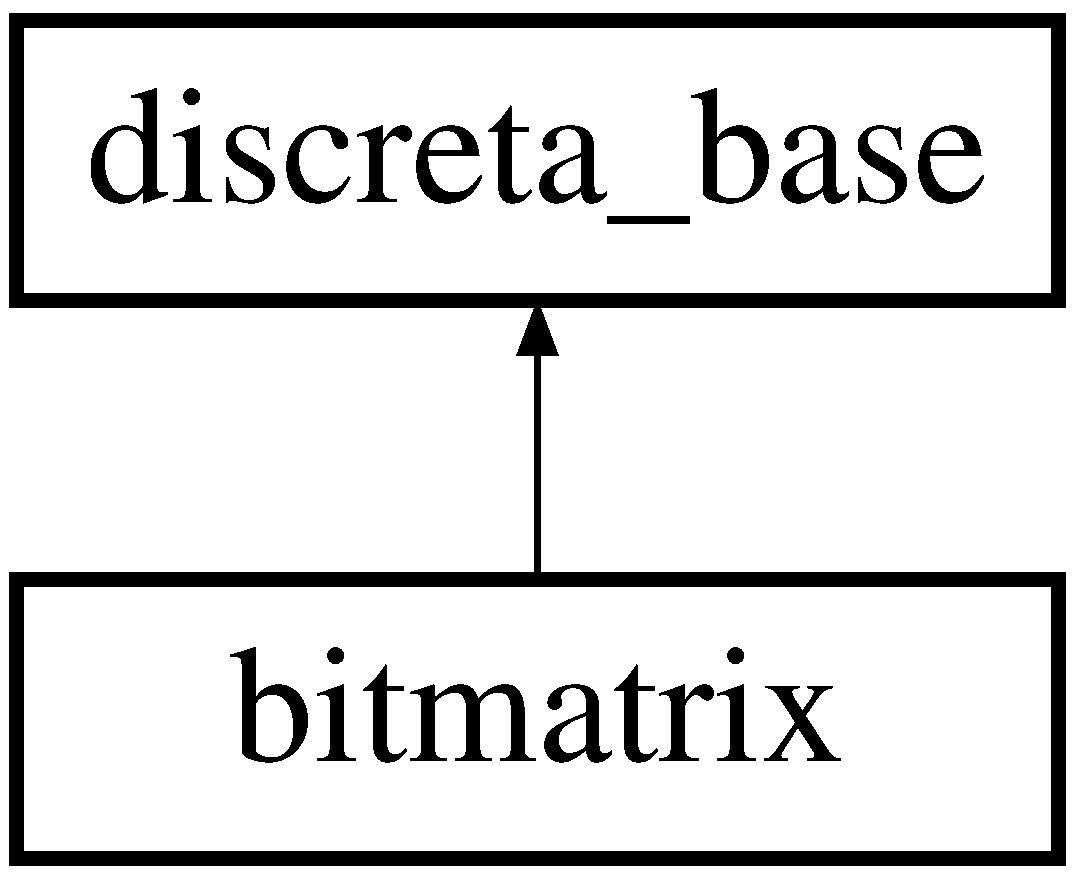
\includegraphics[height=2.000000cm]{classbitmatrix}
\end{center}
\end{figure}
\subsection*{Public Member Functions}
\begin{DoxyCompactItemize}
\item 
\mbox{\hyperlink{classbitmatrix_af6715cab25d568c8ad82c0dee2e9791d}{bitmatrix}} ()
\item 
\mbox{\hyperlink{classbitmatrix_a6a2ab85aca9b9c4a40336aceee91b24a}{bitmatrix}} (const \mbox{\hyperlink{classdiscreta__base}{discreta\+\_\+base}} \&\mbox{\hyperlink{alphabet2_8_c_a6150e0515f7202e2fb518f7206ed97dc}{x}})
\item 
\mbox{\hyperlink{classbitmatrix}{bitmatrix}} \& \mbox{\hyperlink{classbitmatrix_ac7386ca418929a7d0a0fdf38b0cb99e4}{operator=}} (const \mbox{\hyperlink{classdiscreta__base}{discreta\+\_\+base}} \&\mbox{\hyperlink{alphabet2_8_c_a6150e0515f7202e2fb518f7206ed97dc}{x}})
\item 
void $\ast$ \mbox{\hyperlink{classbitmatrix_a91f184b6e870e211db7535e9baaf710e}{operator new}} (size\+\_\+t, void $\ast$\mbox{\hyperlink{alphabet2_8_c_a533391314665d6bf1b5575e9a9cd8552}{p}})
\item 
void \mbox{\hyperlink{classbitmatrix_acb571d947f9526665ebbdc0ce3e2a973}{settype\+\_\+bitmatrix}} ()
\item 
\mbox{\hyperlink{classbitmatrix_a0ecd1bb827e476fb99640190cfa973f6}{$\sim$bitmatrix}} ()
\item 
void \mbox{\hyperlink{classbitmatrix_a4b84eed56a244df63819eae6b7ba1eff}{freeself\+\_\+bitmatrix}} ()
\item 
\mbox{\hyperlink{discreta_8h_aaf25ee7e2306d78c74ec7bc48f092e81}{kind}} \mbox{\hyperlink{classbitmatrix_a3e8982cdd7e500a0298a60469b4a5860}{s\+\_\+virtual\+\_\+kind}} ()
\item 
void \mbox{\hyperlink{classbitmatrix_ac97adfe8348d9fe6ef19447b7611bbea}{copyobject\+\_\+to}} (\mbox{\hyperlink{classdiscreta__base}{discreta\+\_\+base}} \&\mbox{\hyperlink{alphabet2_8_c_a6150e0515f7202e2fb518f7206ed97dc}{x}})
\item 
ostream \& \mbox{\hyperlink{classbitmatrix_a2e3eaa8cff111df76f48458406d93d72}{print}} (ostream \&)
\item 
\mbox{\hyperlink{classbitmatrix}{bitmatrix}} \& \mbox{\hyperlink{classbitmatrix_a3511956281a3f36f0013d90a7accc1bc}{m\+\_\+mn}} (\mbox{\hyperlink{galois_8h_a09fddde158a3a20bd2dcadb609de11dc}{I\+NT}} m, \mbox{\hyperlink{galois_8h_a09fddde158a3a20bd2dcadb609de11dc}{I\+NT}} \mbox{\hyperlink{simeon_8_c_a7f2cd26777ce0ff3fdaf8d02aacbddfb}{n}})
\item 
\mbox{\hyperlink{classbitmatrix}{bitmatrix}} \& \mbox{\hyperlink{classbitmatrix_ad2211a81cb808e23924957cb0f8ee817}{m\+\_\+mn\+\_\+n}} (\mbox{\hyperlink{galois_8h_a09fddde158a3a20bd2dcadb609de11dc}{I\+NT}} m, \mbox{\hyperlink{galois_8h_a09fddde158a3a20bd2dcadb609de11dc}{I\+NT}} \mbox{\hyperlink{simeon_8_c_a7f2cd26777ce0ff3fdaf8d02aacbddfb}{n}})
\item 
\mbox{\hyperlink{galois_8h_a09fddde158a3a20bd2dcadb609de11dc}{I\+NT}} \mbox{\hyperlink{classbitmatrix_aa13f7f6972b17564d34fc4c96c1d59b1}{s\+\_\+m}} ()
\item 
\mbox{\hyperlink{galois_8h_a09fddde158a3a20bd2dcadb609de11dc}{I\+NT}} \mbox{\hyperlink{classbitmatrix_aa9f016e60a7a3262576cc3e21e70b296}{s\+\_\+n}} ()
\item 
\mbox{\hyperlink{galois_8h_a09fddde158a3a20bd2dcadb609de11dc}{I\+NT}} \mbox{\hyperlink{classbitmatrix_a68b48161c81133a471f3ba3df2d2ebe0}{s\+\_\+N}} ()
\item 
\mbox{\hyperlink{galois_8h_ac94af6544c710549c9fca744fd510395}{U\+I\+N\+T4}} \& \mbox{\hyperlink{classbitmatrix_ac8a781761e2eae1958d031bae61c11ac}{s\+\_\+i}} (\mbox{\hyperlink{galois_8h_a09fddde158a3a20bd2dcadb609de11dc}{I\+NT}} \mbox{\hyperlink{alphabet2_8_c_acb559820d9ca11295b4500f179ef6392}{i}})
\item 
\mbox{\hyperlink{galois_8h_a09fddde158a3a20bd2dcadb609de11dc}{I\+NT}} \mbox{\hyperlink{classbitmatrix_adce911461b7d60593b86bf92cb201076}{s\+\_\+ij}} (\mbox{\hyperlink{galois_8h_a09fddde158a3a20bd2dcadb609de11dc}{I\+NT}} \mbox{\hyperlink{alphabet2_8_c_acb559820d9ca11295b4500f179ef6392}{i}}, \mbox{\hyperlink{galois_8h_a09fddde158a3a20bd2dcadb609de11dc}{I\+NT}} \mbox{\hyperlink{alphabet2_8_c_a37d972ae0b47b9099e30983131d31916}{j}})
\item 
void \mbox{\hyperlink{classbitmatrix_afaf5dd4ed44805c659d2fd5a6fc89ec4}{m\+\_\+iji}} (\mbox{\hyperlink{galois_8h_a09fddde158a3a20bd2dcadb609de11dc}{I\+NT}} \mbox{\hyperlink{alphabet2_8_c_acb559820d9ca11295b4500f179ef6392}{i}}, \mbox{\hyperlink{galois_8h_a09fddde158a3a20bd2dcadb609de11dc}{I\+NT}} \mbox{\hyperlink{alphabet2_8_c_a37d972ae0b47b9099e30983131d31916}{j}}, \mbox{\hyperlink{galois_8h_a09fddde158a3a20bd2dcadb609de11dc}{I\+NT}} a)
\item 
void \mbox{\hyperlink{classbitmatrix_af7dba8c0de2128e6aa413b70bcc1f78f}{mult\+\_\+to}} (\mbox{\hyperlink{classdiscreta__base}{discreta\+\_\+base}} \&\mbox{\hyperlink{alphabet2_8_c_a6150e0515f7202e2fb518f7206ed97dc}{x}}, \mbox{\hyperlink{classdiscreta__base}{discreta\+\_\+base}} \&\mbox{\hyperlink{alphabet2_8_c_a0a2f84ed7838f07779ae24c5a9086d33}{y}})
\item 
void \mbox{\hyperlink{classbitmatrix_afb73fc8dc14653159b63b969c5ca4856}{bitmatrix\+\_\+mult\+\_\+to}} (\mbox{\hyperlink{classbitmatrix}{bitmatrix}} \&\mbox{\hyperlink{alphabet2_8_c_a6150e0515f7202e2fb518f7206ed97dc}{x}}, \mbox{\hyperlink{classdiscreta__base}{discreta\+\_\+base}} \&\mbox{\hyperlink{alphabet2_8_c_a0a2f84ed7838f07779ae24c5a9086d33}{y}})
\item 
\mbox{\hyperlink{galois_8h_a09fddde158a3a20bd2dcadb609de11dc}{I\+NT}} \mbox{\hyperlink{classbitmatrix_ad43da9e457904e1dfa459b78147e0667}{gauss}} (\mbox{\hyperlink{galois_8h_a09fddde158a3a20bd2dcadb609de11dc}{I\+NT}} f\+\_\+complete, \mbox{\hyperlink{class_vector}{Vector}} \&base\+\_\+cols, \mbox{\hyperlink{galois_8h_a09fddde158a3a20bd2dcadb609de11dc}{I\+NT}} f\+\_\+v)
\item 
\mbox{\hyperlink{galois_8h_a09fddde158a3a20bd2dcadb609de11dc}{I\+NT}} \mbox{\hyperlink{classbitmatrix_a665129645bad35018674f8b5a694a13e}{get\+\_\+kernel}} (\mbox{\hyperlink{class_vector}{Vector}} \&base\+\_\+cols, \mbox{\hyperlink{classbitmatrix}{bitmatrix}} \&kernel)
\item 
void \mbox{\hyperlink{classbitmatrix_a8dd74a0158ac5fbf4c2c6b7a71f9a39f}{write\+\_\+mem}} (\mbox{\hyperlink{classmemory}{memory}} \&\mbox{\hyperlink{plane__search_8_c_ad2d23ebd03187a91edd45b1d5e496265}{M}}, \mbox{\hyperlink{galois_8h_a09fddde158a3a20bd2dcadb609de11dc}{I\+NT}} debug\+\_\+depth)
\item 
void \mbox{\hyperlink{classbitmatrix_aa126a5db3bfaebc3ad193fc01bbfac9b}{read\+\_\+mem}} (\mbox{\hyperlink{classmemory}{memory}} \&\mbox{\hyperlink{plane__search_8_c_ad2d23ebd03187a91edd45b1d5e496265}{M}}, \mbox{\hyperlink{galois_8h_a09fddde158a3a20bd2dcadb609de11dc}{I\+NT}} debug\+\_\+depth)
\item 
\mbox{\hyperlink{galois_8h_a09fddde158a3a20bd2dcadb609de11dc}{I\+NT}} \mbox{\hyperlink{classbitmatrix_a2d11a854ea302b0e6fa61c9c6607deaf}{csf}} ()
\end{DoxyCompactItemize}
\subsection*{Additional Inherited Members}


\subsection{Constructor \& Destructor Documentation}
\mbox{\Hypertarget{classbitmatrix_af6715cab25d568c8ad82c0dee2e9791d}\label{classbitmatrix_af6715cab25d568c8ad82c0dee2e9791d}} 
\index{bitmatrix@{bitmatrix}!bitmatrix@{bitmatrix}}
\index{bitmatrix@{bitmatrix}!bitmatrix@{bitmatrix}}
\subsubsection{\texorpdfstring{bitmatrix()}{bitmatrix()}\hspace{0.1cm}{\footnotesize\ttfamily [1/2]}}
{\footnotesize\ttfamily bitmatrix\+::bitmatrix (\begin{DoxyParamCaption}{ }\end{DoxyParamCaption})}

\mbox{\Hypertarget{classbitmatrix_a6a2ab85aca9b9c4a40336aceee91b24a}\label{classbitmatrix_a6a2ab85aca9b9c4a40336aceee91b24a}} 
\index{bitmatrix@{bitmatrix}!bitmatrix@{bitmatrix}}
\index{bitmatrix@{bitmatrix}!bitmatrix@{bitmatrix}}
\subsubsection{\texorpdfstring{bitmatrix()}{bitmatrix()}\hspace{0.1cm}{\footnotesize\ttfamily [2/2]}}
{\footnotesize\ttfamily bitmatrix\+::bitmatrix (\begin{DoxyParamCaption}\item[{const \mbox{\hyperlink{classdiscreta__base}{discreta\+\_\+base}} \&}]{x }\end{DoxyParamCaption})}

\mbox{\Hypertarget{classbitmatrix_a0ecd1bb827e476fb99640190cfa973f6}\label{classbitmatrix_a0ecd1bb827e476fb99640190cfa973f6}} 
\index{bitmatrix@{bitmatrix}!````~bitmatrix@{$\sim$bitmatrix}}
\index{````~bitmatrix@{$\sim$bitmatrix}!bitmatrix@{bitmatrix}}
\subsubsection{\texorpdfstring{$\sim$bitmatrix()}{~bitmatrix()}}
{\footnotesize\ttfamily bitmatrix\+::$\sim$bitmatrix (\begin{DoxyParamCaption}{ }\end{DoxyParamCaption})}



\subsection{Member Function Documentation}
\mbox{\Hypertarget{classbitmatrix_afb73fc8dc14653159b63b969c5ca4856}\label{classbitmatrix_afb73fc8dc14653159b63b969c5ca4856}} 
\index{bitmatrix@{bitmatrix}!bitmatrix\+\_\+mult\+\_\+to@{bitmatrix\+\_\+mult\+\_\+to}}
\index{bitmatrix\+\_\+mult\+\_\+to@{bitmatrix\+\_\+mult\+\_\+to}!bitmatrix@{bitmatrix}}
\subsubsection{\texorpdfstring{bitmatrix\+\_\+mult\+\_\+to()}{bitmatrix\_mult\_to()}}
{\footnotesize\ttfamily void bitmatrix\+::bitmatrix\+\_\+mult\+\_\+to (\begin{DoxyParamCaption}\item[{\mbox{\hyperlink{classbitmatrix}{bitmatrix}} \&}]{x,  }\item[{\mbox{\hyperlink{classdiscreta__base}{discreta\+\_\+base}} \&}]{y }\end{DoxyParamCaption})}

\mbox{\Hypertarget{classbitmatrix_ac97adfe8348d9fe6ef19447b7611bbea}\label{classbitmatrix_ac97adfe8348d9fe6ef19447b7611bbea}} 
\index{bitmatrix@{bitmatrix}!copyobject\+\_\+to@{copyobject\+\_\+to}}
\index{copyobject\+\_\+to@{copyobject\+\_\+to}!bitmatrix@{bitmatrix}}
\subsubsection{\texorpdfstring{copyobject\+\_\+to()}{copyobject\_to()}}
{\footnotesize\ttfamily void bitmatrix\+::copyobject\+\_\+to (\begin{DoxyParamCaption}\item[{\mbox{\hyperlink{classdiscreta__base}{discreta\+\_\+base}} \&}]{x }\end{DoxyParamCaption})\hspace{0.3cm}{\ttfamily [virtual]}}



Reimplemented from \mbox{\hyperlink{classdiscreta__base_a33180628d9ced231267229b3564790f3}{discreta\+\_\+base}}.

\mbox{\Hypertarget{classbitmatrix_a2d11a854ea302b0e6fa61c9c6607deaf}\label{classbitmatrix_a2d11a854ea302b0e6fa61c9c6607deaf}} 
\index{bitmatrix@{bitmatrix}!csf@{csf}}
\index{csf@{csf}!bitmatrix@{bitmatrix}}
\subsubsection{\texorpdfstring{csf()}{csf()}}
{\footnotesize\ttfamily \mbox{\hyperlink{galois_8h_a09fddde158a3a20bd2dcadb609de11dc}{I\+NT}} bitmatrix\+::csf (\begin{DoxyParamCaption}{ }\end{DoxyParamCaption})}

\mbox{\Hypertarget{classbitmatrix_a4b84eed56a244df63819eae6b7ba1eff}\label{classbitmatrix_a4b84eed56a244df63819eae6b7ba1eff}} 
\index{bitmatrix@{bitmatrix}!freeself\+\_\+bitmatrix@{freeself\+\_\+bitmatrix}}
\index{freeself\+\_\+bitmatrix@{freeself\+\_\+bitmatrix}!bitmatrix@{bitmatrix}}
\subsubsection{\texorpdfstring{freeself\+\_\+bitmatrix()}{freeself\_bitmatrix()}}
{\footnotesize\ttfamily void bitmatrix\+::freeself\+\_\+bitmatrix (\begin{DoxyParamCaption}{ }\end{DoxyParamCaption})}

\mbox{\Hypertarget{classbitmatrix_ad43da9e457904e1dfa459b78147e0667}\label{classbitmatrix_ad43da9e457904e1dfa459b78147e0667}} 
\index{bitmatrix@{bitmatrix}!gauss@{gauss}}
\index{gauss@{gauss}!bitmatrix@{bitmatrix}}
\subsubsection{\texorpdfstring{gauss()}{gauss()}}
{\footnotesize\ttfamily \mbox{\hyperlink{galois_8h_a09fddde158a3a20bd2dcadb609de11dc}{I\+NT}} bitmatrix\+::gauss (\begin{DoxyParamCaption}\item[{\mbox{\hyperlink{galois_8h_a09fddde158a3a20bd2dcadb609de11dc}{I\+NT}}}]{f\+\_\+complete,  }\item[{\mbox{\hyperlink{class_vector}{Vector}} \&}]{base\+\_\+cols,  }\item[{\mbox{\hyperlink{galois_8h_a09fddde158a3a20bd2dcadb609de11dc}{I\+NT}}}]{f\+\_\+v }\end{DoxyParamCaption})}

\mbox{\Hypertarget{classbitmatrix_a665129645bad35018674f8b5a694a13e}\label{classbitmatrix_a665129645bad35018674f8b5a694a13e}} 
\index{bitmatrix@{bitmatrix}!get\+\_\+kernel@{get\+\_\+kernel}}
\index{get\+\_\+kernel@{get\+\_\+kernel}!bitmatrix@{bitmatrix}}
\subsubsection{\texorpdfstring{get\+\_\+kernel()}{get\_kernel()}}
{\footnotesize\ttfamily \mbox{\hyperlink{galois_8h_a09fddde158a3a20bd2dcadb609de11dc}{I\+NT}} bitmatrix\+::get\+\_\+kernel (\begin{DoxyParamCaption}\item[{\mbox{\hyperlink{class_vector}{Vector}} \&}]{base\+\_\+cols,  }\item[{\mbox{\hyperlink{classbitmatrix}{bitmatrix}} \&}]{kernel }\end{DoxyParamCaption})}

\mbox{\Hypertarget{classbitmatrix_afaf5dd4ed44805c659d2fd5a6fc89ec4}\label{classbitmatrix_afaf5dd4ed44805c659d2fd5a6fc89ec4}} 
\index{bitmatrix@{bitmatrix}!m\+\_\+iji@{m\+\_\+iji}}
\index{m\+\_\+iji@{m\+\_\+iji}!bitmatrix@{bitmatrix}}
\subsubsection{\texorpdfstring{m\+\_\+iji()}{m\_iji()}}
{\footnotesize\ttfamily void bitmatrix\+::m\+\_\+iji (\begin{DoxyParamCaption}\item[{\mbox{\hyperlink{galois_8h_a09fddde158a3a20bd2dcadb609de11dc}{I\+NT}}}]{i,  }\item[{\mbox{\hyperlink{galois_8h_a09fddde158a3a20bd2dcadb609de11dc}{I\+NT}}}]{j,  }\item[{\mbox{\hyperlink{galois_8h_a09fddde158a3a20bd2dcadb609de11dc}{I\+NT}}}]{a }\end{DoxyParamCaption})}

\mbox{\Hypertarget{classbitmatrix_a3511956281a3f36f0013d90a7accc1bc}\label{classbitmatrix_a3511956281a3f36f0013d90a7accc1bc}} 
\index{bitmatrix@{bitmatrix}!m\+\_\+mn@{m\+\_\+mn}}
\index{m\+\_\+mn@{m\+\_\+mn}!bitmatrix@{bitmatrix}}
\subsubsection{\texorpdfstring{m\+\_\+mn()}{m\_mn()}}
{\footnotesize\ttfamily \mbox{\hyperlink{classbitmatrix}{bitmatrix}} \& bitmatrix\+::m\+\_\+mn (\begin{DoxyParamCaption}\item[{\mbox{\hyperlink{galois_8h_a09fddde158a3a20bd2dcadb609de11dc}{I\+NT}}}]{m,  }\item[{\mbox{\hyperlink{galois_8h_a09fddde158a3a20bd2dcadb609de11dc}{I\+NT}}}]{n }\end{DoxyParamCaption})}

\mbox{\Hypertarget{classbitmatrix_ad2211a81cb808e23924957cb0f8ee817}\label{classbitmatrix_ad2211a81cb808e23924957cb0f8ee817}} 
\index{bitmatrix@{bitmatrix}!m\+\_\+mn\+\_\+n@{m\+\_\+mn\+\_\+n}}
\index{m\+\_\+mn\+\_\+n@{m\+\_\+mn\+\_\+n}!bitmatrix@{bitmatrix}}
\subsubsection{\texorpdfstring{m\+\_\+mn\+\_\+n()}{m\_mn\_n()}}
{\footnotesize\ttfamily \mbox{\hyperlink{classbitmatrix}{bitmatrix}} \& bitmatrix\+::m\+\_\+mn\+\_\+n (\begin{DoxyParamCaption}\item[{\mbox{\hyperlink{galois_8h_a09fddde158a3a20bd2dcadb609de11dc}{I\+NT}}}]{m,  }\item[{\mbox{\hyperlink{galois_8h_a09fddde158a3a20bd2dcadb609de11dc}{I\+NT}}}]{n }\end{DoxyParamCaption})}

\mbox{\Hypertarget{classbitmatrix_af7dba8c0de2128e6aa413b70bcc1f78f}\label{classbitmatrix_af7dba8c0de2128e6aa413b70bcc1f78f}} 
\index{bitmatrix@{bitmatrix}!mult\+\_\+to@{mult\+\_\+to}}
\index{mult\+\_\+to@{mult\+\_\+to}!bitmatrix@{bitmatrix}}
\subsubsection{\texorpdfstring{mult\+\_\+to()}{mult\_to()}}
{\footnotesize\ttfamily void bitmatrix\+::mult\+\_\+to (\begin{DoxyParamCaption}\item[{\mbox{\hyperlink{classdiscreta__base}{discreta\+\_\+base}} \&}]{x,  }\item[{\mbox{\hyperlink{classdiscreta__base}{discreta\+\_\+base}} \&}]{y }\end{DoxyParamCaption})\hspace{0.3cm}{\ttfamily [virtual]}}



Reimplemented from \mbox{\hyperlink{classdiscreta__base_a54d5c16c016769e3365639721c06591e}{discreta\+\_\+base}}.

\mbox{\Hypertarget{classbitmatrix_a91f184b6e870e211db7535e9baaf710e}\label{classbitmatrix_a91f184b6e870e211db7535e9baaf710e}} 
\index{bitmatrix@{bitmatrix}!operator new@{operator new}}
\index{operator new@{operator new}!bitmatrix@{bitmatrix}}
\subsubsection{\texorpdfstring{operator new()}{operator new()}}
{\footnotesize\ttfamily void$\ast$ bitmatrix\+::operator new (\begin{DoxyParamCaption}\item[{size\+\_\+t}]{,  }\item[{void $\ast$}]{p }\end{DoxyParamCaption})\hspace{0.3cm}{\ttfamily [inline]}}

\mbox{\Hypertarget{classbitmatrix_ac7386ca418929a7d0a0fdf38b0cb99e4}\label{classbitmatrix_ac7386ca418929a7d0a0fdf38b0cb99e4}} 
\index{bitmatrix@{bitmatrix}!operator=@{operator=}}
\index{operator=@{operator=}!bitmatrix@{bitmatrix}}
\subsubsection{\texorpdfstring{operator=()}{operator=()}}
{\footnotesize\ttfamily \mbox{\hyperlink{classbitmatrix}{bitmatrix}} \& bitmatrix\+::operator= (\begin{DoxyParamCaption}\item[{const \mbox{\hyperlink{classdiscreta__base}{discreta\+\_\+base}} \&}]{x }\end{DoxyParamCaption})}

\mbox{\Hypertarget{classbitmatrix_a2e3eaa8cff111df76f48458406d93d72}\label{classbitmatrix_a2e3eaa8cff111df76f48458406d93d72}} 
\index{bitmatrix@{bitmatrix}!print@{print}}
\index{print@{print}!bitmatrix@{bitmatrix}}
\subsubsection{\texorpdfstring{print()}{print()}}
{\footnotesize\ttfamily ostream \& bitmatrix\+::print (\begin{DoxyParamCaption}\item[{ostream \&}]{ost }\end{DoxyParamCaption})\hspace{0.3cm}{\ttfamily [virtual]}}



Reimplemented from \mbox{\hyperlink{classdiscreta__base_a036e48bc058347046fc9b73dd0951478}{discreta\+\_\+base}}.

\mbox{\Hypertarget{classbitmatrix_aa126a5db3bfaebc3ad193fc01bbfac9b}\label{classbitmatrix_aa126a5db3bfaebc3ad193fc01bbfac9b}} 
\index{bitmatrix@{bitmatrix}!read\+\_\+mem@{read\+\_\+mem}}
\index{read\+\_\+mem@{read\+\_\+mem}!bitmatrix@{bitmatrix}}
\subsubsection{\texorpdfstring{read\+\_\+mem()}{read\_mem()}}
{\footnotesize\ttfamily void bitmatrix\+::read\+\_\+mem (\begin{DoxyParamCaption}\item[{\mbox{\hyperlink{classmemory}{memory}} \&}]{M,  }\item[{\mbox{\hyperlink{galois_8h_a09fddde158a3a20bd2dcadb609de11dc}{I\+NT}}}]{debug\+\_\+depth }\end{DoxyParamCaption})}

\mbox{\Hypertarget{classbitmatrix_ac8a781761e2eae1958d031bae61c11ac}\label{classbitmatrix_ac8a781761e2eae1958d031bae61c11ac}} 
\index{bitmatrix@{bitmatrix}!s\+\_\+i@{s\+\_\+i}}
\index{s\+\_\+i@{s\+\_\+i}!bitmatrix@{bitmatrix}}
\subsubsection{\texorpdfstring{s\+\_\+i()}{s\_i()}}
{\footnotesize\ttfamily \mbox{\hyperlink{galois_8h_ac94af6544c710549c9fca744fd510395}{U\+I\+N\+T4}} \& bitmatrix\+::s\+\_\+i (\begin{DoxyParamCaption}\item[{\mbox{\hyperlink{galois_8h_a09fddde158a3a20bd2dcadb609de11dc}{I\+NT}}}]{i }\end{DoxyParamCaption})}

\mbox{\Hypertarget{classbitmatrix_adce911461b7d60593b86bf92cb201076}\label{classbitmatrix_adce911461b7d60593b86bf92cb201076}} 
\index{bitmatrix@{bitmatrix}!s\+\_\+ij@{s\+\_\+ij}}
\index{s\+\_\+ij@{s\+\_\+ij}!bitmatrix@{bitmatrix}}
\subsubsection{\texorpdfstring{s\+\_\+ij()}{s\_ij()}}
{\footnotesize\ttfamily \mbox{\hyperlink{galois_8h_a09fddde158a3a20bd2dcadb609de11dc}{I\+NT}} bitmatrix\+::s\+\_\+ij (\begin{DoxyParamCaption}\item[{\mbox{\hyperlink{galois_8h_a09fddde158a3a20bd2dcadb609de11dc}{I\+NT}}}]{i,  }\item[{\mbox{\hyperlink{galois_8h_a09fddde158a3a20bd2dcadb609de11dc}{I\+NT}}}]{j }\end{DoxyParamCaption})}

\mbox{\Hypertarget{classbitmatrix_aa13f7f6972b17564d34fc4c96c1d59b1}\label{classbitmatrix_aa13f7f6972b17564d34fc4c96c1d59b1}} 
\index{bitmatrix@{bitmatrix}!s\+\_\+m@{s\+\_\+m}}
\index{s\+\_\+m@{s\+\_\+m}!bitmatrix@{bitmatrix}}
\subsubsection{\texorpdfstring{s\+\_\+m()}{s\_m()}}
{\footnotesize\ttfamily \mbox{\hyperlink{galois_8h_a09fddde158a3a20bd2dcadb609de11dc}{I\+NT}} bitmatrix\+::s\+\_\+m (\begin{DoxyParamCaption}{ }\end{DoxyParamCaption})}

\mbox{\Hypertarget{classbitmatrix_aa9f016e60a7a3262576cc3e21e70b296}\label{classbitmatrix_aa9f016e60a7a3262576cc3e21e70b296}} 
\index{bitmatrix@{bitmatrix}!s\+\_\+n@{s\+\_\+n}}
\index{s\+\_\+n@{s\+\_\+n}!bitmatrix@{bitmatrix}}
\subsubsection{\texorpdfstring{s\+\_\+n()}{s\_n()}}
{\footnotesize\ttfamily \mbox{\hyperlink{galois_8h_a09fddde158a3a20bd2dcadb609de11dc}{I\+NT}} bitmatrix\+::s\+\_\+n (\begin{DoxyParamCaption}{ }\end{DoxyParamCaption})}

\mbox{\Hypertarget{classbitmatrix_a68b48161c81133a471f3ba3df2d2ebe0}\label{classbitmatrix_a68b48161c81133a471f3ba3df2d2ebe0}} 
\index{bitmatrix@{bitmatrix}!s\+\_\+N@{s\+\_\+N}}
\index{s\+\_\+N@{s\+\_\+N}!bitmatrix@{bitmatrix}}
\subsubsection{\texorpdfstring{s\+\_\+\+N()}{s\_N()}}
{\footnotesize\ttfamily \mbox{\hyperlink{galois_8h_a09fddde158a3a20bd2dcadb609de11dc}{I\+NT}} bitmatrix\+::s\+\_\+N (\begin{DoxyParamCaption}{ }\end{DoxyParamCaption})}

\mbox{\Hypertarget{classbitmatrix_a3e8982cdd7e500a0298a60469b4a5860}\label{classbitmatrix_a3e8982cdd7e500a0298a60469b4a5860}} 
\index{bitmatrix@{bitmatrix}!s\+\_\+virtual\+\_\+kind@{s\+\_\+virtual\+\_\+kind}}
\index{s\+\_\+virtual\+\_\+kind@{s\+\_\+virtual\+\_\+kind}!bitmatrix@{bitmatrix}}
\subsubsection{\texorpdfstring{s\+\_\+virtual\+\_\+kind()}{s\_virtual\_kind()}}
{\footnotesize\ttfamily \mbox{\hyperlink{discreta_8h_aaf25ee7e2306d78c74ec7bc48f092e81}{kind}} bitmatrix\+::s\+\_\+virtual\+\_\+kind (\begin{DoxyParamCaption}{ }\end{DoxyParamCaption})\hspace{0.3cm}{\ttfamily [virtual]}}



Reimplemented from \mbox{\hyperlink{classdiscreta__base_a52778a6d6943a468be083d0785d418fb}{discreta\+\_\+base}}.

\mbox{\Hypertarget{classbitmatrix_acb571d947f9526665ebbdc0ce3e2a973}\label{classbitmatrix_acb571d947f9526665ebbdc0ce3e2a973}} 
\index{bitmatrix@{bitmatrix}!settype\+\_\+bitmatrix@{settype\+\_\+bitmatrix}}
\index{settype\+\_\+bitmatrix@{settype\+\_\+bitmatrix}!bitmatrix@{bitmatrix}}
\subsubsection{\texorpdfstring{settype\+\_\+bitmatrix()}{settype\_bitmatrix()}}
{\footnotesize\ttfamily void bitmatrix\+::settype\+\_\+bitmatrix (\begin{DoxyParamCaption}{ }\end{DoxyParamCaption})}

\mbox{\Hypertarget{classbitmatrix_a8dd74a0158ac5fbf4c2c6b7a71f9a39f}\label{classbitmatrix_a8dd74a0158ac5fbf4c2c6b7a71f9a39f}} 
\index{bitmatrix@{bitmatrix}!write\+\_\+mem@{write\+\_\+mem}}
\index{write\+\_\+mem@{write\+\_\+mem}!bitmatrix@{bitmatrix}}
\subsubsection{\texorpdfstring{write\+\_\+mem()}{write\_mem()}}
{\footnotesize\ttfamily void bitmatrix\+::write\+\_\+mem (\begin{DoxyParamCaption}\item[{\mbox{\hyperlink{classmemory}{memory}} \&}]{M,  }\item[{\mbox{\hyperlink{galois_8h_a09fddde158a3a20bd2dcadb609de11dc}{I\+NT}}}]{debug\+\_\+depth }\end{DoxyParamCaption})}



The documentation for this class was generated from the following files\+:\begin{DoxyCompactItemize}
\item 
S\+R\+C/\+L\+I\+B/\+D\+I\+S\+C\+R\+E\+T\+A/\mbox{\hyperlink{discreta_8h}{discreta.\+h}}\item 
S\+R\+C/\+L\+I\+B/\+D\+I\+S\+C\+R\+E\+T\+A/\mbox{\hyperlink{bitmatrix_8_c}{bitmatrix.\+C}}\end{DoxyCompactItemize}

\hypertarget{structbitmatrix__representation}{}\section{bitmatrix\+\_\+representation Struct Reference}
\label{structbitmatrix__representation}\index{bitmatrix\+\_\+representation@{bitmatrix\+\_\+representation}}


{\ttfamily \#include $<$discreta.\+h$>$}

\subsection*{Public Attributes}
\begin{DoxyCompactItemize}
\item 
\mbox{\hyperlink{galois_8h_a09fddde158a3a20bd2dcadb609de11dc}{I\+NT}} \mbox{\hyperlink{structbitmatrix__representation_aaaccdb0ef08c19f3899cbb6c0b03d303}{m}}
\item 
\mbox{\hyperlink{galois_8h_a09fddde158a3a20bd2dcadb609de11dc}{I\+NT}} \mbox{\hyperlink{structbitmatrix__representation_a0857d63f15f0ad369bca4748b116cdee}{n}}
\item 
\mbox{\hyperlink{galois_8h_a09fddde158a3a20bd2dcadb609de11dc}{I\+NT}} \mbox{\hyperlink{structbitmatrix__representation_ad4d433383609dd2cde0de2a1366f507f}{N}}
\item 
\mbox{\hyperlink{galois_8h_ac94af6544c710549c9fca744fd510395}{U\+I\+N\+T4}} \mbox{\hyperlink{structbitmatrix__representation_a1b3ea449937515a80e5237e8f5f29787}{p}} \mbox{[}1\mbox{]}
\end{DoxyCompactItemize}


\subsection{Member Data Documentation}
\mbox{\Hypertarget{structbitmatrix__representation_aaaccdb0ef08c19f3899cbb6c0b03d303}\label{structbitmatrix__representation_aaaccdb0ef08c19f3899cbb6c0b03d303}} 
\index{bitmatrix\+\_\+representation@{bitmatrix\+\_\+representation}!m@{m}}
\index{m@{m}!bitmatrix\+\_\+representation@{bitmatrix\+\_\+representation}}
\subsubsection{\texorpdfstring{m}{m}}
{\footnotesize\ttfamily \mbox{\hyperlink{galois_8h_a09fddde158a3a20bd2dcadb609de11dc}{I\+NT}} bitmatrix\+\_\+representation\+::m}

\mbox{\Hypertarget{structbitmatrix__representation_a0857d63f15f0ad369bca4748b116cdee}\label{structbitmatrix__representation_a0857d63f15f0ad369bca4748b116cdee}} 
\index{bitmatrix\+\_\+representation@{bitmatrix\+\_\+representation}!n@{n}}
\index{n@{n}!bitmatrix\+\_\+representation@{bitmatrix\+\_\+representation}}
\subsubsection{\texorpdfstring{n}{n}}
{\footnotesize\ttfamily \mbox{\hyperlink{galois_8h_a09fddde158a3a20bd2dcadb609de11dc}{I\+NT}} bitmatrix\+\_\+representation\+::n}

\mbox{\Hypertarget{structbitmatrix__representation_ad4d433383609dd2cde0de2a1366f507f}\label{structbitmatrix__representation_ad4d433383609dd2cde0de2a1366f507f}} 
\index{bitmatrix\+\_\+representation@{bitmatrix\+\_\+representation}!N@{N}}
\index{N@{N}!bitmatrix\+\_\+representation@{bitmatrix\+\_\+representation}}
\subsubsection{\texorpdfstring{N}{N}}
{\footnotesize\ttfamily \mbox{\hyperlink{galois_8h_a09fddde158a3a20bd2dcadb609de11dc}{I\+NT}} bitmatrix\+\_\+representation\+::N}

\mbox{\Hypertarget{structbitmatrix__representation_a1b3ea449937515a80e5237e8f5f29787}\label{structbitmatrix__representation_a1b3ea449937515a80e5237e8f5f29787}} 
\index{bitmatrix\+\_\+representation@{bitmatrix\+\_\+representation}!p@{p}}
\index{p@{p}!bitmatrix\+\_\+representation@{bitmatrix\+\_\+representation}}
\subsubsection{\texorpdfstring{p}{p}}
{\footnotesize\ttfamily \mbox{\hyperlink{galois_8h_ac94af6544c710549c9fca744fd510395}{U\+I\+N\+T4}} bitmatrix\+\_\+representation\+::p\mbox{[}1\mbox{]}}



The documentation for this struct was generated from the following file\+:\begin{DoxyCompactItemize}
\item 
S\+R\+C/\+L\+I\+B/\+D\+I\+S\+C\+R\+E\+T\+A/\mbox{\hyperlink{discreta_8h}{discreta.\+h}}\end{DoxyCompactItemize}

\hypertarget{classblt__set}{}\section{blt\+\_\+set Class Reference}
\label{classblt__set}\index{blt\+\_\+set@{blt\+\_\+set}}


{\ttfamily \#include $<$blt.\+h$>$}

\subsection*{Public Member Functions}
\begin{DoxyCompactItemize}
\item 
void \mbox{\hyperlink{classblt__set_a2c9376bf8921d08c686526482aefd1f0}{read\+\_\+arguments}} (int argc, const char $\ast$$\ast$argv)
\item 
\mbox{\hyperlink{classblt__set_a04973f08aa5193284ac3a51ef9d2d322}{blt\+\_\+set}} ()
\item 
\mbox{\hyperlink{classblt__set_adbf61747988c80615e72b179298ed19f}{$\sim$blt\+\_\+set}} ()
\item 
void \mbox{\hyperlink{classblt__set_a2345145a41264dca01b4bcc40dfe54d4}{null}} ()
\item 
void \mbox{\hyperlink{classblt__set_abc48dfb6e214be890bd2a8c28dcdaae0}{freeself}} ()
\item 
void \mbox{\hyperlink{classblt__set_a266dfb03016b68440e810771101442cc}{init\+\_\+basic}} (\mbox{\hyperlink{classfinite__field}{finite\+\_\+field}} $\ast$\mbox{\hyperlink{classblt__set_ae3a4dd741b4d034599339e933d2599a0}{F}}, const \mbox{\hyperlink{galois_8h_ab6cc7b4aeb6ea31aba2b3fbfc83ff5e6}{B\+Y\+TE}} $\ast$input\+\_\+prefix, const \mbox{\hyperlink{galois_8h_ab6cc7b4aeb6ea31aba2b3fbfc83ff5e6}{B\+Y\+TE}} $\ast$base\+\_\+fname, \mbox{\hyperlink{galois_8h_a09fddde158a3a20bd2dcadb609de11dc}{I\+NT}} \mbox{\hyperlink{classblt__set_a5227d5487da07366a96c3a1c4eba1814}{starter\+\_\+size}}, int argc, const char $\ast$$\ast$argv, \mbox{\hyperlink{galois_8h_a09fddde158a3a20bd2dcadb609de11dc}{I\+NT}} \mbox{\hyperlink{simeon_8_c_a818073fbcc2f439e7c56952f67386122}{verbose\+\_\+level}})
\item 
void \mbox{\hyperlink{classblt__set_a9e5aede3bbac6f5e1dd31a8965bba200}{init\+\_\+group}} (\mbox{\hyperlink{galois_8h_a09fddde158a3a20bd2dcadb609de11dc}{I\+NT}} \mbox{\hyperlink{simeon_8_c_a818073fbcc2f439e7c56952f67386122}{verbose\+\_\+level}})
\item 
void \mbox{\hyperlink{classblt__set_a030c4f21140e07855f55f68c7586b4ce}{init\+\_\+orthogonal}} (\mbox{\hyperlink{galois_8h_a09fddde158a3a20bd2dcadb609de11dc}{I\+NT}} \mbox{\hyperlink{simeon_8_c_a818073fbcc2f439e7c56952f67386122}{verbose\+\_\+level}})
\item 
void \mbox{\hyperlink{classblt__set_ad8a73370e16f2adf30172c3159ca8a74}{init\+\_\+orthogonal\+\_\+hash}} (\mbox{\hyperlink{galois_8h_a09fddde158a3a20bd2dcadb609de11dc}{I\+NT}} \mbox{\hyperlink{simeon_8_c_a818073fbcc2f439e7c56952f67386122}{verbose\+\_\+level}})
\item 
void \mbox{\hyperlink{classblt__set_a3f1204faeab71c253039beffa3e6ee76}{init2}} (\mbox{\hyperlink{galois_8h_a09fddde158a3a20bd2dcadb609de11dc}{I\+NT}} \mbox{\hyperlink{simeon_8_c_a818073fbcc2f439e7c56952f67386122}{verbose\+\_\+level}})
\item 
void \mbox{\hyperlink{classblt__set_a3f1d4a8ed15875c47b327949f26a4533}{create\+\_\+graphs}} (\mbox{\hyperlink{galois_8h_a09fddde158a3a20bd2dcadb609de11dc}{I\+NT}} orbit\+\_\+at\+\_\+level\+\_\+r, \mbox{\hyperlink{galois_8h_a09fddde158a3a20bd2dcadb609de11dc}{I\+NT}} orbit\+\_\+at\+\_\+level\+\_\+m, \mbox{\hyperlink{galois_8h_a09fddde158a3a20bd2dcadb609de11dc}{I\+NT}} level\+\_\+of\+\_\+candidates\+\_\+file, const \mbox{\hyperlink{galois_8h_ab6cc7b4aeb6ea31aba2b3fbfc83ff5e6}{B\+Y\+TE}} $\ast$output\+\_\+prefix, \mbox{\hyperlink{galois_8h_a09fddde158a3a20bd2dcadb609de11dc}{I\+NT}} f\+\_\+lexorder\+\_\+test, \mbox{\hyperlink{galois_8h_a09fddde158a3a20bd2dcadb609de11dc}{I\+NT}} f\+\_\+eliminate\+\_\+graphs\+\_\+if\+\_\+possible, \mbox{\hyperlink{galois_8h_a09fddde158a3a20bd2dcadb609de11dc}{I\+NT}} \mbox{\hyperlink{simeon_8_c_a818073fbcc2f439e7c56952f67386122}{verbose\+\_\+level}})
\item 
void \mbox{\hyperlink{classblt__set_a91ad531d4154bd887182dbd6121476f3}{create\+\_\+graphs\+\_\+list\+\_\+of\+\_\+cases}} (const \mbox{\hyperlink{galois_8h_ab6cc7b4aeb6ea31aba2b3fbfc83ff5e6}{B\+Y\+TE}} $\ast$case\+\_\+label, const \mbox{\hyperlink{galois_8h_ab6cc7b4aeb6ea31aba2b3fbfc83ff5e6}{B\+Y\+TE}} $\ast$list\+\_\+of\+\_\+cases\+\_\+text, \mbox{\hyperlink{galois_8h_a09fddde158a3a20bd2dcadb609de11dc}{I\+NT}} level\+\_\+of\+\_\+candidates\+\_\+file, const \mbox{\hyperlink{galois_8h_ab6cc7b4aeb6ea31aba2b3fbfc83ff5e6}{B\+Y\+TE}} $\ast$output\+\_\+prefix, \mbox{\hyperlink{galois_8h_a09fddde158a3a20bd2dcadb609de11dc}{I\+NT}} f\+\_\+lexorder\+\_\+test, \mbox{\hyperlink{galois_8h_a09fddde158a3a20bd2dcadb609de11dc}{I\+NT}} f\+\_\+eliminate\+\_\+graphs\+\_\+if\+\_\+possible, \mbox{\hyperlink{galois_8h_a09fddde158a3a20bd2dcadb609de11dc}{I\+NT}} \mbox{\hyperlink{simeon_8_c_a818073fbcc2f439e7c56952f67386122}{verbose\+\_\+level}})
\item 
\mbox{\hyperlink{galois_8h_a09fddde158a3a20bd2dcadb609de11dc}{I\+NT}} \mbox{\hyperlink{classblt__set_ae92249ece99ffbc92e93e49cd5d5dccf}{create\+\_\+graph}} (\mbox{\hyperlink{galois_8h_a09fddde158a3a20bd2dcadb609de11dc}{I\+NT}} orbit\+\_\+at\+\_\+level, \mbox{\hyperlink{galois_8h_a09fddde158a3a20bd2dcadb609de11dc}{I\+NT}} level\+\_\+of\+\_\+candidates\+\_\+file, const \mbox{\hyperlink{galois_8h_ab6cc7b4aeb6ea31aba2b3fbfc83ff5e6}{B\+Y\+TE}} $\ast$output\+\_\+prefix, \mbox{\hyperlink{galois_8h_a09fddde158a3a20bd2dcadb609de11dc}{I\+NT}} f\+\_\+lexorder\+\_\+test, \mbox{\hyperlink{galois_8h_a09fddde158a3a20bd2dcadb609de11dc}{I\+NT}} f\+\_\+eliminate\+\_\+graphs\+\_\+if\+\_\+possible, \mbox{\hyperlink{galois_8h_a09fddde158a3a20bd2dcadb609de11dc}{I\+NT}} \&nb\+\_\+vertices, \mbox{\hyperlink{galois_8h_ab6cc7b4aeb6ea31aba2b3fbfc83ff5e6}{B\+Y\+TE}} $\ast$graph\+\_\+fname\+\_\+base, \mbox{\hyperlink{classcolored__graph}{colored\+\_\+graph}} $\ast$\&CG, \mbox{\hyperlink{galois_8h_a09fddde158a3a20bd2dcadb609de11dc}{I\+NT}} \mbox{\hyperlink{simeon_8_c_a818073fbcc2f439e7c56952f67386122}{verbose\+\_\+level}})
\item 
void \mbox{\hyperlink{classblt__set_a6629b3a1a50c0f2736034abaea6f7d63}{compute\+\_\+colors}} (\mbox{\hyperlink{galois_8h_a09fddde158a3a20bd2dcadb609de11dc}{I\+NT}} orbit\+\_\+at\+\_\+level, \mbox{\hyperlink{galois_8h_a09fddde158a3a20bd2dcadb609de11dc}{I\+NT}} $\ast$starter, \mbox{\hyperlink{galois_8h_a09fddde158a3a20bd2dcadb609de11dc}{I\+NT}} starter\+\_\+sz, \mbox{\hyperlink{galois_8h_a09fddde158a3a20bd2dcadb609de11dc}{I\+NT}} special\+\_\+line, \mbox{\hyperlink{galois_8h_a09fddde158a3a20bd2dcadb609de11dc}{I\+NT}} $\ast$candidates, \mbox{\hyperlink{galois_8h_a09fddde158a3a20bd2dcadb609de11dc}{I\+NT}} nb\+\_\+candidates, \mbox{\hyperlink{galois_8h_a09fddde158a3a20bd2dcadb609de11dc}{I\+NT}} $\ast$\&point\+\_\+color, \mbox{\hyperlink{galois_8h_a09fddde158a3a20bd2dcadb609de11dc}{I\+NT}} \&nb\+\_\+colors, \mbox{\hyperlink{galois_8h_a09fddde158a3a20bd2dcadb609de11dc}{I\+NT}} \mbox{\hyperlink{simeon_8_c_a818073fbcc2f439e7c56952f67386122}{verbose\+\_\+level}})
\item 
void \mbox{\hyperlink{classblt__set_a55487fb1d0a4af469511d2167a9baf37}{compute\+\_\+adjacency\+\_\+list\+\_\+fast}} (\mbox{\hyperlink{galois_8h_a09fddde158a3a20bd2dcadb609de11dc}{I\+NT}} first\+\_\+point\+\_\+of\+\_\+starter, \mbox{\hyperlink{galois_8h_a09fddde158a3a20bd2dcadb609de11dc}{I\+NT}} $\ast$\mbox{\hyperlink{points_8_c_a8a498513b4415e1a4628a70fb6b26817}{points}}, \mbox{\hyperlink{galois_8h_a09fddde158a3a20bd2dcadb609de11dc}{I\+NT}} \mbox{\hyperlink{hamming_8_c_ad8ae9bd69df4346f4f3130a6ae6d036b}{nb\+\_\+points}}, \mbox{\hyperlink{galois_8h_a09fddde158a3a20bd2dcadb609de11dc}{I\+NT}} $\ast$point\+\_\+color, \mbox{\hyperlink{galois_8h_a122c4acf389c050379f00341fdcd5812}{U\+B\+Y\+TE}} $\ast$\&bitvector\+\_\+adjacency, \mbox{\hyperlink{galois_8h_a09fddde158a3a20bd2dcadb609de11dc}{I\+NT}} \&bitvector\+\_\+length\+\_\+in\+\_\+bits, \mbox{\hyperlink{galois_8h_a09fddde158a3a20bd2dcadb609de11dc}{I\+NT}} \&bitvector\+\_\+length, \mbox{\hyperlink{galois_8h_a09fddde158a3a20bd2dcadb609de11dc}{I\+NT}} \mbox{\hyperlink{simeon_8_c_a818073fbcc2f439e7c56952f67386122}{verbose\+\_\+level}})
\item 
void \mbox{\hyperlink{classblt__set_ae13ce00db0bbbf0a157ee02a3aaea3c7}{early\+\_\+test\+\_\+func}} (\mbox{\hyperlink{galois_8h_a09fddde158a3a20bd2dcadb609de11dc}{I\+NT}} $\ast$\mbox{\hyperlink{simeon_8_c_adab47f8243f1b5a2c31df2535d6b37d0}{S}}, \mbox{\hyperlink{galois_8h_a09fddde158a3a20bd2dcadb609de11dc}{I\+NT}} len, \mbox{\hyperlink{galois_8h_a09fddde158a3a20bd2dcadb609de11dc}{I\+NT}} $\ast$candidates, \mbox{\hyperlink{galois_8h_a09fddde158a3a20bd2dcadb609de11dc}{I\+NT}} nb\+\_\+candidates, \mbox{\hyperlink{galois_8h_a09fddde158a3a20bd2dcadb609de11dc}{I\+NT}} $\ast$good\+\_\+candidates, \mbox{\hyperlink{galois_8h_a09fddde158a3a20bd2dcadb609de11dc}{I\+NT}} \&nb\+\_\+good\+\_\+candidates, \mbox{\hyperlink{galois_8h_a09fddde158a3a20bd2dcadb609de11dc}{I\+NT}} \mbox{\hyperlink{simeon_8_c_a818073fbcc2f439e7c56952f67386122}{verbose\+\_\+level}})
\item 
\mbox{\hyperlink{galois_8h_a09fddde158a3a20bd2dcadb609de11dc}{I\+NT}} \mbox{\hyperlink{classblt__set_ae898e6318ef4382066d94f50196b9b81}{check\+\_\+function\+\_\+incremental}} (\mbox{\hyperlink{galois_8h_a09fddde158a3a20bd2dcadb609de11dc}{I\+NT}} len, \mbox{\hyperlink{galois_8h_a09fddde158a3a20bd2dcadb609de11dc}{I\+NT}} $\ast$\mbox{\hyperlink{simeon_8_c_adab47f8243f1b5a2c31df2535d6b37d0}{S}}, \mbox{\hyperlink{galois_8h_a09fddde158a3a20bd2dcadb609de11dc}{I\+NT}} \mbox{\hyperlink{simeon_8_c_a818073fbcc2f439e7c56952f67386122}{verbose\+\_\+level}})
\item 
\mbox{\hyperlink{galois_8h_a09fddde158a3a20bd2dcadb609de11dc}{I\+NT}} \mbox{\hyperlink{classblt__set_a010e746fd6fc5a539cec27bced4ff477}{pair\+\_\+test}} (\mbox{\hyperlink{galois_8h_a09fddde158a3a20bd2dcadb609de11dc}{I\+NT}} a, \mbox{\hyperlink{galois_8h_a09fddde158a3a20bd2dcadb609de11dc}{I\+NT}} \mbox{\hyperlink{alphabet2_8_c_a6150e0515f7202e2fb518f7206ed97dc}{x}}, \mbox{\hyperlink{galois_8h_a09fddde158a3a20bd2dcadb609de11dc}{I\+NT}} \mbox{\hyperlink{alphabet2_8_c_a0a2f84ed7838f07779ae24c5a9086d33}{y}}, \mbox{\hyperlink{galois_8h_a09fddde158a3a20bd2dcadb609de11dc}{I\+NT}} \mbox{\hyperlink{simeon_8_c_a818073fbcc2f439e7c56952f67386122}{verbose\+\_\+level}})
\item 
\mbox{\hyperlink{galois_8h_a09fddde158a3a20bd2dcadb609de11dc}{I\+NT}} \mbox{\hyperlink{classblt__set_ad51895e1ed3f1541ed735bc06befd9c1}{check\+\_\+conditions}} (\mbox{\hyperlink{galois_8h_a09fddde158a3a20bd2dcadb609de11dc}{I\+NT}} len, \mbox{\hyperlink{galois_8h_a09fddde158a3a20bd2dcadb609de11dc}{I\+NT}} $\ast$\mbox{\hyperlink{simeon_8_c_adab47f8243f1b5a2c31df2535d6b37d0}{S}}, \mbox{\hyperlink{galois_8h_a09fddde158a3a20bd2dcadb609de11dc}{I\+NT}} \mbox{\hyperlink{simeon_8_c_a818073fbcc2f439e7c56952f67386122}{verbose\+\_\+level}})
\item 
\mbox{\hyperlink{galois_8h_a09fddde158a3a20bd2dcadb609de11dc}{I\+NT}} \mbox{\hyperlink{classblt__set_a6031271267004d6f16cb6b59f9c31ec2}{collinearity\+\_\+test}} (\mbox{\hyperlink{galois_8h_a09fddde158a3a20bd2dcadb609de11dc}{I\+NT}} $\ast$\mbox{\hyperlink{simeon_8_c_adab47f8243f1b5a2c31df2535d6b37d0}{S}}, \mbox{\hyperlink{galois_8h_a09fddde158a3a20bd2dcadb609de11dc}{I\+NT}} len, \mbox{\hyperlink{galois_8h_a09fddde158a3a20bd2dcadb609de11dc}{I\+NT}} \mbox{\hyperlink{simeon_8_c_a818073fbcc2f439e7c56952f67386122}{verbose\+\_\+level}})
\item 
void \mbox{\hyperlink{classblt__set_a9d3e3ea3bb297022cc23c02d4233bb8b}{print}} (\mbox{\hyperlink{galois_8h_a09fddde158a3a20bd2dcadb609de11dc}{I\+NT}} $\ast$\mbox{\hyperlink{simeon_8_c_adab47f8243f1b5a2c31df2535d6b37d0}{S}}, \mbox{\hyperlink{galois_8h_a09fddde158a3a20bd2dcadb609de11dc}{I\+NT}} len)
\item 
void \mbox{\hyperlink{classblt__set_a71f82dd3dc4a901ea2a0949d2f1af302}{find\+\_\+free\+\_\+points}} (\mbox{\hyperlink{galois_8h_a09fddde158a3a20bd2dcadb609de11dc}{I\+NT}} $\ast$\mbox{\hyperlink{simeon_8_c_adab47f8243f1b5a2c31df2535d6b37d0}{S}}, \mbox{\hyperlink{galois_8h_a09fddde158a3a20bd2dcadb609de11dc}{I\+NT}} S\+\_\+sz, \mbox{\hyperlink{galois_8h_a09fddde158a3a20bd2dcadb609de11dc}{I\+NT}} $\ast$\&free\+\_\+pts, \mbox{\hyperlink{galois_8h_a09fddde158a3a20bd2dcadb609de11dc}{I\+NT}} $\ast$\&free\+\_\+pt\+\_\+idx, \mbox{\hyperlink{galois_8h_a09fddde158a3a20bd2dcadb609de11dc}{I\+NT}} \&nb\+\_\+free\+\_\+pts, \mbox{\hyperlink{galois_8h_a09fddde158a3a20bd2dcadb609de11dc}{I\+NT}} \mbox{\hyperlink{simeon_8_c_a818073fbcc2f439e7c56952f67386122}{verbose\+\_\+level}})
\item 
void \mbox{\hyperlink{classblt__set_a1314b7c0a3b78ba54c0f61a397d8afce}{lifting\+\_\+prepare\+\_\+function\+\_\+new}} (\mbox{\hyperlink{classexact__cover}{exact\+\_\+cover}} $\ast$E, \mbox{\hyperlink{galois_8h_a09fddde158a3a20bd2dcadb609de11dc}{I\+NT}} starter\+\_\+case, \mbox{\hyperlink{galois_8h_a09fddde158a3a20bd2dcadb609de11dc}{I\+NT}} $\ast$candidates, \mbox{\hyperlink{galois_8h_a09fddde158a3a20bd2dcadb609de11dc}{I\+NT}} nb\+\_\+candidates, \mbox{\hyperlink{classstrong__generators}{strong\+\_\+generators}} $\ast$Strong\+\_\+gens, \mbox{\hyperlink{classdiophant}{diophant}} $\ast$\&Dio, \mbox{\hyperlink{galois_8h_a09fddde158a3a20bd2dcadb609de11dc}{I\+NT}} $\ast$\&col\+\_\+labels, \mbox{\hyperlink{galois_8h_a09fddde158a3a20bd2dcadb609de11dc}{I\+NT}} \&f\+\_\+ruled\+\_\+out, \mbox{\hyperlink{galois_8h_a09fddde158a3a20bd2dcadb609de11dc}{I\+NT}} \mbox{\hyperlink{simeon_8_c_a818073fbcc2f439e7c56952f67386122}{verbose\+\_\+level}})
\item 
void \mbox{\hyperlink{classblt__set_afbcce98baadca785326b61dbe9434938}{Law\+\_\+71}} (\mbox{\hyperlink{galois_8h_a09fddde158a3a20bd2dcadb609de11dc}{I\+NT}} \mbox{\hyperlink{simeon_8_c_a818073fbcc2f439e7c56952f67386122}{verbose\+\_\+level}})
\item 
void \mbox{\hyperlink{classblt__set_a6b19f88bd2b92ebfba7e7c362eb9065c}{report}} (\mbox{\hyperlink{classisomorph}{isomorph}} \&Iso, \mbox{\hyperlink{galois_8h_a09fddde158a3a20bd2dcadb609de11dc}{I\+NT}} \mbox{\hyperlink{simeon_8_c_a818073fbcc2f439e7c56952f67386122}{verbose\+\_\+level}})
\item 
void \mbox{\hyperlink{classblt__set_af8f79fc4346244acfa0e2c2d23c36993}{subset\+\_\+orbits}} (\mbox{\hyperlink{classisomorph}{isomorph}} \&Iso, \mbox{\hyperlink{galois_8h_a09fddde158a3a20bd2dcadb609de11dc}{I\+NT}} \mbox{\hyperlink{simeon_8_c_a818073fbcc2f439e7c56952f67386122}{verbose\+\_\+level}})
\end{DoxyCompactItemize}
\subsection*{Public Attributes}
\begin{DoxyCompactItemize}
\item 
\mbox{\hyperlink{classfinite__field}{finite\+\_\+field}} $\ast$ \mbox{\hyperlink{classblt__set_ae3a4dd741b4d034599339e933d2599a0}{F}}
\item 
\mbox{\hyperlink{galois_8h_a09fddde158a3a20bd2dcadb609de11dc}{I\+NT}} \mbox{\hyperlink{classblt__set_a983e07e42b8a2272d6b1df972f52622e}{f\+\_\+semilinear}}
\item 
\mbox{\hyperlink{galois_8h_a09fddde158a3a20bd2dcadb609de11dc}{I\+NT}} \mbox{\hyperlink{classblt__set_a0eeeaa45d2e49b935efa938704ef4e62}{epsilon}}
\item 
\mbox{\hyperlink{galois_8h_a09fddde158a3a20bd2dcadb609de11dc}{I\+NT}} \mbox{\hyperlink{classblt__set_acad6eb1665cabc8041a3bb09e8e4b755}{n}}
\item 
\mbox{\hyperlink{galois_8h_a09fddde158a3a20bd2dcadb609de11dc}{I\+NT}} \mbox{\hyperlink{classblt__set_a3f3d287695ca239c93035cee047e9be6}{q}}
\item 
\mbox{\hyperlink{galois_8h_ab6cc7b4aeb6ea31aba2b3fbfc83ff5e6}{B\+Y\+TE}} \mbox{\hyperlink{classblt__set_ae25dafff91276e73cfc8c84da2e3aa0b}{starter\+\_\+directory\+\_\+name}} \mbox{[}1000\mbox{]}
\item 
\mbox{\hyperlink{galois_8h_ab6cc7b4aeb6ea31aba2b3fbfc83ff5e6}{B\+Y\+TE}} \mbox{\hyperlink{classblt__set_a6bc356d27fe18af5e56279545e5f0524}{prefix}} \mbox{[}1000\mbox{]}
\item 
\mbox{\hyperlink{galois_8h_ab6cc7b4aeb6ea31aba2b3fbfc83ff5e6}{B\+Y\+TE}} \mbox{\hyperlink{classblt__set_a0d75417bedb442765e87652e6dae9a6c}{prefix\+\_\+with\+\_\+directory}} \mbox{[}1000\mbox{]}
\item 
\mbox{\hyperlink{galois_8h_a09fddde158a3a20bd2dcadb609de11dc}{I\+NT}} \mbox{\hyperlink{classblt__set_a5227d5487da07366a96c3a1c4eba1814}{starter\+\_\+size}}
\item 
\mbox{\hyperlink{classgenerator}{generator}} $\ast$ \mbox{\hyperlink{classblt__set_a1a9d340a742e1b8c4f69500634e4053a}{gen}}
\item 
\mbox{\hyperlink{classaction}{action}} $\ast$ \mbox{\hyperlink{classblt__set_a77dfc0a456c029e4900eacf77f8c445e}{A}}
\item 
\mbox{\hyperlink{galois_8h_a09fddde158a3a20bd2dcadb609de11dc}{I\+NT}} \mbox{\hyperlink{classblt__set_a3de62dd2090500e7fadf2e82334d0534}{degree}}
\item 
\mbox{\hyperlink{classorthogonal}{orthogonal}} $\ast$ \mbox{\hyperlink{classblt__set_a0c9b1196b7d692bc66ec915364ec2567}{O}}
\item 
\mbox{\hyperlink{galois_8h_a09fddde158a3a20bd2dcadb609de11dc}{I\+NT}} \mbox{\hyperlink{classblt__set_a5924daed12f556c5575189ba3c55dde5}{f\+\_\+orthogonal\+\_\+allocated}}
\item 
\mbox{\hyperlink{galois_8h_a09fddde158a3a20bd2dcadb609de11dc}{I\+NT}} \mbox{\hyperlink{classblt__set_add0edf3db3a0d811bb43d07385c35471}{f\+\_\+\+B\+LT}}
\item 
\mbox{\hyperlink{galois_8h_a09fddde158a3a20bd2dcadb609de11dc}{I\+NT}} \mbox{\hyperlink{classblt__set_acfdb58b7a4e2856e385c929b4046d9e3}{f\+\_\+ovoid}}
\item 
\mbox{\hyperlink{galois_8h_a09fddde158a3a20bd2dcadb609de11dc}{I\+NT}} \mbox{\hyperlink{classblt__set_a0fdcdb814cf066f6cf8f32d9a2494867}{target\+\_\+size}}
\item 
\mbox{\hyperlink{galois_8h_a09fddde158a3a20bd2dcadb609de11dc}{I\+NT}} \mbox{\hyperlink{classblt__set_a5844cc70e8d9392d23cbf1ffba4ba96b}{nb\+\_\+sol}}
\item 
\mbox{\hyperlink{galois_8h_a09fddde158a3a20bd2dcadb609de11dc}{I\+NT}} \mbox{\hyperlink{classblt__set_af003f53066ecbecbaa7267689dfe906b}{f\+\_\+override\+\_\+schreier\+\_\+depth}}
\item 
\mbox{\hyperlink{galois_8h_a09fddde158a3a20bd2dcadb609de11dc}{I\+NT}} \mbox{\hyperlink{classblt__set_aa0ebcca8a354e6defc01eb6935270aed}{override\+\_\+schreier\+\_\+depth}}
\item 
\mbox{\hyperlink{galois_8h_a09fddde158a3a20bd2dcadb609de11dc}{I\+NT}} \mbox{\hyperlink{classblt__set_af7e15444116f7ef87e8d7f3aab5ceea9}{f\+\_\+override\+\_\+n}}
\item 
\mbox{\hyperlink{galois_8h_a09fddde158a3a20bd2dcadb609de11dc}{I\+NT}} \mbox{\hyperlink{classblt__set_aadc2d4247a2a23ef233ea10bb82d798d}{override\+\_\+n}}
\item 
\mbox{\hyperlink{galois_8h_a09fddde158a3a20bd2dcadb609de11dc}{I\+NT}} \mbox{\hyperlink{classblt__set_a3082f0fe19b568b84fc55ee0970b4157}{f\+\_\+override\+\_\+epsilon}}
\item 
\mbox{\hyperlink{galois_8h_a09fddde158a3a20bd2dcadb609de11dc}{I\+NT}} \mbox{\hyperlink{classblt__set_a139e0c97977f8df224cbec3a8b4a690e}{override\+\_\+epsilon}}
\item 
\mbox{\hyperlink{galois_8h_a09fddde158a3a20bd2dcadb609de11dc}{I\+NT}} $\ast$ \mbox{\hyperlink{classblt__set_ae18de524470a21ae475d1e5716a36ef8}{Pts}}
\item 
\mbox{\hyperlink{galois_8h_a09fddde158a3a20bd2dcadb609de11dc}{I\+NT}} $\ast$ \mbox{\hyperlink{classblt__set_a563d8e7123a467d22fbb02bd5b3cf9da}{Candidates}}
\end{DoxyCompactItemize}


\subsection{Constructor \& Destructor Documentation}
\mbox{\Hypertarget{classblt__set_a04973f08aa5193284ac3a51ef9d2d322}\label{classblt__set_a04973f08aa5193284ac3a51ef9d2d322}} 
\index{blt\+\_\+set@{blt\+\_\+set}!blt\+\_\+set@{blt\+\_\+set}}
\index{blt\+\_\+set@{blt\+\_\+set}!blt\+\_\+set@{blt\+\_\+set}}
\subsubsection{\texorpdfstring{blt\+\_\+set()}{blt\_set()}}
{\footnotesize\ttfamily blt\+\_\+set\+::blt\+\_\+set (\begin{DoxyParamCaption}{ }\end{DoxyParamCaption})}

\mbox{\Hypertarget{classblt__set_adbf61747988c80615e72b179298ed19f}\label{classblt__set_adbf61747988c80615e72b179298ed19f}} 
\index{blt\+\_\+set@{blt\+\_\+set}!````~blt\+\_\+set@{$\sim$blt\+\_\+set}}
\index{````~blt\+\_\+set@{$\sim$blt\+\_\+set}!blt\+\_\+set@{blt\+\_\+set}}
\subsubsection{\texorpdfstring{$\sim$blt\+\_\+set()}{~blt\_set()}}
{\footnotesize\ttfamily blt\+\_\+set\+::$\sim$blt\+\_\+set (\begin{DoxyParamCaption}{ }\end{DoxyParamCaption})}



\subsection{Member Function Documentation}
\mbox{\Hypertarget{classblt__set_ad51895e1ed3f1541ed735bc06befd9c1}\label{classblt__set_ad51895e1ed3f1541ed735bc06befd9c1}} 
\index{blt\+\_\+set@{blt\+\_\+set}!check\+\_\+conditions@{check\+\_\+conditions}}
\index{check\+\_\+conditions@{check\+\_\+conditions}!blt\+\_\+set@{blt\+\_\+set}}
\subsubsection{\texorpdfstring{check\+\_\+conditions()}{check\_conditions()}}
{\footnotesize\ttfamily \mbox{\hyperlink{galois_8h_a09fddde158a3a20bd2dcadb609de11dc}{I\+NT}} blt\+\_\+set\+::check\+\_\+conditions (\begin{DoxyParamCaption}\item[{\mbox{\hyperlink{galois_8h_a09fddde158a3a20bd2dcadb609de11dc}{I\+NT}}}]{len,  }\item[{\mbox{\hyperlink{galois_8h_a09fddde158a3a20bd2dcadb609de11dc}{I\+NT}} $\ast$}]{S,  }\item[{\mbox{\hyperlink{galois_8h_a09fddde158a3a20bd2dcadb609de11dc}{I\+NT}}}]{verbose\+\_\+level }\end{DoxyParamCaption})}

\mbox{\Hypertarget{classblt__set_ae898e6318ef4382066d94f50196b9b81}\label{classblt__set_ae898e6318ef4382066d94f50196b9b81}} 
\index{blt\+\_\+set@{blt\+\_\+set}!check\+\_\+function\+\_\+incremental@{check\+\_\+function\+\_\+incremental}}
\index{check\+\_\+function\+\_\+incremental@{check\+\_\+function\+\_\+incremental}!blt\+\_\+set@{blt\+\_\+set}}
\subsubsection{\texorpdfstring{check\+\_\+function\+\_\+incremental()}{check\_function\_incremental()}}
{\footnotesize\ttfamily \mbox{\hyperlink{galois_8h_a09fddde158a3a20bd2dcadb609de11dc}{I\+NT}} blt\+\_\+set\+::check\+\_\+function\+\_\+incremental (\begin{DoxyParamCaption}\item[{\mbox{\hyperlink{galois_8h_a09fddde158a3a20bd2dcadb609de11dc}{I\+NT}}}]{len,  }\item[{\mbox{\hyperlink{galois_8h_a09fddde158a3a20bd2dcadb609de11dc}{I\+NT}} $\ast$}]{S,  }\item[{\mbox{\hyperlink{galois_8h_a09fddde158a3a20bd2dcadb609de11dc}{I\+NT}}}]{verbose\+\_\+level }\end{DoxyParamCaption})}

\mbox{\Hypertarget{classblt__set_a6031271267004d6f16cb6b59f9c31ec2}\label{classblt__set_a6031271267004d6f16cb6b59f9c31ec2}} 
\index{blt\+\_\+set@{blt\+\_\+set}!collinearity\+\_\+test@{collinearity\+\_\+test}}
\index{collinearity\+\_\+test@{collinearity\+\_\+test}!blt\+\_\+set@{blt\+\_\+set}}
\subsubsection{\texorpdfstring{collinearity\+\_\+test()}{collinearity\_test()}}
{\footnotesize\ttfamily \mbox{\hyperlink{galois_8h_a09fddde158a3a20bd2dcadb609de11dc}{I\+NT}} blt\+\_\+set\+::collinearity\+\_\+test (\begin{DoxyParamCaption}\item[{\mbox{\hyperlink{galois_8h_a09fddde158a3a20bd2dcadb609de11dc}{I\+NT}} $\ast$}]{S,  }\item[{\mbox{\hyperlink{galois_8h_a09fddde158a3a20bd2dcadb609de11dc}{I\+NT}}}]{len,  }\item[{\mbox{\hyperlink{galois_8h_a09fddde158a3a20bd2dcadb609de11dc}{I\+NT}}}]{verbose\+\_\+level }\end{DoxyParamCaption})}

\mbox{\Hypertarget{classblt__set_a55487fb1d0a4af469511d2167a9baf37}\label{classblt__set_a55487fb1d0a4af469511d2167a9baf37}} 
\index{blt\+\_\+set@{blt\+\_\+set}!compute\+\_\+adjacency\+\_\+list\+\_\+fast@{compute\+\_\+adjacency\+\_\+list\+\_\+fast}}
\index{compute\+\_\+adjacency\+\_\+list\+\_\+fast@{compute\+\_\+adjacency\+\_\+list\+\_\+fast}!blt\+\_\+set@{blt\+\_\+set}}
\subsubsection{\texorpdfstring{compute\+\_\+adjacency\+\_\+list\+\_\+fast()}{compute\_adjacency\_list\_fast()}}
{\footnotesize\ttfamily void blt\+\_\+set\+::compute\+\_\+adjacency\+\_\+list\+\_\+fast (\begin{DoxyParamCaption}\item[{\mbox{\hyperlink{galois_8h_a09fddde158a3a20bd2dcadb609de11dc}{I\+NT}}}]{first\+\_\+point\+\_\+of\+\_\+starter,  }\item[{\mbox{\hyperlink{galois_8h_a09fddde158a3a20bd2dcadb609de11dc}{I\+NT}} $\ast$}]{points,  }\item[{\mbox{\hyperlink{galois_8h_a09fddde158a3a20bd2dcadb609de11dc}{I\+NT}}}]{nb\+\_\+points,  }\item[{\mbox{\hyperlink{galois_8h_a09fddde158a3a20bd2dcadb609de11dc}{I\+NT}} $\ast$}]{point\+\_\+color,  }\item[{\mbox{\hyperlink{galois_8h_a122c4acf389c050379f00341fdcd5812}{U\+B\+Y\+TE}} $\ast$\&}]{bitvector\+\_\+adjacency,  }\item[{\mbox{\hyperlink{galois_8h_a09fddde158a3a20bd2dcadb609de11dc}{I\+NT}} \&}]{bitvector\+\_\+length\+\_\+in\+\_\+bits,  }\item[{\mbox{\hyperlink{galois_8h_a09fddde158a3a20bd2dcadb609de11dc}{I\+NT}} \&}]{bitvector\+\_\+length,  }\item[{\mbox{\hyperlink{galois_8h_a09fddde158a3a20bd2dcadb609de11dc}{I\+NT}}}]{verbose\+\_\+level }\end{DoxyParamCaption})}

\mbox{\Hypertarget{classblt__set_a6629b3a1a50c0f2736034abaea6f7d63}\label{classblt__set_a6629b3a1a50c0f2736034abaea6f7d63}} 
\index{blt\+\_\+set@{blt\+\_\+set}!compute\+\_\+colors@{compute\+\_\+colors}}
\index{compute\+\_\+colors@{compute\+\_\+colors}!blt\+\_\+set@{blt\+\_\+set}}
\subsubsection{\texorpdfstring{compute\+\_\+colors()}{compute\_colors()}}
{\footnotesize\ttfamily void blt\+\_\+set\+::compute\+\_\+colors (\begin{DoxyParamCaption}\item[{\mbox{\hyperlink{galois_8h_a09fddde158a3a20bd2dcadb609de11dc}{I\+NT}}}]{orbit\+\_\+at\+\_\+level,  }\item[{\mbox{\hyperlink{galois_8h_a09fddde158a3a20bd2dcadb609de11dc}{I\+NT}} $\ast$}]{starter,  }\item[{\mbox{\hyperlink{galois_8h_a09fddde158a3a20bd2dcadb609de11dc}{I\+NT}}}]{starter\+\_\+sz,  }\item[{\mbox{\hyperlink{galois_8h_a09fddde158a3a20bd2dcadb609de11dc}{I\+NT}}}]{special\+\_\+line,  }\item[{\mbox{\hyperlink{galois_8h_a09fddde158a3a20bd2dcadb609de11dc}{I\+NT}} $\ast$}]{candidates,  }\item[{\mbox{\hyperlink{galois_8h_a09fddde158a3a20bd2dcadb609de11dc}{I\+NT}}}]{nb\+\_\+candidates,  }\item[{\mbox{\hyperlink{galois_8h_a09fddde158a3a20bd2dcadb609de11dc}{I\+NT}} $\ast$\&}]{point\+\_\+color,  }\item[{\mbox{\hyperlink{galois_8h_a09fddde158a3a20bd2dcadb609de11dc}{I\+NT}} \&}]{nb\+\_\+colors,  }\item[{\mbox{\hyperlink{galois_8h_a09fddde158a3a20bd2dcadb609de11dc}{I\+NT}}}]{verbose\+\_\+level }\end{DoxyParamCaption})}

\mbox{\Hypertarget{classblt__set_ae92249ece99ffbc92e93e49cd5d5dccf}\label{classblt__set_ae92249ece99ffbc92e93e49cd5d5dccf}} 
\index{blt\+\_\+set@{blt\+\_\+set}!create\+\_\+graph@{create\+\_\+graph}}
\index{create\+\_\+graph@{create\+\_\+graph}!blt\+\_\+set@{blt\+\_\+set}}
\subsubsection{\texorpdfstring{create\+\_\+graph()}{create\_graph()}}
{\footnotesize\ttfamily \mbox{\hyperlink{galois_8h_a09fddde158a3a20bd2dcadb609de11dc}{I\+NT}} blt\+\_\+set\+::create\+\_\+graph (\begin{DoxyParamCaption}\item[{\mbox{\hyperlink{galois_8h_a09fddde158a3a20bd2dcadb609de11dc}{I\+NT}}}]{orbit\+\_\+at\+\_\+level,  }\item[{\mbox{\hyperlink{galois_8h_a09fddde158a3a20bd2dcadb609de11dc}{I\+NT}}}]{level\+\_\+of\+\_\+candidates\+\_\+file,  }\item[{const \mbox{\hyperlink{galois_8h_ab6cc7b4aeb6ea31aba2b3fbfc83ff5e6}{B\+Y\+TE}} $\ast$}]{output\+\_\+prefix,  }\item[{\mbox{\hyperlink{galois_8h_a09fddde158a3a20bd2dcadb609de11dc}{I\+NT}}}]{f\+\_\+lexorder\+\_\+test,  }\item[{\mbox{\hyperlink{galois_8h_a09fddde158a3a20bd2dcadb609de11dc}{I\+NT}}}]{f\+\_\+eliminate\+\_\+graphs\+\_\+if\+\_\+possible,  }\item[{\mbox{\hyperlink{galois_8h_a09fddde158a3a20bd2dcadb609de11dc}{I\+NT}} \&}]{nb\+\_\+vertices,  }\item[{\mbox{\hyperlink{galois_8h_ab6cc7b4aeb6ea31aba2b3fbfc83ff5e6}{B\+Y\+TE}} $\ast$}]{graph\+\_\+fname\+\_\+base,  }\item[{\mbox{\hyperlink{classcolored__graph}{colored\+\_\+graph}} $\ast$\&}]{CG,  }\item[{\mbox{\hyperlink{galois_8h_a09fddde158a3a20bd2dcadb609de11dc}{I\+NT}}}]{verbose\+\_\+level }\end{DoxyParamCaption})}

\mbox{\Hypertarget{classblt__set_a3f1d4a8ed15875c47b327949f26a4533}\label{classblt__set_a3f1d4a8ed15875c47b327949f26a4533}} 
\index{blt\+\_\+set@{blt\+\_\+set}!create\+\_\+graphs@{create\+\_\+graphs}}
\index{create\+\_\+graphs@{create\+\_\+graphs}!blt\+\_\+set@{blt\+\_\+set}}
\subsubsection{\texorpdfstring{create\+\_\+graphs()}{create\_graphs()}}
{\footnotesize\ttfamily void blt\+\_\+set\+::create\+\_\+graphs (\begin{DoxyParamCaption}\item[{\mbox{\hyperlink{galois_8h_a09fddde158a3a20bd2dcadb609de11dc}{I\+NT}}}]{orbit\+\_\+at\+\_\+level\+\_\+r,  }\item[{\mbox{\hyperlink{galois_8h_a09fddde158a3a20bd2dcadb609de11dc}{I\+NT}}}]{orbit\+\_\+at\+\_\+level\+\_\+m,  }\item[{\mbox{\hyperlink{galois_8h_a09fddde158a3a20bd2dcadb609de11dc}{I\+NT}}}]{level\+\_\+of\+\_\+candidates\+\_\+file,  }\item[{const \mbox{\hyperlink{galois_8h_ab6cc7b4aeb6ea31aba2b3fbfc83ff5e6}{B\+Y\+TE}} $\ast$}]{output\+\_\+prefix,  }\item[{\mbox{\hyperlink{galois_8h_a09fddde158a3a20bd2dcadb609de11dc}{I\+NT}}}]{f\+\_\+lexorder\+\_\+test,  }\item[{\mbox{\hyperlink{galois_8h_a09fddde158a3a20bd2dcadb609de11dc}{I\+NT}}}]{f\+\_\+eliminate\+\_\+graphs\+\_\+if\+\_\+possible,  }\item[{\mbox{\hyperlink{galois_8h_a09fddde158a3a20bd2dcadb609de11dc}{I\+NT}}}]{verbose\+\_\+level }\end{DoxyParamCaption})}

\mbox{\Hypertarget{classblt__set_a91ad531d4154bd887182dbd6121476f3}\label{classblt__set_a91ad531d4154bd887182dbd6121476f3}} 
\index{blt\+\_\+set@{blt\+\_\+set}!create\+\_\+graphs\+\_\+list\+\_\+of\+\_\+cases@{create\+\_\+graphs\+\_\+list\+\_\+of\+\_\+cases}}
\index{create\+\_\+graphs\+\_\+list\+\_\+of\+\_\+cases@{create\+\_\+graphs\+\_\+list\+\_\+of\+\_\+cases}!blt\+\_\+set@{blt\+\_\+set}}
\subsubsection{\texorpdfstring{create\+\_\+graphs\+\_\+list\+\_\+of\+\_\+cases()}{create\_graphs\_list\_of\_cases()}}
{\footnotesize\ttfamily void blt\+\_\+set\+::create\+\_\+graphs\+\_\+list\+\_\+of\+\_\+cases (\begin{DoxyParamCaption}\item[{const \mbox{\hyperlink{galois_8h_ab6cc7b4aeb6ea31aba2b3fbfc83ff5e6}{B\+Y\+TE}} $\ast$}]{case\+\_\+label,  }\item[{const \mbox{\hyperlink{galois_8h_ab6cc7b4aeb6ea31aba2b3fbfc83ff5e6}{B\+Y\+TE}} $\ast$}]{list\+\_\+of\+\_\+cases\+\_\+text,  }\item[{\mbox{\hyperlink{galois_8h_a09fddde158a3a20bd2dcadb609de11dc}{I\+NT}}}]{level\+\_\+of\+\_\+candidates\+\_\+file,  }\item[{const \mbox{\hyperlink{galois_8h_ab6cc7b4aeb6ea31aba2b3fbfc83ff5e6}{B\+Y\+TE}} $\ast$}]{output\+\_\+prefix,  }\item[{\mbox{\hyperlink{galois_8h_a09fddde158a3a20bd2dcadb609de11dc}{I\+NT}}}]{f\+\_\+lexorder\+\_\+test,  }\item[{\mbox{\hyperlink{galois_8h_a09fddde158a3a20bd2dcadb609de11dc}{I\+NT}}}]{f\+\_\+eliminate\+\_\+graphs\+\_\+if\+\_\+possible,  }\item[{\mbox{\hyperlink{galois_8h_a09fddde158a3a20bd2dcadb609de11dc}{I\+NT}}}]{verbose\+\_\+level }\end{DoxyParamCaption})}

\mbox{\Hypertarget{classblt__set_ae13ce00db0bbbf0a157ee02a3aaea3c7}\label{classblt__set_ae13ce00db0bbbf0a157ee02a3aaea3c7}} 
\index{blt\+\_\+set@{blt\+\_\+set}!early\+\_\+test\+\_\+func@{early\+\_\+test\+\_\+func}}
\index{early\+\_\+test\+\_\+func@{early\+\_\+test\+\_\+func}!blt\+\_\+set@{blt\+\_\+set}}
\subsubsection{\texorpdfstring{early\+\_\+test\+\_\+func()}{early\_test\_func()}}
{\footnotesize\ttfamily void blt\+\_\+set\+::early\+\_\+test\+\_\+func (\begin{DoxyParamCaption}\item[{\mbox{\hyperlink{galois_8h_a09fddde158a3a20bd2dcadb609de11dc}{I\+NT}} $\ast$}]{S,  }\item[{\mbox{\hyperlink{galois_8h_a09fddde158a3a20bd2dcadb609de11dc}{I\+NT}}}]{len,  }\item[{\mbox{\hyperlink{galois_8h_a09fddde158a3a20bd2dcadb609de11dc}{I\+NT}} $\ast$}]{candidates,  }\item[{\mbox{\hyperlink{galois_8h_a09fddde158a3a20bd2dcadb609de11dc}{I\+NT}}}]{nb\+\_\+candidates,  }\item[{\mbox{\hyperlink{galois_8h_a09fddde158a3a20bd2dcadb609de11dc}{I\+NT}} $\ast$}]{good\+\_\+candidates,  }\item[{\mbox{\hyperlink{galois_8h_a09fddde158a3a20bd2dcadb609de11dc}{I\+NT}} \&}]{nb\+\_\+good\+\_\+candidates,  }\item[{\mbox{\hyperlink{galois_8h_a09fddde158a3a20bd2dcadb609de11dc}{I\+NT}}}]{verbose\+\_\+level }\end{DoxyParamCaption})}

\mbox{\Hypertarget{classblt__set_a71f82dd3dc4a901ea2a0949d2f1af302}\label{classblt__set_a71f82dd3dc4a901ea2a0949d2f1af302}} 
\index{blt\+\_\+set@{blt\+\_\+set}!find\+\_\+free\+\_\+points@{find\+\_\+free\+\_\+points}}
\index{find\+\_\+free\+\_\+points@{find\+\_\+free\+\_\+points}!blt\+\_\+set@{blt\+\_\+set}}
\subsubsection{\texorpdfstring{find\+\_\+free\+\_\+points()}{find\_free\_points()}}
{\footnotesize\ttfamily void blt\+\_\+set\+::find\+\_\+free\+\_\+points (\begin{DoxyParamCaption}\item[{\mbox{\hyperlink{galois_8h_a09fddde158a3a20bd2dcadb609de11dc}{I\+NT}} $\ast$}]{S,  }\item[{\mbox{\hyperlink{galois_8h_a09fddde158a3a20bd2dcadb609de11dc}{I\+NT}}}]{S\+\_\+sz,  }\item[{\mbox{\hyperlink{galois_8h_a09fddde158a3a20bd2dcadb609de11dc}{I\+NT}} $\ast$\&}]{free\+\_\+pts,  }\item[{\mbox{\hyperlink{galois_8h_a09fddde158a3a20bd2dcadb609de11dc}{I\+NT}} $\ast$\&}]{free\+\_\+pt\+\_\+idx,  }\item[{\mbox{\hyperlink{galois_8h_a09fddde158a3a20bd2dcadb609de11dc}{I\+NT}} \&}]{nb\+\_\+free\+\_\+pts,  }\item[{\mbox{\hyperlink{galois_8h_a09fddde158a3a20bd2dcadb609de11dc}{I\+NT}}}]{verbose\+\_\+level }\end{DoxyParamCaption})}

\mbox{\Hypertarget{classblt__set_abc48dfb6e214be890bd2a8c28dcdaae0}\label{classblt__set_abc48dfb6e214be890bd2a8c28dcdaae0}} 
\index{blt\+\_\+set@{blt\+\_\+set}!freeself@{freeself}}
\index{freeself@{freeself}!blt\+\_\+set@{blt\+\_\+set}}
\subsubsection{\texorpdfstring{freeself()}{freeself()}}
{\footnotesize\ttfamily void blt\+\_\+set\+::freeself (\begin{DoxyParamCaption}{ }\end{DoxyParamCaption})}

\mbox{\Hypertarget{classblt__set_a3f1204faeab71c253039beffa3e6ee76}\label{classblt__set_a3f1204faeab71c253039beffa3e6ee76}} 
\index{blt\+\_\+set@{blt\+\_\+set}!init2@{init2}}
\index{init2@{init2}!blt\+\_\+set@{blt\+\_\+set}}
\subsubsection{\texorpdfstring{init2()}{init2()}}
{\footnotesize\ttfamily void blt\+\_\+set\+::init2 (\begin{DoxyParamCaption}\item[{\mbox{\hyperlink{galois_8h_a09fddde158a3a20bd2dcadb609de11dc}{I\+NT}}}]{verbose\+\_\+level }\end{DoxyParamCaption})}

\mbox{\Hypertarget{classblt__set_a266dfb03016b68440e810771101442cc}\label{classblt__set_a266dfb03016b68440e810771101442cc}} 
\index{blt\+\_\+set@{blt\+\_\+set}!init\+\_\+basic@{init\+\_\+basic}}
\index{init\+\_\+basic@{init\+\_\+basic}!blt\+\_\+set@{blt\+\_\+set}}
\subsubsection{\texorpdfstring{init\+\_\+basic()}{init\_basic()}}
{\footnotesize\ttfamily void blt\+\_\+set\+::init\+\_\+basic (\begin{DoxyParamCaption}\item[{\mbox{\hyperlink{classfinite__field}{finite\+\_\+field}} $\ast$}]{F,  }\item[{const \mbox{\hyperlink{galois_8h_ab6cc7b4aeb6ea31aba2b3fbfc83ff5e6}{B\+Y\+TE}} $\ast$}]{input\+\_\+prefix,  }\item[{const \mbox{\hyperlink{galois_8h_ab6cc7b4aeb6ea31aba2b3fbfc83ff5e6}{B\+Y\+TE}} $\ast$}]{base\+\_\+fname,  }\item[{\mbox{\hyperlink{galois_8h_a09fddde158a3a20bd2dcadb609de11dc}{I\+NT}}}]{starter\+\_\+size,  }\item[{int}]{argc,  }\item[{const char $\ast$$\ast$}]{argv,  }\item[{\mbox{\hyperlink{galois_8h_a09fddde158a3a20bd2dcadb609de11dc}{I\+NT}}}]{verbose\+\_\+level }\end{DoxyParamCaption})}

\mbox{\Hypertarget{classblt__set_a9e5aede3bbac6f5e1dd31a8965bba200}\label{classblt__set_a9e5aede3bbac6f5e1dd31a8965bba200}} 
\index{blt\+\_\+set@{blt\+\_\+set}!init\+\_\+group@{init\+\_\+group}}
\index{init\+\_\+group@{init\+\_\+group}!blt\+\_\+set@{blt\+\_\+set}}
\subsubsection{\texorpdfstring{init\+\_\+group()}{init\_group()}}
{\footnotesize\ttfamily void blt\+\_\+set\+::init\+\_\+group (\begin{DoxyParamCaption}\item[{\mbox{\hyperlink{galois_8h_a09fddde158a3a20bd2dcadb609de11dc}{I\+NT}}}]{verbose\+\_\+level }\end{DoxyParamCaption})}

\mbox{\Hypertarget{classblt__set_a030c4f21140e07855f55f68c7586b4ce}\label{classblt__set_a030c4f21140e07855f55f68c7586b4ce}} 
\index{blt\+\_\+set@{blt\+\_\+set}!init\+\_\+orthogonal@{init\+\_\+orthogonal}}
\index{init\+\_\+orthogonal@{init\+\_\+orthogonal}!blt\+\_\+set@{blt\+\_\+set}}
\subsubsection{\texorpdfstring{init\+\_\+orthogonal()}{init\_orthogonal()}}
{\footnotesize\ttfamily void blt\+\_\+set\+::init\+\_\+orthogonal (\begin{DoxyParamCaption}\item[{\mbox{\hyperlink{galois_8h_a09fddde158a3a20bd2dcadb609de11dc}{I\+NT}}}]{verbose\+\_\+level }\end{DoxyParamCaption})}

\mbox{\Hypertarget{classblt__set_ad8a73370e16f2adf30172c3159ca8a74}\label{classblt__set_ad8a73370e16f2adf30172c3159ca8a74}} 
\index{blt\+\_\+set@{blt\+\_\+set}!init\+\_\+orthogonal\+\_\+hash@{init\+\_\+orthogonal\+\_\+hash}}
\index{init\+\_\+orthogonal\+\_\+hash@{init\+\_\+orthogonal\+\_\+hash}!blt\+\_\+set@{blt\+\_\+set}}
\subsubsection{\texorpdfstring{init\+\_\+orthogonal\+\_\+hash()}{init\_orthogonal\_hash()}}
{\footnotesize\ttfamily void blt\+\_\+set\+::init\+\_\+orthogonal\+\_\+hash (\begin{DoxyParamCaption}\item[{\mbox{\hyperlink{galois_8h_a09fddde158a3a20bd2dcadb609de11dc}{I\+NT}}}]{verbose\+\_\+level }\end{DoxyParamCaption})}

\mbox{\Hypertarget{classblt__set_afbcce98baadca785326b61dbe9434938}\label{classblt__set_afbcce98baadca785326b61dbe9434938}} 
\index{blt\+\_\+set@{blt\+\_\+set}!Law\+\_\+71@{Law\+\_\+71}}
\index{Law\+\_\+71@{Law\+\_\+71}!blt\+\_\+set@{blt\+\_\+set}}
\subsubsection{\texorpdfstring{Law\+\_\+71()}{Law\_71()}}
{\footnotesize\ttfamily void blt\+\_\+set\+::\+Law\+\_\+71 (\begin{DoxyParamCaption}\item[{\mbox{\hyperlink{galois_8h_a09fddde158a3a20bd2dcadb609de11dc}{I\+NT}}}]{verbose\+\_\+level }\end{DoxyParamCaption})}

\mbox{\Hypertarget{classblt__set_a1314b7c0a3b78ba54c0f61a397d8afce}\label{classblt__set_a1314b7c0a3b78ba54c0f61a397d8afce}} 
\index{blt\+\_\+set@{blt\+\_\+set}!lifting\+\_\+prepare\+\_\+function\+\_\+new@{lifting\+\_\+prepare\+\_\+function\+\_\+new}}
\index{lifting\+\_\+prepare\+\_\+function\+\_\+new@{lifting\+\_\+prepare\+\_\+function\+\_\+new}!blt\+\_\+set@{blt\+\_\+set}}
\subsubsection{\texorpdfstring{lifting\+\_\+prepare\+\_\+function\+\_\+new()}{lifting\_prepare\_function\_new()}}
{\footnotesize\ttfamily void blt\+\_\+set\+::lifting\+\_\+prepare\+\_\+function\+\_\+new (\begin{DoxyParamCaption}\item[{\mbox{\hyperlink{classexact__cover}{exact\+\_\+cover}} $\ast$}]{E,  }\item[{\mbox{\hyperlink{galois_8h_a09fddde158a3a20bd2dcadb609de11dc}{I\+NT}}}]{starter\+\_\+case,  }\item[{\mbox{\hyperlink{galois_8h_a09fddde158a3a20bd2dcadb609de11dc}{I\+NT}} $\ast$}]{candidates,  }\item[{\mbox{\hyperlink{galois_8h_a09fddde158a3a20bd2dcadb609de11dc}{I\+NT}}}]{nb\+\_\+candidates,  }\item[{\mbox{\hyperlink{classstrong__generators}{strong\+\_\+generators}} $\ast$}]{Strong\+\_\+gens,  }\item[{\mbox{\hyperlink{classdiophant}{diophant}} $\ast$\&}]{Dio,  }\item[{\mbox{\hyperlink{galois_8h_a09fddde158a3a20bd2dcadb609de11dc}{I\+NT}} $\ast$\&}]{col\+\_\+labels,  }\item[{\mbox{\hyperlink{galois_8h_a09fddde158a3a20bd2dcadb609de11dc}{I\+NT}} \&}]{f\+\_\+ruled\+\_\+out,  }\item[{\mbox{\hyperlink{galois_8h_a09fddde158a3a20bd2dcadb609de11dc}{I\+NT}}}]{verbose\+\_\+level }\end{DoxyParamCaption})}

\mbox{\Hypertarget{classblt__set_a2345145a41264dca01b4bcc40dfe54d4}\label{classblt__set_a2345145a41264dca01b4bcc40dfe54d4}} 
\index{blt\+\_\+set@{blt\+\_\+set}!null@{null}}
\index{null@{null}!blt\+\_\+set@{blt\+\_\+set}}
\subsubsection{\texorpdfstring{null()}{null()}}
{\footnotesize\ttfamily void blt\+\_\+set\+::null (\begin{DoxyParamCaption}{ }\end{DoxyParamCaption})}

\mbox{\Hypertarget{classblt__set_a010e746fd6fc5a539cec27bced4ff477}\label{classblt__set_a010e746fd6fc5a539cec27bced4ff477}} 
\index{blt\+\_\+set@{blt\+\_\+set}!pair\+\_\+test@{pair\+\_\+test}}
\index{pair\+\_\+test@{pair\+\_\+test}!blt\+\_\+set@{blt\+\_\+set}}
\subsubsection{\texorpdfstring{pair\+\_\+test()}{pair\_test()}}
{\footnotesize\ttfamily \mbox{\hyperlink{galois_8h_a09fddde158a3a20bd2dcadb609de11dc}{I\+NT}} blt\+\_\+set\+::pair\+\_\+test (\begin{DoxyParamCaption}\item[{\mbox{\hyperlink{galois_8h_a09fddde158a3a20bd2dcadb609de11dc}{I\+NT}}}]{a,  }\item[{\mbox{\hyperlink{galois_8h_a09fddde158a3a20bd2dcadb609de11dc}{I\+NT}}}]{x,  }\item[{\mbox{\hyperlink{galois_8h_a09fddde158a3a20bd2dcadb609de11dc}{I\+NT}}}]{y,  }\item[{\mbox{\hyperlink{galois_8h_a09fddde158a3a20bd2dcadb609de11dc}{I\+NT}}}]{verbose\+\_\+level }\end{DoxyParamCaption})}

\mbox{\Hypertarget{classblt__set_a9d3e3ea3bb297022cc23c02d4233bb8b}\label{classblt__set_a9d3e3ea3bb297022cc23c02d4233bb8b}} 
\index{blt\+\_\+set@{blt\+\_\+set}!print@{print}}
\index{print@{print}!blt\+\_\+set@{blt\+\_\+set}}
\subsubsection{\texorpdfstring{print()}{print()}}
{\footnotesize\ttfamily void blt\+\_\+set\+::print (\begin{DoxyParamCaption}\item[{\mbox{\hyperlink{galois_8h_a09fddde158a3a20bd2dcadb609de11dc}{I\+NT}} $\ast$}]{S,  }\item[{\mbox{\hyperlink{galois_8h_a09fddde158a3a20bd2dcadb609de11dc}{I\+NT}}}]{len }\end{DoxyParamCaption})}

\mbox{\Hypertarget{classblt__set_a2c9376bf8921d08c686526482aefd1f0}\label{classblt__set_a2c9376bf8921d08c686526482aefd1f0}} 
\index{blt\+\_\+set@{blt\+\_\+set}!read\+\_\+arguments@{read\+\_\+arguments}}
\index{read\+\_\+arguments@{read\+\_\+arguments}!blt\+\_\+set@{blt\+\_\+set}}
\subsubsection{\texorpdfstring{read\+\_\+arguments()}{read\_arguments()}}
{\footnotesize\ttfamily void blt\+\_\+set\+::read\+\_\+arguments (\begin{DoxyParamCaption}\item[{int}]{argc,  }\item[{const char $\ast$$\ast$}]{argv }\end{DoxyParamCaption})}

\mbox{\Hypertarget{classblt__set_a6b19f88bd2b92ebfba7e7c362eb9065c}\label{classblt__set_a6b19f88bd2b92ebfba7e7c362eb9065c}} 
\index{blt\+\_\+set@{blt\+\_\+set}!report@{report}}
\index{report@{report}!blt\+\_\+set@{blt\+\_\+set}}
\subsubsection{\texorpdfstring{report()}{report()}}
{\footnotesize\ttfamily void blt\+\_\+set\+::report (\begin{DoxyParamCaption}\item[{\mbox{\hyperlink{classisomorph}{isomorph}} \&}]{Iso,  }\item[{\mbox{\hyperlink{galois_8h_a09fddde158a3a20bd2dcadb609de11dc}{I\+NT}}}]{verbose\+\_\+level }\end{DoxyParamCaption})}

\mbox{\Hypertarget{classblt__set_af8f79fc4346244acfa0e2c2d23c36993}\label{classblt__set_af8f79fc4346244acfa0e2c2d23c36993}} 
\index{blt\+\_\+set@{blt\+\_\+set}!subset\+\_\+orbits@{subset\+\_\+orbits}}
\index{subset\+\_\+orbits@{subset\+\_\+orbits}!blt\+\_\+set@{blt\+\_\+set}}
\subsubsection{\texorpdfstring{subset\+\_\+orbits()}{subset\_orbits()}}
{\footnotesize\ttfamily void blt\+\_\+set\+::subset\+\_\+orbits (\begin{DoxyParamCaption}\item[{\mbox{\hyperlink{classisomorph}{isomorph}} \&}]{Iso,  }\item[{\mbox{\hyperlink{galois_8h_a09fddde158a3a20bd2dcadb609de11dc}{I\+NT}}}]{verbose\+\_\+level }\end{DoxyParamCaption})}



\subsection{Member Data Documentation}
\mbox{\Hypertarget{classblt__set_a77dfc0a456c029e4900eacf77f8c445e}\label{classblt__set_a77dfc0a456c029e4900eacf77f8c445e}} 
\index{blt\+\_\+set@{blt\+\_\+set}!A@{A}}
\index{A@{A}!blt\+\_\+set@{blt\+\_\+set}}
\subsubsection{\texorpdfstring{A}{A}}
{\footnotesize\ttfamily \mbox{\hyperlink{classaction}{action}}$\ast$ blt\+\_\+set\+::A}

\mbox{\Hypertarget{classblt__set_a563d8e7123a467d22fbb02bd5b3cf9da}\label{classblt__set_a563d8e7123a467d22fbb02bd5b3cf9da}} 
\index{blt\+\_\+set@{blt\+\_\+set}!Candidates@{Candidates}}
\index{Candidates@{Candidates}!blt\+\_\+set@{blt\+\_\+set}}
\subsubsection{\texorpdfstring{Candidates}{Candidates}}
{\footnotesize\ttfamily \mbox{\hyperlink{galois_8h_a09fddde158a3a20bd2dcadb609de11dc}{I\+NT}}$\ast$ blt\+\_\+set\+::\+Candidates}

\mbox{\Hypertarget{classblt__set_a3de62dd2090500e7fadf2e82334d0534}\label{classblt__set_a3de62dd2090500e7fadf2e82334d0534}} 
\index{blt\+\_\+set@{blt\+\_\+set}!degree@{degree}}
\index{degree@{degree}!blt\+\_\+set@{blt\+\_\+set}}
\subsubsection{\texorpdfstring{degree}{degree}}
{\footnotesize\ttfamily \mbox{\hyperlink{galois_8h_a09fddde158a3a20bd2dcadb609de11dc}{I\+NT}} blt\+\_\+set\+::degree}

\mbox{\Hypertarget{classblt__set_a0eeeaa45d2e49b935efa938704ef4e62}\label{classblt__set_a0eeeaa45d2e49b935efa938704ef4e62}} 
\index{blt\+\_\+set@{blt\+\_\+set}!epsilon@{epsilon}}
\index{epsilon@{epsilon}!blt\+\_\+set@{blt\+\_\+set}}
\subsubsection{\texorpdfstring{epsilon}{epsilon}}
{\footnotesize\ttfamily \mbox{\hyperlink{galois_8h_a09fddde158a3a20bd2dcadb609de11dc}{I\+NT}} blt\+\_\+set\+::epsilon}

\mbox{\Hypertarget{classblt__set_ae3a4dd741b4d034599339e933d2599a0}\label{classblt__set_ae3a4dd741b4d034599339e933d2599a0}} 
\index{blt\+\_\+set@{blt\+\_\+set}!F@{F}}
\index{F@{F}!blt\+\_\+set@{blt\+\_\+set}}
\subsubsection{\texorpdfstring{F}{F}}
{\footnotesize\ttfamily \mbox{\hyperlink{classfinite__field}{finite\+\_\+field}}$\ast$ blt\+\_\+set\+::F}

\mbox{\Hypertarget{classblt__set_add0edf3db3a0d811bb43d07385c35471}\label{classblt__set_add0edf3db3a0d811bb43d07385c35471}} 
\index{blt\+\_\+set@{blt\+\_\+set}!f\+\_\+\+B\+LT@{f\+\_\+\+B\+LT}}
\index{f\+\_\+\+B\+LT@{f\+\_\+\+B\+LT}!blt\+\_\+set@{blt\+\_\+set}}
\subsubsection{\texorpdfstring{f\+\_\+\+B\+LT}{f\_BLT}}
{\footnotesize\ttfamily \mbox{\hyperlink{galois_8h_a09fddde158a3a20bd2dcadb609de11dc}{I\+NT}} blt\+\_\+set\+::f\+\_\+\+B\+LT}

\mbox{\Hypertarget{classblt__set_a5924daed12f556c5575189ba3c55dde5}\label{classblt__set_a5924daed12f556c5575189ba3c55dde5}} 
\index{blt\+\_\+set@{blt\+\_\+set}!f\+\_\+orthogonal\+\_\+allocated@{f\+\_\+orthogonal\+\_\+allocated}}
\index{f\+\_\+orthogonal\+\_\+allocated@{f\+\_\+orthogonal\+\_\+allocated}!blt\+\_\+set@{blt\+\_\+set}}
\subsubsection{\texorpdfstring{f\+\_\+orthogonal\+\_\+allocated}{f\_orthogonal\_allocated}}
{\footnotesize\ttfamily \mbox{\hyperlink{galois_8h_a09fddde158a3a20bd2dcadb609de11dc}{I\+NT}} blt\+\_\+set\+::f\+\_\+orthogonal\+\_\+allocated}

\mbox{\Hypertarget{classblt__set_a3082f0fe19b568b84fc55ee0970b4157}\label{classblt__set_a3082f0fe19b568b84fc55ee0970b4157}} 
\index{blt\+\_\+set@{blt\+\_\+set}!f\+\_\+override\+\_\+epsilon@{f\+\_\+override\+\_\+epsilon}}
\index{f\+\_\+override\+\_\+epsilon@{f\+\_\+override\+\_\+epsilon}!blt\+\_\+set@{blt\+\_\+set}}
\subsubsection{\texorpdfstring{f\+\_\+override\+\_\+epsilon}{f\_override\_epsilon}}
{\footnotesize\ttfamily \mbox{\hyperlink{galois_8h_a09fddde158a3a20bd2dcadb609de11dc}{I\+NT}} blt\+\_\+set\+::f\+\_\+override\+\_\+epsilon}

\mbox{\Hypertarget{classblt__set_af7e15444116f7ef87e8d7f3aab5ceea9}\label{classblt__set_af7e15444116f7ef87e8d7f3aab5ceea9}} 
\index{blt\+\_\+set@{blt\+\_\+set}!f\+\_\+override\+\_\+n@{f\+\_\+override\+\_\+n}}
\index{f\+\_\+override\+\_\+n@{f\+\_\+override\+\_\+n}!blt\+\_\+set@{blt\+\_\+set}}
\subsubsection{\texorpdfstring{f\+\_\+override\+\_\+n}{f\_override\_n}}
{\footnotesize\ttfamily \mbox{\hyperlink{galois_8h_a09fddde158a3a20bd2dcadb609de11dc}{I\+NT}} blt\+\_\+set\+::f\+\_\+override\+\_\+n}

\mbox{\Hypertarget{classblt__set_af003f53066ecbecbaa7267689dfe906b}\label{classblt__set_af003f53066ecbecbaa7267689dfe906b}} 
\index{blt\+\_\+set@{blt\+\_\+set}!f\+\_\+override\+\_\+schreier\+\_\+depth@{f\+\_\+override\+\_\+schreier\+\_\+depth}}
\index{f\+\_\+override\+\_\+schreier\+\_\+depth@{f\+\_\+override\+\_\+schreier\+\_\+depth}!blt\+\_\+set@{blt\+\_\+set}}
\subsubsection{\texorpdfstring{f\+\_\+override\+\_\+schreier\+\_\+depth}{f\_override\_schreier\_depth}}
{\footnotesize\ttfamily \mbox{\hyperlink{galois_8h_a09fddde158a3a20bd2dcadb609de11dc}{I\+NT}} blt\+\_\+set\+::f\+\_\+override\+\_\+schreier\+\_\+depth}

\mbox{\Hypertarget{classblt__set_acfdb58b7a4e2856e385c929b4046d9e3}\label{classblt__set_acfdb58b7a4e2856e385c929b4046d9e3}} 
\index{blt\+\_\+set@{blt\+\_\+set}!f\+\_\+ovoid@{f\+\_\+ovoid}}
\index{f\+\_\+ovoid@{f\+\_\+ovoid}!blt\+\_\+set@{blt\+\_\+set}}
\subsubsection{\texorpdfstring{f\+\_\+ovoid}{f\_ovoid}}
{\footnotesize\ttfamily \mbox{\hyperlink{galois_8h_a09fddde158a3a20bd2dcadb609de11dc}{I\+NT}} blt\+\_\+set\+::f\+\_\+ovoid}

\mbox{\Hypertarget{classblt__set_a983e07e42b8a2272d6b1df972f52622e}\label{classblt__set_a983e07e42b8a2272d6b1df972f52622e}} 
\index{blt\+\_\+set@{blt\+\_\+set}!f\+\_\+semilinear@{f\+\_\+semilinear}}
\index{f\+\_\+semilinear@{f\+\_\+semilinear}!blt\+\_\+set@{blt\+\_\+set}}
\subsubsection{\texorpdfstring{f\+\_\+semilinear}{f\_semilinear}}
{\footnotesize\ttfamily \mbox{\hyperlink{galois_8h_a09fddde158a3a20bd2dcadb609de11dc}{I\+NT}} blt\+\_\+set\+::f\+\_\+semilinear}

\mbox{\Hypertarget{classblt__set_a1a9d340a742e1b8c4f69500634e4053a}\label{classblt__set_a1a9d340a742e1b8c4f69500634e4053a}} 
\index{blt\+\_\+set@{blt\+\_\+set}!gen@{gen}}
\index{gen@{gen}!blt\+\_\+set@{blt\+\_\+set}}
\subsubsection{\texorpdfstring{gen}{gen}}
{\footnotesize\ttfamily \mbox{\hyperlink{classgenerator}{generator}}$\ast$ blt\+\_\+set\+::gen}

\mbox{\Hypertarget{classblt__set_acad6eb1665cabc8041a3bb09e8e4b755}\label{classblt__set_acad6eb1665cabc8041a3bb09e8e4b755}} 
\index{blt\+\_\+set@{blt\+\_\+set}!n@{n}}
\index{n@{n}!blt\+\_\+set@{blt\+\_\+set}}
\subsubsection{\texorpdfstring{n}{n}}
{\footnotesize\ttfamily \mbox{\hyperlink{galois_8h_a09fddde158a3a20bd2dcadb609de11dc}{I\+NT}} blt\+\_\+set\+::n}

\mbox{\Hypertarget{classblt__set_a5844cc70e8d9392d23cbf1ffba4ba96b}\label{classblt__set_a5844cc70e8d9392d23cbf1ffba4ba96b}} 
\index{blt\+\_\+set@{blt\+\_\+set}!nb\+\_\+sol@{nb\+\_\+sol}}
\index{nb\+\_\+sol@{nb\+\_\+sol}!blt\+\_\+set@{blt\+\_\+set}}
\subsubsection{\texorpdfstring{nb\+\_\+sol}{nb\_sol}}
{\footnotesize\ttfamily \mbox{\hyperlink{galois_8h_a09fddde158a3a20bd2dcadb609de11dc}{I\+NT}} blt\+\_\+set\+::nb\+\_\+sol}

\mbox{\Hypertarget{classblt__set_a0c9b1196b7d692bc66ec915364ec2567}\label{classblt__set_a0c9b1196b7d692bc66ec915364ec2567}} 
\index{blt\+\_\+set@{blt\+\_\+set}!O@{O}}
\index{O@{O}!blt\+\_\+set@{blt\+\_\+set}}
\subsubsection{\texorpdfstring{O}{O}}
{\footnotesize\ttfamily \mbox{\hyperlink{classorthogonal}{orthogonal}}$\ast$ blt\+\_\+set\+::O}

\mbox{\Hypertarget{classblt__set_a139e0c97977f8df224cbec3a8b4a690e}\label{classblt__set_a139e0c97977f8df224cbec3a8b4a690e}} 
\index{blt\+\_\+set@{blt\+\_\+set}!override\+\_\+epsilon@{override\+\_\+epsilon}}
\index{override\+\_\+epsilon@{override\+\_\+epsilon}!blt\+\_\+set@{blt\+\_\+set}}
\subsubsection{\texorpdfstring{override\+\_\+epsilon}{override\_epsilon}}
{\footnotesize\ttfamily \mbox{\hyperlink{galois_8h_a09fddde158a3a20bd2dcadb609de11dc}{I\+NT}} blt\+\_\+set\+::override\+\_\+epsilon}

\mbox{\Hypertarget{classblt__set_aadc2d4247a2a23ef233ea10bb82d798d}\label{classblt__set_aadc2d4247a2a23ef233ea10bb82d798d}} 
\index{blt\+\_\+set@{blt\+\_\+set}!override\+\_\+n@{override\+\_\+n}}
\index{override\+\_\+n@{override\+\_\+n}!blt\+\_\+set@{blt\+\_\+set}}
\subsubsection{\texorpdfstring{override\+\_\+n}{override\_n}}
{\footnotesize\ttfamily \mbox{\hyperlink{galois_8h_a09fddde158a3a20bd2dcadb609de11dc}{I\+NT}} blt\+\_\+set\+::override\+\_\+n}

\mbox{\Hypertarget{classblt__set_aa0ebcca8a354e6defc01eb6935270aed}\label{classblt__set_aa0ebcca8a354e6defc01eb6935270aed}} 
\index{blt\+\_\+set@{blt\+\_\+set}!override\+\_\+schreier\+\_\+depth@{override\+\_\+schreier\+\_\+depth}}
\index{override\+\_\+schreier\+\_\+depth@{override\+\_\+schreier\+\_\+depth}!blt\+\_\+set@{blt\+\_\+set}}
\subsubsection{\texorpdfstring{override\+\_\+schreier\+\_\+depth}{override\_schreier\_depth}}
{\footnotesize\ttfamily \mbox{\hyperlink{galois_8h_a09fddde158a3a20bd2dcadb609de11dc}{I\+NT}} blt\+\_\+set\+::override\+\_\+schreier\+\_\+depth}

\mbox{\Hypertarget{classblt__set_a6bc356d27fe18af5e56279545e5f0524}\label{classblt__set_a6bc356d27fe18af5e56279545e5f0524}} 
\index{blt\+\_\+set@{blt\+\_\+set}!prefix@{prefix}}
\index{prefix@{prefix}!blt\+\_\+set@{blt\+\_\+set}}
\subsubsection{\texorpdfstring{prefix}{prefix}}
{\footnotesize\ttfamily \mbox{\hyperlink{galois_8h_ab6cc7b4aeb6ea31aba2b3fbfc83ff5e6}{B\+Y\+TE}} blt\+\_\+set\+::prefix\mbox{[}1000\mbox{]}}

\mbox{\Hypertarget{classblt__set_a0d75417bedb442765e87652e6dae9a6c}\label{classblt__set_a0d75417bedb442765e87652e6dae9a6c}} 
\index{blt\+\_\+set@{blt\+\_\+set}!prefix\+\_\+with\+\_\+directory@{prefix\+\_\+with\+\_\+directory}}
\index{prefix\+\_\+with\+\_\+directory@{prefix\+\_\+with\+\_\+directory}!blt\+\_\+set@{blt\+\_\+set}}
\subsubsection{\texorpdfstring{prefix\+\_\+with\+\_\+directory}{prefix\_with\_directory}}
{\footnotesize\ttfamily \mbox{\hyperlink{galois_8h_ab6cc7b4aeb6ea31aba2b3fbfc83ff5e6}{B\+Y\+TE}} blt\+\_\+set\+::prefix\+\_\+with\+\_\+directory\mbox{[}1000\mbox{]}}

\mbox{\Hypertarget{classblt__set_ae18de524470a21ae475d1e5716a36ef8}\label{classblt__set_ae18de524470a21ae475d1e5716a36ef8}} 
\index{blt\+\_\+set@{blt\+\_\+set}!Pts@{Pts}}
\index{Pts@{Pts}!blt\+\_\+set@{blt\+\_\+set}}
\subsubsection{\texorpdfstring{Pts}{Pts}}
{\footnotesize\ttfamily \mbox{\hyperlink{galois_8h_a09fddde158a3a20bd2dcadb609de11dc}{I\+NT}}$\ast$ blt\+\_\+set\+::\+Pts}

\mbox{\Hypertarget{classblt__set_a3f3d287695ca239c93035cee047e9be6}\label{classblt__set_a3f3d287695ca239c93035cee047e9be6}} 
\index{blt\+\_\+set@{blt\+\_\+set}!q@{q}}
\index{q@{q}!blt\+\_\+set@{blt\+\_\+set}}
\subsubsection{\texorpdfstring{q}{q}}
{\footnotesize\ttfamily \mbox{\hyperlink{galois_8h_a09fddde158a3a20bd2dcadb609de11dc}{I\+NT}} blt\+\_\+set\+::q}

\mbox{\Hypertarget{classblt__set_ae25dafff91276e73cfc8c84da2e3aa0b}\label{classblt__set_ae25dafff91276e73cfc8c84da2e3aa0b}} 
\index{blt\+\_\+set@{blt\+\_\+set}!starter\+\_\+directory\+\_\+name@{starter\+\_\+directory\+\_\+name}}
\index{starter\+\_\+directory\+\_\+name@{starter\+\_\+directory\+\_\+name}!blt\+\_\+set@{blt\+\_\+set}}
\subsubsection{\texorpdfstring{starter\+\_\+directory\+\_\+name}{starter\_directory\_name}}
{\footnotesize\ttfamily \mbox{\hyperlink{galois_8h_ab6cc7b4aeb6ea31aba2b3fbfc83ff5e6}{B\+Y\+TE}} blt\+\_\+set\+::starter\+\_\+directory\+\_\+name\mbox{[}1000\mbox{]}}

\mbox{\Hypertarget{classblt__set_a5227d5487da07366a96c3a1c4eba1814}\label{classblt__set_a5227d5487da07366a96c3a1c4eba1814}} 
\index{blt\+\_\+set@{blt\+\_\+set}!starter\+\_\+size@{starter\+\_\+size}}
\index{starter\+\_\+size@{starter\+\_\+size}!blt\+\_\+set@{blt\+\_\+set}}
\subsubsection{\texorpdfstring{starter\+\_\+size}{starter\_size}}
{\footnotesize\ttfamily \mbox{\hyperlink{galois_8h_a09fddde158a3a20bd2dcadb609de11dc}{I\+NT}} blt\+\_\+set\+::starter\+\_\+size}

\mbox{\Hypertarget{classblt__set_a0fdcdb814cf066f6cf8f32d9a2494867}\label{classblt__set_a0fdcdb814cf066f6cf8f32d9a2494867}} 
\index{blt\+\_\+set@{blt\+\_\+set}!target\+\_\+size@{target\+\_\+size}}
\index{target\+\_\+size@{target\+\_\+size}!blt\+\_\+set@{blt\+\_\+set}}
\subsubsection{\texorpdfstring{target\+\_\+size}{target\_size}}
{\footnotesize\ttfamily \mbox{\hyperlink{galois_8h_a09fddde158a3a20bd2dcadb609de11dc}{I\+NT}} blt\+\_\+set\+::target\+\_\+size}



The documentation for this class was generated from the following files\+:\begin{DoxyCompactItemize}
\item 
S\+R\+C/\+A\+P\+P\+S/\+B\+L\+T/\mbox{\hyperlink{blt_8h}{blt.\+h}}\item 
S\+R\+C/\+A\+P\+P\+S/\+B\+L\+T/\mbox{\hyperlink{blt__set_8_c}{blt\+\_\+set.\+C}}\item 
S\+R\+C/\+A\+P\+P\+S/\+B\+L\+T/\mbox{\hyperlink{blt__set2_8_c}{blt\+\_\+set2.\+C}}\end{DoxyCompactItemize}

\hypertarget{classbrick__domain}{}\section{brick\+\_\+domain Class Reference}
\label{classbrick__domain}\index{brick\+\_\+domain@{brick\+\_\+domain}}


{\ttfamily \#include $<$galois.\+h$>$}

\subsection*{Public Member Functions}
\begin{DoxyCompactItemize}
\item 
\mbox{\hyperlink{classbrick__domain_ac26a11b2d605af091fe49ade4aea2c8e}{brick\+\_\+domain}} ()
\item 
\mbox{\hyperlink{classbrick__domain_a27d9e7a77c9a49ea05c45911140fad63}{$\sim$brick\+\_\+domain}} ()
\item 
void \mbox{\hyperlink{classbrick__domain_a77eece31b4943fe375c33a5891e73b7d}{null}} ()
\item 
void \mbox{\hyperlink{classbrick__domain_ae3198ccaf58d0db3a772cc427c31b278}{freeself}} ()
\item 
void \mbox{\hyperlink{classbrick__domain_a1370c85e19e7da6bcb86e66184999c4a}{init}} (\mbox{\hyperlink{classfinite__field}{finite\+\_\+field}} $\ast$\mbox{\hyperlink{classbrick__domain_afb4bb92545a6283dc398759f273dc889}{F}}, \mbox{\hyperlink{galois_8h_a09fddde158a3a20bd2dcadb609de11dc}{I\+NT}} \mbox{\hyperlink{simeon_8_c_a818073fbcc2f439e7c56952f67386122}{verbose\+\_\+level}})
\item 
void \mbox{\hyperlink{classbrick__domain_ae77f9055d5c6100c195867679603a3c2}{unrank}} (\mbox{\hyperlink{galois_8h_a09fddde158a3a20bd2dcadb609de11dc}{I\+NT}} rk, \mbox{\hyperlink{galois_8h_a09fddde158a3a20bd2dcadb609de11dc}{I\+NT}} \&f\+\_\+vertical, \mbox{\hyperlink{galois_8h_a09fddde158a3a20bd2dcadb609de11dc}{I\+NT}} \&x0, \mbox{\hyperlink{galois_8h_a09fddde158a3a20bd2dcadb609de11dc}{I\+NT}} \&y0, \mbox{\hyperlink{galois_8h_a09fddde158a3a20bd2dcadb609de11dc}{I\+NT}} \mbox{\hyperlink{simeon_8_c_a818073fbcc2f439e7c56952f67386122}{verbose\+\_\+level}})
\item 
\mbox{\hyperlink{galois_8h_a09fddde158a3a20bd2dcadb609de11dc}{I\+NT}} \mbox{\hyperlink{classbrick__domain_a7440294de06f007746a67e57a529e4fc}{rank}} (\mbox{\hyperlink{galois_8h_a09fddde158a3a20bd2dcadb609de11dc}{I\+NT}} f\+\_\+vertical, \mbox{\hyperlink{galois_8h_a09fddde158a3a20bd2dcadb609de11dc}{I\+NT}} x0, \mbox{\hyperlink{galois_8h_a09fddde158a3a20bd2dcadb609de11dc}{I\+NT}} y0, \mbox{\hyperlink{galois_8h_a09fddde158a3a20bd2dcadb609de11dc}{I\+NT}} \mbox{\hyperlink{simeon_8_c_a818073fbcc2f439e7c56952f67386122}{verbose\+\_\+level}})
\item 
void \mbox{\hyperlink{classbrick__domain_a2a4035be65c27fa4eaafae8db1fdf314}{unrank\+\_\+coordinates}} (\mbox{\hyperlink{galois_8h_a09fddde158a3a20bd2dcadb609de11dc}{I\+NT}} rk, \mbox{\hyperlink{galois_8h_a09fddde158a3a20bd2dcadb609de11dc}{I\+NT}} \&x1, \mbox{\hyperlink{galois_8h_a09fddde158a3a20bd2dcadb609de11dc}{I\+NT}} \&y1, \mbox{\hyperlink{galois_8h_a09fddde158a3a20bd2dcadb609de11dc}{I\+NT}} \&x2, \mbox{\hyperlink{galois_8h_a09fddde158a3a20bd2dcadb609de11dc}{I\+NT}} \&y2, \mbox{\hyperlink{galois_8h_a09fddde158a3a20bd2dcadb609de11dc}{I\+NT}} \mbox{\hyperlink{simeon_8_c_a818073fbcc2f439e7c56952f67386122}{verbose\+\_\+level}})
\item 
\mbox{\hyperlink{galois_8h_a09fddde158a3a20bd2dcadb609de11dc}{I\+NT}} \mbox{\hyperlink{classbrick__domain_a84f4df99770f492278a079177c09eaf3}{rank\+\_\+coordinates}} (\mbox{\hyperlink{galois_8h_a09fddde158a3a20bd2dcadb609de11dc}{I\+NT}} x1, \mbox{\hyperlink{galois_8h_a09fddde158a3a20bd2dcadb609de11dc}{I\+NT}} y1, \mbox{\hyperlink{galois_8h_a09fddde158a3a20bd2dcadb609de11dc}{I\+NT}} x2, \mbox{\hyperlink{galois_8h_a09fddde158a3a20bd2dcadb609de11dc}{I\+NT}} y2, \mbox{\hyperlink{galois_8h_a09fddde158a3a20bd2dcadb609de11dc}{I\+NT}} \mbox{\hyperlink{simeon_8_c_a818073fbcc2f439e7c56952f67386122}{verbose\+\_\+level}})
\end{DoxyCompactItemize}
\subsection*{Public Attributes}
\begin{DoxyCompactItemize}
\item 
\mbox{\hyperlink{classfinite__field}{finite\+\_\+field}} $\ast$ \mbox{\hyperlink{classbrick__domain_afb4bb92545a6283dc398759f273dc889}{F}}
\item 
\mbox{\hyperlink{galois_8h_a09fddde158a3a20bd2dcadb609de11dc}{I\+NT}} \mbox{\hyperlink{classbrick__domain_a033ed6bb9795ceb3e85240e5fc04cdbc}{q}}
\item 
\mbox{\hyperlink{galois_8h_a09fddde158a3a20bd2dcadb609de11dc}{I\+NT}} \mbox{\hyperlink{classbrick__domain_a166b064b1ebd1270c91a2e0efe265a32}{nb\+\_\+bricks}}
\end{DoxyCompactItemize}


\subsection{Constructor \& Destructor Documentation}
\mbox{\Hypertarget{classbrick__domain_ac26a11b2d605af091fe49ade4aea2c8e}\label{classbrick__domain_ac26a11b2d605af091fe49ade4aea2c8e}} 
\index{brick\+\_\+domain@{brick\+\_\+domain}!brick\+\_\+domain@{brick\+\_\+domain}}
\index{brick\+\_\+domain@{brick\+\_\+domain}!brick\+\_\+domain@{brick\+\_\+domain}}
\subsubsection{\texorpdfstring{brick\+\_\+domain()}{brick\_domain()}}
{\footnotesize\ttfamily brick\+\_\+domain\+::brick\+\_\+domain (\begin{DoxyParamCaption}{ }\end{DoxyParamCaption})}

\mbox{\Hypertarget{classbrick__domain_a27d9e7a77c9a49ea05c45911140fad63}\label{classbrick__domain_a27d9e7a77c9a49ea05c45911140fad63}} 
\index{brick\+\_\+domain@{brick\+\_\+domain}!````~brick\+\_\+domain@{$\sim$brick\+\_\+domain}}
\index{````~brick\+\_\+domain@{$\sim$brick\+\_\+domain}!brick\+\_\+domain@{brick\+\_\+domain}}
\subsubsection{\texorpdfstring{$\sim$brick\+\_\+domain()}{~brick\_domain()}}
{\footnotesize\ttfamily brick\+\_\+domain\+::$\sim$brick\+\_\+domain (\begin{DoxyParamCaption}{ }\end{DoxyParamCaption})}



\subsection{Member Function Documentation}
\mbox{\Hypertarget{classbrick__domain_ae3198ccaf58d0db3a772cc427c31b278}\label{classbrick__domain_ae3198ccaf58d0db3a772cc427c31b278}} 
\index{brick\+\_\+domain@{brick\+\_\+domain}!freeself@{freeself}}
\index{freeself@{freeself}!brick\+\_\+domain@{brick\+\_\+domain}}
\subsubsection{\texorpdfstring{freeself()}{freeself()}}
{\footnotesize\ttfamily void brick\+\_\+domain\+::freeself (\begin{DoxyParamCaption}{ }\end{DoxyParamCaption})}

\mbox{\Hypertarget{classbrick__domain_a1370c85e19e7da6bcb86e66184999c4a}\label{classbrick__domain_a1370c85e19e7da6bcb86e66184999c4a}} 
\index{brick\+\_\+domain@{brick\+\_\+domain}!init@{init}}
\index{init@{init}!brick\+\_\+domain@{brick\+\_\+domain}}
\subsubsection{\texorpdfstring{init()}{init()}}
{\footnotesize\ttfamily void brick\+\_\+domain\+::init (\begin{DoxyParamCaption}\item[{\mbox{\hyperlink{classfinite__field}{finite\+\_\+field}} $\ast$}]{F,  }\item[{\mbox{\hyperlink{galois_8h_a09fddde158a3a20bd2dcadb609de11dc}{I\+NT}}}]{verbose\+\_\+level }\end{DoxyParamCaption})}

\mbox{\Hypertarget{classbrick__domain_a77eece31b4943fe375c33a5891e73b7d}\label{classbrick__domain_a77eece31b4943fe375c33a5891e73b7d}} 
\index{brick\+\_\+domain@{brick\+\_\+domain}!null@{null}}
\index{null@{null}!brick\+\_\+domain@{brick\+\_\+domain}}
\subsubsection{\texorpdfstring{null()}{null()}}
{\footnotesize\ttfamily void brick\+\_\+domain\+::null (\begin{DoxyParamCaption}{ }\end{DoxyParamCaption})}

\mbox{\Hypertarget{classbrick__domain_a7440294de06f007746a67e57a529e4fc}\label{classbrick__domain_a7440294de06f007746a67e57a529e4fc}} 
\index{brick\+\_\+domain@{brick\+\_\+domain}!rank@{rank}}
\index{rank@{rank}!brick\+\_\+domain@{brick\+\_\+domain}}
\subsubsection{\texorpdfstring{rank()}{rank()}}
{\footnotesize\ttfamily \mbox{\hyperlink{galois_8h_a09fddde158a3a20bd2dcadb609de11dc}{I\+NT}} brick\+\_\+domain\+::rank (\begin{DoxyParamCaption}\item[{\mbox{\hyperlink{galois_8h_a09fddde158a3a20bd2dcadb609de11dc}{I\+NT}}}]{f\+\_\+vertical,  }\item[{\mbox{\hyperlink{galois_8h_a09fddde158a3a20bd2dcadb609de11dc}{I\+NT}}}]{x0,  }\item[{\mbox{\hyperlink{galois_8h_a09fddde158a3a20bd2dcadb609de11dc}{I\+NT}}}]{y0,  }\item[{\mbox{\hyperlink{galois_8h_a09fddde158a3a20bd2dcadb609de11dc}{I\+NT}}}]{verbose\+\_\+level }\end{DoxyParamCaption})}

\mbox{\Hypertarget{classbrick__domain_a84f4df99770f492278a079177c09eaf3}\label{classbrick__domain_a84f4df99770f492278a079177c09eaf3}} 
\index{brick\+\_\+domain@{brick\+\_\+domain}!rank\+\_\+coordinates@{rank\+\_\+coordinates}}
\index{rank\+\_\+coordinates@{rank\+\_\+coordinates}!brick\+\_\+domain@{brick\+\_\+domain}}
\subsubsection{\texorpdfstring{rank\+\_\+coordinates()}{rank\_coordinates()}}
{\footnotesize\ttfamily \mbox{\hyperlink{galois_8h_a09fddde158a3a20bd2dcadb609de11dc}{I\+NT}} brick\+\_\+domain\+::rank\+\_\+coordinates (\begin{DoxyParamCaption}\item[{\mbox{\hyperlink{galois_8h_a09fddde158a3a20bd2dcadb609de11dc}{I\+NT}}}]{x1,  }\item[{\mbox{\hyperlink{galois_8h_a09fddde158a3a20bd2dcadb609de11dc}{I\+NT}}}]{y1,  }\item[{\mbox{\hyperlink{galois_8h_a09fddde158a3a20bd2dcadb609de11dc}{I\+NT}}}]{x2,  }\item[{\mbox{\hyperlink{galois_8h_a09fddde158a3a20bd2dcadb609de11dc}{I\+NT}}}]{y2,  }\item[{\mbox{\hyperlink{galois_8h_a09fddde158a3a20bd2dcadb609de11dc}{I\+NT}}}]{verbose\+\_\+level }\end{DoxyParamCaption})}

\mbox{\Hypertarget{classbrick__domain_ae77f9055d5c6100c195867679603a3c2}\label{classbrick__domain_ae77f9055d5c6100c195867679603a3c2}} 
\index{brick\+\_\+domain@{brick\+\_\+domain}!unrank@{unrank}}
\index{unrank@{unrank}!brick\+\_\+domain@{brick\+\_\+domain}}
\subsubsection{\texorpdfstring{unrank()}{unrank()}}
{\footnotesize\ttfamily void brick\+\_\+domain\+::unrank (\begin{DoxyParamCaption}\item[{\mbox{\hyperlink{galois_8h_a09fddde158a3a20bd2dcadb609de11dc}{I\+NT}}}]{rk,  }\item[{\mbox{\hyperlink{galois_8h_a09fddde158a3a20bd2dcadb609de11dc}{I\+NT}} \&}]{f\+\_\+vertical,  }\item[{\mbox{\hyperlink{galois_8h_a09fddde158a3a20bd2dcadb609de11dc}{I\+NT}} \&}]{x0,  }\item[{\mbox{\hyperlink{galois_8h_a09fddde158a3a20bd2dcadb609de11dc}{I\+NT}} \&}]{y0,  }\item[{\mbox{\hyperlink{galois_8h_a09fddde158a3a20bd2dcadb609de11dc}{I\+NT}}}]{verbose\+\_\+level }\end{DoxyParamCaption})}

\mbox{\Hypertarget{classbrick__domain_a2a4035be65c27fa4eaafae8db1fdf314}\label{classbrick__domain_a2a4035be65c27fa4eaafae8db1fdf314}} 
\index{brick\+\_\+domain@{brick\+\_\+domain}!unrank\+\_\+coordinates@{unrank\+\_\+coordinates}}
\index{unrank\+\_\+coordinates@{unrank\+\_\+coordinates}!brick\+\_\+domain@{brick\+\_\+domain}}
\subsubsection{\texorpdfstring{unrank\+\_\+coordinates()}{unrank\_coordinates()}}
{\footnotesize\ttfamily void brick\+\_\+domain\+::unrank\+\_\+coordinates (\begin{DoxyParamCaption}\item[{\mbox{\hyperlink{galois_8h_a09fddde158a3a20bd2dcadb609de11dc}{I\+NT}}}]{rk,  }\item[{\mbox{\hyperlink{galois_8h_a09fddde158a3a20bd2dcadb609de11dc}{I\+NT}} \&}]{x1,  }\item[{\mbox{\hyperlink{galois_8h_a09fddde158a3a20bd2dcadb609de11dc}{I\+NT}} \&}]{y1,  }\item[{\mbox{\hyperlink{galois_8h_a09fddde158a3a20bd2dcadb609de11dc}{I\+NT}} \&}]{x2,  }\item[{\mbox{\hyperlink{galois_8h_a09fddde158a3a20bd2dcadb609de11dc}{I\+NT}} \&}]{y2,  }\item[{\mbox{\hyperlink{galois_8h_a09fddde158a3a20bd2dcadb609de11dc}{I\+NT}}}]{verbose\+\_\+level }\end{DoxyParamCaption})}



\subsection{Member Data Documentation}
\mbox{\Hypertarget{classbrick__domain_afb4bb92545a6283dc398759f273dc889}\label{classbrick__domain_afb4bb92545a6283dc398759f273dc889}} 
\index{brick\+\_\+domain@{brick\+\_\+domain}!F@{F}}
\index{F@{F}!brick\+\_\+domain@{brick\+\_\+domain}}
\subsubsection{\texorpdfstring{F}{F}}
{\footnotesize\ttfamily \mbox{\hyperlink{classfinite__field}{finite\+\_\+field}}$\ast$ brick\+\_\+domain\+::F}

\mbox{\Hypertarget{classbrick__domain_a166b064b1ebd1270c91a2e0efe265a32}\label{classbrick__domain_a166b064b1ebd1270c91a2e0efe265a32}} 
\index{brick\+\_\+domain@{brick\+\_\+domain}!nb\+\_\+bricks@{nb\+\_\+bricks}}
\index{nb\+\_\+bricks@{nb\+\_\+bricks}!brick\+\_\+domain@{brick\+\_\+domain}}
\subsubsection{\texorpdfstring{nb\+\_\+bricks}{nb\_bricks}}
{\footnotesize\ttfamily \mbox{\hyperlink{galois_8h_a09fddde158a3a20bd2dcadb609de11dc}{I\+NT}} brick\+\_\+domain\+::nb\+\_\+bricks}

\mbox{\Hypertarget{classbrick__domain_a033ed6bb9795ceb3e85240e5fc04cdbc}\label{classbrick__domain_a033ed6bb9795ceb3e85240e5fc04cdbc}} 
\index{brick\+\_\+domain@{brick\+\_\+domain}!q@{q}}
\index{q@{q}!brick\+\_\+domain@{brick\+\_\+domain}}
\subsubsection{\texorpdfstring{q}{q}}
{\footnotesize\ttfamily \mbox{\hyperlink{galois_8h_a09fddde158a3a20bd2dcadb609de11dc}{I\+NT}} brick\+\_\+domain\+::q}



The documentation for this class was generated from the following files\+:\begin{DoxyCompactItemize}
\item 
S\+R\+C/\+L\+I\+B/\+G\+A\+L\+O\+I\+S/\mbox{\hyperlink{galois_8h}{galois.\+h}}\item 
S\+R\+C/\+L\+I\+B/\+G\+A\+L\+O\+I\+S/\mbox{\hyperlink{brick__domain_8_c}{brick\+\_\+domain.\+C}}\end{DoxyCompactItemize}

\hypertarget{classbt__key}{}\section{bt\+\_\+key Class Reference}
\label{classbt__key}\index{bt\+\_\+key@{bt\+\_\+key}}


{\ttfamily \#include $<$discreta.\+h$>$}

Inheritance diagram for bt\+\_\+key\+:\begin{figure}[H]
\begin{center}
\leavevmode
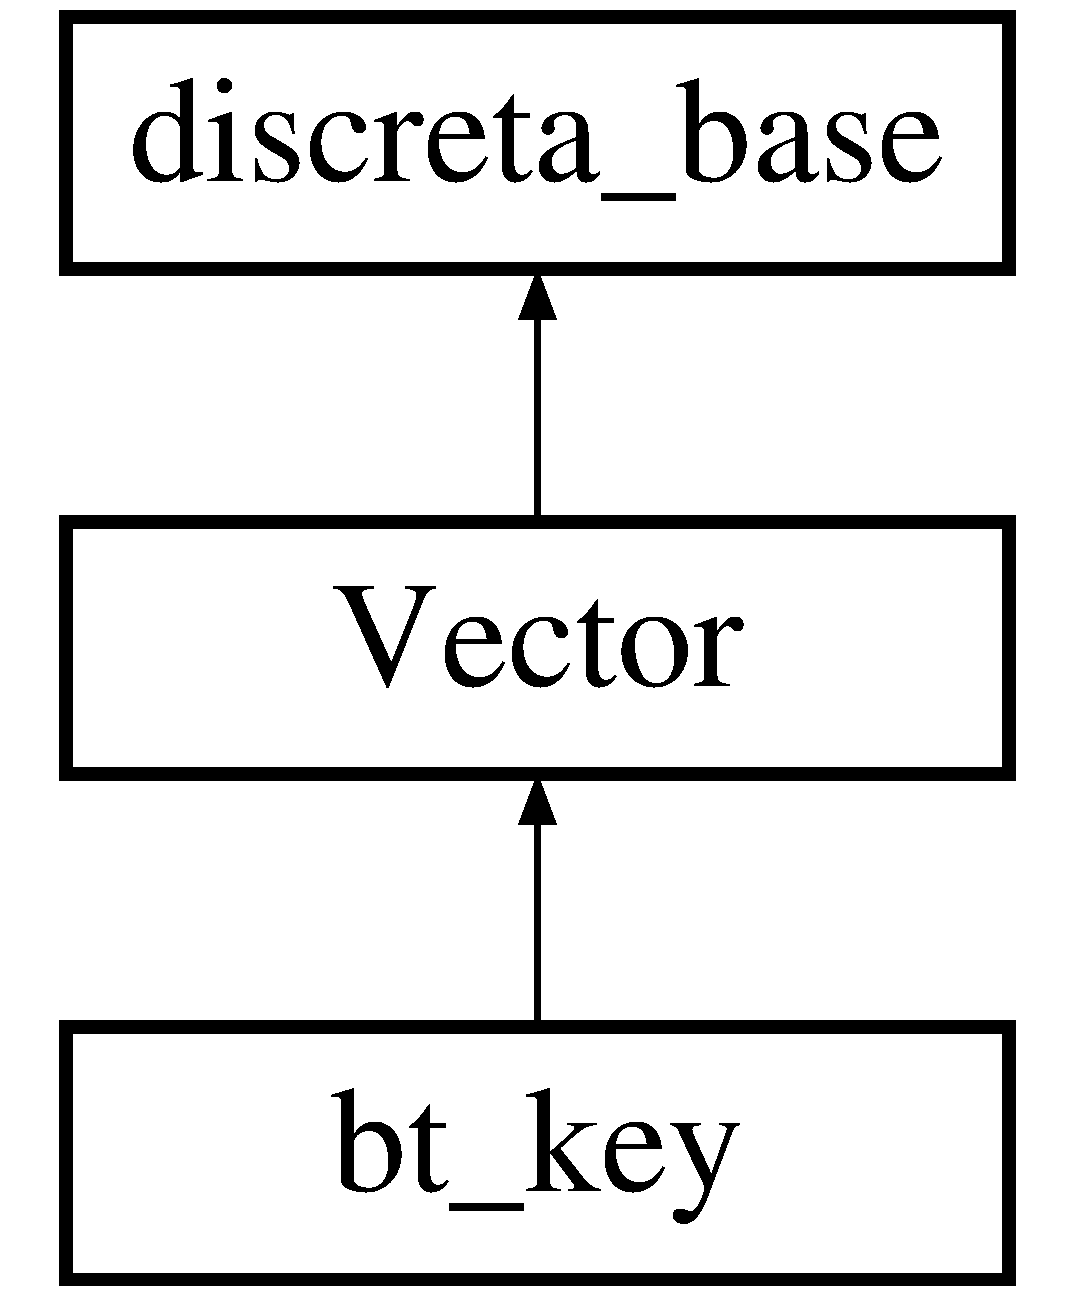
\includegraphics[height=3.000000cm]{classbt__key}
\end{center}
\end{figure}
\subsection*{Public Member Functions}
\begin{DoxyCompactItemize}
\item 
\mbox{\hyperlink{classbt__key_a711cbed5ca8722346862b155d6f2cb3e}{bt\+\_\+key}} ()
\item 
\mbox{\hyperlink{classbt__key_a64ff7f7d1285c8b5512c34f48561853f}{bt\+\_\+key}} (const \mbox{\hyperlink{classdiscreta__base}{discreta\+\_\+base}} \&\mbox{\hyperlink{alphabet2_8_c_a6150e0515f7202e2fb518f7206ed97dc}{x}})
\item 
\mbox{\hyperlink{classbt__key}{bt\+\_\+key}} \& \mbox{\hyperlink{classbt__key_a5258ebd54987d2152544e63a34c2bc2a}{operator=}} (const \mbox{\hyperlink{classdiscreta__base}{discreta\+\_\+base}} \&\mbox{\hyperlink{alphabet2_8_c_a6150e0515f7202e2fb518f7206ed97dc}{x}})
\item 
void $\ast$ \mbox{\hyperlink{classbt__key_adb8126830e966050ea93d1b2c32c0d07}{operator new}} (size\+\_\+t, void $\ast$\mbox{\hyperlink{alphabet2_8_c_a533391314665d6bf1b5575e9a9cd8552}{p}})
\item 
void \mbox{\hyperlink{classbt__key_a352bb10beb7c789d8d29373035824800}{settype\+\_\+bt\+\_\+key}} ()
\item 
\mbox{\hyperlink{discreta_8h_aaf25ee7e2306d78c74ec7bc48f092e81}{kind}} \mbox{\hyperlink{classbt__key_a53b7441523674e20f5c8f5c81eaccad4}{s\+\_\+virtual\+\_\+kind}} ()
\item 
\mbox{\hyperlink{classbt__key_a8b505bfd4e2f8b4806575070972d2b7d}{$\sim$bt\+\_\+key}} ()
\item 
void \mbox{\hyperlink{classbt__key_aad1f5a9b943d3ae072f1d09a9bb126c6}{freeself\+\_\+bt\+\_\+key}} ()
\item 
void \mbox{\hyperlink{classbt__key_ae97899364f826bc3d16cce36b9c8e4f7}{copyobject\+\_\+to}} (\mbox{\hyperlink{classdiscreta__base}{discreta\+\_\+base}} \&\mbox{\hyperlink{alphabet2_8_c_a6150e0515f7202e2fb518f7206ed97dc}{x}})
\item 
ostream \& \mbox{\hyperlink{classbt__key_aee0bad4deaf27c20d15d97050d3af150}{print}} (ostream \&)
\item 
enum \mbox{\hyperlink{discreta_8h_ac90b3b8c242d6128eb9985cfb7f77053}{bt\+\_\+key\+\_\+kind}} \& \mbox{\hyperlink{classbt__key_ae788a415a20f75fe7160408a055bb33f}{type}} ()
\item 
\mbox{\hyperlink{galois_8h_a09fddde158a3a20bd2dcadb609de11dc}{I\+NT}} \& \mbox{\hyperlink{classbt__key_acb48f95d030f62c56051d0cd6e013394}{output\+\_\+size}} ()
\item 
\mbox{\hyperlink{galois_8h_a09fddde158a3a20bd2dcadb609de11dc}{I\+NT}} \& \mbox{\hyperlink{classbt__key_a4ed68c3deb2477a0609065272b5dc4cf}{int\+\_\+vec\+\_\+first}} ()
\item 
\mbox{\hyperlink{galois_8h_a09fddde158a3a20bd2dcadb609de11dc}{I\+NT}} \& \mbox{\hyperlink{classbt__key_ac8e43906f79bacf330fa1726925b7e37}{int\+\_\+vec\+\_\+len}} ()
\item 
\mbox{\hyperlink{galois_8h_a09fddde158a3a20bd2dcadb609de11dc}{I\+NT}} \& \mbox{\hyperlink{classbt__key_af372b25947e954e2a67f59418b9d1f9f}{field1}} ()
\item 
\mbox{\hyperlink{galois_8h_a09fddde158a3a20bd2dcadb609de11dc}{I\+NT}} \& \mbox{\hyperlink{classbt__key_a8aea2dcc348cbece3e97a29012dc7ffd}{field2}} ()
\item 
\mbox{\hyperlink{galois_8h_a09fddde158a3a20bd2dcadb609de11dc}{I\+NT}} \& \mbox{\hyperlink{classbt__key_af63f0ac36475ef1912a23b34cb0b1e9d}{f\+\_\+ascending}} ()
\item 
void \mbox{\hyperlink{classbt__key_ae6b27c89a5f6dec6a7a19583a4b112a8}{init}} (enum \mbox{\hyperlink{discreta_8h_ac90b3b8c242d6128eb9985cfb7f77053}{bt\+\_\+key\+\_\+kind}} \mbox{\hyperlink{classbt__key_ae788a415a20f75fe7160408a055bb33f}{type}}, \mbox{\hyperlink{galois_8h_a09fddde158a3a20bd2dcadb609de11dc}{I\+NT}} \mbox{\hyperlink{classbt__key_acb48f95d030f62c56051d0cd6e013394}{output\+\_\+size}}, \mbox{\hyperlink{galois_8h_a09fddde158a3a20bd2dcadb609de11dc}{I\+NT}} \mbox{\hyperlink{classbt__key_af372b25947e954e2a67f59418b9d1f9f}{field1}}, \mbox{\hyperlink{galois_8h_a09fddde158a3a20bd2dcadb609de11dc}{I\+NT}} \mbox{\hyperlink{classbt__key_a8aea2dcc348cbece3e97a29012dc7ffd}{field2}})
\item 
void \mbox{\hyperlink{classbt__key_a1cc3e1aa6b3a6ec6e036fd4fee010564}{init\+\_\+\+I\+N\+T4}} (\mbox{\hyperlink{galois_8h_a09fddde158a3a20bd2dcadb609de11dc}{I\+NT}} \mbox{\hyperlink{classbt__key_af372b25947e954e2a67f59418b9d1f9f}{field1}}, \mbox{\hyperlink{galois_8h_a09fddde158a3a20bd2dcadb609de11dc}{I\+NT}} \mbox{\hyperlink{classbt__key_a8aea2dcc348cbece3e97a29012dc7ffd}{field2}})
\item 
void \mbox{\hyperlink{classbt__key_a588bbf34a0c101ad79f331fc762c36fa}{init\+\_\+\+I\+N\+T2}} (\mbox{\hyperlink{galois_8h_a09fddde158a3a20bd2dcadb609de11dc}{I\+NT}} \mbox{\hyperlink{classbt__key_af372b25947e954e2a67f59418b9d1f9f}{field1}}, \mbox{\hyperlink{galois_8h_a09fddde158a3a20bd2dcadb609de11dc}{I\+NT}} \mbox{\hyperlink{classbt__key_a8aea2dcc348cbece3e97a29012dc7ffd}{field2}})
\item 
void \mbox{\hyperlink{classbt__key_a37c5830aa6abd2f9892a649e1b5d4248}{init\+\_\+string}} (\mbox{\hyperlink{galois_8h_a09fddde158a3a20bd2dcadb609de11dc}{I\+NT}} \mbox{\hyperlink{classbt__key_acb48f95d030f62c56051d0cd6e013394}{output\+\_\+size}}, \mbox{\hyperlink{galois_8h_a09fddde158a3a20bd2dcadb609de11dc}{I\+NT}} \mbox{\hyperlink{classbt__key_af372b25947e954e2a67f59418b9d1f9f}{field1}}, \mbox{\hyperlink{galois_8h_a09fddde158a3a20bd2dcadb609de11dc}{I\+NT}} \mbox{\hyperlink{classbt__key_a8aea2dcc348cbece3e97a29012dc7ffd}{field2}})
\item 
void \mbox{\hyperlink{classbt__key_ac13cd9d95f812eeb86c70219905f16fd}{init\+\_\+int4\+\_\+vec}} (\mbox{\hyperlink{galois_8h_a09fddde158a3a20bd2dcadb609de11dc}{I\+NT}} \mbox{\hyperlink{classbt__key_af372b25947e954e2a67f59418b9d1f9f}{field1}}, \mbox{\hyperlink{galois_8h_a09fddde158a3a20bd2dcadb609de11dc}{I\+NT}} \mbox{\hyperlink{classbt__key_a8aea2dcc348cbece3e97a29012dc7ffd}{field2}}, \mbox{\hyperlink{galois_8h_a09fddde158a3a20bd2dcadb609de11dc}{I\+NT}} vec\+\_\+fst, \mbox{\hyperlink{galois_8h_a09fddde158a3a20bd2dcadb609de11dc}{I\+NT}} vec\+\_\+len)
\item 
void \mbox{\hyperlink{classbt__key_ac387752908d0de9d69246e19a3ae321d}{init\+\_\+int2\+\_\+vec}} (\mbox{\hyperlink{galois_8h_a09fddde158a3a20bd2dcadb609de11dc}{I\+NT}} \mbox{\hyperlink{classbt__key_af372b25947e954e2a67f59418b9d1f9f}{field1}}, \mbox{\hyperlink{galois_8h_a09fddde158a3a20bd2dcadb609de11dc}{I\+NT}} \mbox{\hyperlink{classbt__key_a8aea2dcc348cbece3e97a29012dc7ffd}{field2}}, \mbox{\hyperlink{galois_8h_a09fddde158a3a20bd2dcadb609de11dc}{I\+NT}} vec\+\_\+fst, \mbox{\hyperlink{galois_8h_a09fddde158a3a20bd2dcadb609de11dc}{I\+NT}} vec\+\_\+len)
\end{DoxyCompactItemize}
\subsection*{Additional Inherited Members}


\subsection{Constructor \& Destructor Documentation}
\mbox{\Hypertarget{classbt__key_a711cbed5ca8722346862b155d6f2cb3e}\label{classbt__key_a711cbed5ca8722346862b155d6f2cb3e}} 
\index{bt\+\_\+key@{bt\+\_\+key}!bt\+\_\+key@{bt\+\_\+key}}
\index{bt\+\_\+key@{bt\+\_\+key}!bt\+\_\+key@{bt\+\_\+key}}
\subsubsection{\texorpdfstring{bt\+\_\+key()}{bt\_key()}\hspace{0.1cm}{\footnotesize\ttfamily [1/2]}}
{\footnotesize\ttfamily bt\+\_\+key\+::bt\+\_\+key (\begin{DoxyParamCaption}{ }\end{DoxyParamCaption})}

\mbox{\Hypertarget{classbt__key_a64ff7f7d1285c8b5512c34f48561853f}\label{classbt__key_a64ff7f7d1285c8b5512c34f48561853f}} 
\index{bt\+\_\+key@{bt\+\_\+key}!bt\+\_\+key@{bt\+\_\+key}}
\index{bt\+\_\+key@{bt\+\_\+key}!bt\+\_\+key@{bt\+\_\+key}}
\subsubsection{\texorpdfstring{bt\+\_\+key()}{bt\_key()}\hspace{0.1cm}{\footnotesize\ttfamily [2/2]}}
{\footnotesize\ttfamily bt\+\_\+key\+::bt\+\_\+key (\begin{DoxyParamCaption}\item[{const \mbox{\hyperlink{classdiscreta__base}{discreta\+\_\+base}} \&}]{x }\end{DoxyParamCaption})}

\mbox{\Hypertarget{classbt__key_a8b505bfd4e2f8b4806575070972d2b7d}\label{classbt__key_a8b505bfd4e2f8b4806575070972d2b7d}} 
\index{bt\+\_\+key@{bt\+\_\+key}!````~bt\+\_\+key@{$\sim$bt\+\_\+key}}
\index{````~bt\+\_\+key@{$\sim$bt\+\_\+key}!bt\+\_\+key@{bt\+\_\+key}}
\subsubsection{\texorpdfstring{$\sim$bt\+\_\+key()}{~bt\_key()}}
{\footnotesize\ttfamily bt\+\_\+key\+::$\sim$bt\+\_\+key (\begin{DoxyParamCaption}{ }\end{DoxyParamCaption})}



\subsection{Member Function Documentation}
\mbox{\Hypertarget{classbt__key_ae97899364f826bc3d16cce36b9c8e4f7}\label{classbt__key_ae97899364f826bc3d16cce36b9c8e4f7}} 
\index{bt\+\_\+key@{bt\+\_\+key}!copyobject\+\_\+to@{copyobject\+\_\+to}}
\index{copyobject\+\_\+to@{copyobject\+\_\+to}!bt\+\_\+key@{bt\+\_\+key}}
\subsubsection{\texorpdfstring{copyobject\+\_\+to()}{copyobject\_to()}}
{\footnotesize\ttfamily void bt\+\_\+key\+::copyobject\+\_\+to (\begin{DoxyParamCaption}\item[{\mbox{\hyperlink{classdiscreta__base}{discreta\+\_\+base}} \&}]{x }\end{DoxyParamCaption})\hspace{0.3cm}{\ttfamily [virtual]}}



Reimplemented from \mbox{\hyperlink{class_vector_af657307f3d344c8cef5d633335a5f484}{Vector}}.

\mbox{\Hypertarget{classbt__key_af63f0ac36475ef1912a23b34cb0b1e9d}\label{classbt__key_af63f0ac36475ef1912a23b34cb0b1e9d}} 
\index{bt\+\_\+key@{bt\+\_\+key}!f\+\_\+ascending@{f\+\_\+ascending}}
\index{f\+\_\+ascending@{f\+\_\+ascending}!bt\+\_\+key@{bt\+\_\+key}}
\subsubsection{\texorpdfstring{f\+\_\+ascending()}{f\_ascending()}}
{\footnotesize\ttfamily \mbox{\hyperlink{galois_8h_a09fddde158a3a20bd2dcadb609de11dc}{I\+NT}}\& bt\+\_\+key\+::f\+\_\+ascending (\begin{DoxyParamCaption}{ }\end{DoxyParamCaption})\hspace{0.3cm}{\ttfamily [inline]}}

\mbox{\Hypertarget{classbt__key_af372b25947e954e2a67f59418b9d1f9f}\label{classbt__key_af372b25947e954e2a67f59418b9d1f9f}} 
\index{bt\+\_\+key@{bt\+\_\+key}!field1@{field1}}
\index{field1@{field1}!bt\+\_\+key@{bt\+\_\+key}}
\subsubsection{\texorpdfstring{field1()}{field1()}}
{\footnotesize\ttfamily \mbox{\hyperlink{galois_8h_a09fddde158a3a20bd2dcadb609de11dc}{I\+NT}}\& bt\+\_\+key\+::field1 (\begin{DoxyParamCaption}{ }\end{DoxyParamCaption})\hspace{0.3cm}{\ttfamily [inline]}}

\mbox{\Hypertarget{classbt__key_a8aea2dcc348cbece3e97a29012dc7ffd}\label{classbt__key_a8aea2dcc348cbece3e97a29012dc7ffd}} 
\index{bt\+\_\+key@{bt\+\_\+key}!field2@{field2}}
\index{field2@{field2}!bt\+\_\+key@{bt\+\_\+key}}
\subsubsection{\texorpdfstring{field2()}{field2()}}
{\footnotesize\ttfamily \mbox{\hyperlink{galois_8h_a09fddde158a3a20bd2dcadb609de11dc}{I\+NT}}\& bt\+\_\+key\+::field2 (\begin{DoxyParamCaption}{ }\end{DoxyParamCaption})\hspace{0.3cm}{\ttfamily [inline]}}

\mbox{\Hypertarget{classbt__key_aad1f5a9b943d3ae072f1d09a9bb126c6}\label{classbt__key_aad1f5a9b943d3ae072f1d09a9bb126c6}} 
\index{bt\+\_\+key@{bt\+\_\+key}!freeself\+\_\+bt\+\_\+key@{freeself\+\_\+bt\+\_\+key}}
\index{freeself\+\_\+bt\+\_\+key@{freeself\+\_\+bt\+\_\+key}!bt\+\_\+key@{bt\+\_\+key}}
\subsubsection{\texorpdfstring{freeself\+\_\+bt\+\_\+key()}{freeself\_bt\_key()}}
{\footnotesize\ttfamily void bt\+\_\+key\+::freeself\+\_\+bt\+\_\+key (\begin{DoxyParamCaption}{ }\end{DoxyParamCaption})}

\mbox{\Hypertarget{classbt__key_ae6b27c89a5f6dec6a7a19583a4b112a8}\label{classbt__key_ae6b27c89a5f6dec6a7a19583a4b112a8}} 
\index{bt\+\_\+key@{bt\+\_\+key}!init@{init}}
\index{init@{init}!bt\+\_\+key@{bt\+\_\+key}}
\subsubsection{\texorpdfstring{init()}{init()}}
{\footnotesize\ttfamily void bt\+\_\+key\+::init (\begin{DoxyParamCaption}\item[{enum \mbox{\hyperlink{discreta_8h_ac90b3b8c242d6128eb9985cfb7f77053}{bt\+\_\+key\+\_\+kind}}}]{type,  }\item[{\mbox{\hyperlink{galois_8h_a09fddde158a3a20bd2dcadb609de11dc}{I\+NT}}}]{output\+\_\+size,  }\item[{\mbox{\hyperlink{galois_8h_a09fddde158a3a20bd2dcadb609de11dc}{I\+NT}}}]{field1,  }\item[{\mbox{\hyperlink{galois_8h_a09fddde158a3a20bd2dcadb609de11dc}{I\+NT}}}]{field2 }\end{DoxyParamCaption})}

\mbox{\Hypertarget{classbt__key_a588bbf34a0c101ad79f331fc762c36fa}\label{classbt__key_a588bbf34a0c101ad79f331fc762c36fa}} 
\index{bt\+\_\+key@{bt\+\_\+key}!init\+\_\+\+I\+N\+T2@{init\+\_\+\+I\+N\+T2}}
\index{init\+\_\+\+I\+N\+T2@{init\+\_\+\+I\+N\+T2}!bt\+\_\+key@{bt\+\_\+key}}
\subsubsection{\texorpdfstring{init\+\_\+\+I\+N\+T2()}{init\_INT2()}}
{\footnotesize\ttfamily void bt\+\_\+key\+::init\+\_\+\+I\+N\+T2 (\begin{DoxyParamCaption}\item[{\mbox{\hyperlink{galois_8h_a09fddde158a3a20bd2dcadb609de11dc}{I\+NT}}}]{field1,  }\item[{\mbox{\hyperlink{galois_8h_a09fddde158a3a20bd2dcadb609de11dc}{I\+NT}}}]{field2 }\end{DoxyParamCaption})}

\mbox{\Hypertarget{classbt__key_ac387752908d0de9d69246e19a3ae321d}\label{classbt__key_ac387752908d0de9d69246e19a3ae321d}} 
\index{bt\+\_\+key@{bt\+\_\+key}!init\+\_\+int2\+\_\+vec@{init\+\_\+int2\+\_\+vec}}
\index{init\+\_\+int2\+\_\+vec@{init\+\_\+int2\+\_\+vec}!bt\+\_\+key@{bt\+\_\+key}}
\subsubsection{\texorpdfstring{init\+\_\+int2\+\_\+vec()}{init\_int2\_vec()}}
{\footnotesize\ttfamily void bt\+\_\+key\+::init\+\_\+int2\+\_\+vec (\begin{DoxyParamCaption}\item[{\mbox{\hyperlink{galois_8h_a09fddde158a3a20bd2dcadb609de11dc}{I\+NT}}}]{field1,  }\item[{\mbox{\hyperlink{galois_8h_a09fddde158a3a20bd2dcadb609de11dc}{I\+NT}}}]{field2,  }\item[{\mbox{\hyperlink{galois_8h_a09fddde158a3a20bd2dcadb609de11dc}{I\+NT}}}]{vec\+\_\+fst,  }\item[{\mbox{\hyperlink{galois_8h_a09fddde158a3a20bd2dcadb609de11dc}{I\+NT}}}]{vec\+\_\+len }\end{DoxyParamCaption})}

\mbox{\Hypertarget{classbt__key_a1cc3e1aa6b3a6ec6e036fd4fee010564}\label{classbt__key_a1cc3e1aa6b3a6ec6e036fd4fee010564}} 
\index{bt\+\_\+key@{bt\+\_\+key}!init\+\_\+\+I\+N\+T4@{init\+\_\+\+I\+N\+T4}}
\index{init\+\_\+\+I\+N\+T4@{init\+\_\+\+I\+N\+T4}!bt\+\_\+key@{bt\+\_\+key}}
\subsubsection{\texorpdfstring{init\+\_\+\+I\+N\+T4()}{init\_INT4()}}
{\footnotesize\ttfamily void bt\+\_\+key\+::init\+\_\+\+I\+N\+T4 (\begin{DoxyParamCaption}\item[{\mbox{\hyperlink{galois_8h_a09fddde158a3a20bd2dcadb609de11dc}{I\+NT}}}]{field1,  }\item[{\mbox{\hyperlink{galois_8h_a09fddde158a3a20bd2dcadb609de11dc}{I\+NT}}}]{field2 }\end{DoxyParamCaption})}

\mbox{\Hypertarget{classbt__key_ac13cd9d95f812eeb86c70219905f16fd}\label{classbt__key_ac13cd9d95f812eeb86c70219905f16fd}} 
\index{bt\+\_\+key@{bt\+\_\+key}!init\+\_\+int4\+\_\+vec@{init\+\_\+int4\+\_\+vec}}
\index{init\+\_\+int4\+\_\+vec@{init\+\_\+int4\+\_\+vec}!bt\+\_\+key@{bt\+\_\+key}}
\subsubsection{\texorpdfstring{init\+\_\+int4\+\_\+vec()}{init\_int4\_vec()}}
{\footnotesize\ttfamily void bt\+\_\+key\+::init\+\_\+int4\+\_\+vec (\begin{DoxyParamCaption}\item[{\mbox{\hyperlink{galois_8h_a09fddde158a3a20bd2dcadb609de11dc}{I\+NT}}}]{field1,  }\item[{\mbox{\hyperlink{galois_8h_a09fddde158a3a20bd2dcadb609de11dc}{I\+NT}}}]{field2,  }\item[{\mbox{\hyperlink{galois_8h_a09fddde158a3a20bd2dcadb609de11dc}{I\+NT}}}]{vec\+\_\+fst,  }\item[{\mbox{\hyperlink{galois_8h_a09fddde158a3a20bd2dcadb609de11dc}{I\+NT}}}]{vec\+\_\+len }\end{DoxyParamCaption})}

\mbox{\Hypertarget{classbt__key_a37c5830aa6abd2f9892a649e1b5d4248}\label{classbt__key_a37c5830aa6abd2f9892a649e1b5d4248}} 
\index{bt\+\_\+key@{bt\+\_\+key}!init\+\_\+string@{init\+\_\+string}}
\index{init\+\_\+string@{init\+\_\+string}!bt\+\_\+key@{bt\+\_\+key}}
\subsubsection{\texorpdfstring{init\+\_\+string()}{init\_string()}}
{\footnotesize\ttfamily void bt\+\_\+key\+::init\+\_\+string (\begin{DoxyParamCaption}\item[{\mbox{\hyperlink{galois_8h_a09fddde158a3a20bd2dcadb609de11dc}{I\+NT}}}]{output\+\_\+size,  }\item[{\mbox{\hyperlink{galois_8h_a09fddde158a3a20bd2dcadb609de11dc}{I\+NT}}}]{field1,  }\item[{\mbox{\hyperlink{galois_8h_a09fddde158a3a20bd2dcadb609de11dc}{I\+NT}}}]{field2 }\end{DoxyParamCaption})}

\mbox{\Hypertarget{classbt__key_a4ed68c3deb2477a0609065272b5dc4cf}\label{classbt__key_a4ed68c3deb2477a0609065272b5dc4cf}} 
\index{bt\+\_\+key@{bt\+\_\+key}!int\+\_\+vec\+\_\+first@{int\+\_\+vec\+\_\+first}}
\index{int\+\_\+vec\+\_\+first@{int\+\_\+vec\+\_\+first}!bt\+\_\+key@{bt\+\_\+key}}
\subsubsection{\texorpdfstring{int\+\_\+vec\+\_\+first()}{int\_vec\_first()}}
{\footnotesize\ttfamily \mbox{\hyperlink{galois_8h_a09fddde158a3a20bd2dcadb609de11dc}{I\+NT}}\& bt\+\_\+key\+::int\+\_\+vec\+\_\+first (\begin{DoxyParamCaption}{ }\end{DoxyParamCaption})\hspace{0.3cm}{\ttfamily [inline]}}

\mbox{\Hypertarget{classbt__key_ac8e43906f79bacf330fa1726925b7e37}\label{classbt__key_ac8e43906f79bacf330fa1726925b7e37}} 
\index{bt\+\_\+key@{bt\+\_\+key}!int\+\_\+vec\+\_\+len@{int\+\_\+vec\+\_\+len}}
\index{int\+\_\+vec\+\_\+len@{int\+\_\+vec\+\_\+len}!bt\+\_\+key@{bt\+\_\+key}}
\subsubsection{\texorpdfstring{int\+\_\+vec\+\_\+len()}{int\_vec\_len()}}
{\footnotesize\ttfamily \mbox{\hyperlink{galois_8h_a09fddde158a3a20bd2dcadb609de11dc}{I\+NT}}\& bt\+\_\+key\+::int\+\_\+vec\+\_\+len (\begin{DoxyParamCaption}{ }\end{DoxyParamCaption})\hspace{0.3cm}{\ttfamily [inline]}}

\mbox{\Hypertarget{classbt__key_adb8126830e966050ea93d1b2c32c0d07}\label{classbt__key_adb8126830e966050ea93d1b2c32c0d07}} 
\index{bt\+\_\+key@{bt\+\_\+key}!operator new@{operator new}}
\index{operator new@{operator new}!bt\+\_\+key@{bt\+\_\+key}}
\subsubsection{\texorpdfstring{operator new()}{operator new()}}
{\footnotesize\ttfamily void$\ast$ bt\+\_\+key\+::operator new (\begin{DoxyParamCaption}\item[{size\+\_\+t}]{,  }\item[{void $\ast$}]{p }\end{DoxyParamCaption})\hspace{0.3cm}{\ttfamily [inline]}}

\mbox{\Hypertarget{classbt__key_a5258ebd54987d2152544e63a34c2bc2a}\label{classbt__key_a5258ebd54987d2152544e63a34c2bc2a}} 
\index{bt\+\_\+key@{bt\+\_\+key}!operator=@{operator=}}
\index{operator=@{operator=}!bt\+\_\+key@{bt\+\_\+key}}
\subsubsection{\texorpdfstring{operator=()}{operator=()}}
{\footnotesize\ttfamily \mbox{\hyperlink{classbt__key}{bt\+\_\+key}} \& bt\+\_\+key\+::operator= (\begin{DoxyParamCaption}\item[{const \mbox{\hyperlink{classdiscreta__base}{discreta\+\_\+base}} \&}]{x }\end{DoxyParamCaption})}

\mbox{\Hypertarget{classbt__key_acb48f95d030f62c56051d0cd6e013394}\label{classbt__key_acb48f95d030f62c56051d0cd6e013394}} 
\index{bt\+\_\+key@{bt\+\_\+key}!output\+\_\+size@{output\+\_\+size}}
\index{output\+\_\+size@{output\+\_\+size}!bt\+\_\+key@{bt\+\_\+key}}
\subsubsection{\texorpdfstring{output\+\_\+size()}{output\_size()}}
{\footnotesize\ttfamily \mbox{\hyperlink{galois_8h_a09fddde158a3a20bd2dcadb609de11dc}{I\+NT}}\& bt\+\_\+key\+::output\+\_\+size (\begin{DoxyParamCaption}{ }\end{DoxyParamCaption})\hspace{0.3cm}{\ttfamily [inline]}}

\mbox{\Hypertarget{classbt__key_aee0bad4deaf27c20d15d97050d3af150}\label{classbt__key_aee0bad4deaf27c20d15d97050d3af150}} 
\index{bt\+\_\+key@{bt\+\_\+key}!print@{print}}
\index{print@{print}!bt\+\_\+key@{bt\+\_\+key}}
\subsubsection{\texorpdfstring{print()}{print()}}
{\footnotesize\ttfamily ostream \& bt\+\_\+key\+::print (\begin{DoxyParamCaption}\item[{ostream \&}]{ost }\end{DoxyParamCaption})\hspace{0.3cm}{\ttfamily [virtual]}}



Reimplemented from \mbox{\hyperlink{class_vector_a71d7e24bcfdfc69d4a2137360acb066c}{Vector}}.

\mbox{\Hypertarget{classbt__key_a53b7441523674e20f5c8f5c81eaccad4}\label{classbt__key_a53b7441523674e20f5c8f5c81eaccad4}} 
\index{bt\+\_\+key@{bt\+\_\+key}!s\+\_\+virtual\+\_\+kind@{s\+\_\+virtual\+\_\+kind}}
\index{s\+\_\+virtual\+\_\+kind@{s\+\_\+virtual\+\_\+kind}!bt\+\_\+key@{bt\+\_\+key}}
\subsubsection{\texorpdfstring{s\+\_\+virtual\+\_\+kind()}{s\_virtual\_kind()}}
{\footnotesize\ttfamily \mbox{\hyperlink{discreta_8h_aaf25ee7e2306d78c74ec7bc48f092e81}{kind}} bt\+\_\+key\+::s\+\_\+virtual\+\_\+kind (\begin{DoxyParamCaption}{ }\end{DoxyParamCaption})\hspace{0.3cm}{\ttfamily [virtual]}}



Reimplemented from \mbox{\hyperlink{class_vector_a20550e70d02cbe484032c7f6b0833a0f}{Vector}}.

\mbox{\Hypertarget{classbt__key_a352bb10beb7c789d8d29373035824800}\label{classbt__key_a352bb10beb7c789d8d29373035824800}} 
\index{bt\+\_\+key@{bt\+\_\+key}!settype\+\_\+bt\+\_\+key@{settype\+\_\+bt\+\_\+key}}
\index{settype\+\_\+bt\+\_\+key@{settype\+\_\+bt\+\_\+key}!bt\+\_\+key@{bt\+\_\+key}}
\subsubsection{\texorpdfstring{settype\+\_\+bt\+\_\+key()}{settype\_bt\_key()}}
{\footnotesize\ttfamily void bt\+\_\+key\+::settype\+\_\+bt\+\_\+key (\begin{DoxyParamCaption}{ }\end{DoxyParamCaption})}

\mbox{\Hypertarget{classbt__key_ae788a415a20f75fe7160408a055bb33f}\label{classbt__key_ae788a415a20f75fe7160408a055bb33f}} 
\index{bt\+\_\+key@{bt\+\_\+key}!type@{type}}
\index{type@{type}!bt\+\_\+key@{bt\+\_\+key}}
\subsubsection{\texorpdfstring{type()}{type()}}
{\footnotesize\ttfamily enum \mbox{\hyperlink{discreta_8h_ac90b3b8c242d6128eb9985cfb7f77053}{bt\+\_\+key\+\_\+kind}}\& bt\+\_\+key\+::type (\begin{DoxyParamCaption}{ }\end{DoxyParamCaption})\hspace{0.3cm}{\ttfamily [inline]}}



The documentation for this class was generated from the following files\+:\begin{DoxyCompactItemize}
\item 
S\+R\+C/\+L\+I\+B/\+D\+I\+S\+C\+R\+E\+T\+A/\mbox{\hyperlink{discreta_8h}{discreta.\+h}}\item 
S\+R\+C/\+L\+I\+B/\+D\+I\+S\+C\+R\+E\+T\+A/\mbox{\hyperlink{bt__key_8_c}{bt\+\_\+key.\+C}}\end{DoxyCompactItemize}

\hypertarget{classbtree}{}\section{btree Class Reference}
\label{classbtree}\index{btree@{btree}}


{\ttfamily \#include $<$discreta.\+h$>$}

Inheritance diagram for btree\+:\begin{figure}[H]
\begin{center}
\leavevmode
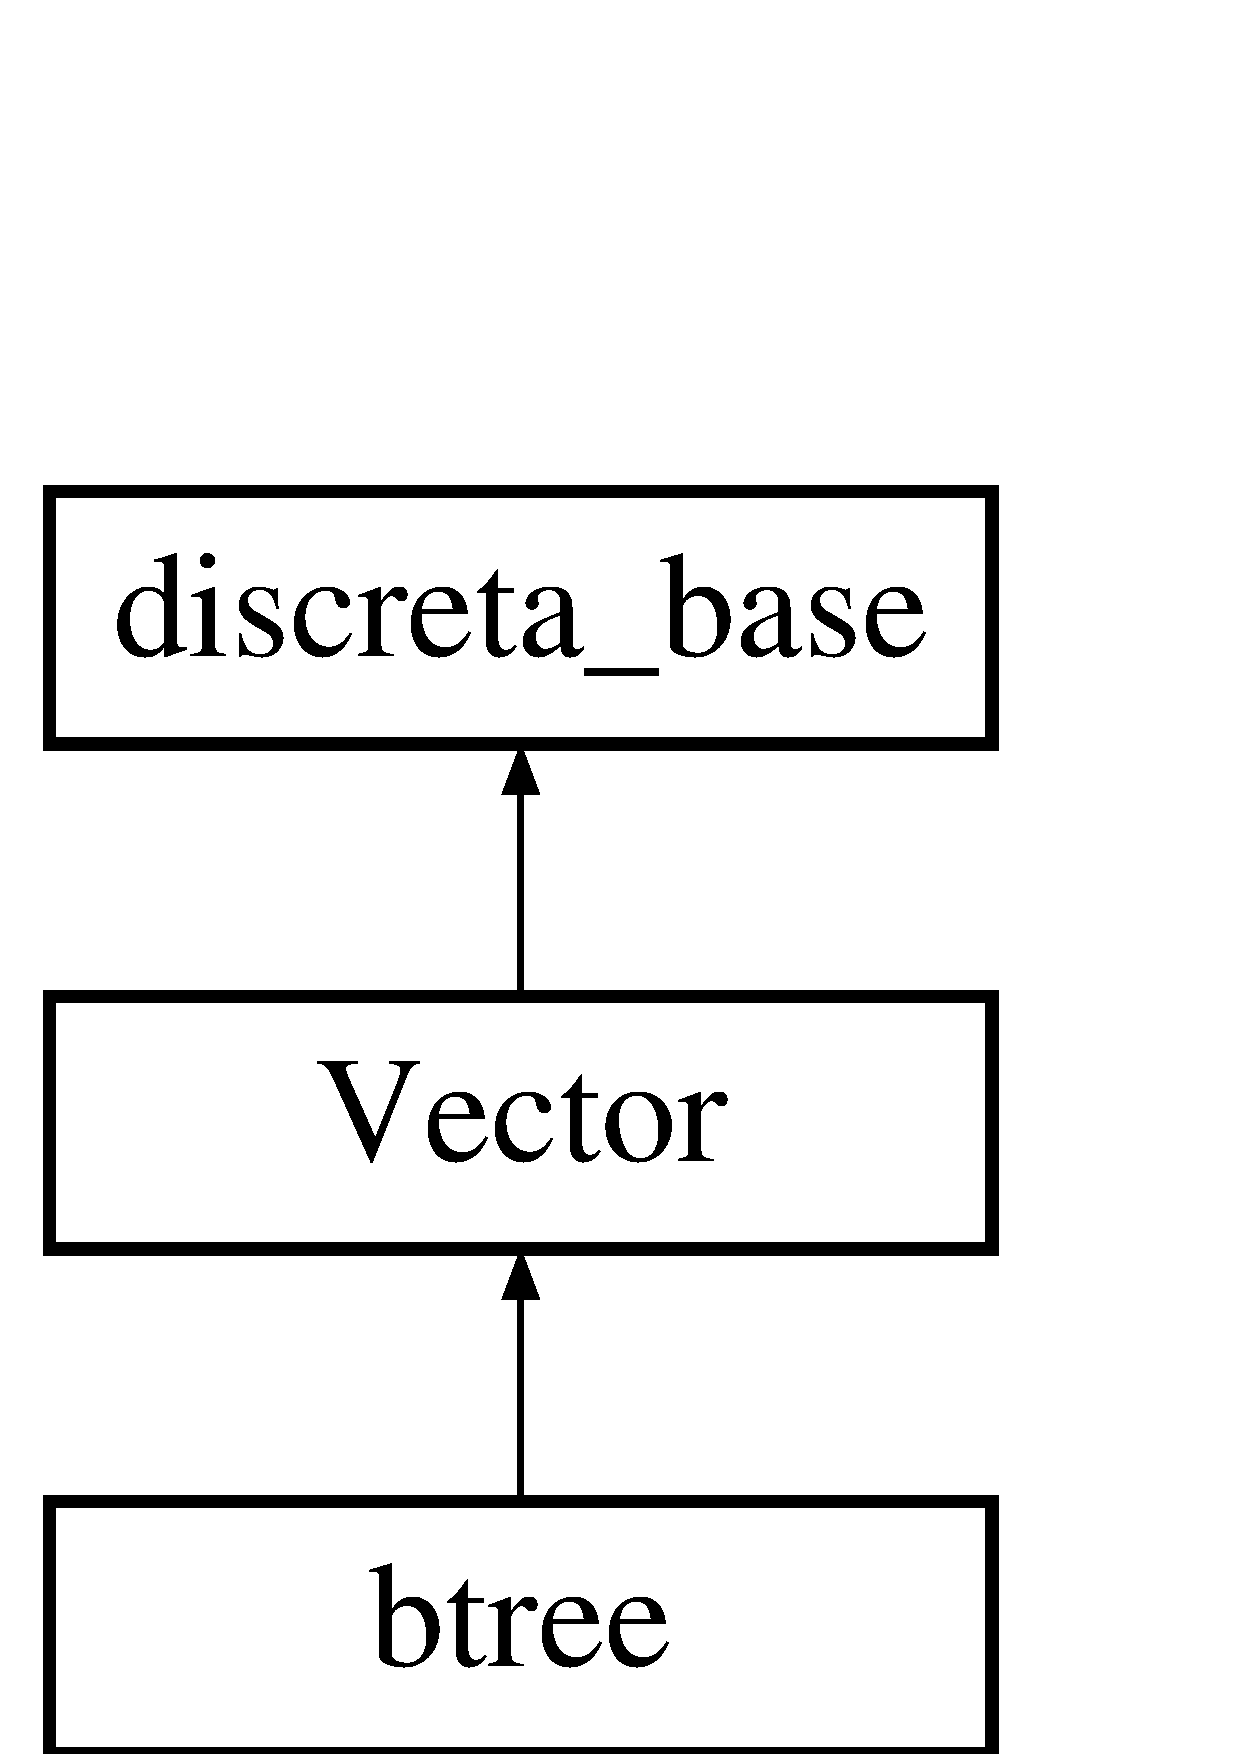
\includegraphics[height=3.000000cm]{classbtree}
\end{center}
\end{figure}
\subsection*{Public Member Functions}
\begin{DoxyCompactItemize}
\item 
\mbox{\hyperlink{classbtree_a91719c0888688e6f11dbeb336f2bd11b}{btree}} ()
\item 
\mbox{\hyperlink{classbtree_acdd426e62444f342e4fa3ac6a272fb32}{btree}} (const \mbox{\hyperlink{classdiscreta__base}{discreta\+\_\+base}} \&\mbox{\hyperlink{alphabet2_8_c_a6150e0515f7202e2fb518f7206ed97dc}{x}})
\item 
\mbox{\hyperlink{classbtree}{btree}} \& \mbox{\hyperlink{classbtree_a2c95dcf64612ac0dd88b47f004dd84d9}{operator=}} (const \mbox{\hyperlink{classdiscreta__base}{discreta\+\_\+base}} \&\mbox{\hyperlink{alphabet2_8_c_a6150e0515f7202e2fb518f7206ed97dc}{x}})
\item 
void $\ast$ \mbox{\hyperlink{classbtree_a266447f479a8304c819768bbf0e7dd3d}{operator new}} (size\+\_\+t, void $\ast$\mbox{\hyperlink{alphabet2_8_c_a533391314665d6bf1b5575e9a9cd8552}{p}})
\item 
void \mbox{\hyperlink{classbtree_a5a1b9773c848908a6050cc733d2d9780}{settype\+\_\+btree}} ()
\item 
\mbox{\hyperlink{discreta_8h_aaf25ee7e2306d78c74ec7bc48f092e81}{kind}} \mbox{\hyperlink{classbtree_afffc3582b6eda450238f4cb268e79ef3}{s\+\_\+virtual\+\_\+kind}} ()
\item 
\mbox{\hyperlink{classbtree_ab3d5728b7a09121f7461fddd08b5f7ef}{$\sim$btree}} ()
\item 
void \mbox{\hyperlink{classbtree_af866a69c5f887781efdcd491d71f2c28}{freeself\+\_\+btree}} ()
\item 
void \mbox{\hyperlink{classbtree_ae990f68198985c1c7c7a36a65f091ac7}{copyobject\+\_\+to}} (\mbox{\hyperlink{classdiscreta__base}{discreta\+\_\+base}} \&\mbox{\hyperlink{alphabet2_8_c_a6150e0515f7202e2fb518f7206ed97dc}{x}})
\item 
ostream \& \mbox{\hyperlink{classbtree_a76cbc154a13a6464d16a7f080cef40d3}{print}} (ostream \&)
\item 
\mbox{\hyperlink{galois_8h_a09fddde158a3a20bd2dcadb609de11dc}{I\+NT}} \& \mbox{\hyperlink{classbtree_aa53430cc1a527debec6fe02f1c8a2bf5}{f\+\_\+duplicatekeys}} ()
\item 
\mbox{\hyperlink{class_vector}{Vector}} \& \mbox{\hyperlink{classbtree_abc561b2c60acc5a699637b7eb2549503}{key}} ()
\item 
\mbox{\hyperlink{classhollerith}{hollerith}} \& \mbox{\hyperlink{classbtree_ac15638387eb5a165403b8f73d584fe5a}{filename}} ()
\item 
\mbox{\hyperlink{galois_8h_a09fddde158a3a20bd2dcadb609de11dc}{I\+NT}} \& \mbox{\hyperlink{classbtree_a192d74607f02ea8e0ad631d6e6fd6704}{f\+\_\+open}} ()
\item 
\mbox{\hyperlink{galois_8h_a09fddde158a3a20bd2dcadb609de11dc}{I\+NT}} \& \mbox{\hyperlink{classbtree_af99e68df8c3674b7d77ed80a8bbcffac}{stream}} ()
\item 
\mbox{\hyperlink{galois_8h_a09fddde158a3a20bd2dcadb609de11dc}{I\+NT}} \& \mbox{\hyperlink{classbtree_a6a928fc93c93d8b5a83ad1ba699b453e}{buf\+\_\+idx}} ()
\item 
\mbox{\hyperlink{galois_8h_a09fddde158a3a20bd2dcadb609de11dc}{I\+NT}} \& \mbox{\hyperlink{classbtree_a2fd65be715ab94bf4a764c4f582a642b}{Root}} ()
\item 
\mbox{\hyperlink{galois_8h_a09fddde158a3a20bd2dcadb609de11dc}{I\+NT}} \& \mbox{\hyperlink{classbtree_a2ca35526158f016e569c53c411b5fb50}{Free\+Rec}} ()
\item 
\mbox{\hyperlink{galois_8h_a09fddde158a3a20bd2dcadb609de11dc}{I\+NT}} \& \mbox{\hyperlink{classbtree_adfd0217cbd0386bed9231810d581044b}{Alloc\+Rec}} ()
\item 
\mbox{\hyperlink{galois_8h_a09fddde158a3a20bd2dcadb609de11dc}{I\+NT}} \& \mbox{\hyperlink{classbtree_a716a53d4afaa38334205cad81be5546d}{btree\+\_\+idx}} ()
\item 
\mbox{\hyperlink{galois_8h_a09fddde158a3a20bd2dcadb609de11dc}{I\+NT}} \& \mbox{\hyperlink{classbtree_abc6a6f309e4c61cb5a7f4c4a248d384d}{page\+\_\+table\+\_\+idx}} ()
\item 
void \mbox{\hyperlink{classbtree_a3c88706e9886f1f9bc142b511aeab642}{init}} (const \mbox{\hyperlink{galois_8h_ab6cc7b4aeb6ea31aba2b3fbfc83ff5e6}{B\+Y\+TE}} $\ast$file\+\_\+name, \mbox{\hyperlink{galois_8h_a09fddde158a3a20bd2dcadb609de11dc}{I\+NT}} \mbox{\hyperlink{classbtree_aa53430cc1a527debec6fe02f1c8a2bf5}{f\+\_\+duplicatekeys}}, \mbox{\hyperlink{galois_8h_a09fddde158a3a20bd2dcadb609de11dc}{I\+NT}} \mbox{\hyperlink{classbtree_a716a53d4afaa38334205cad81be5546d}{btree\+\_\+idx}})
\item 
void \mbox{\hyperlink{classbtree_a4c42710e5f8cb4e3991d591fe2ae6f42}{add\+\_\+key\+\_\+\+I\+N\+T4}} (\mbox{\hyperlink{galois_8h_a09fddde158a3a20bd2dcadb609de11dc}{I\+NT}} field1, \mbox{\hyperlink{galois_8h_a09fddde158a3a20bd2dcadb609de11dc}{I\+NT}} field2)
\item 
void \mbox{\hyperlink{classbtree_a4d0d3b843c9ae081d5fc0325dbdddea7}{add\+\_\+key\+\_\+\+I\+N\+T2}} (\mbox{\hyperlink{galois_8h_a09fddde158a3a20bd2dcadb609de11dc}{I\+NT}} field1, \mbox{\hyperlink{galois_8h_a09fddde158a3a20bd2dcadb609de11dc}{I\+NT}} field2)
\item 
void \mbox{\hyperlink{classbtree_a291b3c61b9df78471a385b990e926d66}{add\+\_\+key\+\_\+string}} (\mbox{\hyperlink{galois_8h_a09fddde158a3a20bd2dcadb609de11dc}{I\+NT}} output\+\_\+size, \mbox{\hyperlink{galois_8h_a09fddde158a3a20bd2dcadb609de11dc}{I\+NT}} field1, \mbox{\hyperlink{galois_8h_a09fddde158a3a20bd2dcadb609de11dc}{I\+NT}} field2)
\item 
void \mbox{\hyperlink{classbtree_ae75d5ef9677891b93960a55dffdc6eb2}{key\+\_\+fill\+\_\+in}} (\mbox{\hyperlink{galois_8h_ab6cc7b4aeb6ea31aba2b3fbfc83ff5e6}{B\+Y\+TE}} $\ast$the\+\_\+key, \mbox{\hyperlink{class_vector}{Vector}} \&the\+\_\+object)
\item 
void \mbox{\hyperlink{classbtree_a4d527d5afa4891a2fa69fc1a07c48627}{key\+\_\+print}} (\mbox{\hyperlink{galois_8h_ab6cc7b4aeb6ea31aba2b3fbfc83ff5e6}{B\+Y\+TE}} $\ast$the\+\_\+key, ostream \&ost)
\item 
void \mbox{\hyperlink{classbtree_ae46050f7dc1057d21cddcd6b2e3496d9}{create}} (\mbox{\hyperlink{galois_8h_a09fddde158a3a20bd2dcadb609de11dc}{I\+NT}} \mbox{\hyperlink{simeon_8_c_a818073fbcc2f439e7c56952f67386122}{verbose\+\_\+level}})
\item 
void \mbox{\hyperlink{classbtree_a3e718949f1be6057839463292a60297a}{open}} (\mbox{\hyperlink{galois_8h_a09fddde158a3a20bd2dcadb609de11dc}{I\+NT}} \mbox{\hyperlink{simeon_8_c_a818073fbcc2f439e7c56952f67386122}{verbose\+\_\+level}})
\item 
void \mbox{\hyperlink{classbtree_acdd59b8696e09dc1c76356902fb35cbd}{close}} (\mbox{\hyperlink{galois_8h_a09fddde158a3a20bd2dcadb609de11dc}{I\+NT}} \mbox{\hyperlink{simeon_8_c_a818073fbcc2f439e7c56952f67386122}{verbose\+\_\+level}})
\item 
void \mbox{\hyperlink{classbtree_a482ac8e066ebb0c408b3cc92fc08258c}{Read\+Info}} (\mbox{\hyperlink{galois_8h_a09fddde158a3a20bd2dcadb609de11dc}{I\+NT}} \mbox{\hyperlink{simeon_8_c_a818073fbcc2f439e7c56952f67386122}{verbose\+\_\+level}})
\item 
void \mbox{\hyperlink{classbtree_a4a8cdbdf67d06dc6caa53f3a9c83706a}{Write\+Info}} (\mbox{\hyperlink{galois_8h_a09fddde158a3a20bd2dcadb609de11dc}{I\+NT}} \mbox{\hyperlink{simeon_8_c_a818073fbcc2f439e7c56952f67386122}{verbose\+\_\+level}})
\item 
\mbox{\hyperlink{galois_8h_a09fddde158a3a20bd2dcadb609de11dc}{I\+NT}} \mbox{\hyperlink{classbtree_afc6388f3da9703ee6cd576bd48fe5264}{Allocate\+Rec}} (\mbox{\hyperlink{galois_8h_a09fddde158a3a20bd2dcadb609de11dc}{I\+NT}} \mbox{\hyperlink{simeon_8_c_a818073fbcc2f439e7c56952f67386122}{verbose\+\_\+level}})
\item 
void \mbox{\hyperlink{classbtree_af3f884e7086d0695b0f1706622a74756}{Release\+Rec}} (\mbox{\hyperlink{galois_8h_a09fddde158a3a20bd2dcadb609de11dc}{I\+NT}} \mbox{\hyperlink{alphabet2_8_c_a6150e0515f7202e2fb518f7206ed97dc}{x}})
\item 
void \mbox{\hyperlink{classbtree_a29d23b8b151b6b793aa1184ca6ccc947}{Load\+Page}} (\mbox{\hyperlink{discreta_8h_a4966414b761cd8d10ba385fe5e7c07fc}{Buffer}} $\ast$BF, \mbox{\hyperlink{galois_8h_a09fddde158a3a20bd2dcadb609de11dc}{I\+NT}} \mbox{\hyperlink{alphabet2_8_c_a6150e0515f7202e2fb518f7206ed97dc}{x}}, \mbox{\hyperlink{galois_8h_a09fddde158a3a20bd2dcadb609de11dc}{I\+NT}} \mbox{\hyperlink{simeon_8_c_a818073fbcc2f439e7c56952f67386122}{verbose\+\_\+level}})
\item 
void \mbox{\hyperlink{classbtree_a2dd55fa54a2db4dfd5746d2f27835e26}{Save\+Page}} (\mbox{\hyperlink{discreta_8h_a4966414b761cd8d10ba385fe5e7c07fc}{Buffer}} $\ast$BF, \mbox{\hyperlink{galois_8h_a09fddde158a3a20bd2dcadb609de11dc}{I\+NT}} \mbox{\hyperlink{simeon_8_c_a818073fbcc2f439e7c56952f67386122}{verbose\+\_\+level}})
\item 
\mbox{\hyperlink{galois_8h_a09fddde158a3a20bd2dcadb609de11dc}{I\+NT}} \mbox{\hyperlink{classbtree_a683397734819951c911ba7f5c35c8fac}{search\+\_\+string}} (\mbox{\hyperlink{classdiscreta__base}{discreta\+\_\+base}} \&key\+\_\+op, \mbox{\hyperlink{galois_8h_a09fddde158a3a20bd2dcadb609de11dc}{I\+NT}} \&pos, \mbox{\hyperlink{galois_8h_a09fddde158a3a20bd2dcadb609de11dc}{I\+NT}} \mbox{\hyperlink{simeon_8_c_a818073fbcc2f439e7c56952f67386122}{verbose\+\_\+level}})
\item 
void \mbox{\hyperlink{classbtree_a8a89cbed12d4ac832d89dcc16dc6dcf2}{search\+\_\+interval\+\_\+\+I\+N\+T4}} (\mbox{\hyperlink{galois_8h_a09fddde158a3a20bd2dcadb609de11dc}{I\+NT}} i\+\_\+min, \mbox{\hyperlink{galois_8h_a09fddde158a3a20bd2dcadb609de11dc}{I\+NT}} i\+\_\+max, \mbox{\hyperlink{galois_8h_a09fddde158a3a20bd2dcadb609de11dc}{I\+NT}} \&first, \mbox{\hyperlink{galois_8h_a09fddde158a3a20bd2dcadb609de11dc}{I\+NT}} \&len, \mbox{\hyperlink{galois_8h_a09fddde158a3a20bd2dcadb609de11dc}{I\+NT}} \mbox{\hyperlink{simeon_8_c_a818073fbcc2f439e7c56952f67386122}{verbose\+\_\+level}})
\item 
void \mbox{\hyperlink{classbtree_a3bff689197882a625884b9625495c46f}{search\+\_\+interval\+\_\+\+I\+N\+T4\+\_\+\+I\+N\+T4}} (\mbox{\hyperlink{galois_8h_a09fddde158a3a20bd2dcadb609de11dc}{I\+NT}} l0, \mbox{\hyperlink{galois_8h_a09fddde158a3a20bd2dcadb609de11dc}{I\+NT}} u0, \mbox{\hyperlink{galois_8h_a09fddde158a3a20bd2dcadb609de11dc}{I\+NT}} l1, \mbox{\hyperlink{galois_8h_a09fddde158a3a20bd2dcadb609de11dc}{I\+NT}} u1, \mbox{\hyperlink{galois_8h_a09fddde158a3a20bd2dcadb609de11dc}{I\+NT}} \&first, \mbox{\hyperlink{galois_8h_a09fddde158a3a20bd2dcadb609de11dc}{I\+NT}} \&len, \mbox{\hyperlink{galois_8h_a09fddde158a3a20bd2dcadb609de11dc}{I\+NT}} \mbox{\hyperlink{simeon_8_c_a818073fbcc2f439e7c56952f67386122}{verbose\+\_\+level}})
\item 
void \mbox{\hyperlink{classbtree_a8d53c9c59ac02f36c4c25cc0079c8918}{search\+\_\+interval\+\_\+\+I\+N\+T4\+\_\+\+I\+N\+T4\+\_\+\+I\+N\+T4}} (\mbox{\hyperlink{galois_8h_a09fddde158a3a20bd2dcadb609de11dc}{I\+NT}} l0, \mbox{\hyperlink{galois_8h_a09fddde158a3a20bd2dcadb609de11dc}{I\+NT}} u0, \mbox{\hyperlink{galois_8h_a09fddde158a3a20bd2dcadb609de11dc}{I\+NT}} l1, \mbox{\hyperlink{galois_8h_a09fddde158a3a20bd2dcadb609de11dc}{I\+NT}} u1, \mbox{\hyperlink{galois_8h_a09fddde158a3a20bd2dcadb609de11dc}{I\+NT}} l2, \mbox{\hyperlink{galois_8h_a09fddde158a3a20bd2dcadb609de11dc}{I\+NT}} u2, \mbox{\hyperlink{galois_8h_a09fddde158a3a20bd2dcadb609de11dc}{I\+NT}} \&first, \mbox{\hyperlink{galois_8h_a09fddde158a3a20bd2dcadb609de11dc}{I\+NT}} \&len, \mbox{\hyperlink{galois_8h_a09fddde158a3a20bd2dcadb609de11dc}{I\+NT}} \mbox{\hyperlink{simeon_8_c_a818073fbcc2f439e7c56952f67386122}{verbose\+\_\+level}})
\item 
void \mbox{\hyperlink{classbtree_a5a22b7f3ea6107cda032f669c00ad3d9}{search\+\_\+interval\+\_\+\+I\+N\+T4\+\_\+\+I\+N\+T4\+\_\+\+I\+N\+T4\+\_\+\+I\+N\+T4}} (\mbox{\hyperlink{galois_8h_a09fddde158a3a20bd2dcadb609de11dc}{I\+NT}} l0, \mbox{\hyperlink{galois_8h_a09fddde158a3a20bd2dcadb609de11dc}{I\+NT}} u0, \mbox{\hyperlink{galois_8h_a09fddde158a3a20bd2dcadb609de11dc}{I\+NT}} l1, \mbox{\hyperlink{galois_8h_a09fddde158a3a20bd2dcadb609de11dc}{I\+NT}} u1, \mbox{\hyperlink{galois_8h_a09fddde158a3a20bd2dcadb609de11dc}{I\+NT}} l2, \mbox{\hyperlink{galois_8h_a09fddde158a3a20bd2dcadb609de11dc}{I\+NT}} u2, \mbox{\hyperlink{galois_8h_a09fddde158a3a20bd2dcadb609de11dc}{I\+NT}} l3, \mbox{\hyperlink{galois_8h_a09fddde158a3a20bd2dcadb609de11dc}{I\+NT}} u3, \mbox{\hyperlink{galois_8h_a09fddde158a3a20bd2dcadb609de11dc}{I\+NT}} \&first, \mbox{\hyperlink{galois_8h_a09fddde158a3a20bd2dcadb609de11dc}{I\+NT}} \&len, \mbox{\hyperlink{galois_8h_a09fddde158a3a20bd2dcadb609de11dc}{I\+NT}} \mbox{\hyperlink{simeon_8_c_a818073fbcc2f439e7c56952f67386122}{verbose\+\_\+level}})
\item 
\mbox{\hyperlink{galois_8h_a09fddde158a3a20bd2dcadb609de11dc}{I\+NT}} \mbox{\hyperlink{classbtree_a8746bb2cda91692ba57e9a72dde59a23}{search\+\_\+\+I\+N\+T4\+\_\+\+I\+N\+T4}} (\mbox{\hyperlink{galois_8h_a09fddde158a3a20bd2dcadb609de11dc}{I\+NT}} data1, \mbox{\hyperlink{galois_8h_a09fddde158a3a20bd2dcadb609de11dc}{I\+NT}} data2, \mbox{\hyperlink{galois_8h_a09fddde158a3a20bd2dcadb609de11dc}{I\+NT}} \&idx, \mbox{\hyperlink{galois_8h_a09fddde158a3a20bd2dcadb609de11dc}{I\+NT}} \mbox{\hyperlink{simeon_8_c_a818073fbcc2f439e7c56952f67386122}{verbose\+\_\+level}})
\item 
\mbox{\hyperlink{galois_8h_a09fddde158a3a20bd2dcadb609de11dc}{I\+NT}} \mbox{\hyperlink{classbtree_addbd561c995e88b0f944cc39e4bf7215}{search\+\_\+unique\+\_\+\+I\+N\+T4}} (\mbox{\hyperlink{galois_8h_a09fddde158a3a20bd2dcadb609de11dc}{I\+NT}} \mbox{\hyperlink{alphabet2_8_c_acb559820d9ca11295b4500f179ef6392}{i}}, \mbox{\hyperlink{galois_8h_a09fddde158a3a20bd2dcadb609de11dc}{I\+NT}} \mbox{\hyperlink{simeon_8_c_a818073fbcc2f439e7c56952f67386122}{verbose\+\_\+level}})
\item 
\mbox{\hyperlink{galois_8h_a09fddde158a3a20bd2dcadb609de11dc}{I\+NT}} \mbox{\hyperlink{classbtree_a84ca9f7c7d10a5fbf123bf68081519e1}{search\+\_\+unique\+\_\+\+I\+N\+T4\+\_\+\+I\+N\+T4\+\_\+\+I\+N\+T4\+\_\+\+I\+N\+T4}} (\mbox{\hyperlink{galois_8h_a09fddde158a3a20bd2dcadb609de11dc}{I\+NT}} i0, \mbox{\hyperlink{galois_8h_a09fddde158a3a20bd2dcadb609de11dc}{I\+NT}} i1, \mbox{\hyperlink{galois_8h_a09fddde158a3a20bd2dcadb609de11dc}{I\+NT}} i2, \mbox{\hyperlink{galois_8h_a09fddde158a3a20bd2dcadb609de11dc}{I\+NT}} i3, \mbox{\hyperlink{galois_8h_a09fddde158a3a20bd2dcadb609de11dc}{I\+NT}} \mbox{\hyperlink{simeon_8_c_a818073fbcc2f439e7c56952f67386122}{verbose\+\_\+level}})
\item 
\mbox{\hyperlink{galois_8h_a09fddde158a3a20bd2dcadb609de11dc}{I\+NT}} \mbox{\hyperlink{classbtree_a346c06a9e28986d1e28065fb935eee35}{search\+\_\+datref\+\_\+of\+\_\+unique\+\_\+\+I\+N\+T4}} (\mbox{\hyperlink{galois_8h_a09fddde158a3a20bd2dcadb609de11dc}{I\+NT}} \mbox{\hyperlink{alphabet2_8_c_acb559820d9ca11295b4500f179ef6392}{i}}, \mbox{\hyperlink{galois_8h_a09fddde158a3a20bd2dcadb609de11dc}{I\+NT}} \mbox{\hyperlink{simeon_8_c_a818073fbcc2f439e7c56952f67386122}{verbose\+\_\+level}})
\item 
\mbox{\hyperlink{galois_8h_a09fddde158a3a20bd2dcadb609de11dc}{I\+NT}} \mbox{\hyperlink{classbtree_afceff3e8dd827e4d687e2a82bed46256}{search\+\_\+datref\+\_\+of\+\_\+unique\+\_\+\+I\+N\+T4\+\_\+if\+\_\+there}} (\mbox{\hyperlink{galois_8h_a09fddde158a3a20bd2dcadb609de11dc}{I\+NT}} \mbox{\hyperlink{alphabet2_8_c_acb559820d9ca11295b4500f179ef6392}{i}}, \mbox{\hyperlink{galois_8h_a09fddde158a3a20bd2dcadb609de11dc}{I\+NT}} \mbox{\hyperlink{simeon_8_c_a818073fbcc2f439e7c56952f67386122}{verbose\+\_\+level}})
\item 
\mbox{\hyperlink{galois_8h_a09fddde158a3a20bd2dcadb609de11dc}{I\+NT}} \mbox{\hyperlink{classbtree_a699ad5c8c9d1d516693954e5178be309}{get\+\_\+highest\+\_\+\+I\+N\+T4}} ()
\item 
void \mbox{\hyperlink{classbtree_a4f8c801758d3fdb0e12cfa8be1bcdd74}{get\+\_\+datrefs}} (\mbox{\hyperlink{galois_8h_a09fddde158a3a20bd2dcadb609de11dc}{I\+NT}} first, \mbox{\hyperlink{galois_8h_a09fddde158a3a20bd2dcadb609de11dc}{I\+NT}} len, \mbox{\hyperlink{class_vector}{Vector}} \&datrefs)
\item 
\mbox{\hyperlink{galois_8h_a09fddde158a3a20bd2dcadb609de11dc}{I\+NT}} \mbox{\hyperlink{classbtree_a0aea262fd4da610b2276f7742fc999d5}{search}} (void $\ast$p\+Search\+Key, \mbox{\hyperlink{discreta_8h_abf512b6b30146dda9c59049478bf3e99}{D\+A\+T\+A\+T\+Y\+PE}} $\ast$p\+Data, \mbox{\hyperlink{galois_8h_a09fddde158a3a20bd2dcadb609de11dc}{I\+NT}} $\ast$idx, \mbox{\hyperlink{galois_8h_a09fddde158a3a20bd2dcadb609de11dc}{I\+NT}} key\+\_\+depth, \mbox{\hyperlink{galois_8h_a09fddde158a3a20bd2dcadb609de11dc}{I\+NT}} \mbox{\hyperlink{simeon_8_c_a818073fbcc2f439e7c56952f67386122}{verbose\+\_\+level}})
\item 
\mbox{\hyperlink{galois_8h_a09fddde158a3a20bd2dcadb609de11dc}{I\+NT}} \mbox{\hyperlink{classbtree_a6717768edf4de1aad4736c303bcedddd}{Search\+Btree}} (\mbox{\hyperlink{galois_8h_a09fddde158a3a20bd2dcadb609de11dc}{I\+NT}} page, void $\ast$p\+Search\+Key, \mbox{\hyperlink{discreta_8h_abf512b6b30146dda9c59049478bf3e99}{D\+A\+T\+A\+T\+Y\+PE}} $\ast$p\+Data, \mbox{\hyperlink{discreta_8h_a4966414b761cd8d10ba385fe5e7c07fc}{Buffer}} $\ast$Buf, \mbox{\hyperlink{galois_8h_a09fddde158a3a20bd2dcadb609de11dc}{I\+NT}} $\ast$idx, \mbox{\hyperlink{galois_8h_a09fddde158a3a20bd2dcadb609de11dc}{I\+NT}} key\+\_\+depth, \mbox{\hyperlink{galois_8h_a09fddde158a3a20bd2dcadb609de11dc}{I\+NT}} \mbox{\hyperlink{simeon_8_c_a818073fbcc2f439e7c56952f67386122}{verbose\+\_\+level}})
\item 
\mbox{\hyperlink{galois_8h_a09fddde158a3a20bd2dcadb609de11dc}{I\+NT}} \mbox{\hyperlink{classbtree_a36608b9c27c8207ddb8f6b5f706ab439}{Search\+Page}} (\mbox{\hyperlink{discreta_8h_a4966414b761cd8d10ba385fe5e7c07fc}{Buffer}} $\ast$\mbox{\hyperlink{structbuffer}{buffer}}, void $\ast$p\+Search\+Key, \mbox{\hyperlink{discreta_8h_abf512b6b30146dda9c59049478bf3e99}{D\+A\+T\+A\+T\+Y\+PE}} $\ast$p\+Search\+Data, \mbox{\hyperlink{galois_8h_a09fddde158a3a20bd2dcadb609de11dc}{I\+NT}} $\ast$cur, \mbox{\hyperlink{galois_8h_a09fddde158a3a20bd2dcadb609de11dc}{I\+NT}} $\ast$\mbox{\hyperlink{alphabet2_8_c_a6150e0515f7202e2fb518f7206ed97dc}{x}}, \mbox{\hyperlink{galois_8h_a09fddde158a3a20bd2dcadb609de11dc}{I\+NT}} key\+\_\+depth, \mbox{\hyperlink{galois_8h_a09fddde158a3a20bd2dcadb609de11dc}{I\+NT}} \mbox{\hyperlink{simeon_8_c_a818073fbcc2f439e7c56952f67386122}{verbose\+\_\+level}})
\item 
\mbox{\hyperlink{galois_8h_a09fddde158a3a20bd2dcadb609de11dc}{I\+NT}} \mbox{\hyperlink{classbtree_ac75ef7763f81f808bdf266f12d1fa137}{length}} (\mbox{\hyperlink{galois_8h_a09fddde158a3a20bd2dcadb609de11dc}{I\+NT}} \mbox{\hyperlink{simeon_8_c_a818073fbcc2f439e7c56952f67386122}{verbose\+\_\+level}})
\item 
void \mbox{\hyperlink{classbtree_aba50733eb0d292c2fd103cd6721cc1d6}{ith}} (\mbox{\hyperlink{galois_8h_a09fddde158a3a20bd2dcadb609de11dc}{I\+NT}} \mbox{\hyperlink{alphabet2_8_c_a89606eca6b563ec68d2da2e84657736f}{l}}, \mbox{\hyperlink{discreta_8h_a535c8df88e5939fd8a1a3d083e75124a}{K\+E\+Y\+T\+Y\+PE}} $\ast$\mbox{\hyperlink{classbtree_abc561b2c60acc5a699637b7eb2549503}{key}}, \mbox{\hyperlink{discreta_8h_abf512b6b30146dda9c59049478bf3e99}{D\+A\+T\+A\+T\+Y\+PE}} $\ast$data, \mbox{\hyperlink{galois_8h_a09fddde158a3a20bd2dcadb609de11dc}{I\+NT}} \mbox{\hyperlink{simeon_8_c_a818073fbcc2f439e7c56952f67386122}{verbose\+\_\+level}})
\item 
\mbox{\hyperlink{galois_8h_a09fddde158a3a20bd2dcadb609de11dc}{I\+NT}} \mbox{\hyperlink{classbtree_a46150b5fbb59f760f6269ce559b38525}{page\+\_\+i\+\_\+th}} (\mbox{\hyperlink{galois_8h_a09fddde158a3a20bd2dcadb609de11dc}{I\+NT}} \mbox{\hyperlink{alphabet2_8_c_a89606eca6b563ec68d2da2e84657736f}{l}}, \mbox{\hyperlink{discreta_8h_a4966414b761cd8d10ba385fe5e7c07fc}{Buffer}} $\ast$\mbox{\hyperlink{structbuffer}{buffer}}, \mbox{\hyperlink{galois_8h_a09fddde158a3a20bd2dcadb609de11dc}{I\+NT}} $\ast$cur, \mbox{\hyperlink{galois_8h_a09fddde158a3a20bd2dcadb609de11dc}{I\+NT}} $\ast$\mbox{\hyperlink{alphabet2_8_c_acb559820d9ca11295b4500f179ef6392}{i}}, \mbox{\hyperlink{galois_8h_a09fddde158a3a20bd2dcadb609de11dc}{I\+NT}} \mbox{\hyperlink{simeon_8_c_a818073fbcc2f439e7c56952f67386122}{verbose\+\_\+level}})
\item 
void \mbox{\hyperlink{classbtree_a379d05419c9f1b786355bb141b278658}{insert\+\_\+key}} (\mbox{\hyperlink{discreta_8h_a535c8df88e5939fd8a1a3d083e75124a}{K\+E\+Y\+T\+Y\+PE}} $\ast$p\+Key, \mbox{\hyperlink{discreta_8h_abf512b6b30146dda9c59049478bf3e99}{D\+A\+T\+A\+T\+Y\+PE}} $\ast$p\+Data, \mbox{\hyperlink{galois_8h_a09fddde158a3a20bd2dcadb609de11dc}{I\+NT}} \mbox{\hyperlink{simeon_8_c_a818073fbcc2f439e7c56952f67386122}{verbose\+\_\+level}})
\item 
void \mbox{\hyperlink{classbtree_a5fd6cd5d72e9d16acbe1f914b4b46ef0}{Update}} (\mbox{\hyperlink{galois_8h_a09fddde158a3a20bd2dcadb609de11dc}{I\+NT}} Node, \mbox{\hyperlink{galois_8h_a09fddde158a3a20bd2dcadb609de11dc}{I\+NT}} $\ast$Rise, \mbox{\hyperlink{discreta_8h_a2fdd526928017b3784ac2ea203f31011}{Item\+Typ}} $\ast$Risen\+Item, \mbox{\hyperlink{galois_8h_a09fddde158a3a20bd2dcadb609de11dc}{I\+NT}} $\ast$Risen\+Neighbour\+Childs, \mbox{\hyperlink{galois_8h_a09fddde158a3a20bd2dcadb609de11dc}{I\+NT}} f\+\_\+v)
\item 
void \mbox{\hyperlink{classbtree_a5596bf9f5e2d58fd57683d58c2c267d4}{Split}} (\mbox{\hyperlink{discreta_8h_a4966414b761cd8d10ba385fe5e7c07fc}{Buffer}} $\ast$BF, \mbox{\hyperlink{discreta_8h_a2fdd526928017b3784ac2ea203f31011}{Item\+Typ}} $\ast$Item, \mbox{\hyperlink{galois_8h_a09fddde158a3a20bd2dcadb609de11dc}{I\+NT}} \mbox{\hyperlink{alphabet2_8_c_a6150e0515f7202e2fb518f7206ed97dc}{x}}, \mbox{\hyperlink{galois_8h_a09fddde158a3a20bd2dcadb609de11dc}{I\+NT}} $\ast$Risen\+Neighbour\+Childs, \mbox{\hyperlink{galois_8h_a09fddde158a3a20bd2dcadb609de11dc}{I\+NT}} \mbox{\hyperlink{simeon_8_c_a818073fbcc2f439e7c56952f67386122}{verbose\+\_\+level}})
\item 
void \mbox{\hyperlink{classbtree_affb997b80633101c9ece9e436784e1e9}{delete\+\_\+ith}} (\mbox{\hyperlink{galois_8h_a09fddde158a3a20bd2dcadb609de11dc}{I\+NT}} idx, \mbox{\hyperlink{galois_8h_a09fddde158a3a20bd2dcadb609de11dc}{I\+NT}} \mbox{\hyperlink{simeon_8_c_a818073fbcc2f439e7c56952f67386122}{verbose\+\_\+level}})
\item 
void \mbox{\hyperlink{classbtree_a79bf3a5ba68348f79df3da7875b40228}{Delete}} (\mbox{\hyperlink{galois_8h_a09fddde158a3a20bd2dcadb609de11dc}{I\+NT}} Node, \mbox{\hyperlink{galois_8h_a09fddde158a3a20bd2dcadb609de11dc}{I\+NT}} \&Underflow, \mbox{\hyperlink{galois_8h_a09fddde158a3a20bd2dcadb609de11dc}{I\+NT}} \mbox{\hyperlink{simeon_8_c_a818073fbcc2f439e7c56952f67386122}{verbose\+\_\+level}})
\item 
void \mbox{\hyperlink{classbtree_a45bbef6d83e3e0ca26448baa2b4ea1c9}{Find\+Greatest}} (\mbox{\hyperlink{galois_8h_a09fddde158a3a20bd2dcadb609de11dc}{I\+NT}} Node1, \mbox{\hyperlink{galois_8h_a09fddde158a3a20bd2dcadb609de11dc}{I\+NT}} \&Underflow, \mbox{\hyperlink{discreta_8h_a4966414b761cd8d10ba385fe5e7c07fc}{Buffer}} $\ast$D\+K\+BF, \mbox{\hyperlink{galois_8h_a09fddde158a3a20bd2dcadb609de11dc}{I\+NT}} \mbox{\hyperlink{alphabet2_8_c_a6150e0515f7202e2fb518f7206ed97dc}{x}}, \mbox{\hyperlink{galois_8h_a09fddde158a3a20bd2dcadb609de11dc}{I\+NT}} \mbox{\hyperlink{simeon_8_c_a818073fbcc2f439e7c56952f67386122}{verbose\+\_\+level}})
\item 
void \mbox{\hyperlink{classbtree_ae778b7f97622e4511e84b543343b6024}{Compensate}} (\mbox{\hyperlink{galois_8h_a09fddde158a3a20bd2dcadb609de11dc}{I\+NT}} Precedent, \mbox{\hyperlink{galois_8h_a09fddde158a3a20bd2dcadb609de11dc}{I\+NT}} Node, \mbox{\hyperlink{galois_8h_a09fddde158a3a20bd2dcadb609de11dc}{I\+NT}} Path, \mbox{\hyperlink{galois_8h_a09fddde158a3a20bd2dcadb609de11dc}{I\+NT}} \&Underflow, \mbox{\hyperlink{galois_8h_a09fddde158a3a20bd2dcadb609de11dc}{I\+NT}} \mbox{\hyperlink{simeon_8_c_a818073fbcc2f439e7c56952f67386122}{verbose\+\_\+level}})
\item 
void \mbox{\hyperlink{classbtree_a34c238b9ff5f8dcdf31948c0abba05ca}{print\+\_\+all}} (ostream \&ost)
\item 
void \mbox{\hyperlink{classbtree_afdde4b8008679f3c85b24b254a5ffdad}{print\+\_\+range}} (\mbox{\hyperlink{galois_8h_a09fddde158a3a20bd2dcadb609de11dc}{I\+NT}} first, \mbox{\hyperlink{galois_8h_a09fddde158a3a20bd2dcadb609de11dc}{I\+NT}} len, ostream \&ost)
\item 
void \mbox{\hyperlink{classbtree_a844ce0c89c957a300e1e67223252440d}{print\+\_\+page}} (\mbox{\hyperlink{galois_8h_a09fddde158a3a20bd2dcadb609de11dc}{I\+NT}} \mbox{\hyperlink{alphabet2_8_c_a6150e0515f7202e2fb518f7206ed97dc}{x}}, ostream \&ost)
\item 
void \mbox{\hyperlink{classbtree_ae6ffbcdff58a0c738d1a0e27a963da5d}{page\+\_\+print}} (\mbox{\hyperlink{discreta_8h_a4966414b761cd8d10ba385fe5e7c07fc}{Buffer}} $\ast$BF, ostream \&ost)
\item 
void \mbox{\hyperlink{classbtree_aca05a17e852f911cf7b1a971e7e7ad08}{item\+\_\+print}} (\mbox{\hyperlink{discreta_8h_a2fdd526928017b3784ac2ea203f31011}{Item\+Typ}} $\ast$item, \mbox{\hyperlink{galois_8h_a09fddde158a3a20bd2dcadb609de11dc}{I\+NT}} \mbox{\hyperlink{alphabet2_8_c_acb559820d9ca11295b4500f179ef6392}{i}}, ostream \&ost)
\item 
void \mbox{\hyperlink{classbtree_a17544d63a6ebcf6315a500af3d4e3837}{file\+\_\+open}} ()
\item 
void \mbox{\hyperlink{classbtree_a47acf76a2eff403d0367817b10938251}{file\+\_\+create}} ()
\item 
void \mbox{\hyperlink{classbtree_a5cf61e38102a281c4368d1621ab10915}{file\+\_\+close}} ()
\item 
void \mbox{\hyperlink{classbtree_ae5d8a2538af6625ee95573329c8e991b}{file\+\_\+write}} (\mbox{\hyperlink{discreta_8h_a433b49570cf2edc4c827e6442bd33998}{Page\+Typ}} $\ast$page, const \mbox{\hyperlink{galois_8h_ab6cc7b4aeb6ea31aba2b3fbfc83ff5e6}{B\+Y\+TE}} $\ast$message)
\item 
void \mbox{\hyperlink{classbtree_ab0b9bbc01c3d3836048934e90aec5f6c}{file\+\_\+read}} (\mbox{\hyperlink{discreta_8h_a433b49570cf2edc4c827e6442bd33998}{Page\+Typ}} $\ast$page, const \mbox{\hyperlink{galois_8h_ab6cc7b4aeb6ea31aba2b3fbfc83ff5e6}{B\+Y\+TE}} $\ast$message)
\item 
void \mbox{\hyperlink{classbtree_a829c985973c7c164fda2d81398e13504}{file\+\_\+seek}} (\mbox{\hyperlink{galois_8h_a09fddde158a3a20bd2dcadb609de11dc}{I\+NT}} page\+\_\+no)
\end{DoxyCompactItemize}
\subsection*{Additional Inherited Members}


\subsection{Constructor \& Destructor Documentation}
\mbox{\Hypertarget{classbtree_a91719c0888688e6f11dbeb336f2bd11b}\label{classbtree_a91719c0888688e6f11dbeb336f2bd11b}} 
\index{btree@{btree}!btree@{btree}}
\index{btree@{btree}!btree@{btree}}
\subsubsection{\texorpdfstring{btree()}{btree()}\hspace{0.1cm}{\footnotesize\ttfamily [1/2]}}
{\footnotesize\ttfamily btree\+::btree (\begin{DoxyParamCaption}{ }\end{DoxyParamCaption})}

\mbox{\Hypertarget{classbtree_acdd426e62444f342e4fa3ac6a272fb32}\label{classbtree_acdd426e62444f342e4fa3ac6a272fb32}} 
\index{btree@{btree}!btree@{btree}}
\index{btree@{btree}!btree@{btree}}
\subsubsection{\texorpdfstring{btree()}{btree()}\hspace{0.1cm}{\footnotesize\ttfamily [2/2]}}
{\footnotesize\ttfamily btree\+::btree (\begin{DoxyParamCaption}\item[{const \mbox{\hyperlink{classdiscreta__base}{discreta\+\_\+base}} \&}]{x }\end{DoxyParamCaption})}

\mbox{\Hypertarget{classbtree_ab3d5728b7a09121f7461fddd08b5f7ef}\label{classbtree_ab3d5728b7a09121f7461fddd08b5f7ef}} 
\index{btree@{btree}!````~btree@{$\sim$btree}}
\index{````~btree@{$\sim$btree}!btree@{btree}}
\subsubsection{\texorpdfstring{$\sim$btree()}{~btree()}}
{\footnotesize\ttfamily btree\+::$\sim$btree (\begin{DoxyParamCaption}{ }\end{DoxyParamCaption})}



\subsection{Member Function Documentation}
\mbox{\Hypertarget{classbtree_a4d0d3b843c9ae081d5fc0325dbdddea7}\label{classbtree_a4d0d3b843c9ae081d5fc0325dbdddea7}} 
\index{btree@{btree}!add\+\_\+key\+\_\+\+I\+N\+T2@{add\+\_\+key\+\_\+\+I\+N\+T2}}
\index{add\+\_\+key\+\_\+\+I\+N\+T2@{add\+\_\+key\+\_\+\+I\+N\+T2}!btree@{btree}}
\subsubsection{\texorpdfstring{add\+\_\+key\+\_\+\+I\+N\+T2()}{add\_key\_INT2()}}
{\footnotesize\ttfamily void btree\+::add\+\_\+key\+\_\+\+I\+N\+T2 (\begin{DoxyParamCaption}\item[{\mbox{\hyperlink{galois_8h_a09fddde158a3a20bd2dcadb609de11dc}{I\+NT}}}]{field1,  }\item[{\mbox{\hyperlink{galois_8h_a09fddde158a3a20bd2dcadb609de11dc}{I\+NT}}}]{field2 }\end{DoxyParamCaption})}

\mbox{\Hypertarget{classbtree_a4c42710e5f8cb4e3991d591fe2ae6f42}\label{classbtree_a4c42710e5f8cb4e3991d591fe2ae6f42}} 
\index{btree@{btree}!add\+\_\+key\+\_\+\+I\+N\+T4@{add\+\_\+key\+\_\+\+I\+N\+T4}}
\index{add\+\_\+key\+\_\+\+I\+N\+T4@{add\+\_\+key\+\_\+\+I\+N\+T4}!btree@{btree}}
\subsubsection{\texorpdfstring{add\+\_\+key\+\_\+\+I\+N\+T4()}{add\_key\_INT4()}}
{\footnotesize\ttfamily void btree\+::add\+\_\+key\+\_\+\+I\+N\+T4 (\begin{DoxyParamCaption}\item[{\mbox{\hyperlink{galois_8h_a09fddde158a3a20bd2dcadb609de11dc}{I\+NT}}}]{field1,  }\item[{\mbox{\hyperlink{galois_8h_a09fddde158a3a20bd2dcadb609de11dc}{I\+NT}}}]{field2 }\end{DoxyParamCaption})}

\mbox{\Hypertarget{classbtree_a291b3c61b9df78471a385b990e926d66}\label{classbtree_a291b3c61b9df78471a385b990e926d66}} 
\index{btree@{btree}!add\+\_\+key\+\_\+string@{add\+\_\+key\+\_\+string}}
\index{add\+\_\+key\+\_\+string@{add\+\_\+key\+\_\+string}!btree@{btree}}
\subsubsection{\texorpdfstring{add\+\_\+key\+\_\+string()}{add\_key\_string()}}
{\footnotesize\ttfamily void btree\+::add\+\_\+key\+\_\+string (\begin{DoxyParamCaption}\item[{\mbox{\hyperlink{galois_8h_a09fddde158a3a20bd2dcadb609de11dc}{I\+NT}}}]{output\+\_\+size,  }\item[{\mbox{\hyperlink{galois_8h_a09fddde158a3a20bd2dcadb609de11dc}{I\+NT}}}]{field1,  }\item[{\mbox{\hyperlink{galois_8h_a09fddde158a3a20bd2dcadb609de11dc}{I\+NT}}}]{field2 }\end{DoxyParamCaption})}

\mbox{\Hypertarget{classbtree_afc6388f3da9703ee6cd576bd48fe5264}\label{classbtree_afc6388f3da9703ee6cd576bd48fe5264}} 
\index{btree@{btree}!Allocate\+Rec@{Allocate\+Rec}}
\index{Allocate\+Rec@{Allocate\+Rec}!btree@{btree}}
\subsubsection{\texorpdfstring{Allocate\+Rec()}{AllocateRec()}}
{\footnotesize\ttfamily \mbox{\hyperlink{galois_8h_a09fddde158a3a20bd2dcadb609de11dc}{I\+NT}} btree\+::\+Allocate\+Rec (\begin{DoxyParamCaption}\item[{\mbox{\hyperlink{galois_8h_a09fddde158a3a20bd2dcadb609de11dc}{I\+NT}}}]{verbose\+\_\+level }\end{DoxyParamCaption})}

\mbox{\Hypertarget{classbtree_adfd0217cbd0386bed9231810d581044b}\label{classbtree_adfd0217cbd0386bed9231810d581044b}} 
\index{btree@{btree}!Alloc\+Rec@{Alloc\+Rec}}
\index{Alloc\+Rec@{Alloc\+Rec}!btree@{btree}}
\subsubsection{\texorpdfstring{Alloc\+Rec()}{AllocRec()}}
{\footnotesize\ttfamily \mbox{\hyperlink{galois_8h_a09fddde158a3a20bd2dcadb609de11dc}{I\+NT}}\& btree\+::\+Alloc\+Rec (\begin{DoxyParamCaption}{ }\end{DoxyParamCaption})\hspace{0.3cm}{\ttfamily [inline]}}

\mbox{\Hypertarget{classbtree_a716a53d4afaa38334205cad81be5546d}\label{classbtree_a716a53d4afaa38334205cad81be5546d}} 
\index{btree@{btree}!btree\+\_\+idx@{btree\+\_\+idx}}
\index{btree\+\_\+idx@{btree\+\_\+idx}!btree@{btree}}
\subsubsection{\texorpdfstring{btree\+\_\+idx()}{btree\_idx()}}
{\footnotesize\ttfamily \mbox{\hyperlink{galois_8h_a09fddde158a3a20bd2dcadb609de11dc}{I\+NT}}\& btree\+::btree\+\_\+idx (\begin{DoxyParamCaption}{ }\end{DoxyParamCaption})\hspace{0.3cm}{\ttfamily [inline]}}

\mbox{\Hypertarget{classbtree_a6a928fc93c93d8b5a83ad1ba699b453e}\label{classbtree_a6a928fc93c93d8b5a83ad1ba699b453e}} 
\index{btree@{btree}!buf\+\_\+idx@{buf\+\_\+idx}}
\index{buf\+\_\+idx@{buf\+\_\+idx}!btree@{btree}}
\subsubsection{\texorpdfstring{buf\+\_\+idx()}{buf\_idx()}}
{\footnotesize\ttfamily \mbox{\hyperlink{galois_8h_a09fddde158a3a20bd2dcadb609de11dc}{I\+NT}}\& btree\+::buf\+\_\+idx (\begin{DoxyParamCaption}{ }\end{DoxyParamCaption})\hspace{0.3cm}{\ttfamily [inline]}}

\mbox{\Hypertarget{classbtree_acdd59b8696e09dc1c76356902fb35cbd}\label{classbtree_acdd59b8696e09dc1c76356902fb35cbd}} 
\index{btree@{btree}!close@{close}}
\index{close@{close}!btree@{btree}}
\subsubsection{\texorpdfstring{close()}{close()}}
{\footnotesize\ttfamily void btree\+::close (\begin{DoxyParamCaption}\item[{\mbox{\hyperlink{galois_8h_a09fddde158a3a20bd2dcadb609de11dc}{I\+NT}}}]{verbose\+\_\+level }\end{DoxyParamCaption})}

\mbox{\Hypertarget{classbtree_ae778b7f97622e4511e84b543343b6024}\label{classbtree_ae778b7f97622e4511e84b543343b6024}} 
\index{btree@{btree}!Compensate@{Compensate}}
\index{Compensate@{Compensate}!btree@{btree}}
\subsubsection{\texorpdfstring{Compensate()}{Compensate()}}
{\footnotesize\ttfamily void btree\+::\+Compensate (\begin{DoxyParamCaption}\item[{\mbox{\hyperlink{galois_8h_a09fddde158a3a20bd2dcadb609de11dc}{I\+NT}}}]{Precedent,  }\item[{\mbox{\hyperlink{galois_8h_a09fddde158a3a20bd2dcadb609de11dc}{I\+NT}}}]{Node,  }\item[{\mbox{\hyperlink{galois_8h_a09fddde158a3a20bd2dcadb609de11dc}{I\+NT}}}]{Path,  }\item[{\mbox{\hyperlink{galois_8h_a09fddde158a3a20bd2dcadb609de11dc}{I\+NT}} \&}]{Underflow,  }\item[{\mbox{\hyperlink{galois_8h_a09fddde158a3a20bd2dcadb609de11dc}{I\+NT}}}]{verbose\+\_\+level }\end{DoxyParamCaption})}

\mbox{\Hypertarget{classbtree_ae990f68198985c1c7c7a36a65f091ac7}\label{classbtree_ae990f68198985c1c7c7a36a65f091ac7}} 
\index{btree@{btree}!copyobject\+\_\+to@{copyobject\+\_\+to}}
\index{copyobject\+\_\+to@{copyobject\+\_\+to}!btree@{btree}}
\subsubsection{\texorpdfstring{copyobject\+\_\+to()}{copyobject\_to()}}
{\footnotesize\ttfamily void btree\+::copyobject\+\_\+to (\begin{DoxyParamCaption}\item[{\mbox{\hyperlink{classdiscreta__base}{discreta\+\_\+base}} \&}]{x }\end{DoxyParamCaption})\hspace{0.3cm}{\ttfamily [virtual]}}



Reimplemented from \mbox{\hyperlink{class_vector_af657307f3d344c8cef5d633335a5f484}{Vector}}.

\mbox{\Hypertarget{classbtree_ae46050f7dc1057d21cddcd6b2e3496d9}\label{classbtree_ae46050f7dc1057d21cddcd6b2e3496d9}} 
\index{btree@{btree}!create@{create}}
\index{create@{create}!btree@{btree}}
\subsubsection{\texorpdfstring{create()}{create()}}
{\footnotesize\ttfamily void btree\+::create (\begin{DoxyParamCaption}\item[{\mbox{\hyperlink{galois_8h_a09fddde158a3a20bd2dcadb609de11dc}{I\+NT}}}]{verbose\+\_\+level }\end{DoxyParamCaption})}

\mbox{\Hypertarget{classbtree_a79bf3a5ba68348f79df3da7875b40228}\label{classbtree_a79bf3a5ba68348f79df3da7875b40228}} 
\index{btree@{btree}!Delete@{Delete}}
\index{Delete@{Delete}!btree@{btree}}
\subsubsection{\texorpdfstring{Delete()}{Delete()}}
{\footnotesize\ttfamily void btree\+::\+Delete (\begin{DoxyParamCaption}\item[{\mbox{\hyperlink{galois_8h_a09fddde158a3a20bd2dcadb609de11dc}{I\+NT}}}]{Node,  }\item[{\mbox{\hyperlink{galois_8h_a09fddde158a3a20bd2dcadb609de11dc}{I\+NT}} \&}]{Underflow,  }\item[{\mbox{\hyperlink{galois_8h_a09fddde158a3a20bd2dcadb609de11dc}{I\+NT}}}]{verbose\+\_\+level }\end{DoxyParamCaption})}

\mbox{\Hypertarget{classbtree_affb997b80633101c9ece9e436784e1e9}\label{classbtree_affb997b80633101c9ece9e436784e1e9}} 
\index{btree@{btree}!delete\+\_\+ith@{delete\+\_\+ith}}
\index{delete\+\_\+ith@{delete\+\_\+ith}!btree@{btree}}
\subsubsection{\texorpdfstring{delete\+\_\+ith()}{delete\_ith()}}
{\footnotesize\ttfamily void btree\+::delete\+\_\+ith (\begin{DoxyParamCaption}\item[{\mbox{\hyperlink{galois_8h_a09fddde158a3a20bd2dcadb609de11dc}{I\+NT}}}]{idx,  }\item[{\mbox{\hyperlink{galois_8h_a09fddde158a3a20bd2dcadb609de11dc}{I\+NT}}}]{verbose\+\_\+level }\end{DoxyParamCaption})}

\mbox{\Hypertarget{classbtree_aa53430cc1a527debec6fe02f1c8a2bf5}\label{classbtree_aa53430cc1a527debec6fe02f1c8a2bf5}} 
\index{btree@{btree}!f\+\_\+duplicatekeys@{f\+\_\+duplicatekeys}}
\index{f\+\_\+duplicatekeys@{f\+\_\+duplicatekeys}!btree@{btree}}
\subsubsection{\texorpdfstring{f\+\_\+duplicatekeys()}{f\_duplicatekeys()}}
{\footnotesize\ttfamily \mbox{\hyperlink{galois_8h_a09fddde158a3a20bd2dcadb609de11dc}{I\+NT}}\& btree\+::f\+\_\+duplicatekeys (\begin{DoxyParamCaption}{ }\end{DoxyParamCaption})\hspace{0.3cm}{\ttfamily [inline]}}

\mbox{\Hypertarget{classbtree_a192d74607f02ea8e0ad631d6e6fd6704}\label{classbtree_a192d74607f02ea8e0ad631d6e6fd6704}} 
\index{btree@{btree}!f\+\_\+open@{f\+\_\+open}}
\index{f\+\_\+open@{f\+\_\+open}!btree@{btree}}
\subsubsection{\texorpdfstring{f\+\_\+open()}{f\_open()}}
{\footnotesize\ttfamily \mbox{\hyperlink{galois_8h_a09fddde158a3a20bd2dcadb609de11dc}{I\+NT}}\& btree\+::f\+\_\+open (\begin{DoxyParamCaption}{ }\end{DoxyParamCaption})\hspace{0.3cm}{\ttfamily [inline]}}

\mbox{\Hypertarget{classbtree_a5cf61e38102a281c4368d1621ab10915}\label{classbtree_a5cf61e38102a281c4368d1621ab10915}} 
\index{btree@{btree}!file\+\_\+close@{file\+\_\+close}}
\index{file\+\_\+close@{file\+\_\+close}!btree@{btree}}
\subsubsection{\texorpdfstring{file\+\_\+close()}{file\_close()}}
{\footnotesize\ttfamily void btree\+::file\+\_\+close (\begin{DoxyParamCaption}{ }\end{DoxyParamCaption})}

\mbox{\Hypertarget{classbtree_a47acf76a2eff403d0367817b10938251}\label{classbtree_a47acf76a2eff403d0367817b10938251}} 
\index{btree@{btree}!file\+\_\+create@{file\+\_\+create}}
\index{file\+\_\+create@{file\+\_\+create}!btree@{btree}}
\subsubsection{\texorpdfstring{file\+\_\+create()}{file\_create()}}
{\footnotesize\ttfamily void btree\+::file\+\_\+create (\begin{DoxyParamCaption}{ }\end{DoxyParamCaption})}

\mbox{\Hypertarget{classbtree_a17544d63a6ebcf6315a500af3d4e3837}\label{classbtree_a17544d63a6ebcf6315a500af3d4e3837}} 
\index{btree@{btree}!file\+\_\+open@{file\+\_\+open}}
\index{file\+\_\+open@{file\+\_\+open}!btree@{btree}}
\subsubsection{\texorpdfstring{file\+\_\+open()}{file\_open()}}
{\footnotesize\ttfamily void btree\+::file\+\_\+open (\begin{DoxyParamCaption}{ }\end{DoxyParamCaption})}

\mbox{\Hypertarget{classbtree_ab0b9bbc01c3d3836048934e90aec5f6c}\label{classbtree_ab0b9bbc01c3d3836048934e90aec5f6c}} 
\index{btree@{btree}!file\+\_\+read@{file\+\_\+read}}
\index{file\+\_\+read@{file\+\_\+read}!btree@{btree}}
\subsubsection{\texorpdfstring{file\+\_\+read()}{file\_read()}}
{\footnotesize\ttfamily void btree\+::file\+\_\+read (\begin{DoxyParamCaption}\item[{\mbox{\hyperlink{discreta_8h_a433b49570cf2edc4c827e6442bd33998}{Page\+Typ}} $\ast$}]{page,  }\item[{const \mbox{\hyperlink{galois_8h_ab6cc7b4aeb6ea31aba2b3fbfc83ff5e6}{B\+Y\+TE}} $\ast$}]{message }\end{DoxyParamCaption})}

\mbox{\Hypertarget{classbtree_a829c985973c7c164fda2d81398e13504}\label{classbtree_a829c985973c7c164fda2d81398e13504}} 
\index{btree@{btree}!file\+\_\+seek@{file\+\_\+seek}}
\index{file\+\_\+seek@{file\+\_\+seek}!btree@{btree}}
\subsubsection{\texorpdfstring{file\+\_\+seek()}{file\_seek()}}
{\footnotesize\ttfamily void btree\+::file\+\_\+seek (\begin{DoxyParamCaption}\item[{\mbox{\hyperlink{galois_8h_a09fddde158a3a20bd2dcadb609de11dc}{I\+NT}}}]{page\+\_\+no }\end{DoxyParamCaption})}

\mbox{\Hypertarget{classbtree_ae5d8a2538af6625ee95573329c8e991b}\label{classbtree_ae5d8a2538af6625ee95573329c8e991b}} 
\index{btree@{btree}!file\+\_\+write@{file\+\_\+write}}
\index{file\+\_\+write@{file\+\_\+write}!btree@{btree}}
\subsubsection{\texorpdfstring{file\+\_\+write()}{file\_write()}}
{\footnotesize\ttfamily void btree\+::file\+\_\+write (\begin{DoxyParamCaption}\item[{\mbox{\hyperlink{discreta_8h_a433b49570cf2edc4c827e6442bd33998}{Page\+Typ}} $\ast$}]{page,  }\item[{const \mbox{\hyperlink{galois_8h_ab6cc7b4aeb6ea31aba2b3fbfc83ff5e6}{B\+Y\+TE}} $\ast$}]{message }\end{DoxyParamCaption})}

\mbox{\Hypertarget{classbtree_ac15638387eb5a165403b8f73d584fe5a}\label{classbtree_ac15638387eb5a165403b8f73d584fe5a}} 
\index{btree@{btree}!filename@{filename}}
\index{filename@{filename}!btree@{btree}}
\subsubsection{\texorpdfstring{filename()}{filename()}}
{\footnotesize\ttfamily \mbox{\hyperlink{classhollerith}{hollerith}}\& btree\+::filename (\begin{DoxyParamCaption}{ }\end{DoxyParamCaption})\hspace{0.3cm}{\ttfamily [inline]}}

\mbox{\Hypertarget{classbtree_a45bbef6d83e3e0ca26448baa2b4ea1c9}\label{classbtree_a45bbef6d83e3e0ca26448baa2b4ea1c9}} 
\index{btree@{btree}!Find\+Greatest@{Find\+Greatest}}
\index{Find\+Greatest@{Find\+Greatest}!btree@{btree}}
\subsubsection{\texorpdfstring{Find\+Greatest()}{FindGreatest()}}
{\footnotesize\ttfamily void btree\+::\+Find\+Greatest (\begin{DoxyParamCaption}\item[{\mbox{\hyperlink{galois_8h_a09fddde158a3a20bd2dcadb609de11dc}{I\+NT}}}]{Node1,  }\item[{\mbox{\hyperlink{galois_8h_a09fddde158a3a20bd2dcadb609de11dc}{I\+NT}} \&}]{Underflow,  }\item[{\mbox{\hyperlink{discreta_8h_a4966414b761cd8d10ba385fe5e7c07fc}{Buffer}} $\ast$}]{D\+K\+BF,  }\item[{\mbox{\hyperlink{galois_8h_a09fddde158a3a20bd2dcadb609de11dc}{I\+NT}}}]{x,  }\item[{\mbox{\hyperlink{galois_8h_a09fddde158a3a20bd2dcadb609de11dc}{I\+NT}}}]{verbose\+\_\+level }\end{DoxyParamCaption})}

\mbox{\Hypertarget{classbtree_a2ca35526158f016e569c53c411b5fb50}\label{classbtree_a2ca35526158f016e569c53c411b5fb50}} 
\index{btree@{btree}!Free\+Rec@{Free\+Rec}}
\index{Free\+Rec@{Free\+Rec}!btree@{btree}}
\subsubsection{\texorpdfstring{Free\+Rec()}{FreeRec()}}
{\footnotesize\ttfamily \mbox{\hyperlink{galois_8h_a09fddde158a3a20bd2dcadb609de11dc}{I\+NT}}\& btree\+::\+Free\+Rec (\begin{DoxyParamCaption}{ }\end{DoxyParamCaption})\hspace{0.3cm}{\ttfamily [inline]}}

\mbox{\Hypertarget{classbtree_af866a69c5f887781efdcd491d71f2c28}\label{classbtree_af866a69c5f887781efdcd491d71f2c28}} 
\index{btree@{btree}!freeself\+\_\+btree@{freeself\+\_\+btree}}
\index{freeself\+\_\+btree@{freeself\+\_\+btree}!btree@{btree}}
\subsubsection{\texorpdfstring{freeself\+\_\+btree()}{freeself\_btree()}}
{\footnotesize\ttfamily void btree\+::freeself\+\_\+btree (\begin{DoxyParamCaption}{ }\end{DoxyParamCaption})}

\mbox{\Hypertarget{classbtree_a4f8c801758d3fdb0e12cfa8be1bcdd74}\label{classbtree_a4f8c801758d3fdb0e12cfa8be1bcdd74}} 
\index{btree@{btree}!get\+\_\+datrefs@{get\+\_\+datrefs}}
\index{get\+\_\+datrefs@{get\+\_\+datrefs}!btree@{btree}}
\subsubsection{\texorpdfstring{get\+\_\+datrefs()}{get\_datrefs()}}
{\footnotesize\ttfamily void btree\+::get\+\_\+datrefs (\begin{DoxyParamCaption}\item[{\mbox{\hyperlink{galois_8h_a09fddde158a3a20bd2dcadb609de11dc}{I\+NT}}}]{first,  }\item[{\mbox{\hyperlink{galois_8h_a09fddde158a3a20bd2dcadb609de11dc}{I\+NT}}}]{len,  }\item[{\mbox{\hyperlink{class_vector}{Vector}} \&}]{datrefs }\end{DoxyParamCaption})}

\mbox{\Hypertarget{classbtree_a699ad5c8c9d1d516693954e5178be309}\label{classbtree_a699ad5c8c9d1d516693954e5178be309}} 
\index{btree@{btree}!get\+\_\+highest\+\_\+\+I\+N\+T4@{get\+\_\+highest\+\_\+\+I\+N\+T4}}
\index{get\+\_\+highest\+\_\+\+I\+N\+T4@{get\+\_\+highest\+\_\+\+I\+N\+T4}!btree@{btree}}
\subsubsection{\texorpdfstring{get\+\_\+highest\+\_\+\+I\+N\+T4()}{get\_highest\_INT4()}}
{\footnotesize\ttfamily \mbox{\hyperlink{galois_8h_a09fddde158a3a20bd2dcadb609de11dc}{I\+NT}} btree\+::get\+\_\+highest\+\_\+\+I\+N\+T4 (\begin{DoxyParamCaption}{ }\end{DoxyParamCaption})}

\mbox{\Hypertarget{classbtree_a3c88706e9886f1f9bc142b511aeab642}\label{classbtree_a3c88706e9886f1f9bc142b511aeab642}} 
\index{btree@{btree}!init@{init}}
\index{init@{init}!btree@{btree}}
\subsubsection{\texorpdfstring{init()}{init()}}
{\footnotesize\ttfamily void btree\+::init (\begin{DoxyParamCaption}\item[{const \mbox{\hyperlink{galois_8h_ab6cc7b4aeb6ea31aba2b3fbfc83ff5e6}{B\+Y\+TE}} $\ast$}]{file\+\_\+name,  }\item[{\mbox{\hyperlink{galois_8h_a09fddde158a3a20bd2dcadb609de11dc}{I\+NT}}}]{f\+\_\+duplicatekeys,  }\item[{\mbox{\hyperlink{galois_8h_a09fddde158a3a20bd2dcadb609de11dc}{I\+NT}}}]{btree\+\_\+idx }\end{DoxyParamCaption})}

\mbox{\Hypertarget{classbtree_a379d05419c9f1b786355bb141b278658}\label{classbtree_a379d05419c9f1b786355bb141b278658}} 
\index{btree@{btree}!insert\+\_\+key@{insert\+\_\+key}}
\index{insert\+\_\+key@{insert\+\_\+key}!btree@{btree}}
\subsubsection{\texorpdfstring{insert\+\_\+key()}{insert\_key()}}
{\footnotesize\ttfamily void btree\+::insert\+\_\+key (\begin{DoxyParamCaption}\item[{\mbox{\hyperlink{discreta_8h_a535c8df88e5939fd8a1a3d083e75124a}{K\+E\+Y\+T\+Y\+PE}} $\ast$}]{p\+Key,  }\item[{\mbox{\hyperlink{discreta_8h_abf512b6b30146dda9c59049478bf3e99}{D\+A\+T\+A\+T\+Y\+PE}} $\ast$}]{p\+Data,  }\item[{\mbox{\hyperlink{galois_8h_a09fddde158a3a20bd2dcadb609de11dc}{I\+NT}}}]{verbose\+\_\+level }\end{DoxyParamCaption})}

\mbox{\Hypertarget{classbtree_aca05a17e852f911cf7b1a971e7e7ad08}\label{classbtree_aca05a17e852f911cf7b1a971e7e7ad08}} 
\index{btree@{btree}!item\+\_\+print@{item\+\_\+print}}
\index{item\+\_\+print@{item\+\_\+print}!btree@{btree}}
\subsubsection{\texorpdfstring{item\+\_\+print()}{item\_print()}}
{\footnotesize\ttfamily void btree\+::item\+\_\+print (\begin{DoxyParamCaption}\item[{\mbox{\hyperlink{discreta_8h_a2fdd526928017b3784ac2ea203f31011}{Item\+Typ}} $\ast$}]{item,  }\item[{\mbox{\hyperlink{galois_8h_a09fddde158a3a20bd2dcadb609de11dc}{I\+NT}}}]{i,  }\item[{ostream \&}]{ost }\end{DoxyParamCaption})}

\mbox{\Hypertarget{classbtree_aba50733eb0d292c2fd103cd6721cc1d6}\label{classbtree_aba50733eb0d292c2fd103cd6721cc1d6}} 
\index{btree@{btree}!ith@{ith}}
\index{ith@{ith}!btree@{btree}}
\subsubsection{\texorpdfstring{ith()}{ith()}}
{\footnotesize\ttfamily void btree\+::ith (\begin{DoxyParamCaption}\item[{\mbox{\hyperlink{galois_8h_a09fddde158a3a20bd2dcadb609de11dc}{I\+NT}}}]{l,  }\item[{\mbox{\hyperlink{discreta_8h_a535c8df88e5939fd8a1a3d083e75124a}{K\+E\+Y\+T\+Y\+PE}} $\ast$}]{key,  }\item[{\mbox{\hyperlink{discreta_8h_abf512b6b30146dda9c59049478bf3e99}{D\+A\+T\+A\+T\+Y\+PE}} $\ast$}]{data,  }\item[{\mbox{\hyperlink{galois_8h_a09fddde158a3a20bd2dcadb609de11dc}{I\+NT}}}]{verbose\+\_\+level }\end{DoxyParamCaption})}

\mbox{\Hypertarget{classbtree_abc561b2c60acc5a699637b7eb2549503}\label{classbtree_abc561b2c60acc5a699637b7eb2549503}} 
\index{btree@{btree}!key@{key}}
\index{key@{key}!btree@{btree}}
\subsubsection{\texorpdfstring{key()}{key()}}
{\footnotesize\ttfamily \mbox{\hyperlink{class_vector}{Vector}}\& btree\+::key (\begin{DoxyParamCaption}{ }\end{DoxyParamCaption})\hspace{0.3cm}{\ttfamily [inline]}}

\mbox{\Hypertarget{classbtree_ae75d5ef9677891b93960a55dffdc6eb2}\label{classbtree_ae75d5ef9677891b93960a55dffdc6eb2}} 
\index{btree@{btree}!key\+\_\+fill\+\_\+in@{key\+\_\+fill\+\_\+in}}
\index{key\+\_\+fill\+\_\+in@{key\+\_\+fill\+\_\+in}!btree@{btree}}
\subsubsection{\texorpdfstring{key\+\_\+fill\+\_\+in()}{key\_fill\_in()}}
{\footnotesize\ttfamily void btree\+::key\+\_\+fill\+\_\+in (\begin{DoxyParamCaption}\item[{\mbox{\hyperlink{galois_8h_ab6cc7b4aeb6ea31aba2b3fbfc83ff5e6}{B\+Y\+TE}} $\ast$}]{the\+\_\+key,  }\item[{\mbox{\hyperlink{class_vector}{Vector}} \&}]{the\+\_\+object }\end{DoxyParamCaption})}

\mbox{\Hypertarget{classbtree_a4d527d5afa4891a2fa69fc1a07c48627}\label{classbtree_a4d527d5afa4891a2fa69fc1a07c48627}} 
\index{btree@{btree}!key\+\_\+print@{key\+\_\+print}}
\index{key\+\_\+print@{key\+\_\+print}!btree@{btree}}
\subsubsection{\texorpdfstring{key\+\_\+print()}{key\_print()}}
{\footnotesize\ttfamily void btree\+::key\+\_\+print (\begin{DoxyParamCaption}\item[{\mbox{\hyperlink{galois_8h_ab6cc7b4aeb6ea31aba2b3fbfc83ff5e6}{B\+Y\+TE}} $\ast$}]{the\+\_\+key,  }\item[{ostream \&}]{ost }\end{DoxyParamCaption})}

\mbox{\Hypertarget{classbtree_ac75ef7763f81f808bdf266f12d1fa137}\label{classbtree_ac75ef7763f81f808bdf266f12d1fa137}} 
\index{btree@{btree}!length@{length}}
\index{length@{length}!btree@{btree}}
\subsubsection{\texorpdfstring{length()}{length()}}
{\footnotesize\ttfamily \mbox{\hyperlink{galois_8h_a09fddde158a3a20bd2dcadb609de11dc}{I\+NT}} btree\+::length (\begin{DoxyParamCaption}\item[{\mbox{\hyperlink{galois_8h_a09fddde158a3a20bd2dcadb609de11dc}{I\+NT}}}]{verbose\+\_\+level }\end{DoxyParamCaption})}

\mbox{\Hypertarget{classbtree_a29d23b8b151b6b793aa1184ca6ccc947}\label{classbtree_a29d23b8b151b6b793aa1184ca6ccc947}} 
\index{btree@{btree}!Load\+Page@{Load\+Page}}
\index{Load\+Page@{Load\+Page}!btree@{btree}}
\subsubsection{\texorpdfstring{Load\+Page()}{LoadPage()}}
{\footnotesize\ttfamily void btree\+::\+Load\+Page (\begin{DoxyParamCaption}\item[{\mbox{\hyperlink{discreta_8h_a4966414b761cd8d10ba385fe5e7c07fc}{Buffer}} $\ast$}]{BF,  }\item[{\mbox{\hyperlink{galois_8h_a09fddde158a3a20bd2dcadb609de11dc}{I\+NT}}}]{x,  }\item[{\mbox{\hyperlink{galois_8h_a09fddde158a3a20bd2dcadb609de11dc}{I\+NT}}}]{verbose\+\_\+level }\end{DoxyParamCaption})}

\mbox{\Hypertarget{classbtree_a3e718949f1be6057839463292a60297a}\label{classbtree_a3e718949f1be6057839463292a60297a}} 
\index{btree@{btree}!open@{open}}
\index{open@{open}!btree@{btree}}
\subsubsection{\texorpdfstring{open()}{open()}}
{\footnotesize\ttfamily void btree\+::open (\begin{DoxyParamCaption}\item[{\mbox{\hyperlink{galois_8h_a09fddde158a3a20bd2dcadb609de11dc}{I\+NT}}}]{verbose\+\_\+level }\end{DoxyParamCaption})}

\mbox{\Hypertarget{classbtree_a266447f479a8304c819768bbf0e7dd3d}\label{classbtree_a266447f479a8304c819768bbf0e7dd3d}} 
\index{btree@{btree}!operator new@{operator new}}
\index{operator new@{operator new}!btree@{btree}}
\subsubsection{\texorpdfstring{operator new()}{operator new()}}
{\footnotesize\ttfamily void$\ast$ btree\+::operator new (\begin{DoxyParamCaption}\item[{size\+\_\+t}]{,  }\item[{void $\ast$}]{p }\end{DoxyParamCaption})\hspace{0.3cm}{\ttfamily [inline]}}

\mbox{\Hypertarget{classbtree_a2c95dcf64612ac0dd88b47f004dd84d9}\label{classbtree_a2c95dcf64612ac0dd88b47f004dd84d9}} 
\index{btree@{btree}!operator=@{operator=}}
\index{operator=@{operator=}!btree@{btree}}
\subsubsection{\texorpdfstring{operator=()}{operator=()}}
{\footnotesize\ttfamily \mbox{\hyperlink{classbtree}{btree}} \& btree\+::operator= (\begin{DoxyParamCaption}\item[{const \mbox{\hyperlink{classdiscreta__base}{discreta\+\_\+base}} \&}]{x }\end{DoxyParamCaption})}

\mbox{\Hypertarget{classbtree_a46150b5fbb59f760f6269ce559b38525}\label{classbtree_a46150b5fbb59f760f6269ce559b38525}} 
\index{btree@{btree}!page\+\_\+i\+\_\+th@{page\+\_\+i\+\_\+th}}
\index{page\+\_\+i\+\_\+th@{page\+\_\+i\+\_\+th}!btree@{btree}}
\subsubsection{\texorpdfstring{page\+\_\+i\+\_\+th()}{page\_i\_th()}}
{\footnotesize\ttfamily \mbox{\hyperlink{galois_8h_a09fddde158a3a20bd2dcadb609de11dc}{I\+NT}} btree\+::page\+\_\+i\+\_\+th (\begin{DoxyParamCaption}\item[{\mbox{\hyperlink{galois_8h_a09fddde158a3a20bd2dcadb609de11dc}{I\+NT}}}]{l,  }\item[{\mbox{\hyperlink{discreta_8h_a4966414b761cd8d10ba385fe5e7c07fc}{Buffer}} $\ast$}]{buffer,  }\item[{\mbox{\hyperlink{galois_8h_a09fddde158a3a20bd2dcadb609de11dc}{I\+NT}} $\ast$}]{cur,  }\item[{\mbox{\hyperlink{galois_8h_a09fddde158a3a20bd2dcadb609de11dc}{I\+NT}} $\ast$}]{i,  }\item[{\mbox{\hyperlink{galois_8h_a09fddde158a3a20bd2dcadb609de11dc}{I\+NT}}}]{verbose\+\_\+level }\end{DoxyParamCaption})}

\mbox{\Hypertarget{classbtree_ae6ffbcdff58a0c738d1a0e27a963da5d}\label{classbtree_ae6ffbcdff58a0c738d1a0e27a963da5d}} 
\index{btree@{btree}!page\+\_\+print@{page\+\_\+print}}
\index{page\+\_\+print@{page\+\_\+print}!btree@{btree}}
\subsubsection{\texorpdfstring{page\+\_\+print()}{page\_print()}}
{\footnotesize\ttfamily void btree\+::page\+\_\+print (\begin{DoxyParamCaption}\item[{\mbox{\hyperlink{discreta_8h_a4966414b761cd8d10ba385fe5e7c07fc}{Buffer}} $\ast$}]{BF,  }\item[{ostream \&}]{ost }\end{DoxyParamCaption})}

\mbox{\Hypertarget{classbtree_abc6a6f309e4c61cb5a7f4c4a248d384d}\label{classbtree_abc6a6f309e4c61cb5a7f4c4a248d384d}} 
\index{btree@{btree}!page\+\_\+table\+\_\+idx@{page\+\_\+table\+\_\+idx}}
\index{page\+\_\+table\+\_\+idx@{page\+\_\+table\+\_\+idx}!btree@{btree}}
\subsubsection{\texorpdfstring{page\+\_\+table\+\_\+idx()}{page\_table\_idx()}}
{\footnotesize\ttfamily \mbox{\hyperlink{galois_8h_a09fddde158a3a20bd2dcadb609de11dc}{I\+NT}}\& btree\+::page\+\_\+table\+\_\+idx (\begin{DoxyParamCaption}{ }\end{DoxyParamCaption})\hspace{0.3cm}{\ttfamily [inline]}}

\mbox{\Hypertarget{classbtree_a76cbc154a13a6464d16a7f080cef40d3}\label{classbtree_a76cbc154a13a6464d16a7f080cef40d3}} 
\index{btree@{btree}!print@{print}}
\index{print@{print}!btree@{btree}}
\subsubsection{\texorpdfstring{print()}{print()}}
{\footnotesize\ttfamily ostream \& btree\+::print (\begin{DoxyParamCaption}\item[{ostream \&}]{ost }\end{DoxyParamCaption})\hspace{0.3cm}{\ttfamily [virtual]}}



Reimplemented from \mbox{\hyperlink{class_vector_a71d7e24bcfdfc69d4a2137360acb066c}{Vector}}.

\mbox{\Hypertarget{classbtree_a34c238b9ff5f8dcdf31948c0abba05ca}\label{classbtree_a34c238b9ff5f8dcdf31948c0abba05ca}} 
\index{btree@{btree}!print\+\_\+all@{print\+\_\+all}}
\index{print\+\_\+all@{print\+\_\+all}!btree@{btree}}
\subsubsection{\texorpdfstring{print\+\_\+all()}{print\_all()}}
{\footnotesize\ttfamily void btree\+::print\+\_\+all (\begin{DoxyParamCaption}\item[{ostream \&}]{ost }\end{DoxyParamCaption})}

\mbox{\Hypertarget{classbtree_a844ce0c89c957a300e1e67223252440d}\label{classbtree_a844ce0c89c957a300e1e67223252440d}} 
\index{btree@{btree}!print\+\_\+page@{print\+\_\+page}}
\index{print\+\_\+page@{print\+\_\+page}!btree@{btree}}
\subsubsection{\texorpdfstring{print\+\_\+page()}{print\_page()}}
{\footnotesize\ttfamily void btree\+::print\+\_\+page (\begin{DoxyParamCaption}\item[{\mbox{\hyperlink{galois_8h_a09fddde158a3a20bd2dcadb609de11dc}{I\+NT}}}]{x,  }\item[{ostream \&}]{ost }\end{DoxyParamCaption})}

\mbox{\Hypertarget{classbtree_afdde4b8008679f3c85b24b254a5ffdad}\label{classbtree_afdde4b8008679f3c85b24b254a5ffdad}} 
\index{btree@{btree}!print\+\_\+range@{print\+\_\+range}}
\index{print\+\_\+range@{print\+\_\+range}!btree@{btree}}
\subsubsection{\texorpdfstring{print\+\_\+range()}{print\_range()}}
{\footnotesize\ttfamily void btree\+::print\+\_\+range (\begin{DoxyParamCaption}\item[{\mbox{\hyperlink{galois_8h_a09fddde158a3a20bd2dcadb609de11dc}{I\+NT}}}]{first,  }\item[{\mbox{\hyperlink{galois_8h_a09fddde158a3a20bd2dcadb609de11dc}{I\+NT}}}]{len,  }\item[{ostream \&}]{ost }\end{DoxyParamCaption})}

\mbox{\Hypertarget{classbtree_a482ac8e066ebb0c408b3cc92fc08258c}\label{classbtree_a482ac8e066ebb0c408b3cc92fc08258c}} 
\index{btree@{btree}!Read\+Info@{Read\+Info}}
\index{Read\+Info@{Read\+Info}!btree@{btree}}
\subsubsection{\texorpdfstring{Read\+Info()}{ReadInfo()}}
{\footnotesize\ttfamily void btree\+::\+Read\+Info (\begin{DoxyParamCaption}\item[{\mbox{\hyperlink{galois_8h_a09fddde158a3a20bd2dcadb609de11dc}{I\+NT}}}]{verbose\+\_\+level }\end{DoxyParamCaption})}

\mbox{\Hypertarget{classbtree_af3f884e7086d0695b0f1706622a74756}\label{classbtree_af3f884e7086d0695b0f1706622a74756}} 
\index{btree@{btree}!Release\+Rec@{Release\+Rec}}
\index{Release\+Rec@{Release\+Rec}!btree@{btree}}
\subsubsection{\texorpdfstring{Release\+Rec()}{ReleaseRec()}}
{\footnotesize\ttfamily void btree\+::\+Release\+Rec (\begin{DoxyParamCaption}\item[{\mbox{\hyperlink{galois_8h_a09fddde158a3a20bd2dcadb609de11dc}{I\+NT}}}]{x }\end{DoxyParamCaption})}

\mbox{\Hypertarget{classbtree_a2fd65be715ab94bf4a764c4f582a642b}\label{classbtree_a2fd65be715ab94bf4a764c4f582a642b}} 
\index{btree@{btree}!Root@{Root}}
\index{Root@{Root}!btree@{btree}}
\subsubsection{\texorpdfstring{Root()}{Root()}}
{\footnotesize\ttfamily \mbox{\hyperlink{galois_8h_a09fddde158a3a20bd2dcadb609de11dc}{I\+NT}}\& btree\+::\+Root (\begin{DoxyParamCaption}{ }\end{DoxyParamCaption})\hspace{0.3cm}{\ttfamily [inline]}}

\mbox{\Hypertarget{classbtree_afffc3582b6eda450238f4cb268e79ef3}\label{classbtree_afffc3582b6eda450238f4cb268e79ef3}} 
\index{btree@{btree}!s\+\_\+virtual\+\_\+kind@{s\+\_\+virtual\+\_\+kind}}
\index{s\+\_\+virtual\+\_\+kind@{s\+\_\+virtual\+\_\+kind}!btree@{btree}}
\subsubsection{\texorpdfstring{s\+\_\+virtual\+\_\+kind()}{s\_virtual\_kind()}}
{\footnotesize\ttfamily \mbox{\hyperlink{discreta_8h_aaf25ee7e2306d78c74ec7bc48f092e81}{kind}} btree\+::s\+\_\+virtual\+\_\+kind (\begin{DoxyParamCaption}{ }\end{DoxyParamCaption})\hspace{0.3cm}{\ttfamily [virtual]}}



Reimplemented from \mbox{\hyperlink{class_vector_a20550e70d02cbe484032c7f6b0833a0f}{Vector}}.

\mbox{\Hypertarget{classbtree_a2dd55fa54a2db4dfd5746d2f27835e26}\label{classbtree_a2dd55fa54a2db4dfd5746d2f27835e26}} 
\index{btree@{btree}!Save\+Page@{Save\+Page}}
\index{Save\+Page@{Save\+Page}!btree@{btree}}
\subsubsection{\texorpdfstring{Save\+Page()}{SavePage()}}
{\footnotesize\ttfamily void btree\+::\+Save\+Page (\begin{DoxyParamCaption}\item[{\mbox{\hyperlink{discreta_8h_a4966414b761cd8d10ba385fe5e7c07fc}{Buffer}} $\ast$}]{BF,  }\item[{\mbox{\hyperlink{galois_8h_a09fddde158a3a20bd2dcadb609de11dc}{I\+NT}}}]{verbose\+\_\+level }\end{DoxyParamCaption})}

\mbox{\Hypertarget{classbtree_a0aea262fd4da610b2276f7742fc999d5}\label{classbtree_a0aea262fd4da610b2276f7742fc999d5}} 
\index{btree@{btree}!search@{search}}
\index{search@{search}!btree@{btree}}
\subsubsection{\texorpdfstring{search()}{search()}}
{\footnotesize\ttfamily \mbox{\hyperlink{galois_8h_a09fddde158a3a20bd2dcadb609de11dc}{I\+NT}} btree\+::search (\begin{DoxyParamCaption}\item[{void $\ast$}]{p\+Search\+Key,  }\item[{\mbox{\hyperlink{discreta_8h_abf512b6b30146dda9c59049478bf3e99}{D\+A\+T\+A\+T\+Y\+PE}} $\ast$}]{p\+Data,  }\item[{\mbox{\hyperlink{galois_8h_a09fddde158a3a20bd2dcadb609de11dc}{I\+NT}} $\ast$}]{idx,  }\item[{\mbox{\hyperlink{galois_8h_a09fddde158a3a20bd2dcadb609de11dc}{I\+NT}}}]{key\+\_\+depth,  }\item[{\mbox{\hyperlink{galois_8h_a09fddde158a3a20bd2dcadb609de11dc}{I\+NT}}}]{verbose\+\_\+level }\end{DoxyParamCaption})}

\mbox{\Hypertarget{classbtree_a346c06a9e28986d1e28065fb935eee35}\label{classbtree_a346c06a9e28986d1e28065fb935eee35}} 
\index{btree@{btree}!search\+\_\+datref\+\_\+of\+\_\+unique\+\_\+\+I\+N\+T4@{search\+\_\+datref\+\_\+of\+\_\+unique\+\_\+\+I\+N\+T4}}
\index{search\+\_\+datref\+\_\+of\+\_\+unique\+\_\+\+I\+N\+T4@{search\+\_\+datref\+\_\+of\+\_\+unique\+\_\+\+I\+N\+T4}!btree@{btree}}
\subsubsection{\texorpdfstring{search\+\_\+datref\+\_\+of\+\_\+unique\+\_\+\+I\+N\+T4()}{search\_datref\_of\_unique\_INT4()}}
{\footnotesize\ttfamily \mbox{\hyperlink{galois_8h_a09fddde158a3a20bd2dcadb609de11dc}{I\+NT}} btree\+::search\+\_\+datref\+\_\+of\+\_\+unique\+\_\+\+I\+N\+T4 (\begin{DoxyParamCaption}\item[{\mbox{\hyperlink{galois_8h_a09fddde158a3a20bd2dcadb609de11dc}{I\+NT}}}]{i,  }\item[{\mbox{\hyperlink{galois_8h_a09fddde158a3a20bd2dcadb609de11dc}{I\+NT}}}]{verbose\+\_\+level }\end{DoxyParamCaption})}

\mbox{\Hypertarget{classbtree_afceff3e8dd827e4d687e2a82bed46256}\label{classbtree_afceff3e8dd827e4d687e2a82bed46256}} 
\index{btree@{btree}!search\+\_\+datref\+\_\+of\+\_\+unique\+\_\+\+I\+N\+T4\+\_\+if\+\_\+there@{search\+\_\+datref\+\_\+of\+\_\+unique\+\_\+\+I\+N\+T4\+\_\+if\+\_\+there}}
\index{search\+\_\+datref\+\_\+of\+\_\+unique\+\_\+\+I\+N\+T4\+\_\+if\+\_\+there@{search\+\_\+datref\+\_\+of\+\_\+unique\+\_\+\+I\+N\+T4\+\_\+if\+\_\+there}!btree@{btree}}
\subsubsection{\texorpdfstring{search\+\_\+datref\+\_\+of\+\_\+unique\+\_\+\+I\+N\+T4\+\_\+if\+\_\+there()}{search\_datref\_of\_unique\_INT4\_if\_there()}}
{\footnotesize\ttfamily \mbox{\hyperlink{galois_8h_a09fddde158a3a20bd2dcadb609de11dc}{I\+NT}} btree\+::search\+\_\+datref\+\_\+of\+\_\+unique\+\_\+\+I\+N\+T4\+\_\+if\+\_\+there (\begin{DoxyParamCaption}\item[{\mbox{\hyperlink{galois_8h_a09fddde158a3a20bd2dcadb609de11dc}{I\+NT}}}]{i,  }\item[{\mbox{\hyperlink{galois_8h_a09fddde158a3a20bd2dcadb609de11dc}{I\+NT}}}]{verbose\+\_\+level }\end{DoxyParamCaption})}

\mbox{\Hypertarget{classbtree_a8746bb2cda91692ba57e9a72dde59a23}\label{classbtree_a8746bb2cda91692ba57e9a72dde59a23}} 
\index{btree@{btree}!search\+\_\+\+I\+N\+T4\+\_\+\+I\+N\+T4@{search\+\_\+\+I\+N\+T4\+\_\+\+I\+N\+T4}}
\index{search\+\_\+\+I\+N\+T4\+\_\+\+I\+N\+T4@{search\+\_\+\+I\+N\+T4\+\_\+\+I\+N\+T4}!btree@{btree}}
\subsubsection{\texorpdfstring{search\+\_\+\+I\+N\+T4\+\_\+\+I\+N\+T4()}{search\_INT4\_INT4()}}
{\footnotesize\ttfamily \mbox{\hyperlink{galois_8h_a09fddde158a3a20bd2dcadb609de11dc}{I\+NT}} btree\+::search\+\_\+\+I\+N\+T4\+\_\+\+I\+N\+T4 (\begin{DoxyParamCaption}\item[{\mbox{\hyperlink{galois_8h_a09fddde158a3a20bd2dcadb609de11dc}{I\+NT}}}]{data1,  }\item[{\mbox{\hyperlink{galois_8h_a09fddde158a3a20bd2dcadb609de11dc}{I\+NT}}}]{data2,  }\item[{\mbox{\hyperlink{galois_8h_a09fddde158a3a20bd2dcadb609de11dc}{I\+NT}} \&}]{idx,  }\item[{\mbox{\hyperlink{galois_8h_a09fddde158a3a20bd2dcadb609de11dc}{I\+NT}}}]{verbose\+\_\+level }\end{DoxyParamCaption})}

\mbox{\Hypertarget{classbtree_a8a89cbed12d4ac832d89dcc16dc6dcf2}\label{classbtree_a8a89cbed12d4ac832d89dcc16dc6dcf2}} 
\index{btree@{btree}!search\+\_\+interval\+\_\+\+I\+N\+T4@{search\+\_\+interval\+\_\+\+I\+N\+T4}}
\index{search\+\_\+interval\+\_\+\+I\+N\+T4@{search\+\_\+interval\+\_\+\+I\+N\+T4}!btree@{btree}}
\subsubsection{\texorpdfstring{search\+\_\+interval\+\_\+\+I\+N\+T4()}{search\_interval\_INT4()}}
{\footnotesize\ttfamily void btree\+::search\+\_\+interval\+\_\+\+I\+N\+T4 (\begin{DoxyParamCaption}\item[{\mbox{\hyperlink{galois_8h_a09fddde158a3a20bd2dcadb609de11dc}{I\+NT}}}]{i\+\_\+min,  }\item[{\mbox{\hyperlink{galois_8h_a09fddde158a3a20bd2dcadb609de11dc}{I\+NT}}}]{i\+\_\+max,  }\item[{\mbox{\hyperlink{galois_8h_a09fddde158a3a20bd2dcadb609de11dc}{I\+NT}} \&}]{first,  }\item[{\mbox{\hyperlink{galois_8h_a09fddde158a3a20bd2dcadb609de11dc}{I\+NT}} \&}]{len,  }\item[{\mbox{\hyperlink{galois_8h_a09fddde158a3a20bd2dcadb609de11dc}{I\+NT}}}]{verbose\+\_\+level }\end{DoxyParamCaption})}

\mbox{\Hypertarget{classbtree_a3bff689197882a625884b9625495c46f}\label{classbtree_a3bff689197882a625884b9625495c46f}} 
\index{btree@{btree}!search\+\_\+interval\+\_\+\+I\+N\+T4\+\_\+\+I\+N\+T4@{search\+\_\+interval\+\_\+\+I\+N\+T4\+\_\+\+I\+N\+T4}}
\index{search\+\_\+interval\+\_\+\+I\+N\+T4\+\_\+\+I\+N\+T4@{search\+\_\+interval\+\_\+\+I\+N\+T4\+\_\+\+I\+N\+T4}!btree@{btree}}
\subsubsection{\texorpdfstring{search\+\_\+interval\+\_\+\+I\+N\+T4\+\_\+\+I\+N\+T4()}{search\_interval\_INT4\_INT4()}}
{\footnotesize\ttfamily void btree\+::search\+\_\+interval\+\_\+\+I\+N\+T4\+\_\+\+I\+N\+T4 (\begin{DoxyParamCaption}\item[{\mbox{\hyperlink{galois_8h_a09fddde158a3a20bd2dcadb609de11dc}{I\+NT}}}]{l0,  }\item[{\mbox{\hyperlink{galois_8h_a09fddde158a3a20bd2dcadb609de11dc}{I\+NT}}}]{u0,  }\item[{\mbox{\hyperlink{galois_8h_a09fddde158a3a20bd2dcadb609de11dc}{I\+NT}}}]{l1,  }\item[{\mbox{\hyperlink{galois_8h_a09fddde158a3a20bd2dcadb609de11dc}{I\+NT}}}]{u1,  }\item[{\mbox{\hyperlink{galois_8h_a09fddde158a3a20bd2dcadb609de11dc}{I\+NT}} \&}]{first,  }\item[{\mbox{\hyperlink{galois_8h_a09fddde158a3a20bd2dcadb609de11dc}{I\+NT}} \&}]{len,  }\item[{\mbox{\hyperlink{galois_8h_a09fddde158a3a20bd2dcadb609de11dc}{I\+NT}}}]{verbose\+\_\+level }\end{DoxyParamCaption})}

\mbox{\Hypertarget{classbtree_a8d53c9c59ac02f36c4c25cc0079c8918}\label{classbtree_a8d53c9c59ac02f36c4c25cc0079c8918}} 
\index{btree@{btree}!search\+\_\+interval\+\_\+\+I\+N\+T4\+\_\+\+I\+N\+T4\+\_\+\+I\+N\+T4@{search\+\_\+interval\+\_\+\+I\+N\+T4\+\_\+\+I\+N\+T4\+\_\+\+I\+N\+T4}}
\index{search\+\_\+interval\+\_\+\+I\+N\+T4\+\_\+\+I\+N\+T4\+\_\+\+I\+N\+T4@{search\+\_\+interval\+\_\+\+I\+N\+T4\+\_\+\+I\+N\+T4\+\_\+\+I\+N\+T4}!btree@{btree}}
\subsubsection{\texorpdfstring{search\+\_\+interval\+\_\+\+I\+N\+T4\+\_\+\+I\+N\+T4\+\_\+\+I\+N\+T4()}{search\_interval\_INT4\_INT4\_INT4()}}
{\footnotesize\ttfamily void btree\+::search\+\_\+interval\+\_\+\+I\+N\+T4\+\_\+\+I\+N\+T4\+\_\+\+I\+N\+T4 (\begin{DoxyParamCaption}\item[{\mbox{\hyperlink{galois_8h_a09fddde158a3a20bd2dcadb609de11dc}{I\+NT}}}]{l0,  }\item[{\mbox{\hyperlink{galois_8h_a09fddde158a3a20bd2dcadb609de11dc}{I\+NT}}}]{u0,  }\item[{\mbox{\hyperlink{galois_8h_a09fddde158a3a20bd2dcadb609de11dc}{I\+NT}}}]{l1,  }\item[{\mbox{\hyperlink{galois_8h_a09fddde158a3a20bd2dcadb609de11dc}{I\+NT}}}]{u1,  }\item[{\mbox{\hyperlink{galois_8h_a09fddde158a3a20bd2dcadb609de11dc}{I\+NT}}}]{l2,  }\item[{\mbox{\hyperlink{galois_8h_a09fddde158a3a20bd2dcadb609de11dc}{I\+NT}}}]{u2,  }\item[{\mbox{\hyperlink{galois_8h_a09fddde158a3a20bd2dcadb609de11dc}{I\+NT}} \&}]{first,  }\item[{\mbox{\hyperlink{galois_8h_a09fddde158a3a20bd2dcadb609de11dc}{I\+NT}} \&}]{len,  }\item[{\mbox{\hyperlink{galois_8h_a09fddde158a3a20bd2dcadb609de11dc}{I\+NT}}}]{verbose\+\_\+level }\end{DoxyParamCaption})}

\mbox{\Hypertarget{classbtree_a5a22b7f3ea6107cda032f669c00ad3d9}\label{classbtree_a5a22b7f3ea6107cda032f669c00ad3d9}} 
\index{btree@{btree}!search\+\_\+interval\+\_\+\+I\+N\+T4\+\_\+\+I\+N\+T4\+\_\+\+I\+N\+T4\+\_\+\+I\+N\+T4@{search\+\_\+interval\+\_\+\+I\+N\+T4\+\_\+\+I\+N\+T4\+\_\+\+I\+N\+T4\+\_\+\+I\+N\+T4}}
\index{search\+\_\+interval\+\_\+\+I\+N\+T4\+\_\+\+I\+N\+T4\+\_\+\+I\+N\+T4\+\_\+\+I\+N\+T4@{search\+\_\+interval\+\_\+\+I\+N\+T4\+\_\+\+I\+N\+T4\+\_\+\+I\+N\+T4\+\_\+\+I\+N\+T4}!btree@{btree}}
\subsubsection{\texorpdfstring{search\+\_\+interval\+\_\+\+I\+N\+T4\+\_\+\+I\+N\+T4\+\_\+\+I\+N\+T4\+\_\+\+I\+N\+T4()}{search\_interval\_INT4\_INT4\_INT4\_INT4()}}
{\footnotesize\ttfamily void btree\+::search\+\_\+interval\+\_\+\+I\+N\+T4\+\_\+\+I\+N\+T4\+\_\+\+I\+N\+T4\+\_\+\+I\+N\+T4 (\begin{DoxyParamCaption}\item[{\mbox{\hyperlink{galois_8h_a09fddde158a3a20bd2dcadb609de11dc}{I\+NT}}}]{l0,  }\item[{\mbox{\hyperlink{galois_8h_a09fddde158a3a20bd2dcadb609de11dc}{I\+NT}}}]{u0,  }\item[{\mbox{\hyperlink{galois_8h_a09fddde158a3a20bd2dcadb609de11dc}{I\+NT}}}]{l1,  }\item[{\mbox{\hyperlink{galois_8h_a09fddde158a3a20bd2dcadb609de11dc}{I\+NT}}}]{u1,  }\item[{\mbox{\hyperlink{galois_8h_a09fddde158a3a20bd2dcadb609de11dc}{I\+NT}}}]{l2,  }\item[{\mbox{\hyperlink{galois_8h_a09fddde158a3a20bd2dcadb609de11dc}{I\+NT}}}]{u2,  }\item[{\mbox{\hyperlink{galois_8h_a09fddde158a3a20bd2dcadb609de11dc}{I\+NT}}}]{l3,  }\item[{\mbox{\hyperlink{galois_8h_a09fddde158a3a20bd2dcadb609de11dc}{I\+NT}}}]{u3,  }\item[{\mbox{\hyperlink{galois_8h_a09fddde158a3a20bd2dcadb609de11dc}{I\+NT}} \&}]{first,  }\item[{\mbox{\hyperlink{galois_8h_a09fddde158a3a20bd2dcadb609de11dc}{I\+NT}} \&}]{len,  }\item[{\mbox{\hyperlink{galois_8h_a09fddde158a3a20bd2dcadb609de11dc}{I\+NT}}}]{verbose\+\_\+level }\end{DoxyParamCaption})}

\mbox{\Hypertarget{classbtree_a683397734819951c911ba7f5c35c8fac}\label{classbtree_a683397734819951c911ba7f5c35c8fac}} 
\index{btree@{btree}!search\+\_\+string@{search\+\_\+string}}
\index{search\+\_\+string@{search\+\_\+string}!btree@{btree}}
\subsubsection{\texorpdfstring{search\+\_\+string()}{search\_string()}}
{\footnotesize\ttfamily \mbox{\hyperlink{galois_8h_a09fddde158a3a20bd2dcadb609de11dc}{I\+NT}} btree\+::search\+\_\+string (\begin{DoxyParamCaption}\item[{\mbox{\hyperlink{classdiscreta__base}{discreta\+\_\+base}} \&}]{key\+\_\+op,  }\item[{\mbox{\hyperlink{galois_8h_a09fddde158a3a20bd2dcadb609de11dc}{I\+NT}} \&}]{pos,  }\item[{\mbox{\hyperlink{galois_8h_a09fddde158a3a20bd2dcadb609de11dc}{I\+NT}}}]{verbose\+\_\+level }\end{DoxyParamCaption})}

\mbox{\Hypertarget{classbtree_addbd561c995e88b0f944cc39e4bf7215}\label{classbtree_addbd561c995e88b0f944cc39e4bf7215}} 
\index{btree@{btree}!search\+\_\+unique\+\_\+\+I\+N\+T4@{search\+\_\+unique\+\_\+\+I\+N\+T4}}
\index{search\+\_\+unique\+\_\+\+I\+N\+T4@{search\+\_\+unique\+\_\+\+I\+N\+T4}!btree@{btree}}
\subsubsection{\texorpdfstring{search\+\_\+unique\+\_\+\+I\+N\+T4()}{search\_unique\_INT4()}}
{\footnotesize\ttfamily \mbox{\hyperlink{galois_8h_a09fddde158a3a20bd2dcadb609de11dc}{I\+NT}} btree\+::search\+\_\+unique\+\_\+\+I\+N\+T4 (\begin{DoxyParamCaption}\item[{\mbox{\hyperlink{galois_8h_a09fddde158a3a20bd2dcadb609de11dc}{I\+NT}}}]{i,  }\item[{\mbox{\hyperlink{galois_8h_a09fddde158a3a20bd2dcadb609de11dc}{I\+NT}}}]{verbose\+\_\+level }\end{DoxyParamCaption})}

\mbox{\Hypertarget{classbtree_a84ca9f7c7d10a5fbf123bf68081519e1}\label{classbtree_a84ca9f7c7d10a5fbf123bf68081519e1}} 
\index{btree@{btree}!search\+\_\+unique\+\_\+\+I\+N\+T4\+\_\+\+I\+N\+T4\+\_\+\+I\+N\+T4\+\_\+\+I\+N\+T4@{search\+\_\+unique\+\_\+\+I\+N\+T4\+\_\+\+I\+N\+T4\+\_\+\+I\+N\+T4\+\_\+\+I\+N\+T4}}
\index{search\+\_\+unique\+\_\+\+I\+N\+T4\+\_\+\+I\+N\+T4\+\_\+\+I\+N\+T4\+\_\+\+I\+N\+T4@{search\+\_\+unique\+\_\+\+I\+N\+T4\+\_\+\+I\+N\+T4\+\_\+\+I\+N\+T4\+\_\+\+I\+N\+T4}!btree@{btree}}
\subsubsection{\texorpdfstring{search\+\_\+unique\+\_\+\+I\+N\+T4\+\_\+\+I\+N\+T4\+\_\+\+I\+N\+T4\+\_\+\+I\+N\+T4()}{search\_unique\_INT4\_INT4\_INT4\_INT4()}}
{\footnotesize\ttfamily \mbox{\hyperlink{galois_8h_a09fddde158a3a20bd2dcadb609de11dc}{I\+NT}} btree\+::search\+\_\+unique\+\_\+\+I\+N\+T4\+\_\+\+I\+N\+T4\+\_\+\+I\+N\+T4\+\_\+\+I\+N\+T4 (\begin{DoxyParamCaption}\item[{\mbox{\hyperlink{galois_8h_a09fddde158a3a20bd2dcadb609de11dc}{I\+NT}}}]{i0,  }\item[{\mbox{\hyperlink{galois_8h_a09fddde158a3a20bd2dcadb609de11dc}{I\+NT}}}]{i1,  }\item[{\mbox{\hyperlink{galois_8h_a09fddde158a3a20bd2dcadb609de11dc}{I\+NT}}}]{i2,  }\item[{\mbox{\hyperlink{galois_8h_a09fddde158a3a20bd2dcadb609de11dc}{I\+NT}}}]{i3,  }\item[{\mbox{\hyperlink{galois_8h_a09fddde158a3a20bd2dcadb609de11dc}{I\+NT}}}]{verbose\+\_\+level }\end{DoxyParamCaption})}

\mbox{\Hypertarget{classbtree_a6717768edf4de1aad4736c303bcedddd}\label{classbtree_a6717768edf4de1aad4736c303bcedddd}} 
\index{btree@{btree}!Search\+Btree@{Search\+Btree}}
\index{Search\+Btree@{Search\+Btree}!btree@{btree}}
\subsubsection{\texorpdfstring{Search\+Btree()}{SearchBtree()}}
{\footnotesize\ttfamily \mbox{\hyperlink{galois_8h_a09fddde158a3a20bd2dcadb609de11dc}{I\+NT}} btree\+::\+Search\+Btree (\begin{DoxyParamCaption}\item[{\mbox{\hyperlink{galois_8h_a09fddde158a3a20bd2dcadb609de11dc}{I\+NT}}}]{page,  }\item[{void $\ast$}]{p\+Search\+Key,  }\item[{\mbox{\hyperlink{discreta_8h_abf512b6b30146dda9c59049478bf3e99}{D\+A\+T\+A\+T\+Y\+PE}} $\ast$}]{p\+Data,  }\item[{\mbox{\hyperlink{discreta_8h_a4966414b761cd8d10ba385fe5e7c07fc}{Buffer}} $\ast$}]{Buf,  }\item[{\mbox{\hyperlink{galois_8h_a09fddde158a3a20bd2dcadb609de11dc}{I\+NT}} $\ast$}]{idx,  }\item[{\mbox{\hyperlink{galois_8h_a09fddde158a3a20bd2dcadb609de11dc}{I\+NT}}}]{key\+\_\+depth,  }\item[{\mbox{\hyperlink{galois_8h_a09fddde158a3a20bd2dcadb609de11dc}{I\+NT}}}]{verbose\+\_\+level }\end{DoxyParamCaption})}

\mbox{\Hypertarget{classbtree_a36608b9c27c8207ddb8f6b5f706ab439}\label{classbtree_a36608b9c27c8207ddb8f6b5f706ab439}} 
\index{btree@{btree}!Search\+Page@{Search\+Page}}
\index{Search\+Page@{Search\+Page}!btree@{btree}}
\subsubsection{\texorpdfstring{Search\+Page()}{SearchPage()}}
{\footnotesize\ttfamily \mbox{\hyperlink{galois_8h_a09fddde158a3a20bd2dcadb609de11dc}{I\+NT}} btree\+::\+Search\+Page (\begin{DoxyParamCaption}\item[{\mbox{\hyperlink{discreta_8h_a4966414b761cd8d10ba385fe5e7c07fc}{Buffer}} $\ast$}]{buffer,  }\item[{void $\ast$}]{p\+Search\+Key,  }\item[{\mbox{\hyperlink{discreta_8h_abf512b6b30146dda9c59049478bf3e99}{D\+A\+T\+A\+T\+Y\+PE}} $\ast$}]{p\+Search\+Data,  }\item[{\mbox{\hyperlink{galois_8h_a09fddde158a3a20bd2dcadb609de11dc}{I\+NT}} $\ast$}]{cur,  }\item[{\mbox{\hyperlink{galois_8h_a09fddde158a3a20bd2dcadb609de11dc}{I\+NT}} $\ast$}]{x,  }\item[{\mbox{\hyperlink{galois_8h_a09fddde158a3a20bd2dcadb609de11dc}{I\+NT}}}]{key\+\_\+depth,  }\item[{\mbox{\hyperlink{galois_8h_a09fddde158a3a20bd2dcadb609de11dc}{I\+NT}}}]{verbose\+\_\+level }\end{DoxyParamCaption})}

\mbox{\Hypertarget{classbtree_a5a1b9773c848908a6050cc733d2d9780}\label{classbtree_a5a1b9773c848908a6050cc733d2d9780}} 
\index{btree@{btree}!settype\+\_\+btree@{settype\+\_\+btree}}
\index{settype\+\_\+btree@{settype\+\_\+btree}!btree@{btree}}
\subsubsection{\texorpdfstring{settype\+\_\+btree()}{settype\_btree()}}
{\footnotesize\ttfamily void btree\+::settype\+\_\+btree (\begin{DoxyParamCaption}{ }\end{DoxyParamCaption})}

\mbox{\Hypertarget{classbtree_a5596bf9f5e2d58fd57683d58c2c267d4}\label{classbtree_a5596bf9f5e2d58fd57683d58c2c267d4}} 
\index{btree@{btree}!Split@{Split}}
\index{Split@{Split}!btree@{btree}}
\subsubsection{\texorpdfstring{Split()}{Split()}}
{\footnotesize\ttfamily void btree\+::\+Split (\begin{DoxyParamCaption}\item[{\mbox{\hyperlink{discreta_8h_a4966414b761cd8d10ba385fe5e7c07fc}{Buffer}} $\ast$}]{BF,  }\item[{\mbox{\hyperlink{discreta_8h_a2fdd526928017b3784ac2ea203f31011}{Item\+Typ}} $\ast$}]{Item,  }\item[{\mbox{\hyperlink{galois_8h_a09fddde158a3a20bd2dcadb609de11dc}{I\+NT}}}]{x,  }\item[{\mbox{\hyperlink{galois_8h_a09fddde158a3a20bd2dcadb609de11dc}{I\+NT}} $\ast$}]{Risen\+Neighbour\+Childs,  }\item[{\mbox{\hyperlink{galois_8h_a09fddde158a3a20bd2dcadb609de11dc}{I\+NT}}}]{verbose\+\_\+level }\end{DoxyParamCaption})}

\mbox{\Hypertarget{classbtree_af99e68df8c3674b7d77ed80a8bbcffac}\label{classbtree_af99e68df8c3674b7d77ed80a8bbcffac}} 
\index{btree@{btree}!stream@{stream}}
\index{stream@{stream}!btree@{btree}}
\subsubsection{\texorpdfstring{stream()}{stream()}}
{\footnotesize\ttfamily \mbox{\hyperlink{galois_8h_a09fddde158a3a20bd2dcadb609de11dc}{I\+NT}}\& btree\+::stream (\begin{DoxyParamCaption}{ }\end{DoxyParamCaption})\hspace{0.3cm}{\ttfamily [inline]}}

\mbox{\Hypertarget{classbtree_a5fd6cd5d72e9d16acbe1f914b4b46ef0}\label{classbtree_a5fd6cd5d72e9d16acbe1f914b4b46ef0}} 
\index{btree@{btree}!Update@{Update}}
\index{Update@{Update}!btree@{btree}}
\subsubsection{\texorpdfstring{Update()}{Update()}}
{\footnotesize\ttfamily void btree\+::\+Update (\begin{DoxyParamCaption}\item[{\mbox{\hyperlink{galois_8h_a09fddde158a3a20bd2dcadb609de11dc}{I\+NT}}}]{Node,  }\item[{\mbox{\hyperlink{galois_8h_a09fddde158a3a20bd2dcadb609de11dc}{I\+NT}} $\ast$}]{Rise,  }\item[{\mbox{\hyperlink{discreta_8h_a2fdd526928017b3784ac2ea203f31011}{Item\+Typ}} $\ast$}]{Risen\+Item,  }\item[{\mbox{\hyperlink{galois_8h_a09fddde158a3a20bd2dcadb609de11dc}{I\+NT}} $\ast$}]{Risen\+Neighbour\+Childs,  }\item[{\mbox{\hyperlink{galois_8h_a09fddde158a3a20bd2dcadb609de11dc}{I\+NT}}}]{f\+\_\+v }\end{DoxyParamCaption})}

\mbox{\Hypertarget{classbtree_a4a8cdbdf67d06dc6caa53f3a9c83706a}\label{classbtree_a4a8cdbdf67d06dc6caa53f3a9c83706a}} 
\index{btree@{btree}!Write\+Info@{Write\+Info}}
\index{Write\+Info@{Write\+Info}!btree@{btree}}
\subsubsection{\texorpdfstring{Write\+Info()}{WriteInfo()}}
{\footnotesize\ttfamily void btree\+::\+Write\+Info (\begin{DoxyParamCaption}\item[{\mbox{\hyperlink{galois_8h_a09fddde158a3a20bd2dcadb609de11dc}{I\+NT}}}]{verbose\+\_\+level }\end{DoxyParamCaption})}



The documentation for this class was generated from the following files\+:\begin{DoxyCompactItemize}
\item 
S\+R\+C/\+L\+I\+B/\+D\+I\+S\+C\+R\+E\+T\+A/\mbox{\hyperlink{discreta_8h}{discreta.\+h}}\item 
S\+R\+C/\+L\+I\+B/\+D\+I\+S\+C\+R\+E\+T\+A/\mbox{\hyperlink{btree_8_c}{btree.\+C}}\end{DoxyCompactItemize}

\hypertarget{structbtree__page__registry__key__pair}{}\section{btree\+\_\+page\+\_\+registry\+\_\+key\+\_\+pair Struct Reference}
\label{structbtree__page__registry__key__pair}\index{btree\+\_\+page\+\_\+registry\+\_\+key\+\_\+pair@{btree\+\_\+page\+\_\+registry\+\_\+key\+\_\+pair}}


{\ttfamily \#include $<$discreta.\+h$>$}

\subsection*{Public Attributes}
\begin{DoxyCompactItemize}
\item 
\mbox{\hyperlink{galois_8h_a09fddde158a3a20bd2dcadb609de11dc}{I\+NT}} \mbox{\hyperlink{structbtree__page__registry__key__pair_aacfd18886d4f7f327fdc5f197cb48ca4}{x}}
\item 
\mbox{\hyperlink{galois_8h_a09fddde158a3a20bd2dcadb609de11dc}{I\+NT}} \mbox{\hyperlink{structbtree__page__registry__key__pair_a8f5d4e5d5f2d160c99ce65c7e518c3d2}{idx}}
\item 
\mbox{\hyperlink{galois_8h_a09fddde158a3a20bd2dcadb609de11dc}{I\+NT}} \mbox{\hyperlink{structbtree__page__registry__key__pair_a07856bad1d0602acb465adb627c42eca}{ref}}
\end{DoxyCompactItemize}


\subsection{Member Data Documentation}
\mbox{\Hypertarget{structbtree__page__registry__key__pair_a8f5d4e5d5f2d160c99ce65c7e518c3d2}\label{structbtree__page__registry__key__pair_a8f5d4e5d5f2d160c99ce65c7e518c3d2}} 
\index{btree\+\_\+page\+\_\+registry\+\_\+key\+\_\+pair@{btree\+\_\+page\+\_\+registry\+\_\+key\+\_\+pair}!idx@{idx}}
\index{idx@{idx}!btree\+\_\+page\+\_\+registry\+\_\+key\+\_\+pair@{btree\+\_\+page\+\_\+registry\+\_\+key\+\_\+pair}}
\subsubsection{\texorpdfstring{idx}{idx}}
{\footnotesize\ttfamily \mbox{\hyperlink{galois_8h_a09fddde158a3a20bd2dcadb609de11dc}{I\+NT}} btree\+\_\+page\+\_\+registry\+\_\+key\+\_\+pair\+::idx}

\mbox{\Hypertarget{structbtree__page__registry__key__pair_a07856bad1d0602acb465adb627c42eca}\label{structbtree__page__registry__key__pair_a07856bad1d0602acb465adb627c42eca}} 
\index{btree\+\_\+page\+\_\+registry\+\_\+key\+\_\+pair@{btree\+\_\+page\+\_\+registry\+\_\+key\+\_\+pair}!ref@{ref}}
\index{ref@{ref}!btree\+\_\+page\+\_\+registry\+\_\+key\+\_\+pair@{btree\+\_\+page\+\_\+registry\+\_\+key\+\_\+pair}}
\subsubsection{\texorpdfstring{ref}{ref}}
{\footnotesize\ttfamily \mbox{\hyperlink{galois_8h_a09fddde158a3a20bd2dcadb609de11dc}{I\+NT}} btree\+\_\+page\+\_\+registry\+\_\+key\+\_\+pair\+::ref}

\mbox{\Hypertarget{structbtree__page__registry__key__pair_aacfd18886d4f7f327fdc5f197cb48ca4}\label{structbtree__page__registry__key__pair_aacfd18886d4f7f327fdc5f197cb48ca4}} 
\index{btree\+\_\+page\+\_\+registry\+\_\+key\+\_\+pair@{btree\+\_\+page\+\_\+registry\+\_\+key\+\_\+pair}!x@{x}}
\index{x@{x}!btree\+\_\+page\+\_\+registry\+\_\+key\+\_\+pair@{btree\+\_\+page\+\_\+registry\+\_\+key\+\_\+pair}}
\subsubsection{\texorpdfstring{x}{x}}
{\footnotesize\ttfamily \mbox{\hyperlink{galois_8h_a09fddde158a3a20bd2dcadb609de11dc}{I\+NT}} btree\+\_\+page\+\_\+registry\+\_\+key\+\_\+pair\+::x}



The documentation for this struct was generated from the following file\+:\begin{DoxyCompactItemize}
\item 
S\+R\+C/\+L\+I\+B/\+D\+I\+S\+C\+R\+E\+T\+A/\mbox{\hyperlink{discreta_8h}{discreta.\+h}}\end{DoxyCompactItemize}

\hypertarget{classbuekenhout__metz}{}\section{buekenhout\+\_\+metz Class Reference}
\label{classbuekenhout__metz}\index{buekenhout\+\_\+metz@{buekenhout\+\_\+metz}}


{\ttfamily \#include $<$galois.\+h$>$}

\subsection*{Public Member Functions}
\begin{DoxyCompactItemize}
\item 
\mbox{\hyperlink{classbuekenhout__metz_a7d7e3cf921b815313faecf969d5432ca}{buekenhout\+\_\+metz}} ()
\item 
\mbox{\hyperlink{classbuekenhout__metz_ae8b5b0708d5fdc40b45334d3bf9fd996}{$\sim$buekenhout\+\_\+metz}} ()
\item 
void \mbox{\hyperlink{classbuekenhout__metz_aace9e1882235a2f14602398dc42173c4}{null}} ()
\item 
void \mbox{\hyperlink{classbuekenhout__metz_a9af576e3e80d9d96934c763b7a5be154}{freeself}} ()
\item 
void \mbox{\hyperlink{classbuekenhout__metz_a9a784ac5ef293953fbf1c53419c6d02b}{init}} (\mbox{\hyperlink{classfinite__field}{finite\+\_\+field}} $\ast$\mbox{\hyperlink{classbuekenhout__metz_ab26b9a884b3a8fc87cb479ad9ec93da9}{Fq}}, \mbox{\hyperlink{classfinite__field}{finite\+\_\+field}} $\ast$\mbox{\hyperlink{classbuekenhout__metz_a2949842c3c28b19a1abc557c342af377}{FQ}}, \mbox{\hyperlink{galois_8h_a09fddde158a3a20bd2dcadb609de11dc}{I\+NT}} \mbox{\hyperlink{classbuekenhout__metz_a8e827f49589c4719bacd4dd5508176a3}{f\+\_\+\+Uab}}, \mbox{\hyperlink{galois_8h_a09fddde158a3a20bd2dcadb609de11dc}{I\+NT}} a, \mbox{\hyperlink{galois_8h_a09fddde158a3a20bd2dcadb609de11dc}{I\+NT}} \mbox{\hyperlink{alphabet2_8_c_a148e3876077787926724625411d6e7a9}{b}}, \mbox{\hyperlink{galois_8h_a09fddde158a3a20bd2dcadb609de11dc}{I\+NT}} \mbox{\hyperlink{classbuekenhout__metz_a7deb870cccba8d68a5bc547b9dfbe856}{f\+\_\+classical}}, \mbox{\hyperlink{galois_8h_a09fddde158a3a20bd2dcadb609de11dc}{I\+NT}} \mbox{\hyperlink{simeon_8_c_a818073fbcc2f439e7c56952f67386122}{verbose\+\_\+level}})
\item 
void \mbox{\hyperlink{classbuekenhout__metz_a217d76a8e2385ce176c4c461085ab065}{init\+\_\+ovoid}} (\mbox{\hyperlink{galois_8h_a09fddde158a3a20bd2dcadb609de11dc}{I\+NT}} \mbox{\hyperlink{simeon_8_c_a818073fbcc2f439e7c56952f67386122}{verbose\+\_\+level}})
\item 
void \mbox{\hyperlink{classbuekenhout__metz_ae2add9715f3b70bfb635fdb8d33bfa71}{init\+\_\+ovoid\+\_\+\+Uab\+\_\+even}} (\mbox{\hyperlink{galois_8h_a09fddde158a3a20bd2dcadb609de11dc}{I\+NT}} a, \mbox{\hyperlink{galois_8h_a09fddde158a3a20bd2dcadb609de11dc}{I\+NT}} \mbox{\hyperlink{alphabet2_8_c_a148e3876077787926724625411d6e7a9}{b}}, \mbox{\hyperlink{galois_8h_a09fddde158a3a20bd2dcadb609de11dc}{I\+NT}} \mbox{\hyperlink{simeon_8_c_a818073fbcc2f439e7c56952f67386122}{verbose\+\_\+level}})
\item 
void \mbox{\hyperlink{classbuekenhout__metz_a3bc240ccd9ac2bf7b73234d0ab48b224}{create\+\_\+unital}} (\mbox{\hyperlink{galois_8h_a09fddde158a3a20bd2dcadb609de11dc}{I\+NT}} \mbox{\hyperlink{simeon_8_c_a818073fbcc2f439e7c56952f67386122}{verbose\+\_\+level}})
\item 
void \mbox{\hyperlink{classbuekenhout__metz_a6c44e4063100cf3255f2e67326a33934}{create\+\_\+unital\+\_\+tex}} (\mbox{\hyperlink{galois_8h_a09fddde158a3a20bd2dcadb609de11dc}{I\+NT}} \mbox{\hyperlink{simeon_8_c_a818073fbcc2f439e7c56952f67386122}{verbose\+\_\+level}})
\item 
void \mbox{\hyperlink{classbuekenhout__metz_aa293e5c9781709f5bfcd4185481eced5}{create\+\_\+unital\+\_\+\+Uab\+\_\+tex}} (\mbox{\hyperlink{galois_8h_a09fddde158a3a20bd2dcadb609de11dc}{I\+NT}} \mbox{\hyperlink{simeon_8_c_a818073fbcc2f439e7c56952f67386122}{verbose\+\_\+level}})
\item 
void \mbox{\hyperlink{classbuekenhout__metz_a4256a0fe0a3ace089014a54f2cd6cab6}{compute\+\_\+the\+\_\+design}} (\mbox{\hyperlink{galois_8h_a09fddde158a3a20bd2dcadb609de11dc}{I\+NT}} \mbox{\hyperlink{simeon_8_c_a818073fbcc2f439e7c56952f67386122}{verbose\+\_\+level}})
\item 
void \mbox{\hyperlink{classbuekenhout__metz_adfe943268d648ae2f1f2654325b9ec34}{write\+\_\+unital\+\_\+to\+\_\+file}} ()
\item 
void \mbox{\hyperlink{classbuekenhout__metz_ad9396abddb3685ee0d4159cb7dd4e697}{get\+\_\+name}} (\mbox{\hyperlink{galois_8h_ab6cc7b4aeb6ea31aba2b3fbfc83ff5e6}{B\+Y\+TE}} $\ast$name)
\end{DoxyCompactItemize}
\subsection*{Public Attributes}
\begin{DoxyCompactItemize}
\item 
\mbox{\hyperlink{classfinite__field}{finite\+\_\+field}} $\ast$ \mbox{\hyperlink{classbuekenhout__metz_a2949842c3c28b19a1abc557c342af377}{FQ}}
\item 
\mbox{\hyperlink{classfinite__field}{finite\+\_\+field}} $\ast$ \mbox{\hyperlink{classbuekenhout__metz_ab26b9a884b3a8fc87cb479ad9ec93da9}{Fq}}
\item 
\mbox{\hyperlink{galois_8h_a09fddde158a3a20bd2dcadb609de11dc}{I\+NT}} \mbox{\hyperlink{classbuekenhout__metz_a925781896188a1d38506cf0df9773fc9}{q}}
\item 
\mbox{\hyperlink{galois_8h_a09fddde158a3a20bd2dcadb609de11dc}{I\+NT}} \mbox{\hyperlink{classbuekenhout__metz_ab86649cd3156aec08f6b3a4b6bccbea8}{Q}}
\item 
\mbox{\hyperlink{galois_8h_a09fddde158a3a20bd2dcadb609de11dc}{I\+NT}} \mbox{\hyperlink{classbuekenhout__metz_a7deb870cccba8d68a5bc547b9dfbe856}{f\+\_\+classical}}
\item 
\mbox{\hyperlink{galois_8h_a09fddde158a3a20bd2dcadb609de11dc}{I\+NT}} \mbox{\hyperlink{classbuekenhout__metz_a8e827f49589c4719bacd4dd5508176a3}{f\+\_\+\+Uab}}
\item 
\mbox{\hyperlink{galois_8h_a09fddde158a3a20bd2dcadb609de11dc}{I\+NT}} \mbox{\hyperlink{classbuekenhout__metz_aaf69f8cadb8202a8db44d65d607a7211}{parameter\+\_\+a}}
\item 
\mbox{\hyperlink{galois_8h_a09fddde158a3a20bd2dcadb609de11dc}{I\+NT}} \mbox{\hyperlink{classbuekenhout__metz_ae192da1019fa9d5200d068903bb4f930}{parameter\+\_\+b}}
\item 
\mbox{\hyperlink{classprojective__space}{projective\+\_\+space}} $\ast$ \mbox{\hyperlink{classbuekenhout__metz_a7a0fb8b05d840da51bed0b49f89f500a}{P2}}
\item 
\mbox{\hyperlink{classprojective__space}{projective\+\_\+space}} $\ast$ \mbox{\hyperlink{classbuekenhout__metz_a4cf3ef82722d04bd2240ea2097367388}{P3}}
\item 
\mbox{\hyperlink{galois_8h_a09fddde158a3a20bd2dcadb609de11dc}{I\+NT}} $\ast$ \mbox{\hyperlink{classbuekenhout__metz_a09ac8f4d307630a5a096fc5472fbaf8d}{v}}
\item 
\mbox{\hyperlink{galois_8h_a09fddde158a3a20bd2dcadb609de11dc}{I\+NT}} $\ast$ \mbox{\hyperlink{classbuekenhout__metz_aedbd8974b4f6435c71f54f930ffd9870}{w1}}
\item 
\mbox{\hyperlink{galois_8h_a09fddde158a3a20bd2dcadb609de11dc}{I\+NT}} $\ast$ \mbox{\hyperlink{classbuekenhout__metz_af117d77c3675bc73ecdcde902c918fdd}{w2}}
\item 
\mbox{\hyperlink{galois_8h_a09fddde158a3a20bd2dcadb609de11dc}{I\+NT}} $\ast$ \mbox{\hyperlink{classbuekenhout__metz_a3f86ec66b929323c7062ac13934a8b05}{w3}}
\item 
\mbox{\hyperlink{galois_8h_a09fddde158a3a20bd2dcadb609de11dc}{I\+NT}} $\ast$ \mbox{\hyperlink{classbuekenhout__metz_acac0799fdd51f3f8a46ccc804b4fec04}{w4}}
\item 
\mbox{\hyperlink{galois_8h_a09fddde158a3a20bd2dcadb609de11dc}{I\+NT}} $\ast$ \mbox{\hyperlink{classbuekenhout__metz_a84e4e0c09e2f2668af1759f142b90691}{w5}}
\item 
\mbox{\hyperlink{galois_8h_a09fddde158a3a20bd2dcadb609de11dc}{I\+NT}} $\ast$ \mbox{\hyperlink{classbuekenhout__metz_a049a90a08512bc937122b9e343f8cbb0}{components}}
\item 
\mbox{\hyperlink{galois_8h_a09fddde158a3a20bd2dcadb609de11dc}{I\+NT}} $\ast$ \mbox{\hyperlink{classbuekenhout__metz_a1901c861c6b1c4b600a046463103edbb}{embedding}}
\item 
\mbox{\hyperlink{galois_8h_a09fddde158a3a20bd2dcadb609de11dc}{I\+NT}} $\ast$ \mbox{\hyperlink{classbuekenhout__metz_acbb641bd116bac78f0befd3c0324d2ce}{pair\+\_\+embedding}}
\item 
\mbox{\hyperlink{galois_8h_a09fddde158a3a20bd2dcadb609de11dc}{I\+NT}} $\ast$ \mbox{\hyperlink{classbuekenhout__metz_a8696acb264c3b332d75ef9c7dc73e717}{ovoid}}
\item 
\mbox{\hyperlink{galois_8h_a09fddde158a3a20bd2dcadb609de11dc}{I\+NT}} $\ast$ \mbox{\hyperlink{classbuekenhout__metz_a077f205b35b27aa568f44656fb4b07d9}{U}}
\item 
\mbox{\hyperlink{galois_8h_a09fddde158a3a20bd2dcadb609de11dc}{I\+NT}} \mbox{\hyperlink{classbuekenhout__metz_a6de4237849684e549a64f1b9848842a8}{sz}}
\item 
\mbox{\hyperlink{galois_8h_a09fddde158a3a20bd2dcadb609de11dc}{I\+NT}} \mbox{\hyperlink{classbuekenhout__metz_a5792cfa20774c9443443307cc0f9564d}{alpha}}
\item 
\mbox{\hyperlink{galois_8h_a09fddde158a3a20bd2dcadb609de11dc}{I\+NT}} \mbox{\hyperlink{classbuekenhout__metz_a5b18fb93083b47d2378497b4fff9b0d8}{t0}}
\item 
\mbox{\hyperlink{galois_8h_a09fddde158a3a20bd2dcadb609de11dc}{I\+NT}} \mbox{\hyperlink{classbuekenhout__metz_a98cfd6fce3609ad61747f36b2bc18ac2}{t1}}
\item 
\mbox{\hyperlink{galois_8h_a09fddde158a3a20bd2dcadb609de11dc}{I\+NT}} \mbox{\hyperlink{classbuekenhout__metz_a6269e27c08e00fd857d06dcc2ab33a73}{T0}}
\item 
\mbox{\hyperlink{galois_8h_a09fddde158a3a20bd2dcadb609de11dc}{I\+NT}} \mbox{\hyperlink{classbuekenhout__metz_a693f77c0c80b6039b4707bbad45e1dc0}{T1}}
\item 
\mbox{\hyperlink{galois_8h_a09fddde158a3a20bd2dcadb609de11dc}{I\+NT}} \mbox{\hyperlink{classbuekenhout__metz_a96655806da5ab48bb92aab704315509a}{theta\+\_\+3}}
\item 
\mbox{\hyperlink{galois_8h_a09fddde158a3a20bd2dcadb609de11dc}{I\+NT}} \mbox{\hyperlink{classbuekenhout__metz_a3b608ec39b10d29b5aa0c4ecea98fc89}{minus\+\_\+t0}}
\item 
\mbox{\hyperlink{galois_8h_a09fddde158a3a20bd2dcadb609de11dc}{I\+NT}} \mbox{\hyperlink{classbuekenhout__metz_adbb15c194e32da81b9402128d04279f8}{sz\+\_\+ovoid}}
\item 
\mbox{\hyperlink{galois_8h_a09fddde158a3a20bd2dcadb609de11dc}{I\+NT}} \mbox{\hyperlink{classbuekenhout__metz_ada1d1a667af6652d255336a75d39c560}{e1}}
\item 
\mbox{\hyperlink{galois_8h_a09fddde158a3a20bd2dcadb609de11dc}{I\+NT}} \mbox{\hyperlink{classbuekenhout__metz_ad9c2bc69de99c681b15499edb30b4421}{one\+\_\+1}}
\item 
\mbox{\hyperlink{galois_8h_a09fddde158a3a20bd2dcadb609de11dc}{I\+NT}} \mbox{\hyperlink{classbuekenhout__metz_a8922d306d4357be071b1dbcf96713ad0}{one\+\_\+2}}
\item 
\mbox{\hyperlink{galois_8h_a09fddde158a3a20bd2dcadb609de11dc}{I\+NT}} $\ast$ \mbox{\hyperlink{classbuekenhout__metz_af249538b3c70e38a0a4ec5a613414820}{secant\+\_\+lines}}
\item 
\mbox{\hyperlink{galois_8h_a09fddde158a3a20bd2dcadb609de11dc}{I\+NT}} \mbox{\hyperlink{classbuekenhout__metz_ad61e20c33cd006b74a63107f38c2684f}{nb\+\_\+secant\+\_\+lines}}
\item 
\mbox{\hyperlink{galois_8h_a09fddde158a3a20bd2dcadb609de11dc}{I\+NT}} $\ast$ \mbox{\hyperlink{classbuekenhout__metz_a761e0e9fc0aae167f919ace3a60c3597}{tangent\+\_\+lines}}
\item 
\mbox{\hyperlink{galois_8h_a09fddde158a3a20bd2dcadb609de11dc}{I\+NT}} \mbox{\hyperlink{classbuekenhout__metz_a716cbc0de7f210bce06e1026b7110598}{nb\+\_\+tangent\+\_\+lines}}
\item 
\mbox{\hyperlink{galois_8h_a09fddde158a3a20bd2dcadb609de11dc}{I\+NT}} $\ast$ \mbox{\hyperlink{classbuekenhout__metz_a5189081aec0c2a266cffee62f9004fed}{Intersection\+\_\+sets}}
\item 
\mbox{\hyperlink{galois_8h_a09fddde158a3a20bd2dcadb609de11dc}{I\+NT}} $\ast$ \mbox{\hyperlink{classbuekenhout__metz_a261491bb7aeab0f2e8efb45ebde2f937}{Design\+\_\+blocks}}
\item 
\mbox{\hyperlink{galois_8h_a09fddde158a3a20bd2dcadb609de11dc}{I\+NT}} $\ast$ \mbox{\hyperlink{classbuekenhout__metz_a56e27df5339491105d42af0f81f38b6b}{block}}
\item 
\mbox{\hyperlink{galois_8h_a09fddde158a3a20bd2dcadb609de11dc}{I\+NT}} \mbox{\hyperlink{classbuekenhout__metz_aac004fd26678f4888def177100371a79}{block\+\_\+size}}
\item 
\mbox{\hyperlink{galois_8h_a09fddde158a3a20bd2dcadb609de11dc}{I\+NT}} $\ast$ \mbox{\hyperlink{classbuekenhout__metz_a656e0068e2c3765d2f916e86c71292ae}{idx\+\_\+in\+\_\+unital}}
\item 
\mbox{\hyperlink{galois_8h_a09fddde158a3a20bd2dcadb609de11dc}{I\+NT}} $\ast$ \mbox{\hyperlink{classbuekenhout__metz_a0b98c5c71d880d3e1160d4133f0d44b1}{idx\+\_\+in\+\_\+secants}}
\item 
\mbox{\hyperlink{galois_8h_a09fddde158a3a20bd2dcadb609de11dc}{I\+NT}} $\ast$ \mbox{\hyperlink{classbuekenhout__metz_ac9817e94c5b020c100e947e32fa2f931}{tangent\+\_\+line\+\_\+at\+\_\+point}}
\item 
\mbox{\hyperlink{galois_8h_a09fddde158a3a20bd2dcadb609de11dc}{I\+NT}} $\ast$ \mbox{\hyperlink{classbuekenhout__metz_a84a14c1dafff2ea454695c1d46134f3f}{point\+\_\+of\+\_\+tangency}}
\item 
\mbox{\hyperlink{galois_8h_a09fddde158a3a20bd2dcadb609de11dc}{I\+NT}} $\ast$ \mbox{\hyperlink{classbuekenhout__metz_a3b2120d901b825d58fc143e1c02539b8}{f\+\_\+is\+\_\+tangent\+\_\+line}}
\item 
\mbox{\hyperlink{galois_8h_a09fddde158a3a20bd2dcadb609de11dc}{I\+NT}} $\ast$ \mbox{\hyperlink{classbuekenhout__metz_a4b9d08cd13d99f79be3663c8894c64fe}{f\+\_\+is\+\_\+\+Baer}}
\item 
\mbox{\hyperlink{galois_8h_a09fddde158a3a20bd2dcadb609de11dc}{I\+NT}} \mbox{\hyperlink{classbuekenhout__metz_a9a4a44350da7f141cfa3d392000b4d41}{nb\+\_\+good\+\_\+points}}
\item 
\mbox{\hyperlink{galois_8h_a09fddde158a3a20bd2dcadb609de11dc}{I\+NT}} $\ast$ \mbox{\hyperlink{classbuekenhout__metz_abcef63f911ba9949b615cc213217f998}{good\+\_\+points}}
\end{DoxyCompactItemize}


\subsection{Constructor \& Destructor Documentation}
\mbox{\Hypertarget{classbuekenhout__metz_a7d7e3cf921b815313faecf969d5432ca}\label{classbuekenhout__metz_a7d7e3cf921b815313faecf969d5432ca}} 
\index{buekenhout\+\_\+metz@{buekenhout\+\_\+metz}!buekenhout\+\_\+metz@{buekenhout\+\_\+metz}}
\index{buekenhout\+\_\+metz@{buekenhout\+\_\+metz}!buekenhout\+\_\+metz@{buekenhout\+\_\+metz}}
\subsubsection{\texorpdfstring{buekenhout\+\_\+metz()}{buekenhout\_metz()}}
{\footnotesize\ttfamily buekenhout\+\_\+metz\+::buekenhout\+\_\+metz (\begin{DoxyParamCaption}{ }\end{DoxyParamCaption})}

\mbox{\Hypertarget{classbuekenhout__metz_ae8b5b0708d5fdc40b45334d3bf9fd996}\label{classbuekenhout__metz_ae8b5b0708d5fdc40b45334d3bf9fd996}} 
\index{buekenhout\+\_\+metz@{buekenhout\+\_\+metz}!````~buekenhout\+\_\+metz@{$\sim$buekenhout\+\_\+metz}}
\index{````~buekenhout\+\_\+metz@{$\sim$buekenhout\+\_\+metz}!buekenhout\+\_\+metz@{buekenhout\+\_\+metz}}
\subsubsection{\texorpdfstring{$\sim$buekenhout\+\_\+metz()}{~buekenhout\_metz()}}
{\footnotesize\ttfamily buekenhout\+\_\+metz\+::$\sim$buekenhout\+\_\+metz (\begin{DoxyParamCaption}{ }\end{DoxyParamCaption})}



\subsection{Member Function Documentation}
\mbox{\Hypertarget{classbuekenhout__metz_a4256a0fe0a3ace089014a54f2cd6cab6}\label{classbuekenhout__metz_a4256a0fe0a3ace089014a54f2cd6cab6}} 
\index{buekenhout\+\_\+metz@{buekenhout\+\_\+metz}!compute\+\_\+the\+\_\+design@{compute\+\_\+the\+\_\+design}}
\index{compute\+\_\+the\+\_\+design@{compute\+\_\+the\+\_\+design}!buekenhout\+\_\+metz@{buekenhout\+\_\+metz}}
\subsubsection{\texorpdfstring{compute\+\_\+the\+\_\+design()}{compute\_the\_design()}}
{\footnotesize\ttfamily void buekenhout\+\_\+metz\+::compute\+\_\+the\+\_\+design (\begin{DoxyParamCaption}\item[{\mbox{\hyperlink{galois_8h_a09fddde158a3a20bd2dcadb609de11dc}{I\+NT}}}]{verbose\+\_\+level }\end{DoxyParamCaption})}

\mbox{\Hypertarget{classbuekenhout__metz_a3bc240ccd9ac2bf7b73234d0ab48b224}\label{classbuekenhout__metz_a3bc240ccd9ac2bf7b73234d0ab48b224}} 
\index{buekenhout\+\_\+metz@{buekenhout\+\_\+metz}!create\+\_\+unital@{create\+\_\+unital}}
\index{create\+\_\+unital@{create\+\_\+unital}!buekenhout\+\_\+metz@{buekenhout\+\_\+metz}}
\subsubsection{\texorpdfstring{create\+\_\+unital()}{create\_unital()}}
{\footnotesize\ttfamily void buekenhout\+\_\+metz\+::create\+\_\+unital (\begin{DoxyParamCaption}\item[{\mbox{\hyperlink{galois_8h_a09fddde158a3a20bd2dcadb609de11dc}{I\+NT}}}]{verbose\+\_\+level }\end{DoxyParamCaption})}

\mbox{\Hypertarget{classbuekenhout__metz_a6c44e4063100cf3255f2e67326a33934}\label{classbuekenhout__metz_a6c44e4063100cf3255f2e67326a33934}} 
\index{buekenhout\+\_\+metz@{buekenhout\+\_\+metz}!create\+\_\+unital\+\_\+tex@{create\+\_\+unital\+\_\+tex}}
\index{create\+\_\+unital\+\_\+tex@{create\+\_\+unital\+\_\+tex}!buekenhout\+\_\+metz@{buekenhout\+\_\+metz}}
\subsubsection{\texorpdfstring{create\+\_\+unital\+\_\+tex()}{create\_unital\_tex()}}
{\footnotesize\ttfamily void buekenhout\+\_\+metz\+::create\+\_\+unital\+\_\+tex (\begin{DoxyParamCaption}\item[{\mbox{\hyperlink{galois_8h_a09fddde158a3a20bd2dcadb609de11dc}{I\+NT}}}]{verbose\+\_\+level }\end{DoxyParamCaption})}

\mbox{\Hypertarget{classbuekenhout__metz_aa293e5c9781709f5bfcd4185481eced5}\label{classbuekenhout__metz_aa293e5c9781709f5bfcd4185481eced5}} 
\index{buekenhout\+\_\+metz@{buekenhout\+\_\+metz}!create\+\_\+unital\+\_\+\+Uab\+\_\+tex@{create\+\_\+unital\+\_\+\+Uab\+\_\+tex}}
\index{create\+\_\+unital\+\_\+\+Uab\+\_\+tex@{create\+\_\+unital\+\_\+\+Uab\+\_\+tex}!buekenhout\+\_\+metz@{buekenhout\+\_\+metz}}
\subsubsection{\texorpdfstring{create\+\_\+unital\+\_\+\+Uab\+\_\+tex()}{create\_unital\_Uab\_tex()}}
{\footnotesize\ttfamily void buekenhout\+\_\+metz\+::create\+\_\+unital\+\_\+\+Uab\+\_\+tex (\begin{DoxyParamCaption}\item[{\mbox{\hyperlink{galois_8h_a09fddde158a3a20bd2dcadb609de11dc}{I\+NT}}}]{verbose\+\_\+level }\end{DoxyParamCaption})}

\mbox{\Hypertarget{classbuekenhout__metz_a9af576e3e80d9d96934c763b7a5be154}\label{classbuekenhout__metz_a9af576e3e80d9d96934c763b7a5be154}} 
\index{buekenhout\+\_\+metz@{buekenhout\+\_\+metz}!freeself@{freeself}}
\index{freeself@{freeself}!buekenhout\+\_\+metz@{buekenhout\+\_\+metz}}
\subsubsection{\texorpdfstring{freeself()}{freeself()}}
{\footnotesize\ttfamily void buekenhout\+\_\+metz\+::freeself (\begin{DoxyParamCaption}{ }\end{DoxyParamCaption})}

\mbox{\Hypertarget{classbuekenhout__metz_ad9396abddb3685ee0d4159cb7dd4e697}\label{classbuekenhout__metz_ad9396abddb3685ee0d4159cb7dd4e697}} 
\index{buekenhout\+\_\+metz@{buekenhout\+\_\+metz}!get\+\_\+name@{get\+\_\+name}}
\index{get\+\_\+name@{get\+\_\+name}!buekenhout\+\_\+metz@{buekenhout\+\_\+metz}}
\subsubsection{\texorpdfstring{get\+\_\+name()}{get\_name()}}
{\footnotesize\ttfamily void buekenhout\+\_\+metz\+::get\+\_\+name (\begin{DoxyParamCaption}\item[{\mbox{\hyperlink{galois_8h_ab6cc7b4aeb6ea31aba2b3fbfc83ff5e6}{B\+Y\+TE}} $\ast$}]{name }\end{DoxyParamCaption})}

\mbox{\Hypertarget{classbuekenhout__metz_a9a784ac5ef293953fbf1c53419c6d02b}\label{classbuekenhout__metz_a9a784ac5ef293953fbf1c53419c6d02b}} 
\index{buekenhout\+\_\+metz@{buekenhout\+\_\+metz}!init@{init}}
\index{init@{init}!buekenhout\+\_\+metz@{buekenhout\+\_\+metz}}
\subsubsection{\texorpdfstring{init()}{init()}}
{\footnotesize\ttfamily void buekenhout\+\_\+metz\+::init (\begin{DoxyParamCaption}\item[{\mbox{\hyperlink{classfinite__field}{finite\+\_\+field}} $\ast$}]{Fq,  }\item[{\mbox{\hyperlink{classfinite__field}{finite\+\_\+field}} $\ast$}]{FQ,  }\item[{\mbox{\hyperlink{galois_8h_a09fddde158a3a20bd2dcadb609de11dc}{I\+NT}}}]{f\+\_\+\+Uab,  }\item[{\mbox{\hyperlink{galois_8h_a09fddde158a3a20bd2dcadb609de11dc}{I\+NT}}}]{a,  }\item[{\mbox{\hyperlink{galois_8h_a09fddde158a3a20bd2dcadb609de11dc}{I\+NT}}}]{b,  }\item[{\mbox{\hyperlink{galois_8h_a09fddde158a3a20bd2dcadb609de11dc}{I\+NT}}}]{f\+\_\+classical,  }\item[{\mbox{\hyperlink{galois_8h_a09fddde158a3a20bd2dcadb609de11dc}{I\+NT}}}]{verbose\+\_\+level }\end{DoxyParamCaption})}

\mbox{\Hypertarget{classbuekenhout__metz_a217d76a8e2385ce176c4c461085ab065}\label{classbuekenhout__metz_a217d76a8e2385ce176c4c461085ab065}} 
\index{buekenhout\+\_\+metz@{buekenhout\+\_\+metz}!init\+\_\+ovoid@{init\+\_\+ovoid}}
\index{init\+\_\+ovoid@{init\+\_\+ovoid}!buekenhout\+\_\+metz@{buekenhout\+\_\+metz}}
\subsubsection{\texorpdfstring{init\+\_\+ovoid()}{init\_ovoid()}}
{\footnotesize\ttfamily void buekenhout\+\_\+metz\+::init\+\_\+ovoid (\begin{DoxyParamCaption}\item[{\mbox{\hyperlink{galois_8h_a09fddde158a3a20bd2dcadb609de11dc}{I\+NT}}}]{verbose\+\_\+level }\end{DoxyParamCaption})}

\mbox{\Hypertarget{classbuekenhout__metz_ae2add9715f3b70bfb635fdb8d33bfa71}\label{classbuekenhout__metz_ae2add9715f3b70bfb635fdb8d33bfa71}} 
\index{buekenhout\+\_\+metz@{buekenhout\+\_\+metz}!init\+\_\+ovoid\+\_\+\+Uab\+\_\+even@{init\+\_\+ovoid\+\_\+\+Uab\+\_\+even}}
\index{init\+\_\+ovoid\+\_\+\+Uab\+\_\+even@{init\+\_\+ovoid\+\_\+\+Uab\+\_\+even}!buekenhout\+\_\+metz@{buekenhout\+\_\+metz}}
\subsubsection{\texorpdfstring{init\+\_\+ovoid\+\_\+\+Uab\+\_\+even()}{init\_ovoid\_Uab\_even()}}
{\footnotesize\ttfamily void buekenhout\+\_\+metz\+::init\+\_\+ovoid\+\_\+\+Uab\+\_\+even (\begin{DoxyParamCaption}\item[{\mbox{\hyperlink{galois_8h_a09fddde158a3a20bd2dcadb609de11dc}{I\+NT}}}]{a,  }\item[{\mbox{\hyperlink{galois_8h_a09fddde158a3a20bd2dcadb609de11dc}{I\+NT}}}]{b,  }\item[{\mbox{\hyperlink{galois_8h_a09fddde158a3a20bd2dcadb609de11dc}{I\+NT}}}]{verbose\+\_\+level }\end{DoxyParamCaption})}

\mbox{\Hypertarget{classbuekenhout__metz_aace9e1882235a2f14602398dc42173c4}\label{classbuekenhout__metz_aace9e1882235a2f14602398dc42173c4}} 
\index{buekenhout\+\_\+metz@{buekenhout\+\_\+metz}!null@{null}}
\index{null@{null}!buekenhout\+\_\+metz@{buekenhout\+\_\+metz}}
\subsubsection{\texorpdfstring{null()}{null()}}
{\footnotesize\ttfamily void buekenhout\+\_\+metz\+::null (\begin{DoxyParamCaption}{ }\end{DoxyParamCaption})}

\mbox{\Hypertarget{classbuekenhout__metz_adfe943268d648ae2f1f2654325b9ec34}\label{classbuekenhout__metz_adfe943268d648ae2f1f2654325b9ec34}} 
\index{buekenhout\+\_\+metz@{buekenhout\+\_\+metz}!write\+\_\+unital\+\_\+to\+\_\+file@{write\+\_\+unital\+\_\+to\+\_\+file}}
\index{write\+\_\+unital\+\_\+to\+\_\+file@{write\+\_\+unital\+\_\+to\+\_\+file}!buekenhout\+\_\+metz@{buekenhout\+\_\+metz}}
\subsubsection{\texorpdfstring{write\+\_\+unital\+\_\+to\+\_\+file()}{write\_unital\_to\_file()}}
{\footnotesize\ttfamily void buekenhout\+\_\+metz\+::write\+\_\+unital\+\_\+to\+\_\+file (\begin{DoxyParamCaption}{ }\end{DoxyParamCaption})}



\subsection{Member Data Documentation}
\mbox{\Hypertarget{classbuekenhout__metz_a5792cfa20774c9443443307cc0f9564d}\label{classbuekenhout__metz_a5792cfa20774c9443443307cc0f9564d}} 
\index{buekenhout\+\_\+metz@{buekenhout\+\_\+metz}!alpha@{alpha}}
\index{alpha@{alpha}!buekenhout\+\_\+metz@{buekenhout\+\_\+metz}}
\subsubsection{\texorpdfstring{alpha}{alpha}}
{\footnotesize\ttfamily \mbox{\hyperlink{galois_8h_a09fddde158a3a20bd2dcadb609de11dc}{I\+NT}} buekenhout\+\_\+metz\+::alpha}

\mbox{\Hypertarget{classbuekenhout__metz_a56e27df5339491105d42af0f81f38b6b}\label{classbuekenhout__metz_a56e27df5339491105d42af0f81f38b6b}} 
\index{buekenhout\+\_\+metz@{buekenhout\+\_\+metz}!block@{block}}
\index{block@{block}!buekenhout\+\_\+metz@{buekenhout\+\_\+metz}}
\subsubsection{\texorpdfstring{block}{block}}
{\footnotesize\ttfamily \mbox{\hyperlink{galois_8h_a09fddde158a3a20bd2dcadb609de11dc}{I\+NT}}$\ast$ buekenhout\+\_\+metz\+::block}

\mbox{\Hypertarget{classbuekenhout__metz_aac004fd26678f4888def177100371a79}\label{classbuekenhout__metz_aac004fd26678f4888def177100371a79}} 
\index{buekenhout\+\_\+metz@{buekenhout\+\_\+metz}!block\+\_\+size@{block\+\_\+size}}
\index{block\+\_\+size@{block\+\_\+size}!buekenhout\+\_\+metz@{buekenhout\+\_\+metz}}
\subsubsection{\texorpdfstring{block\+\_\+size}{block\_size}}
{\footnotesize\ttfamily \mbox{\hyperlink{galois_8h_a09fddde158a3a20bd2dcadb609de11dc}{I\+NT}} buekenhout\+\_\+metz\+::block\+\_\+size}

\mbox{\Hypertarget{classbuekenhout__metz_a049a90a08512bc937122b9e343f8cbb0}\label{classbuekenhout__metz_a049a90a08512bc937122b9e343f8cbb0}} 
\index{buekenhout\+\_\+metz@{buekenhout\+\_\+metz}!components@{components}}
\index{components@{components}!buekenhout\+\_\+metz@{buekenhout\+\_\+metz}}
\subsubsection{\texorpdfstring{components}{components}}
{\footnotesize\ttfamily \mbox{\hyperlink{galois_8h_a09fddde158a3a20bd2dcadb609de11dc}{I\+NT}}$\ast$ buekenhout\+\_\+metz\+::components}

\mbox{\Hypertarget{classbuekenhout__metz_a261491bb7aeab0f2e8efb45ebde2f937}\label{classbuekenhout__metz_a261491bb7aeab0f2e8efb45ebde2f937}} 
\index{buekenhout\+\_\+metz@{buekenhout\+\_\+metz}!Design\+\_\+blocks@{Design\+\_\+blocks}}
\index{Design\+\_\+blocks@{Design\+\_\+blocks}!buekenhout\+\_\+metz@{buekenhout\+\_\+metz}}
\subsubsection{\texorpdfstring{Design\+\_\+blocks}{Design\_blocks}}
{\footnotesize\ttfamily \mbox{\hyperlink{galois_8h_a09fddde158a3a20bd2dcadb609de11dc}{I\+NT}}$\ast$ buekenhout\+\_\+metz\+::\+Design\+\_\+blocks}

\mbox{\Hypertarget{classbuekenhout__metz_ada1d1a667af6652d255336a75d39c560}\label{classbuekenhout__metz_ada1d1a667af6652d255336a75d39c560}} 
\index{buekenhout\+\_\+metz@{buekenhout\+\_\+metz}!e1@{e1}}
\index{e1@{e1}!buekenhout\+\_\+metz@{buekenhout\+\_\+metz}}
\subsubsection{\texorpdfstring{e1}{e1}}
{\footnotesize\ttfamily \mbox{\hyperlink{galois_8h_a09fddde158a3a20bd2dcadb609de11dc}{I\+NT}} buekenhout\+\_\+metz\+::e1}

\mbox{\Hypertarget{classbuekenhout__metz_a1901c861c6b1c4b600a046463103edbb}\label{classbuekenhout__metz_a1901c861c6b1c4b600a046463103edbb}} 
\index{buekenhout\+\_\+metz@{buekenhout\+\_\+metz}!embedding@{embedding}}
\index{embedding@{embedding}!buekenhout\+\_\+metz@{buekenhout\+\_\+metz}}
\subsubsection{\texorpdfstring{embedding}{embedding}}
{\footnotesize\ttfamily \mbox{\hyperlink{galois_8h_a09fddde158a3a20bd2dcadb609de11dc}{I\+NT}}$\ast$ buekenhout\+\_\+metz\+::embedding}

\mbox{\Hypertarget{classbuekenhout__metz_a7deb870cccba8d68a5bc547b9dfbe856}\label{classbuekenhout__metz_a7deb870cccba8d68a5bc547b9dfbe856}} 
\index{buekenhout\+\_\+metz@{buekenhout\+\_\+metz}!f\+\_\+classical@{f\+\_\+classical}}
\index{f\+\_\+classical@{f\+\_\+classical}!buekenhout\+\_\+metz@{buekenhout\+\_\+metz}}
\subsubsection{\texorpdfstring{f\+\_\+classical}{f\_classical}}
{\footnotesize\ttfamily \mbox{\hyperlink{galois_8h_a09fddde158a3a20bd2dcadb609de11dc}{I\+NT}} buekenhout\+\_\+metz\+::f\+\_\+classical}

\mbox{\Hypertarget{classbuekenhout__metz_a4b9d08cd13d99f79be3663c8894c64fe}\label{classbuekenhout__metz_a4b9d08cd13d99f79be3663c8894c64fe}} 
\index{buekenhout\+\_\+metz@{buekenhout\+\_\+metz}!f\+\_\+is\+\_\+\+Baer@{f\+\_\+is\+\_\+\+Baer}}
\index{f\+\_\+is\+\_\+\+Baer@{f\+\_\+is\+\_\+\+Baer}!buekenhout\+\_\+metz@{buekenhout\+\_\+metz}}
\subsubsection{\texorpdfstring{f\+\_\+is\+\_\+\+Baer}{f\_is\_Baer}}
{\footnotesize\ttfamily \mbox{\hyperlink{galois_8h_a09fddde158a3a20bd2dcadb609de11dc}{I\+NT}}$\ast$ buekenhout\+\_\+metz\+::f\+\_\+is\+\_\+\+Baer}

\mbox{\Hypertarget{classbuekenhout__metz_a3b2120d901b825d58fc143e1c02539b8}\label{classbuekenhout__metz_a3b2120d901b825d58fc143e1c02539b8}} 
\index{buekenhout\+\_\+metz@{buekenhout\+\_\+metz}!f\+\_\+is\+\_\+tangent\+\_\+line@{f\+\_\+is\+\_\+tangent\+\_\+line}}
\index{f\+\_\+is\+\_\+tangent\+\_\+line@{f\+\_\+is\+\_\+tangent\+\_\+line}!buekenhout\+\_\+metz@{buekenhout\+\_\+metz}}
\subsubsection{\texorpdfstring{f\+\_\+is\+\_\+tangent\+\_\+line}{f\_is\_tangent\_line}}
{\footnotesize\ttfamily \mbox{\hyperlink{galois_8h_a09fddde158a3a20bd2dcadb609de11dc}{I\+NT}}$\ast$ buekenhout\+\_\+metz\+::f\+\_\+is\+\_\+tangent\+\_\+line}

\mbox{\Hypertarget{classbuekenhout__metz_a8e827f49589c4719bacd4dd5508176a3}\label{classbuekenhout__metz_a8e827f49589c4719bacd4dd5508176a3}} 
\index{buekenhout\+\_\+metz@{buekenhout\+\_\+metz}!f\+\_\+\+Uab@{f\+\_\+\+Uab}}
\index{f\+\_\+\+Uab@{f\+\_\+\+Uab}!buekenhout\+\_\+metz@{buekenhout\+\_\+metz}}
\subsubsection{\texorpdfstring{f\+\_\+\+Uab}{f\_Uab}}
{\footnotesize\ttfamily \mbox{\hyperlink{galois_8h_a09fddde158a3a20bd2dcadb609de11dc}{I\+NT}} buekenhout\+\_\+metz\+::f\+\_\+\+Uab}

\mbox{\Hypertarget{classbuekenhout__metz_ab26b9a884b3a8fc87cb479ad9ec93da9}\label{classbuekenhout__metz_ab26b9a884b3a8fc87cb479ad9ec93da9}} 
\index{buekenhout\+\_\+metz@{buekenhout\+\_\+metz}!Fq@{Fq}}
\index{Fq@{Fq}!buekenhout\+\_\+metz@{buekenhout\+\_\+metz}}
\subsubsection{\texorpdfstring{Fq}{Fq}}
{\footnotesize\ttfamily \mbox{\hyperlink{classfinite__field}{finite\+\_\+field}} $\ast$ buekenhout\+\_\+metz\+::\+Fq}

\mbox{\Hypertarget{classbuekenhout__metz_a2949842c3c28b19a1abc557c342af377}\label{classbuekenhout__metz_a2949842c3c28b19a1abc557c342af377}} 
\index{buekenhout\+\_\+metz@{buekenhout\+\_\+metz}!FQ@{FQ}}
\index{FQ@{FQ}!buekenhout\+\_\+metz@{buekenhout\+\_\+metz}}
\subsubsection{\texorpdfstring{FQ}{FQ}}
{\footnotesize\ttfamily \mbox{\hyperlink{classfinite__field}{finite\+\_\+field}}$\ast$ buekenhout\+\_\+metz\+::\+FQ}

\mbox{\Hypertarget{classbuekenhout__metz_abcef63f911ba9949b615cc213217f998}\label{classbuekenhout__metz_abcef63f911ba9949b615cc213217f998}} 
\index{buekenhout\+\_\+metz@{buekenhout\+\_\+metz}!good\+\_\+points@{good\+\_\+points}}
\index{good\+\_\+points@{good\+\_\+points}!buekenhout\+\_\+metz@{buekenhout\+\_\+metz}}
\subsubsection{\texorpdfstring{good\+\_\+points}{good\_points}}
{\footnotesize\ttfamily \mbox{\hyperlink{galois_8h_a09fddde158a3a20bd2dcadb609de11dc}{I\+NT}}$\ast$ buekenhout\+\_\+metz\+::good\+\_\+points}

\mbox{\Hypertarget{classbuekenhout__metz_a0b98c5c71d880d3e1160d4133f0d44b1}\label{classbuekenhout__metz_a0b98c5c71d880d3e1160d4133f0d44b1}} 
\index{buekenhout\+\_\+metz@{buekenhout\+\_\+metz}!idx\+\_\+in\+\_\+secants@{idx\+\_\+in\+\_\+secants}}
\index{idx\+\_\+in\+\_\+secants@{idx\+\_\+in\+\_\+secants}!buekenhout\+\_\+metz@{buekenhout\+\_\+metz}}
\subsubsection{\texorpdfstring{idx\+\_\+in\+\_\+secants}{idx\_in\_secants}}
{\footnotesize\ttfamily \mbox{\hyperlink{galois_8h_a09fddde158a3a20bd2dcadb609de11dc}{I\+NT}}$\ast$ buekenhout\+\_\+metz\+::idx\+\_\+in\+\_\+secants}

\mbox{\Hypertarget{classbuekenhout__metz_a656e0068e2c3765d2f916e86c71292ae}\label{classbuekenhout__metz_a656e0068e2c3765d2f916e86c71292ae}} 
\index{buekenhout\+\_\+metz@{buekenhout\+\_\+metz}!idx\+\_\+in\+\_\+unital@{idx\+\_\+in\+\_\+unital}}
\index{idx\+\_\+in\+\_\+unital@{idx\+\_\+in\+\_\+unital}!buekenhout\+\_\+metz@{buekenhout\+\_\+metz}}
\subsubsection{\texorpdfstring{idx\+\_\+in\+\_\+unital}{idx\_in\_unital}}
{\footnotesize\ttfamily \mbox{\hyperlink{galois_8h_a09fddde158a3a20bd2dcadb609de11dc}{I\+NT}}$\ast$ buekenhout\+\_\+metz\+::idx\+\_\+in\+\_\+unital}

\mbox{\Hypertarget{classbuekenhout__metz_a5189081aec0c2a266cffee62f9004fed}\label{classbuekenhout__metz_a5189081aec0c2a266cffee62f9004fed}} 
\index{buekenhout\+\_\+metz@{buekenhout\+\_\+metz}!Intersection\+\_\+sets@{Intersection\+\_\+sets}}
\index{Intersection\+\_\+sets@{Intersection\+\_\+sets}!buekenhout\+\_\+metz@{buekenhout\+\_\+metz}}
\subsubsection{\texorpdfstring{Intersection\+\_\+sets}{Intersection\_sets}}
{\footnotesize\ttfamily \mbox{\hyperlink{galois_8h_a09fddde158a3a20bd2dcadb609de11dc}{I\+NT}}$\ast$ buekenhout\+\_\+metz\+::\+Intersection\+\_\+sets}

\mbox{\Hypertarget{classbuekenhout__metz_a3b608ec39b10d29b5aa0c4ecea98fc89}\label{classbuekenhout__metz_a3b608ec39b10d29b5aa0c4ecea98fc89}} 
\index{buekenhout\+\_\+metz@{buekenhout\+\_\+metz}!minus\+\_\+t0@{minus\+\_\+t0}}
\index{minus\+\_\+t0@{minus\+\_\+t0}!buekenhout\+\_\+metz@{buekenhout\+\_\+metz}}
\subsubsection{\texorpdfstring{minus\+\_\+t0}{minus\_t0}}
{\footnotesize\ttfamily \mbox{\hyperlink{galois_8h_a09fddde158a3a20bd2dcadb609de11dc}{I\+NT}} buekenhout\+\_\+metz\+::minus\+\_\+t0}

\mbox{\Hypertarget{classbuekenhout__metz_a9a4a44350da7f141cfa3d392000b4d41}\label{classbuekenhout__metz_a9a4a44350da7f141cfa3d392000b4d41}} 
\index{buekenhout\+\_\+metz@{buekenhout\+\_\+metz}!nb\+\_\+good\+\_\+points@{nb\+\_\+good\+\_\+points}}
\index{nb\+\_\+good\+\_\+points@{nb\+\_\+good\+\_\+points}!buekenhout\+\_\+metz@{buekenhout\+\_\+metz}}
\subsubsection{\texorpdfstring{nb\+\_\+good\+\_\+points}{nb\_good\_points}}
{\footnotesize\ttfamily \mbox{\hyperlink{galois_8h_a09fddde158a3a20bd2dcadb609de11dc}{I\+NT}} buekenhout\+\_\+metz\+::nb\+\_\+good\+\_\+points}

\mbox{\Hypertarget{classbuekenhout__metz_ad61e20c33cd006b74a63107f38c2684f}\label{classbuekenhout__metz_ad61e20c33cd006b74a63107f38c2684f}} 
\index{buekenhout\+\_\+metz@{buekenhout\+\_\+metz}!nb\+\_\+secant\+\_\+lines@{nb\+\_\+secant\+\_\+lines}}
\index{nb\+\_\+secant\+\_\+lines@{nb\+\_\+secant\+\_\+lines}!buekenhout\+\_\+metz@{buekenhout\+\_\+metz}}
\subsubsection{\texorpdfstring{nb\+\_\+secant\+\_\+lines}{nb\_secant\_lines}}
{\footnotesize\ttfamily \mbox{\hyperlink{galois_8h_a09fddde158a3a20bd2dcadb609de11dc}{I\+NT}} buekenhout\+\_\+metz\+::nb\+\_\+secant\+\_\+lines}

\mbox{\Hypertarget{classbuekenhout__metz_a716cbc0de7f210bce06e1026b7110598}\label{classbuekenhout__metz_a716cbc0de7f210bce06e1026b7110598}} 
\index{buekenhout\+\_\+metz@{buekenhout\+\_\+metz}!nb\+\_\+tangent\+\_\+lines@{nb\+\_\+tangent\+\_\+lines}}
\index{nb\+\_\+tangent\+\_\+lines@{nb\+\_\+tangent\+\_\+lines}!buekenhout\+\_\+metz@{buekenhout\+\_\+metz}}
\subsubsection{\texorpdfstring{nb\+\_\+tangent\+\_\+lines}{nb\_tangent\_lines}}
{\footnotesize\ttfamily \mbox{\hyperlink{galois_8h_a09fddde158a3a20bd2dcadb609de11dc}{I\+NT}} buekenhout\+\_\+metz\+::nb\+\_\+tangent\+\_\+lines}

\mbox{\Hypertarget{classbuekenhout__metz_ad9c2bc69de99c681b15499edb30b4421}\label{classbuekenhout__metz_ad9c2bc69de99c681b15499edb30b4421}} 
\index{buekenhout\+\_\+metz@{buekenhout\+\_\+metz}!one\+\_\+1@{one\+\_\+1}}
\index{one\+\_\+1@{one\+\_\+1}!buekenhout\+\_\+metz@{buekenhout\+\_\+metz}}
\subsubsection{\texorpdfstring{one\+\_\+1}{one\_1}}
{\footnotesize\ttfamily \mbox{\hyperlink{galois_8h_a09fddde158a3a20bd2dcadb609de11dc}{I\+NT}} buekenhout\+\_\+metz\+::one\+\_\+1}

\mbox{\Hypertarget{classbuekenhout__metz_a8922d306d4357be071b1dbcf96713ad0}\label{classbuekenhout__metz_a8922d306d4357be071b1dbcf96713ad0}} 
\index{buekenhout\+\_\+metz@{buekenhout\+\_\+metz}!one\+\_\+2@{one\+\_\+2}}
\index{one\+\_\+2@{one\+\_\+2}!buekenhout\+\_\+metz@{buekenhout\+\_\+metz}}
\subsubsection{\texorpdfstring{one\+\_\+2}{one\_2}}
{\footnotesize\ttfamily \mbox{\hyperlink{galois_8h_a09fddde158a3a20bd2dcadb609de11dc}{I\+NT}} buekenhout\+\_\+metz\+::one\+\_\+2}

\mbox{\Hypertarget{classbuekenhout__metz_a8696acb264c3b332d75ef9c7dc73e717}\label{classbuekenhout__metz_a8696acb264c3b332d75ef9c7dc73e717}} 
\index{buekenhout\+\_\+metz@{buekenhout\+\_\+metz}!ovoid@{ovoid}}
\index{ovoid@{ovoid}!buekenhout\+\_\+metz@{buekenhout\+\_\+metz}}
\subsubsection{\texorpdfstring{ovoid}{ovoid}}
{\footnotesize\ttfamily \mbox{\hyperlink{galois_8h_a09fddde158a3a20bd2dcadb609de11dc}{I\+NT}}$\ast$ buekenhout\+\_\+metz\+::ovoid}

\mbox{\Hypertarget{classbuekenhout__metz_a7a0fb8b05d840da51bed0b49f89f500a}\label{classbuekenhout__metz_a7a0fb8b05d840da51bed0b49f89f500a}} 
\index{buekenhout\+\_\+metz@{buekenhout\+\_\+metz}!P2@{P2}}
\index{P2@{P2}!buekenhout\+\_\+metz@{buekenhout\+\_\+metz}}
\subsubsection{\texorpdfstring{P2}{P2}}
{\footnotesize\ttfamily \mbox{\hyperlink{classprojective__space}{projective\+\_\+space}}$\ast$ buekenhout\+\_\+metz\+::\+P2}

\mbox{\Hypertarget{classbuekenhout__metz_a4cf3ef82722d04bd2240ea2097367388}\label{classbuekenhout__metz_a4cf3ef82722d04bd2240ea2097367388}} 
\index{buekenhout\+\_\+metz@{buekenhout\+\_\+metz}!P3@{P3}}
\index{P3@{P3}!buekenhout\+\_\+metz@{buekenhout\+\_\+metz}}
\subsubsection{\texorpdfstring{P3}{P3}}
{\footnotesize\ttfamily \mbox{\hyperlink{classprojective__space}{projective\+\_\+space}}$\ast$ buekenhout\+\_\+metz\+::\+P3}

\mbox{\Hypertarget{classbuekenhout__metz_acbb641bd116bac78f0befd3c0324d2ce}\label{classbuekenhout__metz_acbb641bd116bac78f0befd3c0324d2ce}} 
\index{buekenhout\+\_\+metz@{buekenhout\+\_\+metz}!pair\+\_\+embedding@{pair\+\_\+embedding}}
\index{pair\+\_\+embedding@{pair\+\_\+embedding}!buekenhout\+\_\+metz@{buekenhout\+\_\+metz}}
\subsubsection{\texorpdfstring{pair\+\_\+embedding}{pair\_embedding}}
{\footnotesize\ttfamily \mbox{\hyperlink{galois_8h_a09fddde158a3a20bd2dcadb609de11dc}{I\+NT}}$\ast$ buekenhout\+\_\+metz\+::pair\+\_\+embedding}

\mbox{\Hypertarget{classbuekenhout__metz_aaf69f8cadb8202a8db44d65d607a7211}\label{classbuekenhout__metz_aaf69f8cadb8202a8db44d65d607a7211}} 
\index{buekenhout\+\_\+metz@{buekenhout\+\_\+metz}!parameter\+\_\+a@{parameter\+\_\+a}}
\index{parameter\+\_\+a@{parameter\+\_\+a}!buekenhout\+\_\+metz@{buekenhout\+\_\+metz}}
\subsubsection{\texorpdfstring{parameter\+\_\+a}{parameter\_a}}
{\footnotesize\ttfamily \mbox{\hyperlink{galois_8h_a09fddde158a3a20bd2dcadb609de11dc}{I\+NT}} buekenhout\+\_\+metz\+::parameter\+\_\+a}

\mbox{\Hypertarget{classbuekenhout__metz_ae192da1019fa9d5200d068903bb4f930}\label{classbuekenhout__metz_ae192da1019fa9d5200d068903bb4f930}} 
\index{buekenhout\+\_\+metz@{buekenhout\+\_\+metz}!parameter\+\_\+b@{parameter\+\_\+b}}
\index{parameter\+\_\+b@{parameter\+\_\+b}!buekenhout\+\_\+metz@{buekenhout\+\_\+metz}}
\subsubsection{\texorpdfstring{parameter\+\_\+b}{parameter\_b}}
{\footnotesize\ttfamily \mbox{\hyperlink{galois_8h_a09fddde158a3a20bd2dcadb609de11dc}{I\+NT}} buekenhout\+\_\+metz\+::parameter\+\_\+b}

\mbox{\Hypertarget{classbuekenhout__metz_a84a14c1dafff2ea454695c1d46134f3f}\label{classbuekenhout__metz_a84a14c1dafff2ea454695c1d46134f3f}} 
\index{buekenhout\+\_\+metz@{buekenhout\+\_\+metz}!point\+\_\+of\+\_\+tangency@{point\+\_\+of\+\_\+tangency}}
\index{point\+\_\+of\+\_\+tangency@{point\+\_\+of\+\_\+tangency}!buekenhout\+\_\+metz@{buekenhout\+\_\+metz}}
\subsubsection{\texorpdfstring{point\+\_\+of\+\_\+tangency}{point\_of\_tangency}}
{\footnotesize\ttfamily \mbox{\hyperlink{galois_8h_a09fddde158a3a20bd2dcadb609de11dc}{I\+NT}}$\ast$ buekenhout\+\_\+metz\+::point\+\_\+of\+\_\+tangency}

\mbox{\Hypertarget{classbuekenhout__metz_a925781896188a1d38506cf0df9773fc9}\label{classbuekenhout__metz_a925781896188a1d38506cf0df9773fc9}} 
\index{buekenhout\+\_\+metz@{buekenhout\+\_\+metz}!q@{q}}
\index{q@{q}!buekenhout\+\_\+metz@{buekenhout\+\_\+metz}}
\subsubsection{\texorpdfstring{q}{q}}
{\footnotesize\ttfamily \mbox{\hyperlink{galois_8h_a09fddde158a3a20bd2dcadb609de11dc}{I\+NT}} buekenhout\+\_\+metz\+::q}

\mbox{\Hypertarget{classbuekenhout__metz_ab86649cd3156aec08f6b3a4b6bccbea8}\label{classbuekenhout__metz_ab86649cd3156aec08f6b3a4b6bccbea8}} 
\index{buekenhout\+\_\+metz@{buekenhout\+\_\+metz}!Q@{Q}}
\index{Q@{Q}!buekenhout\+\_\+metz@{buekenhout\+\_\+metz}}
\subsubsection{\texorpdfstring{Q}{Q}}
{\footnotesize\ttfamily \mbox{\hyperlink{galois_8h_a09fddde158a3a20bd2dcadb609de11dc}{I\+NT}} buekenhout\+\_\+metz\+::Q}

\mbox{\Hypertarget{classbuekenhout__metz_af249538b3c70e38a0a4ec5a613414820}\label{classbuekenhout__metz_af249538b3c70e38a0a4ec5a613414820}} 
\index{buekenhout\+\_\+metz@{buekenhout\+\_\+metz}!secant\+\_\+lines@{secant\+\_\+lines}}
\index{secant\+\_\+lines@{secant\+\_\+lines}!buekenhout\+\_\+metz@{buekenhout\+\_\+metz}}
\subsubsection{\texorpdfstring{secant\+\_\+lines}{secant\_lines}}
{\footnotesize\ttfamily \mbox{\hyperlink{galois_8h_a09fddde158a3a20bd2dcadb609de11dc}{I\+NT}}$\ast$ buekenhout\+\_\+metz\+::secant\+\_\+lines}

\mbox{\Hypertarget{classbuekenhout__metz_a6de4237849684e549a64f1b9848842a8}\label{classbuekenhout__metz_a6de4237849684e549a64f1b9848842a8}} 
\index{buekenhout\+\_\+metz@{buekenhout\+\_\+metz}!sz@{sz}}
\index{sz@{sz}!buekenhout\+\_\+metz@{buekenhout\+\_\+metz}}
\subsubsection{\texorpdfstring{sz}{sz}}
{\footnotesize\ttfamily \mbox{\hyperlink{galois_8h_a09fddde158a3a20bd2dcadb609de11dc}{I\+NT}} buekenhout\+\_\+metz\+::sz}

\mbox{\Hypertarget{classbuekenhout__metz_adbb15c194e32da81b9402128d04279f8}\label{classbuekenhout__metz_adbb15c194e32da81b9402128d04279f8}} 
\index{buekenhout\+\_\+metz@{buekenhout\+\_\+metz}!sz\+\_\+ovoid@{sz\+\_\+ovoid}}
\index{sz\+\_\+ovoid@{sz\+\_\+ovoid}!buekenhout\+\_\+metz@{buekenhout\+\_\+metz}}
\subsubsection{\texorpdfstring{sz\+\_\+ovoid}{sz\_ovoid}}
{\footnotesize\ttfamily \mbox{\hyperlink{galois_8h_a09fddde158a3a20bd2dcadb609de11dc}{I\+NT}} buekenhout\+\_\+metz\+::sz\+\_\+ovoid}

\mbox{\Hypertarget{classbuekenhout__metz_a5b18fb93083b47d2378497b4fff9b0d8}\label{classbuekenhout__metz_a5b18fb93083b47d2378497b4fff9b0d8}} 
\index{buekenhout\+\_\+metz@{buekenhout\+\_\+metz}!t0@{t0}}
\index{t0@{t0}!buekenhout\+\_\+metz@{buekenhout\+\_\+metz}}
\subsubsection{\texorpdfstring{t0}{t0}}
{\footnotesize\ttfamily \mbox{\hyperlink{galois_8h_a09fddde158a3a20bd2dcadb609de11dc}{I\+NT}} buekenhout\+\_\+metz\+::t0}

\mbox{\Hypertarget{classbuekenhout__metz_a6269e27c08e00fd857d06dcc2ab33a73}\label{classbuekenhout__metz_a6269e27c08e00fd857d06dcc2ab33a73}} 
\index{buekenhout\+\_\+metz@{buekenhout\+\_\+metz}!T0@{T0}}
\index{T0@{T0}!buekenhout\+\_\+metz@{buekenhout\+\_\+metz}}
\subsubsection{\texorpdfstring{T0}{T0}}
{\footnotesize\ttfamily \mbox{\hyperlink{galois_8h_a09fddde158a3a20bd2dcadb609de11dc}{I\+NT}} buekenhout\+\_\+metz\+::\+T0}

\mbox{\Hypertarget{classbuekenhout__metz_a693f77c0c80b6039b4707bbad45e1dc0}\label{classbuekenhout__metz_a693f77c0c80b6039b4707bbad45e1dc0}} 
\index{buekenhout\+\_\+metz@{buekenhout\+\_\+metz}!T1@{T1}}
\index{T1@{T1}!buekenhout\+\_\+metz@{buekenhout\+\_\+metz}}
\subsubsection{\texorpdfstring{T1}{T1}}
{\footnotesize\ttfamily \mbox{\hyperlink{galois_8h_a09fddde158a3a20bd2dcadb609de11dc}{I\+NT}} buekenhout\+\_\+metz\+::\+T1}

\mbox{\Hypertarget{classbuekenhout__metz_a98cfd6fce3609ad61747f36b2bc18ac2}\label{classbuekenhout__metz_a98cfd6fce3609ad61747f36b2bc18ac2}} 
\index{buekenhout\+\_\+metz@{buekenhout\+\_\+metz}!t1@{t1}}
\index{t1@{t1}!buekenhout\+\_\+metz@{buekenhout\+\_\+metz}}
\subsubsection{\texorpdfstring{t1}{t1}}
{\footnotesize\ttfamily \mbox{\hyperlink{galois_8h_a09fddde158a3a20bd2dcadb609de11dc}{I\+NT}} buekenhout\+\_\+metz\+::t1}

\mbox{\Hypertarget{classbuekenhout__metz_ac9817e94c5b020c100e947e32fa2f931}\label{classbuekenhout__metz_ac9817e94c5b020c100e947e32fa2f931}} 
\index{buekenhout\+\_\+metz@{buekenhout\+\_\+metz}!tangent\+\_\+line\+\_\+at\+\_\+point@{tangent\+\_\+line\+\_\+at\+\_\+point}}
\index{tangent\+\_\+line\+\_\+at\+\_\+point@{tangent\+\_\+line\+\_\+at\+\_\+point}!buekenhout\+\_\+metz@{buekenhout\+\_\+metz}}
\subsubsection{\texorpdfstring{tangent\+\_\+line\+\_\+at\+\_\+point}{tangent\_line\_at\_point}}
{\footnotesize\ttfamily \mbox{\hyperlink{galois_8h_a09fddde158a3a20bd2dcadb609de11dc}{I\+NT}}$\ast$ buekenhout\+\_\+metz\+::tangent\+\_\+line\+\_\+at\+\_\+point}

\mbox{\Hypertarget{classbuekenhout__metz_a761e0e9fc0aae167f919ace3a60c3597}\label{classbuekenhout__metz_a761e0e9fc0aae167f919ace3a60c3597}} 
\index{buekenhout\+\_\+metz@{buekenhout\+\_\+metz}!tangent\+\_\+lines@{tangent\+\_\+lines}}
\index{tangent\+\_\+lines@{tangent\+\_\+lines}!buekenhout\+\_\+metz@{buekenhout\+\_\+metz}}
\subsubsection{\texorpdfstring{tangent\+\_\+lines}{tangent\_lines}}
{\footnotesize\ttfamily \mbox{\hyperlink{galois_8h_a09fddde158a3a20bd2dcadb609de11dc}{I\+NT}}$\ast$ buekenhout\+\_\+metz\+::tangent\+\_\+lines}

\mbox{\Hypertarget{classbuekenhout__metz_a96655806da5ab48bb92aab704315509a}\label{classbuekenhout__metz_a96655806da5ab48bb92aab704315509a}} 
\index{buekenhout\+\_\+metz@{buekenhout\+\_\+metz}!theta\+\_\+3@{theta\+\_\+3}}
\index{theta\+\_\+3@{theta\+\_\+3}!buekenhout\+\_\+metz@{buekenhout\+\_\+metz}}
\subsubsection{\texorpdfstring{theta\+\_\+3}{theta\_3}}
{\footnotesize\ttfamily \mbox{\hyperlink{galois_8h_a09fddde158a3a20bd2dcadb609de11dc}{I\+NT}} buekenhout\+\_\+metz\+::theta\+\_\+3}

\mbox{\Hypertarget{classbuekenhout__metz_a077f205b35b27aa568f44656fb4b07d9}\label{classbuekenhout__metz_a077f205b35b27aa568f44656fb4b07d9}} 
\index{buekenhout\+\_\+metz@{buekenhout\+\_\+metz}!U@{U}}
\index{U@{U}!buekenhout\+\_\+metz@{buekenhout\+\_\+metz}}
\subsubsection{\texorpdfstring{U}{U}}
{\footnotesize\ttfamily \mbox{\hyperlink{galois_8h_a09fddde158a3a20bd2dcadb609de11dc}{I\+NT}}$\ast$ buekenhout\+\_\+metz\+::U}

\mbox{\Hypertarget{classbuekenhout__metz_a09ac8f4d307630a5a096fc5472fbaf8d}\label{classbuekenhout__metz_a09ac8f4d307630a5a096fc5472fbaf8d}} 
\index{buekenhout\+\_\+metz@{buekenhout\+\_\+metz}!v@{v}}
\index{v@{v}!buekenhout\+\_\+metz@{buekenhout\+\_\+metz}}
\subsubsection{\texorpdfstring{v}{v}}
{\footnotesize\ttfamily \mbox{\hyperlink{galois_8h_a09fddde158a3a20bd2dcadb609de11dc}{I\+NT}}$\ast$ buekenhout\+\_\+metz\+::v}

\mbox{\Hypertarget{classbuekenhout__metz_aedbd8974b4f6435c71f54f930ffd9870}\label{classbuekenhout__metz_aedbd8974b4f6435c71f54f930ffd9870}} 
\index{buekenhout\+\_\+metz@{buekenhout\+\_\+metz}!w1@{w1}}
\index{w1@{w1}!buekenhout\+\_\+metz@{buekenhout\+\_\+metz}}
\subsubsection{\texorpdfstring{w1}{w1}}
{\footnotesize\ttfamily \mbox{\hyperlink{galois_8h_a09fddde158a3a20bd2dcadb609de11dc}{I\+NT}}$\ast$ buekenhout\+\_\+metz\+::w1}

\mbox{\Hypertarget{classbuekenhout__metz_af117d77c3675bc73ecdcde902c918fdd}\label{classbuekenhout__metz_af117d77c3675bc73ecdcde902c918fdd}} 
\index{buekenhout\+\_\+metz@{buekenhout\+\_\+metz}!w2@{w2}}
\index{w2@{w2}!buekenhout\+\_\+metz@{buekenhout\+\_\+metz}}
\subsubsection{\texorpdfstring{w2}{w2}}
{\footnotesize\ttfamily \mbox{\hyperlink{galois_8h_a09fddde158a3a20bd2dcadb609de11dc}{I\+NT}}$\ast$ buekenhout\+\_\+metz\+::w2}

\mbox{\Hypertarget{classbuekenhout__metz_a3f86ec66b929323c7062ac13934a8b05}\label{classbuekenhout__metz_a3f86ec66b929323c7062ac13934a8b05}} 
\index{buekenhout\+\_\+metz@{buekenhout\+\_\+metz}!w3@{w3}}
\index{w3@{w3}!buekenhout\+\_\+metz@{buekenhout\+\_\+metz}}
\subsubsection{\texorpdfstring{w3}{w3}}
{\footnotesize\ttfamily \mbox{\hyperlink{galois_8h_a09fddde158a3a20bd2dcadb609de11dc}{I\+NT}}$\ast$ buekenhout\+\_\+metz\+::w3}

\mbox{\Hypertarget{classbuekenhout__metz_acac0799fdd51f3f8a46ccc804b4fec04}\label{classbuekenhout__metz_acac0799fdd51f3f8a46ccc804b4fec04}} 
\index{buekenhout\+\_\+metz@{buekenhout\+\_\+metz}!w4@{w4}}
\index{w4@{w4}!buekenhout\+\_\+metz@{buekenhout\+\_\+metz}}
\subsubsection{\texorpdfstring{w4}{w4}}
{\footnotesize\ttfamily \mbox{\hyperlink{galois_8h_a09fddde158a3a20bd2dcadb609de11dc}{I\+NT}}$\ast$ buekenhout\+\_\+metz\+::w4}

\mbox{\Hypertarget{classbuekenhout__metz_a84e4e0c09e2f2668af1759f142b90691}\label{classbuekenhout__metz_a84e4e0c09e2f2668af1759f142b90691}} 
\index{buekenhout\+\_\+metz@{buekenhout\+\_\+metz}!w5@{w5}}
\index{w5@{w5}!buekenhout\+\_\+metz@{buekenhout\+\_\+metz}}
\subsubsection{\texorpdfstring{w5}{w5}}
{\footnotesize\ttfamily \mbox{\hyperlink{galois_8h_a09fddde158a3a20bd2dcadb609de11dc}{I\+NT}}$\ast$ buekenhout\+\_\+metz\+::w5}



The documentation for this class was generated from the following files\+:\begin{DoxyCompactItemize}
\item 
S\+R\+C/\+L\+I\+B/\+G\+A\+L\+O\+I\+S/\mbox{\hyperlink{galois_8h}{galois.\+h}}\item 
S\+R\+C/\+L\+I\+B/\+G\+A\+L\+O\+I\+S/\mbox{\hyperlink{buekenhout__metz_8_c}{buekenhout\+\_\+metz.\+C}}\end{DoxyCompactItemize}

\hypertarget{structbuffer}{}\section{buffer Struct Reference}
\label{structbuffer}\index{buffer@{buffer}}


{\ttfamily \#include $<$discreta.\+h$>$}

\subsection*{Public Attributes}
\begin{DoxyCompactItemize}
\item 
\mbox{\hyperlink{galois_8h_a6675ac57b948be915e03c09228b57b05}{I\+N\+T4}} \mbox{\hyperlink{structbuffer_a76311739997d50ee769712e3073f40f7}{Page\+Num}}
\item 
\mbox{\hyperlink{galois_8h_a6675ac57b948be915e03c09228b57b05}{I\+N\+T4}} \mbox{\hyperlink{structbuffer_a30679a361b5a72146a3705d997655446}{unused}}
\item 
\mbox{\hyperlink{discreta_8h_a433b49570cf2edc4c827e6442bd33998}{Page\+Typ}} \mbox{\hyperlink{structbuffer_ac8963ac6b2d5abc4dfe40dcb149f5915}{Page}}
\item 
long \mbox{\hyperlink{structbuffer_a1e91f0dc28e2698d606514965d4441ff}{align}}
\end{DoxyCompactItemize}


\subsection{Member Data Documentation}
\mbox{\Hypertarget{structbuffer_a1e91f0dc28e2698d606514965d4441ff}\label{structbuffer_a1e91f0dc28e2698d606514965d4441ff}} 
\index{buffer@{buffer}!align@{align}}
\index{align@{align}!buffer@{buffer}}
\subsubsection{\texorpdfstring{align}{align}}
{\footnotesize\ttfamily long buffer\+::align}

\mbox{\Hypertarget{structbuffer_ac8963ac6b2d5abc4dfe40dcb149f5915}\label{structbuffer_ac8963ac6b2d5abc4dfe40dcb149f5915}} 
\index{buffer@{buffer}!Page@{Page}}
\index{Page@{Page}!buffer@{buffer}}
\subsubsection{\texorpdfstring{Page}{Page}}
{\footnotesize\ttfamily \mbox{\hyperlink{discreta_8h_a433b49570cf2edc4c827e6442bd33998}{Page\+Typ}} buffer\+::\+Page}

\mbox{\Hypertarget{structbuffer_a76311739997d50ee769712e3073f40f7}\label{structbuffer_a76311739997d50ee769712e3073f40f7}} 
\index{buffer@{buffer}!Page\+Num@{Page\+Num}}
\index{Page\+Num@{Page\+Num}!buffer@{buffer}}
\subsubsection{\texorpdfstring{Page\+Num}{PageNum}}
{\footnotesize\ttfamily \mbox{\hyperlink{galois_8h_a6675ac57b948be915e03c09228b57b05}{I\+N\+T4}} buffer\+::\+Page\+Num}

\mbox{\Hypertarget{structbuffer_a30679a361b5a72146a3705d997655446}\label{structbuffer_a30679a361b5a72146a3705d997655446}} 
\index{buffer@{buffer}!unused@{unused}}
\index{unused@{unused}!buffer@{buffer}}
\subsubsection{\texorpdfstring{unused}{unused}}
{\footnotesize\ttfamily \mbox{\hyperlink{galois_8h_a6675ac57b948be915e03c09228b57b05}{I\+N\+T4}} buffer\+::unused}



The documentation for this struct was generated from the following file\+:\begin{DoxyCompactItemize}
\item 
S\+R\+C/\+L\+I\+B/\+D\+I\+S\+C\+R\+E\+T\+A/\mbox{\hyperlink{discreta_8h}{discreta.\+h}}\end{DoxyCompactItemize}

\hypertarget{classcayley__graph__search}{}\section{cayley\+\_\+graph\+\_\+search Class Reference}
\label{classcayley__graph__search}\index{cayley\+\_\+graph\+\_\+search@{cayley\+\_\+graph\+\_\+search}}
\subsection*{Public Member Functions}
\begin{DoxyCompactItemize}
\item 
void \mbox{\hyperlink{classcayley__graph__search_add9c6434abeaebac4a07bc03cb21672d}{init}} (\mbox{\hyperlink{galois_8h_a09fddde158a3a20bd2dcadb609de11dc}{I\+NT}} \mbox{\hyperlink{classcayley__graph__search_afcee51b65f14587a84ae0a77affb9053}{level}}, \mbox{\hyperlink{galois_8h_a09fddde158a3a20bd2dcadb609de11dc}{I\+NT}} \mbox{\hyperlink{classgroup}{group}}, \mbox{\hyperlink{galois_8h_a09fddde158a3a20bd2dcadb609de11dc}{I\+NT}} \mbox{\hyperlink{classsubgroup}{subgroup}}, \mbox{\hyperlink{galois_8h_a09fddde158a3a20bd2dcadb609de11dc}{I\+NT}} \mbox{\hyperlink{simeon_8_c_a818073fbcc2f439e7c56952f67386122}{verbose\+\_\+level}})
\item 
void \mbox{\hyperlink{classcayley__graph__search_adbce2e517a8ed979f53e8aeb043cf4ca}{init\+\_\+group}} (\mbox{\hyperlink{galois_8h_a09fddde158a3a20bd2dcadb609de11dc}{I\+NT}} \mbox{\hyperlink{simeon_8_c_a818073fbcc2f439e7c56952f67386122}{verbose\+\_\+level}})
\item 
void \mbox{\hyperlink{classcayley__graph__search_ac765646a4795740d7ac0a9407bf35f32}{init\+\_\+group2}} (\mbox{\hyperlink{galois_8h_a09fddde158a3a20bd2dcadb609de11dc}{I\+NT}} \mbox{\hyperlink{simeon_8_c_a818073fbcc2f439e7c56952f67386122}{verbose\+\_\+level}})
\item 
void \mbox{\hyperlink{classcayley__graph__search_a7c936e674e8ea64597fa37ae5aa71c71}{init\+\_\+group\+\_\+level\+\_\+3}} (\mbox{\hyperlink{galois_8h_a09fddde158a3a20bd2dcadb609de11dc}{I\+NT}} \mbox{\hyperlink{simeon_8_c_a818073fbcc2f439e7c56952f67386122}{verbose\+\_\+level}})
\item 
void \mbox{\hyperlink{classcayley__graph__search_a6593f90cd91bea8c23fe71acca05655e}{init\+\_\+group\+\_\+level\+\_\+4}} (\mbox{\hyperlink{galois_8h_a09fddde158a3a20bd2dcadb609de11dc}{I\+NT}} \mbox{\hyperlink{simeon_8_c_a818073fbcc2f439e7c56952f67386122}{verbose\+\_\+level}})
\item 
void \mbox{\hyperlink{classcayley__graph__search_ab4427f6ab65833dae31a18f44a5d6d7a}{init\+\_\+group\+\_\+level\+\_\+5}} (\mbox{\hyperlink{galois_8h_a09fddde158a3a20bd2dcadb609de11dc}{I\+NT}} \mbox{\hyperlink{simeon_8_c_a818073fbcc2f439e7c56952f67386122}{verbose\+\_\+level}})
\item 
\mbox{\hyperlink{galois_8h_a09fddde158a3a20bd2dcadb609de11dc}{I\+NT}} \mbox{\hyperlink{classcayley__graph__search_a08a8cbcdf9882d832477d451a2a58c1f}{incremental\+\_\+check\+\_\+func}} (\mbox{\hyperlink{galois_8h_a09fddde158a3a20bd2dcadb609de11dc}{I\+NT}} len, \mbox{\hyperlink{galois_8h_a09fddde158a3a20bd2dcadb609de11dc}{I\+NT}} $\ast$\mbox{\hyperlink{classcayley__graph__search_ac7c2dd56b11690522de936321f09ed22}{S}}, \mbox{\hyperlink{galois_8h_a09fddde158a3a20bd2dcadb609de11dc}{I\+NT}} \mbox{\hyperlink{simeon_8_c_a818073fbcc2f439e7c56952f67386122}{verbose\+\_\+level}})
\item 
void \mbox{\hyperlink{classcayley__graph__search_a4cf8a90752e018a281481ac80ad52c4b}{classify\+\_\+subsets}} (\mbox{\hyperlink{galois_8h_a09fddde158a3a20bd2dcadb609de11dc}{I\+NT}} \mbox{\hyperlink{simeon_8_c_a818073fbcc2f439e7c56952f67386122}{verbose\+\_\+level}})
\item 
void \mbox{\hyperlink{classcayley__graph__search_a428879782c317f9a4f9524ea5d16072b}{write\+\_\+file}} (\mbox{\hyperlink{galois_8h_a09fddde158a3a20bd2dcadb609de11dc}{I\+NT}} \mbox{\hyperlink{simeon_8_c_a818073fbcc2f439e7c56952f67386122}{verbose\+\_\+level}})
\end{DoxyCompactItemize}
\subsection*{Public Attributes}
\begin{DoxyCompactItemize}
\item 
\mbox{\hyperlink{galois_8h_a09fddde158a3a20bd2dcadb609de11dc}{I\+NT}} \mbox{\hyperlink{classcayley__graph__search_afcee51b65f14587a84ae0a77affb9053}{level}}
\item 
\mbox{\hyperlink{galois_8h_a09fddde158a3a20bd2dcadb609de11dc}{I\+NT}} \mbox{\hyperlink{classcayley__graph__search_a98874861fc14347c9ac8cce2019b3f84}{group}}
\item 
\mbox{\hyperlink{galois_8h_a09fddde158a3a20bd2dcadb609de11dc}{I\+NT}} \mbox{\hyperlink{classcayley__graph__search_a73cd0a1c5aeaadac8731e057111c8cbc}{subgroup}}
\item 
\mbox{\hyperlink{galois_8h_a09fddde158a3a20bd2dcadb609de11dc}{I\+NT}} \mbox{\hyperlink{classcayley__graph__search_aa36ae4c1f6559153968e268d696f87dd}{ord}}
\item 
\mbox{\hyperlink{galois_8h_a09fddde158a3a20bd2dcadb609de11dc}{I\+NT}} \mbox{\hyperlink{classcayley__graph__search_a4eaa0aab918d8d3a2c51a8dee5e92e0d}{degree}}
\item 
\mbox{\hyperlink{galois_8h_a09fddde158a3a20bd2dcadb609de11dc}{I\+NT}} \mbox{\hyperlink{classcayley__graph__search_ae3ba37e56e53db18f15e45231cd0d3e6}{data\+\_\+size}}
\item 
\mbox{\hyperlink{galois_8h_a09fddde158a3a20bd2dcadb609de11dc}{I\+NT}} \mbox{\hyperlink{classcayley__graph__search_ac7037d660010aaeb8dd66f5f556832ea}{go}}
\item 
\mbox{\hyperlink{galois_8h_a09fddde158a3a20bd2dcadb609de11dc}{I\+NT}} \mbox{\hyperlink{classcayley__graph__search_ad73718b72a7d16476982a18673d8831f}{go\+\_\+subgroup}}
\item 
\mbox{\hyperlink{galois_8h_a09fddde158a3a20bd2dcadb609de11dc}{I\+NT}} \mbox{\hyperlink{classcayley__graph__search_a88e95e4c6037bce897e05e21bdea6930}{nb\+\_\+involutions}}
\item 
\mbox{\hyperlink{galois_8h_a09fddde158a3a20bd2dcadb609de11dc}{I\+NT}} $\ast$ \mbox{\hyperlink{classcayley__graph__search_aeac33d18052cf92200a9c3a49bedbc97}{f\+\_\+has\+\_\+order2}}
\item 
\mbox{\hyperlink{galois_8h_a09fddde158a3a20bd2dcadb609de11dc}{I\+NT}} $\ast$ \mbox{\hyperlink{classcayley__graph__search_a67df826c7484df3d97f0545bfc60b2d8}{f\+\_\+subgroup}}
\item 
\mbox{\hyperlink{classaction}{action}} $\ast$ \mbox{\hyperlink{classcayley__graph__search_a3f3b77766a1829e15500a47666e3c611}{A}}
\item 
\mbox{\hyperlink{classfinite__field}{finite\+\_\+field}} $\ast$ \mbox{\hyperlink{classcayley__graph__search_ac08624d4cf985dac42a5a93d05b9dae8}{F}}
\item 
\mbox{\hyperlink{galois_8h_a09fddde158a3a20bd2dcadb609de11dc}{I\+NT}} \mbox{\hyperlink{classcayley__graph__search_a361db837b607bed8b7264552a9695d81}{target\+\_\+depth}}
\item 
\mbox{\hyperlink{galois_8h_a09fddde158a3a20bd2dcadb609de11dc}{I\+NT}} $\ast$ \mbox{\hyperlink{classcayley__graph__search_a896bd820e20c14dd4451ed8ca94e85d0}{Elt1}}
\item 
\mbox{\hyperlink{classvector__ge}{vector\+\_\+ge}} $\ast$ \mbox{\hyperlink{classcayley__graph__search_a4c7ac1ba447eb2468673d921069ef785}{gens}}
\item 
\mbox{\hyperlink{classvector__ge}{vector\+\_\+ge}} $\ast$ \mbox{\hyperlink{classcayley__graph__search_acf8d77311cb5c629656e3e58b6b5e453}{gens\+\_\+subgroup}}
\item 
\mbox{\hyperlink{classlonginteger__object}{longinteger\+\_\+object}} \mbox{\hyperlink{classcayley__graph__search_af0b5d1eca51ad295afb7c5a3aaf9d4c9}{target\+\_\+go}}
\item 
\mbox{\hyperlink{classlonginteger__object}{longinteger\+\_\+object}} \mbox{\hyperlink{classcayley__graph__search_a6069949f871cc486783975bac61e49bf}{target\+\_\+go\+\_\+subgroup}}
\item 
\mbox{\hyperlink{classstrong__generators}{strong\+\_\+generators}} $\ast$ \mbox{\hyperlink{classcayley__graph__search_a6accfc9aac4dee754ab107709dee5eb6}{Strong\+\_\+gens}}
\item 
\mbox{\hyperlink{classstrong__generators}{strong\+\_\+generators}} $\ast$ \mbox{\hyperlink{classcayley__graph__search_a4e79b223b4a2d8995c0d1b9ef3b184b6}{Strong\+\_\+gens\+\_\+subgroup}}
\item 
\mbox{\hyperlink{classsims}{sims}} $\ast$ \mbox{\hyperlink{classcayley__graph__search_ac7c2dd56b11690522de936321f09ed22}{S}}
\item 
\mbox{\hyperlink{classsims}{sims}} $\ast$ \mbox{\hyperlink{classcayley__graph__search_a134b235cd5b5a5d9f2cdd1e8d791ea7d}{S\+\_\+subgroup}}
\item 
\mbox{\hyperlink{galois_8h_a09fddde158a3a20bd2dcadb609de11dc}{I\+NT}} $\ast$ \mbox{\hyperlink{classcayley__graph__search_a3ab442da9a28c0e6d63fea3697a7d1b8}{Table}}
\item 
\mbox{\hyperlink{galois_8h_a09fddde158a3a20bd2dcadb609de11dc}{I\+NT}} $\ast$ \mbox{\hyperlink{classcayley__graph__search_a69453b8af06a9ba6647252d9bb61e878}{generators}}
\item 
\mbox{\hyperlink{galois_8h_a09fddde158a3a20bd2dcadb609de11dc}{I\+NT}} \mbox{\hyperlink{classcayley__graph__search_a2658bdfaf0bc19d91040552ebf8364ec}{nb\+\_\+generators}}
\item 
\mbox{\hyperlink{galois_8h_ab6cc7b4aeb6ea31aba2b3fbfc83ff5e6}{B\+Y\+TE}} \mbox{\hyperlink{classcayley__graph__search_abfb2364d526350b274d4e861111a8f79}{fname\+\_\+base}} \mbox{[}1000\mbox{]}
\item 
\mbox{\hyperlink{galois_8h_ab6cc7b4aeb6ea31aba2b3fbfc83ff5e6}{B\+Y\+TE}} \mbox{\hyperlink{classcayley__graph__search_a5d64d2e2582a07f711e7d0dd52a46b74}{prefix}} \mbox{[}000\mbox{]}
\item 
\mbox{\hyperlink{galois_8h_ab6cc7b4aeb6ea31aba2b3fbfc83ff5e6}{B\+Y\+TE}} \mbox{\hyperlink{classcayley__graph__search_aac8dfecb7be6aa107efc46afe06afbe1}{fname}} \mbox{[}1000\mbox{]}
\item 
\mbox{\hyperlink{galois_8h_ab6cc7b4aeb6ea31aba2b3fbfc83ff5e6}{B\+Y\+TE}} \mbox{\hyperlink{classcayley__graph__search_aa94047a78217c17c4f674fa550feeded}{fname\+\_\+graphs}} \mbox{[}1000\mbox{]}
\item 
\mbox{\hyperlink{classstrong__generators}{strong\+\_\+generators}} $\ast$ \mbox{\hyperlink{classcayley__graph__search_aaf74c0cffb3f7f2706f5aa337e8b2f00}{Aut\+\_\+gens}}
\item 
\mbox{\hyperlink{classlonginteger__object}{longinteger\+\_\+object}} \mbox{\hyperlink{classcayley__graph__search_a30202126fe458a6c20e1d770224b8b30}{Aut\+\_\+order}}
\item 
\mbox{\hyperlink{classaction}{action}} $\ast$ \mbox{\hyperlink{classcayley__graph__search_a44deec28218be5fa9dd7525450c0660b}{Aut}}
\item 
\mbox{\hyperlink{classaction}{action}} $\ast$ \mbox{\hyperlink{classcayley__graph__search_a179747d91486fa3778333351e23c887a}{A2}}
\item 
\mbox{\hyperlink{classgenerator}{generator}} $\ast$ \mbox{\hyperlink{classcayley__graph__search_a8c3b96b035ca7ac16340363f5156f3e3}{gen}}
\end{DoxyCompactItemize}


\subsection{Member Function Documentation}
\mbox{\Hypertarget{classcayley__graph__search_a4cf8a90752e018a281481ac80ad52c4b}\label{classcayley__graph__search_a4cf8a90752e018a281481ac80ad52c4b}} 
\index{cayley\+\_\+graph\+\_\+search@{cayley\+\_\+graph\+\_\+search}!classify\+\_\+subsets@{classify\+\_\+subsets}}
\index{classify\+\_\+subsets@{classify\+\_\+subsets}!cayley\+\_\+graph\+\_\+search@{cayley\+\_\+graph\+\_\+search}}
\subsubsection{\texorpdfstring{classify\+\_\+subsets()}{classify\_subsets()}}
{\footnotesize\ttfamily void cayley\+\_\+graph\+\_\+search\+::classify\+\_\+subsets (\begin{DoxyParamCaption}\item[{\mbox{\hyperlink{galois_8h_a09fddde158a3a20bd2dcadb609de11dc}{I\+NT}}}]{verbose\+\_\+level }\end{DoxyParamCaption})}

\mbox{\Hypertarget{classcayley__graph__search_a08a8cbcdf9882d832477d451a2a58c1f}\label{classcayley__graph__search_a08a8cbcdf9882d832477d451a2a58c1f}} 
\index{cayley\+\_\+graph\+\_\+search@{cayley\+\_\+graph\+\_\+search}!incremental\+\_\+check\+\_\+func@{incremental\+\_\+check\+\_\+func}}
\index{incremental\+\_\+check\+\_\+func@{incremental\+\_\+check\+\_\+func}!cayley\+\_\+graph\+\_\+search@{cayley\+\_\+graph\+\_\+search}}
\subsubsection{\texorpdfstring{incremental\+\_\+check\+\_\+func()}{incremental\_check\_func()}}
{\footnotesize\ttfamily \mbox{\hyperlink{galois_8h_a09fddde158a3a20bd2dcadb609de11dc}{I\+NT}} cayley\+\_\+graph\+\_\+search\+::incremental\+\_\+check\+\_\+func (\begin{DoxyParamCaption}\item[{\mbox{\hyperlink{galois_8h_a09fddde158a3a20bd2dcadb609de11dc}{I\+NT}}}]{len,  }\item[{\mbox{\hyperlink{galois_8h_a09fddde158a3a20bd2dcadb609de11dc}{I\+NT}} $\ast$}]{S,  }\item[{\mbox{\hyperlink{galois_8h_a09fddde158a3a20bd2dcadb609de11dc}{I\+NT}}}]{verbose\+\_\+level }\end{DoxyParamCaption})}

\mbox{\Hypertarget{classcayley__graph__search_add9c6434abeaebac4a07bc03cb21672d}\label{classcayley__graph__search_add9c6434abeaebac4a07bc03cb21672d}} 
\index{cayley\+\_\+graph\+\_\+search@{cayley\+\_\+graph\+\_\+search}!init@{init}}
\index{init@{init}!cayley\+\_\+graph\+\_\+search@{cayley\+\_\+graph\+\_\+search}}
\subsubsection{\texorpdfstring{init()}{init()}}
{\footnotesize\ttfamily void cayley\+\_\+graph\+\_\+search\+::init (\begin{DoxyParamCaption}\item[{\mbox{\hyperlink{galois_8h_a09fddde158a3a20bd2dcadb609de11dc}{I\+NT}}}]{level,  }\item[{\mbox{\hyperlink{galois_8h_a09fddde158a3a20bd2dcadb609de11dc}{I\+NT}}}]{group,  }\item[{\mbox{\hyperlink{galois_8h_a09fddde158a3a20bd2dcadb609de11dc}{I\+NT}}}]{subgroup,  }\item[{\mbox{\hyperlink{galois_8h_a09fddde158a3a20bd2dcadb609de11dc}{I\+NT}}}]{verbose\+\_\+level }\end{DoxyParamCaption})}

\mbox{\Hypertarget{classcayley__graph__search_adbce2e517a8ed979f53e8aeb043cf4ca}\label{classcayley__graph__search_adbce2e517a8ed979f53e8aeb043cf4ca}} 
\index{cayley\+\_\+graph\+\_\+search@{cayley\+\_\+graph\+\_\+search}!init\+\_\+group@{init\+\_\+group}}
\index{init\+\_\+group@{init\+\_\+group}!cayley\+\_\+graph\+\_\+search@{cayley\+\_\+graph\+\_\+search}}
\subsubsection{\texorpdfstring{init\+\_\+group()}{init\_group()}}
{\footnotesize\ttfamily void cayley\+\_\+graph\+\_\+search\+::init\+\_\+group (\begin{DoxyParamCaption}\item[{\mbox{\hyperlink{galois_8h_a09fddde158a3a20bd2dcadb609de11dc}{I\+NT}}}]{verbose\+\_\+level }\end{DoxyParamCaption})}

\mbox{\Hypertarget{classcayley__graph__search_ac765646a4795740d7ac0a9407bf35f32}\label{classcayley__graph__search_ac765646a4795740d7ac0a9407bf35f32}} 
\index{cayley\+\_\+graph\+\_\+search@{cayley\+\_\+graph\+\_\+search}!init\+\_\+group2@{init\+\_\+group2}}
\index{init\+\_\+group2@{init\+\_\+group2}!cayley\+\_\+graph\+\_\+search@{cayley\+\_\+graph\+\_\+search}}
\subsubsection{\texorpdfstring{init\+\_\+group2()}{init\_group2()}}
{\footnotesize\ttfamily void cayley\+\_\+graph\+\_\+search\+::init\+\_\+group2 (\begin{DoxyParamCaption}\item[{\mbox{\hyperlink{galois_8h_a09fddde158a3a20bd2dcadb609de11dc}{I\+NT}}}]{verbose\+\_\+level }\end{DoxyParamCaption})}

\mbox{\Hypertarget{classcayley__graph__search_a7c936e674e8ea64597fa37ae5aa71c71}\label{classcayley__graph__search_a7c936e674e8ea64597fa37ae5aa71c71}} 
\index{cayley\+\_\+graph\+\_\+search@{cayley\+\_\+graph\+\_\+search}!init\+\_\+group\+\_\+level\+\_\+3@{init\+\_\+group\+\_\+level\+\_\+3}}
\index{init\+\_\+group\+\_\+level\+\_\+3@{init\+\_\+group\+\_\+level\+\_\+3}!cayley\+\_\+graph\+\_\+search@{cayley\+\_\+graph\+\_\+search}}
\subsubsection{\texorpdfstring{init\+\_\+group\+\_\+level\+\_\+3()}{init\_group\_level\_3()}}
{\footnotesize\ttfamily void cayley\+\_\+graph\+\_\+search\+::init\+\_\+group\+\_\+level\+\_\+3 (\begin{DoxyParamCaption}\item[{\mbox{\hyperlink{galois_8h_a09fddde158a3a20bd2dcadb609de11dc}{I\+NT}}}]{verbose\+\_\+level }\end{DoxyParamCaption})}

\mbox{\Hypertarget{classcayley__graph__search_a6593f90cd91bea8c23fe71acca05655e}\label{classcayley__graph__search_a6593f90cd91bea8c23fe71acca05655e}} 
\index{cayley\+\_\+graph\+\_\+search@{cayley\+\_\+graph\+\_\+search}!init\+\_\+group\+\_\+level\+\_\+4@{init\+\_\+group\+\_\+level\+\_\+4}}
\index{init\+\_\+group\+\_\+level\+\_\+4@{init\+\_\+group\+\_\+level\+\_\+4}!cayley\+\_\+graph\+\_\+search@{cayley\+\_\+graph\+\_\+search}}
\subsubsection{\texorpdfstring{init\+\_\+group\+\_\+level\+\_\+4()}{init\_group\_level\_4()}}
{\footnotesize\ttfamily void cayley\+\_\+graph\+\_\+search\+::init\+\_\+group\+\_\+level\+\_\+4 (\begin{DoxyParamCaption}\item[{\mbox{\hyperlink{galois_8h_a09fddde158a3a20bd2dcadb609de11dc}{I\+NT}}}]{verbose\+\_\+level }\end{DoxyParamCaption})}

\mbox{\Hypertarget{classcayley__graph__search_ab4427f6ab65833dae31a18f44a5d6d7a}\label{classcayley__graph__search_ab4427f6ab65833dae31a18f44a5d6d7a}} 
\index{cayley\+\_\+graph\+\_\+search@{cayley\+\_\+graph\+\_\+search}!init\+\_\+group\+\_\+level\+\_\+5@{init\+\_\+group\+\_\+level\+\_\+5}}
\index{init\+\_\+group\+\_\+level\+\_\+5@{init\+\_\+group\+\_\+level\+\_\+5}!cayley\+\_\+graph\+\_\+search@{cayley\+\_\+graph\+\_\+search}}
\subsubsection{\texorpdfstring{init\+\_\+group\+\_\+level\+\_\+5()}{init\_group\_level\_5()}}
{\footnotesize\ttfamily void cayley\+\_\+graph\+\_\+search\+::init\+\_\+group\+\_\+level\+\_\+5 (\begin{DoxyParamCaption}\item[{\mbox{\hyperlink{galois_8h_a09fddde158a3a20bd2dcadb609de11dc}{I\+NT}}}]{verbose\+\_\+level }\end{DoxyParamCaption})}

\mbox{\Hypertarget{classcayley__graph__search_a428879782c317f9a4f9524ea5d16072b}\label{classcayley__graph__search_a428879782c317f9a4f9524ea5d16072b}} 
\index{cayley\+\_\+graph\+\_\+search@{cayley\+\_\+graph\+\_\+search}!write\+\_\+file@{write\+\_\+file}}
\index{write\+\_\+file@{write\+\_\+file}!cayley\+\_\+graph\+\_\+search@{cayley\+\_\+graph\+\_\+search}}
\subsubsection{\texorpdfstring{write\+\_\+file()}{write\_file()}}
{\footnotesize\ttfamily void cayley\+\_\+graph\+\_\+search\+::write\+\_\+file (\begin{DoxyParamCaption}\item[{\mbox{\hyperlink{galois_8h_a09fddde158a3a20bd2dcadb609de11dc}{I\+NT}}}]{verbose\+\_\+level }\end{DoxyParamCaption})}



\subsection{Member Data Documentation}
\mbox{\Hypertarget{classcayley__graph__search_a3f3b77766a1829e15500a47666e3c611}\label{classcayley__graph__search_a3f3b77766a1829e15500a47666e3c611}} 
\index{cayley\+\_\+graph\+\_\+search@{cayley\+\_\+graph\+\_\+search}!A@{A}}
\index{A@{A}!cayley\+\_\+graph\+\_\+search@{cayley\+\_\+graph\+\_\+search}}
\subsubsection{\texorpdfstring{A}{A}}
{\footnotesize\ttfamily \mbox{\hyperlink{classaction}{action}}$\ast$ cayley\+\_\+graph\+\_\+search\+::A}

\mbox{\Hypertarget{classcayley__graph__search_a179747d91486fa3778333351e23c887a}\label{classcayley__graph__search_a179747d91486fa3778333351e23c887a}} 
\index{cayley\+\_\+graph\+\_\+search@{cayley\+\_\+graph\+\_\+search}!A2@{A2}}
\index{A2@{A2}!cayley\+\_\+graph\+\_\+search@{cayley\+\_\+graph\+\_\+search}}
\subsubsection{\texorpdfstring{A2}{A2}}
{\footnotesize\ttfamily \mbox{\hyperlink{classaction}{action}}$\ast$ cayley\+\_\+graph\+\_\+search\+::\+A2}

\mbox{\Hypertarget{classcayley__graph__search_a44deec28218be5fa9dd7525450c0660b}\label{classcayley__graph__search_a44deec28218be5fa9dd7525450c0660b}} 
\index{cayley\+\_\+graph\+\_\+search@{cayley\+\_\+graph\+\_\+search}!Aut@{Aut}}
\index{Aut@{Aut}!cayley\+\_\+graph\+\_\+search@{cayley\+\_\+graph\+\_\+search}}
\subsubsection{\texorpdfstring{Aut}{Aut}}
{\footnotesize\ttfamily \mbox{\hyperlink{classaction}{action}}$\ast$ cayley\+\_\+graph\+\_\+search\+::\+Aut}

\mbox{\Hypertarget{classcayley__graph__search_aaf74c0cffb3f7f2706f5aa337e8b2f00}\label{classcayley__graph__search_aaf74c0cffb3f7f2706f5aa337e8b2f00}} 
\index{cayley\+\_\+graph\+\_\+search@{cayley\+\_\+graph\+\_\+search}!Aut\+\_\+gens@{Aut\+\_\+gens}}
\index{Aut\+\_\+gens@{Aut\+\_\+gens}!cayley\+\_\+graph\+\_\+search@{cayley\+\_\+graph\+\_\+search}}
\subsubsection{\texorpdfstring{Aut\+\_\+gens}{Aut\_gens}}
{\footnotesize\ttfamily \mbox{\hyperlink{classstrong__generators}{strong\+\_\+generators}}$\ast$ cayley\+\_\+graph\+\_\+search\+::\+Aut\+\_\+gens}

\mbox{\Hypertarget{classcayley__graph__search_a30202126fe458a6c20e1d770224b8b30}\label{classcayley__graph__search_a30202126fe458a6c20e1d770224b8b30}} 
\index{cayley\+\_\+graph\+\_\+search@{cayley\+\_\+graph\+\_\+search}!Aut\+\_\+order@{Aut\+\_\+order}}
\index{Aut\+\_\+order@{Aut\+\_\+order}!cayley\+\_\+graph\+\_\+search@{cayley\+\_\+graph\+\_\+search}}
\subsubsection{\texorpdfstring{Aut\+\_\+order}{Aut\_order}}
{\footnotesize\ttfamily \mbox{\hyperlink{classlonginteger__object}{longinteger\+\_\+object}} cayley\+\_\+graph\+\_\+search\+::\+Aut\+\_\+order}

\mbox{\Hypertarget{classcayley__graph__search_ae3ba37e56e53db18f15e45231cd0d3e6}\label{classcayley__graph__search_ae3ba37e56e53db18f15e45231cd0d3e6}} 
\index{cayley\+\_\+graph\+\_\+search@{cayley\+\_\+graph\+\_\+search}!data\+\_\+size@{data\+\_\+size}}
\index{data\+\_\+size@{data\+\_\+size}!cayley\+\_\+graph\+\_\+search@{cayley\+\_\+graph\+\_\+search}}
\subsubsection{\texorpdfstring{data\+\_\+size}{data\_size}}
{\footnotesize\ttfamily \mbox{\hyperlink{galois_8h_a09fddde158a3a20bd2dcadb609de11dc}{I\+NT}} cayley\+\_\+graph\+\_\+search\+::data\+\_\+size}

\mbox{\Hypertarget{classcayley__graph__search_a4eaa0aab918d8d3a2c51a8dee5e92e0d}\label{classcayley__graph__search_a4eaa0aab918d8d3a2c51a8dee5e92e0d}} 
\index{cayley\+\_\+graph\+\_\+search@{cayley\+\_\+graph\+\_\+search}!degree@{degree}}
\index{degree@{degree}!cayley\+\_\+graph\+\_\+search@{cayley\+\_\+graph\+\_\+search}}
\subsubsection{\texorpdfstring{degree}{degree}}
{\footnotesize\ttfamily \mbox{\hyperlink{galois_8h_a09fddde158a3a20bd2dcadb609de11dc}{I\+NT}} cayley\+\_\+graph\+\_\+search\+::degree}

\mbox{\Hypertarget{classcayley__graph__search_a896bd820e20c14dd4451ed8ca94e85d0}\label{classcayley__graph__search_a896bd820e20c14dd4451ed8ca94e85d0}} 
\index{cayley\+\_\+graph\+\_\+search@{cayley\+\_\+graph\+\_\+search}!Elt1@{Elt1}}
\index{Elt1@{Elt1}!cayley\+\_\+graph\+\_\+search@{cayley\+\_\+graph\+\_\+search}}
\subsubsection{\texorpdfstring{Elt1}{Elt1}}
{\footnotesize\ttfamily \mbox{\hyperlink{galois_8h_a09fddde158a3a20bd2dcadb609de11dc}{I\+NT}}$\ast$ cayley\+\_\+graph\+\_\+search\+::\+Elt1}

\mbox{\Hypertarget{classcayley__graph__search_ac08624d4cf985dac42a5a93d05b9dae8}\label{classcayley__graph__search_ac08624d4cf985dac42a5a93d05b9dae8}} 
\index{cayley\+\_\+graph\+\_\+search@{cayley\+\_\+graph\+\_\+search}!F@{F}}
\index{F@{F}!cayley\+\_\+graph\+\_\+search@{cayley\+\_\+graph\+\_\+search}}
\subsubsection{\texorpdfstring{F}{F}}
{\footnotesize\ttfamily \mbox{\hyperlink{classfinite__field}{finite\+\_\+field}}$\ast$ cayley\+\_\+graph\+\_\+search\+::F}

\mbox{\Hypertarget{classcayley__graph__search_aeac33d18052cf92200a9c3a49bedbc97}\label{classcayley__graph__search_aeac33d18052cf92200a9c3a49bedbc97}} 
\index{cayley\+\_\+graph\+\_\+search@{cayley\+\_\+graph\+\_\+search}!f\+\_\+has\+\_\+order2@{f\+\_\+has\+\_\+order2}}
\index{f\+\_\+has\+\_\+order2@{f\+\_\+has\+\_\+order2}!cayley\+\_\+graph\+\_\+search@{cayley\+\_\+graph\+\_\+search}}
\subsubsection{\texorpdfstring{f\+\_\+has\+\_\+order2}{f\_has\_order2}}
{\footnotesize\ttfamily \mbox{\hyperlink{galois_8h_a09fddde158a3a20bd2dcadb609de11dc}{I\+NT}}$\ast$ cayley\+\_\+graph\+\_\+search\+::f\+\_\+has\+\_\+order2}

\mbox{\Hypertarget{classcayley__graph__search_a67df826c7484df3d97f0545bfc60b2d8}\label{classcayley__graph__search_a67df826c7484df3d97f0545bfc60b2d8}} 
\index{cayley\+\_\+graph\+\_\+search@{cayley\+\_\+graph\+\_\+search}!f\+\_\+subgroup@{f\+\_\+subgroup}}
\index{f\+\_\+subgroup@{f\+\_\+subgroup}!cayley\+\_\+graph\+\_\+search@{cayley\+\_\+graph\+\_\+search}}
\subsubsection{\texorpdfstring{f\+\_\+subgroup}{f\_subgroup}}
{\footnotesize\ttfamily \mbox{\hyperlink{galois_8h_a09fddde158a3a20bd2dcadb609de11dc}{I\+NT}}$\ast$ cayley\+\_\+graph\+\_\+search\+::f\+\_\+subgroup}

\mbox{\Hypertarget{classcayley__graph__search_aac8dfecb7be6aa107efc46afe06afbe1}\label{classcayley__graph__search_aac8dfecb7be6aa107efc46afe06afbe1}} 
\index{cayley\+\_\+graph\+\_\+search@{cayley\+\_\+graph\+\_\+search}!fname@{fname}}
\index{fname@{fname}!cayley\+\_\+graph\+\_\+search@{cayley\+\_\+graph\+\_\+search}}
\subsubsection{\texorpdfstring{fname}{fname}}
{\footnotesize\ttfamily \mbox{\hyperlink{galois_8h_ab6cc7b4aeb6ea31aba2b3fbfc83ff5e6}{B\+Y\+TE}} cayley\+\_\+graph\+\_\+search\+::fname\mbox{[}1000\mbox{]}}

\mbox{\Hypertarget{classcayley__graph__search_abfb2364d526350b274d4e861111a8f79}\label{classcayley__graph__search_abfb2364d526350b274d4e861111a8f79}} 
\index{cayley\+\_\+graph\+\_\+search@{cayley\+\_\+graph\+\_\+search}!fname\+\_\+base@{fname\+\_\+base}}
\index{fname\+\_\+base@{fname\+\_\+base}!cayley\+\_\+graph\+\_\+search@{cayley\+\_\+graph\+\_\+search}}
\subsubsection{\texorpdfstring{fname\+\_\+base}{fname\_base}}
{\footnotesize\ttfamily \mbox{\hyperlink{galois_8h_ab6cc7b4aeb6ea31aba2b3fbfc83ff5e6}{B\+Y\+TE}} cayley\+\_\+graph\+\_\+search\+::fname\+\_\+base\mbox{[}1000\mbox{]}}

\mbox{\Hypertarget{classcayley__graph__search_aa94047a78217c17c4f674fa550feeded}\label{classcayley__graph__search_aa94047a78217c17c4f674fa550feeded}} 
\index{cayley\+\_\+graph\+\_\+search@{cayley\+\_\+graph\+\_\+search}!fname\+\_\+graphs@{fname\+\_\+graphs}}
\index{fname\+\_\+graphs@{fname\+\_\+graphs}!cayley\+\_\+graph\+\_\+search@{cayley\+\_\+graph\+\_\+search}}
\subsubsection{\texorpdfstring{fname\+\_\+graphs}{fname\_graphs}}
{\footnotesize\ttfamily \mbox{\hyperlink{galois_8h_ab6cc7b4aeb6ea31aba2b3fbfc83ff5e6}{B\+Y\+TE}} cayley\+\_\+graph\+\_\+search\+::fname\+\_\+graphs\mbox{[}1000\mbox{]}}

\mbox{\Hypertarget{classcayley__graph__search_a8c3b96b035ca7ac16340363f5156f3e3}\label{classcayley__graph__search_a8c3b96b035ca7ac16340363f5156f3e3}} 
\index{cayley\+\_\+graph\+\_\+search@{cayley\+\_\+graph\+\_\+search}!gen@{gen}}
\index{gen@{gen}!cayley\+\_\+graph\+\_\+search@{cayley\+\_\+graph\+\_\+search}}
\subsubsection{\texorpdfstring{gen}{gen}}
{\footnotesize\ttfamily \mbox{\hyperlink{classgenerator}{generator}}$\ast$ cayley\+\_\+graph\+\_\+search\+::gen}

\mbox{\Hypertarget{classcayley__graph__search_a69453b8af06a9ba6647252d9bb61e878}\label{classcayley__graph__search_a69453b8af06a9ba6647252d9bb61e878}} 
\index{cayley\+\_\+graph\+\_\+search@{cayley\+\_\+graph\+\_\+search}!generators@{generators}}
\index{generators@{generators}!cayley\+\_\+graph\+\_\+search@{cayley\+\_\+graph\+\_\+search}}
\subsubsection{\texorpdfstring{generators}{generators}}
{\footnotesize\ttfamily \mbox{\hyperlink{galois_8h_a09fddde158a3a20bd2dcadb609de11dc}{I\+NT}}$\ast$ cayley\+\_\+graph\+\_\+search\+::generators}

\mbox{\Hypertarget{classcayley__graph__search_a4c7ac1ba447eb2468673d921069ef785}\label{classcayley__graph__search_a4c7ac1ba447eb2468673d921069ef785}} 
\index{cayley\+\_\+graph\+\_\+search@{cayley\+\_\+graph\+\_\+search}!gens@{gens}}
\index{gens@{gens}!cayley\+\_\+graph\+\_\+search@{cayley\+\_\+graph\+\_\+search}}
\subsubsection{\texorpdfstring{gens}{gens}}
{\footnotesize\ttfamily \mbox{\hyperlink{classvector__ge}{vector\+\_\+ge}}$\ast$ cayley\+\_\+graph\+\_\+search\+::gens}

\mbox{\Hypertarget{classcayley__graph__search_acf8d77311cb5c629656e3e58b6b5e453}\label{classcayley__graph__search_acf8d77311cb5c629656e3e58b6b5e453}} 
\index{cayley\+\_\+graph\+\_\+search@{cayley\+\_\+graph\+\_\+search}!gens\+\_\+subgroup@{gens\+\_\+subgroup}}
\index{gens\+\_\+subgroup@{gens\+\_\+subgroup}!cayley\+\_\+graph\+\_\+search@{cayley\+\_\+graph\+\_\+search}}
\subsubsection{\texorpdfstring{gens\+\_\+subgroup}{gens\_subgroup}}
{\footnotesize\ttfamily \mbox{\hyperlink{classvector__ge}{vector\+\_\+ge}}$\ast$ cayley\+\_\+graph\+\_\+search\+::gens\+\_\+subgroup}

\mbox{\Hypertarget{classcayley__graph__search_ac7037d660010aaeb8dd66f5f556832ea}\label{classcayley__graph__search_ac7037d660010aaeb8dd66f5f556832ea}} 
\index{cayley\+\_\+graph\+\_\+search@{cayley\+\_\+graph\+\_\+search}!go@{go}}
\index{go@{go}!cayley\+\_\+graph\+\_\+search@{cayley\+\_\+graph\+\_\+search}}
\subsubsection{\texorpdfstring{go}{go}}
{\footnotesize\ttfamily \mbox{\hyperlink{galois_8h_a09fddde158a3a20bd2dcadb609de11dc}{I\+NT}} cayley\+\_\+graph\+\_\+search\+::go}

\mbox{\Hypertarget{classcayley__graph__search_ad73718b72a7d16476982a18673d8831f}\label{classcayley__graph__search_ad73718b72a7d16476982a18673d8831f}} 
\index{cayley\+\_\+graph\+\_\+search@{cayley\+\_\+graph\+\_\+search}!go\+\_\+subgroup@{go\+\_\+subgroup}}
\index{go\+\_\+subgroup@{go\+\_\+subgroup}!cayley\+\_\+graph\+\_\+search@{cayley\+\_\+graph\+\_\+search}}
\subsubsection{\texorpdfstring{go\+\_\+subgroup}{go\_subgroup}}
{\footnotesize\ttfamily \mbox{\hyperlink{galois_8h_a09fddde158a3a20bd2dcadb609de11dc}{I\+NT}} cayley\+\_\+graph\+\_\+search\+::go\+\_\+subgroup}

\mbox{\Hypertarget{classcayley__graph__search_a98874861fc14347c9ac8cce2019b3f84}\label{classcayley__graph__search_a98874861fc14347c9ac8cce2019b3f84}} 
\index{cayley\+\_\+graph\+\_\+search@{cayley\+\_\+graph\+\_\+search}!group@{group}}
\index{group@{group}!cayley\+\_\+graph\+\_\+search@{cayley\+\_\+graph\+\_\+search}}
\subsubsection{\texorpdfstring{group}{group}}
{\footnotesize\ttfamily \mbox{\hyperlink{galois_8h_a09fddde158a3a20bd2dcadb609de11dc}{I\+NT}} cayley\+\_\+graph\+\_\+search\+::group}

\mbox{\Hypertarget{classcayley__graph__search_afcee51b65f14587a84ae0a77affb9053}\label{classcayley__graph__search_afcee51b65f14587a84ae0a77affb9053}} 
\index{cayley\+\_\+graph\+\_\+search@{cayley\+\_\+graph\+\_\+search}!level@{level}}
\index{level@{level}!cayley\+\_\+graph\+\_\+search@{cayley\+\_\+graph\+\_\+search}}
\subsubsection{\texorpdfstring{level}{level}}
{\footnotesize\ttfamily \mbox{\hyperlink{galois_8h_a09fddde158a3a20bd2dcadb609de11dc}{I\+NT}} cayley\+\_\+graph\+\_\+search\+::level}

\mbox{\Hypertarget{classcayley__graph__search_a2658bdfaf0bc19d91040552ebf8364ec}\label{classcayley__graph__search_a2658bdfaf0bc19d91040552ebf8364ec}} 
\index{cayley\+\_\+graph\+\_\+search@{cayley\+\_\+graph\+\_\+search}!nb\+\_\+generators@{nb\+\_\+generators}}
\index{nb\+\_\+generators@{nb\+\_\+generators}!cayley\+\_\+graph\+\_\+search@{cayley\+\_\+graph\+\_\+search}}
\subsubsection{\texorpdfstring{nb\+\_\+generators}{nb\_generators}}
{\footnotesize\ttfamily \mbox{\hyperlink{galois_8h_a09fddde158a3a20bd2dcadb609de11dc}{I\+NT}} cayley\+\_\+graph\+\_\+search\+::nb\+\_\+generators}

\mbox{\Hypertarget{classcayley__graph__search_a88e95e4c6037bce897e05e21bdea6930}\label{classcayley__graph__search_a88e95e4c6037bce897e05e21bdea6930}} 
\index{cayley\+\_\+graph\+\_\+search@{cayley\+\_\+graph\+\_\+search}!nb\+\_\+involutions@{nb\+\_\+involutions}}
\index{nb\+\_\+involutions@{nb\+\_\+involutions}!cayley\+\_\+graph\+\_\+search@{cayley\+\_\+graph\+\_\+search}}
\subsubsection{\texorpdfstring{nb\+\_\+involutions}{nb\_involutions}}
{\footnotesize\ttfamily \mbox{\hyperlink{galois_8h_a09fddde158a3a20bd2dcadb609de11dc}{I\+NT}} cayley\+\_\+graph\+\_\+search\+::nb\+\_\+involutions}

\mbox{\Hypertarget{classcayley__graph__search_aa36ae4c1f6559153968e268d696f87dd}\label{classcayley__graph__search_aa36ae4c1f6559153968e268d696f87dd}} 
\index{cayley\+\_\+graph\+\_\+search@{cayley\+\_\+graph\+\_\+search}!ord@{ord}}
\index{ord@{ord}!cayley\+\_\+graph\+\_\+search@{cayley\+\_\+graph\+\_\+search}}
\subsubsection{\texorpdfstring{ord}{ord}}
{\footnotesize\ttfamily \mbox{\hyperlink{galois_8h_a09fddde158a3a20bd2dcadb609de11dc}{I\+NT}} cayley\+\_\+graph\+\_\+search\+::ord}

\mbox{\Hypertarget{classcayley__graph__search_a5d64d2e2582a07f711e7d0dd52a46b74}\label{classcayley__graph__search_a5d64d2e2582a07f711e7d0dd52a46b74}} 
\index{cayley\+\_\+graph\+\_\+search@{cayley\+\_\+graph\+\_\+search}!prefix@{prefix}}
\index{prefix@{prefix}!cayley\+\_\+graph\+\_\+search@{cayley\+\_\+graph\+\_\+search}}
\subsubsection{\texorpdfstring{prefix}{prefix}}
{\footnotesize\ttfamily \mbox{\hyperlink{galois_8h_ab6cc7b4aeb6ea31aba2b3fbfc83ff5e6}{B\+Y\+TE}} cayley\+\_\+graph\+\_\+search\+::prefix\mbox{[}000\mbox{]}}

\mbox{\Hypertarget{classcayley__graph__search_ac7c2dd56b11690522de936321f09ed22}\label{classcayley__graph__search_ac7c2dd56b11690522de936321f09ed22}} 
\index{cayley\+\_\+graph\+\_\+search@{cayley\+\_\+graph\+\_\+search}!S@{S}}
\index{S@{S}!cayley\+\_\+graph\+\_\+search@{cayley\+\_\+graph\+\_\+search}}
\subsubsection{\texorpdfstring{S}{S}}
{\footnotesize\ttfamily \mbox{\hyperlink{classsims}{sims}}$\ast$ cayley\+\_\+graph\+\_\+search\+::S}

\mbox{\Hypertarget{classcayley__graph__search_a134b235cd5b5a5d9f2cdd1e8d791ea7d}\label{classcayley__graph__search_a134b235cd5b5a5d9f2cdd1e8d791ea7d}} 
\index{cayley\+\_\+graph\+\_\+search@{cayley\+\_\+graph\+\_\+search}!S\+\_\+subgroup@{S\+\_\+subgroup}}
\index{S\+\_\+subgroup@{S\+\_\+subgroup}!cayley\+\_\+graph\+\_\+search@{cayley\+\_\+graph\+\_\+search}}
\subsubsection{\texorpdfstring{S\+\_\+subgroup}{S\_subgroup}}
{\footnotesize\ttfamily \mbox{\hyperlink{classsims}{sims}}$\ast$ cayley\+\_\+graph\+\_\+search\+::\+S\+\_\+subgroup}

\mbox{\Hypertarget{classcayley__graph__search_a6accfc9aac4dee754ab107709dee5eb6}\label{classcayley__graph__search_a6accfc9aac4dee754ab107709dee5eb6}} 
\index{cayley\+\_\+graph\+\_\+search@{cayley\+\_\+graph\+\_\+search}!Strong\+\_\+gens@{Strong\+\_\+gens}}
\index{Strong\+\_\+gens@{Strong\+\_\+gens}!cayley\+\_\+graph\+\_\+search@{cayley\+\_\+graph\+\_\+search}}
\subsubsection{\texorpdfstring{Strong\+\_\+gens}{Strong\_gens}}
{\footnotesize\ttfamily \mbox{\hyperlink{classstrong__generators}{strong\+\_\+generators}}$\ast$ cayley\+\_\+graph\+\_\+search\+::\+Strong\+\_\+gens}

\mbox{\Hypertarget{classcayley__graph__search_a4e79b223b4a2d8995c0d1b9ef3b184b6}\label{classcayley__graph__search_a4e79b223b4a2d8995c0d1b9ef3b184b6}} 
\index{cayley\+\_\+graph\+\_\+search@{cayley\+\_\+graph\+\_\+search}!Strong\+\_\+gens\+\_\+subgroup@{Strong\+\_\+gens\+\_\+subgroup}}
\index{Strong\+\_\+gens\+\_\+subgroup@{Strong\+\_\+gens\+\_\+subgroup}!cayley\+\_\+graph\+\_\+search@{cayley\+\_\+graph\+\_\+search}}
\subsubsection{\texorpdfstring{Strong\+\_\+gens\+\_\+subgroup}{Strong\_gens\_subgroup}}
{\footnotesize\ttfamily \mbox{\hyperlink{classstrong__generators}{strong\+\_\+generators}}$\ast$ cayley\+\_\+graph\+\_\+search\+::\+Strong\+\_\+gens\+\_\+subgroup}

\mbox{\Hypertarget{classcayley__graph__search_a73cd0a1c5aeaadac8731e057111c8cbc}\label{classcayley__graph__search_a73cd0a1c5aeaadac8731e057111c8cbc}} 
\index{cayley\+\_\+graph\+\_\+search@{cayley\+\_\+graph\+\_\+search}!subgroup@{subgroup}}
\index{subgroup@{subgroup}!cayley\+\_\+graph\+\_\+search@{cayley\+\_\+graph\+\_\+search}}
\subsubsection{\texorpdfstring{subgroup}{subgroup}}
{\footnotesize\ttfamily \mbox{\hyperlink{galois_8h_a09fddde158a3a20bd2dcadb609de11dc}{I\+NT}} cayley\+\_\+graph\+\_\+search\+::subgroup}

\mbox{\Hypertarget{classcayley__graph__search_a3ab442da9a28c0e6d63fea3697a7d1b8}\label{classcayley__graph__search_a3ab442da9a28c0e6d63fea3697a7d1b8}} 
\index{cayley\+\_\+graph\+\_\+search@{cayley\+\_\+graph\+\_\+search}!Table@{Table}}
\index{Table@{Table}!cayley\+\_\+graph\+\_\+search@{cayley\+\_\+graph\+\_\+search}}
\subsubsection{\texorpdfstring{Table}{Table}}
{\footnotesize\ttfamily \mbox{\hyperlink{galois_8h_a09fddde158a3a20bd2dcadb609de11dc}{I\+NT}}$\ast$ cayley\+\_\+graph\+\_\+search\+::\+Table}

\mbox{\Hypertarget{classcayley__graph__search_a361db837b607bed8b7264552a9695d81}\label{classcayley__graph__search_a361db837b607bed8b7264552a9695d81}} 
\index{cayley\+\_\+graph\+\_\+search@{cayley\+\_\+graph\+\_\+search}!target\+\_\+depth@{target\+\_\+depth}}
\index{target\+\_\+depth@{target\+\_\+depth}!cayley\+\_\+graph\+\_\+search@{cayley\+\_\+graph\+\_\+search}}
\subsubsection{\texorpdfstring{target\+\_\+depth}{target\_depth}}
{\footnotesize\ttfamily \mbox{\hyperlink{galois_8h_a09fddde158a3a20bd2dcadb609de11dc}{I\+NT}} cayley\+\_\+graph\+\_\+search\+::target\+\_\+depth}

\mbox{\Hypertarget{classcayley__graph__search_af0b5d1eca51ad295afb7c5a3aaf9d4c9}\label{classcayley__graph__search_af0b5d1eca51ad295afb7c5a3aaf9d4c9}} 
\index{cayley\+\_\+graph\+\_\+search@{cayley\+\_\+graph\+\_\+search}!target\+\_\+go@{target\+\_\+go}}
\index{target\+\_\+go@{target\+\_\+go}!cayley\+\_\+graph\+\_\+search@{cayley\+\_\+graph\+\_\+search}}
\subsubsection{\texorpdfstring{target\+\_\+go}{target\_go}}
{\footnotesize\ttfamily \mbox{\hyperlink{classlonginteger__object}{longinteger\+\_\+object}} cayley\+\_\+graph\+\_\+search\+::target\+\_\+go}

\mbox{\Hypertarget{classcayley__graph__search_a6069949f871cc486783975bac61e49bf}\label{classcayley__graph__search_a6069949f871cc486783975bac61e49bf}} 
\index{cayley\+\_\+graph\+\_\+search@{cayley\+\_\+graph\+\_\+search}!target\+\_\+go\+\_\+subgroup@{target\+\_\+go\+\_\+subgroup}}
\index{target\+\_\+go\+\_\+subgroup@{target\+\_\+go\+\_\+subgroup}!cayley\+\_\+graph\+\_\+search@{cayley\+\_\+graph\+\_\+search}}
\subsubsection{\texorpdfstring{target\+\_\+go\+\_\+subgroup}{target\_go\_subgroup}}
{\footnotesize\ttfamily \mbox{\hyperlink{classlonginteger__object}{longinteger\+\_\+object}} cayley\+\_\+graph\+\_\+search\+::target\+\_\+go\+\_\+subgroup}



The documentation for this class was generated from the following file\+:\begin{DoxyCompactItemize}
\item 
S\+R\+C/\+A\+P\+P\+S/\+C\+O\+M\+B\+I\+N\+A\+T\+O\+R\+I\+C\+S/\mbox{\hyperlink{ferdinand_8_c}{ferdinand.\+C}}\end{DoxyCompactItemize}

\hypertarget{classchoose__points__or__lines}{}\section{choose\+\_\+points\+\_\+or\+\_\+lines Class Reference}
\label{classchoose__points__or__lines}\index{choose\+\_\+points\+\_\+or\+\_\+lines@{choose\+\_\+points\+\_\+or\+\_\+lines}}


{\ttfamily \#include $<$top\+\_\+level.\+h$>$}

\subsection*{Public Member Functions}
\begin{DoxyCompactItemize}
\item 
\mbox{\hyperlink{classchoose__points__or__lines_a828a78cf68517b36fb8217933d6d8d0c}{choose\+\_\+points\+\_\+or\+\_\+lines}} ()
\item 
\mbox{\hyperlink{classchoose__points__or__lines_a4065c741379ae9de19c1fb9c593a0404}{$\sim$choose\+\_\+points\+\_\+or\+\_\+lines}} ()
\item 
void \mbox{\hyperlink{classchoose__points__or__lines_a1ab9aa07986516d121d8241ea9ae92f4}{null}} ()
\item 
void \mbox{\hyperlink{classchoose__points__or__lines_a9322a375bcb2fcc7b5c675b7dec14188}{freeself}} ()
\item 
void \mbox{\hyperlink{classchoose__points__or__lines_a6dd8867f938f939e4a674cdb71a8e9fd}{null\+\_\+representative}} ()
\item 
void \mbox{\hyperlink{classchoose__points__or__lines_aec134389294ee5afc437244fe57a5995}{free\+\_\+representative}} ()
\item 
void \mbox{\hyperlink{classchoose__points__or__lines_a210d78d8a5605659493ab7bdf08b8457}{init}} (const \mbox{\hyperlink{galois_8h_ab6cc7b4aeb6ea31aba2b3fbfc83ff5e6}{B\+Y\+TE}} $\ast$\mbox{\hyperlink{classchoose__points__or__lines_a4b164908b2ac88c3ce1f9e7c279c0713}{label}}, void $\ast$\mbox{\hyperlink{classchoose__points__or__lines_a8afcc173b9891ea488adc7a8708b5185}{data}}, \mbox{\hyperlink{classaction}{action}} $\ast$\mbox{\hyperlink{classchoose__points__or__lines_a1add29c580d140e6a6e975d5169d52b2}{A}}, \mbox{\hyperlink{classaction}{action}} $\ast$\mbox{\hyperlink{classchoose__points__or__lines_a23ce15bda20ef3eab0915ad818ba601c}{A\+\_\+lines}}, \mbox{\hyperlink{galois_8h_a09fddde158a3a20bd2dcadb609de11dc}{I\+NT}} \mbox{\hyperlink{classchoose__points__or__lines_ac3140cc550032777037cf6cf201ca126}{f\+\_\+choose\+\_\+lines}}, \mbox{\hyperlink{galois_8h_a09fddde158a3a20bd2dcadb609de11dc}{I\+NT}} \mbox{\hyperlink{classchoose__points__or__lines_a814a1f56c0c272684f7b96723f776d59}{nb\+\_\+points\+\_\+or\+\_\+lines}}, \mbox{\hyperlink{galois_8h_a09fddde158a3a20bd2dcadb609de11dc}{I\+NT}}($\ast$\mbox{\hyperlink{classchoose__points__or__lines_abc61ef917f72864b7f56ca351c84832d}{check\+\_\+function}})(\mbox{\hyperlink{galois_8h_a09fddde158a3a20bd2dcadb609de11dc}{I\+NT}} len, \mbox{\hyperlink{galois_8h_a09fddde158a3a20bd2dcadb609de11dc}{I\+NT}} $\ast$\mbox{\hyperlink{simeon_8_c_adab47f8243f1b5a2c31df2535d6b37d0}{S}}, void $\ast$\mbox{\hyperlink{classchoose__points__or__lines_a8afcc173b9891ea488adc7a8708b5185}{data}}, \mbox{\hyperlink{galois_8h_a09fddde158a3a20bd2dcadb609de11dc}{I\+NT}} \mbox{\hyperlink{simeon_8_c_a818073fbcc2f439e7c56952f67386122}{verbose\+\_\+level}}), \mbox{\hyperlink{galois_8h_a09fddde158a3a20bd2dcadb609de11dc}{I\+NT}} \mbox{\hyperlink{classchoose__points__or__lines_a48594397c8587e2375d56fed0b7fa935}{t0}}, \mbox{\hyperlink{galois_8h_a09fddde158a3a20bd2dcadb609de11dc}{I\+NT}} \mbox{\hyperlink{simeon_8_c_a818073fbcc2f439e7c56952f67386122}{verbose\+\_\+level}})
\item 
void \mbox{\hyperlink{classchoose__points__or__lines_a4fcac2dadf459d7c75187a00a4bd64aa}{compute\+\_\+orbits\+\_\+from\+\_\+sims}} (\mbox{\hyperlink{classsims}{sims}} $\ast$G, \mbox{\hyperlink{galois_8h_a09fddde158a3a20bd2dcadb609de11dc}{I\+NT}} \mbox{\hyperlink{simeon_8_c_a818073fbcc2f439e7c56952f67386122}{verbose\+\_\+level}})
\item 
void \mbox{\hyperlink{classchoose__points__or__lines_adc353e2d41dc8a39563322c8cdd85f61}{compute\+\_\+orbits}} (\mbox{\hyperlink{classstrong__generators}{strong\+\_\+generators}} $\ast$Strong\+\_\+gens, \mbox{\hyperlink{galois_8h_a09fddde158a3a20bd2dcadb609de11dc}{I\+NT}} \mbox{\hyperlink{simeon_8_c_a818073fbcc2f439e7c56952f67386122}{verbose\+\_\+level}})
\item 
void \mbox{\hyperlink{classchoose__points__or__lines_a17def7dc2b9407b483d887fb24fab74d}{choose\+\_\+orbit}} (\mbox{\hyperlink{galois_8h_a09fddde158a3a20bd2dcadb609de11dc}{I\+NT}} orbit\+\_\+no, \mbox{\hyperlink{galois_8h_a09fddde158a3a20bd2dcadb609de11dc}{I\+NT}} \&f\+\_\+hit\+\_\+favorite, \mbox{\hyperlink{galois_8h_a09fddde158a3a20bd2dcadb609de11dc}{I\+NT}} \mbox{\hyperlink{simeon_8_c_a818073fbcc2f439e7c56952f67386122}{verbose\+\_\+level}})
\item 
\mbox{\hyperlink{galois_8h_a09fddde158a3a20bd2dcadb609de11dc}{I\+NT}} \mbox{\hyperlink{classchoose__points__or__lines_ae2f603d9869c63a6ede08afc8e2da234}{favorite\+\_\+orbit\+\_\+representative}} (\mbox{\hyperlink{galois_8h_a09fddde158a3a20bd2dcadb609de11dc}{I\+NT}} $\ast$\mbox{\hyperlink{classchoose__points__or__lines_a0f8269ae48e76984b6cdbd0c25087159}{transporter}}, \mbox{\hyperlink{galois_8h_a09fddde158a3a20bd2dcadb609de11dc}{I\+NT}} $\ast$\mbox{\hyperlink{classchoose__points__or__lines_a234146c3e48b5e4e26d73c273f5e9cf1}{transporter\+\_\+inv}}, \mbox{\hyperlink{galois_8h_a09fddde158a3a20bd2dcadb609de11dc}{I\+NT}} $\ast$the\+\_\+favorite\+\_\+representative, \mbox{\hyperlink{galois_8h_a09fddde158a3a20bd2dcadb609de11dc}{I\+NT}} \mbox{\hyperlink{simeon_8_c_a818073fbcc2f439e7c56952f67386122}{verbose\+\_\+level}})
\item 
void \mbox{\hyperlink{classchoose__points__or__lines_a9ddb55ec204f9df972d5eb9e2cc9a118}{print\+\_\+rep}} ()
\item 
void \mbox{\hyperlink{classchoose__points__or__lines_abf1e533cc3e4f9c0cdbe95f2cdfa5547}{print\+\_\+stab}} ()
\item 
\mbox{\hyperlink{galois_8h_a09fddde158a3a20bd2dcadb609de11dc}{I\+NT}} \mbox{\hyperlink{classchoose__points__or__lines_a786e13320ca0ee6ebb22eea476510362}{is\+\_\+in\+\_\+rep}} (\mbox{\hyperlink{galois_8h_a09fddde158a3a20bd2dcadb609de11dc}{I\+NT}} a)
\end{DoxyCompactItemize}
\subsection*{Public Attributes}
\begin{DoxyCompactItemize}
\item 
\mbox{\hyperlink{galois_8h_ab6cc7b4aeb6ea31aba2b3fbfc83ff5e6}{B\+Y\+TE}} \mbox{\hyperlink{classchoose__points__or__lines_a4b164908b2ac88c3ce1f9e7c279c0713}{label}} \mbox{[}1000\mbox{]}
\item 
\mbox{\hyperlink{galois_8h_a09fddde158a3a20bd2dcadb609de11dc}{I\+NT}} \mbox{\hyperlink{classchoose__points__or__lines_a48594397c8587e2375d56fed0b7fa935}{t0}}
\item 
void $\ast$ \mbox{\hyperlink{classchoose__points__or__lines_a8afcc173b9891ea488adc7a8708b5185}{data}}
\item 
\mbox{\hyperlink{classaction}{action}} $\ast$ \mbox{\hyperlink{classchoose__points__or__lines_a1add29c580d140e6a6e975d5169d52b2}{A}}
\item 
\mbox{\hyperlink{classaction}{action}} $\ast$ \mbox{\hyperlink{classchoose__points__or__lines_a23ce15bda20ef3eab0915ad818ba601c}{A\+\_\+lines}}
\item 
\mbox{\hyperlink{classaction}{action}} $\ast$ \mbox{\hyperlink{classchoose__points__or__lines_a2c7fba7177a8e6407b94b6113db91aba}{A2}}
\item 
\mbox{\hyperlink{galois_8h_a09fddde158a3a20bd2dcadb609de11dc}{I\+NT}} \mbox{\hyperlink{classchoose__points__or__lines_ac3140cc550032777037cf6cf201ca126}{f\+\_\+choose\+\_\+lines}}
\item 
\mbox{\hyperlink{galois_8h_a09fddde158a3a20bd2dcadb609de11dc}{I\+NT}} \mbox{\hyperlink{classchoose__points__or__lines_a814a1f56c0c272684f7b96723f776d59}{nb\+\_\+points\+\_\+or\+\_\+lines}}
\item 
\mbox{\hyperlink{galois_8h_a09fddde158a3a20bd2dcadb609de11dc}{I\+NT}} \mbox{\hyperlink{classchoose__points__or__lines_abd2c0a017adcb070cb86149572526f47}{print\+\_\+generators\+\_\+verbose\+\_\+level}}
\item 
\mbox{\hyperlink{galois_8h_a09fddde158a3a20bd2dcadb609de11dc}{I\+NT}} $\ast$ \mbox{\hyperlink{classchoose__points__or__lines_a0f8269ae48e76984b6cdbd0c25087159}{transporter}}
\item 
\mbox{\hyperlink{galois_8h_a09fddde158a3a20bd2dcadb609de11dc}{I\+NT}} $\ast$ \mbox{\hyperlink{classchoose__points__or__lines_a234146c3e48b5e4e26d73c273f5e9cf1}{transporter\+\_\+inv}}
\item 
\mbox{\hyperlink{galois_8h_a09fddde158a3a20bd2dcadb609de11dc}{I\+NT}}($\ast$ \mbox{\hyperlink{classchoose__points__or__lines_abc61ef917f72864b7f56ca351c84832d}{check\+\_\+function}} )(\mbox{\hyperlink{galois_8h_a09fddde158a3a20bd2dcadb609de11dc}{I\+NT}} len, \mbox{\hyperlink{galois_8h_a09fddde158a3a20bd2dcadb609de11dc}{I\+NT}} $\ast$\mbox{\hyperlink{simeon_8_c_adab47f8243f1b5a2c31df2535d6b37d0}{S}}, void $\ast$\mbox{\hyperlink{classchoose__points__or__lines_a8afcc173b9891ea488adc7a8708b5185}{data}}, \mbox{\hyperlink{galois_8h_a09fddde158a3a20bd2dcadb609de11dc}{I\+NT}} \mbox{\hyperlink{simeon_8_c_a818073fbcc2f439e7c56952f67386122}{verbose\+\_\+level}})
\item 
\mbox{\hyperlink{classgenerator}{generator}} $\ast$ \mbox{\hyperlink{classchoose__points__or__lines_a642aa5b197976155d67c5b34c56d2fd9}{gen}}
\item 
\mbox{\hyperlink{galois_8h_a09fddde158a3a20bd2dcadb609de11dc}{I\+NT}} \mbox{\hyperlink{classchoose__points__or__lines_a5fff403bc7d1f934a69b10e9a20f78e0}{nb\+\_\+orbits}}
\item 
\mbox{\hyperlink{galois_8h_a09fddde158a3a20bd2dcadb609de11dc}{I\+NT}} \mbox{\hyperlink{classchoose__points__or__lines_a5bd569fc8b518f5c245ac9a78c68ea8f}{current\+\_\+orbit}}
\item 
\mbox{\hyperlink{galois_8h_a09fddde158a3a20bd2dcadb609de11dc}{I\+NT}} \mbox{\hyperlink{classchoose__points__or__lines_a361a239d04d681471d63e47542d93c3c}{f\+\_\+has\+\_\+favorite}}
\item 
\mbox{\hyperlink{galois_8h_a09fddde158a3a20bd2dcadb609de11dc}{I\+NT}} \mbox{\hyperlink{classchoose__points__or__lines_a04099fd238ba58639fdeb279eba8012d}{f\+\_\+iso\+\_\+test\+\_\+only}}
\item 
\mbox{\hyperlink{galois_8h_a09fddde158a3a20bd2dcadb609de11dc}{I\+NT}} $\ast$ \mbox{\hyperlink{classchoose__points__or__lines_ab6477a0ea59aec445212acb7714922a6}{favorite}}
\item 
\mbox{\hyperlink{galois_8h_a09fddde158a3a20bd2dcadb609de11dc}{I\+NT}} \mbox{\hyperlink{classchoose__points__or__lines_afc84c5e3a79df8939316f156b23fa645}{favorite\+\_\+size}}
\item 
\mbox{\hyperlink{galois_8h_a09fddde158a3a20bd2dcadb609de11dc}{I\+NT}} \mbox{\hyperlink{classchoose__points__or__lines_aa6dcbf9bb6f63aeef5060c3d652e3f25}{f\+\_\+has\+\_\+orbit\+\_\+select}}
\item 
\mbox{\hyperlink{galois_8h_a09fddde158a3a20bd2dcadb609de11dc}{I\+NT}} \mbox{\hyperlink{classchoose__points__or__lines_ae67175fe883c021d498416113b920a28}{orbit\+\_\+select}}
\item 
\mbox{\hyperlink{galois_8h_a09fddde158a3a20bd2dcadb609de11dc}{I\+NT}} $\ast$ \mbox{\hyperlink{classchoose__points__or__lines_ac9795566e25cb51fc70dbfe6c7383844}{representative}}
\item 
\mbox{\hyperlink{classlonginteger__object}{longinteger\+\_\+object}} $\ast$ \mbox{\hyperlink{classchoose__points__or__lines_a61b0cd34f02db734a2f5c5f71bba61da}{stab\+\_\+order}}
\item 
\mbox{\hyperlink{classsims}{sims}} $\ast$ \mbox{\hyperlink{classchoose__points__or__lines_af0ba31974f849fde542e5b67c6b23ad4}{stab}}
\item 
\mbox{\hyperlink{classstrong__generators}{strong\+\_\+generators}} $\ast$ \mbox{\hyperlink{classchoose__points__or__lines_ae77d5650c16e5fa93b97d335ca2f8255}{Stab\+\_\+\+Strong\+\_\+gens}}
\end{DoxyCompactItemize}


\subsection{Constructor \& Destructor Documentation}
\mbox{\Hypertarget{classchoose__points__or__lines_a828a78cf68517b36fb8217933d6d8d0c}\label{classchoose__points__or__lines_a828a78cf68517b36fb8217933d6d8d0c}} 
\index{choose\+\_\+points\+\_\+or\+\_\+lines@{choose\+\_\+points\+\_\+or\+\_\+lines}!choose\+\_\+points\+\_\+or\+\_\+lines@{choose\+\_\+points\+\_\+or\+\_\+lines}}
\index{choose\+\_\+points\+\_\+or\+\_\+lines@{choose\+\_\+points\+\_\+or\+\_\+lines}!choose\+\_\+points\+\_\+or\+\_\+lines@{choose\+\_\+points\+\_\+or\+\_\+lines}}
\subsubsection{\texorpdfstring{choose\+\_\+points\+\_\+or\+\_\+lines()}{choose\_points\_or\_lines()}}
{\footnotesize\ttfamily choose\+\_\+points\+\_\+or\+\_\+lines\+::choose\+\_\+points\+\_\+or\+\_\+lines (\begin{DoxyParamCaption}{ }\end{DoxyParamCaption})}

\mbox{\Hypertarget{classchoose__points__or__lines_a4065c741379ae9de19c1fb9c593a0404}\label{classchoose__points__or__lines_a4065c741379ae9de19c1fb9c593a0404}} 
\index{choose\+\_\+points\+\_\+or\+\_\+lines@{choose\+\_\+points\+\_\+or\+\_\+lines}!````~choose\+\_\+points\+\_\+or\+\_\+lines@{$\sim$choose\+\_\+points\+\_\+or\+\_\+lines}}
\index{````~choose\+\_\+points\+\_\+or\+\_\+lines@{$\sim$choose\+\_\+points\+\_\+or\+\_\+lines}!choose\+\_\+points\+\_\+or\+\_\+lines@{choose\+\_\+points\+\_\+or\+\_\+lines}}
\subsubsection{\texorpdfstring{$\sim$choose\+\_\+points\+\_\+or\+\_\+lines()}{~choose\_points\_or\_lines()}}
{\footnotesize\ttfamily choose\+\_\+points\+\_\+or\+\_\+lines\+::$\sim$choose\+\_\+points\+\_\+or\+\_\+lines (\begin{DoxyParamCaption}{ }\end{DoxyParamCaption})}



\subsection{Member Function Documentation}
\mbox{\Hypertarget{classchoose__points__or__lines_a17def7dc2b9407b483d887fb24fab74d}\label{classchoose__points__or__lines_a17def7dc2b9407b483d887fb24fab74d}} 
\index{choose\+\_\+points\+\_\+or\+\_\+lines@{choose\+\_\+points\+\_\+or\+\_\+lines}!choose\+\_\+orbit@{choose\+\_\+orbit}}
\index{choose\+\_\+orbit@{choose\+\_\+orbit}!choose\+\_\+points\+\_\+or\+\_\+lines@{choose\+\_\+points\+\_\+or\+\_\+lines}}
\subsubsection{\texorpdfstring{choose\+\_\+orbit()}{choose\_orbit()}}
{\footnotesize\ttfamily void choose\+\_\+points\+\_\+or\+\_\+lines\+::choose\+\_\+orbit (\begin{DoxyParamCaption}\item[{\mbox{\hyperlink{galois_8h_a09fddde158a3a20bd2dcadb609de11dc}{I\+NT}}}]{orbit\+\_\+no,  }\item[{\mbox{\hyperlink{galois_8h_a09fddde158a3a20bd2dcadb609de11dc}{I\+NT}} \&}]{f\+\_\+hit\+\_\+favorite,  }\item[{\mbox{\hyperlink{galois_8h_a09fddde158a3a20bd2dcadb609de11dc}{I\+NT}}}]{verbose\+\_\+level }\end{DoxyParamCaption})}

\mbox{\Hypertarget{classchoose__points__or__lines_adc353e2d41dc8a39563322c8cdd85f61}\label{classchoose__points__or__lines_adc353e2d41dc8a39563322c8cdd85f61}} 
\index{choose\+\_\+points\+\_\+or\+\_\+lines@{choose\+\_\+points\+\_\+or\+\_\+lines}!compute\+\_\+orbits@{compute\+\_\+orbits}}
\index{compute\+\_\+orbits@{compute\+\_\+orbits}!choose\+\_\+points\+\_\+or\+\_\+lines@{choose\+\_\+points\+\_\+or\+\_\+lines}}
\subsubsection{\texorpdfstring{compute\+\_\+orbits()}{compute\_orbits()}}
{\footnotesize\ttfamily void choose\+\_\+points\+\_\+or\+\_\+lines\+::compute\+\_\+orbits (\begin{DoxyParamCaption}\item[{\mbox{\hyperlink{classstrong__generators}{strong\+\_\+generators}} $\ast$}]{Strong\+\_\+gens,  }\item[{\mbox{\hyperlink{galois_8h_a09fddde158a3a20bd2dcadb609de11dc}{I\+NT}}}]{verbose\+\_\+level }\end{DoxyParamCaption})}

\mbox{\Hypertarget{classchoose__points__or__lines_a4fcac2dadf459d7c75187a00a4bd64aa}\label{classchoose__points__or__lines_a4fcac2dadf459d7c75187a00a4bd64aa}} 
\index{choose\+\_\+points\+\_\+or\+\_\+lines@{choose\+\_\+points\+\_\+or\+\_\+lines}!compute\+\_\+orbits\+\_\+from\+\_\+sims@{compute\+\_\+orbits\+\_\+from\+\_\+sims}}
\index{compute\+\_\+orbits\+\_\+from\+\_\+sims@{compute\+\_\+orbits\+\_\+from\+\_\+sims}!choose\+\_\+points\+\_\+or\+\_\+lines@{choose\+\_\+points\+\_\+or\+\_\+lines}}
\subsubsection{\texorpdfstring{compute\+\_\+orbits\+\_\+from\+\_\+sims()}{compute\_orbits\_from\_sims()}}
{\footnotesize\ttfamily void choose\+\_\+points\+\_\+or\+\_\+lines\+::compute\+\_\+orbits\+\_\+from\+\_\+sims (\begin{DoxyParamCaption}\item[{\mbox{\hyperlink{classsims}{sims}} $\ast$}]{G,  }\item[{\mbox{\hyperlink{galois_8h_a09fddde158a3a20bd2dcadb609de11dc}{I\+NT}}}]{verbose\+\_\+level }\end{DoxyParamCaption})}

\mbox{\Hypertarget{classchoose__points__or__lines_ae2f603d9869c63a6ede08afc8e2da234}\label{classchoose__points__or__lines_ae2f603d9869c63a6ede08afc8e2da234}} 
\index{choose\+\_\+points\+\_\+or\+\_\+lines@{choose\+\_\+points\+\_\+or\+\_\+lines}!favorite\+\_\+orbit\+\_\+representative@{favorite\+\_\+orbit\+\_\+representative}}
\index{favorite\+\_\+orbit\+\_\+representative@{favorite\+\_\+orbit\+\_\+representative}!choose\+\_\+points\+\_\+or\+\_\+lines@{choose\+\_\+points\+\_\+or\+\_\+lines}}
\subsubsection{\texorpdfstring{favorite\+\_\+orbit\+\_\+representative()}{favorite\_orbit\_representative()}}
{\footnotesize\ttfamily \mbox{\hyperlink{galois_8h_a09fddde158a3a20bd2dcadb609de11dc}{I\+NT}} choose\+\_\+points\+\_\+or\+\_\+lines\+::favorite\+\_\+orbit\+\_\+representative (\begin{DoxyParamCaption}\item[{\mbox{\hyperlink{galois_8h_a09fddde158a3a20bd2dcadb609de11dc}{I\+NT}} $\ast$}]{transporter,  }\item[{\mbox{\hyperlink{galois_8h_a09fddde158a3a20bd2dcadb609de11dc}{I\+NT}} $\ast$}]{transporter\+\_\+inv,  }\item[{\mbox{\hyperlink{galois_8h_a09fddde158a3a20bd2dcadb609de11dc}{I\+NT}} $\ast$}]{the\+\_\+favorite\+\_\+representative,  }\item[{\mbox{\hyperlink{galois_8h_a09fddde158a3a20bd2dcadb609de11dc}{I\+NT}}}]{verbose\+\_\+level }\end{DoxyParamCaption})}

\mbox{\Hypertarget{classchoose__points__or__lines_aec134389294ee5afc437244fe57a5995}\label{classchoose__points__or__lines_aec134389294ee5afc437244fe57a5995}} 
\index{choose\+\_\+points\+\_\+or\+\_\+lines@{choose\+\_\+points\+\_\+or\+\_\+lines}!free\+\_\+representative@{free\+\_\+representative}}
\index{free\+\_\+representative@{free\+\_\+representative}!choose\+\_\+points\+\_\+or\+\_\+lines@{choose\+\_\+points\+\_\+or\+\_\+lines}}
\subsubsection{\texorpdfstring{free\+\_\+representative()}{free\_representative()}}
{\footnotesize\ttfamily void choose\+\_\+points\+\_\+or\+\_\+lines\+::free\+\_\+representative (\begin{DoxyParamCaption}{ }\end{DoxyParamCaption})}

\mbox{\Hypertarget{classchoose__points__or__lines_a9322a375bcb2fcc7b5c675b7dec14188}\label{classchoose__points__or__lines_a9322a375bcb2fcc7b5c675b7dec14188}} 
\index{choose\+\_\+points\+\_\+or\+\_\+lines@{choose\+\_\+points\+\_\+or\+\_\+lines}!freeself@{freeself}}
\index{freeself@{freeself}!choose\+\_\+points\+\_\+or\+\_\+lines@{choose\+\_\+points\+\_\+or\+\_\+lines}}
\subsubsection{\texorpdfstring{freeself()}{freeself()}}
{\footnotesize\ttfamily void choose\+\_\+points\+\_\+or\+\_\+lines\+::freeself (\begin{DoxyParamCaption}{ }\end{DoxyParamCaption})}

\mbox{\Hypertarget{classchoose__points__or__lines_a210d78d8a5605659493ab7bdf08b8457}\label{classchoose__points__or__lines_a210d78d8a5605659493ab7bdf08b8457}} 
\index{choose\+\_\+points\+\_\+or\+\_\+lines@{choose\+\_\+points\+\_\+or\+\_\+lines}!init@{init}}
\index{init@{init}!choose\+\_\+points\+\_\+or\+\_\+lines@{choose\+\_\+points\+\_\+or\+\_\+lines}}
\subsubsection{\texorpdfstring{init()}{init()}}
{\footnotesize\ttfamily void choose\+\_\+points\+\_\+or\+\_\+lines\+::init (\begin{DoxyParamCaption}\item[{const \mbox{\hyperlink{galois_8h_ab6cc7b4aeb6ea31aba2b3fbfc83ff5e6}{B\+Y\+TE}} $\ast$}]{label,  }\item[{void $\ast$}]{data,  }\item[{\mbox{\hyperlink{classaction}{action}} $\ast$}]{A,  }\item[{\mbox{\hyperlink{classaction}{action}} $\ast$}]{A\+\_\+lines,  }\item[{\mbox{\hyperlink{galois_8h_a09fddde158a3a20bd2dcadb609de11dc}{I\+NT}}}]{f\+\_\+choose\+\_\+lines,  }\item[{\mbox{\hyperlink{galois_8h_a09fddde158a3a20bd2dcadb609de11dc}{I\+NT}}}]{nb\+\_\+points\+\_\+or\+\_\+lines,  }\item[{\mbox{\hyperlink{galois_8h_a09fddde158a3a20bd2dcadb609de11dc}{I\+NT}}($\ast$)(\mbox{\hyperlink{galois_8h_a09fddde158a3a20bd2dcadb609de11dc}{I\+NT}} len, \mbox{\hyperlink{galois_8h_a09fddde158a3a20bd2dcadb609de11dc}{I\+NT}} $\ast$\mbox{\hyperlink{simeon_8_c_adab47f8243f1b5a2c31df2535d6b37d0}{S}}, void $\ast$\mbox{\hyperlink{classchoose__points__or__lines_a8afcc173b9891ea488adc7a8708b5185}{data}}, \mbox{\hyperlink{galois_8h_a09fddde158a3a20bd2dcadb609de11dc}{I\+NT}} \mbox{\hyperlink{simeon_8_c_a818073fbcc2f439e7c56952f67386122}{verbose\+\_\+level}})}]{check\+\_\+function,  }\item[{\mbox{\hyperlink{galois_8h_a09fddde158a3a20bd2dcadb609de11dc}{I\+NT}}}]{t0,  }\item[{\mbox{\hyperlink{galois_8h_a09fddde158a3a20bd2dcadb609de11dc}{I\+NT}}}]{verbose\+\_\+level }\end{DoxyParamCaption})}

\mbox{\Hypertarget{classchoose__points__or__lines_a786e13320ca0ee6ebb22eea476510362}\label{classchoose__points__or__lines_a786e13320ca0ee6ebb22eea476510362}} 
\index{choose\+\_\+points\+\_\+or\+\_\+lines@{choose\+\_\+points\+\_\+or\+\_\+lines}!is\+\_\+in\+\_\+rep@{is\+\_\+in\+\_\+rep}}
\index{is\+\_\+in\+\_\+rep@{is\+\_\+in\+\_\+rep}!choose\+\_\+points\+\_\+or\+\_\+lines@{choose\+\_\+points\+\_\+or\+\_\+lines}}
\subsubsection{\texorpdfstring{is\+\_\+in\+\_\+rep()}{is\_in\_rep()}}
{\footnotesize\ttfamily \mbox{\hyperlink{galois_8h_a09fddde158a3a20bd2dcadb609de11dc}{I\+NT}} choose\+\_\+points\+\_\+or\+\_\+lines\+::is\+\_\+in\+\_\+rep (\begin{DoxyParamCaption}\item[{\mbox{\hyperlink{galois_8h_a09fddde158a3a20bd2dcadb609de11dc}{I\+NT}}}]{a }\end{DoxyParamCaption})}

\mbox{\Hypertarget{classchoose__points__or__lines_a1ab9aa07986516d121d8241ea9ae92f4}\label{classchoose__points__or__lines_a1ab9aa07986516d121d8241ea9ae92f4}} 
\index{choose\+\_\+points\+\_\+or\+\_\+lines@{choose\+\_\+points\+\_\+or\+\_\+lines}!null@{null}}
\index{null@{null}!choose\+\_\+points\+\_\+or\+\_\+lines@{choose\+\_\+points\+\_\+or\+\_\+lines}}
\subsubsection{\texorpdfstring{null()}{null()}}
{\footnotesize\ttfamily void choose\+\_\+points\+\_\+or\+\_\+lines\+::null (\begin{DoxyParamCaption}{ }\end{DoxyParamCaption})}

\mbox{\Hypertarget{classchoose__points__or__lines_a6dd8867f938f939e4a674cdb71a8e9fd}\label{classchoose__points__or__lines_a6dd8867f938f939e4a674cdb71a8e9fd}} 
\index{choose\+\_\+points\+\_\+or\+\_\+lines@{choose\+\_\+points\+\_\+or\+\_\+lines}!null\+\_\+representative@{null\+\_\+representative}}
\index{null\+\_\+representative@{null\+\_\+representative}!choose\+\_\+points\+\_\+or\+\_\+lines@{choose\+\_\+points\+\_\+or\+\_\+lines}}
\subsubsection{\texorpdfstring{null\+\_\+representative()}{null\_representative()}}
{\footnotesize\ttfamily void choose\+\_\+points\+\_\+or\+\_\+lines\+::null\+\_\+representative (\begin{DoxyParamCaption}{ }\end{DoxyParamCaption})}

\mbox{\Hypertarget{classchoose__points__or__lines_a9ddb55ec204f9df972d5eb9e2cc9a118}\label{classchoose__points__or__lines_a9ddb55ec204f9df972d5eb9e2cc9a118}} 
\index{choose\+\_\+points\+\_\+or\+\_\+lines@{choose\+\_\+points\+\_\+or\+\_\+lines}!print\+\_\+rep@{print\+\_\+rep}}
\index{print\+\_\+rep@{print\+\_\+rep}!choose\+\_\+points\+\_\+or\+\_\+lines@{choose\+\_\+points\+\_\+or\+\_\+lines}}
\subsubsection{\texorpdfstring{print\+\_\+rep()}{print\_rep()}}
{\footnotesize\ttfamily void choose\+\_\+points\+\_\+or\+\_\+lines\+::print\+\_\+rep (\begin{DoxyParamCaption}{ }\end{DoxyParamCaption})}

\mbox{\Hypertarget{classchoose__points__or__lines_abf1e533cc3e4f9c0cdbe95f2cdfa5547}\label{classchoose__points__or__lines_abf1e533cc3e4f9c0cdbe95f2cdfa5547}} 
\index{choose\+\_\+points\+\_\+or\+\_\+lines@{choose\+\_\+points\+\_\+or\+\_\+lines}!print\+\_\+stab@{print\+\_\+stab}}
\index{print\+\_\+stab@{print\+\_\+stab}!choose\+\_\+points\+\_\+or\+\_\+lines@{choose\+\_\+points\+\_\+or\+\_\+lines}}
\subsubsection{\texorpdfstring{print\+\_\+stab()}{print\_stab()}}
{\footnotesize\ttfamily void choose\+\_\+points\+\_\+or\+\_\+lines\+::print\+\_\+stab (\begin{DoxyParamCaption}{ }\end{DoxyParamCaption})}



\subsection{Member Data Documentation}
\mbox{\Hypertarget{classchoose__points__or__lines_a1add29c580d140e6a6e975d5169d52b2}\label{classchoose__points__or__lines_a1add29c580d140e6a6e975d5169d52b2}} 
\index{choose\+\_\+points\+\_\+or\+\_\+lines@{choose\+\_\+points\+\_\+or\+\_\+lines}!A@{A}}
\index{A@{A}!choose\+\_\+points\+\_\+or\+\_\+lines@{choose\+\_\+points\+\_\+or\+\_\+lines}}
\subsubsection{\texorpdfstring{A}{A}}
{\footnotesize\ttfamily \mbox{\hyperlink{classaction}{action}}$\ast$ choose\+\_\+points\+\_\+or\+\_\+lines\+::A}

\mbox{\Hypertarget{classchoose__points__or__lines_a2c7fba7177a8e6407b94b6113db91aba}\label{classchoose__points__or__lines_a2c7fba7177a8e6407b94b6113db91aba}} 
\index{choose\+\_\+points\+\_\+or\+\_\+lines@{choose\+\_\+points\+\_\+or\+\_\+lines}!A2@{A2}}
\index{A2@{A2}!choose\+\_\+points\+\_\+or\+\_\+lines@{choose\+\_\+points\+\_\+or\+\_\+lines}}
\subsubsection{\texorpdfstring{A2}{A2}}
{\footnotesize\ttfamily \mbox{\hyperlink{classaction}{action}}$\ast$ choose\+\_\+points\+\_\+or\+\_\+lines\+::\+A2}

\mbox{\Hypertarget{classchoose__points__or__lines_a23ce15bda20ef3eab0915ad818ba601c}\label{classchoose__points__or__lines_a23ce15bda20ef3eab0915ad818ba601c}} 
\index{choose\+\_\+points\+\_\+or\+\_\+lines@{choose\+\_\+points\+\_\+or\+\_\+lines}!A\+\_\+lines@{A\+\_\+lines}}
\index{A\+\_\+lines@{A\+\_\+lines}!choose\+\_\+points\+\_\+or\+\_\+lines@{choose\+\_\+points\+\_\+or\+\_\+lines}}
\subsubsection{\texorpdfstring{A\+\_\+lines}{A\_lines}}
{\footnotesize\ttfamily \mbox{\hyperlink{classaction}{action}}$\ast$ choose\+\_\+points\+\_\+or\+\_\+lines\+::\+A\+\_\+lines}

\mbox{\Hypertarget{classchoose__points__or__lines_abc61ef917f72864b7f56ca351c84832d}\label{classchoose__points__or__lines_abc61ef917f72864b7f56ca351c84832d}} 
\index{choose\+\_\+points\+\_\+or\+\_\+lines@{choose\+\_\+points\+\_\+or\+\_\+lines}!check\+\_\+function@{check\+\_\+function}}
\index{check\+\_\+function@{check\+\_\+function}!choose\+\_\+points\+\_\+or\+\_\+lines@{choose\+\_\+points\+\_\+or\+\_\+lines}}
\subsubsection{\texorpdfstring{check\+\_\+function}{check\_function}}
{\footnotesize\ttfamily \mbox{\hyperlink{galois_8h_a09fddde158a3a20bd2dcadb609de11dc}{I\+NT}}($\ast$ choose\+\_\+points\+\_\+or\+\_\+lines\+::check\+\_\+function) (\mbox{\hyperlink{galois_8h_a09fddde158a3a20bd2dcadb609de11dc}{I\+NT}} len, \mbox{\hyperlink{galois_8h_a09fddde158a3a20bd2dcadb609de11dc}{I\+NT}} $\ast$\mbox{\hyperlink{simeon_8_c_adab47f8243f1b5a2c31df2535d6b37d0}{S}}, void $\ast$\mbox{\hyperlink{classchoose__points__or__lines_a8afcc173b9891ea488adc7a8708b5185}{data}}, \mbox{\hyperlink{galois_8h_a09fddde158a3a20bd2dcadb609de11dc}{I\+NT}} \mbox{\hyperlink{simeon_8_c_a818073fbcc2f439e7c56952f67386122}{verbose\+\_\+level}})}

\mbox{\Hypertarget{classchoose__points__or__lines_a5bd569fc8b518f5c245ac9a78c68ea8f}\label{classchoose__points__or__lines_a5bd569fc8b518f5c245ac9a78c68ea8f}} 
\index{choose\+\_\+points\+\_\+or\+\_\+lines@{choose\+\_\+points\+\_\+or\+\_\+lines}!current\+\_\+orbit@{current\+\_\+orbit}}
\index{current\+\_\+orbit@{current\+\_\+orbit}!choose\+\_\+points\+\_\+or\+\_\+lines@{choose\+\_\+points\+\_\+or\+\_\+lines}}
\subsubsection{\texorpdfstring{current\+\_\+orbit}{current\_orbit}}
{\footnotesize\ttfamily \mbox{\hyperlink{galois_8h_a09fddde158a3a20bd2dcadb609de11dc}{I\+NT}} choose\+\_\+points\+\_\+or\+\_\+lines\+::current\+\_\+orbit}

\mbox{\Hypertarget{classchoose__points__or__lines_a8afcc173b9891ea488adc7a8708b5185}\label{classchoose__points__or__lines_a8afcc173b9891ea488adc7a8708b5185}} 
\index{choose\+\_\+points\+\_\+or\+\_\+lines@{choose\+\_\+points\+\_\+or\+\_\+lines}!data@{data}}
\index{data@{data}!choose\+\_\+points\+\_\+or\+\_\+lines@{choose\+\_\+points\+\_\+or\+\_\+lines}}
\subsubsection{\texorpdfstring{data}{data}}
{\footnotesize\ttfamily void$\ast$ choose\+\_\+points\+\_\+or\+\_\+lines\+::data}

\mbox{\Hypertarget{classchoose__points__or__lines_ac3140cc550032777037cf6cf201ca126}\label{classchoose__points__or__lines_ac3140cc550032777037cf6cf201ca126}} 
\index{choose\+\_\+points\+\_\+or\+\_\+lines@{choose\+\_\+points\+\_\+or\+\_\+lines}!f\+\_\+choose\+\_\+lines@{f\+\_\+choose\+\_\+lines}}
\index{f\+\_\+choose\+\_\+lines@{f\+\_\+choose\+\_\+lines}!choose\+\_\+points\+\_\+or\+\_\+lines@{choose\+\_\+points\+\_\+or\+\_\+lines}}
\subsubsection{\texorpdfstring{f\+\_\+choose\+\_\+lines}{f\_choose\_lines}}
{\footnotesize\ttfamily \mbox{\hyperlink{galois_8h_a09fddde158a3a20bd2dcadb609de11dc}{I\+NT}} choose\+\_\+points\+\_\+or\+\_\+lines\+::f\+\_\+choose\+\_\+lines}

\mbox{\Hypertarget{classchoose__points__or__lines_a361a239d04d681471d63e47542d93c3c}\label{classchoose__points__or__lines_a361a239d04d681471d63e47542d93c3c}} 
\index{choose\+\_\+points\+\_\+or\+\_\+lines@{choose\+\_\+points\+\_\+or\+\_\+lines}!f\+\_\+has\+\_\+favorite@{f\+\_\+has\+\_\+favorite}}
\index{f\+\_\+has\+\_\+favorite@{f\+\_\+has\+\_\+favorite}!choose\+\_\+points\+\_\+or\+\_\+lines@{choose\+\_\+points\+\_\+or\+\_\+lines}}
\subsubsection{\texorpdfstring{f\+\_\+has\+\_\+favorite}{f\_has\_favorite}}
{\footnotesize\ttfamily \mbox{\hyperlink{galois_8h_a09fddde158a3a20bd2dcadb609de11dc}{I\+NT}} choose\+\_\+points\+\_\+or\+\_\+lines\+::f\+\_\+has\+\_\+favorite}

\mbox{\Hypertarget{classchoose__points__or__lines_aa6dcbf9bb6f63aeef5060c3d652e3f25}\label{classchoose__points__or__lines_aa6dcbf9bb6f63aeef5060c3d652e3f25}} 
\index{choose\+\_\+points\+\_\+or\+\_\+lines@{choose\+\_\+points\+\_\+or\+\_\+lines}!f\+\_\+has\+\_\+orbit\+\_\+select@{f\+\_\+has\+\_\+orbit\+\_\+select}}
\index{f\+\_\+has\+\_\+orbit\+\_\+select@{f\+\_\+has\+\_\+orbit\+\_\+select}!choose\+\_\+points\+\_\+or\+\_\+lines@{choose\+\_\+points\+\_\+or\+\_\+lines}}
\subsubsection{\texorpdfstring{f\+\_\+has\+\_\+orbit\+\_\+select}{f\_has\_orbit\_select}}
{\footnotesize\ttfamily \mbox{\hyperlink{galois_8h_a09fddde158a3a20bd2dcadb609de11dc}{I\+NT}} choose\+\_\+points\+\_\+or\+\_\+lines\+::f\+\_\+has\+\_\+orbit\+\_\+select}

\mbox{\Hypertarget{classchoose__points__or__lines_a04099fd238ba58639fdeb279eba8012d}\label{classchoose__points__or__lines_a04099fd238ba58639fdeb279eba8012d}} 
\index{choose\+\_\+points\+\_\+or\+\_\+lines@{choose\+\_\+points\+\_\+or\+\_\+lines}!f\+\_\+iso\+\_\+test\+\_\+only@{f\+\_\+iso\+\_\+test\+\_\+only}}
\index{f\+\_\+iso\+\_\+test\+\_\+only@{f\+\_\+iso\+\_\+test\+\_\+only}!choose\+\_\+points\+\_\+or\+\_\+lines@{choose\+\_\+points\+\_\+or\+\_\+lines}}
\subsubsection{\texorpdfstring{f\+\_\+iso\+\_\+test\+\_\+only}{f\_iso\_test\_only}}
{\footnotesize\ttfamily \mbox{\hyperlink{galois_8h_a09fddde158a3a20bd2dcadb609de11dc}{I\+NT}} choose\+\_\+points\+\_\+or\+\_\+lines\+::f\+\_\+iso\+\_\+test\+\_\+only}

\mbox{\Hypertarget{classchoose__points__or__lines_ab6477a0ea59aec445212acb7714922a6}\label{classchoose__points__or__lines_ab6477a0ea59aec445212acb7714922a6}} 
\index{choose\+\_\+points\+\_\+or\+\_\+lines@{choose\+\_\+points\+\_\+or\+\_\+lines}!favorite@{favorite}}
\index{favorite@{favorite}!choose\+\_\+points\+\_\+or\+\_\+lines@{choose\+\_\+points\+\_\+or\+\_\+lines}}
\subsubsection{\texorpdfstring{favorite}{favorite}}
{\footnotesize\ttfamily \mbox{\hyperlink{galois_8h_a09fddde158a3a20bd2dcadb609de11dc}{I\+NT}}$\ast$ choose\+\_\+points\+\_\+or\+\_\+lines\+::favorite}

\mbox{\Hypertarget{classchoose__points__or__lines_afc84c5e3a79df8939316f156b23fa645}\label{classchoose__points__or__lines_afc84c5e3a79df8939316f156b23fa645}} 
\index{choose\+\_\+points\+\_\+or\+\_\+lines@{choose\+\_\+points\+\_\+or\+\_\+lines}!favorite\+\_\+size@{favorite\+\_\+size}}
\index{favorite\+\_\+size@{favorite\+\_\+size}!choose\+\_\+points\+\_\+or\+\_\+lines@{choose\+\_\+points\+\_\+or\+\_\+lines}}
\subsubsection{\texorpdfstring{favorite\+\_\+size}{favorite\_size}}
{\footnotesize\ttfamily \mbox{\hyperlink{galois_8h_a09fddde158a3a20bd2dcadb609de11dc}{I\+NT}} choose\+\_\+points\+\_\+or\+\_\+lines\+::favorite\+\_\+size}

\mbox{\Hypertarget{classchoose__points__or__lines_a642aa5b197976155d67c5b34c56d2fd9}\label{classchoose__points__or__lines_a642aa5b197976155d67c5b34c56d2fd9}} 
\index{choose\+\_\+points\+\_\+or\+\_\+lines@{choose\+\_\+points\+\_\+or\+\_\+lines}!gen@{gen}}
\index{gen@{gen}!choose\+\_\+points\+\_\+or\+\_\+lines@{choose\+\_\+points\+\_\+or\+\_\+lines}}
\subsubsection{\texorpdfstring{gen}{gen}}
{\footnotesize\ttfamily \mbox{\hyperlink{classgenerator}{generator}}$\ast$ choose\+\_\+points\+\_\+or\+\_\+lines\+::gen}

\mbox{\Hypertarget{classchoose__points__or__lines_a4b164908b2ac88c3ce1f9e7c279c0713}\label{classchoose__points__or__lines_a4b164908b2ac88c3ce1f9e7c279c0713}} 
\index{choose\+\_\+points\+\_\+or\+\_\+lines@{choose\+\_\+points\+\_\+or\+\_\+lines}!label@{label}}
\index{label@{label}!choose\+\_\+points\+\_\+or\+\_\+lines@{choose\+\_\+points\+\_\+or\+\_\+lines}}
\subsubsection{\texorpdfstring{label}{label}}
{\footnotesize\ttfamily \mbox{\hyperlink{galois_8h_ab6cc7b4aeb6ea31aba2b3fbfc83ff5e6}{B\+Y\+TE}} choose\+\_\+points\+\_\+or\+\_\+lines\+::label\mbox{[}1000\mbox{]}}

\mbox{\Hypertarget{classchoose__points__or__lines_a5fff403bc7d1f934a69b10e9a20f78e0}\label{classchoose__points__or__lines_a5fff403bc7d1f934a69b10e9a20f78e0}} 
\index{choose\+\_\+points\+\_\+or\+\_\+lines@{choose\+\_\+points\+\_\+or\+\_\+lines}!nb\+\_\+orbits@{nb\+\_\+orbits}}
\index{nb\+\_\+orbits@{nb\+\_\+orbits}!choose\+\_\+points\+\_\+or\+\_\+lines@{choose\+\_\+points\+\_\+or\+\_\+lines}}
\subsubsection{\texorpdfstring{nb\+\_\+orbits}{nb\_orbits}}
{\footnotesize\ttfamily \mbox{\hyperlink{galois_8h_a09fddde158a3a20bd2dcadb609de11dc}{I\+NT}} choose\+\_\+points\+\_\+or\+\_\+lines\+::nb\+\_\+orbits}

\mbox{\Hypertarget{classchoose__points__or__lines_a814a1f56c0c272684f7b96723f776d59}\label{classchoose__points__or__lines_a814a1f56c0c272684f7b96723f776d59}} 
\index{choose\+\_\+points\+\_\+or\+\_\+lines@{choose\+\_\+points\+\_\+or\+\_\+lines}!nb\+\_\+points\+\_\+or\+\_\+lines@{nb\+\_\+points\+\_\+or\+\_\+lines}}
\index{nb\+\_\+points\+\_\+or\+\_\+lines@{nb\+\_\+points\+\_\+or\+\_\+lines}!choose\+\_\+points\+\_\+or\+\_\+lines@{choose\+\_\+points\+\_\+or\+\_\+lines}}
\subsubsection{\texorpdfstring{nb\+\_\+points\+\_\+or\+\_\+lines}{nb\_points\_or\_lines}}
{\footnotesize\ttfamily \mbox{\hyperlink{galois_8h_a09fddde158a3a20bd2dcadb609de11dc}{I\+NT}} choose\+\_\+points\+\_\+or\+\_\+lines\+::nb\+\_\+points\+\_\+or\+\_\+lines}

\mbox{\Hypertarget{classchoose__points__or__lines_ae67175fe883c021d498416113b920a28}\label{classchoose__points__or__lines_ae67175fe883c021d498416113b920a28}} 
\index{choose\+\_\+points\+\_\+or\+\_\+lines@{choose\+\_\+points\+\_\+or\+\_\+lines}!orbit\+\_\+select@{orbit\+\_\+select}}
\index{orbit\+\_\+select@{orbit\+\_\+select}!choose\+\_\+points\+\_\+or\+\_\+lines@{choose\+\_\+points\+\_\+or\+\_\+lines}}
\subsubsection{\texorpdfstring{orbit\+\_\+select}{orbit\_select}}
{\footnotesize\ttfamily \mbox{\hyperlink{galois_8h_a09fddde158a3a20bd2dcadb609de11dc}{I\+NT}} choose\+\_\+points\+\_\+or\+\_\+lines\+::orbit\+\_\+select}

\mbox{\Hypertarget{classchoose__points__or__lines_abd2c0a017adcb070cb86149572526f47}\label{classchoose__points__or__lines_abd2c0a017adcb070cb86149572526f47}} 
\index{choose\+\_\+points\+\_\+or\+\_\+lines@{choose\+\_\+points\+\_\+or\+\_\+lines}!print\+\_\+generators\+\_\+verbose\+\_\+level@{print\+\_\+generators\+\_\+verbose\+\_\+level}}
\index{print\+\_\+generators\+\_\+verbose\+\_\+level@{print\+\_\+generators\+\_\+verbose\+\_\+level}!choose\+\_\+points\+\_\+or\+\_\+lines@{choose\+\_\+points\+\_\+or\+\_\+lines}}
\subsubsection{\texorpdfstring{print\+\_\+generators\+\_\+verbose\+\_\+level}{print\_generators\_verbose\_level}}
{\footnotesize\ttfamily \mbox{\hyperlink{galois_8h_a09fddde158a3a20bd2dcadb609de11dc}{I\+NT}} choose\+\_\+points\+\_\+or\+\_\+lines\+::print\+\_\+generators\+\_\+verbose\+\_\+level}

\mbox{\Hypertarget{classchoose__points__or__lines_ac9795566e25cb51fc70dbfe6c7383844}\label{classchoose__points__or__lines_ac9795566e25cb51fc70dbfe6c7383844}} 
\index{choose\+\_\+points\+\_\+or\+\_\+lines@{choose\+\_\+points\+\_\+or\+\_\+lines}!representative@{representative}}
\index{representative@{representative}!choose\+\_\+points\+\_\+or\+\_\+lines@{choose\+\_\+points\+\_\+or\+\_\+lines}}
\subsubsection{\texorpdfstring{representative}{representative}}
{\footnotesize\ttfamily \mbox{\hyperlink{galois_8h_a09fddde158a3a20bd2dcadb609de11dc}{I\+NT}}$\ast$ choose\+\_\+points\+\_\+or\+\_\+lines\+::representative}

\mbox{\Hypertarget{classchoose__points__or__lines_af0ba31974f849fde542e5b67c6b23ad4}\label{classchoose__points__or__lines_af0ba31974f849fde542e5b67c6b23ad4}} 
\index{choose\+\_\+points\+\_\+or\+\_\+lines@{choose\+\_\+points\+\_\+or\+\_\+lines}!stab@{stab}}
\index{stab@{stab}!choose\+\_\+points\+\_\+or\+\_\+lines@{choose\+\_\+points\+\_\+or\+\_\+lines}}
\subsubsection{\texorpdfstring{stab}{stab}}
{\footnotesize\ttfamily \mbox{\hyperlink{classsims}{sims}}$\ast$ choose\+\_\+points\+\_\+or\+\_\+lines\+::stab}

\mbox{\Hypertarget{classchoose__points__or__lines_a61b0cd34f02db734a2f5c5f71bba61da}\label{classchoose__points__or__lines_a61b0cd34f02db734a2f5c5f71bba61da}} 
\index{choose\+\_\+points\+\_\+or\+\_\+lines@{choose\+\_\+points\+\_\+or\+\_\+lines}!stab\+\_\+order@{stab\+\_\+order}}
\index{stab\+\_\+order@{stab\+\_\+order}!choose\+\_\+points\+\_\+or\+\_\+lines@{choose\+\_\+points\+\_\+or\+\_\+lines}}
\subsubsection{\texorpdfstring{stab\+\_\+order}{stab\_order}}
{\footnotesize\ttfamily \mbox{\hyperlink{classlonginteger__object}{longinteger\+\_\+object}}$\ast$ choose\+\_\+points\+\_\+or\+\_\+lines\+::stab\+\_\+order}

\mbox{\Hypertarget{classchoose__points__or__lines_ae77d5650c16e5fa93b97d335ca2f8255}\label{classchoose__points__or__lines_ae77d5650c16e5fa93b97d335ca2f8255}} 
\index{choose\+\_\+points\+\_\+or\+\_\+lines@{choose\+\_\+points\+\_\+or\+\_\+lines}!Stab\+\_\+\+Strong\+\_\+gens@{Stab\+\_\+\+Strong\+\_\+gens}}
\index{Stab\+\_\+\+Strong\+\_\+gens@{Stab\+\_\+\+Strong\+\_\+gens}!choose\+\_\+points\+\_\+or\+\_\+lines@{choose\+\_\+points\+\_\+or\+\_\+lines}}
\subsubsection{\texorpdfstring{Stab\+\_\+\+Strong\+\_\+gens}{Stab\_Strong\_gens}}
{\footnotesize\ttfamily \mbox{\hyperlink{classstrong__generators}{strong\+\_\+generators}}$\ast$ choose\+\_\+points\+\_\+or\+\_\+lines\+::\+Stab\+\_\+\+Strong\+\_\+gens}

\mbox{\Hypertarget{classchoose__points__or__lines_a48594397c8587e2375d56fed0b7fa935}\label{classchoose__points__or__lines_a48594397c8587e2375d56fed0b7fa935}} 
\index{choose\+\_\+points\+\_\+or\+\_\+lines@{choose\+\_\+points\+\_\+or\+\_\+lines}!t0@{t0}}
\index{t0@{t0}!choose\+\_\+points\+\_\+or\+\_\+lines@{choose\+\_\+points\+\_\+or\+\_\+lines}}
\subsubsection{\texorpdfstring{t0}{t0}}
{\footnotesize\ttfamily \mbox{\hyperlink{galois_8h_a09fddde158a3a20bd2dcadb609de11dc}{I\+NT}} choose\+\_\+points\+\_\+or\+\_\+lines\+::t0}

\mbox{\Hypertarget{classchoose__points__or__lines_a0f8269ae48e76984b6cdbd0c25087159}\label{classchoose__points__or__lines_a0f8269ae48e76984b6cdbd0c25087159}} 
\index{choose\+\_\+points\+\_\+or\+\_\+lines@{choose\+\_\+points\+\_\+or\+\_\+lines}!transporter@{transporter}}
\index{transporter@{transporter}!choose\+\_\+points\+\_\+or\+\_\+lines@{choose\+\_\+points\+\_\+or\+\_\+lines}}
\subsubsection{\texorpdfstring{transporter}{transporter}}
{\footnotesize\ttfamily \mbox{\hyperlink{galois_8h_a09fddde158a3a20bd2dcadb609de11dc}{I\+NT}}$\ast$ choose\+\_\+points\+\_\+or\+\_\+lines\+::transporter}

\mbox{\Hypertarget{classchoose__points__or__lines_a234146c3e48b5e4e26d73c273f5e9cf1}\label{classchoose__points__or__lines_a234146c3e48b5e4e26d73c273f5e9cf1}} 
\index{choose\+\_\+points\+\_\+or\+\_\+lines@{choose\+\_\+points\+\_\+or\+\_\+lines}!transporter\+\_\+inv@{transporter\+\_\+inv}}
\index{transporter\+\_\+inv@{transporter\+\_\+inv}!choose\+\_\+points\+\_\+or\+\_\+lines@{choose\+\_\+points\+\_\+or\+\_\+lines}}
\subsubsection{\texorpdfstring{transporter\+\_\+inv}{transporter\_inv}}
{\footnotesize\ttfamily \mbox{\hyperlink{galois_8h_a09fddde158a3a20bd2dcadb609de11dc}{I\+NT}}$\ast$ choose\+\_\+points\+\_\+or\+\_\+lines\+::transporter\+\_\+inv}



The documentation for this class was generated from the following files\+:\begin{DoxyCompactItemize}
\item 
S\+R\+C/\+L\+I\+B/\+T\+O\+P\+\_\+\+L\+E\+V\+E\+L/\mbox{\hyperlink{top__level_8h}{top\+\_\+level.\+h}}\item 
S\+R\+C/\+L\+I\+B/\+T\+O\+P\+\_\+\+L\+E\+V\+E\+L/\mbox{\hyperlink{choose__points__or__lines_8_c}{choose\+\_\+points\+\_\+or\+\_\+lines.\+C}}\end{DoxyCompactItemize}

\hypertarget{classclassification}{}\section{classification Class Reference}
\label{classclassification}\index{classification@{classification}}


{\ttfamily \#include $<$snakesandladders.\+h$>$}

\subsection*{Public Member Functions}
\begin{DoxyCompactItemize}
\item 
\mbox{\hyperlink{classclassification_a96cfefed3bbc9b8b61a44b9c6cc9e29a}{classification}} ()
\item 
\mbox{\hyperlink{classclassification_ac65a474682b7c3b8661585de8b8f8f8b}{$\sim$classification}} ()
\item 
void \mbox{\hyperlink{classclassification_a9489c0ef3287fa50dca8c925217105b2}{null}} ()
\item 
void \mbox{\hyperlink{classclassification_ae3e04d2bc896aaf61cda2d5501407225}{freeself}} ()
\item 
void \mbox{\hyperlink{classclassification_ac299170ae2796ee29a2a509ec0641125}{init}} (\mbox{\hyperlink{classaction}{action}} $\ast$\mbox{\hyperlink{classclassification_a3b0380ab416e2a8fbde7d39e9503a0bb}{A}}, \mbox{\hyperlink{classaction}{action}} $\ast$\mbox{\hyperlink{classclassification_a756909effb5b0b01b3f389205a4bc05a}{A2}}, \mbox{\hyperlink{galois_8h_a09fddde158a3a20bd2dcadb609de11dc}{I\+NT}} \mbox{\hyperlink{classclassification_a314ef47e657051262f3f48e1819033a3}{max\+\_\+orbits}}, \mbox{\hyperlink{galois_8h_a09fddde158a3a20bd2dcadb609de11dc}{I\+NT}} \mbox{\hyperlink{classclassification_a8d9b1c855773249f932579c6b6ad4f03}{representation\+\_\+sz}}, \mbox{\hyperlink{classlonginteger__object}{longinteger\+\_\+object}} \&\mbox{\hyperlink{classclassification_a386d68ab8ebe2cb336997d0d44711896}{go}}, \mbox{\hyperlink{galois_8h_a09fddde158a3a20bd2dcadb609de11dc}{I\+NT}} \mbox{\hyperlink{simeon_8_c_a818073fbcc2f439e7c56952f67386122}{verbose\+\_\+level}})
\item 
\mbox{\hyperlink{classset__and__stabilizer}{set\+\_\+and\+\_\+stabilizer}} $\ast$ \mbox{\hyperlink{classclassification_a1ab1ff0514a305dc9686448919598e87}{get\+\_\+set\+\_\+and\+\_\+stabilizer}} (\mbox{\hyperlink{galois_8h_a09fddde158a3a20bd2dcadb609de11dc}{I\+NT}} orbit\+\_\+index, \mbox{\hyperlink{galois_8h_a09fddde158a3a20bd2dcadb609de11dc}{I\+NT}} \mbox{\hyperlink{simeon_8_c_a818073fbcc2f439e7c56952f67386122}{verbose\+\_\+level}})
\item 
void \mbox{\hyperlink{classclassification_a9601dec979b0108e6f44c4169786bac8}{print\+\_\+latex}} (ostream \&ost, const \mbox{\hyperlink{galois_8h_ab6cc7b4aeb6ea31aba2b3fbfc83ff5e6}{B\+Y\+TE}} $\ast$title)
\item 
void \mbox{\hyperlink{classclassification_ad1054483a58da9a4046e951a06da4d01}{write\+\_\+file}} (ofstream \&\mbox{\hyperlink{k__arc__lifting_8_c_a67cc9fbd0817c2d140368e5ed1f2a44d}{fp}}, \mbox{\hyperlink{galois_8h_a09fddde158a3a20bd2dcadb609de11dc}{I\+NT}} \mbox{\hyperlink{simeon_8_c_a818073fbcc2f439e7c56952f67386122}{verbose\+\_\+level}})
\item 
void \mbox{\hyperlink{classclassification_a6bc81afec480f7f7a928a23f1f4cae1a}{read\+\_\+file}} (ifstream \&\mbox{\hyperlink{k__arc__lifting_8_c_a67cc9fbd0817c2d140368e5ed1f2a44d}{fp}}, \mbox{\hyperlink{galois_8h_a09fddde158a3a20bd2dcadb609de11dc}{I\+NT}} \mbox{\hyperlink{simeon_8_c_a818073fbcc2f439e7c56952f67386122}{verbose\+\_\+level}})
\end{DoxyCompactItemize}
\subsection*{Public Attributes}
\begin{DoxyCompactItemize}
\item 
\mbox{\hyperlink{classaction}{action}} $\ast$ \mbox{\hyperlink{classclassification_a3b0380ab416e2a8fbde7d39e9503a0bb}{A}}
\item 
\mbox{\hyperlink{classaction}{action}} $\ast$ \mbox{\hyperlink{classclassification_a756909effb5b0b01b3f389205a4bc05a}{A2}}
\item 
\mbox{\hyperlink{classlonginteger__object}{longinteger\+\_\+object}} \mbox{\hyperlink{classclassification_a386d68ab8ebe2cb336997d0d44711896}{go}}
\item 
\mbox{\hyperlink{galois_8h_a09fddde158a3a20bd2dcadb609de11dc}{I\+NT}} \mbox{\hyperlink{classclassification_a314ef47e657051262f3f48e1819033a3}{max\+\_\+orbits}}
\item 
\mbox{\hyperlink{galois_8h_a09fddde158a3a20bd2dcadb609de11dc}{I\+NT}} \mbox{\hyperlink{classclassification_aeb99b5cc0a82377679cb3a15e9679ae8}{nb\+\_\+orbits}}
\item 
\mbox{\hyperlink{classorbit__node}{orbit\+\_\+node}} $\ast$ \mbox{\hyperlink{classclassification_aa1ce7d7b08e4e98127778efdfd97debf}{Orbit}}
\item 
\mbox{\hyperlink{galois_8h_a09fddde158a3a20bd2dcadb609de11dc}{I\+NT}} \mbox{\hyperlink{classclassification_a8d9b1c855773249f932579c6b6ad4f03}{representation\+\_\+sz}}
\item 
\mbox{\hyperlink{galois_8h_a09fddde158a3a20bd2dcadb609de11dc}{I\+NT}} $\ast$ \mbox{\hyperlink{classclassification_aaecfa5813becb2c3877487e51e16363e}{Rep}}
\end{DoxyCompactItemize}


\subsection{Constructor \& Destructor Documentation}
\mbox{\Hypertarget{classclassification_a96cfefed3bbc9b8b61a44b9c6cc9e29a}\label{classclassification_a96cfefed3bbc9b8b61a44b9c6cc9e29a}} 
\index{classification@{classification}!classification@{classification}}
\index{classification@{classification}!classification@{classification}}
\subsubsection{\texorpdfstring{classification()}{classification()}}
{\footnotesize\ttfamily classification\+::classification (\begin{DoxyParamCaption}{ }\end{DoxyParamCaption})}

\mbox{\Hypertarget{classclassification_ac65a474682b7c3b8661585de8b8f8f8b}\label{classclassification_ac65a474682b7c3b8661585de8b8f8f8b}} 
\index{classification@{classification}!````~classification@{$\sim$classification}}
\index{````~classification@{$\sim$classification}!classification@{classification}}
\subsubsection{\texorpdfstring{$\sim$classification()}{~classification()}}
{\footnotesize\ttfamily classification\+::$\sim$classification (\begin{DoxyParamCaption}{ }\end{DoxyParamCaption})}



\subsection{Member Function Documentation}
\mbox{\Hypertarget{classclassification_ae3e04d2bc896aaf61cda2d5501407225}\label{classclassification_ae3e04d2bc896aaf61cda2d5501407225}} 
\index{classification@{classification}!freeself@{freeself}}
\index{freeself@{freeself}!classification@{classification}}
\subsubsection{\texorpdfstring{freeself()}{freeself()}}
{\footnotesize\ttfamily void classification\+::freeself (\begin{DoxyParamCaption}{ }\end{DoxyParamCaption})}

\mbox{\Hypertarget{classclassification_a1ab1ff0514a305dc9686448919598e87}\label{classclassification_a1ab1ff0514a305dc9686448919598e87}} 
\index{classification@{classification}!get\+\_\+set\+\_\+and\+\_\+stabilizer@{get\+\_\+set\+\_\+and\+\_\+stabilizer}}
\index{get\+\_\+set\+\_\+and\+\_\+stabilizer@{get\+\_\+set\+\_\+and\+\_\+stabilizer}!classification@{classification}}
\subsubsection{\texorpdfstring{get\+\_\+set\+\_\+and\+\_\+stabilizer()}{get\_set\_and\_stabilizer()}}
{\footnotesize\ttfamily \mbox{\hyperlink{classset__and__stabilizer}{set\+\_\+and\+\_\+stabilizer}} $\ast$ classification\+::get\+\_\+set\+\_\+and\+\_\+stabilizer (\begin{DoxyParamCaption}\item[{\mbox{\hyperlink{galois_8h_a09fddde158a3a20bd2dcadb609de11dc}{I\+NT}}}]{orbit\+\_\+index,  }\item[{\mbox{\hyperlink{galois_8h_a09fddde158a3a20bd2dcadb609de11dc}{I\+NT}}}]{verbose\+\_\+level }\end{DoxyParamCaption})}

\mbox{\Hypertarget{classclassification_ac299170ae2796ee29a2a509ec0641125}\label{classclassification_ac299170ae2796ee29a2a509ec0641125}} 
\index{classification@{classification}!init@{init}}
\index{init@{init}!classification@{classification}}
\subsubsection{\texorpdfstring{init()}{init()}}
{\footnotesize\ttfamily void classification\+::init (\begin{DoxyParamCaption}\item[{\mbox{\hyperlink{classaction}{action}} $\ast$}]{A,  }\item[{\mbox{\hyperlink{classaction}{action}} $\ast$}]{A2,  }\item[{\mbox{\hyperlink{galois_8h_a09fddde158a3a20bd2dcadb609de11dc}{I\+NT}}}]{max\+\_\+orbits,  }\item[{\mbox{\hyperlink{galois_8h_a09fddde158a3a20bd2dcadb609de11dc}{I\+NT}}}]{representation\+\_\+sz,  }\item[{\mbox{\hyperlink{classlonginteger__object}{longinteger\+\_\+object}} \&}]{go,  }\item[{\mbox{\hyperlink{galois_8h_a09fddde158a3a20bd2dcadb609de11dc}{I\+NT}}}]{verbose\+\_\+level }\end{DoxyParamCaption})}

\mbox{\Hypertarget{classclassification_a9489c0ef3287fa50dca8c925217105b2}\label{classclassification_a9489c0ef3287fa50dca8c925217105b2}} 
\index{classification@{classification}!null@{null}}
\index{null@{null}!classification@{classification}}
\subsubsection{\texorpdfstring{null()}{null()}}
{\footnotesize\ttfamily void classification\+::null (\begin{DoxyParamCaption}{ }\end{DoxyParamCaption})}

\mbox{\Hypertarget{classclassification_a9601dec979b0108e6f44c4169786bac8}\label{classclassification_a9601dec979b0108e6f44c4169786bac8}} 
\index{classification@{classification}!print\+\_\+latex@{print\+\_\+latex}}
\index{print\+\_\+latex@{print\+\_\+latex}!classification@{classification}}
\subsubsection{\texorpdfstring{print\+\_\+latex()}{print\_latex()}}
{\footnotesize\ttfamily void classification\+::print\+\_\+latex (\begin{DoxyParamCaption}\item[{ostream \&}]{ost,  }\item[{const \mbox{\hyperlink{galois_8h_ab6cc7b4aeb6ea31aba2b3fbfc83ff5e6}{B\+Y\+TE}} $\ast$}]{title }\end{DoxyParamCaption})}

\mbox{\Hypertarget{classclassification_a6bc81afec480f7f7a928a23f1f4cae1a}\label{classclassification_a6bc81afec480f7f7a928a23f1f4cae1a}} 
\index{classification@{classification}!read\+\_\+file@{read\+\_\+file}}
\index{read\+\_\+file@{read\+\_\+file}!classification@{classification}}
\subsubsection{\texorpdfstring{read\+\_\+file()}{read\_file()}}
{\footnotesize\ttfamily void classification\+::read\+\_\+file (\begin{DoxyParamCaption}\item[{ifstream \&}]{fp,  }\item[{\mbox{\hyperlink{galois_8h_a09fddde158a3a20bd2dcadb609de11dc}{I\+NT}}}]{verbose\+\_\+level }\end{DoxyParamCaption})}

\mbox{\Hypertarget{classclassification_ad1054483a58da9a4046e951a06da4d01}\label{classclassification_ad1054483a58da9a4046e951a06da4d01}} 
\index{classification@{classification}!write\+\_\+file@{write\+\_\+file}}
\index{write\+\_\+file@{write\+\_\+file}!classification@{classification}}
\subsubsection{\texorpdfstring{write\+\_\+file()}{write\_file()}}
{\footnotesize\ttfamily void classification\+::write\+\_\+file (\begin{DoxyParamCaption}\item[{ofstream \&}]{fp,  }\item[{\mbox{\hyperlink{galois_8h_a09fddde158a3a20bd2dcadb609de11dc}{I\+NT}}}]{verbose\+\_\+level }\end{DoxyParamCaption})}



\subsection{Member Data Documentation}
\mbox{\Hypertarget{classclassification_a3b0380ab416e2a8fbde7d39e9503a0bb}\label{classclassification_a3b0380ab416e2a8fbde7d39e9503a0bb}} 
\index{classification@{classification}!A@{A}}
\index{A@{A}!classification@{classification}}
\subsubsection{\texorpdfstring{A}{A}}
{\footnotesize\ttfamily \mbox{\hyperlink{classaction}{action}}$\ast$ classification\+::A}

\mbox{\Hypertarget{classclassification_a756909effb5b0b01b3f389205a4bc05a}\label{classclassification_a756909effb5b0b01b3f389205a4bc05a}} 
\index{classification@{classification}!A2@{A2}}
\index{A2@{A2}!classification@{classification}}
\subsubsection{\texorpdfstring{A2}{A2}}
{\footnotesize\ttfamily \mbox{\hyperlink{classaction}{action}}$\ast$ classification\+::\+A2}

\mbox{\Hypertarget{classclassification_a386d68ab8ebe2cb336997d0d44711896}\label{classclassification_a386d68ab8ebe2cb336997d0d44711896}} 
\index{classification@{classification}!go@{go}}
\index{go@{go}!classification@{classification}}
\subsubsection{\texorpdfstring{go}{go}}
{\footnotesize\ttfamily \mbox{\hyperlink{classlonginteger__object}{longinteger\+\_\+object}} classification\+::go}

\mbox{\Hypertarget{classclassification_a314ef47e657051262f3f48e1819033a3}\label{classclassification_a314ef47e657051262f3f48e1819033a3}} 
\index{classification@{classification}!max\+\_\+orbits@{max\+\_\+orbits}}
\index{max\+\_\+orbits@{max\+\_\+orbits}!classification@{classification}}
\subsubsection{\texorpdfstring{max\+\_\+orbits}{max\_orbits}}
{\footnotesize\ttfamily \mbox{\hyperlink{galois_8h_a09fddde158a3a20bd2dcadb609de11dc}{I\+NT}} classification\+::max\+\_\+orbits}

\mbox{\Hypertarget{classclassification_aeb99b5cc0a82377679cb3a15e9679ae8}\label{classclassification_aeb99b5cc0a82377679cb3a15e9679ae8}} 
\index{classification@{classification}!nb\+\_\+orbits@{nb\+\_\+orbits}}
\index{nb\+\_\+orbits@{nb\+\_\+orbits}!classification@{classification}}
\subsubsection{\texorpdfstring{nb\+\_\+orbits}{nb\_orbits}}
{\footnotesize\ttfamily \mbox{\hyperlink{galois_8h_a09fddde158a3a20bd2dcadb609de11dc}{I\+NT}} classification\+::nb\+\_\+orbits}

\mbox{\Hypertarget{classclassification_aa1ce7d7b08e4e98127778efdfd97debf}\label{classclassification_aa1ce7d7b08e4e98127778efdfd97debf}} 
\index{classification@{classification}!Orbit@{Orbit}}
\index{Orbit@{Orbit}!classification@{classification}}
\subsubsection{\texorpdfstring{Orbit}{Orbit}}
{\footnotesize\ttfamily \mbox{\hyperlink{classorbit__node}{orbit\+\_\+node}}$\ast$ classification\+::\+Orbit}

\mbox{\Hypertarget{classclassification_aaecfa5813becb2c3877487e51e16363e}\label{classclassification_aaecfa5813becb2c3877487e51e16363e}} 
\index{classification@{classification}!Rep@{Rep}}
\index{Rep@{Rep}!classification@{classification}}
\subsubsection{\texorpdfstring{Rep}{Rep}}
{\footnotesize\ttfamily \mbox{\hyperlink{galois_8h_a09fddde158a3a20bd2dcadb609de11dc}{I\+NT}}$\ast$ classification\+::\+Rep}

\mbox{\Hypertarget{classclassification_a8d9b1c855773249f932579c6b6ad4f03}\label{classclassification_a8d9b1c855773249f932579c6b6ad4f03}} 
\index{classification@{classification}!representation\+\_\+sz@{representation\+\_\+sz}}
\index{representation\+\_\+sz@{representation\+\_\+sz}!classification@{classification}}
\subsubsection{\texorpdfstring{representation\+\_\+sz}{representation\_sz}}
{\footnotesize\ttfamily \mbox{\hyperlink{galois_8h_a09fddde158a3a20bd2dcadb609de11dc}{I\+NT}} classification\+::representation\+\_\+sz}



The documentation for this class was generated from the following files\+:\begin{DoxyCompactItemize}
\item 
S\+R\+C/\+L\+I\+B/\+S\+N\+A\+K\+E\+S\+\_\+\+A\+N\+D\+\_\+\+L\+A\+D\+D\+E\+R\+S/\mbox{\hyperlink{snakesandladders_8h}{snakesandladders.\+h}}\item 
S\+R\+C/\+L\+I\+B/\+S\+N\+A\+K\+E\+S\+\_\+\+A\+N\+D\+\_\+\+L\+A\+D\+D\+E\+R\+S/\mbox{\hyperlink{classification_8_c}{classification.\+C}}\end{DoxyCompactItemize}

\hypertarget{classclassify}{}\section{classify Class Reference}
\label{classclassify}\index{classify@{classify}}


{\ttfamily \#include $<$galois.\+h$>$}

\subsection*{Public Member Functions}
\begin{DoxyCompactItemize}
\item 
void $\ast$ \mbox{\hyperlink{classclassify_a8aff5842dba0201a8cfafff585e28afc}{operator new}} (size\+\_\+t bytes)
\item 
void $\ast$ \mbox{\hyperlink{classclassify_aae4d9bef04d19d137461fe20a1e9fa4d}{operator new\mbox{[}$\,$\mbox{]}}} (size\+\_\+t bytes)
\item 
void \mbox{\hyperlink{classclassify_aca1973594095f37cdb8e48f9d4f2d81f}{operator delete}} (void $\ast$ptr, size\+\_\+t bytes)
\item 
void \mbox{\hyperlink{classclassify_a2b06726b89c7e487e35614a771cabe71}{operator delete\mbox{[}$\,$\mbox{]}}} (void $\ast$ptr, size\+\_\+t bytes)
\item 
\mbox{\hyperlink{classclassify_ae35e10397862d6e00e631dcc9290157c}{classify}} ()
\item 
\mbox{\hyperlink{classclassify_a26f049c310cdf63bb7f2fc3d56a04b20}{$\sim$classify}} ()
\item 
void \mbox{\hyperlink{classclassify_afc24c64267d646d1f83ea39a7c66bde3}{init}} (\mbox{\hyperlink{galois_8h_a09fddde158a3a20bd2dcadb609de11dc}{I\+NT}} $\ast$\mbox{\hyperlink{classclassify_a62862de3f6e8d1191cfdbb0af6ecfb8d}{data}}, \mbox{\hyperlink{galois_8h_a09fddde158a3a20bd2dcadb609de11dc}{I\+NT}} \mbox{\hyperlink{classclassify_ab158a9b2f44f53932642a53bec3c4cc3}{data\+\_\+length}}, \mbox{\hyperlink{galois_8h_a09fddde158a3a20bd2dcadb609de11dc}{I\+NT}} \mbox{\hyperlink{classclassify_aa6e463ded1524ed187815a48754f6fbc}{f\+\_\+second}}, \mbox{\hyperlink{galois_8h_a09fddde158a3a20bd2dcadb609de11dc}{I\+NT}} \mbox{\hyperlink{simeon_8_c_a818073fbcc2f439e7c56952f67386122}{verbose\+\_\+level}})
\item 
\mbox{\hyperlink{galois_8h_a09fddde158a3a20bd2dcadb609de11dc}{I\+NT}} \mbox{\hyperlink{classclassify_ab8ba8d56b1c2dc9eece95ca486cd53c4}{class\+\_\+of}} (\mbox{\hyperlink{galois_8h_a09fddde158a3a20bd2dcadb609de11dc}{I\+NT}} pt\+\_\+idx)
\item 
void \mbox{\hyperlink{classclassify_a56d1941250d46f68a41566aac4331bc1}{print}} (\mbox{\hyperlink{galois_8h_a09fddde158a3a20bd2dcadb609de11dc}{I\+NT}} f\+\_\+backwards)
\item 
void \mbox{\hyperlink{classclassify_a9ca3960a8955968d2b0ef7beb4189d7b}{print\+\_\+file}} (ostream \&ost, \mbox{\hyperlink{galois_8h_a09fddde158a3a20bd2dcadb609de11dc}{I\+NT}} f\+\_\+backwards)
\item 
void \mbox{\hyperlink{classclassify_a10332f3ce5f2b7df7767d3c6b02aaa58}{print\+\_\+file\+\_\+tex}} (ostream \&ost, \mbox{\hyperlink{galois_8h_a09fddde158a3a20bd2dcadb609de11dc}{I\+NT}} f\+\_\+backwards)
\item 
void \mbox{\hyperlink{classclassify_ae9b3a00649b393290673bf96c1630996}{print\+\_\+naked}} (\mbox{\hyperlink{galois_8h_a09fddde158a3a20bd2dcadb609de11dc}{I\+NT}} f\+\_\+backwards)
\item 
void \mbox{\hyperlink{classclassify_ad01a54dbdaa22d7a7c8e952850dcc3be}{print\+\_\+naked\+\_\+tex}} (ostream \&ost, \mbox{\hyperlink{galois_8h_a09fddde158a3a20bd2dcadb609de11dc}{I\+NT}} f\+\_\+backwards)
\item 
void \mbox{\hyperlink{classclassify_a36a3de15470d458d85e524ef94e8a826}{print\+\_\+types\+\_\+naked\+\_\+tex}} (ostream \&ost, \mbox{\hyperlink{galois_8h_a09fddde158a3a20bd2dcadb609de11dc}{I\+NT}} f\+\_\+backwards, \mbox{\hyperlink{galois_8h_a09fddde158a3a20bd2dcadb609de11dc}{I\+NT}} $\ast$the\+\_\+vec\+\_\+sorted, \mbox{\hyperlink{galois_8h_a09fddde158a3a20bd2dcadb609de11dc}{I\+NT}} \mbox{\hyperlink{classclassify_a0baeeb9626a0611f111335dcaaaaad5c}{nb\+\_\+types}}, \mbox{\hyperlink{galois_8h_a09fddde158a3a20bd2dcadb609de11dc}{I\+NT}} $\ast$\mbox{\hyperlink{classclassify_aea8eead047af96cea4ddcd00498882cb}{type\+\_\+first}}, \mbox{\hyperlink{galois_8h_a09fddde158a3a20bd2dcadb609de11dc}{I\+NT}} $\ast$\mbox{\hyperlink{classclassify_aa154069de433b7b013b874427fd4d29f}{type\+\_\+len}})
\item 
double \mbox{\hyperlink{classclassify_ac08117e901a9f99c3fc9e222c52ef728}{average}} ()
\item 
double \mbox{\hyperlink{classclassify_aea9133adcd9cb485cb049deadddb3354}{average\+\_\+of\+\_\+non\+\_\+zero\+\_\+values}} ()
\item 
void \mbox{\hyperlink{classclassify_aabcac177dd0cd34178da9a0e9252d5d9}{get\+\_\+data\+\_\+by\+\_\+multiplicity}} (\mbox{\hyperlink{galois_8h_a09fddde158a3a20bd2dcadb609de11dc}{I\+NT}} $\ast$\&Pts, \mbox{\hyperlink{galois_8h_a09fddde158a3a20bd2dcadb609de11dc}{I\+NT}} \&nb\+\_\+pts, \mbox{\hyperlink{galois_8h_a09fddde158a3a20bd2dcadb609de11dc}{I\+NT}} multiplicity, \mbox{\hyperlink{galois_8h_a09fddde158a3a20bd2dcadb609de11dc}{I\+NT}} \mbox{\hyperlink{simeon_8_c_a818073fbcc2f439e7c56952f67386122}{verbose\+\_\+level}})
\item 
void \mbox{\hyperlink{classclassify_ab3e85ad9a0a54ff66af9b555f1c33405}{get\+\_\+class\+\_\+by\+\_\+value}} (\mbox{\hyperlink{galois_8h_a09fddde158a3a20bd2dcadb609de11dc}{I\+NT}} $\ast$\&Pts, \mbox{\hyperlink{galois_8h_a09fddde158a3a20bd2dcadb609de11dc}{I\+NT}} \&nb\+\_\+pts, \mbox{\hyperlink{galois_8h_a09fddde158a3a20bd2dcadb609de11dc}{I\+NT}} value, \mbox{\hyperlink{galois_8h_a09fddde158a3a20bd2dcadb609de11dc}{I\+NT}} \mbox{\hyperlink{simeon_8_c_a818073fbcc2f439e7c56952f67386122}{verbose\+\_\+level}})
\item 
\mbox{\hyperlink{classset__of__sets}{set\+\_\+of\+\_\+sets}} $\ast$ \mbox{\hyperlink{classclassify_a7ea9543fd72149cd491b2cb57aa113d3}{get\+\_\+set\+\_\+partition\+\_\+and\+\_\+types}} (\mbox{\hyperlink{galois_8h_a09fddde158a3a20bd2dcadb609de11dc}{I\+NT}} $\ast$\&types, \mbox{\hyperlink{galois_8h_a09fddde158a3a20bd2dcadb609de11dc}{I\+NT}} \&\mbox{\hyperlink{classclassify_a0baeeb9626a0611f111335dcaaaaad5c}{nb\+\_\+types}}, \mbox{\hyperlink{galois_8h_a09fddde158a3a20bd2dcadb609de11dc}{I\+NT}} \mbox{\hyperlink{simeon_8_c_a818073fbcc2f439e7c56952f67386122}{verbose\+\_\+level}})
\end{DoxyCompactItemize}
\subsection*{Public Attributes}
\begin{DoxyCompactItemize}
\item 
\mbox{\hyperlink{galois_8h_a09fddde158a3a20bd2dcadb609de11dc}{I\+NT}} \mbox{\hyperlink{classclassify_ab158a9b2f44f53932642a53bec3c4cc3}{data\+\_\+length}}
\item 
\mbox{\hyperlink{galois_8h_a09fddde158a3a20bd2dcadb609de11dc}{I\+NT}} $\ast$ \mbox{\hyperlink{classclassify_a62862de3f6e8d1191cfdbb0af6ecfb8d}{data}}
\item 
\mbox{\hyperlink{galois_8h_a09fddde158a3a20bd2dcadb609de11dc}{I\+NT}} $\ast$ \mbox{\hyperlink{classclassify_a35df1de69673a4ca4019fb3ad1f2be5e}{data\+\_\+sorted}}
\item 
\mbox{\hyperlink{galois_8h_a09fddde158a3a20bd2dcadb609de11dc}{I\+NT}} $\ast$ \mbox{\hyperlink{classclassify_a67110c5dc7b8a0c0a6d27002ee27c4d5}{sorting\+\_\+perm}}
\item 
\mbox{\hyperlink{galois_8h_a09fddde158a3a20bd2dcadb609de11dc}{I\+NT}} $\ast$ \mbox{\hyperlink{classclassify_af1955174645c0a5ae66ade66917914b7}{sorting\+\_\+perm\+\_\+inv}}
\item 
\mbox{\hyperlink{galois_8h_a09fddde158a3a20bd2dcadb609de11dc}{I\+NT}} \mbox{\hyperlink{classclassify_a0baeeb9626a0611f111335dcaaaaad5c}{nb\+\_\+types}}
\item 
\mbox{\hyperlink{galois_8h_a09fddde158a3a20bd2dcadb609de11dc}{I\+NT}} $\ast$ \mbox{\hyperlink{classclassify_aea8eead047af96cea4ddcd00498882cb}{type\+\_\+first}}
\item 
\mbox{\hyperlink{galois_8h_a09fddde158a3a20bd2dcadb609de11dc}{I\+NT}} $\ast$ \mbox{\hyperlink{classclassify_aa154069de433b7b013b874427fd4d29f}{type\+\_\+len}}
\item 
\mbox{\hyperlink{galois_8h_a09fddde158a3a20bd2dcadb609de11dc}{I\+NT}} \mbox{\hyperlink{classclassify_aa6e463ded1524ed187815a48754f6fbc}{f\+\_\+second}}
\item 
\mbox{\hyperlink{galois_8h_a09fddde158a3a20bd2dcadb609de11dc}{I\+NT}} $\ast$ \mbox{\hyperlink{classclassify_a2c05b34e62e66b3c11ca7203e6c54785}{second\+\_\+data\+\_\+sorted}}
\item 
\mbox{\hyperlink{galois_8h_a09fddde158a3a20bd2dcadb609de11dc}{I\+NT}} $\ast$ \mbox{\hyperlink{classclassify_aacfa164863532295c85e2d46a00ab62f}{second\+\_\+sorting\+\_\+perm}}
\item 
\mbox{\hyperlink{galois_8h_a09fddde158a3a20bd2dcadb609de11dc}{I\+NT}} $\ast$ \mbox{\hyperlink{classclassify_ab8a41e6f21560b980cc46ae1f9b837b2}{second\+\_\+sorting\+\_\+perm\+\_\+inv}}
\item 
\mbox{\hyperlink{galois_8h_a09fddde158a3a20bd2dcadb609de11dc}{I\+NT}} \mbox{\hyperlink{classclassify_a5c6780c483021fc763b41fdf883a7641}{second\+\_\+nb\+\_\+types}}
\item 
\mbox{\hyperlink{galois_8h_a09fddde158a3a20bd2dcadb609de11dc}{I\+NT}} $\ast$ \mbox{\hyperlink{classclassify_a0e1ea1737130e2fe43fe71b10137d237}{second\+\_\+type\+\_\+first}}
\item 
\mbox{\hyperlink{galois_8h_a09fddde158a3a20bd2dcadb609de11dc}{I\+NT}} $\ast$ \mbox{\hyperlink{classclassify_a48b9d0a9ad491a40a083ab6fd2e68848}{second\+\_\+type\+\_\+len}}
\end{DoxyCompactItemize}
\subsection*{Static Public Attributes}
\begin{DoxyCompactItemize}
\item 
static \mbox{\hyperlink{galois_8h_a09fddde158a3a20bd2dcadb609de11dc}{I\+NT}} \mbox{\hyperlink{classclassify_a172d9e728ccc4dfae010580064f67d8a}{cntr\+\_\+new}} = 0
\item 
static \mbox{\hyperlink{galois_8h_a09fddde158a3a20bd2dcadb609de11dc}{I\+NT}} \mbox{\hyperlink{classclassify_ae96859bdf091e3648ccf286dda89c60d}{cntr\+\_\+objects}} = 0
\item 
static \mbox{\hyperlink{galois_8h_a09fddde158a3a20bd2dcadb609de11dc}{I\+NT}} \mbox{\hyperlink{classclassify_af8a0386d4b16350d18c7372d1b638124}{f\+\_\+debug\+\_\+memory}} = \mbox{\hyperlink{nauty_8h_aa93f0eb578d23995850d61f7d61c55c1}{F\+A\+L\+SE}}
\end{DoxyCompactItemize}


\subsection{Constructor \& Destructor Documentation}
\mbox{\Hypertarget{classclassify_ae35e10397862d6e00e631dcc9290157c}\label{classclassify_ae35e10397862d6e00e631dcc9290157c}} 
\index{classify@{classify}!classify@{classify}}
\index{classify@{classify}!classify@{classify}}
\subsubsection{\texorpdfstring{classify()}{classify()}}
{\footnotesize\ttfamily classify\+::classify (\begin{DoxyParamCaption}{ }\end{DoxyParamCaption})}

\mbox{\Hypertarget{classclassify_a26f049c310cdf63bb7f2fc3d56a04b20}\label{classclassify_a26f049c310cdf63bb7f2fc3d56a04b20}} 
\index{classify@{classify}!````~classify@{$\sim$classify}}
\index{````~classify@{$\sim$classify}!classify@{classify}}
\subsubsection{\texorpdfstring{$\sim$classify()}{~classify()}}
{\footnotesize\ttfamily classify\+::$\sim$classify (\begin{DoxyParamCaption}{ }\end{DoxyParamCaption})}



\subsection{Member Function Documentation}
\mbox{\Hypertarget{classclassify_ac08117e901a9f99c3fc9e222c52ef728}\label{classclassify_ac08117e901a9f99c3fc9e222c52ef728}} 
\index{classify@{classify}!average@{average}}
\index{average@{average}!classify@{classify}}
\subsubsection{\texorpdfstring{average()}{average()}}
{\footnotesize\ttfamily double classify\+::average (\begin{DoxyParamCaption}{ }\end{DoxyParamCaption})}

\mbox{\Hypertarget{classclassify_aea9133adcd9cb485cb049deadddb3354}\label{classclassify_aea9133adcd9cb485cb049deadddb3354}} 
\index{classify@{classify}!average\+\_\+of\+\_\+non\+\_\+zero\+\_\+values@{average\+\_\+of\+\_\+non\+\_\+zero\+\_\+values}}
\index{average\+\_\+of\+\_\+non\+\_\+zero\+\_\+values@{average\+\_\+of\+\_\+non\+\_\+zero\+\_\+values}!classify@{classify}}
\subsubsection{\texorpdfstring{average\+\_\+of\+\_\+non\+\_\+zero\+\_\+values()}{average\_of\_non\_zero\_values()}}
{\footnotesize\ttfamily double classify\+::average\+\_\+of\+\_\+non\+\_\+zero\+\_\+values (\begin{DoxyParamCaption}{ }\end{DoxyParamCaption})}

\mbox{\Hypertarget{classclassify_ab8ba8d56b1c2dc9eece95ca486cd53c4}\label{classclassify_ab8ba8d56b1c2dc9eece95ca486cd53c4}} 
\index{classify@{classify}!class\+\_\+of@{class\+\_\+of}}
\index{class\+\_\+of@{class\+\_\+of}!classify@{classify}}
\subsubsection{\texorpdfstring{class\+\_\+of()}{class\_of()}}
{\footnotesize\ttfamily \mbox{\hyperlink{galois_8h_a09fddde158a3a20bd2dcadb609de11dc}{I\+NT}} classify\+::class\+\_\+of (\begin{DoxyParamCaption}\item[{\mbox{\hyperlink{galois_8h_a09fddde158a3a20bd2dcadb609de11dc}{I\+NT}}}]{pt\+\_\+idx }\end{DoxyParamCaption})}

\mbox{\Hypertarget{classclassify_ab3e85ad9a0a54ff66af9b555f1c33405}\label{classclassify_ab3e85ad9a0a54ff66af9b555f1c33405}} 
\index{classify@{classify}!get\+\_\+class\+\_\+by\+\_\+value@{get\+\_\+class\+\_\+by\+\_\+value}}
\index{get\+\_\+class\+\_\+by\+\_\+value@{get\+\_\+class\+\_\+by\+\_\+value}!classify@{classify}}
\subsubsection{\texorpdfstring{get\+\_\+class\+\_\+by\+\_\+value()}{get\_class\_by\_value()}}
{\footnotesize\ttfamily void classify\+::get\+\_\+class\+\_\+by\+\_\+value (\begin{DoxyParamCaption}\item[{\mbox{\hyperlink{galois_8h_a09fddde158a3a20bd2dcadb609de11dc}{I\+NT}} $\ast$\&}]{Pts,  }\item[{\mbox{\hyperlink{galois_8h_a09fddde158a3a20bd2dcadb609de11dc}{I\+NT}} \&}]{nb\+\_\+pts,  }\item[{\mbox{\hyperlink{galois_8h_a09fddde158a3a20bd2dcadb609de11dc}{I\+NT}}}]{value,  }\item[{\mbox{\hyperlink{galois_8h_a09fddde158a3a20bd2dcadb609de11dc}{I\+NT}}}]{verbose\+\_\+level }\end{DoxyParamCaption})}

\mbox{\Hypertarget{classclassify_aabcac177dd0cd34178da9a0e9252d5d9}\label{classclassify_aabcac177dd0cd34178da9a0e9252d5d9}} 
\index{classify@{classify}!get\+\_\+data\+\_\+by\+\_\+multiplicity@{get\+\_\+data\+\_\+by\+\_\+multiplicity}}
\index{get\+\_\+data\+\_\+by\+\_\+multiplicity@{get\+\_\+data\+\_\+by\+\_\+multiplicity}!classify@{classify}}
\subsubsection{\texorpdfstring{get\+\_\+data\+\_\+by\+\_\+multiplicity()}{get\_data\_by\_multiplicity()}}
{\footnotesize\ttfamily void classify\+::get\+\_\+data\+\_\+by\+\_\+multiplicity (\begin{DoxyParamCaption}\item[{\mbox{\hyperlink{galois_8h_a09fddde158a3a20bd2dcadb609de11dc}{I\+NT}} $\ast$\&}]{Pts,  }\item[{\mbox{\hyperlink{galois_8h_a09fddde158a3a20bd2dcadb609de11dc}{I\+NT}} \&}]{nb\+\_\+pts,  }\item[{\mbox{\hyperlink{galois_8h_a09fddde158a3a20bd2dcadb609de11dc}{I\+NT}}}]{multiplicity,  }\item[{\mbox{\hyperlink{galois_8h_a09fddde158a3a20bd2dcadb609de11dc}{I\+NT}}}]{verbose\+\_\+level }\end{DoxyParamCaption})}

\mbox{\Hypertarget{classclassify_a7ea9543fd72149cd491b2cb57aa113d3}\label{classclassify_a7ea9543fd72149cd491b2cb57aa113d3}} 
\index{classify@{classify}!get\+\_\+set\+\_\+partition\+\_\+and\+\_\+types@{get\+\_\+set\+\_\+partition\+\_\+and\+\_\+types}}
\index{get\+\_\+set\+\_\+partition\+\_\+and\+\_\+types@{get\+\_\+set\+\_\+partition\+\_\+and\+\_\+types}!classify@{classify}}
\subsubsection{\texorpdfstring{get\+\_\+set\+\_\+partition\+\_\+and\+\_\+types()}{get\_set\_partition\_and\_types()}}
{\footnotesize\ttfamily \mbox{\hyperlink{classset__of__sets}{set\+\_\+of\+\_\+sets}} $\ast$ classify\+::get\+\_\+set\+\_\+partition\+\_\+and\+\_\+types (\begin{DoxyParamCaption}\item[{\mbox{\hyperlink{galois_8h_a09fddde158a3a20bd2dcadb609de11dc}{I\+NT}} $\ast$\&}]{types,  }\item[{\mbox{\hyperlink{galois_8h_a09fddde158a3a20bd2dcadb609de11dc}{I\+NT}} \&}]{nb\+\_\+types,  }\item[{\mbox{\hyperlink{galois_8h_a09fddde158a3a20bd2dcadb609de11dc}{I\+NT}}}]{verbose\+\_\+level }\end{DoxyParamCaption})}

\mbox{\Hypertarget{classclassify_afc24c64267d646d1f83ea39a7c66bde3}\label{classclassify_afc24c64267d646d1f83ea39a7c66bde3}} 
\index{classify@{classify}!init@{init}}
\index{init@{init}!classify@{classify}}
\subsubsection{\texorpdfstring{init()}{init()}}
{\footnotesize\ttfamily void classify\+::init (\begin{DoxyParamCaption}\item[{\mbox{\hyperlink{galois_8h_a09fddde158a3a20bd2dcadb609de11dc}{I\+NT}} $\ast$}]{data,  }\item[{\mbox{\hyperlink{galois_8h_a09fddde158a3a20bd2dcadb609de11dc}{I\+NT}}}]{data\+\_\+length,  }\item[{\mbox{\hyperlink{galois_8h_a09fddde158a3a20bd2dcadb609de11dc}{I\+NT}}}]{f\+\_\+second,  }\item[{\mbox{\hyperlink{galois_8h_a09fddde158a3a20bd2dcadb609de11dc}{I\+NT}}}]{verbose\+\_\+level }\end{DoxyParamCaption})}

\mbox{\Hypertarget{classclassify_aca1973594095f37cdb8e48f9d4f2d81f}\label{classclassify_aca1973594095f37cdb8e48f9d4f2d81f}} 
\index{classify@{classify}!operator delete@{operator delete}}
\index{operator delete@{operator delete}!classify@{classify}}
\subsubsection{\texorpdfstring{operator delete()}{operator delete()}}
{\footnotesize\ttfamily void classify\+::operator delete (\begin{DoxyParamCaption}\item[{void $\ast$}]{ptr,  }\item[{size\+\_\+t}]{bytes }\end{DoxyParamCaption})}

\mbox{\Hypertarget{classclassify_a2b06726b89c7e487e35614a771cabe71}\label{classclassify_a2b06726b89c7e487e35614a771cabe71}} 
\index{classify@{classify}!operator delete\mbox{[}\mbox{]}@{operator delete[]}}
\index{operator delete\mbox{[}\mbox{]}@{operator delete[]}!classify@{classify}}
\subsubsection{\texorpdfstring{operator delete[]()}{operator delete[]()}}
{\footnotesize\ttfamily void classify\+::operator delete\mbox{[}$\,$\mbox{]} (\begin{DoxyParamCaption}\item[{void $\ast$}]{ptr,  }\item[{size\+\_\+t}]{bytes }\end{DoxyParamCaption})}

\mbox{\Hypertarget{classclassify_a8aff5842dba0201a8cfafff585e28afc}\label{classclassify_a8aff5842dba0201a8cfafff585e28afc}} 
\index{classify@{classify}!operator new@{operator new}}
\index{operator new@{operator new}!classify@{classify}}
\subsubsection{\texorpdfstring{operator new()}{operator new()}}
{\footnotesize\ttfamily void $\ast$ classify\+::operator new (\begin{DoxyParamCaption}\item[{size\+\_\+t}]{bytes }\end{DoxyParamCaption})}

\mbox{\Hypertarget{classclassify_aae4d9bef04d19d137461fe20a1e9fa4d}\label{classclassify_aae4d9bef04d19d137461fe20a1e9fa4d}} 
\index{classify@{classify}!operator new\mbox{[}\mbox{]}@{operator new[]}}
\index{operator new\mbox{[}\mbox{]}@{operator new[]}!classify@{classify}}
\subsubsection{\texorpdfstring{operator new[]()}{operator new[]()}}
{\footnotesize\ttfamily void $\ast$ classify\+::operator new\mbox{[}$\,$\mbox{]} (\begin{DoxyParamCaption}\item[{size\+\_\+t}]{bytes }\end{DoxyParamCaption})}

\mbox{\Hypertarget{classclassify_a56d1941250d46f68a41566aac4331bc1}\label{classclassify_a56d1941250d46f68a41566aac4331bc1}} 
\index{classify@{classify}!print@{print}}
\index{print@{print}!classify@{classify}}
\subsubsection{\texorpdfstring{print()}{print()}}
{\footnotesize\ttfamily void classify\+::print (\begin{DoxyParamCaption}\item[{\mbox{\hyperlink{galois_8h_a09fddde158a3a20bd2dcadb609de11dc}{I\+NT}}}]{f\+\_\+backwards }\end{DoxyParamCaption})}

\mbox{\Hypertarget{classclassify_a9ca3960a8955968d2b0ef7beb4189d7b}\label{classclassify_a9ca3960a8955968d2b0ef7beb4189d7b}} 
\index{classify@{classify}!print\+\_\+file@{print\+\_\+file}}
\index{print\+\_\+file@{print\+\_\+file}!classify@{classify}}
\subsubsection{\texorpdfstring{print\+\_\+file()}{print\_file()}}
{\footnotesize\ttfamily void classify\+::print\+\_\+file (\begin{DoxyParamCaption}\item[{ostream \&}]{ost,  }\item[{\mbox{\hyperlink{galois_8h_a09fddde158a3a20bd2dcadb609de11dc}{I\+NT}}}]{f\+\_\+backwards }\end{DoxyParamCaption})}

\mbox{\Hypertarget{classclassify_a10332f3ce5f2b7df7767d3c6b02aaa58}\label{classclassify_a10332f3ce5f2b7df7767d3c6b02aaa58}} 
\index{classify@{classify}!print\+\_\+file\+\_\+tex@{print\+\_\+file\+\_\+tex}}
\index{print\+\_\+file\+\_\+tex@{print\+\_\+file\+\_\+tex}!classify@{classify}}
\subsubsection{\texorpdfstring{print\+\_\+file\+\_\+tex()}{print\_file\_tex()}}
{\footnotesize\ttfamily void classify\+::print\+\_\+file\+\_\+tex (\begin{DoxyParamCaption}\item[{ostream \&}]{ost,  }\item[{\mbox{\hyperlink{galois_8h_a09fddde158a3a20bd2dcadb609de11dc}{I\+NT}}}]{f\+\_\+backwards }\end{DoxyParamCaption})}

\mbox{\Hypertarget{classclassify_ae9b3a00649b393290673bf96c1630996}\label{classclassify_ae9b3a00649b393290673bf96c1630996}} 
\index{classify@{classify}!print\+\_\+naked@{print\+\_\+naked}}
\index{print\+\_\+naked@{print\+\_\+naked}!classify@{classify}}
\subsubsection{\texorpdfstring{print\+\_\+naked()}{print\_naked()}}
{\footnotesize\ttfamily void classify\+::print\+\_\+naked (\begin{DoxyParamCaption}\item[{\mbox{\hyperlink{galois_8h_a09fddde158a3a20bd2dcadb609de11dc}{I\+NT}}}]{f\+\_\+backwards }\end{DoxyParamCaption})}

\mbox{\Hypertarget{classclassify_ad01a54dbdaa22d7a7c8e952850dcc3be}\label{classclassify_ad01a54dbdaa22d7a7c8e952850dcc3be}} 
\index{classify@{classify}!print\+\_\+naked\+\_\+tex@{print\+\_\+naked\+\_\+tex}}
\index{print\+\_\+naked\+\_\+tex@{print\+\_\+naked\+\_\+tex}!classify@{classify}}
\subsubsection{\texorpdfstring{print\+\_\+naked\+\_\+tex()}{print\_naked\_tex()}}
{\footnotesize\ttfamily void classify\+::print\+\_\+naked\+\_\+tex (\begin{DoxyParamCaption}\item[{ostream \&}]{ost,  }\item[{\mbox{\hyperlink{galois_8h_a09fddde158a3a20bd2dcadb609de11dc}{I\+NT}}}]{f\+\_\+backwards }\end{DoxyParamCaption})}

\mbox{\Hypertarget{classclassify_a36a3de15470d458d85e524ef94e8a826}\label{classclassify_a36a3de15470d458d85e524ef94e8a826}} 
\index{classify@{classify}!print\+\_\+types\+\_\+naked\+\_\+tex@{print\+\_\+types\+\_\+naked\+\_\+tex}}
\index{print\+\_\+types\+\_\+naked\+\_\+tex@{print\+\_\+types\+\_\+naked\+\_\+tex}!classify@{classify}}
\subsubsection{\texorpdfstring{print\+\_\+types\+\_\+naked\+\_\+tex()}{print\_types\_naked\_tex()}}
{\footnotesize\ttfamily void classify\+::print\+\_\+types\+\_\+naked\+\_\+tex (\begin{DoxyParamCaption}\item[{ostream \&}]{ost,  }\item[{\mbox{\hyperlink{galois_8h_a09fddde158a3a20bd2dcadb609de11dc}{I\+NT}}}]{f\+\_\+backwards,  }\item[{\mbox{\hyperlink{galois_8h_a09fddde158a3a20bd2dcadb609de11dc}{I\+NT}} $\ast$}]{the\+\_\+vec\+\_\+sorted,  }\item[{\mbox{\hyperlink{galois_8h_a09fddde158a3a20bd2dcadb609de11dc}{I\+NT}}}]{nb\+\_\+types,  }\item[{\mbox{\hyperlink{galois_8h_a09fddde158a3a20bd2dcadb609de11dc}{I\+NT}} $\ast$}]{type\+\_\+first,  }\item[{\mbox{\hyperlink{galois_8h_a09fddde158a3a20bd2dcadb609de11dc}{I\+NT}} $\ast$}]{type\+\_\+len }\end{DoxyParamCaption})}



\subsection{Member Data Documentation}
\mbox{\Hypertarget{classclassify_a172d9e728ccc4dfae010580064f67d8a}\label{classclassify_a172d9e728ccc4dfae010580064f67d8a}} 
\index{classify@{classify}!cntr\+\_\+new@{cntr\+\_\+new}}
\index{cntr\+\_\+new@{cntr\+\_\+new}!classify@{classify}}
\subsubsection{\texorpdfstring{cntr\+\_\+new}{cntr\_new}}
{\footnotesize\ttfamily \mbox{\hyperlink{galois_8h_a09fddde158a3a20bd2dcadb609de11dc}{I\+NT}} classify\+::cntr\+\_\+new = 0\hspace{0.3cm}{\ttfamily [static]}}

\mbox{\Hypertarget{classclassify_ae96859bdf091e3648ccf286dda89c60d}\label{classclassify_ae96859bdf091e3648ccf286dda89c60d}} 
\index{classify@{classify}!cntr\+\_\+objects@{cntr\+\_\+objects}}
\index{cntr\+\_\+objects@{cntr\+\_\+objects}!classify@{classify}}
\subsubsection{\texorpdfstring{cntr\+\_\+objects}{cntr\_objects}}
{\footnotesize\ttfamily \mbox{\hyperlink{galois_8h_a09fddde158a3a20bd2dcadb609de11dc}{I\+NT}} classify\+::cntr\+\_\+objects = 0\hspace{0.3cm}{\ttfamily [static]}}

\mbox{\Hypertarget{classclassify_a62862de3f6e8d1191cfdbb0af6ecfb8d}\label{classclassify_a62862de3f6e8d1191cfdbb0af6ecfb8d}} 
\index{classify@{classify}!data@{data}}
\index{data@{data}!classify@{classify}}
\subsubsection{\texorpdfstring{data}{data}}
{\footnotesize\ttfamily \mbox{\hyperlink{galois_8h_a09fddde158a3a20bd2dcadb609de11dc}{I\+NT}}$\ast$ classify\+::data}

\mbox{\Hypertarget{classclassify_ab158a9b2f44f53932642a53bec3c4cc3}\label{classclassify_ab158a9b2f44f53932642a53bec3c4cc3}} 
\index{classify@{classify}!data\+\_\+length@{data\+\_\+length}}
\index{data\+\_\+length@{data\+\_\+length}!classify@{classify}}
\subsubsection{\texorpdfstring{data\+\_\+length}{data\_length}}
{\footnotesize\ttfamily \mbox{\hyperlink{galois_8h_a09fddde158a3a20bd2dcadb609de11dc}{I\+NT}} classify\+::data\+\_\+length}

\mbox{\Hypertarget{classclassify_a35df1de69673a4ca4019fb3ad1f2be5e}\label{classclassify_a35df1de69673a4ca4019fb3ad1f2be5e}} 
\index{classify@{classify}!data\+\_\+sorted@{data\+\_\+sorted}}
\index{data\+\_\+sorted@{data\+\_\+sorted}!classify@{classify}}
\subsubsection{\texorpdfstring{data\+\_\+sorted}{data\_sorted}}
{\footnotesize\ttfamily \mbox{\hyperlink{galois_8h_a09fddde158a3a20bd2dcadb609de11dc}{I\+NT}}$\ast$ classify\+::data\+\_\+sorted}

\mbox{\Hypertarget{classclassify_af8a0386d4b16350d18c7372d1b638124}\label{classclassify_af8a0386d4b16350d18c7372d1b638124}} 
\index{classify@{classify}!f\+\_\+debug\+\_\+memory@{f\+\_\+debug\+\_\+memory}}
\index{f\+\_\+debug\+\_\+memory@{f\+\_\+debug\+\_\+memory}!classify@{classify}}
\subsubsection{\texorpdfstring{f\+\_\+debug\+\_\+memory}{f\_debug\_memory}}
{\footnotesize\ttfamily \mbox{\hyperlink{galois_8h_a09fddde158a3a20bd2dcadb609de11dc}{I\+NT}} classify\+::f\+\_\+debug\+\_\+memory = \mbox{\hyperlink{nauty_8h_aa93f0eb578d23995850d61f7d61c55c1}{F\+A\+L\+SE}}\hspace{0.3cm}{\ttfamily [static]}}

\mbox{\Hypertarget{classclassify_aa6e463ded1524ed187815a48754f6fbc}\label{classclassify_aa6e463ded1524ed187815a48754f6fbc}} 
\index{classify@{classify}!f\+\_\+second@{f\+\_\+second}}
\index{f\+\_\+second@{f\+\_\+second}!classify@{classify}}
\subsubsection{\texorpdfstring{f\+\_\+second}{f\_second}}
{\footnotesize\ttfamily \mbox{\hyperlink{galois_8h_a09fddde158a3a20bd2dcadb609de11dc}{I\+NT}} classify\+::f\+\_\+second}

\mbox{\Hypertarget{classclassify_a0baeeb9626a0611f111335dcaaaaad5c}\label{classclassify_a0baeeb9626a0611f111335dcaaaaad5c}} 
\index{classify@{classify}!nb\+\_\+types@{nb\+\_\+types}}
\index{nb\+\_\+types@{nb\+\_\+types}!classify@{classify}}
\subsubsection{\texorpdfstring{nb\+\_\+types}{nb\_types}}
{\footnotesize\ttfamily \mbox{\hyperlink{galois_8h_a09fddde158a3a20bd2dcadb609de11dc}{I\+NT}} classify\+::nb\+\_\+types}

\mbox{\Hypertarget{classclassify_a2c05b34e62e66b3c11ca7203e6c54785}\label{classclassify_a2c05b34e62e66b3c11ca7203e6c54785}} 
\index{classify@{classify}!second\+\_\+data\+\_\+sorted@{second\+\_\+data\+\_\+sorted}}
\index{second\+\_\+data\+\_\+sorted@{second\+\_\+data\+\_\+sorted}!classify@{classify}}
\subsubsection{\texorpdfstring{second\+\_\+data\+\_\+sorted}{second\_data\_sorted}}
{\footnotesize\ttfamily \mbox{\hyperlink{galois_8h_a09fddde158a3a20bd2dcadb609de11dc}{I\+NT}}$\ast$ classify\+::second\+\_\+data\+\_\+sorted}

\mbox{\Hypertarget{classclassify_a5c6780c483021fc763b41fdf883a7641}\label{classclassify_a5c6780c483021fc763b41fdf883a7641}} 
\index{classify@{classify}!second\+\_\+nb\+\_\+types@{second\+\_\+nb\+\_\+types}}
\index{second\+\_\+nb\+\_\+types@{second\+\_\+nb\+\_\+types}!classify@{classify}}
\subsubsection{\texorpdfstring{second\+\_\+nb\+\_\+types}{second\_nb\_types}}
{\footnotesize\ttfamily \mbox{\hyperlink{galois_8h_a09fddde158a3a20bd2dcadb609de11dc}{I\+NT}} classify\+::second\+\_\+nb\+\_\+types}

\mbox{\Hypertarget{classclassify_aacfa164863532295c85e2d46a00ab62f}\label{classclassify_aacfa164863532295c85e2d46a00ab62f}} 
\index{classify@{classify}!second\+\_\+sorting\+\_\+perm@{second\+\_\+sorting\+\_\+perm}}
\index{second\+\_\+sorting\+\_\+perm@{second\+\_\+sorting\+\_\+perm}!classify@{classify}}
\subsubsection{\texorpdfstring{second\+\_\+sorting\+\_\+perm}{second\_sorting\_perm}}
{\footnotesize\ttfamily \mbox{\hyperlink{galois_8h_a09fddde158a3a20bd2dcadb609de11dc}{I\+NT}}$\ast$ classify\+::second\+\_\+sorting\+\_\+perm}

\mbox{\Hypertarget{classclassify_ab8a41e6f21560b980cc46ae1f9b837b2}\label{classclassify_ab8a41e6f21560b980cc46ae1f9b837b2}} 
\index{classify@{classify}!second\+\_\+sorting\+\_\+perm\+\_\+inv@{second\+\_\+sorting\+\_\+perm\+\_\+inv}}
\index{second\+\_\+sorting\+\_\+perm\+\_\+inv@{second\+\_\+sorting\+\_\+perm\+\_\+inv}!classify@{classify}}
\subsubsection{\texorpdfstring{second\+\_\+sorting\+\_\+perm\+\_\+inv}{second\_sorting\_perm\_inv}}
{\footnotesize\ttfamily \mbox{\hyperlink{galois_8h_a09fddde158a3a20bd2dcadb609de11dc}{I\+NT}}$\ast$ classify\+::second\+\_\+sorting\+\_\+perm\+\_\+inv}

\mbox{\Hypertarget{classclassify_a0e1ea1737130e2fe43fe71b10137d237}\label{classclassify_a0e1ea1737130e2fe43fe71b10137d237}} 
\index{classify@{classify}!second\+\_\+type\+\_\+first@{second\+\_\+type\+\_\+first}}
\index{second\+\_\+type\+\_\+first@{second\+\_\+type\+\_\+first}!classify@{classify}}
\subsubsection{\texorpdfstring{second\+\_\+type\+\_\+first}{second\_type\_first}}
{\footnotesize\ttfamily \mbox{\hyperlink{galois_8h_a09fddde158a3a20bd2dcadb609de11dc}{I\+NT}}$\ast$ classify\+::second\+\_\+type\+\_\+first}

\mbox{\Hypertarget{classclassify_a48b9d0a9ad491a40a083ab6fd2e68848}\label{classclassify_a48b9d0a9ad491a40a083ab6fd2e68848}} 
\index{classify@{classify}!second\+\_\+type\+\_\+len@{second\+\_\+type\+\_\+len}}
\index{second\+\_\+type\+\_\+len@{second\+\_\+type\+\_\+len}!classify@{classify}}
\subsubsection{\texorpdfstring{second\+\_\+type\+\_\+len}{second\_type\_len}}
{\footnotesize\ttfamily \mbox{\hyperlink{galois_8h_a09fddde158a3a20bd2dcadb609de11dc}{I\+NT}}$\ast$ classify\+::second\+\_\+type\+\_\+len}

\mbox{\Hypertarget{classclassify_a67110c5dc7b8a0c0a6d27002ee27c4d5}\label{classclassify_a67110c5dc7b8a0c0a6d27002ee27c4d5}} 
\index{classify@{classify}!sorting\+\_\+perm@{sorting\+\_\+perm}}
\index{sorting\+\_\+perm@{sorting\+\_\+perm}!classify@{classify}}
\subsubsection{\texorpdfstring{sorting\+\_\+perm}{sorting\_perm}}
{\footnotesize\ttfamily \mbox{\hyperlink{galois_8h_a09fddde158a3a20bd2dcadb609de11dc}{I\+NT}}$\ast$ classify\+::sorting\+\_\+perm}

\mbox{\Hypertarget{classclassify_af1955174645c0a5ae66ade66917914b7}\label{classclassify_af1955174645c0a5ae66ade66917914b7}} 
\index{classify@{classify}!sorting\+\_\+perm\+\_\+inv@{sorting\+\_\+perm\+\_\+inv}}
\index{sorting\+\_\+perm\+\_\+inv@{sorting\+\_\+perm\+\_\+inv}!classify@{classify}}
\subsubsection{\texorpdfstring{sorting\+\_\+perm\+\_\+inv}{sorting\_perm\_inv}}
{\footnotesize\ttfamily \mbox{\hyperlink{galois_8h_a09fddde158a3a20bd2dcadb609de11dc}{I\+NT}}$\ast$ classify\+::sorting\+\_\+perm\+\_\+inv}

\mbox{\Hypertarget{classclassify_aea8eead047af96cea4ddcd00498882cb}\label{classclassify_aea8eead047af96cea4ddcd00498882cb}} 
\index{classify@{classify}!type\+\_\+first@{type\+\_\+first}}
\index{type\+\_\+first@{type\+\_\+first}!classify@{classify}}
\subsubsection{\texorpdfstring{type\+\_\+first}{type\_first}}
{\footnotesize\ttfamily \mbox{\hyperlink{galois_8h_a09fddde158a3a20bd2dcadb609de11dc}{I\+NT}}$\ast$ classify\+::type\+\_\+first}

\mbox{\Hypertarget{classclassify_aa154069de433b7b013b874427fd4d29f}\label{classclassify_aa154069de433b7b013b874427fd4d29f}} 
\index{classify@{classify}!type\+\_\+len@{type\+\_\+len}}
\index{type\+\_\+len@{type\+\_\+len}!classify@{classify}}
\subsubsection{\texorpdfstring{type\+\_\+len}{type\_len}}
{\footnotesize\ttfamily \mbox{\hyperlink{galois_8h_a09fddde158a3a20bd2dcadb609de11dc}{I\+NT}}$\ast$ classify\+::type\+\_\+len}



The documentation for this class was generated from the following files\+:\begin{DoxyCompactItemize}
\item 
S\+R\+C/\+L\+I\+B/\+G\+A\+L\+O\+I\+S/\mbox{\hyperlink{galois_8h}{galois.\+h}}\item 
S\+R\+C/\+L\+I\+B/\+G\+A\+L\+O\+I\+S/\mbox{\hyperlink{classify_8_c}{classify.\+C}}\end{DoxyCompactItemize}

\hypertarget{classclassify__bitvectors}{}\section{classify\+\_\+bitvectors Class Reference}
\label{classclassify__bitvectors}\index{classify\+\_\+bitvectors@{classify\+\_\+bitvectors}}


{\ttfamily \#include $<$galois.\+h$>$}

\subsection*{Public Member Functions}
\begin{DoxyCompactItemize}
\item 
\mbox{\hyperlink{classclassify__bitvectors_a0586c94ccd360dbe71e2c97748084523}{classify\+\_\+bitvectors}} ()
\item 
\mbox{\hyperlink{classclassify__bitvectors_a272114ab3d1724a5dd36945815df5414}{$\sim$classify\+\_\+bitvectors}} ()
\item 
void \mbox{\hyperlink{classclassify__bitvectors_a2f5464d3b9c38e8980f1bccb6fd90324}{null}} ()
\item 
void \mbox{\hyperlink{classclassify__bitvectors_abfe5cfa8e3d64cda768e5181e19fbf3c}{freeself}} ()
\item 
void \mbox{\hyperlink{classclassify__bitvectors_aaae32847cc6f4de57361bf9a1eaa073f}{init}} (\mbox{\hyperlink{galois_8h_a09fddde158a3a20bd2dcadb609de11dc}{I\+NT}} \mbox{\hyperlink{classclassify__bitvectors_afa39172c4d729b0a495190068905c365}{N}}, \mbox{\hyperlink{galois_8h_a09fddde158a3a20bd2dcadb609de11dc}{I\+NT}} \mbox{\hyperlink{classclassify__bitvectors_addc3d5aa12cad0945e37a606e5a4a770}{rep\+\_\+len}}, \mbox{\hyperlink{galois_8h_a09fddde158a3a20bd2dcadb609de11dc}{I\+NT}} \mbox{\hyperlink{simeon_8_c_a818073fbcc2f439e7c56952f67386122}{verbose\+\_\+level}})
\item 
\mbox{\hyperlink{galois_8h_a09fddde158a3a20bd2dcadb609de11dc}{I\+NT}} \mbox{\hyperlink{classclassify__bitvectors_ade2600c6a1b57b9478cf3323fbd44de7}{add}} (\mbox{\hyperlink{galois_8h_a122c4acf389c050379f00341fdcd5812}{U\+B\+Y\+TE}} $\ast$data, void $\ast$extra\+\_\+data, \mbox{\hyperlink{galois_8h_a09fddde158a3a20bd2dcadb609de11dc}{I\+NT}} \mbox{\hyperlink{simeon_8_c_a818073fbcc2f439e7c56952f67386122}{verbose\+\_\+level}})
\item 
void \mbox{\hyperlink{classclassify__bitvectors_adf8a59f998312b4fcc60361e87bcc6cb}{finalize}} (\mbox{\hyperlink{galois_8h_a09fddde158a3a20bd2dcadb609de11dc}{I\+NT}} \mbox{\hyperlink{simeon_8_c_a818073fbcc2f439e7c56952f67386122}{verbose\+\_\+level}})
\item 
void \mbox{\hyperlink{classclassify__bitvectors_ab67b507ccf01ebf9e9a559c0cadc1691}{print\+\_\+reps}} ()
\item 
void \mbox{\hyperlink{classclassify__bitvectors_a88b83bfd067704c5213d63797a836c5b}{save}} (const \mbox{\hyperlink{galois_8h_ab6cc7b4aeb6ea31aba2b3fbfc83ff5e6}{B\+Y\+TE}} $\ast$prefix, void($\ast$encode\+\_\+function)(void $\ast$extra\+\_\+data, \mbox{\hyperlink{galois_8h_a09fddde158a3a20bd2dcadb609de11dc}{I\+NT}} $\ast$\&encoding, \mbox{\hyperlink{galois_8h_a09fddde158a3a20bd2dcadb609de11dc}{I\+NT}} \&encoding\+\_\+sz, void $\ast$\mbox{\hyperlink{classglobal__data}{global\+\_\+data}}), void($\ast$get\+\_\+group\+\_\+order\+\_\+or\+\_\+\+N\+U\+LL)(void $\ast$extra\+\_\+data, \mbox{\hyperlink{classlonginteger__object}{longinteger\+\_\+object}} \&\mbox{\hyperlink{simeon_8_c_a1516b736c8ebbfb03a9dd7d8826cd9a6}{go}}, void $\ast$\mbox{\hyperlink{classglobal__data}{global\+\_\+data}}), void $\ast$\mbox{\hyperlink{classglobal__data}{global\+\_\+data}}, \mbox{\hyperlink{galois_8h_a09fddde158a3a20bd2dcadb609de11dc}{I\+NT}} \mbox{\hyperlink{simeon_8_c_a818073fbcc2f439e7c56952f67386122}{verbose\+\_\+level}})
\end{DoxyCompactItemize}
\subsection*{Public Attributes}
\begin{DoxyCompactItemize}
\item 
\mbox{\hyperlink{galois_8h_a09fddde158a3a20bd2dcadb609de11dc}{I\+NT}} \mbox{\hyperlink{classclassify__bitvectors_a675087a8ad7e2ad2b74e013cae0a0402}{nb\+\_\+types}}
\item 
\mbox{\hyperlink{galois_8h_a09fddde158a3a20bd2dcadb609de11dc}{I\+NT}} \mbox{\hyperlink{classclassify__bitvectors_addc3d5aa12cad0945e37a606e5a4a770}{rep\+\_\+len}}
\item 
\mbox{\hyperlink{galois_8h_a122c4acf389c050379f00341fdcd5812}{U\+B\+Y\+TE}} $\ast$$\ast$ \mbox{\hyperlink{classclassify__bitvectors_a8f6b74f20647ec1803d265dae4ad8828}{Type\+\_\+data}}
\item 
\mbox{\hyperlink{galois_8h_a09fddde158a3a20bd2dcadb609de11dc}{I\+NT}} $\ast$ \mbox{\hyperlink{classclassify__bitvectors_a585a5b065fa1c46f9d993d4e95b9abe6}{Type\+\_\+rep}}
\item 
\mbox{\hyperlink{galois_8h_a09fddde158a3a20bd2dcadb609de11dc}{I\+NT}} $\ast$ \mbox{\hyperlink{classclassify__bitvectors_a40cf6018c244baf60b37a2250987be0a}{Type\+\_\+mult}}
\item 
void $\ast$$\ast$ \mbox{\hyperlink{classclassify__bitvectors_a818b9fb82fc32791ab73f9deb44f14c3}{Type\+\_\+extra\+\_\+data}}
\item 
\mbox{\hyperlink{galois_8h_a09fddde158a3a20bd2dcadb609de11dc}{I\+NT}} \mbox{\hyperlink{classclassify__bitvectors_afa39172c4d729b0a495190068905c365}{N}}
\item 
\mbox{\hyperlink{galois_8h_a09fddde158a3a20bd2dcadb609de11dc}{I\+NT}} \mbox{\hyperlink{classclassify__bitvectors_a1f8a2ed59a7f567690a2961283b7ddde}{n}}
\item 
\mbox{\hyperlink{galois_8h_a09fddde158a3a20bd2dcadb609de11dc}{I\+NT}} $\ast$ \mbox{\hyperlink{classclassify__bitvectors_ae47562cf63f94a893d230ceae165573b}{type\+\_\+of}}
\item 
\mbox{\hyperlink{classclassify}{classify}} $\ast$ \mbox{\hyperlink{classclassify__bitvectors_abac54b3a328a06f9ab4f7f79d7875fb2}{C\+\_\+type\+\_\+of}}
\item 
\mbox{\hyperlink{galois_8h_a09fddde158a3a20bd2dcadb609de11dc}{I\+NT}} $\ast$ \mbox{\hyperlink{classclassify__bitvectors_a119e2214144096c330495de755039eb1}{perm}}
\end{DoxyCompactItemize}


\subsection{Constructor \& Destructor Documentation}
\mbox{\Hypertarget{classclassify__bitvectors_a0586c94ccd360dbe71e2c97748084523}\label{classclassify__bitvectors_a0586c94ccd360dbe71e2c97748084523}} 
\index{classify\+\_\+bitvectors@{classify\+\_\+bitvectors}!classify\+\_\+bitvectors@{classify\+\_\+bitvectors}}
\index{classify\+\_\+bitvectors@{classify\+\_\+bitvectors}!classify\+\_\+bitvectors@{classify\+\_\+bitvectors}}
\subsubsection{\texorpdfstring{classify\+\_\+bitvectors()}{classify\_bitvectors()}}
{\footnotesize\ttfamily classify\+\_\+bitvectors\+::classify\+\_\+bitvectors (\begin{DoxyParamCaption}{ }\end{DoxyParamCaption})}

\mbox{\Hypertarget{classclassify__bitvectors_a272114ab3d1724a5dd36945815df5414}\label{classclassify__bitvectors_a272114ab3d1724a5dd36945815df5414}} 
\index{classify\+\_\+bitvectors@{classify\+\_\+bitvectors}!````~classify\+\_\+bitvectors@{$\sim$classify\+\_\+bitvectors}}
\index{````~classify\+\_\+bitvectors@{$\sim$classify\+\_\+bitvectors}!classify\+\_\+bitvectors@{classify\+\_\+bitvectors}}
\subsubsection{\texorpdfstring{$\sim$classify\+\_\+bitvectors()}{~classify\_bitvectors()}}
{\footnotesize\ttfamily classify\+\_\+bitvectors\+::$\sim$classify\+\_\+bitvectors (\begin{DoxyParamCaption}{ }\end{DoxyParamCaption})}



\subsection{Member Function Documentation}
\mbox{\Hypertarget{classclassify__bitvectors_ade2600c6a1b57b9478cf3323fbd44de7}\label{classclassify__bitvectors_ade2600c6a1b57b9478cf3323fbd44de7}} 
\index{classify\+\_\+bitvectors@{classify\+\_\+bitvectors}!add@{add}}
\index{add@{add}!classify\+\_\+bitvectors@{classify\+\_\+bitvectors}}
\subsubsection{\texorpdfstring{add()}{add()}}
{\footnotesize\ttfamily \mbox{\hyperlink{galois_8h_a09fddde158a3a20bd2dcadb609de11dc}{I\+NT}} classify\+\_\+bitvectors\+::add (\begin{DoxyParamCaption}\item[{\mbox{\hyperlink{galois_8h_a122c4acf389c050379f00341fdcd5812}{U\+B\+Y\+TE}} $\ast$}]{data,  }\item[{void $\ast$}]{extra\+\_\+data,  }\item[{\mbox{\hyperlink{galois_8h_a09fddde158a3a20bd2dcadb609de11dc}{I\+NT}}}]{verbose\+\_\+level }\end{DoxyParamCaption})}

\mbox{\Hypertarget{classclassify__bitvectors_adf8a59f998312b4fcc60361e87bcc6cb}\label{classclassify__bitvectors_adf8a59f998312b4fcc60361e87bcc6cb}} 
\index{classify\+\_\+bitvectors@{classify\+\_\+bitvectors}!finalize@{finalize}}
\index{finalize@{finalize}!classify\+\_\+bitvectors@{classify\+\_\+bitvectors}}
\subsubsection{\texorpdfstring{finalize()}{finalize()}}
{\footnotesize\ttfamily void classify\+\_\+bitvectors\+::finalize (\begin{DoxyParamCaption}\item[{\mbox{\hyperlink{galois_8h_a09fddde158a3a20bd2dcadb609de11dc}{I\+NT}}}]{verbose\+\_\+level }\end{DoxyParamCaption})}

\mbox{\Hypertarget{classclassify__bitvectors_abfe5cfa8e3d64cda768e5181e19fbf3c}\label{classclassify__bitvectors_abfe5cfa8e3d64cda768e5181e19fbf3c}} 
\index{classify\+\_\+bitvectors@{classify\+\_\+bitvectors}!freeself@{freeself}}
\index{freeself@{freeself}!classify\+\_\+bitvectors@{classify\+\_\+bitvectors}}
\subsubsection{\texorpdfstring{freeself()}{freeself()}}
{\footnotesize\ttfamily void classify\+\_\+bitvectors\+::freeself (\begin{DoxyParamCaption}{ }\end{DoxyParamCaption})}

\mbox{\Hypertarget{classclassify__bitvectors_aaae32847cc6f4de57361bf9a1eaa073f}\label{classclassify__bitvectors_aaae32847cc6f4de57361bf9a1eaa073f}} 
\index{classify\+\_\+bitvectors@{classify\+\_\+bitvectors}!init@{init}}
\index{init@{init}!classify\+\_\+bitvectors@{classify\+\_\+bitvectors}}
\subsubsection{\texorpdfstring{init()}{init()}}
{\footnotesize\ttfamily void classify\+\_\+bitvectors\+::init (\begin{DoxyParamCaption}\item[{\mbox{\hyperlink{galois_8h_a09fddde158a3a20bd2dcadb609de11dc}{I\+NT}}}]{N,  }\item[{\mbox{\hyperlink{galois_8h_a09fddde158a3a20bd2dcadb609de11dc}{I\+NT}}}]{rep\+\_\+len,  }\item[{\mbox{\hyperlink{galois_8h_a09fddde158a3a20bd2dcadb609de11dc}{I\+NT}}}]{verbose\+\_\+level }\end{DoxyParamCaption})}

\mbox{\Hypertarget{classclassify__bitvectors_a2f5464d3b9c38e8980f1bccb6fd90324}\label{classclassify__bitvectors_a2f5464d3b9c38e8980f1bccb6fd90324}} 
\index{classify\+\_\+bitvectors@{classify\+\_\+bitvectors}!null@{null}}
\index{null@{null}!classify\+\_\+bitvectors@{classify\+\_\+bitvectors}}
\subsubsection{\texorpdfstring{null()}{null()}}
{\footnotesize\ttfamily void classify\+\_\+bitvectors\+::null (\begin{DoxyParamCaption}{ }\end{DoxyParamCaption})}

\mbox{\Hypertarget{classclassify__bitvectors_ab67b507ccf01ebf9e9a559c0cadc1691}\label{classclassify__bitvectors_ab67b507ccf01ebf9e9a559c0cadc1691}} 
\index{classify\+\_\+bitvectors@{classify\+\_\+bitvectors}!print\+\_\+reps@{print\+\_\+reps}}
\index{print\+\_\+reps@{print\+\_\+reps}!classify\+\_\+bitvectors@{classify\+\_\+bitvectors}}
\subsubsection{\texorpdfstring{print\+\_\+reps()}{print\_reps()}}
{\footnotesize\ttfamily void classify\+\_\+bitvectors\+::print\+\_\+reps (\begin{DoxyParamCaption}{ }\end{DoxyParamCaption})}

\mbox{\Hypertarget{classclassify__bitvectors_a88b83bfd067704c5213d63797a836c5b}\label{classclassify__bitvectors_a88b83bfd067704c5213d63797a836c5b}} 
\index{classify\+\_\+bitvectors@{classify\+\_\+bitvectors}!save@{save}}
\index{save@{save}!classify\+\_\+bitvectors@{classify\+\_\+bitvectors}}
\subsubsection{\texorpdfstring{save()}{save()}}
{\footnotesize\ttfamily void classify\+\_\+bitvectors\+::save (\begin{DoxyParamCaption}\item[{const \mbox{\hyperlink{galois_8h_ab6cc7b4aeb6ea31aba2b3fbfc83ff5e6}{B\+Y\+TE}} $\ast$}]{prefix,  }\item[{void($\ast$)(void $\ast$extra\+\_\+data, \mbox{\hyperlink{galois_8h_a09fddde158a3a20bd2dcadb609de11dc}{I\+NT}} $\ast$\&encoding, \mbox{\hyperlink{galois_8h_a09fddde158a3a20bd2dcadb609de11dc}{I\+NT}} \&encoding\+\_\+sz, void $\ast$\mbox{\hyperlink{classglobal__data}{global\+\_\+data}})}]{encode\+\_\+function,  }\item[{void($\ast$)(void $\ast$extra\+\_\+data, \mbox{\hyperlink{classlonginteger__object}{longinteger\+\_\+object}} \&\mbox{\hyperlink{simeon_8_c_a1516b736c8ebbfb03a9dd7d8826cd9a6}{go}}, void $\ast$\mbox{\hyperlink{classglobal__data}{global\+\_\+data}})}]{get\+\_\+group\+\_\+order\+\_\+or\+\_\+\+N\+U\+LL,  }\item[{void $\ast$}]{global\+\_\+data,  }\item[{\mbox{\hyperlink{galois_8h_a09fddde158a3a20bd2dcadb609de11dc}{I\+NT}}}]{verbose\+\_\+level }\end{DoxyParamCaption})}



\subsection{Member Data Documentation}
\mbox{\Hypertarget{classclassify__bitvectors_abac54b3a328a06f9ab4f7f79d7875fb2}\label{classclassify__bitvectors_abac54b3a328a06f9ab4f7f79d7875fb2}} 
\index{classify\+\_\+bitvectors@{classify\+\_\+bitvectors}!C\+\_\+type\+\_\+of@{C\+\_\+type\+\_\+of}}
\index{C\+\_\+type\+\_\+of@{C\+\_\+type\+\_\+of}!classify\+\_\+bitvectors@{classify\+\_\+bitvectors}}
\subsubsection{\texorpdfstring{C\+\_\+type\+\_\+of}{C\_type\_of}}
{\footnotesize\ttfamily \mbox{\hyperlink{classclassify}{classify}}$\ast$ classify\+\_\+bitvectors\+::\+C\+\_\+type\+\_\+of}

\mbox{\Hypertarget{classclassify__bitvectors_afa39172c4d729b0a495190068905c365}\label{classclassify__bitvectors_afa39172c4d729b0a495190068905c365}} 
\index{classify\+\_\+bitvectors@{classify\+\_\+bitvectors}!N@{N}}
\index{N@{N}!classify\+\_\+bitvectors@{classify\+\_\+bitvectors}}
\subsubsection{\texorpdfstring{N}{N}}
{\footnotesize\ttfamily \mbox{\hyperlink{galois_8h_a09fddde158a3a20bd2dcadb609de11dc}{I\+NT}} classify\+\_\+bitvectors\+::N}

\mbox{\Hypertarget{classclassify__bitvectors_a1f8a2ed59a7f567690a2961283b7ddde}\label{classclassify__bitvectors_a1f8a2ed59a7f567690a2961283b7ddde}} 
\index{classify\+\_\+bitvectors@{classify\+\_\+bitvectors}!n@{n}}
\index{n@{n}!classify\+\_\+bitvectors@{classify\+\_\+bitvectors}}
\subsubsection{\texorpdfstring{n}{n}}
{\footnotesize\ttfamily \mbox{\hyperlink{galois_8h_a09fddde158a3a20bd2dcadb609de11dc}{I\+NT}} classify\+\_\+bitvectors\+::n}

\mbox{\Hypertarget{classclassify__bitvectors_a675087a8ad7e2ad2b74e013cae0a0402}\label{classclassify__bitvectors_a675087a8ad7e2ad2b74e013cae0a0402}} 
\index{classify\+\_\+bitvectors@{classify\+\_\+bitvectors}!nb\+\_\+types@{nb\+\_\+types}}
\index{nb\+\_\+types@{nb\+\_\+types}!classify\+\_\+bitvectors@{classify\+\_\+bitvectors}}
\subsubsection{\texorpdfstring{nb\+\_\+types}{nb\_types}}
{\footnotesize\ttfamily \mbox{\hyperlink{galois_8h_a09fddde158a3a20bd2dcadb609de11dc}{I\+NT}} classify\+\_\+bitvectors\+::nb\+\_\+types}

\mbox{\Hypertarget{classclassify__bitvectors_a119e2214144096c330495de755039eb1}\label{classclassify__bitvectors_a119e2214144096c330495de755039eb1}} 
\index{classify\+\_\+bitvectors@{classify\+\_\+bitvectors}!perm@{perm}}
\index{perm@{perm}!classify\+\_\+bitvectors@{classify\+\_\+bitvectors}}
\subsubsection{\texorpdfstring{perm}{perm}}
{\footnotesize\ttfamily \mbox{\hyperlink{galois_8h_a09fddde158a3a20bd2dcadb609de11dc}{I\+NT}}$\ast$ classify\+\_\+bitvectors\+::perm}

\mbox{\Hypertarget{classclassify__bitvectors_addc3d5aa12cad0945e37a606e5a4a770}\label{classclassify__bitvectors_addc3d5aa12cad0945e37a606e5a4a770}} 
\index{classify\+\_\+bitvectors@{classify\+\_\+bitvectors}!rep\+\_\+len@{rep\+\_\+len}}
\index{rep\+\_\+len@{rep\+\_\+len}!classify\+\_\+bitvectors@{classify\+\_\+bitvectors}}
\subsubsection{\texorpdfstring{rep\+\_\+len}{rep\_len}}
{\footnotesize\ttfamily \mbox{\hyperlink{galois_8h_a09fddde158a3a20bd2dcadb609de11dc}{I\+NT}} classify\+\_\+bitvectors\+::rep\+\_\+len}

\mbox{\Hypertarget{classclassify__bitvectors_a8f6b74f20647ec1803d265dae4ad8828}\label{classclassify__bitvectors_a8f6b74f20647ec1803d265dae4ad8828}} 
\index{classify\+\_\+bitvectors@{classify\+\_\+bitvectors}!Type\+\_\+data@{Type\+\_\+data}}
\index{Type\+\_\+data@{Type\+\_\+data}!classify\+\_\+bitvectors@{classify\+\_\+bitvectors}}
\subsubsection{\texorpdfstring{Type\+\_\+data}{Type\_data}}
{\footnotesize\ttfamily \mbox{\hyperlink{galois_8h_a122c4acf389c050379f00341fdcd5812}{U\+B\+Y\+TE}}$\ast$$\ast$ classify\+\_\+bitvectors\+::\+Type\+\_\+data}

\mbox{\Hypertarget{classclassify__bitvectors_a818b9fb82fc32791ab73f9deb44f14c3}\label{classclassify__bitvectors_a818b9fb82fc32791ab73f9deb44f14c3}} 
\index{classify\+\_\+bitvectors@{classify\+\_\+bitvectors}!Type\+\_\+extra\+\_\+data@{Type\+\_\+extra\+\_\+data}}
\index{Type\+\_\+extra\+\_\+data@{Type\+\_\+extra\+\_\+data}!classify\+\_\+bitvectors@{classify\+\_\+bitvectors}}
\subsubsection{\texorpdfstring{Type\+\_\+extra\+\_\+data}{Type\_extra\_data}}
{\footnotesize\ttfamily void$\ast$$\ast$ classify\+\_\+bitvectors\+::\+Type\+\_\+extra\+\_\+data}

\mbox{\Hypertarget{classclassify__bitvectors_a40cf6018c244baf60b37a2250987be0a}\label{classclassify__bitvectors_a40cf6018c244baf60b37a2250987be0a}} 
\index{classify\+\_\+bitvectors@{classify\+\_\+bitvectors}!Type\+\_\+mult@{Type\+\_\+mult}}
\index{Type\+\_\+mult@{Type\+\_\+mult}!classify\+\_\+bitvectors@{classify\+\_\+bitvectors}}
\subsubsection{\texorpdfstring{Type\+\_\+mult}{Type\_mult}}
{\footnotesize\ttfamily \mbox{\hyperlink{galois_8h_a09fddde158a3a20bd2dcadb609de11dc}{I\+NT}}$\ast$ classify\+\_\+bitvectors\+::\+Type\+\_\+mult}

\mbox{\Hypertarget{classclassify__bitvectors_ae47562cf63f94a893d230ceae165573b}\label{classclassify__bitvectors_ae47562cf63f94a893d230ceae165573b}} 
\index{classify\+\_\+bitvectors@{classify\+\_\+bitvectors}!type\+\_\+of@{type\+\_\+of}}
\index{type\+\_\+of@{type\+\_\+of}!classify\+\_\+bitvectors@{classify\+\_\+bitvectors}}
\subsubsection{\texorpdfstring{type\+\_\+of}{type\_of}}
{\footnotesize\ttfamily \mbox{\hyperlink{galois_8h_a09fddde158a3a20bd2dcadb609de11dc}{I\+NT}}$\ast$ classify\+\_\+bitvectors\+::type\+\_\+of}

\mbox{\Hypertarget{classclassify__bitvectors_a585a5b065fa1c46f9d993d4e95b9abe6}\label{classclassify__bitvectors_a585a5b065fa1c46f9d993d4e95b9abe6}} 
\index{classify\+\_\+bitvectors@{classify\+\_\+bitvectors}!Type\+\_\+rep@{Type\+\_\+rep}}
\index{Type\+\_\+rep@{Type\+\_\+rep}!classify\+\_\+bitvectors@{classify\+\_\+bitvectors}}
\subsubsection{\texorpdfstring{Type\+\_\+rep}{Type\_rep}}
{\footnotesize\ttfamily \mbox{\hyperlink{galois_8h_a09fddde158a3a20bd2dcadb609de11dc}{I\+NT}}$\ast$ classify\+\_\+bitvectors\+::\+Type\+\_\+rep}



The documentation for this class was generated from the following files\+:\begin{DoxyCompactItemize}
\item 
S\+R\+C/\+L\+I\+B/\+G\+A\+L\+O\+I\+S/\mbox{\hyperlink{galois_8h}{galois.\+h}}\item 
S\+R\+C/\+L\+I\+B/\+G\+A\+L\+O\+I\+S/\mbox{\hyperlink{classify__bitvectors_8_c}{classify\+\_\+bitvectors.\+C}}\end{DoxyCompactItemize}

\hypertarget{classclassify__double__sixes}{}\section{classify\+\_\+double\+\_\+sixes Class Reference}
\label{classclassify__double__sixes}\index{classify\+\_\+double\+\_\+sixes@{classify\+\_\+double\+\_\+sixes}}


{\ttfamily \#include $<$top\+\_\+level.\+h$>$}

\subsection*{Public Member Functions}
\begin{DoxyCompactItemize}
\item 
\mbox{\hyperlink{classclassify__double__sixes_acf03fec019f68b7fde956f33a600ad3e}{classify\+\_\+double\+\_\+sixes}} ()
\item 
\mbox{\hyperlink{classclassify__double__sixes_aa5c5fe670215546d6d78f627b9aa66a0}{$\sim$classify\+\_\+double\+\_\+sixes}} ()
\item 
void \mbox{\hyperlink{classclassify__double__sixes_a6faee7ceb2ebd2f13565c08f85b50f52}{null}} ()
\item 
void \mbox{\hyperlink{classclassify__double__sixes_a9ee9f5cd80985af9e0e0ddecbdf8fe08}{freeself}} ()
\item 
void \mbox{\hyperlink{classclassify__double__sixes_a8c5c41d5124b35379d626480ff225f7b}{init}} (\mbox{\hyperlink{classsurface__with__action}{surface\+\_\+with\+\_\+action}} $\ast$\mbox{\hyperlink{classclassify__double__sixes_a3a91b397cf3814de4f70171a27a1c8bc}{Surf\+\_\+A}}, \mbox{\hyperlink{classlinear__group}{linear\+\_\+group}} $\ast$\mbox{\hyperlink{classclassify__double__sixes_a0861ac69fec896f50578b55c85a9294f}{LG}}, int argc, const char $\ast$$\ast$argv, \mbox{\hyperlink{galois_8h_a09fddde158a3a20bd2dcadb609de11dc}{I\+NT}} \mbox{\hyperlink{simeon_8_c_a818073fbcc2f439e7c56952f67386122}{verbose\+\_\+level}})
\item 
void \mbox{\hyperlink{classclassify__double__sixes_a675e241052c36c58063ddcfc06d209b2}{compute\+\_\+neighbors}} (\mbox{\hyperlink{galois_8h_a09fddde158a3a20bd2dcadb609de11dc}{I\+NT}} \mbox{\hyperlink{simeon_8_c_a818073fbcc2f439e7c56952f67386122}{verbose\+\_\+level}})
\item 
void \mbox{\hyperlink{classclassify__double__sixes_ab1b80dac9133d50c5229ef25ca774aaa}{make\+\_\+spreadsheet\+\_\+of\+\_\+neighbors}} (\mbox{\hyperlink{classspreadsheet}{spreadsheet}} $\ast$\&Sp, \mbox{\hyperlink{galois_8h_a09fddde158a3a20bd2dcadb609de11dc}{I\+NT}} \mbox{\hyperlink{simeon_8_c_a818073fbcc2f439e7c56952f67386122}{verbose\+\_\+level}})
\item 
void \mbox{\hyperlink{classclassify__double__sixes_a1234fddb01708279f908d7eda6a47c75}{classify\+\_\+partial\+\_\+ovoids}} (\mbox{\hyperlink{galois_8h_a09fddde158a3a20bd2dcadb609de11dc}{I\+NT}} \mbox{\hyperlink{simeon_8_c_a818073fbcc2f439e7c56952f67386122}{verbose\+\_\+level}})
\item 
\mbox{\hyperlink{galois_8h_a09fddde158a3a20bd2dcadb609de11dc}{I\+NT}} \mbox{\hyperlink{classclassify__double__sixes_a9535ae3adb2856d9a819b204b5fcdd51}{partial\+\_\+ovoid\+\_\+test}} (\mbox{\hyperlink{galois_8h_a09fddde158a3a20bd2dcadb609de11dc}{I\+NT}} $\ast$\mbox{\hyperlink{simeon_8_c_adab47f8243f1b5a2c31df2535d6b37d0}{S}}, \mbox{\hyperlink{galois_8h_a09fddde158a3a20bd2dcadb609de11dc}{I\+NT}} \mbox{\hyperlink{classclassify__double__sixes_adc3d0c33b0cc48da9f6c772541d709ef}{len}}, \mbox{\hyperlink{galois_8h_a09fddde158a3a20bd2dcadb609de11dc}{I\+NT}} \mbox{\hyperlink{simeon_8_c_a818073fbcc2f439e7c56952f67386122}{verbose\+\_\+level}})
\item 
void \mbox{\hyperlink{classclassify__double__sixes_abbdf82332e2bd681f4afb1b21fa85bed}{test\+\_\+orbits}} (\mbox{\hyperlink{galois_8h_a09fddde158a3a20bd2dcadb609de11dc}{I\+NT}} \mbox{\hyperlink{simeon_8_c_a818073fbcc2f439e7c56952f67386122}{verbose\+\_\+level}})
\item 
void \mbox{\hyperlink{classclassify__double__sixes_a6de01cd6f2d38e1187ae13a6d8ba10ef}{make\+\_\+spreadsheet\+\_\+of\+\_\+fiveplusone\+\_\+configurations}} (\mbox{\hyperlink{classspreadsheet}{spreadsheet}} $\ast$\&Sp, \mbox{\hyperlink{galois_8h_a09fddde158a3a20bd2dcadb609de11dc}{I\+NT}} \mbox{\hyperlink{simeon_8_c_a818073fbcc2f439e7c56952f67386122}{verbose\+\_\+level}})
\item 
void \mbox{\hyperlink{classclassify__double__sixes_aa78728c03ff9c37c26413c3d1ebac85a}{identify\+\_\+five\+\_\+plus\+\_\+one}} (\mbox{\hyperlink{galois_8h_a09fddde158a3a20bd2dcadb609de11dc}{I\+NT}} $\ast$five\+\_\+lines, \mbox{\hyperlink{galois_8h_a09fddde158a3a20bd2dcadb609de11dc}{I\+NT}} transversal\+\_\+line, \mbox{\hyperlink{galois_8h_a09fddde158a3a20bd2dcadb609de11dc}{I\+NT}} $\ast$five\+\_\+lines\+\_\+out\+\_\+as\+\_\+neighbors, \mbox{\hyperlink{galois_8h_a09fddde158a3a20bd2dcadb609de11dc}{I\+NT}} \&orbit\+\_\+index, \mbox{\hyperlink{galois_8h_a09fddde158a3a20bd2dcadb609de11dc}{I\+NT}} $\ast$transporter, \mbox{\hyperlink{galois_8h_a09fddde158a3a20bd2dcadb609de11dc}{I\+NT}} \mbox{\hyperlink{simeon_8_c_a818073fbcc2f439e7c56952f67386122}{verbose\+\_\+level}})
\item 
void \mbox{\hyperlink{classclassify__double__sixes_aa22b7c156d68376a603743c8b43a58ef}{classify}} (\mbox{\hyperlink{galois_8h_a09fddde158a3a20bd2dcadb609de11dc}{I\+NT}} \mbox{\hyperlink{simeon_8_c_a818073fbcc2f439e7c56952f67386122}{verbose\+\_\+level}})
\item 
void \mbox{\hyperlink{classclassify__double__sixes_aed4b1460612fe2fd5b4e4611e83b2806}{downstep}} (\mbox{\hyperlink{galois_8h_a09fddde158a3a20bd2dcadb609de11dc}{I\+NT}} \mbox{\hyperlink{simeon_8_c_a818073fbcc2f439e7c56952f67386122}{verbose\+\_\+level}})
\item 
void \mbox{\hyperlink{classclassify__double__sixes_af69579aea0c34504ccfe37a4f9d992ef}{upstep}} (\mbox{\hyperlink{galois_8h_a09fddde158a3a20bd2dcadb609de11dc}{I\+NT}} \mbox{\hyperlink{simeon_8_c_a818073fbcc2f439e7c56952f67386122}{verbose\+\_\+level}})
\item 
void \mbox{\hyperlink{classclassify__double__sixes_a4211b29d5115343c52fef8a64d46a7c7}{print\+\_\+five\+\_\+plus\+\_\+ones}} (ostream \&ost)
\item 
void \mbox{\hyperlink{classclassify__double__sixes_a2f207ab7c9032711e982d16ff3ff753f}{identify\+\_\+double\+\_\+six}} (\mbox{\hyperlink{galois_8h_a09fddde158a3a20bd2dcadb609de11dc}{I\+NT}} $\ast$double\+\_\+six, \mbox{\hyperlink{galois_8h_a09fddde158a3a20bd2dcadb609de11dc}{I\+NT}} $\ast$transporter, \mbox{\hyperlink{galois_8h_a09fddde158a3a20bd2dcadb609de11dc}{I\+NT}} \&orbit\+\_\+index, \mbox{\hyperlink{galois_8h_a09fddde158a3a20bd2dcadb609de11dc}{I\+NT}} \mbox{\hyperlink{simeon_8_c_a818073fbcc2f439e7c56952f67386122}{verbose\+\_\+level}})
\item 
void \mbox{\hyperlink{classclassify__double__sixes_ac247ac1d951d9c2d11b7e0356a96c8cc}{write\+\_\+file}} (ofstream \&\mbox{\hyperlink{k__arc__lifting_8_c_a67cc9fbd0817c2d140368e5ed1f2a44d}{fp}}, \mbox{\hyperlink{galois_8h_a09fddde158a3a20bd2dcadb609de11dc}{I\+NT}} \mbox{\hyperlink{simeon_8_c_a818073fbcc2f439e7c56952f67386122}{verbose\+\_\+level}})
\item 
void \mbox{\hyperlink{classclassify__double__sixes_a0d027bc3d7ee6dc9dcbd82201c311faf}{read\+\_\+file}} (ifstream \&\mbox{\hyperlink{k__arc__lifting_8_c_a67cc9fbd0817c2d140368e5ed1f2a44d}{fp}}, \mbox{\hyperlink{galois_8h_a09fddde158a3a20bd2dcadb609de11dc}{I\+NT}} \mbox{\hyperlink{simeon_8_c_a818073fbcc2f439e7c56952f67386122}{verbose\+\_\+level}})
\end{DoxyCompactItemize}
\subsection*{Public Attributes}
\begin{DoxyCompactItemize}
\item 
\mbox{\hyperlink{galois_8h_a09fddde158a3a20bd2dcadb609de11dc}{I\+NT}} \mbox{\hyperlink{classclassify__double__sixes_a95540b7415cf9334edd240ce6aee535b}{q}}
\item 
\mbox{\hyperlink{classfinite__field}{finite\+\_\+field}} $\ast$ \mbox{\hyperlink{classclassify__double__sixes_a8feff5aeef386437605ad9df15278828}{F}}
\item 
\mbox{\hyperlink{classaction}{action}} $\ast$ \mbox{\hyperlink{classclassify__double__sixes_a9a38a7f4b32b1e1061a7a78b393cb1e7}{A}}
\item 
\mbox{\hyperlink{classlinear__group}{linear\+\_\+group}} $\ast$ \mbox{\hyperlink{classclassify__double__sixes_a0861ac69fec896f50578b55c85a9294f}{LG}}
\item 
\mbox{\hyperlink{classsurface__with__action}{surface\+\_\+with\+\_\+action}} $\ast$ \mbox{\hyperlink{classclassify__double__sixes_a3a91b397cf3814de4f70171a27a1c8bc}{Surf\+\_\+A}}
\item 
\mbox{\hyperlink{classsurface}{surface}} $\ast$ \mbox{\hyperlink{classclassify__double__sixes_a8602688a94ac9f4f4337936cc937a8d0}{Surf}}
\item 
\mbox{\hyperlink{classaction}{action}} $\ast$ \mbox{\hyperlink{classclassify__double__sixes_a4ff209775c99b2d07c91adc59ef0f229}{A2}}
\item 
\mbox{\hyperlink{classaction__on__wedge__product}{action\+\_\+on\+\_\+wedge\+\_\+product}} $\ast$ \mbox{\hyperlink{classclassify__double__sixes_af6c391bcb8031fe35534a8e757502493}{AW}}
\item 
\mbox{\hyperlink{galois_8h_a09fddde158a3a20bd2dcadb609de11dc}{I\+NT}} $\ast$ \mbox{\hyperlink{classclassify__double__sixes_a98b022574ac64992f280fc27c9fb0173}{Elt0}}
\item 
\mbox{\hyperlink{galois_8h_a09fddde158a3a20bd2dcadb609de11dc}{I\+NT}} $\ast$ \mbox{\hyperlink{classclassify__double__sixes_a763fb6a0198254b3b0c6ef86515bf55b}{Elt1}}
\item 
\mbox{\hyperlink{galois_8h_a09fddde158a3a20bd2dcadb609de11dc}{I\+NT}} $\ast$ \mbox{\hyperlink{classclassify__double__sixes_a20d4881c0a82f914fa10e192e1d5654f}{Elt2}}
\item 
\mbox{\hyperlink{galois_8h_a09fddde158a3a20bd2dcadb609de11dc}{I\+NT}} $\ast$ \mbox{\hyperlink{classclassify__double__sixes_af31c76652a9527afada5c19015f50558}{Elt3}}
\item 
\mbox{\hyperlink{galois_8h_a09fddde158a3a20bd2dcadb609de11dc}{I\+NT}} $\ast$ \mbox{\hyperlink{classclassify__double__sixes_ad170c15571e637c223e7e56e29c6b4b4}{Elt4}}
\item 
\mbox{\hyperlink{classstrong__generators}{strong\+\_\+generators}} $\ast$ \mbox{\hyperlink{classclassify__double__sixes_a567c5a522c39ee15a5bedd4a7a68425b}{S\+G\+\_\+line\+\_\+stab}}
\item 
\mbox{\hyperlink{galois_8h_a09fddde158a3a20bd2dcadb609de11dc}{I\+NT}} \mbox{\hyperlink{classclassify__double__sixes_a1abdb107a03a08cc3e124593d41706ae}{l\+\_\+min}}
\item 
\mbox{\hyperlink{galois_8h_a09fddde158a3a20bd2dcadb609de11dc}{I\+NT}} \mbox{\hyperlink{classclassify__double__sixes_a8ede6c888762dc16b7dcf175d7ba929f}{short\+\_\+orbit\+\_\+idx}}
\item 
\mbox{\hyperlink{galois_8h_a09fddde158a3a20bd2dcadb609de11dc}{I\+NT}} \mbox{\hyperlink{classclassify__double__sixes_a63adbd6e28657dadb237688909559738}{nb\+\_\+neighbors}}
\item 
\mbox{\hyperlink{galois_8h_a09fddde158a3a20bd2dcadb609de11dc}{I\+NT}} $\ast$ \mbox{\hyperlink{classclassify__double__sixes_a2c297a301d3d19f5e31d76c15ef61f25}{Neighbors}}
\item 
\mbox{\hyperlink{galois_8h_a09fddde158a3a20bd2dcadb609de11dc}{I\+NT}} $\ast$ \mbox{\hyperlink{classclassify__double__sixes_a3968e6b4577fc4997bb7c8e5349d951a}{Neighbor\+\_\+to\+\_\+line}}
\item 
\mbox{\hyperlink{galois_8h_a09fddde158a3a20bd2dcadb609de11dc}{I\+NT}} $\ast$ \mbox{\hyperlink{classclassify__double__sixes_a8c850b1a2815719e93718cc30be65820}{Neighbor\+\_\+to\+\_\+klein}}
\item 
\mbox{\hyperlink{galois_8h_a09fddde158a3a20bd2dcadb609de11dc}{I\+NT}} $\ast$ \mbox{\hyperlink{classclassify__double__sixes_afad654df5690ae7e6bd8d2e5858d4079}{Line\+\_\+to\+\_\+neighbor}}
\item 
\mbox{\hyperlink{classlonginteger__object}{longinteger\+\_\+object}} \mbox{\hyperlink{classclassify__double__sixes_a234ea8e8d4f48e9eafeadae2a0d6f328}{go}}
\item 
\mbox{\hyperlink{classlonginteger__object}{longinteger\+\_\+object}} \mbox{\hyperlink{classclassify__double__sixes_a804d1e4ca0843206b831d12f873c2b4e}{stab\+\_\+go}}
\item 
\mbox{\hyperlink{classsims}{sims}} $\ast$ \mbox{\hyperlink{classclassify__double__sixes_aeb903699bd7b8794129d6ac10c5ae45c}{Stab}}
\item 
\mbox{\hyperlink{classstrong__generators}{strong\+\_\+generators}} $\ast$ \mbox{\hyperlink{classclassify__double__sixes_aaabf859de8ebeb4198ce94bc8cc14b7f}{stab\+\_\+gens}}
\item 
\mbox{\hyperlink{galois_8h_a09fddde158a3a20bd2dcadb609de11dc}{I\+NT}} $\ast$ \mbox{\hyperlink{classclassify__double__sixes_a68151a4a27f0b4b8ee3b8c3550d2ac4a}{orbit}}
\item 
\mbox{\hyperlink{galois_8h_a09fddde158a3a20bd2dcadb609de11dc}{I\+NT}} \mbox{\hyperlink{classclassify__double__sixes_aa0be37178f0b5ee286c086c8914f1daf}{orbit\+\_\+len}}
\item 
\mbox{\hyperlink{galois_8h_a09fddde158a3a20bd2dcadb609de11dc}{I\+NT}} \mbox{\hyperlink{classclassify__double__sixes_a92e49e85ffd5debea2cd46ace9a9231b}{pt0\+\_\+idx\+\_\+in\+\_\+orbit}}
\item 
\mbox{\hyperlink{galois_8h_a09fddde158a3a20bd2dcadb609de11dc}{I\+NT}} \mbox{\hyperlink{classclassify__double__sixes_a5639cf3c39baca2c5c20365d7be5c013}{pt0\+\_\+wedge}}
\item 
\mbox{\hyperlink{galois_8h_a09fddde158a3a20bd2dcadb609de11dc}{I\+NT}} \mbox{\hyperlink{classclassify__double__sixes_af2e83cc1620e57afc42aa7c2d8283d6b}{pt0\+\_\+line}}
\item 
\mbox{\hyperlink{galois_8h_a09fddde158a3a20bd2dcadb609de11dc}{I\+NT}} \mbox{\hyperlink{classclassify__double__sixes_a2c9d2a9d855b2b15c791e9d895bdb852}{pt0\+\_\+klein}}
\item 
\mbox{\hyperlink{galois_8h_a09fddde158a3a20bd2dcadb609de11dc}{I\+NT}} \mbox{\hyperlink{classclassify__double__sixes_a4e0e082e21eba5d946255065516c2abb}{Basis}} \mbox{[}8\mbox{]}
\item 
\mbox{\hyperlink{galois_8h_a09fddde158a3a20bd2dcadb609de11dc}{I\+NT}} $\ast$ \mbox{\hyperlink{classclassify__double__sixes_a923272857871e8c804c617062d6f2184}{line\+\_\+to\+\_\+orbit}}
\item 
\mbox{\hyperlink{galois_8h_a09fddde158a3a20bd2dcadb609de11dc}{I\+NT}} $\ast$ \mbox{\hyperlink{classclassify__double__sixes_adc840c9b376ee559627a8851e63bb9b4}{orbit\+\_\+to\+\_\+line}}
\item 
\mbox{\hyperlink{galois_8h_a09fddde158a3a20bd2dcadb609de11dc}{I\+NT}} $\ast$ \mbox{\hyperlink{classclassify__double__sixes_ab573e7d0cdbc1c62a598a59ec8475b8a}{Pts\+\_\+klein}}
\item 
\mbox{\hyperlink{galois_8h_a09fddde158a3a20bd2dcadb609de11dc}{I\+NT}} $\ast$ \mbox{\hyperlink{classclassify__double__sixes_adb7b9d868e80bc3c5fc5f32a60bcfa4c}{Pts\+\_\+wedge}}
\item 
\mbox{\hyperlink{galois_8h_a09fddde158a3a20bd2dcadb609de11dc}{I\+NT}} \mbox{\hyperlink{classclassify__double__sixes_a13d775b643072eabbd731212909db7e6}{nb\+\_\+pts}}
\item 
\mbox{\hyperlink{galois_8h_a09fddde158a3a20bd2dcadb609de11dc}{I\+NT}} $\ast$ \mbox{\hyperlink{classclassify__double__sixes_a84600bd683f271e5c84566e010f3b5fa}{Pts\+\_\+wedge\+\_\+to\+\_\+line}}
\item 
\mbox{\hyperlink{galois_8h_a09fddde158a3a20bd2dcadb609de11dc}{I\+NT}} $\ast$ \mbox{\hyperlink{classclassify__double__sixes_a390c52e17514bdeb9a335ed5d3f4a601}{line\+\_\+to\+\_\+pts\+\_\+wedge}}
\item 
\mbox{\hyperlink{classaction}{action}} $\ast$ \mbox{\hyperlink{classclassify__double__sixes_aa0b25240b4aa0807f78e8836d09d2323}{A\+\_\+on\+\_\+neighbors}}
\item 
\mbox{\hyperlink{classgenerator}{generator}} $\ast$ \mbox{\hyperlink{classclassify__double__sixes_aace8779f58a1fca9368104c41d3b9cd7}{Five\+\_\+plus\+\_\+one}}
\item 
\mbox{\hyperlink{galois_8h_a09fddde158a3a20bd2dcadb609de11dc}{I\+NT}} $\ast$ \mbox{\hyperlink{classclassify__double__sixes_ad555915b27e96c0aee98a65bc67b4427}{u}}
\item 
\mbox{\hyperlink{galois_8h_a09fddde158a3a20bd2dcadb609de11dc}{I\+NT}} $\ast$ \mbox{\hyperlink{classclassify__double__sixes_a6277ffb6b8cd6f5bbb43acbe1de86d85}{v}}
\item 
\mbox{\hyperlink{galois_8h_a09fddde158a3a20bd2dcadb609de11dc}{I\+NT}} $\ast$ \mbox{\hyperlink{classclassify__double__sixes_a0046fc6aa8a23052bb79307421640f99}{w}}
\item 
\mbox{\hyperlink{galois_8h_a09fddde158a3a20bd2dcadb609de11dc}{I\+NT}} $\ast$ \mbox{\hyperlink{classclassify__double__sixes_ae2b61434b32eacb383fea4c862f2811b}{u1}}
\item 
\mbox{\hyperlink{galois_8h_a09fddde158a3a20bd2dcadb609de11dc}{I\+NT}} $\ast$ \mbox{\hyperlink{classclassify__double__sixes_a3cb1e8a7b241e93407587c78ad6062f9}{v1}}
\item 
\mbox{\hyperlink{galois_8h_a09fddde158a3a20bd2dcadb609de11dc}{I\+NT}} \mbox{\hyperlink{classclassify__double__sixes_adc3d0c33b0cc48da9f6c772541d709ef}{len}}
\item 
\mbox{\hyperlink{galois_8h_a09fddde158a3a20bd2dcadb609de11dc}{I\+NT}} $\ast$ \mbox{\hyperlink{classclassify__double__sixes_aa5d93b3d0820b85aa229c9afdc0fcf57}{Idx}}
\item 
\mbox{\hyperlink{galois_8h_a09fddde158a3a20bd2dcadb609de11dc}{I\+NT}} \mbox{\hyperlink{classclassify__double__sixes_a6f80667e7a882541b86e04727881b97d}{nb}}
\item 
\mbox{\hyperlink{galois_8h_a09fddde158a3a20bd2dcadb609de11dc}{I\+NT}} $\ast$ \mbox{\hyperlink{classclassify__double__sixes_a148db9f5624b1baa100f38305c1ff19f}{Po}}
\item 
\mbox{\hyperlink{classflag__orbits}{flag\+\_\+orbits}} $\ast$ \mbox{\hyperlink{classclassify__double__sixes_a49e8a20f697c9d8c150be83d875d79a3}{Flag\+\_\+orbits}}
\item 
\mbox{\hyperlink{classclassification}{classification}} $\ast$ \mbox{\hyperlink{classclassify__double__sixes_a31b3c0cd83d61ca610bc059b3a5ecc2f}{Double\+\_\+sixes}}
\end{DoxyCompactItemize}


\subsection{Constructor \& Destructor Documentation}
\mbox{\Hypertarget{classclassify__double__sixes_acf03fec019f68b7fde956f33a600ad3e}\label{classclassify__double__sixes_acf03fec019f68b7fde956f33a600ad3e}} 
\index{classify\+\_\+double\+\_\+sixes@{classify\+\_\+double\+\_\+sixes}!classify\+\_\+double\+\_\+sixes@{classify\+\_\+double\+\_\+sixes}}
\index{classify\+\_\+double\+\_\+sixes@{classify\+\_\+double\+\_\+sixes}!classify\+\_\+double\+\_\+sixes@{classify\+\_\+double\+\_\+sixes}}
\subsubsection{\texorpdfstring{classify\+\_\+double\+\_\+sixes()}{classify\_double\_sixes()}}
{\footnotesize\ttfamily classify\+\_\+double\+\_\+sixes\+::classify\+\_\+double\+\_\+sixes (\begin{DoxyParamCaption}{ }\end{DoxyParamCaption})}

\mbox{\Hypertarget{classclassify__double__sixes_aa5c5fe670215546d6d78f627b9aa66a0}\label{classclassify__double__sixes_aa5c5fe670215546d6d78f627b9aa66a0}} 
\index{classify\+\_\+double\+\_\+sixes@{classify\+\_\+double\+\_\+sixes}!````~classify\+\_\+double\+\_\+sixes@{$\sim$classify\+\_\+double\+\_\+sixes}}
\index{````~classify\+\_\+double\+\_\+sixes@{$\sim$classify\+\_\+double\+\_\+sixes}!classify\+\_\+double\+\_\+sixes@{classify\+\_\+double\+\_\+sixes}}
\subsubsection{\texorpdfstring{$\sim$classify\+\_\+double\+\_\+sixes()}{~classify\_double\_sixes()}}
{\footnotesize\ttfamily classify\+\_\+double\+\_\+sixes\+::$\sim$classify\+\_\+double\+\_\+sixes (\begin{DoxyParamCaption}{ }\end{DoxyParamCaption})}



\subsection{Member Function Documentation}
\mbox{\Hypertarget{classclassify__double__sixes_aa22b7c156d68376a603743c8b43a58ef}\label{classclassify__double__sixes_aa22b7c156d68376a603743c8b43a58ef}} 
\index{classify\+\_\+double\+\_\+sixes@{classify\+\_\+double\+\_\+sixes}!classify@{classify}}
\index{classify@{classify}!classify\+\_\+double\+\_\+sixes@{classify\+\_\+double\+\_\+sixes}}
\subsubsection{\texorpdfstring{classify()}{classify()}}
{\footnotesize\ttfamily void classify\+\_\+double\+\_\+sixes\+::classify (\begin{DoxyParamCaption}\item[{\mbox{\hyperlink{galois_8h_a09fddde158a3a20bd2dcadb609de11dc}{I\+NT}}}]{verbose\+\_\+level }\end{DoxyParamCaption})}

\mbox{\Hypertarget{classclassify__double__sixes_a1234fddb01708279f908d7eda6a47c75}\label{classclassify__double__sixes_a1234fddb01708279f908d7eda6a47c75}} 
\index{classify\+\_\+double\+\_\+sixes@{classify\+\_\+double\+\_\+sixes}!classify\+\_\+partial\+\_\+ovoids@{classify\+\_\+partial\+\_\+ovoids}}
\index{classify\+\_\+partial\+\_\+ovoids@{classify\+\_\+partial\+\_\+ovoids}!classify\+\_\+double\+\_\+sixes@{classify\+\_\+double\+\_\+sixes}}
\subsubsection{\texorpdfstring{classify\+\_\+partial\+\_\+ovoids()}{classify\_partial\_ovoids()}}
{\footnotesize\ttfamily void classify\+\_\+double\+\_\+sixes\+::classify\+\_\+partial\+\_\+ovoids (\begin{DoxyParamCaption}\item[{\mbox{\hyperlink{galois_8h_a09fddde158a3a20bd2dcadb609de11dc}{I\+NT}}}]{verbose\+\_\+level }\end{DoxyParamCaption})}

\mbox{\Hypertarget{classclassify__double__sixes_a675e241052c36c58063ddcfc06d209b2}\label{classclassify__double__sixes_a675e241052c36c58063ddcfc06d209b2}} 
\index{classify\+\_\+double\+\_\+sixes@{classify\+\_\+double\+\_\+sixes}!compute\+\_\+neighbors@{compute\+\_\+neighbors}}
\index{compute\+\_\+neighbors@{compute\+\_\+neighbors}!classify\+\_\+double\+\_\+sixes@{classify\+\_\+double\+\_\+sixes}}
\subsubsection{\texorpdfstring{compute\+\_\+neighbors()}{compute\_neighbors()}}
{\footnotesize\ttfamily void classify\+\_\+double\+\_\+sixes\+::compute\+\_\+neighbors (\begin{DoxyParamCaption}\item[{\mbox{\hyperlink{galois_8h_a09fddde158a3a20bd2dcadb609de11dc}{I\+NT}}}]{verbose\+\_\+level }\end{DoxyParamCaption})}

\mbox{\Hypertarget{classclassify__double__sixes_aed4b1460612fe2fd5b4e4611e83b2806}\label{classclassify__double__sixes_aed4b1460612fe2fd5b4e4611e83b2806}} 
\index{classify\+\_\+double\+\_\+sixes@{classify\+\_\+double\+\_\+sixes}!downstep@{downstep}}
\index{downstep@{downstep}!classify\+\_\+double\+\_\+sixes@{classify\+\_\+double\+\_\+sixes}}
\subsubsection{\texorpdfstring{downstep()}{downstep()}}
{\footnotesize\ttfamily void classify\+\_\+double\+\_\+sixes\+::downstep (\begin{DoxyParamCaption}\item[{\mbox{\hyperlink{galois_8h_a09fddde158a3a20bd2dcadb609de11dc}{I\+NT}}}]{verbose\+\_\+level }\end{DoxyParamCaption})}

\mbox{\Hypertarget{classclassify__double__sixes_a9ee9f5cd80985af9e0e0ddecbdf8fe08}\label{classclassify__double__sixes_a9ee9f5cd80985af9e0e0ddecbdf8fe08}} 
\index{classify\+\_\+double\+\_\+sixes@{classify\+\_\+double\+\_\+sixes}!freeself@{freeself}}
\index{freeself@{freeself}!classify\+\_\+double\+\_\+sixes@{classify\+\_\+double\+\_\+sixes}}
\subsubsection{\texorpdfstring{freeself()}{freeself()}}
{\footnotesize\ttfamily void classify\+\_\+double\+\_\+sixes\+::freeself (\begin{DoxyParamCaption}{ }\end{DoxyParamCaption})}

\mbox{\Hypertarget{classclassify__double__sixes_a2f207ab7c9032711e982d16ff3ff753f}\label{classclassify__double__sixes_a2f207ab7c9032711e982d16ff3ff753f}} 
\index{classify\+\_\+double\+\_\+sixes@{classify\+\_\+double\+\_\+sixes}!identify\+\_\+double\+\_\+six@{identify\+\_\+double\+\_\+six}}
\index{identify\+\_\+double\+\_\+six@{identify\+\_\+double\+\_\+six}!classify\+\_\+double\+\_\+sixes@{classify\+\_\+double\+\_\+sixes}}
\subsubsection{\texorpdfstring{identify\+\_\+double\+\_\+six()}{identify\_double\_six()}}
{\footnotesize\ttfamily void classify\+\_\+double\+\_\+sixes\+::identify\+\_\+double\+\_\+six (\begin{DoxyParamCaption}\item[{\mbox{\hyperlink{galois_8h_a09fddde158a3a20bd2dcadb609de11dc}{I\+NT}} $\ast$}]{double\+\_\+six,  }\item[{\mbox{\hyperlink{galois_8h_a09fddde158a3a20bd2dcadb609de11dc}{I\+NT}} $\ast$}]{transporter,  }\item[{\mbox{\hyperlink{galois_8h_a09fddde158a3a20bd2dcadb609de11dc}{I\+NT}} \&}]{orbit\+\_\+index,  }\item[{\mbox{\hyperlink{galois_8h_a09fddde158a3a20bd2dcadb609de11dc}{I\+NT}}}]{verbose\+\_\+level }\end{DoxyParamCaption})}

\mbox{\Hypertarget{classclassify__double__sixes_aa78728c03ff9c37c26413c3d1ebac85a}\label{classclassify__double__sixes_aa78728c03ff9c37c26413c3d1ebac85a}} 
\index{classify\+\_\+double\+\_\+sixes@{classify\+\_\+double\+\_\+sixes}!identify\+\_\+five\+\_\+plus\+\_\+one@{identify\+\_\+five\+\_\+plus\+\_\+one}}
\index{identify\+\_\+five\+\_\+plus\+\_\+one@{identify\+\_\+five\+\_\+plus\+\_\+one}!classify\+\_\+double\+\_\+sixes@{classify\+\_\+double\+\_\+sixes}}
\subsubsection{\texorpdfstring{identify\+\_\+five\+\_\+plus\+\_\+one()}{identify\_five\_plus\_one()}}
{\footnotesize\ttfamily void classify\+\_\+double\+\_\+sixes\+::identify\+\_\+five\+\_\+plus\+\_\+one (\begin{DoxyParamCaption}\item[{\mbox{\hyperlink{galois_8h_a09fddde158a3a20bd2dcadb609de11dc}{I\+NT}} $\ast$}]{five\+\_\+lines,  }\item[{\mbox{\hyperlink{galois_8h_a09fddde158a3a20bd2dcadb609de11dc}{I\+NT}}}]{transversal\+\_\+line,  }\item[{\mbox{\hyperlink{galois_8h_a09fddde158a3a20bd2dcadb609de11dc}{I\+NT}} $\ast$}]{five\+\_\+lines\+\_\+out\+\_\+as\+\_\+neighbors,  }\item[{\mbox{\hyperlink{galois_8h_a09fddde158a3a20bd2dcadb609de11dc}{I\+NT}} \&}]{orbit\+\_\+index,  }\item[{\mbox{\hyperlink{galois_8h_a09fddde158a3a20bd2dcadb609de11dc}{I\+NT}} $\ast$}]{transporter,  }\item[{\mbox{\hyperlink{galois_8h_a09fddde158a3a20bd2dcadb609de11dc}{I\+NT}}}]{verbose\+\_\+level }\end{DoxyParamCaption})}

\mbox{\Hypertarget{classclassify__double__sixes_a8c5c41d5124b35379d626480ff225f7b}\label{classclassify__double__sixes_a8c5c41d5124b35379d626480ff225f7b}} 
\index{classify\+\_\+double\+\_\+sixes@{classify\+\_\+double\+\_\+sixes}!init@{init}}
\index{init@{init}!classify\+\_\+double\+\_\+sixes@{classify\+\_\+double\+\_\+sixes}}
\subsubsection{\texorpdfstring{init()}{init()}}
{\footnotesize\ttfamily void classify\+\_\+double\+\_\+sixes\+::init (\begin{DoxyParamCaption}\item[{\mbox{\hyperlink{classsurface__with__action}{surface\+\_\+with\+\_\+action}} $\ast$}]{Surf\+\_\+A,  }\item[{\mbox{\hyperlink{classlinear__group}{linear\+\_\+group}} $\ast$}]{LG,  }\item[{int}]{argc,  }\item[{const char $\ast$$\ast$}]{argv,  }\item[{\mbox{\hyperlink{galois_8h_a09fddde158a3a20bd2dcadb609de11dc}{I\+NT}}}]{verbose\+\_\+level }\end{DoxyParamCaption})}

\mbox{\Hypertarget{classclassify__double__sixes_a6de01cd6f2d38e1187ae13a6d8ba10ef}\label{classclassify__double__sixes_a6de01cd6f2d38e1187ae13a6d8ba10ef}} 
\index{classify\+\_\+double\+\_\+sixes@{classify\+\_\+double\+\_\+sixes}!make\+\_\+spreadsheet\+\_\+of\+\_\+fiveplusone\+\_\+configurations@{make\+\_\+spreadsheet\+\_\+of\+\_\+fiveplusone\+\_\+configurations}}
\index{make\+\_\+spreadsheet\+\_\+of\+\_\+fiveplusone\+\_\+configurations@{make\+\_\+spreadsheet\+\_\+of\+\_\+fiveplusone\+\_\+configurations}!classify\+\_\+double\+\_\+sixes@{classify\+\_\+double\+\_\+sixes}}
\subsubsection{\texorpdfstring{make\+\_\+spreadsheet\+\_\+of\+\_\+fiveplusone\+\_\+configurations()}{make\_spreadsheet\_of\_fiveplusone\_configurations()}}
{\footnotesize\ttfamily void classify\+\_\+double\+\_\+sixes\+::make\+\_\+spreadsheet\+\_\+of\+\_\+fiveplusone\+\_\+configurations (\begin{DoxyParamCaption}\item[{\mbox{\hyperlink{classspreadsheet}{spreadsheet}} $\ast$\&}]{Sp,  }\item[{\mbox{\hyperlink{galois_8h_a09fddde158a3a20bd2dcadb609de11dc}{I\+NT}}}]{verbose\+\_\+level }\end{DoxyParamCaption})}

\mbox{\Hypertarget{classclassify__double__sixes_ab1b80dac9133d50c5229ef25ca774aaa}\label{classclassify__double__sixes_ab1b80dac9133d50c5229ef25ca774aaa}} 
\index{classify\+\_\+double\+\_\+sixes@{classify\+\_\+double\+\_\+sixes}!make\+\_\+spreadsheet\+\_\+of\+\_\+neighbors@{make\+\_\+spreadsheet\+\_\+of\+\_\+neighbors}}
\index{make\+\_\+spreadsheet\+\_\+of\+\_\+neighbors@{make\+\_\+spreadsheet\+\_\+of\+\_\+neighbors}!classify\+\_\+double\+\_\+sixes@{classify\+\_\+double\+\_\+sixes}}
\subsubsection{\texorpdfstring{make\+\_\+spreadsheet\+\_\+of\+\_\+neighbors()}{make\_spreadsheet\_of\_neighbors()}}
{\footnotesize\ttfamily void classify\+\_\+double\+\_\+sixes\+::make\+\_\+spreadsheet\+\_\+of\+\_\+neighbors (\begin{DoxyParamCaption}\item[{\mbox{\hyperlink{classspreadsheet}{spreadsheet}} $\ast$\&}]{Sp,  }\item[{\mbox{\hyperlink{galois_8h_a09fddde158a3a20bd2dcadb609de11dc}{I\+NT}}}]{verbose\+\_\+level }\end{DoxyParamCaption})}

\mbox{\Hypertarget{classclassify__double__sixes_a6faee7ceb2ebd2f13565c08f85b50f52}\label{classclassify__double__sixes_a6faee7ceb2ebd2f13565c08f85b50f52}} 
\index{classify\+\_\+double\+\_\+sixes@{classify\+\_\+double\+\_\+sixes}!null@{null}}
\index{null@{null}!classify\+\_\+double\+\_\+sixes@{classify\+\_\+double\+\_\+sixes}}
\subsubsection{\texorpdfstring{null()}{null()}}
{\footnotesize\ttfamily void classify\+\_\+double\+\_\+sixes\+::null (\begin{DoxyParamCaption}{ }\end{DoxyParamCaption})}

\mbox{\Hypertarget{classclassify__double__sixes_a9535ae3adb2856d9a819b204b5fcdd51}\label{classclassify__double__sixes_a9535ae3adb2856d9a819b204b5fcdd51}} 
\index{classify\+\_\+double\+\_\+sixes@{classify\+\_\+double\+\_\+sixes}!partial\+\_\+ovoid\+\_\+test@{partial\+\_\+ovoid\+\_\+test}}
\index{partial\+\_\+ovoid\+\_\+test@{partial\+\_\+ovoid\+\_\+test}!classify\+\_\+double\+\_\+sixes@{classify\+\_\+double\+\_\+sixes}}
\subsubsection{\texorpdfstring{partial\+\_\+ovoid\+\_\+test()}{partial\_ovoid\_test()}}
{\footnotesize\ttfamily \mbox{\hyperlink{galois_8h_a09fddde158a3a20bd2dcadb609de11dc}{I\+NT}} classify\+\_\+double\+\_\+sixes\+::partial\+\_\+ovoid\+\_\+test (\begin{DoxyParamCaption}\item[{\mbox{\hyperlink{galois_8h_a09fddde158a3a20bd2dcadb609de11dc}{I\+NT}} $\ast$}]{S,  }\item[{\mbox{\hyperlink{galois_8h_a09fddde158a3a20bd2dcadb609de11dc}{I\+NT}}}]{len,  }\item[{\mbox{\hyperlink{galois_8h_a09fddde158a3a20bd2dcadb609de11dc}{I\+NT}}}]{verbose\+\_\+level }\end{DoxyParamCaption})}

\mbox{\Hypertarget{classclassify__double__sixes_a4211b29d5115343c52fef8a64d46a7c7}\label{classclassify__double__sixes_a4211b29d5115343c52fef8a64d46a7c7}} 
\index{classify\+\_\+double\+\_\+sixes@{classify\+\_\+double\+\_\+sixes}!print\+\_\+five\+\_\+plus\+\_\+ones@{print\+\_\+five\+\_\+plus\+\_\+ones}}
\index{print\+\_\+five\+\_\+plus\+\_\+ones@{print\+\_\+five\+\_\+plus\+\_\+ones}!classify\+\_\+double\+\_\+sixes@{classify\+\_\+double\+\_\+sixes}}
\subsubsection{\texorpdfstring{print\+\_\+five\+\_\+plus\+\_\+ones()}{print\_five\_plus\_ones()}}
{\footnotesize\ttfamily void classify\+\_\+double\+\_\+sixes\+::print\+\_\+five\+\_\+plus\+\_\+ones (\begin{DoxyParamCaption}\item[{ostream \&}]{ost }\end{DoxyParamCaption})}

\mbox{\Hypertarget{classclassify__double__sixes_a0d027bc3d7ee6dc9dcbd82201c311faf}\label{classclassify__double__sixes_a0d027bc3d7ee6dc9dcbd82201c311faf}} 
\index{classify\+\_\+double\+\_\+sixes@{classify\+\_\+double\+\_\+sixes}!read\+\_\+file@{read\+\_\+file}}
\index{read\+\_\+file@{read\+\_\+file}!classify\+\_\+double\+\_\+sixes@{classify\+\_\+double\+\_\+sixes}}
\subsubsection{\texorpdfstring{read\+\_\+file()}{read\_file()}}
{\footnotesize\ttfamily void classify\+\_\+double\+\_\+sixes\+::read\+\_\+file (\begin{DoxyParamCaption}\item[{ifstream \&}]{fp,  }\item[{\mbox{\hyperlink{galois_8h_a09fddde158a3a20bd2dcadb609de11dc}{I\+NT}}}]{verbose\+\_\+level }\end{DoxyParamCaption})}

\mbox{\Hypertarget{classclassify__double__sixes_abbdf82332e2bd681f4afb1b21fa85bed}\label{classclassify__double__sixes_abbdf82332e2bd681f4afb1b21fa85bed}} 
\index{classify\+\_\+double\+\_\+sixes@{classify\+\_\+double\+\_\+sixes}!test\+\_\+orbits@{test\+\_\+orbits}}
\index{test\+\_\+orbits@{test\+\_\+orbits}!classify\+\_\+double\+\_\+sixes@{classify\+\_\+double\+\_\+sixes}}
\subsubsection{\texorpdfstring{test\+\_\+orbits()}{test\_orbits()}}
{\footnotesize\ttfamily void classify\+\_\+double\+\_\+sixes\+::test\+\_\+orbits (\begin{DoxyParamCaption}\item[{\mbox{\hyperlink{galois_8h_a09fddde158a3a20bd2dcadb609de11dc}{I\+NT}}}]{verbose\+\_\+level }\end{DoxyParamCaption})}

\mbox{\Hypertarget{classclassify__double__sixes_af69579aea0c34504ccfe37a4f9d992ef}\label{classclassify__double__sixes_af69579aea0c34504ccfe37a4f9d992ef}} 
\index{classify\+\_\+double\+\_\+sixes@{classify\+\_\+double\+\_\+sixes}!upstep@{upstep}}
\index{upstep@{upstep}!classify\+\_\+double\+\_\+sixes@{classify\+\_\+double\+\_\+sixes}}
\subsubsection{\texorpdfstring{upstep()}{upstep()}}
{\footnotesize\ttfamily void classify\+\_\+double\+\_\+sixes\+::upstep (\begin{DoxyParamCaption}\item[{\mbox{\hyperlink{galois_8h_a09fddde158a3a20bd2dcadb609de11dc}{I\+NT}}}]{verbose\+\_\+level }\end{DoxyParamCaption})}

\mbox{\Hypertarget{classclassify__double__sixes_ac247ac1d951d9c2d11b7e0356a96c8cc}\label{classclassify__double__sixes_ac247ac1d951d9c2d11b7e0356a96c8cc}} 
\index{classify\+\_\+double\+\_\+sixes@{classify\+\_\+double\+\_\+sixes}!write\+\_\+file@{write\+\_\+file}}
\index{write\+\_\+file@{write\+\_\+file}!classify\+\_\+double\+\_\+sixes@{classify\+\_\+double\+\_\+sixes}}
\subsubsection{\texorpdfstring{write\+\_\+file()}{write\_file()}}
{\footnotesize\ttfamily void classify\+\_\+double\+\_\+sixes\+::write\+\_\+file (\begin{DoxyParamCaption}\item[{ofstream \&}]{fp,  }\item[{\mbox{\hyperlink{galois_8h_a09fddde158a3a20bd2dcadb609de11dc}{I\+NT}}}]{verbose\+\_\+level }\end{DoxyParamCaption})}



\subsection{Member Data Documentation}
\mbox{\Hypertarget{classclassify__double__sixes_a9a38a7f4b32b1e1061a7a78b393cb1e7}\label{classclassify__double__sixes_a9a38a7f4b32b1e1061a7a78b393cb1e7}} 
\index{classify\+\_\+double\+\_\+sixes@{classify\+\_\+double\+\_\+sixes}!A@{A}}
\index{A@{A}!classify\+\_\+double\+\_\+sixes@{classify\+\_\+double\+\_\+sixes}}
\subsubsection{\texorpdfstring{A}{A}}
{\footnotesize\ttfamily \mbox{\hyperlink{classaction}{action}}$\ast$ classify\+\_\+double\+\_\+sixes\+::A}

\mbox{\Hypertarget{classclassify__double__sixes_a4ff209775c99b2d07c91adc59ef0f229}\label{classclassify__double__sixes_a4ff209775c99b2d07c91adc59ef0f229}} 
\index{classify\+\_\+double\+\_\+sixes@{classify\+\_\+double\+\_\+sixes}!A2@{A2}}
\index{A2@{A2}!classify\+\_\+double\+\_\+sixes@{classify\+\_\+double\+\_\+sixes}}
\subsubsection{\texorpdfstring{A2}{A2}}
{\footnotesize\ttfamily \mbox{\hyperlink{classaction}{action}}$\ast$ classify\+\_\+double\+\_\+sixes\+::\+A2}

\mbox{\Hypertarget{classclassify__double__sixes_aa0b25240b4aa0807f78e8836d09d2323}\label{classclassify__double__sixes_aa0b25240b4aa0807f78e8836d09d2323}} 
\index{classify\+\_\+double\+\_\+sixes@{classify\+\_\+double\+\_\+sixes}!A\+\_\+on\+\_\+neighbors@{A\+\_\+on\+\_\+neighbors}}
\index{A\+\_\+on\+\_\+neighbors@{A\+\_\+on\+\_\+neighbors}!classify\+\_\+double\+\_\+sixes@{classify\+\_\+double\+\_\+sixes}}
\subsubsection{\texorpdfstring{A\+\_\+on\+\_\+neighbors}{A\_on\_neighbors}}
{\footnotesize\ttfamily \mbox{\hyperlink{classaction}{action}}$\ast$ classify\+\_\+double\+\_\+sixes\+::\+A\+\_\+on\+\_\+neighbors}

\mbox{\Hypertarget{classclassify__double__sixes_af6c391bcb8031fe35534a8e757502493}\label{classclassify__double__sixes_af6c391bcb8031fe35534a8e757502493}} 
\index{classify\+\_\+double\+\_\+sixes@{classify\+\_\+double\+\_\+sixes}!AW@{AW}}
\index{AW@{AW}!classify\+\_\+double\+\_\+sixes@{classify\+\_\+double\+\_\+sixes}}
\subsubsection{\texorpdfstring{AW}{AW}}
{\footnotesize\ttfamily \mbox{\hyperlink{classaction__on__wedge__product}{action\+\_\+on\+\_\+wedge\+\_\+product}}$\ast$ classify\+\_\+double\+\_\+sixes\+::\+AW}

\mbox{\Hypertarget{classclassify__double__sixes_a4e0e082e21eba5d946255065516c2abb}\label{classclassify__double__sixes_a4e0e082e21eba5d946255065516c2abb}} 
\index{classify\+\_\+double\+\_\+sixes@{classify\+\_\+double\+\_\+sixes}!Basis@{Basis}}
\index{Basis@{Basis}!classify\+\_\+double\+\_\+sixes@{classify\+\_\+double\+\_\+sixes}}
\subsubsection{\texorpdfstring{Basis}{Basis}}
{\footnotesize\ttfamily \mbox{\hyperlink{galois_8h_a09fddde158a3a20bd2dcadb609de11dc}{I\+NT}} classify\+\_\+double\+\_\+sixes\+::\+Basis\mbox{[}8\mbox{]}}

\mbox{\Hypertarget{classclassify__double__sixes_a31b3c0cd83d61ca610bc059b3a5ecc2f}\label{classclassify__double__sixes_a31b3c0cd83d61ca610bc059b3a5ecc2f}} 
\index{classify\+\_\+double\+\_\+sixes@{classify\+\_\+double\+\_\+sixes}!Double\+\_\+sixes@{Double\+\_\+sixes}}
\index{Double\+\_\+sixes@{Double\+\_\+sixes}!classify\+\_\+double\+\_\+sixes@{classify\+\_\+double\+\_\+sixes}}
\subsubsection{\texorpdfstring{Double\+\_\+sixes}{Double\_sixes}}
{\footnotesize\ttfamily \mbox{\hyperlink{classclassification}{classification}}$\ast$ classify\+\_\+double\+\_\+sixes\+::\+Double\+\_\+sixes}

\mbox{\Hypertarget{classclassify__double__sixes_a98b022574ac64992f280fc27c9fb0173}\label{classclassify__double__sixes_a98b022574ac64992f280fc27c9fb0173}} 
\index{classify\+\_\+double\+\_\+sixes@{classify\+\_\+double\+\_\+sixes}!Elt0@{Elt0}}
\index{Elt0@{Elt0}!classify\+\_\+double\+\_\+sixes@{classify\+\_\+double\+\_\+sixes}}
\subsubsection{\texorpdfstring{Elt0}{Elt0}}
{\footnotesize\ttfamily \mbox{\hyperlink{galois_8h_a09fddde158a3a20bd2dcadb609de11dc}{I\+NT}}$\ast$ classify\+\_\+double\+\_\+sixes\+::\+Elt0}

\mbox{\Hypertarget{classclassify__double__sixes_a763fb6a0198254b3b0c6ef86515bf55b}\label{classclassify__double__sixes_a763fb6a0198254b3b0c6ef86515bf55b}} 
\index{classify\+\_\+double\+\_\+sixes@{classify\+\_\+double\+\_\+sixes}!Elt1@{Elt1}}
\index{Elt1@{Elt1}!classify\+\_\+double\+\_\+sixes@{classify\+\_\+double\+\_\+sixes}}
\subsubsection{\texorpdfstring{Elt1}{Elt1}}
{\footnotesize\ttfamily \mbox{\hyperlink{galois_8h_a09fddde158a3a20bd2dcadb609de11dc}{I\+NT}}$\ast$ classify\+\_\+double\+\_\+sixes\+::\+Elt1}

\mbox{\Hypertarget{classclassify__double__sixes_a20d4881c0a82f914fa10e192e1d5654f}\label{classclassify__double__sixes_a20d4881c0a82f914fa10e192e1d5654f}} 
\index{classify\+\_\+double\+\_\+sixes@{classify\+\_\+double\+\_\+sixes}!Elt2@{Elt2}}
\index{Elt2@{Elt2}!classify\+\_\+double\+\_\+sixes@{classify\+\_\+double\+\_\+sixes}}
\subsubsection{\texorpdfstring{Elt2}{Elt2}}
{\footnotesize\ttfamily \mbox{\hyperlink{galois_8h_a09fddde158a3a20bd2dcadb609de11dc}{I\+NT}}$\ast$ classify\+\_\+double\+\_\+sixes\+::\+Elt2}

\mbox{\Hypertarget{classclassify__double__sixes_af31c76652a9527afada5c19015f50558}\label{classclassify__double__sixes_af31c76652a9527afada5c19015f50558}} 
\index{classify\+\_\+double\+\_\+sixes@{classify\+\_\+double\+\_\+sixes}!Elt3@{Elt3}}
\index{Elt3@{Elt3}!classify\+\_\+double\+\_\+sixes@{classify\+\_\+double\+\_\+sixes}}
\subsubsection{\texorpdfstring{Elt3}{Elt3}}
{\footnotesize\ttfamily \mbox{\hyperlink{galois_8h_a09fddde158a3a20bd2dcadb609de11dc}{I\+NT}}$\ast$ classify\+\_\+double\+\_\+sixes\+::\+Elt3}

\mbox{\Hypertarget{classclassify__double__sixes_ad170c15571e637c223e7e56e29c6b4b4}\label{classclassify__double__sixes_ad170c15571e637c223e7e56e29c6b4b4}} 
\index{classify\+\_\+double\+\_\+sixes@{classify\+\_\+double\+\_\+sixes}!Elt4@{Elt4}}
\index{Elt4@{Elt4}!classify\+\_\+double\+\_\+sixes@{classify\+\_\+double\+\_\+sixes}}
\subsubsection{\texorpdfstring{Elt4}{Elt4}}
{\footnotesize\ttfamily \mbox{\hyperlink{galois_8h_a09fddde158a3a20bd2dcadb609de11dc}{I\+NT}}$\ast$ classify\+\_\+double\+\_\+sixes\+::\+Elt4}

\mbox{\Hypertarget{classclassify__double__sixes_a8feff5aeef386437605ad9df15278828}\label{classclassify__double__sixes_a8feff5aeef386437605ad9df15278828}} 
\index{classify\+\_\+double\+\_\+sixes@{classify\+\_\+double\+\_\+sixes}!F@{F}}
\index{F@{F}!classify\+\_\+double\+\_\+sixes@{classify\+\_\+double\+\_\+sixes}}
\subsubsection{\texorpdfstring{F}{F}}
{\footnotesize\ttfamily \mbox{\hyperlink{classfinite__field}{finite\+\_\+field}}$\ast$ classify\+\_\+double\+\_\+sixes\+::F}

\mbox{\Hypertarget{classclassify__double__sixes_aace8779f58a1fca9368104c41d3b9cd7}\label{classclassify__double__sixes_aace8779f58a1fca9368104c41d3b9cd7}} 
\index{classify\+\_\+double\+\_\+sixes@{classify\+\_\+double\+\_\+sixes}!Five\+\_\+plus\+\_\+one@{Five\+\_\+plus\+\_\+one}}
\index{Five\+\_\+plus\+\_\+one@{Five\+\_\+plus\+\_\+one}!classify\+\_\+double\+\_\+sixes@{classify\+\_\+double\+\_\+sixes}}
\subsubsection{\texorpdfstring{Five\+\_\+plus\+\_\+one}{Five\_plus\_one}}
{\footnotesize\ttfamily \mbox{\hyperlink{classgenerator}{generator}}$\ast$ classify\+\_\+double\+\_\+sixes\+::\+Five\+\_\+plus\+\_\+one}

\mbox{\Hypertarget{classclassify__double__sixes_a49e8a20f697c9d8c150be83d875d79a3}\label{classclassify__double__sixes_a49e8a20f697c9d8c150be83d875d79a3}} 
\index{classify\+\_\+double\+\_\+sixes@{classify\+\_\+double\+\_\+sixes}!Flag\+\_\+orbits@{Flag\+\_\+orbits}}
\index{Flag\+\_\+orbits@{Flag\+\_\+orbits}!classify\+\_\+double\+\_\+sixes@{classify\+\_\+double\+\_\+sixes}}
\subsubsection{\texorpdfstring{Flag\+\_\+orbits}{Flag\_orbits}}
{\footnotesize\ttfamily \mbox{\hyperlink{classflag__orbits}{flag\+\_\+orbits}}$\ast$ classify\+\_\+double\+\_\+sixes\+::\+Flag\+\_\+orbits}

\mbox{\Hypertarget{classclassify__double__sixes_a234ea8e8d4f48e9eafeadae2a0d6f328}\label{classclassify__double__sixes_a234ea8e8d4f48e9eafeadae2a0d6f328}} 
\index{classify\+\_\+double\+\_\+sixes@{classify\+\_\+double\+\_\+sixes}!go@{go}}
\index{go@{go}!classify\+\_\+double\+\_\+sixes@{classify\+\_\+double\+\_\+sixes}}
\subsubsection{\texorpdfstring{go}{go}}
{\footnotesize\ttfamily \mbox{\hyperlink{classlonginteger__object}{longinteger\+\_\+object}} classify\+\_\+double\+\_\+sixes\+::go}

\mbox{\Hypertarget{classclassify__double__sixes_aa5d93b3d0820b85aa229c9afdc0fcf57}\label{classclassify__double__sixes_aa5d93b3d0820b85aa229c9afdc0fcf57}} 
\index{classify\+\_\+double\+\_\+sixes@{classify\+\_\+double\+\_\+sixes}!Idx@{Idx}}
\index{Idx@{Idx}!classify\+\_\+double\+\_\+sixes@{classify\+\_\+double\+\_\+sixes}}
\subsubsection{\texorpdfstring{Idx}{Idx}}
{\footnotesize\ttfamily \mbox{\hyperlink{galois_8h_a09fddde158a3a20bd2dcadb609de11dc}{I\+NT}}$\ast$ classify\+\_\+double\+\_\+sixes\+::\+Idx}

\mbox{\Hypertarget{classclassify__double__sixes_a1abdb107a03a08cc3e124593d41706ae}\label{classclassify__double__sixes_a1abdb107a03a08cc3e124593d41706ae}} 
\index{classify\+\_\+double\+\_\+sixes@{classify\+\_\+double\+\_\+sixes}!l\+\_\+min@{l\+\_\+min}}
\index{l\+\_\+min@{l\+\_\+min}!classify\+\_\+double\+\_\+sixes@{classify\+\_\+double\+\_\+sixes}}
\subsubsection{\texorpdfstring{l\+\_\+min}{l\_min}}
{\footnotesize\ttfamily \mbox{\hyperlink{galois_8h_a09fddde158a3a20bd2dcadb609de11dc}{I\+NT}} classify\+\_\+double\+\_\+sixes\+::l\+\_\+min}

\mbox{\Hypertarget{classclassify__double__sixes_adc3d0c33b0cc48da9f6c772541d709ef}\label{classclassify__double__sixes_adc3d0c33b0cc48da9f6c772541d709ef}} 
\index{classify\+\_\+double\+\_\+sixes@{classify\+\_\+double\+\_\+sixes}!len@{len}}
\index{len@{len}!classify\+\_\+double\+\_\+sixes@{classify\+\_\+double\+\_\+sixes}}
\subsubsection{\texorpdfstring{len}{len}}
{\footnotesize\ttfamily \mbox{\hyperlink{galois_8h_a09fddde158a3a20bd2dcadb609de11dc}{I\+NT}} classify\+\_\+double\+\_\+sixes\+::len}

\mbox{\Hypertarget{classclassify__double__sixes_a0861ac69fec896f50578b55c85a9294f}\label{classclassify__double__sixes_a0861ac69fec896f50578b55c85a9294f}} 
\index{classify\+\_\+double\+\_\+sixes@{classify\+\_\+double\+\_\+sixes}!LG@{LG}}
\index{LG@{LG}!classify\+\_\+double\+\_\+sixes@{classify\+\_\+double\+\_\+sixes}}
\subsubsection{\texorpdfstring{LG}{LG}}
{\footnotesize\ttfamily \mbox{\hyperlink{classlinear__group}{linear\+\_\+group}}$\ast$ classify\+\_\+double\+\_\+sixes\+::\+LG}

\mbox{\Hypertarget{classclassify__double__sixes_afad654df5690ae7e6bd8d2e5858d4079}\label{classclassify__double__sixes_afad654df5690ae7e6bd8d2e5858d4079}} 
\index{classify\+\_\+double\+\_\+sixes@{classify\+\_\+double\+\_\+sixes}!Line\+\_\+to\+\_\+neighbor@{Line\+\_\+to\+\_\+neighbor}}
\index{Line\+\_\+to\+\_\+neighbor@{Line\+\_\+to\+\_\+neighbor}!classify\+\_\+double\+\_\+sixes@{classify\+\_\+double\+\_\+sixes}}
\subsubsection{\texorpdfstring{Line\+\_\+to\+\_\+neighbor}{Line\_to\_neighbor}}
{\footnotesize\ttfamily \mbox{\hyperlink{galois_8h_a09fddde158a3a20bd2dcadb609de11dc}{I\+NT}}$\ast$ classify\+\_\+double\+\_\+sixes\+::\+Line\+\_\+to\+\_\+neighbor}

\mbox{\Hypertarget{classclassify__double__sixes_a923272857871e8c804c617062d6f2184}\label{classclassify__double__sixes_a923272857871e8c804c617062d6f2184}} 
\index{classify\+\_\+double\+\_\+sixes@{classify\+\_\+double\+\_\+sixes}!line\+\_\+to\+\_\+orbit@{line\+\_\+to\+\_\+orbit}}
\index{line\+\_\+to\+\_\+orbit@{line\+\_\+to\+\_\+orbit}!classify\+\_\+double\+\_\+sixes@{classify\+\_\+double\+\_\+sixes}}
\subsubsection{\texorpdfstring{line\+\_\+to\+\_\+orbit}{line\_to\_orbit}}
{\footnotesize\ttfamily \mbox{\hyperlink{galois_8h_a09fddde158a3a20bd2dcadb609de11dc}{I\+NT}}$\ast$ classify\+\_\+double\+\_\+sixes\+::line\+\_\+to\+\_\+orbit}

\mbox{\Hypertarget{classclassify__double__sixes_a390c52e17514bdeb9a335ed5d3f4a601}\label{classclassify__double__sixes_a390c52e17514bdeb9a335ed5d3f4a601}} 
\index{classify\+\_\+double\+\_\+sixes@{classify\+\_\+double\+\_\+sixes}!line\+\_\+to\+\_\+pts\+\_\+wedge@{line\+\_\+to\+\_\+pts\+\_\+wedge}}
\index{line\+\_\+to\+\_\+pts\+\_\+wedge@{line\+\_\+to\+\_\+pts\+\_\+wedge}!classify\+\_\+double\+\_\+sixes@{classify\+\_\+double\+\_\+sixes}}
\subsubsection{\texorpdfstring{line\+\_\+to\+\_\+pts\+\_\+wedge}{line\_to\_pts\_wedge}}
{\footnotesize\ttfamily \mbox{\hyperlink{galois_8h_a09fddde158a3a20bd2dcadb609de11dc}{I\+NT}}$\ast$ classify\+\_\+double\+\_\+sixes\+::line\+\_\+to\+\_\+pts\+\_\+wedge}

\mbox{\Hypertarget{classclassify__double__sixes_a6f80667e7a882541b86e04727881b97d}\label{classclassify__double__sixes_a6f80667e7a882541b86e04727881b97d}} 
\index{classify\+\_\+double\+\_\+sixes@{classify\+\_\+double\+\_\+sixes}!nb@{nb}}
\index{nb@{nb}!classify\+\_\+double\+\_\+sixes@{classify\+\_\+double\+\_\+sixes}}
\subsubsection{\texorpdfstring{nb}{nb}}
{\footnotesize\ttfamily \mbox{\hyperlink{galois_8h_a09fddde158a3a20bd2dcadb609de11dc}{I\+NT}} classify\+\_\+double\+\_\+sixes\+::nb}

\mbox{\Hypertarget{classclassify__double__sixes_a63adbd6e28657dadb237688909559738}\label{classclassify__double__sixes_a63adbd6e28657dadb237688909559738}} 
\index{classify\+\_\+double\+\_\+sixes@{classify\+\_\+double\+\_\+sixes}!nb\+\_\+neighbors@{nb\+\_\+neighbors}}
\index{nb\+\_\+neighbors@{nb\+\_\+neighbors}!classify\+\_\+double\+\_\+sixes@{classify\+\_\+double\+\_\+sixes}}
\subsubsection{\texorpdfstring{nb\+\_\+neighbors}{nb\_neighbors}}
{\footnotesize\ttfamily \mbox{\hyperlink{galois_8h_a09fddde158a3a20bd2dcadb609de11dc}{I\+NT}} classify\+\_\+double\+\_\+sixes\+::nb\+\_\+neighbors}

\mbox{\Hypertarget{classclassify__double__sixes_a13d775b643072eabbd731212909db7e6}\label{classclassify__double__sixes_a13d775b643072eabbd731212909db7e6}} 
\index{classify\+\_\+double\+\_\+sixes@{classify\+\_\+double\+\_\+sixes}!nb\+\_\+pts@{nb\+\_\+pts}}
\index{nb\+\_\+pts@{nb\+\_\+pts}!classify\+\_\+double\+\_\+sixes@{classify\+\_\+double\+\_\+sixes}}
\subsubsection{\texorpdfstring{nb\+\_\+pts}{nb\_pts}}
{\footnotesize\ttfamily \mbox{\hyperlink{galois_8h_a09fddde158a3a20bd2dcadb609de11dc}{I\+NT}} classify\+\_\+double\+\_\+sixes\+::nb\+\_\+pts}

\mbox{\Hypertarget{classclassify__double__sixes_a8c850b1a2815719e93718cc30be65820}\label{classclassify__double__sixes_a8c850b1a2815719e93718cc30be65820}} 
\index{classify\+\_\+double\+\_\+sixes@{classify\+\_\+double\+\_\+sixes}!Neighbor\+\_\+to\+\_\+klein@{Neighbor\+\_\+to\+\_\+klein}}
\index{Neighbor\+\_\+to\+\_\+klein@{Neighbor\+\_\+to\+\_\+klein}!classify\+\_\+double\+\_\+sixes@{classify\+\_\+double\+\_\+sixes}}
\subsubsection{\texorpdfstring{Neighbor\+\_\+to\+\_\+klein}{Neighbor\_to\_klein}}
{\footnotesize\ttfamily \mbox{\hyperlink{galois_8h_a09fddde158a3a20bd2dcadb609de11dc}{I\+NT}}$\ast$ classify\+\_\+double\+\_\+sixes\+::\+Neighbor\+\_\+to\+\_\+klein}

\mbox{\Hypertarget{classclassify__double__sixes_a3968e6b4577fc4997bb7c8e5349d951a}\label{classclassify__double__sixes_a3968e6b4577fc4997bb7c8e5349d951a}} 
\index{classify\+\_\+double\+\_\+sixes@{classify\+\_\+double\+\_\+sixes}!Neighbor\+\_\+to\+\_\+line@{Neighbor\+\_\+to\+\_\+line}}
\index{Neighbor\+\_\+to\+\_\+line@{Neighbor\+\_\+to\+\_\+line}!classify\+\_\+double\+\_\+sixes@{classify\+\_\+double\+\_\+sixes}}
\subsubsection{\texorpdfstring{Neighbor\+\_\+to\+\_\+line}{Neighbor\_to\_line}}
{\footnotesize\ttfamily \mbox{\hyperlink{galois_8h_a09fddde158a3a20bd2dcadb609de11dc}{I\+NT}}$\ast$ classify\+\_\+double\+\_\+sixes\+::\+Neighbor\+\_\+to\+\_\+line}

\mbox{\Hypertarget{classclassify__double__sixes_a2c297a301d3d19f5e31d76c15ef61f25}\label{classclassify__double__sixes_a2c297a301d3d19f5e31d76c15ef61f25}} 
\index{classify\+\_\+double\+\_\+sixes@{classify\+\_\+double\+\_\+sixes}!Neighbors@{Neighbors}}
\index{Neighbors@{Neighbors}!classify\+\_\+double\+\_\+sixes@{classify\+\_\+double\+\_\+sixes}}
\subsubsection{\texorpdfstring{Neighbors}{Neighbors}}
{\footnotesize\ttfamily \mbox{\hyperlink{galois_8h_a09fddde158a3a20bd2dcadb609de11dc}{I\+NT}}$\ast$ classify\+\_\+double\+\_\+sixes\+::\+Neighbors}

\mbox{\Hypertarget{classclassify__double__sixes_a68151a4a27f0b4b8ee3b8c3550d2ac4a}\label{classclassify__double__sixes_a68151a4a27f0b4b8ee3b8c3550d2ac4a}} 
\index{classify\+\_\+double\+\_\+sixes@{classify\+\_\+double\+\_\+sixes}!orbit@{orbit}}
\index{orbit@{orbit}!classify\+\_\+double\+\_\+sixes@{classify\+\_\+double\+\_\+sixes}}
\subsubsection{\texorpdfstring{orbit}{orbit}}
{\footnotesize\ttfamily \mbox{\hyperlink{galois_8h_a09fddde158a3a20bd2dcadb609de11dc}{I\+NT}}$\ast$ classify\+\_\+double\+\_\+sixes\+::orbit}

\mbox{\Hypertarget{classclassify__double__sixes_aa0be37178f0b5ee286c086c8914f1daf}\label{classclassify__double__sixes_aa0be37178f0b5ee286c086c8914f1daf}} 
\index{classify\+\_\+double\+\_\+sixes@{classify\+\_\+double\+\_\+sixes}!orbit\+\_\+len@{orbit\+\_\+len}}
\index{orbit\+\_\+len@{orbit\+\_\+len}!classify\+\_\+double\+\_\+sixes@{classify\+\_\+double\+\_\+sixes}}
\subsubsection{\texorpdfstring{orbit\+\_\+len}{orbit\_len}}
{\footnotesize\ttfamily \mbox{\hyperlink{galois_8h_a09fddde158a3a20bd2dcadb609de11dc}{I\+NT}} classify\+\_\+double\+\_\+sixes\+::orbit\+\_\+len}

\mbox{\Hypertarget{classclassify__double__sixes_adc840c9b376ee559627a8851e63bb9b4}\label{classclassify__double__sixes_adc840c9b376ee559627a8851e63bb9b4}} 
\index{classify\+\_\+double\+\_\+sixes@{classify\+\_\+double\+\_\+sixes}!orbit\+\_\+to\+\_\+line@{orbit\+\_\+to\+\_\+line}}
\index{orbit\+\_\+to\+\_\+line@{orbit\+\_\+to\+\_\+line}!classify\+\_\+double\+\_\+sixes@{classify\+\_\+double\+\_\+sixes}}
\subsubsection{\texorpdfstring{orbit\+\_\+to\+\_\+line}{orbit\_to\_line}}
{\footnotesize\ttfamily \mbox{\hyperlink{galois_8h_a09fddde158a3a20bd2dcadb609de11dc}{I\+NT}}$\ast$ classify\+\_\+double\+\_\+sixes\+::orbit\+\_\+to\+\_\+line}

\mbox{\Hypertarget{classclassify__double__sixes_a148db9f5624b1baa100f38305c1ff19f}\label{classclassify__double__sixes_a148db9f5624b1baa100f38305c1ff19f}} 
\index{classify\+\_\+double\+\_\+sixes@{classify\+\_\+double\+\_\+sixes}!Po@{Po}}
\index{Po@{Po}!classify\+\_\+double\+\_\+sixes@{classify\+\_\+double\+\_\+sixes}}
\subsubsection{\texorpdfstring{Po}{Po}}
{\footnotesize\ttfamily \mbox{\hyperlink{galois_8h_a09fddde158a3a20bd2dcadb609de11dc}{I\+NT}}$\ast$ classify\+\_\+double\+\_\+sixes\+::\+Po}

\mbox{\Hypertarget{classclassify__double__sixes_a92e49e85ffd5debea2cd46ace9a9231b}\label{classclassify__double__sixes_a92e49e85ffd5debea2cd46ace9a9231b}} 
\index{classify\+\_\+double\+\_\+sixes@{classify\+\_\+double\+\_\+sixes}!pt0\+\_\+idx\+\_\+in\+\_\+orbit@{pt0\+\_\+idx\+\_\+in\+\_\+orbit}}
\index{pt0\+\_\+idx\+\_\+in\+\_\+orbit@{pt0\+\_\+idx\+\_\+in\+\_\+orbit}!classify\+\_\+double\+\_\+sixes@{classify\+\_\+double\+\_\+sixes}}
\subsubsection{\texorpdfstring{pt0\+\_\+idx\+\_\+in\+\_\+orbit}{pt0\_idx\_in\_orbit}}
{\footnotesize\ttfamily \mbox{\hyperlink{galois_8h_a09fddde158a3a20bd2dcadb609de11dc}{I\+NT}} classify\+\_\+double\+\_\+sixes\+::pt0\+\_\+idx\+\_\+in\+\_\+orbit}

\mbox{\Hypertarget{classclassify__double__sixes_a2c9d2a9d855b2b15c791e9d895bdb852}\label{classclassify__double__sixes_a2c9d2a9d855b2b15c791e9d895bdb852}} 
\index{classify\+\_\+double\+\_\+sixes@{classify\+\_\+double\+\_\+sixes}!pt0\+\_\+klein@{pt0\+\_\+klein}}
\index{pt0\+\_\+klein@{pt0\+\_\+klein}!classify\+\_\+double\+\_\+sixes@{classify\+\_\+double\+\_\+sixes}}
\subsubsection{\texorpdfstring{pt0\+\_\+klein}{pt0\_klein}}
{\footnotesize\ttfamily \mbox{\hyperlink{galois_8h_a09fddde158a3a20bd2dcadb609de11dc}{I\+NT}} classify\+\_\+double\+\_\+sixes\+::pt0\+\_\+klein}

\mbox{\Hypertarget{classclassify__double__sixes_af2e83cc1620e57afc42aa7c2d8283d6b}\label{classclassify__double__sixes_af2e83cc1620e57afc42aa7c2d8283d6b}} 
\index{classify\+\_\+double\+\_\+sixes@{classify\+\_\+double\+\_\+sixes}!pt0\+\_\+line@{pt0\+\_\+line}}
\index{pt0\+\_\+line@{pt0\+\_\+line}!classify\+\_\+double\+\_\+sixes@{classify\+\_\+double\+\_\+sixes}}
\subsubsection{\texorpdfstring{pt0\+\_\+line}{pt0\_line}}
{\footnotesize\ttfamily \mbox{\hyperlink{galois_8h_a09fddde158a3a20bd2dcadb609de11dc}{I\+NT}} classify\+\_\+double\+\_\+sixes\+::pt0\+\_\+line}

\mbox{\Hypertarget{classclassify__double__sixes_a5639cf3c39baca2c5c20365d7be5c013}\label{classclassify__double__sixes_a5639cf3c39baca2c5c20365d7be5c013}} 
\index{classify\+\_\+double\+\_\+sixes@{classify\+\_\+double\+\_\+sixes}!pt0\+\_\+wedge@{pt0\+\_\+wedge}}
\index{pt0\+\_\+wedge@{pt0\+\_\+wedge}!classify\+\_\+double\+\_\+sixes@{classify\+\_\+double\+\_\+sixes}}
\subsubsection{\texorpdfstring{pt0\+\_\+wedge}{pt0\_wedge}}
{\footnotesize\ttfamily \mbox{\hyperlink{galois_8h_a09fddde158a3a20bd2dcadb609de11dc}{I\+NT}} classify\+\_\+double\+\_\+sixes\+::pt0\+\_\+wedge}

\mbox{\Hypertarget{classclassify__double__sixes_ab573e7d0cdbc1c62a598a59ec8475b8a}\label{classclassify__double__sixes_ab573e7d0cdbc1c62a598a59ec8475b8a}} 
\index{classify\+\_\+double\+\_\+sixes@{classify\+\_\+double\+\_\+sixes}!Pts\+\_\+klein@{Pts\+\_\+klein}}
\index{Pts\+\_\+klein@{Pts\+\_\+klein}!classify\+\_\+double\+\_\+sixes@{classify\+\_\+double\+\_\+sixes}}
\subsubsection{\texorpdfstring{Pts\+\_\+klein}{Pts\_klein}}
{\footnotesize\ttfamily \mbox{\hyperlink{galois_8h_a09fddde158a3a20bd2dcadb609de11dc}{I\+NT}}$\ast$ classify\+\_\+double\+\_\+sixes\+::\+Pts\+\_\+klein}

\mbox{\Hypertarget{classclassify__double__sixes_adb7b9d868e80bc3c5fc5f32a60bcfa4c}\label{classclassify__double__sixes_adb7b9d868e80bc3c5fc5f32a60bcfa4c}} 
\index{classify\+\_\+double\+\_\+sixes@{classify\+\_\+double\+\_\+sixes}!Pts\+\_\+wedge@{Pts\+\_\+wedge}}
\index{Pts\+\_\+wedge@{Pts\+\_\+wedge}!classify\+\_\+double\+\_\+sixes@{classify\+\_\+double\+\_\+sixes}}
\subsubsection{\texorpdfstring{Pts\+\_\+wedge}{Pts\_wedge}}
{\footnotesize\ttfamily \mbox{\hyperlink{galois_8h_a09fddde158a3a20bd2dcadb609de11dc}{I\+NT}}$\ast$ classify\+\_\+double\+\_\+sixes\+::\+Pts\+\_\+wedge}

\mbox{\Hypertarget{classclassify__double__sixes_a84600bd683f271e5c84566e010f3b5fa}\label{classclassify__double__sixes_a84600bd683f271e5c84566e010f3b5fa}} 
\index{classify\+\_\+double\+\_\+sixes@{classify\+\_\+double\+\_\+sixes}!Pts\+\_\+wedge\+\_\+to\+\_\+line@{Pts\+\_\+wedge\+\_\+to\+\_\+line}}
\index{Pts\+\_\+wedge\+\_\+to\+\_\+line@{Pts\+\_\+wedge\+\_\+to\+\_\+line}!classify\+\_\+double\+\_\+sixes@{classify\+\_\+double\+\_\+sixes}}
\subsubsection{\texorpdfstring{Pts\+\_\+wedge\+\_\+to\+\_\+line}{Pts\_wedge\_to\_line}}
{\footnotesize\ttfamily \mbox{\hyperlink{galois_8h_a09fddde158a3a20bd2dcadb609de11dc}{I\+NT}}$\ast$ classify\+\_\+double\+\_\+sixes\+::\+Pts\+\_\+wedge\+\_\+to\+\_\+line}

\mbox{\Hypertarget{classclassify__double__sixes_a95540b7415cf9334edd240ce6aee535b}\label{classclassify__double__sixes_a95540b7415cf9334edd240ce6aee535b}} 
\index{classify\+\_\+double\+\_\+sixes@{classify\+\_\+double\+\_\+sixes}!q@{q}}
\index{q@{q}!classify\+\_\+double\+\_\+sixes@{classify\+\_\+double\+\_\+sixes}}
\subsubsection{\texorpdfstring{q}{q}}
{\footnotesize\ttfamily \mbox{\hyperlink{galois_8h_a09fddde158a3a20bd2dcadb609de11dc}{I\+NT}} classify\+\_\+double\+\_\+sixes\+::q}

\mbox{\Hypertarget{classclassify__double__sixes_a567c5a522c39ee15a5bedd4a7a68425b}\label{classclassify__double__sixes_a567c5a522c39ee15a5bedd4a7a68425b}} 
\index{classify\+\_\+double\+\_\+sixes@{classify\+\_\+double\+\_\+sixes}!S\+G\+\_\+line\+\_\+stab@{S\+G\+\_\+line\+\_\+stab}}
\index{S\+G\+\_\+line\+\_\+stab@{S\+G\+\_\+line\+\_\+stab}!classify\+\_\+double\+\_\+sixes@{classify\+\_\+double\+\_\+sixes}}
\subsubsection{\texorpdfstring{S\+G\+\_\+line\+\_\+stab}{SG\_line\_stab}}
{\footnotesize\ttfamily \mbox{\hyperlink{classstrong__generators}{strong\+\_\+generators}}$\ast$ classify\+\_\+double\+\_\+sixes\+::\+S\+G\+\_\+line\+\_\+stab}

\mbox{\Hypertarget{classclassify__double__sixes_a8ede6c888762dc16b7dcf175d7ba929f}\label{classclassify__double__sixes_a8ede6c888762dc16b7dcf175d7ba929f}} 
\index{classify\+\_\+double\+\_\+sixes@{classify\+\_\+double\+\_\+sixes}!short\+\_\+orbit\+\_\+idx@{short\+\_\+orbit\+\_\+idx}}
\index{short\+\_\+orbit\+\_\+idx@{short\+\_\+orbit\+\_\+idx}!classify\+\_\+double\+\_\+sixes@{classify\+\_\+double\+\_\+sixes}}
\subsubsection{\texorpdfstring{short\+\_\+orbit\+\_\+idx}{short\_orbit\_idx}}
{\footnotesize\ttfamily \mbox{\hyperlink{galois_8h_a09fddde158a3a20bd2dcadb609de11dc}{I\+NT}} classify\+\_\+double\+\_\+sixes\+::short\+\_\+orbit\+\_\+idx}

\mbox{\Hypertarget{classclassify__double__sixes_aeb903699bd7b8794129d6ac10c5ae45c}\label{classclassify__double__sixes_aeb903699bd7b8794129d6ac10c5ae45c}} 
\index{classify\+\_\+double\+\_\+sixes@{classify\+\_\+double\+\_\+sixes}!Stab@{Stab}}
\index{Stab@{Stab}!classify\+\_\+double\+\_\+sixes@{classify\+\_\+double\+\_\+sixes}}
\subsubsection{\texorpdfstring{Stab}{Stab}}
{\footnotesize\ttfamily \mbox{\hyperlink{classsims}{sims}}$\ast$ classify\+\_\+double\+\_\+sixes\+::\+Stab}

\mbox{\Hypertarget{classclassify__double__sixes_aaabf859de8ebeb4198ce94bc8cc14b7f}\label{classclassify__double__sixes_aaabf859de8ebeb4198ce94bc8cc14b7f}} 
\index{classify\+\_\+double\+\_\+sixes@{classify\+\_\+double\+\_\+sixes}!stab\+\_\+gens@{stab\+\_\+gens}}
\index{stab\+\_\+gens@{stab\+\_\+gens}!classify\+\_\+double\+\_\+sixes@{classify\+\_\+double\+\_\+sixes}}
\subsubsection{\texorpdfstring{stab\+\_\+gens}{stab\_gens}}
{\footnotesize\ttfamily \mbox{\hyperlink{classstrong__generators}{strong\+\_\+generators}}$\ast$ classify\+\_\+double\+\_\+sixes\+::stab\+\_\+gens}

\mbox{\Hypertarget{classclassify__double__sixes_a804d1e4ca0843206b831d12f873c2b4e}\label{classclassify__double__sixes_a804d1e4ca0843206b831d12f873c2b4e}} 
\index{classify\+\_\+double\+\_\+sixes@{classify\+\_\+double\+\_\+sixes}!stab\+\_\+go@{stab\+\_\+go}}
\index{stab\+\_\+go@{stab\+\_\+go}!classify\+\_\+double\+\_\+sixes@{classify\+\_\+double\+\_\+sixes}}
\subsubsection{\texorpdfstring{stab\+\_\+go}{stab\_go}}
{\footnotesize\ttfamily \mbox{\hyperlink{classlonginteger__object}{longinteger\+\_\+object}} classify\+\_\+double\+\_\+sixes\+::stab\+\_\+go}

\mbox{\Hypertarget{classclassify__double__sixes_a8602688a94ac9f4f4337936cc937a8d0}\label{classclassify__double__sixes_a8602688a94ac9f4f4337936cc937a8d0}} 
\index{classify\+\_\+double\+\_\+sixes@{classify\+\_\+double\+\_\+sixes}!Surf@{Surf}}
\index{Surf@{Surf}!classify\+\_\+double\+\_\+sixes@{classify\+\_\+double\+\_\+sixes}}
\subsubsection{\texorpdfstring{Surf}{Surf}}
{\footnotesize\ttfamily \mbox{\hyperlink{classsurface}{surface}}$\ast$ classify\+\_\+double\+\_\+sixes\+::\+Surf}

\mbox{\Hypertarget{classclassify__double__sixes_a3a91b397cf3814de4f70171a27a1c8bc}\label{classclassify__double__sixes_a3a91b397cf3814de4f70171a27a1c8bc}} 
\index{classify\+\_\+double\+\_\+sixes@{classify\+\_\+double\+\_\+sixes}!Surf\+\_\+A@{Surf\+\_\+A}}
\index{Surf\+\_\+A@{Surf\+\_\+A}!classify\+\_\+double\+\_\+sixes@{classify\+\_\+double\+\_\+sixes}}
\subsubsection{\texorpdfstring{Surf\+\_\+A}{Surf\_A}}
{\footnotesize\ttfamily \mbox{\hyperlink{classsurface__with__action}{surface\+\_\+with\+\_\+action}}$\ast$ classify\+\_\+double\+\_\+sixes\+::\+Surf\+\_\+A}

\mbox{\Hypertarget{classclassify__double__sixes_ad555915b27e96c0aee98a65bc67b4427}\label{classclassify__double__sixes_ad555915b27e96c0aee98a65bc67b4427}} 
\index{classify\+\_\+double\+\_\+sixes@{classify\+\_\+double\+\_\+sixes}!u@{u}}
\index{u@{u}!classify\+\_\+double\+\_\+sixes@{classify\+\_\+double\+\_\+sixes}}
\subsubsection{\texorpdfstring{u}{u}}
{\footnotesize\ttfamily \mbox{\hyperlink{galois_8h_a09fddde158a3a20bd2dcadb609de11dc}{I\+NT}}$\ast$ classify\+\_\+double\+\_\+sixes\+::u}

\mbox{\Hypertarget{classclassify__double__sixes_ae2b61434b32eacb383fea4c862f2811b}\label{classclassify__double__sixes_ae2b61434b32eacb383fea4c862f2811b}} 
\index{classify\+\_\+double\+\_\+sixes@{classify\+\_\+double\+\_\+sixes}!u1@{u1}}
\index{u1@{u1}!classify\+\_\+double\+\_\+sixes@{classify\+\_\+double\+\_\+sixes}}
\subsubsection{\texorpdfstring{u1}{u1}}
{\footnotesize\ttfamily \mbox{\hyperlink{galois_8h_a09fddde158a3a20bd2dcadb609de11dc}{I\+NT}}$\ast$ classify\+\_\+double\+\_\+sixes\+::u1}

\mbox{\Hypertarget{classclassify__double__sixes_a6277ffb6b8cd6f5bbb43acbe1de86d85}\label{classclassify__double__sixes_a6277ffb6b8cd6f5bbb43acbe1de86d85}} 
\index{classify\+\_\+double\+\_\+sixes@{classify\+\_\+double\+\_\+sixes}!v@{v}}
\index{v@{v}!classify\+\_\+double\+\_\+sixes@{classify\+\_\+double\+\_\+sixes}}
\subsubsection{\texorpdfstring{v}{v}}
{\footnotesize\ttfamily \mbox{\hyperlink{galois_8h_a09fddde158a3a20bd2dcadb609de11dc}{I\+NT}} $\ast$ classify\+\_\+double\+\_\+sixes\+::v}

\mbox{\Hypertarget{classclassify__double__sixes_a3cb1e8a7b241e93407587c78ad6062f9}\label{classclassify__double__sixes_a3cb1e8a7b241e93407587c78ad6062f9}} 
\index{classify\+\_\+double\+\_\+sixes@{classify\+\_\+double\+\_\+sixes}!v1@{v1}}
\index{v1@{v1}!classify\+\_\+double\+\_\+sixes@{classify\+\_\+double\+\_\+sixes}}
\subsubsection{\texorpdfstring{v1}{v1}}
{\footnotesize\ttfamily \mbox{\hyperlink{galois_8h_a09fddde158a3a20bd2dcadb609de11dc}{I\+NT}} $\ast$ classify\+\_\+double\+\_\+sixes\+::v1}

\mbox{\Hypertarget{classclassify__double__sixes_a0046fc6aa8a23052bb79307421640f99}\label{classclassify__double__sixes_a0046fc6aa8a23052bb79307421640f99}} 
\index{classify\+\_\+double\+\_\+sixes@{classify\+\_\+double\+\_\+sixes}!w@{w}}
\index{w@{w}!classify\+\_\+double\+\_\+sixes@{classify\+\_\+double\+\_\+sixes}}
\subsubsection{\texorpdfstring{w}{w}}
{\footnotesize\ttfamily \mbox{\hyperlink{galois_8h_a09fddde158a3a20bd2dcadb609de11dc}{I\+NT}} $\ast$ classify\+\_\+double\+\_\+sixes\+::w}



The documentation for this class was generated from the following files\+:\begin{DoxyCompactItemize}
\item 
S\+R\+C/\+L\+I\+B/\+T\+O\+P\+\_\+\+L\+E\+V\+E\+L/\mbox{\hyperlink{top__level_8h}{top\+\_\+level.\+h}}\item 
S\+R\+C/\+L\+I\+B/\+T\+O\+P\+\_\+\+L\+E\+V\+E\+L/\mbox{\hyperlink{classify__double__sixes_8_c}{classify\+\_\+double\+\_\+sixes.\+C}}\end{DoxyCompactItemize}

\hypertarget{classclassify__trihedral__pairs}{}\section{classify\+\_\+trihedral\+\_\+pairs Class Reference}
\label{classclassify__trihedral__pairs}\index{classify\+\_\+trihedral\+\_\+pairs@{classify\+\_\+trihedral\+\_\+pairs}}


{\ttfamily \#include $<$top\+\_\+level.\+h$>$}

\subsection*{Public Member Functions}
\begin{DoxyCompactItemize}
\item 
\mbox{\hyperlink{classclassify__trihedral__pairs_a841688b6e1756306ce583b177058911e}{classify\+\_\+trihedral\+\_\+pairs}} ()
\item 
\mbox{\hyperlink{classclassify__trihedral__pairs_a356342a8528414097f3bedbe4bef0212}{$\sim$classify\+\_\+trihedral\+\_\+pairs}} ()
\item 
void \mbox{\hyperlink{classclassify__trihedral__pairs_a53e32015beafedea45f4a695f7f13495}{null}} ()
\item 
void \mbox{\hyperlink{classclassify__trihedral__pairs_a961a7d8228b1ab817d34b3e890186506}{freeself}} ()
\item 
void \mbox{\hyperlink{classclassify__trihedral__pairs_aa71b831292894efc9687cb3e8c8dd73e}{init}} (\mbox{\hyperlink{classsurface__with__action}{surface\+\_\+with\+\_\+action}} $\ast$\mbox{\hyperlink{classclassify__trihedral__pairs_a87a7ed755070199fdf9fad47ae98dcbe}{Surf\+\_\+A}}, \mbox{\hyperlink{galois_8h_a09fddde158a3a20bd2dcadb609de11dc}{I\+NT}} \mbox{\hyperlink{simeon_8_c_a818073fbcc2f439e7c56952f67386122}{verbose\+\_\+level}})
\item 
void \mbox{\hyperlink{classclassify__trihedral__pairs_a99625621bfba4bb65b3d60304b306539}{classify\+\_\+orbits\+\_\+on\+\_\+trihedra}} (\mbox{\hyperlink{galois_8h_a09fddde158a3a20bd2dcadb609de11dc}{I\+NT}} \mbox{\hyperlink{simeon_8_c_a818073fbcc2f439e7c56952f67386122}{verbose\+\_\+level}})
\item 
void \mbox{\hyperlink{classclassify__trihedral__pairs_a5289f00a07639129c5264ba88508ca13}{list\+\_\+orbits\+\_\+on\+\_\+trihedra\+\_\+type1}} (ostream \&ost)
\item 
void \mbox{\hyperlink{classclassify__trihedral__pairs_a98826e788eb4eedfc615144211032633}{list\+\_\+orbits\+\_\+on\+\_\+trihedra\+\_\+type2}} (ostream \&ost)
\item 
void \mbox{\hyperlink{classclassify__trihedral__pairs_adf640c2ef73e67f912395e71318ceab8}{early\+\_\+test\+\_\+func\+\_\+type1}} (\mbox{\hyperlink{galois_8h_a09fddde158a3a20bd2dcadb609de11dc}{I\+NT}} $\ast$\mbox{\hyperlink{simeon_8_c_adab47f8243f1b5a2c31df2535d6b37d0}{S}}, \mbox{\hyperlink{galois_8h_a09fddde158a3a20bd2dcadb609de11dc}{I\+NT}} len, \mbox{\hyperlink{galois_8h_a09fddde158a3a20bd2dcadb609de11dc}{I\+NT}} $\ast$candidates, \mbox{\hyperlink{galois_8h_a09fddde158a3a20bd2dcadb609de11dc}{I\+NT}} nb\+\_\+candidates, \mbox{\hyperlink{galois_8h_a09fddde158a3a20bd2dcadb609de11dc}{I\+NT}} $\ast$good\+\_\+candidates, \mbox{\hyperlink{galois_8h_a09fddde158a3a20bd2dcadb609de11dc}{I\+NT}} \&nb\+\_\+good\+\_\+candidates, \mbox{\hyperlink{galois_8h_a09fddde158a3a20bd2dcadb609de11dc}{I\+NT}} \mbox{\hyperlink{simeon_8_c_a818073fbcc2f439e7c56952f67386122}{verbose\+\_\+level}})
\item 
void \mbox{\hyperlink{classclassify__trihedral__pairs_a81a66db6705ac1c6e4fd1e9e9fa94cdb}{early\+\_\+test\+\_\+func\+\_\+type2}} (\mbox{\hyperlink{galois_8h_a09fddde158a3a20bd2dcadb609de11dc}{I\+NT}} $\ast$\mbox{\hyperlink{simeon_8_c_adab47f8243f1b5a2c31df2535d6b37d0}{S}}, \mbox{\hyperlink{galois_8h_a09fddde158a3a20bd2dcadb609de11dc}{I\+NT}} len, \mbox{\hyperlink{galois_8h_a09fddde158a3a20bd2dcadb609de11dc}{I\+NT}} $\ast$candidates, \mbox{\hyperlink{galois_8h_a09fddde158a3a20bd2dcadb609de11dc}{I\+NT}} nb\+\_\+candidates, \mbox{\hyperlink{galois_8h_a09fddde158a3a20bd2dcadb609de11dc}{I\+NT}} $\ast$good\+\_\+candidates, \mbox{\hyperlink{galois_8h_a09fddde158a3a20bd2dcadb609de11dc}{I\+NT}} \&nb\+\_\+good\+\_\+candidates, \mbox{\hyperlink{galois_8h_a09fddde158a3a20bd2dcadb609de11dc}{I\+NT}} \mbox{\hyperlink{simeon_8_c_a818073fbcc2f439e7c56952f67386122}{verbose\+\_\+level}})
\item 
void \mbox{\hyperlink{classclassify__trihedral__pairs_a0c39bec96db456430eb119aa573f6d25}{identify\+\_\+three\+\_\+planes}} (\mbox{\hyperlink{galois_8h_a09fddde158a3a20bd2dcadb609de11dc}{I\+NT}} p1, \mbox{\hyperlink{galois_8h_a09fddde158a3a20bd2dcadb609de11dc}{I\+NT}} p2, \mbox{\hyperlink{galois_8h_a09fddde158a3a20bd2dcadb609de11dc}{I\+NT}} p3, \mbox{\hyperlink{galois_8h_a09fddde158a3a20bd2dcadb609de11dc}{I\+NT}} \&\mbox{\hyperlink{_l_i_b_2_g_a_l_o_i_s_2dlx_8_c_ad241c8005abf9f323e9fffec67f55abf}{type}}, \mbox{\hyperlink{galois_8h_a09fddde158a3a20bd2dcadb609de11dc}{I\+NT}} $\ast$transporter, \mbox{\hyperlink{galois_8h_a09fddde158a3a20bd2dcadb609de11dc}{I\+NT}} \mbox{\hyperlink{simeon_8_c_a818073fbcc2f439e7c56952f67386122}{verbose\+\_\+level}})
\item 
void \mbox{\hyperlink{classclassify__trihedral__pairs_a134e4c3042163c24bf57050f26e364e1}{classify}} (\mbox{\hyperlink{galois_8h_a09fddde158a3a20bd2dcadb609de11dc}{I\+NT}} \mbox{\hyperlink{simeon_8_c_a818073fbcc2f439e7c56952f67386122}{verbose\+\_\+level}})
\item 
void \mbox{\hyperlink{classclassify__trihedral__pairs_a3fe3880b4f1451c976300cba97be0bbf}{downstep}} (\mbox{\hyperlink{galois_8h_a09fddde158a3a20bd2dcadb609de11dc}{I\+NT}} \mbox{\hyperlink{simeon_8_c_a818073fbcc2f439e7c56952f67386122}{verbose\+\_\+level}})
\item 
void \mbox{\hyperlink{classclassify__trihedral__pairs_a4134a82fca1d3962311921731ce001eb}{upstep}} (\mbox{\hyperlink{galois_8h_a09fddde158a3a20bd2dcadb609de11dc}{I\+NT}} \mbox{\hyperlink{simeon_8_c_a818073fbcc2f439e7c56952f67386122}{verbose\+\_\+level}})
\item 
void \mbox{\hyperlink{classclassify__trihedral__pairs_aec86c8ceec381ff968d6183c70eaab86}{print\+\_\+trihedral\+\_\+pairs}} (ostream \&ost)
\item 
\mbox{\hyperlink{classstrong__generators}{strong\+\_\+generators}} $\ast$ \mbox{\hyperlink{classclassify__trihedral__pairs_a433489bad83d619b71a688e6a03a3210}{identify\+\_\+trihedral\+\_\+pair\+\_\+and\+\_\+get\+\_\+stabilizer}} (\mbox{\hyperlink{galois_8h_a09fddde158a3a20bd2dcadb609de11dc}{I\+NT}} $\ast$planes6, \mbox{\hyperlink{galois_8h_a09fddde158a3a20bd2dcadb609de11dc}{I\+NT}} $\ast$transporter, \mbox{\hyperlink{galois_8h_a09fddde158a3a20bd2dcadb609de11dc}{I\+NT}} \&orbit\+\_\+index, \mbox{\hyperlink{galois_8h_a09fddde158a3a20bd2dcadb609de11dc}{I\+NT}} \mbox{\hyperlink{simeon_8_c_a818073fbcc2f439e7c56952f67386122}{verbose\+\_\+level}})
\item 
void \mbox{\hyperlink{classclassify__trihedral__pairs_a1a85f616b5043da9f7e585868b0d191d}{identify\+\_\+trihedral\+\_\+pair}} (\mbox{\hyperlink{galois_8h_a09fddde158a3a20bd2dcadb609de11dc}{I\+NT}} $\ast$planes6, \mbox{\hyperlink{galois_8h_a09fddde158a3a20bd2dcadb609de11dc}{I\+NT}} $\ast$transporter, \mbox{\hyperlink{galois_8h_a09fddde158a3a20bd2dcadb609de11dc}{I\+NT}} \&orbit\+\_\+index, \mbox{\hyperlink{galois_8h_a09fddde158a3a20bd2dcadb609de11dc}{I\+NT}} \mbox{\hyperlink{simeon_8_c_a818073fbcc2f439e7c56952f67386122}{verbose\+\_\+level}})
\end{DoxyCompactItemize}
\subsection*{Public Attributes}
\begin{DoxyCompactItemize}
\item 
\mbox{\hyperlink{galois_8h_a09fddde158a3a20bd2dcadb609de11dc}{I\+NT}} \mbox{\hyperlink{classclassify__trihedral__pairs_a7ed777abae1709097e9a89a3ddbedf85}{q}}
\item 
\mbox{\hyperlink{classfinite__field}{finite\+\_\+field}} $\ast$ \mbox{\hyperlink{classclassify__trihedral__pairs_a10b89c2a35f12d22e9869533b90b5b48}{F}}
\item 
\mbox{\hyperlink{classaction}{action}} $\ast$ \mbox{\hyperlink{classclassify__trihedral__pairs_a17ab7eeed975caa343a1ed35f3ad380f}{A}}
\item 
\mbox{\hyperlink{classsurface__with__action}{surface\+\_\+with\+\_\+action}} $\ast$ \mbox{\hyperlink{classclassify__trihedral__pairs_a87a7ed755070199fdf9fad47ae98dcbe}{Surf\+\_\+A}}
\item 
\mbox{\hyperlink{classsurface}{surface}} $\ast$ \mbox{\hyperlink{classclassify__trihedral__pairs_aa534e165562691e619c717f028a6cb3a}{Surf}}
\item 
\mbox{\hyperlink{classstrong__generators}{strong\+\_\+generators}} $\ast$ \mbox{\hyperlink{classclassify__trihedral__pairs_a6f2ea3a06090e267bb190d3f415e59b3}{gens\+\_\+type1}}
\item 
\mbox{\hyperlink{classstrong__generators}{strong\+\_\+generators}} $\ast$ \mbox{\hyperlink{classclassify__trihedral__pairs_ac8093fed70c464ba30b78cd946098a58}{gens\+\_\+type2}}
\item 
\mbox{\hyperlink{classgenerator}{generator}} $\ast$ \mbox{\hyperlink{classclassify__trihedral__pairs_a8be753bb55e2b0b0cb21c1b1fec9c234}{orbits\+\_\+on\+\_\+trihedra\+\_\+type1}}
\item 
\mbox{\hyperlink{classgenerator}{generator}} $\ast$ \mbox{\hyperlink{classclassify__trihedral__pairs_aec253683bd624a7187f0897d102fe97c}{orbits\+\_\+on\+\_\+trihedra\+\_\+type2}}
\item 
\mbox{\hyperlink{galois_8h_a09fddde158a3a20bd2dcadb609de11dc}{I\+NT}} \mbox{\hyperlink{classclassify__trihedral__pairs_abf6db9b883cf5d969dbe844e2e1481fb}{nb\+\_\+orbits\+\_\+type1}}
\item 
\mbox{\hyperlink{galois_8h_a09fddde158a3a20bd2dcadb609de11dc}{I\+NT}} \mbox{\hyperlink{classclassify__trihedral__pairs_adf5770312a3e2a40ea1ba36d7ecb4574}{nb\+\_\+orbits\+\_\+type2}}
\item 
\mbox{\hyperlink{galois_8h_a09fddde158a3a20bd2dcadb609de11dc}{I\+NT}} \mbox{\hyperlink{classclassify__trihedral__pairs_a2abb5057d30b17f2785e7d5585e60c18}{nb\+\_\+orbits\+\_\+ordered\+\_\+total}}
\item 
\mbox{\hyperlink{classflag__orbits}{flag\+\_\+orbits}} $\ast$ \mbox{\hyperlink{classclassify__trihedral__pairs_a5d53a821fb9d54bdd1ad5b1673d223c6}{Flag\+\_\+orbits}}
\item 
\mbox{\hyperlink{galois_8h_a09fddde158a3a20bd2dcadb609de11dc}{I\+NT}} \mbox{\hyperlink{classclassify__trihedral__pairs_a58b2bbfb4b47905c061ce8f6648a7052}{nb\+\_\+orbits\+\_\+trihedral\+\_\+pairs}}
\item 
\mbox{\hyperlink{classclassification}{classification}} $\ast$ \mbox{\hyperlink{classclassify__trihedral__pairs_a5908a2bdf051560d6b0990c07f1b2ceb}{Trihedral\+\_\+pairs}}
\end{DoxyCompactItemize}


\subsection{Constructor \& Destructor Documentation}
\mbox{\Hypertarget{classclassify__trihedral__pairs_a841688b6e1756306ce583b177058911e}\label{classclassify__trihedral__pairs_a841688b6e1756306ce583b177058911e}} 
\index{classify\+\_\+trihedral\+\_\+pairs@{classify\+\_\+trihedral\+\_\+pairs}!classify\+\_\+trihedral\+\_\+pairs@{classify\+\_\+trihedral\+\_\+pairs}}
\index{classify\+\_\+trihedral\+\_\+pairs@{classify\+\_\+trihedral\+\_\+pairs}!classify\+\_\+trihedral\+\_\+pairs@{classify\+\_\+trihedral\+\_\+pairs}}
\subsubsection{\texorpdfstring{classify\+\_\+trihedral\+\_\+pairs()}{classify\_trihedral\_pairs()}}
{\footnotesize\ttfamily classify\+\_\+trihedral\+\_\+pairs\+::classify\+\_\+trihedral\+\_\+pairs (\begin{DoxyParamCaption}{ }\end{DoxyParamCaption})}

\mbox{\Hypertarget{classclassify__trihedral__pairs_a356342a8528414097f3bedbe4bef0212}\label{classclassify__trihedral__pairs_a356342a8528414097f3bedbe4bef0212}} 
\index{classify\+\_\+trihedral\+\_\+pairs@{classify\+\_\+trihedral\+\_\+pairs}!````~classify\+\_\+trihedral\+\_\+pairs@{$\sim$classify\+\_\+trihedral\+\_\+pairs}}
\index{````~classify\+\_\+trihedral\+\_\+pairs@{$\sim$classify\+\_\+trihedral\+\_\+pairs}!classify\+\_\+trihedral\+\_\+pairs@{classify\+\_\+trihedral\+\_\+pairs}}
\subsubsection{\texorpdfstring{$\sim$classify\+\_\+trihedral\+\_\+pairs()}{~classify\_trihedral\_pairs()}}
{\footnotesize\ttfamily classify\+\_\+trihedral\+\_\+pairs\+::$\sim$classify\+\_\+trihedral\+\_\+pairs (\begin{DoxyParamCaption}{ }\end{DoxyParamCaption})}



\subsection{Member Function Documentation}
\mbox{\Hypertarget{classclassify__trihedral__pairs_a134e4c3042163c24bf57050f26e364e1}\label{classclassify__trihedral__pairs_a134e4c3042163c24bf57050f26e364e1}} 
\index{classify\+\_\+trihedral\+\_\+pairs@{classify\+\_\+trihedral\+\_\+pairs}!classify@{classify}}
\index{classify@{classify}!classify\+\_\+trihedral\+\_\+pairs@{classify\+\_\+trihedral\+\_\+pairs}}
\subsubsection{\texorpdfstring{classify()}{classify()}}
{\footnotesize\ttfamily void classify\+\_\+trihedral\+\_\+pairs\+::classify (\begin{DoxyParamCaption}\item[{\mbox{\hyperlink{galois_8h_a09fddde158a3a20bd2dcadb609de11dc}{I\+NT}}}]{verbose\+\_\+level }\end{DoxyParamCaption})}

\mbox{\Hypertarget{classclassify__trihedral__pairs_a99625621bfba4bb65b3d60304b306539}\label{classclassify__trihedral__pairs_a99625621bfba4bb65b3d60304b306539}} 
\index{classify\+\_\+trihedral\+\_\+pairs@{classify\+\_\+trihedral\+\_\+pairs}!classify\+\_\+orbits\+\_\+on\+\_\+trihedra@{classify\+\_\+orbits\+\_\+on\+\_\+trihedra}}
\index{classify\+\_\+orbits\+\_\+on\+\_\+trihedra@{classify\+\_\+orbits\+\_\+on\+\_\+trihedra}!classify\+\_\+trihedral\+\_\+pairs@{classify\+\_\+trihedral\+\_\+pairs}}
\subsubsection{\texorpdfstring{classify\+\_\+orbits\+\_\+on\+\_\+trihedra()}{classify\_orbits\_on\_trihedra()}}
{\footnotesize\ttfamily void classify\+\_\+trihedral\+\_\+pairs\+::classify\+\_\+orbits\+\_\+on\+\_\+trihedra (\begin{DoxyParamCaption}\item[{\mbox{\hyperlink{galois_8h_a09fddde158a3a20bd2dcadb609de11dc}{I\+NT}}}]{verbose\+\_\+level }\end{DoxyParamCaption})}

\mbox{\Hypertarget{classclassify__trihedral__pairs_a3fe3880b4f1451c976300cba97be0bbf}\label{classclassify__trihedral__pairs_a3fe3880b4f1451c976300cba97be0bbf}} 
\index{classify\+\_\+trihedral\+\_\+pairs@{classify\+\_\+trihedral\+\_\+pairs}!downstep@{downstep}}
\index{downstep@{downstep}!classify\+\_\+trihedral\+\_\+pairs@{classify\+\_\+trihedral\+\_\+pairs}}
\subsubsection{\texorpdfstring{downstep()}{downstep()}}
{\footnotesize\ttfamily void classify\+\_\+trihedral\+\_\+pairs\+::downstep (\begin{DoxyParamCaption}\item[{\mbox{\hyperlink{galois_8h_a09fddde158a3a20bd2dcadb609de11dc}{I\+NT}}}]{verbose\+\_\+level }\end{DoxyParamCaption})}

\mbox{\Hypertarget{classclassify__trihedral__pairs_adf640c2ef73e67f912395e71318ceab8}\label{classclassify__trihedral__pairs_adf640c2ef73e67f912395e71318ceab8}} 
\index{classify\+\_\+trihedral\+\_\+pairs@{classify\+\_\+trihedral\+\_\+pairs}!early\+\_\+test\+\_\+func\+\_\+type1@{early\+\_\+test\+\_\+func\+\_\+type1}}
\index{early\+\_\+test\+\_\+func\+\_\+type1@{early\+\_\+test\+\_\+func\+\_\+type1}!classify\+\_\+trihedral\+\_\+pairs@{classify\+\_\+trihedral\+\_\+pairs}}
\subsubsection{\texorpdfstring{early\+\_\+test\+\_\+func\+\_\+type1()}{early\_test\_func\_type1()}}
{\footnotesize\ttfamily void classify\+\_\+trihedral\+\_\+pairs\+::early\+\_\+test\+\_\+func\+\_\+type1 (\begin{DoxyParamCaption}\item[{\mbox{\hyperlink{galois_8h_a09fddde158a3a20bd2dcadb609de11dc}{I\+NT}} $\ast$}]{S,  }\item[{\mbox{\hyperlink{galois_8h_a09fddde158a3a20bd2dcadb609de11dc}{I\+NT}}}]{len,  }\item[{\mbox{\hyperlink{galois_8h_a09fddde158a3a20bd2dcadb609de11dc}{I\+NT}} $\ast$}]{candidates,  }\item[{\mbox{\hyperlink{galois_8h_a09fddde158a3a20bd2dcadb609de11dc}{I\+NT}}}]{nb\+\_\+candidates,  }\item[{\mbox{\hyperlink{galois_8h_a09fddde158a3a20bd2dcadb609de11dc}{I\+NT}} $\ast$}]{good\+\_\+candidates,  }\item[{\mbox{\hyperlink{galois_8h_a09fddde158a3a20bd2dcadb609de11dc}{I\+NT}} \&}]{nb\+\_\+good\+\_\+candidates,  }\item[{\mbox{\hyperlink{galois_8h_a09fddde158a3a20bd2dcadb609de11dc}{I\+NT}}}]{verbose\+\_\+level }\end{DoxyParamCaption})}

\mbox{\Hypertarget{classclassify__trihedral__pairs_a81a66db6705ac1c6e4fd1e9e9fa94cdb}\label{classclassify__trihedral__pairs_a81a66db6705ac1c6e4fd1e9e9fa94cdb}} 
\index{classify\+\_\+trihedral\+\_\+pairs@{classify\+\_\+trihedral\+\_\+pairs}!early\+\_\+test\+\_\+func\+\_\+type2@{early\+\_\+test\+\_\+func\+\_\+type2}}
\index{early\+\_\+test\+\_\+func\+\_\+type2@{early\+\_\+test\+\_\+func\+\_\+type2}!classify\+\_\+trihedral\+\_\+pairs@{classify\+\_\+trihedral\+\_\+pairs}}
\subsubsection{\texorpdfstring{early\+\_\+test\+\_\+func\+\_\+type2()}{early\_test\_func\_type2()}}
{\footnotesize\ttfamily void classify\+\_\+trihedral\+\_\+pairs\+::early\+\_\+test\+\_\+func\+\_\+type2 (\begin{DoxyParamCaption}\item[{\mbox{\hyperlink{galois_8h_a09fddde158a3a20bd2dcadb609de11dc}{I\+NT}} $\ast$}]{S,  }\item[{\mbox{\hyperlink{galois_8h_a09fddde158a3a20bd2dcadb609de11dc}{I\+NT}}}]{len,  }\item[{\mbox{\hyperlink{galois_8h_a09fddde158a3a20bd2dcadb609de11dc}{I\+NT}} $\ast$}]{candidates,  }\item[{\mbox{\hyperlink{galois_8h_a09fddde158a3a20bd2dcadb609de11dc}{I\+NT}}}]{nb\+\_\+candidates,  }\item[{\mbox{\hyperlink{galois_8h_a09fddde158a3a20bd2dcadb609de11dc}{I\+NT}} $\ast$}]{good\+\_\+candidates,  }\item[{\mbox{\hyperlink{galois_8h_a09fddde158a3a20bd2dcadb609de11dc}{I\+NT}} \&}]{nb\+\_\+good\+\_\+candidates,  }\item[{\mbox{\hyperlink{galois_8h_a09fddde158a3a20bd2dcadb609de11dc}{I\+NT}}}]{verbose\+\_\+level }\end{DoxyParamCaption})}

\mbox{\Hypertarget{classclassify__trihedral__pairs_a961a7d8228b1ab817d34b3e890186506}\label{classclassify__trihedral__pairs_a961a7d8228b1ab817d34b3e890186506}} 
\index{classify\+\_\+trihedral\+\_\+pairs@{classify\+\_\+trihedral\+\_\+pairs}!freeself@{freeself}}
\index{freeself@{freeself}!classify\+\_\+trihedral\+\_\+pairs@{classify\+\_\+trihedral\+\_\+pairs}}
\subsubsection{\texorpdfstring{freeself()}{freeself()}}
{\footnotesize\ttfamily void classify\+\_\+trihedral\+\_\+pairs\+::freeself (\begin{DoxyParamCaption}{ }\end{DoxyParamCaption})}

\mbox{\Hypertarget{classclassify__trihedral__pairs_a0c39bec96db456430eb119aa573f6d25}\label{classclassify__trihedral__pairs_a0c39bec96db456430eb119aa573f6d25}} 
\index{classify\+\_\+trihedral\+\_\+pairs@{classify\+\_\+trihedral\+\_\+pairs}!identify\+\_\+three\+\_\+planes@{identify\+\_\+three\+\_\+planes}}
\index{identify\+\_\+three\+\_\+planes@{identify\+\_\+three\+\_\+planes}!classify\+\_\+trihedral\+\_\+pairs@{classify\+\_\+trihedral\+\_\+pairs}}
\subsubsection{\texorpdfstring{identify\+\_\+three\+\_\+planes()}{identify\_three\_planes()}}
{\footnotesize\ttfamily void classify\+\_\+trihedral\+\_\+pairs\+::identify\+\_\+three\+\_\+planes (\begin{DoxyParamCaption}\item[{\mbox{\hyperlink{galois_8h_a09fddde158a3a20bd2dcadb609de11dc}{I\+NT}}}]{p1,  }\item[{\mbox{\hyperlink{galois_8h_a09fddde158a3a20bd2dcadb609de11dc}{I\+NT}}}]{p2,  }\item[{\mbox{\hyperlink{galois_8h_a09fddde158a3a20bd2dcadb609de11dc}{I\+NT}}}]{p3,  }\item[{\mbox{\hyperlink{galois_8h_a09fddde158a3a20bd2dcadb609de11dc}{I\+NT}} \&}]{type,  }\item[{\mbox{\hyperlink{galois_8h_a09fddde158a3a20bd2dcadb609de11dc}{I\+NT}} $\ast$}]{transporter,  }\item[{\mbox{\hyperlink{galois_8h_a09fddde158a3a20bd2dcadb609de11dc}{I\+NT}}}]{verbose\+\_\+level }\end{DoxyParamCaption})}

\mbox{\Hypertarget{classclassify__trihedral__pairs_a1a85f616b5043da9f7e585868b0d191d}\label{classclassify__trihedral__pairs_a1a85f616b5043da9f7e585868b0d191d}} 
\index{classify\+\_\+trihedral\+\_\+pairs@{classify\+\_\+trihedral\+\_\+pairs}!identify\+\_\+trihedral\+\_\+pair@{identify\+\_\+trihedral\+\_\+pair}}
\index{identify\+\_\+trihedral\+\_\+pair@{identify\+\_\+trihedral\+\_\+pair}!classify\+\_\+trihedral\+\_\+pairs@{classify\+\_\+trihedral\+\_\+pairs}}
\subsubsection{\texorpdfstring{identify\+\_\+trihedral\+\_\+pair()}{identify\_trihedral\_pair()}}
{\footnotesize\ttfamily void classify\+\_\+trihedral\+\_\+pairs\+::identify\+\_\+trihedral\+\_\+pair (\begin{DoxyParamCaption}\item[{\mbox{\hyperlink{galois_8h_a09fddde158a3a20bd2dcadb609de11dc}{I\+NT}} $\ast$}]{planes6,  }\item[{\mbox{\hyperlink{galois_8h_a09fddde158a3a20bd2dcadb609de11dc}{I\+NT}} $\ast$}]{transporter,  }\item[{\mbox{\hyperlink{galois_8h_a09fddde158a3a20bd2dcadb609de11dc}{I\+NT}} \&}]{orbit\+\_\+index,  }\item[{\mbox{\hyperlink{galois_8h_a09fddde158a3a20bd2dcadb609de11dc}{I\+NT}}}]{verbose\+\_\+level }\end{DoxyParamCaption})}

\mbox{\Hypertarget{classclassify__trihedral__pairs_a433489bad83d619b71a688e6a03a3210}\label{classclassify__trihedral__pairs_a433489bad83d619b71a688e6a03a3210}} 
\index{classify\+\_\+trihedral\+\_\+pairs@{classify\+\_\+trihedral\+\_\+pairs}!identify\+\_\+trihedral\+\_\+pair\+\_\+and\+\_\+get\+\_\+stabilizer@{identify\+\_\+trihedral\+\_\+pair\+\_\+and\+\_\+get\+\_\+stabilizer}}
\index{identify\+\_\+trihedral\+\_\+pair\+\_\+and\+\_\+get\+\_\+stabilizer@{identify\+\_\+trihedral\+\_\+pair\+\_\+and\+\_\+get\+\_\+stabilizer}!classify\+\_\+trihedral\+\_\+pairs@{classify\+\_\+trihedral\+\_\+pairs}}
\subsubsection{\texorpdfstring{identify\+\_\+trihedral\+\_\+pair\+\_\+and\+\_\+get\+\_\+stabilizer()}{identify\_trihedral\_pair\_and\_get\_stabilizer()}}
{\footnotesize\ttfamily \mbox{\hyperlink{classstrong__generators}{strong\+\_\+generators}} $\ast$ classify\+\_\+trihedral\+\_\+pairs\+::identify\+\_\+trihedral\+\_\+pair\+\_\+and\+\_\+get\+\_\+stabilizer (\begin{DoxyParamCaption}\item[{\mbox{\hyperlink{galois_8h_a09fddde158a3a20bd2dcadb609de11dc}{I\+NT}} $\ast$}]{planes6,  }\item[{\mbox{\hyperlink{galois_8h_a09fddde158a3a20bd2dcadb609de11dc}{I\+NT}} $\ast$}]{transporter,  }\item[{\mbox{\hyperlink{galois_8h_a09fddde158a3a20bd2dcadb609de11dc}{I\+NT}} \&}]{orbit\+\_\+index,  }\item[{\mbox{\hyperlink{galois_8h_a09fddde158a3a20bd2dcadb609de11dc}{I\+NT}}}]{verbose\+\_\+level }\end{DoxyParamCaption})}

\mbox{\Hypertarget{classclassify__trihedral__pairs_aa71b831292894efc9687cb3e8c8dd73e}\label{classclassify__trihedral__pairs_aa71b831292894efc9687cb3e8c8dd73e}} 
\index{classify\+\_\+trihedral\+\_\+pairs@{classify\+\_\+trihedral\+\_\+pairs}!init@{init}}
\index{init@{init}!classify\+\_\+trihedral\+\_\+pairs@{classify\+\_\+trihedral\+\_\+pairs}}
\subsubsection{\texorpdfstring{init()}{init()}}
{\footnotesize\ttfamily void classify\+\_\+trihedral\+\_\+pairs\+::init (\begin{DoxyParamCaption}\item[{\mbox{\hyperlink{classsurface__with__action}{surface\+\_\+with\+\_\+action}} $\ast$}]{Surf\+\_\+A,  }\item[{\mbox{\hyperlink{galois_8h_a09fddde158a3a20bd2dcadb609de11dc}{I\+NT}}}]{verbose\+\_\+level }\end{DoxyParamCaption})}

\mbox{\Hypertarget{classclassify__trihedral__pairs_a5289f00a07639129c5264ba88508ca13}\label{classclassify__trihedral__pairs_a5289f00a07639129c5264ba88508ca13}} 
\index{classify\+\_\+trihedral\+\_\+pairs@{classify\+\_\+trihedral\+\_\+pairs}!list\+\_\+orbits\+\_\+on\+\_\+trihedra\+\_\+type1@{list\+\_\+orbits\+\_\+on\+\_\+trihedra\+\_\+type1}}
\index{list\+\_\+orbits\+\_\+on\+\_\+trihedra\+\_\+type1@{list\+\_\+orbits\+\_\+on\+\_\+trihedra\+\_\+type1}!classify\+\_\+trihedral\+\_\+pairs@{classify\+\_\+trihedral\+\_\+pairs}}
\subsubsection{\texorpdfstring{list\+\_\+orbits\+\_\+on\+\_\+trihedra\+\_\+type1()}{list\_orbits\_on\_trihedra\_type1()}}
{\footnotesize\ttfamily void classify\+\_\+trihedral\+\_\+pairs\+::list\+\_\+orbits\+\_\+on\+\_\+trihedra\+\_\+type1 (\begin{DoxyParamCaption}\item[{ostream \&}]{ost }\end{DoxyParamCaption})}

\mbox{\Hypertarget{classclassify__trihedral__pairs_a98826e788eb4eedfc615144211032633}\label{classclassify__trihedral__pairs_a98826e788eb4eedfc615144211032633}} 
\index{classify\+\_\+trihedral\+\_\+pairs@{classify\+\_\+trihedral\+\_\+pairs}!list\+\_\+orbits\+\_\+on\+\_\+trihedra\+\_\+type2@{list\+\_\+orbits\+\_\+on\+\_\+trihedra\+\_\+type2}}
\index{list\+\_\+orbits\+\_\+on\+\_\+trihedra\+\_\+type2@{list\+\_\+orbits\+\_\+on\+\_\+trihedra\+\_\+type2}!classify\+\_\+trihedral\+\_\+pairs@{classify\+\_\+trihedral\+\_\+pairs}}
\subsubsection{\texorpdfstring{list\+\_\+orbits\+\_\+on\+\_\+trihedra\+\_\+type2()}{list\_orbits\_on\_trihedra\_type2()}}
{\footnotesize\ttfamily void classify\+\_\+trihedral\+\_\+pairs\+::list\+\_\+orbits\+\_\+on\+\_\+trihedra\+\_\+type2 (\begin{DoxyParamCaption}\item[{ostream \&}]{ost }\end{DoxyParamCaption})}

\mbox{\Hypertarget{classclassify__trihedral__pairs_a53e32015beafedea45f4a695f7f13495}\label{classclassify__trihedral__pairs_a53e32015beafedea45f4a695f7f13495}} 
\index{classify\+\_\+trihedral\+\_\+pairs@{classify\+\_\+trihedral\+\_\+pairs}!null@{null}}
\index{null@{null}!classify\+\_\+trihedral\+\_\+pairs@{classify\+\_\+trihedral\+\_\+pairs}}
\subsubsection{\texorpdfstring{null()}{null()}}
{\footnotesize\ttfamily void classify\+\_\+trihedral\+\_\+pairs\+::null (\begin{DoxyParamCaption}{ }\end{DoxyParamCaption})}

\mbox{\Hypertarget{classclassify__trihedral__pairs_aec86c8ceec381ff968d6183c70eaab86}\label{classclassify__trihedral__pairs_aec86c8ceec381ff968d6183c70eaab86}} 
\index{classify\+\_\+trihedral\+\_\+pairs@{classify\+\_\+trihedral\+\_\+pairs}!print\+\_\+trihedral\+\_\+pairs@{print\+\_\+trihedral\+\_\+pairs}}
\index{print\+\_\+trihedral\+\_\+pairs@{print\+\_\+trihedral\+\_\+pairs}!classify\+\_\+trihedral\+\_\+pairs@{classify\+\_\+trihedral\+\_\+pairs}}
\subsubsection{\texorpdfstring{print\+\_\+trihedral\+\_\+pairs()}{print\_trihedral\_pairs()}}
{\footnotesize\ttfamily void classify\+\_\+trihedral\+\_\+pairs\+::print\+\_\+trihedral\+\_\+pairs (\begin{DoxyParamCaption}\item[{ostream \&}]{ost }\end{DoxyParamCaption})}

\mbox{\Hypertarget{classclassify__trihedral__pairs_a4134a82fca1d3962311921731ce001eb}\label{classclassify__trihedral__pairs_a4134a82fca1d3962311921731ce001eb}} 
\index{classify\+\_\+trihedral\+\_\+pairs@{classify\+\_\+trihedral\+\_\+pairs}!upstep@{upstep}}
\index{upstep@{upstep}!classify\+\_\+trihedral\+\_\+pairs@{classify\+\_\+trihedral\+\_\+pairs}}
\subsubsection{\texorpdfstring{upstep()}{upstep()}}
{\footnotesize\ttfamily void classify\+\_\+trihedral\+\_\+pairs\+::upstep (\begin{DoxyParamCaption}\item[{\mbox{\hyperlink{galois_8h_a09fddde158a3a20bd2dcadb609de11dc}{I\+NT}}}]{verbose\+\_\+level }\end{DoxyParamCaption})}



\subsection{Member Data Documentation}
\mbox{\Hypertarget{classclassify__trihedral__pairs_a17ab7eeed975caa343a1ed35f3ad380f}\label{classclassify__trihedral__pairs_a17ab7eeed975caa343a1ed35f3ad380f}} 
\index{classify\+\_\+trihedral\+\_\+pairs@{classify\+\_\+trihedral\+\_\+pairs}!A@{A}}
\index{A@{A}!classify\+\_\+trihedral\+\_\+pairs@{classify\+\_\+trihedral\+\_\+pairs}}
\subsubsection{\texorpdfstring{A}{A}}
{\footnotesize\ttfamily \mbox{\hyperlink{classaction}{action}}$\ast$ classify\+\_\+trihedral\+\_\+pairs\+::A}

\mbox{\Hypertarget{classclassify__trihedral__pairs_a10b89c2a35f12d22e9869533b90b5b48}\label{classclassify__trihedral__pairs_a10b89c2a35f12d22e9869533b90b5b48}} 
\index{classify\+\_\+trihedral\+\_\+pairs@{classify\+\_\+trihedral\+\_\+pairs}!F@{F}}
\index{F@{F}!classify\+\_\+trihedral\+\_\+pairs@{classify\+\_\+trihedral\+\_\+pairs}}
\subsubsection{\texorpdfstring{F}{F}}
{\footnotesize\ttfamily \mbox{\hyperlink{classfinite__field}{finite\+\_\+field}}$\ast$ classify\+\_\+trihedral\+\_\+pairs\+::F}

\mbox{\Hypertarget{classclassify__trihedral__pairs_a5d53a821fb9d54bdd1ad5b1673d223c6}\label{classclassify__trihedral__pairs_a5d53a821fb9d54bdd1ad5b1673d223c6}} 
\index{classify\+\_\+trihedral\+\_\+pairs@{classify\+\_\+trihedral\+\_\+pairs}!Flag\+\_\+orbits@{Flag\+\_\+orbits}}
\index{Flag\+\_\+orbits@{Flag\+\_\+orbits}!classify\+\_\+trihedral\+\_\+pairs@{classify\+\_\+trihedral\+\_\+pairs}}
\subsubsection{\texorpdfstring{Flag\+\_\+orbits}{Flag\_orbits}}
{\footnotesize\ttfamily \mbox{\hyperlink{classflag__orbits}{flag\+\_\+orbits}}$\ast$ classify\+\_\+trihedral\+\_\+pairs\+::\+Flag\+\_\+orbits}

\mbox{\Hypertarget{classclassify__trihedral__pairs_a6f2ea3a06090e267bb190d3f415e59b3}\label{classclassify__trihedral__pairs_a6f2ea3a06090e267bb190d3f415e59b3}} 
\index{classify\+\_\+trihedral\+\_\+pairs@{classify\+\_\+trihedral\+\_\+pairs}!gens\+\_\+type1@{gens\+\_\+type1}}
\index{gens\+\_\+type1@{gens\+\_\+type1}!classify\+\_\+trihedral\+\_\+pairs@{classify\+\_\+trihedral\+\_\+pairs}}
\subsubsection{\texorpdfstring{gens\+\_\+type1}{gens\_type1}}
{\footnotesize\ttfamily \mbox{\hyperlink{classstrong__generators}{strong\+\_\+generators}}$\ast$ classify\+\_\+trihedral\+\_\+pairs\+::gens\+\_\+type1}

\mbox{\Hypertarget{classclassify__trihedral__pairs_ac8093fed70c464ba30b78cd946098a58}\label{classclassify__trihedral__pairs_ac8093fed70c464ba30b78cd946098a58}} 
\index{classify\+\_\+trihedral\+\_\+pairs@{classify\+\_\+trihedral\+\_\+pairs}!gens\+\_\+type2@{gens\+\_\+type2}}
\index{gens\+\_\+type2@{gens\+\_\+type2}!classify\+\_\+trihedral\+\_\+pairs@{classify\+\_\+trihedral\+\_\+pairs}}
\subsubsection{\texorpdfstring{gens\+\_\+type2}{gens\_type2}}
{\footnotesize\ttfamily \mbox{\hyperlink{classstrong__generators}{strong\+\_\+generators}}$\ast$ classify\+\_\+trihedral\+\_\+pairs\+::gens\+\_\+type2}

\mbox{\Hypertarget{classclassify__trihedral__pairs_a2abb5057d30b17f2785e7d5585e60c18}\label{classclassify__trihedral__pairs_a2abb5057d30b17f2785e7d5585e60c18}} 
\index{classify\+\_\+trihedral\+\_\+pairs@{classify\+\_\+trihedral\+\_\+pairs}!nb\+\_\+orbits\+\_\+ordered\+\_\+total@{nb\+\_\+orbits\+\_\+ordered\+\_\+total}}
\index{nb\+\_\+orbits\+\_\+ordered\+\_\+total@{nb\+\_\+orbits\+\_\+ordered\+\_\+total}!classify\+\_\+trihedral\+\_\+pairs@{classify\+\_\+trihedral\+\_\+pairs}}
\subsubsection{\texorpdfstring{nb\+\_\+orbits\+\_\+ordered\+\_\+total}{nb\_orbits\_ordered\_total}}
{\footnotesize\ttfamily \mbox{\hyperlink{galois_8h_a09fddde158a3a20bd2dcadb609de11dc}{I\+NT}} classify\+\_\+trihedral\+\_\+pairs\+::nb\+\_\+orbits\+\_\+ordered\+\_\+total}

\mbox{\Hypertarget{classclassify__trihedral__pairs_a58b2bbfb4b47905c061ce8f6648a7052}\label{classclassify__trihedral__pairs_a58b2bbfb4b47905c061ce8f6648a7052}} 
\index{classify\+\_\+trihedral\+\_\+pairs@{classify\+\_\+trihedral\+\_\+pairs}!nb\+\_\+orbits\+\_\+trihedral\+\_\+pairs@{nb\+\_\+orbits\+\_\+trihedral\+\_\+pairs}}
\index{nb\+\_\+orbits\+\_\+trihedral\+\_\+pairs@{nb\+\_\+orbits\+\_\+trihedral\+\_\+pairs}!classify\+\_\+trihedral\+\_\+pairs@{classify\+\_\+trihedral\+\_\+pairs}}
\subsubsection{\texorpdfstring{nb\+\_\+orbits\+\_\+trihedral\+\_\+pairs}{nb\_orbits\_trihedral\_pairs}}
{\footnotesize\ttfamily \mbox{\hyperlink{galois_8h_a09fddde158a3a20bd2dcadb609de11dc}{I\+NT}} classify\+\_\+trihedral\+\_\+pairs\+::nb\+\_\+orbits\+\_\+trihedral\+\_\+pairs}

\mbox{\Hypertarget{classclassify__trihedral__pairs_abf6db9b883cf5d969dbe844e2e1481fb}\label{classclassify__trihedral__pairs_abf6db9b883cf5d969dbe844e2e1481fb}} 
\index{classify\+\_\+trihedral\+\_\+pairs@{classify\+\_\+trihedral\+\_\+pairs}!nb\+\_\+orbits\+\_\+type1@{nb\+\_\+orbits\+\_\+type1}}
\index{nb\+\_\+orbits\+\_\+type1@{nb\+\_\+orbits\+\_\+type1}!classify\+\_\+trihedral\+\_\+pairs@{classify\+\_\+trihedral\+\_\+pairs}}
\subsubsection{\texorpdfstring{nb\+\_\+orbits\+\_\+type1}{nb\_orbits\_type1}}
{\footnotesize\ttfamily \mbox{\hyperlink{galois_8h_a09fddde158a3a20bd2dcadb609de11dc}{I\+NT}} classify\+\_\+trihedral\+\_\+pairs\+::nb\+\_\+orbits\+\_\+type1}

\mbox{\Hypertarget{classclassify__trihedral__pairs_adf5770312a3e2a40ea1ba36d7ecb4574}\label{classclassify__trihedral__pairs_adf5770312a3e2a40ea1ba36d7ecb4574}} 
\index{classify\+\_\+trihedral\+\_\+pairs@{classify\+\_\+trihedral\+\_\+pairs}!nb\+\_\+orbits\+\_\+type2@{nb\+\_\+orbits\+\_\+type2}}
\index{nb\+\_\+orbits\+\_\+type2@{nb\+\_\+orbits\+\_\+type2}!classify\+\_\+trihedral\+\_\+pairs@{classify\+\_\+trihedral\+\_\+pairs}}
\subsubsection{\texorpdfstring{nb\+\_\+orbits\+\_\+type2}{nb\_orbits\_type2}}
{\footnotesize\ttfamily \mbox{\hyperlink{galois_8h_a09fddde158a3a20bd2dcadb609de11dc}{I\+NT}} classify\+\_\+trihedral\+\_\+pairs\+::nb\+\_\+orbits\+\_\+type2}

\mbox{\Hypertarget{classclassify__trihedral__pairs_a8be753bb55e2b0b0cb21c1b1fec9c234}\label{classclassify__trihedral__pairs_a8be753bb55e2b0b0cb21c1b1fec9c234}} 
\index{classify\+\_\+trihedral\+\_\+pairs@{classify\+\_\+trihedral\+\_\+pairs}!orbits\+\_\+on\+\_\+trihedra\+\_\+type1@{orbits\+\_\+on\+\_\+trihedra\+\_\+type1}}
\index{orbits\+\_\+on\+\_\+trihedra\+\_\+type1@{orbits\+\_\+on\+\_\+trihedra\+\_\+type1}!classify\+\_\+trihedral\+\_\+pairs@{classify\+\_\+trihedral\+\_\+pairs}}
\subsubsection{\texorpdfstring{orbits\+\_\+on\+\_\+trihedra\+\_\+type1}{orbits\_on\_trihedra\_type1}}
{\footnotesize\ttfamily \mbox{\hyperlink{classgenerator}{generator}}$\ast$ classify\+\_\+trihedral\+\_\+pairs\+::orbits\+\_\+on\+\_\+trihedra\+\_\+type1}

\mbox{\Hypertarget{classclassify__trihedral__pairs_aec253683bd624a7187f0897d102fe97c}\label{classclassify__trihedral__pairs_aec253683bd624a7187f0897d102fe97c}} 
\index{classify\+\_\+trihedral\+\_\+pairs@{classify\+\_\+trihedral\+\_\+pairs}!orbits\+\_\+on\+\_\+trihedra\+\_\+type2@{orbits\+\_\+on\+\_\+trihedra\+\_\+type2}}
\index{orbits\+\_\+on\+\_\+trihedra\+\_\+type2@{orbits\+\_\+on\+\_\+trihedra\+\_\+type2}!classify\+\_\+trihedral\+\_\+pairs@{classify\+\_\+trihedral\+\_\+pairs}}
\subsubsection{\texorpdfstring{orbits\+\_\+on\+\_\+trihedra\+\_\+type2}{orbits\_on\_trihedra\_type2}}
{\footnotesize\ttfamily \mbox{\hyperlink{classgenerator}{generator}}$\ast$ classify\+\_\+trihedral\+\_\+pairs\+::orbits\+\_\+on\+\_\+trihedra\+\_\+type2}

\mbox{\Hypertarget{classclassify__trihedral__pairs_a7ed777abae1709097e9a89a3ddbedf85}\label{classclassify__trihedral__pairs_a7ed777abae1709097e9a89a3ddbedf85}} 
\index{classify\+\_\+trihedral\+\_\+pairs@{classify\+\_\+trihedral\+\_\+pairs}!q@{q}}
\index{q@{q}!classify\+\_\+trihedral\+\_\+pairs@{classify\+\_\+trihedral\+\_\+pairs}}
\subsubsection{\texorpdfstring{q}{q}}
{\footnotesize\ttfamily \mbox{\hyperlink{galois_8h_a09fddde158a3a20bd2dcadb609de11dc}{I\+NT}} classify\+\_\+trihedral\+\_\+pairs\+::q}

\mbox{\Hypertarget{classclassify__trihedral__pairs_aa534e165562691e619c717f028a6cb3a}\label{classclassify__trihedral__pairs_aa534e165562691e619c717f028a6cb3a}} 
\index{classify\+\_\+trihedral\+\_\+pairs@{classify\+\_\+trihedral\+\_\+pairs}!Surf@{Surf}}
\index{Surf@{Surf}!classify\+\_\+trihedral\+\_\+pairs@{classify\+\_\+trihedral\+\_\+pairs}}
\subsubsection{\texorpdfstring{Surf}{Surf}}
{\footnotesize\ttfamily \mbox{\hyperlink{classsurface}{surface}}$\ast$ classify\+\_\+trihedral\+\_\+pairs\+::\+Surf}

\mbox{\Hypertarget{classclassify__trihedral__pairs_a87a7ed755070199fdf9fad47ae98dcbe}\label{classclassify__trihedral__pairs_a87a7ed755070199fdf9fad47ae98dcbe}} 
\index{classify\+\_\+trihedral\+\_\+pairs@{classify\+\_\+trihedral\+\_\+pairs}!Surf\+\_\+A@{Surf\+\_\+A}}
\index{Surf\+\_\+A@{Surf\+\_\+A}!classify\+\_\+trihedral\+\_\+pairs@{classify\+\_\+trihedral\+\_\+pairs}}
\subsubsection{\texorpdfstring{Surf\+\_\+A}{Surf\_A}}
{\footnotesize\ttfamily \mbox{\hyperlink{classsurface__with__action}{surface\+\_\+with\+\_\+action}}$\ast$ classify\+\_\+trihedral\+\_\+pairs\+::\+Surf\+\_\+A}

\mbox{\Hypertarget{classclassify__trihedral__pairs_a5908a2bdf051560d6b0990c07f1b2ceb}\label{classclassify__trihedral__pairs_a5908a2bdf051560d6b0990c07f1b2ceb}} 
\index{classify\+\_\+trihedral\+\_\+pairs@{classify\+\_\+trihedral\+\_\+pairs}!Trihedral\+\_\+pairs@{Trihedral\+\_\+pairs}}
\index{Trihedral\+\_\+pairs@{Trihedral\+\_\+pairs}!classify\+\_\+trihedral\+\_\+pairs@{classify\+\_\+trihedral\+\_\+pairs}}
\subsubsection{\texorpdfstring{Trihedral\+\_\+pairs}{Trihedral\_pairs}}
{\footnotesize\ttfamily \mbox{\hyperlink{classclassification}{classification}}$\ast$ classify\+\_\+trihedral\+\_\+pairs\+::\+Trihedral\+\_\+pairs}



The documentation for this class was generated from the following files\+:\begin{DoxyCompactItemize}
\item 
S\+R\+C/\+L\+I\+B/\+T\+O\+P\+\_\+\+L\+E\+V\+E\+L/\mbox{\hyperlink{top__level_8h}{top\+\_\+level.\+h}}\item 
S\+R\+C/\+L\+I\+B/\+T\+O\+P\+\_\+\+L\+E\+V\+E\+L/\mbox{\hyperlink{classify__trihedral__pairs_8_c}{classify\+\_\+trihedral\+\_\+pairs.\+C}}\end{DoxyCompactItemize}

\hypertarget{classclique__finder}{}\section{clique\+\_\+finder Class Reference}
\label{classclique__finder}\index{clique\+\_\+finder@{clique\+\_\+finder}}


{\ttfamily \#include $<$galois.\+h$>$}

\subsection*{Public Member Functions}
\begin{DoxyCompactItemize}
\item 
void \mbox{\hyperlink{classclique__finder_a1f0e664ae854fb4815b066f254431cfe}{open\+\_\+tree\+\_\+file}} (const \mbox{\hyperlink{galois_8h_ab6cc7b4aeb6ea31aba2b3fbfc83ff5e6}{B\+Y\+TE}} $\ast$fname\+\_\+base, \mbox{\hyperlink{galois_8h_a09fddde158a3a20bd2dcadb609de11dc}{I\+NT}} \mbox{\hyperlink{classclique__finder_ac2e510cfb3aee8de3e2988daa5edf1fe}{f\+\_\+decision\+\_\+nodes\+\_\+only}})
\item 
void \mbox{\hyperlink{classclique__finder_af6a7aae43d6a1a424f9e57786b490c6c}{close\+\_\+tree\+\_\+file}} ()
\item 
void \mbox{\hyperlink{classclique__finder_a08cf3fd0ec4186cc3d108928a9a27161}{init}} (const \mbox{\hyperlink{galois_8h_ab6cc7b4aeb6ea31aba2b3fbfc83ff5e6}{B\+Y\+TE}} $\ast$\mbox{\hyperlink{classclique__finder_ab7fb95430a5b4bf0aca0e208c346bf69}{label}}, \mbox{\hyperlink{galois_8h_a09fddde158a3a20bd2dcadb609de11dc}{I\+NT}} \mbox{\hyperlink{classclique__finder_a32835b0a251b8d6abc78aa1cd4705639}{n}}, \mbox{\hyperlink{galois_8h_a09fddde158a3a20bd2dcadb609de11dc}{I\+NT}} \mbox{\hyperlink{classclique__finder_ad4b93ef353d2317876c628cbf7e7c126}{target\+\_\+depth}}, \mbox{\hyperlink{galois_8h_a09fddde158a3a20bd2dcadb609de11dc}{I\+NT}} \mbox{\hyperlink{classclique__finder_ad4458d93f1501c35ac5900209225e164}{f\+\_\+has\+\_\+adj\+\_\+list}}, \mbox{\hyperlink{galois_8h_a09fddde158a3a20bd2dcadb609de11dc}{I\+NT}} $\ast$\mbox{\hyperlink{classclique__finder_a4bce7963572383e3ddcf1fa6a77bf91c}{adj\+\_\+list\+\_\+coded}}, \mbox{\hyperlink{galois_8h_a09fddde158a3a20bd2dcadb609de11dc}{I\+NT}} \mbox{\hyperlink{classclique__finder_a0b6b31eebcf5b6b5ea839e1c88d13cbb}{f\+\_\+has\+\_\+bitvector}}, \mbox{\hyperlink{galois_8h_a122c4acf389c050379f00341fdcd5812}{U\+B\+Y\+TE}} $\ast$\mbox{\hyperlink{classclique__finder_aa8b15a08017503ba397cc059584e3d6f}{bitvector\+\_\+adjacency}}, \mbox{\hyperlink{galois_8h_a09fddde158a3a20bd2dcadb609de11dc}{I\+NT}} \mbox{\hyperlink{classclique__finder_ab60860de3810135d71ab9d4db164e69f}{print\+\_\+interval}}, \mbox{\hyperlink{galois_8h_a09fddde158a3a20bd2dcadb609de11dc}{I\+NT}} \mbox{\hyperlink{classclique__finder_ab6f65a19b16d67f85684f95b2db53a55}{f\+\_\+maxdepth}}, \mbox{\hyperlink{galois_8h_a09fddde158a3a20bd2dcadb609de11dc}{I\+NT}} \mbox{\hyperlink{classclique__finder_aa6c9ed3488e7c3cc5d0b82d8ecc5ffd8}{maxdepth}}, \mbox{\hyperlink{galois_8h_a09fddde158a3a20bd2dcadb609de11dc}{I\+NT}} \mbox{\hyperlink{classclique__finder_a4d633f956e2c3ad167b3ac925f71828f}{f\+\_\+store\+\_\+solutions}}, \mbox{\hyperlink{galois_8h_a09fddde158a3a20bd2dcadb609de11dc}{I\+NT}} \mbox{\hyperlink{classclique__finder_a0039c6c78005df91c2f78efdc1c8156f}{verbose\+\_\+level}})
\item 
void \mbox{\hyperlink{classclique__finder_a5ea4dab945831a435626a18d2e0a1ebe}{allocate\+\_\+bitmatrix}} (\mbox{\hyperlink{galois_8h_a09fddde158a3a20bd2dcadb609de11dc}{I\+NT}} \mbox{\hyperlink{classclique__finder_a0039c6c78005df91c2f78efdc1c8156f}{verbose\+\_\+level}})
\item 
void \mbox{\hyperlink{classclique__finder_a8ca9c5b2162ff6a95f00c329f33c60e0}{init\+\_\+restrictions}} (\mbox{\hyperlink{galois_8h_a09fddde158a3a20bd2dcadb609de11dc}{I\+NT}} $\ast$restrictions, \mbox{\hyperlink{galois_8h_a09fddde158a3a20bd2dcadb609de11dc}{I\+NT}} \mbox{\hyperlink{classclique__finder_a0039c6c78005df91c2f78efdc1c8156f}{verbose\+\_\+level}})
\item 
\mbox{\hyperlink{classclique__finder_a996255a587a5338e5214d54a6d63b95a}{clique\+\_\+finder}} ()
\item 
\mbox{\hyperlink{classclique__finder_a5a64ff27a69e4dcaba50818135adcc3a}{$\sim$clique\+\_\+finder}} ()
\item 
void \mbox{\hyperlink{classclique__finder_af88651ad5d235f543c65f70004de44e3}{null}} ()
\item 
void \mbox{\hyperlink{classclique__finder_ab9dbf7e2012a2047558b980a0e485569}{free}} ()
\item 
void \mbox{\hyperlink{classclique__finder_ab294bd8be39be9f6d6515ed7cee0dd22}{init\+\_\+point\+\_\+labels}} (\mbox{\hyperlink{galois_8h_a09fddde158a3a20bd2dcadb609de11dc}{I\+NT}} $\ast$pt\+\_\+labels)
\item 
void \mbox{\hyperlink{classclique__finder_a2f2b8331c4728e5edccd28ac0ffb7dbd}{init\+\_\+suspicous\+\_\+points}} (\mbox{\hyperlink{galois_8h_a09fddde158a3a20bd2dcadb609de11dc}{I\+NT}} nb, \mbox{\hyperlink{galois_8h_a09fddde158a3a20bd2dcadb609de11dc}{I\+NT}} $\ast$point\+\_\+list)
\item 
void \mbox{\hyperlink{classclique__finder_a7a507dcd67a47eb5116df7138a838820}{print\+\_\+suspicous\+\_\+points}} ()
\item 
void \mbox{\hyperlink{classclique__finder_a850b257f0043aea4067ff9afbd554194}{print\+\_\+set}} (\mbox{\hyperlink{galois_8h_a09fddde158a3a20bd2dcadb609de11dc}{I\+NT}} size, \mbox{\hyperlink{galois_8h_a09fddde158a3a20bd2dcadb609de11dc}{I\+NT}} $\ast$\mbox{\hyperlink{nauty_8h_a9690bea211101f22a5e154087590c3da}{set}})
\item 
void \mbox{\hyperlink{classclique__finder_a9e90371ec043309aabba9b7bd805fb51}{print\+\_\+suspicous\+\_\+point\+\_\+subset}} (\mbox{\hyperlink{galois_8h_a09fddde158a3a20bd2dcadb609de11dc}{I\+NT}} size, \mbox{\hyperlink{galois_8h_a09fddde158a3a20bd2dcadb609de11dc}{I\+NT}} $\ast$\mbox{\hyperlink{nauty_8h_a9690bea211101f22a5e154087590c3da}{set}})
\item 
void \mbox{\hyperlink{classclique__finder_aa4b011fdcab17998ca2fdd181a8f760f}{log\+\_\+position\+\_\+and\+\_\+choice}} (\mbox{\hyperlink{galois_8h_a09fddde158a3a20bd2dcadb609de11dc}{I\+NT}} depth, \mbox{\hyperlink{galois_8h_a09fddde158a3a20bd2dcadb609de11dc}{I\+NT}} \mbox{\hyperlink{clique__finder_8_c_ad7d589f4c9f1e616221d5cb2eda7cb88}{counter\+\_\+save}}, \mbox{\hyperlink{galois_8h_a09fddde158a3a20bd2dcadb609de11dc}{I\+NT}} \mbox{\hyperlink{classclique__finder_a6d27baebeaf8de7441cd6eae2893a62b}{counter}})
\item 
void \mbox{\hyperlink{classclique__finder_a6824d3ea2049ef742dccfec9733ed1ec}{log\+\_\+position}} (\mbox{\hyperlink{galois_8h_a09fddde158a3a20bd2dcadb609de11dc}{I\+NT}} depth, \mbox{\hyperlink{galois_8h_a09fddde158a3a20bd2dcadb609de11dc}{I\+NT}} \mbox{\hyperlink{clique__finder_8_c_ad7d589f4c9f1e616221d5cb2eda7cb88}{counter\+\_\+save}}, \mbox{\hyperlink{galois_8h_a09fddde158a3a20bd2dcadb609de11dc}{I\+NT}} \mbox{\hyperlink{classclique__finder_a6d27baebeaf8de7441cd6eae2893a62b}{counter}})
\item 
void \mbox{\hyperlink{classclique__finder_a56075f72456d19c09a041f8c1c1b9927}{log\+\_\+choice}} (\mbox{\hyperlink{galois_8h_a09fddde158a3a20bd2dcadb609de11dc}{I\+NT}} depth)
\item 
void \mbox{\hyperlink{classclique__finder_a633ef9cbc0d127bb38ac2fff74afdf91}{swap\+\_\+point}} (\mbox{\hyperlink{galois_8h_a09fddde158a3a20bd2dcadb609de11dc}{I\+NT}} idx1, \mbox{\hyperlink{galois_8h_a09fddde158a3a20bd2dcadb609de11dc}{I\+NT}} idx2)
\item 
void \mbox{\hyperlink{classclique__finder_a163ce0ea22a12c2eaf8eca32da314a1f}{degree\+\_\+of\+\_\+point\+\_\+statistic}} (\mbox{\hyperlink{galois_8h_a09fddde158a3a20bd2dcadb609de11dc}{I\+NT}} depth, \mbox{\hyperlink{galois_8h_a09fddde158a3a20bd2dcadb609de11dc}{I\+NT}} \mbox{\hyperlink{classclique__finder_a7e468eb610f50d084923b7551aa754b1}{nb\+\_\+points}}, \mbox{\hyperlink{galois_8h_a09fddde158a3a20bd2dcadb609de11dc}{I\+NT}} \mbox{\hyperlink{classclique__finder_a0039c6c78005df91c2f78efdc1c8156f}{verbose\+\_\+level}})
\item 
\mbox{\hyperlink{galois_8h_a09fddde158a3a20bd2dcadb609de11dc}{I\+NT}} \mbox{\hyperlink{classclique__finder_ad3f084a4d6dfad8cd283f57933d6490d}{degree\+\_\+of\+\_\+point}} (\mbox{\hyperlink{galois_8h_a09fddde158a3a20bd2dcadb609de11dc}{I\+NT}} depth, \mbox{\hyperlink{galois_8h_a09fddde158a3a20bd2dcadb609de11dc}{I\+NT}} \mbox{\hyperlink{alphabet2_8_c_acb559820d9ca11295b4500f179ef6392}{i}}, \mbox{\hyperlink{galois_8h_a09fddde158a3a20bd2dcadb609de11dc}{I\+NT}} \mbox{\hyperlink{classclique__finder_a7e468eb610f50d084923b7551aa754b1}{nb\+\_\+points}})
\item 
\mbox{\hyperlink{galois_8h_a09fddde158a3a20bd2dcadb609de11dc}{I\+NT}} \mbox{\hyperlink{classclique__finder_a82f559891be5667448d75ebc8aff0584}{is\+\_\+suspicous}} (\mbox{\hyperlink{galois_8h_a09fddde158a3a20bd2dcadb609de11dc}{I\+NT}} \mbox{\hyperlink{alphabet2_8_c_acb559820d9ca11295b4500f179ef6392}{i}})
\item 
\mbox{\hyperlink{galois_8h_a09fddde158a3a20bd2dcadb609de11dc}{I\+NT}} \mbox{\hyperlink{classclique__finder_aa700ea6605ea944583078acfc7ed63df}{point\+\_\+label}} (\mbox{\hyperlink{galois_8h_a09fddde158a3a20bd2dcadb609de11dc}{I\+NT}} \mbox{\hyperlink{alphabet2_8_c_acb559820d9ca11295b4500f179ef6392}{i}})
\item 
\mbox{\hyperlink{galois_8h_a09fddde158a3a20bd2dcadb609de11dc}{I\+NT}} \mbox{\hyperlink{classclique__finder_aa7d5513917099f0382cca14b9848360f}{is\+\_\+adjacent}} (\mbox{\hyperlink{galois_8h_a09fddde158a3a20bd2dcadb609de11dc}{I\+NT}} depth, \mbox{\hyperlink{galois_8h_a09fddde158a3a20bd2dcadb609de11dc}{I\+NT}} \mbox{\hyperlink{alphabet2_8_c_acb559820d9ca11295b4500f179ef6392}{i}}, \mbox{\hyperlink{galois_8h_a09fddde158a3a20bd2dcadb609de11dc}{I\+NT}} \mbox{\hyperlink{alphabet2_8_c_a37d972ae0b47b9099e30983131d31916}{j}})
\item 
\mbox{\hyperlink{galois_8h_a09fddde158a3a20bd2dcadb609de11dc}{I\+NT}} \mbox{\hyperlink{classclique__finder_a03f1236d7311884841432d555ad4f923}{is\+\_\+viable}} (\mbox{\hyperlink{galois_8h_a09fddde158a3a20bd2dcadb609de11dc}{I\+NT}} depth, \mbox{\hyperlink{galois_8h_a09fddde158a3a20bd2dcadb609de11dc}{I\+NT}} \mbox{\hyperlink{clique__finder_8_c_aec1f1a2b30fdca8844c2932384483145}{pt}})
\item 
void \mbox{\hyperlink{classclique__finder_ad903a4dbd2188ead349dafd8fa0ef677}{write\+\_\+entry\+\_\+to\+\_\+tree\+\_\+file}} (\mbox{\hyperlink{galois_8h_a09fddde158a3a20bd2dcadb609de11dc}{I\+NT}} depth, \mbox{\hyperlink{galois_8h_a09fddde158a3a20bd2dcadb609de11dc}{I\+NT}} \mbox{\hyperlink{classclique__finder_a0039c6c78005df91c2f78efdc1c8156f}{verbose\+\_\+level}})
\item 
void \mbox{\hyperlink{classclique__finder_a71926c0ac21140c88acf24a8ed26246f}{m\+\_\+iji}} (\mbox{\hyperlink{galois_8h_a09fddde158a3a20bd2dcadb609de11dc}{I\+NT}} \mbox{\hyperlink{alphabet2_8_c_acb559820d9ca11295b4500f179ef6392}{i}}, \mbox{\hyperlink{galois_8h_a09fddde158a3a20bd2dcadb609de11dc}{I\+NT}} \mbox{\hyperlink{alphabet2_8_c_a37d972ae0b47b9099e30983131d31916}{j}}, \mbox{\hyperlink{galois_8h_a09fddde158a3a20bd2dcadb609de11dc}{I\+NT}} a)
\item 
\mbox{\hyperlink{galois_8h_a09fddde158a3a20bd2dcadb609de11dc}{I\+NT}} \mbox{\hyperlink{classclique__finder_acf6a483e2606040f80042b9de80e4b7b}{s\+\_\+ij}} (\mbox{\hyperlink{galois_8h_a09fddde158a3a20bd2dcadb609de11dc}{I\+NT}} \mbox{\hyperlink{alphabet2_8_c_acb559820d9ca11295b4500f179ef6392}{i}}, \mbox{\hyperlink{galois_8h_a09fddde158a3a20bd2dcadb609de11dc}{I\+NT}} \mbox{\hyperlink{alphabet2_8_c_a37d972ae0b47b9099e30983131d31916}{j}})
\item 
void \mbox{\hyperlink{classclique__finder_a94ab299b0915409a3bc1084186393e0a}{backtrack\+\_\+search}} (\mbox{\hyperlink{galois_8h_a09fddde158a3a20bd2dcadb609de11dc}{I\+NT}} depth, \mbox{\hyperlink{galois_8h_a09fddde158a3a20bd2dcadb609de11dc}{I\+NT}} \mbox{\hyperlink{classclique__finder_a0039c6c78005df91c2f78efdc1c8156f}{verbose\+\_\+level}})
\item 
\mbox{\hyperlink{galois_8h_a09fddde158a3a20bd2dcadb609de11dc}{I\+NT}} \mbox{\hyperlink{classclique__finder_a56caf53f860dbbc0b13448b5982773e2}{solve\+\_\+decision\+\_\+problem}} (\mbox{\hyperlink{galois_8h_a09fddde158a3a20bd2dcadb609de11dc}{I\+NT}} depth, \mbox{\hyperlink{galois_8h_a09fddde158a3a20bd2dcadb609de11dc}{I\+NT}} \mbox{\hyperlink{classclique__finder_a0039c6c78005df91c2f78efdc1c8156f}{verbose\+\_\+level}})
\item 
void \mbox{\hyperlink{classclique__finder_aeb4911f1f17be82311374045f4a778a7}{get\+\_\+solutions}} (\mbox{\hyperlink{galois_8h_a09fddde158a3a20bd2dcadb609de11dc}{I\+NT}} $\ast$\&Sol, \mbox{\hyperlink{galois_8h_a09fddde158a3a20bd2dcadb609de11dc}{I\+NT}} \&nb\+\_\+solutions, \mbox{\hyperlink{galois_8h_a09fddde158a3a20bd2dcadb609de11dc}{I\+NT}} \&clique\+\_\+sz, \mbox{\hyperlink{galois_8h_a09fddde158a3a20bd2dcadb609de11dc}{I\+NT}} \mbox{\hyperlink{classclique__finder_a0039c6c78005df91c2f78efdc1c8156f}{verbose\+\_\+level}})
\item 
void \mbox{\hyperlink{classclique__finder_acc978a5b3e9fcd0c8e4a9b08d49d94e0}{backtrack\+\_\+search\+\_\+not\+\_\+recursive}} (\mbox{\hyperlink{galois_8h_a09fddde158a3a20bd2dcadb609de11dc}{I\+NT}} \mbox{\hyperlink{classclique__finder_a0039c6c78005df91c2f78efdc1c8156f}{verbose\+\_\+level}})
\end{DoxyCompactItemize}
\subsection*{Public Attributes}
\begin{DoxyCompactItemize}
\item 
\mbox{\hyperlink{galois_8h_ab6cc7b4aeb6ea31aba2b3fbfc83ff5e6}{B\+Y\+TE}} \mbox{\hyperlink{classclique__finder_ab7fb95430a5b4bf0aca0e208c346bf69}{label}} \mbox{[}1000\mbox{]}
\item 
\mbox{\hyperlink{galois_8h_a09fddde158a3a20bd2dcadb609de11dc}{I\+NT}} \mbox{\hyperlink{classclique__finder_a32835b0a251b8d6abc78aa1cd4705639}{n}}
\item 
\mbox{\hyperlink{galois_8h_a09fddde158a3a20bd2dcadb609de11dc}{I\+NT}} \mbox{\hyperlink{classclique__finder_ab60860de3810135d71ab9d4db164e69f}{print\+\_\+interval}}
\item 
\mbox{\hyperlink{galois_8h_a09fddde158a3a20bd2dcadb609de11dc}{I\+NT}} \mbox{\hyperlink{classclique__finder_a05849b52c8066a5d1e362883b3271848}{f\+\_\+write\+\_\+tree}}
\item 
\mbox{\hyperlink{galois_8h_a09fddde158a3a20bd2dcadb609de11dc}{I\+NT}} \mbox{\hyperlink{classclique__finder_ac2e510cfb3aee8de3e2988daa5edf1fe}{f\+\_\+decision\+\_\+nodes\+\_\+only}}
\item 
\mbox{\hyperlink{galois_8h_ab6cc7b4aeb6ea31aba2b3fbfc83ff5e6}{B\+Y\+TE}} \mbox{\hyperlink{classclique__finder_a758bbcec5f600af1a58e2642ac8fe9c4}{fname\+\_\+tree}} \mbox{[}1000\mbox{]}
\item 
ofstream $\ast$ \mbox{\hyperlink{classclique__finder_afa8a7e9243b235b69d25ecc4e81087e6}{fp\+\_\+tree}}
\item 
\mbox{\hyperlink{galois_8h_a09fddde158a3a20bd2dcadb609de11dc}{I\+NT}} \mbox{\hyperlink{classclique__finder_ab6f65a19b16d67f85684f95b2db53a55}{f\+\_\+maxdepth}}
\item 
\mbox{\hyperlink{galois_8h_a09fddde158a3a20bd2dcadb609de11dc}{I\+NT}} \mbox{\hyperlink{classclique__finder_aa6c9ed3488e7c3cc5d0b82d8ecc5ffd8}{maxdepth}}
\item 
\mbox{\hyperlink{galois_8h_a09fddde158a3a20bd2dcadb609de11dc}{I\+NT}} $\ast$ \mbox{\hyperlink{classclique__finder_a516257c30e119b5855732b658e25fa1e}{point\+\_\+labels}}
\item 
\mbox{\hyperlink{galois_8h_a09fddde158a3a20bd2dcadb609de11dc}{I\+NT}} $\ast$ \mbox{\hyperlink{classclique__finder_a7129d01621937e41d32f7d29a7d71dec}{point\+\_\+is\+\_\+suspicous}}
\item 
\mbox{\hyperlink{galois_8h_a09fddde158a3a20bd2dcadb609de11dc}{I\+NT}} \mbox{\hyperlink{classclique__finder_ad4b93ef353d2317876c628cbf7e7c126}{target\+\_\+depth}}
\item 
\mbox{\hyperlink{galois_8h_a09fddde158a3a20bd2dcadb609de11dc}{I\+NT}} \mbox{\hyperlink{classclique__finder_a0039c6c78005df91c2f78efdc1c8156f}{verbose\+\_\+level}}
\item 
\mbox{\hyperlink{galois_8h_a09fddde158a3a20bd2dcadb609de11dc}{I\+NT}} \mbox{\hyperlink{classclique__finder_a8d2b64c746164949d38301947a73f541}{f\+\_\+has\+\_\+bitmatrix}}
\item 
\mbox{\hyperlink{galois_8h_a09fddde158a3a20bd2dcadb609de11dc}{I\+NT}} \mbox{\hyperlink{classclique__finder_a953a721978f7f79e21f110ba0d9cd578}{bitmatrix\+\_\+m}}
\item 
\mbox{\hyperlink{galois_8h_a09fddde158a3a20bd2dcadb609de11dc}{I\+NT}} \mbox{\hyperlink{classclique__finder_a4d2852832d86dacdfe6eff86ef948dc8}{bitmatrix\+\_\+n}}
\item 
\mbox{\hyperlink{galois_8h_a09fddde158a3a20bd2dcadb609de11dc}{I\+NT}} \mbox{\hyperlink{classclique__finder_a33b18bebf9e2f0457e4257ea51e4902a}{bitmatrix\+\_\+N}}
\item 
\mbox{\hyperlink{galois_8h_a122c4acf389c050379f00341fdcd5812}{U\+B\+Y\+TE}} $\ast$ \mbox{\hyperlink{classclique__finder_a4ac321346e2b4530926cda6f28cde926}{bitmatrix\+\_\+adjacency}}
\item 
\mbox{\hyperlink{galois_8h_a09fddde158a3a20bd2dcadb609de11dc}{I\+NT}} \mbox{\hyperlink{classclique__finder_ad4458d93f1501c35ac5900209225e164}{f\+\_\+has\+\_\+adj\+\_\+list}}
\item 
\mbox{\hyperlink{galois_8h_a09fddde158a3a20bd2dcadb609de11dc}{I\+NT}} $\ast$ \mbox{\hyperlink{classclique__finder_a4bce7963572383e3ddcf1fa6a77bf91c}{adj\+\_\+list\+\_\+coded}}
\item 
\mbox{\hyperlink{galois_8h_a09fddde158a3a20bd2dcadb609de11dc}{I\+NT}} \mbox{\hyperlink{classclique__finder_a0b6b31eebcf5b6b5ea839e1c88d13cbb}{f\+\_\+has\+\_\+bitvector}}
\item 
\mbox{\hyperlink{galois_8h_a122c4acf389c050379f00341fdcd5812}{U\+B\+Y\+TE}} $\ast$ \mbox{\hyperlink{classclique__finder_aa8b15a08017503ba397cc059584e3d6f}{bitvector\+\_\+adjacency}}
\item 
\mbox{\hyperlink{galois_8h_a09fddde158a3a20bd2dcadb609de11dc}{I\+NT}} $\ast$ \mbox{\hyperlink{classclique__finder_a122fc37ee44c3b0003a87533513aa544}{pt\+\_\+list}}
\item 
\mbox{\hyperlink{galois_8h_a09fddde158a3a20bd2dcadb609de11dc}{I\+NT}} $\ast$ \mbox{\hyperlink{classclique__finder_ae1547ffe5287624ac10fd7595d26eaef}{pt\+\_\+list\+\_\+inv}}
\item 
\mbox{\hyperlink{galois_8h_a09fddde158a3a20bd2dcadb609de11dc}{I\+NT}} $\ast$ \mbox{\hyperlink{classclique__finder_a7e468eb610f50d084923b7551aa754b1}{nb\+\_\+points}}
\item 
\mbox{\hyperlink{galois_8h_a09fddde158a3a20bd2dcadb609de11dc}{I\+NT}} $\ast$ \mbox{\hyperlink{classclique__finder_a00099d5c3bb1dc4116700b0e90fa242a}{candidates}}
\item 
\mbox{\hyperlink{galois_8h_a09fddde158a3a20bd2dcadb609de11dc}{I\+NT}} $\ast$ \mbox{\hyperlink{classclique__finder_ac740a7e1ff90bef0a19690544c2a59b5}{nb\+\_\+candidates}}
\item 
\mbox{\hyperlink{galois_8h_a09fddde158a3a20bd2dcadb609de11dc}{I\+NT}} $\ast$ \mbox{\hyperlink{classclique__finder_a285a397c4a5a530f4b55de898fc83a26}{current\+\_\+choice}}
\item 
\mbox{\hyperlink{galois_8h_a09fddde158a3a20bd2dcadb609de11dc}{I\+NT}} $\ast$ \mbox{\hyperlink{classclique__finder_ab957c32c457c636363593debd9788813}{level\+\_\+counter}}
\item 
\mbox{\hyperlink{galois_8h_a09fddde158a3a20bd2dcadb609de11dc}{I\+NT}} $\ast$ \mbox{\hyperlink{classclique__finder_aa188729a5eba26fb30330c21c7bc3378}{f\+\_\+level\+\_\+mod}}
\item 
\mbox{\hyperlink{galois_8h_a09fddde158a3a20bd2dcadb609de11dc}{I\+NT}} $\ast$ \mbox{\hyperlink{classclique__finder_a6af500b7e2c08fe4bc2372c8c3ad9264}{level\+\_\+r}}
\item 
\mbox{\hyperlink{galois_8h_a09fddde158a3a20bd2dcadb609de11dc}{I\+NT}} $\ast$ \mbox{\hyperlink{classclique__finder_a0740b33f5444b147713ca289002f8415}{level\+\_\+m}}
\item 
\mbox{\hyperlink{galois_8h_a09fddde158a3a20bd2dcadb609de11dc}{I\+NT}} $\ast$ \mbox{\hyperlink{classclique__finder_a220d65214d4e619b47eef475cc6499ad}{current\+\_\+clique}}
\item 
\mbox{\hyperlink{galois_8h_a72f3b9c93d14360be2ab10b2cd7f55ec}{U\+I\+NT}} \mbox{\hyperlink{classclique__finder_a6d27baebeaf8de7441cd6eae2893a62b}{counter}}
\item 
\mbox{\hyperlink{galois_8h_a72f3b9c93d14360be2ab10b2cd7f55ec}{U\+I\+NT}} \mbox{\hyperlink{classclique__finder_a0ae07a9db3446d7c5ff0a567b535478a}{decision\+\_\+step\+\_\+counter}}
\item 
\mbox{\hyperlink{galois_8h_a09fddde158a3a20bd2dcadb609de11dc}{I\+NT}} \mbox{\hyperlink{classclique__finder_a4d633f956e2c3ad167b3ac925f71828f}{f\+\_\+store\+\_\+solutions}}
\item 
deque$<$ vector$<$ int $>$ $>$ \mbox{\hyperlink{classclique__finder_a2916cabdb7cbeb5418e7243b9984f963}{solutions}}
\item 
\mbox{\hyperlink{galois_8h_a09fddde158a3a20bd2dcadb609de11dc}{I\+NT}} \mbox{\hyperlink{classclique__finder_a2bb252eadf0bf23d667e95dd88079c64}{nb\+\_\+sol}}
\item 
void($\ast$ \mbox{\hyperlink{classclique__finder_aa7aa4e0c69d9c12cd294b89bc0167473}{call\+\_\+back\+\_\+clique\+\_\+found}} )(\mbox{\hyperlink{classclique__finder}{clique\+\_\+finder}} $\ast$CF, \mbox{\hyperlink{galois_8h_a09fddde158a3a20bd2dcadb609de11dc}{I\+NT}} \mbox{\hyperlink{classclique__finder_a0039c6c78005df91c2f78efdc1c8156f}{verbose\+\_\+level}})
\item 
void($\ast$ \mbox{\hyperlink{classclique__finder_ad9a6cc663ef506e169e35b86919d682b}{call\+\_\+back\+\_\+add\+\_\+point}} )(\mbox{\hyperlink{classclique__finder}{clique\+\_\+finder}} $\ast$CF, \mbox{\hyperlink{galois_8h_a09fddde158a3a20bd2dcadb609de11dc}{I\+NT}} current\+\_\+clique\+\_\+size, \mbox{\hyperlink{galois_8h_a09fddde158a3a20bd2dcadb609de11dc}{I\+NT}} $\ast$\mbox{\hyperlink{classclique__finder_a220d65214d4e619b47eef475cc6499ad}{current\+\_\+clique}}, \mbox{\hyperlink{galois_8h_a09fddde158a3a20bd2dcadb609de11dc}{I\+NT}} \mbox{\hyperlink{clique__finder_8_c_aec1f1a2b30fdca8844c2932384483145}{pt}}, \mbox{\hyperlink{galois_8h_a09fddde158a3a20bd2dcadb609de11dc}{I\+NT}} \mbox{\hyperlink{classclique__finder_a0039c6c78005df91c2f78efdc1c8156f}{verbose\+\_\+level}})
\item 
void($\ast$ \mbox{\hyperlink{classclique__finder_a203506ef59de6dc936449480eb1dacf6}{call\+\_\+back\+\_\+delete\+\_\+point}} )(\mbox{\hyperlink{classclique__finder}{clique\+\_\+finder}} $\ast$CF, \mbox{\hyperlink{galois_8h_a09fddde158a3a20bd2dcadb609de11dc}{I\+NT}} current\+\_\+clique\+\_\+size, \mbox{\hyperlink{galois_8h_a09fddde158a3a20bd2dcadb609de11dc}{I\+NT}} $\ast$\mbox{\hyperlink{classclique__finder_a220d65214d4e619b47eef475cc6499ad}{current\+\_\+clique}}, \mbox{\hyperlink{galois_8h_a09fddde158a3a20bd2dcadb609de11dc}{I\+NT}} \mbox{\hyperlink{clique__finder_8_c_aec1f1a2b30fdca8844c2932384483145}{pt}}, \mbox{\hyperlink{galois_8h_a09fddde158a3a20bd2dcadb609de11dc}{I\+NT}} \mbox{\hyperlink{classclique__finder_a0039c6c78005df91c2f78efdc1c8156f}{verbose\+\_\+level}})
\item 
\mbox{\hyperlink{galois_8h_a09fddde158a3a20bd2dcadb609de11dc}{I\+NT}}($\ast$ \mbox{\hyperlink{classclique__finder_af9281336009498d014fc9a631ad6233c}{call\+\_\+back\+\_\+find\+\_\+candidates}} )(\mbox{\hyperlink{classclique__finder}{clique\+\_\+finder}} $\ast$CF, \mbox{\hyperlink{galois_8h_a09fddde158a3a20bd2dcadb609de11dc}{I\+NT}} current\+\_\+clique\+\_\+size, \mbox{\hyperlink{galois_8h_a09fddde158a3a20bd2dcadb609de11dc}{I\+NT}} $\ast$\mbox{\hyperlink{classclique__finder_a220d65214d4e619b47eef475cc6499ad}{current\+\_\+clique}}, \mbox{\hyperlink{galois_8h_a09fddde158a3a20bd2dcadb609de11dc}{I\+NT}} nb\+\_\+pts, \mbox{\hyperlink{galois_8h_a09fddde158a3a20bd2dcadb609de11dc}{I\+NT}} \&reduced\+\_\+nb\+\_\+pts, \mbox{\hyperlink{galois_8h_a09fddde158a3a20bd2dcadb609de11dc}{I\+NT}} $\ast$\mbox{\hyperlink{classclique__finder_a122fc37ee44c3b0003a87533513aa544}{pt\+\_\+list}}, \mbox{\hyperlink{galois_8h_a09fddde158a3a20bd2dcadb609de11dc}{I\+NT}} $\ast$\mbox{\hyperlink{classclique__finder_ae1547ffe5287624ac10fd7595d26eaef}{pt\+\_\+list\+\_\+inv}}, \mbox{\hyperlink{galois_8h_a09fddde158a3a20bd2dcadb609de11dc}{I\+NT}} $\ast$\mbox{\hyperlink{classclique__finder_a00099d5c3bb1dc4116700b0e90fa242a}{candidates}}, \mbox{\hyperlink{galois_8h_a09fddde158a3a20bd2dcadb609de11dc}{I\+NT}} \mbox{\hyperlink{classclique__finder_a0039c6c78005df91c2f78efdc1c8156f}{verbose\+\_\+level}})
\item 
\mbox{\hyperlink{galois_8h_a09fddde158a3a20bd2dcadb609de11dc}{I\+NT}}($\ast$ \mbox{\hyperlink{classclique__finder_a7bb3f69065bcb66b8d92db81914accde}{call\+\_\+back\+\_\+is\+\_\+adjacent}} )(\mbox{\hyperlink{classclique__finder}{clique\+\_\+finder}} $\ast$CF, \mbox{\hyperlink{galois_8h_a09fddde158a3a20bd2dcadb609de11dc}{I\+NT}} \mbox{\hyperlink{clique__finder_8_c_ae170b0dc139c709e902c286671b94cba}{pt1}}, \mbox{\hyperlink{galois_8h_a09fddde158a3a20bd2dcadb609de11dc}{I\+NT}} \mbox{\hyperlink{clique__finder_8_c_a94324c2f74f64c974008fbc2faeda805}{pt2}}, \mbox{\hyperlink{galois_8h_a09fddde158a3a20bd2dcadb609de11dc}{I\+NT}} \mbox{\hyperlink{classclique__finder_a0039c6c78005df91c2f78efdc1c8156f}{verbose\+\_\+level}})
\item 
void($\ast$ \mbox{\hyperlink{classclique__finder_aa945c37f1f3b107a25f6acd767972050}{call\+\_\+back\+\_\+after\+\_\+reduction}} )(\mbox{\hyperlink{classclique__finder}{clique\+\_\+finder}} $\ast$CF, \mbox{\hyperlink{galois_8h_a09fddde158a3a20bd2dcadb609de11dc}{I\+NT}} depth, \mbox{\hyperlink{galois_8h_a09fddde158a3a20bd2dcadb609de11dc}{I\+NT}} \mbox{\hyperlink{classclique__finder_a7e468eb610f50d084923b7551aa754b1}{nb\+\_\+points}}, \mbox{\hyperlink{galois_8h_a09fddde158a3a20bd2dcadb609de11dc}{I\+NT}} \mbox{\hyperlink{classclique__finder_a0039c6c78005df91c2f78efdc1c8156f}{verbose\+\_\+level}})
\item 
\mbox{\hyperlink{galois_8h_a09fddde158a3a20bd2dcadb609de11dc}{I\+NT}} \mbox{\hyperlink{classclique__finder_af25268b973ddd454ef129fd323466472}{f\+\_\+has\+\_\+print\+\_\+current\+\_\+choice\+\_\+function}}
\item 
void($\ast$ \mbox{\hyperlink{classclique__finder_a7409a68b80a3532663eaf98ea0019955}{call\+\_\+back\+\_\+print\+\_\+current\+\_\+choice}} )(\mbox{\hyperlink{classclique__finder}{clique\+\_\+finder}} $\ast$CF, \mbox{\hyperlink{galois_8h_a09fddde158a3a20bd2dcadb609de11dc}{I\+NT}} depth, void $\ast$user\+\_\+data, \mbox{\hyperlink{galois_8h_a09fddde158a3a20bd2dcadb609de11dc}{I\+NT}} \mbox{\hyperlink{classclique__finder_a0039c6c78005df91c2f78efdc1c8156f}{verbose\+\_\+level}})
\item 
void $\ast$ \mbox{\hyperlink{classclique__finder_a9935ff3ae5402e411e692dde6e52e0fa}{print\+\_\+current\+\_\+choice\+\_\+data}}
\item 
void $\ast$ \mbox{\hyperlink{classclique__finder_a9fe6744d4265e759432790613ef16ce9}{call\+\_\+back\+\_\+clique\+\_\+found\+\_\+data}}
\end{DoxyCompactItemize}


\subsection{Constructor \& Destructor Documentation}
\mbox{\Hypertarget{classclique__finder_a996255a587a5338e5214d54a6d63b95a}\label{classclique__finder_a996255a587a5338e5214d54a6d63b95a}} 
\index{clique\+\_\+finder@{clique\+\_\+finder}!clique\+\_\+finder@{clique\+\_\+finder}}
\index{clique\+\_\+finder@{clique\+\_\+finder}!clique\+\_\+finder@{clique\+\_\+finder}}
\subsubsection{\texorpdfstring{clique\+\_\+finder()}{clique\_finder()}}
{\footnotesize\ttfamily clique\+\_\+finder\+::clique\+\_\+finder (\begin{DoxyParamCaption}{ }\end{DoxyParamCaption})}

\mbox{\Hypertarget{classclique__finder_a5a64ff27a69e4dcaba50818135adcc3a}\label{classclique__finder_a5a64ff27a69e4dcaba50818135adcc3a}} 
\index{clique\+\_\+finder@{clique\+\_\+finder}!````~clique\+\_\+finder@{$\sim$clique\+\_\+finder}}
\index{````~clique\+\_\+finder@{$\sim$clique\+\_\+finder}!clique\+\_\+finder@{clique\+\_\+finder}}
\subsubsection{\texorpdfstring{$\sim$clique\+\_\+finder()}{~clique\_finder()}}
{\footnotesize\ttfamily clique\+\_\+finder\+::$\sim$clique\+\_\+finder (\begin{DoxyParamCaption}{ }\end{DoxyParamCaption})}



\subsection{Member Function Documentation}
\mbox{\Hypertarget{classclique__finder_a5ea4dab945831a435626a18d2e0a1ebe}\label{classclique__finder_a5ea4dab945831a435626a18d2e0a1ebe}} 
\index{clique\+\_\+finder@{clique\+\_\+finder}!allocate\+\_\+bitmatrix@{allocate\+\_\+bitmatrix}}
\index{allocate\+\_\+bitmatrix@{allocate\+\_\+bitmatrix}!clique\+\_\+finder@{clique\+\_\+finder}}
\subsubsection{\texorpdfstring{allocate\+\_\+bitmatrix()}{allocate\_bitmatrix()}}
{\footnotesize\ttfamily void clique\+\_\+finder\+::allocate\+\_\+bitmatrix (\begin{DoxyParamCaption}\item[{\mbox{\hyperlink{galois_8h_a09fddde158a3a20bd2dcadb609de11dc}{I\+NT}}}]{verbose\+\_\+level }\end{DoxyParamCaption})}

\mbox{\Hypertarget{classclique__finder_a94ab299b0915409a3bc1084186393e0a}\label{classclique__finder_a94ab299b0915409a3bc1084186393e0a}} 
\index{clique\+\_\+finder@{clique\+\_\+finder}!backtrack\+\_\+search@{backtrack\+\_\+search}}
\index{backtrack\+\_\+search@{backtrack\+\_\+search}!clique\+\_\+finder@{clique\+\_\+finder}}
\subsubsection{\texorpdfstring{backtrack\+\_\+search()}{backtrack\_search()}}
{\footnotesize\ttfamily void clique\+\_\+finder\+::backtrack\+\_\+search (\begin{DoxyParamCaption}\item[{\mbox{\hyperlink{galois_8h_a09fddde158a3a20bd2dcadb609de11dc}{I\+NT}}}]{depth,  }\item[{\mbox{\hyperlink{galois_8h_a09fddde158a3a20bd2dcadb609de11dc}{I\+NT}}}]{verbose\+\_\+level }\end{DoxyParamCaption})}

\mbox{\Hypertarget{classclique__finder_acc978a5b3e9fcd0c8e4a9b08d49d94e0}\label{classclique__finder_acc978a5b3e9fcd0c8e4a9b08d49d94e0}} 
\index{clique\+\_\+finder@{clique\+\_\+finder}!backtrack\+\_\+search\+\_\+not\+\_\+recursive@{backtrack\+\_\+search\+\_\+not\+\_\+recursive}}
\index{backtrack\+\_\+search\+\_\+not\+\_\+recursive@{backtrack\+\_\+search\+\_\+not\+\_\+recursive}!clique\+\_\+finder@{clique\+\_\+finder}}
\subsubsection{\texorpdfstring{backtrack\+\_\+search\+\_\+not\+\_\+recursive()}{backtrack\_search\_not\_recursive()}}
{\footnotesize\ttfamily void clique\+\_\+finder\+::backtrack\+\_\+search\+\_\+not\+\_\+recursive (\begin{DoxyParamCaption}\item[{\mbox{\hyperlink{galois_8h_a09fddde158a3a20bd2dcadb609de11dc}{I\+NT}}}]{verbose\+\_\+level }\end{DoxyParamCaption})}

\mbox{\Hypertarget{classclique__finder_af6a7aae43d6a1a424f9e57786b490c6c}\label{classclique__finder_af6a7aae43d6a1a424f9e57786b490c6c}} 
\index{clique\+\_\+finder@{clique\+\_\+finder}!close\+\_\+tree\+\_\+file@{close\+\_\+tree\+\_\+file}}
\index{close\+\_\+tree\+\_\+file@{close\+\_\+tree\+\_\+file}!clique\+\_\+finder@{clique\+\_\+finder}}
\subsubsection{\texorpdfstring{close\+\_\+tree\+\_\+file()}{close\_tree\_file()}}
{\footnotesize\ttfamily void clique\+\_\+finder\+::close\+\_\+tree\+\_\+file (\begin{DoxyParamCaption}{ }\end{DoxyParamCaption})}

\mbox{\Hypertarget{classclique__finder_ad3f084a4d6dfad8cd283f57933d6490d}\label{classclique__finder_ad3f084a4d6dfad8cd283f57933d6490d}} 
\index{clique\+\_\+finder@{clique\+\_\+finder}!degree\+\_\+of\+\_\+point@{degree\+\_\+of\+\_\+point}}
\index{degree\+\_\+of\+\_\+point@{degree\+\_\+of\+\_\+point}!clique\+\_\+finder@{clique\+\_\+finder}}
\subsubsection{\texorpdfstring{degree\+\_\+of\+\_\+point()}{degree\_of\_point()}}
{\footnotesize\ttfamily \mbox{\hyperlink{galois_8h_a09fddde158a3a20bd2dcadb609de11dc}{I\+NT}} clique\+\_\+finder\+::degree\+\_\+of\+\_\+point (\begin{DoxyParamCaption}\item[{\mbox{\hyperlink{galois_8h_a09fddde158a3a20bd2dcadb609de11dc}{I\+NT}}}]{depth,  }\item[{\mbox{\hyperlink{galois_8h_a09fddde158a3a20bd2dcadb609de11dc}{I\+NT}}}]{i,  }\item[{\mbox{\hyperlink{galois_8h_a09fddde158a3a20bd2dcadb609de11dc}{I\+NT}}}]{nb\+\_\+points }\end{DoxyParamCaption})}

\mbox{\Hypertarget{classclique__finder_a163ce0ea22a12c2eaf8eca32da314a1f}\label{classclique__finder_a163ce0ea22a12c2eaf8eca32da314a1f}} 
\index{clique\+\_\+finder@{clique\+\_\+finder}!degree\+\_\+of\+\_\+point\+\_\+statistic@{degree\+\_\+of\+\_\+point\+\_\+statistic}}
\index{degree\+\_\+of\+\_\+point\+\_\+statistic@{degree\+\_\+of\+\_\+point\+\_\+statistic}!clique\+\_\+finder@{clique\+\_\+finder}}
\subsubsection{\texorpdfstring{degree\+\_\+of\+\_\+point\+\_\+statistic()}{degree\_of\_point\_statistic()}}
{\footnotesize\ttfamily void clique\+\_\+finder\+::degree\+\_\+of\+\_\+point\+\_\+statistic (\begin{DoxyParamCaption}\item[{\mbox{\hyperlink{galois_8h_a09fddde158a3a20bd2dcadb609de11dc}{I\+NT}}}]{depth,  }\item[{\mbox{\hyperlink{galois_8h_a09fddde158a3a20bd2dcadb609de11dc}{I\+NT}}}]{nb\+\_\+points,  }\item[{\mbox{\hyperlink{galois_8h_a09fddde158a3a20bd2dcadb609de11dc}{I\+NT}}}]{verbose\+\_\+level }\end{DoxyParamCaption})}

\mbox{\Hypertarget{classclique__finder_ab9dbf7e2012a2047558b980a0e485569}\label{classclique__finder_ab9dbf7e2012a2047558b980a0e485569}} 
\index{clique\+\_\+finder@{clique\+\_\+finder}!free@{free}}
\index{free@{free}!clique\+\_\+finder@{clique\+\_\+finder}}
\subsubsection{\texorpdfstring{free()}{free()}}
{\footnotesize\ttfamily void clique\+\_\+finder\+::free (\begin{DoxyParamCaption}{ }\end{DoxyParamCaption})}

\mbox{\Hypertarget{classclique__finder_aeb4911f1f17be82311374045f4a778a7}\label{classclique__finder_aeb4911f1f17be82311374045f4a778a7}} 
\index{clique\+\_\+finder@{clique\+\_\+finder}!get\+\_\+solutions@{get\+\_\+solutions}}
\index{get\+\_\+solutions@{get\+\_\+solutions}!clique\+\_\+finder@{clique\+\_\+finder}}
\subsubsection{\texorpdfstring{get\+\_\+solutions()}{get\_solutions()}}
{\footnotesize\ttfamily void clique\+\_\+finder\+::get\+\_\+solutions (\begin{DoxyParamCaption}\item[{\mbox{\hyperlink{galois_8h_a09fddde158a3a20bd2dcadb609de11dc}{I\+NT}} $\ast$\&}]{Sol,  }\item[{\mbox{\hyperlink{galois_8h_a09fddde158a3a20bd2dcadb609de11dc}{I\+NT}} \&}]{nb\+\_\+solutions,  }\item[{\mbox{\hyperlink{galois_8h_a09fddde158a3a20bd2dcadb609de11dc}{I\+NT}} \&}]{clique\+\_\+sz,  }\item[{\mbox{\hyperlink{galois_8h_a09fddde158a3a20bd2dcadb609de11dc}{I\+NT}}}]{verbose\+\_\+level }\end{DoxyParamCaption})}

\mbox{\Hypertarget{classclique__finder_a08cf3fd0ec4186cc3d108928a9a27161}\label{classclique__finder_a08cf3fd0ec4186cc3d108928a9a27161}} 
\index{clique\+\_\+finder@{clique\+\_\+finder}!init@{init}}
\index{init@{init}!clique\+\_\+finder@{clique\+\_\+finder}}
\subsubsection{\texorpdfstring{init()}{init()}}
{\footnotesize\ttfamily void clique\+\_\+finder\+::init (\begin{DoxyParamCaption}\item[{const \mbox{\hyperlink{galois_8h_ab6cc7b4aeb6ea31aba2b3fbfc83ff5e6}{B\+Y\+TE}} $\ast$}]{label,  }\item[{\mbox{\hyperlink{galois_8h_a09fddde158a3a20bd2dcadb609de11dc}{I\+NT}}}]{n,  }\item[{\mbox{\hyperlink{galois_8h_a09fddde158a3a20bd2dcadb609de11dc}{I\+NT}}}]{target\+\_\+depth,  }\item[{\mbox{\hyperlink{galois_8h_a09fddde158a3a20bd2dcadb609de11dc}{I\+NT}}}]{f\+\_\+has\+\_\+adj\+\_\+list,  }\item[{\mbox{\hyperlink{galois_8h_a09fddde158a3a20bd2dcadb609de11dc}{I\+NT}} $\ast$}]{adj\+\_\+list\+\_\+coded,  }\item[{\mbox{\hyperlink{galois_8h_a09fddde158a3a20bd2dcadb609de11dc}{I\+NT}}}]{f\+\_\+has\+\_\+bitvector,  }\item[{\mbox{\hyperlink{galois_8h_a122c4acf389c050379f00341fdcd5812}{U\+B\+Y\+TE}} $\ast$}]{bitvector\+\_\+adjacency,  }\item[{\mbox{\hyperlink{galois_8h_a09fddde158a3a20bd2dcadb609de11dc}{I\+NT}}}]{print\+\_\+interval,  }\item[{\mbox{\hyperlink{galois_8h_a09fddde158a3a20bd2dcadb609de11dc}{I\+NT}}}]{f\+\_\+maxdepth,  }\item[{\mbox{\hyperlink{galois_8h_a09fddde158a3a20bd2dcadb609de11dc}{I\+NT}}}]{maxdepth,  }\item[{\mbox{\hyperlink{galois_8h_a09fddde158a3a20bd2dcadb609de11dc}{I\+NT}}}]{f\+\_\+store\+\_\+solutions,  }\item[{\mbox{\hyperlink{galois_8h_a09fddde158a3a20bd2dcadb609de11dc}{I\+NT}}}]{verbose\+\_\+level }\end{DoxyParamCaption})}

\mbox{\Hypertarget{classclique__finder_ab294bd8be39be9f6d6515ed7cee0dd22}\label{classclique__finder_ab294bd8be39be9f6d6515ed7cee0dd22}} 
\index{clique\+\_\+finder@{clique\+\_\+finder}!init\+\_\+point\+\_\+labels@{init\+\_\+point\+\_\+labels}}
\index{init\+\_\+point\+\_\+labels@{init\+\_\+point\+\_\+labels}!clique\+\_\+finder@{clique\+\_\+finder}}
\subsubsection{\texorpdfstring{init\+\_\+point\+\_\+labels()}{init\_point\_labels()}}
{\footnotesize\ttfamily void clique\+\_\+finder\+::init\+\_\+point\+\_\+labels (\begin{DoxyParamCaption}\item[{\mbox{\hyperlink{galois_8h_a09fddde158a3a20bd2dcadb609de11dc}{I\+NT}} $\ast$}]{pt\+\_\+labels }\end{DoxyParamCaption})}

\mbox{\Hypertarget{classclique__finder_a8ca9c5b2162ff6a95f00c329f33c60e0}\label{classclique__finder_a8ca9c5b2162ff6a95f00c329f33c60e0}} 
\index{clique\+\_\+finder@{clique\+\_\+finder}!init\+\_\+restrictions@{init\+\_\+restrictions}}
\index{init\+\_\+restrictions@{init\+\_\+restrictions}!clique\+\_\+finder@{clique\+\_\+finder}}
\subsubsection{\texorpdfstring{init\+\_\+restrictions()}{init\_restrictions()}}
{\footnotesize\ttfamily void clique\+\_\+finder\+::init\+\_\+restrictions (\begin{DoxyParamCaption}\item[{\mbox{\hyperlink{galois_8h_a09fddde158a3a20bd2dcadb609de11dc}{I\+NT}} $\ast$}]{restrictions,  }\item[{\mbox{\hyperlink{galois_8h_a09fddde158a3a20bd2dcadb609de11dc}{I\+NT}}}]{verbose\+\_\+level }\end{DoxyParamCaption})}

\mbox{\Hypertarget{classclique__finder_a2f2b8331c4728e5edccd28ac0ffb7dbd}\label{classclique__finder_a2f2b8331c4728e5edccd28ac0ffb7dbd}} 
\index{clique\+\_\+finder@{clique\+\_\+finder}!init\+\_\+suspicous\+\_\+points@{init\+\_\+suspicous\+\_\+points}}
\index{init\+\_\+suspicous\+\_\+points@{init\+\_\+suspicous\+\_\+points}!clique\+\_\+finder@{clique\+\_\+finder}}
\subsubsection{\texorpdfstring{init\+\_\+suspicous\+\_\+points()}{init\_suspicous\_points()}}
{\footnotesize\ttfamily void clique\+\_\+finder\+::init\+\_\+suspicous\+\_\+points (\begin{DoxyParamCaption}\item[{\mbox{\hyperlink{galois_8h_a09fddde158a3a20bd2dcadb609de11dc}{I\+NT}}}]{nb,  }\item[{\mbox{\hyperlink{galois_8h_a09fddde158a3a20bd2dcadb609de11dc}{I\+NT}} $\ast$}]{point\+\_\+list }\end{DoxyParamCaption})}

\mbox{\Hypertarget{classclique__finder_aa7d5513917099f0382cca14b9848360f}\label{classclique__finder_aa7d5513917099f0382cca14b9848360f}} 
\index{clique\+\_\+finder@{clique\+\_\+finder}!is\+\_\+adjacent@{is\+\_\+adjacent}}
\index{is\+\_\+adjacent@{is\+\_\+adjacent}!clique\+\_\+finder@{clique\+\_\+finder}}
\subsubsection{\texorpdfstring{is\+\_\+adjacent()}{is\_adjacent()}}
{\footnotesize\ttfamily \mbox{\hyperlink{galois_8h_a09fddde158a3a20bd2dcadb609de11dc}{I\+NT}} clique\+\_\+finder\+::is\+\_\+adjacent (\begin{DoxyParamCaption}\item[{\mbox{\hyperlink{galois_8h_a09fddde158a3a20bd2dcadb609de11dc}{I\+NT}}}]{depth,  }\item[{\mbox{\hyperlink{galois_8h_a09fddde158a3a20bd2dcadb609de11dc}{I\+NT}}}]{i,  }\item[{\mbox{\hyperlink{galois_8h_a09fddde158a3a20bd2dcadb609de11dc}{I\+NT}}}]{j }\end{DoxyParamCaption})}

\mbox{\Hypertarget{classclique__finder_a82f559891be5667448d75ebc8aff0584}\label{classclique__finder_a82f559891be5667448d75ebc8aff0584}} 
\index{clique\+\_\+finder@{clique\+\_\+finder}!is\+\_\+suspicous@{is\+\_\+suspicous}}
\index{is\+\_\+suspicous@{is\+\_\+suspicous}!clique\+\_\+finder@{clique\+\_\+finder}}
\subsubsection{\texorpdfstring{is\+\_\+suspicous()}{is\_suspicous()}}
{\footnotesize\ttfamily \mbox{\hyperlink{galois_8h_a09fddde158a3a20bd2dcadb609de11dc}{I\+NT}} clique\+\_\+finder\+::is\+\_\+suspicous (\begin{DoxyParamCaption}\item[{\mbox{\hyperlink{galois_8h_a09fddde158a3a20bd2dcadb609de11dc}{I\+NT}}}]{i }\end{DoxyParamCaption})}

\mbox{\Hypertarget{classclique__finder_a03f1236d7311884841432d555ad4f923}\label{classclique__finder_a03f1236d7311884841432d555ad4f923}} 
\index{clique\+\_\+finder@{clique\+\_\+finder}!is\+\_\+viable@{is\+\_\+viable}}
\index{is\+\_\+viable@{is\+\_\+viable}!clique\+\_\+finder@{clique\+\_\+finder}}
\subsubsection{\texorpdfstring{is\+\_\+viable()}{is\_viable()}}
{\footnotesize\ttfamily \mbox{\hyperlink{galois_8h_a09fddde158a3a20bd2dcadb609de11dc}{I\+NT}} clique\+\_\+finder\+::is\+\_\+viable (\begin{DoxyParamCaption}\item[{\mbox{\hyperlink{galois_8h_a09fddde158a3a20bd2dcadb609de11dc}{I\+NT}}}]{depth,  }\item[{\mbox{\hyperlink{galois_8h_a09fddde158a3a20bd2dcadb609de11dc}{I\+NT}}}]{pt }\end{DoxyParamCaption})}

\mbox{\Hypertarget{classclique__finder_a56075f72456d19c09a041f8c1c1b9927}\label{classclique__finder_a56075f72456d19c09a041f8c1c1b9927}} 
\index{clique\+\_\+finder@{clique\+\_\+finder}!log\+\_\+choice@{log\+\_\+choice}}
\index{log\+\_\+choice@{log\+\_\+choice}!clique\+\_\+finder@{clique\+\_\+finder}}
\subsubsection{\texorpdfstring{log\+\_\+choice()}{log\_choice()}}
{\footnotesize\ttfamily void clique\+\_\+finder\+::log\+\_\+choice (\begin{DoxyParamCaption}\item[{\mbox{\hyperlink{galois_8h_a09fddde158a3a20bd2dcadb609de11dc}{I\+NT}}}]{depth }\end{DoxyParamCaption})}

\mbox{\Hypertarget{classclique__finder_a6824d3ea2049ef742dccfec9733ed1ec}\label{classclique__finder_a6824d3ea2049ef742dccfec9733ed1ec}} 
\index{clique\+\_\+finder@{clique\+\_\+finder}!log\+\_\+position@{log\+\_\+position}}
\index{log\+\_\+position@{log\+\_\+position}!clique\+\_\+finder@{clique\+\_\+finder}}
\subsubsection{\texorpdfstring{log\+\_\+position()}{log\_position()}}
{\footnotesize\ttfamily void clique\+\_\+finder\+::log\+\_\+position (\begin{DoxyParamCaption}\item[{\mbox{\hyperlink{galois_8h_a09fddde158a3a20bd2dcadb609de11dc}{I\+NT}}}]{depth,  }\item[{\mbox{\hyperlink{galois_8h_a09fddde158a3a20bd2dcadb609de11dc}{I\+NT}}}]{counter\+\_\+save,  }\item[{\mbox{\hyperlink{galois_8h_a09fddde158a3a20bd2dcadb609de11dc}{I\+NT}}}]{counter }\end{DoxyParamCaption})}

\mbox{\Hypertarget{classclique__finder_aa4b011fdcab17998ca2fdd181a8f760f}\label{classclique__finder_aa4b011fdcab17998ca2fdd181a8f760f}} 
\index{clique\+\_\+finder@{clique\+\_\+finder}!log\+\_\+position\+\_\+and\+\_\+choice@{log\+\_\+position\+\_\+and\+\_\+choice}}
\index{log\+\_\+position\+\_\+and\+\_\+choice@{log\+\_\+position\+\_\+and\+\_\+choice}!clique\+\_\+finder@{clique\+\_\+finder}}
\subsubsection{\texorpdfstring{log\+\_\+position\+\_\+and\+\_\+choice()}{log\_position\_and\_choice()}}
{\footnotesize\ttfamily void clique\+\_\+finder\+::log\+\_\+position\+\_\+and\+\_\+choice (\begin{DoxyParamCaption}\item[{\mbox{\hyperlink{galois_8h_a09fddde158a3a20bd2dcadb609de11dc}{I\+NT}}}]{depth,  }\item[{\mbox{\hyperlink{galois_8h_a09fddde158a3a20bd2dcadb609de11dc}{I\+NT}}}]{counter\+\_\+save,  }\item[{\mbox{\hyperlink{galois_8h_a09fddde158a3a20bd2dcadb609de11dc}{I\+NT}}}]{counter }\end{DoxyParamCaption})}

\mbox{\Hypertarget{classclique__finder_a71926c0ac21140c88acf24a8ed26246f}\label{classclique__finder_a71926c0ac21140c88acf24a8ed26246f}} 
\index{clique\+\_\+finder@{clique\+\_\+finder}!m\+\_\+iji@{m\+\_\+iji}}
\index{m\+\_\+iji@{m\+\_\+iji}!clique\+\_\+finder@{clique\+\_\+finder}}
\subsubsection{\texorpdfstring{m\+\_\+iji()}{m\_iji()}}
{\footnotesize\ttfamily void clique\+\_\+finder\+::m\+\_\+iji (\begin{DoxyParamCaption}\item[{\mbox{\hyperlink{galois_8h_a09fddde158a3a20bd2dcadb609de11dc}{I\+NT}}}]{i,  }\item[{\mbox{\hyperlink{galois_8h_a09fddde158a3a20bd2dcadb609de11dc}{I\+NT}}}]{j,  }\item[{\mbox{\hyperlink{galois_8h_a09fddde158a3a20bd2dcadb609de11dc}{I\+NT}}}]{a }\end{DoxyParamCaption})}

\mbox{\Hypertarget{classclique__finder_af88651ad5d235f543c65f70004de44e3}\label{classclique__finder_af88651ad5d235f543c65f70004de44e3}} 
\index{clique\+\_\+finder@{clique\+\_\+finder}!null@{null}}
\index{null@{null}!clique\+\_\+finder@{clique\+\_\+finder}}
\subsubsection{\texorpdfstring{null()}{null()}}
{\footnotesize\ttfamily void clique\+\_\+finder\+::null (\begin{DoxyParamCaption}{ }\end{DoxyParamCaption})}

\mbox{\Hypertarget{classclique__finder_a1f0e664ae854fb4815b066f254431cfe}\label{classclique__finder_a1f0e664ae854fb4815b066f254431cfe}} 
\index{clique\+\_\+finder@{clique\+\_\+finder}!open\+\_\+tree\+\_\+file@{open\+\_\+tree\+\_\+file}}
\index{open\+\_\+tree\+\_\+file@{open\+\_\+tree\+\_\+file}!clique\+\_\+finder@{clique\+\_\+finder}}
\subsubsection{\texorpdfstring{open\+\_\+tree\+\_\+file()}{open\_tree\_file()}}
{\footnotesize\ttfamily void clique\+\_\+finder\+::open\+\_\+tree\+\_\+file (\begin{DoxyParamCaption}\item[{const \mbox{\hyperlink{galois_8h_ab6cc7b4aeb6ea31aba2b3fbfc83ff5e6}{B\+Y\+TE}} $\ast$}]{fname\+\_\+base,  }\item[{\mbox{\hyperlink{galois_8h_a09fddde158a3a20bd2dcadb609de11dc}{I\+NT}}}]{f\+\_\+decision\+\_\+nodes\+\_\+only }\end{DoxyParamCaption})}

\mbox{\Hypertarget{classclique__finder_aa700ea6605ea944583078acfc7ed63df}\label{classclique__finder_aa700ea6605ea944583078acfc7ed63df}} 
\index{clique\+\_\+finder@{clique\+\_\+finder}!point\+\_\+label@{point\+\_\+label}}
\index{point\+\_\+label@{point\+\_\+label}!clique\+\_\+finder@{clique\+\_\+finder}}
\subsubsection{\texorpdfstring{point\+\_\+label()}{point\_label()}}
{\footnotesize\ttfamily \mbox{\hyperlink{galois_8h_a09fddde158a3a20bd2dcadb609de11dc}{I\+NT}} clique\+\_\+finder\+::point\+\_\+label (\begin{DoxyParamCaption}\item[{\mbox{\hyperlink{galois_8h_a09fddde158a3a20bd2dcadb609de11dc}{I\+NT}}}]{i }\end{DoxyParamCaption})}

\mbox{\Hypertarget{classclique__finder_a850b257f0043aea4067ff9afbd554194}\label{classclique__finder_a850b257f0043aea4067ff9afbd554194}} 
\index{clique\+\_\+finder@{clique\+\_\+finder}!print\+\_\+set@{print\+\_\+set}}
\index{print\+\_\+set@{print\+\_\+set}!clique\+\_\+finder@{clique\+\_\+finder}}
\subsubsection{\texorpdfstring{print\+\_\+set()}{print\_set()}}
{\footnotesize\ttfamily void clique\+\_\+finder\+::print\+\_\+set (\begin{DoxyParamCaption}\item[{\mbox{\hyperlink{galois_8h_a09fddde158a3a20bd2dcadb609de11dc}{I\+NT}}}]{size,  }\item[{\mbox{\hyperlink{galois_8h_a09fddde158a3a20bd2dcadb609de11dc}{I\+NT}} $\ast$}]{set }\end{DoxyParamCaption})}

\mbox{\Hypertarget{classclique__finder_a9e90371ec043309aabba9b7bd805fb51}\label{classclique__finder_a9e90371ec043309aabba9b7bd805fb51}} 
\index{clique\+\_\+finder@{clique\+\_\+finder}!print\+\_\+suspicous\+\_\+point\+\_\+subset@{print\+\_\+suspicous\+\_\+point\+\_\+subset}}
\index{print\+\_\+suspicous\+\_\+point\+\_\+subset@{print\+\_\+suspicous\+\_\+point\+\_\+subset}!clique\+\_\+finder@{clique\+\_\+finder}}
\subsubsection{\texorpdfstring{print\+\_\+suspicous\+\_\+point\+\_\+subset()}{print\_suspicous\_point\_subset()}}
{\footnotesize\ttfamily void clique\+\_\+finder\+::print\+\_\+suspicous\+\_\+point\+\_\+subset (\begin{DoxyParamCaption}\item[{\mbox{\hyperlink{galois_8h_a09fddde158a3a20bd2dcadb609de11dc}{I\+NT}}}]{size,  }\item[{\mbox{\hyperlink{galois_8h_a09fddde158a3a20bd2dcadb609de11dc}{I\+NT}} $\ast$}]{set }\end{DoxyParamCaption})}

\mbox{\Hypertarget{classclique__finder_a7a507dcd67a47eb5116df7138a838820}\label{classclique__finder_a7a507dcd67a47eb5116df7138a838820}} 
\index{clique\+\_\+finder@{clique\+\_\+finder}!print\+\_\+suspicous\+\_\+points@{print\+\_\+suspicous\+\_\+points}}
\index{print\+\_\+suspicous\+\_\+points@{print\+\_\+suspicous\+\_\+points}!clique\+\_\+finder@{clique\+\_\+finder}}
\subsubsection{\texorpdfstring{print\+\_\+suspicous\+\_\+points()}{print\_suspicous\_points()}}
{\footnotesize\ttfamily void clique\+\_\+finder\+::print\+\_\+suspicous\+\_\+points (\begin{DoxyParamCaption}{ }\end{DoxyParamCaption})}

\mbox{\Hypertarget{classclique__finder_acf6a483e2606040f80042b9de80e4b7b}\label{classclique__finder_acf6a483e2606040f80042b9de80e4b7b}} 
\index{clique\+\_\+finder@{clique\+\_\+finder}!s\+\_\+ij@{s\+\_\+ij}}
\index{s\+\_\+ij@{s\+\_\+ij}!clique\+\_\+finder@{clique\+\_\+finder}}
\subsubsection{\texorpdfstring{s\+\_\+ij()}{s\_ij()}}
{\footnotesize\ttfamily \mbox{\hyperlink{galois_8h_a09fddde158a3a20bd2dcadb609de11dc}{I\+NT}} clique\+\_\+finder\+::s\+\_\+ij (\begin{DoxyParamCaption}\item[{\mbox{\hyperlink{galois_8h_a09fddde158a3a20bd2dcadb609de11dc}{I\+NT}}}]{i,  }\item[{\mbox{\hyperlink{galois_8h_a09fddde158a3a20bd2dcadb609de11dc}{I\+NT}}}]{j }\end{DoxyParamCaption})}

\mbox{\Hypertarget{classclique__finder_a56caf53f860dbbc0b13448b5982773e2}\label{classclique__finder_a56caf53f860dbbc0b13448b5982773e2}} 
\index{clique\+\_\+finder@{clique\+\_\+finder}!solve\+\_\+decision\+\_\+problem@{solve\+\_\+decision\+\_\+problem}}
\index{solve\+\_\+decision\+\_\+problem@{solve\+\_\+decision\+\_\+problem}!clique\+\_\+finder@{clique\+\_\+finder}}
\subsubsection{\texorpdfstring{solve\+\_\+decision\+\_\+problem()}{solve\_decision\_problem()}}
{\footnotesize\ttfamily \mbox{\hyperlink{galois_8h_a09fddde158a3a20bd2dcadb609de11dc}{I\+NT}} clique\+\_\+finder\+::solve\+\_\+decision\+\_\+problem (\begin{DoxyParamCaption}\item[{\mbox{\hyperlink{galois_8h_a09fddde158a3a20bd2dcadb609de11dc}{I\+NT}}}]{depth,  }\item[{\mbox{\hyperlink{galois_8h_a09fddde158a3a20bd2dcadb609de11dc}{I\+NT}}}]{verbose\+\_\+level }\end{DoxyParamCaption})}

\mbox{\Hypertarget{classclique__finder_a633ef9cbc0d127bb38ac2fff74afdf91}\label{classclique__finder_a633ef9cbc0d127bb38ac2fff74afdf91}} 
\index{clique\+\_\+finder@{clique\+\_\+finder}!swap\+\_\+point@{swap\+\_\+point}}
\index{swap\+\_\+point@{swap\+\_\+point}!clique\+\_\+finder@{clique\+\_\+finder}}
\subsubsection{\texorpdfstring{swap\+\_\+point()}{swap\_point()}}
{\footnotesize\ttfamily void clique\+\_\+finder\+::swap\+\_\+point (\begin{DoxyParamCaption}\item[{\mbox{\hyperlink{galois_8h_a09fddde158a3a20bd2dcadb609de11dc}{I\+NT}}}]{idx1,  }\item[{\mbox{\hyperlink{galois_8h_a09fddde158a3a20bd2dcadb609de11dc}{I\+NT}}}]{idx2 }\end{DoxyParamCaption})}

\mbox{\Hypertarget{classclique__finder_ad903a4dbd2188ead349dafd8fa0ef677}\label{classclique__finder_ad903a4dbd2188ead349dafd8fa0ef677}} 
\index{clique\+\_\+finder@{clique\+\_\+finder}!write\+\_\+entry\+\_\+to\+\_\+tree\+\_\+file@{write\+\_\+entry\+\_\+to\+\_\+tree\+\_\+file}}
\index{write\+\_\+entry\+\_\+to\+\_\+tree\+\_\+file@{write\+\_\+entry\+\_\+to\+\_\+tree\+\_\+file}!clique\+\_\+finder@{clique\+\_\+finder}}
\subsubsection{\texorpdfstring{write\+\_\+entry\+\_\+to\+\_\+tree\+\_\+file()}{write\_entry\_to\_tree\_file()}}
{\footnotesize\ttfamily void clique\+\_\+finder\+::write\+\_\+entry\+\_\+to\+\_\+tree\+\_\+file (\begin{DoxyParamCaption}\item[{\mbox{\hyperlink{galois_8h_a09fddde158a3a20bd2dcadb609de11dc}{I\+NT}}}]{depth,  }\item[{\mbox{\hyperlink{galois_8h_a09fddde158a3a20bd2dcadb609de11dc}{I\+NT}}}]{verbose\+\_\+level }\end{DoxyParamCaption})}



\subsection{Member Data Documentation}
\mbox{\Hypertarget{classclique__finder_a4bce7963572383e3ddcf1fa6a77bf91c}\label{classclique__finder_a4bce7963572383e3ddcf1fa6a77bf91c}} 
\index{clique\+\_\+finder@{clique\+\_\+finder}!adj\+\_\+list\+\_\+coded@{adj\+\_\+list\+\_\+coded}}
\index{adj\+\_\+list\+\_\+coded@{adj\+\_\+list\+\_\+coded}!clique\+\_\+finder@{clique\+\_\+finder}}
\subsubsection{\texorpdfstring{adj\+\_\+list\+\_\+coded}{adj\_list\_coded}}
{\footnotesize\ttfamily \mbox{\hyperlink{galois_8h_a09fddde158a3a20bd2dcadb609de11dc}{I\+NT}}$\ast$ clique\+\_\+finder\+::adj\+\_\+list\+\_\+coded}

\mbox{\Hypertarget{classclique__finder_a4ac321346e2b4530926cda6f28cde926}\label{classclique__finder_a4ac321346e2b4530926cda6f28cde926}} 
\index{clique\+\_\+finder@{clique\+\_\+finder}!bitmatrix\+\_\+adjacency@{bitmatrix\+\_\+adjacency}}
\index{bitmatrix\+\_\+adjacency@{bitmatrix\+\_\+adjacency}!clique\+\_\+finder@{clique\+\_\+finder}}
\subsubsection{\texorpdfstring{bitmatrix\+\_\+adjacency}{bitmatrix\_adjacency}}
{\footnotesize\ttfamily \mbox{\hyperlink{galois_8h_a122c4acf389c050379f00341fdcd5812}{U\+B\+Y\+TE}}$\ast$ clique\+\_\+finder\+::bitmatrix\+\_\+adjacency}

\mbox{\Hypertarget{classclique__finder_a953a721978f7f79e21f110ba0d9cd578}\label{classclique__finder_a953a721978f7f79e21f110ba0d9cd578}} 
\index{clique\+\_\+finder@{clique\+\_\+finder}!bitmatrix\+\_\+m@{bitmatrix\+\_\+m}}
\index{bitmatrix\+\_\+m@{bitmatrix\+\_\+m}!clique\+\_\+finder@{clique\+\_\+finder}}
\subsubsection{\texorpdfstring{bitmatrix\+\_\+m}{bitmatrix\_m}}
{\footnotesize\ttfamily \mbox{\hyperlink{galois_8h_a09fddde158a3a20bd2dcadb609de11dc}{I\+NT}} clique\+\_\+finder\+::bitmatrix\+\_\+m}

\mbox{\Hypertarget{classclique__finder_a4d2852832d86dacdfe6eff86ef948dc8}\label{classclique__finder_a4d2852832d86dacdfe6eff86ef948dc8}} 
\index{clique\+\_\+finder@{clique\+\_\+finder}!bitmatrix\+\_\+n@{bitmatrix\+\_\+n}}
\index{bitmatrix\+\_\+n@{bitmatrix\+\_\+n}!clique\+\_\+finder@{clique\+\_\+finder}}
\subsubsection{\texorpdfstring{bitmatrix\+\_\+n}{bitmatrix\_n}}
{\footnotesize\ttfamily \mbox{\hyperlink{galois_8h_a09fddde158a3a20bd2dcadb609de11dc}{I\+NT}} clique\+\_\+finder\+::bitmatrix\+\_\+n}

\mbox{\Hypertarget{classclique__finder_a33b18bebf9e2f0457e4257ea51e4902a}\label{classclique__finder_a33b18bebf9e2f0457e4257ea51e4902a}} 
\index{clique\+\_\+finder@{clique\+\_\+finder}!bitmatrix\+\_\+N@{bitmatrix\+\_\+N}}
\index{bitmatrix\+\_\+N@{bitmatrix\+\_\+N}!clique\+\_\+finder@{clique\+\_\+finder}}
\subsubsection{\texorpdfstring{bitmatrix\+\_\+N}{bitmatrix\_N}}
{\footnotesize\ttfamily \mbox{\hyperlink{galois_8h_a09fddde158a3a20bd2dcadb609de11dc}{I\+NT}} clique\+\_\+finder\+::bitmatrix\+\_\+N}

\mbox{\Hypertarget{classclique__finder_aa8b15a08017503ba397cc059584e3d6f}\label{classclique__finder_aa8b15a08017503ba397cc059584e3d6f}} 
\index{clique\+\_\+finder@{clique\+\_\+finder}!bitvector\+\_\+adjacency@{bitvector\+\_\+adjacency}}
\index{bitvector\+\_\+adjacency@{bitvector\+\_\+adjacency}!clique\+\_\+finder@{clique\+\_\+finder}}
\subsubsection{\texorpdfstring{bitvector\+\_\+adjacency}{bitvector\_adjacency}}
{\footnotesize\ttfamily \mbox{\hyperlink{galois_8h_a122c4acf389c050379f00341fdcd5812}{U\+B\+Y\+TE}}$\ast$ clique\+\_\+finder\+::bitvector\+\_\+adjacency}

\mbox{\Hypertarget{classclique__finder_ad9a6cc663ef506e169e35b86919d682b}\label{classclique__finder_ad9a6cc663ef506e169e35b86919d682b}} 
\index{clique\+\_\+finder@{clique\+\_\+finder}!call\+\_\+back\+\_\+add\+\_\+point@{call\+\_\+back\+\_\+add\+\_\+point}}
\index{call\+\_\+back\+\_\+add\+\_\+point@{call\+\_\+back\+\_\+add\+\_\+point}!clique\+\_\+finder@{clique\+\_\+finder}}
\subsubsection{\texorpdfstring{call\+\_\+back\+\_\+add\+\_\+point}{call\_back\_add\_point}}
{\footnotesize\ttfamily void($\ast$ clique\+\_\+finder\+::call\+\_\+back\+\_\+add\+\_\+point) (\mbox{\hyperlink{classclique__finder}{clique\+\_\+finder}} $\ast$CF, \mbox{\hyperlink{galois_8h_a09fddde158a3a20bd2dcadb609de11dc}{I\+NT}} current\+\_\+clique\+\_\+size, \mbox{\hyperlink{galois_8h_a09fddde158a3a20bd2dcadb609de11dc}{I\+NT}} $\ast$\mbox{\hyperlink{classclique__finder_a220d65214d4e619b47eef475cc6499ad}{current\+\_\+clique}}, \mbox{\hyperlink{galois_8h_a09fddde158a3a20bd2dcadb609de11dc}{I\+NT}} \mbox{\hyperlink{clique__finder_8_c_aec1f1a2b30fdca8844c2932384483145}{pt}}, \mbox{\hyperlink{galois_8h_a09fddde158a3a20bd2dcadb609de11dc}{I\+NT}} \mbox{\hyperlink{classclique__finder_a0039c6c78005df91c2f78efdc1c8156f}{verbose\+\_\+level}})}

\mbox{\Hypertarget{classclique__finder_aa945c37f1f3b107a25f6acd767972050}\label{classclique__finder_aa945c37f1f3b107a25f6acd767972050}} 
\index{clique\+\_\+finder@{clique\+\_\+finder}!call\+\_\+back\+\_\+after\+\_\+reduction@{call\+\_\+back\+\_\+after\+\_\+reduction}}
\index{call\+\_\+back\+\_\+after\+\_\+reduction@{call\+\_\+back\+\_\+after\+\_\+reduction}!clique\+\_\+finder@{clique\+\_\+finder}}
\subsubsection{\texorpdfstring{call\+\_\+back\+\_\+after\+\_\+reduction}{call\_back\_after\_reduction}}
{\footnotesize\ttfamily void($\ast$ clique\+\_\+finder\+::call\+\_\+back\+\_\+after\+\_\+reduction) (\mbox{\hyperlink{classclique__finder}{clique\+\_\+finder}} $\ast$CF, \mbox{\hyperlink{galois_8h_a09fddde158a3a20bd2dcadb609de11dc}{I\+NT}} depth, \mbox{\hyperlink{galois_8h_a09fddde158a3a20bd2dcadb609de11dc}{I\+NT}} \mbox{\hyperlink{classclique__finder_a7e468eb610f50d084923b7551aa754b1}{nb\+\_\+points}}, \mbox{\hyperlink{galois_8h_a09fddde158a3a20bd2dcadb609de11dc}{I\+NT}} \mbox{\hyperlink{classclique__finder_a0039c6c78005df91c2f78efdc1c8156f}{verbose\+\_\+level}})}

\mbox{\Hypertarget{classclique__finder_aa7aa4e0c69d9c12cd294b89bc0167473}\label{classclique__finder_aa7aa4e0c69d9c12cd294b89bc0167473}} 
\index{clique\+\_\+finder@{clique\+\_\+finder}!call\+\_\+back\+\_\+clique\+\_\+found@{call\+\_\+back\+\_\+clique\+\_\+found}}
\index{call\+\_\+back\+\_\+clique\+\_\+found@{call\+\_\+back\+\_\+clique\+\_\+found}!clique\+\_\+finder@{clique\+\_\+finder}}
\subsubsection{\texorpdfstring{call\+\_\+back\+\_\+clique\+\_\+found}{call\_back\_clique\_found}}
{\footnotesize\ttfamily void($\ast$ clique\+\_\+finder\+::call\+\_\+back\+\_\+clique\+\_\+found) (\mbox{\hyperlink{classclique__finder}{clique\+\_\+finder}} $\ast$CF, \mbox{\hyperlink{galois_8h_a09fddde158a3a20bd2dcadb609de11dc}{I\+NT}} \mbox{\hyperlink{classclique__finder_a0039c6c78005df91c2f78efdc1c8156f}{verbose\+\_\+level}})}

\mbox{\Hypertarget{classclique__finder_a9fe6744d4265e759432790613ef16ce9}\label{classclique__finder_a9fe6744d4265e759432790613ef16ce9}} 
\index{clique\+\_\+finder@{clique\+\_\+finder}!call\+\_\+back\+\_\+clique\+\_\+found\+\_\+data@{call\+\_\+back\+\_\+clique\+\_\+found\+\_\+data}}
\index{call\+\_\+back\+\_\+clique\+\_\+found\+\_\+data@{call\+\_\+back\+\_\+clique\+\_\+found\+\_\+data}!clique\+\_\+finder@{clique\+\_\+finder}}
\subsubsection{\texorpdfstring{call\+\_\+back\+\_\+clique\+\_\+found\+\_\+data}{call\_back\_clique\_found\_data}}
{\footnotesize\ttfamily void$\ast$ clique\+\_\+finder\+::call\+\_\+back\+\_\+clique\+\_\+found\+\_\+data}

\mbox{\Hypertarget{classclique__finder_a203506ef59de6dc936449480eb1dacf6}\label{classclique__finder_a203506ef59de6dc936449480eb1dacf6}} 
\index{clique\+\_\+finder@{clique\+\_\+finder}!call\+\_\+back\+\_\+delete\+\_\+point@{call\+\_\+back\+\_\+delete\+\_\+point}}
\index{call\+\_\+back\+\_\+delete\+\_\+point@{call\+\_\+back\+\_\+delete\+\_\+point}!clique\+\_\+finder@{clique\+\_\+finder}}
\subsubsection{\texorpdfstring{call\+\_\+back\+\_\+delete\+\_\+point}{call\_back\_delete\_point}}
{\footnotesize\ttfamily void($\ast$ clique\+\_\+finder\+::call\+\_\+back\+\_\+delete\+\_\+point) (\mbox{\hyperlink{classclique__finder}{clique\+\_\+finder}} $\ast$CF, \mbox{\hyperlink{galois_8h_a09fddde158a3a20bd2dcadb609de11dc}{I\+NT}} current\+\_\+clique\+\_\+size, \mbox{\hyperlink{galois_8h_a09fddde158a3a20bd2dcadb609de11dc}{I\+NT}} $\ast$\mbox{\hyperlink{classclique__finder_a220d65214d4e619b47eef475cc6499ad}{current\+\_\+clique}}, \mbox{\hyperlink{galois_8h_a09fddde158a3a20bd2dcadb609de11dc}{I\+NT}} \mbox{\hyperlink{clique__finder_8_c_aec1f1a2b30fdca8844c2932384483145}{pt}}, \mbox{\hyperlink{galois_8h_a09fddde158a3a20bd2dcadb609de11dc}{I\+NT}} \mbox{\hyperlink{classclique__finder_a0039c6c78005df91c2f78efdc1c8156f}{verbose\+\_\+level}})}

\mbox{\Hypertarget{classclique__finder_af9281336009498d014fc9a631ad6233c}\label{classclique__finder_af9281336009498d014fc9a631ad6233c}} 
\index{clique\+\_\+finder@{clique\+\_\+finder}!call\+\_\+back\+\_\+find\+\_\+candidates@{call\+\_\+back\+\_\+find\+\_\+candidates}}
\index{call\+\_\+back\+\_\+find\+\_\+candidates@{call\+\_\+back\+\_\+find\+\_\+candidates}!clique\+\_\+finder@{clique\+\_\+finder}}
\subsubsection{\texorpdfstring{call\+\_\+back\+\_\+find\+\_\+candidates}{call\_back\_find\_candidates}}
{\footnotesize\ttfamily \mbox{\hyperlink{galois_8h_a09fddde158a3a20bd2dcadb609de11dc}{I\+NT}}($\ast$ clique\+\_\+finder\+::call\+\_\+back\+\_\+find\+\_\+candidates) (\mbox{\hyperlink{classclique__finder}{clique\+\_\+finder}} $\ast$CF, \mbox{\hyperlink{galois_8h_a09fddde158a3a20bd2dcadb609de11dc}{I\+NT}} current\+\_\+clique\+\_\+size, \mbox{\hyperlink{galois_8h_a09fddde158a3a20bd2dcadb609de11dc}{I\+NT}} $\ast$\mbox{\hyperlink{classclique__finder_a220d65214d4e619b47eef475cc6499ad}{current\+\_\+clique}}, \mbox{\hyperlink{galois_8h_a09fddde158a3a20bd2dcadb609de11dc}{I\+NT}} nb\+\_\+pts, \mbox{\hyperlink{galois_8h_a09fddde158a3a20bd2dcadb609de11dc}{I\+NT}} \&reduced\+\_\+nb\+\_\+pts, \mbox{\hyperlink{galois_8h_a09fddde158a3a20bd2dcadb609de11dc}{I\+NT}} $\ast$\mbox{\hyperlink{classclique__finder_a122fc37ee44c3b0003a87533513aa544}{pt\+\_\+list}}, \mbox{\hyperlink{galois_8h_a09fddde158a3a20bd2dcadb609de11dc}{I\+NT}} $\ast$\mbox{\hyperlink{classclique__finder_ae1547ffe5287624ac10fd7595d26eaef}{pt\+\_\+list\+\_\+inv}}, \mbox{\hyperlink{galois_8h_a09fddde158a3a20bd2dcadb609de11dc}{I\+NT}} $\ast$\mbox{\hyperlink{classclique__finder_a00099d5c3bb1dc4116700b0e90fa242a}{candidates}}, \mbox{\hyperlink{galois_8h_a09fddde158a3a20bd2dcadb609de11dc}{I\+NT}} \mbox{\hyperlink{classclique__finder_a0039c6c78005df91c2f78efdc1c8156f}{verbose\+\_\+level}})}

\mbox{\Hypertarget{classclique__finder_a7bb3f69065bcb66b8d92db81914accde}\label{classclique__finder_a7bb3f69065bcb66b8d92db81914accde}} 
\index{clique\+\_\+finder@{clique\+\_\+finder}!call\+\_\+back\+\_\+is\+\_\+adjacent@{call\+\_\+back\+\_\+is\+\_\+adjacent}}
\index{call\+\_\+back\+\_\+is\+\_\+adjacent@{call\+\_\+back\+\_\+is\+\_\+adjacent}!clique\+\_\+finder@{clique\+\_\+finder}}
\subsubsection{\texorpdfstring{call\+\_\+back\+\_\+is\+\_\+adjacent}{call\_back\_is\_adjacent}}
{\footnotesize\ttfamily \mbox{\hyperlink{galois_8h_a09fddde158a3a20bd2dcadb609de11dc}{I\+NT}}($\ast$ clique\+\_\+finder\+::call\+\_\+back\+\_\+is\+\_\+adjacent) (\mbox{\hyperlink{classclique__finder}{clique\+\_\+finder}} $\ast$CF, \mbox{\hyperlink{galois_8h_a09fddde158a3a20bd2dcadb609de11dc}{I\+NT}} \mbox{\hyperlink{clique__finder_8_c_ae170b0dc139c709e902c286671b94cba}{pt1}}, \mbox{\hyperlink{galois_8h_a09fddde158a3a20bd2dcadb609de11dc}{I\+NT}} \mbox{\hyperlink{clique__finder_8_c_a94324c2f74f64c974008fbc2faeda805}{pt2}}, \mbox{\hyperlink{galois_8h_a09fddde158a3a20bd2dcadb609de11dc}{I\+NT}} \mbox{\hyperlink{classclique__finder_a0039c6c78005df91c2f78efdc1c8156f}{verbose\+\_\+level}})}

\mbox{\Hypertarget{classclique__finder_a7409a68b80a3532663eaf98ea0019955}\label{classclique__finder_a7409a68b80a3532663eaf98ea0019955}} 
\index{clique\+\_\+finder@{clique\+\_\+finder}!call\+\_\+back\+\_\+print\+\_\+current\+\_\+choice@{call\+\_\+back\+\_\+print\+\_\+current\+\_\+choice}}
\index{call\+\_\+back\+\_\+print\+\_\+current\+\_\+choice@{call\+\_\+back\+\_\+print\+\_\+current\+\_\+choice}!clique\+\_\+finder@{clique\+\_\+finder}}
\subsubsection{\texorpdfstring{call\+\_\+back\+\_\+print\+\_\+current\+\_\+choice}{call\_back\_print\_current\_choice}}
{\footnotesize\ttfamily void($\ast$ clique\+\_\+finder\+::call\+\_\+back\+\_\+print\+\_\+current\+\_\+choice) (\mbox{\hyperlink{classclique__finder}{clique\+\_\+finder}} $\ast$CF, \mbox{\hyperlink{galois_8h_a09fddde158a3a20bd2dcadb609de11dc}{I\+NT}} depth, void $\ast$user\+\_\+data, \mbox{\hyperlink{galois_8h_a09fddde158a3a20bd2dcadb609de11dc}{I\+NT}} \mbox{\hyperlink{classclique__finder_a0039c6c78005df91c2f78efdc1c8156f}{verbose\+\_\+level}})}

\mbox{\Hypertarget{classclique__finder_a00099d5c3bb1dc4116700b0e90fa242a}\label{classclique__finder_a00099d5c3bb1dc4116700b0e90fa242a}} 
\index{clique\+\_\+finder@{clique\+\_\+finder}!candidates@{candidates}}
\index{candidates@{candidates}!clique\+\_\+finder@{clique\+\_\+finder}}
\subsubsection{\texorpdfstring{candidates}{candidates}}
{\footnotesize\ttfamily \mbox{\hyperlink{galois_8h_a09fddde158a3a20bd2dcadb609de11dc}{I\+NT}}$\ast$ clique\+\_\+finder\+::candidates}

\mbox{\Hypertarget{classclique__finder_a6d27baebeaf8de7441cd6eae2893a62b}\label{classclique__finder_a6d27baebeaf8de7441cd6eae2893a62b}} 
\index{clique\+\_\+finder@{clique\+\_\+finder}!counter@{counter}}
\index{counter@{counter}!clique\+\_\+finder@{clique\+\_\+finder}}
\subsubsection{\texorpdfstring{counter}{counter}}
{\footnotesize\ttfamily \mbox{\hyperlink{galois_8h_a72f3b9c93d14360be2ab10b2cd7f55ec}{U\+I\+NT}} clique\+\_\+finder\+::counter}

\mbox{\Hypertarget{classclique__finder_a285a397c4a5a530f4b55de898fc83a26}\label{classclique__finder_a285a397c4a5a530f4b55de898fc83a26}} 
\index{clique\+\_\+finder@{clique\+\_\+finder}!current\+\_\+choice@{current\+\_\+choice}}
\index{current\+\_\+choice@{current\+\_\+choice}!clique\+\_\+finder@{clique\+\_\+finder}}
\subsubsection{\texorpdfstring{current\+\_\+choice}{current\_choice}}
{\footnotesize\ttfamily \mbox{\hyperlink{galois_8h_a09fddde158a3a20bd2dcadb609de11dc}{I\+NT}}$\ast$ clique\+\_\+finder\+::current\+\_\+choice}

\mbox{\Hypertarget{classclique__finder_a220d65214d4e619b47eef475cc6499ad}\label{classclique__finder_a220d65214d4e619b47eef475cc6499ad}} 
\index{clique\+\_\+finder@{clique\+\_\+finder}!current\+\_\+clique@{current\+\_\+clique}}
\index{current\+\_\+clique@{current\+\_\+clique}!clique\+\_\+finder@{clique\+\_\+finder}}
\subsubsection{\texorpdfstring{current\+\_\+clique}{current\_clique}}
{\footnotesize\ttfamily \mbox{\hyperlink{galois_8h_a09fddde158a3a20bd2dcadb609de11dc}{I\+NT}}$\ast$ clique\+\_\+finder\+::current\+\_\+clique}

\mbox{\Hypertarget{classclique__finder_a0ae07a9db3446d7c5ff0a567b535478a}\label{classclique__finder_a0ae07a9db3446d7c5ff0a567b535478a}} 
\index{clique\+\_\+finder@{clique\+\_\+finder}!decision\+\_\+step\+\_\+counter@{decision\+\_\+step\+\_\+counter}}
\index{decision\+\_\+step\+\_\+counter@{decision\+\_\+step\+\_\+counter}!clique\+\_\+finder@{clique\+\_\+finder}}
\subsubsection{\texorpdfstring{decision\+\_\+step\+\_\+counter}{decision\_step\_counter}}
{\footnotesize\ttfamily \mbox{\hyperlink{galois_8h_a72f3b9c93d14360be2ab10b2cd7f55ec}{U\+I\+NT}} clique\+\_\+finder\+::decision\+\_\+step\+\_\+counter}

\mbox{\Hypertarget{classclique__finder_ac2e510cfb3aee8de3e2988daa5edf1fe}\label{classclique__finder_ac2e510cfb3aee8de3e2988daa5edf1fe}} 
\index{clique\+\_\+finder@{clique\+\_\+finder}!f\+\_\+decision\+\_\+nodes\+\_\+only@{f\+\_\+decision\+\_\+nodes\+\_\+only}}
\index{f\+\_\+decision\+\_\+nodes\+\_\+only@{f\+\_\+decision\+\_\+nodes\+\_\+only}!clique\+\_\+finder@{clique\+\_\+finder}}
\subsubsection{\texorpdfstring{f\+\_\+decision\+\_\+nodes\+\_\+only}{f\_decision\_nodes\_only}}
{\footnotesize\ttfamily \mbox{\hyperlink{galois_8h_a09fddde158a3a20bd2dcadb609de11dc}{I\+NT}} clique\+\_\+finder\+::f\+\_\+decision\+\_\+nodes\+\_\+only}

\mbox{\Hypertarget{classclique__finder_ad4458d93f1501c35ac5900209225e164}\label{classclique__finder_ad4458d93f1501c35ac5900209225e164}} 
\index{clique\+\_\+finder@{clique\+\_\+finder}!f\+\_\+has\+\_\+adj\+\_\+list@{f\+\_\+has\+\_\+adj\+\_\+list}}
\index{f\+\_\+has\+\_\+adj\+\_\+list@{f\+\_\+has\+\_\+adj\+\_\+list}!clique\+\_\+finder@{clique\+\_\+finder}}
\subsubsection{\texorpdfstring{f\+\_\+has\+\_\+adj\+\_\+list}{f\_has\_adj\_list}}
{\footnotesize\ttfamily \mbox{\hyperlink{galois_8h_a09fddde158a3a20bd2dcadb609de11dc}{I\+NT}} clique\+\_\+finder\+::f\+\_\+has\+\_\+adj\+\_\+list}

\mbox{\Hypertarget{classclique__finder_a8d2b64c746164949d38301947a73f541}\label{classclique__finder_a8d2b64c746164949d38301947a73f541}} 
\index{clique\+\_\+finder@{clique\+\_\+finder}!f\+\_\+has\+\_\+bitmatrix@{f\+\_\+has\+\_\+bitmatrix}}
\index{f\+\_\+has\+\_\+bitmatrix@{f\+\_\+has\+\_\+bitmatrix}!clique\+\_\+finder@{clique\+\_\+finder}}
\subsubsection{\texorpdfstring{f\+\_\+has\+\_\+bitmatrix}{f\_has\_bitmatrix}}
{\footnotesize\ttfamily \mbox{\hyperlink{galois_8h_a09fddde158a3a20bd2dcadb609de11dc}{I\+NT}} clique\+\_\+finder\+::f\+\_\+has\+\_\+bitmatrix}

\mbox{\Hypertarget{classclique__finder_a0b6b31eebcf5b6b5ea839e1c88d13cbb}\label{classclique__finder_a0b6b31eebcf5b6b5ea839e1c88d13cbb}} 
\index{clique\+\_\+finder@{clique\+\_\+finder}!f\+\_\+has\+\_\+bitvector@{f\+\_\+has\+\_\+bitvector}}
\index{f\+\_\+has\+\_\+bitvector@{f\+\_\+has\+\_\+bitvector}!clique\+\_\+finder@{clique\+\_\+finder}}
\subsubsection{\texorpdfstring{f\+\_\+has\+\_\+bitvector}{f\_has\_bitvector}}
{\footnotesize\ttfamily \mbox{\hyperlink{galois_8h_a09fddde158a3a20bd2dcadb609de11dc}{I\+NT}} clique\+\_\+finder\+::f\+\_\+has\+\_\+bitvector}

\mbox{\Hypertarget{classclique__finder_af25268b973ddd454ef129fd323466472}\label{classclique__finder_af25268b973ddd454ef129fd323466472}} 
\index{clique\+\_\+finder@{clique\+\_\+finder}!f\+\_\+has\+\_\+print\+\_\+current\+\_\+choice\+\_\+function@{f\+\_\+has\+\_\+print\+\_\+current\+\_\+choice\+\_\+function}}
\index{f\+\_\+has\+\_\+print\+\_\+current\+\_\+choice\+\_\+function@{f\+\_\+has\+\_\+print\+\_\+current\+\_\+choice\+\_\+function}!clique\+\_\+finder@{clique\+\_\+finder}}
\subsubsection{\texorpdfstring{f\+\_\+has\+\_\+print\+\_\+current\+\_\+choice\+\_\+function}{f\_has\_print\_current\_choice\_function}}
{\footnotesize\ttfamily \mbox{\hyperlink{galois_8h_a09fddde158a3a20bd2dcadb609de11dc}{I\+NT}} clique\+\_\+finder\+::f\+\_\+has\+\_\+print\+\_\+current\+\_\+choice\+\_\+function}

\mbox{\Hypertarget{classclique__finder_aa188729a5eba26fb30330c21c7bc3378}\label{classclique__finder_aa188729a5eba26fb30330c21c7bc3378}} 
\index{clique\+\_\+finder@{clique\+\_\+finder}!f\+\_\+level\+\_\+mod@{f\+\_\+level\+\_\+mod}}
\index{f\+\_\+level\+\_\+mod@{f\+\_\+level\+\_\+mod}!clique\+\_\+finder@{clique\+\_\+finder}}
\subsubsection{\texorpdfstring{f\+\_\+level\+\_\+mod}{f\_level\_mod}}
{\footnotesize\ttfamily \mbox{\hyperlink{galois_8h_a09fddde158a3a20bd2dcadb609de11dc}{I\+NT}}$\ast$ clique\+\_\+finder\+::f\+\_\+level\+\_\+mod}

\mbox{\Hypertarget{classclique__finder_ab6f65a19b16d67f85684f95b2db53a55}\label{classclique__finder_ab6f65a19b16d67f85684f95b2db53a55}} 
\index{clique\+\_\+finder@{clique\+\_\+finder}!f\+\_\+maxdepth@{f\+\_\+maxdepth}}
\index{f\+\_\+maxdepth@{f\+\_\+maxdepth}!clique\+\_\+finder@{clique\+\_\+finder}}
\subsubsection{\texorpdfstring{f\+\_\+maxdepth}{f\_maxdepth}}
{\footnotesize\ttfamily \mbox{\hyperlink{galois_8h_a09fddde158a3a20bd2dcadb609de11dc}{I\+NT}} clique\+\_\+finder\+::f\+\_\+maxdepth}

\mbox{\Hypertarget{classclique__finder_a4d633f956e2c3ad167b3ac925f71828f}\label{classclique__finder_a4d633f956e2c3ad167b3ac925f71828f}} 
\index{clique\+\_\+finder@{clique\+\_\+finder}!f\+\_\+store\+\_\+solutions@{f\+\_\+store\+\_\+solutions}}
\index{f\+\_\+store\+\_\+solutions@{f\+\_\+store\+\_\+solutions}!clique\+\_\+finder@{clique\+\_\+finder}}
\subsubsection{\texorpdfstring{f\+\_\+store\+\_\+solutions}{f\_store\_solutions}}
{\footnotesize\ttfamily \mbox{\hyperlink{galois_8h_a09fddde158a3a20bd2dcadb609de11dc}{I\+NT}} clique\+\_\+finder\+::f\+\_\+store\+\_\+solutions}

\mbox{\Hypertarget{classclique__finder_a05849b52c8066a5d1e362883b3271848}\label{classclique__finder_a05849b52c8066a5d1e362883b3271848}} 
\index{clique\+\_\+finder@{clique\+\_\+finder}!f\+\_\+write\+\_\+tree@{f\+\_\+write\+\_\+tree}}
\index{f\+\_\+write\+\_\+tree@{f\+\_\+write\+\_\+tree}!clique\+\_\+finder@{clique\+\_\+finder}}
\subsubsection{\texorpdfstring{f\+\_\+write\+\_\+tree}{f\_write\_tree}}
{\footnotesize\ttfamily \mbox{\hyperlink{galois_8h_a09fddde158a3a20bd2dcadb609de11dc}{I\+NT}} clique\+\_\+finder\+::f\+\_\+write\+\_\+tree}

\mbox{\Hypertarget{classclique__finder_a758bbcec5f600af1a58e2642ac8fe9c4}\label{classclique__finder_a758bbcec5f600af1a58e2642ac8fe9c4}} 
\index{clique\+\_\+finder@{clique\+\_\+finder}!fname\+\_\+tree@{fname\+\_\+tree}}
\index{fname\+\_\+tree@{fname\+\_\+tree}!clique\+\_\+finder@{clique\+\_\+finder}}
\subsubsection{\texorpdfstring{fname\+\_\+tree}{fname\_tree}}
{\footnotesize\ttfamily \mbox{\hyperlink{galois_8h_ab6cc7b4aeb6ea31aba2b3fbfc83ff5e6}{B\+Y\+TE}} clique\+\_\+finder\+::fname\+\_\+tree\mbox{[}1000\mbox{]}}

\mbox{\Hypertarget{classclique__finder_afa8a7e9243b235b69d25ecc4e81087e6}\label{classclique__finder_afa8a7e9243b235b69d25ecc4e81087e6}} 
\index{clique\+\_\+finder@{clique\+\_\+finder}!fp\+\_\+tree@{fp\+\_\+tree}}
\index{fp\+\_\+tree@{fp\+\_\+tree}!clique\+\_\+finder@{clique\+\_\+finder}}
\subsubsection{\texorpdfstring{fp\+\_\+tree}{fp\_tree}}
{\footnotesize\ttfamily ofstream$\ast$ clique\+\_\+finder\+::fp\+\_\+tree}

\mbox{\Hypertarget{classclique__finder_ab7fb95430a5b4bf0aca0e208c346bf69}\label{classclique__finder_ab7fb95430a5b4bf0aca0e208c346bf69}} 
\index{clique\+\_\+finder@{clique\+\_\+finder}!label@{label}}
\index{label@{label}!clique\+\_\+finder@{clique\+\_\+finder}}
\subsubsection{\texorpdfstring{label}{label}}
{\footnotesize\ttfamily \mbox{\hyperlink{galois_8h_ab6cc7b4aeb6ea31aba2b3fbfc83ff5e6}{B\+Y\+TE}} clique\+\_\+finder\+::label\mbox{[}1000\mbox{]}}

\mbox{\Hypertarget{classclique__finder_ab957c32c457c636363593debd9788813}\label{classclique__finder_ab957c32c457c636363593debd9788813}} 
\index{clique\+\_\+finder@{clique\+\_\+finder}!level\+\_\+counter@{level\+\_\+counter}}
\index{level\+\_\+counter@{level\+\_\+counter}!clique\+\_\+finder@{clique\+\_\+finder}}
\subsubsection{\texorpdfstring{level\+\_\+counter}{level\_counter}}
{\footnotesize\ttfamily \mbox{\hyperlink{galois_8h_a09fddde158a3a20bd2dcadb609de11dc}{I\+NT}}$\ast$ clique\+\_\+finder\+::level\+\_\+counter}

\mbox{\Hypertarget{classclique__finder_a0740b33f5444b147713ca289002f8415}\label{classclique__finder_a0740b33f5444b147713ca289002f8415}} 
\index{clique\+\_\+finder@{clique\+\_\+finder}!level\+\_\+m@{level\+\_\+m}}
\index{level\+\_\+m@{level\+\_\+m}!clique\+\_\+finder@{clique\+\_\+finder}}
\subsubsection{\texorpdfstring{level\+\_\+m}{level\_m}}
{\footnotesize\ttfamily \mbox{\hyperlink{galois_8h_a09fddde158a3a20bd2dcadb609de11dc}{I\+NT}}$\ast$ clique\+\_\+finder\+::level\+\_\+m}

\mbox{\Hypertarget{classclique__finder_a6af500b7e2c08fe4bc2372c8c3ad9264}\label{classclique__finder_a6af500b7e2c08fe4bc2372c8c3ad9264}} 
\index{clique\+\_\+finder@{clique\+\_\+finder}!level\+\_\+r@{level\+\_\+r}}
\index{level\+\_\+r@{level\+\_\+r}!clique\+\_\+finder@{clique\+\_\+finder}}
\subsubsection{\texorpdfstring{level\+\_\+r}{level\_r}}
{\footnotesize\ttfamily \mbox{\hyperlink{galois_8h_a09fddde158a3a20bd2dcadb609de11dc}{I\+NT}}$\ast$ clique\+\_\+finder\+::level\+\_\+r}

\mbox{\Hypertarget{classclique__finder_aa6c9ed3488e7c3cc5d0b82d8ecc5ffd8}\label{classclique__finder_aa6c9ed3488e7c3cc5d0b82d8ecc5ffd8}} 
\index{clique\+\_\+finder@{clique\+\_\+finder}!maxdepth@{maxdepth}}
\index{maxdepth@{maxdepth}!clique\+\_\+finder@{clique\+\_\+finder}}
\subsubsection{\texorpdfstring{maxdepth}{maxdepth}}
{\footnotesize\ttfamily \mbox{\hyperlink{galois_8h_a09fddde158a3a20bd2dcadb609de11dc}{I\+NT}} clique\+\_\+finder\+::maxdepth}

\mbox{\Hypertarget{classclique__finder_a32835b0a251b8d6abc78aa1cd4705639}\label{classclique__finder_a32835b0a251b8d6abc78aa1cd4705639}} 
\index{clique\+\_\+finder@{clique\+\_\+finder}!n@{n}}
\index{n@{n}!clique\+\_\+finder@{clique\+\_\+finder}}
\subsubsection{\texorpdfstring{n}{n}}
{\footnotesize\ttfamily \mbox{\hyperlink{galois_8h_a09fddde158a3a20bd2dcadb609de11dc}{I\+NT}} clique\+\_\+finder\+::n}

\mbox{\Hypertarget{classclique__finder_ac740a7e1ff90bef0a19690544c2a59b5}\label{classclique__finder_ac740a7e1ff90bef0a19690544c2a59b5}} 
\index{clique\+\_\+finder@{clique\+\_\+finder}!nb\+\_\+candidates@{nb\+\_\+candidates}}
\index{nb\+\_\+candidates@{nb\+\_\+candidates}!clique\+\_\+finder@{clique\+\_\+finder}}
\subsubsection{\texorpdfstring{nb\+\_\+candidates}{nb\_candidates}}
{\footnotesize\ttfamily \mbox{\hyperlink{galois_8h_a09fddde158a3a20bd2dcadb609de11dc}{I\+NT}}$\ast$ clique\+\_\+finder\+::nb\+\_\+candidates}

\mbox{\Hypertarget{classclique__finder_a7e468eb610f50d084923b7551aa754b1}\label{classclique__finder_a7e468eb610f50d084923b7551aa754b1}} 
\index{clique\+\_\+finder@{clique\+\_\+finder}!nb\+\_\+points@{nb\+\_\+points}}
\index{nb\+\_\+points@{nb\+\_\+points}!clique\+\_\+finder@{clique\+\_\+finder}}
\subsubsection{\texorpdfstring{nb\+\_\+points}{nb\_points}}
{\footnotesize\ttfamily \mbox{\hyperlink{galois_8h_a09fddde158a3a20bd2dcadb609de11dc}{I\+NT}}$\ast$ clique\+\_\+finder\+::nb\+\_\+points}

\mbox{\Hypertarget{classclique__finder_a2bb252eadf0bf23d667e95dd88079c64}\label{classclique__finder_a2bb252eadf0bf23d667e95dd88079c64}} 
\index{clique\+\_\+finder@{clique\+\_\+finder}!nb\+\_\+sol@{nb\+\_\+sol}}
\index{nb\+\_\+sol@{nb\+\_\+sol}!clique\+\_\+finder@{clique\+\_\+finder}}
\subsubsection{\texorpdfstring{nb\+\_\+sol}{nb\_sol}}
{\footnotesize\ttfamily \mbox{\hyperlink{galois_8h_a09fddde158a3a20bd2dcadb609de11dc}{I\+NT}} clique\+\_\+finder\+::nb\+\_\+sol}

\mbox{\Hypertarget{classclique__finder_a7129d01621937e41d32f7d29a7d71dec}\label{classclique__finder_a7129d01621937e41d32f7d29a7d71dec}} 
\index{clique\+\_\+finder@{clique\+\_\+finder}!point\+\_\+is\+\_\+suspicous@{point\+\_\+is\+\_\+suspicous}}
\index{point\+\_\+is\+\_\+suspicous@{point\+\_\+is\+\_\+suspicous}!clique\+\_\+finder@{clique\+\_\+finder}}
\subsubsection{\texorpdfstring{point\+\_\+is\+\_\+suspicous}{point\_is\_suspicous}}
{\footnotesize\ttfamily \mbox{\hyperlink{galois_8h_a09fddde158a3a20bd2dcadb609de11dc}{I\+NT}}$\ast$ clique\+\_\+finder\+::point\+\_\+is\+\_\+suspicous}

\mbox{\Hypertarget{classclique__finder_a516257c30e119b5855732b658e25fa1e}\label{classclique__finder_a516257c30e119b5855732b658e25fa1e}} 
\index{clique\+\_\+finder@{clique\+\_\+finder}!point\+\_\+labels@{point\+\_\+labels}}
\index{point\+\_\+labels@{point\+\_\+labels}!clique\+\_\+finder@{clique\+\_\+finder}}
\subsubsection{\texorpdfstring{point\+\_\+labels}{point\_labels}}
{\footnotesize\ttfamily \mbox{\hyperlink{galois_8h_a09fddde158a3a20bd2dcadb609de11dc}{I\+NT}}$\ast$ clique\+\_\+finder\+::point\+\_\+labels}

\mbox{\Hypertarget{classclique__finder_a9935ff3ae5402e411e692dde6e52e0fa}\label{classclique__finder_a9935ff3ae5402e411e692dde6e52e0fa}} 
\index{clique\+\_\+finder@{clique\+\_\+finder}!print\+\_\+current\+\_\+choice\+\_\+data@{print\+\_\+current\+\_\+choice\+\_\+data}}
\index{print\+\_\+current\+\_\+choice\+\_\+data@{print\+\_\+current\+\_\+choice\+\_\+data}!clique\+\_\+finder@{clique\+\_\+finder}}
\subsubsection{\texorpdfstring{print\+\_\+current\+\_\+choice\+\_\+data}{print\_current\_choice\_data}}
{\footnotesize\ttfamily void$\ast$ clique\+\_\+finder\+::print\+\_\+current\+\_\+choice\+\_\+data}

\mbox{\Hypertarget{classclique__finder_ab60860de3810135d71ab9d4db164e69f}\label{classclique__finder_ab60860de3810135d71ab9d4db164e69f}} 
\index{clique\+\_\+finder@{clique\+\_\+finder}!print\+\_\+interval@{print\+\_\+interval}}
\index{print\+\_\+interval@{print\+\_\+interval}!clique\+\_\+finder@{clique\+\_\+finder}}
\subsubsection{\texorpdfstring{print\+\_\+interval}{print\_interval}}
{\footnotesize\ttfamily \mbox{\hyperlink{galois_8h_a09fddde158a3a20bd2dcadb609de11dc}{I\+NT}} clique\+\_\+finder\+::print\+\_\+interval}

\mbox{\Hypertarget{classclique__finder_a122fc37ee44c3b0003a87533513aa544}\label{classclique__finder_a122fc37ee44c3b0003a87533513aa544}} 
\index{clique\+\_\+finder@{clique\+\_\+finder}!pt\+\_\+list@{pt\+\_\+list}}
\index{pt\+\_\+list@{pt\+\_\+list}!clique\+\_\+finder@{clique\+\_\+finder}}
\subsubsection{\texorpdfstring{pt\+\_\+list}{pt\_list}}
{\footnotesize\ttfamily \mbox{\hyperlink{galois_8h_a09fddde158a3a20bd2dcadb609de11dc}{I\+NT}}$\ast$ clique\+\_\+finder\+::pt\+\_\+list}

\mbox{\Hypertarget{classclique__finder_ae1547ffe5287624ac10fd7595d26eaef}\label{classclique__finder_ae1547ffe5287624ac10fd7595d26eaef}} 
\index{clique\+\_\+finder@{clique\+\_\+finder}!pt\+\_\+list\+\_\+inv@{pt\+\_\+list\+\_\+inv}}
\index{pt\+\_\+list\+\_\+inv@{pt\+\_\+list\+\_\+inv}!clique\+\_\+finder@{clique\+\_\+finder}}
\subsubsection{\texorpdfstring{pt\+\_\+list\+\_\+inv}{pt\_list\_inv}}
{\footnotesize\ttfamily \mbox{\hyperlink{galois_8h_a09fddde158a3a20bd2dcadb609de11dc}{I\+NT}}$\ast$ clique\+\_\+finder\+::pt\+\_\+list\+\_\+inv}

\mbox{\Hypertarget{classclique__finder_a2916cabdb7cbeb5418e7243b9984f963}\label{classclique__finder_a2916cabdb7cbeb5418e7243b9984f963}} 
\index{clique\+\_\+finder@{clique\+\_\+finder}!solutions@{solutions}}
\index{solutions@{solutions}!clique\+\_\+finder@{clique\+\_\+finder}}
\subsubsection{\texorpdfstring{solutions}{solutions}}
{\footnotesize\ttfamily deque$<$vector$<$int$>$ $>$ clique\+\_\+finder\+::solutions}

\mbox{\Hypertarget{classclique__finder_ad4b93ef353d2317876c628cbf7e7c126}\label{classclique__finder_ad4b93ef353d2317876c628cbf7e7c126}} 
\index{clique\+\_\+finder@{clique\+\_\+finder}!target\+\_\+depth@{target\+\_\+depth}}
\index{target\+\_\+depth@{target\+\_\+depth}!clique\+\_\+finder@{clique\+\_\+finder}}
\subsubsection{\texorpdfstring{target\+\_\+depth}{target\_depth}}
{\footnotesize\ttfamily \mbox{\hyperlink{galois_8h_a09fddde158a3a20bd2dcadb609de11dc}{I\+NT}} clique\+\_\+finder\+::target\+\_\+depth}

\mbox{\Hypertarget{classclique__finder_a0039c6c78005df91c2f78efdc1c8156f}\label{classclique__finder_a0039c6c78005df91c2f78efdc1c8156f}} 
\index{clique\+\_\+finder@{clique\+\_\+finder}!verbose\+\_\+level@{verbose\+\_\+level}}
\index{verbose\+\_\+level@{verbose\+\_\+level}!clique\+\_\+finder@{clique\+\_\+finder}}
\subsubsection{\texorpdfstring{verbose\+\_\+level}{verbose\_level}}
{\footnotesize\ttfamily \mbox{\hyperlink{galois_8h_a09fddde158a3a20bd2dcadb609de11dc}{I\+NT}} clique\+\_\+finder\+::verbose\+\_\+level}



The documentation for this class was generated from the following files\+:\begin{DoxyCompactItemize}
\item 
S\+R\+C/\+L\+I\+B/\+G\+A\+L\+O\+I\+S/\mbox{\hyperlink{galois_8h}{galois.\+h}}\item 
S\+R\+C/\+L\+I\+B/\+G\+A\+L\+O\+I\+S/\mbox{\hyperlink{clique__finder_8_c}{clique\+\_\+finder.\+C}}\end{DoxyCompactItemize}

\hypertarget{classcode__generator}{}\section{code\+\_\+generator Class Reference}
\label{classcode__generator}\index{code\+\_\+generator@{code\+\_\+generator}}


{\ttfamily \#include $<$codes.\+h$>$}

\subsection*{Public Member Functions}
\begin{DoxyCompactItemize}
\item 
void \mbox{\hyperlink{classcode__generator_a261aada2343f945b9efe5e5233d72833}{read\+\_\+arguments}} (int argc, const char $\ast$$\ast$argv)
\item 
\mbox{\hyperlink{classcode__generator_a1218452973234e90972be154fc25bf92}{code\+\_\+generator}} ()
\item 
\mbox{\hyperlink{classcode__generator_a5a6ebae74ab6d7180e7ebb280336e7f7}{$\sim$code\+\_\+generator}} ()
\item 
void \mbox{\hyperlink{classcode__generator_a181c47b8f842145208524a53d746b21e}{null}} ()
\item 
void \mbox{\hyperlink{classcode__generator_a5493e5a36f07edb6e59a411d1a0770a7}{freeself}} ()
\item 
void \mbox{\hyperlink{classcode__generator_acfaa1e8badf6f30255203f499b130af8}{init}} (int argc, const char $\ast$$\ast$argv)
\item 
void \mbox{\hyperlink{classcode__generator_aa865507e914621b77e4aa4461a37945f}{print}} (\mbox{\hyperlink{galois_8h_a09fddde158a3a20bd2dcadb609de11dc}{I\+NT}} len, \mbox{\hyperlink{galois_8h_a09fddde158a3a20bd2dcadb609de11dc}{I\+NT}} $\ast$\mbox{\hyperlink{simeon_8_c_adab47f8243f1b5a2c31df2535d6b37d0}{S}})
\item 
void \mbox{\hyperlink{classcode__generator_ab3cf3a306e4032c2b471ac95321c599f}{main}} (\mbox{\hyperlink{galois_8h_a09fddde158a3a20bd2dcadb609de11dc}{I\+NT}} \mbox{\hyperlink{classcode__generator_a603e29bac4d2fb4de7237ac66405c9c1}{verbose\+\_\+level}})
\item 
void \mbox{\hyperlink{classcode__generator_a96a6170f5b9a905203ae4d8717750854}{early\+\_\+test\+\_\+func\+\_\+by\+\_\+using\+\_\+group}} (\mbox{\hyperlink{galois_8h_a09fddde158a3a20bd2dcadb609de11dc}{I\+NT}} $\ast$\mbox{\hyperlink{simeon_8_c_adab47f8243f1b5a2c31df2535d6b37d0}{S}}, \mbox{\hyperlink{galois_8h_a09fddde158a3a20bd2dcadb609de11dc}{I\+NT}} len, \mbox{\hyperlink{galois_8h_a09fddde158a3a20bd2dcadb609de11dc}{I\+NT}} $\ast$candidates, \mbox{\hyperlink{galois_8h_a09fddde158a3a20bd2dcadb609de11dc}{I\+NT}} nb\+\_\+candidates, \mbox{\hyperlink{galois_8h_a09fddde158a3a20bd2dcadb609de11dc}{I\+NT}} $\ast$good\+\_\+candidates, \mbox{\hyperlink{galois_8h_a09fddde158a3a20bd2dcadb609de11dc}{I\+NT}} \&nb\+\_\+good\+\_\+candidates, \mbox{\hyperlink{galois_8h_a09fddde158a3a20bd2dcadb609de11dc}{I\+NT}} \mbox{\hyperlink{classcode__generator_a603e29bac4d2fb4de7237ac66405c9c1}{verbose\+\_\+level}})
\item 
\mbox{\hyperlink{galois_8h_a09fddde158a3a20bd2dcadb609de11dc}{I\+NT}} \mbox{\hyperlink{classcode__generator_a6ae1b16555e2126c58bba83c8fa3bb23}{Hamming\+\_\+distance}} (\mbox{\hyperlink{galois_8h_a09fddde158a3a20bd2dcadb609de11dc}{I\+NT}} a, \mbox{\hyperlink{galois_8h_a09fddde158a3a20bd2dcadb609de11dc}{I\+NT}} \mbox{\hyperlink{alphabet2_8_c_a148e3876077787926724625411d6e7a9}{b}})
\end{DoxyCompactItemize}
\subsection*{Public Attributes}
\begin{DoxyCompactItemize}
\item 
\mbox{\hyperlink{galois_8h_a09fddde158a3a20bd2dcadb609de11dc}{I\+NT}} \mbox{\hyperlink{classcode__generator_a603e29bac4d2fb4de7237ac66405c9c1}{verbose\+\_\+level}}
\item 
\mbox{\hyperlink{galois_8h_a09fddde158a3a20bd2dcadb609de11dc}{I\+NT}} \mbox{\hyperlink{classcode__generator_a44f140e4c8766ebe7674d1212fda7a08}{n}}
\item 
\mbox{\hyperlink{galois_8h_a09fddde158a3a20bd2dcadb609de11dc}{I\+NT}} \mbox{\hyperlink{classcode__generator_aa27272371ac2b116ff5f0af55f262add}{q}}
\item 
\mbox{\hyperlink{galois_8h_a09fddde158a3a20bd2dcadb609de11dc}{I\+NT}} \mbox{\hyperlink{classcode__generator_a475b828931568445df212e0e51959af3}{d}}
\item 
\mbox{\hyperlink{classfinite__field}{finite\+\_\+field}} $\ast$ \mbox{\hyperlink{classcode__generator_a020022010df94041606f618558c59040}{F}}
\item 
\mbox{\hyperlink{galois_8h_a09fddde158a3a20bd2dcadb609de11dc}{I\+NT}} \mbox{\hyperlink{classcode__generator_af8ff2a574f705b228651e55bc533d60f}{f\+\_\+linear}}
\item 
\mbox{\hyperlink{galois_8h_a09fddde158a3a20bd2dcadb609de11dc}{I\+NT}} \mbox{\hyperlink{classcode__generator_a772442f5caf923a84a8dfe4eb41440e0}{k}}
\item 
\mbox{\hyperlink{galois_8h_a09fddde158a3a20bd2dcadb609de11dc}{I\+NT}} \mbox{\hyperlink{classcode__generator_a2f4a39d9d93aa31053cd6fc140382685}{nmk}}
\item 
\mbox{\hyperlink{classrank__checker}{rank\+\_\+checker}} \mbox{\hyperlink{classcode__generator_aeab1f27ff918ab5ca322d46cfa70fd3b}{rc}}
\item 
\mbox{\hyperlink{galois_8h_a09fddde158a3a20bd2dcadb609de11dc}{I\+NT}} \mbox{\hyperlink{classcode__generator_a8b6eda2650a43b8be453498e23cbb7a0}{f\+\_\+nonlinear}}
\item 
\mbox{\hyperlink{galois_8h_a09fddde158a3a20bd2dcadb609de11dc}{I\+NT}} \mbox{\hyperlink{classcode__generator_ace193519a1a5eab37c6fafd4b612bdb0}{N}}
\item 
\mbox{\hyperlink{classlinear__group__description}{linear\+\_\+group\+\_\+description}} $\ast$ \mbox{\hyperlink{classcode__generator_a5338a11e26e4149962baaac7a25054b6}{description}}
\item 
\mbox{\hyperlink{classlinear__group}{linear\+\_\+group}} $\ast$ \mbox{\hyperlink{classcode__generator_aabba39550c29e03fec2a3984aa4bc41d}{L}}
\item 
\mbox{\hyperlink{classstrong__generators}{strong\+\_\+generators}} $\ast$ \mbox{\hyperlink{classcode__generator_a32849f7e089db573773a78a39c33b471}{Strong\+\_\+gens}}
\item 
\mbox{\hyperlink{classaction}{action}} $\ast$ \mbox{\hyperlink{classcode__generator_afd1519b373d544c57251154f85c8f403}{A}}
\item 
\mbox{\hyperlink{classgenerator}{generator}} $\ast$ \mbox{\hyperlink{classcode__generator_ab95055151d199988c5cae2e7fe03068e}{gen}}
\item 
\mbox{\hyperlink{galois_8h_a09fddde158a3a20bd2dcadb609de11dc}{I\+NT}} \mbox{\hyperlink{classcode__generator_ae38cd34bf355cb62bf375b84e276e4ea}{f\+\_\+irreducibility\+\_\+test}}
\item 
\mbox{\hyperlink{galois_8h_a09fddde158a3a20bd2dcadb609de11dc}{I\+NT}} \mbox{\hyperlink{classcode__generator_ac5f1d5ee6af57541eb59bd6f1b1fb1e1}{f\+\_\+semilinear}}
\item 
\mbox{\hyperlink{galois_8h_a09fddde158a3a20bd2dcadb609de11dc}{I\+NT}} \mbox{\hyperlink{classcode__generator_aa1a99db5292ab6a01439adeb0116f07c}{f\+\_\+list}}
\item 
\mbox{\hyperlink{galois_8h_a09fddde158a3a20bd2dcadb609de11dc}{I\+NT}} \mbox{\hyperlink{classcode__generator_addfae8615e9f030fd9bb6fdab03197d0}{f\+\_\+table\+\_\+of\+\_\+nodes}}
\item 
\mbox{\hyperlink{galois_8h_a09fddde158a3a20bd2dcadb609de11dc}{I\+NT}} \mbox{\hyperlink{classcode__generator_a6b9b2c590f8080a428b85628dd03c611}{schreier\+\_\+depth}}
\item 
\mbox{\hyperlink{galois_8h_a09fddde158a3a20bd2dcadb609de11dc}{I\+NT}} \mbox{\hyperlink{classcode__generator_a3994d579ce34eb93fc8b74b29914f746}{f\+\_\+use\+\_\+invariant\+\_\+subset\+\_\+if\+\_\+available}}
\item 
\mbox{\hyperlink{galois_8h_a09fddde158a3a20bd2dcadb609de11dc}{I\+NT}} \mbox{\hyperlink{classcode__generator_ab2d6e892269b9ae08a38b001c9556c83}{f\+\_\+debug}}
\item 
\mbox{\hyperlink{galois_8h_a09fddde158a3a20bd2dcadb609de11dc}{I\+NT}} \mbox{\hyperlink{classcode__generator_a644b0df49347ffc20d6fb06d6e5c6a89}{f\+\_\+draw\+\_\+poset}}
\item 
\mbox{\hyperlink{galois_8h_a09fddde158a3a20bd2dcadb609de11dc}{I\+NT}} \mbox{\hyperlink{classcode__generator_af187fa722433cc58cadf0de0701addab}{f\+\_\+print\+\_\+data\+\_\+structure}}
\item 
\mbox{\hyperlink{galois_8h_a09fddde158a3a20bd2dcadb609de11dc}{I\+NT}} \mbox{\hyperlink{classcode__generator_aae28e84405dc2d18384560c2eaa6b368}{f\+\_\+draw\+\_\+schreier\+\_\+trees}}
\end{DoxyCompactItemize}


\subsection{Constructor \& Destructor Documentation}
\mbox{\Hypertarget{classcode__generator_a1218452973234e90972be154fc25bf92}\label{classcode__generator_a1218452973234e90972be154fc25bf92}} 
\index{code\+\_\+generator@{code\+\_\+generator}!code\+\_\+generator@{code\+\_\+generator}}
\index{code\+\_\+generator@{code\+\_\+generator}!code\+\_\+generator@{code\+\_\+generator}}
\subsubsection{\texorpdfstring{code\+\_\+generator()}{code\_generator()}}
{\footnotesize\ttfamily code\+\_\+generator\+::code\+\_\+generator (\begin{DoxyParamCaption}{ }\end{DoxyParamCaption})}

\mbox{\Hypertarget{classcode__generator_a5a6ebae74ab6d7180e7ebb280336e7f7}\label{classcode__generator_a5a6ebae74ab6d7180e7ebb280336e7f7}} 
\index{code\+\_\+generator@{code\+\_\+generator}!````~code\+\_\+generator@{$\sim$code\+\_\+generator}}
\index{````~code\+\_\+generator@{$\sim$code\+\_\+generator}!code\+\_\+generator@{code\+\_\+generator}}
\subsubsection{\texorpdfstring{$\sim$code\+\_\+generator()}{~code\_generator()}}
{\footnotesize\ttfamily code\+\_\+generator\+::$\sim$code\+\_\+generator (\begin{DoxyParamCaption}{ }\end{DoxyParamCaption})}



\subsection{Member Function Documentation}
\mbox{\Hypertarget{classcode__generator_a96a6170f5b9a905203ae4d8717750854}\label{classcode__generator_a96a6170f5b9a905203ae4d8717750854}} 
\index{code\+\_\+generator@{code\+\_\+generator}!early\+\_\+test\+\_\+func\+\_\+by\+\_\+using\+\_\+group@{early\+\_\+test\+\_\+func\+\_\+by\+\_\+using\+\_\+group}}
\index{early\+\_\+test\+\_\+func\+\_\+by\+\_\+using\+\_\+group@{early\+\_\+test\+\_\+func\+\_\+by\+\_\+using\+\_\+group}!code\+\_\+generator@{code\+\_\+generator}}
\subsubsection{\texorpdfstring{early\+\_\+test\+\_\+func\+\_\+by\+\_\+using\+\_\+group()}{early\_test\_func\_by\_using\_group()}}
{\footnotesize\ttfamily void code\+\_\+generator\+::early\+\_\+test\+\_\+func\+\_\+by\+\_\+using\+\_\+group (\begin{DoxyParamCaption}\item[{\mbox{\hyperlink{galois_8h_a09fddde158a3a20bd2dcadb609de11dc}{I\+NT}} $\ast$}]{S,  }\item[{\mbox{\hyperlink{galois_8h_a09fddde158a3a20bd2dcadb609de11dc}{I\+NT}}}]{len,  }\item[{\mbox{\hyperlink{galois_8h_a09fddde158a3a20bd2dcadb609de11dc}{I\+NT}} $\ast$}]{candidates,  }\item[{\mbox{\hyperlink{galois_8h_a09fddde158a3a20bd2dcadb609de11dc}{I\+NT}}}]{nb\+\_\+candidates,  }\item[{\mbox{\hyperlink{galois_8h_a09fddde158a3a20bd2dcadb609de11dc}{I\+NT}} $\ast$}]{good\+\_\+candidates,  }\item[{\mbox{\hyperlink{galois_8h_a09fddde158a3a20bd2dcadb609de11dc}{I\+NT}} \&}]{nb\+\_\+good\+\_\+candidates,  }\item[{\mbox{\hyperlink{galois_8h_a09fddde158a3a20bd2dcadb609de11dc}{I\+NT}}}]{verbose\+\_\+level }\end{DoxyParamCaption})}

\mbox{\Hypertarget{classcode__generator_a5493e5a36f07edb6e59a411d1a0770a7}\label{classcode__generator_a5493e5a36f07edb6e59a411d1a0770a7}} 
\index{code\+\_\+generator@{code\+\_\+generator}!freeself@{freeself}}
\index{freeself@{freeself}!code\+\_\+generator@{code\+\_\+generator}}
\subsubsection{\texorpdfstring{freeself()}{freeself()}}
{\footnotesize\ttfamily void code\+\_\+generator\+::freeself (\begin{DoxyParamCaption}{ }\end{DoxyParamCaption})}

\mbox{\Hypertarget{classcode__generator_a6ae1b16555e2126c58bba83c8fa3bb23}\label{classcode__generator_a6ae1b16555e2126c58bba83c8fa3bb23}} 
\index{code\+\_\+generator@{code\+\_\+generator}!Hamming\+\_\+distance@{Hamming\+\_\+distance}}
\index{Hamming\+\_\+distance@{Hamming\+\_\+distance}!code\+\_\+generator@{code\+\_\+generator}}
\subsubsection{\texorpdfstring{Hamming\+\_\+distance()}{Hamming\_distance()}}
{\footnotesize\ttfamily \mbox{\hyperlink{galois_8h_a09fddde158a3a20bd2dcadb609de11dc}{I\+NT}} code\+\_\+generator\+::\+Hamming\+\_\+distance (\begin{DoxyParamCaption}\item[{\mbox{\hyperlink{galois_8h_a09fddde158a3a20bd2dcadb609de11dc}{I\+NT}}}]{a,  }\item[{\mbox{\hyperlink{galois_8h_a09fddde158a3a20bd2dcadb609de11dc}{I\+NT}}}]{b }\end{DoxyParamCaption})}

\mbox{\Hypertarget{classcode__generator_acfaa1e8badf6f30255203f499b130af8}\label{classcode__generator_acfaa1e8badf6f30255203f499b130af8}} 
\index{code\+\_\+generator@{code\+\_\+generator}!init@{init}}
\index{init@{init}!code\+\_\+generator@{code\+\_\+generator}}
\subsubsection{\texorpdfstring{init()}{init()}}
{\footnotesize\ttfamily void code\+\_\+generator\+::init (\begin{DoxyParamCaption}\item[{int}]{argc,  }\item[{const char $\ast$$\ast$}]{argv }\end{DoxyParamCaption})}

\mbox{\Hypertarget{classcode__generator_ab3cf3a306e4032c2b471ac95321c599f}\label{classcode__generator_ab3cf3a306e4032c2b471ac95321c599f}} 
\index{code\+\_\+generator@{code\+\_\+generator}!main@{main}}
\index{main@{main}!code\+\_\+generator@{code\+\_\+generator}}
\subsubsection{\texorpdfstring{main()}{main()}}
{\footnotesize\ttfamily void code\+\_\+generator\+::main (\begin{DoxyParamCaption}\item[{\mbox{\hyperlink{galois_8h_a09fddde158a3a20bd2dcadb609de11dc}{I\+NT}}}]{verbose\+\_\+level }\end{DoxyParamCaption})}

\mbox{\Hypertarget{classcode__generator_a181c47b8f842145208524a53d746b21e}\label{classcode__generator_a181c47b8f842145208524a53d746b21e}} 
\index{code\+\_\+generator@{code\+\_\+generator}!null@{null}}
\index{null@{null}!code\+\_\+generator@{code\+\_\+generator}}
\subsubsection{\texorpdfstring{null()}{null()}}
{\footnotesize\ttfamily void code\+\_\+generator\+::null (\begin{DoxyParamCaption}{ }\end{DoxyParamCaption})}

\mbox{\Hypertarget{classcode__generator_aa865507e914621b77e4aa4461a37945f}\label{classcode__generator_aa865507e914621b77e4aa4461a37945f}} 
\index{code\+\_\+generator@{code\+\_\+generator}!print@{print}}
\index{print@{print}!code\+\_\+generator@{code\+\_\+generator}}
\subsubsection{\texorpdfstring{print()}{print()}}
{\footnotesize\ttfamily void code\+\_\+generator\+::print (\begin{DoxyParamCaption}\item[{\mbox{\hyperlink{galois_8h_a09fddde158a3a20bd2dcadb609de11dc}{I\+NT}}}]{len,  }\item[{\mbox{\hyperlink{galois_8h_a09fddde158a3a20bd2dcadb609de11dc}{I\+NT}} $\ast$}]{S }\end{DoxyParamCaption})}

\mbox{\Hypertarget{classcode__generator_a261aada2343f945b9efe5e5233d72833}\label{classcode__generator_a261aada2343f945b9efe5e5233d72833}} 
\index{code\+\_\+generator@{code\+\_\+generator}!read\+\_\+arguments@{read\+\_\+arguments}}
\index{read\+\_\+arguments@{read\+\_\+arguments}!code\+\_\+generator@{code\+\_\+generator}}
\subsubsection{\texorpdfstring{read\+\_\+arguments()}{read\_arguments()}}
{\footnotesize\ttfamily void code\+\_\+generator\+::read\+\_\+arguments (\begin{DoxyParamCaption}\item[{int}]{argc,  }\item[{const char $\ast$$\ast$}]{argv }\end{DoxyParamCaption})}



\subsection{Member Data Documentation}
\mbox{\Hypertarget{classcode__generator_afd1519b373d544c57251154f85c8f403}\label{classcode__generator_afd1519b373d544c57251154f85c8f403}} 
\index{code\+\_\+generator@{code\+\_\+generator}!A@{A}}
\index{A@{A}!code\+\_\+generator@{code\+\_\+generator}}
\subsubsection{\texorpdfstring{A}{A}}
{\footnotesize\ttfamily \mbox{\hyperlink{classaction}{action}}$\ast$ code\+\_\+generator\+::A}

\mbox{\Hypertarget{classcode__generator_a475b828931568445df212e0e51959af3}\label{classcode__generator_a475b828931568445df212e0e51959af3}} 
\index{code\+\_\+generator@{code\+\_\+generator}!d@{d}}
\index{d@{d}!code\+\_\+generator@{code\+\_\+generator}}
\subsubsection{\texorpdfstring{d}{d}}
{\footnotesize\ttfamily \mbox{\hyperlink{galois_8h_a09fddde158a3a20bd2dcadb609de11dc}{I\+NT}} code\+\_\+generator\+::d}

\mbox{\Hypertarget{classcode__generator_a5338a11e26e4149962baaac7a25054b6}\label{classcode__generator_a5338a11e26e4149962baaac7a25054b6}} 
\index{code\+\_\+generator@{code\+\_\+generator}!description@{description}}
\index{description@{description}!code\+\_\+generator@{code\+\_\+generator}}
\subsubsection{\texorpdfstring{description}{description}}
{\footnotesize\ttfamily \mbox{\hyperlink{classlinear__group__description}{linear\+\_\+group\+\_\+description}}$\ast$ code\+\_\+generator\+::description}

\mbox{\Hypertarget{classcode__generator_a020022010df94041606f618558c59040}\label{classcode__generator_a020022010df94041606f618558c59040}} 
\index{code\+\_\+generator@{code\+\_\+generator}!F@{F}}
\index{F@{F}!code\+\_\+generator@{code\+\_\+generator}}
\subsubsection{\texorpdfstring{F}{F}}
{\footnotesize\ttfamily \mbox{\hyperlink{classfinite__field}{finite\+\_\+field}}$\ast$ code\+\_\+generator\+::F}

\mbox{\Hypertarget{classcode__generator_ab2d6e892269b9ae08a38b001c9556c83}\label{classcode__generator_ab2d6e892269b9ae08a38b001c9556c83}} 
\index{code\+\_\+generator@{code\+\_\+generator}!f\+\_\+debug@{f\+\_\+debug}}
\index{f\+\_\+debug@{f\+\_\+debug}!code\+\_\+generator@{code\+\_\+generator}}
\subsubsection{\texorpdfstring{f\+\_\+debug}{f\_debug}}
{\footnotesize\ttfamily \mbox{\hyperlink{galois_8h_a09fddde158a3a20bd2dcadb609de11dc}{I\+NT}} code\+\_\+generator\+::f\+\_\+debug}

\mbox{\Hypertarget{classcode__generator_a644b0df49347ffc20d6fb06d6e5c6a89}\label{classcode__generator_a644b0df49347ffc20d6fb06d6e5c6a89}} 
\index{code\+\_\+generator@{code\+\_\+generator}!f\+\_\+draw\+\_\+poset@{f\+\_\+draw\+\_\+poset}}
\index{f\+\_\+draw\+\_\+poset@{f\+\_\+draw\+\_\+poset}!code\+\_\+generator@{code\+\_\+generator}}
\subsubsection{\texorpdfstring{f\+\_\+draw\+\_\+poset}{f\_draw\_poset}}
{\footnotesize\ttfamily \mbox{\hyperlink{galois_8h_a09fddde158a3a20bd2dcadb609de11dc}{I\+NT}} code\+\_\+generator\+::f\+\_\+draw\+\_\+poset}

\mbox{\Hypertarget{classcode__generator_aae28e84405dc2d18384560c2eaa6b368}\label{classcode__generator_aae28e84405dc2d18384560c2eaa6b368}} 
\index{code\+\_\+generator@{code\+\_\+generator}!f\+\_\+draw\+\_\+schreier\+\_\+trees@{f\+\_\+draw\+\_\+schreier\+\_\+trees}}
\index{f\+\_\+draw\+\_\+schreier\+\_\+trees@{f\+\_\+draw\+\_\+schreier\+\_\+trees}!code\+\_\+generator@{code\+\_\+generator}}
\subsubsection{\texorpdfstring{f\+\_\+draw\+\_\+schreier\+\_\+trees}{f\_draw\_schreier\_trees}}
{\footnotesize\ttfamily \mbox{\hyperlink{galois_8h_a09fddde158a3a20bd2dcadb609de11dc}{I\+NT}} code\+\_\+generator\+::f\+\_\+draw\+\_\+schreier\+\_\+trees}

\mbox{\Hypertarget{classcode__generator_ae38cd34bf355cb62bf375b84e276e4ea}\label{classcode__generator_ae38cd34bf355cb62bf375b84e276e4ea}} 
\index{code\+\_\+generator@{code\+\_\+generator}!f\+\_\+irreducibility\+\_\+test@{f\+\_\+irreducibility\+\_\+test}}
\index{f\+\_\+irreducibility\+\_\+test@{f\+\_\+irreducibility\+\_\+test}!code\+\_\+generator@{code\+\_\+generator}}
\subsubsection{\texorpdfstring{f\+\_\+irreducibility\+\_\+test}{f\_irreducibility\_test}}
{\footnotesize\ttfamily \mbox{\hyperlink{galois_8h_a09fddde158a3a20bd2dcadb609de11dc}{I\+NT}} code\+\_\+generator\+::f\+\_\+irreducibility\+\_\+test}

\mbox{\Hypertarget{classcode__generator_af8ff2a574f705b228651e55bc533d60f}\label{classcode__generator_af8ff2a574f705b228651e55bc533d60f}} 
\index{code\+\_\+generator@{code\+\_\+generator}!f\+\_\+linear@{f\+\_\+linear}}
\index{f\+\_\+linear@{f\+\_\+linear}!code\+\_\+generator@{code\+\_\+generator}}
\subsubsection{\texorpdfstring{f\+\_\+linear}{f\_linear}}
{\footnotesize\ttfamily \mbox{\hyperlink{galois_8h_a09fddde158a3a20bd2dcadb609de11dc}{I\+NT}} code\+\_\+generator\+::f\+\_\+linear}

\mbox{\Hypertarget{classcode__generator_aa1a99db5292ab6a01439adeb0116f07c}\label{classcode__generator_aa1a99db5292ab6a01439adeb0116f07c}} 
\index{code\+\_\+generator@{code\+\_\+generator}!f\+\_\+list@{f\+\_\+list}}
\index{f\+\_\+list@{f\+\_\+list}!code\+\_\+generator@{code\+\_\+generator}}
\subsubsection{\texorpdfstring{f\+\_\+list}{f\_list}}
{\footnotesize\ttfamily \mbox{\hyperlink{galois_8h_a09fddde158a3a20bd2dcadb609de11dc}{I\+NT}} code\+\_\+generator\+::f\+\_\+list}

\mbox{\Hypertarget{classcode__generator_a8b6eda2650a43b8be453498e23cbb7a0}\label{classcode__generator_a8b6eda2650a43b8be453498e23cbb7a0}} 
\index{code\+\_\+generator@{code\+\_\+generator}!f\+\_\+nonlinear@{f\+\_\+nonlinear}}
\index{f\+\_\+nonlinear@{f\+\_\+nonlinear}!code\+\_\+generator@{code\+\_\+generator}}
\subsubsection{\texorpdfstring{f\+\_\+nonlinear}{f\_nonlinear}}
{\footnotesize\ttfamily \mbox{\hyperlink{galois_8h_a09fddde158a3a20bd2dcadb609de11dc}{I\+NT}} code\+\_\+generator\+::f\+\_\+nonlinear}

\mbox{\Hypertarget{classcode__generator_af187fa722433cc58cadf0de0701addab}\label{classcode__generator_af187fa722433cc58cadf0de0701addab}} 
\index{code\+\_\+generator@{code\+\_\+generator}!f\+\_\+print\+\_\+data\+\_\+structure@{f\+\_\+print\+\_\+data\+\_\+structure}}
\index{f\+\_\+print\+\_\+data\+\_\+structure@{f\+\_\+print\+\_\+data\+\_\+structure}!code\+\_\+generator@{code\+\_\+generator}}
\subsubsection{\texorpdfstring{f\+\_\+print\+\_\+data\+\_\+structure}{f\_print\_data\_structure}}
{\footnotesize\ttfamily \mbox{\hyperlink{galois_8h_a09fddde158a3a20bd2dcadb609de11dc}{I\+NT}} code\+\_\+generator\+::f\+\_\+print\+\_\+data\+\_\+structure}

\mbox{\Hypertarget{classcode__generator_ac5f1d5ee6af57541eb59bd6f1b1fb1e1}\label{classcode__generator_ac5f1d5ee6af57541eb59bd6f1b1fb1e1}} 
\index{code\+\_\+generator@{code\+\_\+generator}!f\+\_\+semilinear@{f\+\_\+semilinear}}
\index{f\+\_\+semilinear@{f\+\_\+semilinear}!code\+\_\+generator@{code\+\_\+generator}}
\subsubsection{\texorpdfstring{f\+\_\+semilinear}{f\_semilinear}}
{\footnotesize\ttfamily \mbox{\hyperlink{galois_8h_a09fddde158a3a20bd2dcadb609de11dc}{I\+NT}} code\+\_\+generator\+::f\+\_\+semilinear}

\mbox{\Hypertarget{classcode__generator_addfae8615e9f030fd9bb6fdab03197d0}\label{classcode__generator_addfae8615e9f030fd9bb6fdab03197d0}} 
\index{code\+\_\+generator@{code\+\_\+generator}!f\+\_\+table\+\_\+of\+\_\+nodes@{f\+\_\+table\+\_\+of\+\_\+nodes}}
\index{f\+\_\+table\+\_\+of\+\_\+nodes@{f\+\_\+table\+\_\+of\+\_\+nodes}!code\+\_\+generator@{code\+\_\+generator}}
\subsubsection{\texorpdfstring{f\+\_\+table\+\_\+of\+\_\+nodes}{f\_table\_of\_nodes}}
{\footnotesize\ttfamily \mbox{\hyperlink{galois_8h_a09fddde158a3a20bd2dcadb609de11dc}{I\+NT}} code\+\_\+generator\+::f\+\_\+table\+\_\+of\+\_\+nodes}

\mbox{\Hypertarget{classcode__generator_a3994d579ce34eb93fc8b74b29914f746}\label{classcode__generator_a3994d579ce34eb93fc8b74b29914f746}} 
\index{code\+\_\+generator@{code\+\_\+generator}!f\+\_\+use\+\_\+invariant\+\_\+subset\+\_\+if\+\_\+available@{f\+\_\+use\+\_\+invariant\+\_\+subset\+\_\+if\+\_\+available}}
\index{f\+\_\+use\+\_\+invariant\+\_\+subset\+\_\+if\+\_\+available@{f\+\_\+use\+\_\+invariant\+\_\+subset\+\_\+if\+\_\+available}!code\+\_\+generator@{code\+\_\+generator}}
\subsubsection{\texorpdfstring{f\+\_\+use\+\_\+invariant\+\_\+subset\+\_\+if\+\_\+available}{f\_use\_invariant\_subset\_if\_available}}
{\footnotesize\ttfamily \mbox{\hyperlink{galois_8h_a09fddde158a3a20bd2dcadb609de11dc}{I\+NT}} code\+\_\+generator\+::f\+\_\+use\+\_\+invariant\+\_\+subset\+\_\+if\+\_\+available}

\mbox{\Hypertarget{classcode__generator_ab95055151d199988c5cae2e7fe03068e}\label{classcode__generator_ab95055151d199988c5cae2e7fe03068e}} 
\index{code\+\_\+generator@{code\+\_\+generator}!gen@{gen}}
\index{gen@{gen}!code\+\_\+generator@{code\+\_\+generator}}
\subsubsection{\texorpdfstring{gen}{gen}}
{\footnotesize\ttfamily \mbox{\hyperlink{classgenerator}{generator}}$\ast$ code\+\_\+generator\+::gen}

\mbox{\Hypertarget{classcode__generator_a772442f5caf923a84a8dfe4eb41440e0}\label{classcode__generator_a772442f5caf923a84a8dfe4eb41440e0}} 
\index{code\+\_\+generator@{code\+\_\+generator}!k@{k}}
\index{k@{k}!code\+\_\+generator@{code\+\_\+generator}}
\subsubsection{\texorpdfstring{k}{k}}
{\footnotesize\ttfamily \mbox{\hyperlink{galois_8h_a09fddde158a3a20bd2dcadb609de11dc}{I\+NT}} code\+\_\+generator\+::k}

\mbox{\Hypertarget{classcode__generator_aabba39550c29e03fec2a3984aa4bc41d}\label{classcode__generator_aabba39550c29e03fec2a3984aa4bc41d}} 
\index{code\+\_\+generator@{code\+\_\+generator}!L@{L}}
\index{L@{L}!code\+\_\+generator@{code\+\_\+generator}}
\subsubsection{\texorpdfstring{L}{L}}
{\footnotesize\ttfamily \mbox{\hyperlink{classlinear__group}{linear\+\_\+group}}$\ast$ code\+\_\+generator\+::L}

\mbox{\Hypertarget{classcode__generator_a44f140e4c8766ebe7674d1212fda7a08}\label{classcode__generator_a44f140e4c8766ebe7674d1212fda7a08}} 
\index{code\+\_\+generator@{code\+\_\+generator}!n@{n}}
\index{n@{n}!code\+\_\+generator@{code\+\_\+generator}}
\subsubsection{\texorpdfstring{n}{n}}
{\footnotesize\ttfamily \mbox{\hyperlink{galois_8h_a09fddde158a3a20bd2dcadb609de11dc}{I\+NT}} code\+\_\+generator\+::n}

\mbox{\Hypertarget{classcode__generator_ace193519a1a5eab37c6fafd4b612bdb0}\label{classcode__generator_ace193519a1a5eab37c6fafd4b612bdb0}} 
\index{code\+\_\+generator@{code\+\_\+generator}!N@{N}}
\index{N@{N}!code\+\_\+generator@{code\+\_\+generator}}
\subsubsection{\texorpdfstring{N}{N}}
{\footnotesize\ttfamily \mbox{\hyperlink{galois_8h_a09fddde158a3a20bd2dcadb609de11dc}{I\+NT}} code\+\_\+generator\+::N}

\mbox{\Hypertarget{classcode__generator_a2f4a39d9d93aa31053cd6fc140382685}\label{classcode__generator_a2f4a39d9d93aa31053cd6fc140382685}} 
\index{code\+\_\+generator@{code\+\_\+generator}!nmk@{nmk}}
\index{nmk@{nmk}!code\+\_\+generator@{code\+\_\+generator}}
\subsubsection{\texorpdfstring{nmk}{nmk}}
{\footnotesize\ttfamily \mbox{\hyperlink{galois_8h_a09fddde158a3a20bd2dcadb609de11dc}{I\+NT}} code\+\_\+generator\+::nmk}

\mbox{\Hypertarget{classcode__generator_aa27272371ac2b116ff5f0af55f262add}\label{classcode__generator_aa27272371ac2b116ff5f0af55f262add}} 
\index{code\+\_\+generator@{code\+\_\+generator}!q@{q}}
\index{q@{q}!code\+\_\+generator@{code\+\_\+generator}}
\subsubsection{\texorpdfstring{q}{q}}
{\footnotesize\ttfamily \mbox{\hyperlink{galois_8h_a09fddde158a3a20bd2dcadb609de11dc}{I\+NT}} code\+\_\+generator\+::q}

\mbox{\Hypertarget{classcode__generator_aeab1f27ff918ab5ca322d46cfa70fd3b}\label{classcode__generator_aeab1f27ff918ab5ca322d46cfa70fd3b}} 
\index{code\+\_\+generator@{code\+\_\+generator}!rc@{rc}}
\index{rc@{rc}!code\+\_\+generator@{code\+\_\+generator}}
\subsubsection{\texorpdfstring{rc}{rc}}
{\footnotesize\ttfamily \mbox{\hyperlink{classrank__checker}{rank\+\_\+checker}} code\+\_\+generator\+::rc}

\mbox{\Hypertarget{classcode__generator_a6b9b2c590f8080a428b85628dd03c611}\label{classcode__generator_a6b9b2c590f8080a428b85628dd03c611}} 
\index{code\+\_\+generator@{code\+\_\+generator}!schreier\+\_\+depth@{schreier\+\_\+depth}}
\index{schreier\+\_\+depth@{schreier\+\_\+depth}!code\+\_\+generator@{code\+\_\+generator}}
\subsubsection{\texorpdfstring{schreier\+\_\+depth}{schreier\_depth}}
{\footnotesize\ttfamily \mbox{\hyperlink{galois_8h_a09fddde158a3a20bd2dcadb609de11dc}{I\+NT}} code\+\_\+generator\+::schreier\+\_\+depth}

\mbox{\Hypertarget{classcode__generator_a32849f7e089db573773a78a39c33b471}\label{classcode__generator_a32849f7e089db573773a78a39c33b471}} 
\index{code\+\_\+generator@{code\+\_\+generator}!Strong\+\_\+gens@{Strong\+\_\+gens}}
\index{Strong\+\_\+gens@{Strong\+\_\+gens}!code\+\_\+generator@{code\+\_\+generator}}
\subsubsection{\texorpdfstring{Strong\+\_\+gens}{Strong\_gens}}
{\footnotesize\ttfamily \mbox{\hyperlink{classstrong__generators}{strong\+\_\+generators}}$\ast$ code\+\_\+generator\+::\+Strong\+\_\+gens}

\mbox{\Hypertarget{classcode__generator_a603e29bac4d2fb4de7237ac66405c9c1}\label{classcode__generator_a603e29bac4d2fb4de7237ac66405c9c1}} 
\index{code\+\_\+generator@{code\+\_\+generator}!verbose\+\_\+level@{verbose\+\_\+level}}
\index{verbose\+\_\+level@{verbose\+\_\+level}!code\+\_\+generator@{code\+\_\+generator}}
\subsubsection{\texorpdfstring{verbose\+\_\+level}{verbose\_level}}
{\footnotesize\ttfamily \mbox{\hyperlink{galois_8h_a09fddde158a3a20bd2dcadb609de11dc}{I\+NT}} code\+\_\+generator\+::verbose\+\_\+level}



The documentation for this class was generated from the following files\+:\begin{DoxyCompactItemize}
\item 
S\+R\+C/\+A\+P\+P\+S/\+C\+O\+D\+E\+S/\mbox{\hyperlink{codes_8h}{codes.\+h}}\item 
S\+R\+C/\+A\+P\+P\+S/\+C\+O\+D\+E\+S/\mbox{\hyperlink{code__generator_8_c}{code\+\_\+generator.\+C}}\end{DoxyCompactItemize}

\hypertarget{classcolored__graph}{}\section{colored\+\_\+graph Class Reference}
\label{classcolored__graph}\index{colored\+\_\+graph@{colored\+\_\+graph}}


{\ttfamily \#include $<$galois.\+h$>$}

\subsection*{Public Member Functions}
\begin{DoxyCompactItemize}
\item 
\mbox{\hyperlink{classcolored__graph_a104bcd930e68c04e4786678923bfdca1}{colored\+\_\+graph}} ()
\item 
\mbox{\hyperlink{classcolored__graph_a93ffac97a5f321e670478f0a44cc8b55}{$\sim$colored\+\_\+graph}} ()
\item 
void \mbox{\hyperlink{classcolored__graph_ac73b077b50e6439a617aec3f1f3fd864}{null}} ()
\item 
void \mbox{\hyperlink{classcolored__graph_a535b58df68ad6200bd6c8cde9bd09f57}{freeself}} ()
\item 
void \mbox{\hyperlink{classcolored__graph_a96fc94940e35bc6e6951bc355b48e5be}{compute\+\_\+edges}} (\mbox{\hyperlink{galois_8h_a09fddde158a3a20bd2dcadb609de11dc}{I\+NT}} \mbox{\hyperlink{simeon_8_c_a818073fbcc2f439e7c56952f67386122}{verbose\+\_\+level}})
\item 
\mbox{\hyperlink{galois_8h_a09fddde158a3a20bd2dcadb609de11dc}{I\+NT}} \mbox{\hyperlink{classcolored__graph_ac13cc7a798c3ee11bef01f01c8eab061}{is\+\_\+adjacent}} (\mbox{\hyperlink{galois_8h_a09fddde158a3a20bd2dcadb609de11dc}{I\+NT}} \mbox{\hyperlink{alphabet2_8_c_acb559820d9ca11295b4500f179ef6392}{i}}, \mbox{\hyperlink{galois_8h_a09fddde158a3a20bd2dcadb609de11dc}{I\+NT}} \mbox{\hyperlink{alphabet2_8_c_a37d972ae0b47b9099e30983131d31916}{j}})
\item 
void \mbox{\hyperlink{classcolored__graph_a3c850d5d5d6bde5de472a07ff7c49687}{set\+\_\+adjacency}} (\mbox{\hyperlink{galois_8h_a09fddde158a3a20bd2dcadb609de11dc}{I\+NT}} \mbox{\hyperlink{alphabet2_8_c_acb559820d9ca11295b4500f179ef6392}{i}}, \mbox{\hyperlink{galois_8h_a09fddde158a3a20bd2dcadb609de11dc}{I\+NT}} \mbox{\hyperlink{alphabet2_8_c_a37d972ae0b47b9099e30983131d31916}{j}}, \mbox{\hyperlink{galois_8h_a09fddde158a3a20bd2dcadb609de11dc}{I\+NT}} a)
\item 
void \mbox{\hyperlink{classcolored__graph_a446033862cffb718270e87913e8fe843}{print}} ()
\item 
void \mbox{\hyperlink{classcolored__graph_a4b917cdc9c6203a5a750c321e791bc7d}{init}} (\mbox{\hyperlink{galois_8h_a09fddde158a3a20bd2dcadb609de11dc}{I\+NT}} \mbox{\hyperlink{classcolored__graph_a1ad760b85dcd666b0013d7c91ebbff0e}{nb\+\_\+points}}, \mbox{\hyperlink{galois_8h_a09fddde158a3a20bd2dcadb609de11dc}{I\+NT}} \mbox{\hyperlink{classcolored__graph_a3eb3124af17fec95f20c9c31f7267ba2}{nb\+\_\+colors}}, \mbox{\hyperlink{galois_8h_a09fddde158a3a20bd2dcadb609de11dc}{I\+NT}} $\ast$colors, \mbox{\hyperlink{galois_8h_a122c4acf389c050379f00341fdcd5812}{U\+B\+Y\+TE}} $\ast$bitvec, \mbox{\hyperlink{galois_8h_a09fddde158a3a20bd2dcadb609de11dc}{I\+NT}} \mbox{\hyperlink{classcolored__graph_aebead3f7d939828e4ec59c5d05def701}{f\+\_\+ownership\+\_\+of\+\_\+bitvec}}, \mbox{\hyperlink{galois_8h_a09fddde158a3a20bd2dcadb609de11dc}{I\+NT}} \mbox{\hyperlink{simeon_8_c_a818073fbcc2f439e7c56952f67386122}{verbose\+\_\+level}})
\item 
void \mbox{\hyperlink{classcolored__graph_a988d41f23300407c71570cb7ea06e593}{init\+\_\+with\+\_\+point\+\_\+labels}} (\mbox{\hyperlink{galois_8h_a09fddde158a3a20bd2dcadb609de11dc}{I\+NT}} \mbox{\hyperlink{classcolored__graph_a1ad760b85dcd666b0013d7c91ebbff0e}{nb\+\_\+points}}, \mbox{\hyperlink{galois_8h_a09fddde158a3a20bd2dcadb609de11dc}{I\+NT}} \mbox{\hyperlink{classcolored__graph_a3eb3124af17fec95f20c9c31f7267ba2}{nb\+\_\+colors}}, \mbox{\hyperlink{galois_8h_a09fddde158a3a20bd2dcadb609de11dc}{I\+NT}} $\ast$colors, \mbox{\hyperlink{galois_8h_a122c4acf389c050379f00341fdcd5812}{U\+B\+Y\+TE}} $\ast$bitvec, \mbox{\hyperlink{galois_8h_a09fddde158a3a20bd2dcadb609de11dc}{I\+NT}} \mbox{\hyperlink{classcolored__graph_aebead3f7d939828e4ec59c5d05def701}{f\+\_\+ownership\+\_\+of\+\_\+bitvec}}, \mbox{\hyperlink{galois_8h_a09fddde158a3a20bd2dcadb609de11dc}{I\+NT}} $\ast$point\+\_\+labels, \mbox{\hyperlink{galois_8h_a09fddde158a3a20bd2dcadb609de11dc}{I\+NT}} \mbox{\hyperlink{simeon_8_c_a818073fbcc2f439e7c56952f67386122}{verbose\+\_\+level}})
\item 
void \mbox{\hyperlink{classcolored__graph_a031519ee30b86a4077a5bcdc42ee2f18}{init\+\_\+no\+\_\+colors}} (\mbox{\hyperlink{galois_8h_a09fddde158a3a20bd2dcadb609de11dc}{I\+NT}} \mbox{\hyperlink{classcolored__graph_a1ad760b85dcd666b0013d7c91ebbff0e}{nb\+\_\+points}}, \mbox{\hyperlink{galois_8h_a122c4acf389c050379f00341fdcd5812}{U\+B\+Y\+TE}} $\ast$bitvec, \mbox{\hyperlink{galois_8h_a09fddde158a3a20bd2dcadb609de11dc}{I\+NT}} \mbox{\hyperlink{classcolored__graph_aebead3f7d939828e4ec59c5d05def701}{f\+\_\+ownership\+\_\+of\+\_\+bitvec}}, \mbox{\hyperlink{galois_8h_a09fddde158a3a20bd2dcadb609de11dc}{I\+NT}} \mbox{\hyperlink{simeon_8_c_a818073fbcc2f439e7c56952f67386122}{verbose\+\_\+level}})
\item 
void \mbox{\hyperlink{classcolored__graph_a7dd89f3adcb0f1d70d4bb05be6400e73}{init\+\_\+adjacency}} (\mbox{\hyperlink{galois_8h_a09fddde158a3a20bd2dcadb609de11dc}{I\+NT}} \mbox{\hyperlink{classcolored__graph_a1ad760b85dcd666b0013d7c91ebbff0e}{nb\+\_\+points}}, \mbox{\hyperlink{galois_8h_a09fddde158a3a20bd2dcadb609de11dc}{I\+NT}} \mbox{\hyperlink{classcolored__graph_a3eb3124af17fec95f20c9c31f7267ba2}{nb\+\_\+colors}}, \mbox{\hyperlink{galois_8h_a09fddde158a3a20bd2dcadb609de11dc}{I\+NT}} $\ast$colors, \mbox{\hyperlink{galois_8h_a09fddde158a3a20bd2dcadb609de11dc}{I\+NT}} $\ast$Adj, \mbox{\hyperlink{galois_8h_a09fddde158a3a20bd2dcadb609de11dc}{I\+NT}} \mbox{\hyperlink{simeon_8_c_a818073fbcc2f439e7c56952f67386122}{verbose\+\_\+level}})
\item 
void \mbox{\hyperlink{classcolored__graph_aa5e628053139148b42e5ea61698d3bae}{init\+\_\+adjacency\+\_\+no\+\_\+colors}} (\mbox{\hyperlink{galois_8h_a09fddde158a3a20bd2dcadb609de11dc}{I\+NT}} \mbox{\hyperlink{classcolored__graph_a1ad760b85dcd666b0013d7c91ebbff0e}{nb\+\_\+points}}, \mbox{\hyperlink{galois_8h_a09fddde158a3a20bd2dcadb609de11dc}{I\+NT}} $\ast$Adj, \mbox{\hyperlink{galois_8h_a09fddde158a3a20bd2dcadb609de11dc}{I\+NT}} \mbox{\hyperlink{simeon_8_c_a818073fbcc2f439e7c56952f67386122}{verbose\+\_\+level}})
\item 
void \mbox{\hyperlink{classcolored__graph_a9b5e52110265b750e709d8b84ba03d8f}{init\+\_\+user\+\_\+data}} (\mbox{\hyperlink{galois_8h_a09fddde158a3a20bd2dcadb609de11dc}{I\+NT}} $\ast$data, \mbox{\hyperlink{galois_8h_a09fddde158a3a20bd2dcadb609de11dc}{I\+NT}} data\+\_\+size, \mbox{\hyperlink{galois_8h_a09fddde158a3a20bd2dcadb609de11dc}{I\+NT}} \mbox{\hyperlink{simeon_8_c_a818073fbcc2f439e7c56952f67386122}{verbose\+\_\+level}})
\item 
void \mbox{\hyperlink{classcolored__graph_a562912fb7464addacd865057a1a48f75}{save}} (const \mbox{\hyperlink{galois_8h_ab6cc7b4aeb6ea31aba2b3fbfc83ff5e6}{B\+Y\+TE}} $\ast$fname, \mbox{\hyperlink{galois_8h_a09fddde158a3a20bd2dcadb609de11dc}{I\+NT}} \mbox{\hyperlink{simeon_8_c_a818073fbcc2f439e7c56952f67386122}{verbose\+\_\+level}})
\item 
void \mbox{\hyperlink{classcolored__graph_aa777bb4ea083ac13058d746d63c7f128}{load}} (const \mbox{\hyperlink{galois_8h_ab6cc7b4aeb6ea31aba2b3fbfc83ff5e6}{B\+Y\+TE}} $\ast$fname, \mbox{\hyperlink{galois_8h_a09fddde158a3a20bd2dcadb609de11dc}{I\+NT}} \mbox{\hyperlink{simeon_8_c_a818073fbcc2f439e7c56952f67386122}{verbose\+\_\+level}})
\item 
void \mbox{\hyperlink{classcolored__graph_ae25e8fa7873bb5a3409641c08ca95024}{all\+\_\+cliques\+\_\+of\+\_\+size\+\_\+k\+\_\+ignore\+\_\+colors}} (\mbox{\hyperlink{galois_8h_a09fddde158a3a20bd2dcadb609de11dc}{I\+NT}} target\+\_\+depth, \mbox{\hyperlink{galois_8h_a09fddde158a3a20bd2dcadb609de11dc}{I\+NT}} \&\mbox{\hyperlink{plane__search_8_c_a0029b734487624c93c3a72d74a8f2bf9}{nb\+\_\+sol}}, \mbox{\hyperlink{galois_8h_a09fddde158a3a20bd2dcadb609de11dc}{I\+NT}} \&decision\+\_\+step\+\_\+counter, \mbox{\hyperlink{galois_8h_a09fddde158a3a20bd2dcadb609de11dc}{I\+NT}} \mbox{\hyperlink{simeon_8_c_a818073fbcc2f439e7c56952f67386122}{verbose\+\_\+level}})
\item 
void \mbox{\hyperlink{classcolored__graph_adac4d97375919b00495f7023be88d749}{all\+\_\+cliques\+\_\+of\+\_\+size\+\_\+k\+\_\+ignore\+\_\+colors\+\_\+and\+\_\+write\+\_\+solutions\+\_\+to\+\_\+file}} (\mbox{\hyperlink{galois_8h_a09fddde158a3a20bd2dcadb609de11dc}{I\+NT}} target\+\_\+depth, const \mbox{\hyperlink{galois_8h_ab6cc7b4aeb6ea31aba2b3fbfc83ff5e6}{B\+Y\+TE}} $\ast$fname, \mbox{\hyperlink{galois_8h_a09fddde158a3a20bd2dcadb609de11dc}{I\+NT}} f\+\_\+restrictions, \mbox{\hyperlink{galois_8h_a09fddde158a3a20bd2dcadb609de11dc}{I\+NT}} $\ast$restrictions, \mbox{\hyperlink{galois_8h_a09fddde158a3a20bd2dcadb609de11dc}{I\+NT}} \&\mbox{\hyperlink{plane__search_8_c_a0029b734487624c93c3a72d74a8f2bf9}{nb\+\_\+sol}}, \mbox{\hyperlink{galois_8h_a09fddde158a3a20bd2dcadb609de11dc}{I\+NT}} \&decision\+\_\+step\+\_\+counter, \mbox{\hyperlink{galois_8h_a09fddde158a3a20bd2dcadb609de11dc}{I\+NT}} \mbox{\hyperlink{simeon_8_c_a818073fbcc2f439e7c56952f67386122}{verbose\+\_\+level}})
\item 
void \mbox{\hyperlink{classcolored__graph_a62ecc5d052397b136d676a316f94ff10}{all\+\_\+rainbow\+\_\+cliques}} (ofstream $\ast$\mbox{\hyperlink{k__arc__lifting_8_c_a67cc9fbd0817c2d140368e5ed1f2a44d}{fp}}, \mbox{\hyperlink{galois_8h_a09fddde158a3a20bd2dcadb609de11dc}{I\+NT}} f\+\_\+output\+\_\+solution\+\_\+raw, \mbox{\hyperlink{galois_8h_a09fddde158a3a20bd2dcadb609de11dc}{I\+NT}} f\+\_\+maxdepth, \mbox{\hyperlink{galois_8h_a09fddde158a3a20bd2dcadb609de11dc}{I\+NT}} maxdepth, \mbox{\hyperlink{galois_8h_a09fddde158a3a20bd2dcadb609de11dc}{I\+NT}} f\+\_\+restrictions, \mbox{\hyperlink{galois_8h_a09fddde158a3a20bd2dcadb609de11dc}{I\+NT}} $\ast$restrictions, \mbox{\hyperlink{galois_8h_a09fddde158a3a20bd2dcadb609de11dc}{I\+NT}} f\+\_\+tree, \mbox{\hyperlink{galois_8h_a09fddde158a3a20bd2dcadb609de11dc}{I\+NT}} f\+\_\+decision\+\_\+nodes\+\_\+only, const \mbox{\hyperlink{galois_8h_ab6cc7b4aeb6ea31aba2b3fbfc83ff5e6}{B\+Y\+TE}} $\ast$fname\+\_\+tree, \mbox{\hyperlink{galois_8h_a09fddde158a3a20bd2dcadb609de11dc}{I\+NT}} print\+\_\+interval, \mbox{\hyperlink{galois_8h_a09fddde158a3a20bd2dcadb609de11dc}{I\+NT}} \&search\+\_\+steps, \mbox{\hyperlink{galois_8h_a09fddde158a3a20bd2dcadb609de11dc}{I\+NT}} \&decision\+\_\+steps, \mbox{\hyperlink{galois_8h_a09fddde158a3a20bd2dcadb609de11dc}{I\+NT}} \&\mbox{\hyperlink{plane__search_8_c_a0029b734487624c93c3a72d74a8f2bf9}{nb\+\_\+sol}}, \mbox{\hyperlink{galois_8h_a09fddde158a3a20bd2dcadb609de11dc}{I\+NT}} \&dt, \mbox{\hyperlink{galois_8h_a09fddde158a3a20bd2dcadb609de11dc}{I\+NT}} \mbox{\hyperlink{simeon_8_c_a818073fbcc2f439e7c56952f67386122}{verbose\+\_\+level}})
\item 
void \mbox{\hyperlink{classcolored__graph_adc7194b4555c9c5dbde203b4502fdbdf}{all\+\_\+rainbow\+\_\+cliques\+\_\+with\+\_\+additional\+\_\+test\+\_\+function}} (ofstream $\ast$\mbox{\hyperlink{k__arc__lifting_8_c_a67cc9fbd0817c2d140368e5ed1f2a44d}{fp}}, \mbox{\hyperlink{galois_8h_a09fddde158a3a20bd2dcadb609de11dc}{I\+NT}} f\+\_\+output\+\_\+solution\+\_\+raw, \mbox{\hyperlink{galois_8h_a09fddde158a3a20bd2dcadb609de11dc}{I\+NT}} f\+\_\+maxdepth, \mbox{\hyperlink{galois_8h_a09fddde158a3a20bd2dcadb609de11dc}{I\+NT}} maxdepth, \mbox{\hyperlink{galois_8h_a09fddde158a3a20bd2dcadb609de11dc}{I\+NT}} f\+\_\+restrictions, \mbox{\hyperlink{galois_8h_a09fddde158a3a20bd2dcadb609de11dc}{I\+NT}} $\ast$restrictions, \mbox{\hyperlink{galois_8h_a09fddde158a3a20bd2dcadb609de11dc}{I\+NT}} f\+\_\+tree, \mbox{\hyperlink{galois_8h_a09fddde158a3a20bd2dcadb609de11dc}{I\+NT}} f\+\_\+decision\+\_\+nodes\+\_\+only, const \mbox{\hyperlink{galois_8h_ab6cc7b4aeb6ea31aba2b3fbfc83ff5e6}{B\+Y\+TE}} $\ast$fname\+\_\+tree, \mbox{\hyperlink{galois_8h_a09fddde158a3a20bd2dcadb609de11dc}{I\+NT}} print\+\_\+interval, \mbox{\hyperlink{galois_8h_a09fddde158a3a20bd2dcadb609de11dc}{I\+NT}} f\+\_\+has\+\_\+additional\+\_\+test\+\_\+function, void($\ast$call\+\_\+back\+\_\+additional\+\_\+test\+\_\+function)(\mbox{\hyperlink{classrainbow__cliques}{rainbow\+\_\+cliques}} $\ast$\mbox{\hyperlink{pentomino__5x5_8_c_a9e6c5a8291295bd0292db81cc90cb2cf}{R}}, void $\ast$\mbox{\hyperlink{classcolored__graph_ae8c2842fc5f7382948ec0cf0afd581e5}{user\+\_\+data}}, \mbox{\hyperlink{galois_8h_a09fddde158a3a20bd2dcadb609de11dc}{I\+NT}} current\+\_\+clique\+\_\+size, \mbox{\hyperlink{galois_8h_a09fddde158a3a20bd2dcadb609de11dc}{I\+NT}} $\ast$current\+\_\+clique, \mbox{\hyperlink{galois_8h_a09fddde158a3a20bd2dcadb609de11dc}{I\+NT}} nb\+\_\+pts, \mbox{\hyperlink{galois_8h_a09fddde158a3a20bd2dcadb609de11dc}{I\+NT}} \&reduced\+\_\+nb\+\_\+pts, \mbox{\hyperlink{galois_8h_a09fddde158a3a20bd2dcadb609de11dc}{I\+NT}} $\ast$pt\+\_\+list, \mbox{\hyperlink{galois_8h_a09fddde158a3a20bd2dcadb609de11dc}{I\+NT}} $\ast$pt\+\_\+list\+\_\+inv, \mbox{\hyperlink{galois_8h_a09fddde158a3a20bd2dcadb609de11dc}{I\+NT}} \mbox{\hyperlink{simeon_8_c_a818073fbcc2f439e7c56952f67386122}{verbose\+\_\+level}}), \mbox{\hyperlink{galois_8h_a09fddde158a3a20bd2dcadb609de11dc}{I\+NT}} f\+\_\+has\+\_\+print\+\_\+current\+\_\+choice\+\_\+function, void($\ast$call\+\_\+back\+\_\+print\+\_\+current\+\_\+choice)(\mbox{\hyperlink{classclique__finder}{clique\+\_\+finder}} $\ast$CF, \mbox{\hyperlink{galois_8h_a09fddde158a3a20bd2dcadb609de11dc}{I\+NT}} depth, void $\ast$\mbox{\hyperlink{classcolored__graph_ae8c2842fc5f7382948ec0cf0afd581e5}{user\+\_\+data}}, \mbox{\hyperlink{galois_8h_a09fddde158a3a20bd2dcadb609de11dc}{I\+NT}} \mbox{\hyperlink{simeon_8_c_a818073fbcc2f439e7c56952f67386122}{verbose\+\_\+level}}), void $\ast$\mbox{\hyperlink{classcolored__graph_ae8c2842fc5f7382948ec0cf0afd581e5}{user\+\_\+data}}, \mbox{\hyperlink{galois_8h_a09fddde158a3a20bd2dcadb609de11dc}{I\+NT}} \&search\+\_\+steps, \mbox{\hyperlink{galois_8h_a09fddde158a3a20bd2dcadb609de11dc}{I\+NT}} \&decision\+\_\+steps, \mbox{\hyperlink{galois_8h_a09fddde158a3a20bd2dcadb609de11dc}{I\+NT}} \&\mbox{\hyperlink{plane__search_8_c_a0029b734487624c93c3a72d74a8f2bf9}{nb\+\_\+sol}}, \mbox{\hyperlink{galois_8h_a09fddde158a3a20bd2dcadb609de11dc}{I\+NT}} \&dt, \mbox{\hyperlink{galois_8h_a09fddde158a3a20bd2dcadb609de11dc}{I\+NT}} \mbox{\hyperlink{simeon_8_c_a818073fbcc2f439e7c56952f67386122}{verbose\+\_\+level}})
\item 
void \mbox{\hyperlink{classcolored__graph_a1d55e0555a9def288aad59156b1e64db}{draw\+\_\+on\+\_\+circle}} (char $\ast$fname, \mbox{\hyperlink{galois_8h_a09fddde158a3a20bd2dcadb609de11dc}{I\+NT}} xmax\+\_\+in, \mbox{\hyperlink{galois_8h_a09fddde158a3a20bd2dcadb609de11dc}{I\+NT}} ymax\+\_\+in, \mbox{\hyperlink{galois_8h_a09fddde158a3a20bd2dcadb609de11dc}{I\+NT}} xmax\+\_\+out, \mbox{\hyperlink{galois_8h_a09fddde158a3a20bd2dcadb609de11dc}{I\+NT}} ymax\+\_\+out, \mbox{\hyperlink{galois_8h_a09fddde158a3a20bd2dcadb609de11dc}{I\+NT}} f\+\_\+labels, \mbox{\hyperlink{galois_8h_a09fddde158a3a20bd2dcadb609de11dc}{I\+NT}} f\+\_\+embedded, \mbox{\hyperlink{galois_8h_a09fddde158a3a20bd2dcadb609de11dc}{I\+NT}} f\+\_\+sideways, double tikz\+\_\+global\+\_\+scale, double tikz\+\_\+global\+\_\+line\+\_\+width)
\item 
void \mbox{\hyperlink{classcolored__graph_af6dd79e0c699432153b1a8cb60f5afad}{draw\+\_\+on\+\_\+circle\+\_\+2}} (\mbox{\hyperlink{classmp__graphics}{mp\+\_\+graphics}} \&G, \mbox{\hyperlink{galois_8h_a09fddde158a3a20bd2dcadb609de11dc}{I\+NT}} f\+\_\+labels)
\item 
void \mbox{\hyperlink{classcolored__graph_ac5fd42765545792be5d4533b782e3320}{draw}} (const \mbox{\hyperlink{galois_8h_ab6cc7b4aeb6ea31aba2b3fbfc83ff5e6}{B\+Y\+TE}} $\ast$fname, \mbox{\hyperlink{galois_8h_a09fddde158a3a20bd2dcadb609de11dc}{I\+NT}} xmax\+\_\+in, \mbox{\hyperlink{galois_8h_a09fddde158a3a20bd2dcadb609de11dc}{I\+NT}} ymax\+\_\+in, \mbox{\hyperlink{galois_8h_a09fddde158a3a20bd2dcadb609de11dc}{I\+NT}} xmax\+\_\+out, \mbox{\hyperlink{galois_8h_a09fddde158a3a20bd2dcadb609de11dc}{I\+NT}} ymax\+\_\+out, double scale, double line\+\_\+width, \mbox{\hyperlink{galois_8h_a09fddde158a3a20bd2dcadb609de11dc}{I\+NT}} \mbox{\hyperlink{simeon_8_c_a818073fbcc2f439e7c56952f67386122}{verbose\+\_\+level}})
\item 
void \mbox{\hyperlink{classcolored__graph_a5c5ee5bee29d724887a32f6f43ca24ff}{draw\+\_\+\+Levi}} (const \mbox{\hyperlink{galois_8h_ab6cc7b4aeb6ea31aba2b3fbfc83ff5e6}{B\+Y\+TE}} $\ast$fname, \mbox{\hyperlink{galois_8h_a09fddde158a3a20bd2dcadb609de11dc}{I\+NT}} xmax\+\_\+in, \mbox{\hyperlink{galois_8h_a09fddde158a3a20bd2dcadb609de11dc}{I\+NT}} ymax\+\_\+in, \mbox{\hyperlink{galois_8h_a09fddde158a3a20bd2dcadb609de11dc}{I\+NT}} xmax\+\_\+out, \mbox{\hyperlink{galois_8h_a09fddde158a3a20bd2dcadb609de11dc}{I\+NT}} ymax\+\_\+out, \mbox{\hyperlink{galois_8h_a09fddde158a3a20bd2dcadb609de11dc}{I\+NT}} m, \mbox{\hyperlink{galois_8h_a09fddde158a3a20bd2dcadb609de11dc}{I\+NT}} \mbox{\hyperlink{simeon_8_c_a7f2cd26777ce0ff3fdaf8d02aacbddfb}{n}}, \mbox{\hyperlink{galois_8h_a09fddde158a3a20bd2dcadb609de11dc}{I\+NT}} f\+\_\+draw\+\_\+labels, double scale, double line\+\_\+width, \mbox{\hyperlink{galois_8h_a09fddde158a3a20bd2dcadb609de11dc}{I\+NT}} \mbox{\hyperlink{simeon_8_c_a818073fbcc2f439e7c56952f67386122}{verbose\+\_\+level}})
\item 
void \mbox{\hyperlink{classcolored__graph_a258eaac656baacbcbc064a933f7f11b0}{draw\+\_\+with\+\_\+a\+\_\+given\+\_\+partition}} (const \mbox{\hyperlink{galois_8h_ab6cc7b4aeb6ea31aba2b3fbfc83ff5e6}{B\+Y\+TE}} $\ast$fname, \mbox{\hyperlink{galois_8h_a09fddde158a3a20bd2dcadb609de11dc}{I\+NT}} xmax\+\_\+in, \mbox{\hyperlink{galois_8h_a09fddde158a3a20bd2dcadb609de11dc}{I\+NT}} ymax\+\_\+in, \mbox{\hyperlink{galois_8h_a09fddde158a3a20bd2dcadb609de11dc}{I\+NT}} xmax\+\_\+out, \mbox{\hyperlink{galois_8h_a09fddde158a3a20bd2dcadb609de11dc}{I\+NT}} ymax\+\_\+out, \mbox{\hyperlink{galois_8h_a09fddde158a3a20bd2dcadb609de11dc}{I\+NT}} $\ast$parts, \mbox{\hyperlink{galois_8h_a09fddde158a3a20bd2dcadb609de11dc}{I\+NT}} nb\+\_\+parts, double scale, double line\+\_\+width, \mbox{\hyperlink{galois_8h_a09fddde158a3a20bd2dcadb609de11dc}{I\+NT}} \mbox{\hyperlink{simeon_8_c_a818073fbcc2f439e7c56952f67386122}{verbose\+\_\+level}})
\item 
void \mbox{\hyperlink{classcolored__graph_a244dcd80d20f6eeddd537a48a1541f96}{draw\+\_\+partitioned}} (const \mbox{\hyperlink{galois_8h_ab6cc7b4aeb6ea31aba2b3fbfc83ff5e6}{B\+Y\+TE}} $\ast$fname, \mbox{\hyperlink{galois_8h_a09fddde158a3a20bd2dcadb609de11dc}{I\+NT}} xmax\+\_\+in, \mbox{\hyperlink{galois_8h_a09fddde158a3a20bd2dcadb609de11dc}{I\+NT}} ymax\+\_\+in, \mbox{\hyperlink{galois_8h_a09fddde158a3a20bd2dcadb609de11dc}{I\+NT}} xmax\+\_\+out, \mbox{\hyperlink{galois_8h_a09fddde158a3a20bd2dcadb609de11dc}{I\+NT}} ymax\+\_\+out, \mbox{\hyperlink{galois_8h_a09fddde158a3a20bd2dcadb609de11dc}{I\+NT}} f\+\_\+labels, double scale, double line\+\_\+width, \mbox{\hyperlink{galois_8h_a09fddde158a3a20bd2dcadb609de11dc}{I\+NT}} \mbox{\hyperlink{simeon_8_c_a818073fbcc2f439e7c56952f67386122}{verbose\+\_\+level}})
\item 
\mbox{\hyperlink{classcolored__graph}{colored\+\_\+graph}} $\ast$ \mbox{\hyperlink{classcolored__graph_abea9e2c972a799ae17763b8faad9c37a}{compute\+\_\+neighborhood\+\_\+subgraph}} (\mbox{\hyperlink{galois_8h_a09fddde158a3a20bd2dcadb609de11dc}{I\+NT}} \mbox{\hyperlink{clique__finder_8_c_aec1f1a2b30fdca8844c2932384483145}{pt}}, \mbox{\hyperlink{classfancy__set}{fancy\+\_\+set}} $\ast$\&vertex\+\_\+subset, \mbox{\hyperlink{classfancy__set}{fancy\+\_\+set}} $\ast$\&color\+\_\+subset, \mbox{\hyperlink{galois_8h_a09fddde158a3a20bd2dcadb609de11dc}{I\+NT}} \mbox{\hyperlink{simeon_8_c_a818073fbcc2f439e7c56952f67386122}{verbose\+\_\+level}})
\item 
\mbox{\hyperlink{classcolored__graph}{colored\+\_\+graph}} $\ast$ \mbox{\hyperlink{classcolored__graph_a8f463f37779583b7d4fed1ac35097c2c}{compute\+\_\+neighborhood\+\_\+subgraph\+\_\+with\+\_\+additional\+\_\+test\+\_\+function}} (\mbox{\hyperlink{galois_8h_a09fddde158a3a20bd2dcadb609de11dc}{I\+NT}} \mbox{\hyperlink{clique__finder_8_c_aec1f1a2b30fdca8844c2932384483145}{pt}}, \mbox{\hyperlink{classfancy__set}{fancy\+\_\+set}} $\ast$\&vertex\+\_\+subset, \mbox{\hyperlink{classfancy__set}{fancy\+\_\+set}} $\ast$\&color\+\_\+subset, \mbox{\hyperlink{galois_8h_a09fddde158a3a20bd2dcadb609de11dc}{I\+NT}}($\ast$test\+\_\+function)(\mbox{\hyperlink{classcolored__graph}{colored\+\_\+graph}} $\ast$CG, \mbox{\hyperlink{galois_8h_a09fddde158a3a20bd2dcadb609de11dc}{I\+NT}} test\+\_\+point, \mbox{\hyperlink{galois_8h_a09fddde158a3a20bd2dcadb609de11dc}{I\+NT}} \mbox{\hyperlink{clique__finder_8_c_aec1f1a2b30fdca8844c2932384483145}{pt}}, void $\ast$test\+\_\+function\+\_\+data, \mbox{\hyperlink{galois_8h_a09fddde158a3a20bd2dcadb609de11dc}{I\+NT}} \mbox{\hyperlink{simeon_8_c_a818073fbcc2f439e7c56952f67386122}{verbose\+\_\+level}}), void $\ast$test\+\_\+function\+\_\+data, \mbox{\hyperlink{galois_8h_a09fddde158a3a20bd2dcadb609de11dc}{I\+NT}} \mbox{\hyperlink{simeon_8_c_a818073fbcc2f439e7c56952f67386122}{verbose\+\_\+level}})
\item 
void \mbox{\hyperlink{classcolored__graph_a766c05f1b628f86b4de896bce33ec0f2}{export\+\_\+to\+\_\+magma}} (const \mbox{\hyperlink{galois_8h_ab6cc7b4aeb6ea31aba2b3fbfc83ff5e6}{B\+Y\+TE}} $\ast$fname, \mbox{\hyperlink{galois_8h_a09fddde158a3a20bd2dcadb609de11dc}{I\+NT}} \mbox{\hyperlink{simeon_8_c_a818073fbcc2f439e7c56952f67386122}{verbose\+\_\+level}})
\item 
void \mbox{\hyperlink{classcolored__graph_a51fe2bb2a48069027ffef04450678b13}{export\+\_\+to\+\_\+file}} (const \mbox{\hyperlink{galois_8h_ab6cc7b4aeb6ea31aba2b3fbfc83ff5e6}{B\+Y\+TE}} $\ast$fname, \mbox{\hyperlink{galois_8h_a09fddde158a3a20bd2dcadb609de11dc}{I\+NT}} \mbox{\hyperlink{simeon_8_c_a818073fbcc2f439e7c56952f67386122}{verbose\+\_\+level}})
\item 
void \mbox{\hyperlink{classcolored__graph_a497d62a41adacc9650c83f6d8629608b}{export\+\_\+laplacian\+\_\+to\+\_\+file}} (const \mbox{\hyperlink{galois_8h_ab6cc7b4aeb6ea31aba2b3fbfc83ff5e6}{B\+Y\+TE}} $\ast$fname, \mbox{\hyperlink{galois_8h_a09fddde158a3a20bd2dcadb609de11dc}{I\+NT}} \mbox{\hyperlink{simeon_8_c_a818073fbcc2f439e7c56952f67386122}{verbose\+\_\+level}})
\item 
void \mbox{\hyperlink{classcolored__graph_a07a854d04202de45bb78cd9ae6efd521}{export\+\_\+to\+\_\+file\+\_\+matlab}} (const \mbox{\hyperlink{galois_8h_ab6cc7b4aeb6ea31aba2b3fbfc83ff5e6}{B\+Y\+TE}} $\ast$fname, \mbox{\hyperlink{galois_8h_a09fddde158a3a20bd2dcadb609de11dc}{I\+NT}} \mbox{\hyperlink{simeon_8_c_a818073fbcc2f439e7c56952f67386122}{verbose\+\_\+level}})
\item 
void \mbox{\hyperlink{classcolored__graph_a1b241a243ef5c2d39d910403d28a083c}{early\+\_\+test\+\_\+func\+\_\+for\+\_\+clique\+\_\+search}} (\mbox{\hyperlink{galois_8h_a09fddde158a3a20bd2dcadb609de11dc}{I\+NT}} $\ast$\mbox{\hyperlink{simeon_8_c_adab47f8243f1b5a2c31df2535d6b37d0}{S}}, \mbox{\hyperlink{galois_8h_a09fddde158a3a20bd2dcadb609de11dc}{I\+NT}} len, \mbox{\hyperlink{galois_8h_a09fddde158a3a20bd2dcadb609de11dc}{I\+NT}} $\ast$candidates, \mbox{\hyperlink{galois_8h_a09fddde158a3a20bd2dcadb609de11dc}{I\+NT}} nb\+\_\+candidates, \mbox{\hyperlink{galois_8h_a09fddde158a3a20bd2dcadb609de11dc}{I\+NT}} $\ast$good\+\_\+candidates, \mbox{\hyperlink{galois_8h_a09fddde158a3a20bd2dcadb609de11dc}{I\+NT}} \&nb\+\_\+good\+\_\+candidates, \mbox{\hyperlink{galois_8h_a09fddde158a3a20bd2dcadb609de11dc}{I\+NT}} \mbox{\hyperlink{simeon_8_c_a818073fbcc2f439e7c56952f67386122}{verbose\+\_\+level}})
\item 
void \mbox{\hyperlink{classcolored__graph_a0d66f950aadf478e4e02729c5a02e0cf}{early\+\_\+test\+\_\+func\+\_\+for\+\_\+coclique\+\_\+search}} (\mbox{\hyperlink{galois_8h_a09fddde158a3a20bd2dcadb609de11dc}{I\+NT}} $\ast$\mbox{\hyperlink{simeon_8_c_adab47f8243f1b5a2c31df2535d6b37d0}{S}}, \mbox{\hyperlink{galois_8h_a09fddde158a3a20bd2dcadb609de11dc}{I\+NT}} len, \mbox{\hyperlink{galois_8h_a09fddde158a3a20bd2dcadb609de11dc}{I\+NT}} $\ast$candidates, \mbox{\hyperlink{galois_8h_a09fddde158a3a20bd2dcadb609de11dc}{I\+NT}} nb\+\_\+candidates, \mbox{\hyperlink{galois_8h_a09fddde158a3a20bd2dcadb609de11dc}{I\+NT}} $\ast$good\+\_\+candidates, \mbox{\hyperlink{galois_8h_a09fddde158a3a20bd2dcadb609de11dc}{I\+NT}} \&nb\+\_\+good\+\_\+candidates, \mbox{\hyperlink{galois_8h_a09fddde158a3a20bd2dcadb609de11dc}{I\+NT}} \mbox{\hyperlink{simeon_8_c_a818073fbcc2f439e7c56952f67386122}{verbose\+\_\+level}})
\item 
void \mbox{\hyperlink{classcolored__graph_ac770bb4447ee749f22d84f3d1cc8bdda}{early\+\_\+test\+\_\+func\+\_\+for\+\_\+path\+\_\+and\+\_\+cycle\+\_\+search}} (\mbox{\hyperlink{galois_8h_a09fddde158a3a20bd2dcadb609de11dc}{I\+NT}} $\ast$\mbox{\hyperlink{simeon_8_c_adab47f8243f1b5a2c31df2535d6b37d0}{S}}, \mbox{\hyperlink{galois_8h_a09fddde158a3a20bd2dcadb609de11dc}{I\+NT}} len, \mbox{\hyperlink{galois_8h_a09fddde158a3a20bd2dcadb609de11dc}{I\+NT}} $\ast$candidates, \mbox{\hyperlink{galois_8h_a09fddde158a3a20bd2dcadb609de11dc}{I\+NT}} nb\+\_\+candidates, \mbox{\hyperlink{galois_8h_a09fddde158a3a20bd2dcadb609de11dc}{I\+NT}} $\ast$good\+\_\+candidates, \mbox{\hyperlink{galois_8h_a09fddde158a3a20bd2dcadb609de11dc}{I\+NT}} \&nb\+\_\+good\+\_\+candidates, \mbox{\hyperlink{galois_8h_a09fddde158a3a20bd2dcadb609de11dc}{I\+NT}} \mbox{\hyperlink{simeon_8_c_a818073fbcc2f439e7c56952f67386122}{verbose\+\_\+level}})
\item 
\mbox{\hyperlink{galois_8h_a09fddde158a3a20bd2dcadb609de11dc}{I\+NT}} \mbox{\hyperlink{classcolored__graph_abdaff45d4c5ecc114c6baf4f267e3815}{is\+\_\+cycle}} (\mbox{\hyperlink{galois_8h_a09fddde158a3a20bd2dcadb609de11dc}{I\+NT}} nb\+\_\+e, \mbox{\hyperlink{galois_8h_a09fddde158a3a20bd2dcadb609de11dc}{I\+NT}} $\ast$edges, \mbox{\hyperlink{galois_8h_a09fddde158a3a20bd2dcadb609de11dc}{I\+NT}} \mbox{\hyperlink{simeon_8_c_a818073fbcc2f439e7c56952f67386122}{verbose\+\_\+level}})
\item 
void \mbox{\hyperlink{classcolored__graph_a127bc92b3de713dda9f14651dad2fd57}{draw\+\_\+it}} (const \mbox{\hyperlink{galois_8h_ab6cc7b4aeb6ea31aba2b3fbfc83ff5e6}{B\+Y\+TE}} $\ast$\mbox{\hyperlink{classcolored__graph_a2ea0d275eb974b990ed7a6986b55ad19}{fname\+\_\+base}}, \mbox{\hyperlink{galois_8h_a09fddde158a3a20bd2dcadb609de11dc}{I\+NT}} xmax\+\_\+in, \mbox{\hyperlink{galois_8h_a09fddde158a3a20bd2dcadb609de11dc}{I\+NT}} ymax\+\_\+in, \mbox{\hyperlink{galois_8h_a09fddde158a3a20bd2dcadb609de11dc}{I\+NT}} xmax\+\_\+out, \mbox{\hyperlink{galois_8h_a09fddde158a3a20bd2dcadb609de11dc}{I\+NT}} ymax\+\_\+out, double scale, double line\+\_\+width)
\end{DoxyCompactItemize}
\subsection*{Public Attributes}
\begin{DoxyCompactItemize}
\item 
\mbox{\hyperlink{galois_8h_ab6cc7b4aeb6ea31aba2b3fbfc83ff5e6}{B\+Y\+TE}} \mbox{\hyperlink{classcolored__graph_a2ea0d275eb974b990ed7a6986b55ad19}{fname\+\_\+base}} \mbox{[}1000\mbox{]}
\item 
\mbox{\hyperlink{galois_8h_a09fddde158a3a20bd2dcadb609de11dc}{I\+NT}} \mbox{\hyperlink{classcolored__graph_a1ad760b85dcd666b0013d7c91ebbff0e}{nb\+\_\+points}}
\item 
\mbox{\hyperlink{galois_8h_a09fddde158a3a20bd2dcadb609de11dc}{I\+NT}} \mbox{\hyperlink{classcolored__graph_a3eb3124af17fec95f20c9c31f7267ba2}{nb\+\_\+colors}}
\item 
\mbox{\hyperlink{galois_8h_a09fddde158a3a20bd2dcadb609de11dc}{I\+NT}} \mbox{\hyperlink{classcolored__graph_a1ab04d6e4112b3f71981089272ee7c17}{bitvector\+\_\+length}}
\item 
\mbox{\hyperlink{galois_8h_a09fddde158a3a20bd2dcadb609de11dc}{I\+NT}} \mbox{\hyperlink{classcolored__graph_aca5364c17646a7b9441b53dcaeddacf1}{L}}
\item 
\mbox{\hyperlink{galois_8h_a09fddde158a3a20bd2dcadb609de11dc}{I\+NT}} $\ast$ \mbox{\hyperlink{classcolored__graph_aae1b72cc4494a30cacb81de2014ef883}{points}}
\item 
\mbox{\hyperlink{galois_8h_a09fddde158a3a20bd2dcadb609de11dc}{I\+NT}} $\ast$ \mbox{\hyperlink{classcolored__graph_ac16c00202c3a4c5e26c4891829ba0cad}{point\+\_\+color}}
\item 
\mbox{\hyperlink{galois_8h_a09fddde158a3a20bd2dcadb609de11dc}{I\+NT}} \mbox{\hyperlink{classcolored__graph_afc57ecc5e5d94a98904a8c7eb748a73f}{user\+\_\+data\+\_\+size}}
\item 
\mbox{\hyperlink{galois_8h_a09fddde158a3a20bd2dcadb609de11dc}{I\+NT}} $\ast$ \mbox{\hyperlink{classcolored__graph_ae8c2842fc5f7382948ec0cf0afd581e5}{user\+\_\+data}}
\item 
\mbox{\hyperlink{galois_8h_a09fddde158a3a20bd2dcadb609de11dc}{I\+NT}} \mbox{\hyperlink{classcolored__graph_aebead3f7d939828e4ec59c5d05def701}{f\+\_\+ownership\+\_\+of\+\_\+bitvec}}
\item 
\mbox{\hyperlink{galois_8h_a122c4acf389c050379f00341fdcd5812}{U\+B\+Y\+TE}} $\ast$ \mbox{\hyperlink{classcolored__graph_a6cb486b16e1626a6d95ac9d3f88e1bab}{bitvector\+\_\+adjacency}}
\item 
\mbox{\hyperlink{galois_8h_a09fddde158a3a20bd2dcadb609de11dc}{I\+NT}} \mbox{\hyperlink{classcolored__graph_a3041da9bb2bf98d1d4e4557244027206}{f\+\_\+has\+\_\+list\+\_\+of\+\_\+edges}}
\item 
\mbox{\hyperlink{galois_8h_a09fddde158a3a20bd2dcadb609de11dc}{I\+NT}} \mbox{\hyperlink{classcolored__graph_acf789bced16b3191802ddca7f0cfed1e}{nb\+\_\+edges}}
\item 
\mbox{\hyperlink{galois_8h_a09fddde158a3a20bd2dcadb609de11dc}{I\+NT}} $\ast$ \mbox{\hyperlink{classcolored__graph_a1964a27d6345bdc59d7f255ded3443cb}{list\+\_\+of\+\_\+edges}}
\end{DoxyCompactItemize}


\subsection{Constructor \& Destructor Documentation}
\mbox{\Hypertarget{classcolored__graph_a104bcd930e68c04e4786678923bfdca1}\label{classcolored__graph_a104bcd930e68c04e4786678923bfdca1}} 
\index{colored\+\_\+graph@{colored\+\_\+graph}!colored\+\_\+graph@{colored\+\_\+graph}}
\index{colored\+\_\+graph@{colored\+\_\+graph}!colored\+\_\+graph@{colored\+\_\+graph}}
\subsubsection{\texorpdfstring{colored\+\_\+graph()}{colored\_graph()}}
{\footnotesize\ttfamily colored\+\_\+graph\+::colored\+\_\+graph (\begin{DoxyParamCaption}{ }\end{DoxyParamCaption})}

\mbox{\Hypertarget{classcolored__graph_a93ffac97a5f321e670478f0a44cc8b55}\label{classcolored__graph_a93ffac97a5f321e670478f0a44cc8b55}} 
\index{colored\+\_\+graph@{colored\+\_\+graph}!````~colored\+\_\+graph@{$\sim$colored\+\_\+graph}}
\index{````~colored\+\_\+graph@{$\sim$colored\+\_\+graph}!colored\+\_\+graph@{colored\+\_\+graph}}
\subsubsection{\texorpdfstring{$\sim$colored\+\_\+graph()}{~colored\_graph()}}
{\footnotesize\ttfamily colored\+\_\+graph\+::$\sim$colored\+\_\+graph (\begin{DoxyParamCaption}{ }\end{DoxyParamCaption})}



\subsection{Member Function Documentation}
\mbox{\Hypertarget{classcolored__graph_ae25e8fa7873bb5a3409641c08ca95024}\label{classcolored__graph_ae25e8fa7873bb5a3409641c08ca95024}} 
\index{colored\+\_\+graph@{colored\+\_\+graph}!all\+\_\+cliques\+\_\+of\+\_\+size\+\_\+k\+\_\+ignore\+\_\+colors@{all\+\_\+cliques\+\_\+of\+\_\+size\+\_\+k\+\_\+ignore\+\_\+colors}}
\index{all\+\_\+cliques\+\_\+of\+\_\+size\+\_\+k\+\_\+ignore\+\_\+colors@{all\+\_\+cliques\+\_\+of\+\_\+size\+\_\+k\+\_\+ignore\+\_\+colors}!colored\+\_\+graph@{colored\+\_\+graph}}
\subsubsection{\texorpdfstring{all\+\_\+cliques\+\_\+of\+\_\+size\+\_\+k\+\_\+ignore\+\_\+colors()}{all\_cliques\_of\_size\_k\_ignore\_colors()}}
{\footnotesize\ttfamily void colored\+\_\+graph\+::all\+\_\+cliques\+\_\+of\+\_\+size\+\_\+k\+\_\+ignore\+\_\+colors (\begin{DoxyParamCaption}\item[{\mbox{\hyperlink{galois_8h_a09fddde158a3a20bd2dcadb609de11dc}{I\+NT}}}]{target\+\_\+depth,  }\item[{\mbox{\hyperlink{galois_8h_a09fddde158a3a20bd2dcadb609de11dc}{I\+NT}} \&}]{nb\+\_\+sol,  }\item[{\mbox{\hyperlink{galois_8h_a09fddde158a3a20bd2dcadb609de11dc}{I\+NT}} \&}]{decision\+\_\+step\+\_\+counter,  }\item[{\mbox{\hyperlink{galois_8h_a09fddde158a3a20bd2dcadb609de11dc}{I\+NT}}}]{verbose\+\_\+level }\end{DoxyParamCaption})}

\mbox{\Hypertarget{classcolored__graph_adac4d97375919b00495f7023be88d749}\label{classcolored__graph_adac4d97375919b00495f7023be88d749}} 
\index{colored\+\_\+graph@{colored\+\_\+graph}!all\+\_\+cliques\+\_\+of\+\_\+size\+\_\+k\+\_\+ignore\+\_\+colors\+\_\+and\+\_\+write\+\_\+solutions\+\_\+to\+\_\+file@{all\+\_\+cliques\+\_\+of\+\_\+size\+\_\+k\+\_\+ignore\+\_\+colors\+\_\+and\+\_\+write\+\_\+solutions\+\_\+to\+\_\+file}}
\index{all\+\_\+cliques\+\_\+of\+\_\+size\+\_\+k\+\_\+ignore\+\_\+colors\+\_\+and\+\_\+write\+\_\+solutions\+\_\+to\+\_\+file@{all\+\_\+cliques\+\_\+of\+\_\+size\+\_\+k\+\_\+ignore\+\_\+colors\+\_\+and\+\_\+write\+\_\+solutions\+\_\+to\+\_\+file}!colored\+\_\+graph@{colored\+\_\+graph}}
\subsubsection{\texorpdfstring{all\+\_\+cliques\+\_\+of\+\_\+size\+\_\+k\+\_\+ignore\+\_\+colors\+\_\+and\+\_\+write\+\_\+solutions\+\_\+to\+\_\+file()}{all\_cliques\_of\_size\_k\_ignore\_colors\_and\_write\_solutions\_to\_file()}}
{\footnotesize\ttfamily void colored\+\_\+graph\+::all\+\_\+cliques\+\_\+of\+\_\+size\+\_\+k\+\_\+ignore\+\_\+colors\+\_\+and\+\_\+write\+\_\+solutions\+\_\+to\+\_\+file (\begin{DoxyParamCaption}\item[{\mbox{\hyperlink{galois_8h_a09fddde158a3a20bd2dcadb609de11dc}{I\+NT}}}]{target\+\_\+depth,  }\item[{const \mbox{\hyperlink{galois_8h_ab6cc7b4aeb6ea31aba2b3fbfc83ff5e6}{B\+Y\+TE}} $\ast$}]{fname,  }\item[{\mbox{\hyperlink{galois_8h_a09fddde158a3a20bd2dcadb609de11dc}{I\+NT}}}]{f\+\_\+restrictions,  }\item[{\mbox{\hyperlink{galois_8h_a09fddde158a3a20bd2dcadb609de11dc}{I\+NT}} $\ast$}]{restrictions,  }\item[{\mbox{\hyperlink{galois_8h_a09fddde158a3a20bd2dcadb609de11dc}{I\+NT}} \&}]{nb\+\_\+sol,  }\item[{\mbox{\hyperlink{galois_8h_a09fddde158a3a20bd2dcadb609de11dc}{I\+NT}} \&}]{decision\+\_\+step\+\_\+counter,  }\item[{\mbox{\hyperlink{galois_8h_a09fddde158a3a20bd2dcadb609de11dc}{I\+NT}}}]{verbose\+\_\+level }\end{DoxyParamCaption})}

\mbox{\Hypertarget{classcolored__graph_a62ecc5d052397b136d676a316f94ff10}\label{classcolored__graph_a62ecc5d052397b136d676a316f94ff10}} 
\index{colored\+\_\+graph@{colored\+\_\+graph}!all\+\_\+rainbow\+\_\+cliques@{all\+\_\+rainbow\+\_\+cliques}}
\index{all\+\_\+rainbow\+\_\+cliques@{all\+\_\+rainbow\+\_\+cliques}!colored\+\_\+graph@{colored\+\_\+graph}}
\subsubsection{\texorpdfstring{all\+\_\+rainbow\+\_\+cliques()}{all\_rainbow\_cliques()}}
{\footnotesize\ttfamily void colored\+\_\+graph\+::all\+\_\+rainbow\+\_\+cliques (\begin{DoxyParamCaption}\item[{ofstream $\ast$}]{fp,  }\item[{\mbox{\hyperlink{galois_8h_a09fddde158a3a20bd2dcadb609de11dc}{I\+NT}}}]{f\+\_\+output\+\_\+solution\+\_\+raw,  }\item[{\mbox{\hyperlink{galois_8h_a09fddde158a3a20bd2dcadb609de11dc}{I\+NT}}}]{f\+\_\+maxdepth,  }\item[{\mbox{\hyperlink{galois_8h_a09fddde158a3a20bd2dcadb609de11dc}{I\+NT}}}]{maxdepth,  }\item[{\mbox{\hyperlink{galois_8h_a09fddde158a3a20bd2dcadb609de11dc}{I\+NT}}}]{f\+\_\+restrictions,  }\item[{\mbox{\hyperlink{galois_8h_a09fddde158a3a20bd2dcadb609de11dc}{I\+NT}} $\ast$}]{restrictions,  }\item[{\mbox{\hyperlink{galois_8h_a09fddde158a3a20bd2dcadb609de11dc}{I\+NT}}}]{f\+\_\+tree,  }\item[{\mbox{\hyperlink{galois_8h_a09fddde158a3a20bd2dcadb609de11dc}{I\+NT}}}]{f\+\_\+decision\+\_\+nodes\+\_\+only,  }\item[{const \mbox{\hyperlink{galois_8h_ab6cc7b4aeb6ea31aba2b3fbfc83ff5e6}{B\+Y\+TE}} $\ast$}]{fname\+\_\+tree,  }\item[{\mbox{\hyperlink{galois_8h_a09fddde158a3a20bd2dcadb609de11dc}{I\+NT}}}]{print\+\_\+interval,  }\item[{\mbox{\hyperlink{galois_8h_a09fddde158a3a20bd2dcadb609de11dc}{I\+NT}} \&}]{search\+\_\+steps,  }\item[{\mbox{\hyperlink{galois_8h_a09fddde158a3a20bd2dcadb609de11dc}{I\+NT}} \&}]{decision\+\_\+steps,  }\item[{\mbox{\hyperlink{galois_8h_a09fddde158a3a20bd2dcadb609de11dc}{I\+NT}} \&}]{nb\+\_\+sol,  }\item[{\mbox{\hyperlink{galois_8h_a09fddde158a3a20bd2dcadb609de11dc}{I\+NT}} \&}]{dt,  }\item[{\mbox{\hyperlink{galois_8h_a09fddde158a3a20bd2dcadb609de11dc}{I\+NT}}}]{verbose\+\_\+level }\end{DoxyParamCaption})}

\mbox{\Hypertarget{classcolored__graph_adc7194b4555c9c5dbde203b4502fdbdf}\label{classcolored__graph_adc7194b4555c9c5dbde203b4502fdbdf}} 
\index{colored\+\_\+graph@{colored\+\_\+graph}!all\+\_\+rainbow\+\_\+cliques\+\_\+with\+\_\+additional\+\_\+test\+\_\+function@{all\+\_\+rainbow\+\_\+cliques\+\_\+with\+\_\+additional\+\_\+test\+\_\+function}}
\index{all\+\_\+rainbow\+\_\+cliques\+\_\+with\+\_\+additional\+\_\+test\+\_\+function@{all\+\_\+rainbow\+\_\+cliques\+\_\+with\+\_\+additional\+\_\+test\+\_\+function}!colored\+\_\+graph@{colored\+\_\+graph}}
\subsubsection{\texorpdfstring{all\+\_\+rainbow\+\_\+cliques\+\_\+with\+\_\+additional\+\_\+test\+\_\+function()}{all\_rainbow\_cliques\_with\_additional\_test\_function()}}
{\footnotesize\ttfamily void colored\+\_\+graph\+::all\+\_\+rainbow\+\_\+cliques\+\_\+with\+\_\+additional\+\_\+test\+\_\+function (\begin{DoxyParamCaption}\item[{ofstream $\ast$}]{fp,  }\item[{\mbox{\hyperlink{galois_8h_a09fddde158a3a20bd2dcadb609de11dc}{I\+NT}}}]{f\+\_\+output\+\_\+solution\+\_\+raw,  }\item[{\mbox{\hyperlink{galois_8h_a09fddde158a3a20bd2dcadb609de11dc}{I\+NT}}}]{f\+\_\+maxdepth,  }\item[{\mbox{\hyperlink{galois_8h_a09fddde158a3a20bd2dcadb609de11dc}{I\+NT}}}]{maxdepth,  }\item[{\mbox{\hyperlink{galois_8h_a09fddde158a3a20bd2dcadb609de11dc}{I\+NT}}}]{f\+\_\+restrictions,  }\item[{\mbox{\hyperlink{galois_8h_a09fddde158a3a20bd2dcadb609de11dc}{I\+NT}} $\ast$}]{restrictions,  }\item[{\mbox{\hyperlink{galois_8h_a09fddde158a3a20bd2dcadb609de11dc}{I\+NT}}}]{f\+\_\+tree,  }\item[{\mbox{\hyperlink{galois_8h_a09fddde158a3a20bd2dcadb609de11dc}{I\+NT}}}]{f\+\_\+decision\+\_\+nodes\+\_\+only,  }\item[{const \mbox{\hyperlink{galois_8h_ab6cc7b4aeb6ea31aba2b3fbfc83ff5e6}{B\+Y\+TE}} $\ast$}]{fname\+\_\+tree,  }\item[{\mbox{\hyperlink{galois_8h_a09fddde158a3a20bd2dcadb609de11dc}{I\+NT}}}]{print\+\_\+interval,  }\item[{\mbox{\hyperlink{galois_8h_a09fddde158a3a20bd2dcadb609de11dc}{I\+NT}}}]{f\+\_\+has\+\_\+additional\+\_\+test\+\_\+function,  }\item[{void($\ast$)(\mbox{\hyperlink{classrainbow__cliques}{rainbow\+\_\+cliques}} $\ast$\mbox{\hyperlink{pentomino__5x5_8_c_a9e6c5a8291295bd0292db81cc90cb2cf}{R}}, void $\ast$\mbox{\hyperlink{classcolored__graph_ae8c2842fc5f7382948ec0cf0afd581e5}{user\+\_\+data}}, \mbox{\hyperlink{galois_8h_a09fddde158a3a20bd2dcadb609de11dc}{I\+NT}} current\+\_\+clique\+\_\+size, \mbox{\hyperlink{galois_8h_a09fddde158a3a20bd2dcadb609de11dc}{I\+NT}} $\ast$current\+\_\+clique, \mbox{\hyperlink{galois_8h_a09fddde158a3a20bd2dcadb609de11dc}{I\+NT}} nb\+\_\+pts, \mbox{\hyperlink{galois_8h_a09fddde158a3a20bd2dcadb609de11dc}{I\+NT}} \&reduced\+\_\+nb\+\_\+pts, \mbox{\hyperlink{galois_8h_a09fddde158a3a20bd2dcadb609de11dc}{I\+NT}} $\ast$pt\+\_\+list, \mbox{\hyperlink{galois_8h_a09fddde158a3a20bd2dcadb609de11dc}{I\+NT}} $\ast$pt\+\_\+list\+\_\+inv, \mbox{\hyperlink{galois_8h_a09fddde158a3a20bd2dcadb609de11dc}{I\+NT}} \mbox{\hyperlink{simeon_8_c_a818073fbcc2f439e7c56952f67386122}{verbose\+\_\+level}})}]{call\+\_\+back\+\_\+additional\+\_\+test\+\_\+function,  }\item[{\mbox{\hyperlink{galois_8h_a09fddde158a3a20bd2dcadb609de11dc}{I\+NT}}}]{f\+\_\+has\+\_\+print\+\_\+current\+\_\+choice\+\_\+function,  }\item[{void($\ast$)(\mbox{\hyperlink{classclique__finder}{clique\+\_\+finder}} $\ast$CF, \mbox{\hyperlink{galois_8h_a09fddde158a3a20bd2dcadb609de11dc}{I\+NT}} depth, void $\ast$\mbox{\hyperlink{classcolored__graph_ae8c2842fc5f7382948ec0cf0afd581e5}{user\+\_\+data}}, \mbox{\hyperlink{galois_8h_a09fddde158a3a20bd2dcadb609de11dc}{I\+NT}} \mbox{\hyperlink{simeon_8_c_a818073fbcc2f439e7c56952f67386122}{verbose\+\_\+level}})}]{call\+\_\+back\+\_\+print\+\_\+current\+\_\+choice,  }\item[{void $\ast$}]{user\+\_\+data,  }\item[{\mbox{\hyperlink{galois_8h_a09fddde158a3a20bd2dcadb609de11dc}{I\+NT}} \&}]{search\+\_\+steps,  }\item[{\mbox{\hyperlink{galois_8h_a09fddde158a3a20bd2dcadb609de11dc}{I\+NT}} \&}]{decision\+\_\+steps,  }\item[{\mbox{\hyperlink{galois_8h_a09fddde158a3a20bd2dcadb609de11dc}{I\+NT}} \&}]{nb\+\_\+sol,  }\item[{\mbox{\hyperlink{galois_8h_a09fddde158a3a20bd2dcadb609de11dc}{I\+NT}} \&}]{dt,  }\item[{\mbox{\hyperlink{galois_8h_a09fddde158a3a20bd2dcadb609de11dc}{I\+NT}}}]{verbose\+\_\+level }\end{DoxyParamCaption})}

\mbox{\Hypertarget{classcolored__graph_a96fc94940e35bc6e6951bc355b48e5be}\label{classcolored__graph_a96fc94940e35bc6e6951bc355b48e5be}} 
\index{colored\+\_\+graph@{colored\+\_\+graph}!compute\+\_\+edges@{compute\+\_\+edges}}
\index{compute\+\_\+edges@{compute\+\_\+edges}!colored\+\_\+graph@{colored\+\_\+graph}}
\subsubsection{\texorpdfstring{compute\+\_\+edges()}{compute\_edges()}}
{\footnotesize\ttfamily void colored\+\_\+graph\+::compute\+\_\+edges (\begin{DoxyParamCaption}\item[{\mbox{\hyperlink{galois_8h_a09fddde158a3a20bd2dcadb609de11dc}{I\+NT}}}]{verbose\+\_\+level }\end{DoxyParamCaption})}

\mbox{\Hypertarget{classcolored__graph_abea9e2c972a799ae17763b8faad9c37a}\label{classcolored__graph_abea9e2c972a799ae17763b8faad9c37a}} 
\index{colored\+\_\+graph@{colored\+\_\+graph}!compute\+\_\+neighborhood\+\_\+subgraph@{compute\+\_\+neighborhood\+\_\+subgraph}}
\index{compute\+\_\+neighborhood\+\_\+subgraph@{compute\+\_\+neighborhood\+\_\+subgraph}!colored\+\_\+graph@{colored\+\_\+graph}}
\subsubsection{\texorpdfstring{compute\+\_\+neighborhood\+\_\+subgraph()}{compute\_neighborhood\_subgraph()}}
{\footnotesize\ttfamily \mbox{\hyperlink{classcolored__graph}{colored\+\_\+graph}} $\ast$ colored\+\_\+graph\+::compute\+\_\+neighborhood\+\_\+subgraph (\begin{DoxyParamCaption}\item[{\mbox{\hyperlink{galois_8h_a09fddde158a3a20bd2dcadb609de11dc}{I\+NT}}}]{pt,  }\item[{\mbox{\hyperlink{classfancy__set}{fancy\+\_\+set}} $\ast$\&}]{vertex\+\_\+subset,  }\item[{\mbox{\hyperlink{classfancy__set}{fancy\+\_\+set}} $\ast$\&}]{color\+\_\+subset,  }\item[{\mbox{\hyperlink{galois_8h_a09fddde158a3a20bd2dcadb609de11dc}{I\+NT}}}]{verbose\+\_\+level }\end{DoxyParamCaption})}

\mbox{\Hypertarget{classcolored__graph_a8f463f37779583b7d4fed1ac35097c2c}\label{classcolored__graph_a8f463f37779583b7d4fed1ac35097c2c}} 
\index{colored\+\_\+graph@{colored\+\_\+graph}!compute\+\_\+neighborhood\+\_\+subgraph\+\_\+with\+\_\+additional\+\_\+test\+\_\+function@{compute\+\_\+neighborhood\+\_\+subgraph\+\_\+with\+\_\+additional\+\_\+test\+\_\+function}}
\index{compute\+\_\+neighborhood\+\_\+subgraph\+\_\+with\+\_\+additional\+\_\+test\+\_\+function@{compute\+\_\+neighborhood\+\_\+subgraph\+\_\+with\+\_\+additional\+\_\+test\+\_\+function}!colored\+\_\+graph@{colored\+\_\+graph}}
\subsubsection{\texorpdfstring{compute\+\_\+neighborhood\+\_\+subgraph\+\_\+with\+\_\+additional\+\_\+test\+\_\+function()}{compute\_neighborhood\_subgraph\_with\_additional\_test\_function()}}
{\footnotesize\ttfamily \mbox{\hyperlink{classcolored__graph}{colored\+\_\+graph}} $\ast$ colored\+\_\+graph\+::compute\+\_\+neighborhood\+\_\+subgraph\+\_\+with\+\_\+additional\+\_\+test\+\_\+function (\begin{DoxyParamCaption}\item[{\mbox{\hyperlink{galois_8h_a09fddde158a3a20bd2dcadb609de11dc}{I\+NT}}}]{pt,  }\item[{\mbox{\hyperlink{classfancy__set}{fancy\+\_\+set}} $\ast$\&}]{vertex\+\_\+subset,  }\item[{\mbox{\hyperlink{classfancy__set}{fancy\+\_\+set}} $\ast$\&}]{color\+\_\+subset,  }\item[{\mbox{\hyperlink{galois_8h_a09fddde158a3a20bd2dcadb609de11dc}{I\+NT}}($\ast$)(\mbox{\hyperlink{classcolored__graph}{colored\+\_\+graph}} $\ast$CG, \mbox{\hyperlink{galois_8h_a09fddde158a3a20bd2dcadb609de11dc}{I\+NT}} test\+\_\+point, \mbox{\hyperlink{galois_8h_a09fddde158a3a20bd2dcadb609de11dc}{I\+NT}} \mbox{\hyperlink{clique__finder_8_c_aec1f1a2b30fdca8844c2932384483145}{pt}}, void $\ast$test\+\_\+function\+\_\+data, \mbox{\hyperlink{galois_8h_a09fddde158a3a20bd2dcadb609de11dc}{I\+NT}} \mbox{\hyperlink{simeon_8_c_a818073fbcc2f439e7c56952f67386122}{verbose\+\_\+level}})}]{test\+\_\+function,  }\item[{void $\ast$}]{test\+\_\+function\+\_\+data,  }\item[{\mbox{\hyperlink{galois_8h_a09fddde158a3a20bd2dcadb609de11dc}{I\+NT}}}]{verbose\+\_\+level }\end{DoxyParamCaption})}

\mbox{\Hypertarget{classcolored__graph_ac5fd42765545792be5d4533b782e3320}\label{classcolored__graph_ac5fd42765545792be5d4533b782e3320}} 
\index{colored\+\_\+graph@{colored\+\_\+graph}!draw@{draw}}
\index{draw@{draw}!colored\+\_\+graph@{colored\+\_\+graph}}
\subsubsection{\texorpdfstring{draw()}{draw()}}
{\footnotesize\ttfamily void colored\+\_\+graph\+::draw (\begin{DoxyParamCaption}\item[{const \mbox{\hyperlink{galois_8h_ab6cc7b4aeb6ea31aba2b3fbfc83ff5e6}{B\+Y\+TE}} $\ast$}]{fname,  }\item[{\mbox{\hyperlink{galois_8h_a09fddde158a3a20bd2dcadb609de11dc}{I\+NT}}}]{xmax\+\_\+in,  }\item[{\mbox{\hyperlink{galois_8h_a09fddde158a3a20bd2dcadb609de11dc}{I\+NT}}}]{ymax\+\_\+in,  }\item[{\mbox{\hyperlink{galois_8h_a09fddde158a3a20bd2dcadb609de11dc}{I\+NT}}}]{xmax\+\_\+out,  }\item[{\mbox{\hyperlink{galois_8h_a09fddde158a3a20bd2dcadb609de11dc}{I\+NT}}}]{ymax\+\_\+out,  }\item[{double}]{scale,  }\item[{double}]{line\+\_\+width,  }\item[{\mbox{\hyperlink{galois_8h_a09fddde158a3a20bd2dcadb609de11dc}{I\+NT}}}]{verbose\+\_\+level }\end{DoxyParamCaption})}

\mbox{\Hypertarget{classcolored__graph_a127bc92b3de713dda9f14651dad2fd57}\label{classcolored__graph_a127bc92b3de713dda9f14651dad2fd57}} 
\index{colored\+\_\+graph@{colored\+\_\+graph}!draw\+\_\+it@{draw\+\_\+it}}
\index{draw\+\_\+it@{draw\+\_\+it}!colored\+\_\+graph@{colored\+\_\+graph}}
\subsubsection{\texorpdfstring{draw\+\_\+it()}{draw\_it()}}
{\footnotesize\ttfamily void colored\+\_\+graph\+::draw\+\_\+it (\begin{DoxyParamCaption}\item[{const \mbox{\hyperlink{galois_8h_ab6cc7b4aeb6ea31aba2b3fbfc83ff5e6}{B\+Y\+TE}} $\ast$}]{fname\+\_\+base,  }\item[{\mbox{\hyperlink{galois_8h_a09fddde158a3a20bd2dcadb609de11dc}{I\+NT}}}]{xmax\+\_\+in,  }\item[{\mbox{\hyperlink{galois_8h_a09fddde158a3a20bd2dcadb609de11dc}{I\+NT}}}]{ymax\+\_\+in,  }\item[{\mbox{\hyperlink{galois_8h_a09fddde158a3a20bd2dcadb609de11dc}{I\+NT}}}]{xmax\+\_\+out,  }\item[{\mbox{\hyperlink{galois_8h_a09fddde158a3a20bd2dcadb609de11dc}{I\+NT}}}]{ymax\+\_\+out,  }\item[{double}]{scale,  }\item[{double}]{line\+\_\+width }\end{DoxyParamCaption})}

\mbox{\Hypertarget{classcolored__graph_a5c5ee5bee29d724887a32f6f43ca24ff}\label{classcolored__graph_a5c5ee5bee29d724887a32f6f43ca24ff}} 
\index{colored\+\_\+graph@{colored\+\_\+graph}!draw\+\_\+\+Levi@{draw\+\_\+\+Levi}}
\index{draw\+\_\+\+Levi@{draw\+\_\+\+Levi}!colored\+\_\+graph@{colored\+\_\+graph}}
\subsubsection{\texorpdfstring{draw\+\_\+\+Levi()}{draw\_Levi()}}
{\footnotesize\ttfamily void colored\+\_\+graph\+::draw\+\_\+\+Levi (\begin{DoxyParamCaption}\item[{const \mbox{\hyperlink{galois_8h_ab6cc7b4aeb6ea31aba2b3fbfc83ff5e6}{B\+Y\+TE}} $\ast$}]{fname,  }\item[{\mbox{\hyperlink{galois_8h_a09fddde158a3a20bd2dcadb609de11dc}{I\+NT}}}]{xmax\+\_\+in,  }\item[{\mbox{\hyperlink{galois_8h_a09fddde158a3a20bd2dcadb609de11dc}{I\+NT}}}]{ymax\+\_\+in,  }\item[{\mbox{\hyperlink{galois_8h_a09fddde158a3a20bd2dcadb609de11dc}{I\+NT}}}]{xmax\+\_\+out,  }\item[{\mbox{\hyperlink{galois_8h_a09fddde158a3a20bd2dcadb609de11dc}{I\+NT}}}]{ymax\+\_\+out,  }\item[{\mbox{\hyperlink{galois_8h_a09fddde158a3a20bd2dcadb609de11dc}{I\+NT}}}]{m,  }\item[{\mbox{\hyperlink{galois_8h_a09fddde158a3a20bd2dcadb609de11dc}{I\+NT}}}]{n,  }\item[{\mbox{\hyperlink{galois_8h_a09fddde158a3a20bd2dcadb609de11dc}{I\+NT}}}]{f\+\_\+draw\+\_\+labels,  }\item[{double}]{scale,  }\item[{double}]{line\+\_\+width,  }\item[{\mbox{\hyperlink{galois_8h_a09fddde158a3a20bd2dcadb609de11dc}{I\+NT}}}]{verbose\+\_\+level }\end{DoxyParamCaption})}

\mbox{\Hypertarget{classcolored__graph_a1d55e0555a9def288aad59156b1e64db}\label{classcolored__graph_a1d55e0555a9def288aad59156b1e64db}} 
\index{colored\+\_\+graph@{colored\+\_\+graph}!draw\+\_\+on\+\_\+circle@{draw\+\_\+on\+\_\+circle}}
\index{draw\+\_\+on\+\_\+circle@{draw\+\_\+on\+\_\+circle}!colored\+\_\+graph@{colored\+\_\+graph}}
\subsubsection{\texorpdfstring{draw\+\_\+on\+\_\+circle()}{draw\_on\_circle()}}
{\footnotesize\ttfamily void colored\+\_\+graph\+::draw\+\_\+on\+\_\+circle (\begin{DoxyParamCaption}\item[{char $\ast$}]{fname,  }\item[{\mbox{\hyperlink{galois_8h_a09fddde158a3a20bd2dcadb609de11dc}{I\+NT}}}]{xmax\+\_\+in,  }\item[{\mbox{\hyperlink{galois_8h_a09fddde158a3a20bd2dcadb609de11dc}{I\+NT}}}]{ymax\+\_\+in,  }\item[{\mbox{\hyperlink{galois_8h_a09fddde158a3a20bd2dcadb609de11dc}{I\+NT}}}]{xmax\+\_\+out,  }\item[{\mbox{\hyperlink{galois_8h_a09fddde158a3a20bd2dcadb609de11dc}{I\+NT}}}]{ymax\+\_\+out,  }\item[{\mbox{\hyperlink{galois_8h_a09fddde158a3a20bd2dcadb609de11dc}{I\+NT}}}]{f\+\_\+labels,  }\item[{\mbox{\hyperlink{galois_8h_a09fddde158a3a20bd2dcadb609de11dc}{I\+NT}}}]{f\+\_\+embedded,  }\item[{\mbox{\hyperlink{galois_8h_a09fddde158a3a20bd2dcadb609de11dc}{I\+NT}}}]{f\+\_\+sideways,  }\item[{double}]{tikz\+\_\+global\+\_\+scale,  }\item[{double}]{tikz\+\_\+global\+\_\+line\+\_\+width }\end{DoxyParamCaption})}

\mbox{\Hypertarget{classcolored__graph_af6dd79e0c699432153b1a8cb60f5afad}\label{classcolored__graph_af6dd79e0c699432153b1a8cb60f5afad}} 
\index{colored\+\_\+graph@{colored\+\_\+graph}!draw\+\_\+on\+\_\+circle\+\_\+2@{draw\+\_\+on\+\_\+circle\+\_\+2}}
\index{draw\+\_\+on\+\_\+circle\+\_\+2@{draw\+\_\+on\+\_\+circle\+\_\+2}!colored\+\_\+graph@{colored\+\_\+graph}}
\subsubsection{\texorpdfstring{draw\+\_\+on\+\_\+circle\+\_\+2()}{draw\_on\_circle\_2()}}
{\footnotesize\ttfamily void colored\+\_\+graph\+::draw\+\_\+on\+\_\+circle\+\_\+2 (\begin{DoxyParamCaption}\item[{\mbox{\hyperlink{classmp__graphics}{mp\+\_\+graphics}} \&}]{G,  }\item[{\mbox{\hyperlink{galois_8h_a09fddde158a3a20bd2dcadb609de11dc}{I\+NT}}}]{f\+\_\+labels }\end{DoxyParamCaption})}

\mbox{\Hypertarget{classcolored__graph_a244dcd80d20f6eeddd537a48a1541f96}\label{classcolored__graph_a244dcd80d20f6eeddd537a48a1541f96}} 
\index{colored\+\_\+graph@{colored\+\_\+graph}!draw\+\_\+partitioned@{draw\+\_\+partitioned}}
\index{draw\+\_\+partitioned@{draw\+\_\+partitioned}!colored\+\_\+graph@{colored\+\_\+graph}}
\subsubsection{\texorpdfstring{draw\+\_\+partitioned()}{draw\_partitioned()}}
{\footnotesize\ttfamily void colored\+\_\+graph\+::draw\+\_\+partitioned (\begin{DoxyParamCaption}\item[{const \mbox{\hyperlink{galois_8h_ab6cc7b4aeb6ea31aba2b3fbfc83ff5e6}{B\+Y\+TE}} $\ast$}]{fname,  }\item[{\mbox{\hyperlink{galois_8h_a09fddde158a3a20bd2dcadb609de11dc}{I\+NT}}}]{xmax\+\_\+in,  }\item[{\mbox{\hyperlink{galois_8h_a09fddde158a3a20bd2dcadb609de11dc}{I\+NT}}}]{ymax\+\_\+in,  }\item[{\mbox{\hyperlink{galois_8h_a09fddde158a3a20bd2dcadb609de11dc}{I\+NT}}}]{xmax\+\_\+out,  }\item[{\mbox{\hyperlink{galois_8h_a09fddde158a3a20bd2dcadb609de11dc}{I\+NT}}}]{ymax\+\_\+out,  }\item[{\mbox{\hyperlink{galois_8h_a09fddde158a3a20bd2dcadb609de11dc}{I\+NT}}}]{f\+\_\+labels,  }\item[{double}]{scale,  }\item[{double}]{line\+\_\+width,  }\item[{\mbox{\hyperlink{galois_8h_a09fddde158a3a20bd2dcadb609de11dc}{I\+NT}}}]{verbose\+\_\+level }\end{DoxyParamCaption})}

\mbox{\Hypertarget{classcolored__graph_a258eaac656baacbcbc064a933f7f11b0}\label{classcolored__graph_a258eaac656baacbcbc064a933f7f11b0}} 
\index{colored\+\_\+graph@{colored\+\_\+graph}!draw\+\_\+with\+\_\+a\+\_\+given\+\_\+partition@{draw\+\_\+with\+\_\+a\+\_\+given\+\_\+partition}}
\index{draw\+\_\+with\+\_\+a\+\_\+given\+\_\+partition@{draw\+\_\+with\+\_\+a\+\_\+given\+\_\+partition}!colored\+\_\+graph@{colored\+\_\+graph}}
\subsubsection{\texorpdfstring{draw\+\_\+with\+\_\+a\+\_\+given\+\_\+partition()}{draw\_with\_a\_given\_partition()}}
{\footnotesize\ttfamily void colored\+\_\+graph\+::draw\+\_\+with\+\_\+a\+\_\+given\+\_\+partition (\begin{DoxyParamCaption}\item[{const \mbox{\hyperlink{galois_8h_ab6cc7b4aeb6ea31aba2b3fbfc83ff5e6}{B\+Y\+TE}} $\ast$}]{fname,  }\item[{\mbox{\hyperlink{galois_8h_a09fddde158a3a20bd2dcadb609de11dc}{I\+NT}}}]{xmax\+\_\+in,  }\item[{\mbox{\hyperlink{galois_8h_a09fddde158a3a20bd2dcadb609de11dc}{I\+NT}}}]{ymax\+\_\+in,  }\item[{\mbox{\hyperlink{galois_8h_a09fddde158a3a20bd2dcadb609de11dc}{I\+NT}}}]{xmax\+\_\+out,  }\item[{\mbox{\hyperlink{galois_8h_a09fddde158a3a20bd2dcadb609de11dc}{I\+NT}}}]{ymax\+\_\+out,  }\item[{\mbox{\hyperlink{galois_8h_a09fddde158a3a20bd2dcadb609de11dc}{I\+NT}} $\ast$}]{parts,  }\item[{\mbox{\hyperlink{galois_8h_a09fddde158a3a20bd2dcadb609de11dc}{I\+NT}}}]{nb\+\_\+parts,  }\item[{double}]{scale,  }\item[{double}]{line\+\_\+width,  }\item[{\mbox{\hyperlink{galois_8h_a09fddde158a3a20bd2dcadb609de11dc}{I\+NT}}}]{verbose\+\_\+level }\end{DoxyParamCaption})}

\mbox{\Hypertarget{classcolored__graph_a1b241a243ef5c2d39d910403d28a083c}\label{classcolored__graph_a1b241a243ef5c2d39d910403d28a083c}} 
\index{colored\+\_\+graph@{colored\+\_\+graph}!early\+\_\+test\+\_\+func\+\_\+for\+\_\+clique\+\_\+search@{early\+\_\+test\+\_\+func\+\_\+for\+\_\+clique\+\_\+search}}
\index{early\+\_\+test\+\_\+func\+\_\+for\+\_\+clique\+\_\+search@{early\+\_\+test\+\_\+func\+\_\+for\+\_\+clique\+\_\+search}!colored\+\_\+graph@{colored\+\_\+graph}}
\subsubsection{\texorpdfstring{early\+\_\+test\+\_\+func\+\_\+for\+\_\+clique\+\_\+search()}{early\_test\_func\_for\_clique\_search()}}
{\footnotesize\ttfamily void colored\+\_\+graph\+::early\+\_\+test\+\_\+func\+\_\+for\+\_\+clique\+\_\+search (\begin{DoxyParamCaption}\item[{\mbox{\hyperlink{galois_8h_a09fddde158a3a20bd2dcadb609de11dc}{I\+NT}} $\ast$}]{S,  }\item[{\mbox{\hyperlink{galois_8h_a09fddde158a3a20bd2dcadb609de11dc}{I\+NT}}}]{len,  }\item[{\mbox{\hyperlink{galois_8h_a09fddde158a3a20bd2dcadb609de11dc}{I\+NT}} $\ast$}]{candidates,  }\item[{\mbox{\hyperlink{galois_8h_a09fddde158a3a20bd2dcadb609de11dc}{I\+NT}}}]{nb\+\_\+candidates,  }\item[{\mbox{\hyperlink{galois_8h_a09fddde158a3a20bd2dcadb609de11dc}{I\+NT}} $\ast$}]{good\+\_\+candidates,  }\item[{\mbox{\hyperlink{galois_8h_a09fddde158a3a20bd2dcadb609de11dc}{I\+NT}} \&}]{nb\+\_\+good\+\_\+candidates,  }\item[{\mbox{\hyperlink{galois_8h_a09fddde158a3a20bd2dcadb609de11dc}{I\+NT}}}]{verbose\+\_\+level }\end{DoxyParamCaption})}

\mbox{\Hypertarget{classcolored__graph_a0d66f950aadf478e4e02729c5a02e0cf}\label{classcolored__graph_a0d66f950aadf478e4e02729c5a02e0cf}} 
\index{colored\+\_\+graph@{colored\+\_\+graph}!early\+\_\+test\+\_\+func\+\_\+for\+\_\+coclique\+\_\+search@{early\+\_\+test\+\_\+func\+\_\+for\+\_\+coclique\+\_\+search}}
\index{early\+\_\+test\+\_\+func\+\_\+for\+\_\+coclique\+\_\+search@{early\+\_\+test\+\_\+func\+\_\+for\+\_\+coclique\+\_\+search}!colored\+\_\+graph@{colored\+\_\+graph}}
\subsubsection{\texorpdfstring{early\+\_\+test\+\_\+func\+\_\+for\+\_\+coclique\+\_\+search()}{early\_test\_func\_for\_coclique\_search()}}
{\footnotesize\ttfamily void colored\+\_\+graph\+::early\+\_\+test\+\_\+func\+\_\+for\+\_\+coclique\+\_\+search (\begin{DoxyParamCaption}\item[{\mbox{\hyperlink{galois_8h_a09fddde158a3a20bd2dcadb609de11dc}{I\+NT}} $\ast$}]{S,  }\item[{\mbox{\hyperlink{galois_8h_a09fddde158a3a20bd2dcadb609de11dc}{I\+NT}}}]{len,  }\item[{\mbox{\hyperlink{galois_8h_a09fddde158a3a20bd2dcadb609de11dc}{I\+NT}} $\ast$}]{candidates,  }\item[{\mbox{\hyperlink{galois_8h_a09fddde158a3a20bd2dcadb609de11dc}{I\+NT}}}]{nb\+\_\+candidates,  }\item[{\mbox{\hyperlink{galois_8h_a09fddde158a3a20bd2dcadb609de11dc}{I\+NT}} $\ast$}]{good\+\_\+candidates,  }\item[{\mbox{\hyperlink{galois_8h_a09fddde158a3a20bd2dcadb609de11dc}{I\+NT}} \&}]{nb\+\_\+good\+\_\+candidates,  }\item[{\mbox{\hyperlink{galois_8h_a09fddde158a3a20bd2dcadb609de11dc}{I\+NT}}}]{verbose\+\_\+level }\end{DoxyParamCaption})}

\mbox{\Hypertarget{classcolored__graph_ac770bb4447ee749f22d84f3d1cc8bdda}\label{classcolored__graph_ac770bb4447ee749f22d84f3d1cc8bdda}} 
\index{colored\+\_\+graph@{colored\+\_\+graph}!early\+\_\+test\+\_\+func\+\_\+for\+\_\+path\+\_\+and\+\_\+cycle\+\_\+search@{early\+\_\+test\+\_\+func\+\_\+for\+\_\+path\+\_\+and\+\_\+cycle\+\_\+search}}
\index{early\+\_\+test\+\_\+func\+\_\+for\+\_\+path\+\_\+and\+\_\+cycle\+\_\+search@{early\+\_\+test\+\_\+func\+\_\+for\+\_\+path\+\_\+and\+\_\+cycle\+\_\+search}!colored\+\_\+graph@{colored\+\_\+graph}}
\subsubsection{\texorpdfstring{early\+\_\+test\+\_\+func\+\_\+for\+\_\+path\+\_\+and\+\_\+cycle\+\_\+search()}{early\_test\_func\_for\_path\_and\_cycle\_search()}}
{\footnotesize\ttfamily void colored\+\_\+graph\+::early\+\_\+test\+\_\+func\+\_\+for\+\_\+path\+\_\+and\+\_\+cycle\+\_\+search (\begin{DoxyParamCaption}\item[{\mbox{\hyperlink{galois_8h_a09fddde158a3a20bd2dcadb609de11dc}{I\+NT}} $\ast$}]{S,  }\item[{\mbox{\hyperlink{galois_8h_a09fddde158a3a20bd2dcadb609de11dc}{I\+NT}}}]{len,  }\item[{\mbox{\hyperlink{galois_8h_a09fddde158a3a20bd2dcadb609de11dc}{I\+NT}} $\ast$}]{candidates,  }\item[{\mbox{\hyperlink{galois_8h_a09fddde158a3a20bd2dcadb609de11dc}{I\+NT}}}]{nb\+\_\+candidates,  }\item[{\mbox{\hyperlink{galois_8h_a09fddde158a3a20bd2dcadb609de11dc}{I\+NT}} $\ast$}]{good\+\_\+candidates,  }\item[{\mbox{\hyperlink{galois_8h_a09fddde158a3a20bd2dcadb609de11dc}{I\+NT}} \&}]{nb\+\_\+good\+\_\+candidates,  }\item[{\mbox{\hyperlink{galois_8h_a09fddde158a3a20bd2dcadb609de11dc}{I\+NT}}}]{verbose\+\_\+level }\end{DoxyParamCaption})}

\mbox{\Hypertarget{classcolored__graph_a497d62a41adacc9650c83f6d8629608b}\label{classcolored__graph_a497d62a41adacc9650c83f6d8629608b}} 
\index{colored\+\_\+graph@{colored\+\_\+graph}!export\+\_\+laplacian\+\_\+to\+\_\+file@{export\+\_\+laplacian\+\_\+to\+\_\+file}}
\index{export\+\_\+laplacian\+\_\+to\+\_\+file@{export\+\_\+laplacian\+\_\+to\+\_\+file}!colored\+\_\+graph@{colored\+\_\+graph}}
\subsubsection{\texorpdfstring{export\+\_\+laplacian\+\_\+to\+\_\+file()}{export\_laplacian\_to\_file()}}
{\footnotesize\ttfamily void colored\+\_\+graph\+::export\+\_\+laplacian\+\_\+to\+\_\+file (\begin{DoxyParamCaption}\item[{const \mbox{\hyperlink{galois_8h_ab6cc7b4aeb6ea31aba2b3fbfc83ff5e6}{B\+Y\+TE}} $\ast$}]{fname,  }\item[{\mbox{\hyperlink{galois_8h_a09fddde158a3a20bd2dcadb609de11dc}{I\+NT}}}]{verbose\+\_\+level }\end{DoxyParamCaption})}

\mbox{\Hypertarget{classcolored__graph_a51fe2bb2a48069027ffef04450678b13}\label{classcolored__graph_a51fe2bb2a48069027ffef04450678b13}} 
\index{colored\+\_\+graph@{colored\+\_\+graph}!export\+\_\+to\+\_\+file@{export\+\_\+to\+\_\+file}}
\index{export\+\_\+to\+\_\+file@{export\+\_\+to\+\_\+file}!colored\+\_\+graph@{colored\+\_\+graph}}
\subsubsection{\texorpdfstring{export\+\_\+to\+\_\+file()}{export\_to\_file()}}
{\footnotesize\ttfamily void colored\+\_\+graph\+::export\+\_\+to\+\_\+file (\begin{DoxyParamCaption}\item[{const \mbox{\hyperlink{galois_8h_ab6cc7b4aeb6ea31aba2b3fbfc83ff5e6}{B\+Y\+TE}} $\ast$}]{fname,  }\item[{\mbox{\hyperlink{galois_8h_a09fddde158a3a20bd2dcadb609de11dc}{I\+NT}}}]{verbose\+\_\+level }\end{DoxyParamCaption})}

\mbox{\Hypertarget{classcolored__graph_a07a854d04202de45bb78cd9ae6efd521}\label{classcolored__graph_a07a854d04202de45bb78cd9ae6efd521}} 
\index{colored\+\_\+graph@{colored\+\_\+graph}!export\+\_\+to\+\_\+file\+\_\+matlab@{export\+\_\+to\+\_\+file\+\_\+matlab}}
\index{export\+\_\+to\+\_\+file\+\_\+matlab@{export\+\_\+to\+\_\+file\+\_\+matlab}!colored\+\_\+graph@{colored\+\_\+graph}}
\subsubsection{\texorpdfstring{export\+\_\+to\+\_\+file\+\_\+matlab()}{export\_to\_file\_matlab()}}
{\footnotesize\ttfamily void colored\+\_\+graph\+::export\+\_\+to\+\_\+file\+\_\+matlab (\begin{DoxyParamCaption}\item[{const \mbox{\hyperlink{galois_8h_ab6cc7b4aeb6ea31aba2b3fbfc83ff5e6}{B\+Y\+TE}} $\ast$}]{fname,  }\item[{\mbox{\hyperlink{galois_8h_a09fddde158a3a20bd2dcadb609de11dc}{I\+NT}}}]{verbose\+\_\+level }\end{DoxyParamCaption})}

\mbox{\Hypertarget{classcolored__graph_a766c05f1b628f86b4de896bce33ec0f2}\label{classcolored__graph_a766c05f1b628f86b4de896bce33ec0f2}} 
\index{colored\+\_\+graph@{colored\+\_\+graph}!export\+\_\+to\+\_\+magma@{export\+\_\+to\+\_\+magma}}
\index{export\+\_\+to\+\_\+magma@{export\+\_\+to\+\_\+magma}!colored\+\_\+graph@{colored\+\_\+graph}}
\subsubsection{\texorpdfstring{export\+\_\+to\+\_\+magma()}{export\_to\_magma()}}
{\footnotesize\ttfamily void colored\+\_\+graph\+::export\+\_\+to\+\_\+magma (\begin{DoxyParamCaption}\item[{const \mbox{\hyperlink{galois_8h_ab6cc7b4aeb6ea31aba2b3fbfc83ff5e6}{B\+Y\+TE}} $\ast$}]{fname,  }\item[{\mbox{\hyperlink{galois_8h_a09fddde158a3a20bd2dcadb609de11dc}{I\+NT}}}]{verbose\+\_\+level }\end{DoxyParamCaption})}

\mbox{\Hypertarget{classcolored__graph_a535b58df68ad6200bd6c8cde9bd09f57}\label{classcolored__graph_a535b58df68ad6200bd6c8cde9bd09f57}} 
\index{colored\+\_\+graph@{colored\+\_\+graph}!freeself@{freeself}}
\index{freeself@{freeself}!colored\+\_\+graph@{colored\+\_\+graph}}
\subsubsection{\texorpdfstring{freeself()}{freeself()}}
{\footnotesize\ttfamily void colored\+\_\+graph\+::freeself (\begin{DoxyParamCaption}{ }\end{DoxyParamCaption})}

\mbox{\Hypertarget{classcolored__graph_a4b917cdc9c6203a5a750c321e791bc7d}\label{classcolored__graph_a4b917cdc9c6203a5a750c321e791bc7d}} 
\index{colored\+\_\+graph@{colored\+\_\+graph}!init@{init}}
\index{init@{init}!colored\+\_\+graph@{colored\+\_\+graph}}
\subsubsection{\texorpdfstring{init()}{init()}}
{\footnotesize\ttfamily void colored\+\_\+graph\+::init (\begin{DoxyParamCaption}\item[{\mbox{\hyperlink{galois_8h_a09fddde158a3a20bd2dcadb609de11dc}{I\+NT}}}]{nb\+\_\+points,  }\item[{\mbox{\hyperlink{galois_8h_a09fddde158a3a20bd2dcadb609de11dc}{I\+NT}}}]{nb\+\_\+colors,  }\item[{\mbox{\hyperlink{galois_8h_a09fddde158a3a20bd2dcadb609de11dc}{I\+NT}} $\ast$}]{colors,  }\item[{\mbox{\hyperlink{galois_8h_a122c4acf389c050379f00341fdcd5812}{U\+B\+Y\+TE}} $\ast$}]{bitvec,  }\item[{\mbox{\hyperlink{galois_8h_a09fddde158a3a20bd2dcadb609de11dc}{I\+NT}}}]{f\+\_\+ownership\+\_\+of\+\_\+bitvec,  }\item[{\mbox{\hyperlink{galois_8h_a09fddde158a3a20bd2dcadb609de11dc}{I\+NT}}}]{verbose\+\_\+level }\end{DoxyParamCaption})}

\mbox{\Hypertarget{classcolored__graph_a7dd89f3adcb0f1d70d4bb05be6400e73}\label{classcolored__graph_a7dd89f3adcb0f1d70d4bb05be6400e73}} 
\index{colored\+\_\+graph@{colored\+\_\+graph}!init\+\_\+adjacency@{init\+\_\+adjacency}}
\index{init\+\_\+adjacency@{init\+\_\+adjacency}!colored\+\_\+graph@{colored\+\_\+graph}}
\subsubsection{\texorpdfstring{init\+\_\+adjacency()}{init\_adjacency()}}
{\footnotesize\ttfamily void colored\+\_\+graph\+::init\+\_\+adjacency (\begin{DoxyParamCaption}\item[{\mbox{\hyperlink{galois_8h_a09fddde158a3a20bd2dcadb609de11dc}{I\+NT}}}]{nb\+\_\+points,  }\item[{\mbox{\hyperlink{galois_8h_a09fddde158a3a20bd2dcadb609de11dc}{I\+NT}}}]{nb\+\_\+colors,  }\item[{\mbox{\hyperlink{galois_8h_a09fddde158a3a20bd2dcadb609de11dc}{I\+NT}} $\ast$}]{colors,  }\item[{\mbox{\hyperlink{galois_8h_a09fddde158a3a20bd2dcadb609de11dc}{I\+NT}} $\ast$}]{Adj,  }\item[{\mbox{\hyperlink{galois_8h_a09fddde158a3a20bd2dcadb609de11dc}{I\+NT}}}]{verbose\+\_\+level }\end{DoxyParamCaption})}

\mbox{\Hypertarget{classcolored__graph_aa5e628053139148b42e5ea61698d3bae}\label{classcolored__graph_aa5e628053139148b42e5ea61698d3bae}} 
\index{colored\+\_\+graph@{colored\+\_\+graph}!init\+\_\+adjacency\+\_\+no\+\_\+colors@{init\+\_\+adjacency\+\_\+no\+\_\+colors}}
\index{init\+\_\+adjacency\+\_\+no\+\_\+colors@{init\+\_\+adjacency\+\_\+no\+\_\+colors}!colored\+\_\+graph@{colored\+\_\+graph}}
\subsubsection{\texorpdfstring{init\+\_\+adjacency\+\_\+no\+\_\+colors()}{init\_adjacency\_no\_colors()}}
{\footnotesize\ttfamily void colored\+\_\+graph\+::init\+\_\+adjacency\+\_\+no\+\_\+colors (\begin{DoxyParamCaption}\item[{\mbox{\hyperlink{galois_8h_a09fddde158a3a20bd2dcadb609de11dc}{I\+NT}}}]{nb\+\_\+points,  }\item[{\mbox{\hyperlink{galois_8h_a09fddde158a3a20bd2dcadb609de11dc}{I\+NT}} $\ast$}]{Adj,  }\item[{\mbox{\hyperlink{galois_8h_a09fddde158a3a20bd2dcadb609de11dc}{I\+NT}}}]{verbose\+\_\+level }\end{DoxyParamCaption})}

\mbox{\Hypertarget{classcolored__graph_a031519ee30b86a4077a5bcdc42ee2f18}\label{classcolored__graph_a031519ee30b86a4077a5bcdc42ee2f18}} 
\index{colored\+\_\+graph@{colored\+\_\+graph}!init\+\_\+no\+\_\+colors@{init\+\_\+no\+\_\+colors}}
\index{init\+\_\+no\+\_\+colors@{init\+\_\+no\+\_\+colors}!colored\+\_\+graph@{colored\+\_\+graph}}
\subsubsection{\texorpdfstring{init\+\_\+no\+\_\+colors()}{init\_no\_colors()}}
{\footnotesize\ttfamily void colored\+\_\+graph\+::init\+\_\+no\+\_\+colors (\begin{DoxyParamCaption}\item[{\mbox{\hyperlink{galois_8h_a09fddde158a3a20bd2dcadb609de11dc}{I\+NT}}}]{nb\+\_\+points,  }\item[{\mbox{\hyperlink{galois_8h_a122c4acf389c050379f00341fdcd5812}{U\+B\+Y\+TE}} $\ast$}]{bitvec,  }\item[{\mbox{\hyperlink{galois_8h_a09fddde158a3a20bd2dcadb609de11dc}{I\+NT}}}]{f\+\_\+ownership\+\_\+of\+\_\+bitvec,  }\item[{\mbox{\hyperlink{galois_8h_a09fddde158a3a20bd2dcadb609de11dc}{I\+NT}}}]{verbose\+\_\+level }\end{DoxyParamCaption})}

\mbox{\Hypertarget{classcolored__graph_a9b5e52110265b750e709d8b84ba03d8f}\label{classcolored__graph_a9b5e52110265b750e709d8b84ba03d8f}} 
\index{colored\+\_\+graph@{colored\+\_\+graph}!init\+\_\+user\+\_\+data@{init\+\_\+user\+\_\+data}}
\index{init\+\_\+user\+\_\+data@{init\+\_\+user\+\_\+data}!colored\+\_\+graph@{colored\+\_\+graph}}
\subsubsection{\texorpdfstring{init\+\_\+user\+\_\+data()}{init\_user\_data()}}
{\footnotesize\ttfamily void colored\+\_\+graph\+::init\+\_\+user\+\_\+data (\begin{DoxyParamCaption}\item[{\mbox{\hyperlink{galois_8h_a09fddde158a3a20bd2dcadb609de11dc}{I\+NT}} $\ast$}]{data,  }\item[{\mbox{\hyperlink{galois_8h_a09fddde158a3a20bd2dcadb609de11dc}{I\+NT}}}]{data\+\_\+size,  }\item[{\mbox{\hyperlink{galois_8h_a09fddde158a3a20bd2dcadb609de11dc}{I\+NT}}}]{verbose\+\_\+level }\end{DoxyParamCaption})}

\mbox{\Hypertarget{classcolored__graph_a988d41f23300407c71570cb7ea06e593}\label{classcolored__graph_a988d41f23300407c71570cb7ea06e593}} 
\index{colored\+\_\+graph@{colored\+\_\+graph}!init\+\_\+with\+\_\+point\+\_\+labels@{init\+\_\+with\+\_\+point\+\_\+labels}}
\index{init\+\_\+with\+\_\+point\+\_\+labels@{init\+\_\+with\+\_\+point\+\_\+labels}!colored\+\_\+graph@{colored\+\_\+graph}}
\subsubsection{\texorpdfstring{init\+\_\+with\+\_\+point\+\_\+labels()}{init\_with\_point\_labels()}}
{\footnotesize\ttfamily void colored\+\_\+graph\+::init\+\_\+with\+\_\+point\+\_\+labels (\begin{DoxyParamCaption}\item[{\mbox{\hyperlink{galois_8h_a09fddde158a3a20bd2dcadb609de11dc}{I\+NT}}}]{nb\+\_\+points,  }\item[{\mbox{\hyperlink{galois_8h_a09fddde158a3a20bd2dcadb609de11dc}{I\+NT}}}]{nb\+\_\+colors,  }\item[{\mbox{\hyperlink{galois_8h_a09fddde158a3a20bd2dcadb609de11dc}{I\+NT}} $\ast$}]{colors,  }\item[{\mbox{\hyperlink{galois_8h_a122c4acf389c050379f00341fdcd5812}{U\+B\+Y\+TE}} $\ast$}]{bitvec,  }\item[{\mbox{\hyperlink{galois_8h_a09fddde158a3a20bd2dcadb609de11dc}{I\+NT}}}]{f\+\_\+ownership\+\_\+of\+\_\+bitvec,  }\item[{\mbox{\hyperlink{galois_8h_a09fddde158a3a20bd2dcadb609de11dc}{I\+NT}} $\ast$}]{point\+\_\+labels,  }\item[{\mbox{\hyperlink{galois_8h_a09fddde158a3a20bd2dcadb609de11dc}{I\+NT}}}]{verbose\+\_\+level }\end{DoxyParamCaption})}

\mbox{\Hypertarget{classcolored__graph_ac13cc7a798c3ee11bef01f01c8eab061}\label{classcolored__graph_ac13cc7a798c3ee11bef01f01c8eab061}} 
\index{colored\+\_\+graph@{colored\+\_\+graph}!is\+\_\+adjacent@{is\+\_\+adjacent}}
\index{is\+\_\+adjacent@{is\+\_\+adjacent}!colored\+\_\+graph@{colored\+\_\+graph}}
\subsubsection{\texorpdfstring{is\+\_\+adjacent()}{is\_adjacent()}}
{\footnotesize\ttfamily \mbox{\hyperlink{galois_8h_a09fddde158a3a20bd2dcadb609de11dc}{I\+NT}} colored\+\_\+graph\+::is\+\_\+adjacent (\begin{DoxyParamCaption}\item[{\mbox{\hyperlink{galois_8h_a09fddde158a3a20bd2dcadb609de11dc}{I\+NT}}}]{i,  }\item[{\mbox{\hyperlink{galois_8h_a09fddde158a3a20bd2dcadb609de11dc}{I\+NT}}}]{j }\end{DoxyParamCaption})}

\mbox{\Hypertarget{classcolored__graph_abdaff45d4c5ecc114c6baf4f267e3815}\label{classcolored__graph_abdaff45d4c5ecc114c6baf4f267e3815}} 
\index{colored\+\_\+graph@{colored\+\_\+graph}!is\+\_\+cycle@{is\+\_\+cycle}}
\index{is\+\_\+cycle@{is\+\_\+cycle}!colored\+\_\+graph@{colored\+\_\+graph}}
\subsubsection{\texorpdfstring{is\+\_\+cycle()}{is\_cycle()}}
{\footnotesize\ttfamily \mbox{\hyperlink{galois_8h_a09fddde158a3a20bd2dcadb609de11dc}{I\+NT}} colored\+\_\+graph\+::is\+\_\+cycle (\begin{DoxyParamCaption}\item[{\mbox{\hyperlink{galois_8h_a09fddde158a3a20bd2dcadb609de11dc}{I\+NT}}}]{nb\+\_\+e,  }\item[{\mbox{\hyperlink{galois_8h_a09fddde158a3a20bd2dcadb609de11dc}{I\+NT}} $\ast$}]{edges,  }\item[{\mbox{\hyperlink{galois_8h_a09fddde158a3a20bd2dcadb609de11dc}{I\+NT}}}]{verbose\+\_\+level }\end{DoxyParamCaption})}

\mbox{\Hypertarget{classcolored__graph_aa777bb4ea083ac13058d746d63c7f128}\label{classcolored__graph_aa777bb4ea083ac13058d746d63c7f128}} 
\index{colored\+\_\+graph@{colored\+\_\+graph}!load@{load}}
\index{load@{load}!colored\+\_\+graph@{colored\+\_\+graph}}
\subsubsection{\texorpdfstring{load()}{load()}}
{\footnotesize\ttfamily void colored\+\_\+graph\+::load (\begin{DoxyParamCaption}\item[{const \mbox{\hyperlink{galois_8h_ab6cc7b4aeb6ea31aba2b3fbfc83ff5e6}{B\+Y\+TE}} $\ast$}]{fname,  }\item[{\mbox{\hyperlink{galois_8h_a09fddde158a3a20bd2dcadb609de11dc}{I\+NT}}}]{verbose\+\_\+level }\end{DoxyParamCaption})}

\mbox{\Hypertarget{classcolored__graph_ac73b077b50e6439a617aec3f1f3fd864}\label{classcolored__graph_ac73b077b50e6439a617aec3f1f3fd864}} 
\index{colored\+\_\+graph@{colored\+\_\+graph}!null@{null}}
\index{null@{null}!colored\+\_\+graph@{colored\+\_\+graph}}
\subsubsection{\texorpdfstring{null()}{null()}}
{\footnotesize\ttfamily void colored\+\_\+graph\+::null (\begin{DoxyParamCaption}{ }\end{DoxyParamCaption})}

\mbox{\Hypertarget{classcolored__graph_a446033862cffb718270e87913e8fe843}\label{classcolored__graph_a446033862cffb718270e87913e8fe843}} 
\index{colored\+\_\+graph@{colored\+\_\+graph}!print@{print}}
\index{print@{print}!colored\+\_\+graph@{colored\+\_\+graph}}
\subsubsection{\texorpdfstring{print()}{print()}}
{\footnotesize\ttfamily void colored\+\_\+graph\+::print (\begin{DoxyParamCaption}{ }\end{DoxyParamCaption})}

\mbox{\Hypertarget{classcolored__graph_a562912fb7464addacd865057a1a48f75}\label{classcolored__graph_a562912fb7464addacd865057a1a48f75}} 
\index{colored\+\_\+graph@{colored\+\_\+graph}!save@{save}}
\index{save@{save}!colored\+\_\+graph@{colored\+\_\+graph}}
\subsubsection{\texorpdfstring{save()}{save()}}
{\footnotesize\ttfamily void colored\+\_\+graph\+::save (\begin{DoxyParamCaption}\item[{const \mbox{\hyperlink{galois_8h_ab6cc7b4aeb6ea31aba2b3fbfc83ff5e6}{B\+Y\+TE}} $\ast$}]{fname,  }\item[{\mbox{\hyperlink{galois_8h_a09fddde158a3a20bd2dcadb609de11dc}{I\+NT}}}]{verbose\+\_\+level }\end{DoxyParamCaption})}

\mbox{\Hypertarget{classcolored__graph_a3c850d5d5d6bde5de472a07ff7c49687}\label{classcolored__graph_a3c850d5d5d6bde5de472a07ff7c49687}} 
\index{colored\+\_\+graph@{colored\+\_\+graph}!set\+\_\+adjacency@{set\+\_\+adjacency}}
\index{set\+\_\+adjacency@{set\+\_\+adjacency}!colored\+\_\+graph@{colored\+\_\+graph}}
\subsubsection{\texorpdfstring{set\+\_\+adjacency()}{set\_adjacency()}}
{\footnotesize\ttfamily void colored\+\_\+graph\+::set\+\_\+adjacency (\begin{DoxyParamCaption}\item[{\mbox{\hyperlink{galois_8h_a09fddde158a3a20bd2dcadb609de11dc}{I\+NT}}}]{i,  }\item[{\mbox{\hyperlink{galois_8h_a09fddde158a3a20bd2dcadb609de11dc}{I\+NT}}}]{j,  }\item[{\mbox{\hyperlink{galois_8h_a09fddde158a3a20bd2dcadb609de11dc}{I\+NT}}}]{a }\end{DoxyParamCaption})}



\subsection{Member Data Documentation}
\mbox{\Hypertarget{classcolored__graph_a6cb486b16e1626a6d95ac9d3f88e1bab}\label{classcolored__graph_a6cb486b16e1626a6d95ac9d3f88e1bab}} 
\index{colored\+\_\+graph@{colored\+\_\+graph}!bitvector\+\_\+adjacency@{bitvector\+\_\+adjacency}}
\index{bitvector\+\_\+adjacency@{bitvector\+\_\+adjacency}!colored\+\_\+graph@{colored\+\_\+graph}}
\subsubsection{\texorpdfstring{bitvector\+\_\+adjacency}{bitvector\_adjacency}}
{\footnotesize\ttfamily \mbox{\hyperlink{galois_8h_a122c4acf389c050379f00341fdcd5812}{U\+B\+Y\+TE}}$\ast$ colored\+\_\+graph\+::bitvector\+\_\+adjacency}

\mbox{\Hypertarget{classcolored__graph_a1ab04d6e4112b3f71981089272ee7c17}\label{classcolored__graph_a1ab04d6e4112b3f71981089272ee7c17}} 
\index{colored\+\_\+graph@{colored\+\_\+graph}!bitvector\+\_\+length@{bitvector\+\_\+length}}
\index{bitvector\+\_\+length@{bitvector\+\_\+length}!colored\+\_\+graph@{colored\+\_\+graph}}
\subsubsection{\texorpdfstring{bitvector\+\_\+length}{bitvector\_length}}
{\footnotesize\ttfamily \mbox{\hyperlink{galois_8h_a09fddde158a3a20bd2dcadb609de11dc}{I\+NT}} colored\+\_\+graph\+::bitvector\+\_\+length}

\mbox{\Hypertarget{classcolored__graph_a3041da9bb2bf98d1d4e4557244027206}\label{classcolored__graph_a3041da9bb2bf98d1d4e4557244027206}} 
\index{colored\+\_\+graph@{colored\+\_\+graph}!f\+\_\+has\+\_\+list\+\_\+of\+\_\+edges@{f\+\_\+has\+\_\+list\+\_\+of\+\_\+edges}}
\index{f\+\_\+has\+\_\+list\+\_\+of\+\_\+edges@{f\+\_\+has\+\_\+list\+\_\+of\+\_\+edges}!colored\+\_\+graph@{colored\+\_\+graph}}
\subsubsection{\texorpdfstring{f\+\_\+has\+\_\+list\+\_\+of\+\_\+edges}{f\_has\_list\_of\_edges}}
{\footnotesize\ttfamily \mbox{\hyperlink{galois_8h_a09fddde158a3a20bd2dcadb609de11dc}{I\+NT}} colored\+\_\+graph\+::f\+\_\+has\+\_\+list\+\_\+of\+\_\+edges}

\mbox{\Hypertarget{classcolored__graph_aebead3f7d939828e4ec59c5d05def701}\label{classcolored__graph_aebead3f7d939828e4ec59c5d05def701}} 
\index{colored\+\_\+graph@{colored\+\_\+graph}!f\+\_\+ownership\+\_\+of\+\_\+bitvec@{f\+\_\+ownership\+\_\+of\+\_\+bitvec}}
\index{f\+\_\+ownership\+\_\+of\+\_\+bitvec@{f\+\_\+ownership\+\_\+of\+\_\+bitvec}!colored\+\_\+graph@{colored\+\_\+graph}}
\subsubsection{\texorpdfstring{f\+\_\+ownership\+\_\+of\+\_\+bitvec}{f\_ownership\_of\_bitvec}}
{\footnotesize\ttfamily \mbox{\hyperlink{galois_8h_a09fddde158a3a20bd2dcadb609de11dc}{I\+NT}} colored\+\_\+graph\+::f\+\_\+ownership\+\_\+of\+\_\+bitvec}

\mbox{\Hypertarget{classcolored__graph_a2ea0d275eb974b990ed7a6986b55ad19}\label{classcolored__graph_a2ea0d275eb974b990ed7a6986b55ad19}} 
\index{colored\+\_\+graph@{colored\+\_\+graph}!fname\+\_\+base@{fname\+\_\+base}}
\index{fname\+\_\+base@{fname\+\_\+base}!colored\+\_\+graph@{colored\+\_\+graph}}
\subsubsection{\texorpdfstring{fname\+\_\+base}{fname\_base}}
{\footnotesize\ttfamily \mbox{\hyperlink{galois_8h_ab6cc7b4aeb6ea31aba2b3fbfc83ff5e6}{B\+Y\+TE}} colored\+\_\+graph\+::fname\+\_\+base\mbox{[}1000\mbox{]}}

\mbox{\Hypertarget{classcolored__graph_aca5364c17646a7b9441b53dcaeddacf1}\label{classcolored__graph_aca5364c17646a7b9441b53dcaeddacf1}} 
\index{colored\+\_\+graph@{colored\+\_\+graph}!L@{L}}
\index{L@{L}!colored\+\_\+graph@{colored\+\_\+graph}}
\subsubsection{\texorpdfstring{L}{L}}
{\footnotesize\ttfamily \mbox{\hyperlink{galois_8h_a09fddde158a3a20bd2dcadb609de11dc}{I\+NT}} colored\+\_\+graph\+::L}

\mbox{\Hypertarget{classcolored__graph_a1964a27d6345bdc59d7f255ded3443cb}\label{classcolored__graph_a1964a27d6345bdc59d7f255ded3443cb}} 
\index{colored\+\_\+graph@{colored\+\_\+graph}!list\+\_\+of\+\_\+edges@{list\+\_\+of\+\_\+edges}}
\index{list\+\_\+of\+\_\+edges@{list\+\_\+of\+\_\+edges}!colored\+\_\+graph@{colored\+\_\+graph}}
\subsubsection{\texorpdfstring{list\+\_\+of\+\_\+edges}{list\_of\_edges}}
{\footnotesize\ttfamily \mbox{\hyperlink{galois_8h_a09fddde158a3a20bd2dcadb609de11dc}{I\+NT}}$\ast$ colored\+\_\+graph\+::list\+\_\+of\+\_\+edges}

\mbox{\Hypertarget{classcolored__graph_a3eb3124af17fec95f20c9c31f7267ba2}\label{classcolored__graph_a3eb3124af17fec95f20c9c31f7267ba2}} 
\index{colored\+\_\+graph@{colored\+\_\+graph}!nb\+\_\+colors@{nb\+\_\+colors}}
\index{nb\+\_\+colors@{nb\+\_\+colors}!colored\+\_\+graph@{colored\+\_\+graph}}
\subsubsection{\texorpdfstring{nb\+\_\+colors}{nb\_colors}}
{\footnotesize\ttfamily \mbox{\hyperlink{galois_8h_a09fddde158a3a20bd2dcadb609de11dc}{I\+NT}} colored\+\_\+graph\+::nb\+\_\+colors}

\mbox{\Hypertarget{classcolored__graph_acf789bced16b3191802ddca7f0cfed1e}\label{classcolored__graph_acf789bced16b3191802ddca7f0cfed1e}} 
\index{colored\+\_\+graph@{colored\+\_\+graph}!nb\+\_\+edges@{nb\+\_\+edges}}
\index{nb\+\_\+edges@{nb\+\_\+edges}!colored\+\_\+graph@{colored\+\_\+graph}}
\subsubsection{\texorpdfstring{nb\+\_\+edges}{nb\_edges}}
{\footnotesize\ttfamily \mbox{\hyperlink{galois_8h_a09fddde158a3a20bd2dcadb609de11dc}{I\+NT}} colored\+\_\+graph\+::nb\+\_\+edges}

\mbox{\Hypertarget{classcolored__graph_a1ad760b85dcd666b0013d7c91ebbff0e}\label{classcolored__graph_a1ad760b85dcd666b0013d7c91ebbff0e}} 
\index{colored\+\_\+graph@{colored\+\_\+graph}!nb\+\_\+points@{nb\+\_\+points}}
\index{nb\+\_\+points@{nb\+\_\+points}!colored\+\_\+graph@{colored\+\_\+graph}}
\subsubsection{\texorpdfstring{nb\+\_\+points}{nb\_points}}
{\footnotesize\ttfamily \mbox{\hyperlink{galois_8h_a09fddde158a3a20bd2dcadb609de11dc}{I\+NT}} colored\+\_\+graph\+::nb\+\_\+points}

\mbox{\Hypertarget{classcolored__graph_ac16c00202c3a4c5e26c4891829ba0cad}\label{classcolored__graph_ac16c00202c3a4c5e26c4891829ba0cad}} 
\index{colored\+\_\+graph@{colored\+\_\+graph}!point\+\_\+color@{point\+\_\+color}}
\index{point\+\_\+color@{point\+\_\+color}!colored\+\_\+graph@{colored\+\_\+graph}}
\subsubsection{\texorpdfstring{point\+\_\+color}{point\_color}}
{\footnotesize\ttfamily \mbox{\hyperlink{galois_8h_a09fddde158a3a20bd2dcadb609de11dc}{I\+NT}}$\ast$ colored\+\_\+graph\+::point\+\_\+color}

\mbox{\Hypertarget{classcolored__graph_aae1b72cc4494a30cacb81de2014ef883}\label{classcolored__graph_aae1b72cc4494a30cacb81de2014ef883}} 
\index{colored\+\_\+graph@{colored\+\_\+graph}!points@{points}}
\index{points@{points}!colored\+\_\+graph@{colored\+\_\+graph}}
\subsubsection{\texorpdfstring{points}{points}}
{\footnotesize\ttfamily \mbox{\hyperlink{galois_8h_a09fddde158a3a20bd2dcadb609de11dc}{I\+NT}}$\ast$ colored\+\_\+graph\+::points}

\mbox{\Hypertarget{classcolored__graph_ae8c2842fc5f7382948ec0cf0afd581e5}\label{classcolored__graph_ae8c2842fc5f7382948ec0cf0afd581e5}} 
\index{colored\+\_\+graph@{colored\+\_\+graph}!user\+\_\+data@{user\+\_\+data}}
\index{user\+\_\+data@{user\+\_\+data}!colored\+\_\+graph@{colored\+\_\+graph}}
\subsubsection{\texorpdfstring{user\+\_\+data}{user\_data}}
{\footnotesize\ttfamily \mbox{\hyperlink{galois_8h_a09fddde158a3a20bd2dcadb609de11dc}{I\+NT}}$\ast$ colored\+\_\+graph\+::user\+\_\+data}

\mbox{\Hypertarget{classcolored__graph_afc57ecc5e5d94a98904a8c7eb748a73f}\label{classcolored__graph_afc57ecc5e5d94a98904a8c7eb748a73f}} 
\index{colored\+\_\+graph@{colored\+\_\+graph}!user\+\_\+data\+\_\+size@{user\+\_\+data\+\_\+size}}
\index{user\+\_\+data\+\_\+size@{user\+\_\+data\+\_\+size}!colored\+\_\+graph@{colored\+\_\+graph}}
\subsubsection{\texorpdfstring{user\+\_\+data\+\_\+size}{user\_data\_size}}
{\footnotesize\ttfamily \mbox{\hyperlink{galois_8h_a09fddde158a3a20bd2dcadb609de11dc}{I\+NT}} colored\+\_\+graph\+::user\+\_\+data\+\_\+size}



The documentation for this class was generated from the following files\+:\begin{DoxyCompactItemize}
\item 
S\+R\+C/\+L\+I\+B/\+G\+A\+L\+O\+I\+S/\mbox{\hyperlink{galois_8h}{galois.\+h}}\item 
S\+R\+C/\+L\+I\+B/\+G\+A\+L\+O\+I\+S/\mbox{\hyperlink{_l_i_b_2_g_a_l_o_i_s_2colored__graph_8_c}{colored\+\_\+graph.\+C}}\end{DoxyCompactItemize}

\hypertarget{classcompute__stabilizer}{}\section{compute\+\_\+stabilizer Class Reference}
\label{classcompute__stabilizer}\index{compute\+\_\+stabilizer@{compute\+\_\+stabilizer}}


{\ttfamily \#include $<$snakesandladders.\+h$>$}

\subsection*{Public Member Functions}
\begin{DoxyCompactItemize}
\item 
\mbox{\hyperlink{classcompute__stabilizer_a606d2292f1bc1b30b4fea2653fbb3d68}{compute\+\_\+stabilizer}} ()
\item 
\mbox{\hyperlink{classcompute__stabilizer_a5134ae823e7d7acaa4725682359cdfb6}{$\sim$compute\+\_\+stabilizer}} ()
\item 
void \mbox{\hyperlink{classcompute__stabilizer_a7cecd7e23fca08a12ff423947d2a8515}{null}} ()
\item 
void \mbox{\hyperlink{classcompute__stabilizer_a421613b5fee370cfec11c9bd05f258ec}{freeself}} ()
\item 
void \mbox{\hyperlink{classcompute__stabilizer_a36a1729430f317a65559220a8206a7d7}{init}} (\mbox{\hyperlink{galois_8h_a09fddde158a3a20bd2dcadb609de11dc}{I\+NT}} $\ast$\mbox{\hyperlink{classcompute__stabilizer_afcaaf6f7a3c594ad8c6636800345ec29}{the\+\_\+set}}, \mbox{\hyperlink{galois_8h_a09fddde158a3a20bd2dcadb609de11dc}{I\+NT}} \mbox{\hyperlink{classcompute__stabilizer_ab2a3ff71a820286b77e8c9347bee1f1c}{set\+\_\+size}}, \mbox{\hyperlink{classgenerator}{generator}} $\ast$\mbox{\hyperlink{classcompute__stabilizer_a4ef30a6769e54a3dbe455afe8f0a2463}{gen}}, \mbox{\hyperlink{classaction}{action}} $\ast$\mbox{\hyperlink{classcompute__stabilizer_ac09fca4d0aec68157de59fb25c5180f7}{A}}, \mbox{\hyperlink{classaction}{action}} $\ast$\mbox{\hyperlink{classcompute__stabilizer_ab797bacaef5f7471cef3470d76bff200}{A2}}, \mbox{\hyperlink{galois_8h_a09fddde158a3a20bd2dcadb609de11dc}{I\+NT}} \mbox{\hyperlink{classcompute__stabilizer_a817a134bf0394820864ed4cd0f7fdd51}{level}}, \mbox{\hyperlink{galois_8h_a09fddde158a3a20bd2dcadb609de11dc}{I\+NT}} \mbox{\hyperlink{classcompute__stabilizer_a954875494a9093c2588276ac3aaf4c4f}{interesting\+\_\+orbit}}, \mbox{\hyperlink{galois_8h_a09fddde158a3a20bd2dcadb609de11dc}{I\+NT}} frequency, \mbox{\hyperlink{galois_8h_a09fddde158a3a20bd2dcadb609de11dc}{I\+NT}} $\ast$subset\+\_\+ranks, \mbox{\hyperlink{galois_8h_a09fddde158a3a20bd2dcadb609de11dc}{I\+NT}} \mbox{\hyperlink{simeon_8_c_a818073fbcc2f439e7c56952f67386122}{verbose\+\_\+level}})
\item 
void \mbox{\hyperlink{classcompute__stabilizer_a00de428b9934e9a55157eff6c43d64d0}{init\+\_\+U}} (\mbox{\hyperlink{galois_8h_a09fddde158a3a20bd2dcadb609de11dc}{I\+NT}} \mbox{\hyperlink{simeon_8_c_a818073fbcc2f439e7c56952f67386122}{verbose\+\_\+level}})
\item 
void \mbox{\hyperlink{classcompute__stabilizer_ad79e5030c333022ae2a12562459a8948}{compute\+\_\+orbits}} (\mbox{\hyperlink{galois_8h_a09fddde158a3a20bd2dcadb609de11dc}{I\+NT}} \mbox{\hyperlink{simeon_8_c_a818073fbcc2f439e7c56952f67386122}{verbose\+\_\+level}})
\item 
void \mbox{\hyperlink{classcompute__stabilizer_a895df470da0ac14f812c3c4b6f2280b9}{restricted\+\_\+action}} (\mbox{\hyperlink{galois_8h_a09fddde158a3a20bd2dcadb609de11dc}{I\+NT}} \mbox{\hyperlink{simeon_8_c_a818073fbcc2f439e7c56952f67386122}{verbose\+\_\+level}})
\item 
void \mbox{\hyperlink{classcompute__stabilizer_ae8615a28e0494704450689b6ea0b7ca2}{main\+\_\+loop}} (\mbox{\hyperlink{galois_8h_a09fddde158a3a20bd2dcadb609de11dc}{I\+NT}} \mbox{\hyperlink{simeon_8_c_a818073fbcc2f439e7c56952f67386122}{verbose\+\_\+level}})
\item 
void \mbox{\hyperlink{classcompute__stabilizer_a040fb5c6ad50133c5a16a35ed5b2ecc4}{main\+\_\+loop\+\_\+handle\+\_\+case}} (\mbox{\hyperlink{galois_8h_a09fddde158a3a20bd2dcadb609de11dc}{I\+NT}} \mbox{\hyperlink{subsets_8_c_a9cfbb269728dc4185236d28be58d9eab}{cnt}}, \mbox{\hyperlink{galois_8h_a09fddde158a3a20bd2dcadb609de11dc}{I\+NT}} \mbox{\hyperlink{simeon_8_c_a818073fbcc2f439e7c56952f67386122}{verbose\+\_\+level}})
\item 
void \mbox{\hyperlink{classcompute__stabilizer_aa6e4fadcc19cb8277fadb010f945f169}{map\+\_\+the\+\_\+first\+\_\+set}} (\mbox{\hyperlink{galois_8h_a09fddde158a3a20bd2dcadb609de11dc}{I\+NT}} \mbox{\hyperlink{subsets_8_c_a9cfbb269728dc4185236d28be58d9eab}{cnt}}, \mbox{\hyperlink{galois_8h_a09fddde158a3a20bd2dcadb609de11dc}{I\+NT}} \mbox{\hyperlink{simeon_8_c_a818073fbcc2f439e7c56952f67386122}{verbose\+\_\+level}})
\item 
void \mbox{\hyperlink{classcompute__stabilizer_adb48cb6be62614928c8a54f06ccb243d}{map\+\_\+the\+\_\+second\+\_\+set}} (\mbox{\hyperlink{galois_8h_a09fddde158a3a20bd2dcadb609de11dc}{I\+NT}} \mbox{\hyperlink{subsets_8_c_a9cfbb269728dc4185236d28be58d9eab}{cnt}}, \mbox{\hyperlink{galois_8h_a09fddde158a3a20bd2dcadb609de11dc}{I\+NT}} \mbox{\hyperlink{simeon_8_c_a818073fbcc2f439e7c56952f67386122}{verbose\+\_\+level}})
\item 
void \mbox{\hyperlink{classcompute__stabilizer_a9d7978a6326dc7f0935f557f0828ed8e}{update\+\_\+stabilizer}} (\mbox{\hyperlink{galois_8h_a09fddde158a3a20bd2dcadb609de11dc}{I\+NT}} \mbox{\hyperlink{simeon_8_c_a818073fbcc2f439e7c56952f67386122}{verbose\+\_\+level}})
\item 
void \mbox{\hyperlink{classcompute__stabilizer_a502a7a928fa84be6c9ae36d5dac36b54}{add\+\_\+automorphism}} (\mbox{\hyperlink{galois_8h_a09fddde158a3a20bd2dcadb609de11dc}{I\+NT}} \mbox{\hyperlink{simeon_8_c_a818073fbcc2f439e7c56952f67386122}{verbose\+\_\+level}})
\item 
void \mbox{\hyperlink{classcompute__stabilizer_a363640c4b0009ef9ab5999a436647ac0}{retrieve\+\_\+automorphism}} (\mbox{\hyperlink{galois_8h_a09fddde158a3a20bd2dcadb609de11dc}{I\+NT}} \mbox{\hyperlink{simeon_8_c_a818073fbcc2f439e7c56952f67386122}{verbose\+\_\+level}})
\item 
void \mbox{\hyperlink{classcompute__stabilizer_aa33f9b1e4823afd5196eec36d3082084}{make\+\_\+canonical\+\_\+second\+\_\+set}} (\mbox{\hyperlink{galois_8h_a09fddde158a3a20bd2dcadb609de11dc}{I\+NT}} \mbox{\hyperlink{simeon_8_c_a818073fbcc2f439e7c56952f67386122}{verbose\+\_\+level}})
\item 
\mbox{\hyperlink{galois_8h_a09fddde158a3a20bd2dcadb609de11dc}{I\+NT}} \mbox{\hyperlink{classcompute__stabilizer_a57c4a58f5f2ba1ed72251e7930b85560}{compute\+\_\+second\+\_\+reduced\+\_\+set}} ()
\item 
\mbox{\hyperlink{galois_8h_a09fddde158a3a20bd2dcadb609de11dc}{I\+NT}} \mbox{\hyperlink{classcompute__stabilizer_acf26d57835dab2f1509434a63b710d4a}{check\+\_\+orbit\+\_\+count}} ()
\item 
void \mbox{\hyperlink{classcompute__stabilizer_a92067e7d85262d77b1c6398e611ad78a}{print\+\_\+orbit\+\_\+count}} (\mbox{\hyperlink{galois_8h_a09fddde158a3a20bd2dcadb609de11dc}{I\+NT}} f\+\_\+both)
\item 
void \mbox{\hyperlink{classcompute__stabilizer_aab107ccd433a41ca482a561feae048fc}{null1}} ()
\item 
void \mbox{\hyperlink{classcompute__stabilizer_a50f0f1f0213537c29e05d00e98268c1c}{allocate1}} ()
\item 
void \mbox{\hyperlink{classcompute__stabilizer_ac397d76532b2ac7a30ea8946e3be769c}{free1}} ()
\end{DoxyCompactItemize}
\subsection*{Public Attributes}
\begin{DoxyCompactItemize}
\item 
\mbox{\hyperlink{galois_8h_a09fddde158a3a20bd2dcadb609de11dc}{I\+NT}} \mbox{\hyperlink{classcompute__stabilizer_ab2a3ff71a820286b77e8c9347bee1f1c}{set\+\_\+size}}
\item 
\mbox{\hyperlink{galois_8h_a09fddde158a3a20bd2dcadb609de11dc}{I\+NT}} $\ast$ \mbox{\hyperlink{classcompute__stabilizer_afcaaf6f7a3c594ad8c6636800345ec29}{the\+\_\+set}}
\item 
\mbox{\hyperlink{classaction}{action}} $\ast$ \mbox{\hyperlink{classcompute__stabilizer_ac09fca4d0aec68157de59fb25c5180f7}{A}}
\item 
\mbox{\hyperlink{classaction}{action}} $\ast$ \mbox{\hyperlink{classcompute__stabilizer_ab797bacaef5f7471cef3470d76bff200}{A2}}
\item 
\mbox{\hyperlink{classgenerator}{generator}} $\ast$ \mbox{\hyperlink{classcompute__stabilizer_a4ef30a6769e54a3dbe455afe8f0a2463}{gen}}
\item 
\mbox{\hyperlink{classaction}{action}} $\ast$ \mbox{\hyperlink{classcompute__stabilizer_ac49e7703aa05563f8e8f96da57bffbab}{A\+\_\+on\+\_\+the\+\_\+set}}
\item 
\mbox{\hyperlink{classsims}{sims}} $\ast$ \mbox{\hyperlink{classcompute__stabilizer_ae5f4fd2320302e802be7308734ce50bc}{Stab}}
\item 
\mbox{\hyperlink{classlonginteger__object}{longinteger\+\_\+object}} \mbox{\hyperlink{classcompute__stabilizer_a3bcebdd2bf2d189adb5c8f5cd778bff3}{stab\+\_\+order}}
\item 
\mbox{\hyperlink{classlonginteger__object}{longinteger\+\_\+object}} \mbox{\hyperlink{classcompute__stabilizer_a16f81dd36d6290c69411b874d0b7d9c1}{new\+\_\+stab\+\_\+order}}
\item 
\mbox{\hyperlink{galois_8h_a09fddde158a3a20bd2dcadb609de11dc}{I\+NT}} \mbox{\hyperlink{classcompute__stabilizer_a0005900690fddb50ce2c803827ae3b1b}{nb\+\_\+times\+\_\+orbit\+\_\+count\+\_\+does\+\_\+not\+\_\+match\+\_\+up}}
\item 
\mbox{\hyperlink{galois_8h_a09fddde158a3a20bd2dcadb609de11dc}{I\+NT}} \mbox{\hyperlink{classcompute__stabilizer_ac67f169061906bfd515b361fb4f719bf}{backtrack\+\_\+nodes\+\_\+first\+\_\+time}}
\item 
\mbox{\hyperlink{galois_8h_a09fddde158a3a20bd2dcadb609de11dc}{I\+NT}} \mbox{\hyperlink{classcompute__stabilizer_a46275d89d5dfa0e26999927144a309da}{backtrack\+\_\+nodes\+\_\+total\+\_\+in\+\_\+loop}}
\item 
\mbox{\hyperlink{galois_8h_a09fddde158a3a20bd2dcadb609de11dc}{I\+NT}} \mbox{\hyperlink{classcompute__stabilizer_a817a134bf0394820864ed4cd0f7fdd51}{level}}
\item 
\mbox{\hyperlink{galois_8h_a09fddde158a3a20bd2dcadb609de11dc}{I\+NT}} \mbox{\hyperlink{classcompute__stabilizer_a954875494a9093c2588276ac3aaf4c4f}{interesting\+\_\+orbit}}
\item 
\mbox{\hyperlink{galois_8h_a09fddde158a3a20bd2dcadb609de11dc}{I\+NT}} $\ast$ \mbox{\hyperlink{classcompute__stabilizer_aa28dfee629335f2bf1a0470cde198dc4}{interesting\+\_\+subsets}}
\item 
\mbox{\hyperlink{galois_8h_a09fddde158a3a20bd2dcadb609de11dc}{I\+NT}} \mbox{\hyperlink{classcompute__stabilizer_a19590e07d62daec13b8799212e268f0e}{nb\+\_\+interesting\+\_\+subsets}}
\item 
\mbox{\hyperlink{galois_8h_a09fddde158a3a20bd2dcadb609de11dc}{I\+NT}} \mbox{\hyperlink{classcompute__stabilizer_a4e1d621a43ea205274fed19798bb7fec}{first\+\_\+at\+\_\+level}}
\item 
\mbox{\hyperlink{galois_8h_a09fddde158a3a20bd2dcadb609de11dc}{I\+NT}} \mbox{\hyperlink{classcompute__stabilizer_a867bfe9ccd15cff99f0d689ac0a66850}{reduced\+\_\+set\+\_\+size}}
\item 
\mbox{\hyperlink{galois_8h_a09fddde158a3a20bd2dcadb609de11dc}{I\+NT}} $\ast$ \mbox{\hyperlink{classcompute__stabilizer_a8eee8ef95657d0f5b80fa5026267fe1f}{reduced\+\_\+set1}}
\item 
\mbox{\hyperlink{galois_8h_a09fddde158a3a20bd2dcadb609de11dc}{I\+NT}} $\ast$ \mbox{\hyperlink{classcompute__stabilizer_abec490faf6d835028c90e91f6ef43010}{reduced\+\_\+set2}}
\item 
\mbox{\hyperlink{galois_8h_a09fddde158a3a20bd2dcadb609de11dc}{I\+NT}} $\ast$ \mbox{\hyperlink{classcompute__stabilizer_aee384533eb987f06d8e6b43d88fad8ec}{reduced\+\_\+set1\+\_\+new\+\_\+labels}}
\item 
\mbox{\hyperlink{galois_8h_a09fddde158a3a20bd2dcadb609de11dc}{I\+NT}} $\ast$ \mbox{\hyperlink{classcompute__stabilizer_aeac92be310610be4e48ab140bf158204}{reduced\+\_\+set2\+\_\+new\+\_\+labels}}
\item 
\mbox{\hyperlink{galois_8h_a09fddde158a3a20bd2dcadb609de11dc}{I\+NT}} $\ast$ \mbox{\hyperlink{classcompute__stabilizer_a03865019ecdc9a10322abd70cd8e6796}{canonical\+\_\+set1}}
\item 
\mbox{\hyperlink{galois_8h_a09fddde158a3a20bd2dcadb609de11dc}{I\+NT}} $\ast$ \mbox{\hyperlink{classcompute__stabilizer_ac837f12d23c04d9d119b8cf8c0591abe}{canonical\+\_\+set2}}
\item 
\mbox{\hyperlink{galois_8h_a09fddde158a3a20bd2dcadb609de11dc}{I\+NT}} $\ast$ \mbox{\hyperlink{classcompute__stabilizer_a65535db7d3d0436c45509af610119906}{elt1}}
\item 
\mbox{\hyperlink{galois_8h_a09fddde158a3a20bd2dcadb609de11dc}{I\+NT}} $\ast$ \mbox{\hyperlink{classcompute__stabilizer_a8ec8e9cb82294d81f0475b0a7b236346}{Elt1}}
\item 
\mbox{\hyperlink{galois_8h_a09fddde158a3a20bd2dcadb609de11dc}{I\+NT}} $\ast$ \mbox{\hyperlink{classcompute__stabilizer_a8645fe1b43f3bfd42c7d0e55f5d1cf3c}{Elt1\+\_\+inv}}
\item 
\mbox{\hyperlink{galois_8h_a09fddde158a3a20bd2dcadb609de11dc}{I\+NT}} $\ast$ \mbox{\hyperlink{classcompute__stabilizer_a48fd565bcee5a121fff19e0af63948b9}{new\+\_\+automorphism}}
\item 
\mbox{\hyperlink{galois_8h_a09fddde158a3a20bd2dcadb609de11dc}{I\+NT}} $\ast$ \mbox{\hyperlink{classcompute__stabilizer_aff801189cdd3439f92659ee0bc037937}{Elt4}}
\item 
\mbox{\hyperlink{galois_8h_a09fddde158a3a20bd2dcadb609de11dc}{I\+NT}} $\ast$ \mbox{\hyperlink{classcompute__stabilizer_aa9a04f16bf9ef04268f6962247493089}{elt2}}
\item 
\mbox{\hyperlink{galois_8h_a09fddde158a3a20bd2dcadb609de11dc}{I\+NT}} $\ast$ \mbox{\hyperlink{classcompute__stabilizer_afa8a01ef60b36d513c5cea8651cc7ccb}{Elt2}}
\item 
\mbox{\hyperlink{classstrong__generators}{strong\+\_\+generators}} $\ast$ \mbox{\hyperlink{classcompute__stabilizer_a0b00943c2fc24a136769d0a5903ca807}{Strong\+\_\+gens\+\_\+G}}
\item 
\mbox{\hyperlink{classgroup}{group}} $\ast$ \mbox{\hyperlink{classcompute__stabilizer_a78b7fe2c050a875fd4a41c051a456a7a}{G}}
\item 
\mbox{\hyperlink{classlonginteger__object}{longinteger\+\_\+object}} \mbox{\hyperlink{classcompute__stabilizer_a568a1e3ff78cf6674f55f5bd8f1a377b}{go\+\_\+G}}
\item 
\mbox{\hyperlink{classschreier}{schreier}} $\ast$ \mbox{\hyperlink{classcompute__stabilizer_acd7805a97ded7564031579591915dc02}{Stab\+\_\+orbits}}
\item 
\mbox{\hyperlink{galois_8h_a09fddde158a3a20bd2dcadb609de11dc}{I\+NT}} \mbox{\hyperlink{classcompute__stabilizer_a3637db126898ec11219129405c341953}{nb\+\_\+orbits}}
\item 
\mbox{\hyperlink{galois_8h_a09fddde158a3a20bd2dcadb609de11dc}{I\+NT}} $\ast$ \mbox{\hyperlink{classcompute__stabilizer_a250c7e5c4babe2231110426a3b1b53dd}{orbit\+\_\+count1}}
\item 
\mbox{\hyperlink{galois_8h_a09fddde158a3a20bd2dcadb609de11dc}{I\+NT}} $\ast$ \mbox{\hyperlink{classcompute__stabilizer_a605db80d8e030c39d980a9dc0de323da}{orbit\+\_\+count2}}
\item 
\mbox{\hyperlink{galois_8h_a09fddde158a3a20bd2dcadb609de11dc}{I\+NT}} \mbox{\hyperlink{classcompute__stabilizer_a2536d1522384e5c0392ec5f8086186d2}{nb\+\_\+interesting\+\_\+orbits}}
\item 
\mbox{\hyperlink{galois_8h_a09fddde158a3a20bd2dcadb609de11dc}{I\+NT}} $\ast$ \mbox{\hyperlink{classcompute__stabilizer_a69dab5b3f5da211243a23583dc2720b7}{interesting\+\_\+orbits}}
\item 
\mbox{\hyperlink{galois_8h_a09fddde158a3a20bd2dcadb609de11dc}{I\+NT}} \mbox{\hyperlink{classcompute__stabilizer_acbfb183334354fc860fa2b9865d4bbd9}{nb\+\_\+interesting\+\_\+points}}
\item 
\mbox{\hyperlink{galois_8h_a09fddde158a3a20bd2dcadb609de11dc}{I\+NT}} $\ast$ \mbox{\hyperlink{classcompute__stabilizer_a06b50aee931c85be497f8e20cdd78c3f}{interesting\+\_\+points}}
\item 
\mbox{\hyperlink{galois_8h_a09fddde158a3a20bd2dcadb609de11dc}{I\+NT}} $\ast$ \mbox{\hyperlink{classcompute__stabilizer_a28b5edc6e0964a69ba9e5efd4b9b501a}{interesting\+\_\+orbit\+\_\+first}}
\item 
\mbox{\hyperlink{galois_8h_a09fddde158a3a20bd2dcadb609de11dc}{I\+NT}} $\ast$ \mbox{\hyperlink{classcompute__stabilizer_a944d3fdfdcbcc6bdee5d92a58c857205}{interesting\+\_\+orbit\+\_\+len}}
\item 
\mbox{\hyperlink{galois_8h_a09fddde158a3a20bd2dcadb609de11dc}{I\+NT}} \mbox{\hyperlink{classcompute__stabilizer_ad887af9e7102373899b3ff88315e50de}{local\+\_\+idx1}}
\item 
\mbox{\hyperlink{galois_8h_a09fddde158a3a20bd2dcadb609de11dc}{I\+NT}} \mbox{\hyperlink{classcompute__stabilizer_ac224c29206cf3cc80d48be994771af92}{local\+\_\+idx2}}
\item 
\mbox{\hyperlink{classaction}{action}} $\ast$ \mbox{\hyperlink{classcompute__stabilizer_adae7246e4dd6a33f34ccc7440b82a268}{A\+\_\+induced}}
\item 
\mbox{\hyperlink{classlonginteger__object}{longinteger\+\_\+object}} \mbox{\hyperlink{classcompute__stabilizer_af0289e439a3b60736ede8031fafebb40}{induced\+\_\+go}}
\item 
\mbox{\hyperlink{classlonginteger__object}{longinteger\+\_\+object}} \mbox{\hyperlink{classcompute__stabilizer_af821651821f642ba9b2a0fe23e9b3e5f}{K\+\_\+go}}
\item 
\mbox{\hyperlink{galois_8h_a09fddde158a3a20bd2dcadb609de11dc}{I\+NT}} $\ast$ \mbox{\hyperlink{classcompute__stabilizer_a8417b00781f4e1c75e72cbe845fd6e7d}{transporter\+\_\+witness}}
\item 
\mbox{\hyperlink{galois_8h_a09fddde158a3a20bd2dcadb609de11dc}{I\+NT}} $\ast$ \mbox{\hyperlink{classcompute__stabilizer_ad537beeeefa8c82a50611124a17998a3}{transporter1}}
\item 
\mbox{\hyperlink{galois_8h_a09fddde158a3a20bd2dcadb609de11dc}{I\+NT}} $\ast$ \mbox{\hyperlink{classcompute__stabilizer_a9b870ee5af3970e8987e7cbbf0de000a}{transporter2}}
\item 
\mbox{\hyperlink{galois_8h_a09fddde158a3a20bd2dcadb609de11dc}{I\+NT}} $\ast$ \mbox{\hyperlink{classcompute__stabilizer_a3d2d18670a6fe72236ba869ca27321bc}{T1}}
\item 
\mbox{\hyperlink{galois_8h_a09fddde158a3a20bd2dcadb609de11dc}{I\+NT}} $\ast$ \mbox{\hyperlink{classcompute__stabilizer_ab21169163743f28d7198c42d6c196452}{T1v}}
\item 
\mbox{\hyperlink{galois_8h_a09fddde158a3a20bd2dcadb609de11dc}{I\+NT}} $\ast$ \mbox{\hyperlink{classcompute__stabilizer_a474e41686e048d94d789032f15aff9b2}{T2}}
\item 
\mbox{\hyperlink{classsims}{sims}} $\ast$ \mbox{\hyperlink{classcompute__stabilizer_a6dff66aaee85c897dbc034a2fadeacc0}{Kernel\+\_\+original}}
\item 
\mbox{\hyperlink{classsims}{sims}} $\ast$ \mbox{\hyperlink{classcompute__stabilizer_add02fac23c74613d4fa0e0f20de42bd7}{K}}
\item 
\mbox{\hyperlink{classsims}{sims}} $\ast$ \mbox{\hyperlink{classcompute__stabilizer_aeb3d264511273b9b77e5f58f58cbc0ee}{Aut}}
\item 
\mbox{\hyperlink{classsims}{sims}} $\ast$ \mbox{\hyperlink{classcompute__stabilizer_a6061636e8b944717075741effd21bc3f}{Aut\+\_\+original}}
\item 
\mbox{\hyperlink{classlonginteger__object}{longinteger\+\_\+object}} \mbox{\hyperlink{classcompute__stabilizer_a3e911a8404f201a33065ed26df0d018e}{ago}}
\item 
\mbox{\hyperlink{classlonginteger__object}{longinteger\+\_\+object}} \mbox{\hyperlink{classcompute__stabilizer_af43d88970883ae111f9ab47b23ad69d5}{ago1}}
\item 
\mbox{\hyperlink{classlonginteger__object}{longinteger\+\_\+object}} \mbox{\hyperlink{classcompute__stabilizer_acfb83a2a59f7b59ec66b152070310272}{target\+\_\+go}}
\item 
\mbox{\hyperlink{classunion__find__on__k__subsets}{union\+\_\+find\+\_\+on\+\_\+k\+\_\+subsets}} $\ast$ \mbox{\hyperlink{classcompute__stabilizer_a23c77f55b495ba15ee411ebc737ee29e}{U}}
\end{DoxyCompactItemize}


\subsection{Constructor \& Destructor Documentation}
\mbox{\Hypertarget{classcompute__stabilizer_a606d2292f1bc1b30b4fea2653fbb3d68}\label{classcompute__stabilizer_a606d2292f1bc1b30b4fea2653fbb3d68}} 
\index{compute\+\_\+stabilizer@{compute\+\_\+stabilizer}!compute\+\_\+stabilizer@{compute\+\_\+stabilizer}}
\index{compute\+\_\+stabilizer@{compute\+\_\+stabilizer}!compute\+\_\+stabilizer@{compute\+\_\+stabilizer}}
\subsubsection{\texorpdfstring{compute\+\_\+stabilizer()}{compute\_stabilizer()}}
{\footnotesize\ttfamily compute\+\_\+stabilizer\+::compute\+\_\+stabilizer (\begin{DoxyParamCaption}{ }\end{DoxyParamCaption})}

\mbox{\Hypertarget{classcompute__stabilizer_a5134ae823e7d7acaa4725682359cdfb6}\label{classcompute__stabilizer_a5134ae823e7d7acaa4725682359cdfb6}} 
\index{compute\+\_\+stabilizer@{compute\+\_\+stabilizer}!````~compute\+\_\+stabilizer@{$\sim$compute\+\_\+stabilizer}}
\index{````~compute\+\_\+stabilizer@{$\sim$compute\+\_\+stabilizer}!compute\+\_\+stabilizer@{compute\+\_\+stabilizer}}
\subsubsection{\texorpdfstring{$\sim$compute\+\_\+stabilizer()}{~compute\_stabilizer()}}
{\footnotesize\ttfamily compute\+\_\+stabilizer\+::$\sim$compute\+\_\+stabilizer (\begin{DoxyParamCaption}{ }\end{DoxyParamCaption})}



\subsection{Member Function Documentation}
\mbox{\Hypertarget{classcompute__stabilizer_a502a7a928fa84be6c9ae36d5dac36b54}\label{classcompute__stabilizer_a502a7a928fa84be6c9ae36d5dac36b54}} 
\index{compute\+\_\+stabilizer@{compute\+\_\+stabilizer}!add\+\_\+automorphism@{add\+\_\+automorphism}}
\index{add\+\_\+automorphism@{add\+\_\+automorphism}!compute\+\_\+stabilizer@{compute\+\_\+stabilizer}}
\subsubsection{\texorpdfstring{add\+\_\+automorphism()}{add\_automorphism()}}
{\footnotesize\ttfamily void compute\+\_\+stabilizer\+::add\+\_\+automorphism (\begin{DoxyParamCaption}\item[{\mbox{\hyperlink{galois_8h_a09fddde158a3a20bd2dcadb609de11dc}{I\+NT}}}]{verbose\+\_\+level }\end{DoxyParamCaption})}

\mbox{\Hypertarget{classcompute__stabilizer_a50f0f1f0213537c29e05d00e98268c1c}\label{classcompute__stabilizer_a50f0f1f0213537c29e05d00e98268c1c}} 
\index{compute\+\_\+stabilizer@{compute\+\_\+stabilizer}!allocate1@{allocate1}}
\index{allocate1@{allocate1}!compute\+\_\+stabilizer@{compute\+\_\+stabilizer}}
\subsubsection{\texorpdfstring{allocate1()}{allocate1()}}
{\footnotesize\ttfamily void compute\+\_\+stabilizer\+::allocate1 (\begin{DoxyParamCaption}{ }\end{DoxyParamCaption})}

\mbox{\Hypertarget{classcompute__stabilizer_acf26d57835dab2f1509434a63b710d4a}\label{classcompute__stabilizer_acf26d57835dab2f1509434a63b710d4a}} 
\index{compute\+\_\+stabilizer@{compute\+\_\+stabilizer}!check\+\_\+orbit\+\_\+count@{check\+\_\+orbit\+\_\+count}}
\index{check\+\_\+orbit\+\_\+count@{check\+\_\+orbit\+\_\+count}!compute\+\_\+stabilizer@{compute\+\_\+stabilizer}}
\subsubsection{\texorpdfstring{check\+\_\+orbit\+\_\+count()}{check\_orbit\_count()}}
{\footnotesize\ttfamily \mbox{\hyperlink{galois_8h_a09fddde158a3a20bd2dcadb609de11dc}{I\+NT}} compute\+\_\+stabilizer\+::check\+\_\+orbit\+\_\+count (\begin{DoxyParamCaption}{ }\end{DoxyParamCaption})}

\mbox{\Hypertarget{classcompute__stabilizer_ad79e5030c333022ae2a12562459a8948}\label{classcompute__stabilizer_ad79e5030c333022ae2a12562459a8948}} 
\index{compute\+\_\+stabilizer@{compute\+\_\+stabilizer}!compute\+\_\+orbits@{compute\+\_\+orbits}}
\index{compute\+\_\+orbits@{compute\+\_\+orbits}!compute\+\_\+stabilizer@{compute\+\_\+stabilizer}}
\subsubsection{\texorpdfstring{compute\+\_\+orbits()}{compute\_orbits()}}
{\footnotesize\ttfamily void compute\+\_\+stabilizer\+::compute\+\_\+orbits (\begin{DoxyParamCaption}\item[{\mbox{\hyperlink{galois_8h_a09fddde158a3a20bd2dcadb609de11dc}{I\+NT}}}]{verbose\+\_\+level }\end{DoxyParamCaption})}

\mbox{\Hypertarget{classcompute__stabilizer_a57c4a58f5f2ba1ed72251e7930b85560}\label{classcompute__stabilizer_a57c4a58f5f2ba1ed72251e7930b85560}} 
\index{compute\+\_\+stabilizer@{compute\+\_\+stabilizer}!compute\+\_\+second\+\_\+reduced\+\_\+set@{compute\+\_\+second\+\_\+reduced\+\_\+set}}
\index{compute\+\_\+second\+\_\+reduced\+\_\+set@{compute\+\_\+second\+\_\+reduced\+\_\+set}!compute\+\_\+stabilizer@{compute\+\_\+stabilizer}}
\subsubsection{\texorpdfstring{compute\+\_\+second\+\_\+reduced\+\_\+set()}{compute\_second\_reduced\_set()}}
{\footnotesize\ttfamily \mbox{\hyperlink{galois_8h_a09fddde158a3a20bd2dcadb609de11dc}{I\+NT}} compute\+\_\+stabilizer\+::compute\+\_\+second\+\_\+reduced\+\_\+set (\begin{DoxyParamCaption}{ }\end{DoxyParamCaption})}

\mbox{\Hypertarget{classcompute__stabilizer_ac397d76532b2ac7a30ea8946e3be769c}\label{classcompute__stabilizer_ac397d76532b2ac7a30ea8946e3be769c}} 
\index{compute\+\_\+stabilizer@{compute\+\_\+stabilizer}!free1@{free1}}
\index{free1@{free1}!compute\+\_\+stabilizer@{compute\+\_\+stabilizer}}
\subsubsection{\texorpdfstring{free1()}{free1()}}
{\footnotesize\ttfamily void compute\+\_\+stabilizer\+::free1 (\begin{DoxyParamCaption}{ }\end{DoxyParamCaption})}

\mbox{\Hypertarget{classcompute__stabilizer_a421613b5fee370cfec11c9bd05f258ec}\label{classcompute__stabilizer_a421613b5fee370cfec11c9bd05f258ec}} 
\index{compute\+\_\+stabilizer@{compute\+\_\+stabilizer}!freeself@{freeself}}
\index{freeself@{freeself}!compute\+\_\+stabilizer@{compute\+\_\+stabilizer}}
\subsubsection{\texorpdfstring{freeself()}{freeself()}}
{\footnotesize\ttfamily void compute\+\_\+stabilizer\+::freeself (\begin{DoxyParamCaption}{ }\end{DoxyParamCaption})}

\mbox{\Hypertarget{classcompute__stabilizer_a36a1729430f317a65559220a8206a7d7}\label{classcompute__stabilizer_a36a1729430f317a65559220a8206a7d7}} 
\index{compute\+\_\+stabilizer@{compute\+\_\+stabilizer}!init@{init}}
\index{init@{init}!compute\+\_\+stabilizer@{compute\+\_\+stabilizer}}
\subsubsection{\texorpdfstring{init()}{init()}}
{\footnotesize\ttfamily void compute\+\_\+stabilizer\+::init (\begin{DoxyParamCaption}\item[{\mbox{\hyperlink{galois_8h_a09fddde158a3a20bd2dcadb609de11dc}{I\+NT}} $\ast$}]{the\+\_\+set,  }\item[{\mbox{\hyperlink{galois_8h_a09fddde158a3a20bd2dcadb609de11dc}{I\+NT}}}]{set\+\_\+size,  }\item[{\mbox{\hyperlink{classgenerator}{generator}} $\ast$}]{gen,  }\item[{\mbox{\hyperlink{classaction}{action}} $\ast$}]{A,  }\item[{\mbox{\hyperlink{classaction}{action}} $\ast$}]{A2,  }\item[{\mbox{\hyperlink{galois_8h_a09fddde158a3a20bd2dcadb609de11dc}{I\+NT}}}]{level,  }\item[{\mbox{\hyperlink{galois_8h_a09fddde158a3a20bd2dcadb609de11dc}{I\+NT}}}]{interesting\+\_\+orbit,  }\item[{\mbox{\hyperlink{galois_8h_a09fddde158a3a20bd2dcadb609de11dc}{I\+NT}}}]{frequency,  }\item[{\mbox{\hyperlink{galois_8h_a09fddde158a3a20bd2dcadb609de11dc}{I\+NT}} $\ast$}]{subset\+\_\+ranks,  }\item[{\mbox{\hyperlink{galois_8h_a09fddde158a3a20bd2dcadb609de11dc}{I\+NT}}}]{verbose\+\_\+level }\end{DoxyParamCaption})}

\mbox{\Hypertarget{classcompute__stabilizer_a00de428b9934e9a55157eff6c43d64d0}\label{classcompute__stabilizer_a00de428b9934e9a55157eff6c43d64d0}} 
\index{compute\+\_\+stabilizer@{compute\+\_\+stabilizer}!init\+\_\+U@{init\+\_\+U}}
\index{init\+\_\+U@{init\+\_\+U}!compute\+\_\+stabilizer@{compute\+\_\+stabilizer}}
\subsubsection{\texorpdfstring{init\+\_\+\+U()}{init\_U()}}
{\footnotesize\ttfamily void compute\+\_\+stabilizer\+::init\+\_\+U (\begin{DoxyParamCaption}\item[{\mbox{\hyperlink{galois_8h_a09fddde158a3a20bd2dcadb609de11dc}{I\+NT}}}]{verbose\+\_\+level }\end{DoxyParamCaption})}

\mbox{\Hypertarget{classcompute__stabilizer_ae8615a28e0494704450689b6ea0b7ca2}\label{classcompute__stabilizer_ae8615a28e0494704450689b6ea0b7ca2}} 
\index{compute\+\_\+stabilizer@{compute\+\_\+stabilizer}!main\+\_\+loop@{main\+\_\+loop}}
\index{main\+\_\+loop@{main\+\_\+loop}!compute\+\_\+stabilizer@{compute\+\_\+stabilizer}}
\subsubsection{\texorpdfstring{main\+\_\+loop()}{main\_loop()}}
{\footnotesize\ttfamily void compute\+\_\+stabilizer\+::main\+\_\+loop (\begin{DoxyParamCaption}\item[{\mbox{\hyperlink{galois_8h_a09fddde158a3a20bd2dcadb609de11dc}{I\+NT}}}]{verbose\+\_\+level }\end{DoxyParamCaption})}

\mbox{\Hypertarget{classcompute__stabilizer_a040fb5c6ad50133c5a16a35ed5b2ecc4}\label{classcompute__stabilizer_a040fb5c6ad50133c5a16a35ed5b2ecc4}} 
\index{compute\+\_\+stabilizer@{compute\+\_\+stabilizer}!main\+\_\+loop\+\_\+handle\+\_\+case@{main\+\_\+loop\+\_\+handle\+\_\+case}}
\index{main\+\_\+loop\+\_\+handle\+\_\+case@{main\+\_\+loop\+\_\+handle\+\_\+case}!compute\+\_\+stabilizer@{compute\+\_\+stabilizer}}
\subsubsection{\texorpdfstring{main\+\_\+loop\+\_\+handle\+\_\+case()}{main\_loop\_handle\_case()}}
{\footnotesize\ttfamily void compute\+\_\+stabilizer\+::main\+\_\+loop\+\_\+handle\+\_\+case (\begin{DoxyParamCaption}\item[{\mbox{\hyperlink{galois_8h_a09fddde158a3a20bd2dcadb609de11dc}{I\+NT}}}]{cnt,  }\item[{\mbox{\hyperlink{galois_8h_a09fddde158a3a20bd2dcadb609de11dc}{I\+NT}}}]{verbose\+\_\+level }\end{DoxyParamCaption})}

\mbox{\Hypertarget{classcompute__stabilizer_aa33f9b1e4823afd5196eec36d3082084}\label{classcompute__stabilizer_aa33f9b1e4823afd5196eec36d3082084}} 
\index{compute\+\_\+stabilizer@{compute\+\_\+stabilizer}!make\+\_\+canonical\+\_\+second\+\_\+set@{make\+\_\+canonical\+\_\+second\+\_\+set}}
\index{make\+\_\+canonical\+\_\+second\+\_\+set@{make\+\_\+canonical\+\_\+second\+\_\+set}!compute\+\_\+stabilizer@{compute\+\_\+stabilizer}}
\subsubsection{\texorpdfstring{make\+\_\+canonical\+\_\+second\+\_\+set()}{make\_canonical\_second\_set()}}
{\footnotesize\ttfamily void compute\+\_\+stabilizer\+::make\+\_\+canonical\+\_\+second\+\_\+set (\begin{DoxyParamCaption}\item[{\mbox{\hyperlink{galois_8h_a09fddde158a3a20bd2dcadb609de11dc}{I\+NT}}}]{verbose\+\_\+level }\end{DoxyParamCaption})}

\mbox{\Hypertarget{classcompute__stabilizer_aa6e4fadcc19cb8277fadb010f945f169}\label{classcompute__stabilizer_aa6e4fadcc19cb8277fadb010f945f169}} 
\index{compute\+\_\+stabilizer@{compute\+\_\+stabilizer}!map\+\_\+the\+\_\+first\+\_\+set@{map\+\_\+the\+\_\+first\+\_\+set}}
\index{map\+\_\+the\+\_\+first\+\_\+set@{map\+\_\+the\+\_\+first\+\_\+set}!compute\+\_\+stabilizer@{compute\+\_\+stabilizer}}
\subsubsection{\texorpdfstring{map\+\_\+the\+\_\+first\+\_\+set()}{map\_the\_first\_set()}}
{\footnotesize\ttfamily void compute\+\_\+stabilizer\+::map\+\_\+the\+\_\+first\+\_\+set (\begin{DoxyParamCaption}\item[{\mbox{\hyperlink{galois_8h_a09fddde158a3a20bd2dcadb609de11dc}{I\+NT}}}]{cnt,  }\item[{\mbox{\hyperlink{galois_8h_a09fddde158a3a20bd2dcadb609de11dc}{I\+NT}}}]{verbose\+\_\+level }\end{DoxyParamCaption})}

\mbox{\Hypertarget{classcompute__stabilizer_adb48cb6be62614928c8a54f06ccb243d}\label{classcompute__stabilizer_adb48cb6be62614928c8a54f06ccb243d}} 
\index{compute\+\_\+stabilizer@{compute\+\_\+stabilizer}!map\+\_\+the\+\_\+second\+\_\+set@{map\+\_\+the\+\_\+second\+\_\+set}}
\index{map\+\_\+the\+\_\+second\+\_\+set@{map\+\_\+the\+\_\+second\+\_\+set}!compute\+\_\+stabilizer@{compute\+\_\+stabilizer}}
\subsubsection{\texorpdfstring{map\+\_\+the\+\_\+second\+\_\+set()}{map\_the\_second\_set()}}
{\footnotesize\ttfamily void compute\+\_\+stabilizer\+::map\+\_\+the\+\_\+second\+\_\+set (\begin{DoxyParamCaption}\item[{\mbox{\hyperlink{galois_8h_a09fddde158a3a20bd2dcadb609de11dc}{I\+NT}}}]{cnt,  }\item[{\mbox{\hyperlink{galois_8h_a09fddde158a3a20bd2dcadb609de11dc}{I\+NT}}}]{verbose\+\_\+level }\end{DoxyParamCaption})}

\mbox{\Hypertarget{classcompute__stabilizer_a7cecd7e23fca08a12ff423947d2a8515}\label{classcompute__stabilizer_a7cecd7e23fca08a12ff423947d2a8515}} 
\index{compute\+\_\+stabilizer@{compute\+\_\+stabilizer}!null@{null}}
\index{null@{null}!compute\+\_\+stabilizer@{compute\+\_\+stabilizer}}
\subsubsection{\texorpdfstring{null()}{null()}}
{\footnotesize\ttfamily void compute\+\_\+stabilizer\+::null (\begin{DoxyParamCaption}{ }\end{DoxyParamCaption})}

\mbox{\Hypertarget{classcompute__stabilizer_aab107ccd433a41ca482a561feae048fc}\label{classcompute__stabilizer_aab107ccd433a41ca482a561feae048fc}} 
\index{compute\+\_\+stabilizer@{compute\+\_\+stabilizer}!null1@{null1}}
\index{null1@{null1}!compute\+\_\+stabilizer@{compute\+\_\+stabilizer}}
\subsubsection{\texorpdfstring{null1()}{null1()}}
{\footnotesize\ttfamily void compute\+\_\+stabilizer\+::null1 (\begin{DoxyParamCaption}{ }\end{DoxyParamCaption})}

\mbox{\Hypertarget{classcompute__stabilizer_a92067e7d85262d77b1c6398e611ad78a}\label{classcompute__stabilizer_a92067e7d85262d77b1c6398e611ad78a}} 
\index{compute\+\_\+stabilizer@{compute\+\_\+stabilizer}!print\+\_\+orbit\+\_\+count@{print\+\_\+orbit\+\_\+count}}
\index{print\+\_\+orbit\+\_\+count@{print\+\_\+orbit\+\_\+count}!compute\+\_\+stabilizer@{compute\+\_\+stabilizer}}
\subsubsection{\texorpdfstring{print\+\_\+orbit\+\_\+count()}{print\_orbit\_count()}}
{\footnotesize\ttfamily void compute\+\_\+stabilizer\+::print\+\_\+orbit\+\_\+count (\begin{DoxyParamCaption}\item[{\mbox{\hyperlink{galois_8h_a09fddde158a3a20bd2dcadb609de11dc}{I\+NT}}}]{f\+\_\+both }\end{DoxyParamCaption})}

\mbox{\Hypertarget{classcompute__stabilizer_a895df470da0ac14f812c3c4b6f2280b9}\label{classcompute__stabilizer_a895df470da0ac14f812c3c4b6f2280b9}} 
\index{compute\+\_\+stabilizer@{compute\+\_\+stabilizer}!restricted\+\_\+action@{restricted\+\_\+action}}
\index{restricted\+\_\+action@{restricted\+\_\+action}!compute\+\_\+stabilizer@{compute\+\_\+stabilizer}}
\subsubsection{\texorpdfstring{restricted\+\_\+action()}{restricted\_action()}}
{\footnotesize\ttfamily void compute\+\_\+stabilizer\+::restricted\+\_\+action (\begin{DoxyParamCaption}\item[{\mbox{\hyperlink{galois_8h_a09fddde158a3a20bd2dcadb609de11dc}{I\+NT}}}]{verbose\+\_\+level }\end{DoxyParamCaption})}

\mbox{\Hypertarget{classcompute__stabilizer_a363640c4b0009ef9ab5999a436647ac0}\label{classcompute__stabilizer_a363640c4b0009ef9ab5999a436647ac0}} 
\index{compute\+\_\+stabilizer@{compute\+\_\+stabilizer}!retrieve\+\_\+automorphism@{retrieve\+\_\+automorphism}}
\index{retrieve\+\_\+automorphism@{retrieve\+\_\+automorphism}!compute\+\_\+stabilizer@{compute\+\_\+stabilizer}}
\subsubsection{\texorpdfstring{retrieve\+\_\+automorphism()}{retrieve\_automorphism()}}
{\footnotesize\ttfamily void compute\+\_\+stabilizer\+::retrieve\+\_\+automorphism (\begin{DoxyParamCaption}\item[{\mbox{\hyperlink{galois_8h_a09fddde158a3a20bd2dcadb609de11dc}{I\+NT}}}]{verbose\+\_\+level }\end{DoxyParamCaption})}

\mbox{\Hypertarget{classcompute__stabilizer_a9d7978a6326dc7f0935f557f0828ed8e}\label{classcompute__stabilizer_a9d7978a6326dc7f0935f557f0828ed8e}} 
\index{compute\+\_\+stabilizer@{compute\+\_\+stabilizer}!update\+\_\+stabilizer@{update\+\_\+stabilizer}}
\index{update\+\_\+stabilizer@{update\+\_\+stabilizer}!compute\+\_\+stabilizer@{compute\+\_\+stabilizer}}
\subsubsection{\texorpdfstring{update\+\_\+stabilizer()}{update\_stabilizer()}}
{\footnotesize\ttfamily void compute\+\_\+stabilizer\+::update\+\_\+stabilizer (\begin{DoxyParamCaption}\item[{\mbox{\hyperlink{galois_8h_a09fddde158a3a20bd2dcadb609de11dc}{I\+NT}}}]{verbose\+\_\+level }\end{DoxyParamCaption})}



\subsection{Member Data Documentation}
\mbox{\Hypertarget{classcompute__stabilizer_ac09fca4d0aec68157de59fb25c5180f7}\label{classcompute__stabilizer_ac09fca4d0aec68157de59fb25c5180f7}} 
\index{compute\+\_\+stabilizer@{compute\+\_\+stabilizer}!A@{A}}
\index{A@{A}!compute\+\_\+stabilizer@{compute\+\_\+stabilizer}}
\subsubsection{\texorpdfstring{A}{A}}
{\footnotesize\ttfamily \mbox{\hyperlink{classaction}{action}}$\ast$ compute\+\_\+stabilizer\+::A}

\mbox{\Hypertarget{classcompute__stabilizer_ab797bacaef5f7471cef3470d76bff200}\label{classcompute__stabilizer_ab797bacaef5f7471cef3470d76bff200}} 
\index{compute\+\_\+stabilizer@{compute\+\_\+stabilizer}!A2@{A2}}
\index{A2@{A2}!compute\+\_\+stabilizer@{compute\+\_\+stabilizer}}
\subsubsection{\texorpdfstring{A2}{A2}}
{\footnotesize\ttfamily \mbox{\hyperlink{classaction}{action}}$\ast$ compute\+\_\+stabilizer\+::\+A2}

\mbox{\Hypertarget{classcompute__stabilizer_adae7246e4dd6a33f34ccc7440b82a268}\label{classcompute__stabilizer_adae7246e4dd6a33f34ccc7440b82a268}} 
\index{compute\+\_\+stabilizer@{compute\+\_\+stabilizer}!A\+\_\+induced@{A\+\_\+induced}}
\index{A\+\_\+induced@{A\+\_\+induced}!compute\+\_\+stabilizer@{compute\+\_\+stabilizer}}
\subsubsection{\texorpdfstring{A\+\_\+induced}{A\_induced}}
{\footnotesize\ttfamily \mbox{\hyperlink{classaction}{action}}$\ast$ compute\+\_\+stabilizer\+::\+A\+\_\+induced}

\mbox{\Hypertarget{classcompute__stabilizer_ac49e7703aa05563f8e8f96da57bffbab}\label{classcompute__stabilizer_ac49e7703aa05563f8e8f96da57bffbab}} 
\index{compute\+\_\+stabilizer@{compute\+\_\+stabilizer}!A\+\_\+on\+\_\+the\+\_\+set@{A\+\_\+on\+\_\+the\+\_\+set}}
\index{A\+\_\+on\+\_\+the\+\_\+set@{A\+\_\+on\+\_\+the\+\_\+set}!compute\+\_\+stabilizer@{compute\+\_\+stabilizer}}
\subsubsection{\texorpdfstring{A\+\_\+on\+\_\+the\+\_\+set}{A\_on\_the\_set}}
{\footnotesize\ttfamily \mbox{\hyperlink{classaction}{action}}$\ast$ compute\+\_\+stabilizer\+::\+A\+\_\+on\+\_\+the\+\_\+set}

\mbox{\Hypertarget{classcompute__stabilizer_a3e911a8404f201a33065ed26df0d018e}\label{classcompute__stabilizer_a3e911a8404f201a33065ed26df0d018e}} 
\index{compute\+\_\+stabilizer@{compute\+\_\+stabilizer}!ago@{ago}}
\index{ago@{ago}!compute\+\_\+stabilizer@{compute\+\_\+stabilizer}}
\subsubsection{\texorpdfstring{ago}{ago}}
{\footnotesize\ttfamily \mbox{\hyperlink{classlonginteger__object}{longinteger\+\_\+object}} compute\+\_\+stabilizer\+::ago}

\mbox{\Hypertarget{classcompute__stabilizer_af43d88970883ae111f9ab47b23ad69d5}\label{classcompute__stabilizer_af43d88970883ae111f9ab47b23ad69d5}} 
\index{compute\+\_\+stabilizer@{compute\+\_\+stabilizer}!ago1@{ago1}}
\index{ago1@{ago1}!compute\+\_\+stabilizer@{compute\+\_\+stabilizer}}
\subsubsection{\texorpdfstring{ago1}{ago1}}
{\footnotesize\ttfamily \mbox{\hyperlink{classlonginteger__object}{longinteger\+\_\+object}} compute\+\_\+stabilizer\+::ago1}

\mbox{\Hypertarget{classcompute__stabilizer_aeb3d264511273b9b77e5f58f58cbc0ee}\label{classcompute__stabilizer_aeb3d264511273b9b77e5f58f58cbc0ee}} 
\index{compute\+\_\+stabilizer@{compute\+\_\+stabilizer}!Aut@{Aut}}
\index{Aut@{Aut}!compute\+\_\+stabilizer@{compute\+\_\+stabilizer}}
\subsubsection{\texorpdfstring{Aut}{Aut}}
{\footnotesize\ttfamily \mbox{\hyperlink{classsims}{sims}}$\ast$ compute\+\_\+stabilizer\+::\+Aut}

\mbox{\Hypertarget{classcompute__stabilizer_a6061636e8b944717075741effd21bc3f}\label{classcompute__stabilizer_a6061636e8b944717075741effd21bc3f}} 
\index{compute\+\_\+stabilizer@{compute\+\_\+stabilizer}!Aut\+\_\+original@{Aut\+\_\+original}}
\index{Aut\+\_\+original@{Aut\+\_\+original}!compute\+\_\+stabilizer@{compute\+\_\+stabilizer}}
\subsubsection{\texorpdfstring{Aut\+\_\+original}{Aut\_original}}
{\footnotesize\ttfamily \mbox{\hyperlink{classsims}{sims}}$\ast$ compute\+\_\+stabilizer\+::\+Aut\+\_\+original}

\mbox{\Hypertarget{classcompute__stabilizer_ac67f169061906bfd515b361fb4f719bf}\label{classcompute__stabilizer_ac67f169061906bfd515b361fb4f719bf}} 
\index{compute\+\_\+stabilizer@{compute\+\_\+stabilizer}!backtrack\+\_\+nodes\+\_\+first\+\_\+time@{backtrack\+\_\+nodes\+\_\+first\+\_\+time}}
\index{backtrack\+\_\+nodes\+\_\+first\+\_\+time@{backtrack\+\_\+nodes\+\_\+first\+\_\+time}!compute\+\_\+stabilizer@{compute\+\_\+stabilizer}}
\subsubsection{\texorpdfstring{backtrack\+\_\+nodes\+\_\+first\+\_\+time}{backtrack\_nodes\_first\_time}}
{\footnotesize\ttfamily \mbox{\hyperlink{galois_8h_a09fddde158a3a20bd2dcadb609de11dc}{I\+NT}} compute\+\_\+stabilizer\+::backtrack\+\_\+nodes\+\_\+first\+\_\+time}

\mbox{\Hypertarget{classcompute__stabilizer_a46275d89d5dfa0e26999927144a309da}\label{classcompute__stabilizer_a46275d89d5dfa0e26999927144a309da}} 
\index{compute\+\_\+stabilizer@{compute\+\_\+stabilizer}!backtrack\+\_\+nodes\+\_\+total\+\_\+in\+\_\+loop@{backtrack\+\_\+nodes\+\_\+total\+\_\+in\+\_\+loop}}
\index{backtrack\+\_\+nodes\+\_\+total\+\_\+in\+\_\+loop@{backtrack\+\_\+nodes\+\_\+total\+\_\+in\+\_\+loop}!compute\+\_\+stabilizer@{compute\+\_\+stabilizer}}
\subsubsection{\texorpdfstring{backtrack\+\_\+nodes\+\_\+total\+\_\+in\+\_\+loop}{backtrack\_nodes\_total\_in\_loop}}
{\footnotesize\ttfamily \mbox{\hyperlink{galois_8h_a09fddde158a3a20bd2dcadb609de11dc}{I\+NT}} compute\+\_\+stabilizer\+::backtrack\+\_\+nodes\+\_\+total\+\_\+in\+\_\+loop}

\mbox{\Hypertarget{classcompute__stabilizer_a03865019ecdc9a10322abd70cd8e6796}\label{classcompute__stabilizer_a03865019ecdc9a10322abd70cd8e6796}} 
\index{compute\+\_\+stabilizer@{compute\+\_\+stabilizer}!canonical\+\_\+set1@{canonical\+\_\+set1}}
\index{canonical\+\_\+set1@{canonical\+\_\+set1}!compute\+\_\+stabilizer@{compute\+\_\+stabilizer}}
\subsubsection{\texorpdfstring{canonical\+\_\+set1}{canonical\_set1}}
{\footnotesize\ttfamily \mbox{\hyperlink{galois_8h_a09fddde158a3a20bd2dcadb609de11dc}{I\+NT}}$\ast$ compute\+\_\+stabilizer\+::canonical\+\_\+set1}

\mbox{\Hypertarget{classcompute__stabilizer_ac837f12d23c04d9d119b8cf8c0591abe}\label{classcompute__stabilizer_ac837f12d23c04d9d119b8cf8c0591abe}} 
\index{compute\+\_\+stabilizer@{compute\+\_\+stabilizer}!canonical\+\_\+set2@{canonical\+\_\+set2}}
\index{canonical\+\_\+set2@{canonical\+\_\+set2}!compute\+\_\+stabilizer@{compute\+\_\+stabilizer}}
\subsubsection{\texorpdfstring{canonical\+\_\+set2}{canonical\_set2}}
{\footnotesize\ttfamily \mbox{\hyperlink{galois_8h_a09fddde158a3a20bd2dcadb609de11dc}{I\+NT}}$\ast$ compute\+\_\+stabilizer\+::canonical\+\_\+set2}

\mbox{\Hypertarget{classcompute__stabilizer_a65535db7d3d0436c45509af610119906}\label{classcompute__stabilizer_a65535db7d3d0436c45509af610119906}} 
\index{compute\+\_\+stabilizer@{compute\+\_\+stabilizer}!elt1@{elt1}}
\index{elt1@{elt1}!compute\+\_\+stabilizer@{compute\+\_\+stabilizer}}
\subsubsection{\texorpdfstring{elt1}{elt1}}
{\footnotesize\ttfamily \mbox{\hyperlink{galois_8h_a09fddde158a3a20bd2dcadb609de11dc}{I\+NT}}$\ast$ compute\+\_\+stabilizer\+::elt1}

\mbox{\Hypertarget{classcompute__stabilizer_a8ec8e9cb82294d81f0475b0a7b236346}\label{classcompute__stabilizer_a8ec8e9cb82294d81f0475b0a7b236346}} 
\index{compute\+\_\+stabilizer@{compute\+\_\+stabilizer}!Elt1@{Elt1}}
\index{Elt1@{Elt1}!compute\+\_\+stabilizer@{compute\+\_\+stabilizer}}
\subsubsection{\texorpdfstring{Elt1}{Elt1}}
{\footnotesize\ttfamily \mbox{\hyperlink{galois_8h_a09fddde158a3a20bd2dcadb609de11dc}{I\+NT}} $\ast$ compute\+\_\+stabilizer\+::\+Elt1}

\mbox{\Hypertarget{classcompute__stabilizer_a8645fe1b43f3bfd42c7d0e55f5d1cf3c}\label{classcompute__stabilizer_a8645fe1b43f3bfd42c7d0e55f5d1cf3c}} 
\index{compute\+\_\+stabilizer@{compute\+\_\+stabilizer}!Elt1\+\_\+inv@{Elt1\+\_\+inv}}
\index{Elt1\+\_\+inv@{Elt1\+\_\+inv}!compute\+\_\+stabilizer@{compute\+\_\+stabilizer}}
\subsubsection{\texorpdfstring{Elt1\+\_\+inv}{Elt1\_inv}}
{\footnotesize\ttfamily \mbox{\hyperlink{galois_8h_a09fddde158a3a20bd2dcadb609de11dc}{I\+NT}} $\ast$ compute\+\_\+stabilizer\+::\+Elt1\+\_\+inv}

\mbox{\Hypertarget{classcompute__stabilizer_aa9a04f16bf9ef04268f6962247493089}\label{classcompute__stabilizer_aa9a04f16bf9ef04268f6962247493089}} 
\index{compute\+\_\+stabilizer@{compute\+\_\+stabilizer}!elt2@{elt2}}
\index{elt2@{elt2}!compute\+\_\+stabilizer@{compute\+\_\+stabilizer}}
\subsubsection{\texorpdfstring{elt2}{elt2}}
{\footnotesize\ttfamily \mbox{\hyperlink{galois_8h_a09fddde158a3a20bd2dcadb609de11dc}{I\+NT}}$\ast$ compute\+\_\+stabilizer\+::elt2}

\mbox{\Hypertarget{classcompute__stabilizer_afa8a01ef60b36d513c5cea8651cc7ccb}\label{classcompute__stabilizer_afa8a01ef60b36d513c5cea8651cc7ccb}} 
\index{compute\+\_\+stabilizer@{compute\+\_\+stabilizer}!Elt2@{Elt2}}
\index{Elt2@{Elt2}!compute\+\_\+stabilizer@{compute\+\_\+stabilizer}}
\subsubsection{\texorpdfstring{Elt2}{Elt2}}
{\footnotesize\ttfamily \mbox{\hyperlink{galois_8h_a09fddde158a3a20bd2dcadb609de11dc}{I\+NT}} $\ast$ compute\+\_\+stabilizer\+::\+Elt2}

\mbox{\Hypertarget{classcompute__stabilizer_aff801189cdd3439f92659ee0bc037937}\label{classcompute__stabilizer_aff801189cdd3439f92659ee0bc037937}} 
\index{compute\+\_\+stabilizer@{compute\+\_\+stabilizer}!Elt4@{Elt4}}
\index{Elt4@{Elt4}!compute\+\_\+stabilizer@{compute\+\_\+stabilizer}}
\subsubsection{\texorpdfstring{Elt4}{Elt4}}
{\footnotesize\ttfamily \mbox{\hyperlink{galois_8h_a09fddde158a3a20bd2dcadb609de11dc}{I\+NT}} $\ast$ compute\+\_\+stabilizer\+::\+Elt4}

\mbox{\Hypertarget{classcompute__stabilizer_a4e1d621a43ea205274fed19798bb7fec}\label{classcompute__stabilizer_a4e1d621a43ea205274fed19798bb7fec}} 
\index{compute\+\_\+stabilizer@{compute\+\_\+stabilizer}!first\+\_\+at\+\_\+level@{first\+\_\+at\+\_\+level}}
\index{first\+\_\+at\+\_\+level@{first\+\_\+at\+\_\+level}!compute\+\_\+stabilizer@{compute\+\_\+stabilizer}}
\subsubsection{\texorpdfstring{first\+\_\+at\+\_\+level}{first\_at\_level}}
{\footnotesize\ttfamily \mbox{\hyperlink{galois_8h_a09fddde158a3a20bd2dcadb609de11dc}{I\+NT}} compute\+\_\+stabilizer\+::first\+\_\+at\+\_\+level}

\mbox{\Hypertarget{classcompute__stabilizer_a78b7fe2c050a875fd4a41c051a456a7a}\label{classcompute__stabilizer_a78b7fe2c050a875fd4a41c051a456a7a}} 
\index{compute\+\_\+stabilizer@{compute\+\_\+stabilizer}!G@{G}}
\index{G@{G}!compute\+\_\+stabilizer@{compute\+\_\+stabilizer}}
\subsubsection{\texorpdfstring{G}{G}}
{\footnotesize\ttfamily \mbox{\hyperlink{classgroup}{group}}$\ast$ compute\+\_\+stabilizer\+::G}

\mbox{\Hypertarget{classcompute__stabilizer_a4ef30a6769e54a3dbe455afe8f0a2463}\label{classcompute__stabilizer_a4ef30a6769e54a3dbe455afe8f0a2463}} 
\index{compute\+\_\+stabilizer@{compute\+\_\+stabilizer}!gen@{gen}}
\index{gen@{gen}!compute\+\_\+stabilizer@{compute\+\_\+stabilizer}}
\subsubsection{\texorpdfstring{gen}{gen}}
{\footnotesize\ttfamily \mbox{\hyperlink{classgenerator}{generator}}$\ast$ compute\+\_\+stabilizer\+::gen}

\mbox{\Hypertarget{classcompute__stabilizer_a568a1e3ff78cf6674f55f5bd8f1a377b}\label{classcompute__stabilizer_a568a1e3ff78cf6674f55f5bd8f1a377b}} 
\index{compute\+\_\+stabilizer@{compute\+\_\+stabilizer}!go\+\_\+G@{go\+\_\+G}}
\index{go\+\_\+G@{go\+\_\+G}!compute\+\_\+stabilizer@{compute\+\_\+stabilizer}}
\subsubsection{\texorpdfstring{go\+\_\+G}{go\_G}}
{\footnotesize\ttfamily \mbox{\hyperlink{classlonginteger__object}{longinteger\+\_\+object}} compute\+\_\+stabilizer\+::go\+\_\+G}

\mbox{\Hypertarget{classcompute__stabilizer_af0289e439a3b60736ede8031fafebb40}\label{classcompute__stabilizer_af0289e439a3b60736ede8031fafebb40}} 
\index{compute\+\_\+stabilizer@{compute\+\_\+stabilizer}!induced\+\_\+go@{induced\+\_\+go}}
\index{induced\+\_\+go@{induced\+\_\+go}!compute\+\_\+stabilizer@{compute\+\_\+stabilizer}}
\subsubsection{\texorpdfstring{induced\+\_\+go}{induced\_go}}
{\footnotesize\ttfamily \mbox{\hyperlink{classlonginteger__object}{longinteger\+\_\+object}} compute\+\_\+stabilizer\+::induced\+\_\+go}

\mbox{\Hypertarget{classcompute__stabilizer_a954875494a9093c2588276ac3aaf4c4f}\label{classcompute__stabilizer_a954875494a9093c2588276ac3aaf4c4f}} 
\index{compute\+\_\+stabilizer@{compute\+\_\+stabilizer}!interesting\+\_\+orbit@{interesting\+\_\+orbit}}
\index{interesting\+\_\+orbit@{interesting\+\_\+orbit}!compute\+\_\+stabilizer@{compute\+\_\+stabilizer}}
\subsubsection{\texorpdfstring{interesting\+\_\+orbit}{interesting\_orbit}}
{\footnotesize\ttfamily \mbox{\hyperlink{galois_8h_a09fddde158a3a20bd2dcadb609de11dc}{I\+NT}} compute\+\_\+stabilizer\+::interesting\+\_\+orbit}

\mbox{\Hypertarget{classcompute__stabilizer_a28b5edc6e0964a69ba9e5efd4b9b501a}\label{classcompute__stabilizer_a28b5edc6e0964a69ba9e5efd4b9b501a}} 
\index{compute\+\_\+stabilizer@{compute\+\_\+stabilizer}!interesting\+\_\+orbit\+\_\+first@{interesting\+\_\+orbit\+\_\+first}}
\index{interesting\+\_\+orbit\+\_\+first@{interesting\+\_\+orbit\+\_\+first}!compute\+\_\+stabilizer@{compute\+\_\+stabilizer}}
\subsubsection{\texorpdfstring{interesting\+\_\+orbit\+\_\+first}{interesting\_orbit\_first}}
{\footnotesize\ttfamily \mbox{\hyperlink{galois_8h_a09fddde158a3a20bd2dcadb609de11dc}{I\+NT}}$\ast$ compute\+\_\+stabilizer\+::interesting\+\_\+orbit\+\_\+first}

\mbox{\Hypertarget{classcompute__stabilizer_a944d3fdfdcbcc6bdee5d92a58c857205}\label{classcompute__stabilizer_a944d3fdfdcbcc6bdee5d92a58c857205}} 
\index{compute\+\_\+stabilizer@{compute\+\_\+stabilizer}!interesting\+\_\+orbit\+\_\+len@{interesting\+\_\+orbit\+\_\+len}}
\index{interesting\+\_\+orbit\+\_\+len@{interesting\+\_\+orbit\+\_\+len}!compute\+\_\+stabilizer@{compute\+\_\+stabilizer}}
\subsubsection{\texorpdfstring{interesting\+\_\+orbit\+\_\+len}{interesting\_orbit\_len}}
{\footnotesize\ttfamily \mbox{\hyperlink{galois_8h_a09fddde158a3a20bd2dcadb609de11dc}{I\+NT}}$\ast$ compute\+\_\+stabilizer\+::interesting\+\_\+orbit\+\_\+len}

\mbox{\Hypertarget{classcompute__stabilizer_a69dab5b3f5da211243a23583dc2720b7}\label{classcompute__stabilizer_a69dab5b3f5da211243a23583dc2720b7}} 
\index{compute\+\_\+stabilizer@{compute\+\_\+stabilizer}!interesting\+\_\+orbits@{interesting\+\_\+orbits}}
\index{interesting\+\_\+orbits@{interesting\+\_\+orbits}!compute\+\_\+stabilizer@{compute\+\_\+stabilizer}}
\subsubsection{\texorpdfstring{interesting\+\_\+orbits}{interesting\_orbits}}
{\footnotesize\ttfamily \mbox{\hyperlink{galois_8h_a09fddde158a3a20bd2dcadb609de11dc}{I\+NT}}$\ast$ compute\+\_\+stabilizer\+::interesting\+\_\+orbits}

\mbox{\Hypertarget{classcompute__stabilizer_a06b50aee931c85be497f8e20cdd78c3f}\label{classcompute__stabilizer_a06b50aee931c85be497f8e20cdd78c3f}} 
\index{compute\+\_\+stabilizer@{compute\+\_\+stabilizer}!interesting\+\_\+points@{interesting\+\_\+points}}
\index{interesting\+\_\+points@{interesting\+\_\+points}!compute\+\_\+stabilizer@{compute\+\_\+stabilizer}}
\subsubsection{\texorpdfstring{interesting\+\_\+points}{interesting\_points}}
{\footnotesize\ttfamily \mbox{\hyperlink{galois_8h_a09fddde158a3a20bd2dcadb609de11dc}{I\+NT}}$\ast$ compute\+\_\+stabilizer\+::interesting\+\_\+points}

\mbox{\Hypertarget{classcompute__stabilizer_aa28dfee629335f2bf1a0470cde198dc4}\label{classcompute__stabilizer_aa28dfee629335f2bf1a0470cde198dc4}} 
\index{compute\+\_\+stabilizer@{compute\+\_\+stabilizer}!interesting\+\_\+subsets@{interesting\+\_\+subsets}}
\index{interesting\+\_\+subsets@{interesting\+\_\+subsets}!compute\+\_\+stabilizer@{compute\+\_\+stabilizer}}
\subsubsection{\texorpdfstring{interesting\+\_\+subsets}{interesting\_subsets}}
{\footnotesize\ttfamily \mbox{\hyperlink{galois_8h_a09fddde158a3a20bd2dcadb609de11dc}{I\+NT}}$\ast$ compute\+\_\+stabilizer\+::interesting\+\_\+subsets}

\mbox{\Hypertarget{classcompute__stabilizer_add02fac23c74613d4fa0e0f20de42bd7}\label{classcompute__stabilizer_add02fac23c74613d4fa0e0f20de42bd7}} 
\index{compute\+\_\+stabilizer@{compute\+\_\+stabilizer}!K@{K}}
\index{K@{K}!compute\+\_\+stabilizer@{compute\+\_\+stabilizer}}
\subsubsection{\texorpdfstring{K}{K}}
{\footnotesize\ttfamily \mbox{\hyperlink{classsims}{sims}}$\ast$ compute\+\_\+stabilizer\+::K}

\mbox{\Hypertarget{classcompute__stabilizer_af821651821f642ba9b2a0fe23e9b3e5f}\label{classcompute__stabilizer_af821651821f642ba9b2a0fe23e9b3e5f}} 
\index{compute\+\_\+stabilizer@{compute\+\_\+stabilizer}!K\+\_\+go@{K\+\_\+go}}
\index{K\+\_\+go@{K\+\_\+go}!compute\+\_\+stabilizer@{compute\+\_\+stabilizer}}
\subsubsection{\texorpdfstring{K\+\_\+go}{K\_go}}
{\footnotesize\ttfamily \mbox{\hyperlink{classlonginteger__object}{longinteger\+\_\+object}} compute\+\_\+stabilizer\+::\+K\+\_\+go}

\mbox{\Hypertarget{classcompute__stabilizer_a6dff66aaee85c897dbc034a2fadeacc0}\label{classcompute__stabilizer_a6dff66aaee85c897dbc034a2fadeacc0}} 
\index{compute\+\_\+stabilizer@{compute\+\_\+stabilizer}!Kernel\+\_\+original@{Kernel\+\_\+original}}
\index{Kernel\+\_\+original@{Kernel\+\_\+original}!compute\+\_\+stabilizer@{compute\+\_\+stabilizer}}
\subsubsection{\texorpdfstring{Kernel\+\_\+original}{Kernel\_original}}
{\footnotesize\ttfamily \mbox{\hyperlink{classsims}{sims}}$\ast$ compute\+\_\+stabilizer\+::\+Kernel\+\_\+original}

\mbox{\Hypertarget{classcompute__stabilizer_a817a134bf0394820864ed4cd0f7fdd51}\label{classcompute__stabilizer_a817a134bf0394820864ed4cd0f7fdd51}} 
\index{compute\+\_\+stabilizer@{compute\+\_\+stabilizer}!level@{level}}
\index{level@{level}!compute\+\_\+stabilizer@{compute\+\_\+stabilizer}}
\subsubsection{\texorpdfstring{level}{level}}
{\footnotesize\ttfamily \mbox{\hyperlink{galois_8h_a09fddde158a3a20bd2dcadb609de11dc}{I\+NT}} compute\+\_\+stabilizer\+::level}

\mbox{\Hypertarget{classcompute__stabilizer_ad887af9e7102373899b3ff88315e50de}\label{classcompute__stabilizer_ad887af9e7102373899b3ff88315e50de}} 
\index{compute\+\_\+stabilizer@{compute\+\_\+stabilizer}!local\+\_\+idx1@{local\+\_\+idx1}}
\index{local\+\_\+idx1@{local\+\_\+idx1}!compute\+\_\+stabilizer@{compute\+\_\+stabilizer}}
\subsubsection{\texorpdfstring{local\+\_\+idx1}{local\_idx1}}
{\footnotesize\ttfamily \mbox{\hyperlink{galois_8h_a09fddde158a3a20bd2dcadb609de11dc}{I\+NT}} compute\+\_\+stabilizer\+::local\+\_\+idx1}

\mbox{\Hypertarget{classcompute__stabilizer_ac224c29206cf3cc80d48be994771af92}\label{classcompute__stabilizer_ac224c29206cf3cc80d48be994771af92}} 
\index{compute\+\_\+stabilizer@{compute\+\_\+stabilizer}!local\+\_\+idx2@{local\+\_\+idx2}}
\index{local\+\_\+idx2@{local\+\_\+idx2}!compute\+\_\+stabilizer@{compute\+\_\+stabilizer}}
\subsubsection{\texorpdfstring{local\+\_\+idx2}{local\_idx2}}
{\footnotesize\ttfamily \mbox{\hyperlink{galois_8h_a09fddde158a3a20bd2dcadb609de11dc}{I\+NT}} compute\+\_\+stabilizer\+::local\+\_\+idx2}

\mbox{\Hypertarget{classcompute__stabilizer_a2536d1522384e5c0392ec5f8086186d2}\label{classcompute__stabilizer_a2536d1522384e5c0392ec5f8086186d2}} 
\index{compute\+\_\+stabilizer@{compute\+\_\+stabilizer}!nb\+\_\+interesting\+\_\+orbits@{nb\+\_\+interesting\+\_\+orbits}}
\index{nb\+\_\+interesting\+\_\+orbits@{nb\+\_\+interesting\+\_\+orbits}!compute\+\_\+stabilizer@{compute\+\_\+stabilizer}}
\subsubsection{\texorpdfstring{nb\+\_\+interesting\+\_\+orbits}{nb\_interesting\_orbits}}
{\footnotesize\ttfamily \mbox{\hyperlink{galois_8h_a09fddde158a3a20bd2dcadb609de11dc}{I\+NT}} compute\+\_\+stabilizer\+::nb\+\_\+interesting\+\_\+orbits}

\mbox{\Hypertarget{classcompute__stabilizer_acbfb183334354fc860fa2b9865d4bbd9}\label{classcompute__stabilizer_acbfb183334354fc860fa2b9865d4bbd9}} 
\index{compute\+\_\+stabilizer@{compute\+\_\+stabilizer}!nb\+\_\+interesting\+\_\+points@{nb\+\_\+interesting\+\_\+points}}
\index{nb\+\_\+interesting\+\_\+points@{nb\+\_\+interesting\+\_\+points}!compute\+\_\+stabilizer@{compute\+\_\+stabilizer}}
\subsubsection{\texorpdfstring{nb\+\_\+interesting\+\_\+points}{nb\_interesting\_points}}
{\footnotesize\ttfamily \mbox{\hyperlink{galois_8h_a09fddde158a3a20bd2dcadb609de11dc}{I\+NT}} compute\+\_\+stabilizer\+::nb\+\_\+interesting\+\_\+points}

\mbox{\Hypertarget{classcompute__stabilizer_a19590e07d62daec13b8799212e268f0e}\label{classcompute__stabilizer_a19590e07d62daec13b8799212e268f0e}} 
\index{compute\+\_\+stabilizer@{compute\+\_\+stabilizer}!nb\+\_\+interesting\+\_\+subsets@{nb\+\_\+interesting\+\_\+subsets}}
\index{nb\+\_\+interesting\+\_\+subsets@{nb\+\_\+interesting\+\_\+subsets}!compute\+\_\+stabilizer@{compute\+\_\+stabilizer}}
\subsubsection{\texorpdfstring{nb\+\_\+interesting\+\_\+subsets}{nb\_interesting\_subsets}}
{\footnotesize\ttfamily \mbox{\hyperlink{galois_8h_a09fddde158a3a20bd2dcadb609de11dc}{I\+NT}} compute\+\_\+stabilizer\+::nb\+\_\+interesting\+\_\+subsets}

\mbox{\Hypertarget{classcompute__stabilizer_a3637db126898ec11219129405c341953}\label{classcompute__stabilizer_a3637db126898ec11219129405c341953}} 
\index{compute\+\_\+stabilizer@{compute\+\_\+stabilizer}!nb\+\_\+orbits@{nb\+\_\+orbits}}
\index{nb\+\_\+orbits@{nb\+\_\+orbits}!compute\+\_\+stabilizer@{compute\+\_\+stabilizer}}
\subsubsection{\texorpdfstring{nb\+\_\+orbits}{nb\_orbits}}
{\footnotesize\ttfamily \mbox{\hyperlink{galois_8h_a09fddde158a3a20bd2dcadb609de11dc}{I\+NT}} compute\+\_\+stabilizer\+::nb\+\_\+orbits}

\mbox{\Hypertarget{classcompute__stabilizer_a0005900690fddb50ce2c803827ae3b1b}\label{classcompute__stabilizer_a0005900690fddb50ce2c803827ae3b1b}} 
\index{compute\+\_\+stabilizer@{compute\+\_\+stabilizer}!nb\+\_\+times\+\_\+orbit\+\_\+count\+\_\+does\+\_\+not\+\_\+match\+\_\+up@{nb\+\_\+times\+\_\+orbit\+\_\+count\+\_\+does\+\_\+not\+\_\+match\+\_\+up}}
\index{nb\+\_\+times\+\_\+orbit\+\_\+count\+\_\+does\+\_\+not\+\_\+match\+\_\+up@{nb\+\_\+times\+\_\+orbit\+\_\+count\+\_\+does\+\_\+not\+\_\+match\+\_\+up}!compute\+\_\+stabilizer@{compute\+\_\+stabilizer}}
\subsubsection{\texorpdfstring{nb\+\_\+times\+\_\+orbit\+\_\+count\+\_\+does\+\_\+not\+\_\+match\+\_\+up}{nb\_times\_orbit\_count\_does\_not\_match\_up}}
{\footnotesize\ttfamily \mbox{\hyperlink{galois_8h_a09fddde158a3a20bd2dcadb609de11dc}{I\+NT}} compute\+\_\+stabilizer\+::nb\+\_\+times\+\_\+orbit\+\_\+count\+\_\+does\+\_\+not\+\_\+match\+\_\+up}

\mbox{\Hypertarget{classcompute__stabilizer_a48fd565bcee5a121fff19e0af63948b9}\label{classcompute__stabilizer_a48fd565bcee5a121fff19e0af63948b9}} 
\index{compute\+\_\+stabilizer@{compute\+\_\+stabilizer}!new\+\_\+automorphism@{new\+\_\+automorphism}}
\index{new\+\_\+automorphism@{new\+\_\+automorphism}!compute\+\_\+stabilizer@{compute\+\_\+stabilizer}}
\subsubsection{\texorpdfstring{new\+\_\+automorphism}{new\_automorphism}}
{\footnotesize\ttfamily \mbox{\hyperlink{galois_8h_a09fddde158a3a20bd2dcadb609de11dc}{I\+NT}} $\ast$ compute\+\_\+stabilizer\+::new\+\_\+automorphism}

\mbox{\Hypertarget{classcompute__stabilizer_a16f81dd36d6290c69411b874d0b7d9c1}\label{classcompute__stabilizer_a16f81dd36d6290c69411b874d0b7d9c1}} 
\index{compute\+\_\+stabilizer@{compute\+\_\+stabilizer}!new\+\_\+stab\+\_\+order@{new\+\_\+stab\+\_\+order}}
\index{new\+\_\+stab\+\_\+order@{new\+\_\+stab\+\_\+order}!compute\+\_\+stabilizer@{compute\+\_\+stabilizer}}
\subsubsection{\texorpdfstring{new\+\_\+stab\+\_\+order}{new\_stab\_order}}
{\footnotesize\ttfamily \mbox{\hyperlink{classlonginteger__object}{longinteger\+\_\+object}} compute\+\_\+stabilizer\+::new\+\_\+stab\+\_\+order}

\mbox{\Hypertarget{classcompute__stabilizer_a250c7e5c4babe2231110426a3b1b53dd}\label{classcompute__stabilizer_a250c7e5c4babe2231110426a3b1b53dd}} 
\index{compute\+\_\+stabilizer@{compute\+\_\+stabilizer}!orbit\+\_\+count1@{orbit\+\_\+count1}}
\index{orbit\+\_\+count1@{orbit\+\_\+count1}!compute\+\_\+stabilizer@{compute\+\_\+stabilizer}}
\subsubsection{\texorpdfstring{orbit\+\_\+count1}{orbit\_count1}}
{\footnotesize\ttfamily \mbox{\hyperlink{galois_8h_a09fddde158a3a20bd2dcadb609de11dc}{I\+NT}}$\ast$ compute\+\_\+stabilizer\+::orbit\+\_\+count1}

\mbox{\Hypertarget{classcompute__stabilizer_a605db80d8e030c39d980a9dc0de323da}\label{classcompute__stabilizer_a605db80d8e030c39d980a9dc0de323da}} 
\index{compute\+\_\+stabilizer@{compute\+\_\+stabilizer}!orbit\+\_\+count2@{orbit\+\_\+count2}}
\index{orbit\+\_\+count2@{orbit\+\_\+count2}!compute\+\_\+stabilizer@{compute\+\_\+stabilizer}}
\subsubsection{\texorpdfstring{orbit\+\_\+count2}{orbit\_count2}}
{\footnotesize\ttfamily \mbox{\hyperlink{galois_8h_a09fddde158a3a20bd2dcadb609de11dc}{I\+NT}}$\ast$ compute\+\_\+stabilizer\+::orbit\+\_\+count2}

\mbox{\Hypertarget{classcompute__stabilizer_a8eee8ef95657d0f5b80fa5026267fe1f}\label{classcompute__stabilizer_a8eee8ef95657d0f5b80fa5026267fe1f}} 
\index{compute\+\_\+stabilizer@{compute\+\_\+stabilizer}!reduced\+\_\+set1@{reduced\+\_\+set1}}
\index{reduced\+\_\+set1@{reduced\+\_\+set1}!compute\+\_\+stabilizer@{compute\+\_\+stabilizer}}
\subsubsection{\texorpdfstring{reduced\+\_\+set1}{reduced\_set1}}
{\footnotesize\ttfamily \mbox{\hyperlink{galois_8h_a09fddde158a3a20bd2dcadb609de11dc}{I\+NT}}$\ast$ compute\+\_\+stabilizer\+::reduced\+\_\+set1}

\mbox{\Hypertarget{classcompute__stabilizer_aee384533eb987f06d8e6b43d88fad8ec}\label{classcompute__stabilizer_aee384533eb987f06d8e6b43d88fad8ec}} 
\index{compute\+\_\+stabilizer@{compute\+\_\+stabilizer}!reduced\+\_\+set1\+\_\+new\+\_\+labels@{reduced\+\_\+set1\+\_\+new\+\_\+labels}}
\index{reduced\+\_\+set1\+\_\+new\+\_\+labels@{reduced\+\_\+set1\+\_\+new\+\_\+labels}!compute\+\_\+stabilizer@{compute\+\_\+stabilizer}}
\subsubsection{\texorpdfstring{reduced\+\_\+set1\+\_\+new\+\_\+labels}{reduced\_set1\_new\_labels}}
{\footnotesize\ttfamily \mbox{\hyperlink{galois_8h_a09fddde158a3a20bd2dcadb609de11dc}{I\+NT}}$\ast$ compute\+\_\+stabilizer\+::reduced\+\_\+set1\+\_\+new\+\_\+labels}

\mbox{\Hypertarget{classcompute__stabilizer_abec490faf6d835028c90e91f6ef43010}\label{classcompute__stabilizer_abec490faf6d835028c90e91f6ef43010}} 
\index{compute\+\_\+stabilizer@{compute\+\_\+stabilizer}!reduced\+\_\+set2@{reduced\+\_\+set2}}
\index{reduced\+\_\+set2@{reduced\+\_\+set2}!compute\+\_\+stabilizer@{compute\+\_\+stabilizer}}
\subsubsection{\texorpdfstring{reduced\+\_\+set2}{reduced\_set2}}
{\footnotesize\ttfamily \mbox{\hyperlink{galois_8h_a09fddde158a3a20bd2dcadb609de11dc}{I\+NT}}$\ast$ compute\+\_\+stabilizer\+::reduced\+\_\+set2}

\mbox{\Hypertarget{classcompute__stabilizer_aeac92be310610be4e48ab140bf158204}\label{classcompute__stabilizer_aeac92be310610be4e48ab140bf158204}} 
\index{compute\+\_\+stabilizer@{compute\+\_\+stabilizer}!reduced\+\_\+set2\+\_\+new\+\_\+labels@{reduced\+\_\+set2\+\_\+new\+\_\+labels}}
\index{reduced\+\_\+set2\+\_\+new\+\_\+labels@{reduced\+\_\+set2\+\_\+new\+\_\+labels}!compute\+\_\+stabilizer@{compute\+\_\+stabilizer}}
\subsubsection{\texorpdfstring{reduced\+\_\+set2\+\_\+new\+\_\+labels}{reduced\_set2\_new\_labels}}
{\footnotesize\ttfamily \mbox{\hyperlink{galois_8h_a09fddde158a3a20bd2dcadb609de11dc}{I\+NT}}$\ast$ compute\+\_\+stabilizer\+::reduced\+\_\+set2\+\_\+new\+\_\+labels}

\mbox{\Hypertarget{classcompute__stabilizer_a867bfe9ccd15cff99f0d689ac0a66850}\label{classcompute__stabilizer_a867bfe9ccd15cff99f0d689ac0a66850}} 
\index{compute\+\_\+stabilizer@{compute\+\_\+stabilizer}!reduced\+\_\+set\+\_\+size@{reduced\+\_\+set\+\_\+size}}
\index{reduced\+\_\+set\+\_\+size@{reduced\+\_\+set\+\_\+size}!compute\+\_\+stabilizer@{compute\+\_\+stabilizer}}
\subsubsection{\texorpdfstring{reduced\+\_\+set\+\_\+size}{reduced\_set\_size}}
{\footnotesize\ttfamily \mbox{\hyperlink{galois_8h_a09fddde158a3a20bd2dcadb609de11dc}{I\+NT}} compute\+\_\+stabilizer\+::reduced\+\_\+set\+\_\+size}

\mbox{\Hypertarget{classcompute__stabilizer_ab2a3ff71a820286b77e8c9347bee1f1c}\label{classcompute__stabilizer_ab2a3ff71a820286b77e8c9347bee1f1c}} 
\index{compute\+\_\+stabilizer@{compute\+\_\+stabilizer}!set\+\_\+size@{set\+\_\+size}}
\index{set\+\_\+size@{set\+\_\+size}!compute\+\_\+stabilizer@{compute\+\_\+stabilizer}}
\subsubsection{\texorpdfstring{set\+\_\+size}{set\_size}}
{\footnotesize\ttfamily \mbox{\hyperlink{galois_8h_a09fddde158a3a20bd2dcadb609de11dc}{I\+NT}} compute\+\_\+stabilizer\+::set\+\_\+size}

\mbox{\Hypertarget{classcompute__stabilizer_ae5f4fd2320302e802be7308734ce50bc}\label{classcompute__stabilizer_ae5f4fd2320302e802be7308734ce50bc}} 
\index{compute\+\_\+stabilizer@{compute\+\_\+stabilizer}!Stab@{Stab}}
\index{Stab@{Stab}!compute\+\_\+stabilizer@{compute\+\_\+stabilizer}}
\subsubsection{\texorpdfstring{Stab}{Stab}}
{\footnotesize\ttfamily \mbox{\hyperlink{classsims}{sims}}$\ast$ compute\+\_\+stabilizer\+::\+Stab}

\mbox{\Hypertarget{classcompute__stabilizer_acd7805a97ded7564031579591915dc02}\label{classcompute__stabilizer_acd7805a97ded7564031579591915dc02}} 
\index{compute\+\_\+stabilizer@{compute\+\_\+stabilizer}!Stab\+\_\+orbits@{Stab\+\_\+orbits}}
\index{Stab\+\_\+orbits@{Stab\+\_\+orbits}!compute\+\_\+stabilizer@{compute\+\_\+stabilizer}}
\subsubsection{\texorpdfstring{Stab\+\_\+orbits}{Stab\_orbits}}
{\footnotesize\ttfamily \mbox{\hyperlink{classschreier}{schreier}}$\ast$ compute\+\_\+stabilizer\+::\+Stab\+\_\+orbits}

\mbox{\Hypertarget{classcompute__stabilizer_a3bcebdd2bf2d189adb5c8f5cd778bff3}\label{classcompute__stabilizer_a3bcebdd2bf2d189adb5c8f5cd778bff3}} 
\index{compute\+\_\+stabilizer@{compute\+\_\+stabilizer}!stab\+\_\+order@{stab\+\_\+order}}
\index{stab\+\_\+order@{stab\+\_\+order}!compute\+\_\+stabilizer@{compute\+\_\+stabilizer}}
\subsubsection{\texorpdfstring{stab\+\_\+order}{stab\_order}}
{\footnotesize\ttfamily \mbox{\hyperlink{classlonginteger__object}{longinteger\+\_\+object}} compute\+\_\+stabilizer\+::stab\+\_\+order}

\mbox{\Hypertarget{classcompute__stabilizer_a0b00943c2fc24a136769d0a5903ca807}\label{classcompute__stabilizer_a0b00943c2fc24a136769d0a5903ca807}} 
\index{compute\+\_\+stabilizer@{compute\+\_\+stabilizer}!Strong\+\_\+gens\+\_\+G@{Strong\+\_\+gens\+\_\+G}}
\index{Strong\+\_\+gens\+\_\+G@{Strong\+\_\+gens\+\_\+G}!compute\+\_\+stabilizer@{compute\+\_\+stabilizer}}
\subsubsection{\texorpdfstring{Strong\+\_\+gens\+\_\+G}{Strong\_gens\_G}}
{\footnotesize\ttfamily \mbox{\hyperlink{classstrong__generators}{strong\+\_\+generators}}$\ast$ compute\+\_\+stabilizer\+::\+Strong\+\_\+gens\+\_\+G}

\mbox{\Hypertarget{classcompute__stabilizer_a3d2d18670a6fe72236ba869ca27321bc}\label{classcompute__stabilizer_a3d2d18670a6fe72236ba869ca27321bc}} 
\index{compute\+\_\+stabilizer@{compute\+\_\+stabilizer}!T1@{T1}}
\index{T1@{T1}!compute\+\_\+stabilizer@{compute\+\_\+stabilizer}}
\subsubsection{\texorpdfstring{T1}{T1}}
{\footnotesize\ttfamily \mbox{\hyperlink{galois_8h_a09fddde158a3a20bd2dcadb609de11dc}{I\+NT}}$\ast$ compute\+\_\+stabilizer\+::\+T1}

\mbox{\Hypertarget{classcompute__stabilizer_ab21169163743f28d7198c42d6c196452}\label{classcompute__stabilizer_ab21169163743f28d7198c42d6c196452}} 
\index{compute\+\_\+stabilizer@{compute\+\_\+stabilizer}!T1v@{T1v}}
\index{T1v@{T1v}!compute\+\_\+stabilizer@{compute\+\_\+stabilizer}}
\subsubsection{\texorpdfstring{T1v}{T1v}}
{\footnotesize\ttfamily \mbox{\hyperlink{galois_8h_a09fddde158a3a20bd2dcadb609de11dc}{I\+NT}} $\ast$ compute\+\_\+stabilizer\+::\+T1v}

\mbox{\Hypertarget{classcompute__stabilizer_a474e41686e048d94d789032f15aff9b2}\label{classcompute__stabilizer_a474e41686e048d94d789032f15aff9b2}} 
\index{compute\+\_\+stabilizer@{compute\+\_\+stabilizer}!T2@{T2}}
\index{T2@{T2}!compute\+\_\+stabilizer@{compute\+\_\+stabilizer}}
\subsubsection{\texorpdfstring{T2}{T2}}
{\footnotesize\ttfamily \mbox{\hyperlink{galois_8h_a09fddde158a3a20bd2dcadb609de11dc}{I\+NT}}$\ast$ compute\+\_\+stabilizer\+::\+T2}

\mbox{\Hypertarget{classcompute__stabilizer_acfb83a2a59f7b59ec66b152070310272}\label{classcompute__stabilizer_acfb83a2a59f7b59ec66b152070310272}} 
\index{compute\+\_\+stabilizer@{compute\+\_\+stabilizer}!target\+\_\+go@{target\+\_\+go}}
\index{target\+\_\+go@{target\+\_\+go}!compute\+\_\+stabilizer@{compute\+\_\+stabilizer}}
\subsubsection{\texorpdfstring{target\+\_\+go}{target\_go}}
{\footnotesize\ttfamily \mbox{\hyperlink{classlonginteger__object}{longinteger\+\_\+object}} compute\+\_\+stabilizer\+::target\+\_\+go}

\mbox{\Hypertarget{classcompute__stabilizer_afcaaf6f7a3c594ad8c6636800345ec29}\label{classcompute__stabilizer_afcaaf6f7a3c594ad8c6636800345ec29}} 
\index{compute\+\_\+stabilizer@{compute\+\_\+stabilizer}!the\+\_\+set@{the\+\_\+set}}
\index{the\+\_\+set@{the\+\_\+set}!compute\+\_\+stabilizer@{compute\+\_\+stabilizer}}
\subsubsection{\texorpdfstring{the\+\_\+set}{the\_set}}
{\footnotesize\ttfamily \mbox{\hyperlink{galois_8h_a09fddde158a3a20bd2dcadb609de11dc}{I\+NT}}$\ast$ compute\+\_\+stabilizer\+::the\+\_\+set}

\mbox{\Hypertarget{classcompute__stabilizer_ad537beeeefa8c82a50611124a17998a3}\label{classcompute__stabilizer_ad537beeeefa8c82a50611124a17998a3}} 
\index{compute\+\_\+stabilizer@{compute\+\_\+stabilizer}!transporter1@{transporter1}}
\index{transporter1@{transporter1}!compute\+\_\+stabilizer@{compute\+\_\+stabilizer}}
\subsubsection{\texorpdfstring{transporter1}{transporter1}}
{\footnotesize\ttfamily \mbox{\hyperlink{galois_8h_a09fddde158a3a20bd2dcadb609de11dc}{I\+NT}}$\ast$ compute\+\_\+stabilizer\+::transporter1}

\mbox{\Hypertarget{classcompute__stabilizer_a9b870ee5af3970e8987e7cbbf0de000a}\label{classcompute__stabilizer_a9b870ee5af3970e8987e7cbbf0de000a}} 
\index{compute\+\_\+stabilizer@{compute\+\_\+stabilizer}!transporter2@{transporter2}}
\index{transporter2@{transporter2}!compute\+\_\+stabilizer@{compute\+\_\+stabilizer}}
\subsubsection{\texorpdfstring{transporter2}{transporter2}}
{\footnotesize\ttfamily \mbox{\hyperlink{galois_8h_a09fddde158a3a20bd2dcadb609de11dc}{I\+NT}}$\ast$ compute\+\_\+stabilizer\+::transporter2}

\mbox{\Hypertarget{classcompute__stabilizer_a8417b00781f4e1c75e72cbe845fd6e7d}\label{classcompute__stabilizer_a8417b00781f4e1c75e72cbe845fd6e7d}} 
\index{compute\+\_\+stabilizer@{compute\+\_\+stabilizer}!transporter\+\_\+witness@{transporter\+\_\+witness}}
\index{transporter\+\_\+witness@{transporter\+\_\+witness}!compute\+\_\+stabilizer@{compute\+\_\+stabilizer}}
\subsubsection{\texorpdfstring{transporter\+\_\+witness}{transporter\_witness}}
{\footnotesize\ttfamily \mbox{\hyperlink{galois_8h_a09fddde158a3a20bd2dcadb609de11dc}{I\+NT}}$\ast$ compute\+\_\+stabilizer\+::transporter\+\_\+witness}

\mbox{\Hypertarget{classcompute__stabilizer_a23c77f55b495ba15ee411ebc737ee29e}\label{classcompute__stabilizer_a23c77f55b495ba15ee411ebc737ee29e}} 
\index{compute\+\_\+stabilizer@{compute\+\_\+stabilizer}!U@{U}}
\index{U@{U}!compute\+\_\+stabilizer@{compute\+\_\+stabilizer}}
\subsubsection{\texorpdfstring{U}{U}}
{\footnotesize\ttfamily \mbox{\hyperlink{classunion__find__on__k__subsets}{union\+\_\+find\+\_\+on\+\_\+k\+\_\+subsets}}$\ast$ compute\+\_\+stabilizer\+::U}



The documentation for this class was generated from the following files\+:\begin{DoxyCompactItemize}
\item 
S\+R\+C/\+L\+I\+B/\+S\+N\+A\+K\+E\+S\+\_\+\+A\+N\+D\+\_\+\+L\+A\+D\+D\+E\+R\+S/\mbox{\hyperlink{snakesandladders_8h}{snakesandladders.\+h}}\item 
S\+R\+C/\+L\+I\+B/\+S\+N\+A\+K\+E\+S\+\_\+\+A\+N\+D\+\_\+\+L\+A\+D\+D\+E\+R\+S/\mbox{\hyperlink{compute__stabilizer_8_c}{compute\+\_\+stabilizer.\+C}}\end{DoxyCompactItemize}

\hypertarget{structcoset__table__entry}{}\section{coset\+\_\+table\+\_\+entry Struct Reference}
\label{structcoset__table__entry}\index{coset\+\_\+table\+\_\+entry@{coset\+\_\+table\+\_\+entry}}


{\ttfamily \#include $<$snakesandladders.\+h$>$}

\subsection*{Public Attributes}
\begin{DoxyCompactItemize}
\item 
\mbox{\hyperlink{galois_8h_a09fddde158a3a20bd2dcadb609de11dc}{I\+NT}} \mbox{\hyperlink{structcoset__table__entry_a43faf472501b13d5c20886c82194cd74}{coset}}
\item 
\mbox{\hyperlink{galois_8h_a09fddde158a3a20bd2dcadb609de11dc}{I\+NT}} \mbox{\hyperlink{structcoset__table__entry_a26fa782fc3c055af9498076cc1ca17fb}{node}}
\item 
\mbox{\hyperlink{galois_8h_a09fddde158a3a20bd2dcadb609de11dc}{I\+NT}} \mbox{\hyperlink{structcoset__table__entry_aa46d3d76c1a5a90b293f10b3d70ecbe1}{ex}}
\item 
\mbox{\hyperlink{galois_8h_a09fddde158a3a20bd2dcadb609de11dc}{I\+NT}} \mbox{\hyperlink{structcoset__table__entry_af8ed5647e3903c6db930fc71c84e4b3a}{type}}
\item 
\mbox{\hyperlink{galois_8h_a09fddde158a3a20bd2dcadb609de11dc}{I\+NT}} \mbox{\hyperlink{structcoset__table__entry_a6647502d3fdf771eeb3203c66ba3f9cb}{nb\+\_\+times\+\_\+image\+\_\+of\+\_\+called}}
\item 
\mbox{\hyperlink{galois_8h_a09fddde158a3a20bd2dcadb609de11dc}{I\+NT}} \mbox{\hyperlink{structcoset__table__entry_a34ff947f6bc248da8c86461617b89253}{nb\+\_\+times\+\_\+mult\+\_\+called}}
\item 
\mbox{\hyperlink{galois_8h_a09fddde158a3a20bd2dcadb609de11dc}{I\+NT}} \mbox{\hyperlink{structcoset__table__entry_a8fe23035c9279bdc517ee10ae8486fe3}{nb\+\_\+times\+\_\+invert\+\_\+called}}
\item 
\mbox{\hyperlink{galois_8h_a09fddde158a3a20bd2dcadb609de11dc}{I\+NT}} \mbox{\hyperlink{structcoset__table__entry_ac95df07e086bd4faecd355b2eca786bb}{nb\+\_\+times\+\_\+retrieve\+\_\+called}}
\end{DoxyCompactItemize}


\subsection{Member Data Documentation}
\mbox{\Hypertarget{structcoset__table__entry_a43faf472501b13d5c20886c82194cd74}\label{structcoset__table__entry_a43faf472501b13d5c20886c82194cd74}} 
\index{coset\+\_\+table\+\_\+entry@{coset\+\_\+table\+\_\+entry}!coset@{coset}}
\index{coset@{coset}!coset\+\_\+table\+\_\+entry@{coset\+\_\+table\+\_\+entry}}
\subsubsection{\texorpdfstring{coset}{coset}}
{\footnotesize\ttfamily \mbox{\hyperlink{galois_8h_a09fddde158a3a20bd2dcadb609de11dc}{I\+NT}} coset\+\_\+table\+\_\+entry\+::coset}

\mbox{\Hypertarget{structcoset__table__entry_aa46d3d76c1a5a90b293f10b3d70ecbe1}\label{structcoset__table__entry_aa46d3d76c1a5a90b293f10b3d70ecbe1}} 
\index{coset\+\_\+table\+\_\+entry@{coset\+\_\+table\+\_\+entry}!ex@{ex}}
\index{ex@{ex}!coset\+\_\+table\+\_\+entry@{coset\+\_\+table\+\_\+entry}}
\subsubsection{\texorpdfstring{ex}{ex}}
{\footnotesize\ttfamily \mbox{\hyperlink{galois_8h_a09fddde158a3a20bd2dcadb609de11dc}{I\+NT}} coset\+\_\+table\+\_\+entry\+::ex}

\mbox{\Hypertarget{structcoset__table__entry_a6647502d3fdf771eeb3203c66ba3f9cb}\label{structcoset__table__entry_a6647502d3fdf771eeb3203c66ba3f9cb}} 
\index{coset\+\_\+table\+\_\+entry@{coset\+\_\+table\+\_\+entry}!nb\+\_\+times\+\_\+image\+\_\+of\+\_\+called@{nb\+\_\+times\+\_\+image\+\_\+of\+\_\+called}}
\index{nb\+\_\+times\+\_\+image\+\_\+of\+\_\+called@{nb\+\_\+times\+\_\+image\+\_\+of\+\_\+called}!coset\+\_\+table\+\_\+entry@{coset\+\_\+table\+\_\+entry}}
\subsubsection{\texorpdfstring{nb\+\_\+times\+\_\+image\+\_\+of\+\_\+called}{nb\_times\_image\_of\_called}}
{\footnotesize\ttfamily \mbox{\hyperlink{galois_8h_a09fddde158a3a20bd2dcadb609de11dc}{I\+NT}} coset\+\_\+table\+\_\+entry\+::nb\+\_\+times\+\_\+image\+\_\+of\+\_\+called}

\mbox{\Hypertarget{structcoset__table__entry_a8fe23035c9279bdc517ee10ae8486fe3}\label{structcoset__table__entry_a8fe23035c9279bdc517ee10ae8486fe3}} 
\index{coset\+\_\+table\+\_\+entry@{coset\+\_\+table\+\_\+entry}!nb\+\_\+times\+\_\+invert\+\_\+called@{nb\+\_\+times\+\_\+invert\+\_\+called}}
\index{nb\+\_\+times\+\_\+invert\+\_\+called@{nb\+\_\+times\+\_\+invert\+\_\+called}!coset\+\_\+table\+\_\+entry@{coset\+\_\+table\+\_\+entry}}
\subsubsection{\texorpdfstring{nb\+\_\+times\+\_\+invert\+\_\+called}{nb\_times\_invert\_called}}
{\footnotesize\ttfamily \mbox{\hyperlink{galois_8h_a09fddde158a3a20bd2dcadb609de11dc}{I\+NT}} coset\+\_\+table\+\_\+entry\+::nb\+\_\+times\+\_\+invert\+\_\+called}

\mbox{\Hypertarget{structcoset__table__entry_a34ff947f6bc248da8c86461617b89253}\label{structcoset__table__entry_a34ff947f6bc248da8c86461617b89253}} 
\index{coset\+\_\+table\+\_\+entry@{coset\+\_\+table\+\_\+entry}!nb\+\_\+times\+\_\+mult\+\_\+called@{nb\+\_\+times\+\_\+mult\+\_\+called}}
\index{nb\+\_\+times\+\_\+mult\+\_\+called@{nb\+\_\+times\+\_\+mult\+\_\+called}!coset\+\_\+table\+\_\+entry@{coset\+\_\+table\+\_\+entry}}
\subsubsection{\texorpdfstring{nb\+\_\+times\+\_\+mult\+\_\+called}{nb\_times\_mult\_called}}
{\footnotesize\ttfamily \mbox{\hyperlink{galois_8h_a09fddde158a3a20bd2dcadb609de11dc}{I\+NT}} coset\+\_\+table\+\_\+entry\+::nb\+\_\+times\+\_\+mult\+\_\+called}

\mbox{\Hypertarget{structcoset__table__entry_ac95df07e086bd4faecd355b2eca786bb}\label{structcoset__table__entry_ac95df07e086bd4faecd355b2eca786bb}} 
\index{coset\+\_\+table\+\_\+entry@{coset\+\_\+table\+\_\+entry}!nb\+\_\+times\+\_\+retrieve\+\_\+called@{nb\+\_\+times\+\_\+retrieve\+\_\+called}}
\index{nb\+\_\+times\+\_\+retrieve\+\_\+called@{nb\+\_\+times\+\_\+retrieve\+\_\+called}!coset\+\_\+table\+\_\+entry@{coset\+\_\+table\+\_\+entry}}
\subsubsection{\texorpdfstring{nb\+\_\+times\+\_\+retrieve\+\_\+called}{nb\_times\_retrieve\_called}}
{\footnotesize\ttfamily \mbox{\hyperlink{galois_8h_a09fddde158a3a20bd2dcadb609de11dc}{I\+NT}} coset\+\_\+table\+\_\+entry\+::nb\+\_\+times\+\_\+retrieve\+\_\+called}

\mbox{\Hypertarget{structcoset__table__entry_a26fa782fc3c055af9498076cc1ca17fb}\label{structcoset__table__entry_a26fa782fc3c055af9498076cc1ca17fb}} 
\index{coset\+\_\+table\+\_\+entry@{coset\+\_\+table\+\_\+entry}!node@{node}}
\index{node@{node}!coset\+\_\+table\+\_\+entry@{coset\+\_\+table\+\_\+entry}}
\subsubsection{\texorpdfstring{node}{node}}
{\footnotesize\ttfamily \mbox{\hyperlink{galois_8h_a09fddde158a3a20bd2dcadb609de11dc}{I\+NT}} coset\+\_\+table\+\_\+entry\+::node}

\mbox{\Hypertarget{structcoset__table__entry_af8ed5647e3903c6db930fc71c84e4b3a}\label{structcoset__table__entry_af8ed5647e3903c6db930fc71c84e4b3a}} 
\index{coset\+\_\+table\+\_\+entry@{coset\+\_\+table\+\_\+entry}!type@{type}}
\index{type@{type}!coset\+\_\+table\+\_\+entry@{coset\+\_\+table\+\_\+entry}}
\subsubsection{\texorpdfstring{type}{type}}
{\footnotesize\ttfamily \mbox{\hyperlink{galois_8h_a09fddde158a3a20bd2dcadb609de11dc}{I\+NT}} coset\+\_\+table\+\_\+entry\+::type}



The documentation for this struct was generated from the following file\+:\begin{DoxyCompactItemize}
\item 
S\+R\+C/\+L\+I\+B/\+S\+N\+A\+K\+E\+S\+\_\+\+A\+N\+D\+\_\+\+L\+A\+D\+D\+E\+R\+S/\mbox{\hyperlink{snakesandladders_8h}{snakesandladders.\+h}}\end{DoxyCompactItemize}

\hypertarget{classdata__file}{}\section{data\+\_\+file Class Reference}
\label{classdata__file}\index{data\+\_\+file@{data\+\_\+file}}


{\ttfamily \#include $<$galois.\+h$>$}

\subsection*{Public Member Functions}
\begin{DoxyCompactItemize}
\item 
\mbox{\hyperlink{classdata__file_a5104475f879c0e5fdcc35f906cf77db0}{data\+\_\+file}} ()
\item 
\mbox{\hyperlink{classdata__file_aa22160224049787c9f96f56fbbbbe010}{$\sim$data\+\_\+file}} ()
\item 
void \mbox{\hyperlink{classdata__file_a79d79d896f0392c516daf9d409f4aae9}{null}} ()
\item 
void \mbox{\hyperlink{classdata__file_a01eb99b854156722d99419f407f1374d}{freeself}} ()
\item 
void \mbox{\hyperlink{classdata__file_a34c1f9447c977e2e98958930853afaf0}{read}} (const \mbox{\hyperlink{galois_8h_ab6cc7b4aeb6ea31aba2b3fbfc83ff5e6}{B\+Y\+TE}} $\ast$\mbox{\hyperlink{classdata__file_aa3ba8957bff97622ed7f9c5e6a93ebb1}{fname}}, \mbox{\hyperlink{galois_8h_a09fddde158a3a20bd2dcadb609de11dc}{I\+NT}} f\+\_\+casenumbers, \mbox{\hyperlink{galois_8h_a09fddde158a3a20bd2dcadb609de11dc}{I\+NT}} \mbox{\hyperlink{simeon_8_c_a818073fbcc2f439e7c56952f67386122}{verbose\+\_\+level}})
\item 
void \mbox{\hyperlink{classdata__file_acf077d7faac5b228bd88ce8dae0dda3b}{read\+\_\+candidates}} (const \mbox{\hyperlink{galois_8h_ab6cc7b4aeb6ea31aba2b3fbfc83ff5e6}{B\+Y\+TE}} $\ast$candidates\+\_\+fname, \mbox{\hyperlink{galois_8h_a09fddde158a3a20bd2dcadb609de11dc}{I\+NT}} \mbox{\hyperlink{simeon_8_c_a818073fbcc2f439e7c56952f67386122}{verbose\+\_\+level}})
\end{DoxyCompactItemize}
\subsection*{Public Attributes}
\begin{DoxyCompactItemize}
\item 
\mbox{\hyperlink{galois_8h_ab6cc7b4aeb6ea31aba2b3fbfc83ff5e6}{B\+Y\+TE}} \mbox{\hyperlink{classdata__file_aa3ba8957bff97622ed7f9c5e6a93ebb1}{fname}} \mbox{[}1000\mbox{]}
\item 
\mbox{\hyperlink{galois_8h_a09fddde158a3a20bd2dcadb609de11dc}{I\+NT}} \mbox{\hyperlink{classdata__file_aefafdf8954d24ef053080bec5c7c99df}{nb\+\_\+cases}}
\item 
\mbox{\hyperlink{galois_8h_a09fddde158a3a20bd2dcadb609de11dc}{I\+NT}} $\ast$ \mbox{\hyperlink{classdata__file_a1f6f89f80e3843d91ca2b1ff1365f833}{set\+\_\+sizes}}
\item 
\mbox{\hyperlink{galois_8h_a09fddde158a3a20bd2dcadb609de11dc}{I\+NT}} $\ast$$\ast$ \mbox{\hyperlink{classdata__file_ae6bf0e3e6374ad81b962551112a51d04}{sets}}
\item 
\mbox{\hyperlink{galois_8h_a09fddde158a3a20bd2dcadb609de11dc}{I\+NT}} $\ast$ \mbox{\hyperlink{classdata__file_a8e501e588c47bcd003050dd60b2306f4}{casenumbers}}
\item 
\mbox{\hyperlink{galois_8h_ab6cc7b4aeb6ea31aba2b3fbfc83ff5e6}{B\+Y\+TE}} $\ast$$\ast$ \mbox{\hyperlink{classdata__file_a64d241eae5a2da949672c81e216e0a04}{Ago\+\_\+ascii}}
\item 
\mbox{\hyperlink{galois_8h_ab6cc7b4aeb6ea31aba2b3fbfc83ff5e6}{B\+Y\+TE}} $\ast$$\ast$ \mbox{\hyperlink{classdata__file_aed6eb5f22303e604c96a4fb172775be3}{Aut\+\_\+ascii}}
\item 
\mbox{\hyperlink{galois_8h_a09fddde158a3a20bd2dcadb609de11dc}{I\+NT}} \mbox{\hyperlink{classdata__file_acdc5c137f5c1b77a7351a5e4c71134fd}{f\+\_\+has\+\_\+candidates}}
\item 
\mbox{\hyperlink{galois_8h_a09fddde158a3a20bd2dcadb609de11dc}{I\+NT}} $\ast$ \mbox{\hyperlink{classdata__file_ad9b603cca311e09e081b174512d69cb3}{nb\+\_\+candidates}}
\item 
\mbox{\hyperlink{galois_8h_a09fddde158a3a20bd2dcadb609de11dc}{I\+NT}} $\ast$$\ast$ \mbox{\hyperlink{classdata__file_a859d18263e10670f79d9001968ffe1be}{candidates}}
\end{DoxyCompactItemize}


\subsection{Constructor \& Destructor Documentation}
\mbox{\Hypertarget{classdata__file_a5104475f879c0e5fdcc35f906cf77db0}\label{classdata__file_a5104475f879c0e5fdcc35f906cf77db0}} 
\index{data\+\_\+file@{data\+\_\+file}!data\+\_\+file@{data\+\_\+file}}
\index{data\+\_\+file@{data\+\_\+file}!data\+\_\+file@{data\+\_\+file}}
\subsubsection{\texorpdfstring{data\+\_\+file()}{data\_file()}}
{\footnotesize\ttfamily data\+\_\+file\+::data\+\_\+file (\begin{DoxyParamCaption}{ }\end{DoxyParamCaption})}

\mbox{\Hypertarget{classdata__file_aa22160224049787c9f96f56fbbbbe010}\label{classdata__file_aa22160224049787c9f96f56fbbbbe010}} 
\index{data\+\_\+file@{data\+\_\+file}!````~data\+\_\+file@{$\sim$data\+\_\+file}}
\index{````~data\+\_\+file@{$\sim$data\+\_\+file}!data\+\_\+file@{data\+\_\+file}}
\subsubsection{\texorpdfstring{$\sim$data\+\_\+file()}{~data\_file()}}
{\footnotesize\ttfamily data\+\_\+file\+::$\sim$data\+\_\+file (\begin{DoxyParamCaption}{ }\end{DoxyParamCaption})}



\subsection{Member Function Documentation}
\mbox{\Hypertarget{classdata__file_a01eb99b854156722d99419f407f1374d}\label{classdata__file_a01eb99b854156722d99419f407f1374d}} 
\index{data\+\_\+file@{data\+\_\+file}!freeself@{freeself}}
\index{freeself@{freeself}!data\+\_\+file@{data\+\_\+file}}
\subsubsection{\texorpdfstring{freeself()}{freeself()}}
{\footnotesize\ttfamily void data\+\_\+file\+::freeself (\begin{DoxyParamCaption}{ }\end{DoxyParamCaption})}

\mbox{\Hypertarget{classdata__file_a79d79d896f0392c516daf9d409f4aae9}\label{classdata__file_a79d79d896f0392c516daf9d409f4aae9}} 
\index{data\+\_\+file@{data\+\_\+file}!null@{null}}
\index{null@{null}!data\+\_\+file@{data\+\_\+file}}
\subsubsection{\texorpdfstring{null()}{null()}}
{\footnotesize\ttfamily void data\+\_\+file\+::null (\begin{DoxyParamCaption}{ }\end{DoxyParamCaption})}

\mbox{\Hypertarget{classdata__file_a34c1f9447c977e2e98958930853afaf0}\label{classdata__file_a34c1f9447c977e2e98958930853afaf0}} 
\index{data\+\_\+file@{data\+\_\+file}!read@{read}}
\index{read@{read}!data\+\_\+file@{data\+\_\+file}}
\subsubsection{\texorpdfstring{read()}{read()}}
{\footnotesize\ttfamily void data\+\_\+file\+::read (\begin{DoxyParamCaption}\item[{const \mbox{\hyperlink{galois_8h_ab6cc7b4aeb6ea31aba2b3fbfc83ff5e6}{B\+Y\+TE}} $\ast$}]{fname,  }\item[{\mbox{\hyperlink{galois_8h_a09fddde158a3a20bd2dcadb609de11dc}{I\+NT}}}]{f\+\_\+casenumbers,  }\item[{\mbox{\hyperlink{galois_8h_a09fddde158a3a20bd2dcadb609de11dc}{I\+NT}}}]{verbose\+\_\+level }\end{DoxyParamCaption})}

\mbox{\Hypertarget{classdata__file_acf077d7faac5b228bd88ce8dae0dda3b}\label{classdata__file_acf077d7faac5b228bd88ce8dae0dda3b}} 
\index{data\+\_\+file@{data\+\_\+file}!read\+\_\+candidates@{read\+\_\+candidates}}
\index{read\+\_\+candidates@{read\+\_\+candidates}!data\+\_\+file@{data\+\_\+file}}
\subsubsection{\texorpdfstring{read\+\_\+candidates()}{read\_candidates()}}
{\footnotesize\ttfamily void data\+\_\+file\+::read\+\_\+candidates (\begin{DoxyParamCaption}\item[{const \mbox{\hyperlink{galois_8h_ab6cc7b4aeb6ea31aba2b3fbfc83ff5e6}{B\+Y\+TE}} $\ast$}]{candidates\+\_\+fname,  }\item[{\mbox{\hyperlink{galois_8h_a09fddde158a3a20bd2dcadb609de11dc}{I\+NT}}}]{verbose\+\_\+level }\end{DoxyParamCaption})}



\subsection{Member Data Documentation}
\mbox{\Hypertarget{classdata__file_a64d241eae5a2da949672c81e216e0a04}\label{classdata__file_a64d241eae5a2da949672c81e216e0a04}} 
\index{data\+\_\+file@{data\+\_\+file}!Ago\+\_\+ascii@{Ago\+\_\+ascii}}
\index{Ago\+\_\+ascii@{Ago\+\_\+ascii}!data\+\_\+file@{data\+\_\+file}}
\subsubsection{\texorpdfstring{Ago\+\_\+ascii}{Ago\_ascii}}
{\footnotesize\ttfamily \mbox{\hyperlink{galois_8h_ab6cc7b4aeb6ea31aba2b3fbfc83ff5e6}{B\+Y\+TE}}$\ast$$\ast$ data\+\_\+file\+::\+Ago\+\_\+ascii}

\mbox{\Hypertarget{classdata__file_aed6eb5f22303e604c96a4fb172775be3}\label{classdata__file_aed6eb5f22303e604c96a4fb172775be3}} 
\index{data\+\_\+file@{data\+\_\+file}!Aut\+\_\+ascii@{Aut\+\_\+ascii}}
\index{Aut\+\_\+ascii@{Aut\+\_\+ascii}!data\+\_\+file@{data\+\_\+file}}
\subsubsection{\texorpdfstring{Aut\+\_\+ascii}{Aut\_ascii}}
{\footnotesize\ttfamily \mbox{\hyperlink{galois_8h_ab6cc7b4aeb6ea31aba2b3fbfc83ff5e6}{B\+Y\+TE}}$\ast$$\ast$ data\+\_\+file\+::\+Aut\+\_\+ascii}

\mbox{\Hypertarget{classdata__file_a859d18263e10670f79d9001968ffe1be}\label{classdata__file_a859d18263e10670f79d9001968ffe1be}} 
\index{data\+\_\+file@{data\+\_\+file}!candidates@{candidates}}
\index{candidates@{candidates}!data\+\_\+file@{data\+\_\+file}}
\subsubsection{\texorpdfstring{candidates}{candidates}}
{\footnotesize\ttfamily \mbox{\hyperlink{galois_8h_a09fddde158a3a20bd2dcadb609de11dc}{I\+NT}}$\ast$$\ast$ data\+\_\+file\+::candidates}

\mbox{\Hypertarget{classdata__file_a8e501e588c47bcd003050dd60b2306f4}\label{classdata__file_a8e501e588c47bcd003050dd60b2306f4}} 
\index{data\+\_\+file@{data\+\_\+file}!casenumbers@{casenumbers}}
\index{casenumbers@{casenumbers}!data\+\_\+file@{data\+\_\+file}}
\subsubsection{\texorpdfstring{casenumbers}{casenumbers}}
{\footnotesize\ttfamily \mbox{\hyperlink{galois_8h_a09fddde158a3a20bd2dcadb609de11dc}{I\+NT}}$\ast$ data\+\_\+file\+::casenumbers}

\mbox{\Hypertarget{classdata__file_acdc5c137f5c1b77a7351a5e4c71134fd}\label{classdata__file_acdc5c137f5c1b77a7351a5e4c71134fd}} 
\index{data\+\_\+file@{data\+\_\+file}!f\+\_\+has\+\_\+candidates@{f\+\_\+has\+\_\+candidates}}
\index{f\+\_\+has\+\_\+candidates@{f\+\_\+has\+\_\+candidates}!data\+\_\+file@{data\+\_\+file}}
\subsubsection{\texorpdfstring{f\+\_\+has\+\_\+candidates}{f\_has\_candidates}}
{\footnotesize\ttfamily \mbox{\hyperlink{galois_8h_a09fddde158a3a20bd2dcadb609de11dc}{I\+NT}} data\+\_\+file\+::f\+\_\+has\+\_\+candidates}

\mbox{\Hypertarget{classdata__file_aa3ba8957bff97622ed7f9c5e6a93ebb1}\label{classdata__file_aa3ba8957bff97622ed7f9c5e6a93ebb1}} 
\index{data\+\_\+file@{data\+\_\+file}!fname@{fname}}
\index{fname@{fname}!data\+\_\+file@{data\+\_\+file}}
\subsubsection{\texorpdfstring{fname}{fname}}
{\footnotesize\ttfamily \mbox{\hyperlink{galois_8h_ab6cc7b4aeb6ea31aba2b3fbfc83ff5e6}{B\+Y\+TE}} data\+\_\+file\+::fname\mbox{[}1000\mbox{]}}

\mbox{\Hypertarget{classdata__file_ad9b603cca311e09e081b174512d69cb3}\label{classdata__file_ad9b603cca311e09e081b174512d69cb3}} 
\index{data\+\_\+file@{data\+\_\+file}!nb\+\_\+candidates@{nb\+\_\+candidates}}
\index{nb\+\_\+candidates@{nb\+\_\+candidates}!data\+\_\+file@{data\+\_\+file}}
\subsubsection{\texorpdfstring{nb\+\_\+candidates}{nb\_candidates}}
{\footnotesize\ttfamily \mbox{\hyperlink{galois_8h_a09fddde158a3a20bd2dcadb609de11dc}{I\+NT}}$\ast$ data\+\_\+file\+::nb\+\_\+candidates}

\mbox{\Hypertarget{classdata__file_aefafdf8954d24ef053080bec5c7c99df}\label{classdata__file_aefafdf8954d24ef053080bec5c7c99df}} 
\index{data\+\_\+file@{data\+\_\+file}!nb\+\_\+cases@{nb\+\_\+cases}}
\index{nb\+\_\+cases@{nb\+\_\+cases}!data\+\_\+file@{data\+\_\+file}}
\subsubsection{\texorpdfstring{nb\+\_\+cases}{nb\_cases}}
{\footnotesize\ttfamily \mbox{\hyperlink{galois_8h_a09fddde158a3a20bd2dcadb609de11dc}{I\+NT}} data\+\_\+file\+::nb\+\_\+cases}

\mbox{\Hypertarget{classdata__file_a1f6f89f80e3843d91ca2b1ff1365f833}\label{classdata__file_a1f6f89f80e3843d91ca2b1ff1365f833}} 
\index{data\+\_\+file@{data\+\_\+file}!set\+\_\+sizes@{set\+\_\+sizes}}
\index{set\+\_\+sizes@{set\+\_\+sizes}!data\+\_\+file@{data\+\_\+file}}
\subsubsection{\texorpdfstring{set\+\_\+sizes}{set\_sizes}}
{\footnotesize\ttfamily \mbox{\hyperlink{galois_8h_a09fddde158a3a20bd2dcadb609de11dc}{I\+NT}}$\ast$ data\+\_\+file\+::set\+\_\+sizes}

\mbox{\Hypertarget{classdata__file_ae6bf0e3e6374ad81b962551112a51d04}\label{classdata__file_ae6bf0e3e6374ad81b962551112a51d04}} 
\index{data\+\_\+file@{data\+\_\+file}!sets@{sets}}
\index{sets@{sets}!data\+\_\+file@{data\+\_\+file}}
\subsubsection{\texorpdfstring{sets}{sets}}
{\footnotesize\ttfamily \mbox{\hyperlink{galois_8h_a09fddde158a3a20bd2dcadb609de11dc}{I\+NT}}$\ast$$\ast$ data\+\_\+file\+::sets}



The documentation for this class was generated from the following files\+:\begin{DoxyCompactItemize}
\item 
S\+R\+C/\+L\+I\+B/\+G\+A\+L\+O\+I\+S/\mbox{\hyperlink{galois_8h}{galois.\+h}}\item 
S\+R\+C/\+L\+I\+B/\+G\+A\+L\+O\+I\+S/\mbox{\hyperlink{data__file_8_c}{data\+\_\+file.\+C}}\end{DoxyCompactItemize}

\hypertarget{classdatabase}{}\section{database Class Reference}
\label{classdatabase}\index{database@{database}}


{\ttfamily \#include $<$discreta.\+h$>$}

Inheritance diagram for database\+:\begin{figure}[H]
\begin{center}
\leavevmode
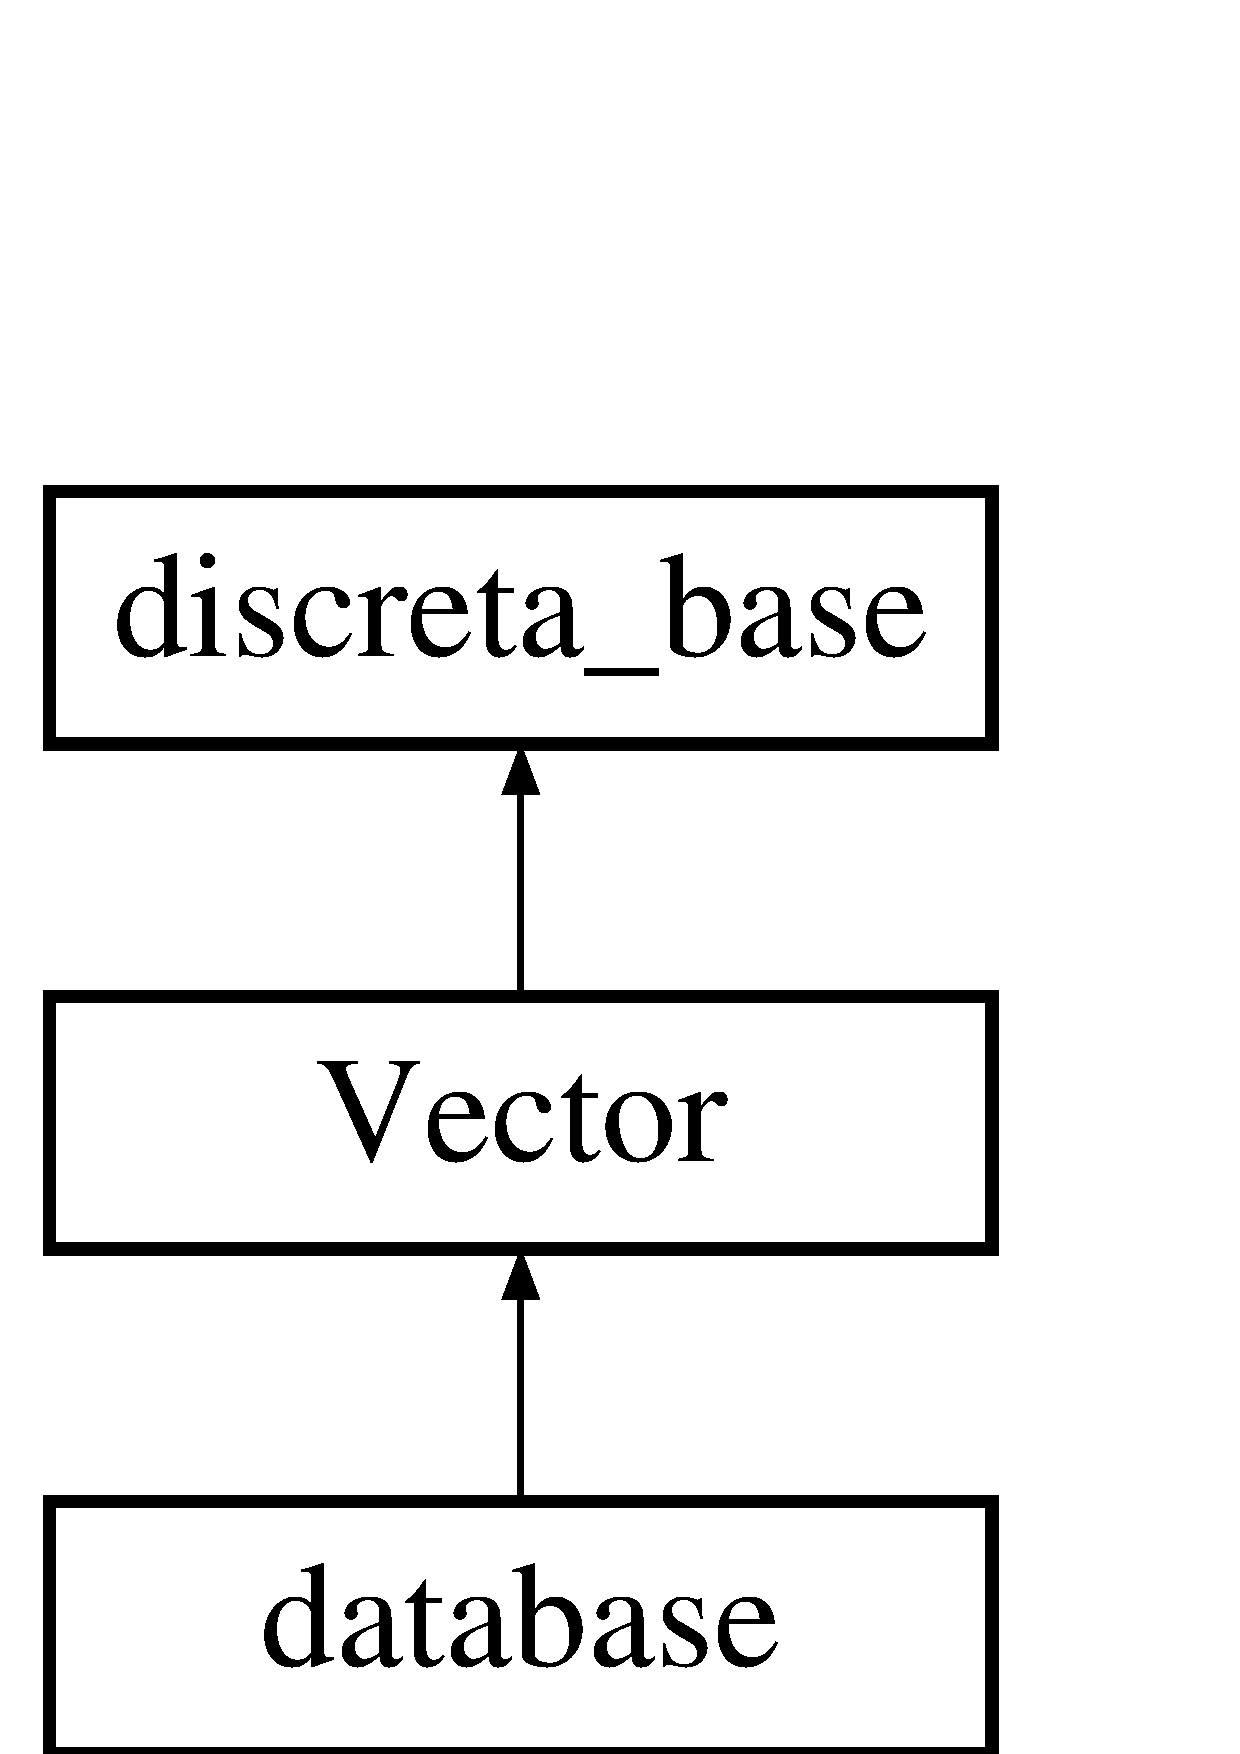
\includegraphics[height=3.000000cm]{classdatabase}
\end{center}
\end{figure}
\subsection*{Public Member Functions}
\begin{DoxyCompactItemize}
\item 
\mbox{\hyperlink{classdatabase_a35ec480ed529a9d092a7ebc5472b767f}{database}} ()
\item 
\mbox{\hyperlink{classdatabase_af9fba38cbd879c1a3c0388c111c774ef}{database}} (const \mbox{\hyperlink{classdiscreta__base}{discreta\+\_\+base}} \&\mbox{\hyperlink{alphabet2_8_c_a6150e0515f7202e2fb518f7206ed97dc}{x}})
\item 
\mbox{\hyperlink{classdatabase}{database}} \& \mbox{\hyperlink{classdatabase_a47f3f73586a1384925a89bcdaf14897a}{operator=}} (const \mbox{\hyperlink{classdiscreta__base}{discreta\+\_\+base}} \&\mbox{\hyperlink{alphabet2_8_c_a6150e0515f7202e2fb518f7206ed97dc}{x}})
\item 
void $\ast$ \mbox{\hyperlink{classdatabase_a26b458d54ee0723351ff1a8aeb3b3d53}{operator new}} (size\+\_\+t, void $\ast$\mbox{\hyperlink{alphabet2_8_c_a533391314665d6bf1b5575e9a9cd8552}{p}})
\item 
void \mbox{\hyperlink{classdatabase_a014639aa001462e480eb1f3984839b72}{settype\+\_\+database}} ()
\item 
\mbox{\hyperlink{discreta_8h_aaf25ee7e2306d78c74ec7bc48f092e81}{kind}} \mbox{\hyperlink{classdatabase_a30a79d9d1ae22f160368de28625ddeba}{s\+\_\+virtual\+\_\+kind}} ()
\item 
\mbox{\hyperlink{classdatabase_a31008de680565a626cd975c25d4351db}{$\sim$database}} ()
\item 
void \mbox{\hyperlink{classdatabase_a4dc263211f9b364e4fa733c8cf53e066}{freeself\+\_\+database}} ()
\item 
void \mbox{\hyperlink{classdatabase_a7402d11485a917293586dcf082f506b2}{copyobject\+\_\+to}} (\mbox{\hyperlink{classdiscreta__base}{discreta\+\_\+base}} \&\mbox{\hyperlink{alphabet2_8_c_a6150e0515f7202e2fb518f7206ed97dc}{x}})
\item 
ostream \& \mbox{\hyperlink{classdatabase_a55930857986406ef0650509001c7af76}{print}} (ostream \&)
\item 
\mbox{\hyperlink{class_vector}{Vector}} \& \mbox{\hyperlink{classdatabase_a30109ba5488b06111439f887fc1ac499}{btree\+\_\+access}} ()
\item 
\mbox{\hyperlink{classbtree}{btree}} \& \mbox{\hyperlink{classdatabase_a215047d1b32b8bd54f91a7bdca168eee}{btree\+\_\+access\+\_\+i}} (\mbox{\hyperlink{galois_8h_a09fddde158a3a20bd2dcadb609de11dc}{I\+NT}} \mbox{\hyperlink{alphabet2_8_c_acb559820d9ca11295b4500f179ef6392}{i}})
\item 
\mbox{\hyperlink{classhollerith}{hollerith}} \& \mbox{\hyperlink{classdatabase_a0d239d767658aca51abbea00148b8b2f}{filename}} ()
\item 
\mbox{\hyperlink{galois_8h_a09fddde158a3a20bd2dcadb609de11dc}{I\+NT}} \& \mbox{\hyperlink{classdatabase_aa28ebaac42b9a71e1bc213781012d1c8}{f\+\_\+compress}} ()
\item 
\mbox{\hyperlink{galois_8h_a09fddde158a3a20bd2dcadb609de11dc}{I\+NT}} \& \mbox{\hyperlink{classdatabase_a5b9b82f6cd851fb8826ed68085233c2d}{objectkind}} ()
\item 
\mbox{\hyperlink{galois_8h_a09fddde158a3a20bd2dcadb609de11dc}{I\+NT}} \& \mbox{\hyperlink{classdatabase_a2cac52c70b09d1a6771bddab2220b3e7}{f\+\_\+open}} ()
\item 
\mbox{\hyperlink{galois_8h_a09fddde158a3a20bd2dcadb609de11dc}{I\+NT}} \& \mbox{\hyperlink{classdatabase_a8b91f87e7cd92b8207cbc48edde9d69e}{stream}} ()
\item 
\mbox{\hyperlink{galois_8h_a09fddde158a3a20bd2dcadb609de11dc}{I\+NT}} \& \mbox{\hyperlink{classdatabase_a8547ac1fa93cdcd8ec464cac1ec24c5d}{file\+\_\+size}} ()
\item 
\mbox{\hyperlink{galois_8h_a09fddde158a3a20bd2dcadb609de11dc}{I\+NT}} \& \mbox{\hyperlink{classdatabase_a9dce80d625548b03b8317641b674cd9b}{file\+\_\+type}} ()
\item 
void \mbox{\hyperlink{classdatabase_abae7da96fe55d9f7ca44473b06a1e113}{init}} (const \mbox{\hyperlink{galois_8h_ab6cc7b4aeb6ea31aba2b3fbfc83ff5e6}{B\+Y\+TE}} $\ast$\mbox{\hyperlink{classdatabase_a0d239d767658aca51abbea00148b8b2f}{filename}}, \mbox{\hyperlink{galois_8h_a09fddde158a3a20bd2dcadb609de11dc}{I\+NT}} \mbox{\hyperlink{classdatabase_a5b9b82f6cd851fb8826ed68085233c2d}{objectkind}}, \mbox{\hyperlink{galois_8h_a09fddde158a3a20bd2dcadb609de11dc}{I\+NT}} \mbox{\hyperlink{classdatabase_aa28ebaac42b9a71e1bc213781012d1c8}{f\+\_\+compress}})
\item 
void \mbox{\hyperlink{classdatabase_a3b7a27f69a64812a6bfd765158d62476}{init\+\_\+with\+\_\+file\+\_\+type}} (const \mbox{\hyperlink{galois_8h_ab6cc7b4aeb6ea31aba2b3fbfc83ff5e6}{B\+Y\+TE}} $\ast$\mbox{\hyperlink{classdatabase_a0d239d767658aca51abbea00148b8b2f}{filename}}, \mbox{\hyperlink{galois_8h_a09fddde158a3a20bd2dcadb609de11dc}{I\+NT}} \mbox{\hyperlink{classdatabase_a5b9b82f6cd851fb8826ed68085233c2d}{objectkind}}, \mbox{\hyperlink{galois_8h_a09fddde158a3a20bd2dcadb609de11dc}{I\+NT}} \mbox{\hyperlink{classdatabase_aa28ebaac42b9a71e1bc213781012d1c8}{f\+\_\+compress}}, \mbox{\hyperlink{galois_8h_a09fddde158a3a20bd2dcadb609de11dc}{I\+NT}} \mbox{\hyperlink{classdatabase_a9dce80d625548b03b8317641b674cd9b}{file\+\_\+type}})
\item 
void \mbox{\hyperlink{classdatabase_a41d486156468426370c803bea3976cf1}{create}} (\mbox{\hyperlink{galois_8h_a09fddde158a3a20bd2dcadb609de11dc}{I\+NT}} \mbox{\hyperlink{simeon_8_c_a818073fbcc2f439e7c56952f67386122}{verbose\+\_\+level}})
\item 
void \mbox{\hyperlink{classdatabase_a65e8eccf98ecab4d55fb25bacaae6a19}{open}} (\mbox{\hyperlink{galois_8h_a09fddde158a3a20bd2dcadb609de11dc}{I\+NT}} \mbox{\hyperlink{simeon_8_c_a818073fbcc2f439e7c56952f67386122}{verbose\+\_\+level}})
\item 
void \mbox{\hyperlink{classdatabase_acdc74d15f711cab1c165989723d45caf}{close}} (\mbox{\hyperlink{galois_8h_a09fddde158a3a20bd2dcadb609de11dc}{I\+NT}} \mbox{\hyperlink{simeon_8_c_a818073fbcc2f439e7c56952f67386122}{verbose\+\_\+level}})
\item 
void \mbox{\hyperlink{classdatabase_a3cdd5549da793e4b4f44e175eabe050e}{delete\+\_\+files}} ()
\item 
void \mbox{\hyperlink{classdatabase_a3490df2b9feac3d2cfab8a5d00033ab4}{put\+\_\+file\+\_\+size}} ()
\item 
void \mbox{\hyperlink{classdatabase_a3f59b9585dfaa4c0f45c00388a128aaf}{get\+\_\+file\+\_\+size}} ()
\item 
void \mbox{\hyperlink{classdatabase_ae87e9d8c044500276c16176b46fbf906}{user2total}} (\mbox{\hyperlink{galois_8h_a09fddde158a3a20bd2dcadb609de11dc}{I\+NT}} user, \mbox{\hyperlink{galois_8h_a09fddde158a3a20bd2dcadb609de11dc}{I\+NT}} $\ast$total, \mbox{\hyperlink{galois_8h_a09fddde158a3a20bd2dcadb609de11dc}{I\+NT}} $\ast$pad)
\item 
\mbox{\hyperlink{galois_8h_a09fddde158a3a20bd2dcadb609de11dc}{I\+NT}} \mbox{\hyperlink{classdatabase_a06a4fb255387e8bac32d98d365a90019}{size\+\_\+of\+\_\+header}} ()
\item 
\mbox{\hyperlink{galois_8h_a09fddde158a3a20bd2dcadb609de11dc}{I\+NT}} \mbox{\hyperlink{classdatabase_a2ed2d1231bc36e5267f6a8bac422738d}{size\+\_\+of\+\_\+header\+\_\+log}} ()
\item 
void \mbox{\hyperlink{classdatabase_a6b0c2e6ebb9938c57ce826647ed1ad40}{add\+\_\+object\+\_\+return\+\_\+datref}} (\mbox{\hyperlink{class_vector}{Vector}} \&the\+\_\+object, \mbox{\hyperlink{galois_8h_ac94af6544c710549c9fca744fd510395}{U\+I\+N\+T4}} \&datref, \mbox{\hyperlink{galois_8h_a09fddde158a3a20bd2dcadb609de11dc}{I\+NT}} \mbox{\hyperlink{simeon_8_c_a818073fbcc2f439e7c56952f67386122}{verbose\+\_\+level}})
\item 
void \mbox{\hyperlink{classdatabase_a880f60c1d94fff84d0db2b119361fbb6}{add\+\_\+object}} (\mbox{\hyperlink{class_vector}{Vector}} \&the\+\_\+object, \mbox{\hyperlink{galois_8h_a09fddde158a3a20bd2dcadb609de11dc}{I\+NT}} \mbox{\hyperlink{simeon_8_c_a818073fbcc2f439e7c56952f67386122}{verbose\+\_\+level}})
\item 
void \mbox{\hyperlink{classdatabase_a69f061ffa820d1926718dafad5f5513c}{delete\+\_\+object}} (\mbox{\hyperlink{class_vector}{Vector}} \&the\+\_\+object, \mbox{\hyperlink{galois_8h_ac94af6544c710549c9fca744fd510395}{U\+I\+N\+T4}} datref, \mbox{\hyperlink{galois_8h_a09fddde158a3a20bd2dcadb609de11dc}{I\+NT}} \mbox{\hyperlink{simeon_8_c_a818073fbcc2f439e7c56952f67386122}{verbose\+\_\+level}})
\item 
void \mbox{\hyperlink{classdatabase_a2f58ec1301addabc2fb6544038e108c6}{get\+\_\+object}} (\mbox{\hyperlink{galois_8h_ac94af6544c710549c9fca744fd510395}{U\+I\+N\+T4}} datref, \mbox{\hyperlink{class_vector}{Vector}} \&the\+\_\+object, \mbox{\hyperlink{galois_8h_a09fddde158a3a20bd2dcadb609de11dc}{I\+NT}} \mbox{\hyperlink{simeon_8_c_a818073fbcc2f439e7c56952f67386122}{verbose\+\_\+level}})
\item 
void \mbox{\hyperlink{classdatabase_af183761e73fedbd560d9545a36060efc}{get\+\_\+object}} (\mbox{\hyperlink{discreta_8h_abf512b6b30146dda9c59049478bf3e99}{D\+A\+T\+A\+T\+Y\+PE}} $\ast$data\+\_\+type, \mbox{\hyperlink{class_vector}{Vector}} \&the\+\_\+object, \mbox{\hyperlink{galois_8h_a09fddde158a3a20bd2dcadb609de11dc}{I\+NT}} \mbox{\hyperlink{simeon_8_c_a818073fbcc2f439e7c56952f67386122}{verbose\+\_\+level}})
\item 
void \mbox{\hyperlink{classdatabase_ab93d6176bca88b2eb9356566a25ef6be}{get\+\_\+object\+\_\+by\+\_\+unique\+\_\+\+I\+N\+T4}} (\mbox{\hyperlink{galois_8h_a09fddde158a3a20bd2dcadb609de11dc}{I\+NT}} btree\+\_\+idx, \mbox{\hyperlink{galois_8h_a09fddde158a3a20bd2dcadb609de11dc}{I\+NT}} id, \mbox{\hyperlink{class_vector}{Vector}} \&the\+\_\+object, \mbox{\hyperlink{galois_8h_a09fddde158a3a20bd2dcadb609de11dc}{I\+NT}} \mbox{\hyperlink{simeon_8_c_a818073fbcc2f439e7c56952f67386122}{verbose\+\_\+level}})
\item 
\mbox{\hyperlink{galois_8h_a09fddde158a3a20bd2dcadb609de11dc}{I\+NT}} \mbox{\hyperlink{classdatabase_a0d275df405adfb8ccfb78423cd722f4b}{get\+\_\+object\+\_\+by\+\_\+unique\+\_\+\+I\+N\+T4\+\_\+if\+\_\+there}} (\mbox{\hyperlink{galois_8h_a09fddde158a3a20bd2dcadb609de11dc}{I\+NT}} btree\+\_\+idx, \mbox{\hyperlink{galois_8h_a09fddde158a3a20bd2dcadb609de11dc}{I\+NT}} id, \mbox{\hyperlink{class_vector}{Vector}} \&the\+\_\+object, \mbox{\hyperlink{galois_8h_a09fddde158a3a20bd2dcadb609de11dc}{I\+NT}} \mbox{\hyperlink{simeon_8_c_a818073fbcc2f439e7c56952f67386122}{verbose\+\_\+level}})
\item 
\mbox{\hyperlink{galois_8h_a09fddde158a3a20bd2dcadb609de11dc}{I\+NT}} \mbox{\hyperlink{classdatabase_ad4d0dbaf8f34ee6aa357f46b5454986d}{get\+\_\+highest\+\_\+\+I\+N\+T4}} (\mbox{\hyperlink{galois_8h_a09fddde158a3a20bd2dcadb609de11dc}{I\+NT}} btree\+\_\+idx)
\item 
void \mbox{\hyperlink{classdatabase_a1516bb38a4c846172354291271700d07}{ith\+\_\+object}} (\mbox{\hyperlink{galois_8h_a09fddde158a3a20bd2dcadb609de11dc}{I\+NT}} \mbox{\hyperlink{alphabet2_8_c_acb559820d9ca11295b4500f179ef6392}{i}}, \mbox{\hyperlink{galois_8h_a09fddde158a3a20bd2dcadb609de11dc}{I\+NT}} btree\+\_\+idx, \mbox{\hyperlink{class_vector}{Vector}} \&the\+\_\+object, \mbox{\hyperlink{galois_8h_a09fddde158a3a20bd2dcadb609de11dc}{I\+NT}} \mbox{\hyperlink{simeon_8_c_a818073fbcc2f439e7c56952f67386122}{verbose\+\_\+level}})
\item 
void \mbox{\hyperlink{classdatabase_af17af33b686cba55558237b04714108f}{ith}} (\mbox{\hyperlink{galois_8h_a09fddde158a3a20bd2dcadb609de11dc}{I\+NT}} \mbox{\hyperlink{alphabet2_8_c_acb559820d9ca11295b4500f179ef6392}{i}}, \mbox{\hyperlink{galois_8h_a09fddde158a3a20bd2dcadb609de11dc}{I\+NT}} btree\+\_\+idx, \mbox{\hyperlink{discreta_8h_a535c8df88e5939fd8a1a3d083e75124a}{K\+E\+Y\+T\+Y\+PE}} $\ast$key\+\_\+type, \mbox{\hyperlink{discreta_8h_abf512b6b30146dda9c59049478bf3e99}{D\+A\+T\+A\+T\+Y\+PE}} $\ast$data\+\_\+type, \mbox{\hyperlink{galois_8h_a09fddde158a3a20bd2dcadb609de11dc}{I\+NT}} \mbox{\hyperlink{simeon_8_c_a818073fbcc2f439e7c56952f67386122}{verbose\+\_\+level}})
\item 
void \mbox{\hyperlink{classdatabase_ac45ae44f2a861557ced6e5ab7c146717}{print\+\_\+by\+\_\+btree}} (\mbox{\hyperlink{galois_8h_a09fddde158a3a20bd2dcadb609de11dc}{I\+NT}} btree\+\_\+idx, ostream \&ost)
\item 
void \mbox{\hyperlink{classdatabase_af84030a29b31944d6763974ac4f774b5}{print\+\_\+by\+\_\+btree\+\_\+with\+\_\+datref}} (\mbox{\hyperlink{galois_8h_a09fddde158a3a20bd2dcadb609de11dc}{I\+NT}} btree\+\_\+idx, ostream \&ost)
\item 
void \mbox{\hyperlink{classdatabase_a8b454f5428b3f00a2de497f21d73f3fa}{print\+\_\+subset}} (\mbox{\hyperlink{class_vector}{Vector}} \&datrefs, ostream \&ost)
\item 
void \mbox{\hyperlink{classdatabase_abeb9113b3b9f544afe25bd16fd69662d}{extract\+\_\+subset}} (\mbox{\hyperlink{class_vector}{Vector}} \&datrefs, \mbox{\hyperlink{galois_8h_ab6cc7b4aeb6ea31aba2b3fbfc83ff5e6}{B\+Y\+TE}} $\ast$out\+\_\+path, \mbox{\hyperlink{galois_8h_a09fddde158a3a20bd2dcadb609de11dc}{I\+NT}} \mbox{\hyperlink{simeon_8_c_a818073fbcc2f439e7c56952f67386122}{verbose\+\_\+level}})
\item 
void \mbox{\hyperlink{classdatabase_aeda62e67888923cd968674ec2ed08007}{search\+\_\+\+I\+N\+T4}} (\mbox{\hyperlink{galois_8h_a09fddde158a3a20bd2dcadb609de11dc}{I\+NT}} btree\+\_\+idx, \mbox{\hyperlink{galois_8h_a09fddde158a3a20bd2dcadb609de11dc}{I\+NT}} imin, \mbox{\hyperlink{galois_8h_a09fddde158a3a20bd2dcadb609de11dc}{I\+NT}} imax, \mbox{\hyperlink{class_vector}{Vector}} \&datrefs, \mbox{\hyperlink{galois_8h_a09fddde158a3a20bd2dcadb609de11dc}{I\+NT}} \mbox{\hyperlink{simeon_8_c_a818073fbcc2f439e7c56952f67386122}{verbose\+\_\+level}})
\item 
void \mbox{\hyperlink{classdatabase_a10e70413e55aca54a2fe1b02066e3947}{search\+\_\+\+I\+N\+T4\+\_\+2dimensional}} (\mbox{\hyperlink{galois_8h_a09fddde158a3a20bd2dcadb609de11dc}{I\+NT}} btree\+\_\+idx0, \mbox{\hyperlink{galois_8h_a09fddde158a3a20bd2dcadb609de11dc}{I\+NT}} imin0, \mbox{\hyperlink{galois_8h_a09fddde158a3a20bd2dcadb609de11dc}{I\+NT}} imax0, \mbox{\hyperlink{galois_8h_a09fddde158a3a20bd2dcadb609de11dc}{I\+NT}} btree\+\_\+idx1, \mbox{\hyperlink{galois_8h_a09fddde158a3a20bd2dcadb609de11dc}{I\+NT}} imin1, \mbox{\hyperlink{galois_8h_a09fddde158a3a20bd2dcadb609de11dc}{I\+NT}} imax1, \mbox{\hyperlink{class_vector}{Vector}} \&datrefs, \mbox{\hyperlink{galois_8h_a09fddde158a3a20bd2dcadb609de11dc}{I\+NT}} \mbox{\hyperlink{simeon_8_c_a818073fbcc2f439e7c56952f67386122}{verbose\+\_\+level}})
\item 
void \mbox{\hyperlink{classdatabase_a43a31b0e56d1401185a452a6686666aa}{search\+\_\+\+I\+N\+T4\+\_\+multi\+\_\+dimensional}} (\mbox{\hyperlink{class_vector}{Vector}} \&btree\+\_\+idx, \mbox{\hyperlink{class_vector}{Vector}} \&i\+\_\+min, \mbox{\hyperlink{class_vector}{Vector}} \&i\+\_\+max, \mbox{\hyperlink{class_vector}{Vector}} \&datrefs, \mbox{\hyperlink{galois_8h_a09fddde158a3a20bd2dcadb609de11dc}{I\+NT}} \mbox{\hyperlink{simeon_8_c_a818073fbcc2f439e7c56952f67386122}{verbose\+\_\+level}})
\item 
\mbox{\hyperlink{galois_8h_a09fddde158a3a20bd2dcadb609de11dc}{I\+NT}} \mbox{\hyperlink{classdatabase_ae71e4c19b07a2d67682fbd4b069e9a7e}{get\+\_\+size\+\_\+from\+\_\+datref}} (\mbox{\hyperlink{galois_8h_ac94af6544c710549c9fca744fd510395}{U\+I\+N\+T4}} datref, \mbox{\hyperlink{galois_8h_a09fddde158a3a20bd2dcadb609de11dc}{I\+NT}} \mbox{\hyperlink{simeon_8_c_a818073fbcc2f439e7c56952f67386122}{verbose\+\_\+level}})
\item 
void \mbox{\hyperlink{classdatabase_ab1a4122dfc06c6e79343fda437c05ed5}{add\+\_\+data\+\_\+\+DB}} (void $\ast$\mbox{\hyperlink{simeon_8_c_a4339ca06fa882e69473d37bd6d7917d1}{d}}, \mbox{\hyperlink{galois_8h_a09fddde158a3a20bd2dcadb609de11dc}{I\+NT}} size, \mbox{\hyperlink{galois_8h_ac94af6544c710549c9fca744fd510395}{U\+I\+N\+T4}} $\ast$datref, \mbox{\hyperlink{galois_8h_a09fddde158a3a20bd2dcadb609de11dc}{I\+NT}} \mbox{\hyperlink{simeon_8_c_a818073fbcc2f439e7c56952f67386122}{verbose\+\_\+level}})
\item 
void \mbox{\hyperlink{classdatabase_a0f0ab218eb0f06da37f06906663db6eb}{add\+\_\+data\+\_\+\+D\+B\+\_\+standard}} (void $\ast$\mbox{\hyperlink{simeon_8_c_a4339ca06fa882e69473d37bd6d7917d1}{d}}, \mbox{\hyperlink{galois_8h_a09fddde158a3a20bd2dcadb609de11dc}{I\+NT}} size, \mbox{\hyperlink{galois_8h_ac94af6544c710549c9fca744fd510395}{U\+I\+N\+T4}} $\ast$datref, \mbox{\hyperlink{galois_8h_a09fddde158a3a20bd2dcadb609de11dc}{I\+NT}} \mbox{\hyperlink{simeon_8_c_a818073fbcc2f439e7c56952f67386122}{verbose\+\_\+level}})
\item 
void \mbox{\hyperlink{classdatabase_a31e32de1b8d81c97549b8c74ea678904}{add\+\_\+data\+\_\+\+D\+B\+\_\+compact}} (void $\ast$\mbox{\hyperlink{simeon_8_c_a4339ca06fa882e69473d37bd6d7917d1}{d}}, \mbox{\hyperlink{galois_8h_a09fddde158a3a20bd2dcadb609de11dc}{I\+NT}} size, \mbox{\hyperlink{galois_8h_ac94af6544c710549c9fca744fd510395}{U\+I\+N\+T4}} $\ast$datref, \mbox{\hyperlink{galois_8h_a09fddde158a3a20bd2dcadb609de11dc}{I\+NT}} \mbox{\hyperlink{simeon_8_c_a818073fbcc2f439e7c56952f67386122}{verbose\+\_\+level}})
\item 
void \mbox{\hyperlink{classdatabase_a45b6fb10b6810c9770748e7f9dda8377}{free\+\_\+data\+\_\+\+DB}} (\mbox{\hyperlink{galois_8h_ac94af6544c710549c9fca744fd510395}{U\+I\+N\+T4}} datref, \mbox{\hyperlink{galois_8h_a09fddde158a3a20bd2dcadb609de11dc}{I\+NT}} size, \mbox{\hyperlink{galois_8h_a09fddde158a3a20bd2dcadb609de11dc}{I\+NT}} \mbox{\hyperlink{simeon_8_c_a818073fbcc2f439e7c56952f67386122}{verbose\+\_\+level}})
\item 
void \mbox{\hyperlink{classdatabase_a33494febd887d058f862ef6001d4a044}{file\+\_\+open}} (\mbox{\hyperlink{galois_8h_a09fddde158a3a20bd2dcadb609de11dc}{I\+NT}} \mbox{\hyperlink{simeon_8_c_a818073fbcc2f439e7c56952f67386122}{verbose\+\_\+level}})
\item 
void \mbox{\hyperlink{classdatabase_afffc9413d00af2e69d9852773a2eb344}{file\+\_\+create}} (\mbox{\hyperlink{galois_8h_a09fddde158a3a20bd2dcadb609de11dc}{I\+NT}} \mbox{\hyperlink{simeon_8_c_a818073fbcc2f439e7c56952f67386122}{verbose\+\_\+level}})
\item 
void \mbox{\hyperlink{classdatabase_a2c40bcffaf69fb166b6ac1bafee50baf}{file\+\_\+close}} (\mbox{\hyperlink{galois_8h_a09fddde158a3a20bd2dcadb609de11dc}{I\+NT}} \mbox{\hyperlink{simeon_8_c_a818073fbcc2f439e7c56952f67386122}{verbose\+\_\+level}})
\item 
void \mbox{\hyperlink{classdatabase_a67ff377651f4ac089241ebff60e17ed6}{file\+\_\+seek}} (\mbox{\hyperlink{galois_8h_a09fddde158a3a20bd2dcadb609de11dc}{I\+NT}} offset)
\item 
void \mbox{\hyperlink{classdatabase_a42d32ba51ad8ccd2a0adfd1a147f6230}{file\+\_\+write}} (void $\ast$\mbox{\hyperlink{alphabet2_8_c_a533391314665d6bf1b5575e9a9cd8552}{p}}, \mbox{\hyperlink{galois_8h_a09fddde158a3a20bd2dcadb609de11dc}{I\+NT}} size, \mbox{\hyperlink{galois_8h_a09fddde158a3a20bd2dcadb609de11dc}{I\+NT}} nb)
\item 
void \mbox{\hyperlink{classdatabase_ac743549af82d694be57c5a120987ed37}{file\+\_\+read}} (void $\ast$\mbox{\hyperlink{alphabet2_8_c_a533391314665d6bf1b5575e9a9cd8552}{p}}, \mbox{\hyperlink{galois_8h_a09fddde158a3a20bd2dcadb609de11dc}{I\+NT}} size, \mbox{\hyperlink{galois_8h_a09fddde158a3a20bd2dcadb609de11dc}{I\+NT}} nb)
\end{DoxyCompactItemize}
\subsection*{Additional Inherited Members}


\subsection{Constructor \& Destructor Documentation}
\mbox{\Hypertarget{classdatabase_a35ec480ed529a9d092a7ebc5472b767f}\label{classdatabase_a35ec480ed529a9d092a7ebc5472b767f}} 
\index{database@{database}!database@{database}}
\index{database@{database}!database@{database}}
\subsubsection{\texorpdfstring{database()}{database()}\hspace{0.1cm}{\footnotesize\ttfamily [1/2]}}
{\footnotesize\ttfamily database\+::database (\begin{DoxyParamCaption}{ }\end{DoxyParamCaption})}

\mbox{\Hypertarget{classdatabase_af9fba38cbd879c1a3c0388c111c774ef}\label{classdatabase_af9fba38cbd879c1a3c0388c111c774ef}} 
\index{database@{database}!database@{database}}
\index{database@{database}!database@{database}}
\subsubsection{\texorpdfstring{database()}{database()}\hspace{0.1cm}{\footnotesize\ttfamily [2/2]}}
{\footnotesize\ttfamily database\+::database (\begin{DoxyParamCaption}\item[{const \mbox{\hyperlink{classdiscreta__base}{discreta\+\_\+base}} \&}]{x }\end{DoxyParamCaption})}

\mbox{\Hypertarget{classdatabase_a31008de680565a626cd975c25d4351db}\label{classdatabase_a31008de680565a626cd975c25d4351db}} 
\index{database@{database}!````~database@{$\sim$database}}
\index{````~database@{$\sim$database}!database@{database}}
\subsubsection{\texorpdfstring{$\sim$database()}{~database()}}
{\footnotesize\ttfamily database\+::$\sim$database (\begin{DoxyParamCaption}{ }\end{DoxyParamCaption})}



\subsection{Member Function Documentation}
\mbox{\Hypertarget{classdatabase_ab1a4122dfc06c6e79343fda437c05ed5}\label{classdatabase_ab1a4122dfc06c6e79343fda437c05ed5}} 
\index{database@{database}!add\+\_\+data\+\_\+\+DB@{add\+\_\+data\+\_\+\+DB}}
\index{add\+\_\+data\+\_\+\+DB@{add\+\_\+data\+\_\+\+DB}!database@{database}}
\subsubsection{\texorpdfstring{add\+\_\+data\+\_\+\+D\+B()}{add\_data\_DB()}}
{\footnotesize\ttfamily void database\+::add\+\_\+data\+\_\+\+DB (\begin{DoxyParamCaption}\item[{void $\ast$}]{d,  }\item[{\mbox{\hyperlink{galois_8h_a09fddde158a3a20bd2dcadb609de11dc}{I\+NT}}}]{size,  }\item[{\mbox{\hyperlink{galois_8h_ac94af6544c710549c9fca744fd510395}{U\+I\+N\+T4}} $\ast$}]{datref,  }\item[{\mbox{\hyperlink{galois_8h_a09fddde158a3a20bd2dcadb609de11dc}{I\+NT}}}]{verbose\+\_\+level }\end{DoxyParamCaption})}

\mbox{\Hypertarget{classdatabase_a31e32de1b8d81c97549b8c74ea678904}\label{classdatabase_a31e32de1b8d81c97549b8c74ea678904}} 
\index{database@{database}!add\+\_\+data\+\_\+\+D\+B\+\_\+compact@{add\+\_\+data\+\_\+\+D\+B\+\_\+compact}}
\index{add\+\_\+data\+\_\+\+D\+B\+\_\+compact@{add\+\_\+data\+\_\+\+D\+B\+\_\+compact}!database@{database}}
\subsubsection{\texorpdfstring{add\+\_\+data\+\_\+\+D\+B\+\_\+compact()}{add\_data\_DB\_compact()}}
{\footnotesize\ttfamily void database\+::add\+\_\+data\+\_\+\+D\+B\+\_\+compact (\begin{DoxyParamCaption}\item[{void $\ast$}]{d,  }\item[{\mbox{\hyperlink{galois_8h_a09fddde158a3a20bd2dcadb609de11dc}{I\+NT}}}]{size,  }\item[{\mbox{\hyperlink{galois_8h_ac94af6544c710549c9fca744fd510395}{U\+I\+N\+T4}} $\ast$}]{datref,  }\item[{\mbox{\hyperlink{galois_8h_a09fddde158a3a20bd2dcadb609de11dc}{I\+NT}}}]{verbose\+\_\+level }\end{DoxyParamCaption})}

\mbox{\Hypertarget{classdatabase_a0f0ab218eb0f06da37f06906663db6eb}\label{classdatabase_a0f0ab218eb0f06da37f06906663db6eb}} 
\index{database@{database}!add\+\_\+data\+\_\+\+D\+B\+\_\+standard@{add\+\_\+data\+\_\+\+D\+B\+\_\+standard}}
\index{add\+\_\+data\+\_\+\+D\+B\+\_\+standard@{add\+\_\+data\+\_\+\+D\+B\+\_\+standard}!database@{database}}
\subsubsection{\texorpdfstring{add\+\_\+data\+\_\+\+D\+B\+\_\+standard()}{add\_data\_DB\_standard()}}
{\footnotesize\ttfamily void database\+::add\+\_\+data\+\_\+\+D\+B\+\_\+standard (\begin{DoxyParamCaption}\item[{void $\ast$}]{d,  }\item[{\mbox{\hyperlink{galois_8h_a09fddde158a3a20bd2dcadb609de11dc}{I\+NT}}}]{size,  }\item[{\mbox{\hyperlink{galois_8h_ac94af6544c710549c9fca744fd510395}{U\+I\+N\+T4}} $\ast$}]{datref,  }\item[{\mbox{\hyperlink{galois_8h_a09fddde158a3a20bd2dcadb609de11dc}{I\+NT}}}]{verbose\+\_\+level }\end{DoxyParamCaption})}

\mbox{\Hypertarget{classdatabase_a880f60c1d94fff84d0db2b119361fbb6}\label{classdatabase_a880f60c1d94fff84d0db2b119361fbb6}} 
\index{database@{database}!add\+\_\+object@{add\+\_\+object}}
\index{add\+\_\+object@{add\+\_\+object}!database@{database}}
\subsubsection{\texorpdfstring{add\+\_\+object()}{add\_object()}}
{\footnotesize\ttfamily void database\+::add\+\_\+object (\begin{DoxyParamCaption}\item[{\mbox{\hyperlink{class_vector}{Vector}} \&}]{the\+\_\+object,  }\item[{\mbox{\hyperlink{galois_8h_a09fddde158a3a20bd2dcadb609de11dc}{I\+NT}}}]{verbose\+\_\+level }\end{DoxyParamCaption})}

\mbox{\Hypertarget{classdatabase_a6b0c2e6ebb9938c57ce826647ed1ad40}\label{classdatabase_a6b0c2e6ebb9938c57ce826647ed1ad40}} 
\index{database@{database}!add\+\_\+object\+\_\+return\+\_\+datref@{add\+\_\+object\+\_\+return\+\_\+datref}}
\index{add\+\_\+object\+\_\+return\+\_\+datref@{add\+\_\+object\+\_\+return\+\_\+datref}!database@{database}}
\subsubsection{\texorpdfstring{add\+\_\+object\+\_\+return\+\_\+datref()}{add\_object\_return\_datref()}}
{\footnotesize\ttfamily void database\+::add\+\_\+object\+\_\+return\+\_\+datref (\begin{DoxyParamCaption}\item[{\mbox{\hyperlink{class_vector}{Vector}} \&}]{the\+\_\+object,  }\item[{\mbox{\hyperlink{galois_8h_ac94af6544c710549c9fca744fd510395}{U\+I\+N\+T4}} \&}]{datref,  }\item[{\mbox{\hyperlink{galois_8h_a09fddde158a3a20bd2dcadb609de11dc}{I\+NT}}}]{verbose\+\_\+level }\end{DoxyParamCaption})}

\mbox{\Hypertarget{classdatabase_a30109ba5488b06111439f887fc1ac499}\label{classdatabase_a30109ba5488b06111439f887fc1ac499}} 
\index{database@{database}!btree\+\_\+access@{btree\+\_\+access}}
\index{btree\+\_\+access@{btree\+\_\+access}!database@{database}}
\subsubsection{\texorpdfstring{btree\+\_\+access()}{btree\_access()}}
{\footnotesize\ttfamily \mbox{\hyperlink{class_vector}{Vector}}\& database\+::btree\+\_\+access (\begin{DoxyParamCaption}{ }\end{DoxyParamCaption})\hspace{0.3cm}{\ttfamily [inline]}}

\mbox{\Hypertarget{classdatabase_a215047d1b32b8bd54f91a7bdca168eee}\label{classdatabase_a215047d1b32b8bd54f91a7bdca168eee}} 
\index{database@{database}!btree\+\_\+access\+\_\+i@{btree\+\_\+access\+\_\+i}}
\index{btree\+\_\+access\+\_\+i@{btree\+\_\+access\+\_\+i}!database@{database}}
\subsubsection{\texorpdfstring{btree\+\_\+access\+\_\+i()}{btree\_access\_i()}}
{\footnotesize\ttfamily \mbox{\hyperlink{classbtree}{btree}}\& database\+::btree\+\_\+access\+\_\+i (\begin{DoxyParamCaption}\item[{\mbox{\hyperlink{galois_8h_a09fddde158a3a20bd2dcadb609de11dc}{I\+NT}}}]{i }\end{DoxyParamCaption})\hspace{0.3cm}{\ttfamily [inline]}}

\mbox{\Hypertarget{classdatabase_acdc74d15f711cab1c165989723d45caf}\label{classdatabase_acdc74d15f711cab1c165989723d45caf}} 
\index{database@{database}!close@{close}}
\index{close@{close}!database@{database}}
\subsubsection{\texorpdfstring{close()}{close()}}
{\footnotesize\ttfamily void database\+::close (\begin{DoxyParamCaption}\item[{\mbox{\hyperlink{galois_8h_a09fddde158a3a20bd2dcadb609de11dc}{I\+NT}}}]{verbose\+\_\+level }\end{DoxyParamCaption})}

\mbox{\Hypertarget{classdatabase_a7402d11485a917293586dcf082f506b2}\label{classdatabase_a7402d11485a917293586dcf082f506b2}} 
\index{database@{database}!copyobject\+\_\+to@{copyobject\+\_\+to}}
\index{copyobject\+\_\+to@{copyobject\+\_\+to}!database@{database}}
\subsubsection{\texorpdfstring{copyobject\+\_\+to()}{copyobject\_to()}}
{\footnotesize\ttfamily void database\+::copyobject\+\_\+to (\begin{DoxyParamCaption}\item[{\mbox{\hyperlink{classdiscreta__base}{discreta\+\_\+base}} \&}]{x }\end{DoxyParamCaption})\hspace{0.3cm}{\ttfamily [virtual]}}



Reimplemented from \mbox{\hyperlink{class_vector_af657307f3d344c8cef5d633335a5f484}{Vector}}.

\mbox{\Hypertarget{classdatabase_a41d486156468426370c803bea3976cf1}\label{classdatabase_a41d486156468426370c803bea3976cf1}} 
\index{database@{database}!create@{create}}
\index{create@{create}!database@{database}}
\subsubsection{\texorpdfstring{create()}{create()}}
{\footnotesize\ttfamily void database\+::create (\begin{DoxyParamCaption}\item[{\mbox{\hyperlink{galois_8h_a09fddde158a3a20bd2dcadb609de11dc}{I\+NT}}}]{verbose\+\_\+level }\end{DoxyParamCaption})}

\mbox{\Hypertarget{classdatabase_a3cdd5549da793e4b4f44e175eabe050e}\label{classdatabase_a3cdd5549da793e4b4f44e175eabe050e}} 
\index{database@{database}!delete\+\_\+files@{delete\+\_\+files}}
\index{delete\+\_\+files@{delete\+\_\+files}!database@{database}}
\subsubsection{\texorpdfstring{delete\+\_\+files()}{delete\_files()}}
{\footnotesize\ttfamily void database\+::delete\+\_\+files (\begin{DoxyParamCaption}{ }\end{DoxyParamCaption})}

\mbox{\Hypertarget{classdatabase_a69f061ffa820d1926718dafad5f5513c}\label{classdatabase_a69f061ffa820d1926718dafad5f5513c}} 
\index{database@{database}!delete\+\_\+object@{delete\+\_\+object}}
\index{delete\+\_\+object@{delete\+\_\+object}!database@{database}}
\subsubsection{\texorpdfstring{delete\+\_\+object()}{delete\_object()}}
{\footnotesize\ttfamily void database\+::delete\+\_\+object (\begin{DoxyParamCaption}\item[{\mbox{\hyperlink{class_vector}{Vector}} \&}]{the\+\_\+object,  }\item[{\mbox{\hyperlink{galois_8h_ac94af6544c710549c9fca744fd510395}{U\+I\+N\+T4}}}]{datref,  }\item[{\mbox{\hyperlink{galois_8h_a09fddde158a3a20bd2dcadb609de11dc}{I\+NT}}}]{verbose\+\_\+level }\end{DoxyParamCaption})}

\mbox{\Hypertarget{classdatabase_abeb9113b3b9f544afe25bd16fd69662d}\label{classdatabase_abeb9113b3b9f544afe25bd16fd69662d}} 
\index{database@{database}!extract\+\_\+subset@{extract\+\_\+subset}}
\index{extract\+\_\+subset@{extract\+\_\+subset}!database@{database}}
\subsubsection{\texorpdfstring{extract\+\_\+subset()}{extract\_subset()}}
{\footnotesize\ttfamily void database\+::extract\+\_\+subset (\begin{DoxyParamCaption}\item[{\mbox{\hyperlink{class_vector}{Vector}} \&}]{datrefs,  }\item[{\mbox{\hyperlink{galois_8h_ab6cc7b4aeb6ea31aba2b3fbfc83ff5e6}{B\+Y\+TE}} $\ast$}]{out\+\_\+path,  }\item[{\mbox{\hyperlink{galois_8h_a09fddde158a3a20bd2dcadb609de11dc}{I\+NT}}}]{verbose\+\_\+level }\end{DoxyParamCaption})}

\mbox{\Hypertarget{classdatabase_aa28ebaac42b9a71e1bc213781012d1c8}\label{classdatabase_aa28ebaac42b9a71e1bc213781012d1c8}} 
\index{database@{database}!f\+\_\+compress@{f\+\_\+compress}}
\index{f\+\_\+compress@{f\+\_\+compress}!database@{database}}
\subsubsection{\texorpdfstring{f\+\_\+compress()}{f\_compress()}}
{\footnotesize\ttfamily \mbox{\hyperlink{galois_8h_a09fddde158a3a20bd2dcadb609de11dc}{I\+NT}}\& database\+::f\+\_\+compress (\begin{DoxyParamCaption}{ }\end{DoxyParamCaption})\hspace{0.3cm}{\ttfamily [inline]}}

\mbox{\Hypertarget{classdatabase_a2cac52c70b09d1a6771bddab2220b3e7}\label{classdatabase_a2cac52c70b09d1a6771bddab2220b3e7}} 
\index{database@{database}!f\+\_\+open@{f\+\_\+open}}
\index{f\+\_\+open@{f\+\_\+open}!database@{database}}
\subsubsection{\texorpdfstring{f\+\_\+open()}{f\_open()}}
{\footnotesize\ttfamily \mbox{\hyperlink{galois_8h_a09fddde158a3a20bd2dcadb609de11dc}{I\+NT}}\& database\+::f\+\_\+open (\begin{DoxyParamCaption}{ }\end{DoxyParamCaption})\hspace{0.3cm}{\ttfamily [inline]}}

\mbox{\Hypertarget{classdatabase_a2c40bcffaf69fb166b6ac1bafee50baf}\label{classdatabase_a2c40bcffaf69fb166b6ac1bafee50baf}} 
\index{database@{database}!file\+\_\+close@{file\+\_\+close}}
\index{file\+\_\+close@{file\+\_\+close}!database@{database}}
\subsubsection{\texorpdfstring{file\+\_\+close()}{file\_close()}}
{\footnotesize\ttfamily void database\+::file\+\_\+close (\begin{DoxyParamCaption}\item[{\mbox{\hyperlink{galois_8h_a09fddde158a3a20bd2dcadb609de11dc}{I\+NT}}}]{verbose\+\_\+level }\end{DoxyParamCaption})}

\mbox{\Hypertarget{classdatabase_afffc9413d00af2e69d9852773a2eb344}\label{classdatabase_afffc9413d00af2e69d9852773a2eb344}} 
\index{database@{database}!file\+\_\+create@{file\+\_\+create}}
\index{file\+\_\+create@{file\+\_\+create}!database@{database}}
\subsubsection{\texorpdfstring{file\+\_\+create()}{file\_create()}}
{\footnotesize\ttfamily void database\+::file\+\_\+create (\begin{DoxyParamCaption}\item[{\mbox{\hyperlink{galois_8h_a09fddde158a3a20bd2dcadb609de11dc}{I\+NT}}}]{verbose\+\_\+level }\end{DoxyParamCaption})}

\mbox{\Hypertarget{classdatabase_a33494febd887d058f862ef6001d4a044}\label{classdatabase_a33494febd887d058f862ef6001d4a044}} 
\index{database@{database}!file\+\_\+open@{file\+\_\+open}}
\index{file\+\_\+open@{file\+\_\+open}!database@{database}}
\subsubsection{\texorpdfstring{file\+\_\+open()}{file\_open()}}
{\footnotesize\ttfamily void database\+::file\+\_\+open (\begin{DoxyParamCaption}\item[{\mbox{\hyperlink{galois_8h_a09fddde158a3a20bd2dcadb609de11dc}{I\+NT}}}]{verbose\+\_\+level }\end{DoxyParamCaption})}

\mbox{\Hypertarget{classdatabase_ac743549af82d694be57c5a120987ed37}\label{classdatabase_ac743549af82d694be57c5a120987ed37}} 
\index{database@{database}!file\+\_\+read@{file\+\_\+read}}
\index{file\+\_\+read@{file\+\_\+read}!database@{database}}
\subsubsection{\texorpdfstring{file\+\_\+read()}{file\_read()}}
{\footnotesize\ttfamily void database\+::file\+\_\+read (\begin{DoxyParamCaption}\item[{void $\ast$}]{p,  }\item[{\mbox{\hyperlink{galois_8h_a09fddde158a3a20bd2dcadb609de11dc}{I\+NT}}}]{size,  }\item[{\mbox{\hyperlink{galois_8h_a09fddde158a3a20bd2dcadb609de11dc}{I\+NT}}}]{nb }\end{DoxyParamCaption})}

\mbox{\Hypertarget{classdatabase_a67ff377651f4ac089241ebff60e17ed6}\label{classdatabase_a67ff377651f4ac089241ebff60e17ed6}} 
\index{database@{database}!file\+\_\+seek@{file\+\_\+seek}}
\index{file\+\_\+seek@{file\+\_\+seek}!database@{database}}
\subsubsection{\texorpdfstring{file\+\_\+seek()}{file\_seek()}}
{\footnotesize\ttfamily void database\+::file\+\_\+seek (\begin{DoxyParamCaption}\item[{\mbox{\hyperlink{galois_8h_a09fddde158a3a20bd2dcadb609de11dc}{I\+NT}}}]{offset }\end{DoxyParamCaption})}

\mbox{\Hypertarget{classdatabase_a8547ac1fa93cdcd8ec464cac1ec24c5d}\label{classdatabase_a8547ac1fa93cdcd8ec464cac1ec24c5d}} 
\index{database@{database}!file\+\_\+size@{file\+\_\+size}}
\index{file\+\_\+size@{file\+\_\+size}!database@{database}}
\subsubsection{\texorpdfstring{file\+\_\+size()}{file\_size()}}
{\footnotesize\ttfamily \mbox{\hyperlink{galois_8h_a09fddde158a3a20bd2dcadb609de11dc}{I\+NT}}\& database\+::file\+\_\+size (\begin{DoxyParamCaption}{ }\end{DoxyParamCaption})\hspace{0.3cm}{\ttfamily [inline]}}

\mbox{\Hypertarget{classdatabase_a9dce80d625548b03b8317641b674cd9b}\label{classdatabase_a9dce80d625548b03b8317641b674cd9b}} 
\index{database@{database}!file\+\_\+type@{file\+\_\+type}}
\index{file\+\_\+type@{file\+\_\+type}!database@{database}}
\subsubsection{\texorpdfstring{file\+\_\+type()}{file\_type()}}
{\footnotesize\ttfamily \mbox{\hyperlink{galois_8h_a09fddde158a3a20bd2dcadb609de11dc}{I\+NT}}\& database\+::file\+\_\+type (\begin{DoxyParamCaption}{ }\end{DoxyParamCaption})\hspace{0.3cm}{\ttfamily [inline]}}

\mbox{\Hypertarget{classdatabase_a42d32ba51ad8ccd2a0adfd1a147f6230}\label{classdatabase_a42d32ba51ad8ccd2a0adfd1a147f6230}} 
\index{database@{database}!file\+\_\+write@{file\+\_\+write}}
\index{file\+\_\+write@{file\+\_\+write}!database@{database}}
\subsubsection{\texorpdfstring{file\+\_\+write()}{file\_write()}}
{\footnotesize\ttfamily void database\+::file\+\_\+write (\begin{DoxyParamCaption}\item[{void $\ast$}]{p,  }\item[{\mbox{\hyperlink{galois_8h_a09fddde158a3a20bd2dcadb609de11dc}{I\+NT}}}]{size,  }\item[{\mbox{\hyperlink{galois_8h_a09fddde158a3a20bd2dcadb609de11dc}{I\+NT}}}]{nb }\end{DoxyParamCaption})}

\mbox{\Hypertarget{classdatabase_a0d239d767658aca51abbea00148b8b2f}\label{classdatabase_a0d239d767658aca51abbea00148b8b2f}} 
\index{database@{database}!filename@{filename}}
\index{filename@{filename}!database@{database}}
\subsubsection{\texorpdfstring{filename()}{filename()}}
{\footnotesize\ttfamily \mbox{\hyperlink{classhollerith}{hollerith}}\& database\+::filename (\begin{DoxyParamCaption}{ }\end{DoxyParamCaption})\hspace{0.3cm}{\ttfamily [inline]}}

\mbox{\Hypertarget{classdatabase_a45b6fb10b6810c9770748e7f9dda8377}\label{classdatabase_a45b6fb10b6810c9770748e7f9dda8377}} 
\index{database@{database}!free\+\_\+data\+\_\+\+DB@{free\+\_\+data\+\_\+\+DB}}
\index{free\+\_\+data\+\_\+\+DB@{free\+\_\+data\+\_\+\+DB}!database@{database}}
\subsubsection{\texorpdfstring{free\+\_\+data\+\_\+\+D\+B()}{free\_data\_DB()}}
{\footnotesize\ttfamily void database\+::free\+\_\+data\+\_\+\+DB (\begin{DoxyParamCaption}\item[{\mbox{\hyperlink{galois_8h_ac94af6544c710549c9fca744fd510395}{U\+I\+N\+T4}}}]{datref,  }\item[{\mbox{\hyperlink{galois_8h_a09fddde158a3a20bd2dcadb609de11dc}{I\+NT}}}]{size,  }\item[{\mbox{\hyperlink{galois_8h_a09fddde158a3a20bd2dcadb609de11dc}{I\+NT}}}]{verbose\+\_\+level }\end{DoxyParamCaption})}

\mbox{\Hypertarget{classdatabase_a4dc263211f9b364e4fa733c8cf53e066}\label{classdatabase_a4dc263211f9b364e4fa733c8cf53e066}} 
\index{database@{database}!freeself\+\_\+database@{freeself\+\_\+database}}
\index{freeself\+\_\+database@{freeself\+\_\+database}!database@{database}}
\subsubsection{\texorpdfstring{freeself\+\_\+database()}{freeself\_database()}}
{\footnotesize\ttfamily void database\+::freeself\+\_\+database (\begin{DoxyParamCaption}{ }\end{DoxyParamCaption})}

\mbox{\Hypertarget{classdatabase_a3f59b9585dfaa4c0f45c00388a128aaf}\label{classdatabase_a3f59b9585dfaa4c0f45c00388a128aaf}} 
\index{database@{database}!get\+\_\+file\+\_\+size@{get\+\_\+file\+\_\+size}}
\index{get\+\_\+file\+\_\+size@{get\+\_\+file\+\_\+size}!database@{database}}
\subsubsection{\texorpdfstring{get\+\_\+file\+\_\+size()}{get\_file\_size()}}
{\footnotesize\ttfamily void database\+::get\+\_\+file\+\_\+size (\begin{DoxyParamCaption}{ }\end{DoxyParamCaption})}

\mbox{\Hypertarget{classdatabase_ad4d0dbaf8f34ee6aa357f46b5454986d}\label{classdatabase_ad4d0dbaf8f34ee6aa357f46b5454986d}} 
\index{database@{database}!get\+\_\+highest\+\_\+\+I\+N\+T4@{get\+\_\+highest\+\_\+\+I\+N\+T4}}
\index{get\+\_\+highest\+\_\+\+I\+N\+T4@{get\+\_\+highest\+\_\+\+I\+N\+T4}!database@{database}}
\subsubsection{\texorpdfstring{get\+\_\+highest\+\_\+\+I\+N\+T4()}{get\_highest\_INT4()}}
{\footnotesize\ttfamily \mbox{\hyperlink{galois_8h_a09fddde158a3a20bd2dcadb609de11dc}{I\+NT}} database\+::get\+\_\+highest\+\_\+\+I\+N\+T4 (\begin{DoxyParamCaption}\item[{\mbox{\hyperlink{galois_8h_a09fddde158a3a20bd2dcadb609de11dc}{I\+NT}}}]{btree\+\_\+idx }\end{DoxyParamCaption})}

\mbox{\Hypertarget{classdatabase_a2f58ec1301addabc2fb6544038e108c6}\label{classdatabase_a2f58ec1301addabc2fb6544038e108c6}} 
\index{database@{database}!get\+\_\+object@{get\+\_\+object}}
\index{get\+\_\+object@{get\+\_\+object}!database@{database}}
\subsubsection{\texorpdfstring{get\+\_\+object()}{get\_object()}\hspace{0.1cm}{\footnotesize\ttfamily [1/2]}}
{\footnotesize\ttfamily void database\+::get\+\_\+object (\begin{DoxyParamCaption}\item[{\mbox{\hyperlink{galois_8h_ac94af6544c710549c9fca744fd510395}{U\+I\+N\+T4}}}]{datref,  }\item[{\mbox{\hyperlink{class_vector}{Vector}} \&}]{the\+\_\+object,  }\item[{\mbox{\hyperlink{galois_8h_a09fddde158a3a20bd2dcadb609de11dc}{I\+NT}}}]{verbose\+\_\+level }\end{DoxyParamCaption})}

\mbox{\Hypertarget{classdatabase_af183761e73fedbd560d9545a36060efc}\label{classdatabase_af183761e73fedbd560d9545a36060efc}} 
\index{database@{database}!get\+\_\+object@{get\+\_\+object}}
\index{get\+\_\+object@{get\+\_\+object}!database@{database}}
\subsubsection{\texorpdfstring{get\+\_\+object()}{get\_object()}\hspace{0.1cm}{\footnotesize\ttfamily [2/2]}}
{\footnotesize\ttfamily void database\+::get\+\_\+object (\begin{DoxyParamCaption}\item[{\mbox{\hyperlink{discreta_8h_abf512b6b30146dda9c59049478bf3e99}{D\+A\+T\+A\+T\+Y\+PE}} $\ast$}]{data\+\_\+type,  }\item[{\mbox{\hyperlink{class_vector}{Vector}} \&}]{the\+\_\+object,  }\item[{\mbox{\hyperlink{galois_8h_a09fddde158a3a20bd2dcadb609de11dc}{I\+NT}}}]{verbose\+\_\+level }\end{DoxyParamCaption})}

\mbox{\Hypertarget{classdatabase_ab93d6176bca88b2eb9356566a25ef6be}\label{classdatabase_ab93d6176bca88b2eb9356566a25ef6be}} 
\index{database@{database}!get\+\_\+object\+\_\+by\+\_\+unique\+\_\+\+I\+N\+T4@{get\+\_\+object\+\_\+by\+\_\+unique\+\_\+\+I\+N\+T4}}
\index{get\+\_\+object\+\_\+by\+\_\+unique\+\_\+\+I\+N\+T4@{get\+\_\+object\+\_\+by\+\_\+unique\+\_\+\+I\+N\+T4}!database@{database}}
\subsubsection{\texorpdfstring{get\+\_\+object\+\_\+by\+\_\+unique\+\_\+\+I\+N\+T4()}{get\_object\_by\_unique\_INT4()}}
{\footnotesize\ttfamily void database\+::get\+\_\+object\+\_\+by\+\_\+unique\+\_\+\+I\+N\+T4 (\begin{DoxyParamCaption}\item[{\mbox{\hyperlink{galois_8h_a09fddde158a3a20bd2dcadb609de11dc}{I\+NT}}}]{btree\+\_\+idx,  }\item[{\mbox{\hyperlink{galois_8h_a09fddde158a3a20bd2dcadb609de11dc}{I\+NT}}}]{id,  }\item[{\mbox{\hyperlink{class_vector}{Vector}} \&}]{the\+\_\+object,  }\item[{\mbox{\hyperlink{galois_8h_a09fddde158a3a20bd2dcadb609de11dc}{I\+NT}}}]{verbose\+\_\+level }\end{DoxyParamCaption})}

\mbox{\Hypertarget{classdatabase_a0d275df405adfb8ccfb78423cd722f4b}\label{classdatabase_a0d275df405adfb8ccfb78423cd722f4b}} 
\index{database@{database}!get\+\_\+object\+\_\+by\+\_\+unique\+\_\+\+I\+N\+T4\+\_\+if\+\_\+there@{get\+\_\+object\+\_\+by\+\_\+unique\+\_\+\+I\+N\+T4\+\_\+if\+\_\+there}}
\index{get\+\_\+object\+\_\+by\+\_\+unique\+\_\+\+I\+N\+T4\+\_\+if\+\_\+there@{get\+\_\+object\+\_\+by\+\_\+unique\+\_\+\+I\+N\+T4\+\_\+if\+\_\+there}!database@{database}}
\subsubsection{\texorpdfstring{get\+\_\+object\+\_\+by\+\_\+unique\+\_\+\+I\+N\+T4\+\_\+if\+\_\+there()}{get\_object\_by\_unique\_INT4\_if\_there()}}
{\footnotesize\ttfamily \mbox{\hyperlink{galois_8h_a09fddde158a3a20bd2dcadb609de11dc}{I\+NT}} database\+::get\+\_\+object\+\_\+by\+\_\+unique\+\_\+\+I\+N\+T4\+\_\+if\+\_\+there (\begin{DoxyParamCaption}\item[{\mbox{\hyperlink{galois_8h_a09fddde158a3a20bd2dcadb609de11dc}{I\+NT}}}]{btree\+\_\+idx,  }\item[{\mbox{\hyperlink{galois_8h_a09fddde158a3a20bd2dcadb609de11dc}{I\+NT}}}]{id,  }\item[{\mbox{\hyperlink{class_vector}{Vector}} \&}]{the\+\_\+object,  }\item[{\mbox{\hyperlink{galois_8h_a09fddde158a3a20bd2dcadb609de11dc}{I\+NT}}}]{verbose\+\_\+level }\end{DoxyParamCaption})}

\mbox{\Hypertarget{classdatabase_ae71e4c19b07a2d67682fbd4b069e9a7e}\label{classdatabase_ae71e4c19b07a2d67682fbd4b069e9a7e}} 
\index{database@{database}!get\+\_\+size\+\_\+from\+\_\+datref@{get\+\_\+size\+\_\+from\+\_\+datref}}
\index{get\+\_\+size\+\_\+from\+\_\+datref@{get\+\_\+size\+\_\+from\+\_\+datref}!database@{database}}
\subsubsection{\texorpdfstring{get\+\_\+size\+\_\+from\+\_\+datref()}{get\_size\_from\_datref()}}
{\footnotesize\ttfamily \mbox{\hyperlink{galois_8h_a09fddde158a3a20bd2dcadb609de11dc}{I\+NT}} database\+::get\+\_\+size\+\_\+from\+\_\+datref (\begin{DoxyParamCaption}\item[{\mbox{\hyperlink{galois_8h_ac94af6544c710549c9fca744fd510395}{U\+I\+N\+T4}}}]{datref,  }\item[{\mbox{\hyperlink{galois_8h_a09fddde158a3a20bd2dcadb609de11dc}{I\+NT}}}]{verbose\+\_\+level }\end{DoxyParamCaption})}

\mbox{\Hypertarget{classdatabase_abae7da96fe55d9f7ca44473b06a1e113}\label{classdatabase_abae7da96fe55d9f7ca44473b06a1e113}} 
\index{database@{database}!init@{init}}
\index{init@{init}!database@{database}}
\subsubsection{\texorpdfstring{init()}{init()}}
{\footnotesize\ttfamily void database\+::init (\begin{DoxyParamCaption}\item[{const \mbox{\hyperlink{galois_8h_ab6cc7b4aeb6ea31aba2b3fbfc83ff5e6}{B\+Y\+TE}} $\ast$}]{filename,  }\item[{\mbox{\hyperlink{galois_8h_a09fddde158a3a20bd2dcadb609de11dc}{I\+NT}}}]{objectkind,  }\item[{\mbox{\hyperlink{galois_8h_a09fddde158a3a20bd2dcadb609de11dc}{I\+NT}}}]{f\+\_\+compress }\end{DoxyParamCaption})}

\mbox{\Hypertarget{classdatabase_a3b7a27f69a64812a6bfd765158d62476}\label{classdatabase_a3b7a27f69a64812a6bfd765158d62476}} 
\index{database@{database}!init\+\_\+with\+\_\+file\+\_\+type@{init\+\_\+with\+\_\+file\+\_\+type}}
\index{init\+\_\+with\+\_\+file\+\_\+type@{init\+\_\+with\+\_\+file\+\_\+type}!database@{database}}
\subsubsection{\texorpdfstring{init\+\_\+with\+\_\+file\+\_\+type()}{init\_with\_file\_type()}}
{\footnotesize\ttfamily void database\+::init\+\_\+with\+\_\+file\+\_\+type (\begin{DoxyParamCaption}\item[{const \mbox{\hyperlink{galois_8h_ab6cc7b4aeb6ea31aba2b3fbfc83ff5e6}{B\+Y\+TE}} $\ast$}]{filename,  }\item[{\mbox{\hyperlink{galois_8h_a09fddde158a3a20bd2dcadb609de11dc}{I\+NT}}}]{objectkind,  }\item[{\mbox{\hyperlink{galois_8h_a09fddde158a3a20bd2dcadb609de11dc}{I\+NT}}}]{f\+\_\+compress,  }\item[{\mbox{\hyperlink{galois_8h_a09fddde158a3a20bd2dcadb609de11dc}{I\+NT}}}]{file\+\_\+type }\end{DoxyParamCaption})}

\mbox{\Hypertarget{classdatabase_af17af33b686cba55558237b04714108f}\label{classdatabase_af17af33b686cba55558237b04714108f}} 
\index{database@{database}!ith@{ith}}
\index{ith@{ith}!database@{database}}
\subsubsection{\texorpdfstring{ith()}{ith()}}
{\footnotesize\ttfamily void database\+::ith (\begin{DoxyParamCaption}\item[{\mbox{\hyperlink{galois_8h_a09fddde158a3a20bd2dcadb609de11dc}{I\+NT}}}]{i,  }\item[{\mbox{\hyperlink{galois_8h_a09fddde158a3a20bd2dcadb609de11dc}{I\+NT}}}]{btree\+\_\+idx,  }\item[{\mbox{\hyperlink{discreta_8h_a535c8df88e5939fd8a1a3d083e75124a}{K\+E\+Y\+T\+Y\+PE}} $\ast$}]{key\+\_\+type,  }\item[{\mbox{\hyperlink{discreta_8h_abf512b6b30146dda9c59049478bf3e99}{D\+A\+T\+A\+T\+Y\+PE}} $\ast$}]{data\+\_\+type,  }\item[{\mbox{\hyperlink{galois_8h_a09fddde158a3a20bd2dcadb609de11dc}{I\+NT}}}]{verbose\+\_\+level }\end{DoxyParamCaption})}

\mbox{\Hypertarget{classdatabase_a1516bb38a4c846172354291271700d07}\label{classdatabase_a1516bb38a4c846172354291271700d07}} 
\index{database@{database}!ith\+\_\+object@{ith\+\_\+object}}
\index{ith\+\_\+object@{ith\+\_\+object}!database@{database}}
\subsubsection{\texorpdfstring{ith\+\_\+object()}{ith\_object()}}
{\footnotesize\ttfamily void database\+::ith\+\_\+object (\begin{DoxyParamCaption}\item[{\mbox{\hyperlink{galois_8h_a09fddde158a3a20bd2dcadb609de11dc}{I\+NT}}}]{i,  }\item[{\mbox{\hyperlink{galois_8h_a09fddde158a3a20bd2dcadb609de11dc}{I\+NT}}}]{btree\+\_\+idx,  }\item[{\mbox{\hyperlink{class_vector}{Vector}} \&}]{the\+\_\+object,  }\item[{\mbox{\hyperlink{galois_8h_a09fddde158a3a20bd2dcadb609de11dc}{I\+NT}}}]{verbose\+\_\+level }\end{DoxyParamCaption})}

\mbox{\Hypertarget{classdatabase_a5b9b82f6cd851fb8826ed68085233c2d}\label{classdatabase_a5b9b82f6cd851fb8826ed68085233c2d}} 
\index{database@{database}!objectkind@{objectkind}}
\index{objectkind@{objectkind}!database@{database}}
\subsubsection{\texorpdfstring{objectkind()}{objectkind()}}
{\footnotesize\ttfamily \mbox{\hyperlink{galois_8h_a09fddde158a3a20bd2dcadb609de11dc}{I\+NT}}\& database\+::objectkind (\begin{DoxyParamCaption}{ }\end{DoxyParamCaption})\hspace{0.3cm}{\ttfamily [inline]}}

\mbox{\Hypertarget{classdatabase_a65e8eccf98ecab4d55fb25bacaae6a19}\label{classdatabase_a65e8eccf98ecab4d55fb25bacaae6a19}} 
\index{database@{database}!open@{open}}
\index{open@{open}!database@{database}}
\subsubsection{\texorpdfstring{open()}{open()}}
{\footnotesize\ttfamily void database\+::open (\begin{DoxyParamCaption}\item[{\mbox{\hyperlink{galois_8h_a09fddde158a3a20bd2dcadb609de11dc}{I\+NT}}}]{verbose\+\_\+level }\end{DoxyParamCaption})}

\mbox{\Hypertarget{classdatabase_a26b458d54ee0723351ff1a8aeb3b3d53}\label{classdatabase_a26b458d54ee0723351ff1a8aeb3b3d53}} 
\index{database@{database}!operator new@{operator new}}
\index{operator new@{operator new}!database@{database}}
\subsubsection{\texorpdfstring{operator new()}{operator new()}}
{\footnotesize\ttfamily void$\ast$ database\+::operator new (\begin{DoxyParamCaption}\item[{size\+\_\+t}]{,  }\item[{void $\ast$}]{p }\end{DoxyParamCaption})\hspace{0.3cm}{\ttfamily [inline]}}

\mbox{\Hypertarget{classdatabase_a47f3f73586a1384925a89bcdaf14897a}\label{classdatabase_a47f3f73586a1384925a89bcdaf14897a}} 
\index{database@{database}!operator=@{operator=}}
\index{operator=@{operator=}!database@{database}}
\subsubsection{\texorpdfstring{operator=()}{operator=()}}
{\footnotesize\ttfamily \mbox{\hyperlink{classdatabase}{database}} \& database\+::operator= (\begin{DoxyParamCaption}\item[{const \mbox{\hyperlink{classdiscreta__base}{discreta\+\_\+base}} \&}]{x }\end{DoxyParamCaption})}

\mbox{\Hypertarget{classdatabase_a55930857986406ef0650509001c7af76}\label{classdatabase_a55930857986406ef0650509001c7af76}} 
\index{database@{database}!print@{print}}
\index{print@{print}!database@{database}}
\subsubsection{\texorpdfstring{print()}{print()}}
{\footnotesize\ttfamily ostream \& database\+::print (\begin{DoxyParamCaption}\item[{ostream \&}]{ost }\end{DoxyParamCaption})\hspace{0.3cm}{\ttfamily [virtual]}}



Reimplemented from \mbox{\hyperlink{class_vector_a71d7e24bcfdfc69d4a2137360acb066c}{Vector}}.

\mbox{\Hypertarget{classdatabase_ac45ae44f2a861557ced6e5ab7c146717}\label{classdatabase_ac45ae44f2a861557ced6e5ab7c146717}} 
\index{database@{database}!print\+\_\+by\+\_\+btree@{print\+\_\+by\+\_\+btree}}
\index{print\+\_\+by\+\_\+btree@{print\+\_\+by\+\_\+btree}!database@{database}}
\subsubsection{\texorpdfstring{print\+\_\+by\+\_\+btree()}{print\_by\_btree()}}
{\footnotesize\ttfamily void database\+::print\+\_\+by\+\_\+btree (\begin{DoxyParamCaption}\item[{\mbox{\hyperlink{galois_8h_a09fddde158a3a20bd2dcadb609de11dc}{I\+NT}}}]{btree\+\_\+idx,  }\item[{ostream \&}]{ost }\end{DoxyParamCaption})}

\mbox{\Hypertarget{classdatabase_af84030a29b31944d6763974ac4f774b5}\label{classdatabase_af84030a29b31944d6763974ac4f774b5}} 
\index{database@{database}!print\+\_\+by\+\_\+btree\+\_\+with\+\_\+datref@{print\+\_\+by\+\_\+btree\+\_\+with\+\_\+datref}}
\index{print\+\_\+by\+\_\+btree\+\_\+with\+\_\+datref@{print\+\_\+by\+\_\+btree\+\_\+with\+\_\+datref}!database@{database}}
\subsubsection{\texorpdfstring{print\+\_\+by\+\_\+btree\+\_\+with\+\_\+datref()}{print\_by\_btree\_with\_datref()}}
{\footnotesize\ttfamily void database\+::print\+\_\+by\+\_\+btree\+\_\+with\+\_\+datref (\begin{DoxyParamCaption}\item[{\mbox{\hyperlink{galois_8h_a09fddde158a3a20bd2dcadb609de11dc}{I\+NT}}}]{btree\+\_\+idx,  }\item[{ostream \&}]{ost }\end{DoxyParamCaption})}

\mbox{\Hypertarget{classdatabase_a8b454f5428b3f00a2de497f21d73f3fa}\label{classdatabase_a8b454f5428b3f00a2de497f21d73f3fa}} 
\index{database@{database}!print\+\_\+subset@{print\+\_\+subset}}
\index{print\+\_\+subset@{print\+\_\+subset}!database@{database}}
\subsubsection{\texorpdfstring{print\+\_\+subset()}{print\_subset()}}
{\footnotesize\ttfamily void database\+::print\+\_\+subset (\begin{DoxyParamCaption}\item[{\mbox{\hyperlink{class_vector}{Vector}} \&}]{datrefs,  }\item[{ostream \&}]{ost }\end{DoxyParamCaption})}

\mbox{\Hypertarget{classdatabase_a3490df2b9feac3d2cfab8a5d00033ab4}\label{classdatabase_a3490df2b9feac3d2cfab8a5d00033ab4}} 
\index{database@{database}!put\+\_\+file\+\_\+size@{put\+\_\+file\+\_\+size}}
\index{put\+\_\+file\+\_\+size@{put\+\_\+file\+\_\+size}!database@{database}}
\subsubsection{\texorpdfstring{put\+\_\+file\+\_\+size()}{put\_file\_size()}}
{\footnotesize\ttfamily void database\+::put\+\_\+file\+\_\+size (\begin{DoxyParamCaption}{ }\end{DoxyParamCaption})}

\mbox{\Hypertarget{classdatabase_a30a79d9d1ae22f160368de28625ddeba}\label{classdatabase_a30a79d9d1ae22f160368de28625ddeba}} 
\index{database@{database}!s\+\_\+virtual\+\_\+kind@{s\+\_\+virtual\+\_\+kind}}
\index{s\+\_\+virtual\+\_\+kind@{s\+\_\+virtual\+\_\+kind}!database@{database}}
\subsubsection{\texorpdfstring{s\+\_\+virtual\+\_\+kind()}{s\_virtual\_kind()}}
{\footnotesize\ttfamily \mbox{\hyperlink{discreta_8h_aaf25ee7e2306d78c74ec7bc48f092e81}{kind}} database\+::s\+\_\+virtual\+\_\+kind (\begin{DoxyParamCaption}{ }\end{DoxyParamCaption})\hspace{0.3cm}{\ttfamily [virtual]}}



Reimplemented from \mbox{\hyperlink{class_vector_a20550e70d02cbe484032c7f6b0833a0f}{Vector}}.

\mbox{\Hypertarget{classdatabase_aeda62e67888923cd968674ec2ed08007}\label{classdatabase_aeda62e67888923cd968674ec2ed08007}} 
\index{database@{database}!search\+\_\+\+I\+N\+T4@{search\+\_\+\+I\+N\+T4}}
\index{search\+\_\+\+I\+N\+T4@{search\+\_\+\+I\+N\+T4}!database@{database}}
\subsubsection{\texorpdfstring{search\+\_\+\+I\+N\+T4()}{search\_INT4()}}
{\footnotesize\ttfamily void database\+::search\+\_\+\+I\+N\+T4 (\begin{DoxyParamCaption}\item[{\mbox{\hyperlink{galois_8h_a09fddde158a3a20bd2dcadb609de11dc}{I\+NT}}}]{btree\+\_\+idx,  }\item[{\mbox{\hyperlink{galois_8h_a09fddde158a3a20bd2dcadb609de11dc}{I\+NT}}}]{imin,  }\item[{\mbox{\hyperlink{galois_8h_a09fddde158a3a20bd2dcadb609de11dc}{I\+NT}}}]{imax,  }\item[{\mbox{\hyperlink{class_vector}{Vector}} \&}]{datrefs,  }\item[{\mbox{\hyperlink{galois_8h_a09fddde158a3a20bd2dcadb609de11dc}{I\+NT}}}]{verbose\+\_\+level }\end{DoxyParamCaption})}

\mbox{\Hypertarget{classdatabase_a10e70413e55aca54a2fe1b02066e3947}\label{classdatabase_a10e70413e55aca54a2fe1b02066e3947}} 
\index{database@{database}!search\+\_\+\+I\+N\+T4\+\_\+2dimensional@{search\+\_\+\+I\+N\+T4\+\_\+2dimensional}}
\index{search\+\_\+\+I\+N\+T4\+\_\+2dimensional@{search\+\_\+\+I\+N\+T4\+\_\+2dimensional}!database@{database}}
\subsubsection{\texorpdfstring{search\+\_\+\+I\+N\+T4\+\_\+2dimensional()}{search\_INT4\_2dimensional()}}
{\footnotesize\ttfamily void database\+::search\+\_\+\+I\+N\+T4\+\_\+2dimensional (\begin{DoxyParamCaption}\item[{\mbox{\hyperlink{galois_8h_a09fddde158a3a20bd2dcadb609de11dc}{I\+NT}}}]{btree\+\_\+idx0,  }\item[{\mbox{\hyperlink{galois_8h_a09fddde158a3a20bd2dcadb609de11dc}{I\+NT}}}]{imin0,  }\item[{\mbox{\hyperlink{galois_8h_a09fddde158a3a20bd2dcadb609de11dc}{I\+NT}}}]{imax0,  }\item[{\mbox{\hyperlink{galois_8h_a09fddde158a3a20bd2dcadb609de11dc}{I\+NT}}}]{btree\+\_\+idx1,  }\item[{\mbox{\hyperlink{galois_8h_a09fddde158a3a20bd2dcadb609de11dc}{I\+NT}}}]{imin1,  }\item[{\mbox{\hyperlink{galois_8h_a09fddde158a3a20bd2dcadb609de11dc}{I\+NT}}}]{imax1,  }\item[{\mbox{\hyperlink{class_vector}{Vector}} \&}]{datrefs,  }\item[{\mbox{\hyperlink{galois_8h_a09fddde158a3a20bd2dcadb609de11dc}{I\+NT}}}]{verbose\+\_\+level }\end{DoxyParamCaption})}

\mbox{\Hypertarget{classdatabase_a43a31b0e56d1401185a452a6686666aa}\label{classdatabase_a43a31b0e56d1401185a452a6686666aa}} 
\index{database@{database}!search\+\_\+\+I\+N\+T4\+\_\+multi\+\_\+dimensional@{search\+\_\+\+I\+N\+T4\+\_\+multi\+\_\+dimensional}}
\index{search\+\_\+\+I\+N\+T4\+\_\+multi\+\_\+dimensional@{search\+\_\+\+I\+N\+T4\+\_\+multi\+\_\+dimensional}!database@{database}}
\subsubsection{\texorpdfstring{search\+\_\+\+I\+N\+T4\+\_\+multi\+\_\+dimensional()}{search\_INT4\_multi\_dimensional()}}
{\footnotesize\ttfamily void database\+::search\+\_\+\+I\+N\+T4\+\_\+multi\+\_\+dimensional (\begin{DoxyParamCaption}\item[{\mbox{\hyperlink{class_vector}{Vector}} \&}]{btree\+\_\+idx,  }\item[{\mbox{\hyperlink{class_vector}{Vector}} \&}]{i\+\_\+min,  }\item[{\mbox{\hyperlink{class_vector}{Vector}} \&}]{i\+\_\+max,  }\item[{\mbox{\hyperlink{class_vector}{Vector}} \&}]{datrefs,  }\item[{\mbox{\hyperlink{galois_8h_a09fddde158a3a20bd2dcadb609de11dc}{I\+NT}}}]{verbose\+\_\+level }\end{DoxyParamCaption})}

\mbox{\Hypertarget{classdatabase_a014639aa001462e480eb1f3984839b72}\label{classdatabase_a014639aa001462e480eb1f3984839b72}} 
\index{database@{database}!settype\+\_\+database@{settype\+\_\+database}}
\index{settype\+\_\+database@{settype\+\_\+database}!database@{database}}
\subsubsection{\texorpdfstring{settype\+\_\+database()}{settype\_database()}}
{\footnotesize\ttfamily void database\+::settype\+\_\+database (\begin{DoxyParamCaption}{ }\end{DoxyParamCaption})}

\mbox{\Hypertarget{classdatabase_a06a4fb255387e8bac32d98d365a90019}\label{classdatabase_a06a4fb255387e8bac32d98d365a90019}} 
\index{database@{database}!size\+\_\+of\+\_\+header@{size\+\_\+of\+\_\+header}}
\index{size\+\_\+of\+\_\+header@{size\+\_\+of\+\_\+header}!database@{database}}
\subsubsection{\texorpdfstring{size\+\_\+of\+\_\+header()}{size\_of\_header()}}
{\footnotesize\ttfamily \mbox{\hyperlink{galois_8h_a09fddde158a3a20bd2dcadb609de11dc}{I\+NT}} database\+::size\+\_\+of\+\_\+header (\begin{DoxyParamCaption}{ }\end{DoxyParamCaption})}

\mbox{\Hypertarget{classdatabase_a2ed2d1231bc36e5267f6a8bac422738d}\label{classdatabase_a2ed2d1231bc36e5267f6a8bac422738d}} 
\index{database@{database}!size\+\_\+of\+\_\+header\+\_\+log@{size\+\_\+of\+\_\+header\+\_\+log}}
\index{size\+\_\+of\+\_\+header\+\_\+log@{size\+\_\+of\+\_\+header\+\_\+log}!database@{database}}
\subsubsection{\texorpdfstring{size\+\_\+of\+\_\+header\+\_\+log()}{size\_of\_header\_log()}}
{\footnotesize\ttfamily \mbox{\hyperlink{galois_8h_a09fddde158a3a20bd2dcadb609de11dc}{I\+NT}} database\+::size\+\_\+of\+\_\+header\+\_\+log (\begin{DoxyParamCaption}{ }\end{DoxyParamCaption})}

\mbox{\Hypertarget{classdatabase_a8b91f87e7cd92b8207cbc48edde9d69e}\label{classdatabase_a8b91f87e7cd92b8207cbc48edde9d69e}} 
\index{database@{database}!stream@{stream}}
\index{stream@{stream}!database@{database}}
\subsubsection{\texorpdfstring{stream()}{stream()}}
{\footnotesize\ttfamily \mbox{\hyperlink{galois_8h_a09fddde158a3a20bd2dcadb609de11dc}{I\+NT}}\& database\+::stream (\begin{DoxyParamCaption}{ }\end{DoxyParamCaption})\hspace{0.3cm}{\ttfamily [inline]}}

\mbox{\Hypertarget{classdatabase_ae87e9d8c044500276c16176b46fbf906}\label{classdatabase_ae87e9d8c044500276c16176b46fbf906}} 
\index{database@{database}!user2total@{user2total}}
\index{user2total@{user2total}!database@{database}}
\subsubsection{\texorpdfstring{user2total()}{user2total()}}
{\footnotesize\ttfamily void database\+::user2total (\begin{DoxyParamCaption}\item[{\mbox{\hyperlink{galois_8h_a09fddde158a3a20bd2dcadb609de11dc}{I\+NT}}}]{user,  }\item[{\mbox{\hyperlink{galois_8h_a09fddde158a3a20bd2dcadb609de11dc}{I\+NT}} $\ast$}]{total,  }\item[{\mbox{\hyperlink{galois_8h_a09fddde158a3a20bd2dcadb609de11dc}{I\+NT}} $\ast$}]{pad }\end{DoxyParamCaption})}



The documentation for this class was generated from the following files\+:\begin{DoxyCompactItemize}
\item 
S\+R\+C/\+L\+I\+B/\+D\+I\+S\+C\+R\+E\+T\+A/\mbox{\hyperlink{discreta_8h}{discreta.\+h}}\item 
S\+R\+C/\+L\+I\+B/\+D\+I\+S\+C\+R\+E\+T\+A/\mbox{\hyperlink{database_8_c}{database.\+C}}\end{DoxyCompactItemize}

\hypertarget{structdatatype}{}\section{datatype Struct Reference}
\label{structdatatype}\index{datatype@{datatype}}


{\ttfamily \#include $<$discreta.\+h$>$}

\subsection*{Public Attributes}
\begin{DoxyCompactItemize}
\item 
\mbox{\hyperlink{galois_8h_ac94af6544c710549c9fca744fd510395}{U\+I\+N\+T4}} \mbox{\hyperlink{structdatatype_abcb41c251ed293f616258a79ae021ebd}{datref}}
\item 
\mbox{\hyperlink{galois_8h_ac94af6544c710549c9fca744fd510395}{U\+I\+N\+T4}} \mbox{\hyperlink{structdatatype_abf2370537bda23fc96c273b5f1f30ee0}{data\+\_\+size}}
\end{DoxyCompactItemize}


\subsection{Member Data Documentation}
\mbox{\Hypertarget{structdatatype_abf2370537bda23fc96c273b5f1f30ee0}\label{structdatatype_abf2370537bda23fc96c273b5f1f30ee0}} 
\index{datatype@{datatype}!data\+\_\+size@{data\+\_\+size}}
\index{data\+\_\+size@{data\+\_\+size}!datatype@{datatype}}
\subsubsection{\texorpdfstring{data\+\_\+size}{data\_size}}
{\footnotesize\ttfamily \mbox{\hyperlink{galois_8h_ac94af6544c710549c9fca744fd510395}{U\+I\+N\+T4}} datatype\+::data\+\_\+size}

\mbox{\Hypertarget{structdatatype_abcb41c251ed293f616258a79ae021ebd}\label{structdatatype_abcb41c251ed293f616258a79ae021ebd}} 
\index{datatype@{datatype}!datref@{datref}}
\index{datref@{datref}!datatype@{datatype}}
\subsubsection{\texorpdfstring{datref}{datref}}
{\footnotesize\ttfamily \mbox{\hyperlink{galois_8h_ac94af6544c710549c9fca744fd510395}{U\+I\+N\+T4}} datatype\+::datref}



The documentation for this struct was generated from the following file\+:\begin{DoxyCompactItemize}
\item 
S\+R\+C/\+L\+I\+B/\+D\+I\+S\+C\+R\+E\+T\+A/\mbox{\hyperlink{discreta_8h}{discreta.\+h}}\end{DoxyCompactItemize}

\hypertarget{classdecomposition}{}\section{decomposition Class Reference}
\label{classdecomposition}\index{decomposition@{decomposition}}


{\ttfamily \#include $<$galois.\+h$>$}

\subsection*{Public Member Functions}
\begin{DoxyCompactItemize}
\item 
\mbox{\hyperlink{classdecomposition_a7e381393157c79ff35fd735fb6f9d949}{decomposition}} ()
\item 
\mbox{\hyperlink{classdecomposition_a3dd914483ded567dd02ea8842aa54911}{$\sim$decomposition}} ()
\item 
void \mbox{\hyperlink{classdecomposition_aedb7655f8968880b5dfd3a4e6ebdb9d7}{null}} ()
\item 
void \mbox{\hyperlink{classdecomposition_ab15b8062ad9c42007710da27928a6b2d}{freeself}} ()
\item 
void \mbox{\hyperlink{classdecomposition_a7ae99b35e0c8caeb4bfa818ce9f9fb99}{init\+\_\+inc\+\_\+and\+\_\+stack}} (\mbox{\hyperlink{classincidence__structure}{incidence\+\_\+structure}} $\ast$\mbox{\hyperlink{classdecomposition_aaea4c461275e299bee3a91362b6977de}{Inc}}, \mbox{\hyperlink{classpartitionstack}{partitionstack}} $\ast$\mbox{\hyperlink{classdecomposition_a696d052f5b11b84c8a417529bc41db7f}{Stack}}, \mbox{\hyperlink{galois_8h_a09fddde158a3a20bd2dcadb609de11dc}{I\+NT}} \mbox{\hyperlink{simeon_8_c_a818073fbcc2f439e7c56952f67386122}{verbose\+\_\+level}})
\item 
void \mbox{\hyperlink{classdecomposition_a4f3a4234d97c3f3615a75614be55b3af}{init\+\_\+incidence\+\_\+matrix}} (\mbox{\hyperlink{galois_8h_a09fddde158a3a20bd2dcadb609de11dc}{I\+NT}} m, \mbox{\hyperlink{galois_8h_a09fddde158a3a20bd2dcadb609de11dc}{I\+NT}} \mbox{\hyperlink{simeon_8_c_a7f2cd26777ce0ff3fdaf8d02aacbddfb}{n}}, \mbox{\hyperlink{galois_8h_a09fddde158a3a20bd2dcadb609de11dc}{I\+NT}} $\ast$\mbox{\hyperlink{plane__search_8_c_ad2d23ebd03187a91edd45b1d5e496265}{M}}, \mbox{\hyperlink{galois_8h_a09fddde158a3a20bd2dcadb609de11dc}{I\+NT}} \mbox{\hyperlink{simeon_8_c_a818073fbcc2f439e7c56952f67386122}{verbose\+\_\+level}})
\item 
void \mbox{\hyperlink{classdecomposition_a8589476ff85bb44acc19de00ffdf1b7f}{setup\+\_\+default\+\_\+partition}} (\mbox{\hyperlink{galois_8h_a09fddde158a3a20bd2dcadb609de11dc}{I\+NT}} \mbox{\hyperlink{simeon_8_c_a818073fbcc2f439e7c56952f67386122}{verbose\+\_\+level}})
\item 
void \mbox{\hyperlink{classdecomposition_acde2ae0342c89d2ba817ecdc98813cbe}{compute\+\_\+\+T\+DO}} (\mbox{\hyperlink{galois_8h_a09fddde158a3a20bd2dcadb609de11dc}{I\+NT}} max\+\_\+depth, \mbox{\hyperlink{galois_8h_a09fddde158a3a20bd2dcadb609de11dc}{I\+NT}} \mbox{\hyperlink{simeon_8_c_a818073fbcc2f439e7c56952f67386122}{verbose\+\_\+level}})
\item 
void \mbox{\hyperlink{classdecomposition_a6f9ffef0f905c9d52a941e3f8488e7de}{print\+\_\+row\+\_\+decomposition\+\_\+tex}} (ostream \&ost, \mbox{\hyperlink{galois_8h_a09fddde158a3a20bd2dcadb609de11dc}{I\+NT}} f\+\_\+enter\+\_\+math, \mbox{\hyperlink{galois_8h_a09fddde158a3a20bd2dcadb609de11dc}{I\+NT}} f\+\_\+print\+\_\+subscripts, \mbox{\hyperlink{galois_8h_a09fddde158a3a20bd2dcadb609de11dc}{I\+NT}} \mbox{\hyperlink{simeon_8_c_a818073fbcc2f439e7c56952f67386122}{verbose\+\_\+level}})
\item 
void \mbox{\hyperlink{classdecomposition_a68897261ef26c6df5d8c299356e90dbd}{print\+\_\+column\+\_\+decomposition\+\_\+tex}} (ostream \&ost, \mbox{\hyperlink{galois_8h_a09fddde158a3a20bd2dcadb609de11dc}{I\+NT}} f\+\_\+enter\+\_\+math, \mbox{\hyperlink{galois_8h_a09fddde158a3a20bd2dcadb609de11dc}{I\+NT}} f\+\_\+print\+\_\+subscripts, \mbox{\hyperlink{galois_8h_a09fddde158a3a20bd2dcadb609de11dc}{I\+NT}} \mbox{\hyperlink{simeon_8_c_a818073fbcc2f439e7c56952f67386122}{verbose\+\_\+level}})
\item 
void \mbox{\hyperlink{classdecomposition_acdb57cdc0c5b1b4692337a7a629f7113}{get\+\_\+row\+\_\+scheme}} (\mbox{\hyperlink{galois_8h_a09fddde158a3a20bd2dcadb609de11dc}{I\+NT}} \mbox{\hyperlink{simeon_8_c_a818073fbcc2f439e7c56952f67386122}{verbose\+\_\+level}})
\item 
void \mbox{\hyperlink{classdecomposition_a998bb452e79a9e4afb13dd2c577f4bf3}{get\+\_\+col\+\_\+scheme}} (\mbox{\hyperlink{galois_8h_a09fddde158a3a20bd2dcadb609de11dc}{I\+NT}} \mbox{\hyperlink{simeon_8_c_a818073fbcc2f439e7c56952f67386122}{verbose\+\_\+level}})
\end{DoxyCompactItemize}
\subsection*{Public Attributes}
\begin{DoxyCompactItemize}
\item 
\mbox{\hyperlink{galois_8h_a09fddde158a3a20bd2dcadb609de11dc}{I\+NT}} \mbox{\hyperlink{classdecomposition_a2cc19b98b608a36ea5995ec61acf3fa3}{nb\+\_\+points}}
\item 
\mbox{\hyperlink{galois_8h_a09fddde158a3a20bd2dcadb609de11dc}{I\+NT}} \mbox{\hyperlink{classdecomposition_a31d690cdab8b04780b432b3cce51cf06}{nb\+\_\+blocks}}
\item 
\mbox{\hyperlink{galois_8h_a09fddde158a3a20bd2dcadb609de11dc}{I\+NT}} $\ast$ \mbox{\hyperlink{classdecomposition_aaea4c461275e299bee3a91362b6977de}{Inc}}
\item 
\mbox{\hyperlink{classincidence__structure}{incidence\+\_\+structure}} $\ast$ \mbox{\hyperlink{classdecomposition_a1cdfb9ab7c6b0cc6818204beb0f3fa5c}{I}}
\item 
\mbox{\hyperlink{classpartitionstack}{partitionstack}} $\ast$ \mbox{\hyperlink{classdecomposition_a696d052f5b11b84c8a417529bc41db7f}{Stack}}
\item 
\mbox{\hyperlink{galois_8h_a09fddde158a3a20bd2dcadb609de11dc}{I\+NT}} \mbox{\hyperlink{classdecomposition_a93429b983432911042fc1c4e8d6b7c93}{f\+\_\+has\+\_\+decomposition}}
\item 
\mbox{\hyperlink{galois_8h_a09fddde158a3a20bd2dcadb609de11dc}{I\+NT}} $\ast$ \mbox{\hyperlink{classdecomposition_a37b2b27b258e8732dcbd9192a8ba0b86}{row\+\_\+classes}}
\item 
\mbox{\hyperlink{galois_8h_a09fddde158a3a20bd2dcadb609de11dc}{I\+NT}} $\ast$ \mbox{\hyperlink{classdecomposition_acbc51219a9ba4cdcb03f1dd7c3026128}{row\+\_\+class\+\_\+inv}}
\item 
\mbox{\hyperlink{galois_8h_a09fddde158a3a20bd2dcadb609de11dc}{I\+NT}} \mbox{\hyperlink{classdecomposition_a99f2fa1d88119692d3424a33b5d77d34}{nb\+\_\+row\+\_\+classes}}
\item 
\mbox{\hyperlink{galois_8h_a09fddde158a3a20bd2dcadb609de11dc}{I\+NT}} $\ast$ \mbox{\hyperlink{classdecomposition_ae11ef859d3ad37ed138c1de5fb189c44}{col\+\_\+classes}}
\item 
\mbox{\hyperlink{galois_8h_a09fddde158a3a20bd2dcadb609de11dc}{I\+NT}} $\ast$ \mbox{\hyperlink{classdecomposition_a6d3b1f5046696661a715f06efcfa0d4f}{col\+\_\+class\+\_\+inv}}
\item 
\mbox{\hyperlink{galois_8h_a09fddde158a3a20bd2dcadb609de11dc}{I\+NT}} \mbox{\hyperlink{classdecomposition_a3969e80e54af9dd7e49be7fb0889eff4}{nb\+\_\+col\+\_\+classes}}
\item 
\mbox{\hyperlink{galois_8h_a09fddde158a3a20bd2dcadb609de11dc}{I\+NT}} \mbox{\hyperlink{classdecomposition_a1cc58711a0c004d3ce197021f2993e29}{f\+\_\+has\+\_\+row\+\_\+scheme}}
\item 
\mbox{\hyperlink{galois_8h_a09fddde158a3a20bd2dcadb609de11dc}{I\+NT}} $\ast$ \mbox{\hyperlink{classdecomposition_a15874e1658c73e50022551bb652b0838}{row\+\_\+scheme}}
\item 
\mbox{\hyperlink{galois_8h_a09fddde158a3a20bd2dcadb609de11dc}{I\+NT}} \mbox{\hyperlink{classdecomposition_a3147c55565c1edf4245cb76c98a1c1bf}{f\+\_\+has\+\_\+col\+\_\+scheme}}
\item 
\mbox{\hyperlink{galois_8h_a09fddde158a3a20bd2dcadb609de11dc}{I\+NT}} $\ast$ \mbox{\hyperlink{classdecomposition_a819b7f63fb13a8a03915d3ce9902a54a}{col\+\_\+scheme}}
\end{DoxyCompactItemize}


\subsection{Constructor \& Destructor Documentation}
\mbox{\Hypertarget{classdecomposition_a7e381393157c79ff35fd735fb6f9d949}\label{classdecomposition_a7e381393157c79ff35fd735fb6f9d949}} 
\index{decomposition@{decomposition}!decomposition@{decomposition}}
\index{decomposition@{decomposition}!decomposition@{decomposition}}
\subsubsection{\texorpdfstring{decomposition()}{decomposition()}}
{\footnotesize\ttfamily decomposition\+::decomposition (\begin{DoxyParamCaption}{ }\end{DoxyParamCaption})}

\mbox{\Hypertarget{classdecomposition_a3dd914483ded567dd02ea8842aa54911}\label{classdecomposition_a3dd914483ded567dd02ea8842aa54911}} 
\index{decomposition@{decomposition}!````~decomposition@{$\sim$decomposition}}
\index{````~decomposition@{$\sim$decomposition}!decomposition@{decomposition}}
\subsubsection{\texorpdfstring{$\sim$decomposition()}{~decomposition()}}
{\footnotesize\ttfamily decomposition\+::$\sim$decomposition (\begin{DoxyParamCaption}{ }\end{DoxyParamCaption})}



\subsection{Member Function Documentation}
\mbox{\Hypertarget{classdecomposition_acde2ae0342c89d2ba817ecdc98813cbe}\label{classdecomposition_acde2ae0342c89d2ba817ecdc98813cbe}} 
\index{decomposition@{decomposition}!compute\+\_\+\+T\+DO@{compute\+\_\+\+T\+DO}}
\index{compute\+\_\+\+T\+DO@{compute\+\_\+\+T\+DO}!decomposition@{decomposition}}
\subsubsection{\texorpdfstring{compute\+\_\+\+T\+D\+O()}{compute\_TDO()}}
{\footnotesize\ttfamily void decomposition\+::compute\+\_\+\+T\+DO (\begin{DoxyParamCaption}\item[{\mbox{\hyperlink{galois_8h_a09fddde158a3a20bd2dcadb609de11dc}{I\+NT}}}]{max\+\_\+depth,  }\item[{\mbox{\hyperlink{galois_8h_a09fddde158a3a20bd2dcadb609de11dc}{I\+NT}}}]{verbose\+\_\+level }\end{DoxyParamCaption})}

\mbox{\Hypertarget{classdecomposition_ab15b8062ad9c42007710da27928a6b2d}\label{classdecomposition_ab15b8062ad9c42007710da27928a6b2d}} 
\index{decomposition@{decomposition}!freeself@{freeself}}
\index{freeself@{freeself}!decomposition@{decomposition}}
\subsubsection{\texorpdfstring{freeself()}{freeself()}}
{\footnotesize\ttfamily void decomposition\+::freeself (\begin{DoxyParamCaption}{ }\end{DoxyParamCaption})}

\mbox{\Hypertarget{classdecomposition_a998bb452e79a9e4afb13dd2c577f4bf3}\label{classdecomposition_a998bb452e79a9e4afb13dd2c577f4bf3}} 
\index{decomposition@{decomposition}!get\+\_\+col\+\_\+scheme@{get\+\_\+col\+\_\+scheme}}
\index{get\+\_\+col\+\_\+scheme@{get\+\_\+col\+\_\+scheme}!decomposition@{decomposition}}
\subsubsection{\texorpdfstring{get\+\_\+col\+\_\+scheme()}{get\_col\_scheme()}}
{\footnotesize\ttfamily void decomposition\+::get\+\_\+col\+\_\+scheme (\begin{DoxyParamCaption}\item[{\mbox{\hyperlink{galois_8h_a09fddde158a3a20bd2dcadb609de11dc}{I\+NT}}}]{verbose\+\_\+level }\end{DoxyParamCaption})}

\mbox{\Hypertarget{classdecomposition_acdb57cdc0c5b1b4692337a7a629f7113}\label{classdecomposition_acdb57cdc0c5b1b4692337a7a629f7113}} 
\index{decomposition@{decomposition}!get\+\_\+row\+\_\+scheme@{get\+\_\+row\+\_\+scheme}}
\index{get\+\_\+row\+\_\+scheme@{get\+\_\+row\+\_\+scheme}!decomposition@{decomposition}}
\subsubsection{\texorpdfstring{get\+\_\+row\+\_\+scheme()}{get\_row\_scheme()}}
{\footnotesize\ttfamily void decomposition\+::get\+\_\+row\+\_\+scheme (\begin{DoxyParamCaption}\item[{\mbox{\hyperlink{galois_8h_a09fddde158a3a20bd2dcadb609de11dc}{I\+NT}}}]{verbose\+\_\+level }\end{DoxyParamCaption})}

\mbox{\Hypertarget{classdecomposition_a7ae99b35e0c8caeb4bfa818ce9f9fb99}\label{classdecomposition_a7ae99b35e0c8caeb4bfa818ce9f9fb99}} 
\index{decomposition@{decomposition}!init\+\_\+inc\+\_\+and\+\_\+stack@{init\+\_\+inc\+\_\+and\+\_\+stack}}
\index{init\+\_\+inc\+\_\+and\+\_\+stack@{init\+\_\+inc\+\_\+and\+\_\+stack}!decomposition@{decomposition}}
\subsubsection{\texorpdfstring{init\+\_\+inc\+\_\+and\+\_\+stack()}{init\_inc\_and\_stack()}}
{\footnotesize\ttfamily void decomposition\+::init\+\_\+inc\+\_\+and\+\_\+stack (\begin{DoxyParamCaption}\item[{\mbox{\hyperlink{classincidence__structure}{incidence\+\_\+structure}} $\ast$}]{Inc,  }\item[{\mbox{\hyperlink{classpartitionstack}{partitionstack}} $\ast$}]{Stack,  }\item[{\mbox{\hyperlink{galois_8h_a09fddde158a3a20bd2dcadb609de11dc}{I\+NT}}}]{verbose\+\_\+level }\end{DoxyParamCaption})}

\mbox{\Hypertarget{classdecomposition_a4f3a4234d97c3f3615a75614be55b3af}\label{classdecomposition_a4f3a4234d97c3f3615a75614be55b3af}} 
\index{decomposition@{decomposition}!init\+\_\+incidence\+\_\+matrix@{init\+\_\+incidence\+\_\+matrix}}
\index{init\+\_\+incidence\+\_\+matrix@{init\+\_\+incidence\+\_\+matrix}!decomposition@{decomposition}}
\subsubsection{\texorpdfstring{init\+\_\+incidence\+\_\+matrix()}{init\_incidence\_matrix()}}
{\footnotesize\ttfamily void decomposition\+::init\+\_\+incidence\+\_\+matrix (\begin{DoxyParamCaption}\item[{\mbox{\hyperlink{galois_8h_a09fddde158a3a20bd2dcadb609de11dc}{I\+NT}}}]{m,  }\item[{\mbox{\hyperlink{galois_8h_a09fddde158a3a20bd2dcadb609de11dc}{I\+NT}}}]{n,  }\item[{\mbox{\hyperlink{galois_8h_a09fddde158a3a20bd2dcadb609de11dc}{I\+NT}} $\ast$}]{M,  }\item[{\mbox{\hyperlink{galois_8h_a09fddde158a3a20bd2dcadb609de11dc}{I\+NT}}}]{verbose\+\_\+level }\end{DoxyParamCaption})}

\mbox{\Hypertarget{classdecomposition_aedb7655f8968880b5dfd3a4e6ebdb9d7}\label{classdecomposition_aedb7655f8968880b5dfd3a4e6ebdb9d7}} 
\index{decomposition@{decomposition}!null@{null}}
\index{null@{null}!decomposition@{decomposition}}
\subsubsection{\texorpdfstring{null()}{null()}}
{\footnotesize\ttfamily void decomposition\+::null (\begin{DoxyParamCaption}{ }\end{DoxyParamCaption})}

\mbox{\Hypertarget{classdecomposition_a68897261ef26c6df5d8c299356e90dbd}\label{classdecomposition_a68897261ef26c6df5d8c299356e90dbd}} 
\index{decomposition@{decomposition}!print\+\_\+column\+\_\+decomposition\+\_\+tex@{print\+\_\+column\+\_\+decomposition\+\_\+tex}}
\index{print\+\_\+column\+\_\+decomposition\+\_\+tex@{print\+\_\+column\+\_\+decomposition\+\_\+tex}!decomposition@{decomposition}}
\subsubsection{\texorpdfstring{print\+\_\+column\+\_\+decomposition\+\_\+tex()}{print\_column\_decomposition\_tex()}}
{\footnotesize\ttfamily void decomposition\+::print\+\_\+column\+\_\+decomposition\+\_\+tex (\begin{DoxyParamCaption}\item[{ostream \&}]{ost,  }\item[{\mbox{\hyperlink{galois_8h_a09fddde158a3a20bd2dcadb609de11dc}{I\+NT}}}]{f\+\_\+enter\+\_\+math,  }\item[{\mbox{\hyperlink{galois_8h_a09fddde158a3a20bd2dcadb609de11dc}{I\+NT}}}]{f\+\_\+print\+\_\+subscripts,  }\item[{\mbox{\hyperlink{galois_8h_a09fddde158a3a20bd2dcadb609de11dc}{I\+NT}}}]{verbose\+\_\+level }\end{DoxyParamCaption})}

\mbox{\Hypertarget{classdecomposition_a6f9ffef0f905c9d52a941e3f8488e7de}\label{classdecomposition_a6f9ffef0f905c9d52a941e3f8488e7de}} 
\index{decomposition@{decomposition}!print\+\_\+row\+\_\+decomposition\+\_\+tex@{print\+\_\+row\+\_\+decomposition\+\_\+tex}}
\index{print\+\_\+row\+\_\+decomposition\+\_\+tex@{print\+\_\+row\+\_\+decomposition\+\_\+tex}!decomposition@{decomposition}}
\subsubsection{\texorpdfstring{print\+\_\+row\+\_\+decomposition\+\_\+tex()}{print\_row\_decomposition\_tex()}}
{\footnotesize\ttfamily void decomposition\+::print\+\_\+row\+\_\+decomposition\+\_\+tex (\begin{DoxyParamCaption}\item[{ostream \&}]{ost,  }\item[{\mbox{\hyperlink{galois_8h_a09fddde158a3a20bd2dcadb609de11dc}{I\+NT}}}]{f\+\_\+enter\+\_\+math,  }\item[{\mbox{\hyperlink{galois_8h_a09fddde158a3a20bd2dcadb609de11dc}{I\+NT}}}]{f\+\_\+print\+\_\+subscripts,  }\item[{\mbox{\hyperlink{galois_8h_a09fddde158a3a20bd2dcadb609de11dc}{I\+NT}}}]{verbose\+\_\+level }\end{DoxyParamCaption})}

\mbox{\Hypertarget{classdecomposition_a8589476ff85bb44acc19de00ffdf1b7f}\label{classdecomposition_a8589476ff85bb44acc19de00ffdf1b7f}} 
\index{decomposition@{decomposition}!setup\+\_\+default\+\_\+partition@{setup\+\_\+default\+\_\+partition}}
\index{setup\+\_\+default\+\_\+partition@{setup\+\_\+default\+\_\+partition}!decomposition@{decomposition}}
\subsubsection{\texorpdfstring{setup\+\_\+default\+\_\+partition()}{setup\_default\_partition()}}
{\footnotesize\ttfamily void decomposition\+::setup\+\_\+default\+\_\+partition (\begin{DoxyParamCaption}\item[{\mbox{\hyperlink{galois_8h_a09fddde158a3a20bd2dcadb609de11dc}{I\+NT}}}]{verbose\+\_\+level }\end{DoxyParamCaption})}



\subsection{Member Data Documentation}
\mbox{\Hypertarget{classdecomposition_a6d3b1f5046696661a715f06efcfa0d4f}\label{classdecomposition_a6d3b1f5046696661a715f06efcfa0d4f}} 
\index{decomposition@{decomposition}!col\+\_\+class\+\_\+inv@{col\+\_\+class\+\_\+inv}}
\index{col\+\_\+class\+\_\+inv@{col\+\_\+class\+\_\+inv}!decomposition@{decomposition}}
\subsubsection{\texorpdfstring{col\+\_\+class\+\_\+inv}{col\_class\_inv}}
{\footnotesize\ttfamily \mbox{\hyperlink{galois_8h_a09fddde158a3a20bd2dcadb609de11dc}{I\+NT}}$\ast$ decomposition\+::col\+\_\+class\+\_\+inv}

\mbox{\Hypertarget{classdecomposition_ae11ef859d3ad37ed138c1de5fb189c44}\label{classdecomposition_ae11ef859d3ad37ed138c1de5fb189c44}} 
\index{decomposition@{decomposition}!col\+\_\+classes@{col\+\_\+classes}}
\index{col\+\_\+classes@{col\+\_\+classes}!decomposition@{decomposition}}
\subsubsection{\texorpdfstring{col\+\_\+classes}{col\_classes}}
{\footnotesize\ttfamily \mbox{\hyperlink{galois_8h_a09fddde158a3a20bd2dcadb609de11dc}{I\+NT}}$\ast$ decomposition\+::col\+\_\+classes}

\mbox{\Hypertarget{classdecomposition_a819b7f63fb13a8a03915d3ce9902a54a}\label{classdecomposition_a819b7f63fb13a8a03915d3ce9902a54a}} 
\index{decomposition@{decomposition}!col\+\_\+scheme@{col\+\_\+scheme}}
\index{col\+\_\+scheme@{col\+\_\+scheme}!decomposition@{decomposition}}
\subsubsection{\texorpdfstring{col\+\_\+scheme}{col\_scheme}}
{\footnotesize\ttfamily \mbox{\hyperlink{galois_8h_a09fddde158a3a20bd2dcadb609de11dc}{I\+NT}}$\ast$ decomposition\+::col\+\_\+scheme}

\mbox{\Hypertarget{classdecomposition_a3147c55565c1edf4245cb76c98a1c1bf}\label{classdecomposition_a3147c55565c1edf4245cb76c98a1c1bf}} 
\index{decomposition@{decomposition}!f\+\_\+has\+\_\+col\+\_\+scheme@{f\+\_\+has\+\_\+col\+\_\+scheme}}
\index{f\+\_\+has\+\_\+col\+\_\+scheme@{f\+\_\+has\+\_\+col\+\_\+scheme}!decomposition@{decomposition}}
\subsubsection{\texorpdfstring{f\+\_\+has\+\_\+col\+\_\+scheme}{f\_has\_col\_scheme}}
{\footnotesize\ttfamily \mbox{\hyperlink{galois_8h_a09fddde158a3a20bd2dcadb609de11dc}{I\+NT}} decomposition\+::f\+\_\+has\+\_\+col\+\_\+scheme}

\mbox{\Hypertarget{classdecomposition_a93429b983432911042fc1c4e8d6b7c93}\label{classdecomposition_a93429b983432911042fc1c4e8d6b7c93}} 
\index{decomposition@{decomposition}!f\+\_\+has\+\_\+decomposition@{f\+\_\+has\+\_\+decomposition}}
\index{f\+\_\+has\+\_\+decomposition@{f\+\_\+has\+\_\+decomposition}!decomposition@{decomposition}}
\subsubsection{\texorpdfstring{f\+\_\+has\+\_\+decomposition}{f\_has\_decomposition}}
{\footnotesize\ttfamily \mbox{\hyperlink{galois_8h_a09fddde158a3a20bd2dcadb609de11dc}{I\+NT}} decomposition\+::f\+\_\+has\+\_\+decomposition}

\mbox{\Hypertarget{classdecomposition_a1cc58711a0c004d3ce197021f2993e29}\label{classdecomposition_a1cc58711a0c004d3ce197021f2993e29}} 
\index{decomposition@{decomposition}!f\+\_\+has\+\_\+row\+\_\+scheme@{f\+\_\+has\+\_\+row\+\_\+scheme}}
\index{f\+\_\+has\+\_\+row\+\_\+scheme@{f\+\_\+has\+\_\+row\+\_\+scheme}!decomposition@{decomposition}}
\subsubsection{\texorpdfstring{f\+\_\+has\+\_\+row\+\_\+scheme}{f\_has\_row\_scheme}}
{\footnotesize\ttfamily \mbox{\hyperlink{galois_8h_a09fddde158a3a20bd2dcadb609de11dc}{I\+NT}} decomposition\+::f\+\_\+has\+\_\+row\+\_\+scheme}

\mbox{\Hypertarget{classdecomposition_a1cdfb9ab7c6b0cc6818204beb0f3fa5c}\label{classdecomposition_a1cdfb9ab7c6b0cc6818204beb0f3fa5c}} 
\index{decomposition@{decomposition}!I@{I}}
\index{I@{I}!decomposition@{decomposition}}
\subsubsection{\texorpdfstring{I}{I}}
{\footnotesize\ttfamily \mbox{\hyperlink{classincidence__structure}{incidence\+\_\+structure}}$\ast$ decomposition\+::I}

\mbox{\Hypertarget{classdecomposition_aaea4c461275e299bee3a91362b6977de}\label{classdecomposition_aaea4c461275e299bee3a91362b6977de}} 
\index{decomposition@{decomposition}!Inc@{Inc}}
\index{Inc@{Inc}!decomposition@{decomposition}}
\subsubsection{\texorpdfstring{Inc}{Inc}}
{\footnotesize\ttfamily \mbox{\hyperlink{galois_8h_a09fddde158a3a20bd2dcadb609de11dc}{I\+NT}}$\ast$ decomposition\+::\+Inc}

\mbox{\Hypertarget{classdecomposition_a31d690cdab8b04780b432b3cce51cf06}\label{classdecomposition_a31d690cdab8b04780b432b3cce51cf06}} 
\index{decomposition@{decomposition}!nb\+\_\+blocks@{nb\+\_\+blocks}}
\index{nb\+\_\+blocks@{nb\+\_\+blocks}!decomposition@{decomposition}}
\subsubsection{\texorpdfstring{nb\+\_\+blocks}{nb\_blocks}}
{\footnotesize\ttfamily \mbox{\hyperlink{galois_8h_a09fddde158a3a20bd2dcadb609de11dc}{I\+NT}} decomposition\+::nb\+\_\+blocks}

\mbox{\Hypertarget{classdecomposition_a3969e80e54af9dd7e49be7fb0889eff4}\label{classdecomposition_a3969e80e54af9dd7e49be7fb0889eff4}} 
\index{decomposition@{decomposition}!nb\+\_\+col\+\_\+classes@{nb\+\_\+col\+\_\+classes}}
\index{nb\+\_\+col\+\_\+classes@{nb\+\_\+col\+\_\+classes}!decomposition@{decomposition}}
\subsubsection{\texorpdfstring{nb\+\_\+col\+\_\+classes}{nb\_col\_classes}}
{\footnotesize\ttfamily \mbox{\hyperlink{galois_8h_a09fddde158a3a20bd2dcadb609de11dc}{I\+NT}} decomposition\+::nb\+\_\+col\+\_\+classes}

\mbox{\Hypertarget{classdecomposition_a2cc19b98b608a36ea5995ec61acf3fa3}\label{classdecomposition_a2cc19b98b608a36ea5995ec61acf3fa3}} 
\index{decomposition@{decomposition}!nb\+\_\+points@{nb\+\_\+points}}
\index{nb\+\_\+points@{nb\+\_\+points}!decomposition@{decomposition}}
\subsubsection{\texorpdfstring{nb\+\_\+points}{nb\_points}}
{\footnotesize\ttfamily \mbox{\hyperlink{galois_8h_a09fddde158a3a20bd2dcadb609de11dc}{I\+NT}} decomposition\+::nb\+\_\+points}

\mbox{\Hypertarget{classdecomposition_a99f2fa1d88119692d3424a33b5d77d34}\label{classdecomposition_a99f2fa1d88119692d3424a33b5d77d34}} 
\index{decomposition@{decomposition}!nb\+\_\+row\+\_\+classes@{nb\+\_\+row\+\_\+classes}}
\index{nb\+\_\+row\+\_\+classes@{nb\+\_\+row\+\_\+classes}!decomposition@{decomposition}}
\subsubsection{\texorpdfstring{nb\+\_\+row\+\_\+classes}{nb\_row\_classes}}
{\footnotesize\ttfamily \mbox{\hyperlink{galois_8h_a09fddde158a3a20bd2dcadb609de11dc}{I\+NT}} decomposition\+::nb\+\_\+row\+\_\+classes}

\mbox{\Hypertarget{classdecomposition_acbc51219a9ba4cdcb03f1dd7c3026128}\label{classdecomposition_acbc51219a9ba4cdcb03f1dd7c3026128}} 
\index{decomposition@{decomposition}!row\+\_\+class\+\_\+inv@{row\+\_\+class\+\_\+inv}}
\index{row\+\_\+class\+\_\+inv@{row\+\_\+class\+\_\+inv}!decomposition@{decomposition}}
\subsubsection{\texorpdfstring{row\+\_\+class\+\_\+inv}{row\_class\_inv}}
{\footnotesize\ttfamily \mbox{\hyperlink{galois_8h_a09fddde158a3a20bd2dcadb609de11dc}{I\+NT}}$\ast$ decomposition\+::row\+\_\+class\+\_\+inv}

\mbox{\Hypertarget{classdecomposition_a37b2b27b258e8732dcbd9192a8ba0b86}\label{classdecomposition_a37b2b27b258e8732dcbd9192a8ba0b86}} 
\index{decomposition@{decomposition}!row\+\_\+classes@{row\+\_\+classes}}
\index{row\+\_\+classes@{row\+\_\+classes}!decomposition@{decomposition}}
\subsubsection{\texorpdfstring{row\+\_\+classes}{row\_classes}}
{\footnotesize\ttfamily \mbox{\hyperlink{galois_8h_a09fddde158a3a20bd2dcadb609de11dc}{I\+NT}}$\ast$ decomposition\+::row\+\_\+classes}

\mbox{\Hypertarget{classdecomposition_a15874e1658c73e50022551bb652b0838}\label{classdecomposition_a15874e1658c73e50022551bb652b0838}} 
\index{decomposition@{decomposition}!row\+\_\+scheme@{row\+\_\+scheme}}
\index{row\+\_\+scheme@{row\+\_\+scheme}!decomposition@{decomposition}}
\subsubsection{\texorpdfstring{row\+\_\+scheme}{row\_scheme}}
{\footnotesize\ttfamily \mbox{\hyperlink{galois_8h_a09fddde158a3a20bd2dcadb609de11dc}{I\+NT}}$\ast$ decomposition\+::row\+\_\+scheme}

\mbox{\Hypertarget{classdecomposition_a696d052f5b11b84c8a417529bc41db7f}\label{classdecomposition_a696d052f5b11b84c8a417529bc41db7f}} 
\index{decomposition@{decomposition}!Stack@{Stack}}
\index{Stack@{Stack}!decomposition@{decomposition}}
\subsubsection{\texorpdfstring{Stack}{Stack}}
{\footnotesize\ttfamily \mbox{\hyperlink{classpartitionstack}{partitionstack}}$\ast$ decomposition\+::\+Stack}



The documentation for this class was generated from the following files\+:\begin{DoxyCompactItemize}
\item 
S\+R\+C/\+L\+I\+B/\+G\+A\+L\+O\+I\+S/\mbox{\hyperlink{galois_8h}{galois.\+h}}\item 
S\+R\+C/\+L\+I\+B/\+G\+A\+L\+O\+I\+S/\mbox{\hyperlink{_g_a_l_o_i_s_2decomposition_8_c}{decomposition.\+C}}\end{DoxyCompactItemize}

\hypertarget{classdesarguesian__spread}{}\section{desarguesian\+\_\+spread Class Reference}
\label{classdesarguesian__spread}\index{desarguesian\+\_\+spread@{desarguesian\+\_\+spread}}


{\ttfamily \#include $<$galois.\+h$>$}

\subsection*{Public Member Functions}
\begin{DoxyCompactItemize}
\item 
\mbox{\hyperlink{classdesarguesian__spread_a1a661c494663456995aa2951cfca2753}{desarguesian\+\_\+spread}} ()
\item 
\mbox{\hyperlink{classdesarguesian__spread_a3b5240d9f81e5732a1b15fb2f61c86b0}{$\sim$desarguesian\+\_\+spread}} ()
\item 
void \mbox{\hyperlink{classdesarguesian__spread_a344fe2b921d6dfc533a7f6b2c6ec92b9}{null}} ()
\item 
void \mbox{\hyperlink{classdesarguesian__spread_a2a3ae6452c76199aeb316fec8a8fa14a}{freeself}} ()
\item 
void \mbox{\hyperlink{classdesarguesian__spread_a6729ce39e1af501df742b194deb98165}{init}} (\mbox{\hyperlink{galois_8h_a09fddde158a3a20bd2dcadb609de11dc}{I\+NT}} \mbox{\hyperlink{classdesarguesian__spread_a4a9fd5642b270a866775d8c370491a29}{n}}, \mbox{\hyperlink{galois_8h_a09fddde158a3a20bd2dcadb609de11dc}{I\+NT}} \mbox{\hyperlink{classdesarguesian__spread_a447549ee12cd9e852d5ac14a1c4937a1}{m}}, \mbox{\hyperlink{galois_8h_a09fddde158a3a20bd2dcadb609de11dc}{I\+NT}} \mbox{\hyperlink{classdesarguesian__spread_ad0a57698b2975f3a15538eb572127b43}{s}}, \mbox{\hyperlink{classsubfield__structure}{subfield\+\_\+structure}} $\ast$\mbox{\hyperlink{classdesarguesian__spread_a37ff42bc23a84c3134679820f6956cae}{SubS}}, \mbox{\hyperlink{galois_8h_a09fddde158a3a20bd2dcadb609de11dc}{I\+NT}} \mbox{\hyperlink{simeon_8_c_a818073fbcc2f439e7c56952f67386122}{verbose\+\_\+level}})
\item 
void \mbox{\hyperlink{classdesarguesian__spread_a39cf4777b15fa59ee42673b91c144732}{calculate\+\_\+spread\+\_\+elements}} (\mbox{\hyperlink{galois_8h_a09fddde158a3a20bd2dcadb609de11dc}{I\+NT}} \mbox{\hyperlink{simeon_8_c_a818073fbcc2f439e7c56952f67386122}{verbose\+\_\+level}})
\item 
void \mbox{\hyperlink{classdesarguesian__spread_a7eca8625c43342d9f0608fe1235fce2c}{compute\+\_\+intersection\+\_\+type}} (\mbox{\hyperlink{galois_8h_a09fddde158a3a20bd2dcadb609de11dc}{I\+NT}} \mbox{\hyperlink{simeon_8_c_a43fa990200c3ddd47c35f151bd4d66bf}{k}}, \mbox{\hyperlink{galois_8h_a09fddde158a3a20bd2dcadb609de11dc}{I\+NT}} $\ast$subspace, \mbox{\hyperlink{galois_8h_a09fddde158a3a20bd2dcadb609de11dc}{I\+NT}} $\ast$intersection\+\_\+dimensions, \mbox{\hyperlink{galois_8h_a09fddde158a3a20bd2dcadb609de11dc}{I\+NT}} \mbox{\hyperlink{simeon_8_c_a818073fbcc2f439e7c56952f67386122}{verbose\+\_\+level}})
\item 
void \mbox{\hyperlink{classdesarguesian__spread_a2f95efc0417bea1d34a009bf675f2bf2}{compute\+\_\+shadow}} (\mbox{\hyperlink{galois_8h_a09fddde158a3a20bd2dcadb609de11dc}{I\+NT}} $\ast$Basis, \mbox{\hyperlink{galois_8h_a09fddde158a3a20bd2dcadb609de11dc}{I\+NT}} basis\+\_\+sz, \mbox{\hyperlink{galois_8h_a09fddde158a3a20bd2dcadb609de11dc}{I\+NT}} $\ast$is\+\_\+in\+\_\+shadow, \mbox{\hyperlink{galois_8h_a09fddde158a3a20bd2dcadb609de11dc}{I\+NT}} \mbox{\hyperlink{simeon_8_c_a818073fbcc2f439e7c56952f67386122}{verbose\+\_\+level}})
\item 
void \mbox{\hyperlink{classdesarguesian__spread_a3ae1799cf7300894df22685686584bac}{compute\+\_\+linear\+\_\+set}} (\mbox{\hyperlink{galois_8h_a09fddde158a3a20bd2dcadb609de11dc}{I\+NT}} $\ast$Basis, \mbox{\hyperlink{galois_8h_a09fddde158a3a20bd2dcadb609de11dc}{I\+NT}} basis\+\_\+sz, \mbox{\hyperlink{galois_8h_a09fddde158a3a20bd2dcadb609de11dc}{I\+NT}} $\ast$\&the\+\_\+linear\+\_\+set, \mbox{\hyperlink{galois_8h_a09fddde158a3a20bd2dcadb609de11dc}{I\+NT}} \&the\+\_\+linear\+\_\+set\+\_\+sz, \mbox{\hyperlink{galois_8h_a09fddde158a3a20bd2dcadb609de11dc}{I\+NT}} \mbox{\hyperlink{simeon_8_c_a818073fbcc2f439e7c56952f67386122}{verbose\+\_\+level}})
\item 
void \mbox{\hyperlink{classdesarguesian__spread_adadeb00cbd5c474c8254afd0120eff1c}{print\+\_\+spread\+\_\+element\+\_\+table\+\_\+tex}} ()
\item 
void \mbox{\hyperlink{classdesarguesian__spread_a4bf2a6748721173d54d8b1cdff57076f}{print\+\_\+linear\+\_\+set\+\_\+tex}} (\mbox{\hyperlink{galois_8h_a09fddde158a3a20bd2dcadb609de11dc}{I\+NT}} $\ast$\mbox{\hyperlink{nauty_8h_a9690bea211101f22a5e154087590c3da}{set}}, \mbox{\hyperlink{galois_8h_a09fddde158a3a20bd2dcadb609de11dc}{I\+NT}} sz)
\item 
void \mbox{\hyperlink{classdesarguesian__spread_a773fe12dae0feab40be49b75130b851a}{print\+\_\+linear\+\_\+set\+\_\+element\+\_\+tex}} (\mbox{\hyperlink{galois_8h_a09fddde158a3a20bd2dcadb609de11dc}{I\+NT}} a, \mbox{\hyperlink{galois_8h_a09fddde158a3a20bd2dcadb609de11dc}{I\+NT}} sz)
\end{DoxyCompactItemize}
\subsection*{Public Attributes}
\begin{DoxyCompactItemize}
\item 
\mbox{\hyperlink{galois_8h_a09fddde158a3a20bd2dcadb609de11dc}{I\+NT}} \mbox{\hyperlink{classdesarguesian__spread_a4a9fd5642b270a866775d8c370491a29}{n}}
\item 
\mbox{\hyperlink{galois_8h_a09fddde158a3a20bd2dcadb609de11dc}{I\+NT}} \mbox{\hyperlink{classdesarguesian__spread_a447549ee12cd9e852d5ac14a1c4937a1}{m}}
\item 
\mbox{\hyperlink{galois_8h_a09fddde158a3a20bd2dcadb609de11dc}{I\+NT}} \mbox{\hyperlink{classdesarguesian__spread_ad0a57698b2975f3a15538eb572127b43}{s}}
\item 
\mbox{\hyperlink{galois_8h_a09fddde158a3a20bd2dcadb609de11dc}{I\+NT}} \mbox{\hyperlink{classdesarguesian__spread_a8291f5fc3f2208810855534423132228}{q}}
\item 
\mbox{\hyperlink{galois_8h_a09fddde158a3a20bd2dcadb609de11dc}{I\+NT}} \mbox{\hyperlink{classdesarguesian__spread_a5d3236909075e1c91b057ad1e076d62c}{Q}}
\item 
\mbox{\hyperlink{classfinite__field}{finite\+\_\+field}} $\ast$ \mbox{\hyperlink{classdesarguesian__spread_a25013eacbdad583219b7e1ab83870c06}{Fq}}
\item 
\mbox{\hyperlink{classfinite__field}{finite\+\_\+field}} $\ast$ \mbox{\hyperlink{classdesarguesian__spread_a245dfb3599bb1931d09f85275e1a7c71}{FQ}}
\item 
\mbox{\hyperlink{classsubfield__structure}{subfield\+\_\+structure}} $\ast$ \mbox{\hyperlink{classdesarguesian__spread_a37ff42bc23a84c3134679820f6956cae}{SubS}}
\item 
\mbox{\hyperlink{galois_8h_a09fddde158a3a20bd2dcadb609de11dc}{I\+NT}} \mbox{\hyperlink{classdesarguesian__spread_aa27f1c029037c2c8c434f9d2eb31e14e}{N}}
\item 
\mbox{\hyperlink{galois_8h_a09fddde158a3a20bd2dcadb609de11dc}{I\+NT}} \mbox{\hyperlink{classdesarguesian__spread_a32bf5b512352a8e344400bc95f723977}{nb\+\_\+points}}
\item 
\mbox{\hyperlink{galois_8h_a09fddde158a3a20bd2dcadb609de11dc}{I\+NT}} \mbox{\hyperlink{classdesarguesian__spread_abac2dd88705f11a9c2df0680221d4808}{nb\+\_\+points\+\_\+per\+\_\+spread\+\_\+element}}
\item 
\mbox{\hyperlink{galois_8h_a09fddde158a3a20bd2dcadb609de11dc}{I\+NT}} \mbox{\hyperlink{classdesarguesian__spread_a745b723f444092072d55c5263973a583}{spread\+\_\+element\+\_\+size}}
\item 
\mbox{\hyperlink{galois_8h_a09fddde158a3a20bd2dcadb609de11dc}{I\+NT}} $\ast$ \mbox{\hyperlink{classdesarguesian__spread_a1a5d103df69f5a03c376ba45792db59f}{Spread\+\_\+elements}}
\item 
\mbox{\hyperlink{galois_8h_a09fddde158a3a20bd2dcadb609de11dc}{I\+NT}} $\ast$ \mbox{\hyperlink{classdesarguesian__spread_ace803e92bc21ad3eb119bf8c83b9496a}{List\+\_\+of\+\_\+points}}
\end{DoxyCompactItemize}


\subsection{Constructor \& Destructor Documentation}
\mbox{\Hypertarget{classdesarguesian__spread_a1a661c494663456995aa2951cfca2753}\label{classdesarguesian__spread_a1a661c494663456995aa2951cfca2753}} 
\index{desarguesian\+\_\+spread@{desarguesian\+\_\+spread}!desarguesian\+\_\+spread@{desarguesian\+\_\+spread}}
\index{desarguesian\+\_\+spread@{desarguesian\+\_\+spread}!desarguesian\+\_\+spread@{desarguesian\+\_\+spread}}
\subsubsection{\texorpdfstring{desarguesian\+\_\+spread()}{desarguesian\_spread()}}
{\footnotesize\ttfamily desarguesian\+\_\+spread\+::desarguesian\+\_\+spread (\begin{DoxyParamCaption}{ }\end{DoxyParamCaption})}

\mbox{\Hypertarget{classdesarguesian__spread_a3b5240d9f81e5732a1b15fb2f61c86b0}\label{classdesarguesian__spread_a3b5240d9f81e5732a1b15fb2f61c86b0}} 
\index{desarguesian\+\_\+spread@{desarguesian\+\_\+spread}!````~desarguesian\+\_\+spread@{$\sim$desarguesian\+\_\+spread}}
\index{````~desarguesian\+\_\+spread@{$\sim$desarguesian\+\_\+spread}!desarguesian\+\_\+spread@{desarguesian\+\_\+spread}}
\subsubsection{\texorpdfstring{$\sim$desarguesian\+\_\+spread()}{~desarguesian\_spread()}}
{\footnotesize\ttfamily desarguesian\+\_\+spread\+::$\sim$desarguesian\+\_\+spread (\begin{DoxyParamCaption}{ }\end{DoxyParamCaption})}



\subsection{Member Function Documentation}
\mbox{\Hypertarget{classdesarguesian__spread_a39cf4777b15fa59ee42673b91c144732}\label{classdesarguesian__spread_a39cf4777b15fa59ee42673b91c144732}} 
\index{desarguesian\+\_\+spread@{desarguesian\+\_\+spread}!calculate\+\_\+spread\+\_\+elements@{calculate\+\_\+spread\+\_\+elements}}
\index{calculate\+\_\+spread\+\_\+elements@{calculate\+\_\+spread\+\_\+elements}!desarguesian\+\_\+spread@{desarguesian\+\_\+spread}}
\subsubsection{\texorpdfstring{calculate\+\_\+spread\+\_\+elements()}{calculate\_spread\_elements()}}
{\footnotesize\ttfamily void desarguesian\+\_\+spread\+::calculate\+\_\+spread\+\_\+elements (\begin{DoxyParamCaption}\item[{\mbox{\hyperlink{galois_8h_a09fddde158a3a20bd2dcadb609de11dc}{I\+NT}}}]{verbose\+\_\+level }\end{DoxyParamCaption})}

\mbox{\Hypertarget{classdesarguesian__spread_a7eca8625c43342d9f0608fe1235fce2c}\label{classdesarguesian__spread_a7eca8625c43342d9f0608fe1235fce2c}} 
\index{desarguesian\+\_\+spread@{desarguesian\+\_\+spread}!compute\+\_\+intersection\+\_\+type@{compute\+\_\+intersection\+\_\+type}}
\index{compute\+\_\+intersection\+\_\+type@{compute\+\_\+intersection\+\_\+type}!desarguesian\+\_\+spread@{desarguesian\+\_\+spread}}
\subsubsection{\texorpdfstring{compute\+\_\+intersection\+\_\+type()}{compute\_intersection\_type()}}
{\footnotesize\ttfamily void desarguesian\+\_\+spread\+::compute\+\_\+intersection\+\_\+type (\begin{DoxyParamCaption}\item[{\mbox{\hyperlink{galois_8h_a09fddde158a3a20bd2dcadb609de11dc}{I\+NT}}}]{k,  }\item[{\mbox{\hyperlink{galois_8h_a09fddde158a3a20bd2dcadb609de11dc}{I\+NT}} $\ast$}]{subspace,  }\item[{\mbox{\hyperlink{galois_8h_a09fddde158a3a20bd2dcadb609de11dc}{I\+NT}} $\ast$}]{intersection\+\_\+dimensions,  }\item[{\mbox{\hyperlink{galois_8h_a09fddde158a3a20bd2dcadb609de11dc}{I\+NT}}}]{verbose\+\_\+level }\end{DoxyParamCaption})}

\mbox{\Hypertarget{classdesarguesian__spread_a3ae1799cf7300894df22685686584bac}\label{classdesarguesian__spread_a3ae1799cf7300894df22685686584bac}} 
\index{desarguesian\+\_\+spread@{desarguesian\+\_\+spread}!compute\+\_\+linear\+\_\+set@{compute\+\_\+linear\+\_\+set}}
\index{compute\+\_\+linear\+\_\+set@{compute\+\_\+linear\+\_\+set}!desarguesian\+\_\+spread@{desarguesian\+\_\+spread}}
\subsubsection{\texorpdfstring{compute\+\_\+linear\+\_\+set()}{compute\_linear\_set()}}
{\footnotesize\ttfamily void desarguesian\+\_\+spread\+::compute\+\_\+linear\+\_\+set (\begin{DoxyParamCaption}\item[{\mbox{\hyperlink{galois_8h_a09fddde158a3a20bd2dcadb609de11dc}{I\+NT}} $\ast$}]{Basis,  }\item[{\mbox{\hyperlink{galois_8h_a09fddde158a3a20bd2dcadb609de11dc}{I\+NT}}}]{basis\+\_\+sz,  }\item[{\mbox{\hyperlink{galois_8h_a09fddde158a3a20bd2dcadb609de11dc}{I\+NT}} $\ast$\&}]{the\+\_\+linear\+\_\+set,  }\item[{\mbox{\hyperlink{galois_8h_a09fddde158a3a20bd2dcadb609de11dc}{I\+NT}} \&}]{the\+\_\+linear\+\_\+set\+\_\+sz,  }\item[{\mbox{\hyperlink{galois_8h_a09fddde158a3a20bd2dcadb609de11dc}{I\+NT}}}]{verbose\+\_\+level }\end{DoxyParamCaption})}

\mbox{\Hypertarget{classdesarguesian__spread_a2f95efc0417bea1d34a009bf675f2bf2}\label{classdesarguesian__spread_a2f95efc0417bea1d34a009bf675f2bf2}} 
\index{desarguesian\+\_\+spread@{desarguesian\+\_\+spread}!compute\+\_\+shadow@{compute\+\_\+shadow}}
\index{compute\+\_\+shadow@{compute\+\_\+shadow}!desarguesian\+\_\+spread@{desarguesian\+\_\+spread}}
\subsubsection{\texorpdfstring{compute\+\_\+shadow()}{compute\_shadow()}}
{\footnotesize\ttfamily void desarguesian\+\_\+spread\+::compute\+\_\+shadow (\begin{DoxyParamCaption}\item[{\mbox{\hyperlink{galois_8h_a09fddde158a3a20bd2dcadb609de11dc}{I\+NT}} $\ast$}]{Basis,  }\item[{\mbox{\hyperlink{galois_8h_a09fddde158a3a20bd2dcadb609de11dc}{I\+NT}}}]{basis\+\_\+sz,  }\item[{\mbox{\hyperlink{galois_8h_a09fddde158a3a20bd2dcadb609de11dc}{I\+NT}} $\ast$}]{is\+\_\+in\+\_\+shadow,  }\item[{\mbox{\hyperlink{galois_8h_a09fddde158a3a20bd2dcadb609de11dc}{I\+NT}}}]{verbose\+\_\+level }\end{DoxyParamCaption})}

\mbox{\Hypertarget{classdesarguesian__spread_a2a3ae6452c76199aeb316fec8a8fa14a}\label{classdesarguesian__spread_a2a3ae6452c76199aeb316fec8a8fa14a}} 
\index{desarguesian\+\_\+spread@{desarguesian\+\_\+spread}!freeself@{freeself}}
\index{freeself@{freeself}!desarguesian\+\_\+spread@{desarguesian\+\_\+spread}}
\subsubsection{\texorpdfstring{freeself()}{freeself()}}
{\footnotesize\ttfamily void desarguesian\+\_\+spread\+::freeself (\begin{DoxyParamCaption}{ }\end{DoxyParamCaption})}

\mbox{\Hypertarget{classdesarguesian__spread_a6729ce39e1af501df742b194deb98165}\label{classdesarguesian__spread_a6729ce39e1af501df742b194deb98165}} 
\index{desarguesian\+\_\+spread@{desarguesian\+\_\+spread}!init@{init}}
\index{init@{init}!desarguesian\+\_\+spread@{desarguesian\+\_\+spread}}
\subsubsection{\texorpdfstring{init()}{init()}}
{\footnotesize\ttfamily void desarguesian\+\_\+spread\+::init (\begin{DoxyParamCaption}\item[{\mbox{\hyperlink{galois_8h_a09fddde158a3a20bd2dcadb609de11dc}{I\+NT}}}]{n,  }\item[{\mbox{\hyperlink{galois_8h_a09fddde158a3a20bd2dcadb609de11dc}{I\+NT}}}]{m,  }\item[{\mbox{\hyperlink{galois_8h_a09fddde158a3a20bd2dcadb609de11dc}{I\+NT}}}]{s,  }\item[{\mbox{\hyperlink{classsubfield__structure}{subfield\+\_\+structure}} $\ast$}]{SubS,  }\item[{\mbox{\hyperlink{galois_8h_a09fddde158a3a20bd2dcadb609de11dc}{I\+NT}}}]{verbose\+\_\+level }\end{DoxyParamCaption})}

\mbox{\Hypertarget{classdesarguesian__spread_a344fe2b921d6dfc533a7f6b2c6ec92b9}\label{classdesarguesian__spread_a344fe2b921d6dfc533a7f6b2c6ec92b9}} 
\index{desarguesian\+\_\+spread@{desarguesian\+\_\+spread}!null@{null}}
\index{null@{null}!desarguesian\+\_\+spread@{desarguesian\+\_\+spread}}
\subsubsection{\texorpdfstring{null()}{null()}}
{\footnotesize\ttfamily void desarguesian\+\_\+spread\+::null (\begin{DoxyParamCaption}{ }\end{DoxyParamCaption})}

\mbox{\Hypertarget{classdesarguesian__spread_a773fe12dae0feab40be49b75130b851a}\label{classdesarguesian__spread_a773fe12dae0feab40be49b75130b851a}} 
\index{desarguesian\+\_\+spread@{desarguesian\+\_\+spread}!print\+\_\+linear\+\_\+set\+\_\+element\+\_\+tex@{print\+\_\+linear\+\_\+set\+\_\+element\+\_\+tex}}
\index{print\+\_\+linear\+\_\+set\+\_\+element\+\_\+tex@{print\+\_\+linear\+\_\+set\+\_\+element\+\_\+tex}!desarguesian\+\_\+spread@{desarguesian\+\_\+spread}}
\subsubsection{\texorpdfstring{print\+\_\+linear\+\_\+set\+\_\+element\+\_\+tex()}{print\_linear\_set\_element\_tex()}}
{\footnotesize\ttfamily void desarguesian\+\_\+spread\+::print\+\_\+linear\+\_\+set\+\_\+element\+\_\+tex (\begin{DoxyParamCaption}\item[{\mbox{\hyperlink{galois_8h_a09fddde158a3a20bd2dcadb609de11dc}{I\+NT}}}]{a,  }\item[{\mbox{\hyperlink{galois_8h_a09fddde158a3a20bd2dcadb609de11dc}{I\+NT}}}]{sz }\end{DoxyParamCaption})}

\mbox{\Hypertarget{classdesarguesian__spread_a4bf2a6748721173d54d8b1cdff57076f}\label{classdesarguesian__spread_a4bf2a6748721173d54d8b1cdff57076f}} 
\index{desarguesian\+\_\+spread@{desarguesian\+\_\+spread}!print\+\_\+linear\+\_\+set\+\_\+tex@{print\+\_\+linear\+\_\+set\+\_\+tex}}
\index{print\+\_\+linear\+\_\+set\+\_\+tex@{print\+\_\+linear\+\_\+set\+\_\+tex}!desarguesian\+\_\+spread@{desarguesian\+\_\+spread}}
\subsubsection{\texorpdfstring{print\+\_\+linear\+\_\+set\+\_\+tex()}{print\_linear\_set\_tex()}}
{\footnotesize\ttfamily void desarguesian\+\_\+spread\+::print\+\_\+linear\+\_\+set\+\_\+tex (\begin{DoxyParamCaption}\item[{\mbox{\hyperlink{galois_8h_a09fddde158a3a20bd2dcadb609de11dc}{I\+NT}} $\ast$}]{set,  }\item[{\mbox{\hyperlink{galois_8h_a09fddde158a3a20bd2dcadb609de11dc}{I\+NT}}}]{sz }\end{DoxyParamCaption})}

\mbox{\Hypertarget{classdesarguesian__spread_adadeb00cbd5c474c8254afd0120eff1c}\label{classdesarguesian__spread_adadeb00cbd5c474c8254afd0120eff1c}} 
\index{desarguesian\+\_\+spread@{desarguesian\+\_\+spread}!print\+\_\+spread\+\_\+element\+\_\+table\+\_\+tex@{print\+\_\+spread\+\_\+element\+\_\+table\+\_\+tex}}
\index{print\+\_\+spread\+\_\+element\+\_\+table\+\_\+tex@{print\+\_\+spread\+\_\+element\+\_\+table\+\_\+tex}!desarguesian\+\_\+spread@{desarguesian\+\_\+spread}}
\subsubsection{\texorpdfstring{print\+\_\+spread\+\_\+element\+\_\+table\+\_\+tex()}{print\_spread\_element\_table\_tex()}}
{\footnotesize\ttfamily void desarguesian\+\_\+spread\+::print\+\_\+spread\+\_\+element\+\_\+table\+\_\+tex (\begin{DoxyParamCaption}{ }\end{DoxyParamCaption})}



\subsection{Member Data Documentation}
\mbox{\Hypertarget{classdesarguesian__spread_a25013eacbdad583219b7e1ab83870c06}\label{classdesarguesian__spread_a25013eacbdad583219b7e1ab83870c06}} 
\index{desarguesian\+\_\+spread@{desarguesian\+\_\+spread}!Fq@{Fq}}
\index{Fq@{Fq}!desarguesian\+\_\+spread@{desarguesian\+\_\+spread}}
\subsubsection{\texorpdfstring{Fq}{Fq}}
{\footnotesize\ttfamily \mbox{\hyperlink{classfinite__field}{finite\+\_\+field}}$\ast$ desarguesian\+\_\+spread\+::\+Fq}

\mbox{\Hypertarget{classdesarguesian__spread_a245dfb3599bb1931d09f85275e1a7c71}\label{classdesarguesian__spread_a245dfb3599bb1931d09f85275e1a7c71}} 
\index{desarguesian\+\_\+spread@{desarguesian\+\_\+spread}!FQ@{FQ}}
\index{FQ@{FQ}!desarguesian\+\_\+spread@{desarguesian\+\_\+spread}}
\subsubsection{\texorpdfstring{FQ}{FQ}}
{\footnotesize\ttfamily \mbox{\hyperlink{classfinite__field}{finite\+\_\+field}}$\ast$ desarguesian\+\_\+spread\+::\+FQ}

\mbox{\Hypertarget{classdesarguesian__spread_ace803e92bc21ad3eb119bf8c83b9496a}\label{classdesarguesian__spread_ace803e92bc21ad3eb119bf8c83b9496a}} 
\index{desarguesian\+\_\+spread@{desarguesian\+\_\+spread}!List\+\_\+of\+\_\+points@{List\+\_\+of\+\_\+points}}
\index{List\+\_\+of\+\_\+points@{List\+\_\+of\+\_\+points}!desarguesian\+\_\+spread@{desarguesian\+\_\+spread}}
\subsubsection{\texorpdfstring{List\+\_\+of\+\_\+points}{List\_of\_points}}
{\footnotesize\ttfamily \mbox{\hyperlink{galois_8h_a09fddde158a3a20bd2dcadb609de11dc}{I\+NT}}$\ast$ desarguesian\+\_\+spread\+::\+List\+\_\+of\+\_\+points}

\mbox{\Hypertarget{classdesarguesian__spread_a447549ee12cd9e852d5ac14a1c4937a1}\label{classdesarguesian__spread_a447549ee12cd9e852d5ac14a1c4937a1}} 
\index{desarguesian\+\_\+spread@{desarguesian\+\_\+spread}!m@{m}}
\index{m@{m}!desarguesian\+\_\+spread@{desarguesian\+\_\+spread}}
\subsubsection{\texorpdfstring{m}{m}}
{\footnotesize\ttfamily \mbox{\hyperlink{galois_8h_a09fddde158a3a20bd2dcadb609de11dc}{I\+NT}} desarguesian\+\_\+spread\+::m}

\mbox{\Hypertarget{classdesarguesian__spread_a4a9fd5642b270a866775d8c370491a29}\label{classdesarguesian__spread_a4a9fd5642b270a866775d8c370491a29}} 
\index{desarguesian\+\_\+spread@{desarguesian\+\_\+spread}!n@{n}}
\index{n@{n}!desarguesian\+\_\+spread@{desarguesian\+\_\+spread}}
\subsubsection{\texorpdfstring{n}{n}}
{\footnotesize\ttfamily \mbox{\hyperlink{galois_8h_a09fddde158a3a20bd2dcadb609de11dc}{I\+NT}} desarguesian\+\_\+spread\+::n}

\mbox{\Hypertarget{classdesarguesian__spread_aa27f1c029037c2c8c434f9d2eb31e14e}\label{classdesarguesian__spread_aa27f1c029037c2c8c434f9d2eb31e14e}} 
\index{desarguesian\+\_\+spread@{desarguesian\+\_\+spread}!N@{N}}
\index{N@{N}!desarguesian\+\_\+spread@{desarguesian\+\_\+spread}}
\subsubsection{\texorpdfstring{N}{N}}
{\footnotesize\ttfamily \mbox{\hyperlink{galois_8h_a09fddde158a3a20bd2dcadb609de11dc}{I\+NT}} desarguesian\+\_\+spread\+::N}

\mbox{\Hypertarget{classdesarguesian__spread_a32bf5b512352a8e344400bc95f723977}\label{classdesarguesian__spread_a32bf5b512352a8e344400bc95f723977}} 
\index{desarguesian\+\_\+spread@{desarguesian\+\_\+spread}!nb\+\_\+points@{nb\+\_\+points}}
\index{nb\+\_\+points@{nb\+\_\+points}!desarguesian\+\_\+spread@{desarguesian\+\_\+spread}}
\subsubsection{\texorpdfstring{nb\+\_\+points}{nb\_points}}
{\footnotesize\ttfamily \mbox{\hyperlink{galois_8h_a09fddde158a3a20bd2dcadb609de11dc}{I\+NT}} desarguesian\+\_\+spread\+::nb\+\_\+points}

\mbox{\Hypertarget{classdesarguesian__spread_abac2dd88705f11a9c2df0680221d4808}\label{classdesarguesian__spread_abac2dd88705f11a9c2df0680221d4808}} 
\index{desarguesian\+\_\+spread@{desarguesian\+\_\+spread}!nb\+\_\+points\+\_\+per\+\_\+spread\+\_\+element@{nb\+\_\+points\+\_\+per\+\_\+spread\+\_\+element}}
\index{nb\+\_\+points\+\_\+per\+\_\+spread\+\_\+element@{nb\+\_\+points\+\_\+per\+\_\+spread\+\_\+element}!desarguesian\+\_\+spread@{desarguesian\+\_\+spread}}
\subsubsection{\texorpdfstring{nb\+\_\+points\+\_\+per\+\_\+spread\+\_\+element}{nb\_points\_per\_spread\_element}}
{\footnotesize\ttfamily \mbox{\hyperlink{galois_8h_a09fddde158a3a20bd2dcadb609de11dc}{I\+NT}} desarguesian\+\_\+spread\+::nb\+\_\+points\+\_\+per\+\_\+spread\+\_\+element}

\mbox{\Hypertarget{classdesarguesian__spread_a8291f5fc3f2208810855534423132228}\label{classdesarguesian__spread_a8291f5fc3f2208810855534423132228}} 
\index{desarguesian\+\_\+spread@{desarguesian\+\_\+spread}!q@{q}}
\index{q@{q}!desarguesian\+\_\+spread@{desarguesian\+\_\+spread}}
\subsubsection{\texorpdfstring{q}{q}}
{\footnotesize\ttfamily \mbox{\hyperlink{galois_8h_a09fddde158a3a20bd2dcadb609de11dc}{I\+NT}} desarguesian\+\_\+spread\+::q}

\mbox{\Hypertarget{classdesarguesian__spread_a5d3236909075e1c91b057ad1e076d62c}\label{classdesarguesian__spread_a5d3236909075e1c91b057ad1e076d62c}} 
\index{desarguesian\+\_\+spread@{desarguesian\+\_\+spread}!Q@{Q}}
\index{Q@{Q}!desarguesian\+\_\+spread@{desarguesian\+\_\+spread}}
\subsubsection{\texorpdfstring{Q}{Q}}
{\footnotesize\ttfamily \mbox{\hyperlink{galois_8h_a09fddde158a3a20bd2dcadb609de11dc}{I\+NT}} desarguesian\+\_\+spread\+::Q}

\mbox{\Hypertarget{classdesarguesian__spread_ad0a57698b2975f3a15538eb572127b43}\label{classdesarguesian__spread_ad0a57698b2975f3a15538eb572127b43}} 
\index{desarguesian\+\_\+spread@{desarguesian\+\_\+spread}!s@{s}}
\index{s@{s}!desarguesian\+\_\+spread@{desarguesian\+\_\+spread}}
\subsubsection{\texorpdfstring{s}{s}}
{\footnotesize\ttfamily \mbox{\hyperlink{galois_8h_a09fddde158a3a20bd2dcadb609de11dc}{I\+NT}} desarguesian\+\_\+spread\+::s}

\mbox{\Hypertarget{classdesarguesian__spread_a745b723f444092072d55c5263973a583}\label{classdesarguesian__spread_a745b723f444092072d55c5263973a583}} 
\index{desarguesian\+\_\+spread@{desarguesian\+\_\+spread}!spread\+\_\+element\+\_\+size@{spread\+\_\+element\+\_\+size}}
\index{spread\+\_\+element\+\_\+size@{spread\+\_\+element\+\_\+size}!desarguesian\+\_\+spread@{desarguesian\+\_\+spread}}
\subsubsection{\texorpdfstring{spread\+\_\+element\+\_\+size}{spread\_element\_size}}
{\footnotesize\ttfamily \mbox{\hyperlink{galois_8h_a09fddde158a3a20bd2dcadb609de11dc}{I\+NT}} desarguesian\+\_\+spread\+::spread\+\_\+element\+\_\+size}

\mbox{\Hypertarget{classdesarguesian__spread_a1a5d103df69f5a03c376ba45792db59f}\label{classdesarguesian__spread_a1a5d103df69f5a03c376ba45792db59f}} 
\index{desarguesian\+\_\+spread@{desarguesian\+\_\+spread}!Spread\+\_\+elements@{Spread\+\_\+elements}}
\index{Spread\+\_\+elements@{Spread\+\_\+elements}!desarguesian\+\_\+spread@{desarguesian\+\_\+spread}}
\subsubsection{\texorpdfstring{Spread\+\_\+elements}{Spread\_elements}}
{\footnotesize\ttfamily \mbox{\hyperlink{galois_8h_a09fddde158a3a20bd2dcadb609de11dc}{I\+NT}}$\ast$ desarguesian\+\_\+spread\+::\+Spread\+\_\+elements}

\mbox{\Hypertarget{classdesarguesian__spread_a37ff42bc23a84c3134679820f6956cae}\label{classdesarguesian__spread_a37ff42bc23a84c3134679820f6956cae}} 
\index{desarguesian\+\_\+spread@{desarguesian\+\_\+spread}!SubS@{SubS}}
\index{SubS@{SubS}!desarguesian\+\_\+spread@{desarguesian\+\_\+spread}}
\subsubsection{\texorpdfstring{SubS}{SubS}}
{\footnotesize\ttfamily \mbox{\hyperlink{classsubfield__structure}{subfield\+\_\+structure}}$\ast$ desarguesian\+\_\+spread\+::\+SubS}



The documentation for this class was generated from the following files\+:\begin{DoxyCompactItemize}
\item 
S\+R\+C/\+L\+I\+B/\+G\+A\+L\+O\+I\+S/\mbox{\hyperlink{galois_8h}{galois.\+h}}\item 
S\+R\+C/\+L\+I\+B/\+G\+A\+L\+O\+I\+S/\mbox{\hyperlink{_l_i_b_2_g_a_l_o_i_s_2desarguesian__spread_8_c}{desarguesian\+\_\+spread.\+C}}\end{DoxyCompactItemize}

\hypertarget{structdesign__data}{}\section{design\+\_\+data Struct Reference}
\label{structdesign__data}\index{design\+\_\+data@{design\+\_\+data}}


{\ttfamily \#include $<$discreta.\+h$>$}

\subsection*{Public Attributes}
\begin{DoxyCompactItemize}
\item 
\mbox{\hyperlink{galois_8h_ab6cc7b4aeb6ea31aba2b3fbfc83ff5e6}{B\+Y\+TE}} $\ast$ \mbox{\hyperlink{structdesign__data_a4b44355de42617532cfdb84ebe5c0496}{K\+M\+\_\+fname}}
\item 
\mbox{\hyperlink{galois_8h_a09fddde158a3a20bd2dcadb609de11dc}{I\+NT}} \mbox{\hyperlink{structdesign__data_a067dd8092d3afae1bb9fd865b2993028}{v}}
\item 
\mbox{\hyperlink{galois_8h_a09fddde158a3a20bd2dcadb609de11dc}{I\+NT}} \mbox{\hyperlink{structdesign__data_a02dcd27aba385f21649421532fa70f29}{t}}
\item 
\mbox{\hyperlink{galois_8h_a09fddde158a3a20bd2dcadb609de11dc}{I\+NT}} \mbox{\hyperlink{structdesign__data_a542719aef16023425c3ab1ca8e0d7e7a}{k}}
\item 
\mbox{\hyperlink{class_vector}{Vector}} \mbox{\hyperlink{structdesign__data_a348dd91c0cd881cdf7916dd110753f5c}{gen}}
\item 
\mbox{\hyperlink{class_vector}{Vector}} \mbox{\hyperlink{structdesign__data_a7714a4b926299616f706a04228781bcc}{MM}}
\item 
\mbox{\hyperlink{class_vector}{Vector}} \mbox{\hyperlink{structdesign__data_ad704599ce77640b50f109f85f56ec9de}{RR}}
\item 
\mbox{\hyperlink{class_vector}{Vector}} \mbox{\hyperlink{structdesign__data_a8d3d423c67401a5e1aa84b9fbb01bd15}{stab\+\_\+go}}
\item 
\mbox{\hyperlink{classdiscreta__base}{discreta\+\_\+base}} \mbox{\hyperlink{structdesign__data_a9ecb271f64a4d1b2d42de3d13ffc106b}{go}}
\item 
\mbox{\hyperlink{galois_8h_a09fddde158a3a20bd2dcadb609de11dc}{I\+NT}} \mbox{\hyperlink{structdesign__data_ae94429660e53f332f7617df97b0957fb}{lambda}}
\item 
\mbox{\hyperlink{galois_8h_a09fddde158a3a20bd2dcadb609de11dc}{I\+NT}} \mbox{\hyperlink{structdesign__data_a94e302031324f09a9f63d73beb7d4831}{nb\+\_\+sol}}
\item 
\mbox{\hyperlink{class_vector}{Vector}} \mbox{\hyperlink{structdesign__data_abe017c74acd9d051c9aec7e4c9c9b9bd}{S}}
\item 
\mbox{\hyperlink{classmatrix}{matrix}} \mbox{\hyperlink{structdesign__data_a57c4a70becff9fec435ec169cc5acfe4}{P}}
\end{DoxyCompactItemize}


\subsection{Member Data Documentation}
\mbox{\Hypertarget{structdesign__data_a348dd91c0cd881cdf7916dd110753f5c}\label{structdesign__data_a348dd91c0cd881cdf7916dd110753f5c}} 
\index{design\+\_\+data@{design\+\_\+data}!gen@{gen}}
\index{gen@{gen}!design\+\_\+data@{design\+\_\+data}}
\subsubsection{\texorpdfstring{gen}{gen}}
{\footnotesize\ttfamily \mbox{\hyperlink{class_vector}{Vector}} design\+\_\+data\+::gen}

\mbox{\Hypertarget{structdesign__data_a9ecb271f64a4d1b2d42de3d13ffc106b}\label{structdesign__data_a9ecb271f64a4d1b2d42de3d13ffc106b}} 
\index{design\+\_\+data@{design\+\_\+data}!go@{go}}
\index{go@{go}!design\+\_\+data@{design\+\_\+data}}
\subsubsection{\texorpdfstring{go}{go}}
{\footnotesize\ttfamily \mbox{\hyperlink{classdiscreta__base}{discreta\+\_\+base}} design\+\_\+data\+::go}

\mbox{\Hypertarget{structdesign__data_a542719aef16023425c3ab1ca8e0d7e7a}\label{structdesign__data_a542719aef16023425c3ab1ca8e0d7e7a}} 
\index{design\+\_\+data@{design\+\_\+data}!k@{k}}
\index{k@{k}!design\+\_\+data@{design\+\_\+data}}
\subsubsection{\texorpdfstring{k}{k}}
{\footnotesize\ttfamily \mbox{\hyperlink{galois_8h_a09fddde158a3a20bd2dcadb609de11dc}{I\+NT}} design\+\_\+data\+::k}

\mbox{\Hypertarget{structdesign__data_a4b44355de42617532cfdb84ebe5c0496}\label{structdesign__data_a4b44355de42617532cfdb84ebe5c0496}} 
\index{design\+\_\+data@{design\+\_\+data}!K\+M\+\_\+fname@{K\+M\+\_\+fname}}
\index{K\+M\+\_\+fname@{K\+M\+\_\+fname}!design\+\_\+data@{design\+\_\+data}}
\subsubsection{\texorpdfstring{K\+M\+\_\+fname}{KM\_fname}}
{\footnotesize\ttfamily \mbox{\hyperlink{galois_8h_ab6cc7b4aeb6ea31aba2b3fbfc83ff5e6}{B\+Y\+TE}}$\ast$ design\+\_\+data\+::\+K\+M\+\_\+fname}

\mbox{\Hypertarget{structdesign__data_ae94429660e53f332f7617df97b0957fb}\label{structdesign__data_ae94429660e53f332f7617df97b0957fb}} 
\index{design\+\_\+data@{design\+\_\+data}!lambda@{lambda}}
\index{lambda@{lambda}!design\+\_\+data@{design\+\_\+data}}
\subsubsection{\texorpdfstring{lambda}{lambda}}
{\footnotesize\ttfamily \mbox{\hyperlink{galois_8h_a09fddde158a3a20bd2dcadb609de11dc}{I\+NT}} design\+\_\+data\+::lambda}

\mbox{\Hypertarget{structdesign__data_a7714a4b926299616f706a04228781bcc}\label{structdesign__data_a7714a4b926299616f706a04228781bcc}} 
\index{design\+\_\+data@{design\+\_\+data}!MM@{MM}}
\index{MM@{MM}!design\+\_\+data@{design\+\_\+data}}
\subsubsection{\texorpdfstring{MM}{MM}}
{\footnotesize\ttfamily \mbox{\hyperlink{class_vector}{Vector}} design\+\_\+data\+::\+MM}

\mbox{\Hypertarget{structdesign__data_a94e302031324f09a9f63d73beb7d4831}\label{structdesign__data_a94e302031324f09a9f63d73beb7d4831}} 
\index{design\+\_\+data@{design\+\_\+data}!nb\+\_\+sol@{nb\+\_\+sol}}
\index{nb\+\_\+sol@{nb\+\_\+sol}!design\+\_\+data@{design\+\_\+data}}
\subsubsection{\texorpdfstring{nb\+\_\+sol}{nb\_sol}}
{\footnotesize\ttfamily \mbox{\hyperlink{galois_8h_a09fddde158a3a20bd2dcadb609de11dc}{I\+NT}} design\+\_\+data\+::nb\+\_\+sol}

\mbox{\Hypertarget{structdesign__data_a57c4a70becff9fec435ec169cc5acfe4}\label{structdesign__data_a57c4a70becff9fec435ec169cc5acfe4}} 
\index{design\+\_\+data@{design\+\_\+data}!P@{P}}
\index{P@{P}!design\+\_\+data@{design\+\_\+data}}
\subsubsection{\texorpdfstring{P}{P}}
{\footnotesize\ttfamily \mbox{\hyperlink{classmatrix}{matrix}} design\+\_\+data\+::P}

\mbox{\Hypertarget{structdesign__data_ad704599ce77640b50f109f85f56ec9de}\label{structdesign__data_ad704599ce77640b50f109f85f56ec9de}} 
\index{design\+\_\+data@{design\+\_\+data}!RR@{RR}}
\index{RR@{RR}!design\+\_\+data@{design\+\_\+data}}
\subsubsection{\texorpdfstring{RR}{RR}}
{\footnotesize\ttfamily \mbox{\hyperlink{class_vector}{Vector}} design\+\_\+data\+::\+RR}

\mbox{\Hypertarget{structdesign__data_abe017c74acd9d051c9aec7e4c9c9b9bd}\label{structdesign__data_abe017c74acd9d051c9aec7e4c9c9b9bd}} 
\index{design\+\_\+data@{design\+\_\+data}!S@{S}}
\index{S@{S}!design\+\_\+data@{design\+\_\+data}}
\subsubsection{\texorpdfstring{S}{S}}
{\footnotesize\ttfamily \mbox{\hyperlink{class_vector}{Vector}} design\+\_\+data\+::S}

\mbox{\Hypertarget{structdesign__data_a8d3d423c67401a5e1aa84b9fbb01bd15}\label{structdesign__data_a8d3d423c67401a5e1aa84b9fbb01bd15}} 
\index{design\+\_\+data@{design\+\_\+data}!stab\+\_\+go@{stab\+\_\+go}}
\index{stab\+\_\+go@{stab\+\_\+go}!design\+\_\+data@{design\+\_\+data}}
\subsubsection{\texorpdfstring{stab\+\_\+go}{stab\_go}}
{\footnotesize\ttfamily \mbox{\hyperlink{class_vector}{Vector}} design\+\_\+data\+::stab\+\_\+go}

\mbox{\Hypertarget{structdesign__data_a02dcd27aba385f21649421532fa70f29}\label{structdesign__data_a02dcd27aba385f21649421532fa70f29}} 
\index{design\+\_\+data@{design\+\_\+data}!t@{t}}
\index{t@{t}!design\+\_\+data@{design\+\_\+data}}
\subsubsection{\texorpdfstring{t}{t}}
{\footnotesize\ttfamily \mbox{\hyperlink{galois_8h_a09fddde158a3a20bd2dcadb609de11dc}{I\+NT}} design\+\_\+data\+::t}

\mbox{\Hypertarget{structdesign__data_a067dd8092d3afae1bb9fd865b2993028}\label{structdesign__data_a067dd8092d3afae1bb9fd865b2993028}} 
\index{design\+\_\+data@{design\+\_\+data}!v@{v}}
\index{v@{v}!design\+\_\+data@{design\+\_\+data}}
\subsubsection{\texorpdfstring{v}{v}}
{\footnotesize\ttfamily \mbox{\hyperlink{galois_8h_a09fddde158a3a20bd2dcadb609de11dc}{I\+NT}} design\+\_\+data\+::v}



The documentation for this struct was generated from the following file\+:\begin{DoxyCompactItemize}
\item 
S\+R\+C/\+L\+I\+B/\+D\+I\+S\+C\+R\+E\+T\+A/\mbox{\hyperlink{discreta_8h}{discreta.\+h}}\end{DoxyCompactItemize}

\hypertarget{classdesign__parameter}{}\section{design\+\_\+parameter Class Reference}
\label{classdesign__parameter}\index{design\+\_\+parameter@{design\+\_\+parameter}}


{\ttfamily \#include $<$discreta.\+h$>$}

Inheritance diagram for design\+\_\+parameter\+:\begin{figure}[H]
\begin{center}
\leavevmode
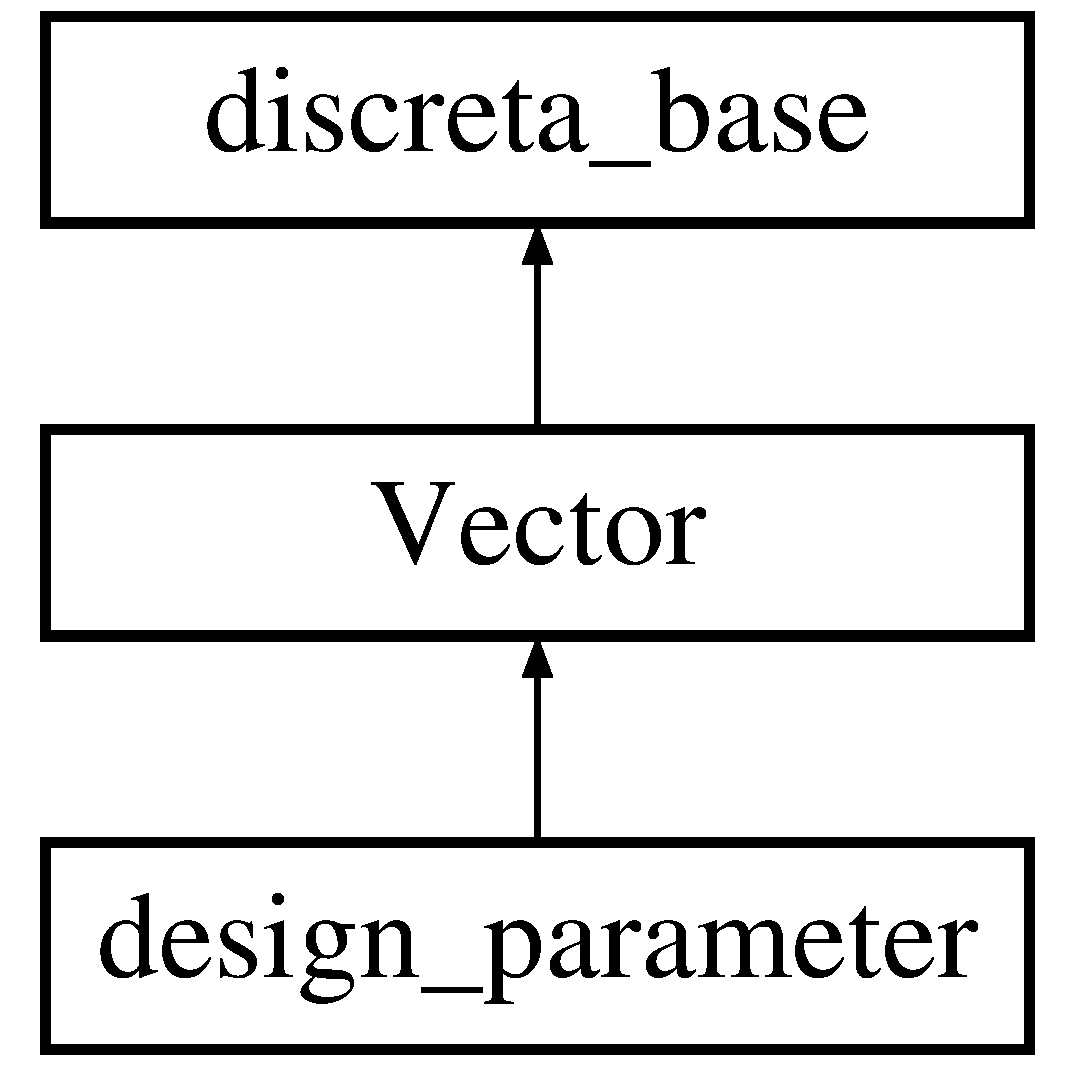
\includegraphics[height=3.000000cm]{classdesign__parameter}
\end{center}
\end{figure}
\subsection*{Public Member Functions}
\begin{DoxyCompactItemize}
\item 
\mbox{\hyperlink{classdesign__parameter_a1952bb71b52e00bcb579d3eafd809f05}{design\+\_\+parameter}} ()
\item 
\mbox{\hyperlink{classdesign__parameter_a4ea566da8e77452b92027b2a2c8df7ce}{design\+\_\+parameter}} (const \mbox{\hyperlink{classdiscreta__base}{discreta\+\_\+base}} \&\mbox{\hyperlink{alphabet2_8_c_a6150e0515f7202e2fb518f7206ed97dc}{x}})
\item 
\mbox{\hyperlink{classdesign__parameter}{design\+\_\+parameter}} \& \mbox{\hyperlink{classdesign__parameter_afd2b9a322632021e0e3893c386cfc196}{operator=}} (const \mbox{\hyperlink{classdiscreta__base}{discreta\+\_\+base}} \&\mbox{\hyperlink{alphabet2_8_c_a6150e0515f7202e2fb518f7206ed97dc}{x}})
\item 
void $\ast$ \mbox{\hyperlink{classdesign__parameter_a3a494f1e4e845ee4c70889675cfbce24}{operator new}} (size\+\_\+t, void $\ast$\mbox{\hyperlink{alphabet2_8_c_a533391314665d6bf1b5575e9a9cd8552}{p}})
\item 
void \mbox{\hyperlink{classdesign__parameter_a8b19d277f2b7d09c2531a527dfc0359e}{settype\+\_\+design\+\_\+parameter}} ()
\item 
\mbox{\hyperlink{discreta_8h_aaf25ee7e2306d78c74ec7bc48f092e81}{kind}} \mbox{\hyperlink{classdesign__parameter_af41eca1f66a8113dd0b892b26d791028}{s\+\_\+virtual\+\_\+kind}} ()
\item 
\mbox{\hyperlink{classdesign__parameter_af7927d3b3282e33daf8bf7106ffb3e96}{$\sim$design\+\_\+parameter}} ()
\item 
void \mbox{\hyperlink{classdesign__parameter_a0e7274960527530080b673a9d9e53fed}{freeself\+\_\+design\+\_\+parameter}} ()
\item 
void \mbox{\hyperlink{classdesign__parameter_a4e0434c6fd0d805543d730b40fc8e01f}{copyobject\+\_\+to}} (\mbox{\hyperlink{classdiscreta__base}{discreta\+\_\+base}} \&\mbox{\hyperlink{alphabet2_8_c_a6150e0515f7202e2fb518f7206ed97dc}{x}})
\item 
ostream \& \mbox{\hyperlink{classdesign__parameter_ac9c431a5408809b0c229eacaa924781b}{print}} (ostream \&)
\item 
\mbox{\hyperlink{galois_8h_a09fddde158a3a20bd2dcadb609de11dc}{I\+NT}} \& \mbox{\hyperlink{classdesign__parameter_ae83312a3e4d40a0ce15b649d3fe3ff19}{id}} ()
\item 
\mbox{\hyperlink{galois_8h_a09fddde158a3a20bd2dcadb609de11dc}{I\+NT}} \& \mbox{\hyperlink{classdesign__parameter_acf428913d279e62bcadc66b34303ece2}{t}} ()
\item 
\mbox{\hyperlink{galois_8h_a09fddde158a3a20bd2dcadb609de11dc}{I\+NT}} \& \mbox{\hyperlink{classdesign__parameter_a4fb1a94211c5a14072a459038b87a3ed}{v}} ()
\item 
\mbox{\hyperlink{galois_8h_a09fddde158a3a20bd2dcadb609de11dc}{I\+NT}} \& \mbox{\hyperlink{classdesign__parameter_a0960cd8a9ce482e57708344085b8d5ee}{K}} ()
\item 
\mbox{\hyperlink{classdiscreta__base}{discreta\+\_\+base}} \& \mbox{\hyperlink{classdesign__parameter_a53f496a4ef883ba3c06b500e48b238f5}{lambda}} ()
\item 
\mbox{\hyperlink{class_vector}{Vector}} \& \mbox{\hyperlink{classdesign__parameter_a7285d5775f7a1b5ee30d82fb3148c7f6}{source}} ()
\item 
\mbox{\hyperlink{classdesign__parameter__source}{design\+\_\+parameter\+\_\+source}} \& \mbox{\hyperlink{classdesign__parameter_a2e2a51d68253f1d5e6ce76840f527517}{source\+\_\+i}} (\mbox{\hyperlink{galois_8h_a09fddde158a3a20bd2dcadb609de11dc}{I\+NT}} \mbox{\hyperlink{alphabet2_8_c_acb559820d9ca11295b4500f179ef6392}{i}})
\item 
void \mbox{\hyperlink{classdesign__parameter_af77829be8d9058a84169c36143307b5d}{init}} ()
\item 
void \mbox{\hyperlink{classdesign__parameter_a1d2908af6f9375845123117b6cc22910}{init}} (\mbox{\hyperlink{galois_8h_a09fddde158a3a20bd2dcadb609de11dc}{I\+NT}} \mbox{\hyperlink{classdesign__parameter_acf428913d279e62bcadc66b34303ece2}{t}}, \mbox{\hyperlink{galois_8h_a09fddde158a3a20bd2dcadb609de11dc}{I\+NT}} \mbox{\hyperlink{classdesign__parameter_a4fb1a94211c5a14072a459038b87a3ed}{v}}, \mbox{\hyperlink{galois_8h_a09fddde158a3a20bd2dcadb609de11dc}{I\+NT}} \mbox{\hyperlink{classdiscreta__base_a6f7a0f7bdd115b9e4dde358cfa7ebf81}{k}}, \mbox{\hyperlink{galois_8h_a09fddde158a3a20bd2dcadb609de11dc}{I\+NT}} \mbox{\hyperlink{classdesign__parameter_a53f496a4ef883ba3c06b500e48b238f5}{lambda}})
\item 
void \mbox{\hyperlink{classdesign__parameter_aaa4ef79af17ce386a9887b4c3a490df4}{init}} (\mbox{\hyperlink{galois_8h_a09fddde158a3a20bd2dcadb609de11dc}{I\+NT}} \mbox{\hyperlink{classdesign__parameter_acf428913d279e62bcadc66b34303ece2}{t}}, \mbox{\hyperlink{galois_8h_a09fddde158a3a20bd2dcadb609de11dc}{I\+NT}} \mbox{\hyperlink{classdesign__parameter_a4fb1a94211c5a14072a459038b87a3ed}{v}}, \mbox{\hyperlink{galois_8h_a09fddde158a3a20bd2dcadb609de11dc}{I\+NT}} \mbox{\hyperlink{classdiscreta__base_a6f7a0f7bdd115b9e4dde358cfa7ebf81}{k}}, \mbox{\hyperlink{classdiscreta__base}{discreta\+\_\+base}} \&\mbox{\hyperlink{classdesign__parameter_a53f496a4ef883ba3c06b500e48b238f5}{lambda}})
\item 
void \mbox{\hyperlink{classdesign__parameter_a200510dc60483800cc6985b77d4ee50c}{text}} (\mbox{\hyperlink{classhollerith}{hollerith}} \&\mbox{\hyperlink{alphabet2_8_c_a16611451551e3d15916bae723c3f59f7}{h}})
\item 
void \mbox{\hyperlink{classdesign__parameter_a04f64f7acdaa60b07d19b4592b14c109}{text\+\_\+parameter}} (\mbox{\hyperlink{classhollerith}{hollerith}} \&\mbox{\hyperlink{alphabet2_8_c_a16611451551e3d15916bae723c3f59f7}{h}})
\item 
void \mbox{\hyperlink{classdesign__parameter_a5915575234fd91b3419a36c40f0bc374}{reduced\+\_\+t}} (\mbox{\hyperlink{classdesign__parameter}{design\+\_\+parameter}} \&\mbox{\hyperlink{alphabet2_8_c_a533391314665d6bf1b5575e9a9cd8552}{p}})
\item 
\mbox{\hyperlink{galois_8h_a09fddde158a3a20bd2dcadb609de11dc}{I\+NT}} \mbox{\hyperlink{classdesign__parameter_a8f39a90927d51e3cb3772bc98c94d7d0}{increased\+\_\+t}} (\mbox{\hyperlink{classdesign__parameter}{design\+\_\+parameter}} \&\mbox{\hyperlink{alphabet2_8_c_a533391314665d6bf1b5575e9a9cd8552}{p}})
\item 
void \mbox{\hyperlink{classdesign__parameter_ace491a14da6337d02eb91fd090c72345}{supplementary\+\_\+reduced\+\_\+t}} (\mbox{\hyperlink{classdesign__parameter}{design\+\_\+parameter}} \&\mbox{\hyperlink{alphabet2_8_c_a533391314665d6bf1b5575e9a9cd8552}{p}})
\item 
void \mbox{\hyperlink{classdesign__parameter_a72b457aff4b3747f90ed7fbda1941de0}{derived}} (\mbox{\hyperlink{classdesign__parameter}{design\+\_\+parameter}} \&\mbox{\hyperlink{alphabet2_8_c_a533391314665d6bf1b5575e9a9cd8552}{p}})
\item 
\mbox{\hyperlink{galois_8h_a09fddde158a3a20bd2dcadb609de11dc}{I\+NT}} \mbox{\hyperlink{classdesign__parameter_acbfce2a35f0c379d5888acdc8d74ae19}{derived\+\_\+inverse}} (\mbox{\hyperlink{classdesign__parameter}{design\+\_\+parameter}} \&\mbox{\hyperlink{alphabet2_8_c_a533391314665d6bf1b5575e9a9cd8552}{p}})
\item 
void \mbox{\hyperlink{classdesign__parameter_a17941dd86d09c510322cd0deee7e463f}{supplementary\+\_\+derived}} (\mbox{\hyperlink{classdesign__parameter}{design\+\_\+parameter}} \&\mbox{\hyperlink{alphabet2_8_c_a533391314665d6bf1b5575e9a9cd8552}{p}})
\item 
void \mbox{\hyperlink{classdesign__parameter_a927b3017b92919197fa53d9888409411}{residual}} (\mbox{\hyperlink{classdesign__parameter}{design\+\_\+parameter}} \&\mbox{\hyperlink{alphabet2_8_c_a533391314665d6bf1b5575e9a9cd8552}{p}})
\item 
void \mbox{\hyperlink{classdesign__parameter_abd616d2e29cde6f3e797abab001af0c6}{ancestor}} (\mbox{\hyperlink{classdesign__parameter}{design\+\_\+parameter}} \&\mbox{\hyperlink{alphabet2_8_c_a533391314665d6bf1b5575e9a9cd8552}{p}}, \mbox{\hyperlink{class_vector}{Vector}} \&path, \mbox{\hyperlink{galois_8h_a09fddde158a3a20bd2dcadb609de11dc}{I\+NT}} f\+\_\+v, \mbox{\hyperlink{galois_8h_a09fddde158a3a20bd2dcadb609de11dc}{I\+NT}} f\+\_\+vv)
\item 
void \mbox{\hyperlink{classdesign__parameter_a5bbeb7775c2bd761d50a7b32044d6963}{supplementary\+\_\+residual}} (\mbox{\hyperlink{classdesign__parameter}{design\+\_\+parameter}} \&\mbox{\hyperlink{alphabet2_8_c_a533391314665d6bf1b5575e9a9cd8552}{p}})
\item 
\mbox{\hyperlink{galois_8h_a09fddde158a3a20bd2dcadb609de11dc}{I\+NT}} \mbox{\hyperlink{classdesign__parameter_a98630a1cdc565c3c826a2636a499c5f6}{residual\+\_\+inverse}} (\mbox{\hyperlink{classdesign__parameter}{design\+\_\+parameter}} \&\mbox{\hyperlink{alphabet2_8_c_a533391314665d6bf1b5575e9a9cd8552}{p}})
\item 
\mbox{\hyperlink{galois_8h_a09fddde158a3a20bd2dcadb609de11dc}{I\+NT}} \mbox{\hyperlink{classdesign__parameter_a2de27fa4f3a609b37620207144807175}{trung\+\_\+complementary}} (\mbox{\hyperlink{classdesign__parameter}{design\+\_\+parameter}} \&\mbox{\hyperlink{alphabet2_8_c_a533391314665d6bf1b5575e9a9cd8552}{p}})
\item 
\mbox{\hyperlink{galois_8h_a09fddde158a3a20bd2dcadb609de11dc}{I\+NT}} \mbox{\hyperlink{classdesign__parameter_a2a8f8342e811614d8be1f81b1f58fb7e}{trung\+\_\+left\+\_\+partner}} (\mbox{\hyperlink{galois_8h_a09fddde158a3a20bd2dcadb609de11dc}{I\+NT}} \&t1, \mbox{\hyperlink{galois_8h_a09fddde158a3a20bd2dcadb609de11dc}{I\+NT}} \&v1, \mbox{\hyperlink{galois_8h_a09fddde158a3a20bd2dcadb609de11dc}{I\+NT}} \&k1, \mbox{\hyperlink{classdiscreta__base}{discreta\+\_\+base}} \&lambda1, \mbox{\hyperlink{galois_8h_a09fddde158a3a20bd2dcadb609de11dc}{I\+NT}} \&t\+\_\+new, \mbox{\hyperlink{galois_8h_a09fddde158a3a20bd2dcadb609de11dc}{I\+NT}} \&v\+\_\+new, \mbox{\hyperlink{galois_8h_a09fddde158a3a20bd2dcadb609de11dc}{I\+NT}} \&k\+\_\+new, \mbox{\hyperlink{classdiscreta__base}{discreta\+\_\+base}} \&lambda\+\_\+new)
\item 
\mbox{\hyperlink{galois_8h_a09fddde158a3a20bd2dcadb609de11dc}{I\+NT}} \mbox{\hyperlink{classdesign__parameter_a866f154ac4db93b6000a155c35d9f8af}{trung\+\_\+right\+\_\+partner}} (\mbox{\hyperlink{galois_8h_a09fddde158a3a20bd2dcadb609de11dc}{I\+NT}} \&t1, \mbox{\hyperlink{galois_8h_a09fddde158a3a20bd2dcadb609de11dc}{I\+NT}} \&v1, \mbox{\hyperlink{galois_8h_a09fddde158a3a20bd2dcadb609de11dc}{I\+NT}} \&k1, \mbox{\hyperlink{classdiscreta__base}{discreta\+\_\+base}} \&lambda1, \mbox{\hyperlink{galois_8h_a09fddde158a3a20bd2dcadb609de11dc}{I\+NT}} \&t\+\_\+new, \mbox{\hyperlink{galois_8h_a09fddde158a3a20bd2dcadb609de11dc}{I\+NT}} \&v\+\_\+new, \mbox{\hyperlink{galois_8h_a09fddde158a3a20bd2dcadb609de11dc}{I\+NT}} \&k\+\_\+new, \mbox{\hyperlink{classdiscreta__base}{discreta\+\_\+base}} \&lambda\+\_\+new)
\item 
\mbox{\hyperlink{galois_8h_a09fddde158a3a20bd2dcadb609de11dc}{I\+NT}} \mbox{\hyperlink{classdesign__parameter_ac91d8a483974702c826889aade83cd5f}{alltop}} (\mbox{\hyperlink{classdesign__parameter}{design\+\_\+parameter}} \&\mbox{\hyperlink{alphabet2_8_c_a533391314665d6bf1b5575e9a9cd8552}{p}})
\item 
void \mbox{\hyperlink{classdesign__parameter_a9025f18483dfe3f57eecfc6a603b7df1}{complementary}} (\mbox{\hyperlink{classdesign__parameter}{design\+\_\+parameter}} \&\mbox{\hyperlink{alphabet2_8_c_a533391314665d6bf1b5575e9a9cd8552}{p}})
\item 
void \mbox{\hyperlink{classdesign__parameter_a92bc4ea249ac3cdedbf77566410acd5a}{supplementary}} (\mbox{\hyperlink{classdesign__parameter}{design\+\_\+parameter}} \&\mbox{\hyperlink{alphabet2_8_c_a533391314665d6bf1b5575e9a9cd8552}{p}})
\item 
\mbox{\hyperlink{galois_8h_a09fddde158a3a20bd2dcadb609de11dc}{I\+NT}} \mbox{\hyperlink{classdesign__parameter_ac0ad1bf4fb71b9eab055d18503c4a7ce}{is\+\_\+selfsupplementary}} ()
\item 
void \mbox{\hyperlink{classdesign__parameter_a377c987a2c470225466fd32a3e920f0a}{lambda\+\_\+of\+\_\+supplementary}} (\mbox{\hyperlink{classdiscreta__base}{discreta\+\_\+base}} \&lambda\+\_\+supplementary)
\item 
void \mbox{\hyperlink{classdesign__parameter_abe95966fa2ed15d9bad7cac2476d4683}{init\+\_\+database}} (\mbox{\hyperlink{classdatabase}{database}} \&\mbox{\hyperlink{costas_8_c_af13967e8da5ae214c112fd612639beaa}{D}}, \mbox{\hyperlink{galois_8h_ab6cc7b4aeb6ea31aba2b3fbfc83ff5e6}{B\+Y\+TE}} $\ast$path)
\end{DoxyCompactItemize}
\subsection*{Additional Inherited Members}


\subsection{Constructor \& Destructor Documentation}
\mbox{\Hypertarget{classdesign__parameter_a1952bb71b52e00bcb579d3eafd809f05}\label{classdesign__parameter_a1952bb71b52e00bcb579d3eafd809f05}} 
\index{design\+\_\+parameter@{design\+\_\+parameter}!design\+\_\+parameter@{design\+\_\+parameter}}
\index{design\+\_\+parameter@{design\+\_\+parameter}!design\+\_\+parameter@{design\+\_\+parameter}}
\subsubsection{\texorpdfstring{design\+\_\+parameter()}{design\_parameter()}\hspace{0.1cm}{\footnotesize\ttfamily [1/2]}}
{\footnotesize\ttfamily design\+\_\+parameter\+::design\+\_\+parameter (\begin{DoxyParamCaption}{ }\end{DoxyParamCaption})}

\mbox{\Hypertarget{classdesign__parameter_a4ea566da8e77452b92027b2a2c8df7ce}\label{classdesign__parameter_a4ea566da8e77452b92027b2a2c8df7ce}} 
\index{design\+\_\+parameter@{design\+\_\+parameter}!design\+\_\+parameter@{design\+\_\+parameter}}
\index{design\+\_\+parameter@{design\+\_\+parameter}!design\+\_\+parameter@{design\+\_\+parameter}}
\subsubsection{\texorpdfstring{design\+\_\+parameter()}{design\_parameter()}\hspace{0.1cm}{\footnotesize\ttfamily [2/2]}}
{\footnotesize\ttfamily design\+\_\+parameter\+::design\+\_\+parameter (\begin{DoxyParamCaption}\item[{const \mbox{\hyperlink{classdiscreta__base}{discreta\+\_\+base}} \&}]{x }\end{DoxyParamCaption})}

\mbox{\Hypertarget{classdesign__parameter_af7927d3b3282e33daf8bf7106ffb3e96}\label{classdesign__parameter_af7927d3b3282e33daf8bf7106ffb3e96}} 
\index{design\+\_\+parameter@{design\+\_\+parameter}!````~design\+\_\+parameter@{$\sim$design\+\_\+parameter}}
\index{````~design\+\_\+parameter@{$\sim$design\+\_\+parameter}!design\+\_\+parameter@{design\+\_\+parameter}}
\subsubsection{\texorpdfstring{$\sim$design\+\_\+parameter()}{~design\_parameter()}}
{\footnotesize\ttfamily design\+\_\+parameter\+::$\sim$design\+\_\+parameter (\begin{DoxyParamCaption}{ }\end{DoxyParamCaption})}



\subsection{Member Function Documentation}
\mbox{\Hypertarget{classdesign__parameter_ac91d8a483974702c826889aade83cd5f}\label{classdesign__parameter_ac91d8a483974702c826889aade83cd5f}} 
\index{design\+\_\+parameter@{design\+\_\+parameter}!alltop@{alltop}}
\index{alltop@{alltop}!design\+\_\+parameter@{design\+\_\+parameter}}
\subsubsection{\texorpdfstring{alltop()}{alltop()}}
{\footnotesize\ttfamily \mbox{\hyperlink{galois_8h_a09fddde158a3a20bd2dcadb609de11dc}{I\+NT}} design\+\_\+parameter\+::alltop (\begin{DoxyParamCaption}\item[{\mbox{\hyperlink{classdesign__parameter}{design\+\_\+parameter}} \&}]{p }\end{DoxyParamCaption})}

\mbox{\Hypertarget{classdesign__parameter_abd616d2e29cde6f3e797abab001af0c6}\label{classdesign__parameter_abd616d2e29cde6f3e797abab001af0c6}} 
\index{design\+\_\+parameter@{design\+\_\+parameter}!ancestor@{ancestor}}
\index{ancestor@{ancestor}!design\+\_\+parameter@{design\+\_\+parameter}}
\subsubsection{\texorpdfstring{ancestor()}{ancestor()}}
{\footnotesize\ttfamily void design\+\_\+parameter\+::ancestor (\begin{DoxyParamCaption}\item[{\mbox{\hyperlink{classdesign__parameter}{design\+\_\+parameter}} \&}]{p,  }\item[{\mbox{\hyperlink{class_vector}{Vector}} \&}]{path,  }\item[{\mbox{\hyperlink{galois_8h_a09fddde158a3a20bd2dcadb609de11dc}{I\+NT}}}]{f\+\_\+v,  }\item[{\mbox{\hyperlink{galois_8h_a09fddde158a3a20bd2dcadb609de11dc}{I\+NT}}}]{f\+\_\+vv }\end{DoxyParamCaption})}

\mbox{\Hypertarget{classdesign__parameter_a9025f18483dfe3f57eecfc6a603b7df1}\label{classdesign__parameter_a9025f18483dfe3f57eecfc6a603b7df1}} 
\index{design\+\_\+parameter@{design\+\_\+parameter}!complementary@{complementary}}
\index{complementary@{complementary}!design\+\_\+parameter@{design\+\_\+parameter}}
\subsubsection{\texorpdfstring{complementary()}{complementary()}}
{\footnotesize\ttfamily void design\+\_\+parameter\+::complementary (\begin{DoxyParamCaption}\item[{\mbox{\hyperlink{classdesign__parameter}{design\+\_\+parameter}} \&}]{p }\end{DoxyParamCaption})}

\mbox{\Hypertarget{classdesign__parameter_a4e0434c6fd0d805543d730b40fc8e01f}\label{classdesign__parameter_a4e0434c6fd0d805543d730b40fc8e01f}} 
\index{design\+\_\+parameter@{design\+\_\+parameter}!copyobject\+\_\+to@{copyobject\+\_\+to}}
\index{copyobject\+\_\+to@{copyobject\+\_\+to}!design\+\_\+parameter@{design\+\_\+parameter}}
\subsubsection{\texorpdfstring{copyobject\+\_\+to()}{copyobject\_to()}}
{\footnotesize\ttfamily void design\+\_\+parameter\+::copyobject\+\_\+to (\begin{DoxyParamCaption}\item[{\mbox{\hyperlink{classdiscreta__base}{discreta\+\_\+base}} \&}]{x }\end{DoxyParamCaption})\hspace{0.3cm}{\ttfamily [virtual]}}



Reimplemented from \mbox{\hyperlink{class_vector_af657307f3d344c8cef5d633335a5f484}{Vector}}.

\mbox{\Hypertarget{classdesign__parameter_a72b457aff4b3747f90ed7fbda1941de0}\label{classdesign__parameter_a72b457aff4b3747f90ed7fbda1941de0}} 
\index{design\+\_\+parameter@{design\+\_\+parameter}!derived@{derived}}
\index{derived@{derived}!design\+\_\+parameter@{design\+\_\+parameter}}
\subsubsection{\texorpdfstring{derived()}{derived()}}
{\footnotesize\ttfamily void design\+\_\+parameter\+::derived (\begin{DoxyParamCaption}\item[{\mbox{\hyperlink{classdesign__parameter}{design\+\_\+parameter}} \&}]{p }\end{DoxyParamCaption})}

\mbox{\Hypertarget{classdesign__parameter_acbfce2a35f0c379d5888acdc8d74ae19}\label{classdesign__parameter_acbfce2a35f0c379d5888acdc8d74ae19}} 
\index{design\+\_\+parameter@{design\+\_\+parameter}!derived\+\_\+inverse@{derived\+\_\+inverse}}
\index{derived\+\_\+inverse@{derived\+\_\+inverse}!design\+\_\+parameter@{design\+\_\+parameter}}
\subsubsection{\texorpdfstring{derived\+\_\+inverse()}{derived\_inverse()}}
{\footnotesize\ttfamily \mbox{\hyperlink{galois_8h_a09fddde158a3a20bd2dcadb609de11dc}{I\+NT}} design\+\_\+parameter\+::derived\+\_\+inverse (\begin{DoxyParamCaption}\item[{\mbox{\hyperlink{classdesign__parameter}{design\+\_\+parameter}} \&}]{p }\end{DoxyParamCaption})}

\mbox{\Hypertarget{classdesign__parameter_a0e7274960527530080b673a9d9e53fed}\label{classdesign__parameter_a0e7274960527530080b673a9d9e53fed}} 
\index{design\+\_\+parameter@{design\+\_\+parameter}!freeself\+\_\+design\+\_\+parameter@{freeself\+\_\+design\+\_\+parameter}}
\index{freeself\+\_\+design\+\_\+parameter@{freeself\+\_\+design\+\_\+parameter}!design\+\_\+parameter@{design\+\_\+parameter}}
\subsubsection{\texorpdfstring{freeself\+\_\+design\+\_\+parameter()}{freeself\_design\_parameter()}}
{\footnotesize\ttfamily void design\+\_\+parameter\+::freeself\+\_\+design\+\_\+parameter (\begin{DoxyParamCaption}{ }\end{DoxyParamCaption})}

\mbox{\Hypertarget{classdesign__parameter_ae83312a3e4d40a0ce15b649d3fe3ff19}\label{classdesign__parameter_ae83312a3e4d40a0ce15b649d3fe3ff19}} 
\index{design\+\_\+parameter@{design\+\_\+parameter}!id@{id}}
\index{id@{id}!design\+\_\+parameter@{design\+\_\+parameter}}
\subsubsection{\texorpdfstring{id()}{id()}}
{\footnotesize\ttfamily \mbox{\hyperlink{galois_8h_a09fddde158a3a20bd2dcadb609de11dc}{I\+NT}}\& design\+\_\+parameter\+::id (\begin{DoxyParamCaption}{ }\end{DoxyParamCaption})\hspace{0.3cm}{\ttfamily [inline]}}

\mbox{\Hypertarget{classdesign__parameter_a8f39a90927d51e3cb3772bc98c94d7d0}\label{classdesign__parameter_a8f39a90927d51e3cb3772bc98c94d7d0}} 
\index{design\+\_\+parameter@{design\+\_\+parameter}!increased\+\_\+t@{increased\+\_\+t}}
\index{increased\+\_\+t@{increased\+\_\+t}!design\+\_\+parameter@{design\+\_\+parameter}}
\subsubsection{\texorpdfstring{increased\+\_\+t()}{increased\_t()}}
{\footnotesize\ttfamily \mbox{\hyperlink{galois_8h_a09fddde158a3a20bd2dcadb609de11dc}{I\+NT}} design\+\_\+parameter\+::increased\+\_\+t (\begin{DoxyParamCaption}\item[{\mbox{\hyperlink{classdesign__parameter}{design\+\_\+parameter}} \&}]{p }\end{DoxyParamCaption})}

\mbox{\Hypertarget{classdesign__parameter_af77829be8d9058a84169c36143307b5d}\label{classdesign__parameter_af77829be8d9058a84169c36143307b5d}} 
\index{design\+\_\+parameter@{design\+\_\+parameter}!init@{init}}
\index{init@{init}!design\+\_\+parameter@{design\+\_\+parameter}}
\subsubsection{\texorpdfstring{init()}{init()}\hspace{0.1cm}{\footnotesize\ttfamily [1/3]}}
{\footnotesize\ttfamily void design\+\_\+parameter\+::init (\begin{DoxyParamCaption}{ }\end{DoxyParamCaption})}

\mbox{\Hypertarget{classdesign__parameter_a1d2908af6f9375845123117b6cc22910}\label{classdesign__parameter_a1d2908af6f9375845123117b6cc22910}} 
\index{design\+\_\+parameter@{design\+\_\+parameter}!init@{init}}
\index{init@{init}!design\+\_\+parameter@{design\+\_\+parameter}}
\subsubsection{\texorpdfstring{init()}{init()}\hspace{0.1cm}{\footnotesize\ttfamily [2/3]}}
{\footnotesize\ttfamily void design\+\_\+parameter\+::init (\begin{DoxyParamCaption}\item[{\mbox{\hyperlink{galois_8h_a09fddde158a3a20bd2dcadb609de11dc}{I\+NT}}}]{t,  }\item[{\mbox{\hyperlink{galois_8h_a09fddde158a3a20bd2dcadb609de11dc}{I\+NT}}}]{v,  }\item[{\mbox{\hyperlink{galois_8h_a09fddde158a3a20bd2dcadb609de11dc}{I\+NT}}}]{k,  }\item[{\mbox{\hyperlink{galois_8h_a09fddde158a3a20bd2dcadb609de11dc}{I\+NT}}}]{lambda }\end{DoxyParamCaption})}

\mbox{\Hypertarget{classdesign__parameter_aaa4ef79af17ce386a9887b4c3a490df4}\label{classdesign__parameter_aaa4ef79af17ce386a9887b4c3a490df4}} 
\index{design\+\_\+parameter@{design\+\_\+parameter}!init@{init}}
\index{init@{init}!design\+\_\+parameter@{design\+\_\+parameter}}
\subsubsection{\texorpdfstring{init()}{init()}\hspace{0.1cm}{\footnotesize\ttfamily [3/3]}}
{\footnotesize\ttfamily void design\+\_\+parameter\+::init (\begin{DoxyParamCaption}\item[{\mbox{\hyperlink{galois_8h_a09fddde158a3a20bd2dcadb609de11dc}{I\+NT}}}]{t,  }\item[{\mbox{\hyperlink{galois_8h_a09fddde158a3a20bd2dcadb609de11dc}{I\+NT}}}]{v,  }\item[{\mbox{\hyperlink{galois_8h_a09fddde158a3a20bd2dcadb609de11dc}{I\+NT}}}]{k,  }\item[{\mbox{\hyperlink{classdiscreta__base}{discreta\+\_\+base}} \&}]{lambda }\end{DoxyParamCaption})}

\mbox{\Hypertarget{classdesign__parameter_abe95966fa2ed15d9bad7cac2476d4683}\label{classdesign__parameter_abe95966fa2ed15d9bad7cac2476d4683}} 
\index{design\+\_\+parameter@{design\+\_\+parameter}!init\+\_\+database@{init\+\_\+database}}
\index{init\+\_\+database@{init\+\_\+database}!design\+\_\+parameter@{design\+\_\+parameter}}
\subsubsection{\texorpdfstring{init\+\_\+database()}{init\_database()}}
{\footnotesize\ttfamily void design\+\_\+parameter\+::init\+\_\+database (\begin{DoxyParamCaption}\item[{\mbox{\hyperlink{classdatabase}{database}} \&}]{D,  }\item[{\mbox{\hyperlink{galois_8h_ab6cc7b4aeb6ea31aba2b3fbfc83ff5e6}{B\+Y\+TE}} $\ast$}]{path }\end{DoxyParamCaption})}

\mbox{\Hypertarget{classdesign__parameter_ac0ad1bf4fb71b9eab055d18503c4a7ce}\label{classdesign__parameter_ac0ad1bf4fb71b9eab055d18503c4a7ce}} 
\index{design\+\_\+parameter@{design\+\_\+parameter}!is\+\_\+selfsupplementary@{is\+\_\+selfsupplementary}}
\index{is\+\_\+selfsupplementary@{is\+\_\+selfsupplementary}!design\+\_\+parameter@{design\+\_\+parameter}}
\subsubsection{\texorpdfstring{is\+\_\+selfsupplementary()}{is\_selfsupplementary()}}
{\footnotesize\ttfamily \mbox{\hyperlink{galois_8h_a09fddde158a3a20bd2dcadb609de11dc}{I\+NT}} design\+\_\+parameter\+::is\+\_\+selfsupplementary (\begin{DoxyParamCaption}{ }\end{DoxyParamCaption})}

\mbox{\Hypertarget{classdesign__parameter_a0960cd8a9ce482e57708344085b8d5ee}\label{classdesign__parameter_a0960cd8a9ce482e57708344085b8d5ee}} 
\index{design\+\_\+parameter@{design\+\_\+parameter}!K@{K}}
\index{K@{K}!design\+\_\+parameter@{design\+\_\+parameter}}
\subsubsection{\texorpdfstring{K()}{K()}}
{\footnotesize\ttfamily \mbox{\hyperlink{galois_8h_a09fddde158a3a20bd2dcadb609de11dc}{I\+NT}}\& design\+\_\+parameter\+::K (\begin{DoxyParamCaption}{ }\end{DoxyParamCaption})\hspace{0.3cm}{\ttfamily [inline]}}

\mbox{\Hypertarget{classdesign__parameter_a53f496a4ef883ba3c06b500e48b238f5}\label{classdesign__parameter_a53f496a4ef883ba3c06b500e48b238f5}} 
\index{design\+\_\+parameter@{design\+\_\+parameter}!lambda@{lambda}}
\index{lambda@{lambda}!design\+\_\+parameter@{design\+\_\+parameter}}
\subsubsection{\texorpdfstring{lambda()}{lambda()}}
{\footnotesize\ttfamily \mbox{\hyperlink{classdiscreta__base}{discreta\+\_\+base}}\& design\+\_\+parameter\+::lambda (\begin{DoxyParamCaption}{ }\end{DoxyParamCaption})\hspace{0.3cm}{\ttfamily [inline]}}

\mbox{\Hypertarget{classdesign__parameter_a377c987a2c470225466fd32a3e920f0a}\label{classdesign__parameter_a377c987a2c470225466fd32a3e920f0a}} 
\index{design\+\_\+parameter@{design\+\_\+parameter}!lambda\+\_\+of\+\_\+supplementary@{lambda\+\_\+of\+\_\+supplementary}}
\index{lambda\+\_\+of\+\_\+supplementary@{lambda\+\_\+of\+\_\+supplementary}!design\+\_\+parameter@{design\+\_\+parameter}}
\subsubsection{\texorpdfstring{lambda\+\_\+of\+\_\+supplementary()}{lambda\_of\_supplementary()}}
{\footnotesize\ttfamily void design\+\_\+parameter\+::lambda\+\_\+of\+\_\+supplementary (\begin{DoxyParamCaption}\item[{\mbox{\hyperlink{classdiscreta__base}{discreta\+\_\+base}} \&}]{lambda\+\_\+supplementary }\end{DoxyParamCaption})}

\mbox{\Hypertarget{classdesign__parameter_a3a494f1e4e845ee4c70889675cfbce24}\label{classdesign__parameter_a3a494f1e4e845ee4c70889675cfbce24}} 
\index{design\+\_\+parameter@{design\+\_\+parameter}!operator new@{operator new}}
\index{operator new@{operator new}!design\+\_\+parameter@{design\+\_\+parameter}}
\subsubsection{\texorpdfstring{operator new()}{operator new()}}
{\footnotesize\ttfamily void$\ast$ design\+\_\+parameter\+::operator new (\begin{DoxyParamCaption}\item[{size\+\_\+t}]{,  }\item[{void $\ast$}]{p }\end{DoxyParamCaption})\hspace{0.3cm}{\ttfamily [inline]}}

\mbox{\Hypertarget{classdesign__parameter_afd2b9a322632021e0e3893c386cfc196}\label{classdesign__parameter_afd2b9a322632021e0e3893c386cfc196}} 
\index{design\+\_\+parameter@{design\+\_\+parameter}!operator=@{operator=}}
\index{operator=@{operator=}!design\+\_\+parameter@{design\+\_\+parameter}}
\subsubsection{\texorpdfstring{operator=()}{operator=()}}
{\footnotesize\ttfamily \mbox{\hyperlink{classdesign__parameter}{design\+\_\+parameter}} \& design\+\_\+parameter\+::operator= (\begin{DoxyParamCaption}\item[{const \mbox{\hyperlink{classdiscreta__base}{discreta\+\_\+base}} \&}]{x }\end{DoxyParamCaption})}

\mbox{\Hypertarget{classdesign__parameter_ac9c431a5408809b0c229eacaa924781b}\label{classdesign__parameter_ac9c431a5408809b0c229eacaa924781b}} 
\index{design\+\_\+parameter@{design\+\_\+parameter}!print@{print}}
\index{print@{print}!design\+\_\+parameter@{design\+\_\+parameter}}
\subsubsection{\texorpdfstring{print()}{print()}}
{\footnotesize\ttfamily ostream \& design\+\_\+parameter\+::print (\begin{DoxyParamCaption}\item[{ostream \&}]{ost }\end{DoxyParamCaption})\hspace{0.3cm}{\ttfamily [virtual]}}



Reimplemented from \mbox{\hyperlink{class_vector_a71d7e24bcfdfc69d4a2137360acb066c}{Vector}}.

\mbox{\Hypertarget{classdesign__parameter_a5915575234fd91b3419a36c40f0bc374}\label{classdesign__parameter_a5915575234fd91b3419a36c40f0bc374}} 
\index{design\+\_\+parameter@{design\+\_\+parameter}!reduced\+\_\+t@{reduced\+\_\+t}}
\index{reduced\+\_\+t@{reduced\+\_\+t}!design\+\_\+parameter@{design\+\_\+parameter}}
\subsubsection{\texorpdfstring{reduced\+\_\+t()}{reduced\_t()}}
{\footnotesize\ttfamily void design\+\_\+parameter\+::reduced\+\_\+t (\begin{DoxyParamCaption}\item[{\mbox{\hyperlink{classdesign__parameter}{design\+\_\+parameter}} \&}]{p }\end{DoxyParamCaption})}

\mbox{\Hypertarget{classdesign__parameter_a927b3017b92919197fa53d9888409411}\label{classdesign__parameter_a927b3017b92919197fa53d9888409411}} 
\index{design\+\_\+parameter@{design\+\_\+parameter}!residual@{residual}}
\index{residual@{residual}!design\+\_\+parameter@{design\+\_\+parameter}}
\subsubsection{\texorpdfstring{residual()}{residual()}}
{\footnotesize\ttfamily void design\+\_\+parameter\+::residual (\begin{DoxyParamCaption}\item[{\mbox{\hyperlink{classdesign__parameter}{design\+\_\+parameter}} \&}]{p }\end{DoxyParamCaption})}

\mbox{\Hypertarget{classdesign__parameter_a98630a1cdc565c3c826a2636a499c5f6}\label{classdesign__parameter_a98630a1cdc565c3c826a2636a499c5f6}} 
\index{design\+\_\+parameter@{design\+\_\+parameter}!residual\+\_\+inverse@{residual\+\_\+inverse}}
\index{residual\+\_\+inverse@{residual\+\_\+inverse}!design\+\_\+parameter@{design\+\_\+parameter}}
\subsubsection{\texorpdfstring{residual\+\_\+inverse()}{residual\_inverse()}}
{\footnotesize\ttfamily \mbox{\hyperlink{galois_8h_a09fddde158a3a20bd2dcadb609de11dc}{I\+NT}} design\+\_\+parameter\+::residual\+\_\+inverse (\begin{DoxyParamCaption}\item[{\mbox{\hyperlink{classdesign__parameter}{design\+\_\+parameter}} \&}]{p }\end{DoxyParamCaption})}

\mbox{\Hypertarget{classdesign__parameter_af41eca1f66a8113dd0b892b26d791028}\label{classdesign__parameter_af41eca1f66a8113dd0b892b26d791028}} 
\index{design\+\_\+parameter@{design\+\_\+parameter}!s\+\_\+virtual\+\_\+kind@{s\+\_\+virtual\+\_\+kind}}
\index{s\+\_\+virtual\+\_\+kind@{s\+\_\+virtual\+\_\+kind}!design\+\_\+parameter@{design\+\_\+parameter}}
\subsubsection{\texorpdfstring{s\+\_\+virtual\+\_\+kind()}{s\_virtual\_kind()}}
{\footnotesize\ttfamily \mbox{\hyperlink{discreta_8h_aaf25ee7e2306d78c74ec7bc48f092e81}{kind}} design\+\_\+parameter\+::s\+\_\+virtual\+\_\+kind (\begin{DoxyParamCaption}{ }\end{DoxyParamCaption})\hspace{0.3cm}{\ttfamily [virtual]}}



Reimplemented from \mbox{\hyperlink{class_vector_a20550e70d02cbe484032c7f6b0833a0f}{Vector}}.

\mbox{\Hypertarget{classdesign__parameter_a8b19d277f2b7d09c2531a527dfc0359e}\label{classdesign__parameter_a8b19d277f2b7d09c2531a527dfc0359e}} 
\index{design\+\_\+parameter@{design\+\_\+parameter}!settype\+\_\+design\+\_\+parameter@{settype\+\_\+design\+\_\+parameter}}
\index{settype\+\_\+design\+\_\+parameter@{settype\+\_\+design\+\_\+parameter}!design\+\_\+parameter@{design\+\_\+parameter}}
\subsubsection{\texorpdfstring{settype\+\_\+design\+\_\+parameter()}{settype\_design\_parameter()}}
{\footnotesize\ttfamily void design\+\_\+parameter\+::settype\+\_\+design\+\_\+parameter (\begin{DoxyParamCaption}{ }\end{DoxyParamCaption})}

\mbox{\Hypertarget{classdesign__parameter_a7285d5775f7a1b5ee30d82fb3148c7f6}\label{classdesign__parameter_a7285d5775f7a1b5ee30d82fb3148c7f6}} 
\index{design\+\_\+parameter@{design\+\_\+parameter}!source@{source}}
\index{source@{source}!design\+\_\+parameter@{design\+\_\+parameter}}
\subsubsection{\texorpdfstring{source()}{source()}}
{\footnotesize\ttfamily \mbox{\hyperlink{class_vector}{Vector}}\& design\+\_\+parameter\+::source (\begin{DoxyParamCaption}{ }\end{DoxyParamCaption})\hspace{0.3cm}{\ttfamily [inline]}}

\mbox{\Hypertarget{classdesign__parameter_a2e2a51d68253f1d5e6ce76840f527517}\label{classdesign__parameter_a2e2a51d68253f1d5e6ce76840f527517}} 
\index{design\+\_\+parameter@{design\+\_\+parameter}!source\+\_\+i@{source\+\_\+i}}
\index{source\+\_\+i@{source\+\_\+i}!design\+\_\+parameter@{design\+\_\+parameter}}
\subsubsection{\texorpdfstring{source\+\_\+i()}{source\_i()}}
{\footnotesize\ttfamily \mbox{\hyperlink{classdesign__parameter__source}{design\+\_\+parameter\+\_\+source}}\& design\+\_\+parameter\+::source\+\_\+i (\begin{DoxyParamCaption}\item[{\mbox{\hyperlink{galois_8h_a09fddde158a3a20bd2dcadb609de11dc}{I\+NT}}}]{i }\end{DoxyParamCaption})\hspace{0.3cm}{\ttfamily [inline]}}

\mbox{\Hypertarget{classdesign__parameter_a92bc4ea249ac3cdedbf77566410acd5a}\label{classdesign__parameter_a92bc4ea249ac3cdedbf77566410acd5a}} 
\index{design\+\_\+parameter@{design\+\_\+parameter}!supplementary@{supplementary}}
\index{supplementary@{supplementary}!design\+\_\+parameter@{design\+\_\+parameter}}
\subsubsection{\texorpdfstring{supplementary()}{supplementary()}}
{\footnotesize\ttfamily void design\+\_\+parameter\+::supplementary (\begin{DoxyParamCaption}\item[{\mbox{\hyperlink{classdesign__parameter}{design\+\_\+parameter}} \&}]{p }\end{DoxyParamCaption})}

\mbox{\Hypertarget{classdesign__parameter_a17941dd86d09c510322cd0deee7e463f}\label{classdesign__parameter_a17941dd86d09c510322cd0deee7e463f}} 
\index{design\+\_\+parameter@{design\+\_\+parameter}!supplementary\+\_\+derived@{supplementary\+\_\+derived}}
\index{supplementary\+\_\+derived@{supplementary\+\_\+derived}!design\+\_\+parameter@{design\+\_\+parameter}}
\subsubsection{\texorpdfstring{supplementary\+\_\+derived()}{supplementary\_derived()}}
{\footnotesize\ttfamily void design\+\_\+parameter\+::supplementary\+\_\+derived (\begin{DoxyParamCaption}\item[{\mbox{\hyperlink{classdesign__parameter}{design\+\_\+parameter}} \&}]{p }\end{DoxyParamCaption})}

\mbox{\Hypertarget{classdesign__parameter_ace491a14da6337d02eb91fd090c72345}\label{classdesign__parameter_ace491a14da6337d02eb91fd090c72345}} 
\index{design\+\_\+parameter@{design\+\_\+parameter}!supplementary\+\_\+reduced\+\_\+t@{supplementary\+\_\+reduced\+\_\+t}}
\index{supplementary\+\_\+reduced\+\_\+t@{supplementary\+\_\+reduced\+\_\+t}!design\+\_\+parameter@{design\+\_\+parameter}}
\subsubsection{\texorpdfstring{supplementary\+\_\+reduced\+\_\+t()}{supplementary\_reduced\_t()}}
{\footnotesize\ttfamily void design\+\_\+parameter\+::supplementary\+\_\+reduced\+\_\+t (\begin{DoxyParamCaption}\item[{\mbox{\hyperlink{classdesign__parameter}{design\+\_\+parameter}} \&}]{p }\end{DoxyParamCaption})}

\mbox{\Hypertarget{classdesign__parameter_a5bbeb7775c2bd761d50a7b32044d6963}\label{classdesign__parameter_a5bbeb7775c2bd761d50a7b32044d6963}} 
\index{design\+\_\+parameter@{design\+\_\+parameter}!supplementary\+\_\+residual@{supplementary\+\_\+residual}}
\index{supplementary\+\_\+residual@{supplementary\+\_\+residual}!design\+\_\+parameter@{design\+\_\+parameter}}
\subsubsection{\texorpdfstring{supplementary\+\_\+residual()}{supplementary\_residual()}}
{\footnotesize\ttfamily void design\+\_\+parameter\+::supplementary\+\_\+residual (\begin{DoxyParamCaption}\item[{\mbox{\hyperlink{classdesign__parameter}{design\+\_\+parameter}} \&}]{p }\end{DoxyParamCaption})}

\mbox{\Hypertarget{classdesign__parameter_acf428913d279e62bcadc66b34303ece2}\label{classdesign__parameter_acf428913d279e62bcadc66b34303ece2}} 
\index{design\+\_\+parameter@{design\+\_\+parameter}!t@{t}}
\index{t@{t}!design\+\_\+parameter@{design\+\_\+parameter}}
\subsubsection{\texorpdfstring{t()}{t()}}
{\footnotesize\ttfamily \mbox{\hyperlink{galois_8h_a09fddde158a3a20bd2dcadb609de11dc}{I\+NT}}\& design\+\_\+parameter\+::t (\begin{DoxyParamCaption}{ }\end{DoxyParamCaption})\hspace{0.3cm}{\ttfamily [inline]}}

\mbox{\Hypertarget{classdesign__parameter_a200510dc60483800cc6985b77d4ee50c}\label{classdesign__parameter_a200510dc60483800cc6985b77d4ee50c}} 
\index{design\+\_\+parameter@{design\+\_\+parameter}!text@{text}}
\index{text@{text}!design\+\_\+parameter@{design\+\_\+parameter}}
\subsubsection{\texorpdfstring{text()}{text()}}
{\footnotesize\ttfamily void design\+\_\+parameter\+::text (\begin{DoxyParamCaption}\item[{\mbox{\hyperlink{classhollerith}{hollerith}} \&}]{h }\end{DoxyParamCaption})}

\mbox{\Hypertarget{classdesign__parameter_a04f64f7acdaa60b07d19b4592b14c109}\label{classdesign__parameter_a04f64f7acdaa60b07d19b4592b14c109}} 
\index{design\+\_\+parameter@{design\+\_\+parameter}!text\+\_\+parameter@{text\+\_\+parameter}}
\index{text\+\_\+parameter@{text\+\_\+parameter}!design\+\_\+parameter@{design\+\_\+parameter}}
\subsubsection{\texorpdfstring{text\+\_\+parameter()}{text\_parameter()}}
{\footnotesize\ttfamily void design\+\_\+parameter\+::text\+\_\+parameter (\begin{DoxyParamCaption}\item[{\mbox{\hyperlink{classhollerith}{hollerith}} \&}]{h }\end{DoxyParamCaption})}

\mbox{\Hypertarget{classdesign__parameter_a2de27fa4f3a609b37620207144807175}\label{classdesign__parameter_a2de27fa4f3a609b37620207144807175}} 
\index{design\+\_\+parameter@{design\+\_\+parameter}!trung\+\_\+complementary@{trung\+\_\+complementary}}
\index{trung\+\_\+complementary@{trung\+\_\+complementary}!design\+\_\+parameter@{design\+\_\+parameter}}
\subsubsection{\texorpdfstring{trung\+\_\+complementary()}{trung\_complementary()}}
{\footnotesize\ttfamily \mbox{\hyperlink{galois_8h_a09fddde158a3a20bd2dcadb609de11dc}{I\+NT}} design\+\_\+parameter\+::trung\+\_\+complementary (\begin{DoxyParamCaption}\item[{\mbox{\hyperlink{classdesign__parameter}{design\+\_\+parameter}} \&}]{p }\end{DoxyParamCaption})}

\mbox{\Hypertarget{classdesign__parameter_a2a8f8342e811614d8be1f81b1f58fb7e}\label{classdesign__parameter_a2a8f8342e811614d8be1f81b1f58fb7e}} 
\index{design\+\_\+parameter@{design\+\_\+parameter}!trung\+\_\+left\+\_\+partner@{trung\+\_\+left\+\_\+partner}}
\index{trung\+\_\+left\+\_\+partner@{trung\+\_\+left\+\_\+partner}!design\+\_\+parameter@{design\+\_\+parameter}}
\subsubsection{\texorpdfstring{trung\+\_\+left\+\_\+partner()}{trung\_left\_partner()}}
{\footnotesize\ttfamily \mbox{\hyperlink{galois_8h_a09fddde158a3a20bd2dcadb609de11dc}{I\+NT}} design\+\_\+parameter\+::trung\+\_\+left\+\_\+partner (\begin{DoxyParamCaption}\item[{\mbox{\hyperlink{galois_8h_a09fddde158a3a20bd2dcadb609de11dc}{I\+NT}} \&}]{t1,  }\item[{\mbox{\hyperlink{galois_8h_a09fddde158a3a20bd2dcadb609de11dc}{I\+NT}} \&}]{v1,  }\item[{\mbox{\hyperlink{galois_8h_a09fddde158a3a20bd2dcadb609de11dc}{I\+NT}} \&}]{k1,  }\item[{\mbox{\hyperlink{classdiscreta__base}{discreta\+\_\+base}} \&}]{lambda1,  }\item[{\mbox{\hyperlink{galois_8h_a09fddde158a3a20bd2dcadb609de11dc}{I\+NT}} \&}]{t\+\_\+new,  }\item[{\mbox{\hyperlink{galois_8h_a09fddde158a3a20bd2dcadb609de11dc}{I\+NT}} \&}]{v\+\_\+new,  }\item[{\mbox{\hyperlink{galois_8h_a09fddde158a3a20bd2dcadb609de11dc}{I\+NT}} \&}]{k\+\_\+new,  }\item[{\mbox{\hyperlink{classdiscreta__base}{discreta\+\_\+base}} \&}]{lambda\+\_\+new }\end{DoxyParamCaption})}

\mbox{\Hypertarget{classdesign__parameter_a866f154ac4db93b6000a155c35d9f8af}\label{classdesign__parameter_a866f154ac4db93b6000a155c35d9f8af}} 
\index{design\+\_\+parameter@{design\+\_\+parameter}!trung\+\_\+right\+\_\+partner@{trung\+\_\+right\+\_\+partner}}
\index{trung\+\_\+right\+\_\+partner@{trung\+\_\+right\+\_\+partner}!design\+\_\+parameter@{design\+\_\+parameter}}
\subsubsection{\texorpdfstring{trung\+\_\+right\+\_\+partner()}{trung\_right\_partner()}}
{\footnotesize\ttfamily \mbox{\hyperlink{galois_8h_a09fddde158a3a20bd2dcadb609de11dc}{I\+NT}} design\+\_\+parameter\+::trung\+\_\+right\+\_\+partner (\begin{DoxyParamCaption}\item[{\mbox{\hyperlink{galois_8h_a09fddde158a3a20bd2dcadb609de11dc}{I\+NT}} \&}]{t1,  }\item[{\mbox{\hyperlink{galois_8h_a09fddde158a3a20bd2dcadb609de11dc}{I\+NT}} \&}]{v1,  }\item[{\mbox{\hyperlink{galois_8h_a09fddde158a3a20bd2dcadb609de11dc}{I\+NT}} \&}]{k1,  }\item[{\mbox{\hyperlink{classdiscreta__base}{discreta\+\_\+base}} \&}]{lambda1,  }\item[{\mbox{\hyperlink{galois_8h_a09fddde158a3a20bd2dcadb609de11dc}{I\+NT}} \&}]{t\+\_\+new,  }\item[{\mbox{\hyperlink{galois_8h_a09fddde158a3a20bd2dcadb609de11dc}{I\+NT}} \&}]{v\+\_\+new,  }\item[{\mbox{\hyperlink{galois_8h_a09fddde158a3a20bd2dcadb609de11dc}{I\+NT}} \&}]{k\+\_\+new,  }\item[{\mbox{\hyperlink{classdiscreta__base}{discreta\+\_\+base}} \&}]{lambda\+\_\+new }\end{DoxyParamCaption})}

\mbox{\Hypertarget{classdesign__parameter_a4fb1a94211c5a14072a459038b87a3ed}\label{classdesign__parameter_a4fb1a94211c5a14072a459038b87a3ed}} 
\index{design\+\_\+parameter@{design\+\_\+parameter}!v@{v}}
\index{v@{v}!design\+\_\+parameter@{design\+\_\+parameter}}
\subsubsection{\texorpdfstring{v()}{v()}}
{\footnotesize\ttfamily \mbox{\hyperlink{galois_8h_a09fddde158a3a20bd2dcadb609de11dc}{I\+NT}}\& design\+\_\+parameter\+::v (\begin{DoxyParamCaption}{ }\end{DoxyParamCaption})\hspace{0.3cm}{\ttfamily [inline]}}



The documentation for this class was generated from the following files\+:\begin{DoxyCompactItemize}
\item 
S\+R\+C/\+L\+I\+B/\+D\+I\+S\+C\+R\+E\+T\+A/\mbox{\hyperlink{discreta_8h}{discreta.\+h}}\item 
S\+R\+C/\+L\+I\+B/\+D\+I\+S\+C\+R\+E\+T\+A/\mbox{\hyperlink{design__parameter_8_c}{design\+\_\+parameter.\+C}}\end{DoxyCompactItemize}

\hypertarget{classdesign__parameter__source}{}\section{design\+\_\+parameter\+\_\+source Class Reference}
\label{classdesign__parameter__source}\index{design\+\_\+parameter\+\_\+source@{design\+\_\+parameter\+\_\+source}}


{\ttfamily \#include $<$discreta.\+h$>$}

Inheritance diagram for design\+\_\+parameter\+\_\+source\+:\begin{figure}[H]
\begin{center}
\leavevmode
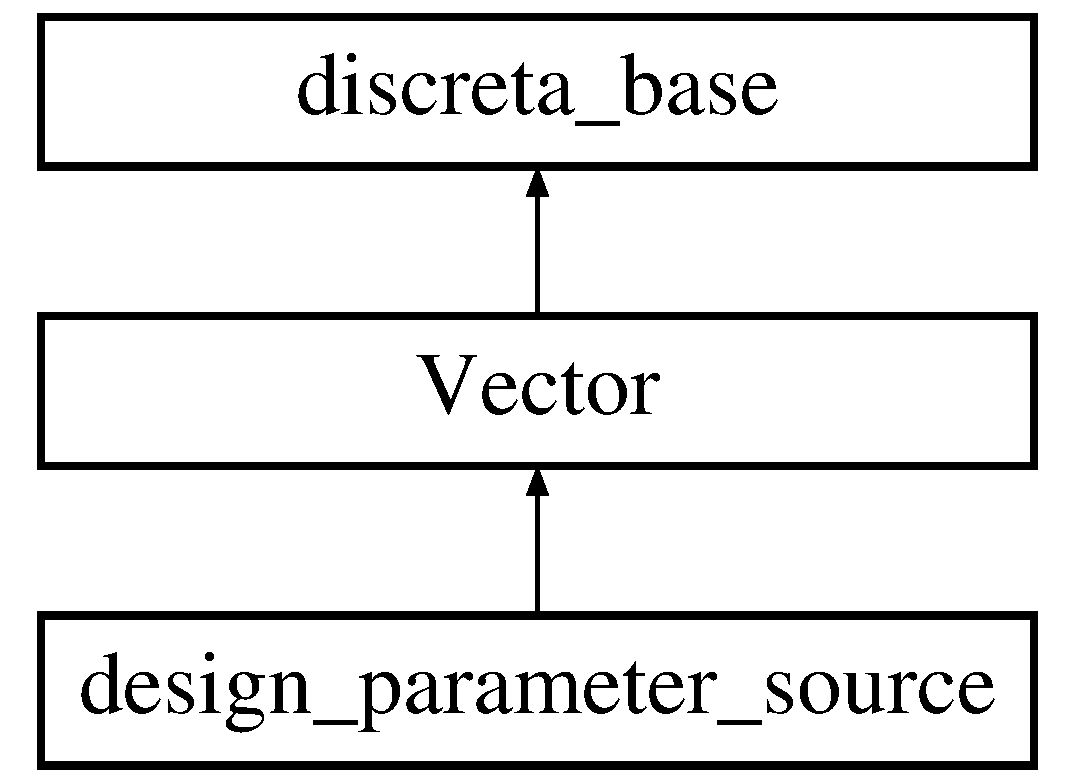
\includegraphics[height=3.000000cm]{classdesign__parameter__source}
\end{center}
\end{figure}
\subsection*{Public Member Functions}
\begin{DoxyCompactItemize}
\item 
\mbox{\hyperlink{classdesign__parameter__source_a64aac686b9e422a471d0f26351fb2bf0}{design\+\_\+parameter\+\_\+source}} ()
\item 
\mbox{\hyperlink{classdesign__parameter__source_a55246ea5ad8cac9ff7ff2d51a8dc476d}{design\+\_\+parameter\+\_\+source}} (const \mbox{\hyperlink{classdiscreta__base}{discreta\+\_\+base}} \&\mbox{\hyperlink{alphabet2_8_c_a6150e0515f7202e2fb518f7206ed97dc}{x}})
\item 
\mbox{\hyperlink{classdesign__parameter__source}{design\+\_\+parameter\+\_\+source}} \& \mbox{\hyperlink{classdesign__parameter__source_a92328345a02bb0028f77b5d4780d55d6}{operator=}} (const \mbox{\hyperlink{classdiscreta__base}{discreta\+\_\+base}} \&\mbox{\hyperlink{alphabet2_8_c_a6150e0515f7202e2fb518f7206ed97dc}{x}})
\item 
void $\ast$ \mbox{\hyperlink{classdesign__parameter__source_a597be327e3bf9c49aa9bbb96c10467a8}{operator new}} (size\+\_\+t, void $\ast$\mbox{\hyperlink{alphabet2_8_c_a533391314665d6bf1b5575e9a9cd8552}{p}})
\item 
void \mbox{\hyperlink{classdesign__parameter__source_a3af3b851df87bd1661fb9c9ce18822c8}{settype\+\_\+design\+\_\+parameter\+\_\+source}} ()
\item 
\mbox{\hyperlink{discreta_8h_aaf25ee7e2306d78c74ec7bc48f092e81}{kind}} \mbox{\hyperlink{classdesign__parameter__source_ad3ee1c1d1dfa39a6eb3e2ee538b0e350}{s\+\_\+virtual\+\_\+kind}} ()
\item 
\mbox{\hyperlink{classdesign__parameter__source_a7ad9a758b6d4f591d935777bba923b9c}{$\sim$design\+\_\+parameter\+\_\+source}} ()
\item 
void \mbox{\hyperlink{classdesign__parameter__source_a61e751fbde5330ede70525d4953bbc79}{freeself\+\_\+design\+\_\+parameter\+\_\+source}} ()
\item 
void \mbox{\hyperlink{classdesign__parameter__source_a1fd0910addc02ffe117ec08d0f93f8a6}{copyobject\+\_\+to}} (\mbox{\hyperlink{classdiscreta__base}{discreta\+\_\+base}} \&\mbox{\hyperlink{alphabet2_8_c_a6150e0515f7202e2fb518f7206ed97dc}{x}})
\item 
ostream \& \mbox{\hyperlink{classdesign__parameter__source_a50fb37085011959ea40a4087353377b4}{print}} (ostream \&)
\item 
void \mbox{\hyperlink{classdesign__parameter__source_a5e22836b470986f95bfcb322dfc37e82}{print2}} (\mbox{\hyperlink{classdesign__parameter}{design\+\_\+parameter}} \&\mbox{\hyperlink{alphabet2_8_c_a533391314665d6bf1b5575e9a9cd8552}{p}}, ostream \&ost)
\item 
\mbox{\hyperlink{galois_8h_a09fddde158a3a20bd2dcadb609de11dc}{I\+NT}} \& \mbox{\hyperlink{classdesign__parameter__source_a886ad5916d9f3689afd6bda66a22cf7d}{prev}} ()
\item 
\mbox{\hyperlink{galois_8h_a09fddde158a3a20bd2dcadb609de11dc}{I\+NT}} \& \mbox{\hyperlink{classdesign__parameter__source_a8e9f2810222797d8cad1fc682bc447a3}{rule}} ()
\item 
\mbox{\hyperlink{classhollerith}{hollerith}} \& \mbox{\hyperlink{classdesign__parameter__source_ae34592d2aebfff0766c1605cd4a896ba}{comment}} ()
\item 
\mbox{\hyperlink{class_vector}{Vector}} \& \mbox{\hyperlink{classdesign__parameter__source_a012c498e42726a45397509d9c2fadf64}{references}} ()
\item 
\mbox{\hyperlink{classhollerith}{hollerith}} \& \mbox{\hyperlink{classdesign__parameter__source_ac47d57aab93b6dcc781d27c6cec0fe6e}{references\+\_\+i}} (\mbox{\hyperlink{galois_8h_a09fddde158a3a20bd2dcadb609de11dc}{I\+NT}} \mbox{\hyperlink{alphabet2_8_c_acb559820d9ca11295b4500f179ef6392}{i}})
\item 
void \mbox{\hyperlink{classdesign__parameter__source_afccf1773adfffec18fd96efaec208b93}{init}} ()
\item 
void \mbox{\hyperlink{classdesign__parameter__source_a9e8e88ae72c857cde0d30f7b97a742ac}{text}} (\mbox{\hyperlink{classhollerith}{hollerith}} \&\mbox{\hyperlink{alphabet2_8_c_a16611451551e3d15916bae723c3f59f7}{h}})
\item 
void \mbox{\hyperlink{classdesign__parameter__source_a729d62efa57d73e420470d47902c4bf2}{text2}} (\mbox{\hyperlink{classdesign__parameter}{design\+\_\+parameter}} \&\mbox{\hyperlink{alphabet2_8_c_a533391314665d6bf1b5575e9a9cd8552}{p}}, \mbox{\hyperlink{classhollerith}{hollerith}} \&\mbox{\hyperlink{alphabet2_8_c_a16611451551e3d15916bae723c3f59f7}{h}})
\item 
void \mbox{\hyperlink{classdesign__parameter__source_afa2c39e6ed9f674b1c21c39f9a6a392a}{text012}} (\mbox{\hyperlink{classhollerith}{hollerith}} \&s0, \mbox{\hyperlink{classhollerith}{hollerith}} \&s1, \mbox{\hyperlink{classhollerith}{hollerith}} \&s2)
\item 
void \mbox{\hyperlink{classdesign__parameter__source_afa19c645725011722b75da5dee8b0945}{text012\+\_\+extended}} (\mbox{\hyperlink{classdesign__parameter}{design\+\_\+parameter}} \&\mbox{\hyperlink{alphabet2_8_c_a533391314665d6bf1b5575e9a9cd8552}{p}}, \mbox{\hyperlink{classhollerith}{hollerith}} \&s0, \mbox{\hyperlink{classhollerith}{hollerith}} \&s1, \mbox{\hyperlink{classhollerith}{hollerith}} \&s2)
\end{DoxyCompactItemize}
\subsection*{Additional Inherited Members}


\subsection{Constructor \& Destructor Documentation}
\mbox{\Hypertarget{classdesign__parameter__source_a64aac686b9e422a471d0f26351fb2bf0}\label{classdesign__parameter__source_a64aac686b9e422a471d0f26351fb2bf0}} 
\index{design\+\_\+parameter\+\_\+source@{design\+\_\+parameter\+\_\+source}!design\+\_\+parameter\+\_\+source@{design\+\_\+parameter\+\_\+source}}
\index{design\+\_\+parameter\+\_\+source@{design\+\_\+parameter\+\_\+source}!design\+\_\+parameter\+\_\+source@{design\+\_\+parameter\+\_\+source}}
\subsubsection{\texorpdfstring{design\+\_\+parameter\+\_\+source()}{design\_parameter\_source()}\hspace{0.1cm}{\footnotesize\ttfamily [1/2]}}
{\footnotesize\ttfamily design\+\_\+parameter\+\_\+source\+::design\+\_\+parameter\+\_\+source (\begin{DoxyParamCaption}{ }\end{DoxyParamCaption})}

\mbox{\Hypertarget{classdesign__parameter__source_a55246ea5ad8cac9ff7ff2d51a8dc476d}\label{classdesign__parameter__source_a55246ea5ad8cac9ff7ff2d51a8dc476d}} 
\index{design\+\_\+parameter\+\_\+source@{design\+\_\+parameter\+\_\+source}!design\+\_\+parameter\+\_\+source@{design\+\_\+parameter\+\_\+source}}
\index{design\+\_\+parameter\+\_\+source@{design\+\_\+parameter\+\_\+source}!design\+\_\+parameter\+\_\+source@{design\+\_\+parameter\+\_\+source}}
\subsubsection{\texorpdfstring{design\+\_\+parameter\+\_\+source()}{design\_parameter\_source()}\hspace{0.1cm}{\footnotesize\ttfamily [2/2]}}
{\footnotesize\ttfamily design\+\_\+parameter\+\_\+source\+::design\+\_\+parameter\+\_\+source (\begin{DoxyParamCaption}\item[{const \mbox{\hyperlink{classdiscreta__base}{discreta\+\_\+base}} \&}]{x }\end{DoxyParamCaption})}

\mbox{\Hypertarget{classdesign__parameter__source_a7ad9a758b6d4f591d935777bba923b9c}\label{classdesign__parameter__source_a7ad9a758b6d4f591d935777bba923b9c}} 
\index{design\+\_\+parameter\+\_\+source@{design\+\_\+parameter\+\_\+source}!````~design\+\_\+parameter\+\_\+source@{$\sim$design\+\_\+parameter\+\_\+source}}
\index{````~design\+\_\+parameter\+\_\+source@{$\sim$design\+\_\+parameter\+\_\+source}!design\+\_\+parameter\+\_\+source@{design\+\_\+parameter\+\_\+source}}
\subsubsection{\texorpdfstring{$\sim$design\+\_\+parameter\+\_\+source()}{~design\_parameter\_source()}}
{\footnotesize\ttfamily design\+\_\+parameter\+\_\+source\+::$\sim$design\+\_\+parameter\+\_\+source (\begin{DoxyParamCaption}{ }\end{DoxyParamCaption})}



\subsection{Member Function Documentation}
\mbox{\Hypertarget{classdesign__parameter__source_ae34592d2aebfff0766c1605cd4a896ba}\label{classdesign__parameter__source_ae34592d2aebfff0766c1605cd4a896ba}} 
\index{design\+\_\+parameter\+\_\+source@{design\+\_\+parameter\+\_\+source}!comment@{comment}}
\index{comment@{comment}!design\+\_\+parameter\+\_\+source@{design\+\_\+parameter\+\_\+source}}
\subsubsection{\texorpdfstring{comment()}{comment()}}
{\footnotesize\ttfamily \mbox{\hyperlink{classhollerith}{hollerith}}\& design\+\_\+parameter\+\_\+source\+::comment (\begin{DoxyParamCaption}{ }\end{DoxyParamCaption})\hspace{0.3cm}{\ttfamily [inline]}}

\mbox{\Hypertarget{classdesign__parameter__source_a1fd0910addc02ffe117ec08d0f93f8a6}\label{classdesign__parameter__source_a1fd0910addc02ffe117ec08d0f93f8a6}} 
\index{design\+\_\+parameter\+\_\+source@{design\+\_\+parameter\+\_\+source}!copyobject\+\_\+to@{copyobject\+\_\+to}}
\index{copyobject\+\_\+to@{copyobject\+\_\+to}!design\+\_\+parameter\+\_\+source@{design\+\_\+parameter\+\_\+source}}
\subsubsection{\texorpdfstring{copyobject\+\_\+to()}{copyobject\_to()}}
{\footnotesize\ttfamily void design\+\_\+parameter\+\_\+source\+::copyobject\+\_\+to (\begin{DoxyParamCaption}\item[{\mbox{\hyperlink{classdiscreta__base}{discreta\+\_\+base}} \&}]{x }\end{DoxyParamCaption})\hspace{0.3cm}{\ttfamily [virtual]}}



Reimplemented from \mbox{\hyperlink{class_vector_af657307f3d344c8cef5d633335a5f484}{Vector}}.

\mbox{\Hypertarget{classdesign__parameter__source_a61e751fbde5330ede70525d4953bbc79}\label{classdesign__parameter__source_a61e751fbde5330ede70525d4953bbc79}} 
\index{design\+\_\+parameter\+\_\+source@{design\+\_\+parameter\+\_\+source}!freeself\+\_\+design\+\_\+parameter\+\_\+source@{freeself\+\_\+design\+\_\+parameter\+\_\+source}}
\index{freeself\+\_\+design\+\_\+parameter\+\_\+source@{freeself\+\_\+design\+\_\+parameter\+\_\+source}!design\+\_\+parameter\+\_\+source@{design\+\_\+parameter\+\_\+source}}
\subsubsection{\texorpdfstring{freeself\+\_\+design\+\_\+parameter\+\_\+source()}{freeself\_design\_parameter\_source()}}
{\footnotesize\ttfamily void design\+\_\+parameter\+\_\+source\+::freeself\+\_\+design\+\_\+parameter\+\_\+source (\begin{DoxyParamCaption}{ }\end{DoxyParamCaption})}

\mbox{\Hypertarget{classdesign__parameter__source_afccf1773adfffec18fd96efaec208b93}\label{classdesign__parameter__source_afccf1773adfffec18fd96efaec208b93}} 
\index{design\+\_\+parameter\+\_\+source@{design\+\_\+parameter\+\_\+source}!init@{init}}
\index{init@{init}!design\+\_\+parameter\+\_\+source@{design\+\_\+parameter\+\_\+source}}
\subsubsection{\texorpdfstring{init()}{init()}}
{\footnotesize\ttfamily void design\+\_\+parameter\+\_\+source\+::init (\begin{DoxyParamCaption}{ }\end{DoxyParamCaption})}

\mbox{\Hypertarget{classdesign__parameter__source_a597be327e3bf9c49aa9bbb96c10467a8}\label{classdesign__parameter__source_a597be327e3bf9c49aa9bbb96c10467a8}} 
\index{design\+\_\+parameter\+\_\+source@{design\+\_\+parameter\+\_\+source}!operator new@{operator new}}
\index{operator new@{operator new}!design\+\_\+parameter\+\_\+source@{design\+\_\+parameter\+\_\+source}}
\subsubsection{\texorpdfstring{operator new()}{operator new()}}
{\footnotesize\ttfamily void$\ast$ design\+\_\+parameter\+\_\+source\+::operator new (\begin{DoxyParamCaption}\item[{size\+\_\+t}]{,  }\item[{void $\ast$}]{p }\end{DoxyParamCaption})\hspace{0.3cm}{\ttfamily [inline]}}

\mbox{\Hypertarget{classdesign__parameter__source_a92328345a02bb0028f77b5d4780d55d6}\label{classdesign__parameter__source_a92328345a02bb0028f77b5d4780d55d6}} 
\index{design\+\_\+parameter\+\_\+source@{design\+\_\+parameter\+\_\+source}!operator=@{operator=}}
\index{operator=@{operator=}!design\+\_\+parameter\+\_\+source@{design\+\_\+parameter\+\_\+source}}
\subsubsection{\texorpdfstring{operator=()}{operator=()}}
{\footnotesize\ttfamily \mbox{\hyperlink{classdesign__parameter__source}{design\+\_\+parameter\+\_\+source}} \& design\+\_\+parameter\+\_\+source\+::operator= (\begin{DoxyParamCaption}\item[{const \mbox{\hyperlink{classdiscreta__base}{discreta\+\_\+base}} \&}]{x }\end{DoxyParamCaption})}

\mbox{\Hypertarget{classdesign__parameter__source_a886ad5916d9f3689afd6bda66a22cf7d}\label{classdesign__parameter__source_a886ad5916d9f3689afd6bda66a22cf7d}} 
\index{design\+\_\+parameter\+\_\+source@{design\+\_\+parameter\+\_\+source}!prev@{prev}}
\index{prev@{prev}!design\+\_\+parameter\+\_\+source@{design\+\_\+parameter\+\_\+source}}
\subsubsection{\texorpdfstring{prev()}{prev()}}
{\footnotesize\ttfamily \mbox{\hyperlink{galois_8h_a09fddde158a3a20bd2dcadb609de11dc}{I\+NT}}\& design\+\_\+parameter\+\_\+source\+::prev (\begin{DoxyParamCaption}{ }\end{DoxyParamCaption})\hspace{0.3cm}{\ttfamily [inline]}}

\mbox{\Hypertarget{classdesign__parameter__source_a50fb37085011959ea40a4087353377b4}\label{classdesign__parameter__source_a50fb37085011959ea40a4087353377b4}} 
\index{design\+\_\+parameter\+\_\+source@{design\+\_\+parameter\+\_\+source}!print@{print}}
\index{print@{print}!design\+\_\+parameter\+\_\+source@{design\+\_\+parameter\+\_\+source}}
\subsubsection{\texorpdfstring{print()}{print()}}
{\footnotesize\ttfamily ostream \& design\+\_\+parameter\+\_\+source\+::print (\begin{DoxyParamCaption}\item[{ostream \&}]{ost }\end{DoxyParamCaption})\hspace{0.3cm}{\ttfamily [virtual]}}



Reimplemented from \mbox{\hyperlink{class_vector_a71d7e24bcfdfc69d4a2137360acb066c}{Vector}}.

\mbox{\Hypertarget{classdesign__parameter__source_a5e22836b470986f95bfcb322dfc37e82}\label{classdesign__parameter__source_a5e22836b470986f95bfcb322dfc37e82}} 
\index{design\+\_\+parameter\+\_\+source@{design\+\_\+parameter\+\_\+source}!print2@{print2}}
\index{print2@{print2}!design\+\_\+parameter\+\_\+source@{design\+\_\+parameter\+\_\+source}}
\subsubsection{\texorpdfstring{print2()}{print2()}}
{\footnotesize\ttfamily void design\+\_\+parameter\+\_\+source\+::print2 (\begin{DoxyParamCaption}\item[{\mbox{\hyperlink{classdesign__parameter}{design\+\_\+parameter}} \&}]{p,  }\item[{ostream \&}]{ost }\end{DoxyParamCaption})}

\mbox{\Hypertarget{classdesign__parameter__source_a012c498e42726a45397509d9c2fadf64}\label{classdesign__parameter__source_a012c498e42726a45397509d9c2fadf64}} 
\index{design\+\_\+parameter\+\_\+source@{design\+\_\+parameter\+\_\+source}!references@{references}}
\index{references@{references}!design\+\_\+parameter\+\_\+source@{design\+\_\+parameter\+\_\+source}}
\subsubsection{\texorpdfstring{references()}{references()}}
{\footnotesize\ttfamily \mbox{\hyperlink{class_vector}{Vector}}\& design\+\_\+parameter\+\_\+source\+::references (\begin{DoxyParamCaption}{ }\end{DoxyParamCaption})\hspace{0.3cm}{\ttfamily [inline]}}

\mbox{\Hypertarget{classdesign__parameter__source_ac47d57aab93b6dcc781d27c6cec0fe6e}\label{classdesign__parameter__source_ac47d57aab93b6dcc781d27c6cec0fe6e}} 
\index{design\+\_\+parameter\+\_\+source@{design\+\_\+parameter\+\_\+source}!references\+\_\+i@{references\+\_\+i}}
\index{references\+\_\+i@{references\+\_\+i}!design\+\_\+parameter\+\_\+source@{design\+\_\+parameter\+\_\+source}}
\subsubsection{\texorpdfstring{references\+\_\+i()}{references\_i()}}
{\footnotesize\ttfamily \mbox{\hyperlink{classhollerith}{hollerith}}\& design\+\_\+parameter\+\_\+source\+::references\+\_\+i (\begin{DoxyParamCaption}\item[{\mbox{\hyperlink{galois_8h_a09fddde158a3a20bd2dcadb609de11dc}{I\+NT}}}]{i }\end{DoxyParamCaption})\hspace{0.3cm}{\ttfamily [inline]}}

\mbox{\Hypertarget{classdesign__parameter__source_a8e9f2810222797d8cad1fc682bc447a3}\label{classdesign__parameter__source_a8e9f2810222797d8cad1fc682bc447a3}} 
\index{design\+\_\+parameter\+\_\+source@{design\+\_\+parameter\+\_\+source}!rule@{rule}}
\index{rule@{rule}!design\+\_\+parameter\+\_\+source@{design\+\_\+parameter\+\_\+source}}
\subsubsection{\texorpdfstring{rule()}{rule()}}
{\footnotesize\ttfamily \mbox{\hyperlink{galois_8h_a09fddde158a3a20bd2dcadb609de11dc}{I\+NT}}\& design\+\_\+parameter\+\_\+source\+::rule (\begin{DoxyParamCaption}{ }\end{DoxyParamCaption})\hspace{0.3cm}{\ttfamily [inline]}}

\mbox{\Hypertarget{classdesign__parameter__source_ad3ee1c1d1dfa39a6eb3e2ee538b0e350}\label{classdesign__parameter__source_ad3ee1c1d1dfa39a6eb3e2ee538b0e350}} 
\index{design\+\_\+parameter\+\_\+source@{design\+\_\+parameter\+\_\+source}!s\+\_\+virtual\+\_\+kind@{s\+\_\+virtual\+\_\+kind}}
\index{s\+\_\+virtual\+\_\+kind@{s\+\_\+virtual\+\_\+kind}!design\+\_\+parameter\+\_\+source@{design\+\_\+parameter\+\_\+source}}
\subsubsection{\texorpdfstring{s\+\_\+virtual\+\_\+kind()}{s\_virtual\_kind()}}
{\footnotesize\ttfamily \mbox{\hyperlink{discreta_8h_aaf25ee7e2306d78c74ec7bc48f092e81}{kind}} design\+\_\+parameter\+\_\+source\+::s\+\_\+virtual\+\_\+kind (\begin{DoxyParamCaption}{ }\end{DoxyParamCaption})\hspace{0.3cm}{\ttfamily [virtual]}}



Reimplemented from \mbox{\hyperlink{class_vector_a20550e70d02cbe484032c7f6b0833a0f}{Vector}}.

\mbox{\Hypertarget{classdesign__parameter__source_a3af3b851df87bd1661fb9c9ce18822c8}\label{classdesign__parameter__source_a3af3b851df87bd1661fb9c9ce18822c8}} 
\index{design\+\_\+parameter\+\_\+source@{design\+\_\+parameter\+\_\+source}!settype\+\_\+design\+\_\+parameter\+\_\+source@{settype\+\_\+design\+\_\+parameter\+\_\+source}}
\index{settype\+\_\+design\+\_\+parameter\+\_\+source@{settype\+\_\+design\+\_\+parameter\+\_\+source}!design\+\_\+parameter\+\_\+source@{design\+\_\+parameter\+\_\+source}}
\subsubsection{\texorpdfstring{settype\+\_\+design\+\_\+parameter\+\_\+source()}{settype\_design\_parameter\_source()}}
{\footnotesize\ttfamily void design\+\_\+parameter\+\_\+source\+::settype\+\_\+design\+\_\+parameter\+\_\+source (\begin{DoxyParamCaption}{ }\end{DoxyParamCaption})}

\mbox{\Hypertarget{classdesign__parameter__source_a9e8e88ae72c857cde0d30f7b97a742ac}\label{classdesign__parameter__source_a9e8e88ae72c857cde0d30f7b97a742ac}} 
\index{design\+\_\+parameter\+\_\+source@{design\+\_\+parameter\+\_\+source}!text@{text}}
\index{text@{text}!design\+\_\+parameter\+\_\+source@{design\+\_\+parameter\+\_\+source}}
\subsubsection{\texorpdfstring{text()}{text()}}
{\footnotesize\ttfamily void design\+\_\+parameter\+\_\+source\+::text (\begin{DoxyParamCaption}\item[{\mbox{\hyperlink{classhollerith}{hollerith}} \&}]{h }\end{DoxyParamCaption})}

\mbox{\Hypertarget{classdesign__parameter__source_afa2c39e6ed9f674b1c21c39f9a6a392a}\label{classdesign__parameter__source_afa2c39e6ed9f674b1c21c39f9a6a392a}} 
\index{design\+\_\+parameter\+\_\+source@{design\+\_\+parameter\+\_\+source}!text012@{text012}}
\index{text012@{text012}!design\+\_\+parameter\+\_\+source@{design\+\_\+parameter\+\_\+source}}
\subsubsection{\texorpdfstring{text012()}{text012()}}
{\footnotesize\ttfamily void design\+\_\+parameter\+\_\+source\+::text012 (\begin{DoxyParamCaption}\item[{\mbox{\hyperlink{classhollerith}{hollerith}} \&}]{s0,  }\item[{\mbox{\hyperlink{classhollerith}{hollerith}} \&}]{s1,  }\item[{\mbox{\hyperlink{classhollerith}{hollerith}} \&}]{s2 }\end{DoxyParamCaption})}

\mbox{\Hypertarget{classdesign__parameter__source_afa19c645725011722b75da5dee8b0945}\label{classdesign__parameter__source_afa19c645725011722b75da5dee8b0945}} 
\index{design\+\_\+parameter\+\_\+source@{design\+\_\+parameter\+\_\+source}!text012\+\_\+extended@{text012\+\_\+extended}}
\index{text012\+\_\+extended@{text012\+\_\+extended}!design\+\_\+parameter\+\_\+source@{design\+\_\+parameter\+\_\+source}}
\subsubsection{\texorpdfstring{text012\+\_\+extended()}{text012\_extended()}}
{\footnotesize\ttfamily void design\+\_\+parameter\+\_\+source\+::text012\+\_\+extended (\begin{DoxyParamCaption}\item[{\mbox{\hyperlink{classdesign__parameter}{design\+\_\+parameter}} \&}]{p,  }\item[{\mbox{\hyperlink{classhollerith}{hollerith}} \&}]{s0,  }\item[{\mbox{\hyperlink{classhollerith}{hollerith}} \&}]{s1,  }\item[{\mbox{\hyperlink{classhollerith}{hollerith}} \&}]{s2 }\end{DoxyParamCaption})}

\mbox{\Hypertarget{classdesign__parameter__source_a729d62efa57d73e420470d47902c4bf2}\label{classdesign__parameter__source_a729d62efa57d73e420470d47902c4bf2}} 
\index{design\+\_\+parameter\+\_\+source@{design\+\_\+parameter\+\_\+source}!text2@{text2}}
\index{text2@{text2}!design\+\_\+parameter\+\_\+source@{design\+\_\+parameter\+\_\+source}}
\subsubsection{\texorpdfstring{text2()}{text2()}}
{\footnotesize\ttfamily void design\+\_\+parameter\+\_\+source\+::text2 (\begin{DoxyParamCaption}\item[{\mbox{\hyperlink{classdesign__parameter}{design\+\_\+parameter}} \&}]{p,  }\item[{\mbox{\hyperlink{classhollerith}{hollerith}} \&}]{h }\end{DoxyParamCaption})}



The documentation for this class was generated from the following files\+:\begin{DoxyCompactItemize}
\item 
S\+R\+C/\+L\+I\+B/\+D\+I\+S\+C\+R\+E\+T\+A/\mbox{\hyperlink{discreta_8h}{discreta.\+h}}\item 
S\+R\+C/\+L\+I\+B/\+D\+I\+S\+C\+R\+E\+T\+A/\mbox{\hyperlink{design__parameter__source_8_c}{design\+\_\+parameter\+\_\+source.\+C}}\end{DoxyCompactItemize}

\hypertarget{classdifference__set__in__heisenberg__group}{}\section{difference\+\_\+set\+\_\+in\+\_\+heisenberg\+\_\+group Class Reference}
\label{classdifference__set__in__heisenberg__group}\index{difference\+\_\+set\+\_\+in\+\_\+heisenberg\+\_\+group@{difference\+\_\+set\+\_\+in\+\_\+heisenberg\+\_\+group}}
\subsection*{Public Member Functions}
\begin{DoxyCompactItemize}
\item 
void \mbox{\hyperlink{classdifference__set__in__heisenberg__group_ab44797f49aa0c8858e79cdb118c0bfd4}{init}} (\mbox{\hyperlink{galois_8h_a09fddde158a3a20bd2dcadb609de11dc}{I\+NT}} \mbox{\hyperlink{classdifference__set__in__heisenberg__group_af241d9c850e6926be43e11dbad972af4}{n}}, \mbox{\hyperlink{galois_8h_a09fddde158a3a20bd2dcadb609de11dc}{I\+NT}} \mbox{\hyperlink{classdifference__set__in__heisenberg__group_acfacdc39989d3179d181a51d6b6402c3}{q}}, \mbox{\hyperlink{galois_8h_a09fddde158a3a20bd2dcadb609de11dc}{I\+NT}} \mbox{\hyperlink{simeon_8_c_a818073fbcc2f439e7c56952f67386122}{verbose\+\_\+level}})
\item 
void \mbox{\hyperlink{classdifference__set__in__heisenberg__group_aca82ff116dd5d17cfbb311e809b6d023}{do\+\_\+n2q3}} (\mbox{\hyperlink{galois_8h_a09fddde158a3a20bd2dcadb609de11dc}{I\+NT}} \mbox{\hyperlink{simeon_8_c_a818073fbcc2f439e7c56952f67386122}{verbose\+\_\+level}})
\item 
void \mbox{\hyperlink{classdifference__set__in__heisenberg__group_af7075193cf272d5b63356e21ec1ab8a8}{check\+\_\+overgroups\+\_\+of\+\_\+order\+\_\+nine}} (\mbox{\hyperlink{galois_8h_a09fddde158a3a20bd2dcadb609de11dc}{I\+NT}} \mbox{\hyperlink{simeon_8_c_a818073fbcc2f439e7c56952f67386122}{verbose\+\_\+level}})
\item 
void \mbox{\hyperlink{classdifference__set__in__heisenberg__group_a9bde5ad5da3ebaebf98fbfd3e8110b79}{create\+\_\+minimal\+\_\+overgroups}} (\mbox{\hyperlink{galois_8h_a09fddde158a3a20bd2dcadb609de11dc}{I\+NT}} \mbox{\hyperlink{simeon_8_c_a818073fbcc2f439e7c56952f67386122}{verbose\+\_\+level}})
\item 
void \mbox{\hyperlink{classdifference__set__in__heisenberg__group_a57bdb7e4a1204a851804cdc2002f52ba}{early\+\_\+test\+\_\+func}} (\mbox{\hyperlink{galois_8h_a09fddde158a3a20bd2dcadb609de11dc}{I\+NT}} $\ast$\mbox{\hyperlink{simeon_8_c_adab47f8243f1b5a2c31df2535d6b37d0}{S}}, \mbox{\hyperlink{galois_8h_a09fddde158a3a20bd2dcadb609de11dc}{I\+NT}} len, \mbox{\hyperlink{galois_8h_a09fddde158a3a20bd2dcadb609de11dc}{I\+NT}} $\ast$candidates, \mbox{\hyperlink{galois_8h_a09fddde158a3a20bd2dcadb609de11dc}{I\+NT}} nb\+\_\+candidates, \mbox{\hyperlink{galois_8h_a09fddde158a3a20bd2dcadb609de11dc}{I\+NT}} $\ast$good\+\_\+candidates, \mbox{\hyperlink{galois_8h_a09fddde158a3a20bd2dcadb609de11dc}{I\+NT}} \&nb\+\_\+good\+\_\+candidates, \mbox{\hyperlink{galois_8h_a09fddde158a3a20bd2dcadb609de11dc}{I\+NT}} \mbox{\hyperlink{simeon_8_c_a818073fbcc2f439e7c56952f67386122}{verbose\+\_\+level}})
\end{DoxyCompactItemize}
\subsection*{Public Attributes}
\begin{DoxyCompactItemize}
\item 
\mbox{\hyperlink{galois_8h_ab6cc7b4aeb6ea31aba2b3fbfc83ff5e6}{B\+Y\+TE}} \mbox{\hyperlink{classdifference__set__in__heisenberg__group_a93c24678efc75a57ddc995ec6e2c39be}{fname\+\_\+base}} \mbox{[}1000\mbox{]}
\item 
\mbox{\hyperlink{galois_8h_a09fddde158a3a20bd2dcadb609de11dc}{I\+NT}} \mbox{\hyperlink{classdifference__set__in__heisenberg__group_af241d9c850e6926be43e11dbad972af4}{n}}
\item 
\mbox{\hyperlink{galois_8h_a09fddde158a3a20bd2dcadb609de11dc}{I\+NT}} \mbox{\hyperlink{classdifference__set__in__heisenberg__group_acfacdc39989d3179d181a51d6b6402c3}{q}}
\item 
\mbox{\hyperlink{classfinite__field}{finite\+\_\+field}} $\ast$ \mbox{\hyperlink{classdifference__set__in__heisenberg__group_a9e647e12918f7bb9764a5bd6ac28b337}{F}}
\item 
\mbox{\hyperlink{classheisenberg}{heisenberg}} $\ast$ \mbox{\hyperlink{classdifference__set__in__heisenberg__group_ac22300389285f97bccb9a6bd639841e4}{H}}
\item 
\mbox{\hyperlink{galois_8h_a09fddde158a3a20bd2dcadb609de11dc}{I\+NT}} $\ast$ \mbox{\hyperlink{classdifference__set__in__heisenberg__group_a72d0cae676cd85f84057a1039781ae07}{Table}}
\item 
\mbox{\hyperlink{galois_8h_a09fddde158a3a20bd2dcadb609de11dc}{I\+NT}} $\ast$ \mbox{\hyperlink{classdifference__set__in__heisenberg__group_ac0b5fd6ecf2848ff671791bd0a2d8454}{Table\+\_\+abv}}
\item 
\mbox{\hyperlink{galois_8h_a09fddde158a3a20bd2dcadb609de11dc}{I\+NT}} $\ast$ \mbox{\hyperlink{classdifference__set__in__heisenberg__group_af78b9de6b00cc711493c02b7d87f2130}{gens}}
\item 
\mbox{\hyperlink{galois_8h_a09fddde158a3a20bd2dcadb609de11dc}{I\+NT}} \mbox{\hyperlink{classdifference__set__in__heisenberg__group_a8c3f336bfa40fc80994bd6c16bfd972c}{nb\+\_\+gens}}
\item 
\mbox{\hyperlink{classaction}{action}} $\ast$ \mbox{\hyperlink{classdifference__set__in__heisenberg__group_a7e0aa004cd06bc144f9ca45241b3dd44}{A}}
\item 
\mbox{\hyperlink{classstrong__generators}{strong\+\_\+generators}} $\ast$ \mbox{\hyperlink{classdifference__set__in__heisenberg__group_ad34b23e72d4e3f4eaa5a63373bf1c9a6}{Aut\+\_\+gens}}
\item 
\mbox{\hyperlink{classlonginteger__object}{longinteger\+\_\+object}} \mbox{\hyperlink{classdifference__set__in__heisenberg__group_aa313ecb578cc4708e1cb394c6864b1db}{Aut\+\_\+order}}
\item 
\mbox{\hyperlink{galois_8h_a09fddde158a3a20bd2dcadb609de11dc}{I\+NT}} \mbox{\hyperlink{classdifference__set__in__heisenberg__group_aa582cfb44a2b5fb4f8fa75d8d174a1e5}{given\+\_\+base\+\_\+length}}
\item 
\mbox{\hyperlink{galois_8h_a09fddde158a3a20bd2dcadb609de11dc}{I\+NT}} $\ast$ \mbox{\hyperlink{classdifference__set__in__heisenberg__group_a6523456779343a16940e6645b23f0c09}{given\+\_\+base}}
\item 
\mbox{\hyperlink{galois_8h_a09fddde158a3a20bd2dcadb609de11dc}{I\+NT}} $\ast$ \mbox{\hyperlink{classdifference__set__in__heisenberg__group_a3c3b40528788c3c3a8a3c80699a579ff}{base\+\_\+image}}
\item 
\mbox{\hyperlink{galois_8h_a09fddde158a3a20bd2dcadb609de11dc}{I\+NT}} $\ast$ \mbox{\hyperlink{classdifference__set__in__heisenberg__group_a9412199b91972ca37bb52f269e267c35}{base\+\_\+image\+\_\+elts}}
\item 
\mbox{\hyperlink{galois_8h_a09fddde158a3a20bd2dcadb609de11dc}{I\+NT}} $\ast$ \mbox{\hyperlink{classdifference__set__in__heisenberg__group_a4a635fbab6e12bcf916781ea8ffe6c76}{E1}}
\item 
\mbox{\hyperlink{galois_8h_a09fddde158a3a20bd2dcadb609de11dc}{I\+NT}} \mbox{\hyperlink{classdifference__set__in__heisenberg__group_a4278b88ca9bf31c25688ad824a5ff6bd}{rk\+\_\+\+E1}}
\item 
\mbox{\hyperlink{galois_8h_ab6cc7b4aeb6ea31aba2b3fbfc83ff5e6}{B\+Y\+TE}} \mbox{\hyperlink{classdifference__set__in__heisenberg__group_a70271d0987cab38952b21717c64d03d4}{prefix}} \mbox{[}1000\mbox{]}
\item 
\mbox{\hyperlink{galois_8h_ab6cc7b4aeb6ea31aba2b3fbfc83ff5e6}{B\+Y\+TE}} \mbox{\hyperlink{classdifference__set__in__heisenberg__group_a2ce8828e1c071d38e46693661473d7a8}{fname\+\_\+magma\+\_\+out}} \mbox{[}1000\mbox{]}
\item 
\mbox{\hyperlink{classsims}{sims}} $\ast$ \mbox{\hyperlink{classdifference__set__in__heisenberg__group_a81a62027b657cfd6c145c0a9843821e0}{Aut}}
\item 
\mbox{\hyperlink{classsims}{sims}} $\ast$ \mbox{\hyperlink{classdifference__set__in__heisenberg__group_ad19370f2be27e6066c49c5b3a5b7700b}{U}}
\item 
\mbox{\hyperlink{classlonginteger__object}{longinteger\+\_\+object}} \mbox{\hyperlink{classdifference__set__in__heisenberg__group_a6f746010e0ba026b41fda9b6907b8397}{U\+\_\+go}}
\item 
\mbox{\hyperlink{classvector__ge}{vector\+\_\+ge}} $\ast$ \mbox{\hyperlink{classdifference__set__in__heisenberg__group_a45964808540871b4b0d55c78aa4ba652}{U\+\_\+gens}}
\item 
\mbox{\hyperlink{classschreier}{schreier}} $\ast$ \mbox{\hyperlink{classdifference__set__in__heisenberg__group_aebda9ab014d0bb15aa5d72cb9125ab45}{Sch}}
\item 
\mbox{\hyperlink{galois_8h_a09fddde158a3a20bd2dcadb609de11dc}{I\+NT}} $\ast$ \mbox{\hyperlink{classdifference__set__in__heisenberg__group_a38d11b22826bc75fedec80f089320b0c}{N\+\_\+gens}}
\item 
\mbox{\hyperlink{galois_8h_a09fddde158a3a20bd2dcadb609de11dc}{I\+NT}} \mbox{\hyperlink{classdifference__set__in__heisenberg__group_a43dd361cc2710d56b5b464ee33da5fa2}{N\+\_\+nb\+\_\+gens}}
\item 
\mbox{\hyperlink{galois_8h_a09fddde158a3a20bd2dcadb609de11dc}{I\+NT}} \mbox{\hyperlink{classdifference__set__in__heisenberg__group_ab522f2982857b27d06d8d3146e35bddf}{N\+\_\+go}}
\item 
\mbox{\hyperlink{classaction}{action}} $\ast$ \mbox{\hyperlink{classdifference__set__in__heisenberg__group_a9b2bd454968da9f2b5f5d44bde05316f}{N}}
\item 
\mbox{\hyperlink{classlonginteger__object}{longinteger\+\_\+object}} \mbox{\hyperlink{classdifference__set__in__heisenberg__group_ab00b6674b93492c5f475d638b3fc07fa}{N\+\_\+order}}
\item 
\mbox{\hyperlink{classaction}{action}} $\ast$ \mbox{\hyperlink{classdifference__set__in__heisenberg__group_a1a0d0ade4e0d76b80b3e43a2abaf5661}{N\+\_\+on\+\_\+orbits}}
\item 
\mbox{\hyperlink{galois_8h_a09fddde158a3a20bd2dcadb609de11dc}{I\+NT}} $\ast$ \mbox{\hyperlink{classdifference__set__in__heisenberg__group_a9c20107325fb0b9612e1b24861fab616}{Paired\+\_\+with}}
\item 
\mbox{\hyperlink{galois_8h_a09fddde158a3a20bd2dcadb609de11dc}{I\+NT}} \mbox{\hyperlink{classdifference__set__in__heisenberg__group_a5234fd07b7120899e4987454e9b297f4}{nb\+\_\+paired\+\_\+orbits}}
\item 
\mbox{\hyperlink{galois_8h_a09fddde158a3a20bd2dcadb609de11dc}{I\+NT}} $\ast$ \mbox{\hyperlink{classdifference__set__in__heisenberg__group_aaea98aff5f4d04b91421a1ac51fbd680}{Pairs}}
\item 
\mbox{\hyperlink{galois_8h_a09fddde158a3a20bd2dcadb609de11dc}{I\+NT}} $\ast$ \mbox{\hyperlink{classdifference__set__in__heisenberg__group_abf6c3b6f8f6b5cb089bca33c44227f03}{Pair\+\_\+orbit\+\_\+length}}
\item 
\mbox{\hyperlink{galois_8h_a09fddde158a3a20bd2dcadb609de11dc}{I\+NT}} $\ast$ \mbox{\hyperlink{classdifference__set__in__heisenberg__group_a37a9db793238fdde47be8a590e601b2d}{Pairs\+\_\+of\+\_\+type1}}
\item 
\mbox{\hyperlink{galois_8h_a09fddde158a3a20bd2dcadb609de11dc}{I\+NT}} \mbox{\hyperlink{classdifference__set__in__heisenberg__group_a803d7ed9183de5aba027f0297b5ec3d8}{nb\+\_\+pairs\+\_\+of\+\_\+type1}}
\item 
\mbox{\hyperlink{galois_8h_a09fddde158a3a20bd2dcadb609de11dc}{I\+NT}} $\ast$ \mbox{\hyperlink{classdifference__set__in__heisenberg__group_a25d8e501275bbdd7a503451ef3bc5409}{Pairs\+\_\+of\+\_\+type2}}
\item 
\mbox{\hyperlink{galois_8h_a09fddde158a3a20bd2dcadb609de11dc}{I\+NT}} \mbox{\hyperlink{classdifference__set__in__heisenberg__group_ad0cb769f69cc5fae02e3c4cd7ac4470c}{nb\+\_\+pairs\+\_\+of\+\_\+type2}}
\item 
\mbox{\hyperlink{galois_8h_a09fddde158a3a20bd2dcadb609de11dc}{I\+NT}} $\ast$ \mbox{\hyperlink{classdifference__set__in__heisenberg__group_a69f2b74539f87e84ef747c001e0f8c92}{Sets1}}
\item 
\mbox{\hyperlink{galois_8h_a09fddde158a3a20bd2dcadb609de11dc}{I\+NT}} $\ast$ \mbox{\hyperlink{classdifference__set__in__heisenberg__group_ad2a3b08d3a523cc53a1fe096be1d2526}{Sets2}}
\item 
\mbox{\hyperlink{galois_8h_a09fddde158a3a20bd2dcadb609de11dc}{I\+NT}} $\ast$ \mbox{\hyperlink{classdifference__set__in__heisenberg__group_a83089262b6610c10bda8ba3552f096ba}{Short\+\_\+pairs}}
\item 
\mbox{\hyperlink{galois_8h_a09fddde158a3a20bd2dcadb609de11dc}{I\+NT}} $\ast$ \mbox{\hyperlink{classdifference__set__in__heisenberg__group_a70c229818e323578cb3f98eb76f87a0f}{Long\+\_\+pairs}}
\item 
\mbox{\hyperlink{galois_8h_a09fddde158a3a20bd2dcadb609de11dc}{I\+NT}} $\ast$ \mbox{\hyperlink{classdifference__set__in__heisenberg__group_ab84d4da5efc78320098ceb515723a009}{f\+\_\+orbit\+\_\+select}}
\item 
\mbox{\hyperlink{galois_8h_a09fddde158a3a20bd2dcadb609de11dc}{I\+NT}} $\ast$ \mbox{\hyperlink{classdifference__set__in__heisenberg__group_a6fa919c25266aa387be7ac80c2744f58}{Short\+\_\+orbit\+\_\+inverse}}
\item 
\mbox{\hyperlink{classaction}{action}} $\ast$ \mbox{\hyperlink{classdifference__set__in__heisenberg__group_a57e57964dd3de0c8d4578deeecb0d36c}{A\+\_\+on\+\_\+short\+\_\+orbits}}
\item 
\mbox{\hyperlink{galois_8h_a09fddde158a3a20bd2dcadb609de11dc}{I\+NT}} \mbox{\hyperlink{classdifference__set__in__heisenberg__group_ac69eb116d045c55a64e14217527bc85e}{nb\+\_\+short\+\_\+orbits}}
\item 
\mbox{\hyperlink{galois_8h_a09fddde158a3a20bd2dcadb609de11dc}{I\+NT}} \mbox{\hyperlink{classdifference__set__in__heisenberg__group_a180aae62b557d7afdd461a5bbf970268}{nb\+\_\+long\+\_\+orbits}}
\item 
\mbox{\hyperlink{classgenerator}{generator}} $\ast$ \mbox{\hyperlink{classdifference__set__in__heisenberg__group_a33261922e06cdcdd6472f5d5fad24758}{gen}}
\end{DoxyCompactItemize}


\subsection{Member Function Documentation}
\mbox{\Hypertarget{classdifference__set__in__heisenberg__group_af7075193cf272d5b63356e21ec1ab8a8}\label{classdifference__set__in__heisenberg__group_af7075193cf272d5b63356e21ec1ab8a8}} 
\index{difference\+\_\+set\+\_\+in\+\_\+heisenberg\+\_\+group@{difference\+\_\+set\+\_\+in\+\_\+heisenberg\+\_\+group}!check\+\_\+overgroups\+\_\+of\+\_\+order\+\_\+nine@{check\+\_\+overgroups\+\_\+of\+\_\+order\+\_\+nine}}
\index{check\+\_\+overgroups\+\_\+of\+\_\+order\+\_\+nine@{check\+\_\+overgroups\+\_\+of\+\_\+order\+\_\+nine}!difference\+\_\+set\+\_\+in\+\_\+heisenberg\+\_\+group@{difference\+\_\+set\+\_\+in\+\_\+heisenberg\+\_\+group}}
\subsubsection{\texorpdfstring{check\+\_\+overgroups\+\_\+of\+\_\+order\+\_\+nine()}{check\_overgroups\_of\_order\_nine()}}
{\footnotesize\ttfamily void difference\+\_\+set\+\_\+in\+\_\+heisenberg\+\_\+group\+::check\+\_\+overgroups\+\_\+of\+\_\+order\+\_\+nine (\begin{DoxyParamCaption}\item[{\mbox{\hyperlink{galois_8h_a09fddde158a3a20bd2dcadb609de11dc}{I\+NT}}}]{verbose\+\_\+level }\end{DoxyParamCaption})}

\mbox{\Hypertarget{classdifference__set__in__heisenberg__group_a9bde5ad5da3ebaebf98fbfd3e8110b79}\label{classdifference__set__in__heisenberg__group_a9bde5ad5da3ebaebf98fbfd3e8110b79}} 
\index{difference\+\_\+set\+\_\+in\+\_\+heisenberg\+\_\+group@{difference\+\_\+set\+\_\+in\+\_\+heisenberg\+\_\+group}!create\+\_\+minimal\+\_\+overgroups@{create\+\_\+minimal\+\_\+overgroups}}
\index{create\+\_\+minimal\+\_\+overgroups@{create\+\_\+minimal\+\_\+overgroups}!difference\+\_\+set\+\_\+in\+\_\+heisenberg\+\_\+group@{difference\+\_\+set\+\_\+in\+\_\+heisenberg\+\_\+group}}
\subsubsection{\texorpdfstring{create\+\_\+minimal\+\_\+overgroups()}{create\_minimal\_overgroups()}}
{\footnotesize\ttfamily void difference\+\_\+set\+\_\+in\+\_\+heisenberg\+\_\+group\+::create\+\_\+minimal\+\_\+overgroups (\begin{DoxyParamCaption}\item[{\mbox{\hyperlink{galois_8h_a09fddde158a3a20bd2dcadb609de11dc}{I\+NT}}}]{verbose\+\_\+level }\end{DoxyParamCaption})}

\mbox{\Hypertarget{classdifference__set__in__heisenberg__group_aca82ff116dd5d17cfbb311e809b6d023}\label{classdifference__set__in__heisenberg__group_aca82ff116dd5d17cfbb311e809b6d023}} 
\index{difference\+\_\+set\+\_\+in\+\_\+heisenberg\+\_\+group@{difference\+\_\+set\+\_\+in\+\_\+heisenberg\+\_\+group}!do\+\_\+n2q3@{do\+\_\+n2q3}}
\index{do\+\_\+n2q3@{do\+\_\+n2q3}!difference\+\_\+set\+\_\+in\+\_\+heisenberg\+\_\+group@{difference\+\_\+set\+\_\+in\+\_\+heisenberg\+\_\+group}}
\subsubsection{\texorpdfstring{do\+\_\+n2q3()}{do\_n2q3()}}
{\footnotesize\ttfamily void difference\+\_\+set\+\_\+in\+\_\+heisenberg\+\_\+group\+::do\+\_\+n2q3 (\begin{DoxyParamCaption}\item[{\mbox{\hyperlink{galois_8h_a09fddde158a3a20bd2dcadb609de11dc}{I\+NT}}}]{verbose\+\_\+level }\end{DoxyParamCaption})}

\mbox{\Hypertarget{classdifference__set__in__heisenberg__group_a57bdb7e4a1204a851804cdc2002f52ba}\label{classdifference__set__in__heisenberg__group_a57bdb7e4a1204a851804cdc2002f52ba}} 
\index{difference\+\_\+set\+\_\+in\+\_\+heisenberg\+\_\+group@{difference\+\_\+set\+\_\+in\+\_\+heisenberg\+\_\+group}!early\+\_\+test\+\_\+func@{early\+\_\+test\+\_\+func}}
\index{early\+\_\+test\+\_\+func@{early\+\_\+test\+\_\+func}!difference\+\_\+set\+\_\+in\+\_\+heisenberg\+\_\+group@{difference\+\_\+set\+\_\+in\+\_\+heisenberg\+\_\+group}}
\subsubsection{\texorpdfstring{early\+\_\+test\+\_\+func()}{early\_test\_func()}}
{\footnotesize\ttfamily void difference\+\_\+set\+\_\+in\+\_\+heisenberg\+\_\+group\+::early\+\_\+test\+\_\+func (\begin{DoxyParamCaption}\item[{\mbox{\hyperlink{galois_8h_a09fddde158a3a20bd2dcadb609de11dc}{I\+NT}} $\ast$}]{S,  }\item[{\mbox{\hyperlink{galois_8h_a09fddde158a3a20bd2dcadb609de11dc}{I\+NT}}}]{len,  }\item[{\mbox{\hyperlink{galois_8h_a09fddde158a3a20bd2dcadb609de11dc}{I\+NT}} $\ast$}]{candidates,  }\item[{\mbox{\hyperlink{galois_8h_a09fddde158a3a20bd2dcadb609de11dc}{I\+NT}}}]{nb\+\_\+candidates,  }\item[{\mbox{\hyperlink{galois_8h_a09fddde158a3a20bd2dcadb609de11dc}{I\+NT}} $\ast$}]{good\+\_\+candidates,  }\item[{\mbox{\hyperlink{galois_8h_a09fddde158a3a20bd2dcadb609de11dc}{I\+NT}} \&}]{nb\+\_\+good\+\_\+candidates,  }\item[{\mbox{\hyperlink{galois_8h_a09fddde158a3a20bd2dcadb609de11dc}{I\+NT}}}]{verbose\+\_\+level }\end{DoxyParamCaption})}

\mbox{\Hypertarget{classdifference__set__in__heisenberg__group_ab44797f49aa0c8858e79cdb118c0bfd4}\label{classdifference__set__in__heisenberg__group_ab44797f49aa0c8858e79cdb118c0bfd4}} 
\index{difference\+\_\+set\+\_\+in\+\_\+heisenberg\+\_\+group@{difference\+\_\+set\+\_\+in\+\_\+heisenberg\+\_\+group}!init@{init}}
\index{init@{init}!difference\+\_\+set\+\_\+in\+\_\+heisenberg\+\_\+group@{difference\+\_\+set\+\_\+in\+\_\+heisenberg\+\_\+group}}
\subsubsection{\texorpdfstring{init()}{init()}}
{\footnotesize\ttfamily void difference\+\_\+set\+\_\+in\+\_\+heisenberg\+\_\+group\+::init (\begin{DoxyParamCaption}\item[{\mbox{\hyperlink{galois_8h_a09fddde158a3a20bd2dcadb609de11dc}{I\+NT}}}]{n,  }\item[{\mbox{\hyperlink{galois_8h_a09fddde158a3a20bd2dcadb609de11dc}{I\+NT}}}]{q,  }\item[{\mbox{\hyperlink{galois_8h_a09fddde158a3a20bd2dcadb609de11dc}{I\+NT}}}]{verbose\+\_\+level }\end{DoxyParamCaption})}



\subsection{Member Data Documentation}
\mbox{\Hypertarget{classdifference__set__in__heisenberg__group_a7e0aa004cd06bc144f9ca45241b3dd44}\label{classdifference__set__in__heisenberg__group_a7e0aa004cd06bc144f9ca45241b3dd44}} 
\index{difference\+\_\+set\+\_\+in\+\_\+heisenberg\+\_\+group@{difference\+\_\+set\+\_\+in\+\_\+heisenberg\+\_\+group}!A@{A}}
\index{A@{A}!difference\+\_\+set\+\_\+in\+\_\+heisenberg\+\_\+group@{difference\+\_\+set\+\_\+in\+\_\+heisenberg\+\_\+group}}
\subsubsection{\texorpdfstring{A}{A}}
{\footnotesize\ttfamily \mbox{\hyperlink{classaction}{action}}$\ast$ difference\+\_\+set\+\_\+in\+\_\+heisenberg\+\_\+group\+::A}

\mbox{\Hypertarget{classdifference__set__in__heisenberg__group_a57e57964dd3de0c8d4578deeecb0d36c}\label{classdifference__set__in__heisenberg__group_a57e57964dd3de0c8d4578deeecb0d36c}} 
\index{difference\+\_\+set\+\_\+in\+\_\+heisenberg\+\_\+group@{difference\+\_\+set\+\_\+in\+\_\+heisenberg\+\_\+group}!A\+\_\+on\+\_\+short\+\_\+orbits@{A\+\_\+on\+\_\+short\+\_\+orbits}}
\index{A\+\_\+on\+\_\+short\+\_\+orbits@{A\+\_\+on\+\_\+short\+\_\+orbits}!difference\+\_\+set\+\_\+in\+\_\+heisenberg\+\_\+group@{difference\+\_\+set\+\_\+in\+\_\+heisenberg\+\_\+group}}
\subsubsection{\texorpdfstring{A\+\_\+on\+\_\+short\+\_\+orbits}{A\_on\_short\_orbits}}
{\footnotesize\ttfamily \mbox{\hyperlink{classaction}{action}}$\ast$ difference\+\_\+set\+\_\+in\+\_\+heisenberg\+\_\+group\+::\+A\+\_\+on\+\_\+short\+\_\+orbits}

\mbox{\Hypertarget{classdifference__set__in__heisenberg__group_a81a62027b657cfd6c145c0a9843821e0}\label{classdifference__set__in__heisenberg__group_a81a62027b657cfd6c145c0a9843821e0}} 
\index{difference\+\_\+set\+\_\+in\+\_\+heisenberg\+\_\+group@{difference\+\_\+set\+\_\+in\+\_\+heisenberg\+\_\+group}!Aut@{Aut}}
\index{Aut@{Aut}!difference\+\_\+set\+\_\+in\+\_\+heisenberg\+\_\+group@{difference\+\_\+set\+\_\+in\+\_\+heisenberg\+\_\+group}}
\subsubsection{\texorpdfstring{Aut}{Aut}}
{\footnotesize\ttfamily \mbox{\hyperlink{classsims}{sims}}$\ast$ difference\+\_\+set\+\_\+in\+\_\+heisenberg\+\_\+group\+::\+Aut}

\mbox{\Hypertarget{classdifference__set__in__heisenberg__group_ad34b23e72d4e3f4eaa5a63373bf1c9a6}\label{classdifference__set__in__heisenberg__group_ad34b23e72d4e3f4eaa5a63373bf1c9a6}} 
\index{difference\+\_\+set\+\_\+in\+\_\+heisenberg\+\_\+group@{difference\+\_\+set\+\_\+in\+\_\+heisenberg\+\_\+group}!Aut\+\_\+gens@{Aut\+\_\+gens}}
\index{Aut\+\_\+gens@{Aut\+\_\+gens}!difference\+\_\+set\+\_\+in\+\_\+heisenberg\+\_\+group@{difference\+\_\+set\+\_\+in\+\_\+heisenberg\+\_\+group}}
\subsubsection{\texorpdfstring{Aut\+\_\+gens}{Aut\_gens}}
{\footnotesize\ttfamily \mbox{\hyperlink{classstrong__generators}{strong\+\_\+generators}}$\ast$ difference\+\_\+set\+\_\+in\+\_\+heisenberg\+\_\+group\+::\+Aut\+\_\+gens}

\mbox{\Hypertarget{classdifference__set__in__heisenberg__group_aa313ecb578cc4708e1cb394c6864b1db}\label{classdifference__set__in__heisenberg__group_aa313ecb578cc4708e1cb394c6864b1db}} 
\index{difference\+\_\+set\+\_\+in\+\_\+heisenberg\+\_\+group@{difference\+\_\+set\+\_\+in\+\_\+heisenberg\+\_\+group}!Aut\+\_\+order@{Aut\+\_\+order}}
\index{Aut\+\_\+order@{Aut\+\_\+order}!difference\+\_\+set\+\_\+in\+\_\+heisenberg\+\_\+group@{difference\+\_\+set\+\_\+in\+\_\+heisenberg\+\_\+group}}
\subsubsection{\texorpdfstring{Aut\+\_\+order}{Aut\_order}}
{\footnotesize\ttfamily \mbox{\hyperlink{classlonginteger__object}{longinteger\+\_\+object}} difference\+\_\+set\+\_\+in\+\_\+heisenberg\+\_\+group\+::\+Aut\+\_\+order}

\mbox{\Hypertarget{classdifference__set__in__heisenberg__group_a3c3b40528788c3c3a8a3c80699a579ff}\label{classdifference__set__in__heisenberg__group_a3c3b40528788c3c3a8a3c80699a579ff}} 
\index{difference\+\_\+set\+\_\+in\+\_\+heisenberg\+\_\+group@{difference\+\_\+set\+\_\+in\+\_\+heisenberg\+\_\+group}!base\+\_\+image@{base\+\_\+image}}
\index{base\+\_\+image@{base\+\_\+image}!difference\+\_\+set\+\_\+in\+\_\+heisenberg\+\_\+group@{difference\+\_\+set\+\_\+in\+\_\+heisenberg\+\_\+group}}
\subsubsection{\texorpdfstring{base\+\_\+image}{base\_image}}
{\footnotesize\ttfamily \mbox{\hyperlink{galois_8h_a09fddde158a3a20bd2dcadb609de11dc}{I\+NT}}$\ast$ difference\+\_\+set\+\_\+in\+\_\+heisenberg\+\_\+group\+::base\+\_\+image}

\mbox{\Hypertarget{classdifference__set__in__heisenberg__group_a9412199b91972ca37bb52f269e267c35}\label{classdifference__set__in__heisenberg__group_a9412199b91972ca37bb52f269e267c35}} 
\index{difference\+\_\+set\+\_\+in\+\_\+heisenberg\+\_\+group@{difference\+\_\+set\+\_\+in\+\_\+heisenberg\+\_\+group}!base\+\_\+image\+\_\+elts@{base\+\_\+image\+\_\+elts}}
\index{base\+\_\+image\+\_\+elts@{base\+\_\+image\+\_\+elts}!difference\+\_\+set\+\_\+in\+\_\+heisenberg\+\_\+group@{difference\+\_\+set\+\_\+in\+\_\+heisenberg\+\_\+group}}
\subsubsection{\texorpdfstring{base\+\_\+image\+\_\+elts}{base\_image\_elts}}
{\footnotesize\ttfamily \mbox{\hyperlink{galois_8h_a09fddde158a3a20bd2dcadb609de11dc}{I\+NT}}$\ast$ difference\+\_\+set\+\_\+in\+\_\+heisenberg\+\_\+group\+::base\+\_\+image\+\_\+elts}

\mbox{\Hypertarget{classdifference__set__in__heisenberg__group_a4a635fbab6e12bcf916781ea8ffe6c76}\label{classdifference__set__in__heisenberg__group_a4a635fbab6e12bcf916781ea8ffe6c76}} 
\index{difference\+\_\+set\+\_\+in\+\_\+heisenberg\+\_\+group@{difference\+\_\+set\+\_\+in\+\_\+heisenberg\+\_\+group}!E1@{E1}}
\index{E1@{E1}!difference\+\_\+set\+\_\+in\+\_\+heisenberg\+\_\+group@{difference\+\_\+set\+\_\+in\+\_\+heisenberg\+\_\+group}}
\subsubsection{\texorpdfstring{E1}{E1}}
{\footnotesize\ttfamily \mbox{\hyperlink{galois_8h_a09fddde158a3a20bd2dcadb609de11dc}{I\+NT}}$\ast$ difference\+\_\+set\+\_\+in\+\_\+heisenberg\+\_\+group\+::\+E1}

\mbox{\Hypertarget{classdifference__set__in__heisenberg__group_a9e647e12918f7bb9764a5bd6ac28b337}\label{classdifference__set__in__heisenberg__group_a9e647e12918f7bb9764a5bd6ac28b337}} 
\index{difference\+\_\+set\+\_\+in\+\_\+heisenberg\+\_\+group@{difference\+\_\+set\+\_\+in\+\_\+heisenberg\+\_\+group}!F@{F}}
\index{F@{F}!difference\+\_\+set\+\_\+in\+\_\+heisenberg\+\_\+group@{difference\+\_\+set\+\_\+in\+\_\+heisenberg\+\_\+group}}
\subsubsection{\texorpdfstring{F}{F}}
{\footnotesize\ttfamily \mbox{\hyperlink{classfinite__field}{finite\+\_\+field}}$\ast$ difference\+\_\+set\+\_\+in\+\_\+heisenberg\+\_\+group\+::F}

\mbox{\Hypertarget{classdifference__set__in__heisenberg__group_ab84d4da5efc78320098ceb515723a009}\label{classdifference__set__in__heisenberg__group_ab84d4da5efc78320098ceb515723a009}} 
\index{difference\+\_\+set\+\_\+in\+\_\+heisenberg\+\_\+group@{difference\+\_\+set\+\_\+in\+\_\+heisenberg\+\_\+group}!f\+\_\+orbit\+\_\+select@{f\+\_\+orbit\+\_\+select}}
\index{f\+\_\+orbit\+\_\+select@{f\+\_\+orbit\+\_\+select}!difference\+\_\+set\+\_\+in\+\_\+heisenberg\+\_\+group@{difference\+\_\+set\+\_\+in\+\_\+heisenberg\+\_\+group}}
\subsubsection{\texorpdfstring{f\+\_\+orbit\+\_\+select}{f\_orbit\_select}}
{\footnotesize\ttfamily \mbox{\hyperlink{galois_8h_a09fddde158a3a20bd2dcadb609de11dc}{I\+NT}}$\ast$ difference\+\_\+set\+\_\+in\+\_\+heisenberg\+\_\+group\+::f\+\_\+orbit\+\_\+select}

\mbox{\Hypertarget{classdifference__set__in__heisenberg__group_a93c24678efc75a57ddc995ec6e2c39be}\label{classdifference__set__in__heisenberg__group_a93c24678efc75a57ddc995ec6e2c39be}} 
\index{difference\+\_\+set\+\_\+in\+\_\+heisenberg\+\_\+group@{difference\+\_\+set\+\_\+in\+\_\+heisenberg\+\_\+group}!fname\+\_\+base@{fname\+\_\+base}}
\index{fname\+\_\+base@{fname\+\_\+base}!difference\+\_\+set\+\_\+in\+\_\+heisenberg\+\_\+group@{difference\+\_\+set\+\_\+in\+\_\+heisenberg\+\_\+group}}
\subsubsection{\texorpdfstring{fname\+\_\+base}{fname\_base}}
{\footnotesize\ttfamily \mbox{\hyperlink{galois_8h_ab6cc7b4aeb6ea31aba2b3fbfc83ff5e6}{B\+Y\+TE}} difference\+\_\+set\+\_\+in\+\_\+heisenberg\+\_\+group\+::fname\+\_\+base\mbox{[}1000\mbox{]}}

\mbox{\Hypertarget{classdifference__set__in__heisenberg__group_a2ce8828e1c071d38e46693661473d7a8}\label{classdifference__set__in__heisenberg__group_a2ce8828e1c071d38e46693661473d7a8}} 
\index{difference\+\_\+set\+\_\+in\+\_\+heisenberg\+\_\+group@{difference\+\_\+set\+\_\+in\+\_\+heisenberg\+\_\+group}!fname\+\_\+magma\+\_\+out@{fname\+\_\+magma\+\_\+out}}
\index{fname\+\_\+magma\+\_\+out@{fname\+\_\+magma\+\_\+out}!difference\+\_\+set\+\_\+in\+\_\+heisenberg\+\_\+group@{difference\+\_\+set\+\_\+in\+\_\+heisenberg\+\_\+group}}
\subsubsection{\texorpdfstring{fname\+\_\+magma\+\_\+out}{fname\_magma\_out}}
{\footnotesize\ttfamily \mbox{\hyperlink{galois_8h_ab6cc7b4aeb6ea31aba2b3fbfc83ff5e6}{B\+Y\+TE}} difference\+\_\+set\+\_\+in\+\_\+heisenberg\+\_\+group\+::fname\+\_\+magma\+\_\+out\mbox{[}1000\mbox{]}}

\mbox{\Hypertarget{classdifference__set__in__heisenberg__group_a33261922e06cdcdd6472f5d5fad24758}\label{classdifference__set__in__heisenberg__group_a33261922e06cdcdd6472f5d5fad24758}} 
\index{difference\+\_\+set\+\_\+in\+\_\+heisenberg\+\_\+group@{difference\+\_\+set\+\_\+in\+\_\+heisenberg\+\_\+group}!gen@{gen}}
\index{gen@{gen}!difference\+\_\+set\+\_\+in\+\_\+heisenberg\+\_\+group@{difference\+\_\+set\+\_\+in\+\_\+heisenberg\+\_\+group}}
\subsubsection{\texorpdfstring{gen}{gen}}
{\footnotesize\ttfamily \mbox{\hyperlink{classgenerator}{generator}}$\ast$ difference\+\_\+set\+\_\+in\+\_\+heisenberg\+\_\+group\+::gen}

\mbox{\Hypertarget{classdifference__set__in__heisenberg__group_af78b9de6b00cc711493c02b7d87f2130}\label{classdifference__set__in__heisenberg__group_af78b9de6b00cc711493c02b7d87f2130}} 
\index{difference\+\_\+set\+\_\+in\+\_\+heisenberg\+\_\+group@{difference\+\_\+set\+\_\+in\+\_\+heisenberg\+\_\+group}!gens@{gens}}
\index{gens@{gens}!difference\+\_\+set\+\_\+in\+\_\+heisenberg\+\_\+group@{difference\+\_\+set\+\_\+in\+\_\+heisenberg\+\_\+group}}
\subsubsection{\texorpdfstring{gens}{gens}}
{\footnotesize\ttfamily \mbox{\hyperlink{galois_8h_a09fddde158a3a20bd2dcadb609de11dc}{I\+NT}}$\ast$ difference\+\_\+set\+\_\+in\+\_\+heisenberg\+\_\+group\+::gens}

\mbox{\Hypertarget{classdifference__set__in__heisenberg__group_a6523456779343a16940e6645b23f0c09}\label{classdifference__set__in__heisenberg__group_a6523456779343a16940e6645b23f0c09}} 
\index{difference\+\_\+set\+\_\+in\+\_\+heisenberg\+\_\+group@{difference\+\_\+set\+\_\+in\+\_\+heisenberg\+\_\+group}!given\+\_\+base@{given\+\_\+base}}
\index{given\+\_\+base@{given\+\_\+base}!difference\+\_\+set\+\_\+in\+\_\+heisenberg\+\_\+group@{difference\+\_\+set\+\_\+in\+\_\+heisenberg\+\_\+group}}
\subsubsection{\texorpdfstring{given\+\_\+base}{given\_base}}
{\footnotesize\ttfamily \mbox{\hyperlink{galois_8h_a09fddde158a3a20bd2dcadb609de11dc}{I\+NT}}$\ast$ difference\+\_\+set\+\_\+in\+\_\+heisenberg\+\_\+group\+::given\+\_\+base}

\mbox{\Hypertarget{classdifference__set__in__heisenberg__group_aa582cfb44a2b5fb4f8fa75d8d174a1e5}\label{classdifference__set__in__heisenberg__group_aa582cfb44a2b5fb4f8fa75d8d174a1e5}} 
\index{difference\+\_\+set\+\_\+in\+\_\+heisenberg\+\_\+group@{difference\+\_\+set\+\_\+in\+\_\+heisenberg\+\_\+group}!given\+\_\+base\+\_\+length@{given\+\_\+base\+\_\+length}}
\index{given\+\_\+base\+\_\+length@{given\+\_\+base\+\_\+length}!difference\+\_\+set\+\_\+in\+\_\+heisenberg\+\_\+group@{difference\+\_\+set\+\_\+in\+\_\+heisenberg\+\_\+group}}
\subsubsection{\texorpdfstring{given\+\_\+base\+\_\+length}{given\_base\_length}}
{\footnotesize\ttfamily \mbox{\hyperlink{galois_8h_a09fddde158a3a20bd2dcadb609de11dc}{I\+NT}} difference\+\_\+set\+\_\+in\+\_\+heisenberg\+\_\+group\+::given\+\_\+base\+\_\+length}

\mbox{\Hypertarget{classdifference__set__in__heisenberg__group_ac22300389285f97bccb9a6bd639841e4}\label{classdifference__set__in__heisenberg__group_ac22300389285f97bccb9a6bd639841e4}} 
\index{difference\+\_\+set\+\_\+in\+\_\+heisenberg\+\_\+group@{difference\+\_\+set\+\_\+in\+\_\+heisenberg\+\_\+group}!H@{H}}
\index{H@{H}!difference\+\_\+set\+\_\+in\+\_\+heisenberg\+\_\+group@{difference\+\_\+set\+\_\+in\+\_\+heisenberg\+\_\+group}}
\subsubsection{\texorpdfstring{H}{H}}
{\footnotesize\ttfamily \mbox{\hyperlink{classheisenberg}{heisenberg}}$\ast$ difference\+\_\+set\+\_\+in\+\_\+heisenberg\+\_\+group\+::H}

\mbox{\Hypertarget{classdifference__set__in__heisenberg__group_a70c229818e323578cb3f98eb76f87a0f}\label{classdifference__set__in__heisenberg__group_a70c229818e323578cb3f98eb76f87a0f}} 
\index{difference\+\_\+set\+\_\+in\+\_\+heisenberg\+\_\+group@{difference\+\_\+set\+\_\+in\+\_\+heisenberg\+\_\+group}!Long\+\_\+pairs@{Long\+\_\+pairs}}
\index{Long\+\_\+pairs@{Long\+\_\+pairs}!difference\+\_\+set\+\_\+in\+\_\+heisenberg\+\_\+group@{difference\+\_\+set\+\_\+in\+\_\+heisenberg\+\_\+group}}
\subsubsection{\texorpdfstring{Long\+\_\+pairs}{Long\_pairs}}
{\footnotesize\ttfamily \mbox{\hyperlink{galois_8h_a09fddde158a3a20bd2dcadb609de11dc}{I\+NT}}$\ast$ difference\+\_\+set\+\_\+in\+\_\+heisenberg\+\_\+group\+::\+Long\+\_\+pairs}

\mbox{\Hypertarget{classdifference__set__in__heisenberg__group_af241d9c850e6926be43e11dbad972af4}\label{classdifference__set__in__heisenberg__group_af241d9c850e6926be43e11dbad972af4}} 
\index{difference\+\_\+set\+\_\+in\+\_\+heisenberg\+\_\+group@{difference\+\_\+set\+\_\+in\+\_\+heisenberg\+\_\+group}!n@{n}}
\index{n@{n}!difference\+\_\+set\+\_\+in\+\_\+heisenberg\+\_\+group@{difference\+\_\+set\+\_\+in\+\_\+heisenberg\+\_\+group}}
\subsubsection{\texorpdfstring{n}{n}}
{\footnotesize\ttfamily \mbox{\hyperlink{galois_8h_a09fddde158a3a20bd2dcadb609de11dc}{I\+NT}} difference\+\_\+set\+\_\+in\+\_\+heisenberg\+\_\+group\+::n}

\mbox{\Hypertarget{classdifference__set__in__heisenberg__group_a9b2bd454968da9f2b5f5d44bde05316f}\label{classdifference__set__in__heisenberg__group_a9b2bd454968da9f2b5f5d44bde05316f}} 
\index{difference\+\_\+set\+\_\+in\+\_\+heisenberg\+\_\+group@{difference\+\_\+set\+\_\+in\+\_\+heisenberg\+\_\+group}!N@{N}}
\index{N@{N}!difference\+\_\+set\+\_\+in\+\_\+heisenberg\+\_\+group@{difference\+\_\+set\+\_\+in\+\_\+heisenberg\+\_\+group}}
\subsubsection{\texorpdfstring{N}{N}}
{\footnotesize\ttfamily \mbox{\hyperlink{classaction}{action}}$\ast$ difference\+\_\+set\+\_\+in\+\_\+heisenberg\+\_\+group\+::N}

\mbox{\Hypertarget{classdifference__set__in__heisenberg__group_a38d11b22826bc75fedec80f089320b0c}\label{classdifference__set__in__heisenberg__group_a38d11b22826bc75fedec80f089320b0c}} 
\index{difference\+\_\+set\+\_\+in\+\_\+heisenberg\+\_\+group@{difference\+\_\+set\+\_\+in\+\_\+heisenberg\+\_\+group}!N\+\_\+gens@{N\+\_\+gens}}
\index{N\+\_\+gens@{N\+\_\+gens}!difference\+\_\+set\+\_\+in\+\_\+heisenberg\+\_\+group@{difference\+\_\+set\+\_\+in\+\_\+heisenberg\+\_\+group}}
\subsubsection{\texorpdfstring{N\+\_\+gens}{N\_gens}}
{\footnotesize\ttfamily \mbox{\hyperlink{galois_8h_a09fddde158a3a20bd2dcadb609de11dc}{I\+NT}}$\ast$ difference\+\_\+set\+\_\+in\+\_\+heisenberg\+\_\+group\+::\+N\+\_\+gens}

\mbox{\Hypertarget{classdifference__set__in__heisenberg__group_ab522f2982857b27d06d8d3146e35bddf}\label{classdifference__set__in__heisenberg__group_ab522f2982857b27d06d8d3146e35bddf}} 
\index{difference\+\_\+set\+\_\+in\+\_\+heisenberg\+\_\+group@{difference\+\_\+set\+\_\+in\+\_\+heisenberg\+\_\+group}!N\+\_\+go@{N\+\_\+go}}
\index{N\+\_\+go@{N\+\_\+go}!difference\+\_\+set\+\_\+in\+\_\+heisenberg\+\_\+group@{difference\+\_\+set\+\_\+in\+\_\+heisenberg\+\_\+group}}
\subsubsection{\texorpdfstring{N\+\_\+go}{N\_go}}
{\footnotesize\ttfamily \mbox{\hyperlink{galois_8h_a09fddde158a3a20bd2dcadb609de11dc}{I\+NT}} difference\+\_\+set\+\_\+in\+\_\+heisenberg\+\_\+group\+::\+N\+\_\+go}

\mbox{\Hypertarget{classdifference__set__in__heisenberg__group_a43dd361cc2710d56b5b464ee33da5fa2}\label{classdifference__set__in__heisenberg__group_a43dd361cc2710d56b5b464ee33da5fa2}} 
\index{difference\+\_\+set\+\_\+in\+\_\+heisenberg\+\_\+group@{difference\+\_\+set\+\_\+in\+\_\+heisenberg\+\_\+group}!N\+\_\+nb\+\_\+gens@{N\+\_\+nb\+\_\+gens}}
\index{N\+\_\+nb\+\_\+gens@{N\+\_\+nb\+\_\+gens}!difference\+\_\+set\+\_\+in\+\_\+heisenberg\+\_\+group@{difference\+\_\+set\+\_\+in\+\_\+heisenberg\+\_\+group}}
\subsubsection{\texorpdfstring{N\+\_\+nb\+\_\+gens}{N\_nb\_gens}}
{\footnotesize\ttfamily \mbox{\hyperlink{galois_8h_a09fddde158a3a20bd2dcadb609de11dc}{I\+NT}} difference\+\_\+set\+\_\+in\+\_\+heisenberg\+\_\+group\+::\+N\+\_\+nb\+\_\+gens}

\mbox{\Hypertarget{classdifference__set__in__heisenberg__group_a1a0d0ade4e0d76b80b3e43a2abaf5661}\label{classdifference__set__in__heisenberg__group_a1a0d0ade4e0d76b80b3e43a2abaf5661}} 
\index{difference\+\_\+set\+\_\+in\+\_\+heisenberg\+\_\+group@{difference\+\_\+set\+\_\+in\+\_\+heisenberg\+\_\+group}!N\+\_\+on\+\_\+orbits@{N\+\_\+on\+\_\+orbits}}
\index{N\+\_\+on\+\_\+orbits@{N\+\_\+on\+\_\+orbits}!difference\+\_\+set\+\_\+in\+\_\+heisenberg\+\_\+group@{difference\+\_\+set\+\_\+in\+\_\+heisenberg\+\_\+group}}
\subsubsection{\texorpdfstring{N\+\_\+on\+\_\+orbits}{N\_on\_orbits}}
{\footnotesize\ttfamily \mbox{\hyperlink{classaction}{action}}$\ast$ difference\+\_\+set\+\_\+in\+\_\+heisenberg\+\_\+group\+::\+N\+\_\+on\+\_\+orbits}

\mbox{\Hypertarget{classdifference__set__in__heisenberg__group_ab00b6674b93492c5f475d638b3fc07fa}\label{classdifference__set__in__heisenberg__group_ab00b6674b93492c5f475d638b3fc07fa}} 
\index{difference\+\_\+set\+\_\+in\+\_\+heisenberg\+\_\+group@{difference\+\_\+set\+\_\+in\+\_\+heisenberg\+\_\+group}!N\+\_\+order@{N\+\_\+order}}
\index{N\+\_\+order@{N\+\_\+order}!difference\+\_\+set\+\_\+in\+\_\+heisenberg\+\_\+group@{difference\+\_\+set\+\_\+in\+\_\+heisenberg\+\_\+group}}
\subsubsection{\texorpdfstring{N\+\_\+order}{N\_order}}
{\footnotesize\ttfamily \mbox{\hyperlink{classlonginteger__object}{longinteger\+\_\+object}} difference\+\_\+set\+\_\+in\+\_\+heisenberg\+\_\+group\+::\+N\+\_\+order}

\mbox{\Hypertarget{classdifference__set__in__heisenberg__group_a8c3f336bfa40fc80994bd6c16bfd972c}\label{classdifference__set__in__heisenberg__group_a8c3f336bfa40fc80994bd6c16bfd972c}} 
\index{difference\+\_\+set\+\_\+in\+\_\+heisenberg\+\_\+group@{difference\+\_\+set\+\_\+in\+\_\+heisenberg\+\_\+group}!nb\+\_\+gens@{nb\+\_\+gens}}
\index{nb\+\_\+gens@{nb\+\_\+gens}!difference\+\_\+set\+\_\+in\+\_\+heisenberg\+\_\+group@{difference\+\_\+set\+\_\+in\+\_\+heisenberg\+\_\+group}}
\subsubsection{\texorpdfstring{nb\+\_\+gens}{nb\_gens}}
{\footnotesize\ttfamily \mbox{\hyperlink{galois_8h_a09fddde158a3a20bd2dcadb609de11dc}{I\+NT}} difference\+\_\+set\+\_\+in\+\_\+heisenberg\+\_\+group\+::nb\+\_\+gens}

\mbox{\Hypertarget{classdifference__set__in__heisenberg__group_a180aae62b557d7afdd461a5bbf970268}\label{classdifference__set__in__heisenberg__group_a180aae62b557d7afdd461a5bbf970268}} 
\index{difference\+\_\+set\+\_\+in\+\_\+heisenberg\+\_\+group@{difference\+\_\+set\+\_\+in\+\_\+heisenberg\+\_\+group}!nb\+\_\+long\+\_\+orbits@{nb\+\_\+long\+\_\+orbits}}
\index{nb\+\_\+long\+\_\+orbits@{nb\+\_\+long\+\_\+orbits}!difference\+\_\+set\+\_\+in\+\_\+heisenberg\+\_\+group@{difference\+\_\+set\+\_\+in\+\_\+heisenberg\+\_\+group}}
\subsubsection{\texorpdfstring{nb\+\_\+long\+\_\+orbits}{nb\_long\_orbits}}
{\footnotesize\ttfamily \mbox{\hyperlink{galois_8h_a09fddde158a3a20bd2dcadb609de11dc}{I\+NT}} difference\+\_\+set\+\_\+in\+\_\+heisenberg\+\_\+group\+::nb\+\_\+long\+\_\+orbits}

\mbox{\Hypertarget{classdifference__set__in__heisenberg__group_a5234fd07b7120899e4987454e9b297f4}\label{classdifference__set__in__heisenberg__group_a5234fd07b7120899e4987454e9b297f4}} 
\index{difference\+\_\+set\+\_\+in\+\_\+heisenberg\+\_\+group@{difference\+\_\+set\+\_\+in\+\_\+heisenberg\+\_\+group}!nb\+\_\+paired\+\_\+orbits@{nb\+\_\+paired\+\_\+orbits}}
\index{nb\+\_\+paired\+\_\+orbits@{nb\+\_\+paired\+\_\+orbits}!difference\+\_\+set\+\_\+in\+\_\+heisenberg\+\_\+group@{difference\+\_\+set\+\_\+in\+\_\+heisenberg\+\_\+group}}
\subsubsection{\texorpdfstring{nb\+\_\+paired\+\_\+orbits}{nb\_paired\_orbits}}
{\footnotesize\ttfamily \mbox{\hyperlink{galois_8h_a09fddde158a3a20bd2dcadb609de11dc}{I\+NT}} difference\+\_\+set\+\_\+in\+\_\+heisenberg\+\_\+group\+::nb\+\_\+paired\+\_\+orbits}

\mbox{\Hypertarget{classdifference__set__in__heisenberg__group_a803d7ed9183de5aba027f0297b5ec3d8}\label{classdifference__set__in__heisenberg__group_a803d7ed9183de5aba027f0297b5ec3d8}} 
\index{difference\+\_\+set\+\_\+in\+\_\+heisenberg\+\_\+group@{difference\+\_\+set\+\_\+in\+\_\+heisenberg\+\_\+group}!nb\+\_\+pairs\+\_\+of\+\_\+type1@{nb\+\_\+pairs\+\_\+of\+\_\+type1}}
\index{nb\+\_\+pairs\+\_\+of\+\_\+type1@{nb\+\_\+pairs\+\_\+of\+\_\+type1}!difference\+\_\+set\+\_\+in\+\_\+heisenberg\+\_\+group@{difference\+\_\+set\+\_\+in\+\_\+heisenberg\+\_\+group}}
\subsubsection{\texorpdfstring{nb\+\_\+pairs\+\_\+of\+\_\+type1}{nb\_pairs\_of\_type1}}
{\footnotesize\ttfamily \mbox{\hyperlink{galois_8h_a09fddde158a3a20bd2dcadb609de11dc}{I\+NT}} difference\+\_\+set\+\_\+in\+\_\+heisenberg\+\_\+group\+::nb\+\_\+pairs\+\_\+of\+\_\+type1}

\mbox{\Hypertarget{classdifference__set__in__heisenberg__group_ad0cb769f69cc5fae02e3c4cd7ac4470c}\label{classdifference__set__in__heisenberg__group_ad0cb769f69cc5fae02e3c4cd7ac4470c}} 
\index{difference\+\_\+set\+\_\+in\+\_\+heisenberg\+\_\+group@{difference\+\_\+set\+\_\+in\+\_\+heisenberg\+\_\+group}!nb\+\_\+pairs\+\_\+of\+\_\+type2@{nb\+\_\+pairs\+\_\+of\+\_\+type2}}
\index{nb\+\_\+pairs\+\_\+of\+\_\+type2@{nb\+\_\+pairs\+\_\+of\+\_\+type2}!difference\+\_\+set\+\_\+in\+\_\+heisenberg\+\_\+group@{difference\+\_\+set\+\_\+in\+\_\+heisenberg\+\_\+group}}
\subsubsection{\texorpdfstring{nb\+\_\+pairs\+\_\+of\+\_\+type2}{nb\_pairs\_of\_type2}}
{\footnotesize\ttfamily \mbox{\hyperlink{galois_8h_a09fddde158a3a20bd2dcadb609de11dc}{I\+NT}} difference\+\_\+set\+\_\+in\+\_\+heisenberg\+\_\+group\+::nb\+\_\+pairs\+\_\+of\+\_\+type2}

\mbox{\Hypertarget{classdifference__set__in__heisenberg__group_ac69eb116d045c55a64e14217527bc85e}\label{classdifference__set__in__heisenberg__group_ac69eb116d045c55a64e14217527bc85e}} 
\index{difference\+\_\+set\+\_\+in\+\_\+heisenberg\+\_\+group@{difference\+\_\+set\+\_\+in\+\_\+heisenberg\+\_\+group}!nb\+\_\+short\+\_\+orbits@{nb\+\_\+short\+\_\+orbits}}
\index{nb\+\_\+short\+\_\+orbits@{nb\+\_\+short\+\_\+orbits}!difference\+\_\+set\+\_\+in\+\_\+heisenberg\+\_\+group@{difference\+\_\+set\+\_\+in\+\_\+heisenberg\+\_\+group}}
\subsubsection{\texorpdfstring{nb\+\_\+short\+\_\+orbits}{nb\_short\_orbits}}
{\footnotesize\ttfamily \mbox{\hyperlink{galois_8h_a09fddde158a3a20bd2dcadb609de11dc}{I\+NT}} difference\+\_\+set\+\_\+in\+\_\+heisenberg\+\_\+group\+::nb\+\_\+short\+\_\+orbits}

\mbox{\Hypertarget{classdifference__set__in__heisenberg__group_abf6c3b6f8f6b5cb089bca33c44227f03}\label{classdifference__set__in__heisenberg__group_abf6c3b6f8f6b5cb089bca33c44227f03}} 
\index{difference\+\_\+set\+\_\+in\+\_\+heisenberg\+\_\+group@{difference\+\_\+set\+\_\+in\+\_\+heisenberg\+\_\+group}!Pair\+\_\+orbit\+\_\+length@{Pair\+\_\+orbit\+\_\+length}}
\index{Pair\+\_\+orbit\+\_\+length@{Pair\+\_\+orbit\+\_\+length}!difference\+\_\+set\+\_\+in\+\_\+heisenberg\+\_\+group@{difference\+\_\+set\+\_\+in\+\_\+heisenberg\+\_\+group}}
\subsubsection{\texorpdfstring{Pair\+\_\+orbit\+\_\+length}{Pair\_orbit\_length}}
{\footnotesize\ttfamily \mbox{\hyperlink{galois_8h_a09fddde158a3a20bd2dcadb609de11dc}{I\+NT}}$\ast$ difference\+\_\+set\+\_\+in\+\_\+heisenberg\+\_\+group\+::\+Pair\+\_\+orbit\+\_\+length}

\mbox{\Hypertarget{classdifference__set__in__heisenberg__group_a9c20107325fb0b9612e1b24861fab616}\label{classdifference__set__in__heisenberg__group_a9c20107325fb0b9612e1b24861fab616}} 
\index{difference\+\_\+set\+\_\+in\+\_\+heisenberg\+\_\+group@{difference\+\_\+set\+\_\+in\+\_\+heisenberg\+\_\+group}!Paired\+\_\+with@{Paired\+\_\+with}}
\index{Paired\+\_\+with@{Paired\+\_\+with}!difference\+\_\+set\+\_\+in\+\_\+heisenberg\+\_\+group@{difference\+\_\+set\+\_\+in\+\_\+heisenberg\+\_\+group}}
\subsubsection{\texorpdfstring{Paired\+\_\+with}{Paired\_with}}
{\footnotesize\ttfamily \mbox{\hyperlink{galois_8h_a09fddde158a3a20bd2dcadb609de11dc}{I\+NT}}$\ast$ difference\+\_\+set\+\_\+in\+\_\+heisenberg\+\_\+group\+::\+Paired\+\_\+with}

\mbox{\Hypertarget{classdifference__set__in__heisenberg__group_aaea98aff5f4d04b91421a1ac51fbd680}\label{classdifference__set__in__heisenberg__group_aaea98aff5f4d04b91421a1ac51fbd680}} 
\index{difference\+\_\+set\+\_\+in\+\_\+heisenberg\+\_\+group@{difference\+\_\+set\+\_\+in\+\_\+heisenberg\+\_\+group}!Pairs@{Pairs}}
\index{Pairs@{Pairs}!difference\+\_\+set\+\_\+in\+\_\+heisenberg\+\_\+group@{difference\+\_\+set\+\_\+in\+\_\+heisenberg\+\_\+group}}
\subsubsection{\texorpdfstring{Pairs}{Pairs}}
{\footnotesize\ttfamily \mbox{\hyperlink{galois_8h_a09fddde158a3a20bd2dcadb609de11dc}{I\+NT}}$\ast$ difference\+\_\+set\+\_\+in\+\_\+heisenberg\+\_\+group\+::\+Pairs}

\mbox{\Hypertarget{classdifference__set__in__heisenberg__group_a37a9db793238fdde47be8a590e601b2d}\label{classdifference__set__in__heisenberg__group_a37a9db793238fdde47be8a590e601b2d}} 
\index{difference\+\_\+set\+\_\+in\+\_\+heisenberg\+\_\+group@{difference\+\_\+set\+\_\+in\+\_\+heisenberg\+\_\+group}!Pairs\+\_\+of\+\_\+type1@{Pairs\+\_\+of\+\_\+type1}}
\index{Pairs\+\_\+of\+\_\+type1@{Pairs\+\_\+of\+\_\+type1}!difference\+\_\+set\+\_\+in\+\_\+heisenberg\+\_\+group@{difference\+\_\+set\+\_\+in\+\_\+heisenberg\+\_\+group}}
\subsubsection{\texorpdfstring{Pairs\+\_\+of\+\_\+type1}{Pairs\_of\_type1}}
{\footnotesize\ttfamily \mbox{\hyperlink{galois_8h_a09fddde158a3a20bd2dcadb609de11dc}{I\+NT}}$\ast$ difference\+\_\+set\+\_\+in\+\_\+heisenberg\+\_\+group\+::\+Pairs\+\_\+of\+\_\+type1}

\mbox{\Hypertarget{classdifference__set__in__heisenberg__group_a25d8e501275bbdd7a503451ef3bc5409}\label{classdifference__set__in__heisenberg__group_a25d8e501275bbdd7a503451ef3bc5409}} 
\index{difference\+\_\+set\+\_\+in\+\_\+heisenberg\+\_\+group@{difference\+\_\+set\+\_\+in\+\_\+heisenberg\+\_\+group}!Pairs\+\_\+of\+\_\+type2@{Pairs\+\_\+of\+\_\+type2}}
\index{Pairs\+\_\+of\+\_\+type2@{Pairs\+\_\+of\+\_\+type2}!difference\+\_\+set\+\_\+in\+\_\+heisenberg\+\_\+group@{difference\+\_\+set\+\_\+in\+\_\+heisenberg\+\_\+group}}
\subsubsection{\texorpdfstring{Pairs\+\_\+of\+\_\+type2}{Pairs\_of\_type2}}
{\footnotesize\ttfamily \mbox{\hyperlink{galois_8h_a09fddde158a3a20bd2dcadb609de11dc}{I\+NT}}$\ast$ difference\+\_\+set\+\_\+in\+\_\+heisenberg\+\_\+group\+::\+Pairs\+\_\+of\+\_\+type2}

\mbox{\Hypertarget{classdifference__set__in__heisenberg__group_a70271d0987cab38952b21717c64d03d4}\label{classdifference__set__in__heisenberg__group_a70271d0987cab38952b21717c64d03d4}} 
\index{difference\+\_\+set\+\_\+in\+\_\+heisenberg\+\_\+group@{difference\+\_\+set\+\_\+in\+\_\+heisenberg\+\_\+group}!prefix@{prefix}}
\index{prefix@{prefix}!difference\+\_\+set\+\_\+in\+\_\+heisenberg\+\_\+group@{difference\+\_\+set\+\_\+in\+\_\+heisenberg\+\_\+group}}
\subsubsection{\texorpdfstring{prefix}{prefix}}
{\footnotesize\ttfamily \mbox{\hyperlink{galois_8h_ab6cc7b4aeb6ea31aba2b3fbfc83ff5e6}{B\+Y\+TE}} difference\+\_\+set\+\_\+in\+\_\+heisenberg\+\_\+group\+::prefix\mbox{[}1000\mbox{]}}

\mbox{\Hypertarget{classdifference__set__in__heisenberg__group_acfacdc39989d3179d181a51d6b6402c3}\label{classdifference__set__in__heisenberg__group_acfacdc39989d3179d181a51d6b6402c3}} 
\index{difference\+\_\+set\+\_\+in\+\_\+heisenberg\+\_\+group@{difference\+\_\+set\+\_\+in\+\_\+heisenberg\+\_\+group}!q@{q}}
\index{q@{q}!difference\+\_\+set\+\_\+in\+\_\+heisenberg\+\_\+group@{difference\+\_\+set\+\_\+in\+\_\+heisenberg\+\_\+group}}
\subsubsection{\texorpdfstring{q}{q}}
{\footnotesize\ttfamily \mbox{\hyperlink{galois_8h_a09fddde158a3a20bd2dcadb609de11dc}{I\+NT}} difference\+\_\+set\+\_\+in\+\_\+heisenberg\+\_\+group\+::q}

\mbox{\Hypertarget{classdifference__set__in__heisenberg__group_a4278b88ca9bf31c25688ad824a5ff6bd}\label{classdifference__set__in__heisenberg__group_a4278b88ca9bf31c25688ad824a5ff6bd}} 
\index{difference\+\_\+set\+\_\+in\+\_\+heisenberg\+\_\+group@{difference\+\_\+set\+\_\+in\+\_\+heisenberg\+\_\+group}!rk\+\_\+\+E1@{rk\+\_\+\+E1}}
\index{rk\+\_\+\+E1@{rk\+\_\+\+E1}!difference\+\_\+set\+\_\+in\+\_\+heisenberg\+\_\+group@{difference\+\_\+set\+\_\+in\+\_\+heisenberg\+\_\+group}}
\subsubsection{\texorpdfstring{rk\+\_\+\+E1}{rk\_E1}}
{\footnotesize\ttfamily \mbox{\hyperlink{galois_8h_a09fddde158a3a20bd2dcadb609de11dc}{I\+NT}} difference\+\_\+set\+\_\+in\+\_\+heisenberg\+\_\+group\+::rk\+\_\+\+E1}

\mbox{\Hypertarget{classdifference__set__in__heisenberg__group_aebda9ab014d0bb15aa5d72cb9125ab45}\label{classdifference__set__in__heisenberg__group_aebda9ab014d0bb15aa5d72cb9125ab45}} 
\index{difference\+\_\+set\+\_\+in\+\_\+heisenberg\+\_\+group@{difference\+\_\+set\+\_\+in\+\_\+heisenberg\+\_\+group}!Sch@{Sch}}
\index{Sch@{Sch}!difference\+\_\+set\+\_\+in\+\_\+heisenberg\+\_\+group@{difference\+\_\+set\+\_\+in\+\_\+heisenberg\+\_\+group}}
\subsubsection{\texorpdfstring{Sch}{Sch}}
{\footnotesize\ttfamily \mbox{\hyperlink{classschreier}{schreier}}$\ast$ difference\+\_\+set\+\_\+in\+\_\+heisenberg\+\_\+group\+::\+Sch}

\mbox{\Hypertarget{classdifference__set__in__heisenberg__group_a69f2b74539f87e84ef747c001e0f8c92}\label{classdifference__set__in__heisenberg__group_a69f2b74539f87e84ef747c001e0f8c92}} 
\index{difference\+\_\+set\+\_\+in\+\_\+heisenberg\+\_\+group@{difference\+\_\+set\+\_\+in\+\_\+heisenberg\+\_\+group}!Sets1@{Sets1}}
\index{Sets1@{Sets1}!difference\+\_\+set\+\_\+in\+\_\+heisenberg\+\_\+group@{difference\+\_\+set\+\_\+in\+\_\+heisenberg\+\_\+group}}
\subsubsection{\texorpdfstring{Sets1}{Sets1}}
{\footnotesize\ttfamily \mbox{\hyperlink{galois_8h_a09fddde158a3a20bd2dcadb609de11dc}{I\+NT}}$\ast$ difference\+\_\+set\+\_\+in\+\_\+heisenberg\+\_\+group\+::\+Sets1}

\mbox{\Hypertarget{classdifference__set__in__heisenberg__group_ad2a3b08d3a523cc53a1fe096be1d2526}\label{classdifference__set__in__heisenberg__group_ad2a3b08d3a523cc53a1fe096be1d2526}} 
\index{difference\+\_\+set\+\_\+in\+\_\+heisenberg\+\_\+group@{difference\+\_\+set\+\_\+in\+\_\+heisenberg\+\_\+group}!Sets2@{Sets2}}
\index{Sets2@{Sets2}!difference\+\_\+set\+\_\+in\+\_\+heisenberg\+\_\+group@{difference\+\_\+set\+\_\+in\+\_\+heisenberg\+\_\+group}}
\subsubsection{\texorpdfstring{Sets2}{Sets2}}
{\footnotesize\ttfamily \mbox{\hyperlink{galois_8h_a09fddde158a3a20bd2dcadb609de11dc}{I\+NT}}$\ast$ difference\+\_\+set\+\_\+in\+\_\+heisenberg\+\_\+group\+::\+Sets2}

\mbox{\Hypertarget{classdifference__set__in__heisenberg__group_a6fa919c25266aa387be7ac80c2744f58}\label{classdifference__set__in__heisenberg__group_a6fa919c25266aa387be7ac80c2744f58}} 
\index{difference\+\_\+set\+\_\+in\+\_\+heisenberg\+\_\+group@{difference\+\_\+set\+\_\+in\+\_\+heisenberg\+\_\+group}!Short\+\_\+orbit\+\_\+inverse@{Short\+\_\+orbit\+\_\+inverse}}
\index{Short\+\_\+orbit\+\_\+inverse@{Short\+\_\+orbit\+\_\+inverse}!difference\+\_\+set\+\_\+in\+\_\+heisenberg\+\_\+group@{difference\+\_\+set\+\_\+in\+\_\+heisenberg\+\_\+group}}
\subsubsection{\texorpdfstring{Short\+\_\+orbit\+\_\+inverse}{Short\_orbit\_inverse}}
{\footnotesize\ttfamily \mbox{\hyperlink{galois_8h_a09fddde158a3a20bd2dcadb609de11dc}{I\+NT}}$\ast$ difference\+\_\+set\+\_\+in\+\_\+heisenberg\+\_\+group\+::\+Short\+\_\+orbit\+\_\+inverse}

\mbox{\Hypertarget{classdifference__set__in__heisenberg__group_a83089262b6610c10bda8ba3552f096ba}\label{classdifference__set__in__heisenberg__group_a83089262b6610c10bda8ba3552f096ba}} 
\index{difference\+\_\+set\+\_\+in\+\_\+heisenberg\+\_\+group@{difference\+\_\+set\+\_\+in\+\_\+heisenberg\+\_\+group}!Short\+\_\+pairs@{Short\+\_\+pairs}}
\index{Short\+\_\+pairs@{Short\+\_\+pairs}!difference\+\_\+set\+\_\+in\+\_\+heisenberg\+\_\+group@{difference\+\_\+set\+\_\+in\+\_\+heisenberg\+\_\+group}}
\subsubsection{\texorpdfstring{Short\+\_\+pairs}{Short\_pairs}}
{\footnotesize\ttfamily \mbox{\hyperlink{galois_8h_a09fddde158a3a20bd2dcadb609de11dc}{I\+NT}}$\ast$ difference\+\_\+set\+\_\+in\+\_\+heisenberg\+\_\+group\+::\+Short\+\_\+pairs}

\mbox{\Hypertarget{classdifference__set__in__heisenberg__group_a72d0cae676cd85f84057a1039781ae07}\label{classdifference__set__in__heisenberg__group_a72d0cae676cd85f84057a1039781ae07}} 
\index{difference\+\_\+set\+\_\+in\+\_\+heisenberg\+\_\+group@{difference\+\_\+set\+\_\+in\+\_\+heisenberg\+\_\+group}!Table@{Table}}
\index{Table@{Table}!difference\+\_\+set\+\_\+in\+\_\+heisenberg\+\_\+group@{difference\+\_\+set\+\_\+in\+\_\+heisenberg\+\_\+group}}
\subsubsection{\texorpdfstring{Table}{Table}}
{\footnotesize\ttfamily \mbox{\hyperlink{galois_8h_a09fddde158a3a20bd2dcadb609de11dc}{I\+NT}}$\ast$ difference\+\_\+set\+\_\+in\+\_\+heisenberg\+\_\+group\+::\+Table}

\mbox{\Hypertarget{classdifference__set__in__heisenberg__group_ac0b5fd6ecf2848ff671791bd0a2d8454}\label{classdifference__set__in__heisenberg__group_ac0b5fd6ecf2848ff671791bd0a2d8454}} 
\index{difference\+\_\+set\+\_\+in\+\_\+heisenberg\+\_\+group@{difference\+\_\+set\+\_\+in\+\_\+heisenberg\+\_\+group}!Table\+\_\+abv@{Table\+\_\+abv}}
\index{Table\+\_\+abv@{Table\+\_\+abv}!difference\+\_\+set\+\_\+in\+\_\+heisenberg\+\_\+group@{difference\+\_\+set\+\_\+in\+\_\+heisenberg\+\_\+group}}
\subsubsection{\texorpdfstring{Table\+\_\+abv}{Table\_abv}}
{\footnotesize\ttfamily \mbox{\hyperlink{galois_8h_a09fddde158a3a20bd2dcadb609de11dc}{I\+NT}}$\ast$ difference\+\_\+set\+\_\+in\+\_\+heisenberg\+\_\+group\+::\+Table\+\_\+abv}

\mbox{\Hypertarget{classdifference__set__in__heisenberg__group_ad19370f2be27e6066c49c5b3a5b7700b}\label{classdifference__set__in__heisenberg__group_ad19370f2be27e6066c49c5b3a5b7700b}} 
\index{difference\+\_\+set\+\_\+in\+\_\+heisenberg\+\_\+group@{difference\+\_\+set\+\_\+in\+\_\+heisenberg\+\_\+group}!U@{U}}
\index{U@{U}!difference\+\_\+set\+\_\+in\+\_\+heisenberg\+\_\+group@{difference\+\_\+set\+\_\+in\+\_\+heisenberg\+\_\+group}}
\subsubsection{\texorpdfstring{U}{U}}
{\footnotesize\ttfamily \mbox{\hyperlink{classsims}{sims}}$\ast$ difference\+\_\+set\+\_\+in\+\_\+heisenberg\+\_\+group\+::U}

\mbox{\Hypertarget{classdifference__set__in__heisenberg__group_a45964808540871b4b0d55c78aa4ba652}\label{classdifference__set__in__heisenberg__group_a45964808540871b4b0d55c78aa4ba652}} 
\index{difference\+\_\+set\+\_\+in\+\_\+heisenberg\+\_\+group@{difference\+\_\+set\+\_\+in\+\_\+heisenberg\+\_\+group}!U\+\_\+gens@{U\+\_\+gens}}
\index{U\+\_\+gens@{U\+\_\+gens}!difference\+\_\+set\+\_\+in\+\_\+heisenberg\+\_\+group@{difference\+\_\+set\+\_\+in\+\_\+heisenberg\+\_\+group}}
\subsubsection{\texorpdfstring{U\+\_\+gens}{U\_gens}}
{\footnotesize\ttfamily \mbox{\hyperlink{classvector__ge}{vector\+\_\+ge}}$\ast$ difference\+\_\+set\+\_\+in\+\_\+heisenberg\+\_\+group\+::\+U\+\_\+gens}

\mbox{\Hypertarget{classdifference__set__in__heisenberg__group_a6f746010e0ba026b41fda9b6907b8397}\label{classdifference__set__in__heisenberg__group_a6f746010e0ba026b41fda9b6907b8397}} 
\index{difference\+\_\+set\+\_\+in\+\_\+heisenberg\+\_\+group@{difference\+\_\+set\+\_\+in\+\_\+heisenberg\+\_\+group}!U\+\_\+go@{U\+\_\+go}}
\index{U\+\_\+go@{U\+\_\+go}!difference\+\_\+set\+\_\+in\+\_\+heisenberg\+\_\+group@{difference\+\_\+set\+\_\+in\+\_\+heisenberg\+\_\+group}}
\subsubsection{\texorpdfstring{U\+\_\+go}{U\_go}}
{\footnotesize\ttfamily \mbox{\hyperlink{classlonginteger__object}{longinteger\+\_\+object}} difference\+\_\+set\+\_\+in\+\_\+heisenberg\+\_\+group\+::\+U\+\_\+go}



The documentation for this class was generated from the following file\+:\begin{DoxyCompactItemize}
\item 
S\+R\+C/\+A\+P\+P\+S/\+C\+O\+M\+B\+I\+N\+A\+T\+O\+R\+I\+C\+S/\mbox{\hyperlink{tao_8_c}{tao.\+C}}\end{DoxyCompactItemize}

\hypertarget{classdiophant}{}\section{diophant Class Reference}
\label{classdiophant}\index{diophant@{diophant}}


{\ttfamily \#include $<$galois.\+h$>$}

\subsection*{Public Member Functions}
\begin{DoxyCompactItemize}
\item 
void $\ast$ \mbox{\hyperlink{classdiophant_a1c424e5e00210e8a0ea70f2a6ef3ae80}{operator new}} (size\+\_\+t bytes)
\item 
void $\ast$ \mbox{\hyperlink{classdiophant_afe37c0efebaf060801b6298f0b0cca73}{operator new\mbox{[}$\,$\mbox{]}}} (size\+\_\+t bytes)
\item 
void \mbox{\hyperlink{classdiophant_a72256fe11d78fb61d92311defa781e55}{operator delete}} (void $\ast$ptr, size\+\_\+t bytes)
\item 
void \mbox{\hyperlink{classdiophant_a7171fe9f11c2fe28f69da560c420bd25}{operator delete\mbox{[}$\,$\mbox{]}}} (void $\ast$ptr, size\+\_\+t bytes)
\item 
\mbox{\hyperlink{classdiophant_ae898c535557b30104376ebfb186b8c31}{diophant}} ()
\item 
\mbox{\hyperlink{classdiophant_a2ab3304795de1097fe60e6e8b2145466}{$\sim$diophant}} ()
\item 
void \mbox{\hyperlink{classdiophant_a9437e7af60e3eb88106619e585a0caed}{null}} ()
\item 
void \mbox{\hyperlink{classdiophant_a824e8dadc8420254d9e91f54e7e0ff5d}{freeself}} ()
\item 
void \mbox{\hyperlink{classdiophant_a182e2928400c2e7fc01f4155cec72b57}{open}} (\mbox{\hyperlink{galois_8h_a09fddde158a3a20bd2dcadb609de11dc}{I\+NT}} \mbox{\hyperlink{classdiophant_aa69645f9f75b13d51a58bdda260d9d50}{m}}, \mbox{\hyperlink{galois_8h_a09fddde158a3a20bd2dcadb609de11dc}{I\+NT}} \mbox{\hyperlink{classdiophant_a2dbedb80b802fc1539d8d64657dd2c38}{n}})
\item 
void \mbox{\hyperlink{classdiophant_a6753173ea1ad81280ce91efe6a089102}{join\+\_\+problems}} (\mbox{\hyperlink{classdiophant}{diophant}} $\ast$D1, \mbox{\hyperlink{classdiophant}{diophant}} $\ast$D2, \mbox{\hyperlink{galois_8h_a09fddde158a3a20bd2dcadb609de11dc}{I\+NT}} \mbox{\hyperlink{simeon_8_c_a818073fbcc2f439e7c56952f67386122}{verbose\+\_\+level}})
\item 
void \mbox{\hyperlink{classdiophant_afec4aea287c456909705c5f09369ff63}{init\+\_\+problem\+\_\+of\+\_\+\+Steiner\+\_\+type\+\_\+with\+\_\+\+R\+HS}} (\mbox{\hyperlink{galois_8h_a09fddde158a3a20bd2dcadb609de11dc}{I\+NT}} nb\+\_\+rows, \mbox{\hyperlink{galois_8h_a09fddde158a3a20bd2dcadb609de11dc}{I\+NT}} nb\+\_\+cols, \mbox{\hyperlink{galois_8h_a09fddde158a3a20bd2dcadb609de11dc}{I\+NT}} $\ast$Inc, \mbox{\hyperlink{galois_8h_a09fddde158a3a20bd2dcadb609de11dc}{I\+NT}} nb\+\_\+to\+\_\+select, \mbox{\hyperlink{galois_8h_a09fddde158a3a20bd2dcadb609de11dc}{I\+NT}} $\ast$Rhs, \mbox{\hyperlink{galois_8h_a09fddde158a3a20bd2dcadb609de11dc}{I\+NT}} \mbox{\hyperlink{simeon_8_c_a818073fbcc2f439e7c56952f67386122}{verbose\+\_\+level}})
\item 
void \mbox{\hyperlink{classdiophant_ae10252919a85d14368a327eb291d8f47}{init\+\_\+problem\+\_\+of\+\_\+\+Steiner\+\_\+type}} (\mbox{\hyperlink{galois_8h_a09fddde158a3a20bd2dcadb609de11dc}{I\+NT}} nb\+\_\+rows, \mbox{\hyperlink{galois_8h_a09fddde158a3a20bd2dcadb609de11dc}{I\+NT}} nb\+\_\+cols, \mbox{\hyperlink{galois_8h_a09fddde158a3a20bd2dcadb609de11dc}{I\+NT}} $\ast$Inc, \mbox{\hyperlink{galois_8h_a09fddde158a3a20bd2dcadb609de11dc}{I\+NT}} nb\+\_\+to\+\_\+select, \mbox{\hyperlink{galois_8h_a09fddde158a3a20bd2dcadb609de11dc}{I\+NT}} \mbox{\hyperlink{simeon_8_c_a818073fbcc2f439e7c56952f67386122}{verbose\+\_\+level}})
\item 
void \mbox{\hyperlink{classdiophant_a39b4b92e9141efc25e14ed8b7b72c0c0}{init\+\_\+\+R\+HS}} (\mbox{\hyperlink{galois_8h_a09fddde158a3a20bd2dcadb609de11dc}{I\+NT}} R\+H\+S\+\_\+value, \mbox{\hyperlink{galois_8h_a09fddde158a3a20bd2dcadb609de11dc}{I\+NT}} \mbox{\hyperlink{simeon_8_c_a818073fbcc2f439e7c56952f67386122}{verbose\+\_\+level}})
\item 
void \mbox{\hyperlink{classdiophant_ac84b2692cc489bb7f8c8270532887ac0}{init\+\_\+clique\+\_\+finding\+\_\+problem}} (\mbox{\hyperlink{galois_8h_a09fddde158a3a20bd2dcadb609de11dc}{I\+NT}} $\ast$Adj, \mbox{\hyperlink{galois_8h_a09fddde158a3a20bd2dcadb609de11dc}{I\+NT}} nb\+\_\+pts, \mbox{\hyperlink{galois_8h_a09fddde158a3a20bd2dcadb609de11dc}{I\+NT}} nb\+\_\+to\+\_\+select, \mbox{\hyperlink{galois_8h_a09fddde158a3a20bd2dcadb609de11dc}{I\+NT}} \mbox{\hyperlink{simeon_8_c_a818073fbcc2f439e7c56952f67386122}{verbose\+\_\+level}})
\item 
void \mbox{\hyperlink{classdiophant_ad230bdbdc99c4b1e5b2973659739e72f}{fill\+\_\+coefficient\+\_\+matrix\+\_\+with}} (\mbox{\hyperlink{galois_8h_a09fddde158a3a20bd2dcadb609de11dc}{I\+NT}} a)
\item 
\mbox{\hyperlink{galois_8h_a09fddde158a3a20bd2dcadb609de11dc}{I\+NT}} \& \mbox{\hyperlink{classdiophant_af86d3bf833485e2f2d7b4a19288fc698}{Aij}} (\mbox{\hyperlink{galois_8h_a09fddde158a3a20bd2dcadb609de11dc}{I\+NT}} \mbox{\hyperlink{alphabet2_8_c_acb559820d9ca11295b4500f179ef6392}{i}}, \mbox{\hyperlink{galois_8h_a09fddde158a3a20bd2dcadb609de11dc}{I\+NT}} \mbox{\hyperlink{alphabet2_8_c_a37d972ae0b47b9099e30983131d31916}{j}})
\item 
\mbox{\hyperlink{galois_8h_a09fddde158a3a20bd2dcadb609de11dc}{I\+NT}} \& \mbox{\hyperlink{classdiophant_a4d6f0cda44ebcbbf242e850ae6f6e611}{Gij}} (\mbox{\hyperlink{galois_8h_a09fddde158a3a20bd2dcadb609de11dc}{I\+NT}} \mbox{\hyperlink{alphabet2_8_c_acb559820d9ca11295b4500f179ef6392}{i}}, \mbox{\hyperlink{galois_8h_a09fddde158a3a20bd2dcadb609de11dc}{I\+NT}} \mbox{\hyperlink{alphabet2_8_c_a37d972ae0b47b9099e30983131d31916}{j}})
\item 
\mbox{\hyperlink{galois_8h_a09fddde158a3a20bd2dcadb609de11dc}{I\+NT}} \& \mbox{\hyperlink{classdiophant_aa56efaa8e28e17c83f96ed409964b3e1}{R\+H\+Si}} (\mbox{\hyperlink{galois_8h_a09fddde158a3a20bd2dcadb609de11dc}{I\+NT}} \mbox{\hyperlink{alphabet2_8_c_acb559820d9ca11295b4500f179ef6392}{i}})
\item 
void \mbox{\hyperlink{classdiophant_a34bc50b2e50d48f301081ff3269f5ba0}{init\+\_\+eqn\+\_\+label}} (\mbox{\hyperlink{galois_8h_a09fddde158a3a20bd2dcadb609de11dc}{I\+NT}} \mbox{\hyperlink{alphabet2_8_c_acb559820d9ca11295b4500f179ef6392}{i}}, \mbox{\hyperlink{galois_8h_ab6cc7b4aeb6ea31aba2b3fbfc83ff5e6}{B\+Y\+TE}} $\ast$\mbox{\hyperlink{classdiophant_a5f8790fdf02bf65c8c783948f46af3bb}{label}})
\item 
void \mbox{\hyperlink{classdiophant_a887f3ce883ac947ac177d50e727bf5e8}{print}} ()
\item 
void \mbox{\hyperlink{classdiophant_a8ff7b7c6da4a352ae5206b5cbb383f65}{print\+\_\+tight}} ()
\item 
void \mbox{\hyperlink{classdiophant_a4ba4636bf9e11e80978d64c2dc91fdaa}{print\+\_\+dense}} ()
\item 
void \mbox{\hyperlink{classdiophant_af4b3684270925d0d766a3a0d3089e195}{print2}} (\mbox{\hyperlink{galois_8h_a09fddde158a3a20bd2dcadb609de11dc}{I\+NT}} f\+\_\+with\+\_\+gcd)
\item 
void \mbox{\hyperlink{classdiophant_af1e2f544376e1b3ca43f519224858141}{print\+\_\+compressed}} ()
\item 
void \mbox{\hyperlink{classdiophant_a94f356a90925f7a0d966f982a7c5a437}{print\+\_\+eqn}} (\mbox{\hyperlink{galois_8h_a09fddde158a3a20bd2dcadb609de11dc}{I\+NT}} \mbox{\hyperlink{alphabet2_8_c_acb559820d9ca11295b4500f179ef6392}{i}}, \mbox{\hyperlink{galois_8h_a09fddde158a3a20bd2dcadb609de11dc}{I\+NT}} f\+\_\+with\+\_\+gcd)
\item 
void \mbox{\hyperlink{classdiophant_a49b31b969e9b19517f318af90b77be8d}{print\+\_\+eqn\+\_\+compressed}} (\mbox{\hyperlink{galois_8h_a09fddde158a3a20bd2dcadb609de11dc}{I\+NT}} \mbox{\hyperlink{alphabet2_8_c_acb559820d9ca11295b4500f179ef6392}{i}})
\item 
void \mbox{\hyperlink{classdiophant_a09da07aa31ff5acc4d94ae5b48b42f35}{print\+\_\+eqn\+\_\+dense}} (\mbox{\hyperlink{galois_8h_a09fddde158a3a20bd2dcadb609de11dc}{I\+NT}} \mbox{\hyperlink{alphabet2_8_c_acb559820d9ca11295b4500f179ef6392}{i}})
\item 
void \mbox{\hyperlink{classdiophant_a57c02064daec97a48d8240fb695f778a}{print\+\_\+x\+\_\+long}} ()
\item 
void \mbox{\hyperlink{classdiophant_a0a0960d96500c35a1632c507925dbe6e}{print\+\_\+x}} (\mbox{\hyperlink{galois_8h_a09fddde158a3a20bd2dcadb609de11dc}{I\+NT}} header)
\item 
\mbox{\hyperlink{galois_8h_a09fddde158a3a20bd2dcadb609de11dc}{I\+NT}} \mbox{\hyperlink{classdiophant_a9615d4b9f738aa4b829d2a785b52b1eb}{R\+H\+S\+\_\+ge\+\_\+zero}} ()
\item 
\mbox{\hyperlink{galois_8h_a09fddde158a3a20bd2dcadb609de11dc}{I\+NT}} \mbox{\hyperlink{classdiophant_accea09665d6f34e067c8f73452ca4ec0}{solve\+\_\+first}} (\mbox{\hyperlink{galois_8h_a09fddde158a3a20bd2dcadb609de11dc}{I\+NT}} \mbox{\hyperlink{simeon_8_c_a818073fbcc2f439e7c56952f67386122}{verbose\+\_\+level}})
\item 
\mbox{\hyperlink{galois_8h_a09fddde158a3a20bd2dcadb609de11dc}{I\+NT}} \mbox{\hyperlink{classdiophant_a826edbf2ffd604dcecf745795e9c4cac}{solve\+\_\+next}} ()
\item 
\mbox{\hyperlink{galois_8h_a09fddde158a3a20bd2dcadb609de11dc}{I\+NT}} \mbox{\hyperlink{classdiophant_a92637742ec81ffe4d613c355e40bd135}{solve\+\_\+first\+\_\+wassermann}} (\mbox{\hyperlink{galois_8h_a09fddde158a3a20bd2dcadb609de11dc}{I\+NT}} \mbox{\hyperlink{simeon_8_c_a818073fbcc2f439e7c56952f67386122}{verbose\+\_\+level}})
\item 
\mbox{\hyperlink{galois_8h_a09fddde158a3a20bd2dcadb609de11dc}{I\+NT}} \mbox{\hyperlink{classdiophant_ab4160d5e696a1f7b4180b06c2f0f9329}{solve\+\_\+first\+\_\+mckay}} (\mbox{\hyperlink{galois_8h_a09fddde158a3a20bd2dcadb609de11dc}{I\+NT}} f\+\_\+once, \mbox{\hyperlink{galois_8h_a09fddde158a3a20bd2dcadb609de11dc}{I\+NT}} \mbox{\hyperlink{simeon_8_c_a818073fbcc2f439e7c56952f67386122}{verbose\+\_\+level}})
\item 
void \mbox{\hyperlink{classdiophant_a8e989d6326b38c47975378c4004b3f5f}{draw\+\_\+solutions}} (const \mbox{\hyperlink{galois_8h_ab6cc7b4aeb6ea31aba2b3fbfc83ff5e6}{B\+Y\+TE}} $\ast$fname, \mbox{\hyperlink{galois_8h_a09fddde158a3a20bd2dcadb609de11dc}{I\+NT}} \mbox{\hyperlink{simeon_8_c_a818073fbcc2f439e7c56952f67386122}{verbose\+\_\+level}})
\item 
void \mbox{\hyperlink{classdiophant_a5c17c2a311dd2e6b5d827810c68dc74e}{write\+\_\+solutions}} (const \mbox{\hyperlink{galois_8h_ab6cc7b4aeb6ea31aba2b3fbfc83ff5e6}{B\+Y\+TE}} $\ast$fname, \mbox{\hyperlink{galois_8h_a09fddde158a3a20bd2dcadb609de11dc}{I\+NT}} \mbox{\hyperlink{simeon_8_c_a818073fbcc2f439e7c56952f67386122}{verbose\+\_\+level}})
\item 
void \mbox{\hyperlink{classdiophant_a4077aed588c27beff6c309f096c6fef5}{read\+\_\+solutions\+\_\+from\+\_\+file}} (const \mbox{\hyperlink{galois_8h_ab6cc7b4aeb6ea31aba2b3fbfc83ff5e6}{B\+Y\+TE}} $\ast$fname\+\_\+sol, \mbox{\hyperlink{galois_8h_a09fddde158a3a20bd2dcadb609de11dc}{I\+NT}} \mbox{\hyperlink{simeon_8_c_a818073fbcc2f439e7c56952f67386122}{verbose\+\_\+level}})
\item 
void \mbox{\hyperlink{classdiophant_a3a77d2ec2f596cbca5677dda567ca34b}{get\+\_\+solutions}} (\mbox{\hyperlink{galois_8h_a09fddde158a3a20bd2dcadb609de11dc}{I\+NT}} $\ast$\&Sol, \mbox{\hyperlink{galois_8h_a09fddde158a3a20bd2dcadb609de11dc}{I\+NT}} \&\mbox{\hyperlink{plane__search_8_c_a0029b734487624c93c3a72d74a8f2bf9}{nb\+\_\+sol}}, \mbox{\hyperlink{galois_8h_a09fddde158a3a20bd2dcadb609de11dc}{I\+NT}} \mbox{\hyperlink{simeon_8_c_a818073fbcc2f439e7c56952f67386122}{verbose\+\_\+level}})
\item 
void \mbox{\hyperlink{classdiophant_ad42d491423a6f098ed998167c99683f4}{get\+\_\+solutions\+\_\+full\+\_\+length}} (\mbox{\hyperlink{galois_8h_a09fddde158a3a20bd2dcadb609de11dc}{I\+NT}} $\ast$\&Sol, \mbox{\hyperlink{galois_8h_a09fddde158a3a20bd2dcadb609de11dc}{I\+NT}} \&\mbox{\hyperlink{plane__search_8_c_a0029b734487624c93c3a72d74a8f2bf9}{nb\+\_\+sol}}, \mbox{\hyperlink{galois_8h_a09fddde158a3a20bd2dcadb609de11dc}{I\+NT}} \mbox{\hyperlink{simeon_8_c_a818073fbcc2f439e7c56952f67386122}{verbose\+\_\+level}})
\item 
void \mbox{\hyperlink{classdiophant_afa74820d34e946221032f1670055b207}{test\+\_\+solution\+\_\+full\+\_\+length}} (\mbox{\hyperlink{galois_8h_a09fddde158a3a20bd2dcadb609de11dc}{I\+NT}} $\ast$sol, \mbox{\hyperlink{galois_8h_a09fddde158a3a20bd2dcadb609de11dc}{I\+NT}} \mbox{\hyperlink{simeon_8_c_a818073fbcc2f439e7c56952f67386122}{verbose\+\_\+level}})
\item 
\mbox{\hyperlink{galois_8h_a09fddde158a3a20bd2dcadb609de11dc}{I\+NT}} \mbox{\hyperlink{classdiophant_aeddc759e377a9c710e03935cc463059d}{solve\+\_\+all\+\_\+\+D\+LX}} (\mbox{\hyperlink{galois_8h_a09fddde158a3a20bd2dcadb609de11dc}{I\+NT}} f\+\_\+write\+\_\+tree, const \mbox{\hyperlink{galois_8h_ab6cc7b4aeb6ea31aba2b3fbfc83ff5e6}{B\+Y\+TE}} $\ast$fname\+\_\+tree, \mbox{\hyperlink{galois_8h_a09fddde158a3a20bd2dcadb609de11dc}{I\+NT}} \mbox{\hyperlink{simeon_8_c_a818073fbcc2f439e7c56952f67386122}{verbose\+\_\+level}})
\item 
\mbox{\hyperlink{galois_8h_a09fddde158a3a20bd2dcadb609de11dc}{I\+NT}} \mbox{\hyperlink{classdiophant_a6423b067628b3caa1a6d2063ee803fac}{solve\+\_\+all\+\_\+\+D\+L\+X\+\_\+with\+\_\+\+R\+HS}} (\mbox{\hyperlink{galois_8h_a09fddde158a3a20bd2dcadb609de11dc}{I\+NT}} f\+\_\+write\+\_\+tree, const \mbox{\hyperlink{galois_8h_ab6cc7b4aeb6ea31aba2b3fbfc83ff5e6}{B\+Y\+TE}} $\ast$fname\+\_\+tree, \mbox{\hyperlink{galois_8h_a09fddde158a3a20bd2dcadb609de11dc}{I\+NT}} \mbox{\hyperlink{simeon_8_c_a818073fbcc2f439e7c56952f67386122}{verbose\+\_\+level}})
\item 
\mbox{\hyperlink{galois_8h_a09fddde158a3a20bd2dcadb609de11dc}{I\+NT}} \mbox{\hyperlink{classdiophant_acdd512e26ee214803439e24f24fd9805}{solve\+\_\+all\+\_\+\+D\+L\+X\+\_\+with\+\_\+\+R\+H\+S\+\_\+and\+\_\+callback}} (\mbox{\hyperlink{galois_8h_a09fddde158a3a20bd2dcadb609de11dc}{I\+NT}} f\+\_\+write\+\_\+tree, const \mbox{\hyperlink{galois_8h_ab6cc7b4aeb6ea31aba2b3fbfc83ff5e6}{B\+Y\+TE}} $\ast$fname\+\_\+tree, void($\ast$\mbox{\hyperlink{k__arc__lifting_8_c_aae70f58c3ef18694815b8f53b6ecbe05}{user\+\_\+callback\+\_\+solution\+\_\+found}})(\mbox{\hyperlink{galois_8h_a09fddde158a3a20bd2dcadb609de11dc}{I\+NT}} $\ast$sol, \mbox{\hyperlink{galois_8h_a09fddde158a3a20bd2dcadb609de11dc}{I\+NT}} len, \mbox{\hyperlink{galois_8h_a09fddde158a3a20bd2dcadb609de11dc}{I\+NT}} \mbox{\hyperlink{plane__search_8_c_a0029b734487624c93c3a72d74a8f2bf9}{nb\+\_\+sol}}, void $\ast$data), \mbox{\hyperlink{galois_8h_a09fddde158a3a20bd2dcadb609de11dc}{I\+NT}} \mbox{\hyperlink{simeon_8_c_a818073fbcc2f439e7c56952f67386122}{verbose\+\_\+level}})
\item 
\mbox{\hyperlink{galois_8h_a09fddde158a3a20bd2dcadb609de11dc}{I\+NT}} \mbox{\hyperlink{classdiophant_a37f518a1d004c65dc9adc0878dc6590b}{solve\+\_\+all\+\_\+mckay}} (\mbox{\hyperlink{galois_8h_a09fddde158a3a20bd2dcadb609de11dc}{I\+NT}} \&nb\+\_\+backtrack\+\_\+nodes, \mbox{\hyperlink{galois_8h_a09fddde158a3a20bd2dcadb609de11dc}{I\+NT}} \mbox{\hyperlink{simeon_8_c_a818073fbcc2f439e7c56952f67386122}{verbose\+\_\+level}})
\item 
\mbox{\hyperlink{galois_8h_a09fddde158a3a20bd2dcadb609de11dc}{I\+NT}} \mbox{\hyperlink{classdiophant_a8d8ba624243d2d47ecd5f6834a259c48}{solve\+\_\+once\+\_\+mckay}} (\mbox{\hyperlink{galois_8h_a09fddde158a3a20bd2dcadb609de11dc}{I\+NT}} \mbox{\hyperlink{simeon_8_c_a818073fbcc2f439e7c56952f67386122}{verbose\+\_\+level}})
\item 
\mbox{\hyperlink{galois_8h_a09fddde158a3a20bd2dcadb609de11dc}{I\+NT}} \mbox{\hyperlink{classdiophant_a76882d819ff1d009054e84c2d6c99e94}{solve\+\_\+all\+\_\+betten}} (\mbox{\hyperlink{galois_8h_a09fddde158a3a20bd2dcadb609de11dc}{I\+NT}} \mbox{\hyperlink{simeon_8_c_a818073fbcc2f439e7c56952f67386122}{verbose\+\_\+level}})
\item 
\mbox{\hyperlink{galois_8h_a09fddde158a3a20bd2dcadb609de11dc}{I\+NT}} \mbox{\hyperlink{classdiophant_a93690970610c6bad8d4a0cfbe7642826}{solve\+\_\+all\+\_\+betten\+\_\+with\+\_\+conditions}} (\mbox{\hyperlink{galois_8h_a09fddde158a3a20bd2dcadb609de11dc}{I\+NT}} \mbox{\hyperlink{simeon_8_c_a818073fbcc2f439e7c56952f67386122}{verbose\+\_\+level}}, \mbox{\hyperlink{galois_8h_a09fddde158a3a20bd2dcadb609de11dc}{I\+NT}} f\+\_\+max\+\_\+sol, \mbox{\hyperlink{galois_8h_a09fddde158a3a20bd2dcadb609de11dc}{I\+NT}} max\+\_\+sol, \mbox{\hyperlink{galois_8h_a09fddde158a3a20bd2dcadb609de11dc}{I\+NT}} \mbox{\hyperlink{classdiophant_a66b367b567e70c3c0fe2ed70d98e11b7}{f\+\_\+max\+\_\+time}}, \mbox{\hyperlink{galois_8h_a09fddde158a3a20bd2dcadb609de11dc}{I\+NT}} max\+\_\+time\+\_\+in\+\_\+seconds)
\item 
\mbox{\hyperlink{galois_8h_a09fddde158a3a20bd2dcadb609de11dc}{I\+NT}} \mbox{\hyperlink{classdiophant_a81a7f992acc7e822a7843bdc28fbe36e}{solve\+\_\+first\+\_\+betten}} (\mbox{\hyperlink{galois_8h_a09fddde158a3a20bd2dcadb609de11dc}{I\+NT}} \mbox{\hyperlink{simeon_8_c_a818073fbcc2f439e7c56952f67386122}{verbose\+\_\+level}})
\item 
\mbox{\hyperlink{galois_8h_a09fddde158a3a20bd2dcadb609de11dc}{I\+NT}} \mbox{\hyperlink{classdiophant_a0a65850def82535e99895c1b69dc282e}{solve\+\_\+next\+\_\+mckay}} (\mbox{\hyperlink{galois_8h_a09fddde158a3a20bd2dcadb609de11dc}{I\+NT}} \mbox{\hyperlink{simeon_8_c_a818073fbcc2f439e7c56952f67386122}{verbose\+\_\+level}})
\item 
\mbox{\hyperlink{galois_8h_a09fddde158a3a20bd2dcadb609de11dc}{I\+NT}} \mbox{\hyperlink{classdiophant_a016c6994359c98f5939305532dc60f89}{solve\+\_\+next\+\_\+betten}} (\mbox{\hyperlink{galois_8h_a09fddde158a3a20bd2dcadb609de11dc}{I\+NT}} \mbox{\hyperlink{simeon_8_c_a818073fbcc2f439e7c56952f67386122}{verbose\+\_\+level}})
\item 
\mbox{\hyperlink{galois_8h_a09fddde158a3a20bd2dcadb609de11dc}{I\+NT}} \mbox{\hyperlink{classdiophant_aba2e20ceb103c3f0e00667a699c25fb5}{j\+\_\+fst}} (\mbox{\hyperlink{galois_8h_a09fddde158a3a20bd2dcadb609de11dc}{I\+NT}} \mbox{\hyperlink{alphabet2_8_c_a37d972ae0b47b9099e30983131d31916}{j}}, \mbox{\hyperlink{galois_8h_a09fddde158a3a20bd2dcadb609de11dc}{I\+NT}} \mbox{\hyperlink{simeon_8_c_a818073fbcc2f439e7c56952f67386122}{verbose\+\_\+level}})
\item 
\mbox{\hyperlink{galois_8h_a09fddde158a3a20bd2dcadb609de11dc}{I\+NT}} \mbox{\hyperlink{classdiophant_ab7edeaceecc124fb9595d34e2f10fd29}{j\+\_\+nxt}} (\mbox{\hyperlink{galois_8h_a09fddde158a3a20bd2dcadb609de11dc}{I\+NT}} \mbox{\hyperlink{alphabet2_8_c_a37d972ae0b47b9099e30983131d31916}{j}}, \mbox{\hyperlink{galois_8h_a09fddde158a3a20bd2dcadb609de11dc}{I\+NT}} \mbox{\hyperlink{simeon_8_c_a818073fbcc2f439e7c56952f67386122}{verbose\+\_\+level}})
\item 
void \mbox{\hyperlink{classdiophant_ac774ce59f7b84f44c6bddfe54407143b}{solve\+\_\+mckay}} (const \mbox{\hyperlink{galois_8h_ab6cc7b4aeb6ea31aba2b3fbfc83ff5e6}{B\+Y\+TE}} $\ast$\mbox{\hyperlink{classdiophant_a5f8790fdf02bf65c8c783948f46af3bb}{label}}, \mbox{\hyperlink{galois_8h_a09fddde158a3a20bd2dcadb609de11dc}{I\+NT}} maxresults, \mbox{\hyperlink{galois_8h_a09fddde158a3a20bd2dcadb609de11dc}{I\+NT}} \&nb\+\_\+backtrack\+\_\+nodes, \mbox{\hyperlink{galois_8h_a09fddde158a3a20bd2dcadb609de11dc}{I\+NT}} \&\mbox{\hyperlink{plane__search_8_c_a0029b734487624c93c3a72d74a8f2bf9}{nb\+\_\+sol}}, \mbox{\hyperlink{galois_8h_a09fddde158a3a20bd2dcadb609de11dc}{I\+NT}} \mbox{\hyperlink{simeon_8_c_a818073fbcc2f439e7c56952f67386122}{verbose\+\_\+level}})
\item 
void \mbox{\hyperlink{classdiophant_accde63853266e33e7835eee46eb00bb6}{solve\+\_\+mckay\+\_\+override\+\_\+minrhs\+\_\+in\+\_\+inequalities}} (const \mbox{\hyperlink{galois_8h_ab6cc7b4aeb6ea31aba2b3fbfc83ff5e6}{B\+Y\+TE}} $\ast$\mbox{\hyperlink{classdiophant_a5f8790fdf02bf65c8c783948f46af3bb}{label}}, \mbox{\hyperlink{galois_8h_a09fddde158a3a20bd2dcadb609de11dc}{I\+NT}} maxresults, \mbox{\hyperlink{galois_8h_a09fddde158a3a20bd2dcadb609de11dc}{I\+NT}} \&nb\+\_\+backtrack\+\_\+nodes, \mbox{\hyperlink{galois_8h_a09fddde158a3a20bd2dcadb609de11dc}{I\+NT}} minrhs, \mbox{\hyperlink{galois_8h_a09fddde158a3a20bd2dcadb609de11dc}{I\+NT}} \&\mbox{\hyperlink{plane__search_8_c_a0029b734487624c93c3a72d74a8f2bf9}{nb\+\_\+sol}}, \mbox{\hyperlink{galois_8h_a09fddde158a3a20bd2dcadb609de11dc}{I\+NT}} \mbox{\hyperlink{simeon_8_c_a818073fbcc2f439e7c56952f67386122}{verbose\+\_\+level}})
\item 
void \mbox{\hyperlink{classdiophant_a91317fb6e6784f6a28d831f9935b8a4b}{latex\+\_\+it}} ()
\item 
void \mbox{\hyperlink{classdiophant_ae65e4019fc13a94f210382142e037cc6}{latex\+\_\+it}} (ostream \&ost)
\item 
void \mbox{\hyperlink{classdiophant_a8d22fc916f3a0dc96604759f1685c1a3}{trivial\+\_\+row\+\_\+reductions}} (\mbox{\hyperlink{galois_8h_a09fddde158a3a20bd2dcadb609de11dc}{I\+NT}} \&f\+\_\+no\+\_\+solution, \mbox{\hyperlink{galois_8h_a09fddde158a3a20bd2dcadb609de11dc}{I\+NT}} \mbox{\hyperlink{simeon_8_c_a818073fbcc2f439e7c56952f67386122}{verbose\+\_\+level}})
\item 
\mbox{\hyperlink{galois_8h_a09fddde158a3a20bd2dcadb609de11dc}{I\+NT}} \mbox{\hyperlink{classdiophant_a32575931589f47546ba7b7ef9fb99e68}{count\+\_\+non\+\_\+zero\+\_\+coefficients\+\_\+in\+\_\+row}} (\mbox{\hyperlink{galois_8h_a09fddde158a3a20bd2dcadb609de11dc}{I\+NT}} \mbox{\hyperlink{alphabet2_8_c_acb559820d9ca11295b4500f179ef6392}{i}})
\item 
void \mbox{\hyperlink{classdiophant_a73ad334fe00ecdaa812aa65175af08d2}{coefficient\+\_\+values\+\_\+in\+\_\+row}} (\mbox{\hyperlink{galois_8h_a09fddde158a3a20bd2dcadb609de11dc}{I\+NT}} \mbox{\hyperlink{alphabet2_8_c_acb559820d9ca11295b4500f179ef6392}{i}}, \mbox{\hyperlink{galois_8h_a09fddde158a3a20bd2dcadb609de11dc}{I\+NT}} \&nb\+\_\+values, \mbox{\hyperlink{galois_8h_a09fddde158a3a20bd2dcadb609de11dc}{I\+NT}} $\ast$\&values, \mbox{\hyperlink{galois_8h_a09fddde158a3a20bd2dcadb609de11dc}{I\+NT}} $\ast$\&multiplicities, \mbox{\hyperlink{galois_8h_a09fddde158a3a20bd2dcadb609de11dc}{I\+NT}} \mbox{\hyperlink{simeon_8_c_a818073fbcc2f439e7c56952f67386122}{verbose\+\_\+level}})
\item 
\mbox{\hyperlink{galois_8h_a09fddde158a3a20bd2dcadb609de11dc}{I\+NT}} \mbox{\hyperlink{classdiophant_a5644464dd4854d44f217534cd57aa740}{maximum\+\_\+number\+\_\+of\+\_\+non\+\_\+zero\+\_\+coefficients\+\_\+in\+\_\+row}} ()
\item 
void \mbox{\hyperlink{classdiophant_a7119e1f2b15ffe94385227cf731b7e8e}{save\+\_\+in\+\_\+compact\+\_\+format}} (const \mbox{\hyperlink{galois_8h_ab6cc7b4aeb6ea31aba2b3fbfc83ff5e6}{B\+Y\+TE}} $\ast$fname, \mbox{\hyperlink{galois_8h_a09fddde158a3a20bd2dcadb609de11dc}{I\+NT}} \mbox{\hyperlink{simeon_8_c_a818073fbcc2f439e7c56952f67386122}{verbose\+\_\+level}})
\item 
void \mbox{\hyperlink{classdiophant_a8cf43adfae9ea53b58c6388c50bcd368}{read\+\_\+compact\+\_\+format}} (const \mbox{\hyperlink{galois_8h_ab6cc7b4aeb6ea31aba2b3fbfc83ff5e6}{B\+Y\+TE}} $\ast$fname, \mbox{\hyperlink{galois_8h_a09fddde158a3a20bd2dcadb609de11dc}{I\+NT}} \mbox{\hyperlink{simeon_8_c_a818073fbcc2f439e7c56952f67386122}{verbose\+\_\+level}})
\item 
void \mbox{\hyperlink{classdiophant_a6a0683cb64cd550310bc09ea78e2c13f}{save\+\_\+in\+\_\+general\+\_\+format}} (const \mbox{\hyperlink{galois_8h_ab6cc7b4aeb6ea31aba2b3fbfc83ff5e6}{B\+Y\+TE}} $\ast$fname, \mbox{\hyperlink{galois_8h_a09fddde158a3a20bd2dcadb609de11dc}{I\+NT}} \mbox{\hyperlink{simeon_8_c_a818073fbcc2f439e7c56952f67386122}{verbose\+\_\+level}})
\item 
void \mbox{\hyperlink{classdiophant_a1887f195bdb2f597aa7eedc55cb8a211}{read\+\_\+general\+\_\+format}} (const \mbox{\hyperlink{galois_8h_ab6cc7b4aeb6ea31aba2b3fbfc83ff5e6}{B\+Y\+TE}} $\ast$fname, \mbox{\hyperlink{galois_8h_a09fddde158a3a20bd2dcadb609de11dc}{I\+NT}} \mbox{\hyperlink{simeon_8_c_a818073fbcc2f439e7c56952f67386122}{verbose\+\_\+level}})
\item 
void \mbox{\hyperlink{classdiophant_aba0053de9568c9ec757915d88e030c4b}{save\+\_\+in\+\_\+wassermann\+\_\+format}} (const \mbox{\hyperlink{galois_8h_ab6cc7b4aeb6ea31aba2b3fbfc83ff5e6}{B\+Y\+TE}} $\ast$fname, \mbox{\hyperlink{galois_8h_a09fddde158a3a20bd2dcadb609de11dc}{I\+NT}} \mbox{\hyperlink{simeon_8_c_a818073fbcc2f439e7c56952f67386122}{verbose\+\_\+level}})
\item 
void \mbox{\hyperlink{classdiophant_adee01f76037d0570155f46989b57065c}{solve\+\_\+wassermann}} (\mbox{\hyperlink{galois_8h_a09fddde158a3a20bd2dcadb609de11dc}{I\+NT}} \mbox{\hyperlink{simeon_8_c_a818073fbcc2f439e7c56952f67386122}{verbose\+\_\+level}})
\item 
void \mbox{\hyperlink{classdiophant_a7f6d5666acb5a1134cefd50d405d6052}{eliminate\+\_\+zero\+\_\+rows\+\_\+quick}} (\mbox{\hyperlink{galois_8h_a09fddde158a3a20bd2dcadb609de11dc}{I\+NT}} \mbox{\hyperlink{simeon_8_c_a818073fbcc2f439e7c56952f67386122}{verbose\+\_\+level}})
\item 
void \mbox{\hyperlink{classdiophant_a084681680627a3f07aade4d6a5480f5b}{eliminate\+\_\+zero\+\_\+rows}} (\mbox{\hyperlink{galois_8h_a09fddde158a3a20bd2dcadb609de11dc}{I\+NT}} $\ast$\&eqn\+\_\+number, \mbox{\hyperlink{galois_8h_a09fddde158a3a20bd2dcadb609de11dc}{I\+NT}} \mbox{\hyperlink{simeon_8_c_a818073fbcc2f439e7c56952f67386122}{verbose\+\_\+level}})
\item 
\mbox{\hyperlink{galois_8h_a09fddde158a3a20bd2dcadb609de11dc}{I\+NT}} \mbox{\hyperlink{classdiophant_af22b9d5ddcfea6e215892dc506eaaa82}{is\+\_\+zero\+\_\+outside}} (\mbox{\hyperlink{galois_8h_a09fddde158a3a20bd2dcadb609de11dc}{I\+NT}} first, \mbox{\hyperlink{galois_8h_a09fddde158a3a20bd2dcadb609de11dc}{I\+NT}} len, \mbox{\hyperlink{galois_8h_a09fddde158a3a20bd2dcadb609de11dc}{I\+NT}} \mbox{\hyperlink{alphabet2_8_c_acb559820d9ca11295b4500f179ef6392}{i}})
\item 
void \mbox{\hyperlink{classdiophant_abf85557002f360c3e7cb70b546ab2cb3}{project}} (\mbox{\hyperlink{classdiophant}{diophant}} $\ast$\mbox{\hyperlink{costas_8_c_af13967e8da5ae214c112fd612639beaa}{D}}, \mbox{\hyperlink{galois_8h_a09fddde158a3a20bd2dcadb609de11dc}{I\+NT}} first, \mbox{\hyperlink{galois_8h_a09fddde158a3a20bd2dcadb609de11dc}{I\+NT}} len, \mbox{\hyperlink{galois_8h_a09fddde158a3a20bd2dcadb609de11dc}{I\+NT}} $\ast$\&eqn\+\_\+number, \mbox{\hyperlink{galois_8h_a09fddde158a3a20bd2dcadb609de11dc}{I\+NT}} \&nb\+\_\+eqns\+\_\+replaced, \mbox{\hyperlink{galois_8h_a09fddde158a3a20bd2dcadb609de11dc}{I\+NT}} $\ast$\&eqns\+\_\+replaced, \mbox{\hyperlink{galois_8h_a09fddde158a3a20bd2dcadb609de11dc}{I\+NT}} \mbox{\hyperlink{simeon_8_c_a818073fbcc2f439e7c56952f67386122}{verbose\+\_\+level}})
\item 
void \mbox{\hyperlink{classdiophant_ae6f3c4bb82b979701c67049310d824e6}{multiply\+\_\+\+A\+\_\+x\+\_\+to\+\_\+\+R\+H\+S1}} ()
\item 
void \mbox{\hyperlink{classdiophant_adfbc14e5783cc749f4ddf1880aab63a0}{write\+\_\+xml}} (ostream \&ost, const \mbox{\hyperlink{galois_8h_ab6cc7b4aeb6ea31aba2b3fbfc83ff5e6}{B\+Y\+TE}} $\ast$\mbox{\hyperlink{classdiophant_a5f8790fdf02bf65c8c783948f46af3bb}{label}})
\item 
void \mbox{\hyperlink{classdiophant_a56bf6e90f2b106f051f0735bb118cec6}{read\+\_\+xml}} (ifstream \&\mbox{\hyperlink{alphabet2_8_c_a362077c979b0bb65159c603270e40f70}{f}}, \mbox{\hyperlink{galois_8h_ab6cc7b4aeb6ea31aba2b3fbfc83ff5e6}{B\+Y\+TE}} $\ast$\mbox{\hyperlink{classdiophant_a5f8790fdf02bf65c8c783948f46af3bb}{label}})
\item 
void \mbox{\hyperlink{classdiophant_ab0ddcea782ccecdabf75f2277c9e8bd1}{append\+\_\+equation}} ()
\item 
void \mbox{\hyperlink{classdiophant_a358275d27c4c84ec1314c0b2fa027f7e}{delete\+\_\+equation}} (\mbox{\hyperlink{galois_8h_a09fddde158a3a20bd2dcadb609de11dc}{I\+NT}} I)
\item 
void \mbox{\hyperlink{classdiophant_a38d1f2d6fc7ca8a1eebfcc30a07fe9ad}{write\+\_\+gurobi\+\_\+binary\+\_\+variables}} (const \mbox{\hyperlink{galois_8h_ab6cc7b4aeb6ea31aba2b3fbfc83ff5e6}{B\+Y\+TE}} $\ast$fname)
\item 
void \mbox{\hyperlink{classdiophant_a2d767259ba2547eb19000e02a0035f08}{draw\+\_\+it}} (const \mbox{\hyperlink{galois_8h_ab6cc7b4aeb6ea31aba2b3fbfc83ff5e6}{B\+Y\+TE}} $\ast$fname\+\_\+base, \mbox{\hyperlink{galois_8h_a09fddde158a3a20bd2dcadb609de11dc}{I\+NT}} xmax\+\_\+in, \mbox{\hyperlink{galois_8h_a09fddde158a3a20bd2dcadb609de11dc}{I\+NT}} ymax\+\_\+in, \mbox{\hyperlink{galois_8h_a09fddde158a3a20bd2dcadb609de11dc}{I\+NT}} xmax\+\_\+out, \mbox{\hyperlink{galois_8h_a09fddde158a3a20bd2dcadb609de11dc}{I\+NT}} ymax\+\_\+out)
\item 
void \mbox{\hyperlink{classdiophant_aea00280a322e4ad069a8de1e483790d0}{draw\+\_\+partitioned}} (const \mbox{\hyperlink{galois_8h_ab6cc7b4aeb6ea31aba2b3fbfc83ff5e6}{B\+Y\+TE}} $\ast$fname\+\_\+base, \mbox{\hyperlink{galois_8h_a09fddde158a3a20bd2dcadb609de11dc}{I\+NT}} xmax\+\_\+in, \mbox{\hyperlink{galois_8h_a09fddde158a3a20bd2dcadb609de11dc}{I\+NT}} ymax\+\_\+in, \mbox{\hyperlink{galois_8h_a09fddde158a3a20bd2dcadb609de11dc}{I\+NT}} xmax\+\_\+out, \mbox{\hyperlink{galois_8h_a09fddde158a3a20bd2dcadb609de11dc}{I\+NT}} ymax\+\_\+out, \mbox{\hyperlink{galois_8h_a09fddde158a3a20bd2dcadb609de11dc}{I\+NT}} f\+\_\+solution, \mbox{\hyperlink{galois_8h_a09fddde158a3a20bd2dcadb609de11dc}{I\+NT}} $\ast$\mbox{\hyperlink{hill_8_c_a260dc4df2fddf5f0fa5dd8d5b8210a11}{solution}}, \mbox{\hyperlink{galois_8h_a09fddde158a3a20bd2dcadb609de11dc}{I\+NT}} solution\+\_\+sz, \mbox{\hyperlink{galois_8h_a09fddde158a3a20bd2dcadb609de11dc}{I\+NT}} \mbox{\hyperlink{simeon_8_c_a818073fbcc2f439e7c56952f67386122}{verbose\+\_\+level}})
\item 
\mbox{\hyperlink{galois_8h_a09fddde158a3a20bd2dcadb609de11dc}{I\+NT}} \mbox{\hyperlink{classdiophant_a385461230652130d1e4587cd99211462}{test\+\_\+solution}} (\mbox{\hyperlink{galois_8h_a09fddde158a3a20bd2dcadb609de11dc}{I\+NT}} $\ast$sol, \mbox{\hyperlink{galois_8h_a09fddde158a3a20bd2dcadb609de11dc}{I\+NT}} len, \mbox{\hyperlink{galois_8h_a09fddde158a3a20bd2dcadb609de11dc}{I\+NT}} \mbox{\hyperlink{simeon_8_c_a818073fbcc2f439e7c56952f67386122}{verbose\+\_\+level}})
\item 
void \mbox{\hyperlink{classdiophant_a394c08d30cf6df92f3d79ef52d0cff08}{get\+\_\+columns}} (\mbox{\hyperlink{galois_8h_a09fddde158a3a20bd2dcadb609de11dc}{I\+NT}} $\ast$\mbox{\hyperlink{k__arc__lifting_8_c_a567706515ba719f4d268271745d197e3}{col}}, \mbox{\hyperlink{galois_8h_a09fddde158a3a20bd2dcadb609de11dc}{I\+NT}} nb\+\_\+col, \mbox{\hyperlink{classset__of__sets}{set\+\_\+of\+\_\+sets}} $\ast$\&\mbox{\hyperlink{simeon_8_c_adab47f8243f1b5a2c31df2535d6b37d0}{S}}, \mbox{\hyperlink{galois_8h_a09fddde158a3a20bd2dcadb609de11dc}{I\+NT}} \mbox{\hyperlink{simeon_8_c_a818073fbcc2f439e7c56952f67386122}{verbose\+\_\+level}})
\item 
void \mbox{\hyperlink{classdiophant_ad5b890dbe56e93b6e7f2759d7d8ba35f}{test\+\_\+solution\+\_\+file}} (const \mbox{\hyperlink{galois_8h_ab6cc7b4aeb6ea31aba2b3fbfc83ff5e6}{B\+Y\+TE}} $\ast$solution\+\_\+file, \mbox{\hyperlink{galois_8h_a09fddde158a3a20bd2dcadb609de11dc}{I\+NT}} \mbox{\hyperlink{simeon_8_c_a818073fbcc2f439e7c56952f67386122}{verbose\+\_\+level}})
\item 
void \mbox{\hyperlink{classdiophant_a6548badaecf72d3ecb9989e9a3e518f0}{analyze}} (\mbox{\hyperlink{galois_8h_a09fddde158a3a20bd2dcadb609de11dc}{I\+NT}} \mbox{\hyperlink{simeon_8_c_a818073fbcc2f439e7c56952f67386122}{verbose\+\_\+level}})
\item 
\mbox{\hyperlink{galois_8h_a09fddde158a3a20bd2dcadb609de11dc}{I\+NT}} \mbox{\hyperlink{classdiophant_a4363b76a603ecbd649fe116a6c11e27f}{is\+\_\+of\+\_\+\+Steiner\+\_\+type}} ()
\item 
void \mbox{\hyperlink{classdiophant_ae55932f30e8a1d1809123a6e1dda24e8}{make\+\_\+clique\+\_\+graph\+\_\+adjacency\+\_\+matrix}} (\mbox{\hyperlink{galois_8h_a122c4acf389c050379f00341fdcd5812}{U\+B\+Y\+TE}} $\ast$\&Adj, \mbox{\hyperlink{galois_8h_a09fddde158a3a20bd2dcadb609de11dc}{I\+NT}} \mbox{\hyperlink{simeon_8_c_a818073fbcc2f439e7c56952f67386122}{verbose\+\_\+level}})
\item 
void \mbox{\hyperlink{classdiophant_a09b75f31505294ebafb566e07bd23cdd}{make\+\_\+clique\+\_\+graph}} (\mbox{\hyperlink{classcolored__graph}{colored\+\_\+graph}} $\ast$\&CG, \mbox{\hyperlink{galois_8h_a09fddde158a3a20bd2dcadb609de11dc}{I\+NT}} \mbox{\hyperlink{simeon_8_c_a818073fbcc2f439e7c56952f67386122}{verbose\+\_\+level}})
\item 
void \mbox{\hyperlink{classdiophant_aaab296e7a22b31dff0a5b06fdaff9002}{make\+\_\+clique\+\_\+graph\+\_\+and\+\_\+save}} (const \mbox{\hyperlink{galois_8h_ab6cc7b4aeb6ea31aba2b3fbfc83ff5e6}{B\+Y\+TE}} $\ast$clique\+\_\+graph\+\_\+fname, \mbox{\hyperlink{galois_8h_a09fddde158a3a20bd2dcadb609de11dc}{I\+NT}} \mbox{\hyperlink{simeon_8_c_a818073fbcc2f439e7c56952f67386122}{verbose\+\_\+level}})
\item 
void \mbox{\hyperlink{classdiophant_a78f213245d5ee46f6e3fdd52f149cb48}{test\+\_\+if\+\_\+the\+\_\+last\+\_\+solution\+\_\+is\+\_\+unique}} ()
\end{DoxyCompactItemize}
\subsection*{Public Attributes}
\begin{DoxyCompactItemize}
\item 
\mbox{\hyperlink{galois_8h_ab6cc7b4aeb6ea31aba2b3fbfc83ff5e6}{B\+Y\+TE}} \mbox{\hyperlink{classdiophant_a5f8790fdf02bf65c8c783948f46af3bb}{label}} \mbox{[}1000\mbox{]}
\item 
\mbox{\hyperlink{galois_8h_a09fddde158a3a20bd2dcadb609de11dc}{I\+NT}} \mbox{\hyperlink{classdiophant_aa69645f9f75b13d51a58bdda260d9d50}{m}}
\item 
\mbox{\hyperlink{galois_8h_a09fddde158a3a20bd2dcadb609de11dc}{I\+NT}} \mbox{\hyperlink{classdiophant_a2dbedb80b802fc1539d8d64657dd2c38}{n}}
\item 
\mbox{\hyperlink{galois_8h_a09fddde158a3a20bd2dcadb609de11dc}{I\+NT}} \mbox{\hyperlink{classdiophant_ac19c24fb84014441d33d124192f918b4}{sum}}
\item 
\mbox{\hyperlink{galois_8h_a09fddde158a3a20bd2dcadb609de11dc}{I\+NT}} \mbox{\hyperlink{classdiophant_ae378b5517e44fcbe995f7727a1dc860d}{sum1}}
\item 
\mbox{\hyperlink{galois_8h_a09fddde158a3a20bd2dcadb609de11dc}{I\+NT}} \mbox{\hyperlink{classdiophant_ab148d75d8ec7b1ddc1a8e63bca19f9d5}{f\+\_\+x\+\_\+max}}
\item 
\mbox{\hyperlink{galois_8h_a09fddde158a3a20bd2dcadb609de11dc}{I\+NT}} $\ast$ \mbox{\hyperlink{classdiophant_ae7f0280b9d3e4c91ae0ce79ce2ad6b9b}{A}}
\item 
\mbox{\hyperlink{galois_8h_a09fddde158a3a20bd2dcadb609de11dc}{I\+NT}} $\ast$ \mbox{\hyperlink{classdiophant_a5ccf39f79396a12c1bb7de221f4f6900}{G}}
\item 
\mbox{\hyperlink{galois_8h_a09fddde158a3a20bd2dcadb609de11dc}{I\+NT}} $\ast$ \mbox{\hyperlink{classdiophant_a0cf4d936d782021b52016616ca02286c}{x\+\_\+max}}
\item 
\mbox{\hyperlink{galois_8h_a09fddde158a3a20bd2dcadb609de11dc}{I\+NT}} $\ast$ \mbox{\hyperlink{classdiophant_a1e722a7e3648efbcab62525e60026646}{x}}
\item 
\mbox{\hyperlink{galois_8h_a09fddde158a3a20bd2dcadb609de11dc}{I\+NT}} $\ast$ \mbox{\hyperlink{classdiophant_a5c00faf2141cf223fe05e168d49889a4}{R\+HS}}
\item 
\mbox{\hyperlink{galois_8h_a09fddde158a3a20bd2dcadb609de11dc}{I\+NT}} $\ast$ \mbox{\hyperlink{classdiophant_a7fe02dbb0940803281879c3339e83b55}{R\+H\+S1}}
\item 
\mbox{\hyperlink{galois_8h_a331aa0f3283349b42f6bab83e017cdc1}{diophant\+\_\+equation\+\_\+type}} $\ast$ \mbox{\hyperlink{classdiophant_a089f5e7dd94bc91819ebd3e6cce7ff76}{type}}
\item 
\mbox{\hyperlink{galois_8h_ab6cc7b4aeb6ea31aba2b3fbfc83ff5e6}{B\+Y\+TE}} $\ast$$\ast$ \mbox{\hyperlink{classdiophant_af176ec03c964f87544ea6bcca4984090}{eqn\+\_\+label}}
\item 
\mbox{\hyperlink{galois_8h_a09fddde158a3a20bd2dcadb609de11dc}{I\+NT}} $\ast$ \mbox{\hyperlink{classdiophant_a5c712bff780bf353e9d8c64f734376c8}{X}}
\item 
\mbox{\hyperlink{galois_8h_a09fddde158a3a20bd2dcadb609de11dc}{I\+NT}} $\ast$ \mbox{\hyperlink{classdiophant_af1210d1ada55984684ad6400b1df9335}{Y}}
\item 
deque$<$ vector$<$ int $>$ $>$ \mbox{\hyperlink{classdiophant_a20136d8815e129214c58517bde04296f}{\+\_\+results}}
\item 
int \mbox{\hyperlink{classdiophant_aa33d42aca0ea09e8fe7985b9151ba8ea}{\+\_\+maxresults}}
\item 
int \mbox{\hyperlink{classdiophant_aa7f1ec1385dda10cf8efe89d02651339}{\+\_\+resultanz}}
\item 
int \mbox{\hyperlink{classdiophant_ae538cfb3290e4cc9674f2c6683913d5d}{\+\_\+cur\+\_\+result}}
\item 
\mbox{\hyperlink{galois_8h_a09fddde158a3a20bd2dcadb609de11dc}{I\+NT}} \mbox{\hyperlink{classdiophant_a0e73d16b106d7443285df7d5f1de0197}{nb\+\_\+steps\+\_\+betten}}
\item 
\mbox{\hyperlink{galois_8h_a09fddde158a3a20bd2dcadb609de11dc}{I\+NT}} \mbox{\hyperlink{classdiophant_a66b367b567e70c3c0fe2ed70d98e11b7}{f\+\_\+max\+\_\+time}}
\item 
\mbox{\hyperlink{galois_8h_a09fddde158a3a20bd2dcadb609de11dc}{I\+NT}} \mbox{\hyperlink{classdiophant_aeb33ea898dd3d37774b7f2861fc0e6f3}{f\+\_\+broken\+\_\+off\+\_\+because\+\_\+of\+\_\+maxtime}}
\item 
\mbox{\hyperlink{galois_8h_a09fddde158a3a20bd2dcadb609de11dc}{I\+NT}} \mbox{\hyperlink{classdiophant_a4185c62d608c6fae84abe63cedee13b2}{max\+\_\+time\+\_\+in\+\_\+sec}}
\item 
\mbox{\hyperlink{galois_8h_a09fddde158a3a20bd2dcadb609de11dc}{I\+NT}} \mbox{\hyperlink{classdiophant_a86c69d399265ce714eb1b2e6d53e5a04}{max\+\_\+time\+\_\+in\+\_\+ticks}}
\item 
\mbox{\hyperlink{galois_8h_a09fddde158a3a20bd2dcadb609de11dc}{I\+NT}} \mbox{\hyperlink{classdiophant_aff5ee754346a1b66cfe42895a48e88c6}{t0}}
\end{DoxyCompactItemize}
\subsection*{Static Public Attributes}
\begin{DoxyCompactItemize}
\item 
static \mbox{\hyperlink{galois_8h_a09fddde158a3a20bd2dcadb609de11dc}{I\+NT}} \mbox{\hyperlink{classdiophant_a71a660775fa8c5ad38106ad1539d90e3}{cntr\+\_\+new}}
\item 
static \mbox{\hyperlink{galois_8h_a09fddde158a3a20bd2dcadb609de11dc}{I\+NT}} \mbox{\hyperlink{classdiophant_a67a20184f86d804fc02e5fbc9508ee14}{cntr\+\_\+objects}}
\item 
static \mbox{\hyperlink{galois_8h_a09fddde158a3a20bd2dcadb609de11dc}{I\+NT}} \mbox{\hyperlink{classdiophant_a9f4d3ef4f5d255ced17f1069d0e2ab46}{f\+\_\+debug\+\_\+memory}}
\end{DoxyCompactItemize}


\subsection{Constructor \& Destructor Documentation}
\mbox{\Hypertarget{classdiophant_ae898c535557b30104376ebfb186b8c31}\label{classdiophant_ae898c535557b30104376ebfb186b8c31}} 
\index{diophant@{diophant}!diophant@{diophant}}
\index{diophant@{diophant}!diophant@{diophant}}
\subsubsection{\texorpdfstring{diophant()}{diophant()}}
{\footnotesize\ttfamily diophant\+::diophant (\begin{DoxyParamCaption}{ }\end{DoxyParamCaption})}

\mbox{\Hypertarget{classdiophant_a2ab3304795de1097fe60e6e8b2145466}\label{classdiophant_a2ab3304795de1097fe60e6e8b2145466}} 
\index{diophant@{diophant}!````~diophant@{$\sim$diophant}}
\index{````~diophant@{$\sim$diophant}!diophant@{diophant}}
\subsubsection{\texorpdfstring{$\sim$diophant()}{~diophant()}}
{\footnotesize\ttfamily diophant\+::$\sim$diophant (\begin{DoxyParamCaption}{ }\end{DoxyParamCaption})}



\subsection{Member Function Documentation}
\mbox{\Hypertarget{classdiophant_af86d3bf833485e2f2d7b4a19288fc698}\label{classdiophant_af86d3bf833485e2f2d7b4a19288fc698}} 
\index{diophant@{diophant}!Aij@{Aij}}
\index{Aij@{Aij}!diophant@{diophant}}
\subsubsection{\texorpdfstring{Aij()}{Aij()}}
{\footnotesize\ttfamily \mbox{\hyperlink{galois_8h_a09fddde158a3a20bd2dcadb609de11dc}{I\+NT}} \& diophant\+::\+Aij (\begin{DoxyParamCaption}\item[{\mbox{\hyperlink{galois_8h_a09fddde158a3a20bd2dcadb609de11dc}{I\+NT}}}]{i,  }\item[{\mbox{\hyperlink{galois_8h_a09fddde158a3a20bd2dcadb609de11dc}{I\+NT}}}]{j }\end{DoxyParamCaption})}

\mbox{\Hypertarget{classdiophant_a6548badaecf72d3ecb9989e9a3e518f0}\label{classdiophant_a6548badaecf72d3ecb9989e9a3e518f0}} 
\index{diophant@{diophant}!analyze@{analyze}}
\index{analyze@{analyze}!diophant@{diophant}}
\subsubsection{\texorpdfstring{analyze()}{analyze()}}
{\footnotesize\ttfamily void diophant\+::analyze (\begin{DoxyParamCaption}\item[{\mbox{\hyperlink{galois_8h_a09fddde158a3a20bd2dcadb609de11dc}{I\+NT}}}]{verbose\+\_\+level }\end{DoxyParamCaption})}

\mbox{\Hypertarget{classdiophant_ab0ddcea782ccecdabf75f2277c9e8bd1}\label{classdiophant_ab0ddcea782ccecdabf75f2277c9e8bd1}} 
\index{diophant@{diophant}!append\+\_\+equation@{append\+\_\+equation}}
\index{append\+\_\+equation@{append\+\_\+equation}!diophant@{diophant}}
\subsubsection{\texorpdfstring{append\+\_\+equation()}{append\_equation()}}
{\footnotesize\ttfamily void diophant\+::append\+\_\+equation (\begin{DoxyParamCaption}{ }\end{DoxyParamCaption})}

\mbox{\Hypertarget{classdiophant_a73ad334fe00ecdaa812aa65175af08d2}\label{classdiophant_a73ad334fe00ecdaa812aa65175af08d2}} 
\index{diophant@{diophant}!coefficient\+\_\+values\+\_\+in\+\_\+row@{coefficient\+\_\+values\+\_\+in\+\_\+row}}
\index{coefficient\+\_\+values\+\_\+in\+\_\+row@{coefficient\+\_\+values\+\_\+in\+\_\+row}!diophant@{diophant}}
\subsubsection{\texorpdfstring{coefficient\+\_\+values\+\_\+in\+\_\+row()}{coefficient\_values\_in\_row()}}
{\footnotesize\ttfamily void diophant\+::coefficient\+\_\+values\+\_\+in\+\_\+row (\begin{DoxyParamCaption}\item[{\mbox{\hyperlink{galois_8h_a09fddde158a3a20bd2dcadb609de11dc}{I\+NT}}}]{i,  }\item[{\mbox{\hyperlink{galois_8h_a09fddde158a3a20bd2dcadb609de11dc}{I\+NT}} \&}]{nb\+\_\+values,  }\item[{\mbox{\hyperlink{galois_8h_a09fddde158a3a20bd2dcadb609de11dc}{I\+NT}} $\ast$\&}]{values,  }\item[{\mbox{\hyperlink{galois_8h_a09fddde158a3a20bd2dcadb609de11dc}{I\+NT}} $\ast$\&}]{multiplicities,  }\item[{\mbox{\hyperlink{galois_8h_a09fddde158a3a20bd2dcadb609de11dc}{I\+NT}}}]{verbose\+\_\+level }\end{DoxyParamCaption})}

\mbox{\Hypertarget{classdiophant_a32575931589f47546ba7b7ef9fb99e68}\label{classdiophant_a32575931589f47546ba7b7ef9fb99e68}} 
\index{diophant@{diophant}!count\+\_\+non\+\_\+zero\+\_\+coefficients\+\_\+in\+\_\+row@{count\+\_\+non\+\_\+zero\+\_\+coefficients\+\_\+in\+\_\+row}}
\index{count\+\_\+non\+\_\+zero\+\_\+coefficients\+\_\+in\+\_\+row@{count\+\_\+non\+\_\+zero\+\_\+coefficients\+\_\+in\+\_\+row}!diophant@{diophant}}
\subsubsection{\texorpdfstring{count\+\_\+non\+\_\+zero\+\_\+coefficients\+\_\+in\+\_\+row()}{count\_non\_zero\_coefficients\_in\_row()}}
{\footnotesize\ttfamily \mbox{\hyperlink{galois_8h_a09fddde158a3a20bd2dcadb609de11dc}{I\+NT}} diophant\+::count\+\_\+non\+\_\+zero\+\_\+coefficients\+\_\+in\+\_\+row (\begin{DoxyParamCaption}\item[{\mbox{\hyperlink{galois_8h_a09fddde158a3a20bd2dcadb609de11dc}{I\+NT}}}]{i }\end{DoxyParamCaption})}

\mbox{\Hypertarget{classdiophant_a358275d27c4c84ec1314c0b2fa027f7e}\label{classdiophant_a358275d27c4c84ec1314c0b2fa027f7e}} 
\index{diophant@{diophant}!delete\+\_\+equation@{delete\+\_\+equation}}
\index{delete\+\_\+equation@{delete\+\_\+equation}!diophant@{diophant}}
\subsubsection{\texorpdfstring{delete\+\_\+equation()}{delete\_equation()}}
{\footnotesize\ttfamily void diophant\+::delete\+\_\+equation (\begin{DoxyParamCaption}\item[{\mbox{\hyperlink{galois_8h_a09fddde158a3a20bd2dcadb609de11dc}{I\+NT}}}]{I }\end{DoxyParamCaption})}

\mbox{\Hypertarget{classdiophant_a2d767259ba2547eb19000e02a0035f08}\label{classdiophant_a2d767259ba2547eb19000e02a0035f08}} 
\index{diophant@{diophant}!draw\+\_\+it@{draw\+\_\+it}}
\index{draw\+\_\+it@{draw\+\_\+it}!diophant@{diophant}}
\subsubsection{\texorpdfstring{draw\+\_\+it()}{draw\_it()}}
{\footnotesize\ttfamily void diophant\+::draw\+\_\+it (\begin{DoxyParamCaption}\item[{const \mbox{\hyperlink{galois_8h_ab6cc7b4aeb6ea31aba2b3fbfc83ff5e6}{B\+Y\+TE}} $\ast$}]{fname\+\_\+base,  }\item[{\mbox{\hyperlink{galois_8h_a09fddde158a3a20bd2dcadb609de11dc}{I\+NT}}}]{xmax\+\_\+in,  }\item[{\mbox{\hyperlink{galois_8h_a09fddde158a3a20bd2dcadb609de11dc}{I\+NT}}}]{ymax\+\_\+in,  }\item[{\mbox{\hyperlink{galois_8h_a09fddde158a3a20bd2dcadb609de11dc}{I\+NT}}}]{xmax\+\_\+out,  }\item[{\mbox{\hyperlink{galois_8h_a09fddde158a3a20bd2dcadb609de11dc}{I\+NT}}}]{ymax\+\_\+out }\end{DoxyParamCaption})}

\mbox{\Hypertarget{classdiophant_aea00280a322e4ad069a8de1e483790d0}\label{classdiophant_aea00280a322e4ad069a8de1e483790d0}} 
\index{diophant@{diophant}!draw\+\_\+partitioned@{draw\+\_\+partitioned}}
\index{draw\+\_\+partitioned@{draw\+\_\+partitioned}!diophant@{diophant}}
\subsubsection{\texorpdfstring{draw\+\_\+partitioned()}{draw\_partitioned()}}
{\footnotesize\ttfamily void diophant\+::draw\+\_\+partitioned (\begin{DoxyParamCaption}\item[{const \mbox{\hyperlink{galois_8h_ab6cc7b4aeb6ea31aba2b3fbfc83ff5e6}{B\+Y\+TE}} $\ast$}]{fname\+\_\+base,  }\item[{\mbox{\hyperlink{galois_8h_a09fddde158a3a20bd2dcadb609de11dc}{I\+NT}}}]{xmax\+\_\+in,  }\item[{\mbox{\hyperlink{galois_8h_a09fddde158a3a20bd2dcadb609de11dc}{I\+NT}}}]{ymax\+\_\+in,  }\item[{\mbox{\hyperlink{galois_8h_a09fddde158a3a20bd2dcadb609de11dc}{I\+NT}}}]{xmax\+\_\+out,  }\item[{\mbox{\hyperlink{galois_8h_a09fddde158a3a20bd2dcadb609de11dc}{I\+NT}}}]{ymax\+\_\+out,  }\item[{\mbox{\hyperlink{galois_8h_a09fddde158a3a20bd2dcadb609de11dc}{I\+NT}}}]{f\+\_\+solution,  }\item[{\mbox{\hyperlink{galois_8h_a09fddde158a3a20bd2dcadb609de11dc}{I\+NT}} $\ast$}]{solution,  }\item[{\mbox{\hyperlink{galois_8h_a09fddde158a3a20bd2dcadb609de11dc}{I\+NT}}}]{solution\+\_\+sz,  }\item[{\mbox{\hyperlink{galois_8h_a09fddde158a3a20bd2dcadb609de11dc}{I\+NT}}}]{verbose\+\_\+level }\end{DoxyParamCaption})}

\mbox{\Hypertarget{classdiophant_a8e989d6326b38c47975378c4004b3f5f}\label{classdiophant_a8e989d6326b38c47975378c4004b3f5f}} 
\index{diophant@{diophant}!draw\+\_\+solutions@{draw\+\_\+solutions}}
\index{draw\+\_\+solutions@{draw\+\_\+solutions}!diophant@{diophant}}
\subsubsection{\texorpdfstring{draw\+\_\+solutions()}{draw\_solutions()}}
{\footnotesize\ttfamily void diophant\+::draw\+\_\+solutions (\begin{DoxyParamCaption}\item[{const \mbox{\hyperlink{galois_8h_ab6cc7b4aeb6ea31aba2b3fbfc83ff5e6}{B\+Y\+TE}} $\ast$}]{fname,  }\item[{\mbox{\hyperlink{galois_8h_a09fddde158a3a20bd2dcadb609de11dc}{I\+NT}}}]{verbose\+\_\+level }\end{DoxyParamCaption})}

\mbox{\Hypertarget{classdiophant_a084681680627a3f07aade4d6a5480f5b}\label{classdiophant_a084681680627a3f07aade4d6a5480f5b}} 
\index{diophant@{diophant}!eliminate\+\_\+zero\+\_\+rows@{eliminate\+\_\+zero\+\_\+rows}}
\index{eliminate\+\_\+zero\+\_\+rows@{eliminate\+\_\+zero\+\_\+rows}!diophant@{diophant}}
\subsubsection{\texorpdfstring{eliminate\+\_\+zero\+\_\+rows()}{eliminate\_zero\_rows()}}
{\footnotesize\ttfamily void diophant\+::eliminate\+\_\+zero\+\_\+rows (\begin{DoxyParamCaption}\item[{\mbox{\hyperlink{galois_8h_a09fddde158a3a20bd2dcadb609de11dc}{I\+NT}} $\ast$\&}]{eqn\+\_\+number,  }\item[{\mbox{\hyperlink{galois_8h_a09fddde158a3a20bd2dcadb609de11dc}{I\+NT}}}]{verbose\+\_\+level }\end{DoxyParamCaption})}

\mbox{\Hypertarget{classdiophant_a7f6d5666acb5a1134cefd50d405d6052}\label{classdiophant_a7f6d5666acb5a1134cefd50d405d6052}} 
\index{diophant@{diophant}!eliminate\+\_\+zero\+\_\+rows\+\_\+quick@{eliminate\+\_\+zero\+\_\+rows\+\_\+quick}}
\index{eliminate\+\_\+zero\+\_\+rows\+\_\+quick@{eliminate\+\_\+zero\+\_\+rows\+\_\+quick}!diophant@{diophant}}
\subsubsection{\texorpdfstring{eliminate\+\_\+zero\+\_\+rows\+\_\+quick()}{eliminate\_zero\_rows\_quick()}}
{\footnotesize\ttfamily void diophant\+::eliminate\+\_\+zero\+\_\+rows\+\_\+quick (\begin{DoxyParamCaption}\item[{\mbox{\hyperlink{galois_8h_a09fddde158a3a20bd2dcadb609de11dc}{I\+NT}}}]{verbose\+\_\+level }\end{DoxyParamCaption})}

\mbox{\Hypertarget{classdiophant_ad230bdbdc99c4b1e5b2973659739e72f}\label{classdiophant_ad230bdbdc99c4b1e5b2973659739e72f}} 
\index{diophant@{diophant}!fill\+\_\+coefficient\+\_\+matrix\+\_\+with@{fill\+\_\+coefficient\+\_\+matrix\+\_\+with}}
\index{fill\+\_\+coefficient\+\_\+matrix\+\_\+with@{fill\+\_\+coefficient\+\_\+matrix\+\_\+with}!diophant@{diophant}}
\subsubsection{\texorpdfstring{fill\+\_\+coefficient\+\_\+matrix\+\_\+with()}{fill\_coefficient\_matrix\_with()}}
{\footnotesize\ttfamily void diophant\+::fill\+\_\+coefficient\+\_\+matrix\+\_\+with (\begin{DoxyParamCaption}\item[{\mbox{\hyperlink{galois_8h_a09fddde158a3a20bd2dcadb609de11dc}{I\+NT}}}]{a }\end{DoxyParamCaption})}

\mbox{\Hypertarget{classdiophant_a824e8dadc8420254d9e91f54e7e0ff5d}\label{classdiophant_a824e8dadc8420254d9e91f54e7e0ff5d}} 
\index{diophant@{diophant}!freeself@{freeself}}
\index{freeself@{freeself}!diophant@{diophant}}
\subsubsection{\texorpdfstring{freeself()}{freeself()}}
{\footnotesize\ttfamily void diophant\+::freeself (\begin{DoxyParamCaption}{ }\end{DoxyParamCaption})}

\mbox{\Hypertarget{classdiophant_a394c08d30cf6df92f3d79ef52d0cff08}\label{classdiophant_a394c08d30cf6df92f3d79ef52d0cff08}} 
\index{diophant@{diophant}!get\+\_\+columns@{get\+\_\+columns}}
\index{get\+\_\+columns@{get\+\_\+columns}!diophant@{diophant}}
\subsubsection{\texorpdfstring{get\+\_\+columns()}{get\_columns()}}
{\footnotesize\ttfamily void diophant\+::get\+\_\+columns (\begin{DoxyParamCaption}\item[{\mbox{\hyperlink{galois_8h_a09fddde158a3a20bd2dcadb609de11dc}{I\+NT}} $\ast$}]{col,  }\item[{\mbox{\hyperlink{galois_8h_a09fddde158a3a20bd2dcadb609de11dc}{I\+NT}}}]{nb\+\_\+col,  }\item[{\mbox{\hyperlink{classset__of__sets}{set\+\_\+of\+\_\+sets}} $\ast$\&}]{S,  }\item[{\mbox{\hyperlink{galois_8h_a09fddde158a3a20bd2dcadb609de11dc}{I\+NT}}}]{verbose\+\_\+level }\end{DoxyParamCaption})}

\mbox{\Hypertarget{classdiophant_a3a77d2ec2f596cbca5677dda567ca34b}\label{classdiophant_a3a77d2ec2f596cbca5677dda567ca34b}} 
\index{diophant@{diophant}!get\+\_\+solutions@{get\+\_\+solutions}}
\index{get\+\_\+solutions@{get\+\_\+solutions}!diophant@{diophant}}
\subsubsection{\texorpdfstring{get\+\_\+solutions()}{get\_solutions()}}
{\footnotesize\ttfamily void diophant\+::get\+\_\+solutions (\begin{DoxyParamCaption}\item[{\mbox{\hyperlink{galois_8h_a09fddde158a3a20bd2dcadb609de11dc}{I\+NT}} $\ast$\&}]{Sol,  }\item[{\mbox{\hyperlink{galois_8h_a09fddde158a3a20bd2dcadb609de11dc}{I\+NT}} \&}]{nb\+\_\+sol,  }\item[{\mbox{\hyperlink{galois_8h_a09fddde158a3a20bd2dcadb609de11dc}{I\+NT}}}]{verbose\+\_\+level }\end{DoxyParamCaption})}

\mbox{\Hypertarget{classdiophant_ad42d491423a6f098ed998167c99683f4}\label{classdiophant_ad42d491423a6f098ed998167c99683f4}} 
\index{diophant@{diophant}!get\+\_\+solutions\+\_\+full\+\_\+length@{get\+\_\+solutions\+\_\+full\+\_\+length}}
\index{get\+\_\+solutions\+\_\+full\+\_\+length@{get\+\_\+solutions\+\_\+full\+\_\+length}!diophant@{diophant}}
\subsubsection{\texorpdfstring{get\+\_\+solutions\+\_\+full\+\_\+length()}{get\_solutions\_full\_length()}}
{\footnotesize\ttfamily void diophant\+::get\+\_\+solutions\+\_\+full\+\_\+length (\begin{DoxyParamCaption}\item[{\mbox{\hyperlink{galois_8h_a09fddde158a3a20bd2dcadb609de11dc}{I\+NT}} $\ast$\&}]{Sol,  }\item[{\mbox{\hyperlink{galois_8h_a09fddde158a3a20bd2dcadb609de11dc}{I\+NT}} \&}]{nb\+\_\+sol,  }\item[{\mbox{\hyperlink{galois_8h_a09fddde158a3a20bd2dcadb609de11dc}{I\+NT}}}]{verbose\+\_\+level }\end{DoxyParamCaption})}

\mbox{\Hypertarget{classdiophant_a4d6f0cda44ebcbbf242e850ae6f6e611}\label{classdiophant_a4d6f0cda44ebcbbf242e850ae6f6e611}} 
\index{diophant@{diophant}!Gij@{Gij}}
\index{Gij@{Gij}!diophant@{diophant}}
\subsubsection{\texorpdfstring{Gij()}{Gij()}}
{\footnotesize\ttfamily \mbox{\hyperlink{galois_8h_a09fddde158a3a20bd2dcadb609de11dc}{I\+NT}} \& diophant\+::\+Gij (\begin{DoxyParamCaption}\item[{\mbox{\hyperlink{galois_8h_a09fddde158a3a20bd2dcadb609de11dc}{I\+NT}}}]{i,  }\item[{\mbox{\hyperlink{galois_8h_a09fddde158a3a20bd2dcadb609de11dc}{I\+NT}}}]{j }\end{DoxyParamCaption})}

\mbox{\Hypertarget{classdiophant_ac84b2692cc489bb7f8c8270532887ac0}\label{classdiophant_ac84b2692cc489bb7f8c8270532887ac0}} 
\index{diophant@{diophant}!init\+\_\+clique\+\_\+finding\+\_\+problem@{init\+\_\+clique\+\_\+finding\+\_\+problem}}
\index{init\+\_\+clique\+\_\+finding\+\_\+problem@{init\+\_\+clique\+\_\+finding\+\_\+problem}!diophant@{diophant}}
\subsubsection{\texorpdfstring{init\+\_\+clique\+\_\+finding\+\_\+problem()}{init\_clique\_finding\_problem()}}
{\footnotesize\ttfamily void diophant\+::init\+\_\+clique\+\_\+finding\+\_\+problem (\begin{DoxyParamCaption}\item[{\mbox{\hyperlink{galois_8h_a09fddde158a3a20bd2dcadb609de11dc}{I\+NT}} $\ast$}]{Adj,  }\item[{\mbox{\hyperlink{galois_8h_a09fddde158a3a20bd2dcadb609de11dc}{I\+NT}}}]{nb\+\_\+pts,  }\item[{\mbox{\hyperlink{galois_8h_a09fddde158a3a20bd2dcadb609de11dc}{I\+NT}}}]{nb\+\_\+to\+\_\+select,  }\item[{\mbox{\hyperlink{galois_8h_a09fddde158a3a20bd2dcadb609de11dc}{I\+NT}}}]{verbose\+\_\+level }\end{DoxyParamCaption})}

\mbox{\Hypertarget{classdiophant_a34bc50b2e50d48f301081ff3269f5ba0}\label{classdiophant_a34bc50b2e50d48f301081ff3269f5ba0}} 
\index{diophant@{diophant}!init\+\_\+eqn\+\_\+label@{init\+\_\+eqn\+\_\+label}}
\index{init\+\_\+eqn\+\_\+label@{init\+\_\+eqn\+\_\+label}!diophant@{diophant}}
\subsubsection{\texorpdfstring{init\+\_\+eqn\+\_\+label()}{init\_eqn\_label()}}
{\footnotesize\ttfamily void diophant\+::init\+\_\+eqn\+\_\+label (\begin{DoxyParamCaption}\item[{\mbox{\hyperlink{galois_8h_a09fddde158a3a20bd2dcadb609de11dc}{I\+NT}}}]{i,  }\item[{\mbox{\hyperlink{galois_8h_ab6cc7b4aeb6ea31aba2b3fbfc83ff5e6}{B\+Y\+TE}} $\ast$}]{label }\end{DoxyParamCaption})}

\mbox{\Hypertarget{classdiophant_ae10252919a85d14368a327eb291d8f47}\label{classdiophant_ae10252919a85d14368a327eb291d8f47}} 
\index{diophant@{diophant}!init\+\_\+problem\+\_\+of\+\_\+\+Steiner\+\_\+type@{init\+\_\+problem\+\_\+of\+\_\+\+Steiner\+\_\+type}}
\index{init\+\_\+problem\+\_\+of\+\_\+\+Steiner\+\_\+type@{init\+\_\+problem\+\_\+of\+\_\+\+Steiner\+\_\+type}!diophant@{diophant}}
\subsubsection{\texorpdfstring{init\+\_\+problem\+\_\+of\+\_\+\+Steiner\+\_\+type()}{init\_problem\_of\_Steiner\_type()}}
{\footnotesize\ttfamily void diophant\+::init\+\_\+problem\+\_\+of\+\_\+\+Steiner\+\_\+type (\begin{DoxyParamCaption}\item[{\mbox{\hyperlink{galois_8h_a09fddde158a3a20bd2dcadb609de11dc}{I\+NT}}}]{nb\+\_\+rows,  }\item[{\mbox{\hyperlink{galois_8h_a09fddde158a3a20bd2dcadb609de11dc}{I\+NT}}}]{nb\+\_\+cols,  }\item[{\mbox{\hyperlink{galois_8h_a09fddde158a3a20bd2dcadb609de11dc}{I\+NT}} $\ast$}]{Inc,  }\item[{\mbox{\hyperlink{galois_8h_a09fddde158a3a20bd2dcadb609de11dc}{I\+NT}}}]{nb\+\_\+to\+\_\+select,  }\item[{\mbox{\hyperlink{galois_8h_a09fddde158a3a20bd2dcadb609de11dc}{I\+NT}}}]{verbose\+\_\+level }\end{DoxyParamCaption})}

\mbox{\Hypertarget{classdiophant_afec4aea287c456909705c5f09369ff63}\label{classdiophant_afec4aea287c456909705c5f09369ff63}} 
\index{diophant@{diophant}!init\+\_\+problem\+\_\+of\+\_\+\+Steiner\+\_\+type\+\_\+with\+\_\+\+R\+HS@{init\+\_\+problem\+\_\+of\+\_\+\+Steiner\+\_\+type\+\_\+with\+\_\+\+R\+HS}}
\index{init\+\_\+problem\+\_\+of\+\_\+\+Steiner\+\_\+type\+\_\+with\+\_\+\+R\+HS@{init\+\_\+problem\+\_\+of\+\_\+\+Steiner\+\_\+type\+\_\+with\+\_\+\+R\+HS}!diophant@{diophant}}
\subsubsection{\texorpdfstring{init\+\_\+problem\+\_\+of\+\_\+\+Steiner\+\_\+type\+\_\+with\+\_\+\+R\+H\+S()}{init\_problem\_of\_Steiner\_type\_with\_RHS()}}
{\footnotesize\ttfamily void diophant\+::init\+\_\+problem\+\_\+of\+\_\+\+Steiner\+\_\+type\+\_\+with\+\_\+\+R\+HS (\begin{DoxyParamCaption}\item[{\mbox{\hyperlink{galois_8h_a09fddde158a3a20bd2dcadb609de11dc}{I\+NT}}}]{nb\+\_\+rows,  }\item[{\mbox{\hyperlink{galois_8h_a09fddde158a3a20bd2dcadb609de11dc}{I\+NT}}}]{nb\+\_\+cols,  }\item[{\mbox{\hyperlink{galois_8h_a09fddde158a3a20bd2dcadb609de11dc}{I\+NT}} $\ast$}]{Inc,  }\item[{\mbox{\hyperlink{galois_8h_a09fddde158a3a20bd2dcadb609de11dc}{I\+NT}}}]{nb\+\_\+to\+\_\+select,  }\item[{\mbox{\hyperlink{galois_8h_a09fddde158a3a20bd2dcadb609de11dc}{I\+NT}} $\ast$}]{Rhs,  }\item[{\mbox{\hyperlink{galois_8h_a09fddde158a3a20bd2dcadb609de11dc}{I\+NT}}}]{verbose\+\_\+level }\end{DoxyParamCaption})}

\mbox{\Hypertarget{classdiophant_a39b4b92e9141efc25e14ed8b7b72c0c0}\label{classdiophant_a39b4b92e9141efc25e14ed8b7b72c0c0}} 
\index{diophant@{diophant}!init\+\_\+\+R\+HS@{init\+\_\+\+R\+HS}}
\index{init\+\_\+\+R\+HS@{init\+\_\+\+R\+HS}!diophant@{diophant}}
\subsubsection{\texorpdfstring{init\+\_\+\+R\+H\+S()}{init\_RHS()}}
{\footnotesize\ttfamily void diophant\+::init\+\_\+\+R\+HS (\begin{DoxyParamCaption}\item[{\mbox{\hyperlink{galois_8h_a09fddde158a3a20bd2dcadb609de11dc}{I\+NT}}}]{R\+H\+S\+\_\+value,  }\item[{\mbox{\hyperlink{galois_8h_a09fddde158a3a20bd2dcadb609de11dc}{I\+NT}}}]{verbose\+\_\+level }\end{DoxyParamCaption})}

\mbox{\Hypertarget{classdiophant_a4363b76a603ecbd649fe116a6c11e27f}\label{classdiophant_a4363b76a603ecbd649fe116a6c11e27f}} 
\index{diophant@{diophant}!is\+\_\+of\+\_\+\+Steiner\+\_\+type@{is\+\_\+of\+\_\+\+Steiner\+\_\+type}}
\index{is\+\_\+of\+\_\+\+Steiner\+\_\+type@{is\+\_\+of\+\_\+\+Steiner\+\_\+type}!diophant@{diophant}}
\subsubsection{\texorpdfstring{is\+\_\+of\+\_\+\+Steiner\+\_\+type()}{is\_of\_Steiner\_type()}}
{\footnotesize\ttfamily \mbox{\hyperlink{galois_8h_a09fddde158a3a20bd2dcadb609de11dc}{I\+NT}} diophant\+::is\+\_\+of\+\_\+\+Steiner\+\_\+type (\begin{DoxyParamCaption}{ }\end{DoxyParamCaption})}

\mbox{\Hypertarget{classdiophant_af22b9d5ddcfea6e215892dc506eaaa82}\label{classdiophant_af22b9d5ddcfea6e215892dc506eaaa82}} 
\index{diophant@{diophant}!is\+\_\+zero\+\_\+outside@{is\+\_\+zero\+\_\+outside}}
\index{is\+\_\+zero\+\_\+outside@{is\+\_\+zero\+\_\+outside}!diophant@{diophant}}
\subsubsection{\texorpdfstring{is\+\_\+zero\+\_\+outside()}{is\_zero\_outside()}}
{\footnotesize\ttfamily \mbox{\hyperlink{galois_8h_a09fddde158a3a20bd2dcadb609de11dc}{I\+NT}} diophant\+::is\+\_\+zero\+\_\+outside (\begin{DoxyParamCaption}\item[{\mbox{\hyperlink{galois_8h_a09fddde158a3a20bd2dcadb609de11dc}{I\+NT}}}]{first,  }\item[{\mbox{\hyperlink{galois_8h_a09fddde158a3a20bd2dcadb609de11dc}{I\+NT}}}]{len,  }\item[{\mbox{\hyperlink{galois_8h_a09fddde158a3a20bd2dcadb609de11dc}{I\+NT}}}]{i }\end{DoxyParamCaption})}

\mbox{\Hypertarget{classdiophant_aba2e20ceb103c3f0e00667a699c25fb5}\label{classdiophant_aba2e20ceb103c3f0e00667a699c25fb5}} 
\index{diophant@{diophant}!j\+\_\+fst@{j\+\_\+fst}}
\index{j\+\_\+fst@{j\+\_\+fst}!diophant@{diophant}}
\subsubsection{\texorpdfstring{j\+\_\+fst()}{j\_fst()}}
{\footnotesize\ttfamily \mbox{\hyperlink{galois_8h_a09fddde158a3a20bd2dcadb609de11dc}{I\+NT}} diophant\+::j\+\_\+fst (\begin{DoxyParamCaption}\item[{\mbox{\hyperlink{galois_8h_a09fddde158a3a20bd2dcadb609de11dc}{I\+NT}}}]{j,  }\item[{\mbox{\hyperlink{galois_8h_a09fddde158a3a20bd2dcadb609de11dc}{I\+NT}}}]{verbose\+\_\+level }\end{DoxyParamCaption})}

\mbox{\Hypertarget{classdiophant_ab7edeaceecc124fb9595d34e2f10fd29}\label{classdiophant_ab7edeaceecc124fb9595d34e2f10fd29}} 
\index{diophant@{diophant}!j\+\_\+nxt@{j\+\_\+nxt}}
\index{j\+\_\+nxt@{j\+\_\+nxt}!diophant@{diophant}}
\subsubsection{\texorpdfstring{j\+\_\+nxt()}{j\_nxt()}}
{\footnotesize\ttfamily \mbox{\hyperlink{galois_8h_a09fddde158a3a20bd2dcadb609de11dc}{I\+NT}} diophant\+::j\+\_\+nxt (\begin{DoxyParamCaption}\item[{\mbox{\hyperlink{galois_8h_a09fddde158a3a20bd2dcadb609de11dc}{I\+NT}}}]{j,  }\item[{\mbox{\hyperlink{galois_8h_a09fddde158a3a20bd2dcadb609de11dc}{I\+NT}}}]{verbose\+\_\+level }\end{DoxyParamCaption})}

\mbox{\Hypertarget{classdiophant_a6753173ea1ad81280ce91efe6a089102}\label{classdiophant_a6753173ea1ad81280ce91efe6a089102}} 
\index{diophant@{diophant}!join\+\_\+problems@{join\+\_\+problems}}
\index{join\+\_\+problems@{join\+\_\+problems}!diophant@{diophant}}
\subsubsection{\texorpdfstring{join\+\_\+problems()}{join\_problems()}}
{\footnotesize\ttfamily void diophant\+::join\+\_\+problems (\begin{DoxyParamCaption}\item[{\mbox{\hyperlink{classdiophant}{diophant}} $\ast$}]{D1,  }\item[{\mbox{\hyperlink{classdiophant}{diophant}} $\ast$}]{D2,  }\item[{\mbox{\hyperlink{galois_8h_a09fddde158a3a20bd2dcadb609de11dc}{I\+NT}}}]{verbose\+\_\+level }\end{DoxyParamCaption})}

\mbox{\Hypertarget{classdiophant_a91317fb6e6784f6a28d831f9935b8a4b}\label{classdiophant_a91317fb6e6784f6a28d831f9935b8a4b}} 
\index{diophant@{diophant}!latex\+\_\+it@{latex\+\_\+it}}
\index{latex\+\_\+it@{latex\+\_\+it}!diophant@{diophant}}
\subsubsection{\texorpdfstring{latex\+\_\+it()}{latex\_it()}\hspace{0.1cm}{\footnotesize\ttfamily [1/2]}}
{\footnotesize\ttfamily void diophant\+::latex\+\_\+it (\begin{DoxyParamCaption}{ }\end{DoxyParamCaption})}

\mbox{\Hypertarget{classdiophant_ae65e4019fc13a94f210382142e037cc6}\label{classdiophant_ae65e4019fc13a94f210382142e037cc6}} 
\index{diophant@{diophant}!latex\+\_\+it@{latex\+\_\+it}}
\index{latex\+\_\+it@{latex\+\_\+it}!diophant@{diophant}}
\subsubsection{\texorpdfstring{latex\+\_\+it()}{latex\_it()}\hspace{0.1cm}{\footnotesize\ttfamily [2/2]}}
{\footnotesize\ttfamily void diophant\+::latex\+\_\+it (\begin{DoxyParamCaption}\item[{ostream \&}]{ost }\end{DoxyParamCaption})}

\mbox{\Hypertarget{classdiophant_a09b75f31505294ebafb566e07bd23cdd}\label{classdiophant_a09b75f31505294ebafb566e07bd23cdd}} 
\index{diophant@{diophant}!make\+\_\+clique\+\_\+graph@{make\+\_\+clique\+\_\+graph}}
\index{make\+\_\+clique\+\_\+graph@{make\+\_\+clique\+\_\+graph}!diophant@{diophant}}
\subsubsection{\texorpdfstring{make\+\_\+clique\+\_\+graph()}{make\_clique\_graph()}}
{\footnotesize\ttfamily void diophant\+::make\+\_\+clique\+\_\+graph (\begin{DoxyParamCaption}\item[{\mbox{\hyperlink{classcolored__graph}{colored\+\_\+graph}} $\ast$\&}]{CG,  }\item[{\mbox{\hyperlink{galois_8h_a09fddde158a3a20bd2dcadb609de11dc}{I\+NT}}}]{verbose\+\_\+level }\end{DoxyParamCaption})}

\mbox{\Hypertarget{classdiophant_ae55932f30e8a1d1809123a6e1dda24e8}\label{classdiophant_ae55932f30e8a1d1809123a6e1dda24e8}} 
\index{diophant@{diophant}!make\+\_\+clique\+\_\+graph\+\_\+adjacency\+\_\+matrix@{make\+\_\+clique\+\_\+graph\+\_\+adjacency\+\_\+matrix}}
\index{make\+\_\+clique\+\_\+graph\+\_\+adjacency\+\_\+matrix@{make\+\_\+clique\+\_\+graph\+\_\+adjacency\+\_\+matrix}!diophant@{diophant}}
\subsubsection{\texorpdfstring{make\+\_\+clique\+\_\+graph\+\_\+adjacency\+\_\+matrix()}{make\_clique\_graph\_adjacency\_matrix()}}
{\footnotesize\ttfamily void diophant\+::make\+\_\+clique\+\_\+graph\+\_\+adjacency\+\_\+matrix (\begin{DoxyParamCaption}\item[{\mbox{\hyperlink{galois_8h_a122c4acf389c050379f00341fdcd5812}{U\+B\+Y\+TE}} $\ast$\&}]{Adj,  }\item[{\mbox{\hyperlink{galois_8h_a09fddde158a3a20bd2dcadb609de11dc}{I\+NT}}}]{verbose\+\_\+level }\end{DoxyParamCaption})}

\mbox{\Hypertarget{classdiophant_aaab296e7a22b31dff0a5b06fdaff9002}\label{classdiophant_aaab296e7a22b31dff0a5b06fdaff9002}} 
\index{diophant@{diophant}!make\+\_\+clique\+\_\+graph\+\_\+and\+\_\+save@{make\+\_\+clique\+\_\+graph\+\_\+and\+\_\+save}}
\index{make\+\_\+clique\+\_\+graph\+\_\+and\+\_\+save@{make\+\_\+clique\+\_\+graph\+\_\+and\+\_\+save}!diophant@{diophant}}
\subsubsection{\texorpdfstring{make\+\_\+clique\+\_\+graph\+\_\+and\+\_\+save()}{make\_clique\_graph\_and\_save()}}
{\footnotesize\ttfamily void diophant\+::make\+\_\+clique\+\_\+graph\+\_\+and\+\_\+save (\begin{DoxyParamCaption}\item[{const \mbox{\hyperlink{galois_8h_ab6cc7b4aeb6ea31aba2b3fbfc83ff5e6}{B\+Y\+TE}} $\ast$}]{clique\+\_\+graph\+\_\+fname,  }\item[{\mbox{\hyperlink{galois_8h_a09fddde158a3a20bd2dcadb609de11dc}{I\+NT}}}]{verbose\+\_\+level }\end{DoxyParamCaption})}

\mbox{\Hypertarget{classdiophant_a5644464dd4854d44f217534cd57aa740}\label{classdiophant_a5644464dd4854d44f217534cd57aa740}} 
\index{diophant@{diophant}!maximum\+\_\+number\+\_\+of\+\_\+non\+\_\+zero\+\_\+coefficients\+\_\+in\+\_\+row@{maximum\+\_\+number\+\_\+of\+\_\+non\+\_\+zero\+\_\+coefficients\+\_\+in\+\_\+row}}
\index{maximum\+\_\+number\+\_\+of\+\_\+non\+\_\+zero\+\_\+coefficients\+\_\+in\+\_\+row@{maximum\+\_\+number\+\_\+of\+\_\+non\+\_\+zero\+\_\+coefficients\+\_\+in\+\_\+row}!diophant@{diophant}}
\subsubsection{\texorpdfstring{maximum\+\_\+number\+\_\+of\+\_\+non\+\_\+zero\+\_\+coefficients\+\_\+in\+\_\+row()}{maximum\_number\_of\_non\_zero\_coefficients\_in\_row()}}
{\footnotesize\ttfamily \mbox{\hyperlink{galois_8h_a09fddde158a3a20bd2dcadb609de11dc}{I\+NT}} diophant\+::maximum\+\_\+number\+\_\+of\+\_\+non\+\_\+zero\+\_\+coefficients\+\_\+in\+\_\+row (\begin{DoxyParamCaption}{ }\end{DoxyParamCaption})}

\mbox{\Hypertarget{classdiophant_ae6f3c4bb82b979701c67049310d824e6}\label{classdiophant_ae6f3c4bb82b979701c67049310d824e6}} 
\index{diophant@{diophant}!multiply\+\_\+\+A\+\_\+x\+\_\+to\+\_\+\+R\+H\+S1@{multiply\+\_\+\+A\+\_\+x\+\_\+to\+\_\+\+R\+H\+S1}}
\index{multiply\+\_\+\+A\+\_\+x\+\_\+to\+\_\+\+R\+H\+S1@{multiply\+\_\+\+A\+\_\+x\+\_\+to\+\_\+\+R\+H\+S1}!diophant@{diophant}}
\subsubsection{\texorpdfstring{multiply\+\_\+\+A\+\_\+x\+\_\+to\+\_\+\+R\+H\+S1()}{multiply\_A\_x\_to\_RHS1()}}
{\footnotesize\ttfamily void diophant\+::multiply\+\_\+\+A\+\_\+x\+\_\+to\+\_\+\+R\+H\+S1 (\begin{DoxyParamCaption}{ }\end{DoxyParamCaption})}

\mbox{\Hypertarget{classdiophant_a9437e7af60e3eb88106619e585a0caed}\label{classdiophant_a9437e7af60e3eb88106619e585a0caed}} 
\index{diophant@{diophant}!null@{null}}
\index{null@{null}!diophant@{diophant}}
\subsubsection{\texorpdfstring{null()}{null()}}
{\footnotesize\ttfamily void diophant\+::null (\begin{DoxyParamCaption}{ }\end{DoxyParamCaption})}

\mbox{\Hypertarget{classdiophant_a182e2928400c2e7fc01f4155cec72b57}\label{classdiophant_a182e2928400c2e7fc01f4155cec72b57}} 
\index{diophant@{diophant}!open@{open}}
\index{open@{open}!diophant@{diophant}}
\subsubsection{\texorpdfstring{open()}{open()}}
{\footnotesize\ttfamily void diophant\+::open (\begin{DoxyParamCaption}\item[{\mbox{\hyperlink{galois_8h_a09fddde158a3a20bd2dcadb609de11dc}{I\+NT}}}]{m,  }\item[{\mbox{\hyperlink{galois_8h_a09fddde158a3a20bd2dcadb609de11dc}{I\+NT}}}]{n }\end{DoxyParamCaption})}

\mbox{\Hypertarget{classdiophant_a72256fe11d78fb61d92311defa781e55}\label{classdiophant_a72256fe11d78fb61d92311defa781e55}} 
\index{diophant@{diophant}!operator delete@{operator delete}}
\index{operator delete@{operator delete}!diophant@{diophant}}
\subsubsection{\texorpdfstring{operator delete()}{operator delete()}}
{\footnotesize\ttfamily void diophant\+::operator delete (\begin{DoxyParamCaption}\item[{void $\ast$}]{ptr,  }\item[{size\+\_\+t}]{bytes }\end{DoxyParamCaption})}

\mbox{\Hypertarget{classdiophant_a7171fe9f11c2fe28f69da560c420bd25}\label{classdiophant_a7171fe9f11c2fe28f69da560c420bd25}} 
\index{diophant@{diophant}!operator delete\mbox{[}\mbox{]}@{operator delete[]}}
\index{operator delete\mbox{[}\mbox{]}@{operator delete[]}!diophant@{diophant}}
\subsubsection{\texorpdfstring{operator delete[]()}{operator delete[]()}}
{\footnotesize\ttfamily void diophant\+::operator delete\mbox{[}$\,$\mbox{]} (\begin{DoxyParamCaption}\item[{void $\ast$}]{ptr,  }\item[{size\+\_\+t}]{bytes }\end{DoxyParamCaption})}

\mbox{\Hypertarget{classdiophant_a1c424e5e00210e8a0ea70f2a6ef3ae80}\label{classdiophant_a1c424e5e00210e8a0ea70f2a6ef3ae80}} 
\index{diophant@{diophant}!operator new@{operator new}}
\index{operator new@{operator new}!diophant@{diophant}}
\subsubsection{\texorpdfstring{operator new()}{operator new()}}
{\footnotesize\ttfamily void$\ast$ diophant\+::operator new (\begin{DoxyParamCaption}\item[{size\+\_\+t}]{bytes }\end{DoxyParamCaption})}

\mbox{\Hypertarget{classdiophant_afe37c0efebaf060801b6298f0b0cca73}\label{classdiophant_afe37c0efebaf060801b6298f0b0cca73}} 
\index{diophant@{diophant}!operator new\mbox{[}\mbox{]}@{operator new[]}}
\index{operator new\mbox{[}\mbox{]}@{operator new[]}!diophant@{diophant}}
\subsubsection{\texorpdfstring{operator new[]()}{operator new[]()}}
{\footnotesize\ttfamily void$\ast$ diophant\+::operator new\mbox{[}$\,$\mbox{]} (\begin{DoxyParamCaption}\item[{size\+\_\+t}]{bytes }\end{DoxyParamCaption})}

\mbox{\Hypertarget{classdiophant_a887f3ce883ac947ac177d50e727bf5e8}\label{classdiophant_a887f3ce883ac947ac177d50e727bf5e8}} 
\index{diophant@{diophant}!print@{print}}
\index{print@{print}!diophant@{diophant}}
\subsubsection{\texorpdfstring{print()}{print()}}
{\footnotesize\ttfamily void diophant\+::print (\begin{DoxyParamCaption}{ }\end{DoxyParamCaption})}

\mbox{\Hypertarget{classdiophant_af4b3684270925d0d766a3a0d3089e195}\label{classdiophant_af4b3684270925d0d766a3a0d3089e195}} 
\index{diophant@{diophant}!print2@{print2}}
\index{print2@{print2}!diophant@{diophant}}
\subsubsection{\texorpdfstring{print2()}{print2()}}
{\footnotesize\ttfamily void diophant\+::print2 (\begin{DoxyParamCaption}\item[{\mbox{\hyperlink{galois_8h_a09fddde158a3a20bd2dcadb609de11dc}{I\+NT}}}]{f\+\_\+with\+\_\+gcd }\end{DoxyParamCaption})}

\mbox{\Hypertarget{classdiophant_af1e2f544376e1b3ca43f519224858141}\label{classdiophant_af1e2f544376e1b3ca43f519224858141}} 
\index{diophant@{diophant}!print\+\_\+compressed@{print\+\_\+compressed}}
\index{print\+\_\+compressed@{print\+\_\+compressed}!diophant@{diophant}}
\subsubsection{\texorpdfstring{print\+\_\+compressed()}{print\_compressed()}}
{\footnotesize\ttfamily void diophant\+::print\+\_\+compressed (\begin{DoxyParamCaption}{ }\end{DoxyParamCaption})}

\mbox{\Hypertarget{classdiophant_a4ba4636bf9e11e80978d64c2dc91fdaa}\label{classdiophant_a4ba4636bf9e11e80978d64c2dc91fdaa}} 
\index{diophant@{diophant}!print\+\_\+dense@{print\+\_\+dense}}
\index{print\+\_\+dense@{print\+\_\+dense}!diophant@{diophant}}
\subsubsection{\texorpdfstring{print\+\_\+dense()}{print\_dense()}}
{\footnotesize\ttfamily void diophant\+::print\+\_\+dense (\begin{DoxyParamCaption}{ }\end{DoxyParamCaption})}

\mbox{\Hypertarget{classdiophant_a94f356a90925f7a0d966f982a7c5a437}\label{classdiophant_a94f356a90925f7a0d966f982a7c5a437}} 
\index{diophant@{diophant}!print\+\_\+eqn@{print\+\_\+eqn}}
\index{print\+\_\+eqn@{print\+\_\+eqn}!diophant@{diophant}}
\subsubsection{\texorpdfstring{print\+\_\+eqn()}{print\_eqn()}}
{\footnotesize\ttfamily void diophant\+::print\+\_\+eqn (\begin{DoxyParamCaption}\item[{\mbox{\hyperlink{galois_8h_a09fddde158a3a20bd2dcadb609de11dc}{I\+NT}}}]{i,  }\item[{\mbox{\hyperlink{galois_8h_a09fddde158a3a20bd2dcadb609de11dc}{I\+NT}}}]{f\+\_\+with\+\_\+gcd }\end{DoxyParamCaption})}

\mbox{\Hypertarget{classdiophant_a49b31b969e9b19517f318af90b77be8d}\label{classdiophant_a49b31b969e9b19517f318af90b77be8d}} 
\index{diophant@{diophant}!print\+\_\+eqn\+\_\+compressed@{print\+\_\+eqn\+\_\+compressed}}
\index{print\+\_\+eqn\+\_\+compressed@{print\+\_\+eqn\+\_\+compressed}!diophant@{diophant}}
\subsubsection{\texorpdfstring{print\+\_\+eqn\+\_\+compressed()}{print\_eqn\_compressed()}}
{\footnotesize\ttfamily void diophant\+::print\+\_\+eqn\+\_\+compressed (\begin{DoxyParamCaption}\item[{\mbox{\hyperlink{galois_8h_a09fddde158a3a20bd2dcadb609de11dc}{I\+NT}}}]{i }\end{DoxyParamCaption})}

\mbox{\Hypertarget{classdiophant_a09da07aa31ff5acc4d94ae5b48b42f35}\label{classdiophant_a09da07aa31ff5acc4d94ae5b48b42f35}} 
\index{diophant@{diophant}!print\+\_\+eqn\+\_\+dense@{print\+\_\+eqn\+\_\+dense}}
\index{print\+\_\+eqn\+\_\+dense@{print\+\_\+eqn\+\_\+dense}!diophant@{diophant}}
\subsubsection{\texorpdfstring{print\+\_\+eqn\+\_\+dense()}{print\_eqn\_dense()}}
{\footnotesize\ttfamily void diophant\+::print\+\_\+eqn\+\_\+dense (\begin{DoxyParamCaption}\item[{\mbox{\hyperlink{galois_8h_a09fddde158a3a20bd2dcadb609de11dc}{I\+NT}}}]{i }\end{DoxyParamCaption})}

\mbox{\Hypertarget{classdiophant_a8ff7b7c6da4a352ae5206b5cbb383f65}\label{classdiophant_a8ff7b7c6da4a352ae5206b5cbb383f65}} 
\index{diophant@{diophant}!print\+\_\+tight@{print\+\_\+tight}}
\index{print\+\_\+tight@{print\+\_\+tight}!diophant@{diophant}}
\subsubsection{\texorpdfstring{print\+\_\+tight()}{print\_tight()}}
{\footnotesize\ttfamily void diophant\+::print\+\_\+tight (\begin{DoxyParamCaption}{ }\end{DoxyParamCaption})}

\mbox{\Hypertarget{classdiophant_a0a0960d96500c35a1632c507925dbe6e}\label{classdiophant_a0a0960d96500c35a1632c507925dbe6e}} 
\index{diophant@{diophant}!print\+\_\+x@{print\+\_\+x}}
\index{print\+\_\+x@{print\+\_\+x}!diophant@{diophant}}
\subsubsection{\texorpdfstring{print\+\_\+x()}{print\_x()}}
{\footnotesize\ttfamily void diophant\+::print\+\_\+x (\begin{DoxyParamCaption}\item[{\mbox{\hyperlink{galois_8h_a09fddde158a3a20bd2dcadb609de11dc}{I\+NT}}}]{header }\end{DoxyParamCaption})}

\mbox{\Hypertarget{classdiophant_a57c02064daec97a48d8240fb695f778a}\label{classdiophant_a57c02064daec97a48d8240fb695f778a}} 
\index{diophant@{diophant}!print\+\_\+x\+\_\+long@{print\+\_\+x\+\_\+long}}
\index{print\+\_\+x\+\_\+long@{print\+\_\+x\+\_\+long}!diophant@{diophant}}
\subsubsection{\texorpdfstring{print\+\_\+x\+\_\+long()}{print\_x\_long()}}
{\footnotesize\ttfamily void diophant\+::print\+\_\+x\+\_\+long (\begin{DoxyParamCaption}{ }\end{DoxyParamCaption})}

\mbox{\Hypertarget{classdiophant_abf85557002f360c3e7cb70b546ab2cb3}\label{classdiophant_abf85557002f360c3e7cb70b546ab2cb3}} 
\index{diophant@{diophant}!project@{project}}
\index{project@{project}!diophant@{diophant}}
\subsubsection{\texorpdfstring{project()}{project()}}
{\footnotesize\ttfamily void diophant\+::project (\begin{DoxyParamCaption}\item[{\mbox{\hyperlink{classdiophant}{diophant}} $\ast$}]{D,  }\item[{\mbox{\hyperlink{galois_8h_a09fddde158a3a20bd2dcadb609de11dc}{I\+NT}}}]{first,  }\item[{\mbox{\hyperlink{galois_8h_a09fddde158a3a20bd2dcadb609de11dc}{I\+NT}}}]{len,  }\item[{\mbox{\hyperlink{galois_8h_a09fddde158a3a20bd2dcadb609de11dc}{I\+NT}} $\ast$\&}]{eqn\+\_\+number,  }\item[{\mbox{\hyperlink{galois_8h_a09fddde158a3a20bd2dcadb609de11dc}{I\+NT}} \&}]{nb\+\_\+eqns\+\_\+replaced,  }\item[{\mbox{\hyperlink{galois_8h_a09fddde158a3a20bd2dcadb609de11dc}{I\+NT}} $\ast$\&}]{eqns\+\_\+replaced,  }\item[{\mbox{\hyperlink{galois_8h_a09fddde158a3a20bd2dcadb609de11dc}{I\+NT}}}]{verbose\+\_\+level }\end{DoxyParamCaption})}

\mbox{\Hypertarget{classdiophant_a8cf43adfae9ea53b58c6388c50bcd368}\label{classdiophant_a8cf43adfae9ea53b58c6388c50bcd368}} 
\index{diophant@{diophant}!read\+\_\+compact\+\_\+format@{read\+\_\+compact\+\_\+format}}
\index{read\+\_\+compact\+\_\+format@{read\+\_\+compact\+\_\+format}!diophant@{diophant}}
\subsubsection{\texorpdfstring{read\+\_\+compact\+\_\+format()}{read\_compact\_format()}}
{\footnotesize\ttfamily void diophant\+::read\+\_\+compact\+\_\+format (\begin{DoxyParamCaption}\item[{const \mbox{\hyperlink{galois_8h_ab6cc7b4aeb6ea31aba2b3fbfc83ff5e6}{B\+Y\+TE}} $\ast$}]{fname,  }\item[{\mbox{\hyperlink{galois_8h_a09fddde158a3a20bd2dcadb609de11dc}{I\+NT}}}]{verbose\+\_\+level }\end{DoxyParamCaption})}

\mbox{\Hypertarget{classdiophant_a1887f195bdb2f597aa7eedc55cb8a211}\label{classdiophant_a1887f195bdb2f597aa7eedc55cb8a211}} 
\index{diophant@{diophant}!read\+\_\+general\+\_\+format@{read\+\_\+general\+\_\+format}}
\index{read\+\_\+general\+\_\+format@{read\+\_\+general\+\_\+format}!diophant@{diophant}}
\subsubsection{\texorpdfstring{read\+\_\+general\+\_\+format()}{read\_general\_format()}}
{\footnotesize\ttfamily void diophant\+::read\+\_\+general\+\_\+format (\begin{DoxyParamCaption}\item[{const \mbox{\hyperlink{galois_8h_ab6cc7b4aeb6ea31aba2b3fbfc83ff5e6}{B\+Y\+TE}} $\ast$}]{fname,  }\item[{\mbox{\hyperlink{galois_8h_a09fddde158a3a20bd2dcadb609de11dc}{I\+NT}}}]{verbose\+\_\+level }\end{DoxyParamCaption})}

\mbox{\Hypertarget{classdiophant_a4077aed588c27beff6c309f096c6fef5}\label{classdiophant_a4077aed588c27beff6c309f096c6fef5}} 
\index{diophant@{diophant}!read\+\_\+solutions\+\_\+from\+\_\+file@{read\+\_\+solutions\+\_\+from\+\_\+file}}
\index{read\+\_\+solutions\+\_\+from\+\_\+file@{read\+\_\+solutions\+\_\+from\+\_\+file}!diophant@{diophant}}
\subsubsection{\texorpdfstring{read\+\_\+solutions\+\_\+from\+\_\+file()}{read\_solutions\_from\_file()}}
{\footnotesize\ttfamily void diophant\+::read\+\_\+solutions\+\_\+from\+\_\+file (\begin{DoxyParamCaption}\item[{const \mbox{\hyperlink{galois_8h_ab6cc7b4aeb6ea31aba2b3fbfc83ff5e6}{B\+Y\+TE}} $\ast$}]{fname\+\_\+sol,  }\item[{\mbox{\hyperlink{galois_8h_a09fddde158a3a20bd2dcadb609de11dc}{I\+NT}}}]{verbose\+\_\+level }\end{DoxyParamCaption})}

\mbox{\Hypertarget{classdiophant_a56bf6e90f2b106f051f0735bb118cec6}\label{classdiophant_a56bf6e90f2b106f051f0735bb118cec6}} 
\index{diophant@{diophant}!read\+\_\+xml@{read\+\_\+xml}}
\index{read\+\_\+xml@{read\+\_\+xml}!diophant@{diophant}}
\subsubsection{\texorpdfstring{read\+\_\+xml()}{read\_xml()}}
{\footnotesize\ttfamily void diophant\+::read\+\_\+xml (\begin{DoxyParamCaption}\item[{ifstream \&}]{f,  }\item[{\mbox{\hyperlink{galois_8h_ab6cc7b4aeb6ea31aba2b3fbfc83ff5e6}{B\+Y\+TE}} $\ast$}]{label }\end{DoxyParamCaption})}

\mbox{\Hypertarget{classdiophant_a9615d4b9f738aa4b829d2a785b52b1eb}\label{classdiophant_a9615d4b9f738aa4b829d2a785b52b1eb}} 
\index{diophant@{diophant}!R\+H\+S\+\_\+ge\+\_\+zero@{R\+H\+S\+\_\+ge\+\_\+zero}}
\index{R\+H\+S\+\_\+ge\+\_\+zero@{R\+H\+S\+\_\+ge\+\_\+zero}!diophant@{diophant}}
\subsubsection{\texorpdfstring{R\+H\+S\+\_\+ge\+\_\+zero()}{RHS\_ge\_zero()}}
{\footnotesize\ttfamily \mbox{\hyperlink{galois_8h_a09fddde158a3a20bd2dcadb609de11dc}{I\+NT}} diophant\+::\+R\+H\+S\+\_\+ge\+\_\+zero (\begin{DoxyParamCaption}{ }\end{DoxyParamCaption})}

\mbox{\Hypertarget{classdiophant_aa56efaa8e28e17c83f96ed409964b3e1}\label{classdiophant_aa56efaa8e28e17c83f96ed409964b3e1}} 
\index{diophant@{diophant}!R\+H\+Si@{R\+H\+Si}}
\index{R\+H\+Si@{R\+H\+Si}!diophant@{diophant}}
\subsubsection{\texorpdfstring{R\+H\+Si()}{RHSi()}}
{\footnotesize\ttfamily \mbox{\hyperlink{galois_8h_a09fddde158a3a20bd2dcadb609de11dc}{I\+NT}} \& diophant\+::\+R\+H\+Si (\begin{DoxyParamCaption}\item[{\mbox{\hyperlink{galois_8h_a09fddde158a3a20bd2dcadb609de11dc}{I\+NT}}}]{i }\end{DoxyParamCaption})}

\mbox{\Hypertarget{classdiophant_a7119e1f2b15ffe94385227cf731b7e8e}\label{classdiophant_a7119e1f2b15ffe94385227cf731b7e8e}} 
\index{diophant@{diophant}!save\+\_\+in\+\_\+compact\+\_\+format@{save\+\_\+in\+\_\+compact\+\_\+format}}
\index{save\+\_\+in\+\_\+compact\+\_\+format@{save\+\_\+in\+\_\+compact\+\_\+format}!diophant@{diophant}}
\subsubsection{\texorpdfstring{save\+\_\+in\+\_\+compact\+\_\+format()}{save\_in\_compact\_format()}}
{\footnotesize\ttfamily void diophant\+::save\+\_\+in\+\_\+compact\+\_\+format (\begin{DoxyParamCaption}\item[{const \mbox{\hyperlink{galois_8h_ab6cc7b4aeb6ea31aba2b3fbfc83ff5e6}{B\+Y\+TE}} $\ast$}]{fname,  }\item[{\mbox{\hyperlink{galois_8h_a09fddde158a3a20bd2dcadb609de11dc}{I\+NT}}}]{verbose\+\_\+level }\end{DoxyParamCaption})}

\mbox{\Hypertarget{classdiophant_a6a0683cb64cd550310bc09ea78e2c13f}\label{classdiophant_a6a0683cb64cd550310bc09ea78e2c13f}} 
\index{diophant@{diophant}!save\+\_\+in\+\_\+general\+\_\+format@{save\+\_\+in\+\_\+general\+\_\+format}}
\index{save\+\_\+in\+\_\+general\+\_\+format@{save\+\_\+in\+\_\+general\+\_\+format}!diophant@{diophant}}
\subsubsection{\texorpdfstring{save\+\_\+in\+\_\+general\+\_\+format()}{save\_in\_general\_format()}}
{\footnotesize\ttfamily void diophant\+::save\+\_\+in\+\_\+general\+\_\+format (\begin{DoxyParamCaption}\item[{const \mbox{\hyperlink{galois_8h_ab6cc7b4aeb6ea31aba2b3fbfc83ff5e6}{B\+Y\+TE}} $\ast$}]{fname,  }\item[{\mbox{\hyperlink{galois_8h_a09fddde158a3a20bd2dcadb609de11dc}{I\+NT}}}]{verbose\+\_\+level }\end{DoxyParamCaption})}

\mbox{\Hypertarget{classdiophant_aba0053de9568c9ec757915d88e030c4b}\label{classdiophant_aba0053de9568c9ec757915d88e030c4b}} 
\index{diophant@{diophant}!save\+\_\+in\+\_\+wassermann\+\_\+format@{save\+\_\+in\+\_\+wassermann\+\_\+format}}
\index{save\+\_\+in\+\_\+wassermann\+\_\+format@{save\+\_\+in\+\_\+wassermann\+\_\+format}!diophant@{diophant}}
\subsubsection{\texorpdfstring{save\+\_\+in\+\_\+wassermann\+\_\+format()}{save\_in\_wassermann\_format()}}
{\footnotesize\ttfamily void diophant\+::save\+\_\+in\+\_\+wassermann\+\_\+format (\begin{DoxyParamCaption}\item[{const \mbox{\hyperlink{galois_8h_ab6cc7b4aeb6ea31aba2b3fbfc83ff5e6}{B\+Y\+TE}} $\ast$}]{fname,  }\item[{\mbox{\hyperlink{galois_8h_a09fddde158a3a20bd2dcadb609de11dc}{I\+NT}}}]{verbose\+\_\+level }\end{DoxyParamCaption})}

\mbox{\Hypertarget{classdiophant_a76882d819ff1d009054e84c2d6c99e94}\label{classdiophant_a76882d819ff1d009054e84c2d6c99e94}} 
\index{diophant@{diophant}!solve\+\_\+all\+\_\+betten@{solve\+\_\+all\+\_\+betten}}
\index{solve\+\_\+all\+\_\+betten@{solve\+\_\+all\+\_\+betten}!diophant@{diophant}}
\subsubsection{\texorpdfstring{solve\+\_\+all\+\_\+betten()}{solve\_all\_betten()}}
{\footnotesize\ttfamily \mbox{\hyperlink{galois_8h_a09fddde158a3a20bd2dcadb609de11dc}{I\+NT}} diophant\+::solve\+\_\+all\+\_\+betten (\begin{DoxyParamCaption}\item[{\mbox{\hyperlink{galois_8h_a09fddde158a3a20bd2dcadb609de11dc}{I\+NT}}}]{verbose\+\_\+level }\end{DoxyParamCaption})}

\mbox{\Hypertarget{classdiophant_a93690970610c6bad8d4a0cfbe7642826}\label{classdiophant_a93690970610c6bad8d4a0cfbe7642826}} 
\index{diophant@{diophant}!solve\+\_\+all\+\_\+betten\+\_\+with\+\_\+conditions@{solve\+\_\+all\+\_\+betten\+\_\+with\+\_\+conditions}}
\index{solve\+\_\+all\+\_\+betten\+\_\+with\+\_\+conditions@{solve\+\_\+all\+\_\+betten\+\_\+with\+\_\+conditions}!diophant@{diophant}}
\subsubsection{\texorpdfstring{solve\+\_\+all\+\_\+betten\+\_\+with\+\_\+conditions()}{solve\_all\_betten\_with\_conditions()}}
{\footnotesize\ttfamily \mbox{\hyperlink{galois_8h_a09fddde158a3a20bd2dcadb609de11dc}{I\+NT}} diophant\+::solve\+\_\+all\+\_\+betten\+\_\+with\+\_\+conditions (\begin{DoxyParamCaption}\item[{\mbox{\hyperlink{galois_8h_a09fddde158a3a20bd2dcadb609de11dc}{I\+NT}}}]{verbose\+\_\+level,  }\item[{\mbox{\hyperlink{galois_8h_a09fddde158a3a20bd2dcadb609de11dc}{I\+NT}}}]{f\+\_\+max\+\_\+sol,  }\item[{\mbox{\hyperlink{galois_8h_a09fddde158a3a20bd2dcadb609de11dc}{I\+NT}}}]{max\+\_\+sol,  }\item[{\mbox{\hyperlink{galois_8h_a09fddde158a3a20bd2dcadb609de11dc}{I\+NT}}}]{f\+\_\+max\+\_\+time,  }\item[{\mbox{\hyperlink{galois_8h_a09fddde158a3a20bd2dcadb609de11dc}{I\+NT}}}]{max\+\_\+time\+\_\+in\+\_\+seconds }\end{DoxyParamCaption})}

\mbox{\Hypertarget{classdiophant_aeddc759e377a9c710e03935cc463059d}\label{classdiophant_aeddc759e377a9c710e03935cc463059d}} 
\index{diophant@{diophant}!solve\+\_\+all\+\_\+\+D\+LX@{solve\+\_\+all\+\_\+\+D\+LX}}
\index{solve\+\_\+all\+\_\+\+D\+LX@{solve\+\_\+all\+\_\+\+D\+LX}!diophant@{diophant}}
\subsubsection{\texorpdfstring{solve\+\_\+all\+\_\+\+D\+L\+X()}{solve\_all\_DLX()}}
{\footnotesize\ttfamily \mbox{\hyperlink{galois_8h_a09fddde158a3a20bd2dcadb609de11dc}{I\+NT}} diophant\+::solve\+\_\+all\+\_\+\+D\+LX (\begin{DoxyParamCaption}\item[{\mbox{\hyperlink{galois_8h_a09fddde158a3a20bd2dcadb609de11dc}{I\+NT}}}]{f\+\_\+write\+\_\+tree,  }\item[{const \mbox{\hyperlink{galois_8h_ab6cc7b4aeb6ea31aba2b3fbfc83ff5e6}{B\+Y\+TE}} $\ast$}]{fname\+\_\+tree,  }\item[{\mbox{\hyperlink{galois_8h_a09fddde158a3a20bd2dcadb609de11dc}{I\+NT}}}]{verbose\+\_\+level }\end{DoxyParamCaption})}

\mbox{\Hypertarget{classdiophant_a6423b067628b3caa1a6d2063ee803fac}\label{classdiophant_a6423b067628b3caa1a6d2063ee803fac}} 
\index{diophant@{diophant}!solve\+\_\+all\+\_\+\+D\+L\+X\+\_\+with\+\_\+\+R\+HS@{solve\+\_\+all\+\_\+\+D\+L\+X\+\_\+with\+\_\+\+R\+HS}}
\index{solve\+\_\+all\+\_\+\+D\+L\+X\+\_\+with\+\_\+\+R\+HS@{solve\+\_\+all\+\_\+\+D\+L\+X\+\_\+with\+\_\+\+R\+HS}!diophant@{diophant}}
\subsubsection{\texorpdfstring{solve\+\_\+all\+\_\+\+D\+L\+X\+\_\+with\+\_\+\+R\+H\+S()}{solve\_all\_DLX\_with\_RHS()}}
{\footnotesize\ttfamily \mbox{\hyperlink{galois_8h_a09fddde158a3a20bd2dcadb609de11dc}{I\+NT}} diophant\+::solve\+\_\+all\+\_\+\+D\+L\+X\+\_\+with\+\_\+\+R\+HS (\begin{DoxyParamCaption}\item[{\mbox{\hyperlink{galois_8h_a09fddde158a3a20bd2dcadb609de11dc}{I\+NT}}}]{f\+\_\+write\+\_\+tree,  }\item[{const \mbox{\hyperlink{galois_8h_ab6cc7b4aeb6ea31aba2b3fbfc83ff5e6}{B\+Y\+TE}} $\ast$}]{fname\+\_\+tree,  }\item[{\mbox{\hyperlink{galois_8h_a09fddde158a3a20bd2dcadb609de11dc}{I\+NT}}}]{verbose\+\_\+level }\end{DoxyParamCaption})}

\mbox{\Hypertarget{classdiophant_acdd512e26ee214803439e24f24fd9805}\label{classdiophant_acdd512e26ee214803439e24f24fd9805}} 
\index{diophant@{diophant}!solve\+\_\+all\+\_\+\+D\+L\+X\+\_\+with\+\_\+\+R\+H\+S\+\_\+and\+\_\+callback@{solve\+\_\+all\+\_\+\+D\+L\+X\+\_\+with\+\_\+\+R\+H\+S\+\_\+and\+\_\+callback}}
\index{solve\+\_\+all\+\_\+\+D\+L\+X\+\_\+with\+\_\+\+R\+H\+S\+\_\+and\+\_\+callback@{solve\+\_\+all\+\_\+\+D\+L\+X\+\_\+with\+\_\+\+R\+H\+S\+\_\+and\+\_\+callback}!diophant@{diophant}}
\subsubsection{\texorpdfstring{solve\+\_\+all\+\_\+\+D\+L\+X\+\_\+with\+\_\+\+R\+H\+S\+\_\+and\+\_\+callback()}{solve\_all\_DLX\_with\_RHS\_and\_callback()}}
{\footnotesize\ttfamily \mbox{\hyperlink{galois_8h_a09fddde158a3a20bd2dcadb609de11dc}{I\+NT}} diophant\+::solve\+\_\+all\+\_\+\+D\+L\+X\+\_\+with\+\_\+\+R\+H\+S\+\_\+and\+\_\+callback (\begin{DoxyParamCaption}\item[{\mbox{\hyperlink{galois_8h_a09fddde158a3a20bd2dcadb609de11dc}{I\+NT}}}]{f\+\_\+write\+\_\+tree,  }\item[{const \mbox{\hyperlink{galois_8h_ab6cc7b4aeb6ea31aba2b3fbfc83ff5e6}{B\+Y\+TE}} $\ast$}]{fname\+\_\+tree,  }\item[{void($\ast$)(\mbox{\hyperlink{galois_8h_a09fddde158a3a20bd2dcadb609de11dc}{I\+NT}} $\ast$sol, \mbox{\hyperlink{galois_8h_a09fddde158a3a20bd2dcadb609de11dc}{I\+NT}} len, \mbox{\hyperlink{galois_8h_a09fddde158a3a20bd2dcadb609de11dc}{I\+NT}} \mbox{\hyperlink{plane__search_8_c_a0029b734487624c93c3a72d74a8f2bf9}{nb\+\_\+sol}}, void $\ast$data)}]{user\+\_\+callback\+\_\+solution\+\_\+found,  }\item[{\mbox{\hyperlink{galois_8h_a09fddde158a3a20bd2dcadb609de11dc}{I\+NT}}}]{verbose\+\_\+level }\end{DoxyParamCaption})}

\mbox{\Hypertarget{classdiophant_a37f518a1d004c65dc9adc0878dc6590b}\label{classdiophant_a37f518a1d004c65dc9adc0878dc6590b}} 
\index{diophant@{diophant}!solve\+\_\+all\+\_\+mckay@{solve\+\_\+all\+\_\+mckay}}
\index{solve\+\_\+all\+\_\+mckay@{solve\+\_\+all\+\_\+mckay}!diophant@{diophant}}
\subsubsection{\texorpdfstring{solve\+\_\+all\+\_\+mckay()}{solve\_all\_mckay()}}
{\footnotesize\ttfamily \mbox{\hyperlink{galois_8h_a09fddde158a3a20bd2dcadb609de11dc}{I\+NT}} diophant\+::solve\+\_\+all\+\_\+mckay (\begin{DoxyParamCaption}\item[{\mbox{\hyperlink{galois_8h_a09fddde158a3a20bd2dcadb609de11dc}{I\+NT}} \&}]{nb\+\_\+backtrack\+\_\+nodes,  }\item[{\mbox{\hyperlink{galois_8h_a09fddde158a3a20bd2dcadb609de11dc}{I\+NT}}}]{verbose\+\_\+level }\end{DoxyParamCaption})}

\mbox{\Hypertarget{classdiophant_accea09665d6f34e067c8f73452ca4ec0}\label{classdiophant_accea09665d6f34e067c8f73452ca4ec0}} 
\index{diophant@{diophant}!solve\+\_\+first@{solve\+\_\+first}}
\index{solve\+\_\+first@{solve\+\_\+first}!diophant@{diophant}}
\subsubsection{\texorpdfstring{solve\+\_\+first()}{solve\_first()}}
{\footnotesize\ttfamily \mbox{\hyperlink{galois_8h_a09fddde158a3a20bd2dcadb609de11dc}{I\+NT}} diophant\+::solve\+\_\+first (\begin{DoxyParamCaption}\item[{\mbox{\hyperlink{galois_8h_a09fddde158a3a20bd2dcadb609de11dc}{I\+NT}}}]{verbose\+\_\+level }\end{DoxyParamCaption})}

\mbox{\Hypertarget{classdiophant_a81a7f992acc7e822a7843bdc28fbe36e}\label{classdiophant_a81a7f992acc7e822a7843bdc28fbe36e}} 
\index{diophant@{diophant}!solve\+\_\+first\+\_\+betten@{solve\+\_\+first\+\_\+betten}}
\index{solve\+\_\+first\+\_\+betten@{solve\+\_\+first\+\_\+betten}!diophant@{diophant}}
\subsubsection{\texorpdfstring{solve\+\_\+first\+\_\+betten()}{solve\_first\_betten()}}
{\footnotesize\ttfamily \mbox{\hyperlink{galois_8h_a09fddde158a3a20bd2dcadb609de11dc}{I\+NT}} diophant\+::solve\+\_\+first\+\_\+betten (\begin{DoxyParamCaption}\item[{\mbox{\hyperlink{galois_8h_a09fddde158a3a20bd2dcadb609de11dc}{I\+NT}}}]{verbose\+\_\+level }\end{DoxyParamCaption})}

\mbox{\Hypertarget{classdiophant_ab4160d5e696a1f7b4180b06c2f0f9329}\label{classdiophant_ab4160d5e696a1f7b4180b06c2f0f9329}} 
\index{diophant@{diophant}!solve\+\_\+first\+\_\+mckay@{solve\+\_\+first\+\_\+mckay}}
\index{solve\+\_\+first\+\_\+mckay@{solve\+\_\+first\+\_\+mckay}!diophant@{diophant}}
\subsubsection{\texorpdfstring{solve\+\_\+first\+\_\+mckay()}{solve\_first\_mckay()}}
{\footnotesize\ttfamily \mbox{\hyperlink{galois_8h_a09fddde158a3a20bd2dcadb609de11dc}{I\+NT}} diophant\+::solve\+\_\+first\+\_\+mckay (\begin{DoxyParamCaption}\item[{\mbox{\hyperlink{galois_8h_a09fddde158a3a20bd2dcadb609de11dc}{I\+NT}}}]{f\+\_\+once,  }\item[{\mbox{\hyperlink{galois_8h_a09fddde158a3a20bd2dcadb609de11dc}{I\+NT}}}]{verbose\+\_\+level }\end{DoxyParamCaption})}

\mbox{\Hypertarget{classdiophant_a92637742ec81ffe4d613c355e40bd135}\label{classdiophant_a92637742ec81ffe4d613c355e40bd135}} 
\index{diophant@{diophant}!solve\+\_\+first\+\_\+wassermann@{solve\+\_\+first\+\_\+wassermann}}
\index{solve\+\_\+first\+\_\+wassermann@{solve\+\_\+first\+\_\+wassermann}!diophant@{diophant}}
\subsubsection{\texorpdfstring{solve\+\_\+first\+\_\+wassermann()}{solve\_first\_wassermann()}}
{\footnotesize\ttfamily \mbox{\hyperlink{galois_8h_a09fddde158a3a20bd2dcadb609de11dc}{I\+NT}} diophant\+::solve\+\_\+first\+\_\+wassermann (\begin{DoxyParamCaption}\item[{\mbox{\hyperlink{galois_8h_a09fddde158a3a20bd2dcadb609de11dc}{I\+NT}}}]{verbose\+\_\+level }\end{DoxyParamCaption})}

\mbox{\Hypertarget{classdiophant_ac774ce59f7b84f44c6bddfe54407143b}\label{classdiophant_ac774ce59f7b84f44c6bddfe54407143b}} 
\index{diophant@{diophant}!solve\+\_\+mckay@{solve\+\_\+mckay}}
\index{solve\+\_\+mckay@{solve\+\_\+mckay}!diophant@{diophant}}
\subsubsection{\texorpdfstring{solve\+\_\+mckay()}{solve\_mckay()}}
{\footnotesize\ttfamily void diophant\+::solve\+\_\+mckay (\begin{DoxyParamCaption}\item[{const \mbox{\hyperlink{galois_8h_ab6cc7b4aeb6ea31aba2b3fbfc83ff5e6}{B\+Y\+TE}} $\ast$}]{label,  }\item[{\mbox{\hyperlink{galois_8h_a09fddde158a3a20bd2dcadb609de11dc}{I\+NT}}}]{maxresults,  }\item[{\mbox{\hyperlink{galois_8h_a09fddde158a3a20bd2dcadb609de11dc}{I\+NT}} \&}]{nb\+\_\+backtrack\+\_\+nodes,  }\item[{\mbox{\hyperlink{galois_8h_a09fddde158a3a20bd2dcadb609de11dc}{I\+NT}} \&}]{nb\+\_\+sol,  }\item[{\mbox{\hyperlink{galois_8h_a09fddde158a3a20bd2dcadb609de11dc}{I\+NT}}}]{verbose\+\_\+level }\end{DoxyParamCaption})}

\mbox{\Hypertarget{classdiophant_accde63853266e33e7835eee46eb00bb6}\label{classdiophant_accde63853266e33e7835eee46eb00bb6}} 
\index{diophant@{diophant}!solve\+\_\+mckay\+\_\+override\+\_\+minrhs\+\_\+in\+\_\+inequalities@{solve\+\_\+mckay\+\_\+override\+\_\+minrhs\+\_\+in\+\_\+inequalities}}
\index{solve\+\_\+mckay\+\_\+override\+\_\+minrhs\+\_\+in\+\_\+inequalities@{solve\+\_\+mckay\+\_\+override\+\_\+minrhs\+\_\+in\+\_\+inequalities}!diophant@{diophant}}
\subsubsection{\texorpdfstring{solve\+\_\+mckay\+\_\+override\+\_\+minrhs\+\_\+in\+\_\+inequalities()}{solve\_mckay\_override\_minrhs\_in\_inequalities()}}
{\footnotesize\ttfamily void diophant\+::solve\+\_\+mckay\+\_\+override\+\_\+minrhs\+\_\+in\+\_\+inequalities (\begin{DoxyParamCaption}\item[{const \mbox{\hyperlink{galois_8h_ab6cc7b4aeb6ea31aba2b3fbfc83ff5e6}{B\+Y\+TE}} $\ast$}]{label,  }\item[{\mbox{\hyperlink{galois_8h_a09fddde158a3a20bd2dcadb609de11dc}{I\+NT}}}]{maxresults,  }\item[{\mbox{\hyperlink{galois_8h_a09fddde158a3a20bd2dcadb609de11dc}{I\+NT}} \&}]{nb\+\_\+backtrack\+\_\+nodes,  }\item[{\mbox{\hyperlink{galois_8h_a09fddde158a3a20bd2dcadb609de11dc}{I\+NT}}}]{minrhs,  }\item[{\mbox{\hyperlink{galois_8h_a09fddde158a3a20bd2dcadb609de11dc}{I\+NT}} \&}]{nb\+\_\+sol,  }\item[{\mbox{\hyperlink{galois_8h_a09fddde158a3a20bd2dcadb609de11dc}{I\+NT}}}]{verbose\+\_\+level }\end{DoxyParamCaption})}

\mbox{\Hypertarget{classdiophant_a826edbf2ffd604dcecf745795e9c4cac}\label{classdiophant_a826edbf2ffd604dcecf745795e9c4cac}} 
\index{diophant@{diophant}!solve\+\_\+next@{solve\+\_\+next}}
\index{solve\+\_\+next@{solve\+\_\+next}!diophant@{diophant}}
\subsubsection{\texorpdfstring{solve\+\_\+next()}{solve\_next()}}
{\footnotesize\ttfamily \mbox{\hyperlink{galois_8h_a09fddde158a3a20bd2dcadb609de11dc}{I\+NT}} diophant\+::solve\+\_\+next (\begin{DoxyParamCaption}{ }\end{DoxyParamCaption})}

\mbox{\Hypertarget{classdiophant_a016c6994359c98f5939305532dc60f89}\label{classdiophant_a016c6994359c98f5939305532dc60f89}} 
\index{diophant@{diophant}!solve\+\_\+next\+\_\+betten@{solve\+\_\+next\+\_\+betten}}
\index{solve\+\_\+next\+\_\+betten@{solve\+\_\+next\+\_\+betten}!diophant@{diophant}}
\subsubsection{\texorpdfstring{solve\+\_\+next\+\_\+betten()}{solve\_next\_betten()}}
{\footnotesize\ttfamily \mbox{\hyperlink{galois_8h_a09fddde158a3a20bd2dcadb609de11dc}{I\+NT}} diophant\+::solve\+\_\+next\+\_\+betten (\begin{DoxyParamCaption}\item[{\mbox{\hyperlink{galois_8h_a09fddde158a3a20bd2dcadb609de11dc}{I\+NT}}}]{verbose\+\_\+level }\end{DoxyParamCaption})}

\mbox{\Hypertarget{classdiophant_a0a65850def82535e99895c1b69dc282e}\label{classdiophant_a0a65850def82535e99895c1b69dc282e}} 
\index{diophant@{diophant}!solve\+\_\+next\+\_\+mckay@{solve\+\_\+next\+\_\+mckay}}
\index{solve\+\_\+next\+\_\+mckay@{solve\+\_\+next\+\_\+mckay}!diophant@{diophant}}
\subsubsection{\texorpdfstring{solve\+\_\+next\+\_\+mckay()}{solve\_next\_mckay()}}
{\footnotesize\ttfamily \mbox{\hyperlink{galois_8h_a09fddde158a3a20bd2dcadb609de11dc}{I\+NT}} diophant\+::solve\+\_\+next\+\_\+mckay (\begin{DoxyParamCaption}\item[{\mbox{\hyperlink{galois_8h_a09fddde158a3a20bd2dcadb609de11dc}{I\+NT}}}]{verbose\+\_\+level }\end{DoxyParamCaption})}

\mbox{\Hypertarget{classdiophant_a8d8ba624243d2d47ecd5f6834a259c48}\label{classdiophant_a8d8ba624243d2d47ecd5f6834a259c48}} 
\index{diophant@{diophant}!solve\+\_\+once\+\_\+mckay@{solve\+\_\+once\+\_\+mckay}}
\index{solve\+\_\+once\+\_\+mckay@{solve\+\_\+once\+\_\+mckay}!diophant@{diophant}}
\subsubsection{\texorpdfstring{solve\+\_\+once\+\_\+mckay()}{solve\_once\_mckay()}}
{\footnotesize\ttfamily \mbox{\hyperlink{galois_8h_a09fddde158a3a20bd2dcadb609de11dc}{I\+NT}} diophant\+::solve\+\_\+once\+\_\+mckay (\begin{DoxyParamCaption}\item[{\mbox{\hyperlink{galois_8h_a09fddde158a3a20bd2dcadb609de11dc}{I\+NT}}}]{verbose\+\_\+level }\end{DoxyParamCaption})}

\mbox{\Hypertarget{classdiophant_adee01f76037d0570155f46989b57065c}\label{classdiophant_adee01f76037d0570155f46989b57065c}} 
\index{diophant@{diophant}!solve\+\_\+wassermann@{solve\+\_\+wassermann}}
\index{solve\+\_\+wassermann@{solve\+\_\+wassermann}!diophant@{diophant}}
\subsubsection{\texorpdfstring{solve\+\_\+wassermann()}{solve\_wassermann()}}
{\footnotesize\ttfamily void diophant\+::solve\+\_\+wassermann (\begin{DoxyParamCaption}\item[{\mbox{\hyperlink{galois_8h_a09fddde158a3a20bd2dcadb609de11dc}{I\+NT}}}]{verbose\+\_\+level }\end{DoxyParamCaption})}

\mbox{\Hypertarget{classdiophant_a78f213245d5ee46f6e3fdd52f149cb48}\label{classdiophant_a78f213245d5ee46f6e3fdd52f149cb48}} 
\index{diophant@{diophant}!test\+\_\+if\+\_\+the\+\_\+last\+\_\+solution\+\_\+is\+\_\+unique@{test\+\_\+if\+\_\+the\+\_\+last\+\_\+solution\+\_\+is\+\_\+unique}}
\index{test\+\_\+if\+\_\+the\+\_\+last\+\_\+solution\+\_\+is\+\_\+unique@{test\+\_\+if\+\_\+the\+\_\+last\+\_\+solution\+\_\+is\+\_\+unique}!diophant@{diophant}}
\subsubsection{\texorpdfstring{test\+\_\+if\+\_\+the\+\_\+last\+\_\+solution\+\_\+is\+\_\+unique()}{test\_if\_the\_last\_solution\_is\_unique()}}
{\footnotesize\ttfamily void diophant\+::test\+\_\+if\+\_\+the\+\_\+last\+\_\+solution\+\_\+is\+\_\+unique (\begin{DoxyParamCaption}{ }\end{DoxyParamCaption})}

\mbox{\Hypertarget{classdiophant_a385461230652130d1e4587cd99211462}\label{classdiophant_a385461230652130d1e4587cd99211462}} 
\index{diophant@{diophant}!test\+\_\+solution@{test\+\_\+solution}}
\index{test\+\_\+solution@{test\+\_\+solution}!diophant@{diophant}}
\subsubsection{\texorpdfstring{test\+\_\+solution()}{test\_solution()}}
{\footnotesize\ttfamily \mbox{\hyperlink{galois_8h_a09fddde158a3a20bd2dcadb609de11dc}{I\+NT}} diophant\+::test\+\_\+solution (\begin{DoxyParamCaption}\item[{\mbox{\hyperlink{galois_8h_a09fddde158a3a20bd2dcadb609de11dc}{I\+NT}} $\ast$}]{sol,  }\item[{\mbox{\hyperlink{galois_8h_a09fddde158a3a20bd2dcadb609de11dc}{I\+NT}}}]{len,  }\item[{\mbox{\hyperlink{galois_8h_a09fddde158a3a20bd2dcadb609de11dc}{I\+NT}}}]{verbose\+\_\+level }\end{DoxyParamCaption})}

\mbox{\Hypertarget{classdiophant_ad5b890dbe56e93b6e7f2759d7d8ba35f}\label{classdiophant_ad5b890dbe56e93b6e7f2759d7d8ba35f}} 
\index{diophant@{diophant}!test\+\_\+solution\+\_\+file@{test\+\_\+solution\+\_\+file}}
\index{test\+\_\+solution\+\_\+file@{test\+\_\+solution\+\_\+file}!diophant@{diophant}}
\subsubsection{\texorpdfstring{test\+\_\+solution\+\_\+file()}{test\_solution\_file()}}
{\footnotesize\ttfamily void diophant\+::test\+\_\+solution\+\_\+file (\begin{DoxyParamCaption}\item[{const \mbox{\hyperlink{galois_8h_ab6cc7b4aeb6ea31aba2b3fbfc83ff5e6}{B\+Y\+TE}} $\ast$}]{solution\+\_\+file,  }\item[{\mbox{\hyperlink{galois_8h_a09fddde158a3a20bd2dcadb609de11dc}{I\+NT}}}]{verbose\+\_\+level }\end{DoxyParamCaption})}

\mbox{\Hypertarget{classdiophant_afa74820d34e946221032f1670055b207}\label{classdiophant_afa74820d34e946221032f1670055b207}} 
\index{diophant@{diophant}!test\+\_\+solution\+\_\+full\+\_\+length@{test\+\_\+solution\+\_\+full\+\_\+length}}
\index{test\+\_\+solution\+\_\+full\+\_\+length@{test\+\_\+solution\+\_\+full\+\_\+length}!diophant@{diophant}}
\subsubsection{\texorpdfstring{test\+\_\+solution\+\_\+full\+\_\+length()}{test\_solution\_full\_length()}}
{\footnotesize\ttfamily void diophant\+::test\+\_\+solution\+\_\+full\+\_\+length (\begin{DoxyParamCaption}\item[{\mbox{\hyperlink{galois_8h_a09fddde158a3a20bd2dcadb609de11dc}{I\+NT}} $\ast$}]{sol,  }\item[{\mbox{\hyperlink{galois_8h_a09fddde158a3a20bd2dcadb609de11dc}{I\+NT}}}]{verbose\+\_\+level }\end{DoxyParamCaption})}

\mbox{\Hypertarget{classdiophant_a8d22fc916f3a0dc96604759f1685c1a3}\label{classdiophant_a8d22fc916f3a0dc96604759f1685c1a3}} 
\index{diophant@{diophant}!trivial\+\_\+row\+\_\+reductions@{trivial\+\_\+row\+\_\+reductions}}
\index{trivial\+\_\+row\+\_\+reductions@{trivial\+\_\+row\+\_\+reductions}!diophant@{diophant}}
\subsubsection{\texorpdfstring{trivial\+\_\+row\+\_\+reductions()}{trivial\_row\_reductions()}}
{\footnotesize\ttfamily void diophant\+::trivial\+\_\+row\+\_\+reductions (\begin{DoxyParamCaption}\item[{\mbox{\hyperlink{galois_8h_a09fddde158a3a20bd2dcadb609de11dc}{I\+NT}} \&}]{f\+\_\+no\+\_\+solution,  }\item[{\mbox{\hyperlink{galois_8h_a09fddde158a3a20bd2dcadb609de11dc}{I\+NT}}}]{verbose\+\_\+level }\end{DoxyParamCaption})}

\mbox{\Hypertarget{classdiophant_a38d1f2d6fc7ca8a1eebfcc30a07fe9ad}\label{classdiophant_a38d1f2d6fc7ca8a1eebfcc30a07fe9ad}} 
\index{diophant@{diophant}!write\+\_\+gurobi\+\_\+binary\+\_\+variables@{write\+\_\+gurobi\+\_\+binary\+\_\+variables}}
\index{write\+\_\+gurobi\+\_\+binary\+\_\+variables@{write\+\_\+gurobi\+\_\+binary\+\_\+variables}!diophant@{diophant}}
\subsubsection{\texorpdfstring{write\+\_\+gurobi\+\_\+binary\+\_\+variables()}{write\_gurobi\_binary\_variables()}}
{\footnotesize\ttfamily void diophant\+::write\+\_\+gurobi\+\_\+binary\+\_\+variables (\begin{DoxyParamCaption}\item[{const \mbox{\hyperlink{galois_8h_ab6cc7b4aeb6ea31aba2b3fbfc83ff5e6}{B\+Y\+TE}} $\ast$}]{fname }\end{DoxyParamCaption})}

\mbox{\Hypertarget{classdiophant_a5c17c2a311dd2e6b5d827810c68dc74e}\label{classdiophant_a5c17c2a311dd2e6b5d827810c68dc74e}} 
\index{diophant@{diophant}!write\+\_\+solutions@{write\+\_\+solutions}}
\index{write\+\_\+solutions@{write\+\_\+solutions}!diophant@{diophant}}
\subsubsection{\texorpdfstring{write\+\_\+solutions()}{write\_solutions()}}
{\footnotesize\ttfamily void diophant\+::write\+\_\+solutions (\begin{DoxyParamCaption}\item[{const \mbox{\hyperlink{galois_8h_ab6cc7b4aeb6ea31aba2b3fbfc83ff5e6}{B\+Y\+TE}} $\ast$}]{fname,  }\item[{\mbox{\hyperlink{galois_8h_a09fddde158a3a20bd2dcadb609de11dc}{I\+NT}}}]{verbose\+\_\+level }\end{DoxyParamCaption})}

\mbox{\Hypertarget{classdiophant_adfbc14e5783cc749f4ddf1880aab63a0}\label{classdiophant_adfbc14e5783cc749f4ddf1880aab63a0}} 
\index{diophant@{diophant}!write\+\_\+xml@{write\+\_\+xml}}
\index{write\+\_\+xml@{write\+\_\+xml}!diophant@{diophant}}
\subsubsection{\texorpdfstring{write\+\_\+xml()}{write\_xml()}}
{\footnotesize\ttfamily void diophant\+::write\+\_\+xml (\begin{DoxyParamCaption}\item[{ostream \&}]{ost,  }\item[{const \mbox{\hyperlink{galois_8h_ab6cc7b4aeb6ea31aba2b3fbfc83ff5e6}{B\+Y\+TE}} $\ast$}]{label }\end{DoxyParamCaption})}



\subsection{Member Data Documentation}
\mbox{\Hypertarget{classdiophant_ae538cfb3290e4cc9674f2c6683913d5d}\label{classdiophant_ae538cfb3290e4cc9674f2c6683913d5d}} 
\index{diophant@{diophant}!\+\_\+cur\+\_\+result@{\+\_\+cur\+\_\+result}}
\index{\+\_\+cur\+\_\+result@{\+\_\+cur\+\_\+result}!diophant@{diophant}}
\subsubsection{\texorpdfstring{\+\_\+cur\+\_\+result}{\_cur\_result}}
{\footnotesize\ttfamily int diophant\+::\+\_\+cur\+\_\+result}

\mbox{\Hypertarget{classdiophant_aa33d42aca0ea09e8fe7985b9151ba8ea}\label{classdiophant_aa33d42aca0ea09e8fe7985b9151ba8ea}} 
\index{diophant@{diophant}!\+\_\+maxresults@{\+\_\+maxresults}}
\index{\+\_\+maxresults@{\+\_\+maxresults}!diophant@{diophant}}
\subsubsection{\texorpdfstring{\+\_\+maxresults}{\_maxresults}}
{\footnotesize\ttfamily int diophant\+::\+\_\+maxresults}

\mbox{\Hypertarget{classdiophant_aa7f1ec1385dda10cf8efe89d02651339}\label{classdiophant_aa7f1ec1385dda10cf8efe89d02651339}} 
\index{diophant@{diophant}!\+\_\+resultanz@{\+\_\+resultanz}}
\index{\+\_\+resultanz@{\+\_\+resultanz}!diophant@{diophant}}
\subsubsection{\texorpdfstring{\+\_\+resultanz}{\_resultanz}}
{\footnotesize\ttfamily int diophant\+::\+\_\+resultanz}

\mbox{\Hypertarget{classdiophant_a20136d8815e129214c58517bde04296f}\label{classdiophant_a20136d8815e129214c58517bde04296f}} 
\index{diophant@{diophant}!\+\_\+results@{\+\_\+results}}
\index{\+\_\+results@{\+\_\+results}!diophant@{diophant}}
\subsubsection{\texorpdfstring{\+\_\+results}{\_results}}
{\footnotesize\ttfamily deque$<$vector$<$int$>$ $>$ diophant\+::\+\_\+results}

\mbox{\Hypertarget{classdiophant_ae7f0280b9d3e4c91ae0ce79ce2ad6b9b}\label{classdiophant_ae7f0280b9d3e4c91ae0ce79ce2ad6b9b}} 
\index{diophant@{diophant}!A@{A}}
\index{A@{A}!diophant@{diophant}}
\subsubsection{\texorpdfstring{A}{A}}
{\footnotesize\ttfamily \mbox{\hyperlink{galois_8h_a09fddde158a3a20bd2dcadb609de11dc}{I\+NT}}$\ast$ diophant\+::A}

\mbox{\Hypertarget{classdiophant_a71a660775fa8c5ad38106ad1539d90e3}\label{classdiophant_a71a660775fa8c5ad38106ad1539d90e3}} 
\index{diophant@{diophant}!cntr\+\_\+new@{cntr\+\_\+new}}
\index{cntr\+\_\+new@{cntr\+\_\+new}!diophant@{diophant}}
\subsubsection{\texorpdfstring{cntr\+\_\+new}{cntr\_new}}
{\footnotesize\ttfamily \mbox{\hyperlink{galois_8h_a09fddde158a3a20bd2dcadb609de11dc}{I\+NT}} diophant\+::cntr\+\_\+new\hspace{0.3cm}{\ttfamily [static]}}

\mbox{\Hypertarget{classdiophant_a67a20184f86d804fc02e5fbc9508ee14}\label{classdiophant_a67a20184f86d804fc02e5fbc9508ee14}} 
\index{diophant@{diophant}!cntr\+\_\+objects@{cntr\+\_\+objects}}
\index{cntr\+\_\+objects@{cntr\+\_\+objects}!diophant@{diophant}}
\subsubsection{\texorpdfstring{cntr\+\_\+objects}{cntr\_objects}}
{\footnotesize\ttfamily \mbox{\hyperlink{galois_8h_a09fddde158a3a20bd2dcadb609de11dc}{I\+NT}} diophant\+::cntr\+\_\+objects\hspace{0.3cm}{\ttfamily [static]}}

\mbox{\Hypertarget{classdiophant_af176ec03c964f87544ea6bcca4984090}\label{classdiophant_af176ec03c964f87544ea6bcca4984090}} 
\index{diophant@{diophant}!eqn\+\_\+label@{eqn\+\_\+label}}
\index{eqn\+\_\+label@{eqn\+\_\+label}!diophant@{diophant}}
\subsubsection{\texorpdfstring{eqn\+\_\+label}{eqn\_label}}
{\footnotesize\ttfamily \mbox{\hyperlink{galois_8h_ab6cc7b4aeb6ea31aba2b3fbfc83ff5e6}{B\+Y\+TE}}$\ast$$\ast$ diophant\+::eqn\+\_\+label}

\mbox{\Hypertarget{classdiophant_aeb33ea898dd3d37774b7f2861fc0e6f3}\label{classdiophant_aeb33ea898dd3d37774b7f2861fc0e6f3}} 
\index{diophant@{diophant}!f\+\_\+broken\+\_\+off\+\_\+because\+\_\+of\+\_\+maxtime@{f\+\_\+broken\+\_\+off\+\_\+because\+\_\+of\+\_\+maxtime}}
\index{f\+\_\+broken\+\_\+off\+\_\+because\+\_\+of\+\_\+maxtime@{f\+\_\+broken\+\_\+off\+\_\+because\+\_\+of\+\_\+maxtime}!diophant@{diophant}}
\subsubsection{\texorpdfstring{f\+\_\+broken\+\_\+off\+\_\+because\+\_\+of\+\_\+maxtime}{f\_broken\_off\_because\_of\_maxtime}}
{\footnotesize\ttfamily \mbox{\hyperlink{galois_8h_a09fddde158a3a20bd2dcadb609de11dc}{I\+NT}} diophant\+::f\+\_\+broken\+\_\+off\+\_\+because\+\_\+of\+\_\+maxtime}

\mbox{\Hypertarget{classdiophant_a9f4d3ef4f5d255ced17f1069d0e2ab46}\label{classdiophant_a9f4d3ef4f5d255ced17f1069d0e2ab46}} 
\index{diophant@{diophant}!f\+\_\+debug\+\_\+memory@{f\+\_\+debug\+\_\+memory}}
\index{f\+\_\+debug\+\_\+memory@{f\+\_\+debug\+\_\+memory}!diophant@{diophant}}
\subsubsection{\texorpdfstring{f\+\_\+debug\+\_\+memory}{f\_debug\_memory}}
{\footnotesize\ttfamily \mbox{\hyperlink{galois_8h_a09fddde158a3a20bd2dcadb609de11dc}{I\+NT}} diophant\+::f\+\_\+debug\+\_\+memory\hspace{0.3cm}{\ttfamily [static]}}

\mbox{\Hypertarget{classdiophant_a66b367b567e70c3c0fe2ed70d98e11b7}\label{classdiophant_a66b367b567e70c3c0fe2ed70d98e11b7}} 
\index{diophant@{diophant}!f\+\_\+max\+\_\+time@{f\+\_\+max\+\_\+time}}
\index{f\+\_\+max\+\_\+time@{f\+\_\+max\+\_\+time}!diophant@{diophant}}
\subsubsection{\texorpdfstring{f\+\_\+max\+\_\+time}{f\_max\_time}}
{\footnotesize\ttfamily \mbox{\hyperlink{galois_8h_a09fddde158a3a20bd2dcadb609de11dc}{I\+NT}} diophant\+::f\+\_\+max\+\_\+time}

\mbox{\Hypertarget{classdiophant_ab148d75d8ec7b1ddc1a8e63bca19f9d5}\label{classdiophant_ab148d75d8ec7b1ddc1a8e63bca19f9d5}} 
\index{diophant@{diophant}!f\+\_\+x\+\_\+max@{f\+\_\+x\+\_\+max}}
\index{f\+\_\+x\+\_\+max@{f\+\_\+x\+\_\+max}!diophant@{diophant}}
\subsubsection{\texorpdfstring{f\+\_\+x\+\_\+max}{f\_x\_max}}
{\footnotesize\ttfamily \mbox{\hyperlink{galois_8h_a09fddde158a3a20bd2dcadb609de11dc}{I\+NT}} diophant\+::f\+\_\+x\+\_\+max}

\mbox{\Hypertarget{classdiophant_a5ccf39f79396a12c1bb7de221f4f6900}\label{classdiophant_a5ccf39f79396a12c1bb7de221f4f6900}} 
\index{diophant@{diophant}!G@{G}}
\index{G@{G}!diophant@{diophant}}
\subsubsection{\texorpdfstring{G}{G}}
{\footnotesize\ttfamily \mbox{\hyperlink{galois_8h_a09fddde158a3a20bd2dcadb609de11dc}{I\+NT}}$\ast$ diophant\+::G}

\mbox{\Hypertarget{classdiophant_a5f8790fdf02bf65c8c783948f46af3bb}\label{classdiophant_a5f8790fdf02bf65c8c783948f46af3bb}} 
\index{diophant@{diophant}!label@{label}}
\index{label@{label}!diophant@{diophant}}
\subsubsection{\texorpdfstring{label}{label}}
{\footnotesize\ttfamily \mbox{\hyperlink{galois_8h_ab6cc7b4aeb6ea31aba2b3fbfc83ff5e6}{B\+Y\+TE}} diophant\+::label\mbox{[}1000\mbox{]}}

\mbox{\Hypertarget{classdiophant_aa69645f9f75b13d51a58bdda260d9d50}\label{classdiophant_aa69645f9f75b13d51a58bdda260d9d50}} 
\index{diophant@{diophant}!m@{m}}
\index{m@{m}!diophant@{diophant}}
\subsubsection{\texorpdfstring{m}{m}}
{\footnotesize\ttfamily \mbox{\hyperlink{galois_8h_a09fddde158a3a20bd2dcadb609de11dc}{I\+NT}} diophant\+::m}

\mbox{\Hypertarget{classdiophant_a4185c62d608c6fae84abe63cedee13b2}\label{classdiophant_a4185c62d608c6fae84abe63cedee13b2}} 
\index{diophant@{diophant}!max\+\_\+time\+\_\+in\+\_\+sec@{max\+\_\+time\+\_\+in\+\_\+sec}}
\index{max\+\_\+time\+\_\+in\+\_\+sec@{max\+\_\+time\+\_\+in\+\_\+sec}!diophant@{diophant}}
\subsubsection{\texorpdfstring{max\+\_\+time\+\_\+in\+\_\+sec}{max\_time\_in\_sec}}
{\footnotesize\ttfamily \mbox{\hyperlink{galois_8h_a09fddde158a3a20bd2dcadb609de11dc}{I\+NT}} diophant\+::max\+\_\+time\+\_\+in\+\_\+sec}

\mbox{\Hypertarget{classdiophant_a86c69d399265ce714eb1b2e6d53e5a04}\label{classdiophant_a86c69d399265ce714eb1b2e6d53e5a04}} 
\index{diophant@{diophant}!max\+\_\+time\+\_\+in\+\_\+ticks@{max\+\_\+time\+\_\+in\+\_\+ticks}}
\index{max\+\_\+time\+\_\+in\+\_\+ticks@{max\+\_\+time\+\_\+in\+\_\+ticks}!diophant@{diophant}}
\subsubsection{\texorpdfstring{max\+\_\+time\+\_\+in\+\_\+ticks}{max\_time\_in\_ticks}}
{\footnotesize\ttfamily \mbox{\hyperlink{galois_8h_a09fddde158a3a20bd2dcadb609de11dc}{I\+NT}} diophant\+::max\+\_\+time\+\_\+in\+\_\+ticks}

\mbox{\Hypertarget{classdiophant_a2dbedb80b802fc1539d8d64657dd2c38}\label{classdiophant_a2dbedb80b802fc1539d8d64657dd2c38}} 
\index{diophant@{diophant}!n@{n}}
\index{n@{n}!diophant@{diophant}}
\subsubsection{\texorpdfstring{n}{n}}
{\footnotesize\ttfamily \mbox{\hyperlink{galois_8h_a09fddde158a3a20bd2dcadb609de11dc}{I\+NT}} diophant\+::n}

\mbox{\Hypertarget{classdiophant_a0e73d16b106d7443285df7d5f1de0197}\label{classdiophant_a0e73d16b106d7443285df7d5f1de0197}} 
\index{diophant@{diophant}!nb\+\_\+steps\+\_\+betten@{nb\+\_\+steps\+\_\+betten}}
\index{nb\+\_\+steps\+\_\+betten@{nb\+\_\+steps\+\_\+betten}!diophant@{diophant}}
\subsubsection{\texorpdfstring{nb\+\_\+steps\+\_\+betten}{nb\_steps\_betten}}
{\footnotesize\ttfamily \mbox{\hyperlink{galois_8h_a09fddde158a3a20bd2dcadb609de11dc}{I\+NT}} diophant\+::nb\+\_\+steps\+\_\+betten}

\mbox{\Hypertarget{classdiophant_a5c00faf2141cf223fe05e168d49889a4}\label{classdiophant_a5c00faf2141cf223fe05e168d49889a4}} 
\index{diophant@{diophant}!R\+HS@{R\+HS}}
\index{R\+HS@{R\+HS}!diophant@{diophant}}
\subsubsection{\texorpdfstring{R\+HS}{RHS}}
{\footnotesize\ttfamily \mbox{\hyperlink{galois_8h_a09fddde158a3a20bd2dcadb609de11dc}{I\+NT}}$\ast$ diophant\+::\+R\+HS}

\mbox{\Hypertarget{classdiophant_a7fe02dbb0940803281879c3339e83b55}\label{classdiophant_a7fe02dbb0940803281879c3339e83b55}} 
\index{diophant@{diophant}!R\+H\+S1@{R\+H\+S1}}
\index{R\+H\+S1@{R\+H\+S1}!diophant@{diophant}}
\subsubsection{\texorpdfstring{R\+H\+S1}{RHS1}}
{\footnotesize\ttfamily \mbox{\hyperlink{galois_8h_a09fddde158a3a20bd2dcadb609de11dc}{I\+NT}}$\ast$ diophant\+::\+R\+H\+S1}

\mbox{\Hypertarget{classdiophant_ac19c24fb84014441d33d124192f918b4}\label{classdiophant_ac19c24fb84014441d33d124192f918b4}} 
\index{diophant@{diophant}!sum@{sum}}
\index{sum@{sum}!diophant@{diophant}}
\subsubsection{\texorpdfstring{sum}{sum}}
{\footnotesize\ttfamily \mbox{\hyperlink{galois_8h_a09fddde158a3a20bd2dcadb609de11dc}{I\+NT}} diophant\+::sum}

\mbox{\Hypertarget{classdiophant_ae378b5517e44fcbe995f7727a1dc860d}\label{classdiophant_ae378b5517e44fcbe995f7727a1dc860d}} 
\index{diophant@{diophant}!sum1@{sum1}}
\index{sum1@{sum1}!diophant@{diophant}}
\subsubsection{\texorpdfstring{sum1}{sum1}}
{\footnotesize\ttfamily \mbox{\hyperlink{galois_8h_a09fddde158a3a20bd2dcadb609de11dc}{I\+NT}} diophant\+::sum1}

\mbox{\Hypertarget{classdiophant_aff5ee754346a1b66cfe42895a48e88c6}\label{classdiophant_aff5ee754346a1b66cfe42895a48e88c6}} 
\index{diophant@{diophant}!t0@{t0}}
\index{t0@{t0}!diophant@{diophant}}
\subsubsection{\texorpdfstring{t0}{t0}}
{\footnotesize\ttfamily \mbox{\hyperlink{galois_8h_a09fddde158a3a20bd2dcadb609de11dc}{I\+NT}} diophant\+::t0}

\mbox{\Hypertarget{classdiophant_a089f5e7dd94bc91819ebd3e6cce7ff76}\label{classdiophant_a089f5e7dd94bc91819ebd3e6cce7ff76}} 
\index{diophant@{diophant}!type@{type}}
\index{type@{type}!diophant@{diophant}}
\subsubsection{\texorpdfstring{type}{type}}
{\footnotesize\ttfamily \mbox{\hyperlink{galois_8h_a331aa0f3283349b42f6bab83e017cdc1}{diophant\+\_\+equation\+\_\+type}}$\ast$ diophant\+::type}

\mbox{\Hypertarget{classdiophant_a1e722a7e3648efbcab62525e60026646}\label{classdiophant_a1e722a7e3648efbcab62525e60026646}} 
\index{diophant@{diophant}!x@{x}}
\index{x@{x}!diophant@{diophant}}
\subsubsection{\texorpdfstring{x}{x}}
{\footnotesize\ttfamily \mbox{\hyperlink{galois_8h_a09fddde158a3a20bd2dcadb609de11dc}{I\+NT}}$\ast$ diophant\+::x}

\mbox{\Hypertarget{classdiophant_a5c712bff780bf353e9d8c64f734376c8}\label{classdiophant_a5c712bff780bf353e9d8c64f734376c8}} 
\index{diophant@{diophant}!X@{X}}
\index{X@{X}!diophant@{diophant}}
\subsubsection{\texorpdfstring{X}{X}}
{\footnotesize\ttfamily \mbox{\hyperlink{galois_8h_a09fddde158a3a20bd2dcadb609de11dc}{I\+NT}}$\ast$ diophant\+::X}

\mbox{\Hypertarget{classdiophant_a0cf4d936d782021b52016616ca02286c}\label{classdiophant_a0cf4d936d782021b52016616ca02286c}} 
\index{diophant@{diophant}!x\+\_\+max@{x\+\_\+max}}
\index{x\+\_\+max@{x\+\_\+max}!diophant@{diophant}}
\subsubsection{\texorpdfstring{x\+\_\+max}{x\_max}}
{\footnotesize\ttfamily \mbox{\hyperlink{galois_8h_a09fddde158a3a20bd2dcadb609de11dc}{I\+NT}}$\ast$ diophant\+::x\+\_\+max}

\mbox{\Hypertarget{classdiophant_af1210d1ada55984684ad6400b1df9335}\label{classdiophant_af1210d1ada55984684ad6400b1df9335}} 
\index{diophant@{diophant}!Y@{Y}}
\index{Y@{Y}!diophant@{diophant}}
\subsubsection{\texorpdfstring{Y}{Y}}
{\footnotesize\ttfamily \mbox{\hyperlink{galois_8h_a09fddde158a3a20bd2dcadb609de11dc}{I\+NT}}$\ast$ diophant\+::Y}



The documentation for this class was generated from the following files\+:\begin{DoxyCompactItemize}
\item 
S\+R\+C/\+L\+I\+B/\+G\+A\+L\+O\+I\+S/\mbox{\hyperlink{galois_8h}{galois.\+h}}\item 
S\+R\+C/\+L\+I\+B/\+G\+A\+L\+O\+I\+S/\mbox{\hyperlink{diophant_8_c}{diophant.\+C}}\end{DoxyCompactItemize}

\hypertarget{classdiscreta__base}{}\section{discreta\+\_\+base Class Reference}
\label{classdiscreta__base}\index{discreta\+\_\+base@{discreta\+\_\+base}}


{\ttfamily \#include $<$discreta.\+h$>$}

Inheritance diagram for discreta\+\_\+base\+:\begin{figure}[H]
\begin{center}
\leavevmode
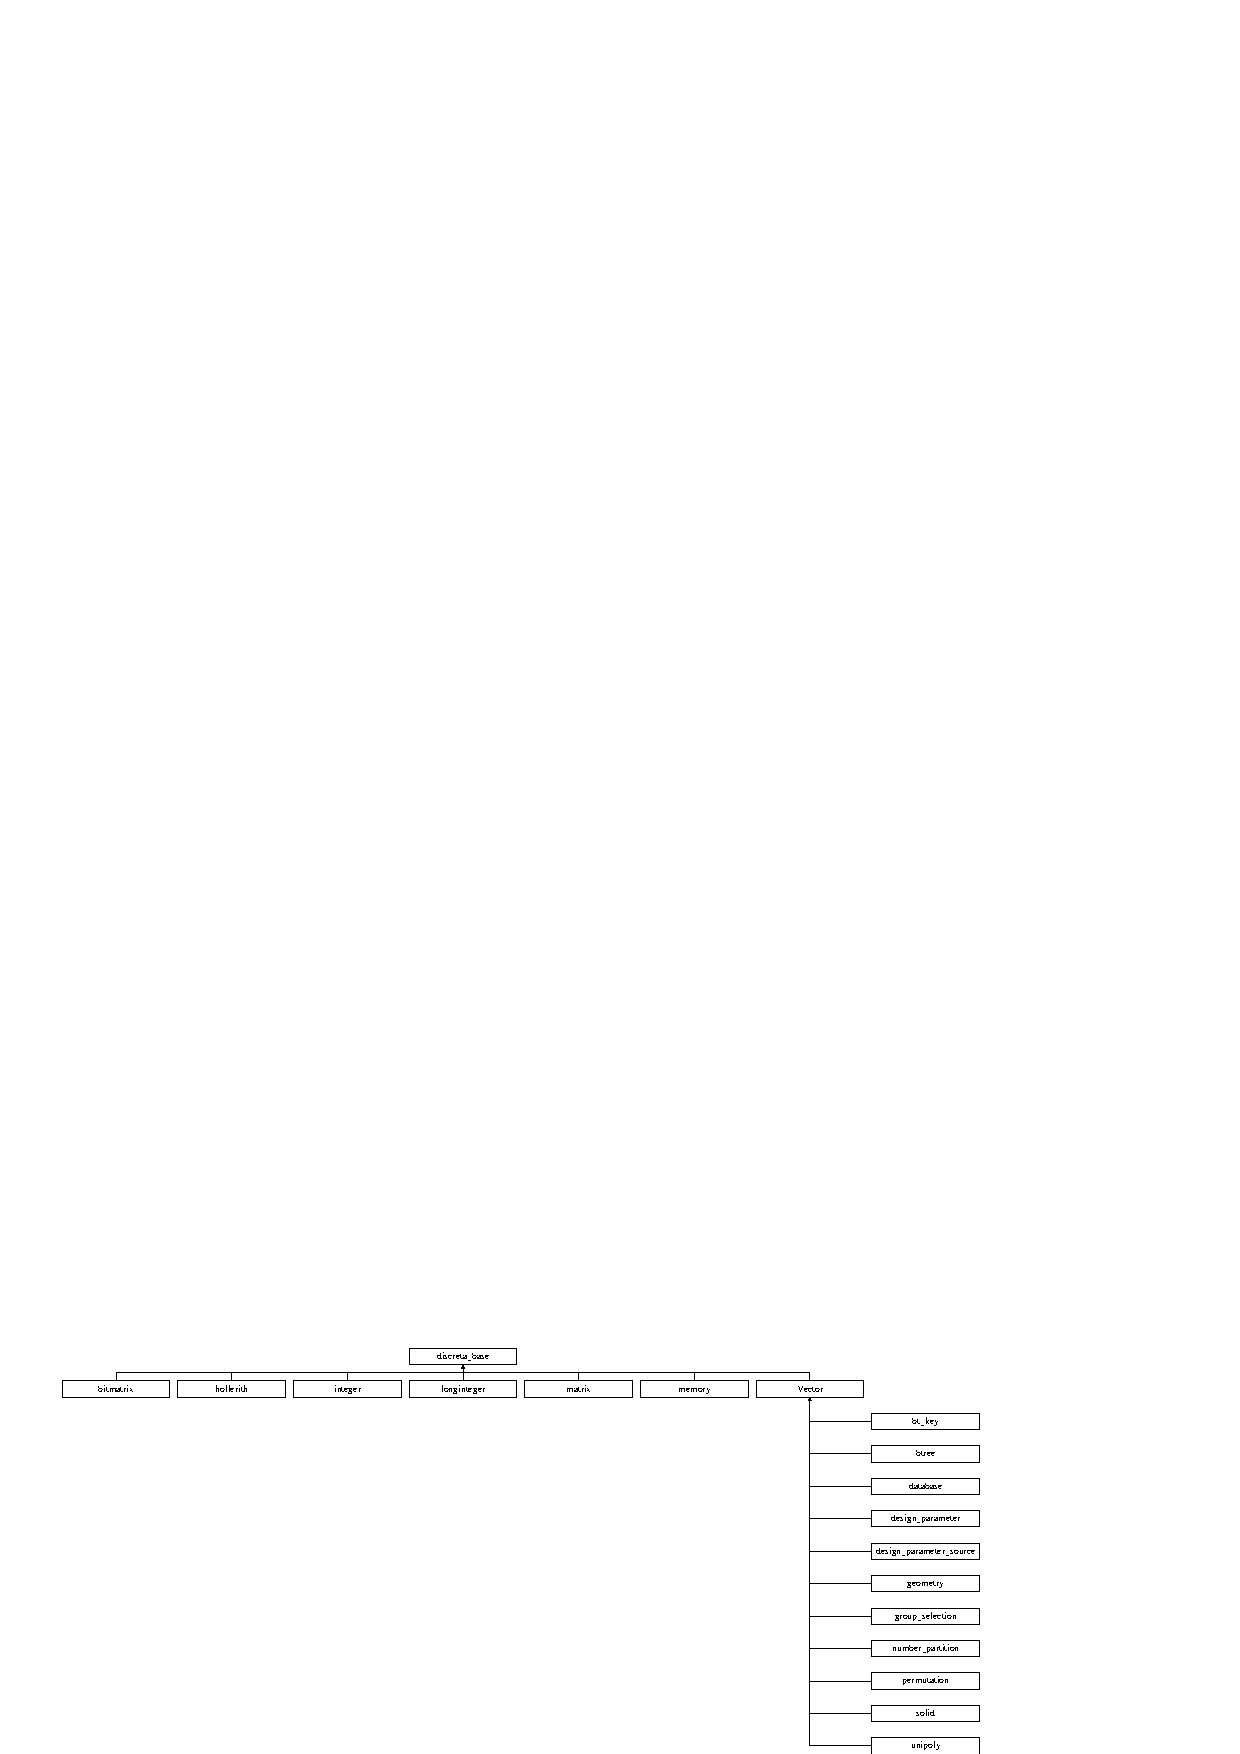
\includegraphics[height=5.449102cm]{classdiscreta__base}
\end{center}
\end{figure}
\subsection*{Public Member Functions}
\begin{DoxyCompactItemize}
\item 
\mbox{\hyperlink{classdiscreta__base_a52f72e02c11c566c8a8389b662b6c50c}{discreta\+\_\+base}} ()
\item 
\mbox{\hyperlink{classdiscreta__base_a0cdb2756e70a71eccecd13727f4e8f99}{discreta\+\_\+base}} (const \mbox{\hyperlink{classdiscreta__base}{discreta\+\_\+base}} \&\mbox{\hyperlink{alphabet2_8_c_a6150e0515f7202e2fb518f7206ed97dc}{x}})
\item 
\mbox{\hyperlink{classdiscreta__base}{discreta\+\_\+base}} \& \mbox{\hyperlink{classdiscreta__base_a4ccf158b3864d95b4e85fa471c748bae}{operator=}} (const \mbox{\hyperlink{classdiscreta__base}{discreta\+\_\+base}} \&\mbox{\hyperlink{alphabet2_8_c_a6150e0515f7202e2fb518f7206ed97dc}{x}})
\item 
virtual \mbox{\hyperlink{classdiscreta__base_a14df6915d3622e941d8bd541a6818d0e}{$\sim$discreta\+\_\+base}} ()
\item 
void \mbox{\hyperlink{classdiscreta__base_a8b1ec2cee4566034441e066dc2c027db}{freeself\+\_\+discreta\+\_\+base}} ()
\item 
void \mbox{\hyperlink{classdiscreta__base_a9a3c9501a562293b5667c11b9174d6e5}{freeself}} ()
\item 
void \mbox{\hyperlink{classdiscreta__base_a63a23ada2165b3838fab719ed458cec8}{freeself\+\_\+kind}} (\mbox{\hyperlink{discreta_8h_aaf25ee7e2306d78c74ec7bc48f092e81}{kind}} \mbox{\hyperlink{classdiscreta__base_a6f7a0f7bdd115b9e4dde358cfa7ebf81}{k}})
\item 
void \mbox{\hyperlink{classdiscreta__base_acc3985eac311491ab6ea3e409cffd3c4}{clearself}} ()
\item 
\mbox{\hyperlink{classinteger}{integer}} \& \mbox{\hyperlink{classdiscreta__base_a00d7691eaf874fd283d942692fe8dd26}{as\+\_\+integer}} ()
\item 
\mbox{\hyperlink{classlonginteger}{longinteger}} \& \mbox{\hyperlink{classdiscreta__base_a20a094639eb711b10c8694c51937f7cd}{as\+\_\+longinteger}} ()
\item 
\mbox{\hyperlink{class_vector}{Vector}} \& \mbox{\hyperlink{classdiscreta__base_a7bdd6cae39c380b128ee9e17e42cf020}{as\+\_\+vector}} ()
\item 
\mbox{\hyperlink{classpermutation}{permutation}} \& \mbox{\hyperlink{classdiscreta__base_aa4e72f36a82984239b12ae831e131098}{as\+\_\+permutation}} ()
\item 
\mbox{\hyperlink{classnumber__partition}{number\+\_\+partition}} \& \mbox{\hyperlink{classdiscreta__base_a307aa09de0e925d46697707968ffab00}{as\+\_\+number\+\_\+partition}} ()
\item 
\mbox{\hyperlink{classmatrix}{matrix}} \& \mbox{\hyperlink{classdiscreta__base_ae4d7f56d917a4707b838fbffde6467ff}{as\+\_\+matrix}} ()
\item 
\mbox{\hyperlink{classbitmatrix}{bitmatrix}} \& \mbox{\hyperlink{classdiscreta__base_a071ad54ea8ef6c9d1d15f532e5a76df6}{as\+\_\+bitmatrix}} ()
\item 
\mbox{\hyperlink{classunipoly}{unipoly}} \& \mbox{\hyperlink{classdiscreta__base_ad50d8027f039fe5c2478cddb243adc9d}{as\+\_\+unipoly}} ()
\item 
\mbox{\hyperlink{classmemory}{memory}} \& \mbox{\hyperlink{classdiscreta__base_ad94b2d7dce0cd4fa22db57f6e79c4bd2}{as\+\_\+memory}} ()
\item 
\mbox{\hyperlink{classaction}{action}} \& \mbox{\hyperlink{classdiscreta__base_aee03453d453c64f57eb30bf482d3ba8a}{as\+\_\+action}} ()
\item 
\mbox{\hyperlink{classgeometry}{geometry}} \& \mbox{\hyperlink{classdiscreta__base_a38fc7b4cdd830703e9d87354b79bc5c8}{as\+\_\+geometry}} ()
\item 
\mbox{\hyperlink{classhollerith}{hollerith}} \& \mbox{\hyperlink{classdiscreta__base_a3e66f82711f314710107e2f29e589690}{as\+\_\+hollerith}} ()
\item 
\mbox{\hyperlink{classgroup__selection}{group\+\_\+selection}} \& \mbox{\hyperlink{classdiscreta__base_aae1bac4883c567718bef9fb610abbdc8}{as\+\_\+group\+\_\+selection}} ()
\item 
\mbox{\hyperlink{classsolid}{solid}} \& \mbox{\hyperlink{classdiscreta__base_a1fc5f2b85ec97ab0a69dd64903c970a5}{as\+\_\+solid}} ()
\item 
\mbox{\hyperlink{classbt__key}{bt\+\_\+key}} \& \mbox{\hyperlink{classdiscreta__base_a2734c6e08dca17cf6588bd5064ec1b9f}{as\+\_\+bt\+\_\+key}} ()
\item 
\mbox{\hyperlink{classdatabase}{database}} \& \mbox{\hyperlink{classdiscreta__base_ab055d39d58210a2b03ba3d33703b09a9}{as\+\_\+database}} ()
\item 
\mbox{\hyperlink{classbtree}{btree}} \& \mbox{\hyperlink{classdiscreta__base_a78e76674cef2ec113c17989c11288778}{as\+\_\+btree}} ()
\item 
\mbox{\hyperlink{classdesign__parameter__source}{design\+\_\+parameter\+\_\+source}} \& \mbox{\hyperlink{classdiscreta__base_a59cbf837c6582ded5bc586265d13d81a}{as\+\_\+design\+\_\+parameter\+\_\+source}} ()
\item 
\mbox{\hyperlink{classdesign__parameter}{design\+\_\+parameter}} \& \mbox{\hyperlink{classdiscreta__base_aab24ff38ea1c5471ab3de42e014d0f2a}{as\+\_\+design\+\_\+parameter}} ()
\item 
\mbox{\hyperlink{classinteger}{integer}} \& \mbox{\hyperlink{classdiscreta__base_a58a5a5bd8f8e6f2dd7b4483b66dc7bb9}{change\+\_\+to\+\_\+integer}} ()
\item 
\mbox{\hyperlink{classlonginteger}{longinteger}} \& \mbox{\hyperlink{classdiscreta__base_aa65b4b95b89b1df5ff8e0ef944e598a9}{change\+\_\+to\+\_\+longinteger}} ()
\item 
\mbox{\hyperlink{class_vector}{Vector}} \& \mbox{\hyperlink{classdiscreta__base_a66186d19c55ad54af11e2a040a763c38}{change\+\_\+to\+\_\+vector}} ()
\item 
\mbox{\hyperlink{classpermutation}{permutation}} \& \mbox{\hyperlink{classdiscreta__base_a38e11ff129ddc29d67b54520e9a0a538}{change\+\_\+to\+\_\+permutation}} ()
\item 
\mbox{\hyperlink{classnumber__partition}{number\+\_\+partition}} \& \mbox{\hyperlink{classdiscreta__base_a15be55441d3768c506bf9faabeef9b5b}{change\+\_\+to\+\_\+number\+\_\+partition}} ()
\item 
\mbox{\hyperlink{classmatrix}{matrix}} \& \mbox{\hyperlink{classdiscreta__base_a51f1aaa0764c4161c0dbd981091ca5cb}{change\+\_\+to\+\_\+matrix}} ()
\item 
\mbox{\hyperlink{classbitmatrix}{bitmatrix}} \& \mbox{\hyperlink{classdiscreta__base_adcb7fdf185f23731b42c96488599919e}{change\+\_\+to\+\_\+bitmatrix}} ()
\item 
\mbox{\hyperlink{classunipoly}{unipoly}} \& \mbox{\hyperlink{classdiscreta__base_a436a1d89a0e7a13ba1ad0ff5813c03ed}{change\+\_\+to\+\_\+unipoly}} ()
\item 
\mbox{\hyperlink{classmemory}{memory}} \& \mbox{\hyperlink{classdiscreta__base_a21a76b868e94f17a6579997f0a50a006}{change\+\_\+to\+\_\+memory}} ()
\item 
\mbox{\hyperlink{classgeometry}{geometry}} \& \mbox{\hyperlink{classdiscreta__base_a5a3efbeeb01c41259b91ed2d87bfcbb2}{change\+\_\+to\+\_\+geometry}} ()
\item 
\mbox{\hyperlink{classhollerith}{hollerith}} \& \mbox{\hyperlink{classdiscreta__base_a10f410adc814d4568e3b0f84550c4ca1}{change\+\_\+to\+\_\+hollerith}} ()
\item 
\mbox{\hyperlink{classgroup__selection}{group\+\_\+selection}} \& \mbox{\hyperlink{classdiscreta__base_a6b269515e796a08da4db719ae2dbdca9}{change\+\_\+to\+\_\+group\+\_\+selection}} ()
\item 
\mbox{\hyperlink{classsolid}{solid}} \& \mbox{\hyperlink{classdiscreta__base_adb0b11a85434f969b3895cb46b67e8c2}{change\+\_\+to\+\_\+solid}} ()
\item 
\mbox{\hyperlink{classbt__key}{bt\+\_\+key}} \& \mbox{\hyperlink{classdiscreta__base_af08930510236fe08941bb5c1e4768fe9}{change\+\_\+to\+\_\+bt\+\_\+key}} ()
\item 
\mbox{\hyperlink{classdatabase}{database}} \& \mbox{\hyperlink{classdiscreta__base_a9187fb1e0526e3d327b78bb19475ae40}{change\+\_\+to\+\_\+database}} ()
\item 
\mbox{\hyperlink{classbtree}{btree}} \& \mbox{\hyperlink{classdiscreta__base_a75c8608cf54191c17ee48817cc4dda17}{change\+\_\+to\+\_\+btree}} ()
\item 
\mbox{\hyperlink{classdesign__parameter__source}{design\+\_\+parameter\+\_\+source}} \& \mbox{\hyperlink{classdiscreta__base_adef7252719a3b1b5261d6bc6c44dbda4}{change\+\_\+to\+\_\+design\+\_\+parameter\+\_\+source}} ()
\item 
\mbox{\hyperlink{classdesign__parameter}{design\+\_\+parameter}} \& \mbox{\hyperlink{classdiscreta__base_ab207ed39acee5f447708dc9fcfd29e0a}{change\+\_\+to\+\_\+design\+\_\+parameter}} ()
\item 
void $\ast$ \mbox{\hyperlink{classdiscreta__base_aa42f42d6b940b80fbf451b10620e99ac}{operator new}} (size\+\_\+t, void $\ast$\mbox{\hyperlink{alphabet2_8_c_a533391314665d6bf1b5575e9a9cd8552}{p}})
\item 
void \mbox{\hyperlink{classdiscreta__base_a4f42899a89447d1c3993ea07c38f8ad4}{settype\+\_\+base}} ()
\item 
\mbox{\hyperlink{discreta_8h_aaf25ee7e2306d78c74ec7bc48f092e81}{kind}} \mbox{\hyperlink{classdiscreta__base_a8a830025c74adbbc3362418a7c2ba157}{s\+\_\+kind}} ()
\item 
virtual \mbox{\hyperlink{discreta_8h_aaf25ee7e2306d78c74ec7bc48f092e81}{kind}} \mbox{\hyperlink{classdiscreta__base_a52778a6d6943a468be083d0785d418fb}{s\+\_\+virtual\+\_\+kind}} ()
\item 
void \mbox{\hyperlink{classdiscreta__base_adc2ff61589c2d083688e7a43f333cb62}{c\+\_\+kind}} (\mbox{\hyperlink{discreta_8h_aaf25ee7e2306d78c74ec7bc48f092e81}{kind}} \mbox{\hyperlink{classdiscreta__base_a6f7a0f7bdd115b9e4dde358cfa7ebf81}{k}})
\item 
void \mbox{\hyperlink{classdiscreta__base_a2e8acbb9d3476675dac5b6a583b0293e}{swap}} (\mbox{\hyperlink{classdiscreta__base}{discreta\+\_\+base}} \&a)
\item 
void \mbox{\hyperlink{classdiscreta__base_a68fac2b12cefae0bc4d1a41faf9bc862}{copyobject}} (\mbox{\hyperlink{classdiscreta__base}{discreta\+\_\+base}} \&\mbox{\hyperlink{alphabet2_8_c_a6150e0515f7202e2fb518f7206ed97dc}{x}})
\item 
virtual void \mbox{\hyperlink{classdiscreta__base_a33180628d9ced231267229b3564790f3}{copyobject\+\_\+to}} (\mbox{\hyperlink{classdiscreta__base}{discreta\+\_\+base}} \&\mbox{\hyperlink{alphabet2_8_c_a6150e0515f7202e2fb518f7206ed97dc}{x}})
\item 
virtual ostream \& \mbox{\hyperlink{classdiscreta__base_a036e48bc058347046fc9b73dd0951478}{print}} (ostream \&)
\item 
void \mbox{\hyperlink{classdiscreta__base_aa0c0ba64fdeef1b76df143048bca47ea}{print\+\_\+to\+\_\+hollerith}} (\mbox{\hyperlink{classhollerith}{hollerith}} \&\mbox{\hyperlink{alphabet2_8_c_a16611451551e3d15916bae723c3f59f7}{h}})
\item 
ostream \& \mbox{\hyperlink{classdiscreta__base_a9f021788626eb6e6622142a0f3494727}{println}} (ostream \&)
\item 
ostream \& \mbox{\hyperlink{classdiscreta__base_aa75a1314aa706909b029664944904231}{printobjectkind}} (ostream \&)
\item 
ostream \& \mbox{\hyperlink{classdiscreta__base_a677ccc8f392ebedde05e453f8cf59559}{printobjectkindln}} (ostream \&)
\item 
\mbox{\hyperlink{galois_8h_a09fddde158a3a20bd2dcadb609de11dc}{I\+NT}} \& \mbox{\hyperlink{classdiscreta__base_aadb92c01fbe69b3034b0214b33fbc735}{s\+\_\+i\+\_\+i}} ()
\item 
void \mbox{\hyperlink{classdiscreta__base_aa231464a9d4bc233f66608021c9ad997}{m\+\_\+i\+\_\+i}} (\mbox{\hyperlink{galois_8h_a09fddde158a3a20bd2dcadb609de11dc}{I\+NT}} \mbox{\hyperlink{alphabet2_8_c_acb559820d9ca11295b4500f179ef6392}{i}})
\item 
virtual \mbox{\hyperlink{galois_8h_a09fddde158a3a20bd2dcadb609de11dc}{I\+NT}} \mbox{\hyperlink{classdiscreta__base_a3818444c4301d0b7ed47c3b850ea6c60}{compare\+\_\+with}} (\mbox{\hyperlink{classdiscreta__base}{discreta\+\_\+base}} \&a)
\item 
\mbox{\hyperlink{galois_8h_a09fddde158a3a20bd2dcadb609de11dc}{I\+NT}} \mbox{\hyperlink{classdiscreta__base_a7afe4f013b04efa764ed9fe099e5eb80}{eq}} (\mbox{\hyperlink{classdiscreta__base}{discreta\+\_\+base}} \&a)
\item 
\mbox{\hyperlink{galois_8h_a09fddde158a3a20bd2dcadb609de11dc}{I\+NT}} \mbox{\hyperlink{classdiscreta__base_a42975aaa9bb0b76d468df7fdb9390251}{neq}} (\mbox{\hyperlink{classdiscreta__base}{discreta\+\_\+base}} \&a)
\item 
\mbox{\hyperlink{galois_8h_a09fddde158a3a20bd2dcadb609de11dc}{I\+NT}} \mbox{\hyperlink{classdiscreta__base_a2813443682a077fd4112415ee299f087}{le}} (\mbox{\hyperlink{classdiscreta__base}{discreta\+\_\+base}} \&a)
\item 
\mbox{\hyperlink{galois_8h_a09fddde158a3a20bd2dcadb609de11dc}{I\+NT}} \mbox{\hyperlink{classdiscreta__base_a3e17f6a5f027ea3f631a3ba3c540ff3f}{lt}} (\mbox{\hyperlink{classdiscreta__base}{discreta\+\_\+base}} \&a)
\item 
\mbox{\hyperlink{galois_8h_a09fddde158a3a20bd2dcadb609de11dc}{I\+NT}} \mbox{\hyperlink{classdiscreta__base_a06af05fc220a55e844849fe665545c03}{ge}} (\mbox{\hyperlink{classdiscreta__base}{discreta\+\_\+base}} \&a)
\item 
\mbox{\hyperlink{galois_8h_a09fddde158a3a20bd2dcadb609de11dc}{I\+NT}} \mbox{\hyperlink{classdiscreta__base_ac7dbe66505d512c802c0698c13b05605}{gt}} (\mbox{\hyperlink{classdiscreta__base}{discreta\+\_\+base}} \&a)
\item 
\mbox{\hyperlink{galois_8h_a09fddde158a3a20bd2dcadb609de11dc}{I\+NT}} \mbox{\hyperlink{classdiscreta__base_a588ab4fb1bc60455db16ea7d1e6f74ca}{is\+\_\+even}} ()
\item 
\mbox{\hyperlink{galois_8h_a09fddde158a3a20bd2dcadb609de11dc}{I\+NT}} \mbox{\hyperlink{classdiscreta__base_a4fc6a621844c78d4199639ba394c31eb}{is\+\_\+odd}} ()
\item 
void \mbox{\hyperlink{classdiscreta__base_a96f759b28f7c30bdfd95ac10f5972bd0}{mult}} (\mbox{\hyperlink{classdiscreta__base}{discreta\+\_\+base}} \&\mbox{\hyperlink{alphabet2_8_c_a6150e0515f7202e2fb518f7206ed97dc}{x}}, \mbox{\hyperlink{classdiscreta__base}{discreta\+\_\+base}} \&\mbox{\hyperlink{alphabet2_8_c_a0a2f84ed7838f07779ae24c5a9086d33}{y}})
\item 
void \mbox{\hyperlink{classdiscreta__base_a01f00cf6c9f4a8d6209636de98e05c30}{mult\+\_\+mod}} (\mbox{\hyperlink{classdiscreta__base}{discreta\+\_\+base}} \&\mbox{\hyperlink{alphabet2_8_c_a6150e0515f7202e2fb518f7206ed97dc}{x}}, \mbox{\hyperlink{classdiscreta__base}{discreta\+\_\+base}} \&\mbox{\hyperlink{alphabet2_8_c_a0a2f84ed7838f07779ae24c5a9086d33}{y}}, \mbox{\hyperlink{classdiscreta__base}{discreta\+\_\+base}} \&\mbox{\hyperlink{alphabet2_8_c_a533391314665d6bf1b5575e9a9cd8552}{p}})
\item 
virtual void \mbox{\hyperlink{classdiscreta__base_a54d5c16c016769e3365639721c06591e}{mult\+\_\+to}} (\mbox{\hyperlink{classdiscreta__base}{discreta\+\_\+base}} \&\mbox{\hyperlink{alphabet2_8_c_a6150e0515f7202e2fb518f7206ed97dc}{x}}, \mbox{\hyperlink{classdiscreta__base}{discreta\+\_\+base}} \&\mbox{\hyperlink{alphabet2_8_c_a0a2f84ed7838f07779ae24c5a9086d33}{y}})
\item 
\mbox{\hyperlink{galois_8h_a09fddde158a3a20bd2dcadb609de11dc}{I\+NT}} \mbox{\hyperlink{classdiscreta__base_a3c415a064ce76e183f000912875dea74}{invert}} ()
\item 
\mbox{\hyperlink{galois_8h_a09fddde158a3a20bd2dcadb609de11dc}{I\+NT}} \mbox{\hyperlink{classdiscreta__base_ae730a9ba3ebdb5ac13685ea86d93aec0}{invert\+\_\+mod}} (\mbox{\hyperlink{classdiscreta__base}{discreta\+\_\+base}} \&\mbox{\hyperlink{alphabet2_8_c_a533391314665d6bf1b5575e9a9cd8552}{p}})
\item 
virtual \mbox{\hyperlink{galois_8h_a09fddde158a3a20bd2dcadb609de11dc}{I\+NT}} \mbox{\hyperlink{classdiscreta__base_a874a5ffb467f3896604a3c9bdf0cca50}{invert\+\_\+to}} (\mbox{\hyperlink{classdiscreta__base}{discreta\+\_\+base}} \&\mbox{\hyperlink{alphabet2_8_c_a6150e0515f7202e2fb518f7206ed97dc}{x}})
\item 
void \mbox{\hyperlink{classdiscreta__base_a301b8d0527d3a60ba410bba87446f490}{mult\+\_\+apply}} (\mbox{\hyperlink{classdiscreta__base}{discreta\+\_\+base}} \&\mbox{\hyperlink{alphabet2_8_c_a6150e0515f7202e2fb518f7206ed97dc}{x}})
\item 
\mbox{\hyperlink{classdiscreta__base}{discreta\+\_\+base}} \& \mbox{\hyperlink{classdiscreta__base_a26a19fcfe00422fe1d8a66d5b1b4a60a}{operator$\ast$=}} (\mbox{\hyperlink{classdiscreta__base}{discreta\+\_\+base}} \&\mbox{\hyperlink{alphabet2_8_c_a0a2f84ed7838f07779ae24c5a9086d33}{y}})
\item 
\mbox{\hyperlink{classdiscreta__base}{discreta\+\_\+base}} \& \mbox{\hyperlink{classdiscreta__base_a4b7be615dfc1a72b6c6a623325e77628}{power\+\_\+int}} (\mbox{\hyperlink{galois_8h_a09fddde158a3a20bd2dcadb609de11dc}{I\+NT}} \mbox{\hyperlink{alphabet2_8_c_a89606eca6b563ec68d2da2e84657736f}{l}})
\item 
\mbox{\hyperlink{classdiscreta__base}{discreta\+\_\+base}} \& \mbox{\hyperlink{classdiscreta__base_abbedc6f882b55fe0b98dec33da832f8e}{power\+\_\+int\+\_\+mod}} (\mbox{\hyperlink{galois_8h_a09fddde158a3a20bd2dcadb609de11dc}{I\+NT}} \mbox{\hyperlink{alphabet2_8_c_a89606eca6b563ec68d2da2e84657736f}{l}}, \mbox{\hyperlink{classdiscreta__base}{discreta\+\_\+base}} \&\mbox{\hyperlink{alphabet2_8_c_a533391314665d6bf1b5575e9a9cd8552}{p}})
\item 
\mbox{\hyperlink{classdiscreta__base}{discreta\+\_\+base}} \& \mbox{\hyperlink{classdiscreta__base_aa62919063915230ba88a0a070a38f3d6}{power\+\_\+longinteger}} (\mbox{\hyperlink{classlonginteger}{longinteger}} \&\mbox{\hyperlink{alphabet2_8_c_a89606eca6b563ec68d2da2e84657736f}{l}})
\item 
\mbox{\hyperlink{classdiscreta__base}{discreta\+\_\+base}} \& \mbox{\hyperlink{classdiscreta__base_a13cf1612186baa2104f55978cbf56873}{power\+\_\+longinteger\+\_\+mod}} (\mbox{\hyperlink{classlonginteger}{longinteger}} \&\mbox{\hyperlink{alphabet2_8_c_a89606eca6b563ec68d2da2e84657736f}{l}}, \mbox{\hyperlink{classdiscreta__base}{discreta\+\_\+base}} \&\mbox{\hyperlink{alphabet2_8_c_a533391314665d6bf1b5575e9a9cd8552}{p}})
\item 
\mbox{\hyperlink{classdiscreta__base}{discreta\+\_\+base}} \& \mbox{\hyperlink{classdiscreta__base_a1d0bb4144e3eb15aaf877a0cea656c00}{commutator}} (\mbox{\hyperlink{classdiscreta__base}{discreta\+\_\+base}} \&\mbox{\hyperlink{alphabet2_8_c_a6150e0515f7202e2fb518f7206ed97dc}{x}}, \mbox{\hyperlink{classdiscreta__base}{discreta\+\_\+base}} \&\mbox{\hyperlink{alphabet2_8_c_a0a2f84ed7838f07779ae24c5a9086d33}{y}})
\item 
\mbox{\hyperlink{classdiscreta__base}{discreta\+\_\+base}} \& \mbox{\hyperlink{classdiscreta__base_a463f1481dd1a3ab42deb6162e25ba725}{conjugate}} (\mbox{\hyperlink{classdiscreta__base}{discreta\+\_\+base}} \&\mbox{\hyperlink{alphabet2_8_c_a6150e0515f7202e2fb518f7206ed97dc}{x}}, \mbox{\hyperlink{classdiscreta__base}{discreta\+\_\+base}} \&\mbox{\hyperlink{alphabet2_8_c_a0a2f84ed7838f07779ae24c5a9086d33}{y}})
\item 
\mbox{\hyperlink{classdiscreta__base}{discreta\+\_\+base}} \& \mbox{\hyperlink{classdiscreta__base_aa3f9d43fab5e6240202fbd7c1f5e3e74}{divide\+\_\+by}} (\mbox{\hyperlink{classdiscreta__base}{discreta\+\_\+base}} \&\mbox{\hyperlink{alphabet2_8_c_a6150e0515f7202e2fb518f7206ed97dc}{x}})
\item 
\mbox{\hyperlink{classdiscreta__base}{discreta\+\_\+base}} \& \mbox{\hyperlink{classdiscreta__base_a14ea31dd075b20644457db08319389ef}{divide\+\_\+by\+\_\+exact}} (\mbox{\hyperlink{classdiscreta__base}{discreta\+\_\+base}} \&\mbox{\hyperlink{alphabet2_8_c_a6150e0515f7202e2fb518f7206ed97dc}{x}})
\item 
\mbox{\hyperlink{galois_8h_a09fddde158a3a20bd2dcadb609de11dc}{I\+NT}} \mbox{\hyperlink{classdiscreta__base_a4ce6b54534e4882c48c051c03ac76e52}{order}} ()
\item 
\mbox{\hyperlink{galois_8h_a09fddde158a3a20bd2dcadb609de11dc}{I\+NT}} \mbox{\hyperlink{classdiscreta__base_aee39628b4299a335baca784802ac0f3c}{order\+\_\+mod}} (\mbox{\hyperlink{classdiscreta__base}{discreta\+\_\+base}} \&\mbox{\hyperlink{alphabet2_8_c_a533391314665d6bf1b5575e9a9cd8552}{p}})
\item 
void \mbox{\hyperlink{classdiscreta__base_a209e98b4fef96cb922b3caa49cd70a79}{add}} (\mbox{\hyperlink{classdiscreta__base}{discreta\+\_\+base}} \&\mbox{\hyperlink{alphabet2_8_c_a6150e0515f7202e2fb518f7206ed97dc}{x}}, \mbox{\hyperlink{classdiscreta__base}{discreta\+\_\+base}} \&\mbox{\hyperlink{alphabet2_8_c_a0a2f84ed7838f07779ae24c5a9086d33}{y}})
\item 
void \mbox{\hyperlink{classdiscreta__base_aa8864b3f228cad737b2f3ff469bd8f63}{add\+\_\+mod}} (\mbox{\hyperlink{classdiscreta__base}{discreta\+\_\+base}} \&\mbox{\hyperlink{alphabet2_8_c_a6150e0515f7202e2fb518f7206ed97dc}{x}}, \mbox{\hyperlink{classdiscreta__base}{discreta\+\_\+base}} \&\mbox{\hyperlink{alphabet2_8_c_a0a2f84ed7838f07779ae24c5a9086d33}{y}}, \mbox{\hyperlink{classdiscreta__base}{discreta\+\_\+base}} \&\mbox{\hyperlink{alphabet2_8_c_a533391314665d6bf1b5575e9a9cd8552}{p}})
\item 
virtual void \mbox{\hyperlink{classdiscreta__base_a712a61311eb036d70a52871ed315f515}{add\+\_\+to}} (\mbox{\hyperlink{classdiscreta__base}{discreta\+\_\+base}} \&\mbox{\hyperlink{alphabet2_8_c_a6150e0515f7202e2fb518f7206ed97dc}{x}}, \mbox{\hyperlink{classdiscreta__base}{discreta\+\_\+base}} \&\mbox{\hyperlink{alphabet2_8_c_a0a2f84ed7838f07779ae24c5a9086d33}{y}})
\item 
void \mbox{\hyperlink{classdiscreta__base_aac1be1125008f8a93a3083cd1a43878d}{negate}} ()
\item 
virtual void \mbox{\hyperlink{classdiscreta__base_a65ad2034f2f4518d424b814974018a03}{negate\+\_\+to}} (\mbox{\hyperlink{classdiscreta__base}{discreta\+\_\+base}} \&\mbox{\hyperlink{alphabet2_8_c_a6150e0515f7202e2fb518f7206ed97dc}{x}})
\item 
void \mbox{\hyperlink{classdiscreta__base_a1e8b73324062c6ff9e01aaf5fb6e8fba}{add\+\_\+apply}} (\mbox{\hyperlink{classdiscreta__base}{discreta\+\_\+base}} \&\mbox{\hyperlink{alphabet2_8_c_a6150e0515f7202e2fb518f7206ed97dc}{x}})
\item 
\mbox{\hyperlink{classdiscreta__base}{discreta\+\_\+base}} \& \mbox{\hyperlink{classdiscreta__base_ad0b0a337ccba39d87fe21ffe15bef951}{operator+=}} (\mbox{\hyperlink{classdiscreta__base}{discreta\+\_\+base}} \&\mbox{\hyperlink{alphabet2_8_c_a0a2f84ed7838f07779ae24c5a9086d33}{y}})
\item 
virtual void \mbox{\hyperlink{classdiscreta__base_acd46a488505c6086b5bc019550e5e313}{normalize}} (\mbox{\hyperlink{classdiscreta__base}{discreta\+\_\+base}} \&\mbox{\hyperlink{alphabet2_8_c_a533391314665d6bf1b5575e9a9cd8552}{p}})
\item 
virtual void \mbox{\hyperlink{classdiscreta__base_a424aa44bbb6ca48d30ad1087dbd6f210}{zero}} ()
\item 
virtual void \mbox{\hyperlink{classdiscreta__base_a6f5d6422a0040950415db30e39dafd19}{one}} ()
\item 
virtual void \mbox{\hyperlink{classdiscreta__base_a3a147eee6f3477387f7e580c117e5a05}{m\+\_\+one}} ()
\item 
virtual void \mbox{\hyperlink{classdiscreta__base_a40e349b2d85c5c6dba9c015d16a0e801}{homo\+\_\+z}} (\mbox{\hyperlink{galois_8h_a09fddde158a3a20bd2dcadb609de11dc}{I\+NT}} z)
\item 
virtual void \mbox{\hyperlink{classdiscreta__base_afda42789f4ba04ba399623a6b9e206e3}{inc}} ()
\item 
virtual void \mbox{\hyperlink{classdiscreta__base_a11449a5cfa7dc5f5600e012517af6f0f}{dec}} ()
\item 
virtual \mbox{\hyperlink{galois_8h_a09fddde158a3a20bd2dcadb609de11dc}{I\+NT}} \mbox{\hyperlink{classdiscreta__base_ac75f6bdc1ba1b406e26cf921adfd9864}{is\+\_\+zero}} ()
\item 
virtual \mbox{\hyperlink{galois_8h_a09fddde158a3a20bd2dcadb609de11dc}{I\+NT}} \mbox{\hyperlink{classdiscreta__base_a28fa37aac83194174888d34f07f43848}{is\+\_\+one}} ()
\item 
virtual \mbox{\hyperlink{galois_8h_a09fddde158a3a20bd2dcadb609de11dc}{I\+NT}} \mbox{\hyperlink{classdiscreta__base_afc2e134e55759cf069f49fcf05af418b}{is\+\_\+m\+\_\+one}} ()
\item 
\mbox{\hyperlink{classdiscreta__base}{discreta\+\_\+base}} \& \mbox{\hyperlink{classdiscreta__base_a1e817d0bf74554af67bd4df140989a7f}{factorial}} (\mbox{\hyperlink{galois_8h_a09fddde158a3a20bd2dcadb609de11dc}{I\+NT}} z)
\item 
\mbox{\hyperlink{classdiscreta__base}{discreta\+\_\+base}} \& \mbox{\hyperlink{classdiscreta__base_ae0bc8b345a8d639e626267ddbebaa7a1}{i\+\_\+power\+\_\+j}} (\mbox{\hyperlink{galois_8h_a09fddde158a3a20bd2dcadb609de11dc}{I\+NT}} \mbox{\hyperlink{alphabet2_8_c_acb559820d9ca11295b4500f179ef6392}{i}}, \mbox{\hyperlink{galois_8h_a09fddde158a3a20bd2dcadb609de11dc}{I\+NT}} \mbox{\hyperlink{alphabet2_8_c_a37d972ae0b47b9099e30983131d31916}{j}})
\item 
virtual \mbox{\hyperlink{galois_8h_a09fddde158a3a20bd2dcadb609de11dc}{I\+NT}} \mbox{\hyperlink{classdiscreta__base_a9d3091feb2fbc69359c2a45f11ceec9e}{compare\+\_\+with\+\_\+euklidean}} (\mbox{\hyperlink{classdiscreta__base}{discreta\+\_\+base}} \&a)
\item 
virtual void \mbox{\hyperlink{classdiscreta__base_a92b3001ac35af9185b316c0d8f89070e}{integral\+\_\+division}} (\mbox{\hyperlink{classdiscreta__base}{discreta\+\_\+base}} \&\mbox{\hyperlink{alphabet2_8_c_a6150e0515f7202e2fb518f7206ed97dc}{x}}, \mbox{\hyperlink{classdiscreta__base}{discreta\+\_\+base}} \&\mbox{\hyperlink{simeon_8_c_a92cbb483a3b27ae1a0dbfcb125ce216f}{q}}, \mbox{\hyperlink{classdiscreta__base}{discreta\+\_\+base}} \&\mbox{\hyperlink{alphabet2_8_c_acab531abaa74a7e664e3986f2522b33a}{r}}, \mbox{\hyperlink{galois_8h_a09fddde158a3a20bd2dcadb609de11dc}{I\+NT}} \mbox{\hyperlink{simeon_8_c_a818073fbcc2f439e7c56952f67386122}{verbose\+\_\+level}})
\item 
void \mbox{\hyperlink{classdiscreta__base_a77aa5f7ddec1f6baa8fb39fa16f479af}{integral\+\_\+division\+\_\+exact}} (\mbox{\hyperlink{classdiscreta__base}{discreta\+\_\+base}} \&\mbox{\hyperlink{alphabet2_8_c_a6150e0515f7202e2fb518f7206ed97dc}{x}}, \mbox{\hyperlink{classdiscreta__base}{discreta\+\_\+base}} \&\mbox{\hyperlink{simeon_8_c_a92cbb483a3b27ae1a0dbfcb125ce216f}{q}})
\item 
void \mbox{\hyperlink{classdiscreta__base_a99ccabe98387331a67eed3a29c26d004}{integral\+\_\+division\+\_\+by\+\_\+integer}} (\mbox{\hyperlink{galois_8h_a09fddde158a3a20bd2dcadb609de11dc}{I\+NT}} \mbox{\hyperlink{alphabet2_8_c_a6150e0515f7202e2fb518f7206ed97dc}{x}}, \mbox{\hyperlink{classdiscreta__base}{discreta\+\_\+base}} \&\mbox{\hyperlink{simeon_8_c_a92cbb483a3b27ae1a0dbfcb125ce216f}{q}}, \mbox{\hyperlink{classdiscreta__base}{discreta\+\_\+base}} \&\mbox{\hyperlink{alphabet2_8_c_acab531abaa74a7e664e3986f2522b33a}{r}})
\item 
void \mbox{\hyperlink{classdiscreta__base_a0c0f9fcd2ef1fb56a51bbd93e0411b49}{integral\+\_\+division\+\_\+by\+\_\+integer\+\_\+exact}} (\mbox{\hyperlink{galois_8h_a09fddde158a3a20bd2dcadb609de11dc}{I\+NT}} \mbox{\hyperlink{alphabet2_8_c_a6150e0515f7202e2fb518f7206ed97dc}{x}}, \mbox{\hyperlink{classdiscreta__base}{discreta\+\_\+base}} \&\mbox{\hyperlink{simeon_8_c_a92cbb483a3b27ae1a0dbfcb125ce216f}{q}})
\item 
void \mbox{\hyperlink{classdiscreta__base_ae3e8cc479b6823e0ffc1d9b1e0e9d0e7}{integral\+\_\+division\+\_\+by\+\_\+integer\+\_\+exact\+\_\+apply}} (\mbox{\hyperlink{galois_8h_a09fddde158a3a20bd2dcadb609de11dc}{I\+NT}} \mbox{\hyperlink{alphabet2_8_c_a6150e0515f7202e2fb518f7206ed97dc}{x}})
\item 
\mbox{\hyperlink{galois_8h_a09fddde158a3a20bd2dcadb609de11dc}{I\+NT}} \mbox{\hyperlink{classdiscreta__base_ae6cf39d4b122ec93866ae59607b15350}{is\+\_\+divisor}} (\mbox{\hyperlink{classdiscreta__base}{discreta\+\_\+base}} \&\mbox{\hyperlink{alphabet2_8_c_a0a2f84ed7838f07779ae24c5a9086d33}{y}})
\item 
void \mbox{\hyperlink{classdiscreta__base_ac4ee015a4115c5f5851cb3da41c8eca0}{modulo}} (\mbox{\hyperlink{classdiscreta__base}{discreta\+\_\+base}} \&\mbox{\hyperlink{alphabet2_8_c_a533391314665d6bf1b5575e9a9cd8552}{p}})
\item 
void \mbox{\hyperlink{classdiscreta__base_acf4c69f8f0f01f8af975c131121180f4}{extended\+\_\+gcd}} (\mbox{\hyperlink{classdiscreta__base}{discreta\+\_\+base}} \&\mbox{\hyperlink{simeon_8_c_a7f2cd26777ce0ff3fdaf8d02aacbddfb}{n}}, \mbox{\hyperlink{classdiscreta__base}{discreta\+\_\+base}} \&\mbox{\hyperlink{alphabet2_8_c_a5874b4c2ec2e28321eea4e4871d08222}{u}}, \mbox{\hyperlink{classdiscreta__base}{discreta\+\_\+base}} \&\mbox{\hyperlink{simeon_8_c_aeb3f3030944801b163bc3b829a7f6710}{v}}, \mbox{\hyperlink{classdiscreta__base}{discreta\+\_\+base}} \&g, \mbox{\hyperlink{galois_8h_a09fddde158a3a20bd2dcadb609de11dc}{I\+NT}} \mbox{\hyperlink{simeon_8_c_a818073fbcc2f439e7c56952f67386122}{verbose\+\_\+level}})
\item 
void \mbox{\hyperlink{classdiscreta__base_a449ed7914b693346288f56a60b12c4af}{write\+\_\+memory}} (\mbox{\hyperlink{classmemory}{memory}} \&m, \mbox{\hyperlink{galois_8h_a09fddde158a3a20bd2dcadb609de11dc}{I\+NT}} debug\+\_\+depth)
\item 
void \mbox{\hyperlink{classdiscreta__base_a224239da232eb4165783845a48e8b170}{read\+\_\+memory}} (\mbox{\hyperlink{classmemory}{memory}} \&m, \mbox{\hyperlink{galois_8h_a09fddde158a3a20bd2dcadb609de11dc}{I\+NT}} debug\+\_\+depth)
\item 
\mbox{\hyperlink{galois_8h_a09fddde158a3a20bd2dcadb609de11dc}{I\+NT}} \mbox{\hyperlink{classdiscreta__base_ae342640849a0b5bd6096b8e29c7145ff}{calc\+\_\+size\+\_\+on\+\_\+file}} ()
\item 
void \mbox{\hyperlink{classdiscreta__base_aca663109cfebec3214b8f55a1234b3a1}{pack}} (\mbox{\hyperlink{classmemory}{memory}} \&\mbox{\hyperlink{plane__search_8_c_ad2d23ebd03187a91edd45b1d5e496265}{M}}, \mbox{\hyperlink{galois_8h_a09fddde158a3a20bd2dcadb609de11dc}{I\+NT}} f\+\_\+v, \mbox{\hyperlink{galois_8h_a09fddde158a3a20bd2dcadb609de11dc}{I\+NT}} debug\+\_\+depth)
\item 
void \mbox{\hyperlink{classdiscreta__base_a62b20a8798c6fcfdc2ee4555bc3004b3}{unpack}} (\mbox{\hyperlink{classmemory}{memory}} \&\mbox{\hyperlink{plane__search_8_c_ad2d23ebd03187a91edd45b1d5e496265}{M}}, \mbox{\hyperlink{galois_8h_a09fddde158a3a20bd2dcadb609de11dc}{I\+NT}} f\+\_\+v, \mbox{\hyperlink{galois_8h_a09fddde158a3a20bd2dcadb609de11dc}{I\+NT}} debug\+\_\+depth)
\item 
void \mbox{\hyperlink{classdiscreta__base_a20b88cb86e90c53a6046843396c171b1}{save\+\_\+ascii}} (ostream \&\mbox{\hyperlink{alphabet2_8_c_a362077c979b0bb65159c603270e40f70}{f}})
\item 
void \mbox{\hyperlink{classdiscreta__base_a48d7769e2b58ee14dca23bff7bb24fc4}{load\+\_\+ascii}} (istream \&\mbox{\hyperlink{alphabet2_8_c_a362077c979b0bb65159c603270e40f70}{f}})
\item 
void \mbox{\hyperlink{classdiscreta__base_a17630e7267e0a73778a3b544f4ebdd11}{save\+\_\+file}} (char $\ast$fname)
\item 
void \mbox{\hyperlink{classdiscreta__base_a73a86b4ef5ef9305667b05003ea1b32e}{load\+\_\+file}} (char $\ast$fname)
\end{DoxyCompactItemize}
\subsection*{Public Attributes}
\begin{DoxyCompactItemize}
\item 
\mbox{\hyperlink{discreta_8h_aaf25ee7e2306d78c74ec7bc48f092e81}{kind}} \mbox{\hyperlink{classdiscreta__base_a6f7a0f7bdd115b9e4dde358cfa7ebf81}{k}}
\item 
\mbox{\hyperlink{union_o_b_j_e_c_t_s_e_l_f}{O\+B\+J\+E\+C\+T\+S\+E\+LF}} \mbox{\hyperlink{classdiscreta__base_a46d2effc12a280b39ac6b2f940a3abf0}{self}}
\end{DoxyCompactItemize}


\subsection{Constructor \& Destructor Documentation}
\mbox{\Hypertarget{classdiscreta__base_a52f72e02c11c566c8a8389b662b6c50c}\label{classdiscreta__base_a52f72e02c11c566c8a8389b662b6c50c}} 
\index{discreta\+\_\+base@{discreta\+\_\+base}!discreta\+\_\+base@{discreta\+\_\+base}}
\index{discreta\+\_\+base@{discreta\+\_\+base}!discreta\+\_\+base@{discreta\+\_\+base}}
\subsubsection{\texorpdfstring{discreta\+\_\+base()}{discreta\_base()}\hspace{0.1cm}{\footnotesize\ttfamily [1/2]}}
{\footnotesize\ttfamily discreta\+\_\+base\+::discreta\+\_\+base (\begin{DoxyParamCaption}{ }\end{DoxyParamCaption})}

\mbox{\Hypertarget{classdiscreta__base_a0cdb2756e70a71eccecd13727f4e8f99}\label{classdiscreta__base_a0cdb2756e70a71eccecd13727f4e8f99}} 
\index{discreta\+\_\+base@{discreta\+\_\+base}!discreta\+\_\+base@{discreta\+\_\+base}}
\index{discreta\+\_\+base@{discreta\+\_\+base}!discreta\+\_\+base@{discreta\+\_\+base}}
\subsubsection{\texorpdfstring{discreta\+\_\+base()}{discreta\_base()}\hspace{0.1cm}{\footnotesize\ttfamily [2/2]}}
{\footnotesize\ttfamily discreta\+\_\+base\+::discreta\+\_\+base (\begin{DoxyParamCaption}\item[{const \mbox{\hyperlink{classdiscreta__base}{discreta\+\_\+base}} \&}]{x }\end{DoxyParamCaption})}

\mbox{\Hypertarget{classdiscreta__base_a14df6915d3622e941d8bd541a6818d0e}\label{classdiscreta__base_a14df6915d3622e941d8bd541a6818d0e}} 
\index{discreta\+\_\+base@{discreta\+\_\+base}!````~discreta\+\_\+base@{$\sim$discreta\+\_\+base}}
\index{````~discreta\+\_\+base@{$\sim$discreta\+\_\+base}!discreta\+\_\+base@{discreta\+\_\+base}}
\subsubsection{\texorpdfstring{$\sim$discreta\+\_\+base()}{~discreta\_base()}}
{\footnotesize\ttfamily discreta\+\_\+base\+::$\sim$discreta\+\_\+base (\begin{DoxyParamCaption}{ }\end{DoxyParamCaption})\hspace{0.3cm}{\ttfamily [virtual]}}



\subsection{Member Function Documentation}
\mbox{\Hypertarget{classdiscreta__base_a209e98b4fef96cb922b3caa49cd70a79}\label{classdiscreta__base_a209e98b4fef96cb922b3caa49cd70a79}} 
\index{discreta\+\_\+base@{discreta\+\_\+base}!add@{add}}
\index{add@{add}!discreta\+\_\+base@{discreta\+\_\+base}}
\subsubsection{\texorpdfstring{add()}{add()}}
{\footnotesize\ttfamily void discreta\+\_\+base\+::add (\begin{DoxyParamCaption}\item[{\mbox{\hyperlink{classdiscreta__base}{discreta\+\_\+base}} \&}]{x,  }\item[{\mbox{\hyperlink{classdiscreta__base}{discreta\+\_\+base}} \&}]{y }\end{DoxyParamCaption})}

\mbox{\Hypertarget{classdiscreta__base_a1e8b73324062c6ff9e01aaf5fb6e8fba}\label{classdiscreta__base_a1e8b73324062c6ff9e01aaf5fb6e8fba}} 
\index{discreta\+\_\+base@{discreta\+\_\+base}!add\+\_\+apply@{add\+\_\+apply}}
\index{add\+\_\+apply@{add\+\_\+apply}!discreta\+\_\+base@{discreta\+\_\+base}}
\subsubsection{\texorpdfstring{add\+\_\+apply()}{add\_apply()}}
{\footnotesize\ttfamily void discreta\+\_\+base\+::add\+\_\+apply (\begin{DoxyParamCaption}\item[{\mbox{\hyperlink{classdiscreta__base}{discreta\+\_\+base}} \&}]{x }\end{DoxyParamCaption})}

\mbox{\Hypertarget{classdiscreta__base_aa8864b3f228cad737b2f3ff469bd8f63}\label{classdiscreta__base_aa8864b3f228cad737b2f3ff469bd8f63}} 
\index{discreta\+\_\+base@{discreta\+\_\+base}!add\+\_\+mod@{add\+\_\+mod}}
\index{add\+\_\+mod@{add\+\_\+mod}!discreta\+\_\+base@{discreta\+\_\+base}}
\subsubsection{\texorpdfstring{add\+\_\+mod()}{add\_mod()}}
{\footnotesize\ttfamily void discreta\+\_\+base\+::add\+\_\+mod (\begin{DoxyParamCaption}\item[{\mbox{\hyperlink{classdiscreta__base}{discreta\+\_\+base}} \&}]{x,  }\item[{\mbox{\hyperlink{classdiscreta__base}{discreta\+\_\+base}} \&}]{y,  }\item[{\mbox{\hyperlink{classdiscreta__base}{discreta\+\_\+base}} \&}]{p }\end{DoxyParamCaption})}

\mbox{\Hypertarget{classdiscreta__base_a712a61311eb036d70a52871ed315f515}\label{classdiscreta__base_a712a61311eb036d70a52871ed315f515}} 
\index{discreta\+\_\+base@{discreta\+\_\+base}!add\+\_\+to@{add\+\_\+to}}
\index{add\+\_\+to@{add\+\_\+to}!discreta\+\_\+base@{discreta\+\_\+base}}
\subsubsection{\texorpdfstring{add\+\_\+to()}{add\_to()}}
{\footnotesize\ttfamily void discreta\+\_\+base\+::add\+\_\+to (\begin{DoxyParamCaption}\item[{\mbox{\hyperlink{classdiscreta__base}{discreta\+\_\+base}} \&}]{x,  }\item[{\mbox{\hyperlink{classdiscreta__base}{discreta\+\_\+base}} \&}]{y }\end{DoxyParamCaption})\hspace{0.3cm}{\ttfamily [virtual]}}



Reimplemented in \mbox{\hyperlink{classunipoly_abebdaf912a2b0e7c27470f4191d0e180}{unipoly}}, \mbox{\hyperlink{classmatrix_a4ade010e5f49a23fab4cb5211b106e81}{matrix}}, \mbox{\hyperlink{class_vector_a3e170560de50e3a4f4a95f6b90bf75bb}{Vector}}, \mbox{\hyperlink{classlonginteger_a457c74224b83d9fbfc904a391baab7ed}{longinteger}}, and \mbox{\hyperlink{classinteger_a3f6fe19fe4f2948364b1e75a6dfec47f}{integer}}.

\mbox{\Hypertarget{classdiscreta__base_aee03453d453c64f57eb30bf482d3ba8a}\label{classdiscreta__base_aee03453d453c64f57eb30bf482d3ba8a}} 
\index{discreta\+\_\+base@{discreta\+\_\+base}!as\+\_\+action@{as\+\_\+action}}
\index{as\+\_\+action@{as\+\_\+action}!discreta\+\_\+base@{discreta\+\_\+base}}
\subsubsection{\texorpdfstring{as\+\_\+action()}{as\_action()}}
{\footnotesize\ttfamily \mbox{\hyperlink{classaction}{action}}\& discreta\+\_\+base\+::as\+\_\+action (\begin{DoxyParamCaption}{ }\end{DoxyParamCaption})\hspace{0.3cm}{\ttfamily [inline]}}

\mbox{\Hypertarget{classdiscreta__base_a071ad54ea8ef6c9d1d15f532e5a76df6}\label{classdiscreta__base_a071ad54ea8ef6c9d1d15f532e5a76df6}} 
\index{discreta\+\_\+base@{discreta\+\_\+base}!as\+\_\+bitmatrix@{as\+\_\+bitmatrix}}
\index{as\+\_\+bitmatrix@{as\+\_\+bitmatrix}!discreta\+\_\+base@{discreta\+\_\+base}}
\subsubsection{\texorpdfstring{as\+\_\+bitmatrix()}{as\_bitmatrix()}}
{\footnotesize\ttfamily \mbox{\hyperlink{classbitmatrix}{bitmatrix}}\& discreta\+\_\+base\+::as\+\_\+bitmatrix (\begin{DoxyParamCaption}{ }\end{DoxyParamCaption})\hspace{0.3cm}{\ttfamily [inline]}}

\mbox{\Hypertarget{classdiscreta__base_a2734c6e08dca17cf6588bd5064ec1b9f}\label{classdiscreta__base_a2734c6e08dca17cf6588bd5064ec1b9f}} 
\index{discreta\+\_\+base@{discreta\+\_\+base}!as\+\_\+bt\+\_\+key@{as\+\_\+bt\+\_\+key}}
\index{as\+\_\+bt\+\_\+key@{as\+\_\+bt\+\_\+key}!discreta\+\_\+base@{discreta\+\_\+base}}
\subsubsection{\texorpdfstring{as\+\_\+bt\+\_\+key()}{as\_bt\_key()}}
{\footnotesize\ttfamily \mbox{\hyperlink{classbt__key}{bt\+\_\+key}}\& discreta\+\_\+base\+::as\+\_\+bt\+\_\+key (\begin{DoxyParamCaption}{ }\end{DoxyParamCaption})\hspace{0.3cm}{\ttfamily [inline]}}

\mbox{\Hypertarget{classdiscreta__base_a78e76674cef2ec113c17989c11288778}\label{classdiscreta__base_a78e76674cef2ec113c17989c11288778}} 
\index{discreta\+\_\+base@{discreta\+\_\+base}!as\+\_\+btree@{as\+\_\+btree}}
\index{as\+\_\+btree@{as\+\_\+btree}!discreta\+\_\+base@{discreta\+\_\+base}}
\subsubsection{\texorpdfstring{as\+\_\+btree()}{as\_btree()}}
{\footnotesize\ttfamily \mbox{\hyperlink{classbtree}{btree}}\& discreta\+\_\+base\+::as\+\_\+btree (\begin{DoxyParamCaption}{ }\end{DoxyParamCaption})\hspace{0.3cm}{\ttfamily [inline]}}

\mbox{\Hypertarget{classdiscreta__base_ab055d39d58210a2b03ba3d33703b09a9}\label{classdiscreta__base_ab055d39d58210a2b03ba3d33703b09a9}} 
\index{discreta\+\_\+base@{discreta\+\_\+base}!as\+\_\+database@{as\+\_\+database}}
\index{as\+\_\+database@{as\+\_\+database}!discreta\+\_\+base@{discreta\+\_\+base}}
\subsubsection{\texorpdfstring{as\+\_\+database()}{as\_database()}}
{\footnotesize\ttfamily \mbox{\hyperlink{classdatabase}{database}}\& discreta\+\_\+base\+::as\+\_\+database (\begin{DoxyParamCaption}{ }\end{DoxyParamCaption})\hspace{0.3cm}{\ttfamily [inline]}}

\mbox{\Hypertarget{classdiscreta__base_aab24ff38ea1c5471ab3de42e014d0f2a}\label{classdiscreta__base_aab24ff38ea1c5471ab3de42e014d0f2a}} 
\index{discreta\+\_\+base@{discreta\+\_\+base}!as\+\_\+design\+\_\+parameter@{as\+\_\+design\+\_\+parameter}}
\index{as\+\_\+design\+\_\+parameter@{as\+\_\+design\+\_\+parameter}!discreta\+\_\+base@{discreta\+\_\+base}}
\subsubsection{\texorpdfstring{as\+\_\+design\+\_\+parameter()}{as\_design\_parameter()}}
{\footnotesize\ttfamily \mbox{\hyperlink{classdesign__parameter}{design\+\_\+parameter}}\& discreta\+\_\+base\+::as\+\_\+design\+\_\+parameter (\begin{DoxyParamCaption}{ }\end{DoxyParamCaption})\hspace{0.3cm}{\ttfamily [inline]}}

\mbox{\Hypertarget{classdiscreta__base_a59cbf837c6582ded5bc586265d13d81a}\label{classdiscreta__base_a59cbf837c6582ded5bc586265d13d81a}} 
\index{discreta\+\_\+base@{discreta\+\_\+base}!as\+\_\+design\+\_\+parameter\+\_\+source@{as\+\_\+design\+\_\+parameter\+\_\+source}}
\index{as\+\_\+design\+\_\+parameter\+\_\+source@{as\+\_\+design\+\_\+parameter\+\_\+source}!discreta\+\_\+base@{discreta\+\_\+base}}
\subsubsection{\texorpdfstring{as\+\_\+design\+\_\+parameter\+\_\+source()}{as\_design\_parameter\_source()}}
{\footnotesize\ttfamily \mbox{\hyperlink{classdesign__parameter__source}{design\+\_\+parameter\+\_\+source}}\& discreta\+\_\+base\+::as\+\_\+design\+\_\+parameter\+\_\+source (\begin{DoxyParamCaption}{ }\end{DoxyParamCaption})\hspace{0.3cm}{\ttfamily [inline]}}

\mbox{\Hypertarget{classdiscreta__base_a38fc7b4cdd830703e9d87354b79bc5c8}\label{classdiscreta__base_a38fc7b4cdd830703e9d87354b79bc5c8}} 
\index{discreta\+\_\+base@{discreta\+\_\+base}!as\+\_\+geometry@{as\+\_\+geometry}}
\index{as\+\_\+geometry@{as\+\_\+geometry}!discreta\+\_\+base@{discreta\+\_\+base}}
\subsubsection{\texorpdfstring{as\+\_\+geometry()}{as\_geometry()}}
{\footnotesize\ttfamily \mbox{\hyperlink{classgeometry}{geometry}}\& discreta\+\_\+base\+::as\+\_\+geometry (\begin{DoxyParamCaption}{ }\end{DoxyParamCaption})\hspace{0.3cm}{\ttfamily [inline]}}

\mbox{\Hypertarget{classdiscreta__base_aae1bac4883c567718bef9fb610abbdc8}\label{classdiscreta__base_aae1bac4883c567718bef9fb610abbdc8}} 
\index{discreta\+\_\+base@{discreta\+\_\+base}!as\+\_\+group\+\_\+selection@{as\+\_\+group\+\_\+selection}}
\index{as\+\_\+group\+\_\+selection@{as\+\_\+group\+\_\+selection}!discreta\+\_\+base@{discreta\+\_\+base}}
\subsubsection{\texorpdfstring{as\+\_\+group\+\_\+selection()}{as\_group\_selection()}}
{\footnotesize\ttfamily \mbox{\hyperlink{classgroup__selection}{group\+\_\+selection}}\& discreta\+\_\+base\+::as\+\_\+group\+\_\+selection (\begin{DoxyParamCaption}{ }\end{DoxyParamCaption})\hspace{0.3cm}{\ttfamily [inline]}}

\mbox{\Hypertarget{classdiscreta__base_a3e66f82711f314710107e2f29e589690}\label{classdiscreta__base_a3e66f82711f314710107e2f29e589690}} 
\index{discreta\+\_\+base@{discreta\+\_\+base}!as\+\_\+hollerith@{as\+\_\+hollerith}}
\index{as\+\_\+hollerith@{as\+\_\+hollerith}!discreta\+\_\+base@{discreta\+\_\+base}}
\subsubsection{\texorpdfstring{as\+\_\+hollerith()}{as\_hollerith()}}
{\footnotesize\ttfamily \mbox{\hyperlink{classhollerith}{hollerith}}\& discreta\+\_\+base\+::as\+\_\+hollerith (\begin{DoxyParamCaption}{ }\end{DoxyParamCaption})\hspace{0.3cm}{\ttfamily [inline]}}

\mbox{\Hypertarget{classdiscreta__base_a00d7691eaf874fd283d942692fe8dd26}\label{classdiscreta__base_a00d7691eaf874fd283d942692fe8dd26}} 
\index{discreta\+\_\+base@{discreta\+\_\+base}!as\+\_\+integer@{as\+\_\+integer}}
\index{as\+\_\+integer@{as\+\_\+integer}!discreta\+\_\+base@{discreta\+\_\+base}}
\subsubsection{\texorpdfstring{as\+\_\+integer()}{as\_integer()}}
{\footnotesize\ttfamily \mbox{\hyperlink{classinteger}{integer}}\& discreta\+\_\+base\+::as\+\_\+integer (\begin{DoxyParamCaption}{ }\end{DoxyParamCaption})\hspace{0.3cm}{\ttfamily [inline]}}

\mbox{\Hypertarget{classdiscreta__base_a20a094639eb711b10c8694c51937f7cd}\label{classdiscreta__base_a20a094639eb711b10c8694c51937f7cd}} 
\index{discreta\+\_\+base@{discreta\+\_\+base}!as\+\_\+longinteger@{as\+\_\+longinteger}}
\index{as\+\_\+longinteger@{as\+\_\+longinteger}!discreta\+\_\+base@{discreta\+\_\+base}}
\subsubsection{\texorpdfstring{as\+\_\+longinteger()}{as\_longinteger()}}
{\footnotesize\ttfamily \mbox{\hyperlink{classlonginteger}{longinteger}}\& discreta\+\_\+base\+::as\+\_\+longinteger (\begin{DoxyParamCaption}{ }\end{DoxyParamCaption})\hspace{0.3cm}{\ttfamily [inline]}}

\mbox{\Hypertarget{classdiscreta__base_ae4d7f56d917a4707b838fbffde6467ff}\label{classdiscreta__base_ae4d7f56d917a4707b838fbffde6467ff}} 
\index{discreta\+\_\+base@{discreta\+\_\+base}!as\+\_\+matrix@{as\+\_\+matrix}}
\index{as\+\_\+matrix@{as\+\_\+matrix}!discreta\+\_\+base@{discreta\+\_\+base}}
\subsubsection{\texorpdfstring{as\+\_\+matrix()}{as\_matrix()}}
{\footnotesize\ttfamily \mbox{\hyperlink{classmatrix}{matrix}}\& discreta\+\_\+base\+::as\+\_\+matrix (\begin{DoxyParamCaption}{ }\end{DoxyParamCaption})\hspace{0.3cm}{\ttfamily [inline]}}

\mbox{\Hypertarget{classdiscreta__base_ad94b2d7dce0cd4fa22db57f6e79c4bd2}\label{classdiscreta__base_ad94b2d7dce0cd4fa22db57f6e79c4bd2}} 
\index{discreta\+\_\+base@{discreta\+\_\+base}!as\+\_\+memory@{as\+\_\+memory}}
\index{as\+\_\+memory@{as\+\_\+memory}!discreta\+\_\+base@{discreta\+\_\+base}}
\subsubsection{\texorpdfstring{as\+\_\+memory()}{as\_memory()}}
{\footnotesize\ttfamily \mbox{\hyperlink{classmemory}{memory}}\& discreta\+\_\+base\+::as\+\_\+memory (\begin{DoxyParamCaption}{ }\end{DoxyParamCaption})\hspace{0.3cm}{\ttfamily [inline]}}

\mbox{\Hypertarget{classdiscreta__base_a307aa09de0e925d46697707968ffab00}\label{classdiscreta__base_a307aa09de0e925d46697707968ffab00}} 
\index{discreta\+\_\+base@{discreta\+\_\+base}!as\+\_\+number\+\_\+partition@{as\+\_\+number\+\_\+partition}}
\index{as\+\_\+number\+\_\+partition@{as\+\_\+number\+\_\+partition}!discreta\+\_\+base@{discreta\+\_\+base}}
\subsubsection{\texorpdfstring{as\+\_\+number\+\_\+partition()}{as\_number\_partition()}}
{\footnotesize\ttfamily \mbox{\hyperlink{classnumber__partition}{number\+\_\+partition}}\& discreta\+\_\+base\+::as\+\_\+number\+\_\+partition (\begin{DoxyParamCaption}{ }\end{DoxyParamCaption})\hspace{0.3cm}{\ttfamily [inline]}}

\mbox{\Hypertarget{classdiscreta__base_aa4e72f36a82984239b12ae831e131098}\label{classdiscreta__base_aa4e72f36a82984239b12ae831e131098}} 
\index{discreta\+\_\+base@{discreta\+\_\+base}!as\+\_\+permutation@{as\+\_\+permutation}}
\index{as\+\_\+permutation@{as\+\_\+permutation}!discreta\+\_\+base@{discreta\+\_\+base}}
\subsubsection{\texorpdfstring{as\+\_\+permutation()}{as\_permutation()}}
{\footnotesize\ttfamily \mbox{\hyperlink{classpermutation}{permutation}}\& discreta\+\_\+base\+::as\+\_\+permutation (\begin{DoxyParamCaption}{ }\end{DoxyParamCaption})\hspace{0.3cm}{\ttfamily [inline]}}

\mbox{\Hypertarget{classdiscreta__base_a1fc5f2b85ec97ab0a69dd64903c970a5}\label{classdiscreta__base_a1fc5f2b85ec97ab0a69dd64903c970a5}} 
\index{discreta\+\_\+base@{discreta\+\_\+base}!as\+\_\+solid@{as\+\_\+solid}}
\index{as\+\_\+solid@{as\+\_\+solid}!discreta\+\_\+base@{discreta\+\_\+base}}
\subsubsection{\texorpdfstring{as\+\_\+solid()}{as\_solid()}}
{\footnotesize\ttfamily \mbox{\hyperlink{classsolid}{solid}}\& discreta\+\_\+base\+::as\+\_\+solid (\begin{DoxyParamCaption}{ }\end{DoxyParamCaption})\hspace{0.3cm}{\ttfamily [inline]}}

\mbox{\Hypertarget{classdiscreta__base_ad50d8027f039fe5c2478cddb243adc9d}\label{classdiscreta__base_ad50d8027f039fe5c2478cddb243adc9d}} 
\index{discreta\+\_\+base@{discreta\+\_\+base}!as\+\_\+unipoly@{as\+\_\+unipoly}}
\index{as\+\_\+unipoly@{as\+\_\+unipoly}!discreta\+\_\+base@{discreta\+\_\+base}}
\subsubsection{\texorpdfstring{as\+\_\+unipoly()}{as\_unipoly()}}
{\footnotesize\ttfamily \mbox{\hyperlink{classunipoly}{unipoly}}\& discreta\+\_\+base\+::as\+\_\+unipoly (\begin{DoxyParamCaption}{ }\end{DoxyParamCaption})\hspace{0.3cm}{\ttfamily [inline]}}

\mbox{\Hypertarget{classdiscreta__base_a7bdd6cae39c380b128ee9e17e42cf020}\label{classdiscreta__base_a7bdd6cae39c380b128ee9e17e42cf020}} 
\index{discreta\+\_\+base@{discreta\+\_\+base}!as\+\_\+vector@{as\+\_\+vector}}
\index{as\+\_\+vector@{as\+\_\+vector}!discreta\+\_\+base@{discreta\+\_\+base}}
\subsubsection{\texorpdfstring{as\+\_\+vector()}{as\_vector()}}
{\footnotesize\ttfamily \mbox{\hyperlink{class_vector}{Vector}}\& discreta\+\_\+base\+::as\+\_\+vector (\begin{DoxyParamCaption}{ }\end{DoxyParamCaption})\hspace{0.3cm}{\ttfamily [inline]}}

\mbox{\Hypertarget{classdiscreta__base_adc2ff61589c2d083688e7a43f333cb62}\label{classdiscreta__base_adc2ff61589c2d083688e7a43f333cb62}} 
\index{discreta\+\_\+base@{discreta\+\_\+base}!c\+\_\+kind@{c\+\_\+kind}}
\index{c\+\_\+kind@{c\+\_\+kind}!discreta\+\_\+base@{discreta\+\_\+base}}
\subsubsection{\texorpdfstring{c\+\_\+kind()}{c\_kind()}}
{\footnotesize\ttfamily void discreta\+\_\+base\+::c\+\_\+kind (\begin{DoxyParamCaption}\item[{\mbox{\hyperlink{discreta_8h_aaf25ee7e2306d78c74ec7bc48f092e81}{kind}}}]{k }\end{DoxyParamCaption})}

\mbox{\Hypertarget{classdiscreta__base_ae342640849a0b5bd6096b8e29c7145ff}\label{classdiscreta__base_ae342640849a0b5bd6096b8e29c7145ff}} 
\index{discreta\+\_\+base@{discreta\+\_\+base}!calc\+\_\+size\+\_\+on\+\_\+file@{calc\+\_\+size\+\_\+on\+\_\+file}}
\index{calc\+\_\+size\+\_\+on\+\_\+file@{calc\+\_\+size\+\_\+on\+\_\+file}!discreta\+\_\+base@{discreta\+\_\+base}}
\subsubsection{\texorpdfstring{calc\+\_\+size\+\_\+on\+\_\+file()}{calc\_size\_on\_file()}}
{\footnotesize\ttfamily \mbox{\hyperlink{galois_8h_a09fddde158a3a20bd2dcadb609de11dc}{I\+NT}} discreta\+\_\+base\+::calc\+\_\+size\+\_\+on\+\_\+file (\begin{DoxyParamCaption}{ }\end{DoxyParamCaption})}

\mbox{\Hypertarget{classdiscreta__base_adcb7fdf185f23731b42c96488599919e}\label{classdiscreta__base_adcb7fdf185f23731b42c96488599919e}} 
\index{discreta\+\_\+base@{discreta\+\_\+base}!change\+\_\+to\+\_\+bitmatrix@{change\+\_\+to\+\_\+bitmatrix}}
\index{change\+\_\+to\+\_\+bitmatrix@{change\+\_\+to\+\_\+bitmatrix}!discreta\+\_\+base@{discreta\+\_\+base}}
\subsubsection{\texorpdfstring{change\+\_\+to\+\_\+bitmatrix()}{change\_to\_bitmatrix()}}
{\footnotesize\ttfamily \mbox{\hyperlink{classbitmatrix}{bitmatrix}}\& discreta\+\_\+base\+::change\+\_\+to\+\_\+bitmatrix (\begin{DoxyParamCaption}{ }\end{DoxyParamCaption})\hspace{0.3cm}{\ttfamily [inline]}}

\mbox{\Hypertarget{classdiscreta__base_af08930510236fe08941bb5c1e4768fe9}\label{classdiscreta__base_af08930510236fe08941bb5c1e4768fe9}} 
\index{discreta\+\_\+base@{discreta\+\_\+base}!change\+\_\+to\+\_\+bt\+\_\+key@{change\+\_\+to\+\_\+bt\+\_\+key}}
\index{change\+\_\+to\+\_\+bt\+\_\+key@{change\+\_\+to\+\_\+bt\+\_\+key}!discreta\+\_\+base@{discreta\+\_\+base}}
\subsubsection{\texorpdfstring{change\+\_\+to\+\_\+bt\+\_\+key()}{change\_to\_bt\_key()}}
{\footnotesize\ttfamily \mbox{\hyperlink{classbt__key}{bt\+\_\+key}}\& discreta\+\_\+base\+::change\+\_\+to\+\_\+bt\+\_\+key (\begin{DoxyParamCaption}{ }\end{DoxyParamCaption})\hspace{0.3cm}{\ttfamily [inline]}}

\mbox{\Hypertarget{classdiscreta__base_a75c8608cf54191c17ee48817cc4dda17}\label{classdiscreta__base_a75c8608cf54191c17ee48817cc4dda17}} 
\index{discreta\+\_\+base@{discreta\+\_\+base}!change\+\_\+to\+\_\+btree@{change\+\_\+to\+\_\+btree}}
\index{change\+\_\+to\+\_\+btree@{change\+\_\+to\+\_\+btree}!discreta\+\_\+base@{discreta\+\_\+base}}
\subsubsection{\texorpdfstring{change\+\_\+to\+\_\+btree()}{change\_to\_btree()}}
{\footnotesize\ttfamily \mbox{\hyperlink{classbtree}{btree}}\& discreta\+\_\+base\+::change\+\_\+to\+\_\+btree (\begin{DoxyParamCaption}{ }\end{DoxyParamCaption})\hspace{0.3cm}{\ttfamily [inline]}}

\mbox{\Hypertarget{classdiscreta__base_a9187fb1e0526e3d327b78bb19475ae40}\label{classdiscreta__base_a9187fb1e0526e3d327b78bb19475ae40}} 
\index{discreta\+\_\+base@{discreta\+\_\+base}!change\+\_\+to\+\_\+database@{change\+\_\+to\+\_\+database}}
\index{change\+\_\+to\+\_\+database@{change\+\_\+to\+\_\+database}!discreta\+\_\+base@{discreta\+\_\+base}}
\subsubsection{\texorpdfstring{change\+\_\+to\+\_\+database()}{change\_to\_database()}}
{\footnotesize\ttfamily \mbox{\hyperlink{classdatabase}{database}}\& discreta\+\_\+base\+::change\+\_\+to\+\_\+database (\begin{DoxyParamCaption}{ }\end{DoxyParamCaption})\hspace{0.3cm}{\ttfamily [inline]}}

\mbox{\Hypertarget{classdiscreta__base_ab207ed39acee5f447708dc9fcfd29e0a}\label{classdiscreta__base_ab207ed39acee5f447708dc9fcfd29e0a}} 
\index{discreta\+\_\+base@{discreta\+\_\+base}!change\+\_\+to\+\_\+design\+\_\+parameter@{change\+\_\+to\+\_\+design\+\_\+parameter}}
\index{change\+\_\+to\+\_\+design\+\_\+parameter@{change\+\_\+to\+\_\+design\+\_\+parameter}!discreta\+\_\+base@{discreta\+\_\+base}}
\subsubsection{\texorpdfstring{change\+\_\+to\+\_\+design\+\_\+parameter()}{change\_to\_design\_parameter()}}
{\footnotesize\ttfamily \mbox{\hyperlink{classdesign__parameter}{design\+\_\+parameter}}\& discreta\+\_\+base\+::change\+\_\+to\+\_\+design\+\_\+parameter (\begin{DoxyParamCaption}{ }\end{DoxyParamCaption})\hspace{0.3cm}{\ttfamily [inline]}}

\mbox{\Hypertarget{classdiscreta__base_adef7252719a3b1b5261d6bc6c44dbda4}\label{classdiscreta__base_adef7252719a3b1b5261d6bc6c44dbda4}} 
\index{discreta\+\_\+base@{discreta\+\_\+base}!change\+\_\+to\+\_\+design\+\_\+parameter\+\_\+source@{change\+\_\+to\+\_\+design\+\_\+parameter\+\_\+source}}
\index{change\+\_\+to\+\_\+design\+\_\+parameter\+\_\+source@{change\+\_\+to\+\_\+design\+\_\+parameter\+\_\+source}!discreta\+\_\+base@{discreta\+\_\+base}}
\subsubsection{\texorpdfstring{change\+\_\+to\+\_\+design\+\_\+parameter\+\_\+source()}{change\_to\_design\_parameter\_source()}}
{\footnotesize\ttfamily \mbox{\hyperlink{classdesign__parameter__source}{design\+\_\+parameter\+\_\+source}}\& discreta\+\_\+base\+::change\+\_\+to\+\_\+design\+\_\+parameter\+\_\+source (\begin{DoxyParamCaption}{ }\end{DoxyParamCaption})\hspace{0.3cm}{\ttfamily [inline]}}

\mbox{\Hypertarget{classdiscreta__base_a5a3efbeeb01c41259b91ed2d87bfcbb2}\label{classdiscreta__base_a5a3efbeeb01c41259b91ed2d87bfcbb2}} 
\index{discreta\+\_\+base@{discreta\+\_\+base}!change\+\_\+to\+\_\+geometry@{change\+\_\+to\+\_\+geometry}}
\index{change\+\_\+to\+\_\+geometry@{change\+\_\+to\+\_\+geometry}!discreta\+\_\+base@{discreta\+\_\+base}}
\subsubsection{\texorpdfstring{change\+\_\+to\+\_\+geometry()}{change\_to\_geometry()}}
{\footnotesize\ttfamily \mbox{\hyperlink{classgeometry}{geometry}}\& discreta\+\_\+base\+::change\+\_\+to\+\_\+geometry (\begin{DoxyParamCaption}{ }\end{DoxyParamCaption})\hspace{0.3cm}{\ttfamily [inline]}}

\mbox{\Hypertarget{classdiscreta__base_a6b269515e796a08da4db719ae2dbdca9}\label{classdiscreta__base_a6b269515e796a08da4db719ae2dbdca9}} 
\index{discreta\+\_\+base@{discreta\+\_\+base}!change\+\_\+to\+\_\+group\+\_\+selection@{change\+\_\+to\+\_\+group\+\_\+selection}}
\index{change\+\_\+to\+\_\+group\+\_\+selection@{change\+\_\+to\+\_\+group\+\_\+selection}!discreta\+\_\+base@{discreta\+\_\+base}}
\subsubsection{\texorpdfstring{change\+\_\+to\+\_\+group\+\_\+selection()}{change\_to\_group\_selection()}}
{\footnotesize\ttfamily \mbox{\hyperlink{classgroup__selection}{group\+\_\+selection}}\& discreta\+\_\+base\+::change\+\_\+to\+\_\+group\+\_\+selection (\begin{DoxyParamCaption}{ }\end{DoxyParamCaption})\hspace{0.3cm}{\ttfamily [inline]}}

\mbox{\Hypertarget{classdiscreta__base_a10f410adc814d4568e3b0f84550c4ca1}\label{classdiscreta__base_a10f410adc814d4568e3b0f84550c4ca1}} 
\index{discreta\+\_\+base@{discreta\+\_\+base}!change\+\_\+to\+\_\+hollerith@{change\+\_\+to\+\_\+hollerith}}
\index{change\+\_\+to\+\_\+hollerith@{change\+\_\+to\+\_\+hollerith}!discreta\+\_\+base@{discreta\+\_\+base}}
\subsubsection{\texorpdfstring{change\+\_\+to\+\_\+hollerith()}{change\_to\_hollerith()}}
{\footnotesize\ttfamily \mbox{\hyperlink{classhollerith}{hollerith}}\& discreta\+\_\+base\+::change\+\_\+to\+\_\+hollerith (\begin{DoxyParamCaption}{ }\end{DoxyParamCaption})\hspace{0.3cm}{\ttfamily [inline]}}

\mbox{\Hypertarget{classdiscreta__base_a58a5a5bd8f8e6f2dd7b4483b66dc7bb9}\label{classdiscreta__base_a58a5a5bd8f8e6f2dd7b4483b66dc7bb9}} 
\index{discreta\+\_\+base@{discreta\+\_\+base}!change\+\_\+to\+\_\+integer@{change\+\_\+to\+\_\+integer}}
\index{change\+\_\+to\+\_\+integer@{change\+\_\+to\+\_\+integer}!discreta\+\_\+base@{discreta\+\_\+base}}
\subsubsection{\texorpdfstring{change\+\_\+to\+\_\+integer()}{change\_to\_integer()}}
{\footnotesize\ttfamily \mbox{\hyperlink{classinteger}{integer}}\& discreta\+\_\+base\+::change\+\_\+to\+\_\+integer (\begin{DoxyParamCaption}{ }\end{DoxyParamCaption})\hspace{0.3cm}{\ttfamily [inline]}}

\mbox{\Hypertarget{classdiscreta__base_aa65b4b95b89b1df5ff8e0ef944e598a9}\label{classdiscreta__base_aa65b4b95b89b1df5ff8e0ef944e598a9}} 
\index{discreta\+\_\+base@{discreta\+\_\+base}!change\+\_\+to\+\_\+longinteger@{change\+\_\+to\+\_\+longinteger}}
\index{change\+\_\+to\+\_\+longinteger@{change\+\_\+to\+\_\+longinteger}!discreta\+\_\+base@{discreta\+\_\+base}}
\subsubsection{\texorpdfstring{change\+\_\+to\+\_\+longinteger()}{change\_to\_longinteger()}}
{\footnotesize\ttfamily \mbox{\hyperlink{classlonginteger}{longinteger}}\& discreta\+\_\+base\+::change\+\_\+to\+\_\+longinteger (\begin{DoxyParamCaption}{ }\end{DoxyParamCaption})\hspace{0.3cm}{\ttfamily [inline]}}

\mbox{\Hypertarget{classdiscreta__base_a51f1aaa0764c4161c0dbd981091ca5cb}\label{classdiscreta__base_a51f1aaa0764c4161c0dbd981091ca5cb}} 
\index{discreta\+\_\+base@{discreta\+\_\+base}!change\+\_\+to\+\_\+matrix@{change\+\_\+to\+\_\+matrix}}
\index{change\+\_\+to\+\_\+matrix@{change\+\_\+to\+\_\+matrix}!discreta\+\_\+base@{discreta\+\_\+base}}
\subsubsection{\texorpdfstring{change\+\_\+to\+\_\+matrix()}{change\_to\_matrix()}}
{\footnotesize\ttfamily \mbox{\hyperlink{classmatrix}{matrix}}\& discreta\+\_\+base\+::change\+\_\+to\+\_\+matrix (\begin{DoxyParamCaption}{ }\end{DoxyParamCaption})\hspace{0.3cm}{\ttfamily [inline]}}

\mbox{\Hypertarget{classdiscreta__base_a21a76b868e94f17a6579997f0a50a006}\label{classdiscreta__base_a21a76b868e94f17a6579997f0a50a006}} 
\index{discreta\+\_\+base@{discreta\+\_\+base}!change\+\_\+to\+\_\+memory@{change\+\_\+to\+\_\+memory}}
\index{change\+\_\+to\+\_\+memory@{change\+\_\+to\+\_\+memory}!discreta\+\_\+base@{discreta\+\_\+base}}
\subsubsection{\texorpdfstring{change\+\_\+to\+\_\+memory()}{change\_to\_memory()}}
{\footnotesize\ttfamily \mbox{\hyperlink{classmemory}{memory}}\& discreta\+\_\+base\+::change\+\_\+to\+\_\+memory (\begin{DoxyParamCaption}{ }\end{DoxyParamCaption})\hspace{0.3cm}{\ttfamily [inline]}}

\mbox{\Hypertarget{classdiscreta__base_a15be55441d3768c506bf9faabeef9b5b}\label{classdiscreta__base_a15be55441d3768c506bf9faabeef9b5b}} 
\index{discreta\+\_\+base@{discreta\+\_\+base}!change\+\_\+to\+\_\+number\+\_\+partition@{change\+\_\+to\+\_\+number\+\_\+partition}}
\index{change\+\_\+to\+\_\+number\+\_\+partition@{change\+\_\+to\+\_\+number\+\_\+partition}!discreta\+\_\+base@{discreta\+\_\+base}}
\subsubsection{\texorpdfstring{change\+\_\+to\+\_\+number\+\_\+partition()}{change\_to\_number\_partition()}}
{\footnotesize\ttfamily \mbox{\hyperlink{classnumber__partition}{number\+\_\+partition}}\& discreta\+\_\+base\+::change\+\_\+to\+\_\+number\+\_\+partition (\begin{DoxyParamCaption}{ }\end{DoxyParamCaption})\hspace{0.3cm}{\ttfamily [inline]}}

\mbox{\Hypertarget{classdiscreta__base_a38e11ff129ddc29d67b54520e9a0a538}\label{classdiscreta__base_a38e11ff129ddc29d67b54520e9a0a538}} 
\index{discreta\+\_\+base@{discreta\+\_\+base}!change\+\_\+to\+\_\+permutation@{change\+\_\+to\+\_\+permutation}}
\index{change\+\_\+to\+\_\+permutation@{change\+\_\+to\+\_\+permutation}!discreta\+\_\+base@{discreta\+\_\+base}}
\subsubsection{\texorpdfstring{change\+\_\+to\+\_\+permutation()}{change\_to\_permutation()}}
{\footnotesize\ttfamily \mbox{\hyperlink{classpermutation}{permutation}}\& discreta\+\_\+base\+::change\+\_\+to\+\_\+permutation (\begin{DoxyParamCaption}{ }\end{DoxyParamCaption})\hspace{0.3cm}{\ttfamily [inline]}}

\mbox{\Hypertarget{classdiscreta__base_adb0b11a85434f969b3895cb46b67e8c2}\label{classdiscreta__base_adb0b11a85434f969b3895cb46b67e8c2}} 
\index{discreta\+\_\+base@{discreta\+\_\+base}!change\+\_\+to\+\_\+solid@{change\+\_\+to\+\_\+solid}}
\index{change\+\_\+to\+\_\+solid@{change\+\_\+to\+\_\+solid}!discreta\+\_\+base@{discreta\+\_\+base}}
\subsubsection{\texorpdfstring{change\+\_\+to\+\_\+solid()}{change\_to\_solid()}}
{\footnotesize\ttfamily \mbox{\hyperlink{classsolid}{solid}}\& discreta\+\_\+base\+::change\+\_\+to\+\_\+solid (\begin{DoxyParamCaption}{ }\end{DoxyParamCaption})\hspace{0.3cm}{\ttfamily [inline]}}

\mbox{\Hypertarget{classdiscreta__base_a436a1d89a0e7a13ba1ad0ff5813c03ed}\label{classdiscreta__base_a436a1d89a0e7a13ba1ad0ff5813c03ed}} 
\index{discreta\+\_\+base@{discreta\+\_\+base}!change\+\_\+to\+\_\+unipoly@{change\+\_\+to\+\_\+unipoly}}
\index{change\+\_\+to\+\_\+unipoly@{change\+\_\+to\+\_\+unipoly}!discreta\+\_\+base@{discreta\+\_\+base}}
\subsubsection{\texorpdfstring{change\+\_\+to\+\_\+unipoly()}{change\_to\_unipoly()}}
{\footnotesize\ttfamily \mbox{\hyperlink{classunipoly}{unipoly}}\& discreta\+\_\+base\+::change\+\_\+to\+\_\+unipoly (\begin{DoxyParamCaption}{ }\end{DoxyParamCaption})\hspace{0.3cm}{\ttfamily [inline]}}

\mbox{\Hypertarget{classdiscreta__base_a66186d19c55ad54af11e2a040a763c38}\label{classdiscreta__base_a66186d19c55ad54af11e2a040a763c38}} 
\index{discreta\+\_\+base@{discreta\+\_\+base}!change\+\_\+to\+\_\+vector@{change\+\_\+to\+\_\+vector}}
\index{change\+\_\+to\+\_\+vector@{change\+\_\+to\+\_\+vector}!discreta\+\_\+base@{discreta\+\_\+base}}
\subsubsection{\texorpdfstring{change\+\_\+to\+\_\+vector()}{change\_to\_vector()}}
{\footnotesize\ttfamily \mbox{\hyperlink{class_vector}{Vector}}\& discreta\+\_\+base\+::change\+\_\+to\+\_\+vector (\begin{DoxyParamCaption}{ }\end{DoxyParamCaption})\hspace{0.3cm}{\ttfamily [inline]}}

\mbox{\Hypertarget{classdiscreta__base_acc3985eac311491ab6ea3e409cffd3c4}\label{classdiscreta__base_acc3985eac311491ab6ea3e409cffd3c4}} 
\index{discreta\+\_\+base@{discreta\+\_\+base}!clearself@{clearself}}
\index{clearself@{clearself}!discreta\+\_\+base@{discreta\+\_\+base}}
\subsubsection{\texorpdfstring{clearself()}{clearself()}}
{\footnotesize\ttfamily void discreta\+\_\+base\+::clearself (\begin{DoxyParamCaption}{ }\end{DoxyParamCaption})\hspace{0.3cm}{\ttfamily [inline]}}

\mbox{\Hypertarget{classdiscreta__base_a1d0bb4144e3eb15aaf877a0cea656c00}\label{classdiscreta__base_a1d0bb4144e3eb15aaf877a0cea656c00}} 
\index{discreta\+\_\+base@{discreta\+\_\+base}!commutator@{commutator}}
\index{commutator@{commutator}!discreta\+\_\+base@{discreta\+\_\+base}}
\subsubsection{\texorpdfstring{commutator()}{commutator()}}
{\footnotesize\ttfamily \mbox{\hyperlink{classdiscreta__base}{discreta\+\_\+base}} \& discreta\+\_\+base\+::commutator (\begin{DoxyParamCaption}\item[{\mbox{\hyperlink{classdiscreta__base}{discreta\+\_\+base}} \&}]{x,  }\item[{\mbox{\hyperlink{classdiscreta__base}{discreta\+\_\+base}} \&}]{y }\end{DoxyParamCaption})}

\mbox{\Hypertarget{classdiscreta__base_a3818444c4301d0b7ed47c3b850ea6c60}\label{classdiscreta__base_a3818444c4301d0b7ed47c3b850ea6c60}} 
\index{discreta\+\_\+base@{discreta\+\_\+base}!compare\+\_\+with@{compare\+\_\+with}}
\index{compare\+\_\+with@{compare\+\_\+with}!discreta\+\_\+base@{discreta\+\_\+base}}
\subsubsection{\texorpdfstring{compare\+\_\+with()}{compare\_with()}}
{\footnotesize\ttfamily \mbox{\hyperlink{galois_8h_a09fddde158a3a20bd2dcadb609de11dc}{I\+NT}} discreta\+\_\+base\+::compare\+\_\+with (\begin{DoxyParamCaption}\item[{\mbox{\hyperlink{classdiscreta__base}{discreta\+\_\+base}} \&}]{a }\end{DoxyParamCaption})\hspace{0.3cm}{\ttfamily [virtual]}}



Reimplemented in \mbox{\hyperlink{classmatrix_a6009a90834a208f5f0a83d8ed651e4c5}{matrix}}, \mbox{\hyperlink{classpermutation_ae331b031f81647c88e72e966555c9c8f}{permutation}}, \mbox{\hyperlink{class_vector_a5fc27308a2710188b16f92df56c79c55}{Vector}}, \mbox{\hyperlink{classlonginteger_aaa504bac9b133d50b5ac50768f97db9d}{longinteger}}, \mbox{\hyperlink{classinteger_a20cc8d8d4913e9ee746c6758bbb2e62a}{integer}}, and \mbox{\hyperlink{classhollerith_a9dfd88b7057204bd4ea1ec227f05d84a}{hollerith}}.

\mbox{\Hypertarget{classdiscreta__base_a9d3091feb2fbc69359c2a45f11ceec9e}\label{classdiscreta__base_a9d3091feb2fbc69359c2a45f11ceec9e}} 
\index{discreta\+\_\+base@{discreta\+\_\+base}!compare\+\_\+with\+\_\+euklidean@{compare\+\_\+with\+\_\+euklidean}}
\index{compare\+\_\+with\+\_\+euklidean@{compare\+\_\+with\+\_\+euklidean}!discreta\+\_\+base@{discreta\+\_\+base}}
\subsubsection{\texorpdfstring{compare\+\_\+with\+\_\+euklidean()}{compare\_with\_euklidean()}}
{\footnotesize\ttfamily \mbox{\hyperlink{galois_8h_a09fddde158a3a20bd2dcadb609de11dc}{I\+NT}} discreta\+\_\+base\+::compare\+\_\+with\+\_\+euklidean (\begin{DoxyParamCaption}\item[{\mbox{\hyperlink{classdiscreta__base}{discreta\+\_\+base}} \&}]{a }\end{DoxyParamCaption})\hspace{0.3cm}{\ttfamily [virtual]}}



Reimplemented in \mbox{\hyperlink{classunipoly_ae51f546d1fadd05e03bc71df1aa57d64}{unipoly}}, \mbox{\hyperlink{classlonginteger_a71b27b9c767c0da8964151323810f315}{longinteger}}, and \mbox{\hyperlink{classinteger_a903a43b71a9f65f6b7edb443997f5f0e}{integer}}.

\mbox{\Hypertarget{classdiscreta__base_a463f1481dd1a3ab42deb6162e25ba725}\label{classdiscreta__base_a463f1481dd1a3ab42deb6162e25ba725}} 
\index{discreta\+\_\+base@{discreta\+\_\+base}!conjugate@{conjugate}}
\index{conjugate@{conjugate}!discreta\+\_\+base@{discreta\+\_\+base}}
\subsubsection{\texorpdfstring{conjugate()}{conjugate()}}
{\footnotesize\ttfamily \mbox{\hyperlink{classdiscreta__base}{discreta\+\_\+base}} \& discreta\+\_\+base\+::conjugate (\begin{DoxyParamCaption}\item[{\mbox{\hyperlink{classdiscreta__base}{discreta\+\_\+base}} \&}]{x,  }\item[{\mbox{\hyperlink{classdiscreta__base}{discreta\+\_\+base}} \&}]{y }\end{DoxyParamCaption})}

\mbox{\Hypertarget{classdiscreta__base_a68fac2b12cefae0bc4d1a41faf9bc862}\label{classdiscreta__base_a68fac2b12cefae0bc4d1a41faf9bc862}} 
\index{discreta\+\_\+base@{discreta\+\_\+base}!copyobject@{copyobject}}
\index{copyobject@{copyobject}!discreta\+\_\+base@{discreta\+\_\+base}}
\subsubsection{\texorpdfstring{copyobject()}{copyobject()}}
{\footnotesize\ttfamily void discreta\+\_\+base\+::copyobject (\begin{DoxyParamCaption}\item[{\mbox{\hyperlink{classdiscreta__base}{discreta\+\_\+base}} \&}]{x }\end{DoxyParamCaption})}

\mbox{\Hypertarget{classdiscreta__base_a33180628d9ced231267229b3564790f3}\label{classdiscreta__base_a33180628d9ced231267229b3564790f3}} 
\index{discreta\+\_\+base@{discreta\+\_\+base}!copyobject\+\_\+to@{copyobject\+\_\+to}}
\index{copyobject\+\_\+to@{copyobject\+\_\+to}!discreta\+\_\+base@{discreta\+\_\+base}}
\subsubsection{\texorpdfstring{copyobject\+\_\+to()}{copyobject\_to()}}
{\footnotesize\ttfamily void discreta\+\_\+base\+::copyobject\+\_\+to (\begin{DoxyParamCaption}\item[{\mbox{\hyperlink{classdiscreta__base}{discreta\+\_\+base}} \&}]{x }\end{DoxyParamCaption})\hspace{0.3cm}{\ttfamily [virtual]}}



Reimplemented in \mbox{\hyperlink{classdesign__parameter_a4e0434c6fd0d805543d730b40fc8e01f}{design\+\_\+parameter}}, \mbox{\hyperlink{classdesign__parameter__source_a1fd0910addc02ffe117ec08d0f93f8a6}{design\+\_\+parameter\+\_\+source}}, \mbox{\hyperlink{classbtree_ae990f68198985c1c7c7a36a65f091ac7}{btree}}, \mbox{\hyperlink{classdatabase_a7402d11485a917293586dcf082f506b2}{database}}, \mbox{\hyperlink{classbt__key_ae97899364f826bc3d16cce36b9c8e4f7}{bt\+\_\+key}}, \mbox{\hyperlink{classsolid_a7f35a904885ef626d1a74663fe2cad62}{solid}}, \mbox{\hyperlink{classgroup__selection_a02a5e69978de662af0e8372a4f0b23a8}{group\+\_\+selection}}, \mbox{\hyperlink{classgeometry_a3c35255b73911b76347ae549edfb0050}{geometry}}, \mbox{\hyperlink{classnumber__partition_acf25157ca8486f55d86d7ea05fa033be}{number\+\_\+partition}}, \mbox{\hyperlink{classunipoly_aa856d320a499748a0f3345ab45e51910}{unipoly}}, \mbox{\hyperlink{classbitmatrix_ac97adfe8348d9fe6ef19447b7611bbea}{bitmatrix}}, \mbox{\hyperlink{classmatrix_a6a47f82604adaa39b21f6bfe6da9e898}{matrix}}, \mbox{\hyperlink{classpermutation_aed08e7ec26ec8ba0ed8c656a819ce43a}{permutation}}, \mbox{\hyperlink{class_vector_af657307f3d344c8cef5d633335a5f484}{Vector}}, \mbox{\hyperlink{classlonginteger_ae894d5c96d74d0c19a09527956a14493}{longinteger}}, \mbox{\hyperlink{classinteger_a0258f5ab80826ddd4d845a52a6c450b2}{integer}}, \mbox{\hyperlink{classhollerith_aca74f6b673481c6e2b3b553171215f9c}{hollerith}}, and \mbox{\hyperlink{classmemory_a4fe4349915769808c6ff3cf83c661bf0}{memory}}.

\mbox{\Hypertarget{classdiscreta__base_a11449a5cfa7dc5f5600e012517af6f0f}\label{classdiscreta__base_a11449a5cfa7dc5f5600e012517af6f0f}} 
\index{discreta\+\_\+base@{discreta\+\_\+base}!dec@{dec}}
\index{dec@{dec}!discreta\+\_\+base@{discreta\+\_\+base}}
\subsubsection{\texorpdfstring{dec()}{dec()}}
{\footnotesize\ttfamily void discreta\+\_\+base\+::dec (\begin{DoxyParamCaption}{ }\end{DoxyParamCaption})\hspace{0.3cm}{\ttfamily [virtual]}}



Reimplemented in \mbox{\hyperlink{class_vector_ac2c2f8a845000951b008bbe833be3fd4}{Vector}}, \mbox{\hyperlink{classlonginteger_a99be1d0bdcae0dcce47d8d0a09612edf}{longinteger}}, and \mbox{\hyperlink{classinteger_a6b744350afb55f82d25e55bb6b1027b2}{integer}}.

\mbox{\Hypertarget{classdiscreta__base_aa3f9d43fab5e6240202fbd7c1f5e3e74}\label{classdiscreta__base_aa3f9d43fab5e6240202fbd7c1f5e3e74}} 
\index{discreta\+\_\+base@{discreta\+\_\+base}!divide\+\_\+by@{divide\+\_\+by}}
\index{divide\+\_\+by@{divide\+\_\+by}!discreta\+\_\+base@{discreta\+\_\+base}}
\subsubsection{\texorpdfstring{divide\+\_\+by()}{divide\_by()}}
{\footnotesize\ttfamily \mbox{\hyperlink{classdiscreta__base}{discreta\+\_\+base}} \& discreta\+\_\+base\+::divide\+\_\+by (\begin{DoxyParamCaption}\item[{\mbox{\hyperlink{classdiscreta__base}{discreta\+\_\+base}} \&}]{x }\end{DoxyParamCaption})}

\mbox{\Hypertarget{classdiscreta__base_a14ea31dd075b20644457db08319389ef}\label{classdiscreta__base_a14ea31dd075b20644457db08319389ef}} 
\index{discreta\+\_\+base@{discreta\+\_\+base}!divide\+\_\+by\+\_\+exact@{divide\+\_\+by\+\_\+exact}}
\index{divide\+\_\+by\+\_\+exact@{divide\+\_\+by\+\_\+exact}!discreta\+\_\+base@{discreta\+\_\+base}}
\subsubsection{\texorpdfstring{divide\+\_\+by\+\_\+exact()}{divide\_by\_exact()}}
{\footnotesize\ttfamily \mbox{\hyperlink{classdiscreta__base}{discreta\+\_\+base}} \& discreta\+\_\+base\+::divide\+\_\+by\+\_\+exact (\begin{DoxyParamCaption}\item[{\mbox{\hyperlink{classdiscreta__base}{discreta\+\_\+base}} \&}]{x }\end{DoxyParamCaption})}

\mbox{\Hypertarget{classdiscreta__base_a7afe4f013b04efa764ed9fe099e5eb80}\label{classdiscreta__base_a7afe4f013b04efa764ed9fe099e5eb80}} 
\index{discreta\+\_\+base@{discreta\+\_\+base}!eq@{eq}}
\index{eq@{eq}!discreta\+\_\+base@{discreta\+\_\+base}}
\subsubsection{\texorpdfstring{eq()}{eq()}}
{\footnotesize\ttfamily \mbox{\hyperlink{galois_8h_a09fddde158a3a20bd2dcadb609de11dc}{I\+NT}} discreta\+\_\+base\+::eq (\begin{DoxyParamCaption}\item[{\mbox{\hyperlink{classdiscreta__base}{discreta\+\_\+base}} \&}]{a }\end{DoxyParamCaption})}

\mbox{\Hypertarget{classdiscreta__base_acf4c69f8f0f01f8af975c131121180f4}\label{classdiscreta__base_acf4c69f8f0f01f8af975c131121180f4}} 
\index{discreta\+\_\+base@{discreta\+\_\+base}!extended\+\_\+gcd@{extended\+\_\+gcd}}
\index{extended\+\_\+gcd@{extended\+\_\+gcd}!discreta\+\_\+base@{discreta\+\_\+base}}
\subsubsection{\texorpdfstring{extended\+\_\+gcd()}{extended\_gcd()}}
{\footnotesize\ttfamily void discreta\+\_\+base\+::extended\+\_\+gcd (\begin{DoxyParamCaption}\item[{\mbox{\hyperlink{classdiscreta__base}{discreta\+\_\+base}} \&}]{n,  }\item[{\mbox{\hyperlink{classdiscreta__base}{discreta\+\_\+base}} \&}]{u,  }\item[{\mbox{\hyperlink{classdiscreta__base}{discreta\+\_\+base}} \&}]{v,  }\item[{\mbox{\hyperlink{classdiscreta__base}{discreta\+\_\+base}} \&}]{g,  }\item[{\mbox{\hyperlink{galois_8h_a09fddde158a3a20bd2dcadb609de11dc}{I\+NT}}}]{verbose\+\_\+level }\end{DoxyParamCaption})}

\mbox{\Hypertarget{classdiscreta__base_a1e817d0bf74554af67bd4df140989a7f}\label{classdiscreta__base_a1e817d0bf74554af67bd4df140989a7f}} 
\index{discreta\+\_\+base@{discreta\+\_\+base}!factorial@{factorial}}
\index{factorial@{factorial}!discreta\+\_\+base@{discreta\+\_\+base}}
\subsubsection{\texorpdfstring{factorial()}{factorial()}}
{\footnotesize\ttfamily \mbox{\hyperlink{classdiscreta__base}{discreta\+\_\+base}} \& discreta\+\_\+base\+::factorial (\begin{DoxyParamCaption}\item[{\mbox{\hyperlink{galois_8h_a09fddde158a3a20bd2dcadb609de11dc}{I\+NT}}}]{z }\end{DoxyParamCaption})}

\mbox{\Hypertarget{classdiscreta__base_a9a3c9501a562293b5667c11b9174d6e5}\label{classdiscreta__base_a9a3c9501a562293b5667c11b9174d6e5}} 
\index{discreta\+\_\+base@{discreta\+\_\+base}!freeself@{freeself}}
\index{freeself@{freeself}!discreta\+\_\+base@{discreta\+\_\+base}}
\subsubsection{\texorpdfstring{freeself()}{freeself()}}
{\footnotesize\ttfamily void discreta\+\_\+base\+::freeself (\begin{DoxyParamCaption}{ }\end{DoxyParamCaption})}

\mbox{\Hypertarget{classdiscreta__base_a8b1ec2cee4566034441e066dc2c027db}\label{classdiscreta__base_a8b1ec2cee4566034441e066dc2c027db}} 
\index{discreta\+\_\+base@{discreta\+\_\+base}!freeself\+\_\+discreta\+\_\+base@{freeself\+\_\+discreta\+\_\+base}}
\index{freeself\+\_\+discreta\+\_\+base@{freeself\+\_\+discreta\+\_\+base}!discreta\+\_\+base@{discreta\+\_\+base}}
\subsubsection{\texorpdfstring{freeself\+\_\+discreta\+\_\+base()}{freeself\_discreta\_base()}}
{\footnotesize\ttfamily void discreta\+\_\+base\+::freeself\+\_\+discreta\+\_\+base (\begin{DoxyParamCaption}{ }\end{DoxyParamCaption})}

\mbox{\Hypertarget{classdiscreta__base_a63a23ada2165b3838fab719ed458cec8}\label{classdiscreta__base_a63a23ada2165b3838fab719ed458cec8}} 
\index{discreta\+\_\+base@{discreta\+\_\+base}!freeself\+\_\+kind@{freeself\+\_\+kind}}
\index{freeself\+\_\+kind@{freeself\+\_\+kind}!discreta\+\_\+base@{discreta\+\_\+base}}
\subsubsection{\texorpdfstring{freeself\+\_\+kind()}{freeself\_kind()}}
{\footnotesize\ttfamily void discreta\+\_\+base\+::freeself\+\_\+kind (\begin{DoxyParamCaption}\item[{\mbox{\hyperlink{discreta_8h_aaf25ee7e2306d78c74ec7bc48f092e81}{kind}}}]{k }\end{DoxyParamCaption})}

\mbox{\Hypertarget{classdiscreta__base_a06af05fc220a55e844849fe665545c03}\label{classdiscreta__base_a06af05fc220a55e844849fe665545c03}} 
\index{discreta\+\_\+base@{discreta\+\_\+base}!ge@{ge}}
\index{ge@{ge}!discreta\+\_\+base@{discreta\+\_\+base}}
\subsubsection{\texorpdfstring{ge()}{ge()}}
{\footnotesize\ttfamily \mbox{\hyperlink{galois_8h_a09fddde158a3a20bd2dcadb609de11dc}{I\+NT}} discreta\+\_\+base\+::ge (\begin{DoxyParamCaption}\item[{\mbox{\hyperlink{classdiscreta__base}{discreta\+\_\+base}} \&}]{a }\end{DoxyParamCaption})}

\mbox{\Hypertarget{classdiscreta__base_ac7dbe66505d512c802c0698c13b05605}\label{classdiscreta__base_ac7dbe66505d512c802c0698c13b05605}} 
\index{discreta\+\_\+base@{discreta\+\_\+base}!gt@{gt}}
\index{gt@{gt}!discreta\+\_\+base@{discreta\+\_\+base}}
\subsubsection{\texorpdfstring{gt()}{gt()}}
{\footnotesize\ttfamily \mbox{\hyperlink{galois_8h_a09fddde158a3a20bd2dcadb609de11dc}{I\+NT}} discreta\+\_\+base\+::gt (\begin{DoxyParamCaption}\item[{\mbox{\hyperlink{classdiscreta__base}{discreta\+\_\+base}} \&}]{a }\end{DoxyParamCaption})}

\mbox{\Hypertarget{classdiscreta__base_a40e349b2d85c5c6dba9c015d16a0e801}\label{classdiscreta__base_a40e349b2d85c5c6dba9c015d16a0e801}} 
\index{discreta\+\_\+base@{discreta\+\_\+base}!homo\+\_\+z@{homo\+\_\+z}}
\index{homo\+\_\+z@{homo\+\_\+z}!discreta\+\_\+base@{discreta\+\_\+base}}
\subsubsection{\texorpdfstring{homo\+\_\+z()}{homo\_z()}}
{\footnotesize\ttfamily void discreta\+\_\+base\+::homo\+\_\+z (\begin{DoxyParamCaption}\item[{\mbox{\hyperlink{galois_8h_a09fddde158a3a20bd2dcadb609de11dc}{I\+NT}}}]{z }\end{DoxyParamCaption})\hspace{0.3cm}{\ttfamily [virtual]}}



Reimplemented in \mbox{\hyperlink{classlonginteger_a986e829bf35eca2b9f24b1b3766d5677}{longinteger}}, and \mbox{\hyperlink{classinteger_ab975244fc25d0a9b3d4ef5104e3fcd24}{integer}}.

\mbox{\Hypertarget{classdiscreta__base_ae0bc8b345a8d639e626267ddbebaa7a1}\label{classdiscreta__base_ae0bc8b345a8d639e626267ddbebaa7a1}} 
\index{discreta\+\_\+base@{discreta\+\_\+base}!i\+\_\+power\+\_\+j@{i\+\_\+power\+\_\+j}}
\index{i\+\_\+power\+\_\+j@{i\+\_\+power\+\_\+j}!discreta\+\_\+base@{discreta\+\_\+base}}
\subsubsection{\texorpdfstring{i\+\_\+power\+\_\+j()}{i\_power\_j()}}
{\footnotesize\ttfamily \mbox{\hyperlink{classdiscreta__base}{discreta\+\_\+base}} \& discreta\+\_\+base\+::i\+\_\+power\+\_\+j (\begin{DoxyParamCaption}\item[{\mbox{\hyperlink{galois_8h_a09fddde158a3a20bd2dcadb609de11dc}{I\+NT}}}]{i,  }\item[{\mbox{\hyperlink{galois_8h_a09fddde158a3a20bd2dcadb609de11dc}{I\+NT}}}]{j }\end{DoxyParamCaption})}

\mbox{\Hypertarget{classdiscreta__base_afda42789f4ba04ba399623a6b9e206e3}\label{classdiscreta__base_afda42789f4ba04ba399623a6b9e206e3}} 
\index{discreta\+\_\+base@{discreta\+\_\+base}!inc@{inc}}
\index{inc@{inc}!discreta\+\_\+base@{discreta\+\_\+base}}
\subsubsection{\texorpdfstring{inc()}{inc()}}
{\footnotesize\ttfamily void discreta\+\_\+base\+::inc (\begin{DoxyParamCaption}{ }\end{DoxyParamCaption})\hspace{0.3cm}{\ttfamily [virtual]}}



Reimplemented in \mbox{\hyperlink{class_vector_a5f6fe0531bc3d9829becd8503e4156a3}{Vector}}, \mbox{\hyperlink{classlonginteger_aac69c9779c9fed275a1cbae4314438e5}{longinteger}}, and \mbox{\hyperlink{classinteger_a2fd161f380ea688219131ba9a8429509}{integer}}.

\mbox{\Hypertarget{classdiscreta__base_a92b3001ac35af9185b316c0d8f89070e}\label{classdiscreta__base_a92b3001ac35af9185b316c0d8f89070e}} 
\index{discreta\+\_\+base@{discreta\+\_\+base}!integral\+\_\+division@{integral\+\_\+division}}
\index{integral\+\_\+division@{integral\+\_\+division}!discreta\+\_\+base@{discreta\+\_\+base}}
\subsubsection{\texorpdfstring{integral\+\_\+division()}{integral\_division()}}
{\footnotesize\ttfamily void discreta\+\_\+base\+::integral\+\_\+division (\begin{DoxyParamCaption}\item[{\mbox{\hyperlink{classdiscreta__base}{discreta\+\_\+base}} \&}]{x,  }\item[{\mbox{\hyperlink{classdiscreta__base}{discreta\+\_\+base}} \&}]{q,  }\item[{\mbox{\hyperlink{classdiscreta__base}{discreta\+\_\+base}} \&}]{r,  }\item[{\mbox{\hyperlink{galois_8h_a09fddde158a3a20bd2dcadb609de11dc}{I\+NT}}}]{verbose\+\_\+level }\end{DoxyParamCaption})\hspace{0.3cm}{\ttfamily [virtual]}}



Reimplemented in \mbox{\hyperlink{classunipoly_aeb794e4d6b10709ed6be7dae9826d705}{unipoly}}, \mbox{\hyperlink{classlonginteger_a692f761cfc91770ca40ab5c2df4bd358}{longinteger}}, and \mbox{\hyperlink{classinteger_ac6b2f247cfac1e1e5708a9e035ce42fe}{integer}}.

\mbox{\Hypertarget{classdiscreta__base_a99ccabe98387331a67eed3a29c26d004}\label{classdiscreta__base_a99ccabe98387331a67eed3a29c26d004}} 
\index{discreta\+\_\+base@{discreta\+\_\+base}!integral\+\_\+division\+\_\+by\+\_\+integer@{integral\+\_\+division\+\_\+by\+\_\+integer}}
\index{integral\+\_\+division\+\_\+by\+\_\+integer@{integral\+\_\+division\+\_\+by\+\_\+integer}!discreta\+\_\+base@{discreta\+\_\+base}}
\subsubsection{\texorpdfstring{integral\+\_\+division\+\_\+by\+\_\+integer()}{integral\_division\_by\_integer()}}
{\footnotesize\ttfamily void discreta\+\_\+base\+::integral\+\_\+division\+\_\+by\+\_\+integer (\begin{DoxyParamCaption}\item[{\mbox{\hyperlink{galois_8h_a09fddde158a3a20bd2dcadb609de11dc}{I\+NT}}}]{x,  }\item[{\mbox{\hyperlink{classdiscreta__base}{discreta\+\_\+base}} \&}]{q,  }\item[{\mbox{\hyperlink{classdiscreta__base}{discreta\+\_\+base}} \&}]{r }\end{DoxyParamCaption})}

\mbox{\Hypertarget{classdiscreta__base_a0c0f9fcd2ef1fb56a51bbd93e0411b49}\label{classdiscreta__base_a0c0f9fcd2ef1fb56a51bbd93e0411b49}} 
\index{discreta\+\_\+base@{discreta\+\_\+base}!integral\+\_\+division\+\_\+by\+\_\+integer\+\_\+exact@{integral\+\_\+division\+\_\+by\+\_\+integer\+\_\+exact}}
\index{integral\+\_\+division\+\_\+by\+\_\+integer\+\_\+exact@{integral\+\_\+division\+\_\+by\+\_\+integer\+\_\+exact}!discreta\+\_\+base@{discreta\+\_\+base}}
\subsubsection{\texorpdfstring{integral\+\_\+division\+\_\+by\+\_\+integer\+\_\+exact()}{integral\_division\_by\_integer\_exact()}}
{\footnotesize\ttfamily void discreta\+\_\+base\+::integral\+\_\+division\+\_\+by\+\_\+integer\+\_\+exact (\begin{DoxyParamCaption}\item[{\mbox{\hyperlink{galois_8h_a09fddde158a3a20bd2dcadb609de11dc}{I\+NT}}}]{x,  }\item[{\mbox{\hyperlink{classdiscreta__base}{discreta\+\_\+base}} \&}]{q }\end{DoxyParamCaption})}

\mbox{\Hypertarget{classdiscreta__base_ae3e8cc479b6823e0ffc1d9b1e0e9d0e7}\label{classdiscreta__base_ae3e8cc479b6823e0ffc1d9b1e0e9d0e7}} 
\index{discreta\+\_\+base@{discreta\+\_\+base}!integral\+\_\+division\+\_\+by\+\_\+integer\+\_\+exact\+\_\+apply@{integral\+\_\+division\+\_\+by\+\_\+integer\+\_\+exact\+\_\+apply}}
\index{integral\+\_\+division\+\_\+by\+\_\+integer\+\_\+exact\+\_\+apply@{integral\+\_\+division\+\_\+by\+\_\+integer\+\_\+exact\+\_\+apply}!discreta\+\_\+base@{discreta\+\_\+base}}
\subsubsection{\texorpdfstring{integral\+\_\+division\+\_\+by\+\_\+integer\+\_\+exact\+\_\+apply()}{integral\_division\_by\_integer\_exact\_apply()}}
{\footnotesize\ttfamily void discreta\+\_\+base\+::integral\+\_\+division\+\_\+by\+\_\+integer\+\_\+exact\+\_\+apply (\begin{DoxyParamCaption}\item[{\mbox{\hyperlink{galois_8h_a09fddde158a3a20bd2dcadb609de11dc}{I\+NT}}}]{x }\end{DoxyParamCaption})}

\mbox{\Hypertarget{classdiscreta__base_a77aa5f7ddec1f6baa8fb39fa16f479af}\label{classdiscreta__base_a77aa5f7ddec1f6baa8fb39fa16f479af}} 
\index{discreta\+\_\+base@{discreta\+\_\+base}!integral\+\_\+division\+\_\+exact@{integral\+\_\+division\+\_\+exact}}
\index{integral\+\_\+division\+\_\+exact@{integral\+\_\+division\+\_\+exact}!discreta\+\_\+base@{discreta\+\_\+base}}
\subsubsection{\texorpdfstring{integral\+\_\+division\+\_\+exact()}{integral\_division\_exact()}}
{\footnotesize\ttfamily void discreta\+\_\+base\+::integral\+\_\+division\+\_\+exact (\begin{DoxyParamCaption}\item[{\mbox{\hyperlink{classdiscreta__base}{discreta\+\_\+base}} \&}]{x,  }\item[{\mbox{\hyperlink{classdiscreta__base}{discreta\+\_\+base}} \&}]{q }\end{DoxyParamCaption})}

\mbox{\Hypertarget{classdiscreta__base_a3c415a064ce76e183f000912875dea74}\label{classdiscreta__base_a3c415a064ce76e183f000912875dea74}} 
\index{discreta\+\_\+base@{discreta\+\_\+base}!invert@{invert}}
\index{invert@{invert}!discreta\+\_\+base@{discreta\+\_\+base}}
\subsubsection{\texorpdfstring{invert()}{invert()}}
{\footnotesize\ttfamily \mbox{\hyperlink{galois_8h_a09fddde158a3a20bd2dcadb609de11dc}{I\+NT}} discreta\+\_\+base\+::invert (\begin{DoxyParamCaption}{ }\end{DoxyParamCaption})}

\mbox{\Hypertarget{classdiscreta__base_ae730a9ba3ebdb5ac13685ea86d93aec0}\label{classdiscreta__base_ae730a9ba3ebdb5ac13685ea86d93aec0}} 
\index{discreta\+\_\+base@{discreta\+\_\+base}!invert\+\_\+mod@{invert\+\_\+mod}}
\index{invert\+\_\+mod@{invert\+\_\+mod}!discreta\+\_\+base@{discreta\+\_\+base}}
\subsubsection{\texorpdfstring{invert\+\_\+mod()}{invert\_mod()}}
{\footnotesize\ttfamily \mbox{\hyperlink{galois_8h_a09fddde158a3a20bd2dcadb609de11dc}{I\+NT}} discreta\+\_\+base\+::invert\+\_\+mod (\begin{DoxyParamCaption}\item[{\mbox{\hyperlink{classdiscreta__base}{discreta\+\_\+base}} \&}]{p }\end{DoxyParamCaption})}

\mbox{\Hypertarget{classdiscreta__base_a874a5ffb467f3896604a3c9bdf0cca50}\label{classdiscreta__base_a874a5ffb467f3896604a3c9bdf0cca50}} 
\index{discreta\+\_\+base@{discreta\+\_\+base}!invert\+\_\+to@{invert\+\_\+to}}
\index{invert\+\_\+to@{invert\+\_\+to}!discreta\+\_\+base@{discreta\+\_\+base}}
\subsubsection{\texorpdfstring{invert\+\_\+to()}{invert\_to()}}
{\footnotesize\ttfamily \mbox{\hyperlink{galois_8h_a09fddde158a3a20bd2dcadb609de11dc}{I\+NT}} discreta\+\_\+base\+::invert\+\_\+to (\begin{DoxyParamCaption}\item[{\mbox{\hyperlink{classdiscreta__base}{discreta\+\_\+base}} \&}]{x }\end{DoxyParamCaption})\hspace{0.3cm}{\ttfamily [virtual]}}



Reimplemented in \mbox{\hyperlink{classmatrix_a137bc3b88c71382c675dea7a0bf9b5f2}{matrix}}, \mbox{\hyperlink{classpermutation_a1209ecbc8fdb0320a38218bd0c15c5fa}{permutation}}, \mbox{\hyperlink{classlonginteger_ab60c9e3b2f28caf83f3b13d6f3a9ec54}{longinteger}}, and \mbox{\hyperlink{classinteger_a9a991b285677b99b4879034e31648b7a}{integer}}.

\mbox{\Hypertarget{classdiscreta__base_ae6cf39d4b122ec93866ae59607b15350}\label{classdiscreta__base_ae6cf39d4b122ec93866ae59607b15350}} 
\index{discreta\+\_\+base@{discreta\+\_\+base}!is\+\_\+divisor@{is\+\_\+divisor}}
\index{is\+\_\+divisor@{is\+\_\+divisor}!discreta\+\_\+base@{discreta\+\_\+base}}
\subsubsection{\texorpdfstring{is\+\_\+divisor()}{is\_divisor()}}
{\footnotesize\ttfamily \mbox{\hyperlink{galois_8h_a09fddde158a3a20bd2dcadb609de11dc}{I\+NT}} discreta\+\_\+base\+::is\+\_\+divisor (\begin{DoxyParamCaption}\item[{\mbox{\hyperlink{classdiscreta__base}{discreta\+\_\+base}} \&}]{y }\end{DoxyParamCaption})}

\mbox{\Hypertarget{classdiscreta__base_a588ab4fb1bc60455db16ea7d1e6f74ca}\label{classdiscreta__base_a588ab4fb1bc60455db16ea7d1e6f74ca}} 
\index{discreta\+\_\+base@{discreta\+\_\+base}!is\+\_\+even@{is\+\_\+even}}
\index{is\+\_\+even@{is\+\_\+even}!discreta\+\_\+base@{discreta\+\_\+base}}
\subsubsection{\texorpdfstring{is\+\_\+even()}{is\_even()}}
{\footnotesize\ttfamily \mbox{\hyperlink{galois_8h_a09fddde158a3a20bd2dcadb609de11dc}{I\+NT}} discreta\+\_\+base\+::is\+\_\+even (\begin{DoxyParamCaption}{ }\end{DoxyParamCaption})}

\mbox{\Hypertarget{classdiscreta__base_afc2e134e55759cf069f49fcf05af418b}\label{classdiscreta__base_afc2e134e55759cf069f49fcf05af418b}} 
\index{discreta\+\_\+base@{discreta\+\_\+base}!is\+\_\+m\+\_\+one@{is\+\_\+m\+\_\+one}}
\index{is\+\_\+m\+\_\+one@{is\+\_\+m\+\_\+one}!discreta\+\_\+base@{discreta\+\_\+base}}
\subsubsection{\texorpdfstring{is\+\_\+m\+\_\+one()}{is\_m\_one()}}
{\footnotesize\ttfamily \mbox{\hyperlink{galois_8h_a09fddde158a3a20bd2dcadb609de11dc}{I\+NT}} discreta\+\_\+base\+::is\+\_\+m\+\_\+one (\begin{DoxyParamCaption}{ }\end{DoxyParamCaption})\hspace{0.3cm}{\ttfamily [virtual]}}



Reimplemented in \mbox{\hyperlink{classlonginteger_aa47d6521fc1dc8058d9eaa516caefabe}{longinteger}}, and \mbox{\hyperlink{classinteger_a7585957656c1152035411e066a4f0053}{integer}}.

\mbox{\Hypertarget{classdiscreta__base_a4fc6a621844c78d4199639ba394c31eb}\label{classdiscreta__base_a4fc6a621844c78d4199639ba394c31eb}} 
\index{discreta\+\_\+base@{discreta\+\_\+base}!is\+\_\+odd@{is\+\_\+odd}}
\index{is\+\_\+odd@{is\+\_\+odd}!discreta\+\_\+base@{discreta\+\_\+base}}
\subsubsection{\texorpdfstring{is\+\_\+odd()}{is\_odd()}}
{\footnotesize\ttfamily \mbox{\hyperlink{galois_8h_a09fddde158a3a20bd2dcadb609de11dc}{I\+NT}} discreta\+\_\+base\+::is\+\_\+odd (\begin{DoxyParamCaption}{ }\end{DoxyParamCaption})}

\mbox{\Hypertarget{classdiscreta__base_a28fa37aac83194174888d34f07f43848}\label{classdiscreta__base_a28fa37aac83194174888d34f07f43848}} 
\index{discreta\+\_\+base@{discreta\+\_\+base}!is\+\_\+one@{is\+\_\+one}}
\index{is\+\_\+one@{is\+\_\+one}!discreta\+\_\+base@{discreta\+\_\+base}}
\subsubsection{\texorpdfstring{is\+\_\+one()}{is\_one()}}
{\footnotesize\ttfamily \mbox{\hyperlink{galois_8h_a09fddde158a3a20bd2dcadb609de11dc}{I\+NT}} discreta\+\_\+base\+::is\+\_\+one (\begin{DoxyParamCaption}{ }\end{DoxyParamCaption})\hspace{0.3cm}{\ttfamily [virtual]}}



Reimplemented in \mbox{\hyperlink{classunipoly_a1840dc8eb1a17b1764b108c96299738d}{unipoly}}, \mbox{\hyperlink{classmatrix_a74aa38df064afa998cb0973ac3554ac0}{matrix}}, \mbox{\hyperlink{classpermutation_ac86938f55c0b8af01d1f22c813310b97}{permutation}}, \mbox{\hyperlink{classlonginteger_a2e169e4ac876ac8694af28468fdfd060}{longinteger}}, and \mbox{\hyperlink{classinteger_acf8faabd4ed20f9580605714b5b73a5f}{integer}}.

\mbox{\Hypertarget{classdiscreta__base_ac75f6bdc1ba1b406e26cf921adfd9864}\label{classdiscreta__base_ac75f6bdc1ba1b406e26cf921adfd9864}} 
\index{discreta\+\_\+base@{discreta\+\_\+base}!is\+\_\+zero@{is\+\_\+zero}}
\index{is\+\_\+zero@{is\+\_\+zero}!discreta\+\_\+base@{discreta\+\_\+base}}
\subsubsection{\texorpdfstring{is\+\_\+zero()}{is\_zero()}}
{\footnotesize\ttfamily \mbox{\hyperlink{galois_8h_a09fddde158a3a20bd2dcadb609de11dc}{I\+NT}} discreta\+\_\+base\+::is\+\_\+zero (\begin{DoxyParamCaption}{ }\end{DoxyParamCaption})\hspace{0.3cm}{\ttfamily [virtual]}}



Reimplemented in \mbox{\hyperlink{classunipoly_a7bff4146466929655bf2bcfd42c682cf}{unipoly}}, \mbox{\hyperlink{classmatrix_a1940fae0fd429e77918eaa3d68cecd12}{matrix}}, \mbox{\hyperlink{classlonginteger_aa40fbd6c28e40a7a19cb29b8999afbc0}{longinteger}}, and \mbox{\hyperlink{classinteger_ab92500013b2342ab5c24355bc91bad64}{integer}}.

\mbox{\Hypertarget{classdiscreta__base_a2813443682a077fd4112415ee299f087}\label{classdiscreta__base_a2813443682a077fd4112415ee299f087}} 
\index{discreta\+\_\+base@{discreta\+\_\+base}!le@{le}}
\index{le@{le}!discreta\+\_\+base@{discreta\+\_\+base}}
\subsubsection{\texorpdfstring{le()}{le()}}
{\footnotesize\ttfamily \mbox{\hyperlink{galois_8h_a09fddde158a3a20bd2dcadb609de11dc}{I\+NT}} discreta\+\_\+base\+::le (\begin{DoxyParamCaption}\item[{\mbox{\hyperlink{classdiscreta__base}{discreta\+\_\+base}} \&}]{a }\end{DoxyParamCaption})}

\mbox{\Hypertarget{classdiscreta__base_a48d7769e2b58ee14dca23bff7bb24fc4}\label{classdiscreta__base_a48d7769e2b58ee14dca23bff7bb24fc4}} 
\index{discreta\+\_\+base@{discreta\+\_\+base}!load\+\_\+ascii@{load\+\_\+ascii}}
\index{load\+\_\+ascii@{load\+\_\+ascii}!discreta\+\_\+base@{discreta\+\_\+base}}
\subsubsection{\texorpdfstring{load\+\_\+ascii()}{load\_ascii()}}
{\footnotesize\ttfamily void discreta\+\_\+base\+::load\+\_\+ascii (\begin{DoxyParamCaption}\item[{istream \&}]{f }\end{DoxyParamCaption})}

\mbox{\Hypertarget{classdiscreta__base_a73a86b4ef5ef9305667b05003ea1b32e}\label{classdiscreta__base_a73a86b4ef5ef9305667b05003ea1b32e}} 
\index{discreta\+\_\+base@{discreta\+\_\+base}!load\+\_\+file@{load\+\_\+file}}
\index{load\+\_\+file@{load\+\_\+file}!discreta\+\_\+base@{discreta\+\_\+base}}
\subsubsection{\texorpdfstring{load\+\_\+file()}{load\_file()}}
{\footnotesize\ttfamily void discreta\+\_\+base\+::load\+\_\+file (\begin{DoxyParamCaption}\item[{char $\ast$}]{fname }\end{DoxyParamCaption})}

\mbox{\Hypertarget{classdiscreta__base_a3e17f6a5f027ea3f631a3ba3c540ff3f}\label{classdiscreta__base_a3e17f6a5f027ea3f631a3ba3c540ff3f}} 
\index{discreta\+\_\+base@{discreta\+\_\+base}!lt@{lt}}
\index{lt@{lt}!discreta\+\_\+base@{discreta\+\_\+base}}
\subsubsection{\texorpdfstring{lt()}{lt()}}
{\footnotesize\ttfamily \mbox{\hyperlink{galois_8h_a09fddde158a3a20bd2dcadb609de11dc}{I\+NT}} discreta\+\_\+base\+::lt (\begin{DoxyParamCaption}\item[{\mbox{\hyperlink{classdiscreta__base}{discreta\+\_\+base}} \&}]{a }\end{DoxyParamCaption})}

\mbox{\Hypertarget{classdiscreta__base_aa231464a9d4bc233f66608021c9ad997}\label{classdiscreta__base_aa231464a9d4bc233f66608021c9ad997}} 
\index{discreta\+\_\+base@{discreta\+\_\+base}!m\+\_\+i\+\_\+i@{m\+\_\+i\+\_\+i}}
\index{m\+\_\+i\+\_\+i@{m\+\_\+i\+\_\+i}!discreta\+\_\+base@{discreta\+\_\+base}}
\subsubsection{\texorpdfstring{m\+\_\+i\+\_\+i()}{m\_i\_i()}}
{\footnotesize\ttfamily void discreta\+\_\+base\+::m\+\_\+i\+\_\+i (\begin{DoxyParamCaption}\item[{\mbox{\hyperlink{galois_8h_a09fddde158a3a20bd2dcadb609de11dc}{I\+NT}}}]{i }\end{DoxyParamCaption})}

\mbox{\Hypertarget{classdiscreta__base_a3a147eee6f3477387f7e580c117e5a05}\label{classdiscreta__base_a3a147eee6f3477387f7e580c117e5a05}} 
\index{discreta\+\_\+base@{discreta\+\_\+base}!m\+\_\+one@{m\+\_\+one}}
\index{m\+\_\+one@{m\+\_\+one}!discreta\+\_\+base@{discreta\+\_\+base}}
\subsubsection{\texorpdfstring{m\+\_\+one()}{m\_one()}}
{\footnotesize\ttfamily void discreta\+\_\+base\+::m\+\_\+one (\begin{DoxyParamCaption}{ }\end{DoxyParamCaption})\hspace{0.3cm}{\ttfamily [virtual]}}



Reimplemented in \mbox{\hyperlink{classlonginteger_a4a8280b414e6dc2ed917f0f70d778e05}{longinteger}}, and \mbox{\hyperlink{classinteger_a4d312656ed6c31235e11ecb3f05df1f5}{integer}}.

\mbox{\Hypertarget{classdiscreta__base_ac4ee015a4115c5f5851cb3da41c8eca0}\label{classdiscreta__base_ac4ee015a4115c5f5851cb3da41c8eca0}} 
\index{discreta\+\_\+base@{discreta\+\_\+base}!modulo@{modulo}}
\index{modulo@{modulo}!discreta\+\_\+base@{discreta\+\_\+base}}
\subsubsection{\texorpdfstring{modulo()}{modulo()}}
{\footnotesize\ttfamily void discreta\+\_\+base\+::modulo (\begin{DoxyParamCaption}\item[{\mbox{\hyperlink{classdiscreta__base}{discreta\+\_\+base}} \&}]{p }\end{DoxyParamCaption})}

\mbox{\Hypertarget{classdiscreta__base_a96f759b28f7c30bdfd95ac10f5972bd0}\label{classdiscreta__base_a96f759b28f7c30bdfd95ac10f5972bd0}} 
\index{discreta\+\_\+base@{discreta\+\_\+base}!mult@{mult}}
\index{mult@{mult}!discreta\+\_\+base@{discreta\+\_\+base}}
\subsubsection{\texorpdfstring{mult()}{mult()}}
{\footnotesize\ttfamily void discreta\+\_\+base\+::mult (\begin{DoxyParamCaption}\item[{\mbox{\hyperlink{classdiscreta__base}{discreta\+\_\+base}} \&}]{x,  }\item[{\mbox{\hyperlink{classdiscreta__base}{discreta\+\_\+base}} \&}]{y }\end{DoxyParamCaption})}

\mbox{\Hypertarget{classdiscreta__base_a301b8d0527d3a60ba410bba87446f490}\label{classdiscreta__base_a301b8d0527d3a60ba410bba87446f490}} 
\index{discreta\+\_\+base@{discreta\+\_\+base}!mult\+\_\+apply@{mult\+\_\+apply}}
\index{mult\+\_\+apply@{mult\+\_\+apply}!discreta\+\_\+base@{discreta\+\_\+base}}
\subsubsection{\texorpdfstring{mult\+\_\+apply()}{mult\_apply()}}
{\footnotesize\ttfamily void discreta\+\_\+base\+::mult\+\_\+apply (\begin{DoxyParamCaption}\item[{\mbox{\hyperlink{classdiscreta__base}{discreta\+\_\+base}} \&}]{x }\end{DoxyParamCaption})}

\mbox{\Hypertarget{classdiscreta__base_a01f00cf6c9f4a8d6209636de98e05c30}\label{classdiscreta__base_a01f00cf6c9f4a8d6209636de98e05c30}} 
\index{discreta\+\_\+base@{discreta\+\_\+base}!mult\+\_\+mod@{mult\+\_\+mod}}
\index{mult\+\_\+mod@{mult\+\_\+mod}!discreta\+\_\+base@{discreta\+\_\+base}}
\subsubsection{\texorpdfstring{mult\+\_\+mod()}{mult\_mod()}}
{\footnotesize\ttfamily void discreta\+\_\+base\+::mult\+\_\+mod (\begin{DoxyParamCaption}\item[{\mbox{\hyperlink{classdiscreta__base}{discreta\+\_\+base}} \&}]{x,  }\item[{\mbox{\hyperlink{classdiscreta__base}{discreta\+\_\+base}} \&}]{y,  }\item[{\mbox{\hyperlink{classdiscreta__base}{discreta\+\_\+base}} \&}]{p }\end{DoxyParamCaption})}

\mbox{\Hypertarget{classdiscreta__base_a54d5c16c016769e3365639721c06591e}\label{classdiscreta__base_a54d5c16c016769e3365639721c06591e}} 
\index{discreta\+\_\+base@{discreta\+\_\+base}!mult\+\_\+to@{mult\+\_\+to}}
\index{mult\+\_\+to@{mult\+\_\+to}!discreta\+\_\+base@{discreta\+\_\+base}}
\subsubsection{\texorpdfstring{mult\+\_\+to()}{mult\_to()}}
{\footnotesize\ttfamily void discreta\+\_\+base\+::mult\+\_\+to (\begin{DoxyParamCaption}\item[{\mbox{\hyperlink{classdiscreta__base}{discreta\+\_\+base}} \&}]{x,  }\item[{\mbox{\hyperlink{classdiscreta__base}{discreta\+\_\+base}} \&}]{y }\end{DoxyParamCaption})\hspace{0.3cm}{\ttfamily [virtual]}}



Reimplemented in \mbox{\hyperlink{classunipoly_a95bf7f347a5630f0d3f9737ffe22a341}{unipoly}}, \mbox{\hyperlink{classbitmatrix_af7dba8c0de2128e6aa413b70bcc1f78f}{bitmatrix}}, \mbox{\hyperlink{classmatrix_abde18a5fb21ce4d884dceedb286ba899}{matrix}}, \mbox{\hyperlink{classpermutation_abbd320f211ed730261c31fecd5a567bb}{permutation}}, \mbox{\hyperlink{class_vector_a77dd4ded54124a6f928c411dc0960a73}{Vector}}, \mbox{\hyperlink{classlonginteger_a1afdab43a82be7dfd40ff41da28735d2}{longinteger}}, and \mbox{\hyperlink{classinteger_a7f4f072c0d9c6b15660d80e81496dffc}{integer}}.

\mbox{\Hypertarget{classdiscreta__base_aac1be1125008f8a93a3083cd1a43878d}\label{classdiscreta__base_aac1be1125008f8a93a3083cd1a43878d}} 
\index{discreta\+\_\+base@{discreta\+\_\+base}!negate@{negate}}
\index{negate@{negate}!discreta\+\_\+base@{discreta\+\_\+base}}
\subsubsection{\texorpdfstring{negate()}{negate()}}
{\footnotesize\ttfamily void discreta\+\_\+base\+::negate (\begin{DoxyParamCaption}{ }\end{DoxyParamCaption})}

\mbox{\Hypertarget{classdiscreta__base_a65ad2034f2f4518d424b814974018a03}\label{classdiscreta__base_a65ad2034f2f4518d424b814974018a03}} 
\index{discreta\+\_\+base@{discreta\+\_\+base}!negate\+\_\+to@{negate\+\_\+to}}
\index{negate\+\_\+to@{negate\+\_\+to}!discreta\+\_\+base@{discreta\+\_\+base}}
\subsubsection{\texorpdfstring{negate\+\_\+to()}{negate\_to()}}
{\footnotesize\ttfamily void discreta\+\_\+base\+::negate\+\_\+to (\begin{DoxyParamCaption}\item[{\mbox{\hyperlink{classdiscreta__base}{discreta\+\_\+base}} \&}]{x }\end{DoxyParamCaption})\hspace{0.3cm}{\ttfamily [virtual]}}



Reimplemented in \mbox{\hyperlink{classunipoly_a2181196b44786790f58b72510620db97}{unipoly}}, \mbox{\hyperlink{classmatrix_acb93b95943eee2253b7b3b799333a24c}{matrix}}, \mbox{\hyperlink{classlonginteger_a1de6a5663bb80562dee0e6ca1a808ff1}{longinteger}}, and \mbox{\hyperlink{classinteger_a1da2bd683bdef336057ef2b84d4b3978}{integer}}.

\mbox{\Hypertarget{classdiscreta__base_a42975aaa9bb0b76d468df7fdb9390251}\label{classdiscreta__base_a42975aaa9bb0b76d468df7fdb9390251}} 
\index{discreta\+\_\+base@{discreta\+\_\+base}!neq@{neq}}
\index{neq@{neq}!discreta\+\_\+base@{discreta\+\_\+base}}
\subsubsection{\texorpdfstring{neq()}{neq()}}
{\footnotesize\ttfamily \mbox{\hyperlink{galois_8h_a09fddde158a3a20bd2dcadb609de11dc}{I\+NT}} discreta\+\_\+base\+::neq (\begin{DoxyParamCaption}\item[{\mbox{\hyperlink{classdiscreta__base}{discreta\+\_\+base}} \&}]{a }\end{DoxyParamCaption})}

\mbox{\Hypertarget{classdiscreta__base_acd46a488505c6086b5bc019550e5e313}\label{classdiscreta__base_acd46a488505c6086b5bc019550e5e313}} 
\index{discreta\+\_\+base@{discreta\+\_\+base}!normalize@{normalize}}
\index{normalize@{normalize}!discreta\+\_\+base@{discreta\+\_\+base}}
\subsubsection{\texorpdfstring{normalize()}{normalize()}}
{\footnotesize\ttfamily void discreta\+\_\+base\+::normalize (\begin{DoxyParamCaption}\item[{\mbox{\hyperlink{classdiscreta__base}{discreta\+\_\+base}} \&}]{p }\end{DoxyParamCaption})\hspace{0.3cm}{\ttfamily [virtual]}}



Reimplemented in \mbox{\hyperlink{classunipoly_a1fdf6f2da235edcf45fca433dea19370}{unipoly}}, and \mbox{\hyperlink{classinteger_aac4272bbf32a3e1b4a5201630f116388}{integer}}.

\mbox{\Hypertarget{classdiscreta__base_a6f5d6422a0040950415db30e39dafd19}\label{classdiscreta__base_a6f5d6422a0040950415db30e39dafd19}} 
\index{discreta\+\_\+base@{discreta\+\_\+base}!one@{one}}
\index{one@{one}!discreta\+\_\+base@{discreta\+\_\+base}}
\subsubsection{\texorpdfstring{one()}{one()}}
{\footnotesize\ttfamily void discreta\+\_\+base\+::one (\begin{DoxyParamCaption}{ }\end{DoxyParamCaption})\hspace{0.3cm}{\ttfamily [virtual]}}



Reimplemented in \mbox{\hyperlink{classunipoly_a12db8572d9d5a2edba5b7a4562f6e746}{unipoly}}, \mbox{\hyperlink{classmatrix_a780b461503be22827c4fdca66f779be1}{matrix}}, \mbox{\hyperlink{classpermutation_a358377181aea843bd774f0dfb3822b7f}{permutation}}, \mbox{\hyperlink{classlonginteger_ae1b9507b0d658768ceb278659e2adf1a}{longinteger}}, and \mbox{\hyperlink{classinteger_a18a967d90d63b1c58e3f2480e9084ed5}{integer}}.

\mbox{\Hypertarget{classdiscreta__base_aa42f42d6b940b80fbf451b10620e99ac}\label{classdiscreta__base_aa42f42d6b940b80fbf451b10620e99ac}} 
\index{discreta\+\_\+base@{discreta\+\_\+base}!operator new@{operator new}}
\index{operator new@{operator new}!discreta\+\_\+base@{discreta\+\_\+base}}
\subsubsection{\texorpdfstring{operator new()}{operator new()}}
{\footnotesize\ttfamily void$\ast$ discreta\+\_\+base\+::operator new (\begin{DoxyParamCaption}\item[{size\+\_\+t}]{,  }\item[{void $\ast$}]{p }\end{DoxyParamCaption})\hspace{0.3cm}{\ttfamily [inline]}}

\mbox{\Hypertarget{classdiscreta__base_a26a19fcfe00422fe1d8a66d5b1b4a60a}\label{classdiscreta__base_a26a19fcfe00422fe1d8a66d5b1b4a60a}} 
\index{discreta\+\_\+base@{discreta\+\_\+base}!operator$\ast$=@{operator$\ast$=}}
\index{operator$\ast$=@{operator$\ast$=}!discreta\+\_\+base@{discreta\+\_\+base}}
\subsubsection{\texorpdfstring{operator$\ast$=()}{operator*=()}}
{\footnotesize\ttfamily \mbox{\hyperlink{classdiscreta__base}{discreta\+\_\+base}}\& discreta\+\_\+base\+::operator$\ast$= (\begin{DoxyParamCaption}\item[{\mbox{\hyperlink{classdiscreta__base}{discreta\+\_\+base}} \&}]{y }\end{DoxyParamCaption})\hspace{0.3cm}{\ttfamily [inline]}}

\mbox{\Hypertarget{classdiscreta__base_ad0b0a337ccba39d87fe21ffe15bef951}\label{classdiscreta__base_ad0b0a337ccba39d87fe21ffe15bef951}} 
\index{discreta\+\_\+base@{discreta\+\_\+base}!operator+=@{operator+=}}
\index{operator+=@{operator+=}!discreta\+\_\+base@{discreta\+\_\+base}}
\subsubsection{\texorpdfstring{operator+=()}{operator+=()}}
{\footnotesize\ttfamily \mbox{\hyperlink{classdiscreta__base}{discreta\+\_\+base}}\& discreta\+\_\+base\+::operator+= (\begin{DoxyParamCaption}\item[{\mbox{\hyperlink{classdiscreta__base}{discreta\+\_\+base}} \&}]{y }\end{DoxyParamCaption})\hspace{0.3cm}{\ttfamily [inline]}}

\mbox{\Hypertarget{classdiscreta__base_a4ccf158b3864d95b4e85fa471c748bae}\label{classdiscreta__base_a4ccf158b3864d95b4e85fa471c748bae}} 
\index{discreta\+\_\+base@{discreta\+\_\+base}!operator=@{operator=}}
\index{operator=@{operator=}!discreta\+\_\+base@{discreta\+\_\+base}}
\subsubsection{\texorpdfstring{operator=()}{operator=()}}
{\footnotesize\ttfamily \mbox{\hyperlink{classdiscreta__base}{discreta\+\_\+base}} \& discreta\+\_\+base\+::operator= (\begin{DoxyParamCaption}\item[{const \mbox{\hyperlink{classdiscreta__base}{discreta\+\_\+base}} \&}]{x }\end{DoxyParamCaption})}

\mbox{\Hypertarget{classdiscreta__base_a4ce6b54534e4882c48c051c03ac76e52}\label{classdiscreta__base_a4ce6b54534e4882c48c051c03ac76e52}} 
\index{discreta\+\_\+base@{discreta\+\_\+base}!order@{order}}
\index{order@{order}!discreta\+\_\+base@{discreta\+\_\+base}}
\subsubsection{\texorpdfstring{order()}{order()}}
{\footnotesize\ttfamily \mbox{\hyperlink{galois_8h_a09fddde158a3a20bd2dcadb609de11dc}{I\+NT}} discreta\+\_\+base\+::order (\begin{DoxyParamCaption}{ }\end{DoxyParamCaption})}

\mbox{\Hypertarget{classdiscreta__base_aee39628b4299a335baca784802ac0f3c}\label{classdiscreta__base_aee39628b4299a335baca784802ac0f3c}} 
\index{discreta\+\_\+base@{discreta\+\_\+base}!order\+\_\+mod@{order\+\_\+mod}}
\index{order\+\_\+mod@{order\+\_\+mod}!discreta\+\_\+base@{discreta\+\_\+base}}
\subsubsection{\texorpdfstring{order\+\_\+mod()}{order\_mod()}}
{\footnotesize\ttfamily \mbox{\hyperlink{galois_8h_a09fddde158a3a20bd2dcadb609de11dc}{I\+NT}} discreta\+\_\+base\+::order\+\_\+mod (\begin{DoxyParamCaption}\item[{\mbox{\hyperlink{classdiscreta__base}{discreta\+\_\+base}} \&}]{p }\end{DoxyParamCaption})}

\mbox{\Hypertarget{classdiscreta__base_aca663109cfebec3214b8f55a1234b3a1}\label{classdiscreta__base_aca663109cfebec3214b8f55a1234b3a1}} 
\index{discreta\+\_\+base@{discreta\+\_\+base}!pack@{pack}}
\index{pack@{pack}!discreta\+\_\+base@{discreta\+\_\+base}}
\subsubsection{\texorpdfstring{pack()}{pack()}}
{\footnotesize\ttfamily void discreta\+\_\+base\+::pack (\begin{DoxyParamCaption}\item[{\mbox{\hyperlink{classmemory}{memory}} \&}]{M,  }\item[{\mbox{\hyperlink{galois_8h_a09fddde158a3a20bd2dcadb609de11dc}{I\+NT}}}]{f\+\_\+v,  }\item[{\mbox{\hyperlink{galois_8h_a09fddde158a3a20bd2dcadb609de11dc}{I\+NT}}}]{debug\+\_\+depth }\end{DoxyParamCaption})}

\mbox{\Hypertarget{classdiscreta__base_a4b7be615dfc1a72b6c6a623325e77628}\label{classdiscreta__base_a4b7be615dfc1a72b6c6a623325e77628}} 
\index{discreta\+\_\+base@{discreta\+\_\+base}!power\+\_\+int@{power\+\_\+int}}
\index{power\+\_\+int@{power\+\_\+int}!discreta\+\_\+base@{discreta\+\_\+base}}
\subsubsection{\texorpdfstring{power\+\_\+int()}{power\_int()}}
{\footnotesize\ttfamily \mbox{\hyperlink{classdiscreta__base}{discreta\+\_\+base}} \& discreta\+\_\+base\+::power\+\_\+int (\begin{DoxyParamCaption}\item[{\mbox{\hyperlink{galois_8h_a09fddde158a3a20bd2dcadb609de11dc}{I\+NT}}}]{l }\end{DoxyParamCaption})}

\mbox{\Hypertarget{classdiscreta__base_abbedc6f882b55fe0b98dec33da832f8e}\label{classdiscreta__base_abbedc6f882b55fe0b98dec33da832f8e}} 
\index{discreta\+\_\+base@{discreta\+\_\+base}!power\+\_\+int\+\_\+mod@{power\+\_\+int\+\_\+mod}}
\index{power\+\_\+int\+\_\+mod@{power\+\_\+int\+\_\+mod}!discreta\+\_\+base@{discreta\+\_\+base}}
\subsubsection{\texorpdfstring{power\+\_\+int\+\_\+mod()}{power\_int\_mod()}}
{\footnotesize\ttfamily \mbox{\hyperlink{classdiscreta__base}{discreta\+\_\+base}} \& discreta\+\_\+base\+::power\+\_\+int\+\_\+mod (\begin{DoxyParamCaption}\item[{\mbox{\hyperlink{galois_8h_a09fddde158a3a20bd2dcadb609de11dc}{I\+NT}}}]{l,  }\item[{\mbox{\hyperlink{classdiscreta__base}{discreta\+\_\+base}} \&}]{p }\end{DoxyParamCaption})}

\mbox{\Hypertarget{classdiscreta__base_aa62919063915230ba88a0a070a38f3d6}\label{classdiscreta__base_aa62919063915230ba88a0a070a38f3d6}} 
\index{discreta\+\_\+base@{discreta\+\_\+base}!power\+\_\+longinteger@{power\+\_\+longinteger}}
\index{power\+\_\+longinteger@{power\+\_\+longinteger}!discreta\+\_\+base@{discreta\+\_\+base}}
\subsubsection{\texorpdfstring{power\+\_\+longinteger()}{power\_longinteger()}}
{\footnotesize\ttfamily \mbox{\hyperlink{classdiscreta__base}{discreta\+\_\+base}} \& discreta\+\_\+base\+::power\+\_\+longinteger (\begin{DoxyParamCaption}\item[{\mbox{\hyperlink{classlonginteger}{longinteger}} \&}]{l }\end{DoxyParamCaption})}

\mbox{\Hypertarget{classdiscreta__base_a13cf1612186baa2104f55978cbf56873}\label{classdiscreta__base_a13cf1612186baa2104f55978cbf56873}} 
\index{discreta\+\_\+base@{discreta\+\_\+base}!power\+\_\+longinteger\+\_\+mod@{power\+\_\+longinteger\+\_\+mod}}
\index{power\+\_\+longinteger\+\_\+mod@{power\+\_\+longinteger\+\_\+mod}!discreta\+\_\+base@{discreta\+\_\+base}}
\subsubsection{\texorpdfstring{power\+\_\+longinteger\+\_\+mod()}{power\_longinteger\_mod()}}
{\footnotesize\ttfamily \mbox{\hyperlink{classdiscreta__base}{discreta\+\_\+base}} \& discreta\+\_\+base\+::power\+\_\+longinteger\+\_\+mod (\begin{DoxyParamCaption}\item[{\mbox{\hyperlink{classlonginteger}{longinteger}} \&}]{l,  }\item[{\mbox{\hyperlink{classdiscreta__base}{discreta\+\_\+base}} \&}]{p }\end{DoxyParamCaption})}

\mbox{\Hypertarget{classdiscreta__base_a036e48bc058347046fc9b73dd0951478}\label{classdiscreta__base_a036e48bc058347046fc9b73dd0951478}} 
\index{discreta\+\_\+base@{discreta\+\_\+base}!print@{print}}
\index{print@{print}!discreta\+\_\+base@{discreta\+\_\+base}}
\subsubsection{\texorpdfstring{print()}{print()}}
{\footnotesize\ttfamily ostream \& discreta\+\_\+base\+::print (\begin{DoxyParamCaption}\item[{ostream \&}]{ost }\end{DoxyParamCaption})\hspace{0.3cm}{\ttfamily [virtual]}}



Reimplemented in \mbox{\hyperlink{classdesign__parameter_ac9c431a5408809b0c229eacaa924781b}{design\+\_\+parameter}}, \mbox{\hyperlink{classdesign__parameter__source_a50fb37085011959ea40a4087353377b4}{design\+\_\+parameter\+\_\+source}}, \mbox{\hyperlink{classbtree_a76cbc154a13a6464d16a7f080cef40d3}{btree}}, \mbox{\hyperlink{classdatabase_a55930857986406ef0650509001c7af76}{database}}, \mbox{\hyperlink{classbt__key_aee0bad4deaf27c20d15d97050d3af150}{bt\+\_\+key}}, \mbox{\hyperlink{classsolid_a0afe4403778d31d092e2a66c13a9a365}{solid}}, \mbox{\hyperlink{classgroup__selection_a522bc3a2346d1031fbb82f5a4d0b29cc}{group\+\_\+selection}}, \mbox{\hyperlink{classgeometry_af92f963887d22dd3437f585df929208d}{geometry}}, \mbox{\hyperlink{classnumber__partition_a53c6c54cf4d86da0f07789ae14ff6da5}{number\+\_\+partition}}, \mbox{\hyperlink{classunipoly_a9dc0d295bea73d0c20562149f250cd97}{unipoly}}, \mbox{\hyperlink{classbitmatrix_a2e3eaa8cff111df76f48458406d93d72}{bitmatrix}}, \mbox{\hyperlink{classmatrix_aeb24c2fe68cc0a32d172c0fc06103dd2}{matrix}}, \mbox{\hyperlink{classpermutation_a3a4c219748ab79362fd440bea839c094}{permutation}}, \mbox{\hyperlink{class_vector_a71d7e24bcfdfc69d4a2137360acb066c}{Vector}}, \mbox{\hyperlink{classlonginteger_a21d99160318418ba5bc8318254d2caf8}{longinteger}}, \mbox{\hyperlink{classinteger_a8aef91d98e8edc8d895c1d6cfc35677b}{integer}}, \mbox{\hyperlink{classhollerith_a35f4d87aef8f1dd7f09f57ace1c5ea4a}{hollerith}}, and \mbox{\hyperlink{classmemory_a76e54475a51795259a3ebf1013a2559e}{memory}}.

\mbox{\Hypertarget{classdiscreta__base_aa0c0ba64fdeef1b76df143048bca47ea}\label{classdiscreta__base_aa0c0ba64fdeef1b76df143048bca47ea}} 
\index{discreta\+\_\+base@{discreta\+\_\+base}!print\+\_\+to\+\_\+hollerith@{print\+\_\+to\+\_\+hollerith}}
\index{print\+\_\+to\+\_\+hollerith@{print\+\_\+to\+\_\+hollerith}!discreta\+\_\+base@{discreta\+\_\+base}}
\subsubsection{\texorpdfstring{print\+\_\+to\+\_\+hollerith()}{print\_to\_hollerith()}}
{\footnotesize\ttfamily void discreta\+\_\+base\+::print\+\_\+to\+\_\+hollerith (\begin{DoxyParamCaption}\item[{\mbox{\hyperlink{classhollerith}{hollerith}} \&}]{h }\end{DoxyParamCaption})}

\mbox{\Hypertarget{classdiscreta__base_a9f021788626eb6e6622142a0f3494727}\label{classdiscreta__base_a9f021788626eb6e6622142a0f3494727}} 
\index{discreta\+\_\+base@{discreta\+\_\+base}!println@{println}}
\index{println@{println}!discreta\+\_\+base@{discreta\+\_\+base}}
\subsubsection{\texorpdfstring{println()}{println()}}
{\footnotesize\ttfamily ostream \& discreta\+\_\+base\+::println (\begin{DoxyParamCaption}\item[{ostream \&}]{ost }\end{DoxyParamCaption})}

\mbox{\Hypertarget{classdiscreta__base_aa75a1314aa706909b029664944904231}\label{classdiscreta__base_aa75a1314aa706909b029664944904231}} 
\index{discreta\+\_\+base@{discreta\+\_\+base}!printobjectkind@{printobjectkind}}
\index{printobjectkind@{printobjectkind}!discreta\+\_\+base@{discreta\+\_\+base}}
\subsubsection{\texorpdfstring{printobjectkind()}{printobjectkind()}}
{\footnotesize\ttfamily ostream \& discreta\+\_\+base\+::printobjectkind (\begin{DoxyParamCaption}\item[{ostream \&}]{ost }\end{DoxyParamCaption})}

\mbox{\Hypertarget{classdiscreta__base_a677ccc8f392ebedde05e453f8cf59559}\label{classdiscreta__base_a677ccc8f392ebedde05e453f8cf59559}} 
\index{discreta\+\_\+base@{discreta\+\_\+base}!printobjectkindln@{printobjectkindln}}
\index{printobjectkindln@{printobjectkindln}!discreta\+\_\+base@{discreta\+\_\+base}}
\subsubsection{\texorpdfstring{printobjectkindln()}{printobjectkindln()}}
{\footnotesize\ttfamily ostream \& discreta\+\_\+base\+::printobjectkindln (\begin{DoxyParamCaption}\item[{ostream \&}]{ost }\end{DoxyParamCaption})}

\mbox{\Hypertarget{classdiscreta__base_a224239da232eb4165783845a48e8b170}\label{classdiscreta__base_a224239da232eb4165783845a48e8b170}} 
\index{discreta\+\_\+base@{discreta\+\_\+base}!read\+\_\+memory@{read\+\_\+memory}}
\index{read\+\_\+memory@{read\+\_\+memory}!discreta\+\_\+base@{discreta\+\_\+base}}
\subsubsection{\texorpdfstring{read\+\_\+memory()}{read\_memory()}}
{\footnotesize\ttfamily void discreta\+\_\+base\+::read\+\_\+memory (\begin{DoxyParamCaption}\item[{\mbox{\hyperlink{classmemory}{memory}} \&}]{m,  }\item[{\mbox{\hyperlink{galois_8h_a09fddde158a3a20bd2dcadb609de11dc}{I\+NT}}}]{debug\+\_\+depth }\end{DoxyParamCaption})}

\mbox{\Hypertarget{classdiscreta__base_aadb92c01fbe69b3034b0214b33fbc735}\label{classdiscreta__base_aadb92c01fbe69b3034b0214b33fbc735}} 
\index{discreta\+\_\+base@{discreta\+\_\+base}!s\+\_\+i\+\_\+i@{s\+\_\+i\+\_\+i}}
\index{s\+\_\+i\+\_\+i@{s\+\_\+i\+\_\+i}!discreta\+\_\+base@{discreta\+\_\+base}}
\subsubsection{\texorpdfstring{s\+\_\+i\+\_\+i()}{s\_i\_i()}}
{\footnotesize\ttfamily \mbox{\hyperlink{galois_8h_a09fddde158a3a20bd2dcadb609de11dc}{I\+NT}} \& discreta\+\_\+base\+::s\+\_\+i\+\_\+i (\begin{DoxyParamCaption}{ }\end{DoxyParamCaption})}

\mbox{\Hypertarget{classdiscreta__base_a8a830025c74adbbc3362418a7c2ba157}\label{classdiscreta__base_a8a830025c74adbbc3362418a7c2ba157}} 
\index{discreta\+\_\+base@{discreta\+\_\+base}!s\+\_\+kind@{s\+\_\+kind}}
\index{s\+\_\+kind@{s\+\_\+kind}!discreta\+\_\+base@{discreta\+\_\+base}}
\subsubsection{\texorpdfstring{s\+\_\+kind()}{s\_kind()}}
{\footnotesize\ttfamily \mbox{\hyperlink{discreta_8h_aaf25ee7e2306d78c74ec7bc48f092e81}{kind}} discreta\+\_\+base\+::s\+\_\+kind (\begin{DoxyParamCaption}{ }\end{DoxyParamCaption})}

\mbox{\Hypertarget{classdiscreta__base_a52778a6d6943a468be083d0785d418fb}\label{classdiscreta__base_a52778a6d6943a468be083d0785d418fb}} 
\index{discreta\+\_\+base@{discreta\+\_\+base}!s\+\_\+virtual\+\_\+kind@{s\+\_\+virtual\+\_\+kind}}
\index{s\+\_\+virtual\+\_\+kind@{s\+\_\+virtual\+\_\+kind}!discreta\+\_\+base@{discreta\+\_\+base}}
\subsubsection{\texorpdfstring{s\+\_\+virtual\+\_\+kind()}{s\_virtual\_kind()}}
{\footnotesize\ttfamily \mbox{\hyperlink{discreta_8h_aaf25ee7e2306d78c74ec7bc48f092e81}{kind}} discreta\+\_\+base\+::s\+\_\+virtual\+\_\+kind (\begin{DoxyParamCaption}{ }\end{DoxyParamCaption})\hspace{0.3cm}{\ttfamily [virtual]}}



Reimplemented in \mbox{\hyperlink{classdesign__parameter_af41eca1f66a8113dd0b892b26d791028}{design\+\_\+parameter}}, \mbox{\hyperlink{classdesign__parameter__source_ad3ee1c1d1dfa39a6eb3e2ee538b0e350}{design\+\_\+parameter\+\_\+source}}, \mbox{\hyperlink{classbtree_afffc3582b6eda450238f4cb268e79ef3}{btree}}, \mbox{\hyperlink{classdatabase_a30a79d9d1ae22f160368de28625ddeba}{database}}, \mbox{\hyperlink{classbt__key_a53b7441523674e20f5c8f5c81eaccad4}{bt\+\_\+key}}, \mbox{\hyperlink{classsolid_aae18938e9f7d9784734fe72e8d3223a7}{solid}}, \mbox{\hyperlink{classgroup__selection_a21d7be997a2787d8a1284696b01038e8}{group\+\_\+selection}}, \mbox{\hyperlink{classgeometry_a289c387cc78ff0f0379646cded7648f4}{geometry}}, \mbox{\hyperlink{classnumber__partition_aaa88b590321ba25867fb1c70451c629a}{number\+\_\+partition}}, \mbox{\hyperlink{classunipoly_a62303d2461523c791edc16fe40371e18}{unipoly}}, \mbox{\hyperlink{classbitmatrix_a3e8982cdd7e500a0298a60469b4a5860}{bitmatrix}}, \mbox{\hyperlink{classmatrix_a4880cc2b5e8d3f8f2d8038580364db56}{matrix}}, \mbox{\hyperlink{classpermutation_a2840be30bd1e636da5a955973c0c70b8}{permutation}}, \mbox{\hyperlink{class_vector_a20550e70d02cbe484032c7f6b0833a0f}{Vector}}, \mbox{\hyperlink{classlonginteger_ab5c97c64a923bc2bd270c998d1d2f283}{longinteger}}, \mbox{\hyperlink{classinteger_a183985f67ef55beed80bda05a0c574d9}{integer}}, \mbox{\hyperlink{classhollerith_a868bba1481a52276f83e18e3b4280b31}{hollerith}}, and \mbox{\hyperlink{classmemory_a75dd039fc284723f284b9a62a199f623}{memory}}.

\mbox{\Hypertarget{classdiscreta__base_a20b88cb86e90c53a6046843396c171b1}\label{classdiscreta__base_a20b88cb86e90c53a6046843396c171b1}} 
\index{discreta\+\_\+base@{discreta\+\_\+base}!save\+\_\+ascii@{save\+\_\+ascii}}
\index{save\+\_\+ascii@{save\+\_\+ascii}!discreta\+\_\+base@{discreta\+\_\+base}}
\subsubsection{\texorpdfstring{save\+\_\+ascii()}{save\_ascii()}}
{\footnotesize\ttfamily void discreta\+\_\+base\+::save\+\_\+ascii (\begin{DoxyParamCaption}\item[{ostream \&}]{f }\end{DoxyParamCaption})}

\mbox{\Hypertarget{classdiscreta__base_a17630e7267e0a73778a3b544f4ebdd11}\label{classdiscreta__base_a17630e7267e0a73778a3b544f4ebdd11}} 
\index{discreta\+\_\+base@{discreta\+\_\+base}!save\+\_\+file@{save\+\_\+file}}
\index{save\+\_\+file@{save\+\_\+file}!discreta\+\_\+base@{discreta\+\_\+base}}
\subsubsection{\texorpdfstring{save\+\_\+file()}{save\_file()}}
{\footnotesize\ttfamily void discreta\+\_\+base\+::save\+\_\+file (\begin{DoxyParamCaption}\item[{char $\ast$}]{fname }\end{DoxyParamCaption})}

\mbox{\Hypertarget{classdiscreta__base_a4f42899a89447d1c3993ea07c38f8ad4}\label{classdiscreta__base_a4f42899a89447d1c3993ea07c38f8ad4}} 
\index{discreta\+\_\+base@{discreta\+\_\+base}!settype\+\_\+base@{settype\+\_\+base}}
\index{settype\+\_\+base@{settype\+\_\+base}!discreta\+\_\+base@{discreta\+\_\+base}}
\subsubsection{\texorpdfstring{settype\+\_\+base()}{settype\_base()}}
{\footnotesize\ttfamily void discreta\+\_\+base\+::settype\+\_\+base (\begin{DoxyParamCaption}{ }\end{DoxyParamCaption})}

\mbox{\Hypertarget{classdiscreta__base_a2e8acbb9d3476675dac5b6a583b0293e}\label{classdiscreta__base_a2e8acbb9d3476675dac5b6a583b0293e}} 
\index{discreta\+\_\+base@{discreta\+\_\+base}!swap@{swap}}
\index{swap@{swap}!discreta\+\_\+base@{discreta\+\_\+base}}
\subsubsection{\texorpdfstring{swap()}{swap()}}
{\footnotesize\ttfamily void discreta\+\_\+base\+::swap (\begin{DoxyParamCaption}\item[{\mbox{\hyperlink{classdiscreta__base}{discreta\+\_\+base}} \&}]{a }\end{DoxyParamCaption})}

\mbox{\Hypertarget{classdiscreta__base_a62b20a8798c6fcfdc2ee4555bc3004b3}\label{classdiscreta__base_a62b20a8798c6fcfdc2ee4555bc3004b3}} 
\index{discreta\+\_\+base@{discreta\+\_\+base}!unpack@{unpack}}
\index{unpack@{unpack}!discreta\+\_\+base@{discreta\+\_\+base}}
\subsubsection{\texorpdfstring{unpack()}{unpack()}}
{\footnotesize\ttfamily void discreta\+\_\+base\+::unpack (\begin{DoxyParamCaption}\item[{\mbox{\hyperlink{classmemory}{memory}} \&}]{M,  }\item[{\mbox{\hyperlink{galois_8h_a09fddde158a3a20bd2dcadb609de11dc}{I\+NT}}}]{f\+\_\+v,  }\item[{\mbox{\hyperlink{galois_8h_a09fddde158a3a20bd2dcadb609de11dc}{I\+NT}}}]{debug\+\_\+depth }\end{DoxyParamCaption})}

\mbox{\Hypertarget{classdiscreta__base_a449ed7914b693346288f56a60b12c4af}\label{classdiscreta__base_a449ed7914b693346288f56a60b12c4af}} 
\index{discreta\+\_\+base@{discreta\+\_\+base}!write\+\_\+memory@{write\+\_\+memory}}
\index{write\+\_\+memory@{write\+\_\+memory}!discreta\+\_\+base@{discreta\+\_\+base}}
\subsubsection{\texorpdfstring{write\+\_\+memory()}{write\_memory()}}
{\footnotesize\ttfamily void discreta\+\_\+base\+::write\+\_\+memory (\begin{DoxyParamCaption}\item[{\mbox{\hyperlink{classmemory}{memory}} \&}]{m,  }\item[{\mbox{\hyperlink{galois_8h_a09fddde158a3a20bd2dcadb609de11dc}{I\+NT}}}]{debug\+\_\+depth }\end{DoxyParamCaption})}

\mbox{\Hypertarget{classdiscreta__base_a424aa44bbb6ca48d30ad1087dbd6f210}\label{classdiscreta__base_a424aa44bbb6ca48d30ad1087dbd6f210}} 
\index{discreta\+\_\+base@{discreta\+\_\+base}!zero@{zero}}
\index{zero@{zero}!discreta\+\_\+base@{discreta\+\_\+base}}
\subsubsection{\texorpdfstring{zero()}{zero()}}
{\footnotesize\ttfamily void discreta\+\_\+base\+::zero (\begin{DoxyParamCaption}{ }\end{DoxyParamCaption})\hspace{0.3cm}{\ttfamily [virtual]}}



Reimplemented in \mbox{\hyperlink{classunipoly_a8fd1c1a5602dc59b0e1a68bee23d60b6}{unipoly}}, \mbox{\hyperlink{classmatrix_abd2e274d4905bc97eabf7c72d5e66b3d}{matrix}}, \mbox{\hyperlink{classlonginteger_a082d0c05f45c21f188e17a8463a42800}{longinteger}}, and \mbox{\hyperlink{classinteger_ab99e796e5c2cef13eb30dc43eac3c9fe}{integer}}.



\subsection{Member Data Documentation}
\mbox{\Hypertarget{classdiscreta__base_a6f7a0f7bdd115b9e4dde358cfa7ebf81}\label{classdiscreta__base_a6f7a0f7bdd115b9e4dde358cfa7ebf81}} 
\index{discreta\+\_\+base@{discreta\+\_\+base}!k@{k}}
\index{k@{k}!discreta\+\_\+base@{discreta\+\_\+base}}
\subsubsection{\texorpdfstring{k}{k}}
{\footnotesize\ttfamily \mbox{\hyperlink{discreta_8h_aaf25ee7e2306d78c74ec7bc48f092e81}{kind}} discreta\+\_\+base\+::k}

\mbox{\Hypertarget{classdiscreta__base_a46d2effc12a280b39ac6b2f940a3abf0}\label{classdiscreta__base_a46d2effc12a280b39ac6b2f940a3abf0}} 
\index{discreta\+\_\+base@{discreta\+\_\+base}!self@{self}}
\index{self@{self}!discreta\+\_\+base@{discreta\+\_\+base}}
\subsubsection{\texorpdfstring{self}{self}}
{\footnotesize\ttfamily \mbox{\hyperlink{union_o_b_j_e_c_t_s_e_l_f}{O\+B\+J\+E\+C\+T\+S\+E\+LF}} discreta\+\_\+base\+::self}



The documentation for this class was generated from the following files\+:\begin{DoxyCompactItemize}
\item 
S\+R\+C/\+L\+I\+B/\+D\+I\+S\+C\+R\+E\+T\+A/\mbox{\hyperlink{discreta_8h}{discreta.\+h}}\item 
S\+R\+C/\+L\+I\+B/\+D\+I\+S\+C\+R\+E\+T\+A/\mbox{\hyperlink{base_8_c}{base.\+C}}\end{DoxyCompactItemize}

\hypertarget{structdispatchvec}{}\section{dispatchvec Struct Reference}
\label{structdispatchvec}\index{dispatchvec@{dispatchvec}}


{\ttfamily \#include $<$nauty.\+h$>$}

\subsection*{Public Member Functions}
\begin{DoxyCompactItemize}
\item 
\mbox{\hyperlink{nauty_8h_a621c38f1f10a1c565d897e3178b16d6e}{boolean}} \mbox{\hyperlink{structdispatchvec_a4437d6c12683af56ce0085c28d680324}{isautom}} (\mbox{\hyperlink{nauty_8h_a28c08db7c5948ab173e0f0497773f2f1}{graph}} $\ast$, \mbox{\hyperlink{classpermutation}{permutation}} $\ast$, \mbox{\hyperlink{nauty_8h_a621c38f1f10a1c565d897e3178b16d6e}{boolean}}, int, int)
\item 
int \mbox{\hyperlink{structdispatchvec_a3aafdf8d792c0dc2fdca1b8a1f88a695}{testcanlab}} (\mbox{\hyperlink{nauty_8h_a28c08db7c5948ab173e0f0497773f2f1}{graph}} $\ast$, \mbox{\hyperlink{nauty_8h_a28c08db7c5948ab173e0f0497773f2f1}{graph}} $\ast$, int $\ast$, int $\ast$, int, int)
\item 
void \mbox{\hyperlink{structdispatchvec_ad2dc76b9dced1aca091afd886a7e96c3}{updatecan}} (\mbox{\hyperlink{nauty_8h_a28c08db7c5948ab173e0f0497773f2f1}{graph}} $\ast$, \mbox{\hyperlink{nauty_8h_a28c08db7c5948ab173e0f0497773f2f1}{graph}} $\ast$, \mbox{\hyperlink{classpermutation}{permutation}} $\ast$, int, int, int)
\item 
void \mbox{\hyperlink{structdispatchvec_a0c9545ae6bc9b28c721ba846a1d03df9}{refine}} (\mbox{\hyperlink{nauty_8h_a28c08db7c5948ab173e0f0497773f2f1}{graph}} $\ast$, int $\ast$, int $\ast$, int, int $\ast$, \mbox{\hyperlink{classpermutation}{permutation}} $\ast$, \mbox{\hyperlink{nauty_8h_a9690bea211101f22a5e154087590c3da}{set}} $\ast$, int $\ast$, int, int)
\item 
void \mbox{\hyperlink{structdispatchvec_af60eaf2216aee19b11d7b1649fd38ac6}{refine1}} (\mbox{\hyperlink{nauty_8h_a28c08db7c5948ab173e0f0497773f2f1}{graph}} $\ast$, int $\ast$, int $\ast$, int, int $\ast$, \mbox{\hyperlink{classpermutation}{permutation}} $\ast$, \mbox{\hyperlink{nauty_8h_a9690bea211101f22a5e154087590c3da}{set}} $\ast$, int $\ast$, int, int)
\item 
\mbox{\hyperlink{nauty_8h_a621c38f1f10a1c565d897e3178b16d6e}{boolean}} \mbox{\hyperlink{structdispatchvec_adc5ae3eaf016e75aaf9fd241c4601f42}{cheapautom}} (int $\ast$, int, \mbox{\hyperlink{nauty_8h_a621c38f1f10a1c565d897e3178b16d6e}{boolean}}, int)
\item 
int \mbox{\hyperlink{structdispatchvec_a45a9bfbd9e3b9bba71f55448c8775cd5}{bestcell}} (\mbox{\hyperlink{nauty_8h_a28c08db7c5948ab173e0f0497773f2f1}{graph}} $\ast$, int $\ast$, int $\ast$, int, int, int, int)
\item 
void \mbox{\hyperlink{structdispatchvec_ab39aac88a709a5be3f294ad50c30991a}{check}} (int, int, int, int)
\end{DoxyCompactItemize}
\subsection*{Public Attributes}
\begin{DoxyCompactItemize}
\item 
void($\ast$ \mbox{\hyperlink{structdispatchvec_a502d86b75d2ac79d874be8082e7573a8}{freedyn}} )(void)
\item 
void($\ast$ \mbox{\hyperlink{structdispatchvec_af3df5d60389cfbac3eaa7b03eed08a4f}{dv\+\_\+spare1}} )()
\item 
void($\ast$ \mbox{\hyperlink{structdispatchvec_af71dcfcbcdfecb8026359a028ba3e49a}{dv\+\_\+spare2}} )()
\end{DoxyCompactItemize}


\subsection{Member Function Documentation}
\mbox{\Hypertarget{structdispatchvec_a45a9bfbd9e3b9bba71f55448c8775cd5}\label{structdispatchvec_a45a9bfbd9e3b9bba71f55448c8775cd5}} 
\index{dispatchvec@{dispatchvec}!bestcell@{bestcell}}
\index{bestcell@{bestcell}!dispatchvec@{dispatchvec}}
\subsubsection{\texorpdfstring{bestcell()}{bestcell()}}
{\footnotesize\ttfamily int dispatchvec\+::bestcell (\begin{DoxyParamCaption}\item[{\mbox{\hyperlink{nauty_8h_a28c08db7c5948ab173e0f0497773f2f1}{graph}} $\ast$}]{,  }\item[{int $\ast$}]{,  }\item[{int $\ast$}]{,  }\item[{int}]{,  }\item[{int}]{,  }\item[{int}]{,  }\item[{int}]{ }\end{DoxyParamCaption})}

\mbox{\Hypertarget{structdispatchvec_adc5ae3eaf016e75aaf9fd241c4601f42}\label{structdispatchvec_adc5ae3eaf016e75aaf9fd241c4601f42}} 
\index{dispatchvec@{dispatchvec}!cheapautom@{cheapautom}}
\index{cheapautom@{cheapautom}!dispatchvec@{dispatchvec}}
\subsubsection{\texorpdfstring{cheapautom()}{cheapautom()}}
{\footnotesize\ttfamily \mbox{\hyperlink{nauty_8h_a621c38f1f10a1c565d897e3178b16d6e}{boolean}} dispatchvec\+::cheapautom (\begin{DoxyParamCaption}\item[{int $\ast$}]{,  }\item[{int}]{,  }\item[{\mbox{\hyperlink{nauty_8h_a621c38f1f10a1c565d897e3178b16d6e}{boolean}}}]{,  }\item[{int}]{ }\end{DoxyParamCaption})}

\mbox{\Hypertarget{structdispatchvec_ab39aac88a709a5be3f294ad50c30991a}\label{structdispatchvec_ab39aac88a709a5be3f294ad50c30991a}} 
\index{dispatchvec@{dispatchvec}!check@{check}}
\index{check@{check}!dispatchvec@{dispatchvec}}
\subsubsection{\texorpdfstring{check()}{check()}}
{\footnotesize\ttfamily void dispatchvec\+::check (\begin{DoxyParamCaption}\item[{int}]{,  }\item[{int}]{,  }\item[{int}]{,  }\item[{int}]{ }\end{DoxyParamCaption})}

\mbox{\Hypertarget{structdispatchvec_a4437d6c12683af56ce0085c28d680324}\label{structdispatchvec_a4437d6c12683af56ce0085c28d680324}} 
\index{dispatchvec@{dispatchvec}!isautom@{isautom}}
\index{isautom@{isautom}!dispatchvec@{dispatchvec}}
\subsubsection{\texorpdfstring{isautom()}{isautom()}}
{\footnotesize\ttfamily \mbox{\hyperlink{nauty_8h_a621c38f1f10a1c565d897e3178b16d6e}{boolean}} dispatchvec\+::isautom (\begin{DoxyParamCaption}\item[{\mbox{\hyperlink{nauty_8h_a28c08db7c5948ab173e0f0497773f2f1}{graph}} $\ast$}]{,  }\item[{\mbox{\hyperlink{classpermutation}{permutation}} $\ast$}]{,  }\item[{\mbox{\hyperlink{nauty_8h_a621c38f1f10a1c565d897e3178b16d6e}{boolean}}}]{,  }\item[{int}]{,  }\item[{int}]{ }\end{DoxyParamCaption})}

\mbox{\Hypertarget{structdispatchvec_a0c9545ae6bc9b28c721ba846a1d03df9}\label{structdispatchvec_a0c9545ae6bc9b28c721ba846a1d03df9}} 
\index{dispatchvec@{dispatchvec}!refine@{refine}}
\index{refine@{refine}!dispatchvec@{dispatchvec}}
\subsubsection{\texorpdfstring{refine()}{refine()}}
{\footnotesize\ttfamily void dispatchvec\+::refine (\begin{DoxyParamCaption}\item[{\mbox{\hyperlink{nauty_8h_a28c08db7c5948ab173e0f0497773f2f1}{graph}} $\ast$}]{,  }\item[{int $\ast$}]{,  }\item[{int $\ast$}]{,  }\item[{int}]{,  }\item[{int $\ast$}]{,  }\item[{\mbox{\hyperlink{classpermutation}{permutation}} $\ast$}]{,  }\item[{\mbox{\hyperlink{nauty_8h_a9690bea211101f22a5e154087590c3da}{set}} $\ast$}]{,  }\item[{int $\ast$}]{,  }\item[{int}]{,  }\item[{int}]{ }\end{DoxyParamCaption})}

\mbox{\Hypertarget{structdispatchvec_af60eaf2216aee19b11d7b1649fd38ac6}\label{structdispatchvec_af60eaf2216aee19b11d7b1649fd38ac6}} 
\index{dispatchvec@{dispatchvec}!refine1@{refine1}}
\index{refine1@{refine1}!dispatchvec@{dispatchvec}}
\subsubsection{\texorpdfstring{refine1()}{refine1()}}
{\footnotesize\ttfamily void dispatchvec\+::refine1 (\begin{DoxyParamCaption}\item[{\mbox{\hyperlink{nauty_8h_a28c08db7c5948ab173e0f0497773f2f1}{graph}} $\ast$}]{,  }\item[{int $\ast$}]{,  }\item[{int $\ast$}]{,  }\item[{int}]{,  }\item[{int $\ast$}]{,  }\item[{\mbox{\hyperlink{classpermutation}{permutation}} $\ast$}]{,  }\item[{\mbox{\hyperlink{nauty_8h_a9690bea211101f22a5e154087590c3da}{set}} $\ast$}]{,  }\item[{int $\ast$}]{,  }\item[{int}]{,  }\item[{int}]{ }\end{DoxyParamCaption})}

\mbox{\Hypertarget{structdispatchvec_a3aafdf8d792c0dc2fdca1b8a1f88a695}\label{structdispatchvec_a3aafdf8d792c0dc2fdca1b8a1f88a695}} 
\index{dispatchvec@{dispatchvec}!testcanlab@{testcanlab}}
\index{testcanlab@{testcanlab}!dispatchvec@{dispatchvec}}
\subsubsection{\texorpdfstring{testcanlab()}{testcanlab()}}
{\footnotesize\ttfamily int dispatchvec\+::testcanlab (\begin{DoxyParamCaption}\item[{\mbox{\hyperlink{nauty_8h_a28c08db7c5948ab173e0f0497773f2f1}{graph}} $\ast$}]{,  }\item[{\mbox{\hyperlink{nauty_8h_a28c08db7c5948ab173e0f0497773f2f1}{graph}} $\ast$}]{,  }\item[{int $\ast$}]{,  }\item[{int $\ast$}]{,  }\item[{int}]{,  }\item[{int}]{ }\end{DoxyParamCaption})}

\mbox{\Hypertarget{structdispatchvec_ad2dc76b9dced1aca091afd886a7e96c3}\label{structdispatchvec_ad2dc76b9dced1aca091afd886a7e96c3}} 
\index{dispatchvec@{dispatchvec}!updatecan@{updatecan}}
\index{updatecan@{updatecan}!dispatchvec@{dispatchvec}}
\subsubsection{\texorpdfstring{updatecan()}{updatecan()}}
{\footnotesize\ttfamily void dispatchvec\+::updatecan (\begin{DoxyParamCaption}\item[{\mbox{\hyperlink{nauty_8h_a28c08db7c5948ab173e0f0497773f2f1}{graph}} $\ast$}]{,  }\item[{\mbox{\hyperlink{nauty_8h_a28c08db7c5948ab173e0f0497773f2f1}{graph}} $\ast$}]{,  }\item[{\mbox{\hyperlink{classpermutation}{permutation}} $\ast$}]{,  }\item[{int}]{,  }\item[{int}]{,  }\item[{int}]{ }\end{DoxyParamCaption})}



\subsection{Member Data Documentation}
\mbox{\Hypertarget{structdispatchvec_af3df5d60389cfbac3eaa7b03eed08a4f}\label{structdispatchvec_af3df5d60389cfbac3eaa7b03eed08a4f}} 
\index{dispatchvec@{dispatchvec}!dv\+\_\+spare1@{dv\+\_\+spare1}}
\index{dv\+\_\+spare1@{dv\+\_\+spare1}!dispatchvec@{dispatchvec}}
\subsubsection{\texorpdfstring{dv\+\_\+spare1}{dv\_spare1}}
{\footnotesize\ttfamily void($\ast$ dispatchvec\+::dv\+\_\+spare1) ()}

\mbox{\Hypertarget{structdispatchvec_af71dcfcbcdfecb8026359a028ba3e49a}\label{structdispatchvec_af71dcfcbcdfecb8026359a028ba3e49a}} 
\index{dispatchvec@{dispatchvec}!dv\+\_\+spare2@{dv\+\_\+spare2}}
\index{dv\+\_\+spare2@{dv\+\_\+spare2}!dispatchvec@{dispatchvec}}
\subsubsection{\texorpdfstring{dv\+\_\+spare2}{dv\_spare2}}
{\footnotesize\ttfamily void($\ast$ dispatchvec\+::dv\+\_\+spare2) ()}

\mbox{\Hypertarget{structdispatchvec_a502d86b75d2ac79d874be8082e7573a8}\label{structdispatchvec_a502d86b75d2ac79d874be8082e7573a8}} 
\index{dispatchvec@{dispatchvec}!freedyn@{freedyn}}
\index{freedyn@{freedyn}!dispatchvec@{dispatchvec}}
\subsubsection{\texorpdfstring{freedyn}{freedyn}}
{\footnotesize\ttfamily void($\ast$ dispatchvec\+::freedyn) (void)}



The documentation for this struct was generated from the following file\+:\begin{DoxyCompactItemize}
\item 
S\+R\+C/\+L\+I\+B/\+G\+A\+L\+O\+I\+S/\mbox{\hyperlink{nauty_8h}{nauty.\+h}}\end{DoxyCompactItemize}

\hypertarget{structdlx__node}{}\section{dlx\+\_\+node Struct Reference}
\label{structdlx__node}\index{dlx\+\_\+node@{dlx\+\_\+node}}
\subsection*{Public Attributes}
\begin{DoxyCompactItemize}
\item 
\mbox{\hyperlink{structdlx__node}{dlx\+\_\+node}} $\ast$ \mbox{\hyperlink{structdlx__node_ac6ef0c65b9a285f59908ce8e55d38a47}{Header}}
\item 
\mbox{\hyperlink{structdlx__node}{dlx\+\_\+node}} $\ast$ \mbox{\hyperlink{structdlx__node_abdec7633aa02d6ed5efd4d3ebe551504}{Left}}
\item 
\mbox{\hyperlink{structdlx__node}{dlx\+\_\+node}} $\ast$ \mbox{\hyperlink{structdlx__node_aece31234b8ca7ebd37ebf3aa7e8989b1}{Right}}
\item 
\mbox{\hyperlink{structdlx__node}{dlx\+\_\+node}} $\ast$ \mbox{\hyperlink{structdlx__node_a9093c5ee407cbfc878291ee64b72f530}{Up}}
\item 
\mbox{\hyperlink{structdlx__node}{dlx\+\_\+node}} $\ast$ \mbox{\hyperlink{structdlx__node_afcaa82d7c93179f21371aec2f009b1bf}{Down}}
\item 
\mbox{\hyperlink{galois_8h_a09fddde158a3a20bd2dcadb609de11dc}{I\+NT}} \mbox{\hyperlink{structdlx__node_a0b0ef03c03d032dcab7e18b25fd01baf}{row}}
\item 
\mbox{\hyperlink{galois_8h_a09fddde158a3a20bd2dcadb609de11dc}{I\+NT}} \mbox{\hyperlink{structdlx__node_a3fb106557e166405b0f98f5c9da4d7f1}{col}}
\end{DoxyCompactItemize}


\subsection{Member Data Documentation}
\mbox{\Hypertarget{structdlx__node_a3fb106557e166405b0f98f5c9da4d7f1}\label{structdlx__node_a3fb106557e166405b0f98f5c9da4d7f1}} 
\index{dlx\+\_\+node@{dlx\+\_\+node}!col@{col}}
\index{col@{col}!dlx\+\_\+node@{dlx\+\_\+node}}
\subsubsection{\texorpdfstring{col}{col}}
{\footnotesize\ttfamily \mbox{\hyperlink{galois_8h_a09fddde158a3a20bd2dcadb609de11dc}{I\+NT}} dlx\+\_\+node\+::col}

\mbox{\Hypertarget{structdlx__node_afcaa82d7c93179f21371aec2f009b1bf}\label{structdlx__node_afcaa82d7c93179f21371aec2f009b1bf}} 
\index{dlx\+\_\+node@{dlx\+\_\+node}!Down@{Down}}
\index{Down@{Down}!dlx\+\_\+node@{dlx\+\_\+node}}
\subsubsection{\texorpdfstring{Down}{Down}}
{\footnotesize\ttfamily \mbox{\hyperlink{structdlx__node}{dlx\+\_\+node}}$\ast$ dlx\+\_\+node\+::\+Down}

\mbox{\Hypertarget{structdlx__node_ac6ef0c65b9a285f59908ce8e55d38a47}\label{structdlx__node_ac6ef0c65b9a285f59908ce8e55d38a47}} 
\index{dlx\+\_\+node@{dlx\+\_\+node}!Header@{Header}}
\index{Header@{Header}!dlx\+\_\+node@{dlx\+\_\+node}}
\subsubsection{\texorpdfstring{Header}{Header}}
{\footnotesize\ttfamily \mbox{\hyperlink{structdlx__node}{dlx\+\_\+node}}$\ast$ dlx\+\_\+node\+::\+Header}

\mbox{\Hypertarget{structdlx__node_abdec7633aa02d6ed5efd4d3ebe551504}\label{structdlx__node_abdec7633aa02d6ed5efd4d3ebe551504}} 
\index{dlx\+\_\+node@{dlx\+\_\+node}!Left@{Left}}
\index{Left@{Left}!dlx\+\_\+node@{dlx\+\_\+node}}
\subsubsection{\texorpdfstring{Left}{Left}}
{\footnotesize\ttfamily \mbox{\hyperlink{structdlx__node}{dlx\+\_\+node}}$\ast$ dlx\+\_\+node\+::\+Left}

\mbox{\Hypertarget{structdlx__node_aece31234b8ca7ebd37ebf3aa7e8989b1}\label{structdlx__node_aece31234b8ca7ebd37ebf3aa7e8989b1}} 
\index{dlx\+\_\+node@{dlx\+\_\+node}!Right@{Right}}
\index{Right@{Right}!dlx\+\_\+node@{dlx\+\_\+node}}
\subsubsection{\texorpdfstring{Right}{Right}}
{\footnotesize\ttfamily \mbox{\hyperlink{structdlx__node}{dlx\+\_\+node}}$\ast$ dlx\+\_\+node\+::\+Right}

\mbox{\Hypertarget{structdlx__node_a0b0ef03c03d032dcab7e18b25fd01baf}\label{structdlx__node_a0b0ef03c03d032dcab7e18b25fd01baf}} 
\index{dlx\+\_\+node@{dlx\+\_\+node}!row@{row}}
\index{row@{row}!dlx\+\_\+node@{dlx\+\_\+node}}
\subsubsection{\texorpdfstring{row}{row}}
{\footnotesize\ttfamily \mbox{\hyperlink{galois_8h_a09fddde158a3a20bd2dcadb609de11dc}{I\+NT}} dlx\+\_\+node\+::row}

\mbox{\Hypertarget{structdlx__node_a9093c5ee407cbfc878291ee64b72f530}\label{structdlx__node_a9093c5ee407cbfc878291ee64b72f530}} 
\index{dlx\+\_\+node@{dlx\+\_\+node}!Up@{Up}}
\index{Up@{Up}!dlx\+\_\+node@{dlx\+\_\+node}}
\subsubsection{\texorpdfstring{Up}{Up}}
{\footnotesize\ttfamily \mbox{\hyperlink{structdlx__node}{dlx\+\_\+node}}$\ast$ dlx\+\_\+node\+::\+Up}



The documentation for this struct was generated from the following file\+:\begin{DoxyCompactItemize}
\item 
S\+R\+C/\+L\+I\+B/\+G\+A\+L\+O\+I\+S/\mbox{\hyperlink{_l_i_b_2_g_a_l_o_i_s_2dlx_8_c}{dlx.\+C}}\end{DoxyCompactItemize}

\hypertarget{classdomain}{}\section{domain Class Reference}
\label{classdomain}\index{domain@{domain}}


{\ttfamily \#include $<$discreta.\+h$>$}

\subsection*{Public Member Functions}
\begin{DoxyCompactItemize}
\item 
\mbox{\hyperlink{classdomain_a570464e8e5808cd168f95cd7495cccd1}{domain}} (\mbox{\hyperlink{galois_8h_a09fddde158a3a20bd2dcadb609de11dc}{I\+NT}} \mbox{\hyperlink{alphabet2_8_c_a533391314665d6bf1b5575e9a9cd8552}{p}})
\item 
\mbox{\hyperlink{classdomain_af04c8d8404655de03d6dadfe9294d7dc}{domain}} (\mbox{\hyperlink{classunipoly}{unipoly}} $\ast$\mbox{\hyperlink{classdomain_a0c219e2d6db2f8f4e39e270b14a85d22}{factor\+\_\+poly}}, \mbox{\hyperlink{classdomain}{domain}} $\ast$\mbox{\hyperlink{classdomain_a07bc19f58d063402df0290c9a9ac8c57}{sub\+\_\+domain}})
\item 
\mbox{\hyperlink{discreta_8h_a3fcb7d3694a4550768d8b965fefd32eb}{domain\+\_\+type}} \mbox{\hyperlink{classdomain_ade7477ca71058c5f20a02f31c9639863}{type}} ()
\item 
\mbox{\hyperlink{galois_8h_a09fddde158a3a20bd2dcadb609de11dc}{I\+NT}} \mbox{\hyperlink{classdomain_aa8dcedfd93e3a8db0069a08b9f0bfff7}{order\+\_\+int}} ()
\item 
\mbox{\hyperlink{galois_8h_a09fddde158a3a20bd2dcadb609de11dc}{I\+NT}} \mbox{\hyperlink{classdomain_aca55200b8df1de0873984afa75da5633}{order\+\_\+subfield\+\_\+int}} ()
\item 
\mbox{\hyperlink{galois_8h_a09fddde158a3a20bd2dcadb609de11dc}{I\+NT}} \mbox{\hyperlink{classdomain_a821a7f119bb67776aa0521253a98e65c}{characteristic}} ()
\item 
\mbox{\hyperlink{classunipoly}{unipoly}} $\ast$ \mbox{\hyperlink{classdomain_a0c219e2d6db2f8f4e39e270b14a85d22}{factor\+\_\+poly}} ()
\item 
\mbox{\hyperlink{classdomain}{domain}} $\ast$ \mbox{\hyperlink{classdomain_a07bc19f58d063402df0290c9a9ac8c57}{sub\+\_\+domain}} ()
\end{DoxyCompactItemize}


\subsection{Constructor \& Destructor Documentation}
\mbox{\Hypertarget{classdomain_a570464e8e5808cd168f95cd7495cccd1}\label{classdomain_a570464e8e5808cd168f95cd7495cccd1}} 
\index{domain@{domain}!domain@{domain}}
\index{domain@{domain}!domain@{domain}}
\subsubsection{\texorpdfstring{domain()}{domain()}\hspace{0.1cm}{\footnotesize\ttfamily [1/2]}}
{\footnotesize\ttfamily domain\+::domain (\begin{DoxyParamCaption}\item[{\mbox{\hyperlink{galois_8h_a09fddde158a3a20bd2dcadb609de11dc}{I\+NT}}}]{p }\end{DoxyParamCaption})}

\mbox{\Hypertarget{classdomain_af04c8d8404655de03d6dadfe9294d7dc}\label{classdomain_af04c8d8404655de03d6dadfe9294d7dc}} 
\index{domain@{domain}!domain@{domain}}
\index{domain@{domain}!domain@{domain}}
\subsubsection{\texorpdfstring{domain()}{domain()}\hspace{0.1cm}{\footnotesize\ttfamily [2/2]}}
{\footnotesize\ttfamily domain\+::domain (\begin{DoxyParamCaption}\item[{\mbox{\hyperlink{classunipoly}{unipoly}} $\ast$}]{factor\+\_\+poly,  }\item[{\mbox{\hyperlink{classdomain}{domain}} $\ast$}]{sub\+\_\+domain }\end{DoxyParamCaption})}



\subsection{Member Function Documentation}
\mbox{\Hypertarget{classdomain_a821a7f119bb67776aa0521253a98e65c}\label{classdomain_a821a7f119bb67776aa0521253a98e65c}} 
\index{domain@{domain}!characteristic@{characteristic}}
\index{characteristic@{characteristic}!domain@{domain}}
\subsubsection{\texorpdfstring{characteristic()}{characteristic()}}
{\footnotesize\ttfamily \mbox{\hyperlink{galois_8h_a09fddde158a3a20bd2dcadb609de11dc}{I\+NT}} domain\+::characteristic (\begin{DoxyParamCaption}{ }\end{DoxyParamCaption})}

\mbox{\Hypertarget{classdomain_a0c219e2d6db2f8f4e39e270b14a85d22}\label{classdomain_a0c219e2d6db2f8f4e39e270b14a85d22}} 
\index{domain@{domain}!factor\+\_\+poly@{factor\+\_\+poly}}
\index{factor\+\_\+poly@{factor\+\_\+poly}!domain@{domain}}
\subsubsection{\texorpdfstring{factor\+\_\+poly()}{factor\_poly()}}
{\footnotesize\ttfamily \mbox{\hyperlink{classunipoly}{unipoly}} $\ast$ domain\+::factor\+\_\+poly (\begin{DoxyParamCaption}{ }\end{DoxyParamCaption})}

\mbox{\Hypertarget{classdomain_aa8dcedfd93e3a8db0069a08b9f0bfff7}\label{classdomain_aa8dcedfd93e3a8db0069a08b9f0bfff7}} 
\index{domain@{domain}!order\+\_\+int@{order\+\_\+int}}
\index{order\+\_\+int@{order\+\_\+int}!domain@{domain}}
\subsubsection{\texorpdfstring{order\+\_\+int()}{order\_int()}}
{\footnotesize\ttfamily \mbox{\hyperlink{galois_8h_a09fddde158a3a20bd2dcadb609de11dc}{I\+NT}} domain\+::order\+\_\+int (\begin{DoxyParamCaption}{ }\end{DoxyParamCaption})}

\mbox{\Hypertarget{classdomain_aca55200b8df1de0873984afa75da5633}\label{classdomain_aca55200b8df1de0873984afa75da5633}} 
\index{domain@{domain}!order\+\_\+subfield\+\_\+int@{order\+\_\+subfield\+\_\+int}}
\index{order\+\_\+subfield\+\_\+int@{order\+\_\+subfield\+\_\+int}!domain@{domain}}
\subsubsection{\texorpdfstring{order\+\_\+subfield\+\_\+int()}{order\_subfield\_int()}}
{\footnotesize\ttfamily \mbox{\hyperlink{galois_8h_a09fddde158a3a20bd2dcadb609de11dc}{I\+NT}} domain\+::order\+\_\+subfield\+\_\+int (\begin{DoxyParamCaption}{ }\end{DoxyParamCaption})}

\mbox{\Hypertarget{classdomain_a07bc19f58d063402df0290c9a9ac8c57}\label{classdomain_a07bc19f58d063402df0290c9a9ac8c57}} 
\index{domain@{domain}!sub\+\_\+domain@{sub\+\_\+domain}}
\index{sub\+\_\+domain@{sub\+\_\+domain}!domain@{domain}}
\subsubsection{\texorpdfstring{sub\+\_\+domain()}{sub\_domain()}}
{\footnotesize\ttfamily \mbox{\hyperlink{classdomain}{domain}} $\ast$ domain\+::sub\+\_\+domain (\begin{DoxyParamCaption}{ }\end{DoxyParamCaption})}

\mbox{\Hypertarget{classdomain_ade7477ca71058c5f20a02f31c9639863}\label{classdomain_ade7477ca71058c5f20a02f31c9639863}} 
\index{domain@{domain}!type@{type}}
\index{type@{type}!domain@{domain}}
\subsubsection{\texorpdfstring{type()}{type()}}
{\footnotesize\ttfamily \mbox{\hyperlink{discreta_8h_a3fcb7d3694a4550768d8b965fefd32eb}{domain\+\_\+type}} domain\+::type (\begin{DoxyParamCaption}{ }\end{DoxyParamCaption})}



The documentation for this class was generated from the following files\+:\begin{DoxyCompactItemize}
\item 
S\+R\+C/\+L\+I\+B/\+D\+I\+S\+C\+R\+E\+T\+A/\mbox{\hyperlink{discreta_8h}{discreta.\+h}}\item 
S\+R\+C/\+L\+I\+B/\+D\+I\+S\+C\+R\+E\+T\+A/\mbox{\hyperlink{domain_8_c}{domain.\+C}}\end{DoxyCompactItemize}

\hypertarget{classdynamic__memory}{}\section{dynamic\+\_\+memory Class Reference}
\label{classdynamic__memory}\index{dynamic\+\_\+memory@{dynamic\+\_\+memory}}


{\ttfamily \#include $<$incidence.\+h$>$}

\subsection*{Public Member Functions}
\begin{DoxyCompactItemize}
\item 
\mbox{\hyperlink{classdynamic__memory_ad37bcd764ef366feb34bcb48192ef4d4}{dynamic\+\_\+memory}} ()
\item 
\mbox{\hyperlink{classdynamic__memory_a67470bdbf754367a87664be38ff84afe}{$\sim$dynamic\+\_\+memory}} ()
\item 
void \mbox{\hyperlink{classdynamic__memory_ad8002b6ce73cb398b72abf2b3169d161}{allocate}} ()
\item 
void \mbox{\hyperlink{classdynamic__memory_abe9a2bb157f057efce1c7dc15b00a09f}{reallocate}} (\mbox{\hyperlink{galois_8h_a09fddde158a3a20bd2dcadb609de11dc}{I\+NT}} required\+\_\+size, \mbox{\hyperlink{galois_8h_a09fddde158a3a20bd2dcadb609de11dc}{I\+NT}} f\+\_\+copy\+\_\+over)
\end{DoxyCompactItemize}
\subsection*{Public Attributes}
\begin{DoxyCompactItemize}
\item 
\mbox{\hyperlink{galois_8h_a09fddde158a3a20bd2dcadb609de11dc}{I\+NT}} $\ast$ \mbox{\hyperlink{classdynamic__memory_ad19e5901bd3964390110632bda51e5d4}{ptr}}
\item 
\mbox{\hyperlink{galois_8h_a09fddde158a3a20bd2dcadb609de11dc}{I\+NT}} \mbox{\hyperlink{classdynamic__memory_a778cf51a23b12b3036c00ddf6248ca82}{size\+\_\+allocated}}
\item 
\mbox{\hyperlink{galois_8h_a09fddde158a3a20bd2dcadb609de11dc}{I\+NT}} \mbox{\hyperlink{classdynamic__memory_ad5509ddef531dd418419274d5b8f7a59}{size\+\_\+used}}
\end{DoxyCompactItemize}


\subsection{Constructor \& Destructor Documentation}
\mbox{\Hypertarget{classdynamic__memory_ad37bcd764ef366feb34bcb48192ef4d4}\label{classdynamic__memory_ad37bcd764ef366feb34bcb48192ef4d4}} 
\index{dynamic\+\_\+memory@{dynamic\+\_\+memory}!dynamic\+\_\+memory@{dynamic\+\_\+memory}}
\index{dynamic\+\_\+memory@{dynamic\+\_\+memory}!dynamic\+\_\+memory@{dynamic\+\_\+memory}}
\subsubsection{\texorpdfstring{dynamic\+\_\+memory()}{dynamic\_memory()}}
{\footnotesize\ttfamily dynamic\+\_\+memory\+::dynamic\+\_\+memory (\begin{DoxyParamCaption}{ }\end{DoxyParamCaption})}

\mbox{\Hypertarget{classdynamic__memory_a67470bdbf754367a87664be38ff84afe}\label{classdynamic__memory_a67470bdbf754367a87664be38ff84afe}} 
\index{dynamic\+\_\+memory@{dynamic\+\_\+memory}!````~dynamic\+\_\+memory@{$\sim$dynamic\+\_\+memory}}
\index{````~dynamic\+\_\+memory@{$\sim$dynamic\+\_\+memory}!dynamic\+\_\+memory@{dynamic\+\_\+memory}}
\subsubsection{\texorpdfstring{$\sim$dynamic\+\_\+memory()}{~dynamic\_memory()}}
{\footnotesize\ttfamily dynamic\+\_\+memory\+::$\sim$dynamic\+\_\+memory (\begin{DoxyParamCaption}{ }\end{DoxyParamCaption})}



\subsection{Member Function Documentation}
\mbox{\Hypertarget{classdynamic__memory_ad8002b6ce73cb398b72abf2b3169d161}\label{classdynamic__memory_ad8002b6ce73cb398b72abf2b3169d161}} 
\index{dynamic\+\_\+memory@{dynamic\+\_\+memory}!allocate@{allocate}}
\index{allocate@{allocate}!dynamic\+\_\+memory@{dynamic\+\_\+memory}}
\subsubsection{\texorpdfstring{allocate()}{allocate()}}
{\footnotesize\ttfamily void dynamic\+\_\+memory\+::allocate (\begin{DoxyParamCaption}{ }\end{DoxyParamCaption})}

\mbox{\Hypertarget{classdynamic__memory_abe9a2bb157f057efce1c7dc15b00a09f}\label{classdynamic__memory_abe9a2bb157f057efce1c7dc15b00a09f}} 
\index{dynamic\+\_\+memory@{dynamic\+\_\+memory}!reallocate@{reallocate}}
\index{reallocate@{reallocate}!dynamic\+\_\+memory@{dynamic\+\_\+memory}}
\subsubsection{\texorpdfstring{reallocate()}{reallocate()}}
{\footnotesize\ttfamily void dynamic\+\_\+memory\+::reallocate (\begin{DoxyParamCaption}\item[{\mbox{\hyperlink{galois_8h_a09fddde158a3a20bd2dcadb609de11dc}{I\+NT}}}]{required\+\_\+size,  }\item[{\mbox{\hyperlink{galois_8h_a09fddde158a3a20bd2dcadb609de11dc}{I\+NT}}}]{f\+\_\+copy\+\_\+over }\end{DoxyParamCaption})}



\subsection{Member Data Documentation}
\mbox{\Hypertarget{classdynamic__memory_ad19e5901bd3964390110632bda51e5d4}\label{classdynamic__memory_ad19e5901bd3964390110632bda51e5d4}} 
\index{dynamic\+\_\+memory@{dynamic\+\_\+memory}!ptr@{ptr}}
\index{ptr@{ptr}!dynamic\+\_\+memory@{dynamic\+\_\+memory}}
\subsubsection{\texorpdfstring{ptr}{ptr}}
{\footnotesize\ttfamily \mbox{\hyperlink{galois_8h_a09fddde158a3a20bd2dcadb609de11dc}{I\+NT}}$\ast$ dynamic\+\_\+memory\+::ptr}

\mbox{\Hypertarget{classdynamic__memory_a778cf51a23b12b3036c00ddf6248ca82}\label{classdynamic__memory_a778cf51a23b12b3036c00ddf6248ca82}} 
\index{dynamic\+\_\+memory@{dynamic\+\_\+memory}!size\+\_\+allocated@{size\+\_\+allocated}}
\index{size\+\_\+allocated@{size\+\_\+allocated}!dynamic\+\_\+memory@{dynamic\+\_\+memory}}
\subsubsection{\texorpdfstring{size\+\_\+allocated}{size\_allocated}}
{\footnotesize\ttfamily \mbox{\hyperlink{galois_8h_a09fddde158a3a20bd2dcadb609de11dc}{I\+NT}} dynamic\+\_\+memory\+::size\+\_\+allocated}

\mbox{\Hypertarget{classdynamic__memory_ad5509ddef531dd418419274d5b8f7a59}\label{classdynamic__memory_ad5509ddef531dd418419274d5b8f7a59}} 
\index{dynamic\+\_\+memory@{dynamic\+\_\+memory}!size\+\_\+used@{size\+\_\+used}}
\index{size\+\_\+used@{size\+\_\+used}!dynamic\+\_\+memory@{dynamic\+\_\+memory}}
\subsubsection{\texorpdfstring{size\+\_\+used}{size\_used}}
{\footnotesize\ttfamily \mbox{\hyperlink{galois_8h_a09fddde158a3a20bd2dcadb609de11dc}{I\+NT}} dynamic\+\_\+memory\+::size\+\_\+used}



The documentation for this class was generated from the following files\+:\begin{DoxyCompactItemize}
\item 
S\+R\+C/\+L\+I\+B/\+I\+N\+C\+I\+D\+E\+N\+C\+E/\mbox{\hyperlink{incidence_8h}{incidence.\+h}}\item 
S\+R\+C/\+L\+I\+B/\+I\+N\+C\+I\+D\+E\+N\+C\+E/\mbox{\hyperlink{dynamic__memory_8_c}{dynamic\+\_\+memory.\+C}}\end{DoxyCompactItemize}

\hypertarget{classeckardt__point}{}\section{eckardt\+\_\+point Class Reference}
\label{classeckardt__point}\index{eckardt\+\_\+point@{eckardt\+\_\+point}}


{\ttfamily \#include $<$galois.\+h$>$}

\subsection*{Public Member Functions}
\begin{DoxyCompactItemize}
\item 
\mbox{\hyperlink{classeckardt__point_af3ff260def40b39b27c5e5805dc7c8f2}{eckardt\+\_\+point}} ()
\item 
\mbox{\hyperlink{classeckardt__point_a39d3361bd34251e51858dca913da44a1}{$\sim$eckardt\+\_\+point}} ()
\item 
void \mbox{\hyperlink{classeckardt__point_af6996611233582f1c94d5226a34c59e3}{null}} ()
\item 
void \mbox{\hyperlink{classeckardt__point_acd5976cca5869b51c9226dc9ff2376a7}{freeself}} ()
\item 
void \mbox{\hyperlink{classeckardt__point_aeb291944e3d18d5ce113c54426f62ba0}{print}} ()
\item 
void \mbox{\hyperlink{classeckardt__point_a2aa137a6c9a1ed28d410f63858f42ccf}{latex}} (ostream \&ost)
\item 
void \mbox{\hyperlink{classeckardt__point_af8fdbe7105921bd80a717cbdaae00e87}{latex\+\_\+index\+\_\+only}} (ostream \&ost)
\item 
void \mbox{\hyperlink{classeckardt__point_a1c2ba0333f556cc0db508691c77ec614}{latex\+\_\+to\+\_\+str}} (\mbox{\hyperlink{galois_8h_ab6cc7b4aeb6ea31aba2b3fbfc83ff5e6}{B\+Y\+TE}} $\ast$str)
\item 
void \mbox{\hyperlink{classeckardt__point_a3ebf69b5c9ce60d4c8371ebe384bfb81}{init2}} (\mbox{\hyperlink{galois_8h_a09fddde158a3a20bd2dcadb609de11dc}{I\+NT}} \mbox{\hyperlink{alphabet2_8_c_acb559820d9ca11295b4500f179ef6392}{i}}, \mbox{\hyperlink{galois_8h_a09fddde158a3a20bd2dcadb609de11dc}{I\+NT}} \mbox{\hyperlink{alphabet2_8_c_a37d972ae0b47b9099e30983131d31916}{j}})
\item 
void \mbox{\hyperlink{classeckardt__point_a44c0c0594e27651063031c618cc63343}{init3}} (\mbox{\hyperlink{galois_8h_a09fddde158a3a20bd2dcadb609de11dc}{I\+NT}} ij, \mbox{\hyperlink{galois_8h_a09fddde158a3a20bd2dcadb609de11dc}{I\+NT}} kl, \mbox{\hyperlink{galois_8h_a09fddde158a3a20bd2dcadb609de11dc}{I\+NT}} mn)
\item 
void \mbox{\hyperlink{classeckardt__point_a4e240df768572a001d726f8e75cd851a}{init6}} (\mbox{\hyperlink{galois_8h_a09fddde158a3a20bd2dcadb609de11dc}{I\+NT}} \mbox{\hyperlink{alphabet2_8_c_acb559820d9ca11295b4500f179ef6392}{i}}, \mbox{\hyperlink{galois_8h_a09fddde158a3a20bd2dcadb609de11dc}{I\+NT}} \mbox{\hyperlink{alphabet2_8_c_a37d972ae0b47b9099e30983131d31916}{j}}, \mbox{\hyperlink{galois_8h_a09fddde158a3a20bd2dcadb609de11dc}{I\+NT}} \mbox{\hyperlink{simeon_8_c_a43fa990200c3ddd47c35f151bd4d66bf}{k}}, \mbox{\hyperlink{galois_8h_a09fddde158a3a20bd2dcadb609de11dc}{I\+NT}} \mbox{\hyperlink{alphabet2_8_c_a89606eca6b563ec68d2da2e84657736f}{l}}, \mbox{\hyperlink{galois_8h_a09fddde158a3a20bd2dcadb609de11dc}{I\+NT}} m, \mbox{\hyperlink{galois_8h_a09fddde158a3a20bd2dcadb609de11dc}{I\+NT}} \mbox{\hyperlink{simeon_8_c_a7f2cd26777ce0ff3fdaf8d02aacbddfb}{n}})
\item 
void \mbox{\hyperlink{classeckardt__point_a6ecd9c444ca639bf11340186f1e8a7ef}{init\+\_\+by\+\_\+rank}} (\mbox{\hyperlink{galois_8h_a09fddde158a3a20bd2dcadb609de11dc}{I\+NT}} rk)
\item 
void \mbox{\hyperlink{classeckardt__point_a09d0d5e2bdd6f834aecb6a065c7b6ee7}{three\+\_\+lines}} (\mbox{\hyperlink{classsurface}{surface}} $\ast$\mbox{\hyperlink{simeon_8_c_adab47f8243f1b5a2c31df2535d6b37d0}{S}}, \mbox{\hyperlink{galois_8h_a09fddde158a3a20bd2dcadb609de11dc}{I\+NT}} $\ast$three\+\_\+lines)
\item 
\mbox{\hyperlink{galois_8h_a09fddde158a3a20bd2dcadb609de11dc}{I\+NT}} \mbox{\hyperlink{classeckardt__point_a8b195ee81c51b60b7a6ef5e69aab1d8d}{rank}} ()
\item 
void \mbox{\hyperlink{classeckardt__point_a87f835af6bb8684b594f7c46acbb6336}{unrank}} (\mbox{\hyperlink{galois_8h_a09fddde158a3a20bd2dcadb609de11dc}{I\+NT}} rk, \mbox{\hyperlink{galois_8h_a09fddde158a3a20bd2dcadb609de11dc}{I\+NT}} \&\mbox{\hyperlink{alphabet2_8_c_acb559820d9ca11295b4500f179ef6392}{i}}, \mbox{\hyperlink{galois_8h_a09fddde158a3a20bd2dcadb609de11dc}{I\+NT}} \&\mbox{\hyperlink{alphabet2_8_c_a37d972ae0b47b9099e30983131d31916}{j}}, \mbox{\hyperlink{galois_8h_a09fddde158a3a20bd2dcadb609de11dc}{I\+NT}} \&\mbox{\hyperlink{simeon_8_c_a43fa990200c3ddd47c35f151bd4d66bf}{k}}, \mbox{\hyperlink{galois_8h_a09fddde158a3a20bd2dcadb609de11dc}{I\+NT}} \&\mbox{\hyperlink{alphabet2_8_c_a89606eca6b563ec68d2da2e84657736f}{l}}, \mbox{\hyperlink{galois_8h_a09fddde158a3a20bd2dcadb609de11dc}{I\+NT}} \&m, \mbox{\hyperlink{galois_8h_a09fddde158a3a20bd2dcadb609de11dc}{I\+NT}} \&\mbox{\hyperlink{simeon_8_c_a7f2cd26777ce0ff3fdaf8d02aacbddfb}{n}})
\end{DoxyCompactItemize}
\subsection*{Public Attributes}
\begin{DoxyCompactItemize}
\item 
\mbox{\hyperlink{galois_8h_a09fddde158a3a20bd2dcadb609de11dc}{I\+NT}} \mbox{\hyperlink{classeckardt__point_a4916b1b09e39328015c0d973e94132e9}{len}}
\item 
\mbox{\hyperlink{galois_8h_a09fddde158a3a20bd2dcadb609de11dc}{I\+NT}} \mbox{\hyperlink{classeckardt__point_a223c9de699c4507c2cf86c8b164163e3}{pt}}
\item 
\mbox{\hyperlink{galois_8h_a09fddde158a3a20bd2dcadb609de11dc}{I\+NT}} \mbox{\hyperlink{classeckardt__point_a65784caea35d920cb4a08b30a5ba0604}{index}} \mbox{[}3\mbox{]}
\end{DoxyCompactItemize}


\subsection{Constructor \& Destructor Documentation}
\mbox{\Hypertarget{classeckardt__point_af3ff260def40b39b27c5e5805dc7c8f2}\label{classeckardt__point_af3ff260def40b39b27c5e5805dc7c8f2}} 
\index{eckardt\+\_\+point@{eckardt\+\_\+point}!eckardt\+\_\+point@{eckardt\+\_\+point}}
\index{eckardt\+\_\+point@{eckardt\+\_\+point}!eckardt\+\_\+point@{eckardt\+\_\+point}}
\subsubsection{\texorpdfstring{eckardt\+\_\+point()}{eckardt\_point()}}
{\footnotesize\ttfamily eckardt\+\_\+point\+::eckardt\+\_\+point (\begin{DoxyParamCaption}{ }\end{DoxyParamCaption})}

\mbox{\Hypertarget{classeckardt__point_a39d3361bd34251e51858dca913da44a1}\label{classeckardt__point_a39d3361bd34251e51858dca913da44a1}} 
\index{eckardt\+\_\+point@{eckardt\+\_\+point}!````~eckardt\+\_\+point@{$\sim$eckardt\+\_\+point}}
\index{````~eckardt\+\_\+point@{$\sim$eckardt\+\_\+point}!eckardt\+\_\+point@{eckardt\+\_\+point}}
\subsubsection{\texorpdfstring{$\sim$eckardt\+\_\+point()}{~eckardt\_point()}}
{\footnotesize\ttfamily eckardt\+\_\+point\+::$\sim$eckardt\+\_\+point (\begin{DoxyParamCaption}{ }\end{DoxyParamCaption})}



\subsection{Member Function Documentation}
\mbox{\Hypertarget{classeckardt__point_acd5976cca5869b51c9226dc9ff2376a7}\label{classeckardt__point_acd5976cca5869b51c9226dc9ff2376a7}} 
\index{eckardt\+\_\+point@{eckardt\+\_\+point}!freeself@{freeself}}
\index{freeself@{freeself}!eckardt\+\_\+point@{eckardt\+\_\+point}}
\subsubsection{\texorpdfstring{freeself()}{freeself()}}
{\footnotesize\ttfamily void eckardt\+\_\+point\+::freeself (\begin{DoxyParamCaption}{ }\end{DoxyParamCaption})}

\mbox{\Hypertarget{classeckardt__point_a3ebf69b5c9ce60d4c8371ebe384bfb81}\label{classeckardt__point_a3ebf69b5c9ce60d4c8371ebe384bfb81}} 
\index{eckardt\+\_\+point@{eckardt\+\_\+point}!init2@{init2}}
\index{init2@{init2}!eckardt\+\_\+point@{eckardt\+\_\+point}}
\subsubsection{\texorpdfstring{init2()}{init2()}}
{\footnotesize\ttfamily void eckardt\+\_\+point\+::init2 (\begin{DoxyParamCaption}\item[{\mbox{\hyperlink{galois_8h_a09fddde158a3a20bd2dcadb609de11dc}{I\+NT}}}]{i,  }\item[{\mbox{\hyperlink{galois_8h_a09fddde158a3a20bd2dcadb609de11dc}{I\+NT}}}]{j }\end{DoxyParamCaption})}

\mbox{\Hypertarget{classeckardt__point_a44c0c0594e27651063031c618cc63343}\label{classeckardt__point_a44c0c0594e27651063031c618cc63343}} 
\index{eckardt\+\_\+point@{eckardt\+\_\+point}!init3@{init3}}
\index{init3@{init3}!eckardt\+\_\+point@{eckardt\+\_\+point}}
\subsubsection{\texorpdfstring{init3()}{init3()}}
{\footnotesize\ttfamily void eckardt\+\_\+point\+::init3 (\begin{DoxyParamCaption}\item[{\mbox{\hyperlink{galois_8h_a09fddde158a3a20bd2dcadb609de11dc}{I\+NT}}}]{ij,  }\item[{\mbox{\hyperlink{galois_8h_a09fddde158a3a20bd2dcadb609de11dc}{I\+NT}}}]{kl,  }\item[{\mbox{\hyperlink{galois_8h_a09fddde158a3a20bd2dcadb609de11dc}{I\+NT}}}]{mn }\end{DoxyParamCaption})}

\mbox{\Hypertarget{classeckardt__point_a4e240df768572a001d726f8e75cd851a}\label{classeckardt__point_a4e240df768572a001d726f8e75cd851a}} 
\index{eckardt\+\_\+point@{eckardt\+\_\+point}!init6@{init6}}
\index{init6@{init6}!eckardt\+\_\+point@{eckardt\+\_\+point}}
\subsubsection{\texorpdfstring{init6()}{init6()}}
{\footnotesize\ttfamily void eckardt\+\_\+point\+::init6 (\begin{DoxyParamCaption}\item[{\mbox{\hyperlink{galois_8h_a09fddde158a3a20bd2dcadb609de11dc}{I\+NT}}}]{i,  }\item[{\mbox{\hyperlink{galois_8h_a09fddde158a3a20bd2dcadb609de11dc}{I\+NT}}}]{j,  }\item[{\mbox{\hyperlink{galois_8h_a09fddde158a3a20bd2dcadb609de11dc}{I\+NT}}}]{k,  }\item[{\mbox{\hyperlink{galois_8h_a09fddde158a3a20bd2dcadb609de11dc}{I\+NT}}}]{l,  }\item[{\mbox{\hyperlink{galois_8h_a09fddde158a3a20bd2dcadb609de11dc}{I\+NT}}}]{m,  }\item[{\mbox{\hyperlink{galois_8h_a09fddde158a3a20bd2dcadb609de11dc}{I\+NT}}}]{n }\end{DoxyParamCaption})}

\mbox{\Hypertarget{classeckardt__point_a6ecd9c444ca639bf11340186f1e8a7ef}\label{classeckardt__point_a6ecd9c444ca639bf11340186f1e8a7ef}} 
\index{eckardt\+\_\+point@{eckardt\+\_\+point}!init\+\_\+by\+\_\+rank@{init\+\_\+by\+\_\+rank}}
\index{init\+\_\+by\+\_\+rank@{init\+\_\+by\+\_\+rank}!eckardt\+\_\+point@{eckardt\+\_\+point}}
\subsubsection{\texorpdfstring{init\+\_\+by\+\_\+rank()}{init\_by\_rank()}}
{\footnotesize\ttfamily void eckardt\+\_\+point\+::init\+\_\+by\+\_\+rank (\begin{DoxyParamCaption}\item[{\mbox{\hyperlink{galois_8h_a09fddde158a3a20bd2dcadb609de11dc}{I\+NT}}}]{rk }\end{DoxyParamCaption})}

\mbox{\Hypertarget{classeckardt__point_a2aa137a6c9a1ed28d410f63858f42ccf}\label{classeckardt__point_a2aa137a6c9a1ed28d410f63858f42ccf}} 
\index{eckardt\+\_\+point@{eckardt\+\_\+point}!latex@{latex}}
\index{latex@{latex}!eckardt\+\_\+point@{eckardt\+\_\+point}}
\subsubsection{\texorpdfstring{latex()}{latex()}}
{\footnotesize\ttfamily void eckardt\+\_\+point\+::latex (\begin{DoxyParamCaption}\item[{ostream \&}]{ost }\end{DoxyParamCaption})}

\mbox{\Hypertarget{classeckardt__point_af8fdbe7105921bd80a717cbdaae00e87}\label{classeckardt__point_af8fdbe7105921bd80a717cbdaae00e87}} 
\index{eckardt\+\_\+point@{eckardt\+\_\+point}!latex\+\_\+index\+\_\+only@{latex\+\_\+index\+\_\+only}}
\index{latex\+\_\+index\+\_\+only@{latex\+\_\+index\+\_\+only}!eckardt\+\_\+point@{eckardt\+\_\+point}}
\subsubsection{\texorpdfstring{latex\+\_\+index\+\_\+only()}{latex\_index\_only()}}
{\footnotesize\ttfamily void eckardt\+\_\+point\+::latex\+\_\+index\+\_\+only (\begin{DoxyParamCaption}\item[{ostream \&}]{ost }\end{DoxyParamCaption})}

\mbox{\Hypertarget{classeckardt__point_a1c2ba0333f556cc0db508691c77ec614}\label{classeckardt__point_a1c2ba0333f556cc0db508691c77ec614}} 
\index{eckardt\+\_\+point@{eckardt\+\_\+point}!latex\+\_\+to\+\_\+str@{latex\+\_\+to\+\_\+str}}
\index{latex\+\_\+to\+\_\+str@{latex\+\_\+to\+\_\+str}!eckardt\+\_\+point@{eckardt\+\_\+point}}
\subsubsection{\texorpdfstring{latex\+\_\+to\+\_\+str()}{latex\_to\_str()}}
{\footnotesize\ttfamily void eckardt\+\_\+point\+::latex\+\_\+to\+\_\+str (\begin{DoxyParamCaption}\item[{\mbox{\hyperlink{galois_8h_ab6cc7b4aeb6ea31aba2b3fbfc83ff5e6}{B\+Y\+TE}} $\ast$}]{str }\end{DoxyParamCaption})}

\mbox{\Hypertarget{classeckardt__point_af6996611233582f1c94d5226a34c59e3}\label{classeckardt__point_af6996611233582f1c94d5226a34c59e3}} 
\index{eckardt\+\_\+point@{eckardt\+\_\+point}!null@{null}}
\index{null@{null}!eckardt\+\_\+point@{eckardt\+\_\+point}}
\subsubsection{\texorpdfstring{null()}{null()}}
{\footnotesize\ttfamily void eckardt\+\_\+point\+::null (\begin{DoxyParamCaption}{ }\end{DoxyParamCaption})}

\mbox{\Hypertarget{classeckardt__point_aeb291944e3d18d5ce113c54426f62ba0}\label{classeckardt__point_aeb291944e3d18d5ce113c54426f62ba0}} 
\index{eckardt\+\_\+point@{eckardt\+\_\+point}!print@{print}}
\index{print@{print}!eckardt\+\_\+point@{eckardt\+\_\+point}}
\subsubsection{\texorpdfstring{print()}{print()}}
{\footnotesize\ttfamily void eckardt\+\_\+point\+::print (\begin{DoxyParamCaption}{ }\end{DoxyParamCaption})}

\mbox{\Hypertarget{classeckardt__point_a8b195ee81c51b60b7a6ef5e69aab1d8d}\label{classeckardt__point_a8b195ee81c51b60b7a6ef5e69aab1d8d}} 
\index{eckardt\+\_\+point@{eckardt\+\_\+point}!rank@{rank}}
\index{rank@{rank}!eckardt\+\_\+point@{eckardt\+\_\+point}}
\subsubsection{\texorpdfstring{rank()}{rank()}}
{\footnotesize\ttfamily \mbox{\hyperlink{galois_8h_a09fddde158a3a20bd2dcadb609de11dc}{I\+NT}} eckardt\+\_\+point\+::rank (\begin{DoxyParamCaption}{ }\end{DoxyParamCaption})}

\mbox{\Hypertarget{classeckardt__point_a09d0d5e2bdd6f834aecb6a065c7b6ee7}\label{classeckardt__point_a09d0d5e2bdd6f834aecb6a065c7b6ee7}} 
\index{eckardt\+\_\+point@{eckardt\+\_\+point}!three\+\_\+lines@{three\+\_\+lines}}
\index{three\+\_\+lines@{three\+\_\+lines}!eckardt\+\_\+point@{eckardt\+\_\+point}}
\subsubsection{\texorpdfstring{three\+\_\+lines()}{three\_lines()}}
{\footnotesize\ttfamily void eckardt\+\_\+point\+::three\+\_\+lines (\begin{DoxyParamCaption}\item[{\mbox{\hyperlink{classsurface}{surface}} $\ast$}]{S,  }\item[{\mbox{\hyperlink{galois_8h_a09fddde158a3a20bd2dcadb609de11dc}{I\+NT}} $\ast$}]{three\+\_\+lines }\end{DoxyParamCaption})}

\mbox{\Hypertarget{classeckardt__point_a87f835af6bb8684b594f7c46acbb6336}\label{classeckardt__point_a87f835af6bb8684b594f7c46acbb6336}} 
\index{eckardt\+\_\+point@{eckardt\+\_\+point}!unrank@{unrank}}
\index{unrank@{unrank}!eckardt\+\_\+point@{eckardt\+\_\+point}}
\subsubsection{\texorpdfstring{unrank()}{unrank()}}
{\footnotesize\ttfamily void eckardt\+\_\+point\+::unrank (\begin{DoxyParamCaption}\item[{\mbox{\hyperlink{galois_8h_a09fddde158a3a20bd2dcadb609de11dc}{I\+NT}}}]{rk,  }\item[{\mbox{\hyperlink{galois_8h_a09fddde158a3a20bd2dcadb609de11dc}{I\+NT}} \&}]{i,  }\item[{\mbox{\hyperlink{galois_8h_a09fddde158a3a20bd2dcadb609de11dc}{I\+NT}} \&}]{j,  }\item[{\mbox{\hyperlink{galois_8h_a09fddde158a3a20bd2dcadb609de11dc}{I\+NT}} \&}]{k,  }\item[{\mbox{\hyperlink{galois_8h_a09fddde158a3a20bd2dcadb609de11dc}{I\+NT}} \&}]{l,  }\item[{\mbox{\hyperlink{galois_8h_a09fddde158a3a20bd2dcadb609de11dc}{I\+NT}} \&}]{m,  }\item[{\mbox{\hyperlink{galois_8h_a09fddde158a3a20bd2dcadb609de11dc}{I\+NT}} \&}]{n }\end{DoxyParamCaption})}



\subsection{Member Data Documentation}
\mbox{\Hypertarget{classeckardt__point_a65784caea35d920cb4a08b30a5ba0604}\label{classeckardt__point_a65784caea35d920cb4a08b30a5ba0604}} 
\index{eckardt\+\_\+point@{eckardt\+\_\+point}!index@{index}}
\index{index@{index}!eckardt\+\_\+point@{eckardt\+\_\+point}}
\subsubsection{\texorpdfstring{index}{index}}
{\footnotesize\ttfamily \mbox{\hyperlink{galois_8h_a09fddde158a3a20bd2dcadb609de11dc}{I\+NT}} eckardt\+\_\+point\+::index\mbox{[}3\mbox{]}}

\mbox{\Hypertarget{classeckardt__point_a4916b1b09e39328015c0d973e94132e9}\label{classeckardt__point_a4916b1b09e39328015c0d973e94132e9}} 
\index{eckardt\+\_\+point@{eckardt\+\_\+point}!len@{len}}
\index{len@{len}!eckardt\+\_\+point@{eckardt\+\_\+point}}
\subsubsection{\texorpdfstring{len}{len}}
{\footnotesize\ttfamily \mbox{\hyperlink{galois_8h_a09fddde158a3a20bd2dcadb609de11dc}{I\+NT}} eckardt\+\_\+point\+::len}

\mbox{\Hypertarget{classeckardt__point_a223c9de699c4507c2cf86c8b164163e3}\label{classeckardt__point_a223c9de699c4507c2cf86c8b164163e3}} 
\index{eckardt\+\_\+point@{eckardt\+\_\+point}!pt@{pt}}
\index{pt@{pt}!eckardt\+\_\+point@{eckardt\+\_\+point}}
\subsubsection{\texorpdfstring{pt}{pt}}
{\footnotesize\ttfamily \mbox{\hyperlink{galois_8h_a09fddde158a3a20bd2dcadb609de11dc}{I\+NT}} eckardt\+\_\+point\+::pt}



The documentation for this class was generated from the following files\+:\begin{DoxyCompactItemize}
\item 
S\+R\+C/\+L\+I\+B/\+G\+A\+L\+O\+I\+S/\mbox{\hyperlink{galois_8h}{galois.\+h}}\item 
S\+R\+C/\+L\+I\+B/\+G\+A\+L\+O\+I\+S/\mbox{\hyperlink{eckardt__point_8_c}{eckardt\+\_\+point.\+C}}\end{DoxyCompactItemize}

\hypertarget{classelliptic__curve}{}\section{elliptic\+\_\+curve Class Reference}
\label{classelliptic__curve}\index{elliptic\+\_\+curve@{elliptic\+\_\+curve}}


{\ttfamily \#include $<$top\+\_\+level.\+h$>$}

\subsection*{Public Member Functions}
\begin{DoxyCompactItemize}
\item 
\mbox{\hyperlink{classelliptic__curve_ae1ce376e47410f2845e5fd3c59b5296d}{elliptic\+\_\+curve}} ()
\item 
\mbox{\hyperlink{classelliptic__curve_a087cbee00624368ff64a68ce7100b09f}{$\sim$elliptic\+\_\+curve}} ()
\item 
void \mbox{\hyperlink{classelliptic__curve_a9f4125b14561601e03c85903673f4d16}{null}} ()
\item 
void \mbox{\hyperlink{classelliptic__curve_af552b2de089253cf968d1dcf63394d18}{freeself}} ()
\item 
void \mbox{\hyperlink{classelliptic__curve_a0146cb7d2585f1e15e49d77a7496190f}{init}} (\mbox{\hyperlink{classfinite__field}{finite\+\_\+field}} $\ast$\mbox{\hyperlink{classelliptic__curve_a2b4a8140101de7fe21ef774497372c94}{F}}, \mbox{\hyperlink{galois_8h_a09fddde158a3a20bd2dcadb609de11dc}{I\+NT}} \mbox{\hyperlink{classelliptic__curve_ade70b18ed97add66f8811cb584ad1915}{b}}, \mbox{\hyperlink{galois_8h_a09fddde158a3a20bd2dcadb609de11dc}{I\+NT}} \mbox{\hyperlink{classelliptic__curve_a540307713774a2f3b7aaf5ffabeb1678}{c}}, \mbox{\hyperlink{galois_8h_a09fddde158a3a20bd2dcadb609de11dc}{I\+NT}} \mbox{\hyperlink{simeon_8_c_a818073fbcc2f439e7c56952f67386122}{verbose\+\_\+level}})
\item 
void \mbox{\hyperlink{classelliptic__curve_a07f848c282b8e731d9e99e9b358d5a9a}{compute\+\_\+points}} (\mbox{\hyperlink{galois_8h_a09fddde158a3a20bd2dcadb609de11dc}{I\+NT}} \mbox{\hyperlink{simeon_8_c_a818073fbcc2f439e7c56952f67386122}{verbose\+\_\+level}})
\item 
void \mbox{\hyperlink{classelliptic__curve_a2690f776fb20537f5bab2235cdb13f1a}{add\+\_\+point\+\_\+to\+\_\+table}} (\mbox{\hyperlink{galois_8h_a09fddde158a3a20bd2dcadb609de11dc}{I\+NT}} \mbox{\hyperlink{alphabet2_8_c_a6150e0515f7202e2fb518f7206ed97dc}{x}}, \mbox{\hyperlink{galois_8h_a09fddde158a3a20bd2dcadb609de11dc}{I\+NT}} \mbox{\hyperlink{alphabet2_8_c_a0a2f84ed7838f07779ae24c5a9086d33}{y}}, \mbox{\hyperlink{galois_8h_a09fddde158a3a20bd2dcadb609de11dc}{I\+NT}} z)
\item 
\mbox{\hyperlink{galois_8h_a09fddde158a3a20bd2dcadb609de11dc}{I\+NT}} \mbox{\hyperlink{classelliptic__curve_a786cd8da18139b9b01f285f030916f2d}{evaluate\+\_\+\+R\+HS}} (\mbox{\hyperlink{galois_8h_a09fddde158a3a20bd2dcadb609de11dc}{I\+NT}} \mbox{\hyperlink{alphabet2_8_c_a6150e0515f7202e2fb518f7206ed97dc}{x}})
\item 
void \mbox{\hyperlink{classelliptic__curve_a20722db9691dc742ba191cad745a2821}{print\+\_\+points}} ()
\item 
void \mbox{\hyperlink{classelliptic__curve_a13b3d332ae835291810049d19cf10c85}{print\+\_\+points\+\_\+affine}} ()
\item 
void \mbox{\hyperlink{classelliptic__curve_af927b0ba3e6d959598f9d372ec7315c2}{addition}} (\mbox{\hyperlink{galois_8h_a09fddde158a3a20bd2dcadb609de11dc}{I\+NT}} x1, \mbox{\hyperlink{galois_8h_a09fddde158a3a20bd2dcadb609de11dc}{I\+NT}} x2, \mbox{\hyperlink{galois_8h_a09fddde158a3a20bd2dcadb609de11dc}{I\+NT}} x3, \mbox{\hyperlink{galois_8h_a09fddde158a3a20bd2dcadb609de11dc}{I\+NT}} y1, \mbox{\hyperlink{galois_8h_a09fddde158a3a20bd2dcadb609de11dc}{I\+NT}} y2, \mbox{\hyperlink{galois_8h_a09fddde158a3a20bd2dcadb609de11dc}{I\+NT}} y3, \mbox{\hyperlink{galois_8h_a09fddde158a3a20bd2dcadb609de11dc}{I\+NT}} \&z1, \mbox{\hyperlink{galois_8h_a09fddde158a3a20bd2dcadb609de11dc}{I\+NT}} \&z2, \mbox{\hyperlink{galois_8h_a09fddde158a3a20bd2dcadb609de11dc}{I\+NT}} \&z3, \mbox{\hyperlink{galois_8h_a09fddde158a3a20bd2dcadb609de11dc}{I\+NT}} \mbox{\hyperlink{simeon_8_c_a818073fbcc2f439e7c56952f67386122}{verbose\+\_\+level}})
\item 
void \mbox{\hyperlink{classelliptic__curve_afa9d40e1a626257ad802bdb5a157ad0a}{draw\+\_\+grid}} (char $\ast$fname, \mbox{\hyperlink{galois_8h_a09fddde158a3a20bd2dcadb609de11dc}{I\+NT}} xmax, \mbox{\hyperlink{galois_8h_a09fddde158a3a20bd2dcadb609de11dc}{I\+NT}} ymax, \mbox{\hyperlink{galois_8h_a09fddde158a3a20bd2dcadb609de11dc}{I\+NT}} f\+\_\+with\+\_\+points, \mbox{\hyperlink{galois_8h_a09fddde158a3a20bd2dcadb609de11dc}{I\+NT}} \mbox{\hyperlink{simeon_8_c_a818073fbcc2f439e7c56952f67386122}{verbose\+\_\+level}})
\item 
void \mbox{\hyperlink{classelliptic__curve_a20f858541aed9bfaabdf69b10f18cdbe}{draw\+\_\+grid2}} (\mbox{\hyperlink{classmp__graphics}{mp\+\_\+graphics}} \&G, \mbox{\hyperlink{galois_8h_a09fddde158a3a20bd2dcadb609de11dc}{I\+NT}} f\+\_\+with\+\_\+points, \mbox{\hyperlink{galois_8h_a09fddde158a3a20bd2dcadb609de11dc}{I\+NT}} \mbox{\hyperlink{simeon_8_c_a818073fbcc2f439e7c56952f67386122}{verbose\+\_\+level}})
\item 
void \mbox{\hyperlink{classelliptic__curve_aab796461061a1041a6b17a9866153544}{make\+\_\+affine\+\_\+point}} (\mbox{\hyperlink{galois_8h_a09fddde158a3a20bd2dcadb609de11dc}{I\+NT}} x1, \mbox{\hyperlink{galois_8h_a09fddde158a3a20bd2dcadb609de11dc}{I\+NT}} x2, \mbox{\hyperlink{galois_8h_a09fddde158a3a20bd2dcadb609de11dc}{I\+NT}} x3, \mbox{\hyperlink{galois_8h_a09fddde158a3a20bd2dcadb609de11dc}{I\+NT}} \&a, \mbox{\hyperlink{galois_8h_a09fddde158a3a20bd2dcadb609de11dc}{I\+NT}} \&\mbox{\hyperlink{classelliptic__curve_ade70b18ed97add66f8811cb584ad1915}{b}}, \mbox{\hyperlink{galois_8h_a09fddde158a3a20bd2dcadb609de11dc}{I\+NT}} \mbox{\hyperlink{simeon_8_c_a818073fbcc2f439e7c56952f67386122}{verbose\+\_\+level}})
\item 
void \mbox{\hyperlink{classelliptic__curve_ac5cc1cd9f3021de56372cc0a0f75b0bd}{compute\+\_\+addition\+\_\+table}} (\mbox{\hyperlink{galois_8h_a09fddde158a3a20bd2dcadb609de11dc}{I\+NT}} \mbox{\hyperlink{simeon_8_c_a818073fbcc2f439e7c56952f67386122}{verbose\+\_\+level}})
\item 
void \mbox{\hyperlink{classelliptic__curve_aee7da611d1ad05db8e6d2d7d797db3fa}{print\+\_\+addition\+\_\+table}} ()
\item 
\mbox{\hyperlink{galois_8h_a09fddde158a3a20bd2dcadb609de11dc}{I\+NT}} \mbox{\hyperlink{classelliptic__curve_a2f85c4e92cae10020fcbba2cd1867405}{index\+\_\+of\+\_\+point}} (\mbox{\hyperlink{galois_8h_a09fddde158a3a20bd2dcadb609de11dc}{I\+NT}} x1, \mbox{\hyperlink{galois_8h_a09fddde158a3a20bd2dcadb609de11dc}{I\+NT}} x2, \mbox{\hyperlink{galois_8h_a09fddde158a3a20bd2dcadb609de11dc}{I\+NT}} x3)
\item 
\mbox{\hyperlink{galois_8h_a09fddde158a3a20bd2dcadb609de11dc}{I\+NT}} \mbox{\hyperlink{classelliptic__curve_a301b1112ceb719ffc59c809747b0d014}{order\+\_\+of\+\_\+point}} (\mbox{\hyperlink{galois_8h_a09fddde158a3a20bd2dcadb609de11dc}{I\+NT}} \mbox{\hyperlink{alphabet2_8_c_acb559820d9ca11295b4500f179ef6392}{i}})
\item 
void \mbox{\hyperlink{classelliptic__curve_ae2f2b3b6f0803419fd576d16a225811c}{print\+\_\+all\+\_\+powers}} (\mbox{\hyperlink{galois_8h_a09fddde158a3a20bd2dcadb609de11dc}{I\+NT}} \mbox{\hyperlink{alphabet2_8_c_acb559820d9ca11295b4500f179ef6392}{i}})
\end{DoxyCompactItemize}
\subsection*{Public Attributes}
\begin{DoxyCompactItemize}
\item 
\mbox{\hyperlink{galois_8h_a09fddde158a3a20bd2dcadb609de11dc}{I\+NT}} \mbox{\hyperlink{classelliptic__curve_a89ca852ca743b5523e754aa1b5b90496}{q}}
\item 
\mbox{\hyperlink{galois_8h_a09fddde158a3a20bd2dcadb609de11dc}{I\+NT}} \mbox{\hyperlink{classelliptic__curve_a7ddc1196eb8f45d85dfad3171831ab1c}{p}}
\item 
\mbox{\hyperlink{galois_8h_a09fddde158a3a20bd2dcadb609de11dc}{I\+NT}} \mbox{\hyperlink{classelliptic__curve_a0d7ba46a2a9484d27989ea71ab769ae6}{e}}
\item 
\mbox{\hyperlink{galois_8h_a09fddde158a3a20bd2dcadb609de11dc}{I\+NT}} \mbox{\hyperlink{classelliptic__curve_ade70b18ed97add66f8811cb584ad1915}{b}}
\item 
\mbox{\hyperlink{galois_8h_a09fddde158a3a20bd2dcadb609de11dc}{I\+NT}} \mbox{\hyperlink{classelliptic__curve_a540307713774a2f3b7aaf5ffabeb1678}{c}}
\item 
\mbox{\hyperlink{galois_8h_a09fddde158a3a20bd2dcadb609de11dc}{I\+NT}} \mbox{\hyperlink{classelliptic__curve_a7ace4da8285026af8c6bfd0253ff614b}{nb}}
\item 
\mbox{\hyperlink{galois_8h_a09fddde158a3a20bd2dcadb609de11dc}{I\+NT}} $\ast$ \mbox{\hyperlink{classelliptic__curve_aa6d73dc15171e7a096ebbdf3aaed5319}{T}}
\item 
\mbox{\hyperlink{galois_8h_a09fddde158a3a20bd2dcadb609de11dc}{I\+NT}} $\ast$ \mbox{\hyperlink{classelliptic__curve_ac8f4568dc59a3f03bf5b4b320cae56a6}{A}}
\item 
\mbox{\hyperlink{classfinite__field}{finite\+\_\+field}} $\ast$ \mbox{\hyperlink{classelliptic__curve_a2b4a8140101de7fe21ef774497372c94}{F}}
\end{DoxyCompactItemize}


\subsection{Constructor \& Destructor Documentation}
\mbox{\Hypertarget{classelliptic__curve_ae1ce376e47410f2845e5fd3c59b5296d}\label{classelliptic__curve_ae1ce376e47410f2845e5fd3c59b5296d}} 
\index{elliptic\+\_\+curve@{elliptic\+\_\+curve}!elliptic\+\_\+curve@{elliptic\+\_\+curve}}
\index{elliptic\+\_\+curve@{elliptic\+\_\+curve}!elliptic\+\_\+curve@{elliptic\+\_\+curve}}
\subsubsection{\texorpdfstring{elliptic\+\_\+curve()}{elliptic\_curve()}}
{\footnotesize\ttfamily elliptic\+\_\+curve\+::elliptic\+\_\+curve (\begin{DoxyParamCaption}{ }\end{DoxyParamCaption})}

\mbox{\Hypertarget{classelliptic__curve_a087cbee00624368ff64a68ce7100b09f}\label{classelliptic__curve_a087cbee00624368ff64a68ce7100b09f}} 
\index{elliptic\+\_\+curve@{elliptic\+\_\+curve}!````~elliptic\+\_\+curve@{$\sim$elliptic\+\_\+curve}}
\index{````~elliptic\+\_\+curve@{$\sim$elliptic\+\_\+curve}!elliptic\+\_\+curve@{elliptic\+\_\+curve}}
\subsubsection{\texorpdfstring{$\sim$elliptic\+\_\+curve()}{~elliptic\_curve()}}
{\footnotesize\ttfamily elliptic\+\_\+curve\+::$\sim$elliptic\+\_\+curve (\begin{DoxyParamCaption}{ }\end{DoxyParamCaption})}



\subsection{Member Function Documentation}
\mbox{\Hypertarget{classelliptic__curve_a2690f776fb20537f5bab2235cdb13f1a}\label{classelliptic__curve_a2690f776fb20537f5bab2235cdb13f1a}} 
\index{elliptic\+\_\+curve@{elliptic\+\_\+curve}!add\+\_\+point\+\_\+to\+\_\+table@{add\+\_\+point\+\_\+to\+\_\+table}}
\index{add\+\_\+point\+\_\+to\+\_\+table@{add\+\_\+point\+\_\+to\+\_\+table}!elliptic\+\_\+curve@{elliptic\+\_\+curve}}
\subsubsection{\texorpdfstring{add\+\_\+point\+\_\+to\+\_\+table()}{add\_point\_to\_table()}}
{\footnotesize\ttfamily void elliptic\+\_\+curve\+::add\+\_\+point\+\_\+to\+\_\+table (\begin{DoxyParamCaption}\item[{\mbox{\hyperlink{galois_8h_a09fddde158a3a20bd2dcadb609de11dc}{I\+NT}}}]{x,  }\item[{\mbox{\hyperlink{galois_8h_a09fddde158a3a20bd2dcadb609de11dc}{I\+NT}}}]{y,  }\item[{\mbox{\hyperlink{galois_8h_a09fddde158a3a20bd2dcadb609de11dc}{I\+NT}}}]{z }\end{DoxyParamCaption})}

\mbox{\Hypertarget{classelliptic__curve_af927b0ba3e6d959598f9d372ec7315c2}\label{classelliptic__curve_af927b0ba3e6d959598f9d372ec7315c2}} 
\index{elliptic\+\_\+curve@{elliptic\+\_\+curve}!addition@{addition}}
\index{addition@{addition}!elliptic\+\_\+curve@{elliptic\+\_\+curve}}
\subsubsection{\texorpdfstring{addition()}{addition()}}
{\footnotesize\ttfamily void elliptic\+\_\+curve\+::addition (\begin{DoxyParamCaption}\item[{\mbox{\hyperlink{galois_8h_a09fddde158a3a20bd2dcadb609de11dc}{I\+NT}}}]{x1,  }\item[{\mbox{\hyperlink{galois_8h_a09fddde158a3a20bd2dcadb609de11dc}{I\+NT}}}]{x2,  }\item[{\mbox{\hyperlink{galois_8h_a09fddde158a3a20bd2dcadb609de11dc}{I\+NT}}}]{x3,  }\item[{\mbox{\hyperlink{galois_8h_a09fddde158a3a20bd2dcadb609de11dc}{I\+NT}}}]{y1,  }\item[{\mbox{\hyperlink{galois_8h_a09fddde158a3a20bd2dcadb609de11dc}{I\+NT}}}]{y2,  }\item[{\mbox{\hyperlink{galois_8h_a09fddde158a3a20bd2dcadb609de11dc}{I\+NT}}}]{y3,  }\item[{\mbox{\hyperlink{galois_8h_a09fddde158a3a20bd2dcadb609de11dc}{I\+NT}} \&}]{z1,  }\item[{\mbox{\hyperlink{galois_8h_a09fddde158a3a20bd2dcadb609de11dc}{I\+NT}} \&}]{z2,  }\item[{\mbox{\hyperlink{galois_8h_a09fddde158a3a20bd2dcadb609de11dc}{I\+NT}} \&}]{z3,  }\item[{\mbox{\hyperlink{galois_8h_a09fddde158a3a20bd2dcadb609de11dc}{I\+NT}}}]{verbose\+\_\+level }\end{DoxyParamCaption})}

\mbox{\Hypertarget{classelliptic__curve_ac5cc1cd9f3021de56372cc0a0f75b0bd}\label{classelliptic__curve_ac5cc1cd9f3021de56372cc0a0f75b0bd}} 
\index{elliptic\+\_\+curve@{elliptic\+\_\+curve}!compute\+\_\+addition\+\_\+table@{compute\+\_\+addition\+\_\+table}}
\index{compute\+\_\+addition\+\_\+table@{compute\+\_\+addition\+\_\+table}!elliptic\+\_\+curve@{elliptic\+\_\+curve}}
\subsubsection{\texorpdfstring{compute\+\_\+addition\+\_\+table()}{compute\_addition\_table()}}
{\footnotesize\ttfamily void elliptic\+\_\+curve\+::compute\+\_\+addition\+\_\+table (\begin{DoxyParamCaption}\item[{\mbox{\hyperlink{galois_8h_a09fddde158a3a20bd2dcadb609de11dc}{I\+NT}}}]{verbose\+\_\+level }\end{DoxyParamCaption})}

\mbox{\Hypertarget{classelliptic__curve_a07f848c282b8e731d9e99e9b358d5a9a}\label{classelliptic__curve_a07f848c282b8e731d9e99e9b358d5a9a}} 
\index{elliptic\+\_\+curve@{elliptic\+\_\+curve}!compute\+\_\+points@{compute\+\_\+points}}
\index{compute\+\_\+points@{compute\+\_\+points}!elliptic\+\_\+curve@{elliptic\+\_\+curve}}
\subsubsection{\texorpdfstring{compute\+\_\+points()}{compute\_points()}}
{\footnotesize\ttfamily void elliptic\+\_\+curve\+::compute\+\_\+points (\begin{DoxyParamCaption}\item[{\mbox{\hyperlink{galois_8h_a09fddde158a3a20bd2dcadb609de11dc}{I\+NT}}}]{verbose\+\_\+level }\end{DoxyParamCaption})}

\mbox{\Hypertarget{classelliptic__curve_afa9d40e1a626257ad802bdb5a157ad0a}\label{classelliptic__curve_afa9d40e1a626257ad802bdb5a157ad0a}} 
\index{elliptic\+\_\+curve@{elliptic\+\_\+curve}!draw\+\_\+grid@{draw\+\_\+grid}}
\index{draw\+\_\+grid@{draw\+\_\+grid}!elliptic\+\_\+curve@{elliptic\+\_\+curve}}
\subsubsection{\texorpdfstring{draw\+\_\+grid()}{draw\_grid()}}
{\footnotesize\ttfamily void elliptic\+\_\+curve\+::draw\+\_\+grid (\begin{DoxyParamCaption}\item[{char $\ast$}]{fname,  }\item[{\mbox{\hyperlink{galois_8h_a09fddde158a3a20bd2dcadb609de11dc}{I\+NT}}}]{xmax,  }\item[{\mbox{\hyperlink{galois_8h_a09fddde158a3a20bd2dcadb609de11dc}{I\+NT}}}]{ymax,  }\item[{\mbox{\hyperlink{galois_8h_a09fddde158a3a20bd2dcadb609de11dc}{I\+NT}}}]{f\+\_\+with\+\_\+points,  }\item[{\mbox{\hyperlink{galois_8h_a09fddde158a3a20bd2dcadb609de11dc}{I\+NT}}}]{verbose\+\_\+level }\end{DoxyParamCaption})}

\mbox{\Hypertarget{classelliptic__curve_a20f858541aed9bfaabdf69b10f18cdbe}\label{classelliptic__curve_a20f858541aed9bfaabdf69b10f18cdbe}} 
\index{elliptic\+\_\+curve@{elliptic\+\_\+curve}!draw\+\_\+grid2@{draw\+\_\+grid2}}
\index{draw\+\_\+grid2@{draw\+\_\+grid2}!elliptic\+\_\+curve@{elliptic\+\_\+curve}}
\subsubsection{\texorpdfstring{draw\+\_\+grid2()}{draw\_grid2()}}
{\footnotesize\ttfamily void elliptic\+\_\+curve\+::draw\+\_\+grid2 (\begin{DoxyParamCaption}\item[{\mbox{\hyperlink{classmp__graphics}{mp\+\_\+graphics}} \&}]{G,  }\item[{\mbox{\hyperlink{galois_8h_a09fddde158a3a20bd2dcadb609de11dc}{I\+NT}}}]{f\+\_\+with\+\_\+points,  }\item[{\mbox{\hyperlink{galois_8h_a09fddde158a3a20bd2dcadb609de11dc}{I\+NT}}}]{verbose\+\_\+level }\end{DoxyParamCaption})}

\mbox{\Hypertarget{classelliptic__curve_a786cd8da18139b9b01f285f030916f2d}\label{classelliptic__curve_a786cd8da18139b9b01f285f030916f2d}} 
\index{elliptic\+\_\+curve@{elliptic\+\_\+curve}!evaluate\+\_\+\+R\+HS@{evaluate\+\_\+\+R\+HS}}
\index{evaluate\+\_\+\+R\+HS@{evaluate\+\_\+\+R\+HS}!elliptic\+\_\+curve@{elliptic\+\_\+curve}}
\subsubsection{\texorpdfstring{evaluate\+\_\+\+R\+H\+S()}{evaluate\_RHS()}}
{\footnotesize\ttfamily \mbox{\hyperlink{galois_8h_a09fddde158a3a20bd2dcadb609de11dc}{I\+NT}} elliptic\+\_\+curve\+::evaluate\+\_\+\+R\+HS (\begin{DoxyParamCaption}\item[{\mbox{\hyperlink{galois_8h_a09fddde158a3a20bd2dcadb609de11dc}{I\+NT}}}]{x }\end{DoxyParamCaption})}

\mbox{\Hypertarget{classelliptic__curve_af552b2de089253cf968d1dcf63394d18}\label{classelliptic__curve_af552b2de089253cf968d1dcf63394d18}} 
\index{elliptic\+\_\+curve@{elliptic\+\_\+curve}!freeself@{freeself}}
\index{freeself@{freeself}!elliptic\+\_\+curve@{elliptic\+\_\+curve}}
\subsubsection{\texorpdfstring{freeself()}{freeself()}}
{\footnotesize\ttfamily void elliptic\+\_\+curve\+::freeself (\begin{DoxyParamCaption}{ }\end{DoxyParamCaption})}

\mbox{\Hypertarget{classelliptic__curve_a2f85c4e92cae10020fcbba2cd1867405}\label{classelliptic__curve_a2f85c4e92cae10020fcbba2cd1867405}} 
\index{elliptic\+\_\+curve@{elliptic\+\_\+curve}!index\+\_\+of\+\_\+point@{index\+\_\+of\+\_\+point}}
\index{index\+\_\+of\+\_\+point@{index\+\_\+of\+\_\+point}!elliptic\+\_\+curve@{elliptic\+\_\+curve}}
\subsubsection{\texorpdfstring{index\+\_\+of\+\_\+point()}{index\_of\_point()}}
{\footnotesize\ttfamily \mbox{\hyperlink{galois_8h_a09fddde158a3a20bd2dcadb609de11dc}{I\+NT}} elliptic\+\_\+curve\+::index\+\_\+of\+\_\+point (\begin{DoxyParamCaption}\item[{\mbox{\hyperlink{galois_8h_a09fddde158a3a20bd2dcadb609de11dc}{I\+NT}}}]{x1,  }\item[{\mbox{\hyperlink{galois_8h_a09fddde158a3a20bd2dcadb609de11dc}{I\+NT}}}]{x2,  }\item[{\mbox{\hyperlink{galois_8h_a09fddde158a3a20bd2dcadb609de11dc}{I\+NT}}}]{x3 }\end{DoxyParamCaption})}

\mbox{\Hypertarget{classelliptic__curve_a0146cb7d2585f1e15e49d77a7496190f}\label{classelliptic__curve_a0146cb7d2585f1e15e49d77a7496190f}} 
\index{elliptic\+\_\+curve@{elliptic\+\_\+curve}!init@{init}}
\index{init@{init}!elliptic\+\_\+curve@{elliptic\+\_\+curve}}
\subsubsection{\texorpdfstring{init()}{init()}}
{\footnotesize\ttfamily void elliptic\+\_\+curve\+::init (\begin{DoxyParamCaption}\item[{\mbox{\hyperlink{classfinite__field}{finite\+\_\+field}} $\ast$}]{F,  }\item[{\mbox{\hyperlink{galois_8h_a09fddde158a3a20bd2dcadb609de11dc}{I\+NT}}}]{b,  }\item[{\mbox{\hyperlink{galois_8h_a09fddde158a3a20bd2dcadb609de11dc}{I\+NT}}}]{c,  }\item[{\mbox{\hyperlink{galois_8h_a09fddde158a3a20bd2dcadb609de11dc}{I\+NT}}}]{verbose\+\_\+level }\end{DoxyParamCaption})}

\mbox{\Hypertarget{classelliptic__curve_aab796461061a1041a6b17a9866153544}\label{classelliptic__curve_aab796461061a1041a6b17a9866153544}} 
\index{elliptic\+\_\+curve@{elliptic\+\_\+curve}!make\+\_\+affine\+\_\+point@{make\+\_\+affine\+\_\+point}}
\index{make\+\_\+affine\+\_\+point@{make\+\_\+affine\+\_\+point}!elliptic\+\_\+curve@{elliptic\+\_\+curve}}
\subsubsection{\texorpdfstring{make\+\_\+affine\+\_\+point()}{make\_affine\_point()}}
{\footnotesize\ttfamily void elliptic\+\_\+curve\+::make\+\_\+affine\+\_\+point (\begin{DoxyParamCaption}\item[{\mbox{\hyperlink{galois_8h_a09fddde158a3a20bd2dcadb609de11dc}{I\+NT}}}]{x1,  }\item[{\mbox{\hyperlink{galois_8h_a09fddde158a3a20bd2dcadb609de11dc}{I\+NT}}}]{x2,  }\item[{\mbox{\hyperlink{galois_8h_a09fddde158a3a20bd2dcadb609de11dc}{I\+NT}}}]{x3,  }\item[{\mbox{\hyperlink{galois_8h_a09fddde158a3a20bd2dcadb609de11dc}{I\+NT}} \&}]{a,  }\item[{\mbox{\hyperlink{galois_8h_a09fddde158a3a20bd2dcadb609de11dc}{I\+NT}} \&}]{b,  }\item[{\mbox{\hyperlink{galois_8h_a09fddde158a3a20bd2dcadb609de11dc}{I\+NT}}}]{verbose\+\_\+level }\end{DoxyParamCaption})}

\mbox{\Hypertarget{classelliptic__curve_a9f4125b14561601e03c85903673f4d16}\label{classelliptic__curve_a9f4125b14561601e03c85903673f4d16}} 
\index{elliptic\+\_\+curve@{elliptic\+\_\+curve}!null@{null}}
\index{null@{null}!elliptic\+\_\+curve@{elliptic\+\_\+curve}}
\subsubsection{\texorpdfstring{null()}{null()}}
{\footnotesize\ttfamily void elliptic\+\_\+curve\+::null (\begin{DoxyParamCaption}{ }\end{DoxyParamCaption})}

\mbox{\Hypertarget{classelliptic__curve_a301b1112ceb719ffc59c809747b0d014}\label{classelliptic__curve_a301b1112ceb719ffc59c809747b0d014}} 
\index{elliptic\+\_\+curve@{elliptic\+\_\+curve}!order\+\_\+of\+\_\+point@{order\+\_\+of\+\_\+point}}
\index{order\+\_\+of\+\_\+point@{order\+\_\+of\+\_\+point}!elliptic\+\_\+curve@{elliptic\+\_\+curve}}
\subsubsection{\texorpdfstring{order\+\_\+of\+\_\+point()}{order\_of\_point()}}
{\footnotesize\ttfamily \mbox{\hyperlink{galois_8h_a09fddde158a3a20bd2dcadb609de11dc}{I\+NT}} elliptic\+\_\+curve\+::order\+\_\+of\+\_\+point (\begin{DoxyParamCaption}\item[{\mbox{\hyperlink{galois_8h_a09fddde158a3a20bd2dcadb609de11dc}{I\+NT}}}]{i }\end{DoxyParamCaption})}

\mbox{\Hypertarget{classelliptic__curve_aee7da611d1ad05db8e6d2d7d797db3fa}\label{classelliptic__curve_aee7da611d1ad05db8e6d2d7d797db3fa}} 
\index{elliptic\+\_\+curve@{elliptic\+\_\+curve}!print\+\_\+addition\+\_\+table@{print\+\_\+addition\+\_\+table}}
\index{print\+\_\+addition\+\_\+table@{print\+\_\+addition\+\_\+table}!elliptic\+\_\+curve@{elliptic\+\_\+curve}}
\subsubsection{\texorpdfstring{print\+\_\+addition\+\_\+table()}{print\_addition\_table()}}
{\footnotesize\ttfamily void elliptic\+\_\+curve\+::print\+\_\+addition\+\_\+table (\begin{DoxyParamCaption}{ }\end{DoxyParamCaption})}

\mbox{\Hypertarget{classelliptic__curve_ae2f2b3b6f0803419fd576d16a225811c}\label{classelliptic__curve_ae2f2b3b6f0803419fd576d16a225811c}} 
\index{elliptic\+\_\+curve@{elliptic\+\_\+curve}!print\+\_\+all\+\_\+powers@{print\+\_\+all\+\_\+powers}}
\index{print\+\_\+all\+\_\+powers@{print\+\_\+all\+\_\+powers}!elliptic\+\_\+curve@{elliptic\+\_\+curve}}
\subsubsection{\texorpdfstring{print\+\_\+all\+\_\+powers()}{print\_all\_powers()}}
{\footnotesize\ttfamily void elliptic\+\_\+curve\+::print\+\_\+all\+\_\+powers (\begin{DoxyParamCaption}\item[{\mbox{\hyperlink{galois_8h_a09fddde158a3a20bd2dcadb609de11dc}{I\+NT}}}]{i }\end{DoxyParamCaption})}

\mbox{\Hypertarget{classelliptic__curve_a20722db9691dc742ba191cad745a2821}\label{classelliptic__curve_a20722db9691dc742ba191cad745a2821}} 
\index{elliptic\+\_\+curve@{elliptic\+\_\+curve}!print\+\_\+points@{print\+\_\+points}}
\index{print\+\_\+points@{print\+\_\+points}!elliptic\+\_\+curve@{elliptic\+\_\+curve}}
\subsubsection{\texorpdfstring{print\+\_\+points()}{print\_points()}}
{\footnotesize\ttfamily void elliptic\+\_\+curve\+::print\+\_\+points (\begin{DoxyParamCaption}{ }\end{DoxyParamCaption})}

\mbox{\Hypertarget{classelliptic__curve_a13b3d332ae835291810049d19cf10c85}\label{classelliptic__curve_a13b3d332ae835291810049d19cf10c85}} 
\index{elliptic\+\_\+curve@{elliptic\+\_\+curve}!print\+\_\+points\+\_\+affine@{print\+\_\+points\+\_\+affine}}
\index{print\+\_\+points\+\_\+affine@{print\+\_\+points\+\_\+affine}!elliptic\+\_\+curve@{elliptic\+\_\+curve}}
\subsubsection{\texorpdfstring{print\+\_\+points\+\_\+affine()}{print\_points\_affine()}}
{\footnotesize\ttfamily void elliptic\+\_\+curve\+::print\+\_\+points\+\_\+affine (\begin{DoxyParamCaption}{ }\end{DoxyParamCaption})}



\subsection{Member Data Documentation}
\mbox{\Hypertarget{classelliptic__curve_ac8f4568dc59a3f03bf5b4b320cae56a6}\label{classelliptic__curve_ac8f4568dc59a3f03bf5b4b320cae56a6}} 
\index{elliptic\+\_\+curve@{elliptic\+\_\+curve}!A@{A}}
\index{A@{A}!elliptic\+\_\+curve@{elliptic\+\_\+curve}}
\subsubsection{\texorpdfstring{A}{A}}
{\footnotesize\ttfamily \mbox{\hyperlink{galois_8h_a09fddde158a3a20bd2dcadb609de11dc}{I\+NT}}$\ast$ elliptic\+\_\+curve\+::A}

\mbox{\Hypertarget{classelliptic__curve_ade70b18ed97add66f8811cb584ad1915}\label{classelliptic__curve_ade70b18ed97add66f8811cb584ad1915}} 
\index{elliptic\+\_\+curve@{elliptic\+\_\+curve}!b@{b}}
\index{b@{b}!elliptic\+\_\+curve@{elliptic\+\_\+curve}}
\subsubsection{\texorpdfstring{b}{b}}
{\footnotesize\ttfamily \mbox{\hyperlink{galois_8h_a09fddde158a3a20bd2dcadb609de11dc}{I\+NT}} elliptic\+\_\+curve\+::b}

\mbox{\Hypertarget{classelliptic__curve_a540307713774a2f3b7aaf5ffabeb1678}\label{classelliptic__curve_a540307713774a2f3b7aaf5ffabeb1678}} 
\index{elliptic\+\_\+curve@{elliptic\+\_\+curve}!c@{c}}
\index{c@{c}!elliptic\+\_\+curve@{elliptic\+\_\+curve}}
\subsubsection{\texorpdfstring{c}{c}}
{\footnotesize\ttfamily \mbox{\hyperlink{galois_8h_a09fddde158a3a20bd2dcadb609de11dc}{I\+NT}} elliptic\+\_\+curve\+::c}

\mbox{\Hypertarget{classelliptic__curve_a0d7ba46a2a9484d27989ea71ab769ae6}\label{classelliptic__curve_a0d7ba46a2a9484d27989ea71ab769ae6}} 
\index{elliptic\+\_\+curve@{elliptic\+\_\+curve}!e@{e}}
\index{e@{e}!elliptic\+\_\+curve@{elliptic\+\_\+curve}}
\subsubsection{\texorpdfstring{e}{e}}
{\footnotesize\ttfamily \mbox{\hyperlink{galois_8h_a09fddde158a3a20bd2dcadb609de11dc}{I\+NT}} elliptic\+\_\+curve\+::e}

\mbox{\Hypertarget{classelliptic__curve_a2b4a8140101de7fe21ef774497372c94}\label{classelliptic__curve_a2b4a8140101de7fe21ef774497372c94}} 
\index{elliptic\+\_\+curve@{elliptic\+\_\+curve}!F@{F}}
\index{F@{F}!elliptic\+\_\+curve@{elliptic\+\_\+curve}}
\subsubsection{\texorpdfstring{F}{F}}
{\footnotesize\ttfamily \mbox{\hyperlink{classfinite__field}{finite\+\_\+field}}$\ast$ elliptic\+\_\+curve\+::F}

\mbox{\Hypertarget{classelliptic__curve_a7ace4da8285026af8c6bfd0253ff614b}\label{classelliptic__curve_a7ace4da8285026af8c6bfd0253ff614b}} 
\index{elliptic\+\_\+curve@{elliptic\+\_\+curve}!nb@{nb}}
\index{nb@{nb}!elliptic\+\_\+curve@{elliptic\+\_\+curve}}
\subsubsection{\texorpdfstring{nb}{nb}}
{\footnotesize\ttfamily \mbox{\hyperlink{galois_8h_a09fddde158a3a20bd2dcadb609de11dc}{I\+NT}} elliptic\+\_\+curve\+::nb}

\mbox{\Hypertarget{classelliptic__curve_a7ddc1196eb8f45d85dfad3171831ab1c}\label{classelliptic__curve_a7ddc1196eb8f45d85dfad3171831ab1c}} 
\index{elliptic\+\_\+curve@{elliptic\+\_\+curve}!p@{p}}
\index{p@{p}!elliptic\+\_\+curve@{elliptic\+\_\+curve}}
\subsubsection{\texorpdfstring{p}{p}}
{\footnotesize\ttfamily \mbox{\hyperlink{galois_8h_a09fddde158a3a20bd2dcadb609de11dc}{I\+NT}} elliptic\+\_\+curve\+::p}

\mbox{\Hypertarget{classelliptic__curve_a89ca852ca743b5523e754aa1b5b90496}\label{classelliptic__curve_a89ca852ca743b5523e754aa1b5b90496}} 
\index{elliptic\+\_\+curve@{elliptic\+\_\+curve}!q@{q}}
\index{q@{q}!elliptic\+\_\+curve@{elliptic\+\_\+curve}}
\subsubsection{\texorpdfstring{q}{q}}
{\footnotesize\ttfamily \mbox{\hyperlink{galois_8h_a09fddde158a3a20bd2dcadb609de11dc}{I\+NT}} elliptic\+\_\+curve\+::q}

\mbox{\Hypertarget{classelliptic__curve_aa6d73dc15171e7a096ebbdf3aaed5319}\label{classelliptic__curve_aa6d73dc15171e7a096ebbdf3aaed5319}} 
\index{elliptic\+\_\+curve@{elliptic\+\_\+curve}!T@{T}}
\index{T@{T}!elliptic\+\_\+curve@{elliptic\+\_\+curve}}
\subsubsection{\texorpdfstring{T}{T}}
{\footnotesize\ttfamily \mbox{\hyperlink{galois_8h_a09fddde158a3a20bd2dcadb609de11dc}{I\+NT}}$\ast$ elliptic\+\_\+curve\+::T}



The documentation for this class was generated from the following files\+:\begin{DoxyCompactItemize}
\item 
S\+R\+C/\+L\+I\+B/\+T\+O\+P\+\_\+\+L\+E\+V\+E\+L/\mbox{\hyperlink{top__level_8h}{top\+\_\+level.\+h}}\item 
S\+R\+C/\+L\+I\+B/\+T\+O\+P\+\_\+\+L\+E\+V\+E\+L/\mbox{\hyperlink{elliptic__curve_8_c}{elliptic\+\_\+curve.\+C}}\end{DoxyCompactItemize}

\hypertarget{classexact__cover}{}\section{exact\+\_\+cover Class Reference}
\label{classexact__cover}\index{exact\+\_\+cover@{exact\+\_\+cover}}


{\ttfamily \#include $<$top\+\_\+level.\+h$>$}

\subsection*{Public Member Functions}
\begin{DoxyCompactItemize}
\item 
\mbox{\hyperlink{classexact__cover_a86e6e945c496226c943d004e21c34545}{exact\+\_\+cover}} ()
\item 
\mbox{\hyperlink{classexact__cover_a11e2485369f3c825c879c7d31770bb49}{$\sim$exact\+\_\+cover}} ()
\item 
void \mbox{\hyperlink{classexact__cover_a88180f7d6fc5c4ac81b9b60f381dd39f}{null}} ()
\item 
void \mbox{\hyperlink{classexact__cover_ab3fdbad938ba36644e262b620fca8def}{freeself}} ()
\item 
void \mbox{\hyperlink{classexact__cover_a188961cda99906946f33aea0bef3c6ce}{init\+\_\+basic}} (void $\ast$\mbox{\hyperlink{classexact__cover_ac1543bac5197f35715ff30402385ae4b}{user\+\_\+data}}, \mbox{\hyperlink{classaction}{action}} $\ast$\mbox{\hyperlink{classexact__cover_aed89508b38628ac50b3dde7dfede3ff9}{A\+\_\+base}}, \mbox{\hyperlink{classaction}{action}} $\ast$\mbox{\hyperlink{classexact__cover_a4575200536fca630a03696141f78d367}{A\+\_\+on\+\_\+blocks}}, \mbox{\hyperlink{galois_8h_a09fddde158a3a20bd2dcadb609de11dc}{I\+NT}} \mbox{\hyperlink{classexact__cover_a368eff6db9702763a0931b959301e091}{target\+\_\+size}}, \mbox{\hyperlink{galois_8h_a09fddde158a3a20bd2dcadb609de11dc}{I\+NT}} \mbox{\hyperlink{classexact__cover_a2930a79e660bf9afa39c36e5715b00f4}{starter\+\_\+size}}, const \mbox{\hyperlink{galois_8h_ab6cc7b4aeb6ea31aba2b3fbfc83ff5e6}{B\+Y\+TE}} $\ast$\mbox{\hyperlink{classexact__cover_a6b8795af812c7d8a13567dd533e7692e}{input\+\_\+prefix}}, const \mbox{\hyperlink{galois_8h_ab6cc7b4aeb6ea31aba2b3fbfc83ff5e6}{B\+Y\+TE}} $\ast$\mbox{\hyperlink{classexact__cover_a798cf43561b3cfb9502a0be28f45b084}{output\+\_\+prefix}}, const \mbox{\hyperlink{galois_8h_ab6cc7b4aeb6ea31aba2b3fbfc83ff5e6}{B\+Y\+TE}} $\ast$\mbox{\hyperlink{classexact__cover_a1d64be8afc172a2c2b88084c9acb873d}{solution\+\_\+prefix}}, const \mbox{\hyperlink{galois_8h_ab6cc7b4aeb6ea31aba2b3fbfc83ff5e6}{B\+Y\+TE}} $\ast$\mbox{\hyperlink{classexact__cover_ac567172bdce6ae702e4a08f01e2c723e}{base\+\_\+fname}}, \mbox{\hyperlink{galois_8h_a09fddde158a3a20bd2dcadb609de11dc}{I\+NT}} \mbox{\hyperlink{classexact__cover_a8090185b57af9c673cf7158d38e18226}{f\+\_\+lex}}, \mbox{\hyperlink{galois_8h_a09fddde158a3a20bd2dcadb609de11dc}{I\+NT}} \mbox{\hyperlink{simeon_8_c_a818073fbcc2f439e7c56952f67386122}{verbose\+\_\+level}})
\item 
void \mbox{\hyperlink{classexact__cover_aee841d3e1eddaab69d4a18b025d19ca6}{init\+\_\+early\+\_\+test\+\_\+func}} (void($\ast$\mbox{\hyperlink{classexact__cover_a41de15ab23a16d4f722cb0ffa2704bb5}{early\+\_\+test\+\_\+func}})(\mbox{\hyperlink{galois_8h_a09fddde158a3a20bd2dcadb609de11dc}{I\+NT}} $\ast$\mbox{\hyperlink{simeon_8_c_adab47f8243f1b5a2c31df2535d6b37d0}{S}}, \mbox{\hyperlink{galois_8h_a09fddde158a3a20bd2dcadb609de11dc}{I\+NT}} len, \mbox{\hyperlink{galois_8h_a09fddde158a3a20bd2dcadb609de11dc}{I\+NT}} $\ast$candidates, \mbox{\hyperlink{galois_8h_a09fddde158a3a20bd2dcadb609de11dc}{I\+NT}} nb\+\_\+candidates, \mbox{\hyperlink{galois_8h_a09fddde158a3a20bd2dcadb609de11dc}{I\+NT}} $\ast$good\+\_\+candidates, \mbox{\hyperlink{galois_8h_a09fddde158a3a20bd2dcadb609de11dc}{I\+NT}} \&nb\+\_\+good\+\_\+candidates, void $\ast$data, \mbox{\hyperlink{galois_8h_a09fddde158a3a20bd2dcadb609de11dc}{I\+NT}} \mbox{\hyperlink{simeon_8_c_a818073fbcc2f439e7c56952f67386122}{verbose\+\_\+level}}), void $\ast$\mbox{\hyperlink{classexact__cover_a374e98bfbc8d4a49b663c5bd28e38e8d}{early\+\_\+test\+\_\+func\+\_\+data}}, \mbox{\hyperlink{galois_8h_a09fddde158a3a20bd2dcadb609de11dc}{I\+NT}} \mbox{\hyperlink{simeon_8_c_a818073fbcc2f439e7c56952f67386122}{verbose\+\_\+level}})
\item 
void \mbox{\hyperlink{classexact__cover_a9e89d3f72d33e5511c2abae0b29e4cb0}{init\+\_\+prepare\+\_\+function\+\_\+new}} (void($\ast$\mbox{\hyperlink{classexact__cover_a041faf4056c95b678e4c2cdcc1703c4d}{prepare\+\_\+function\+\_\+new}})(\mbox{\hyperlink{classexact__cover}{exact\+\_\+cover}} $\ast$E, \mbox{\hyperlink{galois_8h_a09fddde158a3a20bd2dcadb609de11dc}{I\+NT}} starter\+\_\+case, \mbox{\hyperlink{galois_8h_a09fddde158a3a20bd2dcadb609de11dc}{I\+NT}} $\ast$candidates, \mbox{\hyperlink{galois_8h_a09fddde158a3a20bd2dcadb609de11dc}{I\+NT}} nb\+\_\+candidates, \mbox{\hyperlink{classstrong__generators}{strong\+\_\+generators}} $\ast$Strong\+\_\+gens, \mbox{\hyperlink{classdiophant}{diophant}} $\ast$\&Dio, \mbox{\hyperlink{galois_8h_a09fddde158a3a20bd2dcadb609de11dc}{I\+NT}} $\ast$\&col\+\_\+label, \mbox{\hyperlink{galois_8h_a09fddde158a3a20bd2dcadb609de11dc}{I\+NT}} \&f\+\_\+ruled\+\_\+out, \mbox{\hyperlink{galois_8h_a09fddde158a3a20bd2dcadb609de11dc}{I\+NT}} \mbox{\hyperlink{simeon_8_c_a818073fbcc2f439e7c56952f67386122}{verbose\+\_\+level}}), \mbox{\hyperlink{galois_8h_a09fddde158a3a20bd2dcadb609de11dc}{I\+NT}} \mbox{\hyperlink{simeon_8_c_a818073fbcc2f439e7c56952f67386122}{verbose\+\_\+level}})
\item 
void \mbox{\hyperlink{classexact__cover_a931a1b03aef6d50b927380425110992f}{set\+\_\+split}} (\mbox{\hyperlink{galois_8h_a09fddde158a3a20bd2dcadb609de11dc}{I\+NT}} \mbox{\hyperlink{classexact__cover_a9834de86e686f17a446379723f213c1b}{split\+\_\+r}}, \mbox{\hyperlink{galois_8h_a09fddde158a3a20bd2dcadb609de11dc}{I\+NT}} \mbox{\hyperlink{classexact__cover_a85c514d59270f8fba83a846b884baaf9}{split\+\_\+m}}, \mbox{\hyperlink{galois_8h_a09fddde158a3a20bd2dcadb609de11dc}{I\+NT}} \mbox{\hyperlink{simeon_8_c_a818073fbcc2f439e7c56952f67386122}{verbose\+\_\+level}})
\item 
void \mbox{\hyperlink{classexact__cover_a05a120970c25f87747313565db5950f5}{set\+\_\+single\+\_\+case}} (\mbox{\hyperlink{galois_8h_a09fddde158a3a20bd2dcadb609de11dc}{I\+NT}} \mbox{\hyperlink{classexact__cover_a8392ddf9f4b8cb1ee6dd3f8b5b143856}{single\+\_\+case}}, \mbox{\hyperlink{galois_8h_a09fddde158a3a20bd2dcadb609de11dc}{I\+NT}} \mbox{\hyperlink{simeon_8_c_a818073fbcc2f439e7c56952f67386122}{verbose\+\_\+level}})
\item 
void \mbox{\hyperlink{classexact__cover_a6af91d1aa0f385822708da4bbd94480f}{randomize}} (const \mbox{\hyperlink{galois_8h_ab6cc7b4aeb6ea31aba2b3fbfc83ff5e6}{B\+Y\+TE}} $\ast$\mbox{\hyperlink{classexact__cover_a0e8e0feeef57ad4cb93fe36eca1a57d0}{random\+\_\+permutation\+\_\+fname}}, \mbox{\hyperlink{galois_8h_a09fddde158a3a20bd2dcadb609de11dc}{I\+NT}} \mbox{\hyperlink{simeon_8_c_a818073fbcc2f439e7c56952f67386122}{verbose\+\_\+level}})
\item 
void \mbox{\hyperlink{classexact__cover_a53ef396371afebb15465d243e21d3cfc}{add\+\_\+solution\+\_\+test\+\_\+function}} (\mbox{\hyperlink{galois_8h_a09fddde158a3a20bd2dcadb609de11dc}{I\+NT}}($\ast$\mbox{\hyperlink{classexact__cover_a9de554975b36905186289a67786cc21f}{solution\+\_\+test\+\_\+func}})(\mbox{\hyperlink{classexact__cover}{exact\+\_\+cover}} $\ast$EC, \mbox{\hyperlink{galois_8h_a09fddde158a3a20bd2dcadb609de11dc}{I\+NT}} $\ast$\mbox{\hyperlink{simeon_8_c_adab47f8243f1b5a2c31df2535d6b37d0}{S}}, \mbox{\hyperlink{galois_8h_a09fddde158a3a20bd2dcadb609de11dc}{I\+NT}} len, void $\ast$data, \mbox{\hyperlink{galois_8h_a09fddde158a3a20bd2dcadb609de11dc}{I\+NT}} \mbox{\hyperlink{simeon_8_c_a818073fbcc2f439e7c56952f67386122}{verbose\+\_\+level}}), void $\ast$\mbox{\hyperlink{classexact__cover_ad838afae5db456921a2f4f15c7c4b76d}{solution\+\_\+test\+\_\+func\+\_\+data}}, \mbox{\hyperlink{galois_8h_a09fddde158a3a20bd2dcadb609de11dc}{I\+NT}} \mbox{\hyperlink{simeon_8_c_a818073fbcc2f439e7c56952f67386122}{verbose\+\_\+level}})
\item 
void \mbox{\hyperlink{classexact__cover_aff4169e2c7db2c98736c5d59c486a1d0}{add\+\_\+late\+\_\+cleanup\+\_\+function}} (void($\ast$\mbox{\hyperlink{classexact__cover_a2de0d7595958b0daae7cee54d3ae1904}{late\+\_\+cleanup\+\_\+function}})(\mbox{\hyperlink{classexact__cover}{exact\+\_\+cover}} $\ast$E, \mbox{\hyperlink{galois_8h_a09fddde158a3a20bd2dcadb609de11dc}{I\+NT}} starter\+\_\+case, \mbox{\hyperlink{galois_8h_a09fddde158a3a20bd2dcadb609de11dc}{I\+NT}} \mbox{\hyperlink{simeon_8_c_a818073fbcc2f439e7c56952f67386122}{verbose\+\_\+level}}))
\item 
void \mbox{\hyperlink{classexact__cover_a1438b5e280f85abcabeb7f68eeabb72b}{compute\+\_\+liftings\+\_\+new}} (\mbox{\hyperlink{galois_8h_a09fddde158a3a20bd2dcadb609de11dc}{I\+NT}} f\+\_\+solve, \mbox{\hyperlink{galois_8h_a09fddde158a3a20bd2dcadb609de11dc}{I\+NT}} f\+\_\+save, \mbox{\hyperlink{galois_8h_a09fddde158a3a20bd2dcadb609de11dc}{I\+NT}} f\+\_\+read\+\_\+instead, \mbox{\hyperlink{galois_8h_a09fddde158a3a20bd2dcadb609de11dc}{I\+NT}} f\+\_\+draw\+\_\+system, const \mbox{\hyperlink{galois_8h_ab6cc7b4aeb6ea31aba2b3fbfc83ff5e6}{B\+Y\+TE}} $\ast$fname\+\_\+system, \mbox{\hyperlink{galois_8h_a09fddde158a3a20bd2dcadb609de11dc}{I\+NT}} f\+\_\+write\+\_\+tree, const \mbox{\hyperlink{galois_8h_ab6cc7b4aeb6ea31aba2b3fbfc83ff5e6}{B\+Y\+TE}} $\ast$fname\+\_\+tree, \mbox{\hyperlink{galois_8h_a09fddde158a3a20bd2dcadb609de11dc}{I\+NT}} \mbox{\hyperlink{simeon_8_c_a818073fbcc2f439e7c56952f67386122}{verbose\+\_\+level}})
\item 
void \mbox{\hyperlink{classexact__cover_ab111dd375f84d6f60ec7edeb2b18523e}{compute\+\_\+liftings\+\_\+single\+\_\+case\+\_\+new}} (\mbox{\hyperlink{galois_8h_a09fddde158a3a20bd2dcadb609de11dc}{I\+NT}} starter\+\_\+case, \mbox{\hyperlink{galois_8h_a09fddde158a3a20bd2dcadb609de11dc}{I\+NT}} f\+\_\+solve, \mbox{\hyperlink{galois_8h_a09fddde158a3a20bd2dcadb609de11dc}{I\+NT}} f\+\_\+save, \mbox{\hyperlink{galois_8h_a09fddde158a3a20bd2dcadb609de11dc}{I\+NT}} f\+\_\+read\+\_\+instead, \mbox{\hyperlink{galois_8h_a09fddde158a3a20bd2dcadb609de11dc}{I\+NT}} \&nb\+\_\+col, \mbox{\hyperlink{galois_8h_a09fddde158a3a20bd2dcadb609de11dc}{I\+NT}} $\ast$\&Solutions, \mbox{\hyperlink{galois_8h_a09fddde158a3a20bd2dcadb609de11dc}{I\+NT}} \&sol\+\_\+length, \mbox{\hyperlink{galois_8h_a09fddde158a3a20bd2dcadb609de11dc}{I\+NT}} \&\mbox{\hyperlink{plane__search_8_c_a0029b734487624c93c3a72d74a8f2bf9}{nb\+\_\+sol}}, \mbox{\hyperlink{galois_8h_a09fddde158a3a20bd2dcadb609de11dc}{I\+NT}} \&nb\+\_\+backtrack, \mbox{\hyperlink{galois_8h_a09fddde158a3a20bd2dcadb609de11dc}{I\+NT}} \&dt, \mbox{\hyperlink{galois_8h_a09fddde158a3a20bd2dcadb609de11dc}{I\+NT}} f\+\_\+draw\+\_\+system, const \mbox{\hyperlink{galois_8h_ab6cc7b4aeb6ea31aba2b3fbfc83ff5e6}{B\+Y\+TE}} $\ast$fname\+\_\+system, \mbox{\hyperlink{galois_8h_a09fddde158a3a20bd2dcadb609de11dc}{I\+NT}} f\+\_\+write\+\_\+tree, const \mbox{\hyperlink{galois_8h_ab6cc7b4aeb6ea31aba2b3fbfc83ff5e6}{B\+Y\+TE}} $\ast$fname\+\_\+tree, \mbox{\hyperlink{galois_8h_a09fddde158a3a20bd2dcadb609de11dc}{I\+NT}} \mbox{\hyperlink{simeon_8_c_a818073fbcc2f439e7c56952f67386122}{verbose\+\_\+level}})
\item 
void \mbox{\hyperlink{classexact__cover_a5f11e25f122a6eecf845c5b6d5680de8}{lexorder\+\_\+test}} (\mbox{\hyperlink{galois_8h_a09fddde158a3a20bd2dcadb609de11dc}{I\+NT}} $\ast$live\+\_\+blocks2, \mbox{\hyperlink{galois_8h_a09fddde158a3a20bd2dcadb609de11dc}{I\+NT}} \&nb\+\_\+live\+\_\+blocks2, \mbox{\hyperlink{classvector__ge}{vector\+\_\+ge}} $\ast$stab\+\_\+gens, \mbox{\hyperlink{galois_8h_a09fddde158a3a20bd2dcadb609de11dc}{I\+NT}} \mbox{\hyperlink{simeon_8_c_a818073fbcc2f439e7c56952f67386122}{verbose\+\_\+level}})
\end{DoxyCompactItemize}
\subsection*{Public Attributes}
\begin{DoxyCompactItemize}
\item 
\mbox{\hyperlink{galois_8h_ab6cc7b4aeb6ea31aba2b3fbfc83ff5e6}{B\+Y\+TE}} \mbox{\hyperlink{classexact__cover_a6b8795af812c7d8a13567dd533e7692e}{input\+\_\+prefix}} \mbox{[}1000\mbox{]}
\item 
\mbox{\hyperlink{galois_8h_ab6cc7b4aeb6ea31aba2b3fbfc83ff5e6}{B\+Y\+TE}} \mbox{\hyperlink{classexact__cover_a798cf43561b3cfb9502a0be28f45b084}{output\+\_\+prefix}} \mbox{[}1000\mbox{]}
\item 
\mbox{\hyperlink{galois_8h_ab6cc7b4aeb6ea31aba2b3fbfc83ff5e6}{B\+Y\+TE}} \mbox{\hyperlink{classexact__cover_a1d64be8afc172a2c2b88084c9acb873d}{solution\+\_\+prefix}} \mbox{[}1000\mbox{]}
\item 
\mbox{\hyperlink{galois_8h_ab6cc7b4aeb6ea31aba2b3fbfc83ff5e6}{B\+Y\+TE}} \mbox{\hyperlink{classexact__cover_ac567172bdce6ae702e4a08f01e2c723e}{base\+\_\+fname}} \mbox{[}1000\mbox{]}
\item 
\mbox{\hyperlink{galois_8h_ab6cc7b4aeb6ea31aba2b3fbfc83ff5e6}{B\+Y\+TE}} \mbox{\hyperlink{classexact__cover_a21b44e490fbd23d0bf96c88e1586146b}{fname\+\_\+solutions}} \mbox{[}1000\mbox{]}
\item 
\mbox{\hyperlink{galois_8h_ab6cc7b4aeb6ea31aba2b3fbfc83ff5e6}{B\+Y\+TE}} \mbox{\hyperlink{classexact__cover_a9c52583e6c84a336b70dbb36d90ca41a}{fname\+\_\+statistics}} \mbox{[}1000\mbox{]}
\item 
void $\ast$ \mbox{\hyperlink{classexact__cover_ac1543bac5197f35715ff30402385ae4b}{user\+\_\+data}}
\item 
\mbox{\hyperlink{classaction}{action}} $\ast$ \mbox{\hyperlink{classexact__cover_aed89508b38628ac50b3dde7dfede3ff9}{A\+\_\+base}}
\item 
\mbox{\hyperlink{classaction}{action}} $\ast$ \mbox{\hyperlink{classexact__cover_a4575200536fca630a03696141f78d367}{A\+\_\+on\+\_\+blocks}}
\item 
void($\ast$ \mbox{\hyperlink{classexact__cover_a041faf4056c95b678e4c2cdcc1703c4d}{prepare\+\_\+function\+\_\+new}} )(\mbox{\hyperlink{classexact__cover}{exact\+\_\+cover}} $\ast$E, \mbox{\hyperlink{galois_8h_a09fddde158a3a20bd2dcadb609de11dc}{I\+NT}} starter\+\_\+case, \mbox{\hyperlink{galois_8h_a09fddde158a3a20bd2dcadb609de11dc}{I\+NT}} $\ast$candidates, \mbox{\hyperlink{galois_8h_a09fddde158a3a20bd2dcadb609de11dc}{I\+NT}} nb\+\_\+candidates, \mbox{\hyperlink{classstrong__generators}{strong\+\_\+generators}} $\ast$Strong\+\_\+gens, \mbox{\hyperlink{classdiophant}{diophant}} $\ast$\&Dio, \mbox{\hyperlink{galois_8h_a09fddde158a3a20bd2dcadb609de11dc}{I\+NT}} $\ast$\&col\+\_\+label, \mbox{\hyperlink{galois_8h_a09fddde158a3a20bd2dcadb609de11dc}{I\+NT}} \&f\+\_\+ruled\+\_\+out, \mbox{\hyperlink{galois_8h_a09fddde158a3a20bd2dcadb609de11dc}{I\+NT}} \mbox{\hyperlink{simeon_8_c_a818073fbcc2f439e7c56952f67386122}{verbose\+\_\+level}})
\item 
void($\ast$ \mbox{\hyperlink{classexact__cover_a41de15ab23a16d4f722cb0ffa2704bb5}{early\+\_\+test\+\_\+func}} )(\mbox{\hyperlink{galois_8h_a09fddde158a3a20bd2dcadb609de11dc}{I\+NT}} $\ast$\mbox{\hyperlink{simeon_8_c_adab47f8243f1b5a2c31df2535d6b37d0}{S}}, \mbox{\hyperlink{galois_8h_a09fddde158a3a20bd2dcadb609de11dc}{I\+NT}} len, \mbox{\hyperlink{galois_8h_a09fddde158a3a20bd2dcadb609de11dc}{I\+NT}} $\ast$candidates, \mbox{\hyperlink{galois_8h_a09fddde158a3a20bd2dcadb609de11dc}{I\+NT}} nb\+\_\+candidates, \mbox{\hyperlink{galois_8h_a09fddde158a3a20bd2dcadb609de11dc}{I\+NT}} $\ast$good\+\_\+candidates, \mbox{\hyperlink{galois_8h_a09fddde158a3a20bd2dcadb609de11dc}{I\+NT}} \&nb\+\_\+good\+\_\+candidates, void $\ast$data, \mbox{\hyperlink{galois_8h_a09fddde158a3a20bd2dcadb609de11dc}{I\+NT}} \mbox{\hyperlink{simeon_8_c_a818073fbcc2f439e7c56952f67386122}{verbose\+\_\+level}})
\item 
void $\ast$ \mbox{\hyperlink{classexact__cover_a374e98bfbc8d4a49b663c5bd28e38e8d}{early\+\_\+test\+\_\+func\+\_\+data}}
\item 
\mbox{\hyperlink{galois_8h_a09fddde158a3a20bd2dcadb609de11dc}{I\+NT}} \mbox{\hyperlink{classexact__cover_adb3f3bca09f979108f007c0c2949ce2e}{f\+\_\+has\+\_\+solution\+\_\+test\+\_\+func}}
\item 
\mbox{\hyperlink{galois_8h_a09fddde158a3a20bd2dcadb609de11dc}{I\+NT}}($\ast$ \mbox{\hyperlink{classexact__cover_a9de554975b36905186289a67786cc21f}{solution\+\_\+test\+\_\+func}} )(\mbox{\hyperlink{classexact__cover}{exact\+\_\+cover}} $\ast$EC, \mbox{\hyperlink{galois_8h_a09fddde158a3a20bd2dcadb609de11dc}{I\+NT}} $\ast$\mbox{\hyperlink{simeon_8_c_adab47f8243f1b5a2c31df2535d6b37d0}{S}}, \mbox{\hyperlink{galois_8h_a09fddde158a3a20bd2dcadb609de11dc}{I\+NT}} len, void $\ast$data, \mbox{\hyperlink{galois_8h_a09fddde158a3a20bd2dcadb609de11dc}{I\+NT}} \mbox{\hyperlink{simeon_8_c_a818073fbcc2f439e7c56952f67386122}{verbose\+\_\+level}})
\item 
void $\ast$ \mbox{\hyperlink{classexact__cover_ad838afae5db456921a2f4f15c7c4b76d}{solution\+\_\+test\+\_\+func\+\_\+data}}
\item 
\mbox{\hyperlink{galois_8h_a09fddde158a3a20bd2dcadb609de11dc}{I\+NT}} \mbox{\hyperlink{classexact__cover_a59e3c500246e19489687aa496ee7c59e}{f\+\_\+has\+\_\+late\+\_\+cleanup\+\_\+function}}
\item 
void($\ast$ \mbox{\hyperlink{classexact__cover_a2de0d7595958b0daae7cee54d3ae1904}{late\+\_\+cleanup\+\_\+function}} )(\mbox{\hyperlink{classexact__cover}{exact\+\_\+cover}} $\ast$E, \mbox{\hyperlink{galois_8h_a09fddde158a3a20bd2dcadb609de11dc}{I\+NT}} starter\+\_\+case, \mbox{\hyperlink{galois_8h_a09fddde158a3a20bd2dcadb609de11dc}{I\+NT}} \mbox{\hyperlink{simeon_8_c_a818073fbcc2f439e7c56952f67386122}{verbose\+\_\+level}})
\item 
\mbox{\hyperlink{galois_8h_a09fddde158a3a20bd2dcadb609de11dc}{I\+NT}} \mbox{\hyperlink{classexact__cover_a368eff6db9702763a0931b959301e091}{target\+\_\+size}}
\item 
\mbox{\hyperlink{galois_8h_a09fddde158a3a20bd2dcadb609de11dc}{I\+NT}} \mbox{\hyperlink{classexact__cover_a8090185b57af9c673cf7158d38e18226}{f\+\_\+lex}}
\item 
\mbox{\hyperlink{galois_8h_a09fddde158a3a20bd2dcadb609de11dc}{I\+NT}} \mbox{\hyperlink{classexact__cover_a0f1968a828c21b70da15532dede76345}{f\+\_\+split}}
\item 
\mbox{\hyperlink{galois_8h_a09fddde158a3a20bd2dcadb609de11dc}{I\+NT}} \mbox{\hyperlink{classexact__cover_a9834de86e686f17a446379723f213c1b}{split\+\_\+r}}
\item 
\mbox{\hyperlink{galois_8h_a09fddde158a3a20bd2dcadb609de11dc}{I\+NT}} \mbox{\hyperlink{classexact__cover_a85c514d59270f8fba83a846b884baaf9}{split\+\_\+m}}
\item 
\mbox{\hyperlink{galois_8h_a09fddde158a3a20bd2dcadb609de11dc}{I\+NT}} \mbox{\hyperlink{classexact__cover_af782b1875be56ef5a979ee7b38bc0393}{f\+\_\+single\+\_\+case}}
\item 
\mbox{\hyperlink{galois_8h_a09fddde158a3a20bd2dcadb609de11dc}{I\+NT}} \mbox{\hyperlink{classexact__cover_a8392ddf9f4b8cb1ee6dd3f8b5b143856}{single\+\_\+case}}
\item 
\mbox{\hyperlink{galois_8h_a09fddde158a3a20bd2dcadb609de11dc}{I\+NT}} \mbox{\hyperlink{classexact__cover_a2930a79e660bf9afa39c36e5715b00f4}{starter\+\_\+size}}
\item 
\mbox{\hyperlink{galois_8h_a09fddde158a3a20bd2dcadb609de11dc}{I\+NT}} \mbox{\hyperlink{classexact__cover_ab683db45a584b6d20fde47afea5e6566}{starter\+\_\+nb\+\_\+cases}}
\item 
\mbox{\hyperlink{galois_8h_a09fddde158a3a20bd2dcadb609de11dc}{I\+NT}} $\ast$ \mbox{\hyperlink{classexact__cover_a6cb02093fe992cbcb4cc84bb7396c103}{starter}}
\item 
\mbox{\hyperlink{galois_8h_a09fddde158a3a20bd2dcadb609de11dc}{I\+NT}} \mbox{\hyperlink{classexact__cover_a934ebb987e78305edd56517014977d88}{f\+\_\+randomized}}
\item 
const \mbox{\hyperlink{galois_8h_ab6cc7b4aeb6ea31aba2b3fbfc83ff5e6}{B\+Y\+TE}} $\ast$ \mbox{\hyperlink{classexact__cover_a0e8e0feeef57ad4cb93fe36eca1a57d0}{random\+\_\+permutation\+\_\+fname}}
\item 
\mbox{\hyperlink{galois_8h_a09fddde158a3a20bd2dcadb609de11dc}{I\+NT}} $\ast$ \mbox{\hyperlink{classexact__cover_a592c719ffddf733f4d2315790fca7d11}{random\+\_\+permutation}}
\end{DoxyCompactItemize}


\subsection{Constructor \& Destructor Documentation}
\mbox{\Hypertarget{classexact__cover_a86e6e945c496226c943d004e21c34545}\label{classexact__cover_a86e6e945c496226c943d004e21c34545}} 
\index{exact\+\_\+cover@{exact\+\_\+cover}!exact\+\_\+cover@{exact\+\_\+cover}}
\index{exact\+\_\+cover@{exact\+\_\+cover}!exact\+\_\+cover@{exact\+\_\+cover}}
\subsubsection{\texorpdfstring{exact\+\_\+cover()}{exact\_cover()}}
{\footnotesize\ttfamily exact\+\_\+cover\+::exact\+\_\+cover (\begin{DoxyParamCaption}{ }\end{DoxyParamCaption})}

\mbox{\Hypertarget{classexact__cover_a11e2485369f3c825c879c7d31770bb49}\label{classexact__cover_a11e2485369f3c825c879c7d31770bb49}} 
\index{exact\+\_\+cover@{exact\+\_\+cover}!````~exact\+\_\+cover@{$\sim$exact\+\_\+cover}}
\index{````~exact\+\_\+cover@{$\sim$exact\+\_\+cover}!exact\+\_\+cover@{exact\+\_\+cover}}
\subsubsection{\texorpdfstring{$\sim$exact\+\_\+cover()}{~exact\_cover()}}
{\footnotesize\ttfamily exact\+\_\+cover\+::$\sim$exact\+\_\+cover (\begin{DoxyParamCaption}{ }\end{DoxyParamCaption})}



\subsection{Member Function Documentation}
\mbox{\Hypertarget{classexact__cover_aff4169e2c7db2c98736c5d59c486a1d0}\label{classexact__cover_aff4169e2c7db2c98736c5d59c486a1d0}} 
\index{exact\+\_\+cover@{exact\+\_\+cover}!add\+\_\+late\+\_\+cleanup\+\_\+function@{add\+\_\+late\+\_\+cleanup\+\_\+function}}
\index{add\+\_\+late\+\_\+cleanup\+\_\+function@{add\+\_\+late\+\_\+cleanup\+\_\+function}!exact\+\_\+cover@{exact\+\_\+cover}}
\subsubsection{\texorpdfstring{add\+\_\+late\+\_\+cleanup\+\_\+function()}{add\_late\_cleanup\_function()}}
{\footnotesize\ttfamily void exact\+\_\+cover\+::add\+\_\+late\+\_\+cleanup\+\_\+function (\begin{DoxyParamCaption}\item[{void($\ast$)(\mbox{\hyperlink{classexact__cover}{exact\+\_\+cover}} $\ast$E, \mbox{\hyperlink{galois_8h_a09fddde158a3a20bd2dcadb609de11dc}{I\+NT}} starter\+\_\+case, \mbox{\hyperlink{galois_8h_a09fddde158a3a20bd2dcadb609de11dc}{I\+NT}} \mbox{\hyperlink{simeon_8_c_a818073fbcc2f439e7c56952f67386122}{verbose\+\_\+level}})}]{late\+\_\+cleanup\+\_\+function }\end{DoxyParamCaption})}

\mbox{\Hypertarget{classexact__cover_a53ef396371afebb15465d243e21d3cfc}\label{classexact__cover_a53ef396371afebb15465d243e21d3cfc}} 
\index{exact\+\_\+cover@{exact\+\_\+cover}!add\+\_\+solution\+\_\+test\+\_\+function@{add\+\_\+solution\+\_\+test\+\_\+function}}
\index{add\+\_\+solution\+\_\+test\+\_\+function@{add\+\_\+solution\+\_\+test\+\_\+function}!exact\+\_\+cover@{exact\+\_\+cover}}
\subsubsection{\texorpdfstring{add\+\_\+solution\+\_\+test\+\_\+function()}{add\_solution\_test\_function()}}
{\footnotesize\ttfamily void exact\+\_\+cover\+::add\+\_\+solution\+\_\+test\+\_\+function (\begin{DoxyParamCaption}\item[{\mbox{\hyperlink{galois_8h_a09fddde158a3a20bd2dcadb609de11dc}{I\+NT}}($\ast$)(\mbox{\hyperlink{classexact__cover}{exact\+\_\+cover}} $\ast$EC, \mbox{\hyperlink{galois_8h_a09fddde158a3a20bd2dcadb609de11dc}{I\+NT}} $\ast$\mbox{\hyperlink{simeon_8_c_adab47f8243f1b5a2c31df2535d6b37d0}{S}}, \mbox{\hyperlink{galois_8h_a09fddde158a3a20bd2dcadb609de11dc}{I\+NT}} len, void $\ast$data, \mbox{\hyperlink{galois_8h_a09fddde158a3a20bd2dcadb609de11dc}{I\+NT}} \mbox{\hyperlink{simeon_8_c_a818073fbcc2f439e7c56952f67386122}{verbose\+\_\+level}})}]{solution\+\_\+test\+\_\+func,  }\item[{void $\ast$}]{solution\+\_\+test\+\_\+func\+\_\+data,  }\item[{\mbox{\hyperlink{galois_8h_a09fddde158a3a20bd2dcadb609de11dc}{I\+NT}}}]{verbose\+\_\+level }\end{DoxyParamCaption})}

\mbox{\Hypertarget{classexact__cover_a1438b5e280f85abcabeb7f68eeabb72b}\label{classexact__cover_a1438b5e280f85abcabeb7f68eeabb72b}} 
\index{exact\+\_\+cover@{exact\+\_\+cover}!compute\+\_\+liftings\+\_\+new@{compute\+\_\+liftings\+\_\+new}}
\index{compute\+\_\+liftings\+\_\+new@{compute\+\_\+liftings\+\_\+new}!exact\+\_\+cover@{exact\+\_\+cover}}
\subsubsection{\texorpdfstring{compute\+\_\+liftings\+\_\+new()}{compute\_liftings\_new()}}
{\footnotesize\ttfamily void exact\+\_\+cover\+::compute\+\_\+liftings\+\_\+new (\begin{DoxyParamCaption}\item[{\mbox{\hyperlink{galois_8h_a09fddde158a3a20bd2dcadb609de11dc}{I\+NT}}}]{f\+\_\+solve,  }\item[{\mbox{\hyperlink{galois_8h_a09fddde158a3a20bd2dcadb609de11dc}{I\+NT}}}]{f\+\_\+save,  }\item[{\mbox{\hyperlink{galois_8h_a09fddde158a3a20bd2dcadb609de11dc}{I\+NT}}}]{f\+\_\+read\+\_\+instead,  }\item[{\mbox{\hyperlink{galois_8h_a09fddde158a3a20bd2dcadb609de11dc}{I\+NT}}}]{f\+\_\+draw\+\_\+system,  }\item[{const \mbox{\hyperlink{galois_8h_ab6cc7b4aeb6ea31aba2b3fbfc83ff5e6}{B\+Y\+TE}} $\ast$}]{fname\+\_\+system,  }\item[{\mbox{\hyperlink{galois_8h_a09fddde158a3a20bd2dcadb609de11dc}{I\+NT}}}]{f\+\_\+write\+\_\+tree,  }\item[{const \mbox{\hyperlink{galois_8h_ab6cc7b4aeb6ea31aba2b3fbfc83ff5e6}{B\+Y\+TE}} $\ast$}]{fname\+\_\+tree,  }\item[{\mbox{\hyperlink{galois_8h_a09fddde158a3a20bd2dcadb609de11dc}{I\+NT}}}]{verbose\+\_\+level }\end{DoxyParamCaption})}

\mbox{\Hypertarget{classexact__cover_ab111dd375f84d6f60ec7edeb2b18523e}\label{classexact__cover_ab111dd375f84d6f60ec7edeb2b18523e}} 
\index{exact\+\_\+cover@{exact\+\_\+cover}!compute\+\_\+liftings\+\_\+single\+\_\+case\+\_\+new@{compute\+\_\+liftings\+\_\+single\+\_\+case\+\_\+new}}
\index{compute\+\_\+liftings\+\_\+single\+\_\+case\+\_\+new@{compute\+\_\+liftings\+\_\+single\+\_\+case\+\_\+new}!exact\+\_\+cover@{exact\+\_\+cover}}
\subsubsection{\texorpdfstring{compute\+\_\+liftings\+\_\+single\+\_\+case\+\_\+new()}{compute\_liftings\_single\_case\_new()}}
{\footnotesize\ttfamily void exact\+\_\+cover\+::compute\+\_\+liftings\+\_\+single\+\_\+case\+\_\+new (\begin{DoxyParamCaption}\item[{\mbox{\hyperlink{galois_8h_a09fddde158a3a20bd2dcadb609de11dc}{I\+NT}}}]{starter\+\_\+case,  }\item[{\mbox{\hyperlink{galois_8h_a09fddde158a3a20bd2dcadb609de11dc}{I\+NT}}}]{f\+\_\+solve,  }\item[{\mbox{\hyperlink{galois_8h_a09fddde158a3a20bd2dcadb609de11dc}{I\+NT}}}]{f\+\_\+save,  }\item[{\mbox{\hyperlink{galois_8h_a09fddde158a3a20bd2dcadb609de11dc}{I\+NT}}}]{f\+\_\+read\+\_\+instead,  }\item[{\mbox{\hyperlink{galois_8h_a09fddde158a3a20bd2dcadb609de11dc}{I\+NT}} \&}]{nb\+\_\+col,  }\item[{\mbox{\hyperlink{galois_8h_a09fddde158a3a20bd2dcadb609de11dc}{I\+NT}} $\ast$\&}]{Solutions,  }\item[{\mbox{\hyperlink{galois_8h_a09fddde158a3a20bd2dcadb609de11dc}{I\+NT}} \&}]{sol\+\_\+length,  }\item[{\mbox{\hyperlink{galois_8h_a09fddde158a3a20bd2dcadb609de11dc}{I\+NT}} \&}]{nb\+\_\+sol,  }\item[{\mbox{\hyperlink{galois_8h_a09fddde158a3a20bd2dcadb609de11dc}{I\+NT}} \&}]{nb\+\_\+backtrack,  }\item[{\mbox{\hyperlink{galois_8h_a09fddde158a3a20bd2dcadb609de11dc}{I\+NT}} \&}]{dt,  }\item[{\mbox{\hyperlink{galois_8h_a09fddde158a3a20bd2dcadb609de11dc}{I\+NT}}}]{f\+\_\+draw\+\_\+system,  }\item[{const \mbox{\hyperlink{galois_8h_ab6cc7b4aeb6ea31aba2b3fbfc83ff5e6}{B\+Y\+TE}} $\ast$}]{fname\+\_\+system,  }\item[{\mbox{\hyperlink{galois_8h_a09fddde158a3a20bd2dcadb609de11dc}{I\+NT}}}]{f\+\_\+write\+\_\+tree,  }\item[{const \mbox{\hyperlink{galois_8h_ab6cc7b4aeb6ea31aba2b3fbfc83ff5e6}{B\+Y\+TE}} $\ast$}]{fname\+\_\+tree,  }\item[{\mbox{\hyperlink{galois_8h_a09fddde158a3a20bd2dcadb609de11dc}{I\+NT}}}]{verbose\+\_\+level }\end{DoxyParamCaption})}

\mbox{\Hypertarget{classexact__cover_ab3fdbad938ba36644e262b620fca8def}\label{classexact__cover_ab3fdbad938ba36644e262b620fca8def}} 
\index{exact\+\_\+cover@{exact\+\_\+cover}!freeself@{freeself}}
\index{freeself@{freeself}!exact\+\_\+cover@{exact\+\_\+cover}}
\subsubsection{\texorpdfstring{freeself()}{freeself()}}
{\footnotesize\ttfamily void exact\+\_\+cover\+::freeself (\begin{DoxyParamCaption}{ }\end{DoxyParamCaption})}

\mbox{\Hypertarget{classexact__cover_a188961cda99906946f33aea0bef3c6ce}\label{classexact__cover_a188961cda99906946f33aea0bef3c6ce}} 
\index{exact\+\_\+cover@{exact\+\_\+cover}!init\+\_\+basic@{init\+\_\+basic}}
\index{init\+\_\+basic@{init\+\_\+basic}!exact\+\_\+cover@{exact\+\_\+cover}}
\subsubsection{\texorpdfstring{init\+\_\+basic()}{init\_basic()}}
{\footnotesize\ttfamily void exact\+\_\+cover\+::init\+\_\+basic (\begin{DoxyParamCaption}\item[{void $\ast$}]{user\+\_\+data,  }\item[{\mbox{\hyperlink{classaction}{action}} $\ast$}]{A\+\_\+base,  }\item[{\mbox{\hyperlink{classaction}{action}} $\ast$}]{A\+\_\+on\+\_\+blocks,  }\item[{\mbox{\hyperlink{galois_8h_a09fddde158a3a20bd2dcadb609de11dc}{I\+NT}}}]{target\+\_\+size,  }\item[{\mbox{\hyperlink{galois_8h_a09fddde158a3a20bd2dcadb609de11dc}{I\+NT}}}]{starter\+\_\+size,  }\item[{const \mbox{\hyperlink{galois_8h_ab6cc7b4aeb6ea31aba2b3fbfc83ff5e6}{B\+Y\+TE}} $\ast$}]{input\+\_\+prefix,  }\item[{const \mbox{\hyperlink{galois_8h_ab6cc7b4aeb6ea31aba2b3fbfc83ff5e6}{B\+Y\+TE}} $\ast$}]{output\+\_\+prefix,  }\item[{const \mbox{\hyperlink{galois_8h_ab6cc7b4aeb6ea31aba2b3fbfc83ff5e6}{B\+Y\+TE}} $\ast$}]{solution\+\_\+prefix,  }\item[{const \mbox{\hyperlink{galois_8h_ab6cc7b4aeb6ea31aba2b3fbfc83ff5e6}{B\+Y\+TE}} $\ast$}]{base\+\_\+fname,  }\item[{\mbox{\hyperlink{galois_8h_a09fddde158a3a20bd2dcadb609de11dc}{I\+NT}}}]{f\+\_\+lex,  }\item[{\mbox{\hyperlink{galois_8h_a09fddde158a3a20bd2dcadb609de11dc}{I\+NT}}}]{verbose\+\_\+level }\end{DoxyParamCaption})}

\mbox{\Hypertarget{classexact__cover_aee841d3e1eddaab69d4a18b025d19ca6}\label{classexact__cover_aee841d3e1eddaab69d4a18b025d19ca6}} 
\index{exact\+\_\+cover@{exact\+\_\+cover}!init\+\_\+early\+\_\+test\+\_\+func@{init\+\_\+early\+\_\+test\+\_\+func}}
\index{init\+\_\+early\+\_\+test\+\_\+func@{init\+\_\+early\+\_\+test\+\_\+func}!exact\+\_\+cover@{exact\+\_\+cover}}
\subsubsection{\texorpdfstring{init\+\_\+early\+\_\+test\+\_\+func()}{init\_early\_test\_func()}}
{\footnotesize\ttfamily void exact\+\_\+cover\+::init\+\_\+early\+\_\+test\+\_\+func (\begin{DoxyParamCaption}\item[{void($\ast$)(\mbox{\hyperlink{galois_8h_a09fddde158a3a20bd2dcadb609de11dc}{I\+NT}} $\ast$\mbox{\hyperlink{simeon_8_c_adab47f8243f1b5a2c31df2535d6b37d0}{S}}, \mbox{\hyperlink{galois_8h_a09fddde158a3a20bd2dcadb609de11dc}{I\+NT}} len, \mbox{\hyperlink{galois_8h_a09fddde158a3a20bd2dcadb609de11dc}{I\+NT}} $\ast$candidates, \mbox{\hyperlink{galois_8h_a09fddde158a3a20bd2dcadb609de11dc}{I\+NT}} nb\+\_\+candidates, \mbox{\hyperlink{galois_8h_a09fddde158a3a20bd2dcadb609de11dc}{I\+NT}} $\ast$good\+\_\+candidates, \mbox{\hyperlink{galois_8h_a09fddde158a3a20bd2dcadb609de11dc}{I\+NT}} \&nb\+\_\+good\+\_\+candidates, void $\ast$data, \mbox{\hyperlink{galois_8h_a09fddde158a3a20bd2dcadb609de11dc}{I\+NT}} \mbox{\hyperlink{simeon_8_c_a818073fbcc2f439e7c56952f67386122}{verbose\+\_\+level}})}]{early\+\_\+test\+\_\+func,  }\item[{void $\ast$}]{early\+\_\+test\+\_\+func\+\_\+data,  }\item[{\mbox{\hyperlink{galois_8h_a09fddde158a3a20bd2dcadb609de11dc}{I\+NT}}}]{verbose\+\_\+level }\end{DoxyParamCaption})}

\mbox{\Hypertarget{classexact__cover_a9e89d3f72d33e5511c2abae0b29e4cb0}\label{classexact__cover_a9e89d3f72d33e5511c2abae0b29e4cb0}} 
\index{exact\+\_\+cover@{exact\+\_\+cover}!init\+\_\+prepare\+\_\+function\+\_\+new@{init\+\_\+prepare\+\_\+function\+\_\+new}}
\index{init\+\_\+prepare\+\_\+function\+\_\+new@{init\+\_\+prepare\+\_\+function\+\_\+new}!exact\+\_\+cover@{exact\+\_\+cover}}
\subsubsection{\texorpdfstring{init\+\_\+prepare\+\_\+function\+\_\+new()}{init\_prepare\_function\_new()}}
{\footnotesize\ttfamily void exact\+\_\+cover\+::init\+\_\+prepare\+\_\+function\+\_\+new (\begin{DoxyParamCaption}\item[{void($\ast$)(\mbox{\hyperlink{classexact__cover}{exact\+\_\+cover}} $\ast$E, \mbox{\hyperlink{galois_8h_a09fddde158a3a20bd2dcadb609de11dc}{I\+NT}} starter\+\_\+case, \mbox{\hyperlink{galois_8h_a09fddde158a3a20bd2dcadb609de11dc}{I\+NT}} $\ast$candidates, \mbox{\hyperlink{galois_8h_a09fddde158a3a20bd2dcadb609de11dc}{I\+NT}} nb\+\_\+candidates, \mbox{\hyperlink{classstrong__generators}{strong\+\_\+generators}} $\ast$Strong\+\_\+gens, \mbox{\hyperlink{classdiophant}{diophant}} $\ast$\&Dio, \mbox{\hyperlink{galois_8h_a09fddde158a3a20bd2dcadb609de11dc}{I\+NT}} $\ast$\&col\+\_\+label, \mbox{\hyperlink{galois_8h_a09fddde158a3a20bd2dcadb609de11dc}{I\+NT}} \&f\+\_\+ruled\+\_\+out, \mbox{\hyperlink{galois_8h_a09fddde158a3a20bd2dcadb609de11dc}{I\+NT}} \mbox{\hyperlink{simeon_8_c_a818073fbcc2f439e7c56952f67386122}{verbose\+\_\+level}})}]{prepare\+\_\+function\+\_\+new,  }\item[{\mbox{\hyperlink{galois_8h_a09fddde158a3a20bd2dcadb609de11dc}{I\+NT}}}]{verbose\+\_\+level }\end{DoxyParamCaption})}

\mbox{\Hypertarget{classexact__cover_a5f11e25f122a6eecf845c5b6d5680de8}\label{classexact__cover_a5f11e25f122a6eecf845c5b6d5680de8}} 
\index{exact\+\_\+cover@{exact\+\_\+cover}!lexorder\+\_\+test@{lexorder\+\_\+test}}
\index{lexorder\+\_\+test@{lexorder\+\_\+test}!exact\+\_\+cover@{exact\+\_\+cover}}
\subsubsection{\texorpdfstring{lexorder\+\_\+test()}{lexorder\_test()}}
{\footnotesize\ttfamily void exact\+\_\+cover\+::lexorder\+\_\+test (\begin{DoxyParamCaption}\item[{\mbox{\hyperlink{galois_8h_a09fddde158a3a20bd2dcadb609de11dc}{I\+NT}} $\ast$}]{live\+\_\+blocks2,  }\item[{\mbox{\hyperlink{galois_8h_a09fddde158a3a20bd2dcadb609de11dc}{I\+NT}} \&}]{nb\+\_\+live\+\_\+blocks2,  }\item[{\mbox{\hyperlink{classvector__ge}{vector\+\_\+ge}} $\ast$}]{stab\+\_\+gens,  }\item[{\mbox{\hyperlink{galois_8h_a09fddde158a3a20bd2dcadb609de11dc}{I\+NT}}}]{verbose\+\_\+level }\end{DoxyParamCaption})}

\mbox{\Hypertarget{classexact__cover_a88180f7d6fc5c4ac81b9b60f381dd39f}\label{classexact__cover_a88180f7d6fc5c4ac81b9b60f381dd39f}} 
\index{exact\+\_\+cover@{exact\+\_\+cover}!null@{null}}
\index{null@{null}!exact\+\_\+cover@{exact\+\_\+cover}}
\subsubsection{\texorpdfstring{null()}{null()}}
{\footnotesize\ttfamily void exact\+\_\+cover\+::null (\begin{DoxyParamCaption}{ }\end{DoxyParamCaption})}

\mbox{\Hypertarget{classexact__cover_a6af91d1aa0f385822708da4bbd94480f}\label{classexact__cover_a6af91d1aa0f385822708da4bbd94480f}} 
\index{exact\+\_\+cover@{exact\+\_\+cover}!randomize@{randomize}}
\index{randomize@{randomize}!exact\+\_\+cover@{exact\+\_\+cover}}
\subsubsection{\texorpdfstring{randomize()}{randomize()}}
{\footnotesize\ttfamily void exact\+\_\+cover\+::randomize (\begin{DoxyParamCaption}\item[{const \mbox{\hyperlink{galois_8h_ab6cc7b4aeb6ea31aba2b3fbfc83ff5e6}{B\+Y\+TE}} $\ast$}]{random\+\_\+permutation\+\_\+fname,  }\item[{\mbox{\hyperlink{galois_8h_a09fddde158a3a20bd2dcadb609de11dc}{I\+NT}}}]{verbose\+\_\+level }\end{DoxyParamCaption})}

\mbox{\Hypertarget{classexact__cover_a05a120970c25f87747313565db5950f5}\label{classexact__cover_a05a120970c25f87747313565db5950f5}} 
\index{exact\+\_\+cover@{exact\+\_\+cover}!set\+\_\+single\+\_\+case@{set\+\_\+single\+\_\+case}}
\index{set\+\_\+single\+\_\+case@{set\+\_\+single\+\_\+case}!exact\+\_\+cover@{exact\+\_\+cover}}
\subsubsection{\texorpdfstring{set\+\_\+single\+\_\+case()}{set\_single\_case()}}
{\footnotesize\ttfamily void exact\+\_\+cover\+::set\+\_\+single\+\_\+case (\begin{DoxyParamCaption}\item[{\mbox{\hyperlink{galois_8h_a09fddde158a3a20bd2dcadb609de11dc}{I\+NT}}}]{single\+\_\+case,  }\item[{\mbox{\hyperlink{galois_8h_a09fddde158a3a20bd2dcadb609de11dc}{I\+NT}}}]{verbose\+\_\+level }\end{DoxyParamCaption})}

\mbox{\Hypertarget{classexact__cover_a931a1b03aef6d50b927380425110992f}\label{classexact__cover_a931a1b03aef6d50b927380425110992f}} 
\index{exact\+\_\+cover@{exact\+\_\+cover}!set\+\_\+split@{set\+\_\+split}}
\index{set\+\_\+split@{set\+\_\+split}!exact\+\_\+cover@{exact\+\_\+cover}}
\subsubsection{\texorpdfstring{set\+\_\+split()}{set\_split()}}
{\footnotesize\ttfamily void exact\+\_\+cover\+::set\+\_\+split (\begin{DoxyParamCaption}\item[{\mbox{\hyperlink{galois_8h_a09fddde158a3a20bd2dcadb609de11dc}{I\+NT}}}]{split\+\_\+r,  }\item[{\mbox{\hyperlink{galois_8h_a09fddde158a3a20bd2dcadb609de11dc}{I\+NT}}}]{split\+\_\+m,  }\item[{\mbox{\hyperlink{galois_8h_a09fddde158a3a20bd2dcadb609de11dc}{I\+NT}}}]{verbose\+\_\+level }\end{DoxyParamCaption})}



\subsection{Member Data Documentation}
\mbox{\Hypertarget{classexact__cover_aed89508b38628ac50b3dde7dfede3ff9}\label{classexact__cover_aed89508b38628ac50b3dde7dfede3ff9}} 
\index{exact\+\_\+cover@{exact\+\_\+cover}!A\+\_\+base@{A\+\_\+base}}
\index{A\+\_\+base@{A\+\_\+base}!exact\+\_\+cover@{exact\+\_\+cover}}
\subsubsection{\texorpdfstring{A\+\_\+base}{A\_base}}
{\footnotesize\ttfamily \mbox{\hyperlink{classaction}{action}}$\ast$ exact\+\_\+cover\+::\+A\+\_\+base}

\mbox{\Hypertarget{classexact__cover_a4575200536fca630a03696141f78d367}\label{classexact__cover_a4575200536fca630a03696141f78d367}} 
\index{exact\+\_\+cover@{exact\+\_\+cover}!A\+\_\+on\+\_\+blocks@{A\+\_\+on\+\_\+blocks}}
\index{A\+\_\+on\+\_\+blocks@{A\+\_\+on\+\_\+blocks}!exact\+\_\+cover@{exact\+\_\+cover}}
\subsubsection{\texorpdfstring{A\+\_\+on\+\_\+blocks}{A\_on\_blocks}}
{\footnotesize\ttfamily \mbox{\hyperlink{classaction}{action}}$\ast$ exact\+\_\+cover\+::\+A\+\_\+on\+\_\+blocks}

\mbox{\Hypertarget{classexact__cover_ac567172bdce6ae702e4a08f01e2c723e}\label{classexact__cover_ac567172bdce6ae702e4a08f01e2c723e}} 
\index{exact\+\_\+cover@{exact\+\_\+cover}!base\+\_\+fname@{base\+\_\+fname}}
\index{base\+\_\+fname@{base\+\_\+fname}!exact\+\_\+cover@{exact\+\_\+cover}}
\subsubsection{\texorpdfstring{base\+\_\+fname}{base\_fname}}
{\footnotesize\ttfamily \mbox{\hyperlink{galois_8h_ab6cc7b4aeb6ea31aba2b3fbfc83ff5e6}{B\+Y\+TE}} exact\+\_\+cover\+::base\+\_\+fname\mbox{[}1000\mbox{]}}

\mbox{\Hypertarget{classexact__cover_a41de15ab23a16d4f722cb0ffa2704bb5}\label{classexact__cover_a41de15ab23a16d4f722cb0ffa2704bb5}} 
\index{exact\+\_\+cover@{exact\+\_\+cover}!early\+\_\+test\+\_\+func@{early\+\_\+test\+\_\+func}}
\index{early\+\_\+test\+\_\+func@{early\+\_\+test\+\_\+func}!exact\+\_\+cover@{exact\+\_\+cover}}
\subsubsection{\texorpdfstring{early\+\_\+test\+\_\+func}{early\_test\_func}}
{\footnotesize\ttfamily void($\ast$ exact\+\_\+cover\+::early\+\_\+test\+\_\+func) (\mbox{\hyperlink{galois_8h_a09fddde158a3a20bd2dcadb609de11dc}{I\+NT}} $\ast$\mbox{\hyperlink{simeon_8_c_adab47f8243f1b5a2c31df2535d6b37d0}{S}}, \mbox{\hyperlink{galois_8h_a09fddde158a3a20bd2dcadb609de11dc}{I\+NT}} len, \mbox{\hyperlink{galois_8h_a09fddde158a3a20bd2dcadb609de11dc}{I\+NT}} $\ast$candidates, \mbox{\hyperlink{galois_8h_a09fddde158a3a20bd2dcadb609de11dc}{I\+NT}} nb\+\_\+candidates, \mbox{\hyperlink{galois_8h_a09fddde158a3a20bd2dcadb609de11dc}{I\+NT}} $\ast$good\+\_\+candidates, \mbox{\hyperlink{galois_8h_a09fddde158a3a20bd2dcadb609de11dc}{I\+NT}} \&nb\+\_\+good\+\_\+candidates, void $\ast$data, \mbox{\hyperlink{galois_8h_a09fddde158a3a20bd2dcadb609de11dc}{I\+NT}} \mbox{\hyperlink{simeon_8_c_a818073fbcc2f439e7c56952f67386122}{verbose\+\_\+level}})}

\mbox{\Hypertarget{classexact__cover_a374e98bfbc8d4a49b663c5bd28e38e8d}\label{classexact__cover_a374e98bfbc8d4a49b663c5bd28e38e8d}} 
\index{exact\+\_\+cover@{exact\+\_\+cover}!early\+\_\+test\+\_\+func\+\_\+data@{early\+\_\+test\+\_\+func\+\_\+data}}
\index{early\+\_\+test\+\_\+func\+\_\+data@{early\+\_\+test\+\_\+func\+\_\+data}!exact\+\_\+cover@{exact\+\_\+cover}}
\subsubsection{\texorpdfstring{early\+\_\+test\+\_\+func\+\_\+data}{early\_test\_func\_data}}
{\footnotesize\ttfamily void$\ast$ exact\+\_\+cover\+::early\+\_\+test\+\_\+func\+\_\+data}

\mbox{\Hypertarget{classexact__cover_a59e3c500246e19489687aa496ee7c59e}\label{classexact__cover_a59e3c500246e19489687aa496ee7c59e}} 
\index{exact\+\_\+cover@{exact\+\_\+cover}!f\+\_\+has\+\_\+late\+\_\+cleanup\+\_\+function@{f\+\_\+has\+\_\+late\+\_\+cleanup\+\_\+function}}
\index{f\+\_\+has\+\_\+late\+\_\+cleanup\+\_\+function@{f\+\_\+has\+\_\+late\+\_\+cleanup\+\_\+function}!exact\+\_\+cover@{exact\+\_\+cover}}
\subsubsection{\texorpdfstring{f\+\_\+has\+\_\+late\+\_\+cleanup\+\_\+function}{f\_has\_late\_cleanup\_function}}
{\footnotesize\ttfamily \mbox{\hyperlink{galois_8h_a09fddde158a3a20bd2dcadb609de11dc}{I\+NT}} exact\+\_\+cover\+::f\+\_\+has\+\_\+late\+\_\+cleanup\+\_\+function}

\mbox{\Hypertarget{classexact__cover_adb3f3bca09f979108f007c0c2949ce2e}\label{classexact__cover_adb3f3bca09f979108f007c0c2949ce2e}} 
\index{exact\+\_\+cover@{exact\+\_\+cover}!f\+\_\+has\+\_\+solution\+\_\+test\+\_\+func@{f\+\_\+has\+\_\+solution\+\_\+test\+\_\+func}}
\index{f\+\_\+has\+\_\+solution\+\_\+test\+\_\+func@{f\+\_\+has\+\_\+solution\+\_\+test\+\_\+func}!exact\+\_\+cover@{exact\+\_\+cover}}
\subsubsection{\texorpdfstring{f\+\_\+has\+\_\+solution\+\_\+test\+\_\+func}{f\_has\_solution\_test\_func}}
{\footnotesize\ttfamily \mbox{\hyperlink{galois_8h_a09fddde158a3a20bd2dcadb609de11dc}{I\+NT}} exact\+\_\+cover\+::f\+\_\+has\+\_\+solution\+\_\+test\+\_\+func}

\mbox{\Hypertarget{classexact__cover_a8090185b57af9c673cf7158d38e18226}\label{classexact__cover_a8090185b57af9c673cf7158d38e18226}} 
\index{exact\+\_\+cover@{exact\+\_\+cover}!f\+\_\+lex@{f\+\_\+lex}}
\index{f\+\_\+lex@{f\+\_\+lex}!exact\+\_\+cover@{exact\+\_\+cover}}
\subsubsection{\texorpdfstring{f\+\_\+lex}{f\_lex}}
{\footnotesize\ttfamily \mbox{\hyperlink{galois_8h_a09fddde158a3a20bd2dcadb609de11dc}{I\+NT}} exact\+\_\+cover\+::f\+\_\+lex}

\mbox{\Hypertarget{classexact__cover_a934ebb987e78305edd56517014977d88}\label{classexact__cover_a934ebb987e78305edd56517014977d88}} 
\index{exact\+\_\+cover@{exact\+\_\+cover}!f\+\_\+randomized@{f\+\_\+randomized}}
\index{f\+\_\+randomized@{f\+\_\+randomized}!exact\+\_\+cover@{exact\+\_\+cover}}
\subsubsection{\texorpdfstring{f\+\_\+randomized}{f\_randomized}}
{\footnotesize\ttfamily \mbox{\hyperlink{galois_8h_a09fddde158a3a20bd2dcadb609de11dc}{I\+NT}} exact\+\_\+cover\+::f\+\_\+randomized}

\mbox{\Hypertarget{classexact__cover_af782b1875be56ef5a979ee7b38bc0393}\label{classexact__cover_af782b1875be56ef5a979ee7b38bc0393}} 
\index{exact\+\_\+cover@{exact\+\_\+cover}!f\+\_\+single\+\_\+case@{f\+\_\+single\+\_\+case}}
\index{f\+\_\+single\+\_\+case@{f\+\_\+single\+\_\+case}!exact\+\_\+cover@{exact\+\_\+cover}}
\subsubsection{\texorpdfstring{f\+\_\+single\+\_\+case}{f\_single\_case}}
{\footnotesize\ttfamily \mbox{\hyperlink{galois_8h_a09fddde158a3a20bd2dcadb609de11dc}{I\+NT}} exact\+\_\+cover\+::f\+\_\+single\+\_\+case}

\mbox{\Hypertarget{classexact__cover_a0f1968a828c21b70da15532dede76345}\label{classexact__cover_a0f1968a828c21b70da15532dede76345}} 
\index{exact\+\_\+cover@{exact\+\_\+cover}!f\+\_\+split@{f\+\_\+split}}
\index{f\+\_\+split@{f\+\_\+split}!exact\+\_\+cover@{exact\+\_\+cover}}
\subsubsection{\texorpdfstring{f\+\_\+split}{f\_split}}
{\footnotesize\ttfamily \mbox{\hyperlink{galois_8h_a09fddde158a3a20bd2dcadb609de11dc}{I\+NT}} exact\+\_\+cover\+::f\+\_\+split}

\mbox{\Hypertarget{classexact__cover_a21b44e490fbd23d0bf96c88e1586146b}\label{classexact__cover_a21b44e490fbd23d0bf96c88e1586146b}} 
\index{exact\+\_\+cover@{exact\+\_\+cover}!fname\+\_\+solutions@{fname\+\_\+solutions}}
\index{fname\+\_\+solutions@{fname\+\_\+solutions}!exact\+\_\+cover@{exact\+\_\+cover}}
\subsubsection{\texorpdfstring{fname\+\_\+solutions}{fname\_solutions}}
{\footnotesize\ttfamily \mbox{\hyperlink{galois_8h_ab6cc7b4aeb6ea31aba2b3fbfc83ff5e6}{B\+Y\+TE}} exact\+\_\+cover\+::fname\+\_\+solutions\mbox{[}1000\mbox{]}}

\mbox{\Hypertarget{classexact__cover_a9c52583e6c84a336b70dbb36d90ca41a}\label{classexact__cover_a9c52583e6c84a336b70dbb36d90ca41a}} 
\index{exact\+\_\+cover@{exact\+\_\+cover}!fname\+\_\+statistics@{fname\+\_\+statistics}}
\index{fname\+\_\+statistics@{fname\+\_\+statistics}!exact\+\_\+cover@{exact\+\_\+cover}}
\subsubsection{\texorpdfstring{fname\+\_\+statistics}{fname\_statistics}}
{\footnotesize\ttfamily \mbox{\hyperlink{galois_8h_ab6cc7b4aeb6ea31aba2b3fbfc83ff5e6}{B\+Y\+TE}} exact\+\_\+cover\+::fname\+\_\+statistics\mbox{[}1000\mbox{]}}

\mbox{\Hypertarget{classexact__cover_a6b8795af812c7d8a13567dd533e7692e}\label{classexact__cover_a6b8795af812c7d8a13567dd533e7692e}} 
\index{exact\+\_\+cover@{exact\+\_\+cover}!input\+\_\+prefix@{input\+\_\+prefix}}
\index{input\+\_\+prefix@{input\+\_\+prefix}!exact\+\_\+cover@{exact\+\_\+cover}}
\subsubsection{\texorpdfstring{input\+\_\+prefix}{input\_prefix}}
{\footnotesize\ttfamily \mbox{\hyperlink{galois_8h_ab6cc7b4aeb6ea31aba2b3fbfc83ff5e6}{B\+Y\+TE}} exact\+\_\+cover\+::input\+\_\+prefix\mbox{[}1000\mbox{]}}

\mbox{\Hypertarget{classexact__cover_a2de0d7595958b0daae7cee54d3ae1904}\label{classexact__cover_a2de0d7595958b0daae7cee54d3ae1904}} 
\index{exact\+\_\+cover@{exact\+\_\+cover}!late\+\_\+cleanup\+\_\+function@{late\+\_\+cleanup\+\_\+function}}
\index{late\+\_\+cleanup\+\_\+function@{late\+\_\+cleanup\+\_\+function}!exact\+\_\+cover@{exact\+\_\+cover}}
\subsubsection{\texorpdfstring{late\+\_\+cleanup\+\_\+function}{late\_cleanup\_function}}
{\footnotesize\ttfamily void($\ast$ exact\+\_\+cover\+::late\+\_\+cleanup\+\_\+function) (\mbox{\hyperlink{classexact__cover}{exact\+\_\+cover}} $\ast$E, \mbox{\hyperlink{galois_8h_a09fddde158a3a20bd2dcadb609de11dc}{I\+NT}} starter\+\_\+case, \mbox{\hyperlink{galois_8h_a09fddde158a3a20bd2dcadb609de11dc}{I\+NT}} \mbox{\hyperlink{simeon_8_c_a818073fbcc2f439e7c56952f67386122}{verbose\+\_\+level}})}

\mbox{\Hypertarget{classexact__cover_a798cf43561b3cfb9502a0be28f45b084}\label{classexact__cover_a798cf43561b3cfb9502a0be28f45b084}} 
\index{exact\+\_\+cover@{exact\+\_\+cover}!output\+\_\+prefix@{output\+\_\+prefix}}
\index{output\+\_\+prefix@{output\+\_\+prefix}!exact\+\_\+cover@{exact\+\_\+cover}}
\subsubsection{\texorpdfstring{output\+\_\+prefix}{output\_prefix}}
{\footnotesize\ttfamily \mbox{\hyperlink{galois_8h_ab6cc7b4aeb6ea31aba2b3fbfc83ff5e6}{B\+Y\+TE}} exact\+\_\+cover\+::output\+\_\+prefix\mbox{[}1000\mbox{]}}

\mbox{\Hypertarget{classexact__cover_a041faf4056c95b678e4c2cdcc1703c4d}\label{classexact__cover_a041faf4056c95b678e4c2cdcc1703c4d}} 
\index{exact\+\_\+cover@{exact\+\_\+cover}!prepare\+\_\+function\+\_\+new@{prepare\+\_\+function\+\_\+new}}
\index{prepare\+\_\+function\+\_\+new@{prepare\+\_\+function\+\_\+new}!exact\+\_\+cover@{exact\+\_\+cover}}
\subsubsection{\texorpdfstring{prepare\+\_\+function\+\_\+new}{prepare\_function\_new}}
{\footnotesize\ttfamily void($\ast$ exact\+\_\+cover\+::prepare\+\_\+function\+\_\+new) (\mbox{\hyperlink{classexact__cover}{exact\+\_\+cover}} $\ast$E, \mbox{\hyperlink{galois_8h_a09fddde158a3a20bd2dcadb609de11dc}{I\+NT}} starter\+\_\+case, \mbox{\hyperlink{galois_8h_a09fddde158a3a20bd2dcadb609de11dc}{I\+NT}} $\ast$candidates, \mbox{\hyperlink{galois_8h_a09fddde158a3a20bd2dcadb609de11dc}{I\+NT}} nb\+\_\+candidates, \mbox{\hyperlink{classstrong__generators}{strong\+\_\+generators}} $\ast$Strong\+\_\+gens, \mbox{\hyperlink{classdiophant}{diophant}} $\ast$\&Dio, \mbox{\hyperlink{galois_8h_a09fddde158a3a20bd2dcadb609de11dc}{I\+NT}} $\ast$\&col\+\_\+label, \mbox{\hyperlink{galois_8h_a09fddde158a3a20bd2dcadb609de11dc}{I\+NT}} \&f\+\_\+ruled\+\_\+out, \mbox{\hyperlink{galois_8h_a09fddde158a3a20bd2dcadb609de11dc}{I\+NT}} \mbox{\hyperlink{simeon_8_c_a818073fbcc2f439e7c56952f67386122}{verbose\+\_\+level}})}

\mbox{\Hypertarget{classexact__cover_a592c719ffddf733f4d2315790fca7d11}\label{classexact__cover_a592c719ffddf733f4d2315790fca7d11}} 
\index{exact\+\_\+cover@{exact\+\_\+cover}!random\+\_\+permutation@{random\+\_\+permutation}}
\index{random\+\_\+permutation@{random\+\_\+permutation}!exact\+\_\+cover@{exact\+\_\+cover}}
\subsubsection{\texorpdfstring{random\+\_\+permutation}{random\_permutation}}
{\footnotesize\ttfamily \mbox{\hyperlink{galois_8h_a09fddde158a3a20bd2dcadb609de11dc}{I\+NT}}$\ast$ exact\+\_\+cover\+::random\+\_\+permutation}

\mbox{\Hypertarget{classexact__cover_a0e8e0feeef57ad4cb93fe36eca1a57d0}\label{classexact__cover_a0e8e0feeef57ad4cb93fe36eca1a57d0}} 
\index{exact\+\_\+cover@{exact\+\_\+cover}!random\+\_\+permutation\+\_\+fname@{random\+\_\+permutation\+\_\+fname}}
\index{random\+\_\+permutation\+\_\+fname@{random\+\_\+permutation\+\_\+fname}!exact\+\_\+cover@{exact\+\_\+cover}}
\subsubsection{\texorpdfstring{random\+\_\+permutation\+\_\+fname}{random\_permutation\_fname}}
{\footnotesize\ttfamily const \mbox{\hyperlink{galois_8h_ab6cc7b4aeb6ea31aba2b3fbfc83ff5e6}{B\+Y\+TE}}$\ast$ exact\+\_\+cover\+::random\+\_\+permutation\+\_\+fname}

\mbox{\Hypertarget{classexact__cover_a8392ddf9f4b8cb1ee6dd3f8b5b143856}\label{classexact__cover_a8392ddf9f4b8cb1ee6dd3f8b5b143856}} 
\index{exact\+\_\+cover@{exact\+\_\+cover}!single\+\_\+case@{single\+\_\+case}}
\index{single\+\_\+case@{single\+\_\+case}!exact\+\_\+cover@{exact\+\_\+cover}}
\subsubsection{\texorpdfstring{single\+\_\+case}{single\_case}}
{\footnotesize\ttfamily \mbox{\hyperlink{galois_8h_a09fddde158a3a20bd2dcadb609de11dc}{I\+NT}} exact\+\_\+cover\+::single\+\_\+case}

\mbox{\Hypertarget{classexact__cover_a1d64be8afc172a2c2b88084c9acb873d}\label{classexact__cover_a1d64be8afc172a2c2b88084c9acb873d}} 
\index{exact\+\_\+cover@{exact\+\_\+cover}!solution\+\_\+prefix@{solution\+\_\+prefix}}
\index{solution\+\_\+prefix@{solution\+\_\+prefix}!exact\+\_\+cover@{exact\+\_\+cover}}
\subsubsection{\texorpdfstring{solution\+\_\+prefix}{solution\_prefix}}
{\footnotesize\ttfamily \mbox{\hyperlink{galois_8h_ab6cc7b4aeb6ea31aba2b3fbfc83ff5e6}{B\+Y\+TE}} exact\+\_\+cover\+::solution\+\_\+prefix\mbox{[}1000\mbox{]}}

\mbox{\Hypertarget{classexact__cover_a9de554975b36905186289a67786cc21f}\label{classexact__cover_a9de554975b36905186289a67786cc21f}} 
\index{exact\+\_\+cover@{exact\+\_\+cover}!solution\+\_\+test\+\_\+func@{solution\+\_\+test\+\_\+func}}
\index{solution\+\_\+test\+\_\+func@{solution\+\_\+test\+\_\+func}!exact\+\_\+cover@{exact\+\_\+cover}}
\subsubsection{\texorpdfstring{solution\+\_\+test\+\_\+func}{solution\_test\_func}}
{\footnotesize\ttfamily \mbox{\hyperlink{galois_8h_a09fddde158a3a20bd2dcadb609de11dc}{I\+NT}}($\ast$ exact\+\_\+cover\+::solution\+\_\+test\+\_\+func) (\mbox{\hyperlink{classexact__cover}{exact\+\_\+cover}} $\ast$EC, \mbox{\hyperlink{galois_8h_a09fddde158a3a20bd2dcadb609de11dc}{I\+NT}} $\ast$\mbox{\hyperlink{simeon_8_c_adab47f8243f1b5a2c31df2535d6b37d0}{S}}, \mbox{\hyperlink{galois_8h_a09fddde158a3a20bd2dcadb609de11dc}{I\+NT}} len, void $\ast$data, \mbox{\hyperlink{galois_8h_a09fddde158a3a20bd2dcadb609de11dc}{I\+NT}} \mbox{\hyperlink{simeon_8_c_a818073fbcc2f439e7c56952f67386122}{verbose\+\_\+level}})}

\mbox{\Hypertarget{classexact__cover_ad838afae5db456921a2f4f15c7c4b76d}\label{classexact__cover_ad838afae5db456921a2f4f15c7c4b76d}} 
\index{exact\+\_\+cover@{exact\+\_\+cover}!solution\+\_\+test\+\_\+func\+\_\+data@{solution\+\_\+test\+\_\+func\+\_\+data}}
\index{solution\+\_\+test\+\_\+func\+\_\+data@{solution\+\_\+test\+\_\+func\+\_\+data}!exact\+\_\+cover@{exact\+\_\+cover}}
\subsubsection{\texorpdfstring{solution\+\_\+test\+\_\+func\+\_\+data}{solution\_test\_func\_data}}
{\footnotesize\ttfamily void$\ast$ exact\+\_\+cover\+::solution\+\_\+test\+\_\+func\+\_\+data}

\mbox{\Hypertarget{classexact__cover_a85c514d59270f8fba83a846b884baaf9}\label{classexact__cover_a85c514d59270f8fba83a846b884baaf9}} 
\index{exact\+\_\+cover@{exact\+\_\+cover}!split\+\_\+m@{split\+\_\+m}}
\index{split\+\_\+m@{split\+\_\+m}!exact\+\_\+cover@{exact\+\_\+cover}}
\subsubsection{\texorpdfstring{split\+\_\+m}{split\_m}}
{\footnotesize\ttfamily \mbox{\hyperlink{galois_8h_a09fddde158a3a20bd2dcadb609de11dc}{I\+NT}} exact\+\_\+cover\+::split\+\_\+m}

\mbox{\Hypertarget{classexact__cover_a9834de86e686f17a446379723f213c1b}\label{classexact__cover_a9834de86e686f17a446379723f213c1b}} 
\index{exact\+\_\+cover@{exact\+\_\+cover}!split\+\_\+r@{split\+\_\+r}}
\index{split\+\_\+r@{split\+\_\+r}!exact\+\_\+cover@{exact\+\_\+cover}}
\subsubsection{\texorpdfstring{split\+\_\+r}{split\_r}}
{\footnotesize\ttfamily \mbox{\hyperlink{galois_8h_a09fddde158a3a20bd2dcadb609de11dc}{I\+NT}} exact\+\_\+cover\+::split\+\_\+r}

\mbox{\Hypertarget{classexact__cover_a6cb02093fe992cbcb4cc84bb7396c103}\label{classexact__cover_a6cb02093fe992cbcb4cc84bb7396c103}} 
\index{exact\+\_\+cover@{exact\+\_\+cover}!starter@{starter}}
\index{starter@{starter}!exact\+\_\+cover@{exact\+\_\+cover}}
\subsubsection{\texorpdfstring{starter}{starter}}
{\footnotesize\ttfamily \mbox{\hyperlink{galois_8h_a09fddde158a3a20bd2dcadb609de11dc}{I\+NT}}$\ast$ exact\+\_\+cover\+::starter}

\mbox{\Hypertarget{classexact__cover_ab683db45a584b6d20fde47afea5e6566}\label{classexact__cover_ab683db45a584b6d20fde47afea5e6566}} 
\index{exact\+\_\+cover@{exact\+\_\+cover}!starter\+\_\+nb\+\_\+cases@{starter\+\_\+nb\+\_\+cases}}
\index{starter\+\_\+nb\+\_\+cases@{starter\+\_\+nb\+\_\+cases}!exact\+\_\+cover@{exact\+\_\+cover}}
\subsubsection{\texorpdfstring{starter\+\_\+nb\+\_\+cases}{starter\_nb\_cases}}
{\footnotesize\ttfamily \mbox{\hyperlink{galois_8h_a09fddde158a3a20bd2dcadb609de11dc}{I\+NT}} exact\+\_\+cover\+::starter\+\_\+nb\+\_\+cases}

\mbox{\Hypertarget{classexact__cover_a2930a79e660bf9afa39c36e5715b00f4}\label{classexact__cover_a2930a79e660bf9afa39c36e5715b00f4}} 
\index{exact\+\_\+cover@{exact\+\_\+cover}!starter\+\_\+size@{starter\+\_\+size}}
\index{starter\+\_\+size@{starter\+\_\+size}!exact\+\_\+cover@{exact\+\_\+cover}}
\subsubsection{\texorpdfstring{starter\+\_\+size}{starter\_size}}
{\footnotesize\ttfamily \mbox{\hyperlink{galois_8h_a09fddde158a3a20bd2dcadb609de11dc}{I\+NT}} exact\+\_\+cover\+::starter\+\_\+size}

\mbox{\Hypertarget{classexact__cover_a368eff6db9702763a0931b959301e091}\label{classexact__cover_a368eff6db9702763a0931b959301e091}} 
\index{exact\+\_\+cover@{exact\+\_\+cover}!target\+\_\+size@{target\+\_\+size}}
\index{target\+\_\+size@{target\+\_\+size}!exact\+\_\+cover@{exact\+\_\+cover}}
\subsubsection{\texorpdfstring{target\+\_\+size}{target\_size}}
{\footnotesize\ttfamily \mbox{\hyperlink{galois_8h_a09fddde158a3a20bd2dcadb609de11dc}{I\+NT}} exact\+\_\+cover\+::target\+\_\+size}

\mbox{\Hypertarget{classexact__cover_ac1543bac5197f35715ff30402385ae4b}\label{classexact__cover_ac1543bac5197f35715ff30402385ae4b}} 
\index{exact\+\_\+cover@{exact\+\_\+cover}!user\+\_\+data@{user\+\_\+data}}
\index{user\+\_\+data@{user\+\_\+data}!exact\+\_\+cover@{exact\+\_\+cover}}
\subsubsection{\texorpdfstring{user\+\_\+data}{user\_data}}
{\footnotesize\ttfamily void$\ast$ exact\+\_\+cover\+::user\+\_\+data}



The documentation for this class was generated from the following files\+:\begin{DoxyCompactItemize}
\item 
S\+R\+C/\+L\+I\+B/\+T\+O\+P\+\_\+\+L\+E\+V\+E\+L/\mbox{\hyperlink{top__level_8h}{top\+\_\+level.\+h}}\item 
S\+R\+C/\+L\+I\+B/\+T\+O\+P\+\_\+\+L\+E\+V\+E\+L/\mbox{\hyperlink{exact__cover_8_c}{exact\+\_\+cover.\+C}}\end{DoxyCompactItemize}

\hypertarget{classexact__cover__arguments}{}\section{exact\+\_\+cover\+\_\+arguments Class Reference}
\label{classexact__cover__arguments}\index{exact\+\_\+cover\+\_\+arguments@{exact\+\_\+cover\+\_\+arguments}}


{\ttfamily \#include $<$top\+\_\+level.\+h$>$}

\subsection*{Public Member Functions}
\begin{DoxyCompactItemize}
\item 
\mbox{\hyperlink{classexact__cover__arguments_a568649c5869d4322939c499db6a0d824}{exact\+\_\+cover\+\_\+arguments}} ()
\item 
\mbox{\hyperlink{classexact__cover__arguments_a30625bd3601bfb610f56c528e16a3aa7}{$\sim$exact\+\_\+cover\+\_\+arguments}} ()
\item 
void \mbox{\hyperlink{classexact__cover__arguments_a6d12eccba6d5e0b3745e7ba3251b7dbb}{null}} ()
\item 
void \mbox{\hyperlink{classexact__cover__arguments_a5eca187fe1f1d5bf05d6084413a901a8}{freeself}} ()
\item 
void \mbox{\hyperlink{classexact__cover__arguments_a3bd1ee047fa0b9d273f4cc8263320697}{read\+\_\+arguments}} (int argc, const char $\ast$$\ast$argv, \mbox{\hyperlink{galois_8h_a09fddde158a3a20bd2dcadb609de11dc}{I\+NT}} \mbox{\hyperlink{simeon_8_c_a818073fbcc2f439e7c56952f67386122}{verbose\+\_\+level}})
\item 
void \mbox{\hyperlink{classexact__cover__arguments_ab0cdb09a17201c89aa9f83bd511dbbf7}{compute\+\_\+lifts}} (\mbox{\hyperlink{galois_8h_a09fddde158a3a20bd2dcadb609de11dc}{I\+NT}} \mbox{\hyperlink{simeon_8_c_a818073fbcc2f439e7c56952f67386122}{verbose\+\_\+level}})
\end{DoxyCompactItemize}
\subsection*{Public Attributes}
\begin{DoxyCompactItemize}
\item 
\mbox{\hyperlink{classaction}{action}} $\ast$ \mbox{\hyperlink{classexact__cover__arguments_a50c810dfd188939a2bc4ca096fdea854}{A}}
\item 
\mbox{\hyperlink{classaction}{action}} $\ast$ \mbox{\hyperlink{classexact__cover__arguments_a88ad1ba6ada2b4ee8a85eb7c319b11ff}{A2}}
\item 
void $\ast$ \mbox{\hyperlink{classexact__cover__arguments_ab54c23f93b0dc645a512765906ab68ef}{user\+\_\+data}}
\item 
\mbox{\hyperlink{galois_8h_a09fddde158a3a20bd2dcadb609de11dc}{I\+NT}} \mbox{\hyperlink{classexact__cover__arguments_a9a547524ff120b43ceb3859eccf6228d}{f\+\_\+has\+\_\+base\+\_\+fname}}
\item 
const \mbox{\hyperlink{galois_8h_ab6cc7b4aeb6ea31aba2b3fbfc83ff5e6}{B\+Y\+TE}} $\ast$ \mbox{\hyperlink{classexact__cover__arguments_a2481a751d979d22860f252cc70d3ecb2}{base\+\_\+fname}}
\item 
\mbox{\hyperlink{galois_8h_a09fddde158a3a20bd2dcadb609de11dc}{I\+NT}} \mbox{\hyperlink{classexact__cover__arguments_a86cb31fd2dfd9a54302da1a7bfe9afcb}{f\+\_\+has\+\_\+input\+\_\+prefix}}
\item 
const \mbox{\hyperlink{galois_8h_ab6cc7b4aeb6ea31aba2b3fbfc83ff5e6}{B\+Y\+TE}} $\ast$ \mbox{\hyperlink{classexact__cover__arguments_a076243bda7307bf6b4a90b1f599f7688}{input\+\_\+prefix}}
\item 
\mbox{\hyperlink{galois_8h_a09fddde158a3a20bd2dcadb609de11dc}{I\+NT}} \mbox{\hyperlink{classexact__cover__arguments_ad5c48ffdcaa4ab7c716309427b08048e}{f\+\_\+has\+\_\+output\+\_\+prefix}}
\item 
const \mbox{\hyperlink{galois_8h_ab6cc7b4aeb6ea31aba2b3fbfc83ff5e6}{B\+Y\+TE}} $\ast$ \mbox{\hyperlink{classexact__cover__arguments_a38d3d3716c9a5a9be39df0424572aee2}{output\+\_\+prefix}}
\item 
\mbox{\hyperlink{galois_8h_a09fddde158a3a20bd2dcadb609de11dc}{I\+NT}} \mbox{\hyperlink{classexact__cover__arguments_aaa65708b8f270bbe1a66109b68fabf4a}{f\+\_\+has\+\_\+solution\+\_\+prefix}}
\item 
const \mbox{\hyperlink{galois_8h_ab6cc7b4aeb6ea31aba2b3fbfc83ff5e6}{B\+Y\+TE}} $\ast$ \mbox{\hyperlink{classexact__cover__arguments_ab0b79ba3b1d5b0c6fa7c5a1ed2577c38}{solution\+\_\+prefix}}
\item 
\mbox{\hyperlink{galois_8h_a09fddde158a3a20bd2dcadb609de11dc}{I\+NT}} \mbox{\hyperlink{classexact__cover__arguments_ae73ba10b4c577f6534fdd0d9c69a81f5}{f\+\_\+lift}}
\item 
\mbox{\hyperlink{galois_8h_a09fddde158a3a20bd2dcadb609de11dc}{I\+NT}} \mbox{\hyperlink{classexact__cover__arguments_ab7c3e04c7a39c74d9722f2bebfca5f43}{f\+\_\+starter\+\_\+size}}
\item 
\mbox{\hyperlink{galois_8h_a09fddde158a3a20bd2dcadb609de11dc}{I\+NT}} \mbox{\hyperlink{classexact__cover__arguments_af5bbcb1e3fc8c512897b55d73bbc7400}{starter\+\_\+size}}
\item 
\mbox{\hyperlink{galois_8h_a09fddde158a3a20bd2dcadb609de11dc}{I\+NT}} \mbox{\hyperlink{classexact__cover__arguments_a74428f3dc2e873b4990b13496a6f4cfb}{target\+\_\+size}}
\item 
\mbox{\hyperlink{galois_8h_a09fddde158a3a20bd2dcadb609de11dc}{I\+NT}} \mbox{\hyperlink{classexact__cover__arguments_a98661be8c0840be3c39a6df18f4e505c}{f\+\_\+lex}}
\item 
\mbox{\hyperlink{galois_8h_a09fddde158a3a20bd2dcadb609de11dc}{I\+NT}} \mbox{\hyperlink{classexact__cover__arguments_ab1aad13b16705838e7b40b9fbcfd7898}{f\+\_\+split}}
\item 
\mbox{\hyperlink{galois_8h_a09fddde158a3a20bd2dcadb609de11dc}{I\+NT}} \mbox{\hyperlink{classexact__cover__arguments_abd626038fd5216fa6275c2954e85db4d}{split\+\_\+r}}
\item 
\mbox{\hyperlink{galois_8h_a09fddde158a3a20bd2dcadb609de11dc}{I\+NT}} \mbox{\hyperlink{classexact__cover__arguments_aa4408e2f4844302995a2ffb8be6b7bdc}{split\+\_\+m}}
\item 
\mbox{\hyperlink{galois_8h_a09fddde158a3a20bd2dcadb609de11dc}{I\+NT}} \mbox{\hyperlink{classexact__cover__arguments_ab20b6c4678bd8b01315881bf3625b75d}{f\+\_\+solve}}
\item 
\mbox{\hyperlink{galois_8h_a09fddde158a3a20bd2dcadb609de11dc}{I\+NT}} \mbox{\hyperlink{classexact__cover__arguments_ae43c4df979c942b76bb0353540d3927f}{f\+\_\+save}}
\item 
\mbox{\hyperlink{galois_8h_a09fddde158a3a20bd2dcadb609de11dc}{I\+NT}} \mbox{\hyperlink{classexact__cover__arguments_aad5ffd272df1135ada333d66ba43106c}{f\+\_\+read}}
\item 
\mbox{\hyperlink{galois_8h_a09fddde158a3a20bd2dcadb609de11dc}{I\+NT}} \mbox{\hyperlink{classexact__cover__arguments_ab7d70749e3b79c47a62358b1619cac12}{f\+\_\+draw\+\_\+system}}
\item 
const \mbox{\hyperlink{galois_8h_ab6cc7b4aeb6ea31aba2b3fbfc83ff5e6}{B\+Y\+TE}} $\ast$ \mbox{\hyperlink{classexact__cover__arguments_a9b6b20a411af6aa0587660585d5c26f6}{fname\+\_\+system}}
\item 
\mbox{\hyperlink{galois_8h_a09fddde158a3a20bd2dcadb609de11dc}{I\+NT}} \mbox{\hyperlink{classexact__cover__arguments_a7cbfe35eaba572f79cb477625f74f53e}{f\+\_\+write\+\_\+tree}}
\item 
const \mbox{\hyperlink{galois_8h_ab6cc7b4aeb6ea31aba2b3fbfc83ff5e6}{B\+Y\+TE}} $\ast$ \mbox{\hyperlink{classexact__cover__arguments_a83723e1f6ff96f5e831a2eb41a46878e}{fname\+\_\+tree}}
\item 
void($\ast$ \mbox{\hyperlink{classexact__cover__arguments_a30036df66f5fb27c41d2507689157587}{prepare\+\_\+function\+\_\+new}} )(\mbox{\hyperlink{classexact__cover}{exact\+\_\+cover}} $\ast$E, \mbox{\hyperlink{galois_8h_a09fddde158a3a20bd2dcadb609de11dc}{I\+NT}} starter\+\_\+case, \mbox{\hyperlink{galois_8h_a09fddde158a3a20bd2dcadb609de11dc}{I\+NT}} $\ast$candidates, \mbox{\hyperlink{galois_8h_a09fddde158a3a20bd2dcadb609de11dc}{I\+NT}} nb\+\_\+candidates, \mbox{\hyperlink{classstrong__generators}{strong\+\_\+generators}} $\ast$Strong\+\_\+gens, \mbox{\hyperlink{classdiophant}{diophant}} $\ast$\&Dio, \mbox{\hyperlink{galois_8h_a09fddde158a3a20bd2dcadb609de11dc}{I\+NT}} $\ast$\&col\+\_\+label, \mbox{\hyperlink{galois_8h_a09fddde158a3a20bd2dcadb609de11dc}{I\+NT}} \&f\+\_\+ruled\+\_\+out, \mbox{\hyperlink{galois_8h_a09fddde158a3a20bd2dcadb609de11dc}{I\+NT}} \mbox{\hyperlink{simeon_8_c_a818073fbcc2f439e7c56952f67386122}{verbose\+\_\+level}})
\item 
void($\ast$ \mbox{\hyperlink{classexact__cover__arguments_a7f47cf84f9bed9d140695f1c94e3099a}{early\+\_\+test\+\_\+function}} )(\mbox{\hyperlink{galois_8h_a09fddde158a3a20bd2dcadb609de11dc}{I\+NT}} $\ast$\mbox{\hyperlink{simeon_8_c_adab47f8243f1b5a2c31df2535d6b37d0}{S}}, \mbox{\hyperlink{galois_8h_a09fddde158a3a20bd2dcadb609de11dc}{I\+NT}} len, \mbox{\hyperlink{galois_8h_a09fddde158a3a20bd2dcadb609de11dc}{I\+NT}} $\ast$candidates, \mbox{\hyperlink{galois_8h_a09fddde158a3a20bd2dcadb609de11dc}{I\+NT}} nb\+\_\+candidates, \mbox{\hyperlink{galois_8h_a09fddde158a3a20bd2dcadb609de11dc}{I\+NT}} $\ast$good\+\_\+candidates, \mbox{\hyperlink{galois_8h_a09fddde158a3a20bd2dcadb609de11dc}{I\+NT}} \&nb\+\_\+good\+\_\+candidates, void $\ast$data, \mbox{\hyperlink{galois_8h_a09fddde158a3a20bd2dcadb609de11dc}{I\+NT}} \mbox{\hyperlink{simeon_8_c_a818073fbcc2f439e7c56952f67386122}{verbose\+\_\+level}})
\item 
void $\ast$ \mbox{\hyperlink{classexact__cover__arguments_af4dc73c0321a085d5bc9ef0f754fda38}{early\+\_\+test\+\_\+function\+\_\+data}}
\item 
\mbox{\hyperlink{galois_8h_a09fddde158a3a20bd2dcadb609de11dc}{I\+NT}} \mbox{\hyperlink{classexact__cover__arguments_add2a337a9291fb72986b938fa415e51b}{f\+\_\+has\+\_\+solution\+\_\+test\+\_\+function}}
\item 
\mbox{\hyperlink{galois_8h_a09fddde158a3a20bd2dcadb609de11dc}{I\+NT}}($\ast$ \mbox{\hyperlink{classexact__cover__arguments_adf09f79cb27ced0b3e996d6cb065c00b}{solution\+\_\+test\+\_\+func}} )(\mbox{\hyperlink{classexact__cover}{exact\+\_\+cover}} $\ast$EC, \mbox{\hyperlink{galois_8h_a09fddde158a3a20bd2dcadb609de11dc}{I\+NT}} $\ast$\mbox{\hyperlink{simeon_8_c_adab47f8243f1b5a2c31df2535d6b37d0}{S}}, \mbox{\hyperlink{galois_8h_a09fddde158a3a20bd2dcadb609de11dc}{I\+NT}} len, void $\ast$data, \mbox{\hyperlink{galois_8h_a09fddde158a3a20bd2dcadb609de11dc}{I\+NT}} \mbox{\hyperlink{simeon_8_c_a818073fbcc2f439e7c56952f67386122}{verbose\+\_\+level}})
\item 
void $\ast$ \mbox{\hyperlink{classexact__cover__arguments_a8579bce78885a765797e8c14a778e3cb}{solution\+\_\+test\+\_\+func\+\_\+data}}
\item 
\mbox{\hyperlink{galois_8h_a09fddde158a3a20bd2dcadb609de11dc}{I\+NT}} \mbox{\hyperlink{classexact__cover__arguments_a3662b57d2c69383da2aab99fedbf4198}{f\+\_\+has\+\_\+late\+\_\+cleanup\+\_\+function}}
\item 
void($\ast$ \mbox{\hyperlink{classexact__cover__arguments_a9fb158e1a43b8821db17c3f1426b755c}{late\+\_\+cleanup\+\_\+function}} )(\mbox{\hyperlink{classexact__cover}{exact\+\_\+cover}} $\ast$EC, \mbox{\hyperlink{galois_8h_a09fddde158a3a20bd2dcadb609de11dc}{I\+NT}} starter\+\_\+case, \mbox{\hyperlink{galois_8h_a09fddde158a3a20bd2dcadb609de11dc}{I\+NT}} \mbox{\hyperlink{simeon_8_c_a818073fbcc2f439e7c56952f67386122}{verbose\+\_\+level}})
\item 
\mbox{\hyperlink{galois_8h_a09fddde158a3a20bd2dcadb609de11dc}{I\+NT}} \mbox{\hyperlink{classexact__cover__arguments_af9155e3c361dbff51f4bdaab709803d3}{f\+\_\+randomized}}
\item 
const \mbox{\hyperlink{galois_8h_ab6cc7b4aeb6ea31aba2b3fbfc83ff5e6}{B\+Y\+TE}} $\ast$ \mbox{\hyperlink{classexact__cover__arguments_a751900e58598a7d8f1793aa361309884}{random\+\_\+permutation\+\_\+fname}}
\end{DoxyCompactItemize}


\subsection{Constructor \& Destructor Documentation}
\mbox{\Hypertarget{classexact__cover__arguments_a568649c5869d4322939c499db6a0d824}\label{classexact__cover__arguments_a568649c5869d4322939c499db6a0d824}} 
\index{exact\+\_\+cover\+\_\+arguments@{exact\+\_\+cover\+\_\+arguments}!exact\+\_\+cover\+\_\+arguments@{exact\+\_\+cover\+\_\+arguments}}
\index{exact\+\_\+cover\+\_\+arguments@{exact\+\_\+cover\+\_\+arguments}!exact\+\_\+cover\+\_\+arguments@{exact\+\_\+cover\+\_\+arguments}}
\subsubsection{\texorpdfstring{exact\+\_\+cover\+\_\+arguments()}{exact\_cover\_arguments()}}
{\footnotesize\ttfamily exact\+\_\+cover\+\_\+arguments\+::exact\+\_\+cover\+\_\+arguments (\begin{DoxyParamCaption}{ }\end{DoxyParamCaption})}

\mbox{\Hypertarget{classexact__cover__arguments_a30625bd3601bfb610f56c528e16a3aa7}\label{classexact__cover__arguments_a30625bd3601bfb610f56c528e16a3aa7}} 
\index{exact\+\_\+cover\+\_\+arguments@{exact\+\_\+cover\+\_\+arguments}!````~exact\+\_\+cover\+\_\+arguments@{$\sim$exact\+\_\+cover\+\_\+arguments}}
\index{````~exact\+\_\+cover\+\_\+arguments@{$\sim$exact\+\_\+cover\+\_\+arguments}!exact\+\_\+cover\+\_\+arguments@{exact\+\_\+cover\+\_\+arguments}}
\subsubsection{\texorpdfstring{$\sim$exact\+\_\+cover\+\_\+arguments()}{~exact\_cover\_arguments()}}
{\footnotesize\ttfamily exact\+\_\+cover\+\_\+arguments\+::$\sim$exact\+\_\+cover\+\_\+arguments (\begin{DoxyParamCaption}{ }\end{DoxyParamCaption})}



\subsection{Member Function Documentation}
\mbox{\Hypertarget{classexact__cover__arguments_ab0cdb09a17201c89aa9f83bd511dbbf7}\label{classexact__cover__arguments_ab0cdb09a17201c89aa9f83bd511dbbf7}} 
\index{exact\+\_\+cover\+\_\+arguments@{exact\+\_\+cover\+\_\+arguments}!compute\+\_\+lifts@{compute\+\_\+lifts}}
\index{compute\+\_\+lifts@{compute\+\_\+lifts}!exact\+\_\+cover\+\_\+arguments@{exact\+\_\+cover\+\_\+arguments}}
\subsubsection{\texorpdfstring{compute\+\_\+lifts()}{compute\_lifts()}}
{\footnotesize\ttfamily void exact\+\_\+cover\+\_\+arguments\+::compute\+\_\+lifts (\begin{DoxyParamCaption}\item[{\mbox{\hyperlink{galois_8h_a09fddde158a3a20bd2dcadb609de11dc}{I\+NT}}}]{verbose\+\_\+level }\end{DoxyParamCaption})}

\mbox{\Hypertarget{classexact__cover__arguments_a5eca187fe1f1d5bf05d6084413a901a8}\label{classexact__cover__arguments_a5eca187fe1f1d5bf05d6084413a901a8}} 
\index{exact\+\_\+cover\+\_\+arguments@{exact\+\_\+cover\+\_\+arguments}!freeself@{freeself}}
\index{freeself@{freeself}!exact\+\_\+cover\+\_\+arguments@{exact\+\_\+cover\+\_\+arguments}}
\subsubsection{\texorpdfstring{freeself()}{freeself()}}
{\footnotesize\ttfamily void exact\+\_\+cover\+\_\+arguments\+::freeself (\begin{DoxyParamCaption}{ }\end{DoxyParamCaption})}

\mbox{\Hypertarget{classexact__cover__arguments_a6d12eccba6d5e0b3745e7ba3251b7dbb}\label{classexact__cover__arguments_a6d12eccba6d5e0b3745e7ba3251b7dbb}} 
\index{exact\+\_\+cover\+\_\+arguments@{exact\+\_\+cover\+\_\+arguments}!null@{null}}
\index{null@{null}!exact\+\_\+cover\+\_\+arguments@{exact\+\_\+cover\+\_\+arguments}}
\subsubsection{\texorpdfstring{null()}{null()}}
{\footnotesize\ttfamily void exact\+\_\+cover\+\_\+arguments\+::null (\begin{DoxyParamCaption}{ }\end{DoxyParamCaption})}

\mbox{\Hypertarget{classexact__cover__arguments_a3bd1ee047fa0b9d273f4cc8263320697}\label{classexact__cover__arguments_a3bd1ee047fa0b9d273f4cc8263320697}} 
\index{exact\+\_\+cover\+\_\+arguments@{exact\+\_\+cover\+\_\+arguments}!read\+\_\+arguments@{read\+\_\+arguments}}
\index{read\+\_\+arguments@{read\+\_\+arguments}!exact\+\_\+cover\+\_\+arguments@{exact\+\_\+cover\+\_\+arguments}}
\subsubsection{\texorpdfstring{read\+\_\+arguments()}{read\_arguments()}}
{\footnotesize\ttfamily void exact\+\_\+cover\+\_\+arguments\+::read\+\_\+arguments (\begin{DoxyParamCaption}\item[{int}]{argc,  }\item[{const char $\ast$$\ast$}]{argv,  }\item[{\mbox{\hyperlink{galois_8h_a09fddde158a3a20bd2dcadb609de11dc}{I\+NT}}}]{verbose\+\_\+level }\end{DoxyParamCaption})}



\subsection{Member Data Documentation}
\mbox{\Hypertarget{classexact__cover__arguments_a50c810dfd188939a2bc4ca096fdea854}\label{classexact__cover__arguments_a50c810dfd188939a2bc4ca096fdea854}} 
\index{exact\+\_\+cover\+\_\+arguments@{exact\+\_\+cover\+\_\+arguments}!A@{A}}
\index{A@{A}!exact\+\_\+cover\+\_\+arguments@{exact\+\_\+cover\+\_\+arguments}}
\subsubsection{\texorpdfstring{A}{A}}
{\footnotesize\ttfamily \mbox{\hyperlink{classaction}{action}}$\ast$ exact\+\_\+cover\+\_\+arguments\+::A}

\mbox{\Hypertarget{classexact__cover__arguments_a88ad1ba6ada2b4ee8a85eb7c319b11ff}\label{classexact__cover__arguments_a88ad1ba6ada2b4ee8a85eb7c319b11ff}} 
\index{exact\+\_\+cover\+\_\+arguments@{exact\+\_\+cover\+\_\+arguments}!A2@{A2}}
\index{A2@{A2}!exact\+\_\+cover\+\_\+arguments@{exact\+\_\+cover\+\_\+arguments}}
\subsubsection{\texorpdfstring{A2}{A2}}
{\footnotesize\ttfamily \mbox{\hyperlink{classaction}{action}}$\ast$ exact\+\_\+cover\+\_\+arguments\+::\+A2}

\mbox{\Hypertarget{classexact__cover__arguments_a2481a751d979d22860f252cc70d3ecb2}\label{classexact__cover__arguments_a2481a751d979d22860f252cc70d3ecb2}} 
\index{exact\+\_\+cover\+\_\+arguments@{exact\+\_\+cover\+\_\+arguments}!base\+\_\+fname@{base\+\_\+fname}}
\index{base\+\_\+fname@{base\+\_\+fname}!exact\+\_\+cover\+\_\+arguments@{exact\+\_\+cover\+\_\+arguments}}
\subsubsection{\texorpdfstring{base\+\_\+fname}{base\_fname}}
{\footnotesize\ttfamily const \mbox{\hyperlink{galois_8h_ab6cc7b4aeb6ea31aba2b3fbfc83ff5e6}{B\+Y\+TE}}$\ast$ exact\+\_\+cover\+\_\+arguments\+::base\+\_\+fname}

\mbox{\Hypertarget{classexact__cover__arguments_a7f47cf84f9bed9d140695f1c94e3099a}\label{classexact__cover__arguments_a7f47cf84f9bed9d140695f1c94e3099a}} 
\index{exact\+\_\+cover\+\_\+arguments@{exact\+\_\+cover\+\_\+arguments}!early\+\_\+test\+\_\+function@{early\+\_\+test\+\_\+function}}
\index{early\+\_\+test\+\_\+function@{early\+\_\+test\+\_\+function}!exact\+\_\+cover\+\_\+arguments@{exact\+\_\+cover\+\_\+arguments}}
\subsubsection{\texorpdfstring{early\+\_\+test\+\_\+function}{early\_test\_function}}
{\footnotesize\ttfamily void($\ast$ exact\+\_\+cover\+\_\+arguments\+::early\+\_\+test\+\_\+function) (\mbox{\hyperlink{galois_8h_a09fddde158a3a20bd2dcadb609de11dc}{I\+NT}} $\ast$\mbox{\hyperlink{simeon_8_c_adab47f8243f1b5a2c31df2535d6b37d0}{S}}, \mbox{\hyperlink{galois_8h_a09fddde158a3a20bd2dcadb609de11dc}{I\+NT}} len, \mbox{\hyperlink{galois_8h_a09fddde158a3a20bd2dcadb609de11dc}{I\+NT}} $\ast$candidates, \mbox{\hyperlink{galois_8h_a09fddde158a3a20bd2dcadb609de11dc}{I\+NT}} nb\+\_\+candidates, \mbox{\hyperlink{galois_8h_a09fddde158a3a20bd2dcadb609de11dc}{I\+NT}} $\ast$good\+\_\+candidates, \mbox{\hyperlink{galois_8h_a09fddde158a3a20bd2dcadb609de11dc}{I\+NT}} \&nb\+\_\+good\+\_\+candidates, void $\ast$data, \mbox{\hyperlink{galois_8h_a09fddde158a3a20bd2dcadb609de11dc}{I\+NT}} \mbox{\hyperlink{simeon_8_c_a818073fbcc2f439e7c56952f67386122}{verbose\+\_\+level}})}

\mbox{\Hypertarget{classexact__cover__arguments_af4dc73c0321a085d5bc9ef0f754fda38}\label{classexact__cover__arguments_af4dc73c0321a085d5bc9ef0f754fda38}} 
\index{exact\+\_\+cover\+\_\+arguments@{exact\+\_\+cover\+\_\+arguments}!early\+\_\+test\+\_\+function\+\_\+data@{early\+\_\+test\+\_\+function\+\_\+data}}
\index{early\+\_\+test\+\_\+function\+\_\+data@{early\+\_\+test\+\_\+function\+\_\+data}!exact\+\_\+cover\+\_\+arguments@{exact\+\_\+cover\+\_\+arguments}}
\subsubsection{\texorpdfstring{early\+\_\+test\+\_\+function\+\_\+data}{early\_test\_function\_data}}
{\footnotesize\ttfamily void$\ast$ exact\+\_\+cover\+\_\+arguments\+::early\+\_\+test\+\_\+function\+\_\+data}

\mbox{\Hypertarget{classexact__cover__arguments_ab7d70749e3b79c47a62358b1619cac12}\label{classexact__cover__arguments_ab7d70749e3b79c47a62358b1619cac12}} 
\index{exact\+\_\+cover\+\_\+arguments@{exact\+\_\+cover\+\_\+arguments}!f\+\_\+draw\+\_\+system@{f\+\_\+draw\+\_\+system}}
\index{f\+\_\+draw\+\_\+system@{f\+\_\+draw\+\_\+system}!exact\+\_\+cover\+\_\+arguments@{exact\+\_\+cover\+\_\+arguments}}
\subsubsection{\texorpdfstring{f\+\_\+draw\+\_\+system}{f\_draw\_system}}
{\footnotesize\ttfamily \mbox{\hyperlink{galois_8h_a09fddde158a3a20bd2dcadb609de11dc}{I\+NT}} exact\+\_\+cover\+\_\+arguments\+::f\+\_\+draw\+\_\+system}

\mbox{\Hypertarget{classexact__cover__arguments_a9a547524ff120b43ceb3859eccf6228d}\label{classexact__cover__arguments_a9a547524ff120b43ceb3859eccf6228d}} 
\index{exact\+\_\+cover\+\_\+arguments@{exact\+\_\+cover\+\_\+arguments}!f\+\_\+has\+\_\+base\+\_\+fname@{f\+\_\+has\+\_\+base\+\_\+fname}}
\index{f\+\_\+has\+\_\+base\+\_\+fname@{f\+\_\+has\+\_\+base\+\_\+fname}!exact\+\_\+cover\+\_\+arguments@{exact\+\_\+cover\+\_\+arguments}}
\subsubsection{\texorpdfstring{f\+\_\+has\+\_\+base\+\_\+fname}{f\_has\_base\_fname}}
{\footnotesize\ttfamily \mbox{\hyperlink{galois_8h_a09fddde158a3a20bd2dcadb609de11dc}{I\+NT}} exact\+\_\+cover\+\_\+arguments\+::f\+\_\+has\+\_\+base\+\_\+fname}

\mbox{\Hypertarget{classexact__cover__arguments_a86cb31fd2dfd9a54302da1a7bfe9afcb}\label{classexact__cover__arguments_a86cb31fd2dfd9a54302da1a7bfe9afcb}} 
\index{exact\+\_\+cover\+\_\+arguments@{exact\+\_\+cover\+\_\+arguments}!f\+\_\+has\+\_\+input\+\_\+prefix@{f\+\_\+has\+\_\+input\+\_\+prefix}}
\index{f\+\_\+has\+\_\+input\+\_\+prefix@{f\+\_\+has\+\_\+input\+\_\+prefix}!exact\+\_\+cover\+\_\+arguments@{exact\+\_\+cover\+\_\+arguments}}
\subsubsection{\texorpdfstring{f\+\_\+has\+\_\+input\+\_\+prefix}{f\_has\_input\_prefix}}
{\footnotesize\ttfamily \mbox{\hyperlink{galois_8h_a09fddde158a3a20bd2dcadb609de11dc}{I\+NT}} exact\+\_\+cover\+\_\+arguments\+::f\+\_\+has\+\_\+input\+\_\+prefix}

\mbox{\Hypertarget{classexact__cover__arguments_a3662b57d2c69383da2aab99fedbf4198}\label{classexact__cover__arguments_a3662b57d2c69383da2aab99fedbf4198}} 
\index{exact\+\_\+cover\+\_\+arguments@{exact\+\_\+cover\+\_\+arguments}!f\+\_\+has\+\_\+late\+\_\+cleanup\+\_\+function@{f\+\_\+has\+\_\+late\+\_\+cleanup\+\_\+function}}
\index{f\+\_\+has\+\_\+late\+\_\+cleanup\+\_\+function@{f\+\_\+has\+\_\+late\+\_\+cleanup\+\_\+function}!exact\+\_\+cover\+\_\+arguments@{exact\+\_\+cover\+\_\+arguments}}
\subsubsection{\texorpdfstring{f\+\_\+has\+\_\+late\+\_\+cleanup\+\_\+function}{f\_has\_late\_cleanup\_function}}
{\footnotesize\ttfamily \mbox{\hyperlink{galois_8h_a09fddde158a3a20bd2dcadb609de11dc}{I\+NT}} exact\+\_\+cover\+\_\+arguments\+::f\+\_\+has\+\_\+late\+\_\+cleanup\+\_\+function}

\mbox{\Hypertarget{classexact__cover__arguments_ad5c48ffdcaa4ab7c716309427b08048e}\label{classexact__cover__arguments_ad5c48ffdcaa4ab7c716309427b08048e}} 
\index{exact\+\_\+cover\+\_\+arguments@{exact\+\_\+cover\+\_\+arguments}!f\+\_\+has\+\_\+output\+\_\+prefix@{f\+\_\+has\+\_\+output\+\_\+prefix}}
\index{f\+\_\+has\+\_\+output\+\_\+prefix@{f\+\_\+has\+\_\+output\+\_\+prefix}!exact\+\_\+cover\+\_\+arguments@{exact\+\_\+cover\+\_\+arguments}}
\subsubsection{\texorpdfstring{f\+\_\+has\+\_\+output\+\_\+prefix}{f\_has\_output\_prefix}}
{\footnotesize\ttfamily \mbox{\hyperlink{galois_8h_a09fddde158a3a20bd2dcadb609de11dc}{I\+NT}} exact\+\_\+cover\+\_\+arguments\+::f\+\_\+has\+\_\+output\+\_\+prefix}

\mbox{\Hypertarget{classexact__cover__arguments_aaa65708b8f270bbe1a66109b68fabf4a}\label{classexact__cover__arguments_aaa65708b8f270bbe1a66109b68fabf4a}} 
\index{exact\+\_\+cover\+\_\+arguments@{exact\+\_\+cover\+\_\+arguments}!f\+\_\+has\+\_\+solution\+\_\+prefix@{f\+\_\+has\+\_\+solution\+\_\+prefix}}
\index{f\+\_\+has\+\_\+solution\+\_\+prefix@{f\+\_\+has\+\_\+solution\+\_\+prefix}!exact\+\_\+cover\+\_\+arguments@{exact\+\_\+cover\+\_\+arguments}}
\subsubsection{\texorpdfstring{f\+\_\+has\+\_\+solution\+\_\+prefix}{f\_has\_solution\_prefix}}
{\footnotesize\ttfamily \mbox{\hyperlink{galois_8h_a09fddde158a3a20bd2dcadb609de11dc}{I\+NT}} exact\+\_\+cover\+\_\+arguments\+::f\+\_\+has\+\_\+solution\+\_\+prefix}

\mbox{\Hypertarget{classexact__cover__arguments_add2a337a9291fb72986b938fa415e51b}\label{classexact__cover__arguments_add2a337a9291fb72986b938fa415e51b}} 
\index{exact\+\_\+cover\+\_\+arguments@{exact\+\_\+cover\+\_\+arguments}!f\+\_\+has\+\_\+solution\+\_\+test\+\_\+function@{f\+\_\+has\+\_\+solution\+\_\+test\+\_\+function}}
\index{f\+\_\+has\+\_\+solution\+\_\+test\+\_\+function@{f\+\_\+has\+\_\+solution\+\_\+test\+\_\+function}!exact\+\_\+cover\+\_\+arguments@{exact\+\_\+cover\+\_\+arguments}}
\subsubsection{\texorpdfstring{f\+\_\+has\+\_\+solution\+\_\+test\+\_\+function}{f\_has\_solution\_test\_function}}
{\footnotesize\ttfamily \mbox{\hyperlink{galois_8h_a09fddde158a3a20bd2dcadb609de11dc}{I\+NT}} exact\+\_\+cover\+\_\+arguments\+::f\+\_\+has\+\_\+solution\+\_\+test\+\_\+function}

\mbox{\Hypertarget{classexact__cover__arguments_a98661be8c0840be3c39a6df18f4e505c}\label{classexact__cover__arguments_a98661be8c0840be3c39a6df18f4e505c}} 
\index{exact\+\_\+cover\+\_\+arguments@{exact\+\_\+cover\+\_\+arguments}!f\+\_\+lex@{f\+\_\+lex}}
\index{f\+\_\+lex@{f\+\_\+lex}!exact\+\_\+cover\+\_\+arguments@{exact\+\_\+cover\+\_\+arguments}}
\subsubsection{\texorpdfstring{f\+\_\+lex}{f\_lex}}
{\footnotesize\ttfamily \mbox{\hyperlink{galois_8h_a09fddde158a3a20bd2dcadb609de11dc}{I\+NT}} exact\+\_\+cover\+\_\+arguments\+::f\+\_\+lex}

\mbox{\Hypertarget{classexact__cover__arguments_ae73ba10b4c577f6534fdd0d9c69a81f5}\label{classexact__cover__arguments_ae73ba10b4c577f6534fdd0d9c69a81f5}} 
\index{exact\+\_\+cover\+\_\+arguments@{exact\+\_\+cover\+\_\+arguments}!f\+\_\+lift@{f\+\_\+lift}}
\index{f\+\_\+lift@{f\+\_\+lift}!exact\+\_\+cover\+\_\+arguments@{exact\+\_\+cover\+\_\+arguments}}
\subsubsection{\texorpdfstring{f\+\_\+lift}{f\_lift}}
{\footnotesize\ttfamily \mbox{\hyperlink{galois_8h_a09fddde158a3a20bd2dcadb609de11dc}{I\+NT}} exact\+\_\+cover\+\_\+arguments\+::f\+\_\+lift}

\mbox{\Hypertarget{classexact__cover__arguments_af9155e3c361dbff51f4bdaab709803d3}\label{classexact__cover__arguments_af9155e3c361dbff51f4bdaab709803d3}} 
\index{exact\+\_\+cover\+\_\+arguments@{exact\+\_\+cover\+\_\+arguments}!f\+\_\+randomized@{f\+\_\+randomized}}
\index{f\+\_\+randomized@{f\+\_\+randomized}!exact\+\_\+cover\+\_\+arguments@{exact\+\_\+cover\+\_\+arguments}}
\subsubsection{\texorpdfstring{f\+\_\+randomized}{f\_randomized}}
{\footnotesize\ttfamily \mbox{\hyperlink{galois_8h_a09fddde158a3a20bd2dcadb609de11dc}{I\+NT}} exact\+\_\+cover\+\_\+arguments\+::f\+\_\+randomized}

\mbox{\Hypertarget{classexact__cover__arguments_aad5ffd272df1135ada333d66ba43106c}\label{classexact__cover__arguments_aad5ffd272df1135ada333d66ba43106c}} 
\index{exact\+\_\+cover\+\_\+arguments@{exact\+\_\+cover\+\_\+arguments}!f\+\_\+read@{f\+\_\+read}}
\index{f\+\_\+read@{f\+\_\+read}!exact\+\_\+cover\+\_\+arguments@{exact\+\_\+cover\+\_\+arguments}}
\subsubsection{\texorpdfstring{f\+\_\+read}{f\_read}}
{\footnotesize\ttfamily \mbox{\hyperlink{galois_8h_a09fddde158a3a20bd2dcadb609de11dc}{I\+NT}} exact\+\_\+cover\+\_\+arguments\+::f\+\_\+read}

\mbox{\Hypertarget{classexact__cover__arguments_ae43c4df979c942b76bb0353540d3927f}\label{classexact__cover__arguments_ae43c4df979c942b76bb0353540d3927f}} 
\index{exact\+\_\+cover\+\_\+arguments@{exact\+\_\+cover\+\_\+arguments}!f\+\_\+save@{f\+\_\+save}}
\index{f\+\_\+save@{f\+\_\+save}!exact\+\_\+cover\+\_\+arguments@{exact\+\_\+cover\+\_\+arguments}}
\subsubsection{\texorpdfstring{f\+\_\+save}{f\_save}}
{\footnotesize\ttfamily \mbox{\hyperlink{galois_8h_a09fddde158a3a20bd2dcadb609de11dc}{I\+NT}} exact\+\_\+cover\+\_\+arguments\+::f\+\_\+save}

\mbox{\Hypertarget{classexact__cover__arguments_ab20b6c4678bd8b01315881bf3625b75d}\label{classexact__cover__arguments_ab20b6c4678bd8b01315881bf3625b75d}} 
\index{exact\+\_\+cover\+\_\+arguments@{exact\+\_\+cover\+\_\+arguments}!f\+\_\+solve@{f\+\_\+solve}}
\index{f\+\_\+solve@{f\+\_\+solve}!exact\+\_\+cover\+\_\+arguments@{exact\+\_\+cover\+\_\+arguments}}
\subsubsection{\texorpdfstring{f\+\_\+solve}{f\_solve}}
{\footnotesize\ttfamily \mbox{\hyperlink{galois_8h_a09fddde158a3a20bd2dcadb609de11dc}{I\+NT}} exact\+\_\+cover\+\_\+arguments\+::f\+\_\+solve}

\mbox{\Hypertarget{classexact__cover__arguments_ab1aad13b16705838e7b40b9fbcfd7898}\label{classexact__cover__arguments_ab1aad13b16705838e7b40b9fbcfd7898}} 
\index{exact\+\_\+cover\+\_\+arguments@{exact\+\_\+cover\+\_\+arguments}!f\+\_\+split@{f\+\_\+split}}
\index{f\+\_\+split@{f\+\_\+split}!exact\+\_\+cover\+\_\+arguments@{exact\+\_\+cover\+\_\+arguments}}
\subsubsection{\texorpdfstring{f\+\_\+split}{f\_split}}
{\footnotesize\ttfamily \mbox{\hyperlink{galois_8h_a09fddde158a3a20bd2dcadb609de11dc}{I\+NT}} exact\+\_\+cover\+\_\+arguments\+::f\+\_\+split}

\mbox{\Hypertarget{classexact__cover__arguments_ab7c3e04c7a39c74d9722f2bebfca5f43}\label{classexact__cover__arguments_ab7c3e04c7a39c74d9722f2bebfca5f43}} 
\index{exact\+\_\+cover\+\_\+arguments@{exact\+\_\+cover\+\_\+arguments}!f\+\_\+starter\+\_\+size@{f\+\_\+starter\+\_\+size}}
\index{f\+\_\+starter\+\_\+size@{f\+\_\+starter\+\_\+size}!exact\+\_\+cover\+\_\+arguments@{exact\+\_\+cover\+\_\+arguments}}
\subsubsection{\texorpdfstring{f\+\_\+starter\+\_\+size}{f\_starter\_size}}
{\footnotesize\ttfamily \mbox{\hyperlink{galois_8h_a09fddde158a3a20bd2dcadb609de11dc}{I\+NT}} exact\+\_\+cover\+\_\+arguments\+::f\+\_\+starter\+\_\+size}

\mbox{\Hypertarget{classexact__cover__arguments_a7cbfe35eaba572f79cb477625f74f53e}\label{classexact__cover__arguments_a7cbfe35eaba572f79cb477625f74f53e}} 
\index{exact\+\_\+cover\+\_\+arguments@{exact\+\_\+cover\+\_\+arguments}!f\+\_\+write\+\_\+tree@{f\+\_\+write\+\_\+tree}}
\index{f\+\_\+write\+\_\+tree@{f\+\_\+write\+\_\+tree}!exact\+\_\+cover\+\_\+arguments@{exact\+\_\+cover\+\_\+arguments}}
\subsubsection{\texorpdfstring{f\+\_\+write\+\_\+tree}{f\_write\_tree}}
{\footnotesize\ttfamily \mbox{\hyperlink{galois_8h_a09fddde158a3a20bd2dcadb609de11dc}{I\+NT}} exact\+\_\+cover\+\_\+arguments\+::f\+\_\+write\+\_\+tree}

\mbox{\Hypertarget{classexact__cover__arguments_a9b6b20a411af6aa0587660585d5c26f6}\label{classexact__cover__arguments_a9b6b20a411af6aa0587660585d5c26f6}} 
\index{exact\+\_\+cover\+\_\+arguments@{exact\+\_\+cover\+\_\+arguments}!fname\+\_\+system@{fname\+\_\+system}}
\index{fname\+\_\+system@{fname\+\_\+system}!exact\+\_\+cover\+\_\+arguments@{exact\+\_\+cover\+\_\+arguments}}
\subsubsection{\texorpdfstring{fname\+\_\+system}{fname\_system}}
{\footnotesize\ttfamily const \mbox{\hyperlink{galois_8h_ab6cc7b4aeb6ea31aba2b3fbfc83ff5e6}{B\+Y\+TE}}$\ast$ exact\+\_\+cover\+\_\+arguments\+::fname\+\_\+system}

\mbox{\Hypertarget{classexact__cover__arguments_a83723e1f6ff96f5e831a2eb41a46878e}\label{classexact__cover__arguments_a83723e1f6ff96f5e831a2eb41a46878e}} 
\index{exact\+\_\+cover\+\_\+arguments@{exact\+\_\+cover\+\_\+arguments}!fname\+\_\+tree@{fname\+\_\+tree}}
\index{fname\+\_\+tree@{fname\+\_\+tree}!exact\+\_\+cover\+\_\+arguments@{exact\+\_\+cover\+\_\+arguments}}
\subsubsection{\texorpdfstring{fname\+\_\+tree}{fname\_tree}}
{\footnotesize\ttfamily const \mbox{\hyperlink{galois_8h_ab6cc7b4aeb6ea31aba2b3fbfc83ff5e6}{B\+Y\+TE}}$\ast$ exact\+\_\+cover\+\_\+arguments\+::fname\+\_\+tree}

\mbox{\Hypertarget{classexact__cover__arguments_a076243bda7307bf6b4a90b1f599f7688}\label{classexact__cover__arguments_a076243bda7307bf6b4a90b1f599f7688}} 
\index{exact\+\_\+cover\+\_\+arguments@{exact\+\_\+cover\+\_\+arguments}!input\+\_\+prefix@{input\+\_\+prefix}}
\index{input\+\_\+prefix@{input\+\_\+prefix}!exact\+\_\+cover\+\_\+arguments@{exact\+\_\+cover\+\_\+arguments}}
\subsubsection{\texorpdfstring{input\+\_\+prefix}{input\_prefix}}
{\footnotesize\ttfamily const \mbox{\hyperlink{galois_8h_ab6cc7b4aeb6ea31aba2b3fbfc83ff5e6}{B\+Y\+TE}}$\ast$ exact\+\_\+cover\+\_\+arguments\+::input\+\_\+prefix}

\mbox{\Hypertarget{classexact__cover__arguments_a9fb158e1a43b8821db17c3f1426b755c}\label{classexact__cover__arguments_a9fb158e1a43b8821db17c3f1426b755c}} 
\index{exact\+\_\+cover\+\_\+arguments@{exact\+\_\+cover\+\_\+arguments}!late\+\_\+cleanup\+\_\+function@{late\+\_\+cleanup\+\_\+function}}
\index{late\+\_\+cleanup\+\_\+function@{late\+\_\+cleanup\+\_\+function}!exact\+\_\+cover\+\_\+arguments@{exact\+\_\+cover\+\_\+arguments}}
\subsubsection{\texorpdfstring{late\+\_\+cleanup\+\_\+function}{late\_cleanup\_function}}
{\footnotesize\ttfamily void($\ast$ exact\+\_\+cover\+\_\+arguments\+::late\+\_\+cleanup\+\_\+function) (\mbox{\hyperlink{classexact__cover}{exact\+\_\+cover}} $\ast$EC, \mbox{\hyperlink{galois_8h_a09fddde158a3a20bd2dcadb609de11dc}{I\+NT}} starter\+\_\+case, \mbox{\hyperlink{galois_8h_a09fddde158a3a20bd2dcadb609de11dc}{I\+NT}} \mbox{\hyperlink{simeon_8_c_a818073fbcc2f439e7c56952f67386122}{verbose\+\_\+level}})}

\mbox{\Hypertarget{classexact__cover__arguments_a38d3d3716c9a5a9be39df0424572aee2}\label{classexact__cover__arguments_a38d3d3716c9a5a9be39df0424572aee2}} 
\index{exact\+\_\+cover\+\_\+arguments@{exact\+\_\+cover\+\_\+arguments}!output\+\_\+prefix@{output\+\_\+prefix}}
\index{output\+\_\+prefix@{output\+\_\+prefix}!exact\+\_\+cover\+\_\+arguments@{exact\+\_\+cover\+\_\+arguments}}
\subsubsection{\texorpdfstring{output\+\_\+prefix}{output\_prefix}}
{\footnotesize\ttfamily const \mbox{\hyperlink{galois_8h_ab6cc7b4aeb6ea31aba2b3fbfc83ff5e6}{B\+Y\+TE}}$\ast$ exact\+\_\+cover\+\_\+arguments\+::output\+\_\+prefix}

\mbox{\Hypertarget{classexact__cover__arguments_a30036df66f5fb27c41d2507689157587}\label{classexact__cover__arguments_a30036df66f5fb27c41d2507689157587}} 
\index{exact\+\_\+cover\+\_\+arguments@{exact\+\_\+cover\+\_\+arguments}!prepare\+\_\+function\+\_\+new@{prepare\+\_\+function\+\_\+new}}
\index{prepare\+\_\+function\+\_\+new@{prepare\+\_\+function\+\_\+new}!exact\+\_\+cover\+\_\+arguments@{exact\+\_\+cover\+\_\+arguments}}
\subsubsection{\texorpdfstring{prepare\+\_\+function\+\_\+new}{prepare\_function\_new}}
{\footnotesize\ttfamily void($\ast$ exact\+\_\+cover\+\_\+arguments\+::prepare\+\_\+function\+\_\+new) (\mbox{\hyperlink{classexact__cover}{exact\+\_\+cover}} $\ast$E, \mbox{\hyperlink{galois_8h_a09fddde158a3a20bd2dcadb609de11dc}{I\+NT}} starter\+\_\+case, \mbox{\hyperlink{galois_8h_a09fddde158a3a20bd2dcadb609de11dc}{I\+NT}} $\ast$candidates, \mbox{\hyperlink{galois_8h_a09fddde158a3a20bd2dcadb609de11dc}{I\+NT}} nb\+\_\+candidates, \mbox{\hyperlink{classstrong__generators}{strong\+\_\+generators}} $\ast$Strong\+\_\+gens, \mbox{\hyperlink{classdiophant}{diophant}} $\ast$\&Dio, \mbox{\hyperlink{galois_8h_a09fddde158a3a20bd2dcadb609de11dc}{I\+NT}} $\ast$\&col\+\_\+label, \mbox{\hyperlink{galois_8h_a09fddde158a3a20bd2dcadb609de11dc}{I\+NT}} \&f\+\_\+ruled\+\_\+out, \mbox{\hyperlink{galois_8h_a09fddde158a3a20bd2dcadb609de11dc}{I\+NT}} \mbox{\hyperlink{simeon_8_c_a818073fbcc2f439e7c56952f67386122}{verbose\+\_\+level}})}

\mbox{\Hypertarget{classexact__cover__arguments_a751900e58598a7d8f1793aa361309884}\label{classexact__cover__arguments_a751900e58598a7d8f1793aa361309884}} 
\index{exact\+\_\+cover\+\_\+arguments@{exact\+\_\+cover\+\_\+arguments}!random\+\_\+permutation\+\_\+fname@{random\+\_\+permutation\+\_\+fname}}
\index{random\+\_\+permutation\+\_\+fname@{random\+\_\+permutation\+\_\+fname}!exact\+\_\+cover\+\_\+arguments@{exact\+\_\+cover\+\_\+arguments}}
\subsubsection{\texorpdfstring{random\+\_\+permutation\+\_\+fname}{random\_permutation\_fname}}
{\footnotesize\ttfamily const \mbox{\hyperlink{galois_8h_ab6cc7b4aeb6ea31aba2b3fbfc83ff5e6}{B\+Y\+TE}}$\ast$ exact\+\_\+cover\+\_\+arguments\+::random\+\_\+permutation\+\_\+fname}

\mbox{\Hypertarget{classexact__cover__arguments_ab0b79ba3b1d5b0c6fa7c5a1ed2577c38}\label{classexact__cover__arguments_ab0b79ba3b1d5b0c6fa7c5a1ed2577c38}} 
\index{exact\+\_\+cover\+\_\+arguments@{exact\+\_\+cover\+\_\+arguments}!solution\+\_\+prefix@{solution\+\_\+prefix}}
\index{solution\+\_\+prefix@{solution\+\_\+prefix}!exact\+\_\+cover\+\_\+arguments@{exact\+\_\+cover\+\_\+arguments}}
\subsubsection{\texorpdfstring{solution\+\_\+prefix}{solution\_prefix}}
{\footnotesize\ttfamily const \mbox{\hyperlink{galois_8h_ab6cc7b4aeb6ea31aba2b3fbfc83ff5e6}{B\+Y\+TE}}$\ast$ exact\+\_\+cover\+\_\+arguments\+::solution\+\_\+prefix}

\mbox{\Hypertarget{classexact__cover__arguments_adf09f79cb27ced0b3e996d6cb065c00b}\label{classexact__cover__arguments_adf09f79cb27ced0b3e996d6cb065c00b}} 
\index{exact\+\_\+cover\+\_\+arguments@{exact\+\_\+cover\+\_\+arguments}!solution\+\_\+test\+\_\+func@{solution\+\_\+test\+\_\+func}}
\index{solution\+\_\+test\+\_\+func@{solution\+\_\+test\+\_\+func}!exact\+\_\+cover\+\_\+arguments@{exact\+\_\+cover\+\_\+arguments}}
\subsubsection{\texorpdfstring{solution\+\_\+test\+\_\+func}{solution\_test\_func}}
{\footnotesize\ttfamily \mbox{\hyperlink{galois_8h_a09fddde158a3a20bd2dcadb609de11dc}{I\+NT}}($\ast$ exact\+\_\+cover\+\_\+arguments\+::solution\+\_\+test\+\_\+func) (\mbox{\hyperlink{classexact__cover}{exact\+\_\+cover}} $\ast$EC, \mbox{\hyperlink{galois_8h_a09fddde158a3a20bd2dcadb609de11dc}{I\+NT}} $\ast$\mbox{\hyperlink{simeon_8_c_adab47f8243f1b5a2c31df2535d6b37d0}{S}}, \mbox{\hyperlink{galois_8h_a09fddde158a3a20bd2dcadb609de11dc}{I\+NT}} len, void $\ast$data, \mbox{\hyperlink{galois_8h_a09fddde158a3a20bd2dcadb609de11dc}{I\+NT}} \mbox{\hyperlink{simeon_8_c_a818073fbcc2f439e7c56952f67386122}{verbose\+\_\+level}})}

\mbox{\Hypertarget{classexact__cover__arguments_a8579bce78885a765797e8c14a778e3cb}\label{classexact__cover__arguments_a8579bce78885a765797e8c14a778e3cb}} 
\index{exact\+\_\+cover\+\_\+arguments@{exact\+\_\+cover\+\_\+arguments}!solution\+\_\+test\+\_\+func\+\_\+data@{solution\+\_\+test\+\_\+func\+\_\+data}}
\index{solution\+\_\+test\+\_\+func\+\_\+data@{solution\+\_\+test\+\_\+func\+\_\+data}!exact\+\_\+cover\+\_\+arguments@{exact\+\_\+cover\+\_\+arguments}}
\subsubsection{\texorpdfstring{solution\+\_\+test\+\_\+func\+\_\+data}{solution\_test\_func\_data}}
{\footnotesize\ttfamily void$\ast$ exact\+\_\+cover\+\_\+arguments\+::solution\+\_\+test\+\_\+func\+\_\+data}

\mbox{\Hypertarget{classexact__cover__arguments_aa4408e2f4844302995a2ffb8be6b7bdc}\label{classexact__cover__arguments_aa4408e2f4844302995a2ffb8be6b7bdc}} 
\index{exact\+\_\+cover\+\_\+arguments@{exact\+\_\+cover\+\_\+arguments}!split\+\_\+m@{split\+\_\+m}}
\index{split\+\_\+m@{split\+\_\+m}!exact\+\_\+cover\+\_\+arguments@{exact\+\_\+cover\+\_\+arguments}}
\subsubsection{\texorpdfstring{split\+\_\+m}{split\_m}}
{\footnotesize\ttfamily \mbox{\hyperlink{galois_8h_a09fddde158a3a20bd2dcadb609de11dc}{I\+NT}} exact\+\_\+cover\+\_\+arguments\+::split\+\_\+m}

\mbox{\Hypertarget{classexact__cover__arguments_abd626038fd5216fa6275c2954e85db4d}\label{classexact__cover__arguments_abd626038fd5216fa6275c2954e85db4d}} 
\index{exact\+\_\+cover\+\_\+arguments@{exact\+\_\+cover\+\_\+arguments}!split\+\_\+r@{split\+\_\+r}}
\index{split\+\_\+r@{split\+\_\+r}!exact\+\_\+cover\+\_\+arguments@{exact\+\_\+cover\+\_\+arguments}}
\subsubsection{\texorpdfstring{split\+\_\+r}{split\_r}}
{\footnotesize\ttfamily \mbox{\hyperlink{galois_8h_a09fddde158a3a20bd2dcadb609de11dc}{I\+NT}} exact\+\_\+cover\+\_\+arguments\+::split\+\_\+r}

\mbox{\Hypertarget{classexact__cover__arguments_af5bbcb1e3fc8c512897b55d73bbc7400}\label{classexact__cover__arguments_af5bbcb1e3fc8c512897b55d73bbc7400}} 
\index{exact\+\_\+cover\+\_\+arguments@{exact\+\_\+cover\+\_\+arguments}!starter\+\_\+size@{starter\+\_\+size}}
\index{starter\+\_\+size@{starter\+\_\+size}!exact\+\_\+cover\+\_\+arguments@{exact\+\_\+cover\+\_\+arguments}}
\subsubsection{\texorpdfstring{starter\+\_\+size}{starter\_size}}
{\footnotesize\ttfamily \mbox{\hyperlink{galois_8h_a09fddde158a3a20bd2dcadb609de11dc}{I\+NT}} exact\+\_\+cover\+\_\+arguments\+::starter\+\_\+size}

\mbox{\Hypertarget{classexact__cover__arguments_a74428f3dc2e873b4990b13496a6f4cfb}\label{classexact__cover__arguments_a74428f3dc2e873b4990b13496a6f4cfb}} 
\index{exact\+\_\+cover\+\_\+arguments@{exact\+\_\+cover\+\_\+arguments}!target\+\_\+size@{target\+\_\+size}}
\index{target\+\_\+size@{target\+\_\+size}!exact\+\_\+cover\+\_\+arguments@{exact\+\_\+cover\+\_\+arguments}}
\subsubsection{\texorpdfstring{target\+\_\+size}{target\_size}}
{\footnotesize\ttfamily \mbox{\hyperlink{galois_8h_a09fddde158a3a20bd2dcadb609de11dc}{I\+NT}} exact\+\_\+cover\+\_\+arguments\+::target\+\_\+size}

\mbox{\Hypertarget{classexact__cover__arguments_ab54c23f93b0dc645a512765906ab68ef}\label{classexact__cover__arguments_ab54c23f93b0dc645a512765906ab68ef}} 
\index{exact\+\_\+cover\+\_\+arguments@{exact\+\_\+cover\+\_\+arguments}!user\+\_\+data@{user\+\_\+data}}
\index{user\+\_\+data@{user\+\_\+data}!exact\+\_\+cover\+\_\+arguments@{exact\+\_\+cover\+\_\+arguments}}
\subsubsection{\texorpdfstring{user\+\_\+data}{user\_data}}
{\footnotesize\ttfamily void$\ast$ exact\+\_\+cover\+\_\+arguments\+::user\+\_\+data}



The documentation for this class was generated from the following files\+:\begin{DoxyCompactItemize}
\item 
S\+R\+C/\+L\+I\+B/\+T\+O\+P\+\_\+\+L\+E\+V\+E\+L/\mbox{\hyperlink{top__level_8h}{top\+\_\+level.\+h}}\item 
S\+R\+C/\+L\+I\+B/\+T\+O\+P\+\_\+\+L\+E\+V\+E\+L/\mbox{\hyperlink{exact__cover__arguments_8_c}{exact\+\_\+cover\+\_\+arguments.\+C}}\end{DoxyCompactItemize}

\hypertarget{classextension}{}\section{extension Class Reference}
\label{classextension}\index{extension@{extension}}


{\ttfamily \#include $<$snakesandladders.\+h$>$}

\subsection*{Public Member Functions}
\begin{DoxyCompactItemize}
\item 
\mbox{\hyperlink{classextension_a2765e1e0f221ecaaa4aa85f7b043522f}{extension}} ()
\item 
\mbox{\hyperlink{classextension_a95da97cca26fe005104623c7799cd892}{$\sim$extension}} ()
\end{DoxyCompactItemize}
\subsection*{Public Attributes}
\begin{DoxyCompactItemize}
\item 
\mbox{\hyperlink{galois_8h_a09fddde158a3a20bd2dcadb609de11dc}{I\+NT}} \mbox{\hyperlink{classextension_a20a30d16559a92a220238402941ba237}{pt}}
\item 
\mbox{\hyperlink{galois_8h_a09fddde158a3a20bd2dcadb609de11dc}{I\+NT}} \mbox{\hyperlink{classextension_a5fa9bb2d2cd4736b29e44bb88fd033be}{orbit\+\_\+len}}
\item 
\mbox{\hyperlink{galois_8h_a09fddde158a3a20bd2dcadb609de11dc}{I\+NT}} \mbox{\hyperlink{classextension_ae1e5ae14fb1b3c5743e788edcad2879a}{type}}
\item 
\mbox{\hyperlink{galois_8h_a09fddde158a3a20bd2dcadb609de11dc}{I\+NT}} \mbox{\hyperlink{classextension_a4e2eee6318ae83b188c1c5fd50aa6d86}{data}}
\item 
\mbox{\hyperlink{galois_8h_a09fddde158a3a20bd2dcadb609de11dc}{I\+NT}} \mbox{\hyperlink{classextension_a174fc1205114cab75254c6b7888e48be}{data1}}
\item 
\mbox{\hyperlink{galois_8h_a09fddde158a3a20bd2dcadb609de11dc}{I\+NT}} \mbox{\hyperlink{classextension_a0c42e7fa4e1e4f42ed1b861939dc5de6}{data2}}
\end{DoxyCompactItemize}


\subsection{Constructor \& Destructor Documentation}
\mbox{\Hypertarget{classextension_a2765e1e0f221ecaaa4aa85f7b043522f}\label{classextension_a2765e1e0f221ecaaa4aa85f7b043522f}} 
\index{extension@{extension}!extension@{extension}}
\index{extension@{extension}!extension@{extension}}
\subsubsection{\texorpdfstring{extension()}{extension()}}
{\footnotesize\ttfamily extension\+::extension (\begin{DoxyParamCaption}{ }\end{DoxyParamCaption})}

\mbox{\Hypertarget{classextension_a95da97cca26fe005104623c7799cd892}\label{classextension_a95da97cca26fe005104623c7799cd892}} 
\index{extension@{extension}!````~extension@{$\sim$extension}}
\index{````~extension@{$\sim$extension}!extension@{extension}}
\subsubsection{\texorpdfstring{$\sim$extension()}{~extension()}}
{\footnotesize\ttfamily extension\+::$\sim$extension (\begin{DoxyParamCaption}{ }\end{DoxyParamCaption})}



\subsection{Member Data Documentation}
\mbox{\Hypertarget{classextension_a4e2eee6318ae83b188c1c5fd50aa6d86}\label{classextension_a4e2eee6318ae83b188c1c5fd50aa6d86}} 
\index{extension@{extension}!data@{data}}
\index{data@{data}!extension@{extension}}
\subsubsection{\texorpdfstring{data}{data}}
{\footnotesize\ttfamily \mbox{\hyperlink{galois_8h_a09fddde158a3a20bd2dcadb609de11dc}{I\+NT}} extension\+::data}

\mbox{\Hypertarget{classextension_a174fc1205114cab75254c6b7888e48be}\label{classextension_a174fc1205114cab75254c6b7888e48be}} 
\index{extension@{extension}!data1@{data1}}
\index{data1@{data1}!extension@{extension}}
\subsubsection{\texorpdfstring{data1}{data1}}
{\footnotesize\ttfamily \mbox{\hyperlink{galois_8h_a09fddde158a3a20bd2dcadb609de11dc}{I\+NT}} extension\+::data1}

\mbox{\Hypertarget{classextension_a0c42e7fa4e1e4f42ed1b861939dc5de6}\label{classextension_a0c42e7fa4e1e4f42ed1b861939dc5de6}} 
\index{extension@{extension}!data2@{data2}}
\index{data2@{data2}!extension@{extension}}
\subsubsection{\texorpdfstring{data2}{data2}}
{\footnotesize\ttfamily \mbox{\hyperlink{galois_8h_a09fddde158a3a20bd2dcadb609de11dc}{I\+NT}} extension\+::data2}

\mbox{\Hypertarget{classextension_a5fa9bb2d2cd4736b29e44bb88fd033be}\label{classextension_a5fa9bb2d2cd4736b29e44bb88fd033be}} 
\index{extension@{extension}!orbit\+\_\+len@{orbit\+\_\+len}}
\index{orbit\+\_\+len@{orbit\+\_\+len}!extension@{extension}}
\subsubsection{\texorpdfstring{orbit\+\_\+len}{orbit\_len}}
{\footnotesize\ttfamily \mbox{\hyperlink{galois_8h_a09fddde158a3a20bd2dcadb609de11dc}{I\+NT}} extension\+::orbit\+\_\+len}

\mbox{\Hypertarget{classextension_a20a30d16559a92a220238402941ba237}\label{classextension_a20a30d16559a92a220238402941ba237}} 
\index{extension@{extension}!pt@{pt}}
\index{pt@{pt}!extension@{extension}}
\subsubsection{\texorpdfstring{pt}{pt}}
{\footnotesize\ttfamily \mbox{\hyperlink{galois_8h_a09fddde158a3a20bd2dcadb609de11dc}{I\+NT}} extension\+::pt}

\mbox{\Hypertarget{classextension_ae1e5ae14fb1b3c5743e788edcad2879a}\label{classextension_ae1e5ae14fb1b3c5743e788edcad2879a}} 
\index{extension@{extension}!type@{type}}
\index{type@{type}!extension@{extension}}
\subsubsection{\texorpdfstring{type}{type}}
{\footnotesize\ttfamily \mbox{\hyperlink{galois_8h_a09fddde158a3a20bd2dcadb609de11dc}{I\+NT}} extension\+::type}



The documentation for this class was generated from the following files\+:\begin{DoxyCompactItemize}
\item 
S\+R\+C/\+L\+I\+B/\+S\+N\+A\+K\+E\+S\+\_\+\+A\+N\+D\+\_\+\+L\+A\+D\+D\+E\+R\+S/\mbox{\hyperlink{snakesandladders_8h}{snakesandladders.\+h}}\item 
S\+R\+C/\+L\+I\+B/\+S\+N\+A\+K\+E\+S\+\_\+\+A\+N\+D\+\_\+\+L\+A\+D\+D\+E\+R\+S/\mbox{\hyperlink{extension_8_c}{extension.\+C}}\end{DoxyCompactItemize}

\hypertarget{structfactor__group}{}\section{factor\+\_\+group Struct Reference}
\label{structfactor__group}\index{factor\+\_\+group@{factor\+\_\+group}}


{\ttfamily \#include $<$top\+\_\+level.\+h$>$}

\subsection*{Public Attributes}
\begin{DoxyCompactItemize}
\item 
\mbox{\hyperlink{galois_8h_a09fddde158a3a20bd2dcadb609de11dc}{I\+NT}} \mbox{\hyperlink{structfactor__group_acb086889a96be37c1856bb574d7b8053}{goi}}
\item 
\mbox{\hyperlink{classaction}{action}} $\ast$ \mbox{\hyperlink{structfactor__group_a6f2cf75df87778b9d003af436cddc489}{A}}
\item 
\mbox{\hyperlink{classsims}{sims}} $\ast$ \mbox{\hyperlink{structfactor__group_a328bdac7e2e1680c85507d9e2b748586}{S}}
\item 
\mbox{\hyperlink{galois_8h_a09fddde158a3a20bd2dcadb609de11dc}{I\+NT}} \mbox{\hyperlink{structfactor__group_ad707dc01fcaf4074a25f2be448f2c7bc}{size\+\_\+subgroup}}
\item 
\mbox{\hyperlink{galois_8h_a09fddde158a3a20bd2dcadb609de11dc}{I\+NT}} $\ast$ \mbox{\hyperlink{structfactor__group_a451249bcf132ee2bd59f200461ab989e}{subgroup}}
\item 
\mbox{\hyperlink{galois_8h_a09fddde158a3a20bd2dcadb609de11dc}{I\+NT}} $\ast$ \mbox{\hyperlink{structfactor__group_a85b9b62ed9e3a61a5dd3be5142e80e13}{all\+\_\+cosets}}
\item 
\mbox{\hyperlink{galois_8h_a09fddde158a3a20bd2dcadb609de11dc}{I\+NT}} \mbox{\hyperlink{structfactor__group_a3c63c9afc48084928a92dfcd67612dec}{nb\+\_\+cosets}}
\item 
\mbox{\hyperlink{classaction}{action}} $\ast$ \mbox{\hyperlink{structfactor__group_a36e3bf6483d0018936f2da866efaa835}{By\+Right\+Multiplication}}
\item 
\mbox{\hyperlink{classaction}{action}} $\ast$ \mbox{\hyperlink{structfactor__group_a925810c13d665ca69adf5e1615d9c189}{Factor\+Group}}
\item 
\mbox{\hyperlink{classaction}{action}} $\ast$ \mbox{\hyperlink{structfactor__group_a832dc52bc7860671a761818a8e59e919}{Factor\+Group\+Conjugated}}
\item 
\mbox{\hyperlink{galois_8h_a09fddde158a3a20bd2dcadb609de11dc}{I\+NT}} \mbox{\hyperlink{structfactor__group_a4a5eeba5ee926621990d04c4f4745853}{goi\+\_\+factor\+\_\+group}}
\end{DoxyCompactItemize}


\subsection{Member Data Documentation}
\mbox{\Hypertarget{structfactor__group_a6f2cf75df87778b9d003af436cddc489}\label{structfactor__group_a6f2cf75df87778b9d003af436cddc489}} 
\index{factor\+\_\+group@{factor\+\_\+group}!A@{A}}
\index{A@{A}!factor\+\_\+group@{factor\+\_\+group}}
\subsubsection{\texorpdfstring{A}{A}}
{\footnotesize\ttfamily \mbox{\hyperlink{classaction}{action}}$\ast$ factor\+\_\+group\+::A}

\mbox{\Hypertarget{structfactor__group_a85b9b62ed9e3a61a5dd3be5142e80e13}\label{structfactor__group_a85b9b62ed9e3a61a5dd3be5142e80e13}} 
\index{factor\+\_\+group@{factor\+\_\+group}!all\+\_\+cosets@{all\+\_\+cosets}}
\index{all\+\_\+cosets@{all\+\_\+cosets}!factor\+\_\+group@{factor\+\_\+group}}
\subsubsection{\texorpdfstring{all\+\_\+cosets}{all\_cosets}}
{\footnotesize\ttfamily \mbox{\hyperlink{galois_8h_a09fddde158a3a20bd2dcadb609de11dc}{I\+NT}}$\ast$ factor\+\_\+group\+::all\+\_\+cosets}

\mbox{\Hypertarget{structfactor__group_a36e3bf6483d0018936f2da866efaa835}\label{structfactor__group_a36e3bf6483d0018936f2da866efaa835}} 
\index{factor\+\_\+group@{factor\+\_\+group}!By\+Right\+Multiplication@{By\+Right\+Multiplication}}
\index{By\+Right\+Multiplication@{By\+Right\+Multiplication}!factor\+\_\+group@{factor\+\_\+group}}
\subsubsection{\texorpdfstring{By\+Right\+Multiplication}{ByRightMultiplication}}
{\footnotesize\ttfamily \mbox{\hyperlink{classaction}{action}}$\ast$ factor\+\_\+group\+::\+By\+Right\+Multiplication}

\mbox{\Hypertarget{structfactor__group_a925810c13d665ca69adf5e1615d9c189}\label{structfactor__group_a925810c13d665ca69adf5e1615d9c189}} 
\index{factor\+\_\+group@{factor\+\_\+group}!Factor\+Group@{Factor\+Group}}
\index{Factor\+Group@{Factor\+Group}!factor\+\_\+group@{factor\+\_\+group}}
\subsubsection{\texorpdfstring{Factor\+Group}{FactorGroup}}
{\footnotesize\ttfamily \mbox{\hyperlink{classaction}{action}}$\ast$ factor\+\_\+group\+::\+Factor\+Group}

\mbox{\Hypertarget{structfactor__group_a832dc52bc7860671a761818a8e59e919}\label{structfactor__group_a832dc52bc7860671a761818a8e59e919}} 
\index{factor\+\_\+group@{factor\+\_\+group}!Factor\+Group\+Conjugated@{Factor\+Group\+Conjugated}}
\index{Factor\+Group\+Conjugated@{Factor\+Group\+Conjugated}!factor\+\_\+group@{factor\+\_\+group}}
\subsubsection{\texorpdfstring{Factor\+Group\+Conjugated}{FactorGroupConjugated}}
{\footnotesize\ttfamily \mbox{\hyperlink{classaction}{action}}$\ast$ factor\+\_\+group\+::\+Factor\+Group\+Conjugated}

\mbox{\Hypertarget{structfactor__group_acb086889a96be37c1856bb574d7b8053}\label{structfactor__group_acb086889a96be37c1856bb574d7b8053}} 
\index{factor\+\_\+group@{factor\+\_\+group}!goi@{goi}}
\index{goi@{goi}!factor\+\_\+group@{factor\+\_\+group}}
\subsubsection{\texorpdfstring{goi}{goi}}
{\footnotesize\ttfamily \mbox{\hyperlink{galois_8h_a09fddde158a3a20bd2dcadb609de11dc}{I\+NT}} factor\+\_\+group\+::goi}

\mbox{\Hypertarget{structfactor__group_a4a5eeba5ee926621990d04c4f4745853}\label{structfactor__group_a4a5eeba5ee926621990d04c4f4745853}} 
\index{factor\+\_\+group@{factor\+\_\+group}!goi\+\_\+factor\+\_\+group@{goi\+\_\+factor\+\_\+group}}
\index{goi\+\_\+factor\+\_\+group@{goi\+\_\+factor\+\_\+group}!factor\+\_\+group@{factor\+\_\+group}}
\subsubsection{\texorpdfstring{goi\+\_\+factor\+\_\+group}{goi\_factor\_group}}
{\footnotesize\ttfamily \mbox{\hyperlink{galois_8h_a09fddde158a3a20bd2dcadb609de11dc}{I\+NT}} factor\+\_\+group\+::goi\+\_\+factor\+\_\+group}

\mbox{\Hypertarget{structfactor__group_a3c63c9afc48084928a92dfcd67612dec}\label{structfactor__group_a3c63c9afc48084928a92dfcd67612dec}} 
\index{factor\+\_\+group@{factor\+\_\+group}!nb\+\_\+cosets@{nb\+\_\+cosets}}
\index{nb\+\_\+cosets@{nb\+\_\+cosets}!factor\+\_\+group@{factor\+\_\+group}}
\subsubsection{\texorpdfstring{nb\+\_\+cosets}{nb\_cosets}}
{\footnotesize\ttfamily \mbox{\hyperlink{galois_8h_a09fddde158a3a20bd2dcadb609de11dc}{I\+NT}} factor\+\_\+group\+::nb\+\_\+cosets}

\mbox{\Hypertarget{structfactor__group_a328bdac7e2e1680c85507d9e2b748586}\label{structfactor__group_a328bdac7e2e1680c85507d9e2b748586}} 
\index{factor\+\_\+group@{factor\+\_\+group}!S@{S}}
\index{S@{S}!factor\+\_\+group@{factor\+\_\+group}}
\subsubsection{\texorpdfstring{S}{S}}
{\footnotesize\ttfamily \mbox{\hyperlink{classsims}{sims}}$\ast$ factor\+\_\+group\+::S}

\mbox{\Hypertarget{structfactor__group_ad707dc01fcaf4074a25f2be448f2c7bc}\label{structfactor__group_ad707dc01fcaf4074a25f2be448f2c7bc}} 
\index{factor\+\_\+group@{factor\+\_\+group}!size\+\_\+subgroup@{size\+\_\+subgroup}}
\index{size\+\_\+subgroup@{size\+\_\+subgroup}!factor\+\_\+group@{factor\+\_\+group}}
\subsubsection{\texorpdfstring{size\+\_\+subgroup}{size\_subgroup}}
{\footnotesize\ttfamily \mbox{\hyperlink{galois_8h_a09fddde158a3a20bd2dcadb609de11dc}{I\+NT}} factor\+\_\+group\+::size\+\_\+subgroup}

\mbox{\Hypertarget{structfactor__group_a451249bcf132ee2bd59f200461ab989e}\label{structfactor__group_a451249bcf132ee2bd59f200461ab989e}} 
\index{factor\+\_\+group@{factor\+\_\+group}!subgroup@{subgroup}}
\index{subgroup@{subgroup}!factor\+\_\+group@{factor\+\_\+group}}
\subsubsection{\texorpdfstring{subgroup}{subgroup}}
{\footnotesize\ttfamily \mbox{\hyperlink{galois_8h_a09fddde158a3a20bd2dcadb609de11dc}{I\+NT}}$\ast$ factor\+\_\+group\+::subgroup}



The documentation for this struct was generated from the following file\+:\begin{DoxyCompactItemize}
\item 
S\+R\+C/\+L\+I\+B/\+T\+O\+P\+\_\+\+L\+E\+V\+E\+L/\mbox{\hyperlink{top__level_8h}{top\+\_\+level.\+h}}\end{DoxyCompactItemize}

\hypertarget{classfancy__set}{}\section{fancy\+\_\+set Class Reference}
\label{classfancy__set}\index{fancy\+\_\+set@{fancy\+\_\+set}}


{\ttfamily \#include $<$galois.\+h$>$}

\subsection*{Public Member Functions}
\begin{DoxyCompactItemize}
\item 
void $\ast$ \mbox{\hyperlink{classfancy__set_aa3cd291c07ee0c2bf132bae673915949}{operator new}} (size\+\_\+t bytes)
\item 
void $\ast$ \mbox{\hyperlink{classfancy__set_a0544eccb3c739e24da2e6f5c57720b6b}{operator new\mbox{[}$\,$\mbox{]}}} (size\+\_\+t bytes)
\item 
void \mbox{\hyperlink{classfancy__set_ac7b65db25361c92c61c0da9959f3466f}{operator delete}} (void $\ast$ptr, size\+\_\+t bytes)
\item 
void \mbox{\hyperlink{classfancy__set_a55de66bbfd245c462b2d34625c809ac2}{operator delete\mbox{[}$\,$\mbox{]}}} (void $\ast$ptr, size\+\_\+t bytes)
\item 
\mbox{\hyperlink{classfancy__set_a636dcf13f334a3e0aa9e94b04a155600}{fancy\+\_\+set}} ()
\item 
\mbox{\hyperlink{classfancy__set_a9ed093ccc0c2a48d66d2ee80ade0122a}{$\sim$fancy\+\_\+set}} ()
\item 
void \mbox{\hyperlink{classfancy__set_aff1fda2965c81d7e7429d3857b4b7779}{null}} ()
\item 
void \mbox{\hyperlink{classfancy__set_a3de25ec1378ce4a9e6a8c10413c1d1d3}{freeself}} ()
\item 
void \mbox{\hyperlink{classfancy__set_af3ef2500d80ad02c08887b352bc49fb8}{init}} (\mbox{\hyperlink{galois_8h_a09fddde158a3a20bd2dcadb609de11dc}{I\+NT}} \mbox{\hyperlink{classfancy__set_a25ff45c6332feb9a6a2bff3156b4c814}{n}}, \mbox{\hyperlink{galois_8h_a09fddde158a3a20bd2dcadb609de11dc}{I\+NT}} \mbox{\hyperlink{simeon_8_c_a818073fbcc2f439e7c56952f67386122}{verbose\+\_\+level}})
\item 
void \mbox{\hyperlink{classfancy__set_a03b0a2b524e9ab493499c0f5f9fe4cfd}{init\+\_\+with\+\_\+set}} (\mbox{\hyperlink{galois_8h_a09fddde158a3a20bd2dcadb609de11dc}{I\+NT}} \mbox{\hyperlink{classfancy__set_a25ff45c6332feb9a6a2bff3156b4c814}{n}}, \mbox{\hyperlink{galois_8h_a09fddde158a3a20bd2dcadb609de11dc}{I\+NT}} \mbox{\hyperlink{classfancy__set_a24542fbd3ff9860949ef8a33ca889c40}{k}}, \mbox{\hyperlink{galois_8h_a09fddde158a3a20bd2dcadb609de11dc}{I\+NT}} $\ast$subset, \mbox{\hyperlink{galois_8h_a09fddde158a3a20bd2dcadb609de11dc}{I\+NT}} \mbox{\hyperlink{simeon_8_c_a818073fbcc2f439e7c56952f67386122}{verbose\+\_\+level}})
\item 
void \mbox{\hyperlink{classfancy__set_a0dafc0f3a78be4bc77873beafd773387}{print}} ()
\item 
void \mbox{\hyperlink{classfancy__set_a932ecf579a3a2ab3c09a394b48cd77b9}{println}} ()
\item 
void \mbox{\hyperlink{classfancy__set_abf9e1b0592f017be71ca410371b04754}{swap}} (\mbox{\hyperlink{galois_8h_a09fddde158a3a20bd2dcadb609de11dc}{I\+NT}} pos, \mbox{\hyperlink{galois_8h_a09fddde158a3a20bd2dcadb609de11dc}{I\+NT}} a)
\item 
\mbox{\hyperlink{galois_8h_a09fddde158a3a20bd2dcadb609de11dc}{I\+NT}} \mbox{\hyperlink{classfancy__set_a629c5fdb14e3ad606632bb3d88013851}{is\+\_\+contained}} (\mbox{\hyperlink{galois_8h_a09fddde158a3a20bd2dcadb609de11dc}{I\+NT}} a)
\item 
void \mbox{\hyperlink{classfancy__set_ad751e636736160f2f86fb38528349620}{copy\+\_\+to}} (\mbox{\hyperlink{classfancy__set}{fancy\+\_\+set}} $\ast$to)
\item 
void \mbox{\hyperlink{classfancy__set_ab3f7e0bf35d0c312db44973eaad5b085}{add\+\_\+element}} (\mbox{\hyperlink{galois_8h_a09fddde158a3a20bd2dcadb609de11dc}{I\+NT}} elt)
\item 
void \mbox{\hyperlink{classfancy__set_a624a559634418acd3818f0a24f1ee404}{add\+\_\+elements}} (\mbox{\hyperlink{galois_8h_a09fddde158a3a20bd2dcadb609de11dc}{I\+NT}} $\ast$elts, \mbox{\hyperlink{galois_8h_a09fddde158a3a20bd2dcadb609de11dc}{I\+NT}} nb)
\item 
void \mbox{\hyperlink{classfancy__set_ad377d2ed9c7b0d0526bcb14b78f68b61}{delete\+\_\+elements}} (\mbox{\hyperlink{galois_8h_a09fddde158a3a20bd2dcadb609de11dc}{I\+NT}} $\ast$elts, \mbox{\hyperlink{galois_8h_a09fddde158a3a20bd2dcadb609de11dc}{I\+NT}} nb)
\item 
void \mbox{\hyperlink{classfancy__set_a8419fe420f1f042a27655921028eb2c5}{delete\+\_\+element}} (\mbox{\hyperlink{galois_8h_a09fddde158a3a20bd2dcadb609de11dc}{I\+NT}} elt)
\item 
void \mbox{\hyperlink{classfancy__set_a5178bd7eab588593d1afe900e0e9d843}{select\+\_\+subset}} (\mbox{\hyperlink{galois_8h_a09fddde158a3a20bd2dcadb609de11dc}{I\+NT}} $\ast$elts, \mbox{\hyperlink{galois_8h_a09fddde158a3a20bd2dcadb609de11dc}{I\+NT}} nb)
\item 
void \mbox{\hyperlink{classfancy__set_a162e32331c759dbfad3a620f18f7bbfb}{intersect\+\_\+with}} (\mbox{\hyperlink{galois_8h_a09fddde158a3a20bd2dcadb609de11dc}{I\+NT}} $\ast$elts, \mbox{\hyperlink{galois_8h_a09fddde158a3a20bd2dcadb609de11dc}{I\+NT}} nb)
\item 
void \mbox{\hyperlink{classfancy__set_a111234826ca45c820fc28c8424cb8093}{subtract\+\_\+set}} (\mbox{\hyperlink{classfancy__set}{fancy\+\_\+set}} $\ast$set\+\_\+to\+\_\+subtract)
\item 
void \mbox{\hyperlink{classfancy__set_aa757da529107b6f0397cafada1423712}{sort}} ()
\item 
\mbox{\hyperlink{galois_8h_a09fddde158a3a20bd2dcadb609de11dc}{I\+NT}} \mbox{\hyperlink{classfancy__set_ad4de00945e560a432a3d5c88ede380eb}{compare\+\_\+lexicographically}} (\mbox{\hyperlink{classfancy__set}{fancy\+\_\+set}} $\ast$second\+\_\+set)
\item 
void \mbox{\hyperlink{classfancy__set_abedc06ae7665734f1ae68f2d6b3d1b43}{complement}} (\mbox{\hyperlink{classfancy__set}{fancy\+\_\+set}} $\ast$compl\+\_\+set)
\item 
\mbox{\hyperlink{galois_8h_a09fddde158a3a20bd2dcadb609de11dc}{I\+NT}} \mbox{\hyperlink{classfancy__set_a98d8b3df4343d59c8aea82da0c223f4f}{is\+\_\+subset}} (\mbox{\hyperlink{classfancy__set}{fancy\+\_\+set}} $\ast$set2)
\item 
\mbox{\hyperlink{galois_8h_a09fddde158a3a20bd2dcadb609de11dc}{I\+NT}} \mbox{\hyperlink{classfancy__set_ac229d24de145977b85a4dbcdd3dfe14a}{is\+\_\+equal}} (\mbox{\hyperlink{classfancy__set}{fancy\+\_\+set}} $\ast$set2)
\end{DoxyCompactItemize}
\subsection*{Public Attributes}
\begin{DoxyCompactItemize}
\item 
\mbox{\hyperlink{galois_8h_a09fddde158a3a20bd2dcadb609de11dc}{I\+NT}} \mbox{\hyperlink{classfancy__set_a25ff45c6332feb9a6a2bff3156b4c814}{n}}
\item 
\mbox{\hyperlink{galois_8h_a09fddde158a3a20bd2dcadb609de11dc}{I\+NT}} \mbox{\hyperlink{classfancy__set_a24542fbd3ff9860949ef8a33ca889c40}{k}}
\item 
\mbox{\hyperlink{galois_8h_a09fddde158a3a20bd2dcadb609de11dc}{I\+NT}} $\ast$ \mbox{\hyperlink{classfancy__set_a8618a1f1cfa6d3359134160ddc476f18}{set}}
\item 
\mbox{\hyperlink{galois_8h_a09fddde158a3a20bd2dcadb609de11dc}{I\+NT}} $\ast$ \mbox{\hyperlink{classfancy__set_a9ed73ce5cd821eeb28fac09d9afcd585}{set\+\_\+inv}}
\end{DoxyCompactItemize}
\subsection*{Static Public Attributes}
\begin{DoxyCompactItemize}
\item 
static \mbox{\hyperlink{galois_8h_a09fddde158a3a20bd2dcadb609de11dc}{I\+NT}} \mbox{\hyperlink{classfancy__set_a6770248166448a9c0bad3d85c071e9ad}{cntr\+\_\+new}} = 0
\item 
static \mbox{\hyperlink{galois_8h_a09fddde158a3a20bd2dcadb609de11dc}{I\+NT}} \mbox{\hyperlink{classfancy__set_a5ef2964e300c5cb3780541ec58750073}{cntr\+\_\+objects}} = 0
\item 
static \mbox{\hyperlink{galois_8h_a09fddde158a3a20bd2dcadb609de11dc}{I\+NT}} \mbox{\hyperlink{classfancy__set_a018eb365a4f57d22f88e759bea678030}{f\+\_\+debug\+\_\+memory}} = \mbox{\hyperlink{nauty_8h_aa93f0eb578d23995850d61f7d61c55c1}{F\+A\+L\+SE}}
\end{DoxyCompactItemize}


\subsection{Constructor \& Destructor Documentation}
\mbox{\Hypertarget{classfancy__set_a636dcf13f334a3e0aa9e94b04a155600}\label{classfancy__set_a636dcf13f334a3e0aa9e94b04a155600}} 
\index{fancy\+\_\+set@{fancy\+\_\+set}!fancy\+\_\+set@{fancy\+\_\+set}}
\index{fancy\+\_\+set@{fancy\+\_\+set}!fancy\+\_\+set@{fancy\+\_\+set}}
\subsubsection{\texorpdfstring{fancy\+\_\+set()}{fancy\_set()}}
{\footnotesize\ttfamily fancy\+\_\+set\+::fancy\+\_\+set (\begin{DoxyParamCaption}{ }\end{DoxyParamCaption})}

\mbox{\Hypertarget{classfancy__set_a9ed093ccc0c2a48d66d2ee80ade0122a}\label{classfancy__set_a9ed093ccc0c2a48d66d2ee80ade0122a}} 
\index{fancy\+\_\+set@{fancy\+\_\+set}!````~fancy\+\_\+set@{$\sim$fancy\+\_\+set}}
\index{````~fancy\+\_\+set@{$\sim$fancy\+\_\+set}!fancy\+\_\+set@{fancy\+\_\+set}}
\subsubsection{\texorpdfstring{$\sim$fancy\+\_\+set()}{~fancy\_set()}}
{\footnotesize\ttfamily fancy\+\_\+set\+::$\sim$fancy\+\_\+set (\begin{DoxyParamCaption}{ }\end{DoxyParamCaption})}



\subsection{Member Function Documentation}
\mbox{\Hypertarget{classfancy__set_ab3f7e0bf35d0c312db44973eaad5b085}\label{classfancy__set_ab3f7e0bf35d0c312db44973eaad5b085}} 
\index{fancy\+\_\+set@{fancy\+\_\+set}!add\+\_\+element@{add\+\_\+element}}
\index{add\+\_\+element@{add\+\_\+element}!fancy\+\_\+set@{fancy\+\_\+set}}
\subsubsection{\texorpdfstring{add\+\_\+element()}{add\_element()}}
{\footnotesize\ttfamily void fancy\+\_\+set\+::add\+\_\+element (\begin{DoxyParamCaption}\item[{\mbox{\hyperlink{galois_8h_a09fddde158a3a20bd2dcadb609de11dc}{I\+NT}}}]{elt }\end{DoxyParamCaption})}

\mbox{\Hypertarget{classfancy__set_a624a559634418acd3818f0a24f1ee404}\label{classfancy__set_a624a559634418acd3818f0a24f1ee404}} 
\index{fancy\+\_\+set@{fancy\+\_\+set}!add\+\_\+elements@{add\+\_\+elements}}
\index{add\+\_\+elements@{add\+\_\+elements}!fancy\+\_\+set@{fancy\+\_\+set}}
\subsubsection{\texorpdfstring{add\+\_\+elements()}{add\_elements()}}
{\footnotesize\ttfamily void fancy\+\_\+set\+::add\+\_\+elements (\begin{DoxyParamCaption}\item[{\mbox{\hyperlink{galois_8h_a09fddde158a3a20bd2dcadb609de11dc}{I\+NT}} $\ast$}]{elts,  }\item[{\mbox{\hyperlink{galois_8h_a09fddde158a3a20bd2dcadb609de11dc}{I\+NT}}}]{nb }\end{DoxyParamCaption})}

\mbox{\Hypertarget{classfancy__set_ad4de00945e560a432a3d5c88ede380eb}\label{classfancy__set_ad4de00945e560a432a3d5c88ede380eb}} 
\index{fancy\+\_\+set@{fancy\+\_\+set}!compare\+\_\+lexicographically@{compare\+\_\+lexicographically}}
\index{compare\+\_\+lexicographically@{compare\+\_\+lexicographically}!fancy\+\_\+set@{fancy\+\_\+set}}
\subsubsection{\texorpdfstring{compare\+\_\+lexicographically()}{compare\_lexicographically()}}
{\footnotesize\ttfamily \mbox{\hyperlink{galois_8h_a09fddde158a3a20bd2dcadb609de11dc}{I\+NT}} fancy\+\_\+set\+::compare\+\_\+lexicographically (\begin{DoxyParamCaption}\item[{\mbox{\hyperlink{classfancy__set}{fancy\+\_\+set}} $\ast$}]{second\+\_\+set }\end{DoxyParamCaption})}

\mbox{\Hypertarget{classfancy__set_abedc06ae7665734f1ae68f2d6b3d1b43}\label{classfancy__set_abedc06ae7665734f1ae68f2d6b3d1b43}} 
\index{fancy\+\_\+set@{fancy\+\_\+set}!complement@{complement}}
\index{complement@{complement}!fancy\+\_\+set@{fancy\+\_\+set}}
\subsubsection{\texorpdfstring{complement()}{complement()}}
{\footnotesize\ttfamily void fancy\+\_\+set\+::complement (\begin{DoxyParamCaption}\item[{\mbox{\hyperlink{classfancy__set}{fancy\+\_\+set}} $\ast$}]{compl\+\_\+set }\end{DoxyParamCaption})}

\mbox{\Hypertarget{classfancy__set_ad751e636736160f2f86fb38528349620}\label{classfancy__set_ad751e636736160f2f86fb38528349620}} 
\index{fancy\+\_\+set@{fancy\+\_\+set}!copy\+\_\+to@{copy\+\_\+to}}
\index{copy\+\_\+to@{copy\+\_\+to}!fancy\+\_\+set@{fancy\+\_\+set}}
\subsubsection{\texorpdfstring{copy\+\_\+to()}{copy\_to()}}
{\footnotesize\ttfamily void fancy\+\_\+set\+::copy\+\_\+to (\begin{DoxyParamCaption}\item[{\mbox{\hyperlink{classfancy__set}{fancy\+\_\+set}} $\ast$}]{to }\end{DoxyParamCaption})}

\mbox{\Hypertarget{classfancy__set_a8419fe420f1f042a27655921028eb2c5}\label{classfancy__set_a8419fe420f1f042a27655921028eb2c5}} 
\index{fancy\+\_\+set@{fancy\+\_\+set}!delete\+\_\+element@{delete\+\_\+element}}
\index{delete\+\_\+element@{delete\+\_\+element}!fancy\+\_\+set@{fancy\+\_\+set}}
\subsubsection{\texorpdfstring{delete\+\_\+element()}{delete\_element()}}
{\footnotesize\ttfamily void fancy\+\_\+set\+::delete\+\_\+element (\begin{DoxyParamCaption}\item[{\mbox{\hyperlink{galois_8h_a09fddde158a3a20bd2dcadb609de11dc}{I\+NT}}}]{elt }\end{DoxyParamCaption})}

\mbox{\Hypertarget{classfancy__set_ad377d2ed9c7b0d0526bcb14b78f68b61}\label{classfancy__set_ad377d2ed9c7b0d0526bcb14b78f68b61}} 
\index{fancy\+\_\+set@{fancy\+\_\+set}!delete\+\_\+elements@{delete\+\_\+elements}}
\index{delete\+\_\+elements@{delete\+\_\+elements}!fancy\+\_\+set@{fancy\+\_\+set}}
\subsubsection{\texorpdfstring{delete\+\_\+elements()}{delete\_elements()}}
{\footnotesize\ttfamily void fancy\+\_\+set\+::delete\+\_\+elements (\begin{DoxyParamCaption}\item[{\mbox{\hyperlink{galois_8h_a09fddde158a3a20bd2dcadb609de11dc}{I\+NT}} $\ast$}]{elts,  }\item[{\mbox{\hyperlink{galois_8h_a09fddde158a3a20bd2dcadb609de11dc}{I\+NT}}}]{nb }\end{DoxyParamCaption})}

\mbox{\Hypertarget{classfancy__set_a3de25ec1378ce4a9e6a8c10413c1d1d3}\label{classfancy__set_a3de25ec1378ce4a9e6a8c10413c1d1d3}} 
\index{fancy\+\_\+set@{fancy\+\_\+set}!freeself@{freeself}}
\index{freeself@{freeself}!fancy\+\_\+set@{fancy\+\_\+set}}
\subsubsection{\texorpdfstring{freeself()}{freeself()}}
{\footnotesize\ttfamily void fancy\+\_\+set\+::freeself (\begin{DoxyParamCaption}{ }\end{DoxyParamCaption})}

\mbox{\Hypertarget{classfancy__set_af3ef2500d80ad02c08887b352bc49fb8}\label{classfancy__set_af3ef2500d80ad02c08887b352bc49fb8}} 
\index{fancy\+\_\+set@{fancy\+\_\+set}!init@{init}}
\index{init@{init}!fancy\+\_\+set@{fancy\+\_\+set}}
\subsubsection{\texorpdfstring{init()}{init()}}
{\footnotesize\ttfamily void fancy\+\_\+set\+::init (\begin{DoxyParamCaption}\item[{\mbox{\hyperlink{galois_8h_a09fddde158a3a20bd2dcadb609de11dc}{I\+NT}}}]{n,  }\item[{\mbox{\hyperlink{galois_8h_a09fddde158a3a20bd2dcadb609de11dc}{I\+NT}}}]{verbose\+\_\+level }\end{DoxyParamCaption})}

\mbox{\Hypertarget{classfancy__set_a03b0a2b524e9ab493499c0f5f9fe4cfd}\label{classfancy__set_a03b0a2b524e9ab493499c0f5f9fe4cfd}} 
\index{fancy\+\_\+set@{fancy\+\_\+set}!init\+\_\+with\+\_\+set@{init\+\_\+with\+\_\+set}}
\index{init\+\_\+with\+\_\+set@{init\+\_\+with\+\_\+set}!fancy\+\_\+set@{fancy\+\_\+set}}
\subsubsection{\texorpdfstring{init\+\_\+with\+\_\+set()}{init\_with\_set()}}
{\footnotesize\ttfamily void fancy\+\_\+set\+::init\+\_\+with\+\_\+set (\begin{DoxyParamCaption}\item[{\mbox{\hyperlink{galois_8h_a09fddde158a3a20bd2dcadb609de11dc}{I\+NT}}}]{n,  }\item[{\mbox{\hyperlink{galois_8h_a09fddde158a3a20bd2dcadb609de11dc}{I\+NT}}}]{k,  }\item[{\mbox{\hyperlink{galois_8h_a09fddde158a3a20bd2dcadb609de11dc}{I\+NT}} $\ast$}]{subset,  }\item[{\mbox{\hyperlink{galois_8h_a09fddde158a3a20bd2dcadb609de11dc}{I\+NT}}}]{verbose\+\_\+level }\end{DoxyParamCaption})}

\mbox{\Hypertarget{classfancy__set_a162e32331c759dbfad3a620f18f7bbfb}\label{classfancy__set_a162e32331c759dbfad3a620f18f7bbfb}} 
\index{fancy\+\_\+set@{fancy\+\_\+set}!intersect\+\_\+with@{intersect\+\_\+with}}
\index{intersect\+\_\+with@{intersect\+\_\+with}!fancy\+\_\+set@{fancy\+\_\+set}}
\subsubsection{\texorpdfstring{intersect\+\_\+with()}{intersect\_with()}}
{\footnotesize\ttfamily void fancy\+\_\+set\+::intersect\+\_\+with (\begin{DoxyParamCaption}\item[{\mbox{\hyperlink{galois_8h_a09fddde158a3a20bd2dcadb609de11dc}{I\+NT}} $\ast$}]{elts,  }\item[{\mbox{\hyperlink{galois_8h_a09fddde158a3a20bd2dcadb609de11dc}{I\+NT}}}]{nb }\end{DoxyParamCaption})}

\mbox{\Hypertarget{classfancy__set_a629c5fdb14e3ad606632bb3d88013851}\label{classfancy__set_a629c5fdb14e3ad606632bb3d88013851}} 
\index{fancy\+\_\+set@{fancy\+\_\+set}!is\+\_\+contained@{is\+\_\+contained}}
\index{is\+\_\+contained@{is\+\_\+contained}!fancy\+\_\+set@{fancy\+\_\+set}}
\subsubsection{\texorpdfstring{is\+\_\+contained()}{is\_contained()}}
{\footnotesize\ttfamily \mbox{\hyperlink{galois_8h_a09fddde158a3a20bd2dcadb609de11dc}{I\+NT}} fancy\+\_\+set\+::is\+\_\+contained (\begin{DoxyParamCaption}\item[{\mbox{\hyperlink{galois_8h_a09fddde158a3a20bd2dcadb609de11dc}{I\+NT}}}]{a }\end{DoxyParamCaption})}

\mbox{\Hypertarget{classfancy__set_ac229d24de145977b85a4dbcdd3dfe14a}\label{classfancy__set_ac229d24de145977b85a4dbcdd3dfe14a}} 
\index{fancy\+\_\+set@{fancy\+\_\+set}!is\+\_\+equal@{is\+\_\+equal}}
\index{is\+\_\+equal@{is\+\_\+equal}!fancy\+\_\+set@{fancy\+\_\+set}}
\subsubsection{\texorpdfstring{is\+\_\+equal()}{is\_equal()}}
{\footnotesize\ttfamily \mbox{\hyperlink{galois_8h_a09fddde158a3a20bd2dcadb609de11dc}{I\+NT}} fancy\+\_\+set\+::is\+\_\+equal (\begin{DoxyParamCaption}\item[{\mbox{\hyperlink{classfancy__set}{fancy\+\_\+set}} $\ast$}]{set2 }\end{DoxyParamCaption})}

\mbox{\Hypertarget{classfancy__set_a98d8b3df4343d59c8aea82da0c223f4f}\label{classfancy__set_a98d8b3df4343d59c8aea82da0c223f4f}} 
\index{fancy\+\_\+set@{fancy\+\_\+set}!is\+\_\+subset@{is\+\_\+subset}}
\index{is\+\_\+subset@{is\+\_\+subset}!fancy\+\_\+set@{fancy\+\_\+set}}
\subsubsection{\texorpdfstring{is\+\_\+subset()}{is\_subset()}}
{\footnotesize\ttfamily \mbox{\hyperlink{galois_8h_a09fddde158a3a20bd2dcadb609de11dc}{I\+NT}} fancy\+\_\+set\+::is\+\_\+subset (\begin{DoxyParamCaption}\item[{\mbox{\hyperlink{classfancy__set}{fancy\+\_\+set}} $\ast$}]{set2 }\end{DoxyParamCaption})}

\mbox{\Hypertarget{classfancy__set_aff1fda2965c81d7e7429d3857b4b7779}\label{classfancy__set_aff1fda2965c81d7e7429d3857b4b7779}} 
\index{fancy\+\_\+set@{fancy\+\_\+set}!null@{null}}
\index{null@{null}!fancy\+\_\+set@{fancy\+\_\+set}}
\subsubsection{\texorpdfstring{null()}{null()}}
{\footnotesize\ttfamily void fancy\+\_\+set\+::null (\begin{DoxyParamCaption}{ }\end{DoxyParamCaption})}

\mbox{\Hypertarget{classfancy__set_ac7b65db25361c92c61c0da9959f3466f}\label{classfancy__set_ac7b65db25361c92c61c0da9959f3466f}} 
\index{fancy\+\_\+set@{fancy\+\_\+set}!operator delete@{operator delete}}
\index{operator delete@{operator delete}!fancy\+\_\+set@{fancy\+\_\+set}}
\subsubsection{\texorpdfstring{operator delete()}{operator delete()}}
{\footnotesize\ttfamily void fancy\+\_\+set\+::operator delete (\begin{DoxyParamCaption}\item[{void $\ast$}]{ptr,  }\item[{size\+\_\+t}]{bytes }\end{DoxyParamCaption})}

\mbox{\Hypertarget{classfancy__set_a55de66bbfd245c462b2d34625c809ac2}\label{classfancy__set_a55de66bbfd245c462b2d34625c809ac2}} 
\index{fancy\+\_\+set@{fancy\+\_\+set}!operator delete\mbox{[}\mbox{]}@{operator delete[]}}
\index{operator delete\mbox{[}\mbox{]}@{operator delete[]}!fancy\+\_\+set@{fancy\+\_\+set}}
\subsubsection{\texorpdfstring{operator delete[]()}{operator delete[]()}}
{\footnotesize\ttfamily void fancy\+\_\+set\+::operator delete\mbox{[}$\,$\mbox{]} (\begin{DoxyParamCaption}\item[{void $\ast$}]{ptr,  }\item[{size\+\_\+t}]{bytes }\end{DoxyParamCaption})}

\mbox{\Hypertarget{classfancy__set_aa3cd291c07ee0c2bf132bae673915949}\label{classfancy__set_aa3cd291c07ee0c2bf132bae673915949}} 
\index{fancy\+\_\+set@{fancy\+\_\+set}!operator new@{operator new}}
\index{operator new@{operator new}!fancy\+\_\+set@{fancy\+\_\+set}}
\subsubsection{\texorpdfstring{operator new()}{operator new()}}
{\footnotesize\ttfamily void $\ast$ fancy\+\_\+set\+::operator new (\begin{DoxyParamCaption}\item[{size\+\_\+t}]{bytes }\end{DoxyParamCaption})}

\mbox{\Hypertarget{classfancy__set_a0544eccb3c739e24da2e6f5c57720b6b}\label{classfancy__set_a0544eccb3c739e24da2e6f5c57720b6b}} 
\index{fancy\+\_\+set@{fancy\+\_\+set}!operator new\mbox{[}\mbox{]}@{operator new[]}}
\index{operator new\mbox{[}\mbox{]}@{operator new[]}!fancy\+\_\+set@{fancy\+\_\+set}}
\subsubsection{\texorpdfstring{operator new[]()}{operator new[]()}}
{\footnotesize\ttfamily void $\ast$ fancy\+\_\+set\+::operator new\mbox{[}$\,$\mbox{]} (\begin{DoxyParamCaption}\item[{size\+\_\+t}]{bytes }\end{DoxyParamCaption})}

\mbox{\Hypertarget{classfancy__set_a0dafc0f3a78be4bc77873beafd773387}\label{classfancy__set_a0dafc0f3a78be4bc77873beafd773387}} 
\index{fancy\+\_\+set@{fancy\+\_\+set}!print@{print}}
\index{print@{print}!fancy\+\_\+set@{fancy\+\_\+set}}
\subsubsection{\texorpdfstring{print()}{print()}}
{\footnotesize\ttfamily void fancy\+\_\+set\+::print (\begin{DoxyParamCaption}{ }\end{DoxyParamCaption})}

\mbox{\Hypertarget{classfancy__set_a932ecf579a3a2ab3c09a394b48cd77b9}\label{classfancy__set_a932ecf579a3a2ab3c09a394b48cd77b9}} 
\index{fancy\+\_\+set@{fancy\+\_\+set}!println@{println}}
\index{println@{println}!fancy\+\_\+set@{fancy\+\_\+set}}
\subsubsection{\texorpdfstring{println()}{println()}}
{\footnotesize\ttfamily void fancy\+\_\+set\+::println (\begin{DoxyParamCaption}{ }\end{DoxyParamCaption})}

\mbox{\Hypertarget{classfancy__set_a5178bd7eab588593d1afe900e0e9d843}\label{classfancy__set_a5178bd7eab588593d1afe900e0e9d843}} 
\index{fancy\+\_\+set@{fancy\+\_\+set}!select\+\_\+subset@{select\+\_\+subset}}
\index{select\+\_\+subset@{select\+\_\+subset}!fancy\+\_\+set@{fancy\+\_\+set}}
\subsubsection{\texorpdfstring{select\+\_\+subset()}{select\_subset()}}
{\footnotesize\ttfamily void fancy\+\_\+set\+::select\+\_\+subset (\begin{DoxyParamCaption}\item[{\mbox{\hyperlink{galois_8h_a09fddde158a3a20bd2dcadb609de11dc}{I\+NT}} $\ast$}]{elts,  }\item[{\mbox{\hyperlink{galois_8h_a09fddde158a3a20bd2dcadb609de11dc}{I\+NT}}}]{nb }\end{DoxyParamCaption})}

\mbox{\Hypertarget{classfancy__set_aa757da529107b6f0397cafada1423712}\label{classfancy__set_aa757da529107b6f0397cafada1423712}} 
\index{fancy\+\_\+set@{fancy\+\_\+set}!sort@{sort}}
\index{sort@{sort}!fancy\+\_\+set@{fancy\+\_\+set}}
\subsubsection{\texorpdfstring{sort()}{sort()}}
{\footnotesize\ttfamily void fancy\+\_\+set\+::sort (\begin{DoxyParamCaption}{ }\end{DoxyParamCaption})}

\mbox{\Hypertarget{classfancy__set_a111234826ca45c820fc28c8424cb8093}\label{classfancy__set_a111234826ca45c820fc28c8424cb8093}} 
\index{fancy\+\_\+set@{fancy\+\_\+set}!subtract\+\_\+set@{subtract\+\_\+set}}
\index{subtract\+\_\+set@{subtract\+\_\+set}!fancy\+\_\+set@{fancy\+\_\+set}}
\subsubsection{\texorpdfstring{subtract\+\_\+set()}{subtract\_set()}}
{\footnotesize\ttfamily void fancy\+\_\+set\+::subtract\+\_\+set (\begin{DoxyParamCaption}\item[{\mbox{\hyperlink{classfancy__set}{fancy\+\_\+set}} $\ast$}]{set\+\_\+to\+\_\+subtract }\end{DoxyParamCaption})}

\mbox{\Hypertarget{classfancy__set_abf9e1b0592f017be71ca410371b04754}\label{classfancy__set_abf9e1b0592f017be71ca410371b04754}} 
\index{fancy\+\_\+set@{fancy\+\_\+set}!swap@{swap}}
\index{swap@{swap}!fancy\+\_\+set@{fancy\+\_\+set}}
\subsubsection{\texorpdfstring{swap()}{swap()}}
{\footnotesize\ttfamily void fancy\+\_\+set\+::swap (\begin{DoxyParamCaption}\item[{\mbox{\hyperlink{galois_8h_a09fddde158a3a20bd2dcadb609de11dc}{I\+NT}}}]{pos,  }\item[{\mbox{\hyperlink{galois_8h_a09fddde158a3a20bd2dcadb609de11dc}{I\+NT}}}]{a }\end{DoxyParamCaption})}



\subsection{Member Data Documentation}
\mbox{\Hypertarget{classfancy__set_a6770248166448a9c0bad3d85c071e9ad}\label{classfancy__set_a6770248166448a9c0bad3d85c071e9ad}} 
\index{fancy\+\_\+set@{fancy\+\_\+set}!cntr\+\_\+new@{cntr\+\_\+new}}
\index{cntr\+\_\+new@{cntr\+\_\+new}!fancy\+\_\+set@{fancy\+\_\+set}}
\subsubsection{\texorpdfstring{cntr\+\_\+new}{cntr\_new}}
{\footnotesize\ttfamily \mbox{\hyperlink{galois_8h_a09fddde158a3a20bd2dcadb609de11dc}{I\+NT}} fancy\+\_\+set\+::cntr\+\_\+new = 0\hspace{0.3cm}{\ttfamily [static]}}

\mbox{\Hypertarget{classfancy__set_a5ef2964e300c5cb3780541ec58750073}\label{classfancy__set_a5ef2964e300c5cb3780541ec58750073}} 
\index{fancy\+\_\+set@{fancy\+\_\+set}!cntr\+\_\+objects@{cntr\+\_\+objects}}
\index{cntr\+\_\+objects@{cntr\+\_\+objects}!fancy\+\_\+set@{fancy\+\_\+set}}
\subsubsection{\texorpdfstring{cntr\+\_\+objects}{cntr\_objects}}
{\footnotesize\ttfamily \mbox{\hyperlink{galois_8h_a09fddde158a3a20bd2dcadb609de11dc}{I\+NT}} fancy\+\_\+set\+::cntr\+\_\+objects = 0\hspace{0.3cm}{\ttfamily [static]}}

\mbox{\Hypertarget{classfancy__set_a018eb365a4f57d22f88e759bea678030}\label{classfancy__set_a018eb365a4f57d22f88e759bea678030}} 
\index{fancy\+\_\+set@{fancy\+\_\+set}!f\+\_\+debug\+\_\+memory@{f\+\_\+debug\+\_\+memory}}
\index{f\+\_\+debug\+\_\+memory@{f\+\_\+debug\+\_\+memory}!fancy\+\_\+set@{fancy\+\_\+set}}
\subsubsection{\texorpdfstring{f\+\_\+debug\+\_\+memory}{f\_debug\_memory}}
{\footnotesize\ttfamily \mbox{\hyperlink{galois_8h_a09fddde158a3a20bd2dcadb609de11dc}{I\+NT}} fancy\+\_\+set\+::f\+\_\+debug\+\_\+memory = \mbox{\hyperlink{nauty_8h_aa93f0eb578d23995850d61f7d61c55c1}{F\+A\+L\+SE}}\hspace{0.3cm}{\ttfamily [static]}}

\mbox{\Hypertarget{classfancy__set_a24542fbd3ff9860949ef8a33ca889c40}\label{classfancy__set_a24542fbd3ff9860949ef8a33ca889c40}} 
\index{fancy\+\_\+set@{fancy\+\_\+set}!k@{k}}
\index{k@{k}!fancy\+\_\+set@{fancy\+\_\+set}}
\subsubsection{\texorpdfstring{k}{k}}
{\footnotesize\ttfamily \mbox{\hyperlink{galois_8h_a09fddde158a3a20bd2dcadb609de11dc}{I\+NT}} fancy\+\_\+set\+::k}

\mbox{\Hypertarget{classfancy__set_a25ff45c6332feb9a6a2bff3156b4c814}\label{classfancy__set_a25ff45c6332feb9a6a2bff3156b4c814}} 
\index{fancy\+\_\+set@{fancy\+\_\+set}!n@{n}}
\index{n@{n}!fancy\+\_\+set@{fancy\+\_\+set}}
\subsubsection{\texorpdfstring{n}{n}}
{\footnotesize\ttfamily \mbox{\hyperlink{galois_8h_a09fddde158a3a20bd2dcadb609de11dc}{I\+NT}} fancy\+\_\+set\+::n}

\mbox{\Hypertarget{classfancy__set_a8618a1f1cfa6d3359134160ddc476f18}\label{classfancy__set_a8618a1f1cfa6d3359134160ddc476f18}} 
\index{fancy\+\_\+set@{fancy\+\_\+set}!set@{set}}
\index{set@{set}!fancy\+\_\+set@{fancy\+\_\+set}}
\subsubsection{\texorpdfstring{set}{set}}
{\footnotesize\ttfamily \mbox{\hyperlink{galois_8h_a09fddde158a3a20bd2dcadb609de11dc}{I\+NT}}$\ast$ fancy\+\_\+set\+::set}

\mbox{\Hypertarget{classfancy__set_a9ed73ce5cd821eeb28fac09d9afcd585}\label{classfancy__set_a9ed73ce5cd821eeb28fac09d9afcd585}} 
\index{fancy\+\_\+set@{fancy\+\_\+set}!set\+\_\+inv@{set\+\_\+inv}}
\index{set\+\_\+inv@{set\+\_\+inv}!fancy\+\_\+set@{fancy\+\_\+set}}
\subsubsection{\texorpdfstring{set\+\_\+inv}{set\_inv}}
{\footnotesize\ttfamily \mbox{\hyperlink{galois_8h_a09fddde158a3a20bd2dcadb609de11dc}{I\+NT}}$\ast$ fancy\+\_\+set\+::set\+\_\+inv}



The documentation for this class was generated from the following files\+:\begin{DoxyCompactItemize}
\item 
S\+R\+C/\+L\+I\+B/\+G\+A\+L\+O\+I\+S/\mbox{\hyperlink{galois_8h}{galois.\+h}}\item 
S\+R\+C/\+L\+I\+B/\+G\+A\+L\+O\+I\+S/\mbox{\hyperlink{fancy__set_8_c}{fancy\+\_\+set.\+C}}\end{DoxyCompactItemize}

\hypertarget{structff__memory}{}\section{ff\+\_\+memory Struct Reference}
\label{structff__memory}\index{ff\+\_\+memory@{ff\+\_\+memory}}
\subsection*{Public Attributes}
\begin{DoxyCompactItemize}
\item 
\mbox{\hyperlink{galois_8h_a09fddde158a3a20bd2dcadb609de11dc}{I\+NT}} \mbox{\hyperlink{structff__memory_ac1275d48cbb751e258e3b31030e1e9c7}{q}}
\item 
\mbox{\hyperlink{galois_8h_a09fddde158a3a20bd2dcadb609de11dc}{I\+NT}} \mbox{\hyperlink{structff__memory_a1d6629646ae3154dfa906adcd8e29102}{p}}
\item 
\mbox{\hyperlink{galois_8h_a09fddde158a3a20bd2dcadb609de11dc}{I\+NT}} \mbox{\hyperlink{structff__memory_a9dcab881bb66b7275df01f0fa009b6fc}{f}}
\item 
\mbox{\hyperlink{classdomain}{domain}} $\ast$ \mbox{\hyperlink{structff__memory_a6be7c02fa63483703a869be3ace8e3f9}{d1}}
\item 
\mbox{\hyperlink{classunipoly}{unipoly}} $\ast$ \mbox{\hyperlink{structff__memory_a7bcdf4176355a4aaf1196db13ff7f48a}{m}}
\item 
\mbox{\hyperlink{classdomain}{domain}} $\ast$ \mbox{\hyperlink{structff__memory_a718cd2fe99253914fd3385cb31dcb8e6}{d2}}
\item 
\mbox{\hyperlink{classdomain}{domain}} $\ast$ \mbox{\hyperlink{structff__memory_a3d0d4f9463a55e723512b85701ccb7f9}{dom}}
\end{DoxyCompactItemize}


\subsection{Member Data Documentation}
\mbox{\Hypertarget{structff__memory_a6be7c02fa63483703a869be3ace8e3f9}\label{structff__memory_a6be7c02fa63483703a869be3ace8e3f9}} 
\index{ff\+\_\+memory@{ff\+\_\+memory}!d1@{d1}}
\index{d1@{d1}!ff\+\_\+memory@{ff\+\_\+memory}}
\subsubsection{\texorpdfstring{d1}{d1}}
{\footnotesize\ttfamily \mbox{\hyperlink{classdomain}{domain}}$\ast$ ff\+\_\+memory\+::d1}

\mbox{\Hypertarget{structff__memory_a718cd2fe99253914fd3385cb31dcb8e6}\label{structff__memory_a718cd2fe99253914fd3385cb31dcb8e6}} 
\index{ff\+\_\+memory@{ff\+\_\+memory}!d2@{d2}}
\index{d2@{d2}!ff\+\_\+memory@{ff\+\_\+memory}}
\subsubsection{\texorpdfstring{d2}{d2}}
{\footnotesize\ttfamily \mbox{\hyperlink{classdomain}{domain}}$\ast$ ff\+\_\+memory\+::d2}

\mbox{\Hypertarget{structff__memory_a3d0d4f9463a55e723512b85701ccb7f9}\label{structff__memory_a3d0d4f9463a55e723512b85701ccb7f9}} 
\index{ff\+\_\+memory@{ff\+\_\+memory}!dom@{dom}}
\index{dom@{dom}!ff\+\_\+memory@{ff\+\_\+memory}}
\subsubsection{\texorpdfstring{dom}{dom}}
{\footnotesize\ttfamily \mbox{\hyperlink{classdomain}{domain}}$\ast$ ff\+\_\+memory\+::dom}

\mbox{\Hypertarget{structff__memory_a9dcab881bb66b7275df01f0fa009b6fc}\label{structff__memory_a9dcab881bb66b7275df01f0fa009b6fc}} 
\index{ff\+\_\+memory@{ff\+\_\+memory}!f@{f}}
\index{f@{f}!ff\+\_\+memory@{ff\+\_\+memory}}
\subsubsection{\texorpdfstring{f}{f}}
{\footnotesize\ttfamily \mbox{\hyperlink{galois_8h_a09fddde158a3a20bd2dcadb609de11dc}{I\+NT}} ff\+\_\+memory\+::f}

\mbox{\Hypertarget{structff__memory_a7bcdf4176355a4aaf1196db13ff7f48a}\label{structff__memory_a7bcdf4176355a4aaf1196db13ff7f48a}} 
\index{ff\+\_\+memory@{ff\+\_\+memory}!m@{m}}
\index{m@{m}!ff\+\_\+memory@{ff\+\_\+memory}}
\subsubsection{\texorpdfstring{m}{m}}
{\footnotesize\ttfamily \mbox{\hyperlink{classunipoly}{unipoly}}$\ast$ ff\+\_\+memory\+::m}

\mbox{\Hypertarget{structff__memory_a1d6629646ae3154dfa906adcd8e29102}\label{structff__memory_a1d6629646ae3154dfa906adcd8e29102}} 
\index{ff\+\_\+memory@{ff\+\_\+memory}!p@{p}}
\index{p@{p}!ff\+\_\+memory@{ff\+\_\+memory}}
\subsubsection{\texorpdfstring{p}{p}}
{\footnotesize\ttfamily \mbox{\hyperlink{galois_8h_a09fddde158a3a20bd2dcadb609de11dc}{I\+NT}} ff\+\_\+memory\+::p}

\mbox{\Hypertarget{structff__memory_ac1275d48cbb751e258e3b31030e1e9c7}\label{structff__memory_ac1275d48cbb751e258e3b31030e1e9c7}} 
\index{ff\+\_\+memory@{ff\+\_\+memory}!q@{q}}
\index{q@{q}!ff\+\_\+memory@{ff\+\_\+memory}}
\subsubsection{\texorpdfstring{q}{q}}
{\footnotesize\ttfamily \mbox{\hyperlink{galois_8h_a09fddde158a3a20bd2dcadb609de11dc}{I\+NT}} ff\+\_\+memory\+::q}



The documentation for this struct was generated from the following file\+:\begin{DoxyCompactItemize}
\item 
S\+R\+C/\+L\+I\+B/\+D\+I\+S\+C\+R\+E\+T\+A/\mbox{\hyperlink{domain_8_c}{domain.\+C}}\end{DoxyCompactItemize}

\hypertarget{classfile__output}{}\section{file\+\_\+output Class Reference}
\label{classfile__output}\index{file\+\_\+output@{file\+\_\+output}}


{\ttfamily \#include $<$galois.\+h$>$}

\subsection*{Public Member Functions}
\begin{DoxyCompactItemize}
\item 
\mbox{\hyperlink{classfile__output_ad861cad91b36cfb40938d33f1e24a0e7}{file\+\_\+output}} ()
\item 
\mbox{\hyperlink{classfile__output_ad95864cb7ef7ca6e6ee6a4b17c9f2adb}{$\sim$file\+\_\+output}} ()
\item 
void \mbox{\hyperlink{classfile__output_a533ca0160e5dea028b4022c04ca150f9}{null}} ()
\item 
void \mbox{\hyperlink{classfile__output_aaedcbfbac16ba9327db4d77bb5f0c180}{freeself}} ()
\item 
void \mbox{\hyperlink{classfile__output_a97b70b3bf28bc029b27d3c4f61a5e6ed}{open}} (const \mbox{\hyperlink{galois_8h_ab6cc7b4aeb6ea31aba2b3fbfc83ff5e6}{B\+Y\+TE}} $\ast$\mbox{\hyperlink{classfile__output_acc70b107edd9ffbf93008d2de83274e5}{fname}}, void $\ast$\mbox{\hyperlink{classfile__output_a7337cf9663a3cecb88dd03229a6356a6}{user\+\_\+data}}, \mbox{\hyperlink{galois_8h_a09fddde158a3a20bd2dcadb609de11dc}{I\+NT}} \mbox{\hyperlink{simeon_8_c_a818073fbcc2f439e7c56952f67386122}{verbose\+\_\+level}})
\item 
void \mbox{\hyperlink{classfile__output_a9b85121967f7cd6537707f57140a6f4e}{close}} ()
\item 
void \mbox{\hyperlink{classfile__output_a22e94c8e7a9da6d3cea1f65b2e0a891c}{write\+\_\+line}} (\mbox{\hyperlink{galois_8h_a09fddde158a3a20bd2dcadb609de11dc}{I\+NT}} nb, \mbox{\hyperlink{galois_8h_a09fddde158a3a20bd2dcadb609de11dc}{I\+NT}} $\ast$data, \mbox{\hyperlink{galois_8h_a09fddde158a3a20bd2dcadb609de11dc}{I\+NT}} \mbox{\hyperlink{simeon_8_c_a818073fbcc2f439e7c56952f67386122}{verbose\+\_\+level}})
\end{DoxyCompactItemize}
\subsection*{Public Attributes}
\begin{DoxyCompactItemize}
\item 
\mbox{\hyperlink{galois_8h_ab6cc7b4aeb6ea31aba2b3fbfc83ff5e6}{B\+Y\+TE}} \mbox{\hyperlink{classfile__output_acc70b107edd9ffbf93008d2de83274e5}{fname}} \mbox{[}1000\mbox{]}
\item 
\mbox{\hyperlink{galois_8h_a09fddde158a3a20bd2dcadb609de11dc}{I\+NT}} \mbox{\hyperlink{classfile__output_a98ca4a76d2d3465d3a9136a70d2ee9fb}{f\+\_\+file\+\_\+is\+\_\+open}}
\item 
ofstream $\ast$ \mbox{\hyperlink{classfile__output_ae7ae207b209d10300f3bd748c40dcd42}{fp}}
\item 
void $\ast$ \mbox{\hyperlink{classfile__output_a7337cf9663a3cecb88dd03229a6356a6}{user\+\_\+data}}
\end{DoxyCompactItemize}


\subsection{Constructor \& Destructor Documentation}
\mbox{\Hypertarget{classfile__output_ad861cad91b36cfb40938d33f1e24a0e7}\label{classfile__output_ad861cad91b36cfb40938d33f1e24a0e7}} 
\index{file\+\_\+output@{file\+\_\+output}!file\+\_\+output@{file\+\_\+output}}
\index{file\+\_\+output@{file\+\_\+output}!file\+\_\+output@{file\+\_\+output}}
\subsubsection{\texorpdfstring{file\+\_\+output()}{file\_output()}}
{\footnotesize\ttfamily file\+\_\+output\+::file\+\_\+output (\begin{DoxyParamCaption}{ }\end{DoxyParamCaption})}

\mbox{\Hypertarget{classfile__output_ad95864cb7ef7ca6e6ee6a4b17c9f2adb}\label{classfile__output_ad95864cb7ef7ca6e6ee6a4b17c9f2adb}} 
\index{file\+\_\+output@{file\+\_\+output}!````~file\+\_\+output@{$\sim$file\+\_\+output}}
\index{````~file\+\_\+output@{$\sim$file\+\_\+output}!file\+\_\+output@{file\+\_\+output}}
\subsubsection{\texorpdfstring{$\sim$file\+\_\+output()}{~file\_output()}}
{\footnotesize\ttfamily file\+\_\+output\+::$\sim$file\+\_\+output (\begin{DoxyParamCaption}{ }\end{DoxyParamCaption})}



\subsection{Member Function Documentation}
\mbox{\Hypertarget{classfile__output_a9b85121967f7cd6537707f57140a6f4e}\label{classfile__output_a9b85121967f7cd6537707f57140a6f4e}} 
\index{file\+\_\+output@{file\+\_\+output}!close@{close}}
\index{close@{close}!file\+\_\+output@{file\+\_\+output}}
\subsubsection{\texorpdfstring{close()}{close()}}
{\footnotesize\ttfamily void file\+\_\+output\+::close (\begin{DoxyParamCaption}{ }\end{DoxyParamCaption})}

\mbox{\Hypertarget{classfile__output_aaedcbfbac16ba9327db4d77bb5f0c180}\label{classfile__output_aaedcbfbac16ba9327db4d77bb5f0c180}} 
\index{file\+\_\+output@{file\+\_\+output}!freeself@{freeself}}
\index{freeself@{freeself}!file\+\_\+output@{file\+\_\+output}}
\subsubsection{\texorpdfstring{freeself()}{freeself()}}
{\footnotesize\ttfamily void file\+\_\+output\+::freeself (\begin{DoxyParamCaption}{ }\end{DoxyParamCaption})}

\mbox{\Hypertarget{classfile__output_a533ca0160e5dea028b4022c04ca150f9}\label{classfile__output_a533ca0160e5dea028b4022c04ca150f9}} 
\index{file\+\_\+output@{file\+\_\+output}!null@{null}}
\index{null@{null}!file\+\_\+output@{file\+\_\+output}}
\subsubsection{\texorpdfstring{null()}{null()}}
{\footnotesize\ttfamily void file\+\_\+output\+::null (\begin{DoxyParamCaption}{ }\end{DoxyParamCaption})}

\mbox{\Hypertarget{classfile__output_a97b70b3bf28bc029b27d3c4f61a5e6ed}\label{classfile__output_a97b70b3bf28bc029b27d3c4f61a5e6ed}} 
\index{file\+\_\+output@{file\+\_\+output}!open@{open}}
\index{open@{open}!file\+\_\+output@{file\+\_\+output}}
\subsubsection{\texorpdfstring{open()}{open()}}
{\footnotesize\ttfamily void file\+\_\+output\+::open (\begin{DoxyParamCaption}\item[{const \mbox{\hyperlink{galois_8h_ab6cc7b4aeb6ea31aba2b3fbfc83ff5e6}{B\+Y\+TE}} $\ast$}]{fname,  }\item[{void $\ast$}]{user\+\_\+data,  }\item[{\mbox{\hyperlink{galois_8h_a09fddde158a3a20bd2dcadb609de11dc}{I\+NT}}}]{verbose\+\_\+level }\end{DoxyParamCaption})}

\mbox{\Hypertarget{classfile__output_a22e94c8e7a9da6d3cea1f65b2e0a891c}\label{classfile__output_a22e94c8e7a9da6d3cea1f65b2e0a891c}} 
\index{file\+\_\+output@{file\+\_\+output}!write\+\_\+line@{write\+\_\+line}}
\index{write\+\_\+line@{write\+\_\+line}!file\+\_\+output@{file\+\_\+output}}
\subsubsection{\texorpdfstring{write\+\_\+line()}{write\_line()}}
{\footnotesize\ttfamily void file\+\_\+output\+::write\+\_\+line (\begin{DoxyParamCaption}\item[{\mbox{\hyperlink{galois_8h_a09fddde158a3a20bd2dcadb609de11dc}{I\+NT}}}]{nb,  }\item[{\mbox{\hyperlink{galois_8h_a09fddde158a3a20bd2dcadb609de11dc}{I\+NT}} $\ast$}]{data,  }\item[{\mbox{\hyperlink{galois_8h_a09fddde158a3a20bd2dcadb609de11dc}{I\+NT}}}]{verbose\+\_\+level }\end{DoxyParamCaption})}



\subsection{Member Data Documentation}
\mbox{\Hypertarget{classfile__output_a98ca4a76d2d3465d3a9136a70d2ee9fb}\label{classfile__output_a98ca4a76d2d3465d3a9136a70d2ee9fb}} 
\index{file\+\_\+output@{file\+\_\+output}!f\+\_\+file\+\_\+is\+\_\+open@{f\+\_\+file\+\_\+is\+\_\+open}}
\index{f\+\_\+file\+\_\+is\+\_\+open@{f\+\_\+file\+\_\+is\+\_\+open}!file\+\_\+output@{file\+\_\+output}}
\subsubsection{\texorpdfstring{f\+\_\+file\+\_\+is\+\_\+open}{f\_file\_is\_open}}
{\footnotesize\ttfamily \mbox{\hyperlink{galois_8h_a09fddde158a3a20bd2dcadb609de11dc}{I\+NT}} file\+\_\+output\+::f\+\_\+file\+\_\+is\+\_\+open}

\mbox{\Hypertarget{classfile__output_acc70b107edd9ffbf93008d2de83274e5}\label{classfile__output_acc70b107edd9ffbf93008d2de83274e5}} 
\index{file\+\_\+output@{file\+\_\+output}!fname@{fname}}
\index{fname@{fname}!file\+\_\+output@{file\+\_\+output}}
\subsubsection{\texorpdfstring{fname}{fname}}
{\footnotesize\ttfamily \mbox{\hyperlink{galois_8h_ab6cc7b4aeb6ea31aba2b3fbfc83ff5e6}{B\+Y\+TE}} file\+\_\+output\+::fname\mbox{[}1000\mbox{]}}

\mbox{\Hypertarget{classfile__output_ae7ae207b209d10300f3bd748c40dcd42}\label{classfile__output_ae7ae207b209d10300f3bd748c40dcd42}} 
\index{file\+\_\+output@{file\+\_\+output}!fp@{fp}}
\index{fp@{fp}!file\+\_\+output@{file\+\_\+output}}
\subsubsection{\texorpdfstring{fp}{fp}}
{\footnotesize\ttfamily ofstream$\ast$ file\+\_\+output\+::fp}

\mbox{\Hypertarget{classfile__output_a7337cf9663a3cecb88dd03229a6356a6}\label{classfile__output_a7337cf9663a3cecb88dd03229a6356a6}} 
\index{file\+\_\+output@{file\+\_\+output}!user\+\_\+data@{user\+\_\+data}}
\index{user\+\_\+data@{user\+\_\+data}!file\+\_\+output@{file\+\_\+output}}
\subsubsection{\texorpdfstring{user\+\_\+data}{user\_data}}
{\footnotesize\ttfamily void$\ast$ file\+\_\+output\+::user\+\_\+data}



The documentation for this class was generated from the following files\+:\begin{DoxyCompactItemize}
\item 
S\+R\+C/\+L\+I\+B/\+G\+A\+L\+O\+I\+S/\mbox{\hyperlink{galois_8h}{galois.\+h}}\item 
S\+R\+C/\+L\+I\+B/\+G\+A\+L\+O\+I\+S/\mbox{\hyperlink{file__output_8_c}{file\+\_\+output.\+C}}\end{DoxyCompactItemize}

\hypertarget{classfinite__field}{}\section{finite\+\_\+field Class Reference}
\label{classfinite__field}\index{finite\+\_\+field@{finite\+\_\+field}}


{\ttfamily \#include $<$galois.\+h$>$}

\subsection*{Public Member Functions}
\begin{DoxyCompactItemize}
\item 
void $\ast$ \mbox{\hyperlink{classfinite__field_a5f85af83c9bb1107259f776e55f001bc}{operator new}} (size\+\_\+t bytes)
\item 
void $\ast$ \mbox{\hyperlink{classfinite__field_adf3ff56d45f8d0490f6568f8ebebe578}{operator new\mbox{[}$\,$\mbox{]}}} (size\+\_\+t bytes)
\item 
void \mbox{\hyperlink{classfinite__field_a1af67579ce54f25fb9739fe865a17874}{operator delete}} (void $\ast$ptr, size\+\_\+t bytes)
\item 
void \mbox{\hyperlink{classfinite__field_a5905465b6cb57fbc0dd32740903ad2e5}{operator delete\mbox{[}$\,$\mbox{]}}} (void $\ast$ptr, size\+\_\+t bytes)
\item 
\mbox{\hyperlink{classfinite__field_a281895137edaefacfe249ad94014b606}{finite\+\_\+field}} ()
\item 
void \mbox{\hyperlink{classfinite__field_aa0998ab3b5bf130864902630ecefb91d}{null}} ()
\item 
\mbox{\hyperlink{classfinite__field_a1308cdc4d891df0b18e0ed87ba29cd96}{$\sim$finite\+\_\+field}} ()
\item 
void \mbox{\hyperlink{classfinite__field_a13e75e8165b27464935b50368ee8313c}{init}} (\mbox{\hyperlink{galois_8h_a09fddde158a3a20bd2dcadb609de11dc}{I\+NT}} \mbox{\hyperlink{classfinite__field_a860fdb72f3e11356476cb0841977c21b}{q}})
\item 
void \mbox{\hyperlink{classfinite__field_af3a64c2b33179e383025e071514bb9cd}{init}} (\mbox{\hyperlink{galois_8h_a09fddde158a3a20bd2dcadb609de11dc}{I\+NT}} \mbox{\hyperlink{classfinite__field_a860fdb72f3e11356476cb0841977c21b}{q}}, \mbox{\hyperlink{galois_8h_a09fddde158a3a20bd2dcadb609de11dc}{I\+NT}} \mbox{\hyperlink{simeon_8_c_a818073fbcc2f439e7c56952f67386122}{verbose\+\_\+level}})
\item 
void \mbox{\hyperlink{classfinite__field_ac3ac8778d3162ccee0b3c5764127a92e}{init\+\_\+symbol\+\_\+for\+\_\+print}} (const \mbox{\hyperlink{galois_8h_ab6cc7b4aeb6ea31aba2b3fbfc83ff5e6}{B\+Y\+TE}} $\ast$symbol)
\item 
void \mbox{\hyperlink{classfinite__field_a39a40b052f326a05c5a1e6b13572f3e5}{init\+\_\+override\+\_\+polynomial}} (\mbox{\hyperlink{galois_8h_a09fddde158a3a20bd2dcadb609de11dc}{I\+NT}} \mbox{\hyperlink{classfinite__field_a860fdb72f3e11356476cb0841977c21b}{q}}, const \mbox{\hyperlink{galois_8h_ab6cc7b4aeb6ea31aba2b3fbfc83ff5e6}{B\+Y\+TE}} $\ast$poly, \mbox{\hyperlink{galois_8h_a09fddde158a3a20bd2dcadb609de11dc}{I\+NT}} \mbox{\hyperlink{simeon_8_c_a818073fbcc2f439e7c56952f67386122}{verbose\+\_\+level}})
\item 
void \mbox{\hyperlink{classfinite__field_a6d58c4c06994e9637385ff69943f13cb}{print\+\_\+minimum\+\_\+polynomial}} (\mbox{\hyperlink{galois_8h_a09fddde158a3a20bd2dcadb609de11dc}{I\+NT}} \mbox{\hyperlink{classfinite__field_a6ade6bf60b02c28de9e4b3b7015badb5}{p}}, const \mbox{\hyperlink{galois_8h_ab6cc7b4aeb6ea31aba2b3fbfc83ff5e6}{B\+Y\+TE}} $\ast$\mbox{\hyperlink{classfinite__field_a6f835d2357df34ac28b74276a8773f31}{polynomial}})
\item 
\mbox{\hyperlink{galois_8h_a09fddde158a3a20bd2dcadb609de11dc}{I\+NT}} \mbox{\hyperlink{classfinite__field_a59a7fda7cd4dafc8e6da787306ae33b5}{compute\+\_\+subfield\+\_\+polynomial}} (\mbox{\hyperlink{galois_8h_a09fddde158a3a20bd2dcadb609de11dc}{I\+NT}} order\+\_\+subfield, \mbox{\hyperlink{galois_8h_a09fddde158a3a20bd2dcadb609de11dc}{I\+NT}} \mbox{\hyperlink{simeon_8_c_a818073fbcc2f439e7c56952f67386122}{verbose\+\_\+level}})
\item 
void \mbox{\hyperlink{classfinite__field_a1632c3686fa5ff446c651e880df9f4e8}{compute\+\_\+subfields}} (\mbox{\hyperlink{galois_8h_a09fddde158a3a20bd2dcadb609de11dc}{I\+NT}} \mbox{\hyperlink{simeon_8_c_a818073fbcc2f439e7c56952f67386122}{verbose\+\_\+level}})
\item 
void \mbox{\hyperlink{classfinite__field_a33e052044b18cf8dc31e6fbffbb1f0db}{create\+\_\+alpha\+\_\+table}} (\mbox{\hyperlink{galois_8h_a09fddde158a3a20bd2dcadb609de11dc}{I\+NT}} \mbox{\hyperlink{simeon_8_c_a818073fbcc2f439e7c56952f67386122}{verbose\+\_\+level}})
\item 
void \mbox{\hyperlink{classfinite__field_ac7dea38ff2bb99e41863832e4a468947}{create\+\_\+alpha\+\_\+table\+\_\+extension\+\_\+field}} (\mbox{\hyperlink{galois_8h_a09fddde158a3a20bd2dcadb609de11dc}{I\+NT}} \mbox{\hyperlink{simeon_8_c_a818073fbcc2f439e7c56952f67386122}{verbose\+\_\+level}})
\item 
void \mbox{\hyperlink{classfinite__field_a467585ef59e1cbd89735e517457fbedc}{create\+\_\+alpha\+\_\+table\+\_\+prime\+\_\+field}} (\mbox{\hyperlink{galois_8h_a09fddde158a3a20bd2dcadb609de11dc}{I\+NT}} \mbox{\hyperlink{simeon_8_c_a818073fbcc2f439e7c56952f67386122}{verbose\+\_\+level}})
\item 
void \mbox{\hyperlink{classfinite__field_a811a41cf0e334c7c05725afa19d79b7a}{create\+\_\+tables\+\_\+prime\+\_\+field}} (\mbox{\hyperlink{galois_8h_a09fddde158a3a20bd2dcadb609de11dc}{I\+NT}} \mbox{\hyperlink{simeon_8_c_a818073fbcc2f439e7c56952f67386122}{verbose\+\_\+level}})
\item 
void \mbox{\hyperlink{classfinite__field_ac5067ade796759e81d55cd3d434f8512}{create\+\_\+tables\+\_\+extension\+\_\+field}} (\mbox{\hyperlink{galois_8h_a09fddde158a3a20bd2dcadb609de11dc}{I\+NT}} \mbox{\hyperlink{simeon_8_c_a818073fbcc2f439e7c56952f67386122}{verbose\+\_\+level}})
\item 
void \mbox{\hyperlink{classfinite__field_a447940f58fdec6c099784a3e50501926}{print}} (\mbox{\hyperlink{galois_8h_a09fddde158a3a20bd2dcadb609de11dc}{I\+NT}} f\+\_\+add\+\_\+mult\+\_\+table)
\item 
void \mbox{\hyperlink{classfinite__field_ac4f687830f2953f9f7568c541e3e91c7}{print\+\_\+add\+\_\+mult\+\_\+tables}} ()
\item 
void \mbox{\hyperlink{classfinite__field_aa0bddbd3f44fb6012a198bfc3d0551fc}{print\+\_\+tables}} ()
\item 
void \mbox{\hyperlink{classfinite__field_a026b98a814f71c1bfbd6905abb295ee8}{print\+\_\+tables\+\_\+extension\+\_\+field}} (const \mbox{\hyperlink{galois_8h_ab6cc7b4aeb6ea31aba2b3fbfc83ff5e6}{B\+Y\+TE}} $\ast$poly)
\item 
void \mbox{\hyperlink{classfinite__field_a73592a477a519c7823666db81c18a5a9}{display\+\_\+\+T2}} (ostream \&ost)
\item 
void \mbox{\hyperlink{classfinite__field_a58abf6314463f2b93247a3c467a7bcd3}{display\+\_\+\+T3}} (ostream \&ost)
\item 
void \mbox{\hyperlink{classfinite__field_ad66c70d4957af58f1ba0652bc8ece5f0}{display\+\_\+\+N2}} (ostream \&ost)
\item 
void \mbox{\hyperlink{classfinite__field_a4fe5992dc30abce53c6a86d6e3a666a8}{display\+\_\+\+N3}} (ostream \&ost)
\item 
void \mbox{\hyperlink{classfinite__field_a35f0fb6cff75994cf14bf1aace421862}{print\+\_\+integer\+\_\+matrix\+\_\+zech}} (ostream \&ost, \mbox{\hyperlink{galois_8h_a09fddde158a3a20bd2dcadb609de11dc}{I\+NT}} $\ast$\mbox{\hyperlink{classfinite__field_a6ade6bf60b02c28de9e4b3b7015badb5}{p}}, \mbox{\hyperlink{galois_8h_a09fddde158a3a20bd2dcadb609de11dc}{I\+NT}} m, \mbox{\hyperlink{galois_8h_a09fddde158a3a20bd2dcadb609de11dc}{I\+NT}} \mbox{\hyperlink{simeon_8_c_a7f2cd26777ce0ff3fdaf8d02aacbddfb}{n}})
\item 
\mbox{\hyperlink{galois_8h_a09fddde158a3a20bd2dcadb609de11dc}{I\+NT}} $\ast$ \mbox{\hyperlink{classfinite__field_ab149c0b85eb9abd84fd888156362fa34}{private\+\_\+add\+\_\+table}} ()
\item 
\mbox{\hyperlink{galois_8h_a09fddde158a3a20bd2dcadb609de11dc}{I\+NT}} $\ast$ \mbox{\hyperlink{classfinite__field_a77af62bb29c0a0122284dbc698873511}{private\+\_\+mult\+\_\+table}} ()
\item 
\mbox{\hyperlink{galois_8h_a09fddde158a3a20bd2dcadb609de11dc}{I\+NT}} \mbox{\hyperlink{classfinite__field_a57e3bfefcfb048292062f9f9ca648101}{zero}} ()
\item 
\mbox{\hyperlink{galois_8h_a09fddde158a3a20bd2dcadb609de11dc}{I\+NT}} \mbox{\hyperlink{classfinite__field_ab78108d5c779834904b6afad47ca7d30}{one}} ()
\item 
\mbox{\hyperlink{galois_8h_a09fddde158a3a20bd2dcadb609de11dc}{I\+NT}} \mbox{\hyperlink{classfinite__field_a89e6081c2062ee64bb8b23f1bbce3931}{is\+\_\+zero}} (\mbox{\hyperlink{galois_8h_a09fddde158a3a20bd2dcadb609de11dc}{I\+NT}} \mbox{\hyperlink{alphabet2_8_c_acb559820d9ca11295b4500f179ef6392}{i}})
\item 
\mbox{\hyperlink{galois_8h_a09fddde158a3a20bd2dcadb609de11dc}{I\+NT}} \mbox{\hyperlink{classfinite__field_afaba0130e85086d9f9d361b7999c0475}{is\+\_\+one}} (\mbox{\hyperlink{galois_8h_a09fddde158a3a20bd2dcadb609de11dc}{I\+NT}} \mbox{\hyperlink{alphabet2_8_c_acb559820d9ca11295b4500f179ef6392}{i}})
\item 
\mbox{\hyperlink{galois_8h_a09fddde158a3a20bd2dcadb609de11dc}{I\+NT}} \mbox{\hyperlink{classfinite__field_a24fb5917aa6d4d656fd855b7f44a13b0}{mult}} (\mbox{\hyperlink{galois_8h_a09fddde158a3a20bd2dcadb609de11dc}{I\+NT}} \mbox{\hyperlink{alphabet2_8_c_acb559820d9ca11295b4500f179ef6392}{i}}, \mbox{\hyperlink{galois_8h_a09fddde158a3a20bd2dcadb609de11dc}{I\+NT}} \mbox{\hyperlink{alphabet2_8_c_a37d972ae0b47b9099e30983131d31916}{j}})
\item 
\mbox{\hyperlink{galois_8h_a09fddde158a3a20bd2dcadb609de11dc}{I\+NT}} \mbox{\hyperlink{classfinite__field_a8075bbc643e9198c0a8f1d1eaa2faee3}{mult3}} (\mbox{\hyperlink{galois_8h_a09fddde158a3a20bd2dcadb609de11dc}{I\+NT}} a1, \mbox{\hyperlink{galois_8h_a09fddde158a3a20bd2dcadb609de11dc}{I\+NT}} a2, \mbox{\hyperlink{galois_8h_a09fddde158a3a20bd2dcadb609de11dc}{I\+NT}} a3)
\item 
\mbox{\hyperlink{galois_8h_a09fddde158a3a20bd2dcadb609de11dc}{I\+NT}} \mbox{\hyperlink{classfinite__field_ada2d8411665cb720cf2bf78ba41a2f1d}{product3}} (\mbox{\hyperlink{galois_8h_a09fddde158a3a20bd2dcadb609de11dc}{I\+NT}} a1, \mbox{\hyperlink{galois_8h_a09fddde158a3a20bd2dcadb609de11dc}{I\+NT}} a2, \mbox{\hyperlink{galois_8h_a09fddde158a3a20bd2dcadb609de11dc}{I\+NT}} a3)
\item 
\mbox{\hyperlink{galois_8h_a09fddde158a3a20bd2dcadb609de11dc}{I\+NT}} \mbox{\hyperlink{classfinite__field_a5d3257e6d079df516c0dce0c51aea44f}{mult4}} (\mbox{\hyperlink{galois_8h_a09fddde158a3a20bd2dcadb609de11dc}{I\+NT}} a1, \mbox{\hyperlink{galois_8h_a09fddde158a3a20bd2dcadb609de11dc}{I\+NT}} a2, \mbox{\hyperlink{galois_8h_a09fddde158a3a20bd2dcadb609de11dc}{I\+NT}} a3, \mbox{\hyperlink{galois_8h_a09fddde158a3a20bd2dcadb609de11dc}{I\+NT}} a4)
\item 
\mbox{\hyperlink{galois_8h_a09fddde158a3a20bd2dcadb609de11dc}{I\+NT}} \mbox{\hyperlink{classfinite__field_a0f2624a7b7196967764ac8b5af016e0f}{product4}} (\mbox{\hyperlink{galois_8h_a09fddde158a3a20bd2dcadb609de11dc}{I\+NT}} a1, \mbox{\hyperlink{galois_8h_a09fddde158a3a20bd2dcadb609de11dc}{I\+NT}} a2, \mbox{\hyperlink{galois_8h_a09fddde158a3a20bd2dcadb609de11dc}{I\+NT}} a3, \mbox{\hyperlink{galois_8h_a09fddde158a3a20bd2dcadb609de11dc}{I\+NT}} a4)
\item 
\mbox{\hyperlink{galois_8h_a09fddde158a3a20bd2dcadb609de11dc}{I\+NT}} \mbox{\hyperlink{classfinite__field_ab6f7ca45731ab77cd5eba74c23f8686f}{product5}} (\mbox{\hyperlink{galois_8h_a09fddde158a3a20bd2dcadb609de11dc}{I\+NT}} a1, \mbox{\hyperlink{galois_8h_a09fddde158a3a20bd2dcadb609de11dc}{I\+NT}} a2, \mbox{\hyperlink{galois_8h_a09fddde158a3a20bd2dcadb609de11dc}{I\+NT}} a3, \mbox{\hyperlink{galois_8h_a09fddde158a3a20bd2dcadb609de11dc}{I\+NT}} a4, \mbox{\hyperlink{galois_8h_a09fddde158a3a20bd2dcadb609de11dc}{I\+NT}} a5)
\item 
\mbox{\hyperlink{galois_8h_a09fddde158a3a20bd2dcadb609de11dc}{I\+NT}} \mbox{\hyperlink{classfinite__field_a9107b694cc52701dc6d84cfc9e6fb336}{product\+\_\+n}} (\mbox{\hyperlink{galois_8h_a09fddde158a3a20bd2dcadb609de11dc}{I\+NT}} $\ast$a, \mbox{\hyperlink{galois_8h_a09fddde158a3a20bd2dcadb609de11dc}{I\+NT}} \mbox{\hyperlink{simeon_8_c_a7f2cd26777ce0ff3fdaf8d02aacbddfb}{n}})
\item 
\mbox{\hyperlink{galois_8h_a09fddde158a3a20bd2dcadb609de11dc}{I\+NT}} \mbox{\hyperlink{classfinite__field_a1de4ed6e1af717d9b95ff5309474f003}{square}} (\mbox{\hyperlink{galois_8h_a09fddde158a3a20bd2dcadb609de11dc}{I\+NT}} a)
\item 
\mbox{\hyperlink{galois_8h_a09fddde158a3a20bd2dcadb609de11dc}{I\+NT}} \mbox{\hyperlink{classfinite__field_a12df556858aed2a2551106ab9563add8}{twice}} (\mbox{\hyperlink{galois_8h_a09fddde158a3a20bd2dcadb609de11dc}{I\+NT}} a)
\item 
\mbox{\hyperlink{galois_8h_a09fddde158a3a20bd2dcadb609de11dc}{I\+NT}} \mbox{\hyperlink{classfinite__field_a8712c895913434ec4ca3131550cd4895}{four\+\_\+times}} (\mbox{\hyperlink{galois_8h_a09fddde158a3a20bd2dcadb609de11dc}{I\+NT}} a)
\item 
\mbox{\hyperlink{galois_8h_a09fddde158a3a20bd2dcadb609de11dc}{I\+NT}} \mbox{\hyperlink{classfinite__field_ab011cf271027e7a3c40a35d3ed88525f}{Z\+\_\+embedding}} (\mbox{\hyperlink{galois_8h_a09fddde158a3a20bd2dcadb609de11dc}{I\+NT}} \mbox{\hyperlink{simeon_8_c_a43fa990200c3ddd47c35f151bd4d66bf}{k}})
\item 
\mbox{\hyperlink{galois_8h_a09fddde158a3a20bd2dcadb609de11dc}{I\+NT}} \mbox{\hyperlink{classfinite__field_a8f12328a27500f3c7be0c849ebbc9d14}{add}} (\mbox{\hyperlink{galois_8h_a09fddde158a3a20bd2dcadb609de11dc}{I\+NT}} \mbox{\hyperlink{alphabet2_8_c_acb559820d9ca11295b4500f179ef6392}{i}}, \mbox{\hyperlink{galois_8h_a09fddde158a3a20bd2dcadb609de11dc}{I\+NT}} \mbox{\hyperlink{alphabet2_8_c_a37d972ae0b47b9099e30983131d31916}{j}})
\item 
\mbox{\hyperlink{galois_8h_a09fddde158a3a20bd2dcadb609de11dc}{I\+NT}} \mbox{\hyperlink{classfinite__field_aa3c53790ee7232f154fa43ebc46fb1f7}{add3}} (\mbox{\hyperlink{galois_8h_a09fddde158a3a20bd2dcadb609de11dc}{I\+NT}} i1, \mbox{\hyperlink{galois_8h_a09fddde158a3a20bd2dcadb609de11dc}{I\+NT}} i2, \mbox{\hyperlink{galois_8h_a09fddde158a3a20bd2dcadb609de11dc}{I\+NT}} i3)
\item 
\mbox{\hyperlink{galois_8h_a09fddde158a3a20bd2dcadb609de11dc}{I\+NT}} \mbox{\hyperlink{classfinite__field_ac023a9f0c3890a8d2c452aaa2d157502}{add4}} (\mbox{\hyperlink{galois_8h_a09fddde158a3a20bd2dcadb609de11dc}{I\+NT}} i1, \mbox{\hyperlink{galois_8h_a09fddde158a3a20bd2dcadb609de11dc}{I\+NT}} i2, \mbox{\hyperlink{galois_8h_a09fddde158a3a20bd2dcadb609de11dc}{I\+NT}} i3, \mbox{\hyperlink{galois_8h_a09fddde158a3a20bd2dcadb609de11dc}{I\+NT}} i4)
\item 
\mbox{\hyperlink{galois_8h_a09fddde158a3a20bd2dcadb609de11dc}{I\+NT}} \mbox{\hyperlink{classfinite__field_a65a2509b29f168f5ef4290a551835f75}{add5}} (\mbox{\hyperlink{galois_8h_a09fddde158a3a20bd2dcadb609de11dc}{I\+NT}} i1, \mbox{\hyperlink{galois_8h_a09fddde158a3a20bd2dcadb609de11dc}{I\+NT}} i2, \mbox{\hyperlink{galois_8h_a09fddde158a3a20bd2dcadb609de11dc}{I\+NT}} i3, \mbox{\hyperlink{galois_8h_a09fddde158a3a20bd2dcadb609de11dc}{I\+NT}} i4, \mbox{\hyperlink{galois_8h_a09fddde158a3a20bd2dcadb609de11dc}{I\+NT}} i5)
\item 
\mbox{\hyperlink{galois_8h_a09fddde158a3a20bd2dcadb609de11dc}{I\+NT}} \mbox{\hyperlink{classfinite__field_a73a391d0accb9a11a8a08222d4419d74}{add6}} (\mbox{\hyperlink{galois_8h_a09fddde158a3a20bd2dcadb609de11dc}{I\+NT}} i1, \mbox{\hyperlink{galois_8h_a09fddde158a3a20bd2dcadb609de11dc}{I\+NT}} i2, \mbox{\hyperlink{galois_8h_a09fddde158a3a20bd2dcadb609de11dc}{I\+NT}} i3, \mbox{\hyperlink{galois_8h_a09fddde158a3a20bd2dcadb609de11dc}{I\+NT}} i4, \mbox{\hyperlink{galois_8h_a09fddde158a3a20bd2dcadb609de11dc}{I\+NT}} i5, \mbox{\hyperlink{galois_8h_a09fddde158a3a20bd2dcadb609de11dc}{I\+NT}} i6)
\item 
\mbox{\hyperlink{galois_8h_a09fddde158a3a20bd2dcadb609de11dc}{I\+NT}} \mbox{\hyperlink{classfinite__field_a19120d114e955baea2cf5d27c459fac1}{add7}} (\mbox{\hyperlink{galois_8h_a09fddde158a3a20bd2dcadb609de11dc}{I\+NT}} i1, \mbox{\hyperlink{galois_8h_a09fddde158a3a20bd2dcadb609de11dc}{I\+NT}} i2, \mbox{\hyperlink{galois_8h_a09fddde158a3a20bd2dcadb609de11dc}{I\+NT}} i3, \mbox{\hyperlink{galois_8h_a09fddde158a3a20bd2dcadb609de11dc}{I\+NT}} i4, \mbox{\hyperlink{galois_8h_a09fddde158a3a20bd2dcadb609de11dc}{I\+NT}} i5, \mbox{\hyperlink{galois_8h_a09fddde158a3a20bd2dcadb609de11dc}{I\+NT}} i6, \mbox{\hyperlink{galois_8h_a09fddde158a3a20bd2dcadb609de11dc}{I\+NT}} i7)
\item 
\mbox{\hyperlink{galois_8h_a09fddde158a3a20bd2dcadb609de11dc}{I\+NT}} \mbox{\hyperlink{classfinite__field_ae32c75625447b15a27d0309ce0ade90e}{add8}} (\mbox{\hyperlink{galois_8h_a09fddde158a3a20bd2dcadb609de11dc}{I\+NT}} i1, \mbox{\hyperlink{galois_8h_a09fddde158a3a20bd2dcadb609de11dc}{I\+NT}} i2, \mbox{\hyperlink{galois_8h_a09fddde158a3a20bd2dcadb609de11dc}{I\+NT}} i3, \mbox{\hyperlink{galois_8h_a09fddde158a3a20bd2dcadb609de11dc}{I\+NT}} i4, \mbox{\hyperlink{galois_8h_a09fddde158a3a20bd2dcadb609de11dc}{I\+NT}} i5, \mbox{\hyperlink{galois_8h_a09fddde158a3a20bd2dcadb609de11dc}{I\+NT}} i6, \mbox{\hyperlink{galois_8h_a09fddde158a3a20bd2dcadb609de11dc}{I\+NT}} i7, \mbox{\hyperlink{galois_8h_a09fddde158a3a20bd2dcadb609de11dc}{I\+NT}} i8)
\item 
\mbox{\hyperlink{galois_8h_a09fddde158a3a20bd2dcadb609de11dc}{I\+NT}} \mbox{\hyperlink{classfinite__field_aa9d798298f25d4a9262b5bc5f1733e31}{negate}} (\mbox{\hyperlink{galois_8h_a09fddde158a3a20bd2dcadb609de11dc}{I\+NT}} \mbox{\hyperlink{alphabet2_8_c_acb559820d9ca11295b4500f179ef6392}{i}})
\item 
\mbox{\hyperlink{galois_8h_a09fddde158a3a20bd2dcadb609de11dc}{I\+NT}} \mbox{\hyperlink{classfinite__field_a69f2a12c01e70b7ce2d115c5221c9cdd}{inverse}} (\mbox{\hyperlink{galois_8h_a09fddde158a3a20bd2dcadb609de11dc}{I\+NT}} \mbox{\hyperlink{alphabet2_8_c_acb559820d9ca11295b4500f179ef6392}{i}})
\item 
\mbox{\hyperlink{galois_8h_a09fddde158a3a20bd2dcadb609de11dc}{I\+NT}} \mbox{\hyperlink{classfinite__field_a0437871b8f775f0b2d589188d9ad7e61}{power}} (\mbox{\hyperlink{galois_8h_a09fddde158a3a20bd2dcadb609de11dc}{I\+NT}} a, \mbox{\hyperlink{galois_8h_a09fddde158a3a20bd2dcadb609de11dc}{I\+NT}} \mbox{\hyperlink{simeon_8_c_a7f2cd26777ce0ff3fdaf8d02aacbddfb}{n}})
\item 
\mbox{\hyperlink{galois_8h_a09fddde158a3a20bd2dcadb609de11dc}{I\+NT}} \mbox{\hyperlink{classfinite__field_aec23e43aaefc0ed601cdfa3139496a92}{frobenius\+\_\+power}} (\mbox{\hyperlink{galois_8h_a09fddde158a3a20bd2dcadb609de11dc}{I\+NT}} a, \mbox{\hyperlink{galois_8h_a09fddde158a3a20bd2dcadb609de11dc}{I\+NT}} \mbox{\hyperlink{alphabet2_8_c_acb559820d9ca11295b4500f179ef6392}{i}})
\item 
\mbox{\hyperlink{galois_8h_a09fddde158a3a20bd2dcadb609de11dc}{I\+NT}} \mbox{\hyperlink{classfinite__field_a7c479f80ec77e646db13d175fb29325f}{absolute\+\_\+trace}} (\mbox{\hyperlink{galois_8h_a09fddde158a3a20bd2dcadb609de11dc}{I\+NT}} \mbox{\hyperlink{alphabet2_8_c_acb559820d9ca11295b4500f179ef6392}{i}})
\item 
\mbox{\hyperlink{galois_8h_a09fddde158a3a20bd2dcadb609de11dc}{I\+NT}} \mbox{\hyperlink{classfinite__field_a195f89f5fe88773a771874a3e33a794f}{absolute\+\_\+norm}} (\mbox{\hyperlink{galois_8h_a09fddde158a3a20bd2dcadb609de11dc}{I\+NT}} \mbox{\hyperlink{alphabet2_8_c_acb559820d9ca11295b4500f179ef6392}{i}})
\item 
\mbox{\hyperlink{galois_8h_a09fddde158a3a20bd2dcadb609de11dc}{I\+NT}} \mbox{\hyperlink{classfinite__field_aa1d31b58f7fe2798e20f74890ae29c51}{alpha\+\_\+power}} (\mbox{\hyperlink{galois_8h_a09fddde158a3a20bd2dcadb609de11dc}{I\+NT}} \mbox{\hyperlink{alphabet2_8_c_acb559820d9ca11295b4500f179ef6392}{i}})
\item 
\mbox{\hyperlink{galois_8h_a09fddde158a3a20bd2dcadb609de11dc}{I\+NT}} \mbox{\hyperlink{classfinite__field_a446a83ae0d281ddf44215626f0097305}{log\+\_\+alpha}} (\mbox{\hyperlink{galois_8h_a09fddde158a3a20bd2dcadb609de11dc}{I\+NT}} \mbox{\hyperlink{alphabet2_8_c_acb559820d9ca11295b4500f179ef6392}{i}})
\item 
\mbox{\hyperlink{galois_8h_a09fddde158a3a20bd2dcadb609de11dc}{I\+NT}} \mbox{\hyperlink{classfinite__field_a50de3105d50819ce6fd2ee00c1e6c757}{square\+\_\+root}} (\mbox{\hyperlink{galois_8h_a09fddde158a3a20bd2dcadb609de11dc}{I\+NT}} \mbox{\hyperlink{alphabet2_8_c_acb559820d9ca11295b4500f179ef6392}{i}}, \mbox{\hyperlink{galois_8h_a09fddde158a3a20bd2dcadb609de11dc}{I\+NT}} \&root)
\item 
\mbox{\hyperlink{galois_8h_a09fddde158a3a20bd2dcadb609de11dc}{I\+NT}} \mbox{\hyperlink{classfinite__field_a3ba0fb241fc4114b1e710f8a1f9c43f1}{primitive\+\_\+root}} ()
\item 
\mbox{\hyperlink{galois_8h_a09fddde158a3a20bd2dcadb609de11dc}{I\+NT}} \mbox{\hyperlink{classfinite__field_adf6c3cec79318341ba1f4a59f08eaaff}{N2}} (\mbox{\hyperlink{galois_8h_a09fddde158a3a20bd2dcadb609de11dc}{I\+NT}} a)
\item 
\mbox{\hyperlink{galois_8h_a09fddde158a3a20bd2dcadb609de11dc}{I\+NT}} \mbox{\hyperlink{classfinite__field_aa7c17cc55492ee6fd76ef0201d8dc200}{N3}} (\mbox{\hyperlink{galois_8h_a09fddde158a3a20bd2dcadb609de11dc}{I\+NT}} a)
\item 
\mbox{\hyperlink{galois_8h_a09fddde158a3a20bd2dcadb609de11dc}{I\+NT}} \mbox{\hyperlink{classfinite__field_a8266c2c6f6bda29855c2bb1e0b500841}{T2}} (\mbox{\hyperlink{galois_8h_a09fddde158a3a20bd2dcadb609de11dc}{I\+NT}} a)
\item 
\mbox{\hyperlink{galois_8h_a09fddde158a3a20bd2dcadb609de11dc}{I\+NT}} \mbox{\hyperlink{classfinite__field_a463977c31334b52c78957f56076ba595}{T3}} (\mbox{\hyperlink{galois_8h_a09fddde158a3a20bd2dcadb609de11dc}{I\+NT}} a)
\item 
\mbox{\hyperlink{galois_8h_a09fddde158a3a20bd2dcadb609de11dc}{I\+NT}} \mbox{\hyperlink{classfinite__field_a035607e861f0be19a4b4ca5fbe8d9196}{bar}} (\mbox{\hyperlink{galois_8h_a09fddde158a3a20bd2dcadb609de11dc}{I\+NT}} a)
\item 
void \mbox{\hyperlink{classfinite__field_a902d97bddabdc19b44d88d7c0c8891b8}{abc2xy}} (\mbox{\hyperlink{galois_8h_a09fddde158a3a20bd2dcadb609de11dc}{I\+NT}} a, \mbox{\hyperlink{galois_8h_a09fddde158a3a20bd2dcadb609de11dc}{I\+NT}} \mbox{\hyperlink{alphabet2_8_c_a148e3876077787926724625411d6e7a9}{b}}, \mbox{\hyperlink{galois_8h_a09fddde158a3a20bd2dcadb609de11dc}{I\+NT}} \mbox{\hyperlink{alphabet2_8_c_a4e1e0e72dd773439e333c84dd762a9c3}{c}}, \mbox{\hyperlink{galois_8h_a09fddde158a3a20bd2dcadb609de11dc}{I\+NT}} \&\mbox{\hyperlink{alphabet2_8_c_a6150e0515f7202e2fb518f7206ed97dc}{x}}, \mbox{\hyperlink{galois_8h_a09fddde158a3a20bd2dcadb609de11dc}{I\+NT}} \&\mbox{\hyperlink{alphabet2_8_c_a0a2f84ed7838f07779ae24c5a9086d33}{y}}, \mbox{\hyperlink{galois_8h_a09fddde158a3a20bd2dcadb609de11dc}{I\+NT}} \mbox{\hyperlink{simeon_8_c_a818073fbcc2f439e7c56952f67386122}{verbose\+\_\+level}})
\item 
\mbox{\hyperlink{galois_8h_a09fddde158a3a20bd2dcadb609de11dc}{I\+NT}} \mbox{\hyperlink{classfinite__field_acb54b697bd9f35302817ea8e62d2ed9b}{retract}} (\mbox{\hyperlink{classfinite__field}{finite\+\_\+field}} \&subfield, \mbox{\hyperlink{galois_8h_a09fddde158a3a20bd2dcadb609de11dc}{I\+NT}} index, \mbox{\hyperlink{galois_8h_a09fddde158a3a20bd2dcadb609de11dc}{I\+NT}} a, \mbox{\hyperlink{galois_8h_a09fddde158a3a20bd2dcadb609de11dc}{I\+NT}} \mbox{\hyperlink{simeon_8_c_a818073fbcc2f439e7c56952f67386122}{verbose\+\_\+level}})
\item 
void \mbox{\hyperlink{classfinite__field_acfdc645b9483323fcded9e6d5b2eccc9}{retract\+\_\+\+I\+N\+T\+\_\+vec}} (\mbox{\hyperlink{classfinite__field}{finite\+\_\+field}} \&subfield, \mbox{\hyperlink{galois_8h_a09fddde158a3a20bd2dcadb609de11dc}{I\+NT}} index, \mbox{\hyperlink{galois_8h_a09fddde158a3a20bd2dcadb609de11dc}{I\+NT}} $\ast$v\+\_\+in, \mbox{\hyperlink{galois_8h_a09fddde158a3a20bd2dcadb609de11dc}{I\+NT}} $\ast$v\+\_\+out, \mbox{\hyperlink{galois_8h_a09fddde158a3a20bd2dcadb609de11dc}{I\+NT}} len, \mbox{\hyperlink{galois_8h_a09fddde158a3a20bd2dcadb609de11dc}{I\+NT}} \mbox{\hyperlink{simeon_8_c_a818073fbcc2f439e7c56952f67386122}{verbose\+\_\+level}})
\item 
\mbox{\hyperlink{galois_8h_a09fddde158a3a20bd2dcadb609de11dc}{I\+NT}} \mbox{\hyperlink{classfinite__field_a0e2f8717bd0d086af9450125be6e3144}{embed}} (\mbox{\hyperlink{classfinite__field}{finite\+\_\+field}} \&subfield, \mbox{\hyperlink{galois_8h_a09fddde158a3a20bd2dcadb609de11dc}{I\+NT}} index, \mbox{\hyperlink{galois_8h_a09fddde158a3a20bd2dcadb609de11dc}{I\+NT}} \mbox{\hyperlink{alphabet2_8_c_a148e3876077787926724625411d6e7a9}{b}}, \mbox{\hyperlink{galois_8h_a09fddde158a3a20bd2dcadb609de11dc}{I\+NT}} \mbox{\hyperlink{simeon_8_c_a818073fbcc2f439e7c56952f67386122}{verbose\+\_\+level}})
\item 
void \mbox{\hyperlink{classfinite__field_a645db0a3551afded46e054650631854d}{subfield\+\_\+embedding\+\_\+2dimensional}} (\mbox{\hyperlink{classfinite__field}{finite\+\_\+field}} \&subfield, \mbox{\hyperlink{galois_8h_a09fddde158a3a20bd2dcadb609de11dc}{I\+NT}} $\ast$\&components, \mbox{\hyperlink{galois_8h_a09fddde158a3a20bd2dcadb609de11dc}{I\+NT}} $\ast$\&embedding, \mbox{\hyperlink{galois_8h_a09fddde158a3a20bd2dcadb609de11dc}{I\+NT}} $\ast$\&pair\+\_\+embedding, \mbox{\hyperlink{galois_8h_a09fddde158a3a20bd2dcadb609de11dc}{I\+NT}} \mbox{\hyperlink{simeon_8_c_a818073fbcc2f439e7c56952f67386122}{verbose\+\_\+level}})
\item 
void \mbox{\hyperlink{classfinite__field_a944b7927f6d22e63f5d8ec3f3255f564}{print\+\_\+embedding}} (\mbox{\hyperlink{classfinite__field}{finite\+\_\+field}} \&subfield, \mbox{\hyperlink{galois_8h_a09fddde158a3a20bd2dcadb609de11dc}{I\+NT}} $\ast$components, \mbox{\hyperlink{galois_8h_a09fddde158a3a20bd2dcadb609de11dc}{I\+NT}} $\ast$embedding, \mbox{\hyperlink{galois_8h_a09fddde158a3a20bd2dcadb609de11dc}{I\+NT}} $\ast$pair\+\_\+embedding)
\item 
void \mbox{\hyperlink{classfinite__field_add368646c7d9f72fab0910e6328f4afd}{print\+\_\+embedding\+\_\+tex}} (\mbox{\hyperlink{classfinite__field}{finite\+\_\+field}} \&subfield, \mbox{\hyperlink{galois_8h_a09fddde158a3a20bd2dcadb609de11dc}{I\+NT}} $\ast$components, \mbox{\hyperlink{galois_8h_a09fddde158a3a20bd2dcadb609de11dc}{I\+NT}} $\ast$embedding, \mbox{\hyperlink{galois_8h_a09fddde158a3a20bd2dcadb609de11dc}{I\+NT}} $\ast$pair\+\_\+embedding)
\item 
void \mbox{\hyperlink{classfinite__field_a63e6335651a240d50fa79c5d1debbf21}{print\+\_\+indicator\+\_\+square\+\_\+nonsquare}} (\mbox{\hyperlink{galois_8h_a09fddde158a3a20bd2dcadb609de11dc}{I\+NT}} a)
\item 
void \mbox{\hyperlink{classfinite__field_ab7d1f59c043d7696b8b47c92d0fedad5}{print\+\_\+element}} (ostream \&ost, \mbox{\hyperlink{galois_8h_a09fddde158a3a20bd2dcadb609de11dc}{I\+NT}} a)
\item 
void \mbox{\hyperlink{classfinite__field_aa0180c961aa4a0a8934cb4dc82e38a4d}{print\+\_\+element\+\_\+with\+\_\+symbol}} (ostream \&ost, \mbox{\hyperlink{galois_8h_a09fddde158a3a20bd2dcadb609de11dc}{I\+NT}} a, \mbox{\hyperlink{galois_8h_a09fddde158a3a20bd2dcadb609de11dc}{I\+NT}} f\+\_\+exponential, \mbox{\hyperlink{galois_8h_a09fddde158a3a20bd2dcadb609de11dc}{I\+NT}} width, const \mbox{\hyperlink{galois_8h_ab6cc7b4aeb6ea31aba2b3fbfc83ff5e6}{B\+Y\+TE}} $\ast$symbol)
\item 
void \mbox{\hyperlink{classfinite__field_a9c33a61dedc197e37b014b6f8dc07f06}{I\+N\+T\+\_\+vec\+\_\+print}} (ostream \&ost, \mbox{\hyperlink{galois_8h_a09fddde158a3a20bd2dcadb609de11dc}{I\+NT}} $\ast$\mbox{\hyperlink{simeon_8_c_aeb3f3030944801b163bc3b829a7f6710}{v}}, \mbox{\hyperlink{galois_8h_a09fddde158a3a20bd2dcadb609de11dc}{I\+NT}} len)
\item 
void \mbox{\hyperlink{classfinite__field_acbb6173b937e7edb422259f615909405}{I\+N\+T\+\_\+vec\+\_\+print\+\_\+elements\+\_\+exponential}} (ostream \&ost, \mbox{\hyperlink{galois_8h_a09fddde158a3a20bd2dcadb609de11dc}{I\+NT}} $\ast$\mbox{\hyperlink{simeon_8_c_aeb3f3030944801b163bc3b829a7f6710}{v}}, \mbox{\hyperlink{galois_8h_a09fddde158a3a20bd2dcadb609de11dc}{I\+NT}} len, const \mbox{\hyperlink{galois_8h_ab6cc7b4aeb6ea31aba2b3fbfc83ff5e6}{B\+Y\+TE}} $\ast$symbol\+\_\+for\+\_\+print)
\item 
void \mbox{\hyperlink{classfinite__field_a4487b3df0993aeda7451e30d21aa2f57}{latex\+\_\+addition\+\_\+table}} (ostream \&\mbox{\hyperlink{alphabet2_8_c_a362077c979b0bb65159c603270e40f70}{f}}, \mbox{\hyperlink{galois_8h_a09fddde158a3a20bd2dcadb609de11dc}{I\+NT}} f\+\_\+elements\+\_\+exponential, const \mbox{\hyperlink{galois_8h_ab6cc7b4aeb6ea31aba2b3fbfc83ff5e6}{B\+Y\+TE}} $\ast$symbol\+\_\+for\+\_\+print)
\item 
void \mbox{\hyperlink{classfinite__field_a1d35a34d25d5d38a60f67ae7e5dbb4c7}{latex\+\_\+multiplication\+\_\+table}} (ostream \&\mbox{\hyperlink{alphabet2_8_c_a362077c979b0bb65159c603270e40f70}{f}}, \mbox{\hyperlink{galois_8h_a09fddde158a3a20bd2dcadb609de11dc}{I\+NT}} f\+\_\+elements\+\_\+exponential, const \mbox{\hyperlink{galois_8h_ab6cc7b4aeb6ea31aba2b3fbfc83ff5e6}{B\+Y\+TE}} $\ast$symbol\+\_\+for\+\_\+print)
\item 
void \mbox{\hyperlink{classfinite__field_a880ac4f2543d10420ee5f85b1eaf88d7}{latex\+\_\+matrix}} (ostream \&\mbox{\hyperlink{alphabet2_8_c_a362077c979b0bb65159c603270e40f70}{f}}, \mbox{\hyperlink{galois_8h_a09fddde158a3a20bd2dcadb609de11dc}{I\+NT}} f\+\_\+elements\+\_\+exponential, const \mbox{\hyperlink{galois_8h_ab6cc7b4aeb6ea31aba2b3fbfc83ff5e6}{B\+Y\+TE}} $\ast$symbol\+\_\+for\+\_\+print, \mbox{\hyperlink{galois_8h_a09fddde158a3a20bd2dcadb609de11dc}{I\+NT}} $\ast$\mbox{\hyperlink{plane__search_8_c_ad2d23ebd03187a91edd45b1d5e496265}{M}}, \mbox{\hyperlink{galois_8h_a09fddde158a3a20bd2dcadb609de11dc}{I\+NT}} m, \mbox{\hyperlink{galois_8h_a09fddde158a3a20bd2dcadb609de11dc}{I\+NT}} \mbox{\hyperlink{simeon_8_c_a7f2cd26777ce0ff3fdaf8d02aacbddfb}{n}})
\item 
void \mbox{\hyperlink{classfinite__field_a0a40a20b88342c6d3aafb73050ef5256}{power\+\_\+table}} (\mbox{\hyperlink{galois_8h_a09fddde158a3a20bd2dcadb609de11dc}{I\+NT}} \mbox{\hyperlink{alphabet2_8_c_ac310d9181e916ba43604099aee272c71}{t}}, \mbox{\hyperlink{galois_8h_a09fddde158a3a20bd2dcadb609de11dc}{I\+NT}} $\ast$power\+\_\+table, \mbox{\hyperlink{galois_8h_a09fddde158a3a20bd2dcadb609de11dc}{I\+NT}} len)
\item 
\mbox{\hyperlink{galois_8h_a09fddde158a3a20bd2dcadb609de11dc}{I\+NT}} \mbox{\hyperlink{classfinite__field_ad0d30daf0c7242c3a57226614d34522a}{evaluate\+\_\+conic\+\_\+form}} (\mbox{\hyperlink{galois_8h_a09fddde158a3a20bd2dcadb609de11dc}{I\+NT}} $\ast$six\+\_\+coeffs, \mbox{\hyperlink{galois_8h_a09fddde158a3a20bd2dcadb609de11dc}{I\+NT}} $\ast$v3)
\item 
\mbox{\hyperlink{galois_8h_a09fddde158a3a20bd2dcadb609de11dc}{I\+NT}} \mbox{\hyperlink{classfinite__field_a45884a0fc7244d9080460ebbb703c6f1}{evaluate\+\_\+quadric\+\_\+form\+\_\+in\+\_\+\+P\+G\+\_\+three}} (\mbox{\hyperlink{galois_8h_a09fddde158a3a20bd2dcadb609de11dc}{I\+NT}} $\ast$ten\+\_\+coeffs, \mbox{\hyperlink{galois_8h_a09fddde158a3a20bd2dcadb609de11dc}{I\+NT}} $\ast$v4)
\item 
\mbox{\hyperlink{galois_8h_a09fddde158a3a20bd2dcadb609de11dc}{I\+NT}} \mbox{\hyperlink{classfinite__field_afd38a1b711e67996540c3a2ce60bef51}{Pluecker\+\_\+12}} (\mbox{\hyperlink{galois_8h_a09fddde158a3a20bd2dcadb609de11dc}{I\+NT}} $\ast$x4, \mbox{\hyperlink{galois_8h_a09fddde158a3a20bd2dcadb609de11dc}{I\+NT}} $\ast$y4)
\item 
\mbox{\hyperlink{galois_8h_a09fddde158a3a20bd2dcadb609de11dc}{I\+NT}} \mbox{\hyperlink{classfinite__field_a25fb2e8b260dc55dbfb65215130c904e}{Pluecker\+\_\+21}} (\mbox{\hyperlink{galois_8h_a09fddde158a3a20bd2dcadb609de11dc}{I\+NT}} $\ast$x4, \mbox{\hyperlink{galois_8h_a09fddde158a3a20bd2dcadb609de11dc}{I\+NT}} $\ast$y4)
\item 
\mbox{\hyperlink{galois_8h_a09fddde158a3a20bd2dcadb609de11dc}{I\+NT}} \mbox{\hyperlink{classfinite__field_ac315ae04812702f13596c5494f018cb2}{Pluecker\+\_\+13}} (\mbox{\hyperlink{galois_8h_a09fddde158a3a20bd2dcadb609de11dc}{I\+NT}} $\ast$x4, \mbox{\hyperlink{galois_8h_a09fddde158a3a20bd2dcadb609de11dc}{I\+NT}} $\ast$y4)
\item 
\mbox{\hyperlink{galois_8h_a09fddde158a3a20bd2dcadb609de11dc}{I\+NT}} \mbox{\hyperlink{classfinite__field_a4904e555f1f8ac6f7d3859685cf95e88}{Pluecker\+\_\+31}} (\mbox{\hyperlink{galois_8h_a09fddde158a3a20bd2dcadb609de11dc}{I\+NT}} $\ast$x4, \mbox{\hyperlink{galois_8h_a09fddde158a3a20bd2dcadb609de11dc}{I\+NT}} $\ast$y4)
\item 
\mbox{\hyperlink{galois_8h_a09fddde158a3a20bd2dcadb609de11dc}{I\+NT}} \mbox{\hyperlink{classfinite__field_a1e1ada67ca15c73f8ad629617ce95aa2}{Pluecker\+\_\+14}} (\mbox{\hyperlink{galois_8h_a09fddde158a3a20bd2dcadb609de11dc}{I\+NT}} $\ast$x4, \mbox{\hyperlink{galois_8h_a09fddde158a3a20bd2dcadb609de11dc}{I\+NT}} $\ast$y4)
\item 
\mbox{\hyperlink{galois_8h_a09fddde158a3a20bd2dcadb609de11dc}{I\+NT}} \mbox{\hyperlink{classfinite__field_a69da2ab5efe56348d5d7eca5627ef8f9}{Pluecker\+\_\+41}} (\mbox{\hyperlink{galois_8h_a09fddde158a3a20bd2dcadb609de11dc}{I\+NT}} $\ast$x4, \mbox{\hyperlink{galois_8h_a09fddde158a3a20bd2dcadb609de11dc}{I\+NT}} $\ast$y4)
\item 
\mbox{\hyperlink{galois_8h_a09fddde158a3a20bd2dcadb609de11dc}{I\+NT}} \mbox{\hyperlink{classfinite__field_a2e2db3bec375a4aff6fc4b04bd9df932}{Pluecker\+\_\+23}} (\mbox{\hyperlink{galois_8h_a09fddde158a3a20bd2dcadb609de11dc}{I\+NT}} $\ast$x4, \mbox{\hyperlink{galois_8h_a09fddde158a3a20bd2dcadb609de11dc}{I\+NT}} $\ast$y4)
\item 
\mbox{\hyperlink{galois_8h_a09fddde158a3a20bd2dcadb609de11dc}{I\+NT}} \mbox{\hyperlink{classfinite__field_a926d172001b4b8fd8721b74395fb6373}{Pluecker\+\_\+32}} (\mbox{\hyperlink{galois_8h_a09fddde158a3a20bd2dcadb609de11dc}{I\+NT}} $\ast$x4, \mbox{\hyperlink{galois_8h_a09fddde158a3a20bd2dcadb609de11dc}{I\+NT}} $\ast$y4)
\item 
\mbox{\hyperlink{galois_8h_a09fddde158a3a20bd2dcadb609de11dc}{I\+NT}} \mbox{\hyperlink{classfinite__field_af67dcf10abb975406febb5be150d865a}{Pluecker\+\_\+24}} (\mbox{\hyperlink{galois_8h_a09fddde158a3a20bd2dcadb609de11dc}{I\+NT}} $\ast$x4, \mbox{\hyperlink{galois_8h_a09fddde158a3a20bd2dcadb609de11dc}{I\+NT}} $\ast$y4)
\item 
\mbox{\hyperlink{galois_8h_a09fddde158a3a20bd2dcadb609de11dc}{I\+NT}} \mbox{\hyperlink{classfinite__field_a2b0513788b5ca050dac981030fb21c26}{Pluecker\+\_\+42}} (\mbox{\hyperlink{galois_8h_a09fddde158a3a20bd2dcadb609de11dc}{I\+NT}} $\ast$x4, \mbox{\hyperlink{galois_8h_a09fddde158a3a20bd2dcadb609de11dc}{I\+NT}} $\ast$y4)
\item 
\mbox{\hyperlink{galois_8h_a09fddde158a3a20bd2dcadb609de11dc}{I\+NT}} \mbox{\hyperlink{classfinite__field_ae1e05639dec98f431455e2f72072e798}{Pluecker\+\_\+34}} (\mbox{\hyperlink{galois_8h_a09fddde158a3a20bd2dcadb609de11dc}{I\+NT}} $\ast$x4, \mbox{\hyperlink{galois_8h_a09fddde158a3a20bd2dcadb609de11dc}{I\+NT}} $\ast$y4)
\item 
\mbox{\hyperlink{galois_8h_a09fddde158a3a20bd2dcadb609de11dc}{I\+NT}} \mbox{\hyperlink{classfinite__field_ae1b948bf25bc02e37f91133a737f156d}{Pluecker\+\_\+43}} (\mbox{\hyperlink{galois_8h_a09fddde158a3a20bd2dcadb609de11dc}{I\+NT}} $\ast$x4, \mbox{\hyperlink{galois_8h_a09fddde158a3a20bd2dcadb609de11dc}{I\+NT}} $\ast$y4)
\item 
\mbox{\hyperlink{galois_8h_a09fddde158a3a20bd2dcadb609de11dc}{I\+NT}} \mbox{\hyperlink{classfinite__field_aeb4e6aa82e386465c546cf9514247fac}{Pluecker\+\_\+ij}} (\mbox{\hyperlink{galois_8h_a09fddde158a3a20bd2dcadb609de11dc}{I\+NT}} \mbox{\hyperlink{alphabet2_8_c_acb559820d9ca11295b4500f179ef6392}{i}}, \mbox{\hyperlink{galois_8h_a09fddde158a3a20bd2dcadb609de11dc}{I\+NT}} \mbox{\hyperlink{alphabet2_8_c_a37d972ae0b47b9099e30983131d31916}{j}}, \mbox{\hyperlink{galois_8h_a09fddde158a3a20bd2dcadb609de11dc}{I\+NT}} $\ast$x4, \mbox{\hyperlink{galois_8h_a09fddde158a3a20bd2dcadb609de11dc}{I\+NT}} $\ast$y4)
\item 
\mbox{\hyperlink{galois_8h_a09fddde158a3a20bd2dcadb609de11dc}{I\+NT}} \mbox{\hyperlink{classfinite__field_a7c9ab3dab0442ce9dbb65e955ef267ad}{evaluate\+\_\+symplectic\+\_\+form}} (\mbox{\hyperlink{galois_8h_a09fddde158a3a20bd2dcadb609de11dc}{I\+NT}} len, \mbox{\hyperlink{galois_8h_a09fddde158a3a20bd2dcadb609de11dc}{I\+NT}} $\ast$\mbox{\hyperlink{alphabet2_8_c_a6150e0515f7202e2fb518f7206ed97dc}{x}}, \mbox{\hyperlink{galois_8h_a09fddde158a3a20bd2dcadb609de11dc}{I\+NT}} $\ast$\mbox{\hyperlink{alphabet2_8_c_a0a2f84ed7838f07779ae24c5a9086d33}{y}})
\item 
\mbox{\hyperlink{galois_8h_a09fddde158a3a20bd2dcadb609de11dc}{I\+NT}} \mbox{\hyperlink{classfinite__field_ab436e91e99a542d5e3dee5cd5f68e63a}{evaluate\+\_\+quadratic\+\_\+form\+\_\+x0x3mx1x2}} (\mbox{\hyperlink{galois_8h_a09fddde158a3a20bd2dcadb609de11dc}{I\+NT}} $\ast$\mbox{\hyperlink{alphabet2_8_c_a6150e0515f7202e2fb518f7206ed97dc}{x}})
\item 
\mbox{\hyperlink{galois_8h_a09fddde158a3a20bd2dcadb609de11dc}{I\+NT}} \mbox{\hyperlink{classfinite__field_ab244654b491c21f56b9b83a8be559dc3}{is\+\_\+totally\+\_\+isotropic\+\_\+wrt\+\_\+symplectic\+\_\+form}} (\mbox{\hyperlink{galois_8h_a09fddde158a3a20bd2dcadb609de11dc}{I\+NT}} \mbox{\hyperlink{simeon_8_c_a43fa990200c3ddd47c35f151bd4d66bf}{k}}, \mbox{\hyperlink{galois_8h_a09fddde158a3a20bd2dcadb609de11dc}{I\+NT}} \mbox{\hyperlink{simeon_8_c_a7f2cd26777ce0ff3fdaf8d02aacbddfb}{n}}, \mbox{\hyperlink{galois_8h_a09fddde158a3a20bd2dcadb609de11dc}{I\+NT}} $\ast$Basis)
\item 
void \mbox{\hyperlink{classfinite__field_a52ac2dc8e56f19dd6c6a326d2266c508}{cheat\+\_\+sheet}} (ostream \&\mbox{\hyperlink{alphabet2_8_c_a362077c979b0bb65159c603270e40f70}{f}}, \mbox{\hyperlink{galois_8h_a09fddde158a3a20bd2dcadb609de11dc}{I\+NT}} \mbox{\hyperlink{simeon_8_c_a818073fbcc2f439e7c56952f67386122}{verbose\+\_\+level}})
\item 
void \mbox{\hyperlink{classfinite__field_a8dc28faeb99770657f2661465dd17d2b}{cheat\+\_\+sheet\+\_\+top}} (ostream \&\mbox{\hyperlink{alphabet2_8_c_a362077c979b0bb65159c603270e40f70}{f}}, \mbox{\hyperlink{galois_8h_a09fddde158a3a20bd2dcadb609de11dc}{I\+NT}} nb\+\_\+cols)
\item 
void \mbox{\hyperlink{classfinite__field_a4ca0ad9845a1c54595394d96ef324229}{cheat\+\_\+sheet\+\_\+bottom}} (ostream \&\mbox{\hyperlink{alphabet2_8_c_a362077c979b0bb65159c603270e40f70}{f}})
\item 
\mbox{\hyperlink{galois_8h_a09fddde158a3a20bd2dcadb609de11dc}{I\+NT}} \mbox{\hyperlink{classfinite__field_a13f9d419956a9168a65788b32839c7f2}{evaluate\+\_\+monomial}} (\mbox{\hyperlink{galois_8h_a09fddde158a3a20bd2dcadb609de11dc}{I\+NT}} $\ast$monomial, \mbox{\hyperlink{galois_8h_a09fddde158a3a20bd2dcadb609de11dc}{I\+NT}} $\ast$variables, \mbox{\hyperlink{galois_8h_a09fddde158a3a20bd2dcadb609de11dc}{I\+NT}} nb\+\_\+vars)
\item 
void \mbox{\hyperlink{classfinite__field_af1bce562f90c3dc58447ab35f4f44883}{projective\+\_\+point\+\_\+unrank}} (\mbox{\hyperlink{galois_8h_a09fddde158a3a20bd2dcadb609de11dc}{I\+NT}} \mbox{\hyperlink{simeon_8_c_a7f2cd26777ce0ff3fdaf8d02aacbddfb}{n}}, \mbox{\hyperlink{galois_8h_a09fddde158a3a20bd2dcadb609de11dc}{I\+NT}} $\ast$\mbox{\hyperlink{simeon_8_c_aeb3f3030944801b163bc3b829a7f6710}{v}}, \mbox{\hyperlink{galois_8h_a09fddde158a3a20bd2dcadb609de11dc}{I\+NT}} rk)
\item 
\mbox{\hyperlink{galois_8h_a09fddde158a3a20bd2dcadb609de11dc}{I\+NT}} \mbox{\hyperlink{classfinite__field_a90a6080ee8a8065ad462f6716f6af3d9}{projective\+\_\+point\+\_\+rank}} (\mbox{\hyperlink{galois_8h_a09fddde158a3a20bd2dcadb609de11dc}{I\+NT}} \mbox{\hyperlink{simeon_8_c_a7f2cd26777ce0ff3fdaf8d02aacbddfb}{n}}, \mbox{\hyperlink{galois_8h_a09fddde158a3a20bd2dcadb609de11dc}{I\+NT}} $\ast$\mbox{\hyperlink{simeon_8_c_aeb3f3030944801b163bc3b829a7f6710}{v}})
\item 
void \mbox{\hyperlink{classfinite__field_a2bfe6d4feabc4f27d253c7702ef9b8cb}{copy\+\_\+matrix}} (\mbox{\hyperlink{galois_8h_a09fddde158a3a20bd2dcadb609de11dc}{I\+NT}} $\ast$\mbox{\hyperlink{simeon_8_c_a97833f04c3a9c008df5521a2fc291bb4}{A}}, \mbox{\hyperlink{galois_8h_a09fddde158a3a20bd2dcadb609de11dc}{I\+NT}} $\ast$\mbox{\hyperlink{costas_8_c_ad1f767566c3189fb90e9cffcc5dd4680}{B}}, \mbox{\hyperlink{galois_8h_a09fddde158a3a20bd2dcadb609de11dc}{I\+NT}} ma, \mbox{\hyperlink{galois_8h_a09fddde158a3a20bd2dcadb609de11dc}{I\+NT}} na)
\item 
void \mbox{\hyperlink{classfinite__field_ae35983c950a46b33d35106e9163a86ba}{reverse\+\_\+matrix}} (\mbox{\hyperlink{galois_8h_a09fddde158a3a20bd2dcadb609de11dc}{I\+NT}} $\ast$\mbox{\hyperlink{simeon_8_c_a97833f04c3a9c008df5521a2fc291bb4}{A}}, \mbox{\hyperlink{galois_8h_a09fddde158a3a20bd2dcadb609de11dc}{I\+NT}} $\ast$\mbox{\hyperlink{costas_8_c_ad1f767566c3189fb90e9cffcc5dd4680}{B}}, \mbox{\hyperlink{galois_8h_a09fddde158a3a20bd2dcadb609de11dc}{I\+NT}} ma, \mbox{\hyperlink{galois_8h_a09fddde158a3a20bd2dcadb609de11dc}{I\+NT}} na)
\item 
void \mbox{\hyperlink{classfinite__field_a4688997f80b8721560bccec986c23413}{identity\+\_\+matrix}} (\mbox{\hyperlink{galois_8h_a09fddde158a3a20bd2dcadb609de11dc}{I\+NT}} $\ast$\mbox{\hyperlink{simeon_8_c_a97833f04c3a9c008df5521a2fc291bb4}{A}}, \mbox{\hyperlink{galois_8h_a09fddde158a3a20bd2dcadb609de11dc}{I\+NT}} \mbox{\hyperlink{simeon_8_c_a7f2cd26777ce0ff3fdaf8d02aacbddfb}{n}})
\item 
\mbox{\hyperlink{galois_8h_a09fddde158a3a20bd2dcadb609de11dc}{I\+NT}} \mbox{\hyperlink{classfinite__field_abf9e4cb7b3f7fef89fa676a5feb84ecd}{is\+\_\+identity\+\_\+matrix}} (\mbox{\hyperlink{galois_8h_a09fddde158a3a20bd2dcadb609de11dc}{I\+NT}} $\ast$\mbox{\hyperlink{simeon_8_c_a97833f04c3a9c008df5521a2fc291bb4}{A}}, \mbox{\hyperlink{galois_8h_a09fddde158a3a20bd2dcadb609de11dc}{I\+NT}} \mbox{\hyperlink{simeon_8_c_a7f2cd26777ce0ff3fdaf8d02aacbddfb}{n}})
\item 
\mbox{\hyperlink{galois_8h_a09fddde158a3a20bd2dcadb609de11dc}{I\+NT}} \mbox{\hyperlink{classfinite__field_a8d51d751717cb9bc67209349fb44d1ec}{is\+\_\+diagonal\+\_\+matrix}} (\mbox{\hyperlink{galois_8h_a09fddde158a3a20bd2dcadb609de11dc}{I\+NT}} $\ast$\mbox{\hyperlink{simeon_8_c_a97833f04c3a9c008df5521a2fc291bb4}{A}}, \mbox{\hyperlink{galois_8h_a09fddde158a3a20bd2dcadb609de11dc}{I\+NT}} \mbox{\hyperlink{simeon_8_c_a7f2cd26777ce0ff3fdaf8d02aacbddfb}{n}})
\item 
\mbox{\hyperlink{galois_8h_a09fddde158a3a20bd2dcadb609de11dc}{I\+NT}} \mbox{\hyperlink{classfinite__field_abbb33cc035f2e99b458376cf45936ccf}{is\+\_\+scalar\+\_\+multiple\+\_\+of\+\_\+identity\+\_\+matrix}} (\mbox{\hyperlink{galois_8h_a09fddde158a3a20bd2dcadb609de11dc}{I\+NT}} $\ast$\mbox{\hyperlink{simeon_8_c_a97833f04c3a9c008df5521a2fc291bb4}{A}}, \mbox{\hyperlink{galois_8h_a09fddde158a3a20bd2dcadb609de11dc}{I\+NT}} \mbox{\hyperlink{simeon_8_c_a7f2cd26777ce0ff3fdaf8d02aacbddfb}{n}}, \mbox{\hyperlink{galois_8h_a09fddde158a3a20bd2dcadb609de11dc}{I\+NT}} \&scalar)
\item 
void \mbox{\hyperlink{classfinite__field_a6957896876c77d97c6cf06685652100a}{diagonal\+\_\+matrix}} (\mbox{\hyperlink{galois_8h_a09fddde158a3a20bd2dcadb609de11dc}{I\+NT}} $\ast$\mbox{\hyperlink{simeon_8_c_a97833f04c3a9c008df5521a2fc291bb4}{A}}, \mbox{\hyperlink{galois_8h_a09fddde158a3a20bd2dcadb609de11dc}{I\+NT}} \mbox{\hyperlink{simeon_8_c_a7f2cd26777ce0ff3fdaf8d02aacbddfb}{n}}, \mbox{\hyperlink{galois_8h_a09fddde158a3a20bd2dcadb609de11dc}{I\+NT}} \mbox{\hyperlink{classfinite__field_a5fbda70e8d5b9930f276022bd59fcd70}{alpha}})
\item 
void \mbox{\hyperlink{classfinite__field_a1571bc7bc2e600ed0a1e6ccea2ff5be4}{matrix\+\_\+minor}} (\mbox{\hyperlink{galois_8h_a09fddde158a3a20bd2dcadb609de11dc}{I\+NT}} \mbox{\hyperlink{simeon_8_c_abe9d1351be10f92305ed7533cd3a3c08}{f\+\_\+semilinear}}, \mbox{\hyperlink{galois_8h_a09fddde158a3a20bd2dcadb609de11dc}{I\+NT}} $\ast$\mbox{\hyperlink{simeon_8_c_a97833f04c3a9c008df5521a2fc291bb4}{A}}, \mbox{\hyperlink{galois_8h_a09fddde158a3a20bd2dcadb609de11dc}{I\+NT}} $\ast$\mbox{\hyperlink{costas_8_c_ad1f767566c3189fb90e9cffcc5dd4680}{B}}, \mbox{\hyperlink{galois_8h_a09fddde158a3a20bd2dcadb609de11dc}{I\+NT}} \mbox{\hyperlink{simeon_8_c_a7f2cd26777ce0ff3fdaf8d02aacbddfb}{n}}, \mbox{\hyperlink{galois_8h_a09fddde158a3a20bd2dcadb609de11dc}{I\+NT}} \mbox{\hyperlink{alphabet2_8_c_a362077c979b0bb65159c603270e40f70}{f}}, \mbox{\hyperlink{galois_8h_a09fddde158a3a20bd2dcadb609de11dc}{I\+NT}} \mbox{\hyperlink{alphabet2_8_c_a89606eca6b563ec68d2da2e84657736f}{l}})
\item 
void \mbox{\hyperlink{classfinite__field_a48517f15dfd7b21c37e0975855f1ada2}{mult\+\_\+matrix}} (\mbox{\hyperlink{galois_8h_a09fddde158a3a20bd2dcadb609de11dc}{I\+NT}} $\ast$\mbox{\hyperlink{simeon_8_c_a97833f04c3a9c008df5521a2fc291bb4}{A}}, \mbox{\hyperlink{galois_8h_a09fddde158a3a20bd2dcadb609de11dc}{I\+NT}} $\ast$\mbox{\hyperlink{costas_8_c_ad1f767566c3189fb90e9cffcc5dd4680}{B}}, \mbox{\hyperlink{galois_8h_a09fddde158a3a20bd2dcadb609de11dc}{I\+NT}} $\ast$\mbox{\hyperlink{costas_8_c_aacbbb35f36efadbb40803bfb5480b737}{C}}, \mbox{\hyperlink{galois_8h_a09fddde158a3a20bd2dcadb609de11dc}{I\+NT}} ma, \mbox{\hyperlink{galois_8h_a09fddde158a3a20bd2dcadb609de11dc}{I\+NT}} na, \mbox{\hyperlink{galois_8h_a09fddde158a3a20bd2dcadb609de11dc}{I\+NT}} nb)
\item 
void \mbox{\hyperlink{classfinite__field_aad2078020fd058c71649f0a25a4c77cc}{mult\+\_\+vector\+\_\+from\+\_\+the\+\_\+left}} (\mbox{\hyperlink{galois_8h_a09fddde158a3a20bd2dcadb609de11dc}{I\+NT}} $\ast$\mbox{\hyperlink{simeon_8_c_aeb3f3030944801b163bc3b829a7f6710}{v}}, \mbox{\hyperlink{galois_8h_a09fddde158a3a20bd2dcadb609de11dc}{I\+NT}} $\ast$\mbox{\hyperlink{simeon_8_c_a97833f04c3a9c008df5521a2fc291bb4}{A}}, \mbox{\hyperlink{galois_8h_a09fddde158a3a20bd2dcadb609de11dc}{I\+NT}} $\ast$vA, \mbox{\hyperlink{galois_8h_a09fddde158a3a20bd2dcadb609de11dc}{I\+NT}} m, \mbox{\hyperlink{galois_8h_a09fddde158a3a20bd2dcadb609de11dc}{I\+NT}} \mbox{\hyperlink{simeon_8_c_a7f2cd26777ce0ff3fdaf8d02aacbddfb}{n}})
\item 
void \mbox{\hyperlink{classfinite__field_a7a6de59441b867aac84f3f0c711a851a}{mult\+\_\+vector\+\_\+from\+\_\+the\+\_\+right}} (\mbox{\hyperlink{galois_8h_a09fddde158a3a20bd2dcadb609de11dc}{I\+NT}} $\ast$\mbox{\hyperlink{simeon_8_c_a97833f04c3a9c008df5521a2fc291bb4}{A}}, \mbox{\hyperlink{galois_8h_a09fddde158a3a20bd2dcadb609de11dc}{I\+NT}} $\ast$\mbox{\hyperlink{simeon_8_c_aeb3f3030944801b163bc3b829a7f6710}{v}}, \mbox{\hyperlink{galois_8h_a09fddde158a3a20bd2dcadb609de11dc}{I\+NT}} $\ast$Av, \mbox{\hyperlink{galois_8h_a09fddde158a3a20bd2dcadb609de11dc}{I\+NT}} m, \mbox{\hyperlink{galois_8h_a09fddde158a3a20bd2dcadb609de11dc}{I\+NT}} \mbox{\hyperlink{simeon_8_c_a7f2cd26777ce0ff3fdaf8d02aacbddfb}{n}})
\item 
void \mbox{\hyperlink{classfinite__field_ae4a5144937f698102d44f89de51a6a8d}{mult\+\_\+matrix\+\_\+matrix\+\_\+verbose}} (\mbox{\hyperlink{galois_8h_a09fddde158a3a20bd2dcadb609de11dc}{I\+NT}} $\ast$\mbox{\hyperlink{simeon_8_c_a97833f04c3a9c008df5521a2fc291bb4}{A}}, \mbox{\hyperlink{galois_8h_a09fddde158a3a20bd2dcadb609de11dc}{I\+NT}} $\ast$\mbox{\hyperlink{costas_8_c_ad1f767566c3189fb90e9cffcc5dd4680}{B}}, \mbox{\hyperlink{galois_8h_a09fddde158a3a20bd2dcadb609de11dc}{I\+NT}} $\ast$\mbox{\hyperlink{costas_8_c_aacbbb35f36efadbb40803bfb5480b737}{C}}, \mbox{\hyperlink{galois_8h_a09fddde158a3a20bd2dcadb609de11dc}{I\+NT}} m, \mbox{\hyperlink{galois_8h_a09fddde158a3a20bd2dcadb609de11dc}{I\+NT}} \mbox{\hyperlink{simeon_8_c_a7f2cd26777ce0ff3fdaf8d02aacbddfb}{n}}, \mbox{\hyperlink{galois_8h_a09fddde158a3a20bd2dcadb609de11dc}{I\+NT}} \mbox{\hyperlink{alphabet2_8_c_a8198753dd743101d6583a27b1454fc4a}{o}}, \mbox{\hyperlink{galois_8h_a09fddde158a3a20bd2dcadb609de11dc}{I\+NT}} \mbox{\hyperlink{simeon_8_c_a818073fbcc2f439e7c56952f67386122}{verbose\+\_\+level}})
\item 
void \mbox{\hyperlink{classfinite__field_a5e28706b815838d0ec34de1fa74bc3c4}{mult\+\_\+matrix\+\_\+matrix}} (\mbox{\hyperlink{galois_8h_a09fddde158a3a20bd2dcadb609de11dc}{I\+NT}} $\ast$\mbox{\hyperlink{simeon_8_c_a97833f04c3a9c008df5521a2fc291bb4}{A}}, \mbox{\hyperlink{galois_8h_a09fddde158a3a20bd2dcadb609de11dc}{I\+NT}} $\ast$\mbox{\hyperlink{costas_8_c_ad1f767566c3189fb90e9cffcc5dd4680}{B}}, \mbox{\hyperlink{galois_8h_a09fddde158a3a20bd2dcadb609de11dc}{I\+NT}} $\ast$\mbox{\hyperlink{costas_8_c_aacbbb35f36efadbb40803bfb5480b737}{C}}, \mbox{\hyperlink{galois_8h_a09fddde158a3a20bd2dcadb609de11dc}{I\+NT}} m, \mbox{\hyperlink{galois_8h_a09fddde158a3a20bd2dcadb609de11dc}{I\+NT}} \mbox{\hyperlink{simeon_8_c_a7f2cd26777ce0ff3fdaf8d02aacbddfb}{n}}, \mbox{\hyperlink{galois_8h_a09fddde158a3a20bd2dcadb609de11dc}{I\+NT}} \mbox{\hyperlink{alphabet2_8_c_a8198753dd743101d6583a27b1454fc4a}{o}})
\item 
void \mbox{\hyperlink{classfinite__field_ae4375445464ee04a935653b51001b6fc}{semilinear\+\_\+matrix\+\_\+mult}} (\mbox{\hyperlink{galois_8h_a09fddde158a3a20bd2dcadb609de11dc}{I\+NT}} $\ast$\mbox{\hyperlink{simeon_8_c_a97833f04c3a9c008df5521a2fc291bb4}{A}}, \mbox{\hyperlink{galois_8h_a09fddde158a3a20bd2dcadb609de11dc}{I\+NT}} $\ast$\mbox{\hyperlink{costas_8_c_ad1f767566c3189fb90e9cffcc5dd4680}{B}}, \mbox{\hyperlink{galois_8h_a09fddde158a3a20bd2dcadb609de11dc}{I\+NT}} $\ast$AB, \mbox{\hyperlink{galois_8h_a09fddde158a3a20bd2dcadb609de11dc}{I\+NT}} \mbox{\hyperlink{simeon_8_c_a7f2cd26777ce0ff3fdaf8d02aacbddfb}{n}})
\item 
void \mbox{\hyperlink{classfinite__field_a4c953fb4054ef2dbc6a114e43428a83d}{semilinear\+\_\+matrix\+\_\+mult\+\_\+memory\+\_\+given}} (\mbox{\hyperlink{galois_8h_a09fddde158a3a20bd2dcadb609de11dc}{I\+NT}} $\ast$\mbox{\hyperlink{simeon_8_c_a97833f04c3a9c008df5521a2fc291bb4}{A}}, \mbox{\hyperlink{galois_8h_a09fddde158a3a20bd2dcadb609de11dc}{I\+NT}} $\ast$\mbox{\hyperlink{costas_8_c_ad1f767566c3189fb90e9cffcc5dd4680}{B}}, \mbox{\hyperlink{galois_8h_a09fddde158a3a20bd2dcadb609de11dc}{I\+NT}} $\ast$AB, \mbox{\hyperlink{galois_8h_a09fddde158a3a20bd2dcadb609de11dc}{I\+NT}} $\ast$tmp\+\_\+B, \mbox{\hyperlink{galois_8h_a09fddde158a3a20bd2dcadb609de11dc}{I\+NT}} \mbox{\hyperlink{simeon_8_c_a7f2cd26777ce0ff3fdaf8d02aacbddfb}{n}})
\item 
void \mbox{\hyperlink{classfinite__field_aca6f762505a3dd274c7facc0fdd3dde5}{matrix\+\_\+mult\+\_\+affine}} (\mbox{\hyperlink{galois_8h_a09fddde158a3a20bd2dcadb609de11dc}{I\+NT}} $\ast$\mbox{\hyperlink{simeon_8_c_a97833f04c3a9c008df5521a2fc291bb4}{A}}, \mbox{\hyperlink{galois_8h_a09fddde158a3a20bd2dcadb609de11dc}{I\+NT}} $\ast$\mbox{\hyperlink{costas_8_c_ad1f767566c3189fb90e9cffcc5dd4680}{B}}, \mbox{\hyperlink{galois_8h_a09fddde158a3a20bd2dcadb609de11dc}{I\+NT}} $\ast$AB, \mbox{\hyperlink{galois_8h_a09fddde158a3a20bd2dcadb609de11dc}{I\+NT}} \mbox{\hyperlink{simeon_8_c_a7f2cd26777ce0ff3fdaf8d02aacbddfb}{n}}, \mbox{\hyperlink{galois_8h_a09fddde158a3a20bd2dcadb609de11dc}{I\+NT}} \mbox{\hyperlink{simeon_8_c_a818073fbcc2f439e7c56952f67386122}{verbose\+\_\+level}})
\item 
void \mbox{\hyperlink{classfinite__field_a90ca009a6fcaacf5cdd32aba6288d447}{semilinear\+\_\+matrix\+\_\+mult\+\_\+affine}} (\mbox{\hyperlink{galois_8h_a09fddde158a3a20bd2dcadb609de11dc}{I\+NT}} $\ast$\mbox{\hyperlink{simeon_8_c_a97833f04c3a9c008df5521a2fc291bb4}{A}}, \mbox{\hyperlink{galois_8h_a09fddde158a3a20bd2dcadb609de11dc}{I\+NT}} $\ast$\mbox{\hyperlink{costas_8_c_ad1f767566c3189fb90e9cffcc5dd4680}{B}}, \mbox{\hyperlink{galois_8h_a09fddde158a3a20bd2dcadb609de11dc}{I\+NT}} $\ast$AB, \mbox{\hyperlink{galois_8h_a09fddde158a3a20bd2dcadb609de11dc}{I\+NT}} \mbox{\hyperlink{simeon_8_c_a7f2cd26777ce0ff3fdaf8d02aacbddfb}{n}})
\item 
\mbox{\hyperlink{galois_8h_a09fddde158a3a20bd2dcadb609de11dc}{I\+NT}} \mbox{\hyperlink{classfinite__field_abeeee303bfbc054f2dcac4981ecab9ce}{matrix\+\_\+determinant}} (\mbox{\hyperlink{galois_8h_a09fddde158a3a20bd2dcadb609de11dc}{I\+NT}} $\ast$\mbox{\hyperlink{simeon_8_c_a97833f04c3a9c008df5521a2fc291bb4}{A}}, \mbox{\hyperlink{galois_8h_a09fddde158a3a20bd2dcadb609de11dc}{I\+NT}} \mbox{\hyperlink{simeon_8_c_a7f2cd26777ce0ff3fdaf8d02aacbddfb}{n}}, \mbox{\hyperlink{galois_8h_a09fddde158a3a20bd2dcadb609de11dc}{I\+NT}} \mbox{\hyperlink{simeon_8_c_a818073fbcc2f439e7c56952f67386122}{verbose\+\_\+level}})
\item 
void \mbox{\hyperlink{classfinite__field_a3ef088739ceac47367f4b328697726a5}{matrix\+\_\+inverse}} (\mbox{\hyperlink{galois_8h_a09fddde158a3a20bd2dcadb609de11dc}{I\+NT}} $\ast$\mbox{\hyperlink{simeon_8_c_a97833f04c3a9c008df5521a2fc291bb4}{A}}, \mbox{\hyperlink{galois_8h_a09fddde158a3a20bd2dcadb609de11dc}{I\+NT}} $\ast$Ainv, \mbox{\hyperlink{galois_8h_a09fddde158a3a20bd2dcadb609de11dc}{I\+NT}} \mbox{\hyperlink{simeon_8_c_a7f2cd26777ce0ff3fdaf8d02aacbddfb}{n}}, \mbox{\hyperlink{galois_8h_a09fddde158a3a20bd2dcadb609de11dc}{I\+NT}} \mbox{\hyperlink{simeon_8_c_a818073fbcc2f439e7c56952f67386122}{verbose\+\_\+level}})
\item 
void \mbox{\hyperlink{classfinite__field_a4c017c0edc20fefef3da0db4ef4248f7}{matrix\+\_\+invert}} (\mbox{\hyperlink{galois_8h_a09fddde158a3a20bd2dcadb609de11dc}{I\+NT}} $\ast$\mbox{\hyperlink{simeon_8_c_a97833f04c3a9c008df5521a2fc291bb4}{A}}, \mbox{\hyperlink{galois_8h_a09fddde158a3a20bd2dcadb609de11dc}{I\+NT}} $\ast$Tmp, \mbox{\hyperlink{galois_8h_a09fddde158a3a20bd2dcadb609de11dc}{I\+NT}} $\ast$Tmp\+\_\+basecols, \mbox{\hyperlink{galois_8h_a09fddde158a3a20bd2dcadb609de11dc}{I\+NT}} $\ast$Ainv, \mbox{\hyperlink{galois_8h_a09fddde158a3a20bd2dcadb609de11dc}{I\+NT}} \mbox{\hyperlink{simeon_8_c_a7f2cd26777ce0ff3fdaf8d02aacbddfb}{n}}, \mbox{\hyperlink{galois_8h_a09fddde158a3a20bd2dcadb609de11dc}{I\+NT}} \mbox{\hyperlink{simeon_8_c_a818073fbcc2f439e7c56952f67386122}{verbose\+\_\+level}})
\item 
void \mbox{\hyperlink{classfinite__field_a940fec6a9c31b10eed2e8d37c5472d93}{semilinear\+\_\+matrix\+\_\+invert}} (\mbox{\hyperlink{galois_8h_a09fddde158a3a20bd2dcadb609de11dc}{I\+NT}} $\ast$\mbox{\hyperlink{simeon_8_c_a97833f04c3a9c008df5521a2fc291bb4}{A}}, \mbox{\hyperlink{galois_8h_a09fddde158a3a20bd2dcadb609de11dc}{I\+NT}} $\ast$Tmp, \mbox{\hyperlink{galois_8h_a09fddde158a3a20bd2dcadb609de11dc}{I\+NT}} $\ast$Tmp\+\_\+basecols, \mbox{\hyperlink{galois_8h_a09fddde158a3a20bd2dcadb609de11dc}{I\+NT}} $\ast$Ainv, \mbox{\hyperlink{galois_8h_a09fddde158a3a20bd2dcadb609de11dc}{I\+NT}} \mbox{\hyperlink{simeon_8_c_a7f2cd26777ce0ff3fdaf8d02aacbddfb}{n}}, \mbox{\hyperlink{galois_8h_a09fddde158a3a20bd2dcadb609de11dc}{I\+NT}} \mbox{\hyperlink{simeon_8_c_a818073fbcc2f439e7c56952f67386122}{verbose\+\_\+level}})
\item 
void \mbox{\hyperlink{classfinite__field_a23db70e745bf22d230da684440e1fc59}{semilinear\+\_\+matrix\+\_\+invert\+\_\+affine}} (\mbox{\hyperlink{galois_8h_a09fddde158a3a20bd2dcadb609de11dc}{I\+NT}} $\ast$\mbox{\hyperlink{simeon_8_c_a97833f04c3a9c008df5521a2fc291bb4}{A}}, \mbox{\hyperlink{galois_8h_a09fddde158a3a20bd2dcadb609de11dc}{I\+NT}} $\ast$Tmp, \mbox{\hyperlink{galois_8h_a09fddde158a3a20bd2dcadb609de11dc}{I\+NT}} $\ast$Tmp\+\_\+basecols, \mbox{\hyperlink{galois_8h_a09fddde158a3a20bd2dcadb609de11dc}{I\+NT}} $\ast$Ainv, \mbox{\hyperlink{galois_8h_a09fddde158a3a20bd2dcadb609de11dc}{I\+NT}} \mbox{\hyperlink{simeon_8_c_a7f2cd26777ce0ff3fdaf8d02aacbddfb}{n}}, \mbox{\hyperlink{galois_8h_a09fddde158a3a20bd2dcadb609de11dc}{I\+NT}} \mbox{\hyperlink{simeon_8_c_a818073fbcc2f439e7c56952f67386122}{verbose\+\_\+level}})
\item 
void \mbox{\hyperlink{classfinite__field_a716c202ca9fcee1911e330f4a5bdba38}{matrix\+\_\+invert\+\_\+affine}} (\mbox{\hyperlink{galois_8h_a09fddde158a3a20bd2dcadb609de11dc}{I\+NT}} $\ast$\mbox{\hyperlink{simeon_8_c_a97833f04c3a9c008df5521a2fc291bb4}{A}}, \mbox{\hyperlink{galois_8h_a09fddde158a3a20bd2dcadb609de11dc}{I\+NT}} $\ast$Tmp, \mbox{\hyperlink{galois_8h_a09fddde158a3a20bd2dcadb609de11dc}{I\+NT}} $\ast$Tmp\+\_\+basecols, \mbox{\hyperlink{galois_8h_a09fddde158a3a20bd2dcadb609de11dc}{I\+NT}} $\ast$Ainv, \mbox{\hyperlink{galois_8h_a09fddde158a3a20bd2dcadb609de11dc}{I\+NT}} \mbox{\hyperlink{simeon_8_c_a7f2cd26777ce0ff3fdaf8d02aacbddfb}{n}}, \mbox{\hyperlink{galois_8h_a09fddde158a3a20bd2dcadb609de11dc}{I\+NT}} \mbox{\hyperlink{simeon_8_c_a818073fbcc2f439e7c56952f67386122}{verbose\+\_\+level}})
\item 
void \mbox{\hyperlink{classfinite__field_a03e363ea6ce17fc19e288d49c36c375f}{projective\+\_\+action\+\_\+from\+\_\+the\+\_\+right}} (\mbox{\hyperlink{galois_8h_a09fddde158a3a20bd2dcadb609de11dc}{I\+NT}} \mbox{\hyperlink{simeon_8_c_abe9d1351be10f92305ed7533cd3a3c08}{f\+\_\+semilinear}}, \mbox{\hyperlink{galois_8h_a09fddde158a3a20bd2dcadb609de11dc}{I\+NT}} $\ast$\mbox{\hyperlink{simeon_8_c_aeb3f3030944801b163bc3b829a7f6710}{v}}, \mbox{\hyperlink{galois_8h_a09fddde158a3a20bd2dcadb609de11dc}{I\+NT}} $\ast$\mbox{\hyperlink{simeon_8_c_a97833f04c3a9c008df5521a2fc291bb4}{A}}, \mbox{\hyperlink{galois_8h_a09fddde158a3a20bd2dcadb609de11dc}{I\+NT}} $\ast$vA, \mbox{\hyperlink{galois_8h_a09fddde158a3a20bd2dcadb609de11dc}{I\+NT}} \mbox{\hyperlink{simeon_8_c_a7f2cd26777ce0ff3fdaf8d02aacbddfb}{n}}, \mbox{\hyperlink{galois_8h_a09fddde158a3a20bd2dcadb609de11dc}{I\+NT}} \mbox{\hyperlink{simeon_8_c_a818073fbcc2f439e7c56952f67386122}{verbose\+\_\+level}})
\item 
void \mbox{\hyperlink{classfinite__field_a226d3fa7c1ed976d435c3dde69ca0ded}{general\+\_\+linear\+\_\+action\+\_\+from\+\_\+the\+\_\+right}} (\mbox{\hyperlink{galois_8h_a09fddde158a3a20bd2dcadb609de11dc}{I\+NT}} \mbox{\hyperlink{simeon_8_c_abe9d1351be10f92305ed7533cd3a3c08}{f\+\_\+semilinear}}, \mbox{\hyperlink{galois_8h_a09fddde158a3a20bd2dcadb609de11dc}{I\+NT}} $\ast$\mbox{\hyperlink{simeon_8_c_aeb3f3030944801b163bc3b829a7f6710}{v}}, \mbox{\hyperlink{galois_8h_a09fddde158a3a20bd2dcadb609de11dc}{I\+NT}} $\ast$\mbox{\hyperlink{simeon_8_c_a97833f04c3a9c008df5521a2fc291bb4}{A}}, \mbox{\hyperlink{galois_8h_a09fddde158a3a20bd2dcadb609de11dc}{I\+NT}} $\ast$vA, \mbox{\hyperlink{galois_8h_a09fddde158a3a20bd2dcadb609de11dc}{I\+NT}} \mbox{\hyperlink{simeon_8_c_a7f2cd26777ce0ff3fdaf8d02aacbddfb}{n}}, \mbox{\hyperlink{galois_8h_a09fddde158a3a20bd2dcadb609de11dc}{I\+NT}} \mbox{\hyperlink{simeon_8_c_a818073fbcc2f439e7c56952f67386122}{verbose\+\_\+level}})
\item 
void \mbox{\hyperlink{classfinite__field_a3e524b9391520005b083dfc4c9306302}{semilinear\+\_\+action\+\_\+from\+\_\+the\+\_\+right}} (\mbox{\hyperlink{galois_8h_a09fddde158a3a20bd2dcadb609de11dc}{I\+NT}} $\ast$\mbox{\hyperlink{simeon_8_c_aeb3f3030944801b163bc3b829a7f6710}{v}}, \mbox{\hyperlink{galois_8h_a09fddde158a3a20bd2dcadb609de11dc}{I\+NT}} $\ast$\mbox{\hyperlink{simeon_8_c_a97833f04c3a9c008df5521a2fc291bb4}{A}}, \mbox{\hyperlink{galois_8h_a09fddde158a3a20bd2dcadb609de11dc}{I\+NT}} $\ast$vA, \mbox{\hyperlink{galois_8h_a09fddde158a3a20bd2dcadb609de11dc}{I\+NT}} \mbox{\hyperlink{simeon_8_c_a7f2cd26777ce0ff3fdaf8d02aacbddfb}{n}})
\item 
void \mbox{\hyperlink{classfinite__field_aad0ad74413dd69703074846e443bd53a}{semilinear\+\_\+action\+\_\+from\+\_\+the\+\_\+left}} (\mbox{\hyperlink{galois_8h_a09fddde158a3a20bd2dcadb609de11dc}{I\+NT}} $\ast$\mbox{\hyperlink{simeon_8_c_a97833f04c3a9c008df5521a2fc291bb4}{A}}, \mbox{\hyperlink{galois_8h_a09fddde158a3a20bd2dcadb609de11dc}{I\+NT}} $\ast$\mbox{\hyperlink{simeon_8_c_aeb3f3030944801b163bc3b829a7f6710}{v}}, \mbox{\hyperlink{galois_8h_a09fddde158a3a20bd2dcadb609de11dc}{I\+NT}} $\ast$Av, \mbox{\hyperlink{galois_8h_a09fddde158a3a20bd2dcadb609de11dc}{I\+NT}} \mbox{\hyperlink{simeon_8_c_a7f2cd26777ce0ff3fdaf8d02aacbddfb}{n}})
\item 
void \mbox{\hyperlink{classfinite__field_ae3de2a55577f65d79eaba0b322e3b452}{affine\+\_\+action\+\_\+from\+\_\+the\+\_\+right}} (\mbox{\hyperlink{galois_8h_a09fddde158a3a20bd2dcadb609de11dc}{I\+NT}} \mbox{\hyperlink{simeon_8_c_abe9d1351be10f92305ed7533cd3a3c08}{f\+\_\+semilinear}}, \mbox{\hyperlink{galois_8h_a09fddde158a3a20bd2dcadb609de11dc}{I\+NT}} $\ast$\mbox{\hyperlink{simeon_8_c_aeb3f3030944801b163bc3b829a7f6710}{v}}, \mbox{\hyperlink{galois_8h_a09fddde158a3a20bd2dcadb609de11dc}{I\+NT}} $\ast$\mbox{\hyperlink{simeon_8_c_a97833f04c3a9c008df5521a2fc291bb4}{A}}, \mbox{\hyperlink{galois_8h_a09fddde158a3a20bd2dcadb609de11dc}{I\+NT}} $\ast$vA, \mbox{\hyperlink{galois_8h_a09fddde158a3a20bd2dcadb609de11dc}{I\+NT}} \mbox{\hyperlink{simeon_8_c_a7f2cd26777ce0ff3fdaf8d02aacbddfb}{n}})
\item 
void \mbox{\hyperlink{classfinite__field_aa2c5904f96c01093ba6914fc3a1239d8}{zero\+\_\+vector}} (\mbox{\hyperlink{galois_8h_a09fddde158a3a20bd2dcadb609de11dc}{I\+NT}} $\ast$\mbox{\hyperlink{simeon_8_c_a97833f04c3a9c008df5521a2fc291bb4}{A}}, \mbox{\hyperlink{galois_8h_a09fddde158a3a20bd2dcadb609de11dc}{I\+NT}} m)
\item 
void \mbox{\hyperlink{classfinite__field_a9729c626e06497b71949de9be68c896a}{all\+\_\+one\+\_\+vector}} (\mbox{\hyperlink{galois_8h_a09fddde158a3a20bd2dcadb609de11dc}{I\+NT}} $\ast$\mbox{\hyperlink{simeon_8_c_a97833f04c3a9c008df5521a2fc291bb4}{A}}, \mbox{\hyperlink{galois_8h_a09fddde158a3a20bd2dcadb609de11dc}{I\+NT}} m)
\item 
void \mbox{\hyperlink{classfinite__field_a0039e9270e296ba8d336894429f254ad}{support}} (\mbox{\hyperlink{galois_8h_a09fddde158a3a20bd2dcadb609de11dc}{I\+NT}} $\ast$\mbox{\hyperlink{simeon_8_c_a97833f04c3a9c008df5521a2fc291bb4}{A}}, \mbox{\hyperlink{galois_8h_a09fddde158a3a20bd2dcadb609de11dc}{I\+NT}} m, \mbox{\hyperlink{galois_8h_a09fddde158a3a20bd2dcadb609de11dc}{I\+NT}} $\ast$\&support, \mbox{\hyperlink{galois_8h_a09fddde158a3a20bd2dcadb609de11dc}{I\+NT}} \&size)
\item 
void \mbox{\hyperlink{classfinite__field_a2ef51dbed7d99006459c0e6eb1204004}{characteristic\+\_\+vector}} (\mbox{\hyperlink{galois_8h_a09fddde158a3a20bd2dcadb609de11dc}{I\+NT}} $\ast$\mbox{\hyperlink{simeon_8_c_a97833f04c3a9c008df5521a2fc291bb4}{A}}, \mbox{\hyperlink{galois_8h_a09fddde158a3a20bd2dcadb609de11dc}{I\+NT}} m, \mbox{\hyperlink{galois_8h_a09fddde158a3a20bd2dcadb609de11dc}{I\+NT}} $\ast$\mbox{\hyperlink{nauty_8h_a9690bea211101f22a5e154087590c3da}{set}}, \mbox{\hyperlink{galois_8h_a09fddde158a3a20bd2dcadb609de11dc}{I\+NT}} size)
\item 
\mbox{\hyperlink{galois_8h_a09fddde158a3a20bd2dcadb609de11dc}{I\+NT}} \mbox{\hyperlink{classfinite__field_aa9676221df4c50dd63e758bb77a12e80}{is\+\_\+zero\+\_\+vector}} (\mbox{\hyperlink{galois_8h_a09fddde158a3a20bd2dcadb609de11dc}{I\+NT}} $\ast$\mbox{\hyperlink{simeon_8_c_a97833f04c3a9c008df5521a2fc291bb4}{A}}, \mbox{\hyperlink{galois_8h_a09fddde158a3a20bd2dcadb609de11dc}{I\+NT}} m)
\item 
void \mbox{\hyperlink{classfinite__field_a23252c462d48cc21895de6fcc0cbb59f}{add\+\_\+vector}} (\mbox{\hyperlink{galois_8h_a09fddde158a3a20bd2dcadb609de11dc}{I\+NT}} $\ast$\mbox{\hyperlink{simeon_8_c_a97833f04c3a9c008df5521a2fc291bb4}{A}}, \mbox{\hyperlink{galois_8h_a09fddde158a3a20bd2dcadb609de11dc}{I\+NT}} $\ast$\mbox{\hyperlink{costas_8_c_ad1f767566c3189fb90e9cffcc5dd4680}{B}}, \mbox{\hyperlink{galois_8h_a09fddde158a3a20bd2dcadb609de11dc}{I\+NT}} $\ast$\mbox{\hyperlink{costas_8_c_aacbbb35f36efadbb40803bfb5480b737}{C}}, \mbox{\hyperlink{galois_8h_a09fddde158a3a20bd2dcadb609de11dc}{I\+NT}} m)
\item 
void \mbox{\hyperlink{classfinite__field_a148f75f023840286e0635b04d48bdef7}{negate\+\_\+vector}} (\mbox{\hyperlink{galois_8h_a09fddde158a3a20bd2dcadb609de11dc}{I\+NT}} $\ast$\mbox{\hyperlink{simeon_8_c_a97833f04c3a9c008df5521a2fc291bb4}{A}}, \mbox{\hyperlink{galois_8h_a09fddde158a3a20bd2dcadb609de11dc}{I\+NT}} $\ast$\mbox{\hyperlink{costas_8_c_ad1f767566c3189fb90e9cffcc5dd4680}{B}}, \mbox{\hyperlink{galois_8h_a09fddde158a3a20bd2dcadb609de11dc}{I\+NT}} m)
\item 
void \mbox{\hyperlink{classfinite__field_ad6a305338cfff6d22353ac03c5cd5e03}{negate\+\_\+vector\+\_\+in\+\_\+place}} (\mbox{\hyperlink{galois_8h_a09fddde158a3a20bd2dcadb609de11dc}{I\+NT}} $\ast$\mbox{\hyperlink{simeon_8_c_a97833f04c3a9c008df5521a2fc291bb4}{A}}, \mbox{\hyperlink{galois_8h_a09fddde158a3a20bd2dcadb609de11dc}{I\+NT}} m)
\item 
void \mbox{\hyperlink{classfinite__field_ab9b0987ee489bda0ad9027bbe3b3a930}{scalar\+\_\+multiply\+\_\+vector\+\_\+in\+\_\+place}} (\mbox{\hyperlink{galois_8h_a09fddde158a3a20bd2dcadb609de11dc}{I\+NT}} \mbox{\hyperlink{alphabet2_8_c_a4e1e0e72dd773439e333c84dd762a9c3}{c}}, \mbox{\hyperlink{galois_8h_a09fddde158a3a20bd2dcadb609de11dc}{I\+NT}} $\ast$\mbox{\hyperlink{simeon_8_c_a97833f04c3a9c008df5521a2fc291bb4}{A}}, \mbox{\hyperlink{galois_8h_a09fddde158a3a20bd2dcadb609de11dc}{I\+NT}} m)
\item 
void \mbox{\hyperlink{classfinite__field_ab56074024300775d943c7943d845df91}{vector\+\_\+frobenius\+\_\+power\+\_\+in\+\_\+place}} (\mbox{\hyperlink{galois_8h_a09fddde158a3a20bd2dcadb609de11dc}{I\+NT}} $\ast$\mbox{\hyperlink{simeon_8_c_a97833f04c3a9c008df5521a2fc291bb4}{A}}, \mbox{\hyperlink{galois_8h_a09fddde158a3a20bd2dcadb609de11dc}{I\+NT}} m, \mbox{\hyperlink{galois_8h_a09fddde158a3a20bd2dcadb609de11dc}{I\+NT}} \mbox{\hyperlink{alphabet2_8_c_a362077c979b0bb65159c603270e40f70}{f}})
\item 
\mbox{\hyperlink{galois_8h_a09fddde158a3a20bd2dcadb609de11dc}{I\+NT}} \mbox{\hyperlink{classfinite__field_aeb74732fc0776cb87ec8419e5ea7ad97}{dot\+\_\+product}} (\mbox{\hyperlink{galois_8h_a09fddde158a3a20bd2dcadb609de11dc}{I\+NT}} len, \mbox{\hyperlink{galois_8h_a09fddde158a3a20bd2dcadb609de11dc}{I\+NT}} $\ast$\mbox{\hyperlink{simeon_8_c_aeb3f3030944801b163bc3b829a7f6710}{v}}, \mbox{\hyperlink{galois_8h_a09fddde158a3a20bd2dcadb609de11dc}{I\+NT}} $\ast$\mbox{\hyperlink{alphabet2_8_c_aac374e320caaadeca4874add33b62af2}{w}})
\item 
void \mbox{\hyperlink{classfinite__field_ada37d61256296777bbc4104bdcf87116}{transpose\+\_\+matrix}} (\mbox{\hyperlink{galois_8h_a09fddde158a3a20bd2dcadb609de11dc}{I\+NT}} $\ast$\mbox{\hyperlink{simeon_8_c_a97833f04c3a9c008df5521a2fc291bb4}{A}}, \mbox{\hyperlink{galois_8h_a09fddde158a3a20bd2dcadb609de11dc}{I\+NT}} $\ast$At, \mbox{\hyperlink{galois_8h_a09fddde158a3a20bd2dcadb609de11dc}{I\+NT}} ma, \mbox{\hyperlink{galois_8h_a09fddde158a3a20bd2dcadb609de11dc}{I\+NT}} na)
\item 
void \mbox{\hyperlink{classfinite__field_ae526a204fb10eea7e5aeab947c89e9a0}{transpose\+\_\+matrix\+\_\+in\+\_\+place}} (\mbox{\hyperlink{galois_8h_a09fddde158a3a20bd2dcadb609de11dc}{I\+NT}} $\ast$\mbox{\hyperlink{simeon_8_c_a97833f04c3a9c008df5521a2fc291bb4}{A}}, \mbox{\hyperlink{galois_8h_a09fddde158a3a20bd2dcadb609de11dc}{I\+NT}} m)
\item 
void \mbox{\hyperlink{classfinite__field_adab449ef01b1feafe000c8fff7ae013f}{invert\+\_\+matrix}} (\mbox{\hyperlink{galois_8h_a09fddde158a3a20bd2dcadb609de11dc}{I\+NT}} $\ast$\mbox{\hyperlink{simeon_8_c_a97833f04c3a9c008df5521a2fc291bb4}{A}}, \mbox{\hyperlink{galois_8h_a09fddde158a3a20bd2dcadb609de11dc}{I\+NT}} $\ast$A\+\_\+inv, \mbox{\hyperlink{galois_8h_a09fddde158a3a20bd2dcadb609de11dc}{I\+NT}} \mbox{\hyperlink{simeon_8_c_a7f2cd26777ce0ff3fdaf8d02aacbddfb}{n}})
\item 
void \mbox{\hyperlink{classfinite__field_a6a5307b138cc307ed5c9077e49a7b748}{transform\+\_\+form\+\_\+matrix}} (\mbox{\hyperlink{galois_8h_a09fddde158a3a20bd2dcadb609de11dc}{I\+NT}} $\ast$\mbox{\hyperlink{simeon_8_c_a97833f04c3a9c008df5521a2fc291bb4}{A}}, \mbox{\hyperlink{galois_8h_a09fddde158a3a20bd2dcadb609de11dc}{I\+NT}} $\ast$Gram, \mbox{\hyperlink{galois_8h_a09fddde158a3a20bd2dcadb609de11dc}{I\+NT}} $\ast$new\+\_\+\+Gram, \mbox{\hyperlink{galois_8h_a09fddde158a3a20bd2dcadb609de11dc}{I\+NT}} \mbox{\hyperlink{simeon_8_c_a4339ca06fa882e69473d37bd6d7917d1}{d}})
\item 
\mbox{\hyperlink{galois_8h_a09fddde158a3a20bd2dcadb609de11dc}{I\+NT}} \mbox{\hyperlink{classfinite__field_ab66d0dc9e1c186422ef4988283e41b6f}{rank\+\_\+of\+\_\+matrix}} (\mbox{\hyperlink{galois_8h_a09fddde158a3a20bd2dcadb609de11dc}{I\+NT}} $\ast$\mbox{\hyperlink{simeon_8_c_a97833f04c3a9c008df5521a2fc291bb4}{A}}, \mbox{\hyperlink{galois_8h_a09fddde158a3a20bd2dcadb609de11dc}{I\+NT}} m, \mbox{\hyperlink{galois_8h_a09fddde158a3a20bd2dcadb609de11dc}{I\+NT}} \mbox{\hyperlink{simeon_8_c_a818073fbcc2f439e7c56952f67386122}{verbose\+\_\+level}})
\item 
\mbox{\hyperlink{galois_8h_a09fddde158a3a20bd2dcadb609de11dc}{I\+NT}} \mbox{\hyperlink{classfinite__field_a52f3b31ffe0b3cad48c79ffe464f6017}{rank\+\_\+of\+\_\+matrix\+\_\+memory\+\_\+given}} (\mbox{\hyperlink{galois_8h_a09fddde158a3a20bd2dcadb609de11dc}{I\+NT}} $\ast$\mbox{\hyperlink{simeon_8_c_a97833f04c3a9c008df5521a2fc291bb4}{A}}, \mbox{\hyperlink{galois_8h_a09fddde158a3a20bd2dcadb609de11dc}{I\+NT}} m, \mbox{\hyperlink{galois_8h_a09fddde158a3a20bd2dcadb609de11dc}{I\+NT}} $\ast$\mbox{\hyperlink{costas_8_c_ad1f767566c3189fb90e9cffcc5dd4680}{B}}, \mbox{\hyperlink{galois_8h_a09fddde158a3a20bd2dcadb609de11dc}{I\+NT}} $\ast$base\+\_\+cols, \mbox{\hyperlink{galois_8h_a09fddde158a3a20bd2dcadb609de11dc}{I\+NT}} \mbox{\hyperlink{simeon_8_c_a818073fbcc2f439e7c56952f67386122}{verbose\+\_\+level}})
\item 
\mbox{\hyperlink{galois_8h_a09fddde158a3a20bd2dcadb609de11dc}{I\+NT}} \mbox{\hyperlink{classfinite__field_ac1ef22ecdf3984cfd4b652ee48eeb455}{rank\+\_\+of\+\_\+rectangular\+\_\+matrix}} (\mbox{\hyperlink{galois_8h_a09fddde158a3a20bd2dcadb609de11dc}{I\+NT}} $\ast$\mbox{\hyperlink{simeon_8_c_a97833f04c3a9c008df5521a2fc291bb4}{A}}, \mbox{\hyperlink{galois_8h_a09fddde158a3a20bd2dcadb609de11dc}{I\+NT}} m, \mbox{\hyperlink{galois_8h_a09fddde158a3a20bd2dcadb609de11dc}{I\+NT}} \mbox{\hyperlink{simeon_8_c_a7f2cd26777ce0ff3fdaf8d02aacbddfb}{n}}, \mbox{\hyperlink{galois_8h_a09fddde158a3a20bd2dcadb609de11dc}{I\+NT}} \mbox{\hyperlink{simeon_8_c_a818073fbcc2f439e7c56952f67386122}{verbose\+\_\+level}})
\item 
\mbox{\hyperlink{galois_8h_a09fddde158a3a20bd2dcadb609de11dc}{I\+NT}} \mbox{\hyperlink{classfinite__field_a264a664b2b42be02d0bf919e058eb358}{rank\+\_\+of\+\_\+rectangular\+\_\+matrix\+\_\+memory\+\_\+given}} (\mbox{\hyperlink{galois_8h_a09fddde158a3a20bd2dcadb609de11dc}{I\+NT}} $\ast$\mbox{\hyperlink{simeon_8_c_a97833f04c3a9c008df5521a2fc291bb4}{A}}, \mbox{\hyperlink{galois_8h_a09fddde158a3a20bd2dcadb609de11dc}{I\+NT}} m, \mbox{\hyperlink{galois_8h_a09fddde158a3a20bd2dcadb609de11dc}{I\+NT}} \mbox{\hyperlink{simeon_8_c_a7f2cd26777ce0ff3fdaf8d02aacbddfb}{n}}, \mbox{\hyperlink{galois_8h_a09fddde158a3a20bd2dcadb609de11dc}{I\+NT}} $\ast$\mbox{\hyperlink{costas_8_c_ad1f767566c3189fb90e9cffcc5dd4680}{B}}, \mbox{\hyperlink{galois_8h_a09fddde158a3a20bd2dcadb609de11dc}{I\+NT}} $\ast$base\+\_\+cols, \mbox{\hyperlink{galois_8h_a09fddde158a3a20bd2dcadb609de11dc}{I\+NT}} \mbox{\hyperlink{simeon_8_c_a818073fbcc2f439e7c56952f67386122}{verbose\+\_\+level}})
\item 
\mbox{\hyperlink{galois_8h_a09fddde158a3a20bd2dcadb609de11dc}{I\+NT}} \mbox{\hyperlink{classfinite__field_a47859ac426baa72547ac063440a9d02f}{rank\+\_\+and\+\_\+basecols}} (\mbox{\hyperlink{galois_8h_a09fddde158a3a20bd2dcadb609de11dc}{I\+NT}} $\ast$\mbox{\hyperlink{simeon_8_c_a97833f04c3a9c008df5521a2fc291bb4}{A}}, \mbox{\hyperlink{galois_8h_a09fddde158a3a20bd2dcadb609de11dc}{I\+NT}} m, \mbox{\hyperlink{galois_8h_a09fddde158a3a20bd2dcadb609de11dc}{I\+NT}} $\ast$base\+\_\+cols, \mbox{\hyperlink{galois_8h_a09fddde158a3a20bd2dcadb609de11dc}{I\+NT}} \mbox{\hyperlink{simeon_8_c_a818073fbcc2f439e7c56952f67386122}{verbose\+\_\+level}})
\item 
void \mbox{\hyperlink{classfinite__field_a888228cd0bdf000bd4d44cf4d1ad62ce}{Gauss\+\_\+step}} (\mbox{\hyperlink{galois_8h_a09fddde158a3a20bd2dcadb609de11dc}{I\+NT}} $\ast$v1, \mbox{\hyperlink{galois_8h_a09fddde158a3a20bd2dcadb609de11dc}{I\+NT}} $\ast$v2, \mbox{\hyperlink{galois_8h_a09fddde158a3a20bd2dcadb609de11dc}{I\+NT}} len, \mbox{\hyperlink{galois_8h_a09fddde158a3a20bd2dcadb609de11dc}{I\+NT}} idx, \mbox{\hyperlink{galois_8h_a09fddde158a3a20bd2dcadb609de11dc}{I\+NT}} \mbox{\hyperlink{simeon_8_c_a818073fbcc2f439e7c56952f67386122}{verbose\+\_\+level}})
\item 
void \mbox{\hyperlink{classfinite__field_aaf3ee66b0067f4d139c5d19765eaf6c9}{Gauss\+\_\+step\+\_\+make\+\_\+pivot\+\_\+one}} (\mbox{\hyperlink{galois_8h_a09fddde158a3a20bd2dcadb609de11dc}{I\+NT}} $\ast$v1, \mbox{\hyperlink{galois_8h_a09fddde158a3a20bd2dcadb609de11dc}{I\+NT}} $\ast$v2, \mbox{\hyperlink{galois_8h_a09fddde158a3a20bd2dcadb609de11dc}{I\+NT}} len, \mbox{\hyperlink{galois_8h_a09fddde158a3a20bd2dcadb609de11dc}{I\+NT}} idx, \mbox{\hyperlink{galois_8h_a09fddde158a3a20bd2dcadb609de11dc}{I\+NT}} \mbox{\hyperlink{simeon_8_c_a818073fbcc2f439e7c56952f67386122}{verbose\+\_\+level}})
\item 
\mbox{\hyperlink{galois_8h_a09fddde158a3a20bd2dcadb609de11dc}{I\+NT}} \mbox{\hyperlink{classfinite__field_a128291953c379b46dfe3e40595faf2e5}{base\+\_\+cols\+\_\+and\+\_\+embedding}} (\mbox{\hyperlink{galois_8h_a09fddde158a3a20bd2dcadb609de11dc}{I\+NT}} m, \mbox{\hyperlink{galois_8h_a09fddde158a3a20bd2dcadb609de11dc}{I\+NT}} \mbox{\hyperlink{simeon_8_c_a7f2cd26777ce0ff3fdaf8d02aacbddfb}{n}}, \mbox{\hyperlink{galois_8h_a09fddde158a3a20bd2dcadb609de11dc}{I\+NT}} $\ast$\mbox{\hyperlink{simeon_8_c_a97833f04c3a9c008df5521a2fc291bb4}{A}}, \mbox{\hyperlink{galois_8h_a09fddde158a3a20bd2dcadb609de11dc}{I\+NT}} $\ast$base\+\_\+cols, \mbox{\hyperlink{galois_8h_a09fddde158a3a20bd2dcadb609de11dc}{I\+NT}} $\ast$embedding, \mbox{\hyperlink{galois_8h_a09fddde158a3a20bd2dcadb609de11dc}{I\+NT}} \mbox{\hyperlink{simeon_8_c_a818073fbcc2f439e7c56952f67386122}{verbose\+\_\+level}})
\item 
\mbox{\hyperlink{galois_8h_a09fddde158a3a20bd2dcadb609de11dc}{I\+NT}} \mbox{\hyperlink{classfinite__field_a32761bf6c4a41f24b7193352127db8e7}{Gauss\+\_\+easy}} (\mbox{\hyperlink{galois_8h_a09fddde158a3a20bd2dcadb609de11dc}{I\+NT}} $\ast$\mbox{\hyperlink{simeon_8_c_a97833f04c3a9c008df5521a2fc291bb4}{A}}, \mbox{\hyperlink{galois_8h_a09fddde158a3a20bd2dcadb609de11dc}{I\+NT}} m, \mbox{\hyperlink{galois_8h_a09fddde158a3a20bd2dcadb609de11dc}{I\+NT}} \mbox{\hyperlink{simeon_8_c_a7f2cd26777ce0ff3fdaf8d02aacbddfb}{n}})
\item 
\mbox{\hyperlink{galois_8h_a09fddde158a3a20bd2dcadb609de11dc}{I\+NT}} \mbox{\hyperlink{classfinite__field_a145e894f8b6b16545fdc6c9ee027a3f0}{Gauss\+\_\+easy\+\_\+memory\+\_\+given}} (\mbox{\hyperlink{galois_8h_a09fddde158a3a20bd2dcadb609de11dc}{I\+NT}} $\ast$\mbox{\hyperlink{simeon_8_c_a97833f04c3a9c008df5521a2fc291bb4}{A}}, \mbox{\hyperlink{galois_8h_a09fddde158a3a20bd2dcadb609de11dc}{I\+NT}} m, \mbox{\hyperlink{galois_8h_a09fddde158a3a20bd2dcadb609de11dc}{I\+NT}} \mbox{\hyperlink{simeon_8_c_a7f2cd26777ce0ff3fdaf8d02aacbddfb}{n}}, \mbox{\hyperlink{galois_8h_a09fddde158a3a20bd2dcadb609de11dc}{I\+NT}} $\ast$base\+\_\+cols)
\item 
\mbox{\hyperlink{galois_8h_a09fddde158a3a20bd2dcadb609de11dc}{I\+NT}} \mbox{\hyperlink{classfinite__field_aba4950590e24a1ce323f292cf47b3307}{Gauss\+\_\+simple}} (\mbox{\hyperlink{galois_8h_a09fddde158a3a20bd2dcadb609de11dc}{I\+NT}} $\ast$\mbox{\hyperlink{simeon_8_c_a97833f04c3a9c008df5521a2fc291bb4}{A}}, \mbox{\hyperlink{galois_8h_a09fddde158a3a20bd2dcadb609de11dc}{I\+NT}} m, \mbox{\hyperlink{galois_8h_a09fddde158a3a20bd2dcadb609de11dc}{I\+NT}} \mbox{\hyperlink{simeon_8_c_a7f2cd26777ce0ff3fdaf8d02aacbddfb}{n}}, \mbox{\hyperlink{galois_8h_a09fddde158a3a20bd2dcadb609de11dc}{I\+NT}} $\ast$base\+\_\+cols, \mbox{\hyperlink{galois_8h_a09fddde158a3a20bd2dcadb609de11dc}{I\+NT}} \mbox{\hyperlink{simeon_8_c_a818073fbcc2f439e7c56952f67386122}{verbose\+\_\+level}})
\item 
\mbox{\hyperlink{galois_8h_a09fddde158a3a20bd2dcadb609de11dc}{I\+NT}} \mbox{\hyperlink{classfinite__field_adb676d2e80341b53751326e3a58beb11}{Gauss\+\_\+\+I\+NT}} (\mbox{\hyperlink{galois_8h_a09fddde158a3a20bd2dcadb609de11dc}{I\+NT}} $\ast$\mbox{\hyperlink{simeon_8_c_a97833f04c3a9c008df5521a2fc291bb4}{A}}, \mbox{\hyperlink{galois_8h_a09fddde158a3a20bd2dcadb609de11dc}{I\+NT}} \mbox{\hyperlink{simeon_8_c_a5c9bb19da4c942e41c1d5cfc81f4cfd7}{f\+\_\+special}}, \mbox{\hyperlink{galois_8h_a09fddde158a3a20bd2dcadb609de11dc}{I\+NT}} f\+\_\+complete, \mbox{\hyperlink{galois_8h_a09fddde158a3a20bd2dcadb609de11dc}{I\+NT}} $\ast$base\+\_\+cols, \mbox{\hyperlink{galois_8h_a09fddde158a3a20bd2dcadb609de11dc}{I\+NT}} f\+\_\+P, \mbox{\hyperlink{galois_8h_a09fddde158a3a20bd2dcadb609de11dc}{I\+NT}} $\ast$\mbox{\hyperlink{simeon_8_c_a7fa15551e800919e93401fbbcd8e71e8}{P}}, \mbox{\hyperlink{galois_8h_a09fddde158a3a20bd2dcadb609de11dc}{I\+NT}} m, \mbox{\hyperlink{galois_8h_a09fddde158a3a20bd2dcadb609de11dc}{I\+NT}} \mbox{\hyperlink{simeon_8_c_a7f2cd26777ce0ff3fdaf8d02aacbddfb}{n}}, \mbox{\hyperlink{galois_8h_a09fddde158a3a20bd2dcadb609de11dc}{I\+NT}} Pn, \mbox{\hyperlink{galois_8h_a09fddde158a3a20bd2dcadb609de11dc}{I\+NT}} \mbox{\hyperlink{simeon_8_c_a818073fbcc2f439e7c56952f67386122}{verbose\+\_\+level}})
\item 
\mbox{\hyperlink{galois_8h_a09fddde158a3a20bd2dcadb609de11dc}{I\+NT}} \mbox{\hyperlink{classfinite__field_a8b9b9013908db7bb654b79c8ea273904}{Gauss\+\_\+\+I\+N\+T\+\_\+with\+\_\+pivot\+\_\+strategy}} (\mbox{\hyperlink{galois_8h_a09fddde158a3a20bd2dcadb609de11dc}{I\+NT}} $\ast$\mbox{\hyperlink{simeon_8_c_a97833f04c3a9c008df5521a2fc291bb4}{A}}, \mbox{\hyperlink{galois_8h_a09fddde158a3a20bd2dcadb609de11dc}{I\+NT}} \mbox{\hyperlink{simeon_8_c_a5c9bb19da4c942e41c1d5cfc81f4cfd7}{f\+\_\+special}}, \mbox{\hyperlink{galois_8h_a09fddde158a3a20bd2dcadb609de11dc}{I\+NT}} f\+\_\+complete, \mbox{\hyperlink{galois_8h_a09fddde158a3a20bd2dcadb609de11dc}{I\+NT}} $\ast$pivot\+\_\+perm, \mbox{\hyperlink{galois_8h_a09fddde158a3a20bd2dcadb609de11dc}{I\+NT}} m, \mbox{\hyperlink{galois_8h_a09fddde158a3a20bd2dcadb609de11dc}{I\+NT}} \mbox{\hyperlink{simeon_8_c_a7f2cd26777ce0ff3fdaf8d02aacbddfb}{n}}, \mbox{\hyperlink{galois_8h_a09fddde158a3a20bd2dcadb609de11dc}{I\+NT}}($\ast$find\+\_\+pivot\+\_\+function)(\mbox{\hyperlink{galois_8h_a09fddde158a3a20bd2dcadb609de11dc}{I\+NT}} $\ast$\mbox{\hyperlink{simeon_8_c_a97833f04c3a9c008df5521a2fc291bb4}{A}}, \mbox{\hyperlink{galois_8h_a09fddde158a3a20bd2dcadb609de11dc}{I\+NT}} m, \mbox{\hyperlink{galois_8h_a09fddde158a3a20bd2dcadb609de11dc}{I\+NT}} \mbox{\hyperlink{simeon_8_c_a7f2cd26777ce0ff3fdaf8d02aacbddfb}{n}}, \mbox{\hyperlink{galois_8h_a09fddde158a3a20bd2dcadb609de11dc}{I\+NT}} \mbox{\hyperlink{alphabet2_8_c_acab531abaa74a7e664e3986f2522b33a}{r}}, \mbox{\hyperlink{galois_8h_a09fddde158a3a20bd2dcadb609de11dc}{I\+NT}} $\ast$pivot\+\_\+perm, void $\ast$data), void $\ast$find\+\_\+pivot\+\_\+data, \mbox{\hyperlink{galois_8h_a09fddde158a3a20bd2dcadb609de11dc}{I\+NT}} \mbox{\hyperlink{simeon_8_c_a818073fbcc2f439e7c56952f67386122}{verbose\+\_\+level}})
\item 
void \mbox{\hyperlink{classfinite__field_a4189c0ddba7c456ea23d8004fef59be0}{Gauss\+\_\+\+I\+N\+T\+\_\+with\+\_\+given\+\_\+pivots}} (\mbox{\hyperlink{galois_8h_a09fddde158a3a20bd2dcadb609de11dc}{I\+NT}} $\ast$\mbox{\hyperlink{simeon_8_c_a97833f04c3a9c008df5521a2fc291bb4}{A}}, \mbox{\hyperlink{galois_8h_a09fddde158a3a20bd2dcadb609de11dc}{I\+NT}} \mbox{\hyperlink{simeon_8_c_a5c9bb19da4c942e41c1d5cfc81f4cfd7}{f\+\_\+special}}, \mbox{\hyperlink{galois_8h_a09fddde158a3a20bd2dcadb609de11dc}{I\+NT}} f\+\_\+complete, \mbox{\hyperlink{galois_8h_a09fddde158a3a20bd2dcadb609de11dc}{I\+NT}} $\ast$pivots, \mbox{\hyperlink{galois_8h_a09fddde158a3a20bd2dcadb609de11dc}{I\+NT}} nb\+\_\+pivots, \mbox{\hyperlink{galois_8h_a09fddde158a3a20bd2dcadb609de11dc}{I\+NT}} m, \mbox{\hyperlink{galois_8h_a09fddde158a3a20bd2dcadb609de11dc}{I\+NT}} \mbox{\hyperlink{simeon_8_c_a7f2cd26777ce0ff3fdaf8d02aacbddfb}{n}}, \mbox{\hyperlink{galois_8h_a09fddde158a3a20bd2dcadb609de11dc}{I\+NT}} \mbox{\hyperlink{simeon_8_c_a818073fbcc2f439e7c56952f67386122}{verbose\+\_\+level}})
\item 
void \mbox{\hyperlink{classfinite__field_a7b9e23e527f3d581cc6d23ff0255d033}{kernel\+\_\+columns}} (\mbox{\hyperlink{galois_8h_a09fddde158a3a20bd2dcadb609de11dc}{I\+NT}} \mbox{\hyperlink{simeon_8_c_a7f2cd26777ce0ff3fdaf8d02aacbddfb}{n}}, \mbox{\hyperlink{galois_8h_a09fddde158a3a20bd2dcadb609de11dc}{I\+NT}} nb\+\_\+base\+\_\+cols, \mbox{\hyperlink{galois_8h_a09fddde158a3a20bd2dcadb609de11dc}{I\+NT}} $\ast$base\+\_\+cols, \mbox{\hyperlink{galois_8h_a09fddde158a3a20bd2dcadb609de11dc}{I\+NT}} $\ast$kernel\+\_\+cols)
\item 
void \mbox{\hyperlink{classfinite__field_aca83f8d51c2319926df066763bae50aa}{matrix\+\_\+get\+\_\+kernel\+\_\+as\+\_\+\+I\+N\+T\+\_\+matrix}} (\mbox{\hyperlink{galois_8h_a09fddde158a3a20bd2dcadb609de11dc}{I\+NT}} $\ast$\mbox{\hyperlink{plane__search_8_c_ad2d23ebd03187a91edd45b1d5e496265}{M}}, \mbox{\hyperlink{galois_8h_a09fddde158a3a20bd2dcadb609de11dc}{I\+NT}} m, \mbox{\hyperlink{galois_8h_a09fddde158a3a20bd2dcadb609de11dc}{I\+NT}} \mbox{\hyperlink{simeon_8_c_a7f2cd26777ce0ff3fdaf8d02aacbddfb}{n}}, \mbox{\hyperlink{galois_8h_a09fddde158a3a20bd2dcadb609de11dc}{I\+NT}} $\ast$base\+\_\+cols, \mbox{\hyperlink{galois_8h_a09fddde158a3a20bd2dcadb609de11dc}{I\+NT}} nb\+\_\+base\+\_\+cols, \mbox{\hyperlink{class_i_n_t__matrix}{I\+N\+T\+\_\+matrix}} $\ast$kernel)
\item 
void \mbox{\hyperlink{classfinite__field_ac45780a927cee936df13d04d30d2d248}{matrix\+\_\+get\+\_\+kernel}} (\mbox{\hyperlink{galois_8h_a09fddde158a3a20bd2dcadb609de11dc}{I\+NT}} $\ast$\mbox{\hyperlink{plane__search_8_c_ad2d23ebd03187a91edd45b1d5e496265}{M}}, \mbox{\hyperlink{galois_8h_a09fddde158a3a20bd2dcadb609de11dc}{I\+NT}} m, \mbox{\hyperlink{galois_8h_a09fddde158a3a20bd2dcadb609de11dc}{I\+NT}} \mbox{\hyperlink{simeon_8_c_a7f2cd26777ce0ff3fdaf8d02aacbddfb}{n}}, \mbox{\hyperlink{galois_8h_a09fddde158a3a20bd2dcadb609de11dc}{I\+NT}} $\ast$base\+\_\+cols, \mbox{\hyperlink{galois_8h_a09fddde158a3a20bd2dcadb609de11dc}{I\+NT}} nb\+\_\+base\+\_\+cols, \mbox{\hyperlink{galois_8h_a09fddde158a3a20bd2dcadb609de11dc}{I\+NT}} \&kernel\+\_\+m, \mbox{\hyperlink{galois_8h_a09fddde158a3a20bd2dcadb609de11dc}{I\+NT}} \&kernel\+\_\+n, \mbox{\hyperlink{galois_8h_a09fddde158a3a20bd2dcadb609de11dc}{I\+NT}} $\ast$kernel)
\item 
\mbox{\hyperlink{galois_8h_a09fddde158a3a20bd2dcadb609de11dc}{I\+NT}} \mbox{\hyperlink{classfinite__field_a7f4cbb62d037e07893f3c868eea3b818}{perp}} (\mbox{\hyperlink{galois_8h_a09fddde158a3a20bd2dcadb609de11dc}{I\+NT}} \mbox{\hyperlink{simeon_8_c_a7f2cd26777ce0ff3fdaf8d02aacbddfb}{n}}, \mbox{\hyperlink{galois_8h_a09fddde158a3a20bd2dcadb609de11dc}{I\+NT}} \mbox{\hyperlink{simeon_8_c_a43fa990200c3ddd47c35f151bd4d66bf}{k}}, \mbox{\hyperlink{galois_8h_a09fddde158a3a20bd2dcadb609de11dc}{I\+NT}} $\ast$\mbox{\hyperlink{simeon_8_c_a97833f04c3a9c008df5521a2fc291bb4}{A}}, \mbox{\hyperlink{galois_8h_a09fddde158a3a20bd2dcadb609de11dc}{I\+NT}} $\ast$Gram)
\item 
\mbox{\hyperlink{galois_8h_a09fddde158a3a20bd2dcadb609de11dc}{I\+NT}} \mbox{\hyperlink{classfinite__field_afdf51a97d36ccddcf8f9f969c3a10ed8}{R\+R\+E\+F\+\_\+and\+\_\+kernel}} (\mbox{\hyperlink{galois_8h_a09fddde158a3a20bd2dcadb609de11dc}{I\+NT}} \mbox{\hyperlink{simeon_8_c_a7f2cd26777ce0ff3fdaf8d02aacbddfb}{n}}, \mbox{\hyperlink{galois_8h_a09fddde158a3a20bd2dcadb609de11dc}{I\+NT}} \mbox{\hyperlink{simeon_8_c_a43fa990200c3ddd47c35f151bd4d66bf}{k}}, \mbox{\hyperlink{galois_8h_a09fddde158a3a20bd2dcadb609de11dc}{I\+NT}} $\ast$\mbox{\hyperlink{simeon_8_c_a97833f04c3a9c008df5521a2fc291bb4}{A}}, \mbox{\hyperlink{galois_8h_a09fddde158a3a20bd2dcadb609de11dc}{I\+NT}} \mbox{\hyperlink{simeon_8_c_a818073fbcc2f439e7c56952f67386122}{verbose\+\_\+level}})
\item 
\mbox{\hyperlink{galois_8h_a09fddde158a3a20bd2dcadb609de11dc}{I\+NT}} \mbox{\hyperlink{classfinite__field_a2f5bc92908aea624a8d9179d2a9ba057}{perp\+\_\+standard}} (\mbox{\hyperlink{galois_8h_a09fddde158a3a20bd2dcadb609de11dc}{I\+NT}} \mbox{\hyperlink{simeon_8_c_a7f2cd26777ce0ff3fdaf8d02aacbddfb}{n}}, \mbox{\hyperlink{galois_8h_a09fddde158a3a20bd2dcadb609de11dc}{I\+NT}} \mbox{\hyperlink{simeon_8_c_a43fa990200c3ddd47c35f151bd4d66bf}{k}}, \mbox{\hyperlink{galois_8h_a09fddde158a3a20bd2dcadb609de11dc}{I\+NT}} $\ast$\mbox{\hyperlink{simeon_8_c_a97833f04c3a9c008df5521a2fc291bb4}{A}}, \mbox{\hyperlink{galois_8h_a09fddde158a3a20bd2dcadb609de11dc}{I\+NT}} \mbox{\hyperlink{simeon_8_c_a818073fbcc2f439e7c56952f67386122}{verbose\+\_\+level}})
\item 
\mbox{\hyperlink{galois_8h_a09fddde158a3a20bd2dcadb609de11dc}{I\+NT}} \mbox{\hyperlink{classfinite__field_aae3cca9b5f19ae969a9c5349d14f41c0}{perp\+\_\+standard\+\_\+with\+\_\+temporary\+\_\+data}} (\mbox{\hyperlink{galois_8h_a09fddde158a3a20bd2dcadb609de11dc}{I\+NT}} \mbox{\hyperlink{simeon_8_c_a7f2cd26777ce0ff3fdaf8d02aacbddfb}{n}}, \mbox{\hyperlink{galois_8h_a09fddde158a3a20bd2dcadb609de11dc}{I\+NT}} \mbox{\hyperlink{simeon_8_c_a43fa990200c3ddd47c35f151bd4d66bf}{k}}, \mbox{\hyperlink{galois_8h_a09fddde158a3a20bd2dcadb609de11dc}{I\+NT}} $\ast$\mbox{\hyperlink{simeon_8_c_a97833f04c3a9c008df5521a2fc291bb4}{A}}, \mbox{\hyperlink{galois_8h_a09fddde158a3a20bd2dcadb609de11dc}{I\+NT}} $\ast$\mbox{\hyperlink{costas_8_c_ad1f767566c3189fb90e9cffcc5dd4680}{B}}, \mbox{\hyperlink{galois_8h_a09fddde158a3a20bd2dcadb609de11dc}{I\+NT}} $\ast$K, \mbox{\hyperlink{galois_8h_a09fddde158a3a20bd2dcadb609de11dc}{I\+NT}} $\ast$base\+\_\+cols, \mbox{\hyperlink{galois_8h_a09fddde158a3a20bd2dcadb609de11dc}{I\+NT}} \mbox{\hyperlink{simeon_8_c_a818073fbcc2f439e7c56952f67386122}{verbose\+\_\+level}})
\item 
\mbox{\hyperlink{galois_8h_a09fddde158a3a20bd2dcadb609de11dc}{I\+NT}} \mbox{\hyperlink{classfinite__field_af887ed38de1b121a4260e828d069aa3e}{intersect\+\_\+subspaces}} (\mbox{\hyperlink{galois_8h_a09fddde158a3a20bd2dcadb609de11dc}{I\+NT}} \mbox{\hyperlink{simeon_8_c_a7f2cd26777ce0ff3fdaf8d02aacbddfb}{n}}, \mbox{\hyperlink{galois_8h_a09fddde158a3a20bd2dcadb609de11dc}{I\+NT}} k1, \mbox{\hyperlink{galois_8h_a09fddde158a3a20bd2dcadb609de11dc}{I\+NT}} $\ast$\mbox{\hyperlink{simeon_8_c_a97833f04c3a9c008df5521a2fc291bb4}{A}}, \mbox{\hyperlink{galois_8h_a09fddde158a3a20bd2dcadb609de11dc}{I\+NT}} k2, \mbox{\hyperlink{galois_8h_a09fddde158a3a20bd2dcadb609de11dc}{I\+NT}} $\ast$\mbox{\hyperlink{costas_8_c_ad1f767566c3189fb90e9cffcc5dd4680}{B}}, \mbox{\hyperlink{galois_8h_a09fddde158a3a20bd2dcadb609de11dc}{I\+NT}} \&k3, \mbox{\hyperlink{galois_8h_a09fddde158a3a20bd2dcadb609de11dc}{I\+NT}} $\ast$intersection, \mbox{\hyperlink{galois_8h_a09fddde158a3a20bd2dcadb609de11dc}{I\+NT}} \mbox{\hyperlink{simeon_8_c_a818073fbcc2f439e7c56952f67386122}{verbose\+\_\+level}})
\item 
\mbox{\hyperlink{galois_8h_a09fddde158a3a20bd2dcadb609de11dc}{I\+NT}} \mbox{\hyperlink{classfinite__field_a66f89f77829df73f8fd4dcd6092a2dd4}{n\+\_\+choose\+\_\+k\+\_\+mod\+\_\+p}} (\mbox{\hyperlink{galois_8h_a09fddde158a3a20bd2dcadb609de11dc}{I\+NT}} \mbox{\hyperlink{simeon_8_c_a7f2cd26777ce0ff3fdaf8d02aacbddfb}{n}}, \mbox{\hyperlink{galois_8h_a09fddde158a3a20bd2dcadb609de11dc}{I\+NT}} \mbox{\hyperlink{simeon_8_c_a43fa990200c3ddd47c35f151bd4d66bf}{k}}, \mbox{\hyperlink{galois_8h_a09fddde158a3a20bd2dcadb609de11dc}{I\+NT}} \mbox{\hyperlink{simeon_8_c_a818073fbcc2f439e7c56952f67386122}{verbose\+\_\+level}})
\item 
void \mbox{\hyperlink{classfinite__field_abc5e4494690f56fb1523b4a956d38c8b}{Dickson\+\_\+polynomial}} (\mbox{\hyperlink{galois_8h_a09fddde158a3a20bd2dcadb609de11dc}{I\+NT}} $\ast$map, \mbox{\hyperlink{galois_8h_a09fddde158a3a20bd2dcadb609de11dc}{I\+NT}} $\ast$coeffs)
\item 
void \mbox{\hyperlink{classfinite__field_a06720564d36de251e05e7dd47b8d2cb7}{projective\+\_\+action\+\_\+on\+\_\+columns\+\_\+from\+\_\+the\+\_\+left}} (\mbox{\hyperlink{galois_8h_a09fddde158a3a20bd2dcadb609de11dc}{I\+NT}} $\ast$\mbox{\hyperlink{simeon_8_c_a97833f04c3a9c008df5521a2fc291bb4}{A}}, \mbox{\hyperlink{galois_8h_a09fddde158a3a20bd2dcadb609de11dc}{I\+NT}} $\ast$\mbox{\hyperlink{plane__search_8_c_ad2d23ebd03187a91edd45b1d5e496265}{M}}, \mbox{\hyperlink{galois_8h_a09fddde158a3a20bd2dcadb609de11dc}{I\+NT}} m, \mbox{\hyperlink{galois_8h_a09fddde158a3a20bd2dcadb609de11dc}{I\+NT}} \mbox{\hyperlink{simeon_8_c_a7f2cd26777ce0ff3fdaf8d02aacbddfb}{n}}, \mbox{\hyperlink{galois_8h_a09fddde158a3a20bd2dcadb609de11dc}{I\+NT}} $\ast$perm, \mbox{\hyperlink{galois_8h_a09fddde158a3a20bd2dcadb609de11dc}{I\+NT}} \mbox{\hyperlink{simeon_8_c_a818073fbcc2f439e7c56952f67386122}{verbose\+\_\+level}})
\item 
void \mbox{\hyperlink{classfinite__field_a65e29e1d5f070d2bb5cca74ead453a35}{builtin\+\_\+transversal\+\_\+rep\+\_\+\+G\+Lnq}} (\mbox{\hyperlink{galois_8h_a09fddde158a3a20bd2dcadb609de11dc}{I\+NT}} $\ast$\mbox{\hyperlink{simeon_8_c_a97833f04c3a9c008df5521a2fc291bb4}{A}}, \mbox{\hyperlink{galois_8h_a09fddde158a3a20bd2dcadb609de11dc}{I\+NT}} \mbox{\hyperlink{simeon_8_c_a7f2cd26777ce0ff3fdaf8d02aacbddfb}{n}}, \mbox{\hyperlink{galois_8h_a09fddde158a3a20bd2dcadb609de11dc}{I\+NT}} \mbox{\hyperlink{simeon_8_c_abe9d1351be10f92305ed7533cd3a3c08}{f\+\_\+semilinear}}, \mbox{\hyperlink{galois_8h_a09fddde158a3a20bd2dcadb609de11dc}{I\+NT}} \mbox{\hyperlink{alphabet2_8_c_acb559820d9ca11295b4500f179ef6392}{i}}, \mbox{\hyperlink{galois_8h_a09fddde158a3a20bd2dcadb609de11dc}{I\+NT}} \mbox{\hyperlink{alphabet2_8_c_a37d972ae0b47b9099e30983131d31916}{j}}, \mbox{\hyperlink{galois_8h_a09fddde158a3a20bd2dcadb609de11dc}{I\+NT}} \mbox{\hyperlink{simeon_8_c_a818073fbcc2f439e7c56952f67386122}{verbose\+\_\+level}})
\item 
void \mbox{\hyperlink{classfinite__field_ad817e5978004de0189c84b348d8c9aae}{affine\+\_\+translation}} (\mbox{\hyperlink{galois_8h_a09fddde158a3a20bd2dcadb609de11dc}{I\+NT}} \mbox{\hyperlink{simeon_8_c_a7f2cd26777ce0ff3fdaf8d02aacbddfb}{n}}, \mbox{\hyperlink{galois_8h_a09fddde158a3a20bd2dcadb609de11dc}{I\+NT}} coordinate\+\_\+idx, \mbox{\hyperlink{galois_8h_a09fddde158a3a20bd2dcadb609de11dc}{I\+NT}} field\+\_\+base\+\_\+idx, \mbox{\hyperlink{galois_8h_a09fddde158a3a20bd2dcadb609de11dc}{I\+NT}} $\ast$perm)
\item 
void \mbox{\hyperlink{classfinite__field_a3ad98ce41bdaaa88159a6751734cd4c1}{affine\+\_\+multiplication}} (\mbox{\hyperlink{galois_8h_a09fddde158a3a20bd2dcadb609de11dc}{I\+NT}} \mbox{\hyperlink{simeon_8_c_a7f2cd26777ce0ff3fdaf8d02aacbddfb}{n}}, \mbox{\hyperlink{galois_8h_a09fddde158a3a20bd2dcadb609de11dc}{I\+NT}} multiplication\+\_\+order, \mbox{\hyperlink{galois_8h_a09fddde158a3a20bd2dcadb609de11dc}{I\+NT}} $\ast$perm)
\item 
void \mbox{\hyperlink{classfinite__field_a432f4d0e725573d58bb823cf76772d05}{affine\+\_\+frobenius}} (\mbox{\hyperlink{galois_8h_a09fddde158a3a20bd2dcadb609de11dc}{I\+NT}} \mbox{\hyperlink{simeon_8_c_a7f2cd26777ce0ff3fdaf8d02aacbddfb}{n}}, \mbox{\hyperlink{galois_8h_a09fddde158a3a20bd2dcadb609de11dc}{I\+NT}} \mbox{\hyperlink{simeon_8_c_a43fa990200c3ddd47c35f151bd4d66bf}{k}}, \mbox{\hyperlink{galois_8h_a09fddde158a3a20bd2dcadb609de11dc}{I\+NT}} $\ast$perm)
\item 
\mbox{\hyperlink{galois_8h_a09fddde158a3a20bd2dcadb609de11dc}{I\+NT}} \mbox{\hyperlink{classfinite__field_a2dbcedcc942b19f5a341c8b0ed5330f8}{all\+\_\+affine\+\_\+translations\+\_\+nb\+\_\+gens}} (\mbox{\hyperlink{galois_8h_a09fddde158a3a20bd2dcadb609de11dc}{I\+NT}} \mbox{\hyperlink{simeon_8_c_a7f2cd26777ce0ff3fdaf8d02aacbddfb}{n}})
\item 
void \mbox{\hyperlink{classfinite__field_aa438c597593b89a5506e7456262d0155}{all\+\_\+affine\+\_\+translations}} (\mbox{\hyperlink{galois_8h_a09fddde158a3a20bd2dcadb609de11dc}{I\+NT}} \mbox{\hyperlink{simeon_8_c_a7f2cd26777ce0ff3fdaf8d02aacbddfb}{n}}, \mbox{\hyperlink{galois_8h_a09fddde158a3a20bd2dcadb609de11dc}{I\+NT}} $\ast$gens)
\item 
void \mbox{\hyperlink{classfinite__field_a512b4b21212d5567d74d54d669381a80}{affine\+\_\+generators}} (\mbox{\hyperlink{galois_8h_a09fddde158a3a20bd2dcadb609de11dc}{I\+NT}} \mbox{\hyperlink{simeon_8_c_a7f2cd26777ce0ff3fdaf8d02aacbddfb}{n}}, \mbox{\hyperlink{galois_8h_a09fddde158a3a20bd2dcadb609de11dc}{I\+NT}} f\+\_\+translations, \mbox{\hyperlink{galois_8h_a09fddde158a3a20bd2dcadb609de11dc}{I\+NT}} \mbox{\hyperlink{simeon_8_c_abe9d1351be10f92305ed7533cd3a3c08}{f\+\_\+semilinear}}, \mbox{\hyperlink{galois_8h_a09fddde158a3a20bd2dcadb609de11dc}{I\+NT}} \mbox{\hyperlink{classfinite__field_aec23e43aaefc0ed601cdfa3139496a92}{frobenius\+\_\+power}}, \mbox{\hyperlink{galois_8h_a09fddde158a3a20bd2dcadb609de11dc}{I\+NT}} f\+\_\+multiplication, \mbox{\hyperlink{galois_8h_a09fddde158a3a20bd2dcadb609de11dc}{I\+NT}} multiplication\+\_\+order, \mbox{\hyperlink{galois_8h_a09fddde158a3a20bd2dcadb609de11dc}{I\+NT}} \&nb\+\_\+gens, \mbox{\hyperlink{galois_8h_a09fddde158a3a20bd2dcadb609de11dc}{I\+NT}} \&degree, \mbox{\hyperlink{galois_8h_a09fddde158a3a20bd2dcadb609de11dc}{I\+NT}} $\ast$\&gens, \mbox{\hyperlink{galois_8h_a09fddde158a3a20bd2dcadb609de11dc}{I\+NT}} \&base\+\_\+len, \mbox{\hyperlink{galois_8h_a09fddde158a3a20bd2dcadb609de11dc}{I\+NT}} $\ast$\&the\+\_\+base)
\item 
\mbox{\hyperlink{galois_8h_a09fddde158a3a20bd2dcadb609de11dc}{I\+NT}} \mbox{\hyperlink{classfinite__field_a3dac58d265759e3a5d7c53043d104986}{evaluate\+\_\+bilinear\+\_\+form}} (\mbox{\hyperlink{galois_8h_a09fddde158a3a20bd2dcadb609de11dc}{I\+NT}} \mbox{\hyperlink{simeon_8_c_a7f2cd26777ce0ff3fdaf8d02aacbddfb}{n}}, \mbox{\hyperlink{galois_8h_a09fddde158a3a20bd2dcadb609de11dc}{I\+NT}} $\ast$v1, \mbox{\hyperlink{galois_8h_a09fddde158a3a20bd2dcadb609de11dc}{I\+NT}} $\ast$v2, \mbox{\hyperlink{galois_8h_a09fddde158a3a20bd2dcadb609de11dc}{I\+NT}} $\ast$Gram)
\item 
\mbox{\hyperlink{galois_8h_a09fddde158a3a20bd2dcadb609de11dc}{I\+NT}} \mbox{\hyperlink{classfinite__field_a86702e568b656f5d2d5862db184e52c2}{evaluate\+\_\+standard\+\_\+hyperbolic\+\_\+bilinear\+\_\+form}} (\mbox{\hyperlink{galois_8h_a09fddde158a3a20bd2dcadb609de11dc}{I\+NT}} \mbox{\hyperlink{simeon_8_c_a7f2cd26777ce0ff3fdaf8d02aacbddfb}{n}}, \mbox{\hyperlink{galois_8h_a09fddde158a3a20bd2dcadb609de11dc}{I\+NT}} $\ast$v1, \mbox{\hyperlink{galois_8h_a09fddde158a3a20bd2dcadb609de11dc}{I\+NT}} $\ast$v2)
\item 
\mbox{\hyperlink{galois_8h_a09fddde158a3a20bd2dcadb609de11dc}{I\+NT}} \mbox{\hyperlink{classfinite__field_a5a8c495dd36789d2cb4619d678afd107}{evaluate\+\_\+quadratic\+\_\+form}} (\mbox{\hyperlink{galois_8h_a09fddde158a3a20bd2dcadb609de11dc}{I\+NT}} \mbox{\hyperlink{simeon_8_c_a7f2cd26777ce0ff3fdaf8d02aacbddfb}{n}}, \mbox{\hyperlink{galois_8h_a09fddde158a3a20bd2dcadb609de11dc}{I\+NT}} nb\+\_\+terms, \mbox{\hyperlink{galois_8h_a09fddde158a3a20bd2dcadb609de11dc}{I\+NT}} $\ast$\mbox{\hyperlink{alphabet2_8_c_acb559820d9ca11295b4500f179ef6392}{i}}, \mbox{\hyperlink{galois_8h_a09fddde158a3a20bd2dcadb609de11dc}{I\+NT}} $\ast$\mbox{\hyperlink{alphabet2_8_c_a37d972ae0b47b9099e30983131d31916}{j}}, \mbox{\hyperlink{galois_8h_a09fddde158a3a20bd2dcadb609de11dc}{I\+NT}} $\ast$coeff, \mbox{\hyperlink{galois_8h_a09fddde158a3a20bd2dcadb609de11dc}{I\+NT}} $\ast$\mbox{\hyperlink{alphabet2_8_c_a6150e0515f7202e2fb518f7206ed97dc}{x}})
\item 
void \mbox{\hyperlink{classfinite__field_ae581b6b9280e56e629f56b7061ea976e}{find\+\_\+singular\+\_\+vector\+\_\+brute\+\_\+force}} (\mbox{\hyperlink{galois_8h_a09fddde158a3a20bd2dcadb609de11dc}{I\+NT}} \mbox{\hyperlink{simeon_8_c_a7f2cd26777ce0ff3fdaf8d02aacbddfb}{n}}, \mbox{\hyperlink{galois_8h_a09fddde158a3a20bd2dcadb609de11dc}{I\+NT}} form\+\_\+nb\+\_\+terms, \mbox{\hyperlink{galois_8h_a09fddde158a3a20bd2dcadb609de11dc}{I\+NT}} $\ast$form\+\_\+i, \mbox{\hyperlink{galois_8h_a09fddde158a3a20bd2dcadb609de11dc}{I\+NT}} $\ast$form\+\_\+j, \mbox{\hyperlink{galois_8h_a09fddde158a3a20bd2dcadb609de11dc}{I\+NT}} $\ast$form\+\_\+coeff, \mbox{\hyperlink{galois_8h_a09fddde158a3a20bd2dcadb609de11dc}{I\+NT}} $\ast$Gram, \mbox{\hyperlink{galois_8h_a09fddde158a3a20bd2dcadb609de11dc}{I\+NT}} $\ast$vec, \mbox{\hyperlink{galois_8h_a09fddde158a3a20bd2dcadb609de11dc}{I\+NT}} \mbox{\hyperlink{simeon_8_c_a818073fbcc2f439e7c56952f67386122}{verbose\+\_\+level}})
\item 
void \mbox{\hyperlink{classfinite__field_a71d9d2adde5b7dc94ccdd2b38baaca53}{find\+\_\+singular\+\_\+vector}} (\mbox{\hyperlink{galois_8h_a09fddde158a3a20bd2dcadb609de11dc}{I\+NT}} \mbox{\hyperlink{simeon_8_c_a7f2cd26777ce0ff3fdaf8d02aacbddfb}{n}}, \mbox{\hyperlink{galois_8h_a09fddde158a3a20bd2dcadb609de11dc}{I\+NT}} form\+\_\+nb\+\_\+terms, \mbox{\hyperlink{galois_8h_a09fddde158a3a20bd2dcadb609de11dc}{I\+NT}} $\ast$form\+\_\+i, \mbox{\hyperlink{galois_8h_a09fddde158a3a20bd2dcadb609de11dc}{I\+NT}} $\ast$form\+\_\+j, \mbox{\hyperlink{galois_8h_a09fddde158a3a20bd2dcadb609de11dc}{I\+NT}} $\ast$form\+\_\+coeff, \mbox{\hyperlink{galois_8h_a09fddde158a3a20bd2dcadb609de11dc}{I\+NT}} $\ast$Gram, \mbox{\hyperlink{galois_8h_a09fddde158a3a20bd2dcadb609de11dc}{I\+NT}} $\ast$vec, \mbox{\hyperlink{galois_8h_a09fddde158a3a20bd2dcadb609de11dc}{I\+NT}} \mbox{\hyperlink{simeon_8_c_a818073fbcc2f439e7c56952f67386122}{verbose\+\_\+level}})
\item 
void \mbox{\hyperlink{classfinite__field_a61c730d58251ae87102c16137053578f}{complete\+\_\+hyperbolic\+\_\+pair}} (\mbox{\hyperlink{galois_8h_a09fddde158a3a20bd2dcadb609de11dc}{I\+NT}} \mbox{\hyperlink{simeon_8_c_a7f2cd26777ce0ff3fdaf8d02aacbddfb}{n}}, \mbox{\hyperlink{galois_8h_a09fddde158a3a20bd2dcadb609de11dc}{I\+NT}} form\+\_\+nb\+\_\+terms, \mbox{\hyperlink{galois_8h_a09fddde158a3a20bd2dcadb609de11dc}{I\+NT}} $\ast$form\+\_\+i, \mbox{\hyperlink{galois_8h_a09fddde158a3a20bd2dcadb609de11dc}{I\+NT}} $\ast$form\+\_\+j, \mbox{\hyperlink{galois_8h_a09fddde158a3a20bd2dcadb609de11dc}{I\+NT}} $\ast$form\+\_\+coeff, \mbox{\hyperlink{galois_8h_a09fddde158a3a20bd2dcadb609de11dc}{I\+NT}} $\ast$Gram, \mbox{\hyperlink{galois_8h_a09fddde158a3a20bd2dcadb609de11dc}{I\+NT}} $\ast$vec1, \mbox{\hyperlink{galois_8h_a09fddde158a3a20bd2dcadb609de11dc}{I\+NT}} $\ast$vec2, \mbox{\hyperlink{galois_8h_a09fddde158a3a20bd2dcadb609de11dc}{I\+NT}} \mbox{\hyperlink{simeon_8_c_a818073fbcc2f439e7c56952f67386122}{verbose\+\_\+level}})
\item 
void \mbox{\hyperlink{classfinite__field_a8702546f7248a1721647e856c6e153a2}{find\+\_\+hyperbolic\+\_\+pair}} (\mbox{\hyperlink{galois_8h_a09fddde158a3a20bd2dcadb609de11dc}{I\+NT}} \mbox{\hyperlink{simeon_8_c_a7f2cd26777ce0ff3fdaf8d02aacbddfb}{n}}, \mbox{\hyperlink{galois_8h_a09fddde158a3a20bd2dcadb609de11dc}{I\+NT}} form\+\_\+nb\+\_\+terms, \mbox{\hyperlink{galois_8h_a09fddde158a3a20bd2dcadb609de11dc}{I\+NT}} $\ast$form\+\_\+i, \mbox{\hyperlink{galois_8h_a09fddde158a3a20bd2dcadb609de11dc}{I\+NT}} $\ast$form\+\_\+j, \mbox{\hyperlink{galois_8h_a09fddde158a3a20bd2dcadb609de11dc}{I\+NT}} $\ast$form\+\_\+coeff, \mbox{\hyperlink{galois_8h_a09fddde158a3a20bd2dcadb609de11dc}{I\+NT}} $\ast$Gram, \mbox{\hyperlink{galois_8h_a09fddde158a3a20bd2dcadb609de11dc}{I\+NT}} $\ast$vec1, \mbox{\hyperlink{galois_8h_a09fddde158a3a20bd2dcadb609de11dc}{I\+NT}} $\ast$vec2, \mbox{\hyperlink{galois_8h_a09fddde158a3a20bd2dcadb609de11dc}{I\+NT}} \mbox{\hyperlink{simeon_8_c_a818073fbcc2f439e7c56952f67386122}{verbose\+\_\+level}})
\item 
void \mbox{\hyperlink{classfinite__field_ac2c261998fe455590626d2cc5e215844}{restrict\+\_\+quadratic\+\_\+form\+\_\+list\+\_\+coding}} (\mbox{\hyperlink{galois_8h_a09fddde158a3a20bd2dcadb609de11dc}{I\+NT}} \mbox{\hyperlink{simeon_8_c_a43fa990200c3ddd47c35f151bd4d66bf}{k}}, \mbox{\hyperlink{galois_8h_a09fddde158a3a20bd2dcadb609de11dc}{I\+NT}} \mbox{\hyperlink{simeon_8_c_a7f2cd26777ce0ff3fdaf8d02aacbddfb}{n}}, \mbox{\hyperlink{galois_8h_a09fddde158a3a20bd2dcadb609de11dc}{I\+NT}} $\ast$basis, \mbox{\hyperlink{galois_8h_a09fddde158a3a20bd2dcadb609de11dc}{I\+NT}} form\+\_\+nb\+\_\+terms, \mbox{\hyperlink{galois_8h_a09fddde158a3a20bd2dcadb609de11dc}{I\+NT}} $\ast$form\+\_\+i, \mbox{\hyperlink{galois_8h_a09fddde158a3a20bd2dcadb609de11dc}{I\+NT}} $\ast$form\+\_\+j, \mbox{\hyperlink{galois_8h_a09fddde158a3a20bd2dcadb609de11dc}{I\+NT}} $\ast$form\+\_\+coeff, \mbox{\hyperlink{galois_8h_a09fddde158a3a20bd2dcadb609de11dc}{I\+NT}} \&restricted\+\_\+form\+\_\+nb\+\_\+terms, \mbox{\hyperlink{galois_8h_a09fddde158a3a20bd2dcadb609de11dc}{I\+NT}} $\ast$\&restricted\+\_\+form\+\_\+i, \mbox{\hyperlink{galois_8h_a09fddde158a3a20bd2dcadb609de11dc}{I\+NT}} $\ast$\&restricted\+\_\+form\+\_\+j, \mbox{\hyperlink{galois_8h_a09fddde158a3a20bd2dcadb609de11dc}{I\+NT}} $\ast$\&restricted\+\_\+form\+\_\+coeff, \mbox{\hyperlink{galois_8h_a09fddde158a3a20bd2dcadb609de11dc}{I\+NT}} \mbox{\hyperlink{simeon_8_c_a818073fbcc2f439e7c56952f67386122}{verbose\+\_\+level}})
\item 
void \mbox{\hyperlink{classfinite__field_a8492a45cbf4387197b373d73897f0e93}{restrict\+\_\+quadratic\+\_\+form}} (\mbox{\hyperlink{galois_8h_a09fddde158a3a20bd2dcadb609de11dc}{I\+NT}} \mbox{\hyperlink{simeon_8_c_a43fa990200c3ddd47c35f151bd4d66bf}{k}}, \mbox{\hyperlink{galois_8h_a09fddde158a3a20bd2dcadb609de11dc}{I\+NT}} \mbox{\hyperlink{simeon_8_c_a7f2cd26777ce0ff3fdaf8d02aacbddfb}{n}}, \mbox{\hyperlink{galois_8h_a09fddde158a3a20bd2dcadb609de11dc}{I\+NT}} $\ast$basis, \mbox{\hyperlink{galois_8h_a09fddde158a3a20bd2dcadb609de11dc}{I\+NT}} $\ast$\mbox{\hyperlink{costas_8_c_aacbbb35f36efadbb40803bfb5480b737}{C}}, \mbox{\hyperlink{galois_8h_a09fddde158a3a20bd2dcadb609de11dc}{I\+NT}} $\ast$\mbox{\hyperlink{costas_8_c_af13967e8da5ae214c112fd612639beaa}{D}}, \mbox{\hyperlink{galois_8h_a09fddde158a3a20bd2dcadb609de11dc}{I\+NT}} \mbox{\hyperlink{simeon_8_c_a818073fbcc2f439e7c56952f67386122}{verbose\+\_\+level}})
\item 
\mbox{\hyperlink{galois_8h_a09fddde158a3a20bd2dcadb609de11dc}{I\+NT}} \mbox{\hyperlink{classfinite__field_afa75b644f7925a53d6943788ee30b9cd}{compare\+\_\+subspaces\+\_\+ranked}} (\mbox{\hyperlink{galois_8h_a09fddde158a3a20bd2dcadb609de11dc}{I\+NT}} $\ast$set1, \mbox{\hyperlink{galois_8h_a09fddde158a3a20bd2dcadb609de11dc}{I\+NT}} $\ast$set2, \mbox{\hyperlink{galois_8h_a09fddde158a3a20bd2dcadb609de11dc}{I\+NT}} size, \mbox{\hyperlink{galois_8h_a09fddde158a3a20bd2dcadb609de11dc}{I\+NT}} vector\+\_\+space\+\_\+dimension, \mbox{\hyperlink{galois_8h_a09fddde158a3a20bd2dcadb609de11dc}{I\+NT}} \mbox{\hyperlink{simeon_8_c_a818073fbcc2f439e7c56952f67386122}{verbose\+\_\+level}})
\item 
\mbox{\hyperlink{galois_8h_a09fddde158a3a20bd2dcadb609de11dc}{I\+NT}} \mbox{\hyperlink{classfinite__field_a081fbd0558d32f8258e086c62f6ca1c5}{compare\+\_\+subspaces\+\_\+ranked\+\_\+with\+\_\+unrank\+\_\+function}} (\mbox{\hyperlink{galois_8h_a09fddde158a3a20bd2dcadb609de11dc}{I\+NT}} $\ast$set1, \mbox{\hyperlink{galois_8h_a09fddde158a3a20bd2dcadb609de11dc}{I\+NT}} $\ast$set2, \mbox{\hyperlink{galois_8h_a09fddde158a3a20bd2dcadb609de11dc}{I\+NT}} size, \mbox{\hyperlink{galois_8h_a09fddde158a3a20bd2dcadb609de11dc}{I\+NT}} vector\+\_\+space\+\_\+dimension, void($\ast$\mbox{\hyperlink{factor__space_8_c_abd21d625531240a625f45cb16f06c198}{unrank\+\_\+point\+\_\+func}})(\mbox{\hyperlink{galois_8h_a09fddde158a3a20bd2dcadb609de11dc}{I\+NT}} $\ast$\mbox{\hyperlink{simeon_8_c_aeb3f3030944801b163bc3b829a7f6710}{v}}, \mbox{\hyperlink{galois_8h_a09fddde158a3a20bd2dcadb609de11dc}{I\+NT}} rk, void $\ast$data), void $\ast$rank\+\_\+point\+\_\+data, \mbox{\hyperlink{galois_8h_a09fddde158a3a20bd2dcadb609de11dc}{I\+NT}} \mbox{\hyperlink{simeon_8_c_a818073fbcc2f439e7c56952f67386122}{verbose\+\_\+level}})
\item 
\mbox{\hyperlink{galois_8h_a09fddde158a3a20bd2dcadb609de11dc}{I\+NT}} \mbox{\hyperlink{classfinite__field_a029a33b16ccf7b6f95bb5691ca71dc47}{Gauss\+\_\+canonical\+\_\+form\+\_\+ranked}} (\mbox{\hyperlink{galois_8h_a09fddde158a3a20bd2dcadb609de11dc}{I\+NT}} $\ast$set1, \mbox{\hyperlink{galois_8h_a09fddde158a3a20bd2dcadb609de11dc}{I\+NT}} $\ast$set2, \mbox{\hyperlink{galois_8h_a09fddde158a3a20bd2dcadb609de11dc}{I\+NT}} size, \mbox{\hyperlink{galois_8h_a09fddde158a3a20bd2dcadb609de11dc}{I\+NT}} vector\+\_\+space\+\_\+dimension, \mbox{\hyperlink{galois_8h_a09fddde158a3a20bd2dcadb609de11dc}{I\+NT}} \mbox{\hyperlink{simeon_8_c_a818073fbcc2f439e7c56952f67386122}{verbose\+\_\+level}})
\item 
\mbox{\hyperlink{galois_8h_a09fddde158a3a20bd2dcadb609de11dc}{I\+NT}} \mbox{\hyperlink{classfinite__field_ab8e13483ea5f9f7350c6aa799a169901}{lexleast\+\_\+canonical\+\_\+form\+\_\+ranked}} (\mbox{\hyperlink{galois_8h_a09fddde158a3a20bd2dcadb609de11dc}{I\+NT}} $\ast$set1, \mbox{\hyperlink{galois_8h_a09fddde158a3a20bd2dcadb609de11dc}{I\+NT}} $\ast$set2, \mbox{\hyperlink{galois_8h_a09fddde158a3a20bd2dcadb609de11dc}{I\+NT}} size, \mbox{\hyperlink{galois_8h_a09fddde158a3a20bd2dcadb609de11dc}{I\+NT}} vector\+\_\+space\+\_\+dimension, \mbox{\hyperlink{galois_8h_a09fddde158a3a20bd2dcadb609de11dc}{I\+NT}} \mbox{\hyperlink{simeon_8_c_a818073fbcc2f439e7c56952f67386122}{verbose\+\_\+level}})
\item 
void \mbox{\hyperlink{classfinite__field_a544f968b15eb1f702097f41e01db256a}{reduce\+\_\+mod\+\_\+subspace\+\_\+and\+\_\+get\+\_\+coefficient\+\_\+vector}} (\mbox{\hyperlink{galois_8h_a09fddde158a3a20bd2dcadb609de11dc}{I\+NT}} \mbox{\hyperlink{simeon_8_c_a43fa990200c3ddd47c35f151bd4d66bf}{k}}, \mbox{\hyperlink{galois_8h_a09fddde158a3a20bd2dcadb609de11dc}{I\+NT}} len, \mbox{\hyperlink{galois_8h_a09fddde158a3a20bd2dcadb609de11dc}{I\+NT}} $\ast$basis, \mbox{\hyperlink{galois_8h_a09fddde158a3a20bd2dcadb609de11dc}{I\+NT}} $\ast$base\+\_\+cols, \mbox{\hyperlink{galois_8h_a09fddde158a3a20bd2dcadb609de11dc}{I\+NT}} $\ast$\mbox{\hyperlink{simeon_8_c_aeb3f3030944801b163bc3b829a7f6710}{v}}, \mbox{\hyperlink{galois_8h_a09fddde158a3a20bd2dcadb609de11dc}{I\+NT}} $\ast$coefficients, \mbox{\hyperlink{galois_8h_a09fddde158a3a20bd2dcadb609de11dc}{I\+NT}} \mbox{\hyperlink{simeon_8_c_a818073fbcc2f439e7c56952f67386122}{verbose\+\_\+level}})
\item 
void \mbox{\hyperlink{classfinite__field_a58c58854e54819ab1f3b1df2a12423ad}{reduce\+\_\+mod\+\_\+subspace}} (\mbox{\hyperlink{galois_8h_a09fddde158a3a20bd2dcadb609de11dc}{I\+NT}} \mbox{\hyperlink{simeon_8_c_a43fa990200c3ddd47c35f151bd4d66bf}{k}}, \mbox{\hyperlink{galois_8h_a09fddde158a3a20bd2dcadb609de11dc}{I\+NT}} len, \mbox{\hyperlink{galois_8h_a09fddde158a3a20bd2dcadb609de11dc}{I\+NT}} $\ast$basis, \mbox{\hyperlink{galois_8h_a09fddde158a3a20bd2dcadb609de11dc}{I\+NT}} $\ast$base\+\_\+cols, \mbox{\hyperlink{galois_8h_a09fddde158a3a20bd2dcadb609de11dc}{I\+NT}} $\ast$\mbox{\hyperlink{simeon_8_c_aeb3f3030944801b163bc3b829a7f6710}{v}}, \mbox{\hyperlink{galois_8h_a09fddde158a3a20bd2dcadb609de11dc}{I\+NT}} \mbox{\hyperlink{simeon_8_c_a818073fbcc2f439e7c56952f67386122}{verbose\+\_\+level}})
\item 
\mbox{\hyperlink{galois_8h_a09fddde158a3a20bd2dcadb609de11dc}{I\+NT}} \mbox{\hyperlink{classfinite__field_a21d04fc4ddc2f03fb3401656f14abb72}{is\+\_\+contained\+\_\+in\+\_\+subspace}} (\mbox{\hyperlink{galois_8h_a09fddde158a3a20bd2dcadb609de11dc}{I\+NT}} \mbox{\hyperlink{simeon_8_c_a43fa990200c3ddd47c35f151bd4d66bf}{k}}, \mbox{\hyperlink{galois_8h_a09fddde158a3a20bd2dcadb609de11dc}{I\+NT}} len, \mbox{\hyperlink{galois_8h_a09fddde158a3a20bd2dcadb609de11dc}{I\+NT}} $\ast$basis, \mbox{\hyperlink{galois_8h_a09fddde158a3a20bd2dcadb609de11dc}{I\+NT}} $\ast$base\+\_\+cols, \mbox{\hyperlink{galois_8h_a09fddde158a3a20bd2dcadb609de11dc}{I\+NT}} $\ast$\mbox{\hyperlink{simeon_8_c_aeb3f3030944801b163bc3b829a7f6710}{v}}, \mbox{\hyperlink{galois_8h_a09fddde158a3a20bd2dcadb609de11dc}{I\+NT}} \mbox{\hyperlink{simeon_8_c_a818073fbcc2f439e7c56952f67386122}{verbose\+\_\+level}})
\item 
void \mbox{\hyperlink{classfinite__field_a10400b61be77e10576e1c8bec2d8fcde}{compute\+\_\+and\+\_\+print\+\_\+projective\+\_\+weights}} (\mbox{\hyperlink{galois_8h_a09fddde158a3a20bd2dcadb609de11dc}{I\+NT}} $\ast$\mbox{\hyperlink{plane__search_8_c_ad2d23ebd03187a91edd45b1d5e496265}{M}}, \mbox{\hyperlink{galois_8h_a09fddde158a3a20bd2dcadb609de11dc}{I\+NT}} \mbox{\hyperlink{simeon_8_c_a7f2cd26777ce0ff3fdaf8d02aacbddfb}{n}}, \mbox{\hyperlink{galois_8h_a09fddde158a3a20bd2dcadb609de11dc}{I\+NT}} \mbox{\hyperlink{simeon_8_c_a43fa990200c3ddd47c35f151bd4d66bf}{k}})
\item 
\mbox{\hyperlink{galois_8h_a09fddde158a3a20bd2dcadb609de11dc}{I\+NT}} \mbox{\hyperlink{classfinite__field_aaa3eba052a2a1101e93bc180fb203e52}{code\+\_\+minimum\+\_\+distance}} (\mbox{\hyperlink{galois_8h_a09fddde158a3a20bd2dcadb609de11dc}{I\+NT}} \mbox{\hyperlink{simeon_8_c_a7f2cd26777ce0ff3fdaf8d02aacbddfb}{n}}, \mbox{\hyperlink{galois_8h_a09fddde158a3a20bd2dcadb609de11dc}{I\+NT}} \mbox{\hyperlink{simeon_8_c_a43fa990200c3ddd47c35f151bd4d66bf}{k}}, \mbox{\hyperlink{galois_8h_a09fddde158a3a20bd2dcadb609de11dc}{I\+NT}} $\ast$code, \mbox{\hyperlink{galois_8h_a09fddde158a3a20bd2dcadb609de11dc}{I\+NT}} \mbox{\hyperlink{simeon_8_c_a818073fbcc2f439e7c56952f67386122}{verbose\+\_\+level}})
\item 
void \mbox{\hyperlink{classfinite__field_ae2f4fc9a606f84aaf0814bd197633825}{codewords\+\_\+affine}} (\mbox{\hyperlink{galois_8h_a09fddde158a3a20bd2dcadb609de11dc}{I\+NT}} \mbox{\hyperlink{simeon_8_c_a7f2cd26777ce0ff3fdaf8d02aacbddfb}{n}}, \mbox{\hyperlink{galois_8h_a09fddde158a3a20bd2dcadb609de11dc}{I\+NT}} \mbox{\hyperlink{simeon_8_c_a43fa990200c3ddd47c35f151bd4d66bf}{k}}, \mbox{\hyperlink{galois_8h_a09fddde158a3a20bd2dcadb609de11dc}{I\+NT}} $\ast$code, \mbox{\hyperlink{galois_8h_a09fddde158a3a20bd2dcadb609de11dc}{I\+NT}} $\ast$codewords, \mbox{\hyperlink{galois_8h_a09fddde158a3a20bd2dcadb609de11dc}{I\+NT}} \mbox{\hyperlink{simeon_8_c_a818073fbcc2f439e7c56952f67386122}{verbose\+\_\+level}})
\item 
void \mbox{\hyperlink{classfinite__field_a5e3f482f774257b33633d792d63bce14}{code\+\_\+projective\+\_\+weight\+\_\+enumerator}} (\mbox{\hyperlink{galois_8h_a09fddde158a3a20bd2dcadb609de11dc}{I\+NT}} \mbox{\hyperlink{simeon_8_c_a7f2cd26777ce0ff3fdaf8d02aacbddfb}{n}}, \mbox{\hyperlink{galois_8h_a09fddde158a3a20bd2dcadb609de11dc}{I\+NT}} \mbox{\hyperlink{simeon_8_c_a43fa990200c3ddd47c35f151bd4d66bf}{k}}, \mbox{\hyperlink{galois_8h_a09fddde158a3a20bd2dcadb609de11dc}{I\+NT}} $\ast$code, \mbox{\hyperlink{galois_8h_a09fddde158a3a20bd2dcadb609de11dc}{I\+NT}} $\ast$weight\+\_\+enumerator, \mbox{\hyperlink{galois_8h_a09fddde158a3a20bd2dcadb609de11dc}{I\+NT}} \mbox{\hyperlink{simeon_8_c_a818073fbcc2f439e7c56952f67386122}{verbose\+\_\+level}})
\item 
void \mbox{\hyperlink{classfinite__field_aa41530e0d462000c8782eb7b4c69831d}{code\+\_\+weight\+\_\+enumerator}} (\mbox{\hyperlink{galois_8h_a09fddde158a3a20bd2dcadb609de11dc}{I\+NT}} \mbox{\hyperlink{simeon_8_c_a7f2cd26777ce0ff3fdaf8d02aacbddfb}{n}}, \mbox{\hyperlink{galois_8h_a09fddde158a3a20bd2dcadb609de11dc}{I\+NT}} \mbox{\hyperlink{simeon_8_c_a43fa990200c3ddd47c35f151bd4d66bf}{k}}, \mbox{\hyperlink{galois_8h_a09fddde158a3a20bd2dcadb609de11dc}{I\+NT}} $\ast$code, \mbox{\hyperlink{galois_8h_a09fddde158a3a20bd2dcadb609de11dc}{I\+NT}} $\ast$weight\+\_\+enumerator, \mbox{\hyperlink{galois_8h_a09fddde158a3a20bd2dcadb609de11dc}{I\+NT}} \mbox{\hyperlink{simeon_8_c_a818073fbcc2f439e7c56952f67386122}{verbose\+\_\+level}})
\item 
void \mbox{\hyperlink{classfinite__field_ab31a0151b4717498b428ec266d3d354a}{code\+\_\+weight\+\_\+enumerator\+\_\+fast}} (\mbox{\hyperlink{galois_8h_a09fddde158a3a20bd2dcadb609de11dc}{I\+NT}} \mbox{\hyperlink{simeon_8_c_a7f2cd26777ce0ff3fdaf8d02aacbddfb}{n}}, \mbox{\hyperlink{galois_8h_a09fddde158a3a20bd2dcadb609de11dc}{I\+NT}} \mbox{\hyperlink{simeon_8_c_a43fa990200c3ddd47c35f151bd4d66bf}{k}}, \mbox{\hyperlink{galois_8h_a09fddde158a3a20bd2dcadb609de11dc}{I\+NT}} $\ast$code, \mbox{\hyperlink{galois_8h_a09fddde158a3a20bd2dcadb609de11dc}{I\+NT}} $\ast$weight\+\_\+enumerator, \mbox{\hyperlink{galois_8h_a09fddde158a3a20bd2dcadb609de11dc}{I\+NT}} \mbox{\hyperlink{simeon_8_c_a818073fbcc2f439e7c56952f67386122}{verbose\+\_\+level}})
\item 
void \mbox{\hyperlink{classfinite__field_a905149a1027d52fc039a6defcf571da0}{code\+\_\+projective\+\_\+weights}} (\mbox{\hyperlink{galois_8h_a09fddde158a3a20bd2dcadb609de11dc}{I\+NT}} \mbox{\hyperlink{simeon_8_c_a7f2cd26777ce0ff3fdaf8d02aacbddfb}{n}}, \mbox{\hyperlink{galois_8h_a09fddde158a3a20bd2dcadb609de11dc}{I\+NT}} \mbox{\hyperlink{simeon_8_c_a43fa990200c3ddd47c35f151bd4d66bf}{k}}, \mbox{\hyperlink{galois_8h_a09fddde158a3a20bd2dcadb609de11dc}{I\+NT}} $\ast$code, \mbox{\hyperlink{galois_8h_a09fddde158a3a20bd2dcadb609de11dc}{I\+NT}} $\ast$\&weights, \mbox{\hyperlink{galois_8h_a09fddde158a3a20bd2dcadb609de11dc}{I\+NT}} \mbox{\hyperlink{simeon_8_c_a818073fbcc2f439e7c56952f67386122}{verbose\+\_\+level}})
\item 
\mbox{\hyperlink{galois_8h_a09fddde158a3a20bd2dcadb609de11dc}{I\+NT}} \mbox{\hyperlink{classfinite__field_a7cc3be6742b97e3af2a33007ac62bc5f}{is\+\_\+subspace}} (\mbox{\hyperlink{galois_8h_a09fddde158a3a20bd2dcadb609de11dc}{I\+NT}} \mbox{\hyperlink{simeon_8_c_a4339ca06fa882e69473d37bd6d7917d1}{d}}, \mbox{\hyperlink{galois_8h_a09fddde158a3a20bd2dcadb609de11dc}{I\+NT}} dim\+\_\+U, \mbox{\hyperlink{galois_8h_a09fddde158a3a20bd2dcadb609de11dc}{I\+NT}} $\ast$Basis\+\_\+U, \mbox{\hyperlink{galois_8h_a09fddde158a3a20bd2dcadb609de11dc}{I\+NT}} dim\+\_\+V, \mbox{\hyperlink{galois_8h_a09fddde158a3a20bd2dcadb609de11dc}{I\+NT}} $\ast$Basis\+\_\+V, \mbox{\hyperlink{galois_8h_a09fddde158a3a20bd2dcadb609de11dc}{I\+NT}} \mbox{\hyperlink{simeon_8_c_a818073fbcc2f439e7c56952f67386122}{verbose\+\_\+level}})
\item 
void \mbox{\hyperlink{classfinite__field_af4988e23de0347675d5a2c2dd654e098}{Kronecker\+\_\+product}} (\mbox{\hyperlink{galois_8h_a09fddde158a3a20bd2dcadb609de11dc}{I\+NT}} $\ast$\mbox{\hyperlink{simeon_8_c_a97833f04c3a9c008df5521a2fc291bb4}{A}}, \mbox{\hyperlink{galois_8h_a09fddde158a3a20bd2dcadb609de11dc}{I\+NT}} $\ast$\mbox{\hyperlink{costas_8_c_ad1f767566c3189fb90e9cffcc5dd4680}{B}}, \mbox{\hyperlink{galois_8h_a09fddde158a3a20bd2dcadb609de11dc}{I\+NT}} \mbox{\hyperlink{simeon_8_c_a7f2cd26777ce0ff3fdaf8d02aacbddfb}{n}}, \mbox{\hyperlink{galois_8h_a09fddde158a3a20bd2dcadb609de11dc}{I\+NT}} $\ast$AB)
\item 
void \mbox{\hyperlink{classfinite__field_a07a0b166b3dce1d0f365db1112429758}{Kronecker\+\_\+product\+\_\+square\+\_\+but\+\_\+arbitrary}} (\mbox{\hyperlink{galois_8h_a09fddde158a3a20bd2dcadb609de11dc}{I\+NT}} $\ast$\mbox{\hyperlink{simeon_8_c_a97833f04c3a9c008df5521a2fc291bb4}{A}}, \mbox{\hyperlink{galois_8h_a09fddde158a3a20bd2dcadb609de11dc}{I\+NT}} $\ast$\mbox{\hyperlink{costas_8_c_ad1f767566c3189fb90e9cffcc5dd4680}{B}}, \mbox{\hyperlink{galois_8h_a09fddde158a3a20bd2dcadb609de11dc}{I\+NT}} na, \mbox{\hyperlink{galois_8h_a09fddde158a3a20bd2dcadb609de11dc}{I\+NT}} nb, \mbox{\hyperlink{galois_8h_a09fddde158a3a20bd2dcadb609de11dc}{I\+NT}} $\ast$AB, \mbox{\hyperlink{galois_8h_a09fddde158a3a20bd2dcadb609de11dc}{I\+NT}} \&\mbox{\hyperlink{_a_p_p_s_2_t_d_o_2packing_8_c_a0240ac851181b84ac374872dc5434ee4}{N}}, \mbox{\hyperlink{galois_8h_a09fddde158a3a20bd2dcadb609de11dc}{I\+NT}} \mbox{\hyperlink{simeon_8_c_a818073fbcc2f439e7c56952f67386122}{verbose\+\_\+level}})
\item 
\mbox{\hyperlink{galois_8h_a09fddde158a3a20bd2dcadb609de11dc}{I\+NT}} \mbox{\hyperlink{classfinite__field_a8e84db9567bb0e1dfdb38c96a97948a8}{dependency}} (\mbox{\hyperlink{galois_8h_a09fddde158a3a20bd2dcadb609de11dc}{I\+NT}} \mbox{\hyperlink{simeon_8_c_a4339ca06fa882e69473d37bd6d7917d1}{d}}, \mbox{\hyperlink{galois_8h_a09fddde158a3a20bd2dcadb609de11dc}{I\+NT}} $\ast$\mbox{\hyperlink{simeon_8_c_aeb3f3030944801b163bc3b829a7f6710}{v}}, \mbox{\hyperlink{galois_8h_a09fddde158a3a20bd2dcadb609de11dc}{I\+NT}} $\ast$\mbox{\hyperlink{simeon_8_c_a97833f04c3a9c008df5521a2fc291bb4}{A}}, \mbox{\hyperlink{galois_8h_a09fddde158a3a20bd2dcadb609de11dc}{I\+NT}} m, \mbox{\hyperlink{galois_8h_a09fddde158a3a20bd2dcadb609de11dc}{I\+NT}} $\ast$rho, \mbox{\hyperlink{galois_8h_a09fddde158a3a20bd2dcadb609de11dc}{I\+NT}} \mbox{\hyperlink{simeon_8_c_a818073fbcc2f439e7c56952f67386122}{verbose\+\_\+level}})
\item 
void \mbox{\hyperlink{classfinite__field_a1655fa09673bda2c6b7b033bd6f63a01}{order\+\_\+ideal\+\_\+generator}} (\mbox{\hyperlink{galois_8h_a09fddde158a3a20bd2dcadb609de11dc}{I\+NT}} \mbox{\hyperlink{simeon_8_c_a4339ca06fa882e69473d37bd6d7917d1}{d}}, \mbox{\hyperlink{galois_8h_a09fddde158a3a20bd2dcadb609de11dc}{I\+NT}} idx, \mbox{\hyperlink{galois_8h_a09fddde158a3a20bd2dcadb609de11dc}{I\+NT}} $\ast$mue, \mbox{\hyperlink{galois_8h_a09fddde158a3a20bd2dcadb609de11dc}{I\+NT}} \&mue\+\_\+deg, \mbox{\hyperlink{galois_8h_a09fddde158a3a20bd2dcadb609de11dc}{I\+NT}} $\ast$\mbox{\hyperlink{simeon_8_c_a97833f04c3a9c008df5521a2fc291bb4}{A}}, \mbox{\hyperlink{galois_8h_a09fddde158a3a20bd2dcadb609de11dc}{I\+NT}} $\ast$Frobenius, \mbox{\hyperlink{galois_8h_a09fddde158a3a20bd2dcadb609de11dc}{I\+NT}} \mbox{\hyperlink{simeon_8_c_a818073fbcc2f439e7c56952f67386122}{verbose\+\_\+level}})
\item 
void \mbox{\hyperlink{classfinite__field_a045e0563b506dc1ef2550a5ca7191460}{span\+\_\+cyclic\+\_\+module}} (\mbox{\hyperlink{galois_8h_a09fddde158a3a20bd2dcadb609de11dc}{I\+NT}} $\ast$\mbox{\hyperlink{simeon_8_c_a97833f04c3a9c008df5521a2fc291bb4}{A}}, \mbox{\hyperlink{galois_8h_a09fddde158a3a20bd2dcadb609de11dc}{I\+NT}} $\ast$\mbox{\hyperlink{simeon_8_c_aeb3f3030944801b163bc3b829a7f6710}{v}}, \mbox{\hyperlink{galois_8h_a09fddde158a3a20bd2dcadb609de11dc}{I\+NT}} \mbox{\hyperlink{simeon_8_c_a7f2cd26777ce0ff3fdaf8d02aacbddfb}{n}}, \mbox{\hyperlink{galois_8h_a09fddde158a3a20bd2dcadb609de11dc}{I\+NT}} $\ast$Mtx, \mbox{\hyperlink{galois_8h_a09fddde158a3a20bd2dcadb609de11dc}{I\+NT}} \mbox{\hyperlink{simeon_8_c_a818073fbcc2f439e7c56952f67386122}{verbose\+\_\+level}})
\item 
void \mbox{\hyperlink{classfinite__field_ab464884f869dda29daa1fe9c2a4c0594}{random\+\_\+invertible\+\_\+matrix}} (\mbox{\hyperlink{galois_8h_a09fddde158a3a20bd2dcadb609de11dc}{I\+NT}} $\ast$\mbox{\hyperlink{plane__search_8_c_ad2d23ebd03187a91edd45b1d5e496265}{M}}, \mbox{\hyperlink{galois_8h_a09fddde158a3a20bd2dcadb609de11dc}{I\+NT}} \mbox{\hyperlink{simeon_8_c_a43fa990200c3ddd47c35f151bd4d66bf}{k}}, \mbox{\hyperlink{galois_8h_a09fddde158a3a20bd2dcadb609de11dc}{I\+NT}} \mbox{\hyperlink{simeon_8_c_a818073fbcc2f439e7c56952f67386122}{verbose\+\_\+level}})
\item 
void \mbox{\hyperlink{classfinite__field_a567a75b3613584db263f4ba6a6418b44}{make\+\_\+all\+\_\+irreducible\+\_\+polynomials\+\_\+of\+\_\+degree\+\_\+d}} (\mbox{\hyperlink{galois_8h_a09fddde158a3a20bd2dcadb609de11dc}{I\+NT}} \mbox{\hyperlink{simeon_8_c_a4339ca06fa882e69473d37bd6d7917d1}{d}}, \mbox{\hyperlink{galois_8h_a09fddde158a3a20bd2dcadb609de11dc}{I\+NT}} \&nb, \mbox{\hyperlink{galois_8h_a09fddde158a3a20bd2dcadb609de11dc}{I\+NT}} $\ast$\&Table, \mbox{\hyperlink{galois_8h_a09fddde158a3a20bd2dcadb609de11dc}{I\+NT}} \mbox{\hyperlink{simeon_8_c_a818073fbcc2f439e7c56952f67386122}{verbose\+\_\+level}})
\item 
\mbox{\hyperlink{galois_8h_a09fddde158a3a20bd2dcadb609de11dc}{I\+NT}} \mbox{\hyperlink{classfinite__field_a0d97f37c55f39f80759fa8e2cfe18266}{count\+\_\+all\+\_\+irreducible\+\_\+polynomials\+\_\+of\+\_\+degree\+\_\+d}} (\mbox{\hyperlink{galois_8h_a09fddde158a3a20bd2dcadb609de11dc}{I\+NT}} \mbox{\hyperlink{simeon_8_c_a4339ca06fa882e69473d37bd6d7917d1}{d}}, \mbox{\hyperlink{galois_8h_a09fddde158a3a20bd2dcadb609de11dc}{I\+NT}} \mbox{\hyperlink{simeon_8_c_a818073fbcc2f439e7c56952f67386122}{verbose\+\_\+level}})
\item 
void \mbox{\hyperlink{classfinite__field_a0c88772c704cf766ce8b758ab6cc1886}{adjust\+\_\+basis}} (\mbox{\hyperlink{galois_8h_a09fddde158a3a20bd2dcadb609de11dc}{I\+NT}} $\ast$\mbox{\hyperlink{srg_8_c_af40a326b23c68a27cebe60f16634a2cb}{V}}, \mbox{\hyperlink{galois_8h_a09fddde158a3a20bd2dcadb609de11dc}{I\+NT}} $\ast$U, \mbox{\hyperlink{galois_8h_a09fddde158a3a20bd2dcadb609de11dc}{I\+NT}} \mbox{\hyperlink{simeon_8_c_a7f2cd26777ce0ff3fdaf8d02aacbddfb}{n}}, \mbox{\hyperlink{galois_8h_a09fddde158a3a20bd2dcadb609de11dc}{I\+NT}} \mbox{\hyperlink{simeon_8_c_a43fa990200c3ddd47c35f151bd4d66bf}{k}}, \mbox{\hyperlink{galois_8h_a09fddde158a3a20bd2dcadb609de11dc}{I\+NT}} \mbox{\hyperlink{simeon_8_c_a4339ca06fa882e69473d37bd6d7917d1}{d}}, \mbox{\hyperlink{galois_8h_a09fddde158a3a20bd2dcadb609de11dc}{I\+NT}} \mbox{\hyperlink{simeon_8_c_a818073fbcc2f439e7c56952f67386122}{verbose\+\_\+level}})
\item 
void \mbox{\hyperlink{classfinite__field_adf1923d761b85aa159ebadb9cce64fea}{choose\+\_\+vector\+\_\+in\+\_\+here\+\_\+but\+\_\+not\+\_\+in\+\_\+here\+\_\+column\+\_\+spaces}} (\mbox{\hyperlink{class_i_n_t__matrix}{I\+N\+T\+\_\+matrix}} $\ast$\mbox{\hyperlink{srg_8_c_af40a326b23c68a27cebe60f16634a2cb}{V}}, \mbox{\hyperlink{class_i_n_t__matrix}{I\+N\+T\+\_\+matrix}} $\ast$W, \mbox{\hyperlink{galois_8h_a09fddde158a3a20bd2dcadb609de11dc}{I\+NT}} $\ast$\mbox{\hyperlink{simeon_8_c_aeb3f3030944801b163bc3b829a7f6710}{v}}, \mbox{\hyperlink{galois_8h_a09fddde158a3a20bd2dcadb609de11dc}{I\+NT}} \mbox{\hyperlink{simeon_8_c_a818073fbcc2f439e7c56952f67386122}{verbose\+\_\+level}})
\item 
void \mbox{\hyperlink{classfinite__field_a688e9d56f73ca63e74692747ab55f621}{choose\+\_\+vector\+\_\+in\+\_\+here\+\_\+but\+\_\+not\+\_\+in\+\_\+here\+\_\+or\+\_\+here\+\_\+column\+\_\+spaces}} (\mbox{\hyperlink{class_i_n_t__matrix}{I\+N\+T\+\_\+matrix}} $\ast$\mbox{\hyperlink{srg_8_c_af40a326b23c68a27cebe60f16634a2cb}{V}}, \mbox{\hyperlink{class_i_n_t__matrix}{I\+N\+T\+\_\+matrix}} $\ast$W1, \mbox{\hyperlink{class_i_n_t__matrix}{I\+N\+T\+\_\+matrix}} $\ast$W2, \mbox{\hyperlink{galois_8h_a09fddde158a3a20bd2dcadb609de11dc}{I\+NT}} $\ast$\mbox{\hyperlink{simeon_8_c_aeb3f3030944801b163bc3b829a7f6710}{v}}, \mbox{\hyperlink{galois_8h_a09fddde158a3a20bd2dcadb609de11dc}{I\+NT}} \mbox{\hyperlink{simeon_8_c_a818073fbcc2f439e7c56952f67386122}{verbose\+\_\+level}})
\item 
\mbox{\hyperlink{galois_8h_a09fddde158a3a20bd2dcadb609de11dc}{I\+NT}} \mbox{\hyperlink{classfinite__field_abc76e2467c736517b652ca6eb8e1bb83}{choose\+\_\+vector\+\_\+in\+\_\+here\+\_\+but\+\_\+not\+\_\+in\+\_\+here\+\_\+or\+\_\+here\+\_\+column\+\_\+spaces\+\_\+coset}} (\mbox{\hyperlink{galois_8h_a09fddde158a3a20bd2dcadb609de11dc}{I\+NT}} \&coset, \mbox{\hyperlink{class_i_n_t__matrix}{I\+N\+T\+\_\+matrix}} $\ast$\mbox{\hyperlink{srg_8_c_af40a326b23c68a27cebe60f16634a2cb}{V}}, \mbox{\hyperlink{class_i_n_t__matrix}{I\+N\+T\+\_\+matrix}} $\ast$W1, \mbox{\hyperlink{class_i_n_t__matrix}{I\+N\+T\+\_\+matrix}} $\ast$W2, \mbox{\hyperlink{galois_8h_a09fddde158a3a20bd2dcadb609de11dc}{I\+NT}} $\ast$\mbox{\hyperlink{simeon_8_c_aeb3f3030944801b163bc3b829a7f6710}{v}}, \mbox{\hyperlink{galois_8h_a09fddde158a3a20bd2dcadb609de11dc}{I\+NT}} \mbox{\hyperlink{simeon_8_c_a818073fbcc2f439e7c56952f67386122}{verbose\+\_\+level}})
\item 
void \mbox{\hyperlink{classfinite__field_a1be979358efe74a27474887e996b9fed}{vector\+\_\+add\+\_\+apply}} (\mbox{\hyperlink{galois_8h_a09fddde158a3a20bd2dcadb609de11dc}{I\+NT}} $\ast$\mbox{\hyperlink{simeon_8_c_aeb3f3030944801b163bc3b829a7f6710}{v}}, \mbox{\hyperlink{galois_8h_a09fddde158a3a20bd2dcadb609de11dc}{I\+NT}} $\ast$\mbox{\hyperlink{alphabet2_8_c_aac374e320caaadeca4874add33b62af2}{w}}, \mbox{\hyperlink{galois_8h_a09fddde158a3a20bd2dcadb609de11dc}{I\+NT}} \mbox{\hyperlink{alphabet2_8_c_a4e1e0e72dd773439e333c84dd762a9c3}{c}}, \mbox{\hyperlink{galois_8h_a09fddde158a3a20bd2dcadb609de11dc}{I\+NT}} \mbox{\hyperlink{simeon_8_c_a7f2cd26777ce0ff3fdaf8d02aacbddfb}{n}})
\item 
void \mbox{\hyperlink{classfinite__field_a083c48b77436e2e0d5277ee6d434f5ae}{vector\+\_\+add\+\_\+apply\+\_\+with\+\_\+stride}} (\mbox{\hyperlink{galois_8h_a09fddde158a3a20bd2dcadb609de11dc}{I\+NT}} $\ast$\mbox{\hyperlink{simeon_8_c_aeb3f3030944801b163bc3b829a7f6710}{v}}, \mbox{\hyperlink{galois_8h_a09fddde158a3a20bd2dcadb609de11dc}{I\+NT}} $\ast$\mbox{\hyperlink{alphabet2_8_c_aac374e320caaadeca4874add33b62af2}{w}}, \mbox{\hyperlink{galois_8h_a09fddde158a3a20bd2dcadb609de11dc}{I\+NT}} stride, \mbox{\hyperlink{galois_8h_a09fddde158a3a20bd2dcadb609de11dc}{I\+NT}} \mbox{\hyperlink{alphabet2_8_c_a4e1e0e72dd773439e333c84dd762a9c3}{c}}, \mbox{\hyperlink{galois_8h_a09fddde158a3a20bd2dcadb609de11dc}{I\+NT}} \mbox{\hyperlink{simeon_8_c_a7f2cd26777ce0ff3fdaf8d02aacbddfb}{n}})
\item 
\mbox{\hyperlink{galois_8h_a09fddde158a3a20bd2dcadb609de11dc}{I\+NT}} \mbox{\hyperlink{classfinite__field_a326f80dfab77a34f4843ea6a68fc36b4}{test\+\_\+if\+\_\+commute}} (\mbox{\hyperlink{galois_8h_a09fddde158a3a20bd2dcadb609de11dc}{I\+NT}} $\ast$\mbox{\hyperlink{simeon_8_c_a97833f04c3a9c008df5521a2fc291bb4}{A}}, \mbox{\hyperlink{galois_8h_a09fddde158a3a20bd2dcadb609de11dc}{I\+NT}} $\ast$\mbox{\hyperlink{costas_8_c_ad1f767566c3189fb90e9cffcc5dd4680}{B}}, \mbox{\hyperlink{galois_8h_a09fddde158a3a20bd2dcadb609de11dc}{I\+NT}} \mbox{\hyperlink{simeon_8_c_a43fa990200c3ddd47c35f151bd4d66bf}{k}}, \mbox{\hyperlink{galois_8h_a09fddde158a3a20bd2dcadb609de11dc}{I\+NT}} \mbox{\hyperlink{simeon_8_c_a818073fbcc2f439e7c56952f67386122}{verbose\+\_\+level}})
\item 
void \mbox{\hyperlink{classfinite__field_a9159872778d81a34ae18664b6f77552f}{unrank\+\_\+point\+\_\+in\+\_\+\+PG}} (\mbox{\hyperlink{galois_8h_a09fddde158a3a20bd2dcadb609de11dc}{I\+NT}} $\ast$\mbox{\hyperlink{simeon_8_c_aeb3f3030944801b163bc3b829a7f6710}{v}}, \mbox{\hyperlink{galois_8h_a09fddde158a3a20bd2dcadb609de11dc}{I\+NT}} len, \mbox{\hyperlink{galois_8h_a09fddde158a3a20bd2dcadb609de11dc}{I\+NT}} rk)
\item 
\mbox{\hyperlink{galois_8h_a09fddde158a3a20bd2dcadb609de11dc}{I\+NT}} \mbox{\hyperlink{classfinite__field_a6736b77d943ec49ca1c882e0fd698790}{rank\+\_\+point\+\_\+in\+\_\+\+PG}} (\mbox{\hyperlink{galois_8h_a09fddde158a3a20bd2dcadb609de11dc}{I\+NT}} $\ast$\mbox{\hyperlink{simeon_8_c_aeb3f3030944801b163bc3b829a7f6710}{v}}, \mbox{\hyperlink{galois_8h_a09fddde158a3a20bd2dcadb609de11dc}{I\+NT}} len)
\item 
\mbox{\hyperlink{galois_8h_a09fddde158a3a20bd2dcadb609de11dc}{I\+NT}} \mbox{\hyperlink{classfinite__field_a71d7d5fd3e7f767a5e16c9b8e99ba5fb}{nb\+\_\+points\+\_\+in\+\_\+\+PG}} (\mbox{\hyperlink{galois_8h_a09fddde158a3a20bd2dcadb609de11dc}{I\+NT}} \mbox{\hyperlink{simeon_8_c_a7f2cd26777ce0ff3fdaf8d02aacbddfb}{n}})
\item 
void \mbox{\hyperlink{classfinite__field_a7f7196a414a82039ad8f0866c8fd3225}{Borel\+\_\+decomposition}} (\mbox{\hyperlink{galois_8h_a09fddde158a3a20bd2dcadb609de11dc}{I\+NT}} \mbox{\hyperlink{simeon_8_c_a7f2cd26777ce0ff3fdaf8d02aacbddfb}{n}}, \mbox{\hyperlink{galois_8h_a09fddde158a3a20bd2dcadb609de11dc}{I\+NT}} $\ast$\mbox{\hyperlink{plane__search_8_c_ad2d23ebd03187a91edd45b1d5e496265}{M}}, \mbox{\hyperlink{galois_8h_a09fddde158a3a20bd2dcadb609de11dc}{I\+NT}} $\ast$B1, \mbox{\hyperlink{galois_8h_a09fddde158a3a20bd2dcadb609de11dc}{I\+NT}} $\ast$B2, \mbox{\hyperlink{galois_8h_a09fddde158a3a20bd2dcadb609de11dc}{I\+NT}} $\ast$pivots, \mbox{\hyperlink{galois_8h_a09fddde158a3a20bd2dcadb609de11dc}{I\+NT}} \mbox{\hyperlink{simeon_8_c_a818073fbcc2f439e7c56952f67386122}{verbose\+\_\+level}})
\item 
void \mbox{\hyperlink{classfinite__field_ab35609fc5533b425df702652db00024b}{map\+\_\+to\+\_\+standard\+\_\+frame}} (\mbox{\hyperlink{galois_8h_a09fddde158a3a20bd2dcadb609de11dc}{I\+NT}} \mbox{\hyperlink{simeon_8_c_a4339ca06fa882e69473d37bd6d7917d1}{d}}, \mbox{\hyperlink{galois_8h_a09fddde158a3a20bd2dcadb609de11dc}{I\+NT}} $\ast$\mbox{\hyperlink{simeon_8_c_a97833f04c3a9c008df5521a2fc291bb4}{A}}, \mbox{\hyperlink{galois_8h_a09fddde158a3a20bd2dcadb609de11dc}{I\+NT}} $\ast$Transform, \mbox{\hyperlink{galois_8h_a09fddde158a3a20bd2dcadb609de11dc}{I\+NT}} \mbox{\hyperlink{simeon_8_c_a818073fbcc2f439e7c56952f67386122}{verbose\+\_\+level}})
\item 
void \mbox{\hyperlink{classfinite__field_a6b6142cf5491507d40fa0b6c3a837b81}{map\+\_\+frame\+\_\+to\+\_\+frame\+\_\+with\+\_\+permutation}} (\mbox{\hyperlink{galois_8h_a09fddde158a3a20bd2dcadb609de11dc}{I\+NT}} \mbox{\hyperlink{simeon_8_c_a4339ca06fa882e69473d37bd6d7917d1}{d}}, \mbox{\hyperlink{galois_8h_a09fddde158a3a20bd2dcadb609de11dc}{I\+NT}} $\ast$\mbox{\hyperlink{simeon_8_c_a97833f04c3a9c008df5521a2fc291bb4}{A}}, \mbox{\hyperlink{galois_8h_a09fddde158a3a20bd2dcadb609de11dc}{I\+NT}} $\ast$perm, \mbox{\hyperlink{galois_8h_a09fddde158a3a20bd2dcadb609de11dc}{I\+NT}} $\ast$\mbox{\hyperlink{costas_8_c_ad1f767566c3189fb90e9cffcc5dd4680}{B}}, \mbox{\hyperlink{galois_8h_a09fddde158a3a20bd2dcadb609de11dc}{I\+NT}} $\ast$Transform, \mbox{\hyperlink{galois_8h_a09fddde158a3a20bd2dcadb609de11dc}{I\+NT}} \mbox{\hyperlink{simeon_8_c_a818073fbcc2f439e7c56952f67386122}{verbose\+\_\+level}})
\item 
void \mbox{\hyperlink{classfinite__field_a6ebf38250033b090baa12391d9a9cd98}{map\+\_\+points\+\_\+to\+\_\+points\+\_\+projectively}} (\mbox{\hyperlink{galois_8h_a09fddde158a3a20bd2dcadb609de11dc}{I\+NT}} \mbox{\hyperlink{simeon_8_c_a4339ca06fa882e69473d37bd6d7917d1}{d}}, \mbox{\hyperlink{galois_8h_a09fddde158a3a20bd2dcadb609de11dc}{I\+NT}} \mbox{\hyperlink{simeon_8_c_a43fa990200c3ddd47c35f151bd4d66bf}{k}}, \mbox{\hyperlink{galois_8h_a09fddde158a3a20bd2dcadb609de11dc}{I\+NT}} $\ast$\mbox{\hyperlink{simeon_8_c_a97833f04c3a9c008df5521a2fc291bb4}{A}}, \mbox{\hyperlink{galois_8h_a09fddde158a3a20bd2dcadb609de11dc}{I\+NT}} $\ast$\mbox{\hyperlink{costas_8_c_ad1f767566c3189fb90e9cffcc5dd4680}{B}}, \mbox{\hyperlink{galois_8h_a09fddde158a3a20bd2dcadb609de11dc}{I\+NT}} $\ast$Transform, \mbox{\hyperlink{galois_8h_a09fddde158a3a20bd2dcadb609de11dc}{I\+NT}} \&nb\+\_\+maps, \mbox{\hyperlink{galois_8h_a09fddde158a3a20bd2dcadb609de11dc}{I\+NT}} \mbox{\hyperlink{simeon_8_c_a818073fbcc2f439e7c56952f67386122}{verbose\+\_\+level}})
\item 
\mbox{\hyperlink{galois_8h_a09fddde158a3a20bd2dcadb609de11dc}{I\+NT}} \mbox{\hyperlink{classfinite__field_a961293f903f87da16219ceb61f642e8e}{Ball\+Chowdhury\+\_\+matrix\+\_\+entry}} (\mbox{\hyperlink{galois_8h_a09fddde158a3a20bd2dcadb609de11dc}{I\+NT}} $\ast$Coord, \mbox{\hyperlink{galois_8h_a09fddde158a3a20bd2dcadb609de11dc}{I\+NT}} $\ast$\mbox{\hyperlink{costas_8_c_aacbbb35f36efadbb40803bfb5480b737}{C}}, \mbox{\hyperlink{galois_8h_a09fddde158a3a20bd2dcadb609de11dc}{I\+NT}} $\ast$U, \mbox{\hyperlink{galois_8h_a09fddde158a3a20bd2dcadb609de11dc}{I\+NT}} \mbox{\hyperlink{simeon_8_c_a43fa990200c3ddd47c35f151bd4d66bf}{k}}, \mbox{\hyperlink{galois_8h_a09fddde158a3a20bd2dcadb609de11dc}{I\+NT}} sz\+\_\+U, \mbox{\hyperlink{galois_8h_a09fddde158a3a20bd2dcadb609de11dc}{I\+NT}} $\ast$\mbox{\hyperlink{pentomino__5x5_8_c_a2b44a927c3e8a68f69f9f943c32c696d}{T}}, \mbox{\hyperlink{galois_8h_a09fddde158a3a20bd2dcadb609de11dc}{I\+NT}} \mbox{\hyperlink{simeon_8_c_a818073fbcc2f439e7c56952f67386122}{verbose\+\_\+level}})
\item 
void \mbox{\hyperlink{classfinite__field_ac20b429a104a1516a46dd6eb2e0c207b}{representing\+\_\+matrix8\+\_\+R}} (\mbox{\hyperlink{galois_8h_a09fddde158a3a20bd2dcadb609de11dc}{I\+NT}} $\ast$\mbox{\hyperlink{simeon_8_c_a97833f04c3a9c008df5521a2fc291bb4}{A}}, \mbox{\hyperlink{galois_8h_a09fddde158a3a20bd2dcadb609de11dc}{I\+NT}} \mbox{\hyperlink{classfinite__field_a860fdb72f3e11356476cb0841977c21b}{q}}, \mbox{\hyperlink{galois_8h_a09fddde158a3a20bd2dcadb609de11dc}{I\+NT}} a, \mbox{\hyperlink{galois_8h_a09fddde158a3a20bd2dcadb609de11dc}{I\+NT}} \mbox{\hyperlink{alphabet2_8_c_a148e3876077787926724625411d6e7a9}{b}}, \mbox{\hyperlink{galois_8h_a09fddde158a3a20bd2dcadb609de11dc}{I\+NT}} \mbox{\hyperlink{alphabet2_8_c_a4e1e0e72dd773439e333c84dd762a9c3}{c}}, \mbox{\hyperlink{galois_8h_a09fddde158a3a20bd2dcadb609de11dc}{I\+NT}} \mbox{\hyperlink{simeon_8_c_a4339ca06fa882e69473d37bd6d7917d1}{d}})
\item 
void \mbox{\hyperlink{classfinite__field_a8d15d20bbe64970c34f927ca4ecd27ef}{representing\+\_\+matrix9\+\_\+R}} (\mbox{\hyperlink{galois_8h_a09fddde158a3a20bd2dcadb609de11dc}{I\+NT}} $\ast$\mbox{\hyperlink{simeon_8_c_a97833f04c3a9c008df5521a2fc291bb4}{A}}, \mbox{\hyperlink{galois_8h_a09fddde158a3a20bd2dcadb609de11dc}{I\+NT}} \mbox{\hyperlink{classfinite__field_a860fdb72f3e11356476cb0841977c21b}{q}}, \mbox{\hyperlink{galois_8h_a09fddde158a3a20bd2dcadb609de11dc}{I\+NT}} a, \mbox{\hyperlink{galois_8h_a09fddde158a3a20bd2dcadb609de11dc}{I\+NT}} \mbox{\hyperlink{alphabet2_8_c_a148e3876077787926724625411d6e7a9}{b}}, \mbox{\hyperlink{galois_8h_a09fddde158a3a20bd2dcadb609de11dc}{I\+NT}} \mbox{\hyperlink{alphabet2_8_c_a4e1e0e72dd773439e333c84dd762a9c3}{c}}, \mbox{\hyperlink{galois_8h_a09fddde158a3a20bd2dcadb609de11dc}{I\+NT}} \mbox{\hyperlink{simeon_8_c_a4339ca06fa882e69473d37bd6d7917d1}{d}})
\item 
void \mbox{\hyperlink{classfinite__field_a71554021c854e73fbe656c96cfe48ede}{representing\+\_\+matrix9\+\_\+U}} (\mbox{\hyperlink{galois_8h_a09fddde158a3a20bd2dcadb609de11dc}{I\+NT}} $\ast$\mbox{\hyperlink{simeon_8_c_a97833f04c3a9c008df5521a2fc291bb4}{A}}, \mbox{\hyperlink{galois_8h_a09fddde158a3a20bd2dcadb609de11dc}{I\+NT}} a, \mbox{\hyperlink{galois_8h_a09fddde158a3a20bd2dcadb609de11dc}{I\+NT}} \mbox{\hyperlink{alphabet2_8_c_a148e3876077787926724625411d6e7a9}{b}}, \mbox{\hyperlink{galois_8h_a09fddde158a3a20bd2dcadb609de11dc}{I\+NT}} \mbox{\hyperlink{alphabet2_8_c_a4e1e0e72dd773439e333c84dd762a9c3}{c}}, \mbox{\hyperlink{galois_8h_a09fddde158a3a20bd2dcadb609de11dc}{I\+NT}} \mbox{\hyperlink{simeon_8_c_a4339ca06fa882e69473d37bd6d7917d1}{d}}, \mbox{\hyperlink{galois_8h_a09fddde158a3a20bd2dcadb609de11dc}{I\+NT}} beta)
\item 
void \mbox{\hyperlink{classfinite__field_acb5a5551f5c68aeba2b726937a4ee8be}{representing\+\_\+matrix8\+\_\+U}} (\mbox{\hyperlink{galois_8h_a09fddde158a3a20bd2dcadb609de11dc}{I\+NT}} $\ast$\mbox{\hyperlink{simeon_8_c_a97833f04c3a9c008df5521a2fc291bb4}{A}}, \mbox{\hyperlink{galois_8h_a09fddde158a3a20bd2dcadb609de11dc}{I\+NT}} a, \mbox{\hyperlink{galois_8h_a09fddde158a3a20bd2dcadb609de11dc}{I\+NT}} \mbox{\hyperlink{alphabet2_8_c_a148e3876077787926724625411d6e7a9}{b}}, \mbox{\hyperlink{galois_8h_a09fddde158a3a20bd2dcadb609de11dc}{I\+NT}} \mbox{\hyperlink{alphabet2_8_c_a4e1e0e72dd773439e333c84dd762a9c3}{c}}, \mbox{\hyperlink{galois_8h_a09fddde158a3a20bd2dcadb609de11dc}{I\+NT}} \mbox{\hyperlink{simeon_8_c_a4339ca06fa882e69473d37bd6d7917d1}{d}}, \mbox{\hyperlink{galois_8h_a09fddde158a3a20bd2dcadb609de11dc}{I\+NT}} beta)
\item 
void \mbox{\hyperlink{classfinite__field_afbf566e5a8e3983ed5e3589f695e7c4a}{representing\+\_\+matrix8\+\_\+V}} (\mbox{\hyperlink{galois_8h_a09fddde158a3a20bd2dcadb609de11dc}{I\+NT}} $\ast$\mbox{\hyperlink{simeon_8_c_a97833f04c3a9c008df5521a2fc291bb4}{A}}, \mbox{\hyperlink{galois_8h_a09fddde158a3a20bd2dcadb609de11dc}{I\+NT}} beta)
\item 
void \mbox{\hyperlink{classfinite__field_a29d9b64c0ebf1d89be62536d6a4366e6}{representing\+\_\+matrix9b}} (\mbox{\hyperlink{galois_8h_a09fddde158a3a20bd2dcadb609de11dc}{I\+NT}} $\ast$\mbox{\hyperlink{simeon_8_c_a97833f04c3a9c008df5521a2fc291bb4}{A}}, \mbox{\hyperlink{galois_8h_a09fddde158a3a20bd2dcadb609de11dc}{I\+NT}} beta)
\item 
void \mbox{\hyperlink{classfinite__field_aa1014121c2fd9b0d1ab9f0e042f24bc3}{representing\+\_\+matrix8a}} (\mbox{\hyperlink{galois_8h_a09fddde158a3a20bd2dcadb609de11dc}{I\+NT}} $\ast$\mbox{\hyperlink{simeon_8_c_a97833f04c3a9c008df5521a2fc291bb4}{A}}, \mbox{\hyperlink{galois_8h_a09fddde158a3a20bd2dcadb609de11dc}{I\+NT}} a, \mbox{\hyperlink{galois_8h_a09fddde158a3a20bd2dcadb609de11dc}{I\+NT}} \mbox{\hyperlink{alphabet2_8_c_a148e3876077787926724625411d6e7a9}{b}}, \mbox{\hyperlink{galois_8h_a09fddde158a3a20bd2dcadb609de11dc}{I\+NT}} \mbox{\hyperlink{alphabet2_8_c_a4e1e0e72dd773439e333c84dd762a9c3}{c}}, \mbox{\hyperlink{galois_8h_a09fddde158a3a20bd2dcadb609de11dc}{I\+NT}} \mbox{\hyperlink{simeon_8_c_a4339ca06fa882e69473d37bd6d7917d1}{d}}, \mbox{\hyperlink{galois_8h_a09fddde158a3a20bd2dcadb609de11dc}{I\+NT}} beta)
\item 
void \mbox{\hyperlink{classfinite__field_a4c65c5cec02ac4ab937a0d75754ffd1a}{representing\+\_\+matrix8b}} (\mbox{\hyperlink{galois_8h_a09fddde158a3a20bd2dcadb609de11dc}{I\+NT}} $\ast$\mbox{\hyperlink{simeon_8_c_a97833f04c3a9c008df5521a2fc291bb4}{A}}, \mbox{\hyperlink{galois_8h_a09fddde158a3a20bd2dcadb609de11dc}{I\+NT}} beta)
\item 
\mbox{\hyperlink{galois_8h_a09fddde158a3a20bd2dcadb609de11dc}{I\+NT}} \mbox{\hyperlink{classfinite__field_a01ece3da0e6408b5e2523bd9f3b2a8ee}{Term1}} (\mbox{\hyperlink{galois_8h_a09fddde158a3a20bd2dcadb609de11dc}{I\+NT}} a1, \mbox{\hyperlink{galois_8h_a09fddde158a3a20bd2dcadb609de11dc}{I\+NT}} e1)
\item 
\mbox{\hyperlink{galois_8h_a09fddde158a3a20bd2dcadb609de11dc}{I\+NT}} \mbox{\hyperlink{classfinite__field_afe789cbea26c8b3f3b0cb3a47f1ee5db}{Term2}} (\mbox{\hyperlink{galois_8h_a09fddde158a3a20bd2dcadb609de11dc}{I\+NT}} a1, \mbox{\hyperlink{galois_8h_a09fddde158a3a20bd2dcadb609de11dc}{I\+NT}} a2, \mbox{\hyperlink{galois_8h_a09fddde158a3a20bd2dcadb609de11dc}{I\+NT}} e1, \mbox{\hyperlink{galois_8h_a09fddde158a3a20bd2dcadb609de11dc}{I\+NT}} e2)
\item 
\mbox{\hyperlink{galois_8h_a09fddde158a3a20bd2dcadb609de11dc}{I\+NT}} \mbox{\hyperlink{classfinite__field_a4388515dca65e002d243cf69fbea17ae}{Term3}} (\mbox{\hyperlink{galois_8h_a09fddde158a3a20bd2dcadb609de11dc}{I\+NT}} a1, \mbox{\hyperlink{galois_8h_a09fddde158a3a20bd2dcadb609de11dc}{I\+NT}} a2, \mbox{\hyperlink{galois_8h_a09fddde158a3a20bd2dcadb609de11dc}{I\+NT}} a3, \mbox{\hyperlink{galois_8h_a09fddde158a3a20bd2dcadb609de11dc}{I\+NT}} e1, \mbox{\hyperlink{galois_8h_a09fddde158a3a20bd2dcadb609de11dc}{I\+NT}} e2, \mbox{\hyperlink{galois_8h_a09fddde158a3a20bd2dcadb609de11dc}{I\+NT}} e3)
\item 
\mbox{\hyperlink{galois_8h_a09fddde158a3a20bd2dcadb609de11dc}{I\+NT}} \mbox{\hyperlink{classfinite__field_af1a424c941f7598d598189af264137da}{Term4}} (\mbox{\hyperlink{galois_8h_a09fddde158a3a20bd2dcadb609de11dc}{I\+NT}} a1, \mbox{\hyperlink{galois_8h_a09fddde158a3a20bd2dcadb609de11dc}{I\+NT}} a2, \mbox{\hyperlink{galois_8h_a09fddde158a3a20bd2dcadb609de11dc}{I\+NT}} a3, \mbox{\hyperlink{galois_8h_a09fddde158a3a20bd2dcadb609de11dc}{I\+NT}} a4, \mbox{\hyperlink{galois_8h_a09fddde158a3a20bd2dcadb609de11dc}{I\+NT}} e1, \mbox{\hyperlink{galois_8h_a09fddde158a3a20bd2dcadb609de11dc}{I\+NT}} e2, \mbox{\hyperlink{galois_8h_a09fddde158a3a20bd2dcadb609de11dc}{I\+NT}} e3, \mbox{\hyperlink{galois_8h_a09fddde158a3a20bd2dcadb609de11dc}{I\+NT}} e4)
\item 
\mbox{\hyperlink{galois_8h_a09fddde158a3a20bd2dcadb609de11dc}{I\+NT}} \mbox{\hyperlink{classfinite__field_a3c602cc5a70cf81918e47f1933663c94}{Term5}} (\mbox{\hyperlink{galois_8h_a09fddde158a3a20bd2dcadb609de11dc}{I\+NT}} a1, \mbox{\hyperlink{galois_8h_a09fddde158a3a20bd2dcadb609de11dc}{I\+NT}} a2, \mbox{\hyperlink{galois_8h_a09fddde158a3a20bd2dcadb609de11dc}{I\+NT}} a3, \mbox{\hyperlink{galois_8h_a09fddde158a3a20bd2dcadb609de11dc}{I\+NT}} a4, \mbox{\hyperlink{galois_8h_a09fddde158a3a20bd2dcadb609de11dc}{I\+NT}} a5, \mbox{\hyperlink{galois_8h_a09fddde158a3a20bd2dcadb609de11dc}{I\+NT}} e1, \mbox{\hyperlink{galois_8h_a09fddde158a3a20bd2dcadb609de11dc}{I\+NT}} e2, \mbox{\hyperlink{galois_8h_a09fddde158a3a20bd2dcadb609de11dc}{I\+NT}} e3, \mbox{\hyperlink{galois_8h_a09fddde158a3a20bd2dcadb609de11dc}{I\+NT}} e4, \mbox{\hyperlink{galois_8h_a09fddde158a3a20bd2dcadb609de11dc}{I\+NT}} e5)
\item 
\mbox{\hyperlink{galois_8h_a09fddde158a3a20bd2dcadb609de11dc}{I\+NT}} \mbox{\hyperlink{classfinite__field_adb8e50d3f70f20124537ae6961930554}{term1}} (\mbox{\hyperlink{galois_8h_a09fddde158a3a20bd2dcadb609de11dc}{I\+NT}} a1, \mbox{\hyperlink{galois_8h_a09fddde158a3a20bd2dcadb609de11dc}{I\+NT}} e1)
\item 
\mbox{\hyperlink{galois_8h_a09fddde158a3a20bd2dcadb609de11dc}{I\+NT}} \mbox{\hyperlink{classfinite__field_a2c1e3a9c6f76afaeffb73221f0a1d1df}{term2}} (\mbox{\hyperlink{galois_8h_a09fddde158a3a20bd2dcadb609de11dc}{I\+NT}} a1, \mbox{\hyperlink{galois_8h_a09fddde158a3a20bd2dcadb609de11dc}{I\+NT}} a2, \mbox{\hyperlink{galois_8h_a09fddde158a3a20bd2dcadb609de11dc}{I\+NT}} e1, \mbox{\hyperlink{galois_8h_a09fddde158a3a20bd2dcadb609de11dc}{I\+NT}} e2)
\item 
\mbox{\hyperlink{galois_8h_a09fddde158a3a20bd2dcadb609de11dc}{I\+NT}} \mbox{\hyperlink{classfinite__field_a15b3f6cc7155b8698b17575e7f46bbfa}{term3}} (\mbox{\hyperlink{galois_8h_a09fddde158a3a20bd2dcadb609de11dc}{I\+NT}} a1, \mbox{\hyperlink{galois_8h_a09fddde158a3a20bd2dcadb609de11dc}{I\+NT}} a2, \mbox{\hyperlink{galois_8h_a09fddde158a3a20bd2dcadb609de11dc}{I\+NT}} a3, \mbox{\hyperlink{galois_8h_a09fddde158a3a20bd2dcadb609de11dc}{I\+NT}} e1, \mbox{\hyperlink{galois_8h_a09fddde158a3a20bd2dcadb609de11dc}{I\+NT}} e2, \mbox{\hyperlink{galois_8h_a09fddde158a3a20bd2dcadb609de11dc}{I\+NT}} e3)
\item 
\mbox{\hyperlink{galois_8h_a09fddde158a3a20bd2dcadb609de11dc}{I\+NT}} \mbox{\hyperlink{classfinite__field_a9f617fca5206785eb642758c66185ca2}{term4}} (\mbox{\hyperlink{galois_8h_a09fddde158a3a20bd2dcadb609de11dc}{I\+NT}} a1, \mbox{\hyperlink{galois_8h_a09fddde158a3a20bd2dcadb609de11dc}{I\+NT}} a2, \mbox{\hyperlink{galois_8h_a09fddde158a3a20bd2dcadb609de11dc}{I\+NT}} a3, \mbox{\hyperlink{galois_8h_a09fddde158a3a20bd2dcadb609de11dc}{I\+NT}} a4, \mbox{\hyperlink{galois_8h_a09fddde158a3a20bd2dcadb609de11dc}{I\+NT}} e1, \mbox{\hyperlink{galois_8h_a09fddde158a3a20bd2dcadb609de11dc}{I\+NT}} e2, \mbox{\hyperlink{galois_8h_a09fddde158a3a20bd2dcadb609de11dc}{I\+NT}} e3, \mbox{\hyperlink{galois_8h_a09fddde158a3a20bd2dcadb609de11dc}{I\+NT}} e4)
\item 
\mbox{\hyperlink{galois_8h_a09fddde158a3a20bd2dcadb609de11dc}{I\+NT}} \mbox{\hyperlink{classfinite__field_af03fd9260670049f21b9a135c24f6e69}{term5}} (\mbox{\hyperlink{galois_8h_a09fddde158a3a20bd2dcadb609de11dc}{I\+NT}} a1, \mbox{\hyperlink{galois_8h_a09fddde158a3a20bd2dcadb609de11dc}{I\+NT}} a2, \mbox{\hyperlink{galois_8h_a09fddde158a3a20bd2dcadb609de11dc}{I\+NT}} a3, \mbox{\hyperlink{galois_8h_a09fddde158a3a20bd2dcadb609de11dc}{I\+NT}} a4, \mbox{\hyperlink{galois_8h_a09fddde158a3a20bd2dcadb609de11dc}{I\+NT}} a5, \mbox{\hyperlink{galois_8h_a09fddde158a3a20bd2dcadb609de11dc}{I\+NT}} e1, \mbox{\hyperlink{galois_8h_a09fddde158a3a20bd2dcadb609de11dc}{I\+NT}} e2, \mbox{\hyperlink{galois_8h_a09fddde158a3a20bd2dcadb609de11dc}{I\+NT}} e3, \mbox{\hyperlink{galois_8h_a09fddde158a3a20bd2dcadb609de11dc}{I\+NT}} e4, \mbox{\hyperlink{galois_8h_a09fddde158a3a20bd2dcadb609de11dc}{I\+NT}} e5)
\item 
\mbox{\hyperlink{galois_8h_a09fddde158a3a20bd2dcadb609de11dc}{I\+NT}} \mbox{\hyperlink{classfinite__field_a0c7e08b29cde397c66f462e40034d774}{m\+\_\+term}} (\mbox{\hyperlink{galois_8h_a09fddde158a3a20bd2dcadb609de11dc}{I\+NT}} \mbox{\hyperlink{classfinite__field_a860fdb72f3e11356476cb0841977c21b}{q}}, \mbox{\hyperlink{galois_8h_a09fddde158a3a20bd2dcadb609de11dc}{I\+NT}} a1, \mbox{\hyperlink{galois_8h_a09fddde158a3a20bd2dcadb609de11dc}{I\+NT}} a2, \mbox{\hyperlink{galois_8h_a09fddde158a3a20bd2dcadb609de11dc}{I\+NT}} a3)
\item 
\mbox{\hyperlink{galois_8h_a09fddde158a3a20bd2dcadb609de11dc}{I\+NT}} \mbox{\hyperlink{classfinite__field_a990ea3ad3bb9dcf0c4a5b8ebf1cdaebe}{beta\+\_\+trinomial}} (\mbox{\hyperlink{galois_8h_a09fddde158a3a20bd2dcadb609de11dc}{I\+NT}} \mbox{\hyperlink{classfinite__field_a860fdb72f3e11356476cb0841977c21b}{q}}, \mbox{\hyperlink{galois_8h_a09fddde158a3a20bd2dcadb609de11dc}{I\+NT}} beta, \mbox{\hyperlink{galois_8h_a09fddde158a3a20bd2dcadb609de11dc}{I\+NT}} a1, \mbox{\hyperlink{galois_8h_a09fddde158a3a20bd2dcadb609de11dc}{I\+NT}} a2, \mbox{\hyperlink{galois_8h_a09fddde158a3a20bd2dcadb609de11dc}{I\+NT}} a3)
\item 
\mbox{\hyperlink{galois_8h_a09fddde158a3a20bd2dcadb609de11dc}{I\+NT}} \mbox{\hyperlink{classfinite__field_a3ffdab7c590fc706488fd56ecd87c7a1}{T3product2}} (\mbox{\hyperlink{galois_8h_a09fddde158a3a20bd2dcadb609de11dc}{I\+NT}} a1, \mbox{\hyperlink{galois_8h_a09fddde158a3a20bd2dcadb609de11dc}{I\+NT}} a2)
\end{DoxyCompactItemize}
\subsection*{Public Attributes}
\begin{DoxyCompactItemize}
\item 
const \mbox{\hyperlink{galois_8h_ab6cc7b4aeb6ea31aba2b3fbfc83ff5e6}{B\+Y\+TE}} $\ast$ \mbox{\hyperlink{classfinite__field_a46ab9978c76a731a241223c13a62dfce}{override\+\_\+poly}}
\item 
\mbox{\hyperlink{galois_8h_ab6cc7b4aeb6ea31aba2b3fbfc83ff5e6}{B\+Y\+TE}} $\ast$ \mbox{\hyperlink{classfinite__field_a6f835d2357df34ac28b74276a8773f31}{polynomial}}
\item 
\mbox{\hyperlink{galois_8h_a09fddde158a3a20bd2dcadb609de11dc}{I\+NT}} \mbox{\hyperlink{classfinite__field_a860fdb72f3e11356476cb0841977c21b}{q}}
\item 
\mbox{\hyperlink{galois_8h_a09fddde158a3a20bd2dcadb609de11dc}{I\+NT}} \mbox{\hyperlink{classfinite__field_a6ade6bf60b02c28de9e4b3b7015badb5}{p}}
\item 
\mbox{\hyperlink{galois_8h_a09fddde158a3a20bd2dcadb609de11dc}{I\+NT}} \mbox{\hyperlink{classfinite__field_a1a1e86f11c0c951ed1869fa05071cc16}{e}}
\item 
\mbox{\hyperlink{galois_8h_a09fddde158a3a20bd2dcadb609de11dc}{I\+NT}} \mbox{\hyperlink{classfinite__field_a5fbda70e8d5b9930f276022bd59fcd70}{alpha}}
\item 
\mbox{\hyperlink{galois_8h_a09fddde158a3a20bd2dcadb609de11dc}{I\+NT}} \mbox{\hyperlink{classfinite__field_a653fcdd4c0b149279025f827f71a519b}{log10\+\_\+of\+\_\+q}}
\item 
\mbox{\hyperlink{galois_8h_a09fddde158a3a20bd2dcadb609de11dc}{I\+NT}} \mbox{\hyperlink{classfinite__field_a72c5950fe44e4dc7e8f13aca18bb9373}{f\+\_\+print\+\_\+as\+\_\+exponentials}}
\end{DoxyCompactItemize}
\subsection*{Static Public Attributes}
\begin{DoxyCompactItemize}
\item 
static \mbox{\hyperlink{galois_8h_a09fddde158a3a20bd2dcadb609de11dc}{I\+NT}} \mbox{\hyperlink{classfinite__field_a4e170fbf1130aba4c2a9d40199727083}{cntr\+\_\+new}} = 0
\item 
static \mbox{\hyperlink{galois_8h_a09fddde158a3a20bd2dcadb609de11dc}{I\+NT}} \mbox{\hyperlink{classfinite__field_ab9f30d0cc327faf4e92e406147873b51}{cntr\+\_\+objects}} = 0
\item 
static \mbox{\hyperlink{galois_8h_a09fddde158a3a20bd2dcadb609de11dc}{I\+NT}} \mbox{\hyperlink{classfinite__field_afde4a87090e7618049dc9f563c187713}{f\+\_\+debug\+\_\+memory}} = \mbox{\hyperlink{nauty_8h_aa93f0eb578d23995850d61f7d61c55c1}{F\+A\+L\+SE}}
\end{DoxyCompactItemize}


\subsection{Constructor \& Destructor Documentation}
\mbox{\Hypertarget{classfinite__field_a281895137edaefacfe249ad94014b606}\label{classfinite__field_a281895137edaefacfe249ad94014b606}} 
\index{finite\+\_\+field@{finite\+\_\+field}!finite\+\_\+field@{finite\+\_\+field}}
\index{finite\+\_\+field@{finite\+\_\+field}!finite\+\_\+field@{finite\+\_\+field}}
\subsubsection{\texorpdfstring{finite\+\_\+field()}{finite\_field()}}
{\footnotesize\ttfamily finite\+\_\+field\+::finite\+\_\+field (\begin{DoxyParamCaption}{ }\end{DoxyParamCaption})}

\mbox{\Hypertarget{classfinite__field_a1308cdc4d891df0b18e0ed87ba29cd96}\label{classfinite__field_a1308cdc4d891df0b18e0ed87ba29cd96}} 
\index{finite\+\_\+field@{finite\+\_\+field}!````~finite\+\_\+field@{$\sim$finite\+\_\+field}}
\index{````~finite\+\_\+field@{$\sim$finite\+\_\+field}!finite\+\_\+field@{finite\+\_\+field}}
\subsubsection{\texorpdfstring{$\sim$finite\+\_\+field()}{~finite\_field()}}
{\footnotesize\ttfamily finite\+\_\+field\+::$\sim$finite\+\_\+field (\begin{DoxyParamCaption}{ }\end{DoxyParamCaption})}



\subsection{Member Function Documentation}
\mbox{\Hypertarget{classfinite__field_a902d97bddabdc19b44d88d7c0c8891b8}\label{classfinite__field_a902d97bddabdc19b44d88d7c0c8891b8}} 
\index{finite\+\_\+field@{finite\+\_\+field}!abc2xy@{abc2xy}}
\index{abc2xy@{abc2xy}!finite\+\_\+field@{finite\+\_\+field}}
\subsubsection{\texorpdfstring{abc2xy()}{abc2xy()}}
{\footnotesize\ttfamily void finite\+\_\+field\+::abc2xy (\begin{DoxyParamCaption}\item[{\mbox{\hyperlink{galois_8h_a09fddde158a3a20bd2dcadb609de11dc}{I\+NT}}}]{a,  }\item[{\mbox{\hyperlink{galois_8h_a09fddde158a3a20bd2dcadb609de11dc}{I\+NT}}}]{b,  }\item[{\mbox{\hyperlink{galois_8h_a09fddde158a3a20bd2dcadb609de11dc}{I\+NT}}}]{c,  }\item[{\mbox{\hyperlink{galois_8h_a09fddde158a3a20bd2dcadb609de11dc}{I\+NT}} \&}]{x,  }\item[{\mbox{\hyperlink{galois_8h_a09fddde158a3a20bd2dcadb609de11dc}{I\+NT}} \&}]{y,  }\item[{\mbox{\hyperlink{galois_8h_a09fddde158a3a20bd2dcadb609de11dc}{I\+NT}}}]{verbose\+\_\+level }\end{DoxyParamCaption})}

\mbox{\Hypertarget{classfinite__field_a195f89f5fe88773a771874a3e33a794f}\label{classfinite__field_a195f89f5fe88773a771874a3e33a794f}} 
\index{finite\+\_\+field@{finite\+\_\+field}!absolute\+\_\+norm@{absolute\+\_\+norm}}
\index{absolute\+\_\+norm@{absolute\+\_\+norm}!finite\+\_\+field@{finite\+\_\+field}}
\subsubsection{\texorpdfstring{absolute\+\_\+norm()}{absolute\_norm()}}
{\footnotesize\ttfamily \mbox{\hyperlink{galois_8h_a09fddde158a3a20bd2dcadb609de11dc}{I\+NT}} finite\+\_\+field\+::absolute\+\_\+norm (\begin{DoxyParamCaption}\item[{\mbox{\hyperlink{galois_8h_a09fddde158a3a20bd2dcadb609de11dc}{I\+NT}}}]{i }\end{DoxyParamCaption})}

\mbox{\Hypertarget{classfinite__field_a7c479f80ec77e646db13d175fb29325f}\label{classfinite__field_a7c479f80ec77e646db13d175fb29325f}} 
\index{finite\+\_\+field@{finite\+\_\+field}!absolute\+\_\+trace@{absolute\+\_\+trace}}
\index{absolute\+\_\+trace@{absolute\+\_\+trace}!finite\+\_\+field@{finite\+\_\+field}}
\subsubsection{\texorpdfstring{absolute\+\_\+trace()}{absolute\_trace()}}
{\footnotesize\ttfamily \mbox{\hyperlink{galois_8h_a09fddde158a3a20bd2dcadb609de11dc}{I\+NT}} finite\+\_\+field\+::absolute\+\_\+trace (\begin{DoxyParamCaption}\item[{\mbox{\hyperlink{galois_8h_a09fddde158a3a20bd2dcadb609de11dc}{I\+NT}}}]{i }\end{DoxyParamCaption})}

\mbox{\Hypertarget{classfinite__field_a8f12328a27500f3c7be0c849ebbc9d14}\label{classfinite__field_a8f12328a27500f3c7be0c849ebbc9d14}} 
\index{finite\+\_\+field@{finite\+\_\+field}!add@{add}}
\index{add@{add}!finite\+\_\+field@{finite\+\_\+field}}
\subsubsection{\texorpdfstring{add()}{add()}}
{\footnotesize\ttfamily \mbox{\hyperlink{galois_8h_a09fddde158a3a20bd2dcadb609de11dc}{I\+NT}} finite\+\_\+field\+::add (\begin{DoxyParamCaption}\item[{\mbox{\hyperlink{galois_8h_a09fddde158a3a20bd2dcadb609de11dc}{I\+NT}}}]{i,  }\item[{\mbox{\hyperlink{galois_8h_a09fddde158a3a20bd2dcadb609de11dc}{I\+NT}}}]{j }\end{DoxyParamCaption})}

\mbox{\Hypertarget{classfinite__field_aa3c53790ee7232f154fa43ebc46fb1f7}\label{classfinite__field_aa3c53790ee7232f154fa43ebc46fb1f7}} 
\index{finite\+\_\+field@{finite\+\_\+field}!add3@{add3}}
\index{add3@{add3}!finite\+\_\+field@{finite\+\_\+field}}
\subsubsection{\texorpdfstring{add3()}{add3()}}
{\footnotesize\ttfamily \mbox{\hyperlink{galois_8h_a09fddde158a3a20bd2dcadb609de11dc}{I\+NT}} finite\+\_\+field\+::add3 (\begin{DoxyParamCaption}\item[{\mbox{\hyperlink{galois_8h_a09fddde158a3a20bd2dcadb609de11dc}{I\+NT}}}]{i1,  }\item[{\mbox{\hyperlink{galois_8h_a09fddde158a3a20bd2dcadb609de11dc}{I\+NT}}}]{i2,  }\item[{\mbox{\hyperlink{galois_8h_a09fddde158a3a20bd2dcadb609de11dc}{I\+NT}}}]{i3 }\end{DoxyParamCaption})}

\mbox{\Hypertarget{classfinite__field_ac023a9f0c3890a8d2c452aaa2d157502}\label{classfinite__field_ac023a9f0c3890a8d2c452aaa2d157502}} 
\index{finite\+\_\+field@{finite\+\_\+field}!add4@{add4}}
\index{add4@{add4}!finite\+\_\+field@{finite\+\_\+field}}
\subsubsection{\texorpdfstring{add4()}{add4()}}
{\footnotesize\ttfamily \mbox{\hyperlink{galois_8h_a09fddde158a3a20bd2dcadb609de11dc}{I\+NT}} finite\+\_\+field\+::add4 (\begin{DoxyParamCaption}\item[{\mbox{\hyperlink{galois_8h_a09fddde158a3a20bd2dcadb609de11dc}{I\+NT}}}]{i1,  }\item[{\mbox{\hyperlink{galois_8h_a09fddde158a3a20bd2dcadb609de11dc}{I\+NT}}}]{i2,  }\item[{\mbox{\hyperlink{galois_8h_a09fddde158a3a20bd2dcadb609de11dc}{I\+NT}}}]{i3,  }\item[{\mbox{\hyperlink{galois_8h_a09fddde158a3a20bd2dcadb609de11dc}{I\+NT}}}]{i4 }\end{DoxyParamCaption})}

\mbox{\Hypertarget{classfinite__field_a65a2509b29f168f5ef4290a551835f75}\label{classfinite__field_a65a2509b29f168f5ef4290a551835f75}} 
\index{finite\+\_\+field@{finite\+\_\+field}!add5@{add5}}
\index{add5@{add5}!finite\+\_\+field@{finite\+\_\+field}}
\subsubsection{\texorpdfstring{add5()}{add5()}}
{\footnotesize\ttfamily \mbox{\hyperlink{galois_8h_a09fddde158a3a20bd2dcadb609de11dc}{I\+NT}} finite\+\_\+field\+::add5 (\begin{DoxyParamCaption}\item[{\mbox{\hyperlink{galois_8h_a09fddde158a3a20bd2dcadb609de11dc}{I\+NT}}}]{i1,  }\item[{\mbox{\hyperlink{galois_8h_a09fddde158a3a20bd2dcadb609de11dc}{I\+NT}}}]{i2,  }\item[{\mbox{\hyperlink{galois_8h_a09fddde158a3a20bd2dcadb609de11dc}{I\+NT}}}]{i3,  }\item[{\mbox{\hyperlink{galois_8h_a09fddde158a3a20bd2dcadb609de11dc}{I\+NT}}}]{i4,  }\item[{\mbox{\hyperlink{galois_8h_a09fddde158a3a20bd2dcadb609de11dc}{I\+NT}}}]{i5 }\end{DoxyParamCaption})}

\mbox{\Hypertarget{classfinite__field_a73a391d0accb9a11a8a08222d4419d74}\label{classfinite__field_a73a391d0accb9a11a8a08222d4419d74}} 
\index{finite\+\_\+field@{finite\+\_\+field}!add6@{add6}}
\index{add6@{add6}!finite\+\_\+field@{finite\+\_\+field}}
\subsubsection{\texorpdfstring{add6()}{add6()}}
{\footnotesize\ttfamily \mbox{\hyperlink{galois_8h_a09fddde158a3a20bd2dcadb609de11dc}{I\+NT}} finite\+\_\+field\+::add6 (\begin{DoxyParamCaption}\item[{\mbox{\hyperlink{galois_8h_a09fddde158a3a20bd2dcadb609de11dc}{I\+NT}}}]{i1,  }\item[{\mbox{\hyperlink{galois_8h_a09fddde158a3a20bd2dcadb609de11dc}{I\+NT}}}]{i2,  }\item[{\mbox{\hyperlink{galois_8h_a09fddde158a3a20bd2dcadb609de11dc}{I\+NT}}}]{i3,  }\item[{\mbox{\hyperlink{galois_8h_a09fddde158a3a20bd2dcadb609de11dc}{I\+NT}}}]{i4,  }\item[{\mbox{\hyperlink{galois_8h_a09fddde158a3a20bd2dcadb609de11dc}{I\+NT}}}]{i5,  }\item[{\mbox{\hyperlink{galois_8h_a09fddde158a3a20bd2dcadb609de11dc}{I\+NT}}}]{i6 }\end{DoxyParamCaption})}

\mbox{\Hypertarget{classfinite__field_a19120d114e955baea2cf5d27c459fac1}\label{classfinite__field_a19120d114e955baea2cf5d27c459fac1}} 
\index{finite\+\_\+field@{finite\+\_\+field}!add7@{add7}}
\index{add7@{add7}!finite\+\_\+field@{finite\+\_\+field}}
\subsubsection{\texorpdfstring{add7()}{add7()}}
{\footnotesize\ttfamily \mbox{\hyperlink{galois_8h_a09fddde158a3a20bd2dcadb609de11dc}{I\+NT}} finite\+\_\+field\+::add7 (\begin{DoxyParamCaption}\item[{\mbox{\hyperlink{galois_8h_a09fddde158a3a20bd2dcadb609de11dc}{I\+NT}}}]{i1,  }\item[{\mbox{\hyperlink{galois_8h_a09fddde158a3a20bd2dcadb609de11dc}{I\+NT}}}]{i2,  }\item[{\mbox{\hyperlink{galois_8h_a09fddde158a3a20bd2dcadb609de11dc}{I\+NT}}}]{i3,  }\item[{\mbox{\hyperlink{galois_8h_a09fddde158a3a20bd2dcadb609de11dc}{I\+NT}}}]{i4,  }\item[{\mbox{\hyperlink{galois_8h_a09fddde158a3a20bd2dcadb609de11dc}{I\+NT}}}]{i5,  }\item[{\mbox{\hyperlink{galois_8h_a09fddde158a3a20bd2dcadb609de11dc}{I\+NT}}}]{i6,  }\item[{\mbox{\hyperlink{galois_8h_a09fddde158a3a20bd2dcadb609de11dc}{I\+NT}}}]{i7 }\end{DoxyParamCaption})}

\mbox{\Hypertarget{classfinite__field_ae32c75625447b15a27d0309ce0ade90e}\label{classfinite__field_ae32c75625447b15a27d0309ce0ade90e}} 
\index{finite\+\_\+field@{finite\+\_\+field}!add8@{add8}}
\index{add8@{add8}!finite\+\_\+field@{finite\+\_\+field}}
\subsubsection{\texorpdfstring{add8()}{add8()}}
{\footnotesize\ttfamily \mbox{\hyperlink{galois_8h_a09fddde158a3a20bd2dcadb609de11dc}{I\+NT}} finite\+\_\+field\+::add8 (\begin{DoxyParamCaption}\item[{\mbox{\hyperlink{galois_8h_a09fddde158a3a20bd2dcadb609de11dc}{I\+NT}}}]{i1,  }\item[{\mbox{\hyperlink{galois_8h_a09fddde158a3a20bd2dcadb609de11dc}{I\+NT}}}]{i2,  }\item[{\mbox{\hyperlink{galois_8h_a09fddde158a3a20bd2dcadb609de11dc}{I\+NT}}}]{i3,  }\item[{\mbox{\hyperlink{galois_8h_a09fddde158a3a20bd2dcadb609de11dc}{I\+NT}}}]{i4,  }\item[{\mbox{\hyperlink{galois_8h_a09fddde158a3a20bd2dcadb609de11dc}{I\+NT}}}]{i5,  }\item[{\mbox{\hyperlink{galois_8h_a09fddde158a3a20bd2dcadb609de11dc}{I\+NT}}}]{i6,  }\item[{\mbox{\hyperlink{galois_8h_a09fddde158a3a20bd2dcadb609de11dc}{I\+NT}}}]{i7,  }\item[{\mbox{\hyperlink{galois_8h_a09fddde158a3a20bd2dcadb609de11dc}{I\+NT}}}]{i8 }\end{DoxyParamCaption})}

\mbox{\Hypertarget{classfinite__field_a23252c462d48cc21895de6fcc0cbb59f}\label{classfinite__field_a23252c462d48cc21895de6fcc0cbb59f}} 
\index{finite\+\_\+field@{finite\+\_\+field}!add\+\_\+vector@{add\+\_\+vector}}
\index{add\+\_\+vector@{add\+\_\+vector}!finite\+\_\+field@{finite\+\_\+field}}
\subsubsection{\texorpdfstring{add\+\_\+vector()}{add\_vector()}}
{\footnotesize\ttfamily void finite\+\_\+field\+::add\+\_\+vector (\begin{DoxyParamCaption}\item[{\mbox{\hyperlink{galois_8h_a09fddde158a3a20bd2dcadb609de11dc}{I\+NT}} $\ast$}]{A,  }\item[{\mbox{\hyperlink{galois_8h_a09fddde158a3a20bd2dcadb609de11dc}{I\+NT}} $\ast$}]{B,  }\item[{\mbox{\hyperlink{galois_8h_a09fddde158a3a20bd2dcadb609de11dc}{I\+NT}} $\ast$}]{C,  }\item[{\mbox{\hyperlink{galois_8h_a09fddde158a3a20bd2dcadb609de11dc}{I\+NT}}}]{m }\end{DoxyParamCaption})}

\mbox{\Hypertarget{classfinite__field_a0c88772c704cf766ce8b758ab6cc1886}\label{classfinite__field_a0c88772c704cf766ce8b758ab6cc1886}} 
\index{finite\+\_\+field@{finite\+\_\+field}!adjust\+\_\+basis@{adjust\+\_\+basis}}
\index{adjust\+\_\+basis@{adjust\+\_\+basis}!finite\+\_\+field@{finite\+\_\+field}}
\subsubsection{\texorpdfstring{adjust\+\_\+basis()}{adjust\_basis()}}
{\footnotesize\ttfamily void finite\+\_\+field\+::adjust\+\_\+basis (\begin{DoxyParamCaption}\item[{\mbox{\hyperlink{galois_8h_a09fddde158a3a20bd2dcadb609de11dc}{I\+NT}} $\ast$}]{V,  }\item[{\mbox{\hyperlink{galois_8h_a09fddde158a3a20bd2dcadb609de11dc}{I\+NT}} $\ast$}]{U,  }\item[{\mbox{\hyperlink{galois_8h_a09fddde158a3a20bd2dcadb609de11dc}{I\+NT}}}]{n,  }\item[{\mbox{\hyperlink{galois_8h_a09fddde158a3a20bd2dcadb609de11dc}{I\+NT}}}]{k,  }\item[{\mbox{\hyperlink{galois_8h_a09fddde158a3a20bd2dcadb609de11dc}{I\+NT}}}]{d,  }\item[{\mbox{\hyperlink{galois_8h_a09fddde158a3a20bd2dcadb609de11dc}{I\+NT}}}]{verbose\+\_\+level }\end{DoxyParamCaption})}

\mbox{\Hypertarget{classfinite__field_ae3de2a55577f65d79eaba0b322e3b452}\label{classfinite__field_ae3de2a55577f65d79eaba0b322e3b452}} 
\index{finite\+\_\+field@{finite\+\_\+field}!affine\+\_\+action\+\_\+from\+\_\+the\+\_\+right@{affine\+\_\+action\+\_\+from\+\_\+the\+\_\+right}}
\index{affine\+\_\+action\+\_\+from\+\_\+the\+\_\+right@{affine\+\_\+action\+\_\+from\+\_\+the\+\_\+right}!finite\+\_\+field@{finite\+\_\+field}}
\subsubsection{\texorpdfstring{affine\+\_\+action\+\_\+from\+\_\+the\+\_\+right()}{affine\_action\_from\_the\_right()}}
{\footnotesize\ttfamily void finite\+\_\+field\+::affine\+\_\+action\+\_\+from\+\_\+the\+\_\+right (\begin{DoxyParamCaption}\item[{\mbox{\hyperlink{galois_8h_a09fddde158a3a20bd2dcadb609de11dc}{I\+NT}}}]{f\+\_\+semilinear,  }\item[{\mbox{\hyperlink{galois_8h_a09fddde158a3a20bd2dcadb609de11dc}{I\+NT}} $\ast$}]{v,  }\item[{\mbox{\hyperlink{galois_8h_a09fddde158a3a20bd2dcadb609de11dc}{I\+NT}} $\ast$}]{A,  }\item[{\mbox{\hyperlink{galois_8h_a09fddde158a3a20bd2dcadb609de11dc}{I\+NT}} $\ast$}]{vA,  }\item[{\mbox{\hyperlink{galois_8h_a09fddde158a3a20bd2dcadb609de11dc}{I\+NT}}}]{n }\end{DoxyParamCaption})}

\mbox{\Hypertarget{classfinite__field_a432f4d0e725573d58bb823cf76772d05}\label{classfinite__field_a432f4d0e725573d58bb823cf76772d05}} 
\index{finite\+\_\+field@{finite\+\_\+field}!affine\+\_\+frobenius@{affine\+\_\+frobenius}}
\index{affine\+\_\+frobenius@{affine\+\_\+frobenius}!finite\+\_\+field@{finite\+\_\+field}}
\subsubsection{\texorpdfstring{affine\+\_\+frobenius()}{affine\_frobenius()}}
{\footnotesize\ttfamily void finite\+\_\+field\+::affine\+\_\+frobenius (\begin{DoxyParamCaption}\item[{\mbox{\hyperlink{galois_8h_a09fddde158a3a20bd2dcadb609de11dc}{I\+NT}}}]{n,  }\item[{\mbox{\hyperlink{galois_8h_a09fddde158a3a20bd2dcadb609de11dc}{I\+NT}}}]{k,  }\item[{\mbox{\hyperlink{galois_8h_a09fddde158a3a20bd2dcadb609de11dc}{I\+NT}} $\ast$}]{perm }\end{DoxyParamCaption})}

\mbox{\Hypertarget{classfinite__field_a512b4b21212d5567d74d54d669381a80}\label{classfinite__field_a512b4b21212d5567d74d54d669381a80}} 
\index{finite\+\_\+field@{finite\+\_\+field}!affine\+\_\+generators@{affine\+\_\+generators}}
\index{affine\+\_\+generators@{affine\+\_\+generators}!finite\+\_\+field@{finite\+\_\+field}}
\subsubsection{\texorpdfstring{affine\+\_\+generators()}{affine\_generators()}}
{\footnotesize\ttfamily void finite\+\_\+field\+::affine\+\_\+generators (\begin{DoxyParamCaption}\item[{\mbox{\hyperlink{galois_8h_a09fddde158a3a20bd2dcadb609de11dc}{I\+NT}}}]{n,  }\item[{\mbox{\hyperlink{galois_8h_a09fddde158a3a20bd2dcadb609de11dc}{I\+NT}}}]{f\+\_\+translations,  }\item[{\mbox{\hyperlink{galois_8h_a09fddde158a3a20bd2dcadb609de11dc}{I\+NT}}}]{f\+\_\+semilinear,  }\item[{\mbox{\hyperlink{galois_8h_a09fddde158a3a20bd2dcadb609de11dc}{I\+NT}}}]{frobenius\+\_\+power,  }\item[{\mbox{\hyperlink{galois_8h_a09fddde158a3a20bd2dcadb609de11dc}{I\+NT}}}]{f\+\_\+multiplication,  }\item[{\mbox{\hyperlink{galois_8h_a09fddde158a3a20bd2dcadb609de11dc}{I\+NT}}}]{multiplication\+\_\+order,  }\item[{\mbox{\hyperlink{galois_8h_a09fddde158a3a20bd2dcadb609de11dc}{I\+NT}} \&}]{nb\+\_\+gens,  }\item[{\mbox{\hyperlink{galois_8h_a09fddde158a3a20bd2dcadb609de11dc}{I\+NT}} \&}]{degree,  }\item[{\mbox{\hyperlink{galois_8h_a09fddde158a3a20bd2dcadb609de11dc}{I\+NT}} $\ast$\&}]{gens,  }\item[{\mbox{\hyperlink{galois_8h_a09fddde158a3a20bd2dcadb609de11dc}{I\+NT}} \&}]{base\+\_\+len,  }\item[{\mbox{\hyperlink{galois_8h_a09fddde158a3a20bd2dcadb609de11dc}{I\+NT}} $\ast$\&}]{the\+\_\+base }\end{DoxyParamCaption})}

\mbox{\Hypertarget{classfinite__field_a3ad98ce41bdaaa88159a6751734cd4c1}\label{classfinite__field_a3ad98ce41bdaaa88159a6751734cd4c1}} 
\index{finite\+\_\+field@{finite\+\_\+field}!affine\+\_\+multiplication@{affine\+\_\+multiplication}}
\index{affine\+\_\+multiplication@{affine\+\_\+multiplication}!finite\+\_\+field@{finite\+\_\+field}}
\subsubsection{\texorpdfstring{affine\+\_\+multiplication()}{affine\_multiplication()}}
{\footnotesize\ttfamily void finite\+\_\+field\+::affine\+\_\+multiplication (\begin{DoxyParamCaption}\item[{\mbox{\hyperlink{galois_8h_a09fddde158a3a20bd2dcadb609de11dc}{I\+NT}}}]{n,  }\item[{\mbox{\hyperlink{galois_8h_a09fddde158a3a20bd2dcadb609de11dc}{I\+NT}}}]{multiplication\+\_\+order,  }\item[{\mbox{\hyperlink{galois_8h_a09fddde158a3a20bd2dcadb609de11dc}{I\+NT}} $\ast$}]{perm }\end{DoxyParamCaption})}

\mbox{\Hypertarget{classfinite__field_ad817e5978004de0189c84b348d8c9aae}\label{classfinite__field_ad817e5978004de0189c84b348d8c9aae}} 
\index{finite\+\_\+field@{finite\+\_\+field}!affine\+\_\+translation@{affine\+\_\+translation}}
\index{affine\+\_\+translation@{affine\+\_\+translation}!finite\+\_\+field@{finite\+\_\+field}}
\subsubsection{\texorpdfstring{affine\+\_\+translation()}{affine\_translation()}}
{\footnotesize\ttfamily void finite\+\_\+field\+::affine\+\_\+translation (\begin{DoxyParamCaption}\item[{\mbox{\hyperlink{galois_8h_a09fddde158a3a20bd2dcadb609de11dc}{I\+NT}}}]{n,  }\item[{\mbox{\hyperlink{galois_8h_a09fddde158a3a20bd2dcadb609de11dc}{I\+NT}}}]{coordinate\+\_\+idx,  }\item[{\mbox{\hyperlink{galois_8h_a09fddde158a3a20bd2dcadb609de11dc}{I\+NT}}}]{field\+\_\+base\+\_\+idx,  }\item[{\mbox{\hyperlink{galois_8h_a09fddde158a3a20bd2dcadb609de11dc}{I\+NT}} $\ast$}]{perm }\end{DoxyParamCaption})}

\mbox{\Hypertarget{classfinite__field_aa438c597593b89a5506e7456262d0155}\label{classfinite__field_aa438c597593b89a5506e7456262d0155}} 
\index{finite\+\_\+field@{finite\+\_\+field}!all\+\_\+affine\+\_\+translations@{all\+\_\+affine\+\_\+translations}}
\index{all\+\_\+affine\+\_\+translations@{all\+\_\+affine\+\_\+translations}!finite\+\_\+field@{finite\+\_\+field}}
\subsubsection{\texorpdfstring{all\+\_\+affine\+\_\+translations()}{all\_affine\_translations()}}
{\footnotesize\ttfamily void finite\+\_\+field\+::all\+\_\+affine\+\_\+translations (\begin{DoxyParamCaption}\item[{\mbox{\hyperlink{galois_8h_a09fddde158a3a20bd2dcadb609de11dc}{I\+NT}}}]{n,  }\item[{\mbox{\hyperlink{galois_8h_a09fddde158a3a20bd2dcadb609de11dc}{I\+NT}} $\ast$}]{gens }\end{DoxyParamCaption})}

\mbox{\Hypertarget{classfinite__field_a2dbcedcc942b19f5a341c8b0ed5330f8}\label{classfinite__field_a2dbcedcc942b19f5a341c8b0ed5330f8}} 
\index{finite\+\_\+field@{finite\+\_\+field}!all\+\_\+affine\+\_\+translations\+\_\+nb\+\_\+gens@{all\+\_\+affine\+\_\+translations\+\_\+nb\+\_\+gens}}
\index{all\+\_\+affine\+\_\+translations\+\_\+nb\+\_\+gens@{all\+\_\+affine\+\_\+translations\+\_\+nb\+\_\+gens}!finite\+\_\+field@{finite\+\_\+field}}
\subsubsection{\texorpdfstring{all\+\_\+affine\+\_\+translations\+\_\+nb\+\_\+gens()}{all\_affine\_translations\_nb\_gens()}}
{\footnotesize\ttfamily \mbox{\hyperlink{galois_8h_a09fddde158a3a20bd2dcadb609de11dc}{I\+NT}} finite\+\_\+field\+::all\+\_\+affine\+\_\+translations\+\_\+nb\+\_\+gens (\begin{DoxyParamCaption}\item[{\mbox{\hyperlink{galois_8h_a09fddde158a3a20bd2dcadb609de11dc}{I\+NT}}}]{n }\end{DoxyParamCaption})}

\mbox{\Hypertarget{classfinite__field_a9729c626e06497b71949de9be68c896a}\label{classfinite__field_a9729c626e06497b71949de9be68c896a}} 
\index{finite\+\_\+field@{finite\+\_\+field}!all\+\_\+one\+\_\+vector@{all\+\_\+one\+\_\+vector}}
\index{all\+\_\+one\+\_\+vector@{all\+\_\+one\+\_\+vector}!finite\+\_\+field@{finite\+\_\+field}}
\subsubsection{\texorpdfstring{all\+\_\+one\+\_\+vector()}{all\_one\_vector()}}
{\footnotesize\ttfamily void finite\+\_\+field\+::all\+\_\+one\+\_\+vector (\begin{DoxyParamCaption}\item[{\mbox{\hyperlink{galois_8h_a09fddde158a3a20bd2dcadb609de11dc}{I\+NT}} $\ast$}]{A,  }\item[{\mbox{\hyperlink{galois_8h_a09fddde158a3a20bd2dcadb609de11dc}{I\+NT}}}]{m }\end{DoxyParamCaption})}

\mbox{\Hypertarget{classfinite__field_aa1d31b58f7fe2798e20f74890ae29c51}\label{classfinite__field_aa1d31b58f7fe2798e20f74890ae29c51}} 
\index{finite\+\_\+field@{finite\+\_\+field}!alpha\+\_\+power@{alpha\+\_\+power}}
\index{alpha\+\_\+power@{alpha\+\_\+power}!finite\+\_\+field@{finite\+\_\+field}}
\subsubsection{\texorpdfstring{alpha\+\_\+power()}{alpha\_power()}}
{\footnotesize\ttfamily \mbox{\hyperlink{galois_8h_a09fddde158a3a20bd2dcadb609de11dc}{I\+NT}} finite\+\_\+field\+::alpha\+\_\+power (\begin{DoxyParamCaption}\item[{\mbox{\hyperlink{galois_8h_a09fddde158a3a20bd2dcadb609de11dc}{I\+NT}}}]{i }\end{DoxyParamCaption})}

\mbox{\Hypertarget{classfinite__field_a961293f903f87da16219ceb61f642e8e}\label{classfinite__field_a961293f903f87da16219ceb61f642e8e}} 
\index{finite\+\_\+field@{finite\+\_\+field}!Ball\+Chowdhury\+\_\+matrix\+\_\+entry@{Ball\+Chowdhury\+\_\+matrix\+\_\+entry}}
\index{Ball\+Chowdhury\+\_\+matrix\+\_\+entry@{Ball\+Chowdhury\+\_\+matrix\+\_\+entry}!finite\+\_\+field@{finite\+\_\+field}}
\subsubsection{\texorpdfstring{Ball\+Chowdhury\+\_\+matrix\+\_\+entry()}{BallChowdhury\_matrix\_entry()}}
{\footnotesize\ttfamily \mbox{\hyperlink{galois_8h_a09fddde158a3a20bd2dcadb609de11dc}{I\+NT}} finite\+\_\+field\+::\+Ball\+Chowdhury\+\_\+matrix\+\_\+entry (\begin{DoxyParamCaption}\item[{\mbox{\hyperlink{galois_8h_a09fddde158a3a20bd2dcadb609de11dc}{I\+NT}} $\ast$}]{Coord,  }\item[{\mbox{\hyperlink{galois_8h_a09fddde158a3a20bd2dcadb609de11dc}{I\+NT}} $\ast$}]{C,  }\item[{\mbox{\hyperlink{galois_8h_a09fddde158a3a20bd2dcadb609de11dc}{I\+NT}} $\ast$}]{U,  }\item[{\mbox{\hyperlink{galois_8h_a09fddde158a3a20bd2dcadb609de11dc}{I\+NT}}}]{k,  }\item[{\mbox{\hyperlink{galois_8h_a09fddde158a3a20bd2dcadb609de11dc}{I\+NT}}}]{sz\+\_\+U,  }\item[{\mbox{\hyperlink{galois_8h_a09fddde158a3a20bd2dcadb609de11dc}{I\+NT}} $\ast$}]{T,  }\item[{\mbox{\hyperlink{galois_8h_a09fddde158a3a20bd2dcadb609de11dc}{I\+NT}}}]{verbose\+\_\+level }\end{DoxyParamCaption})}

\mbox{\Hypertarget{classfinite__field_a035607e861f0be19a4b4ca5fbe8d9196}\label{classfinite__field_a035607e861f0be19a4b4ca5fbe8d9196}} 
\index{finite\+\_\+field@{finite\+\_\+field}!bar@{bar}}
\index{bar@{bar}!finite\+\_\+field@{finite\+\_\+field}}
\subsubsection{\texorpdfstring{bar()}{bar()}}
{\footnotesize\ttfamily \mbox{\hyperlink{galois_8h_a09fddde158a3a20bd2dcadb609de11dc}{I\+NT}} finite\+\_\+field\+::bar (\begin{DoxyParamCaption}\item[{\mbox{\hyperlink{galois_8h_a09fddde158a3a20bd2dcadb609de11dc}{I\+NT}}}]{a }\end{DoxyParamCaption})}

\mbox{\Hypertarget{classfinite__field_a128291953c379b46dfe3e40595faf2e5}\label{classfinite__field_a128291953c379b46dfe3e40595faf2e5}} 
\index{finite\+\_\+field@{finite\+\_\+field}!base\+\_\+cols\+\_\+and\+\_\+embedding@{base\+\_\+cols\+\_\+and\+\_\+embedding}}
\index{base\+\_\+cols\+\_\+and\+\_\+embedding@{base\+\_\+cols\+\_\+and\+\_\+embedding}!finite\+\_\+field@{finite\+\_\+field}}
\subsubsection{\texorpdfstring{base\+\_\+cols\+\_\+and\+\_\+embedding()}{base\_cols\_and\_embedding()}}
{\footnotesize\ttfamily \mbox{\hyperlink{galois_8h_a09fddde158a3a20bd2dcadb609de11dc}{I\+NT}} finite\+\_\+field\+::base\+\_\+cols\+\_\+and\+\_\+embedding (\begin{DoxyParamCaption}\item[{\mbox{\hyperlink{galois_8h_a09fddde158a3a20bd2dcadb609de11dc}{I\+NT}}}]{m,  }\item[{\mbox{\hyperlink{galois_8h_a09fddde158a3a20bd2dcadb609de11dc}{I\+NT}}}]{n,  }\item[{\mbox{\hyperlink{galois_8h_a09fddde158a3a20bd2dcadb609de11dc}{I\+NT}} $\ast$}]{A,  }\item[{\mbox{\hyperlink{galois_8h_a09fddde158a3a20bd2dcadb609de11dc}{I\+NT}} $\ast$}]{base\+\_\+cols,  }\item[{\mbox{\hyperlink{galois_8h_a09fddde158a3a20bd2dcadb609de11dc}{I\+NT}} $\ast$}]{embedding,  }\item[{\mbox{\hyperlink{galois_8h_a09fddde158a3a20bd2dcadb609de11dc}{I\+NT}}}]{verbose\+\_\+level }\end{DoxyParamCaption})}

\mbox{\Hypertarget{classfinite__field_a990ea3ad3bb9dcf0c4a5b8ebf1cdaebe}\label{classfinite__field_a990ea3ad3bb9dcf0c4a5b8ebf1cdaebe}} 
\index{finite\+\_\+field@{finite\+\_\+field}!beta\+\_\+trinomial@{beta\+\_\+trinomial}}
\index{beta\+\_\+trinomial@{beta\+\_\+trinomial}!finite\+\_\+field@{finite\+\_\+field}}
\subsubsection{\texorpdfstring{beta\+\_\+trinomial()}{beta\_trinomial()}}
{\footnotesize\ttfamily \mbox{\hyperlink{galois_8h_a09fddde158a3a20bd2dcadb609de11dc}{I\+NT}} finite\+\_\+field\+::beta\+\_\+trinomial (\begin{DoxyParamCaption}\item[{\mbox{\hyperlink{galois_8h_a09fddde158a3a20bd2dcadb609de11dc}{I\+NT}}}]{q,  }\item[{\mbox{\hyperlink{galois_8h_a09fddde158a3a20bd2dcadb609de11dc}{I\+NT}}}]{beta,  }\item[{\mbox{\hyperlink{galois_8h_a09fddde158a3a20bd2dcadb609de11dc}{I\+NT}}}]{a1,  }\item[{\mbox{\hyperlink{galois_8h_a09fddde158a3a20bd2dcadb609de11dc}{I\+NT}}}]{a2,  }\item[{\mbox{\hyperlink{galois_8h_a09fddde158a3a20bd2dcadb609de11dc}{I\+NT}}}]{a3 }\end{DoxyParamCaption})}

\mbox{\Hypertarget{classfinite__field_a7f7196a414a82039ad8f0866c8fd3225}\label{classfinite__field_a7f7196a414a82039ad8f0866c8fd3225}} 
\index{finite\+\_\+field@{finite\+\_\+field}!Borel\+\_\+decomposition@{Borel\+\_\+decomposition}}
\index{Borel\+\_\+decomposition@{Borel\+\_\+decomposition}!finite\+\_\+field@{finite\+\_\+field}}
\subsubsection{\texorpdfstring{Borel\+\_\+decomposition()}{Borel\_decomposition()}}
{\footnotesize\ttfamily void finite\+\_\+field\+::\+Borel\+\_\+decomposition (\begin{DoxyParamCaption}\item[{\mbox{\hyperlink{galois_8h_a09fddde158a3a20bd2dcadb609de11dc}{I\+NT}}}]{n,  }\item[{\mbox{\hyperlink{galois_8h_a09fddde158a3a20bd2dcadb609de11dc}{I\+NT}} $\ast$}]{M,  }\item[{\mbox{\hyperlink{galois_8h_a09fddde158a3a20bd2dcadb609de11dc}{I\+NT}} $\ast$}]{B1,  }\item[{\mbox{\hyperlink{galois_8h_a09fddde158a3a20bd2dcadb609de11dc}{I\+NT}} $\ast$}]{B2,  }\item[{\mbox{\hyperlink{galois_8h_a09fddde158a3a20bd2dcadb609de11dc}{I\+NT}} $\ast$}]{pivots,  }\item[{\mbox{\hyperlink{galois_8h_a09fddde158a3a20bd2dcadb609de11dc}{I\+NT}}}]{verbose\+\_\+level }\end{DoxyParamCaption})}

\mbox{\Hypertarget{classfinite__field_a65e29e1d5f070d2bb5cca74ead453a35}\label{classfinite__field_a65e29e1d5f070d2bb5cca74ead453a35}} 
\index{finite\+\_\+field@{finite\+\_\+field}!builtin\+\_\+transversal\+\_\+rep\+\_\+\+G\+Lnq@{builtin\+\_\+transversal\+\_\+rep\+\_\+\+G\+Lnq}}
\index{builtin\+\_\+transversal\+\_\+rep\+\_\+\+G\+Lnq@{builtin\+\_\+transversal\+\_\+rep\+\_\+\+G\+Lnq}!finite\+\_\+field@{finite\+\_\+field}}
\subsubsection{\texorpdfstring{builtin\+\_\+transversal\+\_\+rep\+\_\+\+G\+Lnq()}{builtin\_transversal\_rep\_GLnq()}}
{\footnotesize\ttfamily void finite\+\_\+field\+::builtin\+\_\+transversal\+\_\+rep\+\_\+\+G\+Lnq (\begin{DoxyParamCaption}\item[{\mbox{\hyperlink{galois_8h_a09fddde158a3a20bd2dcadb609de11dc}{I\+NT}} $\ast$}]{A,  }\item[{\mbox{\hyperlink{galois_8h_a09fddde158a3a20bd2dcadb609de11dc}{I\+NT}}}]{n,  }\item[{\mbox{\hyperlink{galois_8h_a09fddde158a3a20bd2dcadb609de11dc}{I\+NT}}}]{f\+\_\+semilinear,  }\item[{\mbox{\hyperlink{galois_8h_a09fddde158a3a20bd2dcadb609de11dc}{I\+NT}}}]{i,  }\item[{\mbox{\hyperlink{galois_8h_a09fddde158a3a20bd2dcadb609de11dc}{I\+NT}}}]{j,  }\item[{\mbox{\hyperlink{galois_8h_a09fddde158a3a20bd2dcadb609de11dc}{I\+NT}}}]{verbose\+\_\+level }\end{DoxyParamCaption})}

\mbox{\Hypertarget{classfinite__field_a2ef51dbed7d99006459c0e6eb1204004}\label{classfinite__field_a2ef51dbed7d99006459c0e6eb1204004}} 
\index{finite\+\_\+field@{finite\+\_\+field}!characteristic\+\_\+vector@{characteristic\+\_\+vector}}
\index{characteristic\+\_\+vector@{characteristic\+\_\+vector}!finite\+\_\+field@{finite\+\_\+field}}
\subsubsection{\texorpdfstring{characteristic\+\_\+vector()}{characteristic\_vector()}}
{\footnotesize\ttfamily void finite\+\_\+field\+::characteristic\+\_\+vector (\begin{DoxyParamCaption}\item[{\mbox{\hyperlink{galois_8h_a09fddde158a3a20bd2dcadb609de11dc}{I\+NT}} $\ast$}]{A,  }\item[{\mbox{\hyperlink{galois_8h_a09fddde158a3a20bd2dcadb609de11dc}{I\+NT}}}]{m,  }\item[{\mbox{\hyperlink{galois_8h_a09fddde158a3a20bd2dcadb609de11dc}{I\+NT}} $\ast$}]{set,  }\item[{\mbox{\hyperlink{galois_8h_a09fddde158a3a20bd2dcadb609de11dc}{I\+NT}}}]{size }\end{DoxyParamCaption})}

\mbox{\Hypertarget{classfinite__field_a52ac2dc8e56f19dd6c6a326d2266c508}\label{classfinite__field_a52ac2dc8e56f19dd6c6a326d2266c508}} 
\index{finite\+\_\+field@{finite\+\_\+field}!cheat\+\_\+sheet@{cheat\+\_\+sheet}}
\index{cheat\+\_\+sheet@{cheat\+\_\+sheet}!finite\+\_\+field@{finite\+\_\+field}}
\subsubsection{\texorpdfstring{cheat\+\_\+sheet()}{cheat\_sheet()}}
{\footnotesize\ttfamily void finite\+\_\+field\+::cheat\+\_\+sheet (\begin{DoxyParamCaption}\item[{ostream \&}]{f,  }\item[{\mbox{\hyperlink{galois_8h_a09fddde158a3a20bd2dcadb609de11dc}{I\+NT}}}]{verbose\+\_\+level }\end{DoxyParamCaption})}

\mbox{\Hypertarget{classfinite__field_a4ca0ad9845a1c54595394d96ef324229}\label{classfinite__field_a4ca0ad9845a1c54595394d96ef324229}} 
\index{finite\+\_\+field@{finite\+\_\+field}!cheat\+\_\+sheet\+\_\+bottom@{cheat\+\_\+sheet\+\_\+bottom}}
\index{cheat\+\_\+sheet\+\_\+bottom@{cheat\+\_\+sheet\+\_\+bottom}!finite\+\_\+field@{finite\+\_\+field}}
\subsubsection{\texorpdfstring{cheat\+\_\+sheet\+\_\+bottom()}{cheat\_sheet\_bottom()}}
{\footnotesize\ttfamily void finite\+\_\+field\+::cheat\+\_\+sheet\+\_\+bottom (\begin{DoxyParamCaption}\item[{ostream \&}]{f }\end{DoxyParamCaption})}

\mbox{\Hypertarget{classfinite__field_a8dc28faeb99770657f2661465dd17d2b}\label{classfinite__field_a8dc28faeb99770657f2661465dd17d2b}} 
\index{finite\+\_\+field@{finite\+\_\+field}!cheat\+\_\+sheet\+\_\+top@{cheat\+\_\+sheet\+\_\+top}}
\index{cheat\+\_\+sheet\+\_\+top@{cheat\+\_\+sheet\+\_\+top}!finite\+\_\+field@{finite\+\_\+field}}
\subsubsection{\texorpdfstring{cheat\+\_\+sheet\+\_\+top()}{cheat\_sheet\_top()}}
{\footnotesize\ttfamily void finite\+\_\+field\+::cheat\+\_\+sheet\+\_\+top (\begin{DoxyParamCaption}\item[{ostream \&}]{f,  }\item[{\mbox{\hyperlink{galois_8h_a09fddde158a3a20bd2dcadb609de11dc}{I\+NT}}}]{nb\+\_\+cols }\end{DoxyParamCaption})}

\mbox{\Hypertarget{classfinite__field_adf1923d761b85aa159ebadb9cce64fea}\label{classfinite__field_adf1923d761b85aa159ebadb9cce64fea}} 
\index{finite\+\_\+field@{finite\+\_\+field}!choose\+\_\+vector\+\_\+in\+\_\+here\+\_\+but\+\_\+not\+\_\+in\+\_\+here\+\_\+column\+\_\+spaces@{choose\+\_\+vector\+\_\+in\+\_\+here\+\_\+but\+\_\+not\+\_\+in\+\_\+here\+\_\+column\+\_\+spaces}}
\index{choose\+\_\+vector\+\_\+in\+\_\+here\+\_\+but\+\_\+not\+\_\+in\+\_\+here\+\_\+column\+\_\+spaces@{choose\+\_\+vector\+\_\+in\+\_\+here\+\_\+but\+\_\+not\+\_\+in\+\_\+here\+\_\+column\+\_\+spaces}!finite\+\_\+field@{finite\+\_\+field}}
\subsubsection{\texorpdfstring{choose\+\_\+vector\+\_\+in\+\_\+here\+\_\+but\+\_\+not\+\_\+in\+\_\+here\+\_\+column\+\_\+spaces()}{choose\_vector\_in\_here\_but\_not\_in\_here\_column\_spaces()}}
{\footnotesize\ttfamily void finite\+\_\+field\+::choose\+\_\+vector\+\_\+in\+\_\+here\+\_\+but\+\_\+not\+\_\+in\+\_\+here\+\_\+column\+\_\+spaces (\begin{DoxyParamCaption}\item[{\mbox{\hyperlink{class_i_n_t__matrix}{I\+N\+T\+\_\+matrix}} $\ast$}]{V,  }\item[{\mbox{\hyperlink{class_i_n_t__matrix}{I\+N\+T\+\_\+matrix}} $\ast$}]{W,  }\item[{\mbox{\hyperlink{galois_8h_a09fddde158a3a20bd2dcadb609de11dc}{I\+NT}} $\ast$}]{v,  }\item[{\mbox{\hyperlink{galois_8h_a09fddde158a3a20bd2dcadb609de11dc}{I\+NT}}}]{verbose\+\_\+level }\end{DoxyParamCaption})}

\mbox{\Hypertarget{classfinite__field_a688e9d56f73ca63e74692747ab55f621}\label{classfinite__field_a688e9d56f73ca63e74692747ab55f621}} 
\index{finite\+\_\+field@{finite\+\_\+field}!choose\+\_\+vector\+\_\+in\+\_\+here\+\_\+but\+\_\+not\+\_\+in\+\_\+here\+\_\+or\+\_\+here\+\_\+column\+\_\+spaces@{choose\+\_\+vector\+\_\+in\+\_\+here\+\_\+but\+\_\+not\+\_\+in\+\_\+here\+\_\+or\+\_\+here\+\_\+column\+\_\+spaces}}
\index{choose\+\_\+vector\+\_\+in\+\_\+here\+\_\+but\+\_\+not\+\_\+in\+\_\+here\+\_\+or\+\_\+here\+\_\+column\+\_\+spaces@{choose\+\_\+vector\+\_\+in\+\_\+here\+\_\+but\+\_\+not\+\_\+in\+\_\+here\+\_\+or\+\_\+here\+\_\+column\+\_\+spaces}!finite\+\_\+field@{finite\+\_\+field}}
\subsubsection{\texorpdfstring{choose\+\_\+vector\+\_\+in\+\_\+here\+\_\+but\+\_\+not\+\_\+in\+\_\+here\+\_\+or\+\_\+here\+\_\+column\+\_\+spaces()}{choose\_vector\_in\_here\_but\_not\_in\_here\_or\_here\_column\_spaces()}}
{\footnotesize\ttfamily void finite\+\_\+field\+::choose\+\_\+vector\+\_\+in\+\_\+here\+\_\+but\+\_\+not\+\_\+in\+\_\+here\+\_\+or\+\_\+here\+\_\+column\+\_\+spaces (\begin{DoxyParamCaption}\item[{\mbox{\hyperlink{class_i_n_t__matrix}{I\+N\+T\+\_\+matrix}} $\ast$}]{V,  }\item[{\mbox{\hyperlink{class_i_n_t__matrix}{I\+N\+T\+\_\+matrix}} $\ast$}]{W1,  }\item[{\mbox{\hyperlink{class_i_n_t__matrix}{I\+N\+T\+\_\+matrix}} $\ast$}]{W2,  }\item[{\mbox{\hyperlink{galois_8h_a09fddde158a3a20bd2dcadb609de11dc}{I\+NT}} $\ast$}]{v,  }\item[{\mbox{\hyperlink{galois_8h_a09fddde158a3a20bd2dcadb609de11dc}{I\+NT}}}]{verbose\+\_\+level }\end{DoxyParamCaption})}

\mbox{\Hypertarget{classfinite__field_abc76e2467c736517b652ca6eb8e1bb83}\label{classfinite__field_abc76e2467c736517b652ca6eb8e1bb83}} 
\index{finite\+\_\+field@{finite\+\_\+field}!choose\+\_\+vector\+\_\+in\+\_\+here\+\_\+but\+\_\+not\+\_\+in\+\_\+here\+\_\+or\+\_\+here\+\_\+column\+\_\+spaces\+\_\+coset@{choose\+\_\+vector\+\_\+in\+\_\+here\+\_\+but\+\_\+not\+\_\+in\+\_\+here\+\_\+or\+\_\+here\+\_\+column\+\_\+spaces\+\_\+coset}}
\index{choose\+\_\+vector\+\_\+in\+\_\+here\+\_\+but\+\_\+not\+\_\+in\+\_\+here\+\_\+or\+\_\+here\+\_\+column\+\_\+spaces\+\_\+coset@{choose\+\_\+vector\+\_\+in\+\_\+here\+\_\+but\+\_\+not\+\_\+in\+\_\+here\+\_\+or\+\_\+here\+\_\+column\+\_\+spaces\+\_\+coset}!finite\+\_\+field@{finite\+\_\+field}}
\subsubsection{\texorpdfstring{choose\+\_\+vector\+\_\+in\+\_\+here\+\_\+but\+\_\+not\+\_\+in\+\_\+here\+\_\+or\+\_\+here\+\_\+column\+\_\+spaces\+\_\+coset()}{choose\_vector\_in\_here\_but\_not\_in\_here\_or\_here\_column\_spaces\_coset()}}
{\footnotesize\ttfamily \mbox{\hyperlink{galois_8h_a09fddde158a3a20bd2dcadb609de11dc}{I\+NT}} finite\+\_\+field\+::choose\+\_\+vector\+\_\+in\+\_\+here\+\_\+but\+\_\+not\+\_\+in\+\_\+here\+\_\+or\+\_\+here\+\_\+column\+\_\+spaces\+\_\+coset (\begin{DoxyParamCaption}\item[{\mbox{\hyperlink{galois_8h_a09fddde158a3a20bd2dcadb609de11dc}{I\+NT}} \&}]{coset,  }\item[{\mbox{\hyperlink{class_i_n_t__matrix}{I\+N\+T\+\_\+matrix}} $\ast$}]{V,  }\item[{\mbox{\hyperlink{class_i_n_t__matrix}{I\+N\+T\+\_\+matrix}} $\ast$}]{W1,  }\item[{\mbox{\hyperlink{class_i_n_t__matrix}{I\+N\+T\+\_\+matrix}} $\ast$}]{W2,  }\item[{\mbox{\hyperlink{galois_8h_a09fddde158a3a20bd2dcadb609de11dc}{I\+NT}} $\ast$}]{v,  }\item[{\mbox{\hyperlink{galois_8h_a09fddde158a3a20bd2dcadb609de11dc}{I\+NT}}}]{verbose\+\_\+level }\end{DoxyParamCaption})}

\mbox{\Hypertarget{classfinite__field_aaa3eba052a2a1101e93bc180fb203e52}\label{classfinite__field_aaa3eba052a2a1101e93bc180fb203e52}} 
\index{finite\+\_\+field@{finite\+\_\+field}!code\+\_\+minimum\+\_\+distance@{code\+\_\+minimum\+\_\+distance}}
\index{code\+\_\+minimum\+\_\+distance@{code\+\_\+minimum\+\_\+distance}!finite\+\_\+field@{finite\+\_\+field}}
\subsubsection{\texorpdfstring{code\+\_\+minimum\+\_\+distance()}{code\_minimum\_distance()}}
{\footnotesize\ttfamily \mbox{\hyperlink{galois_8h_a09fddde158a3a20bd2dcadb609de11dc}{I\+NT}} finite\+\_\+field\+::code\+\_\+minimum\+\_\+distance (\begin{DoxyParamCaption}\item[{\mbox{\hyperlink{galois_8h_a09fddde158a3a20bd2dcadb609de11dc}{I\+NT}}}]{n,  }\item[{\mbox{\hyperlink{galois_8h_a09fddde158a3a20bd2dcadb609de11dc}{I\+NT}}}]{k,  }\item[{\mbox{\hyperlink{galois_8h_a09fddde158a3a20bd2dcadb609de11dc}{I\+NT}} $\ast$}]{code,  }\item[{\mbox{\hyperlink{galois_8h_a09fddde158a3a20bd2dcadb609de11dc}{I\+NT}}}]{verbose\+\_\+level }\end{DoxyParamCaption})}

\mbox{\Hypertarget{classfinite__field_a5e3f482f774257b33633d792d63bce14}\label{classfinite__field_a5e3f482f774257b33633d792d63bce14}} 
\index{finite\+\_\+field@{finite\+\_\+field}!code\+\_\+projective\+\_\+weight\+\_\+enumerator@{code\+\_\+projective\+\_\+weight\+\_\+enumerator}}
\index{code\+\_\+projective\+\_\+weight\+\_\+enumerator@{code\+\_\+projective\+\_\+weight\+\_\+enumerator}!finite\+\_\+field@{finite\+\_\+field}}
\subsubsection{\texorpdfstring{code\+\_\+projective\+\_\+weight\+\_\+enumerator()}{code\_projective\_weight\_enumerator()}}
{\footnotesize\ttfamily void finite\+\_\+field\+::code\+\_\+projective\+\_\+weight\+\_\+enumerator (\begin{DoxyParamCaption}\item[{\mbox{\hyperlink{galois_8h_a09fddde158a3a20bd2dcadb609de11dc}{I\+NT}}}]{n,  }\item[{\mbox{\hyperlink{galois_8h_a09fddde158a3a20bd2dcadb609de11dc}{I\+NT}}}]{k,  }\item[{\mbox{\hyperlink{galois_8h_a09fddde158a3a20bd2dcadb609de11dc}{I\+NT}} $\ast$}]{code,  }\item[{\mbox{\hyperlink{galois_8h_a09fddde158a3a20bd2dcadb609de11dc}{I\+NT}} $\ast$}]{weight\+\_\+enumerator,  }\item[{\mbox{\hyperlink{galois_8h_a09fddde158a3a20bd2dcadb609de11dc}{I\+NT}}}]{verbose\+\_\+level }\end{DoxyParamCaption})}

\mbox{\Hypertarget{classfinite__field_a905149a1027d52fc039a6defcf571da0}\label{classfinite__field_a905149a1027d52fc039a6defcf571da0}} 
\index{finite\+\_\+field@{finite\+\_\+field}!code\+\_\+projective\+\_\+weights@{code\+\_\+projective\+\_\+weights}}
\index{code\+\_\+projective\+\_\+weights@{code\+\_\+projective\+\_\+weights}!finite\+\_\+field@{finite\+\_\+field}}
\subsubsection{\texorpdfstring{code\+\_\+projective\+\_\+weights()}{code\_projective\_weights()}}
{\footnotesize\ttfamily void finite\+\_\+field\+::code\+\_\+projective\+\_\+weights (\begin{DoxyParamCaption}\item[{\mbox{\hyperlink{galois_8h_a09fddde158a3a20bd2dcadb609de11dc}{I\+NT}}}]{n,  }\item[{\mbox{\hyperlink{galois_8h_a09fddde158a3a20bd2dcadb609de11dc}{I\+NT}}}]{k,  }\item[{\mbox{\hyperlink{galois_8h_a09fddde158a3a20bd2dcadb609de11dc}{I\+NT}} $\ast$}]{code,  }\item[{\mbox{\hyperlink{galois_8h_a09fddde158a3a20bd2dcadb609de11dc}{I\+NT}} $\ast$\&}]{weights,  }\item[{\mbox{\hyperlink{galois_8h_a09fddde158a3a20bd2dcadb609de11dc}{I\+NT}}}]{verbose\+\_\+level }\end{DoxyParamCaption})}

\mbox{\Hypertarget{classfinite__field_aa41530e0d462000c8782eb7b4c69831d}\label{classfinite__field_aa41530e0d462000c8782eb7b4c69831d}} 
\index{finite\+\_\+field@{finite\+\_\+field}!code\+\_\+weight\+\_\+enumerator@{code\+\_\+weight\+\_\+enumerator}}
\index{code\+\_\+weight\+\_\+enumerator@{code\+\_\+weight\+\_\+enumerator}!finite\+\_\+field@{finite\+\_\+field}}
\subsubsection{\texorpdfstring{code\+\_\+weight\+\_\+enumerator()}{code\_weight\_enumerator()}}
{\footnotesize\ttfamily void finite\+\_\+field\+::code\+\_\+weight\+\_\+enumerator (\begin{DoxyParamCaption}\item[{\mbox{\hyperlink{galois_8h_a09fddde158a3a20bd2dcadb609de11dc}{I\+NT}}}]{n,  }\item[{\mbox{\hyperlink{galois_8h_a09fddde158a3a20bd2dcadb609de11dc}{I\+NT}}}]{k,  }\item[{\mbox{\hyperlink{galois_8h_a09fddde158a3a20bd2dcadb609de11dc}{I\+NT}} $\ast$}]{code,  }\item[{\mbox{\hyperlink{galois_8h_a09fddde158a3a20bd2dcadb609de11dc}{I\+NT}} $\ast$}]{weight\+\_\+enumerator,  }\item[{\mbox{\hyperlink{galois_8h_a09fddde158a3a20bd2dcadb609de11dc}{I\+NT}}}]{verbose\+\_\+level }\end{DoxyParamCaption})}

\mbox{\Hypertarget{classfinite__field_ab31a0151b4717498b428ec266d3d354a}\label{classfinite__field_ab31a0151b4717498b428ec266d3d354a}} 
\index{finite\+\_\+field@{finite\+\_\+field}!code\+\_\+weight\+\_\+enumerator\+\_\+fast@{code\+\_\+weight\+\_\+enumerator\+\_\+fast}}
\index{code\+\_\+weight\+\_\+enumerator\+\_\+fast@{code\+\_\+weight\+\_\+enumerator\+\_\+fast}!finite\+\_\+field@{finite\+\_\+field}}
\subsubsection{\texorpdfstring{code\+\_\+weight\+\_\+enumerator\+\_\+fast()}{code\_weight\_enumerator\_fast()}}
{\footnotesize\ttfamily void finite\+\_\+field\+::code\+\_\+weight\+\_\+enumerator\+\_\+fast (\begin{DoxyParamCaption}\item[{\mbox{\hyperlink{galois_8h_a09fddde158a3a20bd2dcadb609de11dc}{I\+NT}}}]{n,  }\item[{\mbox{\hyperlink{galois_8h_a09fddde158a3a20bd2dcadb609de11dc}{I\+NT}}}]{k,  }\item[{\mbox{\hyperlink{galois_8h_a09fddde158a3a20bd2dcadb609de11dc}{I\+NT}} $\ast$}]{code,  }\item[{\mbox{\hyperlink{galois_8h_a09fddde158a3a20bd2dcadb609de11dc}{I\+NT}} $\ast$}]{weight\+\_\+enumerator,  }\item[{\mbox{\hyperlink{galois_8h_a09fddde158a3a20bd2dcadb609de11dc}{I\+NT}}}]{verbose\+\_\+level }\end{DoxyParamCaption})}

\mbox{\Hypertarget{classfinite__field_ae2f4fc9a606f84aaf0814bd197633825}\label{classfinite__field_ae2f4fc9a606f84aaf0814bd197633825}} 
\index{finite\+\_\+field@{finite\+\_\+field}!codewords\+\_\+affine@{codewords\+\_\+affine}}
\index{codewords\+\_\+affine@{codewords\+\_\+affine}!finite\+\_\+field@{finite\+\_\+field}}
\subsubsection{\texorpdfstring{codewords\+\_\+affine()}{codewords\_affine()}}
{\footnotesize\ttfamily void finite\+\_\+field\+::codewords\+\_\+affine (\begin{DoxyParamCaption}\item[{\mbox{\hyperlink{galois_8h_a09fddde158a3a20bd2dcadb609de11dc}{I\+NT}}}]{n,  }\item[{\mbox{\hyperlink{galois_8h_a09fddde158a3a20bd2dcadb609de11dc}{I\+NT}}}]{k,  }\item[{\mbox{\hyperlink{galois_8h_a09fddde158a3a20bd2dcadb609de11dc}{I\+NT}} $\ast$}]{code,  }\item[{\mbox{\hyperlink{galois_8h_a09fddde158a3a20bd2dcadb609de11dc}{I\+NT}} $\ast$}]{codewords,  }\item[{\mbox{\hyperlink{galois_8h_a09fddde158a3a20bd2dcadb609de11dc}{I\+NT}}}]{verbose\+\_\+level }\end{DoxyParamCaption})}

\mbox{\Hypertarget{classfinite__field_afa75b644f7925a53d6943788ee30b9cd}\label{classfinite__field_afa75b644f7925a53d6943788ee30b9cd}} 
\index{finite\+\_\+field@{finite\+\_\+field}!compare\+\_\+subspaces\+\_\+ranked@{compare\+\_\+subspaces\+\_\+ranked}}
\index{compare\+\_\+subspaces\+\_\+ranked@{compare\+\_\+subspaces\+\_\+ranked}!finite\+\_\+field@{finite\+\_\+field}}
\subsubsection{\texorpdfstring{compare\+\_\+subspaces\+\_\+ranked()}{compare\_subspaces\_ranked()}}
{\footnotesize\ttfamily \mbox{\hyperlink{galois_8h_a09fddde158a3a20bd2dcadb609de11dc}{I\+NT}} finite\+\_\+field\+::compare\+\_\+subspaces\+\_\+ranked (\begin{DoxyParamCaption}\item[{\mbox{\hyperlink{galois_8h_a09fddde158a3a20bd2dcadb609de11dc}{I\+NT}} $\ast$}]{set1,  }\item[{\mbox{\hyperlink{galois_8h_a09fddde158a3a20bd2dcadb609de11dc}{I\+NT}} $\ast$}]{set2,  }\item[{\mbox{\hyperlink{galois_8h_a09fddde158a3a20bd2dcadb609de11dc}{I\+NT}}}]{size,  }\item[{\mbox{\hyperlink{galois_8h_a09fddde158a3a20bd2dcadb609de11dc}{I\+NT}}}]{vector\+\_\+space\+\_\+dimension,  }\item[{\mbox{\hyperlink{galois_8h_a09fddde158a3a20bd2dcadb609de11dc}{I\+NT}}}]{verbose\+\_\+level }\end{DoxyParamCaption})}

\mbox{\Hypertarget{classfinite__field_a081fbd0558d32f8258e086c62f6ca1c5}\label{classfinite__field_a081fbd0558d32f8258e086c62f6ca1c5}} 
\index{finite\+\_\+field@{finite\+\_\+field}!compare\+\_\+subspaces\+\_\+ranked\+\_\+with\+\_\+unrank\+\_\+function@{compare\+\_\+subspaces\+\_\+ranked\+\_\+with\+\_\+unrank\+\_\+function}}
\index{compare\+\_\+subspaces\+\_\+ranked\+\_\+with\+\_\+unrank\+\_\+function@{compare\+\_\+subspaces\+\_\+ranked\+\_\+with\+\_\+unrank\+\_\+function}!finite\+\_\+field@{finite\+\_\+field}}
\subsubsection{\texorpdfstring{compare\+\_\+subspaces\+\_\+ranked\+\_\+with\+\_\+unrank\+\_\+function()}{compare\_subspaces\_ranked\_with\_unrank\_function()}}
{\footnotesize\ttfamily \mbox{\hyperlink{galois_8h_a09fddde158a3a20bd2dcadb609de11dc}{I\+NT}} finite\+\_\+field\+::compare\+\_\+subspaces\+\_\+ranked\+\_\+with\+\_\+unrank\+\_\+function (\begin{DoxyParamCaption}\item[{\mbox{\hyperlink{galois_8h_a09fddde158a3a20bd2dcadb609de11dc}{I\+NT}} $\ast$}]{set1,  }\item[{\mbox{\hyperlink{galois_8h_a09fddde158a3a20bd2dcadb609de11dc}{I\+NT}} $\ast$}]{set2,  }\item[{\mbox{\hyperlink{galois_8h_a09fddde158a3a20bd2dcadb609de11dc}{I\+NT}}}]{size,  }\item[{\mbox{\hyperlink{galois_8h_a09fddde158a3a20bd2dcadb609de11dc}{I\+NT}}}]{vector\+\_\+space\+\_\+dimension,  }\item[{void($\ast$)(\mbox{\hyperlink{galois_8h_a09fddde158a3a20bd2dcadb609de11dc}{I\+NT}} $\ast$\mbox{\hyperlink{simeon_8_c_aeb3f3030944801b163bc3b829a7f6710}{v}}, \mbox{\hyperlink{galois_8h_a09fddde158a3a20bd2dcadb609de11dc}{I\+NT}} rk, void $\ast$data)}]{unrank\+\_\+point\+\_\+func,  }\item[{void $\ast$}]{rank\+\_\+point\+\_\+data,  }\item[{\mbox{\hyperlink{galois_8h_a09fddde158a3a20bd2dcadb609de11dc}{I\+NT}}}]{verbose\+\_\+level }\end{DoxyParamCaption})}

\mbox{\Hypertarget{classfinite__field_a61c730d58251ae87102c16137053578f}\label{classfinite__field_a61c730d58251ae87102c16137053578f}} 
\index{finite\+\_\+field@{finite\+\_\+field}!complete\+\_\+hyperbolic\+\_\+pair@{complete\+\_\+hyperbolic\+\_\+pair}}
\index{complete\+\_\+hyperbolic\+\_\+pair@{complete\+\_\+hyperbolic\+\_\+pair}!finite\+\_\+field@{finite\+\_\+field}}
\subsubsection{\texorpdfstring{complete\+\_\+hyperbolic\+\_\+pair()}{complete\_hyperbolic\_pair()}}
{\footnotesize\ttfamily void finite\+\_\+field\+::complete\+\_\+hyperbolic\+\_\+pair (\begin{DoxyParamCaption}\item[{\mbox{\hyperlink{galois_8h_a09fddde158a3a20bd2dcadb609de11dc}{I\+NT}}}]{n,  }\item[{\mbox{\hyperlink{galois_8h_a09fddde158a3a20bd2dcadb609de11dc}{I\+NT}}}]{form\+\_\+nb\+\_\+terms,  }\item[{\mbox{\hyperlink{galois_8h_a09fddde158a3a20bd2dcadb609de11dc}{I\+NT}} $\ast$}]{form\+\_\+i,  }\item[{\mbox{\hyperlink{galois_8h_a09fddde158a3a20bd2dcadb609de11dc}{I\+NT}} $\ast$}]{form\+\_\+j,  }\item[{\mbox{\hyperlink{galois_8h_a09fddde158a3a20bd2dcadb609de11dc}{I\+NT}} $\ast$}]{form\+\_\+coeff,  }\item[{\mbox{\hyperlink{galois_8h_a09fddde158a3a20bd2dcadb609de11dc}{I\+NT}} $\ast$}]{Gram,  }\item[{\mbox{\hyperlink{galois_8h_a09fddde158a3a20bd2dcadb609de11dc}{I\+NT}} $\ast$}]{vec1,  }\item[{\mbox{\hyperlink{galois_8h_a09fddde158a3a20bd2dcadb609de11dc}{I\+NT}} $\ast$}]{vec2,  }\item[{\mbox{\hyperlink{galois_8h_a09fddde158a3a20bd2dcadb609de11dc}{I\+NT}}}]{verbose\+\_\+level }\end{DoxyParamCaption})}

\mbox{\Hypertarget{classfinite__field_a10400b61be77e10576e1c8bec2d8fcde}\label{classfinite__field_a10400b61be77e10576e1c8bec2d8fcde}} 
\index{finite\+\_\+field@{finite\+\_\+field}!compute\+\_\+and\+\_\+print\+\_\+projective\+\_\+weights@{compute\+\_\+and\+\_\+print\+\_\+projective\+\_\+weights}}
\index{compute\+\_\+and\+\_\+print\+\_\+projective\+\_\+weights@{compute\+\_\+and\+\_\+print\+\_\+projective\+\_\+weights}!finite\+\_\+field@{finite\+\_\+field}}
\subsubsection{\texorpdfstring{compute\+\_\+and\+\_\+print\+\_\+projective\+\_\+weights()}{compute\_and\_print\_projective\_weights()}}
{\footnotesize\ttfamily void finite\+\_\+field\+::compute\+\_\+and\+\_\+print\+\_\+projective\+\_\+weights (\begin{DoxyParamCaption}\item[{\mbox{\hyperlink{galois_8h_a09fddde158a3a20bd2dcadb609de11dc}{I\+NT}} $\ast$}]{M,  }\item[{\mbox{\hyperlink{galois_8h_a09fddde158a3a20bd2dcadb609de11dc}{I\+NT}}}]{n,  }\item[{\mbox{\hyperlink{galois_8h_a09fddde158a3a20bd2dcadb609de11dc}{I\+NT}}}]{k }\end{DoxyParamCaption})}

\mbox{\Hypertarget{classfinite__field_a59a7fda7cd4dafc8e6da787306ae33b5}\label{classfinite__field_a59a7fda7cd4dafc8e6da787306ae33b5}} 
\index{finite\+\_\+field@{finite\+\_\+field}!compute\+\_\+subfield\+\_\+polynomial@{compute\+\_\+subfield\+\_\+polynomial}}
\index{compute\+\_\+subfield\+\_\+polynomial@{compute\+\_\+subfield\+\_\+polynomial}!finite\+\_\+field@{finite\+\_\+field}}
\subsubsection{\texorpdfstring{compute\+\_\+subfield\+\_\+polynomial()}{compute\_subfield\_polynomial()}}
{\footnotesize\ttfamily \mbox{\hyperlink{galois_8h_a09fddde158a3a20bd2dcadb609de11dc}{I\+NT}} finite\+\_\+field\+::compute\+\_\+subfield\+\_\+polynomial (\begin{DoxyParamCaption}\item[{\mbox{\hyperlink{galois_8h_a09fddde158a3a20bd2dcadb609de11dc}{I\+NT}}}]{order\+\_\+subfield,  }\item[{\mbox{\hyperlink{galois_8h_a09fddde158a3a20bd2dcadb609de11dc}{I\+NT}}}]{verbose\+\_\+level }\end{DoxyParamCaption})}

\mbox{\Hypertarget{classfinite__field_a1632c3686fa5ff446c651e880df9f4e8}\label{classfinite__field_a1632c3686fa5ff446c651e880df9f4e8}} 
\index{finite\+\_\+field@{finite\+\_\+field}!compute\+\_\+subfields@{compute\+\_\+subfields}}
\index{compute\+\_\+subfields@{compute\+\_\+subfields}!finite\+\_\+field@{finite\+\_\+field}}
\subsubsection{\texorpdfstring{compute\+\_\+subfields()}{compute\_subfields()}}
{\footnotesize\ttfamily void finite\+\_\+field\+::compute\+\_\+subfields (\begin{DoxyParamCaption}\item[{\mbox{\hyperlink{galois_8h_a09fddde158a3a20bd2dcadb609de11dc}{I\+NT}}}]{verbose\+\_\+level }\end{DoxyParamCaption})}

\mbox{\Hypertarget{classfinite__field_a2bfe6d4feabc4f27d253c7702ef9b8cb}\label{classfinite__field_a2bfe6d4feabc4f27d253c7702ef9b8cb}} 
\index{finite\+\_\+field@{finite\+\_\+field}!copy\+\_\+matrix@{copy\+\_\+matrix}}
\index{copy\+\_\+matrix@{copy\+\_\+matrix}!finite\+\_\+field@{finite\+\_\+field}}
\subsubsection{\texorpdfstring{copy\+\_\+matrix()}{copy\_matrix()}}
{\footnotesize\ttfamily void finite\+\_\+field\+::copy\+\_\+matrix (\begin{DoxyParamCaption}\item[{\mbox{\hyperlink{galois_8h_a09fddde158a3a20bd2dcadb609de11dc}{I\+NT}} $\ast$}]{A,  }\item[{\mbox{\hyperlink{galois_8h_a09fddde158a3a20bd2dcadb609de11dc}{I\+NT}} $\ast$}]{B,  }\item[{\mbox{\hyperlink{galois_8h_a09fddde158a3a20bd2dcadb609de11dc}{I\+NT}}}]{ma,  }\item[{\mbox{\hyperlink{galois_8h_a09fddde158a3a20bd2dcadb609de11dc}{I\+NT}}}]{na }\end{DoxyParamCaption})}

\mbox{\Hypertarget{classfinite__field_a0d97f37c55f39f80759fa8e2cfe18266}\label{classfinite__field_a0d97f37c55f39f80759fa8e2cfe18266}} 
\index{finite\+\_\+field@{finite\+\_\+field}!count\+\_\+all\+\_\+irreducible\+\_\+polynomials\+\_\+of\+\_\+degree\+\_\+d@{count\+\_\+all\+\_\+irreducible\+\_\+polynomials\+\_\+of\+\_\+degree\+\_\+d}}
\index{count\+\_\+all\+\_\+irreducible\+\_\+polynomials\+\_\+of\+\_\+degree\+\_\+d@{count\+\_\+all\+\_\+irreducible\+\_\+polynomials\+\_\+of\+\_\+degree\+\_\+d}!finite\+\_\+field@{finite\+\_\+field}}
\subsubsection{\texorpdfstring{count\+\_\+all\+\_\+irreducible\+\_\+polynomials\+\_\+of\+\_\+degree\+\_\+d()}{count\_all\_irreducible\_polynomials\_of\_degree\_d()}}
{\footnotesize\ttfamily \mbox{\hyperlink{galois_8h_a09fddde158a3a20bd2dcadb609de11dc}{I\+NT}} finite\+\_\+field\+::count\+\_\+all\+\_\+irreducible\+\_\+polynomials\+\_\+of\+\_\+degree\+\_\+d (\begin{DoxyParamCaption}\item[{\mbox{\hyperlink{galois_8h_a09fddde158a3a20bd2dcadb609de11dc}{I\+NT}}}]{d,  }\item[{\mbox{\hyperlink{galois_8h_a09fddde158a3a20bd2dcadb609de11dc}{I\+NT}}}]{verbose\+\_\+level }\end{DoxyParamCaption})}

\mbox{\Hypertarget{classfinite__field_a33e052044b18cf8dc31e6fbffbb1f0db}\label{classfinite__field_a33e052044b18cf8dc31e6fbffbb1f0db}} 
\index{finite\+\_\+field@{finite\+\_\+field}!create\+\_\+alpha\+\_\+table@{create\+\_\+alpha\+\_\+table}}
\index{create\+\_\+alpha\+\_\+table@{create\+\_\+alpha\+\_\+table}!finite\+\_\+field@{finite\+\_\+field}}
\subsubsection{\texorpdfstring{create\+\_\+alpha\+\_\+table()}{create\_alpha\_table()}}
{\footnotesize\ttfamily void finite\+\_\+field\+::create\+\_\+alpha\+\_\+table (\begin{DoxyParamCaption}\item[{\mbox{\hyperlink{galois_8h_a09fddde158a3a20bd2dcadb609de11dc}{I\+NT}}}]{verbose\+\_\+level }\end{DoxyParamCaption})}

\mbox{\Hypertarget{classfinite__field_ac7dea38ff2bb99e41863832e4a468947}\label{classfinite__field_ac7dea38ff2bb99e41863832e4a468947}} 
\index{finite\+\_\+field@{finite\+\_\+field}!create\+\_\+alpha\+\_\+table\+\_\+extension\+\_\+field@{create\+\_\+alpha\+\_\+table\+\_\+extension\+\_\+field}}
\index{create\+\_\+alpha\+\_\+table\+\_\+extension\+\_\+field@{create\+\_\+alpha\+\_\+table\+\_\+extension\+\_\+field}!finite\+\_\+field@{finite\+\_\+field}}
\subsubsection{\texorpdfstring{create\+\_\+alpha\+\_\+table\+\_\+extension\+\_\+field()}{create\_alpha\_table\_extension\_field()}}
{\footnotesize\ttfamily void finite\+\_\+field\+::create\+\_\+alpha\+\_\+table\+\_\+extension\+\_\+field (\begin{DoxyParamCaption}\item[{\mbox{\hyperlink{galois_8h_a09fddde158a3a20bd2dcadb609de11dc}{I\+NT}}}]{verbose\+\_\+level }\end{DoxyParamCaption})}

\mbox{\Hypertarget{classfinite__field_a467585ef59e1cbd89735e517457fbedc}\label{classfinite__field_a467585ef59e1cbd89735e517457fbedc}} 
\index{finite\+\_\+field@{finite\+\_\+field}!create\+\_\+alpha\+\_\+table\+\_\+prime\+\_\+field@{create\+\_\+alpha\+\_\+table\+\_\+prime\+\_\+field}}
\index{create\+\_\+alpha\+\_\+table\+\_\+prime\+\_\+field@{create\+\_\+alpha\+\_\+table\+\_\+prime\+\_\+field}!finite\+\_\+field@{finite\+\_\+field}}
\subsubsection{\texorpdfstring{create\+\_\+alpha\+\_\+table\+\_\+prime\+\_\+field()}{create\_alpha\_table\_prime\_field()}}
{\footnotesize\ttfamily void finite\+\_\+field\+::create\+\_\+alpha\+\_\+table\+\_\+prime\+\_\+field (\begin{DoxyParamCaption}\item[{\mbox{\hyperlink{galois_8h_a09fddde158a3a20bd2dcadb609de11dc}{I\+NT}}}]{verbose\+\_\+level }\end{DoxyParamCaption})}

\mbox{\Hypertarget{classfinite__field_ac5067ade796759e81d55cd3d434f8512}\label{classfinite__field_ac5067ade796759e81d55cd3d434f8512}} 
\index{finite\+\_\+field@{finite\+\_\+field}!create\+\_\+tables\+\_\+extension\+\_\+field@{create\+\_\+tables\+\_\+extension\+\_\+field}}
\index{create\+\_\+tables\+\_\+extension\+\_\+field@{create\+\_\+tables\+\_\+extension\+\_\+field}!finite\+\_\+field@{finite\+\_\+field}}
\subsubsection{\texorpdfstring{create\+\_\+tables\+\_\+extension\+\_\+field()}{create\_tables\_extension\_field()}}
{\footnotesize\ttfamily void finite\+\_\+field\+::create\+\_\+tables\+\_\+extension\+\_\+field (\begin{DoxyParamCaption}\item[{\mbox{\hyperlink{galois_8h_a09fddde158a3a20bd2dcadb609de11dc}{I\+NT}}}]{verbose\+\_\+level }\end{DoxyParamCaption})}

\mbox{\Hypertarget{classfinite__field_a811a41cf0e334c7c05725afa19d79b7a}\label{classfinite__field_a811a41cf0e334c7c05725afa19d79b7a}} 
\index{finite\+\_\+field@{finite\+\_\+field}!create\+\_\+tables\+\_\+prime\+\_\+field@{create\+\_\+tables\+\_\+prime\+\_\+field}}
\index{create\+\_\+tables\+\_\+prime\+\_\+field@{create\+\_\+tables\+\_\+prime\+\_\+field}!finite\+\_\+field@{finite\+\_\+field}}
\subsubsection{\texorpdfstring{create\+\_\+tables\+\_\+prime\+\_\+field()}{create\_tables\_prime\_field()}}
{\footnotesize\ttfamily void finite\+\_\+field\+::create\+\_\+tables\+\_\+prime\+\_\+field (\begin{DoxyParamCaption}\item[{\mbox{\hyperlink{galois_8h_a09fddde158a3a20bd2dcadb609de11dc}{I\+NT}}}]{verbose\+\_\+level }\end{DoxyParamCaption})}

\mbox{\Hypertarget{classfinite__field_a8e84db9567bb0e1dfdb38c96a97948a8}\label{classfinite__field_a8e84db9567bb0e1dfdb38c96a97948a8}} 
\index{finite\+\_\+field@{finite\+\_\+field}!dependency@{dependency}}
\index{dependency@{dependency}!finite\+\_\+field@{finite\+\_\+field}}
\subsubsection{\texorpdfstring{dependency()}{dependency()}}
{\footnotesize\ttfamily \mbox{\hyperlink{galois_8h_a09fddde158a3a20bd2dcadb609de11dc}{I\+NT}} finite\+\_\+field\+::dependency (\begin{DoxyParamCaption}\item[{\mbox{\hyperlink{galois_8h_a09fddde158a3a20bd2dcadb609de11dc}{I\+NT}}}]{d,  }\item[{\mbox{\hyperlink{galois_8h_a09fddde158a3a20bd2dcadb609de11dc}{I\+NT}} $\ast$}]{v,  }\item[{\mbox{\hyperlink{galois_8h_a09fddde158a3a20bd2dcadb609de11dc}{I\+NT}} $\ast$}]{A,  }\item[{\mbox{\hyperlink{galois_8h_a09fddde158a3a20bd2dcadb609de11dc}{I\+NT}}}]{m,  }\item[{\mbox{\hyperlink{galois_8h_a09fddde158a3a20bd2dcadb609de11dc}{I\+NT}} $\ast$}]{rho,  }\item[{\mbox{\hyperlink{galois_8h_a09fddde158a3a20bd2dcadb609de11dc}{I\+NT}}}]{verbose\+\_\+level }\end{DoxyParamCaption})}

\mbox{\Hypertarget{classfinite__field_a6957896876c77d97c6cf06685652100a}\label{classfinite__field_a6957896876c77d97c6cf06685652100a}} 
\index{finite\+\_\+field@{finite\+\_\+field}!diagonal\+\_\+matrix@{diagonal\+\_\+matrix}}
\index{diagonal\+\_\+matrix@{diagonal\+\_\+matrix}!finite\+\_\+field@{finite\+\_\+field}}
\subsubsection{\texorpdfstring{diagonal\+\_\+matrix()}{diagonal\_matrix()}}
{\footnotesize\ttfamily void finite\+\_\+field\+::diagonal\+\_\+matrix (\begin{DoxyParamCaption}\item[{\mbox{\hyperlink{galois_8h_a09fddde158a3a20bd2dcadb609de11dc}{I\+NT}} $\ast$}]{A,  }\item[{\mbox{\hyperlink{galois_8h_a09fddde158a3a20bd2dcadb609de11dc}{I\+NT}}}]{n,  }\item[{\mbox{\hyperlink{galois_8h_a09fddde158a3a20bd2dcadb609de11dc}{I\+NT}}}]{alpha }\end{DoxyParamCaption})}

\mbox{\Hypertarget{classfinite__field_abc5e4494690f56fb1523b4a956d38c8b}\label{classfinite__field_abc5e4494690f56fb1523b4a956d38c8b}} 
\index{finite\+\_\+field@{finite\+\_\+field}!Dickson\+\_\+polynomial@{Dickson\+\_\+polynomial}}
\index{Dickson\+\_\+polynomial@{Dickson\+\_\+polynomial}!finite\+\_\+field@{finite\+\_\+field}}
\subsubsection{\texorpdfstring{Dickson\+\_\+polynomial()}{Dickson\_polynomial()}}
{\footnotesize\ttfamily void finite\+\_\+field\+::\+Dickson\+\_\+polynomial (\begin{DoxyParamCaption}\item[{\mbox{\hyperlink{galois_8h_a09fddde158a3a20bd2dcadb609de11dc}{I\+NT}} $\ast$}]{map,  }\item[{\mbox{\hyperlink{galois_8h_a09fddde158a3a20bd2dcadb609de11dc}{I\+NT}} $\ast$}]{coeffs }\end{DoxyParamCaption})}

\mbox{\Hypertarget{classfinite__field_ad66c70d4957af58f1ba0652bc8ece5f0}\label{classfinite__field_ad66c70d4957af58f1ba0652bc8ece5f0}} 
\index{finite\+\_\+field@{finite\+\_\+field}!display\+\_\+\+N2@{display\+\_\+\+N2}}
\index{display\+\_\+\+N2@{display\+\_\+\+N2}!finite\+\_\+field@{finite\+\_\+field}}
\subsubsection{\texorpdfstring{display\+\_\+\+N2()}{display\_N2()}}
{\footnotesize\ttfamily void finite\+\_\+field\+::display\+\_\+\+N2 (\begin{DoxyParamCaption}\item[{ostream \&}]{ost }\end{DoxyParamCaption})}

\mbox{\Hypertarget{classfinite__field_a4fe5992dc30abce53c6a86d6e3a666a8}\label{classfinite__field_a4fe5992dc30abce53c6a86d6e3a666a8}} 
\index{finite\+\_\+field@{finite\+\_\+field}!display\+\_\+\+N3@{display\+\_\+\+N3}}
\index{display\+\_\+\+N3@{display\+\_\+\+N3}!finite\+\_\+field@{finite\+\_\+field}}
\subsubsection{\texorpdfstring{display\+\_\+\+N3()}{display\_N3()}}
{\footnotesize\ttfamily void finite\+\_\+field\+::display\+\_\+\+N3 (\begin{DoxyParamCaption}\item[{ostream \&}]{ost }\end{DoxyParamCaption})}

\mbox{\Hypertarget{classfinite__field_a73592a477a519c7823666db81c18a5a9}\label{classfinite__field_a73592a477a519c7823666db81c18a5a9}} 
\index{finite\+\_\+field@{finite\+\_\+field}!display\+\_\+\+T2@{display\+\_\+\+T2}}
\index{display\+\_\+\+T2@{display\+\_\+\+T2}!finite\+\_\+field@{finite\+\_\+field}}
\subsubsection{\texorpdfstring{display\+\_\+\+T2()}{display\_T2()}}
{\footnotesize\ttfamily void finite\+\_\+field\+::display\+\_\+\+T2 (\begin{DoxyParamCaption}\item[{ostream \&}]{ost }\end{DoxyParamCaption})}

\mbox{\Hypertarget{classfinite__field_a58abf6314463f2b93247a3c467a7bcd3}\label{classfinite__field_a58abf6314463f2b93247a3c467a7bcd3}} 
\index{finite\+\_\+field@{finite\+\_\+field}!display\+\_\+\+T3@{display\+\_\+\+T3}}
\index{display\+\_\+\+T3@{display\+\_\+\+T3}!finite\+\_\+field@{finite\+\_\+field}}
\subsubsection{\texorpdfstring{display\+\_\+\+T3()}{display\_T3()}}
{\footnotesize\ttfamily void finite\+\_\+field\+::display\+\_\+\+T3 (\begin{DoxyParamCaption}\item[{ostream \&}]{ost }\end{DoxyParamCaption})}

\mbox{\Hypertarget{classfinite__field_aeb74732fc0776cb87ec8419e5ea7ad97}\label{classfinite__field_aeb74732fc0776cb87ec8419e5ea7ad97}} 
\index{finite\+\_\+field@{finite\+\_\+field}!dot\+\_\+product@{dot\+\_\+product}}
\index{dot\+\_\+product@{dot\+\_\+product}!finite\+\_\+field@{finite\+\_\+field}}
\subsubsection{\texorpdfstring{dot\+\_\+product()}{dot\_product()}}
{\footnotesize\ttfamily \mbox{\hyperlink{galois_8h_a09fddde158a3a20bd2dcadb609de11dc}{I\+NT}} finite\+\_\+field\+::dot\+\_\+product (\begin{DoxyParamCaption}\item[{\mbox{\hyperlink{galois_8h_a09fddde158a3a20bd2dcadb609de11dc}{I\+NT}}}]{len,  }\item[{\mbox{\hyperlink{galois_8h_a09fddde158a3a20bd2dcadb609de11dc}{I\+NT}} $\ast$}]{v,  }\item[{\mbox{\hyperlink{galois_8h_a09fddde158a3a20bd2dcadb609de11dc}{I\+NT}} $\ast$}]{w }\end{DoxyParamCaption})}

\mbox{\Hypertarget{classfinite__field_a0e2f8717bd0d086af9450125be6e3144}\label{classfinite__field_a0e2f8717bd0d086af9450125be6e3144}} 
\index{finite\+\_\+field@{finite\+\_\+field}!embed@{embed}}
\index{embed@{embed}!finite\+\_\+field@{finite\+\_\+field}}
\subsubsection{\texorpdfstring{embed()}{embed()}}
{\footnotesize\ttfamily \mbox{\hyperlink{galois_8h_a09fddde158a3a20bd2dcadb609de11dc}{I\+NT}} finite\+\_\+field\+::embed (\begin{DoxyParamCaption}\item[{\mbox{\hyperlink{classfinite__field}{finite\+\_\+field}} \&}]{subfield,  }\item[{\mbox{\hyperlink{galois_8h_a09fddde158a3a20bd2dcadb609de11dc}{I\+NT}}}]{index,  }\item[{\mbox{\hyperlink{galois_8h_a09fddde158a3a20bd2dcadb609de11dc}{I\+NT}}}]{b,  }\item[{\mbox{\hyperlink{galois_8h_a09fddde158a3a20bd2dcadb609de11dc}{I\+NT}}}]{verbose\+\_\+level }\end{DoxyParamCaption})}

\mbox{\Hypertarget{classfinite__field_a3dac58d265759e3a5d7c53043d104986}\label{classfinite__field_a3dac58d265759e3a5d7c53043d104986}} 
\index{finite\+\_\+field@{finite\+\_\+field}!evaluate\+\_\+bilinear\+\_\+form@{evaluate\+\_\+bilinear\+\_\+form}}
\index{evaluate\+\_\+bilinear\+\_\+form@{evaluate\+\_\+bilinear\+\_\+form}!finite\+\_\+field@{finite\+\_\+field}}
\subsubsection{\texorpdfstring{evaluate\+\_\+bilinear\+\_\+form()}{evaluate\_bilinear\_form()}}
{\footnotesize\ttfamily \mbox{\hyperlink{galois_8h_a09fddde158a3a20bd2dcadb609de11dc}{I\+NT}} finite\+\_\+field\+::evaluate\+\_\+bilinear\+\_\+form (\begin{DoxyParamCaption}\item[{\mbox{\hyperlink{galois_8h_a09fddde158a3a20bd2dcadb609de11dc}{I\+NT}}}]{n,  }\item[{\mbox{\hyperlink{galois_8h_a09fddde158a3a20bd2dcadb609de11dc}{I\+NT}} $\ast$}]{v1,  }\item[{\mbox{\hyperlink{galois_8h_a09fddde158a3a20bd2dcadb609de11dc}{I\+NT}} $\ast$}]{v2,  }\item[{\mbox{\hyperlink{galois_8h_a09fddde158a3a20bd2dcadb609de11dc}{I\+NT}} $\ast$}]{Gram }\end{DoxyParamCaption})}

\mbox{\Hypertarget{classfinite__field_ad0d30daf0c7242c3a57226614d34522a}\label{classfinite__field_ad0d30daf0c7242c3a57226614d34522a}} 
\index{finite\+\_\+field@{finite\+\_\+field}!evaluate\+\_\+conic\+\_\+form@{evaluate\+\_\+conic\+\_\+form}}
\index{evaluate\+\_\+conic\+\_\+form@{evaluate\+\_\+conic\+\_\+form}!finite\+\_\+field@{finite\+\_\+field}}
\subsubsection{\texorpdfstring{evaluate\+\_\+conic\+\_\+form()}{evaluate\_conic\_form()}}
{\footnotesize\ttfamily \mbox{\hyperlink{galois_8h_a09fddde158a3a20bd2dcadb609de11dc}{I\+NT}} finite\+\_\+field\+::evaluate\+\_\+conic\+\_\+form (\begin{DoxyParamCaption}\item[{\mbox{\hyperlink{galois_8h_a09fddde158a3a20bd2dcadb609de11dc}{I\+NT}} $\ast$}]{six\+\_\+coeffs,  }\item[{\mbox{\hyperlink{galois_8h_a09fddde158a3a20bd2dcadb609de11dc}{I\+NT}} $\ast$}]{v3 }\end{DoxyParamCaption})}

\mbox{\Hypertarget{classfinite__field_a13f9d419956a9168a65788b32839c7f2}\label{classfinite__field_a13f9d419956a9168a65788b32839c7f2}} 
\index{finite\+\_\+field@{finite\+\_\+field}!evaluate\+\_\+monomial@{evaluate\+\_\+monomial}}
\index{evaluate\+\_\+monomial@{evaluate\+\_\+monomial}!finite\+\_\+field@{finite\+\_\+field}}
\subsubsection{\texorpdfstring{evaluate\+\_\+monomial()}{evaluate\_monomial()}}
{\footnotesize\ttfamily \mbox{\hyperlink{galois_8h_a09fddde158a3a20bd2dcadb609de11dc}{I\+NT}} finite\+\_\+field\+::evaluate\+\_\+monomial (\begin{DoxyParamCaption}\item[{\mbox{\hyperlink{galois_8h_a09fddde158a3a20bd2dcadb609de11dc}{I\+NT}} $\ast$}]{monomial,  }\item[{\mbox{\hyperlink{galois_8h_a09fddde158a3a20bd2dcadb609de11dc}{I\+NT}} $\ast$}]{variables,  }\item[{\mbox{\hyperlink{galois_8h_a09fddde158a3a20bd2dcadb609de11dc}{I\+NT}}}]{nb\+\_\+vars }\end{DoxyParamCaption})}

\mbox{\Hypertarget{classfinite__field_a5a8c495dd36789d2cb4619d678afd107}\label{classfinite__field_a5a8c495dd36789d2cb4619d678afd107}} 
\index{finite\+\_\+field@{finite\+\_\+field}!evaluate\+\_\+quadratic\+\_\+form@{evaluate\+\_\+quadratic\+\_\+form}}
\index{evaluate\+\_\+quadratic\+\_\+form@{evaluate\+\_\+quadratic\+\_\+form}!finite\+\_\+field@{finite\+\_\+field}}
\subsubsection{\texorpdfstring{evaluate\+\_\+quadratic\+\_\+form()}{evaluate\_quadratic\_form()}}
{\footnotesize\ttfamily \mbox{\hyperlink{galois_8h_a09fddde158a3a20bd2dcadb609de11dc}{I\+NT}} finite\+\_\+field\+::evaluate\+\_\+quadratic\+\_\+form (\begin{DoxyParamCaption}\item[{\mbox{\hyperlink{galois_8h_a09fddde158a3a20bd2dcadb609de11dc}{I\+NT}}}]{n,  }\item[{\mbox{\hyperlink{galois_8h_a09fddde158a3a20bd2dcadb609de11dc}{I\+NT}}}]{nb\+\_\+terms,  }\item[{\mbox{\hyperlink{galois_8h_a09fddde158a3a20bd2dcadb609de11dc}{I\+NT}} $\ast$}]{i,  }\item[{\mbox{\hyperlink{galois_8h_a09fddde158a3a20bd2dcadb609de11dc}{I\+NT}} $\ast$}]{j,  }\item[{\mbox{\hyperlink{galois_8h_a09fddde158a3a20bd2dcadb609de11dc}{I\+NT}} $\ast$}]{coeff,  }\item[{\mbox{\hyperlink{galois_8h_a09fddde158a3a20bd2dcadb609de11dc}{I\+NT}} $\ast$}]{x }\end{DoxyParamCaption})}

\mbox{\Hypertarget{classfinite__field_ab436e91e99a542d5e3dee5cd5f68e63a}\label{classfinite__field_ab436e91e99a542d5e3dee5cd5f68e63a}} 
\index{finite\+\_\+field@{finite\+\_\+field}!evaluate\+\_\+quadratic\+\_\+form\+\_\+x0x3mx1x2@{evaluate\+\_\+quadratic\+\_\+form\+\_\+x0x3mx1x2}}
\index{evaluate\+\_\+quadratic\+\_\+form\+\_\+x0x3mx1x2@{evaluate\+\_\+quadratic\+\_\+form\+\_\+x0x3mx1x2}!finite\+\_\+field@{finite\+\_\+field}}
\subsubsection{\texorpdfstring{evaluate\+\_\+quadratic\+\_\+form\+\_\+x0x3mx1x2()}{evaluate\_quadratic\_form\_x0x3mx1x2()}}
{\footnotesize\ttfamily \mbox{\hyperlink{galois_8h_a09fddde158a3a20bd2dcadb609de11dc}{I\+NT}} finite\+\_\+field\+::evaluate\+\_\+quadratic\+\_\+form\+\_\+x0x3mx1x2 (\begin{DoxyParamCaption}\item[{\mbox{\hyperlink{galois_8h_a09fddde158a3a20bd2dcadb609de11dc}{I\+NT}} $\ast$}]{x }\end{DoxyParamCaption})}

\mbox{\Hypertarget{classfinite__field_a45884a0fc7244d9080460ebbb703c6f1}\label{classfinite__field_a45884a0fc7244d9080460ebbb703c6f1}} 
\index{finite\+\_\+field@{finite\+\_\+field}!evaluate\+\_\+quadric\+\_\+form\+\_\+in\+\_\+\+P\+G\+\_\+three@{evaluate\+\_\+quadric\+\_\+form\+\_\+in\+\_\+\+P\+G\+\_\+three}}
\index{evaluate\+\_\+quadric\+\_\+form\+\_\+in\+\_\+\+P\+G\+\_\+three@{evaluate\+\_\+quadric\+\_\+form\+\_\+in\+\_\+\+P\+G\+\_\+three}!finite\+\_\+field@{finite\+\_\+field}}
\subsubsection{\texorpdfstring{evaluate\+\_\+quadric\+\_\+form\+\_\+in\+\_\+\+P\+G\+\_\+three()}{evaluate\_quadric\_form\_in\_PG\_three()}}
{\footnotesize\ttfamily \mbox{\hyperlink{galois_8h_a09fddde158a3a20bd2dcadb609de11dc}{I\+NT}} finite\+\_\+field\+::evaluate\+\_\+quadric\+\_\+form\+\_\+in\+\_\+\+P\+G\+\_\+three (\begin{DoxyParamCaption}\item[{\mbox{\hyperlink{galois_8h_a09fddde158a3a20bd2dcadb609de11dc}{I\+NT}} $\ast$}]{ten\+\_\+coeffs,  }\item[{\mbox{\hyperlink{galois_8h_a09fddde158a3a20bd2dcadb609de11dc}{I\+NT}} $\ast$}]{v4 }\end{DoxyParamCaption})}

\mbox{\Hypertarget{classfinite__field_a86702e568b656f5d2d5862db184e52c2}\label{classfinite__field_a86702e568b656f5d2d5862db184e52c2}} 
\index{finite\+\_\+field@{finite\+\_\+field}!evaluate\+\_\+standard\+\_\+hyperbolic\+\_\+bilinear\+\_\+form@{evaluate\+\_\+standard\+\_\+hyperbolic\+\_\+bilinear\+\_\+form}}
\index{evaluate\+\_\+standard\+\_\+hyperbolic\+\_\+bilinear\+\_\+form@{evaluate\+\_\+standard\+\_\+hyperbolic\+\_\+bilinear\+\_\+form}!finite\+\_\+field@{finite\+\_\+field}}
\subsubsection{\texorpdfstring{evaluate\+\_\+standard\+\_\+hyperbolic\+\_\+bilinear\+\_\+form()}{evaluate\_standard\_hyperbolic\_bilinear\_form()}}
{\footnotesize\ttfamily \mbox{\hyperlink{galois_8h_a09fddde158a3a20bd2dcadb609de11dc}{I\+NT}} finite\+\_\+field\+::evaluate\+\_\+standard\+\_\+hyperbolic\+\_\+bilinear\+\_\+form (\begin{DoxyParamCaption}\item[{\mbox{\hyperlink{galois_8h_a09fddde158a3a20bd2dcadb609de11dc}{I\+NT}}}]{n,  }\item[{\mbox{\hyperlink{galois_8h_a09fddde158a3a20bd2dcadb609de11dc}{I\+NT}} $\ast$}]{v1,  }\item[{\mbox{\hyperlink{galois_8h_a09fddde158a3a20bd2dcadb609de11dc}{I\+NT}} $\ast$}]{v2 }\end{DoxyParamCaption})}

\mbox{\Hypertarget{classfinite__field_a7c9ab3dab0442ce9dbb65e955ef267ad}\label{classfinite__field_a7c9ab3dab0442ce9dbb65e955ef267ad}} 
\index{finite\+\_\+field@{finite\+\_\+field}!evaluate\+\_\+symplectic\+\_\+form@{evaluate\+\_\+symplectic\+\_\+form}}
\index{evaluate\+\_\+symplectic\+\_\+form@{evaluate\+\_\+symplectic\+\_\+form}!finite\+\_\+field@{finite\+\_\+field}}
\subsubsection{\texorpdfstring{evaluate\+\_\+symplectic\+\_\+form()}{evaluate\_symplectic\_form()}}
{\footnotesize\ttfamily \mbox{\hyperlink{galois_8h_a09fddde158a3a20bd2dcadb609de11dc}{I\+NT}} finite\+\_\+field\+::evaluate\+\_\+symplectic\+\_\+form (\begin{DoxyParamCaption}\item[{\mbox{\hyperlink{galois_8h_a09fddde158a3a20bd2dcadb609de11dc}{I\+NT}}}]{len,  }\item[{\mbox{\hyperlink{galois_8h_a09fddde158a3a20bd2dcadb609de11dc}{I\+NT}} $\ast$}]{x,  }\item[{\mbox{\hyperlink{galois_8h_a09fddde158a3a20bd2dcadb609de11dc}{I\+NT}} $\ast$}]{y }\end{DoxyParamCaption})}

\mbox{\Hypertarget{classfinite__field_a8702546f7248a1721647e856c6e153a2}\label{classfinite__field_a8702546f7248a1721647e856c6e153a2}} 
\index{finite\+\_\+field@{finite\+\_\+field}!find\+\_\+hyperbolic\+\_\+pair@{find\+\_\+hyperbolic\+\_\+pair}}
\index{find\+\_\+hyperbolic\+\_\+pair@{find\+\_\+hyperbolic\+\_\+pair}!finite\+\_\+field@{finite\+\_\+field}}
\subsubsection{\texorpdfstring{find\+\_\+hyperbolic\+\_\+pair()}{find\_hyperbolic\_pair()}}
{\footnotesize\ttfamily void finite\+\_\+field\+::find\+\_\+hyperbolic\+\_\+pair (\begin{DoxyParamCaption}\item[{\mbox{\hyperlink{galois_8h_a09fddde158a3a20bd2dcadb609de11dc}{I\+NT}}}]{n,  }\item[{\mbox{\hyperlink{galois_8h_a09fddde158a3a20bd2dcadb609de11dc}{I\+NT}}}]{form\+\_\+nb\+\_\+terms,  }\item[{\mbox{\hyperlink{galois_8h_a09fddde158a3a20bd2dcadb609de11dc}{I\+NT}} $\ast$}]{form\+\_\+i,  }\item[{\mbox{\hyperlink{galois_8h_a09fddde158a3a20bd2dcadb609de11dc}{I\+NT}} $\ast$}]{form\+\_\+j,  }\item[{\mbox{\hyperlink{galois_8h_a09fddde158a3a20bd2dcadb609de11dc}{I\+NT}} $\ast$}]{form\+\_\+coeff,  }\item[{\mbox{\hyperlink{galois_8h_a09fddde158a3a20bd2dcadb609de11dc}{I\+NT}} $\ast$}]{Gram,  }\item[{\mbox{\hyperlink{galois_8h_a09fddde158a3a20bd2dcadb609de11dc}{I\+NT}} $\ast$}]{vec1,  }\item[{\mbox{\hyperlink{galois_8h_a09fddde158a3a20bd2dcadb609de11dc}{I\+NT}} $\ast$}]{vec2,  }\item[{\mbox{\hyperlink{galois_8h_a09fddde158a3a20bd2dcadb609de11dc}{I\+NT}}}]{verbose\+\_\+level }\end{DoxyParamCaption})}

\mbox{\Hypertarget{classfinite__field_a71d9d2adde5b7dc94ccdd2b38baaca53}\label{classfinite__field_a71d9d2adde5b7dc94ccdd2b38baaca53}} 
\index{finite\+\_\+field@{finite\+\_\+field}!find\+\_\+singular\+\_\+vector@{find\+\_\+singular\+\_\+vector}}
\index{find\+\_\+singular\+\_\+vector@{find\+\_\+singular\+\_\+vector}!finite\+\_\+field@{finite\+\_\+field}}
\subsubsection{\texorpdfstring{find\+\_\+singular\+\_\+vector()}{find\_singular\_vector()}}
{\footnotesize\ttfamily void finite\+\_\+field\+::find\+\_\+singular\+\_\+vector (\begin{DoxyParamCaption}\item[{\mbox{\hyperlink{galois_8h_a09fddde158a3a20bd2dcadb609de11dc}{I\+NT}}}]{n,  }\item[{\mbox{\hyperlink{galois_8h_a09fddde158a3a20bd2dcadb609de11dc}{I\+NT}}}]{form\+\_\+nb\+\_\+terms,  }\item[{\mbox{\hyperlink{galois_8h_a09fddde158a3a20bd2dcadb609de11dc}{I\+NT}} $\ast$}]{form\+\_\+i,  }\item[{\mbox{\hyperlink{galois_8h_a09fddde158a3a20bd2dcadb609de11dc}{I\+NT}} $\ast$}]{form\+\_\+j,  }\item[{\mbox{\hyperlink{galois_8h_a09fddde158a3a20bd2dcadb609de11dc}{I\+NT}} $\ast$}]{form\+\_\+coeff,  }\item[{\mbox{\hyperlink{galois_8h_a09fddde158a3a20bd2dcadb609de11dc}{I\+NT}} $\ast$}]{Gram,  }\item[{\mbox{\hyperlink{galois_8h_a09fddde158a3a20bd2dcadb609de11dc}{I\+NT}} $\ast$}]{vec,  }\item[{\mbox{\hyperlink{galois_8h_a09fddde158a3a20bd2dcadb609de11dc}{I\+NT}}}]{verbose\+\_\+level }\end{DoxyParamCaption})}

\mbox{\Hypertarget{classfinite__field_ae581b6b9280e56e629f56b7061ea976e}\label{classfinite__field_ae581b6b9280e56e629f56b7061ea976e}} 
\index{finite\+\_\+field@{finite\+\_\+field}!find\+\_\+singular\+\_\+vector\+\_\+brute\+\_\+force@{find\+\_\+singular\+\_\+vector\+\_\+brute\+\_\+force}}
\index{find\+\_\+singular\+\_\+vector\+\_\+brute\+\_\+force@{find\+\_\+singular\+\_\+vector\+\_\+brute\+\_\+force}!finite\+\_\+field@{finite\+\_\+field}}
\subsubsection{\texorpdfstring{find\+\_\+singular\+\_\+vector\+\_\+brute\+\_\+force()}{find\_singular\_vector\_brute\_force()}}
{\footnotesize\ttfamily void finite\+\_\+field\+::find\+\_\+singular\+\_\+vector\+\_\+brute\+\_\+force (\begin{DoxyParamCaption}\item[{\mbox{\hyperlink{galois_8h_a09fddde158a3a20bd2dcadb609de11dc}{I\+NT}}}]{n,  }\item[{\mbox{\hyperlink{galois_8h_a09fddde158a3a20bd2dcadb609de11dc}{I\+NT}}}]{form\+\_\+nb\+\_\+terms,  }\item[{\mbox{\hyperlink{galois_8h_a09fddde158a3a20bd2dcadb609de11dc}{I\+NT}} $\ast$}]{form\+\_\+i,  }\item[{\mbox{\hyperlink{galois_8h_a09fddde158a3a20bd2dcadb609de11dc}{I\+NT}} $\ast$}]{form\+\_\+j,  }\item[{\mbox{\hyperlink{galois_8h_a09fddde158a3a20bd2dcadb609de11dc}{I\+NT}} $\ast$}]{form\+\_\+coeff,  }\item[{\mbox{\hyperlink{galois_8h_a09fddde158a3a20bd2dcadb609de11dc}{I\+NT}} $\ast$}]{Gram,  }\item[{\mbox{\hyperlink{galois_8h_a09fddde158a3a20bd2dcadb609de11dc}{I\+NT}} $\ast$}]{vec,  }\item[{\mbox{\hyperlink{galois_8h_a09fddde158a3a20bd2dcadb609de11dc}{I\+NT}}}]{verbose\+\_\+level }\end{DoxyParamCaption})}

\mbox{\Hypertarget{classfinite__field_a8712c895913434ec4ca3131550cd4895}\label{classfinite__field_a8712c895913434ec4ca3131550cd4895}} 
\index{finite\+\_\+field@{finite\+\_\+field}!four\+\_\+times@{four\+\_\+times}}
\index{four\+\_\+times@{four\+\_\+times}!finite\+\_\+field@{finite\+\_\+field}}
\subsubsection{\texorpdfstring{four\+\_\+times()}{four\_times()}}
{\footnotesize\ttfamily \mbox{\hyperlink{galois_8h_a09fddde158a3a20bd2dcadb609de11dc}{I\+NT}} finite\+\_\+field\+::four\+\_\+times (\begin{DoxyParamCaption}\item[{\mbox{\hyperlink{galois_8h_a09fddde158a3a20bd2dcadb609de11dc}{I\+NT}}}]{a }\end{DoxyParamCaption})}

\mbox{\Hypertarget{classfinite__field_aec23e43aaefc0ed601cdfa3139496a92}\label{classfinite__field_aec23e43aaefc0ed601cdfa3139496a92}} 
\index{finite\+\_\+field@{finite\+\_\+field}!frobenius\+\_\+power@{frobenius\+\_\+power}}
\index{frobenius\+\_\+power@{frobenius\+\_\+power}!finite\+\_\+field@{finite\+\_\+field}}
\subsubsection{\texorpdfstring{frobenius\+\_\+power()}{frobenius\_power()}}
{\footnotesize\ttfamily \mbox{\hyperlink{galois_8h_a09fddde158a3a20bd2dcadb609de11dc}{I\+NT}} finite\+\_\+field\+::frobenius\+\_\+power (\begin{DoxyParamCaption}\item[{\mbox{\hyperlink{galois_8h_a09fddde158a3a20bd2dcadb609de11dc}{I\+NT}}}]{a,  }\item[{\mbox{\hyperlink{galois_8h_a09fddde158a3a20bd2dcadb609de11dc}{I\+NT}}}]{i }\end{DoxyParamCaption})}

\mbox{\Hypertarget{classfinite__field_a029a33b16ccf7b6f95bb5691ca71dc47}\label{classfinite__field_a029a33b16ccf7b6f95bb5691ca71dc47}} 
\index{finite\+\_\+field@{finite\+\_\+field}!Gauss\+\_\+canonical\+\_\+form\+\_\+ranked@{Gauss\+\_\+canonical\+\_\+form\+\_\+ranked}}
\index{Gauss\+\_\+canonical\+\_\+form\+\_\+ranked@{Gauss\+\_\+canonical\+\_\+form\+\_\+ranked}!finite\+\_\+field@{finite\+\_\+field}}
\subsubsection{\texorpdfstring{Gauss\+\_\+canonical\+\_\+form\+\_\+ranked()}{Gauss\_canonical\_form\_ranked()}}
{\footnotesize\ttfamily \mbox{\hyperlink{galois_8h_a09fddde158a3a20bd2dcadb609de11dc}{I\+NT}} finite\+\_\+field\+::\+Gauss\+\_\+canonical\+\_\+form\+\_\+ranked (\begin{DoxyParamCaption}\item[{\mbox{\hyperlink{galois_8h_a09fddde158a3a20bd2dcadb609de11dc}{I\+NT}} $\ast$}]{set1,  }\item[{\mbox{\hyperlink{galois_8h_a09fddde158a3a20bd2dcadb609de11dc}{I\+NT}} $\ast$}]{set2,  }\item[{\mbox{\hyperlink{galois_8h_a09fddde158a3a20bd2dcadb609de11dc}{I\+NT}}}]{size,  }\item[{\mbox{\hyperlink{galois_8h_a09fddde158a3a20bd2dcadb609de11dc}{I\+NT}}}]{vector\+\_\+space\+\_\+dimension,  }\item[{\mbox{\hyperlink{galois_8h_a09fddde158a3a20bd2dcadb609de11dc}{I\+NT}}}]{verbose\+\_\+level }\end{DoxyParamCaption})}

\mbox{\Hypertarget{classfinite__field_a32761bf6c4a41f24b7193352127db8e7}\label{classfinite__field_a32761bf6c4a41f24b7193352127db8e7}} 
\index{finite\+\_\+field@{finite\+\_\+field}!Gauss\+\_\+easy@{Gauss\+\_\+easy}}
\index{Gauss\+\_\+easy@{Gauss\+\_\+easy}!finite\+\_\+field@{finite\+\_\+field}}
\subsubsection{\texorpdfstring{Gauss\+\_\+easy()}{Gauss\_easy()}}
{\footnotesize\ttfamily \mbox{\hyperlink{galois_8h_a09fddde158a3a20bd2dcadb609de11dc}{I\+NT}} finite\+\_\+field\+::\+Gauss\+\_\+easy (\begin{DoxyParamCaption}\item[{\mbox{\hyperlink{galois_8h_a09fddde158a3a20bd2dcadb609de11dc}{I\+NT}} $\ast$}]{A,  }\item[{\mbox{\hyperlink{galois_8h_a09fddde158a3a20bd2dcadb609de11dc}{I\+NT}}}]{m,  }\item[{\mbox{\hyperlink{galois_8h_a09fddde158a3a20bd2dcadb609de11dc}{I\+NT}}}]{n }\end{DoxyParamCaption})}

\mbox{\Hypertarget{classfinite__field_a145e894f8b6b16545fdc6c9ee027a3f0}\label{classfinite__field_a145e894f8b6b16545fdc6c9ee027a3f0}} 
\index{finite\+\_\+field@{finite\+\_\+field}!Gauss\+\_\+easy\+\_\+memory\+\_\+given@{Gauss\+\_\+easy\+\_\+memory\+\_\+given}}
\index{Gauss\+\_\+easy\+\_\+memory\+\_\+given@{Gauss\+\_\+easy\+\_\+memory\+\_\+given}!finite\+\_\+field@{finite\+\_\+field}}
\subsubsection{\texorpdfstring{Gauss\+\_\+easy\+\_\+memory\+\_\+given()}{Gauss\_easy\_memory\_given()}}
{\footnotesize\ttfamily \mbox{\hyperlink{galois_8h_a09fddde158a3a20bd2dcadb609de11dc}{I\+NT}} finite\+\_\+field\+::\+Gauss\+\_\+easy\+\_\+memory\+\_\+given (\begin{DoxyParamCaption}\item[{\mbox{\hyperlink{galois_8h_a09fddde158a3a20bd2dcadb609de11dc}{I\+NT}} $\ast$}]{A,  }\item[{\mbox{\hyperlink{galois_8h_a09fddde158a3a20bd2dcadb609de11dc}{I\+NT}}}]{m,  }\item[{\mbox{\hyperlink{galois_8h_a09fddde158a3a20bd2dcadb609de11dc}{I\+NT}}}]{n,  }\item[{\mbox{\hyperlink{galois_8h_a09fddde158a3a20bd2dcadb609de11dc}{I\+NT}} $\ast$}]{base\+\_\+cols }\end{DoxyParamCaption})}

\mbox{\Hypertarget{classfinite__field_adb676d2e80341b53751326e3a58beb11}\label{classfinite__field_adb676d2e80341b53751326e3a58beb11}} 
\index{finite\+\_\+field@{finite\+\_\+field}!Gauss\+\_\+\+I\+NT@{Gauss\+\_\+\+I\+NT}}
\index{Gauss\+\_\+\+I\+NT@{Gauss\+\_\+\+I\+NT}!finite\+\_\+field@{finite\+\_\+field}}
\subsubsection{\texorpdfstring{Gauss\+\_\+\+I\+N\+T()}{Gauss\_INT()}}
{\footnotesize\ttfamily \mbox{\hyperlink{galois_8h_a09fddde158a3a20bd2dcadb609de11dc}{I\+NT}} finite\+\_\+field\+::\+Gauss\+\_\+\+I\+NT (\begin{DoxyParamCaption}\item[{\mbox{\hyperlink{galois_8h_a09fddde158a3a20bd2dcadb609de11dc}{I\+NT}} $\ast$}]{A,  }\item[{\mbox{\hyperlink{galois_8h_a09fddde158a3a20bd2dcadb609de11dc}{I\+NT}}}]{f\+\_\+special,  }\item[{\mbox{\hyperlink{galois_8h_a09fddde158a3a20bd2dcadb609de11dc}{I\+NT}}}]{f\+\_\+complete,  }\item[{\mbox{\hyperlink{galois_8h_a09fddde158a3a20bd2dcadb609de11dc}{I\+NT}} $\ast$}]{base\+\_\+cols,  }\item[{\mbox{\hyperlink{galois_8h_a09fddde158a3a20bd2dcadb609de11dc}{I\+NT}}}]{f\+\_\+P,  }\item[{\mbox{\hyperlink{galois_8h_a09fddde158a3a20bd2dcadb609de11dc}{I\+NT}} $\ast$}]{P,  }\item[{\mbox{\hyperlink{galois_8h_a09fddde158a3a20bd2dcadb609de11dc}{I\+NT}}}]{m,  }\item[{\mbox{\hyperlink{galois_8h_a09fddde158a3a20bd2dcadb609de11dc}{I\+NT}}}]{n,  }\item[{\mbox{\hyperlink{galois_8h_a09fddde158a3a20bd2dcadb609de11dc}{I\+NT}}}]{Pn,  }\item[{\mbox{\hyperlink{galois_8h_a09fddde158a3a20bd2dcadb609de11dc}{I\+NT}}}]{verbose\+\_\+level }\end{DoxyParamCaption})}

\mbox{\Hypertarget{classfinite__field_a4189c0ddba7c456ea23d8004fef59be0}\label{classfinite__field_a4189c0ddba7c456ea23d8004fef59be0}} 
\index{finite\+\_\+field@{finite\+\_\+field}!Gauss\+\_\+\+I\+N\+T\+\_\+with\+\_\+given\+\_\+pivots@{Gauss\+\_\+\+I\+N\+T\+\_\+with\+\_\+given\+\_\+pivots}}
\index{Gauss\+\_\+\+I\+N\+T\+\_\+with\+\_\+given\+\_\+pivots@{Gauss\+\_\+\+I\+N\+T\+\_\+with\+\_\+given\+\_\+pivots}!finite\+\_\+field@{finite\+\_\+field}}
\subsubsection{\texorpdfstring{Gauss\+\_\+\+I\+N\+T\+\_\+with\+\_\+given\+\_\+pivots()}{Gauss\_INT\_with\_given\_pivots()}}
{\footnotesize\ttfamily void finite\+\_\+field\+::\+Gauss\+\_\+\+I\+N\+T\+\_\+with\+\_\+given\+\_\+pivots (\begin{DoxyParamCaption}\item[{\mbox{\hyperlink{galois_8h_a09fddde158a3a20bd2dcadb609de11dc}{I\+NT}} $\ast$}]{A,  }\item[{\mbox{\hyperlink{galois_8h_a09fddde158a3a20bd2dcadb609de11dc}{I\+NT}}}]{f\+\_\+special,  }\item[{\mbox{\hyperlink{galois_8h_a09fddde158a3a20bd2dcadb609de11dc}{I\+NT}}}]{f\+\_\+complete,  }\item[{\mbox{\hyperlink{galois_8h_a09fddde158a3a20bd2dcadb609de11dc}{I\+NT}} $\ast$}]{pivots,  }\item[{\mbox{\hyperlink{galois_8h_a09fddde158a3a20bd2dcadb609de11dc}{I\+NT}}}]{nb\+\_\+pivots,  }\item[{\mbox{\hyperlink{galois_8h_a09fddde158a3a20bd2dcadb609de11dc}{I\+NT}}}]{m,  }\item[{\mbox{\hyperlink{galois_8h_a09fddde158a3a20bd2dcadb609de11dc}{I\+NT}}}]{n,  }\item[{\mbox{\hyperlink{galois_8h_a09fddde158a3a20bd2dcadb609de11dc}{I\+NT}}}]{verbose\+\_\+level }\end{DoxyParamCaption})}

\mbox{\Hypertarget{classfinite__field_a8b9b9013908db7bb654b79c8ea273904}\label{classfinite__field_a8b9b9013908db7bb654b79c8ea273904}} 
\index{finite\+\_\+field@{finite\+\_\+field}!Gauss\+\_\+\+I\+N\+T\+\_\+with\+\_\+pivot\+\_\+strategy@{Gauss\+\_\+\+I\+N\+T\+\_\+with\+\_\+pivot\+\_\+strategy}}
\index{Gauss\+\_\+\+I\+N\+T\+\_\+with\+\_\+pivot\+\_\+strategy@{Gauss\+\_\+\+I\+N\+T\+\_\+with\+\_\+pivot\+\_\+strategy}!finite\+\_\+field@{finite\+\_\+field}}
\subsubsection{\texorpdfstring{Gauss\+\_\+\+I\+N\+T\+\_\+with\+\_\+pivot\+\_\+strategy()}{Gauss\_INT\_with\_pivot\_strategy()}}
{\footnotesize\ttfamily \mbox{\hyperlink{galois_8h_a09fddde158a3a20bd2dcadb609de11dc}{I\+NT}} finite\+\_\+field\+::\+Gauss\+\_\+\+I\+N\+T\+\_\+with\+\_\+pivot\+\_\+strategy (\begin{DoxyParamCaption}\item[{\mbox{\hyperlink{galois_8h_a09fddde158a3a20bd2dcadb609de11dc}{I\+NT}} $\ast$}]{A,  }\item[{\mbox{\hyperlink{galois_8h_a09fddde158a3a20bd2dcadb609de11dc}{I\+NT}}}]{f\+\_\+special,  }\item[{\mbox{\hyperlink{galois_8h_a09fddde158a3a20bd2dcadb609de11dc}{I\+NT}}}]{f\+\_\+complete,  }\item[{\mbox{\hyperlink{galois_8h_a09fddde158a3a20bd2dcadb609de11dc}{I\+NT}} $\ast$}]{pivot\+\_\+perm,  }\item[{\mbox{\hyperlink{galois_8h_a09fddde158a3a20bd2dcadb609de11dc}{I\+NT}}}]{m,  }\item[{\mbox{\hyperlink{galois_8h_a09fddde158a3a20bd2dcadb609de11dc}{I\+NT}}}]{n,  }\item[{\mbox{\hyperlink{galois_8h_a09fddde158a3a20bd2dcadb609de11dc}{I\+NT}}($\ast$)(\mbox{\hyperlink{galois_8h_a09fddde158a3a20bd2dcadb609de11dc}{I\+NT}} $\ast$\mbox{\hyperlink{simeon_8_c_a97833f04c3a9c008df5521a2fc291bb4}{A}}, \mbox{\hyperlink{galois_8h_a09fddde158a3a20bd2dcadb609de11dc}{I\+NT}} m, \mbox{\hyperlink{galois_8h_a09fddde158a3a20bd2dcadb609de11dc}{I\+NT}} \mbox{\hyperlink{simeon_8_c_a7f2cd26777ce0ff3fdaf8d02aacbddfb}{n}}, \mbox{\hyperlink{galois_8h_a09fddde158a3a20bd2dcadb609de11dc}{I\+NT}} \mbox{\hyperlink{alphabet2_8_c_acab531abaa74a7e664e3986f2522b33a}{r}}, \mbox{\hyperlink{galois_8h_a09fddde158a3a20bd2dcadb609de11dc}{I\+NT}} $\ast$pivot\+\_\+perm, void $\ast$data)}]{find\+\_\+pivot\+\_\+function,  }\item[{void $\ast$}]{find\+\_\+pivot\+\_\+data,  }\item[{\mbox{\hyperlink{galois_8h_a09fddde158a3a20bd2dcadb609de11dc}{I\+NT}}}]{verbose\+\_\+level }\end{DoxyParamCaption})}

\mbox{\Hypertarget{classfinite__field_aba4950590e24a1ce323f292cf47b3307}\label{classfinite__field_aba4950590e24a1ce323f292cf47b3307}} 
\index{finite\+\_\+field@{finite\+\_\+field}!Gauss\+\_\+simple@{Gauss\+\_\+simple}}
\index{Gauss\+\_\+simple@{Gauss\+\_\+simple}!finite\+\_\+field@{finite\+\_\+field}}
\subsubsection{\texorpdfstring{Gauss\+\_\+simple()}{Gauss\_simple()}}
{\footnotesize\ttfamily \mbox{\hyperlink{galois_8h_a09fddde158a3a20bd2dcadb609de11dc}{I\+NT}} finite\+\_\+field\+::\+Gauss\+\_\+simple (\begin{DoxyParamCaption}\item[{\mbox{\hyperlink{galois_8h_a09fddde158a3a20bd2dcadb609de11dc}{I\+NT}} $\ast$}]{A,  }\item[{\mbox{\hyperlink{galois_8h_a09fddde158a3a20bd2dcadb609de11dc}{I\+NT}}}]{m,  }\item[{\mbox{\hyperlink{galois_8h_a09fddde158a3a20bd2dcadb609de11dc}{I\+NT}}}]{n,  }\item[{\mbox{\hyperlink{galois_8h_a09fddde158a3a20bd2dcadb609de11dc}{I\+NT}} $\ast$}]{base\+\_\+cols,  }\item[{\mbox{\hyperlink{galois_8h_a09fddde158a3a20bd2dcadb609de11dc}{I\+NT}}}]{verbose\+\_\+level }\end{DoxyParamCaption})}

\mbox{\Hypertarget{classfinite__field_a888228cd0bdf000bd4d44cf4d1ad62ce}\label{classfinite__field_a888228cd0bdf000bd4d44cf4d1ad62ce}} 
\index{finite\+\_\+field@{finite\+\_\+field}!Gauss\+\_\+step@{Gauss\+\_\+step}}
\index{Gauss\+\_\+step@{Gauss\+\_\+step}!finite\+\_\+field@{finite\+\_\+field}}
\subsubsection{\texorpdfstring{Gauss\+\_\+step()}{Gauss\_step()}}
{\footnotesize\ttfamily void finite\+\_\+field\+::\+Gauss\+\_\+step (\begin{DoxyParamCaption}\item[{\mbox{\hyperlink{galois_8h_a09fddde158a3a20bd2dcadb609de11dc}{I\+NT}} $\ast$}]{v1,  }\item[{\mbox{\hyperlink{galois_8h_a09fddde158a3a20bd2dcadb609de11dc}{I\+NT}} $\ast$}]{v2,  }\item[{\mbox{\hyperlink{galois_8h_a09fddde158a3a20bd2dcadb609de11dc}{I\+NT}}}]{len,  }\item[{\mbox{\hyperlink{galois_8h_a09fddde158a3a20bd2dcadb609de11dc}{I\+NT}}}]{idx,  }\item[{\mbox{\hyperlink{galois_8h_a09fddde158a3a20bd2dcadb609de11dc}{I\+NT}}}]{verbose\+\_\+level }\end{DoxyParamCaption})}

\mbox{\Hypertarget{classfinite__field_aaf3ee66b0067f4d139c5d19765eaf6c9}\label{classfinite__field_aaf3ee66b0067f4d139c5d19765eaf6c9}} 
\index{finite\+\_\+field@{finite\+\_\+field}!Gauss\+\_\+step\+\_\+make\+\_\+pivot\+\_\+one@{Gauss\+\_\+step\+\_\+make\+\_\+pivot\+\_\+one}}
\index{Gauss\+\_\+step\+\_\+make\+\_\+pivot\+\_\+one@{Gauss\+\_\+step\+\_\+make\+\_\+pivot\+\_\+one}!finite\+\_\+field@{finite\+\_\+field}}
\subsubsection{\texorpdfstring{Gauss\+\_\+step\+\_\+make\+\_\+pivot\+\_\+one()}{Gauss\_step\_make\_pivot\_one()}}
{\footnotesize\ttfamily void finite\+\_\+field\+::\+Gauss\+\_\+step\+\_\+make\+\_\+pivot\+\_\+one (\begin{DoxyParamCaption}\item[{\mbox{\hyperlink{galois_8h_a09fddde158a3a20bd2dcadb609de11dc}{I\+NT}} $\ast$}]{v1,  }\item[{\mbox{\hyperlink{galois_8h_a09fddde158a3a20bd2dcadb609de11dc}{I\+NT}} $\ast$}]{v2,  }\item[{\mbox{\hyperlink{galois_8h_a09fddde158a3a20bd2dcadb609de11dc}{I\+NT}}}]{len,  }\item[{\mbox{\hyperlink{galois_8h_a09fddde158a3a20bd2dcadb609de11dc}{I\+NT}}}]{idx,  }\item[{\mbox{\hyperlink{galois_8h_a09fddde158a3a20bd2dcadb609de11dc}{I\+NT}}}]{verbose\+\_\+level }\end{DoxyParamCaption})}

\mbox{\Hypertarget{classfinite__field_a226d3fa7c1ed976d435c3dde69ca0ded}\label{classfinite__field_a226d3fa7c1ed976d435c3dde69ca0ded}} 
\index{finite\+\_\+field@{finite\+\_\+field}!general\+\_\+linear\+\_\+action\+\_\+from\+\_\+the\+\_\+right@{general\+\_\+linear\+\_\+action\+\_\+from\+\_\+the\+\_\+right}}
\index{general\+\_\+linear\+\_\+action\+\_\+from\+\_\+the\+\_\+right@{general\+\_\+linear\+\_\+action\+\_\+from\+\_\+the\+\_\+right}!finite\+\_\+field@{finite\+\_\+field}}
\subsubsection{\texorpdfstring{general\+\_\+linear\+\_\+action\+\_\+from\+\_\+the\+\_\+right()}{general\_linear\_action\_from\_the\_right()}}
{\footnotesize\ttfamily void finite\+\_\+field\+::general\+\_\+linear\+\_\+action\+\_\+from\+\_\+the\+\_\+right (\begin{DoxyParamCaption}\item[{\mbox{\hyperlink{galois_8h_a09fddde158a3a20bd2dcadb609de11dc}{I\+NT}}}]{f\+\_\+semilinear,  }\item[{\mbox{\hyperlink{galois_8h_a09fddde158a3a20bd2dcadb609de11dc}{I\+NT}} $\ast$}]{v,  }\item[{\mbox{\hyperlink{galois_8h_a09fddde158a3a20bd2dcadb609de11dc}{I\+NT}} $\ast$}]{A,  }\item[{\mbox{\hyperlink{galois_8h_a09fddde158a3a20bd2dcadb609de11dc}{I\+NT}} $\ast$}]{vA,  }\item[{\mbox{\hyperlink{galois_8h_a09fddde158a3a20bd2dcadb609de11dc}{I\+NT}}}]{n,  }\item[{\mbox{\hyperlink{galois_8h_a09fddde158a3a20bd2dcadb609de11dc}{I\+NT}}}]{verbose\+\_\+level }\end{DoxyParamCaption})}

\mbox{\Hypertarget{classfinite__field_a4688997f80b8721560bccec986c23413}\label{classfinite__field_a4688997f80b8721560bccec986c23413}} 
\index{finite\+\_\+field@{finite\+\_\+field}!identity\+\_\+matrix@{identity\+\_\+matrix}}
\index{identity\+\_\+matrix@{identity\+\_\+matrix}!finite\+\_\+field@{finite\+\_\+field}}
\subsubsection{\texorpdfstring{identity\+\_\+matrix()}{identity\_matrix()}}
{\footnotesize\ttfamily void finite\+\_\+field\+::identity\+\_\+matrix (\begin{DoxyParamCaption}\item[{\mbox{\hyperlink{galois_8h_a09fddde158a3a20bd2dcadb609de11dc}{I\+NT}} $\ast$}]{A,  }\item[{\mbox{\hyperlink{galois_8h_a09fddde158a3a20bd2dcadb609de11dc}{I\+NT}}}]{n }\end{DoxyParamCaption})}

\mbox{\Hypertarget{classfinite__field_a13e75e8165b27464935b50368ee8313c}\label{classfinite__field_a13e75e8165b27464935b50368ee8313c}} 
\index{finite\+\_\+field@{finite\+\_\+field}!init@{init}}
\index{init@{init}!finite\+\_\+field@{finite\+\_\+field}}
\subsubsection{\texorpdfstring{init()}{init()}\hspace{0.1cm}{\footnotesize\ttfamily [1/2]}}
{\footnotesize\ttfamily void finite\+\_\+field\+::init (\begin{DoxyParamCaption}\item[{\mbox{\hyperlink{galois_8h_a09fddde158a3a20bd2dcadb609de11dc}{I\+NT}}}]{q }\end{DoxyParamCaption})}

\mbox{\Hypertarget{classfinite__field_af3a64c2b33179e383025e071514bb9cd}\label{classfinite__field_af3a64c2b33179e383025e071514bb9cd}} 
\index{finite\+\_\+field@{finite\+\_\+field}!init@{init}}
\index{init@{init}!finite\+\_\+field@{finite\+\_\+field}}
\subsubsection{\texorpdfstring{init()}{init()}\hspace{0.1cm}{\footnotesize\ttfamily [2/2]}}
{\footnotesize\ttfamily void finite\+\_\+field\+::init (\begin{DoxyParamCaption}\item[{\mbox{\hyperlink{galois_8h_a09fddde158a3a20bd2dcadb609de11dc}{I\+NT}}}]{q,  }\item[{\mbox{\hyperlink{galois_8h_a09fddde158a3a20bd2dcadb609de11dc}{I\+NT}}}]{verbose\+\_\+level }\end{DoxyParamCaption})}

\mbox{\Hypertarget{classfinite__field_a39a40b052f326a05c5a1e6b13572f3e5}\label{classfinite__field_a39a40b052f326a05c5a1e6b13572f3e5}} 
\index{finite\+\_\+field@{finite\+\_\+field}!init\+\_\+override\+\_\+polynomial@{init\+\_\+override\+\_\+polynomial}}
\index{init\+\_\+override\+\_\+polynomial@{init\+\_\+override\+\_\+polynomial}!finite\+\_\+field@{finite\+\_\+field}}
\subsubsection{\texorpdfstring{init\+\_\+override\+\_\+polynomial()}{init\_override\_polynomial()}}
{\footnotesize\ttfamily void finite\+\_\+field\+::init\+\_\+override\+\_\+polynomial (\begin{DoxyParamCaption}\item[{\mbox{\hyperlink{galois_8h_a09fddde158a3a20bd2dcadb609de11dc}{I\+NT}}}]{q,  }\item[{const \mbox{\hyperlink{galois_8h_ab6cc7b4aeb6ea31aba2b3fbfc83ff5e6}{B\+Y\+TE}} $\ast$}]{poly,  }\item[{\mbox{\hyperlink{galois_8h_a09fddde158a3a20bd2dcadb609de11dc}{I\+NT}}}]{verbose\+\_\+level }\end{DoxyParamCaption})}

\mbox{\Hypertarget{classfinite__field_ac3ac8778d3162ccee0b3c5764127a92e}\label{classfinite__field_ac3ac8778d3162ccee0b3c5764127a92e}} 
\index{finite\+\_\+field@{finite\+\_\+field}!init\+\_\+symbol\+\_\+for\+\_\+print@{init\+\_\+symbol\+\_\+for\+\_\+print}}
\index{init\+\_\+symbol\+\_\+for\+\_\+print@{init\+\_\+symbol\+\_\+for\+\_\+print}!finite\+\_\+field@{finite\+\_\+field}}
\subsubsection{\texorpdfstring{init\+\_\+symbol\+\_\+for\+\_\+print()}{init\_symbol\_for\_print()}}
{\footnotesize\ttfamily void finite\+\_\+field\+::init\+\_\+symbol\+\_\+for\+\_\+print (\begin{DoxyParamCaption}\item[{const \mbox{\hyperlink{galois_8h_ab6cc7b4aeb6ea31aba2b3fbfc83ff5e6}{B\+Y\+TE}} $\ast$}]{symbol }\end{DoxyParamCaption})}

\mbox{\Hypertarget{classfinite__field_a9c33a61dedc197e37b014b6f8dc07f06}\label{classfinite__field_a9c33a61dedc197e37b014b6f8dc07f06}} 
\index{finite\+\_\+field@{finite\+\_\+field}!I\+N\+T\+\_\+vec\+\_\+print@{I\+N\+T\+\_\+vec\+\_\+print}}
\index{I\+N\+T\+\_\+vec\+\_\+print@{I\+N\+T\+\_\+vec\+\_\+print}!finite\+\_\+field@{finite\+\_\+field}}
\subsubsection{\texorpdfstring{I\+N\+T\+\_\+vec\+\_\+print()}{INT\_vec\_print()}}
{\footnotesize\ttfamily void finite\+\_\+field\+::\+I\+N\+T\+\_\+vec\+\_\+print (\begin{DoxyParamCaption}\item[{ostream \&}]{ost,  }\item[{\mbox{\hyperlink{galois_8h_a09fddde158a3a20bd2dcadb609de11dc}{I\+NT}} $\ast$}]{v,  }\item[{\mbox{\hyperlink{galois_8h_a09fddde158a3a20bd2dcadb609de11dc}{I\+NT}}}]{len }\end{DoxyParamCaption})}

\mbox{\Hypertarget{classfinite__field_acbb6173b937e7edb422259f615909405}\label{classfinite__field_acbb6173b937e7edb422259f615909405}} 
\index{finite\+\_\+field@{finite\+\_\+field}!I\+N\+T\+\_\+vec\+\_\+print\+\_\+elements\+\_\+exponential@{I\+N\+T\+\_\+vec\+\_\+print\+\_\+elements\+\_\+exponential}}
\index{I\+N\+T\+\_\+vec\+\_\+print\+\_\+elements\+\_\+exponential@{I\+N\+T\+\_\+vec\+\_\+print\+\_\+elements\+\_\+exponential}!finite\+\_\+field@{finite\+\_\+field}}
\subsubsection{\texorpdfstring{I\+N\+T\+\_\+vec\+\_\+print\+\_\+elements\+\_\+exponential()}{INT\_vec\_print\_elements\_exponential()}}
{\footnotesize\ttfamily void finite\+\_\+field\+::\+I\+N\+T\+\_\+vec\+\_\+print\+\_\+elements\+\_\+exponential (\begin{DoxyParamCaption}\item[{ostream \&}]{ost,  }\item[{\mbox{\hyperlink{galois_8h_a09fddde158a3a20bd2dcadb609de11dc}{I\+NT}} $\ast$}]{v,  }\item[{\mbox{\hyperlink{galois_8h_a09fddde158a3a20bd2dcadb609de11dc}{I\+NT}}}]{len,  }\item[{const \mbox{\hyperlink{galois_8h_ab6cc7b4aeb6ea31aba2b3fbfc83ff5e6}{B\+Y\+TE}} $\ast$}]{symbol\+\_\+for\+\_\+print }\end{DoxyParamCaption})}

\mbox{\Hypertarget{classfinite__field_af887ed38de1b121a4260e828d069aa3e}\label{classfinite__field_af887ed38de1b121a4260e828d069aa3e}} 
\index{finite\+\_\+field@{finite\+\_\+field}!intersect\+\_\+subspaces@{intersect\+\_\+subspaces}}
\index{intersect\+\_\+subspaces@{intersect\+\_\+subspaces}!finite\+\_\+field@{finite\+\_\+field}}
\subsubsection{\texorpdfstring{intersect\+\_\+subspaces()}{intersect\_subspaces()}}
{\footnotesize\ttfamily \mbox{\hyperlink{galois_8h_a09fddde158a3a20bd2dcadb609de11dc}{I\+NT}} finite\+\_\+field\+::intersect\+\_\+subspaces (\begin{DoxyParamCaption}\item[{\mbox{\hyperlink{galois_8h_a09fddde158a3a20bd2dcadb609de11dc}{I\+NT}}}]{n,  }\item[{\mbox{\hyperlink{galois_8h_a09fddde158a3a20bd2dcadb609de11dc}{I\+NT}}}]{k1,  }\item[{\mbox{\hyperlink{galois_8h_a09fddde158a3a20bd2dcadb609de11dc}{I\+NT}} $\ast$}]{A,  }\item[{\mbox{\hyperlink{galois_8h_a09fddde158a3a20bd2dcadb609de11dc}{I\+NT}}}]{k2,  }\item[{\mbox{\hyperlink{galois_8h_a09fddde158a3a20bd2dcadb609de11dc}{I\+NT}} $\ast$}]{B,  }\item[{\mbox{\hyperlink{galois_8h_a09fddde158a3a20bd2dcadb609de11dc}{I\+NT}} \&}]{k3,  }\item[{\mbox{\hyperlink{galois_8h_a09fddde158a3a20bd2dcadb609de11dc}{I\+NT}} $\ast$}]{intersection,  }\item[{\mbox{\hyperlink{galois_8h_a09fddde158a3a20bd2dcadb609de11dc}{I\+NT}}}]{verbose\+\_\+level }\end{DoxyParamCaption})}

\mbox{\Hypertarget{classfinite__field_a69f2a12c01e70b7ce2d115c5221c9cdd}\label{classfinite__field_a69f2a12c01e70b7ce2d115c5221c9cdd}} 
\index{finite\+\_\+field@{finite\+\_\+field}!inverse@{inverse}}
\index{inverse@{inverse}!finite\+\_\+field@{finite\+\_\+field}}
\subsubsection{\texorpdfstring{inverse()}{inverse()}}
{\footnotesize\ttfamily \mbox{\hyperlink{galois_8h_a09fddde158a3a20bd2dcadb609de11dc}{I\+NT}} finite\+\_\+field\+::inverse (\begin{DoxyParamCaption}\item[{\mbox{\hyperlink{galois_8h_a09fddde158a3a20bd2dcadb609de11dc}{I\+NT}}}]{i }\end{DoxyParamCaption})}

\mbox{\Hypertarget{classfinite__field_adab449ef01b1feafe000c8fff7ae013f}\label{classfinite__field_adab449ef01b1feafe000c8fff7ae013f}} 
\index{finite\+\_\+field@{finite\+\_\+field}!invert\+\_\+matrix@{invert\+\_\+matrix}}
\index{invert\+\_\+matrix@{invert\+\_\+matrix}!finite\+\_\+field@{finite\+\_\+field}}
\subsubsection{\texorpdfstring{invert\+\_\+matrix()}{invert\_matrix()}}
{\footnotesize\ttfamily void finite\+\_\+field\+::invert\+\_\+matrix (\begin{DoxyParamCaption}\item[{\mbox{\hyperlink{galois_8h_a09fddde158a3a20bd2dcadb609de11dc}{I\+NT}} $\ast$}]{A,  }\item[{\mbox{\hyperlink{galois_8h_a09fddde158a3a20bd2dcadb609de11dc}{I\+NT}} $\ast$}]{A\+\_\+inv,  }\item[{\mbox{\hyperlink{galois_8h_a09fddde158a3a20bd2dcadb609de11dc}{I\+NT}}}]{n }\end{DoxyParamCaption})}

\mbox{\Hypertarget{classfinite__field_a21d04fc4ddc2f03fb3401656f14abb72}\label{classfinite__field_a21d04fc4ddc2f03fb3401656f14abb72}} 
\index{finite\+\_\+field@{finite\+\_\+field}!is\+\_\+contained\+\_\+in\+\_\+subspace@{is\+\_\+contained\+\_\+in\+\_\+subspace}}
\index{is\+\_\+contained\+\_\+in\+\_\+subspace@{is\+\_\+contained\+\_\+in\+\_\+subspace}!finite\+\_\+field@{finite\+\_\+field}}
\subsubsection{\texorpdfstring{is\+\_\+contained\+\_\+in\+\_\+subspace()}{is\_contained\_in\_subspace()}}
{\footnotesize\ttfamily \mbox{\hyperlink{galois_8h_a09fddde158a3a20bd2dcadb609de11dc}{I\+NT}} finite\+\_\+field\+::is\+\_\+contained\+\_\+in\+\_\+subspace (\begin{DoxyParamCaption}\item[{\mbox{\hyperlink{galois_8h_a09fddde158a3a20bd2dcadb609de11dc}{I\+NT}}}]{k,  }\item[{\mbox{\hyperlink{galois_8h_a09fddde158a3a20bd2dcadb609de11dc}{I\+NT}}}]{len,  }\item[{\mbox{\hyperlink{galois_8h_a09fddde158a3a20bd2dcadb609de11dc}{I\+NT}} $\ast$}]{basis,  }\item[{\mbox{\hyperlink{galois_8h_a09fddde158a3a20bd2dcadb609de11dc}{I\+NT}} $\ast$}]{base\+\_\+cols,  }\item[{\mbox{\hyperlink{galois_8h_a09fddde158a3a20bd2dcadb609de11dc}{I\+NT}} $\ast$}]{v,  }\item[{\mbox{\hyperlink{galois_8h_a09fddde158a3a20bd2dcadb609de11dc}{I\+NT}}}]{verbose\+\_\+level }\end{DoxyParamCaption})}

\mbox{\Hypertarget{classfinite__field_a8d51d751717cb9bc67209349fb44d1ec}\label{classfinite__field_a8d51d751717cb9bc67209349fb44d1ec}} 
\index{finite\+\_\+field@{finite\+\_\+field}!is\+\_\+diagonal\+\_\+matrix@{is\+\_\+diagonal\+\_\+matrix}}
\index{is\+\_\+diagonal\+\_\+matrix@{is\+\_\+diagonal\+\_\+matrix}!finite\+\_\+field@{finite\+\_\+field}}
\subsubsection{\texorpdfstring{is\+\_\+diagonal\+\_\+matrix()}{is\_diagonal\_matrix()}}
{\footnotesize\ttfamily \mbox{\hyperlink{galois_8h_a09fddde158a3a20bd2dcadb609de11dc}{I\+NT}} finite\+\_\+field\+::is\+\_\+diagonal\+\_\+matrix (\begin{DoxyParamCaption}\item[{\mbox{\hyperlink{galois_8h_a09fddde158a3a20bd2dcadb609de11dc}{I\+NT}} $\ast$}]{A,  }\item[{\mbox{\hyperlink{galois_8h_a09fddde158a3a20bd2dcadb609de11dc}{I\+NT}}}]{n }\end{DoxyParamCaption})}

\mbox{\Hypertarget{classfinite__field_abf9e4cb7b3f7fef89fa676a5feb84ecd}\label{classfinite__field_abf9e4cb7b3f7fef89fa676a5feb84ecd}} 
\index{finite\+\_\+field@{finite\+\_\+field}!is\+\_\+identity\+\_\+matrix@{is\+\_\+identity\+\_\+matrix}}
\index{is\+\_\+identity\+\_\+matrix@{is\+\_\+identity\+\_\+matrix}!finite\+\_\+field@{finite\+\_\+field}}
\subsubsection{\texorpdfstring{is\+\_\+identity\+\_\+matrix()}{is\_identity\_matrix()}}
{\footnotesize\ttfamily \mbox{\hyperlink{galois_8h_a09fddde158a3a20bd2dcadb609de11dc}{I\+NT}} finite\+\_\+field\+::is\+\_\+identity\+\_\+matrix (\begin{DoxyParamCaption}\item[{\mbox{\hyperlink{galois_8h_a09fddde158a3a20bd2dcadb609de11dc}{I\+NT}} $\ast$}]{A,  }\item[{\mbox{\hyperlink{galois_8h_a09fddde158a3a20bd2dcadb609de11dc}{I\+NT}}}]{n }\end{DoxyParamCaption})}

\mbox{\Hypertarget{classfinite__field_afaba0130e85086d9f9d361b7999c0475}\label{classfinite__field_afaba0130e85086d9f9d361b7999c0475}} 
\index{finite\+\_\+field@{finite\+\_\+field}!is\+\_\+one@{is\+\_\+one}}
\index{is\+\_\+one@{is\+\_\+one}!finite\+\_\+field@{finite\+\_\+field}}
\subsubsection{\texorpdfstring{is\+\_\+one()}{is\_one()}}
{\footnotesize\ttfamily \mbox{\hyperlink{galois_8h_a09fddde158a3a20bd2dcadb609de11dc}{I\+NT}} finite\+\_\+field\+::is\+\_\+one (\begin{DoxyParamCaption}\item[{\mbox{\hyperlink{galois_8h_a09fddde158a3a20bd2dcadb609de11dc}{I\+NT}}}]{i }\end{DoxyParamCaption})}

\mbox{\Hypertarget{classfinite__field_abbb33cc035f2e99b458376cf45936ccf}\label{classfinite__field_abbb33cc035f2e99b458376cf45936ccf}} 
\index{finite\+\_\+field@{finite\+\_\+field}!is\+\_\+scalar\+\_\+multiple\+\_\+of\+\_\+identity\+\_\+matrix@{is\+\_\+scalar\+\_\+multiple\+\_\+of\+\_\+identity\+\_\+matrix}}
\index{is\+\_\+scalar\+\_\+multiple\+\_\+of\+\_\+identity\+\_\+matrix@{is\+\_\+scalar\+\_\+multiple\+\_\+of\+\_\+identity\+\_\+matrix}!finite\+\_\+field@{finite\+\_\+field}}
\subsubsection{\texorpdfstring{is\+\_\+scalar\+\_\+multiple\+\_\+of\+\_\+identity\+\_\+matrix()}{is\_scalar\_multiple\_of\_identity\_matrix()}}
{\footnotesize\ttfamily \mbox{\hyperlink{galois_8h_a09fddde158a3a20bd2dcadb609de11dc}{I\+NT}} finite\+\_\+field\+::is\+\_\+scalar\+\_\+multiple\+\_\+of\+\_\+identity\+\_\+matrix (\begin{DoxyParamCaption}\item[{\mbox{\hyperlink{galois_8h_a09fddde158a3a20bd2dcadb609de11dc}{I\+NT}} $\ast$}]{A,  }\item[{\mbox{\hyperlink{galois_8h_a09fddde158a3a20bd2dcadb609de11dc}{I\+NT}}}]{n,  }\item[{\mbox{\hyperlink{galois_8h_a09fddde158a3a20bd2dcadb609de11dc}{I\+NT}} \&}]{scalar }\end{DoxyParamCaption})}

\mbox{\Hypertarget{classfinite__field_a7cc3be6742b97e3af2a33007ac62bc5f}\label{classfinite__field_a7cc3be6742b97e3af2a33007ac62bc5f}} 
\index{finite\+\_\+field@{finite\+\_\+field}!is\+\_\+subspace@{is\+\_\+subspace}}
\index{is\+\_\+subspace@{is\+\_\+subspace}!finite\+\_\+field@{finite\+\_\+field}}
\subsubsection{\texorpdfstring{is\+\_\+subspace()}{is\_subspace()}}
{\footnotesize\ttfamily \mbox{\hyperlink{galois_8h_a09fddde158a3a20bd2dcadb609de11dc}{I\+NT}} finite\+\_\+field\+::is\+\_\+subspace (\begin{DoxyParamCaption}\item[{\mbox{\hyperlink{galois_8h_a09fddde158a3a20bd2dcadb609de11dc}{I\+NT}}}]{d,  }\item[{\mbox{\hyperlink{galois_8h_a09fddde158a3a20bd2dcadb609de11dc}{I\+NT}}}]{dim\+\_\+U,  }\item[{\mbox{\hyperlink{galois_8h_a09fddde158a3a20bd2dcadb609de11dc}{I\+NT}} $\ast$}]{Basis\+\_\+U,  }\item[{\mbox{\hyperlink{galois_8h_a09fddde158a3a20bd2dcadb609de11dc}{I\+NT}}}]{dim\+\_\+V,  }\item[{\mbox{\hyperlink{galois_8h_a09fddde158a3a20bd2dcadb609de11dc}{I\+NT}} $\ast$}]{Basis\+\_\+V,  }\item[{\mbox{\hyperlink{galois_8h_a09fddde158a3a20bd2dcadb609de11dc}{I\+NT}}}]{verbose\+\_\+level }\end{DoxyParamCaption})}

\mbox{\Hypertarget{classfinite__field_ab244654b491c21f56b9b83a8be559dc3}\label{classfinite__field_ab244654b491c21f56b9b83a8be559dc3}} 
\index{finite\+\_\+field@{finite\+\_\+field}!is\+\_\+totally\+\_\+isotropic\+\_\+wrt\+\_\+symplectic\+\_\+form@{is\+\_\+totally\+\_\+isotropic\+\_\+wrt\+\_\+symplectic\+\_\+form}}
\index{is\+\_\+totally\+\_\+isotropic\+\_\+wrt\+\_\+symplectic\+\_\+form@{is\+\_\+totally\+\_\+isotropic\+\_\+wrt\+\_\+symplectic\+\_\+form}!finite\+\_\+field@{finite\+\_\+field}}
\subsubsection{\texorpdfstring{is\+\_\+totally\+\_\+isotropic\+\_\+wrt\+\_\+symplectic\+\_\+form()}{is\_totally\_isotropic\_wrt\_symplectic\_form()}}
{\footnotesize\ttfamily \mbox{\hyperlink{galois_8h_a09fddde158a3a20bd2dcadb609de11dc}{I\+NT}} finite\+\_\+field\+::is\+\_\+totally\+\_\+isotropic\+\_\+wrt\+\_\+symplectic\+\_\+form (\begin{DoxyParamCaption}\item[{\mbox{\hyperlink{galois_8h_a09fddde158a3a20bd2dcadb609de11dc}{I\+NT}}}]{k,  }\item[{\mbox{\hyperlink{galois_8h_a09fddde158a3a20bd2dcadb609de11dc}{I\+NT}}}]{n,  }\item[{\mbox{\hyperlink{galois_8h_a09fddde158a3a20bd2dcadb609de11dc}{I\+NT}} $\ast$}]{Basis }\end{DoxyParamCaption})}

\mbox{\Hypertarget{classfinite__field_a89e6081c2062ee64bb8b23f1bbce3931}\label{classfinite__field_a89e6081c2062ee64bb8b23f1bbce3931}} 
\index{finite\+\_\+field@{finite\+\_\+field}!is\+\_\+zero@{is\+\_\+zero}}
\index{is\+\_\+zero@{is\+\_\+zero}!finite\+\_\+field@{finite\+\_\+field}}
\subsubsection{\texorpdfstring{is\+\_\+zero()}{is\_zero()}}
{\footnotesize\ttfamily \mbox{\hyperlink{galois_8h_a09fddde158a3a20bd2dcadb609de11dc}{I\+NT}} finite\+\_\+field\+::is\+\_\+zero (\begin{DoxyParamCaption}\item[{\mbox{\hyperlink{galois_8h_a09fddde158a3a20bd2dcadb609de11dc}{I\+NT}}}]{i }\end{DoxyParamCaption})}

\mbox{\Hypertarget{classfinite__field_aa9676221df4c50dd63e758bb77a12e80}\label{classfinite__field_aa9676221df4c50dd63e758bb77a12e80}} 
\index{finite\+\_\+field@{finite\+\_\+field}!is\+\_\+zero\+\_\+vector@{is\+\_\+zero\+\_\+vector}}
\index{is\+\_\+zero\+\_\+vector@{is\+\_\+zero\+\_\+vector}!finite\+\_\+field@{finite\+\_\+field}}
\subsubsection{\texorpdfstring{is\+\_\+zero\+\_\+vector()}{is\_zero\_vector()}}
{\footnotesize\ttfamily \mbox{\hyperlink{galois_8h_a09fddde158a3a20bd2dcadb609de11dc}{I\+NT}} finite\+\_\+field\+::is\+\_\+zero\+\_\+vector (\begin{DoxyParamCaption}\item[{\mbox{\hyperlink{galois_8h_a09fddde158a3a20bd2dcadb609de11dc}{I\+NT}} $\ast$}]{A,  }\item[{\mbox{\hyperlink{galois_8h_a09fddde158a3a20bd2dcadb609de11dc}{I\+NT}}}]{m }\end{DoxyParamCaption})}

\mbox{\Hypertarget{classfinite__field_a7b9e23e527f3d581cc6d23ff0255d033}\label{classfinite__field_a7b9e23e527f3d581cc6d23ff0255d033}} 
\index{finite\+\_\+field@{finite\+\_\+field}!kernel\+\_\+columns@{kernel\+\_\+columns}}
\index{kernel\+\_\+columns@{kernel\+\_\+columns}!finite\+\_\+field@{finite\+\_\+field}}
\subsubsection{\texorpdfstring{kernel\+\_\+columns()}{kernel\_columns()}}
{\footnotesize\ttfamily void finite\+\_\+field\+::kernel\+\_\+columns (\begin{DoxyParamCaption}\item[{\mbox{\hyperlink{galois_8h_a09fddde158a3a20bd2dcadb609de11dc}{I\+NT}}}]{n,  }\item[{\mbox{\hyperlink{galois_8h_a09fddde158a3a20bd2dcadb609de11dc}{I\+NT}}}]{nb\+\_\+base\+\_\+cols,  }\item[{\mbox{\hyperlink{galois_8h_a09fddde158a3a20bd2dcadb609de11dc}{I\+NT}} $\ast$}]{base\+\_\+cols,  }\item[{\mbox{\hyperlink{galois_8h_a09fddde158a3a20bd2dcadb609de11dc}{I\+NT}} $\ast$}]{kernel\+\_\+cols }\end{DoxyParamCaption})}

\mbox{\Hypertarget{classfinite__field_af4988e23de0347675d5a2c2dd654e098}\label{classfinite__field_af4988e23de0347675d5a2c2dd654e098}} 
\index{finite\+\_\+field@{finite\+\_\+field}!Kronecker\+\_\+product@{Kronecker\+\_\+product}}
\index{Kronecker\+\_\+product@{Kronecker\+\_\+product}!finite\+\_\+field@{finite\+\_\+field}}
\subsubsection{\texorpdfstring{Kronecker\+\_\+product()}{Kronecker\_product()}}
{\footnotesize\ttfamily void finite\+\_\+field\+::\+Kronecker\+\_\+product (\begin{DoxyParamCaption}\item[{\mbox{\hyperlink{galois_8h_a09fddde158a3a20bd2dcadb609de11dc}{I\+NT}} $\ast$}]{A,  }\item[{\mbox{\hyperlink{galois_8h_a09fddde158a3a20bd2dcadb609de11dc}{I\+NT}} $\ast$}]{B,  }\item[{\mbox{\hyperlink{galois_8h_a09fddde158a3a20bd2dcadb609de11dc}{I\+NT}}}]{n,  }\item[{\mbox{\hyperlink{galois_8h_a09fddde158a3a20bd2dcadb609de11dc}{I\+NT}} $\ast$}]{AB }\end{DoxyParamCaption})}

\mbox{\Hypertarget{classfinite__field_a07a0b166b3dce1d0f365db1112429758}\label{classfinite__field_a07a0b166b3dce1d0f365db1112429758}} 
\index{finite\+\_\+field@{finite\+\_\+field}!Kronecker\+\_\+product\+\_\+square\+\_\+but\+\_\+arbitrary@{Kronecker\+\_\+product\+\_\+square\+\_\+but\+\_\+arbitrary}}
\index{Kronecker\+\_\+product\+\_\+square\+\_\+but\+\_\+arbitrary@{Kronecker\+\_\+product\+\_\+square\+\_\+but\+\_\+arbitrary}!finite\+\_\+field@{finite\+\_\+field}}
\subsubsection{\texorpdfstring{Kronecker\+\_\+product\+\_\+square\+\_\+but\+\_\+arbitrary()}{Kronecker\_product\_square\_but\_arbitrary()}}
{\footnotesize\ttfamily void finite\+\_\+field\+::\+Kronecker\+\_\+product\+\_\+square\+\_\+but\+\_\+arbitrary (\begin{DoxyParamCaption}\item[{\mbox{\hyperlink{galois_8h_a09fddde158a3a20bd2dcadb609de11dc}{I\+NT}} $\ast$}]{A,  }\item[{\mbox{\hyperlink{galois_8h_a09fddde158a3a20bd2dcadb609de11dc}{I\+NT}} $\ast$}]{B,  }\item[{\mbox{\hyperlink{galois_8h_a09fddde158a3a20bd2dcadb609de11dc}{I\+NT}}}]{na,  }\item[{\mbox{\hyperlink{galois_8h_a09fddde158a3a20bd2dcadb609de11dc}{I\+NT}}}]{nb,  }\item[{\mbox{\hyperlink{galois_8h_a09fddde158a3a20bd2dcadb609de11dc}{I\+NT}} $\ast$}]{AB,  }\item[{\mbox{\hyperlink{galois_8h_a09fddde158a3a20bd2dcadb609de11dc}{I\+NT}} \&}]{N,  }\item[{\mbox{\hyperlink{galois_8h_a09fddde158a3a20bd2dcadb609de11dc}{I\+NT}}}]{verbose\+\_\+level }\end{DoxyParamCaption})}

\mbox{\Hypertarget{classfinite__field_a4487b3df0993aeda7451e30d21aa2f57}\label{classfinite__field_a4487b3df0993aeda7451e30d21aa2f57}} 
\index{finite\+\_\+field@{finite\+\_\+field}!latex\+\_\+addition\+\_\+table@{latex\+\_\+addition\+\_\+table}}
\index{latex\+\_\+addition\+\_\+table@{latex\+\_\+addition\+\_\+table}!finite\+\_\+field@{finite\+\_\+field}}
\subsubsection{\texorpdfstring{latex\+\_\+addition\+\_\+table()}{latex\_addition\_table()}}
{\footnotesize\ttfamily void finite\+\_\+field\+::latex\+\_\+addition\+\_\+table (\begin{DoxyParamCaption}\item[{ostream \&}]{f,  }\item[{\mbox{\hyperlink{galois_8h_a09fddde158a3a20bd2dcadb609de11dc}{I\+NT}}}]{f\+\_\+elements\+\_\+exponential,  }\item[{const \mbox{\hyperlink{galois_8h_ab6cc7b4aeb6ea31aba2b3fbfc83ff5e6}{B\+Y\+TE}} $\ast$}]{symbol\+\_\+for\+\_\+print }\end{DoxyParamCaption})}

\mbox{\Hypertarget{classfinite__field_a880ac4f2543d10420ee5f85b1eaf88d7}\label{classfinite__field_a880ac4f2543d10420ee5f85b1eaf88d7}} 
\index{finite\+\_\+field@{finite\+\_\+field}!latex\+\_\+matrix@{latex\+\_\+matrix}}
\index{latex\+\_\+matrix@{latex\+\_\+matrix}!finite\+\_\+field@{finite\+\_\+field}}
\subsubsection{\texorpdfstring{latex\+\_\+matrix()}{latex\_matrix()}}
{\footnotesize\ttfamily void finite\+\_\+field\+::latex\+\_\+matrix (\begin{DoxyParamCaption}\item[{ostream \&}]{f,  }\item[{\mbox{\hyperlink{galois_8h_a09fddde158a3a20bd2dcadb609de11dc}{I\+NT}}}]{f\+\_\+elements\+\_\+exponential,  }\item[{const \mbox{\hyperlink{galois_8h_ab6cc7b4aeb6ea31aba2b3fbfc83ff5e6}{B\+Y\+TE}} $\ast$}]{symbol\+\_\+for\+\_\+print,  }\item[{\mbox{\hyperlink{galois_8h_a09fddde158a3a20bd2dcadb609de11dc}{I\+NT}} $\ast$}]{M,  }\item[{\mbox{\hyperlink{galois_8h_a09fddde158a3a20bd2dcadb609de11dc}{I\+NT}}}]{m,  }\item[{\mbox{\hyperlink{galois_8h_a09fddde158a3a20bd2dcadb609de11dc}{I\+NT}}}]{n }\end{DoxyParamCaption})}

\mbox{\Hypertarget{classfinite__field_a1d35a34d25d5d38a60f67ae7e5dbb4c7}\label{classfinite__field_a1d35a34d25d5d38a60f67ae7e5dbb4c7}} 
\index{finite\+\_\+field@{finite\+\_\+field}!latex\+\_\+multiplication\+\_\+table@{latex\+\_\+multiplication\+\_\+table}}
\index{latex\+\_\+multiplication\+\_\+table@{latex\+\_\+multiplication\+\_\+table}!finite\+\_\+field@{finite\+\_\+field}}
\subsubsection{\texorpdfstring{latex\+\_\+multiplication\+\_\+table()}{latex\_multiplication\_table()}}
{\footnotesize\ttfamily void finite\+\_\+field\+::latex\+\_\+multiplication\+\_\+table (\begin{DoxyParamCaption}\item[{ostream \&}]{f,  }\item[{\mbox{\hyperlink{galois_8h_a09fddde158a3a20bd2dcadb609de11dc}{I\+NT}}}]{f\+\_\+elements\+\_\+exponential,  }\item[{const \mbox{\hyperlink{galois_8h_ab6cc7b4aeb6ea31aba2b3fbfc83ff5e6}{B\+Y\+TE}} $\ast$}]{symbol\+\_\+for\+\_\+print }\end{DoxyParamCaption})}

\mbox{\Hypertarget{classfinite__field_ab8e13483ea5f9f7350c6aa799a169901}\label{classfinite__field_ab8e13483ea5f9f7350c6aa799a169901}} 
\index{finite\+\_\+field@{finite\+\_\+field}!lexleast\+\_\+canonical\+\_\+form\+\_\+ranked@{lexleast\+\_\+canonical\+\_\+form\+\_\+ranked}}
\index{lexleast\+\_\+canonical\+\_\+form\+\_\+ranked@{lexleast\+\_\+canonical\+\_\+form\+\_\+ranked}!finite\+\_\+field@{finite\+\_\+field}}
\subsubsection{\texorpdfstring{lexleast\+\_\+canonical\+\_\+form\+\_\+ranked()}{lexleast\_canonical\_form\_ranked()}}
{\footnotesize\ttfamily \mbox{\hyperlink{galois_8h_a09fddde158a3a20bd2dcadb609de11dc}{I\+NT}} finite\+\_\+field\+::lexleast\+\_\+canonical\+\_\+form\+\_\+ranked (\begin{DoxyParamCaption}\item[{\mbox{\hyperlink{galois_8h_a09fddde158a3a20bd2dcadb609de11dc}{I\+NT}} $\ast$}]{set1,  }\item[{\mbox{\hyperlink{galois_8h_a09fddde158a3a20bd2dcadb609de11dc}{I\+NT}} $\ast$}]{set2,  }\item[{\mbox{\hyperlink{galois_8h_a09fddde158a3a20bd2dcadb609de11dc}{I\+NT}}}]{size,  }\item[{\mbox{\hyperlink{galois_8h_a09fddde158a3a20bd2dcadb609de11dc}{I\+NT}}}]{vector\+\_\+space\+\_\+dimension,  }\item[{\mbox{\hyperlink{galois_8h_a09fddde158a3a20bd2dcadb609de11dc}{I\+NT}}}]{verbose\+\_\+level }\end{DoxyParamCaption})}

\mbox{\Hypertarget{classfinite__field_a446a83ae0d281ddf44215626f0097305}\label{classfinite__field_a446a83ae0d281ddf44215626f0097305}} 
\index{finite\+\_\+field@{finite\+\_\+field}!log\+\_\+alpha@{log\+\_\+alpha}}
\index{log\+\_\+alpha@{log\+\_\+alpha}!finite\+\_\+field@{finite\+\_\+field}}
\subsubsection{\texorpdfstring{log\+\_\+alpha()}{log\_alpha()}}
{\footnotesize\ttfamily \mbox{\hyperlink{galois_8h_a09fddde158a3a20bd2dcadb609de11dc}{I\+NT}} finite\+\_\+field\+::log\+\_\+alpha (\begin{DoxyParamCaption}\item[{\mbox{\hyperlink{galois_8h_a09fddde158a3a20bd2dcadb609de11dc}{I\+NT}}}]{i }\end{DoxyParamCaption})}

\mbox{\Hypertarget{classfinite__field_a0c7e08b29cde397c66f462e40034d774}\label{classfinite__field_a0c7e08b29cde397c66f462e40034d774}} 
\index{finite\+\_\+field@{finite\+\_\+field}!m\+\_\+term@{m\+\_\+term}}
\index{m\+\_\+term@{m\+\_\+term}!finite\+\_\+field@{finite\+\_\+field}}
\subsubsection{\texorpdfstring{m\+\_\+term()}{m\_term()}}
{\footnotesize\ttfamily \mbox{\hyperlink{galois_8h_a09fddde158a3a20bd2dcadb609de11dc}{I\+NT}} finite\+\_\+field\+::m\+\_\+term (\begin{DoxyParamCaption}\item[{\mbox{\hyperlink{galois_8h_a09fddde158a3a20bd2dcadb609de11dc}{I\+NT}}}]{q,  }\item[{\mbox{\hyperlink{galois_8h_a09fddde158a3a20bd2dcadb609de11dc}{I\+NT}}}]{a1,  }\item[{\mbox{\hyperlink{galois_8h_a09fddde158a3a20bd2dcadb609de11dc}{I\+NT}}}]{a2,  }\item[{\mbox{\hyperlink{galois_8h_a09fddde158a3a20bd2dcadb609de11dc}{I\+NT}}}]{a3 }\end{DoxyParamCaption})}

\mbox{\Hypertarget{classfinite__field_a567a75b3613584db263f4ba6a6418b44}\label{classfinite__field_a567a75b3613584db263f4ba6a6418b44}} 
\index{finite\+\_\+field@{finite\+\_\+field}!make\+\_\+all\+\_\+irreducible\+\_\+polynomials\+\_\+of\+\_\+degree\+\_\+d@{make\+\_\+all\+\_\+irreducible\+\_\+polynomials\+\_\+of\+\_\+degree\+\_\+d}}
\index{make\+\_\+all\+\_\+irreducible\+\_\+polynomials\+\_\+of\+\_\+degree\+\_\+d@{make\+\_\+all\+\_\+irreducible\+\_\+polynomials\+\_\+of\+\_\+degree\+\_\+d}!finite\+\_\+field@{finite\+\_\+field}}
\subsubsection{\texorpdfstring{make\+\_\+all\+\_\+irreducible\+\_\+polynomials\+\_\+of\+\_\+degree\+\_\+d()}{make\_all\_irreducible\_polynomials\_of\_degree\_d()}}
{\footnotesize\ttfamily void finite\+\_\+field\+::make\+\_\+all\+\_\+irreducible\+\_\+polynomials\+\_\+of\+\_\+degree\+\_\+d (\begin{DoxyParamCaption}\item[{\mbox{\hyperlink{galois_8h_a09fddde158a3a20bd2dcadb609de11dc}{I\+NT}}}]{d,  }\item[{\mbox{\hyperlink{galois_8h_a09fddde158a3a20bd2dcadb609de11dc}{I\+NT}} \&}]{nb,  }\item[{\mbox{\hyperlink{galois_8h_a09fddde158a3a20bd2dcadb609de11dc}{I\+NT}} $\ast$\&}]{Table,  }\item[{\mbox{\hyperlink{galois_8h_a09fddde158a3a20bd2dcadb609de11dc}{I\+NT}}}]{verbose\+\_\+level }\end{DoxyParamCaption})}

\mbox{\Hypertarget{classfinite__field_a6b6142cf5491507d40fa0b6c3a837b81}\label{classfinite__field_a6b6142cf5491507d40fa0b6c3a837b81}} 
\index{finite\+\_\+field@{finite\+\_\+field}!map\+\_\+frame\+\_\+to\+\_\+frame\+\_\+with\+\_\+permutation@{map\+\_\+frame\+\_\+to\+\_\+frame\+\_\+with\+\_\+permutation}}
\index{map\+\_\+frame\+\_\+to\+\_\+frame\+\_\+with\+\_\+permutation@{map\+\_\+frame\+\_\+to\+\_\+frame\+\_\+with\+\_\+permutation}!finite\+\_\+field@{finite\+\_\+field}}
\subsubsection{\texorpdfstring{map\+\_\+frame\+\_\+to\+\_\+frame\+\_\+with\+\_\+permutation()}{map\_frame\_to\_frame\_with\_permutation()}}
{\footnotesize\ttfamily void finite\+\_\+field\+::map\+\_\+frame\+\_\+to\+\_\+frame\+\_\+with\+\_\+permutation (\begin{DoxyParamCaption}\item[{\mbox{\hyperlink{galois_8h_a09fddde158a3a20bd2dcadb609de11dc}{I\+NT}}}]{d,  }\item[{\mbox{\hyperlink{galois_8h_a09fddde158a3a20bd2dcadb609de11dc}{I\+NT}} $\ast$}]{A,  }\item[{\mbox{\hyperlink{galois_8h_a09fddde158a3a20bd2dcadb609de11dc}{I\+NT}} $\ast$}]{perm,  }\item[{\mbox{\hyperlink{galois_8h_a09fddde158a3a20bd2dcadb609de11dc}{I\+NT}} $\ast$}]{B,  }\item[{\mbox{\hyperlink{galois_8h_a09fddde158a3a20bd2dcadb609de11dc}{I\+NT}} $\ast$}]{Transform,  }\item[{\mbox{\hyperlink{galois_8h_a09fddde158a3a20bd2dcadb609de11dc}{I\+NT}}}]{verbose\+\_\+level }\end{DoxyParamCaption})}

\mbox{\Hypertarget{classfinite__field_a6ebf38250033b090baa12391d9a9cd98}\label{classfinite__field_a6ebf38250033b090baa12391d9a9cd98}} 
\index{finite\+\_\+field@{finite\+\_\+field}!map\+\_\+points\+\_\+to\+\_\+points\+\_\+projectively@{map\+\_\+points\+\_\+to\+\_\+points\+\_\+projectively}}
\index{map\+\_\+points\+\_\+to\+\_\+points\+\_\+projectively@{map\+\_\+points\+\_\+to\+\_\+points\+\_\+projectively}!finite\+\_\+field@{finite\+\_\+field}}
\subsubsection{\texorpdfstring{map\+\_\+points\+\_\+to\+\_\+points\+\_\+projectively()}{map\_points\_to\_points\_projectively()}}
{\footnotesize\ttfamily void finite\+\_\+field\+::map\+\_\+points\+\_\+to\+\_\+points\+\_\+projectively (\begin{DoxyParamCaption}\item[{\mbox{\hyperlink{galois_8h_a09fddde158a3a20bd2dcadb609de11dc}{I\+NT}}}]{d,  }\item[{\mbox{\hyperlink{galois_8h_a09fddde158a3a20bd2dcadb609de11dc}{I\+NT}}}]{k,  }\item[{\mbox{\hyperlink{galois_8h_a09fddde158a3a20bd2dcadb609de11dc}{I\+NT}} $\ast$}]{A,  }\item[{\mbox{\hyperlink{galois_8h_a09fddde158a3a20bd2dcadb609de11dc}{I\+NT}} $\ast$}]{B,  }\item[{\mbox{\hyperlink{galois_8h_a09fddde158a3a20bd2dcadb609de11dc}{I\+NT}} $\ast$}]{Transform,  }\item[{\mbox{\hyperlink{galois_8h_a09fddde158a3a20bd2dcadb609de11dc}{I\+NT}} \&}]{nb\+\_\+maps,  }\item[{\mbox{\hyperlink{galois_8h_a09fddde158a3a20bd2dcadb609de11dc}{I\+NT}}}]{verbose\+\_\+level }\end{DoxyParamCaption})}

\mbox{\Hypertarget{classfinite__field_ab35609fc5533b425df702652db00024b}\label{classfinite__field_ab35609fc5533b425df702652db00024b}} 
\index{finite\+\_\+field@{finite\+\_\+field}!map\+\_\+to\+\_\+standard\+\_\+frame@{map\+\_\+to\+\_\+standard\+\_\+frame}}
\index{map\+\_\+to\+\_\+standard\+\_\+frame@{map\+\_\+to\+\_\+standard\+\_\+frame}!finite\+\_\+field@{finite\+\_\+field}}
\subsubsection{\texorpdfstring{map\+\_\+to\+\_\+standard\+\_\+frame()}{map\_to\_standard\_frame()}}
{\footnotesize\ttfamily void finite\+\_\+field\+::map\+\_\+to\+\_\+standard\+\_\+frame (\begin{DoxyParamCaption}\item[{\mbox{\hyperlink{galois_8h_a09fddde158a3a20bd2dcadb609de11dc}{I\+NT}}}]{d,  }\item[{\mbox{\hyperlink{galois_8h_a09fddde158a3a20bd2dcadb609de11dc}{I\+NT}} $\ast$}]{A,  }\item[{\mbox{\hyperlink{galois_8h_a09fddde158a3a20bd2dcadb609de11dc}{I\+NT}} $\ast$}]{Transform,  }\item[{\mbox{\hyperlink{galois_8h_a09fddde158a3a20bd2dcadb609de11dc}{I\+NT}}}]{verbose\+\_\+level }\end{DoxyParamCaption})}

\mbox{\Hypertarget{classfinite__field_abeeee303bfbc054f2dcac4981ecab9ce}\label{classfinite__field_abeeee303bfbc054f2dcac4981ecab9ce}} 
\index{finite\+\_\+field@{finite\+\_\+field}!matrix\+\_\+determinant@{matrix\+\_\+determinant}}
\index{matrix\+\_\+determinant@{matrix\+\_\+determinant}!finite\+\_\+field@{finite\+\_\+field}}
\subsubsection{\texorpdfstring{matrix\+\_\+determinant()}{matrix\_determinant()}}
{\footnotesize\ttfamily \mbox{\hyperlink{galois_8h_a09fddde158a3a20bd2dcadb609de11dc}{I\+NT}} finite\+\_\+field\+::matrix\+\_\+determinant (\begin{DoxyParamCaption}\item[{\mbox{\hyperlink{galois_8h_a09fddde158a3a20bd2dcadb609de11dc}{I\+NT}} $\ast$}]{A,  }\item[{\mbox{\hyperlink{galois_8h_a09fddde158a3a20bd2dcadb609de11dc}{I\+NT}}}]{n,  }\item[{\mbox{\hyperlink{galois_8h_a09fddde158a3a20bd2dcadb609de11dc}{I\+NT}}}]{verbose\+\_\+level }\end{DoxyParamCaption})}

\mbox{\Hypertarget{classfinite__field_ac45780a927cee936df13d04d30d2d248}\label{classfinite__field_ac45780a927cee936df13d04d30d2d248}} 
\index{finite\+\_\+field@{finite\+\_\+field}!matrix\+\_\+get\+\_\+kernel@{matrix\+\_\+get\+\_\+kernel}}
\index{matrix\+\_\+get\+\_\+kernel@{matrix\+\_\+get\+\_\+kernel}!finite\+\_\+field@{finite\+\_\+field}}
\subsubsection{\texorpdfstring{matrix\+\_\+get\+\_\+kernel()}{matrix\_get\_kernel()}}
{\footnotesize\ttfamily void finite\+\_\+field\+::matrix\+\_\+get\+\_\+kernel (\begin{DoxyParamCaption}\item[{\mbox{\hyperlink{galois_8h_a09fddde158a3a20bd2dcadb609de11dc}{I\+NT}} $\ast$}]{M,  }\item[{\mbox{\hyperlink{galois_8h_a09fddde158a3a20bd2dcadb609de11dc}{I\+NT}}}]{m,  }\item[{\mbox{\hyperlink{galois_8h_a09fddde158a3a20bd2dcadb609de11dc}{I\+NT}}}]{n,  }\item[{\mbox{\hyperlink{galois_8h_a09fddde158a3a20bd2dcadb609de11dc}{I\+NT}} $\ast$}]{base\+\_\+cols,  }\item[{\mbox{\hyperlink{galois_8h_a09fddde158a3a20bd2dcadb609de11dc}{I\+NT}}}]{nb\+\_\+base\+\_\+cols,  }\item[{\mbox{\hyperlink{galois_8h_a09fddde158a3a20bd2dcadb609de11dc}{I\+NT}} \&}]{kernel\+\_\+m,  }\item[{\mbox{\hyperlink{galois_8h_a09fddde158a3a20bd2dcadb609de11dc}{I\+NT}} \&}]{kernel\+\_\+n,  }\item[{\mbox{\hyperlink{galois_8h_a09fddde158a3a20bd2dcadb609de11dc}{I\+NT}} $\ast$}]{kernel }\end{DoxyParamCaption})}

\mbox{\Hypertarget{classfinite__field_aca83f8d51c2319926df066763bae50aa}\label{classfinite__field_aca83f8d51c2319926df066763bae50aa}} 
\index{finite\+\_\+field@{finite\+\_\+field}!matrix\+\_\+get\+\_\+kernel\+\_\+as\+\_\+\+I\+N\+T\+\_\+matrix@{matrix\+\_\+get\+\_\+kernel\+\_\+as\+\_\+\+I\+N\+T\+\_\+matrix}}
\index{matrix\+\_\+get\+\_\+kernel\+\_\+as\+\_\+\+I\+N\+T\+\_\+matrix@{matrix\+\_\+get\+\_\+kernel\+\_\+as\+\_\+\+I\+N\+T\+\_\+matrix}!finite\+\_\+field@{finite\+\_\+field}}
\subsubsection{\texorpdfstring{matrix\+\_\+get\+\_\+kernel\+\_\+as\+\_\+\+I\+N\+T\+\_\+matrix()}{matrix\_get\_kernel\_as\_INT\_matrix()}}
{\footnotesize\ttfamily void finite\+\_\+field\+::matrix\+\_\+get\+\_\+kernel\+\_\+as\+\_\+\+I\+N\+T\+\_\+matrix (\begin{DoxyParamCaption}\item[{\mbox{\hyperlink{galois_8h_a09fddde158a3a20bd2dcadb609de11dc}{I\+NT}} $\ast$}]{M,  }\item[{\mbox{\hyperlink{galois_8h_a09fddde158a3a20bd2dcadb609de11dc}{I\+NT}}}]{m,  }\item[{\mbox{\hyperlink{galois_8h_a09fddde158a3a20bd2dcadb609de11dc}{I\+NT}}}]{n,  }\item[{\mbox{\hyperlink{galois_8h_a09fddde158a3a20bd2dcadb609de11dc}{I\+NT}} $\ast$}]{base\+\_\+cols,  }\item[{\mbox{\hyperlink{galois_8h_a09fddde158a3a20bd2dcadb609de11dc}{I\+NT}}}]{nb\+\_\+base\+\_\+cols,  }\item[{\mbox{\hyperlink{class_i_n_t__matrix}{I\+N\+T\+\_\+matrix}} $\ast$}]{kernel }\end{DoxyParamCaption})}

\mbox{\Hypertarget{classfinite__field_a3ef088739ceac47367f4b328697726a5}\label{classfinite__field_a3ef088739ceac47367f4b328697726a5}} 
\index{finite\+\_\+field@{finite\+\_\+field}!matrix\+\_\+inverse@{matrix\+\_\+inverse}}
\index{matrix\+\_\+inverse@{matrix\+\_\+inverse}!finite\+\_\+field@{finite\+\_\+field}}
\subsubsection{\texorpdfstring{matrix\+\_\+inverse()}{matrix\_inverse()}}
{\footnotesize\ttfamily void finite\+\_\+field\+::matrix\+\_\+inverse (\begin{DoxyParamCaption}\item[{\mbox{\hyperlink{galois_8h_a09fddde158a3a20bd2dcadb609de11dc}{I\+NT}} $\ast$}]{A,  }\item[{\mbox{\hyperlink{galois_8h_a09fddde158a3a20bd2dcadb609de11dc}{I\+NT}} $\ast$}]{Ainv,  }\item[{\mbox{\hyperlink{galois_8h_a09fddde158a3a20bd2dcadb609de11dc}{I\+NT}}}]{n,  }\item[{\mbox{\hyperlink{galois_8h_a09fddde158a3a20bd2dcadb609de11dc}{I\+NT}}}]{verbose\+\_\+level }\end{DoxyParamCaption})}

\mbox{\Hypertarget{classfinite__field_a4c017c0edc20fefef3da0db4ef4248f7}\label{classfinite__field_a4c017c0edc20fefef3da0db4ef4248f7}} 
\index{finite\+\_\+field@{finite\+\_\+field}!matrix\+\_\+invert@{matrix\+\_\+invert}}
\index{matrix\+\_\+invert@{matrix\+\_\+invert}!finite\+\_\+field@{finite\+\_\+field}}
\subsubsection{\texorpdfstring{matrix\+\_\+invert()}{matrix\_invert()}}
{\footnotesize\ttfamily void finite\+\_\+field\+::matrix\+\_\+invert (\begin{DoxyParamCaption}\item[{\mbox{\hyperlink{galois_8h_a09fddde158a3a20bd2dcadb609de11dc}{I\+NT}} $\ast$}]{A,  }\item[{\mbox{\hyperlink{galois_8h_a09fddde158a3a20bd2dcadb609de11dc}{I\+NT}} $\ast$}]{Tmp,  }\item[{\mbox{\hyperlink{galois_8h_a09fddde158a3a20bd2dcadb609de11dc}{I\+NT}} $\ast$}]{Tmp\+\_\+basecols,  }\item[{\mbox{\hyperlink{galois_8h_a09fddde158a3a20bd2dcadb609de11dc}{I\+NT}} $\ast$}]{Ainv,  }\item[{\mbox{\hyperlink{galois_8h_a09fddde158a3a20bd2dcadb609de11dc}{I\+NT}}}]{n,  }\item[{\mbox{\hyperlink{galois_8h_a09fddde158a3a20bd2dcadb609de11dc}{I\+NT}}}]{verbose\+\_\+level }\end{DoxyParamCaption})}

\mbox{\Hypertarget{classfinite__field_a716c202ca9fcee1911e330f4a5bdba38}\label{classfinite__field_a716c202ca9fcee1911e330f4a5bdba38}} 
\index{finite\+\_\+field@{finite\+\_\+field}!matrix\+\_\+invert\+\_\+affine@{matrix\+\_\+invert\+\_\+affine}}
\index{matrix\+\_\+invert\+\_\+affine@{matrix\+\_\+invert\+\_\+affine}!finite\+\_\+field@{finite\+\_\+field}}
\subsubsection{\texorpdfstring{matrix\+\_\+invert\+\_\+affine()}{matrix\_invert\_affine()}}
{\footnotesize\ttfamily void finite\+\_\+field\+::matrix\+\_\+invert\+\_\+affine (\begin{DoxyParamCaption}\item[{\mbox{\hyperlink{galois_8h_a09fddde158a3a20bd2dcadb609de11dc}{I\+NT}} $\ast$}]{A,  }\item[{\mbox{\hyperlink{galois_8h_a09fddde158a3a20bd2dcadb609de11dc}{I\+NT}} $\ast$}]{Tmp,  }\item[{\mbox{\hyperlink{galois_8h_a09fddde158a3a20bd2dcadb609de11dc}{I\+NT}} $\ast$}]{Tmp\+\_\+basecols,  }\item[{\mbox{\hyperlink{galois_8h_a09fddde158a3a20bd2dcadb609de11dc}{I\+NT}} $\ast$}]{Ainv,  }\item[{\mbox{\hyperlink{galois_8h_a09fddde158a3a20bd2dcadb609de11dc}{I\+NT}}}]{n,  }\item[{\mbox{\hyperlink{galois_8h_a09fddde158a3a20bd2dcadb609de11dc}{I\+NT}}}]{verbose\+\_\+level }\end{DoxyParamCaption})}

\mbox{\Hypertarget{classfinite__field_a1571bc7bc2e600ed0a1e6ccea2ff5be4}\label{classfinite__field_a1571bc7bc2e600ed0a1e6ccea2ff5be4}} 
\index{finite\+\_\+field@{finite\+\_\+field}!matrix\+\_\+minor@{matrix\+\_\+minor}}
\index{matrix\+\_\+minor@{matrix\+\_\+minor}!finite\+\_\+field@{finite\+\_\+field}}
\subsubsection{\texorpdfstring{matrix\+\_\+minor()}{matrix\_minor()}}
{\footnotesize\ttfamily void finite\+\_\+field\+::matrix\+\_\+minor (\begin{DoxyParamCaption}\item[{\mbox{\hyperlink{galois_8h_a09fddde158a3a20bd2dcadb609de11dc}{I\+NT}}}]{f\+\_\+semilinear,  }\item[{\mbox{\hyperlink{galois_8h_a09fddde158a3a20bd2dcadb609de11dc}{I\+NT}} $\ast$}]{A,  }\item[{\mbox{\hyperlink{galois_8h_a09fddde158a3a20bd2dcadb609de11dc}{I\+NT}} $\ast$}]{B,  }\item[{\mbox{\hyperlink{galois_8h_a09fddde158a3a20bd2dcadb609de11dc}{I\+NT}}}]{n,  }\item[{\mbox{\hyperlink{galois_8h_a09fddde158a3a20bd2dcadb609de11dc}{I\+NT}}}]{f,  }\item[{\mbox{\hyperlink{galois_8h_a09fddde158a3a20bd2dcadb609de11dc}{I\+NT}}}]{l }\end{DoxyParamCaption})}

\mbox{\Hypertarget{classfinite__field_aca6f762505a3dd274c7facc0fdd3dde5}\label{classfinite__field_aca6f762505a3dd274c7facc0fdd3dde5}} 
\index{finite\+\_\+field@{finite\+\_\+field}!matrix\+\_\+mult\+\_\+affine@{matrix\+\_\+mult\+\_\+affine}}
\index{matrix\+\_\+mult\+\_\+affine@{matrix\+\_\+mult\+\_\+affine}!finite\+\_\+field@{finite\+\_\+field}}
\subsubsection{\texorpdfstring{matrix\+\_\+mult\+\_\+affine()}{matrix\_mult\_affine()}}
{\footnotesize\ttfamily void finite\+\_\+field\+::matrix\+\_\+mult\+\_\+affine (\begin{DoxyParamCaption}\item[{\mbox{\hyperlink{galois_8h_a09fddde158a3a20bd2dcadb609de11dc}{I\+NT}} $\ast$}]{A,  }\item[{\mbox{\hyperlink{galois_8h_a09fddde158a3a20bd2dcadb609de11dc}{I\+NT}} $\ast$}]{B,  }\item[{\mbox{\hyperlink{galois_8h_a09fddde158a3a20bd2dcadb609de11dc}{I\+NT}} $\ast$}]{AB,  }\item[{\mbox{\hyperlink{galois_8h_a09fddde158a3a20bd2dcadb609de11dc}{I\+NT}}}]{n,  }\item[{\mbox{\hyperlink{galois_8h_a09fddde158a3a20bd2dcadb609de11dc}{I\+NT}}}]{verbose\+\_\+level }\end{DoxyParamCaption})}

\mbox{\Hypertarget{classfinite__field_a24fb5917aa6d4d656fd855b7f44a13b0}\label{classfinite__field_a24fb5917aa6d4d656fd855b7f44a13b0}} 
\index{finite\+\_\+field@{finite\+\_\+field}!mult@{mult}}
\index{mult@{mult}!finite\+\_\+field@{finite\+\_\+field}}
\subsubsection{\texorpdfstring{mult()}{mult()}}
{\footnotesize\ttfamily \mbox{\hyperlink{galois_8h_a09fddde158a3a20bd2dcadb609de11dc}{I\+NT}} finite\+\_\+field\+::mult (\begin{DoxyParamCaption}\item[{\mbox{\hyperlink{galois_8h_a09fddde158a3a20bd2dcadb609de11dc}{I\+NT}}}]{i,  }\item[{\mbox{\hyperlink{galois_8h_a09fddde158a3a20bd2dcadb609de11dc}{I\+NT}}}]{j }\end{DoxyParamCaption})}

\mbox{\Hypertarget{classfinite__field_a8075bbc643e9198c0a8f1d1eaa2faee3}\label{classfinite__field_a8075bbc643e9198c0a8f1d1eaa2faee3}} 
\index{finite\+\_\+field@{finite\+\_\+field}!mult3@{mult3}}
\index{mult3@{mult3}!finite\+\_\+field@{finite\+\_\+field}}
\subsubsection{\texorpdfstring{mult3()}{mult3()}}
{\footnotesize\ttfamily \mbox{\hyperlink{galois_8h_a09fddde158a3a20bd2dcadb609de11dc}{I\+NT}} finite\+\_\+field\+::mult3 (\begin{DoxyParamCaption}\item[{\mbox{\hyperlink{galois_8h_a09fddde158a3a20bd2dcadb609de11dc}{I\+NT}}}]{a1,  }\item[{\mbox{\hyperlink{galois_8h_a09fddde158a3a20bd2dcadb609de11dc}{I\+NT}}}]{a2,  }\item[{\mbox{\hyperlink{galois_8h_a09fddde158a3a20bd2dcadb609de11dc}{I\+NT}}}]{a3 }\end{DoxyParamCaption})}

\mbox{\Hypertarget{classfinite__field_a5d3257e6d079df516c0dce0c51aea44f}\label{classfinite__field_a5d3257e6d079df516c0dce0c51aea44f}} 
\index{finite\+\_\+field@{finite\+\_\+field}!mult4@{mult4}}
\index{mult4@{mult4}!finite\+\_\+field@{finite\+\_\+field}}
\subsubsection{\texorpdfstring{mult4()}{mult4()}}
{\footnotesize\ttfamily \mbox{\hyperlink{galois_8h_a09fddde158a3a20bd2dcadb609de11dc}{I\+NT}} finite\+\_\+field\+::mult4 (\begin{DoxyParamCaption}\item[{\mbox{\hyperlink{galois_8h_a09fddde158a3a20bd2dcadb609de11dc}{I\+NT}}}]{a1,  }\item[{\mbox{\hyperlink{galois_8h_a09fddde158a3a20bd2dcadb609de11dc}{I\+NT}}}]{a2,  }\item[{\mbox{\hyperlink{galois_8h_a09fddde158a3a20bd2dcadb609de11dc}{I\+NT}}}]{a3,  }\item[{\mbox{\hyperlink{galois_8h_a09fddde158a3a20bd2dcadb609de11dc}{I\+NT}}}]{a4 }\end{DoxyParamCaption})}

\mbox{\Hypertarget{classfinite__field_a48517f15dfd7b21c37e0975855f1ada2}\label{classfinite__field_a48517f15dfd7b21c37e0975855f1ada2}} 
\index{finite\+\_\+field@{finite\+\_\+field}!mult\+\_\+matrix@{mult\+\_\+matrix}}
\index{mult\+\_\+matrix@{mult\+\_\+matrix}!finite\+\_\+field@{finite\+\_\+field}}
\subsubsection{\texorpdfstring{mult\+\_\+matrix()}{mult\_matrix()}}
{\footnotesize\ttfamily void finite\+\_\+field\+::mult\+\_\+matrix (\begin{DoxyParamCaption}\item[{\mbox{\hyperlink{galois_8h_a09fddde158a3a20bd2dcadb609de11dc}{I\+NT}} $\ast$}]{A,  }\item[{\mbox{\hyperlink{galois_8h_a09fddde158a3a20bd2dcadb609de11dc}{I\+NT}} $\ast$}]{B,  }\item[{\mbox{\hyperlink{galois_8h_a09fddde158a3a20bd2dcadb609de11dc}{I\+NT}} $\ast$}]{C,  }\item[{\mbox{\hyperlink{galois_8h_a09fddde158a3a20bd2dcadb609de11dc}{I\+NT}}}]{ma,  }\item[{\mbox{\hyperlink{galois_8h_a09fddde158a3a20bd2dcadb609de11dc}{I\+NT}}}]{na,  }\item[{\mbox{\hyperlink{galois_8h_a09fddde158a3a20bd2dcadb609de11dc}{I\+NT}}}]{nb }\end{DoxyParamCaption})}

\mbox{\Hypertarget{classfinite__field_a5e28706b815838d0ec34de1fa74bc3c4}\label{classfinite__field_a5e28706b815838d0ec34de1fa74bc3c4}} 
\index{finite\+\_\+field@{finite\+\_\+field}!mult\+\_\+matrix\+\_\+matrix@{mult\+\_\+matrix\+\_\+matrix}}
\index{mult\+\_\+matrix\+\_\+matrix@{mult\+\_\+matrix\+\_\+matrix}!finite\+\_\+field@{finite\+\_\+field}}
\subsubsection{\texorpdfstring{mult\+\_\+matrix\+\_\+matrix()}{mult\_matrix\_matrix()}}
{\footnotesize\ttfamily void finite\+\_\+field\+::mult\+\_\+matrix\+\_\+matrix (\begin{DoxyParamCaption}\item[{\mbox{\hyperlink{galois_8h_a09fddde158a3a20bd2dcadb609de11dc}{I\+NT}} $\ast$}]{A,  }\item[{\mbox{\hyperlink{galois_8h_a09fddde158a3a20bd2dcadb609de11dc}{I\+NT}} $\ast$}]{B,  }\item[{\mbox{\hyperlink{galois_8h_a09fddde158a3a20bd2dcadb609de11dc}{I\+NT}} $\ast$}]{C,  }\item[{\mbox{\hyperlink{galois_8h_a09fddde158a3a20bd2dcadb609de11dc}{I\+NT}}}]{m,  }\item[{\mbox{\hyperlink{galois_8h_a09fddde158a3a20bd2dcadb609de11dc}{I\+NT}}}]{n,  }\item[{\mbox{\hyperlink{galois_8h_a09fddde158a3a20bd2dcadb609de11dc}{I\+NT}}}]{o }\end{DoxyParamCaption})}

\mbox{\Hypertarget{classfinite__field_ae4a5144937f698102d44f89de51a6a8d}\label{classfinite__field_ae4a5144937f698102d44f89de51a6a8d}} 
\index{finite\+\_\+field@{finite\+\_\+field}!mult\+\_\+matrix\+\_\+matrix\+\_\+verbose@{mult\+\_\+matrix\+\_\+matrix\+\_\+verbose}}
\index{mult\+\_\+matrix\+\_\+matrix\+\_\+verbose@{mult\+\_\+matrix\+\_\+matrix\+\_\+verbose}!finite\+\_\+field@{finite\+\_\+field}}
\subsubsection{\texorpdfstring{mult\+\_\+matrix\+\_\+matrix\+\_\+verbose()}{mult\_matrix\_matrix\_verbose()}}
{\footnotesize\ttfamily void finite\+\_\+field\+::mult\+\_\+matrix\+\_\+matrix\+\_\+verbose (\begin{DoxyParamCaption}\item[{\mbox{\hyperlink{galois_8h_a09fddde158a3a20bd2dcadb609de11dc}{I\+NT}} $\ast$}]{A,  }\item[{\mbox{\hyperlink{galois_8h_a09fddde158a3a20bd2dcadb609de11dc}{I\+NT}} $\ast$}]{B,  }\item[{\mbox{\hyperlink{galois_8h_a09fddde158a3a20bd2dcadb609de11dc}{I\+NT}} $\ast$}]{C,  }\item[{\mbox{\hyperlink{galois_8h_a09fddde158a3a20bd2dcadb609de11dc}{I\+NT}}}]{m,  }\item[{\mbox{\hyperlink{galois_8h_a09fddde158a3a20bd2dcadb609de11dc}{I\+NT}}}]{n,  }\item[{\mbox{\hyperlink{galois_8h_a09fddde158a3a20bd2dcadb609de11dc}{I\+NT}}}]{o,  }\item[{\mbox{\hyperlink{galois_8h_a09fddde158a3a20bd2dcadb609de11dc}{I\+NT}}}]{verbose\+\_\+level }\end{DoxyParamCaption})}

\mbox{\Hypertarget{classfinite__field_aad2078020fd058c71649f0a25a4c77cc}\label{classfinite__field_aad2078020fd058c71649f0a25a4c77cc}} 
\index{finite\+\_\+field@{finite\+\_\+field}!mult\+\_\+vector\+\_\+from\+\_\+the\+\_\+left@{mult\+\_\+vector\+\_\+from\+\_\+the\+\_\+left}}
\index{mult\+\_\+vector\+\_\+from\+\_\+the\+\_\+left@{mult\+\_\+vector\+\_\+from\+\_\+the\+\_\+left}!finite\+\_\+field@{finite\+\_\+field}}
\subsubsection{\texorpdfstring{mult\+\_\+vector\+\_\+from\+\_\+the\+\_\+left()}{mult\_vector\_from\_the\_left()}}
{\footnotesize\ttfamily void finite\+\_\+field\+::mult\+\_\+vector\+\_\+from\+\_\+the\+\_\+left (\begin{DoxyParamCaption}\item[{\mbox{\hyperlink{galois_8h_a09fddde158a3a20bd2dcadb609de11dc}{I\+NT}} $\ast$}]{v,  }\item[{\mbox{\hyperlink{galois_8h_a09fddde158a3a20bd2dcadb609de11dc}{I\+NT}} $\ast$}]{A,  }\item[{\mbox{\hyperlink{galois_8h_a09fddde158a3a20bd2dcadb609de11dc}{I\+NT}} $\ast$}]{vA,  }\item[{\mbox{\hyperlink{galois_8h_a09fddde158a3a20bd2dcadb609de11dc}{I\+NT}}}]{m,  }\item[{\mbox{\hyperlink{galois_8h_a09fddde158a3a20bd2dcadb609de11dc}{I\+NT}}}]{n }\end{DoxyParamCaption})}

\mbox{\Hypertarget{classfinite__field_a7a6de59441b867aac84f3f0c711a851a}\label{classfinite__field_a7a6de59441b867aac84f3f0c711a851a}} 
\index{finite\+\_\+field@{finite\+\_\+field}!mult\+\_\+vector\+\_\+from\+\_\+the\+\_\+right@{mult\+\_\+vector\+\_\+from\+\_\+the\+\_\+right}}
\index{mult\+\_\+vector\+\_\+from\+\_\+the\+\_\+right@{mult\+\_\+vector\+\_\+from\+\_\+the\+\_\+right}!finite\+\_\+field@{finite\+\_\+field}}
\subsubsection{\texorpdfstring{mult\+\_\+vector\+\_\+from\+\_\+the\+\_\+right()}{mult\_vector\_from\_the\_right()}}
{\footnotesize\ttfamily void finite\+\_\+field\+::mult\+\_\+vector\+\_\+from\+\_\+the\+\_\+right (\begin{DoxyParamCaption}\item[{\mbox{\hyperlink{galois_8h_a09fddde158a3a20bd2dcadb609de11dc}{I\+NT}} $\ast$}]{A,  }\item[{\mbox{\hyperlink{galois_8h_a09fddde158a3a20bd2dcadb609de11dc}{I\+NT}} $\ast$}]{v,  }\item[{\mbox{\hyperlink{galois_8h_a09fddde158a3a20bd2dcadb609de11dc}{I\+NT}} $\ast$}]{Av,  }\item[{\mbox{\hyperlink{galois_8h_a09fddde158a3a20bd2dcadb609de11dc}{I\+NT}}}]{m,  }\item[{\mbox{\hyperlink{galois_8h_a09fddde158a3a20bd2dcadb609de11dc}{I\+NT}}}]{n }\end{DoxyParamCaption})}

\mbox{\Hypertarget{classfinite__field_adf6c3cec79318341ba1f4a59f08eaaff}\label{classfinite__field_adf6c3cec79318341ba1f4a59f08eaaff}} 
\index{finite\+\_\+field@{finite\+\_\+field}!N2@{N2}}
\index{N2@{N2}!finite\+\_\+field@{finite\+\_\+field}}
\subsubsection{\texorpdfstring{N2()}{N2()}}
{\footnotesize\ttfamily \mbox{\hyperlink{galois_8h_a09fddde158a3a20bd2dcadb609de11dc}{I\+NT}} finite\+\_\+field\+::\+N2 (\begin{DoxyParamCaption}\item[{\mbox{\hyperlink{galois_8h_a09fddde158a3a20bd2dcadb609de11dc}{I\+NT}}}]{a }\end{DoxyParamCaption})}

\mbox{\Hypertarget{classfinite__field_aa7c17cc55492ee6fd76ef0201d8dc200}\label{classfinite__field_aa7c17cc55492ee6fd76ef0201d8dc200}} 
\index{finite\+\_\+field@{finite\+\_\+field}!N3@{N3}}
\index{N3@{N3}!finite\+\_\+field@{finite\+\_\+field}}
\subsubsection{\texorpdfstring{N3()}{N3()}}
{\footnotesize\ttfamily \mbox{\hyperlink{galois_8h_a09fddde158a3a20bd2dcadb609de11dc}{I\+NT}} finite\+\_\+field\+::\+N3 (\begin{DoxyParamCaption}\item[{\mbox{\hyperlink{galois_8h_a09fddde158a3a20bd2dcadb609de11dc}{I\+NT}}}]{a }\end{DoxyParamCaption})}

\mbox{\Hypertarget{classfinite__field_a66f89f77829df73f8fd4dcd6092a2dd4}\label{classfinite__field_a66f89f77829df73f8fd4dcd6092a2dd4}} 
\index{finite\+\_\+field@{finite\+\_\+field}!n\+\_\+choose\+\_\+k\+\_\+mod\+\_\+p@{n\+\_\+choose\+\_\+k\+\_\+mod\+\_\+p}}
\index{n\+\_\+choose\+\_\+k\+\_\+mod\+\_\+p@{n\+\_\+choose\+\_\+k\+\_\+mod\+\_\+p}!finite\+\_\+field@{finite\+\_\+field}}
\subsubsection{\texorpdfstring{n\+\_\+choose\+\_\+k\+\_\+mod\+\_\+p()}{n\_choose\_k\_mod\_p()}}
{\footnotesize\ttfamily \mbox{\hyperlink{galois_8h_a09fddde158a3a20bd2dcadb609de11dc}{I\+NT}} finite\+\_\+field\+::n\+\_\+choose\+\_\+k\+\_\+mod\+\_\+p (\begin{DoxyParamCaption}\item[{\mbox{\hyperlink{galois_8h_a09fddde158a3a20bd2dcadb609de11dc}{I\+NT}}}]{n,  }\item[{\mbox{\hyperlink{galois_8h_a09fddde158a3a20bd2dcadb609de11dc}{I\+NT}}}]{k,  }\item[{\mbox{\hyperlink{galois_8h_a09fddde158a3a20bd2dcadb609de11dc}{I\+NT}}}]{verbose\+\_\+level }\end{DoxyParamCaption})}

\mbox{\Hypertarget{classfinite__field_a71d7d5fd3e7f767a5e16c9b8e99ba5fb}\label{classfinite__field_a71d7d5fd3e7f767a5e16c9b8e99ba5fb}} 
\index{finite\+\_\+field@{finite\+\_\+field}!nb\+\_\+points\+\_\+in\+\_\+\+PG@{nb\+\_\+points\+\_\+in\+\_\+\+PG}}
\index{nb\+\_\+points\+\_\+in\+\_\+\+PG@{nb\+\_\+points\+\_\+in\+\_\+\+PG}!finite\+\_\+field@{finite\+\_\+field}}
\subsubsection{\texorpdfstring{nb\+\_\+points\+\_\+in\+\_\+\+P\+G()}{nb\_points\_in\_PG()}}
{\footnotesize\ttfamily \mbox{\hyperlink{galois_8h_a09fddde158a3a20bd2dcadb609de11dc}{I\+NT}} finite\+\_\+field\+::nb\+\_\+points\+\_\+in\+\_\+\+PG (\begin{DoxyParamCaption}\item[{\mbox{\hyperlink{galois_8h_a09fddde158a3a20bd2dcadb609de11dc}{I\+NT}}}]{n }\end{DoxyParamCaption})}

\mbox{\Hypertarget{classfinite__field_aa9d798298f25d4a9262b5bc5f1733e31}\label{classfinite__field_aa9d798298f25d4a9262b5bc5f1733e31}} 
\index{finite\+\_\+field@{finite\+\_\+field}!negate@{negate}}
\index{negate@{negate}!finite\+\_\+field@{finite\+\_\+field}}
\subsubsection{\texorpdfstring{negate()}{negate()}}
{\footnotesize\ttfamily \mbox{\hyperlink{galois_8h_a09fddde158a3a20bd2dcadb609de11dc}{I\+NT}} finite\+\_\+field\+::negate (\begin{DoxyParamCaption}\item[{\mbox{\hyperlink{galois_8h_a09fddde158a3a20bd2dcadb609de11dc}{I\+NT}}}]{i }\end{DoxyParamCaption})}

\mbox{\Hypertarget{classfinite__field_a148f75f023840286e0635b04d48bdef7}\label{classfinite__field_a148f75f023840286e0635b04d48bdef7}} 
\index{finite\+\_\+field@{finite\+\_\+field}!negate\+\_\+vector@{negate\+\_\+vector}}
\index{negate\+\_\+vector@{negate\+\_\+vector}!finite\+\_\+field@{finite\+\_\+field}}
\subsubsection{\texorpdfstring{negate\+\_\+vector()}{negate\_vector()}}
{\footnotesize\ttfamily void finite\+\_\+field\+::negate\+\_\+vector (\begin{DoxyParamCaption}\item[{\mbox{\hyperlink{galois_8h_a09fddde158a3a20bd2dcadb609de11dc}{I\+NT}} $\ast$}]{A,  }\item[{\mbox{\hyperlink{galois_8h_a09fddde158a3a20bd2dcadb609de11dc}{I\+NT}} $\ast$}]{B,  }\item[{\mbox{\hyperlink{galois_8h_a09fddde158a3a20bd2dcadb609de11dc}{I\+NT}}}]{m }\end{DoxyParamCaption})}

\mbox{\Hypertarget{classfinite__field_ad6a305338cfff6d22353ac03c5cd5e03}\label{classfinite__field_ad6a305338cfff6d22353ac03c5cd5e03}} 
\index{finite\+\_\+field@{finite\+\_\+field}!negate\+\_\+vector\+\_\+in\+\_\+place@{negate\+\_\+vector\+\_\+in\+\_\+place}}
\index{negate\+\_\+vector\+\_\+in\+\_\+place@{negate\+\_\+vector\+\_\+in\+\_\+place}!finite\+\_\+field@{finite\+\_\+field}}
\subsubsection{\texorpdfstring{negate\+\_\+vector\+\_\+in\+\_\+place()}{negate\_vector\_in\_place()}}
{\footnotesize\ttfamily void finite\+\_\+field\+::negate\+\_\+vector\+\_\+in\+\_\+place (\begin{DoxyParamCaption}\item[{\mbox{\hyperlink{galois_8h_a09fddde158a3a20bd2dcadb609de11dc}{I\+NT}} $\ast$}]{A,  }\item[{\mbox{\hyperlink{galois_8h_a09fddde158a3a20bd2dcadb609de11dc}{I\+NT}}}]{m }\end{DoxyParamCaption})}

\mbox{\Hypertarget{classfinite__field_aa0998ab3b5bf130864902630ecefb91d}\label{classfinite__field_aa0998ab3b5bf130864902630ecefb91d}} 
\index{finite\+\_\+field@{finite\+\_\+field}!null@{null}}
\index{null@{null}!finite\+\_\+field@{finite\+\_\+field}}
\subsubsection{\texorpdfstring{null()}{null()}}
{\footnotesize\ttfamily void finite\+\_\+field\+::null (\begin{DoxyParamCaption}{ }\end{DoxyParamCaption})}

\mbox{\Hypertarget{classfinite__field_ab78108d5c779834904b6afad47ca7d30}\label{classfinite__field_ab78108d5c779834904b6afad47ca7d30}} 
\index{finite\+\_\+field@{finite\+\_\+field}!one@{one}}
\index{one@{one}!finite\+\_\+field@{finite\+\_\+field}}
\subsubsection{\texorpdfstring{one()}{one()}}
{\footnotesize\ttfamily \mbox{\hyperlink{galois_8h_a09fddde158a3a20bd2dcadb609de11dc}{I\+NT}} finite\+\_\+field\+::one (\begin{DoxyParamCaption}{ }\end{DoxyParamCaption})}

\mbox{\Hypertarget{classfinite__field_a1af67579ce54f25fb9739fe865a17874}\label{classfinite__field_a1af67579ce54f25fb9739fe865a17874}} 
\index{finite\+\_\+field@{finite\+\_\+field}!operator delete@{operator delete}}
\index{operator delete@{operator delete}!finite\+\_\+field@{finite\+\_\+field}}
\subsubsection{\texorpdfstring{operator delete()}{operator delete()}}
{\footnotesize\ttfamily void finite\+\_\+field\+::operator delete (\begin{DoxyParamCaption}\item[{void $\ast$}]{ptr,  }\item[{size\+\_\+t}]{bytes }\end{DoxyParamCaption})}

\mbox{\Hypertarget{classfinite__field_a5905465b6cb57fbc0dd32740903ad2e5}\label{classfinite__field_a5905465b6cb57fbc0dd32740903ad2e5}} 
\index{finite\+\_\+field@{finite\+\_\+field}!operator delete\mbox{[}\mbox{]}@{operator delete[]}}
\index{operator delete\mbox{[}\mbox{]}@{operator delete[]}!finite\+\_\+field@{finite\+\_\+field}}
\subsubsection{\texorpdfstring{operator delete[]()}{operator delete[]()}}
{\footnotesize\ttfamily void finite\+\_\+field\+::operator delete\mbox{[}$\,$\mbox{]} (\begin{DoxyParamCaption}\item[{void $\ast$}]{ptr,  }\item[{size\+\_\+t}]{bytes }\end{DoxyParamCaption})}

\mbox{\Hypertarget{classfinite__field_a5f85af83c9bb1107259f776e55f001bc}\label{classfinite__field_a5f85af83c9bb1107259f776e55f001bc}} 
\index{finite\+\_\+field@{finite\+\_\+field}!operator new@{operator new}}
\index{operator new@{operator new}!finite\+\_\+field@{finite\+\_\+field}}
\subsubsection{\texorpdfstring{operator new()}{operator new()}}
{\footnotesize\ttfamily void $\ast$ finite\+\_\+field\+::operator new (\begin{DoxyParamCaption}\item[{size\+\_\+t}]{bytes }\end{DoxyParamCaption})}

\mbox{\Hypertarget{classfinite__field_adf3ff56d45f8d0490f6568f8ebebe578}\label{classfinite__field_adf3ff56d45f8d0490f6568f8ebebe578}} 
\index{finite\+\_\+field@{finite\+\_\+field}!operator new\mbox{[}\mbox{]}@{operator new[]}}
\index{operator new\mbox{[}\mbox{]}@{operator new[]}!finite\+\_\+field@{finite\+\_\+field}}
\subsubsection{\texorpdfstring{operator new[]()}{operator new[]()}}
{\footnotesize\ttfamily void $\ast$ finite\+\_\+field\+::operator new\mbox{[}$\,$\mbox{]} (\begin{DoxyParamCaption}\item[{size\+\_\+t}]{bytes }\end{DoxyParamCaption})}

\mbox{\Hypertarget{classfinite__field_a1655fa09673bda2c6b7b033bd6f63a01}\label{classfinite__field_a1655fa09673bda2c6b7b033bd6f63a01}} 
\index{finite\+\_\+field@{finite\+\_\+field}!order\+\_\+ideal\+\_\+generator@{order\+\_\+ideal\+\_\+generator}}
\index{order\+\_\+ideal\+\_\+generator@{order\+\_\+ideal\+\_\+generator}!finite\+\_\+field@{finite\+\_\+field}}
\subsubsection{\texorpdfstring{order\+\_\+ideal\+\_\+generator()}{order\_ideal\_generator()}}
{\footnotesize\ttfamily void finite\+\_\+field\+::order\+\_\+ideal\+\_\+generator (\begin{DoxyParamCaption}\item[{\mbox{\hyperlink{galois_8h_a09fddde158a3a20bd2dcadb609de11dc}{I\+NT}}}]{d,  }\item[{\mbox{\hyperlink{galois_8h_a09fddde158a3a20bd2dcadb609de11dc}{I\+NT}}}]{idx,  }\item[{\mbox{\hyperlink{galois_8h_a09fddde158a3a20bd2dcadb609de11dc}{I\+NT}} $\ast$}]{mue,  }\item[{\mbox{\hyperlink{galois_8h_a09fddde158a3a20bd2dcadb609de11dc}{I\+NT}} \&}]{mue\+\_\+deg,  }\item[{\mbox{\hyperlink{galois_8h_a09fddde158a3a20bd2dcadb609de11dc}{I\+NT}} $\ast$}]{A,  }\item[{\mbox{\hyperlink{galois_8h_a09fddde158a3a20bd2dcadb609de11dc}{I\+NT}} $\ast$}]{Frobenius,  }\item[{\mbox{\hyperlink{galois_8h_a09fddde158a3a20bd2dcadb609de11dc}{I\+NT}}}]{verbose\+\_\+level }\end{DoxyParamCaption})}

\mbox{\Hypertarget{classfinite__field_a7f4cbb62d037e07893f3c868eea3b818}\label{classfinite__field_a7f4cbb62d037e07893f3c868eea3b818}} 
\index{finite\+\_\+field@{finite\+\_\+field}!perp@{perp}}
\index{perp@{perp}!finite\+\_\+field@{finite\+\_\+field}}
\subsubsection{\texorpdfstring{perp()}{perp()}}
{\footnotesize\ttfamily \mbox{\hyperlink{galois_8h_a09fddde158a3a20bd2dcadb609de11dc}{I\+NT}} finite\+\_\+field\+::perp (\begin{DoxyParamCaption}\item[{\mbox{\hyperlink{galois_8h_a09fddde158a3a20bd2dcadb609de11dc}{I\+NT}}}]{n,  }\item[{\mbox{\hyperlink{galois_8h_a09fddde158a3a20bd2dcadb609de11dc}{I\+NT}}}]{k,  }\item[{\mbox{\hyperlink{galois_8h_a09fddde158a3a20bd2dcadb609de11dc}{I\+NT}} $\ast$}]{A,  }\item[{\mbox{\hyperlink{galois_8h_a09fddde158a3a20bd2dcadb609de11dc}{I\+NT}} $\ast$}]{Gram }\end{DoxyParamCaption})}

\mbox{\Hypertarget{classfinite__field_a2f5bc92908aea624a8d9179d2a9ba057}\label{classfinite__field_a2f5bc92908aea624a8d9179d2a9ba057}} 
\index{finite\+\_\+field@{finite\+\_\+field}!perp\+\_\+standard@{perp\+\_\+standard}}
\index{perp\+\_\+standard@{perp\+\_\+standard}!finite\+\_\+field@{finite\+\_\+field}}
\subsubsection{\texorpdfstring{perp\+\_\+standard()}{perp\_standard()}}
{\footnotesize\ttfamily \mbox{\hyperlink{galois_8h_a09fddde158a3a20bd2dcadb609de11dc}{I\+NT}} finite\+\_\+field\+::perp\+\_\+standard (\begin{DoxyParamCaption}\item[{\mbox{\hyperlink{galois_8h_a09fddde158a3a20bd2dcadb609de11dc}{I\+NT}}}]{n,  }\item[{\mbox{\hyperlink{galois_8h_a09fddde158a3a20bd2dcadb609de11dc}{I\+NT}}}]{k,  }\item[{\mbox{\hyperlink{galois_8h_a09fddde158a3a20bd2dcadb609de11dc}{I\+NT}} $\ast$}]{A,  }\item[{\mbox{\hyperlink{galois_8h_a09fddde158a3a20bd2dcadb609de11dc}{I\+NT}}}]{verbose\+\_\+level }\end{DoxyParamCaption})}

\mbox{\Hypertarget{classfinite__field_aae3cca9b5f19ae969a9c5349d14f41c0}\label{classfinite__field_aae3cca9b5f19ae969a9c5349d14f41c0}} 
\index{finite\+\_\+field@{finite\+\_\+field}!perp\+\_\+standard\+\_\+with\+\_\+temporary\+\_\+data@{perp\+\_\+standard\+\_\+with\+\_\+temporary\+\_\+data}}
\index{perp\+\_\+standard\+\_\+with\+\_\+temporary\+\_\+data@{perp\+\_\+standard\+\_\+with\+\_\+temporary\+\_\+data}!finite\+\_\+field@{finite\+\_\+field}}
\subsubsection{\texorpdfstring{perp\+\_\+standard\+\_\+with\+\_\+temporary\+\_\+data()}{perp\_standard\_with\_temporary\_data()}}
{\footnotesize\ttfamily \mbox{\hyperlink{galois_8h_a09fddde158a3a20bd2dcadb609de11dc}{I\+NT}} finite\+\_\+field\+::perp\+\_\+standard\+\_\+with\+\_\+temporary\+\_\+data (\begin{DoxyParamCaption}\item[{\mbox{\hyperlink{galois_8h_a09fddde158a3a20bd2dcadb609de11dc}{I\+NT}}}]{n,  }\item[{\mbox{\hyperlink{galois_8h_a09fddde158a3a20bd2dcadb609de11dc}{I\+NT}}}]{k,  }\item[{\mbox{\hyperlink{galois_8h_a09fddde158a3a20bd2dcadb609de11dc}{I\+NT}} $\ast$}]{A,  }\item[{\mbox{\hyperlink{galois_8h_a09fddde158a3a20bd2dcadb609de11dc}{I\+NT}} $\ast$}]{B,  }\item[{\mbox{\hyperlink{galois_8h_a09fddde158a3a20bd2dcadb609de11dc}{I\+NT}} $\ast$}]{K,  }\item[{\mbox{\hyperlink{galois_8h_a09fddde158a3a20bd2dcadb609de11dc}{I\+NT}} $\ast$}]{base\+\_\+cols,  }\item[{\mbox{\hyperlink{galois_8h_a09fddde158a3a20bd2dcadb609de11dc}{I\+NT}}}]{verbose\+\_\+level }\end{DoxyParamCaption})}

\mbox{\Hypertarget{classfinite__field_afd38a1b711e67996540c3a2ce60bef51}\label{classfinite__field_afd38a1b711e67996540c3a2ce60bef51}} 
\index{finite\+\_\+field@{finite\+\_\+field}!Pluecker\+\_\+12@{Pluecker\+\_\+12}}
\index{Pluecker\+\_\+12@{Pluecker\+\_\+12}!finite\+\_\+field@{finite\+\_\+field}}
\subsubsection{\texorpdfstring{Pluecker\+\_\+12()}{Pluecker\_12()}}
{\footnotesize\ttfamily \mbox{\hyperlink{galois_8h_a09fddde158a3a20bd2dcadb609de11dc}{I\+NT}} finite\+\_\+field\+::\+Pluecker\+\_\+12 (\begin{DoxyParamCaption}\item[{\mbox{\hyperlink{galois_8h_a09fddde158a3a20bd2dcadb609de11dc}{I\+NT}} $\ast$}]{x4,  }\item[{\mbox{\hyperlink{galois_8h_a09fddde158a3a20bd2dcadb609de11dc}{I\+NT}} $\ast$}]{y4 }\end{DoxyParamCaption})}

\mbox{\Hypertarget{classfinite__field_ac315ae04812702f13596c5494f018cb2}\label{classfinite__field_ac315ae04812702f13596c5494f018cb2}} 
\index{finite\+\_\+field@{finite\+\_\+field}!Pluecker\+\_\+13@{Pluecker\+\_\+13}}
\index{Pluecker\+\_\+13@{Pluecker\+\_\+13}!finite\+\_\+field@{finite\+\_\+field}}
\subsubsection{\texorpdfstring{Pluecker\+\_\+13()}{Pluecker\_13()}}
{\footnotesize\ttfamily \mbox{\hyperlink{galois_8h_a09fddde158a3a20bd2dcadb609de11dc}{I\+NT}} finite\+\_\+field\+::\+Pluecker\+\_\+13 (\begin{DoxyParamCaption}\item[{\mbox{\hyperlink{galois_8h_a09fddde158a3a20bd2dcadb609de11dc}{I\+NT}} $\ast$}]{x4,  }\item[{\mbox{\hyperlink{galois_8h_a09fddde158a3a20bd2dcadb609de11dc}{I\+NT}} $\ast$}]{y4 }\end{DoxyParamCaption})}

\mbox{\Hypertarget{classfinite__field_a1e1ada67ca15c73f8ad629617ce95aa2}\label{classfinite__field_a1e1ada67ca15c73f8ad629617ce95aa2}} 
\index{finite\+\_\+field@{finite\+\_\+field}!Pluecker\+\_\+14@{Pluecker\+\_\+14}}
\index{Pluecker\+\_\+14@{Pluecker\+\_\+14}!finite\+\_\+field@{finite\+\_\+field}}
\subsubsection{\texorpdfstring{Pluecker\+\_\+14()}{Pluecker\_14()}}
{\footnotesize\ttfamily \mbox{\hyperlink{galois_8h_a09fddde158a3a20bd2dcadb609de11dc}{I\+NT}} finite\+\_\+field\+::\+Pluecker\+\_\+14 (\begin{DoxyParamCaption}\item[{\mbox{\hyperlink{galois_8h_a09fddde158a3a20bd2dcadb609de11dc}{I\+NT}} $\ast$}]{x4,  }\item[{\mbox{\hyperlink{galois_8h_a09fddde158a3a20bd2dcadb609de11dc}{I\+NT}} $\ast$}]{y4 }\end{DoxyParamCaption})}

\mbox{\Hypertarget{classfinite__field_a25fb2e8b260dc55dbfb65215130c904e}\label{classfinite__field_a25fb2e8b260dc55dbfb65215130c904e}} 
\index{finite\+\_\+field@{finite\+\_\+field}!Pluecker\+\_\+21@{Pluecker\+\_\+21}}
\index{Pluecker\+\_\+21@{Pluecker\+\_\+21}!finite\+\_\+field@{finite\+\_\+field}}
\subsubsection{\texorpdfstring{Pluecker\+\_\+21()}{Pluecker\_21()}}
{\footnotesize\ttfamily \mbox{\hyperlink{galois_8h_a09fddde158a3a20bd2dcadb609de11dc}{I\+NT}} finite\+\_\+field\+::\+Pluecker\+\_\+21 (\begin{DoxyParamCaption}\item[{\mbox{\hyperlink{galois_8h_a09fddde158a3a20bd2dcadb609de11dc}{I\+NT}} $\ast$}]{x4,  }\item[{\mbox{\hyperlink{galois_8h_a09fddde158a3a20bd2dcadb609de11dc}{I\+NT}} $\ast$}]{y4 }\end{DoxyParamCaption})}

\mbox{\Hypertarget{classfinite__field_a2e2db3bec375a4aff6fc4b04bd9df932}\label{classfinite__field_a2e2db3bec375a4aff6fc4b04bd9df932}} 
\index{finite\+\_\+field@{finite\+\_\+field}!Pluecker\+\_\+23@{Pluecker\+\_\+23}}
\index{Pluecker\+\_\+23@{Pluecker\+\_\+23}!finite\+\_\+field@{finite\+\_\+field}}
\subsubsection{\texorpdfstring{Pluecker\+\_\+23()}{Pluecker\_23()}}
{\footnotesize\ttfamily \mbox{\hyperlink{galois_8h_a09fddde158a3a20bd2dcadb609de11dc}{I\+NT}} finite\+\_\+field\+::\+Pluecker\+\_\+23 (\begin{DoxyParamCaption}\item[{\mbox{\hyperlink{galois_8h_a09fddde158a3a20bd2dcadb609de11dc}{I\+NT}} $\ast$}]{x4,  }\item[{\mbox{\hyperlink{galois_8h_a09fddde158a3a20bd2dcadb609de11dc}{I\+NT}} $\ast$}]{y4 }\end{DoxyParamCaption})}

\mbox{\Hypertarget{classfinite__field_af67dcf10abb975406febb5be150d865a}\label{classfinite__field_af67dcf10abb975406febb5be150d865a}} 
\index{finite\+\_\+field@{finite\+\_\+field}!Pluecker\+\_\+24@{Pluecker\+\_\+24}}
\index{Pluecker\+\_\+24@{Pluecker\+\_\+24}!finite\+\_\+field@{finite\+\_\+field}}
\subsubsection{\texorpdfstring{Pluecker\+\_\+24()}{Pluecker\_24()}}
{\footnotesize\ttfamily \mbox{\hyperlink{galois_8h_a09fddde158a3a20bd2dcadb609de11dc}{I\+NT}} finite\+\_\+field\+::\+Pluecker\+\_\+24 (\begin{DoxyParamCaption}\item[{\mbox{\hyperlink{galois_8h_a09fddde158a3a20bd2dcadb609de11dc}{I\+NT}} $\ast$}]{x4,  }\item[{\mbox{\hyperlink{galois_8h_a09fddde158a3a20bd2dcadb609de11dc}{I\+NT}} $\ast$}]{y4 }\end{DoxyParamCaption})}

\mbox{\Hypertarget{classfinite__field_a4904e555f1f8ac6f7d3859685cf95e88}\label{classfinite__field_a4904e555f1f8ac6f7d3859685cf95e88}} 
\index{finite\+\_\+field@{finite\+\_\+field}!Pluecker\+\_\+31@{Pluecker\+\_\+31}}
\index{Pluecker\+\_\+31@{Pluecker\+\_\+31}!finite\+\_\+field@{finite\+\_\+field}}
\subsubsection{\texorpdfstring{Pluecker\+\_\+31()}{Pluecker\_31()}}
{\footnotesize\ttfamily \mbox{\hyperlink{galois_8h_a09fddde158a3a20bd2dcadb609de11dc}{I\+NT}} finite\+\_\+field\+::\+Pluecker\+\_\+31 (\begin{DoxyParamCaption}\item[{\mbox{\hyperlink{galois_8h_a09fddde158a3a20bd2dcadb609de11dc}{I\+NT}} $\ast$}]{x4,  }\item[{\mbox{\hyperlink{galois_8h_a09fddde158a3a20bd2dcadb609de11dc}{I\+NT}} $\ast$}]{y4 }\end{DoxyParamCaption})}

\mbox{\Hypertarget{classfinite__field_a926d172001b4b8fd8721b74395fb6373}\label{classfinite__field_a926d172001b4b8fd8721b74395fb6373}} 
\index{finite\+\_\+field@{finite\+\_\+field}!Pluecker\+\_\+32@{Pluecker\+\_\+32}}
\index{Pluecker\+\_\+32@{Pluecker\+\_\+32}!finite\+\_\+field@{finite\+\_\+field}}
\subsubsection{\texorpdfstring{Pluecker\+\_\+32()}{Pluecker\_32()}}
{\footnotesize\ttfamily \mbox{\hyperlink{galois_8h_a09fddde158a3a20bd2dcadb609de11dc}{I\+NT}} finite\+\_\+field\+::\+Pluecker\+\_\+32 (\begin{DoxyParamCaption}\item[{\mbox{\hyperlink{galois_8h_a09fddde158a3a20bd2dcadb609de11dc}{I\+NT}} $\ast$}]{x4,  }\item[{\mbox{\hyperlink{galois_8h_a09fddde158a3a20bd2dcadb609de11dc}{I\+NT}} $\ast$}]{y4 }\end{DoxyParamCaption})}

\mbox{\Hypertarget{classfinite__field_ae1e05639dec98f431455e2f72072e798}\label{classfinite__field_ae1e05639dec98f431455e2f72072e798}} 
\index{finite\+\_\+field@{finite\+\_\+field}!Pluecker\+\_\+34@{Pluecker\+\_\+34}}
\index{Pluecker\+\_\+34@{Pluecker\+\_\+34}!finite\+\_\+field@{finite\+\_\+field}}
\subsubsection{\texorpdfstring{Pluecker\+\_\+34()}{Pluecker\_34()}}
{\footnotesize\ttfamily \mbox{\hyperlink{galois_8h_a09fddde158a3a20bd2dcadb609de11dc}{I\+NT}} finite\+\_\+field\+::\+Pluecker\+\_\+34 (\begin{DoxyParamCaption}\item[{\mbox{\hyperlink{galois_8h_a09fddde158a3a20bd2dcadb609de11dc}{I\+NT}} $\ast$}]{x4,  }\item[{\mbox{\hyperlink{galois_8h_a09fddde158a3a20bd2dcadb609de11dc}{I\+NT}} $\ast$}]{y4 }\end{DoxyParamCaption})}

\mbox{\Hypertarget{classfinite__field_a69da2ab5efe56348d5d7eca5627ef8f9}\label{classfinite__field_a69da2ab5efe56348d5d7eca5627ef8f9}} 
\index{finite\+\_\+field@{finite\+\_\+field}!Pluecker\+\_\+41@{Pluecker\+\_\+41}}
\index{Pluecker\+\_\+41@{Pluecker\+\_\+41}!finite\+\_\+field@{finite\+\_\+field}}
\subsubsection{\texorpdfstring{Pluecker\+\_\+41()}{Pluecker\_41()}}
{\footnotesize\ttfamily \mbox{\hyperlink{galois_8h_a09fddde158a3a20bd2dcadb609de11dc}{I\+NT}} finite\+\_\+field\+::\+Pluecker\+\_\+41 (\begin{DoxyParamCaption}\item[{\mbox{\hyperlink{galois_8h_a09fddde158a3a20bd2dcadb609de11dc}{I\+NT}} $\ast$}]{x4,  }\item[{\mbox{\hyperlink{galois_8h_a09fddde158a3a20bd2dcadb609de11dc}{I\+NT}} $\ast$}]{y4 }\end{DoxyParamCaption})}

\mbox{\Hypertarget{classfinite__field_a2b0513788b5ca050dac981030fb21c26}\label{classfinite__field_a2b0513788b5ca050dac981030fb21c26}} 
\index{finite\+\_\+field@{finite\+\_\+field}!Pluecker\+\_\+42@{Pluecker\+\_\+42}}
\index{Pluecker\+\_\+42@{Pluecker\+\_\+42}!finite\+\_\+field@{finite\+\_\+field}}
\subsubsection{\texorpdfstring{Pluecker\+\_\+42()}{Pluecker\_42()}}
{\footnotesize\ttfamily \mbox{\hyperlink{galois_8h_a09fddde158a3a20bd2dcadb609de11dc}{I\+NT}} finite\+\_\+field\+::\+Pluecker\+\_\+42 (\begin{DoxyParamCaption}\item[{\mbox{\hyperlink{galois_8h_a09fddde158a3a20bd2dcadb609de11dc}{I\+NT}} $\ast$}]{x4,  }\item[{\mbox{\hyperlink{galois_8h_a09fddde158a3a20bd2dcadb609de11dc}{I\+NT}} $\ast$}]{y4 }\end{DoxyParamCaption})}

\mbox{\Hypertarget{classfinite__field_ae1b948bf25bc02e37f91133a737f156d}\label{classfinite__field_ae1b948bf25bc02e37f91133a737f156d}} 
\index{finite\+\_\+field@{finite\+\_\+field}!Pluecker\+\_\+43@{Pluecker\+\_\+43}}
\index{Pluecker\+\_\+43@{Pluecker\+\_\+43}!finite\+\_\+field@{finite\+\_\+field}}
\subsubsection{\texorpdfstring{Pluecker\+\_\+43()}{Pluecker\_43()}}
{\footnotesize\ttfamily \mbox{\hyperlink{galois_8h_a09fddde158a3a20bd2dcadb609de11dc}{I\+NT}} finite\+\_\+field\+::\+Pluecker\+\_\+43 (\begin{DoxyParamCaption}\item[{\mbox{\hyperlink{galois_8h_a09fddde158a3a20bd2dcadb609de11dc}{I\+NT}} $\ast$}]{x4,  }\item[{\mbox{\hyperlink{galois_8h_a09fddde158a3a20bd2dcadb609de11dc}{I\+NT}} $\ast$}]{y4 }\end{DoxyParamCaption})}

\mbox{\Hypertarget{classfinite__field_aeb4e6aa82e386465c546cf9514247fac}\label{classfinite__field_aeb4e6aa82e386465c546cf9514247fac}} 
\index{finite\+\_\+field@{finite\+\_\+field}!Pluecker\+\_\+ij@{Pluecker\+\_\+ij}}
\index{Pluecker\+\_\+ij@{Pluecker\+\_\+ij}!finite\+\_\+field@{finite\+\_\+field}}
\subsubsection{\texorpdfstring{Pluecker\+\_\+ij()}{Pluecker\_ij()}}
{\footnotesize\ttfamily \mbox{\hyperlink{galois_8h_a09fddde158a3a20bd2dcadb609de11dc}{I\+NT}} finite\+\_\+field\+::\+Pluecker\+\_\+ij (\begin{DoxyParamCaption}\item[{\mbox{\hyperlink{galois_8h_a09fddde158a3a20bd2dcadb609de11dc}{I\+NT}}}]{i,  }\item[{\mbox{\hyperlink{galois_8h_a09fddde158a3a20bd2dcadb609de11dc}{I\+NT}}}]{j,  }\item[{\mbox{\hyperlink{galois_8h_a09fddde158a3a20bd2dcadb609de11dc}{I\+NT}} $\ast$}]{x4,  }\item[{\mbox{\hyperlink{galois_8h_a09fddde158a3a20bd2dcadb609de11dc}{I\+NT}} $\ast$}]{y4 }\end{DoxyParamCaption})}

\mbox{\Hypertarget{classfinite__field_a0437871b8f775f0b2d589188d9ad7e61}\label{classfinite__field_a0437871b8f775f0b2d589188d9ad7e61}} 
\index{finite\+\_\+field@{finite\+\_\+field}!power@{power}}
\index{power@{power}!finite\+\_\+field@{finite\+\_\+field}}
\subsubsection{\texorpdfstring{power()}{power()}}
{\footnotesize\ttfamily \mbox{\hyperlink{galois_8h_a09fddde158a3a20bd2dcadb609de11dc}{I\+NT}} finite\+\_\+field\+::power (\begin{DoxyParamCaption}\item[{\mbox{\hyperlink{galois_8h_a09fddde158a3a20bd2dcadb609de11dc}{I\+NT}}}]{a,  }\item[{\mbox{\hyperlink{galois_8h_a09fddde158a3a20bd2dcadb609de11dc}{I\+NT}}}]{n }\end{DoxyParamCaption})}

\mbox{\Hypertarget{classfinite__field_a0a40a20b88342c6d3aafb73050ef5256}\label{classfinite__field_a0a40a20b88342c6d3aafb73050ef5256}} 
\index{finite\+\_\+field@{finite\+\_\+field}!power\+\_\+table@{power\+\_\+table}}
\index{power\+\_\+table@{power\+\_\+table}!finite\+\_\+field@{finite\+\_\+field}}
\subsubsection{\texorpdfstring{power\+\_\+table()}{power\_table()}}
{\footnotesize\ttfamily void finite\+\_\+field\+::power\+\_\+table (\begin{DoxyParamCaption}\item[{\mbox{\hyperlink{galois_8h_a09fddde158a3a20bd2dcadb609de11dc}{I\+NT}}}]{t,  }\item[{\mbox{\hyperlink{galois_8h_a09fddde158a3a20bd2dcadb609de11dc}{I\+NT}} $\ast$}]{power\+\_\+table,  }\item[{\mbox{\hyperlink{galois_8h_a09fddde158a3a20bd2dcadb609de11dc}{I\+NT}}}]{len }\end{DoxyParamCaption})}

\mbox{\Hypertarget{classfinite__field_a3ba0fb241fc4114b1e710f8a1f9c43f1}\label{classfinite__field_a3ba0fb241fc4114b1e710f8a1f9c43f1}} 
\index{finite\+\_\+field@{finite\+\_\+field}!primitive\+\_\+root@{primitive\+\_\+root}}
\index{primitive\+\_\+root@{primitive\+\_\+root}!finite\+\_\+field@{finite\+\_\+field}}
\subsubsection{\texorpdfstring{primitive\+\_\+root()}{primitive\_root()}}
{\footnotesize\ttfamily \mbox{\hyperlink{galois_8h_a09fddde158a3a20bd2dcadb609de11dc}{I\+NT}} finite\+\_\+field\+::primitive\+\_\+root (\begin{DoxyParamCaption}{ }\end{DoxyParamCaption})}

\mbox{\Hypertarget{classfinite__field_a447940f58fdec6c099784a3e50501926}\label{classfinite__field_a447940f58fdec6c099784a3e50501926}} 
\index{finite\+\_\+field@{finite\+\_\+field}!print@{print}}
\index{print@{print}!finite\+\_\+field@{finite\+\_\+field}}
\subsubsection{\texorpdfstring{print()}{print()}}
{\footnotesize\ttfamily void finite\+\_\+field\+::print (\begin{DoxyParamCaption}\item[{\mbox{\hyperlink{galois_8h_a09fddde158a3a20bd2dcadb609de11dc}{I\+NT}}}]{f\+\_\+add\+\_\+mult\+\_\+table }\end{DoxyParamCaption})}

\mbox{\Hypertarget{classfinite__field_ac4f687830f2953f9f7568c541e3e91c7}\label{classfinite__field_ac4f687830f2953f9f7568c541e3e91c7}} 
\index{finite\+\_\+field@{finite\+\_\+field}!print\+\_\+add\+\_\+mult\+\_\+tables@{print\+\_\+add\+\_\+mult\+\_\+tables}}
\index{print\+\_\+add\+\_\+mult\+\_\+tables@{print\+\_\+add\+\_\+mult\+\_\+tables}!finite\+\_\+field@{finite\+\_\+field}}
\subsubsection{\texorpdfstring{print\+\_\+add\+\_\+mult\+\_\+tables()}{print\_add\_mult\_tables()}}
{\footnotesize\ttfamily void finite\+\_\+field\+::print\+\_\+add\+\_\+mult\+\_\+tables (\begin{DoxyParamCaption}{ }\end{DoxyParamCaption})}

\mbox{\Hypertarget{classfinite__field_ab7d1f59c043d7696b8b47c92d0fedad5}\label{classfinite__field_ab7d1f59c043d7696b8b47c92d0fedad5}} 
\index{finite\+\_\+field@{finite\+\_\+field}!print\+\_\+element@{print\+\_\+element}}
\index{print\+\_\+element@{print\+\_\+element}!finite\+\_\+field@{finite\+\_\+field}}
\subsubsection{\texorpdfstring{print\+\_\+element()}{print\_element()}}
{\footnotesize\ttfamily void finite\+\_\+field\+::print\+\_\+element (\begin{DoxyParamCaption}\item[{ostream \&}]{ost,  }\item[{\mbox{\hyperlink{galois_8h_a09fddde158a3a20bd2dcadb609de11dc}{I\+NT}}}]{a }\end{DoxyParamCaption})}

\mbox{\Hypertarget{classfinite__field_aa0180c961aa4a0a8934cb4dc82e38a4d}\label{classfinite__field_aa0180c961aa4a0a8934cb4dc82e38a4d}} 
\index{finite\+\_\+field@{finite\+\_\+field}!print\+\_\+element\+\_\+with\+\_\+symbol@{print\+\_\+element\+\_\+with\+\_\+symbol}}
\index{print\+\_\+element\+\_\+with\+\_\+symbol@{print\+\_\+element\+\_\+with\+\_\+symbol}!finite\+\_\+field@{finite\+\_\+field}}
\subsubsection{\texorpdfstring{print\+\_\+element\+\_\+with\+\_\+symbol()}{print\_element\_with\_symbol()}}
{\footnotesize\ttfamily void finite\+\_\+field\+::print\+\_\+element\+\_\+with\+\_\+symbol (\begin{DoxyParamCaption}\item[{ostream \&}]{ost,  }\item[{\mbox{\hyperlink{galois_8h_a09fddde158a3a20bd2dcadb609de11dc}{I\+NT}}}]{a,  }\item[{\mbox{\hyperlink{galois_8h_a09fddde158a3a20bd2dcadb609de11dc}{I\+NT}}}]{f\+\_\+exponential,  }\item[{\mbox{\hyperlink{galois_8h_a09fddde158a3a20bd2dcadb609de11dc}{I\+NT}}}]{width,  }\item[{const \mbox{\hyperlink{galois_8h_ab6cc7b4aeb6ea31aba2b3fbfc83ff5e6}{B\+Y\+TE}} $\ast$}]{symbol }\end{DoxyParamCaption})}

\mbox{\Hypertarget{classfinite__field_a944b7927f6d22e63f5d8ec3f3255f564}\label{classfinite__field_a944b7927f6d22e63f5d8ec3f3255f564}} 
\index{finite\+\_\+field@{finite\+\_\+field}!print\+\_\+embedding@{print\+\_\+embedding}}
\index{print\+\_\+embedding@{print\+\_\+embedding}!finite\+\_\+field@{finite\+\_\+field}}
\subsubsection{\texorpdfstring{print\+\_\+embedding()}{print\_embedding()}}
{\footnotesize\ttfamily void finite\+\_\+field\+::print\+\_\+embedding (\begin{DoxyParamCaption}\item[{\mbox{\hyperlink{classfinite__field}{finite\+\_\+field}} \&}]{subfield,  }\item[{\mbox{\hyperlink{galois_8h_a09fddde158a3a20bd2dcadb609de11dc}{I\+NT}} $\ast$}]{components,  }\item[{\mbox{\hyperlink{galois_8h_a09fddde158a3a20bd2dcadb609de11dc}{I\+NT}} $\ast$}]{embedding,  }\item[{\mbox{\hyperlink{galois_8h_a09fddde158a3a20bd2dcadb609de11dc}{I\+NT}} $\ast$}]{pair\+\_\+embedding }\end{DoxyParamCaption})}

\mbox{\Hypertarget{classfinite__field_add368646c7d9f72fab0910e6328f4afd}\label{classfinite__field_add368646c7d9f72fab0910e6328f4afd}} 
\index{finite\+\_\+field@{finite\+\_\+field}!print\+\_\+embedding\+\_\+tex@{print\+\_\+embedding\+\_\+tex}}
\index{print\+\_\+embedding\+\_\+tex@{print\+\_\+embedding\+\_\+tex}!finite\+\_\+field@{finite\+\_\+field}}
\subsubsection{\texorpdfstring{print\+\_\+embedding\+\_\+tex()}{print\_embedding\_tex()}}
{\footnotesize\ttfamily void finite\+\_\+field\+::print\+\_\+embedding\+\_\+tex (\begin{DoxyParamCaption}\item[{\mbox{\hyperlink{classfinite__field}{finite\+\_\+field}} \&}]{subfield,  }\item[{\mbox{\hyperlink{galois_8h_a09fddde158a3a20bd2dcadb609de11dc}{I\+NT}} $\ast$}]{components,  }\item[{\mbox{\hyperlink{galois_8h_a09fddde158a3a20bd2dcadb609de11dc}{I\+NT}} $\ast$}]{embedding,  }\item[{\mbox{\hyperlink{galois_8h_a09fddde158a3a20bd2dcadb609de11dc}{I\+NT}} $\ast$}]{pair\+\_\+embedding }\end{DoxyParamCaption})}

\mbox{\Hypertarget{classfinite__field_a63e6335651a240d50fa79c5d1debbf21}\label{classfinite__field_a63e6335651a240d50fa79c5d1debbf21}} 
\index{finite\+\_\+field@{finite\+\_\+field}!print\+\_\+indicator\+\_\+square\+\_\+nonsquare@{print\+\_\+indicator\+\_\+square\+\_\+nonsquare}}
\index{print\+\_\+indicator\+\_\+square\+\_\+nonsquare@{print\+\_\+indicator\+\_\+square\+\_\+nonsquare}!finite\+\_\+field@{finite\+\_\+field}}
\subsubsection{\texorpdfstring{print\+\_\+indicator\+\_\+square\+\_\+nonsquare()}{print\_indicator\_square\_nonsquare()}}
{\footnotesize\ttfamily void finite\+\_\+field\+::print\+\_\+indicator\+\_\+square\+\_\+nonsquare (\begin{DoxyParamCaption}\item[{\mbox{\hyperlink{galois_8h_a09fddde158a3a20bd2dcadb609de11dc}{I\+NT}}}]{a }\end{DoxyParamCaption})}

\mbox{\Hypertarget{classfinite__field_a35f0fb6cff75994cf14bf1aace421862}\label{classfinite__field_a35f0fb6cff75994cf14bf1aace421862}} 
\index{finite\+\_\+field@{finite\+\_\+field}!print\+\_\+integer\+\_\+matrix\+\_\+zech@{print\+\_\+integer\+\_\+matrix\+\_\+zech}}
\index{print\+\_\+integer\+\_\+matrix\+\_\+zech@{print\+\_\+integer\+\_\+matrix\+\_\+zech}!finite\+\_\+field@{finite\+\_\+field}}
\subsubsection{\texorpdfstring{print\+\_\+integer\+\_\+matrix\+\_\+zech()}{print\_integer\_matrix\_zech()}}
{\footnotesize\ttfamily void finite\+\_\+field\+::print\+\_\+integer\+\_\+matrix\+\_\+zech (\begin{DoxyParamCaption}\item[{ostream \&}]{ost,  }\item[{\mbox{\hyperlink{galois_8h_a09fddde158a3a20bd2dcadb609de11dc}{I\+NT}} $\ast$}]{p,  }\item[{\mbox{\hyperlink{galois_8h_a09fddde158a3a20bd2dcadb609de11dc}{I\+NT}}}]{m,  }\item[{\mbox{\hyperlink{galois_8h_a09fddde158a3a20bd2dcadb609de11dc}{I\+NT}}}]{n }\end{DoxyParamCaption})}

\mbox{\Hypertarget{classfinite__field_a6d58c4c06994e9637385ff69943f13cb}\label{classfinite__field_a6d58c4c06994e9637385ff69943f13cb}} 
\index{finite\+\_\+field@{finite\+\_\+field}!print\+\_\+minimum\+\_\+polynomial@{print\+\_\+minimum\+\_\+polynomial}}
\index{print\+\_\+minimum\+\_\+polynomial@{print\+\_\+minimum\+\_\+polynomial}!finite\+\_\+field@{finite\+\_\+field}}
\subsubsection{\texorpdfstring{print\+\_\+minimum\+\_\+polynomial()}{print\_minimum\_polynomial()}}
{\footnotesize\ttfamily void finite\+\_\+field\+::print\+\_\+minimum\+\_\+polynomial (\begin{DoxyParamCaption}\item[{\mbox{\hyperlink{galois_8h_a09fddde158a3a20bd2dcadb609de11dc}{I\+NT}}}]{p,  }\item[{const \mbox{\hyperlink{galois_8h_ab6cc7b4aeb6ea31aba2b3fbfc83ff5e6}{B\+Y\+TE}} $\ast$}]{polynomial }\end{DoxyParamCaption})}

\mbox{\Hypertarget{classfinite__field_aa0bddbd3f44fb6012a198bfc3d0551fc}\label{classfinite__field_aa0bddbd3f44fb6012a198bfc3d0551fc}} 
\index{finite\+\_\+field@{finite\+\_\+field}!print\+\_\+tables@{print\+\_\+tables}}
\index{print\+\_\+tables@{print\+\_\+tables}!finite\+\_\+field@{finite\+\_\+field}}
\subsubsection{\texorpdfstring{print\+\_\+tables()}{print\_tables()}}
{\footnotesize\ttfamily void finite\+\_\+field\+::print\+\_\+tables (\begin{DoxyParamCaption}{ }\end{DoxyParamCaption})}

\mbox{\Hypertarget{classfinite__field_a026b98a814f71c1bfbd6905abb295ee8}\label{classfinite__field_a026b98a814f71c1bfbd6905abb295ee8}} 
\index{finite\+\_\+field@{finite\+\_\+field}!print\+\_\+tables\+\_\+extension\+\_\+field@{print\+\_\+tables\+\_\+extension\+\_\+field}}
\index{print\+\_\+tables\+\_\+extension\+\_\+field@{print\+\_\+tables\+\_\+extension\+\_\+field}!finite\+\_\+field@{finite\+\_\+field}}
\subsubsection{\texorpdfstring{print\+\_\+tables\+\_\+extension\+\_\+field()}{print\_tables\_extension\_field()}}
{\footnotesize\ttfamily void finite\+\_\+field\+::print\+\_\+tables\+\_\+extension\+\_\+field (\begin{DoxyParamCaption}\item[{const \mbox{\hyperlink{galois_8h_ab6cc7b4aeb6ea31aba2b3fbfc83ff5e6}{B\+Y\+TE}} $\ast$}]{poly }\end{DoxyParamCaption})}

\mbox{\Hypertarget{classfinite__field_ab149c0b85eb9abd84fd888156362fa34}\label{classfinite__field_ab149c0b85eb9abd84fd888156362fa34}} 
\index{finite\+\_\+field@{finite\+\_\+field}!private\+\_\+add\+\_\+table@{private\+\_\+add\+\_\+table}}
\index{private\+\_\+add\+\_\+table@{private\+\_\+add\+\_\+table}!finite\+\_\+field@{finite\+\_\+field}}
\subsubsection{\texorpdfstring{private\+\_\+add\+\_\+table()}{private\_add\_table()}}
{\footnotesize\ttfamily \mbox{\hyperlink{galois_8h_a09fddde158a3a20bd2dcadb609de11dc}{I\+NT}} $\ast$ finite\+\_\+field\+::private\+\_\+add\+\_\+table (\begin{DoxyParamCaption}{ }\end{DoxyParamCaption})}

\mbox{\Hypertarget{classfinite__field_a77af62bb29c0a0122284dbc698873511}\label{classfinite__field_a77af62bb29c0a0122284dbc698873511}} 
\index{finite\+\_\+field@{finite\+\_\+field}!private\+\_\+mult\+\_\+table@{private\+\_\+mult\+\_\+table}}
\index{private\+\_\+mult\+\_\+table@{private\+\_\+mult\+\_\+table}!finite\+\_\+field@{finite\+\_\+field}}
\subsubsection{\texorpdfstring{private\+\_\+mult\+\_\+table()}{private\_mult\_table()}}
{\footnotesize\ttfamily \mbox{\hyperlink{galois_8h_a09fddde158a3a20bd2dcadb609de11dc}{I\+NT}} $\ast$ finite\+\_\+field\+::private\+\_\+mult\+\_\+table (\begin{DoxyParamCaption}{ }\end{DoxyParamCaption})}

\mbox{\Hypertarget{classfinite__field_ada2d8411665cb720cf2bf78ba41a2f1d}\label{classfinite__field_ada2d8411665cb720cf2bf78ba41a2f1d}} 
\index{finite\+\_\+field@{finite\+\_\+field}!product3@{product3}}
\index{product3@{product3}!finite\+\_\+field@{finite\+\_\+field}}
\subsubsection{\texorpdfstring{product3()}{product3()}}
{\footnotesize\ttfamily \mbox{\hyperlink{galois_8h_a09fddde158a3a20bd2dcadb609de11dc}{I\+NT}} finite\+\_\+field\+::product3 (\begin{DoxyParamCaption}\item[{\mbox{\hyperlink{galois_8h_a09fddde158a3a20bd2dcadb609de11dc}{I\+NT}}}]{a1,  }\item[{\mbox{\hyperlink{galois_8h_a09fddde158a3a20bd2dcadb609de11dc}{I\+NT}}}]{a2,  }\item[{\mbox{\hyperlink{galois_8h_a09fddde158a3a20bd2dcadb609de11dc}{I\+NT}}}]{a3 }\end{DoxyParamCaption})}

\mbox{\Hypertarget{classfinite__field_a0f2624a7b7196967764ac8b5af016e0f}\label{classfinite__field_a0f2624a7b7196967764ac8b5af016e0f}} 
\index{finite\+\_\+field@{finite\+\_\+field}!product4@{product4}}
\index{product4@{product4}!finite\+\_\+field@{finite\+\_\+field}}
\subsubsection{\texorpdfstring{product4()}{product4()}}
{\footnotesize\ttfamily \mbox{\hyperlink{galois_8h_a09fddde158a3a20bd2dcadb609de11dc}{I\+NT}} finite\+\_\+field\+::product4 (\begin{DoxyParamCaption}\item[{\mbox{\hyperlink{galois_8h_a09fddde158a3a20bd2dcadb609de11dc}{I\+NT}}}]{a1,  }\item[{\mbox{\hyperlink{galois_8h_a09fddde158a3a20bd2dcadb609de11dc}{I\+NT}}}]{a2,  }\item[{\mbox{\hyperlink{galois_8h_a09fddde158a3a20bd2dcadb609de11dc}{I\+NT}}}]{a3,  }\item[{\mbox{\hyperlink{galois_8h_a09fddde158a3a20bd2dcadb609de11dc}{I\+NT}}}]{a4 }\end{DoxyParamCaption})}

\mbox{\Hypertarget{classfinite__field_ab6f7ca45731ab77cd5eba74c23f8686f}\label{classfinite__field_ab6f7ca45731ab77cd5eba74c23f8686f}} 
\index{finite\+\_\+field@{finite\+\_\+field}!product5@{product5}}
\index{product5@{product5}!finite\+\_\+field@{finite\+\_\+field}}
\subsubsection{\texorpdfstring{product5()}{product5()}}
{\footnotesize\ttfamily \mbox{\hyperlink{galois_8h_a09fddde158a3a20bd2dcadb609de11dc}{I\+NT}} finite\+\_\+field\+::product5 (\begin{DoxyParamCaption}\item[{\mbox{\hyperlink{galois_8h_a09fddde158a3a20bd2dcadb609de11dc}{I\+NT}}}]{a1,  }\item[{\mbox{\hyperlink{galois_8h_a09fddde158a3a20bd2dcadb609de11dc}{I\+NT}}}]{a2,  }\item[{\mbox{\hyperlink{galois_8h_a09fddde158a3a20bd2dcadb609de11dc}{I\+NT}}}]{a3,  }\item[{\mbox{\hyperlink{galois_8h_a09fddde158a3a20bd2dcadb609de11dc}{I\+NT}}}]{a4,  }\item[{\mbox{\hyperlink{galois_8h_a09fddde158a3a20bd2dcadb609de11dc}{I\+NT}}}]{a5 }\end{DoxyParamCaption})}

\mbox{\Hypertarget{classfinite__field_a9107b694cc52701dc6d84cfc9e6fb336}\label{classfinite__field_a9107b694cc52701dc6d84cfc9e6fb336}} 
\index{finite\+\_\+field@{finite\+\_\+field}!product\+\_\+n@{product\+\_\+n}}
\index{product\+\_\+n@{product\+\_\+n}!finite\+\_\+field@{finite\+\_\+field}}
\subsubsection{\texorpdfstring{product\+\_\+n()}{product\_n()}}
{\footnotesize\ttfamily \mbox{\hyperlink{galois_8h_a09fddde158a3a20bd2dcadb609de11dc}{I\+NT}} finite\+\_\+field\+::product\+\_\+n (\begin{DoxyParamCaption}\item[{\mbox{\hyperlink{galois_8h_a09fddde158a3a20bd2dcadb609de11dc}{I\+NT}} $\ast$}]{a,  }\item[{\mbox{\hyperlink{galois_8h_a09fddde158a3a20bd2dcadb609de11dc}{I\+NT}}}]{n }\end{DoxyParamCaption})}

\mbox{\Hypertarget{classfinite__field_a03e363ea6ce17fc19e288d49c36c375f}\label{classfinite__field_a03e363ea6ce17fc19e288d49c36c375f}} 
\index{finite\+\_\+field@{finite\+\_\+field}!projective\+\_\+action\+\_\+from\+\_\+the\+\_\+right@{projective\+\_\+action\+\_\+from\+\_\+the\+\_\+right}}
\index{projective\+\_\+action\+\_\+from\+\_\+the\+\_\+right@{projective\+\_\+action\+\_\+from\+\_\+the\+\_\+right}!finite\+\_\+field@{finite\+\_\+field}}
\subsubsection{\texorpdfstring{projective\+\_\+action\+\_\+from\+\_\+the\+\_\+right()}{projective\_action\_from\_the\_right()}}
{\footnotesize\ttfamily void finite\+\_\+field\+::projective\+\_\+action\+\_\+from\+\_\+the\+\_\+right (\begin{DoxyParamCaption}\item[{\mbox{\hyperlink{galois_8h_a09fddde158a3a20bd2dcadb609de11dc}{I\+NT}}}]{f\+\_\+semilinear,  }\item[{\mbox{\hyperlink{galois_8h_a09fddde158a3a20bd2dcadb609de11dc}{I\+NT}} $\ast$}]{v,  }\item[{\mbox{\hyperlink{galois_8h_a09fddde158a3a20bd2dcadb609de11dc}{I\+NT}} $\ast$}]{A,  }\item[{\mbox{\hyperlink{galois_8h_a09fddde158a3a20bd2dcadb609de11dc}{I\+NT}} $\ast$}]{vA,  }\item[{\mbox{\hyperlink{galois_8h_a09fddde158a3a20bd2dcadb609de11dc}{I\+NT}}}]{n,  }\item[{\mbox{\hyperlink{galois_8h_a09fddde158a3a20bd2dcadb609de11dc}{I\+NT}}}]{verbose\+\_\+level }\end{DoxyParamCaption})}

\mbox{\Hypertarget{classfinite__field_a06720564d36de251e05e7dd47b8d2cb7}\label{classfinite__field_a06720564d36de251e05e7dd47b8d2cb7}} 
\index{finite\+\_\+field@{finite\+\_\+field}!projective\+\_\+action\+\_\+on\+\_\+columns\+\_\+from\+\_\+the\+\_\+left@{projective\+\_\+action\+\_\+on\+\_\+columns\+\_\+from\+\_\+the\+\_\+left}}
\index{projective\+\_\+action\+\_\+on\+\_\+columns\+\_\+from\+\_\+the\+\_\+left@{projective\+\_\+action\+\_\+on\+\_\+columns\+\_\+from\+\_\+the\+\_\+left}!finite\+\_\+field@{finite\+\_\+field}}
\subsubsection{\texorpdfstring{projective\+\_\+action\+\_\+on\+\_\+columns\+\_\+from\+\_\+the\+\_\+left()}{projective\_action\_on\_columns\_from\_the\_left()}}
{\footnotesize\ttfamily void finite\+\_\+field\+::projective\+\_\+action\+\_\+on\+\_\+columns\+\_\+from\+\_\+the\+\_\+left (\begin{DoxyParamCaption}\item[{\mbox{\hyperlink{galois_8h_a09fddde158a3a20bd2dcadb609de11dc}{I\+NT}} $\ast$}]{A,  }\item[{\mbox{\hyperlink{galois_8h_a09fddde158a3a20bd2dcadb609de11dc}{I\+NT}} $\ast$}]{M,  }\item[{\mbox{\hyperlink{galois_8h_a09fddde158a3a20bd2dcadb609de11dc}{I\+NT}}}]{m,  }\item[{\mbox{\hyperlink{galois_8h_a09fddde158a3a20bd2dcadb609de11dc}{I\+NT}}}]{n,  }\item[{\mbox{\hyperlink{galois_8h_a09fddde158a3a20bd2dcadb609de11dc}{I\+NT}} $\ast$}]{perm,  }\item[{\mbox{\hyperlink{galois_8h_a09fddde158a3a20bd2dcadb609de11dc}{I\+NT}}}]{verbose\+\_\+level }\end{DoxyParamCaption})}

\mbox{\Hypertarget{classfinite__field_a90a6080ee8a8065ad462f6716f6af3d9}\label{classfinite__field_a90a6080ee8a8065ad462f6716f6af3d9}} 
\index{finite\+\_\+field@{finite\+\_\+field}!projective\+\_\+point\+\_\+rank@{projective\+\_\+point\+\_\+rank}}
\index{projective\+\_\+point\+\_\+rank@{projective\+\_\+point\+\_\+rank}!finite\+\_\+field@{finite\+\_\+field}}
\subsubsection{\texorpdfstring{projective\+\_\+point\+\_\+rank()}{projective\_point\_rank()}}
{\footnotesize\ttfamily \mbox{\hyperlink{galois_8h_a09fddde158a3a20bd2dcadb609de11dc}{I\+NT}} finite\+\_\+field\+::projective\+\_\+point\+\_\+rank (\begin{DoxyParamCaption}\item[{\mbox{\hyperlink{galois_8h_a09fddde158a3a20bd2dcadb609de11dc}{I\+NT}}}]{n,  }\item[{\mbox{\hyperlink{galois_8h_a09fddde158a3a20bd2dcadb609de11dc}{I\+NT}} $\ast$}]{v }\end{DoxyParamCaption})}

\mbox{\Hypertarget{classfinite__field_af1bce562f90c3dc58447ab35f4f44883}\label{classfinite__field_af1bce562f90c3dc58447ab35f4f44883}} 
\index{finite\+\_\+field@{finite\+\_\+field}!projective\+\_\+point\+\_\+unrank@{projective\+\_\+point\+\_\+unrank}}
\index{projective\+\_\+point\+\_\+unrank@{projective\+\_\+point\+\_\+unrank}!finite\+\_\+field@{finite\+\_\+field}}
\subsubsection{\texorpdfstring{projective\+\_\+point\+\_\+unrank()}{projective\_point\_unrank()}}
{\footnotesize\ttfamily void finite\+\_\+field\+::projective\+\_\+point\+\_\+unrank (\begin{DoxyParamCaption}\item[{\mbox{\hyperlink{galois_8h_a09fddde158a3a20bd2dcadb609de11dc}{I\+NT}}}]{n,  }\item[{\mbox{\hyperlink{galois_8h_a09fddde158a3a20bd2dcadb609de11dc}{I\+NT}} $\ast$}]{v,  }\item[{\mbox{\hyperlink{galois_8h_a09fddde158a3a20bd2dcadb609de11dc}{I\+NT}}}]{rk }\end{DoxyParamCaption})}

\mbox{\Hypertarget{classfinite__field_ab464884f869dda29daa1fe9c2a4c0594}\label{classfinite__field_ab464884f869dda29daa1fe9c2a4c0594}} 
\index{finite\+\_\+field@{finite\+\_\+field}!random\+\_\+invertible\+\_\+matrix@{random\+\_\+invertible\+\_\+matrix}}
\index{random\+\_\+invertible\+\_\+matrix@{random\+\_\+invertible\+\_\+matrix}!finite\+\_\+field@{finite\+\_\+field}}
\subsubsection{\texorpdfstring{random\+\_\+invertible\+\_\+matrix()}{random\_invertible\_matrix()}}
{\footnotesize\ttfamily void finite\+\_\+field\+::random\+\_\+invertible\+\_\+matrix (\begin{DoxyParamCaption}\item[{\mbox{\hyperlink{galois_8h_a09fddde158a3a20bd2dcadb609de11dc}{I\+NT}} $\ast$}]{M,  }\item[{\mbox{\hyperlink{galois_8h_a09fddde158a3a20bd2dcadb609de11dc}{I\+NT}}}]{k,  }\item[{\mbox{\hyperlink{galois_8h_a09fddde158a3a20bd2dcadb609de11dc}{I\+NT}}}]{verbose\+\_\+level }\end{DoxyParamCaption})}

\mbox{\Hypertarget{classfinite__field_a47859ac426baa72547ac063440a9d02f}\label{classfinite__field_a47859ac426baa72547ac063440a9d02f}} 
\index{finite\+\_\+field@{finite\+\_\+field}!rank\+\_\+and\+\_\+basecols@{rank\+\_\+and\+\_\+basecols}}
\index{rank\+\_\+and\+\_\+basecols@{rank\+\_\+and\+\_\+basecols}!finite\+\_\+field@{finite\+\_\+field}}
\subsubsection{\texorpdfstring{rank\+\_\+and\+\_\+basecols()}{rank\_and\_basecols()}}
{\footnotesize\ttfamily \mbox{\hyperlink{galois_8h_a09fddde158a3a20bd2dcadb609de11dc}{I\+NT}} finite\+\_\+field\+::rank\+\_\+and\+\_\+basecols (\begin{DoxyParamCaption}\item[{\mbox{\hyperlink{galois_8h_a09fddde158a3a20bd2dcadb609de11dc}{I\+NT}} $\ast$}]{A,  }\item[{\mbox{\hyperlink{galois_8h_a09fddde158a3a20bd2dcadb609de11dc}{I\+NT}}}]{m,  }\item[{\mbox{\hyperlink{galois_8h_a09fddde158a3a20bd2dcadb609de11dc}{I\+NT}} $\ast$}]{base\+\_\+cols,  }\item[{\mbox{\hyperlink{galois_8h_a09fddde158a3a20bd2dcadb609de11dc}{I\+NT}}}]{verbose\+\_\+level }\end{DoxyParamCaption})}

\mbox{\Hypertarget{classfinite__field_ab66d0dc9e1c186422ef4988283e41b6f}\label{classfinite__field_ab66d0dc9e1c186422ef4988283e41b6f}} 
\index{finite\+\_\+field@{finite\+\_\+field}!rank\+\_\+of\+\_\+matrix@{rank\+\_\+of\+\_\+matrix}}
\index{rank\+\_\+of\+\_\+matrix@{rank\+\_\+of\+\_\+matrix}!finite\+\_\+field@{finite\+\_\+field}}
\subsubsection{\texorpdfstring{rank\+\_\+of\+\_\+matrix()}{rank\_of\_matrix()}}
{\footnotesize\ttfamily \mbox{\hyperlink{galois_8h_a09fddde158a3a20bd2dcadb609de11dc}{I\+NT}} finite\+\_\+field\+::rank\+\_\+of\+\_\+matrix (\begin{DoxyParamCaption}\item[{\mbox{\hyperlink{galois_8h_a09fddde158a3a20bd2dcadb609de11dc}{I\+NT}} $\ast$}]{A,  }\item[{\mbox{\hyperlink{galois_8h_a09fddde158a3a20bd2dcadb609de11dc}{I\+NT}}}]{m,  }\item[{\mbox{\hyperlink{galois_8h_a09fddde158a3a20bd2dcadb609de11dc}{I\+NT}}}]{verbose\+\_\+level }\end{DoxyParamCaption})}

\mbox{\Hypertarget{classfinite__field_a52f3b31ffe0b3cad48c79ffe464f6017}\label{classfinite__field_a52f3b31ffe0b3cad48c79ffe464f6017}} 
\index{finite\+\_\+field@{finite\+\_\+field}!rank\+\_\+of\+\_\+matrix\+\_\+memory\+\_\+given@{rank\+\_\+of\+\_\+matrix\+\_\+memory\+\_\+given}}
\index{rank\+\_\+of\+\_\+matrix\+\_\+memory\+\_\+given@{rank\+\_\+of\+\_\+matrix\+\_\+memory\+\_\+given}!finite\+\_\+field@{finite\+\_\+field}}
\subsubsection{\texorpdfstring{rank\+\_\+of\+\_\+matrix\+\_\+memory\+\_\+given()}{rank\_of\_matrix\_memory\_given()}}
{\footnotesize\ttfamily \mbox{\hyperlink{galois_8h_a09fddde158a3a20bd2dcadb609de11dc}{I\+NT}} finite\+\_\+field\+::rank\+\_\+of\+\_\+matrix\+\_\+memory\+\_\+given (\begin{DoxyParamCaption}\item[{\mbox{\hyperlink{galois_8h_a09fddde158a3a20bd2dcadb609de11dc}{I\+NT}} $\ast$}]{A,  }\item[{\mbox{\hyperlink{galois_8h_a09fddde158a3a20bd2dcadb609de11dc}{I\+NT}}}]{m,  }\item[{\mbox{\hyperlink{galois_8h_a09fddde158a3a20bd2dcadb609de11dc}{I\+NT}} $\ast$}]{B,  }\item[{\mbox{\hyperlink{galois_8h_a09fddde158a3a20bd2dcadb609de11dc}{I\+NT}} $\ast$}]{base\+\_\+cols,  }\item[{\mbox{\hyperlink{galois_8h_a09fddde158a3a20bd2dcadb609de11dc}{I\+NT}}}]{verbose\+\_\+level }\end{DoxyParamCaption})}

\mbox{\Hypertarget{classfinite__field_ac1ef22ecdf3984cfd4b652ee48eeb455}\label{classfinite__field_ac1ef22ecdf3984cfd4b652ee48eeb455}} 
\index{finite\+\_\+field@{finite\+\_\+field}!rank\+\_\+of\+\_\+rectangular\+\_\+matrix@{rank\+\_\+of\+\_\+rectangular\+\_\+matrix}}
\index{rank\+\_\+of\+\_\+rectangular\+\_\+matrix@{rank\+\_\+of\+\_\+rectangular\+\_\+matrix}!finite\+\_\+field@{finite\+\_\+field}}
\subsubsection{\texorpdfstring{rank\+\_\+of\+\_\+rectangular\+\_\+matrix()}{rank\_of\_rectangular\_matrix()}}
{\footnotesize\ttfamily \mbox{\hyperlink{galois_8h_a09fddde158a3a20bd2dcadb609de11dc}{I\+NT}} finite\+\_\+field\+::rank\+\_\+of\+\_\+rectangular\+\_\+matrix (\begin{DoxyParamCaption}\item[{\mbox{\hyperlink{galois_8h_a09fddde158a3a20bd2dcadb609de11dc}{I\+NT}} $\ast$}]{A,  }\item[{\mbox{\hyperlink{galois_8h_a09fddde158a3a20bd2dcadb609de11dc}{I\+NT}}}]{m,  }\item[{\mbox{\hyperlink{galois_8h_a09fddde158a3a20bd2dcadb609de11dc}{I\+NT}}}]{n,  }\item[{\mbox{\hyperlink{galois_8h_a09fddde158a3a20bd2dcadb609de11dc}{I\+NT}}}]{verbose\+\_\+level }\end{DoxyParamCaption})}

\mbox{\Hypertarget{classfinite__field_a264a664b2b42be02d0bf919e058eb358}\label{classfinite__field_a264a664b2b42be02d0bf919e058eb358}} 
\index{finite\+\_\+field@{finite\+\_\+field}!rank\+\_\+of\+\_\+rectangular\+\_\+matrix\+\_\+memory\+\_\+given@{rank\+\_\+of\+\_\+rectangular\+\_\+matrix\+\_\+memory\+\_\+given}}
\index{rank\+\_\+of\+\_\+rectangular\+\_\+matrix\+\_\+memory\+\_\+given@{rank\+\_\+of\+\_\+rectangular\+\_\+matrix\+\_\+memory\+\_\+given}!finite\+\_\+field@{finite\+\_\+field}}
\subsubsection{\texorpdfstring{rank\+\_\+of\+\_\+rectangular\+\_\+matrix\+\_\+memory\+\_\+given()}{rank\_of\_rectangular\_matrix\_memory\_given()}}
{\footnotesize\ttfamily \mbox{\hyperlink{galois_8h_a09fddde158a3a20bd2dcadb609de11dc}{I\+NT}} finite\+\_\+field\+::rank\+\_\+of\+\_\+rectangular\+\_\+matrix\+\_\+memory\+\_\+given (\begin{DoxyParamCaption}\item[{\mbox{\hyperlink{galois_8h_a09fddde158a3a20bd2dcadb609de11dc}{I\+NT}} $\ast$}]{A,  }\item[{\mbox{\hyperlink{galois_8h_a09fddde158a3a20bd2dcadb609de11dc}{I\+NT}}}]{m,  }\item[{\mbox{\hyperlink{galois_8h_a09fddde158a3a20bd2dcadb609de11dc}{I\+NT}}}]{n,  }\item[{\mbox{\hyperlink{galois_8h_a09fddde158a3a20bd2dcadb609de11dc}{I\+NT}} $\ast$}]{B,  }\item[{\mbox{\hyperlink{galois_8h_a09fddde158a3a20bd2dcadb609de11dc}{I\+NT}} $\ast$}]{base\+\_\+cols,  }\item[{\mbox{\hyperlink{galois_8h_a09fddde158a3a20bd2dcadb609de11dc}{I\+NT}}}]{verbose\+\_\+level }\end{DoxyParamCaption})}

\mbox{\Hypertarget{classfinite__field_a6736b77d943ec49ca1c882e0fd698790}\label{classfinite__field_a6736b77d943ec49ca1c882e0fd698790}} 
\index{finite\+\_\+field@{finite\+\_\+field}!rank\+\_\+point\+\_\+in\+\_\+\+PG@{rank\+\_\+point\+\_\+in\+\_\+\+PG}}
\index{rank\+\_\+point\+\_\+in\+\_\+\+PG@{rank\+\_\+point\+\_\+in\+\_\+\+PG}!finite\+\_\+field@{finite\+\_\+field}}
\subsubsection{\texorpdfstring{rank\+\_\+point\+\_\+in\+\_\+\+P\+G()}{rank\_point\_in\_PG()}}
{\footnotesize\ttfamily \mbox{\hyperlink{galois_8h_a09fddde158a3a20bd2dcadb609de11dc}{I\+NT}} finite\+\_\+field\+::rank\+\_\+point\+\_\+in\+\_\+\+PG (\begin{DoxyParamCaption}\item[{\mbox{\hyperlink{galois_8h_a09fddde158a3a20bd2dcadb609de11dc}{I\+NT}} $\ast$}]{v,  }\item[{\mbox{\hyperlink{galois_8h_a09fddde158a3a20bd2dcadb609de11dc}{I\+NT}}}]{len }\end{DoxyParamCaption})}

\mbox{\Hypertarget{classfinite__field_a58c58854e54819ab1f3b1df2a12423ad}\label{classfinite__field_a58c58854e54819ab1f3b1df2a12423ad}} 
\index{finite\+\_\+field@{finite\+\_\+field}!reduce\+\_\+mod\+\_\+subspace@{reduce\+\_\+mod\+\_\+subspace}}
\index{reduce\+\_\+mod\+\_\+subspace@{reduce\+\_\+mod\+\_\+subspace}!finite\+\_\+field@{finite\+\_\+field}}
\subsubsection{\texorpdfstring{reduce\+\_\+mod\+\_\+subspace()}{reduce\_mod\_subspace()}}
{\footnotesize\ttfamily void finite\+\_\+field\+::reduce\+\_\+mod\+\_\+subspace (\begin{DoxyParamCaption}\item[{\mbox{\hyperlink{galois_8h_a09fddde158a3a20bd2dcadb609de11dc}{I\+NT}}}]{k,  }\item[{\mbox{\hyperlink{galois_8h_a09fddde158a3a20bd2dcadb609de11dc}{I\+NT}}}]{len,  }\item[{\mbox{\hyperlink{galois_8h_a09fddde158a3a20bd2dcadb609de11dc}{I\+NT}} $\ast$}]{basis,  }\item[{\mbox{\hyperlink{galois_8h_a09fddde158a3a20bd2dcadb609de11dc}{I\+NT}} $\ast$}]{base\+\_\+cols,  }\item[{\mbox{\hyperlink{galois_8h_a09fddde158a3a20bd2dcadb609de11dc}{I\+NT}} $\ast$}]{v,  }\item[{\mbox{\hyperlink{galois_8h_a09fddde158a3a20bd2dcadb609de11dc}{I\+NT}}}]{verbose\+\_\+level }\end{DoxyParamCaption})}

\mbox{\Hypertarget{classfinite__field_a544f968b15eb1f702097f41e01db256a}\label{classfinite__field_a544f968b15eb1f702097f41e01db256a}} 
\index{finite\+\_\+field@{finite\+\_\+field}!reduce\+\_\+mod\+\_\+subspace\+\_\+and\+\_\+get\+\_\+coefficient\+\_\+vector@{reduce\+\_\+mod\+\_\+subspace\+\_\+and\+\_\+get\+\_\+coefficient\+\_\+vector}}
\index{reduce\+\_\+mod\+\_\+subspace\+\_\+and\+\_\+get\+\_\+coefficient\+\_\+vector@{reduce\+\_\+mod\+\_\+subspace\+\_\+and\+\_\+get\+\_\+coefficient\+\_\+vector}!finite\+\_\+field@{finite\+\_\+field}}
\subsubsection{\texorpdfstring{reduce\+\_\+mod\+\_\+subspace\+\_\+and\+\_\+get\+\_\+coefficient\+\_\+vector()}{reduce\_mod\_subspace\_and\_get\_coefficient\_vector()}}
{\footnotesize\ttfamily void finite\+\_\+field\+::reduce\+\_\+mod\+\_\+subspace\+\_\+and\+\_\+get\+\_\+coefficient\+\_\+vector (\begin{DoxyParamCaption}\item[{\mbox{\hyperlink{galois_8h_a09fddde158a3a20bd2dcadb609de11dc}{I\+NT}}}]{k,  }\item[{\mbox{\hyperlink{galois_8h_a09fddde158a3a20bd2dcadb609de11dc}{I\+NT}}}]{len,  }\item[{\mbox{\hyperlink{galois_8h_a09fddde158a3a20bd2dcadb609de11dc}{I\+NT}} $\ast$}]{basis,  }\item[{\mbox{\hyperlink{galois_8h_a09fddde158a3a20bd2dcadb609de11dc}{I\+NT}} $\ast$}]{base\+\_\+cols,  }\item[{\mbox{\hyperlink{galois_8h_a09fddde158a3a20bd2dcadb609de11dc}{I\+NT}} $\ast$}]{v,  }\item[{\mbox{\hyperlink{galois_8h_a09fddde158a3a20bd2dcadb609de11dc}{I\+NT}} $\ast$}]{coefficients,  }\item[{\mbox{\hyperlink{galois_8h_a09fddde158a3a20bd2dcadb609de11dc}{I\+NT}}}]{verbose\+\_\+level }\end{DoxyParamCaption})}

\mbox{\Hypertarget{classfinite__field_ac20b429a104a1516a46dd6eb2e0c207b}\label{classfinite__field_ac20b429a104a1516a46dd6eb2e0c207b}} 
\index{finite\+\_\+field@{finite\+\_\+field}!representing\+\_\+matrix8\+\_\+R@{representing\+\_\+matrix8\+\_\+R}}
\index{representing\+\_\+matrix8\+\_\+R@{representing\+\_\+matrix8\+\_\+R}!finite\+\_\+field@{finite\+\_\+field}}
\subsubsection{\texorpdfstring{representing\+\_\+matrix8\+\_\+\+R()}{representing\_matrix8\_R()}}
{\footnotesize\ttfamily void finite\+\_\+field\+::representing\+\_\+matrix8\+\_\+R (\begin{DoxyParamCaption}\item[{\mbox{\hyperlink{galois_8h_a09fddde158a3a20bd2dcadb609de11dc}{I\+NT}} $\ast$}]{A,  }\item[{\mbox{\hyperlink{galois_8h_a09fddde158a3a20bd2dcadb609de11dc}{I\+NT}}}]{q,  }\item[{\mbox{\hyperlink{galois_8h_a09fddde158a3a20bd2dcadb609de11dc}{I\+NT}}}]{a,  }\item[{\mbox{\hyperlink{galois_8h_a09fddde158a3a20bd2dcadb609de11dc}{I\+NT}}}]{b,  }\item[{\mbox{\hyperlink{galois_8h_a09fddde158a3a20bd2dcadb609de11dc}{I\+NT}}}]{c,  }\item[{\mbox{\hyperlink{galois_8h_a09fddde158a3a20bd2dcadb609de11dc}{I\+NT}}}]{d }\end{DoxyParamCaption})}

\mbox{\Hypertarget{classfinite__field_acb5a5551f5c68aeba2b726937a4ee8be}\label{classfinite__field_acb5a5551f5c68aeba2b726937a4ee8be}} 
\index{finite\+\_\+field@{finite\+\_\+field}!representing\+\_\+matrix8\+\_\+U@{representing\+\_\+matrix8\+\_\+U}}
\index{representing\+\_\+matrix8\+\_\+U@{representing\+\_\+matrix8\+\_\+U}!finite\+\_\+field@{finite\+\_\+field}}
\subsubsection{\texorpdfstring{representing\+\_\+matrix8\+\_\+\+U()}{representing\_matrix8\_U()}}
{\footnotesize\ttfamily void finite\+\_\+field\+::representing\+\_\+matrix8\+\_\+U (\begin{DoxyParamCaption}\item[{\mbox{\hyperlink{galois_8h_a09fddde158a3a20bd2dcadb609de11dc}{I\+NT}} $\ast$}]{A,  }\item[{\mbox{\hyperlink{galois_8h_a09fddde158a3a20bd2dcadb609de11dc}{I\+NT}}}]{a,  }\item[{\mbox{\hyperlink{galois_8h_a09fddde158a3a20bd2dcadb609de11dc}{I\+NT}}}]{b,  }\item[{\mbox{\hyperlink{galois_8h_a09fddde158a3a20bd2dcadb609de11dc}{I\+NT}}}]{c,  }\item[{\mbox{\hyperlink{galois_8h_a09fddde158a3a20bd2dcadb609de11dc}{I\+NT}}}]{d,  }\item[{\mbox{\hyperlink{galois_8h_a09fddde158a3a20bd2dcadb609de11dc}{I\+NT}}}]{beta }\end{DoxyParamCaption})}

\mbox{\Hypertarget{classfinite__field_afbf566e5a8e3983ed5e3589f695e7c4a}\label{classfinite__field_afbf566e5a8e3983ed5e3589f695e7c4a}} 
\index{finite\+\_\+field@{finite\+\_\+field}!representing\+\_\+matrix8\+\_\+V@{representing\+\_\+matrix8\+\_\+V}}
\index{representing\+\_\+matrix8\+\_\+V@{representing\+\_\+matrix8\+\_\+V}!finite\+\_\+field@{finite\+\_\+field}}
\subsubsection{\texorpdfstring{representing\+\_\+matrix8\+\_\+\+V()}{representing\_matrix8\_V()}}
{\footnotesize\ttfamily void finite\+\_\+field\+::representing\+\_\+matrix8\+\_\+V (\begin{DoxyParamCaption}\item[{\mbox{\hyperlink{galois_8h_a09fddde158a3a20bd2dcadb609de11dc}{I\+NT}} $\ast$}]{A,  }\item[{\mbox{\hyperlink{galois_8h_a09fddde158a3a20bd2dcadb609de11dc}{I\+NT}}}]{beta }\end{DoxyParamCaption})}

\mbox{\Hypertarget{classfinite__field_aa1014121c2fd9b0d1ab9f0e042f24bc3}\label{classfinite__field_aa1014121c2fd9b0d1ab9f0e042f24bc3}} 
\index{finite\+\_\+field@{finite\+\_\+field}!representing\+\_\+matrix8a@{representing\+\_\+matrix8a}}
\index{representing\+\_\+matrix8a@{representing\+\_\+matrix8a}!finite\+\_\+field@{finite\+\_\+field}}
\subsubsection{\texorpdfstring{representing\+\_\+matrix8a()}{representing\_matrix8a()}}
{\footnotesize\ttfamily void finite\+\_\+field\+::representing\+\_\+matrix8a (\begin{DoxyParamCaption}\item[{\mbox{\hyperlink{galois_8h_a09fddde158a3a20bd2dcadb609de11dc}{I\+NT}} $\ast$}]{A,  }\item[{\mbox{\hyperlink{galois_8h_a09fddde158a3a20bd2dcadb609de11dc}{I\+NT}}}]{a,  }\item[{\mbox{\hyperlink{galois_8h_a09fddde158a3a20bd2dcadb609de11dc}{I\+NT}}}]{b,  }\item[{\mbox{\hyperlink{galois_8h_a09fddde158a3a20bd2dcadb609de11dc}{I\+NT}}}]{c,  }\item[{\mbox{\hyperlink{galois_8h_a09fddde158a3a20bd2dcadb609de11dc}{I\+NT}}}]{d,  }\item[{\mbox{\hyperlink{galois_8h_a09fddde158a3a20bd2dcadb609de11dc}{I\+NT}}}]{beta }\end{DoxyParamCaption})}

\mbox{\Hypertarget{classfinite__field_a4c65c5cec02ac4ab937a0d75754ffd1a}\label{classfinite__field_a4c65c5cec02ac4ab937a0d75754ffd1a}} 
\index{finite\+\_\+field@{finite\+\_\+field}!representing\+\_\+matrix8b@{representing\+\_\+matrix8b}}
\index{representing\+\_\+matrix8b@{representing\+\_\+matrix8b}!finite\+\_\+field@{finite\+\_\+field}}
\subsubsection{\texorpdfstring{representing\+\_\+matrix8b()}{representing\_matrix8b()}}
{\footnotesize\ttfamily void finite\+\_\+field\+::representing\+\_\+matrix8b (\begin{DoxyParamCaption}\item[{\mbox{\hyperlink{galois_8h_a09fddde158a3a20bd2dcadb609de11dc}{I\+NT}} $\ast$}]{A,  }\item[{\mbox{\hyperlink{galois_8h_a09fddde158a3a20bd2dcadb609de11dc}{I\+NT}}}]{beta }\end{DoxyParamCaption})}

\mbox{\Hypertarget{classfinite__field_a8d15d20bbe64970c34f927ca4ecd27ef}\label{classfinite__field_a8d15d20bbe64970c34f927ca4ecd27ef}} 
\index{finite\+\_\+field@{finite\+\_\+field}!representing\+\_\+matrix9\+\_\+R@{representing\+\_\+matrix9\+\_\+R}}
\index{representing\+\_\+matrix9\+\_\+R@{representing\+\_\+matrix9\+\_\+R}!finite\+\_\+field@{finite\+\_\+field}}
\subsubsection{\texorpdfstring{representing\+\_\+matrix9\+\_\+\+R()}{representing\_matrix9\_R()}}
{\footnotesize\ttfamily void finite\+\_\+field\+::representing\+\_\+matrix9\+\_\+R (\begin{DoxyParamCaption}\item[{\mbox{\hyperlink{galois_8h_a09fddde158a3a20bd2dcadb609de11dc}{I\+NT}} $\ast$}]{A,  }\item[{\mbox{\hyperlink{galois_8h_a09fddde158a3a20bd2dcadb609de11dc}{I\+NT}}}]{q,  }\item[{\mbox{\hyperlink{galois_8h_a09fddde158a3a20bd2dcadb609de11dc}{I\+NT}}}]{a,  }\item[{\mbox{\hyperlink{galois_8h_a09fddde158a3a20bd2dcadb609de11dc}{I\+NT}}}]{b,  }\item[{\mbox{\hyperlink{galois_8h_a09fddde158a3a20bd2dcadb609de11dc}{I\+NT}}}]{c,  }\item[{\mbox{\hyperlink{galois_8h_a09fddde158a3a20bd2dcadb609de11dc}{I\+NT}}}]{d }\end{DoxyParamCaption})}

\mbox{\Hypertarget{classfinite__field_a71554021c854e73fbe656c96cfe48ede}\label{classfinite__field_a71554021c854e73fbe656c96cfe48ede}} 
\index{finite\+\_\+field@{finite\+\_\+field}!representing\+\_\+matrix9\+\_\+U@{representing\+\_\+matrix9\+\_\+U}}
\index{representing\+\_\+matrix9\+\_\+U@{representing\+\_\+matrix9\+\_\+U}!finite\+\_\+field@{finite\+\_\+field}}
\subsubsection{\texorpdfstring{representing\+\_\+matrix9\+\_\+\+U()}{representing\_matrix9\_U()}}
{\footnotesize\ttfamily void finite\+\_\+field\+::representing\+\_\+matrix9\+\_\+U (\begin{DoxyParamCaption}\item[{\mbox{\hyperlink{galois_8h_a09fddde158a3a20bd2dcadb609de11dc}{I\+NT}} $\ast$}]{A,  }\item[{\mbox{\hyperlink{galois_8h_a09fddde158a3a20bd2dcadb609de11dc}{I\+NT}}}]{a,  }\item[{\mbox{\hyperlink{galois_8h_a09fddde158a3a20bd2dcadb609de11dc}{I\+NT}}}]{b,  }\item[{\mbox{\hyperlink{galois_8h_a09fddde158a3a20bd2dcadb609de11dc}{I\+NT}}}]{c,  }\item[{\mbox{\hyperlink{galois_8h_a09fddde158a3a20bd2dcadb609de11dc}{I\+NT}}}]{d,  }\item[{\mbox{\hyperlink{galois_8h_a09fddde158a3a20bd2dcadb609de11dc}{I\+NT}}}]{beta }\end{DoxyParamCaption})}

\mbox{\Hypertarget{classfinite__field_a29d9b64c0ebf1d89be62536d6a4366e6}\label{classfinite__field_a29d9b64c0ebf1d89be62536d6a4366e6}} 
\index{finite\+\_\+field@{finite\+\_\+field}!representing\+\_\+matrix9b@{representing\+\_\+matrix9b}}
\index{representing\+\_\+matrix9b@{representing\+\_\+matrix9b}!finite\+\_\+field@{finite\+\_\+field}}
\subsubsection{\texorpdfstring{representing\+\_\+matrix9b()}{representing\_matrix9b()}}
{\footnotesize\ttfamily void finite\+\_\+field\+::representing\+\_\+matrix9b (\begin{DoxyParamCaption}\item[{\mbox{\hyperlink{galois_8h_a09fddde158a3a20bd2dcadb609de11dc}{I\+NT}} $\ast$}]{A,  }\item[{\mbox{\hyperlink{galois_8h_a09fddde158a3a20bd2dcadb609de11dc}{I\+NT}}}]{beta }\end{DoxyParamCaption})}

\mbox{\Hypertarget{classfinite__field_a8492a45cbf4387197b373d73897f0e93}\label{classfinite__field_a8492a45cbf4387197b373d73897f0e93}} 
\index{finite\+\_\+field@{finite\+\_\+field}!restrict\+\_\+quadratic\+\_\+form@{restrict\+\_\+quadratic\+\_\+form}}
\index{restrict\+\_\+quadratic\+\_\+form@{restrict\+\_\+quadratic\+\_\+form}!finite\+\_\+field@{finite\+\_\+field}}
\subsubsection{\texorpdfstring{restrict\+\_\+quadratic\+\_\+form()}{restrict\_quadratic\_form()}}
{\footnotesize\ttfamily void finite\+\_\+field\+::restrict\+\_\+quadratic\+\_\+form (\begin{DoxyParamCaption}\item[{\mbox{\hyperlink{galois_8h_a09fddde158a3a20bd2dcadb609de11dc}{I\+NT}}}]{k,  }\item[{\mbox{\hyperlink{galois_8h_a09fddde158a3a20bd2dcadb609de11dc}{I\+NT}}}]{n,  }\item[{\mbox{\hyperlink{galois_8h_a09fddde158a3a20bd2dcadb609de11dc}{I\+NT}} $\ast$}]{basis,  }\item[{\mbox{\hyperlink{galois_8h_a09fddde158a3a20bd2dcadb609de11dc}{I\+NT}} $\ast$}]{C,  }\item[{\mbox{\hyperlink{galois_8h_a09fddde158a3a20bd2dcadb609de11dc}{I\+NT}} $\ast$}]{D,  }\item[{\mbox{\hyperlink{galois_8h_a09fddde158a3a20bd2dcadb609de11dc}{I\+NT}}}]{verbose\+\_\+level }\end{DoxyParamCaption})}

\mbox{\Hypertarget{classfinite__field_ac2c261998fe455590626d2cc5e215844}\label{classfinite__field_ac2c261998fe455590626d2cc5e215844}} 
\index{finite\+\_\+field@{finite\+\_\+field}!restrict\+\_\+quadratic\+\_\+form\+\_\+list\+\_\+coding@{restrict\+\_\+quadratic\+\_\+form\+\_\+list\+\_\+coding}}
\index{restrict\+\_\+quadratic\+\_\+form\+\_\+list\+\_\+coding@{restrict\+\_\+quadratic\+\_\+form\+\_\+list\+\_\+coding}!finite\+\_\+field@{finite\+\_\+field}}
\subsubsection{\texorpdfstring{restrict\+\_\+quadratic\+\_\+form\+\_\+list\+\_\+coding()}{restrict\_quadratic\_form\_list\_coding()}}
{\footnotesize\ttfamily void finite\+\_\+field\+::restrict\+\_\+quadratic\+\_\+form\+\_\+list\+\_\+coding (\begin{DoxyParamCaption}\item[{\mbox{\hyperlink{galois_8h_a09fddde158a3a20bd2dcadb609de11dc}{I\+NT}}}]{k,  }\item[{\mbox{\hyperlink{galois_8h_a09fddde158a3a20bd2dcadb609de11dc}{I\+NT}}}]{n,  }\item[{\mbox{\hyperlink{galois_8h_a09fddde158a3a20bd2dcadb609de11dc}{I\+NT}} $\ast$}]{basis,  }\item[{\mbox{\hyperlink{galois_8h_a09fddde158a3a20bd2dcadb609de11dc}{I\+NT}}}]{form\+\_\+nb\+\_\+terms,  }\item[{\mbox{\hyperlink{galois_8h_a09fddde158a3a20bd2dcadb609de11dc}{I\+NT}} $\ast$}]{form\+\_\+i,  }\item[{\mbox{\hyperlink{galois_8h_a09fddde158a3a20bd2dcadb609de11dc}{I\+NT}} $\ast$}]{form\+\_\+j,  }\item[{\mbox{\hyperlink{galois_8h_a09fddde158a3a20bd2dcadb609de11dc}{I\+NT}} $\ast$}]{form\+\_\+coeff,  }\item[{\mbox{\hyperlink{galois_8h_a09fddde158a3a20bd2dcadb609de11dc}{I\+NT}} \&}]{restricted\+\_\+form\+\_\+nb\+\_\+terms,  }\item[{\mbox{\hyperlink{galois_8h_a09fddde158a3a20bd2dcadb609de11dc}{I\+NT}} $\ast$\&}]{restricted\+\_\+form\+\_\+i,  }\item[{\mbox{\hyperlink{galois_8h_a09fddde158a3a20bd2dcadb609de11dc}{I\+NT}} $\ast$\&}]{restricted\+\_\+form\+\_\+j,  }\item[{\mbox{\hyperlink{galois_8h_a09fddde158a3a20bd2dcadb609de11dc}{I\+NT}} $\ast$\&}]{restricted\+\_\+form\+\_\+coeff,  }\item[{\mbox{\hyperlink{galois_8h_a09fddde158a3a20bd2dcadb609de11dc}{I\+NT}}}]{verbose\+\_\+level }\end{DoxyParamCaption})}

\mbox{\Hypertarget{classfinite__field_acb54b697bd9f35302817ea8e62d2ed9b}\label{classfinite__field_acb54b697bd9f35302817ea8e62d2ed9b}} 
\index{finite\+\_\+field@{finite\+\_\+field}!retract@{retract}}
\index{retract@{retract}!finite\+\_\+field@{finite\+\_\+field}}
\subsubsection{\texorpdfstring{retract()}{retract()}}
{\footnotesize\ttfamily \mbox{\hyperlink{galois_8h_a09fddde158a3a20bd2dcadb609de11dc}{I\+NT}} finite\+\_\+field\+::retract (\begin{DoxyParamCaption}\item[{\mbox{\hyperlink{classfinite__field}{finite\+\_\+field}} \&}]{subfield,  }\item[{\mbox{\hyperlink{galois_8h_a09fddde158a3a20bd2dcadb609de11dc}{I\+NT}}}]{index,  }\item[{\mbox{\hyperlink{galois_8h_a09fddde158a3a20bd2dcadb609de11dc}{I\+NT}}}]{a,  }\item[{\mbox{\hyperlink{galois_8h_a09fddde158a3a20bd2dcadb609de11dc}{I\+NT}}}]{verbose\+\_\+level }\end{DoxyParamCaption})}

\mbox{\Hypertarget{classfinite__field_acfdc645b9483323fcded9e6d5b2eccc9}\label{classfinite__field_acfdc645b9483323fcded9e6d5b2eccc9}} 
\index{finite\+\_\+field@{finite\+\_\+field}!retract\+\_\+\+I\+N\+T\+\_\+vec@{retract\+\_\+\+I\+N\+T\+\_\+vec}}
\index{retract\+\_\+\+I\+N\+T\+\_\+vec@{retract\+\_\+\+I\+N\+T\+\_\+vec}!finite\+\_\+field@{finite\+\_\+field}}
\subsubsection{\texorpdfstring{retract\+\_\+\+I\+N\+T\+\_\+vec()}{retract\_INT\_vec()}}
{\footnotesize\ttfamily void finite\+\_\+field\+::retract\+\_\+\+I\+N\+T\+\_\+vec (\begin{DoxyParamCaption}\item[{\mbox{\hyperlink{classfinite__field}{finite\+\_\+field}} \&}]{subfield,  }\item[{\mbox{\hyperlink{galois_8h_a09fddde158a3a20bd2dcadb609de11dc}{I\+NT}}}]{index,  }\item[{\mbox{\hyperlink{galois_8h_a09fddde158a3a20bd2dcadb609de11dc}{I\+NT}} $\ast$}]{v\+\_\+in,  }\item[{\mbox{\hyperlink{galois_8h_a09fddde158a3a20bd2dcadb609de11dc}{I\+NT}} $\ast$}]{v\+\_\+out,  }\item[{\mbox{\hyperlink{galois_8h_a09fddde158a3a20bd2dcadb609de11dc}{I\+NT}}}]{len,  }\item[{\mbox{\hyperlink{galois_8h_a09fddde158a3a20bd2dcadb609de11dc}{I\+NT}}}]{verbose\+\_\+level }\end{DoxyParamCaption})}

\mbox{\Hypertarget{classfinite__field_ae35983c950a46b33d35106e9163a86ba}\label{classfinite__field_ae35983c950a46b33d35106e9163a86ba}} 
\index{finite\+\_\+field@{finite\+\_\+field}!reverse\+\_\+matrix@{reverse\+\_\+matrix}}
\index{reverse\+\_\+matrix@{reverse\+\_\+matrix}!finite\+\_\+field@{finite\+\_\+field}}
\subsubsection{\texorpdfstring{reverse\+\_\+matrix()}{reverse\_matrix()}}
{\footnotesize\ttfamily void finite\+\_\+field\+::reverse\+\_\+matrix (\begin{DoxyParamCaption}\item[{\mbox{\hyperlink{galois_8h_a09fddde158a3a20bd2dcadb609de11dc}{I\+NT}} $\ast$}]{A,  }\item[{\mbox{\hyperlink{galois_8h_a09fddde158a3a20bd2dcadb609de11dc}{I\+NT}} $\ast$}]{B,  }\item[{\mbox{\hyperlink{galois_8h_a09fddde158a3a20bd2dcadb609de11dc}{I\+NT}}}]{ma,  }\item[{\mbox{\hyperlink{galois_8h_a09fddde158a3a20bd2dcadb609de11dc}{I\+NT}}}]{na }\end{DoxyParamCaption})}

\mbox{\Hypertarget{classfinite__field_afdf51a97d36ccddcf8f9f969c3a10ed8}\label{classfinite__field_afdf51a97d36ccddcf8f9f969c3a10ed8}} 
\index{finite\+\_\+field@{finite\+\_\+field}!R\+R\+E\+F\+\_\+and\+\_\+kernel@{R\+R\+E\+F\+\_\+and\+\_\+kernel}}
\index{R\+R\+E\+F\+\_\+and\+\_\+kernel@{R\+R\+E\+F\+\_\+and\+\_\+kernel}!finite\+\_\+field@{finite\+\_\+field}}
\subsubsection{\texorpdfstring{R\+R\+E\+F\+\_\+and\+\_\+kernel()}{RREF\_and\_kernel()}}
{\footnotesize\ttfamily \mbox{\hyperlink{galois_8h_a09fddde158a3a20bd2dcadb609de11dc}{I\+NT}} finite\+\_\+field\+::\+R\+R\+E\+F\+\_\+and\+\_\+kernel (\begin{DoxyParamCaption}\item[{\mbox{\hyperlink{galois_8h_a09fddde158a3a20bd2dcadb609de11dc}{I\+NT}}}]{n,  }\item[{\mbox{\hyperlink{galois_8h_a09fddde158a3a20bd2dcadb609de11dc}{I\+NT}}}]{k,  }\item[{\mbox{\hyperlink{galois_8h_a09fddde158a3a20bd2dcadb609de11dc}{I\+NT}} $\ast$}]{A,  }\item[{\mbox{\hyperlink{galois_8h_a09fddde158a3a20bd2dcadb609de11dc}{I\+NT}}}]{verbose\+\_\+level }\end{DoxyParamCaption})}

\mbox{\Hypertarget{classfinite__field_ab9b0987ee489bda0ad9027bbe3b3a930}\label{classfinite__field_ab9b0987ee489bda0ad9027bbe3b3a930}} 
\index{finite\+\_\+field@{finite\+\_\+field}!scalar\+\_\+multiply\+\_\+vector\+\_\+in\+\_\+place@{scalar\+\_\+multiply\+\_\+vector\+\_\+in\+\_\+place}}
\index{scalar\+\_\+multiply\+\_\+vector\+\_\+in\+\_\+place@{scalar\+\_\+multiply\+\_\+vector\+\_\+in\+\_\+place}!finite\+\_\+field@{finite\+\_\+field}}
\subsubsection{\texorpdfstring{scalar\+\_\+multiply\+\_\+vector\+\_\+in\+\_\+place()}{scalar\_multiply\_vector\_in\_place()}}
{\footnotesize\ttfamily void finite\+\_\+field\+::scalar\+\_\+multiply\+\_\+vector\+\_\+in\+\_\+place (\begin{DoxyParamCaption}\item[{\mbox{\hyperlink{galois_8h_a09fddde158a3a20bd2dcadb609de11dc}{I\+NT}}}]{c,  }\item[{\mbox{\hyperlink{galois_8h_a09fddde158a3a20bd2dcadb609de11dc}{I\+NT}} $\ast$}]{A,  }\item[{\mbox{\hyperlink{galois_8h_a09fddde158a3a20bd2dcadb609de11dc}{I\+NT}}}]{m }\end{DoxyParamCaption})}

\mbox{\Hypertarget{classfinite__field_aad0ad74413dd69703074846e443bd53a}\label{classfinite__field_aad0ad74413dd69703074846e443bd53a}} 
\index{finite\+\_\+field@{finite\+\_\+field}!semilinear\+\_\+action\+\_\+from\+\_\+the\+\_\+left@{semilinear\+\_\+action\+\_\+from\+\_\+the\+\_\+left}}
\index{semilinear\+\_\+action\+\_\+from\+\_\+the\+\_\+left@{semilinear\+\_\+action\+\_\+from\+\_\+the\+\_\+left}!finite\+\_\+field@{finite\+\_\+field}}
\subsubsection{\texorpdfstring{semilinear\+\_\+action\+\_\+from\+\_\+the\+\_\+left()}{semilinear\_action\_from\_the\_left()}}
{\footnotesize\ttfamily void finite\+\_\+field\+::semilinear\+\_\+action\+\_\+from\+\_\+the\+\_\+left (\begin{DoxyParamCaption}\item[{\mbox{\hyperlink{galois_8h_a09fddde158a3a20bd2dcadb609de11dc}{I\+NT}} $\ast$}]{A,  }\item[{\mbox{\hyperlink{galois_8h_a09fddde158a3a20bd2dcadb609de11dc}{I\+NT}} $\ast$}]{v,  }\item[{\mbox{\hyperlink{galois_8h_a09fddde158a3a20bd2dcadb609de11dc}{I\+NT}} $\ast$}]{Av,  }\item[{\mbox{\hyperlink{galois_8h_a09fddde158a3a20bd2dcadb609de11dc}{I\+NT}}}]{n }\end{DoxyParamCaption})}

\mbox{\Hypertarget{classfinite__field_a3e524b9391520005b083dfc4c9306302}\label{classfinite__field_a3e524b9391520005b083dfc4c9306302}} 
\index{finite\+\_\+field@{finite\+\_\+field}!semilinear\+\_\+action\+\_\+from\+\_\+the\+\_\+right@{semilinear\+\_\+action\+\_\+from\+\_\+the\+\_\+right}}
\index{semilinear\+\_\+action\+\_\+from\+\_\+the\+\_\+right@{semilinear\+\_\+action\+\_\+from\+\_\+the\+\_\+right}!finite\+\_\+field@{finite\+\_\+field}}
\subsubsection{\texorpdfstring{semilinear\+\_\+action\+\_\+from\+\_\+the\+\_\+right()}{semilinear\_action\_from\_the\_right()}}
{\footnotesize\ttfamily void finite\+\_\+field\+::semilinear\+\_\+action\+\_\+from\+\_\+the\+\_\+right (\begin{DoxyParamCaption}\item[{\mbox{\hyperlink{galois_8h_a09fddde158a3a20bd2dcadb609de11dc}{I\+NT}} $\ast$}]{v,  }\item[{\mbox{\hyperlink{galois_8h_a09fddde158a3a20bd2dcadb609de11dc}{I\+NT}} $\ast$}]{A,  }\item[{\mbox{\hyperlink{galois_8h_a09fddde158a3a20bd2dcadb609de11dc}{I\+NT}} $\ast$}]{vA,  }\item[{\mbox{\hyperlink{galois_8h_a09fddde158a3a20bd2dcadb609de11dc}{I\+NT}}}]{n }\end{DoxyParamCaption})}

\mbox{\Hypertarget{classfinite__field_a940fec6a9c31b10eed2e8d37c5472d93}\label{classfinite__field_a940fec6a9c31b10eed2e8d37c5472d93}} 
\index{finite\+\_\+field@{finite\+\_\+field}!semilinear\+\_\+matrix\+\_\+invert@{semilinear\+\_\+matrix\+\_\+invert}}
\index{semilinear\+\_\+matrix\+\_\+invert@{semilinear\+\_\+matrix\+\_\+invert}!finite\+\_\+field@{finite\+\_\+field}}
\subsubsection{\texorpdfstring{semilinear\+\_\+matrix\+\_\+invert()}{semilinear\_matrix\_invert()}}
{\footnotesize\ttfamily void finite\+\_\+field\+::semilinear\+\_\+matrix\+\_\+invert (\begin{DoxyParamCaption}\item[{\mbox{\hyperlink{galois_8h_a09fddde158a3a20bd2dcadb609de11dc}{I\+NT}} $\ast$}]{A,  }\item[{\mbox{\hyperlink{galois_8h_a09fddde158a3a20bd2dcadb609de11dc}{I\+NT}} $\ast$}]{Tmp,  }\item[{\mbox{\hyperlink{galois_8h_a09fddde158a3a20bd2dcadb609de11dc}{I\+NT}} $\ast$}]{Tmp\+\_\+basecols,  }\item[{\mbox{\hyperlink{galois_8h_a09fddde158a3a20bd2dcadb609de11dc}{I\+NT}} $\ast$}]{Ainv,  }\item[{\mbox{\hyperlink{galois_8h_a09fddde158a3a20bd2dcadb609de11dc}{I\+NT}}}]{n,  }\item[{\mbox{\hyperlink{galois_8h_a09fddde158a3a20bd2dcadb609de11dc}{I\+NT}}}]{verbose\+\_\+level }\end{DoxyParamCaption})}

\mbox{\Hypertarget{classfinite__field_a23db70e745bf22d230da684440e1fc59}\label{classfinite__field_a23db70e745bf22d230da684440e1fc59}} 
\index{finite\+\_\+field@{finite\+\_\+field}!semilinear\+\_\+matrix\+\_\+invert\+\_\+affine@{semilinear\+\_\+matrix\+\_\+invert\+\_\+affine}}
\index{semilinear\+\_\+matrix\+\_\+invert\+\_\+affine@{semilinear\+\_\+matrix\+\_\+invert\+\_\+affine}!finite\+\_\+field@{finite\+\_\+field}}
\subsubsection{\texorpdfstring{semilinear\+\_\+matrix\+\_\+invert\+\_\+affine()}{semilinear\_matrix\_invert\_affine()}}
{\footnotesize\ttfamily void finite\+\_\+field\+::semilinear\+\_\+matrix\+\_\+invert\+\_\+affine (\begin{DoxyParamCaption}\item[{\mbox{\hyperlink{galois_8h_a09fddde158a3a20bd2dcadb609de11dc}{I\+NT}} $\ast$}]{A,  }\item[{\mbox{\hyperlink{galois_8h_a09fddde158a3a20bd2dcadb609de11dc}{I\+NT}} $\ast$}]{Tmp,  }\item[{\mbox{\hyperlink{galois_8h_a09fddde158a3a20bd2dcadb609de11dc}{I\+NT}} $\ast$}]{Tmp\+\_\+basecols,  }\item[{\mbox{\hyperlink{galois_8h_a09fddde158a3a20bd2dcadb609de11dc}{I\+NT}} $\ast$}]{Ainv,  }\item[{\mbox{\hyperlink{galois_8h_a09fddde158a3a20bd2dcadb609de11dc}{I\+NT}}}]{n,  }\item[{\mbox{\hyperlink{galois_8h_a09fddde158a3a20bd2dcadb609de11dc}{I\+NT}}}]{verbose\+\_\+level }\end{DoxyParamCaption})}

\mbox{\Hypertarget{classfinite__field_ae4375445464ee04a935653b51001b6fc}\label{classfinite__field_ae4375445464ee04a935653b51001b6fc}} 
\index{finite\+\_\+field@{finite\+\_\+field}!semilinear\+\_\+matrix\+\_\+mult@{semilinear\+\_\+matrix\+\_\+mult}}
\index{semilinear\+\_\+matrix\+\_\+mult@{semilinear\+\_\+matrix\+\_\+mult}!finite\+\_\+field@{finite\+\_\+field}}
\subsubsection{\texorpdfstring{semilinear\+\_\+matrix\+\_\+mult()}{semilinear\_matrix\_mult()}}
{\footnotesize\ttfamily void finite\+\_\+field\+::semilinear\+\_\+matrix\+\_\+mult (\begin{DoxyParamCaption}\item[{\mbox{\hyperlink{galois_8h_a09fddde158a3a20bd2dcadb609de11dc}{I\+NT}} $\ast$}]{A,  }\item[{\mbox{\hyperlink{galois_8h_a09fddde158a3a20bd2dcadb609de11dc}{I\+NT}} $\ast$}]{B,  }\item[{\mbox{\hyperlink{galois_8h_a09fddde158a3a20bd2dcadb609de11dc}{I\+NT}} $\ast$}]{AB,  }\item[{\mbox{\hyperlink{galois_8h_a09fddde158a3a20bd2dcadb609de11dc}{I\+NT}}}]{n }\end{DoxyParamCaption})}

\mbox{\Hypertarget{classfinite__field_a90ca009a6fcaacf5cdd32aba6288d447}\label{classfinite__field_a90ca009a6fcaacf5cdd32aba6288d447}} 
\index{finite\+\_\+field@{finite\+\_\+field}!semilinear\+\_\+matrix\+\_\+mult\+\_\+affine@{semilinear\+\_\+matrix\+\_\+mult\+\_\+affine}}
\index{semilinear\+\_\+matrix\+\_\+mult\+\_\+affine@{semilinear\+\_\+matrix\+\_\+mult\+\_\+affine}!finite\+\_\+field@{finite\+\_\+field}}
\subsubsection{\texorpdfstring{semilinear\+\_\+matrix\+\_\+mult\+\_\+affine()}{semilinear\_matrix\_mult\_affine()}}
{\footnotesize\ttfamily void finite\+\_\+field\+::semilinear\+\_\+matrix\+\_\+mult\+\_\+affine (\begin{DoxyParamCaption}\item[{\mbox{\hyperlink{galois_8h_a09fddde158a3a20bd2dcadb609de11dc}{I\+NT}} $\ast$}]{A,  }\item[{\mbox{\hyperlink{galois_8h_a09fddde158a3a20bd2dcadb609de11dc}{I\+NT}} $\ast$}]{B,  }\item[{\mbox{\hyperlink{galois_8h_a09fddde158a3a20bd2dcadb609de11dc}{I\+NT}} $\ast$}]{AB,  }\item[{\mbox{\hyperlink{galois_8h_a09fddde158a3a20bd2dcadb609de11dc}{I\+NT}}}]{n }\end{DoxyParamCaption})}

\mbox{\Hypertarget{classfinite__field_a4c953fb4054ef2dbc6a114e43428a83d}\label{classfinite__field_a4c953fb4054ef2dbc6a114e43428a83d}} 
\index{finite\+\_\+field@{finite\+\_\+field}!semilinear\+\_\+matrix\+\_\+mult\+\_\+memory\+\_\+given@{semilinear\+\_\+matrix\+\_\+mult\+\_\+memory\+\_\+given}}
\index{semilinear\+\_\+matrix\+\_\+mult\+\_\+memory\+\_\+given@{semilinear\+\_\+matrix\+\_\+mult\+\_\+memory\+\_\+given}!finite\+\_\+field@{finite\+\_\+field}}
\subsubsection{\texorpdfstring{semilinear\+\_\+matrix\+\_\+mult\+\_\+memory\+\_\+given()}{semilinear\_matrix\_mult\_memory\_given()}}
{\footnotesize\ttfamily void finite\+\_\+field\+::semilinear\+\_\+matrix\+\_\+mult\+\_\+memory\+\_\+given (\begin{DoxyParamCaption}\item[{\mbox{\hyperlink{galois_8h_a09fddde158a3a20bd2dcadb609de11dc}{I\+NT}} $\ast$}]{A,  }\item[{\mbox{\hyperlink{galois_8h_a09fddde158a3a20bd2dcadb609de11dc}{I\+NT}} $\ast$}]{B,  }\item[{\mbox{\hyperlink{galois_8h_a09fddde158a3a20bd2dcadb609de11dc}{I\+NT}} $\ast$}]{AB,  }\item[{\mbox{\hyperlink{galois_8h_a09fddde158a3a20bd2dcadb609de11dc}{I\+NT}} $\ast$}]{tmp\+\_\+B,  }\item[{\mbox{\hyperlink{galois_8h_a09fddde158a3a20bd2dcadb609de11dc}{I\+NT}}}]{n }\end{DoxyParamCaption})}

\mbox{\Hypertarget{classfinite__field_a045e0563b506dc1ef2550a5ca7191460}\label{classfinite__field_a045e0563b506dc1ef2550a5ca7191460}} 
\index{finite\+\_\+field@{finite\+\_\+field}!span\+\_\+cyclic\+\_\+module@{span\+\_\+cyclic\+\_\+module}}
\index{span\+\_\+cyclic\+\_\+module@{span\+\_\+cyclic\+\_\+module}!finite\+\_\+field@{finite\+\_\+field}}
\subsubsection{\texorpdfstring{span\+\_\+cyclic\+\_\+module()}{span\_cyclic\_module()}}
{\footnotesize\ttfamily void finite\+\_\+field\+::span\+\_\+cyclic\+\_\+module (\begin{DoxyParamCaption}\item[{\mbox{\hyperlink{galois_8h_a09fddde158a3a20bd2dcadb609de11dc}{I\+NT}} $\ast$}]{A,  }\item[{\mbox{\hyperlink{galois_8h_a09fddde158a3a20bd2dcadb609de11dc}{I\+NT}} $\ast$}]{v,  }\item[{\mbox{\hyperlink{galois_8h_a09fddde158a3a20bd2dcadb609de11dc}{I\+NT}}}]{n,  }\item[{\mbox{\hyperlink{galois_8h_a09fddde158a3a20bd2dcadb609de11dc}{I\+NT}} $\ast$}]{Mtx,  }\item[{\mbox{\hyperlink{galois_8h_a09fddde158a3a20bd2dcadb609de11dc}{I\+NT}}}]{verbose\+\_\+level }\end{DoxyParamCaption})}

\mbox{\Hypertarget{classfinite__field_a1de4ed6e1af717d9b95ff5309474f003}\label{classfinite__field_a1de4ed6e1af717d9b95ff5309474f003}} 
\index{finite\+\_\+field@{finite\+\_\+field}!square@{square}}
\index{square@{square}!finite\+\_\+field@{finite\+\_\+field}}
\subsubsection{\texorpdfstring{square()}{square()}}
{\footnotesize\ttfamily \mbox{\hyperlink{galois_8h_a09fddde158a3a20bd2dcadb609de11dc}{I\+NT}} finite\+\_\+field\+::square (\begin{DoxyParamCaption}\item[{\mbox{\hyperlink{galois_8h_a09fddde158a3a20bd2dcadb609de11dc}{I\+NT}}}]{a }\end{DoxyParamCaption})}

\mbox{\Hypertarget{classfinite__field_a50de3105d50819ce6fd2ee00c1e6c757}\label{classfinite__field_a50de3105d50819ce6fd2ee00c1e6c757}} 
\index{finite\+\_\+field@{finite\+\_\+field}!square\+\_\+root@{square\+\_\+root}}
\index{square\+\_\+root@{square\+\_\+root}!finite\+\_\+field@{finite\+\_\+field}}
\subsubsection{\texorpdfstring{square\+\_\+root()}{square\_root()}}
{\footnotesize\ttfamily \mbox{\hyperlink{galois_8h_a09fddde158a3a20bd2dcadb609de11dc}{I\+NT}} finite\+\_\+field\+::square\+\_\+root (\begin{DoxyParamCaption}\item[{\mbox{\hyperlink{galois_8h_a09fddde158a3a20bd2dcadb609de11dc}{I\+NT}}}]{i,  }\item[{\mbox{\hyperlink{galois_8h_a09fddde158a3a20bd2dcadb609de11dc}{I\+NT}} \&}]{root }\end{DoxyParamCaption})}

\mbox{\Hypertarget{classfinite__field_a645db0a3551afded46e054650631854d}\label{classfinite__field_a645db0a3551afded46e054650631854d}} 
\index{finite\+\_\+field@{finite\+\_\+field}!subfield\+\_\+embedding\+\_\+2dimensional@{subfield\+\_\+embedding\+\_\+2dimensional}}
\index{subfield\+\_\+embedding\+\_\+2dimensional@{subfield\+\_\+embedding\+\_\+2dimensional}!finite\+\_\+field@{finite\+\_\+field}}
\subsubsection{\texorpdfstring{subfield\+\_\+embedding\+\_\+2dimensional()}{subfield\_embedding\_2dimensional()}}
{\footnotesize\ttfamily void finite\+\_\+field\+::subfield\+\_\+embedding\+\_\+2dimensional (\begin{DoxyParamCaption}\item[{\mbox{\hyperlink{classfinite__field}{finite\+\_\+field}} \&}]{subfield,  }\item[{\mbox{\hyperlink{galois_8h_a09fddde158a3a20bd2dcadb609de11dc}{I\+NT}} $\ast$\&}]{components,  }\item[{\mbox{\hyperlink{galois_8h_a09fddde158a3a20bd2dcadb609de11dc}{I\+NT}} $\ast$\&}]{embedding,  }\item[{\mbox{\hyperlink{galois_8h_a09fddde158a3a20bd2dcadb609de11dc}{I\+NT}} $\ast$\&}]{pair\+\_\+embedding,  }\item[{\mbox{\hyperlink{galois_8h_a09fddde158a3a20bd2dcadb609de11dc}{I\+NT}}}]{verbose\+\_\+level }\end{DoxyParamCaption})}

\mbox{\Hypertarget{classfinite__field_a0039e9270e296ba8d336894429f254ad}\label{classfinite__field_a0039e9270e296ba8d336894429f254ad}} 
\index{finite\+\_\+field@{finite\+\_\+field}!support@{support}}
\index{support@{support}!finite\+\_\+field@{finite\+\_\+field}}
\subsubsection{\texorpdfstring{support()}{support()}}
{\footnotesize\ttfamily void finite\+\_\+field\+::support (\begin{DoxyParamCaption}\item[{\mbox{\hyperlink{galois_8h_a09fddde158a3a20bd2dcadb609de11dc}{I\+NT}} $\ast$}]{A,  }\item[{\mbox{\hyperlink{galois_8h_a09fddde158a3a20bd2dcadb609de11dc}{I\+NT}}}]{m,  }\item[{\mbox{\hyperlink{galois_8h_a09fddde158a3a20bd2dcadb609de11dc}{I\+NT}} $\ast$\&}]{support,  }\item[{\mbox{\hyperlink{galois_8h_a09fddde158a3a20bd2dcadb609de11dc}{I\+NT}} \&}]{size }\end{DoxyParamCaption})}

\mbox{\Hypertarget{classfinite__field_a8266c2c6f6bda29855c2bb1e0b500841}\label{classfinite__field_a8266c2c6f6bda29855c2bb1e0b500841}} 
\index{finite\+\_\+field@{finite\+\_\+field}!T2@{T2}}
\index{T2@{T2}!finite\+\_\+field@{finite\+\_\+field}}
\subsubsection{\texorpdfstring{T2()}{T2()}}
{\footnotesize\ttfamily \mbox{\hyperlink{galois_8h_a09fddde158a3a20bd2dcadb609de11dc}{I\+NT}} finite\+\_\+field\+::\+T2 (\begin{DoxyParamCaption}\item[{\mbox{\hyperlink{galois_8h_a09fddde158a3a20bd2dcadb609de11dc}{I\+NT}}}]{a }\end{DoxyParamCaption})}

\mbox{\Hypertarget{classfinite__field_a463977c31334b52c78957f56076ba595}\label{classfinite__field_a463977c31334b52c78957f56076ba595}} 
\index{finite\+\_\+field@{finite\+\_\+field}!T3@{T3}}
\index{T3@{T3}!finite\+\_\+field@{finite\+\_\+field}}
\subsubsection{\texorpdfstring{T3()}{T3()}}
{\footnotesize\ttfamily \mbox{\hyperlink{galois_8h_a09fddde158a3a20bd2dcadb609de11dc}{I\+NT}} finite\+\_\+field\+::\+T3 (\begin{DoxyParamCaption}\item[{\mbox{\hyperlink{galois_8h_a09fddde158a3a20bd2dcadb609de11dc}{I\+NT}}}]{a }\end{DoxyParamCaption})}

\mbox{\Hypertarget{classfinite__field_a3ffdab7c590fc706488fd56ecd87c7a1}\label{classfinite__field_a3ffdab7c590fc706488fd56ecd87c7a1}} 
\index{finite\+\_\+field@{finite\+\_\+field}!T3product2@{T3product2}}
\index{T3product2@{T3product2}!finite\+\_\+field@{finite\+\_\+field}}
\subsubsection{\texorpdfstring{T3product2()}{T3product2()}}
{\footnotesize\ttfamily \mbox{\hyperlink{galois_8h_a09fddde158a3a20bd2dcadb609de11dc}{I\+NT}} finite\+\_\+field\+::\+T3product2 (\begin{DoxyParamCaption}\item[{\mbox{\hyperlink{galois_8h_a09fddde158a3a20bd2dcadb609de11dc}{I\+NT}}}]{a1,  }\item[{\mbox{\hyperlink{galois_8h_a09fddde158a3a20bd2dcadb609de11dc}{I\+NT}}}]{a2 }\end{DoxyParamCaption})}

\mbox{\Hypertarget{classfinite__field_a01ece3da0e6408b5e2523bd9f3b2a8ee}\label{classfinite__field_a01ece3da0e6408b5e2523bd9f3b2a8ee}} 
\index{finite\+\_\+field@{finite\+\_\+field}!Term1@{Term1}}
\index{Term1@{Term1}!finite\+\_\+field@{finite\+\_\+field}}
\subsubsection{\texorpdfstring{Term1()}{Term1()}}
{\footnotesize\ttfamily \mbox{\hyperlink{galois_8h_a09fddde158a3a20bd2dcadb609de11dc}{I\+NT}} finite\+\_\+field\+::\+Term1 (\begin{DoxyParamCaption}\item[{\mbox{\hyperlink{galois_8h_a09fddde158a3a20bd2dcadb609de11dc}{I\+NT}}}]{a1,  }\item[{\mbox{\hyperlink{galois_8h_a09fddde158a3a20bd2dcadb609de11dc}{I\+NT}}}]{e1 }\end{DoxyParamCaption})}

\mbox{\Hypertarget{classfinite__field_adb8e50d3f70f20124537ae6961930554}\label{classfinite__field_adb8e50d3f70f20124537ae6961930554}} 
\index{finite\+\_\+field@{finite\+\_\+field}!term1@{term1}}
\index{term1@{term1}!finite\+\_\+field@{finite\+\_\+field}}
\subsubsection{\texorpdfstring{term1()}{term1()}}
{\footnotesize\ttfamily \mbox{\hyperlink{galois_8h_a09fddde158a3a20bd2dcadb609de11dc}{I\+NT}} finite\+\_\+field\+::term1 (\begin{DoxyParamCaption}\item[{\mbox{\hyperlink{galois_8h_a09fddde158a3a20bd2dcadb609de11dc}{I\+NT}}}]{a1,  }\item[{\mbox{\hyperlink{galois_8h_a09fddde158a3a20bd2dcadb609de11dc}{I\+NT}}}]{e1 }\end{DoxyParamCaption})}

\mbox{\Hypertarget{classfinite__field_afe789cbea26c8b3f3b0cb3a47f1ee5db}\label{classfinite__field_afe789cbea26c8b3f3b0cb3a47f1ee5db}} 
\index{finite\+\_\+field@{finite\+\_\+field}!Term2@{Term2}}
\index{Term2@{Term2}!finite\+\_\+field@{finite\+\_\+field}}
\subsubsection{\texorpdfstring{Term2()}{Term2()}}
{\footnotesize\ttfamily \mbox{\hyperlink{galois_8h_a09fddde158a3a20bd2dcadb609de11dc}{I\+NT}} finite\+\_\+field\+::\+Term2 (\begin{DoxyParamCaption}\item[{\mbox{\hyperlink{galois_8h_a09fddde158a3a20bd2dcadb609de11dc}{I\+NT}}}]{a1,  }\item[{\mbox{\hyperlink{galois_8h_a09fddde158a3a20bd2dcadb609de11dc}{I\+NT}}}]{a2,  }\item[{\mbox{\hyperlink{galois_8h_a09fddde158a3a20bd2dcadb609de11dc}{I\+NT}}}]{e1,  }\item[{\mbox{\hyperlink{galois_8h_a09fddde158a3a20bd2dcadb609de11dc}{I\+NT}}}]{e2 }\end{DoxyParamCaption})}

\mbox{\Hypertarget{classfinite__field_a2c1e3a9c6f76afaeffb73221f0a1d1df}\label{classfinite__field_a2c1e3a9c6f76afaeffb73221f0a1d1df}} 
\index{finite\+\_\+field@{finite\+\_\+field}!term2@{term2}}
\index{term2@{term2}!finite\+\_\+field@{finite\+\_\+field}}
\subsubsection{\texorpdfstring{term2()}{term2()}}
{\footnotesize\ttfamily \mbox{\hyperlink{galois_8h_a09fddde158a3a20bd2dcadb609de11dc}{I\+NT}} finite\+\_\+field\+::term2 (\begin{DoxyParamCaption}\item[{\mbox{\hyperlink{galois_8h_a09fddde158a3a20bd2dcadb609de11dc}{I\+NT}}}]{a1,  }\item[{\mbox{\hyperlink{galois_8h_a09fddde158a3a20bd2dcadb609de11dc}{I\+NT}}}]{a2,  }\item[{\mbox{\hyperlink{galois_8h_a09fddde158a3a20bd2dcadb609de11dc}{I\+NT}}}]{e1,  }\item[{\mbox{\hyperlink{galois_8h_a09fddde158a3a20bd2dcadb609de11dc}{I\+NT}}}]{e2 }\end{DoxyParamCaption})}

\mbox{\Hypertarget{classfinite__field_a4388515dca65e002d243cf69fbea17ae}\label{classfinite__field_a4388515dca65e002d243cf69fbea17ae}} 
\index{finite\+\_\+field@{finite\+\_\+field}!Term3@{Term3}}
\index{Term3@{Term3}!finite\+\_\+field@{finite\+\_\+field}}
\subsubsection{\texorpdfstring{Term3()}{Term3()}}
{\footnotesize\ttfamily \mbox{\hyperlink{galois_8h_a09fddde158a3a20bd2dcadb609de11dc}{I\+NT}} finite\+\_\+field\+::\+Term3 (\begin{DoxyParamCaption}\item[{\mbox{\hyperlink{galois_8h_a09fddde158a3a20bd2dcadb609de11dc}{I\+NT}}}]{a1,  }\item[{\mbox{\hyperlink{galois_8h_a09fddde158a3a20bd2dcadb609de11dc}{I\+NT}}}]{a2,  }\item[{\mbox{\hyperlink{galois_8h_a09fddde158a3a20bd2dcadb609de11dc}{I\+NT}}}]{a3,  }\item[{\mbox{\hyperlink{galois_8h_a09fddde158a3a20bd2dcadb609de11dc}{I\+NT}}}]{e1,  }\item[{\mbox{\hyperlink{galois_8h_a09fddde158a3a20bd2dcadb609de11dc}{I\+NT}}}]{e2,  }\item[{\mbox{\hyperlink{galois_8h_a09fddde158a3a20bd2dcadb609de11dc}{I\+NT}}}]{e3 }\end{DoxyParamCaption})}

\mbox{\Hypertarget{classfinite__field_a15b3f6cc7155b8698b17575e7f46bbfa}\label{classfinite__field_a15b3f6cc7155b8698b17575e7f46bbfa}} 
\index{finite\+\_\+field@{finite\+\_\+field}!term3@{term3}}
\index{term3@{term3}!finite\+\_\+field@{finite\+\_\+field}}
\subsubsection{\texorpdfstring{term3()}{term3()}}
{\footnotesize\ttfamily \mbox{\hyperlink{galois_8h_a09fddde158a3a20bd2dcadb609de11dc}{I\+NT}} finite\+\_\+field\+::term3 (\begin{DoxyParamCaption}\item[{\mbox{\hyperlink{galois_8h_a09fddde158a3a20bd2dcadb609de11dc}{I\+NT}}}]{a1,  }\item[{\mbox{\hyperlink{galois_8h_a09fddde158a3a20bd2dcadb609de11dc}{I\+NT}}}]{a2,  }\item[{\mbox{\hyperlink{galois_8h_a09fddde158a3a20bd2dcadb609de11dc}{I\+NT}}}]{a3,  }\item[{\mbox{\hyperlink{galois_8h_a09fddde158a3a20bd2dcadb609de11dc}{I\+NT}}}]{e1,  }\item[{\mbox{\hyperlink{galois_8h_a09fddde158a3a20bd2dcadb609de11dc}{I\+NT}}}]{e2,  }\item[{\mbox{\hyperlink{galois_8h_a09fddde158a3a20bd2dcadb609de11dc}{I\+NT}}}]{e3 }\end{DoxyParamCaption})}

\mbox{\Hypertarget{classfinite__field_af1a424c941f7598d598189af264137da}\label{classfinite__field_af1a424c941f7598d598189af264137da}} 
\index{finite\+\_\+field@{finite\+\_\+field}!Term4@{Term4}}
\index{Term4@{Term4}!finite\+\_\+field@{finite\+\_\+field}}
\subsubsection{\texorpdfstring{Term4()}{Term4()}}
{\footnotesize\ttfamily \mbox{\hyperlink{galois_8h_a09fddde158a3a20bd2dcadb609de11dc}{I\+NT}} finite\+\_\+field\+::\+Term4 (\begin{DoxyParamCaption}\item[{\mbox{\hyperlink{galois_8h_a09fddde158a3a20bd2dcadb609de11dc}{I\+NT}}}]{a1,  }\item[{\mbox{\hyperlink{galois_8h_a09fddde158a3a20bd2dcadb609de11dc}{I\+NT}}}]{a2,  }\item[{\mbox{\hyperlink{galois_8h_a09fddde158a3a20bd2dcadb609de11dc}{I\+NT}}}]{a3,  }\item[{\mbox{\hyperlink{galois_8h_a09fddde158a3a20bd2dcadb609de11dc}{I\+NT}}}]{a4,  }\item[{\mbox{\hyperlink{galois_8h_a09fddde158a3a20bd2dcadb609de11dc}{I\+NT}}}]{e1,  }\item[{\mbox{\hyperlink{galois_8h_a09fddde158a3a20bd2dcadb609de11dc}{I\+NT}}}]{e2,  }\item[{\mbox{\hyperlink{galois_8h_a09fddde158a3a20bd2dcadb609de11dc}{I\+NT}}}]{e3,  }\item[{\mbox{\hyperlink{galois_8h_a09fddde158a3a20bd2dcadb609de11dc}{I\+NT}}}]{e4 }\end{DoxyParamCaption})}

\mbox{\Hypertarget{classfinite__field_a9f617fca5206785eb642758c66185ca2}\label{classfinite__field_a9f617fca5206785eb642758c66185ca2}} 
\index{finite\+\_\+field@{finite\+\_\+field}!term4@{term4}}
\index{term4@{term4}!finite\+\_\+field@{finite\+\_\+field}}
\subsubsection{\texorpdfstring{term4()}{term4()}}
{\footnotesize\ttfamily \mbox{\hyperlink{galois_8h_a09fddde158a3a20bd2dcadb609de11dc}{I\+NT}} finite\+\_\+field\+::term4 (\begin{DoxyParamCaption}\item[{\mbox{\hyperlink{galois_8h_a09fddde158a3a20bd2dcadb609de11dc}{I\+NT}}}]{a1,  }\item[{\mbox{\hyperlink{galois_8h_a09fddde158a3a20bd2dcadb609de11dc}{I\+NT}}}]{a2,  }\item[{\mbox{\hyperlink{galois_8h_a09fddde158a3a20bd2dcadb609de11dc}{I\+NT}}}]{a3,  }\item[{\mbox{\hyperlink{galois_8h_a09fddde158a3a20bd2dcadb609de11dc}{I\+NT}}}]{a4,  }\item[{\mbox{\hyperlink{galois_8h_a09fddde158a3a20bd2dcadb609de11dc}{I\+NT}}}]{e1,  }\item[{\mbox{\hyperlink{galois_8h_a09fddde158a3a20bd2dcadb609de11dc}{I\+NT}}}]{e2,  }\item[{\mbox{\hyperlink{galois_8h_a09fddde158a3a20bd2dcadb609de11dc}{I\+NT}}}]{e3,  }\item[{\mbox{\hyperlink{galois_8h_a09fddde158a3a20bd2dcadb609de11dc}{I\+NT}}}]{e4 }\end{DoxyParamCaption})}

\mbox{\Hypertarget{classfinite__field_a3c602cc5a70cf81918e47f1933663c94}\label{classfinite__field_a3c602cc5a70cf81918e47f1933663c94}} 
\index{finite\+\_\+field@{finite\+\_\+field}!Term5@{Term5}}
\index{Term5@{Term5}!finite\+\_\+field@{finite\+\_\+field}}
\subsubsection{\texorpdfstring{Term5()}{Term5()}}
{\footnotesize\ttfamily \mbox{\hyperlink{galois_8h_a09fddde158a3a20bd2dcadb609de11dc}{I\+NT}} finite\+\_\+field\+::\+Term5 (\begin{DoxyParamCaption}\item[{\mbox{\hyperlink{galois_8h_a09fddde158a3a20bd2dcadb609de11dc}{I\+NT}}}]{a1,  }\item[{\mbox{\hyperlink{galois_8h_a09fddde158a3a20bd2dcadb609de11dc}{I\+NT}}}]{a2,  }\item[{\mbox{\hyperlink{galois_8h_a09fddde158a3a20bd2dcadb609de11dc}{I\+NT}}}]{a3,  }\item[{\mbox{\hyperlink{galois_8h_a09fddde158a3a20bd2dcadb609de11dc}{I\+NT}}}]{a4,  }\item[{\mbox{\hyperlink{galois_8h_a09fddde158a3a20bd2dcadb609de11dc}{I\+NT}}}]{a5,  }\item[{\mbox{\hyperlink{galois_8h_a09fddde158a3a20bd2dcadb609de11dc}{I\+NT}}}]{e1,  }\item[{\mbox{\hyperlink{galois_8h_a09fddde158a3a20bd2dcadb609de11dc}{I\+NT}}}]{e2,  }\item[{\mbox{\hyperlink{galois_8h_a09fddde158a3a20bd2dcadb609de11dc}{I\+NT}}}]{e3,  }\item[{\mbox{\hyperlink{galois_8h_a09fddde158a3a20bd2dcadb609de11dc}{I\+NT}}}]{e4,  }\item[{\mbox{\hyperlink{galois_8h_a09fddde158a3a20bd2dcadb609de11dc}{I\+NT}}}]{e5 }\end{DoxyParamCaption})}

\mbox{\Hypertarget{classfinite__field_af03fd9260670049f21b9a135c24f6e69}\label{classfinite__field_af03fd9260670049f21b9a135c24f6e69}} 
\index{finite\+\_\+field@{finite\+\_\+field}!term5@{term5}}
\index{term5@{term5}!finite\+\_\+field@{finite\+\_\+field}}
\subsubsection{\texorpdfstring{term5()}{term5()}}
{\footnotesize\ttfamily \mbox{\hyperlink{galois_8h_a09fddde158a3a20bd2dcadb609de11dc}{I\+NT}} finite\+\_\+field\+::term5 (\begin{DoxyParamCaption}\item[{\mbox{\hyperlink{galois_8h_a09fddde158a3a20bd2dcadb609de11dc}{I\+NT}}}]{a1,  }\item[{\mbox{\hyperlink{galois_8h_a09fddde158a3a20bd2dcadb609de11dc}{I\+NT}}}]{a2,  }\item[{\mbox{\hyperlink{galois_8h_a09fddde158a3a20bd2dcadb609de11dc}{I\+NT}}}]{a3,  }\item[{\mbox{\hyperlink{galois_8h_a09fddde158a3a20bd2dcadb609de11dc}{I\+NT}}}]{a4,  }\item[{\mbox{\hyperlink{galois_8h_a09fddde158a3a20bd2dcadb609de11dc}{I\+NT}}}]{a5,  }\item[{\mbox{\hyperlink{galois_8h_a09fddde158a3a20bd2dcadb609de11dc}{I\+NT}}}]{e1,  }\item[{\mbox{\hyperlink{galois_8h_a09fddde158a3a20bd2dcadb609de11dc}{I\+NT}}}]{e2,  }\item[{\mbox{\hyperlink{galois_8h_a09fddde158a3a20bd2dcadb609de11dc}{I\+NT}}}]{e3,  }\item[{\mbox{\hyperlink{galois_8h_a09fddde158a3a20bd2dcadb609de11dc}{I\+NT}}}]{e4,  }\item[{\mbox{\hyperlink{galois_8h_a09fddde158a3a20bd2dcadb609de11dc}{I\+NT}}}]{e5 }\end{DoxyParamCaption})}

\mbox{\Hypertarget{classfinite__field_a326f80dfab77a34f4843ea6a68fc36b4}\label{classfinite__field_a326f80dfab77a34f4843ea6a68fc36b4}} 
\index{finite\+\_\+field@{finite\+\_\+field}!test\+\_\+if\+\_\+commute@{test\+\_\+if\+\_\+commute}}
\index{test\+\_\+if\+\_\+commute@{test\+\_\+if\+\_\+commute}!finite\+\_\+field@{finite\+\_\+field}}
\subsubsection{\texorpdfstring{test\+\_\+if\+\_\+commute()}{test\_if\_commute()}}
{\footnotesize\ttfamily \mbox{\hyperlink{galois_8h_a09fddde158a3a20bd2dcadb609de11dc}{I\+NT}} finite\+\_\+field\+::test\+\_\+if\+\_\+commute (\begin{DoxyParamCaption}\item[{\mbox{\hyperlink{galois_8h_a09fddde158a3a20bd2dcadb609de11dc}{I\+NT}} $\ast$}]{A,  }\item[{\mbox{\hyperlink{galois_8h_a09fddde158a3a20bd2dcadb609de11dc}{I\+NT}} $\ast$}]{B,  }\item[{\mbox{\hyperlink{galois_8h_a09fddde158a3a20bd2dcadb609de11dc}{I\+NT}}}]{k,  }\item[{\mbox{\hyperlink{galois_8h_a09fddde158a3a20bd2dcadb609de11dc}{I\+NT}}}]{verbose\+\_\+level }\end{DoxyParamCaption})}

\mbox{\Hypertarget{classfinite__field_a6a5307b138cc307ed5c9077e49a7b748}\label{classfinite__field_a6a5307b138cc307ed5c9077e49a7b748}} 
\index{finite\+\_\+field@{finite\+\_\+field}!transform\+\_\+form\+\_\+matrix@{transform\+\_\+form\+\_\+matrix}}
\index{transform\+\_\+form\+\_\+matrix@{transform\+\_\+form\+\_\+matrix}!finite\+\_\+field@{finite\+\_\+field}}
\subsubsection{\texorpdfstring{transform\+\_\+form\+\_\+matrix()}{transform\_form\_matrix()}}
{\footnotesize\ttfamily void finite\+\_\+field\+::transform\+\_\+form\+\_\+matrix (\begin{DoxyParamCaption}\item[{\mbox{\hyperlink{galois_8h_a09fddde158a3a20bd2dcadb609de11dc}{I\+NT}} $\ast$}]{A,  }\item[{\mbox{\hyperlink{galois_8h_a09fddde158a3a20bd2dcadb609de11dc}{I\+NT}} $\ast$}]{Gram,  }\item[{\mbox{\hyperlink{galois_8h_a09fddde158a3a20bd2dcadb609de11dc}{I\+NT}} $\ast$}]{new\+\_\+\+Gram,  }\item[{\mbox{\hyperlink{galois_8h_a09fddde158a3a20bd2dcadb609de11dc}{I\+NT}}}]{d }\end{DoxyParamCaption})}

\mbox{\Hypertarget{classfinite__field_ada37d61256296777bbc4104bdcf87116}\label{classfinite__field_ada37d61256296777bbc4104bdcf87116}} 
\index{finite\+\_\+field@{finite\+\_\+field}!transpose\+\_\+matrix@{transpose\+\_\+matrix}}
\index{transpose\+\_\+matrix@{transpose\+\_\+matrix}!finite\+\_\+field@{finite\+\_\+field}}
\subsubsection{\texorpdfstring{transpose\+\_\+matrix()}{transpose\_matrix()}}
{\footnotesize\ttfamily void finite\+\_\+field\+::transpose\+\_\+matrix (\begin{DoxyParamCaption}\item[{\mbox{\hyperlink{galois_8h_a09fddde158a3a20bd2dcadb609de11dc}{I\+NT}} $\ast$}]{A,  }\item[{\mbox{\hyperlink{galois_8h_a09fddde158a3a20bd2dcadb609de11dc}{I\+NT}} $\ast$}]{At,  }\item[{\mbox{\hyperlink{galois_8h_a09fddde158a3a20bd2dcadb609de11dc}{I\+NT}}}]{ma,  }\item[{\mbox{\hyperlink{galois_8h_a09fddde158a3a20bd2dcadb609de11dc}{I\+NT}}}]{na }\end{DoxyParamCaption})}

\mbox{\Hypertarget{classfinite__field_ae526a204fb10eea7e5aeab947c89e9a0}\label{classfinite__field_ae526a204fb10eea7e5aeab947c89e9a0}} 
\index{finite\+\_\+field@{finite\+\_\+field}!transpose\+\_\+matrix\+\_\+in\+\_\+place@{transpose\+\_\+matrix\+\_\+in\+\_\+place}}
\index{transpose\+\_\+matrix\+\_\+in\+\_\+place@{transpose\+\_\+matrix\+\_\+in\+\_\+place}!finite\+\_\+field@{finite\+\_\+field}}
\subsubsection{\texorpdfstring{transpose\+\_\+matrix\+\_\+in\+\_\+place()}{transpose\_matrix\_in\_place()}}
{\footnotesize\ttfamily void finite\+\_\+field\+::transpose\+\_\+matrix\+\_\+in\+\_\+place (\begin{DoxyParamCaption}\item[{\mbox{\hyperlink{galois_8h_a09fddde158a3a20bd2dcadb609de11dc}{I\+NT}} $\ast$}]{A,  }\item[{\mbox{\hyperlink{galois_8h_a09fddde158a3a20bd2dcadb609de11dc}{I\+NT}}}]{m }\end{DoxyParamCaption})}

\mbox{\Hypertarget{classfinite__field_a12df556858aed2a2551106ab9563add8}\label{classfinite__field_a12df556858aed2a2551106ab9563add8}} 
\index{finite\+\_\+field@{finite\+\_\+field}!twice@{twice}}
\index{twice@{twice}!finite\+\_\+field@{finite\+\_\+field}}
\subsubsection{\texorpdfstring{twice()}{twice()}}
{\footnotesize\ttfamily \mbox{\hyperlink{galois_8h_a09fddde158a3a20bd2dcadb609de11dc}{I\+NT}} finite\+\_\+field\+::twice (\begin{DoxyParamCaption}\item[{\mbox{\hyperlink{galois_8h_a09fddde158a3a20bd2dcadb609de11dc}{I\+NT}}}]{a }\end{DoxyParamCaption})}

\mbox{\Hypertarget{classfinite__field_a9159872778d81a34ae18664b6f77552f}\label{classfinite__field_a9159872778d81a34ae18664b6f77552f}} 
\index{finite\+\_\+field@{finite\+\_\+field}!unrank\+\_\+point\+\_\+in\+\_\+\+PG@{unrank\+\_\+point\+\_\+in\+\_\+\+PG}}
\index{unrank\+\_\+point\+\_\+in\+\_\+\+PG@{unrank\+\_\+point\+\_\+in\+\_\+\+PG}!finite\+\_\+field@{finite\+\_\+field}}
\subsubsection{\texorpdfstring{unrank\+\_\+point\+\_\+in\+\_\+\+P\+G()}{unrank\_point\_in\_PG()}}
{\footnotesize\ttfamily void finite\+\_\+field\+::unrank\+\_\+point\+\_\+in\+\_\+\+PG (\begin{DoxyParamCaption}\item[{\mbox{\hyperlink{galois_8h_a09fddde158a3a20bd2dcadb609de11dc}{I\+NT}} $\ast$}]{v,  }\item[{\mbox{\hyperlink{galois_8h_a09fddde158a3a20bd2dcadb609de11dc}{I\+NT}}}]{len,  }\item[{\mbox{\hyperlink{galois_8h_a09fddde158a3a20bd2dcadb609de11dc}{I\+NT}}}]{rk }\end{DoxyParamCaption})}

\mbox{\Hypertarget{classfinite__field_a1be979358efe74a27474887e996b9fed}\label{classfinite__field_a1be979358efe74a27474887e996b9fed}} 
\index{finite\+\_\+field@{finite\+\_\+field}!vector\+\_\+add\+\_\+apply@{vector\+\_\+add\+\_\+apply}}
\index{vector\+\_\+add\+\_\+apply@{vector\+\_\+add\+\_\+apply}!finite\+\_\+field@{finite\+\_\+field}}
\subsubsection{\texorpdfstring{vector\+\_\+add\+\_\+apply()}{vector\_add\_apply()}}
{\footnotesize\ttfamily void finite\+\_\+field\+::vector\+\_\+add\+\_\+apply (\begin{DoxyParamCaption}\item[{\mbox{\hyperlink{galois_8h_a09fddde158a3a20bd2dcadb609de11dc}{I\+NT}} $\ast$}]{v,  }\item[{\mbox{\hyperlink{galois_8h_a09fddde158a3a20bd2dcadb609de11dc}{I\+NT}} $\ast$}]{w,  }\item[{\mbox{\hyperlink{galois_8h_a09fddde158a3a20bd2dcadb609de11dc}{I\+NT}}}]{c,  }\item[{\mbox{\hyperlink{galois_8h_a09fddde158a3a20bd2dcadb609de11dc}{I\+NT}}}]{n }\end{DoxyParamCaption})}

\mbox{\Hypertarget{classfinite__field_a083c48b77436e2e0d5277ee6d434f5ae}\label{classfinite__field_a083c48b77436e2e0d5277ee6d434f5ae}} 
\index{finite\+\_\+field@{finite\+\_\+field}!vector\+\_\+add\+\_\+apply\+\_\+with\+\_\+stride@{vector\+\_\+add\+\_\+apply\+\_\+with\+\_\+stride}}
\index{vector\+\_\+add\+\_\+apply\+\_\+with\+\_\+stride@{vector\+\_\+add\+\_\+apply\+\_\+with\+\_\+stride}!finite\+\_\+field@{finite\+\_\+field}}
\subsubsection{\texorpdfstring{vector\+\_\+add\+\_\+apply\+\_\+with\+\_\+stride()}{vector\_add\_apply\_with\_stride()}}
{\footnotesize\ttfamily void finite\+\_\+field\+::vector\+\_\+add\+\_\+apply\+\_\+with\+\_\+stride (\begin{DoxyParamCaption}\item[{\mbox{\hyperlink{galois_8h_a09fddde158a3a20bd2dcadb609de11dc}{I\+NT}} $\ast$}]{v,  }\item[{\mbox{\hyperlink{galois_8h_a09fddde158a3a20bd2dcadb609de11dc}{I\+NT}} $\ast$}]{w,  }\item[{\mbox{\hyperlink{galois_8h_a09fddde158a3a20bd2dcadb609de11dc}{I\+NT}}}]{stride,  }\item[{\mbox{\hyperlink{galois_8h_a09fddde158a3a20bd2dcadb609de11dc}{I\+NT}}}]{c,  }\item[{\mbox{\hyperlink{galois_8h_a09fddde158a3a20bd2dcadb609de11dc}{I\+NT}}}]{n }\end{DoxyParamCaption})}

\mbox{\Hypertarget{classfinite__field_ab56074024300775d943c7943d845df91}\label{classfinite__field_ab56074024300775d943c7943d845df91}} 
\index{finite\+\_\+field@{finite\+\_\+field}!vector\+\_\+frobenius\+\_\+power\+\_\+in\+\_\+place@{vector\+\_\+frobenius\+\_\+power\+\_\+in\+\_\+place}}
\index{vector\+\_\+frobenius\+\_\+power\+\_\+in\+\_\+place@{vector\+\_\+frobenius\+\_\+power\+\_\+in\+\_\+place}!finite\+\_\+field@{finite\+\_\+field}}
\subsubsection{\texorpdfstring{vector\+\_\+frobenius\+\_\+power\+\_\+in\+\_\+place()}{vector\_frobenius\_power\_in\_place()}}
{\footnotesize\ttfamily void finite\+\_\+field\+::vector\+\_\+frobenius\+\_\+power\+\_\+in\+\_\+place (\begin{DoxyParamCaption}\item[{\mbox{\hyperlink{galois_8h_a09fddde158a3a20bd2dcadb609de11dc}{I\+NT}} $\ast$}]{A,  }\item[{\mbox{\hyperlink{galois_8h_a09fddde158a3a20bd2dcadb609de11dc}{I\+NT}}}]{m,  }\item[{\mbox{\hyperlink{galois_8h_a09fddde158a3a20bd2dcadb609de11dc}{I\+NT}}}]{f }\end{DoxyParamCaption})}

\mbox{\Hypertarget{classfinite__field_ab011cf271027e7a3c40a35d3ed88525f}\label{classfinite__field_ab011cf271027e7a3c40a35d3ed88525f}} 
\index{finite\+\_\+field@{finite\+\_\+field}!Z\+\_\+embedding@{Z\+\_\+embedding}}
\index{Z\+\_\+embedding@{Z\+\_\+embedding}!finite\+\_\+field@{finite\+\_\+field}}
\subsubsection{\texorpdfstring{Z\+\_\+embedding()}{Z\_embedding()}}
{\footnotesize\ttfamily \mbox{\hyperlink{galois_8h_a09fddde158a3a20bd2dcadb609de11dc}{I\+NT}} finite\+\_\+field\+::\+Z\+\_\+embedding (\begin{DoxyParamCaption}\item[{\mbox{\hyperlink{galois_8h_a09fddde158a3a20bd2dcadb609de11dc}{I\+NT}}}]{k }\end{DoxyParamCaption})}

\mbox{\Hypertarget{classfinite__field_a57e3bfefcfb048292062f9f9ca648101}\label{classfinite__field_a57e3bfefcfb048292062f9f9ca648101}} 
\index{finite\+\_\+field@{finite\+\_\+field}!zero@{zero}}
\index{zero@{zero}!finite\+\_\+field@{finite\+\_\+field}}
\subsubsection{\texorpdfstring{zero()}{zero()}}
{\footnotesize\ttfamily \mbox{\hyperlink{galois_8h_a09fddde158a3a20bd2dcadb609de11dc}{I\+NT}} finite\+\_\+field\+::zero (\begin{DoxyParamCaption}{ }\end{DoxyParamCaption})}

\mbox{\Hypertarget{classfinite__field_aa2c5904f96c01093ba6914fc3a1239d8}\label{classfinite__field_aa2c5904f96c01093ba6914fc3a1239d8}} 
\index{finite\+\_\+field@{finite\+\_\+field}!zero\+\_\+vector@{zero\+\_\+vector}}
\index{zero\+\_\+vector@{zero\+\_\+vector}!finite\+\_\+field@{finite\+\_\+field}}
\subsubsection{\texorpdfstring{zero\+\_\+vector()}{zero\_vector()}}
{\footnotesize\ttfamily void finite\+\_\+field\+::zero\+\_\+vector (\begin{DoxyParamCaption}\item[{\mbox{\hyperlink{galois_8h_a09fddde158a3a20bd2dcadb609de11dc}{I\+NT}} $\ast$}]{A,  }\item[{\mbox{\hyperlink{galois_8h_a09fddde158a3a20bd2dcadb609de11dc}{I\+NT}}}]{m }\end{DoxyParamCaption})}



\subsection{Member Data Documentation}
\mbox{\Hypertarget{classfinite__field_a5fbda70e8d5b9930f276022bd59fcd70}\label{classfinite__field_a5fbda70e8d5b9930f276022bd59fcd70}} 
\index{finite\+\_\+field@{finite\+\_\+field}!alpha@{alpha}}
\index{alpha@{alpha}!finite\+\_\+field@{finite\+\_\+field}}
\subsubsection{\texorpdfstring{alpha}{alpha}}
{\footnotesize\ttfamily \mbox{\hyperlink{galois_8h_a09fddde158a3a20bd2dcadb609de11dc}{I\+NT}} finite\+\_\+field\+::alpha}

\mbox{\Hypertarget{classfinite__field_a4e170fbf1130aba4c2a9d40199727083}\label{classfinite__field_a4e170fbf1130aba4c2a9d40199727083}} 
\index{finite\+\_\+field@{finite\+\_\+field}!cntr\+\_\+new@{cntr\+\_\+new}}
\index{cntr\+\_\+new@{cntr\+\_\+new}!finite\+\_\+field@{finite\+\_\+field}}
\subsubsection{\texorpdfstring{cntr\+\_\+new}{cntr\_new}}
{\footnotesize\ttfamily \mbox{\hyperlink{galois_8h_a09fddde158a3a20bd2dcadb609de11dc}{I\+NT}} finite\+\_\+field\+::cntr\+\_\+new = 0\hspace{0.3cm}{\ttfamily [static]}}

\mbox{\Hypertarget{classfinite__field_ab9f30d0cc327faf4e92e406147873b51}\label{classfinite__field_ab9f30d0cc327faf4e92e406147873b51}} 
\index{finite\+\_\+field@{finite\+\_\+field}!cntr\+\_\+objects@{cntr\+\_\+objects}}
\index{cntr\+\_\+objects@{cntr\+\_\+objects}!finite\+\_\+field@{finite\+\_\+field}}
\subsubsection{\texorpdfstring{cntr\+\_\+objects}{cntr\_objects}}
{\footnotesize\ttfamily \mbox{\hyperlink{galois_8h_a09fddde158a3a20bd2dcadb609de11dc}{I\+NT}} finite\+\_\+field\+::cntr\+\_\+objects = 0\hspace{0.3cm}{\ttfamily [static]}}

\mbox{\Hypertarget{classfinite__field_a1a1e86f11c0c951ed1869fa05071cc16}\label{classfinite__field_a1a1e86f11c0c951ed1869fa05071cc16}} 
\index{finite\+\_\+field@{finite\+\_\+field}!e@{e}}
\index{e@{e}!finite\+\_\+field@{finite\+\_\+field}}
\subsubsection{\texorpdfstring{e}{e}}
{\footnotesize\ttfamily \mbox{\hyperlink{galois_8h_a09fddde158a3a20bd2dcadb609de11dc}{I\+NT}} finite\+\_\+field\+::e}

\mbox{\Hypertarget{classfinite__field_afde4a87090e7618049dc9f563c187713}\label{classfinite__field_afde4a87090e7618049dc9f563c187713}} 
\index{finite\+\_\+field@{finite\+\_\+field}!f\+\_\+debug\+\_\+memory@{f\+\_\+debug\+\_\+memory}}
\index{f\+\_\+debug\+\_\+memory@{f\+\_\+debug\+\_\+memory}!finite\+\_\+field@{finite\+\_\+field}}
\subsubsection{\texorpdfstring{f\+\_\+debug\+\_\+memory}{f\_debug\_memory}}
{\footnotesize\ttfamily \mbox{\hyperlink{galois_8h_a09fddde158a3a20bd2dcadb609de11dc}{I\+NT}} finite\+\_\+field\+::f\+\_\+debug\+\_\+memory = \mbox{\hyperlink{nauty_8h_aa93f0eb578d23995850d61f7d61c55c1}{F\+A\+L\+SE}}\hspace{0.3cm}{\ttfamily [static]}}

\mbox{\Hypertarget{classfinite__field_a72c5950fe44e4dc7e8f13aca18bb9373}\label{classfinite__field_a72c5950fe44e4dc7e8f13aca18bb9373}} 
\index{finite\+\_\+field@{finite\+\_\+field}!f\+\_\+print\+\_\+as\+\_\+exponentials@{f\+\_\+print\+\_\+as\+\_\+exponentials}}
\index{f\+\_\+print\+\_\+as\+\_\+exponentials@{f\+\_\+print\+\_\+as\+\_\+exponentials}!finite\+\_\+field@{finite\+\_\+field}}
\subsubsection{\texorpdfstring{f\+\_\+print\+\_\+as\+\_\+exponentials}{f\_print\_as\_exponentials}}
{\footnotesize\ttfamily \mbox{\hyperlink{galois_8h_a09fddde158a3a20bd2dcadb609de11dc}{I\+NT}} finite\+\_\+field\+::f\+\_\+print\+\_\+as\+\_\+exponentials}

\mbox{\Hypertarget{classfinite__field_a653fcdd4c0b149279025f827f71a519b}\label{classfinite__field_a653fcdd4c0b149279025f827f71a519b}} 
\index{finite\+\_\+field@{finite\+\_\+field}!log10\+\_\+of\+\_\+q@{log10\+\_\+of\+\_\+q}}
\index{log10\+\_\+of\+\_\+q@{log10\+\_\+of\+\_\+q}!finite\+\_\+field@{finite\+\_\+field}}
\subsubsection{\texorpdfstring{log10\+\_\+of\+\_\+q}{log10\_of\_q}}
{\footnotesize\ttfamily \mbox{\hyperlink{galois_8h_a09fddde158a3a20bd2dcadb609de11dc}{I\+NT}} finite\+\_\+field\+::log10\+\_\+of\+\_\+q}

\mbox{\Hypertarget{classfinite__field_a46ab9978c76a731a241223c13a62dfce}\label{classfinite__field_a46ab9978c76a731a241223c13a62dfce}} 
\index{finite\+\_\+field@{finite\+\_\+field}!override\+\_\+poly@{override\+\_\+poly}}
\index{override\+\_\+poly@{override\+\_\+poly}!finite\+\_\+field@{finite\+\_\+field}}
\subsubsection{\texorpdfstring{override\+\_\+poly}{override\_poly}}
{\footnotesize\ttfamily const \mbox{\hyperlink{galois_8h_ab6cc7b4aeb6ea31aba2b3fbfc83ff5e6}{B\+Y\+TE}}$\ast$ finite\+\_\+field\+::override\+\_\+poly}

\mbox{\Hypertarget{classfinite__field_a6ade6bf60b02c28de9e4b3b7015badb5}\label{classfinite__field_a6ade6bf60b02c28de9e4b3b7015badb5}} 
\index{finite\+\_\+field@{finite\+\_\+field}!p@{p}}
\index{p@{p}!finite\+\_\+field@{finite\+\_\+field}}
\subsubsection{\texorpdfstring{p}{p}}
{\footnotesize\ttfamily \mbox{\hyperlink{galois_8h_a09fddde158a3a20bd2dcadb609de11dc}{I\+NT}} finite\+\_\+field\+::p}

\mbox{\Hypertarget{classfinite__field_a6f835d2357df34ac28b74276a8773f31}\label{classfinite__field_a6f835d2357df34ac28b74276a8773f31}} 
\index{finite\+\_\+field@{finite\+\_\+field}!polynomial@{polynomial}}
\index{polynomial@{polynomial}!finite\+\_\+field@{finite\+\_\+field}}
\subsubsection{\texorpdfstring{polynomial}{polynomial}}
{\footnotesize\ttfamily \mbox{\hyperlink{galois_8h_ab6cc7b4aeb6ea31aba2b3fbfc83ff5e6}{B\+Y\+TE}}$\ast$ finite\+\_\+field\+::polynomial}

\mbox{\Hypertarget{classfinite__field_a860fdb72f3e11356476cb0841977c21b}\label{classfinite__field_a860fdb72f3e11356476cb0841977c21b}} 
\index{finite\+\_\+field@{finite\+\_\+field}!q@{q}}
\index{q@{q}!finite\+\_\+field@{finite\+\_\+field}}
\subsubsection{\texorpdfstring{q}{q}}
{\footnotesize\ttfamily \mbox{\hyperlink{galois_8h_a09fddde158a3a20bd2dcadb609de11dc}{I\+NT}} finite\+\_\+field\+::q}



The documentation for this class was generated from the following files\+:\begin{DoxyCompactItemize}
\item 
S\+R\+C/\+L\+I\+B/\+G\+A\+L\+O\+I\+S/\mbox{\hyperlink{galois_8h}{galois.\+h}}\item 
S\+R\+C/\+L\+I\+B/\+G\+A\+L\+O\+I\+S/\mbox{\hyperlink{finite__field_8_c}{finite\+\_\+field.\+C}}\item 
S\+R\+C/\+L\+I\+B/\+G\+A\+L\+O\+I\+S/\mbox{\hyperlink{finite__field__linear__algebra_8_c}{finite\+\_\+field\+\_\+linear\+\_\+algebra.\+C}}\item 
S\+R\+C/\+L\+I\+B/\+G\+A\+L\+O\+I\+S/\mbox{\hyperlink{finite__field__representations_8_c}{finite\+\_\+field\+\_\+representations.\+C}}\end{DoxyCompactItemize}

\hypertarget{classfinite__ring}{}\section{finite\+\_\+ring Class Reference}
\label{classfinite__ring}\index{finite\+\_\+ring@{finite\+\_\+ring}}


{\ttfamily \#include $<$galois.\+h$>$}

\subsection*{Public Member Functions}
\begin{DoxyCompactItemize}
\item 
void $\ast$ \mbox{\hyperlink{classfinite__ring_a95828bc9149d5c6bf360fcec825f8b21}{operator new}} (size\+\_\+t bytes)
\item 
void $\ast$ \mbox{\hyperlink{classfinite__ring_adefd70790e2fb148d980dadc54af0628}{operator new\mbox{[}$\,$\mbox{]}}} (size\+\_\+t bytes)
\item 
void \mbox{\hyperlink{classfinite__ring_ae9dcbc215f4a1148eee19f2eacf5367c}{operator delete}} (void $\ast$ptr, size\+\_\+t bytes)
\item 
void \mbox{\hyperlink{classfinite__ring_aa2575e492df0f3104cbf7e72b8e7e714}{operator delete\mbox{[}$\,$\mbox{]}}} (void $\ast$ptr, size\+\_\+t bytes)
\item 
\mbox{\hyperlink{classfinite__ring_a3dfb141013709944f0eb8b03aee1b9c3}{finite\+\_\+ring}} ()
\item 
\mbox{\hyperlink{classfinite__ring_ac75353244c3c4640ba44db9bc20a6297}{$\sim$finite\+\_\+ring}} ()
\item 
void \mbox{\hyperlink{classfinite__ring_a548ad1baa37d8b0a537a0d8cdc601955}{null}} ()
\item 
void \mbox{\hyperlink{classfinite__ring_afe11cfb1049e98833001fc249825ec3d}{freeself}} ()
\item 
void \mbox{\hyperlink{classfinite__ring_a138196727f10c7b36444533e027f5e38}{init}} (\mbox{\hyperlink{galois_8h_a09fddde158a3a20bd2dcadb609de11dc}{I\+NT}} \mbox{\hyperlink{classfinite__ring_a3c2ea6f3a5c83681ce5284ac2860b576}{q}}, \mbox{\hyperlink{galois_8h_a09fddde158a3a20bd2dcadb609de11dc}{I\+NT}} \mbox{\hyperlink{simeon_8_c_a818073fbcc2f439e7c56952f67386122}{verbose\+\_\+level}})
\item 
\mbox{\hyperlink{galois_8h_a09fddde158a3a20bd2dcadb609de11dc}{I\+NT}} \mbox{\hyperlink{classfinite__ring_ab258d71de0aef4797d83ff0d98bec144}{zero}} ()
\item 
\mbox{\hyperlink{galois_8h_a09fddde158a3a20bd2dcadb609de11dc}{I\+NT}} \mbox{\hyperlink{classfinite__ring_a4631b1f6ef6bd39bb9c430873607928f}{one}} ()
\item 
\mbox{\hyperlink{galois_8h_a09fddde158a3a20bd2dcadb609de11dc}{I\+NT}} \mbox{\hyperlink{classfinite__ring_a2f7776f39648233e690642feb9b0942f}{is\+\_\+zero}} (\mbox{\hyperlink{galois_8h_a09fddde158a3a20bd2dcadb609de11dc}{I\+NT}} \mbox{\hyperlink{alphabet2_8_c_acb559820d9ca11295b4500f179ef6392}{i}})
\item 
\mbox{\hyperlink{galois_8h_a09fddde158a3a20bd2dcadb609de11dc}{I\+NT}} \mbox{\hyperlink{classfinite__ring_ab17946779889687de1b586c4c8e11f3d}{is\+\_\+one}} (\mbox{\hyperlink{galois_8h_a09fddde158a3a20bd2dcadb609de11dc}{I\+NT}} \mbox{\hyperlink{alphabet2_8_c_acb559820d9ca11295b4500f179ef6392}{i}})
\item 
\mbox{\hyperlink{galois_8h_a09fddde158a3a20bd2dcadb609de11dc}{I\+NT}} \mbox{\hyperlink{classfinite__ring_aa8831eebc41e21163559fe695ba545e4}{is\+\_\+unit}} (\mbox{\hyperlink{galois_8h_a09fddde158a3a20bd2dcadb609de11dc}{I\+NT}} \mbox{\hyperlink{alphabet2_8_c_acb559820d9ca11295b4500f179ef6392}{i}})
\item 
\mbox{\hyperlink{galois_8h_a09fddde158a3a20bd2dcadb609de11dc}{I\+NT}} \mbox{\hyperlink{classfinite__ring_ab273f801356e9e0599e7610cc748930f}{add}} (\mbox{\hyperlink{galois_8h_a09fddde158a3a20bd2dcadb609de11dc}{I\+NT}} \mbox{\hyperlink{alphabet2_8_c_acb559820d9ca11295b4500f179ef6392}{i}}, \mbox{\hyperlink{galois_8h_a09fddde158a3a20bd2dcadb609de11dc}{I\+NT}} \mbox{\hyperlink{alphabet2_8_c_a37d972ae0b47b9099e30983131d31916}{j}})
\item 
\mbox{\hyperlink{galois_8h_a09fddde158a3a20bd2dcadb609de11dc}{I\+NT}} \mbox{\hyperlink{classfinite__ring_abf6e522e0a877e067fb5c82d2823d3e3}{mult}} (\mbox{\hyperlink{galois_8h_a09fddde158a3a20bd2dcadb609de11dc}{I\+NT}} \mbox{\hyperlink{alphabet2_8_c_acb559820d9ca11295b4500f179ef6392}{i}}, \mbox{\hyperlink{galois_8h_a09fddde158a3a20bd2dcadb609de11dc}{I\+NT}} \mbox{\hyperlink{alphabet2_8_c_a37d972ae0b47b9099e30983131d31916}{j}})
\item 
\mbox{\hyperlink{galois_8h_a09fddde158a3a20bd2dcadb609de11dc}{I\+NT}} \mbox{\hyperlink{classfinite__ring_a82ebcc284fee1176805b0854f0d16dc3}{negate}} (\mbox{\hyperlink{galois_8h_a09fddde158a3a20bd2dcadb609de11dc}{I\+NT}} \mbox{\hyperlink{alphabet2_8_c_acb559820d9ca11295b4500f179ef6392}{i}})
\item 
\mbox{\hyperlink{galois_8h_a09fddde158a3a20bd2dcadb609de11dc}{I\+NT}} \mbox{\hyperlink{classfinite__ring_aa9ad10003b4756801ecf68fb3a81855a}{inverse}} (\mbox{\hyperlink{galois_8h_a09fddde158a3a20bd2dcadb609de11dc}{I\+NT}} \mbox{\hyperlink{alphabet2_8_c_acb559820d9ca11295b4500f179ef6392}{i}})
\item 
\mbox{\hyperlink{galois_8h_a09fddde158a3a20bd2dcadb609de11dc}{I\+NT}} \mbox{\hyperlink{classfinite__ring_a1cf1d7300f1fbfa20b10e0e4ef1139b5}{Gauss\+\_\+\+I\+NT}} (\mbox{\hyperlink{galois_8h_a09fddde158a3a20bd2dcadb609de11dc}{I\+NT}} $\ast$\mbox{\hyperlink{simeon_8_c_a97833f04c3a9c008df5521a2fc291bb4}{A}}, \mbox{\hyperlink{galois_8h_a09fddde158a3a20bd2dcadb609de11dc}{I\+NT}} \mbox{\hyperlink{simeon_8_c_a5c9bb19da4c942e41c1d5cfc81f4cfd7}{f\+\_\+special}}, \mbox{\hyperlink{galois_8h_a09fddde158a3a20bd2dcadb609de11dc}{I\+NT}} f\+\_\+complete, \mbox{\hyperlink{galois_8h_a09fddde158a3a20bd2dcadb609de11dc}{I\+NT}} $\ast$base\+\_\+cols, \mbox{\hyperlink{galois_8h_a09fddde158a3a20bd2dcadb609de11dc}{I\+NT}} f\+\_\+P, \mbox{\hyperlink{galois_8h_a09fddde158a3a20bd2dcadb609de11dc}{I\+NT}} $\ast$\mbox{\hyperlink{simeon_8_c_a7fa15551e800919e93401fbbcd8e71e8}{P}}, \mbox{\hyperlink{galois_8h_a09fddde158a3a20bd2dcadb609de11dc}{I\+NT}} m, \mbox{\hyperlink{galois_8h_a09fddde158a3a20bd2dcadb609de11dc}{I\+NT}} \mbox{\hyperlink{simeon_8_c_a7f2cd26777ce0ff3fdaf8d02aacbddfb}{n}}, \mbox{\hyperlink{galois_8h_a09fddde158a3a20bd2dcadb609de11dc}{I\+NT}} Pn, \mbox{\hyperlink{galois_8h_a09fddde158a3a20bd2dcadb609de11dc}{I\+NT}} \mbox{\hyperlink{simeon_8_c_a818073fbcc2f439e7c56952f67386122}{verbose\+\_\+level}})
\end{DoxyCompactItemize}
\subsection*{Public Attributes}
\begin{DoxyCompactItemize}
\item 
\mbox{\hyperlink{galois_8h_a09fddde158a3a20bd2dcadb609de11dc}{I\+NT}} \mbox{\hyperlink{classfinite__ring_a3c2ea6f3a5c83681ce5284ac2860b576}{q}}
\item 
\mbox{\hyperlink{galois_8h_a09fddde158a3a20bd2dcadb609de11dc}{I\+NT}} \mbox{\hyperlink{classfinite__ring_a8ba25b50394b4ac5687dfb2fd3b7cd23}{p}}
\item 
\mbox{\hyperlink{galois_8h_a09fddde158a3a20bd2dcadb609de11dc}{I\+NT}} \mbox{\hyperlink{classfinite__ring_a985ce2ecd32e33bf29c8949e7038c003}{e}}
\item 
\mbox{\hyperlink{classfinite__field}{finite\+\_\+field}} $\ast$ \mbox{\hyperlink{classfinite__ring_aa586a1bbe1cbf4c20a2f2b8d530c3352}{Fp}}
\end{DoxyCompactItemize}
\subsection*{Static Public Attributes}
\begin{DoxyCompactItemize}
\item 
static \mbox{\hyperlink{galois_8h_a09fddde158a3a20bd2dcadb609de11dc}{I\+NT}} \mbox{\hyperlink{classfinite__ring_a15c54be5e8125b13a788284bea253f39}{cntr\+\_\+new}} = 0
\item 
static \mbox{\hyperlink{galois_8h_a09fddde158a3a20bd2dcadb609de11dc}{I\+NT}} \mbox{\hyperlink{classfinite__ring_a2b6bbc19dc2c200928e3e755659ce82c}{cntr\+\_\+objects}} = 0
\item 
static \mbox{\hyperlink{galois_8h_a09fddde158a3a20bd2dcadb609de11dc}{I\+NT}} \mbox{\hyperlink{classfinite__ring_a57367d67ee858e9b7ae80a83bcb2ed14}{f\+\_\+debug\+\_\+memory}} = \mbox{\hyperlink{nauty_8h_aa93f0eb578d23995850d61f7d61c55c1}{F\+A\+L\+SE}}
\end{DoxyCompactItemize}


\subsection{Constructor \& Destructor Documentation}
\mbox{\Hypertarget{classfinite__ring_a3dfb141013709944f0eb8b03aee1b9c3}\label{classfinite__ring_a3dfb141013709944f0eb8b03aee1b9c3}} 
\index{finite\+\_\+ring@{finite\+\_\+ring}!finite\+\_\+ring@{finite\+\_\+ring}}
\index{finite\+\_\+ring@{finite\+\_\+ring}!finite\+\_\+ring@{finite\+\_\+ring}}
\subsubsection{\texorpdfstring{finite\+\_\+ring()}{finite\_ring()}}
{\footnotesize\ttfamily finite\+\_\+ring\+::finite\+\_\+ring (\begin{DoxyParamCaption}{ }\end{DoxyParamCaption})}

\mbox{\Hypertarget{classfinite__ring_ac75353244c3c4640ba44db9bc20a6297}\label{classfinite__ring_ac75353244c3c4640ba44db9bc20a6297}} 
\index{finite\+\_\+ring@{finite\+\_\+ring}!````~finite\+\_\+ring@{$\sim$finite\+\_\+ring}}
\index{````~finite\+\_\+ring@{$\sim$finite\+\_\+ring}!finite\+\_\+ring@{finite\+\_\+ring}}
\subsubsection{\texorpdfstring{$\sim$finite\+\_\+ring()}{~finite\_ring()}}
{\footnotesize\ttfamily finite\+\_\+ring\+::$\sim$finite\+\_\+ring (\begin{DoxyParamCaption}{ }\end{DoxyParamCaption})}



\subsection{Member Function Documentation}
\mbox{\Hypertarget{classfinite__ring_ab273f801356e9e0599e7610cc748930f}\label{classfinite__ring_ab273f801356e9e0599e7610cc748930f}} 
\index{finite\+\_\+ring@{finite\+\_\+ring}!add@{add}}
\index{add@{add}!finite\+\_\+ring@{finite\+\_\+ring}}
\subsubsection{\texorpdfstring{add()}{add()}}
{\footnotesize\ttfamily \mbox{\hyperlink{galois_8h_a09fddde158a3a20bd2dcadb609de11dc}{I\+NT}} finite\+\_\+ring\+::add (\begin{DoxyParamCaption}\item[{\mbox{\hyperlink{galois_8h_a09fddde158a3a20bd2dcadb609de11dc}{I\+NT}}}]{i,  }\item[{\mbox{\hyperlink{galois_8h_a09fddde158a3a20bd2dcadb609de11dc}{I\+NT}}}]{j }\end{DoxyParamCaption})}

\mbox{\Hypertarget{classfinite__ring_afe11cfb1049e98833001fc249825ec3d}\label{classfinite__ring_afe11cfb1049e98833001fc249825ec3d}} 
\index{finite\+\_\+ring@{finite\+\_\+ring}!freeself@{freeself}}
\index{freeself@{freeself}!finite\+\_\+ring@{finite\+\_\+ring}}
\subsubsection{\texorpdfstring{freeself()}{freeself()}}
{\footnotesize\ttfamily void finite\+\_\+ring\+::freeself (\begin{DoxyParamCaption}{ }\end{DoxyParamCaption})}

\mbox{\Hypertarget{classfinite__ring_a1cf1d7300f1fbfa20b10e0e4ef1139b5}\label{classfinite__ring_a1cf1d7300f1fbfa20b10e0e4ef1139b5}} 
\index{finite\+\_\+ring@{finite\+\_\+ring}!Gauss\+\_\+\+I\+NT@{Gauss\+\_\+\+I\+NT}}
\index{Gauss\+\_\+\+I\+NT@{Gauss\+\_\+\+I\+NT}!finite\+\_\+ring@{finite\+\_\+ring}}
\subsubsection{\texorpdfstring{Gauss\+\_\+\+I\+N\+T()}{Gauss\_INT()}}
{\footnotesize\ttfamily \mbox{\hyperlink{galois_8h_a09fddde158a3a20bd2dcadb609de11dc}{I\+NT}} finite\+\_\+ring\+::\+Gauss\+\_\+\+I\+NT (\begin{DoxyParamCaption}\item[{\mbox{\hyperlink{galois_8h_a09fddde158a3a20bd2dcadb609de11dc}{I\+NT}} $\ast$}]{A,  }\item[{\mbox{\hyperlink{galois_8h_a09fddde158a3a20bd2dcadb609de11dc}{I\+NT}}}]{f\+\_\+special,  }\item[{\mbox{\hyperlink{galois_8h_a09fddde158a3a20bd2dcadb609de11dc}{I\+NT}}}]{f\+\_\+complete,  }\item[{\mbox{\hyperlink{galois_8h_a09fddde158a3a20bd2dcadb609de11dc}{I\+NT}} $\ast$}]{base\+\_\+cols,  }\item[{\mbox{\hyperlink{galois_8h_a09fddde158a3a20bd2dcadb609de11dc}{I\+NT}}}]{f\+\_\+P,  }\item[{\mbox{\hyperlink{galois_8h_a09fddde158a3a20bd2dcadb609de11dc}{I\+NT}} $\ast$}]{P,  }\item[{\mbox{\hyperlink{galois_8h_a09fddde158a3a20bd2dcadb609de11dc}{I\+NT}}}]{m,  }\item[{\mbox{\hyperlink{galois_8h_a09fddde158a3a20bd2dcadb609de11dc}{I\+NT}}}]{n,  }\item[{\mbox{\hyperlink{galois_8h_a09fddde158a3a20bd2dcadb609de11dc}{I\+NT}}}]{Pn,  }\item[{\mbox{\hyperlink{galois_8h_a09fddde158a3a20bd2dcadb609de11dc}{I\+NT}}}]{verbose\+\_\+level }\end{DoxyParamCaption})}

\mbox{\Hypertarget{classfinite__ring_a138196727f10c7b36444533e027f5e38}\label{classfinite__ring_a138196727f10c7b36444533e027f5e38}} 
\index{finite\+\_\+ring@{finite\+\_\+ring}!init@{init}}
\index{init@{init}!finite\+\_\+ring@{finite\+\_\+ring}}
\subsubsection{\texorpdfstring{init()}{init()}}
{\footnotesize\ttfamily void finite\+\_\+ring\+::init (\begin{DoxyParamCaption}\item[{\mbox{\hyperlink{galois_8h_a09fddde158a3a20bd2dcadb609de11dc}{I\+NT}}}]{q,  }\item[{\mbox{\hyperlink{galois_8h_a09fddde158a3a20bd2dcadb609de11dc}{I\+NT}}}]{verbose\+\_\+level }\end{DoxyParamCaption})}

\mbox{\Hypertarget{classfinite__ring_aa9ad10003b4756801ecf68fb3a81855a}\label{classfinite__ring_aa9ad10003b4756801ecf68fb3a81855a}} 
\index{finite\+\_\+ring@{finite\+\_\+ring}!inverse@{inverse}}
\index{inverse@{inverse}!finite\+\_\+ring@{finite\+\_\+ring}}
\subsubsection{\texorpdfstring{inverse()}{inverse()}}
{\footnotesize\ttfamily \mbox{\hyperlink{galois_8h_a09fddde158a3a20bd2dcadb609de11dc}{I\+NT}} finite\+\_\+ring\+::inverse (\begin{DoxyParamCaption}\item[{\mbox{\hyperlink{galois_8h_a09fddde158a3a20bd2dcadb609de11dc}{I\+NT}}}]{i }\end{DoxyParamCaption})}

\mbox{\Hypertarget{classfinite__ring_ab17946779889687de1b586c4c8e11f3d}\label{classfinite__ring_ab17946779889687de1b586c4c8e11f3d}} 
\index{finite\+\_\+ring@{finite\+\_\+ring}!is\+\_\+one@{is\+\_\+one}}
\index{is\+\_\+one@{is\+\_\+one}!finite\+\_\+ring@{finite\+\_\+ring}}
\subsubsection{\texorpdfstring{is\+\_\+one()}{is\_one()}}
{\footnotesize\ttfamily \mbox{\hyperlink{galois_8h_a09fddde158a3a20bd2dcadb609de11dc}{I\+NT}} finite\+\_\+ring\+::is\+\_\+one (\begin{DoxyParamCaption}\item[{\mbox{\hyperlink{galois_8h_a09fddde158a3a20bd2dcadb609de11dc}{I\+NT}}}]{i }\end{DoxyParamCaption})}

\mbox{\Hypertarget{classfinite__ring_aa8831eebc41e21163559fe695ba545e4}\label{classfinite__ring_aa8831eebc41e21163559fe695ba545e4}} 
\index{finite\+\_\+ring@{finite\+\_\+ring}!is\+\_\+unit@{is\+\_\+unit}}
\index{is\+\_\+unit@{is\+\_\+unit}!finite\+\_\+ring@{finite\+\_\+ring}}
\subsubsection{\texorpdfstring{is\+\_\+unit()}{is\_unit()}}
{\footnotesize\ttfamily \mbox{\hyperlink{galois_8h_a09fddde158a3a20bd2dcadb609de11dc}{I\+NT}} finite\+\_\+ring\+::is\+\_\+unit (\begin{DoxyParamCaption}\item[{\mbox{\hyperlink{galois_8h_a09fddde158a3a20bd2dcadb609de11dc}{I\+NT}}}]{i }\end{DoxyParamCaption})}

\mbox{\Hypertarget{classfinite__ring_a2f7776f39648233e690642feb9b0942f}\label{classfinite__ring_a2f7776f39648233e690642feb9b0942f}} 
\index{finite\+\_\+ring@{finite\+\_\+ring}!is\+\_\+zero@{is\+\_\+zero}}
\index{is\+\_\+zero@{is\+\_\+zero}!finite\+\_\+ring@{finite\+\_\+ring}}
\subsubsection{\texorpdfstring{is\+\_\+zero()}{is\_zero()}}
{\footnotesize\ttfamily \mbox{\hyperlink{galois_8h_a09fddde158a3a20bd2dcadb609de11dc}{I\+NT}} finite\+\_\+ring\+::is\+\_\+zero (\begin{DoxyParamCaption}\item[{\mbox{\hyperlink{galois_8h_a09fddde158a3a20bd2dcadb609de11dc}{I\+NT}}}]{i }\end{DoxyParamCaption})}

\mbox{\Hypertarget{classfinite__ring_abf6e522e0a877e067fb5c82d2823d3e3}\label{classfinite__ring_abf6e522e0a877e067fb5c82d2823d3e3}} 
\index{finite\+\_\+ring@{finite\+\_\+ring}!mult@{mult}}
\index{mult@{mult}!finite\+\_\+ring@{finite\+\_\+ring}}
\subsubsection{\texorpdfstring{mult()}{mult()}}
{\footnotesize\ttfamily \mbox{\hyperlink{galois_8h_a09fddde158a3a20bd2dcadb609de11dc}{I\+NT}} finite\+\_\+ring\+::mult (\begin{DoxyParamCaption}\item[{\mbox{\hyperlink{galois_8h_a09fddde158a3a20bd2dcadb609de11dc}{I\+NT}}}]{i,  }\item[{\mbox{\hyperlink{galois_8h_a09fddde158a3a20bd2dcadb609de11dc}{I\+NT}}}]{j }\end{DoxyParamCaption})}

\mbox{\Hypertarget{classfinite__ring_a82ebcc284fee1176805b0854f0d16dc3}\label{classfinite__ring_a82ebcc284fee1176805b0854f0d16dc3}} 
\index{finite\+\_\+ring@{finite\+\_\+ring}!negate@{negate}}
\index{negate@{negate}!finite\+\_\+ring@{finite\+\_\+ring}}
\subsubsection{\texorpdfstring{negate()}{negate()}}
{\footnotesize\ttfamily \mbox{\hyperlink{galois_8h_a09fddde158a3a20bd2dcadb609de11dc}{I\+NT}} finite\+\_\+ring\+::negate (\begin{DoxyParamCaption}\item[{\mbox{\hyperlink{galois_8h_a09fddde158a3a20bd2dcadb609de11dc}{I\+NT}}}]{i }\end{DoxyParamCaption})}

\mbox{\Hypertarget{classfinite__ring_a548ad1baa37d8b0a537a0d8cdc601955}\label{classfinite__ring_a548ad1baa37d8b0a537a0d8cdc601955}} 
\index{finite\+\_\+ring@{finite\+\_\+ring}!null@{null}}
\index{null@{null}!finite\+\_\+ring@{finite\+\_\+ring}}
\subsubsection{\texorpdfstring{null()}{null()}}
{\footnotesize\ttfamily void finite\+\_\+ring\+::null (\begin{DoxyParamCaption}{ }\end{DoxyParamCaption})}

\mbox{\Hypertarget{classfinite__ring_a4631b1f6ef6bd39bb9c430873607928f}\label{classfinite__ring_a4631b1f6ef6bd39bb9c430873607928f}} 
\index{finite\+\_\+ring@{finite\+\_\+ring}!one@{one}}
\index{one@{one}!finite\+\_\+ring@{finite\+\_\+ring}}
\subsubsection{\texorpdfstring{one()}{one()}}
{\footnotesize\ttfamily \mbox{\hyperlink{galois_8h_a09fddde158a3a20bd2dcadb609de11dc}{I\+NT}} finite\+\_\+ring\+::one (\begin{DoxyParamCaption}{ }\end{DoxyParamCaption})}

\mbox{\Hypertarget{classfinite__ring_ae9dcbc215f4a1148eee19f2eacf5367c}\label{classfinite__ring_ae9dcbc215f4a1148eee19f2eacf5367c}} 
\index{finite\+\_\+ring@{finite\+\_\+ring}!operator delete@{operator delete}}
\index{operator delete@{operator delete}!finite\+\_\+ring@{finite\+\_\+ring}}
\subsubsection{\texorpdfstring{operator delete()}{operator delete()}}
{\footnotesize\ttfamily void finite\+\_\+ring\+::operator delete (\begin{DoxyParamCaption}\item[{void $\ast$}]{ptr,  }\item[{size\+\_\+t}]{bytes }\end{DoxyParamCaption})}

\mbox{\Hypertarget{classfinite__ring_aa2575e492df0f3104cbf7e72b8e7e714}\label{classfinite__ring_aa2575e492df0f3104cbf7e72b8e7e714}} 
\index{finite\+\_\+ring@{finite\+\_\+ring}!operator delete\mbox{[}\mbox{]}@{operator delete[]}}
\index{operator delete\mbox{[}\mbox{]}@{operator delete[]}!finite\+\_\+ring@{finite\+\_\+ring}}
\subsubsection{\texorpdfstring{operator delete[]()}{operator delete[]()}}
{\footnotesize\ttfamily void finite\+\_\+ring\+::operator delete\mbox{[}$\,$\mbox{]} (\begin{DoxyParamCaption}\item[{void $\ast$}]{ptr,  }\item[{size\+\_\+t}]{bytes }\end{DoxyParamCaption})}

\mbox{\Hypertarget{classfinite__ring_a95828bc9149d5c6bf360fcec825f8b21}\label{classfinite__ring_a95828bc9149d5c6bf360fcec825f8b21}} 
\index{finite\+\_\+ring@{finite\+\_\+ring}!operator new@{operator new}}
\index{operator new@{operator new}!finite\+\_\+ring@{finite\+\_\+ring}}
\subsubsection{\texorpdfstring{operator new()}{operator new()}}
{\footnotesize\ttfamily void $\ast$ finite\+\_\+ring\+::operator new (\begin{DoxyParamCaption}\item[{size\+\_\+t}]{bytes }\end{DoxyParamCaption})}

\mbox{\Hypertarget{classfinite__ring_adefd70790e2fb148d980dadc54af0628}\label{classfinite__ring_adefd70790e2fb148d980dadc54af0628}} 
\index{finite\+\_\+ring@{finite\+\_\+ring}!operator new\mbox{[}\mbox{]}@{operator new[]}}
\index{operator new\mbox{[}\mbox{]}@{operator new[]}!finite\+\_\+ring@{finite\+\_\+ring}}
\subsubsection{\texorpdfstring{operator new[]()}{operator new[]()}}
{\footnotesize\ttfamily void $\ast$ finite\+\_\+ring\+::operator new\mbox{[}$\,$\mbox{]} (\begin{DoxyParamCaption}\item[{size\+\_\+t}]{bytes }\end{DoxyParamCaption})}

\mbox{\Hypertarget{classfinite__ring_ab258d71de0aef4797d83ff0d98bec144}\label{classfinite__ring_ab258d71de0aef4797d83ff0d98bec144}} 
\index{finite\+\_\+ring@{finite\+\_\+ring}!zero@{zero}}
\index{zero@{zero}!finite\+\_\+ring@{finite\+\_\+ring}}
\subsubsection{\texorpdfstring{zero()}{zero()}}
{\footnotesize\ttfamily \mbox{\hyperlink{galois_8h_a09fddde158a3a20bd2dcadb609de11dc}{I\+NT}} finite\+\_\+ring\+::zero (\begin{DoxyParamCaption}{ }\end{DoxyParamCaption})}



\subsection{Member Data Documentation}
\mbox{\Hypertarget{classfinite__ring_a15c54be5e8125b13a788284bea253f39}\label{classfinite__ring_a15c54be5e8125b13a788284bea253f39}} 
\index{finite\+\_\+ring@{finite\+\_\+ring}!cntr\+\_\+new@{cntr\+\_\+new}}
\index{cntr\+\_\+new@{cntr\+\_\+new}!finite\+\_\+ring@{finite\+\_\+ring}}
\subsubsection{\texorpdfstring{cntr\+\_\+new}{cntr\_new}}
{\footnotesize\ttfamily \mbox{\hyperlink{galois_8h_a09fddde158a3a20bd2dcadb609de11dc}{I\+NT}} finite\+\_\+ring\+::cntr\+\_\+new = 0\hspace{0.3cm}{\ttfamily [static]}}

\mbox{\Hypertarget{classfinite__ring_a2b6bbc19dc2c200928e3e755659ce82c}\label{classfinite__ring_a2b6bbc19dc2c200928e3e755659ce82c}} 
\index{finite\+\_\+ring@{finite\+\_\+ring}!cntr\+\_\+objects@{cntr\+\_\+objects}}
\index{cntr\+\_\+objects@{cntr\+\_\+objects}!finite\+\_\+ring@{finite\+\_\+ring}}
\subsubsection{\texorpdfstring{cntr\+\_\+objects}{cntr\_objects}}
{\footnotesize\ttfamily \mbox{\hyperlink{galois_8h_a09fddde158a3a20bd2dcadb609de11dc}{I\+NT}} finite\+\_\+ring\+::cntr\+\_\+objects = 0\hspace{0.3cm}{\ttfamily [static]}}

\mbox{\Hypertarget{classfinite__ring_a985ce2ecd32e33bf29c8949e7038c003}\label{classfinite__ring_a985ce2ecd32e33bf29c8949e7038c003}} 
\index{finite\+\_\+ring@{finite\+\_\+ring}!e@{e}}
\index{e@{e}!finite\+\_\+ring@{finite\+\_\+ring}}
\subsubsection{\texorpdfstring{e}{e}}
{\footnotesize\ttfamily \mbox{\hyperlink{galois_8h_a09fddde158a3a20bd2dcadb609de11dc}{I\+NT}} finite\+\_\+ring\+::e}

\mbox{\Hypertarget{classfinite__ring_a57367d67ee858e9b7ae80a83bcb2ed14}\label{classfinite__ring_a57367d67ee858e9b7ae80a83bcb2ed14}} 
\index{finite\+\_\+ring@{finite\+\_\+ring}!f\+\_\+debug\+\_\+memory@{f\+\_\+debug\+\_\+memory}}
\index{f\+\_\+debug\+\_\+memory@{f\+\_\+debug\+\_\+memory}!finite\+\_\+ring@{finite\+\_\+ring}}
\subsubsection{\texorpdfstring{f\+\_\+debug\+\_\+memory}{f\_debug\_memory}}
{\footnotesize\ttfamily \mbox{\hyperlink{galois_8h_a09fddde158a3a20bd2dcadb609de11dc}{I\+NT}} finite\+\_\+ring\+::f\+\_\+debug\+\_\+memory = \mbox{\hyperlink{nauty_8h_aa93f0eb578d23995850d61f7d61c55c1}{F\+A\+L\+SE}}\hspace{0.3cm}{\ttfamily [static]}}

\mbox{\Hypertarget{classfinite__ring_aa586a1bbe1cbf4c20a2f2b8d530c3352}\label{classfinite__ring_aa586a1bbe1cbf4c20a2f2b8d530c3352}} 
\index{finite\+\_\+ring@{finite\+\_\+ring}!Fp@{Fp}}
\index{Fp@{Fp}!finite\+\_\+ring@{finite\+\_\+ring}}
\subsubsection{\texorpdfstring{Fp}{Fp}}
{\footnotesize\ttfamily \mbox{\hyperlink{classfinite__field}{finite\+\_\+field}}$\ast$ finite\+\_\+ring\+::\+Fp}

\mbox{\Hypertarget{classfinite__ring_a8ba25b50394b4ac5687dfb2fd3b7cd23}\label{classfinite__ring_a8ba25b50394b4ac5687dfb2fd3b7cd23}} 
\index{finite\+\_\+ring@{finite\+\_\+ring}!p@{p}}
\index{p@{p}!finite\+\_\+ring@{finite\+\_\+ring}}
\subsubsection{\texorpdfstring{p}{p}}
{\footnotesize\ttfamily \mbox{\hyperlink{galois_8h_a09fddde158a3a20bd2dcadb609de11dc}{I\+NT}} finite\+\_\+ring\+::p}

\mbox{\Hypertarget{classfinite__ring_a3c2ea6f3a5c83681ce5284ac2860b576}\label{classfinite__ring_a3c2ea6f3a5c83681ce5284ac2860b576}} 
\index{finite\+\_\+ring@{finite\+\_\+ring}!q@{q}}
\index{q@{q}!finite\+\_\+ring@{finite\+\_\+ring}}
\subsubsection{\texorpdfstring{q}{q}}
{\footnotesize\ttfamily \mbox{\hyperlink{galois_8h_a09fddde158a3a20bd2dcadb609de11dc}{I\+NT}} finite\+\_\+ring\+::q}



The documentation for this class was generated from the following files\+:\begin{DoxyCompactItemize}
\item 
S\+R\+C/\+L\+I\+B/\+G\+A\+L\+O\+I\+S/\mbox{\hyperlink{galois_8h}{galois.\+h}}\item 
S\+R\+C/\+L\+I\+B/\+G\+A\+L\+O\+I\+S/\mbox{\hyperlink{finite__ring_8_c}{finite\+\_\+ring.\+C}}\end{DoxyCompactItemize}

\hypertarget{classflag}{}\section{flag Class Reference}
\label{classflag}\index{flag@{flag}}


{\ttfamily \#include $<$galois.\+h$>$}

\subsection*{Public Member Functions}
\begin{DoxyCompactItemize}
\item 
\mbox{\hyperlink{classflag_a5b95682242e4c94655ee217be26e20d2}{flag}} ()
\item 
\mbox{\hyperlink{classflag_a9149bfdf4e5ec69255d353088869e9a0}{$\sim$flag}} ()
\item 
void \mbox{\hyperlink{classflag_aca06508fba1f69355f26c2e4cfc1f9b7}{null}} ()
\item 
void \mbox{\hyperlink{classflag_ade1fe610c12390f167cd1d3691a141c1}{freeself}} ()
\item 
void \mbox{\hyperlink{classflag_a1a6bdc10c3a544607a7a3a6672e3c773}{init}} (\mbox{\hyperlink{galois_8h_a09fddde158a3a20bd2dcadb609de11dc}{I\+NT}} \mbox{\hyperlink{classflag_abf9ddf5f3ac458ab8bcfbec879ffcf95}{n}}, \mbox{\hyperlink{galois_8h_a09fddde158a3a20bd2dcadb609de11dc}{I\+NT}} $\ast$\mbox{\hyperlink{classflag_a704364aedcf79da39e9a41391602fd92}{type}}, \mbox{\hyperlink{galois_8h_a09fddde158a3a20bd2dcadb609de11dc}{I\+NT}} \mbox{\hyperlink{classflag_a5c21f6e2775ed149670dc0ceacf3df7f}{type\+\_\+len}}, \mbox{\hyperlink{classfinite__field}{finite\+\_\+field}} $\ast$\mbox{\hyperlink{classflag_a32217a9c8e1d3d02b0177d6ec8158a2a}{F}}, \mbox{\hyperlink{galois_8h_a09fddde158a3a20bd2dcadb609de11dc}{I\+NT}} \mbox{\hyperlink{simeon_8_c_a818073fbcc2f439e7c56952f67386122}{verbose\+\_\+level}})
\item 
void \mbox{\hyperlink{classflag_a25c6b69bd5cc648bba8bea35a3f88369}{init\+\_\+recursion}} (\mbox{\hyperlink{galois_8h_a09fddde158a3a20bd2dcadb609de11dc}{I\+NT}} \mbox{\hyperlink{classflag_abf9ddf5f3ac458ab8bcfbec879ffcf95}{n}}, \mbox{\hyperlink{galois_8h_a09fddde158a3a20bd2dcadb609de11dc}{I\+NT}} $\ast$\mbox{\hyperlink{classflag_a704364aedcf79da39e9a41391602fd92}{type}}, \mbox{\hyperlink{galois_8h_a09fddde158a3a20bd2dcadb609de11dc}{I\+NT}} \mbox{\hyperlink{classflag_a5c21f6e2775ed149670dc0ceacf3df7f}{type\+\_\+len}}, \mbox{\hyperlink{galois_8h_a09fddde158a3a20bd2dcadb609de11dc}{I\+NT}} \mbox{\hyperlink{classflag_a756f878c42eebec879fb22b80f74d07a}{idx}}, \mbox{\hyperlink{classfinite__field}{finite\+\_\+field}} $\ast$\mbox{\hyperlink{classflag_a32217a9c8e1d3d02b0177d6ec8158a2a}{F}}, \mbox{\hyperlink{galois_8h_a09fddde158a3a20bd2dcadb609de11dc}{I\+NT}} \mbox{\hyperlink{simeon_8_c_a818073fbcc2f439e7c56952f67386122}{verbose\+\_\+level}})
\item 
void \mbox{\hyperlink{classflag_a819d06b9c683d82acc50e7b7aad3c327}{unrank}} (\mbox{\hyperlink{galois_8h_a09fddde158a3a20bd2dcadb609de11dc}{I\+NT}} rk, \mbox{\hyperlink{galois_8h_a09fddde158a3a20bd2dcadb609de11dc}{I\+NT}} $\ast$subspace, \mbox{\hyperlink{galois_8h_a09fddde158a3a20bd2dcadb609de11dc}{I\+NT}} \mbox{\hyperlink{simeon_8_c_a818073fbcc2f439e7c56952f67386122}{verbose\+\_\+level}})
\item 
void \mbox{\hyperlink{classflag_aeb9e54aed9eca1fb951afe6c6c2200d8}{unrank\+\_\+recursion}} (\mbox{\hyperlink{galois_8h_a09fddde158a3a20bd2dcadb609de11dc}{I\+NT}} rk, \mbox{\hyperlink{galois_8h_a09fddde158a3a20bd2dcadb609de11dc}{I\+NT}} $\ast$subspace, \mbox{\hyperlink{galois_8h_a09fddde158a3a20bd2dcadb609de11dc}{I\+NT}} \mbox{\hyperlink{simeon_8_c_a818073fbcc2f439e7c56952f67386122}{verbose\+\_\+level}})
\item 
\mbox{\hyperlink{galois_8h_a09fddde158a3a20bd2dcadb609de11dc}{I\+NT}} \mbox{\hyperlink{classflag_ae4c705cfd1fbab331edfad846879fdb9}{rank}} (\mbox{\hyperlink{galois_8h_a09fddde158a3a20bd2dcadb609de11dc}{I\+NT}} $\ast$subspace, \mbox{\hyperlink{galois_8h_a09fddde158a3a20bd2dcadb609de11dc}{I\+NT}} \mbox{\hyperlink{simeon_8_c_a818073fbcc2f439e7c56952f67386122}{verbose\+\_\+level}})
\item 
\mbox{\hyperlink{galois_8h_a09fddde158a3a20bd2dcadb609de11dc}{I\+NT}} \mbox{\hyperlink{classflag_af799f2e8ddaaa51080651f9fc8d46fb3}{rank\+\_\+recursion}} (\mbox{\hyperlink{galois_8h_a09fddde158a3a20bd2dcadb609de11dc}{I\+NT}} $\ast$subspace, \mbox{\hyperlink{galois_8h_a09fddde158a3a20bd2dcadb609de11dc}{I\+NT}} $\ast$big\+\_\+space, \mbox{\hyperlink{galois_8h_a09fddde158a3a20bd2dcadb609de11dc}{I\+NT}} \mbox{\hyperlink{simeon_8_c_a818073fbcc2f439e7c56952f67386122}{verbose\+\_\+level}})
\end{DoxyCompactItemize}
\subsection*{Public Attributes}
\begin{DoxyCompactItemize}
\item 
\mbox{\hyperlink{classfinite__field}{finite\+\_\+field}} $\ast$ \mbox{\hyperlink{classflag_a32217a9c8e1d3d02b0177d6ec8158a2a}{F}}
\item 
\mbox{\hyperlink{classgrassmann}{grassmann}} $\ast$ \mbox{\hyperlink{classflag_a4e7e5cd2bcbab0651ec383cd6ee62f3d}{Gr}}
\item 
\mbox{\hyperlink{galois_8h_a09fddde158a3a20bd2dcadb609de11dc}{I\+NT}} \mbox{\hyperlink{classflag_abf9ddf5f3ac458ab8bcfbec879ffcf95}{n}}
\item 
\mbox{\hyperlink{galois_8h_a09fddde158a3a20bd2dcadb609de11dc}{I\+NT}} \mbox{\hyperlink{classflag_a3fbef232fc91107ac7bb4172df081e35}{s0}}
\item 
\mbox{\hyperlink{galois_8h_a09fddde158a3a20bd2dcadb609de11dc}{I\+NT}} \mbox{\hyperlink{classflag_a36bcf53a21ee0cc20a27d1cebec525eb}{s1}}
\item 
\mbox{\hyperlink{galois_8h_a09fddde158a3a20bd2dcadb609de11dc}{I\+NT}} \mbox{\hyperlink{classflag_aafd4d6136c1bfec1c4c96ceb44eda07f}{s2}}
\item 
\mbox{\hyperlink{galois_8h_a09fddde158a3a20bd2dcadb609de11dc}{I\+NT}} \mbox{\hyperlink{classflag_a0b228155e47b29f412119b20eb3aae5e}{k}}
\item 
\mbox{\hyperlink{galois_8h_a09fddde158a3a20bd2dcadb609de11dc}{I\+NT}} \mbox{\hyperlink{classflag_a033d950a7ea08121877317c98480c2fa}{K}}
\item 
\mbox{\hyperlink{galois_8h_a09fddde158a3a20bd2dcadb609de11dc}{I\+NT}} $\ast$ \mbox{\hyperlink{classflag_a704364aedcf79da39e9a41391602fd92}{type}}
\item 
\mbox{\hyperlink{galois_8h_a09fddde158a3a20bd2dcadb609de11dc}{I\+NT}} \mbox{\hyperlink{classflag_a5c21f6e2775ed149670dc0ceacf3df7f}{type\+\_\+len}}
\item 
\mbox{\hyperlink{galois_8h_a09fddde158a3a20bd2dcadb609de11dc}{I\+NT}} \mbox{\hyperlink{classflag_a756f878c42eebec879fb22b80f74d07a}{idx}}
\item 
\mbox{\hyperlink{galois_8h_a09fddde158a3a20bd2dcadb609de11dc}{I\+NT}} \mbox{\hyperlink{classflag_a065666a7e3aa7806236ff5fd5ec8b16a}{N0}}
\item 
\mbox{\hyperlink{galois_8h_a09fddde158a3a20bd2dcadb609de11dc}{I\+NT}} \mbox{\hyperlink{classflag_a9e1c5cf674fc941922789ff4294d070c}{N}}
\item 
\mbox{\hyperlink{galois_8h_a09fddde158a3a20bd2dcadb609de11dc}{I\+NT}} \mbox{\hyperlink{classflag_a565adb9c8ac7af2d18778ba9d6aefe93}{N1}}
\item 
\mbox{\hyperlink{classflag}{flag}} $\ast$ \mbox{\hyperlink{classflag_a495b6bcb56dbf03fbb9d1b33c4e8750b}{Flag}}
\item 
\mbox{\hyperlink{galois_8h_a09fddde158a3a20bd2dcadb609de11dc}{I\+NT}} $\ast$ \mbox{\hyperlink{classflag_aa7bf71bd2ee46f3d7dc73a60fafa2124}{M}}
\item 
\mbox{\hyperlink{galois_8h_a09fddde158a3a20bd2dcadb609de11dc}{I\+NT}} $\ast$ \mbox{\hyperlink{classflag_a0bb5964e9dc454182923497717c7fd60}{M\+\_\+\+Gauss}}
\item 
\mbox{\hyperlink{galois_8h_a09fddde158a3a20bd2dcadb609de11dc}{I\+NT}} $\ast$ \mbox{\hyperlink{classflag_a8223a19b861de85af1e99de60e2025cd}{transform}}
\item 
\mbox{\hyperlink{galois_8h_a09fddde158a3a20bd2dcadb609de11dc}{I\+NT}} $\ast$ \mbox{\hyperlink{classflag_a2078dba7382037bf731a88092d1b1c54}{base\+\_\+cols}}
\item 
\mbox{\hyperlink{galois_8h_a09fddde158a3a20bd2dcadb609de11dc}{I\+NT}} $\ast$ \mbox{\hyperlink{classflag_a2716b125596580d62af6a5856ab7c74b}{M1}}
\item 
\mbox{\hyperlink{galois_8h_a09fddde158a3a20bd2dcadb609de11dc}{I\+NT}} $\ast$ \mbox{\hyperlink{classflag_aa24cee06678b3c6f0c96884486aeb594}{M2}}
\item 
\mbox{\hyperlink{galois_8h_a09fddde158a3a20bd2dcadb609de11dc}{I\+NT}} $\ast$ \mbox{\hyperlink{classflag_a4bf86111a8a6c9b20b23f288bc01ce19}{M3}}
\end{DoxyCompactItemize}


\subsection{Constructor \& Destructor Documentation}
\mbox{\Hypertarget{classflag_a5b95682242e4c94655ee217be26e20d2}\label{classflag_a5b95682242e4c94655ee217be26e20d2}} 
\index{flag@{flag}!flag@{flag}}
\index{flag@{flag}!flag@{flag}}
\subsubsection{\texorpdfstring{flag()}{flag()}}
{\footnotesize\ttfamily flag\+::flag (\begin{DoxyParamCaption}{ }\end{DoxyParamCaption})}

\mbox{\Hypertarget{classflag_a9149bfdf4e5ec69255d353088869e9a0}\label{classflag_a9149bfdf4e5ec69255d353088869e9a0}} 
\index{flag@{flag}!````~flag@{$\sim$flag}}
\index{````~flag@{$\sim$flag}!flag@{flag}}
\subsubsection{\texorpdfstring{$\sim$flag()}{~flag()}}
{\footnotesize\ttfamily flag\+::$\sim$flag (\begin{DoxyParamCaption}{ }\end{DoxyParamCaption})}



\subsection{Member Function Documentation}
\mbox{\Hypertarget{classflag_ade1fe610c12390f167cd1d3691a141c1}\label{classflag_ade1fe610c12390f167cd1d3691a141c1}} 
\index{flag@{flag}!freeself@{freeself}}
\index{freeself@{freeself}!flag@{flag}}
\subsubsection{\texorpdfstring{freeself()}{freeself()}}
{\footnotesize\ttfamily void flag\+::freeself (\begin{DoxyParamCaption}{ }\end{DoxyParamCaption})}

\mbox{\Hypertarget{classflag_a1a6bdc10c3a544607a7a3a6672e3c773}\label{classflag_a1a6bdc10c3a544607a7a3a6672e3c773}} 
\index{flag@{flag}!init@{init}}
\index{init@{init}!flag@{flag}}
\subsubsection{\texorpdfstring{init()}{init()}}
{\footnotesize\ttfamily void flag\+::init (\begin{DoxyParamCaption}\item[{\mbox{\hyperlink{galois_8h_a09fddde158a3a20bd2dcadb609de11dc}{I\+NT}}}]{n,  }\item[{\mbox{\hyperlink{galois_8h_a09fddde158a3a20bd2dcadb609de11dc}{I\+NT}} $\ast$}]{type,  }\item[{\mbox{\hyperlink{galois_8h_a09fddde158a3a20bd2dcadb609de11dc}{I\+NT}}}]{type\+\_\+len,  }\item[{\mbox{\hyperlink{classfinite__field}{finite\+\_\+field}} $\ast$}]{F,  }\item[{\mbox{\hyperlink{galois_8h_a09fddde158a3a20bd2dcadb609de11dc}{I\+NT}}}]{verbose\+\_\+level }\end{DoxyParamCaption})}

\mbox{\Hypertarget{classflag_a25c6b69bd5cc648bba8bea35a3f88369}\label{classflag_a25c6b69bd5cc648bba8bea35a3f88369}} 
\index{flag@{flag}!init\+\_\+recursion@{init\+\_\+recursion}}
\index{init\+\_\+recursion@{init\+\_\+recursion}!flag@{flag}}
\subsubsection{\texorpdfstring{init\+\_\+recursion()}{init\_recursion()}}
{\footnotesize\ttfamily void flag\+::init\+\_\+recursion (\begin{DoxyParamCaption}\item[{\mbox{\hyperlink{galois_8h_a09fddde158a3a20bd2dcadb609de11dc}{I\+NT}}}]{n,  }\item[{\mbox{\hyperlink{galois_8h_a09fddde158a3a20bd2dcadb609de11dc}{I\+NT}} $\ast$}]{type,  }\item[{\mbox{\hyperlink{galois_8h_a09fddde158a3a20bd2dcadb609de11dc}{I\+NT}}}]{type\+\_\+len,  }\item[{\mbox{\hyperlink{galois_8h_a09fddde158a3a20bd2dcadb609de11dc}{I\+NT}}}]{idx,  }\item[{\mbox{\hyperlink{classfinite__field}{finite\+\_\+field}} $\ast$}]{F,  }\item[{\mbox{\hyperlink{galois_8h_a09fddde158a3a20bd2dcadb609de11dc}{I\+NT}}}]{verbose\+\_\+level }\end{DoxyParamCaption})}

\mbox{\Hypertarget{classflag_aca06508fba1f69355f26c2e4cfc1f9b7}\label{classflag_aca06508fba1f69355f26c2e4cfc1f9b7}} 
\index{flag@{flag}!null@{null}}
\index{null@{null}!flag@{flag}}
\subsubsection{\texorpdfstring{null()}{null()}}
{\footnotesize\ttfamily void flag\+::null (\begin{DoxyParamCaption}{ }\end{DoxyParamCaption})}

\mbox{\Hypertarget{classflag_ae4c705cfd1fbab331edfad846879fdb9}\label{classflag_ae4c705cfd1fbab331edfad846879fdb9}} 
\index{flag@{flag}!rank@{rank}}
\index{rank@{rank}!flag@{flag}}
\subsubsection{\texorpdfstring{rank()}{rank()}}
{\footnotesize\ttfamily \mbox{\hyperlink{galois_8h_a09fddde158a3a20bd2dcadb609de11dc}{I\+NT}} flag\+::rank (\begin{DoxyParamCaption}\item[{\mbox{\hyperlink{galois_8h_a09fddde158a3a20bd2dcadb609de11dc}{I\+NT}} $\ast$}]{subspace,  }\item[{\mbox{\hyperlink{galois_8h_a09fddde158a3a20bd2dcadb609de11dc}{I\+NT}}}]{verbose\+\_\+level }\end{DoxyParamCaption})}

\mbox{\Hypertarget{classflag_af799f2e8ddaaa51080651f9fc8d46fb3}\label{classflag_af799f2e8ddaaa51080651f9fc8d46fb3}} 
\index{flag@{flag}!rank\+\_\+recursion@{rank\+\_\+recursion}}
\index{rank\+\_\+recursion@{rank\+\_\+recursion}!flag@{flag}}
\subsubsection{\texorpdfstring{rank\+\_\+recursion()}{rank\_recursion()}}
{\footnotesize\ttfamily \mbox{\hyperlink{galois_8h_a09fddde158a3a20bd2dcadb609de11dc}{I\+NT}} flag\+::rank\+\_\+recursion (\begin{DoxyParamCaption}\item[{\mbox{\hyperlink{galois_8h_a09fddde158a3a20bd2dcadb609de11dc}{I\+NT}} $\ast$}]{subspace,  }\item[{\mbox{\hyperlink{galois_8h_a09fddde158a3a20bd2dcadb609de11dc}{I\+NT}} $\ast$}]{big\+\_\+space,  }\item[{\mbox{\hyperlink{galois_8h_a09fddde158a3a20bd2dcadb609de11dc}{I\+NT}}}]{verbose\+\_\+level }\end{DoxyParamCaption})}

\mbox{\Hypertarget{classflag_a819d06b9c683d82acc50e7b7aad3c327}\label{classflag_a819d06b9c683d82acc50e7b7aad3c327}} 
\index{flag@{flag}!unrank@{unrank}}
\index{unrank@{unrank}!flag@{flag}}
\subsubsection{\texorpdfstring{unrank()}{unrank()}}
{\footnotesize\ttfamily void flag\+::unrank (\begin{DoxyParamCaption}\item[{\mbox{\hyperlink{galois_8h_a09fddde158a3a20bd2dcadb609de11dc}{I\+NT}}}]{rk,  }\item[{\mbox{\hyperlink{galois_8h_a09fddde158a3a20bd2dcadb609de11dc}{I\+NT}} $\ast$}]{subspace,  }\item[{\mbox{\hyperlink{galois_8h_a09fddde158a3a20bd2dcadb609de11dc}{I\+NT}}}]{verbose\+\_\+level }\end{DoxyParamCaption})}

\mbox{\Hypertarget{classflag_aeb9e54aed9eca1fb951afe6c6c2200d8}\label{classflag_aeb9e54aed9eca1fb951afe6c6c2200d8}} 
\index{flag@{flag}!unrank\+\_\+recursion@{unrank\+\_\+recursion}}
\index{unrank\+\_\+recursion@{unrank\+\_\+recursion}!flag@{flag}}
\subsubsection{\texorpdfstring{unrank\+\_\+recursion()}{unrank\_recursion()}}
{\footnotesize\ttfamily void flag\+::unrank\+\_\+recursion (\begin{DoxyParamCaption}\item[{\mbox{\hyperlink{galois_8h_a09fddde158a3a20bd2dcadb609de11dc}{I\+NT}}}]{rk,  }\item[{\mbox{\hyperlink{galois_8h_a09fddde158a3a20bd2dcadb609de11dc}{I\+NT}} $\ast$}]{subspace,  }\item[{\mbox{\hyperlink{galois_8h_a09fddde158a3a20bd2dcadb609de11dc}{I\+NT}}}]{verbose\+\_\+level }\end{DoxyParamCaption})}



\subsection{Member Data Documentation}
\mbox{\Hypertarget{classflag_a2078dba7382037bf731a88092d1b1c54}\label{classflag_a2078dba7382037bf731a88092d1b1c54}} 
\index{flag@{flag}!base\+\_\+cols@{base\+\_\+cols}}
\index{base\+\_\+cols@{base\+\_\+cols}!flag@{flag}}
\subsubsection{\texorpdfstring{base\+\_\+cols}{base\_cols}}
{\footnotesize\ttfamily \mbox{\hyperlink{galois_8h_a09fddde158a3a20bd2dcadb609de11dc}{I\+NT}}$\ast$ flag\+::base\+\_\+cols}

\mbox{\Hypertarget{classflag_a32217a9c8e1d3d02b0177d6ec8158a2a}\label{classflag_a32217a9c8e1d3d02b0177d6ec8158a2a}} 
\index{flag@{flag}!F@{F}}
\index{F@{F}!flag@{flag}}
\subsubsection{\texorpdfstring{F}{F}}
{\footnotesize\ttfamily \mbox{\hyperlink{classfinite__field}{finite\+\_\+field}}$\ast$ flag\+::F}

\mbox{\Hypertarget{classflag_a495b6bcb56dbf03fbb9d1b33c4e8750b}\label{classflag_a495b6bcb56dbf03fbb9d1b33c4e8750b}} 
\index{flag@{flag}!Flag@{Flag}}
\index{Flag@{Flag}!flag@{flag}}
\subsubsection{\texorpdfstring{Flag}{Flag}}
{\footnotesize\ttfamily \mbox{\hyperlink{classflag}{flag}}$\ast$ flag\+::\+Flag}

\mbox{\Hypertarget{classflag_a4e7e5cd2bcbab0651ec383cd6ee62f3d}\label{classflag_a4e7e5cd2bcbab0651ec383cd6ee62f3d}} 
\index{flag@{flag}!Gr@{Gr}}
\index{Gr@{Gr}!flag@{flag}}
\subsubsection{\texorpdfstring{Gr}{Gr}}
{\footnotesize\ttfamily \mbox{\hyperlink{classgrassmann}{grassmann}}$\ast$ flag\+::\+Gr}

\mbox{\Hypertarget{classflag_a756f878c42eebec879fb22b80f74d07a}\label{classflag_a756f878c42eebec879fb22b80f74d07a}} 
\index{flag@{flag}!idx@{idx}}
\index{idx@{idx}!flag@{flag}}
\subsubsection{\texorpdfstring{idx}{idx}}
{\footnotesize\ttfamily \mbox{\hyperlink{galois_8h_a09fddde158a3a20bd2dcadb609de11dc}{I\+NT}} flag\+::idx}

\mbox{\Hypertarget{classflag_a033d950a7ea08121877317c98480c2fa}\label{classflag_a033d950a7ea08121877317c98480c2fa}} 
\index{flag@{flag}!K@{K}}
\index{K@{K}!flag@{flag}}
\subsubsection{\texorpdfstring{K}{K}}
{\footnotesize\ttfamily \mbox{\hyperlink{galois_8h_a09fddde158a3a20bd2dcadb609de11dc}{I\+NT}} flag\+::K}

\mbox{\Hypertarget{classflag_a0b228155e47b29f412119b20eb3aae5e}\label{classflag_a0b228155e47b29f412119b20eb3aae5e}} 
\index{flag@{flag}!k@{k}}
\index{k@{k}!flag@{flag}}
\subsubsection{\texorpdfstring{k}{k}}
{\footnotesize\ttfamily \mbox{\hyperlink{galois_8h_a09fddde158a3a20bd2dcadb609de11dc}{I\+NT}} flag\+::k}

\mbox{\Hypertarget{classflag_aa7bf71bd2ee46f3d7dc73a60fafa2124}\label{classflag_aa7bf71bd2ee46f3d7dc73a60fafa2124}} 
\index{flag@{flag}!M@{M}}
\index{M@{M}!flag@{flag}}
\subsubsection{\texorpdfstring{M}{M}}
{\footnotesize\ttfamily \mbox{\hyperlink{galois_8h_a09fddde158a3a20bd2dcadb609de11dc}{I\+NT}}$\ast$ flag\+::M}

\mbox{\Hypertarget{classflag_a2716b125596580d62af6a5856ab7c74b}\label{classflag_a2716b125596580d62af6a5856ab7c74b}} 
\index{flag@{flag}!M1@{M1}}
\index{M1@{M1}!flag@{flag}}
\subsubsection{\texorpdfstring{M1}{M1}}
{\footnotesize\ttfamily \mbox{\hyperlink{galois_8h_a09fddde158a3a20bd2dcadb609de11dc}{I\+NT}}$\ast$ flag\+::\+M1}

\mbox{\Hypertarget{classflag_aa24cee06678b3c6f0c96884486aeb594}\label{classflag_aa24cee06678b3c6f0c96884486aeb594}} 
\index{flag@{flag}!M2@{M2}}
\index{M2@{M2}!flag@{flag}}
\subsubsection{\texorpdfstring{M2}{M2}}
{\footnotesize\ttfamily \mbox{\hyperlink{galois_8h_a09fddde158a3a20bd2dcadb609de11dc}{I\+NT}}$\ast$ flag\+::\+M2}

\mbox{\Hypertarget{classflag_a4bf86111a8a6c9b20b23f288bc01ce19}\label{classflag_a4bf86111a8a6c9b20b23f288bc01ce19}} 
\index{flag@{flag}!M3@{M3}}
\index{M3@{M3}!flag@{flag}}
\subsubsection{\texorpdfstring{M3}{M3}}
{\footnotesize\ttfamily \mbox{\hyperlink{galois_8h_a09fddde158a3a20bd2dcadb609de11dc}{I\+NT}}$\ast$ flag\+::\+M3}

\mbox{\Hypertarget{classflag_a0bb5964e9dc454182923497717c7fd60}\label{classflag_a0bb5964e9dc454182923497717c7fd60}} 
\index{flag@{flag}!M\+\_\+\+Gauss@{M\+\_\+\+Gauss}}
\index{M\+\_\+\+Gauss@{M\+\_\+\+Gauss}!flag@{flag}}
\subsubsection{\texorpdfstring{M\+\_\+\+Gauss}{M\_Gauss}}
{\footnotesize\ttfamily \mbox{\hyperlink{galois_8h_a09fddde158a3a20bd2dcadb609de11dc}{I\+NT}}$\ast$ flag\+::\+M\+\_\+\+Gauss}

\mbox{\Hypertarget{classflag_abf9ddf5f3ac458ab8bcfbec879ffcf95}\label{classflag_abf9ddf5f3ac458ab8bcfbec879ffcf95}} 
\index{flag@{flag}!n@{n}}
\index{n@{n}!flag@{flag}}
\subsubsection{\texorpdfstring{n}{n}}
{\footnotesize\ttfamily \mbox{\hyperlink{galois_8h_a09fddde158a3a20bd2dcadb609de11dc}{I\+NT}} flag\+::n}

\mbox{\Hypertarget{classflag_a9e1c5cf674fc941922789ff4294d070c}\label{classflag_a9e1c5cf674fc941922789ff4294d070c}} 
\index{flag@{flag}!N@{N}}
\index{N@{N}!flag@{flag}}
\subsubsection{\texorpdfstring{N}{N}}
{\footnotesize\ttfamily \mbox{\hyperlink{galois_8h_a09fddde158a3a20bd2dcadb609de11dc}{I\+NT}} flag\+::N}

\mbox{\Hypertarget{classflag_a065666a7e3aa7806236ff5fd5ec8b16a}\label{classflag_a065666a7e3aa7806236ff5fd5ec8b16a}} 
\index{flag@{flag}!N0@{N0}}
\index{N0@{N0}!flag@{flag}}
\subsubsection{\texorpdfstring{N0}{N0}}
{\footnotesize\ttfamily \mbox{\hyperlink{galois_8h_a09fddde158a3a20bd2dcadb609de11dc}{I\+NT}} flag\+::\+N0}

\mbox{\Hypertarget{classflag_a565adb9c8ac7af2d18778ba9d6aefe93}\label{classflag_a565adb9c8ac7af2d18778ba9d6aefe93}} 
\index{flag@{flag}!N1@{N1}}
\index{N1@{N1}!flag@{flag}}
\subsubsection{\texorpdfstring{N1}{N1}}
{\footnotesize\ttfamily \mbox{\hyperlink{galois_8h_a09fddde158a3a20bd2dcadb609de11dc}{I\+NT}} flag\+::\+N1}

\mbox{\Hypertarget{classflag_a3fbef232fc91107ac7bb4172df081e35}\label{classflag_a3fbef232fc91107ac7bb4172df081e35}} 
\index{flag@{flag}!s0@{s0}}
\index{s0@{s0}!flag@{flag}}
\subsubsection{\texorpdfstring{s0}{s0}}
{\footnotesize\ttfamily \mbox{\hyperlink{galois_8h_a09fddde158a3a20bd2dcadb609de11dc}{I\+NT}} flag\+::s0}

\mbox{\Hypertarget{classflag_a36bcf53a21ee0cc20a27d1cebec525eb}\label{classflag_a36bcf53a21ee0cc20a27d1cebec525eb}} 
\index{flag@{flag}!s1@{s1}}
\index{s1@{s1}!flag@{flag}}
\subsubsection{\texorpdfstring{s1}{s1}}
{\footnotesize\ttfamily \mbox{\hyperlink{galois_8h_a09fddde158a3a20bd2dcadb609de11dc}{I\+NT}} flag\+::s1}

\mbox{\Hypertarget{classflag_aafd4d6136c1bfec1c4c96ceb44eda07f}\label{classflag_aafd4d6136c1bfec1c4c96ceb44eda07f}} 
\index{flag@{flag}!s2@{s2}}
\index{s2@{s2}!flag@{flag}}
\subsubsection{\texorpdfstring{s2}{s2}}
{\footnotesize\ttfamily \mbox{\hyperlink{galois_8h_a09fddde158a3a20bd2dcadb609de11dc}{I\+NT}} flag\+::s2}

\mbox{\Hypertarget{classflag_a8223a19b861de85af1e99de60e2025cd}\label{classflag_a8223a19b861de85af1e99de60e2025cd}} 
\index{flag@{flag}!transform@{transform}}
\index{transform@{transform}!flag@{flag}}
\subsubsection{\texorpdfstring{transform}{transform}}
{\footnotesize\ttfamily \mbox{\hyperlink{galois_8h_a09fddde158a3a20bd2dcadb609de11dc}{I\+NT}}$\ast$ flag\+::transform}

\mbox{\Hypertarget{classflag_a704364aedcf79da39e9a41391602fd92}\label{classflag_a704364aedcf79da39e9a41391602fd92}} 
\index{flag@{flag}!type@{type}}
\index{type@{type}!flag@{flag}}
\subsubsection{\texorpdfstring{type}{type}}
{\footnotesize\ttfamily \mbox{\hyperlink{galois_8h_a09fddde158a3a20bd2dcadb609de11dc}{I\+NT}}$\ast$ flag\+::type}

\mbox{\Hypertarget{classflag_a5c21f6e2775ed149670dc0ceacf3df7f}\label{classflag_a5c21f6e2775ed149670dc0ceacf3df7f}} 
\index{flag@{flag}!type\+\_\+len@{type\+\_\+len}}
\index{type\+\_\+len@{type\+\_\+len}!flag@{flag}}
\subsubsection{\texorpdfstring{type\+\_\+len}{type\_len}}
{\footnotesize\ttfamily \mbox{\hyperlink{galois_8h_a09fddde158a3a20bd2dcadb609de11dc}{I\+NT}} flag\+::type\+\_\+len}



The documentation for this class was generated from the following files\+:\begin{DoxyCompactItemize}
\item 
S\+R\+C/\+L\+I\+B/\+G\+A\+L\+O\+I\+S/\mbox{\hyperlink{galois_8h}{galois.\+h}}\item 
S\+R\+C/\+L\+I\+B/\+G\+A\+L\+O\+I\+S/\mbox{\hyperlink{flag_8_c}{flag.\+C}}\end{DoxyCompactItemize}

\hypertarget{classflag__orbit__node}{}\section{flag\+\_\+orbit\+\_\+node Class Reference}
\label{classflag__orbit__node}\index{flag\+\_\+orbit\+\_\+node@{flag\+\_\+orbit\+\_\+node}}


{\ttfamily \#include $<$snakesandladders.\+h$>$}

\subsection*{Public Member Functions}
\begin{DoxyCompactItemize}
\item 
\mbox{\hyperlink{classflag__orbit__node_ae86ec158a9bcf52a836a95dac275f3b8}{flag\+\_\+orbit\+\_\+node}} ()
\item 
\mbox{\hyperlink{classflag__orbit__node_a1ca48d5cc7056ec169afb72bf29a1ee9}{$\sim$flag\+\_\+orbit\+\_\+node}} ()
\item 
void \mbox{\hyperlink{classflag__orbit__node_a5f01a74db4cb9fe9d0e44f2e879280b3}{null}} ()
\item 
void \mbox{\hyperlink{classflag__orbit__node_a00fc45fda1ba153bdbd6ab8cac6f86e6}{freeself}} ()
\item 
void \mbox{\hyperlink{classflag__orbit__node_ada76817a0bfc8cc9d5db35172408d646}{init}} (\mbox{\hyperlink{classflag__orbits}{flag\+\_\+orbits}} $\ast$\mbox{\hyperlink{classflag__orbit__node_afe5983d69e15cf2d7d8a16f33a95b7b4}{Flag\+\_\+orbits}}, \mbox{\hyperlink{galois_8h_a09fddde158a3a20bd2dcadb609de11dc}{I\+NT}} \mbox{\hyperlink{classflag__orbit__node_aa13df0645e2eb436345b460735c554f6}{flag\+\_\+orbit\+\_\+index}}, \mbox{\hyperlink{galois_8h_a09fddde158a3a20bd2dcadb609de11dc}{I\+NT}} \mbox{\hyperlink{classflag__orbit__node_a8df6e2e7434213574d337cb88428d814}{downstep\+\_\+primary\+\_\+orbit}}, \mbox{\hyperlink{galois_8h_a09fddde158a3a20bd2dcadb609de11dc}{I\+NT}} \mbox{\hyperlink{classflag__orbit__node_af55a101a4db677546eff420edd4b0296}{downstep\+\_\+secondary\+\_\+orbit}}, \mbox{\hyperlink{galois_8h_a09fddde158a3a20bd2dcadb609de11dc}{I\+NT}} \mbox{\hyperlink{classflag__orbit__node_a1b8f2fccceaa719d6bd5510091e9853a}{downstep\+\_\+orbit\+\_\+len}}, \mbox{\hyperlink{galois_8h_a09fddde158a3a20bd2dcadb609de11dc}{I\+NT}} \mbox{\hyperlink{classflag__orbit__node_a2cc0567aba1a0a86900c016041fd0de6}{f\+\_\+long\+\_\+orbit}}, \mbox{\hyperlink{galois_8h_a09fddde158a3a20bd2dcadb609de11dc}{I\+NT}} $\ast$pt\+\_\+representation, \mbox{\hyperlink{classstrong__generators}{strong\+\_\+generators}} $\ast$Strong\+\_\+gens, \mbox{\hyperlink{galois_8h_a09fddde158a3a20bd2dcadb609de11dc}{I\+NT}} \mbox{\hyperlink{simeon_8_c_a818073fbcc2f439e7c56952f67386122}{verbose\+\_\+level}})
\item 
void \mbox{\hyperlink{classflag__orbit__node_a7d66eaacd4ca6b238ad0fe7d58886112}{write\+\_\+file}} (ofstream \&\mbox{\hyperlink{k__arc__lifting_8_c_a67cc9fbd0817c2d140368e5ed1f2a44d}{fp}}, \mbox{\hyperlink{galois_8h_a09fddde158a3a20bd2dcadb609de11dc}{I\+NT}} \mbox{\hyperlink{simeon_8_c_a818073fbcc2f439e7c56952f67386122}{verbose\+\_\+level}})
\item 
void \mbox{\hyperlink{classflag__orbit__node_af6cfd0a35302543f30c04e95bce83bc4}{read\+\_\+file}} (ifstream \&\mbox{\hyperlink{k__arc__lifting_8_c_a67cc9fbd0817c2d140368e5ed1f2a44d}{fp}}, \mbox{\hyperlink{galois_8h_a09fddde158a3a20bd2dcadb609de11dc}{I\+NT}} \mbox{\hyperlink{simeon_8_c_a818073fbcc2f439e7c56952f67386122}{verbose\+\_\+level}})
\end{DoxyCompactItemize}
\subsection*{Public Attributes}
\begin{DoxyCompactItemize}
\item 
\mbox{\hyperlink{classflag__orbits}{flag\+\_\+orbits}} $\ast$ \mbox{\hyperlink{classflag__orbit__node_afe5983d69e15cf2d7d8a16f33a95b7b4}{Flag\+\_\+orbits}}
\item 
\mbox{\hyperlink{galois_8h_a09fddde158a3a20bd2dcadb609de11dc}{I\+NT}} \mbox{\hyperlink{classflag__orbit__node_aa13df0645e2eb436345b460735c554f6}{flag\+\_\+orbit\+\_\+index}}
\item 
\mbox{\hyperlink{galois_8h_a09fddde158a3a20bd2dcadb609de11dc}{I\+NT}} \mbox{\hyperlink{classflag__orbit__node_a8df6e2e7434213574d337cb88428d814}{downstep\+\_\+primary\+\_\+orbit}}
\item 
\mbox{\hyperlink{galois_8h_a09fddde158a3a20bd2dcadb609de11dc}{I\+NT}} \mbox{\hyperlink{classflag__orbit__node_af55a101a4db677546eff420edd4b0296}{downstep\+\_\+secondary\+\_\+orbit}}
\item 
\mbox{\hyperlink{galois_8h_a09fddde158a3a20bd2dcadb609de11dc}{I\+NT}} \mbox{\hyperlink{classflag__orbit__node_a1b8f2fccceaa719d6bd5510091e9853a}{downstep\+\_\+orbit\+\_\+len}}
\item 
\mbox{\hyperlink{galois_8h_a09fddde158a3a20bd2dcadb609de11dc}{I\+NT}} \mbox{\hyperlink{classflag__orbit__node_a2cc0567aba1a0a86900c016041fd0de6}{f\+\_\+long\+\_\+orbit}}
\item 
\mbox{\hyperlink{galois_8h_a09fddde158a3a20bd2dcadb609de11dc}{I\+NT}} \mbox{\hyperlink{classflag__orbit__node_a598f3e80579424fe7b1e6136aa8fc21f}{upstep\+\_\+primary\+\_\+orbit}}
\item 
\mbox{\hyperlink{galois_8h_a09fddde158a3a20bd2dcadb609de11dc}{I\+NT}} \mbox{\hyperlink{classflag__orbit__node_a2b0fd8872adb66ff81efb522d9d3f22e}{upstep\+\_\+secondary\+\_\+orbit}}
\item 
\mbox{\hyperlink{galois_8h_a09fddde158a3a20bd2dcadb609de11dc}{I\+NT}} \mbox{\hyperlink{classflag__orbit__node_a17843003bdef7edb1c1bedff261fafba}{f\+\_\+fusion\+\_\+node}}
\item 
\mbox{\hyperlink{galois_8h_a09fddde158a3a20bd2dcadb609de11dc}{I\+NT}} \mbox{\hyperlink{classflag__orbit__node_a12f73343e670835cc0cf1c4046b93f82}{fusion\+\_\+with}}
\item 
\mbox{\hyperlink{galois_8h_a09fddde158a3a20bd2dcadb609de11dc}{I\+NT}} $\ast$ \mbox{\hyperlink{classflag__orbit__node_a2db19f10a7ebf9b60fc2ed6c383430b5}{fusion\+\_\+elt}}
\item 
\mbox{\hyperlink{classlonginteger__object}{longinteger\+\_\+object}} \mbox{\hyperlink{classflag__orbit__node_a715bac0e6079651ee5e75d6ddcfcc89a}{go}}
\item 
\mbox{\hyperlink{classstrong__generators}{strong\+\_\+generators}} $\ast$ \mbox{\hyperlink{classflag__orbit__node_ae58f2333912213e5d29f1f5b9a7b6c9f}{gens}}
\end{DoxyCompactItemize}


\subsection{Constructor \& Destructor Documentation}
\mbox{\Hypertarget{classflag__orbit__node_ae86ec158a9bcf52a836a95dac275f3b8}\label{classflag__orbit__node_ae86ec158a9bcf52a836a95dac275f3b8}} 
\index{flag\+\_\+orbit\+\_\+node@{flag\+\_\+orbit\+\_\+node}!flag\+\_\+orbit\+\_\+node@{flag\+\_\+orbit\+\_\+node}}
\index{flag\+\_\+orbit\+\_\+node@{flag\+\_\+orbit\+\_\+node}!flag\+\_\+orbit\+\_\+node@{flag\+\_\+orbit\+\_\+node}}
\subsubsection{\texorpdfstring{flag\+\_\+orbit\+\_\+node()}{flag\_orbit\_node()}}
{\footnotesize\ttfamily flag\+\_\+orbit\+\_\+node\+::flag\+\_\+orbit\+\_\+node (\begin{DoxyParamCaption}{ }\end{DoxyParamCaption})}

\mbox{\Hypertarget{classflag__orbit__node_a1ca48d5cc7056ec169afb72bf29a1ee9}\label{classflag__orbit__node_a1ca48d5cc7056ec169afb72bf29a1ee9}} 
\index{flag\+\_\+orbit\+\_\+node@{flag\+\_\+orbit\+\_\+node}!````~flag\+\_\+orbit\+\_\+node@{$\sim$flag\+\_\+orbit\+\_\+node}}
\index{````~flag\+\_\+orbit\+\_\+node@{$\sim$flag\+\_\+orbit\+\_\+node}!flag\+\_\+orbit\+\_\+node@{flag\+\_\+orbit\+\_\+node}}
\subsubsection{\texorpdfstring{$\sim$flag\+\_\+orbit\+\_\+node()}{~flag\_orbit\_node()}}
{\footnotesize\ttfamily flag\+\_\+orbit\+\_\+node\+::$\sim$flag\+\_\+orbit\+\_\+node (\begin{DoxyParamCaption}{ }\end{DoxyParamCaption})}



\subsection{Member Function Documentation}
\mbox{\Hypertarget{classflag__orbit__node_a00fc45fda1ba153bdbd6ab8cac6f86e6}\label{classflag__orbit__node_a00fc45fda1ba153bdbd6ab8cac6f86e6}} 
\index{flag\+\_\+orbit\+\_\+node@{flag\+\_\+orbit\+\_\+node}!freeself@{freeself}}
\index{freeself@{freeself}!flag\+\_\+orbit\+\_\+node@{flag\+\_\+orbit\+\_\+node}}
\subsubsection{\texorpdfstring{freeself()}{freeself()}}
{\footnotesize\ttfamily void flag\+\_\+orbit\+\_\+node\+::freeself (\begin{DoxyParamCaption}{ }\end{DoxyParamCaption})}

\mbox{\Hypertarget{classflag__orbit__node_ada76817a0bfc8cc9d5db35172408d646}\label{classflag__orbit__node_ada76817a0bfc8cc9d5db35172408d646}} 
\index{flag\+\_\+orbit\+\_\+node@{flag\+\_\+orbit\+\_\+node}!init@{init}}
\index{init@{init}!flag\+\_\+orbit\+\_\+node@{flag\+\_\+orbit\+\_\+node}}
\subsubsection{\texorpdfstring{init()}{init()}}
{\footnotesize\ttfamily void flag\+\_\+orbit\+\_\+node\+::init (\begin{DoxyParamCaption}\item[{\mbox{\hyperlink{classflag__orbits}{flag\+\_\+orbits}} $\ast$}]{Flag\+\_\+orbits,  }\item[{\mbox{\hyperlink{galois_8h_a09fddde158a3a20bd2dcadb609de11dc}{I\+NT}}}]{flag\+\_\+orbit\+\_\+index,  }\item[{\mbox{\hyperlink{galois_8h_a09fddde158a3a20bd2dcadb609de11dc}{I\+NT}}}]{downstep\+\_\+primary\+\_\+orbit,  }\item[{\mbox{\hyperlink{galois_8h_a09fddde158a3a20bd2dcadb609de11dc}{I\+NT}}}]{downstep\+\_\+secondary\+\_\+orbit,  }\item[{\mbox{\hyperlink{galois_8h_a09fddde158a3a20bd2dcadb609de11dc}{I\+NT}}}]{downstep\+\_\+orbit\+\_\+len,  }\item[{\mbox{\hyperlink{galois_8h_a09fddde158a3a20bd2dcadb609de11dc}{I\+NT}}}]{f\+\_\+long\+\_\+orbit,  }\item[{\mbox{\hyperlink{galois_8h_a09fddde158a3a20bd2dcadb609de11dc}{I\+NT}} $\ast$}]{pt\+\_\+representation,  }\item[{\mbox{\hyperlink{classstrong__generators}{strong\+\_\+generators}} $\ast$}]{Strong\+\_\+gens,  }\item[{\mbox{\hyperlink{galois_8h_a09fddde158a3a20bd2dcadb609de11dc}{I\+NT}}}]{verbose\+\_\+level }\end{DoxyParamCaption})}

\mbox{\Hypertarget{classflag__orbit__node_a5f01a74db4cb9fe9d0e44f2e879280b3}\label{classflag__orbit__node_a5f01a74db4cb9fe9d0e44f2e879280b3}} 
\index{flag\+\_\+orbit\+\_\+node@{flag\+\_\+orbit\+\_\+node}!null@{null}}
\index{null@{null}!flag\+\_\+orbit\+\_\+node@{flag\+\_\+orbit\+\_\+node}}
\subsubsection{\texorpdfstring{null()}{null()}}
{\footnotesize\ttfamily void flag\+\_\+orbit\+\_\+node\+::null (\begin{DoxyParamCaption}{ }\end{DoxyParamCaption})}

\mbox{\Hypertarget{classflag__orbit__node_af6cfd0a35302543f30c04e95bce83bc4}\label{classflag__orbit__node_af6cfd0a35302543f30c04e95bce83bc4}} 
\index{flag\+\_\+orbit\+\_\+node@{flag\+\_\+orbit\+\_\+node}!read\+\_\+file@{read\+\_\+file}}
\index{read\+\_\+file@{read\+\_\+file}!flag\+\_\+orbit\+\_\+node@{flag\+\_\+orbit\+\_\+node}}
\subsubsection{\texorpdfstring{read\+\_\+file()}{read\_file()}}
{\footnotesize\ttfamily void flag\+\_\+orbit\+\_\+node\+::read\+\_\+file (\begin{DoxyParamCaption}\item[{ifstream \&}]{fp,  }\item[{\mbox{\hyperlink{galois_8h_a09fddde158a3a20bd2dcadb609de11dc}{I\+NT}}}]{verbose\+\_\+level }\end{DoxyParamCaption})}

\mbox{\Hypertarget{classflag__orbit__node_a7d66eaacd4ca6b238ad0fe7d58886112}\label{classflag__orbit__node_a7d66eaacd4ca6b238ad0fe7d58886112}} 
\index{flag\+\_\+orbit\+\_\+node@{flag\+\_\+orbit\+\_\+node}!write\+\_\+file@{write\+\_\+file}}
\index{write\+\_\+file@{write\+\_\+file}!flag\+\_\+orbit\+\_\+node@{flag\+\_\+orbit\+\_\+node}}
\subsubsection{\texorpdfstring{write\+\_\+file()}{write\_file()}}
{\footnotesize\ttfamily void flag\+\_\+orbit\+\_\+node\+::write\+\_\+file (\begin{DoxyParamCaption}\item[{ofstream \&}]{fp,  }\item[{\mbox{\hyperlink{galois_8h_a09fddde158a3a20bd2dcadb609de11dc}{I\+NT}}}]{verbose\+\_\+level }\end{DoxyParamCaption})}



\subsection{Member Data Documentation}
\mbox{\Hypertarget{classflag__orbit__node_a1b8f2fccceaa719d6bd5510091e9853a}\label{classflag__orbit__node_a1b8f2fccceaa719d6bd5510091e9853a}} 
\index{flag\+\_\+orbit\+\_\+node@{flag\+\_\+orbit\+\_\+node}!downstep\+\_\+orbit\+\_\+len@{downstep\+\_\+orbit\+\_\+len}}
\index{downstep\+\_\+orbit\+\_\+len@{downstep\+\_\+orbit\+\_\+len}!flag\+\_\+orbit\+\_\+node@{flag\+\_\+orbit\+\_\+node}}
\subsubsection{\texorpdfstring{downstep\+\_\+orbit\+\_\+len}{downstep\_orbit\_len}}
{\footnotesize\ttfamily \mbox{\hyperlink{galois_8h_a09fddde158a3a20bd2dcadb609de11dc}{I\+NT}} flag\+\_\+orbit\+\_\+node\+::downstep\+\_\+orbit\+\_\+len}

\mbox{\Hypertarget{classflag__orbit__node_a8df6e2e7434213574d337cb88428d814}\label{classflag__orbit__node_a8df6e2e7434213574d337cb88428d814}} 
\index{flag\+\_\+orbit\+\_\+node@{flag\+\_\+orbit\+\_\+node}!downstep\+\_\+primary\+\_\+orbit@{downstep\+\_\+primary\+\_\+orbit}}
\index{downstep\+\_\+primary\+\_\+orbit@{downstep\+\_\+primary\+\_\+orbit}!flag\+\_\+orbit\+\_\+node@{flag\+\_\+orbit\+\_\+node}}
\subsubsection{\texorpdfstring{downstep\+\_\+primary\+\_\+orbit}{downstep\_primary\_orbit}}
{\footnotesize\ttfamily \mbox{\hyperlink{galois_8h_a09fddde158a3a20bd2dcadb609de11dc}{I\+NT}} flag\+\_\+orbit\+\_\+node\+::downstep\+\_\+primary\+\_\+orbit}

\mbox{\Hypertarget{classflag__orbit__node_af55a101a4db677546eff420edd4b0296}\label{classflag__orbit__node_af55a101a4db677546eff420edd4b0296}} 
\index{flag\+\_\+orbit\+\_\+node@{flag\+\_\+orbit\+\_\+node}!downstep\+\_\+secondary\+\_\+orbit@{downstep\+\_\+secondary\+\_\+orbit}}
\index{downstep\+\_\+secondary\+\_\+orbit@{downstep\+\_\+secondary\+\_\+orbit}!flag\+\_\+orbit\+\_\+node@{flag\+\_\+orbit\+\_\+node}}
\subsubsection{\texorpdfstring{downstep\+\_\+secondary\+\_\+orbit}{downstep\_secondary\_orbit}}
{\footnotesize\ttfamily \mbox{\hyperlink{galois_8h_a09fddde158a3a20bd2dcadb609de11dc}{I\+NT}} flag\+\_\+orbit\+\_\+node\+::downstep\+\_\+secondary\+\_\+orbit}

\mbox{\Hypertarget{classflag__orbit__node_a17843003bdef7edb1c1bedff261fafba}\label{classflag__orbit__node_a17843003bdef7edb1c1bedff261fafba}} 
\index{flag\+\_\+orbit\+\_\+node@{flag\+\_\+orbit\+\_\+node}!f\+\_\+fusion\+\_\+node@{f\+\_\+fusion\+\_\+node}}
\index{f\+\_\+fusion\+\_\+node@{f\+\_\+fusion\+\_\+node}!flag\+\_\+orbit\+\_\+node@{flag\+\_\+orbit\+\_\+node}}
\subsubsection{\texorpdfstring{f\+\_\+fusion\+\_\+node}{f\_fusion\_node}}
{\footnotesize\ttfamily \mbox{\hyperlink{galois_8h_a09fddde158a3a20bd2dcadb609de11dc}{I\+NT}} flag\+\_\+orbit\+\_\+node\+::f\+\_\+fusion\+\_\+node}

\mbox{\Hypertarget{classflag__orbit__node_a2cc0567aba1a0a86900c016041fd0de6}\label{classflag__orbit__node_a2cc0567aba1a0a86900c016041fd0de6}} 
\index{flag\+\_\+orbit\+\_\+node@{flag\+\_\+orbit\+\_\+node}!f\+\_\+long\+\_\+orbit@{f\+\_\+long\+\_\+orbit}}
\index{f\+\_\+long\+\_\+orbit@{f\+\_\+long\+\_\+orbit}!flag\+\_\+orbit\+\_\+node@{flag\+\_\+orbit\+\_\+node}}
\subsubsection{\texorpdfstring{f\+\_\+long\+\_\+orbit}{f\_long\_orbit}}
{\footnotesize\ttfamily \mbox{\hyperlink{galois_8h_a09fddde158a3a20bd2dcadb609de11dc}{I\+NT}} flag\+\_\+orbit\+\_\+node\+::f\+\_\+long\+\_\+orbit}

\mbox{\Hypertarget{classflag__orbit__node_aa13df0645e2eb436345b460735c554f6}\label{classflag__orbit__node_aa13df0645e2eb436345b460735c554f6}} 
\index{flag\+\_\+orbit\+\_\+node@{flag\+\_\+orbit\+\_\+node}!flag\+\_\+orbit\+\_\+index@{flag\+\_\+orbit\+\_\+index}}
\index{flag\+\_\+orbit\+\_\+index@{flag\+\_\+orbit\+\_\+index}!flag\+\_\+orbit\+\_\+node@{flag\+\_\+orbit\+\_\+node}}
\subsubsection{\texorpdfstring{flag\+\_\+orbit\+\_\+index}{flag\_orbit\_index}}
{\footnotesize\ttfamily \mbox{\hyperlink{galois_8h_a09fddde158a3a20bd2dcadb609de11dc}{I\+NT}} flag\+\_\+orbit\+\_\+node\+::flag\+\_\+orbit\+\_\+index}

\mbox{\Hypertarget{classflag__orbit__node_afe5983d69e15cf2d7d8a16f33a95b7b4}\label{classflag__orbit__node_afe5983d69e15cf2d7d8a16f33a95b7b4}} 
\index{flag\+\_\+orbit\+\_\+node@{flag\+\_\+orbit\+\_\+node}!Flag\+\_\+orbits@{Flag\+\_\+orbits}}
\index{Flag\+\_\+orbits@{Flag\+\_\+orbits}!flag\+\_\+orbit\+\_\+node@{flag\+\_\+orbit\+\_\+node}}
\subsubsection{\texorpdfstring{Flag\+\_\+orbits}{Flag\_orbits}}
{\footnotesize\ttfamily \mbox{\hyperlink{classflag__orbits}{flag\+\_\+orbits}}$\ast$ flag\+\_\+orbit\+\_\+node\+::\+Flag\+\_\+orbits}

\mbox{\Hypertarget{classflag__orbit__node_a2db19f10a7ebf9b60fc2ed6c383430b5}\label{classflag__orbit__node_a2db19f10a7ebf9b60fc2ed6c383430b5}} 
\index{flag\+\_\+orbit\+\_\+node@{flag\+\_\+orbit\+\_\+node}!fusion\+\_\+elt@{fusion\+\_\+elt}}
\index{fusion\+\_\+elt@{fusion\+\_\+elt}!flag\+\_\+orbit\+\_\+node@{flag\+\_\+orbit\+\_\+node}}
\subsubsection{\texorpdfstring{fusion\+\_\+elt}{fusion\_elt}}
{\footnotesize\ttfamily \mbox{\hyperlink{galois_8h_a09fddde158a3a20bd2dcadb609de11dc}{I\+NT}}$\ast$ flag\+\_\+orbit\+\_\+node\+::fusion\+\_\+elt}

\mbox{\Hypertarget{classflag__orbit__node_a12f73343e670835cc0cf1c4046b93f82}\label{classflag__orbit__node_a12f73343e670835cc0cf1c4046b93f82}} 
\index{flag\+\_\+orbit\+\_\+node@{flag\+\_\+orbit\+\_\+node}!fusion\+\_\+with@{fusion\+\_\+with}}
\index{fusion\+\_\+with@{fusion\+\_\+with}!flag\+\_\+orbit\+\_\+node@{flag\+\_\+orbit\+\_\+node}}
\subsubsection{\texorpdfstring{fusion\+\_\+with}{fusion\_with}}
{\footnotesize\ttfamily \mbox{\hyperlink{galois_8h_a09fddde158a3a20bd2dcadb609de11dc}{I\+NT}} flag\+\_\+orbit\+\_\+node\+::fusion\+\_\+with}

\mbox{\Hypertarget{classflag__orbit__node_ae58f2333912213e5d29f1f5b9a7b6c9f}\label{classflag__orbit__node_ae58f2333912213e5d29f1f5b9a7b6c9f}} 
\index{flag\+\_\+orbit\+\_\+node@{flag\+\_\+orbit\+\_\+node}!gens@{gens}}
\index{gens@{gens}!flag\+\_\+orbit\+\_\+node@{flag\+\_\+orbit\+\_\+node}}
\subsubsection{\texorpdfstring{gens}{gens}}
{\footnotesize\ttfamily \mbox{\hyperlink{classstrong__generators}{strong\+\_\+generators}}$\ast$ flag\+\_\+orbit\+\_\+node\+::gens}

\mbox{\Hypertarget{classflag__orbit__node_a715bac0e6079651ee5e75d6ddcfcc89a}\label{classflag__orbit__node_a715bac0e6079651ee5e75d6ddcfcc89a}} 
\index{flag\+\_\+orbit\+\_\+node@{flag\+\_\+orbit\+\_\+node}!go@{go}}
\index{go@{go}!flag\+\_\+orbit\+\_\+node@{flag\+\_\+orbit\+\_\+node}}
\subsubsection{\texorpdfstring{go}{go}}
{\footnotesize\ttfamily \mbox{\hyperlink{classlonginteger__object}{longinteger\+\_\+object}} flag\+\_\+orbit\+\_\+node\+::go}

\mbox{\Hypertarget{classflag__orbit__node_a598f3e80579424fe7b1e6136aa8fc21f}\label{classflag__orbit__node_a598f3e80579424fe7b1e6136aa8fc21f}} 
\index{flag\+\_\+orbit\+\_\+node@{flag\+\_\+orbit\+\_\+node}!upstep\+\_\+primary\+\_\+orbit@{upstep\+\_\+primary\+\_\+orbit}}
\index{upstep\+\_\+primary\+\_\+orbit@{upstep\+\_\+primary\+\_\+orbit}!flag\+\_\+orbit\+\_\+node@{flag\+\_\+orbit\+\_\+node}}
\subsubsection{\texorpdfstring{upstep\+\_\+primary\+\_\+orbit}{upstep\_primary\_orbit}}
{\footnotesize\ttfamily \mbox{\hyperlink{galois_8h_a09fddde158a3a20bd2dcadb609de11dc}{I\+NT}} flag\+\_\+orbit\+\_\+node\+::upstep\+\_\+primary\+\_\+orbit}

\mbox{\Hypertarget{classflag__orbit__node_a2b0fd8872adb66ff81efb522d9d3f22e}\label{classflag__orbit__node_a2b0fd8872adb66ff81efb522d9d3f22e}} 
\index{flag\+\_\+orbit\+\_\+node@{flag\+\_\+orbit\+\_\+node}!upstep\+\_\+secondary\+\_\+orbit@{upstep\+\_\+secondary\+\_\+orbit}}
\index{upstep\+\_\+secondary\+\_\+orbit@{upstep\+\_\+secondary\+\_\+orbit}!flag\+\_\+orbit\+\_\+node@{flag\+\_\+orbit\+\_\+node}}
\subsubsection{\texorpdfstring{upstep\+\_\+secondary\+\_\+orbit}{upstep\_secondary\_orbit}}
{\footnotesize\ttfamily \mbox{\hyperlink{galois_8h_a09fddde158a3a20bd2dcadb609de11dc}{I\+NT}} flag\+\_\+orbit\+\_\+node\+::upstep\+\_\+secondary\+\_\+orbit}



The documentation for this class was generated from the following files\+:\begin{DoxyCompactItemize}
\item 
S\+R\+C/\+L\+I\+B/\+S\+N\+A\+K\+E\+S\+\_\+\+A\+N\+D\+\_\+\+L\+A\+D\+D\+E\+R\+S/\mbox{\hyperlink{snakesandladders_8h}{snakesandladders.\+h}}\item 
S\+R\+C/\+L\+I\+B/\+S\+N\+A\+K\+E\+S\+\_\+\+A\+N\+D\+\_\+\+L\+A\+D\+D\+E\+R\+S/\mbox{\hyperlink{flag__orbit__node_8_c}{flag\+\_\+orbit\+\_\+node.\+C}}\end{DoxyCompactItemize}

\hypertarget{classflag__orbits}{}\section{flag\+\_\+orbits Class Reference}
\label{classflag__orbits}\index{flag\+\_\+orbits@{flag\+\_\+orbits}}


{\ttfamily \#include $<$snakesandladders.\+h$>$}

\subsection*{Public Member Functions}
\begin{DoxyCompactItemize}
\item 
\mbox{\hyperlink{classflag__orbits_a466ce692272f2faf2507cd355c1232ad}{flag\+\_\+orbits}} ()
\item 
\mbox{\hyperlink{classflag__orbits_ac0f8f26b0bf8b4b02f7aff6f54f79bab}{$\sim$flag\+\_\+orbits}} ()
\item 
void \mbox{\hyperlink{classflag__orbits_ac4838e24c9f7bde2bcf960be531285ce}{null}} ()
\item 
void \mbox{\hyperlink{classflag__orbits_a05df171bfae44cbb7a8a007c570c69d8}{freeself}} ()
\item 
void \mbox{\hyperlink{classflag__orbits_a3319b31077e33267f1170b5febf07068}{init}} (\mbox{\hyperlink{classaction}{action}} $\ast$\mbox{\hyperlink{classflag__orbits_a5b0add6f87d948d0fa33f413f362efc1}{A}}, \mbox{\hyperlink{classaction}{action}} $\ast$\mbox{\hyperlink{classflag__orbits_ad9dd12f445b975a5743c5017ce6cc601}{A2}}, \mbox{\hyperlink{galois_8h_a09fddde158a3a20bd2dcadb609de11dc}{I\+NT}} \mbox{\hyperlink{classflag__orbits_a63e0d819bc1b23a68bf6716bb338c42c}{nb\+\_\+primary\+\_\+orbits\+\_\+lower}}, \mbox{\hyperlink{galois_8h_a09fddde158a3a20bd2dcadb609de11dc}{I\+NT}} \mbox{\hyperlink{classflag__orbits_a65897e01ca3bc947cf74addf2bec043b}{pt\+\_\+representation\+\_\+sz}}, \mbox{\hyperlink{galois_8h_a09fddde158a3a20bd2dcadb609de11dc}{I\+NT}} \mbox{\hyperlink{classflag__orbits_ad7a5b645f75c41cf7aa6418594a7f060}{nb\+\_\+flag\+\_\+orbits}}, \mbox{\hyperlink{galois_8h_a09fddde158a3a20bd2dcadb609de11dc}{I\+NT}} \mbox{\hyperlink{simeon_8_c_a818073fbcc2f439e7c56952f67386122}{verbose\+\_\+level}})
\item 
void \mbox{\hyperlink{classflag__orbits_ab78ccdf1556f304c033dda914a6b381b}{write\+\_\+file}} (ofstream \&\mbox{\hyperlink{k__arc__lifting_8_c_a67cc9fbd0817c2d140368e5ed1f2a44d}{fp}}, \mbox{\hyperlink{galois_8h_a09fddde158a3a20bd2dcadb609de11dc}{I\+NT}} \mbox{\hyperlink{simeon_8_c_a818073fbcc2f439e7c56952f67386122}{verbose\+\_\+level}})
\item 
void \mbox{\hyperlink{classflag__orbits_af039682144f9ad076b151a3307990486}{read\+\_\+file}} (ifstream \&\mbox{\hyperlink{k__arc__lifting_8_c_a67cc9fbd0817c2d140368e5ed1f2a44d}{fp}}, \mbox{\hyperlink{galois_8h_a09fddde158a3a20bd2dcadb609de11dc}{I\+NT}} \mbox{\hyperlink{simeon_8_c_a818073fbcc2f439e7c56952f67386122}{verbose\+\_\+level}})
\end{DoxyCompactItemize}
\subsection*{Public Attributes}
\begin{DoxyCompactItemize}
\item 
\mbox{\hyperlink{classaction}{action}} $\ast$ \mbox{\hyperlink{classflag__orbits_a5b0add6f87d948d0fa33f413f362efc1}{A}}
\item 
\mbox{\hyperlink{classaction}{action}} $\ast$ \mbox{\hyperlink{classflag__orbits_ad9dd12f445b975a5743c5017ce6cc601}{A2}}
\item 
\mbox{\hyperlink{galois_8h_a09fddde158a3a20bd2dcadb609de11dc}{I\+NT}} \mbox{\hyperlink{classflag__orbits_a63e0d819bc1b23a68bf6716bb338c42c}{nb\+\_\+primary\+\_\+orbits\+\_\+lower}}
\item 
\mbox{\hyperlink{galois_8h_a09fddde158a3a20bd2dcadb609de11dc}{I\+NT}} \mbox{\hyperlink{classflag__orbits_af7b31d67c2c8c1e6a7219f1db84fbf32}{nb\+\_\+primary\+\_\+orbits\+\_\+upper}}
\item 
\mbox{\hyperlink{galois_8h_a09fddde158a3a20bd2dcadb609de11dc}{I\+NT}} \mbox{\hyperlink{classflag__orbits_ad7a5b645f75c41cf7aa6418594a7f060}{nb\+\_\+flag\+\_\+orbits}}
\item 
\mbox{\hyperlink{classflag__orbit__node}{flag\+\_\+orbit\+\_\+node}} $\ast$ \mbox{\hyperlink{classflag__orbits_a6cd6373ac55b03b3a0d1d7f07a277bea}{Flag\+\_\+orbit\+\_\+node}}
\item 
\mbox{\hyperlink{galois_8h_a09fddde158a3a20bd2dcadb609de11dc}{I\+NT}} \mbox{\hyperlink{classflag__orbits_a65897e01ca3bc947cf74addf2bec043b}{pt\+\_\+representation\+\_\+sz}}
\item 
\mbox{\hyperlink{galois_8h_a09fddde158a3a20bd2dcadb609de11dc}{I\+NT}} $\ast$ \mbox{\hyperlink{classflag__orbits_a3bd05e9553fa2b4a23828cdfb542779b}{Pt}}
\end{DoxyCompactItemize}


\subsection{Constructor \& Destructor Documentation}
\mbox{\Hypertarget{classflag__orbits_a466ce692272f2faf2507cd355c1232ad}\label{classflag__orbits_a466ce692272f2faf2507cd355c1232ad}} 
\index{flag\+\_\+orbits@{flag\+\_\+orbits}!flag\+\_\+orbits@{flag\+\_\+orbits}}
\index{flag\+\_\+orbits@{flag\+\_\+orbits}!flag\+\_\+orbits@{flag\+\_\+orbits}}
\subsubsection{\texorpdfstring{flag\+\_\+orbits()}{flag\_orbits()}}
{\footnotesize\ttfamily flag\+\_\+orbits\+::flag\+\_\+orbits (\begin{DoxyParamCaption}{ }\end{DoxyParamCaption})}

\mbox{\Hypertarget{classflag__orbits_ac0f8f26b0bf8b4b02f7aff6f54f79bab}\label{classflag__orbits_ac0f8f26b0bf8b4b02f7aff6f54f79bab}} 
\index{flag\+\_\+orbits@{flag\+\_\+orbits}!````~flag\+\_\+orbits@{$\sim$flag\+\_\+orbits}}
\index{````~flag\+\_\+orbits@{$\sim$flag\+\_\+orbits}!flag\+\_\+orbits@{flag\+\_\+orbits}}
\subsubsection{\texorpdfstring{$\sim$flag\+\_\+orbits()}{~flag\_orbits()}}
{\footnotesize\ttfamily flag\+\_\+orbits\+::$\sim$flag\+\_\+orbits (\begin{DoxyParamCaption}{ }\end{DoxyParamCaption})}



\subsection{Member Function Documentation}
\mbox{\Hypertarget{classflag__orbits_a05df171bfae44cbb7a8a007c570c69d8}\label{classflag__orbits_a05df171bfae44cbb7a8a007c570c69d8}} 
\index{flag\+\_\+orbits@{flag\+\_\+orbits}!freeself@{freeself}}
\index{freeself@{freeself}!flag\+\_\+orbits@{flag\+\_\+orbits}}
\subsubsection{\texorpdfstring{freeself()}{freeself()}}
{\footnotesize\ttfamily void flag\+\_\+orbits\+::freeself (\begin{DoxyParamCaption}{ }\end{DoxyParamCaption})}

\mbox{\Hypertarget{classflag__orbits_a3319b31077e33267f1170b5febf07068}\label{classflag__orbits_a3319b31077e33267f1170b5febf07068}} 
\index{flag\+\_\+orbits@{flag\+\_\+orbits}!init@{init}}
\index{init@{init}!flag\+\_\+orbits@{flag\+\_\+orbits}}
\subsubsection{\texorpdfstring{init()}{init()}}
{\footnotesize\ttfamily void flag\+\_\+orbits\+::init (\begin{DoxyParamCaption}\item[{\mbox{\hyperlink{classaction}{action}} $\ast$}]{A,  }\item[{\mbox{\hyperlink{classaction}{action}} $\ast$}]{A2,  }\item[{\mbox{\hyperlink{galois_8h_a09fddde158a3a20bd2dcadb609de11dc}{I\+NT}}}]{nb\+\_\+primary\+\_\+orbits\+\_\+lower,  }\item[{\mbox{\hyperlink{galois_8h_a09fddde158a3a20bd2dcadb609de11dc}{I\+NT}}}]{pt\+\_\+representation\+\_\+sz,  }\item[{\mbox{\hyperlink{galois_8h_a09fddde158a3a20bd2dcadb609de11dc}{I\+NT}}}]{nb\+\_\+flag\+\_\+orbits,  }\item[{\mbox{\hyperlink{galois_8h_a09fddde158a3a20bd2dcadb609de11dc}{I\+NT}}}]{verbose\+\_\+level }\end{DoxyParamCaption})}

\mbox{\Hypertarget{classflag__orbits_ac4838e24c9f7bde2bcf960be531285ce}\label{classflag__orbits_ac4838e24c9f7bde2bcf960be531285ce}} 
\index{flag\+\_\+orbits@{flag\+\_\+orbits}!null@{null}}
\index{null@{null}!flag\+\_\+orbits@{flag\+\_\+orbits}}
\subsubsection{\texorpdfstring{null()}{null()}}
{\footnotesize\ttfamily void flag\+\_\+orbits\+::null (\begin{DoxyParamCaption}{ }\end{DoxyParamCaption})}

\mbox{\Hypertarget{classflag__orbits_af039682144f9ad076b151a3307990486}\label{classflag__orbits_af039682144f9ad076b151a3307990486}} 
\index{flag\+\_\+orbits@{flag\+\_\+orbits}!read\+\_\+file@{read\+\_\+file}}
\index{read\+\_\+file@{read\+\_\+file}!flag\+\_\+orbits@{flag\+\_\+orbits}}
\subsubsection{\texorpdfstring{read\+\_\+file()}{read\_file()}}
{\footnotesize\ttfamily void flag\+\_\+orbits\+::read\+\_\+file (\begin{DoxyParamCaption}\item[{ifstream \&}]{fp,  }\item[{\mbox{\hyperlink{galois_8h_a09fddde158a3a20bd2dcadb609de11dc}{I\+NT}}}]{verbose\+\_\+level }\end{DoxyParamCaption})}

\mbox{\Hypertarget{classflag__orbits_ab78ccdf1556f304c033dda914a6b381b}\label{classflag__orbits_ab78ccdf1556f304c033dda914a6b381b}} 
\index{flag\+\_\+orbits@{flag\+\_\+orbits}!write\+\_\+file@{write\+\_\+file}}
\index{write\+\_\+file@{write\+\_\+file}!flag\+\_\+orbits@{flag\+\_\+orbits}}
\subsubsection{\texorpdfstring{write\+\_\+file()}{write\_file()}}
{\footnotesize\ttfamily void flag\+\_\+orbits\+::write\+\_\+file (\begin{DoxyParamCaption}\item[{ofstream \&}]{fp,  }\item[{\mbox{\hyperlink{galois_8h_a09fddde158a3a20bd2dcadb609de11dc}{I\+NT}}}]{verbose\+\_\+level }\end{DoxyParamCaption})}



\subsection{Member Data Documentation}
\mbox{\Hypertarget{classflag__orbits_a5b0add6f87d948d0fa33f413f362efc1}\label{classflag__orbits_a5b0add6f87d948d0fa33f413f362efc1}} 
\index{flag\+\_\+orbits@{flag\+\_\+orbits}!A@{A}}
\index{A@{A}!flag\+\_\+orbits@{flag\+\_\+orbits}}
\subsubsection{\texorpdfstring{A}{A}}
{\footnotesize\ttfamily \mbox{\hyperlink{classaction}{action}}$\ast$ flag\+\_\+orbits\+::A}

\mbox{\Hypertarget{classflag__orbits_ad9dd12f445b975a5743c5017ce6cc601}\label{classflag__orbits_ad9dd12f445b975a5743c5017ce6cc601}} 
\index{flag\+\_\+orbits@{flag\+\_\+orbits}!A2@{A2}}
\index{A2@{A2}!flag\+\_\+orbits@{flag\+\_\+orbits}}
\subsubsection{\texorpdfstring{A2}{A2}}
{\footnotesize\ttfamily \mbox{\hyperlink{classaction}{action}}$\ast$ flag\+\_\+orbits\+::\+A2}

\mbox{\Hypertarget{classflag__orbits_a6cd6373ac55b03b3a0d1d7f07a277bea}\label{classflag__orbits_a6cd6373ac55b03b3a0d1d7f07a277bea}} 
\index{flag\+\_\+orbits@{flag\+\_\+orbits}!Flag\+\_\+orbit\+\_\+node@{Flag\+\_\+orbit\+\_\+node}}
\index{Flag\+\_\+orbit\+\_\+node@{Flag\+\_\+orbit\+\_\+node}!flag\+\_\+orbits@{flag\+\_\+orbits}}
\subsubsection{\texorpdfstring{Flag\+\_\+orbit\+\_\+node}{Flag\_orbit\_node}}
{\footnotesize\ttfamily \mbox{\hyperlink{classflag__orbit__node}{flag\+\_\+orbit\+\_\+node}}$\ast$ flag\+\_\+orbits\+::\+Flag\+\_\+orbit\+\_\+node}

\mbox{\Hypertarget{classflag__orbits_ad7a5b645f75c41cf7aa6418594a7f060}\label{classflag__orbits_ad7a5b645f75c41cf7aa6418594a7f060}} 
\index{flag\+\_\+orbits@{flag\+\_\+orbits}!nb\+\_\+flag\+\_\+orbits@{nb\+\_\+flag\+\_\+orbits}}
\index{nb\+\_\+flag\+\_\+orbits@{nb\+\_\+flag\+\_\+orbits}!flag\+\_\+orbits@{flag\+\_\+orbits}}
\subsubsection{\texorpdfstring{nb\+\_\+flag\+\_\+orbits}{nb\_flag\_orbits}}
{\footnotesize\ttfamily \mbox{\hyperlink{galois_8h_a09fddde158a3a20bd2dcadb609de11dc}{I\+NT}} flag\+\_\+orbits\+::nb\+\_\+flag\+\_\+orbits}

\mbox{\Hypertarget{classflag__orbits_a63e0d819bc1b23a68bf6716bb338c42c}\label{classflag__orbits_a63e0d819bc1b23a68bf6716bb338c42c}} 
\index{flag\+\_\+orbits@{flag\+\_\+orbits}!nb\+\_\+primary\+\_\+orbits\+\_\+lower@{nb\+\_\+primary\+\_\+orbits\+\_\+lower}}
\index{nb\+\_\+primary\+\_\+orbits\+\_\+lower@{nb\+\_\+primary\+\_\+orbits\+\_\+lower}!flag\+\_\+orbits@{flag\+\_\+orbits}}
\subsubsection{\texorpdfstring{nb\+\_\+primary\+\_\+orbits\+\_\+lower}{nb\_primary\_orbits\_lower}}
{\footnotesize\ttfamily \mbox{\hyperlink{galois_8h_a09fddde158a3a20bd2dcadb609de11dc}{I\+NT}} flag\+\_\+orbits\+::nb\+\_\+primary\+\_\+orbits\+\_\+lower}

\mbox{\Hypertarget{classflag__orbits_af7b31d67c2c8c1e6a7219f1db84fbf32}\label{classflag__orbits_af7b31d67c2c8c1e6a7219f1db84fbf32}} 
\index{flag\+\_\+orbits@{flag\+\_\+orbits}!nb\+\_\+primary\+\_\+orbits\+\_\+upper@{nb\+\_\+primary\+\_\+orbits\+\_\+upper}}
\index{nb\+\_\+primary\+\_\+orbits\+\_\+upper@{nb\+\_\+primary\+\_\+orbits\+\_\+upper}!flag\+\_\+orbits@{flag\+\_\+orbits}}
\subsubsection{\texorpdfstring{nb\+\_\+primary\+\_\+orbits\+\_\+upper}{nb\_primary\_orbits\_upper}}
{\footnotesize\ttfamily \mbox{\hyperlink{galois_8h_a09fddde158a3a20bd2dcadb609de11dc}{I\+NT}} flag\+\_\+orbits\+::nb\+\_\+primary\+\_\+orbits\+\_\+upper}

\mbox{\Hypertarget{classflag__orbits_a3bd05e9553fa2b4a23828cdfb542779b}\label{classflag__orbits_a3bd05e9553fa2b4a23828cdfb542779b}} 
\index{flag\+\_\+orbits@{flag\+\_\+orbits}!Pt@{Pt}}
\index{Pt@{Pt}!flag\+\_\+orbits@{flag\+\_\+orbits}}
\subsubsection{\texorpdfstring{Pt}{Pt}}
{\footnotesize\ttfamily \mbox{\hyperlink{galois_8h_a09fddde158a3a20bd2dcadb609de11dc}{I\+NT}}$\ast$ flag\+\_\+orbits\+::\+Pt}

\mbox{\Hypertarget{classflag__orbits_a65897e01ca3bc947cf74addf2bec043b}\label{classflag__orbits_a65897e01ca3bc947cf74addf2bec043b}} 
\index{flag\+\_\+orbits@{flag\+\_\+orbits}!pt\+\_\+representation\+\_\+sz@{pt\+\_\+representation\+\_\+sz}}
\index{pt\+\_\+representation\+\_\+sz@{pt\+\_\+representation\+\_\+sz}!flag\+\_\+orbits@{flag\+\_\+orbits}}
\subsubsection{\texorpdfstring{pt\+\_\+representation\+\_\+sz}{pt\_representation\_sz}}
{\footnotesize\ttfamily \mbox{\hyperlink{galois_8h_a09fddde158a3a20bd2dcadb609de11dc}{I\+NT}} flag\+\_\+orbits\+::pt\+\_\+representation\+\_\+sz}



The documentation for this class was generated from the following files\+:\begin{DoxyCompactItemize}
\item 
S\+R\+C/\+L\+I\+B/\+S\+N\+A\+K\+E\+S\+\_\+\+A\+N\+D\+\_\+\+L\+A\+D\+D\+E\+R\+S/\mbox{\hyperlink{snakesandladders_8h}{snakesandladders.\+h}}\item 
S\+R\+C/\+L\+I\+B/\+S\+N\+A\+K\+E\+S\+\_\+\+A\+N\+D\+\_\+\+L\+A\+D\+D\+E\+R\+S/\mbox{\hyperlink{flag__orbits_8_c}{flag\+\_\+orbits.\+C}}\end{DoxyCompactItemize}

\hypertarget{classgenerator}{}\section{generator Class Reference}
\label{classgenerator}\index{generator@{generator}}


{\ttfamily \#include $<$snakesandladders.\+h$>$}

\subsection*{Public Member Functions}
\begin{DoxyCompactItemize}
\item 
\mbox{\hyperlink{galois_8h_a09fddde158a3a20bd2dcadb609de11dc}{I\+NT}} \mbox{\hyperlink{classgenerator_a020f3d8378448310d044a4a24fadf301}{nb\+\_\+orbits\+\_\+at\+\_\+level}} (\mbox{\hyperlink{galois_8h_a09fddde158a3a20bd2dcadb609de11dc}{I\+NT}} level)
\item 
\mbox{\hyperlink{classoracle}{oracle}} $\ast$ \mbox{\hyperlink{classgenerator_a8cea5411b42336694738530732ede540}{get\+\_\+node\+\_\+ij}} (\mbox{\hyperlink{galois_8h_a09fddde158a3a20bd2dcadb609de11dc}{I\+NT}} level, \mbox{\hyperlink{galois_8h_a09fddde158a3a20bd2dcadb609de11dc}{I\+NT}} node)
\item 
\mbox{\hyperlink{galois_8h_a09fddde158a3a20bd2dcadb609de11dc}{I\+NT}} \mbox{\hyperlink{classgenerator_a7744526e5820dc107488bbf0aa10a1db}{poset\+\_\+structure\+\_\+is\+\_\+contained}} (\mbox{\hyperlink{galois_8h_a09fddde158a3a20bd2dcadb609de11dc}{I\+NT}} $\ast$\mbox{\hyperlink{classgenerator_aab4d166b794b2fd14ba2176cd613d896}{set1}}, \mbox{\hyperlink{galois_8h_a09fddde158a3a20bd2dcadb609de11dc}{I\+NT}} sz1, \mbox{\hyperlink{galois_8h_a09fddde158a3a20bd2dcadb609de11dc}{I\+NT}} $\ast$set2, \mbox{\hyperlink{galois_8h_a09fddde158a3a20bd2dcadb609de11dc}{I\+NT}} sz2, \mbox{\hyperlink{galois_8h_a09fddde158a3a20bd2dcadb609de11dc}{I\+NT}} \mbox{\hyperlink{classgenerator_a7fedc6488314cbc00dbfcc42d311e1ce}{verbose\+\_\+level}})
\item 
void \mbox{\hyperlink{classgenerator_a027dc8a7d19a8bfd6cf3ecaab3878ec5}{print\+\_\+progress\+\_\+by\+\_\+extension}} (\mbox{\hyperlink{galois_8h_a09fddde158a3a20bd2dcadb609de11dc}{I\+NT}} size, \mbox{\hyperlink{galois_8h_a09fddde158a3a20bd2dcadb609de11dc}{I\+NT}} cur, \mbox{\hyperlink{galois_8h_a09fddde158a3a20bd2dcadb609de11dc}{I\+NT}} prev, \mbox{\hyperlink{galois_8h_a09fddde158a3a20bd2dcadb609de11dc}{I\+NT}} cur\+\_\+ex, \mbox{\hyperlink{galois_8h_a09fddde158a3a20bd2dcadb609de11dc}{I\+NT}} nb\+\_\+ext\+\_\+cur, \mbox{\hyperlink{galois_8h_a09fddde158a3a20bd2dcadb609de11dc}{I\+NT}} nb\+\_\+fuse\+\_\+cur)
\item 
void \mbox{\hyperlink{classgenerator_ab1bc556218cd131c802ed1e137ccc4ae}{print\+\_\+progress}} (\mbox{\hyperlink{galois_8h_a09fddde158a3a20bd2dcadb609de11dc}{I\+NT}} size, \mbox{\hyperlink{galois_8h_a09fddde158a3a20bd2dcadb609de11dc}{I\+NT}} cur, \mbox{\hyperlink{galois_8h_a09fddde158a3a20bd2dcadb609de11dc}{I\+NT}} prev, \mbox{\hyperlink{galois_8h_a09fddde158a3a20bd2dcadb609de11dc}{I\+NT}} nb\+\_\+ext\+\_\+cur, \mbox{\hyperlink{galois_8h_a09fddde158a3a20bd2dcadb609de11dc}{I\+NT}} nb\+\_\+fuse\+\_\+cur)
\item 
void \mbox{\hyperlink{classgenerator_a3948b1b2e2b9e395bb940b3d804edcbd}{print\+\_\+progress}} (\mbox{\hyperlink{galois_8h_a09fddde158a3a20bd2dcadb609de11dc}{I\+NT}} lvl, double progress)
\item 
void \mbox{\hyperlink{classgenerator_a7440be7583571676c0cce394aae53fef}{print\+\_\+progress\+\_\+by\+\_\+level}} (\mbox{\hyperlink{galois_8h_a09fddde158a3a20bd2dcadb609de11dc}{I\+NT}} lvl)
\item 
void \mbox{\hyperlink{classgenerator_a9da74456f2e9b3dffb36ca05815bb3da}{print\+\_\+orbit\+\_\+numbers}} (\mbox{\hyperlink{galois_8h_a09fddde158a3a20bd2dcadb609de11dc}{I\+NT}} \mbox{\hyperlink{classgenerator_a2560425547ee25a53b8a184aecc0d23e}{depth}})
\item 
void \mbox{\hyperlink{classgenerator_ad9bea0506f53f0e30074eb6917b8178d}{print\+\_\+statistic\+\_\+on\+\_\+callbacks\+\_\+naked}} ()
\item 
void \mbox{\hyperlink{classgenerator_aaed300cc45b7045e96ff4a95265c9a61}{print\+\_\+statistic\+\_\+on\+\_\+callbacks}} ()
\item 
\mbox{\hyperlink{classset__and__stabilizer}{set\+\_\+and\+\_\+stabilizer}} $\ast$ \mbox{\hyperlink{classgenerator_a23116270f27facfd48e4190a84e0ef20}{get\+\_\+set\+\_\+and\+\_\+stabilizer}} (\mbox{\hyperlink{galois_8h_a09fddde158a3a20bd2dcadb609de11dc}{I\+NT}} level, \mbox{\hyperlink{galois_8h_a09fddde158a3a20bd2dcadb609de11dc}{I\+NT}} orbit\+\_\+at\+\_\+level, \mbox{\hyperlink{galois_8h_a09fddde158a3a20bd2dcadb609de11dc}{I\+NT}} \mbox{\hyperlink{classgenerator_a7fedc6488314cbc00dbfcc42d311e1ce}{verbose\+\_\+level}})
\item 
void \mbox{\hyperlink{classgenerator_a3012a80d862b42c848b84584389c8594}{get\+\_\+set\+\_\+by\+\_\+level}} (\mbox{\hyperlink{galois_8h_a09fddde158a3a20bd2dcadb609de11dc}{I\+NT}} level, \mbox{\hyperlink{galois_8h_a09fddde158a3a20bd2dcadb609de11dc}{I\+NT}} node, \mbox{\hyperlink{galois_8h_a09fddde158a3a20bd2dcadb609de11dc}{I\+NT}} $\ast$\mbox{\hyperlink{nauty_8h_a9690bea211101f22a5e154087590c3da}{set}})
\item 
void \mbox{\hyperlink{classgenerator_ad17922da9bcefd923c0b85b70bd7af67}{get\+\_\+set}} (\mbox{\hyperlink{galois_8h_a09fddde158a3a20bd2dcadb609de11dc}{I\+NT}} node, \mbox{\hyperlink{galois_8h_a09fddde158a3a20bd2dcadb609de11dc}{I\+NT}} $\ast$\mbox{\hyperlink{nauty_8h_a9690bea211101f22a5e154087590c3da}{set}}, \mbox{\hyperlink{galois_8h_a09fddde158a3a20bd2dcadb609de11dc}{I\+NT}} \&size)
\item 
void \mbox{\hyperlink{classgenerator_a7b216a1bee2ff4873ba7ed40f85be0af}{get\+\_\+set}} (\mbox{\hyperlink{galois_8h_a09fddde158a3a20bd2dcadb609de11dc}{I\+NT}} level, \mbox{\hyperlink{galois_8h_a09fddde158a3a20bd2dcadb609de11dc}{I\+NT}} orbit, \mbox{\hyperlink{galois_8h_a09fddde158a3a20bd2dcadb609de11dc}{I\+NT}} $\ast$\mbox{\hyperlink{nauty_8h_a9690bea211101f22a5e154087590c3da}{set}}, \mbox{\hyperlink{galois_8h_a09fddde158a3a20bd2dcadb609de11dc}{I\+NT}} \&size)
\item 
void \mbox{\hyperlink{classgenerator_a223818691e87880f6874244e3c129f34}{print\+\_\+set\+\_\+verbose}} (\mbox{\hyperlink{galois_8h_a09fddde158a3a20bd2dcadb609de11dc}{I\+NT}} node)
\item 
void \mbox{\hyperlink{classgenerator_a8b169a6d998735a44526cdd927f8b9f8}{print\+\_\+set\+\_\+verbose}} (\mbox{\hyperlink{galois_8h_a09fddde158a3a20bd2dcadb609de11dc}{I\+NT}} level, \mbox{\hyperlink{galois_8h_a09fddde158a3a20bd2dcadb609de11dc}{I\+NT}} orbit)
\item 
void \mbox{\hyperlink{classgenerator_a6834dd21ab187064c4fb6b8653093605}{print\+\_\+set}} (\mbox{\hyperlink{galois_8h_a09fddde158a3a20bd2dcadb609de11dc}{I\+NT}} node)
\item 
void \mbox{\hyperlink{classgenerator_a84b677d1943b20361ef496ae88590bc3}{print\+\_\+set}} (\mbox{\hyperlink{galois_8h_a09fddde158a3a20bd2dcadb609de11dc}{I\+NT}} level, \mbox{\hyperlink{galois_8h_a09fddde158a3a20bd2dcadb609de11dc}{I\+NT}} orbit)
\item 
\mbox{\hyperlink{galois_8h_a09fddde158a3a20bd2dcadb609de11dc}{I\+NT}} \mbox{\hyperlink{classgenerator_acdf58f4d0bdb6a88af63cdd5fb5d6bff}{find\+\_\+oracle\+\_\+node\+\_\+for\+\_\+set}} (\mbox{\hyperlink{galois_8h_a09fddde158a3a20bd2dcadb609de11dc}{I\+NT}} len, \mbox{\hyperlink{galois_8h_a09fddde158a3a20bd2dcadb609de11dc}{I\+NT}} $\ast$\mbox{\hyperlink{nauty_8h_a9690bea211101f22a5e154087590c3da}{set}}, \mbox{\hyperlink{galois_8h_a09fddde158a3a20bd2dcadb609de11dc}{I\+NT}} f\+\_\+tolerant, \mbox{\hyperlink{galois_8h_a09fddde158a3a20bd2dcadb609de11dc}{I\+NT}} \mbox{\hyperlink{classgenerator_a7fedc6488314cbc00dbfcc42d311e1ce}{verbose\+\_\+level}})
\item 
\mbox{\hyperlink{galois_8h_a09fddde158a3a20bd2dcadb609de11dc}{I\+NT}} \mbox{\hyperlink{classgenerator_aef74bcab80fb84791767d56f6cc1464f}{find\+\_\+oracle\+\_\+node\+\_\+for\+\_\+set\+\_\+basic}} (\mbox{\hyperlink{galois_8h_a09fddde158a3a20bd2dcadb609de11dc}{I\+NT}} from, \mbox{\hyperlink{galois_8h_a09fddde158a3a20bd2dcadb609de11dc}{I\+NT}} node, \mbox{\hyperlink{galois_8h_a09fddde158a3a20bd2dcadb609de11dc}{I\+NT}} len, \mbox{\hyperlink{galois_8h_a09fddde158a3a20bd2dcadb609de11dc}{I\+NT}} $\ast$\mbox{\hyperlink{nauty_8h_a9690bea211101f22a5e154087590c3da}{set}}, \mbox{\hyperlink{galois_8h_a09fddde158a3a20bd2dcadb609de11dc}{I\+NT}} f\+\_\+tolerant, \mbox{\hyperlink{galois_8h_a09fddde158a3a20bd2dcadb609de11dc}{I\+NT}} \mbox{\hyperlink{classgenerator_a7fedc6488314cbc00dbfcc42d311e1ce}{verbose\+\_\+level}})
\item 
void \mbox{\hyperlink{classgenerator_a74c9122858a1938da934cf16d41b37d8}{oracle\+\_\+depth\+\_\+breadth\+\_\+perm\+\_\+and\+\_\+inverse}} (\mbox{\hyperlink{galois_8h_a09fddde158a3a20bd2dcadb609de11dc}{I\+NT}} \mbox{\hyperlink{classgenerator_a8c9f221e7d835afbee7eab412ab3a5cc}{max\+\_\+depth}}, \mbox{\hyperlink{galois_8h_a09fddde158a3a20bd2dcadb609de11dc}{I\+NT}} $\ast$\&perm, \mbox{\hyperlink{galois_8h_a09fddde158a3a20bd2dcadb609de11dc}{I\+NT}} $\ast$\&perm\+\_\+inv, \mbox{\hyperlink{galois_8h_a09fddde158a3a20bd2dcadb609de11dc}{I\+NT}} \mbox{\hyperlink{classgenerator_a7fedc6488314cbc00dbfcc42d311e1ce}{verbose\+\_\+level}})
\item 
\mbox{\hyperlink{galois_8h_a09fddde158a3a20bd2dcadb609de11dc}{I\+NT}} \mbox{\hyperlink{classgenerator_a51ae16bc53402495663479269fc0bee0}{count\+\_\+extension\+\_\+nodes\+\_\+at\+\_\+level}} (\mbox{\hyperlink{galois_8h_a09fddde158a3a20bd2dcadb609de11dc}{I\+NT}} lvl)
\item 
double \mbox{\hyperlink{classgenerator_a8e49be9e3025fd11427847e34c77024a}{level\+\_\+progress}} (\mbox{\hyperlink{galois_8h_a09fddde158a3a20bd2dcadb609de11dc}{I\+NT}} lvl)
\item 
void \mbox{\hyperlink{classgenerator_a24c0a9c37f0b2f68c29a9981edce482c}{count\+\_\+automorphism\+\_\+group\+\_\+orders}} (\mbox{\hyperlink{galois_8h_a09fddde158a3a20bd2dcadb609de11dc}{I\+NT}} lvl, \mbox{\hyperlink{galois_8h_a09fddde158a3a20bd2dcadb609de11dc}{I\+NT}} \&nb\+\_\+agos, \mbox{\hyperlink{classlonginteger__object}{longinteger\+\_\+object}} $\ast$\&agos, \mbox{\hyperlink{galois_8h_a09fddde158a3a20bd2dcadb609de11dc}{I\+NT}} $\ast$\&multiplicities, \mbox{\hyperlink{galois_8h_a09fddde158a3a20bd2dcadb609de11dc}{I\+NT}} \mbox{\hyperlink{classgenerator_a7fedc6488314cbc00dbfcc42d311e1ce}{verbose\+\_\+level}})
\item 
void \mbox{\hyperlink{classgenerator_a97568500aaf76ce2d931cef80a25ee57}{compute\+\_\+and\+\_\+print\+\_\+automorphism\+\_\+group\+\_\+orders}} (\mbox{\hyperlink{galois_8h_a09fddde158a3a20bd2dcadb609de11dc}{I\+NT}} lvl, ostream \&ost)
\item 
void \mbox{\hyperlink{classgenerator_abab7963cd9296ce0328c67ebb204c98c}{stabilizer\+\_\+order}} (\mbox{\hyperlink{galois_8h_a09fddde158a3a20bd2dcadb609de11dc}{I\+NT}} node, \mbox{\hyperlink{classlonginteger__object}{longinteger\+\_\+object}} \&\mbox{\hyperlink{classgenerator_a52320c8f288e892987d7af3b89dad4a0}{go}})
\item 
\mbox{\hyperlink{galois_8h_a09fddde158a3a20bd2dcadb609de11dc}{I\+NT}} \mbox{\hyperlink{classgenerator_a584bdf110f34a1d5c171a6d56c1a33ec}{check\+\_\+the\+\_\+set}} (\mbox{\hyperlink{galois_8h_a09fddde158a3a20bd2dcadb609de11dc}{I\+NT}} len, \mbox{\hyperlink{galois_8h_a09fddde158a3a20bd2dcadb609de11dc}{I\+NT}} $\ast$\mbox{\hyperlink{classgenerator_a5d2b65e2bd0e451744af1a47ba00bd96}{S}}, \mbox{\hyperlink{galois_8h_a09fddde158a3a20bd2dcadb609de11dc}{I\+NT}} \mbox{\hyperlink{classgenerator_a7fedc6488314cbc00dbfcc42d311e1ce}{verbose\+\_\+level}})
\item 
\mbox{\hyperlink{galois_8h_a09fddde158a3a20bd2dcadb609de11dc}{I\+NT}} \mbox{\hyperlink{classgenerator_a6ffae728f3b12f9879cb614d9b37660a}{check\+\_\+the\+\_\+set\+\_\+incrementally}} (\mbox{\hyperlink{galois_8h_a09fddde158a3a20bd2dcadb609de11dc}{I\+NT}} len, \mbox{\hyperlink{galois_8h_a09fddde158a3a20bd2dcadb609de11dc}{I\+NT}} $\ast$\mbox{\hyperlink{classgenerator_a5d2b65e2bd0e451744af1a47ba00bd96}{S}}, \mbox{\hyperlink{galois_8h_a09fddde158a3a20bd2dcadb609de11dc}{I\+NT}} \mbox{\hyperlink{classgenerator_a7fedc6488314cbc00dbfcc42d311e1ce}{verbose\+\_\+level}})
\item 
void \mbox{\hyperlink{classgenerator_ac16b238e15948a3f551dfa5b5acbbdf6}{orbit\+\_\+length}} (\mbox{\hyperlink{galois_8h_a09fddde158a3a20bd2dcadb609de11dc}{I\+NT}} node, \mbox{\hyperlink{galois_8h_a09fddde158a3a20bd2dcadb609de11dc}{I\+NT}} level, \mbox{\hyperlink{classlonginteger__object}{longinteger\+\_\+object}} \&len)
\item 
void \mbox{\hyperlink{classgenerator_a3b61656a33d833f30f2ac88406186a36}{get\+\_\+orbit\+\_\+length\+\_\+and\+\_\+stabilizer\+\_\+order}} (\mbox{\hyperlink{galois_8h_a09fddde158a3a20bd2dcadb609de11dc}{I\+NT}} node, \mbox{\hyperlink{galois_8h_a09fddde158a3a20bd2dcadb609de11dc}{I\+NT}} level, \mbox{\hyperlink{classlonginteger__object}{longinteger\+\_\+object}} \&stab\+\_\+order, \mbox{\hyperlink{classlonginteger__object}{longinteger\+\_\+object}} \&len)
\item 
\mbox{\hyperlink{galois_8h_a09fddde158a3a20bd2dcadb609de11dc}{I\+NT}} \mbox{\hyperlink{classgenerator_ad1925110f84924f3e3871f6f972cee4d}{orbit\+\_\+length\+\_\+as\+\_\+\+I\+NT}} (\mbox{\hyperlink{galois_8h_a09fddde158a3a20bd2dcadb609de11dc}{I\+NT}} node, \mbox{\hyperlink{galois_8h_a09fddde158a3a20bd2dcadb609de11dc}{I\+NT}} level)
\item 
void \mbox{\hyperlink{classgenerator_ad9d7823a4d09ba2a401a9ac2e4884f53}{print\+\_\+representatives\+\_\+at\+\_\+level}} (\mbox{\hyperlink{galois_8h_a09fddde158a3a20bd2dcadb609de11dc}{I\+NT}} lvl)
\item 
void \mbox{\hyperlink{classgenerator_ab89ba2cf2329ea137bcab9b5f38e9595}{print\+\_\+lex\+\_\+rank}} (\mbox{\hyperlink{galois_8h_a09fddde158a3a20bd2dcadb609de11dc}{I\+NT}} $\ast$\mbox{\hyperlink{nauty_8h_a9690bea211101f22a5e154087590c3da}{set}}, \mbox{\hyperlink{galois_8h_a09fddde158a3a20bd2dcadb609de11dc}{I\+NT}} \mbox{\hyperlink{classgenerator_ad7f9a92bb686f90239fd2ec3d4cbf42e}{sz}})
\item 
void \mbox{\hyperlink{classgenerator_a06d3c064ba84ebe8db3537e6273f16c3}{print\+\_\+problem\+\_\+label}} ()
\item 
void \mbox{\hyperlink{classgenerator_aeef1b9fe6115b67be42d7cb3206fddd2}{print\+\_\+level\+\_\+info}} (\mbox{\hyperlink{galois_8h_a09fddde158a3a20bd2dcadb609de11dc}{I\+NT}} \mbox{\hyperlink{alphabet2_8_c_acb559820d9ca11295b4500f179ef6392}{i}}, \mbox{\hyperlink{galois_8h_a09fddde158a3a20bd2dcadb609de11dc}{I\+NT}} prev)
\item 
void \mbox{\hyperlink{classgenerator_aa771f96ac28c2c79e029e3d66b3b2942}{print\+\_\+level\+\_\+extension\+\_\+info}} (\mbox{\hyperlink{galois_8h_a09fddde158a3a20bd2dcadb609de11dc}{I\+NT}} \mbox{\hyperlink{alphabet2_8_c_acb559820d9ca11295b4500f179ef6392}{i}}, \mbox{\hyperlink{galois_8h_a09fddde158a3a20bd2dcadb609de11dc}{I\+NT}} prev, \mbox{\hyperlink{galois_8h_a09fddde158a3a20bd2dcadb609de11dc}{I\+NT}} cur\+\_\+extension)
\item 
void \mbox{\hyperlink{classgenerator_a89c72f79f883c8b241c958c4c9107bc1}{print\+\_\+level\+\_\+extension\+\_\+coset\+\_\+info}} (\mbox{\hyperlink{galois_8h_a09fddde158a3a20bd2dcadb609de11dc}{I\+NT}} \mbox{\hyperlink{alphabet2_8_c_acb559820d9ca11295b4500f179ef6392}{i}}, \mbox{\hyperlink{galois_8h_a09fddde158a3a20bd2dcadb609de11dc}{I\+NT}} prev, \mbox{\hyperlink{galois_8h_a09fddde158a3a20bd2dcadb609de11dc}{I\+NT}} cur\+\_\+extension, \mbox{\hyperlink{galois_8h_a09fddde158a3a20bd2dcadb609de11dc}{I\+NT}} coset, \mbox{\hyperlink{galois_8h_a09fddde158a3a20bd2dcadb609de11dc}{I\+NT}} nb\+\_\+cosets)
\item 
void \mbox{\hyperlink{classgenerator_a2ca7599e91bb012d41153aec95f081f7}{recreate\+\_\+schreier\+\_\+vectors\+\_\+up\+\_\+to\+\_\+level}} (\mbox{\hyperlink{galois_8h_a09fddde158a3a20bd2dcadb609de11dc}{I\+NT}} lvl, \mbox{\hyperlink{galois_8h_a09fddde158a3a20bd2dcadb609de11dc}{I\+NT}} f\+\_\+compact, \mbox{\hyperlink{galois_8h_a09fddde158a3a20bd2dcadb609de11dc}{I\+NT}} \mbox{\hyperlink{classgenerator_a7fedc6488314cbc00dbfcc42d311e1ce}{verbose\+\_\+level}})
\item 
void \mbox{\hyperlink{classgenerator_a7d190e196e7c9721c4135f40f01d922f}{recreate\+\_\+schreier\+\_\+vectors\+\_\+at\+\_\+level}} (\mbox{\hyperlink{galois_8h_a09fddde158a3a20bd2dcadb609de11dc}{I\+NT}} \mbox{\hyperlink{alphabet2_8_c_acb559820d9ca11295b4500f179ef6392}{i}}, \mbox{\hyperlink{galois_8h_a09fddde158a3a20bd2dcadb609de11dc}{I\+NT}} f\+\_\+compact, \mbox{\hyperlink{galois_8h_a09fddde158a3a20bd2dcadb609de11dc}{I\+NT}} \mbox{\hyperlink{classgenerator_a7fedc6488314cbc00dbfcc42d311e1ce}{verbose\+\_\+level}})
\item 
void \mbox{\hyperlink{classgenerator_a1e3711f29fa53013750b2009e549ba49}{print\+\_\+node}} (\mbox{\hyperlink{galois_8h_a09fddde158a3a20bd2dcadb609de11dc}{I\+NT}} node)
\item 
void \mbox{\hyperlink{classgenerator_a4d50a3584d53209baf2bf7d7b9ba31f8}{print\+\_\+tree}} ()
\item 
void \mbox{\hyperlink{classgenerator_a0ef678b519ec26a75a77c446dbf21220}{get\+\_\+table\+\_\+of\+\_\+nodes}} (\mbox{\hyperlink{galois_8h_a09fddde158a3a20bd2dcadb609de11dc}{I\+NT}} $\ast$\&Table, \mbox{\hyperlink{galois_8h_a09fddde158a3a20bd2dcadb609de11dc}{I\+NT}} \&nb\+\_\+rows, \mbox{\hyperlink{galois_8h_a09fddde158a3a20bd2dcadb609de11dc}{I\+NT}} \&nb\+\_\+cols, \mbox{\hyperlink{galois_8h_a09fddde158a3a20bd2dcadb609de11dc}{I\+NT}} \mbox{\hyperlink{classgenerator_a7fedc6488314cbc00dbfcc42d311e1ce}{verbose\+\_\+level}})
\item 
\mbox{\hyperlink{galois_8h_a09fddde158a3a20bd2dcadb609de11dc}{I\+NT}} \mbox{\hyperlink{classgenerator_a69c137b9ff2a32106eaaee315dee28ce}{count\+\_\+live\+\_\+points}} (\mbox{\hyperlink{galois_8h_a09fddde158a3a20bd2dcadb609de11dc}{I\+NT}} level, \mbox{\hyperlink{galois_8h_a09fddde158a3a20bd2dcadb609de11dc}{I\+NT}} node\+\_\+local, \mbox{\hyperlink{galois_8h_a09fddde158a3a20bd2dcadb609de11dc}{I\+NT}} f\+\_\+compact, \mbox{\hyperlink{galois_8h_a09fddde158a3a20bd2dcadb609de11dc}{I\+NT}} \mbox{\hyperlink{classgenerator_a7fedc6488314cbc00dbfcc42d311e1ce}{verbose\+\_\+level}})
\item 
void \mbox{\hyperlink{classgenerator_a0e1112dc17485a838afe04b4d011a0df}{find\+\_\+automorphism\+\_\+group\+\_\+of\+\_\+order}} (\mbox{\hyperlink{galois_8h_a09fddde158a3a20bd2dcadb609de11dc}{I\+NT}} level, \mbox{\hyperlink{galois_8h_a09fddde158a3a20bd2dcadb609de11dc}{I\+NT}} order)
\item 
void \mbox{\hyperlink{classgenerator_a2a03fc974c76e47e999f3abc99e6b81d}{get\+\_\+stabilizer\+\_\+order}} (\mbox{\hyperlink{galois_8h_a09fddde158a3a20bd2dcadb609de11dc}{I\+NT}} level, \mbox{\hyperlink{galois_8h_a09fddde158a3a20bd2dcadb609de11dc}{I\+NT}} orbit\+\_\+at\+\_\+level, \mbox{\hyperlink{classlonginteger__object}{longinteger\+\_\+object}} \&\mbox{\hyperlink{classgenerator_a52320c8f288e892987d7af3b89dad4a0}{go}})
\item 
void \mbox{\hyperlink{classgenerator_a1a1ffde2c62084e556850b8142a9152c}{get\+\_\+stabilizer\+\_\+group}} (\mbox{\hyperlink{classgroup}{group}} $\ast$\&G, \mbox{\hyperlink{galois_8h_a09fddde158a3a20bd2dcadb609de11dc}{I\+NT}} level, \mbox{\hyperlink{galois_8h_a09fddde158a3a20bd2dcadb609de11dc}{I\+NT}} orbit\+\_\+at\+\_\+level, \mbox{\hyperlink{galois_8h_a09fddde158a3a20bd2dcadb609de11dc}{I\+NT}} \mbox{\hyperlink{classgenerator_a7fedc6488314cbc00dbfcc42d311e1ce}{verbose\+\_\+level}})
\item 
void \mbox{\hyperlink{classgenerator_a744da633f741e1aa27701fe9d203d564}{get\+\_\+stabilizer\+\_\+generators}} (\mbox{\hyperlink{classstrong__generators}{strong\+\_\+generators}} $\ast$\&gens, \mbox{\hyperlink{galois_8h_a09fddde158a3a20bd2dcadb609de11dc}{I\+NT}} level, \mbox{\hyperlink{galois_8h_a09fddde158a3a20bd2dcadb609de11dc}{I\+NT}} orbit\+\_\+at\+\_\+level, \mbox{\hyperlink{galois_8h_a09fddde158a3a20bd2dcadb609de11dc}{I\+NT}} \mbox{\hyperlink{classgenerator_a7fedc6488314cbc00dbfcc42d311e1ce}{verbose\+\_\+level}})
\item 
void \mbox{\hyperlink{classgenerator_a8701aa1c97fa3c67a483ec2cfaf45476}{change\+\_\+extension\+\_\+type}} (\mbox{\hyperlink{galois_8h_a09fddde158a3a20bd2dcadb609de11dc}{I\+NT}} level, \mbox{\hyperlink{galois_8h_a09fddde158a3a20bd2dcadb609de11dc}{I\+NT}} node, \mbox{\hyperlink{galois_8h_a09fddde158a3a20bd2dcadb609de11dc}{I\+NT}} cur\+\_\+ext, \mbox{\hyperlink{galois_8h_a09fddde158a3a20bd2dcadb609de11dc}{I\+NT}} \mbox{\hyperlink{_l_i_b_2_g_a_l_o_i_s_2dlx_8_c_ad241c8005abf9f323e9fffec67f55abf}{type}}, \mbox{\hyperlink{galois_8h_a09fddde158a3a20bd2dcadb609de11dc}{I\+NT}} \mbox{\hyperlink{classgenerator_a7fedc6488314cbc00dbfcc42d311e1ce}{verbose\+\_\+level}})
\item 
void \mbox{\hyperlink{classgenerator_a26a8d0b1964170e19dcbd37fa0a4957f}{orbit\+\_\+element\+\_\+unrank}} (\mbox{\hyperlink{galois_8h_a09fddde158a3a20bd2dcadb609de11dc}{I\+NT}} \mbox{\hyperlink{classgenerator_a2560425547ee25a53b8a184aecc0d23e}{depth}}, \mbox{\hyperlink{galois_8h_a09fddde158a3a20bd2dcadb609de11dc}{I\+NT}} orbit\+\_\+idx, \mbox{\hyperlink{galois_8h_a09fddde158a3a20bd2dcadb609de11dc}{I\+NT}} rank, \mbox{\hyperlink{galois_8h_a09fddde158a3a20bd2dcadb609de11dc}{I\+NT}} $\ast$\mbox{\hyperlink{nauty_8h_a9690bea211101f22a5e154087590c3da}{set}}, \mbox{\hyperlink{galois_8h_a09fddde158a3a20bd2dcadb609de11dc}{I\+NT}} \mbox{\hyperlink{classgenerator_a7fedc6488314cbc00dbfcc42d311e1ce}{verbose\+\_\+level}})
\item 
void \mbox{\hyperlink{classgenerator_a98e10a923dffa737fdb6ebc703d53fae}{orbit\+\_\+element\+\_\+rank}} (\mbox{\hyperlink{galois_8h_a09fddde158a3a20bd2dcadb609de11dc}{I\+NT}} \mbox{\hyperlink{classgenerator_a2560425547ee25a53b8a184aecc0d23e}{depth}}, \mbox{\hyperlink{galois_8h_a09fddde158a3a20bd2dcadb609de11dc}{I\+NT}} \&orbit\+\_\+idx, \mbox{\hyperlink{galois_8h_a09fddde158a3a20bd2dcadb609de11dc}{I\+NT}} \&rank, \mbox{\hyperlink{galois_8h_a09fddde158a3a20bd2dcadb609de11dc}{I\+NT}} $\ast$\mbox{\hyperlink{nauty_8h_a9690bea211101f22a5e154087590c3da}{set}}, \mbox{\hyperlink{galois_8h_a09fddde158a3a20bd2dcadb609de11dc}{I\+NT}} \mbox{\hyperlink{classgenerator_a7fedc6488314cbc00dbfcc42d311e1ce}{verbose\+\_\+level}})
\item 
void \mbox{\hyperlink{classgenerator_a489f02ee804f130f666029a46020aaf6}{coset\+\_\+unrank}} (\mbox{\hyperlink{galois_8h_a09fddde158a3a20bd2dcadb609de11dc}{I\+NT}} \mbox{\hyperlink{classgenerator_a2560425547ee25a53b8a184aecc0d23e}{depth}}, \mbox{\hyperlink{galois_8h_a09fddde158a3a20bd2dcadb609de11dc}{I\+NT}} orbit\+\_\+idx, \mbox{\hyperlink{galois_8h_a09fddde158a3a20bd2dcadb609de11dc}{I\+NT}} rank, \mbox{\hyperlink{galois_8h_a09fddde158a3a20bd2dcadb609de11dc}{I\+NT}} $\ast$\mbox{\hyperlink{simeon_8_c_aec1406935bdb1fee3561fcb840964100}{Elt}}, \mbox{\hyperlink{galois_8h_a09fddde158a3a20bd2dcadb609de11dc}{I\+NT}} \mbox{\hyperlink{classgenerator_a7fedc6488314cbc00dbfcc42d311e1ce}{verbose\+\_\+level}})
\item 
\mbox{\hyperlink{galois_8h_a09fddde158a3a20bd2dcadb609de11dc}{I\+NT}} \mbox{\hyperlink{classgenerator_aee00240c0ae71885dd9d23b5423c56d9}{coset\+\_\+rank}} (\mbox{\hyperlink{galois_8h_a09fddde158a3a20bd2dcadb609de11dc}{I\+NT}} \mbox{\hyperlink{classgenerator_a2560425547ee25a53b8a184aecc0d23e}{depth}}, \mbox{\hyperlink{galois_8h_a09fddde158a3a20bd2dcadb609de11dc}{I\+NT}} orbit\+\_\+idx, \mbox{\hyperlink{galois_8h_a09fddde158a3a20bd2dcadb609de11dc}{I\+NT}} $\ast$\mbox{\hyperlink{simeon_8_c_aec1406935bdb1fee3561fcb840964100}{Elt}}, \mbox{\hyperlink{galois_8h_a09fddde158a3a20bd2dcadb609de11dc}{I\+NT}} \mbox{\hyperlink{classgenerator_a7fedc6488314cbc00dbfcc42d311e1ce}{verbose\+\_\+level}})
\item 
void \mbox{\hyperlink{classgenerator_a650880bf92f9f2bf124d4ead2cc01f70}{list\+\_\+all\+\_\+orbits\+\_\+at\+\_\+level}} (\mbox{\hyperlink{galois_8h_a09fddde158a3a20bd2dcadb609de11dc}{I\+NT}} \mbox{\hyperlink{classgenerator_a2560425547ee25a53b8a184aecc0d23e}{depth}}, \mbox{\hyperlink{galois_8h_a09fddde158a3a20bd2dcadb609de11dc}{I\+NT}} f\+\_\+has\+\_\+print\+\_\+function, void($\ast$\mbox{\hyperlink{classgenerator_a4ae8750633bf5ad4b26734187d8cf90b}{print\+\_\+function}})(\mbox{\hyperlink{galois_8h_a09fddde158a3a20bd2dcadb609de11dc}{I\+NT}} len, \mbox{\hyperlink{galois_8h_a09fddde158a3a20bd2dcadb609de11dc}{I\+NT}} $\ast$\mbox{\hyperlink{classgenerator_a5d2b65e2bd0e451744af1a47ba00bd96}{S}}, void $\ast$data), void $\ast$\mbox{\hyperlink{classgenerator_a7e5e24fc7598bdf7cdb8e11517016825}{print\+\_\+function\+\_\+data}}, \mbox{\hyperlink{galois_8h_a09fddde158a3a20bd2dcadb609de11dc}{I\+NT}} f\+\_\+show\+\_\+orbit\+\_\+decomposition, \mbox{\hyperlink{galois_8h_a09fddde158a3a20bd2dcadb609de11dc}{I\+NT}} f\+\_\+show\+\_\+stab, \mbox{\hyperlink{galois_8h_a09fddde158a3a20bd2dcadb609de11dc}{I\+NT}} f\+\_\+save\+\_\+stab, \mbox{\hyperlink{galois_8h_a09fddde158a3a20bd2dcadb609de11dc}{I\+NT}} f\+\_\+show\+\_\+whole\+\_\+orbit)
\item 
void \mbox{\hyperlink{classgenerator_addf0c8f228cdc9bb443446ba19acd983}{compute\+\_\+integer\+\_\+property\+\_\+of\+\_\+selected\+\_\+list\+\_\+of\+\_\+orbits}} (\mbox{\hyperlink{galois_8h_a09fddde158a3a20bd2dcadb609de11dc}{I\+NT}} \mbox{\hyperlink{classgenerator_a2560425547ee25a53b8a184aecc0d23e}{depth}}, \mbox{\hyperlink{galois_8h_a09fddde158a3a20bd2dcadb609de11dc}{I\+NT}} nb\+\_\+orbits, \mbox{\hyperlink{galois_8h_a09fddde158a3a20bd2dcadb609de11dc}{I\+NT}} $\ast$Orbit\+\_\+idx, \mbox{\hyperlink{galois_8h_a09fddde158a3a20bd2dcadb609de11dc}{I\+NT}}($\ast$compute\+\_\+function)(\mbox{\hyperlink{galois_8h_a09fddde158a3a20bd2dcadb609de11dc}{I\+NT}} len, \mbox{\hyperlink{galois_8h_a09fddde158a3a20bd2dcadb609de11dc}{I\+NT}} $\ast$\mbox{\hyperlink{classgenerator_a5d2b65e2bd0e451744af1a47ba00bd96}{S}}, void $\ast$data), void $\ast$compute\+\_\+function\+\_\+data, \mbox{\hyperlink{galois_8h_a09fddde158a3a20bd2dcadb609de11dc}{I\+NT}} $\ast$\&Data)
\item 
void \mbox{\hyperlink{classgenerator_a391f8ad3ba736baedd3dd2b7e31a0a62}{list\+\_\+selected\+\_\+set\+\_\+of\+\_\+orbits\+\_\+at\+\_\+level}} (\mbox{\hyperlink{galois_8h_a09fddde158a3a20bd2dcadb609de11dc}{I\+NT}} \mbox{\hyperlink{classgenerator_a2560425547ee25a53b8a184aecc0d23e}{depth}}, \mbox{\hyperlink{galois_8h_a09fddde158a3a20bd2dcadb609de11dc}{I\+NT}} nb\+\_\+orbits, \mbox{\hyperlink{galois_8h_a09fddde158a3a20bd2dcadb609de11dc}{I\+NT}} $\ast$Orbit\+\_\+idx, \mbox{\hyperlink{galois_8h_a09fddde158a3a20bd2dcadb609de11dc}{I\+NT}} f\+\_\+has\+\_\+print\+\_\+function, void($\ast$\mbox{\hyperlink{classgenerator_a4ae8750633bf5ad4b26734187d8cf90b}{print\+\_\+function}})(\mbox{\hyperlink{galois_8h_a09fddde158a3a20bd2dcadb609de11dc}{I\+NT}} len, \mbox{\hyperlink{galois_8h_a09fddde158a3a20bd2dcadb609de11dc}{I\+NT}} $\ast$\mbox{\hyperlink{classgenerator_a5d2b65e2bd0e451744af1a47ba00bd96}{S}}, void $\ast$data), void $\ast$\mbox{\hyperlink{classgenerator_a7e5e24fc7598bdf7cdb8e11517016825}{print\+\_\+function\+\_\+data}}, \mbox{\hyperlink{galois_8h_a09fddde158a3a20bd2dcadb609de11dc}{I\+NT}} f\+\_\+show\+\_\+orbit\+\_\+decomposition, \mbox{\hyperlink{galois_8h_a09fddde158a3a20bd2dcadb609de11dc}{I\+NT}} f\+\_\+show\+\_\+stab, \mbox{\hyperlink{galois_8h_a09fddde158a3a20bd2dcadb609de11dc}{I\+NT}} f\+\_\+save\+\_\+stab, \mbox{\hyperlink{galois_8h_a09fddde158a3a20bd2dcadb609de11dc}{I\+NT}} f\+\_\+show\+\_\+whole\+\_\+orbit)
\item 
void \mbox{\hyperlink{classgenerator_ae845a9dc626e6c2a20a6745a9d9fa68d}{test\+\_\+property}} (\mbox{\hyperlink{galois_8h_a09fddde158a3a20bd2dcadb609de11dc}{I\+NT}} \mbox{\hyperlink{classgenerator_a2560425547ee25a53b8a184aecc0d23e}{depth}}, \mbox{\hyperlink{galois_8h_a09fddde158a3a20bd2dcadb609de11dc}{I\+NT}}($\ast$test\+\_\+property\+\_\+function)(\mbox{\hyperlink{galois_8h_a09fddde158a3a20bd2dcadb609de11dc}{I\+NT}} len, \mbox{\hyperlink{galois_8h_a09fddde158a3a20bd2dcadb609de11dc}{I\+NT}} $\ast$\mbox{\hyperlink{classgenerator_a5d2b65e2bd0e451744af1a47ba00bd96}{S}}, void $\ast$data), void $\ast$test\+\_\+property\+\_\+data, \mbox{\hyperlink{galois_8h_a09fddde158a3a20bd2dcadb609de11dc}{I\+NT}} \&nb, \mbox{\hyperlink{galois_8h_a09fddde158a3a20bd2dcadb609de11dc}{I\+NT}} $\ast$\&Orbit\+\_\+idx)
\item 
void \mbox{\hyperlink{classgenerator_a905ff91771cf86019c8052e7ddcd3287}{print\+\_\+schreier\+\_\+vectors\+\_\+at\+\_\+depth}} (\mbox{\hyperlink{galois_8h_a09fddde158a3a20bd2dcadb609de11dc}{I\+NT}} \mbox{\hyperlink{classgenerator_a2560425547ee25a53b8a184aecc0d23e}{depth}}, \mbox{\hyperlink{galois_8h_a09fddde158a3a20bd2dcadb609de11dc}{I\+NT}} \mbox{\hyperlink{classgenerator_a7fedc6488314cbc00dbfcc42d311e1ce}{verbose\+\_\+level}})
\item 
void \mbox{\hyperlink{classgenerator_aa31c8a1d5c8f5ccb054a07455983b0d1}{print\+\_\+schreier\+\_\+vector}} (\mbox{\hyperlink{galois_8h_a09fddde158a3a20bd2dcadb609de11dc}{I\+NT}} \mbox{\hyperlink{classgenerator_a2560425547ee25a53b8a184aecc0d23e}{depth}}, \mbox{\hyperlink{galois_8h_a09fddde158a3a20bd2dcadb609de11dc}{I\+NT}} orbit\+\_\+idx, \mbox{\hyperlink{galois_8h_a09fddde158a3a20bd2dcadb609de11dc}{I\+NT}} \mbox{\hyperlink{classgenerator_a7fedc6488314cbc00dbfcc42d311e1ce}{verbose\+\_\+level}})
\item 
void \mbox{\hyperlink{classgenerator_aa102d1c1e32f0cd1dafeab1e0d1c18c1}{list\+\_\+whole\+\_\+orbit}} (\mbox{\hyperlink{galois_8h_a09fddde158a3a20bd2dcadb609de11dc}{I\+NT}} \mbox{\hyperlink{classgenerator_a2560425547ee25a53b8a184aecc0d23e}{depth}}, \mbox{\hyperlink{galois_8h_a09fddde158a3a20bd2dcadb609de11dc}{I\+NT}} orbit\+\_\+idx, \mbox{\hyperlink{galois_8h_a09fddde158a3a20bd2dcadb609de11dc}{I\+NT}} f\+\_\+has\+\_\+print\+\_\+function, void($\ast$\mbox{\hyperlink{classgenerator_a4ae8750633bf5ad4b26734187d8cf90b}{print\+\_\+function}})(\mbox{\hyperlink{galois_8h_a09fddde158a3a20bd2dcadb609de11dc}{I\+NT}} len, \mbox{\hyperlink{galois_8h_a09fddde158a3a20bd2dcadb609de11dc}{I\+NT}} $\ast$\mbox{\hyperlink{classgenerator_a5d2b65e2bd0e451744af1a47ba00bd96}{S}}, void $\ast$data), void $\ast$\mbox{\hyperlink{classgenerator_a7e5e24fc7598bdf7cdb8e11517016825}{print\+\_\+function\+\_\+data}}, \mbox{\hyperlink{galois_8h_a09fddde158a3a20bd2dcadb609de11dc}{I\+NT}} f\+\_\+show\+\_\+orbit\+\_\+decomposition, \mbox{\hyperlink{galois_8h_a09fddde158a3a20bd2dcadb609de11dc}{I\+NT}} f\+\_\+show\+\_\+stab, \mbox{\hyperlink{galois_8h_a09fddde158a3a20bd2dcadb609de11dc}{I\+NT}} f\+\_\+save\+\_\+stab, \mbox{\hyperlink{galois_8h_a09fddde158a3a20bd2dcadb609de11dc}{I\+NT}} f\+\_\+show\+\_\+whole\+\_\+orbit)
\item 
void \mbox{\hyperlink{classgenerator_a9b6e2f8eb66092c233cffb0b08a2d7ba}{print\+\_\+extensions\+\_\+at\+\_\+level}} (ostream \&ost, \mbox{\hyperlink{galois_8h_a09fddde158a3a20bd2dcadb609de11dc}{I\+NT}} lvl)
\item 
void \mbox{\hyperlink{classgenerator_acb86c3093119ba960ff942427d86f4e6}{map\+\_\+to\+\_\+canonical\+\_\+k\+\_\+subset}} (\mbox{\hyperlink{galois_8h_a09fddde158a3a20bd2dcadb609de11dc}{I\+NT}} $\ast$the\+\_\+set, \mbox{\hyperlink{galois_8h_a09fddde158a3a20bd2dcadb609de11dc}{I\+NT}} set\+\_\+size, \mbox{\hyperlink{galois_8h_a09fddde158a3a20bd2dcadb609de11dc}{I\+NT}} subset\+\_\+size, \mbox{\hyperlink{galois_8h_a09fddde158a3a20bd2dcadb609de11dc}{I\+NT}} subset\+\_\+rk, \mbox{\hyperlink{galois_8h_a09fddde158a3a20bd2dcadb609de11dc}{I\+NT}} $\ast$reduced\+\_\+set, \mbox{\hyperlink{galois_8h_a09fddde158a3a20bd2dcadb609de11dc}{I\+NT}} $\ast$\mbox{\hyperlink{classgenerator_a93919c2acbe661d0942063a1922ec4b3}{transporter}}, \mbox{\hyperlink{galois_8h_a09fddde158a3a20bd2dcadb609de11dc}{I\+NT}} \&local\+\_\+idx, \mbox{\hyperlink{galois_8h_a09fddde158a3a20bd2dcadb609de11dc}{I\+NT}} \mbox{\hyperlink{classgenerator_a7fedc6488314cbc00dbfcc42d311e1ce}{verbose\+\_\+level}})
\item 
void \mbox{\hyperlink{classgenerator_a2b7f5c003e3da5378b724698aa992d9a}{get\+\_\+representative\+\_\+of\+\_\+subset\+\_\+orbit}} (\mbox{\hyperlink{galois_8h_a09fddde158a3a20bd2dcadb609de11dc}{I\+NT}} $\ast$\mbox{\hyperlink{nauty_8h_a9690bea211101f22a5e154087590c3da}{set}}, \mbox{\hyperlink{galois_8h_a09fddde158a3a20bd2dcadb609de11dc}{I\+NT}} size, \mbox{\hyperlink{galois_8h_a09fddde158a3a20bd2dcadb609de11dc}{I\+NT}} local\+\_\+orbit\+\_\+no, \mbox{\hyperlink{classstrong__generators}{strong\+\_\+generators}} $\ast$\&\mbox{\hyperlink{classgenerator_a77dc04e103263b3732b3122dc796b77e}{Strong\+\_\+gens}}, \mbox{\hyperlink{galois_8h_a09fddde158a3a20bd2dcadb609de11dc}{I\+NT}} \mbox{\hyperlink{classgenerator_a7fedc6488314cbc00dbfcc42d311e1ce}{verbose\+\_\+level}})
\item 
void \mbox{\hyperlink{classgenerator_a530adca5adc7f22ec9c07e616355200d}{print\+\_\+fusion\+\_\+nodes}} (\mbox{\hyperlink{galois_8h_a09fddde158a3a20bd2dcadb609de11dc}{I\+NT}} \mbox{\hyperlink{classgenerator_a2560425547ee25a53b8a184aecc0d23e}{depth}})
\item 
void \mbox{\hyperlink{classgenerator_ad63e1393b6649d0832523c5398a92652}{find\+\_\+interesting\+\_\+k\+\_\+subsets}} (\mbox{\hyperlink{galois_8h_a09fddde158a3a20bd2dcadb609de11dc}{I\+NT}} $\ast$the\+\_\+set, \mbox{\hyperlink{galois_8h_a09fddde158a3a20bd2dcadb609de11dc}{I\+NT}} \mbox{\hyperlink{simeon_8_c_a7f2cd26777ce0ff3fdaf8d02aacbddfb}{n}}, \mbox{\hyperlink{galois_8h_a09fddde158a3a20bd2dcadb609de11dc}{I\+NT}} \mbox{\hyperlink{simeon_8_c_a43fa990200c3ddd47c35f151bd4d66bf}{k}}, \mbox{\hyperlink{galois_8h_a09fddde158a3a20bd2dcadb609de11dc}{I\+NT}} $\ast$\&interesting\+\_\+sets, \mbox{\hyperlink{galois_8h_a09fddde158a3a20bd2dcadb609de11dc}{I\+NT}} \&nb\+\_\+interesting\+\_\+sets, \mbox{\hyperlink{galois_8h_a09fddde158a3a20bd2dcadb609de11dc}{I\+NT}} \&orbit\+\_\+idx, \mbox{\hyperlink{galois_8h_a09fddde158a3a20bd2dcadb609de11dc}{I\+NT}} \mbox{\hyperlink{classgenerator_a7fedc6488314cbc00dbfcc42d311e1ce}{verbose\+\_\+level}})
\item 
void \mbox{\hyperlink{classgenerator_ace87c54ea0877c8b4381c124fa0daf80}{classify\+\_\+k\+\_\+subsets}} (\mbox{\hyperlink{galois_8h_a09fddde158a3a20bd2dcadb609de11dc}{I\+NT}} $\ast$the\+\_\+set, \mbox{\hyperlink{galois_8h_a09fddde158a3a20bd2dcadb609de11dc}{I\+NT}} \mbox{\hyperlink{simeon_8_c_a7f2cd26777ce0ff3fdaf8d02aacbddfb}{n}}, \mbox{\hyperlink{galois_8h_a09fddde158a3a20bd2dcadb609de11dc}{I\+NT}} \mbox{\hyperlink{simeon_8_c_a43fa990200c3ddd47c35f151bd4d66bf}{k}}, \mbox{\hyperlink{classclassify}{classify}} $\ast$\&\mbox{\hyperlink{costas_8_c_aacbbb35f36efadbb40803bfb5480b737}{C}}, \mbox{\hyperlink{galois_8h_a09fddde158a3a20bd2dcadb609de11dc}{I\+NT}} \mbox{\hyperlink{classgenerator_a7fedc6488314cbc00dbfcc42d311e1ce}{verbose\+\_\+level}})
\item 
void \mbox{\hyperlink{classgenerator_a1fd0b36d851eb2d4e9042b8a25b951c0}{trace\+\_\+all\+\_\+k\+\_\+subsets}} (\mbox{\hyperlink{galois_8h_a09fddde158a3a20bd2dcadb609de11dc}{I\+NT}} $\ast$the\+\_\+set, \mbox{\hyperlink{galois_8h_a09fddde158a3a20bd2dcadb609de11dc}{I\+NT}} \mbox{\hyperlink{simeon_8_c_a7f2cd26777ce0ff3fdaf8d02aacbddfb}{n}}, \mbox{\hyperlink{galois_8h_a09fddde158a3a20bd2dcadb609de11dc}{I\+NT}} \mbox{\hyperlink{simeon_8_c_a43fa990200c3ddd47c35f151bd4d66bf}{k}}, \mbox{\hyperlink{galois_8h_a09fddde158a3a20bd2dcadb609de11dc}{I\+NT}} \&n\+Ck, \mbox{\hyperlink{galois_8h_a09fddde158a3a20bd2dcadb609de11dc}{I\+NT}} $\ast$\&isotype, \mbox{\hyperlink{galois_8h_a09fddde158a3a20bd2dcadb609de11dc}{I\+NT}} \mbox{\hyperlink{classgenerator_a7fedc6488314cbc00dbfcc42d311e1ce}{verbose\+\_\+level}})
\item 
void \mbox{\hyperlink{classgenerator_a10b4d5109d52d78991b71870c32e4bcd}{get\+\_\+orbit\+\_\+representatives}} (\mbox{\hyperlink{galois_8h_a09fddde158a3a20bd2dcadb609de11dc}{I\+NT}} level, \mbox{\hyperlink{galois_8h_a09fddde158a3a20bd2dcadb609de11dc}{I\+NT}} \&nb\+\_\+orbits, \mbox{\hyperlink{galois_8h_a09fddde158a3a20bd2dcadb609de11dc}{I\+NT}} $\ast$\&Orbit\+\_\+reps, \mbox{\hyperlink{galois_8h_a09fddde158a3a20bd2dcadb609de11dc}{I\+NT}} \mbox{\hyperlink{classgenerator_a7fedc6488314cbc00dbfcc42d311e1ce}{verbose\+\_\+level}})
\item 
void \mbox{\hyperlink{classgenerator_ad8842983b197430759b0588712c26693}{unrank\+\_\+point}} (\mbox{\hyperlink{galois_8h_a09fddde158a3a20bd2dcadb609de11dc}{I\+NT}} $\ast$\mbox{\hyperlink{simeon_8_c_aeb3f3030944801b163bc3b829a7f6710}{v}}, \mbox{\hyperlink{galois_8h_a09fddde158a3a20bd2dcadb609de11dc}{I\+NT}} rk)
\item 
\mbox{\hyperlink{galois_8h_a09fddde158a3a20bd2dcadb609de11dc}{I\+NT}} \mbox{\hyperlink{classgenerator_a3107f7b3bfa9d64eb32fc2258b98fe61}{rank\+\_\+point}} (\mbox{\hyperlink{galois_8h_a09fddde158a3a20bd2dcadb609de11dc}{I\+NT}} $\ast$\mbox{\hyperlink{simeon_8_c_aeb3f3030944801b163bc3b829a7f6710}{v}})
\item 
void \mbox{\hyperlink{classgenerator_a927aa5ef3dbe7bfc7f3415bf005620ed}{generate\+\_\+source\+\_\+code}} (\mbox{\hyperlink{galois_8h_a09fddde158a3a20bd2dcadb609de11dc}{I\+NT}} level, \mbox{\hyperlink{galois_8h_a09fddde158a3a20bd2dcadb609de11dc}{I\+NT}} \mbox{\hyperlink{classgenerator_a7fedc6488314cbc00dbfcc42d311e1ce}{verbose\+\_\+level}})
\item 
\mbox{\hyperlink{classgenerator_a474d415a403859769a80588f08048152}{generator}} ()
\item 
\mbox{\hyperlink{classgenerator_aacffadcf27dfd1cf22bd4f33e1d7a35d}{$\sim$generator}} ()
\item 
void \mbox{\hyperlink{classgenerator_ab6f35c2e1b820b54363f03bb39eb36c5}{null}} ()
\item 
void \mbox{\hyperlink{classgenerator_a9028c09e661b0f3884bd141474519057}{freeself}} ()
\item 
void \mbox{\hyperlink{classgenerator_a5c264330f09efcfe0d364fbccdba9f14}{usage}} ()
\item 
void \mbox{\hyperlink{classgenerator_a4eab346c8d3b5de5bb83578bfb4a15c5}{read\+\_\+arguments}} (int argc, const char $\ast$$\ast$argv, \mbox{\hyperlink{galois_8h_a09fddde158a3a20bd2dcadb609de11dc}{I\+NT}} \mbox{\hyperlink{classgenerator_a7fedc6488314cbc00dbfcc42d311e1ce}{verbose\+\_\+level}})
\item 
void \mbox{\hyperlink{classgenerator_aeca1559b4172cae921620768bd62df47}{init}} (\mbox{\hyperlink{classaction}{action}} $\ast$\mbox{\hyperlink{classgenerator_a6d63c44007eb96239d50c9bc0f21622c}{A}}, \mbox{\hyperlink{classaction}{action}} $\ast$\mbox{\hyperlink{classgenerator_a481f47df2fa87dbb8123e16a230e6f66}{A2}}, \mbox{\hyperlink{classstrong__generators}{strong\+\_\+generators}} $\ast$gens, \mbox{\hyperlink{galois_8h_a09fddde158a3a20bd2dcadb609de11dc}{I\+NT}} \mbox{\hyperlink{classgenerator_ad7f9a92bb686f90239fd2ec3d4cbf42e}{sz}}, \mbox{\hyperlink{galois_8h_a09fddde158a3a20bd2dcadb609de11dc}{I\+NT}} \mbox{\hyperlink{classgenerator_a7fedc6488314cbc00dbfcc42d311e1ce}{verbose\+\_\+level}})
\item 
void \mbox{\hyperlink{classgenerator_af282f1bd802a758d990a7623af42d61c}{initialize}} (\mbox{\hyperlink{classaction}{action}} $\ast$A\+\_\+base, \mbox{\hyperlink{classaction}{action}} $\ast$A\+\_\+use, \mbox{\hyperlink{classstrong__generators}{strong\+\_\+generators}} $\ast$gens, \mbox{\hyperlink{galois_8h_a09fddde158a3a20bd2dcadb609de11dc}{I\+NT}} \mbox{\hyperlink{classgenerator_a2560425547ee25a53b8a184aecc0d23e}{depth}}, const \mbox{\hyperlink{galois_8h_ab6cc7b4aeb6ea31aba2b3fbfc83ff5e6}{B\+Y\+TE}} $\ast$\mbox{\hyperlink{classgenerator_af16790efe4f3dae71a9be4cc46abae8a}{path}}, const \mbox{\hyperlink{galois_8h_ab6cc7b4aeb6ea31aba2b3fbfc83ff5e6}{B\+Y\+TE}} $\ast$\mbox{\hyperlink{classgenerator_a35b7e77dabb2253694dce7114827f958}{prefix}}, \mbox{\hyperlink{galois_8h_a09fddde158a3a20bd2dcadb609de11dc}{I\+NT}} \mbox{\hyperlink{classgenerator_a7fedc6488314cbc00dbfcc42d311e1ce}{verbose\+\_\+level}})
\item 
void \mbox{\hyperlink{classgenerator_a872384dc545e325ee3284e2f82e2bb8c}{initialize\+\_\+with\+\_\+starter}} (\mbox{\hyperlink{classaction}{action}} $\ast$A\+\_\+base, \mbox{\hyperlink{classaction}{action}} $\ast$A\+\_\+use, \mbox{\hyperlink{classstrong__generators}{strong\+\_\+generators}} $\ast$gens, \mbox{\hyperlink{galois_8h_a09fddde158a3a20bd2dcadb609de11dc}{I\+NT}} \mbox{\hyperlink{classgenerator_a2560425547ee25a53b8a184aecc0d23e}{depth}}, \mbox{\hyperlink{galois_8h_ab6cc7b4aeb6ea31aba2b3fbfc83ff5e6}{B\+Y\+TE}} $\ast$\mbox{\hyperlink{classgenerator_af16790efe4f3dae71a9be4cc46abae8a}{path}}, \mbox{\hyperlink{galois_8h_ab6cc7b4aeb6ea31aba2b3fbfc83ff5e6}{B\+Y\+TE}} $\ast$\mbox{\hyperlink{classgenerator_a35b7e77dabb2253694dce7114827f958}{prefix}}, \mbox{\hyperlink{galois_8h_a09fddde158a3a20bd2dcadb609de11dc}{I\+NT}} \mbox{\hyperlink{classgenerator_a92091fa05928f222af212f1a24fbee6b}{starter\+\_\+size}}, \mbox{\hyperlink{galois_8h_a09fddde158a3a20bd2dcadb609de11dc}{I\+NT}} $\ast$\mbox{\hyperlink{classgenerator_a0460cc2904cd2d9e5bfeb56c2e06b166}{starter}}, \mbox{\hyperlink{classstrong__generators}{strong\+\_\+generators}} $\ast$Starter\+\_\+\+Strong\+\_\+gens, \mbox{\hyperlink{galois_8h_a09fddde158a3a20bd2dcadb609de11dc}{I\+NT}} $\ast$\mbox{\hyperlink{classgenerator_a19845e50dd05b578cd2c1e498076543b}{starter\+\_\+live\+\_\+points}}, \mbox{\hyperlink{galois_8h_a09fddde158a3a20bd2dcadb609de11dc}{I\+NT}} \mbox{\hyperlink{classgenerator_a294b4a2fde9f883524bebf792c715cfd}{starter\+\_\+nb\+\_\+live\+\_\+points}}, void $\ast$\mbox{\hyperlink{classgenerator_af3c7b160be9d1467f40a1eaa438eef5c}{starter\+\_\+canonize\+\_\+data}}, \mbox{\hyperlink{galois_8h_a09fddde158a3a20bd2dcadb609de11dc}{I\+NT}}($\ast$\mbox{\hyperlink{classgenerator_a2c271cde2239094c342418e100097f75}{starter\+\_\+canonize}})(\mbox{\hyperlink{galois_8h_a09fddde158a3a20bd2dcadb609de11dc}{I\+NT}} $\ast$Set, \mbox{\hyperlink{galois_8h_a09fddde158a3a20bd2dcadb609de11dc}{I\+NT}} len, \mbox{\hyperlink{galois_8h_a09fddde158a3a20bd2dcadb609de11dc}{I\+NT}} $\ast$\mbox{\hyperlink{simeon_8_c_aec1406935bdb1fee3561fcb840964100}{Elt}}, void $\ast$data, \mbox{\hyperlink{galois_8h_a09fddde158a3a20bd2dcadb609de11dc}{I\+NT}} \mbox{\hyperlink{classgenerator_a7fedc6488314cbc00dbfcc42d311e1ce}{verbose\+\_\+level}}), \mbox{\hyperlink{galois_8h_a09fddde158a3a20bd2dcadb609de11dc}{I\+NT}} \mbox{\hyperlink{classgenerator_a7fedc6488314cbc00dbfcc42d311e1ce}{verbose\+\_\+level}})
\item 
void \mbox{\hyperlink{classgenerator_a9baef67b558d70f55a086b6b5c53c430}{init\+\_\+root\+\_\+node\+\_\+invariant\+\_\+subset}} (\mbox{\hyperlink{galois_8h_a09fddde158a3a20bd2dcadb609de11dc}{I\+NT}} $\ast$invariant\+\_\+subset, \mbox{\hyperlink{galois_8h_a09fddde158a3a20bd2dcadb609de11dc}{I\+NT}} invariant\+\_\+subset\+\_\+size, \mbox{\hyperlink{galois_8h_a09fddde158a3a20bd2dcadb609de11dc}{I\+NT}} \mbox{\hyperlink{classgenerator_a7fedc6488314cbc00dbfcc42d311e1ce}{verbose\+\_\+level}})
\item 
void \mbox{\hyperlink{classgenerator_af772cc76eb68482a86e61fbd51672513}{init\+\_\+root\+\_\+node}} (\mbox{\hyperlink{galois_8h_a09fddde158a3a20bd2dcadb609de11dc}{I\+NT}} \mbox{\hyperlink{classgenerator_a7fedc6488314cbc00dbfcc42d311e1ce}{verbose\+\_\+level}})
\item 
void \mbox{\hyperlink{classgenerator_aab9339b27020b22ae9655d4413a88e40}{init\+\_\+oracle}} (\mbox{\hyperlink{galois_8h_a09fddde158a3a20bd2dcadb609de11dc}{I\+NT}} nb\+\_\+oracle\+\_\+nodes, \mbox{\hyperlink{galois_8h_a09fddde158a3a20bd2dcadb609de11dc}{I\+NT}} \mbox{\hyperlink{classgenerator_a7fedc6488314cbc00dbfcc42d311e1ce}{verbose\+\_\+level}})
\item 
void \mbox{\hyperlink{classgenerator_a1e4678cc7b022132252a1fe35556319b}{exit\+\_\+oracle}} ()
\item 
void \mbox{\hyperlink{classgenerator_a810e247a13d8ddd672583e5d8fb9a89e}{reallocate}} ()
\item 
void \mbox{\hyperlink{classgenerator_aaabd1655d088257996d3faf26dfd552c}{reallocate\+\_\+to}} (\mbox{\hyperlink{galois_8h_a09fddde158a3a20bd2dcadb609de11dc}{I\+NT}} new\+\_\+number\+\_\+of\+\_\+nodes, \mbox{\hyperlink{galois_8h_a09fddde158a3a20bd2dcadb609de11dc}{I\+NT}} \mbox{\hyperlink{classgenerator_a7fedc6488314cbc00dbfcc42d311e1ce}{verbose\+\_\+level}})
\item 
void \mbox{\hyperlink{classgenerator_aed44ec3121281f847612a646968f0894}{init\+\_\+check\+\_\+func}} (\mbox{\hyperlink{galois_8h_a09fddde158a3a20bd2dcadb609de11dc}{I\+NT}}($\ast$\mbox{\hyperlink{classgenerator_aa8921157f7660063029ac65461806e9c}{candidate\+\_\+check\+\_\+func}})(\mbox{\hyperlink{galois_8h_a09fddde158a3a20bd2dcadb609de11dc}{I\+NT}} len, \mbox{\hyperlink{galois_8h_a09fddde158a3a20bd2dcadb609de11dc}{I\+NT}} $\ast$\mbox{\hyperlink{classgenerator_a5d2b65e2bd0e451744af1a47ba00bd96}{S}}, void $\ast$data, \mbox{\hyperlink{galois_8h_a09fddde158a3a20bd2dcadb609de11dc}{I\+NT}} \mbox{\hyperlink{classgenerator_a7fedc6488314cbc00dbfcc42d311e1ce}{verbose\+\_\+level}}), void $\ast$\mbox{\hyperlink{classgenerator_ad5e5c1ae6a19af6869d590c328493a87}{candidate\+\_\+check\+\_\+data}})
\item 
void \mbox{\hyperlink{classgenerator_a2884579b5db297fec3f34bec9911bd70}{init\+\_\+incremental\+\_\+check\+\_\+func}} (\mbox{\hyperlink{galois_8h_a09fddde158a3a20bd2dcadb609de11dc}{I\+NT}}($\ast$\mbox{\hyperlink{classgenerator_abb2be54d4384c500bf4e6556a5b990da}{candidate\+\_\+incremental\+\_\+check\+\_\+func}})(\mbox{\hyperlink{galois_8h_a09fddde158a3a20bd2dcadb609de11dc}{I\+NT}} len, \mbox{\hyperlink{galois_8h_a09fddde158a3a20bd2dcadb609de11dc}{I\+NT}} $\ast$\mbox{\hyperlink{classgenerator_a5d2b65e2bd0e451744af1a47ba00bd96}{S}}, void $\ast$data, \mbox{\hyperlink{galois_8h_a09fddde158a3a20bd2dcadb609de11dc}{I\+NT}} \mbox{\hyperlink{classgenerator_a7fedc6488314cbc00dbfcc42d311e1ce}{verbose\+\_\+level}}), void $\ast$\mbox{\hyperlink{classgenerator_ae85cfa00a35f333d1a52afba3ffe46d3}{candidate\+\_\+incremental\+\_\+check\+\_\+data}})
\item 
void \mbox{\hyperlink{classgenerator_aa9e98a926039f985a787c8e2052c632c}{init\+\_\+starter}} (\mbox{\hyperlink{galois_8h_a09fddde158a3a20bd2dcadb609de11dc}{I\+NT}} \mbox{\hyperlink{classgenerator_a92091fa05928f222af212f1a24fbee6b}{starter\+\_\+size}}, \mbox{\hyperlink{galois_8h_a09fddde158a3a20bd2dcadb609de11dc}{I\+NT}} $\ast$\mbox{\hyperlink{classgenerator_a0460cc2904cd2d9e5bfeb56c2e06b166}{starter}}, \mbox{\hyperlink{classstrong__generators}{strong\+\_\+generators}} $\ast$\mbox{\hyperlink{classgenerator_aa49a93a7fcc58422a1df017bb1832153}{starter\+\_\+strong\+\_\+gens}}, \mbox{\hyperlink{galois_8h_a09fddde158a3a20bd2dcadb609de11dc}{I\+NT}} $\ast$\mbox{\hyperlink{classgenerator_a19845e50dd05b578cd2c1e498076543b}{starter\+\_\+live\+\_\+points}}, \mbox{\hyperlink{galois_8h_a09fddde158a3a20bd2dcadb609de11dc}{I\+NT}} \mbox{\hyperlink{classgenerator_a294b4a2fde9f883524bebf792c715cfd}{starter\+\_\+nb\+\_\+live\+\_\+points}}, void $\ast$\mbox{\hyperlink{classgenerator_af3c7b160be9d1467f40a1eaa438eef5c}{starter\+\_\+canonize\+\_\+data}}, \mbox{\hyperlink{galois_8h_a09fddde158a3a20bd2dcadb609de11dc}{I\+NT}}($\ast$\mbox{\hyperlink{classgenerator_a2c271cde2239094c342418e100097f75}{starter\+\_\+canonize}})(\mbox{\hyperlink{galois_8h_a09fddde158a3a20bd2dcadb609de11dc}{I\+NT}} $\ast$Set, \mbox{\hyperlink{galois_8h_a09fddde158a3a20bd2dcadb609de11dc}{I\+NT}} len, \mbox{\hyperlink{galois_8h_a09fddde158a3a20bd2dcadb609de11dc}{I\+NT}} $\ast$\mbox{\hyperlink{simeon_8_c_aec1406935bdb1fee3561fcb840964100}{Elt}}, void $\ast$data, \mbox{\hyperlink{galois_8h_a09fddde158a3a20bd2dcadb609de11dc}{I\+NT}} \mbox{\hyperlink{classgenerator_a7fedc6488314cbc00dbfcc42d311e1ce}{verbose\+\_\+level}}), \mbox{\hyperlink{galois_8h_a09fddde158a3a20bd2dcadb609de11dc}{I\+NT}} \mbox{\hyperlink{classgenerator_a7fedc6488314cbc00dbfcc42d311e1ce}{verbose\+\_\+level}})
\item 
void \mbox{\hyperlink{classgenerator_a63f50b43f11170d7397f87ae90dfd29f}{init\+\_\+vector\+\_\+space\+\_\+action}} (\mbox{\hyperlink{galois_8h_a09fddde158a3a20bd2dcadb609de11dc}{I\+NT}} \mbox{\hyperlink{classgenerator_ae80aa53bf6e4d56b01c29e8f3c6fd241}{vector\+\_\+space\+\_\+dimension}}, \mbox{\hyperlink{classfinite__field}{finite\+\_\+field}} $\ast$\mbox{\hyperlink{classgenerator_a461b13ea94c190bfedb203b4413aec65}{F}}, \mbox{\hyperlink{galois_8h_a09fddde158a3a20bd2dcadb609de11dc}{I\+NT}}($\ast$\mbox{\hyperlink{classgenerator_ada3f355c2b0c7b657b4bd2bda877a121}{rank\+\_\+point\+\_\+func}})(\mbox{\hyperlink{galois_8h_a09fddde158a3a20bd2dcadb609de11dc}{I\+NT}} $\ast$\mbox{\hyperlink{simeon_8_c_aeb3f3030944801b163bc3b829a7f6710}{v}}, void $\ast$data), void($\ast$\mbox{\hyperlink{classgenerator_ac82befb4c6d7c74c375257c25bb2baa8}{unrank\+\_\+point\+\_\+func}})(\mbox{\hyperlink{galois_8h_a09fddde158a3a20bd2dcadb609de11dc}{I\+NT}} $\ast$\mbox{\hyperlink{simeon_8_c_aeb3f3030944801b163bc3b829a7f6710}{v}}, \mbox{\hyperlink{galois_8h_a09fddde158a3a20bd2dcadb609de11dc}{I\+NT}} rk, void $\ast$data), void $\ast$data, \mbox{\hyperlink{galois_8h_a09fddde158a3a20bd2dcadb609de11dc}{I\+NT}} \mbox{\hyperlink{classgenerator_a7fedc6488314cbc00dbfcc42d311e1ce}{verbose\+\_\+level}})
\item 
void \mbox{\hyperlink{classgenerator_a21668968b1375c408ccf4559a9240533}{init\+\_\+early\+\_\+test\+\_\+func}} (void($\ast$\mbox{\hyperlink{classgenerator_a63d949b92b5b2767a5c317f28865037f}{early\+\_\+test\+\_\+func}})(\mbox{\hyperlink{galois_8h_a09fddde158a3a20bd2dcadb609de11dc}{I\+NT}} $\ast$\mbox{\hyperlink{classgenerator_a5d2b65e2bd0e451744af1a47ba00bd96}{S}}, \mbox{\hyperlink{galois_8h_a09fddde158a3a20bd2dcadb609de11dc}{I\+NT}} len, \mbox{\hyperlink{galois_8h_a09fddde158a3a20bd2dcadb609de11dc}{I\+NT}} $\ast$candidates, \mbox{\hyperlink{galois_8h_a09fddde158a3a20bd2dcadb609de11dc}{I\+NT}} nb\+\_\+candidates, \mbox{\hyperlink{galois_8h_a09fddde158a3a20bd2dcadb609de11dc}{I\+NT}} $\ast$good\+\_\+candidates, \mbox{\hyperlink{galois_8h_a09fddde158a3a20bd2dcadb609de11dc}{I\+NT}} \&nb\+\_\+good\+\_\+candidates, void $\ast$data, \mbox{\hyperlink{galois_8h_a09fddde158a3a20bd2dcadb609de11dc}{I\+NT}} \mbox{\hyperlink{classgenerator_a7fedc6488314cbc00dbfcc42d311e1ce}{verbose\+\_\+level}}), void $\ast$data, \mbox{\hyperlink{galois_8h_a09fddde158a3a20bd2dcadb609de11dc}{I\+NT}} \mbox{\hyperlink{classgenerator_a7fedc6488314cbc00dbfcc42d311e1ce}{verbose\+\_\+level}})
\item 
\mbox{\hyperlink{galois_8h_a09fddde158a3a20bd2dcadb609de11dc}{I\+NT}} \mbox{\hyperlink{classgenerator_a23989bc20ecaaed39c4119c758367f40}{compute\+\_\+orbits}} (\mbox{\hyperlink{galois_8h_a09fddde158a3a20bd2dcadb609de11dc}{I\+NT}} from\+\_\+level, \mbox{\hyperlink{galois_8h_a09fddde158a3a20bd2dcadb609de11dc}{I\+NT}} to\+\_\+level, \mbox{\hyperlink{galois_8h_a09fddde158a3a20bd2dcadb609de11dc}{I\+NT}} f\+\_\+write\+\_\+candidate\+\_\+file, \mbox{\hyperlink{galois_8h_a09fddde158a3a20bd2dcadb609de11dc}{I\+NT}} \mbox{\hyperlink{classgenerator_a7fedc6488314cbc00dbfcc42d311e1ce}{verbose\+\_\+level}})
\item 
\mbox{\hyperlink{galois_8h_a09fddde158a3a20bd2dcadb609de11dc}{I\+NT}} \mbox{\hyperlink{classgenerator_a01abff8e9f231bf0d82e2e8e0061f242}{main}} (\mbox{\hyperlink{galois_8h_a09fddde158a3a20bd2dcadb609de11dc}{I\+NT}} \mbox{\hyperlink{classgenerator_acb42b7497f082879f3c87a240e622191}{t0}}, \mbox{\hyperlink{galois_8h_a09fddde158a3a20bd2dcadb609de11dc}{I\+NT}} schreier\+\_\+depth, \mbox{\hyperlink{galois_8h_a09fddde158a3a20bd2dcadb609de11dc}{I\+NT}} f\+\_\+use\+\_\+invariant\+\_\+subset\+\_\+if\+\_\+available, \mbox{\hyperlink{galois_8h_a09fddde158a3a20bd2dcadb609de11dc}{I\+NT}} f\+\_\+debug, \mbox{\hyperlink{galois_8h_a09fddde158a3a20bd2dcadb609de11dc}{I\+NT}} \mbox{\hyperlink{classgenerator_a7fedc6488314cbc00dbfcc42d311e1ce}{verbose\+\_\+level}})
\item 
void \mbox{\hyperlink{classgenerator_a91b84d80ccec0cd2136bc221c30e0f8e}{extend\+\_\+level}} (\mbox{\hyperlink{galois_8h_a09fddde158a3a20bd2dcadb609de11dc}{I\+NT}} size, \mbox{\hyperlink{galois_8h_a09fddde158a3a20bd2dcadb609de11dc}{I\+NT}} f\+\_\+create\+\_\+schreier\+\_\+vector, \mbox{\hyperlink{galois_8h_a09fddde158a3a20bd2dcadb609de11dc}{I\+NT}} f\+\_\+compact, \mbox{\hyperlink{galois_8h_a09fddde158a3a20bd2dcadb609de11dc}{I\+NT}} f\+\_\+use\+\_\+invariant\+\_\+subset\+\_\+if\+\_\+available, \mbox{\hyperlink{galois_8h_a09fddde158a3a20bd2dcadb609de11dc}{I\+NT}} f\+\_\+debug, \mbox{\hyperlink{galois_8h_a09fddde158a3a20bd2dcadb609de11dc}{I\+NT}} f\+\_\+write\+\_\+candidate\+\_\+file, \mbox{\hyperlink{galois_8h_a09fddde158a3a20bd2dcadb609de11dc}{I\+NT}} \mbox{\hyperlink{classgenerator_a7fedc6488314cbc00dbfcc42d311e1ce}{verbose\+\_\+level}})
\item 
void \mbox{\hyperlink{classgenerator_ad90bc284af0b5f5beae960a0bd7a5b43}{downstep}} (\mbox{\hyperlink{galois_8h_a09fddde158a3a20bd2dcadb609de11dc}{I\+NT}} size, \mbox{\hyperlink{galois_8h_a09fddde158a3a20bd2dcadb609de11dc}{I\+NT}} f\+\_\+create\+\_\+schreier\+\_\+vector, \mbox{\hyperlink{galois_8h_a09fddde158a3a20bd2dcadb609de11dc}{I\+NT}} f\+\_\+compact, \mbox{\hyperlink{galois_8h_a09fddde158a3a20bd2dcadb609de11dc}{I\+NT}} f\+\_\+use\+\_\+invariant\+\_\+subset\+\_\+if\+\_\+available, \mbox{\hyperlink{galois_8h_a09fddde158a3a20bd2dcadb609de11dc}{I\+NT}} \mbox{\hyperlink{classgenerator_a7fedc6488314cbc00dbfcc42d311e1ce}{verbose\+\_\+level}})
\item 
void \mbox{\hyperlink{classgenerator_ae0f2cebdabc821837f633656d7b0fdfe}{upstep}} (\mbox{\hyperlink{galois_8h_a09fddde158a3a20bd2dcadb609de11dc}{I\+NT}} size, \mbox{\hyperlink{galois_8h_a09fddde158a3a20bd2dcadb609de11dc}{I\+NT}} f\+\_\+debug, \mbox{\hyperlink{galois_8h_a09fddde158a3a20bd2dcadb609de11dc}{I\+NT}} \mbox{\hyperlink{classgenerator_a7fedc6488314cbc00dbfcc42d311e1ce}{verbose\+\_\+level}})
\item 
void \mbox{\hyperlink{classgenerator_ac71fa071cf218f54cdd9306a541744ae}{extend\+\_\+node}} (\mbox{\hyperlink{galois_8h_a09fddde158a3a20bd2dcadb609de11dc}{I\+NT}} size, \mbox{\hyperlink{galois_8h_a09fddde158a3a20bd2dcadb609de11dc}{I\+NT}} prev, \mbox{\hyperlink{galois_8h_a09fddde158a3a20bd2dcadb609de11dc}{I\+NT}} \&cur, \mbox{\hyperlink{galois_8h_a09fddde158a3a20bd2dcadb609de11dc}{I\+NT}} f\+\_\+debug, \mbox{\hyperlink{galois_8h_a09fddde158a3a20bd2dcadb609de11dc}{I\+NT}} f\+\_\+indicate\+\_\+not\+\_\+canonicals, F\+I\+LE $\ast$\mbox{\hyperlink{k__arc__lifting_8_c_a67cc9fbd0817c2d140368e5ed1f2a44d}{fp}}, \mbox{\hyperlink{galois_8h_a09fddde158a3a20bd2dcadb609de11dc}{I\+NT}} \mbox{\hyperlink{classgenerator_a7fedc6488314cbc00dbfcc42d311e1ce}{verbose\+\_\+level}})
\item 
void \mbox{\hyperlink{classgenerator_a5944c65399c201b426ea3ab2eb7cfa6e}{Plesken\+\_\+matrix\+\_\+up}} (\mbox{\hyperlink{galois_8h_a09fddde158a3a20bd2dcadb609de11dc}{I\+NT}} \mbox{\hyperlink{classgenerator_a2560425547ee25a53b8a184aecc0d23e}{depth}}, \mbox{\hyperlink{galois_8h_a09fddde158a3a20bd2dcadb609de11dc}{I\+NT}} $\ast$\&\mbox{\hyperlink{simeon_8_c_a7fa15551e800919e93401fbbcd8e71e8}{P}}, \mbox{\hyperlink{galois_8h_a09fddde158a3a20bd2dcadb609de11dc}{I\+NT}} \&\mbox{\hyperlink{_a_p_p_s_2_t_d_o_2packing_8_c_a0240ac851181b84ac374872dc5434ee4}{N}}, \mbox{\hyperlink{galois_8h_a09fddde158a3a20bd2dcadb609de11dc}{I\+NT}} \mbox{\hyperlink{classgenerator_a7fedc6488314cbc00dbfcc42d311e1ce}{verbose\+\_\+level}})
\item 
void \mbox{\hyperlink{classgenerator_aa1ae9d8cbaa9d7012e7796499e4c93e9}{Plesken\+\_\+matrix\+\_\+down}} (\mbox{\hyperlink{galois_8h_a09fddde158a3a20bd2dcadb609de11dc}{I\+NT}} \mbox{\hyperlink{classgenerator_a2560425547ee25a53b8a184aecc0d23e}{depth}}, \mbox{\hyperlink{galois_8h_a09fddde158a3a20bd2dcadb609de11dc}{I\+NT}} $\ast$\&\mbox{\hyperlink{simeon_8_c_a7fa15551e800919e93401fbbcd8e71e8}{P}}, \mbox{\hyperlink{galois_8h_a09fddde158a3a20bd2dcadb609de11dc}{I\+NT}} \&\mbox{\hyperlink{_a_p_p_s_2_t_d_o_2packing_8_c_a0240ac851181b84ac374872dc5434ee4}{N}}, \mbox{\hyperlink{galois_8h_a09fddde158a3a20bd2dcadb609de11dc}{I\+NT}} \mbox{\hyperlink{classgenerator_a7fedc6488314cbc00dbfcc42d311e1ce}{verbose\+\_\+level}})
\item 
void \mbox{\hyperlink{classgenerator_ad3d2ebc7da6268d878c5acfc5feefca5}{Plesken\+\_\+submatrix\+\_\+up}} (\mbox{\hyperlink{galois_8h_a09fddde158a3a20bd2dcadb609de11dc}{I\+NT}} \mbox{\hyperlink{alphabet2_8_c_acb559820d9ca11295b4500f179ef6392}{i}}, \mbox{\hyperlink{galois_8h_a09fddde158a3a20bd2dcadb609de11dc}{I\+NT}} \mbox{\hyperlink{alphabet2_8_c_a37d972ae0b47b9099e30983131d31916}{j}}, \mbox{\hyperlink{galois_8h_a09fddde158a3a20bd2dcadb609de11dc}{I\+NT}} $\ast$\&Pij, \mbox{\hyperlink{galois_8h_a09fddde158a3a20bd2dcadb609de11dc}{I\+NT}} \&N1, \mbox{\hyperlink{galois_8h_a09fddde158a3a20bd2dcadb609de11dc}{I\+NT}} \&N2, \mbox{\hyperlink{galois_8h_a09fddde158a3a20bd2dcadb609de11dc}{I\+NT}} \mbox{\hyperlink{classgenerator_a7fedc6488314cbc00dbfcc42d311e1ce}{verbose\+\_\+level}})
\item 
void \mbox{\hyperlink{classgenerator_a8671e3798fb19accfa92c41d7389a8eb}{Plesken\+\_\+submatrix\+\_\+down}} (\mbox{\hyperlink{galois_8h_a09fddde158a3a20bd2dcadb609de11dc}{I\+NT}} \mbox{\hyperlink{alphabet2_8_c_acb559820d9ca11295b4500f179ef6392}{i}}, \mbox{\hyperlink{galois_8h_a09fddde158a3a20bd2dcadb609de11dc}{I\+NT}} \mbox{\hyperlink{alphabet2_8_c_a37d972ae0b47b9099e30983131d31916}{j}}, \mbox{\hyperlink{galois_8h_a09fddde158a3a20bd2dcadb609de11dc}{I\+NT}} $\ast$\&Pij, \mbox{\hyperlink{galois_8h_a09fddde158a3a20bd2dcadb609de11dc}{I\+NT}} \&N1, \mbox{\hyperlink{galois_8h_a09fddde158a3a20bd2dcadb609de11dc}{I\+NT}} \&N2, \mbox{\hyperlink{galois_8h_a09fddde158a3a20bd2dcadb609de11dc}{I\+NT}} \mbox{\hyperlink{classgenerator_a7fedc6488314cbc00dbfcc42d311e1ce}{verbose\+\_\+level}})
\item 
\mbox{\hyperlink{galois_8h_a09fddde158a3a20bd2dcadb609de11dc}{I\+NT}} \mbox{\hyperlink{classgenerator_a9d833d8494072c07de28b8f0e9b8155d}{count\+\_\+incidences\+\_\+up}} (\mbox{\hyperlink{galois_8h_a09fddde158a3a20bd2dcadb609de11dc}{I\+NT}} lvl1, \mbox{\hyperlink{galois_8h_a09fddde158a3a20bd2dcadb609de11dc}{I\+NT}} po1, \mbox{\hyperlink{galois_8h_a09fddde158a3a20bd2dcadb609de11dc}{I\+NT}} lvl2, \mbox{\hyperlink{galois_8h_a09fddde158a3a20bd2dcadb609de11dc}{I\+NT}} po2, \mbox{\hyperlink{galois_8h_a09fddde158a3a20bd2dcadb609de11dc}{I\+NT}} \mbox{\hyperlink{classgenerator_a7fedc6488314cbc00dbfcc42d311e1ce}{verbose\+\_\+level}})
\item 
\mbox{\hyperlink{galois_8h_a09fddde158a3a20bd2dcadb609de11dc}{I\+NT}} \mbox{\hyperlink{classgenerator_aef9312d2eab8e5ff47228fc5cdab3262}{count\+\_\+incidences\+\_\+down}} (\mbox{\hyperlink{galois_8h_a09fddde158a3a20bd2dcadb609de11dc}{I\+NT}} lvl1, \mbox{\hyperlink{galois_8h_a09fddde158a3a20bd2dcadb609de11dc}{I\+NT}} po1, \mbox{\hyperlink{galois_8h_a09fddde158a3a20bd2dcadb609de11dc}{I\+NT}} lvl2, \mbox{\hyperlink{galois_8h_a09fddde158a3a20bd2dcadb609de11dc}{I\+NT}} po2, \mbox{\hyperlink{galois_8h_a09fddde158a3a20bd2dcadb609de11dc}{I\+NT}} \mbox{\hyperlink{classgenerator_a7fedc6488314cbc00dbfcc42d311e1ce}{verbose\+\_\+level}})
\item 
void \mbox{\hyperlink{classgenerator_ab5aeff022e487b444c93f75ccfaa6829}{Asup\+\_\+to\+\_\+\+Ainf}} (\mbox{\hyperlink{galois_8h_a09fddde158a3a20bd2dcadb609de11dc}{I\+NT}} \mbox{\hyperlink{alphabet2_8_c_ac310d9181e916ba43604099aee272c71}{t}}, \mbox{\hyperlink{galois_8h_a09fddde158a3a20bd2dcadb609de11dc}{I\+NT}} \mbox{\hyperlink{simeon_8_c_a43fa990200c3ddd47c35f151bd4d66bf}{k}}, \mbox{\hyperlink{galois_8h_a09fddde158a3a20bd2dcadb609de11dc}{I\+NT}} $\ast$M\+\_\+sup, \mbox{\hyperlink{galois_8h_a09fddde158a3a20bd2dcadb609de11dc}{I\+NT}} $\ast$M\+\_\+inf, \mbox{\hyperlink{galois_8h_a09fddde158a3a20bd2dcadb609de11dc}{I\+NT}} \mbox{\hyperlink{classgenerator_a7fedc6488314cbc00dbfcc42d311e1ce}{verbose\+\_\+level}})
\item 
void \mbox{\hyperlink{classgenerator_a1555955d5871841a847146f6f78cd42d}{test\+\_\+for\+\_\+multi\+\_\+edge\+\_\+in\+\_\+classification\+\_\+graph}} (\mbox{\hyperlink{galois_8h_a09fddde158a3a20bd2dcadb609de11dc}{I\+NT}} \mbox{\hyperlink{classgenerator_a2560425547ee25a53b8a184aecc0d23e}{depth}}, \mbox{\hyperlink{galois_8h_a09fddde158a3a20bd2dcadb609de11dc}{I\+NT}} \mbox{\hyperlink{classgenerator_a7fedc6488314cbc00dbfcc42d311e1ce}{verbose\+\_\+level}})
\item 
\mbox{\hyperlink{galois_8h_a09fddde158a3a20bd2dcadb609de11dc}{I\+NT}} \mbox{\hyperlink{classgenerator_a12bc0e823d0faf0e38e7b28d279339ac}{find\+\_\+isomorphism}} (\mbox{\hyperlink{galois_8h_a09fddde158a3a20bd2dcadb609de11dc}{I\+NT}} $\ast$\mbox{\hyperlink{classgenerator_aab4d166b794b2fd14ba2176cd613d896}{set1}}, \mbox{\hyperlink{galois_8h_a09fddde158a3a20bd2dcadb609de11dc}{I\+NT}} $\ast$set2, \mbox{\hyperlink{galois_8h_a09fddde158a3a20bd2dcadb609de11dc}{I\+NT}} \mbox{\hyperlink{classgenerator_ad7f9a92bb686f90239fd2ec3d4cbf42e}{sz}}, \mbox{\hyperlink{galois_8h_a09fddde158a3a20bd2dcadb609de11dc}{I\+NT}} $\ast$\mbox{\hyperlink{classgenerator_a93919c2acbe661d0942063a1922ec4b3}{transporter}}, \mbox{\hyperlink{galois_8h_a09fddde158a3a20bd2dcadb609de11dc}{I\+NT}} \&orbit\+\_\+idx, \mbox{\hyperlink{galois_8h_a09fddde158a3a20bd2dcadb609de11dc}{I\+NT}} \mbox{\hyperlink{classgenerator_a7fedc6488314cbc00dbfcc42d311e1ce}{verbose\+\_\+level}})
\item 
\mbox{\hyperlink{classset__and__stabilizer}{set\+\_\+and\+\_\+stabilizer}} $\ast$ \mbox{\hyperlink{classgenerator_a7869a4ccc807a96d18fa5d535e74cf1e}{identify\+\_\+and\+\_\+get\+\_\+stabilizer}} (\mbox{\hyperlink{galois_8h_a09fddde158a3a20bd2dcadb609de11dc}{I\+NT}} $\ast$\mbox{\hyperlink{nauty_8h_a9690bea211101f22a5e154087590c3da}{set}}, \mbox{\hyperlink{galois_8h_a09fddde158a3a20bd2dcadb609de11dc}{I\+NT}} \mbox{\hyperlink{classgenerator_ad7f9a92bb686f90239fd2ec3d4cbf42e}{sz}}, \mbox{\hyperlink{galois_8h_a09fddde158a3a20bd2dcadb609de11dc}{I\+NT}} $\ast$\mbox{\hyperlink{classgenerator_a93919c2acbe661d0942063a1922ec4b3}{transporter}}, \mbox{\hyperlink{galois_8h_a09fddde158a3a20bd2dcadb609de11dc}{I\+NT}} \&orbit\+\_\+at\+\_\+level, \mbox{\hyperlink{galois_8h_a09fddde158a3a20bd2dcadb609de11dc}{I\+NT}} \mbox{\hyperlink{classgenerator_a7fedc6488314cbc00dbfcc42d311e1ce}{verbose\+\_\+level}})
\item 
void \mbox{\hyperlink{classgenerator_ae60de24262d09d0dd8224b86e74040f6}{identify}} (\mbox{\hyperlink{galois_8h_a09fddde158a3a20bd2dcadb609de11dc}{I\+NT}} $\ast$data, \mbox{\hyperlink{galois_8h_a09fddde158a3a20bd2dcadb609de11dc}{I\+NT}} \mbox{\hyperlink{classgenerator_ad7f9a92bb686f90239fd2ec3d4cbf42e}{sz}}, \mbox{\hyperlink{galois_8h_a09fddde158a3a20bd2dcadb609de11dc}{I\+NT}} $\ast$\mbox{\hyperlink{classgenerator_a93919c2acbe661d0942063a1922ec4b3}{transporter}}, \mbox{\hyperlink{galois_8h_a09fddde158a3a20bd2dcadb609de11dc}{I\+NT}} \&orbit\+\_\+at\+\_\+level, \mbox{\hyperlink{galois_8h_a09fddde158a3a20bd2dcadb609de11dc}{I\+NT}} \mbox{\hyperlink{classgenerator_a7fedc6488314cbc00dbfcc42d311e1ce}{verbose\+\_\+level}})
\item 
void \mbox{\hyperlink{classgenerator_afe1191d7f525d0f1197ffc81c966c632}{test\+\_\+identify}} (\mbox{\hyperlink{galois_8h_a09fddde158a3a20bd2dcadb609de11dc}{I\+NT}} level, \mbox{\hyperlink{galois_8h_a09fddde158a3a20bd2dcadb609de11dc}{I\+NT}} nb\+\_\+times, \mbox{\hyperlink{galois_8h_a09fddde158a3a20bd2dcadb609de11dc}{I\+NT}} \mbox{\hyperlink{classgenerator_a7fedc6488314cbc00dbfcc42d311e1ce}{verbose\+\_\+level}})
\item 
void \mbox{\hyperlink{classgenerator_af24208532adef9662cb46fbb57daa0f5}{generator\+\_\+apply\+\_\+fusion\+\_\+element\+\_\+no\+\_\+transporter}} (\mbox{\hyperlink{galois_8h_a09fddde158a3a20bd2dcadb609de11dc}{I\+NT}} cur\+\_\+level, \mbox{\hyperlink{galois_8h_a09fddde158a3a20bd2dcadb609de11dc}{I\+NT}} size, \mbox{\hyperlink{galois_8h_a09fddde158a3a20bd2dcadb609de11dc}{I\+NT}} cur\+\_\+node, \mbox{\hyperlink{galois_8h_a09fddde158a3a20bd2dcadb609de11dc}{I\+NT}} cur\+\_\+ex, \mbox{\hyperlink{galois_8h_a09fddde158a3a20bd2dcadb609de11dc}{I\+NT}} $\ast$set\+\_\+in, \mbox{\hyperlink{galois_8h_a09fddde158a3a20bd2dcadb609de11dc}{I\+NT}} $\ast$set\+\_\+out, \mbox{\hyperlink{galois_8h_a09fddde158a3a20bd2dcadb609de11dc}{I\+NT}} \mbox{\hyperlink{classgenerator_a7fedc6488314cbc00dbfcc42d311e1ce}{verbose\+\_\+level}})
\item 
\mbox{\hyperlink{galois_8h_a09fddde158a3a20bd2dcadb609de11dc}{I\+NT}} \mbox{\hyperlink{classgenerator_a5e555672da45c6fbc2c5b2d2aa9bb537}{generator\+\_\+apply\+\_\+fusion\+\_\+element}} (\mbox{\hyperlink{galois_8h_a09fddde158a3a20bd2dcadb609de11dc}{I\+NT}} level, \mbox{\hyperlink{galois_8h_a09fddde158a3a20bd2dcadb609de11dc}{I\+NT}} size, \mbox{\hyperlink{galois_8h_a09fddde158a3a20bd2dcadb609de11dc}{I\+NT}} current\+\_\+node, \mbox{\hyperlink{galois_8h_a09fddde158a3a20bd2dcadb609de11dc}{I\+NT}} current\+\_\+extension, \mbox{\hyperlink{galois_8h_a09fddde158a3a20bd2dcadb609de11dc}{I\+NT}} $\ast$set\+\_\+in, \mbox{\hyperlink{galois_8h_a09fddde158a3a20bd2dcadb609de11dc}{I\+NT}} $\ast$set\+\_\+out, \mbox{\hyperlink{galois_8h_a09fddde158a3a20bd2dcadb609de11dc}{I\+NT}} $\ast$set\+\_\+tmp, \mbox{\hyperlink{galois_8h_a09fddde158a3a20bd2dcadb609de11dc}{I\+NT}} $\ast$transporter\+\_\+in, \mbox{\hyperlink{galois_8h_a09fddde158a3a20bd2dcadb609de11dc}{I\+NT}} $\ast$transporter\+\_\+out, \mbox{\hyperlink{galois_8h_a09fddde158a3a20bd2dcadb609de11dc}{I\+NT}} f\+\_\+tolerant, \mbox{\hyperlink{galois_8h_a09fddde158a3a20bd2dcadb609de11dc}{I\+NT}} \mbox{\hyperlink{classgenerator_a7fedc6488314cbc00dbfcc42d311e1ce}{verbose\+\_\+level}})
\item 
\mbox{\hyperlink{galois_8h_a09fddde158a3a20bd2dcadb609de11dc}{I\+NT}} \mbox{\hyperlink{classgenerator_aede118133e199ff6a1a381c7da8366b4}{trace\+\_\+set\+\_\+recursion}} (\mbox{\hyperlink{galois_8h_a09fddde158a3a20bd2dcadb609de11dc}{I\+NT}} cur\+\_\+level, \mbox{\hyperlink{galois_8h_a09fddde158a3a20bd2dcadb609de11dc}{I\+NT}} cur\+\_\+node, \mbox{\hyperlink{galois_8h_a09fddde158a3a20bd2dcadb609de11dc}{I\+NT}} size, \mbox{\hyperlink{galois_8h_a09fddde158a3a20bd2dcadb609de11dc}{I\+NT}} level, \mbox{\hyperlink{galois_8h_a09fddde158a3a20bd2dcadb609de11dc}{I\+NT}} $\ast$canonical\+\_\+set, \mbox{\hyperlink{galois_8h_a09fddde158a3a20bd2dcadb609de11dc}{I\+NT}} $\ast$tmp\+\_\+set1, \mbox{\hyperlink{galois_8h_a09fddde158a3a20bd2dcadb609de11dc}{I\+NT}} $\ast$tmp\+\_\+set2, \mbox{\hyperlink{galois_8h_a09fddde158a3a20bd2dcadb609de11dc}{I\+NT}} $\ast$Elt\+\_\+transporter, \mbox{\hyperlink{galois_8h_a09fddde158a3a20bd2dcadb609de11dc}{I\+NT}} $\ast$tmp\+\_\+\+Elt1, \mbox{\hyperlink{galois_8h_a09fddde158a3a20bd2dcadb609de11dc}{I\+NT}} f\+\_\+tolerant, \mbox{\hyperlink{galois_8h_a09fddde158a3a20bd2dcadb609de11dc}{I\+NT}} \mbox{\hyperlink{classgenerator_a7fedc6488314cbc00dbfcc42d311e1ce}{verbose\+\_\+level}})
\item 
\mbox{\hyperlink{galois_8h_a09fddde158a3a20bd2dcadb609de11dc}{I\+NT}} \mbox{\hyperlink{classgenerator_ae34b55cbb999d9b2aa9dacc8748de0b2}{trace\+\_\+set}} (\mbox{\hyperlink{galois_8h_a09fddde158a3a20bd2dcadb609de11dc}{I\+NT}} $\ast$\mbox{\hyperlink{nauty_8h_a9690bea211101f22a5e154087590c3da}{set}}, \mbox{\hyperlink{galois_8h_a09fddde158a3a20bd2dcadb609de11dc}{I\+NT}} size, \mbox{\hyperlink{galois_8h_a09fddde158a3a20bd2dcadb609de11dc}{I\+NT}} level, \mbox{\hyperlink{galois_8h_a09fddde158a3a20bd2dcadb609de11dc}{I\+NT}} $\ast$canonical\+\_\+set, \mbox{\hyperlink{galois_8h_a09fddde158a3a20bd2dcadb609de11dc}{I\+NT}} $\ast$Elt\+\_\+transporter, \mbox{\hyperlink{galois_8h_a09fddde158a3a20bd2dcadb609de11dc}{I\+NT}} \mbox{\hyperlink{classgenerator_a7fedc6488314cbc00dbfcc42d311e1ce}{verbose\+\_\+level}})
\item 
\mbox{\hyperlink{galois_8h_a09fddde158a3a20bd2dcadb609de11dc}{I\+NT}} \mbox{\hyperlink{classgenerator_ad118a5102c2f16c7bed14ee432fe70b2}{find\+\_\+node\+\_\+for\+\_\+subspace\+\_\+by\+\_\+rank}} (\mbox{\hyperlink{galois_8h_a09fddde158a3a20bd2dcadb609de11dc}{I\+NT}} $\ast$\mbox{\hyperlink{nauty_8h_a9690bea211101f22a5e154087590c3da}{set}}, \mbox{\hyperlink{galois_8h_a09fddde158a3a20bd2dcadb609de11dc}{I\+NT}} len, \mbox{\hyperlink{galois_8h_a09fddde158a3a20bd2dcadb609de11dc}{I\+NT}} \mbox{\hyperlink{classgenerator_a7fedc6488314cbc00dbfcc42d311e1ce}{verbose\+\_\+level}})
\item 
void \mbox{\hyperlink{classgenerator_a70c78f45dba413014287e8cde2f7d6b5}{write\+\_\+treefile\+\_\+and\+\_\+draw\+\_\+tree}} (\mbox{\hyperlink{galois_8h_ab6cc7b4aeb6ea31aba2b3fbfc83ff5e6}{B\+Y\+TE}} $\ast$\mbox{\hyperlink{classgenerator_a5ad39f566b84a42455f65a35fc4d896a}{fname\+\_\+base}}, \mbox{\hyperlink{galois_8h_a09fddde158a3a20bd2dcadb609de11dc}{I\+NT}} lvl, \mbox{\hyperlink{galois_8h_a09fddde158a3a20bd2dcadb609de11dc}{I\+NT}} \mbox{\hyperlink{classgenerator_a9379b74c070fd3004e36befcb9b173fa}{xmax}}, \mbox{\hyperlink{galois_8h_a09fddde158a3a20bd2dcadb609de11dc}{I\+NT}} \mbox{\hyperlink{classgenerator_a8e80d86f98bc9e36f5b186cb25e9e56c}{ymax}}, \mbox{\hyperlink{galois_8h_a09fddde158a3a20bd2dcadb609de11dc}{I\+NT}} rad, \mbox{\hyperlink{galois_8h_a09fddde158a3a20bd2dcadb609de11dc}{I\+NT}} f\+\_\+embedded, \mbox{\hyperlink{galois_8h_a09fddde158a3a20bd2dcadb609de11dc}{I\+NT}} \mbox{\hyperlink{classgenerator_a7fedc6488314cbc00dbfcc42d311e1ce}{verbose\+\_\+level}})
\item 
\mbox{\hyperlink{galois_8h_a09fddde158a3a20bd2dcadb609de11dc}{I\+NT}} \mbox{\hyperlink{classgenerator_a5c684cbe4faa75f676549200c475f5c3}{write\+\_\+treefile}} (\mbox{\hyperlink{galois_8h_ab6cc7b4aeb6ea31aba2b3fbfc83ff5e6}{B\+Y\+TE}} $\ast$\mbox{\hyperlink{classgenerator_a5ad39f566b84a42455f65a35fc4d896a}{fname\+\_\+base}}, \mbox{\hyperlink{galois_8h_a09fddde158a3a20bd2dcadb609de11dc}{I\+NT}} lvl, \mbox{\hyperlink{galois_8h_a09fddde158a3a20bd2dcadb609de11dc}{I\+NT}} \mbox{\hyperlink{classgenerator_a7fedc6488314cbc00dbfcc42d311e1ce}{verbose\+\_\+level}})
\item 
void \mbox{\hyperlink{classgenerator_ae3d68e3de8f4a5decdaef2d8008cd4a6}{draw\+\_\+tree}} (\mbox{\hyperlink{galois_8h_ab6cc7b4aeb6ea31aba2b3fbfc83ff5e6}{B\+Y\+TE}} $\ast$\mbox{\hyperlink{classgenerator_a5ad39f566b84a42455f65a35fc4d896a}{fname\+\_\+base}}, \mbox{\hyperlink{galois_8h_a09fddde158a3a20bd2dcadb609de11dc}{I\+NT}} lvl, \mbox{\hyperlink{galois_8h_a09fddde158a3a20bd2dcadb609de11dc}{I\+NT}} \mbox{\hyperlink{classgenerator_a9379b74c070fd3004e36befcb9b173fa}{xmax}}, \mbox{\hyperlink{galois_8h_a09fddde158a3a20bd2dcadb609de11dc}{I\+NT}} \mbox{\hyperlink{classgenerator_a8e80d86f98bc9e36f5b186cb25e9e56c}{ymax}}, \mbox{\hyperlink{galois_8h_a09fddde158a3a20bd2dcadb609de11dc}{I\+NT}} rad, \mbox{\hyperlink{galois_8h_a09fddde158a3a20bd2dcadb609de11dc}{I\+NT}} f\+\_\+embedded, \mbox{\hyperlink{galois_8h_a09fddde158a3a20bd2dcadb609de11dc}{I\+NT}} f\+\_\+sideways, \mbox{\hyperlink{galois_8h_a09fddde158a3a20bd2dcadb609de11dc}{I\+NT}} \mbox{\hyperlink{classgenerator_a7fedc6488314cbc00dbfcc42d311e1ce}{verbose\+\_\+level}})
\item 
void \mbox{\hyperlink{classgenerator_a7ec4c0902ecfc19049792b60526ae446}{draw\+\_\+tree\+\_\+low\+\_\+level}} (\mbox{\hyperlink{galois_8h_ab6cc7b4aeb6ea31aba2b3fbfc83ff5e6}{B\+Y\+TE}} $\ast$fname, \mbox{\hyperlink{galois_8h_a09fddde158a3a20bd2dcadb609de11dc}{I\+NT}} nb\+\_\+nodes, \mbox{\hyperlink{galois_8h_a09fddde158a3a20bd2dcadb609de11dc}{I\+NT}} $\ast$coord\+\_\+xyw, \mbox{\hyperlink{galois_8h_a09fddde158a3a20bd2dcadb609de11dc}{I\+NT}} $\ast$perm, \mbox{\hyperlink{galois_8h_a09fddde158a3a20bd2dcadb609de11dc}{I\+NT}} $\ast$perm\+\_\+inv, \mbox{\hyperlink{galois_8h_a09fddde158a3a20bd2dcadb609de11dc}{I\+NT}} f\+\_\+draw\+\_\+points, \mbox{\hyperlink{galois_8h_a09fddde158a3a20bd2dcadb609de11dc}{I\+NT}} f\+\_\+draw\+\_\+extension\+\_\+points, \mbox{\hyperlink{galois_8h_a09fddde158a3a20bd2dcadb609de11dc}{I\+NT}} f\+\_\+draw\+\_\+aut\+\_\+group\+\_\+order, \mbox{\hyperlink{galois_8h_a09fddde158a3a20bd2dcadb609de11dc}{I\+NT}} \mbox{\hyperlink{classgenerator_a9379b74c070fd3004e36befcb9b173fa}{xmax}}, \mbox{\hyperlink{galois_8h_a09fddde158a3a20bd2dcadb609de11dc}{I\+NT}} \mbox{\hyperlink{classgenerator_a8e80d86f98bc9e36f5b186cb25e9e56c}{ymax}}, \mbox{\hyperlink{galois_8h_a09fddde158a3a20bd2dcadb609de11dc}{I\+NT}} rad, \mbox{\hyperlink{galois_8h_a09fddde158a3a20bd2dcadb609de11dc}{I\+NT}} f\+\_\+embedded, \mbox{\hyperlink{galois_8h_a09fddde158a3a20bd2dcadb609de11dc}{I\+NT}} f\+\_\+sideways, \mbox{\hyperlink{galois_8h_a09fddde158a3a20bd2dcadb609de11dc}{I\+NT}} \mbox{\hyperlink{classgenerator_a7fedc6488314cbc00dbfcc42d311e1ce}{verbose\+\_\+level}})
\item 
void \mbox{\hyperlink{classgenerator_a05c91a8f773c25fbad2e806201d5f0d3}{draw\+\_\+tree\+\_\+low\+\_\+level1}} (\mbox{\hyperlink{classmp__graphics}{mp\+\_\+graphics}} \&G, \mbox{\hyperlink{galois_8h_a09fddde158a3a20bd2dcadb609de11dc}{I\+NT}} nb\+\_\+nodes, \mbox{\hyperlink{galois_8h_a09fddde158a3a20bd2dcadb609de11dc}{I\+NT}} $\ast$coords, \mbox{\hyperlink{galois_8h_a09fddde158a3a20bd2dcadb609de11dc}{I\+NT}} $\ast$perm, \mbox{\hyperlink{galois_8h_a09fddde158a3a20bd2dcadb609de11dc}{I\+NT}} $\ast$perm\+\_\+inv, \mbox{\hyperlink{galois_8h_a09fddde158a3a20bd2dcadb609de11dc}{I\+NT}} f\+\_\+draw\+\_\+points, \mbox{\hyperlink{galois_8h_a09fddde158a3a20bd2dcadb609de11dc}{I\+NT}} f\+\_\+draw\+\_\+extension\+\_\+points, \mbox{\hyperlink{galois_8h_a09fddde158a3a20bd2dcadb609de11dc}{I\+NT}} f\+\_\+draw\+\_\+aut\+\_\+group\+\_\+order, \mbox{\hyperlink{galois_8h_a09fddde158a3a20bd2dcadb609de11dc}{I\+NT}} \mbox{\hyperlink{classgenerator_a07e80328654a6420b5fea240fdeac8fc}{radius}}, \mbox{\hyperlink{galois_8h_a09fddde158a3a20bd2dcadb609de11dc}{I\+NT}} \mbox{\hyperlink{classgenerator_a7fedc6488314cbc00dbfcc42d311e1ce}{verbose\+\_\+level}})
\item 
void \mbox{\hyperlink{classgenerator_a6f7f90e50993905db31342536ac59d8c}{draw\+\_\+poset\+\_\+full}} (const \mbox{\hyperlink{galois_8h_ab6cc7b4aeb6ea31aba2b3fbfc83ff5e6}{B\+Y\+TE}} $\ast$\mbox{\hyperlink{classgenerator_a5ad39f566b84a42455f65a35fc4d896a}{fname\+\_\+base}}, \mbox{\hyperlink{galois_8h_a09fddde158a3a20bd2dcadb609de11dc}{I\+NT}} \mbox{\hyperlink{classgenerator_a2560425547ee25a53b8a184aecc0d23e}{depth}}, \mbox{\hyperlink{galois_8h_a09fddde158a3a20bd2dcadb609de11dc}{I\+NT}} data, \mbox{\hyperlink{galois_8h_a09fddde158a3a20bd2dcadb609de11dc}{I\+NT}} f\+\_\+embedded, \mbox{\hyperlink{galois_8h_a09fddde158a3a20bd2dcadb609de11dc}{I\+NT}} f\+\_\+sideways, double x\+\_\+stretch, \mbox{\hyperlink{galois_8h_a09fddde158a3a20bd2dcadb609de11dc}{I\+NT}} \mbox{\hyperlink{classgenerator_a7fedc6488314cbc00dbfcc42d311e1ce}{verbose\+\_\+level}})
\item 
void \mbox{\hyperlink{classgenerator_aa4f99c75a86701ba85e514a294efdf3a}{draw\+\_\+poset}} (const \mbox{\hyperlink{galois_8h_ab6cc7b4aeb6ea31aba2b3fbfc83ff5e6}{B\+Y\+TE}} $\ast$\mbox{\hyperlink{classgenerator_a5ad39f566b84a42455f65a35fc4d896a}{fname\+\_\+base}}, \mbox{\hyperlink{galois_8h_a09fddde158a3a20bd2dcadb609de11dc}{I\+NT}} \mbox{\hyperlink{classgenerator_a2560425547ee25a53b8a184aecc0d23e}{depth}}, \mbox{\hyperlink{galois_8h_a09fddde158a3a20bd2dcadb609de11dc}{I\+NT}} data1, \mbox{\hyperlink{galois_8h_a09fddde158a3a20bd2dcadb609de11dc}{I\+NT}} f\+\_\+embedded, \mbox{\hyperlink{galois_8h_a09fddde158a3a20bd2dcadb609de11dc}{I\+NT}} f\+\_\+sideways, \mbox{\hyperlink{galois_8h_a09fddde158a3a20bd2dcadb609de11dc}{I\+NT}} \mbox{\hyperlink{classgenerator_a7fedc6488314cbc00dbfcc42d311e1ce}{verbose\+\_\+level}})
\item 
void \mbox{\hyperlink{classgenerator_a6bbc7b7aafea55ff8e202efc43ab263c}{draw\+\_\+level\+\_\+graph}} (const \mbox{\hyperlink{galois_8h_ab6cc7b4aeb6ea31aba2b3fbfc83ff5e6}{B\+Y\+TE}} $\ast$\mbox{\hyperlink{classgenerator_a5ad39f566b84a42455f65a35fc4d896a}{fname\+\_\+base}}, \mbox{\hyperlink{galois_8h_a09fddde158a3a20bd2dcadb609de11dc}{I\+NT}} \mbox{\hyperlink{classgenerator_a2560425547ee25a53b8a184aecc0d23e}{depth}}, \mbox{\hyperlink{galois_8h_a09fddde158a3a20bd2dcadb609de11dc}{I\+NT}} data, \mbox{\hyperlink{galois_8h_a09fddde158a3a20bd2dcadb609de11dc}{I\+NT}} level, \mbox{\hyperlink{galois_8h_a09fddde158a3a20bd2dcadb609de11dc}{I\+NT}} f\+\_\+embedded, \mbox{\hyperlink{galois_8h_a09fddde158a3a20bd2dcadb609de11dc}{I\+NT}} f\+\_\+sideways, \mbox{\hyperlink{galois_8h_a09fddde158a3a20bd2dcadb609de11dc}{I\+NT}} \mbox{\hyperlink{classgenerator_a7fedc6488314cbc00dbfcc42d311e1ce}{verbose\+\_\+level}})
\item 
void \mbox{\hyperlink{classgenerator_ab6415c4a8fbcc54c470448935a95aa56}{make\+\_\+full\+\_\+poset\+\_\+graph}} (\mbox{\hyperlink{galois_8h_a09fddde158a3a20bd2dcadb609de11dc}{I\+NT}} \mbox{\hyperlink{classgenerator_a2560425547ee25a53b8a184aecc0d23e}{depth}}, \mbox{\hyperlink{classlayered__graph}{layered\+\_\+graph}} $\ast$\&LG, \mbox{\hyperlink{galois_8h_a09fddde158a3a20bd2dcadb609de11dc}{I\+NT}} data1, double x\+\_\+stretch, \mbox{\hyperlink{galois_8h_a09fddde158a3a20bd2dcadb609de11dc}{I\+NT}} \mbox{\hyperlink{classgenerator_a7fedc6488314cbc00dbfcc42d311e1ce}{verbose\+\_\+level}})
\item 
void \mbox{\hyperlink{classgenerator_aabd85f45e3975dcf5eb15c0509e58392}{make\+\_\+auxiliary\+\_\+graph}} (\mbox{\hyperlink{galois_8h_a09fddde158a3a20bd2dcadb609de11dc}{I\+NT}} \mbox{\hyperlink{classgenerator_a2560425547ee25a53b8a184aecc0d23e}{depth}}, \mbox{\hyperlink{classlayered__graph}{layered\+\_\+graph}} $\ast$\&LG, \mbox{\hyperlink{galois_8h_a09fddde158a3a20bd2dcadb609de11dc}{I\+NT}} data1, \mbox{\hyperlink{galois_8h_a09fddde158a3a20bd2dcadb609de11dc}{I\+NT}} \mbox{\hyperlink{classgenerator_a7fedc6488314cbc00dbfcc42d311e1ce}{verbose\+\_\+level}})
\item 
void \mbox{\hyperlink{classgenerator_a70dd7819a500c8baef63327eb5d72f4c}{make\+\_\+graph}} (\mbox{\hyperlink{galois_8h_a09fddde158a3a20bd2dcadb609de11dc}{I\+NT}} \mbox{\hyperlink{classgenerator_a2560425547ee25a53b8a184aecc0d23e}{depth}}, \mbox{\hyperlink{classlayered__graph}{layered\+\_\+graph}} $\ast$\&LG, \mbox{\hyperlink{galois_8h_a09fddde158a3a20bd2dcadb609de11dc}{I\+NT}} data1, \mbox{\hyperlink{galois_8h_a09fddde158a3a20bd2dcadb609de11dc}{I\+NT}} f\+\_\+tree, \mbox{\hyperlink{galois_8h_a09fddde158a3a20bd2dcadb609de11dc}{I\+NT}} \mbox{\hyperlink{classgenerator_a7fedc6488314cbc00dbfcc42d311e1ce}{verbose\+\_\+level}})
\item 
void \mbox{\hyperlink{classgenerator_ac5980214ff3f3db0a36011316869c712}{make\+\_\+level\+\_\+graph}} (\mbox{\hyperlink{galois_8h_a09fddde158a3a20bd2dcadb609de11dc}{I\+NT}} \mbox{\hyperlink{classgenerator_a2560425547ee25a53b8a184aecc0d23e}{depth}}, \mbox{\hyperlink{classlayered__graph}{layered\+\_\+graph}} $\ast$\&LG, \mbox{\hyperlink{galois_8h_a09fddde158a3a20bd2dcadb609de11dc}{I\+NT}} data1, \mbox{\hyperlink{galois_8h_a09fddde158a3a20bd2dcadb609de11dc}{I\+NT}} level, \mbox{\hyperlink{galois_8h_a09fddde158a3a20bd2dcadb609de11dc}{I\+NT}} \mbox{\hyperlink{classgenerator_a7fedc6488314cbc00dbfcc42d311e1ce}{verbose\+\_\+level}})
\item 
void \mbox{\hyperlink{classgenerator_a77ff0106e92f1e975224b739e35ef7b5}{print\+\_\+data\+\_\+structure\+\_\+tex}} (\mbox{\hyperlink{galois_8h_a09fddde158a3a20bd2dcadb609de11dc}{I\+NT}} \mbox{\hyperlink{classgenerator_a2560425547ee25a53b8a184aecc0d23e}{depth}}, \mbox{\hyperlink{galois_8h_a09fddde158a3a20bd2dcadb609de11dc}{I\+NT}} \mbox{\hyperlink{classgenerator_a7fedc6488314cbc00dbfcc42d311e1ce}{verbose\+\_\+level}})
\item 
void \mbox{\hyperlink{classgenerator_a4f8b07122d32e3db0788f5a385bb1615}{make\+\_\+poset\+\_\+graph\+\_\+detailed}} (\mbox{\hyperlink{classlayered__graph}{layered\+\_\+graph}} $\ast$\&LG, \mbox{\hyperlink{galois_8h_a09fddde158a3a20bd2dcadb609de11dc}{I\+NT}} data1, \mbox{\hyperlink{galois_8h_a09fddde158a3a20bd2dcadb609de11dc}{I\+NT}} \mbox{\hyperlink{classgenerator_a8c9f221e7d835afbee7eab412ab3a5cc}{max\+\_\+depth}}, \mbox{\hyperlink{galois_8h_a09fddde158a3a20bd2dcadb609de11dc}{I\+NT}} \mbox{\hyperlink{classgenerator_a7fedc6488314cbc00dbfcc42d311e1ce}{verbose\+\_\+level}})
\item 
void \mbox{\hyperlink{classgenerator_aaf2bd92e8f74eb9fbc3244a6dde6f78c}{housekeeping}} (\mbox{\hyperlink{galois_8h_a09fddde158a3a20bd2dcadb609de11dc}{I\+NT}} \mbox{\hyperlink{alphabet2_8_c_acb559820d9ca11295b4500f179ef6392}{i}}, \mbox{\hyperlink{galois_8h_a09fddde158a3a20bd2dcadb609de11dc}{I\+NT}} f\+\_\+write\+\_\+files, \mbox{\hyperlink{galois_8h_a09fddde158a3a20bd2dcadb609de11dc}{I\+NT}} \mbox{\hyperlink{classgenerator_acb42b7497f082879f3c87a240e622191}{t0}}, \mbox{\hyperlink{galois_8h_a09fddde158a3a20bd2dcadb609de11dc}{I\+NT}} \mbox{\hyperlink{classgenerator_a7fedc6488314cbc00dbfcc42d311e1ce}{verbose\+\_\+level}})
\item 
void \mbox{\hyperlink{classgenerator_a6c09d8dc65abd5c79f3310e8293a56d8}{housekeeping\+\_\+no\+\_\+data\+\_\+file}} (\mbox{\hyperlink{galois_8h_a09fddde158a3a20bd2dcadb609de11dc}{I\+NT}} \mbox{\hyperlink{alphabet2_8_c_acb559820d9ca11295b4500f179ef6392}{i}}, \mbox{\hyperlink{galois_8h_a09fddde158a3a20bd2dcadb609de11dc}{I\+NT}} \mbox{\hyperlink{classgenerator_acb42b7497f082879f3c87a240e622191}{t0}}, \mbox{\hyperlink{galois_8h_a09fddde158a3a20bd2dcadb609de11dc}{I\+NT}} \mbox{\hyperlink{classgenerator_a7fedc6488314cbc00dbfcc42d311e1ce}{verbose\+\_\+level}})
\item 
\mbox{\hyperlink{galois_8h_a09fddde158a3a20bd2dcadb609de11dc}{I\+NT}} \mbox{\hyperlink{classgenerator_a626488ba73670d1e4f163618f340a94f}{test\+\_\+sv\+\_\+level\+\_\+file\+\_\+binary}} (\mbox{\hyperlink{galois_8h_a09fddde158a3a20bd2dcadb609de11dc}{I\+NT}} level, \mbox{\hyperlink{galois_8h_ab6cc7b4aeb6ea31aba2b3fbfc83ff5e6}{B\+Y\+TE}} $\ast$\mbox{\hyperlink{classgenerator_a5ad39f566b84a42455f65a35fc4d896a}{fname\+\_\+base}})
\item 
void \mbox{\hyperlink{classgenerator_a8c1bb7a84af4d06942b7f94409d15f06}{read\+\_\+sv\+\_\+level\+\_\+file\+\_\+binary}} (\mbox{\hyperlink{galois_8h_a09fddde158a3a20bd2dcadb609de11dc}{I\+NT}} level, \mbox{\hyperlink{galois_8h_ab6cc7b4aeb6ea31aba2b3fbfc83ff5e6}{B\+Y\+TE}} $\ast$\mbox{\hyperlink{classgenerator_a5ad39f566b84a42455f65a35fc4d896a}{fname\+\_\+base}}, \mbox{\hyperlink{galois_8h_a09fddde158a3a20bd2dcadb609de11dc}{I\+NT}} f\+\_\+split, \mbox{\hyperlink{galois_8h_a09fddde158a3a20bd2dcadb609de11dc}{I\+NT}} split\+\_\+mod, \mbox{\hyperlink{galois_8h_a09fddde158a3a20bd2dcadb609de11dc}{I\+NT}} split\+\_\+case, \mbox{\hyperlink{galois_8h_a09fddde158a3a20bd2dcadb609de11dc}{I\+NT}} f\+\_\+recreate\+\_\+extensions, \mbox{\hyperlink{galois_8h_a09fddde158a3a20bd2dcadb609de11dc}{I\+NT}} f\+\_\+dont\+\_\+keep\+\_\+sv, \mbox{\hyperlink{galois_8h_a09fddde158a3a20bd2dcadb609de11dc}{I\+NT}} \mbox{\hyperlink{classgenerator_a7fedc6488314cbc00dbfcc42d311e1ce}{verbose\+\_\+level}})
\item 
void \mbox{\hyperlink{classgenerator_ae182254fd2172f14e69dabfd3c63ccdf}{write\+\_\+sv\+\_\+level\+\_\+file\+\_\+binary}} (\mbox{\hyperlink{galois_8h_a09fddde158a3a20bd2dcadb609de11dc}{I\+NT}} level, \mbox{\hyperlink{galois_8h_ab6cc7b4aeb6ea31aba2b3fbfc83ff5e6}{B\+Y\+TE}} $\ast$\mbox{\hyperlink{classgenerator_a5ad39f566b84a42455f65a35fc4d896a}{fname\+\_\+base}}, \mbox{\hyperlink{galois_8h_a09fddde158a3a20bd2dcadb609de11dc}{I\+NT}} f\+\_\+split, \mbox{\hyperlink{galois_8h_a09fddde158a3a20bd2dcadb609de11dc}{I\+NT}} split\+\_\+mod, \mbox{\hyperlink{galois_8h_a09fddde158a3a20bd2dcadb609de11dc}{I\+NT}} split\+\_\+case, \mbox{\hyperlink{galois_8h_a09fddde158a3a20bd2dcadb609de11dc}{I\+NT}} \mbox{\hyperlink{classgenerator_a7fedc6488314cbc00dbfcc42d311e1ce}{verbose\+\_\+level}})
\item 
void \mbox{\hyperlink{classgenerator_acbe231c7d624d77eb2bf870bd3829c23}{read\+\_\+sv\+\_\+level\+\_\+file\+\_\+binary2}} (\mbox{\hyperlink{galois_8h_a09fddde158a3a20bd2dcadb609de11dc}{I\+NT}} level, F\+I\+LE $\ast$\mbox{\hyperlink{k__arc__lifting_8_c_a67cc9fbd0817c2d140368e5ed1f2a44d}{fp}}, \mbox{\hyperlink{galois_8h_a09fddde158a3a20bd2dcadb609de11dc}{I\+NT}} f\+\_\+split, \mbox{\hyperlink{galois_8h_a09fddde158a3a20bd2dcadb609de11dc}{I\+NT}} split\+\_\+mod, \mbox{\hyperlink{galois_8h_a09fddde158a3a20bd2dcadb609de11dc}{I\+NT}} split\+\_\+case, \mbox{\hyperlink{galois_8h_a09fddde158a3a20bd2dcadb609de11dc}{I\+NT}} f\+\_\+recreate\+\_\+extensions, \mbox{\hyperlink{galois_8h_a09fddde158a3a20bd2dcadb609de11dc}{I\+NT}} f\+\_\+dont\+\_\+keep\+\_\+sv, \mbox{\hyperlink{galois_8h_a09fddde158a3a20bd2dcadb609de11dc}{I\+NT}} \mbox{\hyperlink{classgenerator_a7fedc6488314cbc00dbfcc42d311e1ce}{verbose\+\_\+level}})
\item 
void \mbox{\hyperlink{classgenerator_aee3610f6c181222f40c5ea0ad941ec2c}{write\+\_\+sv\+\_\+level\+\_\+file\+\_\+binary2}} (\mbox{\hyperlink{galois_8h_a09fddde158a3a20bd2dcadb609de11dc}{I\+NT}} level, F\+I\+LE $\ast$\mbox{\hyperlink{k__arc__lifting_8_c_a67cc9fbd0817c2d140368e5ed1f2a44d}{fp}}, \mbox{\hyperlink{galois_8h_a09fddde158a3a20bd2dcadb609de11dc}{I\+NT}} f\+\_\+split, \mbox{\hyperlink{galois_8h_a09fddde158a3a20bd2dcadb609de11dc}{I\+NT}} split\+\_\+mod, \mbox{\hyperlink{galois_8h_a09fddde158a3a20bd2dcadb609de11dc}{I\+NT}} split\+\_\+case, \mbox{\hyperlink{galois_8h_a09fddde158a3a20bd2dcadb609de11dc}{I\+NT}} \mbox{\hyperlink{classgenerator_a7fedc6488314cbc00dbfcc42d311e1ce}{verbose\+\_\+level}})
\item 
void \mbox{\hyperlink{classgenerator_a03b82a8bd61e9d6af1a8c114274b2be2}{read\+\_\+level\+\_\+file\+\_\+binary}} (\mbox{\hyperlink{galois_8h_a09fddde158a3a20bd2dcadb609de11dc}{I\+NT}} level, \mbox{\hyperlink{galois_8h_ab6cc7b4aeb6ea31aba2b3fbfc83ff5e6}{B\+Y\+TE}} $\ast$\mbox{\hyperlink{classgenerator_a5ad39f566b84a42455f65a35fc4d896a}{fname\+\_\+base}}, \mbox{\hyperlink{galois_8h_a09fddde158a3a20bd2dcadb609de11dc}{I\+NT}} \mbox{\hyperlink{classgenerator_a7fedc6488314cbc00dbfcc42d311e1ce}{verbose\+\_\+level}})
\item 
void \mbox{\hyperlink{classgenerator_a68629f7faf4c4931f397761f1fdb1463}{write\+\_\+level\+\_\+file\+\_\+binary}} (\mbox{\hyperlink{galois_8h_a09fddde158a3a20bd2dcadb609de11dc}{I\+NT}} level, \mbox{\hyperlink{galois_8h_ab6cc7b4aeb6ea31aba2b3fbfc83ff5e6}{B\+Y\+TE}} $\ast$\mbox{\hyperlink{classgenerator_a5ad39f566b84a42455f65a35fc4d896a}{fname\+\_\+base}}, \mbox{\hyperlink{galois_8h_a09fddde158a3a20bd2dcadb609de11dc}{I\+NT}} \mbox{\hyperlink{classgenerator_a7fedc6488314cbc00dbfcc42d311e1ce}{verbose\+\_\+level}})
\item 
void \mbox{\hyperlink{classgenerator_a1122a5fc388f2ca946f920ed965eb8b7}{read\+\_\+level\+\_\+file\+\_\+binary2}} (\mbox{\hyperlink{galois_8h_a09fddde158a3a20bd2dcadb609de11dc}{I\+NT}} level, F\+I\+LE $\ast$\mbox{\hyperlink{k__arc__lifting_8_c_a67cc9fbd0817c2d140368e5ed1f2a44d}{fp}}, \mbox{\hyperlink{galois_8h_a09fddde158a3a20bd2dcadb609de11dc}{I\+NT}} \&nb\+\_\+group\+\_\+elements, \mbox{\hyperlink{galois_8h_a09fddde158a3a20bd2dcadb609de11dc}{I\+NT}} \mbox{\hyperlink{classgenerator_a7fedc6488314cbc00dbfcc42d311e1ce}{verbose\+\_\+level}})
\item 
void \mbox{\hyperlink{classgenerator_ae37a4c0debe10a44f17db9fb618578ec}{write\+\_\+level\+\_\+file\+\_\+binary2}} (\mbox{\hyperlink{galois_8h_a09fddde158a3a20bd2dcadb609de11dc}{I\+NT}} level, F\+I\+LE $\ast$\mbox{\hyperlink{k__arc__lifting_8_c_a67cc9fbd0817c2d140368e5ed1f2a44d}{fp}}, \mbox{\hyperlink{galois_8h_a09fddde158a3a20bd2dcadb609de11dc}{I\+NT}} \&nb\+\_\+group\+\_\+elements, \mbox{\hyperlink{galois_8h_a09fddde158a3a20bd2dcadb609de11dc}{I\+NT}} \mbox{\hyperlink{classgenerator_a7fedc6488314cbc00dbfcc42d311e1ce}{verbose\+\_\+level}})
\item 
\mbox{\hyperlink{galois_8h_a09fddde158a3a20bd2dcadb609de11dc}{I\+NT}} \mbox{\hyperlink{classgenerator_a1bd76c85ca19d820817c725ac71ed1b3}{calc\+\_\+size\+\_\+on\+\_\+file}} (\mbox{\hyperlink{galois_8h_a09fddde158a3a20bd2dcadb609de11dc}{I\+NT}} depth\+\_\+completed, \mbox{\hyperlink{galois_8h_a09fddde158a3a20bd2dcadb609de11dc}{I\+NT}} \mbox{\hyperlink{classgenerator_a7fedc6488314cbc00dbfcc42d311e1ce}{verbose\+\_\+level}})
\item 
void \mbox{\hyperlink{classgenerator_a156a357186802bc8665a435c6192b96f}{make\+\_\+fname\+\_\+candidates\+\_\+file\+\_\+default}} (\mbox{\hyperlink{galois_8h_ab6cc7b4aeb6ea31aba2b3fbfc83ff5e6}{B\+Y\+TE}} $\ast$fname, \mbox{\hyperlink{galois_8h_a09fddde158a3a20bd2dcadb609de11dc}{I\+NT}} level)
\item 
void \mbox{\hyperlink{classgenerator_aef2d3e1048ee00437c56b95685aaff88}{write\+\_\+candidates\+\_\+binary\+\_\+using\+\_\+sv}} (\mbox{\hyperlink{galois_8h_ab6cc7b4aeb6ea31aba2b3fbfc83ff5e6}{B\+Y\+TE}} $\ast$\mbox{\hyperlink{classgenerator_a5ad39f566b84a42455f65a35fc4d896a}{fname\+\_\+base}}, \mbox{\hyperlink{galois_8h_a09fddde158a3a20bd2dcadb609de11dc}{I\+NT}} lvl, \mbox{\hyperlink{galois_8h_a09fddde158a3a20bd2dcadb609de11dc}{I\+NT}} \mbox{\hyperlink{classgenerator_acb42b7497f082879f3c87a240e622191}{t0}}, \mbox{\hyperlink{galois_8h_a09fddde158a3a20bd2dcadb609de11dc}{I\+NT}} \mbox{\hyperlink{classgenerator_a7fedc6488314cbc00dbfcc42d311e1ce}{verbose\+\_\+level}})
\item 
void \mbox{\hyperlink{classgenerator_a2f706a252cb52357a8c214972a50c994}{read\+\_\+level\+\_\+file}} (\mbox{\hyperlink{galois_8h_a09fddde158a3a20bd2dcadb609de11dc}{I\+NT}} level, \mbox{\hyperlink{galois_8h_ab6cc7b4aeb6ea31aba2b3fbfc83ff5e6}{B\+Y\+TE}} $\ast$fname, \mbox{\hyperlink{galois_8h_a09fddde158a3a20bd2dcadb609de11dc}{I\+NT}} \mbox{\hyperlink{classgenerator_a7fedc6488314cbc00dbfcc42d311e1ce}{verbose\+\_\+level}})
\item 
void \mbox{\hyperlink{classgenerator_a6109d5e04d03f3cb8263ddfa1d8f78b2}{read\+\_\+data\+\_\+file}} (\mbox{\hyperlink{galois_8h_a09fddde158a3a20bd2dcadb609de11dc}{I\+NT}} \&depth\+\_\+completed, const \mbox{\hyperlink{galois_8h_ab6cc7b4aeb6ea31aba2b3fbfc83ff5e6}{B\+Y\+TE}} $\ast$fname, \mbox{\hyperlink{galois_8h_a09fddde158a3a20bd2dcadb609de11dc}{I\+NT}} \mbox{\hyperlink{classgenerator_a7fedc6488314cbc00dbfcc42d311e1ce}{verbose\+\_\+level}})
\item 
void \mbox{\hyperlink{classgenerator_aa25b0081c8700b91500fd47e0424f4cb}{write\+\_\+data\+\_\+file}} (\mbox{\hyperlink{galois_8h_a09fddde158a3a20bd2dcadb609de11dc}{I\+NT}} depth\+\_\+completed, const \mbox{\hyperlink{galois_8h_ab6cc7b4aeb6ea31aba2b3fbfc83ff5e6}{B\+Y\+TE}} $\ast$\mbox{\hyperlink{classgenerator_a5ad39f566b84a42455f65a35fc4d896a}{fname\+\_\+base}}, \mbox{\hyperlink{galois_8h_a09fddde158a3a20bd2dcadb609de11dc}{I\+NT}} \mbox{\hyperlink{classgenerator_a7fedc6488314cbc00dbfcc42d311e1ce}{verbose\+\_\+level}})
\item 
void \mbox{\hyperlink{classgenerator_afc49fd4b754ed0d44933f78e3c99d808}{read\+\_\+memory\+\_\+object}} (\mbox{\hyperlink{galois_8h_a09fddde158a3a20bd2dcadb609de11dc}{I\+NT}} \&depth\+\_\+completed, \mbox{\hyperlink{classmemory__object}{memory\+\_\+object}} $\ast$m, \mbox{\hyperlink{galois_8h_a09fddde158a3a20bd2dcadb609de11dc}{I\+NT}} \&nb\+\_\+group\+\_\+elements, \mbox{\hyperlink{galois_8h_a09fddde158a3a20bd2dcadb609de11dc}{I\+NT}} \mbox{\hyperlink{classgenerator_a7fedc6488314cbc00dbfcc42d311e1ce}{verbose\+\_\+level}})
\item 
void \mbox{\hyperlink{classgenerator_a87d8bc9409d40e0269391bdc9ca3488c}{write\+\_\+memory\+\_\+object}} (\mbox{\hyperlink{galois_8h_a09fddde158a3a20bd2dcadb609de11dc}{I\+NT}} depth\+\_\+completed, \mbox{\hyperlink{classmemory__object}{memory\+\_\+object}} $\ast$m, \mbox{\hyperlink{galois_8h_a09fddde158a3a20bd2dcadb609de11dc}{I\+NT}} \&nb\+\_\+group\+\_\+elements, \mbox{\hyperlink{galois_8h_a09fddde158a3a20bd2dcadb609de11dc}{I\+NT}} \mbox{\hyperlink{classgenerator_a7fedc6488314cbc00dbfcc42d311e1ce}{verbose\+\_\+level}})
\item 
void \mbox{\hyperlink{classgenerator_a96b65270be862c206d5af97c1dde9c17}{recover}} (const \mbox{\hyperlink{galois_8h_ab6cc7b4aeb6ea31aba2b3fbfc83ff5e6}{B\+Y\+TE}} $\ast$\mbox{\hyperlink{classgenerator_a37fd12bebf49ec26149c66f244362230}{recover\+\_\+fname}}, \mbox{\hyperlink{galois_8h_a09fddde158a3a20bd2dcadb609de11dc}{I\+NT}} \&depth\+\_\+completed, \mbox{\hyperlink{galois_8h_a09fddde158a3a20bd2dcadb609de11dc}{I\+NT}} \mbox{\hyperlink{classgenerator_a7fedc6488314cbc00dbfcc42d311e1ce}{verbose\+\_\+level}})
\item 
void \mbox{\hyperlink{classgenerator_af3de7a4ba5e1075faa23d47d4c31ca55}{write\+\_\+lvl\+\_\+file\+\_\+with\+\_\+candidates}} (\mbox{\hyperlink{galois_8h_ab6cc7b4aeb6ea31aba2b3fbfc83ff5e6}{B\+Y\+TE}} $\ast$\mbox{\hyperlink{classgenerator_a5ad39f566b84a42455f65a35fc4d896a}{fname\+\_\+base}}, \mbox{\hyperlink{galois_8h_a09fddde158a3a20bd2dcadb609de11dc}{I\+NT}} lvl, \mbox{\hyperlink{galois_8h_a09fddde158a3a20bd2dcadb609de11dc}{I\+NT}} \mbox{\hyperlink{classgenerator_acb42b7497f082879f3c87a240e622191}{t0}}, \mbox{\hyperlink{galois_8h_a09fddde158a3a20bd2dcadb609de11dc}{I\+NT}} \mbox{\hyperlink{classgenerator_a7fedc6488314cbc00dbfcc42d311e1ce}{verbose\+\_\+level}})
\item 
void \mbox{\hyperlink{classgenerator_a3d343cf5a5831b03d1bda3d89b1dd935}{write\+\_\+lvl\+\_\+file}} (\mbox{\hyperlink{galois_8h_ab6cc7b4aeb6ea31aba2b3fbfc83ff5e6}{B\+Y\+TE}} $\ast$\mbox{\hyperlink{classgenerator_a5ad39f566b84a42455f65a35fc4d896a}{fname\+\_\+base}}, \mbox{\hyperlink{galois_8h_a09fddde158a3a20bd2dcadb609de11dc}{I\+NT}} lvl, \mbox{\hyperlink{galois_8h_a09fddde158a3a20bd2dcadb609de11dc}{I\+NT}} \mbox{\hyperlink{classgenerator_acb42b7497f082879f3c87a240e622191}{t0}}, \mbox{\hyperlink{galois_8h_a09fddde158a3a20bd2dcadb609de11dc}{I\+NT}} f\+\_\+with\+\_\+stabilizer\+\_\+generators, \mbox{\hyperlink{galois_8h_a09fddde158a3a20bd2dcadb609de11dc}{I\+NT}} f\+\_\+long\+\_\+version, \mbox{\hyperlink{galois_8h_a09fddde158a3a20bd2dcadb609de11dc}{I\+NT}} \mbox{\hyperlink{classgenerator_a7fedc6488314cbc00dbfcc42d311e1ce}{verbose\+\_\+level}})
\item 
void \mbox{\hyperlink{classgenerator_a4427cbf38ba677033cea15f1ca62cce0}{write\+\_\+lvl}} (ostream \&\mbox{\hyperlink{alphabet2_8_c_a362077c979b0bb65159c603270e40f70}{f}}, \mbox{\hyperlink{galois_8h_a09fddde158a3a20bd2dcadb609de11dc}{I\+NT}} lvl, \mbox{\hyperlink{galois_8h_a09fddde158a3a20bd2dcadb609de11dc}{I\+NT}} \mbox{\hyperlink{classgenerator_acb42b7497f082879f3c87a240e622191}{t0}}, \mbox{\hyperlink{galois_8h_a09fddde158a3a20bd2dcadb609de11dc}{I\+NT}} f\+\_\+with\+\_\+stabilizer\+\_\+generators, \mbox{\hyperlink{galois_8h_a09fddde158a3a20bd2dcadb609de11dc}{I\+NT}} f\+\_\+long\+\_\+version, \mbox{\hyperlink{galois_8h_a09fddde158a3a20bd2dcadb609de11dc}{I\+NT}} \mbox{\hyperlink{classgenerator_a7fedc6488314cbc00dbfcc42d311e1ce}{verbose\+\_\+level}})
\item 
void \mbox{\hyperlink{classgenerator_af759fd46cd675616d4816dddf6cdcab6}{log\+\_\+nodes\+\_\+for\+\_\+treefile}} (\mbox{\hyperlink{galois_8h_a09fddde158a3a20bd2dcadb609de11dc}{I\+NT}} cur, \mbox{\hyperlink{galois_8h_a09fddde158a3a20bd2dcadb609de11dc}{I\+NT}} \mbox{\hyperlink{classgenerator_a2560425547ee25a53b8a184aecc0d23e}{depth}}, ostream \&\mbox{\hyperlink{alphabet2_8_c_a362077c979b0bb65159c603270e40f70}{f}}, \mbox{\hyperlink{galois_8h_a09fddde158a3a20bd2dcadb609de11dc}{I\+NT}} f\+\_\+recurse, \mbox{\hyperlink{galois_8h_a09fddde158a3a20bd2dcadb609de11dc}{I\+NT}} \mbox{\hyperlink{classgenerator_a7fedc6488314cbc00dbfcc42d311e1ce}{verbose\+\_\+level}})
\item 
void \mbox{\hyperlink{classgenerator_ae9af20d24cee32bf11fe6cb9f9d8cfdf}{Log\+\_\+nodes}} (\mbox{\hyperlink{galois_8h_a09fddde158a3a20bd2dcadb609de11dc}{I\+NT}} cur, \mbox{\hyperlink{galois_8h_a09fddde158a3a20bd2dcadb609de11dc}{I\+NT}} \mbox{\hyperlink{classgenerator_a2560425547ee25a53b8a184aecc0d23e}{depth}}, ostream \&\mbox{\hyperlink{alphabet2_8_c_a362077c979b0bb65159c603270e40f70}{f}}, \mbox{\hyperlink{galois_8h_a09fddde158a3a20bd2dcadb609de11dc}{I\+NT}} f\+\_\+recurse, \mbox{\hyperlink{galois_8h_a09fddde158a3a20bd2dcadb609de11dc}{I\+NT}} \mbox{\hyperlink{classgenerator_a7fedc6488314cbc00dbfcc42d311e1ce}{verbose\+\_\+level}})
\item 
void \mbox{\hyperlink{classgenerator_a4fd0437e36f15926e172ff8a296d33a5}{log\+\_\+current\+\_\+node}} (ostream \&\mbox{\hyperlink{alphabet2_8_c_a362077c979b0bb65159c603270e40f70}{f}}, \mbox{\hyperlink{galois_8h_a09fddde158a3a20bd2dcadb609de11dc}{I\+NT}} size)
\item 
void \mbox{\hyperlink{classgenerator_a2fb3f7b149d0207cf859b33529282e22}{make\+\_\+spreadsheet\+\_\+of\+\_\+orbit\+\_\+reps}} (\mbox{\hyperlink{classspreadsheet}{spreadsheet}} $\ast$\&Sp, \mbox{\hyperlink{galois_8h_a09fddde158a3a20bd2dcadb609de11dc}{I\+NT}} \mbox{\hyperlink{classgenerator_a8c9f221e7d835afbee7eab412ab3a5cc}{max\+\_\+depth}})
\item 
void \mbox{\hyperlink{classgenerator_af24c5959de39cf89f983a29b8f6de902}{make\+\_\+spreadsheet\+\_\+of\+\_\+level\+\_\+info}} (\mbox{\hyperlink{classspreadsheet}{spreadsheet}} $\ast$\&Sp, \mbox{\hyperlink{galois_8h_a09fddde158a3a20bd2dcadb609de11dc}{I\+NT}} \mbox{\hyperlink{classgenerator_a8c9f221e7d835afbee7eab412ab3a5cc}{max\+\_\+depth}})
\item 
void \mbox{\hyperlink{classgenerator_a7a9c651e509947c537f896ecfa12b4a6}{write\+\_\+file}} (ofstream \&\mbox{\hyperlink{k__arc__lifting_8_c_a67cc9fbd0817c2d140368e5ed1f2a44d}{fp}}, \mbox{\hyperlink{galois_8h_a09fddde158a3a20bd2dcadb609de11dc}{I\+NT}} depth\+\_\+completed, \mbox{\hyperlink{galois_8h_a09fddde158a3a20bd2dcadb609de11dc}{I\+NT}} \mbox{\hyperlink{classgenerator_a7fedc6488314cbc00dbfcc42d311e1ce}{verbose\+\_\+level}})
\item 
void \mbox{\hyperlink{classgenerator_a3d3a847e7b24d799ded67d7db5e6b22d}{read\+\_\+file}} (ifstream \&\mbox{\hyperlink{k__arc__lifting_8_c_a67cc9fbd0817c2d140368e5ed1f2a44d}{fp}}, \mbox{\hyperlink{galois_8h_a09fddde158a3a20bd2dcadb609de11dc}{I\+NT}} \&depth\+\_\+completed, \mbox{\hyperlink{galois_8h_a09fddde158a3a20bd2dcadb609de11dc}{I\+NT}} \mbox{\hyperlink{classgenerator_a7fedc6488314cbc00dbfcc42d311e1ce}{verbose\+\_\+level}})
\end{DoxyCompactItemize}
\subsection*{Public Attributes}
\begin{DoxyCompactItemize}
\item 
\mbox{\hyperlink{galois_8h_a09fddde158a3a20bd2dcadb609de11dc}{I\+NT}} \mbox{\hyperlink{classgenerator_acb42b7497f082879f3c87a240e622191}{t0}}
\item 
\mbox{\hyperlink{galois_8h_ab6cc7b4aeb6ea31aba2b3fbfc83ff5e6}{B\+Y\+TE}} \mbox{\hyperlink{classgenerator_ab7ab2e9010d56446e2fc0c6cff624a55}{problem\+\_\+label}} \mbox{[}1000\mbox{]}
\item 
\mbox{\hyperlink{classaction}{action}} $\ast$ \mbox{\hyperlink{classgenerator_a6d63c44007eb96239d50c9bc0f21622c}{A}}
\item 
\mbox{\hyperlink{classaction}{action}} $\ast$ \mbox{\hyperlink{classgenerator_a481f47df2fa87dbb8123e16a230e6f66}{A2}}
\item 
\mbox{\hyperlink{classstrong__generators}{strong\+\_\+generators}} $\ast$ \mbox{\hyperlink{classgenerator_a77dc04e103263b3732b3122dc796b77e}{Strong\+\_\+gens}}
\item 
\mbox{\hyperlink{classlonginteger__object}{longinteger\+\_\+object}} \mbox{\hyperlink{classgenerator_a52320c8f288e892987d7af3b89dad4a0}{go}}
\item 
\mbox{\hyperlink{galois_8h_a09fddde158a3a20bd2dcadb609de11dc}{I\+NT}} $\ast$ \mbox{\hyperlink{classgenerator_a5d2b65e2bd0e451744af1a47ba00bd96}{S}}
\item 
\mbox{\hyperlink{galois_8h_a09fddde158a3a20bd2dcadb609de11dc}{I\+NT}} \mbox{\hyperlink{classgenerator_ad7f9a92bb686f90239fd2ec3d4cbf42e}{sz}}
\item 
\mbox{\hyperlink{galois_8h_a09fddde158a3a20bd2dcadb609de11dc}{I\+NT}} $\ast$ \mbox{\hyperlink{classgenerator_aa3ff1eb4650dc4b21f1da8e71de62484}{Elt\+\_\+memory}}
\item 
\mbox{\hyperlink{galois_8h_a09fddde158a3a20bd2dcadb609de11dc}{I\+NT}} $\ast$ \mbox{\hyperlink{classgenerator_a21f9ff1095b1189e0c8b7114e0fc8e17}{Elt1}}
\item 
\mbox{\hyperlink{galois_8h_a09fddde158a3a20bd2dcadb609de11dc}{I\+NT}} $\ast$ \mbox{\hyperlink{classgenerator_a55f2a13fef79322ae27a5bce1403381f}{Elt2}}
\item 
\mbox{\hyperlink{galois_8h_a09fddde158a3a20bd2dcadb609de11dc}{I\+NT}} $\ast$ \mbox{\hyperlink{classgenerator_a07fb82b50fe097094be2d8cbac1548f4}{Elt3}}
\item 
\mbox{\hyperlink{galois_8h_a09fddde158a3a20bd2dcadb609de11dc}{I\+NT}} $\ast$ \mbox{\hyperlink{classgenerator_a065b0b47eb41c9bd25ce53f3d597d463}{Elt4}}
\item 
\mbox{\hyperlink{galois_8h_a09fddde158a3a20bd2dcadb609de11dc}{I\+NT}} $\ast$ \mbox{\hyperlink{classgenerator_a332bd847a565e209febc3a4aa1296eae}{Elt5}}
\item 
\mbox{\hyperlink{galois_8h_a09fddde158a3a20bd2dcadb609de11dc}{I\+NT}} $\ast$ \mbox{\hyperlink{classgenerator_af3afbbbe276537b44abdd6b88839479a}{tmp\+\_\+set\+\_\+apply\+\_\+fusion}}
\item 
\mbox{\hyperlink{galois_8h_a09fddde158a3a20bd2dcadb609de11dc}{I\+NT}} $\ast$ \mbox{\hyperlink{classgenerator_aae9bc1b1bb185d888ddca352e9dc1708}{tmp\+\_\+find\+\_\+node\+\_\+for\+\_\+subspace\+\_\+by\+\_\+rank1}}
\item 
\mbox{\hyperlink{galois_8h_a09fddde158a3a20bd2dcadb609de11dc}{I\+NT}} $\ast$ \mbox{\hyperlink{classgenerator_a2e2af720384abd883d05cd284a0a672b}{tmp\+\_\+find\+\_\+node\+\_\+for\+\_\+subspace\+\_\+by\+\_\+rank2}}
\item 
\mbox{\hyperlink{galois_8h_a09fddde158a3a20bd2dcadb609de11dc}{I\+NT}} $\ast$ \mbox{\hyperlink{classgenerator_a0c9da7f1ce2c9c0c5bb6fc6dc8654d09}{tmp\+\_\+find\+\_\+node\+\_\+for\+\_\+subspace\+\_\+by\+\_\+rank3}}
\item 
\mbox{\hyperlink{galois_8h_a09fddde158a3a20bd2dcadb609de11dc}{I\+NT}} \mbox{\hyperlink{classgenerator_addce6c1339ebc779e72601e44ebb48f8}{f\+\_\+candidate\+\_\+check\+\_\+func}}
\item 
\mbox{\hyperlink{galois_8h_a09fddde158a3a20bd2dcadb609de11dc}{I\+NT}}($\ast$ \mbox{\hyperlink{classgenerator_aa8921157f7660063029ac65461806e9c}{candidate\+\_\+check\+\_\+func}} )(\mbox{\hyperlink{galois_8h_a09fddde158a3a20bd2dcadb609de11dc}{I\+NT}} len, \mbox{\hyperlink{galois_8h_a09fddde158a3a20bd2dcadb609de11dc}{I\+NT}} $\ast$\mbox{\hyperlink{classgenerator_a5d2b65e2bd0e451744af1a47ba00bd96}{S}}, void $\ast$data, \mbox{\hyperlink{galois_8h_a09fddde158a3a20bd2dcadb609de11dc}{I\+NT}} \mbox{\hyperlink{classgenerator_a7fedc6488314cbc00dbfcc42d311e1ce}{verbose\+\_\+level}})
\item 
void $\ast$ \mbox{\hyperlink{classgenerator_ad5e5c1ae6a19af6869d590c328493a87}{candidate\+\_\+check\+\_\+data}}
\item 
\mbox{\hyperlink{galois_8h_a09fddde158a3a20bd2dcadb609de11dc}{I\+NT}} \mbox{\hyperlink{classgenerator_a2e93821e89e1ec98f2c55786ddc18180}{f\+\_\+candidate\+\_\+incremental\+\_\+check\+\_\+func}}
\item 
\mbox{\hyperlink{galois_8h_a09fddde158a3a20bd2dcadb609de11dc}{I\+NT}}($\ast$ \mbox{\hyperlink{classgenerator_abb2be54d4384c500bf4e6556a5b990da}{candidate\+\_\+incremental\+\_\+check\+\_\+func}} )(\mbox{\hyperlink{galois_8h_a09fddde158a3a20bd2dcadb609de11dc}{I\+NT}} len, \mbox{\hyperlink{galois_8h_a09fddde158a3a20bd2dcadb609de11dc}{I\+NT}} $\ast$\mbox{\hyperlink{classgenerator_a5d2b65e2bd0e451744af1a47ba00bd96}{S}}, void $\ast$data, \mbox{\hyperlink{galois_8h_a09fddde158a3a20bd2dcadb609de11dc}{I\+NT}} \mbox{\hyperlink{classgenerator_a7fedc6488314cbc00dbfcc42d311e1ce}{verbose\+\_\+level}})
\item 
void $\ast$ \mbox{\hyperlink{classgenerator_ae85cfa00a35f333d1a52afba3ffe46d3}{candidate\+\_\+incremental\+\_\+check\+\_\+data}}
\item 
\mbox{\hyperlink{galois_8h_a09fddde158a3a20bd2dcadb609de11dc}{I\+NT}} \mbox{\hyperlink{classgenerator_a186323d69938c2cf33c48630f08dd9ae}{f\+\_\+print\+\_\+function}}
\item 
void($\ast$ \mbox{\hyperlink{classgenerator_a4ae8750633bf5ad4b26734187d8cf90b}{print\+\_\+function}} )(\mbox{\hyperlink{galois_8h_a09fddde158a3a20bd2dcadb609de11dc}{I\+NT}} len, \mbox{\hyperlink{galois_8h_a09fddde158a3a20bd2dcadb609de11dc}{I\+NT}} $\ast$\mbox{\hyperlink{classgenerator_a5d2b65e2bd0e451744af1a47ba00bd96}{S}}, void $\ast$data)
\item 
void $\ast$ \mbox{\hyperlink{classgenerator_a7e5e24fc7598bdf7cdb8e11517016825}{print\+\_\+function\+\_\+data}}
\item 
\mbox{\hyperlink{galois_8h_a09fddde158a3a20bd2dcadb609de11dc}{I\+NT}} \mbox{\hyperlink{classgenerator_ab2339828da149ba0bd683f1acbf6dd87}{nb\+\_\+times\+\_\+trace}}
\item 
\mbox{\hyperlink{galois_8h_a09fddde158a3a20bd2dcadb609de11dc}{I\+NT}} \mbox{\hyperlink{classgenerator_a7a0f5bec7c30d4cf794b9ae2a3d33b32}{nb\+\_\+times\+\_\+trace\+\_\+was\+\_\+saved}}
\item 
\mbox{\hyperlink{classvector__ge}{vector\+\_\+ge}} $\ast$ \mbox{\hyperlink{classgenerator_a93919c2acbe661d0942063a1922ec4b3}{transporter}}
\item 
\mbox{\hyperlink{galois_8h_a09fddde158a3a20bd2dcadb609de11dc}{I\+NT}} $\ast$$\ast$ \mbox{\hyperlink{classgenerator_a639a0adaff6d5e123b6a0949866cb498}{set}}
\item 
\mbox{\hyperlink{galois_8h_a09fddde158a3a20bd2dcadb609de11dc}{I\+NT}} \mbox{\hyperlink{classgenerator_a69e31b98244a727719c260f7e8cee159}{nb\+\_\+oracle\+\_\+nodes\+\_\+used}}
\item 
\mbox{\hyperlink{galois_8h_a09fddde158a3a20bd2dcadb609de11dc}{I\+NT}} \mbox{\hyperlink{classgenerator_a931b26e9c7d53044cae4b28c86e9cc69}{nb\+\_\+oracle\+\_\+nodes\+\_\+allocated}}
\item 
\mbox{\hyperlink{galois_8h_a09fddde158a3a20bd2dcadb609de11dc}{I\+NT}} \mbox{\hyperlink{classgenerator_acef24beaf98b72340eb043315c266509}{oracle\+\_\+nodes\+\_\+increment}}
\item 
\mbox{\hyperlink{galois_8h_a09fddde158a3a20bd2dcadb609de11dc}{I\+NT}} \mbox{\hyperlink{classgenerator_a6783cc1c6b616560b9861d92f7570db6}{oracle\+\_\+nodes\+\_\+increment\+\_\+last}}
\item 
\mbox{\hyperlink{classoracle}{oracle}} $\ast$ \mbox{\hyperlink{classgenerator_a756aca9f99285b3a18f4b7631eb61672}{root}}
\item 
\mbox{\hyperlink{galois_8h_a09fddde158a3a20bd2dcadb609de11dc}{I\+NT}} $\ast$ \mbox{\hyperlink{classgenerator_ad6fb0348323feafb14bc93afd2d4d8b0}{first\+\_\+oracle\+\_\+node\+\_\+at\+\_\+level}}
\item 
\mbox{\hyperlink{galois_8h_a09fddde158a3a20bd2dcadb609de11dc}{I\+NT}} $\ast$ \mbox{\hyperlink{classgenerator_aa00fda2da257f062fc7912512402227e}{set0}}
\item 
\mbox{\hyperlink{galois_8h_a09fddde158a3a20bd2dcadb609de11dc}{I\+NT}} $\ast$ \mbox{\hyperlink{classgenerator_aab4d166b794b2fd14ba2176cd613d896}{set1}}
\item 
\mbox{\hyperlink{galois_8h_a09fddde158a3a20bd2dcadb609de11dc}{I\+NT}} $\ast$ \mbox{\hyperlink{classgenerator_afcfbd6906204c1dc5a0f33bc8a0270d8}{set3}}
\item 
\mbox{\hyperlink{galois_8h_a09fddde158a3a20bd2dcadb609de11dc}{I\+NT}} $\ast$ \mbox{\hyperlink{classgenerator_a57deff61f16e8901390718d488fd3a7f}{nb\+\_\+extension\+\_\+nodes\+\_\+at\+\_\+level\+\_\+total}}
\item 
\mbox{\hyperlink{galois_8h_a09fddde158a3a20bd2dcadb609de11dc}{I\+NT}} $\ast$ \mbox{\hyperlink{classgenerator_a0d0c65ca4e910bcf8a245945cf2d93d8}{nb\+\_\+extension\+\_\+nodes\+\_\+at\+\_\+level}}
\item 
\mbox{\hyperlink{galois_8h_a09fddde158a3a20bd2dcadb609de11dc}{I\+NT}} $\ast$ \mbox{\hyperlink{classgenerator_adae4284eb124e2f04a32add08e66e9db}{nb\+\_\+fusion\+\_\+nodes\+\_\+at\+\_\+level}}
\item 
\mbox{\hyperlink{galois_8h_a09fddde158a3a20bd2dcadb609de11dc}{I\+NT}} $\ast$ \mbox{\hyperlink{classgenerator_a4a22d9b04d7ff25ccd0a15f4b587678d}{nb\+\_\+unprocessed\+\_\+nodes\+\_\+at\+\_\+level}}
\item 
\mbox{\hyperlink{galois_8h_a09fddde158a3a20bd2dcadb609de11dc}{I\+NT}} \mbox{\hyperlink{classgenerator_a2560425547ee25a53b8a184aecc0d23e}{depth}}
\item 
\mbox{\hyperlink{galois_8h_a09fddde158a3a20bd2dcadb609de11dc}{I\+NT}} \mbox{\hyperlink{classgenerator_a50dd6e3e1e6e315d54d67b6db06cab5f}{f\+\_\+w}}
\item 
\mbox{\hyperlink{galois_8h_a09fddde158a3a20bd2dcadb609de11dc}{I\+NT}} \mbox{\hyperlink{classgenerator_abef91f08b99e6f157d5570603c9bba8c}{f\+\_\+W}}
\item 
\mbox{\hyperlink{galois_8h_a09fddde158a3a20bd2dcadb609de11dc}{I\+NT}} \mbox{\hyperlink{classgenerator_ac7d92eff16608ed895df18e0059adad4}{f\+\_\+T}}
\item 
\mbox{\hyperlink{galois_8h_a09fddde158a3a20bd2dcadb609de11dc}{I\+NT}} \mbox{\hyperlink{classgenerator_a1bf0ec8d6e6674adb51e021d346454b7}{f\+\_\+t}}
\item 
\mbox{\hyperlink{galois_8h_a09fddde158a3a20bd2dcadb609de11dc}{I\+NT}} \mbox{\hyperlink{classgenerator_a1607feb1eab23a1fe88f767f7019f69d}{f\+\_\+\+Log}}
\item 
\mbox{\hyperlink{galois_8h_a09fddde158a3a20bd2dcadb609de11dc}{I\+NT}} \mbox{\hyperlink{classgenerator_aecb6628875eb0cad617442d9ca73bd9c}{f\+\_\+log}}
\item 
\mbox{\hyperlink{galois_8h_a09fddde158a3a20bd2dcadb609de11dc}{I\+NT}} \mbox{\hyperlink{classgenerator_ad5ca54484eaa4fea6442c4cff1fe970d}{f\+\_\+print\+\_\+only}}
\item 
\mbox{\hyperlink{galois_8h_a09fddde158a3a20bd2dcadb609de11dc}{I\+NT}} \mbox{\hyperlink{classgenerator_acd762e2cf5b05775b6f6a383ec1b1920}{f\+\_\+find\+\_\+group\+\_\+order}}
\item 
\mbox{\hyperlink{galois_8h_a09fddde158a3a20bd2dcadb609de11dc}{I\+NT}} \mbox{\hyperlink{classgenerator_af61da5725686ec68bff163a9ca7c164e}{find\+\_\+group\+\_\+order}}
\item 
\mbox{\hyperlink{galois_8h_a09fddde158a3a20bd2dcadb609de11dc}{I\+NT}} \mbox{\hyperlink{classgenerator_a7fedc6488314cbc00dbfcc42d311e1ce}{verbose\+\_\+level}}
\item 
\mbox{\hyperlink{galois_8h_a09fddde158a3a20bd2dcadb609de11dc}{I\+NT}} \mbox{\hyperlink{classgenerator_a566e9fd2934492df3e7afffe1b96a2a1}{verbose\+\_\+level\+\_\+group\+\_\+theory}}
\item 
\mbox{\hyperlink{galois_8h_a09fddde158a3a20bd2dcadb609de11dc}{I\+NT}} \mbox{\hyperlink{classgenerator_a9379b74c070fd3004e36befcb9b173fa}{xmax}}
\item 
\mbox{\hyperlink{galois_8h_a09fddde158a3a20bd2dcadb609de11dc}{I\+NT}} \mbox{\hyperlink{classgenerator_a8e80d86f98bc9e36f5b186cb25e9e56c}{ymax}}
\item 
\mbox{\hyperlink{galois_8h_a09fddde158a3a20bd2dcadb609de11dc}{I\+NT}} \mbox{\hyperlink{classgenerator_a07e80328654a6420b5fea240fdeac8fc}{radius}}
\item 
\mbox{\hyperlink{galois_8h_a09fddde158a3a20bd2dcadb609de11dc}{I\+NT}} \mbox{\hyperlink{classgenerator_ad6d4f8d80c26cc0d0c5319056e8dd77d}{f\+\_\+recover}}
\item 
const \mbox{\hyperlink{galois_8h_ab6cc7b4aeb6ea31aba2b3fbfc83ff5e6}{B\+Y\+TE}} $\ast$ \mbox{\hyperlink{classgenerator_a37fd12bebf49ec26149c66f244362230}{recover\+\_\+fname}}
\item 
\mbox{\hyperlink{galois_8h_a09fddde158a3a20bd2dcadb609de11dc}{I\+NT}} \mbox{\hyperlink{classgenerator_a6b17e396df80bfb6684bbd626dce65b8}{f\+\_\+extend}}
\item 
\mbox{\hyperlink{galois_8h_a09fddde158a3a20bd2dcadb609de11dc}{I\+NT}} \mbox{\hyperlink{classgenerator_a812d20d23d463ab3fa456521fa46536c}{extend\+\_\+from}}
\item 
\mbox{\hyperlink{galois_8h_a09fddde158a3a20bd2dcadb609de11dc}{I\+NT}} \mbox{\hyperlink{classgenerator_a5c736831865c1f236ecf643ccde996fb}{extend\+\_\+to}}
\item 
\mbox{\hyperlink{galois_8h_a09fddde158a3a20bd2dcadb609de11dc}{I\+NT}} \mbox{\hyperlink{classgenerator_a5dd62be9fd44de1ef021112ba44cf7ff}{extend\+\_\+r}}
\item 
\mbox{\hyperlink{galois_8h_a09fddde158a3a20bd2dcadb609de11dc}{I\+NT}} \mbox{\hyperlink{classgenerator_a9a4bed8f2fcedb81c622ca6188917856}{extend\+\_\+m}}
\item 
\mbox{\hyperlink{galois_8h_ab6cc7b4aeb6ea31aba2b3fbfc83ff5e6}{B\+Y\+TE}} \mbox{\hyperlink{classgenerator_a3aa018747e954ec11f18850aaf1dd500}{extend\+\_\+fname}} \mbox{[}1000\mbox{]}
\item 
\mbox{\hyperlink{galois_8h_a09fddde158a3a20bd2dcadb609de11dc}{I\+NT}} \mbox{\hyperlink{classgenerator_aa09f283974898bdef88ead83943ac8cf}{f\+\_\+lex}}
\item 
\mbox{\hyperlink{galois_8h_a09fddde158a3a20bd2dcadb609de11dc}{I\+NT}} \mbox{\hyperlink{classgenerator_adad23e8a79a38b5cdba043104113e4f4}{f\+\_\+max\+\_\+depth}}
\item 
\mbox{\hyperlink{galois_8h_a09fddde158a3a20bd2dcadb609de11dc}{I\+NT}} \mbox{\hyperlink{classgenerator_a8c9f221e7d835afbee7eab412ab3a5cc}{max\+\_\+depth}}
\item 
\mbox{\hyperlink{galois_8h_ab6cc7b4aeb6ea31aba2b3fbfc83ff5e6}{B\+Y\+TE}} \mbox{\hyperlink{classgenerator_a5ad39f566b84a42455f65a35fc4d896a}{fname\+\_\+base}} \mbox{[}1000\mbox{]}
\item 
\mbox{\hyperlink{galois_8h_ab6cc7b4aeb6ea31aba2b3fbfc83ff5e6}{B\+Y\+TE}} \mbox{\hyperlink{classgenerator_a35b7e77dabb2253694dce7114827f958}{prefix}} \mbox{[}1000\mbox{]}
\item 
\mbox{\hyperlink{galois_8h_ab6cc7b4aeb6ea31aba2b3fbfc83ff5e6}{B\+Y\+TE}} \mbox{\hyperlink{classgenerator_af16790efe4f3dae71a9be4cc46abae8a}{path}} \mbox{[}1000\mbox{]}
\item 
\mbox{\hyperlink{galois_8h_a09fddde158a3a20bd2dcadb609de11dc}{I\+NT}} \mbox{\hyperlink{classgenerator_a2b268e870015276e8d79269a4566461c}{f\+\_\+starter}}
\item 
\mbox{\hyperlink{galois_8h_a09fddde158a3a20bd2dcadb609de11dc}{I\+NT}} \mbox{\hyperlink{classgenerator_a92091fa05928f222af212f1a24fbee6b}{starter\+\_\+size}}
\item 
\mbox{\hyperlink{galois_8h_a09fddde158a3a20bd2dcadb609de11dc}{I\+NT}} $\ast$ \mbox{\hyperlink{classgenerator_a0460cc2904cd2d9e5bfeb56c2e06b166}{starter}}
\item 
\mbox{\hyperlink{classstrong__generators}{strong\+\_\+generators}} $\ast$ \mbox{\hyperlink{classgenerator_aa49a93a7fcc58422a1df017bb1832153}{starter\+\_\+strong\+\_\+gens}}
\item 
\mbox{\hyperlink{galois_8h_a09fddde158a3a20bd2dcadb609de11dc}{I\+NT}} $\ast$ \mbox{\hyperlink{classgenerator_a19845e50dd05b578cd2c1e498076543b}{starter\+\_\+live\+\_\+points}}
\item 
\mbox{\hyperlink{galois_8h_a09fddde158a3a20bd2dcadb609de11dc}{I\+NT}} \mbox{\hyperlink{classgenerator_a294b4a2fde9f883524bebf792c715cfd}{starter\+\_\+nb\+\_\+live\+\_\+points}}
\item 
void $\ast$ \mbox{\hyperlink{classgenerator_af3c7b160be9d1467f40a1eaa438eef5c}{starter\+\_\+canonize\+\_\+data}}
\item 
\mbox{\hyperlink{galois_8h_a09fddde158a3a20bd2dcadb609de11dc}{I\+NT}}($\ast$ \mbox{\hyperlink{classgenerator_a2c271cde2239094c342418e100097f75}{starter\+\_\+canonize}} )(\mbox{\hyperlink{galois_8h_a09fddde158a3a20bd2dcadb609de11dc}{I\+NT}} $\ast$Set, \mbox{\hyperlink{galois_8h_a09fddde158a3a20bd2dcadb609de11dc}{I\+NT}} len, \mbox{\hyperlink{galois_8h_a09fddde158a3a20bd2dcadb609de11dc}{I\+NT}} $\ast$\mbox{\hyperlink{simeon_8_c_aec1406935bdb1fee3561fcb840964100}{Elt}}, void $\ast$data, \mbox{\hyperlink{galois_8h_a09fddde158a3a20bd2dcadb609de11dc}{I\+NT}} \mbox{\hyperlink{classgenerator_a7fedc6488314cbc00dbfcc42d311e1ce}{verbose\+\_\+level}})
\item 
\mbox{\hyperlink{galois_8h_a09fddde158a3a20bd2dcadb609de11dc}{I\+NT}} $\ast$ \mbox{\hyperlink{classgenerator_ae54319a99c18540ebb81c934c93a6619}{starter\+\_\+canonize\+\_\+\+Elt}}
\item 
\mbox{\hyperlink{galois_8h_a09fddde158a3a20bd2dcadb609de11dc}{I\+NT}} \mbox{\hyperlink{classgenerator_a6fc18e6c08359d9219f86b959f81cd1d}{f\+\_\+has\+\_\+invariant\+\_\+subset\+\_\+for\+\_\+root\+\_\+node}}
\item 
\mbox{\hyperlink{galois_8h_a09fddde158a3a20bd2dcadb609de11dc}{I\+NT}} $\ast$ \mbox{\hyperlink{classgenerator_a2709253cb5c509be234a4e2c48e968d1}{invariant\+\_\+subset\+\_\+for\+\_\+root\+\_\+node}}
\item 
\mbox{\hyperlink{galois_8h_a09fddde158a3a20bd2dcadb609de11dc}{I\+NT}} \mbox{\hyperlink{classgenerator_aacf9a281a0421ce880ac982c48a66862}{invariant\+\_\+subset\+\_\+for\+\_\+root\+\_\+node\+\_\+size}}
\item 
\mbox{\hyperlink{galois_8h_a09fddde158a3a20bd2dcadb609de11dc}{I\+NT}} \mbox{\hyperlink{classgenerator_a0abf4a0264e85554efccab8fdfb4761c}{f\+\_\+do\+\_\+group\+\_\+extension\+\_\+in\+\_\+upstep}}
\item 
\mbox{\hyperlink{galois_8h_a09fddde158a3a20bd2dcadb609de11dc}{I\+NT}} \mbox{\hyperlink{classgenerator_a7776e54be5cc7521af15a549bd2bdbce}{f\+\_\+allowed\+\_\+to\+\_\+show\+\_\+group\+\_\+elements}}
\item 
\mbox{\hyperlink{galois_8h_a09fddde158a3a20bd2dcadb609de11dc}{I\+NT}} \mbox{\hyperlink{classgenerator_ad7726162bdeb8c0ea0b4ac1cffcadc08}{downstep\+\_\+orbits\+\_\+print\+\_\+max\+\_\+orbits}}
\item 
\mbox{\hyperlink{galois_8h_a09fddde158a3a20bd2dcadb609de11dc}{I\+NT}} \mbox{\hyperlink{classgenerator_aa7a3460379397ab9b5aadee5cbe5dfbb}{downstep\+\_\+orbits\+\_\+print\+\_\+max\+\_\+points\+\_\+per\+\_\+orbit}}
\item 
\mbox{\hyperlink{galois_8h_a09fddde158a3a20bd2dcadb609de11dc}{I\+NT}} \mbox{\hyperlink{classgenerator_a905561f86f1496ba02c715d535ea31cb}{f\+\_\+on\+\_\+subspaces}}
\item 
\mbox{\hyperlink{galois_8h_a09fddde158a3a20bd2dcadb609de11dc}{I\+NT}} \mbox{\hyperlink{classgenerator_ae80aa53bf6e4d56b01c29e8f3c6fd241}{vector\+\_\+space\+\_\+dimension}}
\item 
\mbox{\hyperlink{classfinite__field}{finite\+\_\+field}} $\ast$ \mbox{\hyperlink{classgenerator_a461b13ea94c190bfedb203b4413aec65}{F}}
\item 
\mbox{\hyperlink{galois_8h_a09fddde158a3a20bd2dcadb609de11dc}{I\+NT}}($\ast$ \mbox{\hyperlink{classgenerator_ada3f355c2b0c7b657b4bd2bda877a121}{rank\+\_\+point\+\_\+func}} )(\mbox{\hyperlink{galois_8h_a09fddde158a3a20bd2dcadb609de11dc}{I\+NT}} $\ast$\mbox{\hyperlink{simeon_8_c_aeb3f3030944801b163bc3b829a7f6710}{v}}, void $\ast$data)
\item 
void($\ast$ \mbox{\hyperlink{classgenerator_ac82befb4c6d7c74c375257c25bb2baa8}{unrank\+\_\+point\+\_\+func}} )(\mbox{\hyperlink{galois_8h_a09fddde158a3a20bd2dcadb609de11dc}{I\+NT}} $\ast$\mbox{\hyperlink{simeon_8_c_aeb3f3030944801b163bc3b829a7f6710}{v}}, \mbox{\hyperlink{galois_8h_a09fddde158a3a20bd2dcadb609de11dc}{I\+NT}} rk, void $\ast$data)
\item 
void $\ast$ \mbox{\hyperlink{classgenerator_ae7cf44cef700778c00308b0da5f37a07}{rank\+\_\+point\+\_\+data}}
\item 
\mbox{\hyperlink{galois_8h_a09fddde158a3a20bd2dcadb609de11dc}{I\+NT}} \mbox{\hyperlink{classgenerator_a459d84a296a3b90e60fbf77fcb0a6a58}{f\+\_\+early\+\_\+test\+\_\+func}}
\item 
void($\ast$ \mbox{\hyperlink{classgenerator_a63d949b92b5b2767a5c317f28865037f}{early\+\_\+test\+\_\+func}} )(\mbox{\hyperlink{galois_8h_a09fddde158a3a20bd2dcadb609de11dc}{I\+NT}} $\ast$\mbox{\hyperlink{classgenerator_a5d2b65e2bd0e451744af1a47ba00bd96}{S}}, \mbox{\hyperlink{galois_8h_a09fddde158a3a20bd2dcadb609de11dc}{I\+NT}} len, \mbox{\hyperlink{galois_8h_a09fddde158a3a20bd2dcadb609de11dc}{I\+NT}} $\ast$candidates, \mbox{\hyperlink{galois_8h_a09fddde158a3a20bd2dcadb609de11dc}{I\+NT}} nb\+\_\+candidates, \mbox{\hyperlink{galois_8h_a09fddde158a3a20bd2dcadb609de11dc}{I\+NT}} $\ast$good\+\_\+candidates, \mbox{\hyperlink{galois_8h_a09fddde158a3a20bd2dcadb609de11dc}{I\+NT}} \&nb\+\_\+good\+\_\+candidates, void $\ast$data, \mbox{\hyperlink{galois_8h_a09fddde158a3a20bd2dcadb609de11dc}{I\+NT}} \mbox{\hyperlink{classgenerator_a7fedc6488314cbc00dbfcc42d311e1ce}{verbose\+\_\+level}})
\item 
void $\ast$ \mbox{\hyperlink{classgenerator_a0c69711ae990e79be7846bf17bcaeaf0}{early\+\_\+test\+\_\+func\+\_\+data}}
\item 
\mbox{\hyperlink{galois_8h_a09fddde158a3a20bd2dcadb609de11dc}{I\+NT}} \mbox{\hyperlink{classgenerator_a8a2f5f6036e81468382cbaadf62ff2ee}{f\+\_\+its\+\_\+\+O\+K\+\_\+to\+\_\+not\+\_\+have\+\_\+an\+\_\+early\+\_\+test\+\_\+func}}
\item 
\mbox{\hyperlink{galois_8h_a09fddde158a3a20bd2dcadb609de11dc}{I\+NT}} \mbox{\hyperlink{classgenerator_af221f4c2a1691e3160d27f5af4b04680}{nb\+\_\+times\+\_\+image\+\_\+of\+\_\+called0}}
\item 
\mbox{\hyperlink{galois_8h_a09fddde158a3a20bd2dcadb609de11dc}{I\+NT}} \mbox{\hyperlink{classgenerator_ada0043c30406650c1cbd65198e5e8534}{nb\+\_\+times\+\_\+mult\+\_\+called0}}
\item 
\mbox{\hyperlink{galois_8h_a09fddde158a3a20bd2dcadb609de11dc}{I\+NT}} \mbox{\hyperlink{classgenerator_afcd96fbd2de43586bf83efe4fd311f96}{nb\+\_\+times\+\_\+invert\+\_\+called0}}
\item 
\mbox{\hyperlink{galois_8h_a09fddde158a3a20bd2dcadb609de11dc}{I\+NT}} \mbox{\hyperlink{classgenerator_a4d00681c4c6bc753df2f1b3780b5b618}{nb\+\_\+times\+\_\+retrieve\+\_\+called0}}
\item 
\mbox{\hyperlink{galois_8h_a09fddde158a3a20bd2dcadb609de11dc}{I\+NT}} \mbox{\hyperlink{classgenerator_a9d9e36e8286d2430fae0e9aa5c2caa50}{nb\+\_\+times\+\_\+store\+\_\+called0}}
\item 
double \mbox{\hyperlink{classgenerator_ae4f06740d89e559260c981bf88393f44}{progress\+\_\+last\+\_\+time}}
\item 
double \mbox{\hyperlink{classgenerator_ab20ed59bee5ee8771daed6a113a25da4}{progress\+\_\+epsilon}}
\item 
\mbox{\hyperlink{galois_8h_a09fddde158a3a20bd2dcadb609de11dc}{I\+NT}} \mbox{\hyperlink{classgenerator_af42d776a327a41b43ea29fccbe6083e3}{f\+\_\+draw\+\_\+schreier\+\_\+trees}}
\item 
\mbox{\hyperlink{galois_8h_ab6cc7b4aeb6ea31aba2b3fbfc83ff5e6}{B\+Y\+TE}} \mbox{\hyperlink{classgenerator_ac91224cca3ce886afece0fe7a3d97dc5}{schreier\+\_\+tree\+\_\+prefix}} \mbox{[}1000\mbox{]}
\item 
\mbox{\hyperlink{galois_8h_a09fddde158a3a20bd2dcadb609de11dc}{I\+NT}} \mbox{\hyperlink{classgenerator_a4eebbf121b1621652d236e86b481d768}{schreier\+\_\+tree\+\_\+xmax}}
\item 
\mbox{\hyperlink{galois_8h_a09fddde158a3a20bd2dcadb609de11dc}{I\+NT}} \mbox{\hyperlink{classgenerator_ac207423139b741a41401300002940515}{schreier\+\_\+tree\+\_\+ymax}}
\item 
\mbox{\hyperlink{galois_8h_a09fddde158a3a20bd2dcadb609de11dc}{I\+NT}} \mbox{\hyperlink{classgenerator_aaadb070cc707f925dc742d6f5d0581e0}{schreier\+\_\+tree\+\_\+f\+\_\+circletext}}
\item 
\mbox{\hyperlink{galois_8h_a09fddde158a3a20bd2dcadb609de11dc}{I\+NT}} \mbox{\hyperlink{classgenerator_ad89aaa962406a0c1019df6e2d91be4d8}{schreier\+\_\+tree\+\_\+rad}}
\item 
\mbox{\hyperlink{galois_8h_a09fddde158a3a20bd2dcadb609de11dc}{I\+NT}} \mbox{\hyperlink{classgenerator_ad18ae789229ada521735432865817f9b}{schreier\+\_\+tree\+\_\+f\+\_\+embedded}}
\item 
\mbox{\hyperlink{galois_8h_a09fddde158a3a20bd2dcadb609de11dc}{I\+NT}} \mbox{\hyperlink{classgenerator_abc6b4ce2f3cfad37e7678465d2f0549d}{schreier\+\_\+tree\+\_\+f\+\_\+sideways}}
\item 
double \mbox{\hyperlink{classgenerator_afd4a2011fec8eb07d88a3e9d96b664a2}{schreier\+\_\+tree\+\_\+scale}}
\item 
double \mbox{\hyperlink{classgenerator_a1eabc81ab81ae3e3d9caef4cfc3a6914}{schreier\+\_\+tree\+\_\+line\+\_\+width}}
\end{DoxyCompactItemize}


\subsection{Constructor \& Destructor Documentation}
\mbox{\Hypertarget{classgenerator_a474d415a403859769a80588f08048152}\label{classgenerator_a474d415a403859769a80588f08048152}} 
\index{generator@{generator}!generator@{generator}}
\index{generator@{generator}!generator@{generator}}
\subsubsection{\texorpdfstring{generator()}{generator()}}
{\footnotesize\ttfamily generator\+::generator (\begin{DoxyParamCaption}{ }\end{DoxyParamCaption})}

\mbox{\Hypertarget{classgenerator_aacffadcf27dfd1cf22bd4f33e1d7a35d}\label{classgenerator_aacffadcf27dfd1cf22bd4f33e1d7a35d}} 
\index{generator@{generator}!````~generator@{$\sim$generator}}
\index{````~generator@{$\sim$generator}!generator@{generator}}
\subsubsection{\texorpdfstring{$\sim$generator()}{~generator()}}
{\footnotesize\ttfamily generator\+::$\sim$generator (\begin{DoxyParamCaption}{ }\end{DoxyParamCaption})}



\subsection{Member Function Documentation}
\mbox{\Hypertarget{classgenerator_ab5aeff022e487b444c93f75ccfaa6829}\label{classgenerator_ab5aeff022e487b444c93f75ccfaa6829}} 
\index{generator@{generator}!Asup\+\_\+to\+\_\+\+Ainf@{Asup\+\_\+to\+\_\+\+Ainf}}
\index{Asup\+\_\+to\+\_\+\+Ainf@{Asup\+\_\+to\+\_\+\+Ainf}!generator@{generator}}
\subsubsection{\texorpdfstring{Asup\+\_\+to\+\_\+\+Ainf()}{Asup\_to\_Ainf()}}
{\footnotesize\ttfamily void generator\+::\+Asup\+\_\+to\+\_\+\+Ainf (\begin{DoxyParamCaption}\item[{\mbox{\hyperlink{galois_8h_a09fddde158a3a20bd2dcadb609de11dc}{I\+NT}}}]{t,  }\item[{\mbox{\hyperlink{galois_8h_a09fddde158a3a20bd2dcadb609de11dc}{I\+NT}}}]{k,  }\item[{\mbox{\hyperlink{galois_8h_a09fddde158a3a20bd2dcadb609de11dc}{I\+NT}} $\ast$}]{M\+\_\+sup,  }\item[{\mbox{\hyperlink{galois_8h_a09fddde158a3a20bd2dcadb609de11dc}{I\+NT}} $\ast$}]{M\+\_\+inf,  }\item[{\mbox{\hyperlink{galois_8h_a09fddde158a3a20bd2dcadb609de11dc}{I\+NT}}}]{verbose\+\_\+level }\end{DoxyParamCaption})}

\mbox{\Hypertarget{classgenerator_a1bd76c85ca19d820817c725ac71ed1b3}\label{classgenerator_a1bd76c85ca19d820817c725ac71ed1b3}} 
\index{generator@{generator}!calc\+\_\+size\+\_\+on\+\_\+file@{calc\+\_\+size\+\_\+on\+\_\+file}}
\index{calc\+\_\+size\+\_\+on\+\_\+file@{calc\+\_\+size\+\_\+on\+\_\+file}!generator@{generator}}
\subsubsection{\texorpdfstring{calc\+\_\+size\+\_\+on\+\_\+file()}{calc\_size\_on\_file()}}
{\footnotesize\ttfamily \mbox{\hyperlink{galois_8h_a09fddde158a3a20bd2dcadb609de11dc}{I\+NT}} generator\+::calc\+\_\+size\+\_\+on\+\_\+file (\begin{DoxyParamCaption}\item[{\mbox{\hyperlink{galois_8h_a09fddde158a3a20bd2dcadb609de11dc}{I\+NT}}}]{depth\+\_\+completed,  }\item[{\mbox{\hyperlink{galois_8h_a09fddde158a3a20bd2dcadb609de11dc}{I\+NT}}}]{verbose\+\_\+level }\end{DoxyParamCaption})}

\mbox{\Hypertarget{classgenerator_a8701aa1c97fa3c67a483ec2cfaf45476}\label{classgenerator_a8701aa1c97fa3c67a483ec2cfaf45476}} 
\index{generator@{generator}!change\+\_\+extension\+\_\+type@{change\+\_\+extension\+\_\+type}}
\index{change\+\_\+extension\+\_\+type@{change\+\_\+extension\+\_\+type}!generator@{generator}}
\subsubsection{\texorpdfstring{change\+\_\+extension\+\_\+type()}{change\_extension\_type()}}
{\footnotesize\ttfamily void generator\+::change\+\_\+extension\+\_\+type (\begin{DoxyParamCaption}\item[{\mbox{\hyperlink{galois_8h_a09fddde158a3a20bd2dcadb609de11dc}{I\+NT}}}]{level,  }\item[{\mbox{\hyperlink{galois_8h_a09fddde158a3a20bd2dcadb609de11dc}{I\+NT}}}]{node,  }\item[{\mbox{\hyperlink{galois_8h_a09fddde158a3a20bd2dcadb609de11dc}{I\+NT}}}]{cur\+\_\+ext,  }\item[{\mbox{\hyperlink{galois_8h_a09fddde158a3a20bd2dcadb609de11dc}{I\+NT}}}]{type,  }\item[{\mbox{\hyperlink{galois_8h_a09fddde158a3a20bd2dcadb609de11dc}{I\+NT}}}]{verbose\+\_\+level }\end{DoxyParamCaption})}

\mbox{\Hypertarget{classgenerator_a584bdf110f34a1d5c171a6d56c1a33ec}\label{classgenerator_a584bdf110f34a1d5c171a6d56c1a33ec}} 
\index{generator@{generator}!check\+\_\+the\+\_\+set@{check\+\_\+the\+\_\+set}}
\index{check\+\_\+the\+\_\+set@{check\+\_\+the\+\_\+set}!generator@{generator}}
\subsubsection{\texorpdfstring{check\+\_\+the\+\_\+set()}{check\_the\_set()}}
{\footnotesize\ttfamily \mbox{\hyperlink{galois_8h_a09fddde158a3a20bd2dcadb609de11dc}{I\+NT}} generator\+::check\+\_\+the\+\_\+set (\begin{DoxyParamCaption}\item[{\mbox{\hyperlink{galois_8h_a09fddde158a3a20bd2dcadb609de11dc}{I\+NT}}}]{len,  }\item[{\mbox{\hyperlink{galois_8h_a09fddde158a3a20bd2dcadb609de11dc}{I\+NT}} $\ast$}]{S,  }\item[{\mbox{\hyperlink{galois_8h_a09fddde158a3a20bd2dcadb609de11dc}{I\+NT}}}]{verbose\+\_\+level }\end{DoxyParamCaption})}

\mbox{\Hypertarget{classgenerator_a6ffae728f3b12f9879cb614d9b37660a}\label{classgenerator_a6ffae728f3b12f9879cb614d9b37660a}} 
\index{generator@{generator}!check\+\_\+the\+\_\+set\+\_\+incrementally@{check\+\_\+the\+\_\+set\+\_\+incrementally}}
\index{check\+\_\+the\+\_\+set\+\_\+incrementally@{check\+\_\+the\+\_\+set\+\_\+incrementally}!generator@{generator}}
\subsubsection{\texorpdfstring{check\+\_\+the\+\_\+set\+\_\+incrementally()}{check\_the\_set\_incrementally()}}
{\footnotesize\ttfamily \mbox{\hyperlink{galois_8h_a09fddde158a3a20bd2dcadb609de11dc}{I\+NT}} generator\+::check\+\_\+the\+\_\+set\+\_\+incrementally (\begin{DoxyParamCaption}\item[{\mbox{\hyperlink{galois_8h_a09fddde158a3a20bd2dcadb609de11dc}{I\+NT}}}]{len,  }\item[{\mbox{\hyperlink{galois_8h_a09fddde158a3a20bd2dcadb609de11dc}{I\+NT}} $\ast$}]{S,  }\item[{\mbox{\hyperlink{galois_8h_a09fddde158a3a20bd2dcadb609de11dc}{I\+NT}}}]{verbose\+\_\+level }\end{DoxyParamCaption})}

\mbox{\Hypertarget{classgenerator_ace87c54ea0877c8b4381c124fa0daf80}\label{classgenerator_ace87c54ea0877c8b4381c124fa0daf80}} 
\index{generator@{generator}!classify\+\_\+k\+\_\+subsets@{classify\+\_\+k\+\_\+subsets}}
\index{classify\+\_\+k\+\_\+subsets@{classify\+\_\+k\+\_\+subsets}!generator@{generator}}
\subsubsection{\texorpdfstring{classify\+\_\+k\+\_\+subsets()}{classify\_k\_subsets()}}
{\footnotesize\ttfamily void generator\+::classify\+\_\+k\+\_\+subsets (\begin{DoxyParamCaption}\item[{\mbox{\hyperlink{galois_8h_a09fddde158a3a20bd2dcadb609de11dc}{I\+NT}} $\ast$}]{the\+\_\+set,  }\item[{\mbox{\hyperlink{galois_8h_a09fddde158a3a20bd2dcadb609de11dc}{I\+NT}}}]{n,  }\item[{\mbox{\hyperlink{galois_8h_a09fddde158a3a20bd2dcadb609de11dc}{I\+NT}}}]{k,  }\item[{\mbox{\hyperlink{classclassify}{classify}} $\ast$\&}]{C,  }\item[{\mbox{\hyperlink{galois_8h_a09fddde158a3a20bd2dcadb609de11dc}{I\+NT}}}]{verbose\+\_\+level }\end{DoxyParamCaption})}

\mbox{\Hypertarget{classgenerator_a97568500aaf76ce2d931cef80a25ee57}\label{classgenerator_a97568500aaf76ce2d931cef80a25ee57}} 
\index{generator@{generator}!compute\+\_\+and\+\_\+print\+\_\+automorphism\+\_\+group\+\_\+orders@{compute\+\_\+and\+\_\+print\+\_\+automorphism\+\_\+group\+\_\+orders}}
\index{compute\+\_\+and\+\_\+print\+\_\+automorphism\+\_\+group\+\_\+orders@{compute\+\_\+and\+\_\+print\+\_\+automorphism\+\_\+group\+\_\+orders}!generator@{generator}}
\subsubsection{\texorpdfstring{compute\+\_\+and\+\_\+print\+\_\+automorphism\+\_\+group\+\_\+orders()}{compute\_and\_print\_automorphism\_group\_orders()}}
{\footnotesize\ttfamily void generator\+::compute\+\_\+and\+\_\+print\+\_\+automorphism\+\_\+group\+\_\+orders (\begin{DoxyParamCaption}\item[{\mbox{\hyperlink{galois_8h_a09fddde158a3a20bd2dcadb609de11dc}{I\+NT}}}]{lvl,  }\item[{ostream \&}]{ost }\end{DoxyParamCaption})}

\mbox{\Hypertarget{classgenerator_addf0c8f228cdc9bb443446ba19acd983}\label{classgenerator_addf0c8f228cdc9bb443446ba19acd983}} 
\index{generator@{generator}!compute\+\_\+integer\+\_\+property\+\_\+of\+\_\+selected\+\_\+list\+\_\+of\+\_\+orbits@{compute\+\_\+integer\+\_\+property\+\_\+of\+\_\+selected\+\_\+list\+\_\+of\+\_\+orbits}}
\index{compute\+\_\+integer\+\_\+property\+\_\+of\+\_\+selected\+\_\+list\+\_\+of\+\_\+orbits@{compute\+\_\+integer\+\_\+property\+\_\+of\+\_\+selected\+\_\+list\+\_\+of\+\_\+orbits}!generator@{generator}}
\subsubsection{\texorpdfstring{compute\+\_\+integer\+\_\+property\+\_\+of\+\_\+selected\+\_\+list\+\_\+of\+\_\+orbits()}{compute\_integer\_property\_of\_selected\_list\_of\_orbits()}}
{\footnotesize\ttfamily void generator\+::compute\+\_\+integer\+\_\+property\+\_\+of\+\_\+selected\+\_\+list\+\_\+of\+\_\+orbits (\begin{DoxyParamCaption}\item[{\mbox{\hyperlink{galois_8h_a09fddde158a3a20bd2dcadb609de11dc}{I\+NT}}}]{depth,  }\item[{\mbox{\hyperlink{galois_8h_a09fddde158a3a20bd2dcadb609de11dc}{I\+NT}}}]{nb\+\_\+orbits,  }\item[{\mbox{\hyperlink{galois_8h_a09fddde158a3a20bd2dcadb609de11dc}{I\+NT}} $\ast$}]{Orbit\+\_\+idx,  }\item[{\mbox{\hyperlink{galois_8h_a09fddde158a3a20bd2dcadb609de11dc}{I\+NT}}($\ast$)(\mbox{\hyperlink{galois_8h_a09fddde158a3a20bd2dcadb609de11dc}{I\+NT}} len, \mbox{\hyperlink{galois_8h_a09fddde158a3a20bd2dcadb609de11dc}{I\+NT}} $\ast$\mbox{\hyperlink{classgenerator_a5d2b65e2bd0e451744af1a47ba00bd96}{S}}, void $\ast$data)}]{compute\+\_\+function,  }\item[{void $\ast$}]{compute\+\_\+function\+\_\+data,  }\item[{\mbox{\hyperlink{galois_8h_a09fddde158a3a20bd2dcadb609de11dc}{I\+NT}} $\ast$\&}]{Data }\end{DoxyParamCaption})}

\mbox{\Hypertarget{classgenerator_a23989bc20ecaaed39c4119c758367f40}\label{classgenerator_a23989bc20ecaaed39c4119c758367f40}} 
\index{generator@{generator}!compute\+\_\+orbits@{compute\+\_\+orbits}}
\index{compute\+\_\+orbits@{compute\+\_\+orbits}!generator@{generator}}
\subsubsection{\texorpdfstring{compute\+\_\+orbits()}{compute\_orbits()}}
{\footnotesize\ttfamily \mbox{\hyperlink{galois_8h_a09fddde158a3a20bd2dcadb609de11dc}{I\+NT}} generator\+::compute\+\_\+orbits (\begin{DoxyParamCaption}\item[{\mbox{\hyperlink{galois_8h_a09fddde158a3a20bd2dcadb609de11dc}{I\+NT}}}]{from\+\_\+level,  }\item[{\mbox{\hyperlink{galois_8h_a09fddde158a3a20bd2dcadb609de11dc}{I\+NT}}}]{to\+\_\+level,  }\item[{\mbox{\hyperlink{galois_8h_a09fddde158a3a20bd2dcadb609de11dc}{I\+NT}}}]{f\+\_\+write\+\_\+candidate\+\_\+file,  }\item[{\mbox{\hyperlink{galois_8h_a09fddde158a3a20bd2dcadb609de11dc}{I\+NT}}}]{verbose\+\_\+level }\end{DoxyParamCaption})}

\mbox{\Hypertarget{classgenerator_aee00240c0ae71885dd9d23b5423c56d9}\label{classgenerator_aee00240c0ae71885dd9d23b5423c56d9}} 
\index{generator@{generator}!coset\+\_\+rank@{coset\+\_\+rank}}
\index{coset\+\_\+rank@{coset\+\_\+rank}!generator@{generator}}
\subsubsection{\texorpdfstring{coset\+\_\+rank()}{coset\_rank()}}
{\footnotesize\ttfamily \mbox{\hyperlink{galois_8h_a09fddde158a3a20bd2dcadb609de11dc}{I\+NT}} generator\+::coset\+\_\+rank (\begin{DoxyParamCaption}\item[{\mbox{\hyperlink{galois_8h_a09fddde158a3a20bd2dcadb609de11dc}{I\+NT}}}]{depth,  }\item[{\mbox{\hyperlink{galois_8h_a09fddde158a3a20bd2dcadb609de11dc}{I\+NT}}}]{orbit\+\_\+idx,  }\item[{\mbox{\hyperlink{galois_8h_a09fddde158a3a20bd2dcadb609de11dc}{I\+NT}} $\ast$}]{Elt,  }\item[{\mbox{\hyperlink{galois_8h_a09fddde158a3a20bd2dcadb609de11dc}{I\+NT}}}]{verbose\+\_\+level }\end{DoxyParamCaption})}

\mbox{\Hypertarget{classgenerator_a489f02ee804f130f666029a46020aaf6}\label{classgenerator_a489f02ee804f130f666029a46020aaf6}} 
\index{generator@{generator}!coset\+\_\+unrank@{coset\+\_\+unrank}}
\index{coset\+\_\+unrank@{coset\+\_\+unrank}!generator@{generator}}
\subsubsection{\texorpdfstring{coset\+\_\+unrank()}{coset\_unrank()}}
{\footnotesize\ttfamily void generator\+::coset\+\_\+unrank (\begin{DoxyParamCaption}\item[{\mbox{\hyperlink{galois_8h_a09fddde158a3a20bd2dcadb609de11dc}{I\+NT}}}]{depth,  }\item[{\mbox{\hyperlink{galois_8h_a09fddde158a3a20bd2dcadb609de11dc}{I\+NT}}}]{orbit\+\_\+idx,  }\item[{\mbox{\hyperlink{galois_8h_a09fddde158a3a20bd2dcadb609de11dc}{I\+NT}}}]{rank,  }\item[{\mbox{\hyperlink{galois_8h_a09fddde158a3a20bd2dcadb609de11dc}{I\+NT}} $\ast$}]{Elt,  }\item[{\mbox{\hyperlink{galois_8h_a09fddde158a3a20bd2dcadb609de11dc}{I\+NT}}}]{verbose\+\_\+level }\end{DoxyParamCaption})}

\mbox{\Hypertarget{classgenerator_a24c0a9c37f0b2f68c29a9981edce482c}\label{classgenerator_a24c0a9c37f0b2f68c29a9981edce482c}} 
\index{generator@{generator}!count\+\_\+automorphism\+\_\+group\+\_\+orders@{count\+\_\+automorphism\+\_\+group\+\_\+orders}}
\index{count\+\_\+automorphism\+\_\+group\+\_\+orders@{count\+\_\+automorphism\+\_\+group\+\_\+orders}!generator@{generator}}
\subsubsection{\texorpdfstring{count\+\_\+automorphism\+\_\+group\+\_\+orders()}{count\_automorphism\_group\_orders()}}
{\footnotesize\ttfamily void generator\+::count\+\_\+automorphism\+\_\+group\+\_\+orders (\begin{DoxyParamCaption}\item[{\mbox{\hyperlink{galois_8h_a09fddde158a3a20bd2dcadb609de11dc}{I\+NT}}}]{lvl,  }\item[{\mbox{\hyperlink{galois_8h_a09fddde158a3a20bd2dcadb609de11dc}{I\+NT}} \&}]{nb\+\_\+agos,  }\item[{\mbox{\hyperlink{classlonginteger__object}{longinteger\+\_\+object}} $\ast$\&}]{agos,  }\item[{\mbox{\hyperlink{galois_8h_a09fddde158a3a20bd2dcadb609de11dc}{I\+NT}} $\ast$\&}]{multiplicities,  }\item[{\mbox{\hyperlink{galois_8h_a09fddde158a3a20bd2dcadb609de11dc}{I\+NT}}}]{verbose\+\_\+level }\end{DoxyParamCaption})}

\mbox{\Hypertarget{classgenerator_a51ae16bc53402495663479269fc0bee0}\label{classgenerator_a51ae16bc53402495663479269fc0bee0}} 
\index{generator@{generator}!count\+\_\+extension\+\_\+nodes\+\_\+at\+\_\+level@{count\+\_\+extension\+\_\+nodes\+\_\+at\+\_\+level}}
\index{count\+\_\+extension\+\_\+nodes\+\_\+at\+\_\+level@{count\+\_\+extension\+\_\+nodes\+\_\+at\+\_\+level}!generator@{generator}}
\subsubsection{\texorpdfstring{count\+\_\+extension\+\_\+nodes\+\_\+at\+\_\+level()}{count\_extension\_nodes\_at\_level()}}
{\footnotesize\ttfamily \mbox{\hyperlink{galois_8h_a09fddde158a3a20bd2dcadb609de11dc}{I\+NT}} generator\+::count\+\_\+extension\+\_\+nodes\+\_\+at\+\_\+level (\begin{DoxyParamCaption}\item[{\mbox{\hyperlink{galois_8h_a09fddde158a3a20bd2dcadb609de11dc}{I\+NT}}}]{lvl }\end{DoxyParamCaption})}

\mbox{\Hypertarget{classgenerator_aef9312d2eab8e5ff47228fc5cdab3262}\label{classgenerator_aef9312d2eab8e5ff47228fc5cdab3262}} 
\index{generator@{generator}!count\+\_\+incidences\+\_\+down@{count\+\_\+incidences\+\_\+down}}
\index{count\+\_\+incidences\+\_\+down@{count\+\_\+incidences\+\_\+down}!generator@{generator}}
\subsubsection{\texorpdfstring{count\+\_\+incidences\+\_\+down()}{count\_incidences\_down()}}
{\footnotesize\ttfamily \mbox{\hyperlink{galois_8h_a09fddde158a3a20bd2dcadb609de11dc}{I\+NT}} generator\+::count\+\_\+incidences\+\_\+down (\begin{DoxyParamCaption}\item[{\mbox{\hyperlink{galois_8h_a09fddde158a3a20bd2dcadb609de11dc}{I\+NT}}}]{lvl1,  }\item[{\mbox{\hyperlink{galois_8h_a09fddde158a3a20bd2dcadb609de11dc}{I\+NT}}}]{po1,  }\item[{\mbox{\hyperlink{galois_8h_a09fddde158a3a20bd2dcadb609de11dc}{I\+NT}}}]{lvl2,  }\item[{\mbox{\hyperlink{galois_8h_a09fddde158a3a20bd2dcadb609de11dc}{I\+NT}}}]{po2,  }\item[{\mbox{\hyperlink{galois_8h_a09fddde158a3a20bd2dcadb609de11dc}{I\+NT}}}]{verbose\+\_\+level }\end{DoxyParamCaption})}

\mbox{\Hypertarget{classgenerator_a9d833d8494072c07de28b8f0e9b8155d}\label{classgenerator_a9d833d8494072c07de28b8f0e9b8155d}} 
\index{generator@{generator}!count\+\_\+incidences\+\_\+up@{count\+\_\+incidences\+\_\+up}}
\index{count\+\_\+incidences\+\_\+up@{count\+\_\+incidences\+\_\+up}!generator@{generator}}
\subsubsection{\texorpdfstring{count\+\_\+incidences\+\_\+up()}{count\_incidences\_up()}}
{\footnotesize\ttfamily \mbox{\hyperlink{galois_8h_a09fddde158a3a20bd2dcadb609de11dc}{I\+NT}} generator\+::count\+\_\+incidences\+\_\+up (\begin{DoxyParamCaption}\item[{\mbox{\hyperlink{galois_8h_a09fddde158a3a20bd2dcadb609de11dc}{I\+NT}}}]{lvl1,  }\item[{\mbox{\hyperlink{galois_8h_a09fddde158a3a20bd2dcadb609de11dc}{I\+NT}}}]{po1,  }\item[{\mbox{\hyperlink{galois_8h_a09fddde158a3a20bd2dcadb609de11dc}{I\+NT}}}]{lvl2,  }\item[{\mbox{\hyperlink{galois_8h_a09fddde158a3a20bd2dcadb609de11dc}{I\+NT}}}]{po2,  }\item[{\mbox{\hyperlink{galois_8h_a09fddde158a3a20bd2dcadb609de11dc}{I\+NT}}}]{verbose\+\_\+level }\end{DoxyParamCaption})}

\mbox{\Hypertarget{classgenerator_a69c137b9ff2a32106eaaee315dee28ce}\label{classgenerator_a69c137b9ff2a32106eaaee315dee28ce}} 
\index{generator@{generator}!count\+\_\+live\+\_\+points@{count\+\_\+live\+\_\+points}}
\index{count\+\_\+live\+\_\+points@{count\+\_\+live\+\_\+points}!generator@{generator}}
\subsubsection{\texorpdfstring{count\+\_\+live\+\_\+points()}{count\_live\_points()}}
{\footnotesize\ttfamily \mbox{\hyperlink{galois_8h_a09fddde158a3a20bd2dcadb609de11dc}{I\+NT}} generator\+::count\+\_\+live\+\_\+points (\begin{DoxyParamCaption}\item[{\mbox{\hyperlink{galois_8h_a09fddde158a3a20bd2dcadb609de11dc}{I\+NT}}}]{level,  }\item[{\mbox{\hyperlink{galois_8h_a09fddde158a3a20bd2dcadb609de11dc}{I\+NT}}}]{node\+\_\+local,  }\item[{\mbox{\hyperlink{galois_8h_a09fddde158a3a20bd2dcadb609de11dc}{I\+NT}}}]{f\+\_\+compact,  }\item[{\mbox{\hyperlink{galois_8h_a09fddde158a3a20bd2dcadb609de11dc}{I\+NT}}}]{verbose\+\_\+level }\end{DoxyParamCaption})}

\mbox{\Hypertarget{classgenerator_ad90bc284af0b5f5beae960a0bd7a5b43}\label{classgenerator_ad90bc284af0b5f5beae960a0bd7a5b43}} 
\index{generator@{generator}!downstep@{downstep}}
\index{downstep@{downstep}!generator@{generator}}
\subsubsection{\texorpdfstring{downstep()}{downstep()}}
{\footnotesize\ttfamily void generator\+::downstep (\begin{DoxyParamCaption}\item[{\mbox{\hyperlink{galois_8h_a09fddde158a3a20bd2dcadb609de11dc}{I\+NT}}}]{size,  }\item[{\mbox{\hyperlink{galois_8h_a09fddde158a3a20bd2dcadb609de11dc}{I\+NT}}}]{f\+\_\+create\+\_\+schreier\+\_\+vector,  }\item[{\mbox{\hyperlink{galois_8h_a09fddde158a3a20bd2dcadb609de11dc}{I\+NT}}}]{f\+\_\+compact,  }\item[{\mbox{\hyperlink{galois_8h_a09fddde158a3a20bd2dcadb609de11dc}{I\+NT}}}]{f\+\_\+use\+\_\+invariant\+\_\+subset\+\_\+if\+\_\+available,  }\item[{\mbox{\hyperlink{galois_8h_a09fddde158a3a20bd2dcadb609de11dc}{I\+NT}}}]{verbose\+\_\+level }\end{DoxyParamCaption})}

\mbox{\Hypertarget{classgenerator_a6bbc7b7aafea55ff8e202efc43ab263c}\label{classgenerator_a6bbc7b7aafea55ff8e202efc43ab263c}} 
\index{generator@{generator}!draw\+\_\+level\+\_\+graph@{draw\+\_\+level\+\_\+graph}}
\index{draw\+\_\+level\+\_\+graph@{draw\+\_\+level\+\_\+graph}!generator@{generator}}
\subsubsection{\texorpdfstring{draw\+\_\+level\+\_\+graph()}{draw\_level\_graph()}}
{\footnotesize\ttfamily void generator\+::draw\+\_\+level\+\_\+graph (\begin{DoxyParamCaption}\item[{const \mbox{\hyperlink{galois_8h_ab6cc7b4aeb6ea31aba2b3fbfc83ff5e6}{B\+Y\+TE}} $\ast$}]{fname\+\_\+base,  }\item[{\mbox{\hyperlink{galois_8h_a09fddde158a3a20bd2dcadb609de11dc}{I\+NT}}}]{depth,  }\item[{\mbox{\hyperlink{galois_8h_a09fddde158a3a20bd2dcadb609de11dc}{I\+NT}}}]{data,  }\item[{\mbox{\hyperlink{galois_8h_a09fddde158a3a20bd2dcadb609de11dc}{I\+NT}}}]{level,  }\item[{\mbox{\hyperlink{galois_8h_a09fddde158a3a20bd2dcadb609de11dc}{I\+NT}}}]{f\+\_\+embedded,  }\item[{\mbox{\hyperlink{galois_8h_a09fddde158a3a20bd2dcadb609de11dc}{I\+NT}}}]{f\+\_\+sideways,  }\item[{\mbox{\hyperlink{galois_8h_a09fddde158a3a20bd2dcadb609de11dc}{I\+NT}}}]{verbose\+\_\+level }\end{DoxyParamCaption})}

\mbox{\Hypertarget{classgenerator_aa4f99c75a86701ba85e514a294efdf3a}\label{classgenerator_aa4f99c75a86701ba85e514a294efdf3a}} 
\index{generator@{generator}!draw\+\_\+poset@{draw\+\_\+poset}}
\index{draw\+\_\+poset@{draw\+\_\+poset}!generator@{generator}}
\subsubsection{\texorpdfstring{draw\+\_\+poset()}{draw\_poset()}}
{\footnotesize\ttfamily void generator\+::draw\+\_\+poset (\begin{DoxyParamCaption}\item[{const \mbox{\hyperlink{galois_8h_ab6cc7b4aeb6ea31aba2b3fbfc83ff5e6}{B\+Y\+TE}} $\ast$}]{fname\+\_\+base,  }\item[{\mbox{\hyperlink{galois_8h_a09fddde158a3a20bd2dcadb609de11dc}{I\+NT}}}]{depth,  }\item[{\mbox{\hyperlink{galois_8h_a09fddde158a3a20bd2dcadb609de11dc}{I\+NT}}}]{data1,  }\item[{\mbox{\hyperlink{galois_8h_a09fddde158a3a20bd2dcadb609de11dc}{I\+NT}}}]{f\+\_\+embedded,  }\item[{\mbox{\hyperlink{galois_8h_a09fddde158a3a20bd2dcadb609de11dc}{I\+NT}}}]{f\+\_\+sideways,  }\item[{\mbox{\hyperlink{galois_8h_a09fddde158a3a20bd2dcadb609de11dc}{I\+NT}}}]{verbose\+\_\+level }\end{DoxyParamCaption})}

\mbox{\Hypertarget{classgenerator_a6f7f90e50993905db31342536ac59d8c}\label{classgenerator_a6f7f90e50993905db31342536ac59d8c}} 
\index{generator@{generator}!draw\+\_\+poset\+\_\+full@{draw\+\_\+poset\+\_\+full}}
\index{draw\+\_\+poset\+\_\+full@{draw\+\_\+poset\+\_\+full}!generator@{generator}}
\subsubsection{\texorpdfstring{draw\+\_\+poset\+\_\+full()}{draw\_poset\_full()}}
{\footnotesize\ttfamily void generator\+::draw\+\_\+poset\+\_\+full (\begin{DoxyParamCaption}\item[{const \mbox{\hyperlink{galois_8h_ab6cc7b4aeb6ea31aba2b3fbfc83ff5e6}{B\+Y\+TE}} $\ast$}]{fname\+\_\+base,  }\item[{\mbox{\hyperlink{galois_8h_a09fddde158a3a20bd2dcadb609de11dc}{I\+NT}}}]{depth,  }\item[{\mbox{\hyperlink{galois_8h_a09fddde158a3a20bd2dcadb609de11dc}{I\+NT}}}]{data,  }\item[{\mbox{\hyperlink{galois_8h_a09fddde158a3a20bd2dcadb609de11dc}{I\+NT}}}]{f\+\_\+embedded,  }\item[{\mbox{\hyperlink{galois_8h_a09fddde158a3a20bd2dcadb609de11dc}{I\+NT}}}]{f\+\_\+sideways,  }\item[{double}]{x\+\_\+stretch,  }\item[{\mbox{\hyperlink{galois_8h_a09fddde158a3a20bd2dcadb609de11dc}{I\+NT}}}]{verbose\+\_\+level }\end{DoxyParamCaption})}

\mbox{\Hypertarget{classgenerator_ae3d68e3de8f4a5decdaef2d8008cd4a6}\label{classgenerator_ae3d68e3de8f4a5decdaef2d8008cd4a6}} 
\index{generator@{generator}!draw\+\_\+tree@{draw\+\_\+tree}}
\index{draw\+\_\+tree@{draw\+\_\+tree}!generator@{generator}}
\subsubsection{\texorpdfstring{draw\+\_\+tree()}{draw\_tree()}}
{\footnotesize\ttfamily void generator\+::draw\+\_\+tree (\begin{DoxyParamCaption}\item[{\mbox{\hyperlink{galois_8h_ab6cc7b4aeb6ea31aba2b3fbfc83ff5e6}{B\+Y\+TE}} $\ast$}]{fname\+\_\+base,  }\item[{\mbox{\hyperlink{galois_8h_a09fddde158a3a20bd2dcadb609de11dc}{I\+NT}}}]{lvl,  }\item[{\mbox{\hyperlink{galois_8h_a09fddde158a3a20bd2dcadb609de11dc}{I\+NT}}}]{xmax,  }\item[{\mbox{\hyperlink{galois_8h_a09fddde158a3a20bd2dcadb609de11dc}{I\+NT}}}]{ymax,  }\item[{\mbox{\hyperlink{galois_8h_a09fddde158a3a20bd2dcadb609de11dc}{I\+NT}}}]{rad,  }\item[{\mbox{\hyperlink{galois_8h_a09fddde158a3a20bd2dcadb609de11dc}{I\+NT}}}]{f\+\_\+embedded,  }\item[{\mbox{\hyperlink{galois_8h_a09fddde158a3a20bd2dcadb609de11dc}{I\+NT}}}]{f\+\_\+sideways,  }\item[{\mbox{\hyperlink{galois_8h_a09fddde158a3a20bd2dcadb609de11dc}{I\+NT}}}]{verbose\+\_\+level }\end{DoxyParamCaption})}

\mbox{\Hypertarget{classgenerator_a7ec4c0902ecfc19049792b60526ae446}\label{classgenerator_a7ec4c0902ecfc19049792b60526ae446}} 
\index{generator@{generator}!draw\+\_\+tree\+\_\+low\+\_\+level@{draw\+\_\+tree\+\_\+low\+\_\+level}}
\index{draw\+\_\+tree\+\_\+low\+\_\+level@{draw\+\_\+tree\+\_\+low\+\_\+level}!generator@{generator}}
\subsubsection{\texorpdfstring{draw\+\_\+tree\+\_\+low\+\_\+level()}{draw\_tree\_low\_level()}}
{\footnotesize\ttfamily void generator\+::draw\+\_\+tree\+\_\+low\+\_\+level (\begin{DoxyParamCaption}\item[{\mbox{\hyperlink{galois_8h_ab6cc7b4aeb6ea31aba2b3fbfc83ff5e6}{B\+Y\+TE}} $\ast$}]{fname,  }\item[{\mbox{\hyperlink{galois_8h_a09fddde158a3a20bd2dcadb609de11dc}{I\+NT}}}]{nb\+\_\+nodes,  }\item[{\mbox{\hyperlink{galois_8h_a09fddde158a3a20bd2dcadb609de11dc}{I\+NT}} $\ast$}]{coord\+\_\+xyw,  }\item[{\mbox{\hyperlink{galois_8h_a09fddde158a3a20bd2dcadb609de11dc}{I\+NT}} $\ast$}]{perm,  }\item[{\mbox{\hyperlink{galois_8h_a09fddde158a3a20bd2dcadb609de11dc}{I\+NT}} $\ast$}]{perm\+\_\+inv,  }\item[{\mbox{\hyperlink{galois_8h_a09fddde158a3a20bd2dcadb609de11dc}{I\+NT}}}]{f\+\_\+draw\+\_\+points,  }\item[{\mbox{\hyperlink{galois_8h_a09fddde158a3a20bd2dcadb609de11dc}{I\+NT}}}]{f\+\_\+draw\+\_\+extension\+\_\+points,  }\item[{\mbox{\hyperlink{galois_8h_a09fddde158a3a20bd2dcadb609de11dc}{I\+NT}}}]{f\+\_\+draw\+\_\+aut\+\_\+group\+\_\+order,  }\item[{\mbox{\hyperlink{galois_8h_a09fddde158a3a20bd2dcadb609de11dc}{I\+NT}}}]{xmax,  }\item[{\mbox{\hyperlink{galois_8h_a09fddde158a3a20bd2dcadb609de11dc}{I\+NT}}}]{ymax,  }\item[{\mbox{\hyperlink{galois_8h_a09fddde158a3a20bd2dcadb609de11dc}{I\+NT}}}]{rad,  }\item[{\mbox{\hyperlink{galois_8h_a09fddde158a3a20bd2dcadb609de11dc}{I\+NT}}}]{f\+\_\+embedded,  }\item[{\mbox{\hyperlink{galois_8h_a09fddde158a3a20bd2dcadb609de11dc}{I\+NT}}}]{f\+\_\+sideways,  }\item[{\mbox{\hyperlink{galois_8h_a09fddde158a3a20bd2dcadb609de11dc}{I\+NT}}}]{verbose\+\_\+level }\end{DoxyParamCaption})}

\mbox{\Hypertarget{classgenerator_a05c91a8f773c25fbad2e806201d5f0d3}\label{classgenerator_a05c91a8f773c25fbad2e806201d5f0d3}} 
\index{generator@{generator}!draw\+\_\+tree\+\_\+low\+\_\+level1@{draw\+\_\+tree\+\_\+low\+\_\+level1}}
\index{draw\+\_\+tree\+\_\+low\+\_\+level1@{draw\+\_\+tree\+\_\+low\+\_\+level1}!generator@{generator}}
\subsubsection{\texorpdfstring{draw\+\_\+tree\+\_\+low\+\_\+level1()}{draw\_tree\_low\_level1()}}
{\footnotesize\ttfamily void generator\+::draw\+\_\+tree\+\_\+low\+\_\+level1 (\begin{DoxyParamCaption}\item[{\mbox{\hyperlink{classmp__graphics}{mp\+\_\+graphics}} \&}]{G,  }\item[{\mbox{\hyperlink{galois_8h_a09fddde158a3a20bd2dcadb609de11dc}{I\+NT}}}]{nb\+\_\+nodes,  }\item[{\mbox{\hyperlink{galois_8h_a09fddde158a3a20bd2dcadb609de11dc}{I\+NT}} $\ast$}]{coords,  }\item[{\mbox{\hyperlink{galois_8h_a09fddde158a3a20bd2dcadb609de11dc}{I\+NT}} $\ast$}]{perm,  }\item[{\mbox{\hyperlink{galois_8h_a09fddde158a3a20bd2dcadb609de11dc}{I\+NT}} $\ast$}]{perm\+\_\+inv,  }\item[{\mbox{\hyperlink{galois_8h_a09fddde158a3a20bd2dcadb609de11dc}{I\+NT}}}]{f\+\_\+draw\+\_\+points,  }\item[{\mbox{\hyperlink{galois_8h_a09fddde158a3a20bd2dcadb609de11dc}{I\+NT}}}]{f\+\_\+draw\+\_\+extension\+\_\+points,  }\item[{\mbox{\hyperlink{galois_8h_a09fddde158a3a20bd2dcadb609de11dc}{I\+NT}}}]{f\+\_\+draw\+\_\+aut\+\_\+group\+\_\+order,  }\item[{\mbox{\hyperlink{galois_8h_a09fddde158a3a20bd2dcadb609de11dc}{I\+NT}}}]{radius,  }\item[{\mbox{\hyperlink{galois_8h_a09fddde158a3a20bd2dcadb609de11dc}{I\+NT}}}]{verbose\+\_\+level }\end{DoxyParamCaption})}

\mbox{\Hypertarget{classgenerator_a1e4678cc7b022132252a1fe35556319b}\label{classgenerator_a1e4678cc7b022132252a1fe35556319b}} 
\index{generator@{generator}!exit\+\_\+oracle@{exit\+\_\+oracle}}
\index{exit\+\_\+oracle@{exit\+\_\+oracle}!generator@{generator}}
\subsubsection{\texorpdfstring{exit\+\_\+oracle()}{exit\_oracle()}}
{\footnotesize\ttfamily void generator\+::exit\+\_\+oracle (\begin{DoxyParamCaption}{ }\end{DoxyParamCaption})}

\mbox{\Hypertarget{classgenerator_a91b84d80ccec0cd2136bc221c30e0f8e}\label{classgenerator_a91b84d80ccec0cd2136bc221c30e0f8e}} 
\index{generator@{generator}!extend\+\_\+level@{extend\+\_\+level}}
\index{extend\+\_\+level@{extend\+\_\+level}!generator@{generator}}
\subsubsection{\texorpdfstring{extend\+\_\+level()}{extend\_level()}}
{\footnotesize\ttfamily void generator\+::extend\+\_\+level (\begin{DoxyParamCaption}\item[{\mbox{\hyperlink{galois_8h_a09fddde158a3a20bd2dcadb609de11dc}{I\+NT}}}]{size,  }\item[{\mbox{\hyperlink{galois_8h_a09fddde158a3a20bd2dcadb609de11dc}{I\+NT}}}]{f\+\_\+create\+\_\+schreier\+\_\+vector,  }\item[{\mbox{\hyperlink{galois_8h_a09fddde158a3a20bd2dcadb609de11dc}{I\+NT}}}]{f\+\_\+compact,  }\item[{\mbox{\hyperlink{galois_8h_a09fddde158a3a20bd2dcadb609de11dc}{I\+NT}}}]{f\+\_\+use\+\_\+invariant\+\_\+subset\+\_\+if\+\_\+available,  }\item[{\mbox{\hyperlink{galois_8h_a09fddde158a3a20bd2dcadb609de11dc}{I\+NT}}}]{f\+\_\+debug,  }\item[{\mbox{\hyperlink{galois_8h_a09fddde158a3a20bd2dcadb609de11dc}{I\+NT}}}]{f\+\_\+write\+\_\+candidate\+\_\+file,  }\item[{\mbox{\hyperlink{galois_8h_a09fddde158a3a20bd2dcadb609de11dc}{I\+NT}}}]{verbose\+\_\+level }\end{DoxyParamCaption})}

\mbox{\Hypertarget{classgenerator_ac71fa071cf218f54cdd9306a541744ae}\label{classgenerator_ac71fa071cf218f54cdd9306a541744ae}} 
\index{generator@{generator}!extend\+\_\+node@{extend\+\_\+node}}
\index{extend\+\_\+node@{extend\+\_\+node}!generator@{generator}}
\subsubsection{\texorpdfstring{extend\+\_\+node()}{extend\_node()}}
{\footnotesize\ttfamily void generator\+::extend\+\_\+node (\begin{DoxyParamCaption}\item[{\mbox{\hyperlink{galois_8h_a09fddde158a3a20bd2dcadb609de11dc}{I\+NT}}}]{size,  }\item[{\mbox{\hyperlink{galois_8h_a09fddde158a3a20bd2dcadb609de11dc}{I\+NT}}}]{prev,  }\item[{\mbox{\hyperlink{galois_8h_a09fddde158a3a20bd2dcadb609de11dc}{I\+NT}} \&}]{cur,  }\item[{\mbox{\hyperlink{galois_8h_a09fddde158a3a20bd2dcadb609de11dc}{I\+NT}}}]{f\+\_\+debug,  }\item[{\mbox{\hyperlink{galois_8h_a09fddde158a3a20bd2dcadb609de11dc}{I\+NT}}}]{f\+\_\+indicate\+\_\+not\+\_\+canonicals,  }\item[{F\+I\+LE $\ast$}]{fp,  }\item[{\mbox{\hyperlink{galois_8h_a09fddde158a3a20bd2dcadb609de11dc}{I\+NT}}}]{verbose\+\_\+level }\end{DoxyParamCaption})}

\mbox{\Hypertarget{classgenerator_a0e1112dc17485a838afe04b4d011a0df}\label{classgenerator_a0e1112dc17485a838afe04b4d011a0df}} 
\index{generator@{generator}!find\+\_\+automorphism\+\_\+group\+\_\+of\+\_\+order@{find\+\_\+automorphism\+\_\+group\+\_\+of\+\_\+order}}
\index{find\+\_\+automorphism\+\_\+group\+\_\+of\+\_\+order@{find\+\_\+automorphism\+\_\+group\+\_\+of\+\_\+order}!generator@{generator}}
\subsubsection{\texorpdfstring{find\+\_\+automorphism\+\_\+group\+\_\+of\+\_\+order()}{find\_automorphism\_group\_of\_order()}}
{\footnotesize\ttfamily void generator\+::find\+\_\+automorphism\+\_\+group\+\_\+of\+\_\+order (\begin{DoxyParamCaption}\item[{\mbox{\hyperlink{galois_8h_a09fddde158a3a20bd2dcadb609de11dc}{I\+NT}}}]{level,  }\item[{\mbox{\hyperlink{galois_8h_a09fddde158a3a20bd2dcadb609de11dc}{I\+NT}}}]{order }\end{DoxyParamCaption})}

\mbox{\Hypertarget{classgenerator_ad63e1393b6649d0832523c5398a92652}\label{classgenerator_ad63e1393b6649d0832523c5398a92652}} 
\index{generator@{generator}!find\+\_\+interesting\+\_\+k\+\_\+subsets@{find\+\_\+interesting\+\_\+k\+\_\+subsets}}
\index{find\+\_\+interesting\+\_\+k\+\_\+subsets@{find\+\_\+interesting\+\_\+k\+\_\+subsets}!generator@{generator}}
\subsubsection{\texorpdfstring{find\+\_\+interesting\+\_\+k\+\_\+subsets()}{find\_interesting\_k\_subsets()}}
{\footnotesize\ttfamily void generator\+::find\+\_\+interesting\+\_\+k\+\_\+subsets (\begin{DoxyParamCaption}\item[{\mbox{\hyperlink{galois_8h_a09fddde158a3a20bd2dcadb609de11dc}{I\+NT}} $\ast$}]{the\+\_\+set,  }\item[{\mbox{\hyperlink{galois_8h_a09fddde158a3a20bd2dcadb609de11dc}{I\+NT}}}]{n,  }\item[{\mbox{\hyperlink{galois_8h_a09fddde158a3a20bd2dcadb609de11dc}{I\+NT}}}]{k,  }\item[{\mbox{\hyperlink{galois_8h_a09fddde158a3a20bd2dcadb609de11dc}{I\+NT}} $\ast$\&}]{interesting\+\_\+sets,  }\item[{\mbox{\hyperlink{galois_8h_a09fddde158a3a20bd2dcadb609de11dc}{I\+NT}} \&}]{nb\+\_\+interesting\+\_\+sets,  }\item[{\mbox{\hyperlink{galois_8h_a09fddde158a3a20bd2dcadb609de11dc}{I\+NT}} \&}]{orbit\+\_\+idx,  }\item[{\mbox{\hyperlink{galois_8h_a09fddde158a3a20bd2dcadb609de11dc}{I\+NT}}}]{verbose\+\_\+level }\end{DoxyParamCaption})}

\mbox{\Hypertarget{classgenerator_a12bc0e823d0faf0e38e7b28d279339ac}\label{classgenerator_a12bc0e823d0faf0e38e7b28d279339ac}} 
\index{generator@{generator}!find\+\_\+isomorphism@{find\+\_\+isomorphism}}
\index{find\+\_\+isomorphism@{find\+\_\+isomorphism}!generator@{generator}}
\subsubsection{\texorpdfstring{find\+\_\+isomorphism()}{find\_isomorphism()}}
{\footnotesize\ttfamily \mbox{\hyperlink{galois_8h_a09fddde158a3a20bd2dcadb609de11dc}{I\+NT}} generator\+::find\+\_\+isomorphism (\begin{DoxyParamCaption}\item[{\mbox{\hyperlink{galois_8h_a09fddde158a3a20bd2dcadb609de11dc}{I\+NT}} $\ast$}]{set1,  }\item[{\mbox{\hyperlink{galois_8h_a09fddde158a3a20bd2dcadb609de11dc}{I\+NT}} $\ast$}]{set2,  }\item[{\mbox{\hyperlink{galois_8h_a09fddde158a3a20bd2dcadb609de11dc}{I\+NT}}}]{sz,  }\item[{\mbox{\hyperlink{galois_8h_a09fddde158a3a20bd2dcadb609de11dc}{I\+NT}} $\ast$}]{transporter,  }\item[{\mbox{\hyperlink{galois_8h_a09fddde158a3a20bd2dcadb609de11dc}{I\+NT}} \&}]{orbit\+\_\+idx,  }\item[{\mbox{\hyperlink{galois_8h_a09fddde158a3a20bd2dcadb609de11dc}{I\+NT}}}]{verbose\+\_\+level }\end{DoxyParamCaption})}

\mbox{\Hypertarget{classgenerator_ad118a5102c2f16c7bed14ee432fe70b2}\label{classgenerator_ad118a5102c2f16c7bed14ee432fe70b2}} 
\index{generator@{generator}!find\+\_\+node\+\_\+for\+\_\+subspace\+\_\+by\+\_\+rank@{find\+\_\+node\+\_\+for\+\_\+subspace\+\_\+by\+\_\+rank}}
\index{find\+\_\+node\+\_\+for\+\_\+subspace\+\_\+by\+\_\+rank@{find\+\_\+node\+\_\+for\+\_\+subspace\+\_\+by\+\_\+rank}!generator@{generator}}
\subsubsection{\texorpdfstring{find\+\_\+node\+\_\+for\+\_\+subspace\+\_\+by\+\_\+rank()}{find\_node\_for\_subspace\_by\_rank()}}
{\footnotesize\ttfamily \mbox{\hyperlink{galois_8h_a09fddde158a3a20bd2dcadb609de11dc}{I\+NT}} generator\+::find\+\_\+node\+\_\+for\+\_\+subspace\+\_\+by\+\_\+rank (\begin{DoxyParamCaption}\item[{\mbox{\hyperlink{galois_8h_a09fddde158a3a20bd2dcadb609de11dc}{I\+NT}} $\ast$}]{set,  }\item[{\mbox{\hyperlink{galois_8h_a09fddde158a3a20bd2dcadb609de11dc}{I\+NT}}}]{len,  }\item[{\mbox{\hyperlink{galois_8h_a09fddde158a3a20bd2dcadb609de11dc}{I\+NT}}}]{verbose\+\_\+level }\end{DoxyParamCaption})}

\mbox{\Hypertarget{classgenerator_acdf58f4d0bdb6a88af63cdd5fb5d6bff}\label{classgenerator_acdf58f4d0bdb6a88af63cdd5fb5d6bff}} 
\index{generator@{generator}!find\+\_\+oracle\+\_\+node\+\_\+for\+\_\+set@{find\+\_\+oracle\+\_\+node\+\_\+for\+\_\+set}}
\index{find\+\_\+oracle\+\_\+node\+\_\+for\+\_\+set@{find\+\_\+oracle\+\_\+node\+\_\+for\+\_\+set}!generator@{generator}}
\subsubsection{\texorpdfstring{find\+\_\+oracle\+\_\+node\+\_\+for\+\_\+set()}{find\_oracle\_node\_for\_set()}}
{\footnotesize\ttfamily \mbox{\hyperlink{galois_8h_a09fddde158a3a20bd2dcadb609de11dc}{I\+NT}} generator\+::find\+\_\+oracle\+\_\+node\+\_\+for\+\_\+set (\begin{DoxyParamCaption}\item[{\mbox{\hyperlink{galois_8h_a09fddde158a3a20bd2dcadb609de11dc}{I\+NT}}}]{len,  }\item[{\mbox{\hyperlink{galois_8h_a09fddde158a3a20bd2dcadb609de11dc}{I\+NT}} $\ast$}]{set,  }\item[{\mbox{\hyperlink{galois_8h_a09fddde158a3a20bd2dcadb609de11dc}{I\+NT}}}]{f\+\_\+tolerant,  }\item[{\mbox{\hyperlink{galois_8h_a09fddde158a3a20bd2dcadb609de11dc}{I\+NT}}}]{verbose\+\_\+level }\end{DoxyParamCaption})}

\mbox{\Hypertarget{classgenerator_aef74bcab80fb84791767d56f6cc1464f}\label{classgenerator_aef74bcab80fb84791767d56f6cc1464f}} 
\index{generator@{generator}!find\+\_\+oracle\+\_\+node\+\_\+for\+\_\+set\+\_\+basic@{find\+\_\+oracle\+\_\+node\+\_\+for\+\_\+set\+\_\+basic}}
\index{find\+\_\+oracle\+\_\+node\+\_\+for\+\_\+set\+\_\+basic@{find\+\_\+oracle\+\_\+node\+\_\+for\+\_\+set\+\_\+basic}!generator@{generator}}
\subsubsection{\texorpdfstring{find\+\_\+oracle\+\_\+node\+\_\+for\+\_\+set\+\_\+basic()}{find\_oracle\_node\_for\_set\_basic()}}
{\footnotesize\ttfamily \mbox{\hyperlink{galois_8h_a09fddde158a3a20bd2dcadb609de11dc}{I\+NT}} generator\+::find\+\_\+oracle\+\_\+node\+\_\+for\+\_\+set\+\_\+basic (\begin{DoxyParamCaption}\item[{\mbox{\hyperlink{galois_8h_a09fddde158a3a20bd2dcadb609de11dc}{I\+NT}}}]{from,  }\item[{\mbox{\hyperlink{galois_8h_a09fddde158a3a20bd2dcadb609de11dc}{I\+NT}}}]{node,  }\item[{\mbox{\hyperlink{galois_8h_a09fddde158a3a20bd2dcadb609de11dc}{I\+NT}}}]{len,  }\item[{\mbox{\hyperlink{galois_8h_a09fddde158a3a20bd2dcadb609de11dc}{I\+NT}} $\ast$}]{set,  }\item[{\mbox{\hyperlink{galois_8h_a09fddde158a3a20bd2dcadb609de11dc}{I\+NT}}}]{f\+\_\+tolerant,  }\item[{\mbox{\hyperlink{galois_8h_a09fddde158a3a20bd2dcadb609de11dc}{I\+NT}}}]{verbose\+\_\+level }\end{DoxyParamCaption})}

\mbox{\Hypertarget{classgenerator_a9028c09e661b0f3884bd141474519057}\label{classgenerator_a9028c09e661b0f3884bd141474519057}} 
\index{generator@{generator}!freeself@{freeself}}
\index{freeself@{freeself}!generator@{generator}}
\subsubsection{\texorpdfstring{freeself()}{freeself()}}
{\footnotesize\ttfamily void generator\+::freeself (\begin{DoxyParamCaption}{ }\end{DoxyParamCaption})}

\mbox{\Hypertarget{classgenerator_a927aa5ef3dbe7bfc7f3415bf005620ed}\label{classgenerator_a927aa5ef3dbe7bfc7f3415bf005620ed}} 
\index{generator@{generator}!generate\+\_\+source\+\_\+code@{generate\+\_\+source\+\_\+code}}
\index{generate\+\_\+source\+\_\+code@{generate\+\_\+source\+\_\+code}!generator@{generator}}
\subsubsection{\texorpdfstring{generate\+\_\+source\+\_\+code()}{generate\_source\_code()}}
{\footnotesize\ttfamily void generator\+::generate\+\_\+source\+\_\+code (\begin{DoxyParamCaption}\item[{\mbox{\hyperlink{galois_8h_a09fddde158a3a20bd2dcadb609de11dc}{I\+NT}}}]{level,  }\item[{\mbox{\hyperlink{galois_8h_a09fddde158a3a20bd2dcadb609de11dc}{I\+NT}}}]{verbose\+\_\+level }\end{DoxyParamCaption})}

\mbox{\Hypertarget{classgenerator_a5e555672da45c6fbc2c5b2d2aa9bb537}\label{classgenerator_a5e555672da45c6fbc2c5b2d2aa9bb537}} 
\index{generator@{generator}!generator\+\_\+apply\+\_\+fusion\+\_\+element@{generator\+\_\+apply\+\_\+fusion\+\_\+element}}
\index{generator\+\_\+apply\+\_\+fusion\+\_\+element@{generator\+\_\+apply\+\_\+fusion\+\_\+element}!generator@{generator}}
\subsubsection{\texorpdfstring{generator\+\_\+apply\+\_\+fusion\+\_\+element()}{generator\_apply\_fusion\_element()}}
{\footnotesize\ttfamily \mbox{\hyperlink{galois_8h_a09fddde158a3a20bd2dcadb609de11dc}{I\+NT}} generator\+::generator\+\_\+apply\+\_\+fusion\+\_\+element (\begin{DoxyParamCaption}\item[{\mbox{\hyperlink{galois_8h_a09fddde158a3a20bd2dcadb609de11dc}{I\+NT}}}]{level,  }\item[{\mbox{\hyperlink{galois_8h_a09fddde158a3a20bd2dcadb609de11dc}{I\+NT}}}]{size,  }\item[{\mbox{\hyperlink{galois_8h_a09fddde158a3a20bd2dcadb609de11dc}{I\+NT}}}]{current\+\_\+node,  }\item[{\mbox{\hyperlink{galois_8h_a09fddde158a3a20bd2dcadb609de11dc}{I\+NT}}}]{current\+\_\+extension,  }\item[{\mbox{\hyperlink{galois_8h_a09fddde158a3a20bd2dcadb609de11dc}{I\+NT}} $\ast$}]{set\+\_\+in,  }\item[{\mbox{\hyperlink{galois_8h_a09fddde158a3a20bd2dcadb609de11dc}{I\+NT}} $\ast$}]{set\+\_\+out,  }\item[{\mbox{\hyperlink{galois_8h_a09fddde158a3a20bd2dcadb609de11dc}{I\+NT}} $\ast$}]{set\+\_\+tmp,  }\item[{\mbox{\hyperlink{galois_8h_a09fddde158a3a20bd2dcadb609de11dc}{I\+NT}} $\ast$}]{transporter\+\_\+in,  }\item[{\mbox{\hyperlink{galois_8h_a09fddde158a3a20bd2dcadb609de11dc}{I\+NT}} $\ast$}]{transporter\+\_\+out,  }\item[{\mbox{\hyperlink{galois_8h_a09fddde158a3a20bd2dcadb609de11dc}{I\+NT}}}]{f\+\_\+tolerant,  }\item[{\mbox{\hyperlink{galois_8h_a09fddde158a3a20bd2dcadb609de11dc}{I\+NT}}}]{verbose\+\_\+level }\end{DoxyParamCaption})}

\mbox{\Hypertarget{classgenerator_af24208532adef9662cb46fbb57daa0f5}\label{classgenerator_af24208532adef9662cb46fbb57daa0f5}} 
\index{generator@{generator}!generator\+\_\+apply\+\_\+fusion\+\_\+element\+\_\+no\+\_\+transporter@{generator\+\_\+apply\+\_\+fusion\+\_\+element\+\_\+no\+\_\+transporter}}
\index{generator\+\_\+apply\+\_\+fusion\+\_\+element\+\_\+no\+\_\+transporter@{generator\+\_\+apply\+\_\+fusion\+\_\+element\+\_\+no\+\_\+transporter}!generator@{generator}}
\subsubsection{\texorpdfstring{generator\+\_\+apply\+\_\+fusion\+\_\+element\+\_\+no\+\_\+transporter()}{generator\_apply\_fusion\_element\_no\_transporter()}}
{\footnotesize\ttfamily void generator\+::generator\+\_\+apply\+\_\+fusion\+\_\+element\+\_\+no\+\_\+transporter (\begin{DoxyParamCaption}\item[{\mbox{\hyperlink{galois_8h_a09fddde158a3a20bd2dcadb609de11dc}{I\+NT}}}]{cur\+\_\+level,  }\item[{\mbox{\hyperlink{galois_8h_a09fddde158a3a20bd2dcadb609de11dc}{I\+NT}}}]{size,  }\item[{\mbox{\hyperlink{galois_8h_a09fddde158a3a20bd2dcadb609de11dc}{I\+NT}}}]{cur\+\_\+node,  }\item[{\mbox{\hyperlink{galois_8h_a09fddde158a3a20bd2dcadb609de11dc}{I\+NT}}}]{cur\+\_\+ex,  }\item[{\mbox{\hyperlink{galois_8h_a09fddde158a3a20bd2dcadb609de11dc}{I\+NT}} $\ast$}]{set\+\_\+in,  }\item[{\mbox{\hyperlink{galois_8h_a09fddde158a3a20bd2dcadb609de11dc}{I\+NT}} $\ast$}]{set\+\_\+out,  }\item[{\mbox{\hyperlink{galois_8h_a09fddde158a3a20bd2dcadb609de11dc}{I\+NT}}}]{verbose\+\_\+level }\end{DoxyParamCaption})}

\mbox{\Hypertarget{classgenerator_a8cea5411b42336694738530732ede540}\label{classgenerator_a8cea5411b42336694738530732ede540}} 
\index{generator@{generator}!get\+\_\+node\+\_\+ij@{get\+\_\+node\+\_\+ij}}
\index{get\+\_\+node\+\_\+ij@{get\+\_\+node\+\_\+ij}!generator@{generator}}
\subsubsection{\texorpdfstring{get\+\_\+node\+\_\+ij()}{get\_node\_ij()}}
{\footnotesize\ttfamily \mbox{\hyperlink{classoracle}{oracle}} $\ast$ generator\+::get\+\_\+node\+\_\+ij (\begin{DoxyParamCaption}\item[{\mbox{\hyperlink{galois_8h_a09fddde158a3a20bd2dcadb609de11dc}{I\+NT}}}]{level,  }\item[{\mbox{\hyperlink{galois_8h_a09fddde158a3a20bd2dcadb609de11dc}{I\+NT}}}]{node }\end{DoxyParamCaption})}

\mbox{\Hypertarget{classgenerator_a3b61656a33d833f30f2ac88406186a36}\label{classgenerator_a3b61656a33d833f30f2ac88406186a36}} 
\index{generator@{generator}!get\+\_\+orbit\+\_\+length\+\_\+and\+\_\+stabilizer\+\_\+order@{get\+\_\+orbit\+\_\+length\+\_\+and\+\_\+stabilizer\+\_\+order}}
\index{get\+\_\+orbit\+\_\+length\+\_\+and\+\_\+stabilizer\+\_\+order@{get\+\_\+orbit\+\_\+length\+\_\+and\+\_\+stabilizer\+\_\+order}!generator@{generator}}
\subsubsection{\texorpdfstring{get\+\_\+orbit\+\_\+length\+\_\+and\+\_\+stabilizer\+\_\+order()}{get\_orbit\_length\_and\_stabilizer\_order()}}
{\footnotesize\ttfamily void generator\+::get\+\_\+orbit\+\_\+length\+\_\+and\+\_\+stabilizer\+\_\+order (\begin{DoxyParamCaption}\item[{\mbox{\hyperlink{galois_8h_a09fddde158a3a20bd2dcadb609de11dc}{I\+NT}}}]{node,  }\item[{\mbox{\hyperlink{galois_8h_a09fddde158a3a20bd2dcadb609de11dc}{I\+NT}}}]{level,  }\item[{\mbox{\hyperlink{classlonginteger__object}{longinteger\+\_\+object}} \&}]{stab\+\_\+order,  }\item[{\mbox{\hyperlink{classlonginteger__object}{longinteger\+\_\+object}} \&}]{len }\end{DoxyParamCaption})}

\mbox{\Hypertarget{classgenerator_a10b4d5109d52d78991b71870c32e4bcd}\label{classgenerator_a10b4d5109d52d78991b71870c32e4bcd}} 
\index{generator@{generator}!get\+\_\+orbit\+\_\+representatives@{get\+\_\+orbit\+\_\+representatives}}
\index{get\+\_\+orbit\+\_\+representatives@{get\+\_\+orbit\+\_\+representatives}!generator@{generator}}
\subsubsection{\texorpdfstring{get\+\_\+orbit\+\_\+representatives()}{get\_orbit\_representatives()}}
{\footnotesize\ttfamily void generator\+::get\+\_\+orbit\+\_\+representatives (\begin{DoxyParamCaption}\item[{\mbox{\hyperlink{galois_8h_a09fddde158a3a20bd2dcadb609de11dc}{I\+NT}}}]{level,  }\item[{\mbox{\hyperlink{galois_8h_a09fddde158a3a20bd2dcadb609de11dc}{I\+NT}} \&}]{nb\+\_\+orbits,  }\item[{\mbox{\hyperlink{galois_8h_a09fddde158a3a20bd2dcadb609de11dc}{I\+NT}} $\ast$\&}]{Orbit\+\_\+reps,  }\item[{\mbox{\hyperlink{galois_8h_a09fddde158a3a20bd2dcadb609de11dc}{I\+NT}}}]{verbose\+\_\+level }\end{DoxyParamCaption})}

\mbox{\Hypertarget{classgenerator_a2b7f5c003e3da5378b724698aa992d9a}\label{classgenerator_a2b7f5c003e3da5378b724698aa992d9a}} 
\index{generator@{generator}!get\+\_\+representative\+\_\+of\+\_\+subset\+\_\+orbit@{get\+\_\+representative\+\_\+of\+\_\+subset\+\_\+orbit}}
\index{get\+\_\+representative\+\_\+of\+\_\+subset\+\_\+orbit@{get\+\_\+representative\+\_\+of\+\_\+subset\+\_\+orbit}!generator@{generator}}
\subsubsection{\texorpdfstring{get\+\_\+representative\+\_\+of\+\_\+subset\+\_\+orbit()}{get\_representative\_of\_subset\_orbit()}}
{\footnotesize\ttfamily void generator\+::get\+\_\+representative\+\_\+of\+\_\+subset\+\_\+orbit (\begin{DoxyParamCaption}\item[{\mbox{\hyperlink{galois_8h_a09fddde158a3a20bd2dcadb609de11dc}{I\+NT}} $\ast$}]{set,  }\item[{\mbox{\hyperlink{galois_8h_a09fddde158a3a20bd2dcadb609de11dc}{I\+NT}}}]{size,  }\item[{\mbox{\hyperlink{galois_8h_a09fddde158a3a20bd2dcadb609de11dc}{I\+NT}}}]{local\+\_\+orbit\+\_\+no,  }\item[{\mbox{\hyperlink{classstrong__generators}{strong\+\_\+generators}} $\ast$\&}]{Strong\+\_\+gens,  }\item[{\mbox{\hyperlink{galois_8h_a09fddde158a3a20bd2dcadb609de11dc}{I\+NT}}}]{verbose\+\_\+level }\end{DoxyParamCaption})}

\mbox{\Hypertarget{classgenerator_ad17922da9bcefd923c0b85b70bd7af67}\label{classgenerator_ad17922da9bcefd923c0b85b70bd7af67}} 
\index{generator@{generator}!get\+\_\+set@{get\+\_\+set}}
\index{get\+\_\+set@{get\+\_\+set}!generator@{generator}}
\subsubsection{\texorpdfstring{get\+\_\+set()}{get\_set()}\hspace{0.1cm}{\footnotesize\ttfamily [1/2]}}
{\footnotesize\ttfamily void generator\+::get\+\_\+set (\begin{DoxyParamCaption}\item[{\mbox{\hyperlink{galois_8h_a09fddde158a3a20bd2dcadb609de11dc}{I\+NT}}}]{node,  }\item[{\mbox{\hyperlink{galois_8h_a09fddde158a3a20bd2dcadb609de11dc}{I\+NT}} $\ast$}]{set,  }\item[{\mbox{\hyperlink{galois_8h_a09fddde158a3a20bd2dcadb609de11dc}{I\+NT}} \&}]{size }\end{DoxyParamCaption})}

\mbox{\Hypertarget{classgenerator_a7b216a1bee2ff4873ba7ed40f85be0af}\label{classgenerator_a7b216a1bee2ff4873ba7ed40f85be0af}} 
\index{generator@{generator}!get\+\_\+set@{get\+\_\+set}}
\index{get\+\_\+set@{get\+\_\+set}!generator@{generator}}
\subsubsection{\texorpdfstring{get\+\_\+set()}{get\_set()}\hspace{0.1cm}{\footnotesize\ttfamily [2/2]}}
{\footnotesize\ttfamily void generator\+::get\+\_\+set (\begin{DoxyParamCaption}\item[{\mbox{\hyperlink{galois_8h_a09fddde158a3a20bd2dcadb609de11dc}{I\+NT}}}]{level,  }\item[{\mbox{\hyperlink{galois_8h_a09fddde158a3a20bd2dcadb609de11dc}{I\+NT}}}]{orbit,  }\item[{\mbox{\hyperlink{galois_8h_a09fddde158a3a20bd2dcadb609de11dc}{I\+NT}} $\ast$}]{set,  }\item[{\mbox{\hyperlink{galois_8h_a09fddde158a3a20bd2dcadb609de11dc}{I\+NT}} \&}]{size }\end{DoxyParamCaption})}

\mbox{\Hypertarget{classgenerator_a23116270f27facfd48e4190a84e0ef20}\label{classgenerator_a23116270f27facfd48e4190a84e0ef20}} 
\index{generator@{generator}!get\+\_\+set\+\_\+and\+\_\+stabilizer@{get\+\_\+set\+\_\+and\+\_\+stabilizer}}
\index{get\+\_\+set\+\_\+and\+\_\+stabilizer@{get\+\_\+set\+\_\+and\+\_\+stabilizer}!generator@{generator}}
\subsubsection{\texorpdfstring{get\+\_\+set\+\_\+and\+\_\+stabilizer()}{get\_set\_and\_stabilizer()}}
{\footnotesize\ttfamily \mbox{\hyperlink{classset__and__stabilizer}{set\+\_\+and\+\_\+stabilizer}} $\ast$ generator\+::get\+\_\+set\+\_\+and\+\_\+stabilizer (\begin{DoxyParamCaption}\item[{\mbox{\hyperlink{galois_8h_a09fddde158a3a20bd2dcadb609de11dc}{I\+NT}}}]{level,  }\item[{\mbox{\hyperlink{galois_8h_a09fddde158a3a20bd2dcadb609de11dc}{I\+NT}}}]{orbit\+\_\+at\+\_\+level,  }\item[{\mbox{\hyperlink{galois_8h_a09fddde158a3a20bd2dcadb609de11dc}{I\+NT}}}]{verbose\+\_\+level }\end{DoxyParamCaption})}

\mbox{\Hypertarget{classgenerator_a3012a80d862b42c848b84584389c8594}\label{classgenerator_a3012a80d862b42c848b84584389c8594}} 
\index{generator@{generator}!get\+\_\+set\+\_\+by\+\_\+level@{get\+\_\+set\+\_\+by\+\_\+level}}
\index{get\+\_\+set\+\_\+by\+\_\+level@{get\+\_\+set\+\_\+by\+\_\+level}!generator@{generator}}
\subsubsection{\texorpdfstring{get\+\_\+set\+\_\+by\+\_\+level()}{get\_set\_by\_level()}}
{\footnotesize\ttfamily void generator\+::get\+\_\+set\+\_\+by\+\_\+level (\begin{DoxyParamCaption}\item[{\mbox{\hyperlink{galois_8h_a09fddde158a3a20bd2dcadb609de11dc}{I\+NT}}}]{level,  }\item[{\mbox{\hyperlink{galois_8h_a09fddde158a3a20bd2dcadb609de11dc}{I\+NT}}}]{node,  }\item[{\mbox{\hyperlink{galois_8h_a09fddde158a3a20bd2dcadb609de11dc}{I\+NT}} $\ast$}]{set }\end{DoxyParamCaption})}

\mbox{\Hypertarget{classgenerator_a744da633f741e1aa27701fe9d203d564}\label{classgenerator_a744da633f741e1aa27701fe9d203d564}} 
\index{generator@{generator}!get\+\_\+stabilizer\+\_\+generators@{get\+\_\+stabilizer\+\_\+generators}}
\index{get\+\_\+stabilizer\+\_\+generators@{get\+\_\+stabilizer\+\_\+generators}!generator@{generator}}
\subsubsection{\texorpdfstring{get\+\_\+stabilizer\+\_\+generators()}{get\_stabilizer\_generators()}}
{\footnotesize\ttfamily void generator\+::get\+\_\+stabilizer\+\_\+generators (\begin{DoxyParamCaption}\item[{\mbox{\hyperlink{classstrong__generators}{strong\+\_\+generators}} $\ast$\&}]{gens,  }\item[{\mbox{\hyperlink{galois_8h_a09fddde158a3a20bd2dcadb609de11dc}{I\+NT}}}]{level,  }\item[{\mbox{\hyperlink{galois_8h_a09fddde158a3a20bd2dcadb609de11dc}{I\+NT}}}]{orbit\+\_\+at\+\_\+level,  }\item[{\mbox{\hyperlink{galois_8h_a09fddde158a3a20bd2dcadb609de11dc}{I\+NT}}}]{verbose\+\_\+level }\end{DoxyParamCaption})}

\mbox{\Hypertarget{classgenerator_a1a1ffde2c62084e556850b8142a9152c}\label{classgenerator_a1a1ffde2c62084e556850b8142a9152c}} 
\index{generator@{generator}!get\+\_\+stabilizer\+\_\+group@{get\+\_\+stabilizer\+\_\+group}}
\index{get\+\_\+stabilizer\+\_\+group@{get\+\_\+stabilizer\+\_\+group}!generator@{generator}}
\subsubsection{\texorpdfstring{get\+\_\+stabilizer\+\_\+group()}{get\_stabilizer\_group()}}
{\footnotesize\ttfamily void generator\+::get\+\_\+stabilizer\+\_\+group (\begin{DoxyParamCaption}\item[{\mbox{\hyperlink{classgroup}{group}} $\ast$\&}]{G,  }\item[{\mbox{\hyperlink{galois_8h_a09fddde158a3a20bd2dcadb609de11dc}{I\+NT}}}]{level,  }\item[{\mbox{\hyperlink{galois_8h_a09fddde158a3a20bd2dcadb609de11dc}{I\+NT}}}]{orbit\+\_\+at\+\_\+level,  }\item[{\mbox{\hyperlink{galois_8h_a09fddde158a3a20bd2dcadb609de11dc}{I\+NT}}}]{verbose\+\_\+level }\end{DoxyParamCaption})}

\mbox{\Hypertarget{classgenerator_a2a03fc974c76e47e999f3abc99e6b81d}\label{classgenerator_a2a03fc974c76e47e999f3abc99e6b81d}} 
\index{generator@{generator}!get\+\_\+stabilizer\+\_\+order@{get\+\_\+stabilizer\+\_\+order}}
\index{get\+\_\+stabilizer\+\_\+order@{get\+\_\+stabilizer\+\_\+order}!generator@{generator}}
\subsubsection{\texorpdfstring{get\+\_\+stabilizer\+\_\+order()}{get\_stabilizer\_order()}}
{\footnotesize\ttfamily void generator\+::get\+\_\+stabilizer\+\_\+order (\begin{DoxyParamCaption}\item[{\mbox{\hyperlink{galois_8h_a09fddde158a3a20bd2dcadb609de11dc}{I\+NT}}}]{level,  }\item[{\mbox{\hyperlink{galois_8h_a09fddde158a3a20bd2dcadb609de11dc}{I\+NT}}}]{orbit\+\_\+at\+\_\+level,  }\item[{\mbox{\hyperlink{classlonginteger__object}{longinteger\+\_\+object}} \&}]{go }\end{DoxyParamCaption})}

\mbox{\Hypertarget{classgenerator_a0ef678b519ec26a75a77c446dbf21220}\label{classgenerator_a0ef678b519ec26a75a77c446dbf21220}} 
\index{generator@{generator}!get\+\_\+table\+\_\+of\+\_\+nodes@{get\+\_\+table\+\_\+of\+\_\+nodes}}
\index{get\+\_\+table\+\_\+of\+\_\+nodes@{get\+\_\+table\+\_\+of\+\_\+nodes}!generator@{generator}}
\subsubsection{\texorpdfstring{get\+\_\+table\+\_\+of\+\_\+nodes()}{get\_table\_of\_nodes()}}
{\footnotesize\ttfamily void generator\+::get\+\_\+table\+\_\+of\+\_\+nodes (\begin{DoxyParamCaption}\item[{\mbox{\hyperlink{galois_8h_a09fddde158a3a20bd2dcadb609de11dc}{I\+NT}} $\ast$\&}]{Table,  }\item[{\mbox{\hyperlink{galois_8h_a09fddde158a3a20bd2dcadb609de11dc}{I\+NT}} \&}]{nb\+\_\+rows,  }\item[{\mbox{\hyperlink{galois_8h_a09fddde158a3a20bd2dcadb609de11dc}{I\+NT}} \&}]{nb\+\_\+cols,  }\item[{\mbox{\hyperlink{galois_8h_a09fddde158a3a20bd2dcadb609de11dc}{I\+NT}}}]{verbose\+\_\+level }\end{DoxyParamCaption})}

\mbox{\Hypertarget{classgenerator_aaf2bd92e8f74eb9fbc3244a6dde6f78c}\label{classgenerator_aaf2bd92e8f74eb9fbc3244a6dde6f78c}} 
\index{generator@{generator}!housekeeping@{housekeeping}}
\index{housekeeping@{housekeeping}!generator@{generator}}
\subsubsection{\texorpdfstring{housekeeping()}{housekeeping()}}
{\footnotesize\ttfamily void generator\+::housekeeping (\begin{DoxyParamCaption}\item[{\mbox{\hyperlink{galois_8h_a09fddde158a3a20bd2dcadb609de11dc}{I\+NT}}}]{i,  }\item[{\mbox{\hyperlink{galois_8h_a09fddde158a3a20bd2dcadb609de11dc}{I\+NT}}}]{f\+\_\+write\+\_\+files,  }\item[{\mbox{\hyperlink{galois_8h_a09fddde158a3a20bd2dcadb609de11dc}{I\+NT}}}]{t0,  }\item[{\mbox{\hyperlink{galois_8h_a09fddde158a3a20bd2dcadb609de11dc}{I\+NT}}}]{verbose\+\_\+level }\end{DoxyParamCaption})}

\mbox{\Hypertarget{classgenerator_a6c09d8dc65abd5c79f3310e8293a56d8}\label{classgenerator_a6c09d8dc65abd5c79f3310e8293a56d8}} 
\index{generator@{generator}!housekeeping\+\_\+no\+\_\+data\+\_\+file@{housekeeping\+\_\+no\+\_\+data\+\_\+file}}
\index{housekeeping\+\_\+no\+\_\+data\+\_\+file@{housekeeping\+\_\+no\+\_\+data\+\_\+file}!generator@{generator}}
\subsubsection{\texorpdfstring{housekeeping\+\_\+no\+\_\+data\+\_\+file()}{housekeeping\_no\_data\_file()}}
{\footnotesize\ttfamily void generator\+::housekeeping\+\_\+no\+\_\+data\+\_\+file (\begin{DoxyParamCaption}\item[{\mbox{\hyperlink{galois_8h_a09fddde158a3a20bd2dcadb609de11dc}{I\+NT}}}]{i,  }\item[{\mbox{\hyperlink{galois_8h_a09fddde158a3a20bd2dcadb609de11dc}{I\+NT}}}]{t0,  }\item[{\mbox{\hyperlink{galois_8h_a09fddde158a3a20bd2dcadb609de11dc}{I\+NT}}}]{verbose\+\_\+level }\end{DoxyParamCaption})}

\mbox{\Hypertarget{classgenerator_ae60de24262d09d0dd8224b86e74040f6}\label{classgenerator_ae60de24262d09d0dd8224b86e74040f6}} 
\index{generator@{generator}!identify@{identify}}
\index{identify@{identify}!generator@{generator}}
\subsubsection{\texorpdfstring{identify()}{identify()}}
{\footnotesize\ttfamily void generator\+::identify (\begin{DoxyParamCaption}\item[{\mbox{\hyperlink{galois_8h_a09fddde158a3a20bd2dcadb609de11dc}{I\+NT}} $\ast$}]{data,  }\item[{\mbox{\hyperlink{galois_8h_a09fddde158a3a20bd2dcadb609de11dc}{I\+NT}}}]{sz,  }\item[{\mbox{\hyperlink{galois_8h_a09fddde158a3a20bd2dcadb609de11dc}{I\+NT}} $\ast$}]{transporter,  }\item[{\mbox{\hyperlink{galois_8h_a09fddde158a3a20bd2dcadb609de11dc}{I\+NT}} \&}]{orbit\+\_\+at\+\_\+level,  }\item[{\mbox{\hyperlink{galois_8h_a09fddde158a3a20bd2dcadb609de11dc}{I\+NT}}}]{verbose\+\_\+level }\end{DoxyParamCaption})}

\mbox{\Hypertarget{classgenerator_a7869a4ccc807a96d18fa5d535e74cf1e}\label{classgenerator_a7869a4ccc807a96d18fa5d535e74cf1e}} 
\index{generator@{generator}!identify\+\_\+and\+\_\+get\+\_\+stabilizer@{identify\+\_\+and\+\_\+get\+\_\+stabilizer}}
\index{identify\+\_\+and\+\_\+get\+\_\+stabilizer@{identify\+\_\+and\+\_\+get\+\_\+stabilizer}!generator@{generator}}
\subsubsection{\texorpdfstring{identify\+\_\+and\+\_\+get\+\_\+stabilizer()}{identify\_and\_get\_stabilizer()}}
{\footnotesize\ttfamily \mbox{\hyperlink{classset__and__stabilizer}{set\+\_\+and\+\_\+stabilizer}} $\ast$ generator\+::identify\+\_\+and\+\_\+get\+\_\+stabilizer (\begin{DoxyParamCaption}\item[{\mbox{\hyperlink{galois_8h_a09fddde158a3a20bd2dcadb609de11dc}{I\+NT}} $\ast$}]{set,  }\item[{\mbox{\hyperlink{galois_8h_a09fddde158a3a20bd2dcadb609de11dc}{I\+NT}}}]{sz,  }\item[{\mbox{\hyperlink{galois_8h_a09fddde158a3a20bd2dcadb609de11dc}{I\+NT}} $\ast$}]{transporter,  }\item[{\mbox{\hyperlink{galois_8h_a09fddde158a3a20bd2dcadb609de11dc}{I\+NT}} \&}]{orbit\+\_\+at\+\_\+level,  }\item[{\mbox{\hyperlink{galois_8h_a09fddde158a3a20bd2dcadb609de11dc}{I\+NT}}}]{verbose\+\_\+level }\end{DoxyParamCaption})}

\mbox{\Hypertarget{classgenerator_aeca1559b4172cae921620768bd62df47}\label{classgenerator_aeca1559b4172cae921620768bd62df47}} 
\index{generator@{generator}!init@{init}}
\index{init@{init}!generator@{generator}}
\subsubsection{\texorpdfstring{init()}{init()}}
{\footnotesize\ttfamily void generator\+::init (\begin{DoxyParamCaption}\item[{\mbox{\hyperlink{classaction}{action}} $\ast$}]{A,  }\item[{\mbox{\hyperlink{classaction}{action}} $\ast$}]{A2,  }\item[{\mbox{\hyperlink{classstrong__generators}{strong\+\_\+generators}} $\ast$}]{gens,  }\item[{\mbox{\hyperlink{galois_8h_a09fddde158a3a20bd2dcadb609de11dc}{I\+NT}}}]{sz,  }\item[{\mbox{\hyperlink{galois_8h_a09fddde158a3a20bd2dcadb609de11dc}{I\+NT}}}]{verbose\+\_\+level }\end{DoxyParamCaption})}

\mbox{\Hypertarget{classgenerator_aed44ec3121281f847612a646968f0894}\label{classgenerator_aed44ec3121281f847612a646968f0894}} 
\index{generator@{generator}!init\+\_\+check\+\_\+func@{init\+\_\+check\+\_\+func}}
\index{init\+\_\+check\+\_\+func@{init\+\_\+check\+\_\+func}!generator@{generator}}
\subsubsection{\texorpdfstring{init\+\_\+check\+\_\+func()}{init\_check\_func()}}
{\footnotesize\ttfamily void generator\+::init\+\_\+check\+\_\+func (\begin{DoxyParamCaption}\item[{\mbox{\hyperlink{galois_8h_a09fddde158a3a20bd2dcadb609de11dc}{I\+NT}}($\ast$)(\mbox{\hyperlink{galois_8h_a09fddde158a3a20bd2dcadb609de11dc}{I\+NT}} len, \mbox{\hyperlink{galois_8h_a09fddde158a3a20bd2dcadb609de11dc}{I\+NT}} $\ast$\mbox{\hyperlink{classgenerator_a5d2b65e2bd0e451744af1a47ba00bd96}{S}}, void $\ast$data, \mbox{\hyperlink{galois_8h_a09fddde158a3a20bd2dcadb609de11dc}{I\+NT}} \mbox{\hyperlink{classgenerator_a7fedc6488314cbc00dbfcc42d311e1ce}{verbose\+\_\+level}})}]{candidate\+\_\+check\+\_\+func,  }\item[{void $\ast$}]{candidate\+\_\+check\+\_\+data }\end{DoxyParamCaption})}

\mbox{\Hypertarget{classgenerator_a21668968b1375c408ccf4559a9240533}\label{classgenerator_a21668968b1375c408ccf4559a9240533}} 
\index{generator@{generator}!init\+\_\+early\+\_\+test\+\_\+func@{init\+\_\+early\+\_\+test\+\_\+func}}
\index{init\+\_\+early\+\_\+test\+\_\+func@{init\+\_\+early\+\_\+test\+\_\+func}!generator@{generator}}
\subsubsection{\texorpdfstring{init\+\_\+early\+\_\+test\+\_\+func()}{init\_early\_test\_func()}}
{\footnotesize\ttfamily void generator\+::init\+\_\+early\+\_\+test\+\_\+func (\begin{DoxyParamCaption}\item[{void($\ast$)(\mbox{\hyperlink{galois_8h_a09fddde158a3a20bd2dcadb609de11dc}{I\+NT}} $\ast$\mbox{\hyperlink{classgenerator_a5d2b65e2bd0e451744af1a47ba00bd96}{S}}, \mbox{\hyperlink{galois_8h_a09fddde158a3a20bd2dcadb609de11dc}{I\+NT}} len, \mbox{\hyperlink{galois_8h_a09fddde158a3a20bd2dcadb609de11dc}{I\+NT}} $\ast$candidates, \mbox{\hyperlink{galois_8h_a09fddde158a3a20bd2dcadb609de11dc}{I\+NT}} nb\+\_\+candidates, \mbox{\hyperlink{galois_8h_a09fddde158a3a20bd2dcadb609de11dc}{I\+NT}} $\ast$good\+\_\+candidates, \mbox{\hyperlink{galois_8h_a09fddde158a3a20bd2dcadb609de11dc}{I\+NT}} \&nb\+\_\+good\+\_\+candidates, void $\ast$data, \mbox{\hyperlink{galois_8h_a09fddde158a3a20bd2dcadb609de11dc}{I\+NT}} \mbox{\hyperlink{classgenerator_a7fedc6488314cbc00dbfcc42d311e1ce}{verbose\+\_\+level}})}]{early\+\_\+test\+\_\+func,  }\item[{void $\ast$}]{data,  }\item[{\mbox{\hyperlink{galois_8h_a09fddde158a3a20bd2dcadb609de11dc}{I\+NT}}}]{verbose\+\_\+level }\end{DoxyParamCaption})}

\mbox{\Hypertarget{classgenerator_a2884579b5db297fec3f34bec9911bd70}\label{classgenerator_a2884579b5db297fec3f34bec9911bd70}} 
\index{generator@{generator}!init\+\_\+incremental\+\_\+check\+\_\+func@{init\+\_\+incremental\+\_\+check\+\_\+func}}
\index{init\+\_\+incremental\+\_\+check\+\_\+func@{init\+\_\+incremental\+\_\+check\+\_\+func}!generator@{generator}}
\subsubsection{\texorpdfstring{init\+\_\+incremental\+\_\+check\+\_\+func()}{init\_incremental\_check\_func()}}
{\footnotesize\ttfamily void generator\+::init\+\_\+incremental\+\_\+check\+\_\+func (\begin{DoxyParamCaption}\item[{\mbox{\hyperlink{galois_8h_a09fddde158a3a20bd2dcadb609de11dc}{I\+NT}}($\ast$)(\mbox{\hyperlink{galois_8h_a09fddde158a3a20bd2dcadb609de11dc}{I\+NT}} len, \mbox{\hyperlink{galois_8h_a09fddde158a3a20bd2dcadb609de11dc}{I\+NT}} $\ast$\mbox{\hyperlink{classgenerator_a5d2b65e2bd0e451744af1a47ba00bd96}{S}}, void $\ast$data, \mbox{\hyperlink{galois_8h_a09fddde158a3a20bd2dcadb609de11dc}{I\+NT}} \mbox{\hyperlink{classgenerator_a7fedc6488314cbc00dbfcc42d311e1ce}{verbose\+\_\+level}})}]{candidate\+\_\+incremental\+\_\+check\+\_\+func,  }\item[{void $\ast$}]{candidate\+\_\+incremental\+\_\+check\+\_\+data }\end{DoxyParamCaption})}

\mbox{\Hypertarget{classgenerator_aab9339b27020b22ae9655d4413a88e40}\label{classgenerator_aab9339b27020b22ae9655d4413a88e40}} 
\index{generator@{generator}!init\+\_\+oracle@{init\+\_\+oracle}}
\index{init\+\_\+oracle@{init\+\_\+oracle}!generator@{generator}}
\subsubsection{\texorpdfstring{init\+\_\+oracle()}{init\_oracle()}}
{\footnotesize\ttfamily void generator\+::init\+\_\+oracle (\begin{DoxyParamCaption}\item[{\mbox{\hyperlink{galois_8h_a09fddde158a3a20bd2dcadb609de11dc}{I\+NT}}}]{nb\+\_\+oracle\+\_\+nodes,  }\item[{\mbox{\hyperlink{galois_8h_a09fddde158a3a20bd2dcadb609de11dc}{I\+NT}}}]{verbose\+\_\+level }\end{DoxyParamCaption})}

\mbox{\Hypertarget{classgenerator_af772cc76eb68482a86e61fbd51672513}\label{classgenerator_af772cc76eb68482a86e61fbd51672513}} 
\index{generator@{generator}!init\+\_\+root\+\_\+node@{init\+\_\+root\+\_\+node}}
\index{init\+\_\+root\+\_\+node@{init\+\_\+root\+\_\+node}!generator@{generator}}
\subsubsection{\texorpdfstring{init\+\_\+root\+\_\+node()}{init\_root\_node()}}
{\footnotesize\ttfamily void generator\+::init\+\_\+root\+\_\+node (\begin{DoxyParamCaption}\item[{\mbox{\hyperlink{galois_8h_a09fddde158a3a20bd2dcadb609de11dc}{I\+NT}}}]{verbose\+\_\+level }\end{DoxyParamCaption})}

\mbox{\Hypertarget{classgenerator_a9baef67b558d70f55a086b6b5c53c430}\label{classgenerator_a9baef67b558d70f55a086b6b5c53c430}} 
\index{generator@{generator}!init\+\_\+root\+\_\+node\+\_\+invariant\+\_\+subset@{init\+\_\+root\+\_\+node\+\_\+invariant\+\_\+subset}}
\index{init\+\_\+root\+\_\+node\+\_\+invariant\+\_\+subset@{init\+\_\+root\+\_\+node\+\_\+invariant\+\_\+subset}!generator@{generator}}
\subsubsection{\texorpdfstring{init\+\_\+root\+\_\+node\+\_\+invariant\+\_\+subset()}{init\_root\_node\_invariant\_subset()}}
{\footnotesize\ttfamily void generator\+::init\+\_\+root\+\_\+node\+\_\+invariant\+\_\+subset (\begin{DoxyParamCaption}\item[{\mbox{\hyperlink{galois_8h_a09fddde158a3a20bd2dcadb609de11dc}{I\+NT}} $\ast$}]{invariant\+\_\+subset,  }\item[{\mbox{\hyperlink{galois_8h_a09fddde158a3a20bd2dcadb609de11dc}{I\+NT}}}]{invariant\+\_\+subset\+\_\+size,  }\item[{\mbox{\hyperlink{galois_8h_a09fddde158a3a20bd2dcadb609de11dc}{I\+NT}}}]{verbose\+\_\+level }\end{DoxyParamCaption})}

\mbox{\Hypertarget{classgenerator_aa9e98a926039f985a787c8e2052c632c}\label{classgenerator_aa9e98a926039f985a787c8e2052c632c}} 
\index{generator@{generator}!init\+\_\+starter@{init\+\_\+starter}}
\index{init\+\_\+starter@{init\+\_\+starter}!generator@{generator}}
\subsubsection{\texorpdfstring{init\+\_\+starter()}{init\_starter()}}
{\footnotesize\ttfamily void generator\+::init\+\_\+starter (\begin{DoxyParamCaption}\item[{\mbox{\hyperlink{galois_8h_a09fddde158a3a20bd2dcadb609de11dc}{I\+NT}}}]{starter\+\_\+size,  }\item[{\mbox{\hyperlink{galois_8h_a09fddde158a3a20bd2dcadb609de11dc}{I\+NT}} $\ast$}]{starter,  }\item[{\mbox{\hyperlink{classstrong__generators}{strong\+\_\+generators}} $\ast$}]{starter\+\_\+strong\+\_\+gens,  }\item[{\mbox{\hyperlink{galois_8h_a09fddde158a3a20bd2dcadb609de11dc}{I\+NT}} $\ast$}]{starter\+\_\+live\+\_\+points,  }\item[{\mbox{\hyperlink{galois_8h_a09fddde158a3a20bd2dcadb609de11dc}{I\+NT}}}]{starter\+\_\+nb\+\_\+live\+\_\+points,  }\item[{void $\ast$}]{starter\+\_\+canonize\+\_\+data,  }\item[{\mbox{\hyperlink{galois_8h_a09fddde158a3a20bd2dcadb609de11dc}{I\+NT}}($\ast$)(\mbox{\hyperlink{galois_8h_a09fddde158a3a20bd2dcadb609de11dc}{I\+NT}} $\ast$Set, \mbox{\hyperlink{galois_8h_a09fddde158a3a20bd2dcadb609de11dc}{I\+NT}} len, \mbox{\hyperlink{galois_8h_a09fddde158a3a20bd2dcadb609de11dc}{I\+NT}} $\ast$\mbox{\hyperlink{simeon_8_c_aec1406935bdb1fee3561fcb840964100}{Elt}}, void $\ast$data, \mbox{\hyperlink{galois_8h_a09fddde158a3a20bd2dcadb609de11dc}{I\+NT}} \mbox{\hyperlink{classgenerator_a7fedc6488314cbc00dbfcc42d311e1ce}{verbose\+\_\+level}})}]{starter\+\_\+canonize,  }\item[{\mbox{\hyperlink{galois_8h_a09fddde158a3a20bd2dcadb609de11dc}{I\+NT}}}]{verbose\+\_\+level }\end{DoxyParamCaption})}

\mbox{\Hypertarget{classgenerator_a63f50b43f11170d7397f87ae90dfd29f}\label{classgenerator_a63f50b43f11170d7397f87ae90dfd29f}} 
\index{generator@{generator}!init\+\_\+vector\+\_\+space\+\_\+action@{init\+\_\+vector\+\_\+space\+\_\+action}}
\index{init\+\_\+vector\+\_\+space\+\_\+action@{init\+\_\+vector\+\_\+space\+\_\+action}!generator@{generator}}
\subsubsection{\texorpdfstring{init\+\_\+vector\+\_\+space\+\_\+action()}{init\_vector\_space\_action()}}
{\footnotesize\ttfamily void generator\+::init\+\_\+vector\+\_\+space\+\_\+action (\begin{DoxyParamCaption}\item[{\mbox{\hyperlink{galois_8h_a09fddde158a3a20bd2dcadb609de11dc}{I\+NT}}}]{vector\+\_\+space\+\_\+dimension,  }\item[{\mbox{\hyperlink{classfinite__field}{finite\+\_\+field}} $\ast$}]{F,  }\item[{\mbox{\hyperlink{galois_8h_a09fddde158a3a20bd2dcadb609de11dc}{I\+NT}}($\ast$)(\mbox{\hyperlink{galois_8h_a09fddde158a3a20bd2dcadb609de11dc}{I\+NT}} $\ast$\mbox{\hyperlink{simeon_8_c_aeb3f3030944801b163bc3b829a7f6710}{v}}, void $\ast$data)}]{rank\+\_\+point\+\_\+func,  }\item[{void($\ast$)(\mbox{\hyperlink{galois_8h_a09fddde158a3a20bd2dcadb609de11dc}{I\+NT}} $\ast$\mbox{\hyperlink{simeon_8_c_aeb3f3030944801b163bc3b829a7f6710}{v}}, \mbox{\hyperlink{galois_8h_a09fddde158a3a20bd2dcadb609de11dc}{I\+NT}} rk, void $\ast$data)}]{unrank\+\_\+point\+\_\+func,  }\item[{void $\ast$}]{data,  }\item[{\mbox{\hyperlink{galois_8h_a09fddde158a3a20bd2dcadb609de11dc}{I\+NT}}}]{verbose\+\_\+level }\end{DoxyParamCaption})}

\mbox{\Hypertarget{classgenerator_af282f1bd802a758d990a7623af42d61c}\label{classgenerator_af282f1bd802a758d990a7623af42d61c}} 
\index{generator@{generator}!initialize@{initialize}}
\index{initialize@{initialize}!generator@{generator}}
\subsubsection{\texorpdfstring{initialize()}{initialize()}}
{\footnotesize\ttfamily void generator\+::initialize (\begin{DoxyParamCaption}\item[{\mbox{\hyperlink{classaction}{action}} $\ast$}]{A\+\_\+base,  }\item[{\mbox{\hyperlink{classaction}{action}} $\ast$}]{A\+\_\+use,  }\item[{\mbox{\hyperlink{classstrong__generators}{strong\+\_\+generators}} $\ast$}]{gens,  }\item[{\mbox{\hyperlink{galois_8h_a09fddde158a3a20bd2dcadb609de11dc}{I\+NT}}}]{depth,  }\item[{const \mbox{\hyperlink{galois_8h_ab6cc7b4aeb6ea31aba2b3fbfc83ff5e6}{B\+Y\+TE}} $\ast$}]{path,  }\item[{const \mbox{\hyperlink{galois_8h_ab6cc7b4aeb6ea31aba2b3fbfc83ff5e6}{B\+Y\+TE}} $\ast$}]{prefix,  }\item[{\mbox{\hyperlink{galois_8h_a09fddde158a3a20bd2dcadb609de11dc}{I\+NT}}}]{verbose\+\_\+level }\end{DoxyParamCaption})}

\mbox{\Hypertarget{classgenerator_a872384dc545e325ee3284e2f82e2bb8c}\label{classgenerator_a872384dc545e325ee3284e2f82e2bb8c}} 
\index{generator@{generator}!initialize\+\_\+with\+\_\+starter@{initialize\+\_\+with\+\_\+starter}}
\index{initialize\+\_\+with\+\_\+starter@{initialize\+\_\+with\+\_\+starter}!generator@{generator}}
\subsubsection{\texorpdfstring{initialize\+\_\+with\+\_\+starter()}{initialize\_with\_starter()}}
{\footnotesize\ttfamily void generator\+::initialize\+\_\+with\+\_\+starter (\begin{DoxyParamCaption}\item[{\mbox{\hyperlink{classaction}{action}} $\ast$}]{A\+\_\+base,  }\item[{\mbox{\hyperlink{classaction}{action}} $\ast$}]{A\+\_\+use,  }\item[{\mbox{\hyperlink{classstrong__generators}{strong\+\_\+generators}} $\ast$}]{gens,  }\item[{\mbox{\hyperlink{galois_8h_a09fddde158a3a20bd2dcadb609de11dc}{I\+NT}}}]{depth,  }\item[{\mbox{\hyperlink{galois_8h_ab6cc7b4aeb6ea31aba2b3fbfc83ff5e6}{B\+Y\+TE}} $\ast$}]{path,  }\item[{\mbox{\hyperlink{galois_8h_ab6cc7b4aeb6ea31aba2b3fbfc83ff5e6}{B\+Y\+TE}} $\ast$}]{prefix,  }\item[{\mbox{\hyperlink{galois_8h_a09fddde158a3a20bd2dcadb609de11dc}{I\+NT}}}]{starter\+\_\+size,  }\item[{\mbox{\hyperlink{galois_8h_a09fddde158a3a20bd2dcadb609de11dc}{I\+NT}} $\ast$}]{starter,  }\item[{\mbox{\hyperlink{classstrong__generators}{strong\+\_\+generators}} $\ast$}]{Starter\+\_\+\+Strong\+\_\+gens,  }\item[{\mbox{\hyperlink{galois_8h_a09fddde158a3a20bd2dcadb609de11dc}{I\+NT}} $\ast$}]{starter\+\_\+live\+\_\+points,  }\item[{\mbox{\hyperlink{galois_8h_a09fddde158a3a20bd2dcadb609de11dc}{I\+NT}}}]{starter\+\_\+nb\+\_\+live\+\_\+points,  }\item[{void $\ast$}]{starter\+\_\+canonize\+\_\+data,  }\item[{\mbox{\hyperlink{galois_8h_a09fddde158a3a20bd2dcadb609de11dc}{I\+NT}}($\ast$)(\mbox{\hyperlink{galois_8h_a09fddde158a3a20bd2dcadb609de11dc}{I\+NT}} $\ast$Set, \mbox{\hyperlink{galois_8h_a09fddde158a3a20bd2dcadb609de11dc}{I\+NT}} len, \mbox{\hyperlink{galois_8h_a09fddde158a3a20bd2dcadb609de11dc}{I\+NT}} $\ast$\mbox{\hyperlink{simeon_8_c_aec1406935bdb1fee3561fcb840964100}{Elt}}, void $\ast$data, \mbox{\hyperlink{galois_8h_a09fddde158a3a20bd2dcadb609de11dc}{I\+NT}} \mbox{\hyperlink{classgenerator_a7fedc6488314cbc00dbfcc42d311e1ce}{verbose\+\_\+level}})}]{starter\+\_\+canonize,  }\item[{\mbox{\hyperlink{galois_8h_a09fddde158a3a20bd2dcadb609de11dc}{I\+NT}}}]{verbose\+\_\+level }\end{DoxyParamCaption})}

\mbox{\Hypertarget{classgenerator_a8e49be9e3025fd11427847e34c77024a}\label{classgenerator_a8e49be9e3025fd11427847e34c77024a}} 
\index{generator@{generator}!level\+\_\+progress@{level\+\_\+progress}}
\index{level\+\_\+progress@{level\+\_\+progress}!generator@{generator}}
\subsubsection{\texorpdfstring{level\+\_\+progress()}{level\_progress()}}
{\footnotesize\ttfamily double generator\+::level\+\_\+progress (\begin{DoxyParamCaption}\item[{\mbox{\hyperlink{galois_8h_a09fddde158a3a20bd2dcadb609de11dc}{I\+NT}}}]{lvl }\end{DoxyParamCaption})}

\mbox{\Hypertarget{classgenerator_a650880bf92f9f2bf124d4ead2cc01f70}\label{classgenerator_a650880bf92f9f2bf124d4ead2cc01f70}} 
\index{generator@{generator}!list\+\_\+all\+\_\+orbits\+\_\+at\+\_\+level@{list\+\_\+all\+\_\+orbits\+\_\+at\+\_\+level}}
\index{list\+\_\+all\+\_\+orbits\+\_\+at\+\_\+level@{list\+\_\+all\+\_\+orbits\+\_\+at\+\_\+level}!generator@{generator}}
\subsubsection{\texorpdfstring{list\+\_\+all\+\_\+orbits\+\_\+at\+\_\+level()}{list\_all\_orbits\_at\_level()}}
{\footnotesize\ttfamily void generator\+::list\+\_\+all\+\_\+orbits\+\_\+at\+\_\+level (\begin{DoxyParamCaption}\item[{\mbox{\hyperlink{galois_8h_a09fddde158a3a20bd2dcadb609de11dc}{I\+NT}}}]{depth,  }\item[{\mbox{\hyperlink{galois_8h_a09fddde158a3a20bd2dcadb609de11dc}{I\+NT}}}]{f\+\_\+has\+\_\+print\+\_\+function,  }\item[{void($\ast$)(\mbox{\hyperlink{galois_8h_a09fddde158a3a20bd2dcadb609de11dc}{I\+NT}} len, \mbox{\hyperlink{galois_8h_a09fddde158a3a20bd2dcadb609de11dc}{I\+NT}} $\ast$\mbox{\hyperlink{classgenerator_a5d2b65e2bd0e451744af1a47ba00bd96}{S}}, void $\ast$data)}]{print\+\_\+function,  }\item[{void $\ast$}]{print\+\_\+function\+\_\+data,  }\item[{\mbox{\hyperlink{galois_8h_a09fddde158a3a20bd2dcadb609de11dc}{I\+NT}}}]{f\+\_\+show\+\_\+orbit\+\_\+decomposition,  }\item[{\mbox{\hyperlink{galois_8h_a09fddde158a3a20bd2dcadb609de11dc}{I\+NT}}}]{f\+\_\+show\+\_\+stab,  }\item[{\mbox{\hyperlink{galois_8h_a09fddde158a3a20bd2dcadb609de11dc}{I\+NT}}}]{f\+\_\+save\+\_\+stab,  }\item[{\mbox{\hyperlink{galois_8h_a09fddde158a3a20bd2dcadb609de11dc}{I\+NT}}}]{f\+\_\+show\+\_\+whole\+\_\+orbit }\end{DoxyParamCaption})}

\mbox{\Hypertarget{classgenerator_a391f8ad3ba736baedd3dd2b7e31a0a62}\label{classgenerator_a391f8ad3ba736baedd3dd2b7e31a0a62}} 
\index{generator@{generator}!list\+\_\+selected\+\_\+set\+\_\+of\+\_\+orbits\+\_\+at\+\_\+level@{list\+\_\+selected\+\_\+set\+\_\+of\+\_\+orbits\+\_\+at\+\_\+level}}
\index{list\+\_\+selected\+\_\+set\+\_\+of\+\_\+orbits\+\_\+at\+\_\+level@{list\+\_\+selected\+\_\+set\+\_\+of\+\_\+orbits\+\_\+at\+\_\+level}!generator@{generator}}
\subsubsection{\texorpdfstring{list\+\_\+selected\+\_\+set\+\_\+of\+\_\+orbits\+\_\+at\+\_\+level()}{list\_selected\_set\_of\_orbits\_at\_level()}}
{\footnotesize\ttfamily void generator\+::list\+\_\+selected\+\_\+set\+\_\+of\+\_\+orbits\+\_\+at\+\_\+level (\begin{DoxyParamCaption}\item[{\mbox{\hyperlink{galois_8h_a09fddde158a3a20bd2dcadb609de11dc}{I\+NT}}}]{depth,  }\item[{\mbox{\hyperlink{galois_8h_a09fddde158a3a20bd2dcadb609de11dc}{I\+NT}}}]{nb\+\_\+orbits,  }\item[{\mbox{\hyperlink{galois_8h_a09fddde158a3a20bd2dcadb609de11dc}{I\+NT}} $\ast$}]{Orbit\+\_\+idx,  }\item[{\mbox{\hyperlink{galois_8h_a09fddde158a3a20bd2dcadb609de11dc}{I\+NT}}}]{f\+\_\+has\+\_\+print\+\_\+function,  }\item[{void($\ast$)(\mbox{\hyperlink{galois_8h_a09fddde158a3a20bd2dcadb609de11dc}{I\+NT}} len, \mbox{\hyperlink{galois_8h_a09fddde158a3a20bd2dcadb609de11dc}{I\+NT}} $\ast$\mbox{\hyperlink{classgenerator_a5d2b65e2bd0e451744af1a47ba00bd96}{S}}, void $\ast$data)}]{print\+\_\+function,  }\item[{void $\ast$}]{print\+\_\+function\+\_\+data,  }\item[{\mbox{\hyperlink{galois_8h_a09fddde158a3a20bd2dcadb609de11dc}{I\+NT}}}]{f\+\_\+show\+\_\+orbit\+\_\+decomposition,  }\item[{\mbox{\hyperlink{galois_8h_a09fddde158a3a20bd2dcadb609de11dc}{I\+NT}}}]{f\+\_\+show\+\_\+stab,  }\item[{\mbox{\hyperlink{galois_8h_a09fddde158a3a20bd2dcadb609de11dc}{I\+NT}}}]{f\+\_\+save\+\_\+stab,  }\item[{\mbox{\hyperlink{galois_8h_a09fddde158a3a20bd2dcadb609de11dc}{I\+NT}}}]{f\+\_\+show\+\_\+whole\+\_\+orbit }\end{DoxyParamCaption})}

\mbox{\Hypertarget{classgenerator_aa102d1c1e32f0cd1dafeab1e0d1c18c1}\label{classgenerator_aa102d1c1e32f0cd1dafeab1e0d1c18c1}} 
\index{generator@{generator}!list\+\_\+whole\+\_\+orbit@{list\+\_\+whole\+\_\+orbit}}
\index{list\+\_\+whole\+\_\+orbit@{list\+\_\+whole\+\_\+orbit}!generator@{generator}}
\subsubsection{\texorpdfstring{list\+\_\+whole\+\_\+orbit()}{list\_whole\_orbit()}}
{\footnotesize\ttfamily void generator\+::list\+\_\+whole\+\_\+orbit (\begin{DoxyParamCaption}\item[{\mbox{\hyperlink{galois_8h_a09fddde158a3a20bd2dcadb609de11dc}{I\+NT}}}]{depth,  }\item[{\mbox{\hyperlink{galois_8h_a09fddde158a3a20bd2dcadb609de11dc}{I\+NT}}}]{orbit\+\_\+idx,  }\item[{\mbox{\hyperlink{galois_8h_a09fddde158a3a20bd2dcadb609de11dc}{I\+NT}}}]{f\+\_\+has\+\_\+print\+\_\+function,  }\item[{void($\ast$)(\mbox{\hyperlink{galois_8h_a09fddde158a3a20bd2dcadb609de11dc}{I\+NT}} len, \mbox{\hyperlink{galois_8h_a09fddde158a3a20bd2dcadb609de11dc}{I\+NT}} $\ast$\mbox{\hyperlink{classgenerator_a5d2b65e2bd0e451744af1a47ba00bd96}{S}}, void $\ast$data)}]{print\+\_\+function,  }\item[{void $\ast$}]{print\+\_\+function\+\_\+data,  }\item[{\mbox{\hyperlink{galois_8h_a09fddde158a3a20bd2dcadb609de11dc}{I\+NT}}}]{f\+\_\+show\+\_\+orbit\+\_\+decomposition,  }\item[{\mbox{\hyperlink{galois_8h_a09fddde158a3a20bd2dcadb609de11dc}{I\+NT}}}]{f\+\_\+show\+\_\+stab,  }\item[{\mbox{\hyperlink{galois_8h_a09fddde158a3a20bd2dcadb609de11dc}{I\+NT}}}]{f\+\_\+save\+\_\+stab,  }\item[{\mbox{\hyperlink{galois_8h_a09fddde158a3a20bd2dcadb609de11dc}{I\+NT}}}]{f\+\_\+show\+\_\+whole\+\_\+orbit }\end{DoxyParamCaption})}

\mbox{\Hypertarget{classgenerator_a4fd0437e36f15926e172ff8a296d33a5}\label{classgenerator_a4fd0437e36f15926e172ff8a296d33a5}} 
\index{generator@{generator}!log\+\_\+current\+\_\+node@{log\+\_\+current\+\_\+node}}
\index{log\+\_\+current\+\_\+node@{log\+\_\+current\+\_\+node}!generator@{generator}}
\subsubsection{\texorpdfstring{log\+\_\+current\+\_\+node()}{log\_current\_node()}}
{\footnotesize\ttfamily void generator\+::log\+\_\+current\+\_\+node (\begin{DoxyParamCaption}\item[{ostream \&}]{f,  }\item[{\mbox{\hyperlink{galois_8h_a09fddde158a3a20bd2dcadb609de11dc}{I\+NT}}}]{size }\end{DoxyParamCaption})}

\mbox{\Hypertarget{classgenerator_ae9af20d24cee32bf11fe6cb9f9d8cfdf}\label{classgenerator_ae9af20d24cee32bf11fe6cb9f9d8cfdf}} 
\index{generator@{generator}!Log\+\_\+nodes@{Log\+\_\+nodes}}
\index{Log\+\_\+nodes@{Log\+\_\+nodes}!generator@{generator}}
\subsubsection{\texorpdfstring{Log\+\_\+nodes()}{Log\_nodes()}}
{\footnotesize\ttfamily void generator\+::\+Log\+\_\+nodes (\begin{DoxyParamCaption}\item[{\mbox{\hyperlink{galois_8h_a09fddde158a3a20bd2dcadb609de11dc}{I\+NT}}}]{cur,  }\item[{\mbox{\hyperlink{galois_8h_a09fddde158a3a20bd2dcadb609de11dc}{I\+NT}}}]{depth,  }\item[{ostream \&}]{f,  }\item[{\mbox{\hyperlink{galois_8h_a09fddde158a3a20bd2dcadb609de11dc}{I\+NT}}}]{f\+\_\+recurse,  }\item[{\mbox{\hyperlink{galois_8h_a09fddde158a3a20bd2dcadb609de11dc}{I\+NT}}}]{verbose\+\_\+level }\end{DoxyParamCaption})}

\mbox{\Hypertarget{classgenerator_af759fd46cd675616d4816dddf6cdcab6}\label{classgenerator_af759fd46cd675616d4816dddf6cdcab6}} 
\index{generator@{generator}!log\+\_\+nodes\+\_\+for\+\_\+treefile@{log\+\_\+nodes\+\_\+for\+\_\+treefile}}
\index{log\+\_\+nodes\+\_\+for\+\_\+treefile@{log\+\_\+nodes\+\_\+for\+\_\+treefile}!generator@{generator}}
\subsubsection{\texorpdfstring{log\+\_\+nodes\+\_\+for\+\_\+treefile()}{log\_nodes\_for\_treefile()}}
{\footnotesize\ttfamily void generator\+::log\+\_\+nodes\+\_\+for\+\_\+treefile (\begin{DoxyParamCaption}\item[{\mbox{\hyperlink{galois_8h_a09fddde158a3a20bd2dcadb609de11dc}{I\+NT}}}]{cur,  }\item[{\mbox{\hyperlink{galois_8h_a09fddde158a3a20bd2dcadb609de11dc}{I\+NT}}}]{depth,  }\item[{ostream \&}]{f,  }\item[{\mbox{\hyperlink{galois_8h_a09fddde158a3a20bd2dcadb609de11dc}{I\+NT}}}]{f\+\_\+recurse,  }\item[{\mbox{\hyperlink{galois_8h_a09fddde158a3a20bd2dcadb609de11dc}{I\+NT}}}]{verbose\+\_\+level }\end{DoxyParamCaption})}

\mbox{\Hypertarget{classgenerator_a01abff8e9f231bf0d82e2e8e0061f242}\label{classgenerator_a01abff8e9f231bf0d82e2e8e0061f242}} 
\index{generator@{generator}!main@{main}}
\index{main@{main}!generator@{generator}}
\subsubsection{\texorpdfstring{main()}{main()}}
{\footnotesize\ttfamily \mbox{\hyperlink{galois_8h_a09fddde158a3a20bd2dcadb609de11dc}{I\+NT}} generator\+::main (\begin{DoxyParamCaption}\item[{\mbox{\hyperlink{galois_8h_a09fddde158a3a20bd2dcadb609de11dc}{I\+NT}}}]{t0,  }\item[{\mbox{\hyperlink{galois_8h_a09fddde158a3a20bd2dcadb609de11dc}{I\+NT}}}]{schreier\+\_\+depth,  }\item[{\mbox{\hyperlink{galois_8h_a09fddde158a3a20bd2dcadb609de11dc}{I\+NT}}}]{f\+\_\+use\+\_\+invariant\+\_\+subset\+\_\+if\+\_\+available,  }\item[{\mbox{\hyperlink{galois_8h_a09fddde158a3a20bd2dcadb609de11dc}{I\+NT}}}]{f\+\_\+debug,  }\item[{\mbox{\hyperlink{galois_8h_a09fddde158a3a20bd2dcadb609de11dc}{I\+NT}}}]{verbose\+\_\+level }\end{DoxyParamCaption})}

\mbox{\Hypertarget{classgenerator_aabd85f45e3975dcf5eb15c0509e58392}\label{classgenerator_aabd85f45e3975dcf5eb15c0509e58392}} 
\index{generator@{generator}!make\+\_\+auxiliary\+\_\+graph@{make\+\_\+auxiliary\+\_\+graph}}
\index{make\+\_\+auxiliary\+\_\+graph@{make\+\_\+auxiliary\+\_\+graph}!generator@{generator}}
\subsubsection{\texorpdfstring{make\+\_\+auxiliary\+\_\+graph()}{make\_auxiliary\_graph()}}
{\footnotesize\ttfamily void generator\+::make\+\_\+auxiliary\+\_\+graph (\begin{DoxyParamCaption}\item[{\mbox{\hyperlink{galois_8h_a09fddde158a3a20bd2dcadb609de11dc}{I\+NT}}}]{depth,  }\item[{\mbox{\hyperlink{classlayered__graph}{layered\+\_\+graph}} $\ast$\&}]{LG,  }\item[{\mbox{\hyperlink{galois_8h_a09fddde158a3a20bd2dcadb609de11dc}{I\+NT}}}]{data1,  }\item[{\mbox{\hyperlink{galois_8h_a09fddde158a3a20bd2dcadb609de11dc}{I\+NT}}}]{verbose\+\_\+level }\end{DoxyParamCaption})}

\mbox{\Hypertarget{classgenerator_a156a357186802bc8665a435c6192b96f}\label{classgenerator_a156a357186802bc8665a435c6192b96f}} 
\index{generator@{generator}!make\+\_\+fname\+\_\+candidates\+\_\+file\+\_\+default@{make\+\_\+fname\+\_\+candidates\+\_\+file\+\_\+default}}
\index{make\+\_\+fname\+\_\+candidates\+\_\+file\+\_\+default@{make\+\_\+fname\+\_\+candidates\+\_\+file\+\_\+default}!generator@{generator}}
\subsubsection{\texorpdfstring{make\+\_\+fname\+\_\+candidates\+\_\+file\+\_\+default()}{make\_fname\_candidates\_file\_default()}}
{\footnotesize\ttfamily void generator\+::make\+\_\+fname\+\_\+candidates\+\_\+file\+\_\+default (\begin{DoxyParamCaption}\item[{\mbox{\hyperlink{galois_8h_ab6cc7b4aeb6ea31aba2b3fbfc83ff5e6}{B\+Y\+TE}} $\ast$}]{fname,  }\item[{\mbox{\hyperlink{galois_8h_a09fddde158a3a20bd2dcadb609de11dc}{I\+NT}}}]{level }\end{DoxyParamCaption})}

\mbox{\Hypertarget{classgenerator_ab6415c4a8fbcc54c470448935a95aa56}\label{classgenerator_ab6415c4a8fbcc54c470448935a95aa56}} 
\index{generator@{generator}!make\+\_\+full\+\_\+poset\+\_\+graph@{make\+\_\+full\+\_\+poset\+\_\+graph}}
\index{make\+\_\+full\+\_\+poset\+\_\+graph@{make\+\_\+full\+\_\+poset\+\_\+graph}!generator@{generator}}
\subsubsection{\texorpdfstring{make\+\_\+full\+\_\+poset\+\_\+graph()}{make\_full\_poset\_graph()}}
{\footnotesize\ttfamily void generator\+::make\+\_\+full\+\_\+poset\+\_\+graph (\begin{DoxyParamCaption}\item[{\mbox{\hyperlink{galois_8h_a09fddde158a3a20bd2dcadb609de11dc}{I\+NT}}}]{depth,  }\item[{\mbox{\hyperlink{classlayered__graph}{layered\+\_\+graph}} $\ast$\&}]{LG,  }\item[{\mbox{\hyperlink{galois_8h_a09fddde158a3a20bd2dcadb609de11dc}{I\+NT}}}]{data1,  }\item[{double}]{x\+\_\+stretch,  }\item[{\mbox{\hyperlink{galois_8h_a09fddde158a3a20bd2dcadb609de11dc}{I\+NT}}}]{verbose\+\_\+level }\end{DoxyParamCaption})}

\mbox{\Hypertarget{classgenerator_a70dd7819a500c8baef63327eb5d72f4c}\label{classgenerator_a70dd7819a500c8baef63327eb5d72f4c}} 
\index{generator@{generator}!make\+\_\+graph@{make\+\_\+graph}}
\index{make\+\_\+graph@{make\+\_\+graph}!generator@{generator}}
\subsubsection{\texorpdfstring{make\+\_\+graph()}{make\_graph()}}
{\footnotesize\ttfamily void generator\+::make\+\_\+graph (\begin{DoxyParamCaption}\item[{\mbox{\hyperlink{galois_8h_a09fddde158a3a20bd2dcadb609de11dc}{I\+NT}}}]{depth,  }\item[{\mbox{\hyperlink{classlayered__graph}{layered\+\_\+graph}} $\ast$\&}]{LG,  }\item[{\mbox{\hyperlink{galois_8h_a09fddde158a3a20bd2dcadb609de11dc}{I\+NT}}}]{data1,  }\item[{\mbox{\hyperlink{galois_8h_a09fddde158a3a20bd2dcadb609de11dc}{I\+NT}}}]{f\+\_\+tree,  }\item[{\mbox{\hyperlink{galois_8h_a09fddde158a3a20bd2dcadb609de11dc}{I\+NT}}}]{verbose\+\_\+level }\end{DoxyParamCaption})}

\mbox{\Hypertarget{classgenerator_ac5980214ff3f3db0a36011316869c712}\label{classgenerator_ac5980214ff3f3db0a36011316869c712}} 
\index{generator@{generator}!make\+\_\+level\+\_\+graph@{make\+\_\+level\+\_\+graph}}
\index{make\+\_\+level\+\_\+graph@{make\+\_\+level\+\_\+graph}!generator@{generator}}
\subsubsection{\texorpdfstring{make\+\_\+level\+\_\+graph()}{make\_level\_graph()}}
{\footnotesize\ttfamily void generator\+::make\+\_\+level\+\_\+graph (\begin{DoxyParamCaption}\item[{\mbox{\hyperlink{galois_8h_a09fddde158a3a20bd2dcadb609de11dc}{I\+NT}}}]{depth,  }\item[{\mbox{\hyperlink{classlayered__graph}{layered\+\_\+graph}} $\ast$\&}]{LG,  }\item[{\mbox{\hyperlink{galois_8h_a09fddde158a3a20bd2dcadb609de11dc}{I\+NT}}}]{data1,  }\item[{\mbox{\hyperlink{galois_8h_a09fddde158a3a20bd2dcadb609de11dc}{I\+NT}}}]{level,  }\item[{\mbox{\hyperlink{galois_8h_a09fddde158a3a20bd2dcadb609de11dc}{I\+NT}}}]{verbose\+\_\+level }\end{DoxyParamCaption})}

\mbox{\Hypertarget{classgenerator_a4f8b07122d32e3db0788f5a385bb1615}\label{classgenerator_a4f8b07122d32e3db0788f5a385bb1615}} 
\index{generator@{generator}!make\+\_\+poset\+\_\+graph\+\_\+detailed@{make\+\_\+poset\+\_\+graph\+\_\+detailed}}
\index{make\+\_\+poset\+\_\+graph\+\_\+detailed@{make\+\_\+poset\+\_\+graph\+\_\+detailed}!generator@{generator}}
\subsubsection{\texorpdfstring{make\+\_\+poset\+\_\+graph\+\_\+detailed()}{make\_poset\_graph\_detailed()}}
{\footnotesize\ttfamily void generator\+::make\+\_\+poset\+\_\+graph\+\_\+detailed (\begin{DoxyParamCaption}\item[{\mbox{\hyperlink{classlayered__graph}{layered\+\_\+graph}} $\ast$\&}]{LG,  }\item[{\mbox{\hyperlink{galois_8h_a09fddde158a3a20bd2dcadb609de11dc}{I\+NT}}}]{data1,  }\item[{\mbox{\hyperlink{galois_8h_a09fddde158a3a20bd2dcadb609de11dc}{I\+NT}}}]{max\+\_\+depth,  }\item[{\mbox{\hyperlink{galois_8h_a09fddde158a3a20bd2dcadb609de11dc}{I\+NT}}}]{verbose\+\_\+level }\end{DoxyParamCaption})}

\mbox{\Hypertarget{classgenerator_af24c5959de39cf89f983a29b8f6de902}\label{classgenerator_af24c5959de39cf89f983a29b8f6de902}} 
\index{generator@{generator}!make\+\_\+spreadsheet\+\_\+of\+\_\+level\+\_\+info@{make\+\_\+spreadsheet\+\_\+of\+\_\+level\+\_\+info}}
\index{make\+\_\+spreadsheet\+\_\+of\+\_\+level\+\_\+info@{make\+\_\+spreadsheet\+\_\+of\+\_\+level\+\_\+info}!generator@{generator}}
\subsubsection{\texorpdfstring{make\+\_\+spreadsheet\+\_\+of\+\_\+level\+\_\+info()}{make\_spreadsheet\_of\_level\_info()}}
{\footnotesize\ttfamily void generator\+::make\+\_\+spreadsheet\+\_\+of\+\_\+level\+\_\+info (\begin{DoxyParamCaption}\item[{\mbox{\hyperlink{classspreadsheet}{spreadsheet}} $\ast$\&}]{Sp,  }\item[{\mbox{\hyperlink{galois_8h_a09fddde158a3a20bd2dcadb609de11dc}{I\+NT}}}]{max\+\_\+depth }\end{DoxyParamCaption})}

\mbox{\Hypertarget{classgenerator_a2fb3f7b149d0207cf859b33529282e22}\label{classgenerator_a2fb3f7b149d0207cf859b33529282e22}} 
\index{generator@{generator}!make\+\_\+spreadsheet\+\_\+of\+\_\+orbit\+\_\+reps@{make\+\_\+spreadsheet\+\_\+of\+\_\+orbit\+\_\+reps}}
\index{make\+\_\+spreadsheet\+\_\+of\+\_\+orbit\+\_\+reps@{make\+\_\+spreadsheet\+\_\+of\+\_\+orbit\+\_\+reps}!generator@{generator}}
\subsubsection{\texorpdfstring{make\+\_\+spreadsheet\+\_\+of\+\_\+orbit\+\_\+reps()}{make\_spreadsheet\_of\_orbit\_reps()}}
{\footnotesize\ttfamily void generator\+::make\+\_\+spreadsheet\+\_\+of\+\_\+orbit\+\_\+reps (\begin{DoxyParamCaption}\item[{\mbox{\hyperlink{classspreadsheet}{spreadsheet}} $\ast$\&}]{Sp,  }\item[{\mbox{\hyperlink{galois_8h_a09fddde158a3a20bd2dcadb609de11dc}{I\+NT}}}]{max\+\_\+depth }\end{DoxyParamCaption})}

\mbox{\Hypertarget{classgenerator_acb86c3093119ba960ff942427d86f4e6}\label{classgenerator_acb86c3093119ba960ff942427d86f4e6}} 
\index{generator@{generator}!map\+\_\+to\+\_\+canonical\+\_\+k\+\_\+subset@{map\+\_\+to\+\_\+canonical\+\_\+k\+\_\+subset}}
\index{map\+\_\+to\+\_\+canonical\+\_\+k\+\_\+subset@{map\+\_\+to\+\_\+canonical\+\_\+k\+\_\+subset}!generator@{generator}}
\subsubsection{\texorpdfstring{map\+\_\+to\+\_\+canonical\+\_\+k\+\_\+subset()}{map\_to\_canonical\_k\_subset()}}
{\footnotesize\ttfamily void generator\+::map\+\_\+to\+\_\+canonical\+\_\+k\+\_\+subset (\begin{DoxyParamCaption}\item[{\mbox{\hyperlink{galois_8h_a09fddde158a3a20bd2dcadb609de11dc}{I\+NT}} $\ast$}]{the\+\_\+set,  }\item[{\mbox{\hyperlink{galois_8h_a09fddde158a3a20bd2dcadb609de11dc}{I\+NT}}}]{set\+\_\+size,  }\item[{\mbox{\hyperlink{galois_8h_a09fddde158a3a20bd2dcadb609de11dc}{I\+NT}}}]{subset\+\_\+size,  }\item[{\mbox{\hyperlink{galois_8h_a09fddde158a3a20bd2dcadb609de11dc}{I\+NT}}}]{subset\+\_\+rk,  }\item[{\mbox{\hyperlink{galois_8h_a09fddde158a3a20bd2dcadb609de11dc}{I\+NT}} $\ast$}]{reduced\+\_\+set,  }\item[{\mbox{\hyperlink{galois_8h_a09fddde158a3a20bd2dcadb609de11dc}{I\+NT}} $\ast$}]{transporter,  }\item[{\mbox{\hyperlink{galois_8h_a09fddde158a3a20bd2dcadb609de11dc}{I\+NT}} \&}]{local\+\_\+idx,  }\item[{\mbox{\hyperlink{galois_8h_a09fddde158a3a20bd2dcadb609de11dc}{I\+NT}}}]{verbose\+\_\+level }\end{DoxyParamCaption})}

\mbox{\Hypertarget{classgenerator_a020f3d8378448310d044a4a24fadf301}\label{classgenerator_a020f3d8378448310d044a4a24fadf301}} 
\index{generator@{generator}!nb\+\_\+orbits\+\_\+at\+\_\+level@{nb\+\_\+orbits\+\_\+at\+\_\+level}}
\index{nb\+\_\+orbits\+\_\+at\+\_\+level@{nb\+\_\+orbits\+\_\+at\+\_\+level}!generator@{generator}}
\subsubsection{\texorpdfstring{nb\+\_\+orbits\+\_\+at\+\_\+level()}{nb\_orbits\_at\_level()}}
{\footnotesize\ttfamily \mbox{\hyperlink{galois_8h_a09fddde158a3a20bd2dcadb609de11dc}{I\+NT}} generator\+::nb\+\_\+orbits\+\_\+at\+\_\+level (\begin{DoxyParamCaption}\item[{\mbox{\hyperlink{galois_8h_a09fddde158a3a20bd2dcadb609de11dc}{I\+NT}}}]{level }\end{DoxyParamCaption})}

\mbox{\Hypertarget{classgenerator_ab6f35c2e1b820b54363f03bb39eb36c5}\label{classgenerator_ab6f35c2e1b820b54363f03bb39eb36c5}} 
\index{generator@{generator}!null@{null}}
\index{null@{null}!generator@{generator}}
\subsubsection{\texorpdfstring{null()}{null()}}
{\footnotesize\ttfamily void generator\+::null (\begin{DoxyParamCaption}{ }\end{DoxyParamCaption})}

\mbox{\Hypertarget{classgenerator_a74c9122858a1938da934cf16d41b37d8}\label{classgenerator_a74c9122858a1938da934cf16d41b37d8}} 
\index{generator@{generator}!oracle\+\_\+depth\+\_\+breadth\+\_\+perm\+\_\+and\+\_\+inverse@{oracle\+\_\+depth\+\_\+breadth\+\_\+perm\+\_\+and\+\_\+inverse}}
\index{oracle\+\_\+depth\+\_\+breadth\+\_\+perm\+\_\+and\+\_\+inverse@{oracle\+\_\+depth\+\_\+breadth\+\_\+perm\+\_\+and\+\_\+inverse}!generator@{generator}}
\subsubsection{\texorpdfstring{oracle\+\_\+depth\+\_\+breadth\+\_\+perm\+\_\+and\+\_\+inverse()}{oracle\_depth\_breadth\_perm\_and\_inverse()}}
{\footnotesize\ttfamily void generator\+::oracle\+\_\+depth\+\_\+breadth\+\_\+perm\+\_\+and\+\_\+inverse (\begin{DoxyParamCaption}\item[{\mbox{\hyperlink{galois_8h_a09fddde158a3a20bd2dcadb609de11dc}{I\+NT}}}]{max\+\_\+depth,  }\item[{\mbox{\hyperlink{galois_8h_a09fddde158a3a20bd2dcadb609de11dc}{I\+NT}} $\ast$\&}]{perm,  }\item[{\mbox{\hyperlink{galois_8h_a09fddde158a3a20bd2dcadb609de11dc}{I\+NT}} $\ast$\&}]{perm\+\_\+inv,  }\item[{\mbox{\hyperlink{galois_8h_a09fddde158a3a20bd2dcadb609de11dc}{I\+NT}}}]{verbose\+\_\+level }\end{DoxyParamCaption})}

\mbox{\Hypertarget{classgenerator_a98e10a923dffa737fdb6ebc703d53fae}\label{classgenerator_a98e10a923dffa737fdb6ebc703d53fae}} 
\index{generator@{generator}!orbit\+\_\+element\+\_\+rank@{orbit\+\_\+element\+\_\+rank}}
\index{orbit\+\_\+element\+\_\+rank@{orbit\+\_\+element\+\_\+rank}!generator@{generator}}
\subsubsection{\texorpdfstring{orbit\+\_\+element\+\_\+rank()}{orbit\_element\_rank()}}
{\footnotesize\ttfamily void generator\+::orbit\+\_\+element\+\_\+rank (\begin{DoxyParamCaption}\item[{\mbox{\hyperlink{galois_8h_a09fddde158a3a20bd2dcadb609de11dc}{I\+NT}}}]{depth,  }\item[{\mbox{\hyperlink{galois_8h_a09fddde158a3a20bd2dcadb609de11dc}{I\+NT}} \&}]{orbit\+\_\+idx,  }\item[{\mbox{\hyperlink{galois_8h_a09fddde158a3a20bd2dcadb609de11dc}{I\+NT}} \&}]{rank,  }\item[{\mbox{\hyperlink{galois_8h_a09fddde158a3a20bd2dcadb609de11dc}{I\+NT}} $\ast$}]{set,  }\item[{\mbox{\hyperlink{galois_8h_a09fddde158a3a20bd2dcadb609de11dc}{I\+NT}}}]{verbose\+\_\+level }\end{DoxyParamCaption})}

\mbox{\Hypertarget{classgenerator_a26a8d0b1964170e19dcbd37fa0a4957f}\label{classgenerator_a26a8d0b1964170e19dcbd37fa0a4957f}} 
\index{generator@{generator}!orbit\+\_\+element\+\_\+unrank@{orbit\+\_\+element\+\_\+unrank}}
\index{orbit\+\_\+element\+\_\+unrank@{orbit\+\_\+element\+\_\+unrank}!generator@{generator}}
\subsubsection{\texorpdfstring{orbit\+\_\+element\+\_\+unrank()}{orbit\_element\_unrank()}}
{\footnotesize\ttfamily void generator\+::orbit\+\_\+element\+\_\+unrank (\begin{DoxyParamCaption}\item[{\mbox{\hyperlink{galois_8h_a09fddde158a3a20bd2dcadb609de11dc}{I\+NT}}}]{depth,  }\item[{\mbox{\hyperlink{galois_8h_a09fddde158a3a20bd2dcadb609de11dc}{I\+NT}}}]{orbit\+\_\+idx,  }\item[{\mbox{\hyperlink{galois_8h_a09fddde158a3a20bd2dcadb609de11dc}{I\+NT}}}]{rank,  }\item[{\mbox{\hyperlink{galois_8h_a09fddde158a3a20bd2dcadb609de11dc}{I\+NT}} $\ast$}]{set,  }\item[{\mbox{\hyperlink{galois_8h_a09fddde158a3a20bd2dcadb609de11dc}{I\+NT}}}]{verbose\+\_\+level }\end{DoxyParamCaption})}

\mbox{\Hypertarget{classgenerator_ac16b238e15948a3f551dfa5b5acbbdf6}\label{classgenerator_ac16b238e15948a3f551dfa5b5acbbdf6}} 
\index{generator@{generator}!orbit\+\_\+length@{orbit\+\_\+length}}
\index{orbit\+\_\+length@{orbit\+\_\+length}!generator@{generator}}
\subsubsection{\texorpdfstring{orbit\+\_\+length()}{orbit\_length()}}
{\footnotesize\ttfamily void generator\+::orbit\+\_\+length (\begin{DoxyParamCaption}\item[{\mbox{\hyperlink{galois_8h_a09fddde158a3a20bd2dcadb609de11dc}{I\+NT}}}]{node,  }\item[{\mbox{\hyperlink{galois_8h_a09fddde158a3a20bd2dcadb609de11dc}{I\+NT}}}]{level,  }\item[{\mbox{\hyperlink{classlonginteger__object}{longinteger\+\_\+object}} \&}]{len }\end{DoxyParamCaption})}

\mbox{\Hypertarget{classgenerator_ad1925110f84924f3e3871f6f972cee4d}\label{classgenerator_ad1925110f84924f3e3871f6f972cee4d}} 
\index{generator@{generator}!orbit\+\_\+length\+\_\+as\+\_\+\+I\+NT@{orbit\+\_\+length\+\_\+as\+\_\+\+I\+NT}}
\index{orbit\+\_\+length\+\_\+as\+\_\+\+I\+NT@{orbit\+\_\+length\+\_\+as\+\_\+\+I\+NT}!generator@{generator}}
\subsubsection{\texorpdfstring{orbit\+\_\+length\+\_\+as\+\_\+\+I\+N\+T()}{orbit\_length\_as\_INT()}}
{\footnotesize\ttfamily \mbox{\hyperlink{galois_8h_a09fddde158a3a20bd2dcadb609de11dc}{I\+NT}} generator\+::orbit\+\_\+length\+\_\+as\+\_\+\+I\+NT (\begin{DoxyParamCaption}\item[{\mbox{\hyperlink{galois_8h_a09fddde158a3a20bd2dcadb609de11dc}{I\+NT}}}]{node,  }\item[{\mbox{\hyperlink{galois_8h_a09fddde158a3a20bd2dcadb609de11dc}{I\+NT}}}]{level }\end{DoxyParamCaption})}

\mbox{\Hypertarget{classgenerator_aa1ae9d8cbaa9d7012e7796499e4c93e9}\label{classgenerator_aa1ae9d8cbaa9d7012e7796499e4c93e9}} 
\index{generator@{generator}!Plesken\+\_\+matrix\+\_\+down@{Plesken\+\_\+matrix\+\_\+down}}
\index{Plesken\+\_\+matrix\+\_\+down@{Plesken\+\_\+matrix\+\_\+down}!generator@{generator}}
\subsubsection{\texorpdfstring{Plesken\+\_\+matrix\+\_\+down()}{Plesken\_matrix\_down()}}
{\footnotesize\ttfamily void generator\+::\+Plesken\+\_\+matrix\+\_\+down (\begin{DoxyParamCaption}\item[{\mbox{\hyperlink{galois_8h_a09fddde158a3a20bd2dcadb609de11dc}{I\+NT}}}]{depth,  }\item[{\mbox{\hyperlink{galois_8h_a09fddde158a3a20bd2dcadb609de11dc}{I\+NT}} $\ast$\&}]{P,  }\item[{\mbox{\hyperlink{galois_8h_a09fddde158a3a20bd2dcadb609de11dc}{I\+NT}} \&}]{N,  }\item[{\mbox{\hyperlink{galois_8h_a09fddde158a3a20bd2dcadb609de11dc}{I\+NT}}}]{verbose\+\_\+level }\end{DoxyParamCaption})}

\mbox{\Hypertarget{classgenerator_a5944c65399c201b426ea3ab2eb7cfa6e}\label{classgenerator_a5944c65399c201b426ea3ab2eb7cfa6e}} 
\index{generator@{generator}!Plesken\+\_\+matrix\+\_\+up@{Plesken\+\_\+matrix\+\_\+up}}
\index{Plesken\+\_\+matrix\+\_\+up@{Plesken\+\_\+matrix\+\_\+up}!generator@{generator}}
\subsubsection{\texorpdfstring{Plesken\+\_\+matrix\+\_\+up()}{Plesken\_matrix\_up()}}
{\footnotesize\ttfamily void generator\+::\+Plesken\+\_\+matrix\+\_\+up (\begin{DoxyParamCaption}\item[{\mbox{\hyperlink{galois_8h_a09fddde158a3a20bd2dcadb609de11dc}{I\+NT}}}]{depth,  }\item[{\mbox{\hyperlink{galois_8h_a09fddde158a3a20bd2dcadb609de11dc}{I\+NT}} $\ast$\&}]{P,  }\item[{\mbox{\hyperlink{galois_8h_a09fddde158a3a20bd2dcadb609de11dc}{I\+NT}} \&}]{N,  }\item[{\mbox{\hyperlink{galois_8h_a09fddde158a3a20bd2dcadb609de11dc}{I\+NT}}}]{verbose\+\_\+level }\end{DoxyParamCaption})}

\mbox{\Hypertarget{classgenerator_a8671e3798fb19accfa92c41d7389a8eb}\label{classgenerator_a8671e3798fb19accfa92c41d7389a8eb}} 
\index{generator@{generator}!Plesken\+\_\+submatrix\+\_\+down@{Plesken\+\_\+submatrix\+\_\+down}}
\index{Plesken\+\_\+submatrix\+\_\+down@{Plesken\+\_\+submatrix\+\_\+down}!generator@{generator}}
\subsubsection{\texorpdfstring{Plesken\+\_\+submatrix\+\_\+down()}{Plesken\_submatrix\_down()}}
{\footnotesize\ttfamily void generator\+::\+Plesken\+\_\+submatrix\+\_\+down (\begin{DoxyParamCaption}\item[{\mbox{\hyperlink{galois_8h_a09fddde158a3a20bd2dcadb609de11dc}{I\+NT}}}]{i,  }\item[{\mbox{\hyperlink{galois_8h_a09fddde158a3a20bd2dcadb609de11dc}{I\+NT}}}]{j,  }\item[{\mbox{\hyperlink{galois_8h_a09fddde158a3a20bd2dcadb609de11dc}{I\+NT}} $\ast$\&}]{Pij,  }\item[{\mbox{\hyperlink{galois_8h_a09fddde158a3a20bd2dcadb609de11dc}{I\+NT}} \&}]{N1,  }\item[{\mbox{\hyperlink{galois_8h_a09fddde158a3a20bd2dcadb609de11dc}{I\+NT}} \&}]{N2,  }\item[{\mbox{\hyperlink{galois_8h_a09fddde158a3a20bd2dcadb609de11dc}{I\+NT}}}]{verbose\+\_\+level }\end{DoxyParamCaption})}

\mbox{\Hypertarget{classgenerator_ad3d2ebc7da6268d878c5acfc5feefca5}\label{classgenerator_ad3d2ebc7da6268d878c5acfc5feefca5}} 
\index{generator@{generator}!Plesken\+\_\+submatrix\+\_\+up@{Plesken\+\_\+submatrix\+\_\+up}}
\index{Plesken\+\_\+submatrix\+\_\+up@{Plesken\+\_\+submatrix\+\_\+up}!generator@{generator}}
\subsubsection{\texorpdfstring{Plesken\+\_\+submatrix\+\_\+up()}{Plesken\_submatrix\_up()}}
{\footnotesize\ttfamily void generator\+::\+Plesken\+\_\+submatrix\+\_\+up (\begin{DoxyParamCaption}\item[{\mbox{\hyperlink{galois_8h_a09fddde158a3a20bd2dcadb609de11dc}{I\+NT}}}]{i,  }\item[{\mbox{\hyperlink{galois_8h_a09fddde158a3a20bd2dcadb609de11dc}{I\+NT}}}]{j,  }\item[{\mbox{\hyperlink{galois_8h_a09fddde158a3a20bd2dcadb609de11dc}{I\+NT}} $\ast$\&}]{Pij,  }\item[{\mbox{\hyperlink{galois_8h_a09fddde158a3a20bd2dcadb609de11dc}{I\+NT}} \&}]{N1,  }\item[{\mbox{\hyperlink{galois_8h_a09fddde158a3a20bd2dcadb609de11dc}{I\+NT}} \&}]{N2,  }\item[{\mbox{\hyperlink{galois_8h_a09fddde158a3a20bd2dcadb609de11dc}{I\+NT}}}]{verbose\+\_\+level }\end{DoxyParamCaption})}

\mbox{\Hypertarget{classgenerator_a7744526e5820dc107488bbf0aa10a1db}\label{classgenerator_a7744526e5820dc107488bbf0aa10a1db}} 
\index{generator@{generator}!poset\+\_\+structure\+\_\+is\+\_\+contained@{poset\+\_\+structure\+\_\+is\+\_\+contained}}
\index{poset\+\_\+structure\+\_\+is\+\_\+contained@{poset\+\_\+structure\+\_\+is\+\_\+contained}!generator@{generator}}
\subsubsection{\texorpdfstring{poset\+\_\+structure\+\_\+is\+\_\+contained()}{poset\_structure\_is\_contained()}}
{\footnotesize\ttfamily \mbox{\hyperlink{galois_8h_a09fddde158a3a20bd2dcadb609de11dc}{I\+NT}} generator\+::poset\+\_\+structure\+\_\+is\+\_\+contained (\begin{DoxyParamCaption}\item[{\mbox{\hyperlink{galois_8h_a09fddde158a3a20bd2dcadb609de11dc}{I\+NT}} $\ast$}]{set1,  }\item[{\mbox{\hyperlink{galois_8h_a09fddde158a3a20bd2dcadb609de11dc}{I\+NT}}}]{sz1,  }\item[{\mbox{\hyperlink{galois_8h_a09fddde158a3a20bd2dcadb609de11dc}{I\+NT}} $\ast$}]{set2,  }\item[{\mbox{\hyperlink{galois_8h_a09fddde158a3a20bd2dcadb609de11dc}{I\+NT}}}]{sz2,  }\item[{\mbox{\hyperlink{galois_8h_a09fddde158a3a20bd2dcadb609de11dc}{I\+NT}}}]{verbose\+\_\+level }\end{DoxyParamCaption})}

\mbox{\Hypertarget{classgenerator_a77ff0106e92f1e975224b739e35ef7b5}\label{classgenerator_a77ff0106e92f1e975224b739e35ef7b5}} 
\index{generator@{generator}!print\+\_\+data\+\_\+structure\+\_\+tex@{print\+\_\+data\+\_\+structure\+\_\+tex}}
\index{print\+\_\+data\+\_\+structure\+\_\+tex@{print\+\_\+data\+\_\+structure\+\_\+tex}!generator@{generator}}
\subsubsection{\texorpdfstring{print\+\_\+data\+\_\+structure\+\_\+tex()}{print\_data\_structure\_tex()}}
{\footnotesize\ttfamily void generator\+::print\+\_\+data\+\_\+structure\+\_\+tex (\begin{DoxyParamCaption}\item[{\mbox{\hyperlink{galois_8h_a09fddde158a3a20bd2dcadb609de11dc}{I\+NT}}}]{depth,  }\item[{\mbox{\hyperlink{galois_8h_a09fddde158a3a20bd2dcadb609de11dc}{I\+NT}}}]{verbose\+\_\+level }\end{DoxyParamCaption})}

\mbox{\Hypertarget{classgenerator_a9b6e2f8eb66092c233cffb0b08a2d7ba}\label{classgenerator_a9b6e2f8eb66092c233cffb0b08a2d7ba}} 
\index{generator@{generator}!print\+\_\+extensions\+\_\+at\+\_\+level@{print\+\_\+extensions\+\_\+at\+\_\+level}}
\index{print\+\_\+extensions\+\_\+at\+\_\+level@{print\+\_\+extensions\+\_\+at\+\_\+level}!generator@{generator}}
\subsubsection{\texorpdfstring{print\+\_\+extensions\+\_\+at\+\_\+level()}{print\_extensions\_at\_level()}}
{\footnotesize\ttfamily void generator\+::print\+\_\+extensions\+\_\+at\+\_\+level (\begin{DoxyParamCaption}\item[{ostream \&}]{ost,  }\item[{\mbox{\hyperlink{galois_8h_a09fddde158a3a20bd2dcadb609de11dc}{I\+NT}}}]{lvl }\end{DoxyParamCaption})}

\mbox{\Hypertarget{classgenerator_a530adca5adc7f22ec9c07e616355200d}\label{classgenerator_a530adca5adc7f22ec9c07e616355200d}} 
\index{generator@{generator}!print\+\_\+fusion\+\_\+nodes@{print\+\_\+fusion\+\_\+nodes}}
\index{print\+\_\+fusion\+\_\+nodes@{print\+\_\+fusion\+\_\+nodes}!generator@{generator}}
\subsubsection{\texorpdfstring{print\+\_\+fusion\+\_\+nodes()}{print\_fusion\_nodes()}}
{\footnotesize\ttfamily void generator\+::print\+\_\+fusion\+\_\+nodes (\begin{DoxyParamCaption}\item[{\mbox{\hyperlink{galois_8h_a09fddde158a3a20bd2dcadb609de11dc}{I\+NT}}}]{depth }\end{DoxyParamCaption})}

\mbox{\Hypertarget{classgenerator_a89c72f79f883c8b241c958c4c9107bc1}\label{classgenerator_a89c72f79f883c8b241c958c4c9107bc1}} 
\index{generator@{generator}!print\+\_\+level\+\_\+extension\+\_\+coset\+\_\+info@{print\+\_\+level\+\_\+extension\+\_\+coset\+\_\+info}}
\index{print\+\_\+level\+\_\+extension\+\_\+coset\+\_\+info@{print\+\_\+level\+\_\+extension\+\_\+coset\+\_\+info}!generator@{generator}}
\subsubsection{\texorpdfstring{print\+\_\+level\+\_\+extension\+\_\+coset\+\_\+info()}{print\_level\_extension\_coset\_info()}}
{\footnotesize\ttfamily void generator\+::print\+\_\+level\+\_\+extension\+\_\+coset\+\_\+info (\begin{DoxyParamCaption}\item[{\mbox{\hyperlink{galois_8h_a09fddde158a3a20bd2dcadb609de11dc}{I\+NT}}}]{i,  }\item[{\mbox{\hyperlink{galois_8h_a09fddde158a3a20bd2dcadb609de11dc}{I\+NT}}}]{prev,  }\item[{\mbox{\hyperlink{galois_8h_a09fddde158a3a20bd2dcadb609de11dc}{I\+NT}}}]{cur\+\_\+extension,  }\item[{\mbox{\hyperlink{galois_8h_a09fddde158a3a20bd2dcadb609de11dc}{I\+NT}}}]{coset,  }\item[{\mbox{\hyperlink{galois_8h_a09fddde158a3a20bd2dcadb609de11dc}{I\+NT}}}]{nb\+\_\+cosets }\end{DoxyParamCaption})}

\mbox{\Hypertarget{classgenerator_aa771f96ac28c2c79e029e3d66b3b2942}\label{classgenerator_aa771f96ac28c2c79e029e3d66b3b2942}} 
\index{generator@{generator}!print\+\_\+level\+\_\+extension\+\_\+info@{print\+\_\+level\+\_\+extension\+\_\+info}}
\index{print\+\_\+level\+\_\+extension\+\_\+info@{print\+\_\+level\+\_\+extension\+\_\+info}!generator@{generator}}
\subsubsection{\texorpdfstring{print\+\_\+level\+\_\+extension\+\_\+info()}{print\_level\_extension\_info()}}
{\footnotesize\ttfamily void generator\+::print\+\_\+level\+\_\+extension\+\_\+info (\begin{DoxyParamCaption}\item[{\mbox{\hyperlink{galois_8h_a09fddde158a3a20bd2dcadb609de11dc}{I\+NT}}}]{i,  }\item[{\mbox{\hyperlink{galois_8h_a09fddde158a3a20bd2dcadb609de11dc}{I\+NT}}}]{prev,  }\item[{\mbox{\hyperlink{galois_8h_a09fddde158a3a20bd2dcadb609de11dc}{I\+NT}}}]{cur\+\_\+extension }\end{DoxyParamCaption})}

\mbox{\Hypertarget{classgenerator_aeef1b9fe6115b67be42d7cb3206fddd2}\label{classgenerator_aeef1b9fe6115b67be42d7cb3206fddd2}} 
\index{generator@{generator}!print\+\_\+level\+\_\+info@{print\+\_\+level\+\_\+info}}
\index{print\+\_\+level\+\_\+info@{print\+\_\+level\+\_\+info}!generator@{generator}}
\subsubsection{\texorpdfstring{print\+\_\+level\+\_\+info()}{print\_level\_info()}}
{\footnotesize\ttfamily void generator\+::print\+\_\+level\+\_\+info (\begin{DoxyParamCaption}\item[{\mbox{\hyperlink{galois_8h_a09fddde158a3a20bd2dcadb609de11dc}{I\+NT}}}]{i,  }\item[{\mbox{\hyperlink{galois_8h_a09fddde158a3a20bd2dcadb609de11dc}{I\+NT}}}]{prev }\end{DoxyParamCaption})}

\mbox{\Hypertarget{classgenerator_ab89ba2cf2329ea137bcab9b5f38e9595}\label{classgenerator_ab89ba2cf2329ea137bcab9b5f38e9595}} 
\index{generator@{generator}!print\+\_\+lex\+\_\+rank@{print\+\_\+lex\+\_\+rank}}
\index{print\+\_\+lex\+\_\+rank@{print\+\_\+lex\+\_\+rank}!generator@{generator}}
\subsubsection{\texorpdfstring{print\+\_\+lex\+\_\+rank()}{print\_lex\_rank()}}
{\footnotesize\ttfamily void generator\+::print\+\_\+lex\+\_\+rank (\begin{DoxyParamCaption}\item[{\mbox{\hyperlink{galois_8h_a09fddde158a3a20bd2dcadb609de11dc}{I\+NT}} $\ast$}]{set,  }\item[{\mbox{\hyperlink{galois_8h_a09fddde158a3a20bd2dcadb609de11dc}{I\+NT}}}]{sz }\end{DoxyParamCaption})}

\mbox{\Hypertarget{classgenerator_a1e3711f29fa53013750b2009e549ba49}\label{classgenerator_a1e3711f29fa53013750b2009e549ba49}} 
\index{generator@{generator}!print\+\_\+node@{print\+\_\+node}}
\index{print\+\_\+node@{print\+\_\+node}!generator@{generator}}
\subsubsection{\texorpdfstring{print\+\_\+node()}{print\_node()}}
{\footnotesize\ttfamily void generator\+::print\+\_\+node (\begin{DoxyParamCaption}\item[{\mbox{\hyperlink{galois_8h_a09fddde158a3a20bd2dcadb609de11dc}{I\+NT}}}]{node }\end{DoxyParamCaption})}

\mbox{\Hypertarget{classgenerator_a9da74456f2e9b3dffb36ca05815bb3da}\label{classgenerator_a9da74456f2e9b3dffb36ca05815bb3da}} 
\index{generator@{generator}!print\+\_\+orbit\+\_\+numbers@{print\+\_\+orbit\+\_\+numbers}}
\index{print\+\_\+orbit\+\_\+numbers@{print\+\_\+orbit\+\_\+numbers}!generator@{generator}}
\subsubsection{\texorpdfstring{print\+\_\+orbit\+\_\+numbers()}{print\_orbit\_numbers()}}
{\footnotesize\ttfamily void generator\+::print\+\_\+orbit\+\_\+numbers (\begin{DoxyParamCaption}\item[{\mbox{\hyperlink{galois_8h_a09fddde158a3a20bd2dcadb609de11dc}{I\+NT}}}]{depth }\end{DoxyParamCaption})}

\mbox{\Hypertarget{classgenerator_a06d3c064ba84ebe8db3537e6273f16c3}\label{classgenerator_a06d3c064ba84ebe8db3537e6273f16c3}} 
\index{generator@{generator}!print\+\_\+problem\+\_\+label@{print\+\_\+problem\+\_\+label}}
\index{print\+\_\+problem\+\_\+label@{print\+\_\+problem\+\_\+label}!generator@{generator}}
\subsubsection{\texorpdfstring{print\+\_\+problem\+\_\+label()}{print\_problem\_label()}}
{\footnotesize\ttfamily void generator\+::print\+\_\+problem\+\_\+label (\begin{DoxyParamCaption}{ }\end{DoxyParamCaption})}

\mbox{\Hypertarget{classgenerator_ab1bc556218cd131c802ed1e137ccc4ae}\label{classgenerator_ab1bc556218cd131c802ed1e137ccc4ae}} 
\index{generator@{generator}!print\+\_\+progress@{print\+\_\+progress}}
\index{print\+\_\+progress@{print\+\_\+progress}!generator@{generator}}
\subsubsection{\texorpdfstring{print\+\_\+progress()}{print\_progress()}\hspace{0.1cm}{\footnotesize\ttfamily [1/2]}}
{\footnotesize\ttfamily void generator\+::print\+\_\+progress (\begin{DoxyParamCaption}\item[{\mbox{\hyperlink{galois_8h_a09fddde158a3a20bd2dcadb609de11dc}{I\+NT}}}]{size,  }\item[{\mbox{\hyperlink{galois_8h_a09fddde158a3a20bd2dcadb609de11dc}{I\+NT}}}]{cur,  }\item[{\mbox{\hyperlink{galois_8h_a09fddde158a3a20bd2dcadb609de11dc}{I\+NT}}}]{prev,  }\item[{\mbox{\hyperlink{galois_8h_a09fddde158a3a20bd2dcadb609de11dc}{I\+NT}}}]{nb\+\_\+ext\+\_\+cur,  }\item[{\mbox{\hyperlink{galois_8h_a09fddde158a3a20bd2dcadb609de11dc}{I\+NT}}}]{nb\+\_\+fuse\+\_\+cur }\end{DoxyParamCaption})}

\mbox{\Hypertarget{classgenerator_a3948b1b2e2b9e395bb940b3d804edcbd}\label{classgenerator_a3948b1b2e2b9e395bb940b3d804edcbd}} 
\index{generator@{generator}!print\+\_\+progress@{print\+\_\+progress}}
\index{print\+\_\+progress@{print\+\_\+progress}!generator@{generator}}
\subsubsection{\texorpdfstring{print\+\_\+progress()}{print\_progress()}\hspace{0.1cm}{\footnotesize\ttfamily [2/2]}}
{\footnotesize\ttfamily void generator\+::print\+\_\+progress (\begin{DoxyParamCaption}\item[{\mbox{\hyperlink{galois_8h_a09fddde158a3a20bd2dcadb609de11dc}{I\+NT}}}]{lvl,  }\item[{double}]{progress }\end{DoxyParamCaption})}

\mbox{\Hypertarget{classgenerator_a027dc8a7d19a8bfd6cf3ecaab3878ec5}\label{classgenerator_a027dc8a7d19a8bfd6cf3ecaab3878ec5}} 
\index{generator@{generator}!print\+\_\+progress\+\_\+by\+\_\+extension@{print\+\_\+progress\+\_\+by\+\_\+extension}}
\index{print\+\_\+progress\+\_\+by\+\_\+extension@{print\+\_\+progress\+\_\+by\+\_\+extension}!generator@{generator}}
\subsubsection{\texorpdfstring{print\+\_\+progress\+\_\+by\+\_\+extension()}{print\_progress\_by\_extension()}}
{\footnotesize\ttfamily void generator\+::print\+\_\+progress\+\_\+by\+\_\+extension (\begin{DoxyParamCaption}\item[{\mbox{\hyperlink{galois_8h_a09fddde158a3a20bd2dcadb609de11dc}{I\+NT}}}]{size,  }\item[{\mbox{\hyperlink{galois_8h_a09fddde158a3a20bd2dcadb609de11dc}{I\+NT}}}]{cur,  }\item[{\mbox{\hyperlink{galois_8h_a09fddde158a3a20bd2dcadb609de11dc}{I\+NT}}}]{prev,  }\item[{\mbox{\hyperlink{galois_8h_a09fddde158a3a20bd2dcadb609de11dc}{I\+NT}}}]{cur\+\_\+ex,  }\item[{\mbox{\hyperlink{galois_8h_a09fddde158a3a20bd2dcadb609de11dc}{I\+NT}}}]{nb\+\_\+ext\+\_\+cur,  }\item[{\mbox{\hyperlink{galois_8h_a09fddde158a3a20bd2dcadb609de11dc}{I\+NT}}}]{nb\+\_\+fuse\+\_\+cur }\end{DoxyParamCaption})}

\mbox{\Hypertarget{classgenerator_a7440be7583571676c0cce394aae53fef}\label{classgenerator_a7440be7583571676c0cce394aae53fef}} 
\index{generator@{generator}!print\+\_\+progress\+\_\+by\+\_\+level@{print\+\_\+progress\+\_\+by\+\_\+level}}
\index{print\+\_\+progress\+\_\+by\+\_\+level@{print\+\_\+progress\+\_\+by\+\_\+level}!generator@{generator}}
\subsubsection{\texorpdfstring{print\+\_\+progress\+\_\+by\+\_\+level()}{print\_progress\_by\_level()}}
{\footnotesize\ttfamily void generator\+::print\+\_\+progress\+\_\+by\+\_\+level (\begin{DoxyParamCaption}\item[{\mbox{\hyperlink{galois_8h_a09fddde158a3a20bd2dcadb609de11dc}{I\+NT}}}]{lvl }\end{DoxyParamCaption})}

\mbox{\Hypertarget{classgenerator_ad9d7823a4d09ba2a401a9ac2e4884f53}\label{classgenerator_ad9d7823a4d09ba2a401a9ac2e4884f53}} 
\index{generator@{generator}!print\+\_\+representatives\+\_\+at\+\_\+level@{print\+\_\+representatives\+\_\+at\+\_\+level}}
\index{print\+\_\+representatives\+\_\+at\+\_\+level@{print\+\_\+representatives\+\_\+at\+\_\+level}!generator@{generator}}
\subsubsection{\texorpdfstring{print\+\_\+representatives\+\_\+at\+\_\+level()}{print\_representatives\_at\_level()}}
{\footnotesize\ttfamily void generator\+::print\+\_\+representatives\+\_\+at\+\_\+level (\begin{DoxyParamCaption}\item[{\mbox{\hyperlink{galois_8h_a09fddde158a3a20bd2dcadb609de11dc}{I\+NT}}}]{lvl }\end{DoxyParamCaption})}

\mbox{\Hypertarget{classgenerator_aa31c8a1d5c8f5ccb054a07455983b0d1}\label{classgenerator_aa31c8a1d5c8f5ccb054a07455983b0d1}} 
\index{generator@{generator}!print\+\_\+schreier\+\_\+vector@{print\+\_\+schreier\+\_\+vector}}
\index{print\+\_\+schreier\+\_\+vector@{print\+\_\+schreier\+\_\+vector}!generator@{generator}}
\subsubsection{\texorpdfstring{print\+\_\+schreier\+\_\+vector()}{print\_schreier\_vector()}}
{\footnotesize\ttfamily void generator\+::print\+\_\+schreier\+\_\+vector (\begin{DoxyParamCaption}\item[{\mbox{\hyperlink{galois_8h_a09fddde158a3a20bd2dcadb609de11dc}{I\+NT}}}]{depth,  }\item[{\mbox{\hyperlink{galois_8h_a09fddde158a3a20bd2dcadb609de11dc}{I\+NT}}}]{orbit\+\_\+idx,  }\item[{\mbox{\hyperlink{galois_8h_a09fddde158a3a20bd2dcadb609de11dc}{I\+NT}}}]{verbose\+\_\+level }\end{DoxyParamCaption})}

\mbox{\Hypertarget{classgenerator_a905ff91771cf86019c8052e7ddcd3287}\label{classgenerator_a905ff91771cf86019c8052e7ddcd3287}} 
\index{generator@{generator}!print\+\_\+schreier\+\_\+vectors\+\_\+at\+\_\+depth@{print\+\_\+schreier\+\_\+vectors\+\_\+at\+\_\+depth}}
\index{print\+\_\+schreier\+\_\+vectors\+\_\+at\+\_\+depth@{print\+\_\+schreier\+\_\+vectors\+\_\+at\+\_\+depth}!generator@{generator}}
\subsubsection{\texorpdfstring{print\+\_\+schreier\+\_\+vectors\+\_\+at\+\_\+depth()}{print\_schreier\_vectors\_at\_depth()}}
{\footnotesize\ttfamily void generator\+::print\+\_\+schreier\+\_\+vectors\+\_\+at\+\_\+depth (\begin{DoxyParamCaption}\item[{\mbox{\hyperlink{galois_8h_a09fddde158a3a20bd2dcadb609de11dc}{I\+NT}}}]{depth,  }\item[{\mbox{\hyperlink{galois_8h_a09fddde158a3a20bd2dcadb609de11dc}{I\+NT}}}]{verbose\+\_\+level }\end{DoxyParamCaption})}

\mbox{\Hypertarget{classgenerator_a6834dd21ab187064c4fb6b8653093605}\label{classgenerator_a6834dd21ab187064c4fb6b8653093605}} 
\index{generator@{generator}!print\+\_\+set@{print\+\_\+set}}
\index{print\+\_\+set@{print\+\_\+set}!generator@{generator}}
\subsubsection{\texorpdfstring{print\+\_\+set()}{print\_set()}\hspace{0.1cm}{\footnotesize\ttfamily [1/2]}}
{\footnotesize\ttfamily void generator\+::print\+\_\+set (\begin{DoxyParamCaption}\item[{\mbox{\hyperlink{galois_8h_a09fddde158a3a20bd2dcadb609de11dc}{I\+NT}}}]{node }\end{DoxyParamCaption})}

\mbox{\Hypertarget{classgenerator_a84b677d1943b20361ef496ae88590bc3}\label{classgenerator_a84b677d1943b20361ef496ae88590bc3}} 
\index{generator@{generator}!print\+\_\+set@{print\+\_\+set}}
\index{print\+\_\+set@{print\+\_\+set}!generator@{generator}}
\subsubsection{\texorpdfstring{print\+\_\+set()}{print\_set()}\hspace{0.1cm}{\footnotesize\ttfamily [2/2]}}
{\footnotesize\ttfamily void generator\+::print\+\_\+set (\begin{DoxyParamCaption}\item[{\mbox{\hyperlink{galois_8h_a09fddde158a3a20bd2dcadb609de11dc}{I\+NT}}}]{level,  }\item[{\mbox{\hyperlink{galois_8h_a09fddde158a3a20bd2dcadb609de11dc}{I\+NT}}}]{orbit }\end{DoxyParamCaption})}

\mbox{\Hypertarget{classgenerator_a223818691e87880f6874244e3c129f34}\label{classgenerator_a223818691e87880f6874244e3c129f34}} 
\index{generator@{generator}!print\+\_\+set\+\_\+verbose@{print\+\_\+set\+\_\+verbose}}
\index{print\+\_\+set\+\_\+verbose@{print\+\_\+set\+\_\+verbose}!generator@{generator}}
\subsubsection{\texorpdfstring{print\+\_\+set\+\_\+verbose()}{print\_set\_verbose()}\hspace{0.1cm}{\footnotesize\ttfamily [1/2]}}
{\footnotesize\ttfamily void generator\+::print\+\_\+set\+\_\+verbose (\begin{DoxyParamCaption}\item[{\mbox{\hyperlink{galois_8h_a09fddde158a3a20bd2dcadb609de11dc}{I\+NT}}}]{node }\end{DoxyParamCaption})}

\mbox{\Hypertarget{classgenerator_a8b169a6d998735a44526cdd927f8b9f8}\label{classgenerator_a8b169a6d998735a44526cdd927f8b9f8}} 
\index{generator@{generator}!print\+\_\+set\+\_\+verbose@{print\+\_\+set\+\_\+verbose}}
\index{print\+\_\+set\+\_\+verbose@{print\+\_\+set\+\_\+verbose}!generator@{generator}}
\subsubsection{\texorpdfstring{print\+\_\+set\+\_\+verbose()}{print\_set\_verbose()}\hspace{0.1cm}{\footnotesize\ttfamily [2/2]}}
{\footnotesize\ttfamily void generator\+::print\+\_\+set\+\_\+verbose (\begin{DoxyParamCaption}\item[{\mbox{\hyperlink{galois_8h_a09fddde158a3a20bd2dcadb609de11dc}{I\+NT}}}]{level,  }\item[{\mbox{\hyperlink{galois_8h_a09fddde158a3a20bd2dcadb609de11dc}{I\+NT}}}]{orbit }\end{DoxyParamCaption})}

\mbox{\Hypertarget{classgenerator_aaed300cc45b7045e96ff4a95265c9a61}\label{classgenerator_aaed300cc45b7045e96ff4a95265c9a61}} 
\index{generator@{generator}!print\+\_\+statistic\+\_\+on\+\_\+callbacks@{print\+\_\+statistic\+\_\+on\+\_\+callbacks}}
\index{print\+\_\+statistic\+\_\+on\+\_\+callbacks@{print\+\_\+statistic\+\_\+on\+\_\+callbacks}!generator@{generator}}
\subsubsection{\texorpdfstring{print\+\_\+statistic\+\_\+on\+\_\+callbacks()}{print\_statistic\_on\_callbacks()}}
{\footnotesize\ttfamily void generator\+::print\+\_\+statistic\+\_\+on\+\_\+callbacks (\begin{DoxyParamCaption}{ }\end{DoxyParamCaption})}

\mbox{\Hypertarget{classgenerator_ad9bea0506f53f0e30074eb6917b8178d}\label{classgenerator_ad9bea0506f53f0e30074eb6917b8178d}} 
\index{generator@{generator}!print\+\_\+statistic\+\_\+on\+\_\+callbacks\+\_\+naked@{print\+\_\+statistic\+\_\+on\+\_\+callbacks\+\_\+naked}}
\index{print\+\_\+statistic\+\_\+on\+\_\+callbacks\+\_\+naked@{print\+\_\+statistic\+\_\+on\+\_\+callbacks\+\_\+naked}!generator@{generator}}
\subsubsection{\texorpdfstring{print\+\_\+statistic\+\_\+on\+\_\+callbacks\+\_\+naked()}{print\_statistic\_on\_callbacks\_naked()}}
{\footnotesize\ttfamily void generator\+::print\+\_\+statistic\+\_\+on\+\_\+callbacks\+\_\+naked (\begin{DoxyParamCaption}{ }\end{DoxyParamCaption})}

\mbox{\Hypertarget{classgenerator_a4d50a3584d53209baf2bf7d7b9ba31f8}\label{classgenerator_a4d50a3584d53209baf2bf7d7b9ba31f8}} 
\index{generator@{generator}!print\+\_\+tree@{print\+\_\+tree}}
\index{print\+\_\+tree@{print\+\_\+tree}!generator@{generator}}
\subsubsection{\texorpdfstring{print\+\_\+tree()}{print\_tree()}}
{\footnotesize\ttfamily void generator\+::print\+\_\+tree (\begin{DoxyParamCaption}{ }\end{DoxyParamCaption})}

\mbox{\Hypertarget{classgenerator_a3107f7b3bfa9d64eb32fc2258b98fe61}\label{classgenerator_a3107f7b3bfa9d64eb32fc2258b98fe61}} 
\index{generator@{generator}!rank\+\_\+point@{rank\+\_\+point}}
\index{rank\+\_\+point@{rank\+\_\+point}!generator@{generator}}
\subsubsection{\texorpdfstring{rank\+\_\+point()}{rank\_point()}}
{\footnotesize\ttfamily \mbox{\hyperlink{galois_8h_a09fddde158a3a20bd2dcadb609de11dc}{I\+NT}} generator\+::rank\+\_\+point (\begin{DoxyParamCaption}\item[{\mbox{\hyperlink{galois_8h_a09fddde158a3a20bd2dcadb609de11dc}{I\+NT}} $\ast$}]{v }\end{DoxyParamCaption})}

\mbox{\Hypertarget{classgenerator_a4eab346c8d3b5de5bb83578bfb4a15c5}\label{classgenerator_a4eab346c8d3b5de5bb83578bfb4a15c5}} 
\index{generator@{generator}!read\+\_\+arguments@{read\+\_\+arguments}}
\index{read\+\_\+arguments@{read\+\_\+arguments}!generator@{generator}}
\subsubsection{\texorpdfstring{read\+\_\+arguments()}{read\_arguments()}}
{\footnotesize\ttfamily void generator\+::read\+\_\+arguments (\begin{DoxyParamCaption}\item[{int}]{argc,  }\item[{const char $\ast$$\ast$}]{argv,  }\item[{\mbox{\hyperlink{galois_8h_a09fddde158a3a20bd2dcadb609de11dc}{I\+NT}}}]{verbose\+\_\+level }\end{DoxyParamCaption})}

\mbox{\Hypertarget{classgenerator_a6109d5e04d03f3cb8263ddfa1d8f78b2}\label{classgenerator_a6109d5e04d03f3cb8263ddfa1d8f78b2}} 
\index{generator@{generator}!read\+\_\+data\+\_\+file@{read\+\_\+data\+\_\+file}}
\index{read\+\_\+data\+\_\+file@{read\+\_\+data\+\_\+file}!generator@{generator}}
\subsubsection{\texorpdfstring{read\+\_\+data\+\_\+file()}{read\_data\_file()}}
{\footnotesize\ttfamily void generator\+::read\+\_\+data\+\_\+file (\begin{DoxyParamCaption}\item[{\mbox{\hyperlink{galois_8h_a09fddde158a3a20bd2dcadb609de11dc}{I\+NT}} \&}]{depth\+\_\+completed,  }\item[{const \mbox{\hyperlink{galois_8h_ab6cc7b4aeb6ea31aba2b3fbfc83ff5e6}{B\+Y\+TE}} $\ast$}]{fname,  }\item[{\mbox{\hyperlink{galois_8h_a09fddde158a3a20bd2dcadb609de11dc}{I\+NT}}}]{verbose\+\_\+level }\end{DoxyParamCaption})}

\mbox{\Hypertarget{classgenerator_a3d3a847e7b24d799ded67d7db5e6b22d}\label{classgenerator_a3d3a847e7b24d799ded67d7db5e6b22d}} 
\index{generator@{generator}!read\+\_\+file@{read\+\_\+file}}
\index{read\+\_\+file@{read\+\_\+file}!generator@{generator}}
\subsubsection{\texorpdfstring{read\+\_\+file()}{read\_file()}}
{\footnotesize\ttfamily void generator\+::read\+\_\+file (\begin{DoxyParamCaption}\item[{ifstream \&}]{fp,  }\item[{\mbox{\hyperlink{galois_8h_a09fddde158a3a20bd2dcadb609de11dc}{I\+NT}} \&}]{depth\+\_\+completed,  }\item[{\mbox{\hyperlink{galois_8h_a09fddde158a3a20bd2dcadb609de11dc}{I\+NT}}}]{verbose\+\_\+level }\end{DoxyParamCaption})}

\mbox{\Hypertarget{classgenerator_a2f706a252cb52357a8c214972a50c994}\label{classgenerator_a2f706a252cb52357a8c214972a50c994}} 
\index{generator@{generator}!read\+\_\+level\+\_\+file@{read\+\_\+level\+\_\+file}}
\index{read\+\_\+level\+\_\+file@{read\+\_\+level\+\_\+file}!generator@{generator}}
\subsubsection{\texorpdfstring{read\+\_\+level\+\_\+file()}{read\_level\_file()}}
{\footnotesize\ttfamily void generator\+::read\+\_\+level\+\_\+file (\begin{DoxyParamCaption}\item[{\mbox{\hyperlink{galois_8h_a09fddde158a3a20bd2dcadb609de11dc}{I\+NT}}}]{level,  }\item[{\mbox{\hyperlink{galois_8h_ab6cc7b4aeb6ea31aba2b3fbfc83ff5e6}{B\+Y\+TE}} $\ast$}]{fname,  }\item[{\mbox{\hyperlink{galois_8h_a09fddde158a3a20bd2dcadb609de11dc}{I\+NT}}}]{verbose\+\_\+level }\end{DoxyParamCaption})}

\mbox{\Hypertarget{classgenerator_a03b82a8bd61e9d6af1a8c114274b2be2}\label{classgenerator_a03b82a8bd61e9d6af1a8c114274b2be2}} 
\index{generator@{generator}!read\+\_\+level\+\_\+file\+\_\+binary@{read\+\_\+level\+\_\+file\+\_\+binary}}
\index{read\+\_\+level\+\_\+file\+\_\+binary@{read\+\_\+level\+\_\+file\+\_\+binary}!generator@{generator}}
\subsubsection{\texorpdfstring{read\+\_\+level\+\_\+file\+\_\+binary()}{read\_level\_file\_binary()}}
{\footnotesize\ttfamily void generator\+::read\+\_\+level\+\_\+file\+\_\+binary (\begin{DoxyParamCaption}\item[{\mbox{\hyperlink{galois_8h_a09fddde158a3a20bd2dcadb609de11dc}{I\+NT}}}]{level,  }\item[{\mbox{\hyperlink{galois_8h_ab6cc7b4aeb6ea31aba2b3fbfc83ff5e6}{B\+Y\+TE}} $\ast$}]{fname\+\_\+base,  }\item[{\mbox{\hyperlink{galois_8h_a09fddde158a3a20bd2dcadb609de11dc}{I\+NT}}}]{verbose\+\_\+level }\end{DoxyParamCaption})}

\mbox{\Hypertarget{classgenerator_a1122a5fc388f2ca946f920ed965eb8b7}\label{classgenerator_a1122a5fc388f2ca946f920ed965eb8b7}} 
\index{generator@{generator}!read\+\_\+level\+\_\+file\+\_\+binary2@{read\+\_\+level\+\_\+file\+\_\+binary2}}
\index{read\+\_\+level\+\_\+file\+\_\+binary2@{read\+\_\+level\+\_\+file\+\_\+binary2}!generator@{generator}}
\subsubsection{\texorpdfstring{read\+\_\+level\+\_\+file\+\_\+binary2()}{read\_level\_file\_binary2()}}
{\footnotesize\ttfamily void generator\+::read\+\_\+level\+\_\+file\+\_\+binary2 (\begin{DoxyParamCaption}\item[{\mbox{\hyperlink{galois_8h_a09fddde158a3a20bd2dcadb609de11dc}{I\+NT}}}]{level,  }\item[{F\+I\+LE $\ast$}]{fp,  }\item[{\mbox{\hyperlink{galois_8h_a09fddde158a3a20bd2dcadb609de11dc}{I\+NT}} \&}]{nb\+\_\+group\+\_\+elements,  }\item[{\mbox{\hyperlink{galois_8h_a09fddde158a3a20bd2dcadb609de11dc}{I\+NT}}}]{verbose\+\_\+level }\end{DoxyParamCaption})}

\mbox{\Hypertarget{classgenerator_afc49fd4b754ed0d44933f78e3c99d808}\label{classgenerator_afc49fd4b754ed0d44933f78e3c99d808}} 
\index{generator@{generator}!read\+\_\+memory\+\_\+object@{read\+\_\+memory\+\_\+object}}
\index{read\+\_\+memory\+\_\+object@{read\+\_\+memory\+\_\+object}!generator@{generator}}
\subsubsection{\texorpdfstring{read\+\_\+memory\+\_\+object()}{read\_memory\_object()}}
{\footnotesize\ttfamily void generator\+::read\+\_\+memory\+\_\+object (\begin{DoxyParamCaption}\item[{\mbox{\hyperlink{galois_8h_a09fddde158a3a20bd2dcadb609de11dc}{I\+NT}} \&}]{depth\+\_\+completed,  }\item[{\mbox{\hyperlink{classmemory__object}{memory\+\_\+object}} $\ast$}]{m,  }\item[{\mbox{\hyperlink{galois_8h_a09fddde158a3a20bd2dcadb609de11dc}{I\+NT}} \&}]{nb\+\_\+group\+\_\+elements,  }\item[{\mbox{\hyperlink{galois_8h_a09fddde158a3a20bd2dcadb609de11dc}{I\+NT}}}]{verbose\+\_\+level }\end{DoxyParamCaption})}

\mbox{\Hypertarget{classgenerator_a8c1bb7a84af4d06942b7f94409d15f06}\label{classgenerator_a8c1bb7a84af4d06942b7f94409d15f06}} 
\index{generator@{generator}!read\+\_\+sv\+\_\+level\+\_\+file\+\_\+binary@{read\+\_\+sv\+\_\+level\+\_\+file\+\_\+binary}}
\index{read\+\_\+sv\+\_\+level\+\_\+file\+\_\+binary@{read\+\_\+sv\+\_\+level\+\_\+file\+\_\+binary}!generator@{generator}}
\subsubsection{\texorpdfstring{read\+\_\+sv\+\_\+level\+\_\+file\+\_\+binary()}{read\_sv\_level\_file\_binary()}}
{\footnotesize\ttfamily void generator\+::read\+\_\+sv\+\_\+level\+\_\+file\+\_\+binary (\begin{DoxyParamCaption}\item[{\mbox{\hyperlink{galois_8h_a09fddde158a3a20bd2dcadb609de11dc}{I\+NT}}}]{level,  }\item[{\mbox{\hyperlink{galois_8h_ab6cc7b4aeb6ea31aba2b3fbfc83ff5e6}{B\+Y\+TE}} $\ast$}]{fname\+\_\+base,  }\item[{\mbox{\hyperlink{galois_8h_a09fddde158a3a20bd2dcadb609de11dc}{I\+NT}}}]{f\+\_\+split,  }\item[{\mbox{\hyperlink{galois_8h_a09fddde158a3a20bd2dcadb609de11dc}{I\+NT}}}]{split\+\_\+mod,  }\item[{\mbox{\hyperlink{galois_8h_a09fddde158a3a20bd2dcadb609de11dc}{I\+NT}}}]{split\+\_\+case,  }\item[{\mbox{\hyperlink{galois_8h_a09fddde158a3a20bd2dcadb609de11dc}{I\+NT}}}]{f\+\_\+recreate\+\_\+extensions,  }\item[{\mbox{\hyperlink{galois_8h_a09fddde158a3a20bd2dcadb609de11dc}{I\+NT}}}]{f\+\_\+dont\+\_\+keep\+\_\+sv,  }\item[{\mbox{\hyperlink{galois_8h_a09fddde158a3a20bd2dcadb609de11dc}{I\+NT}}}]{verbose\+\_\+level }\end{DoxyParamCaption})}

\mbox{\Hypertarget{classgenerator_acbe231c7d624d77eb2bf870bd3829c23}\label{classgenerator_acbe231c7d624d77eb2bf870bd3829c23}} 
\index{generator@{generator}!read\+\_\+sv\+\_\+level\+\_\+file\+\_\+binary2@{read\+\_\+sv\+\_\+level\+\_\+file\+\_\+binary2}}
\index{read\+\_\+sv\+\_\+level\+\_\+file\+\_\+binary2@{read\+\_\+sv\+\_\+level\+\_\+file\+\_\+binary2}!generator@{generator}}
\subsubsection{\texorpdfstring{read\+\_\+sv\+\_\+level\+\_\+file\+\_\+binary2()}{read\_sv\_level\_file\_binary2()}}
{\footnotesize\ttfamily void generator\+::read\+\_\+sv\+\_\+level\+\_\+file\+\_\+binary2 (\begin{DoxyParamCaption}\item[{\mbox{\hyperlink{galois_8h_a09fddde158a3a20bd2dcadb609de11dc}{I\+NT}}}]{level,  }\item[{F\+I\+LE $\ast$}]{fp,  }\item[{\mbox{\hyperlink{galois_8h_a09fddde158a3a20bd2dcadb609de11dc}{I\+NT}}}]{f\+\_\+split,  }\item[{\mbox{\hyperlink{galois_8h_a09fddde158a3a20bd2dcadb609de11dc}{I\+NT}}}]{split\+\_\+mod,  }\item[{\mbox{\hyperlink{galois_8h_a09fddde158a3a20bd2dcadb609de11dc}{I\+NT}}}]{split\+\_\+case,  }\item[{\mbox{\hyperlink{galois_8h_a09fddde158a3a20bd2dcadb609de11dc}{I\+NT}}}]{f\+\_\+recreate\+\_\+extensions,  }\item[{\mbox{\hyperlink{galois_8h_a09fddde158a3a20bd2dcadb609de11dc}{I\+NT}}}]{f\+\_\+dont\+\_\+keep\+\_\+sv,  }\item[{\mbox{\hyperlink{galois_8h_a09fddde158a3a20bd2dcadb609de11dc}{I\+NT}}}]{verbose\+\_\+level }\end{DoxyParamCaption})}

\mbox{\Hypertarget{classgenerator_a810e247a13d8ddd672583e5d8fb9a89e}\label{classgenerator_a810e247a13d8ddd672583e5d8fb9a89e}} 
\index{generator@{generator}!reallocate@{reallocate}}
\index{reallocate@{reallocate}!generator@{generator}}
\subsubsection{\texorpdfstring{reallocate()}{reallocate()}}
{\footnotesize\ttfamily void generator\+::reallocate (\begin{DoxyParamCaption}{ }\end{DoxyParamCaption})}

\mbox{\Hypertarget{classgenerator_aaabd1655d088257996d3faf26dfd552c}\label{classgenerator_aaabd1655d088257996d3faf26dfd552c}} 
\index{generator@{generator}!reallocate\+\_\+to@{reallocate\+\_\+to}}
\index{reallocate\+\_\+to@{reallocate\+\_\+to}!generator@{generator}}
\subsubsection{\texorpdfstring{reallocate\+\_\+to()}{reallocate\_to()}}
{\footnotesize\ttfamily void generator\+::reallocate\+\_\+to (\begin{DoxyParamCaption}\item[{\mbox{\hyperlink{galois_8h_a09fddde158a3a20bd2dcadb609de11dc}{I\+NT}}}]{new\+\_\+number\+\_\+of\+\_\+nodes,  }\item[{\mbox{\hyperlink{galois_8h_a09fddde158a3a20bd2dcadb609de11dc}{I\+NT}}}]{verbose\+\_\+level }\end{DoxyParamCaption})}

\mbox{\Hypertarget{classgenerator_a96b65270be862c206d5af97c1dde9c17}\label{classgenerator_a96b65270be862c206d5af97c1dde9c17}} 
\index{generator@{generator}!recover@{recover}}
\index{recover@{recover}!generator@{generator}}
\subsubsection{\texorpdfstring{recover()}{recover()}}
{\footnotesize\ttfamily void generator\+::recover (\begin{DoxyParamCaption}\item[{const \mbox{\hyperlink{galois_8h_ab6cc7b4aeb6ea31aba2b3fbfc83ff5e6}{B\+Y\+TE}} $\ast$}]{recover\+\_\+fname,  }\item[{\mbox{\hyperlink{galois_8h_a09fddde158a3a20bd2dcadb609de11dc}{I\+NT}} \&}]{depth\+\_\+completed,  }\item[{\mbox{\hyperlink{galois_8h_a09fddde158a3a20bd2dcadb609de11dc}{I\+NT}}}]{verbose\+\_\+level }\end{DoxyParamCaption})}

\mbox{\Hypertarget{classgenerator_a7d190e196e7c9721c4135f40f01d922f}\label{classgenerator_a7d190e196e7c9721c4135f40f01d922f}} 
\index{generator@{generator}!recreate\+\_\+schreier\+\_\+vectors\+\_\+at\+\_\+level@{recreate\+\_\+schreier\+\_\+vectors\+\_\+at\+\_\+level}}
\index{recreate\+\_\+schreier\+\_\+vectors\+\_\+at\+\_\+level@{recreate\+\_\+schreier\+\_\+vectors\+\_\+at\+\_\+level}!generator@{generator}}
\subsubsection{\texorpdfstring{recreate\+\_\+schreier\+\_\+vectors\+\_\+at\+\_\+level()}{recreate\_schreier\_vectors\_at\_level()}}
{\footnotesize\ttfamily void generator\+::recreate\+\_\+schreier\+\_\+vectors\+\_\+at\+\_\+level (\begin{DoxyParamCaption}\item[{\mbox{\hyperlink{galois_8h_a09fddde158a3a20bd2dcadb609de11dc}{I\+NT}}}]{i,  }\item[{\mbox{\hyperlink{galois_8h_a09fddde158a3a20bd2dcadb609de11dc}{I\+NT}}}]{f\+\_\+compact,  }\item[{\mbox{\hyperlink{galois_8h_a09fddde158a3a20bd2dcadb609de11dc}{I\+NT}}}]{verbose\+\_\+level }\end{DoxyParamCaption})}

\mbox{\Hypertarget{classgenerator_a2ca7599e91bb012d41153aec95f081f7}\label{classgenerator_a2ca7599e91bb012d41153aec95f081f7}} 
\index{generator@{generator}!recreate\+\_\+schreier\+\_\+vectors\+\_\+up\+\_\+to\+\_\+level@{recreate\+\_\+schreier\+\_\+vectors\+\_\+up\+\_\+to\+\_\+level}}
\index{recreate\+\_\+schreier\+\_\+vectors\+\_\+up\+\_\+to\+\_\+level@{recreate\+\_\+schreier\+\_\+vectors\+\_\+up\+\_\+to\+\_\+level}!generator@{generator}}
\subsubsection{\texorpdfstring{recreate\+\_\+schreier\+\_\+vectors\+\_\+up\+\_\+to\+\_\+level()}{recreate\_schreier\_vectors\_up\_to\_level()}}
{\footnotesize\ttfamily void generator\+::recreate\+\_\+schreier\+\_\+vectors\+\_\+up\+\_\+to\+\_\+level (\begin{DoxyParamCaption}\item[{\mbox{\hyperlink{galois_8h_a09fddde158a3a20bd2dcadb609de11dc}{I\+NT}}}]{lvl,  }\item[{\mbox{\hyperlink{galois_8h_a09fddde158a3a20bd2dcadb609de11dc}{I\+NT}}}]{f\+\_\+compact,  }\item[{\mbox{\hyperlink{galois_8h_a09fddde158a3a20bd2dcadb609de11dc}{I\+NT}}}]{verbose\+\_\+level }\end{DoxyParamCaption})}

\mbox{\Hypertarget{classgenerator_abab7963cd9296ce0328c67ebb204c98c}\label{classgenerator_abab7963cd9296ce0328c67ebb204c98c}} 
\index{generator@{generator}!stabilizer\+\_\+order@{stabilizer\+\_\+order}}
\index{stabilizer\+\_\+order@{stabilizer\+\_\+order}!generator@{generator}}
\subsubsection{\texorpdfstring{stabilizer\+\_\+order()}{stabilizer\_order()}}
{\footnotesize\ttfamily void generator\+::stabilizer\+\_\+order (\begin{DoxyParamCaption}\item[{\mbox{\hyperlink{galois_8h_a09fddde158a3a20bd2dcadb609de11dc}{I\+NT}}}]{node,  }\item[{\mbox{\hyperlink{classlonginteger__object}{longinteger\+\_\+object}} \&}]{go }\end{DoxyParamCaption})}

\mbox{\Hypertarget{classgenerator_a1555955d5871841a847146f6f78cd42d}\label{classgenerator_a1555955d5871841a847146f6f78cd42d}} 
\index{generator@{generator}!test\+\_\+for\+\_\+multi\+\_\+edge\+\_\+in\+\_\+classification\+\_\+graph@{test\+\_\+for\+\_\+multi\+\_\+edge\+\_\+in\+\_\+classification\+\_\+graph}}
\index{test\+\_\+for\+\_\+multi\+\_\+edge\+\_\+in\+\_\+classification\+\_\+graph@{test\+\_\+for\+\_\+multi\+\_\+edge\+\_\+in\+\_\+classification\+\_\+graph}!generator@{generator}}
\subsubsection{\texorpdfstring{test\+\_\+for\+\_\+multi\+\_\+edge\+\_\+in\+\_\+classification\+\_\+graph()}{test\_for\_multi\_edge\_in\_classification\_graph()}}
{\footnotesize\ttfamily void generator\+::test\+\_\+for\+\_\+multi\+\_\+edge\+\_\+in\+\_\+classification\+\_\+graph (\begin{DoxyParamCaption}\item[{\mbox{\hyperlink{galois_8h_a09fddde158a3a20bd2dcadb609de11dc}{I\+NT}}}]{depth,  }\item[{\mbox{\hyperlink{galois_8h_a09fddde158a3a20bd2dcadb609de11dc}{I\+NT}}}]{verbose\+\_\+level }\end{DoxyParamCaption})}

\mbox{\Hypertarget{classgenerator_afe1191d7f525d0f1197ffc81c966c632}\label{classgenerator_afe1191d7f525d0f1197ffc81c966c632}} 
\index{generator@{generator}!test\+\_\+identify@{test\+\_\+identify}}
\index{test\+\_\+identify@{test\+\_\+identify}!generator@{generator}}
\subsubsection{\texorpdfstring{test\+\_\+identify()}{test\_identify()}}
{\footnotesize\ttfamily void generator\+::test\+\_\+identify (\begin{DoxyParamCaption}\item[{\mbox{\hyperlink{galois_8h_a09fddde158a3a20bd2dcadb609de11dc}{I\+NT}}}]{level,  }\item[{\mbox{\hyperlink{galois_8h_a09fddde158a3a20bd2dcadb609de11dc}{I\+NT}}}]{nb\+\_\+times,  }\item[{\mbox{\hyperlink{galois_8h_a09fddde158a3a20bd2dcadb609de11dc}{I\+NT}}}]{verbose\+\_\+level }\end{DoxyParamCaption})}

\mbox{\Hypertarget{classgenerator_ae845a9dc626e6c2a20a6745a9d9fa68d}\label{classgenerator_ae845a9dc626e6c2a20a6745a9d9fa68d}} 
\index{generator@{generator}!test\+\_\+property@{test\+\_\+property}}
\index{test\+\_\+property@{test\+\_\+property}!generator@{generator}}
\subsubsection{\texorpdfstring{test\+\_\+property()}{test\_property()}}
{\footnotesize\ttfamily void generator\+::test\+\_\+property (\begin{DoxyParamCaption}\item[{\mbox{\hyperlink{galois_8h_a09fddde158a3a20bd2dcadb609de11dc}{I\+NT}}}]{depth,  }\item[{\mbox{\hyperlink{galois_8h_a09fddde158a3a20bd2dcadb609de11dc}{I\+NT}}($\ast$)(\mbox{\hyperlink{galois_8h_a09fddde158a3a20bd2dcadb609de11dc}{I\+NT}} len, \mbox{\hyperlink{galois_8h_a09fddde158a3a20bd2dcadb609de11dc}{I\+NT}} $\ast$\mbox{\hyperlink{classgenerator_a5d2b65e2bd0e451744af1a47ba00bd96}{S}}, void $\ast$data)}]{test\+\_\+property\+\_\+function,  }\item[{void $\ast$}]{test\+\_\+property\+\_\+data,  }\item[{\mbox{\hyperlink{galois_8h_a09fddde158a3a20bd2dcadb609de11dc}{I\+NT}} \&}]{nb,  }\item[{\mbox{\hyperlink{galois_8h_a09fddde158a3a20bd2dcadb609de11dc}{I\+NT}} $\ast$\&}]{Orbit\+\_\+idx }\end{DoxyParamCaption})}

\mbox{\Hypertarget{classgenerator_a626488ba73670d1e4f163618f340a94f}\label{classgenerator_a626488ba73670d1e4f163618f340a94f}} 
\index{generator@{generator}!test\+\_\+sv\+\_\+level\+\_\+file\+\_\+binary@{test\+\_\+sv\+\_\+level\+\_\+file\+\_\+binary}}
\index{test\+\_\+sv\+\_\+level\+\_\+file\+\_\+binary@{test\+\_\+sv\+\_\+level\+\_\+file\+\_\+binary}!generator@{generator}}
\subsubsection{\texorpdfstring{test\+\_\+sv\+\_\+level\+\_\+file\+\_\+binary()}{test\_sv\_level\_file\_binary()}}
{\footnotesize\ttfamily \mbox{\hyperlink{galois_8h_a09fddde158a3a20bd2dcadb609de11dc}{I\+NT}} generator\+::test\+\_\+sv\+\_\+level\+\_\+file\+\_\+binary (\begin{DoxyParamCaption}\item[{\mbox{\hyperlink{galois_8h_a09fddde158a3a20bd2dcadb609de11dc}{I\+NT}}}]{level,  }\item[{\mbox{\hyperlink{galois_8h_ab6cc7b4aeb6ea31aba2b3fbfc83ff5e6}{B\+Y\+TE}} $\ast$}]{fname\+\_\+base }\end{DoxyParamCaption})}

\mbox{\Hypertarget{classgenerator_a1fd0b36d851eb2d4e9042b8a25b951c0}\label{classgenerator_a1fd0b36d851eb2d4e9042b8a25b951c0}} 
\index{generator@{generator}!trace\+\_\+all\+\_\+k\+\_\+subsets@{trace\+\_\+all\+\_\+k\+\_\+subsets}}
\index{trace\+\_\+all\+\_\+k\+\_\+subsets@{trace\+\_\+all\+\_\+k\+\_\+subsets}!generator@{generator}}
\subsubsection{\texorpdfstring{trace\+\_\+all\+\_\+k\+\_\+subsets()}{trace\_all\_k\_subsets()}}
{\footnotesize\ttfamily void generator\+::trace\+\_\+all\+\_\+k\+\_\+subsets (\begin{DoxyParamCaption}\item[{\mbox{\hyperlink{galois_8h_a09fddde158a3a20bd2dcadb609de11dc}{I\+NT}} $\ast$}]{the\+\_\+set,  }\item[{\mbox{\hyperlink{galois_8h_a09fddde158a3a20bd2dcadb609de11dc}{I\+NT}}}]{n,  }\item[{\mbox{\hyperlink{galois_8h_a09fddde158a3a20bd2dcadb609de11dc}{I\+NT}}}]{k,  }\item[{\mbox{\hyperlink{galois_8h_a09fddde158a3a20bd2dcadb609de11dc}{I\+NT}} \&}]{n\+Ck,  }\item[{\mbox{\hyperlink{galois_8h_a09fddde158a3a20bd2dcadb609de11dc}{I\+NT}} $\ast$\&}]{isotype,  }\item[{\mbox{\hyperlink{galois_8h_a09fddde158a3a20bd2dcadb609de11dc}{I\+NT}}}]{verbose\+\_\+level }\end{DoxyParamCaption})}

\mbox{\Hypertarget{classgenerator_ae34b55cbb999d9b2aa9dacc8748de0b2}\label{classgenerator_ae34b55cbb999d9b2aa9dacc8748de0b2}} 
\index{generator@{generator}!trace\+\_\+set@{trace\+\_\+set}}
\index{trace\+\_\+set@{trace\+\_\+set}!generator@{generator}}
\subsubsection{\texorpdfstring{trace\+\_\+set()}{trace\_set()}}
{\footnotesize\ttfamily \mbox{\hyperlink{galois_8h_a09fddde158a3a20bd2dcadb609de11dc}{I\+NT}} generator\+::trace\+\_\+set (\begin{DoxyParamCaption}\item[{\mbox{\hyperlink{galois_8h_a09fddde158a3a20bd2dcadb609de11dc}{I\+NT}} $\ast$}]{set,  }\item[{\mbox{\hyperlink{galois_8h_a09fddde158a3a20bd2dcadb609de11dc}{I\+NT}}}]{size,  }\item[{\mbox{\hyperlink{galois_8h_a09fddde158a3a20bd2dcadb609de11dc}{I\+NT}}}]{level,  }\item[{\mbox{\hyperlink{galois_8h_a09fddde158a3a20bd2dcadb609de11dc}{I\+NT}} $\ast$}]{canonical\+\_\+set,  }\item[{\mbox{\hyperlink{galois_8h_a09fddde158a3a20bd2dcadb609de11dc}{I\+NT}} $\ast$}]{Elt\+\_\+transporter,  }\item[{\mbox{\hyperlink{galois_8h_a09fddde158a3a20bd2dcadb609de11dc}{I\+NT}}}]{verbose\+\_\+level }\end{DoxyParamCaption})}

\mbox{\Hypertarget{classgenerator_aede118133e199ff6a1a381c7da8366b4}\label{classgenerator_aede118133e199ff6a1a381c7da8366b4}} 
\index{generator@{generator}!trace\+\_\+set\+\_\+recursion@{trace\+\_\+set\+\_\+recursion}}
\index{trace\+\_\+set\+\_\+recursion@{trace\+\_\+set\+\_\+recursion}!generator@{generator}}
\subsubsection{\texorpdfstring{trace\+\_\+set\+\_\+recursion()}{trace\_set\_recursion()}}
{\footnotesize\ttfamily \mbox{\hyperlink{galois_8h_a09fddde158a3a20bd2dcadb609de11dc}{I\+NT}} generator\+::trace\+\_\+set\+\_\+recursion (\begin{DoxyParamCaption}\item[{\mbox{\hyperlink{galois_8h_a09fddde158a3a20bd2dcadb609de11dc}{I\+NT}}}]{cur\+\_\+level,  }\item[{\mbox{\hyperlink{galois_8h_a09fddde158a3a20bd2dcadb609de11dc}{I\+NT}}}]{cur\+\_\+node,  }\item[{\mbox{\hyperlink{galois_8h_a09fddde158a3a20bd2dcadb609de11dc}{I\+NT}}}]{size,  }\item[{\mbox{\hyperlink{galois_8h_a09fddde158a3a20bd2dcadb609de11dc}{I\+NT}}}]{level,  }\item[{\mbox{\hyperlink{galois_8h_a09fddde158a3a20bd2dcadb609de11dc}{I\+NT}} $\ast$}]{canonical\+\_\+set,  }\item[{\mbox{\hyperlink{galois_8h_a09fddde158a3a20bd2dcadb609de11dc}{I\+NT}} $\ast$}]{tmp\+\_\+set1,  }\item[{\mbox{\hyperlink{galois_8h_a09fddde158a3a20bd2dcadb609de11dc}{I\+NT}} $\ast$}]{tmp\+\_\+set2,  }\item[{\mbox{\hyperlink{galois_8h_a09fddde158a3a20bd2dcadb609de11dc}{I\+NT}} $\ast$}]{Elt\+\_\+transporter,  }\item[{\mbox{\hyperlink{galois_8h_a09fddde158a3a20bd2dcadb609de11dc}{I\+NT}} $\ast$}]{tmp\+\_\+\+Elt1,  }\item[{\mbox{\hyperlink{galois_8h_a09fddde158a3a20bd2dcadb609de11dc}{I\+NT}}}]{f\+\_\+tolerant,  }\item[{\mbox{\hyperlink{galois_8h_a09fddde158a3a20bd2dcadb609de11dc}{I\+NT}}}]{verbose\+\_\+level }\end{DoxyParamCaption})}

\mbox{\Hypertarget{classgenerator_ad8842983b197430759b0588712c26693}\label{classgenerator_ad8842983b197430759b0588712c26693}} 
\index{generator@{generator}!unrank\+\_\+point@{unrank\+\_\+point}}
\index{unrank\+\_\+point@{unrank\+\_\+point}!generator@{generator}}
\subsubsection{\texorpdfstring{unrank\+\_\+point()}{unrank\_point()}}
{\footnotesize\ttfamily void generator\+::unrank\+\_\+point (\begin{DoxyParamCaption}\item[{\mbox{\hyperlink{galois_8h_a09fddde158a3a20bd2dcadb609de11dc}{I\+NT}} $\ast$}]{v,  }\item[{\mbox{\hyperlink{galois_8h_a09fddde158a3a20bd2dcadb609de11dc}{I\+NT}}}]{rk }\end{DoxyParamCaption})}

\mbox{\Hypertarget{classgenerator_ae0f2cebdabc821837f633656d7b0fdfe}\label{classgenerator_ae0f2cebdabc821837f633656d7b0fdfe}} 
\index{generator@{generator}!upstep@{upstep}}
\index{upstep@{upstep}!generator@{generator}}
\subsubsection{\texorpdfstring{upstep()}{upstep()}}
{\footnotesize\ttfamily void generator\+::upstep (\begin{DoxyParamCaption}\item[{\mbox{\hyperlink{galois_8h_a09fddde158a3a20bd2dcadb609de11dc}{I\+NT}}}]{size,  }\item[{\mbox{\hyperlink{galois_8h_a09fddde158a3a20bd2dcadb609de11dc}{I\+NT}}}]{f\+\_\+debug,  }\item[{\mbox{\hyperlink{galois_8h_a09fddde158a3a20bd2dcadb609de11dc}{I\+NT}}}]{verbose\+\_\+level }\end{DoxyParamCaption})}

\mbox{\Hypertarget{classgenerator_a5c264330f09efcfe0d364fbccdba9f14}\label{classgenerator_a5c264330f09efcfe0d364fbccdba9f14}} 
\index{generator@{generator}!usage@{usage}}
\index{usage@{usage}!generator@{generator}}
\subsubsection{\texorpdfstring{usage()}{usage()}}
{\footnotesize\ttfamily void generator\+::usage (\begin{DoxyParamCaption}{ }\end{DoxyParamCaption})}

\mbox{\Hypertarget{classgenerator_aef2d3e1048ee00437c56b95685aaff88}\label{classgenerator_aef2d3e1048ee00437c56b95685aaff88}} 
\index{generator@{generator}!write\+\_\+candidates\+\_\+binary\+\_\+using\+\_\+sv@{write\+\_\+candidates\+\_\+binary\+\_\+using\+\_\+sv}}
\index{write\+\_\+candidates\+\_\+binary\+\_\+using\+\_\+sv@{write\+\_\+candidates\+\_\+binary\+\_\+using\+\_\+sv}!generator@{generator}}
\subsubsection{\texorpdfstring{write\+\_\+candidates\+\_\+binary\+\_\+using\+\_\+sv()}{write\_candidates\_binary\_using\_sv()}}
{\footnotesize\ttfamily void generator\+::write\+\_\+candidates\+\_\+binary\+\_\+using\+\_\+sv (\begin{DoxyParamCaption}\item[{\mbox{\hyperlink{galois_8h_ab6cc7b4aeb6ea31aba2b3fbfc83ff5e6}{B\+Y\+TE}} $\ast$}]{fname\+\_\+base,  }\item[{\mbox{\hyperlink{galois_8h_a09fddde158a3a20bd2dcadb609de11dc}{I\+NT}}}]{lvl,  }\item[{\mbox{\hyperlink{galois_8h_a09fddde158a3a20bd2dcadb609de11dc}{I\+NT}}}]{t0,  }\item[{\mbox{\hyperlink{galois_8h_a09fddde158a3a20bd2dcadb609de11dc}{I\+NT}}}]{verbose\+\_\+level }\end{DoxyParamCaption})}

\mbox{\Hypertarget{classgenerator_aa25b0081c8700b91500fd47e0424f4cb}\label{classgenerator_aa25b0081c8700b91500fd47e0424f4cb}} 
\index{generator@{generator}!write\+\_\+data\+\_\+file@{write\+\_\+data\+\_\+file}}
\index{write\+\_\+data\+\_\+file@{write\+\_\+data\+\_\+file}!generator@{generator}}
\subsubsection{\texorpdfstring{write\+\_\+data\+\_\+file()}{write\_data\_file()}}
{\footnotesize\ttfamily void generator\+::write\+\_\+data\+\_\+file (\begin{DoxyParamCaption}\item[{\mbox{\hyperlink{galois_8h_a09fddde158a3a20bd2dcadb609de11dc}{I\+NT}}}]{depth\+\_\+completed,  }\item[{const \mbox{\hyperlink{galois_8h_ab6cc7b4aeb6ea31aba2b3fbfc83ff5e6}{B\+Y\+TE}} $\ast$}]{fname\+\_\+base,  }\item[{\mbox{\hyperlink{galois_8h_a09fddde158a3a20bd2dcadb609de11dc}{I\+NT}}}]{verbose\+\_\+level }\end{DoxyParamCaption})}

\mbox{\Hypertarget{classgenerator_a7a9c651e509947c537f896ecfa12b4a6}\label{classgenerator_a7a9c651e509947c537f896ecfa12b4a6}} 
\index{generator@{generator}!write\+\_\+file@{write\+\_\+file}}
\index{write\+\_\+file@{write\+\_\+file}!generator@{generator}}
\subsubsection{\texorpdfstring{write\+\_\+file()}{write\_file()}}
{\footnotesize\ttfamily void generator\+::write\+\_\+file (\begin{DoxyParamCaption}\item[{ofstream \&}]{fp,  }\item[{\mbox{\hyperlink{galois_8h_a09fddde158a3a20bd2dcadb609de11dc}{I\+NT}}}]{depth\+\_\+completed,  }\item[{\mbox{\hyperlink{galois_8h_a09fddde158a3a20bd2dcadb609de11dc}{I\+NT}}}]{verbose\+\_\+level }\end{DoxyParamCaption})}

\mbox{\Hypertarget{classgenerator_a68629f7faf4c4931f397761f1fdb1463}\label{classgenerator_a68629f7faf4c4931f397761f1fdb1463}} 
\index{generator@{generator}!write\+\_\+level\+\_\+file\+\_\+binary@{write\+\_\+level\+\_\+file\+\_\+binary}}
\index{write\+\_\+level\+\_\+file\+\_\+binary@{write\+\_\+level\+\_\+file\+\_\+binary}!generator@{generator}}
\subsubsection{\texorpdfstring{write\+\_\+level\+\_\+file\+\_\+binary()}{write\_level\_file\_binary()}}
{\footnotesize\ttfamily void generator\+::write\+\_\+level\+\_\+file\+\_\+binary (\begin{DoxyParamCaption}\item[{\mbox{\hyperlink{galois_8h_a09fddde158a3a20bd2dcadb609de11dc}{I\+NT}}}]{level,  }\item[{\mbox{\hyperlink{galois_8h_ab6cc7b4aeb6ea31aba2b3fbfc83ff5e6}{B\+Y\+TE}} $\ast$}]{fname\+\_\+base,  }\item[{\mbox{\hyperlink{galois_8h_a09fddde158a3a20bd2dcadb609de11dc}{I\+NT}}}]{verbose\+\_\+level }\end{DoxyParamCaption})}

\mbox{\Hypertarget{classgenerator_ae37a4c0debe10a44f17db9fb618578ec}\label{classgenerator_ae37a4c0debe10a44f17db9fb618578ec}} 
\index{generator@{generator}!write\+\_\+level\+\_\+file\+\_\+binary2@{write\+\_\+level\+\_\+file\+\_\+binary2}}
\index{write\+\_\+level\+\_\+file\+\_\+binary2@{write\+\_\+level\+\_\+file\+\_\+binary2}!generator@{generator}}
\subsubsection{\texorpdfstring{write\+\_\+level\+\_\+file\+\_\+binary2()}{write\_level\_file\_binary2()}}
{\footnotesize\ttfamily void generator\+::write\+\_\+level\+\_\+file\+\_\+binary2 (\begin{DoxyParamCaption}\item[{\mbox{\hyperlink{galois_8h_a09fddde158a3a20bd2dcadb609de11dc}{I\+NT}}}]{level,  }\item[{F\+I\+LE $\ast$}]{fp,  }\item[{\mbox{\hyperlink{galois_8h_a09fddde158a3a20bd2dcadb609de11dc}{I\+NT}} \&}]{nb\+\_\+group\+\_\+elements,  }\item[{\mbox{\hyperlink{galois_8h_a09fddde158a3a20bd2dcadb609de11dc}{I\+NT}}}]{verbose\+\_\+level }\end{DoxyParamCaption})}

\mbox{\Hypertarget{classgenerator_a4427cbf38ba677033cea15f1ca62cce0}\label{classgenerator_a4427cbf38ba677033cea15f1ca62cce0}} 
\index{generator@{generator}!write\+\_\+lvl@{write\+\_\+lvl}}
\index{write\+\_\+lvl@{write\+\_\+lvl}!generator@{generator}}
\subsubsection{\texorpdfstring{write\+\_\+lvl()}{write\_lvl()}}
{\footnotesize\ttfamily void generator\+::write\+\_\+lvl (\begin{DoxyParamCaption}\item[{ostream \&}]{f,  }\item[{\mbox{\hyperlink{galois_8h_a09fddde158a3a20bd2dcadb609de11dc}{I\+NT}}}]{lvl,  }\item[{\mbox{\hyperlink{galois_8h_a09fddde158a3a20bd2dcadb609de11dc}{I\+NT}}}]{t0,  }\item[{\mbox{\hyperlink{galois_8h_a09fddde158a3a20bd2dcadb609de11dc}{I\+NT}}}]{f\+\_\+with\+\_\+stabilizer\+\_\+generators,  }\item[{\mbox{\hyperlink{galois_8h_a09fddde158a3a20bd2dcadb609de11dc}{I\+NT}}}]{f\+\_\+long\+\_\+version,  }\item[{\mbox{\hyperlink{galois_8h_a09fddde158a3a20bd2dcadb609de11dc}{I\+NT}}}]{verbose\+\_\+level }\end{DoxyParamCaption})}

\mbox{\Hypertarget{classgenerator_a3d343cf5a5831b03d1bda3d89b1dd935}\label{classgenerator_a3d343cf5a5831b03d1bda3d89b1dd935}} 
\index{generator@{generator}!write\+\_\+lvl\+\_\+file@{write\+\_\+lvl\+\_\+file}}
\index{write\+\_\+lvl\+\_\+file@{write\+\_\+lvl\+\_\+file}!generator@{generator}}
\subsubsection{\texorpdfstring{write\+\_\+lvl\+\_\+file()}{write\_lvl\_file()}}
{\footnotesize\ttfamily void generator\+::write\+\_\+lvl\+\_\+file (\begin{DoxyParamCaption}\item[{\mbox{\hyperlink{galois_8h_ab6cc7b4aeb6ea31aba2b3fbfc83ff5e6}{B\+Y\+TE}} $\ast$}]{fname\+\_\+base,  }\item[{\mbox{\hyperlink{galois_8h_a09fddde158a3a20bd2dcadb609de11dc}{I\+NT}}}]{lvl,  }\item[{\mbox{\hyperlink{galois_8h_a09fddde158a3a20bd2dcadb609de11dc}{I\+NT}}}]{t0,  }\item[{\mbox{\hyperlink{galois_8h_a09fddde158a3a20bd2dcadb609de11dc}{I\+NT}}}]{f\+\_\+with\+\_\+stabilizer\+\_\+generators,  }\item[{\mbox{\hyperlink{galois_8h_a09fddde158a3a20bd2dcadb609de11dc}{I\+NT}}}]{f\+\_\+long\+\_\+version,  }\item[{\mbox{\hyperlink{galois_8h_a09fddde158a3a20bd2dcadb609de11dc}{I\+NT}}}]{verbose\+\_\+level }\end{DoxyParamCaption})}

\mbox{\Hypertarget{classgenerator_af3de7a4ba5e1075faa23d47d4c31ca55}\label{classgenerator_af3de7a4ba5e1075faa23d47d4c31ca55}} 
\index{generator@{generator}!write\+\_\+lvl\+\_\+file\+\_\+with\+\_\+candidates@{write\+\_\+lvl\+\_\+file\+\_\+with\+\_\+candidates}}
\index{write\+\_\+lvl\+\_\+file\+\_\+with\+\_\+candidates@{write\+\_\+lvl\+\_\+file\+\_\+with\+\_\+candidates}!generator@{generator}}
\subsubsection{\texorpdfstring{write\+\_\+lvl\+\_\+file\+\_\+with\+\_\+candidates()}{write\_lvl\_file\_with\_candidates()}}
{\footnotesize\ttfamily void generator\+::write\+\_\+lvl\+\_\+file\+\_\+with\+\_\+candidates (\begin{DoxyParamCaption}\item[{\mbox{\hyperlink{galois_8h_ab6cc7b4aeb6ea31aba2b3fbfc83ff5e6}{B\+Y\+TE}} $\ast$}]{fname\+\_\+base,  }\item[{\mbox{\hyperlink{galois_8h_a09fddde158a3a20bd2dcadb609de11dc}{I\+NT}}}]{lvl,  }\item[{\mbox{\hyperlink{galois_8h_a09fddde158a3a20bd2dcadb609de11dc}{I\+NT}}}]{t0,  }\item[{\mbox{\hyperlink{galois_8h_a09fddde158a3a20bd2dcadb609de11dc}{I\+NT}}}]{verbose\+\_\+level }\end{DoxyParamCaption})}

\mbox{\Hypertarget{classgenerator_a87d8bc9409d40e0269391bdc9ca3488c}\label{classgenerator_a87d8bc9409d40e0269391bdc9ca3488c}} 
\index{generator@{generator}!write\+\_\+memory\+\_\+object@{write\+\_\+memory\+\_\+object}}
\index{write\+\_\+memory\+\_\+object@{write\+\_\+memory\+\_\+object}!generator@{generator}}
\subsubsection{\texorpdfstring{write\+\_\+memory\+\_\+object()}{write\_memory\_object()}}
{\footnotesize\ttfamily void generator\+::write\+\_\+memory\+\_\+object (\begin{DoxyParamCaption}\item[{\mbox{\hyperlink{galois_8h_a09fddde158a3a20bd2dcadb609de11dc}{I\+NT}}}]{depth\+\_\+completed,  }\item[{\mbox{\hyperlink{classmemory__object}{memory\+\_\+object}} $\ast$}]{m,  }\item[{\mbox{\hyperlink{galois_8h_a09fddde158a3a20bd2dcadb609de11dc}{I\+NT}} \&}]{nb\+\_\+group\+\_\+elements,  }\item[{\mbox{\hyperlink{galois_8h_a09fddde158a3a20bd2dcadb609de11dc}{I\+NT}}}]{verbose\+\_\+level }\end{DoxyParamCaption})}

\mbox{\Hypertarget{classgenerator_ae182254fd2172f14e69dabfd3c63ccdf}\label{classgenerator_ae182254fd2172f14e69dabfd3c63ccdf}} 
\index{generator@{generator}!write\+\_\+sv\+\_\+level\+\_\+file\+\_\+binary@{write\+\_\+sv\+\_\+level\+\_\+file\+\_\+binary}}
\index{write\+\_\+sv\+\_\+level\+\_\+file\+\_\+binary@{write\+\_\+sv\+\_\+level\+\_\+file\+\_\+binary}!generator@{generator}}
\subsubsection{\texorpdfstring{write\+\_\+sv\+\_\+level\+\_\+file\+\_\+binary()}{write\_sv\_level\_file\_binary()}}
{\footnotesize\ttfamily void generator\+::write\+\_\+sv\+\_\+level\+\_\+file\+\_\+binary (\begin{DoxyParamCaption}\item[{\mbox{\hyperlink{galois_8h_a09fddde158a3a20bd2dcadb609de11dc}{I\+NT}}}]{level,  }\item[{\mbox{\hyperlink{galois_8h_ab6cc7b4aeb6ea31aba2b3fbfc83ff5e6}{B\+Y\+TE}} $\ast$}]{fname\+\_\+base,  }\item[{\mbox{\hyperlink{galois_8h_a09fddde158a3a20bd2dcadb609de11dc}{I\+NT}}}]{f\+\_\+split,  }\item[{\mbox{\hyperlink{galois_8h_a09fddde158a3a20bd2dcadb609de11dc}{I\+NT}}}]{split\+\_\+mod,  }\item[{\mbox{\hyperlink{galois_8h_a09fddde158a3a20bd2dcadb609de11dc}{I\+NT}}}]{split\+\_\+case,  }\item[{\mbox{\hyperlink{galois_8h_a09fddde158a3a20bd2dcadb609de11dc}{I\+NT}}}]{verbose\+\_\+level }\end{DoxyParamCaption})}

\mbox{\Hypertarget{classgenerator_aee3610f6c181222f40c5ea0ad941ec2c}\label{classgenerator_aee3610f6c181222f40c5ea0ad941ec2c}} 
\index{generator@{generator}!write\+\_\+sv\+\_\+level\+\_\+file\+\_\+binary2@{write\+\_\+sv\+\_\+level\+\_\+file\+\_\+binary2}}
\index{write\+\_\+sv\+\_\+level\+\_\+file\+\_\+binary2@{write\+\_\+sv\+\_\+level\+\_\+file\+\_\+binary2}!generator@{generator}}
\subsubsection{\texorpdfstring{write\+\_\+sv\+\_\+level\+\_\+file\+\_\+binary2()}{write\_sv\_level\_file\_binary2()}}
{\footnotesize\ttfamily void generator\+::write\+\_\+sv\+\_\+level\+\_\+file\+\_\+binary2 (\begin{DoxyParamCaption}\item[{\mbox{\hyperlink{galois_8h_a09fddde158a3a20bd2dcadb609de11dc}{I\+NT}}}]{level,  }\item[{F\+I\+LE $\ast$}]{fp,  }\item[{\mbox{\hyperlink{galois_8h_a09fddde158a3a20bd2dcadb609de11dc}{I\+NT}}}]{f\+\_\+split,  }\item[{\mbox{\hyperlink{galois_8h_a09fddde158a3a20bd2dcadb609de11dc}{I\+NT}}}]{split\+\_\+mod,  }\item[{\mbox{\hyperlink{galois_8h_a09fddde158a3a20bd2dcadb609de11dc}{I\+NT}}}]{split\+\_\+case,  }\item[{\mbox{\hyperlink{galois_8h_a09fddde158a3a20bd2dcadb609de11dc}{I\+NT}}}]{verbose\+\_\+level }\end{DoxyParamCaption})}

\mbox{\Hypertarget{classgenerator_a5c684cbe4faa75f676549200c475f5c3}\label{classgenerator_a5c684cbe4faa75f676549200c475f5c3}} 
\index{generator@{generator}!write\+\_\+treefile@{write\+\_\+treefile}}
\index{write\+\_\+treefile@{write\+\_\+treefile}!generator@{generator}}
\subsubsection{\texorpdfstring{write\+\_\+treefile()}{write\_treefile()}}
{\footnotesize\ttfamily \mbox{\hyperlink{galois_8h_a09fddde158a3a20bd2dcadb609de11dc}{I\+NT}} generator\+::write\+\_\+treefile (\begin{DoxyParamCaption}\item[{\mbox{\hyperlink{galois_8h_ab6cc7b4aeb6ea31aba2b3fbfc83ff5e6}{B\+Y\+TE}} $\ast$}]{fname\+\_\+base,  }\item[{\mbox{\hyperlink{galois_8h_a09fddde158a3a20bd2dcadb609de11dc}{I\+NT}}}]{lvl,  }\item[{\mbox{\hyperlink{galois_8h_a09fddde158a3a20bd2dcadb609de11dc}{I\+NT}}}]{verbose\+\_\+level }\end{DoxyParamCaption})}

\mbox{\Hypertarget{classgenerator_a70c78f45dba413014287e8cde2f7d6b5}\label{classgenerator_a70c78f45dba413014287e8cde2f7d6b5}} 
\index{generator@{generator}!write\+\_\+treefile\+\_\+and\+\_\+draw\+\_\+tree@{write\+\_\+treefile\+\_\+and\+\_\+draw\+\_\+tree}}
\index{write\+\_\+treefile\+\_\+and\+\_\+draw\+\_\+tree@{write\+\_\+treefile\+\_\+and\+\_\+draw\+\_\+tree}!generator@{generator}}
\subsubsection{\texorpdfstring{write\+\_\+treefile\+\_\+and\+\_\+draw\+\_\+tree()}{write\_treefile\_and\_draw\_tree()}}
{\footnotesize\ttfamily void generator\+::write\+\_\+treefile\+\_\+and\+\_\+draw\+\_\+tree (\begin{DoxyParamCaption}\item[{\mbox{\hyperlink{galois_8h_ab6cc7b4aeb6ea31aba2b3fbfc83ff5e6}{B\+Y\+TE}} $\ast$}]{fname\+\_\+base,  }\item[{\mbox{\hyperlink{galois_8h_a09fddde158a3a20bd2dcadb609de11dc}{I\+NT}}}]{lvl,  }\item[{\mbox{\hyperlink{galois_8h_a09fddde158a3a20bd2dcadb609de11dc}{I\+NT}}}]{xmax,  }\item[{\mbox{\hyperlink{galois_8h_a09fddde158a3a20bd2dcadb609de11dc}{I\+NT}}}]{ymax,  }\item[{\mbox{\hyperlink{galois_8h_a09fddde158a3a20bd2dcadb609de11dc}{I\+NT}}}]{rad,  }\item[{\mbox{\hyperlink{galois_8h_a09fddde158a3a20bd2dcadb609de11dc}{I\+NT}}}]{f\+\_\+embedded,  }\item[{\mbox{\hyperlink{galois_8h_a09fddde158a3a20bd2dcadb609de11dc}{I\+NT}}}]{verbose\+\_\+level }\end{DoxyParamCaption})}



\subsection{Member Data Documentation}
\mbox{\Hypertarget{classgenerator_a6d63c44007eb96239d50c9bc0f21622c}\label{classgenerator_a6d63c44007eb96239d50c9bc0f21622c}} 
\index{generator@{generator}!A@{A}}
\index{A@{A}!generator@{generator}}
\subsubsection{\texorpdfstring{A}{A}}
{\footnotesize\ttfamily \mbox{\hyperlink{classaction}{action}}$\ast$ generator\+::A}

\mbox{\Hypertarget{classgenerator_a481f47df2fa87dbb8123e16a230e6f66}\label{classgenerator_a481f47df2fa87dbb8123e16a230e6f66}} 
\index{generator@{generator}!A2@{A2}}
\index{A2@{A2}!generator@{generator}}
\subsubsection{\texorpdfstring{A2}{A2}}
{\footnotesize\ttfamily \mbox{\hyperlink{classaction}{action}}$\ast$ generator\+::\+A2}

\mbox{\Hypertarget{classgenerator_ad5e5c1ae6a19af6869d590c328493a87}\label{classgenerator_ad5e5c1ae6a19af6869d590c328493a87}} 
\index{generator@{generator}!candidate\+\_\+check\+\_\+data@{candidate\+\_\+check\+\_\+data}}
\index{candidate\+\_\+check\+\_\+data@{candidate\+\_\+check\+\_\+data}!generator@{generator}}
\subsubsection{\texorpdfstring{candidate\+\_\+check\+\_\+data}{candidate\_check\_data}}
{\footnotesize\ttfamily void$\ast$ generator\+::candidate\+\_\+check\+\_\+data}

\mbox{\Hypertarget{classgenerator_aa8921157f7660063029ac65461806e9c}\label{classgenerator_aa8921157f7660063029ac65461806e9c}} 
\index{generator@{generator}!candidate\+\_\+check\+\_\+func@{candidate\+\_\+check\+\_\+func}}
\index{candidate\+\_\+check\+\_\+func@{candidate\+\_\+check\+\_\+func}!generator@{generator}}
\subsubsection{\texorpdfstring{candidate\+\_\+check\+\_\+func}{candidate\_check\_func}}
{\footnotesize\ttfamily \mbox{\hyperlink{galois_8h_a09fddde158a3a20bd2dcadb609de11dc}{I\+NT}}($\ast$ generator\+::candidate\+\_\+check\+\_\+func) (\mbox{\hyperlink{galois_8h_a09fddde158a3a20bd2dcadb609de11dc}{I\+NT}} len, \mbox{\hyperlink{galois_8h_a09fddde158a3a20bd2dcadb609de11dc}{I\+NT}} $\ast$\mbox{\hyperlink{classgenerator_a5d2b65e2bd0e451744af1a47ba00bd96}{S}}, void $\ast$data, \mbox{\hyperlink{galois_8h_a09fddde158a3a20bd2dcadb609de11dc}{I\+NT}} \mbox{\hyperlink{classgenerator_a7fedc6488314cbc00dbfcc42d311e1ce}{verbose\+\_\+level}})}

\mbox{\Hypertarget{classgenerator_ae85cfa00a35f333d1a52afba3ffe46d3}\label{classgenerator_ae85cfa00a35f333d1a52afba3ffe46d3}} 
\index{generator@{generator}!candidate\+\_\+incremental\+\_\+check\+\_\+data@{candidate\+\_\+incremental\+\_\+check\+\_\+data}}
\index{candidate\+\_\+incremental\+\_\+check\+\_\+data@{candidate\+\_\+incremental\+\_\+check\+\_\+data}!generator@{generator}}
\subsubsection{\texorpdfstring{candidate\+\_\+incremental\+\_\+check\+\_\+data}{candidate\_incremental\_check\_data}}
{\footnotesize\ttfamily void$\ast$ generator\+::candidate\+\_\+incremental\+\_\+check\+\_\+data}

\mbox{\Hypertarget{classgenerator_abb2be54d4384c500bf4e6556a5b990da}\label{classgenerator_abb2be54d4384c500bf4e6556a5b990da}} 
\index{generator@{generator}!candidate\+\_\+incremental\+\_\+check\+\_\+func@{candidate\+\_\+incremental\+\_\+check\+\_\+func}}
\index{candidate\+\_\+incremental\+\_\+check\+\_\+func@{candidate\+\_\+incremental\+\_\+check\+\_\+func}!generator@{generator}}
\subsubsection{\texorpdfstring{candidate\+\_\+incremental\+\_\+check\+\_\+func}{candidate\_incremental\_check\_func}}
{\footnotesize\ttfamily \mbox{\hyperlink{galois_8h_a09fddde158a3a20bd2dcadb609de11dc}{I\+NT}}($\ast$ generator\+::candidate\+\_\+incremental\+\_\+check\+\_\+func) (\mbox{\hyperlink{galois_8h_a09fddde158a3a20bd2dcadb609de11dc}{I\+NT}} len, \mbox{\hyperlink{galois_8h_a09fddde158a3a20bd2dcadb609de11dc}{I\+NT}} $\ast$\mbox{\hyperlink{classgenerator_a5d2b65e2bd0e451744af1a47ba00bd96}{S}}, void $\ast$data, \mbox{\hyperlink{galois_8h_a09fddde158a3a20bd2dcadb609de11dc}{I\+NT}} \mbox{\hyperlink{classgenerator_a7fedc6488314cbc00dbfcc42d311e1ce}{verbose\+\_\+level}})}

\mbox{\Hypertarget{classgenerator_a2560425547ee25a53b8a184aecc0d23e}\label{classgenerator_a2560425547ee25a53b8a184aecc0d23e}} 
\index{generator@{generator}!depth@{depth}}
\index{depth@{depth}!generator@{generator}}
\subsubsection{\texorpdfstring{depth}{depth}}
{\footnotesize\ttfamily \mbox{\hyperlink{galois_8h_a09fddde158a3a20bd2dcadb609de11dc}{I\+NT}} generator\+::depth}

\mbox{\Hypertarget{classgenerator_ad7726162bdeb8c0ea0b4ac1cffcadc08}\label{classgenerator_ad7726162bdeb8c0ea0b4ac1cffcadc08}} 
\index{generator@{generator}!downstep\+\_\+orbits\+\_\+print\+\_\+max\+\_\+orbits@{downstep\+\_\+orbits\+\_\+print\+\_\+max\+\_\+orbits}}
\index{downstep\+\_\+orbits\+\_\+print\+\_\+max\+\_\+orbits@{downstep\+\_\+orbits\+\_\+print\+\_\+max\+\_\+orbits}!generator@{generator}}
\subsubsection{\texorpdfstring{downstep\+\_\+orbits\+\_\+print\+\_\+max\+\_\+orbits}{downstep\_orbits\_print\_max\_orbits}}
{\footnotesize\ttfamily \mbox{\hyperlink{galois_8h_a09fddde158a3a20bd2dcadb609de11dc}{I\+NT}} generator\+::downstep\+\_\+orbits\+\_\+print\+\_\+max\+\_\+orbits}

\mbox{\Hypertarget{classgenerator_aa7a3460379397ab9b5aadee5cbe5dfbb}\label{classgenerator_aa7a3460379397ab9b5aadee5cbe5dfbb}} 
\index{generator@{generator}!downstep\+\_\+orbits\+\_\+print\+\_\+max\+\_\+points\+\_\+per\+\_\+orbit@{downstep\+\_\+orbits\+\_\+print\+\_\+max\+\_\+points\+\_\+per\+\_\+orbit}}
\index{downstep\+\_\+orbits\+\_\+print\+\_\+max\+\_\+points\+\_\+per\+\_\+orbit@{downstep\+\_\+orbits\+\_\+print\+\_\+max\+\_\+points\+\_\+per\+\_\+orbit}!generator@{generator}}
\subsubsection{\texorpdfstring{downstep\+\_\+orbits\+\_\+print\+\_\+max\+\_\+points\+\_\+per\+\_\+orbit}{downstep\_orbits\_print\_max\_points\_per\_orbit}}
{\footnotesize\ttfamily \mbox{\hyperlink{galois_8h_a09fddde158a3a20bd2dcadb609de11dc}{I\+NT}} generator\+::downstep\+\_\+orbits\+\_\+print\+\_\+max\+\_\+points\+\_\+per\+\_\+orbit}

\mbox{\Hypertarget{classgenerator_a63d949b92b5b2767a5c317f28865037f}\label{classgenerator_a63d949b92b5b2767a5c317f28865037f}} 
\index{generator@{generator}!early\+\_\+test\+\_\+func@{early\+\_\+test\+\_\+func}}
\index{early\+\_\+test\+\_\+func@{early\+\_\+test\+\_\+func}!generator@{generator}}
\subsubsection{\texorpdfstring{early\+\_\+test\+\_\+func}{early\_test\_func}}
{\footnotesize\ttfamily void($\ast$ generator\+::early\+\_\+test\+\_\+func) (\mbox{\hyperlink{galois_8h_a09fddde158a3a20bd2dcadb609de11dc}{I\+NT}} $\ast$\mbox{\hyperlink{classgenerator_a5d2b65e2bd0e451744af1a47ba00bd96}{S}}, \mbox{\hyperlink{galois_8h_a09fddde158a3a20bd2dcadb609de11dc}{I\+NT}} len, \mbox{\hyperlink{galois_8h_a09fddde158a3a20bd2dcadb609de11dc}{I\+NT}} $\ast$candidates, \mbox{\hyperlink{galois_8h_a09fddde158a3a20bd2dcadb609de11dc}{I\+NT}} nb\+\_\+candidates, \mbox{\hyperlink{galois_8h_a09fddde158a3a20bd2dcadb609de11dc}{I\+NT}} $\ast$good\+\_\+candidates, \mbox{\hyperlink{galois_8h_a09fddde158a3a20bd2dcadb609de11dc}{I\+NT}} \&nb\+\_\+good\+\_\+candidates, void $\ast$data, \mbox{\hyperlink{galois_8h_a09fddde158a3a20bd2dcadb609de11dc}{I\+NT}} \mbox{\hyperlink{classgenerator_a7fedc6488314cbc00dbfcc42d311e1ce}{verbose\+\_\+level}})}

\mbox{\Hypertarget{classgenerator_a0c69711ae990e79be7846bf17bcaeaf0}\label{classgenerator_a0c69711ae990e79be7846bf17bcaeaf0}} 
\index{generator@{generator}!early\+\_\+test\+\_\+func\+\_\+data@{early\+\_\+test\+\_\+func\+\_\+data}}
\index{early\+\_\+test\+\_\+func\+\_\+data@{early\+\_\+test\+\_\+func\+\_\+data}!generator@{generator}}
\subsubsection{\texorpdfstring{early\+\_\+test\+\_\+func\+\_\+data}{early\_test\_func\_data}}
{\footnotesize\ttfamily void$\ast$ generator\+::early\+\_\+test\+\_\+func\+\_\+data}

\mbox{\Hypertarget{classgenerator_a21f9ff1095b1189e0c8b7114e0fc8e17}\label{classgenerator_a21f9ff1095b1189e0c8b7114e0fc8e17}} 
\index{generator@{generator}!Elt1@{Elt1}}
\index{Elt1@{Elt1}!generator@{generator}}
\subsubsection{\texorpdfstring{Elt1}{Elt1}}
{\footnotesize\ttfamily \mbox{\hyperlink{galois_8h_a09fddde158a3a20bd2dcadb609de11dc}{I\+NT}}$\ast$ generator\+::\+Elt1}

\mbox{\Hypertarget{classgenerator_a55f2a13fef79322ae27a5bce1403381f}\label{classgenerator_a55f2a13fef79322ae27a5bce1403381f}} 
\index{generator@{generator}!Elt2@{Elt2}}
\index{Elt2@{Elt2}!generator@{generator}}
\subsubsection{\texorpdfstring{Elt2}{Elt2}}
{\footnotesize\ttfamily \mbox{\hyperlink{galois_8h_a09fddde158a3a20bd2dcadb609de11dc}{I\+NT}}$\ast$ generator\+::\+Elt2}

\mbox{\Hypertarget{classgenerator_a07fb82b50fe097094be2d8cbac1548f4}\label{classgenerator_a07fb82b50fe097094be2d8cbac1548f4}} 
\index{generator@{generator}!Elt3@{Elt3}}
\index{Elt3@{Elt3}!generator@{generator}}
\subsubsection{\texorpdfstring{Elt3}{Elt3}}
{\footnotesize\ttfamily \mbox{\hyperlink{galois_8h_a09fddde158a3a20bd2dcadb609de11dc}{I\+NT}}$\ast$ generator\+::\+Elt3}

\mbox{\Hypertarget{classgenerator_a065b0b47eb41c9bd25ce53f3d597d463}\label{classgenerator_a065b0b47eb41c9bd25ce53f3d597d463}} 
\index{generator@{generator}!Elt4@{Elt4}}
\index{Elt4@{Elt4}!generator@{generator}}
\subsubsection{\texorpdfstring{Elt4}{Elt4}}
{\footnotesize\ttfamily \mbox{\hyperlink{galois_8h_a09fddde158a3a20bd2dcadb609de11dc}{I\+NT}}$\ast$ generator\+::\+Elt4}

\mbox{\Hypertarget{classgenerator_a332bd847a565e209febc3a4aa1296eae}\label{classgenerator_a332bd847a565e209febc3a4aa1296eae}} 
\index{generator@{generator}!Elt5@{Elt5}}
\index{Elt5@{Elt5}!generator@{generator}}
\subsubsection{\texorpdfstring{Elt5}{Elt5}}
{\footnotesize\ttfamily \mbox{\hyperlink{galois_8h_a09fddde158a3a20bd2dcadb609de11dc}{I\+NT}}$\ast$ generator\+::\+Elt5}

\mbox{\Hypertarget{classgenerator_aa3ff1eb4650dc4b21f1da8e71de62484}\label{classgenerator_aa3ff1eb4650dc4b21f1da8e71de62484}} 
\index{generator@{generator}!Elt\+\_\+memory@{Elt\+\_\+memory}}
\index{Elt\+\_\+memory@{Elt\+\_\+memory}!generator@{generator}}
\subsubsection{\texorpdfstring{Elt\+\_\+memory}{Elt\_memory}}
{\footnotesize\ttfamily \mbox{\hyperlink{galois_8h_a09fddde158a3a20bd2dcadb609de11dc}{I\+NT}}$\ast$ generator\+::\+Elt\+\_\+memory}

\mbox{\Hypertarget{classgenerator_a3aa018747e954ec11f18850aaf1dd500}\label{classgenerator_a3aa018747e954ec11f18850aaf1dd500}} 
\index{generator@{generator}!extend\+\_\+fname@{extend\+\_\+fname}}
\index{extend\+\_\+fname@{extend\+\_\+fname}!generator@{generator}}
\subsubsection{\texorpdfstring{extend\+\_\+fname}{extend\_fname}}
{\footnotesize\ttfamily \mbox{\hyperlink{galois_8h_ab6cc7b4aeb6ea31aba2b3fbfc83ff5e6}{B\+Y\+TE}} generator\+::extend\+\_\+fname\mbox{[}1000\mbox{]}}

\mbox{\Hypertarget{classgenerator_a812d20d23d463ab3fa456521fa46536c}\label{classgenerator_a812d20d23d463ab3fa456521fa46536c}} 
\index{generator@{generator}!extend\+\_\+from@{extend\+\_\+from}}
\index{extend\+\_\+from@{extend\+\_\+from}!generator@{generator}}
\subsubsection{\texorpdfstring{extend\+\_\+from}{extend\_from}}
{\footnotesize\ttfamily \mbox{\hyperlink{galois_8h_a09fddde158a3a20bd2dcadb609de11dc}{I\+NT}} generator\+::extend\+\_\+from}

\mbox{\Hypertarget{classgenerator_a9a4bed8f2fcedb81c622ca6188917856}\label{classgenerator_a9a4bed8f2fcedb81c622ca6188917856}} 
\index{generator@{generator}!extend\+\_\+m@{extend\+\_\+m}}
\index{extend\+\_\+m@{extend\+\_\+m}!generator@{generator}}
\subsubsection{\texorpdfstring{extend\+\_\+m}{extend\_m}}
{\footnotesize\ttfamily \mbox{\hyperlink{galois_8h_a09fddde158a3a20bd2dcadb609de11dc}{I\+NT}} generator\+::extend\+\_\+m}

\mbox{\Hypertarget{classgenerator_a5dd62be9fd44de1ef021112ba44cf7ff}\label{classgenerator_a5dd62be9fd44de1ef021112ba44cf7ff}} 
\index{generator@{generator}!extend\+\_\+r@{extend\+\_\+r}}
\index{extend\+\_\+r@{extend\+\_\+r}!generator@{generator}}
\subsubsection{\texorpdfstring{extend\+\_\+r}{extend\_r}}
{\footnotesize\ttfamily \mbox{\hyperlink{galois_8h_a09fddde158a3a20bd2dcadb609de11dc}{I\+NT}} generator\+::extend\+\_\+r}

\mbox{\Hypertarget{classgenerator_a5c736831865c1f236ecf643ccde996fb}\label{classgenerator_a5c736831865c1f236ecf643ccde996fb}} 
\index{generator@{generator}!extend\+\_\+to@{extend\+\_\+to}}
\index{extend\+\_\+to@{extend\+\_\+to}!generator@{generator}}
\subsubsection{\texorpdfstring{extend\+\_\+to}{extend\_to}}
{\footnotesize\ttfamily \mbox{\hyperlink{galois_8h_a09fddde158a3a20bd2dcadb609de11dc}{I\+NT}} generator\+::extend\+\_\+to}

\mbox{\Hypertarget{classgenerator_a461b13ea94c190bfedb203b4413aec65}\label{classgenerator_a461b13ea94c190bfedb203b4413aec65}} 
\index{generator@{generator}!F@{F}}
\index{F@{F}!generator@{generator}}
\subsubsection{\texorpdfstring{F}{F}}
{\footnotesize\ttfamily \mbox{\hyperlink{classfinite__field}{finite\+\_\+field}}$\ast$ generator\+::F}

\mbox{\Hypertarget{classgenerator_a7776e54be5cc7521af15a549bd2bdbce}\label{classgenerator_a7776e54be5cc7521af15a549bd2bdbce}} 
\index{generator@{generator}!f\+\_\+allowed\+\_\+to\+\_\+show\+\_\+group\+\_\+elements@{f\+\_\+allowed\+\_\+to\+\_\+show\+\_\+group\+\_\+elements}}
\index{f\+\_\+allowed\+\_\+to\+\_\+show\+\_\+group\+\_\+elements@{f\+\_\+allowed\+\_\+to\+\_\+show\+\_\+group\+\_\+elements}!generator@{generator}}
\subsubsection{\texorpdfstring{f\+\_\+allowed\+\_\+to\+\_\+show\+\_\+group\+\_\+elements}{f\_allowed\_to\_show\_group\_elements}}
{\footnotesize\ttfamily \mbox{\hyperlink{galois_8h_a09fddde158a3a20bd2dcadb609de11dc}{I\+NT}} generator\+::f\+\_\+allowed\+\_\+to\+\_\+show\+\_\+group\+\_\+elements}

\mbox{\Hypertarget{classgenerator_addce6c1339ebc779e72601e44ebb48f8}\label{classgenerator_addce6c1339ebc779e72601e44ebb48f8}} 
\index{generator@{generator}!f\+\_\+candidate\+\_\+check\+\_\+func@{f\+\_\+candidate\+\_\+check\+\_\+func}}
\index{f\+\_\+candidate\+\_\+check\+\_\+func@{f\+\_\+candidate\+\_\+check\+\_\+func}!generator@{generator}}
\subsubsection{\texorpdfstring{f\+\_\+candidate\+\_\+check\+\_\+func}{f\_candidate\_check\_func}}
{\footnotesize\ttfamily \mbox{\hyperlink{galois_8h_a09fddde158a3a20bd2dcadb609de11dc}{I\+NT}} generator\+::f\+\_\+candidate\+\_\+check\+\_\+func}

\mbox{\Hypertarget{classgenerator_a2e93821e89e1ec98f2c55786ddc18180}\label{classgenerator_a2e93821e89e1ec98f2c55786ddc18180}} 
\index{generator@{generator}!f\+\_\+candidate\+\_\+incremental\+\_\+check\+\_\+func@{f\+\_\+candidate\+\_\+incremental\+\_\+check\+\_\+func}}
\index{f\+\_\+candidate\+\_\+incremental\+\_\+check\+\_\+func@{f\+\_\+candidate\+\_\+incremental\+\_\+check\+\_\+func}!generator@{generator}}
\subsubsection{\texorpdfstring{f\+\_\+candidate\+\_\+incremental\+\_\+check\+\_\+func}{f\_candidate\_incremental\_check\_func}}
{\footnotesize\ttfamily \mbox{\hyperlink{galois_8h_a09fddde158a3a20bd2dcadb609de11dc}{I\+NT}} generator\+::f\+\_\+candidate\+\_\+incremental\+\_\+check\+\_\+func}

\mbox{\Hypertarget{classgenerator_a0abf4a0264e85554efccab8fdfb4761c}\label{classgenerator_a0abf4a0264e85554efccab8fdfb4761c}} 
\index{generator@{generator}!f\+\_\+do\+\_\+group\+\_\+extension\+\_\+in\+\_\+upstep@{f\+\_\+do\+\_\+group\+\_\+extension\+\_\+in\+\_\+upstep}}
\index{f\+\_\+do\+\_\+group\+\_\+extension\+\_\+in\+\_\+upstep@{f\+\_\+do\+\_\+group\+\_\+extension\+\_\+in\+\_\+upstep}!generator@{generator}}
\subsubsection{\texorpdfstring{f\+\_\+do\+\_\+group\+\_\+extension\+\_\+in\+\_\+upstep}{f\_do\_group\_extension\_in\_upstep}}
{\footnotesize\ttfamily \mbox{\hyperlink{galois_8h_a09fddde158a3a20bd2dcadb609de11dc}{I\+NT}} generator\+::f\+\_\+do\+\_\+group\+\_\+extension\+\_\+in\+\_\+upstep}

\mbox{\Hypertarget{classgenerator_af42d776a327a41b43ea29fccbe6083e3}\label{classgenerator_af42d776a327a41b43ea29fccbe6083e3}} 
\index{generator@{generator}!f\+\_\+draw\+\_\+schreier\+\_\+trees@{f\+\_\+draw\+\_\+schreier\+\_\+trees}}
\index{f\+\_\+draw\+\_\+schreier\+\_\+trees@{f\+\_\+draw\+\_\+schreier\+\_\+trees}!generator@{generator}}
\subsubsection{\texorpdfstring{f\+\_\+draw\+\_\+schreier\+\_\+trees}{f\_draw\_schreier\_trees}}
{\footnotesize\ttfamily \mbox{\hyperlink{galois_8h_a09fddde158a3a20bd2dcadb609de11dc}{I\+NT}} generator\+::f\+\_\+draw\+\_\+schreier\+\_\+trees}

\mbox{\Hypertarget{classgenerator_a459d84a296a3b90e60fbf77fcb0a6a58}\label{classgenerator_a459d84a296a3b90e60fbf77fcb0a6a58}} 
\index{generator@{generator}!f\+\_\+early\+\_\+test\+\_\+func@{f\+\_\+early\+\_\+test\+\_\+func}}
\index{f\+\_\+early\+\_\+test\+\_\+func@{f\+\_\+early\+\_\+test\+\_\+func}!generator@{generator}}
\subsubsection{\texorpdfstring{f\+\_\+early\+\_\+test\+\_\+func}{f\_early\_test\_func}}
{\footnotesize\ttfamily \mbox{\hyperlink{galois_8h_a09fddde158a3a20bd2dcadb609de11dc}{I\+NT}} generator\+::f\+\_\+early\+\_\+test\+\_\+func}

\mbox{\Hypertarget{classgenerator_a6b17e396df80bfb6684bbd626dce65b8}\label{classgenerator_a6b17e396df80bfb6684bbd626dce65b8}} 
\index{generator@{generator}!f\+\_\+extend@{f\+\_\+extend}}
\index{f\+\_\+extend@{f\+\_\+extend}!generator@{generator}}
\subsubsection{\texorpdfstring{f\+\_\+extend}{f\_extend}}
{\footnotesize\ttfamily \mbox{\hyperlink{galois_8h_a09fddde158a3a20bd2dcadb609de11dc}{I\+NT}} generator\+::f\+\_\+extend}

\mbox{\Hypertarget{classgenerator_acd762e2cf5b05775b6f6a383ec1b1920}\label{classgenerator_acd762e2cf5b05775b6f6a383ec1b1920}} 
\index{generator@{generator}!f\+\_\+find\+\_\+group\+\_\+order@{f\+\_\+find\+\_\+group\+\_\+order}}
\index{f\+\_\+find\+\_\+group\+\_\+order@{f\+\_\+find\+\_\+group\+\_\+order}!generator@{generator}}
\subsubsection{\texorpdfstring{f\+\_\+find\+\_\+group\+\_\+order}{f\_find\_group\_order}}
{\footnotesize\ttfamily \mbox{\hyperlink{galois_8h_a09fddde158a3a20bd2dcadb609de11dc}{I\+NT}} generator\+::f\+\_\+find\+\_\+group\+\_\+order}

\mbox{\Hypertarget{classgenerator_a6fc18e6c08359d9219f86b959f81cd1d}\label{classgenerator_a6fc18e6c08359d9219f86b959f81cd1d}} 
\index{generator@{generator}!f\+\_\+has\+\_\+invariant\+\_\+subset\+\_\+for\+\_\+root\+\_\+node@{f\+\_\+has\+\_\+invariant\+\_\+subset\+\_\+for\+\_\+root\+\_\+node}}
\index{f\+\_\+has\+\_\+invariant\+\_\+subset\+\_\+for\+\_\+root\+\_\+node@{f\+\_\+has\+\_\+invariant\+\_\+subset\+\_\+for\+\_\+root\+\_\+node}!generator@{generator}}
\subsubsection{\texorpdfstring{f\+\_\+has\+\_\+invariant\+\_\+subset\+\_\+for\+\_\+root\+\_\+node}{f\_has\_invariant\_subset\_for\_root\_node}}
{\footnotesize\ttfamily \mbox{\hyperlink{galois_8h_a09fddde158a3a20bd2dcadb609de11dc}{I\+NT}} generator\+::f\+\_\+has\+\_\+invariant\+\_\+subset\+\_\+for\+\_\+root\+\_\+node}

\mbox{\Hypertarget{classgenerator_a8a2f5f6036e81468382cbaadf62ff2ee}\label{classgenerator_a8a2f5f6036e81468382cbaadf62ff2ee}} 
\index{generator@{generator}!f\+\_\+its\+\_\+\+O\+K\+\_\+to\+\_\+not\+\_\+have\+\_\+an\+\_\+early\+\_\+test\+\_\+func@{f\+\_\+its\+\_\+\+O\+K\+\_\+to\+\_\+not\+\_\+have\+\_\+an\+\_\+early\+\_\+test\+\_\+func}}
\index{f\+\_\+its\+\_\+\+O\+K\+\_\+to\+\_\+not\+\_\+have\+\_\+an\+\_\+early\+\_\+test\+\_\+func@{f\+\_\+its\+\_\+\+O\+K\+\_\+to\+\_\+not\+\_\+have\+\_\+an\+\_\+early\+\_\+test\+\_\+func}!generator@{generator}}
\subsubsection{\texorpdfstring{f\+\_\+its\+\_\+\+O\+K\+\_\+to\+\_\+not\+\_\+have\+\_\+an\+\_\+early\+\_\+test\+\_\+func}{f\_its\_OK\_to\_not\_have\_an\_early\_test\_func}}
{\footnotesize\ttfamily \mbox{\hyperlink{galois_8h_a09fddde158a3a20bd2dcadb609de11dc}{I\+NT}} generator\+::f\+\_\+its\+\_\+\+O\+K\+\_\+to\+\_\+not\+\_\+have\+\_\+an\+\_\+early\+\_\+test\+\_\+func}

\mbox{\Hypertarget{classgenerator_aa09f283974898bdef88ead83943ac8cf}\label{classgenerator_aa09f283974898bdef88ead83943ac8cf}} 
\index{generator@{generator}!f\+\_\+lex@{f\+\_\+lex}}
\index{f\+\_\+lex@{f\+\_\+lex}!generator@{generator}}
\subsubsection{\texorpdfstring{f\+\_\+lex}{f\_lex}}
{\footnotesize\ttfamily \mbox{\hyperlink{galois_8h_a09fddde158a3a20bd2dcadb609de11dc}{I\+NT}} generator\+::f\+\_\+lex}

\mbox{\Hypertarget{classgenerator_a1607feb1eab23a1fe88f767f7019f69d}\label{classgenerator_a1607feb1eab23a1fe88f767f7019f69d}} 
\index{generator@{generator}!f\+\_\+\+Log@{f\+\_\+\+Log}}
\index{f\+\_\+\+Log@{f\+\_\+\+Log}!generator@{generator}}
\subsubsection{\texorpdfstring{f\+\_\+\+Log}{f\_Log}}
{\footnotesize\ttfamily \mbox{\hyperlink{galois_8h_a09fddde158a3a20bd2dcadb609de11dc}{I\+NT}} generator\+::f\+\_\+\+Log}

\mbox{\Hypertarget{classgenerator_aecb6628875eb0cad617442d9ca73bd9c}\label{classgenerator_aecb6628875eb0cad617442d9ca73bd9c}} 
\index{generator@{generator}!f\+\_\+log@{f\+\_\+log}}
\index{f\+\_\+log@{f\+\_\+log}!generator@{generator}}
\subsubsection{\texorpdfstring{f\+\_\+log}{f\_log}}
{\footnotesize\ttfamily \mbox{\hyperlink{galois_8h_a09fddde158a3a20bd2dcadb609de11dc}{I\+NT}} generator\+::f\+\_\+log}

\mbox{\Hypertarget{classgenerator_adad23e8a79a38b5cdba043104113e4f4}\label{classgenerator_adad23e8a79a38b5cdba043104113e4f4}} 
\index{generator@{generator}!f\+\_\+max\+\_\+depth@{f\+\_\+max\+\_\+depth}}
\index{f\+\_\+max\+\_\+depth@{f\+\_\+max\+\_\+depth}!generator@{generator}}
\subsubsection{\texorpdfstring{f\+\_\+max\+\_\+depth}{f\_max\_depth}}
{\footnotesize\ttfamily \mbox{\hyperlink{galois_8h_a09fddde158a3a20bd2dcadb609de11dc}{I\+NT}} generator\+::f\+\_\+max\+\_\+depth}

\mbox{\Hypertarget{classgenerator_a905561f86f1496ba02c715d535ea31cb}\label{classgenerator_a905561f86f1496ba02c715d535ea31cb}} 
\index{generator@{generator}!f\+\_\+on\+\_\+subspaces@{f\+\_\+on\+\_\+subspaces}}
\index{f\+\_\+on\+\_\+subspaces@{f\+\_\+on\+\_\+subspaces}!generator@{generator}}
\subsubsection{\texorpdfstring{f\+\_\+on\+\_\+subspaces}{f\_on\_subspaces}}
{\footnotesize\ttfamily \mbox{\hyperlink{galois_8h_a09fddde158a3a20bd2dcadb609de11dc}{I\+NT}} generator\+::f\+\_\+on\+\_\+subspaces}

\mbox{\Hypertarget{classgenerator_a186323d69938c2cf33c48630f08dd9ae}\label{classgenerator_a186323d69938c2cf33c48630f08dd9ae}} 
\index{generator@{generator}!f\+\_\+print\+\_\+function@{f\+\_\+print\+\_\+function}}
\index{f\+\_\+print\+\_\+function@{f\+\_\+print\+\_\+function}!generator@{generator}}
\subsubsection{\texorpdfstring{f\+\_\+print\+\_\+function}{f\_print\_function}}
{\footnotesize\ttfamily \mbox{\hyperlink{galois_8h_a09fddde158a3a20bd2dcadb609de11dc}{I\+NT}} generator\+::f\+\_\+print\+\_\+function}

\mbox{\Hypertarget{classgenerator_ad5ca54484eaa4fea6442c4cff1fe970d}\label{classgenerator_ad5ca54484eaa4fea6442c4cff1fe970d}} 
\index{generator@{generator}!f\+\_\+print\+\_\+only@{f\+\_\+print\+\_\+only}}
\index{f\+\_\+print\+\_\+only@{f\+\_\+print\+\_\+only}!generator@{generator}}
\subsubsection{\texorpdfstring{f\+\_\+print\+\_\+only}{f\_print\_only}}
{\footnotesize\ttfamily \mbox{\hyperlink{galois_8h_a09fddde158a3a20bd2dcadb609de11dc}{I\+NT}} generator\+::f\+\_\+print\+\_\+only}

\mbox{\Hypertarget{classgenerator_ad6d4f8d80c26cc0d0c5319056e8dd77d}\label{classgenerator_ad6d4f8d80c26cc0d0c5319056e8dd77d}} 
\index{generator@{generator}!f\+\_\+recover@{f\+\_\+recover}}
\index{f\+\_\+recover@{f\+\_\+recover}!generator@{generator}}
\subsubsection{\texorpdfstring{f\+\_\+recover}{f\_recover}}
{\footnotesize\ttfamily \mbox{\hyperlink{galois_8h_a09fddde158a3a20bd2dcadb609de11dc}{I\+NT}} generator\+::f\+\_\+recover}

\mbox{\Hypertarget{classgenerator_a2b268e870015276e8d79269a4566461c}\label{classgenerator_a2b268e870015276e8d79269a4566461c}} 
\index{generator@{generator}!f\+\_\+starter@{f\+\_\+starter}}
\index{f\+\_\+starter@{f\+\_\+starter}!generator@{generator}}
\subsubsection{\texorpdfstring{f\+\_\+starter}{f\_starter}}
{\footnotesize\ttfamily \mbox{\hyperlink{galois_8h_a09fddde158a3a20bd2dcadb609de11dc}{I\+NT}} generator\+::f\+\_\+starter}

\mbox{\Hypertarget{classgenerator_ac7d92eff16608ed895df18e0059adad4}\label{classgenerator_ac7d92eff16608ed895df18e0059adad4}} 
\index{generator@{generator}!f\+\_\+T@{f\+\_\+T}}
\index{f\+\_\+T@{f\+\_\+T}!generator@{generator}}
\subsubsection{\texorpdfstring{f\+\_\+T}{f\_T}}
{\footnotesize\ttfamily \mbox{\hyperlink{galois_8h_a09fddde158a3a20bd2dcadb609de11dc}{I\+NT}} generator\+::f\+\_\+T}

\mbox{\Hypertarget{classgenerator_a1bf0ec8d6e6674adb51e021d346454b7}\label{classgenerator_a1bf0ec8d6e6674adb51e021d346454b7}} 
\index{generator@{generator}!f\+\_\+t@{f\+\_\+t}}
\index{f\+\_\+t@{f\+\_\+t}!generator@{generator}}
\subsubsection{\texorpdfstring{f\+\_\+t}{f\_t}}
{\footnotesize\ttfamily \mbox{\hyperlink{galois_8h_a09fddde158a3a20bd2dcadb609de11dc}{I\+NT}} generator\+::f\+\_\+t}

\mbox{\Hypertarget{classgenerator_a50dd6e3e1e6e315d54d67b6db06cab5f}\label{classgenerator_a50dd6e3e1e6e315d54d67b6db06cab5f}} 
\index{generator@{generator}!f\+\_\+w@{f\+\_\+w}}
\index{f\+\_\+w@{f\+\_\+w}!generator@{generator}}
\subsubsection{\texorpdfstring{f\+\_\+w}{f\_w}}
{\footnotesize\ttfamily \mbox{\hyperlink{galois_8h_a09fddde158a3a20bd2dcadb609de11dc}{I\+NT}} generator\+::f\+\_\+w}

\mbox{\Hypertarget{classgenerator_abef91f08b99e6f157d5570603c9bba8c}\label{classgenerator_abef91f08b99e6f157d5570603c9bba8c}} 
\index{generator@{generator}!f\+\_\+W@{f\+\_\+W}}
\index{f\+\_\+W@{f\+\_\+W}!generator@{generator}}
\subsubsection{\texorpdfstring{f\+\_\+W}{f\_W}}
{\footnotesize\ttfamily \mbox{\hyperlink{galois_8h_a09fddde158a3a20bd2dcadb609de11dc}{I\+NT}} generator\+::f\+\_\+W}

\mbox{\Hypertarget{classgenerator_af61da5725686ec68bff163a9ca7c164e}\label{classgenerator_af61da5725686ec68bff163a9ca7c164e}} 
\index{generator@{generator}!find\+\_\+group\+\_\+order@{find\+\_\+group\+\_\+order}}
\index{find\+\_\+group\+\_\+order@{find\+\_\+group\+\_\+order}!generator@{generator}}
\subsubsection{\texorpdfstring{find\+\_\+group\+\_\+order}{find\_group\_order}}
{\footnotesize\ttfamily \mbox{\hyperlink{galois_8h_a09fddde158a3a20bd2dcadb609de11dc}{I\+NT}} generator\+::find\+\_\+group\+\_\+order}

\mbox{\Hypertarget{classgenerator_ad6fb0348323feafb14bc93afd2d4d8b0}\label{classgenerator_ad6fb0348323feafb14bc93afd2d4d8b0}} 
\index{generator@{generator}!first\+\_\+oracle\+\_\+node\+\_\+at\+\_\+level@{first\+\_\+oracle\+\_\+node\+\_\+at\+\_\+level}}
\index{first\+\_\+oracle\+\_\+node\+\_\+at\+\_\+level@{first\+\_\+oracle\+\_\+node\+\_\+at\+\_\+level}!generator@{generator}}
\subsubsection{\texorpdfstring{first\+\_\+oracle\+\_\+node\+\_\+at\+\_\+level}{first\_oracle\_node\_at\_level}}
{\footnotesize\ttfamily \mbox{\hyperlink{galois_8h_a09fddde158a3a20bd2dcadb609de11dc}{I\+NT}}$\ast$ generator\+::first\+\_\+oracle\+\_\+node\+\_\+at\+\_\+level}

\mbox{\Hypertarget{classgenerator_a5ad39f566b84a42455f65a35fc4d896a}\label{classgenerator_a5ad39f566b84a42455f65a35fc4d896a}} 
\index{generator@{generator}!fname\+\_\+base@{fname\+\_\+base}}
\index{fname\+\_\+base@{fname\+\_\+base}!generator@{generator}}
\subsubsection{\texorpdfstring{fname\+\_\+base}{fname\_base}}
{\footnotesize\ttfamily \mbox{\hyperlink{galois_8h_ab6cc7b4aeb6ea31aba2b3fbfc83ff5e6}{B\+Y\+TE}} generator\+::fname\+\_\+base\mbox{[}1000\mbox{]}}

\mbox{\Hypertarget{classgenerator_a52320c8f288e892987d7af3b89dad4a0}\label{classgenerator_a52320c8f288e892987d7af3b89dad4a0}} 
\index{generator@{generator}!go@{go}}
\index{go@{go}!generator@{generator}}
\subsubsection{\texorpdfstring{go}{go}}
{\footnotesize\ttfamily \mbox{\hyperlink{classlonginteger__object}{longinteger\+\_\+object}} generator\+::go}

\mbox{\Hypertarget{classgenerator_a2709253cb5c509be234a4e2c48e968d1}\label{classgenerator_a2709253cb5c509be234a4e2c48e968d1}} 
\index{generator@{generator}!invariant\+\_\+subset\+\_\+for\+\_\+root\+\_\+node@{invariant\+\_\+subset\+\_\+for\+\_\+root\+\_\+node}}
\index{invariant\+\_\+subset\+\_\+for\+\_\+root\+\_\+node@{invariant\+\_\+subset\+\_\+for\+\_\+root\+\_\+node}!generator@{generator}}
\subsubsection{\texorpdfstring{invariant\+\_\+subset\+\_\+for\+\_\+root\+\_\+node}{invariant\_subset\_for\_root\_node}}
{\footnotesize\ttfamily \mbox{\hyperlink{galois_8h_a09fddde158a3a20bd2dcadb609de11dc}{I\+NT}}$\ast$ generator\+::invariant\+\_\+subset\+\_\+for\+\_\+root\+\_\+node}

\mbox{\Hypertarget{classgenerator_aacf9a281a0421ce880ac982c48a66862}\label{classgenerator_aacf9a281a0421ce880ac982c48a66862}} 
\index{generator@{generator}!invariant\+\_\+subset\+\_\+for\+\_\+root\+\_\+node\+\_\+size@{invariant\+\_\+subset\+\_\+for\+\_\+root\+\_\+node\+\_\+size}}
\index{invariant\+\_\+subset\+\_\+for\+\_\+root\+\_\+node\+\_\+size@{invariant\+\_\+subset\+\_\+for\+\_\+root\+\_\+node\+\_\+size}!generator@{generator}}
\subsubsection{\texorpdfstring{invariant\+\_\+subset\+\_\+for\+\_\+root\+\_\+node\+\_\+size}{invariant\_subset\_for\_root\_node\_size}}
{\footnotesize\ttfamily \mbox{\hyperlink{galois_8h_a09fddde158a3a20bd2dcadb609de11dc}{I\+NT}} generator\+::invariant\+\_\+subset\+\_\+for\+\_\+root\+\_\+node\+\_\+size}

\mbox{\Hypertarget{classgenerator_a8c9f221e7d835afbee7eab412ab3a5cc}\label{classgenerator_a8c9f221e7d835afbee7eab412ab3a5cc}} 
\index{generator@{generator}!max\+\_\+depth@{max\+\_\+depth}}
\index{max\+\_\+depth@{max\+\_\+depth}!generator@{generator}}
\subsubsection{\texorpdfstring{max\+\_\+depth}{max\_depth}}
{\footnotesize\ttfamily \mbox{\hyperlink{galois_8h_a09fddde158a3a20bd2dcadb609de11dc}{I\+NT}} generator\+::max\+\_\+depth}

\mbox{\Hypertarget{classgenerator_a0d0c65ca4e910bcf8a245945cf2d93d8}\label{classgenerator_a0d0c65ca4e910bcf8a245945cf2d93d8}} 
\index{generator@{generator}!nb\+\_\+extension\+\_\+nodes\+\_\+at\+\_\+level@{nb\+\_\+extension\+\_\+nodes\+\_\+at\+\_\+level}}
\index{nb\+\_\+extension\+\_\+nodes\+\_\+at\+\_\+level@{nb\+\_\+extension\+\_\+nodes\+\_\+at\+\_\+level}!generator@{generator}}
\subsubsection{\texorpdfstring{nb\+\_\+extension\+\_\+nodes\+\_\+at\+\_\+level}{nb\_extension\_nodes\_at\_level}}
{\footnotesize\ttfamily \mbox{\hyperlink{galois_8h_a09fddde158a3a20bd2dcadb609de11dc}{I\+NT}}$\ast$ generator\+::nb\+\_\+extension\+\_\+nodes\+\_\+at\+\_\+level}

\mbox{\Hypertarget{classgenerator_a57deff61f16e8901390718d488fd3a7f}\label{classgenerator_a57deff61f16e8901390718d488fd3a7f}} 
\index{generator@{generator}!nb\+\_\+extension\+\_\+nodes\+\_\+at\+\_\+level\+\_\+total@{nb\+\_\+extension\+\_\+nodes\+\_\+at\+\_\+level\+\_\+total}}
\index{nb\+\_\+extension\+\_\+nodes\+\_\+at\+\_\+level\+\_\+total@{nb\+\_\+extension\+\_\+nodes\+\_\+at\+\_\+level\+\_\+total}!generator@{generator}}
\subsubsection{\texorpdfstring{nb\+\_\+extension\+\_\+nodes\+\_\+at\+\_\+level\+\_\+total}{nb\_extension\_nodes\_at\_level\_total}}
{\footnotesize\ttfamily \mbox{\hyperlink{galois_8h_a09fddde158a3a20bd2dcadb609de11dc}{I\+NT}}$\ast$ generator\+::nb\+\_\+extension\+\_\+nodes\+\_\+at\+\_\+level\+\_\+total}

\mbox{\Hypertarget{classgenerator_adae4284eb124e2f04a32add08e66e9db}\label{classgenerator_adae4284eb124e2f04a32add08e66e9db}} 
\index{generator@{generator}!nb\+\_\+fusion\+\_\+nodes\+\_\+at\+\_\+level@{nb\+\_\+fusion\+\_\+nodes\+\_\+at\+\_\+level}}
\index{nb\+\_\+fusion\+\_\+nodes\+\_\+at\+\_\+level@{nb\+\_\+fusion\+\_\+nodes\+\_\+at\+\_\+level}!generator@{generator}}
\subsubsection{\texorpdfstring{nb\+\_\+fusion\+\_\+nodes\+\_\+at\+\_\+level}{nb\_fusion\_nodes\_at\_level}}
{\footnotesize\ttfamily \mbox{\hyperlink{galois_8h_a09fddde158a3a20bd2dcadb609de11dc}{I\+NT}}$\ast$ generator\+::nb\+\_\+fusion\+\_\+nodes\+\_\+at\+\_\+level}

\mbox{\Hypertarget{classgenerator_a931b26e9c7d53044cae4b28c86e9cc69}\label{classgenerator_a931b26e9c7d53044cae4b28c86e9cc69}} 
\index{generator@{generator}!nb\+\_\+oracle\+\_\+nodes\+\_\+allocated@{nb\+\_\+oracle\+\_\+nodes\+\_\+allocated}}
\index{nb\+\_\+oracle\+\_\+nodes\+\_\+allocated@{nb\+\_\+oracle\+\_\+nodes\+\_\+allocated}!generator@{generator}}
\subsubsection{\texorpdfstring{nb\+\_\+oracle\+\_\+nodes\+\_\+allocated}{nb\_oracle\_nodes\_allocated}}
{\footnotesize\ttfamily \mbox{\hyperlink{galois_8h_a09fddde158a3a20bd2dcadb609de11dc}{I\+NT}} generator\+::nb\+\_\+oracle\+\_\+nodes\+\_\+allocated}

\mbox{\Hypertarget{classgenerator_a69e31b98244a727719c260f7e8cee159}\label{classgenerator_a69e31b98244a727719c260f7e8cee159}} 
\index{generator@{generator}!nb\+\_\+oracle\+\_\+nodes\+\_\+used@{nb\+\_\+oracle\+\_\+nodes\+\_\+used}}
\index{nb\+\_\+oracle\+\_\+nodes\+\_\+used@{nb\+\_\+oracle\+\_\+nodes\+\_\+used}!generator@{generator}}
\subsubsection{\texorpdfstring{nb\+\_\+oracle\+\_\+nodes\+\_\+used}{nb\_oracle\_nodes\_used}}
{\footnotesize\ttfamily \mbox{\hyperlink{galois_8h_a09fddde158a3a20bd2dcadb609de11dc}{I\+NT}} generator\+::nb\+\_\+oracle\+\_\+nodes\+\_\+used}

\mbox{\Hypertarget{classgenerator_af221f4c2a1691e3160d27f5af4b04680}\label{classgenerator_af221f4c2a1691e3160d27f5af4b04680}} 
\index{generator@{generator}!nb\+\_\+times\+\_\+image\+\_\+of\+\_\+called0@{nb\+\_\+times\+\_\+image\+\_\+of\+\_\+called0}}
\index{nb\+\_\+times\+\_\+image\+\_\+of\+\_\+called0@{nb\+\_\+times\+\_\+image\+\_\+of\+\_\+called0}!generator@{generator}}
\subsubsection{\texorpdfstring{nb\+\_\+times\+\_\+image\+\_\+of\+\_\+called0}{nb\_times\_image\_of\_called0}}
{\footnotesize\ttfamily \mbox{\hyperlink{galois_8h_a09fddde158a3a20bd2dcadb609de11dc}{I\+NT}} generator\+::nb\+\_\+times\+\_\+image\+\_\+of\+\_\+called0}

\mbox{\Hypertarget{classgenerator_afcd96fbd2de43586bf83efe4fd311f96}\label{classgenerator_afcd96fbd2de43586bf83efe4fd311f96}} 
\index{generator@{generator}!nb\+\_\+times\+\_\+invert\+\_\+called0@{nb\+\_\+times\+\_\+invert\+\_\+called0}}
\index{nb\+\_\+times\+\_\+invert\+\_\+called0@{nb\+\_\+times\+\_\+invert\+\_\+called0}!generator@{generator}}
\subsubsection{\texorpdfstring{nb\+\_\+times\+\_\+invert\+\_\+called0}{nb\_times\_invert\_called0}}
{\footnotesize\ttfamily \mbox{\hyperlink{galois_8h_a09fddde158a3a20bd2dcadb609de11dc}{I\+NT}} generator\+::nb\+\_\+times\+\_\+invert\+\_\+called0}

\mbox{\Hypertarget{classgenerator_ada0043c30406650c1cbd65198e5e8534}\label{classgenerator_ada0043c30406650c1cbd65198e5e8534}} 
\index{generator@{generator}!nb\+\_\+times\+\_\+mult\+\_\+called0@{nb\+\_\+times\+\_\+mult\+\_\+called0}}
\index{nb\+\_\+times\+\_\+mult\+\_\+called0@{nb\+\_\+times\+\_\+mult\+\_\+called0}!generator@{generator}}
\subsubsection{\texorpdfstring{nb\+\_\+times\+\_\+mult\+\_\+called0}{nb\_times\_mult\_called0}}
{\footnotesize\ttfamily \mbox{\hyperlink{galois_8h_a09fddde158a3a20bd2dcadb609de11dc}{I\+NT}} generator\+::nb\+\_\+times\+\_\+mult\+\_\+called0}

\mbox{\Hypertarget{classgenerator_a4d00681c4c6bc753df2f1b3780b5b618}\label{classgenerator_a4d00681c4c6bc753df2f1b3780b5b618}} 
\index{generator@{generator}!nb\+\_\+times\+\_\+retrieve\+\_\+called0@{nb\+\_\+times\+\_\+retrieve\+\_\+called0}}
\index{nb\+\_\+times\+\_\+retrieve\+\_\+called0@{nb\+\_\+times\+\_\+retrieve\+\_\+called0}!generator@{generator}}
\subsubsection{\texorpdfstring{nb\+\_\+times\+\_\+retrieve\+\_\+called0}{nb\_times\_retrieve\_called0}}
{\footnotesize\ttfamily \mbox{\hyperlink{galois_8h_a09fddde158a3a20bd2dcadb609de11dc}{I\+NT}} generator\+::nb\+\_\+times\+\_\+retrieve\+\_\+called0}

\mbox{\Hypertarget{classgenerator_a9d9e36e8286d2430fae0e9aa5c2caa50}\label{classgenerator_a9d9e36e8286d2430fae0e9aa5c2caa50}} 
\index{generator@{generator}!nb\+\_\+times\+\_\+store\+\_\+called0@{nb\+\_\+times\+\_\+store\+\_\+called0}}
\index{nb\+\_\+times\+\_\+store\+\_\+called0@{nb\+\_\+times\+\_\+store\+\_\+called0}!generator@{generator}}
\subsubsection{\texorpdfstring{nb\+\_\+times\+\_\+store\+\_\+called0}{nb\_times\_store\_called0}}
{\footnotesize\ttfamily \mbox{\hyperlink{galois_8h_a09fddde158a3a20bd2dcadb609de11dc}{I\+NT}} generator\+::nb\+\_\+times\+\_\+store\+\_\+called0}

\mbox{\Hypertarget{classgenerator_ab2339828da149ba0bd683f1acbf6dd87}\label{classgenerator_ab2339828da149ba0bd683f1acbf6dd87}} 
\index{generator@{generator}!nb\+\_\+times\+\_\+trace@{nb\+\_\+times\+\_\+trace}}
\index{nb\+\_\+times\+\_\+trace@{nb\+\_\+times\+\_\+trace}!generator@{generator}}
\subsubsection{\texorpdfstring{nb\+\_\+times\+\_\+trace}{nb\_times\_trace}}
{\footnotesize\ttfamily \mbox{\hyperlink{galois_8h_a09fddde158a3a20bd2dcadb609de11dc}{I\+NT}} generator\+::nb\+\_\+times\+\_\+trace}

\mbox{\Hypertarget{classgenerator_a7a0f5bec7c30d4cf794b9ae2a3d33b32}\label{classgenerator_a7a0f5bec7c30d4cf794b9ae2a3d33b32}} 
\index{generator@{generator}!nb\+\_\+times\+\_\+trace\+\_\+was\+\_\+saved@{nb\+\_\+times\+\_\+trace\+\_\+was\+\_\+saved}}
\index{nb\+\_\+times\+\_\+trace\+\_\+was\+\_\+saved@{nb\+\_\+times\+\_\+trace\+\_\+was\+\_\+saved}!generator@{generator}}
\subsubsection{\texorpdfstring{nb\+\_\+times\+\_\+trace\+\_\+was\+\_\+saved}{nb\_times\_trace\_was\_saved}}
{\footnotesize\ttfamily \mbox{\hyperlink{galois_8h_a09fddde158a3a20bd2dcadb609de11dc}{I\+NT}} generator\+::nb\+\_\+times\+\_\+trace\+\_\+was\+\_\+saved}

\mbox{\Hypertarget{classgenerator_a4a22d9b04d7ff25ccd0a15f4b587678d}\label{classgenerator_a4a22d9b04d7ff25ccd0a15f4b587678d}} 
\index{generator@{generator}!nb\+\_\+unprocessed\+\_\+nodes\+\_\+at\+\_\+level@{nb\+\_\+unprocessed\+\_\+nodes\+\_\+at\+\_\+level}}
\index{nb\+\_\+unprocessed\+\_\+nodes\+\_\+at\+\_\+level@{nb\+\_\+unprocessed\+\_\+nodes\+\_\+at\+\_\+level}!generator@{generator}}
\subsubsection{\texorpdfstring{nb\+\_\+unprocessed\+\_\+nodes\+\_\+at\+\_\+level}{nb\_unprocessed\_nodes\_at\_level}}
{\footnotesize\ttfamily \mbox{\hyperlink{galois_8h_a09fddde158a3a20bd2dcadb609de11dc}{I\+NT}}$\ast$ generator\+::nb\+\_\+unprocessed\+\_\+nodes\+\_\+at\+\_\+level}

\mbox{\Hypertarget{classgenerator_acef24beaf98b72340eb043315c266509}\label{classgenerator_acef24beaf98b72340eb043315c266509}} 
\index{generator@{generator}!oracle\+\_\+nodes\+\_\+increment@{oracle\+\_\+nodes\+\_\+increment}}
\index{oracle\+\_\+nodes\+\_\+increment@{oracle\+\_\+nodes\+\_\+increment}!generator@{generator}}
\subsubsection{\texorpdfstring{oracle\+\_\+nodes\+\_\+increment}{oracle\_nodes\_increment}}
{\footnotesize\ttfamily \mbox{\hyperlink{galois_8h_a09fddde158a3a20bd2dcadb609de11dc}{I\+NT}} generator\+::oracle\+\_\+nodes\+\_\+increment}

\mbox{\Hypertarget{classgenerator_a6783cc1c6b616560b9861d92f7570db6}\label{classgenerator_a6783cc1c6b616560b9861d92f7570db6}} 
\index{generator@{generator}!oracle\+\_\+nodes\+\_\+increment\+\_\+last@{oracle\+\_\+nodes\+\_\+increment\+\_\+last}}
\index{oracle\+\_\+nodes\+\_\+increment\+\_\+last@{oracle\+\_\+nodes\+\_\+increment\+\_\+last}!generator@{generator}}
\subsubsection{\texorpdfstring{oracle\+\_\+nodes\+\_\+increment\+\_\+last}{oracle\_nodes\_increment\_last}}
{\footnotesize\ttfamily \mbox{\hyperlink{galois_8h_a09fddde158a3a20bd2dcadb609de11dc}{I\+NT}} generator\+::oracle\+\_\+nodes\+\_\+increment\+\_\+last}

\mbox{\Hypertarget{classgenerator_af16790efe4f3dae71a9be4cc46abae8a}\label{classgenerator_af16790efe4f3dae71a9be4cc46abae8a}} 
\index{generator@{generator}!path@{path}}
\index{path@{path}!generator@{generator}}
\subsubsection{\texorpdfstring{path}{path}}
{\footnotesize\ttfamily \mbox{\hyperlink{galois_8h_ab6cc7b4aeb6ea31aba2b3fbfc83ff5e6}{B\+Y\+TE}} generator\+::path\mbox{[}1000\mbox{]}}

\mbox{\Hypertarget{classgenerator_a35b7e77dabb2253694dce7114827f958}\label{classgenerator_a35b7e77dabb2253694dce7114827f958}} 
\index{generator@{generator}!prefix@{prefix}}
\index{prefix@{prefix}!generator@{generator}}
\subsubsection{\texorpdfstring{prefix}{prefix}}
{\footnotesize\ttfamily \mbox{\hyperlink{galois_8h_ab6cc7b4aeb6ea31aba2b3fbfc83ff5e6}{B\+Y\+TE}} generator\+::prefix\mbox{[}1000\mbox{]}}

\mbox{\Hypertarget{classgenerator_a4ae8750633bf5ad4b26734187d8cf90b}\label{classgenerator_a4ae8750633bf5ad4b26734187d8cf90b}} 
\index{generator@{generator}!print\+\_\+function@{print\+\_\+function}}
\index{print\+\_\+function@{print\+\_\+function}!generator@{generator}}
\subsubsection{\texorpdfstring{print\+\_\+function}{print\_function}}
{\footnotesize\ttfamily void($\ast$ generator\+::print\+\_\+function) (\mbox{\hyperlink{galois_8h_a09fddde158a3a20bd2dcadb609de11dc}{I\+NT}} len, \mbox{\hyperlink{galois_8h_a09fddde158a3a20bd2dcadb609de11dc}{I\+NT}} $\ast$\mbox{\hyperlink{classgenerator_a5d2b65e2bd0e451744af1a47ba00bd96}{S}}, void $\ast$data)}

\mbox{\Hypertarget{classgenerator_a7e5e24fc7598bdf7cdb8e11517016825}\label{classgenerator_a7e5e24fc7598bdf7cdb8e11517016825}} 
\index{generator@{generator}!print\+\_\+function\+\_\+data@{print\+\_\+function\+\_\+data}}
\index{print\+\_\+function\+\_\+data@{print\+\_\+function\+\_\+data}!generator@{generator}}
\subsubsection{\texorpdfstring{print\+\_\+function\+\_\+data}{print\_function\_data}}
{\footnotesize\ttfamily void$\ast$ generator\+::print\+\_\+function\+\_\+data}

\mbox{\Hypertarget{classgenerator_ab7ab2e9010d56446e2fc0c6cff624a55}\label{classgenerator_ab7ab2e9010d56446e2fc0c6cff624a55}} 
\index{generator@{generator}!problem\+\_\+label@{problem\+\_\+label}}
\index{problem\+\_\+label@{problem\+\_\+label}!generator@{generator}}
\subsubsection{\texorpdfstring{problem\+\_\+label}{problem\_label}}
{\footnotesize\ttfamily \mbox{\hyperlink{galois_8h_ab6cc7b4aeb6ea31aba2b3fbfc83ff5e6}{B\+Y\+TE}} generator\+::problem\+\_\+label\mbox{[}1000\mbox{]}}

\mbox{\Hypertarget{classgenerator_ab20ed59bee5ee8771daed6a113a25da4}\label{classgenerator_ab20ed59bee5ee8771daed6a113a25da4}} 
\index{generator@{generator}!progress\+\_\+epsilon@{progress\+\_\+epsilon}}
\index{progress\+\_\+epsilon@{progress\+\_\+epsilon}!generator@{generator}}
\subsubsection{\texorpdfstring{progress\+\_\+epsilon}{progress\_epsilon}}
{\footnotesize\ttfamily double generator\+::progress\+\_\+epsilon}

\mbox{\Hypertarget{classgenerator_ae4f06740d89e559260c981bf88393f44}\label{classgenerator_ae4f06740d89e559260c981bf88393f44}} 
\index{generator@{generator}!progress\+\_\+last\+\_\+time@{progress\+\_\+last\+\_\+time}}
\index{progress\+\_\+last\+\_\+time@{progress\+\_\+last\+\_\+time}!generator@{generator}}
\subsubsection{\texorpdfstring{progress\+\_\+last\+\_\+time}{progress\_last\_time}}
{\footnotesize\ttfamily double generator\+::progress\+\_\+last\+\_\+time}

\mbox{\Hypertarget{classgenerator_a07e80328654a6420b5fea240fdeac8fc}\label{classgenerator_a07e80328654a6420b5fea240fdeac8fc}} 
\index{generator@{generator}!radius@{radius}}
\index{radius@{radius}!generator@{generator}}
\subsubsection{\texorpdfstring{radius}{radius}}
{\footnotesize\ttfamily \mbox{\hyperlink{galois_8h_a09fddde158a3a20bd2dcadb609de11dc}{I\+NT}} generator\+::radius}

\mbox{\Hypertarget{classgenerator_ae7cf44cef700778c00308b0da5f37a07}\label{classgenerator_ae7cf44cef700778c00308b0da5f37a07}} 
\index{generator@{generator}!rank\+\_\+point\+\_\+data@{rank\+\_\+point\+\_\+data}}
\index{rank\+\_\+point\+\_\+data@{rank\+\_\+point\+\_\+data}!generator@{generator}}
\subsubsection{\texorpdfstring{rank\+\_\+point\+\_\+data}{rank\_point\_data}}
{\footnotesize\ttfamily void$\ast$ generator\+::rank\+\_\+point\+\_\+data}

\mbox{\Hypertarget{classgenerator_ada3f355c2b0c7b657b4bd2bda877a121}\label{classgenerator_ada3f355c2b0c7b657b4bd2bda877a121}} 
\index{generator@{generator}!rank\+\_\+point\+\_\+func@{rank\+\_\+point\+\_\+func}}
\index{rank\+\_\+point\+\_\+func@{rank\+\_\+point\+\_\+func}!generator@{generator}}
\subsubsection{\texorpdfstring{rank\+\_\+point\+\_\+func}{rank\_point\_func}}
{\footnotesize\ttfamily \mbox{\hyperlink{galois_8h_a09fddde158a3a20bd2dcadb609de11dc}{I\+NT}}($\ast$ generator\+::rank\+\_\+point\+\_\+func) (\mbox{\hyperlink{galois_8h_a09fddde158a3a20bd2dcadb609de11dc}{I\+NT}} $\ast$\mbox{\hyperlink{simeon_8_c_aeb3f3030944801b163bc3b829a7f6710}{v}}, void $\ast$data)}

\mbox{\Hypertarget{classgenerator_a37fd12bebf49ec26149c66f244362230}\label{classgenerator_a37fd12bebf49ec26149c66f244362230}} 
\index{generator@{generator}!recover\+\_\+fname@{recover\+\_\+fname}}
\index{recover\+\_\+fname@{recover\+\_\+fname}!generator@{generator}}
\subsubsection{\texorpdfstring{recover\+\_\+fname}{recover\_fname}}
{\footnotesize\ttfamily const \mbox{\hyperlink{galois_8h_ab6cc7b4aeb6ea31aba2b3fbfc83ff5e6}{B\+Y\+TE}}$\ast$ generator\+::recover\+\_\+fname}

\mbox{\Hypertarget{classgenerator_a756aca9f99285b3a18f4b7631eb61672}\label{classgenerator_a756aca9f99285b3a18f4b7631eb61672}} 
\index{generator@{generator}!root@{root}}
\index{root@{root}!generator@{generator}}
\subsubsection{\texorpdfstring{root}{root}}
{\footnotesize\ttfamily \mbox{\hyperlink{classoracle}{oracle}}$\ast$ generator\+::root}

\mbox{\Hypertarget{classgenerator_a5d2b65e2bd0e451744af1a47ba00bd96}\label{classgenerator_a5d2b65e2bd0e451744af1a47ba00bd96}} 
\index{generator@{generator}!S@{S}}
\index{S@{S}!generator@{generator}}
\subsubsection{\texorpdfstring{S}{S}}
{\footnotesize\ttfamily \mbox{\hyperlink{galois_8h_a09fddde158a3a20bd2dcadb609de11dc}{I\+NT}}$\ast$ generator\+::S}

\mbox{\Hypertarget{classgenerator_aaadb070cc707f925dc742d6f5d0581e0}\label{classgenerator_aaadb070cc707f925dc742d6f5d0581e0}} 
\index{generator@{generator}!schreier\+\_\+tree\+\_\+f\+\_\+circletext@{schreier\+\_\+tree\+\_\+f\+\_\+circletext}}
\index{schreier\+\_\+tree\+\_\+f\+\_\+circletext@{schreier\+\_\+tree\+\_\+f\+\_\+circletext}!generator@{generator}}
\subsubsection{\texorpdfstring{schreier\+\_\+tree\+\_\+f\+\_\+circletext}{schreier\_tree\_f\_circletext}}
{\footnotesize\ttfamily \mbox{\hyperlink{galois_8h_a09fddde158a3a20bd2dcadb609de11dc}{I\+NT}} generator\+::schreier\+\_\+tree\+\_\+f\+\_\+circletext}

\mbox{\Hypertarget{classgenerator_ad18ae789229ada521735432865817f9b}\label{classgenerator_ad18ae789229ada521735432865817f9b}} 
\index{generator@{generator}!schreier\+\_\+tree\+\_\+f\+\_\+embedded@{schreier\+\_\+tree\+\_\+f\+\_\+embedded}}
\index{schreier\+\_\+tree\+\_\+f\+\_\+embedded@{schreier\+\_\+tree\+\_\+f\+\_\+embedded}!generator@{generator}}
\subsubsection{\texorpdfstring{schreier\+\_\+tree\+\_\+f\+\_\+embedded}{schreier\_tree\_f\_embedded}}
{\footnotesize\ttfamily \mbox{\hyperlink{galois_8h_a09fddde158a3a20bd2dcadb609de11dc}{I\+NT}} generator\+::schreier\+\_\+tree\+\_\+f\+\_\+embedded}

\mbox{\Hypertarget{classgenerator_abc6b4ce2f3cfad37e7678465d2f0549d}\label{classgenerator_abc6b4ce2f3cfad37e7678465d2f0549d}} 
\index{generator@{generator}!schreier\+\_\+tree\+\_\+f\+\_\+sideways@{schreier\+\_\+tree\+\_\+f\+\_\+sideways}}
\index{schreier\+\_\+tree\+\_\+f\+\_\+sideways@{schreier\+\_\+tree\+\_\+f\+\_\+sideways}!generator@{generator}}
\subsubsection{\texorpdfstring{schreier\+\_\+tree\+\_\+f\+\_\+sideways}{schreier\_tree\_f\_sideways}}
{\footnotesize\ttfamily \mbox{\hyperlink{galois_8h_a09fddde158a3a20bd2dcadb609de11dc}{I\+NT}} generator\+::schreier\+\_\+tree\+\_\+f\+\_\+sideways}

\mbox{\Hypertarget{classgenerator_a1eabc81ab81ae3e3d9caef4cfc3a6914}\label{classgenerator_a1eabc81ab81ae3e3d9caef4cfc3a6914}} 
\index{generator@{generator}!schreier\+\_\+tree\+\_\+line\+\_\+width@{schreier\+\_\+tree\+\_\+line\+\_\+width}}
\index{schreier\+\_\+tree\+\_\+line\+\_\+width@{schreier\+\_\+tree\+\_\+line\+\_\+width}!generator@{generator}}
\subsubsection{\texorpdfstring{schreier\+\_\+tree\+\_\+line\+\_\+width}{schreier\_tree\_line\_width}}
{\footnotesize\ttfamily double generator\+::schreier\+\_\+tree\+\_\+line\+\_\+width}

\mbox{\Hypertarget{classgenerator_ac91224cca3ce886afece0fe7a3d97dc5}\label{classgenerator_ac91224cca3ce886afece0fe7a3d97dc5}} 
\index{generator@{generator}!schreier\+\_\+tree\+\_\+prefix@{schreier\+\_\+tree\+\_\+prefix}}
\index{schreier\+\_\+tree\+\_\+prefix@{schreier\+\_\+tree\+\_\+prefix}!generator@{generator}}
\subsubsection{\texorpdfstring{schreier\+\_\+tree\+\_\+prefix}{schreier\_tree\_prefix}}
{\footnotesize\ttfamily \mbox{\hyperlink{galois_8h_ab6cc7b4aeb6ea31aba2b3fbfc83ff5e6}{B\+Y\+TE}} generator\+::schreier\+\_\+tree\+\_\+prefix\mbox{[}1000\mbox{]}}

\mbox{\Hypertarget{classgenerator_ad89aaa962406a0c1019df6e2d91be4d8}\label{classgenerator_ad89aaa962406a0c1019df6e2d91be4d8}} 
\index{generator@{generator}!schreier\+\_\+tree\+\_\+rad@{schreier\+\_\+tree\+\_\+rad}}
\index{schreier\+\_\+tree\+\_\+rad@{schreier\+\_\+tree\+\_\+rad}!generator@{generator}}
\subsubsection{\texorpdfstring{schreier\+\_\+tree\+\_\+rad}{schreier\_tree\_rad}}
{\footnotesize\ttfamily \mbox{\hyperlink{galois_8h_a09fddde158a3a20bd2dcadb609de11dc}{I\+NT}} generator\+::schreier\+\_\+tree\+\_\+rad}

\mbox{\Hypertarget{classgenerator_afd4a2011fec8eb07d88a3e9d96b664a2}\label{classgenerator_afd4a2011fec8eb07d88a3e9d96b664a2}} 
\index{generator@{generator}!schreier\+\_\+tree\+\_\+scale@{schreier\+\_\+tree\+\_\+scale}}
\index{schreier\+\_\+tree\+\_\+scale@{schreier\+\_\+tree\+\_\+scale}!generator@{generator}}
\subsubsection{\texorpdfstring{schreier\+\_\+tree\+\_\+scale}{schreier\_tree\_scale}}
{\footnotesize\ttfamily double generator\+::schreier\+\_\+tree\+\_\+scale}

\mbox{\Hypertarget{classgenerator_a4eebbf121b1621652d236e86b481d768}\label{classgenerator_a4eebbf121b1621652d236e86b481d768}} 
\index{generator@{generator}!schreier\+\_\+tree\+\_\+xmax@{schreier\+\_\+tree\+\_\+xmax}}
\index{schreier\+\_\+tree\+\_\+xmax@{schreier\+\_\+tree\+\_\+xmax}!generator@{generator}}
\subsubsection{\texorpdfstring{schreier\+\_\+tree\+\_\+xmax}{schreier\_tree\_xmax}}
{\footnotesize\ttfamily \mbox{\hyperlink{galois_8h_a09fddde158a3a20bd2dcadb609de11dc}{I\+NT}} generator\+::schreier\+\_\+tree\+\_\+xmax}

\mbox{\Hypertarget{classgenerator_ac207423139b741a41401300002940515}\label{classgenerator_ac207423139b741a41401300002940515}} 
\index{generator@{generator}!schreier\+\_\+tree\+\_\+ymax@{schreier\+\_\+tree\+\_\+ymax}}
\index{schreier\+\_\+tree\+\_\+ymax@{schreier\+\_\+tree\+\_\+ymax}!generator@{generator}}
\subsubsection{\texorpdfstring{schreier\+\_\+tree\+\_\+ymax}{schreier\_tree\_ymax}}
{\footnotesize\ttfamily \mbox{\hyperlink{galois_8h_a09fddde158a3a20bd2dcadb609de11dc}{I\+NT}} generator\+::schreier\+\_\+tree\+\_\+ymax}

\mbox{\Hypertarget{classgenerator_a639a0adaff6d5e123b6a0949866cb498}\label{classgenerator_a639a0adaff6d5e123b6a0949866cb498}} 
\index{generator@{generator}!set@{set}}
\index{set@{set}!generator@{generator}}
\subsubsection{\texorpdfstring{set}{set}}
{\footnotesize\ttfamily \mbox{\hyperlink{galois_8h_a09fddde158a3a20bd2dcadb609de11dc}{I\+NT}}$\ast$$\ast$ generator\+::set}

\mbox{\Hypertarget{classgenerator_aa00fda2da257f062fc7912512402227e}\label{classgenerator_aa00fda2da257f062fc7912512402227e}} 
\index{generator@{generator}!set0@{set0}}
\index{set0@{set0}!generator@{generator}}
\subsubsection{\texorpdfstring{set0}{set0}}
{\footnotesize\ttfamily \mbox{\hyperlink{galois_8h_a09fddde158a3a20bd2dcadb609de11dc}{I\+NT}}$\ast$ generator\+::set0}

\mbox{\Hypertarget{classgenerator_aab4d166b794b2fd14ba2176cd613d896}\label{classgenerator_aab4d166b794b2fd14ba2176cd613d896}} 
\index{generator@{generator}!set1@{set1}}
\index{set1@{set1}!generator@{generator}}
\subsubsection{\texorpdfstring{set1}{set1}}
{\footnotesize\ttfamily \mbox{\hyperlink{galois_8h_a09fddde158a3a20bd2dcadb609de11dc}{I\+NT}}$\ast$ generator\+::set1}

\mbox{\Hypertarget{classgenerator_afcfbd6906204c1dc5a0f33bc8a0270d8}\label{classgenerator_afcfbd6906204c1dc5a0f33bc8a0270d8}} 
\index{generator@{generator}!set3@{set3}}
\index{set3@{set3}!generator@{generator}}
\subsubsection{\texorpdfstring{set3}{set3}}
{\footnotesize\ttfamily \mbox{\hyperlink{galois_8h_a09fddde158a3a20bd2dcadb609de11dc}{I\+NT}}$\ast$ generator\+::set3}

\mbox{\Hypertarget{classgenerator_a0460cc2904cd2d9e5bfeb56c2e06b166}\label{classgenerator_a0460cc2904cd2d9e5bfeb56c2e06b166}} 
\index{generator@{generator}!starter@{starter}}
\index{starter@{starter}!generator@{generator}}
\subsubsection{\texorpdfstring{starter}{starter}}
{\footnotesize\ttfamily \mbox{\hyperlink{galois_8h_a09fddde158a3a20bd2dcadb609de11dc}{I\+NT}}$\ast$ generator\+::starter}

\mbox{\Hypertarget{classgenerator_a2c271cde2239094c342418e100097f75}\label{classgenerator_a2c271cde2239094c342418e100097f75}} 
\index{generator@{generator}!starter\+\_\+canonize@{starter\+\_\+canonize}}
\index{starter\+\_\+canonize@{starter\+\_\+canonize}!generator@{generator}}
\subsubsection{\texorpdfstring{starter\+\_\+canonize}{starter\_canonize}}
{\footnotesize\ttfamily \mbox{\hyperlink{galois_8h_a09fddde158a3a20bd2dcadb609de11dc}{I\+NT}}($\ast$ generator\+::starter\+\_\+canonize) (\mbox{\hyperlink{galois_8h_a09fddde158a3a20bd2dcadb609de11dc}{I\+NT}} $\ast$Set, \mbox{\hyperlink{galois_8h_a09fddde158a3a20bd2dcadb609de11dc}{I\+NT}} len, \mbox{\hyperlink{galois_8h_a09fddde158a3a20bd2dcadb609de11dc}{I\+NT}} $\ast$\mbox{\hyperlink{simeon_8_c_aec1406935bdb1fee3561fcb840964100}{Elt}}, void $\ast$data, \mbox{\hyperlink{galois_8h_a09fddde158a3a20bd2dcadb609de11dc}{I\+NT}} \mbox{\hyperlink{classgenerator_a7fedc6488314cbc00dbfcc42d311e1ce}{verbose\+\_\+level}})}

\mbox{\Hypertarget{classgenerator_af3c7b160be9d1467f40a1eaa438eef5c}\label{classgenerator_af3c7b160be9d1467f40a1eaa438eef5c}} 
\index{generator@{generator}!starter\+\_\+canonize\+\_\+data@{starter\+\_\+canonize\+\_\+data}}
\index{starter\+\_\+canonize\+\_\+data@{starter\+\_\+canonize\+\_\+data}!generator@{generator}}
\subsubsection{\texorpdfstring{starter\+\_\+canonize\+\_\+data}{starter\_canonize\_data}}
{\footnotesize\ttfamily void$\ast$ generator\+::starter\+\_\+canonize\+\_\+data}

\mbox{\Hypertarget{classgenerator_ae54319a99c18540ebb81c934c93a6619}\label{classgenerator_ae54319a99c18540ebb81c934c93a6619}} 
\index{generator@{generator}!starter\+\_\+canonize\+\_\+\+Elt@{starter\+\_\+canonize\+\_\+\+Elt}}
\index{starter\+\_\+canonize\+\_\+\+Elt@{starter\+\_\+canonize\+\_\+\+Elt}!generator@{generator}}
\subsubsection{\texorpdfstring{starter\+\_\+canonize\+\_\+\+Elt}{starter\_canonize\_Elt}}
{\footnotesize\ttfamily \mbox{\hyperlink{galois_8h_a09fddde158a3a20bd2dcadb609de11dc}{I\+NT}}$\ast$ generator\+::starter\+\_\+canonize\+\_\+\+Elt}

\mbox{\Hypertarget{classgenerator_a19845e50dd05b578cd2c1e498076543b}\label{classgenerator_a19845e50dd05b578cd2c1e498076543b}} 
\index{generator@{generator}!starter\+\_\+live\+\_\+points@{starter\+\_\+live\+\_\+points}}
\index{starter\+\_\+live\+\_\+points@{starter\+\_\+live\+\_\+points}!generator@{generator}}
\subsubsection{\texorpdfstring{starter\+\_\+live\+\_\+points}{starter\_live\_points}}
{\footnotesize\ttfamily \mbox{\hyperlink{galois_8h_a09fddde158a3a20bd2dcadb609de11dc}{I\+NT}}$\ast$ generator\+::starter\+\_\+live\+\_\+points}

\mbox{\Hypertarget{classgenerator_a294b4a2fde9f883524bebf792c715cfd}\label{classgenerator_a294b4a2fde9f883524bebf792c715cfd}} 
\index{generator@{generator}!starter\+\_\+nb\+\_\+live\+\_\+points@{starter\+\_\+nb\+\_\+live\+\_\+points}}
\index{starter\+\_\+nb\+\_\+live\+\_\+points@{starter\+\_\+nb\+\_\+live\+\_\+points}!generator@{generator}}
\subsubsection{\texorpdfstring{starter\+\_\+nb\+\_\+live\+\_\+points}{starter\_nb\_live\_points}}
{\footnotesize\ttfamily \mbox{\hyperlink{galois_8h_a09fddde158a3a20bd2dcadb609de11dc}{I\+NT}} generator\+::starter\+\_\+nb\+\_\+live\+\_\+points}

\mbox{\Hypertarget{classgenerator_a92091fa05928f222af212f1a24fbee6b}\label{classgenerator_a92091fa05928f222af212f1a24fbee6b}} 
\index{generator@{generator}!starter\+\_\+size@{starter\+\_\+size}}
\index{starter\+\_\+size@{starter\+\_\+size}!generator@{generator}}
\subsubsection{\texorpdfstring{starter\+\_\+size}{starter\_size}}
{\footnotesize\ttfamily \mbox{\hyperlink{galois_8h_a09fddde158a3a20bd2dcadb609de11dc}{I\+NT}} generator\+::starter\+\_\+size}

\mbox{\Hypertarget{classgenerator_aa49a93a7fcc58422a1df017bb1832153}\label{classgenerator_aa49a93a7fcc58422a1df017bb1832153}} 
\index{generator@{generator}!starter\+\_\+strong\+\_\+gens@{starter\+\_\+strong\+\_\+gens}}
\index{starter\+\_\+strong\+\_\+gens@{starter\+\_\+strong\+\_\+gens}!generator@{generator}}
\subsubsection{\texorpdfstring{starter\+\_\+strong\+\_\+gens}{starter\_strong\_gens}}
{\footnotesize\ttfamily \mbox{\hyperlink{classstrong__generators}{strong\+\_\+generators}}$\ast$ generator\+::starter\+\_\+strong\+\_\+gens}

\mbox{\Hypertarget{classgenerator_a77dc04e103263b3732b3122dc796b77e}\label{classgenerator_a77dc04e103263b3732b3122dc796b77e}} 
\index{generator@{generator}!Strong\+\_\+gens@{Strong\+\_\+gens}}
\index{Strong\+\_\+gens@{Strong\+\_\+gens}!generator@{generator}}
\subsubsection{\texorpdfstring{Strong\+\_\+gens}{Strong\_gens}}
{\footnotesize\ttfamily \mbox{\hyperlink{classstrong__generators}{strong\+\_\+generators}}$\ast$ generator\+::\+Strong\+\_\+gens}

\mbox{\Hypertarget{classgenerator_ad7f9a92bb686f90239fd2ec3d4cbf42e}\label{classgenerator_ad7f9a92bb686f90239fd2ec3d4cbf42e}} 
\index{generator@{generator}!sz@{sz}}
\index{sz@{sz}!generator@{generator}}
\subsubsection{\texorpdfstring{sz}{sz}}
{\footnotesize\ttfamily \mbox{\hyperlink{galois_8h_a09fddde158a3a20bd2dcadb609de11dc}{I\+NT}} generator\+::sz}

\mbox{\Hypertarget{classgenerator_acb42b7497f082879f3c87a240e622191}\label{classgenerator_acb42b7497f082879f3c87a240e622191}} 
\index{generator@{generator}!t0@{t0}}
\index{t0@{t0}!generator@{generator}}
\subsubsection{\texorpdfstring{t0}{t0}}
{\footnotesize\ttfamily \mbox{\hyperlink{galois_8h_a09fddde158a3a20bd2dcadb609de11dc}{I\+NT}} generator\+::t0}

\mbox{\Hypertarget{classgenerator_aae9bc1b1bb185d888ddca352e9dc1708}\label{classgenerator_aae9bc1b1bb185d888ddca352e9dc1708}} 
\index{generator@{generator}!tmp\+\_\+find\+\_\+node\+\_\+for\+\_\+subspace\+\_\+by\+\_\+rank1@{tmp\+\_\+find\+\_\+node\+\_\+for\+\_\+subspace\+\_\+by\+\_\+rank1}}
\index{tmp\+\_\+find\+\_\+node\+\_\+for\+\_\+subspace\+\_\+by\+\_\+rank1@{tmp\+\_\+find\+\_\+node\+\_\+for\+\_\+subspace\+\_\+by\+\_\+rank1}!generator@{generator}}
\subsubsection{\texorpdfstring{tmp\+\_\+find\+\_\+node\+\_\+for\+\_\+subspace\+\_\+by\+\_\+rank1}{tmp\_find\_node\_for\_subspace\_by\_rank1}}
{\footnotesize\ttfamily \mbox{\hyperlink{galois_8h_a09fddde158a3a20bd2dcadb609de11dc}{I\+NT}}$\ast$ generator\+::tmp\+\_\+find\+\_\+node\+\_\+for\+\_\+subspace\+\_\+by\+\_\+rank1}

\mbox{\Hypertarget{classgenerator_a2e2af720384abd883d05cd284a0a672b}\label{classgenerator_a2e2af720384abd883d05cd284a0a672b}} 
\index{generator@{generator}!tmp\+\_\+find\+\_\+node\+\_\+for\+\_\+subspace\+\_\+by\+\_\+rank2@{tmp\+\_\+find\+\_\+node\+\_\+for\+\_\+subspace\+\_\+by\+\_\+rank2}}
\index{tmp\+\_\+find\+\_\+node\+\_\+for\+\_\+subspace\+\_\+by\+\_\+rank2@{tmp\+\_\+find\+\_\+node\+\_\+for\+\_\+subspace\+\_\+by\+\_\+rank2}!generator@{generator}}
\subsubsection{\texorpdfstring{tmp\+\_\+find\+\_\+node\+\_\+for\+\_\+subspace\+\_\+by\+\_\+rank2}{tmp\_find\_node\_for\_subspace\_by\_rank2}}
{\footnotesize\ttfamily \mbox{\hyperlink{galois_8h_a09fddde158a3a20bd2dcadb609de11dc}{I\+NT}}$\ast$ generator\+::tmp\+\_\+find\+\_\+node\+\_\+for\+\_\+subspace\+\_\+by\+\_\+rank2}

\mbox{\Hypertarget{classgenerator_a0c9da7f1ce2c9c0c5bb6fc6dc8654d09}\label{classgenerator_a0c9da7f1ce2c9c0c5bb6fc6dc8654d09}} 
\index{generator@{generator}!tmp\+\_\+find\+\_\+node\+\_\+for\+\_\+subspace\+\_\+by\+\_\+rank3@{tmp\+\_\+find\+\_\+node\+\_\+for\+\_\+subspace\+\_\+by\+\_\+rank3}}
\index{tmp\+\_\+find\+\_\+node\+\_\+for\+\_\+subspace\+\_\+by\+\_\+rank3@{tmp\+\_\+find\+\_\+node\+\_\+for\+\_\+subspace\+\_\+by\+\_\+rank3}!generator@{generator}}
\subsubsection{\texorpdfstring{tmp\+\_\+find\+\_\+node\+\_\+for\+\_\+subspace\+\_\+by\+\_\+rank3}{tmp\_find\_node\_for\_subspace\_by\_rank3}}
{\footnotesize\ttfamily \mbox{\hyperlink{galois_8h_a09fddde158a3a20bd2dcadb609de11dc}{I\+NT}}$\ast$ generator\+::tmp\+\_\+find\+\_\+node\+\_\+for\+\_\+subspace\+\_\+by\+\_\+rank3}

\mbox{\Hypertarget{classgenerator_af3afbbbe276537b44abdd6b88839479a}\label{classgenerator_af3afbbbe276537b44abdd6b88839479a}} 
\index{generator@{generator}!tmp\+\_\+set\+\_\+apply\+\_\+fusion@{tmp\+\_\+set\+\_\+apply\+\_\+fusion}}
\index{tmp\+\_\+set\+\_\+apply\+\_\+fusion@{tmp\+\_\+set\+\_\+apply\+\_\+fusion}!generator@{generator}}
\subsubsection{\texorpdfstring{tmp\+\_\+set\+\_\+apply\+\_\+fusion}{tmp\_set\_apply\_fusion}}
{\footnotesize\ttfamily \mbox{\hyperlink{galois_8h_a09fddde158a3a20bd2dcadb609de11dc}{I\+NT}}$\ast$ generator\+::tmp\+\_\+set\+\_\+apply\+\_\+fusion}

\mbox{\Hypertarget{classgenerator_a93919c2acbe661d0942063a1922ec4b3}\label{classgenerator_a93919c2acbe661d0942063a1922ec4b3}} 
\index{generator@{generator}!transporter@{transporter}}
\index{transporter@{transporter}!generator@{generator}}
\subsubsection{\texorpdfstring{transporter}{transporter}}
{\footnotesize\ttfamily \mbox{\hyperlink{classvector__ge}{vector\+\_\+ge}}$\ast$ generator\+::transporter}

\mbox{\Hypertarget{classgenerator_ac82befb4c6d7c74c375257c25bb2baa8}\label{classgenerator_ac82befb4c6d7c74c375257c25bb2baa8}} 
\index{generator@{generator}!unrank\+\_\+point\+\_\+func@{unrank\+\_\+point\+\_\+func}}
\index{unrank\+\_\+point\+\_\+func@{unrank\+\_\+point\+\_\+func}!generator@{generator}}
\subsubsection{\texorpdfstring{unrank\+\_\+point\+\_\+func}{unrank\_point\_func}}
{\footnotesize\ttfamily void($\ast$ generator\+::unrank\+\_\+point\+\_\+func) (\mbox{\hyperlink{galois_8h_a09fddde158a3a20bd2dcadb609de11dc}{I\+NT}} $\ast$\mbox{\hyperlink{simeon_8_c_aeb3f3030944801b163bc3b829a7f6710}{v}}, \mbox{\hyperlink{galois_8h_a09fddde158a3a20bd2dcadb609de11dc}{I\+NT}} rk, void $\ast$data)}

\mbox{\Hypertarget{classgenerator_ae80aa53bf6e4d56b01c29e8f3c6fd241}\label{classgenerator_ae80aa53bf6e4d56b01c29e8f3c6fd241}} 
\index{generator@{generator}!vector\+\_\+space\+\_\+dimension@{vector\+\_\+space\+\_\+dimension}}
\index{vector\+\_\+space\+\_\+dimension@{vector\+\_\+space\+\_\+dimension}!generator@{generator}}
\subsubsection{\texorpdfstring{vector\+\_\+space\+\_\+dimension}{vector\_space\_dimension}}
{\footnotesize\ttfamily \mbox{\hyperlink{galois_8h_a09fddde158a3a20bd2dcadb609de11dc}{I\+NT}} generator\+::vector\+\_\+space\+\_\+dimension}

\mbox{\Hypertarget{classgenerator_a7fedc6488314cbc00dbfcc42d311e1ce}\label{classgenerator_a7fedc6488314cbc00dbfcc42d311e1ce}} 
\index{generator@{generator}!verbose\+\_\+level@{verbose\+\_\+level}}
\index{verbose\+\_\+level@{verbose\+\_\+level}!generator@{generator}}
\subsubsection{\texorpdfstring{verbose\+\_\+level}{verbose\_level}}
{\footnotesize\ttfamily \mbox{\hyperlink{galois_8h_a09fddde158a3a20bd2dcadb609de11dc}{I\+NT}} generator\+::verbose\+\_\+level}

\mbox{\Hypertarget{classgenerator_a566e9fd2934492df3e7afffe1b96a2a1}\label{classgenerator_a566e9fd2934492df3e7afffe1b96a2a1}} 
\index{generator@{generator}!verbose\+\_\+level\+\_\+group\+\_\+theory@{verbose\+\_\+level\+\_\+group\+\_\+theory}}
\index{verbose\+\_\+level\+\_\+group\+\_\+theory@{verbose\+\_\+level\+\_\+group\+\_\+theory}!generator@{generator}}
\subsubsection{\texorpdfstring{verbose\+\_\+level\+\_\+group\+\_\+theory}{verbose\_level\_group\_theory}}
{\footnotesize\ttfamily \mbox{\hyperlink{galois_8h_a09fddde158a3a20bd2dcadb609de11dc}{I\+NT}} generator\+::verbose\+\_\+level\+\_\+group\+\_\+theory}

\mbox{\Hypertarget{classgenerator_a9379b74c070fd3004e36befcb9b173fa}\label{classgenerator_a9379b74c070fd3004e36befcb9b173fa}} 
\index{generator@{generator}!xmax@{xmax}}
\index{xmax@{xmax}!generator@{generator}}
\subsubsection{\texorpdfstring{xmax}{xmax}}
{\footnotesize\ttfamily \mbox{\hyperlink{galois_8h_a09fddde158a3a20bd2dcadb609de11dc}{I\+NT}} generator\+::xmax}

\mbox{\Hypertarget{classgenerator_a8e80d86f98bc9e36f5b186cb25e9e56c}\label{classgenerator_a8e80d86f98bc9e36f5b186cb25e9e56c}} 
\index{generator@{generator}!ymax@{ymax}}
\index{ymax@{ymax}!generator@{generator}}
\subsubsection{\texorpdfstring{ymax}{ymax}}
{\footnotesize\ttfamily \mbox{\hyperlink{galois_8h_a09fddde158a3a20bd2dcadb609de11dc}{I\+NT}} generator\+::ymax}



The documentation for this class was generated from the following files\+:\begin{DoxyCompactItemize}
\item 
S\+R\+C/\+L\+I\+B/\+S\+N\+A\+K\+E\+S\+\_\+\+A\+N\+D\+\_\+\+L\+A\+D\+D\+E\+R\+S/\mbox{\hyperlink{snakesandladders_8h}{snakesandladders.\+h}}\item 
S\+R\+C/\+L\+I\+B/\+S\+N\+A\+K\+E\+S\+\_\+\+A\+N\+D\+\_\+\+L\+A\+D\+D\+E\+R\+S/\mbox{\hyperlink{generator_8_c}{generator.\+C}}\item 
S\+R\+C/\+L\+I\+B/\+S\+N\+A\+K\+E\+S\+\_\+\+A\+N\+D\+\_\+\+L\+A\+D\+D\+E\+R\+S/\mbox{\hyperlink{generator__classify_8_c}{generator\+\_\+classify.\+C}}\item 
S\+R\+C/\+L\+I\+B/\+S\+N\+A\+K\+E\+S\+\_\+\+A\+N\+D\+\_\+\+L\+A\+D\+D\+E\+R\+S/\mbox{\hyperlink{generator__combinatorics_8_c}{generator\+\_\+combinatorics.\+C}}\item 
S\+R\+C/\+L\+I\+B/\+S\+N\+A\+K\+E\+S\+\_\+\+A\+N\+D\+\_\+\+L\+A\+D\+D\+E\+R\+S/\mbox{\hyperlink{generator__draw_8_c}{generator\+\_\+draw.\+C}}\item 
S\+R\+C/\+L\+I\+B/\+S\+N\+A\+K\+E\+S\+\_\+\+A\+N\+D\+\_\+\+L\+A\+D\+D\+E\+R\+S/\mbox{\hyperlink{generator__init_8_c}{generator\+\_\+init.\+C}}\item 
S\+R\+C/\+L\+I\+B/\+S\+N\+A\+K\+E\+S\+\_\+\+A\+N\+D\+\_\+\+L\+A\+D\+D\+E\+R\+S/\mbox{\hyperlink{generator__io_8_c}{generator\+\_\+io.\+C}}\item 
S\+R\+C/\+L\+I\+B/\+S\+N\+A\+K\+E\+S\+\_\+\+A\+N\+D\+\_\+\+L\+A\+D\+D\+E\+R\+S/\mbox{\hyperlink{generator__trace_8_c}{generator\+\_\+trace.\+C}}\end{DoxyCompactItemize}

\hypertarget{classgenerators__symplectic__group}{}\section{generators\+\_\+symplectic\+\_\+group Class Reference}
\label{classgenerators__symplectic__group}\index{generators\+\_\+symplectic\+\_\+group@{generators\+\_\+symplectic\+\_\+group}}


{\ttfamily \#include $<$galois.\+h$>$}

\subsection*{Public Member Functions}
\begin{DoxyCompactItemize}
\item 
\mbox{\hyperlink{classgenerators__symplectic__group_a36809ba6cf2d4f498b355faf791dbdd7}{generators\+\_\+symplectic\+\_\+group}} ()
\item 
\mbox{\hyperlink{classgenerators__symplectic__group_af38f787a359e3547b7e093a7c541468d}{$\sim$generators\+\_\+symplectic\+\_\+group}} ()
\item 
void \mbox{\hyperlink{classgenerators__symplectic__group_abf0d93022536e61263550d86959228c2}{null}} ()
\item 
void \mbox{\hyperlink{classgenerators__symplectic__group_ac65e97312a9d38be33fdf80f33b687c9}{freeself}} ()
\item 
void \mbox{\hyperlink{classgenerators__symplectic__group_a3f0418f9f639b4a2ab1ce3b6ea89233d}{init}} (\mbox{\hyperlink{classfinite__field}{finite\+\_\+field}} $\ast$\mbox{\hyperlink{classgenerators__symplectic__group_a23b96f6bf23dea5c84c7d23146727fb2}{F}}, \mbox{\hyperlink{galois_8h_a09fddde158a3a20bd2dcadb609de11dc}{I\+NT}} \mbox{\hyperlink{classgenerators__symplectic__group_af0242bc0c4ad850767049c7a19b4bbfd}{n}}, \mbox{\hyperlink{galois_8h_a09fddde158a3a20bd2dcadb609de11dc}{I\+NT}} \mbox{\hyperlink{simeon_8_c_a818073fbcc2f439e7c56952f67386122}{verbose\+\_\+level}})
\item 
\mbox{\hyperlink{galois_8h_a09fddde158a3a20bd2dcadb609de11dc}{I\+NT}} \mbox{\hyperlink{classgenerators__symplectic__group_adae8eb63b9aac802572e94b144dd27a5}{count\+\_\+strong\+\_\+generators}} (\mbox{\hyperlink{galois_8h_a09fddde158a3a20bd2dcadb609de11dc}{I\+NT}} \&nb, \mbox{\hyperlink{galois_8h_a09fddde158a3a20bd2dcadb609de11dc}{I\+NT}} $\ast$\mbox{\hyperlink{classgenerators__symplectic__group_aa4c4eec18e4fffc8485444e7366e7863}{transversal\+\_\+length}}, \mbox{\hyperlink{galois_8h_a09fddde158a3a20bd2dcadb609de11dc}{I\+NT}} \&first\+\_\+moved, \mbox{\hyperlink{galois_8h_a09fddde158a3a20bd2dcadb609de11dc}{I\+NT}} depth, \mbox{\hyperlink{galois_8h_a09fddde158a3a20bd2dcadb609de11dc}{I\+NT}} \mbox{\hyperlink{simeon_8_c_a818073fbcc2f439e7c56952f67386122}{verbose\+\_\+level}})
\item 
\mbox{\hyperlink{galois_8h_a09fddde158a3a20bd2dcadb609de11dc}{I\+NT}} \mbox{\hyperlink{classgenerators__symplectic__group_a106102382bb375ece59b5b1d85f063da}{get\+\_\+strong\+\_\+generators}} (\mbox{\hyperlink{galois_8h_a09fddde158a3a20bd2dcadb609de11dc}{I\+NT}} $\ast$\mbox{\hyperlink{classgenerators__symplectic__group_a3a1dbaea3de9b1a2a7afb8ba6d78eaa5}{Data}}, \mbox{\hyperlink{galois_8h_a09fddde158a3a20bd2dcadb609de11dc}{I\+NT}} \&nb, \mbox{\hyperlink{galois_8h_a09fddde158a3a20bd2dcadb609de11dc}{I\+NT}} \&first\+\_\+moved, \mbox{\hyperlink{galois_8h_a09fddde158a3a20bd2dcadb609de11dc}{I\+NT}} depth, \mbox{\hyperlink{galois_8h_a09fddde158a3a20bd2dcadb609de11dc}{I\+NT}} \mbox{\hyperlink{simeon_8_c_a818073fbcc2f439e7c56952f67386122}{verbose\+\_\+level}})
\item 
void \mbox{\hyperlink{classgenerators__symplectic__group_a6f665ce37c2870369f4b79abfdbf74be}{create\+\_\+first\+\_\+candidate\+\_\+set}} (\mbox{\hyperlink{galois_8h_a09fddde158a3a20bd2dcadb609de11dc}{I\+NT}} \mbox{\hyperlink{simeon_8_c_a818073fbcc2f439e7c56952f67386122}{verbose\+\_\+level}})
\item 
void \mbox{\hyperlink{classgenerators__symplectic__group_a4f120fe4d0c6e692ada67076312d5f21}{create\+\_\+next\+\_\+candidate\+\_\+set}} (\mbox{\hyperlink{galois_8h_a09fddde158a3a20bd2dcadb609de11dc}{I\+NT}} level, \mbox{\hyperlink{galois_8h_a09fddde158a3a20bd2dcadb609de11dc}{I\+NT}} \mbox{\hyperlink{simeon_8_c_a818073fbcc2f439e7c56952f67386122}{verbose\+\_\+level}})
\item 
\mbox{\hyperlink{galois_8h_a09fddde158a3a20bd2dcadb609de11dc}{I\+NT}} \mbox{\hyperlink{classgenerators__symplectic__group_afcbcf5c147d2a3d7041358befe08db1d}{dot\+\_\+product}} (\mbox{\hyperlink{galois_8h_a09fddde158a3a20bd2dcadb609de11dc}{I\+NT}} $\ast$u1, \mbox{\hyperlink{galois_8h_a09fddde158a3a20bd2dcadb609de11dc}{I\+NT}} $\ast$u2)
\end{DoxyCompactItemize}
\subsection*{Public Attributes}
\begin{DoxyCompactItemize}
\item 
\mbox{\hyperlink{classfinite__field}{finite\+\_\+field}} $\ast$ \mbox{\hyperlink{classgenerators__symplectic__group_a23b96f6bf23dea5c84c7d23146727fb2}{F}}
\item 
\mbox{\hyperlink{galois_8h_a09fddde158a3a20bd2dcadb609de11dc}{I\+NT}} \mbox{\hyperlink{classgenerators__symplectic__group_af0242bc0c4ad850767049c7a19b4bbfd}{n}}
\item 
\mbox{\hyperlink{galois_8h_a09fddde158a3a20bd2dcadb609de11dc}{I\+NT}} \mbox{\hyperlink{classgenerators__symplectic__group_acdfa1f15ea541c0ab2c39b12b555c702}{n\+\_\+half}}
\item 
\mbox{\hyperlink{galois_8h_a09fddde158a3a20bd2dcadb609de11dc}{I\+NT}} \mbox{\hyperlink{classgenerators__symplectic__group_a92f5d8b1a7c1716fa771ba515ad7b890}{q}}
\item 
\mbox{\hyperlink{galois_8h_a09fddde158a3a20bd2dcadb609de11dc}{I\+NT}} \mbox{\hyperlink{classgenerators__symplectic__group_aa72b69ee2ae93cf98631b1477ec0daf1}{qn}}
\item 
\mbox{\hyperlink{galois_8h_a09fddde158a3a20bd2dcadb609de11dc}{I\+NT}} $\ast$ \mbox{\hyperlink{classgenerators__symplectic__group_a8e6ff1f4ac3cc89f752005881a21c89c}{nb\+\_\+candidates}}
\item 
\mbox{\hyperlink{galois_8h_a09fddde158a3a20bd2dcadb609de11dc}{I\+NT}} $\ast$ \mbox{\hyperlink{classgenerators__symplectic__group_ae93e8ae07430755280fbee6a3c23a061}{cur\+\_\+candidate}}
\item 
\mbox{\hyperlink{galois_8h_a09fddde158a3a20bd2dcadb609de11dc}{I\+NT}} $\ast$$\ast$ \mbox{\hyperlink{classgenerators__symplectic__group_a27522148e4f2b668a02faae2e84a4bfc}{candidates}}
\item 
\mbox{\hyperlink{galois_8h_a09fddde158a3a20bd2dcadb609de11dc}{I\+NT}} $\ast$ \mbox{\hyperlink{classgenerators__symplectic__group_a24de2b3d4cd5b61fed332af9b85544c1}{Mtx}}
\item 
\mbox{\hyperlink{galois_8h_a09fddde158a3a20bd2dcadb609de11dc}{I\+NT}} $\ast$ \mbox{\hyperlink{classgenerators__symplectic__group_a668da4240cb4ae7b25210330bd20aa60}{v}}
\item 
\mbox{\hyperlink{galois_8h_a09fddde158a3a20bd2dcadb609de11dc}{I\+NT}} $\ast$ \mbox{\hyperlink{classgenerators__symplectic__group_a37c5df5b8e3a654804f04c8a4f89d19f}{v2}}
\item 
\mbox{\hyperlink{galois_8h_a09fddde158a3a20bd2dcadb609de11dc}{I\+NT}} $\ast$ \mbox{\hyperlink{classgenerators__symplectic__group_ac26455c8d745b051249f188096fba9bb}{w}}
\item 
\mbox{\hyperlink{galois_8h_a09fddde158a3a20bd2dcadb609de11dc}{I\+NT}} $\ast$ \mbox{\hyperlink{classgenerators__symplectic__group_a94379919905ef44c116889a2dccc3531}{Points}}
\item 
\mbox{\hyperlink{galois_8h_a09fddde158a3a20bd2dcadb609de11dc}{I\+NT}} \mbox{\hyperlink{classgenerators__symplectic__group_aab88c40d6150451f3cc2fcb04c6d3b54}{nb\+\_\+gens}}
\item 
\mbox{\hyperlink{galois_8h_a09fddde158a3a20bd2dcadb609de11dc}{I\+NT}} $\ast$ \mbox{\hyperlink{classgenerators__symplectic__group_a3a1dbaea3de9b1a2a7afb8ba6d78eaa5}{Data}}
\item 
\mbox{\hyperlink{galois_8h_a09fddde158a3a20bd2dcadb609de11dc}{I\+NT}} $\ast$ \mbox{\hyperlink{classgenerators__symplectic__group_aa4c4eec18e4fffc8485444e7366e7863}{transversal\+\_\+length}}
\end{DoxyCompactItemize}


\subsection{Constructor \& Destructor Documentation}
\mbox{\Hypertarget{classgenerators__symplectic__group_a36809ba6cf2d4f498b355faf791dbdd7}\label{classgenerators__symplectic__group_a36809ba6cf2d4f498b355faf791dbdd7}} 
\index{generators\+\_\+symplectic\+\_\+group@{generators\+\_\+symplectic\+\_\+group}!generators\+\_\+symplectic\+\_\+group@{generators\+\_\+symplectic\+\_\+group}}
\index{generators\+\_\+symplectic\+\_\+group@{generators\+\_\+symplectic\+\_\+group}!generators\+\_\+symplectic\+\_\+group@{generators\+\_\+symplectic\+\_\+group}}
\subsubsection{\texorpdfstring{generators\+\_\+symplectic\+\_\+group()}{generators\_symplectic\_group()}}
{\footnotesize\ttfamily generators\+\_\+symplectic\+\_\+group\+::generators\+\_\+symplectic\+\_\+group (\begin{DoxyParamCaption}{ }\end{DoxyParamCaption})}

\mbox{\Hypertarget{classgenerators__symplectic__group_af38f787a359e3547b7e093a7c541468d}\label{classgenerators__symplectic__group_af38f787a359e3547b7e093a7c541468d}} 
\index{generators\+\_\+symplectic\+\_\+group@{generators\+\_\+symplectic\+\_\+group}!````~generators\+\_\+symplectic\+\_\+group@{$\sim$generators\+\_\+symplectic\+\_\+group}}
\index{````~generators\+\_\+symplectic\+\_\+group@{$\sim$generators\+\_\+symplectic\+\_\+group}!generators\+\_\+symplectic\+\_\+group@{generators\+\_\+symplectic\+\_\+group}}
\subsubsection{\texorpdfstring{$\sim$generators\+\_\+symplectic\+\_\+group()}{~generators\_symplectic\_group()}}
{\footnotesize\ttfamily generators\+\_\+symplectic\+\_\+group\+::$\sim$generators\+\_\+symplectic\+\_\+group (\begin{DoxyParamCaption}{ }\end{DoxyParamCaption})}



\subsection{Member Function Documentation}
\mbox{\Hypertarget{classgenerators__symplectic__group_adae8eb63b9aac802572e94b144dd27a5}\label{classgenerators__symplectic__group_adae8eb63b9aac802572e94b144dd27a5}} 
\index{generators\+\_\+symplectic\+\_\+group@{generators\+\_\+symplectic\+\_\+group}!count\+\_\+strong\+\_\+generators@{count\+\_\+strong\+\_\+generators}}
\index{count\+\_\+strong\+\_\+generators@{count\+\_\+strong\+\_\+generators}!generators\+\_\+symplectic\+\_\+group@{generators\+\_\+symplectic\+\_\+group}}
\subsubsection{\texorpdfstring{count\+\_\+strong\+\_\+generators()}{count\_strong\_generators()}}
{\footnotesize\ttfamily \mbox{\hyperlink{galois_8h_a09fddde158a3a20bd2dcadb609de11dc}{I\+NT}} generators\+\_\+symplectic\+\_\+group\+::count\+\_\+strong\+\_\+generators (\begin{DoxyParamCaption}\item[{\mbox{\hyperlink{galois_8h_a09fddde158a3a20bd2dcadb609de11dc}{I\+NT}} \&}]{nb,  }\item[{\mbox{\hyperlink{galois_8h_a09fddde158a3a20bd2dcadb609de11dc}{I\+NT}} $\ast$}]{transversal\+\_\+length,  }\item[{\mbox{\hyperlink{galois_8h_a09fddde158a3a20bd2dcadb609de11dc}{I\+NT}} \&}]{first\+\_\+moved,  }\item[{\mbox{\hyperlink{galois_8h_a09fddde158a3a20bd2dcadb609de11dc}{I\+NT}}}]{depth,  }\item[{\mbox{\hyperlink{galois_8h_a09fddde158a3a20bd2dcadb609de11dc}{I\+NT}}}]{verbose\+\_\+level }\end{DoxyParamCaption})}

\mbox{\Hypertarget{classgenerators__symplectic__group_a6f665ce37c2870369f4b79abfdbf74be}\label{classgenerators__symplectic__group_a6f665ce37c2870369f4b79abfdbf74be}} 
\index{generators\+\_\+symplectic\+\_\+group@{generators\+\_\+symplectic\+\_\+group}!create\+\_\+first\+\_\+candidate\+\_\+set@{create\+\_\+first\+\_\+candidate\+\_\+set}}
\index{create\+\_\+first\+\_\+candidate\+\_\+set@{create\+\_\+first\+\_\+candidate\+\_\+set}!generators\+\_\+symplectic\+\_\+group@{generators\+\_\+symplectic\+\_\+group}}
\subsubsection{\texorpdfstring{create\+\_\+first\+\_\+candidate\+\_\+set()}{create\_first\_candidate\_set()}}
{\footnotesize\ttfamily void generators\+\_\+symplectic\+\_\+group\+::create\+\_\+first\+\_\+candidate\+\_\+set (\begin{DoxyParamCaption}\item[{\mbox{\hyperlink{galois_8h_a09fddde158a3a20bd2dcadb609de11dc}{I\+NT}}}]{verbose\+\_\+level }\end{DoxyParamCaption})}

\mbox{\Hypertarget{classgenerators__symplectic__group_a4f120fe4d0c6e692ada67076312d5f21}\label{classgenerators__symplectic__group_a4f120fe4d0c6e692ada67076312d5f21}} 
\index{generators\+\_\+symplectic\+\_\+group@{generators\+\_\+symplectic\+\_\+group}!create\+\_\+next\+\_\+candidate\+\_\+set@{create\+\_\+next\+\_\+candidate\+\_\+set}}
\index{create\+\_\+next\+\_\+candidate\+\_\+set@{create\+\_\+next\+\_\+candidate\+\_\+set}!generators\+\_\+symplectic\+\_\+group@{generators\+\_\+symplectic\+\_\+group}}
\subsubsection{\texorpdfstring{create\+\_\+next\+\_\+candidate\+\_\+set()}{create\_next\_candidate\_set()}}
{\footnotesize\ttfamily void generators\+\_\+symplectic\+\_\+group\+::create\+\_\+next\+\_\+candidate\+\_\+set (\begin{DoxyParamCaption}\item[{\mbox{\hyperlink{galois_8h_a09fddde158a3a20bd2dcadb609de11dc}{I\+NT}}}]{level,  }\item[{\mbox{\hyperlink{galois_8h_a09fddde158a3a20bd2dcadb609de11dc}{I\+NT}}}]{verbose\+\_\+level }\end{DoxyParamCaption})}

\mbox{\Hypertarget{classgenerators__symplectic__group_afcbcf5c147d2a3d7041358befe08db1d}\label{classgenerators__symplectic__group_afcbcf5c147d2a3d7041358befe08db1d}} 
\index{generators\+\_\+symplectic\+\_\+group@{generators\+\_\+symplectic\+\_\+group}!dot\+\_\+product@{dot\+\_\+product}}
\index{dot\+\_\+product@{dot\+\_\+product}!generators\+\_\+symplectic\+\_\+group@{generators\+\_\+symplectic\+\_\+group}}
\subsubsection{\texorpdfstring{dot\+\_\+product()}{dot\_product()}}
{\footnotesize\ttfamily \mbox{\hyperlink{galois_8h_a09fddde158a3a20bd2dcadb609de11dc}{I\+NT}} generators\+\_\+symplectic\+\_\+group\+::dot\+\_\+product (\begin{DoxyParamCaption}\item[{\mbox{\hyperlink{galois_8h_a09fddde158a3a20bd2dcadb609de11dc}{I\+NT}} $\ast$}]{u1,  }\item[{\mbox{\hyperlink{galois_8h_a09fddde158a3a20bd2dcadb609de11dc}{I\+NT}} $\ast$}]{u2 }\end{DoxyParamCaption})}

\mbox{\Hypertarget{classgenerators__symplectic__group_ac65e97312a9d38be33fdf80f33b687c9}\label{classgenerators__symplectic__group_ac65e97312a9d38be33fdf80f33b687c9}} 
\index{generators\+\_\+symplectic\+\_\+group@{generators\+\_\+symplectic\+\_\+group}!freeself@{freeself}}
\index{freeself@{freeself}!generators\+\_\+symplectic\+\_\+group@{generators\+\_\+symplectic\+\_\+group}}
\subsubsection{\texorpdfstring{freeself()}{freeself()}}
{\footnotesize\ttfamily void generators\+\_\+symplectic\+\_\+group\+::freeself (\begin{DoxyParamCaption}{ }\end{DoxyParamCaption})}

\mbox{\Hypertarget{classgenerators__symplectic__group_a106102382bb375ece59b5b1d85f063da}\label{classgenerators__symplectic__group_a106102382bb375ece59b5b1d85f063da}} 
\index{generators\+\_\+symplectic\+\_\+group@{generators\+\_\+symplectic\+\_\+group}!get\+\_\+strong\+\_\+generators@{get\+\_\+strong\+\_\+generators}}
\index{get\+\_\+strong\+\_\+generators@{get\+\_\+strong\+\_\+generators}!generators\+\_\+symplectic\+\_\+group@{generators\+\_\+symplectic\+\_\+group}}
\subsubsection{\texorpdfstring{get\+\_\+strong\+\_\+generators()}{get\_strong\_generators()}}
{\footnotesize\ttfamily \mbox{\hyperlink{galois_8h_a09fddde158a3a20bd2dcadb609de11dc}{I\+NT}} generators\+\_\+symplectic\+\_\+group\+::get\+\_\+strong\+\_\+generators (\begin{DoxyParamCaption}\item[{\mbox{\hyperlink{galois_8h_a09fddde158a3a20bd2dcadb609de11dc}{I\+NT}} $\ast$}]{Data,  }\item[{\mbox{\hyperlink{galois_8h_a09fddde158a3a20bd2dcadb609de11dc}{I\+NT}} \&}]{nb,  }\item[{\mbox{\hyperlink{galois_8h_a09fddde158a3a20bd2dcadb609de11dc}{I\+NT}} \&}]{first\+\_\+moved,  }\item[{\mbox{\hyperlink{galois_8h_a09fddde158a3a20bd2dcadb609de11dc}{I\+NT}}}]{depth,  }\item[{\mbox{\hyperlink{galois_8h_a09fddde158a3a20bd2dcadb609de11dc}{I\+NT}}}]{verbose\+\_\+level }\end{DoxyParamCaption})}

\mbox{\Hypertarget{classgenerators__symplectic__group_a3f0418f9f639b4a2ab1ce3b6ea89233d}\label{classgenerators__symplectic__group_a3f0418f9f639b4a2ab1ce3b6ea89233d}} 
\index{generators\+\_\+symplectic\+\_\+group@{generators\+\_\+symplectic\+\_\+group}!init@{init}}
\index{init@{init}!generators\+\_\+symplectic\+\_\+group@{generators\+\_\+symplectic\+\_\+group}}
\subsubsection{\texorpdfstring{init()}{init()}}
{\footnotesize\ttfamily void generators\+\_\+symplectic\+\_\+group\+::init (\begin{DoxyParamCaption}\item[{\mbox{\hyperlink{classfinite__field}{finite\+\_\+field}} $\ast$}]{F,  }\item[{\mbox{\hyperlink{galois_8h_a09fddde158a3a20bd2dcadb609de11dc}{I\+NT}}}]{n,  }\item[{\mbox{\hyperlink{galois_8h_a09fddde158a3a20bd2dcadb609de11dc}{I\+NT}}}]{verbose\+\_\+level }\end{DoxyParamCaption})}

\mbox{\Hypertarget{classgenerators__symplectic__group_abf0d93022536e61263550d86959228c2}\label{classgenerators__symplectic__group_abf0d93022536e61263550d86959228c2}} 
\index{generators\+\_\+symplectic\+\_\+group@{generators\+\_\+symplectic\+\_\+group}!null@{null}}
\index{null@{null}!generators\+\_\+symplectic\+\_\+group@{generators\+\_\+symplectic\+\_\+group}}
\subsubsection{\texorpdfstring{null()}{null()}}
{\footnotesize\ttfamily void generators\+\_\+symplectic\+\_\+group\+::null (\begin{DoxyParamCaption}{ }\end{DoxyParamCaption})}



\subsection{Member Data Documentation}
\mbox{\Hypertarget{classgenerators__symplectic__group_a27522148e4f2b668a02faae2e84a4bfc}\label{classgenerators__symplectic__group_a27522148e4f2b668a02faae2e84a4bfc}} 
\index{generators\+\_\+symplectic\+\_\+group@{generators\+\_\+symplectic\+\_\+group}!candidates@{candidates}}
\index{candidates@{candidates}!generators\+\_\+symplectic\+\_\+group@{generators\+\_\+symplectic\+\_\+group}}
\subsubsection{\texorpdfstring{candidates}{candidates}}
{\footnotesize\ttfamily \mbox{\hyperlink{galois_8h_a09fddde158a3a20bd2dcadb609de11dc}{I\+NT}}$\ast$$\ast$ generators\+\_\+symplectic\+\_\+group\+::candidates}

\mbox{\Hypertarget{classgenerators__symplectic__group_ae93e8ae07430755280fbee6a3c23a061}\label{classgenerators__symplectic__group_ae93e8ae07430755280fbee6a3c23a061}} 
\index{generators\+\_\+symplectic\+\_\+group@{generators\+\_\+symplectic\+\_\+group}!cur\+\_\+candidate@{cur\+\_\+candidate}}
\index{cur\+\_\+candidate@{cur\+\_\+candidate}!generators\+\_\+symplectic\+\_\+group@{generators\+\_\+symplectic\+\_\+group}}
\subsubsection{\texorpdfstring{cur\+\_\+candidate}{cur\_candidate}}
{\footnotesize\ttfamily \mbox{\hyperlink{galois_8h_a09fddde158a3a20bd2dcadb609de11dc}{I\+NT}}$\ast$ generators\+\_\+symplectic\+\_\+group\+::cur\+\_\+candidate}

\mbox{\Hypertarget{classgenerators__symplectic__group_a3a1dbaea3de9b1a2a7afb8ba6d78eaa5}\label{classgenerators__symplectic__group_a3a1dbaea3de9b1a2a7afb8ba6d78eaa5}} 
\index{generators\+\_\+symplectic\+\_\+group@{generators\+\_\+symplectic\+\_\+group}!Data@{Data}}
\index{Data@{Data}!generators\+\_\+symplectic\+\_\+group@{generators\+\_\+symplectic\+\_\+group}}
\subsubsection{\texorpdfstring{Data}{Data}}
{\footnotesize\ttfamily \mbox{\hyperlink{galois_8h_a09fddde158a3a20bd2dcadb609de11dc}{I\+NT}}$\ast$ generators\+\_\+symplectic\+\_\+group\+::\+Data}

\mbox{\Hypertarget{classgenerators__symplectic__group_a23b96f6bf23dea5c84c7d23146727fb2}\label{classgenerators__symplectic__group_a23b96f6bf23dea5c84c7d23146727fb2}} 
\index{generators\+\_\+symplectic\+\_\+group@{generators\+\_\+symplectic\+\_\+group}!F@{F}}
\index{F@{F}!generators\+\_\+symplectic\+\_\+group@{generators\+\_\+symplectic\+\_\+group}}
\subsubsection{\texorpdfstring{F}{F}}
{\footnotesize\ttfamily \mbox{\hyperlink{classfinite__field}{finite\+\_\+field}}$\ast$ generators\+\_\+symplectic\+\_\+group\+::F}

\mbox{\Hypertarget{classgenerators__symplectic__group_a24de2b3d4cd5b61fed332af9b85544c1}\label{classgenerators__symplectic__group_a24de2b3d4cd5b61fed332af9b85544c1}} 
\index{generators\+\_\+symplectic\+\_\+group@{generators\+\_\+symplectic\+\_\+group}!Mtx@{Mtx}}
\index{Mtx@{Mtx}!generators\+\_\+symplectic\+\_\+group@{generators\+\_\+symplectic\+\_\+group}}
\subsubsection{\texorpdfstring{Mtx}{Mtx}}
{\footnotesize\ttfamily \mbox{\hyperlink{galois_8h_a09fddde158a3a20bd2dcadb609de11dc}{I\+NT}}$\ast$ generators\+\_\+symplectic\+\_\+group\+::\+Mtx}

\mbox{\Hypertarget{classgenerators__symplectic__group_af0242bc0c4ad850767049c7a19b4bbfd}\label{classgenerators__symplectic__group_af0242bc0c4ad850767049c7a19b4bbfd}} 
\index{generators\+\_\+symplectic\+\_\+group@{generators\+\_\+symplectic\+\_\+group}!n@{n}}
\index{n@{n}!generators\+\_\+symplectic\+\_\+group@{generators\+\_\+symplectic\+\_\+group}}
\subsubsection{\texorpdfstring{n}{n}}
{\footnotesize\ttfamily \mbox{\hyperlink{galois_8h_a09fddde158a3a20bd2dcadb609de11dc}{I\+NT}} generators\+\_\+symplectic\+\_\+group\+::n}

\mbox{\Hypertarget{classgenerators__symplectic__group_acdfa1f15ea541c0ab2c39b12b555c702}\label{classgenerators__symplectic__group_acdfa1f15ea541c0ab2c39b12b555c702}} 
\index{generators\+\_\+symplectic\+\_\+group@{generators\+\_\+symplectic\+\_\+group}!n\+\_\+half@{n\+\_\+half}}
\index{n\+\_\+half@{n\+\_\+half}!generators\+\_\+symplectic\+\_\+group@{generators\+\_\+symplectic\+\_\+group}}
\subsubsection{\texorpdfstring{n\+\_\+half}{n\_half}}
{\footnotesize\ttfamily \mbox{\hyperlink{galois_8h_a09fddde158a3a20bd2dcadb609de11dc}{I\+NT}} generators\+\_\+symplectic\+\_\+group\+::n\+\_\+half}

\mbox{\Hypertarget{classgenerators__symplectic__group_a8e6ff1f4ac3cc89f752005881a21c89c}\label{classgenerators__symplectic__group_a8e6ff1f4ac3cc89f752005881a21c89c}} 
\index{generators\+\_\+symplectic\+\_\+group@{generators\+\_\+symplectic\+\_\+group}!nb\+\_\+candidates@{nb\+\_\+candidates}}
\index{nb\+\_\+candidates@{nb\+\_\+candidates}!generators\+\_\+symplectic\+\_\+group@{generators\+\_\+symplectic\+\_\+group}}
\subsubsection{\texorpdfstring{nb\+\_\+candidates}{nb\_candidates}}
{\footnotesize\ttfamily \mbox{\hyperlink{galois_8h_a09fddde158a3a20bd2dcadb609de11dc}{I\+NT}}$\ast$ generators\+\_\+symplectic\+\_\+group\+::nb\+\_\+candidates}

\mbox{\Hypertarget{classgenerators__symplectic__group_aab88c40d6150451f3cc2fcb04c6d3b54}\label{classgenerators__symplectic__group_aab88c40d6150451f3cc2fcb04c6d3b54}} 
\index{generators\+\_\+symplectic\+\_\+group@{generators\+\_\+symplectic\+\_\+group}!nb\+\_\+gens@{nb\+\_\+gens}}
\index{nb\+\_\+gens@{nb\+\_\+gens}!generators\+\_\+symplectic\+\_\+group@{generators\+\_\+symplectic\+\_\+group}}
\subsubsection{\texorpdfstring{nb\+\_\+gens}{nb\_gens}}
{\footnotesize\ttfamily \mbox{\hyperlink{galois_8h_a09fddde158a3a20bd2dcadb609de11dc}{I\+NT}} generators\+\_\+symplectic\+\_\+group\+::nb\+\_\+gens}

\mbox{\Hypertarget{classgenerators__symplectic__group_a94379919905ef44c116889a2dccc3531}\label{classgenerators__symplectic__group_a94379919905ef44c116889a2dccc3531}} 
\index{generators\+\_\+symplectic\+\_\+group@{generators\+\_\+symplectic\+\_\+group}!Points@{Points}}
\index{Points@{Points}!generators\+\_\+symplectic\+\_\+group@{generators\+\_\+symplectic\+\_\+group}}
\subsubsection{\texorpdfstring{Points}{Points}}
{\footnotesize\ttfamily \mbox{\hyperlink{galois_8h_a09fddde158a3a20bd2dcadb609de11dc}{I\+NT}}$\ast$ generators\+\_\+symplectic\+\_\+group\+::\+Points}

\mbox{\Hypertarget{classgenerators__symplectic__group_a92f5d8b1a7c1716fa771ba515ad7b890}\label{classgenerators__symplectic__group_a92f5d8b1a7c1716fa771ba515ad7b890}} 
\index{generators\+\_\+symplectic\+\_\+group@{generators\+\_\+symplectic\+\_\+group}!q@{q}}
\index{q@{q}!generators\+\_\+symplectic\+\_\+group@{generators\+\_\+symplectic\+\_\+group}}
\subsubsection{\texorpdfstring{q}{q}}
{\footnotesize\ttfamily \mbox{\hyperlink{galois_8h_a09fddde158a3a20bd2dcadb609de11dc}{I\+NT}} generators\+\_\+symplectic\+\_\+group\+::q}

\mbox{\Hypertarget{classgenerators__symplectic__group_aa72b69ee2ae93cf98631b1477ec0daf1}\label{classgenerators__symplectic__group_aa72b69ee2ae93cf98631b1477ec0daf1}} 
\index{generators\+\_\+symplectic\+\_\+group@{generators\+\_\+symplectic\+\_\+group}!qn@{qn}}
\index{qn@{qn}!generators\+\_\+symplectic\+\_\+group@{generators\+\_\+symplectic\+\_\+group}}
\subsubsection{\texorpdfstring{qn}{qn}}
{\footnotesize\ttfamily \mbox{\hyperlink{galois_8h_a09fddde158a3a20bd2dcadb609de11dc}{I\+NT}} generators\+\_\+symplectic\+\_\+group\+::qn}

\mbox{\Hypertarget{classgenerators__symplectic__group_aa4c4eec18e4fffc8485444e7366e7863}\label{classgenerators__symplectic__group_aa4c4eec18e4fffc8485444e7366e7863}} 
\index{generators\+\_\+symplectic\+\_\+group@{generators\+\_\+symplectic\+\_\+group}!transversal\+\_\+length@{transversal\+\_\+length}}
\index{transversal\+\_\+length@{transversal\+\_\+length}!generators\+\_\+symplectic\+\_\+group@{generators\+\_\+symplectic\+\_\+group}}
\subsubsection{\texorpdfstring{transversal\+\_\+length}{transversal\_length}}
{\footnotesize\ttfamily \mbox{\hyperlink{galois_8h_a09fddde158a3a20bd2dcadb609de11dc}{I\+NT}}$\ast$ generators\+\_\+symplectic\+\_\+group\+::transversal\+\_\+length}

\mbox{\Hypertarget{classgenerators__symplectic__group_a668da4240cb4ae7b25210330bd20aa60}\label{classgenerators__symplectic__group_a668da4240cb4ae7b25210330bd20aa60}} 
\index{generators\+\_\+symplectic\+\_\+group@{generators\+\_\+symplectic\+\_\+group}!v@{v}}
\index{v@{v}!generators\+\_\+symplectic\+\_\+group@{generators\+\_\+symplectic\+\_\+group}}
\subsubsection{\texorpdfstring{v}{v}}
{\footnotesize\ttfamily \mbox{\hyperlink{galois_8h_a09fddde158a3a20bd2dcadb609de11dc}{I\+NT}}$\ast$ generators\+\_\+symplectic\+\_\+group\+::v}

\mbox{\Hypertarget{classgenerators__symplectic__group_a37c5df5b8e3a654804f04c8a4f89d19f}\label{classgenerators__symplectic__group_a37c5df5b8e3a654804f04c8a4f89d19f}} 
\index{generators\+\_\+symplectic\+\_\+group@{generators\+\_\+symplectic\+\_\+group}!v2@{v2}}
\index{v2@{v2}!generators\+\_\+symplectic\+\_\+group@{generators\+\_\+symplectic\+\_\+group}}
\subsubsection{\texorpdfstring{v2}{v2}}
{\footnotesize\ttfamily \mbox{\hyperlink{galois_8h_a09fddde158a3a20bd2dcadb609de11dc}{I\+NT}}$\ast$ generators\+\_\+symplectic\+\_\+group\+::v2}

\mbox{\Hypertarget{classgenerators__symplectic__group_ac26455c8d745b051249f188096fba9bb}\label{classgenerators__symplectic__group_ac26455c8d745b051249f188096fba9bb}} 
\index{generators\+\_\+symplectic\+\_\+group@{generators\+\_\+symplectic\+\_\+group}!w@{w}}
\index{w@{w}!generators\+\_\+symplectic\+\_\+group@{generators\+\_\+symplectic\+\_\+group}}
\subsubsection{\texorpdfstring{w}{w}}
{\footnotesize\ttfamily \mbox{\hyperlink{galois_8h_a09fddde158a3a20bd2dcadb609de11dc}{I\+NT}}$\ast$ generators\+\_\+symplectic\+\_\+group\+::w}



The documentation for this class was generated from the following files\+:\begin{DoxyCompactItemize}
\item 
S\+R\+C/\+L\+I\+B/\+G\+A\+L\+O\+I\+S/\mbox{\hyperlink{galois_8h}{galois.\+h}}\item 
S\+R\+C/\+L\+I\+B/\+G\+A\+L\+O\+I\+S/\mbox{\hyperlink{generators__symplectic__group_8_c}{generators\+\_\+symplectic\+\_\+group.\+C}}\end{DoxyCompactItemize}

\hypertarget{classgeo__parameter}{}\section{geo\+\_\+parameter Class Reference}
\label{classgeo__parameter}\index{geo\+\_\+parameter@{geo\+\_\+parameter}}


{\ttfamily \#include $<$incidence.\+h$>$}

\subsection*{Public Member Functions}
\begin{DoxyCompactItemize}
\item 
\mbox{\hyperlink{classgeo__parameter_acf01f08b14cf37ae450cec17fb11f1ab}{geo\+\_\+parameter}} ()
\item 
\mbox{\hyperlink{classgeo__parameter_a3bccc6a0b3b60e438e06c6116db0d89b}{$\sim$geo\+\_\+parameter}} ()
\item 
void \mbox{\hyperlink{classgeo__parameter_ae88b57e7846d5a3b4ea281139bc08e69}{append\+\_\+to\+\_\+part}} (\mbox{\hyperlink{galois_8h_a09fddde158a3a20bd2dcadb609de11dc}{I\+NT}} a)
\item 
void \mbox{\hyperlink{classgeo__parameter_a499c69553a09758bb9afa51ac12dc573}{append\+\_\+to\+\_\+entries}} (\mbox{\hyperlink{galois_8h_a09fddde158a3a20bd2dcadb609de11dc}{I\+NT}} a1, \mbox{\hyperlink{galois_8h_a09fddde158a3a20bd2dcadb609de11dc}{I\+NT}} a2, \mbox{\hyperlink{galois_8h_a09fddde158a3a20bd2dcadb609de11dc}{I\+NT}} a3, \mbox{\hyperlink{galois_8h_a09fddde158a3a20bd2dcadb609de11dc}{I\+NT}} a4)
\item 
void \mbox{\hyperlink{classgeo__parameter_a685714e059a2a6e9b44992c9ad7912cc}{write}} (ofstream \&a\+Stream, \mbox{\hyperlink{galois_8h_ab6cc7b4aeb6ea31aba2b3fbfc83ff5e6}{B\+Y\+TE}} $\ast$\mbox{\hyperlink{classgeo__parameter_a493494adde94a7449804b2a06f12effa}{label}})
\item 
void \mbox{\hyperlink{classgeo__parameter_a5097d773e635d3c7fe6a7aaf06cf87d4}{write\+\_\+mode\+\_\+single}} (ofstream \&a\+Stream, \mbox{\hyperlink{galois_8h_ab6cc7b4aeb6ea31aba2b3fbfc83ff5e6}{B\+Y\+TE}} $\ast$\mbox{\hyperlink{classgeo__parameter_a493494adde94a7449804b2a06f12effa}{label}})
\item 
void \mbox{\hyperlink{classgeo__parameter_a38d2ab99d749dbdbf6c92e732bc41f05}{write\+\_\+mode\+\_\+stack}} (ofstream \&a\+Stream, \mbox{\hyperlink{galois_8h_ab6cc7b4aeb6ea31aba2b3fbfc83ff5e6}{B\+Y\+TE}} $\ast$\mbox{\hyperlink{classgeo__parameter_a493494adde94a7449804b2a06f12effa}{label}})
\item 
void \mbox{\hyperlink{classgeo__parameter_a38a7db47929dd2be6c51bf84ce6910d1}{convert\+\_\+single\+\_\+to\+\_\+stack}} (\mbox{\hyperlink{galois_8h_a09fddde158a3a20bd2dcadb609de11dc}{I\+NT}} \mbox{\hyperlink{simeon_8_c_a818073fbcc2f439e7c56952f67386122}{verbose\+\_\+level}})
\item 
\mbox{\hyperlink{galois_8h_a09fddde158a3a20bd2dcadb609de11dc}{I\+NT}} \mbox{\hyperlink{classgeo__parameter_a1079d2893d23d9462bc965f7530f2943}{partition\+\_\+number\+\_\+row}} (\mbox{\hyperlink{galois_8h_a09fddde158a3a20bd2dcadb609de11dc}{I\+NT}} row\+\_\+idx)
\item 
\mbox{\hyperlink{galois_8h_a09fddde158a3a20bd2dcadb609de11dc}{I\+NT}} \mbox{\hyperlink{classgeo__parameter_a4db5275b30ad1755f9e3c63e10b5eaa9}{partition\+\_\+number\+\_\+col}} (\mbox{\hyperlink{galois_8h_a09fddde158a3a20bd2dcadb609de11dc}{I\+NT}} col\+\_\+idx)
\item 
\mbox{\hyperlink{galois_8h_a09fddde158a3a20bd2dcadb609de11dc}{I\+NT}} \mbox{\hyperlink{classgeo__parameter_aedd476d7bf192bfe8ce7f311dde15bfe}{input}} (ifstream \&a\+Stream)
\item 
\mbox{\hyperlink{galois_8h_a09fddde158a3a20bd2dcadb609de11dc}{I\+NT}} \mbox{\hyperlink{classgeo__parameter_a235471052aff1633336000b385dfca78}{input\+\_\+mode\+\_\+single}} (ifstream \&a\+Stream)
\item 
\mbox{\hyperlink{galois_8h_a09fddde158a3a20bd2dcadb609de11dc}{I\+NT}} \mbox{\hyperlink{classgeo__parameter_a10ec756948696ab11fafb5091c2d463e}{input\+\_\+mode\+\_\+stack}} (ifstream \&a\+Stream, \mbox{\hyperlink{galois_8h_a09fddde158a3a20bd2dcadb609de11dc}{I\+NT}} \mbox{\hyperlink{simeon_8_c_a818073fbcc2f439e7c56952f67386122}{verbose\+\_\+level}})
\item 
void \mbox{\hyperlink{classgeo__parameter_a054027061960485ce489da47ad285841}{init\+\_\+tdo\+\_\+scheme}} (\mbox{\hyperlink{classtdo__scheme}{tdo\+\_\+scheme}} \&G, \mbox{\hyperlink{galois_8h_a09fddde158a3a20bd2dcadb609de11dc}{I\+NT}} \mbox{\hyperlink{simeon_8_c_a818073fbcc2f439e7c56952f67386122}{verbose\+\_\+level}})
\item 
void \mbox{\hyperlink{classgeo__parameter_afb753a80fc1a6ea2cd24ac6a4158f8c4}{print\+\_\+schemes}} (\mbox{\hyperlink{classtdo__scheme}{tdo\+\_\+scheme}} \&G)
\item 
void \mbox{\hyperlink{classgeo__parameter_a47c2846a970ff964bf11a54d4cde863b}{print\+\_\+schemes\+\_\+tex}} (\mbox{\hyperlink{classtdo__scheme}{tdo\+\_\+scheme}} \&G)
\item 
void \mbox{\hyperlink{classgeo__parameter_a104c98d07fca47339b49c9acb42e5efe}{print\+\_\+scheme\+\_\+tex}} (ostream \&ost, \mbox{\hyperlink{classtdo__scheme}{tdo\+\_\+scheme}} \&G, \mbox{\hyperlink{galois_8h_a09fddde158a3a20bd2dcadb609de11dc}{I\+NT}} \mbox{\hyperlink{alphabet2_8_c_a16611451551e3d15916bae723c3f59f7}{h}})
\item 
void \mbox{\hyperlink{classgeo__parameter_adaabcb412bef1d21a8233b9df671a178}{print\+\_\+\+C\+\_\+source}} ()
\item 
void \mbox{\hyperlink{classgeo__parameter_a55bfef2de6f778f98dc6556db7ca09f0}{convert\+\_\+single\+\_\+to\+\_\+stack\+\_\+fuse\+\_\+simple\+\_\+pt}} (\mbox{\hyperlink{galois_8h_a09fddde158a3a20bd2dcadb609de11dc}{I\+NT}} \mbox{\hyperlink{simeon_8_c_a818073fbcc2f439e7c56952f67386122}{verbose\+\_\+level}})
\item 
void \mbox{\hyperlink{classgeo__parameter_a0cf3cd58d64429f34e0d332873df8ce0}{convert\+\_\+single\+\_\+to\+\_\+stack\+\_\+fuse\+\_\+simple\+\_\+bt}} (\mbox{\hyperlink{galois_8h_a09fddde158a3a20bd2dcadb609de11dc}{I\+NT}} \mbox{\hyperlink{simeon_8_c_a818073fbcc2f439e7c56952f67386122}{verbose\+\_\+level}})
\item 
void \mbox{\hyperlink{classgeo__parameter_a5932c348cab6747ce94d2eeb7a1c40b0}{convert\+\_\+single\+\_\+to\+\_\+stack\+\_\+fuse\+\_\+double\+\_\+pt}} (\mbox{\hyperlink{galois_8h_a09fddde158a3a20bd2dcadb609de11dc}{I\+NT}} \mbox{\hyperlink{simeon_8_c_a818073fbcc2f439e7c56952f67386122}{verbose\+\_\+level}})
\item 
void \mbox{\hyperlink{classgeo__parameter_a4a8521129ea64b169d26abf5ff0ce0d9}{cut\+\_\+off\+\_\+two\+\_\+lines}} (\mbox{\hyperlink{classgeo__parameter}{geo\+\_\+parameter}} \&G\+P2, \mbox{\hyperlink{galois_8h_a09fddde158a3a20bd2dcadb609de11dc}{I\+NT}} $\ast$\&part\+\_\+relabel, \mbox{\hyperlink{galois_8h_a09fddde158a3a20bd2dcadb609de11dc}{I\+NT}} $\ast$\&part\+\_\+length, \mbox{\hyperlink{galois_8h_a09fddde158a3a20bd2dcadb609de11dc}{I\+NT}} \mbox{\hyperlink{simeon_8_c_a818073fbcc2f439e7c56952f67386122}{verbose\+\_\+level}})
\item 
void \mbox{\hyperlink{classgeo__parameter_a88ddcdf4c59071a89cae32add3747759}{cut\+\_\+off}} (\mbox{\hyperlink{classgeo__parameter}{geo\+\_\+parameter}} \&G\+P2, \mbox{\hyperlink{galois_8h_a09fddde158a3a20bd2dcadb609de11dc}{I\+NT}} \mbox{\hyperlink{alphabet2_8_c_aac374e320caaadeca4874add33b62af2}{w}}, \mbox{\hyperlink{galois_8h_a09fddde158a3a20bd2dcadb609de11dc}{I\+NT}} $\ast$\&part\+\_\+relabel, \mbox{\hyperlink{galois_8h_a09fddde158a3a20bd2dcadb609de11dc}{I\+NT}} $\ast$\&part\+\_\+length, \mbox{\hyperlink{galois_8h_a09fddde158a3a20bd2dcadb609de11dc}{I\+NT}} \mbox{\hyperlink{simeon_8_c_a818073fbcc2f439e7c56952f67386122}{verbose\+\_\+level}})
\item 
void \mbox{\hyperlink{classgeo__parameter_aa1345dc9b7647a3831848debcd583d3a}{copy}} (\mbox{\hyperlink{classgeo__parameter}{geo\+\_\+parameter}} \&G\+P2)
\item 
void \mbox{\hyperlink{classgeo__parameter_a40ece8eb12f3eeff37e420100551fc80}{print\+\_\+schemes}} ()
\end{DoxyCompactItemize}
\subsection*{Public Attributes}
\begin{DoxyCompactItemize}
\item 
\mbox{\hyperlink{galois_8h_a09fddde158a3a20bd2dcadb609de11dc}{I\+NT}} \mbox{\hyperlink{classgeo__parameter_a4096e2ad05821167aea019a6a9f5c1f7}{decomposition\+\_\+type}}
\item 
\mbox{\hyperlink{galois_8h_a09fddde158a3a20bd2dcadb609de11dc}{I\+NT}} \mbox{\hyperlink{classgeo__parameter_a556e20216a84b51c77840208d609fbcc}{fuse\+\_\+type}}
\item 
\mbox{\hyperlink{galois_8h_a09fddde158a3a20bd2dcadb609de11dc}{I\+NT}} \mbox{\hyperlink{classgeo__parameter_a9c47846907cf86b351f4139e57c1127a}{v}}
\item 
\mbox{\hyperlink{galois_8h_a09fddde158a3a20bd2dcadb609de11dc}{I\+NT}} \mbox{\hyperlink{classgeo__parameter_a2d691d90abfde3f3ff1a3587fd236a23}{b}}
\item 
\mbox{\hyperlink{galois_8h_a09fddde158a3a20bd2dcadb609de11dc}{I\+NT}} \mbox{\hyperlink{classgeo__parameter_a80930f0f52cf0c35da8a9ad02052684b}{mode}}
\item 
\mbox{\hyperlink{galois_8h_ab6cc7b4aeb6ea31aba2b3fbfc83ff5e6}{B\+Y\+TE}} \mbox{\hyperlink{classgeo__parameter_a493494adde94a7449804b2a06f12effa}{label}} \mbox{[}1000\mbox{]}
\item 
\mbox{\hyperlink{galois_8h_a09fddde158a3a20bd2dcadb609de11dc}{I\+NT}} \mbox{\hyperlink{classgeo__parameter_a7fed54be3220ca9bd94c8a7ae80ce149}{nb\+\_\+V}}
\item 
\mbox{\hyperlink{galois_8h_a09fddde158a3a20bd2dcadb609de11dc}{I\+NT}} \mbox{\hyperlink{classgeo__parameter_a3ede9739e9d5809072b3acc8325bf0fa}{nb\+\_\+B}}
\item 
\mbox{\hyperlink{galois_8h_a09fddde158a3a20bd2dcadb609de11dc}{I\+NT}} $\ast$ \mbox{\hyperlink{classgeo__parameter_a253afaf1c892d8d280451e9ce53dd838}{V}}
\item 
\mbox{\hyperlink{galois_8h_a09fddde158a3a20bd2dcadb609de11dc}{I\+NT}} $\ast$ \mbox{\hyperlink{classgeo__parameter_aa7a5e8468727929e9d8d490b0974fd2f}{B}}
\item 
\mbox{\hyperlink{galois_8h_a09fddde158a3a20bd2dcadb609de11dc}{I\+NT}} $\ast$ \mbox{\hyperlink{classgeo__parameter_af3459e6afcc79c081bc00cdc783301f8}{scheme}}
\item 
\mbox{\hyperlink{galois_8h_a09fddde158a3a20bd2dcadb609de11dc}{I\+NT}} $\ast$ \mbox{\hyperlink{classgeo__parameter_a12199efeb918421eaaf17ed597014640}{fuse}}
\item 
\mbox{\hyperlink{galois_8h_a09fddde158a3a20bd2dcadb609de11dc}{I\+NT}} \mbox{\hyperlink{classgeo__parameter_a8c5615d5c2a13779515a73ad1cf0ab6d}{nb\+\_\+parts}}
\item 
\mbox{\hyperlink{galois_8h_a09fddde158a3a20bd2dcadb609de11dc}{I\+NT}} \mbox{\hyperlink{classgeo__parameter_a42080580bdef7cea6c9dfcfade2726a2}{nb\+\_\+entries}}
\item 
\mbox{\hyperlink{galois_8h_a09fddde158a3a20bd2dcadb609de11dc}{I\+NT}} $\ast$ \mbox{\hyperlink{classgeo__parameter_a1c081d1e30dc9b0a8741d1a5c7642eb0}{part}}
\item 
\mbox{\hyperlink{galois_8h_a09fddde158a3a20bd2dcadb609de11dc}{I\+NT}} $\ast$ \mbox{\hyperlink{classgeo__parameter_af6c320a5873628950f1fcc79d7720c6b}{entries}}
\item 
\mbox{\hyperlink{galois_8h_a09fddde158a3a20bd2dcadb609de11dc}{I\+NT}} \mbox{\hyperlink{classgeo__parameter_ab5191319aa2ab7dbf04492a5f5fdbec2}{part\+\_\+nb\+\_\+alloc}}
\item 
\mbox{\hyperlink{galois_8h_a09fddde158a3a20bd2dcadb609de11dc}{I\+NT}} \mbox{\hyperlink{classgeo__parameter_afd659174894eedac496c936db26690f9}{entries\+\_\+nb\+\_\+alloc}}
\item 
\mbox{\hyperlink{galois_8h_a09fddde158a3a20bd2dcadb609de11dc}{I\+NT}} \mbox{\hyperlink{classgeo__parameter_a2aaae0384cbfdda5e93b70c90b1b24f4}{lambda\+\_\+level}}
\item 
\mbox{\hyperlink{galois_8h_a09fddde158a3a20bd2dcadb609de11dc}{I\+NT}} \mbox{\hyperlink{classgeo__parameter_af83a7d8ca6351c2a72b85e8b7e8a78b2}{row\+\_\+level}}
\item 
\mbox{\hyperlink{galois_8h_a09fddde158a3a20bd2dcadb609de11dc}{I\+NT}} \mbox{\hyperlink{classgeo__parameter_ab9c2763530ddecf8c6f7f56bc381ed45}{col\+\_\+level}}
\item 
\mbox{\hyperlink{galois_8h_a09fddde158a3a20bd2dcadb609de11dc}{I\+NT}} \mbox{\hyperlink{classgeo__parameter_af89cd02cb9fb19afaa06fd9c92d09c89}{extra\+\_\+row\+\_\+level}}
\item 
\mbox{\hyperlink{galois_8h_a09fddde158a3a20bd2dcadb609de11dc}{I\+NT}} \mbox{\hyperlink{classgeo__parameter_a9cc875f3b1bbfabd447d44dbab99630c}{extra\+\_\+col\+\_\+level}}
\end{DoxyCompactItemize}


\subsection{Constructor \& Destructor Documentation}
\mbox{\Hypertarget{classgeo__parameter_acf01f08b14cf37ae450cec17fb11f1ab}\label{classgeo__parameter_acf01f08b14cf37ae450cec17fb11f1ab}} 
\index{geo\+\_\+parameter@{geo\+\_\+parameter}!geo\+\_\+parameter@{geo\+\_\+parameter}}
\index{geo\+\_\+parameter@{geo\+\_\+parameter}!geo\+\_\+parameter@{geo\+\_\+parameter}}
\subsubsection{\texorpdfstring{geo\+\_\+parameter()}{geo\_parameter()}}
{\footnotesize\ttfamily geo\+\_\+parameter\+::geo\+\_\+parameter (\begin{DoxyParamCaption}{ }\end{DoxyParamCaption})}

\mbox{\Hypertarget{classgeo__parameter_a3bccc6a0b3b60e438e06c6116db0d89b}\label{classgeo__parameter_a3bccc6a0b3b60e438e06c6116db0d89b}} 
\index{geo\+\_\+parameter@{geo\+\_\+parameter}!````~geo\+\_\+parameter@{$\sim$geo\+\_\+parameter}}
\index{````~geo\+\_\+parameter@{$\sim$geo\+\_\+parameter}!geo\+\_\+parameter@{geo\+\_\+parameter}}
\subsubsection{\texorpdfstring{$\sim$geo\+\_\+parameter()}{~geo\_parameter()}}
{\footnotesize\ttfamily geo\+\_\+parameter\+::$\sim$geo\+\_\+parameter (\begin{DoxyParamCaption}{ }\end{DoxyParamCaption})}



\subsection{Member Function Documentation}
\mbox{\Hypertarget{classgeo__parameter_a499c69553a09758bb9afa51ac12dc573}\label{classgeo__parameter_a499c69553a09758bb9afa51ac12dc573}} 
\index{geo\+\_\+parameter@{geo\+\_\+parameter}!append\+\_\+to\+\_\+entries@{append\+\_\+to\+\_\+entries}}
\index{append\+\_\+to\+\_\+entries@{append\+\_\+to\+\_\+entries}!geo\+\_\+parameter@{geo\+\_\+parameter}}
\subsubsection{\texorpdfstring{append\+\_\+to\+\_\+entries()}{append\_to\_entries()}}
{\footnotesize\ttfamily void geo\+\_\+parameter\+::append\+\_\+to\+\_\+entries (\begin{DoxyParamCaption}\item[{\mbox{\hyperlink{galois_8h_a09fddde158a3a20bd2dcadb609de11dc}{I\+NT}}}]{a1,  }\item[{\mbox{\hyperlink{galois_8h_a09fddde158a3a20bd2dcadb609de11dc}{I\+NT}}}]{a2,  }\item[{\mbox{\hyperlink{galois_8h_a09fddde158a3a20bd2dcadb609de11dc}{I\+NT}}}]{a3,  }\item[{\mbox{\hyperlink{galois_8h_a09fddde158a3a20bd2dcadb609de11dc}{I\+NT}}}]{a4 }\end{DoxyParamCaption})}

\mbox{\Hypertarget{classgeo__parameter_ae88b57e7846d5a3b4ea281139bc08e69}\label{classgeo__parameter_ae88b57e7846d5a3b4ea281139bc08e69}} 
\index{geo\+\_\+parameter@{geo\+\_\+parameter}!append\+\_\+to\+\_\+part@{append\+\_\+to\+\_\+part}}
\index{append\+\_\+to\+\_\+part@{append\+\_\+to\+\_\+part}!geo\+\_\+parameter@{geo\+\_\+parameter}}
\subsubsection{\texorpdfstring{append\+\_\+to\+\_\+part()}{append\_to\_part()}}
{\footnotesize\ttfamily void geo\+\_\+parameter\+::append\+\_\+to\+\_\+part (\begin{DoxyParamCaption}\item[{\mbox{\hyperlink{galois_8h_a09fddde158a3a20bd2dcadb609de11dc}{I\+NT}}}]{a }\end{DoxyParamCaption})}

\mbox{\Hypertarget{classgeo__parameter_a38a7db47929dd2be6c51bf84ce6910d1}\label{classgeo__parameter_a38a7db47929dd2be6c51bf84ce6910d1}} 
\index{geo\+\_\+parameter@{geo\+\_\+parameter}!convert\+\_\+single\+\_\+to\+\_\+stack@{convert\+\_\+single\+\_\+to\+\_\+stack}}
\index{convert\+\_\+single\+\_\+to\+\_\+stack@{convert\+\_\+single\+\_\+to\+\_\+stack}!geo\+\_\+parameter@{geo\+\_\+parameter}}
\subsubsection{\texorpdfstring{convert\+\_\+single\+\_\+to\+\_\+stack()}{convert\_single\_to\_stack()}}
{\footnotesize\ttfamily void geo\+\_\+parameter\+::convert\+\_\+single\+\_\+to\+\_\+stack (\begin{DoxyParamCaption}\item[{\mbox{\hyperlink{galois_8h_a09fddde158a3a20bd2dcadb609de11dc}{I\+NT}}}]{verbose\+\_\+level }\end{DoxyParamCaption})}

\mbox{\Hypertarget{classgeo__parameter_a5932c348cab6747ce94d2eeb7a1c40b0}\label{classgeo__parameter_a5932c348cab6747ce94d2eeb7a1c40b0}} 
\index{geo\+\_\+parameter@{geo\+\_\+parameter}!convert\+\_\+single\+\_\+to\+\_\+stack\+\_\+fuse\+\_\+double\+\_\+pt@{convert\+\_\+single\+\_\+to\+\_\+stack\+\_\+fuse\+\_\+double\+\_\+pt}}
\index{convert\+\_\+single\+\_\+to\+\_\+stack\+\_\+fuse\+\_\+double\+\_\+pt@{convert\+\_\+single\+\_\+to\+\_\+stack\+\_\+fuse\+\_\+double\+\_\+pt}!geo\+\_\+parameter@{geo\+\_\+parameter}}
\subsubsection{\texorpdfstring{convert\+\_\+single\+\_\+to\+\_\+stack\+\_\+fuse\+\_\+double\+\_\+pt()}{convert\_single\_to\_stack\_fuse\_double\_pt()}}
{\footnotesize\ttfamily void geo\+\_\+parameter\+::convert\+\_\+single\+\_\+to\+\_\+stack\+\_\+fuse\+\_\+double\+\_\+pt (\begin{DoxyParamCaption}\item[{\mbox{\hyperlink{galois_8h_a09fddde158a3a20bd2dcadb609de11dc}{I\+NT}}}]{verbose\+\_\+level }\end{DoxyParamCaption})}

\mbox{\Hypertarget{classgeo__parameter_a0cf3cd58d64429f34e0d332873df8ce0}\label{classgeo__parameter_a0cf3cd58d64429f34e0d332873df8ce0}} 
\index{geo\+\_\+parameter@{geo\+\_\+parameter}!convert\+\_\+single\+\_\+to\+\_\+stack\+\_\+fuse\+\_\+simple\+\_\+bt@{convert\+\_\+single\+\_\+to\+\_\+stack\+\_\+fuse\+\_\+simple\+\_\+bt}}
\index{convert\+\_\+single\+\_\+to\+\_\+stack\+\_\+fuse\+\_\+simple\+\_\+bt@{convert\+\_\+single\+\_\+to\+\_\+stack\+\_\+fuse\+\_\+simple\+\_\+bt}!geo\+\_\+parameter@{geo\+\_\+parameter}}
\subsubsection{\texorpdfstring{convert\+\_\+single\+\_\+to\+\_\+stack\+\_\+fuse\+\_\+simple\+\_\+bt()}{convert\_single\_to\_stack\_fuse\_simple\_bt()}}
{\footnotesize\ttfamily void geo\+\_\+parameter\+::convert\+\_\+single\+\_\+to\+\_\+stack\+\_\+fuse\+\_\+simple\+\_\+bt (\begin{DoxyParamCaption}\item[{\mbox{\hyperlink{galois_8h_a09fddde158a3a20bd2dcadb609de11dc}{I\+NT}}}]{verbose\+\_\+level }\end{DoxyParamCaption})}

\mbox{\Hypertarget{classgeo__parameter_a55bfef2de6f778f98dc6556db7ca09f0}\label{classgeo__parameter_a55bfef2de6f778f98dc6556db7ca09f0}} 
\index{geo\+\_\+parameter@{geo\+\_\+parameter}!convert\+\_\+single\+\_\+to\+\_\+stack\+\_\+fuse\+\_\+simple\+\_\+pt@{convert\+\_\+single\+\_\+to\+\_\+stack\+\_\+fuse\+\_\+simple\+\_\+pt}}
\index{convert\+\_\+single\+\_\+to\+\_\+stack\+\_\+fuse\+\_\+simple\+\_\+pt@{convert\+\_\+single\+\_\+to\+\_\+stack\+\_\+fuse\+\_\+simple\+\_\+pt}!geo\+\_\+parameter@{geo\+\_\+parameter}}
\subsubsection{\texorpdfstring{convert\+\_\+single\+\_\+to\+\_\+stack\+\_\+fuse\+\_\+simple\+\_\+pt()}{convert\_single\_to\_stack\_fuse\_simple\_pt()}}
{\footnotesize\ttfamily void geo\+\_\+parameter\+::convert\+\_\+single\+\_\+to\+\_\+stack\+\_\+fuse\+\_\+simple\+\_\+pt (\begin{DoxyParamCaption}\item[{\mbox{\hyperlink{galois_8h_a09fddde158a3a20bd2dcadb609de11dc}{I\+NT}}}]{verbose\+\_\+level }\end{DoxyParamCaption})}

\mbox{\Hypertarget{classgeo__parameter_aa1345dc9b7647a3831848debcd583d3a}\label{classgeo__parameter_aa1345dc9b7647a3831848debcd583d3a}} 
\index{geo\+\_\+parameter@{geo\+\_\+parameter}!copy@{copy}}
\index{copy@{copy}!geo\+\_\+parameter@{geo\+\_\+parameter}}
\subsubsection{\texorpdfstring{copy()}{copy()}}
{\footnotesize\ttfamily void geo\+\_\+parameter\+::copy (\begin{DoxyParamCaption}\item[{\mbox{\hyperlink{classgeo__parameter}{geo\+\_\+parameter}} \&}]{G\+P2 }\end{DoxyParamCaption})}

\mbox{\Hypertarget{classgeo__parameter_a88ddcdf4c59071a89cae32add3747759}\label{classgeo__parameter_a88ddcdf4c59071a89cae32add3747759}} 
\index{geo\+\_\+parameter@{geo\+\_\+parameter}!cut\+\_\+off@{cut\+\_\+off}}
\index{cut\+\_\+off@{cut\+\_\+off}!geo\+\_\+parameter@{geo\+\_\+parameter}}
\subsubsection{\texorpdfstring{cut\+\_\+off()}{cut\_off()}}
{\footnotesize\ttfamily void geo\+\_\+parameter\+::cut\+\_\+off (\begin{DoxyParamCaption}\item[{\mbox{\hyperlink{classgeo__parameter}{geo\+\_\+parameter}} \&}]{G\+P2,  }\item[{\mbox{\hyperlink{galois_8h_a09fddde158a3a20bd2dcadb609de11dc}{I\+NT}}}]{w,  }\item[{\mbox{\hyperlink{galois_8h_a09fddde158a3a20bd2dcadb609de11dc}{I\+NT}} $\ast$\&}]{part\+\_\+relabel,  }\item[{\mbox{\hyperlink{galois_8h_a09fddde158a3a20bd2dcadb609de11dc}{I\+NT}} $\ast$\&}]{part\+\_\+length,  }\item[{\mbox{\hyperlink{galois_8h_a09fddde158a3a20bd2dcadb609de11dc}{I\+NT}}}]{verbose\+\_\+level }\end{DoxyParamCaption})}

\mbox{\Hypertarget{classgeo__parameter_a4a8521129ea64b169d26abf5ff0ce0d9}\label{classgeo__parameter_a4a8521129ea64b169d26abf5ff0ce0d9}} 
\index{geo\+\_\+parameter@{geo\+\_\+parameter}!cut\+\_\+off\+\_\+two\+\_\+lines@{cut\+\_\+off\+\_\+two\+\_\+lines}}
\index{cut\+\_\+off\+\_\+two\+\_\+lines@{cut\+\_\+off\+\_\+two\+\_\+lines}!geo\+\_\+parameter@{geo\+\_\+parameter}}
\subsubsection{\texorpdfstring{cut\+\_\+off\+\_\+two\+\_\+lines()}{cut\_off\_two\_lines()}}
{\footnotesize\ttfamily void geo\+\_\+parameter\+::cut\+\_\+off\+\_\+two\+\_\+lines (\begin{DoxyParamCaption}\item[{\mbox{\hyperlink{classgeo__parameter}{geo\+\_\+parameter}} \&}]{G\+P2,  }\item[{\mbox{\hyperlink{galois_8h_a09fddde158a3a20bd2dcadb609de11dc}{I\+NT}} $\ast$\&}]{part\+\_\+relabel,  }\item[{\mbox{\hyperlink{galois_8h_a09fddde158a3a20bd2dcadb609de11dc}{I\+NT}} $\ast$\&}]{part\+\_\+length,  }\item[{\mbox{\hyperlink{galois_8h_a09fddde158a3a20bd2dcadb609de11dc}{I\+NT}}}]{verbose\+\_\+level }\end{DoxyParamCaption})}

\mbox{\Hypertarget{classgeo__parameter_a054027061960485ce489da47ad285841}\label{classgeo__parameter_a054027061960485ce489da47ad285841}} 
\index{geo\+\_\+parameter@{geo\+\_\+parameter}!init\+\_\+tdo\+\_\+scheme@{init\+\_\+tdo\+\_\+scheme}}
\index{init\+\_\+tdo\+\_\+scheme@{init\+\_\+tdo\+\_\+scheme}!geo\+\_\+parameter@{geo\+\_\+parameter}}
\subsubsection{\texorpdfstring{init\+\_\+tdo\+\_\+scheme()}{init\_tdo\_scheme()}}
{\footnotesize\ttfamily void geo\+\_\+parameter\+::init\+\_\+tdo\+\_\+scheme (\begin{DoxyParamCaption}\item[{\mbox{\hyperlink{classtdo__scheme}{tdo\+\_\+scheme}} \&}]{G,  }\item[{\mbox{\hyperlink{galois_8h_a09fddde158a3a20bd2dcadb609de11dc}{I\+NT}}}]{verbose\+\_\+level }\end{DoxyParamCaption})}

\mbox{\Hypertarget{classgeo__parameter_aedd476d7bf192bfe8ce7f311dde15bfe}\label{classgeo__parameter_aedd476d7bf192bfe8ce7f311dde15bfe}} 
\index{geo\+\_\+parameter@{geo\+\_\+parameter}!input@{input}}
\index{input@{input}!geo\+\_\+parameter@{geo\+\_\+parameter}}
\subsubsection{\texorpdfstring{input()}{input()}}
{\footnotesize\ttfamily \mbox{\hyperlink{galois_8h_a09fddde158a3a20bd2dcadb609de11dc}{I\+NT}} geo\+\_\+parameter\+::input (\begin{DoxyParamCaption}\item[{ifstream \&}]{a\+Stream }\end{DoxyParamCaption})}

\mbox{\Hypertarget{classgeo__parameter_a235471052aff1633336000b385dfca78}\label{classgeo__parameter_a235471052aff1633336000b385dfca78}} 
\index{geo\+\_\+parameter@{geo\+\_\+parameter}!input\+\_\+mode\+\_\+single@{input\+\_\+mode\+\_\+single}}
\index{input\+\_\+mode\+\_\+single@{input\+\_\+mode\+\_\+single}!geo\+\_\+parameter@{geo\+\_\+parameter}}
\subsubsection{\texorpdfstring{input\+\_\+mode\+\_\+single()}{input\_mode\_single()}}
{\footnotesize\ttfamily \mbox{\hyperlink{galois_8h_a09fddde158a3a20bd2dcadb609de11dc}{I\+NT}} geo\+\_\+parameter\+::input\+\_\+mode\+\_\+single (\begin{DoxyParamCaption}\item[{ifstream \&}]{a\+Stream }\end{DoxyParamCaption})}

\mbox{\Hypertarget{classgeo__parameter_a10ec756948696ab11fafb5091c2d463e}\label{classgeo__parameter_a10ec756948696ab11fafb5091c2d463e}} 
\index{geo\+\_\+parameter@{geo\+\_\+parameter}!input\+\_\+mode\+\_\+stack@{input\+\_\+mode\+\_\+stack}}
\index{input\+\_\+mode\+\_\+stack@{input\+\_\+mode\+\_\+stack}!geo\+\_\+parameter@{geo\+\_\+parameter}}
\subsubsection{\texorpdfstring{input\+\_\+mode\+\_\+stack()}{input\_mode\_stack()}}
{\footnotesize\ttfamily \mbox{\hyperlink{galois_8h_a09fddde158a3a20bd2dcadb609de11dc}{I\+NT}} geo\+\_\+parameter\+::input\+\_\+mode\+\_\+stack (\begin{DoxyParamCaption}\item[{ifstream \&}]{a\+Stream,  }\item[{\mbox{\hyperlink{galois_8h_a09fddde158a3a20bd2dcadb609de11dc}{I\+NT}}}]{verbose\+\_\+level }\end{DoxyParamCaption})}

\mbox{\Hypertarget{classgeo__parameter_a4db5275b30ad1755f9e3c63e10b5eaa9}\label{classgeo__parameter_a4db5275b30ad1755f9e3c63e10b5eaa9}} 
\index{geo\+\_\+parameter@{geo\+\_\+parameter}!partition\+\_\+number\+\_\+col@{partition\+\_\+number\+\_\+col}}
\index{partition\+\_\+number\+\_\+col@{partition\+\_\+number\+\_\+col}!geo\+\_\+parameter@{geo\+\_\+parameter}}
\subsubsection{\texorpdfstring{partition\+\_\+number\+\_\+col()}{partition\_number\_col()}}
{\footnotesize\ttfamily \mbox{\hyperlink{galois_8h_a09fddde158a3a20bd2dcadb609de11dc}{I\+NT}} geo\+\_\+parameter\+::partition\+\_\+number\+\_\+col (\begin{DoxyParamCaption}\item[{\mbox{\hyperlink{galois_8h_a09fddde158a3a20bd2dcadb609de11dc}{I\+NT}}}]{col\+\_\+idx }\end{DoxyParamCaption})}

\mbox{\Hypertarget{classgeo__parameter_a1079d2893d23d9462bc965f7530f2943}\label{classgeo__parameter_a1079d2893d23d9462bc965f7530f2943}} 
\index{geo\+\_\+parameter@{geo\+\_\+parameter}!partition\+\_\+number\+\_\+row@{partition\+\_\+number\+\_\+row}}
\index{partition\+\_\+number\+\_\+row@{partition\+\_\+number\+\_\+row}!geo\+\_\+parameter@{geo\+\_\+parameter}}
\subsubsection{\texorpdfstring{partition\+\_\+number\+\_\+row()}{partition\_number\_row()}}
{\footnotesize\ttfamily \mbox{\hyperlink{galois_8h_a09fddde158a3a20bd2dcadb609de11dc}{I\+NT}} geo\+\_\+parameter\+::partition\+\_\+number\+\_\+row (\begin{DoxyParamCaption}\item[{\mbox{\hyperlink{galois_8h_a09fddde158a3a20bd2dcadb609de11dc}{I\+NT}}}]{row\+\_\+idx }\end{DoxyParamCaption})}

\mbox{\Hypertarget{classgeo__parameter_adaabcb412bef1d21a8233b9df671a178}\label{classgeo__parameter_adaabcb412bef1d21a8233b9df671a178}} 
\index{geo\+\_\+parameter@{geo\+\_\+parameter}!print\+\_\+\+C\+\_\+source@{print\+\_\+\+C\+\_\+source}}
\index{print\+\_\+\+C\+\_\+source@{print\+\_\+\+C\+\_\+source}!geo\+\_\+parameter@{geo\+\_\+parameter}}
\subsubsection{\texorpdfstring{print\+\_\+\+C\+\_\+source()}{print\_C\_source()}}
{\footnotesize\ttfamily void geo\+\_\+parameter\+::print\+\_\+\+C\+\_\+source (\begin{DoxyParamCaption}{ }\end{DoxyParamCaption})}

\mbox{\Hypertarget{classgeo__parameter_a104c98d07fca47339b49c9acb42e5efe}\label{classgeo__parameter_a104c98d07fca47339b49c9acb42e5efe}} 
\index{geo\+\_\+parameter@{geo\+\_\+parameter}!print\+\_\+scheme\+\_\+tex@{print\+\_\+scheme\+\_\+tex}}
\index{print\+\_\+scheme\+\_\+tex@{print\+\_\+scheme\+\_\+tex}!geo\+\_\+parameter@{geo\+\_\+parameter}}
\subsubsection{\texorpdfstring{print\+\_\+scheme\+\_\+tex()}{print\_scheme\_tex()}}
{\footnotesize\ttfamily void geo\+\_\+parameter\+::print\+\_\+scheme\+\_\+tex (\begin{DoxyParamCaption}\item[{ostream \&}]{ost,  }\item[{\mbox{\hyperlink{classtdo__scheme}{tdo\+\_\+scheme}} \&}]{G,  }\item[{\mbox{\hyperlink{galois_8h_a09fddde158a3a20bd2dcadb609de11dc}{I\+NT}}}]{h }\end{DoxyParamCaption})}

\mbox{\Hypertarget{classgeo__parameter_afb753a80fc1a6ea2cd24ac6a4158f8c4}\label{classgeo__parameter_afb753a80fc1a6ea2cd24ac6a4158f8c4}} 
\index{geo\+\_\+parameter@{geo\+\_\+parameter}!print\+\_\+schemes@{print\+\_\+schemes}}
\index{print\+\_\+schemes@{print\+\_\+schemes}!geo\+\_\+parameter@{geo\+\_\+parameter}}
\subsubsection{\texorpdfstring{print\+\_\+schemes()}{print\_schemes()}\hspace{0.1cm}{\footnotesize\ttfamily [1/2]}}
{\footnotesize\ttfamily void geo\+\_\+parameter\+::print\+\_\+schemes (\begin{DoxyParamCaption}\item[{\mbox{\hyperlink{classtdo__scheme}{tdo\+\_\+scheme}} \&}]{G }\end{DoxyParamCaption})}

\mbox{\Hypertarget{classgeo__parameter_a40ece8eb12f3eeff37e420100551fc80}\label{classgeo__parameter_a40ece8eb12f3eeff37e420100551fc80}} 
\index{geo\+\_\+parameter@{geo\+\_\+parameter}!print\+\_\+schemes@{print\+\_\+schemes}}
\index{print\+\_\+schemes@{print\+\_\+schemes}!geo\+\_\+parameter@{geo\+\_\+parameter}}
\subsubsection{\texorpdfstring{print\+\_\+schemes()}{print\_schemes()}\hspace{0.1cm}{\footnotesize\ttfamily [2/2]}}
{\footnotesize\ttfamily void geo\+\_\+parameter\+::print\+\_\+schemes (\begin{DoxyParamCaption}{ }\end{DoxyParamCaption})}

\mbox{\Hypertarget{classgeo__parameter_a47c2846a970ff964bf11a54d4cde863b}\label{classgeo__parameter_a47c2846a970ff964bf11a54d4cde863b}} 
\index{geo\+\_\+parameter@{geo\+\_\+parameter}!print\+\_\+schemes\+\_\+tex@{print\+\_\+schemes\+\_\+tex}}
\index{print\+\_\+schemes\+\_\+tex@{print\+\_\+schemes\+\_\+tex}!geo\+\_\+parameter@{geo\+\_\+parameter}}
\subsubsection{\texorpdfstring{print\+\_\+schemes\+\_\+tex()}{print\_schemes\_tex()}}
{\footnotesize\ttfamily void geo\+\_\+parameter\+::print\+\_\+schemes\+\_\+tex (\begin{DoxyParamCaption}\item[{\mbox{\hyperlink{classtdo__scheme}{tdo\+\_\+scheme}} \&}]{G }\end{DoxyParamCaption})}

\mbox{\Hypertarget{classgeo__parameter_a685714e059a2a6e9b44992c9ad7912cc}\label{classgeo__parameter_a685714e059a2a6e9b44992c9ad7912cc}} 
\index{geo\+\_\+parameter@{geo\+\_\+parameter}!write@{write}}
\index{write@{write}!geo\+\_\+parameter@{geo\+\_\+parameter}}
\subsubsection{\texorpdfstring{write()}{write()}}
{\footnotesize\ttfamily void geo\+\_\+parameter\+::write (\begin{DoxyParamCaption}\item[{ofstream \&}]{a\+Stream,  }\item[{\mbox{\hyperlink{galois_8h_ab6cc7b4aeb6ea31aba2b3fbfc83ff5e6}{B\+Y\+TE}} $\ast$}]{label }\end{DoxyParamCaption})}

\mbox{\Hypertarget{classgeo__parameter_a5097d773e635d3c7fe6a7aaf06cf87d4}\label{classgeo__parameter_a5097d773e635d3c7fe6a7aaf06cf87d4}} 
\index{geo\+\_\+parameter@{geo\+\_\+parameter}!write\+\_\+mode\+\_\+single@{write\+\_\+mode\+\_\+single}}
\index{write\+\_\+mode\+\_\+single@{write\+\_\+mode\+\_\+single}!geo\+\_\+parameter@{geo\+\_\+parameter}}
\subsubsection{\texorpdfstring{write\+\_\+mode\+\_\+single()}{write\_mode\_single()}}
{\footnotesize\ttfamily void geo\+\_\+parameter\+::write\+\_\+mode\+\_\+single (\begin{DoxyParamCaption}\item[{ofstream \&}]{a\+Stream,  }\item[{\mbox{\hyperlink{galois_8h_ab6cc7b4aeb6ea31aba2b3fbfc83ff5e6}{B\+Y\+TE}} $\ast$}]{label }\end{DoxyParamCaption})}

\mbox{\Hypertarget{classgeo__parameter_a38d2ab99d749dbdbf6c92e732bc41f05}\label{classgeo__parameter_a38d2ab99d749dbdbf6c92e732bc41f05}} 
\index{geo\+\_\+parameter@{geo\+\_\+parameter}!write\+\_\+mode\+\_\+stack@{write\+\_\+mode\+\_\+stack}}
\index{write\+\_\+mode\+\_\+stack@{write\+\_\+mode\+\_\+stack}!geo\+\_\+parameter@{geo\+\_\+parameter}}
\subsubsection{\texorpdfstring{write\+\_\+mode\+\_\+stack()}{write\_mode\_stack()}}
{\footnotesize\ttfamily void geo\+\_\+parameter\+::write\+\_\+mode\+\_\+stack (\begin{DoxyParamCaption}\item[{ofstream \&}]{a\+Stream,  }\item[{\mbox{\hyperlink{galois_8h_ab6cc7b4aeb6ea31aba2b3fbfc83ff5e6}{B\+Y\+TE}} $\ast$}]{label }\end{DoxyParamCaption})}



\subsection{Member Data Documentation}
\mbox{\Hypertarget{classgeo__parameter_a2d691d90abfde3f3ff1a3587fd236a23}\label{classgeo__parameter_a2d691d90abfde3f3ff1a3587fd236a23}} 
\index{geo\+\_\+parameter@{geo\+\_\+parameter}!b@{b}}
\index{b@{b}!geo\+\_\+parameter@{geo\+\_\+parameter}}
\subsubsection{\texorpdfstring{b}{b}}
{\footnotesize\ttfamily \mbox{\hyperlink{galois_8h_a09fddde158a3a20bd2dcadb609de11dc}{I\+NT}} geo\+\_\+parameter\+::b}

\mbox{\Hypertarget{classgeo__parameter_aa7a5e8468727929e9d8d490b0974fd2f}\label{classgeo__parameter_aa7a5e8468727929e9d8d490b0974fd2f}} 
\index{geo\+\_\+parameter@{geo\+\_\+parameter}!B@{B}}
\index{B@{B}!geo\+\_\+parameter@{geo\+\_\+parameter}}
\subsubsection{\texorpdfstring{B}{B}}
{\footnotesize\ttfamily \mbox{\hyperlink{galois_8h_a09fddde158a3a20bd2dcadb609de11dc}{I\+NT}} $\ast$ geo\+\_\+parameter\+::B}

\mbox{\Hypertarget{classgeo__parameter_ab9c2763530ddecf8c6f7f56bc381ed45}\label{classgeo__parameter_ab9c2763530ddecf8c6f7f56bc381ed45}} 
\index{geo\+\_\+parameter@{geo\+\_\+parameter}!col\+\_\+level@{col\+\_\+level}}
\index{col\+\_\+level@{col\+\_\+level}!geo\+\_\+parameter@{geo\+\_\+parameter}}
\subsubsection{\texorpdfstring{col\+\_\+level}{col\_level}}
{\footnotesize\ttfamily \mbox{\hyperlink{galois_8h_a09fddde158a3a20bd2dcadb609de11dc}{I\+NT}} geo\+\_\+parameter\+::col\+\_\+level}

\mbox{\Hypertarget{classgeo__parameter_a4096e2ad05821167aea019a6a9f5c1f7}\label{classgeo__parameter_a4096e2ad05821167aea019a6a9f5c1f7}} 
\index{geo\+\_\+parameter@{geo\+\_\+parameter}!decomposition\+\_\+type@{decomposition\+\_\+type}}
\index{decomposition\+\_\+type@{decomposition\+\_\+type}!geo\+\_\+parameter@{geo\+\_\+parameter}}
\subsubsection{\texorpdfstring{decomposition\+\_\+type}{decomposition\_type}}
{\footnotesize\ttfamily \mbox{\hyperlink{galois_8h_a09fddde158a3a20bd2dcadb609de11dc}{I\+NT}} geo\+\_\+parameter\+::decomposition\+\_\+type}

\mbox{\Hypertarget{classgeo__parameter_af6c320a5873628950f1fcc79d7720c6b}\label{classgeo__parameter_af6c320a5873628950f1fcc79d7720c6b}} 
\index{geo\+\_\+parameter@{geo\+\_\+parameter}!entries@{entries}}
\index{entries@{entries}!geo\+\_\+parameter@{geo\+\_\+parameter}}
\subsubsection{\texorpdfstring{entries}{entries}}
{\footnotesize\ttfamily \mbox{\hyperlink{galois_8h_a09fddde158a3a20bd2dcadb609de11dc}{I\+NT}}$\ast$ geo\+\_\+parameter\+::entries}

\mbox{\Hypertarget{classgeo__parameter_afd659174894eedac496c936db26690f9}\label{classgeo__parameter_afd659174894eedac496c936db26690f9}} 
\index{geo\+\_\+parameter@{geo\+\_\+parameter}!entries\+\_\+nb\+\_\+alloc@{entries\+\_\+nb\+\_\+alloc}}
\index{entries\+\_\+nb\+\_\+alloc@{entries\+\_\+nb\+\_\+alloc}!geo\+\_\+parameter@{geo\+\_\+parameter}}
\subsubsection{\texorpdfstring{entries\+\_\+nb\+\_\+alloc}{entries\_nb\_alloc}}
{\footnotesize\ttfamily \mbox{\hyperlink{galois_8h_a09fddde158a3a20bd2dcadb609de11dc}{I\+NT}} geo\+\_\+parameter\+::entries\+\_\+nb\+\_\+alloc}

\mbox{\Hypertarget{classgeo__parameter_a9cc875f3b1bbfabd447d44dbab99630c}\label{classgeo__parameter_a9cc875f3b1bbfabd447d44dbab99630c}} 
\index{geo\+\_\+parameter@{geo\+\_\+parameter}!extra\+\_\+col\+\_\+level@{extra\+\_\+col\+\_\+level}}
\index{extra\+\_\+col\+\_\+level@{extra\+\_\+col\+\_\+level}!geo\+\_\+parameter@{geo\+\_\+parameter}}
\subsubsection{\texorpdfstring{extra\+\_\+col\+\_\+level}{extra\_col\_level}}
{\footnotesize\ttfamily \mbox{\hyperlink{galois_8h_a09fddde158a3a20bd2dcadb609de11dc}{I\+NT}} geo\+\_\+parameter\+::extra\+\_\+col\+\_\+level}

\mbox{\Hypertarget{classgeo__parameter_af89cd02cb9fb19afaa06fd9c92d09c89}\label{classgeo__parameter_af89cd02cb9fb19afaa06fd9c92d09c89}} 
\index{geo\+\_\+parameter@{geo\+\_\+parameter}!extra\+\_\+row\+\_\+level@{extra\+\_\+row\+\_\+level}}
\index{extra\+\_\+row\+\_\+level@{extra\+\_\+row\+\_\+level}!geo\+\_\+parameter@{geo\+\_\+parameter}}
\subsubsection{\texorpdfstring{extra\+\_\+row\+\_\+level}{extra\_row\_level}}
{\footnotesize\ttfamily \mbox{\hyperlink{galois_8h_a09fddde158a3a20bd2dcadb609de11dc}{I\+NT}} geo\+\_\+parameter\+::extra\+\_\+row\+\_\+level}

\mbox{\Hypertarget{classgeo__parameter_a12199efeb918421eaaf17ed597014640}\label{classgeo__parameter_a12199efeb918421eaaf17ed597014640}} 
\index{geo\+\_\+parameter@{geo\+\_\+parameter}!fuse@{fuse}}
\index{fuse@{fuse}!geo\+\_\+parameter@{geo\+\_\+parameter}}
\subsubsection{\texorpdfstring{fuse}{fuse}}
{\footnotesize\ttfamily \mbox{\hyperlink{galois_8h_a09fddde158a3a20bd2dcadb609de11dc}{I\+NT}}$\ast$ geo\+\_\+parameter\+::fuse}

\mbox{\Hypertarget{classgeo__parameter_a556e20216a84b51c77840208d609fbcc}\label{classgeo__parameter_a556e20216a84b51c77840208d609fbcc}} 
\index{geo\+\_\+parameter@{geo\+\_\+parameter}!fuse\+\_\+type@{fuse\+\_\+type}}
\index{fuse\+\_\+type@{fuse\+\_\+type}!geo\+\_\+parameter@{geo\+\_\+parameter}}
\subsubsection{\texorpdfstring{fuse\+\_\+type}{fuse\_type}}
{\footnotesize\ttfamily \mbox{\hyperlink{galois_8h_a09fddde158a3a20bd2dcadb609de11dc}{I\+NT}} geo\+\_\+parameter\+::fuse\+\_\+type}

\mbox{\Hypertarget{classgeo__parameter_a493494adde94a7449804b2a06f12effa}\label{classgeo__parameter_a493494adde94a7449804b2a06f12effa}} 
\index{geo\+\_\+parameter@{geo\+\_\+parameter}!label@{label}}
\index{label@{label}!geo\+\_\+parameter@{geo\+\_\+parameter}}
\subsubsection{\texorpdfstring{label}{label}}
{\footnotesize\ttfamily \mbox{\hyperlink{galois_8h_ab6cc7b4aeb6ea31aba2b3fbfc83ff5e6}{B\+Y\+TE}} geo\+\_\+parameter\+::label\mbox{[}1000\mbox{]}}

\mbox{\Hypertarget{classgeo__parameter_a2aaae0384cbfdda5e93b70c90b1b24f4}\label{classgeo__parameter_a2aaae0384cbfdda5e93b70c90b1b24f4}} 
\index{geo\+\_\+parameter@{geo\+\_\+parameter}!lambda\+\_\+level@{lambda\+\_\+level}}
\index{lambda\+\_\+level@{lambda\+\_\+level}!geo\+\_\+parameter@{geo\+\_\+parameter}}
\subsubsection{\texorpdfstring{lambda\+\_\+level}{lambda\_level}}
{\footnotesize\ttfamily \mbox{\hyperlink{galois_8h_a09fddde158a3a20bd2dcadb609de11dc}{I\+NT}} geo\+\_\+parameter\+::lambda\+\_\+level}

\mbox{\Hypertarget{classgeo__parameter_a80930f0f52cf0c35da8a9ad02052684b}\label{classgeo__parameter_a80930f0f52cf0c35da8a9ad02052684b}} 
\index{geo\+\_\+parameter@{geo\+\_\+parameter}!mode@{mode}}
\index{mode@{mode}!geo\+\_\+parameter@{geo\+\_\+parameter}}
\subsubsection{\texorpdfstring{mode}{mode}}
{\footnotesize\ttfamily \mbox{\hyperlink{galois_8h_a09fddde158a3a20bd2dcadb609de11dc}{I\+NT}} geo\+\_\+parameter\+::mode}

\mbox{\Hypertarget{classgeo__parameter_a3ede9739e9d5809072b3acc8325bf0fa}\label{classgeo__parameter_a3ede9739e9d5809072b3acc8325bf0fa}} 
\index{geo\+\_\+parameter@{geo\+\_\+parameter}!nb\+\_\+B@{nb\+\_\+B}}
\index{nb\+\_\+B@{nb\+\_\+B}!geo\+\_\+parameter@{geo\+\_\+parameter}}
\subsubsection{\texorpdfstring{nb\+\_\+B}{nb\_B}}
{\footnotesize\ttfamily \mbox{\hyperlink{galois_8h_a09fddde158a3a20bd2dcadb609de11dc}{I\+NT}} geo\+\_\+parameter\+::nb\+\_\+B}

\mbox{\Hypertarget{classgeo__parameter_a42080580bdef7cea6c9dfcfade2726a2}\label{classgeo__parameter_a42080580bdef7cea6c9dfcfade2726a2}} 
\index{geo\+\_\+parameter@{geo\+\_\+parameter}!nb\+\_\+entries@{nb\+\_\+entries}}
\index{nb\+\_\+entries@{nb\+\_\+entries}!geo\+\_\+parameter@{geo\+\_\+parameter}}
\subsubsection{\texorpdfstring{nb\+\_\+entries}{nb\_entries}}
{\footnotesize\ttfamily \mbox{\hyperlink{galois_8h_a09fddde158a3a20bd2dcadb609de11dc}{I\+NT}} geo\+\_\+parameter\+::nb\+\_\+entries}

\mbox{\Hypertarget{classgeo__parameter_a8c5615d5c2a13779515a73ad1cf0ab6d}\label{classgeo__parameter_a8c5615d5c2a13779515a73ad1cf0ab6d}} 
\index{geo\+\_\+parameter@{geo\+\_\+parameter}!nb\+\_\+parts@{nb\+\_\+parts}}
\index{nb\+\_\+parts@{nb\+\_\+parts}!geo\+\_\+parameter@{geo\+\_\+parameter}}
\subsubsection{\texorpdfstring{nb\+\_\+parts}{nb\_parts}}
{\footnotesize\ttfamily \mbox{\hyperlink{galois_8h_a09fddde158a3a20bd2dcadb609de11dc}{I\+NT}} geo\+\_\+parameter\+::nb\+\_\+parts}

\mbox{\Hypertarget{classgeo__parameter_a7fed54be3220ca9bd94c8a7ae80ce149}\label{classgeo__parameter_a7fed54be3220ca9bd94c8a7ae80ce149}} 
\index{geo\+\_\+parameter@{geo\+\_\+parameter}!nb\+\_\+V@{nb\+\_\+V}}
\index{nb\+\_\+V@{nb\+\_\+V}!geo\+\_\+parameter@{geo\+\_\+parameter}}
\subsubsection{\texorpdfstring{nb\+\_\+V}{nb\_V}}
{\footnotesize\ttfamily \mbox{\hyperlink{galois_8h_a09fddde158a3a20bd2dcadb609de11dc}{I\+NT}} geo\+\_\+parameter\+::nb\+\_\+V}

\mbox{\Hypertarget{classgeo__parameter_a1c081d1e30dc9b0a8741d1a5c7642eb0}\label{classgeo__parameter_a1c081d1e30dc9b0a8741d1a5c7642eb0}} 
\index{geo\+\_\+parameter@{geo\+\_\+parameter}!part@{part}}
\index{part@{part}!geo\+\_\+parameter@{geo\+\_\+parameter}}
\subsubsection{\texorpdfstring{part}{part}}
{\footnotesize\ttfamily \mbox{\hyperlink{galois_8h_a09fddde158a3a20bd2dcadb609de11dc}{I\+NT}}$\ast$ geo\+\_\+parameter\+::part}

\mbox{\Hypertarget{classgeo__parameter_ab5191319aa2ab7dbf04492a5f5fdbec2}\label{classgeo__parameter_ab5191319aa2ab7dbf04492a5f5fdbec2}} 
\index{geo\+\_\+parameter@{geo\+\_\+parameter}!part\+\_\+nb\+\_\+alloc@{part\+\_\+nb\+\_\+alloc}}
\index{part\+\_\+nb\+\_\+alloc@{part\+\_\+nb\+\_\+alloc}!geo\+\_\+parameter@{geo\+\_\+parameter}}
\subsubsection{\texorpdfstring{part\+\_\+nb\+\_\+alloc}{part\_nb\_alloc}}
{\footnotesize\ttfamily \mbox{\hyperlink{galois_8h_a09fddde158a3a20bd2dcadb609de11dc}{I\+NT}} geo\+\_\+parameter\+::part\+\_\+nb\+\_\+alloc}

\mbox{\Hypertarget{classgeo__parameter_af83a7d8ca6351c2a72b85e8b7e8a78b2}\label{classgeo__parameter_af83a7d8ca6351c2a72b85e8b7e8a78b2}} 
\index{geo\+\_\+parameter@{geo\+\_\+parameter}!row\+\_\+level@{row\+\_\+level}}
\index{row\+\_\+level@{row\+\_\+level}!geo\+\_\+parameter@{geo\+\_\+parameter}}
\subsubsection{\texorpdfstring{row\+\_\+level}{row\_level}}
{\footnotesize\ttfamily \mbox{\hyperlink{galois_8h_a09fddde158a3a20bd2dcadb609de11dc}{I\+NT}} geo\+\_\+parameter\+::row\+\_\+level}

\mbox{\Hypertarget{classgeo__parameter_af3459e6afcc79c081bc00cdc783301f8}\label{classgeo__parameter_af3459e6afcc79c081bc00cdc783301f8}} 
\index{geo\+\_\+parameter@{geo\+\_\+parameter}!scheme@{scheme}}
\index{scheme@{scheme}!geo\+\_\+parameter@{geo\+\_\+parameter}}
\subsubsection{\texorpdfstring{scheme}{scheme}}
{\footnotesize\ttfamily \mbox{\hyperlink{galois_8h_a09fddde158a3a20bd2dcadb609de11dc}{I\+NT}}$\ast$ geo\+\_\+parameter\+::scheme}

\mbox{\Hypertarget{classgeo__parameter_a9c47846907cf86b351f4139e57c1127a}\label{classgeo__parameter_a9c47846907cf86b351f4139e57c1127a}} 
\index{geo\+\_\+parameter@{geo\+\_\+parameter}!v@{v}}
\index{v@{v}!geo\+\_\+parameter@{geo\+\_\+parameter}}
\subsubsection{\texorpdfstring{v}{v}}
{\footnotesize\ttfamily \mbox{\hyperlink{galois_8h_a09fddde158a3a20bd2dcadb609de11dc}{I\+NT}} geo\+\_\+parameter\+::v}

\mbox{\Hypertarget{classgeo__parameter_a253afaf1c892d8d280451e9ce53dd838}\label{classgeo__parameter_a253afaf1c892d8d280451e9ce53dd838}} 
\index{geo\+\_\+parameter@{geo\+\_\+parameter}!V@{V}}
\index{V@{V}!geo\+\_\+parameter@{geo\+\_\+parameter}}
\subsubsection{\texorpdfstring{V}{V}}
{\footnotesize\ttfamily \mbox{\hyperlink{galois_8h_a09fddde158a3a20bd2dcadb609de11dc}{I\+NT}}$\ast$ geo\+\_\+parameter\+::V}



The documentation for this class was generated from the following files\+:\begin{DoxyCompactItemize}
\item 
S\+R\+C/\+L\+I\+B/\+I\+N\+C\+I\+D\+E\+N\+C\+E/\mbox{\hyperlink{incidence_8h}{incidence.\+h}}\item 
S\+R\+C/\+L\+I\+B/\+I\+N\+C\+I\+D\+E\+N\+C\+E/\mbox{\hyperlink{geo__parameter_8_c}{geo\+\_\+parameter.\+C}}\end{DoxyCompactItemize}

\hypertarget{classgeometry}{}\section{geometry Class Reference}
\label{classgeometry}\index{geometry@{geometry}}


{\ttfamily \#include $<$discreta.\+h$>$}

Inheritance diagram for geometry\+:\begin{figure}[H]
\begin{center}
\leavevmode
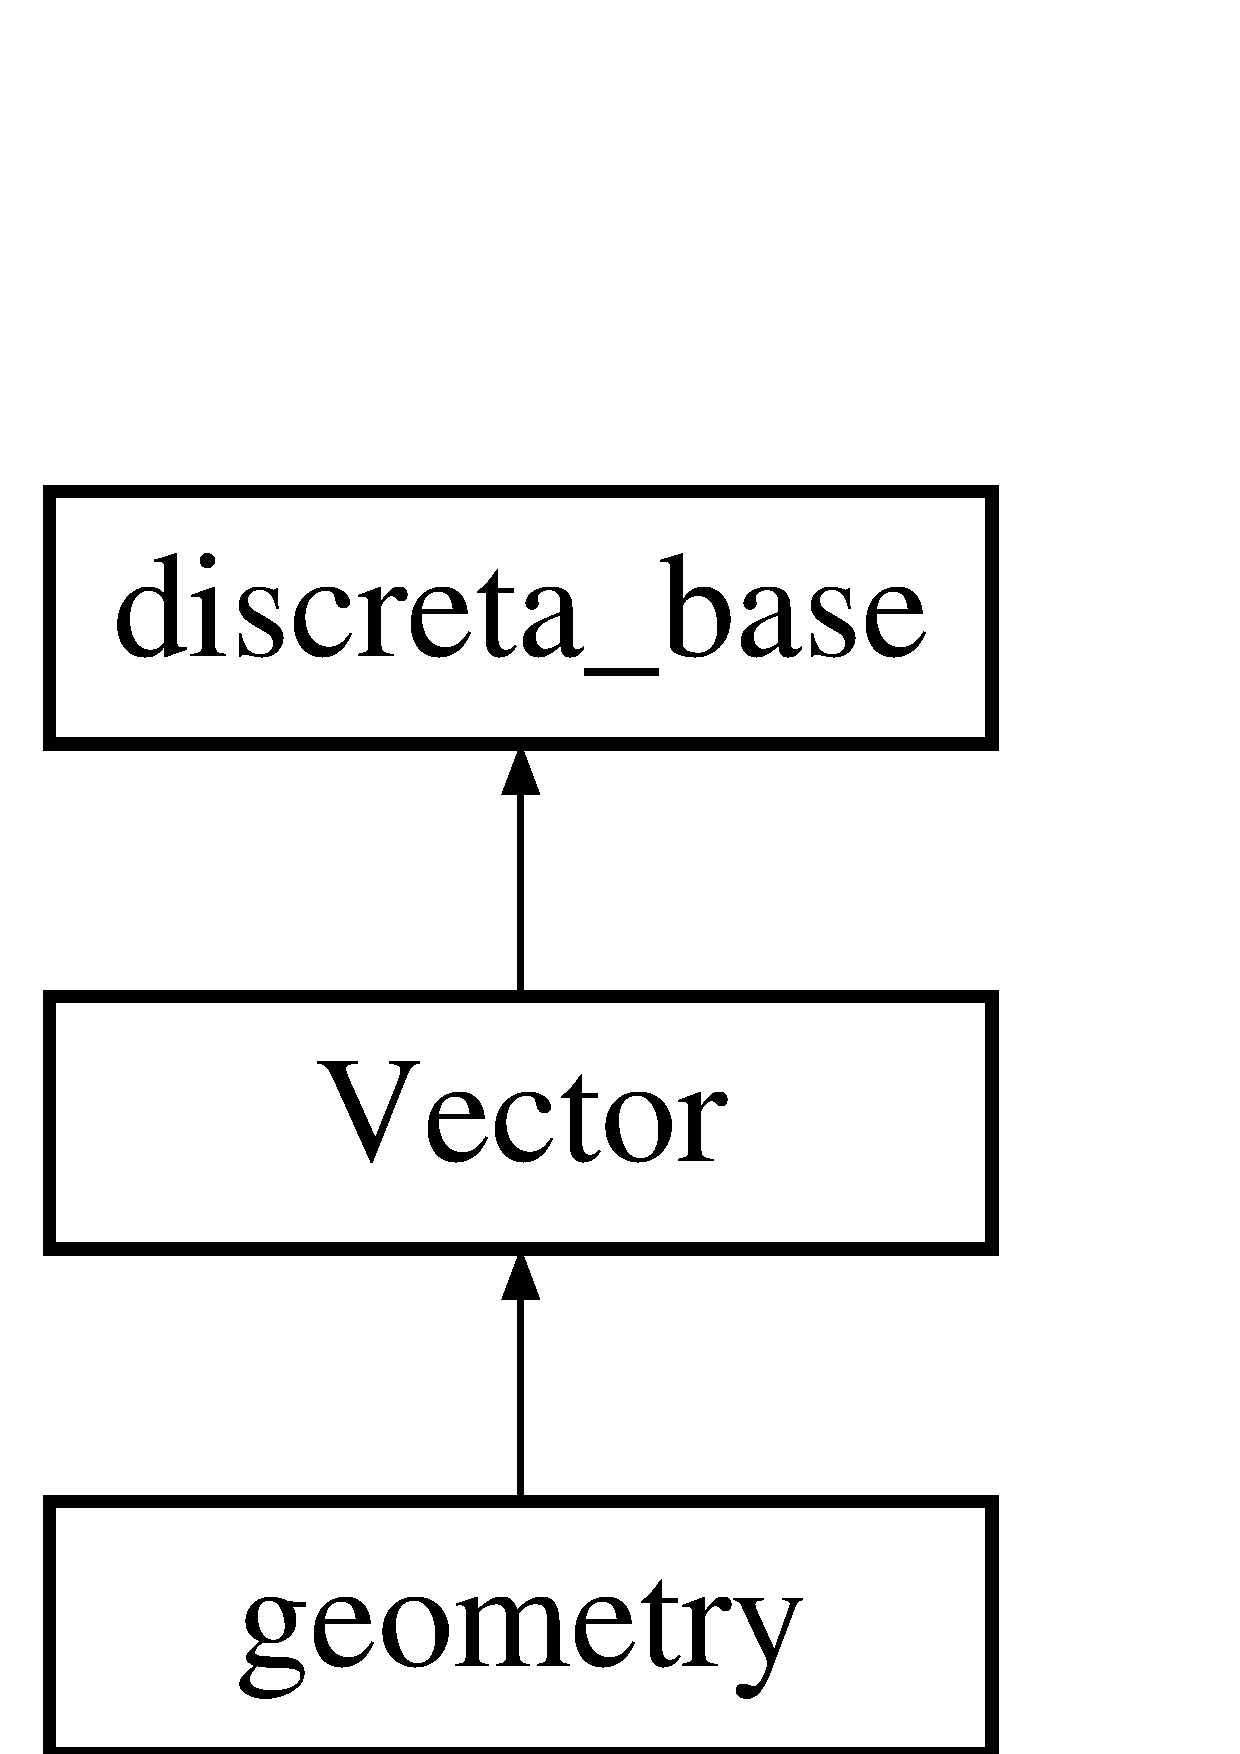
\includegraphics[height=3.000000cm]{classgeometry}
\end{center}
\end{figure}
\subsection*{Public Member Functions}
\begin{DoxyCompactItemize}
\item 
\mbox{\hyperlink{classgeometry_ae58cbd128f60cb06e7d4f59295a6db0d}{geometry}} ()
\item 
void \mbox{\hyperlink{classgeometry_a243e84ff38207957ad5976020c19a033}{allocate\+\_\+geometry}} ()
\item 
\mbox{\hyperlink{classgeometry_adf1960feb5cc97b2d457bfc2d514af23}{geometry}} (const \mbox{\hyperlink{classdiscreta__base}{discreta\+\_\+base}} \&\mbox{\hyperlink{alphabet2_8_c_a6150e0515f7202e2fb518f7206ed97dc}{x}})
\item 
\mbox{\hyperlink{classgeometry}{geometry}} \& \mbox{\hyperlink{classgeometry_af5b78aa94f8ef7f432fb1568187ef762}{operator=}} (const \mbox{\hyperlink{classdiscreta__base}{discreta\+\_\+base}} \&\mbox{\hyperlink{alphabet2_8_c_a6150e0515f7202e2fb518f7206ed97dc}{x}})
\item 
void $\ast$ \mbox{\hyperlink{classgeometry_a9d54b352aeb8544b000c37468a01adc2}{operator new}} (size\+\_\+t, void $\ast$\mbox{\hyperlink{alphabet2_8_c_a533391314665d6bf1b5575e9a9cd8552}{p}})
\item 
void \mbox{\hyperlink{classgeometry_ab4a336baba6a3f56f5ffa053a5be5ba7}{settype\+\_\+geometry}} ()
\item 
\mbox{\hyperlink{discreta_8h_aaf25ee7e2306d78c74ec7bc48f092e81}{kind}} \mbox{\hyperlink{classgeometry_a289c387cc78ff0f0379646cded7648f4}{s\+\_\+virtual\+\_\+kind}} ()
\item 
\mbox{\hyperlink{classgeometry_a2da654e0e19c6145b54727f0f3900a79}{$\sim$geometry}} ()
\item 
void \mbox{\hyperlink{classgeometry_a504b1b52d24b4ae00d9fd0b7838b57e6}{freeself\+\_\+geometry}} ()
\item 
void \mbox{\hyperlink{classgeometry_a3c35255b73911b76347ae549edfb0050}{copyobject\+\_\+to}} (\mbox{\hyperlink{classdiscreta__base}{discreta\+\_\+base}} \&\mbox{\hyperlink{alphabet2_8_c_a6150e0515f7202e2fb518f7206ed97dc}{x}})
\item 
ostream \& \mbox{\hyperlink{classgeometry_af92f963887d22dd3437f585df929208d}{print}} (ostream \&)
\item 
void \mbox{\hyperlink{classgeometry_a1d45497d61d4dc8f7325156158b7e661}{print\+\_\+latex}} (ostream \&ost)
\item 
void \mbox{\hyperlink{classgeometry_a1a65ce3ff3b89b6bb663aa9a559ada2a}{print\+\_\+head\+\_\+latex}} (ostream \&ost)
\item 
void \mbox{\hyperlink{classgeometry_a400fa93fa773518f7b55c454fa69ee78}{print\+\_\+incma\+\_\+text\+\_\+latex}} (ostream \&ost)
\item 
void \mbox{\hyperlink{classgeometry_a1c734bead42349ddea1ad290dc06c428}{print\+\_\+labellings\+\_\+latex}} (ostream \&ost)
\item 
void \mbox{\hyperlink{classgeometry_ae0d174439d57d9bc0b0dd7ffe210b148}{print\+\_\+incma\+\_\+latex\+\_\+picture}} (ostream \&ost)
\item 
void \mbox{\hyperlink{classgeometry_a8b902a6f06a92a18b345e4de42e6508d}{print\+\_\+inc}} (ostream \&ost)
\item 
void \mbox{\hyperlink{classgeometry_a6086ce49de61288d20a69a4dfed44a35}{print\+\_\+inc\+\_\+only}} (ostream \&ost)
\item 
void \mbox{\hyperlink{classgeometry_ab78810f270f25de6b65169d5c62d7806}{print\+\_\+inc\+\_\+header}} (ostream \&ost)
\item 
void \mbox{\hyperlink{classgeometry_a8f5356989decb76fddb4926714240c0d}{print\+\_\+ascii}} (ostream \&ost)
\item 
\mbox{\hyperlink{galois_8h_a09fddde158a3a20bd2dcadb609de11dc}{I\+NT}} \mbox{\hyperlink{classgeometry_ac6f757d1a8855800d3da3fa1e83e812d}{scan}} (istream \&)
\item 
void \mbox{\hyperlink{classgeometry_a71bc2e3a3f4ca02e8518ab5518a4e0df}{scan\+\_\+body}} (istream \&\mbox{\hyperlink{alphabet2_8_c_a362077c979b0bb65159c603270e40f70}{f}}, \mbox{\hyperlink{galois_8h_a09fddde158a3a20bd2dcadb609de11dc}{I\+NT}} geo\+\_\+nr, \mbox{\hyperlink{galois_8h_ab6cc7b4aeb6ea31aba2b3fbfc83ff5e6}{B\+Y\+TE}} $\ast$geo\+\_\+label)
\item 
\mbox{\hyperlink{galois_8h_a09fddde158a3a20bd2dcadb609de11dc}{I\+NT}} \& \mbox{\hyperlink{classgeometry_a47f809adc7a1158065da4dfae214f05f}{number}} ()
\item 
\mbox{\hyperlink{classhollerith}{hollerith}} \& \mbox{\hyperlink{classgeometry_a8be3ddf6aebe1e3c52b67cfe316e638f}{label}} ()
\item 
\mbox{\hyperlink{classmatrix}{matrix}} \& \mbox{\hyperlink{classgeometry_a2eff9c42b83c90012092d49218237d9d}{X}} ()
\item 
\mbox{\hyperlink{galois_8h_a09fddde158a3a20bd2dcadb609de11dc}{I\+NT}} \& \mbox{\hyperlink{classgeometry_a05bd36071a53d68e1c4b0ba981c9cd34}{f\+\_\+incidence\+\_\+matrix}} ()
\item 
\mbox{\hyperlink{class_vector}{Vector}} \& \mbox{\hyperlink{classgeometry_aa80150b549283d56c347b8533d9051b0}{point\+\_\+labels}} ()
\item 
\mbox{\hyperlink{class_vector}{Vector}} \& \mbox{\hyperlink{classgeometry_ab40ecc05e06399138dc6354d790d302b}{block\+\_\+labels}} ()
\item 
\mbox{\hyperlink{galois_8h_a09fddde158a3a20bd2dcadb609de11dc}{I\+NT}} \& \mbox{\hyperlink{classgeometry_a149ccf1dac87cbced60547e9608bb42d}{f\+\_\+row\+\_\+decomp}} ()
\item 
\mbox{\hyperlink{class_vector}{Vector}} \& \mbox{\hyperlink{classgeometry_a58652b4a0edda52732517a06d390882d}{row\+\_\+decomp}} ()
\item 
\mbox{\hyperlink{galois_8h_a09fddde158a3a20bd2dcadb609de11dc}{I\+NT}} \& \mbox{\hyperlink{classgeometry_ae0713575216fd4c562da43a469f5edcb}{f\+\_\+col\+\_\+decomp}} ()
\item 
\mbox{\hyperlink{class_vector}{Vector}} \& \mbox{\hyperlink{classgeometry_a12425a7d0cebea16e0d22c44e7fbe555}{col\+\_\+decomp}} ()
\item 
\mbox{\hyperlink{galois_8h_a09fddde158a3a20bd2dcadb609de11dc}{I\+NT}} \& \mbox{\hyperlink{classgeometry_a8facc1a86c731a6fb9d30346354987bf}{f\+\_\+ddp}} ()
\item 
\mbox{\hyperlink{class_vector}{Vector}} \& \mbox{\hyperlink{classgeometry_ae00a20f0f75a511d639318673986028e}{ddp}} ()
\item 
\mbox{\hyperlink{galois_8h_a09fddde158a3a20bd2dcadb609de11dc}{I\+NT}} \& \mbox{\hyperlink{classgeometry_a1b01f7c645961c3a04b167fc2bf0d2c8}{f\+\_\+ddb}} ()
\item 
\mbox{\hyperlink{class_vector}{Vector}} \& \mbox{\hyperlink{classgeometry_a7a47161530f508d7aeb853a090a6eef8}{ddb}} ()
\item 
\mbox{\hyperlink{galois_8h_a09fddde158a3a20bd2dcadb609de11dc}{I\+NT}} \& \mbox{\hyperlink{classgeometry_a0695b0c3dc2a75a232631dfda609daf7}{f\+\_\+canonical\+\_\+labelling\+\_\+points}} ()
\item 
\mbox{\hyperlink{classpermutation}{permutation}} \& \mbox{\hyperlink{classgeometry_ac426783bf96ded3a50f6746f521bdd31}{canonical\+\_\+labelling\+\_\+points}} ()
\item 
\mbox{\hyperlink{galois_8h_a09fddde158a3a20bd2dcadb609de11dc}{I\+NT}} \& \mbox{\hyperlink{classgeometry_a48f58feb451efdf72ce2a5c3411b62c1}{f\+\_\+canonical\+\_\+labelling\+\_\+blocks}} ()
\item 
\mbox{\hyperlink{classpermutation}{permutation}} \& \mbox{\hyperlink{classgeometry_a6d9453619be9ea76e6e63485594b301f}{canonical\+\_\+labelling\+\_\+blocks}} ()
\item 
\mbox{\hyperlink{galois_8h_a09fddde158a3a20bd2dcadb609de11dc}{I\+NT}} \& \mbox{\hyperlink{classgeometry_a774f2388490689cf9a1d369327e7e49c}{f\+\_\+aut\+\_\+gens}} ()
\item 
\mbox{\hyperlink{class_vector}{Vector}} \& \mbox{\hyperlink{classgeometry_a75778c5288894993efd4006285711670}{aut\+\_\+gens}} ()
\item 
\mbox{\hyperlink{classdiscreta__base}{discreta\+\_\+base}} \& \mbox{\hyperlink{classgeometry_a161d62ea84c011f07d3e64c42ee4d1ee}{ago}} ()
\item 
void \mbox{\hyperlink{classgeometry_ad7132289ee0bc683f8c00c6762bb5035}{transpose}} ()
\item 
\mbox{\hyperlink{galois_8h_a09fddde158a3a20bd2dcadb609de11dc}{I\+NT}} \mbox{\hyperlink{classgeometry_a31e12da96f9d6f9fd62330bdbc59236d}{is\+\_\+2design}} (\mbox{\hyperlink{galois_8h_a09fddde158a3a20bd2dcadb609de11dc}{I\+NT}} \&\mbox{\hyperlink{alphabet2_8_c_acab531abaa74a7e664e3986f2522b33a}{r}}, \mbox{\hyperlink{galois_8h_a09fddde158a3a20bd2dcadb609de11dc}{I\+NT}} \&\mbox{\hyperlink{plane__search_8_c_ae2170c3116b1f345ee7505695206555e}{lambda}}, \mbox{\hyperlink{galois_8h_a09fddde158a3a20bd2dcadb609de11dc}{I\+NT}} f\+\_\+v)
\item 
void \mbox{\hyperlink{classgeometry_ada4d0bca80d2ad69300625167320dc5d}{calc\+\_\+canon\+\_\+nauty}} (\mbox{\hyperlink{galois_8h_a09fddde158a3a20bd2dcadb609de11dc}{I\+NT}} f\+\_\+v, \mbox{\hyperlink{galois_8h_a09fddde158a3a20bd2dcadb609de11dc}{I\+NT}} f\+\_\+vv, \mbox{\hyperlink{galois_8h_a09fddde158a3a20bd2dcadb609de11dc}{I\+NT}} f\+\_\+vvv)
\item 
void \mbox{\hyperlink{classgeometry_a0fe3595dfda0489759f397fecf455c17}{get\+\_\+lexleast\+\_\+X}} (\mbox{\hyperlink{classmatrix}{matrix}} \&X0)
\end{DoxyCompactItemize}
\subsection*{Additional Inherited Members}


\subsection{Constructor \& Destructor Documentation}
\mbox{\Hypertarget{classgeometry_ae58cbd128f60cb06e7d4f59295a6db0d}\label{classgeometry_ae58cbd128f60cb06e7d4f59295a6db0d}} 
\index{geometry@{geometry}!geometry@{geometry}}
\index{geometry@{geometry}!geometry@{geometry}}
\subsubsection{\texorpdfstring{geometry()}{geometry()}\hspace{0.1cm}{\footnotesize\ttfamily [1/2]}}
{\footnotesize\ttfamily geometry\+::geometry (\begin{DoxyParamCaption}{ }\end{DoxyParamCaption})}

\mbox{\Hypertarget{classgeometry_adf1960feb5cc97b2d457bfc2d514af23}\label{classgeometry_adf1960feb5cc97b2d457bfc2d514af23}} 
\index{geometry@{geometry}!geometry@{geometry}}
\index{geometry@{geometry}!geometry@{geometry}}
\subsubsection{\texorpdfstring{geometry()}{geometry()}\hspace{0.1cm}{\footnotesize\ttfamily [2/2]}}
{\footnotesize\ttfamily geometry\+::geometry (\begin{DoxyParamCaption}\item[{const \mbox{\hyperlink{classdiscreta__base}{discreta\+\_\+base}} \&}]{x }\end{DoxyParamCaption})}

\mbox{\Hypertarget{classgeometry_a2da654e0e19c6145b54727f0f3900a79}\label{classgeometry_a2da654e0e19c6145b54727f0f3900a79}} 
\index{geometry@{geometry}!````~geometry@{$\sim$geometry}}
\index{````~geometry@{$\sim$geometry}!geometry@{geometry}}
\subsubsection{\texorpdfstring{$\sim$geometry()}{~geometry()}}
{\footnotesize\ttfamily geometry\+::$\sim$geometry (\begin{DoxyParamCaption}{ }\end{DoxyParamCaption})}



\subsection{Member Function Documentation}
\mbox{\Hypertarget{classgeometry_a161d62ea84c011f07d3e64c42ee4d1ee}\label{classgeometry_a161d62ea84c011f07d3e64c42ee4d1ee}} 
\index{geometry@{geometry}!ago@{ago}}
\index{ago@{ago}!geometry@{geometry}}
\subsubsection{\texorpdfstring{ago()}{ago()}}
{\footnotesize\ttfamily \mbox{\hyperlink{classdiscreta__base}{discreta\+\_\+base}}\& geometry\+::ago (\begin{DoxyParamCaption}{ }\end{DoxyParamCaption})\hspace{0.3cm}{\ttfamily [inline]}}

\mbox{\Hypertarget{classgeometry_a243e84ff38207957ad5976020c19a033}\label{classgeometry_a243e84ff38207957ad5976020c19a033}} 
\index{geometry@{geometry}!allocate\+\_\+geometry@{allocate\+\_\+geometry}}
\index{allocate\+\_\+geometry@{allocate\+\_\+geometry}!geometry@{geometry}}
\subsubsection{\texorpdfstring{allocate\+\_\+geometry()}{allocate\_geometry()}}
{\footnotesize\ttfamily void geometry\+::allocate\+\_\+geometry (\begin{DoxyParamCaption}{ }\end{DoxyParamCaption})}

\mbox{\Hypertarget{classgeometry_a75778c5288894993efd4006285711670}\label{classgeometry_a75778c5288894993efd4006285711670}} 
\index{geometry@{geometry}!aut\+\_\+gens@{aut\+\_\+gens}}
\index{aut\+\_\+gens@{aut\+\_\+gens}!geometry@{geometry}}
\subsubsection{\texorpdfstring{aut\+\_\+gens()}{aut\_gens()}}
{\footnotesize\ttfamily \mbox{\hyperlink{class_vector}{Vector}}\& geometry\+::aut\+\_\+gens (\begin{DoxyParamCaption}{ }\end{DoxyParamCaption})\hspace{0.3cm}{\ttfamily [inline]}}

\mbox{\Hypertarget{classgeometry_ab40ecc05e06399138dc6354d790d302b}\label{classgeometry_ab40ecc05e06399138dc6354d790d302b}} 
\index{geometry@{geometry}!block\+\_\+labels@{block\+\_\+labels}}
\index{block\+\_\+labels@{block\+\_\+labels}!geometry@{geometry}}
\subsubsection{\texorpdfstring{block\+\_\+labels()}{block\_labels()}}
{\footnotesize\ttfamily \mbox{\hyperlink{class_vector}{Vector}}\& geometry\+::block\+\_\+labels (\begin{DoxyParamCaption}{ }\end{DoxyParamCaption})\hspace{0.3cm}{\ttfamily [inline]}}

\mbox{\Hypertarget{classgeometry_ada4d0bca80d2ad69300625167320dc5d}\label{classgeometry_ada4d0bca80d2ad69300625167320dc5d}} 
\index{geometry@{geometry}!calc\+\_\+canon\+\_\+nauty@{calc\+\_\+canon\+\_\+nauty}}
\index{calc\+\_\+canon\+\_\+nauty@{calc\+\_\+canon\+\_\+nauty}!geometry@{geometry}}
\subsubsection{\texorpdfstring{calc\+\_\+canon\+\_\+nauty()}{calc\_canon\_nauty()}}
{\footnotesize\ttfamily void geometry\+::calc\+\_\+canon\+\_\+nauty (\begin{DoxyParamCaption}\item[{\mbox{\hyperlink{galois_8h_a09fddde158a3a20bd2dcadb609de11dc}{I\+NT}}}]{f\+\_\+v,  }\item[{\mbox{\hyperlink{galois_8h_a09fddde158a3a20bd2dcadb609de11dc}{I\+NT}}}]{f\+\_\+vv,  }\item[{\mbox{\hyperlink{galois_8h_a09fddde158a3a20bd2dcadb609de11dc}{I\+NT}}}]{f\+\_\+vvv }\end{DoxyParamCaption})}

\mbox{\Hypertarget{classgeometry_a6d9453619be9ea76e6e63485594b301f}\label{classgeometry_a6d9453619be9ea76e6e63485594b301f}} 
\index{geometry@{geometry}!canonical\+\_\+labelling\+\_\+blocks@{canonical\+\_\+labelling\+\_\+blocks}}
\index{canonical\+\_\+labelling\+\_\+blocks@{canonical\+\_\+labelling\+\_\+blocks}!geometry@{geometry}}
\subsubsection{\texorpdfstring{canonical\+\_\+labelling\+\_\+blocks()}{canonical\_labelling\_blocks()}}
{\footnotesize\ttfamily \mbox{\hyperlink{classpermutation}{permutation}}\& geometry\+::canonical\+\_\+labelling\+\_\+blocks (\begin{DoxyParamCaption}{ }\end{DoxyParamCaption})\hspace{0.3cm}{\ttfamily [inline]}}

\mbox{\Hypertarget{classgeometry_ac426783bf96ded3a50f6746f521bdd31}\label{classgeometry_ac426783bf96ded3a50f6746f521bdd31}} 
\index{geometry@{geometry}!canonical\+\_\+labelling\+\_\+points@{canonical\+\_\+labelling\+\_\+points}}
\index{canonical\+\_\+labelling\+\_\+points@{canonical\+\_\+labelling\+\_\+points}!geometry@{geometry}}
\subsubsection{\texorpdfstring{canonical\+\_\+labelling\+\_\+points()}{canonical\_labelling\_points()}}
{\footnotesize\ttfamily \mbox{\hyperlink{classpermutation}{permutation}}\& geometry\+::canonical\+\_\+labelling\+\_\+points (\begin{DoxyParamCaption}{ }\end{DoxyParamCaption})\hspace{0.3cm}{\ttfamily [inline]}}

\mbox{\Hypertarget{classgeometry_a12425a7d0cebea16e0d22c44e7fbe555}\label{classgeometry_a12425a7d0cebea16e0d22c44e7fbe555}} 
\index{geometry@{geometry}!col\+\_\+decomp@{col\+\_\+decomp}}
\index{col\+\_\+decomp@{col\+\_\+decomp}!geometry@{geometry}}
\subsubsection{\texorpdfstring{col\+\_\+decomp()}{col\_decomp()}}
{\footnotesize\ttfamily \mbox{\hyperlink{class_vector}{Vector}}\& geometry\+::col\+\_\+decomp (\begin{DoxyParamCaption}{ }\end{DoxyParamCaption})\hspace{0.3cm}{\ttfamily [inline]}}

\mbox{\Hypertarget{classgeometry_a3c35255b73911b76347ae549edfb0050}\label{classgeometry_a3c35255b73911b76347ae549edfb0050}} 
\index{geometry@{geometry}!copyobject\+\_\+to@{copyobject\+\_\+to}}
\index{copyobject\+\_\+to@{copyobject\+\_\+to}!geometry@{geometry}}
\subsubsection{\texorpdfstring{copyobject\+\_\+to()}{copyobject\_to()}}
{\footnotesize\ttfamily void geometry\+::copyobject\+\_\+to (\begin{DoxyParamCaption}\item[{\mbox{\hyperlink{classdiscreta__base}{discreta\+\_\+base}} \&}]{x }\end{DoxyParamCaption})\hspace{0.3cm}{\ttfamily [virtual]}}



Reimplemented from \mbox{\hyperlink{class_vector_af657307f3d344c8cef5d633335a5f484}{Vector}}.

\mbox{\Hypertarget{classgeometry_a7a47161530f508d7aeb853a090a6eef8}\label{classgeometry_a7a47161530f508d7aeb853a090a6eef8}} 
\index{geometry@{geometry}!ddb@{ddb}}
\index{ddb@{ddb}!geometry@{geometry}}
\subsubsection{\texorpdfstring{ddb()}{ddb()}}
{\footnotesize\ttfamily \mbox{\hyperlink{class_vector}{Vector}}\& geometry\+::ddb (\begin{DoxyParamCaption}{ }\end{DoxyParamCaption})\hspace{0.3cm}{\ttfamily [inline]}}

\mbox{\Hypertarget{classgeometry_ae00a20f0f75a511d639318673986028e}\label{classgeometry_ae00a20f0f75a511d639318673986028e}} 
\index{geometry@{geometry}!ddp@{ddp}}
\index{ddp@{ddp}!geometry@{geometry}}
\subsubsection{\texorpdfstring{ddp()}{ddp()}}
{\footnotesize\ttfamily \mbox{\hyperlink{class_vector}{Vector}}\& geometry\+::ddp (\begin{DoxyParamCaption}{ }\end{DoxyParamCaption})\hspace{0.3cm}{\ttfamily [inline]}}

\mbox{\Hypertarget{classgeometry_a774f2388490689cf9a1d369327e7e49c}\label{classgeometry_a774f2388490689cf9a1d369327e7e49c}} 
\index{geometry@{geometry}!f\+\_\+aut\+\_\+gens@{f\+\_\+aut\+\_\+gens}}
\index{f\+\_\+aut\+\_\+gens@{f\+\_\+aut\+\_\+gens}!geometry@{geometry}}
\subsubsection{\texorpdfstring{f\+\_\+aut\+\_\+gens()}{f\_aut\_gens()}}
{\footnotesize\ttfamily \mbox{\hyperlink{galois_8h_a09fddde158a3a20bd2dcadb609de11dc}{I\+NT}}\& geometry\+::f\+\_\+aut\+\_\+gens (\begin{DoxyParamCaption}{ }\end{DoxyParamCaption})\hspace{0.3cm}{\ttfamily [inline]}}

\mbox{\Hypertarget{classgeometry_a48f58feb451efdf72ce2a5c3411b62c1}\label{classgeometry_a48f58feb451efdf72ce2a5c3411b62c1}} 
\index{geometry@{geometry}!f\+\_\+canonical\+\_\+labelling\+\_\+blocks@{f\+\_\+canonical\+\_\+labelling\+\_\+blocks}}
\index{f\+\_\+canonical\+\_\+labelling\+\_\+blocks@{f\+\_\+canonical\+\_\+labelling\+\_\+blocks}!geometry@{geometry}}
\subsubsection{\texorpdfstring{f\+\_\+canonical\+\_\+labelling\+\_\+blocks()}{f\_canonical\_labelling\_blocks()}}
{\footnotesize\ttfamily \mbox{\hyperlink{galois_8h_a09fddde158a3a20bd2dcadb609de11dc}{I\+NT}}\& geometry\+::f\+\_\+canonical\+\_\+labelling\+\_\+blocks (\begin{DoxyParamCaption}{ }\end{DoxyParamCaption})\hspace{0.3cm}{\ttfamily [inline]}}

\mbox{\Hypertarget{classgeometry_a0695b0c3dc2a75a232631dfda609daf7}\label{classgeometry_a0695b0c3dc2a75a232631dfda609daf7}} 
\index{geometry@{geometry}!f\+\_\+canonical\+\_\+labelling\+\_\+points@{f\+\_\+canonical\+\_\+labelling\+\_\+points}}
\index{f\+\_\+canonical\+\_\+labelling\+\_\+points@{f\+\_\+canonical\+\_\+labelling\+\_\+points}!geometry@{geometry}}
\subsubsection{\texorpdfstring{f\+\_\+canonical\+\_\+labelling\+\_\+points()}{f\_canonical\_labelling\_points()}}
{\footnotesize\ttfamily \mbox{\hyperlink{galois_8h_a09fddde158a3a20bd2dcadb609de11dc}{I\+NT}}\& geometry\+::f\+\_\+canonical\+\_\+labelling\+\_\+points (\begin{DoxyParamCaption}{ }\end{DoxyParamCaption})\hspace{0.3cm}{\ttfamily [inline]}}

\mbox{\Hypertarget{classgeometry_ae0713575216fd4c562da43a469f5edcb}\label{classgeometry_ae0713575216fd4c562da43a469f5edcb}} 
\index{geometry@{geometry}!f\+\_\+col\+\_\+decomp@{f\+\_\+col\+\_\+decomp}}
\index{f\+\_\+col\+\_\+decomp@{f\+\_\+col\+\_\+decomp}!geometry@{geometry}}
\subsubsection{\texorpdfstring{f\+\_\+col\+\_\+decomp()}{f\_col\_decomp()}}
{\footnotesize\ttfamily \mbox{\hyperlink{galois_8h_a09fddde158a3a20bd2dcadb609de11dc}{I\+NT}}\& geometry\+::f\+\_\+col\+\_\+decomp (\begin{DoxyParamCaption}{ }\end{DoxyParamCaption})\hspace{0.3cm}{\ttfamily [inline]}}

\mbox{\Hypertarget{classgeometry_a1b01f7c645961c3a04b167fc2bf0d2c8}\label{classgeometry_a1b01f7c645961c3a04b167fc2bf0d2c8}} 
\index{geometry@{geometry}!f\+\_\+ddb@{f\+\_\+ddb}}
\index{f\+\_\+ddb@{f\+\_\+ddb}!geometry@{geometry}}
\subsubsection{\texorpdfstring{f\+\_\+ddb()}{f\_ddb()}}
{\footnotesize\ttfamily \mbox{\hyperlink{galois_8h_a09fddde158a3a20bd2dcadb609de11dc}{I\+NT}}\& geometry\+::f\+\_\+ddb (\begin{DoxyParamCaption}{ }\end{DoxyParamCaption})\hspace{0.3cm}{\ttfamily [inline]}}

\mbox{\Hypertarget{classgeometry_a8facc1a86c731a6fb9d30346354987bf}\label{classgeometry_a8facc1a86c731a6fb9d30346354987bf}} 
\index{geometry@{geometry}!f\+\_\+ddp@{f\+\_\+ddp}}
\index{f\+\_\+ddp@{f\+\_\+ddp}!geometry@{geometry}}
\subsubsection{\texorpdfstring{f\+\_\+ddp()}{f\_ddp()}}
{\footnotesize\ttfamily \mbox{\hyperlink{galois_8h_a09fddde158a3a20bd2dcadb609de11dc}{I\+NT}}\& geometry\+::f\+\_\+ddp (\begin{DoxyParamCaption}{ }\end{DoxyParamCaption})\hspace{0.3cm}{\ttfamily [inline]}}

\mbox{\Hypertarget{classgeometry_a05bd36071a53d68e1c4b0ba981c9cd34}\label{classgeometry_a05bd36071a53d68e1c4b0ba981c9cd34}} 
\index{geometry@{geometry}!f\+\_\+incidence\+\_\+matrix@{f\+\_\+incidence\+\_\+matrix}}
\index{f\+\_\+incidence\+\_\+matrix@{f\+\_\+incidence\+\_\+matrix}!geometry@{geometry}}
\subsubsection{\texorpdfstring{f\+\_\+incidence\+\_\+matrix()}{f\_incidence\_matrix()}}
{\footnotesize\ttfamily \mbox{\hyperlink{galois_8h_a09fddde158a3a20bd2dcadb609de11dc}{I\+NT}}\& geometry\+::f\+\_\+incidence\+\_\+matrix (\begin{DoxyParamCaption}{ }\end{DoxyParamCaption})\hspace{0.3cm}{\ttfamily [inline]}}

\mbox{\Hypertarget{classgeometry_a149ccf1dac87cbced60547e9608bb42d}\label{classgeometry_a149ccf1dac87cbced60547e9608bb42d}} 
\index{geometry@{geometry}!f\+\_\+row\+\_\+decomp@{f\+\_\+row\+\_\+decomp}}
\index{f\+\_\+row\+\_\+decomp@{f\+\_\+row\+\_\+decomp}!geometry@{geometry}}
\subsubsection{\texorpdfstring{f\+\_\+row\+\_\+decomp()}{f\_row\_decomp()}}
{\footnotesize\ttfamily \mbox{\hyperlink{galois_8h_a09fddde158a3a20bd2dcadb609de11dc}{I\+NT}}\& geometry\+::f\+\_\+row\+\_\+decomp (\begin{DoxyParamCaption}{ }\end{DoxyParamCaption})\hspace{0.3cm}{\ttfamily [inline]}}

\mbox{\Hypertarget{classgeometry_a504b1b52d24b4ae00d9fd0b7838b57e6}\label{classgeometry_a504b1b52d24b4ae00d9fd0b7838b57e6}} 
\index{geometry@{geometry}!freeself\+\_\+geometry@{freeself\+\_\+geometry}}
\index{freeself\+\_\+geometry@{freeself\+\_\+geometry}!geometry@{geometry}}
\subsubsection{\texorpdfstring{freeself\+\_\+geometry()}{freeself\_geometry()}}
{\footnotesize\ttfamily void geometry\+::freeself\+\_\+geometry (\begin{DoxyParamCaption}{ }\end{DoxyParamCaption})}

\mbox{\Hypertarget{classgeometry_a0fe3595dfda0489759f397fecf455c17}\label{classgeometry_a0fe3595dfda0489759f397fecf455c17}} 
\index{geometry@{geometry}!get\+\_\+lexleast\+\_\+X@{get\+\_\+lexleast\+\_\+X}}
\index{get\+\_\+lexleast\+\_\+X@{get\+\_\+lexleast\+\_\+X}!geometry@{geometry}}
\subsubsection{\texorpdfstring{get\+\_\+lexleast\+\_\+\+X()}{get\_lexleast\_X()}}
{\footnotesize\ttfamily void geometry\+::get\+\_\+lexleast\+\_\+X (\begin{DoxyParamCaption}\item[{\mbox{\hyperlink{classmatrix}{matrix}} \&}]{X0 }\end{DoxyParamCaption})}

\mbox{\Hypertarget{classgeometry_a31e12da96f9d6f9fd62330bdbc59236d}\label{classgeometry_a31e12da96f9d6f9fd62330bdbc59236d}} 
\index{geometry@{geometry}!is\+\_\+2design@{is\+\_\+2design}}
\index{is\+\_\+2design@{is\+\_\+2design}!geometry@{geometry}}
\subsubsection{\texorpdfstring{is\+\_\+2design()}{is\_2design()}}
{\footnotesize\ttfamily \mbox{\hyperlink{galois_8h_a09fddde158a3a20bd2dcadb609de11dc}{I\+NT}} geometry\+::is\+\_\+2design (\begin{DoxyParamCaption}\item[{\mbox{\hyperlink{galois_8h_a09fddde158a3a20bd2dcadb609de11dc}{I\+NT}} \&}]{r,  }\item[{\mbox{\hyperlink{galois_8h_a09fddde158a3a20bd2dcadb609de11dc}{I\+NT}} \&}]{lambda,  }\item[{\mbox{\hyperlink{galois_8h_a09fddde158a3a20bd2dcadb609de11dc}{I\+NT}}}]{f\+\_\+v }\end{DoxyParamCaption})}

\mbox{\Hypertarget{classgeometry_a8be3ddf6aebe1e3c52b67cfe316e638f}\label{classgeometry_a8be3ddf6aebe1e3c52b67cfe316e638f}} 
\index{geometry@{geometry}!label@{label}}
\index{label@{label}!geometry@{geometry}}
\subsubsection{\texorpdfstring{label()}{label()}}
{\footnotesize\ttfamily \mbox{\hyperlink{classhollerith}{hollerith}}\& geometry\+::label (\begin{DoxyParamCaption}{ }\end{DoxyParamCaption})\hspace{0.3cm}{\ttfamily [inline]}}

\mbox{\Hypertarget{classgeometry_a47f809adc7a1158065da4dfae214f05f}\label{classgeometry_a47f809adc7a1158065da4dfae214f05f}} 
\index{geometry@{geometry}!number@{number}}
\index{number@{number}!geometry@{geometry}}
\subsubsection{\texorpdfstring{number()}{number()}}
{\footnotesize\ttfamily \mbox{\hyperlink{galois_8h_a09fddde158a3a20bd2dcadb609de11dc}{I\+NT}}\& geometry\+::number (\begin{DoxyParamCaption}{ }\end{DoxyParamCaption})\hspace{0.3cm}{\ttfamily [inline]}}

\mbox{\Hypertarget{classgeometry_a9d54b352aeb8544b000c37468a01adc2}\label{classgeometry_a9d54b352aeb8544b000c37468a01adc2}} 
\index{geometry@{geometry}!operator new@{operator new}}
\index{operator new@{operator new}!geometry@{geometry}}
\subsubsection{\texorpdfstring{operator new()}{operator new()}}
{\footnotesize\ttfamily void$\ast$ geometry\+::operator new (\begin{DoxyParamCaption}\item[{size\+\_\+t}]{,  }\item[{void $\ast$}]{p }\end{DoxyParamCaption})\hspace{0.3cm}{\ttfamily [inline]}}

\mbox{\Hypertarget{classgeometry_af5b78aa94f8ef7f432fb1568187ef762}\label{classgeometry_af5b78aa94f8ef7f432fb1568187ef762}} 
\index{geometry@{geometry}!operator=@{operator=}}
\index{operator=@{operator=}!geometry@{geometry}}
\subsubsection{\texorpdfstring{operator=()}{operator=()}}
{\footnotesize\ttfamily \mbox{\hyperlink{classgeometry}{geometry}} \& geometry\+::operator= (\begin{DoxyParamCaption}\item[{const \mbox{\hyperlink{classdiscreta__base}{discreta\+\_\+base}} \&}]{x }\end{DoxyParamCaption})}

\mbox{\Hypertarget{classgeometry_aa80150b549283d56c347b8533d9051b0}\label{classgeometry_aa80150b549283d56c347b8533d9051b0}} 
\index{geometry@{geometry}!point\+\_\+labels@{point\+\_\+labels}}
\index{point\+\_\+labels@{point\+\_\+labels}!geometry@{geometry}}
\subsubsection{\texorpdfstring{point\+\_\+labels()}{point\_labels()}}
{\footnotesize\ttfamily \mbox{\hyperlink{class_vector}{Vector}}\& geometry\+::point\+\_\+labels (\begin{DoxyParamCaption}{ }\end{DoxyParamCaption})\hspace{0.3cm}{\ttfamily [inline]}}

\mbox{\Hypertarget{classgeometry_af92f963887d22dd3437f585df929208d}\label{classgeometry_af92f963887d22dd3437f585df929208d}} 
\index{geometry@{geometry}!print@{print}}
\index{print@{print}!geometry@{geometry}}
\subsubsection{\texorpdfstring{print()}{print()}}
{\footnotesize\ttfamily ostream \& geometry\+::print (\begin{DoxyParamCaption}\item[{ostream \&}]{ost }\end{DoxyParamCaption})\hspace{0.3cm}{\ttfamily [virtual]}}



Reimplemented from \mbox{\hyperlink{class_vector_a71d7e24bcfdfc69d4a2137360acb066c}{Vector}}.

\mbox{\Hypertarget{classgeometry_a8f5356989decb76fddb4926714240c0d}\label{classgeometry_a8f5356989decb76fddb4926714240c0d}} 
\index{geometry@{geometry}!print\+\_\+ascii@{print\+\_\+ascii}}
\index{print\+\_\+ascii@{print\+\_\+ascii}!geometry@{geometry}}
\subsubsection{\texorpdfstring{print\+\_\+ascii()}{print\_ascii()}}
{\footnotesize\ttfamily void geometry\+::print\+\_\+ascii (\begin{DoxyParamCaption}\item[{ostream \&}]{ost }\end{DoxyParamCaption})}

\mbox{\Hypertarget{classgeometry_a1a65ce3ff3b89b6bb663aa9a559ada2a}\label{classgeometry_a1a65ce3ff3b89b6bb663aa9a559ada2a}} 
\index{geometry@{geometry}!print\+\_\+head\+\_\+latex@{print\+\_\+head\+\_\+latex}}
\index{print\+\_\+head\+\_\+latex@{print\+\_\+head\+\_\+latex}!geometry@{geometry}}
\subsubsection{\texorpdfstring{print\+\_\+head\+\_\+latex()}{print\_head\_latex()}}
{\footnotesize\ttfamily void geometry\+::print\+\_\+head\+\_\+latex (\begin{DoxyParamCaption}\item[{ostream \&}]{ost }\end{DoxyParamCaption})}

\mbox{\Hypertarget{classgeometry_a8b902a6f06a92a18b345e4de42e6508d}\label{classgeometry_a8b902a6f06a92a18b345e4de42e6508d}} 
\index{geometry@{geometry}!print\+\_\+inc@{print\+\_\+inc}}
\index{print\+\_\+inc@{print\+\_\+inc}!geometry@{geometry}}
\subsubsection{\texorpdfstring{print\+\_\+inc()}{print\_inc()}}
{\footnotesize\ttfamily void geometry\+::print\+\_\+inc (\begin{DoxyParamCaption}\item[{ostream \&}]{ost }\end{DoxyParamCaption})}

\mbox{\Hypertarget{classgeometry_ab78810f270f25de6b65169d5c62d7806}\label{classgeometry_ab78810f270f25de6b65169d5c62d7806}} 
\index{geometry@{geometry}!print\+\_\+inc\+\_\+header@{print\+\_\+inc\+\_\+header}}
\index{print\+\_\+inc\+\_\+header@{print\+\_\+inc\+\_\+header}!geometry@{geometry}}
\subsubsection{\texorpdfstring{print\+\_\+inc\+\_\+header()}{print\_inc\_header()}}
{\footnotesize\ttfamily void geometry\+::print\+\_\+inc\+\_\+header (\begin{DoxyParamCaption}\item[{ostream \&}]{ost }\end{DoxyParamCaption})}

\mbox{\Hypertarget{classgeometry_a6086ce49de61288d20a69a4dfed44a35}\label{classgeometry_a6086ce49de61288d20a69a4dfed44a35}} 
\index{geometry@{geometry}!print\+\_\+inc\+\_\+only@{print\+\_\+inc\+\_\+only}}
\index{print\+\_\+inc\+\_\+only@{print\+\_\+inc\+\_\+only}!geometry@{geometry}}
\subsubsection{\texorpdfstring{print\+\_\+inc\+\_\+only()}{print\_inc\_only()}}
{\footnotesize\ttfamily void geometry\+::print\+\_\+inc\+\_\+only (\begin{DoxyParamCaption}\item[{ostream \&}]{ost }\end{DoxyParamCaption})}

\mbox{\Hypertarget{classgeometry_ae0d174439d57d9bc0b0dd7ffe210b148}\label{classgeometry_ae0d174439d57d9bc0b0dd7ffe210b148}} 
\index{geometry@{geometry}!print\+\_\+incma\+\_\+latex\+\_\+picture@{print\+\_\+incma\+\_\+latex\+\_\+picture}}
\index{print\+\_\+incma\+\_\+latex\+\_\+picture@{print\+\_\+incma\+\_\+latex\+\_\+picture}!geometry@{geometry}}
\subsubsection{\texorpdfstring{print\+\_\+incma\+\_\+latex\+\_\+picture()}{print\_incma\_latex\_picture()}}
{\footnotesize\ttfamily void geometry\+::print\+\_\+incma\+\_\+latex\+\_\+picture (\begin{DoxyParamCaption}\item[{ostream \&}]{ost }\end{DoxyParamCaption})}

\mbox{\Hypertarget{classgeometry_a400fa93fa773518f7b55c454fa69ee78}\label{classgeometry_a400fa93fa773518f7b55c454fa69ee78}} 
\index{geometry@{geometry}!print\+\_\+incma\+\_\+text\+\_\+latex@{print\+\_\+incma\+\_\+text\+\_\+latex}}
\index{print\+\_\+incma\+\_\+text\+\_\+latex@{print\+\_\+incma\+\_\+text\+\_\+latex}!geometry@{geometry}}
\subsubsection{\texorpdfstring{print\+\_\+incma\+\_\+text\+\_\+latex()}{print\_incma\_text\_latex()}}
{\footnotesize\ttfamily void geometry\+::print\+\_\+incma\+\_\+text\+\_\+latex (\begin{DoxyParamCaption}\item[{ostream \&}]{ost }\end{DoxyParamCaption})}

\mbox{\Hypertarget{classgeometry_a1c734bead42349ddea1ad290dc06c428}\label{classgeometry_a1c734bead42349ddea1ad290dc06c428}} 
\index{geometry@{geometry}!print\+\_\+labellings\+\_\+latex@{print\+\_\+labellings\+\_\+latex}}
\index{print\+\_\+labellings\+\_\+latex@{print\+\_\+labellings\+\_\+latex}!geometry@{geometry}}
\subsubsection{\texorpdfstring{print\+\_\+labellings\+\_\+latex()}{print\_labellings\_latex()}}
{\footnotesize\ttfamily void geometry\+::print\+\_\+labellings\+\_\+latex (\begin{DoxyParamCaption}\item[{ostream \&}]{ost }\end{DoxyParamCaption})}

\mbox{\Hypertarget{classgeometry_a1d45497d61d4dc8f7325156158b7e661}\label{classgeometry_a1d45497d61d4dc8f7325156158b7e661}} 
\index{geometry@{geometry}!print\+\_\+latex@{print\+\_\+latex}}
\index{print\+\_\+latex@{print\+\_\+latex}!geometry@{geometry}}
\subsubsection{\texorpdfstring{print\+\_\+latex()}{print\_latex()}}
{\footnotesize\ttfamily void geometry\+::print\+\_\+latex (\begin{DoxyParamCaption}\item[{ostream \&}]{ost }\end{DoxyParamCaption})}

\mbox{\Hypertarget{classgeometry_a58652b4a0edda52732517a06d390882d}\label{classgeometry_a58652b4a0edda52732517a06d390882d}} 
\index{geometry@{geometry}!row\+\_\+decomp@{row\+\_\+decomp}}
\index{row\+\_\+decomp@{row\+\_\+decomp}!geometry@{geometry}}
\subsubsection{\texorpdfstring{row\+\_\+decomp()}{row\_decomp()}}
{\footnotesize\ttfamily \mbox{\hyperlink{class_vector}{Vector}}\& geometry\+::row\+\_\+decomp (\begin{DoxyParamCaption}{ }\end{DoxyParamCaption})\hspace{0.3cm}{\ttfamily [inline]}}

\mbox{\Hypertarget{classgeometry_a289c387cc78ff0f0379646cded7648f4}\label{classgeometry_a289c387cc78ff0f0379646cded7648f4}} 
\index{geometry@{geometry}!s\+\_\+virtual\+\_\+kind@{s\+\_\+virtual\+\_\+kind}}
\index{s\+\_\+virtual\+\_\+kind@{s\+\_\+virtual\+\_\+kind}!geometry@{geometry}}
\subsubsection{\texorpdfstring{s\+\_\+virtual\+\_\+kind()}{s\_virtual\_kind()}}
{\footnotesize\ttfamily \mbox{\hyperlink{discreta_8h_aaf25ee7e2306d78c74ec7bc48f092e81}{kind}} geometry\+::s\+\_\+virtual\+\_\+kind (\begin{DoxyParamCaption}{ }\end{DoxyParamCaption})\hspace{0.3cm}{\ttfamily [virtual]}}



Reimplemented from \mbox{\hyperlink{class_vector_a20550e70d02cbe484032c7f6b0833a0f}{Vector}}.

\mbox{\Hypertarget{classgeometry_ac6f757d1a8855800d3da3fa1e83e812d}\label{classgeometry_ac6f757d1a8855800d3da3fa1e83e812d}} 
\index{geometry@{geometry}!scan@{scan}}
\index{scan@{scan}!geometry@{geometry}}
\subsubsection{\texorpdfstring{scan()}{scan()}}
{\footnotesize\ttfamily \mbox{\hyperlink{galois_8h_a09fddde158a3a20bd2dcadb609de11dc}{I\+NT}} geometry\+::scan (\begin{DoxyParamCaption}\item[{istream \&}]{f }\end{DoxyParamCaption})}

\mbox{\Hypertarget{classgeometry_a71bc2e3a3f4ca02e8518ab5518a4e0df}\label{classgeometry_a71bc2e3a3f4ca02e8518ab5518a4e0df}} 
\index{geometry@{geometry}!scan\+\_\+body@{scan\+\_\+body}}
\index{scan\+\_\+body@{scan\+\_\+body}!geometry@{geometry}}
\subsubsection{\texorpdfstring{scan\+\_\+body()}{scan\_body()}}
{\footnotesize\ttfamily void geometry\+::scan\+\_\+body (\begin{DoxyParamCaption}\item[{istream \&}]{f,  }\item[{\mbox{\hyperlink{galois_8h_a09fddde158a3a20bd2dcadb609de11dc}{I\+NT}}}]{geo\+\_\+nr,  }\item[{\mbox{\hyperlink{galois_8h_ab6cc7b4aeb6ea31aba2b3fbfc83ff5e6}{B\+Y\+TE}} $\ast$}]{geo\+\_\+label }\end{DoxyParamCaption})}

\mbox{\Hypertarget{classgeometry_ab4a336baba6a3f56f5ffa053a5be5ba7}\label{classgeometry_ab4a336baba6a3f56f5ffa053a5be5ba7}} 
\index{geometry@{geometry}!settype\+\_\+geometry@{settype\+\_\+geometry}}
\index{settype\+\_\+geometry@{settype\+\_\+geometry}!geometry@{geometry}}
\subsubsection{\texorpdfstring{settype\+\_\+geometry()}{settype\_geometry()}}
{\footnotesize\ttfamily void geometry\+::settype\+\_\+geometry (\begin{DoxyParamCaption}{ }\end{DoxyParamCaption})}

\mbox{\Hypertarget{classgeometry_ad7132289ee0bc683f8c00c6762bb5035}\label{classgeometry_ad7132289ee0bc683f8c00c6762bb5035}} 
\index{geometry@{geometry}!transpose@{transpose}}
\index{transpose@{transpose}!geometry@{geometry}}
\subsubsection{\texorpdfstring{transpose()}{transpose()}}
{\footnotesize\ttfamily void geometry\+::transpose (\begin{DoxyParamCaption}{ }\end{DoxyParamCaption})}

\mbox{\Hypertarget{classgeometry_a2eff9c42b83c90012092d49218237d9d}\label{classgeometry_a2eff9c42b83c90012092d49218237d9d}} 
\index{geometry@{geometry}!X@{X}}
\index{X@{X}!geometry@{geometry}}
\subsubsection{\texorpdfstring{X()}{X()}}
{\footnotesize\ttfamily \mbox{\hyperlink{classmatrix}{matrix}}\& geometry\+::X (\begin{DoxyParamCaption}{ }\end{DoxyParamCaption})\hspace{0.3cm}{\ttfamily [inline]}}



The documentation for this class was generated from the following files\+:\begin{DoxyCompactItemize}
\item 
S\+R\+C/\+L\+I\+B/\+D\+I\+S\+C\+R\+E\+T\+A/\mbox{\hyperlink{discreta_8h}{discreta.\+h}}\item 
S\+R\+C/\+L\+I\+B/\+D\+I\+S\+C\+R\+E\+T\+A/\mbox{\hyperlink{geometry_8_c}{geometry.\+C}}\end{DoxyCompactItemize}

\hypertarget{classgl__class__rep}{}\section{gl\+\_\+class\+\_\+rep Class Reference}
\label{classgl__class__rep}\index{gl\+\_\+class\+\_\+rep@{gl\+\_\+class\+\_\+rep}}


{\ttfamily \#include $<$galois.\+h$>$}

\subsection*{Public Member Functions}
\begin{DoxyCompactItemize}
\item 
\mbox{\hyperlink{classgl__class__rep_afe8e1695688f4ab9e37f864e8b4531ce}{gl\+\_\+class\+\_\+rep}} ()
\item 
\mbox{\hyperlink{classgl__class__rep_ad22a227d8a4b23eb42aa563bb65e3f6d}{$\sim$gl\+\_\+class\+\_\+rep}} ()
\item 
void \mbox{\hyperlink{classgl__class__rep_a4702a1e8737629277afbd2f7cb083850}{init}} (\mbox{\hyperlink{galois_8h_a09fddde158a3a20bd2dcadb609de11dc}{I\+NT}} nb\+\_\+irred, \mbox{\hyperlink{galois_8h_a09fddde158a3a20bd2dcadb609de11dc}{I\+NT}} $\ast$Select\+\_\+polynomial, \mbox{\hyperlink{galois_8h_a09fddde158a3a20bd2dcadb609de11dc}{I\+NT}} $\ast$Select\+\_\+partition, \mbox{\hyperlink{galois_8h_a09fddde158a3a20bd2dcadb609de11dc}{I\+NT}} \mbox{\hyperlink{simeon_8_c_a818073fbcc2f439e7c56952f67386122}{verbose\+\_\+level}})
\item 
void \mbox{\hyperlink{classgl__class__rep_ae202478be1618fdcc5e047b40a614973}{compute\+\_\+vector\+\_\+coding}} (\mbox{\hyperlink{classgl__classes}{gl\+\_\+classes}} $\ast$\mbox{\hyperlink{costas_8_c_aacbbb35f36efadbb40803bfb5480b737}{C}}, \mbox{\hyperlink{galois_8h_a09fddde158a3a20bd2dcadb609de11dc}{I\+NT}} \&nb\+\_\+irred, \mbox{\hyperlink{galois_8h_a09fddde158a3a20bd2dcadb609de11dc}{I\+NT}} $\ast$\&Poly\+\_\+degree, \mbox{\hyperlink{galois_8h_a09fddde158a3a20bd2dcadb609de11dc}{I\+NT}} $\ast$\&Poly\+\_\+mult, \mbox{\hyperlink{galois_8h_a09fddde158a3a20bd2dcadb609de11dc}{I\+NT}} $\ast$\&Partition\+\_\+idx, \mbox{\hyperlink{galois_8h_a09fddde158a3a20bd2dcadb609de11dc}{I\+NT}} \mbox{\hyperlink{simeon_8_c_a818073fbcc2f439e7c56952f67386122}{verbose\+\_\+level}})
\item 
void \mbox{\hyperlink{classgl__class__rep_abdc7ece2f243cf3d48d8e590f414e746}{centralizer\+\_\+order\+\_\+\+Kung}} (\mbox{\hyperlink{classgl__classes}{gl\+\_\+classes}} $\ast$\mbox{\hyperlink{costas_8_c_aacbbb35f36efadbb40803bfb5480b737}{C}}, \mbox{\hyperlink{classlonginteger__object}{longinteger\+\_\+object}} \&co, \mbox{\hyperlink{galois_8h_a09fddde158a3a20bd2dcadb609de11dc}{I\+NT}} \mbox{\hyperlink{simeon_8_c_a818073fbcc2f439e7c56952f67386122}{verbose\+\_\+level}})
\end{DoxyCompactItemize}
\subsection*{Public Attributes}
\begin{DoxyCompactItemize}
\item 
\mbox{\hyperlink{class_i_n_t__matrix}{I\+N\+T\+\_\+matrix}} \mbox{\hyperlink{classgl__class__rep_af2df296c4e1491694e9d4ed68290b4f6}{type\+\_\+coding}}
\item 
\mbox{\hyperlink{classlonginteger__object}{longinteger\+\_\+object}} \mbox{\hyperlink{classgl__class__rep_a4243559e09c5b586ca14b8271bf35790}{centralizer\+\_\+order}}
\item 
\mbox{\hyperlink{classlonginteger__object}{longinteger\+\_\+object}} \mbox{\hyperlink{classgl__class__rep_a30489d66f224e7ed20435998af60f892}{class\+\_\+length}}
\end{DoxyCompactItemize}


\subsection{Constructor \& Destructor Documentation}
\mbox{\Hypertarget{classgl__class__rep_afe8e1695688f4ab9e37f864e8b4531ce}\label{classgl__class__rep_afe8e1695688f4ab9e37f864e8b4531ce}} 
\index{gl\+\_\+class\+\_\+rep@{gl\+\_\+class\+\_\+rep}!gl\+\_\+class\+\_\+rep@{gl\+\_\+class\+\_\+rep}}
\index{gl\+\_\+class\+\_\+rep@{gl\+\_\+class\+\_\+rep}!gl\+\_\+class\+\_\+rep@{gl\+\_\+class\+\_\+rep}}
\subsubsection{\texorpdfstring{gl\+\_\+class\+\_\+rep()}{gl\_class\_rep()}}
{\footnotesize\ttfamily gl\+\_\+class\+\_\+rep\+::gl\+\_\+class\+\_\+rep (\begin{DoxyParamCaption}{ }\end{DoxyParamCaption})}

\mbox{\Hypertarget{classgl__class__rep_ad22a227d8a4b23eb42aa563bb65e3f6d}\label{classgl__class__rep_ad22a227d8a4b23eb42aa563bb65e3f6d}} 
\index{gl\+\_\+class\+\_\+rep@{gl\+\_\+class\+\_\+rep}!````~gl\+\_\+class\+\_\+rep@{$\sim$gl\+\_\+class\+\_\+rep}}
\index{````~gl\+\_\+class\+\_\+rep@{$\sim$gl\+\_\+class\+\_\+rep}!gl\+\_\+class\+\_\+rep@{gl\+\_\+class\+\_\+rep}}
\subsubsection{\texorpdfstring{$\sim$gl\+\_\+class\+\_\+rep()}{~gl\_class\_rep()}}
{\footnotesize\ttfamily gl\+\_\+class\+\_\+rep\+::$\sim$gl\+\_\+class\+\_\+rep (\begin{DoxyParamCaption}{ }\end{DoxyParamCaption})}



\subsection{Member Function Documentation}
\mbox{\Hypertarget{classgl__class__rep_abdc7ece2f243cf3d48d8e590f414e746}\label{classgl__class__rep_abdc7ece2f243cf3d48d8e590f414e746}} 
\index{gl\+\_\+class\+\_\+rep@{gl\+\_\+class\+\_\+rep}!centralizer\+\_\+order\+\_\+\+Kung@{centralizer\+\_\+order\+\_\+\+Kung}}
\index{centralizer\+\_\+order\+\_\+\+Kung@{centralizer\+\_\+order\+\_\+\+Kung}!gl\+\_\+class\+\_\+rep@{gl\+\_\+class\+\_\+rep}}
\subsubsection{\texorpdfstring{centralizer\+\_\+order\+\_\+\+Kung()}{centralizer\_order\_Kung()}}
{\footnotesize\ttfamily void gl\+\_\+class\+\_\+rep\+::centralizer\+\_\+order\+\_\+\+Kung (\begin{DoxyParamCaption}\item[{\mbox{\hyperlink{classgl__classes}{gl\+\_\+classes}} $\ast$}]{C,  }\item[{\mbox{\hyperlink{classlonginteger__object}{longinteger\+\_\+object}} \&}]{co,  }\item[{\mbox{\hyperlink{galois_8h_a09fddde158a3a20bd2dcadb609de11dc}{I\+NT}}}]{verbose\+\_\+level }\end{DoxyParamCaption})}

\mbox{\Hypertarget{classgl__class__rep_ae202478be1618fdcc5e047b40a614973}\label{classgl__class__rep_ae202478be1618fdcc5e047b40a614973}} 
\index{gl\+\_\+class\+\_\+rep@{gl\+\_\+class\+\_\+rep}!compute\+\_\+vector\+\_\+coding@{compute\+\_\+vector\+\_\+coding}}
\index{compute\+\_\+vector\+\_\+coding@{compute\+\_\+vector\+\_\+coding}!gl\+\_\+class\+\_\+rep@{gl\+\_\+class\+\_\+rep}}
\subsubsection{\texorpdfstring{compute\+\_\+vector\+\_\+coding()}{compute\_vector\_coding()}}
{\footnotesize\ttfamily void gl\+\_\+class\+\_\+rep\+::compute\+\_\+vector\+\_\+coding (\begin{DoxyParamCaption}\item[{\mbox{\hyperlink{classgl__classes}{gl\+\_\+classes}} $\ast$}]{C,  }\item[{\mbox{\hyperlink{galois_8h_a09fddde158a3a20bd2dcadb609de11dc}{I\+NT}} \&}]{nb\+\_\+irred,  }\item[{\mbox{\hyperlink{galois_8h_a09fddde158a3a20bd2dcadb609de11dc}{I\+NT}} $\ast$\&}]{Poly\+\_\+degree,  }\item[{\mbox{\hyperlink{galois_8h_a09fddde158a3a20bd2dcadb609de11dc}{I\+NT}} $\ast$\&}]{Poly\+\_\+mult,  }\item[{\mbox{\hyperlink{galois_8h_a09fddde158a3a20bd2dcadb609de11dc}{I\+NT}} $\ast$\&}]{Partition\+\_\+idx,  }\item[{\mbox{\hyperlink{galois_8h_a09fddde158a3a20bd2dcadb609de11dc}{I\+NT}}}]{verbose\+\_\+level }\end{DoxyParamCaption})}

\mbox{\Hypertarget{classgl__class__rep_a4702a1e8737629277afbd2f7cb083850}\label{classgl__class__rep_a4702a1e8737629277afbd2f7cb083850}} 
\index{gl\+\_\+class\+\_\+rep@{gl\+\_\+class\+\_\+rep}!init@{init}}
\index{init@{init}!gl\+\_\+class\+\_\+rep@{gl\+\_\+class\+\_\+rep}}
\subsubsection{\texorpdfstring{init()}{init()}}
{\footnotesize\ttfamily void gl\+\_\+class\+\_\+rep\+::init (\begin{DoxyParamCaption}\item[{\mbox{\hyperlink{galois_8h_a09fddde158a3a20bd2dcadb609de11dc}{I\+NT}}}]{nb\+\_\+irred,  }\item[{\mbox{\hyperlink{galois_8h_a09fddde158a3a20bd2dcadb609de11dc}{I\+NT}} $\ast$}]{Select\+\_\+polynomial,  }\item[{\mbox{\hyperlink{galois_8h_a09fddde158a3a20bd2dcadb609de11dc}{I\+NT}} $\ast$}]{Select\+\_\+partition,  }\item[{\mbox{\hyperlink{galois_8h_a09fddde158a3a20bd2dcadb609de11dc}{I\+NT}}}]{verbose\+\_\+level }\end{DoxyParamCaption})}



\subsection{Member Data Documentation}
\mbox{\Hypertarget{classgl__class__rep_a4243559e09c5b586ca14b8271bf35790}\label{classgl__class__rep_a4243559e09c5b586ca14b8271bf35790}} 
\index{gl\+\_\+class\+\_\+rep@{gl\+\_\+class\+\_\+rep}!centralizer\+\_\+order@{centralizer\+\_\+order}}
\index{centralizer\+\_\+order@{centralizer\+\_\+order}!gl\+\_\+class\+\_\+rep@{gl\+\_\+class\+\_\+rep}}
\subsubsection{\texorpdfstring{centralizer\+\_\+order}{centralizer\_order}}
{\footnotesize\ttfamily \mbox{\hyperlink{classlonginteger__object}{longinteger\+\_\+object}} gl\+\_\+class\+\_\+rep\+::centralizer\+\_\+order}

\mbox{\Hypertarget{classgl__class__rep_a30489d66f224e7ed20435998af60f892}\label{classgl__class__rep_a30489d66f224e7ed20435998af60f892}} 
\index{gl\+\_\+class\+\_\+rep@{gl\+\_\+class\+\_\+rep}!class\+\_\+length@{class\+\_\+length}}
\index{class\+\_\+length@{class\+\_\+length}!gl\+\_\+class\+\_\+rep@{gl\+\_\+class\+\_\+rep}}
\subsubsection{\texorpdfstring{class\+\_\+length}{class\_length}}
{\footnotesize\ttfamily \mbox{\hyperlink{classlonginteger__object}{longinteger\+\_\+object}} gl\+\_\+class\+\_\+rep\+::class\+\_\+length}

\mbox{\Hypertarget{classgl__class__rep_af2df296c4e1491694e9d4ed68290b4f6}\label{classgl__class__rep_af2df296c4e1491694e9d4ed68290b4f6}} 
\index{gl\+\_\+class\+\_\+rep@{gl\+\_\+class\+\_\+rep}!type\+\_\+coding@{type\+\_\+coding}}
\index{type\+\_\+coding@{type\+\_\+coding}!gl\+\_\+class\+\_\+rep@{gl\+\_\+class\+\_\+rep}}
\subsubsection{\texorpdfstring{type\+\_\+coding}{type\_coding}}
{\footnotesize\ttfamily \mbox{\hyperlink{class_i_n_t__matrix}{I\+N\+T\+\_\+matrix}} gl\+\_\+class\+\_\+rep\+::type\+\_\+coding}



The documentation for this class was generated from the following files\+:\begin{DoxyCompactItemize}
\item 
S\+R\+C/\+L\+I\+B/\+G\+A\+L\+O\+I\+S/\mbox{\hyperlink{galois_8h}{galois.\+h}}\item 
S\+R\+C/\+L\+I\+B/\+G\+A\+L\+O\+I\+S/\mbox{\hyperlink{gl__classes_8_c}{gl\+\_\+classes.\+C}}\end{DoxyCompactItemize}

\hypertarget{classgl__classes}{}\section{gl\+\_\+classes Class Reference}
\label{classgl__classes}\index{gl\+\_\+classes@{gl\+\_\+classes}}


{\ttfamily \#include $<$galois.\+h$>$}

\subsection*{Public Member Functions}
\begin{DoxyCompactItemize}
\item 
\mbox{\hyperlink{classgl__classes_ac6ab5dbcb31ce0511563d9791b3db172}{gl\+\_\+classes}} ()
\item 
\mbox{\hyperlink{classgl__classes_a1650b4f7e735662108e163ba7ca13e9f}{$\sim$gl\+\_\+classes}} ()
\item 
void \mbox{\hyperlink{classgl__classes_aaaf0d9229c8d3ef44b35bb592dfae392}{null}} ()
\item 
void \mbox{\hyperlink{classgl__classes_a1bc99a6dac89f1d6f4a739efe75729dd}{freeself}} ()
\item 
void \mbox{\hyperlink{classgl__classes_a48ec2319989d4fc7b36d736aef4f6452}{init}} (\mbox{\hyperlink{galois_8h_a09fddde158a3a20bd2dcadb609de11dc}{I\+NT}} \mbox{\hyperlink{classgl__classes_af4e96aca00c946d04d95df712203c866}{k}}, \mbox{\hyperlink{classfinite__field}{finite\+\_\+field}} $\ast$\mbox{\hyperlink{classgl__classes_a488ed3305aee4f953b86c06a26031df6}{F}}, \mbox{\hyperlink{galois_8h_a09fddde158a3a20bd2dcadb609de11dc}{I\+NT}} \mbox{\hyperlink{simeon_8_c_a818073fbcc2f439e7c56952f67386122}{verbose\+\_\+level}})
\item 
void \mbox{\hyperlink{classgl__classes_a7196364aa945ad33ddf36f1b031bba16}{print\+\_\+polynomials}} (ofstream \&ost)
\item 
\mbox{\hyperlink{galois_8h_a09fddde158a3a20bd2dcadb609de11dc}{I\+NT}} \mbox{\hyperlink{classgl__classes_a9d3a3fcb30560a45bad78b67f075a760}{select\+\_\+polynomial\+\_\+first}} (\mbox{\hyperlink{galois_8h_a09fddde158a3a20bd2dcadb609de11dc}{I\+NT}} $\ast$Select, \mbox{\hyperlink{galois_8h_a09fddde158a3a20bd2dcadb609de11dc}{I\+NT}} \mbox{\hyperlink{simeon_8_c_a818073fbcc2f439e7c56952f67386122}{verbose\+\_\+level}})
\item 
\mbox{\hyperlink{galois_8h_a09fddde158a3a20bd2dcadb609de11dc}{I\+NT}} \mbox{\hyperlink{classgl__classes_af02618085f548665644d9e679abb0d1f}{select\+\_\+polynomial\+\_\+next}} (\mbox{\hyperlink{galois_8h_a09fddde158a3a20bd2dcadb609de11dc}{I\+NT}} $\ast$Select, \mbox{\hyperlink{galois_8h_a09fddde158a3a20bd2dcadb609de11dc}{I\+NT}} \mbox{\hyperlink{simeon_8_c_a818073fbcc2f439e7c56952f67386122}{verbose\+\_\+level}})
\item 
\mbox{\hyperlink{galois_8h_a09fddde158a3a20bd2dcadb609de11dc}{I\+NT}} \mbox{\hyperlink{classgl__classes_a511118c4aa43095abc3c4e903cdca973}{select\+\_\+partition\+\_\+first}} (\mbox{\hyperlink{galois_8h_a09fddde158a3a20bd2dcadb609de11dc}{I\+NT}} $\ast$Select, \mbox{\hyperlink{galois_8h_a09fddde158a3a20bd2dcadb609de11dc}{I\+NT}} $\ast$Select\+\_\+partition, \mbox{\hyperlink{galois_8h_a09fddde158a3a20bd2dcadb609de11dc}{I\+NT}} \mbox{\hyperlink{simeon_8_c_a818073fbcc2f439e7c56952f67386122}{verbose\+\_\+level}})
\item 
\mbox{\hyperlink{galois_8h_a09fddde158a3a20bd2dcadb609de11dc}{I\+NT}} \mbox{\hyperlink{classgl__classes_a5c5dd7feacc31e5d5fef2f68e11ccaaf}{select\+\_\+partition\+\_\+next}} (\mbox{\hyperlink{galois_8h_a09fddde158a3a20bd2dcadb609de11dc}{I\+NT}} $\ast$Select, \mbox{\hyperlink{galois_8h_a09fddde158a3a20bd2dcadb609de11dc}{I\+NT}} $\ast$Select\+\_\+partition, \mbox{\hyperlink{galois_8h_a09fddde158a3a20bd2dcadb609de11dc}{I\+NT}} \mbox{\hyperlink{simeon_8_c_a818073fbcc2f439e7c56952f67386122}{verbose\+\_\+level}})
\item 
\mbox{\hyperlink{galois_8h_a09fddde158a3a20bd2dcadb609de11dc}{I\+NT}} \mbox{\hyperlink{classgl__classes_a7b99865b055cd459426c45fe231cfb69}{first}} (\mbox{\hyperlink{galois_8h_a09fddde158a3a20bd2dcadb609de11dc}{I\+NT}} $\ast$Select, \mbox{\hyperlink{galois_8h_a09fddde158a3a20bd2dcadb609de11dc}{I\+NT}} $\ast$Select\+\_\+partition, \mbox{\hyperlink{galois_8h_a09fddde158a3a20bd2dcadb609de11dc}{I\+NT}} \mbox{\hyperlink{simeon_8_c_a818073fbcc2f439e7c56952f67386122}{verbose\+\_\+level}})
\item 
\mbox{\hyperlink{galois_8h_a09fddde158a3a20bd2dcadb609de11dc}{I\+NT}} \mbox{\hyperlink{classgl__classes_a46bfab85f702dcb50eaecdd7c43fba35}{next}} (\mbox{\hyperlink{galois_8h_a09fddde158a3a20bd2dcadb609de11dc}{I\+NT}} $\ast$Select, \mbox{\hyperlink{galois_8h_a09fddde158a3a20bd2dcadb609de11dc}{I\+NT}} $\ast$Select\+\_\+partition, \mbox{\hyperlink{galois_8h_a09fddde158a3a20bd2dcadb609de11dc}{I\+NT}} \mbox{\hyperlink{simeon_8_c_a818073fbcc2f439e7c56952f67386122}{verbose\+\_\+level}})
\item 
void \mbox{\hyperlink{classgl__classes_ace5b5c0cd93656922837cef33fbf5e20}{print\+\_\+matrix\+\_\+and\+\_\+centralizer\+\_\+order\+\_\+latex}} (ofstream \&ost, \mbox{\hyperlink{classgl__class__rep}{gl\+\_\+class\+\_\+rep}} $\ast$\mbox{\hyperlink{pentomino__5x5_8_c_a9e6c5a8291295bd0292db81cc90cb2cf}{R}})
\item 
void \mbox{\hyperlink{classgl__classes_a116d52ea110596476a2386bc58f88899}{make\+\_\+matrix\+\_\+from\+\_\+class\+\_\+rep}} (\mbox{\hyperlink{galois_8h_a09fddde158a3a20bd2dcadb609de11dc}{I\+NT}} $\ast$Mtx, \mbox{\hyperlink{classgl__class__rep}{gl\+\_\+class\+\_\+rep}} $\ast$\mbox{\hyperlink{pentomino__5x5_8_c_a9e6c5a8291295bd0292db81cc90cb2cf}{R}}, \mbox{\hyperlink{galois_8h_a09fddde158a3a20bd2dcadb609de11dc}{I\+NT}} \mbox{\hyperlink{simeon_8_c_a818073fbcc2f439e7c56952f67386122}{verbose\+\_\+level}})
\item 
void \mbox{\hyperlink{classgl__classes_a55857125690ee0ba217fbd54f0aaa341}{make\+\_\+matrix}} (\mbox{\hyperlink{galois_8h_a09fddde158a3a20bd2dcadb609de11dc}{I\+NT}} $\ast$Mtx, \mbox{\hyperlink{galois_8h_a09fddde158a3a20bd2dcadb609de11dc}{I\+NT}} $\ast$Select, \mbox{\hyperlink{galois_8h_a09fddde158a3a20bd2dcadb609de11dc}{I\+NT}} $\ast$Select\+\_\+\+Partition, \mbox{\hyperlink{galois_8h_a09fddde158a3a20bd2dcadb609de11dc}{I\+NT}} \mbox{\hyperlink{simeon_8_c_a818073fbcc2f439e7c56952f67386122}{verbose\+\_\+level}})
\item 
void \mbox{\hyperlink{classgl__classes_a625ca1143051b1dc6dea03a858b6d943}{centralizer\+\_\+order\+\_\+\+Kung\+\_\+basic}} (\mbox{\hyperlink{galois_8h_a09fddde158a3a20bd2dcadb609de11dc}{I\+NT}} nb\+\_\+irreds, \mbox{\hyperlink{galois_8h_a09fddde158a3a20bd2dcadb609de11dc}{I\+NT}} $\ast$poly\+\_\+degree, \mbox{\hyperlink{galois_8h_a09fddde158a3a20bd2dcadb609de11dc}{I\+NT}} $\ast$poly\+\_\+mult, \mbox{\hyperlink{galois_8h_a09fddde158a3a20bd2dcadb609de11dc}{I\+NT}} $\ast$partition\+\_\+idx, \mbox{\hyperlink{classlonginteger__object}{longinteger\+\_\+object}} \&co, \mbox{\hyperlink{galois_8h_a09fddde158a3a20bd2dcadb609de11dc}{I\+NT}} \mbox{\hyperlink{simeon_8_c_a818073fbcc2f439e7c56952f67386122}{verbose\+\_\+level}})
\item 
void \mbox{\hyperlink{classgl__classes_ad4d28f7a0ce1945d3d20c82f32c2671a}{centralizer\+\_\+order\+\_\+\+Kung}} (\mbox{\hyperlink{galois_8h_a09fddde158a3a20bd2dcadb609de11dc}{I\+NT}} $\ast$Select\+\_\+polynomial, \mbox{\hyperlink{galois_8h_a09fddde158a3a20bd2dcadb609de11dc}{I\+NT}} $\ast$Select\+\_\+partition, \mbox{\hyperlink{classlonginteger__object}{longinteger\+\_\+object}} \&co, \mbox{\hyperlink{galois_8h_a09fddde158a3a20bd2dcadb609de11dc}{I\+NT}} \mbox{\hyperlink{simeon_8_c_a818073fbcc2f439e7c56952f67386122}{verbose\+\_\+level}})
\item 
void \mbox{\hyperlink{classgl__classes_a83c74f8c2c04e81ccd73d47c7ae8d3ab}{make\+\_\+classes}} (\mbox{\hyperlink{classgl__class__rep}{gl\+\_\+class\+\_\+rep}} $\ast$\&\mbox{\hyperlink{pentomino__5x5_8_c_a9e6c5a8291295bd0292db81cc90cb2cf}{R}}, \mbox{\hyperlink{galois_8h_a09fddde158a3a20bd2dcadb609de11dc}{I\+NT}} \&nb\+\_\+classes, \mbox{\hyperlink{galois_8h_a09fddde158a3a20bd2dcadb609de11dc}{I\+NT}} f\+\_\+no\+\_\+eigenvalue\+\_\+one, \mbox{\hyperlink{galois_8h_a09fddde158a3a20bd2dcadb609de11dc}{I\+NT}} \mbox{\hyperlink{simeon_8_c_a818073fbcc2f439e7c56952f67386122}{verbose\+\_\+level}})
\item 
void \mbox{\hyperlink{classgl__classes_af529d1d8ff5a52703c5ac1d70806092e}{identify\+\_\+matrix}} (\mbox{\hyperlink{galois_8h_a09fddde158a3a20bd2dcadb609de11dc}{I\+NT}} $\ast$Mtx, \mbox{\hyperlink{classgl__class__rep}{gl\+\_\+class\+\_\+rep}} $\ast$\mbox{\hyperlink{pentomino__5x5_8_c_a9e6c5a8291295bd0292db81cc90cb2cf}{R}}, \mbox{\hyperlink{galois_8h_a09fddde158a3a20bd2dcadb609de11dc}{I\+NT}} $\ast$Basis, \mbox{\hyperlink{galois_8h_a09fddde158a3a20bd2dcadb609de11dc}{I\+NT}} \mbox{\hyperlink{simeon_8_c_a818073fbcc2f439e7c56952f67386122}{verbose\+\_\+level}})
\item 
void \mbox{\hyperlink{classgl__classes_a01f63c38f74a678752344f31fc3820bc}{identify2}} (\mbox{\hyperlink{galois_8h_a09fddde158a3a20bd2dcadb609de11dc}{I\+NT}} $\ast$Mtx, \mbox{\hyperlink{galois_8h_a77ca58de3d2da6172242493dd9c8aaa8}{unipoly\+\_\+object}} \&poly, \mbox{\hyperlink{galois_8h_a09fddde158a3a20bd2dcadb609de11dc}{I\+NT}} $\ast$Mult, \mbox{\hyperlink{galois_8h_a09fddde158a3a20bd2dcadb609de11dc}{I\+NT}} $\ast$Select\+\_\+partition, \mbox{\hyperlink{galois_8h_a09fddde158a3a20bd2dcadb609de11dc}{I\+NT}} $\ast$Basis, \mbox{\hyperlink{galois_8h_a09fddde158a3a20bd2dcadb609de11dc}{I\+NT}} \mbox{\hyperlink{simeon_8_c_a818073fbcc2f439e7c56952f67386122}{verbose\+\_\+level}})
\item 
void \mbox{\hyperlink{classgl__classes_a81f5a74f6e3ddf095578fa860c347e9f}{compute\+\_\+data\+\_\+on\+\_\+blocks}} (\mbox{\hyperlink{galois_8h_a09fddde158a3a20bd2dcadb609de11dc}{I\+NT}} $\ast$Mtx, \mbox{\hyperlink{galois_8h_a09fddde158a3a20bd2dcadb609de11dc}{I\+NT}} $\ast$Irreds, \mbox{\hyperlink{galois_8h_a09fddde158a3a20bd2dcadb609de11dc}{I\+NT}} nb\+\_\+irreds, \mbox{\hyperlink{galois_8h_a09fddde158a3a20bd2dcadb609de11dc}{I\+NT}} $\ast$\mbox{\hyperlink{classgl__classes_ac38251565bab5ac8ea95d0e4eb0a457d}{Degree}}, \mbox{\hyperlink{galois_8h_a09fddde158a3a20bd2dcadb609de11dc}{I\+NT}} $\ast$Mult, \mbox{\hyperlink{classmatrix__block__data}{matrix\+\_\+block\+\_\+data}} $\ast$Data, \mbox{\hyperlink{galois_8h_a09fddde158a3a20bd2dcadb609de11dc}{I\+NT}} \mbox{\hyperlink{simeon_8_c_a818073fbcc2f439e7c56952f67386122}{verbose\+\_\+level}})
\item 
void \mbox{\hyperlink{classgl__classes_a040676a8d8735aeb12becc3214d106a2}{compute\+\_\+generalized\+\_\+kernels}} (\mbox{\hyperlink{classmatrix__block__data}{matrix\+\_\+block\+\_\+data}} $\ast$Data, \mbox{\hyperlink{galois_8h_a09fddde158a3a20bd2dcadb609de11dc}{I\+NT}} $\ast$M2, \mbox{\hyperlink{galois_8h_a09fddde158a3a20bd2dcadb609de11dc}{I\+NT}} \mbox{\hyperlink{simeon_8_c_a4339ca06fa882e69473d37bd6d7917d1}{d}}, \mbox{\hyperlink{galois_8h_a09fddde158a3a20bd2dcadb609de11dc}{I\+NT}} b0, \mbox{\hyperlink{galois_8h_a09fddde158a3a20bd2dcadb609de11dc}{I\+NT}} m, \mbox{\hyperlink{galois_8h_a09fddde158a3a20bd2dcadb609de11dc}{I\+NT}} $\ast$poly\+\_\+coeffs, \mbox{\hyperlink{galois_8h_a09fddde158a3a20bd2dcadb609de11dc}{I\+NT}} \mbox{\hyperlink{simeon_8_c_a818073fbcc2f439e7c56952f67386122}{verbose\+\_\+level}})
\item 
\mbox{\hyperlink{galois_8h_a09fddde158a3a20bd2dcadb609de11dc}{I\+NT}} \mbox{\hyperlink{classgl__classes_ae1a3529a18e89a23c1ba94fca597e025}{identify\+\_\+partition}} (\mbox{\hyperlink{galois_8h_a09fddde158a3a20bd2dcadb609de11dc}{I\+NT}} $\ast$\mbox{\hyperlink{tdo__refine__all_8_c_af32a7ef139fc39ca4f560f3a90a83b89}{part}}, \mbox{\hyperlink{galois_8h_a09fddde158a3a20bd2dcadb609de11dc}{I\+NT}} m, \mbox{\hyperlink{galois_8h_a09fddde158a3a20bd2dcadb609de11dc}{I\+NT}} \mbox{\hyperlink{simeon_8_c_a818073fbcc2f439e7c56952f67386122}{verbose\+\_\+level}})
\item 
void \mbox{\hyperlink{classgl__classes_ab325bada69ed7507d5bbb942bfe2f70c}{choose\+\_\+basis\+\_\+for\+\_\+rational\+\_\+normal\+\_\+form}} (\mbox{\hyperlink{galois_8h_a09fddde158a3a20bd2dcadb609de11dc}{I\+NT}} $\ast$Mtx, \mbox{\hyperlink{classmatrix__block__data}{matrix\+\_\+block\+\_\+data}} $\ast$Data, \mbox{\hyperlink{galois_8h_a09fddde158a3a20bd2dcadb609de11dc}{I\+NT}} nb\+\_\+irreds, \mbox{\hyperlink{galois_8h_a09fddde158a3a20bd2dcadb609de11dc}{I\+NT}} $\ast$Basis, \mbox{\hyperlink{galois_8h_a09fddde158a3a20bd2dcadb609de11dc}{I\+NT}} \mbox{\hyperlink{simeon_8_c_a818073fbcc2f439e7c56952f67386122}{verbose\+\_\+level}})
\item 
void \mbox{\hyperlink{classgl__classes_acb7c706b045d07bdbdb05b01acc3d105}{choose\+\_\+basis\+\_\+for\+\_\+rational\+\_\+normal\+\_\+form\+\_\+block}} (\mbox{\hyperlink{galois_8h_a09fddde158a3a20bd2dcadb609de11dc}{I\+NT}} $\ast$Mtx, \mbox{\hyperlink{classmatrix__block__data}{matrix\+\_\+block\+\_\+data}} $\ast$Data, \mbox{\hyperlink{galois_8h_a09fddde158a3a20bd2dcadb609de11dc}{I\+NT}} $\ast$Basis, \mbox{\hyperlink{galois_8h_a09fddde158a3a20bd2dcadb609de11dc}{I\+NT}} \&\mbox{\hyperlink{alphabet2_8_c_a148e3876077787926724625411d6e7a9}{b}}, \mbox{\hyperlink{galois_8h_a09fddde158a3a20bd2dcadb609de11dc}{I\+NT}} \mbox{\hyperlink{simeon_8_c_a818073fbcc2f439e7c56952f67386122}{verbose\+\_\+level}})
\item 
void \mbox{\hyperlink{classgl__classes_aeac561e2a41981533eb0aee6f9d2080c}{generators\+\_\+for\+\_\+centralizer}} (\mbox{\hyperlink{galois_8h_a09fddde158a3a20bd2dcadb609de11dc}{I\+NT}} $\ast$Mtx, \mbox{\hyperlink{classgl__class__rep}{gl\+\_\+class\+\_\+rep}} $\ast$\mbox{\hyperlink{pentomino__5x5_8_c_a9e6c5a8291295bd0292db81cc90cb2cf}{R}}, \mbox{\hyperlink{galois_8h_a09fddde158a3a20bd2dcadb609de11dc}{I\+NT}} $\ast$Basis, \mbox{\hyperlink{galois_8h_a09fddde158a3a20bd2dcadb609de11dc}{I\+NT}} $\ast$$\ast$\&Gens, \mbox{\hyperlink{galois_8h_a09fddde158a3a20bd2dcadb609de11dc}{I\+NT}} \&nb\+\_\+gens, \mbox{\hyperlink{galois_8h_a09fddde158a3a20bd2dcadb609de11dc}{I\+NT}} \&nb\+\_\+alloc, \mbox{\hyperlink{galois_8h_a09fddde158a3a20bd2dcadb609de11dc}{I\+NT}} \mbox{\hyperlink{simeon_8_c_a818073fbcc2f439e7c56952f67386122}{verbose\+\_\+level}})
\item 
void \mbox{\hyperlink{classgl__classes_a0469984583efc3d27c70fb32f45d71d8}{centralizer\+\_\+generators}} (\mbox{\hyperlink{galois_8h_a09fddde158a3a20bd2dcadb609de11dc}{I\+NT}} $\ast$Mtx, \mbox{\hyperlink{galois_8h_a77ca58de3d2da6172242493dd9c8aaa8}{unipoly\+\_\+object}} \&poly, \mbox{\hyperlink{galois_8h_a09fddde158a3a20bd2dcadb609de11dc}{I\+NT}} $\ast$Mult, \mbox{\hyperlink{galois_8h_a09fddde158a3a20bd2dcadb609de11dc}{I\+NT}} $\ast$Select\+\_\+partition, \mbox{\hyperlink{galois_8h_a09fddde158a3a20bd2dcadb609de11dc}{I\+NT}} $\ast$Basis, \mbox{\hyperlink{galois_8h_a09fddde158a3a20bd2dcadb609de11dc}{I\+NT}} $\ast$$\ast$\&Gens, \mbox{\hyperlink{galois_8h_a09fddde158a3a20bd2dcadb609de11dc}{I\+NT}} \&nb\+\_\+gens, \mbox{\hyperlink{galois_8h_a09fddde158a3a20bd2dcadb609de11dc}{I\+NT}} \&nb\+\_\+alloc, \mbox{\hyperlink{galois_8h_a09fddde158a3a20bd2dcadb609de11dc}{I\+NT}} \mbox{\hyperlink{simeon_8_c_a818073fbcc2f439e7c56952f67386122}{verbose\+\_\+level}})
\item 
void \mbox{\hyperlink{classgl__classes_a28bbe0c59d7f397284d625e61016a687}{centralizer\+\_\+generators\+\_\+block}} (\mbox{\hyperlink{galois_8h_a09fddde158a3a20bd2dcadb609de11dc}{I\+NT}} $\ast$Mtx, \mbox{\hyperlink{classmatrix__block__data}{matrix\+\_\+block\+\_\+data}} $\ast$Data, \mbox{\hyperlink{galois_8h_a09fddde158a3a20bd2dcadb609de11dc}{I\+NT}} nb\+\_\+irreds, \mbox{\hyperlink{galois_8h_a09fddde158a3a20bd2dcadb609de11dc}{I\+NT}} \mbox{\hyperlink{alphabet2_8_c_a16611451551e3d15916bae723c3f59f7}{h}}, \mbox{\hyperlink{galois_8h_a09fddde158a3a20bd2dcadb609de11dc}{I\+NT}} $\ast$$\ast$\&Gens, \mbox{\hyperlink{galois_8h_a09fddde158a3a20bd2dcadb609de11dc}{I\+NT}} \&nb\+\_\+gens, \mbox{\hyperlink{galois_8h_a09fddde158a3a20bd2dcadb609de11dc}{I\+NT}} \&nb\+\_\+alloc, \mbox{\hyperlink{galois_8h_a09fddde158a3a20bd2dcadb609de11dc}{I\+NT}} \mbox{\hyperlink{simeon_8_c_a818073fbcc2f439e7c56952f67386122}{verbose\+\_\+level}})
\item 
\mbox{\hyperlink{galois_8h_a09fddde158a3a20bd2dcadb609de11dc}{I\+NT}} \mbox{\hyperlink{classgl__classes_a0228b3ef9958351ac8f55d3ca5444f17}{choose\+\_\+basis\+\_\+for\+\_\+rational\+\_\+normal\+\_\+form\+\_\+coset}} (\mbox{\hyperlink{galois_8h_a09fddde158a3a20bd2dcadb609de11dc}{I\+NT}} level1, \mbox{\hyperlink{galois_8h_a09fddde158a3a20bd2dcadb609de11dc}{I\+NT}} level2, \mbox{\hyperlink{galois_8h_a09fddde158a3a20bd2dcadb609de11dc}{I\+NT}} \&coset, \mbox{\hyperlink{galois_8h_a09fddde158a3a20bd2dcadb609de11dc}{I\+NT}} $\ast$Mtx, \mbox{\hyperlink{classmatrix__block__data}{matrix\+\_\+block\+\_\+data}} $\ast$Data, \mbox{\hyperlink{galois_8h_a09fddde158a3a20bd2dcadb609de11dc}{I\+NT}} \&\mbox{\hyperlink{alphabet2_8_c_a148e3876077787926724625411d6e7a9}{b}}, \mbox{\hyperlink{galois_8h_a09fddde158a3a20bd2dcadb609de11dc}{I\+NT}} $\ast$Basis, \mbox{\hyperlink{galois_8h_a09fddde158a3a20bd2dcadb609de11dc}{I\+NT}} \mbox{\hyperlink{simeon_8_c_a818073fbcc2f439e7c56952f67386122}{verbose\+\_\+level}})
\item 
void \mbox{\hyperlink{classgl__classes_ab79551e3f5bc66e8049de52bd685a4ef}{factor\+\_\+polynomial}} (\mbox{\hyperlink{galois_8h_a77ca58de3d2da6172242493dd9c8aaa8}{unipoly\+\_\+object}} \&char\+\_\+poly, \mbox{\hyperlink{galois_8h_a09fddde158a3a20bd2dcadb609de11dc}{I\+NT}} $\ast$Mult, \mbox{\hyperlink{galois_8h_a09fddde158a3a20bd2dcadb609de11dc}{I\+NT}} \mbox{\hyperlink{simeon_8_c_a818073fbcc2f439e7c56952f67386122}{verbose\+\_\+level}})
\item 
\mbox{\hyperlink{galois_8h_a09fddde158a3a20bd2dcadb609de11dc}{I\+NT}} \mbox{\hyperlink{classgl__classes_a70f2dac8f79693f9b572c200131ef836}{find\+\_\+class\+\_\+rep}} (\mbox{\hyperlink{classgl__class__rep}{gl\+\_\+class\+\_\+rep}} $\ast$Reps, \mbox{\hyperlink{galois_8h_a09fddde158a3a20bd2dcadb609de11dc}{I\+NT}} nb\+\_\+reps, \mbox{\hyperlink{classgl__class__rep}{gl\+\_\+class\+\_\+rep}} $\ast$\mbox{\hyperlink{pentomino__5x5_8_c_a9e6c5a8291295bd0292db81cc90cb2cf}{R}}, \mbox{\hyperlink{galois_8h_a09fddde158a3a20bd2dcadb609de11dc}{I\+NT}} \mbox{\hyperlink{simeon_8_c_a818073fbcc2f439e7c56952f67386122}{verbose\+\_\+level}})
\end{DoxyCompactItemize}
\subsection*{Public Attributes}
\begin{DoxyCompactItemize}
\item 
\mbox{\hyperlink{galois_8h_a09fddde158a3a20bd2dcadb609de11dc}{I\+NT}} \mbox{\hyperlink{classgl__classes_af4e96aca00c946d04d95df712203c866}{k}}
\item 
\mbox{\hyperlink{galois_8h_a09fddde158a3a20bd2dcadb609de11dc}{I\+NT}} \mbox{\hyperlink{classgl__classes_a9e7717abc4a20f926404ca28268d71a6}{q}}
\item 
\mbox{\hyperlink{classfinite__field}{finite\+\_\+field}} $\ast$ \mbox{\hyperlink{classgl__classes_a488ed3305aee4f953b86c06a26031df6}{F}}
\item 
\mbox{\hyperlink{galois_8h_a09fddde158a3a20bd2dcadb609de11dc}{I\+NT}} \mbox{\hyperlink{classgl__classes_a4c814e0087e10d2d5b2912c238c449aa}{nb\+\_\+irred}}
\item 
\mbox{\hyperlink{galois_8h_a09fddde158a3a20bd2dcadb609de11dc}{I\+NT}} $\ast$ \mbox{\hyperlink{classgl__classes_a1b4152a9c2d4743c249cf58d6d97a26b}{Nb\+\_\+irred}}
\item 
\mbox{\hyperlink{galois_8h_a09fddde158a3a20bd2dcadb609de11dc}{I\+NT}} $\ast$ \mbox{\hyperlink{classgl__classes_ab092b4bd1149c3893b2acbb5d11d29b9}{First\+\_\+irred}}
\item 
\mbox{\hyperlink{galois_8h_a09fddde158a3a20bd2dcadb609de11dc}{I\+NT}} $\ast$ \mbox{\hyperlink{classgl__classes_a31cf0338c37feaf3b36b46fbe43f1e9a}{Nb\+\_\+part}}
\item 
\mbox{\hyperlink{galois_8h_a09fddde158a3a20bd2dcadb609de11dc}{I\+NT}} $\ast$$\ast$ \mbox{\hyperlink{classgl__classes_a523ac61440134f7a69f9d57e5dcb565b}{Tables}}
\item 
\mbox{\hyperlink{galois_8h_a09fddde158a3a20bd2dcadb609de11dc}{I\+NT}} $\ast$$\ast$ \mbox{\hyperlink{classgl__classes_a50fb658f5e496072a11f591176c0bee2}{Partitions}}
\item 
\mbox{\hyperlink{galois_8h_a09fddde158a3a20bd2dcadb609de11dc}{I\+NT}} $\ast$ \mbox{\hyperlink{classgl__classes_ac38251565bab5ac8ea95d0e4eb0a457d}{Degree}}
\end{DoxyCompactItemize}


\subsection{Constructor \& Destructor Documentation}
\mbox{\Hypertarget{classgl__classes_ac6ab5dbcb31ce0511563d9791b3db172}\label{classgl__classes_ac6ab5dbcb31ce0511563d9791b3db172}} 
\index{gl\+\_\+classes@{gl\+\_\+classes}!gl\+\_\+classes@{gl\+\_\+classes}}
\index{gl\+\_\+classes@{gl\+\_\+classes}!gl\+\_\+classes@{gl\+\_\+classes}}
\subsubsection{\texorpdfstring{gl\+\_\+classes()}{gl\_classes()}}
{\footnotesize\ttfamily gl\+\_\+classes\+::gl\+\_\+classes (\begin{DoxyParamCaption}{ }\end{DoxyParamCaption})}

\mbox{\Hypertarget{classgl__classes_a1650b4f7e735662108e163ba7ca13e9f}\label{classgl__classes_a1650b4f7e735662108e163ba7ca13e9f}} 
\index{gl\+\_\+classes@{gl\+\_\+classes}!````~gl\+\_\+classes@{$\sim$gl\+\_\+classes}}
\index{````~gl\+\_\+classes@{$\sim$gl\+\_\+classes}!gl\+\_\+classes@{gl\+\_\+classes}}
\subsubsection{\texorpdfstring{$\sim$gl\+\_\+classes()}{~gl\_classes()}}
{\footnotesize\ttfamily gl\+\_\+classes\+::$\sim$gl\+\_\+classes (\begin{DoxyParamCaption}{ }\end{DoxyParamCaption})}



\subsection{Member Function Documentation}
\mbox{\Hypertarget{classgl__classes_a0469984583efc3d27c70fb32f45d71d8}\label{classgl__classes_a0469984583efc3d27c70fb32f45d71d8}} 
\index{gl\+\_\+classes@{gl\+\_\+classes}!centralizer\+\_\+generators@{centralizer\+\_\+generators}}
\index{centralizer\+\_\+generators@{centralizer\+\_\+generators}!gl\+\_\+classes@{gl\+\_\+classes}}
\subsubsection{\texorpdfstring{centralizer\+\_\+generators()}{centralizer\_generators()}}
{\footnotesize\ttfamily void gl\+\_\+classes\+::centralizer\+\_\+generators (\begin{DoxyParamCaption}\item[{\mbox{\hyperlink{galois_8h_a09fddde158a3a20bd2dcadb609de11dc}{I\+NT}} $\ast$}]{Mtx,  }\item[{\mbox{\hyperlink{galois_8h_a77ca58de3d2da6172242493dd9c8aaa8}{unipoly\+\_\+object}} \&}]{poly,  }\item[{\mbox{\hyperlink{galois_8h_a09fddde158a3a20bd2dcadb609de11dc}{I\+NT}} $\ast$}]{Mult,  }\item[{\mbox{\hyperlink{galois_8h_a09fddde158a3a20bd2dcadb609de11dc}{I\+NT}} $\ast$}]{Select\+\_\+partition,  }\item[{\mbox{\hyperlink{galois_8h_a09fddde158a3a20bd2dcadb609de11dc}{I\+NT}} $\ast$}]{Basis,  }\item[{\mbox{\hyperlink{galois_8h_a09fddde158a3a20bd2dcadb609de11dc}{I\+NT}} $\ast$$\ast$\&}]{Gens,  }\item[{\mbox{\hyperlink{galois_8h_a09fddde158a3a20bd2dcadb609de11dc}{I\+NT}} \&}]{nb\+\_\+gens,  }\item[{\mbox{\hyperlink{galois_8h_a09fddde158a3a20bd2dcadb609de11dc}{I\+NT}} \&}]{nb\+\_\+alloc,  }\item[{\mbox{\hyperlink{galois_8h_a09fddde158a3a20bd2dcadb609de11dc}{I\+NT}}}]{verbose\+\_\+level }\end{DoxyParamCaption})}

\mbox{\Hypertarget{classgl__classes_a28bbe0c59d7f397284d625e61016a687}\label{classgl__classes_a28bbe0c59d7f397284d625e61016a687}} 
\index{gl\+\_\+classes@{gl\+\_\+classes}!centralizer\+\_\+generators\+\_\+block@{centralizer\+\_\+generators\+\_\+block}}
\index{centralizer\+\_\+generators\+\_\+block@{centralizer\+\_\+generators\+\_\+block}!gl\+\_\+classes@{gl\+\_\+classes}}
\subsubsection{\texorpdfstring{centralizer\+\_\+generators\+\_\+block()}{centralizer\_generators\_block()}}
{\footnotesize\ttfamily void gl\+\_\+classes\+::centralizer\+\_\+generators\+\_\+block (\begin{DoxyParamCaption}\item[{\mbox{\hyperlink{galois_8h_a09fddde158a3a20bd2dcadb609de11dc}{I\+NT}} $\ast$}]{Mtx,  }\item[{\mbox{\hyperlink{classmatrix__block__data}{matrix\+\_\+block\+\_\+data}} $\ast$}]{Data,  }\item[{\mbox{\hyperlink{galois_8h_a09fddde158a3a20bd2dcadb609de11dc}{I\+NT}}}]{nb\+\_\+irreds,  }\item[{\mbox{\hyperlink{galois_8h_a09fddde158a3a20bd2dcadb609de11dc}{I\+NT}}}]{h,  }\item[{\mbox{\hyperlink{galois_8h_a09fddde158a3a20bd2dcadb609de11dc}{I\+NT}} $\ast$$\ast$\&}]{Gens,  }\item[{\mbox{\hyperlink{galois_8h_a09fddde158a3a20bd2dcadb609de11dc}{I\+NT}} \&}]{nb\+\_\+gens,  }\item[{\mbox{\hyperlink{galois_8h_a09fddde158a3a20bd2dcadb609de11dc}{I\+NT}} \&}]{nb\+\_\+alloc,  }\item[{\mbox{\hyperlink{galois_8h_a09fddde158a3a20bd2dcadb609de11dc}{I\+NT}}}]{verbose\+\_\+level }\end{DoxyParamCaption})}

\mbox{\Hypertarget{classgl__classes_ad4d28f7a0ce1945d3d20c82f32c2671a}\label{classgl__classes_ad4d28f7a0ce1945d3d20c82f32c2671a}} 
\index{gl\+\_\+classes@{gl\+\_\+classes}!centralizer\+\_\+order\+\_\+\+Kung@{centralizer\+\_\+order\+\_\+\+Kung}}
\index{centralizer\+\_\+order\+\_\+\+Kung@{centralizer\+\_\+order\+\_\+\+Kung}!gl\+\_\+classes@{gl\+\_\+classes}}
\subsubsection{\texorpdfstring{centralizer\+\_\+order\+\_\+\+Kung()}{centralizer\_order\_Kung()}}
{\footnotesize\ttfamily void gl\+\_\+classes\+::centralizer\+\_\+order\+\_\+\+Kung (\begin{DoxyParamCaption}\item[{\mbox{\hyperlink{galois_8h_a09fddde158a3a20bd2dcadb609de11dc}{I\+NT}} $\ast$}]{Select\+\_\+polynomial,  }\item[{\mbox{\hyperlink{galois_8h_a09fddde158a3a20bd2dcadb609de11dc}{I\+NT}} $\ast$}]{Select\+\_\+partition,  }\item[{\mbox{\hyperlink{classlonginteger__object}{longinteger\+\_\+object}} \&}]{co,  }\item[{\mbox{\hyperlink{galois_8h_a09fddde158a3a20bd2dcadb609de11dc}{I\+NT}}}]{verbose\+\_\+level }\end{DoxyParamCaption})}

\mbox{\Hypertarget{classgl__classes_a625ca1143051b1dc6dea03a858b6d943}\label{classgl__classes_a625ca1143051b1dc6dea03a858b6d943}} 
\index{gl\+\_\+classes@{gl\+\_\+classes}!centralizer\+\_\+order\+\_\+\+Kung\+\_\+basic@{centralizer\+\_\+order\+\_\+\+Kung\+\_\+basic}}
\index{centralizer\+\_\+order\+\_\+\+Kung\+\_\+basic@{centralizer\+\_\+order\+\_\+\+Kung\+\_\+basic}!gl\+\_\+classes@{gl\+\_\+classes}}
\subsubsection{\texorpdfstring{centralizer\+\_\+order\+\_\+\+Kung\+\_\+basic()}{centralizer\_order\_Kung\_basic()}}
{\footnotesize\ttfamily void gl\+\_\+classes\+::centralizer\+\_\+order\+\_\+\+Kung\+\_\+basic (\begin{DoxyParamCaption}\item[{\mbox{\hyperlink{galois_8h_a09fddde158a3a20bd2dcadb609de11dc}{I\+NT}}}]{nb\+\_\+irreds,  }\item[{\mbox{\hyperlink{galois_8h_a09fddde158a3a20bd2dcadb609de11dc}{I\+NT}} $\ast$}]{poly\+\_\+degree,  }\item[{\mbox{\hyperlink{galois_8h_a09fddde158a3a20bd2dcadb609de11dc}{I\+NT}} $\ast$}]{poly\+\_\+mult,  }\item[{\mbox{\hyperlink{galois_8h_a09fddde158a3a20bd2dcadb609de11dc}{I\+NT}} $\ast$}]{partition\+\_\+idx,  }\item[{\mbox{\hyperlink{classlonginteger__object}{longinteger\+\_\+object}} \&}]{co,  }\item[{\mbox{\hyperlink{galois_8h_a09fddde158a3a20bd2dcadb609de11dc}{I\+NT}}}]{verbose\+\_\+level }\end{DoxyParamCaption})}

\mbox{\Hypertarget{classgl__classes_ab325bada69ed7507d5bbb942bfe2f70c}\label{classgl__classes_ab325bada69ed7507d5bbb942bfe2f70c}} 
\index{gl\+\_\+classes@{gl\+\_\+classes}!choose\+\_\+basis\+\_\+for\+\_\+rational\+\_\+normal\+\_\+form@{choose\+\_\+basis\+\_\+for\+\_\+rational\+\_\+normal\+\_\+form}}
\index{choose\+\_\+basis\+\_\+for\+\_\+rational\+\_\+normal\+\_\+form@{choose\+\_\+basis\+\_\+for\+\_\+rational\+\_\+normal\+\_\+form}!gl\+\_\+classes@{gl\+\_\+classes}}
\subsubsection{\texorpdfstring{choose\+\_\+basis\+\_\+for\+\_\+rational\+\_\+normal\+\_\+form()}{choose\_basis\_for\_rational\_normal\_form()}}
{\footnotesize\ttfamily void gl\+\_\+classes\+::choose\+\_\+basis\+\_\+for\+\_\+rational\+\_\+normal\+\_\+form (\begin{DoxyParamCaption}\item[{\mbox{\hyperlink{galois_8h_a09fddde158a3a20bd2dcadb609de11dc}{I\+NT}} $\ast$}]{Mtx,  }\item[{\mbox{\hyperlink{classmatrix__block__data}{matrix\+\_\+block\+\_\+data}} $\ast$}]{Data,  }\item[{\mbox{\hyperlink{galois_8h_a09fddde158a3a20bd2dcadb609de11dc}{I\+NT}}}]{nb\+\_\+irreds,  }\item[{\mbox{\hyperlink{galois_8h_a09fddde158a3a20bd2dcadb609de11dc}{I\+NT}} $\ast$}]{Basis,  }\item[{\mbox{\hyperlink{galois_8h_a09fddde158a3a20bd2dcadb609de11dc}{I\+NT}}}]{verbose\+\_\+level }\end{DoxyParamCaption})}

\mbox{\Hypertarget{classgl__classes_acb7c706b045d07bdbdb05b01acc3d105}\label{classgl__classes_acb7c706b045d07bdbdb05b01acc3d105}} 
\index{gl\+\_\+classes@{gl\+\_\+classes}!choose\+\_\+basis\+\_\+for\+\_\+rational\+\_\+normal\+\_\+form\+\_\+block@{choose\+\_\+basis\+\_\+for\+\_\+rational\+\_\+normal\+\_\+form\+\_\+block}}
\index{choose\+\_\+basis\+\_\+for\+\_\+rational\+\_\+normal\+\_\+form\+\_\+block@{choose\+\_\+basis\+\_\+for\+\_\+rational\+\_\+normal\+\_\+form\+\_\+block}!gl\+\_\+classes@{gl\+\_\+classes}}
\subsubsection{\texorpdfstring{choose\+\_\+basis\+\_\+for\+\_\+rational\+\_\+normal\+\_\+form\+\_\+block()}{choose\_basis\_for\_rational\_normal\_form\_block()}}
{\footnotesize\ttfamily void gl\+\_\+classes\+::choose\+\_\+basis\+\_\+for\+\_\+rational\+\_\+normal\+\_\+form\+\_\+block (\begin{DoxyParamCaption}\item[{\mbox{\hyperlink{galois_8h_a09fddde158a3a20bd2dcadb609de11dc}{I\+NT}} $\ast$}]{Mtx,  }\item[{\mbox{\hyperlink{classmatrix__block__data}{matrix\+\_\+block\+\_\+data}} $\ast$}]{Data,  }\item[{\mbox{\hyperlink{galois_8h_a09fddde158a3a20bd2dcadb609de11dc}{I\+NT}} $\ast$}]{Basis,  }\item[{\mbox{\hyperlink{galois_8h_a09fddde158a3a20bd2dcadb609de11dc}{I\+NT}} \&}]{b,  }\item[{\mbox{\hyperlink{galois_8h_a09fddde158a3a20bd2dcadb609de11dc}{I\+NT}}}]{verbose\+\_\+level }\end{DoxyParamCaption})}

\mbox{\Hypertarget{classgl__classes_a0228b3ef9958351ac8f55d3ca5444f17}\label{classgl__classes_a0228b3ef9958351ac8f55d3ca5444f17}} 
\index{gl\+\_\+classes@{gl\+\_\+classes}!choose\+\_\+basis\+\_\+for\+\_\+rational\+\_\+normal\+\_\+form\+\_\+coset@{choose\+\_\+basis\+\_\+for\+\_\+rational\+\_\+normal\+\_\+form\+\_\+coset}}
\index{choose\+\_\+basis\+\_\+for\+\_\+rational\+\_\+normal\+\_\+form\+\_\+coset@{choose\+\_\+basis\+\_\+for\+\_\+rational\+\_\+normal\+\_\+form\+\_\+coset}!gl\+\_\+classes@{gl\+\_\+classes}}
\subsubsection{\texorpdfstring{choose\+\_\+basis\+\_\+for\+\_\+rational\+\_\+normal\+\_\+form\+\_\+coset()}{choose\_basis\_for\_rational\_normal\_form\_coset()}}
{\footnotesize\ttfamily \mbox{\hyperlink{galois_8h_a09fddde158a3a20bd2dcadb609de11dc}{I\+NT}} gl\+\_\+classes\+::choose\+\_\+basis\+\_\+for\+\_\+rational\+\_\+normal\+\_\+form\+\_\+coset (\begin{DoxyParamCaption}\item[{\mbox{\hyperlink{galois_8h_a09fddde158a3a20bd2dcadb609de11dc}{I\+NT}}}]{level1,  }\item[{\mbox{\hyperlink{galois_8h_a09fddde158a3a20bd2dcadb609de11dc}{I\+NT}}}]{level2,  }\item[{\mbox{\hyperlink{galois_8h_a09fddde158a3a20bd2dcadb609de11dc}{I\+NT}} \&}]{coset,  }\item[{\mbox{\hyperlink{galois_8h_a09fddde158a3a20bd2dcadb609de11dc}{I\+NT}} $\ast$}]{Mtx,  }\item[{\mbox{\hyperlink{classmatrix__block__data}{matrix\+\_\+block\+\_\+data}} $\ast$}]{Data,  }\item[{\mbox{\hyperlink{galois_8h_a09fddde158a3a20bd2dcadb609de11dc}{I\+NT}} \&}]{b,  }\item[{\mbox{\hyperlink{galois_8h_a09fddde158a3a20bd2dcadb609de11dc}{I\+NT}} $\ast$}]{Basis,  }\item[{\mbox{\hyperlink{galois_8h_a09fddde158a3a20bd2dcadb609de11dc}{I\+NT}}}]{verbose\+\_\+level }\end{DoxyParamCaption})}

\mbox{\Hypertarget{classgl__classes_a81f5a74f6e3ddf095578fa860c347e9f}\label{classgl__classes_a81f5a74f6e3ddf095578fa860c347e9f}} 
\index{gl\+\_\+classes@{gl\+\_\+classes}!compute\+\_\+data\+\_\+on\+\_\+blocks@{compute\+\_\+data\+\_\+on\+\_\+blocks}}
\index{compute\+\_\+data\+\_\+on\+\_\+blocks@{compute\+\_\+data\+\_\+on\+\_\+blocks}!gl\+\_\+classes@{gl\+\_\+classes}}
\subsubsection{\texorpdfstring{compute\+\_\+data\+\_\+on\+\_\+blocks()}{compute\_data\_on\_blocks()}}
{\footnotesize\ttfamily void gl\+\_\+classes\+::compute\+\_\+data\+\_\+on\+\_\+blocks (\begin{DoxyParamCaption}\item[{\mbox{\hyperlink{galois_8h_a09fddde158a3a20bd2dcadb609de11dc}{I\+NT}} $\ast$}]{Mtx,  }\item[{\mbox{\hyperlink{galois_8h_a09fddde158a3a20bd2dcadb609de11dc}{I\+NT}} $\ast$}]{Irreds,  }\item[{\mbox{\hyperlink{galois_8h_a09fddde158a3a20bd2dcadb609de11dc}{I\+NT}}}]{nb\+\_\+irreds,  }\item[{\mbox{\hyperlink{galois_8h_a09fddde158a3a20bd2dcadb609de11dc}{I\+NT}} $\ast$}]{Degree,  }\item[{\mbox{\hyperlink{galois_8h_a09fddde158a3a20bd2dcadb609de11dc}{I\+NT}} $\ast$}]{Mult,  }\item[{\mbox{\hyperlink{classmatrix__block__data}{matrix\+\_\+block\+\_\+data}} $\ast$}]{Data,  }\item[{\mbox{\hyperlink{galois_8h_a09fddde158a3a20bd2dcadb609de11dc}{I\+NT}}}]{verbose\+\_\+level }\end{DoxyParamCaption})}

\mbox{\Hypertarget{classgl__classes_a040676a8d8735aeb12becc3214d106a2}\label{classgl__classes_a040676a8d8735aeb12becc3214d106a2}} 
\index{gl\+\_\+classes@{gl\+\_\+classes}!compute\+\_\+generalized\+\_\+kernels@{compute\+\_\+generalized\+\_\+kernels}}
\index{compute\+\_\+generalized\+\_\+kernels@{compute\+\_\+generalized\+\_\+kernels}!gl\+\_\+classes@{gl\+\_\+classes}}
\subsubsection{\texorpdfstring{compute\+\_\+generalized\+\_\+kernels()}{compute\_generalized\_kernels()}}
{\footnotesize\ttfamily void gl\+\_\+classes\+::compute\+\_\+generalized\+\_\+kernels (\begin{DoxyParamCaption}\item[{\mbox{\hyperlink{classmatrix__block__data}{matrix\+\_\+block\+\_\+data}} $\ast$}]{Data,  }\item[{\mbox{\hyperlink{galois_8h_a09fddde158a3a20bd2dcadb609de11dc}{I\+NT}} $\ast$}]{M2,  }\item[{\mbox{\hyperlink{galois_8h_a09fddde158a3a20bd2dcadb609de11dc}{I\+NT}}}]{d,  }\item[{\mbox{\hyperlink{galois_8h_a09fddde158a3a20bd2dcadb609de11dc}{I\+NT}}}]{b0,  }\item[{\mbox{\hyperlink{galois_8h_a09fddde158a3a20bd2dcadb609de11dc}{I\+NT}}}]{m,  }\item[{\mbox{\hyperlink{galois_8h_a09fddde158a3a20bd2dcadb609de11dc}{I\+NT}} $\ast$}]{poly\+\_\+coeffs,  }\item[{\mbox{\hyperlink{galois_8h_a09fddde158a3a20bd2dcadb609de11dc}{I\+NT}}}]{verbose\+\_\+level }\end{DoxyParamCaption})}

\mbox{\Hypertarget{classgl__classes_ab79551e3f5bc66e8049de52bd685a4ef}\label{classgl__classes_ab79551e3f5bc66e8049de52bd685a4ef}} 
\index{gl\+\_\+classes@{gl\+\_\+classes}!factor\+\_\+polynomial@{factor\+\_\+polynomial}}
\index{factor\+\_\+polynomial@{factor\+\_\+polynomial}!gl\+\_\+classes@{gl\+\_\+classes}}
\subsubsection{\texorpdfstring{factor\+\_\+polynomial()}{factor\_polynomial()}}
{\footnotesize\ttfamily void gl\+\_\+classes\+::factor\+\_\+polynomial (\begin{DoxyParamCaption}\item[{\mbox{\hyperlink{galois_8h_a77ca58de3d2da6172242493dd9c8aaa8}{unipoly\+\_\+object}} \&}]{char\+\_\+poly,  }\item[{\mbox{\hyperlink{galois_8h_a09fddde158a3a20bd2dcadb609de11dc}{I\+NT}} $\ast$}]{Mult,  }\item[{\mbox{\hyperlink{galois_8h_a09fddde158a3a20bd2dcadb609de11dc}{I\+NT}}}]{verbose\+\_\+level }\end{DoxyParamCaption})}

\mbox{\Hypertarget{classgl__classes_a70f2dac8f79693f9b572c200131ef836}\label{classgl__classes_a70f2dac8f79693f9b572c200131ef836}} 
\index{gl\+\_\+classes@{gl\+\_\+classes}!find\+\_\+class\+\_\+rep@{find\+\_\+class\+\_\+rep}}
\index{find\+\_\+class\+\_\+rep@{find\+\_\+class\+\_\+rep}!gl\+\_\+classes@{gl\+\_\+classes}}
\subsubsection{\texorpdfstring{find\+\_\+class\+\_\+rep()}{find\_class\_rep()}}
{\footnotesize\ttfamily \mbox{\hyperlink{galois_8h_a09fddde158a3a20bd2dcadb609de11dc}{I\+NT}} gl\+\_\+classes\+::find\+\_\+class\+\_\+rep (\begin{DoxyParamCaption}\item[{\mbox{\hyperlink{classgl__class__rep}{gl\+\_\+class\+\_\+rep}} $\ast$}]{Reps,  }\item[{\mbox{\hyperlink{galois_8h_a09fddde158a3a20bd2dcadb609de11dc}{I\+NT}}}]{nb\+\_\+reps,  }\item[{\mbox{\hyperlink{classgl__class__rep}{gl\+\_\+class\+\_\+rep}} $\ast$}]{R,  }\item[{\mbox{\hyperlink{galois_8h_a09fddde158a3a20bd2dcadb609de11dc}{I\+NT}}}]{verbose\+\_\+level }\end{DoxyParamCaption})}

\mbox{\Hypertarget{classgl__classes_a7b99865b055cd459426c45fe231cfb69}\label{classgl__classes_a7b99865b055cd459426c45fe231cfb69}} 
\index{gl\+\_\+classes@{gl\+\_\+classes}!first@{first}}
\index{first@{first}!gl\+\_\+classes@{gl\+\_\+classes}}
\subsubsection{\texorpdfstring{first()}{first()}}
{\footnotesize\ttfamily \mbox{\hyperlink{galois_8h_a09fddde158a3a20bd2dcadb609de11dc}{I\+NT}} gl\+\_\+classes\+::first (\begin{DoxyParamCaption}\item[{\mbox{\hyperlink{galois_8h_a09fddde158a3a20bd2dcadb609de11dc}{I\+NT}} $\ast$}]{Select,  }\item[{\mbox{\hyperlink{galois_8h_a09fddde158a3a20bd2dcadb609de11dc}{I\+NT}} $\ast$}]{Select\+\_\+partition,  }\item[{\mbox{\hyperlink{galois_8h_a09fddde158a3a20bd2dcadb609de11dc}{I\+NT}}}]{verbose\+\_\+level }\end{DoxyParamCaption})}

\mbox{\Hypertarget{classgl__classes_a1bc99a6dac89f1d6f4a739efe75729dd}\label{classgl__classes_a1bc99a6dac89f1d6f4a739efe75729dd}} 
\index{gl\+\_\+classes@{gl\+\_\+classes}!freeself@{freeself}}
\index{freeself@{freeself}!gl\+\_\+classes@{gl\+\_\+classes}}
\subsubsection{\texorpdfstring{freeself()}{freeself()}}
{\footnotesize\ttfamily void gl\+\_\+classes\+::freeself (\begin{DoxyParamCaption}{ }\end{DoxyParamCaption})}

\mbox{\Hypertarget{classgl__classes_aeac561e2a41981533eb0aee6f9d2080c}\label{classgl__classes_aeac561e2a41981533eb0aee6f9d2080c}} 
\index{gl\+\_\+classes@{gl\+\_\+classes}!generators\+\_\+for\+\_\+centralizer@{generators\+\_\+for\+\_\+centralizer}}
\index{generators\+\_\+for\+\_\+centralizer@{generators\+\_\+for\+\_\+centralizer}!gl\+\_\+classes@{gl\+\_\+classes}}
\subsubsection{\texorpdfstring{generators\+\_\+for\+\_\+centralizer()}{generators\_for\_centralizer()}}
{\footnotesize\ttfamily void gl\+\_\+classes\+::generators\+\_\+for\+\_\+centralizer (\begin{DoxyParamCaption}\item[{\mbox{\hyperlink{galois_8h_a09fddde158a3a20bd2dcadb609de11dc}{I\+NT}} $\ast$}]{Mtx,  }\item[{\mbox{\hyperlink{classgl__class__rep}{gl\+\_\+class\+\_\+rep}} $\ast$}]{R,  }\item[{\mbox{\hyperlink{galois_8h_a09fddde158a3a20bd2dcadb609de11dc}{I\+NT}} $\ast$}]{Basis,  }\item[{\mbox{\hyperlink{galois_8h_a09fddde158a3a20bd2dcadb609de11dc}{I\+NT}} $\ast$$\ast$\&}]{Gens,  }\item[{\mbox{\hyperlink{galois_8h_a09fddde158a3a20bd2dcadb609de11dc}{I\+NT}} \&}]{nb\+\_\+gens,  }\item[{\mbox{\hyperlink{galois_8h_a09fddde158a3a20bd2dcadb609de11dc}{I\+NT}} \&}]{nb\+\_\+alloc,  }\item[{\mbox{\hyperlink{galois_8h_a09fddde158a3a20bd2dcadb609de11dc}{I\+NT}}}]{verbose\+\_\+level }\end{DoxyParamCaption})}

\mbox{\Hypertarget{classgl__classes_a01f63c38f74a678752344f31fc3820bc}\label{classgl__classes_a01f63c38f74a678752344f31fc3820bc}} 
\index{gl\+\_\+classes@{gl\+\_\+classes}!identify2@{identify2}}
\index{identify2@{identify2}!gl\+\_\+classes@{gl\+\_\+classes}}
\subsubsection{\texorpdfstring{identify2()}{identify2()}}
{\footnotesize\ttfamily void gl\+\_\+classes\+::identify2 (\begin{DoxyParamCaption}\item[{\mbox{\hyperlink{galois_8h_a09fddde158a3a20bd2dcadb609de11dc}{I\+NT}} $\ast$}]{Mtx,  }\item[{\mbox{\hyperlink{galois_8h_a77ca58de3d2da6172242493dd9c8aaa8}{unipoly\+\_\+object}} \&}]{poly,  }\item[{\mbox{\hyperlink{galois_8h_a09fddde158a3a20bd2dcadb609de11dc}{I\+NT}} $\ast$}]{Mult,  }\item[{\mbox{\hyperlink{galois_8h_a09fddde158a3a20bd2dcadb609de11dc}{I\+NT}} $\ast$}]{Select\+\_\+partition,  }\item[{\mbox{\hyperlink{galois_8h_a09fddde158a3a20bd2dcadb609de11dc}{I\+NT}} $\ast$}]{Basis,  }\item[{\mbox{\hyperlink{galois_8h_a09fddde158a3a20bd2dcadb609de11dc}{I\+NT}}}]{verbose\+\_\+level }\end{DoxyParamCaption})}

\mbox{\Hypertarget{classgl__classes_af529d1d8ff5a52703c5ac1d70806092e}\label{classgl__classes_af529d1d8ff5a52703c5ac1d70806092e}} 
\index{gl\+\_\+classes@{gl\+\_\+classes}!identify\+\_\+matrix@{identify\+\_\+matrix}}
\index{identify\+\_\+matrix@{identify\+\_\+matrix}!gl\+\_\+classes@{gl\+\_\+classes}}
\subsubsection{\texorpdfstring{identify\+\_\+matrix()}{identify\_matrix()}}
{\footnotesize\ttfamily void gl\+\_\+classes\+::identify\+\_\+matrix (\begin{DoxyParamCaption}\item[{\mbox{\hyperlink{galois_8h_a09fddde158a3a20bd2dcadb609de11dc}{I\+NT}} $\ast$}]{Mtx,  }\item[{\mbox{\hyperlink{classgl__class__rep}{gl\+\_\+class\+\_\+rep}} $\ast$}]{R,  }\item[{\mbox{\hyperlink{galois_8h_a09fddde158a3a20bd2dcadb609de11dc}{I\+NT}} $\ast$}]{Basis,  }\item[{\mbox{\hyperlink{galois_8h_a09fddde158a3a20bd2dcadb609de11dc}{I\+NT}}}]{verbose\+\_\+level }\end{DoxyParamCaption})}

\mbox{\Hypertarget{classgl__classes_ae1a3529a18e89a23c1ba94fca597e025}\label{classgl__classes_ae1a3529a18e89a23c1ba94fca597e025}} 
\index{gl\+\_\+classes@{gl\+\_\+classes}!identify\+\_\+partition@{identify\+\_\+partition}}
\index{identify\+\_\+partition@{identify\+\_\+partition}!gl\+\_\+classes@{gl\+\_\+classes}}
\subsubsection{\texorpdfstring{identify\+\_\+partition()}{identify\_partition()}}
{\footnotesize\ttfamily \mbox{\hyperlink{galois_8h_a09fddde158a3a20bd2dcadb609de11dc}{I\+NT}} gl\+\_\+classes\+::identify\+\_\+partition (\begin{DoxyParamCaption}\item[{\mbox{\hyperlink{galois_8h_a09fddde158a3a20bd2dcadb609de11dc}{I\+NT}} $\ast$}]{part,  }\item[{\mbox{\hyperlink{galois_8h_a09fddde158a3a20bd2dcadb609de11dc}{I\+NT}}}]{m,  }\item[{\mbox{\hyperlink{galois_8h_a09fddde158a3a20bd2dcadb609de11dc}{I\+NT}}}]{verbose\+\_\+level }\end{DoxyParamCaption})}

\mbox{\Hypertarget{classgl__classes_a48ec2319989d4fc7b36d736aef4f6452}\label{classgl__classes_a48ec2319989d4fc7b36d736aef4f6452}} 
\index{gl\+\_\+classes@{gl\+\_\+classes}!init@{init}}
\index{init@{init}!gl\+\_\+classes@{gl\+\_\+classes}}
\subsubsection{\texorpdfstring{init()}{init()}}
{\footnotesize\ttfamily void gl\+\_\+classes\+::init (\begin{DoxyParamCaption}\item[{\mbox{\hyperlink{galois_8h_a09fddde158a3a20bd2dcadb609de11dc}{I\+NT}}}]{k,  }\item[{\mbox{\hyperlink{classfinite__field}{finite\+\_\+field}} $\ast$}]{F,  }\item[{\mbox{\hyperlink{galois_8h_a09fddde158a3a20bd2dcadb609de11dc}{I\+NT}}}]{verbose\+\_\+level }\end{DoxyParamCaption})}

\mbox{\Hypertarget{classgl__classes_a83c74f8c2c04e81ccd73d47c7ae8d3ab}\label{classgl__classes_a83c74f8c2c04e81ccd73d47c7ae8d3ab}} 
\index{gl\+\_\+classes@{gl\+\_\+classes}!make\+\_\+classes@{make\+\_\+classes}}
\index{make\+\_\+classes@{make\+\_\+classes}!gl\+\_\+classes@{gl\+\_\+classes}}
\subsubsection{\texorpdfstring{make\+\_\+classes()}{make\_classes()}}
{\footnotesize\ttfamily void gl\+\_\+classes\+::make\+\_\+classes (\begin{DoxyParamCaption}\item[{\mbox{\hyperlink{classgl__class__rep}{gl\+\_\+class\+\_\+rep}} $\ast$\&}]{R,  }\item[{\mbox{\hyperlink{galois_8h_a09fddde158a3a20bd2dcadb609de11dc}{I\+NT}} \&}]{nb\+\_\+classes,  }\item[{\mbox{\hyperlink{galois_8h_a09fddde158a3a20bd2dcadb609de11dc}{I\+NT}}}]{f\+\_\+no\+\_\+eigenvalue\+\_\+one,  }\item[{\mbox{\hyperlink{galois_8h_a09fddde158a3a20bd2dcadb609de11dc}{I\+NT}}}]{verbose\+\_\+level }\end{DoxyParamCaption})}

\mbox{\Hypertarget{classgl__classes_a55857125690ee0ba217fbd54f0aaa341}\label{classgl__classes_a55857125690ee0ba217fbd54f0aaa341}} 
\index{gl\+\_\+classes@{gl\+\_\+classes}!make\+\_\+matrix@{make\+\_\+matrix}}
\index{make\+\_\+matrix@{make\+\_\+matrix}!gl\+\_\+classes@{gl\+\_\+classes}}
\subsubsection{\texorpdfstring{make\+\_\+matrix()}{make\_matrix()}}
{\footnotesize\ttfamily void gl\+\_\+classes\+::make\+\_\+matrix (\begin{DoxyParamCaption}\item[{\mbox{\hyperlink{galois_8h_a09fddde158a3a20bd2dcadb609de11dc}{I\+NT}} $\ast$}]{Mtx,  }\item[{\mbox{\hyperlink{galois_8h_a09fddde158a3a20bd2dcadb609de11dc}{I\+NT}} $\ast$}]{Select,  }\item[{\mbox{\hyperlink{galois_8h_a09fddde158a3a20bd2dcadb609de11dc}{I\+NT}} $\ast$}]{Select\+\_\+\+Partition,  }\item[{\mbox{\hyperlink{galois_8h_a09fddde158a3a20bd2dcadb609de11dc}{I\+NT}}}]{verbose\+\_\+level }\end{DoxyParamCaption})}

\mbox{\Hypertarget{classgl__classes_a116d52ea110596476a2386bc58f88899}\label{classgl__classes_a116d52ea110596476a2386bc58f88899}} 
\index{gl\+\_\+classes@{gl\+\_\+classes}!make\+\_\+matrix\+\_\+from\+\_\+class\+\_\+rep@{make\+\_\+matrix\+\_\+from\+\_\+class\+\_\+rep}}
\index{make\+\_\+matrix\+\_\+from\+\_\+class\+\_\+rep@{make\+\_\+matrix\+\_\+from\+\_\+class\+\_\+rep}!gl\+\_\+classes@{gl\+\_\+classes}}
\subsubsection{\texorpdfstring{make\+\_\+matrix\+\_\+from\+\_\+class\+\_\+rep()}{make\_matrix\_from\_class\_rep()}}
{\footnotesize\ttfamily void gl\+\_\+classes\+::make\+\_\+matrix\+\_\+from\+\_\+class\+\_\+rep (\begin{DoxyParamCaption}\item[{\mbox{\hyperlink{galois_8h_a09fddde158a3a20bd2dcadb609de11dc}{I\+NT}} $\ast$}]{Mtx,  }\item[{\mbox{\hyperlink{classgl__class__rep}{gl\+\_\+class\+\_\+rep}} $\ast$}]{R,  }\item[{\mbox{\hyperlink{galois_8h_a09fddde158a3a20bd2dcadb609de11dc}{I\+NT}}}]{verbose\+\_\+level }\end{DoxyParamCaption})}

\mbox{\Hypertarget{classgl__classes_a46bfab85f702dcb50eaecdd7c43fba35}\label{classgl__classes_a46bfab85f702dcb50eaecdd7c43fba35}} 
\index{gl\+\_\+classes@{gl\+\_\+classes}!next@{next}}
\index{next@{next}!gl\+\_\+classes@{gl\+\_\+classes}}
\subsubsection{\texorpdfstring{next()}{next()}}
{\footnotesize\ttfamily \mbox{\hyperlink{galois_8h_a09fddde158a3a20bd2dcadb609de11dc}{I\+NT}} gl\+\_\+classes\+::next (\begin{DoxyParamCaption}\item[{\mbox{\hyperlink{galois_8h_a09fddde158a3a20bd2dcadb609de11dc}{I\+NT}} $\ast$}]{Select,  }\item[{\mbox{\hyperlink{galois_8h_a09fddde158a3a20bd2dcadb609de11dc}{I\+NT}} $\ast$}]{Select\+\_\+partition,  }\item[{\mbox{\hyperlink{galois_8h_a09fddde158a3a20bd2dcadb609de11dc}{I\+NT}}}]{verbose\+\_\+level }\end{DoxyParamCaption})}

\mbox{\Hypertarget{classgl__classes_aaaf0d9229c8d3ef44b35bb592dfae392}\label{classgl__classes_aaaf0d9229c8d3ef44b35bb592dfae392}} 
\index{gl\+\_\+classes@{gl\+\_\+classes}!null@{null}}
\index{null@{null}!gl\+\_\+classes@{gl\+\_\+classes}}
\subsubsection{\texorpdfstring{null()}{null()}}
{\footnotesize\ttfamily void gl\+\_\+classes\+::null (\begin{DoxyParamCaption}{ }\end{DoxyParamCaption})}

\mbox{\Hypertarget{classgl__classes_ace5b5c0cd93656922837cef33fbf5e20}\label{classgl__classes_ace5b5c0cd93656922837cef33fbf5e20}} 
\index{gl\+\_\+classes@{gl\+\_\+classes}!print\+\_\+matrix\+\_\+and\+\_\+centralizer\+\_\+order\+\_\+latex@{print\+\_\+matrix\+\_\+and\+\_\+centralizer\+\_\+order\+\_\+latex}}
\index{print\+\_\+matrix\+\_\+and\+\_\+centralizer\+\_\+order\+\_\+latex@{print\+\_\+matrix\+\_\+and\+\_\+centralizer\+\_\+order\+\_\+latex}!gl\+\_\+classes@{gl\+\_\+classes}}
\subsubsection{\texorpdfstring{print\+\_\+matrix\+\_\+and\+\_\+centralizer\+\_\+order\+\_\+latex()}{print\_matrix\_and\_centralizer\_order\_latex()}}
{\footnotesize\ttfamily void gl\+\_\+classes\+::print\+\_\+matrix\+\_\+and\+\_\+centralizer\+\_\+order\+\_\+latex (\begin{DoxyParamCaption}\item[{ofstream \&}]{ost,  }\item[{\mbox{\hyperlink{classgl__class__rep}{gl\+\_\+class\+\_\+rep}} $\ast$}]{R }\end{DoxyParamCaption})}

\mbox{\Hypertarget{classgl__classes_a7196364aa945ad33ddf36f1b031bba16}\label{classgl__classes_a7196364aa945ad33ddf36f1b031bba16}} 
\index{gl\+\_\+classes@{gl\+\_\+classes}!print\+\_\+polynomials@{print\+\_\+polynomials}}
\index{print\+\_\+polynomials@{print\+\_\+polynomials}!gl\+\_\+classes@{gl\+\_\+classes}}
\subsubsection{\texorpdfstring{print\+\_\+polynomials()}{print\_polynomials()}}
{\footnotesize\ttfamily void gl\+\_\+classes\+::print\+\_\+polynomials (\begin{DoxyParamCaption}\item[{ofstream \&}]{ost }\end{DoxyParamCaption})}

\mbox{\Hypertarget{classgl__classes_a511118c4aa43095abc3c4e903cdca973}\label{classgl__classes_a511118c4aa43095abc3c4e903cdca973}} 
\index{gl\+\_\+classes@{gl\+\_\+classes}!select\+\_\+partition\+\_\+first@{select\+\_\+partition\+\_\+first}}
\index{select\+\_\+partition\+\_\+first@{select\+\_\+partition\+\_\+first}!gl\+\_\+classes@{gl\+\_\+classes}}
\subsubsection{\texorpdfstring{select\+\_\+partition\+\_\+first()}{select\_partition\_first()}}
{\footnotesize\ttfamily \mbox{\hyperlink{galois_8h_a09fddde158a3a20bd2dcadb609de11dc}{I\+NT}} gl\+\_\+classes\+::select\+\_\+partition\+\_\+first (\begin{DoxyParamCaption}\item[{\mbox{\hyperlink{galois_8h_a09fddde158a3a20bd2dcadb609de11dc}{I\+NT}} $\ast$}]{Select,  }\item[{\mbox{\hyperlink{galois_8h_a09fddde158a3a20bd2dcadb609de11dc}{I\+NT}} $\ast$}]{Select\+\_\+partition,  }\item[{\mbox{\hyperlink{galois_8h_a09fddde158a3a20bd2dcadb609de11dc}{I\+NT}}}]{verbose\+\_\+level }\end{DoxyParamCaption})}

\mbox{\Hypertarget{classgl__classes_a5c5dd7feacc31e5d5fef2f68e11ccaaf}\label{classgl__classes_a5c5dd7feacc31e5d5fef2f68e11ccaaf}} 
\index{gl\+\_\+classes@{gl\+\_\+classes}!select\+\_\+partition\+\_\+next@{select\+\_\+partition\+\_\+next}}
\index{select\+\_\+partition\+\_\+next@{select\+\_\+partition\+\_\+next}!gl\+\_\+classes@{gl\+\_\+classes}}
\subsubsection{\texorpdfstring{select\+\_\+partition\+\_\+next()}{select\_partition\_next()}}
{\footnotesize\ttfamily \mbox{\hyperlink{galois_8h_a09fddde158a3a20bd2dcadb609de11dc}{I\+NT}} gl\+\_\+classes\+::select\+\_\+partition\+\_\+next (\begin{DoxyParamCaption}\item[{\mbox{\hyperlink{galois_8h_a09fddde158a3a20bd2dcadb609de11dc}{I\+NT}} $\ast$}]{Select,  }\item[{\mbox{\hyperlink{galois_8h_a09fddde158a3a20bd2dcadb609de11dc}{I\+NT}} $\ast$}]{Select\+\_\+partition,  }\item[{\mbox{\hyperlink{galois_8h_a09fddde158a3a20bd2dcadb609de11dc}{I\+NT}}}]{verbose\+\_\+level }\end{DoxyParamCaption})}

\mbox{\Hypertarget{classgl__classes_a9d3a3fcb30560a45bad78b67f075a760}\label{classgl__classes_a9d3a3fcb30560a45bad78b67f075a760}} 
\index{gl\+\_\+classes@{gl\+\_\+classes}!select\+\_\+polynomial\+\_\+first@{select\+\_\+polynomial\+\_\+first}}
\index{select\+\_\+polynomial\+\_\+first@{select\+\_\+polynomial\+\_\+first}!gl\+\_\+classes@{gl\+\_\+classes}}
\subsubsection{\texorpdfstring{select\+\_\+polynomial\+\_\+first()}{select\_polynomial\_first()}}
{\footnotesize\ttfamily \mbox{\hyperlink{galois_8h_a09fddde158a3a20bd2dcadb609de11dc}{I\+NT}} gl\+\_\+classes\+::select\+\_\+polynomial\+\_\+first (\begin{DoxyParamCaption}\item[{\mbox{\hyperlink{galois_8h_a09fddde158a3a20bd2dcadb609de11dc}{I\+NT}} $\ast$}]{Select,  }\item[{\mbox{\hyperlink{galois_8h_a09fddde158a3a20bd2dcadb609de11dc}{I\+NT}}}]{verbose\+\_\+level }\end{DoxyParamCaption})}

\mbox{\Hypertarget{classgl__classes_af02618085f548665644d9e679abb0d1f}\label{classgl__classes_af02618085f548665644d9e679abb0d1f}} 
\index{gl\+\_\+classes@{gl\+\_\+classes}!select\+\_\+polynomial\+\_\+next@{select\+\_\+polynomial\+\_\+next}}
\index{select\+\_\+polynomial\+\_\+next@{select\+\_\+polynomial\+\_\+next}!gl\+\_\+classes@{gl\+\_\+classes}}
\subsubsection{\texorpdfstring{select\+\_\+polynomial\+\_\+next()}{select\_polynomial\_next()}}
{\footnotesize\ttfamily \mbox{\hyperlink{galois_8h_a09fddde158a3a20bd2dcadb609de11dc}{I\+NT}} gl\+\_\+classes\+::select\+\_\+polynomial\+\_\+next (\begin{DoxyParamCaption}\item[{\mbox{\hyperlink{galois_8h_a09fddde158a3a20bd2dcadb609de11dc}{I\+NT}} $\ast$}]{Select,  }\item[{\mbox{\hyperlink{galois_8h_a09fddde158a3a20bd2dcadb609de11dc}{I\+NT}}}]{verbose\+\_\+level }\end{DoxyParamCaption})}



\subsection{Member Data Documentation}
\mbox{\Hypertarget{classgl__classes_ac38251565bab5ac8ea95d0e4eb0a457d}\label{classgl__classes_ac38251565bab5ac8ea95d0e4eb0a457d}} 
\index{gl\+\_\+classes@{gl\+\_\+classes}!Degree@{Degree}}
\index{Degree@{Degree}!gl\+\_\+classes@{gl\+\_\+classes}}
\subsubsection{\texorpdfstring{Degree}{Degree}}
{\footnotesize\ttfamily \mbox{\hyperlink{galois_8h_a09fddde158a3a20bd2dcadb609de11dc}{I\+NT}}$\ast$ gl\+\_\+classes\+::\+Degree}

\mbox{\Hypertarget{classgl__classes_a488ed3305aee4f953b86c06a26031df6}\label{classgl__classes_a488ed3305aee4f953b86c06a26031df6}} 
\index{gl\+\_\+classes@{gl\+\_\+classes}!F@{F}}
\index{F@{F}!gl\+\_\+classes@{gl\+\_\+classes}}
\subsubsection{\texorpdfstring{F}{F}}
{\footnotesize\ttfamily \mbox{\hyperlink{classfinite__field}{finite\+\_\+field}}$\ast$ gl\+\_\+classes\+::F}

\mbox{\Hypertarget{classgl__classes_ab092b4bd1149c3893b2acbb5d11d29b9}\label{classgl__classes_ab092b4bd1149c3893b2acbb5d11d29b9}} 
\index{gl\+\_\+classes@{gl\+\_\+classes}!First\+\_\+irred@{First\+\_\+irred}}
\index{First\+\_\+irred@{First\+\_\+irred}!gl\+\_\+classes@{gl\+\_\+classes}}
\subsubsection{\texorpdfstring{First\+\_\+irred}{First\_irred}}
{\footnotesize\ttfamily \mbox{\hyperlink{galois_8h_a09fddde158a3a20bd2dcadb609de11dc}{I\+NT}}$\ast$ gl\+\_\+classes\+::\+First\+\_\+irred}

\mbox{\Hypertarget{classgl__classes_af4e96aca00c946d04d95df712203c866}\label{classgl__classes_af4e96aca00c946d04d95df712203c866}} 
\index{gl\+\_\+classes@{gl\+\_\+classes}!k@{k}}
\index{k@{k}!gl\+\_\+classes@{gl\+\_\+classes}}
\subsubsection{\texorpdfstring{k}{k}}
{\footnotesize\ttfamily \mbox{\hyperlink{galois_8h_a09fddde158a3a20bd2dcadb609de11dc}{I\+NT}} gl\+\_\+classes\+::k}

\mbox{\Hypertarget{classgl__classes_a4c814e0087e10d2d5b2912c238c449aa}\label{classgl__classes_a4c814e0087e10d2d5b2912c238c449aa}} 
\index{gl\+\_\+classes@{gl\+\_\+classes}!nb\+\_\+irred@{nb\+\_\+irred}}
\index{nb\+\_\+irred@{nb\+\_\+irred}!gl\+\_\+classes@{gl\+\_\+classes}}
\subsubsection{\texorpdfstring{nb\+\_\+irred}{nb\_irred}}
{\footnotesize\ttfamily \mbox{\hyperlink{galois_8h_a09fddde158a3a20bd2dcadb609de11dc}{I\+NT}} gl\+\_\+classes\+::nb\+\_\+irred}

\mbox{\Hypertarget{classgl__classes_a1b4152a9c2d4743c249cf58d6d97a26b}\label{classgl__classes_a1b4152a9c2d4743c249cf58d6d97a26b}} 
\index{gl\+\_\+classes@{gl\+\_\+classes}!Nb\+\_\+irred@{Nb\+\_\+irred}}
\index{Nb\+\_\+irred@{Nb\+\_\+irred}!gl\+\_\+classes@{gl\+\_\+classes}}
\subsubsection{\texorpdfstring{Nb\+\_\+irred}{Nb\_irred}}
{\footnotesize\ttfamily \mbox{\hyperlink{galois_8h_a09fddde158a3a20bd2dcadb609de11dc}{I\+NT}}$\ast$ gl\+\_\+classes\+::\+Nb\+\_\+irred}

\mbox{\Hypertarget{classgl__classes_a31cf0338c37feaf3b36b46fbe43f1e9a}\label{classgl__classes_a31cf0338c37feaf3b36b46fbe43f1e9a}} 
\index{gl\+\_\+classes@{gl\+\_\+classes}!Nb\+\_\+part@{Nb\+\_\+part}}
\index{Nb\+\_\+part@{Nb\+\_\+part}!gl\+\_\+classes@{gl\+\_\+classes}}
\subsubsection{\texorpdfstring{Nb\+\_\+part}{Nb\_part}}
{\footnotesize\ttfamily \mbox{\hyperlink{galois_8h_a09fddde158a3a20bd2dcadb609de11dc}{I\+NT}}$\ast$ gl\+\_\+classes\+::\+Nb\+\_\+part}

\mbox{\Hypertarget{classgl__classes_a50fb658f5e496072a11f591176c0bee2}\label{classgl__classes_a50fb658f5e496072a11f591176c0bee2}} 
\index{gl\+\_\+classes@{gl\+\_\+classes}!Partitions@{Partitions}}
\index{Partitions@{Partitions}!gl\+\_\+classes@{gl\+\_\+classes}}
\subsubsection{\texorpdfstring{Partitions}{Partitions}}
{\footnotesize\ttfamily \mbox{\hyperlink{galois_8h_a09fddde158a3a20bd2dcadb609de11dc}{I\+NT}}$\ast$$\ast$ gl\+\_\+classes\+::\+Partitions}

\mbox{\Hypertarget{classgl__classes_a9e7717abc4a20f926404ca28268d71a6}\label{classgl__classes_a9e7717abc4a20f926404ca28268d71a6}} 
\index{gl\+\_\+classes@{gl\+\_\+classes}!q@{q}}
\index{q@{q}!gl\+\_\+classes@{gl\+\_\+classes}}
\subsubsection{\texorpdfstring{q}{q}}
{\footnotesize\ttfamily \mbox{\hyperlink{galois_8h_a09fddde158a3a20bd2dcadb609de11dc}{I\+NT}} gl\+\_\+classes\+::q}

\mbox{\Hypertarget{classgl__classes_a523ac61440134f7a69f9d57e5dcb565b}\label{classgl__classes_a523ac61440134f7a69f9d57e5dcb565b}} 
\index{gl\+\_\+classes@{gl\+\_\+classes}!Tables@{Tables}}
\index{Tables@{Tables}!gl\+\_\+classes@{gl\+\_\+classes}}
\subsubsection{\texorpdfstring{Tables}{Tables}}
{\footnotesize\ttfamily \mbox{\hyperlink{galois_8h_a09fddde158a3a20bd2dcadb609de11dc}{I\+NT}}$\ast$$\ast$ gl\+\_\+classes\+::\+Tables}



The documentation for this class was generated from the following files\+:\begin{DoxyCompactItemize}
\item 
S\+R\+C/\+L\+I\+B/\+G\+A\+L\+O\+I\+S/\mbox{\hyperlink{galois_8h}{galois.\+h}}\item 
S\+R\+C/\+L\+I\+B/\+G\+A\+L\+O\+I\+S/\mbox{\hyperlink{gl__classes_8_c}{gl\+\_\+classes.\+C}}\end{DoxyCompactItemize}

\hypertarget{classglobal__data}{}\section{global\+\_\+data Class Reference}
\label{classglobal__data}\index{global\+\_\+data@{global\+\_\+data}}
\subsection*{Public Member Functions}
\begin{DoxyCompactItemize}
\item 
void \mbox{\hyperlink{classglobal__data_a70f4890d19c2d48c7c1f4c4f29ff1a63}{read\+\_\+arguments}} (int argc, char $\ast$$\ast$argv)
\item 
void \mbox{\hyperlink{classglobal__data_abc6a1a7965a5dc2f8819f78aca590e84}{main\+\_\+loop}} ()
\item 
void \mbox{\hyperlink{classglobal__data_aa78a1e32894e05dd89133596873bdfbc}{do\+\_\+it}} (ofstream \&g, \mbox{\hyperlink{galois_8h_a09fddde158a3a20bd2dcadb609de11dc}{I\+NT}} \mbox{\hyperlink{classglobal__data_aed30c4b3aca4044f8f6c77a1b8eec208}{verbose\+\_\+level}})
\item 
void \mbox{\hyperlink{classglobal__data_aacbe3a029d0989a8c379b5679fec3f27}{do\+\_\+row\+\_\+refinement}} (ofstream \&g, \mbox{\hyperlink{classtdo__scheme}{tdo\+\_\+scheme}} \&G, \mbox{\hyperlink{classpartitionstack}{partitionstack}} \&\mbox{\hyperlink{simeon_8_c_a7fa15551e800919e93401fbbcd8e71e8}{P}}, \mbox{\hyperlink{galois_8h_a09fddde158a3a20bd2dcadb609de11dc}{I\+NT}} \mbox{\hyperlink{classglobal__data_aed30c4b3aca4044f8f6c77a1b8eec208}{verbose\+\_\+level}})
\item 
void \mbox{\hyperlink{classglobal__data_a4709794d5bd963b69a2fbdb0f4f69f95}{do\+\_\+col\+\_\+refinement}} (ofstream \&g, \mbox{\hyperlink{classtdo__scheme}{tdo\+\_\+scheme}} \&G, \mbox{\hyperlink{classpartitionstack}{partitionstack}} \&\mbox{\hyperlink{simeon_8_c_a7fa15551e800919e93401fbbcd8e71e8}{P}}, \mbox{\hyperlink{galois_8h_a09fddde158a3a20bd2dcadb609de11dc}{I\+NT}} \mbox{\hyperlink{classglobal__data_aed30c4b3aca4044f8f6c77a1b8eec208}{verbose\+\_\+level}})
\item 
void \mbox{\hyperlink{classglobal__data_ad9fc379d1c496c7ceea899c2132a62c1}{do\+\_\+all\+\_\+row\+\_\+refinements}} (\mbox{\hyperlink{galois_8h_ab6cc7b4aeb6ea31aba2b3fbfc83ff5e6}{B\+Y\+TE}} $\ast$label\+\_\+in, ofstream \&g, \mbox{\hyperlink{classtdo__scheme}{tdo\+\_\+scheme}} \&G, \mbox{\hyperlink{galois_8h_a09fddde158a3a20bd2dcadb609de11dc}{I\+NT}} $\ast$point\+\_\+types, \mbox{\hyperlink{galois_8h_a09fddde158a3a20bd2dcadb609de11dc}{I\+NT}} nb\+\_\+point\+\_\+types, \mbox{\hyperlink{galois_8h_a09fddde158a3a20bd2dcadb609de11dc}{I\+NT}} point\+\_\+type\+\_\+len, \mbox{\hyperlink{galois_8h_a09fddde158a3a20bd2dcadb609de11dc}{I\+NT}} $\ast$distributions, \mbox{\hyperlink{galois_8h_a09fddde158a3a20bd2dcadb609de11dc}{I\+NT}} nb\+\_\+distributions, \mbox{\hyperlink{galois_8h_a09fddde158a3a20bd2dcadb609de11dc}{I\+NT}} \&\mbox{\hyperlink{classglobal__data_aced72fd44b52dac38fa2ab350f713fa0}{nb\+\_\+tactical}}, \mbox{\hyperlink{galois_8h_a09fddde158a3a20bd2dcadb609de11dc}{I\+NT}} \mbox{\hyperlink{classglobal__data_aed30c4b3aca4044f8f6c77a1b8eec208}{verbose\+\_\+level}})
\item 
void \mbox{\hyperlink{classglobal__data_a0ee86ce10416cfcf668c2461a2beb394}{do\+\_\+all\+\_\+column\+\_\+refinements}} (\mbox{\hyperlink{galois_8h_ab6cc7b4aeb6ea31aba2b3fbfc83ff5e6}{B\+Y\+TE}} $\ast$label\+\_\+in, ofstream \&g, \mbox{\hyperlink{classtdo__scheme}{tdo\+\_\+scheme}} \&G, \mbox{\hyperlink{galois_8h_a09fddde158a3a20bd2dcadb609de11dc}{I\+NT}} $\ast$line\+\_\+types, \mbox{\hyperlink{galois_8h_a09fddde158a3a20bd2dcadb609de11dc}{I\+NT}} nb\+\_\+line\+\_\+types, \mbox{\hyperlink{galois_8h_a09fddde158a3a20bd2dcadb609de11dc}{I\+NT}} line\+\_\+type\+\_\+len, \mbox{\hyperlink{galois_8h_a09fddde158a3a20bd2dcadb609de11dc}{I\+NT}} $\ast$distributions, \mbox{\hyperlink{galois_8h_a09fddde158a3a20bd2dcadb609de11dc}{I\+NT}} nb\+\_\+distributions, \mbox{\hyperlink{galois_8h_a09fddde158a3a20bd2dcadb609de11dc}{I\+NT}} \&\mbox{\hyperlink{classglobal__data_aced72fd44b52dac38fa2ab350f713fa0}{nb\+\_\+tactical}}, \mbox{\hyperlink{galois_8h_a09fddde158a3a20bd2dcadb609de11dc}{I\+NT}} \mbox{\hyperlink{classglobal__data_aed30c4b3aca4044f8f6c77a1b8eec208}{verbose\+\_\+level}})
\item 
\mbox{\hyperlink{galois_8h_a09fddde158a3a20bd2dcadb609de11dc}{I\+NT}} \mbox{\hyperlink{classglobal__data_a016fc0ad22fea3c280e898c589c8c785}{do\+\_\+row\+\_\+refinement}} (\mbox{\hyperlink{galois_8h_a09fddde158a3a20bd2dcadb609de11dc}{I\+NT}} \mbox{\hyperlink{alphabet2_8_c_ac310d9181e916ba43604099aee272c71}{t}}, \mbox{\hyperlink{galois_8h_ab6cc7b4aeb6ea31aba2b3fbfc83ff5e6}{B\+Y\+TE}} $\ast$label\+\_\+in, ofstream \&g, \mbox{\hyperlink{classtdo__scheme}{tdo\+\_\+scheme}} \&G, \mbox{\hyperlink{galois_8h_a09fddde158a3a20bd2dcadb609de11dc}{I\+NT}} $\ast$point\+\_\+types, \mbox{\hyperlink{galois_8h_a09fddde158a3a20bd2dcadb609de11dc}{I\+NT}} nb\+\_\+point\+\_\+types, \mbox{\hyperlink{galois_8h_a09fddde158a3a20bd2dcadb609de11dc}{I\+NT}} point\+\_\+type\+\_\+len, \mbox{\hyperlink{galois_8h_a09fddde158a3a20bd2dcadb609de11dc}{I\+NT}} $\ast$distributions, \mbox{\hyperlink{galois_8h_a09fddde158a3a20bd2dcadb609de11dc}{I\+NT}} nb\+\_\+distributions, \mbox{\hyperlink{galois_8h_a09fddde158a3a20bd2dcadb609de11dc}{I\+NT}} \mbox{\hyperlink{classglobal__data_aed30c4b3aca4044f8f6c77a1b8eec208}{verbose\+\_\+level}})
\item 
\mbox{\hyperlink{galois_8h_a09fddde158a3a20bd2dcadb609de11dc}{I\+NT}} \mbox{\hyperlink{classglobal__data_ab720d7fecd03c537fba49b15ec1298e7}{do\+\_\+column\+\_\+refinement}} (\mbox{\hyperlink{galois_8h_a09fddde158a3a20bd2dcadb609de11dc}{I\+NT}} \mbox{\hyperlink{alphabet2_8_c_ac310d9181e916ba43604099aee272c71}{t}}, \mbox{\hyperlink{galois_8h_ab6cc7b4aeb6ea31aba2b3fbfc83ff5e6}{B\+Y\+TE}} $\ast$label\+\_\+in, ofstream \&g, \mbox{\hyperlink{classtdo__scheme}{tdo\+\_\+scheme}} \&G, \mbox{\hyperlink{galois_8h_a09fddde158a3a20bd2dcadb609de11dc}{I\+NT}} $\ast$line\+\_\+types, \mbox{\hyperlink{galois_8h_a09fddde158a3a20bd2dcadb609de11dc}{I\+NT}} nb\+\_\+line\+\_\+types, \mbox{\hyperlink{galois_8h_a09fddde158a3a20bd2dcadb609de11dc}{I\+NT}} line\+\_\+type\+\_\+len, \mbox{\hyperlink{galois_8h_a09fddde158a3a20bd2dcadb609de11dc}{I\+NT}} $\ast$distributions, \mbox{\hyperlink{galois_8h_a09fddde158a3a20bd2dcadb609de11dc}{I\+NT}} nb\+\_\+distributions, \mbox{\hyperlink{galois_8h_a09fddde158a3a20bd2dcadb609de11dc}{I\+NT}} \mbox{\hyperlink{classglobal__data_aed30c4b3aca4044f8f6c77a1b8eec208}{verbose\+\_\+level}})
\end{DoxyCompactItemize}
\subsection*{Public Attributes}
\begin{DoxyCompactItemize}
\item 
\mbox{\hyperlink{galois_8h_a09fddde158a3a20bd2dcadb609de11dc}{I\+NT}} \mbox{\hyperlink{classglobal__data_a1669e5560a4db9e4daeddd5ed525f15c}{t0}}
\item 
\mbox{\hyperlink{galois_8h_a09fddde158a3a20bd2dcadb609de11dc}{I\+NT}} \mbox{\hyperlink{classglobal__data_ace46c271d0b205e4b5b4a58d9e773d0c}{cnt}}
\item 
\mbox{\hyperlink{galois_8h_ab6cc7b4aeb6ea31aba2b3fbfc83ff5e6}{B\+Y\+TE}} $\ast$ \mbox{\hyperlink{classglobal__data_af2e77d4e3fc924c7e34731b048169fd2}{p\+\_\+buf}}
\item 
\mbox{\hyperlink{galois_8h_ab6cc7b4aeb6ea31aba2b3fbfc83ff5e6}{B\+Y\+TE}} \mbox{\hyperlink{classglobal__data_ac4e302ab9b7ad5a600b14738460cd866}{str}} \mbox{[}1000\mbox{]}
\item 
\mbox{\hyperlink{galois_8h_ab6cc7b4aeb6ea31aba2b3fbfc83ff5e6}{B\+Y\+TE}} \mbox{\hyperlink{classglobal__data_afd04ddcf16f27e2e376e8c9944d65155}{ext}} \mbox{[}1000\mbox{]}
\item 
\mbox{\hyperlink{galois_8h_ab6cc7b4aeb6ea31aba2b3fbfc83ff5e6}{B\+Y\+TE}} $\ast$ \mbox{\hyperlink{classglobal__data_a7e0fc7f2561a5c032a0cbe4b3257bd10}{fname\+\_\+in}}
\item 
\mbox{\hyperlink{galois_8h_ab6cc7b4aeb6ea31aba2b3fbfc83ff5e6}{B\+Y\+TE}} \mbox{\hyperlink{classglobal__data_aea226b80a0b9ee40307dc64b318c031a}{fname\+\_\+out}} \mbox{[}1000\mbox{]}
\item 
\mbox{\hyperlink{galois_8h_a09fddde158a3a20bd2dcadb609de11dc}{I\+NT}} \mbox{\hyperlink{classglobal__data_aed30c4b3aca4044f8f6c77a1b8eec208}{verbose\+\_\+level}}
\item 
\mbox{\hyperlink{galois_8h_a09fddde158a3a20bd2dcadb609de11dc}{I\+NT}} \mbox{\hyperlink{classglobal__data_ad11cb8bc7138fddfc16f2a5ae9cfd48b}{f\+\_\+lambda3}}
\item 
\mbox{\hyperlink{galois_8h_a09fddde158a3a20bd2dcadb609de11dc}{I\+NT}} \mbox{\hyperlink{classglobal__data_a878d9ed986093353cdcd70efc239bb5d}{lambda3}}
\item 
\mbox{\hyperlink{galois_8h_a09fddde158a3a20bd2dcadb609de11dc}{I\+NT}} \mbox{\hyperlink{classglobal__data_a77c2abbdf47916a8ffd73123f5be5c14}{block\+\_\+size}}
\item 
\mbox{\hyperlink{galois_8h_a09fddde158a3a20bd2dcadb609de11dc}{I\+NT}} \mbox{\hyperlink{classglobal__data_ad34511e759306bb5af819220ab93af9f}{f\+\_\+scale}}
\item 
\mbox{\hyperlink{galois_8h_a09fddde158a3a20bd2dcadb609de11dc}{I\+NT}} \mbox{\hyperlink{classglobal__data_a954d1d51623fa7db1f8da50732dcf88c}{scaling}}
\item 
\mbox{\hyperlink{galois_8h_a09fddde158a3a20bd2dcadb609de11dc}{I\+NT}} \mbox{\hyperlink{classglobal__data_ace1b8a4de043e7e7c7863284eeebc913}{f\+\_\+range}}
\item 
\mbox{\hyperlink{galois_8h_a09fddde158a3a20bd2dcadb609de11dc}{I\+NT}} \mbox{\hyperlink{classglobal__data_a525535119067ebbbbc95a9633ef57799}{range\+\_\+first}}
\item 
\mbox{\hyperlink{galois_8h_a09fddde158a3a20bd2dcadb609de11dc}{I\+NT}} \mbox{\hyperlink{classglobal__data_a5de43e2226ab06b811535f225cf8ab61}{range\+\_\+len}}
\item 
\mbox{\hyperlink{galois_8h_a09fddde158a3a20bd2dcadb609de11dc}{I\+NT}} \mbox{\hyperlink{classglobal__data_a2ccf6433090dd186f073d31b951fd02e}{f\+\_\+select}}
\item 
\mbox{\hyperlink{galois_8h_ab6cc7b4aeb6ea31aba2b3fbfc83ff5e6}{B\+Y\+TE}} $\ast$ \mbox{\hyperlink{classglobal__data_a9cc5725eccd37b4aa0155d548b54594f}{select\+\_\+label}}
\item 
\mbox{\hyperlink{galois_8h_a09fddde158a3a20bd2dcadb609de11dc}{I\+NT}} \mbox{\hyperlink{classglobal__data_a3307dd5cef70216c7d80720413648a67}{f\+\_\+omit1}}
\item 
\mbox{\hyperlink{galois_8h_a09fddde158a3a20bd2dcadb609de11dc}{I\+NT}} \mbox{\hyperlink{classglobal__data_a262d81cf00c4a1a9baea0197f1b587c6}{omit1}}
\item 
\mbox{\hyperlink{galois_8h_a09fddde158a3a20bd2dcadb609de11dc}{I\+NT}} \mbox{\hyperlink{classglobal__data_afecb362845def815a3a955d508223d20}{f\+\_\+omit2}}
\item 
\mbox{\hyperlink{galois_8h_a09fddde158a3a20bd2dcadb609de11dc}{I\+NT}} \mbox{\hyperlink{classglobal__data_a9a555d31647d9421674f77d645a47913}{omit2}}
\item 
\mbox{\hyperlink{galois_8h_a09fddde158a3a20bd2dcadb609de11dc}{I\+NT}} \mbox{\hyperlink{classglobal__data_ad6f9f602817327366265e64bff655fe8}{f\+\_\+\+D1\+\_\+upper\+\_\+bound\+\_\+x0}}
\item 
\mbox{\hyperlink{galois_8h_a09fddde158a3a20bd2dcadb609de11dc}{I\+NT}} \mbox{\hyperlink{classglobal__data_aa836aa0b3095510b7b51030b07bade5e}{D1\+\_\+upper\+\_\+bound\+\_\+x0}}
\item 
\mbox{\hyperlink{galois_8h_a09fddde158a3a20bd2dcadb609de11dc}{I\+NT}} \mbox{\hyperlink{classglobal__data_a6dda20039cf0304342c0bd77a868f4cf}{f\+\_\+reverse}}
\item 
\mbox{\hyperlink{galois_8h_a09fddde158a3a20bd2dcadb609de11dc}{I\+NT}} \mbox{\hyperlink{classglobal__data_ad030f1dc8e03d4b271cadade454698db}{f\+\_\+reverse\+\_\+inverse}}
\item 
\mbox{\hyperlink{galois_8h_a09fddde158a3a20bd2dcadb609de11dc}{I\+NT}} \mbox{\hyperlink{classglobal__data_ac4d03c7197229e314e1ec870be374e82}{f\+\_\+use\+\_\+packing\+\_\+numbers}}
\item 
\mbox{\hyperlink{galois_8h_a09fddde158a3a20bd2dcadb609de11dc}{I\+NT}} \mbox{\hyperlink{classglobal__data_ab69b4892005620abe5a2303f7d0e80cb}{f\+\_\+dual\+\_\+is\+\_\+linear\+\_\+space}}
\item 
\mbox{\hyperlink{galois_8h_a09fddde158a3a20bd2dcadb609de11dc}{I\+NT}} \mbox{\hyperlink{classglobal__data_a93b466371da43c257a9791a73fdba93c}{f\+\_\+do\+\_\+the\+\_\+geometric\+\_\+test}}
\item 
\mbox{\hyperlink{galois_8h_a09fddde158a3a20bd2dcadb609de11dc}{I\+NT}} \mbox{\hyperlink{classglobal__data_a550f1991fe2e5be9d54b7d7ba3afb5b4}{f\+\_\+once}}
\item 
\mbox{\hyperlink{galois_8h_a09fddde158a3a20bd2dcadb609de11dc}{I\+NT}} \mbox{\hyperlink{classglobal__data_a3ccb3a82b44194e94d1ccd1345589e7d}{f\+\_\+use\+\_\+mckay\+\_\+solver}}
\item 
\mbox{\hyperlink{classgeo__parameter}{geo\+\_\+parameter}} \mbox{\hyperlink{classglobal__data_a5ef48edb254f338154c3aab7ab0fcbf1}{GP}}
\item 
\mbox{\hyperlink{classgeo__parameter}{geo\+\_\+parameter}} \mbox{\hyperlink{classglobal__data_ac5b33360014ce4f683056b5b6f1e6a69}{G\+P2}}
\item 
\mbox{\hyperlink{galois_8h_a09fddde158a3a20bd2dcadb609de11dc}{I\+NT}} \mbox{\hyperlink{classglobal__data_ac14a6813354fa38e0f2e84f142c2a38a}{f\+\_\+doit}}
\item 
\mbox{\hyperlink{galois_8h_a09fddde158a3a20bd2dcadb609de11dc}{I\+NT}} \mbox{\hyperlink{classglobal__data_aeac3cf7fa1f2386e3eaef64c5394b9d2}{nb\+\_\+written}}
\item 
\mbox{\hyperlink{galois_8h_a09fddde158a3a20bd2dcadb609de11dc}{I\+NT}} \mbox{\hyperlink{classglobal__data_a9b7a2fb7c5e7f762c6be173e7a47e523}{nb\+\_\+written\+\_\+tactical}}
\item 
\mbox{\hyperlink{galois_8h_a09fddde158a3a20bd2dcadb609de11dc}{I\+NT}} \mbox{\hyperlink{classglobal__data_aced72fd44b52dac38fa2ab350f713fa0}{nb\+\_\+tactical}}
\item 
\mbox{\hyperlink{galois_8h_a09fddde158a3a20bd2dcadb609de11dc}{I\+NT}} \mbox{\hyperlink{classglobal__data_af04d82d84229d5557f9fc87a2283457d}{cnt\+\_\+second\+\_\+system}}
\item 
\mbox{\hyperlink{structsolution__file__data}{solution\+\_\+file\+\_\+data}} $\ast$ \mbox{\hyperlink{classglobal__data_a70075fe9558aeb2a61da42510e148560}{Sol}}
\end{DoxyCompactItemize}


\subsection{Member Function Documentation}
\mbox{\Hypertarget{classglobal__data_a0ee86ce10416cfcf668c2461a2beb394}\label{classglobal__data_a0ee86ce10416cfcf668c2461a2beb394}} 
\index{global\+\_\+data@{global\+\_\+data}!do\+\_\+all\+\_\+column\+\_\+refinements@{do\+\_\+all\+\_\+column\+\_\+refinements}}
\index{do\+\_\+all\+\_\+column\+\_\+refinements@{do\+\_\+all\+\_\+column\+\_\+refinements}!global\+\_\+data@{global\+\_\+data}}
\subsubsection{\texorpdfstring{do\+\_\+all\+\_\+column\+\_\+refinements()}{do\_all\_column\_refinements()}}
{\footnotesize\ttfamily void global\+\_\+data\+::do\+\_\+all\+\_\+column\+\_\+refinements (\begin{DoxyParamCaption}\item[{\mbox{\hyperlink{galois_8h_ab6cc7b4aeb6ea31aba2b3fbfc83ff5e6}{B\+Y\+TE}} $\ast$}]{label\+\_\+in,  }\item[{ofstream \&}]{g,  }\item[{\mbox{\hyperlink{classtdo__scheme}{tdo\+\_\+scheme}} \&}]{G,  }\item[{\mbox{\hyperlink{galois_8h_a09fddde158a3a20bd2dcadb609de11dc}{I\+NT}} $\ast$}]{line\+\_\+types,  }\item[{\mbox{\hyperlink{galois_8h_a09fddde158a3a20bd2dcadb609de11dc}{I\+NT}}}]{nb\+\_\+line\+\_\+types,  }\item[{\mbox{\hyperlink{galois_8h_a09fddde158a3a20bd2dcadb609de11dc}{I\+NT}}}]{line\+\_\+type\+\_\+len,  }\item[{\mbox{\hyperlink{galois_8h_a09fddde158a3a20bd2dcadb609de11dc}{I\+NT}} $\ast$}]{distributions,  }\item[{\mbox{\hyperlink{galois_8h_a09fddde158a3a20bd2dcadb609de11dc}{I\+NT}}}]{nb\+\_\+distributions,  }\item[{\mbox{\hyperlink{galois_8h_a09fddde158a3a20bd2dcadb609de11dc}{I\+NT}} \&}]{nb\+\_\+tactical,  }\item[{\mbox{\hyperlink{galois_8h_a09fddde158a3a20bd2dcadb609de11dc}{I\+NT}}}]{verbose\+\_\+level }\end{DoxyParamCaption})}

\mbox{\Hypertarget{classglobal__data_ad9fc379d1c496c7ceea899c2132a62c1}\label{classglobal__data_ad9fc379d1c496c7ceea899c2132a62c1}} 
\index{global\+\_\+data@{global\+\_\+data}!do\+\_\+all\+\_\+row\+\_\+refinements@{do\+\_\+all\+\_\+row\+\_\+refinements}}
\index{do\+\_\+all\+\_\+row\+\_\+refinements@{do\+\_\+all\+\_\+row\+\_\+refinements}!global\+\_\+data@{global\+\_\+data}}
\subsubsection{\texorpdfstring{do\+\_\+all\+\_\+row\+\_\+refinements()}{do\_all\_row\_refinements()}}
{\footnotesize\ttfamily void global\+\_\+data\+::do\+\_\+all\+\_\+row\+\_\+refinements (\begin{DoxyParamCaption}\item[{\mbox{\hyperlink{galois_8h_ab6cc7b4aeb6ea31aba2b3fbfc83ff5e6}{B\+Y\+TE}} $\ast$}]{label\+\_\+in,  }\item[{ofstream \&}]{g,  }\item[{\mbox{\hyperlink{classtdo__scheme}{tdo\+\_\+scheme}} \&}]{G,  }\item[{\mbox{\hyperlink{galois_8h_a09fddde158a3a20bd2dcadb609de11dc}{I\+NT}} $\ast$}]{point\+\_\+types,  }\item[{\mbox{\hyperlink{galois_8h_a09fddde158a3a20bd2dcadb609de11dc}{I\+NT}}}]{nb\+\_\+point\+\_\+types,  }\item[{\mbox{\hyperlink{galois_8h_a09fddde158a3a20bd2dcadb609de11dc}{I\+NT}}}]{point\+\_\+type\+\_\+len,  }\item[{\mbox{\hyperlink{galois_8h_a09fddde158a3a20bd2dcadb609de11dc}{I\+NT}} $\ast$}]{distributions,  }\item[{\mbox{\hyperlink{galois_8h_a09fddde158a3a20bd2dcadb609de11dc}{I\+NT}}}]{nb\+\_\+distributions,  }\item[{\mbox{\hyperlink{galois_8h_a09fddde158a3a20bd2dcadb609de11dc}{I\+NT}} \&}]{nb\+\_\+tactical,  }\item[{\mbox{\hyperlink{galois_8h_a09fddde158a3a20bd2dcadb609de11dc}{I\+NT}}}]{verbose\+\_\+level }\end{DoxyParamCaption})}

\mbox{\Hypertarget{classglobal__data_a4709794d5bd963b69a2fbdb0f4f69f95}\label{classglobal__data_a4709794d5bd963b69a2fbdb0f4f69f95}} 
\index{global\+\_\+data@{global\+\_\+data}!do\+\_\+col\+\_\+refinement@{do\+\_\+col\+\_\+refinement}}
\index{do\+\_\+col\+\_\+refinement@{do\+\_\+col\+\_\+refinement}!global\+\_\+data@{global\+\_\+data}}
\subsubsection{\texorpdfstring{do\+\_\+col\+\_\+refinement()}{do\_col\_refinement()}}
{\footnotesize\ttfamily void global\+\_\+data\+::do\+\_\+col\+\_\+refinement (\begin{DoxyParamCaption}\item[{ofstream \&}]{g,  }\item[{\mbox{\hyperlink{classtdo__scheme}{tdo\+\_\+scheme}} \&}]{G,  }\item[{\mbox{\hyperlink{classpartitionstack}{partitionstack}} \&}]{P,  }\item[{\mbox{\hyperlink{galois_8h_a09fddde158a3a20bd2dcadb609de11dc}{I\+NT}}}]{verbose\+\_\+level }\end{DoxyParamCaption})}

\mbox{\Hypertarget{classglobal__data_ab720d7fecd03c537fba49b15ec1298e7}\label{classglobal__data_ab720d7fecd03c537fba49b15ec1298e7}} 
\index{global\+\_\+data@{global\+\_\+data}!do\+\_\+column\+\_\+refinement@{do\+\_\+column\+\_\+refinement}}
\index{do\+\_\+column\+\_\+refinement@{do\+\_\+column\+\_\+refinement}!global\+\_\+data@{global\+\_\+data}}
\subsubsection{\texorpdfstring{do\+\_\+column\+\_\+refinement()}{do\_column\_refinement()}}
{\footnotesize\ttfamily \mbox{\hyperlink{galois_8h_a09fddde158a3a20bd2dcadb609de11dc}{I\+NT}} global\+\_\+data\+::do\+\_\+column\+\_\+refinement (\begin{DoxyParamCaption}\item[{\mbox{\hyperlink{galois_8h_a09fddde158a3a20bd2dcadb609de11dc}{I\+NT}}}]{t,  }\item[{\mbox{\hyperlink{galois_8h_ab6cc7b4aeb6ea31aba2b3fbfc83ff5e6}{B\+Y\+TE}} $\ast$}]{label\+\_\+in,  }\item[{ofstream \&}]{g,  }\item[{\mbox{\hyperlink{classtdo__scheme}{tdo\+\_\+scheme}} \&}]{G,  }\item[{\mbox{\hyperlink{galois_8h_a09fddde158a3a20bd2dcadb609de11dc}{I\+NT}} $\ast$}]{line\+\_\+types,  }\item[{\mbox{\hyperlink{galois_8h_a09fddde158a3a20bd2dcadb609de11dc}{I\+NT}}}]{nb\+\_\+line\+\_\+types,  }\item[{\mbox{\hyperlink{galois_8h_a09fddde158a3a20bd2dcadb609de11dc}{I\+NT}}}]{line\+\_\+type\+\_\+len,  }\item[{\mbox{\hyperlink{galois_8h_a09fddde158a3a20bd2dcadb609de11dc}{I\+NT}} $\ast$}]{distributions,  }\item[{\mbox{\hyperlink{galois_8h_a09fddde158a3a20bd2dcadb609de11dc}{I\+NT}}}]{nb\+\_\+distributions,  }\item[{\mbox{\hyperlink{galois_8h_a09fddde158a3a20bd2dcadb609de11dc}{I\+NT}}}]{verbose\+\_\+level }\end{DoxyParamCaption})}

\mbox{\Hypertarget{classglobal__data_aa78a1e32894e05dd89133596873bdfbc}\label{classglobal__data_aa78a1e32894e05dd89133596873bdfbc}} 
\index{global\+\_\+data@{global\+\_\+data}!do\+\_\+it@{do\+\_\+it}}
\index{do\+\_\+it@{do\+\_\+it}!global\+\_\+data@{global\+\_\+data}}
\subsubsection{\texorpdfstring{do\+\_\+it()}{do\_it()}}
{\footnotesize\ttfamily void global\+\_\+data\+::do\+\_\+it (\begin{DoxyParamCaption}\item[{ofstream \&}]{g,  }\item[{\mbox{\hyperlink{galois_8h_a09fddde158a3a20bd2dcadb609de11dc}{I\+NT}}}]{verbose\+\_\+level }\end{DoxyParamCaption})}

\mbox{\Hypertarget{classglobal__data_aacbe3a029d0989a8c379b5679fec3f27}\label{classglobal__data_aacbe3a029d0989a8c379b5679fec3f27}} 
\index{global\+\_\+data@{global\+\_\+data}!do\+\_\+row\+\_\+refinement@{do\+\_\+row\+\_\+refinement}}
\index{do\+\_\+row\+\_\+refinement@{do\+\_\+row\+\_\+refinement}!global\+\_\+data@{global\+\_\+data}}
\subsubsection{\texorpdfstring{do\+\_\+row\+\_\+refinement()}{do\_row\_refinement()}\hspace{0.1cm}{\footnotesize\ttfamily [1/2]}}
{\footnotesize\ttfamily void global\+\_\+data\+::do\+\_\+row\+\_\+refinement (\begin{DoxyParamCaption}\item[{ofstream \&}]{g,  }\item[{\mbox{\hyperlink{classtdo__scheme}{tdo\+\_\+scheme}} \&}]{G,  }\item[{\mbox{\hyperlink{classpartitionstack}{partitionstack}} \&}]{P,  }\item[{\mbox{\hyperlink{galois_8h_a09fddde158a3a20bd2dcadb609de11dc}{I\+NT}}}]{verbose\+\_\+level }\end{DoxyParamCaption})}

\mbox{\Hypertarget{classglobal__data_a016fc0ad22fea3c280e898c589c8c785}\label{classglobal__data_a016fc0ad22fea3c280e898c589c8c785}} 
\index{global\+\_\+data@{global\+\_\+data}!do\+\_\+row\+\_\+refinement@{do\+\_\+row\+\_\+refinement}}
\index{do\+\_\+row\+\_\+refinement@{do\+\_\+row\+\_\+refinement}!global\+\_\+data@{global\+\_\+data}}
\subsubsection{\texorpdfstring{do\+\_\+row\+\_\+refinement()}{do\_row\_refinement()}\hspace{0.1cm}{\footnotesize\ttfamily [2/2]}}
{\footnotesize\ttfamily \mbox{\hyperlink{galois_8h_a09fddde158a3a20bd2dcadb609de11dc}{I\+NT}} global\+\_\+data\+::do\+\_\+row\+\_\+refinement (\begin{DoxyParamCaption}\item[{\mbox{\hyperlink{galois_8h_a09fddde158a3a20bd2dcadb609de11dc}{I\+NT}}}]{t,  }\item[{\mbox{\hyperlink{galois_8h_ab6cc7b4aeb6ea31aba2b3fbfc83ff5e6}{B\+Y\+TE}} $\ast$}]{label\+\_\+in,  }\item[{ofstream \&}]{g,  }\item[{\mbox{\hyperlink{classtdo__scheme}{tdo\+\_\+scheme}} \&}]{G,  }\item[{\mbox{\hyperlink{galois_8h_a09fddde158a3a20bd2dcadb609de11dc}{I\+NT}} $\ast$}]{point\+\_\+types,  }\item[{\mbox{\hyperlink{galois_8h_a09fddde158a3a20bd2dcadb609de11dc}{I\+NT}}}]{nb\+\_\+point\+\_\+types,  }\item[{\mbox{\hyperlink{galois_8h_a09fddde158a3a20bd2dcadb609de11dc}{I\+NT}}}]{point\+\_\+type\+\_\+len,  }\item[{\mbox{\hyperlink{galois_8h_a09fddde158a3a20bd2dcadb609de11dc}{I\+NT}} $\ast$}]{distributions,  }\item[{\mbox{\hyperlink{galois_8h_a09fddde158a3a20bd2dcadb609de11dc}{I\+NT}}}]{nb\+\_\+distributions,  }\item[{\mbox{\hyperlink{galois_8h_a09fddde158a3a20bd2dcadb609de11dc}{I\+NT}}}]{verbose\+\_\+level }\end{DoxyParamCaption})}

\mbox{\Hypertarget{classglobal__data_abc6a1a7965a5dc2f8819f78aca590e84}\label{classglobal__data_abc6a1a7965a5dc2f8819f78aca590e84}} 
\index{global\+\_\+data@{global\+\_\+data}!main\+\_\+loop@{main\+\_\+loop}}
\index{main\+\_\+loop@{main\+\_\+loop}!global\+\_\+data@{global\+\_\+data}}
\subsubsection{\texorpdfstring{main\+\_\+loop()}{main\_loop()}}
{\footnotesize\ttfamily void global\+\_\+data\+::main\+\_\+loop (\begin{DoxyParamCaption}{ }\end{DoxyParamCaption})}

\mbox{\Hypertarget{classglobal__data_a70f4890d19c2d48c7c1f4c4f29ff1a63}\label{classglobal__data_a70f4890d19c2d48c7c1f4c4f29ff1a63}} 
\index{global\+\_\+data@{global\+\_\+data}!read\+\_\+arguments@{read\+\_\+arguments}}
\index{read\+\_\+arguments@{read\+\_\+arguments}!global\+\_\+data@{global\+\_\+data}}
\subsubsection{\texorpdfstring{read\+\_\+arguments()}{read\_arguments()}}
{\footnotesize\ttfamily void global\+\_\+data\+::read\+\_\+arguments (\begin{DoxyParamCaption}\item[{int}]{argc,  }\item[{char $\ast$$\ast$}]{argv }\end{DoxyParamCaption})}



\subsection{Member Data Documentation}
\mbox{\Hypertarget{classglobal__data_a77c2abbdf47916a8ffd73123f5be5c14}\label{classglobal__data_a77c2abbdf47916a8ffd73123f5be5c14}} 
\index{global\+\_\+data@{global\+\_\+data}!block\+\_\+size@{block\+\_\+size}}
\index{block\+\_\+size@{block\+\_\+size}!global\+\_\+data@{global\+\_\+data}}
\subsubsection{\texorpdfstring{block\+\_\+size}{block\_size}}
{\footnotesize\ttfamily \mbox{\hyperlink{galois_8h_a09fddde158a3a20bd2dcadb609de11dc}{I\+NT}} global\+\_\+data\+::block\+\_\+size}

\mbox{\Hypertarget{classglobal__data_ace46c271d0b205e4b5b4a58d9e773d0c}\label{classglobal__data_ace46c271d0b205e4b5b4a58d9e773d0c}} 
\index{global\+\_\+data@{global\+\_\+data}!cnt@{cnt}}
\index{cnt@{cnt}!global\+\_\+data@{global\+\_\+data}}
\subsubsection{\texorpdfstring{cnt}{cnt}}
{\footnotesize\ttfamily \mbox{\hyperlink{galois_8h_a09fddde158a3a20bd2dcadb609de11dc}{I\+NT}} global\+\_\+data\+::cnt}

\mbox{\Hypertarget{classglobal__data_af04d82d84229d5557f9fc87a2283457d}\label{classglobal__data_af04d82d84229d5557f9fc87a2283457d}} 
\index{global\+\_\+data@{global\+\_\+data}!cnt\+\_\+second\+\_\+system@{cnt\+\_\+second\+\_\+system}}
\index{cnt\+\_\+second\+\_\+system@{cnt\+\_\+second\+\_\+system}!global\+\_\+data@{global\+\_\+data}}
\subsubsection{\texorpdfstring{cnt\+\_\+second\+\_\+system}{cnt\_second\_system}}
{\footnotesize\ttfamily \mbox{\hyperlink{galois_8h_a09fddde158a3a20bd2dcadb609de11dc}{I\+NT}} global\+\_\+data\+::cnt\+\_\+second\+\_\+system}

\mbox{\Hypertarget{classglobal__data_aa836aa0b3095510b7b51030b07bade5e}\label{classglobal__data_aa836aa0b3095510b7b51030b07bade5e}} 
\index{global\+\_\+data@{global\+\_\+data}!D1\+\_\+upper\+\_\+bound\+\_\+x0@{D1\+\_\+upper\+\_\+bound\+\_\+x0}}
\index{D1\+\_\+upper\+\_\+bound\+\_\+x0@{D1\+\_\+upper\+\_\+bound\+\_\+x0}!global\+\_\+data@{global\+\_\+data}}
\subsubsection{\texorpdfstring{D1\+\_\+upper\+\_\+bound\+\_\+x0}{D1\_upper\_bound\_x0}}
{\footnotesize\ttfamily \mbox{\hyperlink{galois_8h_a09fddde158a3a20bd2dcadb609de11dc}{I\+NT}} global\+\_\+data\+::\+D1\+\_\+upper\+\_\+bound\+\_\+x0}

\mbox{\Hypertarget{classglobal__data_afd04ddcf16f27e2e376e8c9944d65155}\label{classglobal__data_afd04ddcf16f27e2e376e8c9944d65155}} 
\index{global\+\_\+data@{global\+\_\+data}!ext@{ext}}
\index{ext@{ext}!global\+\_\+data@{global\+\_\+data}}
\subsubsection{\texorpdfstring{ext}{ext}}
{\footnotesize\ttfamily \mbox{\hyperlink{galois_8h_ab6cc7b4aeb6ea31aba2b3fbfc83ff5e6}{B\+Y\+TE}} global\+\_\+data\+::ext\mbox{[}1000\mbox{]}}

\mbox{\Hypertarget{classglobal__data_ad6f9f602817327366265e64bff655fe8}\label{classglobal__data_ad6f9f602817327366265e64bff655fe8}} 
\index{global\+\_\+data@{global\+\_\+data}!f\+\_\+\+D1\+\_\+upper\+\_\+bound\+\_\+x0@{f\+\_\+\+D1\+\_\+upper\+\_\+bound\+\_\+x0}}
\index{f\+\_\+\+D1\+\_\+upper\+\_\+bound\+\_\+x0@{f\+\_\+\+D1\+\_\+upper\+\_\+bound\+\_\+x0}!global\+\_\+data@{global\+\_\+data}}
\subsubsection{\texorpdfstring{f\+\_\+\+D1\+\_\+upper\+\_\+bound\+\_\+x0}{f\_D1\_upper\_bound\_x0}}
{\footnotesize\ttfamily \mbox{\hyperlink{galois_8h_a09fddde158a3a20bd2dcadb609de11dc}{I\+NT}} global\+\_\+data\+::f\+\_\+\+D1\+\_\+upper\+\_\+bound\+\_\+x0}

\mbox{\Hypertarget{classglobal__data_a93b466371da43c257a9791a73fdba93c}\label{classglobal__data_a93b466371da43c257a9791a73fdba93c}} 
\index{global\+\_\+data@{global\+\_\+data}!f\+\_\+do\+\_\+the\+\_\+geometric\+\_\+test@{f\+\_\+do\+\_\+the\+\_\+geometric\+\_\+test}}
\index{f\+\_\+do\+\_\+the\+\_\+geometric\+\_\+test@{f\+\_\+do\+\_\+the\+\_\+geometric\+\_\+test}!global\+\_\+data@{global\+\_\+data}}
\subsubsection{\texorpdfstring{f\+\_\+do\+\_\+the\+\_\+geometric\+\_\+test}{f\_do\_the\_geometric\_test}}
{\footnotesize\ttfamily \mbox{\hyperlink{galois_8h_a09fddde158a3a20bd2dcadb609de11dc}{I\+NT}} global\+\_\+data\+::f\+\_\+do\+\_\+the\+\_\+geometric\+\_\+test}

\mbox{\Hypertarget{classglobal__data_ac14a6813354fa38e0f2e84f142c2a38a}\label{classglobal__data_ac14a6813354fa38e0f2e84f142c2a38a}} 
\index{global\+\_\+data@{global\+\_\+data}!f\+\_\+doit@{f\+\_\+doit}}
\index{f\+\_\+doit@{f\+\_\+doit}!global\+\_\+data@{global\+\_\+data}}
\subsubsection{\texorpdfstring{f\+\_\+doit}{f\_doit}}
{\footnotesize\ttfamily \mbox{\hyperlink{galois_8h_a09fddde158a3a20bd2dcadb609de11dc}{I\+NT}} global\+\_\+data\+::f\+\_\+doit}

\mbox{\Hypertarget{classglobal__data_ab69b4892005620abe5a2303f7d0e80cb}\label{classglobal__data_ab69b4892005620abe5a2303f7d0e80cb}} 
\index{global\+\_\+data@{global\+\_\+data}!f\+\_\+dual\+\_\+is\+\_\+linear\+\_\+space@{f\+\_\+dual\+\_\+is\+\_\+linear\+\_\+space}}
\index{f\+\_\+dual\+\_\+is\+\_\+linear\+\_\+space@{f\+\_\+dual\+\_\+is\+\_\+linear\+\_\+space}!global\+\_\+data@{global\+\_\+data}}
\subsubsection{\texorpdfstring{f\+\_\+dual\+\_\+is\+\_\+linear\+\_\+space}{f\_dual\_is\_linear\_space}}
{\footnotesize\ttfamily \mbox{\hyperlink{galois_8h_a09fddde158a3a20bd2dcadb609de11dc}{I\+NT}} global\+\_\+data\+::f\+\_\+dual\+\_\+is\+\_\+linear\+\_\+space}

\mbox{\Hypertarget{classglobal__data_ad11cb8bc7138fddfc16f2a5ae9cfd48b}\label{classglobal__data_ad11cb8bc7138fddfc16f2a5ae9cfd48b}} 
\index{global\+\_\+data@{global\+\_\+data}!f\+\_\+lambda3@{f\+\_\+lambda3}}
\index{f\+\_\+lambda3@{f\+\_\+lambda3}!global\+\_\+data@{global\+\_\+data}}
\subsubsection{\texorpdfstring{f\+\_\+lambda3}{f\_lambda3}}
{\footnotesize\ttfamily \mbox{\hyperlink{galois_8h_a09fddde158a3a20bd2dcadb609de11dc}{I\+NT}} global\+\_\+data\+::f\+\_\+lambda3}

\mbox{\Hypertarget{classglobal__data_a3307dd5cef70216c7d80720413648a67}\label{classglobal__data_a3307dd5cef70216c7d80720413648a67}} 
\index{global\+\_\+data@{global\+\_\+data}!f\+\_\+omit1@{f\+\_\+omit1}}
\index{f\+\_\+omit1@{f\+\_\+omit1}!global\+\_\+data@{global\+\_\+data}}
\subsubsection{\texorpdfstring{f\+\_\+omit1}{f\_omit1}}
{\footnotesize\ttfamily \mbox{\hyperlink{galois_8h_a09fddde158a3a20bd2dcadb609de11dc}{I\+NT}} global\+\_\+data\+::f\+\_\+omit1}

\mbox{\Hypertarget{classglobal__data_afecb362845def815a3a955d508223d20}\label{classglobal__data_afecb362845def815a3a955d508223d20}} 
\index{global\+\_\+data@{global\+\_\+data}!f\+\_\+omit2@{f\+\_\+omit2}}
\index{f\+\_\+omit2@{f\+\_\+omit2}!global\+\_\+data@{global\+\_\+data}}
\subsubsection{\texorpdfstring{f\+\_\+omit2}{f\_omit2}}
{\footnotesize\ttfamily \mbox{\hyperlink{galois_8h_a09fddde158a3a20bd2dcadb609de11dc}{I\+NT}} global\+\_\+data\+::f\+\_\+omit2}

\mbox{\Hypertarget{classglobal__data_a550f1991fe2e5be9d54b7d7ba3afb5b4}\label{classglobal__data_a550f1991fe2e5be9d54b7d7ba3afb5b4}} 
\index{global\+\_\+data@{global\+\_\+data}!f\+\_\+once@{f\+\_\+once}}
\index{f\+\_\+once@{f\+\_\+once}!global\+\_\+data@{global\+\_\+data}}
\subsubsection{\texorpdfstring{f\+\_\+once}{f\_once}}
{\footnotesize\ttfamily \mbox{\hyperlink{galois_8h_a09fddde158a3a20bd2dcadb609de11dc}{I\+NT}} global\+\_\+data\+::f\+\_\+once}

\mbox{\Hypertarget{classglobal__data_ace1b8a4de043e7e7c7863284eeebc913}\label{classglobal__data_ace1b8a4de043e7e7c7863284eeebc913}} 
\index{global\+\_\+data@{global\+\_\+data}!f\+\_\+range@{f\+\_\+range}}
\index{f\+\_\+range@{f\+\_\+range}!global\+\_\+data@{global\+\_\+data}}
\subsubsection{\texorpdfstring{f\+\_\+range}{f\_range}}
{\footnotesize\ttfamily \mbox{\hyperlink{galois_8h_a09fddde158a3a20bd2dcadb609de11dc}{I\+NT}} global\+\_\+data\+::f\+\_\+range}

\mbox{\Hypertarget{classglobal__data_a6dda20039cf0304342c0bd77a868f4cf}\label{classglobal__data_a6dda20039cf0304342c0bd77a868f4cf}} 
\index{global\+\_\+data@{global\+\_\+data}!f\+\_\+reverse@{f\+\_\+reverse}}
\index{f\+\_\+reverse@{f\+\_\+reverse}!global\+\_\+data@{global\+\_\+data}}
\subsubsection{\texorpdfstring{f\+\_\+reverse}{f\_reverse}}
{\footnotesize\ttfamily \mbox{\hyperlink{galois_8h_a09fddde158a3a20bd2dcadb609de11dc}{I\+NT}} global\+\_\+data\+::f\+\_\+reverse}

\mbox{\Hypertarget{classglobal__data_ad030f1dc8e03d4b271cadade454698db}\label{classglobal__data_ad030f1dc8e03d4b271cadade454698db}} 
\index{global\+\_\+data@{global\+\_\+data}!f\+\_\+reverse\+\_\+inverse@{f\+\_\+reverse\+\_\+inverse}}
\index{f\+\_\+reverse\+\_\+inverse@{f\+\_\+reverse\+\_\+inverse}!global\+\_\+data@{global\+\_\+data}}
\subsubsection{\texorpdfstring{f\+\_\+reverse\+\_\+inverse}{f\_reverse\_inverse}}
{\footnotesize\ttfamily \mbox{\hyperlink{galois_8h_a09fddde158a3a20bd2dcadb609de11dc}{I\+NT}} global\+\_\+data\+::f\+\_\+reverse\+\_\+inverse}

\mbox{\Hypertarget{classglobal__data_ad34511e759306bb5af819220ab93af9f}\label{classglobal__data_ad34511e759306bb5af819220ab93af9f}} 
\index{global\+\_\+data@{global\+\_\+data}!f\+\_\+scale@{f\+\_\+scale}}
\index{f\+\_\+scale@{f\+\_\+scale}!global\+\_\+data@{global\+\_\+data}}
\subsubsection{\texorpdfstring{f\+\_\+scale}{f\_scale}}
{\footnotesize\ttfamily \mbox{\hyperlink{galois_8h_a09fddde158a3a20bd2dcadb609de11dc}{I\+NT}} global\+\_\+data\+::f\+\_\+scale}

\mbox{\Hypertarget{classglobal__data_a2ccf6433090dd186f073d31b951fd02e}\label{classglobal__data_a2ccf6433090dd186f073d31b951fd02e}} 
\index{global\+\_\+data@{global\+\_\+data}!f\+\_\+select@{f\+\_\+select}}
\index{f\+\_\+select@{f\+\_\+select}!global\+\_\+data@{global\+\_\+data}}
\subsubsection{\texorpdfstring{f\+\_\+select}{f\_select}}
{\footnotesize\ttfamily \mbox{\hyperlink{galois_8h_a09fddde158a3a20bd2dcadb609de11dc}{I\+NT}} global\+\_\+data\+::f\+\_\+select}

\mbox{\Hypertarget{classglobal__data_a3ccb3a82b44194e94d1ccd1345589e7d}\label{classglobal__data_a3ccb3a82b44194e94d1ccd1345589e7d}} 
\index{global\+\_\+data@{global\+\_\+data}!f\+\_\+use\+\_\+mckay\+\_\+solver@{f\+\_\+use\+\_\+mckay\+\_\+solver}}
\index{f\+\_\+use\+\_\+mckay\+\_\+solver@{f\+\_\+use\+\_\+mckay\+\_\+solver}!global\+\_\+data@{global\+\_\+data}}
\subsubsection{\texorpdfstring{f\+\_\+use\+\_\+mckay\+\_\+solver}{f\_use\_mckay\_solver}}
{\footnotesize\ttfamily \mbox{\hyperlink{galois_8h_a09fddde158a3a20bd2dcadb609de11dc}{I\+NT}} global\+\_\+data\+::f\+\_\+use\+\_\+mckay\+\_\+solver}

\mbox{\Hypertarget{classglobal__data_ac4d03c7197229e314e1ec870be374e82}\label{classglobal__data_ac4d03c7197229e314e1ec870be374e82}} 
\index{global\+\_\+data@{global\+\_\+data}!f\+\_\+use\+\_\+packing\+\_\+numbers@{f\+\_\+use\+\_\+packing\+\_\+numbers}}
\index{f\+\_\+use\+\_\+packing\+\_\+numbers@{f\+\_\+use\+\_\+packing\+\_\+numbers}!global\+\_\+data@{global\+\_\+data}}
\subsubsection{\texorpdfstring{f\+\_\+use\+\_\+packing\+\_\+numbers}{f\_use\_packing\_numbers}}
{\footnotesize\ttfamily \mbox{\hyperlink{galois_8h_a09fddde158a3a20bd2dcadb609de11dc}{I\+NT}} global\+\_\+data\+::f\+\_\+use\+\_\+packing\+\_\+numbers}

\mbox{\Hypertarget{classglobal__data_a7e0fc7f2561a5c032a0cbe4b3257bd10}\label{classglobal__data_a7e0fc7f2561a5c032a0cbe4b3257bd10}} 
\index{global\+\_\+data@{global\+\_\+data}!fname\+\_\+in@{fname\+\_\+in}}
\index{fname\+\_\+in@{fname\+\_\+in}!global\+\_\+data@{global\+\_\+data}}
\subsubsection{\texorpdfstring{fname\+\_\+in}{fname\_in}}
{\footnotesize\ttfamily \mbox{\hyperlink{galois_8h_ab6cc7b4aeb6ea31aba2b3fbfc83ff5e6}{B\+Y\+TE}}$\ast$ global\+\_\+data\+::fname\+\_\+in}

\mbox{\Hypertarget{classglobal__data_aea226b80a0b9ee40307dc64b318c031a}\label{classglobal__data_aea226b80a0b9ee40307dc64b318c031a}} 
\index{global\+\_\+data@{global\+\_\+data}!fname\+\_\+out@{fname\+\_\+out}}
\index{fname\+\_\+out@{fname\+\_\+out}!global\+\_\+data@{global\+\_\+data}}
\subsubsection{\texorpdfstring{fname\+\_\+out}{fname\_out}}
{\footnotesize\ttfamily \mbox{\hyperlink{galois_8h_ab6cc7b4aeb6ea31aba2b3fbfc83ff5e6}{B\+Y\+TE}} global\+\_\+data\+::fname\+\_\+out\mbox{[}1000\mbox{]}}

\mbox{\Hypertarget{classglobal__data_a5ef48edb254f338154c3aab7ab0fcbf1}\label{classglobal__data_a5ef48edb254f338154c3aab7ab0fcbf1}} 
\index{global\+\_\+data@{global\+\_\+data}!GP@{GP}}
\index{GP@{GP}!global\+\_\+data@{global\+\_\+data}}
\subsubsection{\texorpdfstring{GP}{GP}}
{\footnotesize\ttfamily \mbox{\hyperlink{classgeo__parameter}{geo\+\_\+parameter}} global\+\_\+data\+::\+GP}

\mbox{\Hypertarget{classglobal__data_ac5b33360014ce4f683056b5b6f1e6a69}\label{classglobal__data_ac5b33360014ce4f683056b5b6f1e6a69}} 
\index{global\+\_\+data@{global\+\_\+data}!G\+P2@{G\+P2}}
\index{G\+P2@{G\+P2}!global\+\_\+data@{global\+\_\+data}}
\subsubsection{\texorpdfstring{G\+P2}{GP2}}
{\footnotesize\ttfamily \mbox{\hyperlink{classgeo__parameter}{geo\+\_\+parameter}} global\+\_\+data\+::\+G\+P2}

\mbox{\Hypertarget{classglobal__data_a878d9ed986093353cdcd70efc239bb5d}\label{classglobal__data_a878d9ed986093353cdcd70efc239bb5d}} 
\index{global\+\_\+data@{global\+\_\+data}!lambda3@{lambda3}}
\index{lambda3@{lambda3}!global\+\_\+data@{global\+\_\+data}}
\subsubsection{\texorpdfstring{lambda3}{lambda3}}
{\footnotesize\ttfamily \mbox{\hyperlink{galois_8h_a09fddde158a3a20bd2dcadb609de11dc}{I\+NT}} global\+\_\+data\+::lambda3}

\mbox{\Hypertarget{classglobal__data_aced72fd44b52dac38fa2ab350f713fa0}\label{classglobal__data_aced72fd44b52dac38fa2ab350f713fa0}} 
\index{global\+\_\+data@{global\+\_\+data}!nb\+\_\+tactical@{nb\+\_\+tactical}}
\index{nb\+\_\+tactical@{nb\+\_\+tactical}!global\+\_\+data@{global\+\_\+data}}
\subsubsection{\texorpdfstring{nb\+\_\+tactical}{nb\_tactical}}
{\footnotesize\ttfamily \mbox{\hyperlink{galois_8h_a09fddde158a3a20bd2dcadb609de11dc}{I\+NT}} global\+\_\+data\+::nb\+\_\+tactical}

\mbox{\Hypertarget{classglobal__data_aeac3cf7fa1f2386e3eaef64c5394b9d2}\label{classglobal__data_aeac3cf7fa1f2386e3eaef64c5394b9d2}} 
\index{global\+\_\+data@{global\+\_\+data}!nb\+\_\+written@{nb\+\_\+written}}
\index{nb\+\_\+written@{nb\+\_\+written}!global\+\_\+data@{global\+\_\+data}}
\subsubsection{\texorpdfstring{nb\+\_\+written}{nb\_written}}
{\footnotesize\ttfamily \mbox{\hyperlink{galois_8h_a09fddde158a3a20bd2dcadb609de11dc}{I\+NT}} global\+\_\+data\+::nb\+\_\+written}

\mbox{\Hypertarget{classglobal__data_a9b7a2fb7c5e7f762c6be173e7a47e523}\label{classglobal__data_a9b7a2fb7c5e7f762c6be173e7a47e523}} 
\index{global\+\_\+data@{global\+\_\+data}!nb\+\_\+written\+\_\+tactical@{nb\+\_\+written\+\_\+tactical}}
\index{nb\+\_\+written\+\_\+tactical@{nb\+\_\+written\+\_\+tactical}!global\+\_\+data@{global\+\_\+data}}
\subsubsection{\texorpdfstring{nb\+\_\+written\+\_\+tactical}{nb\_written\_tactical}}
{\footnotesize\ttfamily \mbox{\hyperlink{galois_8h_a09fddde158a3a20bd2dcadb609de11dc}{I\+NT}} global\+\_\+data\+::nb\+\_\+written\+\_\+tactical}

\mbox{\Hypertarget{classglobal__data_a262d81cf00c4a1a9baea0197f1b587c6}\label{classglobal__data_a262d81cf00c4a1a9baea0197f1b587c6}} 
\index{global\+\_\+data@{global\+\_\+data}!omit1@{omit1}}
\index{omit1@{omit1}!global\+\_\+data@{global\+\_\+data}}
\subsubsection{\texorpdfstring{omit1}{omit1}}
{\footnotesize\ttfamily \mbox{\hyperlink{galois_8h_a09fddde158a3a20bd2dcadb609de11dc}{I\+NT}} global\+\_\+data\+::omit1}

\mbox{\Hypertarget{classglobal__data_a9a555d31647d9421674f77d645a47913}\label{classglobal__data_a9a555d31647d9421674f77d645a47913}} 
\index{global\+\_\+data@{global\+\_\+data}!omit2@{omit2}}
\index{omit2@{omit2}!global\+\_\+data@{global\+\_\+data}}
\subsubsection{\texorpdfstring{omit2}{omit2}}
{\footnotesize\ttfamily \mbox{\hyperlink{galois_8h_a09fddde158a3a20bd2dcadb609de11dc}{I\+NT}} global\+\_\+data\+::omit2}

\mbox{\Hypertarget{classglobal__data_af2e77d4e3fc924c7e34731b048169fd2}\label{classglobal__data_af2e77d4e3fc924c7e34731b048169fd2}} 
\index{global\+\_\+data@{global\+\_\+data}!p\+\_\+buf@{p\+\_\+buf}}
\index{p\+\_\+buf@{p\+\_\+buf}!global\+\_\+data@{global\+\_\+data}}
\subsubsection{\texorpdfstring{p\+\_\+buf}{p\_buf}}
{\footnotesize\ttfamily \mbox{\hyperlink{galois_8h_ab6cc7b4aeb6ea31aba2b3fbfc83ff5e6}{B\+Y\+TE}}$\ast$ global\+\_\+data\+::p\+\_\+buf}

\mbox{\Hypertarget{classglobal__data_a525535119067ebbbbc95a9633ef57799}\label{classglobal__data_a525535119067ebbbbc95a9633ef57799}} 
\index{global\+\_\+data@{global\+\_\+data}!range\+\_\+first@{range\+\_\+first}}
\index{range\+\_\+first@{range\+\_\+first}!global\+\_\+data@{global\+\_\+data}}
\subsubsection{\texorpdfstring{range\+\_\+first}{range\_first}}
{\footnotesize\ttfamily \mbox{\hyperlink{galois_8h_a09fddde158a3a20bd2dcadb609de11dc}{I\+NT}} global\+\_\+data\+::range\+\_\+first}

\mbox{\Hypertarget{classglobal__data_a5de43e2226ab06b811535f225cf8ab61}\label{classglobal__data_a5de43e2226ab06b811535f225cf8ab61}} 
\index{global\+\_\+data@{global\+\_\+data}!range\+\_\+len@{range\+\_\+len}}
\index{range\+\_\+len@{range\+\_\+len}!global\+\_\+data@{global\+\_\+data}}
\subsubsection{\texorpdfstring{range\+\_\+len}{range\_len}}
{\footnotesize\ttfamily \mbox{\hyperlink{galois_8h_a09fddde158a3a20bd2dcadb609de11dc}{I\+NT}} global\+\_\+data\+::range\+\_\+len}

\mbox{\Hypertarget{classglobal__data_a954d1d51623fa7db1f8da50732dcf88c}\label{classglobal__data_a954d1d51623fa7db1f8da50732dcf88c}} 
\index{global\+\_\+data@{global\+\_\+data}!scaling@{scaling}}
\index{scaling@{scaling}!global\+\_\+data@{global\+\_\+data}}
\subsubsection{\texorpdfstring{scaling}{scaling}}
{\footnotesize\ttfamily \mbox{\hyperlink{galois_8h_a09fddde158a3a20bd2dcadb609de11dc}{I\+NT}} global\+\_\+data\+::scaling}

\mbox{\Hypertarget{classglobal__data_a9cc5725eccd37b4aa0155d548b54594f}\label{classglobal__data_a9cc5725eccd37b4aa0155d548b54594f}} 
\index{global\+\_\+data@{global\+\_\+data}!select\+\_\+label@{select\+\_\+label}}
\index{select\+\_\+label@{select\+\_\+label}!global\+\_\+data@{global\+\_\+data}}
\subsubsection{\texorpdfstring{select\+\_\+label}{select\_label}}
{\footnotesize\ttfamily \mbox{\hyperlink{galois_8h_ab6cc7b4aeb6ea31aba2b3fbfc83ff5e6}{B\+Y\+TE}}$\ast$ global\+\_\+data\+::select\+\_\+label}

\mbox{\Hypertarget{classglobal__data_a70075fe9558aeb2a61da42510e148560}\label{classglobal__data_a70075fe9558aeb2a61da42510e148560}} 
\index{global\+\_\+data@{global\+\_\+data}!Sol@{Sol}}
\index{Sol@{Sol}!global\+\_\+data@{global\+\_\+data}}
\subsubsection{\texorpdfstring{Sol}{Sol}}
{\footnotesize\ttfamily \mbox{\hyperlink{structsolution__file__data}{solution\+\_\+file\+\_\+data}}$\ast$ global\+\_\+data\+::\+Sol}

\mbox{\Hypertarget{classglobal__data_ac4e302ab9b7ad5a600b14738460cd866}\label{classglobal__data_ac4e302ab9b7ad5a600b14738460cd866}} 
\index{global\+\_\+data@{global\+\_\+data}!str@{str}}
\index{str@{str}!global\+\_\+data@{global\+\_\+data}}
\subsubsection{\texorpdfstring{str}{str}}
{\footnotesize\ttfamily \mbox{\hyperlink{galois_8h_ab6cc7b4aeb6ea31aba2b3fbfc83ff5e6}{B\+Y\+TE}} global\+\_\+data\+::str\mbox{[}1000\mbox{]}}

\mbox{\Hypertarget{classglobal__data_a1669e5560a4db9e4daeddd5ed525f15c}\label{classglobal__data_a1669e5560a4db9e4daeddd5ed525f15c}} 
\index{global\+\_\+data@{global\+\_\+data}!t0@{t0}}
\index{t0@{t0}!global\+\_\+data@{global\+\_\+data}}
\subsubsection{\texorpdfstring{t0}{t0}}
{\footnotesize\ttfamily \mbox{\hyperlink{galois_8h_a09fddde158a3a20bd2dcadb609de11dc}{I\+NT}} global\+\_\+data\+::t0}

\mbox{\Hypertarget{classglobal__data_aed30c4b3aca4044f8f6c77a1b8eec208}\label{classglobal__data_aed30c4b3aca4044f8f6c77a1b8eec208}} 
\index{global\+\_\+data@{global\+\_\+data}!verbose\+\_\+level@{verbose\+\_\+level}}
\index{verbose\+\_\+level@{verbose\+\_\+level}!global\+\_\+data@{global\+\_\+data}}
\subsubsection{\texorpdfstring{verbose\+\_\+level}{verbose\_level}}
{\footnotesize\ttfamily \mbox{\hyperlink{galois_8h_a09fddde158a3a20bd2dcadb609de11dc}{I\+NT}} global\+\_\+data\+::verbose\+\_\+level}



The documentation for this class was generated from the following file\+:\begin{DoxyCompactItemize}
\item 
S\+R\+C/\+A\+P\+P\+S/\+T\+D\+O/\mbox{\hyperlink{tdo__refine_8_c}{tdo\+\_\+refine.\+C}}\end{DoxyCompactItemize}

\hypertarget{classgraph__generator}{}\section{graph\+\_\+generator Class Reference}
\label{classgraph__generator}\index{graph\+\_\+generator@{graph\+\_\+generator}}


{\ttfamily \#include $<$graph.\+h$>$}

\subsection*{Public Member Functions}
\begin{DoxyCompactItemize}
\item 
\mbox{\hyperlink{classgraph__generator_a6a8c40385bd0da26f4cacb3d6ff0931a}{graph\+\_\+generator}} ()
\item 
\mbox{\hyperlink{classgraph__generator_a863028a4162a3fdb10b2d79dd89dff9c}{$\sim$graph\+\_\+generator}} ()
\item 
void \mbox{\hyperlink{classgraph__generator_a4d4c4f3feccde9f3162bd342b0bf4800}{read\+\_\+arguments}} (int argc, const char $\ast$$\ast$argv)
\item 
void \mbox{\hyperlink{classgraph__generator_acd2ec07214d869173eb1c9ffb3ec0312}{init}} (int argc, const char $\ast$$\ast$argv)
\item 
\mbox{\hyperlink{galois_8h_a09fddde158a3a20bd2dcadb609de11dc}{I\+NT}} \mbox{\hyperlink{classgraph__generator_a0e74d900ad772c4f39500aa4eccbaee0}{check\+\_\+conditions}} (\mbox{\hyperlink{galois_8h_a09fddde158a3a20bd2dcadb609de11dc}{I\+NT}} len, \mbox{\hyperlink{galois_8h_a09fddde158a3a20bd2dcadb609de11dc}{I\+NT}} $\ast$\mbox{\hyperlink{simeon_8_c_adab47f8243f1b5a2c31df2535d6b37d0}{S}}, \mbox{\hyperlink{galois_8h_a09fddde158a3a20bd2dcadb609de11dc}{I\+NT}} \mbox{\hyperlink{simeon_8_c_a818073fbcc2f439e7c56952f67386122}{verbose\+\_\+level}})
\item 
\mbox{\hyperlink{galois_8h_a09fddde158a3a20bd2dcadb609de11dc}{I\+NT}} \mbox{\hyperlink{classgraph__generator_ab2d3a1fcd6641f5e9243b20cda46a65f}{check\+\_\+conditions\+\_\+tournament}} (\mbox{\hyperlink{galois_8h_a09fddde158a3a20bd2dcadb609de11dc}{I\+NT}} len, \mbox{\hyperlink{galois_8h_a09fddde158a3a20bd2dcadb609de11dc}{I\+NT}} $\ast$\mbox{\hyperlink{simeon_8_c_adab47f8243f1b5a2c31df2535d6b37d0}{S}}, \mbox{\hyperlink{galois_8h_a09fddde158a3a20bd2dcadb609de11dc}{I\+NT}} \mbox{\hyperlink{simeon_8_c_a818073fbcc2f439e7c56952f67386122}{verbose\+\_\+level}})
\item 
\mbox{\hyperlink{galois_8h_a09fddde158a3a20bd2dcadb609de11dc}{I\+NT}} \mbox{\hyperlink{classgraph__generator_a8606511db2ddfc8c067160cf4e89afab}{check\+\_\+regularity}} (\mbox{\hyperlink{galois_8h_a09fddde158a3a20bd2dcadb609de11dc}{I\+NT}} $\ast$\mbox{\hyperlink{simeon_8_c_adab47f8243f1b5a2c31df2535d6b37d0}{S}}, \mbox{\hyperlink{galois_8h_a09fddde158a3a20bd2dcadb609de11dc}{I\+NT}} len, \mbox{\hyperlink{galois_8h_a09fddde158a3a20bd2dcadb609de11dc}{I\+NT}} \mbox{\hyperlink{simeon_8_c_a818073fbcc2f439e7c56952f67386122}{verbose\+\_\+level}})
\item 
\mbox{\hyperlink{galois_8h_a09fddde158a3a20bd2dcadb609de11dc}{I\+NT}} \mbox{\hyperlink{classgraph__generator_aed762e0e135c3199f06859d5ffec9d6f}{compute\+\_\+degree\+\_\+sequence}} (\mbox{\hyperlink{galois_8h_a09fddde158a3a20bd2dcadb609de11dc}{I\+NT}} $\ast$\mbox{\hyperlink{simeon_8_c_adab47f8243f1b5a2c31df2535d6b37d0}{S}}, \mbox{\hyperlink{galois_8h_a09fddde158a3a20bd2dcadb609de11dc}{I\+NT}} len)
\item 
\mbox{\hyperlink{galois_8h_a09fddde158a3a20bd2dcadb609de11dc}{I\+NT}} \mbox{\hyperlink{classgraph__generator_ac4952fda4ff10a97e36670ac21749cf0}{girth\+\_\+check}} (\mbox{\hyperlink{galois_8h_a09fddde158a3a20bd2dcadb609de11dc}{I\+NT}} $\ast$\mbox{\hyperlink{simeon_8_c_adab47f8243f1b5a2c31df2535d6b37d0}{S}}, \mbox{\hyperlink{galois_8h_a09fddde158a3a20bd2dcadb609de11dc}{I\+NT}} len, \mbox{\hyperlink{galois_8h_a09fddde158a3a20bd2dcadb609de11dc}{I\+NT}} \mbox{\hyperlink{simeon_8_c_a818073fbcc2f439e7c56952f67386122}{verbose\+\_\+level}})
\item 
\mbox{\hyperlink{galois_8h_a09fddde158a3a20bd2dcadb609de11dc}{I\+NT}} \mbox{\hyperlink{classgraph__generator_a87d9f35c6f8558ae279c4ed864e5da70}{girth\+\_\+test\+\_\+vertex}} (\mbox{\hyperlink{galois_8h_a09fddde158a3a20bd2dcadb609de11dc}{I\+NT}} $\ast$\mbox{\hyperlink{simeon_8_c_adab47f8243f1b5a2c31df2535d6b37d0}{S}}, \mbox{\hyperlink{galois_8h_a09fddde158a3a20bd2dcadb609de11dc}{I\+NT}} len, \mbox{\hyperlink{galois_8h_a09fddde158a3a20bd2dcadb609de11dc}{I\+NT}} vertex, \mbox{\hyperlink{galois_8h_a09fddde158a3a20bd2dcadb609de11dc}{I\+NT}} \mbox{\hyperlink{classgraph__generator_a84adfe0d962dde81a0beb82a600ae54e}{girth}}, \mbox{\hyperlink{galois_8h_a09fddde158a3a20bd2dcadb609de11dc}{I\+NT}} \mbox{\hyperlink{simeon_8_c_a818073fbcc2f439e7c56952f67386122}{verbose\+\_\+level}})
\item 
void \mbox{\hyperlink{classgraph__generator_af27b8eefa729867d8f3649cd6b7be580}{get\+\_\+adjacency}} (\mbox{\hyperlink{galois_8h_a09fddde158a3a20bd2dcadb609de11dc}{I\+NT}} $\ast$\mbox{\hyperlink{simeon_8_c_adab47f8243f1b5a2c31df2535d6b37d0}{S}}, \mbox{\hyperlink{galois_8h_a09fddde158a3a20bd2dcadb609de11dc}{I\+NT}} len, \mbox{\hyperlink{galois_8h_a09fddde158a3a20bd2dcadb609de11dc}{I\+NT}} \mbox{\hyperlink{simeon_8_c_a818073fbcc2f439e7c56952f67386122}{verbose\+\_\+level}})
\item 
void \mbox{\hyperlink{classgraph__generator_a66be7852bf6f9099685fcd423fbd1a8a}{print}} (\mbox{\hyperlink{galois_8h_a09fddde158a3a20bd2dcadb609de11dc}{I\+NT}} $\ast$\mbox{\hyperlink{simeon_8_c_adab47f8243f1b5a2c31df2535d6b37d0}{S}}, \mbox{\hyperlink{galois_8h_a09fddde158a3a20bd2dcadb609de11dc}{I\+NT}} len)
\item 
void \mbox{\hyperlink{classgraph__generator_a3df96d225c443e2ec66f38c039400203}{print\+\_\+score\+\_\+sequences}} (\mbox{\hyperlink{galois_8h_a09fddde158a3a20bd2dcadb609de11dc}{I\+NT}} \mbox{\hyperlink{classgraph__generator_ae5e15a8a7fdf8622c11651d645a4ceaa}{level}}, \mbox{\hyperlink{galois_8h_a09fddde158a3a20bd2dcadb609de11dc}{I\+NT}} \mbox{\hyperlink{simeon_8_c_a818073fbcc2f439e7c56952f67386122}{verbose\+\_\+level}})
\item 
void \mbox{\hyperlink{classgraph__generator_a59eb457e6a2526e00d3007c1f49c5c3a}{score\+\_\+sequence}} (\mbox{\hyperlink{galois_8h_a09fddde158a3a20bd2dcadb609de11dc}{I\+NT}} \mbox{\hyperlink{classgraph__generator_a547dd2f52326933133a3203b979a950f}{n}}, \mbox{\hyperlink{galois_8h_a09fddde158a3a20bd2dcadb609de11dc}{I\+NT}} $\ast$\mbox{\hyperlink{nauty_8h_a9690bea211101f22a5e154087590c3da}{set}}, \mbox{\hyperlink{galois_8h_a09fddde158a3a20bd2dcadb609de11dc}{I\+NT}} sz, \mbox{\hyperlink{galois_8h_a09fddde158a3a20bd2dcadb609de11dc}{I\+NT}} $\ast$score, \mbox{\hyperlink{galois_8h_a09fddde158a3a20bd2dcadb609de11dc}{I\+NT}} \mbox{\hyperlink{simeon_8_c_a818073fbcc2f439e7c56952f67386122}{verbose\+\_\+level}})
\item 
void \mbox{\hyperlink{classgraph__generator_aa07ad014571c0dbd09b93ccb99eb648e}{draw\+\_\+graphs}} (\mbox{\hyperlink{galois_8h_a09fddde158a3a20bd2dcadb609de11dc}{I\+NT}} \mbox{\hyperlink{classgraph__generator_ae5e15a8a7fdf8622c11651d645a4ceaa}{level}}, double \mbox{\hyperlink{classgraph__generator_a03b7a6290f703d9aab8fb4309f081080}{scale}}, \mbox{\hyperlink{galois_8h_a09fddde158a3a20bd2dcadb609de11dc}{I\+NT}} xmax\+\_\+in, \mbox{\hyperlink{galois_8h_a09fddde158a3a20bd2dcadb609de11dc}{I\+NT}} ymax\+\_\+in, \mbox{\hyperlink{galois_8h_a09fddde158a3a20bd2dcadb609de11dc}{I\+NT}} xmax, \mbox{\hyperlink{galois_8h_a09fddde158a3a20bd2dcadb609de11dc}{I\+NT}} ymax, \mbox{\hyperlink{galois_8h_a09fddde158a3a20bd2dcadb609de11dc}{I\+NT}} \mbox{\hyperlink{classgraph__generator_ae54fe6180a28850f5c7f2d9a1ddb4672}{f\+\_\+embedded}}, \mbox{\hyperlink{galois_8h_a09fddde158a3a20bd2dcadb609de11dc}{I\+NT}} \mbox{\hyperlink{classgraph__generator_a47524235dacf3603d9bc737cadb19b5c}{f\+\_\+sideways}}, \mbox{\hyperlink{galois_8h_a09fddde158a3a20bd2dcadb609de11dc}{I\+NT}} \mbox{\hyperlink{simeon_8_c_a818073fbcc2f439e7c56952f67386122}{verbose\+\_\+level}})
\end{DoxyCompactItemize}
\subsection*{Public Attributes}
\begin{DoxyCompactItemize}
\item 
\mbox{\hyperlink{classgenerator}{generator}} $\ast$ \mbox{\hyperlink{classgraph__generator_a2f216a3b5c31d333c1bf142ec45cf9b8}{gen}}
\item 
\mbox{\hyperlink{classaction}{action}} $\ast$ \mbox{\hyperlink{classgraph__generator_ac9a145114c80793e4478c23952a56e77}{A\+\_\+base}}
\item 
\mbox{\hyperlink{classaction}{action}} $\ast$ \mbox{\hyperlink{classgraph__generator_a3e6330a8c82b67456ab80bca2083e777}{A\+\_\+on\+\_\+edges}}
\item 
\mbox{\hyperlink{galois_8h_a09fddde158a3a20bd2dcadb609de11dc}{I\+NT}} \mbox{\hyperlink{classgraph__generator_a2d557ac17d2b926d616549f330653cf4}{f\+\_\+n}}
\item 
\mbox{\hyperlink{galois_8h_a09fddde158a3a20bd2dcadb609de11dc}{I\+NT}} \mbox{\hyperlink{classgraph__generator_a547dd2f52326933133a3203b979a950f}{n}}
\item 
\mbox{\hyperlink{galois_8h_a09fddde158a3a20bd2dcadb609de11dc}{I\+NT}} \mbox{\hyperlink{classgraph__generator_a1c891bb7323804184a4915bb9dad2bfd}{n2}}
\item 
\mbox{\hyperlink{galois_8h_a09fddde158a3a20bd2dcadb609de11dc}{I\+NT}} $\ast$ \mbox{\hyperlink{classgraph__generator_af8818fa7166a5deafc7867c9c1cd72b3}{adjacency}}
\item 
\mbox{\hyperlink{galois_8h_a09fddde158a3a20bd2dcadb609de11dc}{I\+NT}} \mbox{\hyperlink{classgraph__generator_a9812a96b89ad1176fb0f91ae32b846de}{f\+\_\+regular}}
\item 
\mbox{\hyperlink{galois_8h_a09fddde158a3a20bd2dcadb609de11dc}{I\+NT}} \mbox{\hyperlink{classgraph__generator_a90a9b365508cd30ed4b9bccf034ee57f}{regularity}}
\item 
\mbox{\hyperlink{galois_8h_a09fddde158a3a20bd2dcadb609de11dc}{I\+NT}} $\ast$ \mbox{\hyperlink{classgraph__generator_a1f33137f08eca27f69c9699149ff72c2}{degree\+\_\+sequence}}
\item 
\mbox{\hyperlink{galois_8h_a09fddde158a3a20bd2dcadb609de11dc}{I\+NT}} \mbox{\hyperlink{classgraph__generator_ae3b6c28fdcfe546dc7fd000e8906a293}{f\+\_\+girth}}
\item 
\mbox{\hyperlink{galois_8h_a09fddde158a3a20bd2dcadb609de11dc}{I\+NT}} \mbox{\hyperlink{classgraph__generator_a84adfe0d962dde81a0beb82a600ae54e}{girth}}
\item 
\mbox{\hyperlink{galois_8h_a09fddde158a3a20bd2dcadb609de11dc}{I\+NT}} $\ast$ \mbox{\hyperlink{classgraph__generator_abb1565baae521ea9478c4a8f71be39f9}{neighbor}}
\item 
\mbox{\hyperlink{galois_8h_a09fddde158a3a20bd2dcadb609de11dc}{I\+NT}} $\ast$ \mbox{\hyperlink{classgraph__generator_a4c9fd1f0e3ca0d91039dda5526084890}{neighbor\+\_\+idx}}
\item 
\mbox{\hyperlink{galois_8h_a09fddde158a3a20bd2dcadb609de11dc}{I\+NT}} $\ast$ \mbox{\hyperlink{classgraph__generator_a431dba9a49bbb3598f483d061d86c007}{distance}}
\item 
\mbox{\hyperlink{galois_8h_a09fddde158a3a20bd2dcadb609de11dc}{I\+NT}} \mbox{\hyperlink{classgraph__generator_a9a8bcc65a3e612f7ee6db6c4d0071d96}{f\+\_\+list}}
\item 
\mbox{\hyperlink{galois_8h_a09fddde158a3a20bd2dcadb609de11dc}{I\+NT}} \mbox{\hyperlink{classgraph__generator_ad99cb370bfdb05b3addd674491b21e63}{f\+\_\+list\+\_\+all}}
\item 
\mbox{\hyperlink{galois_8h_a09fddde158a3a20bd2dcadb609de11dc}{I\+NT}} \mbox{\hyperlink{classgraph__generator_a98cc0c83d3ce5a9cff1c0ef9dc8e1e98}{f\+\_\+draw\+\_\+graphs}}
\item 
\mbox{\hyperlink{galois_8h_a09fddde158a3a20bd2dcadb609de11dc}{I\+NT}} \mbox{\hyperlink{classgraph__generator_ae54fe6180a28850f5c7f2d9a1ddb4672}{f\+\_\+embedded}}
\item 
\mbox{\hyperlink{galois_8h_a09fddde158a3a20bd2dcadb609de11dc}{I\+NT}} \mbox{\hyperlink{classgraph__generator_a47524235dacf3603d9bc737cadb19b5c}{f\+\_\+sideways}}
\item 
\mbox{\hyperlink{galois_8h_a09fddde158a3a20bd2dcadb609de11dc}{I\+NT}} \mbox{\hyperlink{classgraph__generator_a1976db665438f87349d2b3f9ca1129a3}{f\+\_\+draw\+\_\+graphs\+\_\+at\+\_\+level}}
\item 
\mbox{\hyperlink{galois_8h_a09fddde158a3a20bd2dcadb609de11dc}{I\+NT}} \mbox{\hyperlink{classgraph__generator_ae5e15a8a7fdf8622c11651d645a4ceaa}{level}}
\item 
double \mbox{\hyperlink{classgraph__generator_a03b7a6290f703d9aab8fb4309f081080}{scale}}
\item 
\mbox{\hyperlink{galois_8h_a09fddde158a3a20bd2dcadb609de11dc}{I\+NT}} \mbox{\hyperlink{classgraph__generator_a7ba347fdcf5e20a2371134b2bd22f7e5}{f\+\_\+x\+\_\+stretch}}
\item 
double \mbox{\hyperlink{classgraph__generator_a22efb4d4fcc84ad37e546e1821e4d93c}{x\+\_\+stretch}}
\item 
\mbox{\hyperlink{galois_8h_a09fddde158a3a20bd2dcadb609de11dc}{I\+NT}} \mbox{\hyperlink{classgraph__generator_aff1006fe07ac2615f3e9b3f2d86660ec}{f\+\_\+depth}}
\item 
\mbox{\hyperlink{galois_8h_a09fddde158a3a20bd2dcadb609de11dc}{I\+NT}} \mbox{\hyperlink{classgraph__generator_afed52bdb2e333b6643872d3a282407aa}{depth}}
\item 
\mbox{\hyperlink{galois_8h_a09fddde158a3a20bd2dcadb609de11dc}{I\+NT}} \mbox{\hyperlink{classgraph__generator_acbad0e2fd13928adb1dd651cfd112dc1}{f\+\_\+tournament}}
\item 
\mbox{\hyperlink{galois_8h_a09fddde158a3a20bd2dcadb609de11dc}{I\+NT}} \mbox{\hyperlink{classgraph__generator_a032f2a4209940197e8e42051e079af07}{f\+\_\+no\+\_\+superking}}
\item 
\mbox{\hyperlink{galois_8h_a09fddde158a3a20bd2dcadb609de11dc}{I\+NT}} \mbox{\hyperlink{classgraph__generator_a7ce2540a7231793eb27a3840057a4ec9}{f\+\_\+draw\+\_\+level\+\_\+graph}}
\item 
\mbox{\hyperlink{galois_8h_a09fddde158a3a20bd2dcadb609de11dc}{I\+NT}} \mbox{\hyperlink{classgraph__generator_a63bf5d69a09ed1e02ff780eaec83d507}{level\+\_\+graph\+\_\+level}}
\item 
\mbox{\hyperlink{galois_8h_a09fddde158a3a20bd2dcadb609de11dc}{I\+NT}} \mbox{\hyperlink{classgraph__generator_a208e053945772cced89bbcb11f102420}{f\+\_\+test\+\_\+multi\+\_\+edge}}
\item 
\mbox{\hyperlink{galois_8h_a09fddde158a3a20bd2dcadb609de11dc}{I\+NT}} \mbox{\hyperlink{classgraph__generator_a6d1899c74c9e9b646761608f093db03d}{f\+\_\+draw\+\_\+poset}}
\item 
\mbox{\hyperlink{galois_8h_a09fddde158a3a20bd2dcadb609de11dc}{I\+NT}} \mbox{\hyperlink{classgraph__generator_a19397aac616ece749103a9b3faaabc0b}{f\+\_\+draw\+\_\+full\+\_\+poset}}
\item 
\mbox{\hyperlink{galois_8h_a09fddde158a3a20bd2dcadb609de11dc}{I\+NT}} \mbox{\hyperlink{classgraph__generator_a970315b9fdfe7ab0ae4e5cffb83ee6e5}{f\+\_\+plesken}}
\item 
\mbox{\hyperlink{galois_8h_a09fddde158a3a20bd2dcadb609de11dc}{I\+NT}} \mbox{\hyperlink{classgraph__generator_a5e54c556c482eb2e48132c4704772f42}{f\+\_\+identify}}
\item 
\mbox{\hyperlink{galois_8h_a09fddde158a3a20bd2dcadb609de11dc}{I\+NT}} \mbox{\hyperlink{classgraph__generator_a4b06f1c3fcca2a2834037f64ad553ca4}{identify\+\_\+data}} \mbox{[}1000\mbox{]}
\item 
\mbox{\hyperlink{galois_8h_a09fddde158a3a20bd2dcadb609de11dc}{I\+NT}} \mbox{\hyperlink{classgraph__generator_a3609f82cd80ad711ceaf58d803ba89a5}{identify\+\_\+data\+\_\+sz}}
\end{DoxyCompactItemize}


\subsection{Constructor \& Destructor Documentation}
\mbox{\Hypertarget{classgraph__generator_a6a8c40385bd0da26f4cacb3d6ff0931a}\label{classgraph__generator_a6a8c40385bd0da26f4cacb3d6ff0931a}} 
\index{graph\+\_\+generator@{graph\+\_\+generator}!graph\+\_\+generator@{graph\+\_\+generator}}
\index{graph\+\_\+generator@{graph\+\_\+generator}!graph\+\_\+generator@{graph\+\_\+generator}}
\subsubsection{\texorpdfstring{graph\+\_\+generator()}{graph\_generator()}}
{\footnotesize\ttfamily graph\+\_\+generator\+::graph\+\_\+generator (\begin{DoxyParamCaption}{ }\end{DoxyParamCaption})}

\mbox{\Hypertarget{classgraph__generator_a863028a4162a3fdb10b2d79dd89dff9c}\label{classgraph__generator_a863028a4162a3fdb10b2d79dd89dff9c}} 
\index{graph\+\_\+generator@{graph\+\_\+generator}!````~graph\+\_\+generator@{$\sim$graph\+\_\+generator}}
\index{````~graph\+\_\+generator@{$\sim$graph\+\_\+generator}!graph\+\_\+generator@{graph\+\_\+generator}}
\subsubsection{\texorpdfstring{$\sim$graph\+\_\+generator()}{~graph\_generator()}}
{\footnotesize\ttfamily graph\+\_\+generator\+::$\sim$graph\+\_\+generator (\begin{DoxyParamCaption}{ }\end{DoxyParamCaption})}



\subsection{Member Function Documentation}
\mbox{\Hypertarget{classgraph__generator_a0e74d900ad772c4f39500aa4eccbaee0}\label{classgraph__generator_a0e74d900ad772c4f39500aa4eccbaee0}} 
\index{graph\+\_\+generator@{graph\+\_\+generator}!check\+\_\+conditions@{check\+\_\+conditions}}
\index{check\+\_\+conditions@{check\+\_\+conditions}!graph\+\_\+generator@{graph\+\_\+generator}}
\subsubsection{\texorpdfstring{check\+\_\+conditions()}{check\_conditions()}}
{\footnotesize\ttfamily \mbox{\hyperlink{galois_8h_a09fddde158a3a20bd2dcadb609de11dc}{I\+NT}} graph\+\_\+generator\+::check\+\_\+conditions (\begin{DoxyParamCaption}\item[{\mbox{\hyperlink{galois_8h_a09fddde158a3a20bd2dcadb609de11dc}{I\+NT}}}]{len,  }\item[{\mbox{\hyperlink{galois_8h_a09fddde158a3a20bd2dcadb609de11dc}{I\+NT}} $\ast$}]{S,  }\item[{\mbox{\hyperlink{galois_8h_a09fddde158a3a20bd2dcadb609de11dc}{I\+NT}}}]{verbose\+\_\+level }\end{DoxyParamCaption})}

\mbox{\Hypertarget{classgraph__generator_ab2d3a1fcd6641f5e9243b20cda46a65f}\label{classgraph__generator_ab2d3a1fcd6641f5e9243b20cda46a65f}} 
\index{graph\+\_\+generator@{graph\+\_\+generator}!check\+\_\+conditions\+\_\+tournament@{check\+\_\+conditions\+\_\+tournament}}
\index{check\+\_\+conditions\+\_\+tournament@{check\+\_\+conditions\+\_\+tournament}!graph\+\_\+generator@{graph\+\_\+generator}}
\subsubsection{\texorpdfstring{check\+\_\+conditions\+\_\+tournament()}{check\_conditions\_tournament()}}
{\footnotesize\ttfamily \mbox{\hyperlink{galois_8h_a09fddde158a3a20bd2dcadb609de11dc}{I\+NT}} graph\+\_\+generator\+::check\+\_\+conditions\+\_\+tournament (\begin{DoxyParamCaption}\item[{\mbox{\hyperlink{galois_8h_a09fddde158a3a20bd2dcadb609de11dc}{I\+NT}}}]{len,  }\item[{\mbox{\hyperlink{galois_8h_a09fddde158a3a20bd2dcadb609de11dc}{I\+NT}} $\ast$}]{S,  }\item[{\mbox{\hyperlink{galois_8h_a09fddde158a3a20bd2dcadb609de11dc}{I\+NT}}}]{verbose\+\_\+level }\end{DoxyParamCaption})}

\mbox{\Hypertarget{classgraph__generator_a8606511db2ddfc8c067160cf4e89afab}\label{classgraph__generator_a8606511db2ddfc8c067160cf4e89afab}} 
\index{graph\+\_\+generator@{graph\+\_\+generator}!check\+\_\+regularity@{check\+\_\+regularity}}
\index{check\+\_\+regularity@{check\+\_\+regularity}!graph\+\_\+generator@{graph\+\_\+generator}}
\subsubsection{\texorpdfstring{check\+\_\+regularity()}{check\_regularity()}}
{\footnotesize\ttfamily \mbox{\hyperlink{galois_8h_a09fddde158a3a20bd2dcadb609de11dc}{I\+NT}} graph\+\_\+generator\+::check\+\_\+regularity (\begin{DoxyParamCaption}\item[{\mbox{\hyperlink{galois_8h_a09fddde158a3a20bd2dcadb609de11dc}{I\+NT}} $\ast$}]{S,  }\item[{\mbox{\hyperlink{galois_8h_a09fddde158a3a20bd2dcadb609de11dc}{I\+NT}}}]{len,  }\item[{\mbox{\hyperlink{galois_8h_a09fddde158a3a20bd2dcadb609de11dc}{I\+NT}}}]{verbose\+\_\+level }\end{DoxyParamCaption})}

\mbox{\Hypertarget{classgraph__generator_aed762e0e135c3199f06859d5ffec9d6f}\label{classgraph__generator_aed762e0e135c3199f06859d5ffec9d6f}} 
\index{graph\+\_\+generator@{graph\+\_\+generator}!compute\+\_\+degree\+\_\+sequence@{compute\+\_\+degree\+\_\+sequence}}
\index{compute\+\_\+degree\+\_\+sequence@{compute\+\_\+degree\+\_\+sequence}!graph\+\_\+generator@{graph\+\_\+generator}}
\subsubsection{\texorpdfstring{compute\+\_\+degree\+\_\+sequence()}{compute\_degree\_sequence()}}
{\footnotesize\ttfamily \mbox{\hyperlink{galois_8h_a09fddde158a3a20bd2dcadb609de11dc}{I\+NT}} graph\+\_\+generator\+::compute\+\_\+degree\+\_\+sequence (\begin{DoxyParamCaption}\item[{\mbox{\hyperlink{galois_8h_a09fddde158a3a20bd2dcadb609de11dc}{I\+NT}} $\ast$}]{S,  }\item[{\mbox{\hyperlink{galois_8h_a09fddde158a3a20bd2dcadb609de11dc}{I\+NT}}}]{len }\end{DoxyParamCaption})}

\mbox{\Hypertarget{classgraph__generator_aa07ad014571c0dbd09b93ccb99eb648e}\label{classgraph__generator_aa07ad014571c0dbd09b93ccb99eb648e}} 
\index{graph\+\_\+generator@{graph\+\_\+generator}!draw\+\_\+graphs@{draw\+\_\+graphs}}
\index{draw\+\_\+graphs@{draw\+\_\+graphs}!graph\+\_\+generator@{graph\+\_\+generator}}
\subsubsection{\texorpdfstring{draw\+\_\+graphs()}{draw\_graphs()}}
{\footnotesize\ttfamily void graph\+\_\+generator\+::draw\+\_\+graphs (\begin{DoxyParamCaption}\item[{\mbox{\hyperlink{galois_8h_a09fddde158a3a20bd2dcadb609de11dc}{I\+NT}}}]{level,  }\item[{double}]{scale,  }\item[{\mbox{\hyperlink{galois_8h_a09fddde158a3a20bd2dcadb609de11dc}{I\+NT}}}]{xmax\+\_\+in,  }\item[{\mbox{\hyperlink{galois_8h_a09fddde158a3a20bd2dcadb609de11dc}{I\+NT}}}]{ymax\+\_\+in,  }\item[{\mbox{\hyperlink{galois_8h_a09fddde158a3a20bd2dcadb609de11dc}{I\+NT}}}]{xmax,  }\item[{\mbox{\hyperlink{galois_8h_a09fddde158a3a20bd2dcadb609de11dc}{I\+NT}}}]{ymax,  }\item[{\mbox{\hyperlink{galois_8h_a09fddde158a3a20bd2dcadb609de11dc}{I\+NT}}}]{f\+\_\+embedded,  }\item[{\mbox{\hyperlink{galois_8h_a09fddde158a3a20bd2dcadb609de11dc}{I\+NT}}}]{f\+\_\+sideways,  }\item[{\mbox{\hyperlink{galois_8h_a09fddde158a3a20bd2dcadb609de11dc}{I\+NT}}}]{verbose\+\_\+level }\end{DoxyParamCaption})}

\mbox{\Hypertarget{classgraph__generator_af27b8eefa729867d8f3649cd6b7be580}\label{classgraph__generator_af27b8eefa729867d8f3649cd6b7be580}} 
\index{graph\+\_\+generator@{graph\+\_\+generator}!get\+\_\+adjacency@{get\+\_\+adjacency}}
\index{get\+\_\+adjacency@{get\+\_\+adjacency}!graph\+\_\+generator@{graph\+\_\+generator}}
\subsubsection{\texorpdfstring{get\+\_\+adjacency()}{get\_adjacency()}}
{\footnotesize\ttfamily void graph\+\_\+generator\+::get\+\_\+adjacency (\begin{DoxyParamCaption}\item[{\mbox{\hyperlink{galois_8h_a09fddde158a3a20bd2dcadb609de11dc}{I\+NT}} $\ast$}]{S,  }\item[{\mbox{\hyperlink{galois_8h_a09fddde158a3a20bd2dcadb609de11dc}{I\+NT}}}]{len,  }\item[{\mbox{\hyperlink{galois_8h_a09fddde158a3a20bd2dcadb609de11dc}{I\+NT}}}]{verbose\+\_\+level }\end{DoxyParamCaption})}

\mbox{\Hypertarget{classgraph__generator_ac4952fda4ff10a97e36670ac21749cf0}\label{classgraph__generator_ac4952fda4ff10a97e36670ac21749cf0}} 
\index{graph\+\_\+generator@{graph\+\_\+generator}!girth\+\_\+check@{girth\+\_\+check}}
\index{girth\+\_\+check@{girth\+\_\+check}!graph\+\_\+generator@{graph\+\_\+generator}}
\subsubsection{\texorpdfstring{girth\+\_\+check()}{girth\_check()}}
{\footnotesize\ttfamily \mbox{\hyperlink{galois_8h_a09fddde158a3a20bd2dcadb609de11dc}{I\+NT}} graph\+\_\+generator\+::girth\+\_\+check (\begin{DoxyParamCaption}\item[{\mbox{\hyperlink{galois_8h_a09fddde158a3a20bd2dcadb609de11dc}{I\+NT}} $\ast$}]{S,  }\item[{\mbox{\hyperlink{galois_8h_a09fddde158a3a20bd2dcadb609de11dc}{I\+NT}}}]{len,  }\item[{\mbox{\hyperlink{galois_8h_a09fddde158a3a20bd2dcadb609de11dc}{I\+NT}}}]{verbose\+\_\+level }\end{DoxyParamCaption})}

\mbox{\Hypertarget{classgraph__generator_a87d9f35c6f8558ae279c4ed864e5da70}\label{classgraph__generator_a87d9f35c6f8558ae279c4ed864e5da70}} 
\index{graph\+\_\+generator@{graph\+\_\+generator}!girth\+\_\+test\+\_\+vertex@{girth\+\_\+test\+\_\+vertex}}
\index{girth\+\_\+test\+\_\+vertex@{girth\+\_\+test\+\_\+vertex}!graph\+\_\+generator@{graph\+\_\+generator}}
\subsubsection{\texorpdfstring{girth\+\_\+test\+\_\+vertex()}{girth\_test\_vertex()}}
{\footnotesize\ttfamily \mbox{\hyperlink{galois_8h_a09fddde158a3a20bd2dcadb609de11dc}{I\+NT}} graph\+\_\+generator\+::girth\+\_\+test\+\_\+vertex (\begin{DoxyParamCaption}\item[{\mbox{\hyperlink{galois_8h_a09fddde158a3a20bd2dcadb609de11dc}{I\+NT}} $\ast$}]{S,  }\item[{\mbox{\hyperlink{galois_8h_a09fddde158a3a20bd2dcadb609de11dc}{I\+NT}}}]{len,  }\item[{\mbox{\hyperlink{galois_8h_a09fddde158a3a20bd2dcadb609de11dc}{I\+NT}}}]{vertex,  }\item[{\mbox{\hyperlink{galois_8h_a09fddde158a3a20bd2dcadb609de11dc}{I\+NT}}}]{girth,  }\item[{\mbox{\hyperlink{galois_8h_a09fddde158a3a20bd2dcadb609de11dc}{I\+NT}}}]{verbose\+\_\+level }\end{DoxyParamCaption})}

\mbox{\Hypertarget{classgraph__generator_acd2ec07214d869173eb1c9ffb3ec0312}\label{classgraph__generator_acd2ec07214d869173eb1c9ffb3ec0312}} 
\index{graph\+\_\+generator@{graph\+\_\+generator}!init@{init}}
\index{init@{init}!graph\+\_\+generator@{graph\+\_\+generator}}
\subsubsection{\texorpdfstring{init()}{init()}}
{\footnotesize\ttfamily void graph\+\_\+generator\+::init (\begin{DoxyParamCaption}\item[{int}]{argc,  }\item[{const char $\ast$$\ast$}]{argv }\end{DoxyParamCaption})}

\mbox{\Hypertarget{classgraph__generator_a66be7852bf6f9099685fcd423fbd1a8a}\label{classgraph__generator_a66be7852bf6f9099685fcd423fbd1a8a}} 
\index{graph\+\_\+generator@{graph\+\_\+generator}!print@{print}}
\index{print@{print}!graph\+\_\+generator@{graph\+\_\+generator}}
\subsubsection{\texorpdfstring{print()}{print()}}
{\footnotesize\ttfamily void graph\+\_\+generator\+::print (\begin{DoxyParamCaption}\item[{\mbox{\hyperlink{galois_8h_a09fddde158a3a20bd2dcadb609de11dc}{I\+NT}} $\ast$}]{S,  }\item[{\mbox{\hyperlink{galois_8h_a09fddde158a3a20bd2dcadb609de11dc}{I\+NT}}}]{len }\end{DoxyParamCaption})}

\mbox{\Hypertarget{classgraph__generator_a3df96d225c443e2ec66f38c039400203}\label{classgraph__generator_a3df96d225c443e2ec66f38c039400203}} 
\index{graph\+\_\+generator@{graph\+\_\+generator}!print\+\_\+score\+\_\+sequences@{print\+\_\+score\+\_\+sequences}}
\index{print\+\_\+score\+\_\+sequences@{print\+\_\+score\+\_\+sequences}!graph\+\_\+generator@{graph\+\_\+generator}}
\subsubsection{\texorpdfstring{print\+\_\+score\+\_\+sequences()}{print\_score\_sequences()}}
{\footnotesize\ttfamily void graph\+\_\+generator\+::print\+\_\+score\+\_\+sequences (\begin{DoxyParamCaption}\item[{\mbox{\hyperlink{galois_8h_a09fddde158a3a20bd2dcadb609de11dc}{I\+NT}}}]{level,  }\item[{\mbox{\hyperlink{galois_8h_a09fddde158a3a20bd2dcadb609de11dc}{I\+NT}}}]{verbose\+\_\+level }\end{DoxyParamCaption})}

\mbox{\Hypertarget{classgraph__generator_a4d4c4f3feccde9f3162bd342b0bf4800}\label{classgraph__generator_a4d4c4f3feccde9f3162bd342b0bf4800}} 
\index{graph\+\_\+generator@{graph\+\_\+generator}!read\+\_\+arguments@{read\+\_\+arguments}}
\index{read\+\_\+arguments@{read\+\_\+arguments}!graph\+\_\+generator@{graph\+\_\+generator}}
\subsubsection{\texorpdfstring{read\+\_\+arguments()}{read\_arguments()}}
{\footnotesize\ttfamily void graph\+\_\+generator\+::read\+\_\+arguments (\begin{DoxyParamCaption}\item[{int}]{argc,  }\item[{const char $\ast$$\ast$}]{argv }\end{DoxyParamCaption})}

\mbox{\Hypertarget{classgraph__generator_a59eb457e6a2526e00d3007c1f49c5c3a}\label{classgraph__generator_a59eb457e6a2526e00d3007c1f49c5c3a}} 
\index{graph\+\_\+generator@{graph\+\_\+generator}!score\+\_\+sequence@{score\+\_\+sequence}}
\index{score\+\_\+sequence@{score\+\_\+sequence}!graph\+\_\+generator@{graph\+\_\+generator}}
\subsubsection{\texorpdfstring{score\+\_\+sequence()}{score\_sequence()}}
{\footnotesize\ttfamily void graph\+\_\+generator\+::score\+\_\+sequence (\begin{DoxyParamCaption}\item[{\mbox{\hyperlink{galois_8h_a09fddde158a3a20bd2dcadb609de11dc}{I\+NT}}}]{n,  }\item[{\mbox{\hyperlink{galois_8h_a09fddde158a3a20bd2dcadb609de11dc}{I\+NT}} $\ast$}]{set,  }\item[{\mbox{\hyperlink{galois_8h_a09fddde158a3a20bd2dcadb609de11dc}{I\+NT}}}]{sz,  }\item[{\mbox{\hyperlink{galois_8h_a09fddde158a3a20bd2dcadb609de11dc}{I\+NT}} $\ast$}]{score,  }\item[{\mbox{\hyperlink{galois_8h_a09fddde158a3a20bd2dcadb609de11dc}{I\+NT}}}]{verbose\+\_\+level }\end{DoxyParamCaption})}



\subsection{Member Data Documentation}
\mbox{\Hypertarget{classgraph__generator_ac9a145114c80793e4478c23952a56e77}\label{classgraph__generator_ac9a145114c80793e4478c23952a56e77}} 
\index{graph\+\_\+generator@{graph\+\_\+generator}!A\+\_\+base@{A\+\_\+base}}
\index{A\+\_\+base@{A\+\_\+base}!graph\+\_\+generator@{graph\+\_\+generator}}
\subsubsection{\texorpdfstring{A\+\_\+base}{A\_base}}
{\footnotesize\ttfamily \mbox{\hyperlink{classaction}{action}}$\ast$ graph\+\_\+generator\+::\+A\+\_\+base}

\mbox{\Hypertarget{classgraph__generator_a3e6330a8c82b67456ab80bca2083e777}\label{classgraph__generator_a3e6330a8c82b67456ab80bca2083e777}} 
\index{graph\+\_\+generator@{graph\+\_\+generator}!A\+\_\+on\+\_\+edges@{A\+\_\+on\+\_\+edges}}
\index{A\+\_\+on\+\_\+edges@{A\+\_\+on\+\_\+edges}!graph\+\_\+generator@{graph\+\_\+generator}}
\subsubsection{\texorpdfstring{A\+\_\+on\+\_\+edges}{A\_on\_edges}}
{\footnotesize\ttfamily \mbox{\hyperlink{classaction}{action}}$\ast$ graph\+\_\+generator\+::\+A\+\_\+on\+\_\+edges}

\mbox{\Hypertarget{classgraph__generator_af8818fa7166a5deafc7867c9c1cd72b3}\label{classgraph__generator_af8818fa7166a5deafc7867c9c1cd72b3}} 
\index{graph\+\_\+generator@{graph\+\_\+generator}!adjacency@{adjacency}}
\index{adjacency@{adjacency}!graph\+\_\+generator@{graph\+\_\+generator}}
\subsubsection{\texorpdfstring{adjacency}{adjacency}}
{\footnotesize\ttfamily \mbox{\hyperlink{galois_8h_a09fddde158a3a20bd2dcadb609de11dc}{I\+NT}}$\ast$ graph\+\_\+generator\+::adjacency}

\mbox{\Hypertarget{classgraph__generator_a1f33137f08eca27f69c9699149ff72c2}\label{classgraph__generator_a1f33137f08eca27f69c9699149ff72c2}} 
\index{graph\+\_\+generator@{graph\+\_\+generator}!degree\+\_\+sequence@{degree\+\_\+sequence}}
\index{degree\+\_\+sequence@{degree\+\_\+sequence}!graph\+\_\+generator@{graph\+\_\+generator}}
\subsubsection{\texorpdfstring{degree\+\_\+sequence}{degree\_sequence}}
{\footnotesize\ttfamily \mbox{\hyperlink{galois_8h_a09fddde158a3a20bd2dcadb609de11dc}{I\+NT}}$\ast$ graph\+\_\+generator\+::degree\+\_\+sequence}

\mbox{\Hypertarget{classgraph__generator_afed52bdb2e333b6643872d3a282407aa}\label{classgraph__generator_afed52bdb2e333b6643872d3a282407aa}} 
\index{graph\+\_\+generator@{graph\+\_\+generator}!depth@{depth}}
\index{depth@{depth}!graph\+\_\+generator@{graph\+\_\+generator}}
\subsubsection{\texorpdfstring{depth}{depth}}
{\footnotesize\ttfamily \mbox{\hyperlink{galois_8h_a09fddde158a3a20bd2dcadb609de11dc}{I\+NT}} graph\+\_\+generator\+::depth}

\mbox{\Hypertarget{classgraph__generator_a431dba9a49bbb3598f483d061d86c007}\label{classgraph__generator_a431dba9a49bbb3598f483d061d86c007}} 
\index{graph\+\_\+generator@{graph\+\_\+generator}!distance@{distance}}
\index{distance@{distance}!graph\+\_\+generator@{graph\+\_\+generator}}
\subsubsection{\texorpdfstring{distance}{distance}}
{\footnotesize\ttfamily \mbox{\hyperlink{galois_8h_a09fddde158a3a20bd2dcadb609de11dc}{I\+NT}}$\ast$ graph\+\_\+generator\+::distance}

\mbox{\Hypertarget{classgraph__generator_aff1006fe07ac2615f3e9b3f2d86660ec}\label{classgraph__generator_aff1006fe07ac2615f3e9b3f2d86660ec}} 
\index{graph\+\_\+generator@{graph\+\_\+generator}!f\+\_\+depth@{f\+\_\+depth}}
\index{f\+\_\+depth@{f\+\_\+depth}!graph\+\_\+generator@{graph\+\_\+generator}}
\subsubsection{\texorpdfstring{f\+\_\+depth}{f\_depth}}
{\footnotesize\ttfamily \mbox{\hyperlink{galois_8h_a09fddde158a3a20bd2dcadb609de11dc}{I\+NT}} graph\+\_\+generator\+::f\+\_\+depth}

\mbox{\Hypertarget{classgraph__generator_a19397aac616ece749103a9b3faaabc0b}\label{classgraph__generator_a19397aac616ece749103a9b3faaabc0b}} 
\index{graph\+\_\+generator@{graph\+\_\+generator}!f\+\_\+draw\+\_\+full\+\_\+poset@{f\+\_\+draw\+\_\+full\+\_\+poset}}
\index{f\+\_\+draw\+\_\+full\+\_\+poset@{f\+\_\+draw\+\_\+full\+\_\+poset}!graph\+\_\+generator@{graph\+\_\+generator}}
\subsubsection{\texorpdfstring{f\+\_\+draw\+\_\+full\+\_\+poset}{f\_draw\_full\_poset}}
{\footnotesize\ttfamily \mbox{\hyperlink{galois_8h_a09fddde158a3a20bd2dcadb609de11dc}{I\+NT}} graph\+\_\+generator\+::f\+\_\+draw\+\_\+full\+\_\+poset}

\mbox{\Hypertarget{classgraph__generator_a98cc0c83d3ce5a9cff1c0ef9dc8e1e98}\label{classgraph__generator_a98cc0c83d3ce5a9cff1c0ef9dc8e1e98}} 
\index{graph\+\_\+generator@{graph\+\_\+generator}!f\+\_\+draw\+\_\+graphs@{f\+\_\+draw\+\_\+graphs}}
\index{f\+\_\+draw\+\_\+graphs@{f\+\_\+draw\+\_\+graphs}!graph\+\_\+generator@{graph\+\_\+generator}}
\subsubsection{\texorpdfstring{f\+\_\+draw\+\_\+graphs}{f\_draw\_graphs}}
{\footnotesize\ttfamily \mbox{\hyperlink{galois_8h_a09fddde158a3a20bd2dcadb609de11dc}{I\+NT}} graph\+\_\+generator\+::f\+\_\+draw\+\_\+graphs}

\mbox{\Hypertarget{classgraph__generator_a1976db665438f87349d2b3f9ca1129a3}\label{classgraph__generator_a1976db665438f87349d2b3f9ca1129a3}} 
\index{graph\+\_\+generator@{graph\+\_\+generator}!f\+\_\+draw\+\_\+graphs\+\_\+at\+\_\+level@{f\+\_\+draw\+\_\+graphs\+\_\+at\+\_\+level}}
\index{f\+\_\+draw\+\_\+graphs\+\_\+at\+\_\+level@{f\+\_\+draw\+\_\+graphs\+\_\+at\+\_\+level}!graph\+\_\+generator@{graph\+\_\+generator}}
\subsubsection{\texorpdfstring{f\+\_\+draw\+\_\+graphs\+\_\+at\+\_\+level}{f\_draw\_graphs\_at\_level}}
{\footnotesize\ttfamily \mbox{\hyperlink{galois_8h_a09fddde158a3a20bd2dcadb609de11dc}{I\+NT}} graph\+\_\+generator\+::f\+\_\+draw\+\_\+graphs\+\_\+at\+\_\+level}

\mbox{\Hypertarget{classgraph__generator_a7ce2540a7231793eb27a3840057a4ec9}\label{classgraph__generator_a7ce2540a7231793eb27a3840057a4ec9}} 
\index{graph\+\_\+generator@{graph\+\_\+generator}!f\+\_\+draw\+\_\+level\+\_\+graph@{f\+\_\+draw\+\_\+level\+\_\+graph}}
\index{f\+\_\+draw\+\_\+level\+\_\+graph@{f\+\_\+draw\+\_\+level\+\_\+graph}!graph\+\_\+generator@{graph\+\_\+generator}}
\subsubsection{\texorpdfstring{f\+\_\+draw\+\_\+level\+\_\+graph}{f\_draw\_level\_graph}}
{\footnotesize\ttfamily \mbox{\hyperlink{galois_8h_a09fddde158a3a20bd2dcadb609de11dc}{I\+NT}} graph\+\_\+generator\+::f\+\_\+draw\+\_\+level\+\_\+graph}

\mbox{\Hypertarget{classgraph__generator_a6d1899c74c9e9b646761608f093db03d}\label{classgraph__generator_a6d1899c74c9e9b646761608f093db03d}} 
\index{graph\+\_\+generator@{graph\+\_\+generator}!f\+\_\+draw\+\_\+poset@{f\+\_\+draw\+\_\+poset}}
\index{f\+\_\+draw\+\_\+poset@{f\+\_\+draw\+\_\+poset}!graph\+\_\+generator@{graph\+\_\+generator}}
\subsubsection{\texorpdfstring{f\+\_\+draw\+\_\+poset}{f\_draw\_poset}}
{\footnotesize\ttfamily \mbox{\hyperlink{galois_8h_a09fddde158a3a20bd2dcadb609de11dc}{I\+NT}} graph\+\_\+generator\+::f\+\_\+draw\+\_\+poset}

\mbox{\Hypertarget{classgraph__generator_ae54fe6180a28850f5c7f2d9a1ddb4672}\label{classgraph__generator_ae54fe6180a28850f5c7f2d9a1ddb4672}} 
\index{graph\+\_\+generator@{graph\+\_\+generator}!f\+\_\+embedded@{f\+\_\+embedded}}
\index{f\+\_\+embedded@{f\+\_\+embedded}!graph\+\_\+generator@{graph\+\_\+generator}}
\subsubsection{\texorpdfstring{f\+\_\+embedded}{f\_embedded}}
{\footnotesize\ttfamily \mbox{\hyperlink{galois_8h_a09fddde158a3a20bd2dcadb609de11dc}{I\+NT}} graph\+\_\+generator\+::f\+\_\+embedded}

\mbox{\Hypertarget{classgraph__generator_ae3b6c28fdcfe546dc7fd000e8906a293}\label{classgraph__generator_ae3b6c28fdcfe546dc7fd000e8906a293}} 
\index{graph\+\_\+generator@{graph\+\_\+generator}!f\+\_\+girth@{f\+\_\+girth}}
\index{f\+\_\+girth@{f\+\_\+girth}!graph\+\_\+generator@{graph\+\_\+generator}}
\subsubsection{\texorpdfstring{f\+\_\+girth}{f\_girth}}
{\footnotesize\ttfamily \mbox{\hyperlink{galois_8h_a09fddde158a3a20bd2dcadb609de11dc}{I\+NT}} graph\+\_\+generator\+::f\+\_\+girth}

\mbox{\Hypertarget{classgraph__generator_a5e54c556c482eb2e48132c4704772f42}\label{classgraph__generator_a5e54c556c482eb2e48132c4704772f42}} 
\index{graph\+\_\+generator@{graph\+\_\+generator}!f\+\_\+identify@{f\+\_\+identify}}
\index{f\+\_\+identify@{f\+\_\+identify}!graph\+\_\+generator@{graph\+\_\+generator}}
\subsubsection{\texorpdfstring{f\+\_\+identify}{f\_identify}}
{\footnotesize\ttfamily \mbox{\hyperlink{galois_8h_a09fddde158a3a20bd2dcadb609de11dc}{I\+NT}} graph\+\_\+generator\+::f\+\_\+identify}

\mbox{\Hypertarget{classgraph__generator_a9a8bcc65a3e612f7ee6db6c4d0071d96}\label{classgraph__generator_a9a8bcc65a3e612f7ee6db6c4d0071d96}} 
\index{graph\+\_\+generator@{graph\+\_\+generator}!f\+\_\+list@{f\+\_\+list}}
\index{f\+\_\+list@{f\+\_\+list}!graph\+\_\+generator@{graph\+\_\+generator}}
\subsubsection{\texorpdfstring{f\+\_\+list}{f\_list}}
{\footnotesize\ttfamily \mbox{\hyperlink{galois_8h_a09fddde158a3a20bd2dcadb609de11dc}{I\+NT}} graph\+\_\+generator\+::f\+\_\+list}

\mbox{\Hypertarget{classgraph__generator_ad99cb370bfdb05b3addd674491b21e63}\label{classgraph__generator_ad99cb370bfdb05b3addd674491b21e63}} 
\index{graph\+\_\+generator@{graph\+\_\+generator}!f\+\_\+list\+\_\+all@{f\+\_\+list\+\_\+all}}
\index{f\+\_\+list\+\_\+all@{f\+\_\+list\+\_\+all}!graph\+\_\+generator@{graph\+\_\+generator}}
\subsubsection{\texorpdfstring{f\+\_\+list\+\_\+all}{f\_list\_all}}
{\footnotesize\ttfamily \mbox{\hyperlink{galois_8h_a09fddde158a3a20bd2dcadb609de11dc}{I\+NT}} graph\+\_\+generator\+::f\+\_\+list\+\_\+all}

\mbox{\Hypertarget{classgraph__generator_a2d557ac17d2b926d616549f330653cf4}\label{classgraph__generator_a2d557ac17d2b926d616549f330653cf4}} 
\index{graph\+\_\+generator@{graph\+\_\+generator}!f\+\_\+n@{f\+\_\+n}}
\index{f\+\_\+n@{f\+\_\+n}!graph\+\_\+generator@{graph\+\_\+generator}}
\subsubsection{\texorpdfstring{f\+\_\+n}{f\_n}}
{\footnotesize\ttfamily \mbox{\hyperlink{galois_8h_a09fddde158a3a20bd2dcadb609de11dc}{I\+NT}} graph\+\_\+generator\+::f\+\_\+n}

\mbox{\Hypertarget{classgraph__generator_a032f2a4209940197e8e42051e079af07}\label{classgraph__generator_a032f2a4209940197e8e42051e079af07}} 
\index{graph\+\_\+generator@{graph\+\_\+generator}!f\+\_\+no\+\_\+superking@{f\+\_\+no\+\_\+superking}}
\index{f\+\_\+no\+\_\+superking@{f\+\_\+no\+\_\+superking}!graph\+\_\+generator@{graph\+\_\+generator}}
\subsubsection{\texorpdfstring{f\+\_\+no\+\_\+superking}{f\_no\_superking}}
{\footnotesize\ttfamily \mbox{\hyperlink{galois_8h_a09fddde158a3a20bd2dcadb609de11dc}{I\+NT}} graph\+\_\+generator\+::f\+\_\+no\+\_\+superking}

\mbox{\Hypertarget{classgraph__generator_a970315b9fdfe7ab0ae4e5cffb83ee6e5}\label{classgraph__generator_a970315b9fdfe7ab0ae4e5cffb83ee6e5}} 
\index{graph\+\_\+generator@{graph\+\_\+generator}!f\+\_\+plesken@{f\+\_\+plesken}}
\index{f\+\_\+plesken@{f\+\_\+plesken}!graph\+\_\+generator@{graph\+\_\+generator}}
\subsubsection{\texorpdfstring{f\+\_\+plesken}{f\_plesken}}
{\footnotesize\ttfamily \mbox{\hyperlink{galois_8h_a09fddde158a3a20bd2dcadb609de11dc}{I\+NT}} graph\+\_\+generator\+::f\+\_\+plesken}

\mbox{\Hypertarget{classgraph__generator_a9812a96b89ad1176fb0f91ae32b846de}\label{classgraph__generator_a9812a96b89ad1176fb0f91ae32b846de}} 
\index{graph\+\_\+generator@{graph\+\_\+generator}!f\+\_\+regular@{f\+\_\+regular}}
\index{f\+\_\+regular@{f\+\_\+regular}!graph\+\_\+generator@{graph\+\_\+generator}}
\subsubsection{\texorpdfstring{f\+\_\+regular}{f\_regular}}
{\footnotesize\ttfamily \mbox{\hyperlink{galois_8h_a09fddde158a3a20bd2dcadb609de11dc}{I\+NT}} graph\+\_\+generator\+::f\+\_\+regular}

\mbox{\Hypertarget{classgraph__generator_a47524235dacf3603d9bc737cadb19b5c}\label{classgraph__generator_a47524235dacf3603d9bc737cadb19b5c}} 
\index{graph\+\_\+generator@{graph\+\_\+generator}!f\+\_\+sideways@{f\+\_\+sideways}}
\index{f\+\_\+sideways@{f\+\_\+sideways}!graph\+\_\+generator@{graph\+\_\+generator}}
\subsubsection{\texorpdfstring{f\+\_\+sideways}{f\_sideways}}
{\footnotesize\ttfamily \mbox{\hyperlink{galois_8h_a09fddde158a3a20bd2dcadb609de11dc}{I\+NT}} graph\+\_\+generator\+::f\+\_\+sideways}

\mbox{\Hypertarget{classgraph__generator_a208e053945772cced89bbcb11f102420}\label{classgraph__generator_a208e053945772cced89bbcb11f102420}} 
\index{graph\+\_\+generator@{graph\+\_\+generator}!f\+\_\+test\+\_\+multi\+\_\+edge@{f\+\_\+test\+\_\+multi\+\_\+edge}}
\index{f\+\_\+test\+\_\+multi\+\_\+edge@{f\+\_\+test\+\_\+multi\+\_\+edge}!graph\+\_\+generator@{graph\+\_\+generator}}
\subsubsection{\texorpdfstring{f\+\_\+test\+\_\+multi\+\_\+edge}{f\_test\_multi\_edge}}
{\footnotesize\ttfamily \mbox{\hyperlink{galois_8h_a09fddde158a3a20bd2dcadb609de11dc}{I\+NT}} graph\+\_\+generator\+::f\+\_\+test\+\_\+multi\+\_\+edge}

\mbox{\Hypertarget{classgraph__generator_acbad0e2fd13928adb1dd651cfd112dc1}\label{classgraph__generator_acbad0e2fd13928adb1dd651cfd112dc1}} 
\index{graph\+\_\+generator@{graph\+\_\+generator}!f\+\_\+tournament@{f\+\_\+tournament}}
\index{f\+\_\+tournament@{f\+\_\+tournament}!graph\+\_\+generator@{graph\+\_\+generator}}
\subsubsection{\texorpdfstring{f\+\_\+tournament}{f\_tournament}}
{\footnotesize\ttfamily \mbox{\hyperlink{galois_8h_a09fddde158a3a20bd2dcadb609de11dc}{I\+NT}} graph\+\_\+generator\+::f\+\_\+tournament}

\mbox{\Hypertarget{classgraph__generator_a7ba347fdcf5e20a2371134b2bd22f7e5}\label{classgraph__generator_a7ba347fdcf5e20a2371134b2bd22f7e5}} 
\index{graph\+\_\+generator@{graph\+\_\+generator}!f\+\_\+x\+\_\+stretch@{f\+\_\+x\+\_\+stretch}}
\index{f\+\_\+x\+\_\+stretch@{f\+\_\+x\+\_\+stretch}!graph\+\_\+generator@{graph\+\_\+generator}}
\subsubsection{\texorpdfstring{f\+\_\+x\+\_\+stretch}{f\_x\_stretch}}
{\footnotesize\ttfamily \mbox{\hyperlink{galois_8h_a09fddde158a3a20bd2dcadb609de11dc}{I\+NT}} graph\+\_\+generator\+::f\+\_\+x\+\_\+stretch}

\mbox{\Hypertarget{classgraph__generator_a2f216a3b5c31d333c1bf142ec45cf9b8}\label{classgraph__generator_a2f216a3b5c31d333c1bf142ec45cf9b8}} 
\index{graph\+\_\+generator@{graph\+\_\+generator}!gen@{gen}}
\index{gen@{gen}!graph\+\_\+generator@{graph\+\_\+generator}}
\subsubsection{\texorpdfstring{gen}{gen}}
{\footnotesize\ttfamily \mbox{\hyperlink{classgenerator}{generator}}$\ast$ graph\+\_\+generator\+::gen}

\mbox{\Hypertarget{classgraph__generator_a84adfe0d962dde81a0beb82a600ae54e}\label{classgraph__generator_a84adfe0d962dde81a0beb82a600ae54e}} 
\index{graph\+\_\+generator@{graph\+\_\+generator}!girth@{girth}}
\index{girth@{girth}!graph\+\_\+generator@{graph\+\_\+generator}}
\subsubsection{\texorpdfstring{girth}{girth}}
{\footnotesize\ttfamily \mbox{\hyperlink{galois_8h_a09fddde158a3a20bd2dcadb609de11dc}{I\+NT}} graph\+\_\+generator\+::girth}

\mbox{\Hypertarget{classgraph__generator_a4b06f1c3fcca2a2834037f64ad553ca4}\label{classgraph__generator_a4b06f1c3fcca2a2834037f64ad553ca4}} 
\index{graph\+\_\+generator@{graph\+\_\+generator}!identify\+\_\+data@{identify\+\_\+data}}
\index{identify\+\_\+data@{identify\+\_\+data}!graph\+\_\+generator@{graph\+\_\+generator}}
\subsubsection{\texorpdfstring{identify\+\_\+data}{identify\_data}}
{\footnotesize\ttfamily \mbox{\hyperlink{galois_8h_a09fddde158a3a20bd2dcadb609de11dc}{I\+NT}} graph\+\_\+generator\+::identify\+\_\+data\mbox{[}1000\mbox{]}}

\mbox{\Hypertarget{classgraph__generator_a3609f82cd80ad711ceaf58d803ba89a5}\label{classgraph__generator_a3609f82cd80ad711ceaf58d803ba89a5}} 
\index{graph\+\_\+generator@{graph\+\_\+generator}!identify\+\_\+data\+\_\+sz@{identify\+\_\+data\+\_\+sz}}
\index{identify\+\_\+data\+\_\+sz@{identify\+\_\+data\+\_\+sz}!graph\+\_\+generator@{graph\+\_\+generator}}
\subsubsection{\texorpdfstring{identify\+\_\+data\+\_\+sz}{identify\_data\_sz}}
{\footnotesize\ttfamily \mbox{\hyperlink{galois_8h_a09fddde158a3a20bd2dcadb609de11dc}{I\+NT}} graph\+\_\+generator\+::identify\+\_\+data\+\_\+sz}

\mbox{\Hypertarget{classgraph__generator_ae5e15a8a7fdf8622c11651d645a4ceaa}\label{classgraph__generator_ae5e15a8a7fdf8622c11651d645a4ceaa}} 
\index{graph\+\_\+generator@{graph\+\_\+generator}!level@{level}}
\index{level@{level}!graph\+\_\+generator@{graph\+\_\+generator}}
\subsubsection{\texorpdfstring{level}{level}}
{\footnotesize\ttfamily \mbox{\hyperlink{galois_8h_a09fddde158a3a20bd2dcadb609de11dc}{I\+NT}} graph\+\_\+generator\+::level}

\mbox{\Hypertarget{classgraph__generator_a63bf5d69a09ed1e02ff780eaec83d507}\label{classgraph__generator_a63bf5d69a09ed1e02ff780eaec83d507}} 
\index{graph\+\_\+generator@{graph\+\_\+generator}!level\+\_\+graph\+\_\+level@{level\+\_\+graph\+\_\+level}}
\index{level\+\_\+graph\+\_\+level@{level\+\_\+graph\+\_\+level}!graph\+\_\+generator@{graph\+\_\+generator}}
\subsubsection{\texorpdfstring{level\+\_\+graph\+\_\+level}{level\_graph\_level}}
{\footnotesize\ttfamily \mbox{\hyperlink{galois_8h_a09fddde158a3a20bd2dcadb609de11dc}{I\+NT}} graph\+\_\+generator\+::level\+\_\+graph\+\_\+level}

\mbox{\Hypertarget{classgraph__generator_a547dd2f52326933133a3203b979a950f}\label{classgraph__generator_a547dd2f52326933133a3203b979a950f}} 
\index{graph\+\_\+generator@{graph\+\_\+generator}!n@{n}}
\index{n@{n}!graph\+\_\+generator@{graph\+\_\+generator}}
\subsubsection{\texorpdfstring{n}{n}}
{\footnotesize\ttfamily \mbox{\hyperlink{galois_8h_a09fddde158a3a20bd2dcadb609de11dc}{I\+NT}} graph\+\_\+generator\+::n}

\mbox{\Hypertarget{classgraph__generator_a1c891bb7323804184a4915bb9dad2bfd}\label{classgraph__generator_a1c891bb7323804184a4915bb9dad2bfd}} 
\index{graph\+\_\+generator@{graph\+\_\+generator}!n2@{n2}}
\index{n2@{n2}!graph\+\_\+generator@{graph\+\_\+generator}}
\subsubsection{\texorpdfstring{n2}{n2}}
{\footnotesize\ttfamily \mbox{\hyperlink{galois_8h_a09fddde158a3a20bd2dcadb609de11dc}{I\+NT}} graph\+\_\+generator\+::n2}

\mbox{\Hypertarget{classgraph__generator_abb1565baae521ea9478c4a8f71be39f9}\label{classgraph__generator_abb1565baae521ea9478c4a8f71be39f9}} 
\index{graph\+\_\+generator@{graph\+\_\+generator}!neighbor@{neighbor}}
\index{neighbor@{neighbor}!graph\+\_\+generator@{graph\+\_\+generator}}
\subsubsection{\texorpdfstring{neighbor}{neighbor}}
{\footnotesize\ttfamily \mbox{\hyperlink{galois_8h_a09fddde158a3a20bd2dcadb609de11dc}{I\+NT}}$\ast$ graph\+\_\+generator\+::neighbor}

\mbox{\Hypertarget{classgraph__generator_a4c9fd1f0e3ca0d91039dda5526084890}\label{classgraph__generator_a4c9fd1f0e3ca0d91039dda5526084890}} 
\index{graph\+\_\+generator@{graph\+\_\+generator}!neighbor\+\_\+idx@{neighbor\+\_\+idx}}
\index{neighbor\+\_\+idx@{neighbor\+\_\+idx}!graph\+\_\+generator@{graph\+\_\+generator}}
\subsubsection{\texorpdfstring{neighbor\+\_\+idx}{neighbor\_idx}}
{\footnotesize\ttfamily \mbox{\hyperlink{galois_8h_a09fddde158a3a20bd2dcadb609de11dc}{I\+NT}}$\ast$ graph\+\_\+generator\+::neighbor\+\_\+idx}

\mbox{\Hypertarget{classgraph__generator_a90a9b365508cd30ed4b9bccf034ee57f}\label{classgraph__generator_a90a9b365508cd30ed4b9bccf034ee57f}} 
\index{graph\+\_\+generator@{graph\+\_\+generator}!regularity@{regularity}}
\index{regularity@{regularity}!graph\+\_\+generator@{graph\+\_\+generator}}
\subsubsection{\texorpdfstring{regularity}{regularity}}
{\footnotesize\ttfamily \mbox{\hyperlink{galois_8h_a09fddde158a3a20bd2dcadb609de11dc}{I\+NT}} graph\+\_\+generator\+::regularity}

\mbox{\Hypertarget{classgraph__generator_a03b7a6290f703d9aab8fb4309f081080}\label{classgraph__generator_a03b7a6290f703d9aab8fb4309f081080}} 
\index{graph\+\_\+generator@{graph\+\_\+generator}!scale@{scale}}
\index{scale@{scale}!graph\+\_\+generator@{graph\+\_\+generator}}
\subsubsection{\texorpdfstring{scale}{scale}}
{\footnotesize\ttfamily double graph\+\_\+generator\+::scale}

\mbox{\Hypertarget{classgraph__generator_a22efb4d4fcc84ad37e546e1821e4d93c}\label{classgraph__generator_a22efb4d4fcc84ad37e546e1821e4d93c}} 
\index{graph\+\_\+generator@{graph\+\_\+generator}!x\+\_\+stretch@{x\+\_\+stretch}}
\index{x\+\_\+stretch@{x\+\_\+stretch}!graph\+\_\+generator@{graph\+\_\+generator}}
\subsubsection{\texorpdfstring{x\+\_\+stretch}{x\_stretch}}
{\footnotesize\ttfamily double graph\+\_\+generator\+::x\+\_\+stretch}



The documentation for this class was generated from the following files\+:\begin{DoxyCompactItemize}
\item 
S\+R\+C/\+A\+P\+P\+S/\+G\+R\+A\+P\+H/\mbox{\hyperlink{graph_8h}{graph.\+h}}\item 
S\+R\+C/\+A\+P\+P\+S/\+G\+R\+A\+P\+H/\mbox{\hyperlink{graph__generator_8_c}{graph\+\_\+generator.\+C}}\end{DoxyCompactItemize}

\hypertarget{classgraph__layer}{}\section{graph\+\_\+layer Class Reference}
\label{classgraph__layer}\index{graph\+\_\+layer@{graph\+\_\+layer}}


{\ttfamily \#include $<$galois.\+h$>$}

\subsection*{Public Member Functions}
\begin{DoxyCompactItemize}
\item 
\mbox{\hyperlink{classgraph__layer_a3b0f1d6cd9c014a467d51f7c7dad9a69}{graph\+\_\+layer}} ()
\item 
\mbox{\hyperlink{classgraph__layer_a046e1ac94b52119b3a17abec31d316d6}{$\sim$graph\+\_\+layer}} ()
\item 
void \mbox{\hyperlink{classgraph__layer_acf0da08ee035ec4e75d754b9169700f2}{null}} ()
\item 
void \mbox{\hyperlink{classgraph__layer_af6d280f56bdec46e2650648fd597a127}{freeself}} ()
\item 
void \mbox{\hyperlink{classgraph__layer_a4b3e02d2069fb0127514a3d9ce000ff0}{init}} (\mbox{\hyperlink{galois_8h_a09fddde158a3a20bd2dcadb609de11dc}{I\+NT}} \mbox{\hyperlink{classgraph__layer_aba70816fc271588e4393450b071460e0}{nb\+\_\+nodes}}, \mbox{\hyperlink{galois_8h_a09fddde158a3a20bd2dcadb609de11dc}{I\+NT}} \mbox{\hyperlink{classgraph__layer_a8fdef3e79a5c98d05bcafaed5b41e11b}{id\+\_\+of\+\_\+first\+\_\+node}}, \mbox{\hyperlink{galois_8h_a09fddde158a3a20bd2dcadb609de11dc}{I\+NT}} \mbox{\hyperlink{simeon_8_c_a818073fbcc2f439e7c56952f67386122}{verbose\+\_\+level}})
\item 
void \mbox{\hyperlink{classgraph__layer_a24ae195b3ddbb86164b816db1ad2223a}{place}} (\mbox{\hyperlink{galois_8h_a09fddde158a3a20bd2dcadb609de11dc}{I\+NT}} \mbox{\hyperlink{simeon_8_c_a818073fbcc2f439e7c56952f67386122}{verbose\+\_\+level}})
\item 
void \mbox{\hyperlink{classgraph__layer_a3a75deb6bc8d38d369004528b3d06f76}{place\+\_\+with\+\_\+grouping}} (\mbox{\hyperlink{galois_8h_a09fddde158a3a20bd2dcadb609de11dc}{I\+NT}} $\ast$group\+\_\+size, \mbox{\hyperlink{galois_8h_a09fddde158a3a20bd2dcadb609de11dc}{I\+NT}} nb\+\_\+groups, double x\+\_\+stretch, \mbox{\hyperlink{galois_8h_a09fddde158a3a20bd2dcadb609de11dc}{I\+NT}} \mbox{\hyperlink{simeon_8_c_a818073fbcc2f439e7c56952f67386122}{verbose\+\_\+level}})
\item 
void \mbox{\hyperlink{classgraph__layer_ac04a5403f452bec70405cec8a75ee6e7}{write\+\_\+memory\+\_\+object}} (\mbox{\hyperlink{classmemory__object}{memory\+\_\+object}} $\ast$m, \mbox{\hyperlink{galois_8h_a09fddde158a3a20bd2dcadb609de11dc}{I\+NT}} \mbox{\hyperlink{simeon_8_c_a818073fbcc2f439e7c56952f67386122}{verbose\+\_\+level}})
\item 
void \mbox{\hyperlink{classgraph__layer_aed94444b08a552c31e8b887c04a33b7f}{read\+\_\+memory\+\_\+object}} (\mbox{\hyperlink{classmemory__object}{memory\+\_\+object}} $\ast$m, \mbox{\hyperlink{galois_8h_a09fddde158a3a20bd2dcadb609de11dc}{I\+NT}} \mbox{\hyperlink{simeon_8_c_a818073fbcc2f439e7c56952f67386122}{verbose\+\_\+level}})
\end{DoxyCompactItemize}
\subsection*{Public Attributes}
\begin{DoxyCompactItemize}
\item 
\mbox{\hyperlink{galois_8h_a09fddde158a3a20bd2dcadb609de11dc}{I\+NT}} \mbox{\hyperlink{classgraph__layer_a8fdef3e79a5c98d05bcafaed5b41e11b}{id\+\_\+of\+\_\+first\+\_\+node}}
\item 
\mbox{\hyperlink{galois_8h_a09fddde158a3a20bd2dcadb609de11dc}{I\+NT}} \mbox{\hyperlink{classgraph__layer_aba70816fc271588e4393450b071460e0}{nb\+\_\+nodes}}
\item 
\mbox{\hyperlink{classgraph__node}{graph\+\_\+node}} $\ast$ \mbox{\hyperlink{classgraph__layer_a171dbfbfc7ce8a8eec093d9264f10e35}{Nodes}}
\item 
double \mbox{\hyperlink{classgraph__layer_aff095651d502f750af9d0f9fba2feb13}{y\+\_\+coordinate}}
\end{DoxyCompactItemize}


\subsection{Constructor \& Destructor Documentation}
\mbox{\Hypertarget{classgraph__layer_a3b0f1d6cd9c014a467d51f7c7dad9a69}\label{classgraph__layer_a3b0f1d6cd9c014a467d51f7c7dad9a69}} 
\index{graph\+\_\+layer@{graph\+\_\+layer}!graph\+\_\+layer@{graph\+\_\+layer}}
\index{graph\+\_\+layer@{graph\+\_\+layer}!graph\+\_\+layer@{graph\+\_\+layer}}
\subsubsection{\texorpdfstring{graph\+\_\+layer()}{graph\_layer()}}
{\footnotesize\ttfamily graph\+\_\+layer\+::graph\+\_\+layer (\begin{DoxyParamCaption}{ }\end{DoxyParamCaption})}

\mbox{\Hypertarget{classgraph__layer_a046e1ac94b52119b3a17abec31d316d6}\label{classgraph__layer_a046e1ac94b52119b3a17abec31d316d6}} 
\index{graph\+\_\+layer@{graph\+\_\+layer}!````~graph\+\_\+layer@{$\sim$graph\+\_\+layer}}
\index{````~graph\+\_\+layer@{$\sim$graph\+\_\+layer}!graph\+\_\+layer@{graph\+\_\+layer}}
\subsubsection{\texorpdfstring{$\sim$graph\+\_\+layer()}{~graph\_layer()}}
{\footnotesize\ttfamily graph\+\_\+layer\+::$\sim$graph\+\_\+layer (\begin{DoxyParamCaption}{ }\end{DoxyParamCaption})}



\subsection{Member Function Documentation}
\mbox{\Hypertarget{classgraph__layer_af6d280f56bdec46e2650648fd597a127}\label{classgraph__layer_af6d280f56bdec46e2650648fd597a127}} 
\index{graph\+\_\+layer@{graph\+\_\+layer}!freeself@{freeself}}
\index{freeself@{freeself}!graph\+\_\+layer@{graph\+\_\+layer}}
\subsubsection{\texorpdfstring{freeself()}{freeself()}}
{\footnotesize\ttfamily void graph\+\_\+layer\+::freeself (\begin{DoxyParamCaption}{ }\end{DoxyParamCaption})}

\mbox{\Hypertarget{classgraph__layer_a4b3e02d2069fb0127514a3d9ce000ff0}\label{classgraph__layer_a4b3e02d2069fb0127514a3d9ce000ff0}} 
\index{graph\+\_\+layer@{graph\+\_\+layer}!init@{init}}
\index{init@{init}!graph\+\_\+layer@{graph\+\_\+layer}}
\subsubsection{\texorpdfstring{init()}{init()}}
{\footnotesize\ttfamily void graph\+\_\+layer\+::init (\begin{DoxyParamCaption}\item[{\mbox{\hyperlink{galois_8h_a09fddde158a3a20bd2dcadb609de11dc}{I\+NT}}}]{nb\+\_\+nodes,  }\item[{\mbox{\hyperlink{galois_8h_a09fddde158a3a20bd2dcadb609de11dc}{I\+NT}}}]{id\+\_\+of\+\_\+first\+\_\+node,  }\item[{\mbox{\hyperlink{galois_8h_a09fddde158a3a20bd2dcadb609de11dc}{I\+NT}}}]{verbose\+\_\+level }\end{DoxyParamCaption})}

\mbox{\Hypertarget{classgraph__layer_acf0da08ee035ec4e75d754b9169700f2}\label{classgraph__layer_acf0da08ee035ec4e75d754b9169700f2}} 
\index{graph\+\_\+layer@{graph\+\_\+layer}!null@{null}}
\index{null@{null}!graph\+\_\+layer@{graph\+\_\+layer}}
\subsubsection{\texorpdfstring{null()}{null()}}
{\footnotesize\ttfamily void graph\+\_\+layer\+::null (\begin{DoxyParamCaption}{ }\end{DoxyParamCaption})}

\mbox{\Hypertarget{classgraph__layer_a24ae195b3ddbb86164b816db1ad2223a}\label{classgraph__layer_a24ae195b3ddbb86164b816db1ad2223a}} 
\index{graph\+\_\+layer@{graph\+\_\+layer}!place@{place}}
\index{place@{place}!graph\+\_\+layer@{graph\+\_\+layer}}
\subsubsection{\texorpdfstring{place()}{place()}}
{\footnotesize\ttfamily void graph\+\_\+layer\+::place (\begin{DoxyParamCaption}\item[{\mbox{\hyperlink{galois_8h_a09fddde158a3a20bd2dcadb609de11dc}{I\+NT}}}]{verbose\+\_\+level }\end{DoxyParamCaption})}

\mbox{\Hypertarget{classgraph__layer_a3a75deb6bc8d38d369004528b3d06f76}\label{classgraph__layer_a3a75deb6bc8d38d369004528b3d06f76}} 
\index{graph\+\_\+layer@{graph\+\_\+layer}!place\+\_\+with\+\_\+grouping@{place\+\_\+with\+\_\+grouping}}
\index{place\+\_\+with\+\_\+grouping@{place\+\_\+with\+\_\+grouping}!graph\+\_\+layer@{graph\+\_\+layer}}
\subsubsection{\texorpdfstring{place\+\_\+with\+\_\+grouping()}{place\_with\_grouping()}}
{\footnotesize\ttfamily void graph\+\_\+layer\+::place\+\_\+with\+\_\+grouping (\begin{DoxyParamCaption}\item[{\mbox{\hyperlink{galois_8h_a09fddde158a3a20bd2dcadb609de11dc}{I\+NT}} $\ast$}]{group\+\_\+size,  }\item[{\mbox{\hyperlink{galois_8h_a09fddde158a3a20bd2dcadb609de11dc}{I\+NT}}}]{nb\+\_\+groups,  }\item[{double}]{x\+\_\+stretch,  }\item[{\mbox{\hyperlink{galois_8h_a09fddde158a3a20bd2dcadb609de11dc}{I\+NT}}}]{verbose\+\_\+level }\end{DoxyParamCaption})}

\mbox{\Hypertarget{classgraph__layer_aed94444b08a552c31e8b887c04a33b7f}\label{classgraph__layer_aed94444b08a552c31e8b887c04a33b7f}} 
\index{graph\+\_\+layer@{graph\+\_\+layer}!read\+\_\+memory\+\_\+object@{read\+\_\+memory\+\_\+object}}
\index{read\+\_\+memory\+\_\+object@{read\+\_\+memory\+\_\+object}!graph\+\_\+layer@{graph\+\_\+layer}}
\subsubsection{\texorpdfstring{read\+\_\+memory\+\_\+object()}{read\_memory\_object()}}
{\footnotesize\ttfamily void graph\+\_\+layer\+::read\+\_\+memory\+\_\+object (\begin{DoxyParamCaption}\item[{\mbox{\hyperlink{classmemory__object}{memory\+\_\+object}} $\ast$}]{m,  }\item[{\mbox{\hyperlink{galois_8h_a09fddde158a3a20bd2dcadb609de11dc}{I\+NT}}}]{verbose\+\_\+level }\end{DoxyParamCaption})}

\mbox{\Hypertarget{classgraph__layer_ac04a5403f452bec70405cec8a75ee6e7}\label{classgraph__layer_ac04a5403f452bec70405cec8a75ee6e7}} 
\index{graph\+\_\+layer@{graph\+\_\+layer}!write\+\_\+memory\+\_\+object@{write\+\_\+memory\+\_\+object}}
\index{write\+\_\+memory\+\_\+object@{write\+\_\+memory\+\_\+object}!graph\+\_\+layer@{graph\+\_\+layer}}
\subsubsection{\texorpdfstring{write\+\_\+memory\+\_\+object()}{write\_memory\_object()}}
{\footnotesize\ttfamily void graph\+\_\+layer\+::write\+\_\+memory\+\_\+object (\begin{DoxyParamCaption}\item[{\mbox{\hyperlink{classmemory__object}{memory\+\_\+object}} $\ast$}]{m,  }\item[{\mbox{\hyperlink{galois_8h_a09fddde158a3a20bd2dcadb609de11dc}{I\+NT}}}]{verbose\+\_\+level }\end{DoxyParamCaption})}



\subsection{Member Data Documentation}
\mbox{\Hypertarget{classgraph__layer_a8fdef3e79a5c98d05bcafaed5b41e11b}\label{classgraph__layer_a8fdef3e79a5c98d05bcafaed5b41e11b}} 
\index{graph\+\_\+layer@{graph\+\_\+layer}!id\+\_\+of\+\_\+first\+\_\+node@{id\+\_\+of\+\_\+first\+\_\+node}}
\index{id\+\_\+of\+\_\+first\+\_\+node@{id\+\_\+of\+\_\+first\+\_\+node}!graph\+\_\+layer@{graph\+\_\+layer}}
\subsubsection{\texorpdfstring{id\+\_\+of\+\_\+first\+\_\+node}{id\_of\_first\_node}}
{\footnotesize\ttfamily \mbox{\hyperlink{galois_8h_a09fddde158a3a20bd2dcadb609de11dc}{I\+NT}} graph\+\_\+layer\+::id\+\_\+of\+\_\+first\+\_\+node}

\mbox{\Hypertarget{classgraph__layer_aba70816fc271588e4393450b071460e0}\label{classgraph__layer_aba70816fc271588e4393450b071460e0}} 
\index{graph\+\_\+layer@{graph\+\_\+layer}!nb\+\_\+nodes@{nb\+\_\+nodes}}
\index{nb\+\_\+nodes@{nb\+\_\+nodes}!graph\+\_\+layer@{graph\+\_\+layer}}
\subsubsection{\texorpdfstring{nb\+\_\+nodes}{nb\_nodes}}
{\footnotesize\ttfamily \mbox{\hyperlink{galois_8h_a09fddde158a3a20bd2dcadb609de11dc}{I\+NT}} graph\+\_\+layer\+::nb\+\_\+nodes}

\mbox{\Hypertarget{classgraph__layer_a171dbfbfc7ce8a8eec093d9264f10e35}\label{classgraph__layer_a171dbfbfc7ce8a8eec093d9264f10e35}} 
\index{graph\+\_\+layer@{graph\+\_\+layer}!Nodes@{Nodes}}
\index{Nodes@{Nodes}!graph\+\_\+layer@{graph\+\_\+layer}}
\subsubsection{\texorpdfstring{Nodes}{Nodes}}
{\footnotesize\ttfamily \mbox{\hyperlink{classgraph__node}{graph\+\_\+node}}$\ast$ graph\+\_\+layer\+::\+Nodes}

\mbox{\Hypertarget{classgraph__layer_aff095651d502f750af9d0f9fba2feb13}\label{classgraph__layer_aff095651d502f750af9d0f9fba2feb13}} 
\index{graph\+\_\+layer@{graph\+\_\+layer}!y\+\_\+coordinate@{y\+\_\+coordinate}}
\index{y\+\_\+coordinate@{y\+\_\+coordinate}!graph\+\_\+layer@{graph\+\_\+layer}}
\subsubsection{\texorpdfstring{y\+\_\+coordinate}{y\_coordinate}}
{\footnotesize\ttfamily double graph\+\_\+layer\+::y\+\_\+coordinate}



The documentation for this class was generated from the following files\+:\begin{DoxyCompactItemize}
\item 
S\+R\+C/\+L\+I\+B/\+G\+A\+L\+O\+I\+S/\mbox{\hyperlink{galois_8h}{galois.\+h}}\item 
S\+R\+C/\+L\+I\+B/\+G\+A\+L\+O\+I\+S/\mbox{\hyperlink{graph__layer_8_c}{graph\+\_\+layer.\+C}}\end{DoxyCompactItemize}

\hypertarget{classgraph__node}{}\section{graph\+\_\+node Class Reference}
\label{classgraph__node}\index{graph\+\_\+node@{graph\+\_\+node}}


{\ttfamily \#include $<$galois.\+h$>$}

\subsection*{Public Member Functions}
\begin{DoxyCompactItemize}
\item 
\mbox{\hyperlink{classgraph__node_a1251fd3bbee5992d47fc11afad3834af}{graph\+\_\+node}} ()
\item 
\mbox{\hyperlink{classgraph__node_a178c213234761b36f337a5fc2e2d1305}{$\sim$graph\+\_\+node}} ()
\item 
void \mbox{\hyperlink{classgraph__node_a1c367f072f259d75c5debb41011e7328}{null}} ()
\item 
void \mbox{\hyperlink{classgraph__node_a7ac4fec7e174284d17f9d43e2ab5f5b1}{freeself}} ()
\item 
void \mbox{\hyperlink{classgraph__node_a22cf1ed1de6059f37be3e8f778cbba09}{add\+\_\+neighbor}} (\mbox{\hyperlink{galois_8h_a09fddde158a3a20bd2dcadb609de11dc}{I\+NT}} \mbox{\hyperlink{alphabet2_8_c_a89606eca6b563ec68d2da2e84657736f}{l}}, \mbox{\hyperlink{galois_8h_a09fddde158a3a20bd2dcadb609de11dc}{I\+NT}} \mbox{\hyperlink{simeon_8_c_a7f2cd26777ce0ff3fdaf8d02aacbddfb}{n}}, \mbox{\hyperlink{galois_8h_a09fddde158a3a20bd2dcadb609de11dc}{I\+NT}} \mbox{\hyperlink{classgraph__node_ae48905cdfc74fdccb1102b6b60c086b8}{id}})
\item 
void \mbox{\hyperlink{classgraph__node_af21adc4e54d53c060db9470669ca8e3f}{add\+\_\+text}} (const \mbox{\hyperlink{galois_8h_ab6cc7b4aeb6ea31aba2b3fbfc83ff5e6}{B\+Y\+TE}} $\ast$text)
\item 
void \mbox{\hyperlink{classgraph__node_a782ccbf13765e1c11d28da219f668d32}{add\+\_\+vec\+\_\+data}} (\mbox{\hyperlink{galois_8h_a09fddde158a3a20bd2dcadb609de11dc}{I\+NT}} $\ast$\mbox{\hyperlink{simeon_8_c_aeb3f3030944801b163bc3b829a7f6710}{v}}, \mbox{\hyperlink{galois_8h_a09fddde158a3a20bd2dcadb609de11dc}{I\+NT}} len)
\item 
void \mbox{\hyperlink{classgraph__node_ae014feef00457e1cc7620b76da08df8a}{set\+\_\+distinguished\+\_\+element}} (\mbox{\hyperlink{galois_8h_a09fddde158a3a20bd2dcadb609de11dc}{I\+NT}} idx)
\item 
void \mbox{\hyperlink{classgraph__node_a3ee49a31f1c714ad2695575c3c81c450}{add\+\_\+data1}} (\mbox{\hyperlink{galois_8h_a09fddde158a3a20bd2dcadb609de11dc}{I\+NT}} data)
\item 
void \mbox{\hyperlink{classgraph__node_acfc2c2394a77eff03f4b6d5dbf6bc1c7}{add\+\_\+data2}} (\mbox{\hyperlink{galois_8h_a09fddde158a3a20bd2dcadb609de11dc}{I\+NT}} data)
\item 
void \mbox{\hyperlink{classgraph__node_accb6acbd8e0c485c9e28a30cb902fdc3}{add\+\_\+data3}} (\mbox{\hyperlink{galois_8h_a09fddde158a3a20bd2dcadb609de11dc}{I\+NT}} data)
\item 
void \mbox{\hyperlink{classgraph__node_aaa91b8ccda069f999e10cf8bad0721ab}{write\+\_\+memory\+\_\+object}} (\mbox{\hyperlink{classmemory__object}{memory\+\_\+object}} $\ast$m, \mbox{\hyperlink{galois_8h_a09fddde158a3a20bd2dcadb609de11dc}{I\+NT}} \mbox{\hyperlink{simeon_8_c_a818073fbcc2f439e7c56952f67386122}{verbose\+\_\+level}})
\item 
void \mbox{\hyperlink{classgraph__node_a0536d089bebf0e578673b5d1b90f3a20}{read\+\_\+memory\+\_\+object}} (\mbox{\hyperlink{classmemory__object}{memory\+\_\+object}} $\ast$m, \mbox{\hyperlink{galois_8h_a09fddde158a3a20bd2dcadb609de11dc}{I\+NT}} \mbox{\hyperlink{simeon_8_c_a818073fbcc2f439e7c56952f67386122}{verbose\+\_\+level}})
\item 
void \mbox{\hyperlink{classgraph__node_a88e719c26e918b93e82fc7c4f4f87243}{allocate\+\_\+tree\+\_\+structure}} (\mbox{\hyperlink{galois_8h_a09fddde158a3a20bd2dcadb609de11dc}{I\+NT}} \mbox{\hyperlink{simeon_8_c_a818073fbcc2f439e7c56952f67386122}{verbose\+\_\+level}})
\item 
\mbox{\hyperlink{galois_8h_a09fddde158a3a20bd2dcadb609de11dc}{I\+NT}} \mbox{\hyperlink{classgraph__node_aaf92860d56470bb8dd641726a30f9cb3}{find\+\_\+parent}} (\mbox{\hyperlink{classlayered__graph}{layered\+\_\+graph}} $\ast$G, \mbox{\hyperlink{galois_8h_a09fddde158a3a20bd2dcadb609de11dc}{I\+NT}} \mbox{\hyperlink{simeon_8_c_a818073fbcc2f439e7c56952f67386122}{verbose\+\_\+level}})
\item 
void \mbox{\hyperlink{classgraph__node_af7113789b1dc112ae5b926ef82ea4f7b}{register\+\_\+child}} (\mbox{\hyperlink{classlayered__graph}{layered\+\_\+graph}} $\ast$G, \mbox{\hyperlink{galois_8h_a09fddde158a3a20bd2dcadb609de11dc}{I\+NT}} id\+\_\+child, \mbox{\hyperlink{galois_8h_a09fddde158a3a20bd2dcadb609de11dc}{I\+NT}} \mbox{\hyperlink{simeon_8_c_a818073fbcc2f439e7c56952f67386122}{verbose\+\_\+level}})
\item 
void \mbox{\hyperlink{classgraph__node_a83a7a05169473dd6957146b735658857}{place\+\_\+x\+\_\+based\+\_\+on\+\_\+tree}} (\mbox{\hyperlink{classlayered__graph}{layered\+\_\+graph}} $\ast$G, double left, double right, \mbox{\hyperlink{galois_8h_a09fddde158a3a20bd2dcadb609de11dc}{I\+NT}} \mbox{\hyperlink{simeon_8_c_a818073fbcc2f439e7c56952f67386122}{verbose\+\_\+level}})
\item 
void \mbox{\hyperlink{classgraph__node_a491dc88828723c779c98510c61428df0}{depth\+\_\+first\+\_\+rank\+\_\+recursion}} (\mbox{\hyperlink{classlayered__graph}{layered\+\_\+graph}} $\ast$G, \mbox{\hyperlink{galois_8h_a09fddde158a3a20bd2dcadb609de11dc}{I\+NT}} \&\mbox{\hyperlink{alphabet2_8_c_acab531abaa74a7e664e3986f2522b33a}{r}}, \mbox{\hyperlink{galois_8h_a09fddde158a3a20bd2dcadb609de11dc}{I\+NT}} \mbox{\hyperlink{simeon_8_c_a818073fbcc2f439e7c56952f67386122}{verbose\+\_\+level}})
\end{DoxyCompactItemize}
\subsection*{Public Attributes}
\begin{DoxyCompactItemize}
\item 
\mbox{\hyperlink{galois_8h_ab6cc7b4aeb6ea31aba2b3fbfc83ff5e6}{B\+Y\+TE}} $\ast$ \mbox{\hyperlink{classgraph__node_adb091df18f51c4cfec146980d62c1ebe}{label}}
\item 
\mbox{\hyperlink{galois_8h_a09fddde158a3a20bd2dcadb609de11dc}{I\+NT}} \mbox{\hyperlink{classgraph__node_ae48905cdfc74fdccb1102b6b60c086b8}{id}}
\item 
\mbox{\hyperlink{galois_8h_a09fddde158a3a20bd2dcadb609de11dc}{I\+NT}} \mbox{\hyperlink{classgraph__node_aa89c5850a02043a669840da98ce1e966}{f\+\_\+has\+\_\+data1}}
\item 
\mbox{\hyperlink{galois_8h_a09fddde158a3a20bd2dcadb609de11dc}{I\+NT}} \mbox{\hyperlink{classgraph__node_a6960183866d25eebc39df8fb7d3d0c7a}{data1}}
\item 
\mbox{\hyperlink{galois_8h_a09fddde158a3a20bd2dcadb609de11dc}{I\+NT}} \mbox{\hyperlink{classgraph__node_ada7b29a0d11d88ce3d21c77fb91e654f}{f\+\_\+has\+\_\+data2}}
\item 
\mbox{\hyperlink{galois_8h_a09fddde158a3a20bd2dcadb609de11dc}{I\+NT}} \mbox{\hyperlink{classgraph__node_ac5e62dea082b93ee0f1cbfd293a82ace}{data2}}
\item 
\mbox{\hyperlink{galois_8h_a09fddde158a3a20bd2dcadb609de11dc}{I\+NT}} \mbox{\hyperlink{classgraph__node_a29fce9dc85f362f4d2a0ec1f1cf35cdd}{f\+\_\+has\+\_\+data3}}
\item 
\mbox{\hyperlink{galois_8h_a09fddde158a3a20bd2dcadb609de11dc}{I\+NT}} \mbox{\hyperlink{classgraph__node_a2f77fbf9d3993b0ab98a4a7d63e48f00}{data3}}
\item 
\mbox{\hyperlink{galois_8h_a09fddde158a3a20bd2dcadb609de11dc}{I\+NT}} \mbox{\hyperlink{classgraph__node_ac1b69088383302f89f9ff75df472d531}{f\+\_\+has\+\_\+vec\+\_\+data}}
\item 
\mbox{\hyperlink{galois_8h_a09fddde158a3a20bd2dcadb609de11dc}{I\+NT}} $\ast$ \mbox{\hyperlink{classgraph__node_af0a96507b6309328b7ae359c8b701a84}{vec\+\_\+data}}
\item 
\mbox{\hyperlink{galois_8h_a09fddde158a3a20bd2dcadb609de11dc}{I\+NT}} \mbox{\hyperlink{classgraph__node_a4279670f0cb0028370ff96e7c29f79e6}{vec\+\_\+data\+\_\+len}}
\item 
\mbox{\hyperlink{galois_8h_a09fddde158a3a20bd2dcadb609de11dc}{I\+NT}} \mbox{\hyperlink{classgraph__node_a98c99540cf1484b787275dad6a9a2bbc}{f\+\_\+has\+\_\+distinguished\+\_\+element}}
\item 
\mbox{\hyperlink{galois_8h_a09fddde158a3a20bd2dcadb609de11dc}{I\+NT}} \mbox{\hyperlink{classgraph__node_ae0236433b38818acc40e63366e1e8dfc}{distinguished\+\_\+element\+\_\+index}}
\item 
\mbox{\hyperlink{galois_8h_a09fddde158a3a20bd2dcadb609de11dc}{I\+NT}} \mbox{\hyperlink{classgraph__node_a17771cc1fe777aa2cfcc1ee81b729695}{layer}}
\item 
\mbox{\hyperlink{galois_8h_a09fddde158a3a20bd2dcadb609de11dc}{I\+NT}} \mbox{\hyperlink{classgraph__node_ad71acb705124a69135d623c5b323086a}{neighbor\+\_\+list\+\_\+allocated}}
\item 
\mbox{\hyperlink{galois_8h_a09fddde158a3a20bd2dcadb609de11dc}{I\+NT}} \mbox{\hyperlink{classgraph__node_a0c7c709816eeca67fb8b13659b5c2349}{nb\+\_\+neighbors}}
\item 
\mbox{\hyperlink{galois_8h_a09fddde158a3a20bd2dcadb609de11dc}{I\+NT}} $\ast$ \mbox{\hyperlink{classgraph__node_adf12ab2cd0998ff629b3d96c09df9fe8}{neighbor\+\_\+list}}
\item 
double \mbox{\hyperlink{classgraph__node_a6788a7382a4f4f5eecbecff5b4a14a00}{x\+\_\+coordinate}}
\item 
\mbox{\hyperlink{galois_8h_a09fddde158a3a20bd2dcadb609de11dc}{I\+NT}} \mbox{\hyperlink{classgraph__node_ab6ce9c840cfd6f61f1ae6b08b7a582f2}{nb\+\_\+children}}
\item 
\mbox{\hyperlink{galois_8h_a09fddde158a3a20bd2dcadb609de11dc}{I\+NT}} \mbox{\hyperlink{classgraph__node_ace5a2cc859ee4a2767d9dd0676f7b5bf}{nb\+\_\+children\+\_\+allocated}}
\item 
\mbox{\hyperlink{galois_8h_a09fddde158a3a20bd2dcadb609de11dc}{I\+NT}} $\ast$ \mbox{\hyperlink{classgraph__node_a7ebfc3f050c382bcd5f4403d31e637d2}{child\+\_\+id}}
\item 
\mbox{\hyperlink{galois_8h_a09fddde158a3a20bd2dcadb609de11dc}{I\+NT}} \mbox{\hyperlink{classgraph__node_ad51cb8fe106238546098c8fcf14c0a36}{weight\+\_\+of\+\_\+subtree}}
\item 
double \mbox{\hyperlink{classgraph__node_ae07874f8faa7463ce52349c4e48d1d1c}{width}}
\item 
\mbox{\hyperlink{galois_8h_a09fddde158a3a20bd2dcadb609de11dc}{I\+NT}} \mbox{\hyperlink{classgraph__node_aca9331f8c7b816076e045ca355135bf5}{depth\+\_\+first\+\_\+node\+\_\+rank}}
\item 
double \mbox{\hyperlink{classgraph__node_a760c2bed2266fc1876a93acc3b5ec29e}{radius\+\_\+factor}}
\end{DoxyCompactItemize}


\subsection{Constructor \& Destructor Documentation}
\mbox{\Hypertarget{classgraph__node_a1251fd3bbee5992d47fc11afad3834af}\label{classgraph__node_a1251fd3bbee5992d47fc11afad3834af}} 
\index{graph\+\_\+node@{graph\+\_\+node}!graph\+\_\+node@{graph\+\_\+node}}
\index{graph\+\_\+node@{graph\+\_\+node}!graph\+\_\+node@{graph\+\_\+node}}
\subsubsection{\texorpdfstring{graph\+\_\+node()}{graph\_node()}}
{\footnotesize\ttfamily graph\+\_\+node\+::graph\+\_\+node (\begin{DoxyParamCaption}{ }\end{DoxyParamCaption})}

\mbox{\Hypertarget{classgraph__node_a178c213234761b36f337a5fc2e2d1305}\label{classgraph__node_a178c213234761b36f337a5fc2e2d1305}} 
\index{graph\+\_\+node@{graph\+\_\+node}!````~graph\+\_\+node@{$\sim$graph\+\_\+node}}
\index{````~graph\+\_\+node@{$\sim$graph\+\_\+node}!graph\+\_\+node@{graph\+\_\+node}}
\subsubsection{\texorpdfstring{$\sim$graph\+\_\+node()}{~graph\_node()}}
{\footnotesize\ttfamily graph\+\_\+node\+::$\sim$graph\+\_\+node (\begin{DoxyParamCaption}{ }\end{DoxyParamCaption})}



\subsection{Member Function Documentation}
\mbox{\Hypertarget{classgraph__node_a3ee49a31f1c714ad2695575c3c81c450}\label{classgraph__node_a3ee49a31f1c714ad2695575c3c81c450}} 
\index{graph\+\_\+node@{graph\+\_\+node}!add\+\_\+data1@{add\+\_\+data1}}
\index{add\+\_\+data1@{add\+\_\+data1}!graph\+\_\+node@{graph\+\_\+node}}
\subsubsection{\texorpdfstring{add\+\_\+data1()}{add\_data1()}}
{\footnotesize\ttfamily void graph\+\_\+node\+::add\+\_\+data1 (\begin{DoxyParamCaption}\item[{\mbox{\hyperlink{galois_8h_a09fddde158a3a20bd2dcadb609de11dc}{I\+NT}}}]{data }\end{DoxyParamCaption})}

\mbox{\Hypertarget{classgraph__node_acfc2c2394a77eff03f4b6d5dbf6bc1c7}\label{classgraph__node_acfc2c2394a77eff03f4b6d5dbf6bc1c7}} 
\index{graph\+\_\+node@{graph\+\_\+node}!add\+\_\+data2@{add\+\_\+data2}}
\index{add\+\_\+data2@{add\+\_\+data2}!graph\+\_\+node@{graph\+\_\+node}}
\subsubsection{\texorpdfstring{add\+\_\+data2()}{add\_data2()}}
{\footnotesize\ttfamily void graph\+\_\+node\+::add\+\_\+data2 (\begin{DoxyParamCaption}\item[{\mbox{\hyperlink{galois_8h_a09fddde158a3a20bd2dcadb609de11dc}{I\+NT}}}]{data }\end{DoxyParamCaption})}

\mbox{\Hypertarget{classgraph__node_accb6acbd8e0c485c9e28a30cb902fdc3}\label{classgraph__node_accb6acbd8e0c485c9e28a30cb902fdc3}} 
\index{graph\+\_\+node@{graph\+\_\+node}!add\+\_\+data3@{add\+\_\+data3}}
\index{add\+\_\+data3@{add\+\_\+data3}!graph\+\_\+node@{graph\+\_\+node}}
\subsubsection{\texorpdfstring{add\+\_\+data3()}{add\_data3()}}
{\footnotesize\ttfamily void graph\+\_\+node\+::add\+\_\+data3 (\begin{DoxyParamCaption}\item[{\mbox{\hyperlink{galois_8h_a09fddde158a3a20bd2dcadb609de11dc}{I\+NT}}}]{data }\end{DoxyParamCaption})}

\mbox{\Hypertarget{classgraph__node_a22cf1ed1de6059f37be3e8f778cbba09}\label{classgraph__node_a22cf1ed1de6059f37be3e8f778cbba09}} 
\index{graph\+\_\+node@{graph\+\_\+node}!add\+\_\+neighbor@{add\+\_\+neighbor}}
\index{add\+\_\+neighbor@{add\+\_\+neighbor}!graph\+\_\+node@{graph\+\_\+node}}
\subsubsection{\texorpdfstring{add\+\_\+neighbor()}{add\_neighbor()}}
{\footnotesize\ttfamily void graph\+\_\+node\+::add\+\_\+neighbor (\begin{DoxyParamCaption}\item[{\mbox{\hyperlink{galois_8h_a09fddde158a3a20bd2dcadb609de11dc}{I\+NT}}}]{l,  }\item[{\mbox{\hyperlink{galois_8h_a09fddde158a3a20bd2dcadb609de11dc}{I\+NT}}}]{n,  }\item[{\mbox{\hyperlink{galois_8h_a09fddde158a3a20bd2dcadb609de11dc}{I\+NT}}}]{id }\end{DoxyParamCaption})}

\mbox{\Hypertarget{classgraph__node_af21adc4e54d53c060db9470669ca8e3f}\label{classgraph__node_af21adc4e54d53c060db9470669ca8e3f}} 
\index{graph\+\_\+node@{graph\+\_\+node}!add\+\_\+text@{add\+\_\+text}}
\index{add\+\_\+text@{add\+\_\+text}!graph\+\_\+node@{graph\+\_\+node}}
\subsubsection{\texorpdfstring{add\+\_\+text()}{add\_text()}}
{\footnotesize\ttfamily void graph\+\_\+node\+::add\+\_\+text (\begin{DoxyParamCaption}\item[{const \mbox{\hyperlink{galois_8h_ab6cc7b4aeb6ea31aba2b3fbfc83ff5e6}{B\+Y\+TE}} $\ast$}]{text }\end{DoxyParamCaption})}

\mbox{\Hypertarget{classgraph__node_a782ccbf13765e1c11d28da219f668d32}\label{classgraph__node_a782ccbf13765e1c11d28da219f668d32}} 
\index{graph\+\_\+node@{graph\+\_\+node}!add\+\_\+vec\+\_\+data@{add\+\_\+vec\+\_\+data}}
\index{add\+\_\+vec\+\_\+data@{add\+\_\+vec\+\_\+data}!graph\+\_\+node@{graph\+\_\+node}}
\subsubsection{\texorpdfstring{add\+\_\+vec\+\_\+data()}{add\_vec\_data()}}
{\footnotesize\ttfamily void graph\+\_\+node\+::add\+\_\+vec\+\_\+data (\begin{DoxyParamCaption}\item[{\mbox{\hyperlink{galois_8h_a09fddde158a3a20bd2dcadb609de11dc}{I\+NT}} $\ast$}]{v,  }\item[{\mbox{\hyperlink{galois_8h_a09fddde158a3a20bd2dcadb609de11dc}{I\+NT}}}]{len }\end{DoxyParamCaption})}

\mbox{\Hypertarget{classgraph__node_a88e719c26e918b93e82fc7c4f4f87243}\label{classgraph__node_a88e719c26e918b93e82fc7c4f4f87243}} 
\index{graph\+\_\+node@{graph\+\_\+node}!allocate\+\_\+tree\+\_\+structure@{allocate\+\_\+tree\+\_\+structure}}
\index{allocate\+\_\+tree\+\_\+structure@{allocate\+\_\+tree\+\_\+structure}!graph\+\_\+node@{graph\+\_\+node}}
\subsubsection{\texorpdfstring{allocate\+\_\+tree\+\_\+structure()}{allocate\_tree\_structure()}}
{\footnotesize\ttfamily void graph\+\_\+node\+::allocate\+\_\+tree\+\_\+structure (\begin{DoxyParamCaption}\item[{\mbox{\hyperlink{galois_8h_a09fddde158a3a20bd2dcadb609de11dc}{I\+NT}}}]{verbose\+\_\+level }\end{DoxyParamCaption})}

\mbox{\Hypertarget{classgraph__node_a491dc88828723c779c98510c61428df0}\label{classgraph__node_a491dc88828723c779c98510c61428df0}} 
\index{graph\+\_\+node@{graph\+\_\+node}!depth\+\_\+first\+\_\+rank\+\_\+recursion@{depth\+\_\+first\+\_\+rank\+\_\+recursion}}
\index{depth\+\_\+first\+\_\+rank\+\_\+recursion@{depth\+\_\+first\+\_\+rank\+\_\+recursion}!graph\+\_\+node@{graph\+\_\+node}}
\subsubsection{\texorpdfstring{depth\+\_\+first\+\_\+rank\+\_\+recursion()}{depth\_first\_rank\_recursion()}}
{\footnotesize\ttfamily void graph\+\_\+node\+::depth\+\_\+first\+\_\+rank\+\_\+recursion (\begin{DoxyParamCaption}\item[{\mbox{\hyperlink{classlayered__graph}{layered\+\_\+graph}} $\ast$}]{G,  }\item[{\mbox{\hyperlink{galois_8h_a09fddde158a3a20bd2dcadb609de11dc}{I\+NT}} \&}]{r,  }\item[{\mbox{\hyperlink{galois_8h_a09fddde158a3a20bd2dcadb609de11dc}{I\+NT}}}]{verbose\+\_\+level }\end{DoxyParamCaption})}

\mbox{\Hypertarget{classgraph__node_aaf92860d56470bb8dd641726a30f9cb3}\label{classgraph__node_aaf92860d56470bb8dd641726a30f9cb3}} 
\index{graph\+\_\+node@{graph\+\_\+node}!find\+\_\+parent@{find\+\_\+parent}}
\index{find\+\_\+parent@{find\+\_\+parent}!graph\+\_\+node@{graph\+\_\+node}}
\subsubsection{\texorpdfstring{find\+\_\+parent()}{find\_parent()}}
{\footnotesize\ttfamily \mbox{\hyperlink{galois_8h_a09fddde158a3a20bd2dcadb609de11dc}{I\+NT}} graph\+\_\+node\+::find\+\_\+parent (\begin{DoxyParamCaption}\item[{\mbox{\hyperlink{classlayered__graph}{layered\+\_\+graph}} $\ast$}]{G,  }\item[{\mbox{\hyperlink{galois_8h_a09fddde158a3a20bd2dcadb609de11dc}{I\+NT}}}]{verbose\+\_\+level }\end{DoxyParamCaption})}

\mbox{\Hypertarget{classgraph__node_a7ac4fec7e174284d17f9d43e2ab5f5b1}\label{classgraph__node_a7ac4fec7e174284d17f9d43e2ab5f5b1}} 
\index{graph\+\_\+node@{graph\+\_\+node}!freeself@{freeself}}
\index{freeself@{freeself}!graph\+\_\+node@{graph\+\_\+node}}
\subsubsection{\texorpdfstring{freeself()}{freeself()}}
{\footnotesize\ttfamily void graph\+\_\+node\+::freeself (\begin{DoxyParamCaption}{ }\end{DoxyParamCaption})}

\mbox{\Hypertarget{classgraph__node_a1c367f072f259d75c5debb41011e7328}\label{classgraph__node_a1c367f072f259d75c5debb41011e7328}} 
\index{graph\+\_\+node@{graph\+\_\+node}!null@{null}}
\index{null@{null}!graph\+\_\+node@{graph\+\_\+node}}
\subsubsection{\texorpdfstring{null()}{null()}}
{\footnotesize\ttfamily void graph\+\_\+node\+::null (\begin{DoxyParamCaption}{ }\end{DoxyParamCaption})}

\mbox{\Hypertarget{classgraph__node_a83a7a05169473dd6957146b735658857}\label{classgraph__node_a83a7a05169473dd6957146b735658857}} 
\index{graph\+\_\+node@{graph\+\_\+node}!place\+\_\+x\+\_\+based\+\_\+on\+\_\+tree@{place\+\_\+x\+\_\+based\+\_\+on\+\_\+tree}}
\index{place\+\_\+x\+\_\+based\+\_\+on\+\_\+tree@{place\+\_\+x\+\_\+based\+\_\+on\+\_\+tree}!graph\+\_\+node@{graph\+\_\+node}}
\subsubsection{\texorpdfstring{place\+\_\+x\+\_\+based\+\_\+on\+\_\+tree()}{place\_x\_based\_on\_tree()}}
{\footnotesize\ttfamily void graph\+\_\+node\+::place\+\_\+x\+\_\+based\+\_\+on\+\_\+tree (\begin{DoxyParamCaption}\item[{\mbox{\hyperlink{classlayered__graph}{layered\+\_\+graph}} $\ast$}]{G,  }\item[{double}]{left,  }\item[{double}]{right,  }\item[{\mbox{\hyperlink{galois_8h_a09fddde158a3a20bd2dcadb609de11dc}{I\+NT}}}]{verbose\+\_\+level }\end{DoxyParamCaption})}

\mbox{\Hypertarget{classgraph__node_a0536d089bebf0e578673b5d1b90f3a20}\label{classgraph__node_a0536d089bebf0e578673b5d1b90f3a20}} 
\index{graph\+\_\+node@{graph\+\_\+node}!read\+\_\+memory\+\_\+object@{read\+\_\+memory\+\_\+object}}
\index{read\+\_\+memory\+\_\+object@{read\+\_\+memory\+\_\+object}!graph\+\_\+node@{graph\+\_\+node}}
\subsubsection{\texorpdfstring{read\+\_\+memory\+\_\+object()}{read\_memory\_object()}}
{\footnotesize\ttfamily void graph\+\_\+node\+::read\+\_\+memory\+\_\+object (\begin{DoxyParamCaption}\item[{\mbox{\hyperlink{classmemory__object}{memory\+\_\+object}} $\ast$}]{m,  }\item[{\mbox{\hyperlink{galois_8h_a09fddde158a3a20bd2dcadb609de11dc}{I\+NT}}}]{verbose\+\_\+level }\end{DoxyParamCaption})}

\mbox{\Hypertarget{classgraph__node_af7113789b1dc112ae5b926ef82ea4f7b}\label{classgraph__node_af7113789b1dc112ae5b926ef82ea4f7b}} 
\index{graph\+\_\+node@{graph\+\_\+node}!register\+\_\+child@{register\+\_\+child}}
\index{register\+\_\+child@{register\+\_\+child}!graph\+\_\+node@{graph\+\_\+node}}
\subsubsection{\texorpdfstring{register\+\_\+child()}{register\_child()}}
{\footnotesize\ttfamily void graph\+\_\+node\+::register\+\_\+child (\begin{DoxyParamCaption}\item[{\mbox{\hyperlink{classlayered__graph}{layered\+\_\+graph}} $\ast$}]{G,  }\item[{\mbox{\hyperlink{galois_8h_a09fddde158a3a20bd2dcadb609de11dc}{I\+NT}}}]{id\+\_\+child,  }\item[{\mbox{\hyperlink{galois_8h_a09fddde158a3a20bd2dcadb609de11dc}{I\+NT}}}]{verbose\+\_\+level }\end{DoxyParamCaption})}

\mbox{\Hypertarget{classgraph__node_ae014feef00457e1cc7620b76da08df8a}\label{classgraph__node_ae014feef00457e1cc7620b76da08df8a}} 
\index{graph\+\_\+node@{graph\+\_\+node}!set\+\_\+distinguished\+\_\+element@{set\+\_\+distinguished\+\_\+element}}
\index{set\+\_\+distinguished\+\_\+element@{set\+\_\+distinguished\+\_\+element}!graph\+\_\+node@{graph\+\_\+node}}
\subsubsection{\texorpdfstring{set\+\_\+distinguished\+\_\+element()}{set\_distinguished\_element()}}
{\footnotesize\ttfamily void graph\+\_\+node\+::set\+\_\+distinguished\+\_\+element (\begin{DoxyParamCaption}\item[{\mbox{\hyperlink{galois_8h_a09fddde158a3a20bd2dcadb609de11dc}{I\+NT}}}]{idx }\end{DoxyParamCaption})}

\mbox{\Hypertarget{classgraph__node_aaa91b8ccda069f999e10cf8bad0721ab}\label{classgraph__node_aaa91b8ccda069f999e10cf8bad0721ab}} 
\index{graph\+\_\+node@{graph\+\_\+node}!write\+\_\+memory\+\_\+object@{write\+\_\+memory\+\_\+object}}
\index{write\+\_\+memory\+\_\+object@{write\+\_\+memory\+\_\+object}!graph\+\_\+node@{graph\+\_\+node}}
\subsubsection{\texorpdfstring{write\+\_\+memory\+\_\+object()}{write\_memory\_object()}}
{\footnotesize\ttfamily void graph\+\_\+node\+::write\+\_\+memory\+\_\+object (\begin{DoxyParamCaption}\item[{\mbox{\hyperlink{classmemory__object}{memory\+\_\+object}} $\ast$}]{m,  }\item[{\mbox{\hyperlink{galois_8h_a09fddde158a3a20bd2dcadb609de11dc}{I\+NT}}}]{verbose\+\_\+level }\end{DoxyParamCaption})}



\subsection{Member Data Documentation}
\mbox{\Hypertarget{classgraph__node_a7ebfc3f050c382bcd5f4403d31e637d2}\label{classgraph__node_a7ebfc3f050c382bcd5f4403d31e637d2}} 
\index{graph\+\_\+node@{graph\+\_\+node}!child\+\_\+id@{child\+\_\+id}}
\index{child\+\_\+id@{child\+\_\+id}!graph\+\_\+node@{graph\+\_\+node}}
\subsubsection{\texorpdfstring{child\+\_\+id}{child\_id}}
{\footnotesize\ttfamily \mbox{\hyperlink{galois_8h_a09fddde158a3a20bd2dcadb609de11dc}{I\+NT}}$\ast$ graph\+\_\+node\+::child\+\_\+id}

\mbox{\Hypertarget{classgraph__node_a6960183866d25eebc39df8fb7d3d0c7a}\label{classgraph__node_a6960183866d25eebc39df8fb7d3d0c7a}} 
\index{graph\+\_\+node@{graph\+\_\+node}!data1@{data1}}
\index{data1@{data1}!graph\+\_\+node@{graph\+\_\+node}}
\subsubsection{\texorpdfstring{data1}{data1}}
{\footnotesize\ttfamily \mbox{\hyperlink{galois_8h_a09fddde158a3a20bd2dcadb609de11dc}{I\+NT}} graph\+\_\+node\+::data1}

\mbox{\Hypertarget{classgraph__node_ac5e62dea082b93ee0f1cbfd293a82ace}\label{classgraph__node_ac5e62dea082b93ee0f1cbfd293a82ace}} 
\index{graph\+\_\+node@{graph\+\_\+node}!data2@{data2}}
\index{data2@{data2}!graph\+\_\+node@{graph\+\_\+node}}
\subsubsection{\texorpdfstring{data2}{data2}}
{\footnotesize\ttfamily \mbox{\hyperlink{galois_8h_a09fddde158a3a20bd2dcadb609de11dc}{I\+NT}} graph\+\_\+node\+::data2}

\mbox{\Hypertarget{classgraph__node_a2f77fbf9d3993b0ab98a4a7d63e48f00}\label{classgraph__node_a2f77fbf9d3993b0ab98a4a7d63e48f00}} 
\index{graph\+\_\+node@{graph\+\_\+node}!data3@{data3}}
\index{data3@{data3}!graph\+\_\+node@{graph\+\_\+node}}
\subsubsection{\texorpdfstring{data3}{data3}}
{\footnotesize\ttfamily \mbox{\hyperlink{galois_8h_a09fddde158a3a20bd2dcadb609de11dc}{I\+NT}} graph\+\_\+node\+::data3}

\mbox{\Hypertarget{classgraph__node_aca9331f8c7b816076e045ca355135bf5}\label{classgraph__node_aca9331f8c7b816076e045ca355135bf5}} 
\index{graph\+\_\+node@{graph\+\_\+node}!depth\+\_\+first\+\_\+node\+\_\+rank@{depth\+\_\+first\+\_\+node\+\_\+rank}}
\index{depth\+\_\+first\+\_\+node\+\_\+rank@{depth\+\_\+first\+\_\+node\+\_\+rank}!graph\+\_\+node@{graph\+\_\+node}}
\subsubsection{\texorpdfstring{depth\+\_\+first\+\_\+node\+\_\+rank}{depth\_first\_node\_rank}}
{\footnotesize\ttfamily \mbox{\hyperlink{galois_8h_a09fddde158a3a20bd2dcadb609de11dc}{I\+NT}} graph\+\_\+node\+::depth\+\_\+first\+\_\+node\+\_\+rank}

\mbox{\Hypertarget{classgraph__node_ae0236433b38818acc40e63366e1e8dfc}\label{classgraph__node_ae0236433b38818acc40e63366e1e8dfc}} 
\index{graph\+\_\+node@{graph\+\_\+node}!distinguished\+\_\+element\+\_\+index@{distinguished\+\_\+element\+\_\+index}}
\index{distinguished\+\_\+element\+\_\+index@{distinguished\+\_\+element\+\_\+index}!graph\+\_\+node@{graph\+\_\+node}}
\subsubsection{\texorpdfstring{distinguished\+\_\+element\+\_\+index}{distinguished\_element\_index}}
{\footnotesize\ttfamily \mbox{\hyperlink{galois_8h_a09fddde158a3a20bd2dcadb609de11dc}{I\+NT}} graph\+\_\+node\+::distinguished\+\_\+element\+\_\+index}

\mbox{\Hypertarget{classgraph__node_aa89c5850a02043a669840da98ce1e966}\label{classgraph__node_aa89c5850a02043a669840da98ce1e966}} 
\index{graph\+\_\+node@{graph\+\_\+node}!f\+\_\+has\+\_\+data1@{f\+\_\+has\+\_\+data1}}
\index{f\+\_\+has\+\_\+data1@{f\+\_\+has\+\_\+data1}!graph\+\_\+node@{graph\+\_\+node}}
\subsubsection{\texorpdfstring{f\+\_\+has\+\_\+data1}{f\_has\_data1}}
{\footnotesize\ttfamily \mbox{\hyperlink{galois_8h_a09fddde158a3a20bd2dcadb609de11dc}{I\+NT}} graph\+\_\+node\+::f\+\_\+has\+\_\+data1}

\mbox{\Hypertarget{classgraph__node_ada7b29a0d11d88ce3d21c77fb91e654f}\label{classgraph__node_ada7b29a0d11d88ce3d21c77fb91e654f}} 
\index{graph\+\_\+node@{graph\+\_\+node}!f\+\_\+has\+\_\+data2@{f\+\_\+has\+\_\+data2}}
\index{f\+\_\+has\+\_\+data2@{f\+\_\+has\+\_\+data2}!graph\+\_\+node@{graph\+\_\+node}}
\subsubsection{\texorpdfstring{f\+\_\+has\+\_\+data2}{f\_has\_data2}}
{\footnotesize\ttfamily \mbox{\hyperlink{galois_8h_a09fddde158a3a20bd2dcadb609de11dc}{I\+NT}} graph\+\_\+node\+::f\+\_\+has\+\_\+data2}

\mbox{\Hypertarget{classgraph__node_a29fce9dc85f362f4d2a0ec1f1cf35cdd}\label{classgraph__node_a29fce9dc85f362f4d2a0ec1f1cf35cdd}} 
\index{graph\+\_\+node@{graph\+\_\+node}!f\+\_\+has\+\_\+data3@{f\+\_\+has\+\_\+data3}}
\index{f\+\_\+has\+\_\+data3@{f\+\_\+has\+\_\+data3}!graph\+\_\+node@{graph\+\_\+node}}
\subsubsection{\texorpdfstring{f\+\_\+has\+\_\+data3}{f\_has\_data3}}
{\footnotesize\ttfamily \mbox{\hyperlink{galois_8h_a09fddde158a3a20bd2dcadb609de11dc}{I\+NT}} graph\+\_\+node\+::f\+\_\+has\+\_\+data3}

\mbox{\Hypertarget{classgraph__node_a98c99540cf1484b787275dad6a9a2bbc}\label{classgraph__node_a98c99540cf1484b787275dad6a9a2bbc}} 
\index{graph\+\_\+node@{graph\+\_\+node}!f\+\_\+has\+\_\+distinguished\+\_\+element@{f\+\_\+has\+\_\+distinguished\+\_\+element}}
\index{f\+\_\+has\+\_\+distinguished\+\_\+element@{f\+\_\+has\+\_\+distinguished\+\_\+element}!graph\+\_\+node@{graph\+\_\+node}}
\subsubsection{\texorpdfstring{f\+\_\+has\+\_\+distinguished\+\_\+element}{f\_has\_distinguished\_element}}
{\footnotesize\ttfamily \mbox{\hyperlink{galois_8h_a09fddde158a3a20bd2dcadb609de11dc}{I\+NT}} graph\+\_\+node\+::f\+\_\+has\+\_\+distinguished\+\_\+element}

\mbox{\Hypertarget{classgraph__node_ac1b69088383302f89f9ff75df472d531}\label{classgraph__node_ac1b69088383302f89f9ff75df472d531}} 
\index{graph\+\_\+node@{graph\+\_\+node}!f\+\_\+has\+\_\+vec\+\_\+data@{f\+\_\+has\+\_\+vec\+\_\+data}}
\index{f\+\_\+has\+\_\+vec\+\_\+data@{f\+\_\+has\+\_\+vec\+\_\+data}!graph\+\_\+node@{graph\+\_\+node}}
\subsubsection{\texorpdfstring{f\+\_\+has\+\_\+vec\+\_\+data}{f\_has\_vec\_data}}
{\footnotesize\ttfamily \mbox{\hyperlink{galois_8h_a09fddde158a3a20bd2dcadb609de11dc}{I\+NT}} graph\+\_\+node\+::f\+\_\+has\+\_\+vec\+\_\+data}

\mbox{\Hypertarget{classgraph__node_ae48905cdfc74fdccb1102b6b60c086b8}\label{classgraph__node_ae48905cdfc74fdccb1102b6b60c086b8}} 
\index{graph\+\_\+node@{graph\+\_\+node}!id@{id}}
\index{id@{id}!graph\+\_\+node@{graph\+\_\+node}}
\subsubsection{\texorpdfstring{id}{id}}
{\footnotesize\ttfamily \mbox{\hyperlink{galois_8h_a09fddde158a3a20bd2dcadb609de11dc}{I\+NT}} graph\+\_\+node\+::id}

\mbox{\Hypertarget{classgraph__node_adb091df18f51c4cfec146980d62c1ebe}\label{classgraph__node_adb091df18f51c4cfec146980d62c1ebe}} 
\index{graph\+\_\+node@{graph\+\_\+node}!label@{label}}
\index{label@{label}!graph\+\_\+node@{graph\+\_\+node}}
\subsubsection{\texorpdfstring{label}{label}}
{\footnotesize\ttfamily \mbox{\hyperlink{galois_8h_ab6cc7b4aeb6ea31aba2b3fbfc83ff5e6}{B\+Y\+TE}}$\ast$ graph\+\_\+node\+::label}

\mbox{\Hypertarget{classgraph__node_a17771cc1fe777aa2cfcc1ee81b729695}\label{classgraph__node_a17771cc1fe777aa2cfcc1ee81b729695}} 
\index{graph\+\_\+node@{graph\+\_\+node}!layer@{layer}}
\index{layer@{layer}!graph\+\_\+node@{graph\+\_\+node}}
\subsubsection{\texorpdfstring{layer}{layer}}
{\footnotesize\ttfamily \mbox{\hyperlink{galois_8h_a09fddde158a3a20bd2dcadb609de11dc}{I\+NT}} graph\+\_\+node\+::layer}

\mbox{\Hypertarget{classgraph__node_ab6ce9c840cfd6f61f1ae6b08b7a582f2}\label{classgraph__node_ab6ce9c840cfd6f61f1ae6b08b7a582f2}} 
\index{graph\+\_\+node@{graph\+\_\+node}!nb\+\_\+children@{nb\+\_\+children}}
\index{nb\+\_\+children@{nb\+\_\+children}!graph\+\_\+node@{graph\+\_\+node}}
\subsubsection{\texorpdfstring{nb\+\_\+children}{nb\_children}}
{\footnotesize\ttfamily \mbox{\hyperlink{galois_8h_a09fddde158a3a20bd2dcadb609de11dc}{I\+NT}} graph\+\_\+node\+::nb\+\_\+children}

\mbox{\Hypertarget{classgraph__node_ace5a2cc859ee4a2767d9dd0676f7b5bf}\label{classgraph__node_ace5a2cc859ee4a2767d9dd0676f7b5bf}} 
\index{graph\+\_\+node@{graph\+\_\+node}!nb\+\_\+children\+\_\+allocated@{nb\+\_\+children\+\_\+allocated}}
\index{nb\+\_\+children\+\_\+allocated@{nb\+\_\+children\+\_\+allocated}!graph\+\_\+node@{graph\+\_\+node}}
\subsubsection{\texorpdfstring{nb\+\_\+children\+\_\+allocated}{nb\_children\_allocated}}
{\footnotesize\ttfamily \mbox{\hyperlink{galois_8h_a09fddde158a3a20bd2dcadb609de11dc}{I\+NT}} graph\+\_\+node\+::nb\+\_\+children\+\_\+allocated}

\mbox{\Hypertarget{classgraph__node_a0c7c709816eeca67fb8b13659b5c2349}\label{classgraph__node_a0c7c709816eeca67fb8b13659b5c2349}} 
\index{graph\+\_\+node@{graph\+\_\+node}!nb\+\_\+neighbors@{nb\+\_\+neighbors}}
\index{nb\+\_\+neighbors@{nb\+\_\+neighbors}!graph\+\_\+node@{graph\+\_\+node}}
\subsubsection{\texorpdfstring{nb\+\_\+neighbors}{nb\_neighbors}}
{\footnotesize\ttfamily \mbox{\hyperlink{galois_8h_a09fddde158a3a20bd2dcadb609de11dc}{I\+NT}} graph\+\_\+node\+::nb\+\_\+neighbors}

\mbox{\Hypertarget{classgraph__node_adf12ab2cd0998ff629b3d96c09df9fe8}\label{classgraph__node_adf12ab2cd0998ff629b3d96c09df9fe8}} 
\index{graph\+\_\+node@{graph\+\_\+node}!neighbor\+\_\+list@{neighbor\+\_\+list}}
\index{neighbor\+\_\+list@{neighbor\+\_\+list}!graph\+\_\+node@{graph\+\_\+node}}
\subsubsection{\texorpdfstring{neighbor\+\_\+list}{neighbor\_list}}
{\footnotesize\ttfamily \mbox{\hyperlink{galois_8h_a09fddde158a3a20bd2dcadb609de11dc}{I\+NT}}$\ast$ graph\+\_\+node\+::neighbor\+\_\+list}

\mbox{\Hypertarget{classgraph__node_ad71acb705124a69135d623c5b323086a}\label{classgraph__node_ad71acb705124a69135d623c5b323086a}} 
\index{graph\+\_\+node@{graph\+\_\+node}!neighbor\+\_\+list\+\_\+allocated@{neighbor\+\_\+list\+\_\+allocated}}
\index{neighbor\+\_\+list\+\_\+allocated@{neighbor\+\_\+list\+\_\+allocated}!graph\+\_\+node@{graph\+\_\+node}}
\subsubsection{\texorpdfstring{neighbor\+\_\+list\+\_\+allocated}{neighbor\_list\_allocated}}
{\footnotesize\ttfamily \mbox{\hyperlink{galois_8h_a09fddde158a3a20bd2dcadb609de11dc}{I\+NT}} graph\+\_\+node\+::neighbor\+\_\+list\+\_\+allocated}

\mbox{\Hypertarget{classgraph__node_a760c2bed2266fc1876a93acc3b5ec29e}\label{classgraph__node_a760c2bed2266fc1876a93acc3b5ec29e}} 
\index{graph\+\_\+node@{graph\+\_\+node}!radius\+\_\+factor@{radius\+\_\+factor}}
\index{radius\+\_\+factor@{radius\+\_\+factor}!graph\+\_\+node@{graph\+\_\+node}}
\subsubsection{\texorpdfstring{radius\+\_\+factor}{radius\_factor}}
{\footnotesize\ttfamily double graph\+\_\+node\+::radius\+\_\+factor}

\mbox{\Hypertarget{classgraph__node_af0a96507b6309328b7ae359c8b701a84}\label{classgraph__node_af0a96507b6309328b7ae359c8b701a84}} 
\index{graph\+\_\+node@{graph\+\_\+node}!vec\+\_\+data@{vec\+\_\+data}}
\index{vec\+\_\+data@{vec\+\_\+data}!graph\+\_\+node@{graph\+\_\+node}}
\subsubsection{\texorpdfstring{vec\+\_\+data}{vec\_data}}
{\footnotesize\ttfamily \mbox{\hyperlink{galois_8h_a09fddde158a3a20bd2dcadb609de11dc}{I\+NT}}$\ast$ graph\+\_\+node\+::vec\+\_\+data}

\mbox{\Hypertarget{classgraph__node_a4279670f0cb0028370ff96e7c29f79e6}\label{classgraph__node_a4279670f0cb0028370ff96e7c29f79e6}} 
\index{graph\+\_\+node@{graph\+\_\+node}!vec\+\_\+data\+\_\+len@{vec\+\_\+data\+\_\+len}}
\index{vec\+\_\+data\+\_\+len@{vec\+\_\+data\+\_\+len}!graph\+\_\+node@{graph\+\_\+node}}
\subsubsection{\texorpdfstring{vec\+\_\+data\+\_\+len}{vec\_data\_len}}
{\footnotesize\ttfamily \mbox{\hyperlink{galois_8h_a09fddde158a3a20bd2dcadb609de11dc}{I\+NT}} graph\+\_\+node\+::vec\+\_\+data\+\_\+len}

\mbox{\Hypertarget{classgraph__node_ad51cb8fe106238546098c8fcf14c0a36}\label{classgraph__node_ad51cb8fe106238546098c8fcf14c0a36}} 
\index{graph\+\_\+node@{graph\+\_\+node}!weight\+\_\+of\+\_\+subtree@{weight\+\_\+of\+\_\+subtree}}
\index{weight\+\_\+of\+\_\+subtree@{weight\+\_\+of\+\_\+subtree}!graph\+\_\+node@{graph\+\_\+node}}
\subsubsection{\texorpdfstring{weight\+\_\+of\+\_\+subtree}{weight\_of\_subtree}}
{\footnotesize\ttfamily \mbox{\hyperlink{galois_8h_a09fddde158a3a20bd2dcadb609de11dc}{I\+NT}} graph\+\_\+node\+::weight\+\_\+of\+\_\+subtree}

\mbox{\Hypertarget{classgraph__node_ae07874f8faa7463ce52349c4e48d1d1c}\label{classgraph__node_ae07874f8faa7463ce52349c4e48d1d1c}} 
\index{graph\+\_\+node@{graph\+\_\+node}!width@{width}}
\index{width@{width}!graph\+\_\+node@{graph\+\_\+node}}
\subsubsection{\texorpdfstring{width}{width}}
{\footnotesize\ttfamily double graph\+\_\+node\+::width}

\mbox{\Hypertarget{classgraph__node_a6788a7382a4f4f5eecbecff5b4a14a00}\label{classgraph__node_a6788a7382a4f4f5eecbecff5b4a14a00}} 
\index{graph\+\_\+node@{graph\+\_\+node}!x\+\_\+coordinate@{x\+\_\+coordinate}}
\index{x\+\_\+coordinate@{x\+\_\+coordinate}!graph\+\_\+node@{graph\+\_\+node}}
\subsubsection{\texorpdfstring{x\+\_\+coordinate}{x\_coordinate}}
{\footnotesize\ttfamily double graph\+\_\+node\+::x\+\_\+coordinate}



The documentation for this class was generated from the following files\+:\begin{DoxyCompactItemize}
\item 
S\+R\+C/\+L\+I\+B/\+G\+A\+L\+O\+I\+S/\mbox{\hyperlink{galois_8h}{galois.\+h}}\item 
S\+R\+C/\+L\+I\+B/\+G\+A\+L\+O\+I\+S/\mbox{\hyperlink{graph__node_8_c}{graph\+\_\+node.\+C}}\end{DoxyCompactItemize}

\hypertarget{classgrassmann}{}\section{grassmann Class Reference}
\label{classgrassmann}\index{grassmann@{grassmann}}


{\ttfamily \#include $<$galois.\+h$>$}

\subsection*{Public Member Functions}
\begin{DoxyCompactItemize}
\item 
\mbox{\hyperlink{classgrassmann_a252a85d3b74eb4fbd5771f4152a5f272}{grassmann}} ()
\item 
\mbox{\hyperlink{classgrassmann_a369d95c437675f075f643b7e63a2a3a5}{$\sim$grassmann}} ()
\item 
void \mbox{\hyperlink{classgrassmann_a2e8cf7b9f203254493d7c2607c17d498}{init}} (\mbox{\hyperlink{galois_8h_a09fddde158a3a20bd2dcadb609de11dc}{I\+NT}} \mbox{\hyperlink{classgrassmann_a2559679fc4552f90f84aa3545c7834b0}{n}}, \mbox{\hyperlink{galois_8h_a09fddde158a3a20bd2dcadb609de11dc}{I\+NT}} \mbox{\hyperlink{classgrassmann_a00e5ae1bd671fb4666379f7b355db11f}{k}}, \mbox{\hyperlink{classfinite__field}{finite\+\_\+field}} $\ast$\mbox{\hyperlink{classgrassmann_ada0f668336cc7643fd7597d9099c3314}{F}}, \mbox{\hyperlink{galois_8h_a09fddde158a3a20bd2dcadb609de11dc}{I\+NT}} \mbox{\hyperlink{simeon_8_c_a818073fbcc2f439e7c56952f67386122}{verbose\+\_\+level}})
\item 
\mbox{\hyperlink{galois_8h_a09fddde158a3a20bd2dcadb609de11dc}{I\+NT}} \mbox{\hyperlink{classgrassmann_aba8f53731d3cdd10147559e2a7eee452}{nb\+\_\+of\+\_\+subspaces}} (\mbox{\hyperlink{galois_8h_a09fddde158a3a20bd2dcadb609de11dc}{I\+NT}} \mbox{\hyperlink{simeon_8_c_a818073fbcc2f439e7c56952f67386122}{verbose\+\_\+level}})
\item 
void \mbox{\hyperlink{classgrassmann_aac233f873cf4090359aab75e9604a573}{print\+\_\+single\+\_\+generator\+\_\+matrix\+\_\+tex}} (ostream \&ost, \mbox{\hyperlink{galois_8h_a09fddde158a3a20bd2dcadb609de11dc}{I\+NT}} a)
\item 
void \mbox{\hyperlink{classgrassmann_aa15444bcee49f332c44023d44b04d87b}{print\+\_\+set}} (\mbox{\hyperlink{galois_8h_a09fddde158a3a20bd2dcadb609de11dc}{I\+NT}} $\ast$\mbox{\hyperlink{simeon_8_c_aeb3f3030944801b163bc3b829a7f6710}{v}}, \mbox{\hyperlink{galois_8h_a09fddde158a3a20bd2dcadb609de11dc}{I\+NT}} len)
\item 
void \mbox{\hyperlink{classgrassmann_a74fa10fcb3978850ec19df007440e7d2}{print\+\_\+set\+\_\+tex}} (ofstream \&\mbox{\hyperlink{k__arc__lifting_8_c_a67cc9fbd0817c2d140368e5ed1f2a44d}{fp}}, \mbox{\hyperlink{galois_8h_a09fddde158a3a20bd2dcadb609de11dc}{I\+NT}} $\ast$\mbox{\hyperlink{simeon_8_c_aeb3f3030944801b163bc3b829a7f6710}{v}}, \mbox{\hyperlink{galois_8h_a09fddde158a3a20bd2dcadb609de11dc}{I\+NT}} len)
\item 
\mbox{\hyperlink{galois_8h_a09fddde158a3a20bd2dcadb609de11dc}{I\+NT}} \mbox{\hyperlink{classgrassmann_a83e2f002ecb069b39ef098ca4acc1f9b}{nb\+\_\+points\+\_\+covered}} (\mbox{\hyperlink{galois_8h_a09fddde158a3a20bd2dcadb609de11dc}{I\+NT}} \mbox{\hyperlink{simeon_8_c_a818073fbcc2f439e7c56952f67386122}{verbose\+\_\+level}})
\item 
void \mbox{\hyperlink{classgrassmann_a8c7859b717d4a34241d98a213e774ab1}{points\+\_\+covered}} (\mbox{\hyperlink{galois_8h_a09fddde158a3a20bd2dcadb609de11dc}{I\+NT}} $\ast$the\+\_\+points, \mbox{\hyperlink{galois_8h_a09fddde158a3a20bd2dcadb609de11dc}{I\+NT}} \mbox{\hyperlink{simeon_8_c_a818073fbcc2f439e7c56952f67386122}{verbose\+\_\+level}})
\item 
void \mbox{\hyperlink{classgrassmann_aa51bb30ed0feb7ad87d500b76e0b3cbe}{unrank\+\_\+\+I\+N\+T\+\_\+here}} (\mbox{\hyperlink{galois_8h_a09fddde158a3a20bd2dcadb609de11dc}{I\+NT}} $\ast$Mtx, \mbox{\hyperlink{galois_8h_a09fddde158a3a20bd2dcadb609de11dc}{I\+NT}} rk, \mbox{\hyperlink{galois_8h_a09fddde158a3a20bd2dcadb609de11dc}{I\+NT}} \mbox{\hyperlink{simeon_8_c_a818073fbcc2f439e7c56952f67386122}{verbose\+\_\+level}})
\item 
\mbox{\hyperlink{galois_8h_a09fddde158a3a20bd2dcadb609de11dc}{I\+NT}} \mbox{\hyperlink{classgrassmann_aaeab144aec85ec523f5a4d614a86d8d7}{rank\+\_\+\+I\+N\+T\+\_\+here}} (\mbox{\hyperlink{galois_8h_a09fddde158a3a20bd2dcadb609de11dc}{I\+NT}} $\ast$Mtx, \mbox{\hyperlink{galois_8h_a09fddde158a3a20bd2dcadb609de11dc}{I\+NT}} \mbox{\hyperlink{simeon_8_c_a818073fbcc2f439e7c56952f67386122}{verbose\+\_\+level}})
\item 
void \mbox{\hyperlink{classgrassmann_a165895ffdd3346a3eae9dc20fc2dfcfd}{unrank\+\_\+embedded\+\_\+subspace\+\_\+\+I\+NT}} (\mbox{\hyperlink{galois_8h_a09fddde158a3a20bd2dcadb609de11dc}{I\+NT}} rk, \mbox{\hyperlink{galois_8h_a09fddde158a3a20bd2dcadb609de11dc}{I\+NT}} \mbox{\hyperlink{simeon_8_c_a818073fbcc2f439e7c56952f67386122}{verbose\+\_\+level}})
\item 
\mbox{\hyperlink{galois_8h_a09fddde158a3a20bd2dcadb609de11dc}{I\+NT}} \mbox{\hyperlink{classgrassmann_a97eaf2d9324f71cbdfa09b67aaaaf6c1}{rank\+\_\+embedded\+\_\+subspace\+\_\+\+I\+NT}} (\mbox{\hyperlink{galois_8h_a09fddde158a3a20bd2dcadb609de11dc}{I\+NT}} \mbox{\hyperlink{simeon_8_c_a818073fbcc2f439e7c56952f67386122}{verbose\+\_\+level}})
\item 
void \mbox{\hyperlink{classgrassmann_a32079405b95a6da2ba1420567d762d64}{unrank\+\_\+\+I\+NT}} (\mbox{\hyperlink{galois_8h_a09fddde158a3a20bd2dcadb609de11dc}{I\+NT}} rk, \mbox{\hyperlink{galois_8h_a09fddde158a3a20bd2dcadb609de11dc}{I\+NT}} \mbox{\hyperlink{simeon_8_c_a818073fbcc2f439e7c56952f67386122}{verbose\+\_\+level}})
\item 
\mbox{\hyperlink{galois_8h_a09fddde158a3a20bd2dcadb609de11dc}{I\+NT}} \mbox{\hyperlink{classgrassmann_a1fa95ce7ecebd48b04c7a0dc75491184}{rank\+\_\+\+I\+NT}} (\mbox{\hyperlink{galois_8h_a09fddde158a3a20bd2dcadb609de11dc}{I\+NT}} \mbox{\hyperlink{simeon_8_c_a818073fbcc2f439e7c56952f67386122}{verbose\+\_\+level}})
\item 
void \mbox{\hyperlink{classgrassmann_a0e7283e3925e266cb18b6a3557822ab9}{unrank\+\_\+longinteger\+\_\+here}} (\mbox{\hyperlink{galois_8h_a09fddde158a3a20bd2dcadb609de11dc}{I\+NT}} $\ast$Mtx, \mbox{\hyperlink{classlonginteger__object}{longinteger\+\_\+object}} \&rk, \mbox{\hyperlink{galois_8h_a09fddde158a3a20bd2dcadb609de11dc}{I\+NT}} \mbox{\hyperlink{simeon_8_c_a818073fbcc2f439e7c56952f67386122}{verbose\+\_\+level}})
\item 
void \mbox{\hyperlink{classgrassmann_a9f3af02709205bca69e61d529e921212}{rank\+\_\+longinteger\+\_\+here}} (\mbox{\hyperlink{galois_8h_a09fddde158a3a20bd2dcadb609de11dc}{I\+NT}} $\ast$Mtx, \mbox{\hyperlink{classlonginteger__object}{longinteger\+\_\+object}} \&rk, \mbox{\hyperlink{galois_8h_a09fddde158a3a20bd2dcadb609de11dc}{I\+NT}} \mbox{\hyperlink{simeon_8_c_a818073fbcc2f439e7c56952f67386122}{verbose\+\_\+level}})
\item 
void \mbox{\hyperlink{classgrassmann_aede73ec7ffd4596b9b9953f5583bdc76}{unrank\+\_\+longinteger}} (\mbox{\hyperlink{classlonginteger__object}{longinteger\+\_\+object}} \&rk, \mbox{\hyperlink{galois_8h_a09fddde158a3a20bd2dcadb609de11dc}{I\+NT}} \mbox{\hyperlink{simeon_8_c_a818073fbcc2f439e7c56952f67386122}{verbose\+\_\+level}})
\item 
void \mbox{\hyperlink{classgrassmann_a906995e619188ae6e2e4e97f1e878a08}{rank\+\_\+longinteger}} (\mbox{\hyperlink{classlonginteger__object}{longinteger\+\_\+object}} \&\mbox{\hyperlink{alphabet2_8_c_acab531abaa74a7e664e3986f2522b33a}{r}}, \mbox{\hyperlink{galois_8h_a09fddde158a3a20bd2dcadb609de11dc}{I\+NT}} \mbox{\hyperlink{simeon_8_c_a818073fbcc2f439e7c56952f67386122}{verbose\+\_\+level}})
\item 
void \mbox{\hyperlink{classgrassmann_a7597fa53f5ac361952fbe88fad1dde05}{print}} ()
\item 
\mbox{\hyperlink{galois_8h_a09fddde158a3a20bd2dcadb609de11dc}{I\+NT}} \mbox{\hyperlink{classgrassmann_a9c98ddbb06e5cd89e97c6662172bf5c8}{dimension\+\_\+of\+\_\+join}} (\mbox{\hyperlink{galois_8h_a09fddde158a3a20bd2dcadb609de11dc}{I\+NT}} rk1, \mbox{\hyperlink{galois_8h_a09fddde158a3a20bd2dcadb609de11dc}{I\+NT}} rk2, \mbox{\hyperlink{galois_8h_a09fddde158a3a20bd2dcadb609de11dc}{I\+NT}} \mbox{\hyperlink{simeon_8_c_a818073fbcc2f439e7c56952f67386122}{verbose\+\_\+level}})
\item 
void \mbox{\hyperlink{classgrassmann_a1de95ba53cf25cda531e8de9bcf813d0}{unrank\+\_\+\+I\+N\+T\+\_\+here\+\_\+and\+\_\+extend\+\_\+basis}} (\mbox{\hyperlink{galois_8h_a09fddde158a3a20bd2dcadb609de11dc}{I\+NT}} $\ast$Mtx, \mbox{\hyperlink{galois_8h_a09fddde158a3a20bd2dcadb609de11dc}{I\+NT}} rk, \mbox{\hyperlink{galois_8h_a09fddde158a3a20bd2dcadb609de11dc}{I\+NT}} \mbox{\hyperlink{simeon_8_c_a818073fbcc2f439e7c56952f67386122}{verbose\+\_\+level}})
\item 
void \mbox{\hyperlink{classgrassmann_aa18017241af3cd660d4763ff8399d1c8}{line\+\_\+regulus\+\_\+in\+\_\+\+P\+G\+\_\+3\+\_\+q}} (\mbox{\hyperlink{galois_8h_a09fddde158a3a20bd2dcadb609de11dc}{I\+NT}} $\ast$\&regulus, \mbox{\hyperlink{galois_8h_a09fddde158a3a20bd2dcadb609de11dc}{I\+NT}} \&regulus\+\_\+size, \mbox{\hyperlink{galois_8h_a09fddde158a3a20bd2dcadb609de11dc}{I\+NT}} \mbox{\hyperlink{simeon_8_c_a818073fbcc2f439e7c56952f67386122}{verbose\+\_\+level}})
\end{DoxyCompactItemize}
\subsection*{Public Attributes}
\begin{DoxyCompactItemize}
\item 
\mbox{\hyperlink{galois_8h_a09fddde158a3a20bd2dcadb609de11dc}{I\+NT}} \mbox{\hyperlink{classgrassmann_a2559679fc4552f90f84aa3545c7834b0}{n}}
\item 
\mbox{\hyperlink{galois_8h_a09fddde158a3a20bd2dcadb609de11dc}{I\+NT}} \mbox{\hyperlink{classgrassmann_a00e5ae1bd671fb4666379f7b355db11f}{k}}
\item 
\mbox{\hyperlink{galois_8h_a09fddde158a3a20bd2dcadb609de11dc}{I\+NT}} \mbox{\hyperlink{classgrassmann_ad5dff52fd51c013782b3b128f0f1f965}{q}}
\item 
\mbox{\hyperlink{classlonginteger__object}{longinteger\+\_\+object}} \mbox{\hyperlink{classgrassmann_a56323be854e65e59d807524df6a55906}{n\+Ckq}}
\item 
\mbox{\hyperlink{classfinite__field}{finite\+\_\+field}} $\ast$ \mbox{\hyperlink{classgrassmann_ada0f668336cc7643fd7597d9099c3314}{F}}
\item 
\mbox{\hyperlink{galois_8h_a09fddde158a3a20bd2dcadb609de11dc}{I\+NT}} $\ast$ \mbox{\hyperlink{classgrassmann_a3327e327acf328cce1b981598cb9a67c}{base\+\_\+cols}}
\item 
\mbox{\hyperlink{galois_8h_a09fddde158a3a20bd2dcadb609de11dc}{I\+NT}} $\ast$ \mbox{\hyperlink{classgrassmann_aa519c9a9bc3be4ca8f8b27e1e8b3281e}{coset}}
\item 
\mbox{\hyperlink{galois_8h_a09fddde158a3a20bd2dcadb609de11dc}{I\+NT}} $\ast$ \mbox{\hyperlink{classgrassmann_ab855b34708cd25d313bfb5cc434dbfb0}{M}}
\item 
\mbox{\hyperlink{classgrassmann}{grassmann}} $\ast$ \mbox{\hyperlink{classgrassmann_af23859a453238145856f25be67e6e479}{G}}
\end{DoxyCompactItemize}


\subsection{Constructor \& Destructor Documentation}
\mbox{\Hypertarget{classgrassmann_a252a85d3b74eb4fbd5771f4152a5f272}\label{classgrassmann_a252a85d3b74eb4fbd5771f4152a5f272}} 
\index{grassmann@{grassmann}!grassmann@{grassmann}}
\index{grassmann@{grassmann}!grassmann@{grassmann}}
\subsubsection{\texorpdfstring{grassmann()}{grassmann()}}
{\footnotesize\ttfamily grassmann\+::grassmann (\begin{DoxyParamCaption}{ }\end{DoxyParamCaption})}

\mbox{\Hypertarget{classgrassmann_a369d95c437675f075f643b7e63a2a3a5}\label{classgrassmann_a369d95c437675f075f643b7e63a2a3a5}} 
\index{grassmann@{grassmann}!````~grassmann@{$\sim$grassmann}}
\index{````~grassmann@{$\sim$grassmann}!grassmann@{grassmann}}
\subsubsection{\texorpdfstring{$\sim$grassmann()}{~grassmann()}}
{\footnotesize\ttfamily grassmann\+::$\sim$grassmann (\begin{DoxyParamCaption}{ }\end{DoxyParamCaption})}



\subsection{Member Function Documentation}
\mbox{\Hypertarget{classgrassmann_a9c98ddbb06e5cd89e97c6662172bf5c8}\label{classgrassmann_a9c98ddbb06e5cd89e97c6662172bf5c8}} 
\index{grassmann@{grassmann}!dimension\+\_\+of\+\_\+join@{dimension\+\_\+of\+\_\+join}}
\index{dimension\+\_\+of\+\_\+join@{dimension\+\_\+of\+\_\+join}!grassmann@{grassmann}}
\subsubsection{\texorpdfstring{dimension\+\_\+of\+\_\+join()}{dimension\_of\_join()}}
{\footnotesize\ttfamily \mbox{\hyperlink{galois_8h_a09fddde158a3a20bd2dcadb609de11dc}{I\+NT}} grassmann\+::dimension\+\_\+of\+\_\+join (\begin{DoxyParamCaption}\item[{\mbox{\hyperlink{galois_8h_a09fddde158a3a20bd2dcadb609de11dc}{I\+NT}}}]{rk1,  }\item[{\mbox{\hyperlink{galois_8h_a09fddde158a3a20bd2dcadb609de11dc}{I\+NT}}}]{rk2,  }\item[{\mbox{\hyperlink{galois_8h_a09fddde158a3a20bd2dcadb609de11dc}{I\+NT}}}]{verbose\+\_\+level }\end{DoxyParamCaption})}

\mbox{\Hypertarget{classgrassmann_a2e8cf7b9f203254493d7c2607c17d498}\label{classgrassmann_a2e8cf7b9f203254493d7c2607c17d498}} 
\index{grassmann@{grassmann}!init@{init}}
\index{init@{init}!grassmann@{grassmann}}
\subsubsection{\texorpdfstring{init()}{init()}}
{\footnotesize\ttfamily void grassmann\+::init (\begin{DoxyParamCaption}\item[{\mbox{\hyperlink{galois_8h_a09fddde158a3a20bd2dcadb609de11dc}{I\+NT}}}]{n,  }\item[{\mbox{\hyperlink{galois_8h_a09fddde158a3a20bd2dcadb609de11dc}{I\+NT}}}]{k,  }\item[{\mbox{\hyperlink{classfinite__field}{finite\+\_\+field}} $\ast$}]{F,  }\item[{\mbox{\hyperlink{galois_8h_a09fddde158a3a20bd2dcadb609de11dc}{I\+NT}}}]{verbose\+\_\+level }\end{DoxyParamCaption})}

\mbox{\Hypertarget{classgrassmann_aa18017241af3cd660d4763ff8399d1c8}\label{classgrassmann_aa18017241af3cd660d4763ff8399d1c8}} 
\index{grassmann@{grassmann}!line\+\_\+regulus\+\_\+in\+\_\+\+P\+G\+\_\+3\+\_\+q@{line\+\_\+regulus\+\_\+in\+\_\+\+P\+G\+\_\+3\+\_\+q}}
\index{line\+\_\+regulus\+\_\+in\+\_\+\+P\+G\+\_\+3\+\_\+q@{line\+\_\+regulus\+\_\+in\+\_\+\+P\+G\+\_\+3\+\_\+q}!grassmann@{grassmann}}
\subsubsection{\texorpdfstring{line\+\_\+regulus\+\_\+in\+\_\+\+P\+G\+\_\+3\+\_\+q()}{line\_regulus\_in\_PG\_3\_q()}}
{\footnotesize\ttfamily void grassmann\+::line\+\_\+regulus\+\_\+in\+\_\+\+P\+G\+\_\+3\+\_\+q (\begin{DoxyParamCaption}\item[{\mbox{\hyperlink{galois_8h_a09fddde158a3a20bd2dcadb609de11dc}{I\+NT}} $\ast$\&}]{regulus,  }\item[{\mbox{\hyperlink{galois_8h_a09fddde158a3a20bd2dcadb609de11dc}{I\+NT}} \&}]{regulus\+\_\+size,  }\item[{\mbox{\hyperlink{galois_8h_a09fddde158a3a20bd2dcadb609de11dc}{I\+NT}}}]{verbose\+\_\+level }\end{DoxyParamCaption})}

\mbox{\Hypertarget{classgrassmann_aba8f53731d3cdd10147559e2a7eee452}\label{classgrassmann_aba8f53731d3cdd10147559e2a7eee452}} 
\index{grassmann@{grassmann}!nb\+\_\+of\+\_\+subspaces@{nb\+\_\+of\+\_\+subspaces}}
\index{nb\+\_\+of\+\_\+subspaces@{nb\+\_\+of\+\_\+subspaces}!grassmann@{grassmann}}
\subsubsection{\texorpdfstring{nb\+\_\+of\+\_\+subspaces()}{nb\_of\_subspaces()}}
{\footnotesize\ttfamily \mbox{\hyperlink{galois_8h_a09fddde158a3a20bd2dcadb609de11dc}{I\+NT}} grassmann\+::nb\+\_\+of\+\_\+subspaces (\begin{DoxyParamCaption}\item[{\mbox{\hyperlink{galois_8h_a09fddde158a3a20bd2dcadb609de11dc}{I\+NT}}}]{verbose\+\_\+level }\end{DoxyParamCaption})}

\mbox{\Hypertarget{classgrassmann_a83e2f002ecb069b39ef098ca4acc1f9b}\label{classgrassmann_a83e2f002ecb069b39ef098ca4acc1f9b}} 
\index{grassmann@{grassmann}!nb\+\_\+points\+\_\+covered@{nb\+\_\+points\+\_\+covered}}
\index{nb\+\_\+points\+\_\+covered@{nb\+\_\+points\+\_\+covered}!grassmann@{grassmann}}
\subsubsection{\texorpdfstring{nb\+\_\+points\+\_\+covered()}{nb\_points\_covered()}}
{\footnotesize\ttfamily \mbox{\hyperlink{galois_8h_a09fddde158a3a20bd2dcadb609de11dc}{I\+NT}} grassmann\+::nb\+\_\+points\+\_\+covered (\begin{DoxyParamCaption}\item[{\mbox{\hyperlink{galois_8h_a09fddde158a3a20bd2dcadb609de11dc}{I\+NT}}}]{verbose\+\_\+level }\end{DoxyParamCaption})}

\mbox{\Hypertarget{classgrassmann_a8c7859b717d4a34241d98a213e774ab1}\label{classgrassmann_a8c7859b717d4a34241d98a213e774ab1}} 
\index{grassmann@{grassmann}!points\+\_\+covered@{points\+\_\+covered}}
\index{points\+\_\+covered@{points\+\_\+covered}!grassmann@{grassmann}}
\subsubsection{\texorpdfstring{points\+\_\+covered()}{points\_covered()}}
{\footnotesize\ttfamily void grassmann\+::points\+\_\+covered (\begin{DoxyParamCaption}\item[{\mbox{\hyperlink{galois_8h_a09fddde158a3a20bd2dcadb609de11dc}{I\+NT}} $\ast$}]{the\+\_\+points,  }\item[{\mbox{\hyperlink{galois_8h_a09fddde158a3a20bd2dcadb609de11dc}{I\+NT}}}]{verbose\+\_\+level }\end{DoxyParamCaption})}

\mbox{\Hypertarget{classgrassmann_a7597fa53f5ac361952fbe88fad1dde05}\label{classgrassmann_a7597fa53f5ac361952fbe88fad1dde05}} 
\index{grassmann@{grassmann}!print@{print}}
\index{print@{print}!grassmann@{grassmann}}
\subsubsection{\texorpdfstring{print()}{print()}}
{\footnotesize\ttfamily void grassmann\+::print (\begin{DoxyParamCaption}{ }\end{DoxyParamCaption})}

\mbox{\Hypertarget{classgrassmann_aa15444bcee49f332c44023d44b04d87b}\label{classgrassmann_aa15444bcee49f332c44023d44b04d87b}} 
\index{grassmann@{grassmann}!print\+\_\+set@{print\+\_\+set}}
\index{print\+\_\+set@{print\+\_\+set}!grassmann@{grassmann}}
\subsubsection{\texorpdfstring{print\+\_\+set()}{print\_set()}}
{\footnotesize\ttfamily void grassmann\+::print\+\_\+set (\begin{DoxyParamCaption}\item[{\mbox{\hyperlink{galois_8h_a09fddde158a3a20bd2dcadb609de11dc}{I\+NT}} $\ast$}]{v,  }\item[{\mbox{\hyperlink{galois_8h_a09fddde158a3a20bd2dcadb609de11dc}{I\+NT}}}]{len }\end{DoxyParamCaption})}

\mbox{\Hypertarget{classgrassmann_a74fa10fcb3978850ec19df007440e7d2}\label{classgrassmann_a74fa10fcb3978850ec19df007440e7d2}} 
\index{grassmann@{grassmann}!print\+\_\+set\+\_\+tex@{print\+\_\+set\+\_\+tex}}
\index{print\+\_\+set\+\_\+tex@{print\+\_\+set\+\_\+tex}!grassmann@{grassmann}}
\subsubsection{\texorpdfstring{print\+\_\+set\+\_\+tex()}{print\_set\_tex()}}
{\footnotesize\ttfamily void grassmann\+::print\+\_\+set\+\_\+tex (\begin{DoxyParamCaption}\item[{ofstream \&}]{fp,  }\item[{\mbox{\hyperlink{galois_8h_a09fddde158a3a20bd2dcadb609de11dc}{I\+NT}} $\ast$}]{v,  }\item[{\mbox{\hyperlink{galois_8h_a09fddde158a3a20bd2dcadb609de11dc}{I\+NT}}}]{len }\end{DoxyParamCaption})}

\mbox{\Hypertarget{classgrassmann_aac233f873cf4090359aab75e9604a573}\label{classgrassmann_aac233f873cf4090359aab75e9604a573}} 
\index{grassmann@{grassmann}!print\+\_\+single\+\_\+generator\+\_\+matrix\+\_\+tex@{print\+\_\+single\+\_\+generator\+\_\+matrix\+\_\+tex}}
\index{print\+\_\+single\+\_\+generator\+\_\+matrix\+\_\+tex@{print\+\_\+single\+\_\+generator\+\_\+matrix\+\_\+tex}!grassmann@{grassmann}}
\subsubsection{\texorpdfstring{print\+\_\+single\+\_\+generator\+\_\+matrix\+\_\+tex()}{print\_single\_generator\_matrix\_tex()}}
{\footnotesize\ttfamily void grassmann\+::print\+\_\+single\+\_\+generator\+\_\+matrix\+\_\+tex (\begin{DoxyParamCaption}\item[{ostream \&}]{ost,  }\item[{\mbox{\hyperlink{galois_8h_a09fddde158a3a20bd2dcadb609de11dc}{I\+NT}}}]{a }\end{DoxyParamCaption})}

\mbox{\Hypertarget{classgrassmann_a97eaf2d9324f71cbdfa09b67aaaaf6c1}\label{classgrassmann_a97eaf2d9324f71cbdfa09b67aaaaf6c1}} 
\index{grassmann@{grassmann}!rank\+\_\+embedded\+\_\+subspace\+\_\+\+I\+NT@{rank\+\_\+embedded\+\_\+subspace\+\_\+\+I\+NT}}
\index{rank\+\_\+embedded\+\_\+subspace\+\_\+\+I\+NT@{rank\+\_\+embedded\+\_\+subspace\+\_\+\+I\+NT}!grassmann@{grassmann}}
\subsubsection{\texorpdfstring{rank\+\_\+embedded\+\_\+subspace\+\_\+\+I\+N\+T()}{rank\_embedded\_subspace\_INT()}}
{\footnotesize\ttfamily \mbox{\hyperlink{galois_8h_a09fddde158a3a20bd2dcadb609de11dc}{I\+NT}} grassmann\+::rank\+\_\+embedded\+\_\+subspace\+\_\+\+I\+NT (\begin{DoxyParamCaption}\item[{\mbox{\hyperlink{galois_8h_a09fddde158a3a20bd2dcadb609de11dc}{I\+NT}}}]{verbose\+\_\+level }\end{DoxyParamCaption})}

\mbox{\Hypertarget{classgrassmann_a1fa95ce7ecebd48b04c7a0dc75491184}\label{classgrassmann_a1fa95ce7ecebd48b04c7a0dc75491184}} 
\index{grassmann@{grassmann}!rank\+\_\+\+I\+NT@{rank\+\_\+\+I\+NT}}
\index{rank\+\_\+\+I\+NT@{rank\+\_\+\+I\+NT}!grassmann@{grassmann}}
\subsubsection{\texorpdfstring{rank\+\_\+\+I\+N\+T()}{rank\_INT()}}
{\footnotesize\ttfamily \mbox{\hyperlink{galois_8h_a09fddde158a3a20bd2dcadb609de11dc}{I\+NT}} grassmann\+::rank\+\_\+\+I\+NT (\begin{DoxyParamCaption}\item[{\mbox{\hyperlink{galois_8h_a09fddde158a3a20bd2dcadb609de11dc}{I\+NT}}}]{verbose\+\_\+level }\end{DoxyParamCaption})}

\mbox{\Hypertarget{classgrassmann_aaeab144aec85ec523f5a4d614a86d8d7}\label{classgrassmann_aaeab144aec85ec523f5a4d614a86d8d7}} 
\index{grassmann@{grassmann}!rank\+\_\+\+I\+N\+T\+\_\+here@{rank\+\_\+\+I\+N\+T\+\_\+here}}
\index{rank\+\_\+\+I\+N\+T\+\_\+here@{rank\+\_\+\+I\+N\+T\+\_\+here}!grassmann@{grassmann}}
\subsubsection{\texorpdfstring{rank\+\_\+\+I\+N\+T\+\_\+here()}{rank\_INT\_here()}}
{\footnotesize\ttfamily \mbox{\hyperlink{galois_8h_a09fddde158a3a20bd2dcadb609de11dc}{I\+NT}} grassmann\+::rank\+\_\+\+I\+N\+T\+\_\+here (\begin{DoxyParamCaption}\item[{\mbox{\hyperlink{galois_8h_a09fddde158a3a20bd2dcadb609de11dc}{I\+NT}} $\ast$}]{Mtx,  }\item[{\mbox{\hyperlink{galois_8h_a09fddde158a3a20bd2dcadb609de11dc}{I\+NT}}}]{verbose\+\_\+level }\end{DoxyParamCaption})}

\mbox{\Hypertarget{classgrassmann_a906995e619188ae6e2e4e97f1e878a08}\label{classgrassmann_a906995e619188ae6e2e4e97f1e878a08}} 
\index{grassmann@{grassmann}!rank\+\_\+longinteger@{rank\+\_\+longinteger}}
\index{rank\+\_\+longinteger@{rank\+\_\+longinteger}!grassmann@{grassmann}}
\subsubsection{\texorpdfstring{rank\+\_\+longinteger()}{rank\_longinteger()}}
{\footnotesize\ttfamily void grassmann\+::rank\+\_\+longinteger (\begin{DoxyParamCaption}\item[{\mbox{\hyperlink{classlonginteger__object}{longinteger\+\_\+object}} \&}]{r,  }\item[{\mbox{\hyperlink{galois_8h_a09fddde158a3a20bd2dcadb609de11dc}{I\+NT}}}]{verbose\+\_\+level }\end{DoxyParamCaption})}

\mbox{\Hypertarget{classgrassmann_a9f3af02709205bca69e61d529e921212}\label{classgrassmann_a9f3af02709205bca69e61d529e921212}} 
\index{grassmann@{grassmann}!rank\+\_\+longinteger\+\_\+here@{rank\+\_\+longinteger\+\_\+here}}
\index{rank\+\_\+longinteger\+\_\+here@{rank\+\_\+longinteger\+\_\+here}!grassmann@{grassmann}}
\subsubsection{\texorpdfstring{rank\+\_\+longinteger\+\_\+here()}{rank\_longinteger\_here()}}
{\footnotesize\ttfamily void grassmann\+::rank\+\_\+longinteger\+\_\+here (\begin{DoxyParamCaption}\item[{\mbox{\hyperlink{galois_8h_a09fddde158a3a20bd2dcadb609de11dc}{I\+NT}} $\ast$}]{Mtx,  }\item[{\mbox{\hyperlink{classlonginteger__object}{longinteger\+\_\+object}} \&}]{rk,  }\item[{\mbox{\hyperlink{galois_8h_a09fddde158a3a20bd2dcadb609de11dc}{I\+NT}}}]{verbose\+\_\+level }\end{DoxyParamCaption})}

\mbox{\Hypertarget{classgrassmann_a165895ffdd3346a3eae9dc20fc2dfcfd}\label{classgrassmann_a165895ffdd3346a3eae9dc20fc2dfcfd}} 
\index{grassmann@{grassmann}!unrank\+\_\+embedded\+\_\+subspace\+\_\+\+I\+NT@{unrank\+\_\+embedded\+\_\+subspace\+\_\+\+I\+NT}}
\index{unrank\+\_\+embedded\+\_\+subspace\+\_\+\+I\+NT@{unrank\+\_\+embedded\+\_\+subspace\+\_\+\+I\+NT}!grassmann@{grassmann}}
\subsubsection{\texorpdfstring{unrank\+\_\+embedded\+\_\+subspace\+\_\+\+I\+N\+T()}{unrank\_embedded\_subspace\_INT()}}
{\footnotesize\ttfamily void grassmann\+::unrank\+\_\+embedded\+\_\+subspace\+\_\+\+I\+NT (\begin{DoxyParamCaption}\item[{\mbox{\hyperlink{galois_8h_a09fddde158a3a20bd2dcadb609de11dc}{I\+NT}}}]{rk,  }\item[{\mbox{\hyperlink{galois_8h_a09fddde158a3a20bd2dcadb609de11dc}{I\+NT}}}]{verbose\+\_\+level }\end{DoxyParamCaption})}

\mbox{\Hypertarget{classgrassmann_a32079405b95a6da2ba1420567d762d64}\label{classgrassmann_a32079405b95a6da2ba1420567d762d64}} 
\index{grassmann@{grassmann}!unrank\+\_\+\+I\+NT@{unrank\+\_\+\+I\+NT}}
\index{unrank\+\_\+\+I\+NT@{unrank\+\_\+\+I\+NT}!grassmann@{grassmann}}
\subsubsection{\texorpdfstring{unrank\+\_\+\+I\+N\+T()}{unrank\_INT()}}
{\footnotesize\ttfamily void grassmann\+::unrank\+\_\+\+I\+NT (\begin{DoxyParamCaption}\item[{\mbox{\hyperlink{galois_8h_a09fddde158a3a20bd2dcadb609de11dc}{I\+NT}}}]{rk,  }\item[{\mbox{\hyperlink{galois_8h_a09fddde158a3a20bd2dcadb609de11dc}{I\+NT}}}]{verbose\+\_\+level }\end{DoxyParamCaption})}

\mbox{\Hypertarget{classgrassmann_aa51bb30ed0feb7ad87d500b76e0b3cbe}\label{classgrassmann_aa51bb30ed0feb7ad87d500b76e0b3cbe}} 
\index{grassmann@{grassmann}!unrank\+\_\+\+I\+N\+T\+\_\+here@{unrank\+\_\+\+I\+N\+T\+\_\+here}}
\index{unrank\+\_\+\+I\+N\+T\+\_\+here@{unrank\+\_\+\+I\+N\+T\+\_\+here}!grassmann@{grassmann}}
\subsubsection{\texorpdfstring{unrank\+\_\+\+I\+N\+T\+\_\+here()}{unrank\_INT\_here()}}
{\footnotesize\ttfamily void grassmann\+::unrank\+\_\+\+I\+N\+T\+\_\+here (\begin{DoxyParamCaption}\item[{\mbox{\hyperlink{galois_8h_a09fddde158a3a20bd2dcadb609de11dc}{I\+NT}} $\ast$}]{Mtx,  }\item[{\mbox{\hyperlink{galois_8h_a09fddde158a3a20bd2dcadb609de11dc}{I\+NT}}}]{rk,  }\item[{\mbox{\hyperlink{galois_8h_a09fddde158a3a20bd2dcadb609de11dc}{I\+NT}}}]{verbose\+\_\+level }\end{DoxyParamCaption})}

\mbox{\Hypertarget{classgrassmann_a1de95ba53cf25cda531e8de9bcf813d0}\label{classgrassmann_a1de95ba53cf25cda531e8de9bcf813d0}} 
\index{grassmann@{grassmann}!unrank\+\_\+\+I\+N\+T\+\_\+here\+\_\+and\+\_\+extend\+\_\+basis@{unrank\+\_\+\+I\+N\+T\+\_\+here\+\_\+and\+\_\+extend\+\_\+basis}}
\index{unrank\+\_\+\+I\+N\+T\+\_\+here\+\_\+and\+\_\+extend\+\_\+basis@{unrank\+\_\+\+I\+N\+T\+\_\+here\+\_\+and\+\_\+extend\+\_\+basis}!grassmann@{grassmann}}
\subsubsection{\texorpdfstring{unrank\+\_\+\+I\+N\+T\+\_\+here\+\_\+and\+\_\+extend\+\_\+basis()}{unrank\_INT\_here\_and\_extend\_basis()}}
{\footnotesize\ttfamily void grassmann\+::unrank\+\_\+\+I\+N\+T\+\_\+here\+\_\+and\+\_\+extend\+\_\+basis (\begin{DoxyParamCaption}\item[{\mbox{\hyperlink{galois_8h_a09fddde158a3a20bd2dcadb609de11dc}{I\+NT}} $\ast$}]{Mtx,  }\item[{\mbox{\hyperlink{galois_8h_a09fddde158a3a20bd2dcadb609de11dc}{I\+NT}}}]{rk,  }\item[{\mbox{\hyperlink{galois_8h_a09fddde158a3a20bd2dcadb609de11dc}{I\+NT}}}]{verbose\+\_\+level }\end{DoxyParamCaption})}

\mbox{\Hypertarget{classgrassmann_aede73ec7ffd4596b9b9953f5583bdc76}\label{classgrassmann_aede73ec7ffd4596b9b9953f5583bdc76}} 
\index{grassmann@{grassmann}!unrank\+\_\+longinteger@{unrank\+\_\+longinteger}}
\index{unrank\+\_\+longinteger@{unrank\+\_\+longinteger}!grassmann@{grassmann}}
\subsubsection{\texorpdfstring{unrank\+\_\+longinteger()}{unrank\_longinteger()}}
{\footnotesize\ttfamily void grassmann\+::unrank\+\_\+longinteger (\begin{DoxyParamCaption}\item[{\mbox{\hyperlink{classlonginteger__object}{longinteger\+\_\+object}} \&}]{rk,  }\item[{\mbox{\hyperlink{galois_8h_a09fddde158a3a20bd2dcadb609de11dc}{I\+NT}}}]{verbose\+\_\+level }\end{DoxyParamCaption})}

\mbox{\Hypertarget{classgrassmann_a0e7283e3925e266cb18b6a3557822ab9}\label{classgrassmann_a0e7283e3925e266cb18b6a3557822ab9}} 
\index{grassmann@{grassmann}!unrank\+\_\+longinteger\+\_\+here@{unrank\+\_\+longinteger\+\_\+here}}
\index{unrank\+\_\+longinteger\+\_\+here@{unrank\+\_\+longinteger\+\_\+here}!grassmann@{grassmann}}
\subsubsection{\texorpdfstring{unrank\+\_\+longinteger\+\_\+here()}{unrank\_longinteger\_here()}}
{\footnotesize\ttfamily void grassmann\+::unrank\+\_\+longinteger\+\_\+here (\begin{DoxyParamCaption}\item[{\mbox{\hyperlink{galois_8h_a09fddde158a3a20bd2dcadb609de11dc}{I\+NT}} $\ast$}]{Mtx,  }\item[{\mbox{\hyperlink{classlonginteger__object}{longinteger\+\_\+object}} \&}]{rk,  }\item[{\mbox{\hyperlink{galois_8h_a09fddde158a3a20bd2dcadb609de11dc}{I\+NT}}}]{verbose\+\_\+level }\end{DoxyParamCaption})}



\subsection{Member Data Documentation}
\mbox{\Hypertarget{classgrassmann_a3327e327acf328cce1b981598cb9a67c}\label{classgrassmann_a3327e327acf328cce1b981598cb9a67c}} 
\index{grassmann@{grassmann}!base\+\_\+cols@{base\+\_\+cols}}
\index{base\+\_\+cols@{base\+\_\+cols}!grassmann@{grassmann}}
\subsubsection{\texorpdfstring{base\+\_\+cols}{base\_cols}}
{\footnotesize\ttfamily \mbox{\hyperlink{galois_8h_a09fddde158a3a20bd2dcadb609de11dc}{I\+NT}}$\ast$ grassmann\+::base\+\_\+cols}

\mbox{\Hypertarget{classgrassmann_aa519c9a9bc3be4ca8f8b27e1e8b3281e}\label{classgrassmann_aa519c9a9bc3be4ca8f8b27e1e8b3281e}} 
\index{grassmann@{grassmann}!coset@{coset}}
\index{coset@{coset}!grassmann@{grassmann}}
\subsubsection{\texorpdfstring{coset}{coset}}
{\footnotesize\ttfamily \mbox{\hyperlink{galois_8h_a09fddde158a3a20bd2dcadb609de11dc}{I\+NT}}$\ast$ grassmann\+::coset}

\mbox{\Hypertarget{classgrassmann_ada0f668336cc7643fd7597d9099c3314}\label{classgrassmann_ada0f668336cc7643fd7597d9099c3314}} 
\index{grassmann@{grassmann}!F@{F}}
\index{F@{F}!grassmann@{grassmann}}
\subsubsection{\texorpdfstring{F}{F}}
{\footnotesize\ttfamily \mbox{\hyperlink{classfinite__field}{finite\+\_\+field}}$\ast$ grassmann\+::F}

\mbox{\Hypertarget{classgrassmann_af23859a453238145856f25be67e6e479}\label{classgrassmann_af23859a453238145856f25be67e6e479}} 
\index{grassmann@{grassmann}!G@{G}}
\index{G@{G}!grassmann@{grassmann}}
\subsubsection{\texorpdfstring{G}{G}}
{\footnotesize\ttfamily \mbox{\hyperlink{classgrassmann}{grassmann}}$\ast$ grassmann\+::G}

\mbox{\Hypertarget{classgrassmann_a00e5ae1bd671fb4666379f7b355db11f}\label{classgrassmann_a00e5ae1bd671fb4666379f7b355db11f}} 
\index{grassmann@{grassmann}!k@{k}}
\index{k@{k}!grassmann@{grassmann}}
\subsubsection{\texorpdfstring{k}{k}}
{\footnotesize\ttfamily \mbox{\hyperlink{galois_8h_a09fddde158a3a20bd2dcadb609de11dc}{I\+NT}} grassmann\+::k}

\mbox{\Hypertarget{classgrassmann_ab855b34708cd25d313bfb5cc434dbfb0}\label{classgrassmann_ab855b34708cd25d313bfb5cc434dbfb0}} 
\index{grassmann@{grassmann}!M@{M}}
\index{M@{M}!grassmann@{grassmann}}
\subsubsection{\texorpdfstring{M}{M}}
{\footnotesize\ttfamily \mbox{\hyperlink{galois_8h_a09fddde158a3a20bd2dcadb609de11dc}{I\+NT}}$\ast$ grassmann\+::M}

\mbox{\Hypertarget{classgrassmann_a2559679fc4552f90f84aa3545c7834b0}\label{classgrassmann_a2559679fc4552f90f84aa3545c7834b0}} 
\index{grassmann@{grassmann}!n@{n}}
\index{n@{n}!grassmann@{grassmann}}
\subsubsection{\texorpdfstring{n}{n}}
{\footnotesize\ttfamily \mbox{\hyperlink{galois_8h_a09fddde158a3a20bd2dcadb609de11dc}{I\+NT}} grassmann\+::n}

\mbox{\Hypertarget{classgrassmann_a56323be854e65e59d807524df6a55906}\label{classgrassmann_a56323be854e65e59d807524df6a55906}} 
\index{grassmann@{grassmann}!n\+Ckq@{n\+Ckq}}
\index{n\+Ckq@{n\+Ckq}!grassmann@{grassmann}}
\subsubsection{\texorpdfstring{n\+Ckq}{nCkq}}
{\footnotesize\ttfamily \mbox{\hyperlink{classlonginteger__object}{longinteger\+\_\+object}} grassmann\+::n\+Ckq}

\mbox{\Hypertarget{classgrassmann_ad5dff52fd51c013782b3b128f0f1f965}\label{classgrassmann_ad5dff52fd51c013782b3b128f0f1f965}} 
\index{grassmann@{grassmann}!q@{q}}
\index{q@{q}!grassmann@{grassmann}}
\subsubsection{\texorpdfstring{q}{q}}
{\footnotesize\ttfamily \mbox{\hyperlink{galois_8h_a09fddde158a3a20bd2dcadb609de11dc}{I\+NT}} grassmann\+::q}



The documentation for this class was generated from the following files\+:\begin{DoxyCompactItemize}
\item 
S\+R\+C/\+L\+I\+B/\+G\+A\+L\+O\+I\+S/\mbox{\hyperlink{galois_8h}{galois.\+h}}\item 
S\+R\+C/\+L\+I\+B/\+G\+A\+L\+O\+I\+S/\mbox{\hyperlink{_l_i_b_2_g_a_l_o_i_s_2grassmann_8_c}{grassmann.\+C}}\end{DoxyCompactItemize}

\hypertarget{classgrassmann__embedded}{}\section{grassmann\+\_\+embedded Class Reference}
\label{classgrassmann__embedded}\index{grassmann\+\_\+embedded@{grassmann\+\_\+embedded}}


{\ttfamily \#include $<$galois.\+h$>$}

\subsection*{Public Member Functions}
\begin{DoxyCompactItemize}
\item 
\mbox{\hyperlink{classgrassmann__embedded_a480bffd75365db05623d252eb2e78544}{grassmann\+\_\+embedded}} ()
\item 
\mbox{\hyperlink{classgrassmann__embedded_a724c69423ffb0bef8d03a422807a84cc}{$\sim$grassmann\+\_\+embedded}} ()
\item 
void \mbox{\hyperlink{classgrassmann__embedded_a4cc2970a357bace5b18479def170019b}{init}} (\mbox{\hyperlink{galois_8h_a09fddde158a3a20bd2dcadb609de11dc}{I\+NT}} \mbox{\hyperlink{classgrassmann__embedded_aad39dd5ac4920ce008105a2261da36f4}{big\+\_\+n}}, \mbox{\hyperlink{galois_8h_a09fddde158a3a20bd2dcadb609de11dc}{I\+NT}} \mbox{\hyperlink{classgrassmann__embedded_ae1c6e1de2be244c0f3be3ee321ba67a1}{n}}, \mbox{\hyperlink{classgrassmann}{grassmann}} $\ast$\mbox{\hyperlink{classgrassmann__embedded_a33ae25817c1a5b00e23c84af8495bb1e}{G}}, \mbox{\hyperlink{galois_8h_a09fddde158a3a20bd2dcadb609de11dc}{I\+NT}} $\ast$\mbox{\hyperlink{classgrassmann__embedded_a9a105dbabb1733b0198734a91727e074}{M}}, \mbox{\hyperlink{galois_8h_a09fddde158a3a20bd2dcadb609de11dc}{I\+NT}} \mbox{\hyperlink{simeon_8_c_a818073fbcc2f439e7c56952f67386122}{verbose\+\_\+level}})
\item 
void \mbox{\hyperlink{classgrassmann__embedded_a373f89c0c8e95d6126c59cf62dc935c0}{unrank\+\_\+embedded\+\_\+\+I\+NT}} (\mbox{\hyperlink{galois_8h_a09fddde158a3a20bd2dcadb609de11dc}{I\+NT}} $\ast$subspace\+\_\+basis\+\_\+with\+\_\+embedding, \mbox{\hyperlink{galois_8h_a09fddde158a3a20bd2dcadb609de11dc}{I\+NT}} rk, \mbox{\hyperlink{galois_8h_a09fddde158a3a20bd2dcadb609de11dc}{I\+NT}} \mbox{\hyperlink{simeon_8_c_a818073fbcc2f439e7c56952f67386122}{verbose\+\_\+level}})
\item 
\mbox{\hyperlink{galois_8h_a09fddde158a3a20bd2dcadb609de11dc}{I\+NT}} \mbox{\hyperlink{classgrassmann__embedded_a3fa211e920ee8b5009c0b57943742995}{rank\+\_\+embedded\+\_\+\+I\+NT}} (\mbox{\hyperlink{galois_8h_a09fddde158a3a20bd2dcadb609de11dc}{I\+NT}} $\ast$subspace\+\_\+basis, \mbox{\hyperlink{galois_8h_a09fddde158a3a20bd2dcadb609de11dc}{I\+NT}} \mbox{\hyperlink{simeon_8_c_a818073fbcc2f439e7c56952f67386122}{verbose\+\_\+level}})
\item 
void \mbox{\hyperlink{classgrassmann__embedded_a5e9b8701fd62efb2d4e3ad9174a3c0b4}{unrank\+\_\+\+I\+NT}} (\mbox{\hyperlink{galois_8h_a09fddde158a3a20bd2dcadb609de11dc}{I\+NT}} $\ast$subspace\+\_\+basis, \mbox{\hyperlink{galois_8h_a09fddde158a3a20bd2dcadb609de11dc}{I\+NT}} rk, \mbox{\hyperlink{galois_8h_a09fddde158a3a20bd2dcadb609de11dc}{I\+NT}} \mbox{\hyperlink{simeon_8_c_a818073fbcc2f439e7c56952f67386122}{verbose\+\_\+level}})
\item 
\mbox{\hyperlink{galois_8h_a09fddde158a3a20bd2dcadb609de11dc}{I\+NT}} \mbox{\hyperlink{classgrassmann__embedded_a6f7074d4d7351b21a0142a9c5071ed5e}{rank\+\_\+\+I\+NT}} (\mbox{\hyperlink{galois_8h_a09fddde158a3a20bd2dcadb609de11dc}{I\+NT}} $\ast$subspace\+\_\+basis, \mbox{\hyperlink{galois_8h_a09fddde158a3a20bd2dcadb609de11dc}{I\+NT}} \mbox{\hyperlink{simeon_8_c_a818073fbcc2f439e7c56952f67386122}{verbose\+\_\+level}})
\end{DoxyCompactItemize}
\subsection*{Public Attributes}
\begin{DoxyCompactItemize}
\item 
\mbox{\hyperlink{galois_8h_a09fddde158a3a20bd2dcadb609de11dc}{I\+NT}} \mbox{\hyperlink{classgrassmann__embedded_aad39dd5ac4920ce008105a2261da36f4}{big\+\_\+n}}
\item 
\mbox{\hyperlink{galois_8h_a09fddde158a3a20bd2dcadb609de11dc}{I\+NT}} \mbox{\hyperlink{classgrassmann__embedded_ae1c6e1de2be244c0f3be3ee321ba67a1}{n}}
\item 
\mbox{\hyperlink{galois_8h_a09fddde158a3a20bd2dcadb609de11dc}{I\+NT}} \mbox{\hyperlink{classgrassmann__embedded_aa836ced02289c8a795581bd13627bb6d}{k}}
\item 
\mbox{\hyperlink{galois_8h_a09fddde158a3a20bd2dcadb609de11dc}{I\+NT}} \mbox{\hyperlink{classgrassmann__embedded_a1a6563cfa3993441724fdadd156dab6a}{q}}
\item 
\mbox{\hyperlink{classfinite__field}{finite\+\_\+field}} $\ast$ \mbox{\hyperlink{classgrassmann__embedded_ac900e0ebf899282c895777675a844b0d}{F}}
\item 
\mbox{\hyperlink{classgrassmann}{grassmann}} $\ast$ \mbox{\hyperlink{classgrassmann__embedded_a33ae25817c1a5b00e23c84af8495bb1e}{G}}
\item 
\mbox{\hyperlink{galois_8h_a09fddde158a3a20bd2dcadb609de11dc}{I\+NT}} $\ast$ \mbox{\hyperlink{classgrassmann__embedded_a9a105dbabb1733b0198734a91727e074}{M}}
\item 
\mbox{\hyperlink{galois_8h_a09fddde158a3a20bd2dcadb609de11dc}{I\+NT}} $\ast$ \mbox{\hyperlink{classgrassmann__embedded_ab561a20b480d7f1c7fc4fcafa6cfbba6}{M\+\_\+\+Gauss}}
\item 
\mbox{\hyperlink{galois_8h_a09fddde158a3a20bd2dcadb609de11dc}{I\+NT}} $\ast$ \mbox{\hyperlink{classgrassmann__embedded_a7b2d9b45c4ab15bf67f70c29b663c96a}{transform}}
\item 
\mbox{\hyperlink{galois_8h_a09fddde158a3a20bd2dcadb609de11dc}{I\+NT}} $\ast$ \mbox{\hyperlink{classgrassmann__embedded_a50209e73ce006032128d203aa2a78c2e}{base\+\_\+cols}}
\item 
\mbox{\hyperlink{galois_8h_a09fddde158a3a20bd2dcadb609de11dc}{I\+NT}} $\ast$ \mbox{\hyperlink{classgrassmann__embedded_ab7ef43e7b26c347bcbc00ef72add14c9}{embedding}}
\item 
\mbox{\hyperlink{galois_8h_a09fddde158a3a20bd2dcadb609de11dc}{I\+NT}} $\ast$ \mbox{\hyperlink{classgrassmann__embedded_aa04a9949300f15cfd2330e1b77d278f1}{Tmp1}}
\item 
\mbox{\hyperlink{galois_8h_a09fddde158a3a20bd2dcadb609de11dc}{I\+NT}} $\ast$ \mbox{\hyperlink{classgrassmann__embedded_af4eb8c975bd1e96bf4b2e4cff11570a1}{Tmp2}}
\item 
\mbox{\hyperlink{galois_8h_a09fddde158a3a20bd2dcadb609de11dc}{I\+NT}} $\ast$ \mbox{\hyperlink{classgrassmann__embedded_a840e7e1f37246c3d3dfa77f9b19c4662}{Tmp3}}
\item 
\mbox{\hyperlink{galois_8h_a09fddde158a3a20bd2dcadb609de11dc}{I\+NT}} $\ast$ \mbox{\hyperlink{classgrassmann__embedded_a18d6a159cb6597e071c39d703f93fac1}{tmp\+\_\+\+M1}}
\item 
\mbox{\hyperlink{galois_8h_a09fddde158a3a20bd2dcadb609de11dc}{I\+NT}} $\ast$ \mbox{\hyperlink{classgrassmann__embedded_ad28ba8e895257e4f8d7dfa9c0cc80932}{tmp\+\_\+\+M2}}
\item 
\mbox{\hyperlink{galois_8h_a09fddde158a3a20bd2dcadb609de11dc}{I\+NT}} \mbox{\hyperlink{classgrassmann__embedded_a3975bf60f089f9671a9b615db66f65f1}{degree}}
\end{DoxyCompactItemize}


\subsection{Constructor \& Destructor Documentation}
\mbox{\Hypertarget{classgrassmann__embedded_a480bffd75365db05623d252eb2e78544}\label{classgrassmann__embedded_a480bffd75365db05623d252eb2e78544}} 
\index{grassmann\+\_\+embedded@{grassmann\+\_\+embedded}!grassmann\+\_\+embedded@{grassmann\+\_\+embedded}}
\index{grassmann\+\_\+embedded@{grassmann\+\_\+embedded}!grassmann\+\_\+embedded@{grassmann\+\_\+embedded}}
\subsubsection{\texorpdfstring{grassmann\+\_\+embedded()}{grassmann\_embedded()}}
{\footnotesize\ttfamily grassmann\+\_\+embedded\+::grassmann\+\_\+embedded (\begin{DoxyParamCaption}{ }\end{DoxyParamCaption})}

\mbox{\Hypertarget{classgrassmann__embedded_a724c69423ffb0bef8d03a422807a84cc}\label{classgrassmann__embedded_a724c69423ffb0bef8d03a422807a84cc}} 
\index{grassmann\+\_\+embedded@{grassmann\+\_\+embedded}!````~grassmann\+\_\+embedded@{$\sim$grassmann\+\_\+embedded}}
\index{````~grassmann\+\_\+embedded@{$\sim$grassmann\+\_\+embedded}!grassmann\+\_\+embedded@{grassmann\+\_\+embedded}}
\subsubsection{\texorpdfstring{$\sim$grassmann\+\_\+embedded()}{~grassmann\_embedded()}}
{\footnotesize\ttfamily grassmann\+\_\+embedded\+::$\sim$grassmann\+\_\+embedded (\begin{DoxyParamCaption}{ }\end{DoxyParamCaption})}



\subsection{Member Function Documentation}
\mbox{\Hypertarget{classgrassmann__embedded_a4cc2970a357bace5b18479def170019b}\label{classgrassmann__embedded_a4cc2970a357bace5b18479def170019b}} 
\index{grassmann\+\_\+embedded@{grassmann\+\_\+embedded}!init@{init}}
\index{init@{init}!grassmann\+\_\+embedded@{grassmann\+\_\+embedded}}
\subsubsection{\texorpdfstring{init()}{init()}}
{\footnotesize\ttfamily void grassmann\+\_\+embedded\+::init (\begin{DoxyParamCaption}\item[{\mbox{\hyperlink{galois_8h_a09fddde158a3a20bd2dcadb609de11dc}{I\+NT}}}]{big\+\_\+n,  }\item[{\mbox{\hyperlink{galois_8h_a09fddde158a3a20bd2dcadb609de11dc}{I\+NT}}}]{n,  }\item[{\mbox{\hyperlink{classgrassmann}{grassmann}} $\ast$}]{G,  }\item[{\mbox{\hyperlink{galois_8h_a09fddde158a3a20bd2dcadb609de11dc}{I\+NT}} $\ast$}]{M,  }\item[{\mbox{\hyperlink{galois_8h_a09fddde158a3a20bd2dcadb609de11dc}{I\+NT}}}]{verbose\+\_\+level }\end{DoxyParamCaption})}

\mbox{\Hypertarget{classgrassmann__embedded_a3fa211e920ee8b5009c0b57943742995}\label{classgrassmann__embedded_a3fa211e920ee8b5009c0b57943742995}} 
\index{grassmann\+\_\+embedded@{grassmann\+\_\+embedded}!rank\+\_\+embedded\+\_\+\+I\+NT@{rank\+\_\+embedded\+\_\+\+I\+NT}}
\index{rank\+\_\+embedded\+\_\+\+I\+NT@{rank\+\_\+embedded\+\_\+\+I\+NT}!grassmann\+\_\+embedded@{grassmann\+\_\+embedded}}
\subsubsection{\texorpdfstring{rank\+\_\+embedded\+\_\+\+I\+N\+T()}{rank\_embedded\_INT()}}
{\footnotesize\ttfamily \mbox{\hyperlink{galois_8h_a09fddde158a3a20bd2dcadb609de11dc}{I\+NT}} grassmann\+\_\+embedded\+::rank\+\_\+embedded\+\_\+\+I\+NT (\begin{DoxyParamCaption}\item[{\mbox{\hyperlink{galois_8h_a09fddde158a3a20bd2dcadb609de11dc}{I\+NT}} $\ast$}]{subspace\+\_\+basis,  }\item[{\mbox{\hyperlink{galois_8h_a09fddde158a3a20bd2dcadb609de11dc}{I\+NT}}}]{verbose\+\_\+level }\end{DoxyParamCaption})}

\mbox{\Hypertarget{classgrassmann__embedded_a6f7074d4d7351b21a0142a9c5071ed5e}\label{classgrassmann__embedded_a6f7074d4d7351b21a0142a9c5071ed5e}} 
\index{grassmann\+\_\+embedded@{grassmann\+\_\+embedded}!rank\+\_\+\+I\+NT@{rank\+\_\+\+I\+NT}}
\index{rank\+\_\+\+I\+NT@{rank\+\_\+\+I\+NT}!grassmann\+\_\+embedded@{grassmann\+\_\+embedded}}
\subsubsection{\texorpdfstring{rank\+\_\+\+I\+N\+T()}{rank\_INT()}}
{\footnotesize\ttfamily \mbox{\hyperlink{galois_8h_a09fddde158a3a20bd2dcadb609de11dc}{I\+NT}} grassmann\+\_\+embedded\+::rank\+\_\+\+I\+NT (\begin{DoxyParamCaption}\item[{\mbox{\hyperlink{galois_8h_a09fddde158a3a20bd2dcadb609de11dc}{I\+NT}} $\ast$}]{subspace\+\_\+basis,  }\item[{\mbox{\hyperlink{galois_8h_a09fddde158a3a20bd2dcadb609de11dc}{I\+NT}}}]{verbose\+\_\+level }\end{DoxyParamCaption})}

\mbox{\Hypertarget{classgrassmann__embedded_a373f89c0c8e95d6126c59cf62dc935c0}\label{classgrassmann__embedded_a373f89c0c8e95d6126c59cf62dc935c0}} 
\index{grassmann\+\_\+embedded@{grassmann\+\_\+embedded}!unrank\+\_\+embedded\+\_\+\+I\+NT@{unrank\+\_\+embedded\+\_\+\+I\+NT}}
\index{unrank\+\_\+embedded\+\_\+\+I\+NT@{unrank\+\_\+embedded\+\_\+\+I\+NT}!grassmann\+\_\+embedded@{grassmann\+\_\+embedded}}
\subsubsection{\texorpdfstring{unrank\+\_\+embedded\+\_\+\+I\+N\+T()}{unrank\_embedded\_INT()}}
{\footnotesize\ttfamily void grassmann\+\_\+embedded\+::unrank\+\_\+embedded\+\_\+\+I\+NT (\begin{DoxyParamCaption}\item[{\mbox{\hyperlink{galois_8h_a09fddde158a3a20bd2dcadb609de11dc}{I\+NT}} $\ast$}]{subspace\+\_\+basis\+\_\+with\+\_\+embedding,  }\item[{\mbox{\hyperlink{galois_8h_a09fddde158a3a20bd2dcadb609de11dc}{I\+NT}}}]{rk,  }\item[{\mbox{\hyperlink{galois_8h_a09fddde158a3a20bd2dcadb609de11dc}{I\+NT}}}]{verbose\+\_\+level }\end{DoxyParamCaption})}

\mbox{\Hypertarget{classgrassmann__embedded_a5e9b8701fd62efb2d4e3ad9174a3c0b4}\label{classgrassmann__embedded_a5e9b8701fd62efb2d4e3ad9174a3c0b4}} 
\index{grassmann\+\_\+embedded@{grassmann\+\_\+embedded}!unrank\+\_\+\+I\+NT@{unrank\+\_\+\+I\+NT}}
\index{unrank\+\_\+\+I\+NT@{unrank\+\_\+\+I\+NT}!grassmann\+\_\+embedded@{grassmann\+\_\+embedded}}
\subsubsection{\texorpdfstring{unrank\+\_\+\+I\+N\+T()}{unrank\_INT()}}
{\footnotesize\ttfamily void grassmann\+\_\+embedded\+::unrank\+\_\+\+I\+NT (\begin{DoxyParamCaption}\item[{\mbox{\hyperlink{galois_8h_a09fddde158a3a20bd2dcadb609de11dc}{I\+NT}} $\ast$}]{subspace\+\_\+basis,  }\item[{\mbox{\hyperlink{galois_8h_a09fddde158a3a20bd2dcadb609de11dc}{I\+NT}}}]{rk,  }\item[{\mbox{\hyperlink{galois_8h_a09fddde158a3a20bd2dcadb609de11dc}{I\+NT}}}]{verbose\+\_\+level }\end{DoxyParamCaption})}



\subsection{Member Data Documentation}
\mbox{\Hypertarget{classgrassmann__embedded_a50209e73ce006032128d203aa2a78c2e}\label{classgrassmann__embedded_a50209e73ce006032128d203aa2a78c2e}} 
\index{grassmann\+\_\+embedded@{grassmann\+\_\+embedded}!base\+\_\+cols@{base\+\_\+cols}}
\index{base\+\_\+cols@{base\+\_\+cols}!grassmann\+\_\+embedded@{grassmann\+\_\+embedded}}
\subsubsection{\texorpdfstring{base\+\_\+cols}{base\_cols}}
{\footnotesize\ttfamily \mbox{\hyperlink{galois_8h_a09fddde158a3a20bd2dcadb609de11dc}{I\+NT}}$\ast$ grassmann\+\_\+embedded\+::base\+\_\+cols}

\mbox{\Hypertarget{classgrassmann__embedded_aad39dd5ac4920ce008105a2261da36f4}\label{classgrassmann__embedded_aad39dd5ac4920ce008105a2261da36f4}} 
\index{grassmann\+\_\+embedded@{grassmann\+\_\+embedded}!big\+\_\+n@{big\+\_\+n}}
\index{big\+\_\+n@{big\+\_\+n}!grassmann\+\_\+embedded@{grassmann\+\_\+embedded}}
\subsubsection{\texorpdfstring{big\+\_\+n}{big\_n}}
{\footnotesize\ttfamily \mbox{\hyperlink{galois_8h_a09fddde158a3a20bd2dcadb609de11dc}{I\+NT}} grassmann\+\_\+embedded\+::big\+\_\+n}

\mbox{\Hypertarget{classgrassmann__embedded_a3975bf60f089f9671a9b615db66f65f1}\label{classgrassmann__embedded_a3975bf60f089f9671a9b615db66f65f1}} 
\index{grassmann\+\_\+embedded@{grassmann\+\_\+embedded}!degree@{degree}}
\index{degree@{degree}!grassmann\+\_\+embedded@{grassmann\+\_\+embedded}}
\subsubsection{\texorpdfstring{degree}{degree}}
{\footnotesize\ttfamily \mbox{\hyperlink{galois_8h_a09fddde158a3a20bd2dcadb609de11dc}{I\+NT}} grassmann\+\_\+embedded\+::degree}

\mbox{\Hypertarget{classgrassmann__embedded_ab7ef43e7b26c347bcbc00ef72add14c9}\label{classgrassmann__embedded_ab7ef43e7b26c347bcbc00ef72add14c9}} 
\index{grassmann\+\_\+embedded@{grassmann\+\_\+embedded}!embedding@{embedding}}
\index{embedding@{embedding}!grassmann\+\_\+embedded@{grassmann\+\_\+embedded}}
\subsubsection{\texorpdfstring{embedding}{embedding}}
{\footnotesize\ttfamily \mbox{\hyperlink{galois_8h_a09fddde158a3a20bd2dcadb609de11dc}{I\+NT}}$\ast$ grassmann\+\_\+embedded\+::embedding}

\mbox{\Hypertarget{classgrassmann__embedded_ac900e0ebf899282c895777675a844b0d}\label{classgrassmann__embedded_ac900e0ebf899282c895777675a844b0d}} 
\index{grassmann\+\_\+embedded@{grassmann\+\_\+embedded}!F@{F}}
\index{F@{F}!grassmann\+\_\+embedded@{grassmann\+\_\+embedded}}
\subsubsection{\texorpdfstring{F}{F}}
{\footnotesize\ttfamily \mbox{\hyperlink{classfinite__field}{finite\+\_\+field}}$\ast$ grassmann\+\_\+embedded\+::F}

\mbox{\Hypertarget{classgrassmann__embedded_a33ae25817c1a5b00e23c84af8495bb1e}\label{classgrassmann__embedded_a33ae25817c1a5b00e23c84af8495bb1e}} 
\index{grassmann\+\_\+embedded@{grassmann\+\_\+embedded}!G@{G}}
\index{G@{G}!grassmann\+\_\+embedded@{grassmann\+\_\+embedded}}
\subsubsection{\texorpdfstring{G}{G}}
{\footnotesize\ttfamily \mbox{\hyperlink{classgrassmann}{grassmann}}$\ast$ grassmann\+\_\+embedded\+::G}

\mbox{\Hypertarget{classgrassmann__embedded_aa836ced02289c8a795581bd13627bb6d}\label{classgrassmann__embedded_aa836ced02289c8a795581bd13627bb6d}} 
\index{grassmann\+\_\+embedded@{grassmann\+\_\+embedded}!k@{k}}
\index{k@{k}!grassmann\+\_\+embedded@{grassmann\+\_\+embedded}}
\subsubsection{\texorpdfstring{k}{k}}
{\footnotesize\ttfamily \mbox{\hyperlink{galois_8h_a09fddde158a3a20bd2dcadb609de11dc}{I\+NT}} grassmann\+\_\+embedded\+::k}

\mbox{\Hypertarget{classgrassmann__embedded_a9a105dbabb1733b0198734a91727e074}\label{classgrassmann__embedded_a9a105dbabb1733b0198734a91727e074}} 
\index{grassmann\+\_\+embedded@{grassmann\+\_\+embedded}!M@{M}}
\index{M@{M}!grassmann\+\_\+embedded@{grassmann\+\_\+embedded}}
\subsubsection{\texorpdfstring{M}{M}}
{\footnotesize\ttfamily \mbox{\hyperlink{galois_8h_a09fddde158a3a20bd2dcadb609de11dc}{I\+NT}}$\ast$ grassmann\+\_\+embedded\+::M}

\mbox{\Hypertarget{classgrassmann__embedded_ab561a20b480d7f1c7fc4fcafa6cfbba6}\label{classgrassmann__embedded_ab561a20b480d7f1c7fc4fcafa6cfbba6}} 
\index{grassmann\+\_\+embedded@{grassmann\+\_\+embedded}!M\+\_\+\+Gauss@{M\+\_\+\+Gauss}}
\index{M\+\_\+\+Gauss@{M\+\_\+\+Gauss}!grassmann\+\_\+embedded@{grassmann\+\_\+embedded}}
\subsubsection{\texorpdfstring{M\+\_\+\+Gauss}{M\_Gauss}}
{\footnotesize\ttfamily \mbox{\hyperlink{galois_8h_a09fddde158a3a20bd2dcadb609de11dc}{I\+NT}}$\ast$ grassmann\+\_\+embedded\+::\+M\+\_\+\+Gauss}

\mbox{\Hypertarget{classgrassmann__embedded_ae1c6e1de2be244c0f3be3ee321ba67a1}\label{classgrassmann__embedded_ae1c6e1de2be244c0f3be3ee321ba67a1}} 
\index{grassmann\+\_\+embedded@{grassmann\+\_\+embedded}!n@{n}}
\index{n@{n}!grassmann\+\_\+embedded@{grassmann\+\_\+embedded}}
\subsubsection{\texorpdfstring{n}{n}}
{\footnotesize\ttfamily \mbox{\hyperlink{galois_8h_a09fddde158a3a20bd2dcadb609de11dc}{I\+NT}} grassmann\+\_\+embedded\+::n}

\mbox{\Hypertarget{classgrassmann__embedded_a1a6563cfa3993441724fdadd156dab6a}\label{classgrassmann__embedded_a1a6563cfa3993441724fdadd156dab6a}} 
\index{grassmann\+\_\+embedded@{grassmann\+\_\+embedded}!q@{q}}
\index{q@{q}!grassmann\+\_\+embedded@{grassmann\+\_\+embedded}}
\subsubsection{\texorpdfstring{q}{q}}
{\footnotesize\ttfamily \mbox{\hyperlink{galois_8h_a09fddde158a3a20bd2dcadb609de11dc}{I\+NT}} grassmann\+\_\+embedded\+::q}

\mbox{\Hypertarget{classgrassmann__embedded_aa04a9949300f15cfd2330e1b77d278f1}\label{classgrassmann__embedded_aa04a9949300f15cfd2330e1b77d278f1}} 
\index{grassmann\+\_\+embedded@{grassmann\+\_\+embedded}!Tmp1@{Tmp1}}
\index{Tmp1@{Tmp1}!grassmann\+\_\+embedded@{grassmann\+\_\+embedded}}
\subsubsection{\texorpdfstring{Tmp1}{Tmp1}}
{\footnotesize\ttfamily \mbox{\hyperlink{galois_8h_a09fddde158a3a20bd2dcadb609de11dc}{I\+NT}}$\ast$ grassmann\+\_\+embedded\+::\+Tmp1}

\mbox{\Hypertarget{classgrassmann__embedded_af4eb8c975bd1e96bf4b2e4cff11570a1}\label{classgrassmann__embedded_af4eb8c975bd1e96bf4b2e4cff11570a1}} 
\index{grassmann\+\_\+embedded@{grassmann\+\_\+embedded}!Tmp2@{Tmp2}}
\index{Tmp2@{Tmp2}!grassmann\+\_\+embedded@{grassmann\+\_\+embedded}}
\subsubsection{\texorpdfstring{Tmp2}{Tmp2}}
{\footnotesize\ttfamily \mbox{\hyperlink{galois_8h_a09fddde158a3a20bd2dcadb609de11dc}{I\+NT}}$\ast$ grassmann\+\_\+embedded\+::\+Tmp2}

\mbox{\Hypertarget{classgrassmann__embedded_a840e7e1f37246c3d3dfa77f9b19c4662}\label{classgrassmann__embedded_a840e7e1f37246c3d3dfa77f9b19c4662}} 
\index{grassmann\+\_\+embedded@{grassmann\+\_\+embedded}!Tmp3@{Tmp3}}
\index{Tmp3@{Tmp3}!grassmann\+\_\+embedded@{grassmann\+\_\+embedded}}
\subsubsection{\texorpdfstring{Tmp3}{Tmp3}}
{\footnotesize\ttfamily \mbox{\hyperlink{galois_8h_a09fddde158a3a20bd2dcadb609de11dc}{I\+NT}}$\ast$ grassmann\+\_\+embedded\+::\+Tmp3}

\mbox{\Hypertarget{classgrassmann__embedded_a18d6a159cb6597e071c39d703f93fac1}\label{classgrassmann__embedded_a18d6a159cb6597e071c39d703f93fac1}} 
\index{grassmann\+\_\+embedded@{grassmann\+\_\+embedded}!tmp\+\_\+\+M1@{tmp\+\_\+\+M1}}
\index{tmp\+\_\+\+M1@{tmp\+\_\+\+M1}!grassmann\+\_\+embedded@{grassmann\+\_\+embedded}}
\subsubsection{\texorpdfstring{tmp\+\_\+\+M1}{tmp\_M1}}
{\footnotesize\ttfamily \mbox{\hyperlink{galois_8h_a09fddde158a3a20bd2dcadb609de11dc}{I\+NT}}$\ast$ grassmann\+\_\+embedded\+::tmp\+\_\+\+M1}

\mbox{\Hypertarget{classgrassmann__embedded_ad28ba8e895257e4f8d7dfa9c0cc80932}\label{classgrassmann__embedded_ad28ba8e895257e4f8d7dfa9c0cc80932}} 
\index{grassmann\+\_\+embedded@{grassmann\+\_\+embedded}!tmp\+\_\+\+M2@{tmp\+\_\+\+M2}}
\index{tmp\+\_\+\+M2@{tmp\+\_\+\+M2}!grassmann\+\_\+embedded@{grassmann\+\_\+embedded}}
\subsubsection{\texorpdfstring{tmp\+\_\+\+M2}{tmp\_M2}}
{\footnotesize\ttfamily \mbox{\hyperlink{galois_8h_a09fddde158a3a20bd2dcadb609de11dc}{I\+NT}}$\ast$ grassmann\+\_\+embedded\+::tmp\+\_\+\+M2}

\mbox{\Hypertarget{classgrassmann__embedded_a7b2d9b45c4ab15bf67f70c29b663c96a}\label{classgrassmann__embedded_a7b2d9b45c4ab15bf67f70c29b663c96a}} 
\index{grassmann\+\_\+embedded@{grassmann\+\_\+embedded}!transform@{transform}}
\index{transform@{transform}!grassmann\+\_\+embedded@{grassmann\+\_\+embedded}}
\subsubsection{\texorpdfstring{transform}{transform}}
{\footnotesize\ttfamily \mbox{\hyperlink{galois_8h_a09fddde158a3a20bd2dcadb609de11dc}{I\+NT}}$\ast$ grassmann\+\_\+embedded\+::transform}



The documentation for this class was generated from the following files\+:\begin{DoxyCompactItemize}
\item 
S\+R\+C/\+L\+I\+B/\+G\+A\+L\+O\+I\+S/\mbox{\hyperlink{galois_8h}{galois.\+h}}\item 
S\+R\+C/\+L\+I\+B/\+G\+A\+L\+O\+I\+S/\mbox{\hyperlink{grassmann__embedded_8_c}{grassmann\+\_\+embedded.\+C}}\end{DoxyCompactItemize}

\hypertarget{structgrid__frame}{}\section{grid\+\_\+frame Struct Reference}
\label{structgrid__frame}\index{grid\+\_\+frame@{grid\+\_\+frame}}


{\ttfamily \#include $<$galois.\+h$>$}

\subsection*{Public Attributes}
\begin{DoxyCompactItemize}
\item 
\mbox{\hyperlink{galois_8h_a09fddde158a3a20bd2dcadb609de11dc}{I\+NT}} \mbox{\hyperlink{structgrid__frame_a86cc4c5abe92495056f2160325b421d9}{f\+\_\+matrix\+\_\+notation}}
\item 
double \mbox{\hyperlink{structgrid__frame_ac8edbec88deeb08813d742a4a1a49ac3}{origin\+\_\+x}}
\item 
double \mbox{\hyperlink{structgrid__frame_a49a2bd792c58c6848fd86478758dfdad}{origin\+\_\+y}}
\item 
\mbox{\hyperlink{galois_8h_a09fddde158a3a20bd2dcadb609de11dc}{I\+NT}} \mbox{\hyperlink{structgrid__frame_afee980953ef280cc06471cb582510f8a}{m}}
\item 
\mbox{\hyperlink{galois_8h_a09fddde158a3a20bd2dcadb609de11dc}{I\+NT}} \mbox{\hyperlink{structgrid__frame_a54b10c4605ceb6063986abf58ee60f43}{n}}
\item 
double \mbox{\hyperlink{structgrid__frame_a3c89768ec3ba42946d148abed409c00d}{dx}}
\item 
double \mbox{\hyperlink{structgrid__frame_afa29e3bf76d306ff09f3e0411c65cdf3}{dy}}
\end{DoxyCompactItemize}


\subsection{Member Data Documentation}
\mbox{\Hypertarget{structgrid__frame_a3c89768ec3ba42946d148abed409c00d}\label{structgrid__frame_a3c89768ec3ba42946d148abed409c00d}} 
\index{grid\+\_\+frame@{grid\+\_\+frame}!dx@{dx}}
\index{dx@{dx}!grid\+\_\+frame@{grid\+\_\+frame}}
\subsubsection{\texorpdfstring{dx}{dx}}
{\footnotesize\ttfamily double grid\+\_\+frame\+::dx}

\mbox{\Hypertarget{structgrid__frame_afa29e3bf76d306ff09f3e0411c65cdf3}\label{structgrid__frame_afa29e3bf76d306ff09f3e0411c65cdf3}} 
\index{grid\+\_\+frame@{grid\+\_\+frame}!dy@{dy}}
\index{dy@{dy}!grid\+\_\+frame@{grid\+\_\+frame}}
\subsubsection{\texorpdfstring{dy}{dy}}
{\footnotesize\ttfamily double grid\+\_\+frame\+::dy}

\mbox{\Hypertarget{structgrid__frame_a86cc4c5abe92495056f2160325b421d9}\label{structgrid__frame_a86cc4c5abe92495056f2160325b421d9}} 
\index{grid\+\_\+frame@{grid\+\_\+frame}!f\+\_\+matrix\+\_\+notation@{f\+\_\+matrix\+\_\+notation}}
\index{f\+\_\+matrix\+\_\+notation@{f\+\_\+matrix\+\_\+notation}!grid\+\_\+frame@{grid\+\_\+frame}}
\subsubsection{\texorpdfstring{f\+\_\+matrix\+\_\+notation}{f\_matrix\_notation}}
{\footnotesize\ttfamily \mbox{\hyperlink{galois_8h_a09fddde158a3a20bd2dcadb609de11dc}{I\+NT}} grid\+\_\+frame\+::f\+\_\+matrix\+\_\+notation}

\mbox{\Hypertarget{structgrid__frame_afee980953ef280cc06471cb582510f8a}\label{structgrid__frame_afee980953ef280cc06471cb582510f8a}} 
\index{grid\+\_\+frame@{grid\+\_\+frame}!m@{m}}
\index{m@{m}!grid\+\_\+frame@{grid\+\_\+frame}}
\subsubsection{\texorpdfstring{m}{m}}
{\footnotesize\ttfamily \mbox{\hyperlink{galois_8h_a09fddde158a3a20bd2dcadb609de11dc}{I\+NT}} grid\+\_\+frame\+::m}

\mbox{\Hypertarget{structgrid__frame_a54b10c4605ceb6063986abf58ee60f43}\label{structgrid__frame_a54b10c4605ceb6063986abf58ee60f43}} 
\index{grid\+\_\+frame@{grid\+\_\+frame}!n@{n}}
\index{n@{n}!grid\+\_\+frame@{grid\+\_\+frame}}
\subsubsection{\texorpdfstring{n}{n}}
{\footnotesize\ttfamily \mbox{\hyperlink{galois_8h_a09fddde158a3a20bd2dcadb609de11dc}{I\+NT}} grid\+\_\+frame\+::n}

\mbox{\Hypertarget{structgrid__frame_ac8edbec88deeb08813d742a4a1a49ac3}\label{structgrid__frame_ac8edbec88deeb08813d742a4a1a49ac3}} 
\index{grid\+\_\+frame@{grid\+\_\+frame}!origin\+\_\+x@{origin\+\_\+x}}
\index{origin\+\_\+x@{origin\+\_\+x}!grid\+\_\+frame@{grid\+\_\+frame}}
\subsubsection{\texorpdfstring{origin\+\_\+x}{origin\_x}}
{\footnotesize\ttfamily double grid\+\_\+frame\+::origin\+\_\+x}

\mbox{\Hypertarget{structgrid__frame_a49a2bd792c58c6848fd86478758dfdad}\label{structgrid__frame_a49a2bd792c58c6848fd86478758dfdad}} 
\index{grid\+\_\+frame@{grid\+\_\+frame}!origin\+\_\+y@{origin\+\_\+y}}
\index{origin\+\_\+y@{origin\+\_\+y}!grid\+\_\+frame@{grid\+\_\+frame}}
\subsubsection{\texorpdfstring{origin\+\_\+y}{origin\_y}}
{\footnotesize\ttfamily double grid\+\_\+frame\+::origin\+\_\+y}



The documentation for this struct was generated from the following file\+:\begin{DoxyCompactItemize}
\item 
S\+R\+C/\+L\+I\+B/\+G\+A\+L\+O\+I\+S/\mbox{\hyperlink{galois_8h}{galois.\+h}}\end{DoxyCompactItemize}

\hypertarget{classgroup}{}\section{group Class Reference}
\label{classgroup}\index{group@{group}}


{\ttfamily \#include $<$action.\+h$>$}

\subsection*{Public Member Functions}
\begin{DoxyCompactItemize}
\item 
void $\ast$ \mbox{\hyperlink{classgroup_ab08eef442f3de180d318a193a552ea62}{operator new}} (size\+\_\+t bytes)
\item 
void $\ast$ \mbox{\hyperlink{classgroup_af6a6a483cf4b50f0d7bde93868a99188}{operator new\mbox{[}$\,$\mbox{]}}} (size\+\_\+t bytes)
\item 
void \mbox{\hyperlink{classgroup_ae380168e077611192c14587fdce90a08}{operator delete}} (void $\ast$ptr, size\+\_\+t bytes)
\item 
void \mbox{\hyperlink{classgroup_a17e8505bd7a8bf87eea1df46ab09f078}{operator delete\mbox{[}$\,$\mbox{]}}} (void $\ast$ptr, size\+\_\+t bytes)
\item 
\mbox{\hyperlink{classgroup_ad9d5836aea085e5b55ecb077d15a6189}{group}} ()
\item 
\mbox{\hyperlink{classgroup_a84a8809f0d07b5ebcd1b8e6273bccc03}{group}} (\mbox{\hyperlink{classaction}{action}} $\ast$\mbox{\hyperlink{classgroup_a056e73bdc68f2d6db4cd20191ef67959}{A}})
\item 
\mbox{\hyperlink{classgroup_a4b5532e8c8132fedadb68d4bbd0d4ca0}{group}} (\mbox{\hyperlink{classaction}{action}} $\ast$\mbox{\hyperlink{classgroup_a056e73bdc68f2d6db4cd20191ef67959}{A}}, const char $\ast$\mbox{\hyperlink{classgroup_a8e5590d1f87a58dbb8bf29b2bfbd91c4}{ascii\+\_\+coding}})
\item 
\mbox{\hyperlink{classgroup_aab93320d8baed6178663d341d58994b0}{group}} (\mbox{\hyperlink{classaction}{action}} $\ast$\mbox{\hyperlink{classgroup_a056e73bdc68f2d6db4cd20191ef67959}{A}}, \mbox{\hyperlink{classvector__ge}{vector\+\_\+ge}} \&\mbox{\hyperlink{classgroup_a4a4b982f7a7348eb4951cfa806f4b3d3}{SG}}, \mbox{\hyperlink{galois_8h_a09fddde158a3a20bd2dcadb609de11dc}{I\+NT}} $\ast$\mbox{\hyperlink{classgroup_a2e0472009d44da381602bfab8bdd28c5}{tl}})
\item 
\mbox{\hyperlink{classgroup_a1004fae3de56db559882f3e77623f844}{$\sim$group}} ()
\item 
void \mbox{\hyperlink{classgroup_a43d679f29a588271c1eaeefe94bed282}{freeself}} ()
\item 
void \mbox{\hyperlink{classgroup_a9f5de0500658e265332c7f62c0d3962d}{init}} (\mbox{\hyperlink{classaction}{action}} $\ast$\mbox{\hyperlink{classgroup_a056e73bdc68f2d6db4cd20191ef67959}{A}})
\item 
void \mbox{\hyperlink{classgroup_ac868c381717192f1a8f0ece1158a3cb5}{init\+\_\+ascii\+\_\+coding\+\_\+to\+\_\+sims}} (const char $\ast$\mbox{\hyperlink{classgroup_a8e5590d1f87a58dbb8bf29b2bfbd91c4}{ascii\+\_\+coding}})
\item 
void \mbox{\hyperlink{classgroup_a4c4d424f66051a19e7c40f3104f58bf3}{init\+\_\+ascii\+\_\+coding}} (const char $\ast$\mbox{\hyperlink{classgroup_a8e5590d1f87a58dbb8bf29b2bfbd91c4}{ascii\+\_\+coding}})
\item 
void \mbox{\hyperlink{classgroup_aa71c4507467519fc564a6715fe7efdf5}{delete\+\_\+ascii\+\_\+coding}} ()
\item 
void \mbox{\hyperlink{classgroup_accebe64da3d51160a974fad069a90eac}{delete\+\_\+sims}} ()
\item 
void \mbox{\hyperlink{classgroup_a2bce2962b39ee6eac224ed32a174607c}{init\+\_\+strong\+\_\+generators\+\_\+empty\+\_\+set}} ()
\item 
void \mbox{\hyperlink{classgroup_aca8ce81c001eb5871118ed21676f3519}{init\+\_\+strong\+\_\+generators}} (\mbox{\hyperlink{classvector__ge}{vector\+\_\+ge}} \&\mbox{\hyperlink{classgroup_a4a4b982f7a7348eb4951cfa806f4b3d3}{SG}}, \mbox{\hyperlink{galois_8h_a09fddde158a3a20bd2dcadb609de11dc}{I\+NT}} $\ast$\mbox{\hyperlink{classgroup_a2e0472009d44da381602bfab8bdd28c5}{tl}})
\item 
void \mbox{\hyperlink{classgroup_a65100d600cfb0955dae3582a2d6a2532}{init\+\_\+strong\+\_\+generators\+\_\+by\+\_\+hdl}} (\mbox{\hyperlink{galois_8h_a09fddde158a3a20bd2dcadb609de11dc}{I\+NT}} nb\+\_\+gen, \mbox{\hyperlink{galois_8h_a09fddde158a3a20bd2dcadb609de11dc}{I\+NT}} $\ast$gen\+\_\+hdl, \mbox{\hyperlink{galois_8h_a09fddde158a3a20bd2dcadb609de11dc}{I\+NT}} $\ast$\mbox{\hyperlink{classgroup_a2e0472009d44da381602bfab8bdd28c5}{tl}}, \mbox{\hyperlink{galois_8h_a09fddde158a3a20bd2dcadb609de11dc}{I\+NT}} \mbox{\hyperlink{simeon_8_c_a818073fbcc2f439e7c56952f67386122}{verbose\+\_\+level}})
\item 
void \mbox{\hyperlink{classgroup_a36c96bdf4428fdf236dfabab0f82b898}{delete\+\_\+strong\+\_\+generators}} ()
\item 
void \mbox{\hyperlink{classgroup_a7b4323ca1322c3ef029657dadbd47e36}{require\+\_\+ascii\+\_\+coding}} ()
\item 
void \mbox{\hyperlink{classgroup_adfc3de74ab859ba6dba668b50efaf392}{require\+\_\+strong\+\_\+generators}} ()
\item 
void \mbox{\hyperlink{classgroup_a657b3eaca7a2fd46ffb25589f06532d6}{require\+\_\+sims}} ()
\item 
void \mbox{\hyperlink{classgroup_a2d70bcf6a1495e7fb8e16ba7dfadb725}{group\+\_\+order}} (\mbox{\hyperlink{classlonginteger__object}{longinteger\+\_\+object}} \&\mbox{\hyperlink{simeon_8_c_a1516b736c8ebbfb03a9dd7d8826cd9a6}{go}})
\item 
void \mbox{\hyperlink{classgroup_aa43ecff562ccdcb7305ace4e7414f3d8}{print\+\_\+group\+\_\+order}} (ostream \&ost)
\item 
void \mbox{\hyperlink{classgroup_ae4b8fab1ef41830cf7677ad0d6408801}{print\+\_\+tl}} ()
\item 
void \mbox{\hyperlink{classgroup_abb93ebcd087d3f1146f32c2b5203f913}{code\+\_\+ascii}} (\mbox{\hyperlink{galois_8h_a09fddde158a3a20bd2dcadb609de11dc}{I\+NT}} \mbox{\hyperlink{simeon_8_c_a818073fbcc2f439e7c56952f67386122}{verbose\+\_\+level}})
\item 
void \mbox{\hyperlink{classgroup_aaf998199131855804b53c8fc917a187f}{decode\+\_\+ascii}} (\mbox{\hyperlink{galois_8h_a09fddde158a3a20bd2dcadb609de11dc}{I\+NT}} \mbox{\hyperlink{simeon_8_c_a818073fbcc2f439e7c56952f67386122}{verbose\+\_\+level}})
\item 
void \mbox{\hyperlink{classgroup_a224ed784f302897ca0c0e578446afa08}{schreier\+\_\+sims}} (\mbox{\hyperlink{galois_8h_a09fddde158a3a20bd2dcadb609de11dc}{I\+NT}} \mbox{\hyperlink{simeon_8_c_a818073fbcc2f439e7c56952f67386122}{verbose\+\_\+level}})
\item 
void \mbox{\hyperlink{classgroup_ad1c87ec4beae45f2acdcf57b754d5617}{get\+\_\+strong\+\_\+generators}} (\mbox{\hyperlink{galois_8h_a09fddde158a3a20bd2dcadb609de11dc}{I\+NT}} \mbox{\hyperlink{simeon_8_c_a818073fbcc2f439e7c56952f67386122}{verbose\+\_\+level}})
\item 
void \mbox{\hyperlink{classgroup_a36f1034ef2d4a7d1e7a5aed426bd4d16}{point\+\_\+stabilizer}} (\mbox{\hyperlink{classgroup}{group}} \&stab, \mbox{\hyperlink{galois_8h_a09fddde158a3a20bd2dcadb609de11dc}{I\+NT}} \mbox{\hyperlink{clique__finder_8_c_aec1f1a2b30fdca8844c2932384483145}{pt}}, \mbox{\hyperlink{galois_8h_a09fddde158a3a20bd2dcadb609de11dc}{I\+NT}} \mbox{\hyperlink{simeon_8_c_a818073fbcc2f439e7c56952f67386122}{verbose\+\_\+level}})
\item 
void \mbox{\hyperlink{classgroup_a4bf09ea3350d11ee1e0757d0a02ac3cc}{point\+\_\+stabilizer\+\_\+with\+\_\+action}} (\mbox{\hyperlink{classaction}{action}} $\ast$\mbox{\hyperlink{simeon_8_c_a13fda35b8976a20080ec22b9d9e44e5b}{A2}}, \mbox{\hyperlink{classgroup}{group}} \&stab, \mbox{\hyperlink{galois_8h_a09fddde158a3a20bd2dcadb609de11dc}{I\+NT}} \mbox{\hyperlink{clique__finder_8_c_aec1f1a2b30fdca8844c2932384483145}{pt}}, \mbox{\hyperlink{galois_8h_a09fddde158a3a20bd2dcadb609de11dc}{I\+NT}} \mbox{\hyperlink{simeon_8_c_a818073fbcc2f439e7c56952f67386122}{verbose\+\_\+level}})
\item 
void \mbox{\hyperlink{classgroup_af6664c64704eb397874f42ed1ac7fed1}{induced\+\_\+action}} (\mbox{\hyperlink{classaction}{action}} \&induced\+\_\+action, \mbox{\hyperlink{classgroup}{group}} \&H, \mbox{\hyperlink{classgroup}{group}} \&K, \mbox{\hyperlink{galois_8h_a09fddde158a3a20bd2dcadb609de11dc}{I\+NT}} \mbox{\hyperlink{simeon_8_c_a818073fbcc2f439e7c56952f67386122}{verbose\+\_\+level}})
\item 
void \mbox{\hyperlink{classgroup_a798cd01cad4d5616b67fa456b8b04008}{extension}} (\mbox{\hyperlink{classgroup}{group}} \&\mbox{\hyperlink{_a_p_p_s_2_t_d_o_2packing_8_c_a0240ac851181b84ac374872dc5434ee4}{N}}, \mbox{\hyperlink{classgroup}{group}} \&H, \mbox{\hyperlink{galois_8h_a09fddde158a3a20bd2dcadb609de11dc}{I\+NT}} \mbox{\hyperlink{simeon_8_c_a818073fbcc2f439e7c56952f67386122}{verbose\+\_\+level}})
\item 
void \mbox{\hyperlink{classgroup_a28168557ca6d4330258f84127d2e5eca}{print\+\_\+strong\+\_\+generators}} (ostream \&ost, \mbox{\hyperlink{galois_8h_a09fddde158a3a20bd2dcadb609de11dc}{I\+NT}} f\+\_\+print\+\_\+as\+\_\+permutation)
\item 
void \mbox{\hyperlink{classgroup_af912cef2836d2571fd48f1c9ed4494e1}{print\+\_\+strong\+\_\+generators\+\_\+with\+\_\+different\+\_\+action}} (ostream \&ost, \mbox{\hyperlink{classaction}{action}} $\ast$\mbox{\hyperlink{simeon_8_c_a13fda35b8976a20080ec22b9d9e44e5b}{A2}})
\item 
void \mbox{\hyperlink{classgroup_ad958526581eabad1dc1b973d9e41de7c}{print\+\_\+strong\+\_\+generators\+\_\+with\+\_\+different\+\_\+action\+\_\+verbose}} (ostream \&ost, \mbox{\hyperlink{classaction}{action}} $\ast$\mbox{\hyperlink{simeon_8_c_a13fda35b8976a20080ec22b9d9e44e5b}{A2}}, \mbox{\hyperlink{galois_8h_a09fddde158a3a20bd2dcadb609de11dc}{I\+NT}} \mbox{\hyperlink{simeon_8_c_a818073fbcc2f439e7c56952f67386122}{verbose\+\_\+level}})
\end{DoxyCompactItemize}
\subsection*{Public Attributes}
\begin{DoxyCompactItemize}
\item 
\mbox{\hyperlink{classaction}{action}} $\ast$ \mbox{\hyperlink{classgroup_a056e73bdc68f2d6db4cd20191ef67959}{A}}
\item 
\mbox{\hyperlink{galois_8h_a09fddde158a3a20bd2dcadb609de11dc}{I\+NT}} \mbox{\hyperlink{classgroup_a5801fad79c65b35e03aef5a627ebfa7e}{f\+\_\+has\+\_\+ascii\+\_\+coding}}
\item 
char $\ast$ \mbox{\hyperlink{classgroup_a8e5590d1f87a58dbb8bf29b2bfbd91c4}{ascii\+\_\+coding}}
\item 
\mbox{\hyperlink{galois_8h_a09fddde158a3a20bd2dcadb609de11dc}{I\+NT}} \mbox{\hyperlink{classgroup_af4373173c90d12f29631e57fa2ba00d7}{f\+\_\+has\+\_\+strong\+\_\+generators}}
\item 
\mbox{\hyperlink{classvector__ge}{vector\+\_\+ge}} $\ast$ \mbox{\hyperlink{classgroup_a4a4b982f7a7348eb4951cfa806f4b3d3}{SG}}
\item 
\mbox{\hyperlink{galois_8h_a09fddde158a3a20bd2dcadb609de11dc}{I\+NT}} $\ast$ \mbox{\hyperlink{classgroup_a2e0472009d44da381602bfab8bdd28c5}{tl}}
\item 
\mbox{\hyperlink{galois_8h_a09fddde158a3a20bd2dcadb609de11dc}{I\+NT}} \mbox{\hyperlink{classgroup_a8786a3ae9dcca5f9f42b49fa6803198d}{f\+\_\+has\+\_\+sims}}
\item 
\mbox{\hyperlink{classsims}{sims}} $\ast$ \mbox{\hyperlink{classgroup_ad4e88c67171d0a3a8b07e37e6ffb758f}{S}}
\end{DoxyCompactItemize}
\subsection*{Static Public Attributes}
\begin{DoxyCompactItemize}
\item 
static \mbox{\hyperlink{galois_8h_a09fddde158a3a20bd2dcadb609de11dc}{I\+NT}} \mbox{\hyperlink{classgroup_a113a4e493d24a0aed49ffb3a8c1d4863}{cntr\+\_\+new}} = 0
\item 
static \mbox{\hyperlink{galois_8h_a09fddde158a3a20bd2dcadb609de11dc}{I\+NT}} \mbox{\hyperlink{classgroup_a5db41a2605f87b22ef4d20c9005e0527}{cntr\+\_\+objects}} = 0
\item 
static \mbox{\hyperlink{galois_8h_a09fddde158a3a20bd2dcadb609de11dc}{I\+NT}} \mbox{\hyperlink{classgroup_af9993475fdaa1439a24b2bf3124f8d63}{f\+\_\+debug\+\_\+memory}} = \mbox{\hyperlink{nauty_8h_aa93f0eb578d23995850d61f7d61c55c1}{F\+A\+L\+SE}}
\end{DoxyCompactItemize}


\subsection{Constructor \& Destructor Documentation}
\mbox{\Hypertarget{classgroup_ad9d5836aea085e5b55ecb077d15a6189}\label{classgroup_ad9d5836aea085e5b55ecb077d15a6189}} 
\index{group@{group}!group@{group}}
\index{group@{group}!group@{group}}
\subsubsection{\texorpdfstring{group()}{group()}\hspace{0.1cm}{\footnotesize\ttfamily [1/4]}}
{\footnotesize\ttfamily group\+::group (\begin{DoxyParamCaption}{ }\end{DoxyParamCaption})}

\mbox{\Hypertarget{classgroup_a84a8809f0d07b5ebcd1b8e6273bccc03}\label{classgroup_a84a8809f0d07b5ebcd1b8e6273bccc03}} 
\index{group@{group}!group@{group}}
\index{group@{group}!group@{group}}
\subsubsection{\texorpdfstring{group()}{group()}\hspace{0.1cm}{\footnotesize\ttfamily [2/4]}}
{\footnotesize\ttfamily group\+::group (\begin{DoxyParamCaption}\item[{\mbox{\hyperlink{classaction}{action}} $\ast$}]{A }\end{DoxyParamCaption})}

\mbox{\Hypertarget{classgroup_a4b5532e8c8132fedadb68d4bbd0d4ca0}\label{classgroup_a4b5532e8c8132fedadb68d4bbd0d4ca0}} 
\index{group@{group}!group@{group}}
\index{group@{group}!group@{group}}
\subsubsection{\texorpdfstring{group()}{group()}\hspace{0.1cm}{\footnotesize\ttfamily [3/4]}}
{\footnotesize\ttfamily group\+::group (\begin{DoxyParamCaption}\item[{\mbox{\hyperlink{classaction}{action}} $\ast$}]{A,  }\item[{const char $\ast$}]{ascii\+\_\+coding }\end{DoxyParamCaption})}

\mbox{\Hypertarget{classgroup_aab93320d8baed6178663d341d58994b0}\label{classgroup_aab93320d8baed6178663d341d58994b0}} 
\index{group@{group}!group@{group}}
\index{group@{group}!group@{group}}
\subsubsection{\texorpdfstring{group()}{group()}\hspace{0.1cm}{\footnotesize\ttfamily [4/4]}}
{\footnotesize\ttfamily group\+::group (\begin{DoxyParamCaption}\item[{\mbox{\hyperlink{classaction}{action}} $\ast$}]{A,  }\item[{\mbox{\hyperlink{classvector__ge}{vector\+\_\+ge}} \&}]{SG,  }\item[{\mbox{\hyperlink{galois_8h_a09fddde158a3a20bd2dcadb609de11dc}{I\+NT}} $\ast$}]{tl }\end{DoxyParamCaption})}

\mbox{\Hypertarget{classgroup_a1004fae3de56db559882f3e77623f844}\label{classgroup_a1004fae3de56db559882f3e77623f844}} 
\index{group@{group}!````~group@{$\sim$group}}
\index{````~group@{$\sim$group}!group@{group}}
\subsubsection{\texorpdfstring{$\sim$group()}{~group()}}
{\footnotesize\ttfamily group\+::$\sim$group (\begin{DoxyParamCaption}{ }\end{DoxyParamCaption})}



\subsection{Member Function Documentation}
\mbox{\Hypertarget{classgroup_abb93ebcd087d3f1146f32c2b5203f913}\label{classgroup_abb93ebcd087d3f1146f32c2b5203f913}} 
\index{group@{group}!code\+\_\+ascii@{code\+\_\+ascii}}
\index{code\+\_\+ascii@{code\+\_\+ascii}!group@{group}}
\subsubsection{\texorpdfstring{code\+\_\+ascii()}{code\_ascii()}}
{\footnotesize\ttfamily void group\+::code\+\_\+ascii (\begin{DoxyParamCaption}\item[{\mbox{\hyperlink{galois_8h_a09fddde158a3a20bd2dcadb609de11dc}{I\+NT}}}]{verbose\+\_\+level }\end{DoxyParamCaption})}

\mbox{\Hypertarget{classgroup_aaf998199131855804b53c8fc917a187f}\label{classgroup_aaf998199131855804b53c8fc917a187f}} 
\index{group@{group}!decode\+\_\+ascii@{decode\+\_\+ascii}}
\index{decode\+\_\+ascii@{decode\+\_\+ascii}!group@{group}}
\subsubsection{\texorpdfstring{decode\+\_\+ascii()}{decode\_ascii()}}
{\footnotesize\ttfamily void group\+::decode\+\_\+ascii (\begin{DoxyParamCaption}\item[{\mbox{\hyperlink{galois_8h_a09fddde158a3a20bd2dcadb609de11dc}{I\+NT}}}]{verbose\+\_\+level }\end{DoxyParamCaption})}

\mbox{\Hypertarget{classgroup_aa71c4507467519fc564a6715fe7efdf5}\label{classgroup_aa71c4507467519fc564a6715fe7efdf5}} 
\index{group@{group}!delete\+\_\+ascii\+\_\+coding@{delete\+\_\+ascii\+\_\+coding}}
\index{delete\+\_\+ascii\+\_\+coding@{delete\+\_\+ascii\+\_\+coding}!group@{group}}
\subsubsection{\texorpdfstring{delete\+\_\+ascii\+\_\+coding()}{delete\_ascii\_coding()}}
{\footnotesize\ttfamily void group\+::delete\+\_\+ascii\+\_\+coding (\begin{DoxyParamCaption}{ }\end{DoxyParamCaption})}

\mbox{\Hypertarget{classgroup_accebe64da3d51160a974fad069a90eac}\label{classgroup_accebe64da3d51160a974fad069a90eac}} 
\index{group@{group}!delete\+\_\+sims@{delete\+\_\+sims}}
\index{delete\+\_\+sims@{delete\+\_\+sims}!group@{group}}
\subsubsection{\texorpdfstring{delete\+\_\+sims()}{delete\_sims()}}
{\footnotesize\ttfamily void group\+::delete\+\_\+sims (\begin{DoxyParamCaption}{ }\end{DoxyParamCaption})}

\mbox{\Hypertarget{classgroup_a36c96bdf4428fdf236dfabab0f82b898}\label{classgroup_a36c96bdf4428fdf236dfabab0f82b898}} 
\index{group@{group}!delete\+\_\+strong\+\_\+generators@{delete\+\_\+strong\+\_\+generators}}
\index{delete\+\_\+strong\+\_\+generators@{delete\+\_\+strong\+\_\+generators}!group@{group}}
\subsubsection{\texorpdfstring{delete\+\_\+strong\+\_\+generators()}{delete\_strong\_generators()}}
{\footnotesize\ttfamily void group\+::delete\+\_\+strong\+\_\+generators (\begin{DoxyParamCaption}{ }\end{DoxyParamCaption})}

\mbox{\Hypertarget{classgroup_a798cd01cad4d5616b67fa456b8b04008}\label{classgroup_a798cd01cad4d5616b67fa456b8b04008}} 
\index{group@{group}!extension@{extension}}
\index{extension@{extension}!group@{group}}
\subsubsection{\texorpdfstring{extension()}{extension()}}
{\footnotesize\ttfamily void group\+::extension (\begin{DoxyParamCaption}\item[{\mbox{\hyperlink{classgroup}{group}} \&}]{N,  }\item[{\mbox{\hyperlink{classgroup}{group}} \&}]{H,  }\item[{\mbox{\hyperlink{galois_8h_a09fddde158a3a20bd2dcadb609de11dc}{I\+NT}}}]{verbose\+\_\+level }\end{DoxyParamCaption})}

\mbox{\Hypertarget{classgroup_a43d679f29a588271c1eaeefe94bed282}\label{classgroup_a43d679f29a588271c1eaeefe94bed282}} 
\index{group@{group}!freeself@{freeself}}
\index{freeself@{freeself}!group@{group}}
\subsubsection{\texorpdfstring{freeself()}{freeself()}}
{\footnotesize\ttfamily void group\+::freeself (\begin{DoxyParamCaption}{ }\end{DoxyParamCaption})}

\mbox{\Hypertarget{classgroup_ad1c87ec4beae45f2acdcf57b754d5617}\label{classgroup_ad1c87ec4beae45f2acdcf57b754d5617}} 
\index{group@{group}!get\+\_\+strong\+\_\+generators@{get\+\_\+strong\+\_\+generators}}
\index{get\+\_\+strong\+\_\+generators@{get\+\_\+strong\+\_\+generators}!group@{group}}
\subsubsection{\texorpdfstring{get\+\_\+strong\+\_\+generators()}{get\_strong\_generators()}}
{\footnotesize\ttfamily void group\+::get\+\_\+strong\+\_\+generators (\begin{DoxyParamCaption}\item[{\mbox{\hyperlink{galois_8h_a09fddde158a3a20bd2dcadb609de11dc}{I\+NT}}}]{verbose\+\_\+level }\end{DoxyParamCaption})}

\mbox{\Hypertarget{classgroup_a2d70bcf6a1495e7fb8e16ba7dfadb725}\label{classgroup_a2d70bcf6a1495e7fb8e16ba7dfadb725}} 
\index{group@{group}!group\+\_\+order@{group\+\_\+order}}
\index{group\+\_\+order@{group\+\_\+order}!group@{group}}
\subsubsection{\texorpdfstring{group\+\_\+order()}{group\_order()}}
{\footnotesize\ttfamily void group\+::group\+\_\+order (\begin{DoxyParamCaption}\item[{\mbox{\hyperlink{classlonginteger__object}{longinteger\+\_\+object}} \&}]{go }\end{DoxyParamCaption})}

\mbox{\Hypertarget{classgroup_af6664c64704eb397874f42ed1ac7fed1}\label{classgroup_af6664c64704eb397874f42ed1ac7fed1}} 
\index{group@{group}!induced\+\_\+action@{induced\+\_\+action}}
\index{induced\+\_\+action@{induced\+\_\+action}!group@{group}}
\subsubsection{\texorpdfstring{induced\+\_\+action()}{induced\_action()}}
{\footnotesize\ttfamily void group\+::induced\+\_\+action (\begin{DoxyParamCaption}\item[{\mbox{\hyperlink{classaction}{action}} \&}]{induced\+\_\+action,  }\item[{\mbox{\hyperlink{classgroup}{group}} \&}]{H,  }\item[{\mbox{\hyperlink{classgroup}{group}} \&}]{K,  }\item[{\mbox{\hyperlink{galois_8h_a09fddde158a3a20bd2dcadb609de11dc}{I\+NT}}}]{verbose\+\_\+level }\end{DoxyParamCaption})}

\mbox{\Hypertarget{classgroup_a9f5de0500658e265332c7f62c0d3962d}\label{classgroup_a9f5de0500658e265332c7f62c0d3962d}} 
\index{group@{group}!init@{init}}
\index{init@{init}!group@{group}}
\subsubsection{\texorpdfstring{init()}{init()}}
{\footnotesize\ttfamily void group\+::init (\begin{DoxyParamCaption}\item[{\mbox{\hyperlink{classaction}{action}} $\ast$}]{A }\end{DoxyParamCaption})}

\mbox{\Hypertarget{classgroup_a4c4d424f66051a19e7c40f3104f58bf3}\label{classgroup_a4c4d424f66051a19e7c40f3104f58bf3}} 
\index{group@{group}!init\+\_\+ascii\+\_\+coding@{init\+\_\+ascii\+\_\+coding}}
\index{init\+\_\+ascii\+\_\+coding@{init\+\_\+ascii\+\_\+coding}!group@{group}}
\subsubsection{\texorpdfstring{init\+\_\+ascii\+\_\+coding()}{init\_ascii\_coding()}}
{\footnotesize\ttfamily void group\+::init\+\_\+ascii\+\_\+coding (\begin{DoxyParamCaption}\item[{const char $\ast$}]{ascii\+\_\+coding }\end{DoxyParamCaption})}

\mbox{\Hypertarget{classgroup_ac868c381717192f1a8f0ece1158a3cb5}\label{classgroup_ac868c381717192f1a8f0ece1158a3cb5}} 
\index{group@{group}!init\+\_\+ascii\+\_\+coding\+\_\+to\+\_\+sims@{init\+\_\+ascii\+\_\+coding\+\_\+to\+\_\+sims}}
\index{init\+\_\+ascii\+\_\+coding\+\_\+to\+\_\+sims@{init\+\_\+ascii\+\_\+coding\+\_\+to\+\_\+sims}!group@{group}}
\subsubsection{\texorpdfstring{init\+\_\+ascii\+\_\+coding\+\_\+to\+\_\+sims()}{init\_ascii\_coding\_to\_sims()}}
{\footnotesize\ttfamily void group\+::init\+\_\+ascii\+\_\+coding\+\_\+to\+\_\+sims (\begin{DoxyParamCaption}\item[{const char $\ast$}]{ascii\+\_\+coding }\end{DoxyParamCaption})}

\mbox{\Hypertarget{classgroup_aca8ce81c001eb5871118ed21676f3519}\label{classgroup_aca8ce81c001eb5871118ed21676f3519}} 
\index{group@{group}!init\+\_\+strong\+\_\+generators@{init\+\_\+strong\+\_\+generators}}
\index{init\+\_\+strong\+\_\+generators@{init\+\_\+strong\+\_\+generators}!group@{group}}
\subsubsection{\texorpdfstring{init\+\_\+strong\+\_\+generators()}{init\_strong\_generators()}}
{\footnotesize\ttfamily void group\+::init\+\_\+strong\+\_\+generators (\begin{DoxyParamCaption}\item[{\mbox{\hyperlink{classvector__ge}{vector\+\_\+ge}} \&}]{SG,  }\item[{\mbox{\hyperlink{galois_8h_a09fddde158a3a20bd2dcadb609de11dc}{I\+NT}} $\ast$}]{tl }\end{DoxyParamCaption})}

\mbox{\Hypertarget{classgroup_a65100d600cfb0955dae3582a2d6a2532}\label{classgroup_a65100d600cfb0955dae3582a2d6a2532}} 
\index{group@{group}!init\+\_\+strong\+\_\+generators\+\_\+by\+\_\+hdl@{init\+\_\+strong\+\_\+generators\+\_\+by\+\_\+hdl}}
\index{init\+\_\+strong\+\_\+generators\+\_\+by\+\_\+hdl@{init\+\_\+strong\+\_\+generators\+\_\+by\+\_\+hdl}!group@{group}}
\subsubsection{\texorpdfstring{init\+\_\+strong\+\_\+generators\+\_\+by\+\_\+hdl()}{init\_strong\_generators\_by\_hdl()}}
{\footnotesize\ttfamily void group\+::init\+\_\+strong\+\_\+generators\+\_\+by\+\_\+hdl (\begin{DoxyParamCaption}\item[{\mbox{\hyperlink{galois_8h_a09fddde158a3a20bd2dcadb609de11dc}{I\+NT}}}]{nb\+\_\+gen,  }\item[{\mbox{\hyperlink{galois_8h_a09fddde158a3a20bd2dcadb609de11dc}{I\+NT}} $\ast$}]{gen\+\_\+hdl,  }\item[{\mbox{\hyperlink{galois_8h_a09fddde158a3a20bd2dcadb609de11dc}{I\+NT}} $\ast$}]{tl,  }\item[{\mbox{\hyperlink{galois_8h_a09fddde158a3a20bd2dcadb609de11dc}{I\+NT}}}]{verbose\+\_\+level }\end{DoxyParamCaption})}

\mbox{\Hypertarget{classgroup_a2bce2962b39ee6eac224ed32a174607c}\label{classgroup_a2bce2962b39ee6eac224ed32a174607c}} 
\index{group@{group}!init\+\_\+strong\+\_\+generators\+\_\+empty\+\_\+set@{init\+\_\+strong\+\_\+generators\+\_\+empty\+\_\+set}}
\index{init\+\_\+strong\+\_\+generators\+\_\+empty\+\_\+set@{init\+\_\+strong\+\_\+generators\+\_\+empty\+\_\+set}!group@{group}}
\subsubsection{\texorpdfstring{init\+\_\+strong\+\_\+generators\+\_\+empty\+\_\+set()}{init\_strong\_generators\_empty\_set()}}
{\footnotesize\ttfamily void group\+::init\+\_\+strong\+\_\+generators\+\_\+empty\+\_\+set (\begin{DoxyParamCaption}{ }\end{DoxyParamCaption})}

\mbox{\Hypertarget{classgroup_ae380168e077611192c14587fdce90a08}\label{classgroup_ae380168e077611192c14587fdce90a08}} 
\index{group@{group}!operator delete@{operator delete}}
\index{operator delete@{operator delete}!group@{group}}
\subsubsection{\texorpdfstring{operator delete()}{operator delete()}}
{\footnotesize\ttfamily void group\+::operator delete (\begin{DoxyParamCaption}\item[{void $\ast$}]{ptr,  }\item[{size\+\_\+t}]{bytes }\end{DoxyParamCaption})}

\mbox{\Hypertarget{classgroup_a17e8505bd7a8bf87eea1df46ab09f078}\label{classgroup_a17e8505bd7a8bf87eea1df46ab09f078}} 
\index{group@{group}!operator delete\mbox{[}\mbox{]}@{operator delete[]}}
\index{operator delete\mbox{[}\mbox{]}@{operator delete[]}!group@{group}}
\subsubsection{\texorpdfstring{operator delete[]()}{operator delete[]()}}
{\footnotesize\ttfamily void group\+::operator delete\mbox{[}$\,$\mbox{]} (\begin{DoxyParamCaption}\item[{void $\ast$}]{ptr,  }\item[{size\+\_\+t}]{bytes }\end{DoxyParamCaption})}

\mbox{\Hypertarget{classgroup_ab08eef442f3de180d318a193a552ea62}\label{classgroup_ab08eef442f3de180d318a193a552ea62}} 
\index{group@{group}!operator new@{operator new}}
\index{operator new@{operator new}!group@{group}}
\subsubsection{\texorpdfstring{operator new()}{operator new()}}
{\footnotesize\ttfamily void $\ast$ group\+::operator new (\begin{DoxyParamCaption}\item[{size\+\_\+t}]{bytes }\end{DoxyParamCaption})}

\mbox{\Hypertarget{classgroup_af6a6a483cf4b50f0d7bde93868a99188}\label{classgroup_af6a6a483cf4b50f0d7bde93868a99188}} 
\index{group@{group}!operator new\mbox{[}\mbox{]}@{operator new[]}}
\index{operator new\mbox{[}\mbox{]}@{operator new[]}!group@{group}}
\subsubsection{\texorpdfstring{operator new[]()}{operator new[]()}}
{\footnotesize\ttfamily void $\ast$ group\+::operator new\mbox{[}$\,$\mbox{]} (\begin{DoxyParamCaption}\item[{size\+\_\+t}]{bytes }\end{DoxyParamCaption})}

\mbox{\Hypertarget{classgroup_a36f1034ef2d4a7d1e7a5aed426bd4d16}\label{classgroup_a36f1034ef2d4a7d1e7a5aed426bd4d16}} 
\index{group@{group}!point\+\_\+stabilizer@{point\+\_\+stabilizer}}
\index{point\+\_\+stabilizer@{point\+\_\+stabilizer}!group@{group}}
\subsubsection{\texorpdfstring{point\+\_\+stabilizer()}{point\_stabilizer()}}
{\footnotesize\ttfamily void group\+::point\+\_\+stabilizer (\begin{DoxyParamCaption}\item[{\mbox{\hyperlink{classgroup}{group}} \&}]{stab,  }\item[{\mbox{\hyperlink{galois_8h_a09fddde158a3a20bd2dcadb609de11dc}{I\+NT}}}]{pt,  }\item[{\mbox{\hyperlink{galois_8h_a09fddde158a3a20bd2dcadb609de11dc}{I\+NT}}}]{verbose\+\_\+level }\end{DoxyParamCaption})}

\mbox{\Hypertarget{classgroup_a4bf09ea3350d11ee1e0757d0a02ac3cc}\label{classgroup_a4bf09ea3350d11ee1e0757d0a02ac3cc}} 
\index{group@{group}!point\+\_\+stabilizer\+\_\+with\+\_\+action@{point\+\_\+stabilizer\+\_\+with\+\_\+action}}
\index{point\+\_\+stabilizer\+\_\+with\+\_\+action@{point\+\_\+stabilizer\+\_\+with\+\_\+action}!group@{group}}
\subsubsection{\texorpdfstring{point\+\_\+stabilizer\+\_\+with\+\_\+action()}{point\_stabilizer\_with\_action()}}
{\footnotesize\ttfamily void group\+::point\+\_\+stabilizer\+\_\+with\+\_\+action (\begin{DoxyParamCaption}\item[{\mbox{\hyperlink{classaction}{action}} $\ast$}]{A2,  }\item[{\mbox{\hyperlink{classgroup}{group}} \&}]{stab,  }\item[{\mbox{\hyperlink{galois_8h_a09fddde158a3a20bd2dcadb609de11dc}{I\+NT}}}]{pt,  }\item[{\mbox{\hyperlink{galois_8h_a09fddde158a3a20bd2dcadb609de11dc}{I\+NT}}}]{verbose\+\_\+level }\end{DoxyParamCaption})}

\mbox{\Hypertarget{classgroup_aa43ecff562ccdcb7305ace4e7414f3d8}\label{classgroup_aa43ecff562ccdcb7305ace4e7414f3d8}} 
\index{group@{group}!print\+\_\+group\+\_\+order@{print\+\_\+group\+\_\+order}}
\index{print\+\_\+group\+\_\+order@{print\+\_\+group\+\_\+order}!group@{group}}
\subsubsection{\texorpdfstring{print\+\_\+group\+\_\+order()}{print\_group\_order()}}
{\footnotesize\ttfamily void group\+::print\+\_\+group\+\_\+order (\begin{DoxyParamCaption}\item[{ostream \&}]{ost }\end{DoxyParamCaption})}

\mbox{\Hypertarget{classgroup_a28168557ca6d4330258f84127d2e5eca}\label{classgroup_a28168557ca6d4330258f84127d2e5eca}} 
\index{group@{group}!print\+\_\+strong\+\_\+generators@{print\+\_\+strong\+\_\+generators}}
\index{print\+\_\+strong\+\_\+generators@{print\+\_\+strong\+\_\+generators}!group@{group}}
\subsubsection{\texorpdfstring{print\+\_\+strong\+\_\+generators()}{print\_strong\_generators()}}
{\footnotesize\ttfamily void group\+::print\+\_\+strong\+\_\+generators (\begin{DoxyParamCaption}\item[{ostream \&}]{ost,  }\item[{\mbox{\hyperlink{galois_8h_a09fddde158a3a20bd2dcadb609de11dc}{I\+NT}}}]{f\+\_\+print\+\_\+as\+\_\+permutation }\end{DoxyParamCaption})}

\mbox{\Hypertarget{classgroup_af912cef2836d2571fd48f1c9ed4494e1}\label{classgroup_af912cef2836d2571fd48f1c9ed4494e1}} 
\index{group@{group}!print\+\_\+strong\+\_\+generators\+\_\+with\+\_\+different\+\_\+action@{print\+\_\+strong\+\_\+generators\+\_\+with\+\_\+different\+\_\+action}}
\index{print\+\_\+strong\+\_\+generators\+\_\+with\+\_\+different\+\_\+action@{print\+\_\+strong\+\_\+generators\+\_\+with\+\_\+different\+\_\+action}!group@{group}}
\subsubsection{\texorpdfstring{print\+\_\+strong\+\_\+generators\+\_\+with\+\_\+different\+\_\+action()}{print\_strong\_generators\_with\_different\_action()}}
{\footnotesize\ttfamily void group\+::print\+\_\+strong\+\_\+generators\+\_\+with\+\_\+different\+\_\+action (\begin{DoxyParamCaption}\item[{ostream \&}]{ost,  }\item[{\mbox{\hyperlink{classaction}{action}} $\ast$}]{A2 }\end{DoxyParamCaption})}

\mbox{\Hypertarget{classgroup_ad958526581eabad1dc1b973d9e41de7c}\label{classgroup_ad958526581eabad1dc1b973d9e41de7c}} 
\index{group@{group}!print\+\_\+strong\+\_\+generators\+\_\+with\+\_\+different\+\_\+action\+\_\+verbose@{print\+\_\+strong\+\_\+generators\+\_\+with\+\_\+different\+\_\+action\+\_\+verbose}}
\index{print\+\_\+strong\+\_\+generators\+\_\+with\+\_\+different\+\_\+action\+\_\+verbose@{print\+\_\+strong\+\_\+generators\+\_\+with\+\_\+different\+\_\+action\+\_\+verbose}!group@{group}}
\subsubsection{\texorpdfstring{print\+\_\+strong\+\_\+generators\+\_\+with\+\_\+different\+\_\+action\+\_\+verbose()}{print\_strong\_generators\_with\_different\_action\_verbose()}}
{\footnotesize\ttfamily void group\+::print\+\_\+strong\+\_\+generators\+\_\+with\+\_\+different\+\_\+action\+\_\+verbose (\begin{DoxyParamCaption}\item[{ostream \&}]{ost,  }\item[{\mbox{\hyperlink{classaction}{action}} $\ast$}]{A2,  }\item[{\mbox{\hyperlink{galois_8h_a09fddde158a3a20bd2dcadb609de11dc}{I\+NT}}}]{verbose\+\_\+level }\end{DoxyParamCaption})}

\mbox{\Hypertarget{classgroup_ae4b8fab1ef41830cf7677ad0d6408801}\label{classgroup_ae4b8fab1ef41830cf7677ad0d6408801}} 
\index{group@{group}!print\+\_\+tl@{print\+\_\+tl}}
\index{print\+\_\+tl@{print\+\_\+tl}!group@{group}}
\subsubsection{\texorpdfstring{print\+\_\+tl()}{print\_tl()}}
{\footnotesize\ttfamily void group\+::print\+\_\+tl (\begin{DoxyParamCaption}{ }\end{DoxyParamCaption})}

\mbox{\Hypertarget{classgroup_a7b4323ca1322c3ef029657dadbd47e36}\label{classgroup_a7b4323ca1322c3ef029657dadbd47e36}} 
\index{group@{group}!require\+\_\+ascii\+\_\+coding@{require\+\_\+ascii\+\_\+coding}}
\index{require\+\_\+ascii\+\_\+coding@{require\+\_\+ascii\+\_\+coding}!group@{group}}
\subsubsection{\texorpdfstring{require\+\_\+ascii\+\_\+coding()}{require\_ascii\_coding()}}
{\footnotesize\ttfamily void group\+::require\+\_\+ascii\+\_\+coding (\begin{DoxyParamCaption}{ }\end{DoxyParamCaption})}

\mbox{\Hypertarget{classgroup_a657b3eaca7a2fd46ffb25589f06532d6}\label{classgroup_a657b3eaca7a2fd46ffb25589f06532d6}} 
\index{group@{group}!require\+\_\+sims@{require\+\_\+sims}}
\index{require\+\_\+sims@{require\+\_\+sims}!group@{group}}
\subsubsection{\texorpdfstring{require\+\_\+sims()}{require\_sims()}}
{\footnotesize\ttfamily void group\+::require\+\_\+sims (\begin{DoxyParamCaption}{ }\end{DoxyParamCaption})}

\mbox{\Hypertarget{classgroup_adfc3de74ab859ba6dba668b50efaf392}\label{classgroup_adfc3de74ab859ba6dba668b50efaf392}} 
\index{group@{group}!require\+\_\+strong\+\_\+generators@{require\+\_\+strong\+\_\+generators}}
\index{require\+\_\+strong\+\_\+generators@{require\+\_\+strong\+\_\+generators}!group@{group}}
\subsubsection{\texorpdfstring{require\+\_\+strong\+\_\+generators()}{require\_strong\_generators()}}
{\footnotesize\ttfamily void group\+::require\+\_\+strong\+\_\+generators (\begin{DoxyParamCaption}{ }\end{DoxyParamCaption})}

\mbox{\Hypertarget{classgroup_a224ed784f302897ca0c0e578446afa08}\label{classgroup_a224ed784f302897ca0c0e578446afa08}} 
\index{group@{group}!schreier\+\_\+sims@{schreier\+\_\+sims}}
\index{schreier\+\_\+sims@{schreier\+\_\+sims}!group@{group}}
\subsubsection{\texorpdfstring{schreier\+\_\+sims()}{schreier\_sims()}}
{\footnotesize\ttfamily void group\+::schreier\+\_\+sims (\begin{DoxyParamCaption}\item[{\mbox{\hyperlink{galois_8h_a09fddde158a3a20bd2dcadb609de11dc}{I\+NT}}}]{verbose\+\_\+level }\end{DoxyParamCaption})}



\subsection{Member Data Documentation}
\mbox{\Hypertarget{classgroup_a056e73bdc68f2d6db4cd20191ef67959}\label{classgroup_a056e73bdc68f2d6db4cd20191ef67959}} 
\index{group@{group}!A@{A}}
\index{A@{A}!group@{group}}
\subsubsection{\texorpdfstring{A}{A}}
{\footnotesize\ttfamily \mbox{\hyperlink{classaction}{action}}$\ast$ group\+::A}

\mbox{\Hypertarget{classgroup_a8e5590d1f87a58dbb8bf29b2bfbd91c4}\label{classgroup_a8e5590d1f87a58dbb8bf29b2bfbd91c4}} 
\index{group@{group}!ascii\+\_\+coding@{ascii\+\_\+coding}}
\index{ascii\+\_\+coding@{ascii\+\_\+coding}!group@{group}}
\subsubsection{\texorpdfstring{ascii\+\_\+coding}{ascii\_coding}}
{\footnotesize\ttfamily char$\ast$ group\+::ascii\+\_\+coding}

\mbox{\Hypertarget{classgroup_a113a4e493d24a0aed49ffb3a8c1d4863}\label{classgroup_a113a4e493d24a0aed49ffb3a8c1d4863}} 
\index{group@{group}!cntr\+\_\+new@{cntr\+\_\+new}}
\index{cntr\+\_\+new@{cntr\+\_\+new}!group@{group}}
\subsubsection{\texorpdfstring{cntr\+\_\+new}{cntr\_new}}
{\footnotesize\ttfamily \mbox{\hyperlink{galois_8h_a09fddde158a3a20bd2dcadb609de11dc}{I\+NT}} group\+::cntr\+\_\+new = 0\hspace{0.3cm}{\ttfamily [static]}}

\mbox{\Hypertarget{classgroup_a5db41a2605f87b22ef4d20c9005e0527}\label{classgroup_a5db41a2605f87b22ef4d20c9005e0527}} 
\index{group@{group}!cntr\+\_\+objects@{cntr\+\_\+objects}}
\index{cntr\+\_\+objects@{cntr\+\_\+objects}!group@{group}}
\subsubsection{\texorpdfstring{cntr\+\_\+objects}{cntr\_objects}}
{\footnotesize\ttfamily \mbox{\hyperlink{galois_8h_a09fddde158a3a20bd2dcadb609de11dc}{I\+NT}} group\+::cntr\+\_\+objects = 0\hspace{0.3cm}{\ttfamily [static]}}

\mbox{\Hypertarget{classgroup_af9993475fdaa1439a24b2bf3124f8d63}\label{classgroup_af9993475fdaa1439a24b2bf3124f8d63}} 
\index{group@{group}!f\+\_\+debug\+\_\+memory@{f\+\_\+debug\+\_\+memory}}
\index{f\+\_\+debug\+\_\+memory@{f\+\_\+debug\+\_\+memory}!group@{group}}
\subsubsection{\texorpdfstring{f\+\_\+debug\+\_\+memory}{f\_debug\_memory}}
{\footnotesize\ttfamily \mbox{\hyperlink{galois_8h_a09fddde158a3a20bd2dcadb609de11dc}{I\+NT}} group\+::f\+\_\+debug\+\_\+memory = \mbox{\hyperlink{nauty_8h_aa93f0eb578d23995850d61f7d61c55c1}{F\+A\+L\+SE}}\hspace{0.3cm}{\ttfamily [static]}}

\mbox{\Hypertarget{classgroup_a5801fad79c65b35e03aef5a627ebfa7e}\label{classgroup_a5801fad79c65b35e03aef5a627ebfa7e}} 
\index{group@{group}!f\+\_\+has\+\_\+ascii\+\_\+coding@{f\+\_\+has\+\_\+ascii\+\_\+coding}}
\index{f\+\_\+has\+\_\+ascii\+\_\+coding@{f\+\_\+has\+\_\+ascii\+\_\+coding}!group@{group}}
\subsubsection{\texorpdfstring{f\+\_\+has\+\_\+ascii\+\_\+coding}{f\_has\_ascii\_coding}}
{\footnotesize\ttfamily \mbox{\hyperlink{galois_8h_a09fddde158a3a20bd2dcadb609de11dc}{I\+NT}} group\+::f\+\_\+has\+\_\+ascii\+\_\+coding}

\mbox{\Hypertarget{classgroup_a8786a3ae9dcca5f9f42b49fa6803198d}\label{classgroup_a8786a3ae9dcca5f9f42b49fa6803198d}} 
\index{group@{group}!f\+\_\+has\+\_\+sims@{f\+\_\+has\+\_\+sims}}
\index{f\+\_\+has\+\_\+sims@{f\+\_\+has\+\_\+sims}!group@{group}}
\subsubsection{\texorpdfstring{f\+\_\+has\+\_\+sims}{f\_has\_sims}}
{\footnotesize\ttfamily \mbox{\hyperlink{galois_8h_a09fddde158a3a20bd2dcadb609de11dc}{I\+NT}} group\+::f\+\_\+has\+\_\+sims}

\mbox{\Hypertarget{classgroup_af4373173c90d12f29631e57fa2ba00d7}\label{classgroup_af4373173c90d12f29631e57fa2ba00d7}} 
\index{group@{group}!f\+\_\+has\+\_\+strong\+\_\+generators@{f\+\_\+has\+\_\+strong\+\_\+generators}}
\index{f\+\_\+has\+\_\+strong\+\_\+generators@{f\+\_\+has\+\_\+strong\+\_\+generators}!group@{group}}
\subsubsection{\texorpdfstring{f\+\_\+has\+\_\+strong\+\_\+generators}{f\_has\_strong\_generators}}
{\footnotesize\ttfamily \mbox{\hyperlink{galois_8h_a09fddde158a3a20bd2dcadb609de11dc}{I\+NT}} group\+::f\+\_\+has\+\_\+strong\+\_\+generators}

\mbox{\Hypertarget{classgroup_ad4e88c67171d0a3a8b07e37e6ffb758f}\label{classgroup_ad4e88c67171d0a3a8b07e37e6ffb758f}} 
\index{group@{group}!S@{S}}
\index{S@{S}!group@{group}}
\subsubsection{\texorpdfstring{S}{S}}
{\footnotesize\ttfamily \mbox{\hyperlink{classsims}{sims}}$\ast$ group\+::S}

\mbox{\Hypertarget{classgroup_a4a4b982f7a7348eb4951cfa806f4b3d3}\label{classgroup_a4a4b982f7a7348eb4951cfa806f4b3d3}} 
\index{group@{group}!SG@{SG}}
\index{SG@{SG}!group@{group}}
\subsubsection{\texorpdfstring{SG}{SG}}
{\footnotesize\ttfamily \mbox{\hyperlink{classvector__ge}{vector\+\_\+ge}}$\ast$ group\+::\+SG}

\mbox{\Hypertarget{classgroup_a2e0472009d44da381602bfab8bdd28c5}\label{classgroup_a2e0472009d44da381602bfab8bdd28c5}} 
\index{group@{group}!tl@{tl}}
\index{tl@{tl}!group@{group}}
\subsubsection{\texorpdfstring{tl}{tl}}
{\footnotesize\ttfamily \mbox{\hyperlink{galois_8h_a09fddde158a3a20bd2dcadb609de11dc}{I\+NT}}$\ast$ group\+::tl}



The documentation for this class was generated from the following files\+:\begin{DoxyCompactItemize}
\item 
S\+R\+C/\+L\+I\+B/\+A\+C\+T\+I\+O\+N/\mbox{\hyperlink{action_8h}{action.\+h}}\item 
S\+R\+C/\+L\+I\+B/\+A\+C\+T\+I\+O\+N/\mbox{\hyperlink{group_8_c}{group.\+C}}\end{DoxyCompactItemize}

\hypertarget{classgroup__selection}{}\section{group\+\_\+selection Class Reference}
\label{classgroup__selection}\index{group\+\_\+selection@{group\+\_\+selection}}


{\ttfamily \#include $<$discreta.\+h$>$}

Inheritance diagram for group\+\_\+selection\+:\begin{figure}[H]
\begin{center}
\leavevmode
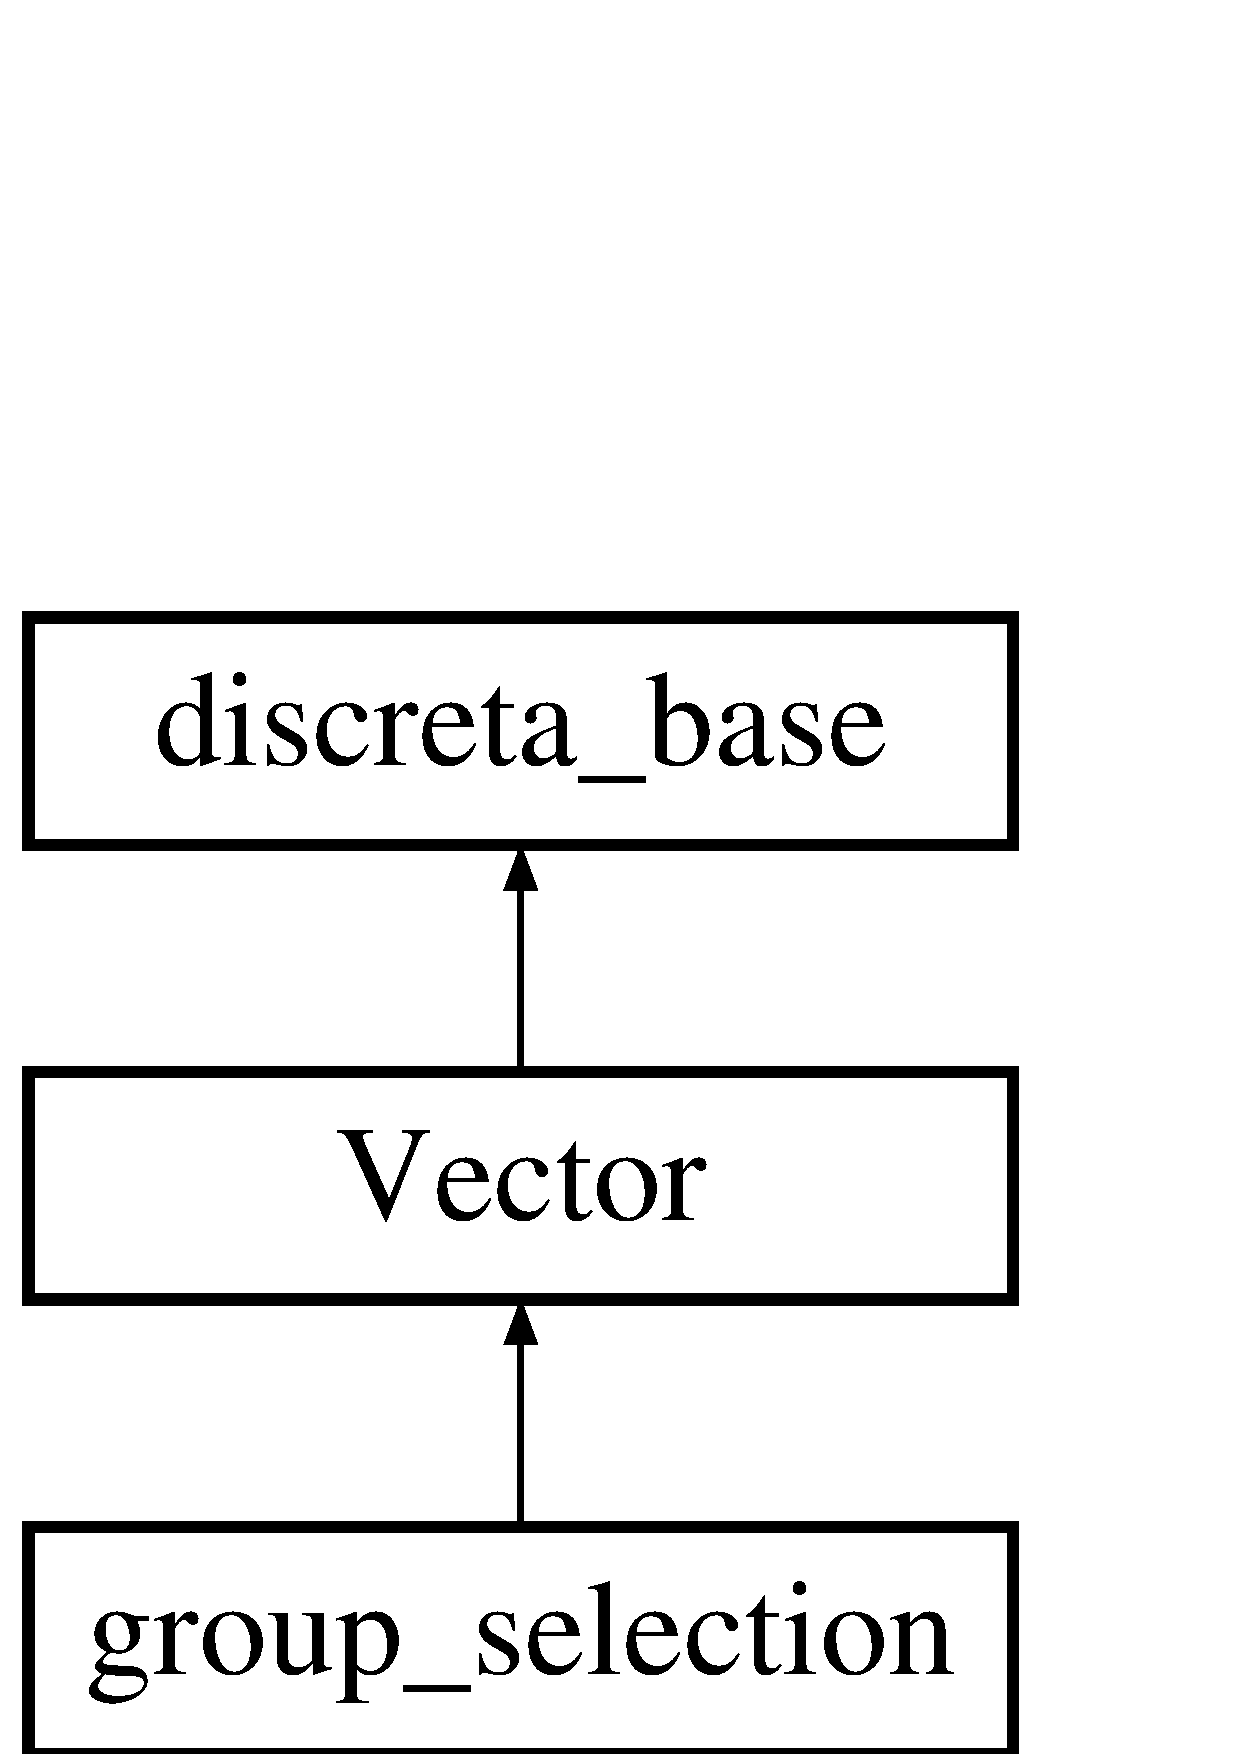
\includegraphics[height=3.000000cm]{classgroup__selection}
\end{center}
\end{figure}
\subsection*{Public Member Functions}
\begin{DoxyCompactItemize}
\item 
\mbox{\hyperlink{classgroup__selection_a2becdd8a6d93195ff4faa1e0df6f9eae}{group\+\_\+selection}} ()
\item 
\mbox{\hyperlink{classgroup__selection_a8c1d31e033e97292bd58fd64b5353322}{group\+\_\+selection}} (const \mbox{\hyperlink{classdiscreta__base}{discreta\+\_\+base}} \&\mbox{\hyperlink{alphabet2_8_c_a6150e0515f7202e2fb518f7206ed97dc}{x}})
\item 
\mbox{\hyperlink{classgroup__selection}{group\+\_\+selection}} \& \mbox{\hyperlink{classgroup__selection_abf861ab6bf4c061dd36775301c1e4f46}{operator=}} (const \mbox{\hyperlink{classdiscreta__base}{discreta\+\_\+base}} \&\mbox{\hyperlink{alphabet2_8_c_a6150e0515f7202e2fb518f7206ed97dc}{x}})
\item 
void $\ast$ \mbox{\hyperlink{classgroup__selection_af99b3b7ee09ea8e09f7be9cf080c74d3}{operator new}} (size\+\_\+t, void $\ast$\mbox{\hyperlink{alphabet2_8_c_a533391314665d6bf1b5575e9a9cd8552}{p}})
\item 
void \mbox{\hyperlink{classgroup__selection_a015ed73b7b8d784bedd4d11ac1fc0ec1}{settype\+\_\+group\+\_\+selection}} ()
\item 
\mbox{\hyperlink{discreta_8h_aaf25ee7e2306d78c74ec7bc48f092e81}{kind}} \mbox{\hyperlink{classgroup__selection_a21d7be997a2787d8a1284696b01038e8}{s\+\_\+virtual\+\_\+kind}} ()
\item 
\mbox{\hyperlink{classgroup__selection_a3e5fde933dbf37ec41568956f3edf026}{$\sim$group\+\_\+selection}} ()
\item 
void \mbox{\hyperlink{classgroup__selection_a778b1a466858bf7f90516eeba1795798}{freeself\+\_\+group\+\_\+selection}} ()
\item 
void \mbox{\hyperlink{classgroup__selection_a02a5e69978de662af0e8372a4f0b23a8}{copyobject\+\_\+to}} (\mbox{\hyperlink{classdiscreta__base}{discreta\+\_\+base}} \&\mbox{\hyperlink{alphabet2_8_c_a6150e0515f7202e2fb518f7206ed97dc}{x}})
\item 
ostream \& \mbox{\hyperlink{classgroup__selection_a522bc3a2346d1031fbb82f5a4d0b29cc}{print}} (ostream \&)
\item 
\mbox{\hyperlink{galois_8h_a09fddde158a3a20bd2dcadb609de11dc}{I\+NT}} \& \mbox{\hyperlink{classgroup__selection_a7d7efa588eae53bc12ab0cc6a45fad31}{type}} ()
\item 
\mbox{\hyperlink{galois_8h_a09fddde158a3a20bd2dcadb609de11dc}{I\+NT}} \& \mbox{\hyperlink{classgroup__selection_a9b9578c0fe171d6aef98a1cb6926c4ea}{val1}} ()
\item 
\mbox{\hyperlink{galois_8h_a09fddde158a3a20bd2dcadb609de11dc}{I\+NT}} \& \mbox{\hyperlink{classgroup__selection_a9354cad24b302f9faf3924cbb9f7947c}{val2}} ()
\item 
\mbox{\hyperlink{classhollerith}{hollerith}} \& \mbox{\hyperlink{classgroup__selection_a686cb0c6a3a040796b112b8007ea8223}{s}} ()
\item 
void \mbox{\hyperlink{classgroup__selection_ad12ab2226024716902e4a85c4772732b}{init}} (\mbox{\hyperlink{discreta_8h_a9fbd019a849defc14910ae0a667c516e}{group\+\_\+selection\+\_\+type}} \mbox{\hyperlink{classgroup__selection_a7d7efa588eae53bc12ab0cc6a45fad31}{type}}, \mbox{\hyperlink{galois_8h_a09fddde158a3a20bd2dcadb609de11dc}{I\+NT}} v1, \mbox{\hyperlink{galois_8h_a09fddde158a3a20bd2dcadb609de11dc}{I\+NT}} v2, \mbox{\hyperlink{galois_8h_ab6cc7b4aeb6ea31aba2b3fbfc83ff5e6}{B\+Y\+TE}} $\ast$str)
\end{DoxyCompactItemize}
\subsection*{Additional Inherited Members}


\subsection{Constructor \& Destructor Documentation}
\mbox{\Hypertarget{classgroup__selection_a2becdd8a6d93195ff4faa1e0df6f9eae}\label{classgroup__selection_a2becdd8a6d93195ff4faa1e0df6f9eae}} 
\index{group\+\_\+selection@{group\+\_\+selection}!group\+\_\+selection@{group\+\_\+selection}}
\index{group\+\_\+selection@{group\+\_\+selection}!group\+\_\+selection@{group\+\_\+selection}}
\subsubsection{\texorpdfstring{group\+\_\+selection()}{group\_selection()}\hspace{0.1cm}{\footnotesize\ttfamily [1/2]}}
{\footnotesize\ttfamily group\+\_\+selection\+::group\+\_\+selection (\begin{DoxyParamCaption}{ }\end{DoxyParamCaption})}

\mbox{\Hypertarget{classgroup__selection_a8c1d31e033e97292bd58fd64b5353322}\label{classgroup__selection_a8c1d31e033e97292bd58fd64b5353322}} 
\index{group\+\_\+selection@{group\+\_\+selection}!group\+\_\+selection@{group\+\_\+selection}}
\index{group\+\_\+selection@{group\+\_\+selection}!group\+\_\+selection@{group\+\_\+selection}}
\subsubsection{\texorpdfstring{group\+\_\+selection()}{group\_selection()}\hspace{0.1cm}{\footnotesize\ttfamily [2/2]}}
{\footnotesize\ttfamily group\+\_\+selection\+::group\+\_\+selection (\begin{DoxyParamCaption}\item[{const \mbox{\hyperlink{classdiscreta__base}{discreta\+\_\+base}} \&}]{x }\end{DoxyParamCaption})}

\mbox{\Hypertarget{classgroup__selection_a3e5fde933dbf37ec41568956f3edf026}\label{classgroup__selection_a3e5fde933dbf37ec41568956f3edf026}} 
\index{group\+\_\+selection@{group\+\_\+selection}!````~group\+\_\+selection@{$\sim$group\+\_\+selection}}
\index{````~group\+\_\+selection@{$\sim$group\+\_\+selection}!group\+\_\+selection@{group\+\_\+selection}}
\subsubsection{\texorpdfstring{$\sim$group\+\_\+selection()}{~group\_selection()}}
{\footnotesize\ttfamily group\+\_\+selection\+::$\sim$group\+\_\+selection (\begin{DoxyParamCaption}{ }\end{DoxyParamCaption})}



\subsection{Member Function Documentation}
\mbox{\Hypertarget{classgroup__selection_a02a5e69978de662af0e8372a4f0b23a8}\label{classgroup__selection_a02a5e69978de662af0e8372a4f0b23a8}} 
\index{group\+\_\+selection@{group\+\_\+selection}!copyobject\+\_\+to@{copyobject\+\_\+to}}
\index{copyobject\+\_\+to@{copyobject\+\_\+to}!group\+\_\+selection@{group\+\_\+selection}}
\subsubsection{\texorpdfstring{copyobject\+\_\+to()}{copyobject\_to()}}
{\footnotesize\ttfamily void group\+\_\+selection\+::copyobject\+\_\+to (\begin{DoxyParamCaption}\item[{\mbox{\hyperlink{classdiscreta__base}{discreta\+\_\+base}} \&}]{x }\end{DoxyParamCaption})\hspace{0.3cm}{\ttfamily [virtual]}}



Reimplemented from \mbox{\hyperlink{class_vector_af657307f3d344c8cef5d633335a5f484}{Vector}}.

\mbox{\Hypertarget{classgroup__selection_a778b1a466858bf7f90516eeba1795798}\label{classgroup__selection_a778b1a466858bf7f90516eeba1795798}} 
\index{group\+\_\+selection@{group\+\_\+selection}!freeself\+\_\+group\+\_\+selection@{freeself\+\_\+group\+\_\+selection}}
\index{freeself\+\_\+group\+\_\+selection@{freeself\+\_\+group\+\_\+selection}!group\+\_\+selection@{group\+\_\+selection}}
\subsubsection{\texorpdfstring{freeself\+\_\+group\+\_\+selection()}{freeself\_group\_selection()}}
{\footnotesize\ttfamily void group\+\_\+selection\+::freeself\+\_\+group\+\_\+selection (\begin{DoxyParamCaption}{ }\end{DoxyParamCaption})}

\mbox{\Hypertarget{classgroup__selection_ad12ab2226024716902e4a85c4772732b}\label{classgroup__selection_ad12ab2226024716902e4a85c4772732b}} 
\index{group\+\_\+selection@{group\+\_\+selection}!init@{init}}
\index{init@{init}!group\+\_\+selection@{group\+\_\+selection}}
\subsubsection{\texorpdfstring{init()}{init()}}
{\footnotesize\ttfamily void group\+\_\+selection\+::init (\begin{DoxyParamCaption}\item[{\mbox{\hyperlink{discreta_8h_a9fbd019a849defc14910ae0a667c516e}{group\+\_\+selection\+\_\+type}}}]{type,  }\item[{\mbox{\hyperlink{galois_8h_a09fddde158a3a20bd2dcadb609de11dc}{I\+NT}}}]{v1,  }\item[{\mbox{\hyperlink{galois_8h_a09fddde158a3a20bd2dcadb609de11dc}{I\+NT}}}]{v2,  }\item[{\mbox{\hyperlink{galois_8h_ab6cc7b4aeb6ea31aba2b3fbfc83ff5e6}{B\+Y\+TE}} $\ast$}]{str }\end{DoxyParamCaption})}

\mbox{\Hypertarget{classgroup__selection_af99b3b7ee09ea8e09f7be9cf080c74d3}\label{classgroup__selection_af99b3b7ee09ea8e09f7be9cf080c74d3}} 
\index{group\+\_\+selection@{group\+\_\+selection}!operator new@{operator new}}
\index{operator new@{operator new}!group\+\_\+selection@{group\+\_\+selection}}
\subsubsection{\texorpdfstring{operator new()}{operator new()}}
{\footnotesize\ttfamily void$\ast$ group\+\_\+selection\+::operator new (\begin{DoxyParamCaption}\item[{size\+\_\+t}]{,  }\item[{void $\ast$}]{p }\end{DoxyParamCaption})\hspace{0.3cm}{\ttfamily [inline]}}

\mbox{\Hypertarget{classgroup__selection_abf861ab6bf4c061dd36775301c1e4f46}\label{classgroup__selection_abf861ab6bf4c061dd36775301c1e4f46}} 
\index{group\+\_\+selection@{group\+\_\+selection}!operator=@{operator=}}
\index{operator=@{operator=}!group\+\_\+selection@{group\+\_\+selection}}
\subsubsection{\texorpdfstring{operator=()}{operator=()}}
{\footnotesize\ttfamily \mbox{\hyperlink{classgroup__selection}{group\+\_\+selection}} \& group\+\_\+selection\+::operator= (\begin{DoxyParamCaption}\item[{const \mbox{\hyperlink{classdiscreta__base}{discreta\+\_\+base}} \&}]{x }\end{DoxyParamCaption})}

\mbox{\Hypertarget{classgroup__selection_a522bc3a2346d1031fbb82f5a4d0b29cc}\label{classgroup__selection_a522bc3a2346d1031fbb82f5a4d0b29cc}} 
\index{group\+\_\+selection@{group\+\_\+selection}!print@{print}}
\index{print@{print}!group\+\_\+selection@{group\+\_\+selection}}
\subsubsection{\texorpdfstring{print()}{print()}}
{\footnotesize\ttfamily ostream \& group\+\_\+selection\+::print (\begin{DoxyParamCaption}\item[{ostream \&}]{ost }\end{DoxyParamCaption})\hspace{0.3cm}{\ttfamily [virtual]}}



Reimplemented from \mbox{\hyperlink{class_vector_a71d7e24bcfdfc69d4a2137360acb066c}{Vector}}.

\mbox{\Hypertarget{classgroup__selection_a686cb0c6a3a040796b112b8007ea8223}\label{classgroup__selection_a686cb0c6a3a040796b112b8007ea8223}} 
\index{group\+\_\+selection@{group\+\_\+selection}!s@{s}}
\index{s@{s}!group\+\_\+selection@{group\+\_\+selection}}
\subsubsection{\texorpdfstring{s()}{s()}}
{\footnotesize\ttfamily \mbox{\hyperlink{classhollerith}{hollerith}}\& group\+\_\+selection\+::s (\begin{DoxyParamCaption}{ }\end{DoxyParamCaption})\hspace{0.3cm}{\ttfamily [inline]}}

\mbox{\Hypertarget{classgroup__selection_a21d7be997a2787d8a1284696b01038e8}\label{classgroup__selection_a21d7be997a2787d8a1284696b01038e8}} 
\index{group\+\_\+selection@{group\+\_\+selection}!s\+\_\+virtual\+\_\+kind@{s\+\_\+virtual\+\_\+kind}}
\index{s\+\_\+virtual\+\_\+kind@{s\+\_\+virtual\+\_\+kind}!group\+\_\+selection@{group\+\_\+selection}}
\subsubsection{\texorpdfstring{s\+\_\+virtual\+\_\+kind()}{s\_virtual\_kind()}}
{\footnotesize\ttfamily \mbox{\hyperlink{discreta_8h_aaf25ee7e2306d78c74ec7bc48f092e81}{kind}} group\+\_\+selection\+::s\+\_\+virtual\+\_\+kind (\begin{DoxyParamCaption}{ }\end{DoxyParamCaption})\hspace{0.3cm}{\ttfamily [virtual]}}



Reimplemented from \mbox{\hyperlink{class_vector_a20550e70d02cbe484032c7f6b0833a0f}{Vector}}.

\mbox{\Hypertarget{classgroup__selection_a015ed73b7b8d784bedd4d11ac1fc0ec1}\label{classgroup__selection_a015ed73b7b8d784bedd4d11ac1fc0ec1}} 
\index{group\+\_\+selection@{group\+\_\+selection}!settype\+\_\+group\+\_\+selection@{settype\+\_\+group\+\_\+selection}}
\index{settype\+\_\+group\+\_\+selection@{settype\+\_\+group\+\_\+selection}!group\+\_\+selection@{group\+\_\+selection}}
\subsubsection{\texorpdfstring{settype\+\_\+group\+\_\+selection()}{settype\_group\_selection()}}
{\footnotesize\ttfamily void group\+\_\+selection\+::settype\+\_\+group\+\_\+selection (\begin{DoxyParamCaption}{ }\end{DoxyParamCaption})}

\mbox{\Hypertarget{classgroup__selection_a7d7efa588eae53bc12ab0cc6a45fad31}\label{classgroup__selection_a7d7efa588eae53bc12ab0cc6a45fad31}} 
\index{group\+\_\+selection@{group\+\_\+selection}!type@{type}}
\index{type@{type}!group\+\_\+selection@{group\+\_\+selection}}
\subsubsection{\texorpdfstring{type()}{type()}}
{\footnotesize\ttfamily \mbox{\hyperlink{galois_8h_a09fddde158a3a20bd2dcadb609de11dc}{I\+NT}}\& group\+\_\+selection\+::type (\begin{DoxyParamCaption}{ }\end{DoxyParamCaption})\hspace{0.3cm}{\ttfamily [inline]}}

\mbox{\Hypertarget{classgroup__selection_a9b9578c0fe171d6aef98a1cb6926c4ea}\label{classgroup__selection_a9b9578c0fe171d6aef98a1cb6926c4ea}} 
\index{group\+\_\+selection@{group\+\_\+selection}!val1@{val1}}
\index{val1@{val1}!group\+\_\+selection@{group\+\_\+selection}}
\subsubsection{\texorpdfstring{val1()}{val1()}}
{\footnotesize\ttfamily \mbox{\hyperlink{galois_8h_a09fddde158a3a20bd2dcadb609de11dc}{I\+NT}}\& group\+\_\+selection\+::val1 (\begin{DoxyParamCaption}{ }\end{DoxyParamCaption})\hspace{0.3cm}{\ttfamily [inline]}}

\mbox{\Hypertarget{classgroup__selection_a9354cad24b302f9faf3924cbb9f7947c}\label{classgroup__selection_a9354cad24b302f9faf3924cbb9f7947c}} 
\index{group\+\_\+selection@{group\+\_\+selection}!val2@{val2}}
\index{val2@{val2}!group\+\_\+selection@{group\+\_\+selection}}
\subsubsection{\texorpdfstring{val2()}{val2()}}
{\footnotesize\ttfamily \mbox{\hyperlink{galois_8h_a09fddde158a3a20bd2dcadb609de11dc}{I\+NT}}\& group\+\_\+selection\+::val2 (\begin{DoxyParamCaption}{ }\end{DoxyParamCaption})\hspace{0.3cm}{\ttfamily [inline]}}



The documentation for this class was generated from the following files\+:\begin{DoxyCompactItemize}
\item 
S\+R\+C/\+L\+I\+B/\+D\+I\+S\+C\+R\+E\+T\+A/\mbox{\hyperlink{discreta_8h}{discreta.\+h}}\item 
S\+R\+C/\+L\+I\+B/\+D\+I\+S\+C\+R\+E\+T\+A/\mbox{\hyperlink{group__selection_8_c}{group\+\_\+selection.\+C}}\end{DoxyCompactItemize}

\hypertarget{classhadamard}{}\section{hadamard Class Reference}
\label{classhadamard}\index{hadamard@{hadamard}}
\subsection*{Public Member Functions}
\begin{DoxyCompactItemize}
\item 
void \mbox{\hyperlink{classhadamard_a16af359850b8bdd0d2a73e260d496c33}{init}} (\mbox{\hyperlink{galois_8h_a09fddde158a3a20bd2dcadb609de11dc}{I\+NT}} \mbox{\hyperlink{classhadamard_aaa7087a44d86f99804f4a42581f2a842}{n}}, \mbox{\hyperlink{galois_8h_a09fddde158a3a20bd2dcadb609de11dc}{I\+NT}} f\+\_\+draw, \mbox{\hyperlink{galois_8h_a09fddde158a3a20bd2dcadb609de11dc}{I\+NT}} \mbox{\hyperlink{simeon_8_c_a818073fbcc2f439e7c56952f67386122}{verbose\+\_\+level}}, \mbox{\hyperlink{galois_8h_a09fddde158a3a20bd2dcadb609de11dc}{I\+NT}} verbose\+\_\+level\+\_\+clique)
\item 
\mbox{\hyperlink{galois_8h_a09fddde158a3a20bd2dcadb609de11dc}{I\+NT}} \mbox{\hyperlink{classhadamard_a2f9f095c9f78d125e764354279820fd5}{clique\+\_\+test}} (\mbox{\hyperlink{galois_8h_a09fddde158a3a20bd2dcadb609de11dc}{I\+NT}} $\ast$\mbox{\hyperlink{nauty_8h_a9690bea211101f22a5e154087590c3da}{set}}, \mbox{\hyperlink{galois_8h_a09fddde158a3a20bd2dcadb609de11dc}{I\+NT}} sz)
\item 
void \mbox{\hyperlink{classhadamard_a299a7a683de28326c93c8fd5b9545144}{early\+\_\+test\+\_\+func}} (\mbox{\hyperlink{galois_8h_a09fddde158a3a20bd2dcadb609de11dc}{I\+NT}} $\ast$\mbox{\hyperlink{simeon_8_c_adab47f8243f1b5a2c31df2535d6b37d0}{S}}, \mbox{\hyperlink{galois_8h_a09fddde158a3a20bd2dcadb609de11dc}{I\+NT}} len, \mbox{\hyperlink{galois_8h_a09fddde158a3a20bd2dcadb609de11dc}{I\+NT}} $\ast$candidates, \mbox{\hyperlink{galois_8h_a09fddde158a3a20bd2dcadb609de11dc}{I\+NT}} nb\+\_\+candidates, \mbox{\hyperlink{galois_8h_a09fddde158a3a20bd2dcadb609de11dc}{I\+NT}} $\ast$good\+\_\+candidates, \mbox{\hyperlink{galois_8h_a09fddde158a3a20bd2dcadb609de11dc}{I\+NT}} \&nb\+\_\+good\+\_\+candidates, \mbox{\hyperlink{galois_8h_a09fddde158a3a20bd2dcadb609de11dc}{I\+NT}} \mbox{\hyperlink{simeon_8_c_a818073fbcc2f439e7c56952f67386122}{verbose\+\_\+level}})
\end{DoxyCompactItemize}
\subsection*{Public Attributes}
\begin{DoxyCompactItemize}
\item 
\mbox{\hyperlink{galois_8h_a09fddde158a3a20bd2dcadb609de11dc}{I\+NT}} \mbox{\hyperlink{classhadamard_aaa7087a44d86f99804f4a42581f2a842}{n}}
\item 
\mbox{\hyperlink{galois_8h_a09fddde158a3a20bd2dcadb609de11dc}{I\+NT}} \mbox{\hyperlink{classhadamard_ae5ee601c2dbe8b01970b84422ad3a7ee}{N}}
\item 
\mbox{\hyperlink{galois_8h_a09fddde158a3a20bd2dcadb609de11dc}{I\+NT}} \mbox{\hyperlink{classhadamard_aac7ff83b713dacd1dbbb69a59ed99454}{N2}}
\item 
\mbox{\hyperlink{galois_8h_a09fddde158a3a20bd2dcadb609de11dc}{I\+NT}} \mbox{\hyperlink{classhadamard_a41b951979c27c0c4855d6203899c94bb}{bitvector\+\_\+length}}
\item 
\mbox{\hyperlink{galois_8h_a122c4acf389c050379f00341fdcd5812}{U\+B\+Y\+TE}} $\ast$ \mbox{\hyperlink{classhadamard_af616eb4ee1edff0fc597962d98fb6239}{bitvector\+\_\+adjacency}}
\item 
\mbox{\hyperlink{classcolored__graph}{colored\+\_\+graph}} $\ast$ \mbox{\hyperlink{classhadamard_ae6ebddfda23ce9e874ab97480844aff1}{CG}}
\item 
\mbox{\hyperlink{classaction}{action}} $\ast$ \mbox{\hyperlink{classhadamard_a5739909fa42b08637718cd2bf5bce169}{A}}
\item 
\mbox{\hyperlink{galois_8h_a09fddde158a3a20bd2dcadb609de11dc}{I\+NT}} $\ast$ \mbox{\hyperlink{classhadamard_a057eb008b50219f72710c974a53d08c3}{v}}
\item 
\mbox{\hyperlink{classgenerator}{generator}} $\ast$ \mbox{\hyperlink{classhadamard_aec73f1c3f54480fbeb3392a034584046}{gen}}
\item 
\mbox{\hyperlink{galois_8h_a09fddde158a3a20bd2dcadb609de11dc}{I\+NT}} \mbox{\hyperlink{classhadamard_aed9bff4bb7390e22d6f3c0001773fa55}{nb\+\_\+orbits}}
\end{DoxyCompactItemize}


\subsection{Member Function Documentation}
\mbox{\Hypertarget{classhadamard_a2f9f095c9f78d125e764354279820fd5}\label{classhadamard_a2f9f095c9f78d125e764354279820fd5}} 
\index{hadamard@{hadamard}!clique\+\_\+test@{clique\+\_\+test}}
\index{clique\+\_\+test@{clique\+\_\+test}!hadamard@{hadamard}}
\subsubsection{\texorpdfstring{clique\+\_\+test()}{clique\_test()}}
{\footnotesize\ttfamily \mbox{\hyperlink{galois_8h_a09fddde158a3a20bd2dcadb609de11dc}{I\+NT}} hadamard\+::clique\+\_\+test (\begin{DoxyParamCaption}\item[{\mbox{\hyperlink{galois_8h_a09fddde158a3a20bd2dcadb609de11dc}{I\+NT}} $\ast$}]{set,  }\item[{\mbox{\hyperlink{galois_8h_a09fddde158a3a20bd2dcadb609de11dc}{I\+NT}}}]{sz }\end{DoxyParamCaption})}

\mbox{\Hypertarget{classhadamard_a299a7a683de28326c93c8fd5b9545144}\label{classhadamard_a299a7a683de28326c93c8fd5b9545144}} 
\index{hadamard@{hadamard}!early\+\_\+test\+\_\+func@{early\+\_\+test\+\_\+func}}
\index{early\+\_\+test\+\_\+func@{early\+\_\+test\+\_\+func}!hadamard@{hadamard}}
\subsubsection{\texorpdfstring{early\+\_\+test\+\_\+func()}{early\_test\_func()}}
{\footnotesize\ttfamily void hadamard\+::early\+\_\+test\+\_\+func (\begin{DoxyParamCaption}\item[{\mbox{\hyperlink{galois_8h_a09fddde158a3a20bd2dcadb609de11dc}{I\+NT}} $\ast$}]{S,  }\item[{\mbox{\hyperlink{galois_8h_a09fddde158a3a20bd2dcadb609de11dc}{I\+NT}}}]{len,  }\item[{\mbox{\hyperlink{galois_8h_a09fddde158a3a20bd2dcadb609de11dc}{I\+NT}} $\ast$}]{candidates,  }\item[{\mbox{\hyperlink{galois_8h_a09fddde158a3a20bd2dcadb609de11dc}{I\+NT}}}]{nb\+\_\+candidates,  }\item[{\mbox{\hyperlink{galois_8h_a09fddde158a3a20bd2dcadb609de11dc}{I\+NT}} $\ast$}]{good\+\_\+candidates,  }\item[{\mbox{\hyperlink{galois_8h_a09fddde158a3a20bd2dcadb609de11dc}{I\+NT}} \&}]{nb\+\_\+good\+\_\+candidates,  }\item[{\mbox{\hyperlink{galois_8h_a09fddde158a3a20bd2dcadb609de11dc}{I\+NT}}}]{verbose\+\_\+level }\end{DoxyParamCaption})}

\mbox{\Hypertarget{classhadamard_a16af359850b8bdd0d2a73e260d496c33}\label{classhadamard_a16af359850b8bdd0d2a73e260d496c33}} 
\index{hadamard@{hadamard}!init@{init}}
\index{init@{init}!hadamard@{hadamard}}
\subsubsection{\texorpdfstring{init()}{init()}}
{\footnotesize\ttfamily void hadamard\+::init (\begin{DoxyParamCaption}\item[{\mbox{\hyperlink{galois_8h_a09fddde158a3a20bd2dcadb609de11dc}{I\+NT}}}]{n,  }\item[{\mbox{\hyperlink{galois_8h_a09fddde158a3a20bd2dcadb609de11dc}{I\+NT}}}]{f\+\_\+draw,  }\item[{\mbox{\hyperlink{galois_8h_a09fddde158a3a20bd2dcadb609de11dc}{I\+NT}}}]{verbose\+\_\+level,  }\item[{\mbox{\hyperlink{galois_8h_a09fddde158a3a20bd2dcadb609de11dc}{I\+NT}}}]{verbose\+\_\+level\+\_\+clique }\end{DoxyParamCaption})}



\subsection{Member Data Documentation}
\mbox{\Hypertarget{classhadamard_a5739909fa42b08637718cd2bf5bce169}\label{classhadamard_a5739909fa42b08637718cd2bf5bce169}} 
\index{hadamard@{hadamard}!A@{A}}
\index{A@{A}!hadamard@{hadamard}}
\subsubsection{\texorpdfstring{A}{A}}
{\footnotesize\ttfamily \mbox{\hyperlink{classaction}{action}}$\ast$ hadamard\+::A}

\mbox{\Hypertarget{classhadamard_af616eb4ee1edff0fc597962d98fb6239}\label{classhadamard_af616eb4ee1edff0fc597962d98fb6239}} 
\index{hadamard@{hadamard}!bitvector\+\_\+adjacency@{bitvector\+\_\+adjacency}}
\index{bitvector\+\_\+adjacency@{bitvector\+\_\+adjacency}!hadamard@{hadamard}}
\subsubsection{\texorpdfstring{bitvector\+\_\+adjacency}{bitvector\_adjacency}}
{\footnotesize\ttfamily \mbox{\hyperlink{galois_8h_a122c4acf389c050379f00341fdcd5812}{U\+B\+Y\+TE}}$\ast$ hadamard\+::bitvector\+\_\+adjacency}

\mbox{\Hypertarget{classhadamard_a41b951979c27c0c4855d6203899c94bb}\label{classhadamard_a41b951979c27c0c4855d6203899c94bb}} 
\index{hadamard@{hadamard}!bitvector\+\_\+length@{bitvector\+\_\+length}}
\index{bitvector\+\_\+length@{bitvector\+\_\+length}!hadamard@{hadamard}}
\subsubsection{\texorpdfstring{bitvector\+\_\+length}{bitvector\_length}}
{\footnotesize\ttfamily \mbox{\hyperlink{galois_8h_a09fddde158a3a20bd2dcadb609de11dc}{I\+NT}} hadamard\+::bitvector\+\_\+length}

\mbox{\Hypertarget{classhadamard_ae6ebddfda23ce9e874ab97480844aff1}\label{classhadamard_ae6ebddfda23ce9e874ab97480844aff1}} 
\index{hadamard@{hadamard}!CG@{CG}}
\index{CG@{CG}!hadamard@{hadamard}}
\subsubsection{\texorpdfstring{CG}{CG}}
{\footnotesize\ttfamily \mbox{\hyperlink{classcolored__graph}{colored\+\_\+graph}}$\ast$ hadamard\+::\+CG}

\mbox{\Hypertarget{classhadamard_aec73f1c3f54480fbeb3392a034584046}\label{classhadamard_aec73f1c3f54480fbeb3392a034584046}} 
\index{hadamard@{hadamard}!gen@{gen}}
\index{gen@{gen}!hadamard@{hadamard}}
\subsubsection{\texorpdfstring{gen}{gen}}
{\footnotesize\ttfamily \mbox{\hyperlink{classgenerator}{generator}}$\ast$ hadamard\+::gen}

\mbox{\Hypertarget{classhadamard_aaa7087a44d86f99804f4a42581f2a842}\label{classhadamard_aaa7087a44d86f99804f4a42581f2a842}} 
\index{hadamard@{hadamard}!n@{n}}
\index{n@{n}!hadamard@{hadamard}}
\subsubsection{\texorpdfstring{n}{n}}
{\footnotesize\ttfamily \mbox{\hyperlink{galois_8h_a09fddde158a3a20bd2dcadb609de11dc}{I\+NT}} hadamard\+::n}

\mbox{\Hypertarget{classhadamard_ae5ee601c2dbe8b01970b84422ad3a7ee}\label{classhadamard_ae5ee601c2dbe8b01970b84422ad3a7ee}} 
\index{hadamard@{hadamard}!N@{N}}
\index{N@{N}!hadamard@{hadamard}}
\subsubsection{\texorpdfstring{N}{N}}
{\footnotesize\ttfamily \mbox{\hyperlink{galois_8h_a09fddde158a3a20bd2dcadb609de11dc}{I\+NT}} hadamard\+::N}

\mbox{\Hypertarget{classhadamard_aac7ff83b713dacd1dbbb69a59ed99454}\label{classhadamard_aac7ff83b713dacd1dbbb69a59ed99454}} 
\index{hadamard@{hadamard}!N2@{N2}}
\index{N2@{N2}!hadamard@{hadamard}}
\subsubsection{\texorpdfstring{N2}{N2}}
{\footnotesize\ttfamily \mbox{\hyperlink{galois_8h_a09fddde158a3a20bd2dcadb609de11dc}{I\+NT}} hadamard\+::\+N2}

\mbox{\Hypertarget{classhadamard_aed9bff4bb7390e22d6f3c0001773fa55}\label{classhadamard_aed9bff4bb7390e22d6f3c0001773fa55}} 
\index{hadamard@{hadamard}!nb\+\_\+orbits@{nb\+\_\+orbits}}
\index{nb\+\_\+orbits@{nb\+\_\+orbits}!hadamard@{hadamard}}
\subsubsection{\texorpdfstring{nb\+\_\+orbits}{nb\_orbits}}
{\footnotesize\ttfamily \mbox{\hyperlink{galois_8h_a09fddde158a3a20bd2dcadb609de11dc}{I\+NT}} hadamard\+::nb\+\_\+orbits}

\mbox{\Hypertarget{classhadamard_a057eb008b50219f72710c974a53d08c3}\label{classhadamard_a057eb008b50219f72710c974a53d08c3}} 
\index{hadamard@{hadamard}!v@{v}}
\index{v@{v}!hadamard@{hadamard}}
\subsubsection{\texorpdfstring{v}{v}}
{\footnotesize\ttfamily \mbox{\hyperlink{galois_8h_a09fddde158a3a20bd2dcadb609de11dc}{I\+NT}}$\ast$ hadamard\+::v}



The documentation for this class was generated from the following file\+:\begin{DoxyCompactItemize}
\item 
S\+R\+C/\+A\+P\+P\+S/\+C\+O\+M\+B\+I\+N\+A\+T\+O\+R\+I\+C\+S/\mbox{\hyperlink{hadamard_8_c}{hadamard.\+C}}\end{DoxyCompactItemize}

\hypertarget{classheisenberg}{}\section{heisenberg Class Reference}
\label{classheisenberg}\index{heisenberg@{heisenberg}}


{\ttfamily \#include $<$galois.\+h$>$}

\subsection*{Public Member Functions}
\begin{DoxyCompactItemize}
\item 
\mbox{\hyperlink{classheisenberg_a3b84a07f0f518ca32ffb17c8114a3bb7}{heisenberg}} ()
\item 
\mbox{\hyperlink{classheisenberg_a48ed5a56e78ec40c8d7305a245efbabb}{$\sim$heisenberg}} ()
\item 
void \mbox{\hyperlink{classheisenberg_ab448e495e2824699ceb3315371234646}{null}} ()
\item 
void \mbox{\hyperlink{classheisenberg_a3196baf0d43d79f3643cd6612ba51d2d}{freeself}} ()
\item 
void \mbox{\hyperlink{classheisenberg_ab45bf633370b097f5500a8499b165151}{init}} (\mbox{\hyperlink{classfinite__field}{finite\+\_\+field}} $\ast$\mbox{\hyperlink{classheisenberg_aeabec971ff171af2bbd41b2f64bd2e3a}{F}}, \mbox{\hyperlink{galois_8h_a09fddde158a3a20bd2dcadb609de11dc}{I\+NT}} \mbox{\hyperlink{classheisenberg_a5f434f747ceebaede3371d5e265c40e0}{n}}, \mbox{\hyperlink{galois_8h_a09fddde158a3a20bd2dcadb609de11dc}{I\+NT}} \mbox{\hyperlink{simeon_8_c_a818073fbcc2f439e7c56952f67386122}{verbose\+\_\+level}})
\item 
void \mbox{\hyperlink{classheisenberg_a45f9de07eb289caa5497e052fa74b994}{unrank\+\_\+element}} (\mbox{\hyperlink{galois_8h_a09fddde158a3a20bd2dcadb609de11dc}{I\+NT}} $\ast$\mbox{\hyperlink{simeon_8_c_aec1406935bdb1fee3561fcb840964100}{Elt}}, \mbox{\hyperlink{galois_8h_a09fddde158a3a20bd2dcadb609de11dc}{I\+NT}} rk)
\item 
\mbox{\hyperlink{galois_8h_a09fddde158a3a20bd2dcadb609de11dc}{I\+NT}} \mbox{\hyperlink{classheisenberg_a972b9c211fb4093a381a8b2a0dee30bd}{rank\+\_\+element}} (\mbox{\hyperlink{galois_8h_a09fddde158a3a20bd2dcadb609de11dc}{I\+NT}} $\ast$\mbox{\hyperlink{simeon_8_c_aec1406935bdb1fee3561fcb840964100}{Elt}})
\item 
void \mbox{\hyperlink{classheisenberg_afca08c599ec9225baedede3b0233bdec}{element\+\_\+add}} (\mbox{\hyperlink{galois_8h_a09fddde158a3a20bd2dcadb609de11dc}{I\+NT}} $\ast$\mbox{\hyperlink{classheisenberg_a6020d937f6761e6c392fe4f3c4b65755}{Elt1}}, \mbox{\hyperlink{galois_8h_a09fddde158a3a20bd2dcadb609de11dc}{I\+NT}} $\ast$\mbox{\hyperlink{classheisenberg_a681a960e90968d4af527c4247dc4cb61}{Elt2}}, \mbox{\hyperlink{galois_8h_a09fddde158a3a20bd2dcadb609de11dc}{I\+NT}} $\ast$\mbox{\hyperlink{classheisenberg_a04d358f005654f254fbe2613e298c77a}{Elt3}}, \mbox{\hyperlink{galois_8h_a09fddde158a3a20bd2dcadb609de11dc}{I\+NT}} \mbox{\hyperlink{simeon_8_c_a818073fbcc2f439e7c56952f67386122}{verbose\+\_\+level}})
\item 
void \mbox{\hyperlink{classheisenberg_aceccdc4c30ae78320961720b74ec24c1}{element\+\_\+negate}} (\mbox{\hyperlink{galois_8h_a09fddde158a3a20bd2dcadb609de11dc}{I\+NT}} $\ast$\mbox{\hyperlink{classheisenberg_a6020d937f6761e6c392fe4f3c4b65755}{Elt1}}, \mbox{\hyperlink{galois_8h_a09fddde158a3a20bd2dcadb609de11dc}{I\+NT}} $\ast$\mbox{\hyperlink{classheisenberg_a681a960e90968d4af527c4247dc4cb61}{Elt2}}, \mbox{\hyperlink{galois_8h_a09fddde158a3a20bd2dcadb609de11dc}{I\+NT}} \mbox{\hyperlink{simeon_8_c_a818073fbcc2f439e7c56952f67386122}{verbose\+\_\+level}})
\item 
\mbox{\hyperlink{galois_8h_a09fddde158a3a20bd2dcadb609de11dc}{I\+NT}} \mbox{\hyperlink{classheisenberg_a204fb1674976610c2853e645fb42fe63}{element\+\_\+add\+\_\+by\+\_\+rank}} (\mbox{\hyperlink{galois_8h_a09fddde158a3a20bd2dcadb609de11dc}{I\+NT}} rk\+\_\+a, \mbox{\hyperlink{galois_8h_a09fddde158a3a20bd2dcadb609de11dc}{I\+NT}} rk\+\_\+b, \mbox{\hyperlink{galois_8h_a09fddde158a3a20bd2dcadb609de11dc}{I\+NT}} \mbox{\hyperlink{simeon_8_c_a818073fbcc2f439e7c56952f67386122}{verbose\+\_\+level}})
\item 
\mbox{\hyperlink{galois_8h_a09fddde158a3a20bd2dcadb609de11dc}{I\+NT}} \mbox{\hyperlink{classheisenberg_a1d0d7cab573376418a779a794e8a83a9}{element\+\_\+negate\+\_\+by\+\_\+rank}} (\mbox{\hyperlink{galois_8h_a09fddde158a3a20bd2dcadb609de11dc}{I\+NT}} rk\+\_\+a, \mbox{\hyperlink{galois_8h_a09fddde158a3a20bd2dcadb609de11dc}{I\+NT}} \mbox{\hyperlink{simeon_8_c_a818073fbcc2f439e7c56952f67386122}{verbose\+\_\+level}})
\item 
void \mbox{\hyperlink{classheisenberg_abe0b5eb10368096b3cb0fca084d00cff}{group\+\_\+table}} (\mbox{\hyperlink{galois_8h_a09fddde158a3a20bd2dcadb609de11dc}{I\+NT}} $\ast$\&Table, \mbox{\hyperlink{galois_8h_a09fddde158a3a20bd2dcadb609de11dc}{I\+NT}} \mbox{\hyperlink{simeon_8_c_a818073fbcc2f439e7c56952f67386122}{verbose\+\_\+level}})
\item 
void \mbox{\hyperlink{classheisenberg_aaabd8b71c8358a32f89a0ee59470a7b3}{group\+\_\+table\+\_\+abv}} (\mbox{\hyperlink{galois_8h_a09fddde158a3a20bd2dcadb609de11dc}{I\+NT}} $\ast$\&Table\+\_\+abv, \mbox{\hyperlink{galois_8h_a09fddde158a3a20bd2dcadb609de11dc}{I\+NT}} \mbox{\hyperlink{simeon_8_c_a818073fbcc2f439e7c56952f67386122}{verbose\+\_\+level}})
\item 
void \mbox{\hyperlink{classheisenberg_a69e3d98a78cd340be18532fc693e9b24}{generating\+\_\+set}} (\mbox{\hyperlink{galois_8h_a09fddde158a3a20bd2dcadb609de11dc}{I\+NT}} $\ast$\&gens, \mbox{\hyperlink{galois_8h_a09fddde158a3a20bd2dcadb609de11dc}{I\+NT}} \&nb\+\_\+gens, \mbox{\hyperlink{galois_8h_a09fddde158a3a20bd2dcadb609de11dc}{I\+NT}} \mbox{\hyperlink{simeon_8_c_a818073fbcc2f439e7c56952f67386122}{verbose\+\_\+level}})
\end{DoxyCompactItemize}
\subsection*{Public Attributes}
\begin{DoxyCompactItemize}
\item 
\mbox{\hyperlink{galois_8h_a09fddde158a3a20bd2dcadb609de11dc}{I\+NT}} \mbox{\hyperlink{classheisenberg_af9e931f2bc1ca76d4c28d1bf8ea3c794}{q}}
\item 
\mbox{\hyperlink{classfinite__field}{finite\+\_\+field}} $\ast$ \mbox{\hyperlink{classheisenberg_aeabec971ff171af2bbd41b2f64bd2e3a}{F}}
\item 
\mbox{\hyperlink{galois_8h_a09fddde158a3a20bd2dcadb609de11dc}{I\+NT}} \mbox{\hyperlink{classheisenberg_a5f434f747ceebaede3371d5e265c40e0}{n}}
\item 
\mbox{\hyperlink{galois_8h_a09fddde158a3a20bd2dcadb609de11dc}{I\+NT}} \mbox{\hyperlink{classheisenberg_a9b4d0cf0672b763bda59a411ab307b30}{len}}
\item 
\mbox{\hyperlink{galois_8h_a09fddde158a3a20bd2dcadb609de11dc}{I\+NT}} \mbox{\hyperlink{classheisenberg_ae53b7d9155e9328b88ec79ecdd57b915}{group\+\_\+order}}
\item 
\mbox{\hyperlink{galois_8h_a09fddde158a3a20bd2dcadb609de11dc}{I\+NT}} $\ast$ \mbox{\hyperlink{classheisenberg_a6020d937f6761e6c392fe4f3c4b65755}{Elt1}}
\item 
\mbox{\hyperlink{galois_8h_a09fddde158a3a20bd2dcadb609de11dc}{I\+NT}} $\ast$ \mbox{\hyperlink{classheisenberg_a681a960e90968d4af527c4247dc4cb61}{Elt2}}
\item 
\mbox{\hyperlink{galois_8h_a09fddde158a3a20bd2dcadb609de11dc}{I\+NT}} $\ast$ \mbox{\hyperlink{classheisenberg_a04d358f005654f254fbe2613e298c77a}{Elt3}}
\item 
\mbox{\hyperlink{galois_8h_a09fddde158a3a20bd2dcadb609de11dc}{I\+NT}} $\ast$ \mbox{\hyperlink{classheisenberg_a117595bc25653670984daed9a53a9324}{Elt4}}
\end{DoxyCompactItemize}


\subsection{Constructor \& Destructor Documentation}
\mbox{\Hypertarget{classheisenberg_a3b84a07f0f518ca32ffb17c8114a3bb7}\label{classheisenberg_a3b84a07f0f518ca32ffb17c8114a3bb7}} 
\index{heisenberg@{heisenberg}!heisenberg@{heisenberg}}
\index{heisenberg@{heisenberg}!heisenberg@{heisenberg}}
\subsubsection{\texorpdfstring{heisenberg()}{heisenberg()}}
{\footnotesize\ttfamily heisenberg\+::heisenberg (\begin{DoxyParamCaption}{ }\end{DoxyParamCaption})}

\mbox{\Hypertarget{classheisenberg_a48ed5a56e78ec40c8d7305a245efbabb}\label{classheisenberg_a48ed5a56e78ec40c8d7305a245efbabb}} 
\index{heisenberg@{heisenberg}!````~heisenberg@{$\sim$heisenberg}}
\index{````~heisenberg@{$\sim$heisenberg}!heisenberg@{heisenberg}}
\subsubsection{\texorpdfstring{$\sim$heisenberg()}{~heisenberg()}}
{\footnotesize\ttfamily heisenberg\+::$\sim$heisenberg (\begin{DoxyParamCaption}{ }\end{DoxyParamCaption})}



\subsection{Member Function Documentation}
\mbox{\Hypertarget{classheisenberg_afca08c599ec9225baedede3b0233bdec}\label{classheisenberg_afca08c599ec9225baedede3b0233bdec}} 
\index{heisenberg@{heisenberg}!element\+\_\+add@{element\+\_\+add}}
\index{element\+\_\+add@{element\+\_\+add}!heisenberg@{heisenberg}}
\subsubsection{\texorpdfstring{element\+\_\+add()}{element\_add()}}
{\footnotesize\ttfamily void heisenberg\+::element\+\_\+add (\begin{DoxyParamCaption}\item[{\mbox{\hyperlink{galois_8h_a09fddde158a3a20bd2dcadb609de11dc}{I\+NT}} $\ast$}]{Elt1,  }\item[{\mbox{\hyperlink{galois_8h_a09fddde158a3a20bd2dcadb609de11dc}{I\+NT}} $\ast$}]{Elt2,  }\item[{\mbox{\hyperlink{galois_8h_a09fddde158a3a20bd2dcadb609de11dc}{I\+NT}} $\ast$}]{Elt3,  }\item[{\mbox{\hyperlink{galois_8h_a09fddde158a3a20bd2dcadb609de11dc}{I\+NT}}}]{verbose\+\_\+level }\end{DoxyParamCaption})}

\mbox{\Hypertarget{classheisenberg_a204fb1674976610c2853e645fb42fe63}\label{classheisenberg_a204fb1674976610c2853e645fb42fe63}} 
\index{heisenberg@{heisenberg}!element\+\_\+add\+\_\+by\+\_\+rank@{element\+\_\+add\+\_\+by\+\_\+rank}}
\index{element\+\_\+add\+\_\+by\+\_\+rank@{element\+\_\+add\+\_\+by\+\_\+rank}!heisenberg@{heisenberg}}
\subsubsection{\texorpdfstring{element\+\_\+add\+\_\+by\+\_\+rank()}{element\_add\_by\_rank()}}
{\footnotesize\ttfamily \mbox{\hyperlink{galois_8h_a09fddde158a3a20bd2dcadb609de11dc}{I\+NT}} heisenberg\+::element\+\_\+add\+\_\+by\+\_\+rank (\begin{DoxyParamCaption}\item[{\mbox{\hyperlink{galois_8h_a09fddde158a3a20bd2dcadb609de11dc}{I\+NT}}}]{rk\+\_\+a,  }\item[{\mbox{\hyperlink{galois_8h_a09fddde158a3a20bd2dcadb609de11dc}{I\+NT}}}]{rk\+\_\+b,  }\item[{\mbox{\hyperlink{galois_8h_a09fddde158a3a20bd2dcadb609de11dc}{I\+NT}}}]{verbose\+\_\+level }\end{DoxyParamCaption})}

\mbox{\Hypertarget{classheisenberg_aceccdc4c30ae78320961720b74ec24c1}\label{classheisenberg_aceccdc4c30ae78320961720b74ec24c1}} 
\index{heisenberg@{heisenberg}!element\+\_\+negate@{element\+\_\+negate}}
\index{element\+\_\+negate@{element\+\_\+negate}!heisenberg@{heisenberg}}
\subsubsection{\texorpdfstring{element\+\_\+negate()}{element\_negate()}}
{\footnotesize\ttfamily void heisenberg\+::element\+\_\+negate (\begin{DoxyParamCaption}\item[{\mbox{\hyperlink{galois_8h_a09fddde158a3a20bd2dcadb609de11dc}{I\+NT}} $\ast$}]{Elt1,  }\item[{\mbox{\hyperlink{galois_8h_a09fddde158a3a20bd2dcadb609de11dc}{I\+NT}} $\ast$}]{Elt2,  }\item[{\mbox{\hyperlink{galois_8h_a09fddde158a3a20bd2dcadb609de11dc}{I\+NT}}}]{verbose\+\_\+level }\end{DoxyParamCaption})}

\mbox{\Hypertarget{classheisenberg_a1d0d7cab573376418a779a794e8a83a9}\label{classheisenberg_a1d0d7cab573376418a779a794e8a83a9}} 
\index{heisenberg@{heisenberg}!element\+\_\+negate\+\_\+by\+\_\+rank@{element\+\_\+negate\+\_\+by\+\_\+rank}}
\index{element\+\_\+negate\+\_\+by\+\_\+rank@{element\+\_\+negate\+\_\+by\+\_\+rank}!heisenberg@{heisenberg}}
\subsubsection{\texorpdfstring{element\+\_\+negate\+\_\+by\+\_\+rank()}{element\_negate\_by\_rank()}}
{\footnotesize\ttfamily \mbox{\hyperlink{galois_8h_a09fddde158a3a20bd2dcadb609de11dc}{I\+NT}} heisenberg\+::element\+\_\+negate\+\_\+by\+\_\+rank (\begin{DoxyParamCaption}\item[{\mbox{\hyperlink{galois_8h_a09fddde158a3a20bd2dcadb609de11dc}{I\+NT}}}]{rk\+\_\+a,  }\item[{\mbox{\hyperlink{galois_8h_a09fddde158a3a20bd2dcadb609de11dc}{I\+NT}}}]{verbose\+\_\+level }\end{DoxyParamCaption})}

\mbox{\Hypertarget{classheisenberg_a3196baf0d43d79f3643cd6612ba51d2d}\label{classheisenberg_a3196baf0d43d79f3643cd6612ba51d2d}} 
\index{heisenberg@{heisenberg}!freeself@{freeself}}
\index{freeself@{freeself}!heisenberg@{heisenberg}}
\subsubsection{\texorpdfstring{freeself()}{freeself()}}
{\footnotesize\ttfamily void heisenberg\+::freeself (\begin{DoxyParamCaption}{ }\end{DoxyParamCaption})}

\mbox{\Hypertarget{classheisenberg_a69e3d98a78cd340be18532fc693e9b24}\label{classheisenberg_a69e3d98a78cd340be18532fc693e9b24}} 
\index{heisenberg@{heisenberg}!generating\+\_\+set@{generating\+\_\+set}}
\index{generating\+\_\+set@{generating\+\_\+set}!heisenberg@{heisenberg}}
\subsubsection{\texorpdfstring{generating\+\_\+set()}{generating\_set()}}
{\footnotesize\ttfamily void heisenberg\+::generating\+\_\+set (\begin{DoxyParamCaption}\item[{\mbox{\hyperlink{galois_8h_a09fddde158a3a20bd2dcadb609de11dc}{I\+NT}} $\ast$\&}]{gens,  }\item[{\mbox{\hyperlink{galois_8h_a09fddde158a3a20bd2dcadb609de11dc}{I\+NT}} \&}]{nb\+\_\+gens,  }\item[{\mbox{\hyperlink{galois_8h_a09fddde158a3a20bd2dcadb609de11dc}{I\+NT}}}]{verbose\+\_\+level }\end{DoxyParamCaption})}

\mbox{\Hypertarget{classheisenberg_abe0b5eb10368096b3cb0fca084d00cff}\label{classheisenberg_abe0b5eb10368096b3cb0fca084d00cff}} 
\index{heisenberg@{heisenberg}!group\+\_\+table@{group\+\_\+table}}
\index{group\+\_\+table@{group\+\_\+table}!heisenberg@{heisenberg}}
\subsubsection{\texorpdfstring{group\+\_\+table()}{group\_table()}}
{\footnotesize\ttfamily void heisenberg\+::group\+\_\+table (\begin{DoxyParamCaption}\item[{\mbox{\hyperlink{galois_8h_a09fddde158a3a20bd2dcadb609de11dc}{I\+NT}} $\ast$\&}]{Table,  }\item[{\mbox{\hyperlink{galois_8h_a09fddde158a3a20bd2dcadb609de11dc}{I\+NT}}}]{verbose\+\_\+level }\end{DoxyParamCaption})}

\mbox{\Hypertarget{classheisenberg_aaabd8b71c8358a32f89a0ee59470a7b3}\label{classheisenberg_aaabd8b71c8358a32f89a0ee59470a7b3}} 
\index{heisenberg@{heisenberg}!group\+\_\+table\+\_\+abv@{group\+\_\+table\+\_\+abv}}
\index{group\+\_\+table\+\_\+abv@{group\+\_\+table\+\_\+abv}!heisenberg@{heisenberg}}
\subsubsection{\texorpdfstring{group\+\_\+table\+\_\+abv()}{group\_table\_abv()}}
{\footnotesize\ttfamily void heisenberg\+::group\+\_\+table\+\_\+abv (\begin{DoxyParamCaption}\item[{\mbox{\hyperlink{galois_8h_a09fddde158a3a20bd2dcadb609de11dc}{I\+NT}} $\ast$\&}]{Table\+\_\+abv,  }\item[{\mbox{\hyperlink{galois_8h_a09fddde158a3a20bd2dcadb609de11dc}{I\+NT}}}]{verbose\+\_\+level }\end{DoxyParamCaption})}

\mbox{\Hypertarget{classheisenberg_ab45bf633370b097f5500a8499b165151}\label{classheisenberg_ab45bf633370b097f5500a8499b165151}} 
\index{heisenberg@{heisenberg}!init@{init}}
\index{init@{init}!heisenberg@{heisenberg}}
\subsubsection{\texorpdfstring{init()}{init()}}
{\footnotesize\ttfamily void heisenberg\+::init (\begin{DoxyParamCaption}\item[{\mbox{\hyperlink{classfinite__field}{finite\+\_\+field}} $\ast$}]{F,  }\item[{\mbox{\hyperlink{galois_8h_a09fddde158a3a20bd2dcadb609de11dc}{I\+NT}}}]{n,  }\item[{\mbox{\hyperlink{galois_8h_a09fddde158a3a20bd2dcadb609de11dc}{I\+NT}}}]{verbose\+\_\+level }\end{DoxyParamCaption})}

\mbox{\Hypertarget{classheisenberg_ab448e495e2824699ceb3315371234646}\label{classheisenberg_ab448e495e2824699ceb3315371234646}} 
\index{heisenberg@{heisenberg}!null@{null}}
\index{null@{null}!heisenberg@{heisenberg}}
\subsubsection{\texorpdfstring{null()}{null()}}
{\footnotesize\ttfamily void heisenberg\+::null (\begin{DoxyParamCaption}{ }\end{DoxyParamCaption})}

\mbox{\Hypertarget{classheisenberg_a972b9c211fb4093a381a8b2a0dee30bd}\label{classheisenberg_a972b9c211fb4093a381a8b2a0dee30bd}} 
\index{heisenberg@{heisenberg}!rank\+\_\+element@{rank\+\_\+element}}
\index{rank\+\_\+element@{rank\+\_\+element}!heisenberg@{heisenberg}}
\subsubsection{\texorpdfstring{rank\+\_\+element()}{rank\_element()}}
{\footnotesize\ttfamily \mbox{\hyperlink{galois_8h_a09fddde158a3a20bd2dcadb609de11dc}{I\+NT}} heisenberg\+::rank\+\_\+element (\begin{DoxyParamCaption}\item[{\mbox{\hyperlink{galois_8h_a09fddde158a3a20bd2dcadb609de11dc}{I\+NT}} $\ast$}]{Elt }\end{DoxyParamCaption})}

\mbox{\Hypertarget{classheisenberg_a45f9de07eb289caa5497e052fa74b994}\label{classheisenberg_a45f9de07eb289caa5497e052fa74b994}} 
\index{heisenberg@{heisenberg}!unrank\+\_\+element@{unrank\+\_\+element}}
\index{unrank\+\_\+element@{unrank\+\_\+element}!heisenberg@{heisenberg}}
\subsubsection{\texorpdfstring{unrank\+\_\+element()}{unrank\_element()}}
{\footnotesize\ttfamily void heisenberg\+::unrank\+\_\+element (\begin{DoxyParamCaption}\item[{\mbox{\hyperlink{galois_8h_a09fddde158a3a20bd2dcadb609de11dc}{I\+NT}} $\ast$}]{Elt,  }\item[{\mbox{\hyperlink{galois_8h_a09fddde158a3a20bd2dcadb609de11dc}{I\+NT}}}]{rk }\end{DoxyParamCaption})}



\subsection{Member Data Documentation}
\mbox{\Hypertarget{classheisenberg_a6020d937f6761e6c392fe4f3c4b65755}\label{classheisenberg_a6020d937f6761e6c392fe4f3c4b65755}} 
\index{heisenberg@{heisenberg}!Elt1@{Elt1}}
\index{Elt1@{Elt1}!heisenberg@{heisenberg}}
\subsubsection{\texorpdfstring{Elt1}{Elt1}}
{\footnotesize\ttfamily \mbox{\hyperlink{galois_8h_a09fddde158a3a20bd2dcadb609de11dc}{I\+NT}}$\ast$ heisenberg\+::\+Elt1}

\mbox{\Hypertarget{classheisenberg_a681a960e90968d4af527c4247dc4cb61}\label{classheisenberg_a681a960e90968d4af527c4247dc4cb61}} 
\index{heisenberg@{heisenberg}!Elt2@{Elt2}}
\index{Elt2@{Elt2}!heisenberg@{heisenberg}}
\subsubsection{\texorpdfstring{Elt2}{Elt2}}
{\footnotesize\ttfamily \mbox{\hyperlink{galois_8h_a09fddde158a3a20bd2dcadb609de11dc}{I\+NT}}$\ast$ heisenberg\+::\+Elt2}

\mbox{\Hypertarget{classheisenberg_a04d358f005654f254fbe2613e298c77a}\label{classheisenberg_a04d358f005654f254fbe2613e298c77a}} 
\index{heisenberg@{heisenberg}!Elt3@{Elt3}}
\index{Elt3@{Elt3}!heisenberg@{heisenberg}}
\subsubsection{\texorpdfstring{Elt3}{Elt3}}
{\footnotesize\ttfamily \mbox{\hyperlink{galois_8h_a09fddde158a3a20bd2dcadb609de11dc}{I\+NT}}$\ast$ heisenberg\+::\+Elt3}

\mbox{\Hypertarget{classheisenberg_a117595bc25653670984daed9a53a9324}\label{classheisenberg_a117595bc25653670984daed9a53a9324}} 
\index{heisenberg@{heisenberg}!Elt4@{Elt4}}
\index{Elt4@{Elt4}!heisenberg@{heisenberg}}
\subsubsection{\texorpdfstring{Elt4}{Elt4}}
{\footnotesize\ttfamily \mbox{\hyperlink{galois_8h_a09fddde158a3a20bd2dcadb609de11dc}{I\+NT}}$\ast$ heisenberg\+::\+Elt4}

\mbox{\Hypertarget{classheisenberg_aeabec971ff171af2bbd41b2f64bd2e3a}\label{classheisenberg_aeabec971ff171af2bbd41b2f64bd2e3a}} 
\index{heisenberg@{heisenberg}!F@{F}}
\index{F@{F}!heisenberg@{heisenberg}}
\subsubsection{\texorpdfstring{F}{F}}
{\footnotesize\ttfamily \mbox{\hyperlink{classfinite__field}{finite\+\_\+field}}$\ast$ heisenberg\+::F}

\mbox{\Hypertarget{classheisenberg_ae53b7d9155e9328b88ec79ecdd57b915}\label{classheisenberg_ae53b7d9155e9328b88ec79ecdd57b915}} 
\index{heisenberg@{heisenberg}!group\+\_\+order@{group\+\_\+order}}
\index{group\+\_\+order@{group\+\_\+order}!heisenberg@{heisenberg}}
\subsubsection{\texorpdfstring{group\+\_\+order}{group\_order}}
{\footnotesize\ttfamily \mbox{\hyperlink{galois_8h_a09fddde158a3a20bd2dcadb609de11dc}{I\+NT}} heisenberg\+::group\+\_\+order}

\mbox{\Hypertarget{classheisenberg_a9b4d0cf0672b763bda59a411ab307b30}\label{classheisenberg_a9b4d0cf0672b763bda59a411ab307b30}} 
\index{heisenberg@{heisenberg}!len@{len}}
\index{len@{len}!heisenberg@{heisenberg}}
\subsubsection{\texorpdfstring{len}{len}}
{\footnotesize\ttfamily \mbox{\hyperlink{galois_8h_a09fddde158a3a20bd2dcadb609de11dc}{I\+NT}} heisenberg\+::len}

\mbox{\Hypertarget{classheisenberg_a5f434f747ceebaede3371d5e265c40e0}\label{classheisenberg_a5f434f747ceebaede3371d5e265c40e0}} 
\index{heisenberg@{heisenberg}!n@{n}}
\index{n@{n}!heisenberg@{heisenberg}}
\subsubsection{\texorpdfstring{n}{n}}
{\footnotesize\ttfamily \mbox{\hyperlink{galois_8h_a09fddde158a3a20bd2dcadb609de11dc}{I\+NT}} heisenberg\+::n}

\mbox{\Hypertarget{classheisenberg_af9e931f2bc1ca76d4c28d1bf8ea3c794}\label{classheisenberg_af9e931f2bc1ca76d4c28d1bf8ea3c794}} 
\index{heisenberg@{heisenberg}!q@{q}}
\index{q@{q}!heisenberg@{heisenberg}}
\subsubsection{\texorpdfstring{q}{q}}
{\footnotesize\ttfamily \mbox{\hyperlink{galois_8h_a09fddde158a3a20bd2dcadb609de11dc}{I\+NT}} heisenberg\+::q}



The documentation for this class was generated from the following files\+:\begin{DoxyCompactItemize}
\item 
S\+R\+C/\+L\+I\+B/\+G\+A\+L\+O\+I\+S/\mbox{\hyperlink{galois_8h}{galois.\+h}}\item 
S\+R\+C/\+L\+I\+B/\+G\+A\+L\+O\+I\+S/\mbox{\hyperlink{heisenberg_8_c}{heisenberg.\+C}}\end{DoxyCompactItemize}

\hypertarget{classhermitian}{}\section{hermitian Class Reference}
\label{classhermitian}\index{hermitian@{hermitian}}


{\ttfamily \#include $<$galois.\+h$>$}

\subsection*{Public Member Functions}
\begin{DoxyCompactItemize}
\item 
void $\ast$ \mbox{\hyperlink{classhermitian_a618eb855fb2611605a5dfaca036bc1ab}{operator new}} (size\+\_\+t bytes)
\item 
void $\ast$ \mbox{\hyperlink{classhermitian_a1dc102d613c6e97873056711bee56b47}{operator new\mbox{[}$\,$\mbox{]}}} (size\+\_\+t bytes)
\item 
void \mbox{\hyperlink{classhermitian_a01480e5ab970fdf5257c965d38992bdf}{operator delete}} (void $\ast$ptr, size\+\_\+t bytes)
\item 
void \mbox{\hyperlink{classhermitian_a0e4272248e5a2d5dece9748cf6efad6a}{operator delete\mbox{[}$\,$\mbox{]}}} (void $\ast$ptr, size\+\_\+t bytes)
\item 
\mbox{\hyperlink{classhermitian_a8b6624cdb109f4749b9b029a15e0de7d}{hermitian}} ()
\item 
\mbox{\hyperlink{classhermitian_a01a42bbede78e21a436b4c7169b24bf7}{$\sim$hermitian}} ()
\item 
void \mbox{\hyperlink{classhermitian_a03a8d7165fea9af79897a189d03103d7}{null}} ()
\item 
void \mbox{\hyperlink{classhermitian_a02a6643f6d2bcca20d3bf287d8745b35}{init}} (\mbox{\hyperlink{classfinite__field}{finite\+\_\+field}} $\ast$\mbox{\hyperlink{classhermitian_a8ebdbf6ff653e1aa9e6d87db6bbaa3e5}{F}}, \mbox{\hyperlink{galois_8h_a09fddde158a3a20bd2dcadb609de11dc}{I\+NT}} nb\+\_\+vars, \mbox{\hyperlink{galois_8h_a09fddde158a3a20bd2dcadb609de11dc}{I\+NT}} \mbox{\hyperlink{simeon_8_c_a818073fbcc2f439e7c56952f67386122}{verbose\+\_\+level}})
\item 
\mbox{\hyperlink{galois_8h_a09fddde158a3a20bd2dcadb609de11dc}{I\+NT}} \mbox{\hyperlink{classhermitian_aa219f147fb0f1224113ad58e4d5d8b03}{nb\+\_\+points}} ()
\item 
void \mbox{\hyperlink{classhermitian_a566d94eb39bb2408a88b4924b3565b17}{unrank\+\_\+point}} (\mbox{\hyperlink{galois_8h_a09fddde158a3a20bd2dcadb609de11dc}{I\+NT}} $\ast$\mbox{\hyperlink{simeon_8_c_aeb3f3030944801b163bc3b829a7f6710}{v}}, \mbox{\hyperlink{galois_8h_a09fddde158a3a20bd2dcadb609de11dc}{I\+NT}} rk)
\item 
\mbox{\hyperlink{galois_8h_a09fddde158a3a20bd2dcadb609de11dc}{I\+NT}} \mbox{\hyperlink{classhermitian_aabcb3c8b3fa2eb0fd676a253db9d917c}{rank\+\_\+point}} (\mbox{\hyperlink{galois_8h_a09fddde158a3a20bd2dcadb609de11dc}{I\+NT}} $\ast$\mbox{\hyperlink{simeon_8_c_aeb3f3030944801b163bc3b829a7f6710}{v}})
\item 
void \mbox{\hyperlink{classhermitian_aeca5f1aa7d9a4672724e496948172a8e}{list\+\_\+of\+\_\+points\+\_\+embedded\+\_\+in\+\_\+\+PG}} (\mbox{\hyperlink{galois_8h_a09fddde158a3a20bd2dcadb609de11dc}{I\+NT}} $\ast$\&Pts, \mbox{\hyperlink{galois_8h_a09fddde158a3a20bd2dcadb609de11dc}{I\+NT}} \&nb\+\_\+pts, \mbox{\hyperlink{galois_8h_a09fddde158a3a20bd2dcadb609de11dc}{I\+NT}} \mbox{\hyperlink{simeon_8_c_a818073fbcc2f439e7c56952f67386122}{verbose\+\_\+level}})
\item 
void \mbox{\hyperlink{classhermitian_aa3df8a3bcdea19eaed6a63ec15c79e54}{list\+\_\+all\+\_\+N}} (\mbox{\hyperlink{galois_8h_a09fddde158a3a20bd2dcadb609de11dc}{I\+NT}} \mbox{\hyperlink{simeon_8_c_a818073fbcc2f439e7c56952f67386122}{verbose\+\_\+level}})
\item 
void \mbox{\hyperlink{classhermitian_ae8094c1f22738d61696c3ecdee6749c9}{list\+\_\+all\+\_\+\+N1}} (\mbox{\hyperlink{galois_8h_a09fddde158a3a20bd2dcadb609de11dc}{I\+NT}} \mbox{\hyperlink{simeon_8_c_a818073fbcc2f439e7c56952f67386122}{verbose\+\_\+level}})
\item 
void \mbox{\hyperlink{classhermitian_ab0a4319e5d2040ca2c3fdc2191b98c7b}{list\+\_\+all\+\_\+S}} (\mbox{\hyperlink{galois_8h_a09fddde158a3a20bd2dcadb609de11dc}{I\+NT}} \mbox{\hyperlink{simeon_8_c_a818073fbcc2f439e7c56952f67386122}{verbose\+\_\+level}})
\item 
void \mbox{\hyperlink{classhermitian_a84c1abdcb4474b87a2a942f5ff4b0b1c}{list\+\_\+all\+\_\+\+Sbar}} (\mbox{\hyperlink{galois_8h_a09fddde158a3a20bd2dcadb609de11dc}{I\+NT}} \mbox{\hyperlink{simeon_8_c_a818073fbcc2f439e7c56952f67386122}{verbose\+\_\+level}})
\item 
\mbox{\hyperlink{galois_8h_a09fddde158a3a20bd2dcadb609de11dc}{I\+NT}} \mbox{\hyperlink{classhermitian_a8f44e894b4941a4bac5b985c69ba81e5}{evaluate\+\_\+hermitian\+\_\+form}} (\mbox{\hyperlink{galois_8h_a09fddde158a3a20bd2dcadb609de11dc}{I\+NT}} $\ast$\mbox{\hyperlink{simeon_8_c_aeb3f3030944801b163bc3b829a7f6710}{v}}, \mbox{\hyperlink{galois_8h_a09fddde158a3a20bd2dcadb609de11dc}{I\+NT}} len)
\item 
void \mbox{\hyperlink{classhermitian_a14b8d2fefc06ee5a6dddd22360178f78}{N\+\_\+unrank}} (\mbox{\hyperlink{galois_8h_a09fddde158a3a20bd2dcadb609de11dc}{I\+NT}} $\ast$\mbox{\hyperlink{simeon_8_c_aeb3f3030944801b163bc3b829a7f6710}{v}}, \mbox{\hyperlink{galois_8h_a09fddde158a3a20bd2dcadb609de11dc}{I\+NT}} len, \mbox{\hyperlink{galois_8h_a09fddde158a3a20bd2dcadb609de11dc}{I\+NT}} rk, \mbox{\hyperlink{galois_8h_a09fddde158a3a20bd2dcadb609de11dc}{I\+NT}} \mbox{\hyperlink{simeon_8_c_a818073fbcc2f439e7c56952f67386122}{verbose\+\_\+level}})
\item 
\mbox{\hyperlink{galois_8h_a09fddde158a3a20bd2dcadb609de11dc}{I\+NT}} \mbox{\hyperlink{classhermitian_a8c7ec85ac5e9899ebf3d5c3d58ca64da}{N\+\_\+rank}} (\mbox{\hyperlink{galois_8h_a09fddde158a3a20bd2dcadb609de11dc}{I\+NT}} $\ast$\mbox{\hyperlink{simeon_8_c_aeb3f3030944801b163bc3b829a7f6710}{v}}, \mbox{\hyperlink{galois_8h_a09fddde158a3a20bd2dcadb609de11dc}{I\+NT}} len, \mbox{\hyperlink{galois_8h_a09fddde158a3a20bd2dcadb609de11dc}{I\+NT}} \mbox{\hyperlink{simeon_8_c_a818073fbcc2f439e7c56952f67386122}{verbose\+\_\+level}})
\item 
void \mbox{\hyperlink{classhermitian_a7c5b5487eaa9f3647f3c0930a4883dad}{N1\+\_\+unrank}} (\mbox{\hyperlink{galois_8h_a09fddde158a3a20bd2dcadb609de11dc}{I\+NT}} $\ast$\mbox{\hyperlink{simeon_8_c_aeb3f3030944801b163bc3b829a7f6710}{v}}, \mbox{\hyperlink{galois_8h_a09fddde158a3a20bd2dcadb609de11dc}{I\+NT}} len, \mbox{\hyperlink{galois_8h_a09fddde158a3a20bd2dcadb609de11dc}{I\+NT}} rk, \mbox{\hyperlink{galois_8h_a09fddde158a3a20bd2dcadb609de11dc}{I\+NT}} \mbox{\hyperlink{simeon_8_c_a818073fbcc2f439e7c56952f67386122}{verbose\+\_\+level}})
\item 
\mbox{\hyperlink{galois_8h_a09fddde158a3a20bd2dcadb609de11dc}{I\+NT}} \mbox{\hyperlink{classhermitian_a334681066fd4e89ec0e3c672dde9ef7a}{N1\+\_\+rank}} (\mbox{\hyperlink{galois_8h_a09fddde158a3a20bd2dcadb609de11dc}{I\+NT}} $\ast$\mbox{\hyperlink{simeon_8_c_aeb3f3030944801b163bc3b829a7f6710}{v}}, \mbox{\hyperlink{galois_8h_a09fddde158a3a20bd2dcadb609de11dc}{I\+NT}} len, \mbox{\hyperlink{galois_8h_a09fddde158a3a20bd2dcadb609de11dc}{I\+NT}} \mbox{\hyperlink{simeon_8_c_a818073fbcc2f439e7c56952f67386122}{verbose\+\_\+level}})
\item 
void \mbox{\hyperlink{classhermitian_a99def79f7db25874225ac043dd7f2180}{S\+\_\+unrank}} (\mbox{\hyperlink{galois_8h_a09fddde158a3a20bd2dcadb609de11dc}{I\+NT}} $\ast$\mbox{\hyperlink{simeon_8_c_aeb3f3030944801b163bc3b829a7f6710}{v}}, \mbox{\hyperlink{galois_8h_a09fddde158a3a20bd2dcadb609de11dc}{I\+NT}} len, \mbox{\hyperlink{galois_8h_a09fddde158a3a20bd2dcadb609de11dc}{I\+NT}} rk, \mbox{\hyperlink{galois_8h_a09fddde158a3a20bd2dcadb609de11dc}{I\+NT}} \mbox{\hyperlink{simeon_8_c_a818073fbcc2f439e7c56952f67386122}{verbose\+\_\+level}})
\item 
\mbox{\hyperlink{galois_8h_a09fddde158a3a20bd2dcadb609de11dc}{I\+NT}} \mbox{\hyperlink{classhermitian_ad1fcccaaee63d207a9e7adef62b7a01a}{S\+\_\+rank}} (\mbox{\hyperlink{galois_8h_a09fddde158a3a20bd2dcadb609de11dc}{I\+NT}} $\ast$\mbox{\hyperlink{simeon_8_c_aeb3f3030944801b163bc3b829a7f6710}{v}}, \mbox{\hyperlink{galois_8h_a09fddde158a3a20bd2dcadb609de11dc}{I\+NT}} len, \mbox{\hyperlink{galois_8h_a09fddde158a3a20bd2dcadb609de11dc}{I\+NT}} \mbox{\hyperlink{simeon_8_c_a818073fbcc2f439e7c56952f67386122}{verbose\+\_\+level}})
\item 
void \mbox{\hyperlink{classhermitian_a19630659be24378fa4aa97f23d19bc3d}{Sbar\+\_\+unrank}} (\mbox{\hyperlink{galois_8h_a09fddde158a3a20bd2dcadb609de11dc}{I\+NT}} $\ast$\mbox{\hyperlink{simeon_8_c_aeb3f3030944801b163bc3b829a7f6710}{v}}, \mbox{\hyperlink{galois_8h_a09fddde158a3a20bd2dcadb609de11dc}{I\+NT}} len, \mbox{\hyperlink{galois_8h_a09fddde158a3a20bd2dcadb609de11dc}{I\+NT}} rk, \mbox{\hyperlink{galois_8h_a09fddde158a3a20bd2dcadb609de11dc}{I\+NT}} \mbox{\hyperlink{simeon_8_c_a818073fbcc2f439e7c56952f67386122}{verbose\+\_\+level}})
\item 
\mbox{\hyperlink{galois_8h_a09fddde158a3a20bd2dcadb609de11dc}{I\+NT}} \mbox{\hyperlink{classhermitian_a5ef2f95dc64a0d5797c324badd615eef}{Sbar\+\_\+rank}} (\mbox{\hyperlink{galois_8h_a09fddde158a3a20bd2dcadb609de11dc}{I\+NT}} $\ast$\mbox{\hyperlink{simeon_8_c_aeb3f3030944801b163bc3b829a7f6710}{v}}, \mbox{\hyperlink{galois_8h_a09fddde158a3a20bd2dcadb609de11dc}{I\+NT}} len, \mbox{\hyperlink{galois_8h_a09fddde158a3a20bd2dcadb609de11dc}{I\+NT}} \mbox{\hyperlink{simeon_8_c_a818073fbcc2f439e7c56952f67386122}{verbose\+\_\+level}})
\end{DoxyCompactItemize}
\subsection*{Public Attributes}
\begin{DoxyCompactItemize}
\item 
\mbox{\hyperlink{classfinite__field}{finite\+\_\+field}} $\ast$ \mbox{\hyperlink{classhermitian_a8ebdbf6ff653e1aa9e6d87db6bbaa3e5}{F}}
\item 
\mbox{\hyperlink{galois_8h_a09fddde158a3a20bd2dcadb609de11dc}{I\+NT}} \mbox{\hyperlink{classhermitian_ae2341a7f756f0e2fce3747c6ef4ae656}{Q}}
\item 
\mbox{\hyperlink{galois_8h_a09fddde158a3a20bd2dcadb609de11dc}{I\+NT}} \mbox{\hyperlink{classhermitian_a23b35d788da02fe4d49b4bae2d193760}{q}}
\item 
\mbox{\hyperlink{galois_8h_a09fddde158a3a20bd2dcadb609de11dc}{I\+NT}} \mbox{\hyperlink{classhermitian_a8b0e35be8db5206cf8b1e4d55231d0b5}{k}}
\item 
\mbox{\hyperlink{galois_8h_a09fddde158a3a20bd2dcadb609de11dc}{I\+NT}} $\ast$ \mbox{\hyperlink{classhermitian_a380f043f959c9a00d8ad50292aff141e}{cnt\+\_\+N}}
\item 
\mbox{\hyperlink{galois_8h_a09fddde158a3a20bd2dcadb609de11dc}{I\+NT}} $\ast$ \mbox{\hyperlink{classhermitian_a0529fca35383b7610db946b084ebd360}{cnt\+\_\+\+N1}}
\item 
\mbox{\hyperlink{galois_8h_a09fddde158a3a20bd2dcadb609de11dc}{I\+NT}} $\ast$ \mbox{\hyperlink{classhermitian_a9b4cf8ee3a552d1fd02d6f10d103c98c}{cnt\+\_\+S}}
\item 
\mbox{\hyperlink{galois_8h_a09fddde158a3a20bd2dcadb609de11dc}{I\+NT}} $\ast$ \mbox{\hyperlink{classhermitian_a50141df0fde28e7ea09df0227bda8e72}{cnt\+\_\+\+Sbar}}
\item 
\mbox{\hyperlink{galois_8h_a09fddde158a3a20bd2dcadb609de11dc}{I\+NT}} $\ast$ \mbox{\hyperlink{classhermitian_a5d7acaf822dc7919704602943f4bfd39}{norm\+\_\+one\+\_\+elements}}
\item 
\mbox{\hyperlink{galois_8h_a09fddde158a3a20bd2dcadb609de11dc}{I\+NT}} $\ast$ \mbox{\hyperlink{classhermitian_ab9babc7f2f85d5d8da0397fa15109868}{index\+\_\+of\+\_\+norm\+\_\+one\+\_\+element}}
\item 
\mbox{\hyperlink{galois_8h_a09fddde158a3a20bd2dcadb609de11dc}{I\+NT}} \mbox{\hyperlink{classhermitian_a45b8edf4b4ba929820cd08ec0cfb213e}{alpha}}
\item 
\mbox{\hyperlink{galois_8h_a09fddde158a3a20bd2dcadb609de11dc}{I\+NT}} \mbox{\hyperlink{classhermitian_a0d85395ac6f6ed31e60e020800b2e4c1}{beta}}
\item 
\mbox{\hyperlink{galois_8h_a09fddde158a3a20bd2dcadb609de11dc}{I\+NT}} $\ast$ \mbox{\hyperlink{classhermitian_a3bc138034a7c78082f7c03301ffcdc79}{log\+\_\+beta}}
\item 
\mbox{\hyperlink{galois_8h_a09fddde158a3a20bd2dcadb609de11dc}{I\+NT}} $\ast$ \mbox{\hyperlink{classhermitian_ae753d004e8eb38698ea3207ec3391c27}{beta\+\_\+power}}
\end{DoxyCompactItemize}
\subsection*{Static Public Attributes}
\begin{DoxyCompactItemize}
\item 
static \mbox{\hyperlink{galois_8h_a09fddde158a3a20bd2dcadb609de11dc}{I\+NT}} \mbox{\hyperlink{classhermitian_a1d48f171de0cb2b5297ffbab990175f8}{cntr\+\_\+new}} = 0
\item 
static \mbox{\hyperlink{galois_8h_a09fddde158a3a20bd2dcadb609de11dc}{I\+NT}} \mbox{\hyperlink{classhermitian_ad78ff96ab286b030ee6c06a5e7e20180}{cntr\+\_\+objects}} = 0
\item 
static \mbox{\hyperlink{galois_8h_a09fddde158a3a20bd2dcadb609de11dc}{I\+NT}} \mbox{\hyperlink{classhermitian_af996224e36c2fed648477574248c731f}{f\+\_\+debug\+\_\+memory}} = \mbox{\hyperlink{nauty_8h_aa93f0eb578d23995850d61f7d61c55c1}{F\+A\+L\+SE}}
\end{DoxyCompactItemize}


\subsection{Constructor \& Destructor Documentation}
\mbox{\Hypertarget{classhermitian_a8b6624cdb109f4749b9b029a15e0de7d}\label{classhermitian_a8b6624cdb109f4749b9b029a15e0de7d}} 
\index{hermitian@{hermitian}!hermitian@{hermitian}}
\index{hermitian@{hermitian}!hermitian@{hermitian}}
\subsubsection{\texorpdfstring{hermitian()}{hermitian()}}
{\footnotesize\ttfamily hermitian\+::hermitian (\begin{DoxyParamCaption}{ }\end{DoxyParamCaption})}

\mbox{\Hypertarget{classhermitian_a01a42bbede78e21a436b4c7169b24bf7}\label{classhermitian_a01a42bbede78e21a436b4c7169b24bf7}} 
\index{hermitian@{hermitian}!````~hermitian@{$\sim$hermitian}}
\index{````~hermitian@{$\sim$hermitian}!hermitian@{hermitian}}
\subsubsection{\texorpdfstring{$\sim$hermitian()}{~hermitian()}}
{\footnotesize\ttfamily hermitian\+::$\sim$hermitian (\begin{DoxyParamCaption}{ }\end{DoxyParamCaption})}



\subsection{Member Function Documentation}
\mbox{\Hypertarget{classhermitian_a8f44e894b4941a4bac5b985c69ba81e5}\label{classhermitian_a8f44e894b4941a4bac5b985c69ba81e5}} 
\index{hermitian@{hermitian}!evaluate\+\_\+hermitian\+\_\+form@{evaluate\+\_\+hermitian\+\_\+form}}
\index{evaluate\+\_\+hermitian\+\_\+form@{evaluate\+\_\+hermitian\+\_\+form}!hermitian@{hermitian}}
\subsubsection{\texorpdfstring{evaluate\+\_\+hermitian\+\_\+form()}{evaluate\_hermitian\_form()}}
{\footnotesize\ttfamily \mbox{\hyperlink{galois_8h_a09fddde158a3a20bd2dcadb609de11dc}{I\+NT}} hermitian\+::evaluate\+\_\+hermitian\+\_\+form (\begin{DoxyParamCaption}\item[{\mbox{\hyperlink{galois_8h_a09fddde158a3a20bd2dcadb609de11dc}{I\+NT}} $\ast$}]{v,  }\item[{\mbox{\hyperlink{galois_8h_a09fddde158a3a20bd2dcadb609de11dc}{I\+NT}}}]{len }\end{DoxyParamCaption})}

\mbox{\Hypertarget{classhermitian_a02a6643f6d2bcca20d3bf287d8745b35}\label{classhermitian_a02a6643f6d2bcca20d3bf287d8745b35}} 
\index{hermitian@{hermitian}!init@{init}}
\index{init@{init}!hermitian@{hermitian}}
\subsubsection{\texorpdfstring{init()}{init()}}
{\footnotesize\ttfamily void hermitian\+::init (\begin{DoxyParamCaption}\item[{\mbox{\hyperlink{classfinite__field}{finite\+\_\+field}} $\ast$}]{F,  }\item[{\mbox{\hyperlink{galois_8h_a09fddde158a3a20bd2dcadb609de11dc}{I\+NT}}}]{nb\+\_\+vars,  }\item[{\mbox{\hyperlink{galois_8h_a09fddde158a3a20bd2dcadb609de11dc}{I\+NT}}}]{verbose\+\_\+level }\end{DoxyParamCaption})}

\mbox{\Hypertarget{classhermitian_aa3df8a3bcdea19eaed6a63ec15c79e54}\label{classhermitian_aa3df8a3bcdea19eaed6a63ec15c79e54}} 
\index{hermitian@{hermitian}!list\+\_\+all\+\_\+N@{list\+\_\+all\+\_\+N}}
\index{list\+\_\+all\+\_\+N@{list\+\_\+all\+\_\+N}!hermitian@{hermitian}}
\subsubsection{\texorpdfstring{list\+\_\+all\+\_\+\+N()}{list\_all\_N()}}
{\footnotesize\ttfamily void hermitian\+::list\+\_\+all\+\_\+N (\begin{DoxyParamCaption}\item[{\mbox{\hyperlink{galois_8h_a09fddde158a3a20bd2dcadb609de11dc}{I\+NT}}}]{verbose\+\_\+level }\end{DoxyParamCaption})}

\mbox{\Hypertarget{classhermitian_ae8094c1f22738d61696c3ecdee6749c9}\label{classhermitian_ae8094c1f22738d61696c3ecdee6749c9}} 
\index{hermitian@{hermitian}!list\+\_\+all\+\_\+\+N1@{list\+\_\+all\+\_\+\+N1}}
\index{list\+\_\+all\+\_\+\+N1@{list\+\_\+all\+\_\+\+N1}!hermitian@{hermitian}}
\subsubsection{\texorpdfstring{list\+\_\+all\+\_\+\+N1()}{list\_all\_N1()}}
{\footnotesize\ttfamily void hermitian\+::list\+\_\+all\+\_\+\+N1 (\begin{DoxyParamCaption}\item[{\mbox{\hyperlink{galois_8h_a09fddde158a3a20bd2dcadb609de11dc}{I\+NT}}}]{verbose\+\_\+level }\end{DoxyParamCaption})}

\mbox{\Hypertarget{classhermitian_ab0a4319e5d2040ca2c3fdc2191b98c7b}\label{classhermitian_ab0a4319e5d2040ca2c3fdc2191b98c7b}} 
\index{hermitian@{hermitian}!list\+\_\+all\+\_\+S@{list\+\_\+all\+\_\+S}}
\index{list\+\_\+all\+\_\+S@{list\+\_\+all\+\_\+S}!hermitian@{hermitian}}
\subsubsection{\texorpdfstring{list\+\_\+all\+\_\+\+S()}{list\_all\_S()}}
{\footnotesize\ttfamily void hermitian\+::list\+\_\+all\+\_\+S (\begin{DoxyParamCaption}\item[{\mbox{\hyperlink{galois_8h_a09fddde158a3a20bd2dcadb609de11dc}{I\+NT}}}]{verbose\+\_\+level }\end{DoxyParamCaption})}

\mbox{\Hypertarget{classhermitian_a84c1abdcb4474b87a2a942f5ff4b0b1c}\label{classhermitian_a84c1abdcb4474b87a2a942f5ff4b0b1c}} 
\index{hermitian@{hermitian}!list\+\_\+all\+\_\+\+Sbar@{list\+\_\+all\+\_\+\+Sbar}}
\index{list\+\_\+all\+\_\+\+Sbar@{list\+\_\+all\+\_\+\+Sbar}!hermitian@{hermitian}}
\subsubsection{\texorpdfstring{list\+\_\+all\+\_\+\+Sbar()}{list\_all\_Sbar()}}
{\footnotesize\ttfamily void hermitian\+::list\+\_\+all\+\_\+\+Sbar (\begin{DoxyParamCaption}\item[{\mbox{\hyperlink{galois_8h_a09fddde158a3a20bd2dcadb609de11dc}{I\+NT}}}]{verbose\+\_\+level }\end{DoxyParamCaption})}

\mbox{\Hypertarget{classhermitian_aeca5f1aa7d9a4672724e496948172a8e}\label{classhermitian_aeca5f1aa7d9a4672724e496948172a8e}} 
\index{hermitian@{hermitian}!list\+\_\+of\+\_\+points\+\_\+embedded\+\_\+in\+\_\+\+PG@{list\+\_\+of\+\_\+points\+\_\+embedded\+\_\+in\+\_\+\+PG}}
\index{list\+\_\+of\+\_\+points\+\_\+embedded\+\_\+in\+\_\+\+PG@{list\+\_\+of\+\_\+points\+\_\+embedded\+\_\+in\+\_\+\+PG}!hermitian@{hermitian}}
\subsubsection{\texorpdfstring{list\+\_\+of\+\_\+points\+\_\+embedded\+\_\+in\+\_\+\+P\+G()}{list\_of\_points\_embedded\_in\_PG()}}
{\footnotesize\ttfamily void hermitian\+::list\+\_\+of\+\_\+points\+\_\+embedded\+\_\+in\+\_\+\+PG (\begin{DoxyParamCaption}\item[{\mbox{\hyperlink{galois_8h_a09fddde158a3a20bd2dcadb609de11dc}{I\+NT}} $\ast$\&}]{Pts,  }\item[{\mbox{\hyperlink{galois_8h_a09fddde158a3a20bd2dcadb609de11dc}{I\+NT}} \&}]{nb\+\_\+pts,  }\item[{\mbox{\hyperlink{galois_8h_a09fddde158a3a20bd2dcadb609de11dc}{I\+NT}}}]{verbose\+\_\+level }\end{DoxyParamCaption})}

\mbox{\Hypertarget{classhermitian_a334681066fd4e89ec0e3c672dde9ef7a}\label{classhermitian_a334681066fd4e89ec0e3c672dde9ef7a}} 
\index{hermitian@{hermitian}!N1\+\_\+rank@{N1\+\_\+rank}}
\index{N1\+\_\+rank@{N1\+\_\+rank}!hermitian@{hermitian}}
\subsubsection{\texorpdfstring{N1\+\_\+rank()}{N1\_rank()}}
{\footnotesize\ttfamily \mbox{\hyperlink{galois_8h_a09fddde158a3a20bd2dcadb609de11dc}{I\+NT}} hermitian\+::\+N1\+\_\+rank (\begin{DoxyParamCaption}\item[{\mbox{\hyperlink{galois_8h_a09fddde158a3a20bd2dcadb609de11dc}{I\+NT}} $\ast$}]{v,  }\item[{\mbox{\hyperlink{galois_8h_a09fddde158a3a20bd2dcadb609de11dc}{I\+NT}}}]{len,  }\item[{\mbox{\hyperlink{galois_8h_a09fddde158a3a20bd2dcadb609de11dc}{I\+NT}}}]{verbose\+\_\+level }\end{DoxyParamCaption})}

\mbox{\Hypertarget{classhermitian_a7c5b5487eaa9f3647f3c0930a4883dad}\label{classhermitian_a7c5b5487eaa9f3647f3c0930a4883dad}} 
\index{hermitian@{hermitian}!N1\+\_\+unrank@{N1\+\_\+unrank}}
\index{N1\+\_\+unrank@{N1\+\_\+unrank}!hermitian@{hermitian}}
\subsubsection{\texorpdfstring{N1\+\_\+unrank()}{N1\_unrank()}}
{\footnotesize\ttfamily void hermitian\+::\+N1\+\_\+unrank (\begin{DoxyParamCaption}\item[{\mbox{\hyperlink{galois_8h_a09fddde158a3a20bd2dcadb609de11dc}{I\+NT}} $\ast$}]{v,  }\item[{\mbox{\hyperlink{galois_8h_a09fddde158a3a20bd2dcadb609de11dc}{I\+NT}}}]{len,  }\item[{\mbox{\hyperlink{galois_8h_a09fddde158a3a20bd2dcadb609de11dc}{I\+NT}}}]{rk,  }\item[{\mbox{\hyperlink{galois_8h_a09fddde158a3a20bd2dcadb609de11dc}{I\+NT}}}]{verbose\+\_\+level }\end{DoxyParamCaption})}

\mbox{\Hypertarget{classhermitian_a8c7ec85ac5e9899ebf3d5c3d58ca64da}\label{classhermitian_a8c7ec85ac5e9899ebf3d5c3d58ca64da}} 
\index{hermitian@{hermitian}!N\+\_\+rank@{N\+\_\+rank}}
\index{N\+\_\+rank@{N\+\_\+rank}!hermitian@{hermitian}}
\subsubsection{\texorpdfstring{N\+\_\+rank()}{N\_rank()}}
{\footnotesize\ttfamily \mbox{\hyperlink{galois_8h_a09fddde158a3a20bd2dcadb609de11dc}{I\+NT}} hermitian\+::\+N\+\_\+rank (\begin{DoxyParamCaption}\item[{\mbox{\hyperlink{galois_8h_a09fddde158a3a20bd2dcadb609de11dc}{I\+NT}} $\ast$}]{v,  }\item[{\mbox{\hyperlink{galois_8h_a09fddde158a3a20bd2dcadb609de11dc}{I\+NT}}}]{len,  }\item[{\mbox{\hyperlink{galois_8h_a09fddde158a3a20bd2dcadb609de11dc}{I\+NT}}}]{verbose\+\_\+level }\end{DoxyParamCaption})}

\mbox{\Hypertarget{classhermitian_a14b8d2fefc06ee5a6dddd22360178f78}\label{classhermitian_a14b8d2fefc06ee5a6dddd22360178f78}} 
\index{hermitian@{hermitian}!N\+\_\+unrank@{N\+\_\+unrank}}
\index{N\+\_\+unrank@{N\+\_\+unrank}!hermitian@{hermitian}}
\subsubsection{\texorpdfstring{N\+\_\+unrank()}{N\_unrank()}}
{\footnotesize\ttfamily void hermitian\+::\+N\+\_\+unrank (\begin{DoxyParamCaption}\item[{\mbox{\hyperlink{galois_8h_a09fddde158a3a20bd2dcadb609de11dc}{I\+NT}} $\ast$}]{v,  }\item[{\mbox{\hyperlink{galois_8h_a09fddde158a3a20bd2dcadb609de11dc}{I\+NT}}}]{len,  }\item[{\mbox{\hyperlink{galois_8h_a09fddde158a3a20bd2dcadb609de11dc}{I\+NT}}}]{rk,  }\item[{\mbox{\hyperlink{galois_8h_a09fddde158a3a20bd2dcadb609de11dc}{I\+NT}}}]{verbose\+\_\+level }\end{DoxyParamCaption})}

\mbox{\Hypertarget{classhermitian_aa219f147fb0f1224113ad58e4d5d8b03}\label{classhermitian_aa219f147fb0f1224113ad58e4d5d8b03}} 
\index{hermitian@{hermitian}!nb\+\_\+points@{nb\+\_\+points}}
\index{nb\+\_\+points@{nb\+\_\+points}!hermitian@{hermitian}}
\subsubsection{\texorpdfstring{nb\+\_\+points()}{nb\_points()}}
{\footnotesize\ttfamily \mbox{\hyperlink{galois_8h_a09fddde158a3a20bd2dcadb609de11dc}{I\+NT}} hermitian\+::nb\+\_\+points (\begin{DoxyParamCaption}{ }\end{DoxyParamCaption})}

\mbox{\Hypertarget{classhermitian_a03a8d7165fea9af79897a189d03103d7}\label{classhermitian_a03a8d7165fea9af79897a189d03103d7}} 
\index{hermitian@{hermitian}!null@{null}}
\index{null@{null}!hermitian@{hermitian}}
\subsubsection{\texorpdfstring{null()}{null()}}
{\footnotesize\ttfamily void hermitian\+::null (\begin{DoxyParamCaption}{ }\end{DoxyParamCaption})}

\mbox{\Hypertarget{classhermitian_a01480e5ab970fdf5257c965d38992bdf}\label{classhermitian_a01480e5ab970fdf5257c965d38992bdf}} 
\index{hermitian@{hermitian}!operator delete@{operator delete}}
\index{operator delete@{operator delete}!hermitian@{hermitian}}
\subsubsection{\texorpdfstring{operator delete()}{operator delete()}}
{\footnotesize\ttfamily void hermitian\+::operator delete (\begin{DoxyParamCaption}\item[{void $\ast$}]{ptr,  }\item[{size\+\_\+t}]{bytes }\end{DoxyParamCaption})}

\mbox{\Hypertarget{classhermitian_a0e4272248e5a2d5dece9748cf6efad6a}\label{classhermitian_a0e4272248e5a2d5dece9748cf6efad6a}} 
\index{hermitian@{hermitian}!operator delete\mbox{[}\mbox{]}@{operator delete[]}}
\index{operator delete\mbox{[}\mbox{]}@{operator delete[]}!hermitian@{hermitian}}
\subsubsection{\texorpdfstring{operator delete[]()}{operator delete[]()}}
{\footnotesize\ttfamily void hermitian\+::operator delete\mbox{[}$\,$\mbox{]} (\begin{DoxyParamCaption}\item[{void $\ast$}]{ptr,  }\item[{size\+\_\+t}]{bytes }\end{DoxyParamCaption})}

\mbox{\Hypertarget{classhermitian_a618eb855fb2611605a5dfaca036bc1ab}\label{classhermitian_a618eb855fb2611605a5dfaca036bc1ab}} 
\index{hermitian@{hermitian}!operator new@{operator new}}
\index{operator new@{operator new}!hermitian@{hermitian}}
\subsubsection{\texorpdfstring{operator new()}{operator new()}}
{\footnotesize\ttfamily void $\ast$ hermitian\+::operator new (\begin{DoxyParamCaption}\item[{size\+\_\+t}]{bytes }\end{DoxyParamCaption})}

\mbox{\Hypertarget{classhermitian_a1dc102d613c6e97873056711bee56b47}\label{classhermitian_a1dc102d613c6e97873056711bee56b47}} 
\index{hermitian@{hermitian}!operator new\mbox{[}\mbox{]}@{operator new[]}}
\index{operator new\mbox{[}\mbox{]}@{operator new[]}!hermitian@{hermitian}}
\subsubsection{\texorpdfstring{operator new[]()}{operator new[]()}}
{\footnotesize\ttfamily void $\ast$ hermitian\+::operator new\mbox{[}$\,$\mbox{]} (\begin{DoxyParamCaption}\item[{size\+\_\+t}]{bytes }\end{DoxyParamCaption})}

\mbox{\Hypertarget{classhermitian_aabcb3c8b3fa2eb0fd676a253db9d917c}\label{classhermitian_aabcb3c8b3fa2eb0fd676a253db9d917c}} 
\index{hermitian@{hermitian}!rank\+\_\+point@{rank\+\_\+point}}
\index{rank\+\_\+point@{rank\+\_\+point}!hermitian@{hermitian}}
\subsubsection{\texorpdfstring{rank\+\_\+point()}{rank\_point()}}
{\footnotesize\ttfamily \mbox{\hyperlink{galois_8h_a09fddde158a3a20bd2dcadb609de11dc}{I\+NT}} hermitian\+::rank\+\_\+point (\begin{DoxyParamCaption}\item[{\mbox{\hyperlink{galois_8h_a09fddde158a3a20bd2dcadb609de11dc}{I\+NT}} $\ast$}]{v }\end{DoxyParamCaption})}

\mbox{\Hypertarget{classhermitian_ad1fcccaaee63d207a9e7adef62b7a01a}\label{classhermitian_ad1fcccaaee63d207a9e7adef62b7a01a}} 
\index{hermitian@{hermitian}!S\+\_\+rank@{S\+\_\+rank}}
\index{S\+\_\+rank@{S\+\_\+rank}!hermitian@{hermitian}}
\subsubsection{\texorpdfstring{S\+\_\+rank()}{S\_rank()}}
{\footnotesize\ttfamily \mbox{\hyperlink{galois_8h_a09fddde158a3a20bd2dcadb609de11dc}{I\+NT}} hermitian\+::\+S\+\_\+rank (\begin{DoxyParamCaption}\item[{\mbox{\hyperlink{galois_8h_a09fddde158a3a20bd2dcadb609de11dc}{I\+NT}} $\ast$}]{v,  }\item[{\mbox{\hyperlink{galois_8h_a09fddde158a3a20bd2dcadb609de11dc}{I\+NT}}}]{len,  }\item[{\mbox{\hyperlink{galois_8h_a09fddde158a3a20bd2dcadb609de11dc}{I\+NT}}}]{verbose\+\_\+level }\end{DoxyParamCaption})}

\mbox{\Hypertarget{classhermitian_a99def79f7db25874225ac043dd7f2180}\label{classhermitian_a99def79f7db25874225ac043dd7f2180}} 
\index{hermitian@{hermitian}!S\+\_\+unrank@{S\+\_\+unrank}}
\index{S\+\_\+unrank@{S\+\_\+unrank}!hermitian@{hermitian}}
\subsubsection{\texorpdfstring{S\+\_\+unrank()}{S\_unrank()}}
{\footnotesize\ttfamily void hermitian\+::\+S\+\_\+unrank (\begin{DoxyParamCaption}\item[{\mbox{\hyperlink{galois_8h_a09fddde158a3a20bd2dcadb609de11dc}{I\+NT}} $\ast$}]{v,  }\item[{\mbox{\hyperlink{galois_8h_a09fddde158a3a20bd2dcadb609de11dc}{I\+NT}}}]{len,  }\item[{\mbox{\hyperlink{galois_8h_a09fddde158a3a20bd2dcadb609de11dc}{I\+NT}}}]{rk,  }\item[{\mbox{\hyperlink{galois_8h_a09fddde158a3a20bd2dcadb609de11dc}{I\+NT}}}]{verbose\+\_\+level }\end{DoxyParamCaption})}

\mbox{\Hypertarget{classhermitian_a5ef2f95dc64a0d5797c324badd615eef}\label{classhermitian_a5ef2f95dc64a0d5797c324badd615eef}} 
\index{hermitian@{hermitian}!Sbar\+\_\+rank@{Sbar\+\_\+rank}}
\index{Sbar\+\_\+rank@{Sbar\+\_\+rank}!hermitian@{hermitian}}
\subsubsection{\texorpdfstring{Sbar\+\_\+rank()}{Sbar\_rank()}}
{\footnotesize\ttfamily \mbox{\hyperlink{galois_8h_a09fddde158a3a20bd2dcadb609de11dc}{I\+NT}} hermitian\+::\+Sbar\+\_\+rank (\begin{DoxyParamCaption}\item[{\mbox{\hyperlink{galois_8h_a09fddde158a3a20bd2dcadb609de11dc}{I\+NT}} $\ast$}]{v,  }\item[{\mbox{\hyperlink{galois_8h_a09fddde158a3a20bd2dcadb609de11dc}{I\+NT}}}]{len,  }\item[{\mbox{\hyperlink{galois_8h_a09fddde158a3a20bd2dcadb609de11dc}{I\+NT}}}]{verbose\+\_\+level }\end{DoxyParamCaption})}

\mbox{\Hypertarget{classhermitian_a19630659be24378fa4aa97f23d19bc3d}\label{classhermitian_a19630659be24378fa4aa97f23d19bc3d}} 
\index{hermitian@{hermitian}!Sbar\+\_\+unrank@{Sbar\+\_\+unrank}}
\index{Sbar\+\_\+unrank@{Sbar\+\_\+unrank}!hermitian@{hermitian}}
\subsubsection{\texorpdfstring{Sbar\+\_\+unrank()}{Sbar\_unrank()}}
{\footnotesize\ttfamily void hermitian\+::\+Sbar\+\_\+unrank (\begin{DoxyParamCaption}\item[{\mbox{\hyperlink{galois_8h_a09fddde158a3a20bd2dcadb609de11dc}{I\+NT}} $\ast$}]{v,  }\item[{\mbox{\hyperlink{galois_8h_a09fddde158a3a20bd2dcadb609de11dc}{I\+NT}}}]{len,  }\item[{\mbox{\hyperlink{galois_8h_a09fddde158a3a20bd2dcadb609de11dc}{I\+NT}}}]{rk,  }\item[{\mbox{\hyperlink{galois_8h_a09fddde158a3a20bd2dcadb609de11dc}{I\+NT}}}]{verbose\+\_\+level }\end{DoxyParamCaption})}

\mbox{\Hypertarget{classhermitian_a566d94eb39bb2408a88b4924b3565b17}\label{classhermitian_a566d94eb39bb2408a88b4924b3565b17}} 
\index{hermitian@{hermitian}!unrank\+\_\+point@{unrank\+\_\+point}}
\index{unrank\+\_\+point@{unrank\+\_\+point}!hermitian@{hermitian}}
\subsubsection{\texorpdfstring{unrank\+\_\+point()}{unrank\_point()}}
{\footnotesize\ttfamily void hermitian\+::unrank\+\_\+point (\begin{DoxyParamCaption}\item[{\mbox{\hyperlink{galois_8h_a09fddde158a3a20bd2dcadb609de11dc}{I\+NT}} $\ast$}]{v,  }\item[{\mbox{\hyperlink{galois_8h_a09fddde158a3a20bd2dcadb609de11dc}{I\+NT}}}]{rk }\end{DoxyParamCaption})}



\subsection{Member Data Documentation}
\mbox{\Hypertarget{classhermitian_a45b8edf4b4ba929820cd08ec0cfb213e}\label{classhermitian_a45b8edf4b4ba929820cd08ec0cfb213e}} 
\index{hermitian@{hermitian}!alpha@{alpha}}
\index{alpha@{alpha}!hermitian@{hermitian}}
\subsubsection{\texorpdfstring{alpha}{alpha}}
{\footnotesize\ttfamily \mbox{\hyperlink{galois_8h_a09fddde158a3a20bd2dcadb609de11dc}{I\+NT}} hermitian\+::alpha}

\mbox{\Hypertarget{classhermitian_a0d85395ac6f6ed31e60e020800b2e4c1}\label{classhermitian_a0d85395ac6f6ed31e60e020800b2e4c1}} 
\index{hermitian@{hermitian}!beta@{beta}}
\index{beta@{beta}!hermitian@{hermitian}}
\subsubsection{\texorpdfstring{beta}{beta}}
{\footnotesize\ttfamily \mbox{\hyperlink{galois_8h_a09fddde158a3a20bd2dcadb609de11dc}{I\+NT}} hermitian\+::beta}

\mbox{\Hypertarget{classhermitian_ae753d004e8eb38698ea3207ec3391c27}\label{classhermitian_ae753d004e8eb38698ea3207ec3391c27}} 
\index{hermitian@{hermitian}!beta\+\_\+power@{beta\+\_\+power}}
\index{beta\+\_\+power@{beta\+\_\+power}!hermitian@{hermitian}}
\subsubsection{\texorpdfstring{beta\+\_\+power}{beta\_power}}
{\footnotesize\ttfamily \mbox{\hyperlink{galois_8h_a09fddde158a3a20bd2dcadb609de11dc}{I\+NT}}$\ast$ hermitian\+::beta\+\_\+power}

\mbox{\Hypertarget{classhermitian_a380f043f959c9a00d8ad50292aff141e}\label{classhermitian_a380f043f959c9a00d8ad50292aff141e}} 
\index{hermitian@{hermitian}!cnt\+\_\+N@{cnt\+\_\+N}}
\index{cnt\+\_\+N@{cnt\+\_\+N}!hermitian@{hermitian}}
\subsubsection{\texorpdfstring{cnt\+\_\+N}{cnt\_N}}
{\footnotesize\ttfamily \mbox{\hyperlink{galois_8h_a09fddde158a3a20bd2dcadb609de11dc}{I\+NT}}$\ast$ hermitian\+::cnt\+\_\+N}

\mbox{\Hypertarget{classhermitian_a0529fca35383b7610db946b084ebd360}\label{classhermitian_a0529fca35383b7610db946b084ebd360}} 
\index{hermitian@{hermitian}!cnt\+\_\+\+N1@{cnt\+\_\+\+N1}}
\index{cnt\+\_\+\+N1@{cnt\+\_\+\+N1}!hermitian@{hermitian}}
\subsubsection{\texorpdfstring{cnt\+\_\+\+N1}{cnt\_N1}}
{\footnotesize\ttfamily \mbox{\hyperlink{galois_8h_a09fddde158a3a20bd2dcadb609de11dc}{I\+NT}}$\ast$ hermitian\+::cnt\+\_\+\+N1}

\mbox{\Hypertarget{classhermitian_a9b4cf8ee3a552d1fd02d6f10d103c98c}\label{classhermitian_a9b4cf8ee3a552d1fd02d6f10d103c98c}} 
\index{hermitian@{hermitian}!cnt\+\_\+S@{cnt\+\_\+S}}
\index{cnt\+\_\+S@{cnt\+\_\+S}!hermitian@{hermitian}}
\subsubsection{\texorpdfstring{cnt\+\_\+S}{cnt\_S}}
{\footnotesize\ttfamily \mbox{\hyperlink{galois_8h_a09fddde158a3a20bd2dcadb609de11dc}{I\+NT}}$\ast$ hermitian\+::cnt\+\_\+S}

\mbox{\Hypertarget{classhermitian_a50141df0fde28e7ea09df0227bda8e72}\label{classhermitian_a50141df0fde28e7ea09df0227bda8e72}} 
\index{hermitian@{hermitian}!cnt\+\_\+\+Sbar@{cnt\+\_\+\+Sbar}}
\index{cnt\+\_\+\+Sbar@{cnt\+\_\+\+Sbar}!hermitian@{hermitian}}
\subsubsection{\texorpdfstring{cnt\+\_\+\+Sbar}{cnt\_Sbar}}
{\footnotesize\ttfamily \mbox{\hyperlink{galois_8h_a09fddde158a3a20bd2dcadb609de11dc}{I\+NT}}$\ast$ hermitian\+::cnt\+\_\+\+Sbar}

\mbox{\Hypertarget{classhermitian_a1d48f171de0cb2b5297ffbab990175f8}\label{classhermitian_a1d48f171de0cb2b5297ffbab990175f8}} 
\index{hermitian@{hermitian}!cntr\+\_\+new@{cntr\+\_\+new}}
\index{cntr\+\_\+new@{cntr\+\_\+new}!hermitian@{hermitian}}
\subsubsection{\texorpdfstring{cntr\+\_\+new}{cntr\_new}}
{\footnotesize\ttfamily \mbox{\hyperlink{galois_8h_a09fddde158a3a20bd2dcadb609de11dc}{I\+NT}} hermitian\+::cntr\+\_\+new = 0\hspace{0.3cm}{\ttfamily [static]}}

\mbox{\Hypertarget{classhermitian_ad78ff96ab286b030ee6c06a5e7e20180}\label{classhermitian_ad78ff96ab286b030ee6c06a5e7e20180}} 
\index{hermitian@{hermitian}!cntr\+\_\+objects@{cntr\+\_\+objects}}
\index{cntr\+\_\+objects@{cntr\+\_\+objects}!hermitian@{hermitian}}
\subsubsection{\texorpdfstring{cntr\+\_\+objects}{cntr\_objects}}
{\footnotesize\ttfamily \mbox{\hyperlink{galois_8h_a09fddde158a3a20bd2dcadb609de11dc}{I\+NT}} hermitian\+::cntr\+\_\+objects = 0\hspace{0.3cm}{\ttfamily [static]}}

\mbox{\Hypertarget{classhermitian_a8ebdbf6ff653e1aa9e6d87db6bbaa3e5}\label{classhermitian_a8ebdbf6ff653e1aa9e6d87db6bbaa3e5}} 
\index{hermitian@{hermitian}!F@{F}}
\index{F@{F}!hermitian@{hermitian}}
\subsubsection{\texorpdfstring{F}{F}}
{\footnotesize\ttfamily \mbox{\hyperlink{classfinite__field}{finite\+\_\+field}}$\ast$ hermitian\+::F}

\mbox{\Hypertarget{classhermitian_af996224e36c2fed648477574248c731f}\label{classhermitian_af996224e36c2fed648477574248c731f}} 
\index{hermitian@{hermitian}!f\+\_\+debug\+\_\+memory@{f\+\_\+debug\+\_\+memory}}
\index{f\+\_\+debug\+\_\+memory@{f\+\_\+debug\+\_\+memory}!hermitian@{hermitian}}
\subsubsection{\texorpdfstring{f\+\_\+debug\+\_\+memory}{f\_debug\_memory}}
{\footnotesize\ttfamily \mbox{\hyperlink{galois_8h_a09fddde158a3a20bd2dcadb609de11dc}{I\+NT}} hermitian\+::f\+\_\+debug\+\_\+memory = \mbox{\hyperlink{nauty_8h_aa93f0eb578d23995850d61f7d61c55c1}{F\+A\+L\+SE}}\hspace{0.3cm}{\ttfamily [static]}}

\mbox{\Hypertarget{classhermitian_ab9babc7f2f85d5d8da0397fa15109868}\label{classhermitian_ab9babc7f2f85d5d8da0397fa15109868}} 
\index{hermitian@{hermitian}!index\+\_\+of\+\_\+norm\+\_\+one\+\_\+element@{index\+\_\+of\+\_\+norm\+\_\+one\+\_\+element}}
\index{index\+\_\+of\+\_\+norm\+\_\+one\+\_\+element@{index\+\_\+of\+\_\+norm\+\_\+one\+\_\+element}!hermitian@{hermitian}}
\subsubsection{\texorpdfstring{index\+\_\+of\+\_\+norm\+\_\+one\+\_\+element}{index\_of\_norm\_one\_element}}
{\footnotesize\ttfamily \mbox{\hyperlink{galois_8h_a09fddde158a3a20bd2dcadb609de11dc}{I\+NT}}$\ast$ hermitian\+::index\+\_\+of\+\_\+norm\+\_\+one\+\_\+element}

\mbox{\Hypertarget{classhermitian_a8b0e35be8db5206cf8b1e4d55231d0b5}\label{classhermitian_a8b0e35be8db5206cf8b1e4d55231d0b5}} 
\index{hermitian@{hermitian}!k@{k}}
\index{k@{k}!hermitian@{hermitian}}
\subsubsection{\texorpdfstring{k}{k}}
{\footnotesize\ttfamily \mbox{\hyperlink{galois_8h_a09fddde158a3a20bd2dcadb609de11dc}{I\+NT}} hermitian\+::k}

\mbox{\Hypertarget{classhermitian_a3bc138034a7c78082f7c03301ffcdc79}\label{classhermitian_a3bc138034a7c78082f7c03301ffcdc79}} 
\index{hermitian@{hermitian}!log\+\_\+beta@{log\+\_\+beta}}
\index{log\+\_\+beta@{log\+\_\+beta}!hermitian@{hermitian}}
\subsubsection{\texorpdfstring{log\+\_\+beta}{log\_beta}}
{\footnotesize\ttfamily \mbox{\hyperlink{galois_8h_a09fddde158a3a20bd2dcadb609de11dc}{I\+NT}}$\ast$ hermitian\+::log\+\_\+beta}

\mbox{\Hypertarget{classhermitian_a5d7acaf822dc7919704602943f4bfd39}\label{classhermitian_a5d7acaf822dc7919704602943f4bfd39}} 
\index{hermitian@{hermitian}!norm\+\_\+one\+\_\+elements@{norm\+\_\+one\+\_\+elements}}
\index{norm\+\_\+one\+\_\+elements@{norm\+\_\+one\+\_\+elements}!hermitian@{hermitian}}
\subsubsection{\texorpdfstring{norm\+\_\+one\+\_\+elements}{norm\_one\_elements}}
{\footnotesize\ttfamily \mbox{\hyperlink{galois_8h_a09fddde158a3a20bd2dcadb609de11dc}{I\+NT}}$\ast$ hermitian\+::norm\+\_\+one\+\_\+elements}

\mbox{\Hypertarget{classhermitian_ae2341a7f756f0e2fce3747c6ef4ae656}\label{classhermitian_ae2341a7f756f0e2fce3747c6ef4ae656}} 
\index{hermitian@{hermitian}!Q@{Q}}
\index{Q@{Q}!hermitian@{hermitian}}
\subsubsection{\texorpdfstring{Q}{Q}}
{\footnotesize\ttfamily \mbox{\hyperlink{galois_8h_a09fddde158a3a20bd2dcadb609de11dc}{I\+NT}} hermitian\+::Q}

\mbox{\Hypertarget{classhermitian_a23b35d788da02fe4d49b4bae2d193760}\label{classhermitian_a23b35d788da02fe4d49b4bae2d193760}} 
\index{hermitian@{hermitian}!q@{q}}
\index{q@{q}!hermitian@{hermitian}}
\subsubsection{\texorpdfstring{q}{q}}
{\footnotesize\ttfamily \mbox{\hyperlink{galois_8h_a09fddde158a3a20bd2dcadb609de11dc}{I\+NT}} hermitian\+::q}



The documentation for this class was generated from the following files\+:\begin{DoxyCompactItemize}
\item 
S\+R\+C/\+L\+I\+B/\+G\+A\+L\+O\+I\+S/\mbox{\hyperlink{galois_8h}{galois.\+h}}\item 
S\+R\+C/\+L\+I\+B/\+G\+A\+L\+O\+I\+S/\mbox{\hyperlink{hermitian_8_c}{hermitian.\+C}}\end{DoxyCompactItemize}

\hypertarget{classhjelmslev}{}\section{hjelmslev Class Reference}
\label{classhjelmslev}\index{hjelmslev@{hjelmslev}}


{\ttfamily \#include $<$galois.\+h$>$}

\subsection*{Public Member Functions}
\begin{DoxyCompactItemize}
\item 
\mbox{\hyperlink{classhjelmslev_a6207bcc3398cfd82b8a458577ca521d0}{hjelmslev}} ()
\item 
\mbox{\hyperlink{classhjelmslev_accc21cc48c4eb982f508a9e349b41441}{$\sim$hjelmslev}} ()
\item 
void \mbox{\hyperlink{classhjelmslev_aab5d00afb800a1764231587f9f032d1c}{null}} ()
\item 
void \mbox{\hyperlink{classhjelmslev_ad18209f7108d6bad92e6a6266f7330f7}{freeself}} ()
\item 
void \mbox{\hyperlink{classhjelmslev_a7b4d32f3bba7d1108e9940a7582009fd}{init}} (\mbox{\hyperlink{classfinite__ring}{finite\+\_\+ring}} $\ast$\mbox{\hyperlink{classhjelmslev_aba7f1127861217a1767e3f0c60e8997d}{R}}, \mbox{\hyperlink{galois_8h_a09fddde158a3a20bd2dcadb609de11dc}{I\+NT}} \mbox{\hyperlink{classhjelmslev_a585f34e9f542a79e21b9feaa45146489}{n}}, \mbox{\hyperlink{galois_8h_a09fddde158a3a20bd2dcadb609de11dc}{I\+NT}} \mbox{\hyperlink{classhjelmslev_a1f59d920302f641dcd25451755c917fb}{k}}, \mbox{\hyperlink{galois_8h_a09fddde158a3a20bd2dcadb609de11dc}{I\+NT}} \mbox{\hyperlink{simeon_8_c_a818073fbcc2f439e7c56952f67386122}{verbose\+\_\+level}})
\item 
\mbox{\hyperlink{galois_8h_a09fddde158a3a20bd2dcadb609de11dc}{I\+NT}} \mbox{\hyperlink{classhjelmslev_a2bc314ecd7196a77cd91d98d7b5ccdac}{number\+\_\+of\+\_\+submodules}} ()
\item 
void \mbox{\hyperlink{classhjelmslev_a2b12e27ee4856b95fb031ead8500e307}{unrank\+\_\+\+I\+NT}} (\mbox{\hyperlink{galois_8h_a09fddde158a3a20bd2dcadb609de11dc}{I\+NT}} $\ast$\mbox{\hyperlink{plane__search_8_c_ad2d23ebd03187a91edd45b1d5e496265}{M}}, \mbox{\hyperlink{galois_8h_a09fddde158a3a20bd2dcadb609de11dc}{I\+NT}} rk, \mbox{\hyperlink{galois_8h_a09fddde158a3a20bd2dcadb609de11dc}{I\+NT}} \mbox{\hyperlink{simeon_8_c_a818073fbcc2f439e7c56952f67386122}{verbose\+\_\+level}})
\item 
\mbox{\hyperlink{galois_8h_a09fddde158a3a20bd2dcadb609de11dc}{I\+NT}} \mbox{\hyperlink{classhjelmslev_a3553bea3124db20b561f1e8340250edd}{rank\+\_\+\+I\+NT}} (\mbox{\hyperlink{galois_8h_a09fddde158a3a20bd2dcadb609de11dc}{I\+NT}} $\ast$\mbox{\hyperlink{plane__search_8_c_ad2d23ebd03187a91edd45b1d5e496265}{M}}, \mbox{\hyperlink{galois_8h_a09fddde158a3a20bd2dcadb609de11dc}{I\+NT}} \mbox{\hyperlink{simeon_8_c_a818073fbcc2f439e7c56952f67386122}{verbose\+\_\+level}})
\end{DoxyCompactItemize}
\subsection*{Public Attributes}
\begin{DoxyCompactItemize}
\item 
\mbox{\hyperlink{galois_8h_a09fddde158a3a20bd2dcadb609de11dc}{I\+NT}} \mbox{\hyperlink{classhjelmslev_a585f34e9f542a79e21b9feaa45146489}{n}}
\item 
\mbox{\hyperlink{galois_8h_a09fddde158a3a20bd2dcadb609de11dc}{I\+NT}} \mbox{\hyperlink{classhjelmslev_a1f59d920302f641dcd25451755c917fb}{k}}
\item 
\mbox{\hyperlink{galois_8h_a09fddde158a3a20bd2dcadb609de11dc}{I\+NT}} \mbox{\hyperlink{classhjelmslev_a15076d5718e759582ffaeeff417c4ca1}{q}}
\item 
\mbox{\hyperlink{galois_8h_a09fddde158a3a20bd2dcadb609de11dc}{I\+NT}} \mbox{\hyperlink{classhjelmslev_adcab825e378f663c976860996ca3ca8b}{n\+\_\+choose\+\_\+k\+\_\+p}}
\item 
\mbox{\hyperlink{classfinite__ring}{finite\+\_\+ring}} $\ast$ \mbox{\hyperlink{classhjelmslev_aba7f1127861217a1767e3f0c60e8997d}{R}}
\item 
\mbox{\hyperlink{classgrassmann}{grassmann}} $\ast$ \mbox{\hyperlink{classhjelmslev_af80aa3b9712664949795afb2fca4397a}{G}}
\item 
\mbox{\hyperlink{galois_8h_a09fddde158a3a20bd2dcadb609de11dc}{I\+NT}} $\ast$ \mbox{\hyperlink{classhjelmslev_aaca784320c476c0704c9ea375b02699e}{v}}
\item 
\mbox{\hyperlink{galois_8h_a09fddde158a3a20bd2dcadb609de11dc}{I\+NT}} $\ast$ \mbox{\hyperlink{classhjelmslev_aedb29614299b669317b9cb79ea6eaf1f}{Mtx}}
\item 
\mbox{\hyperlink{galois_8h_a09fddde158a3a20bd2dcadb609de11dc}{I\+NT}} $\ast$ \mbox{\hyperlink{classhjelmslev_a16e9e6eaa2888da760de7e27cb2afb19}{base\+\_\+cols}}
\end{DoxyCompactItemize}


\subsection{Constructor \& Destructor Documentation}
\mbox{\Hypertarget{classhjelmslev_a6207bcc3398cfd82b8a458577ca521d0}\label{classhjelmslev_a6207bcc3398cfd82b8a458577ca521d0}} 
\index{hjelmslev@{hjelmslev}!hjelmslev@{hjelmslev}}
\index{hjelmslev@{hjelmslev}!hjelmslev@{hjelmslev}}
\subsubsection{\texorpdfstring{hjelmslev()}{hjelmslev()}}
{\footnotesize\ttfamily hjelmslev\+::hjelmslev (\begin{DoxyParamCaption}{ }\end{DoxyParamCaption})}

\mbox{\Hypertarget{classhjelmslev_accc21cc48c4eb982f508a9e349b41441}\label{classhjelmslev_accc21cc48c4eb982f508a9e349b41441}} 
\index{hjelmslev@{hjelmslev}!````~hjelmslev@{$\sim$hjelmslev}}
\index{````~hjelmslev@{$\sim$hjelmslev}!hjelmslev@{hjelmslev}}
\subsubsection{\texorpdfstring{$\sim$hjelmslev()}{~hjelmslev()}}
{\footnotesize\ttfamily hjelmslev\+::$\sim$hjelmslev (\begin{DoxyParamCaption}{ }\end{DoxyParamCaption})}



\subsection{Member Function Documentation}
\mbox{\Hypertarget{classhjelmslev_ad18209f7108d6bad92e6a6266f7330f7}\label{classhjelmslev_ad18209f7108d6bad92e6a6266f7330f7}} 
\index{hjelmslev@{hjelmslev}!freeself@{freeself}}
\index{freeself@{freeself}!hjelmslev@{hjelmslev}}
\subsubsection{\texorpdfstring{freeself()}{freeself()}}
{\footnotesize\ttfamily void hjelmslev\+::freeself (\begin{DoxyParamCaption}{ }\end{DoxyParamCaption})}

\mbox{\Hypertarget{classhjelmslev_a7b4d32f3bba7d1108e9940a7582009fd}\label{classhjelmslev_a7b4d32f3bba7d1108e9940a7582009fd}} 
\index{hjelmslev@{hjelmslev}!init@{init}}
\index{init@{init}!hjelmslev@{hjelmslev}}
\subsubsection{\texorpdfstring{init()}{init()}}
{\footnotesize\ttfamily void hjelmslev\+::init (\begin{DoxyParamCaption}\item[{\mbox{\hyperlink{classfinite__ring}{finite\+\_\+ring}} $\ast$}]{R,  }\item[{\mbox{\hyperlink{galois_8h_a09fddde158a3a20bd2dcadb609de11dc}{I\+NT}}}]{n,  }\item[{\mbox{\hyperlink{galois_8h_a09fddde158a3a20bd2dcadb609de11dc}{I\+NT}}}]{k,  }\item[{\mbox{\hyperlink{galois_8h_a09fddde158a3a20bd2dcadb609de11dc}{I\+NT}}}]{verbose\+\_\+level }\end{DoxyParamCaption})}

\mbox{\Hypertarget{classhjelmslev_aab5d00afb800a1764231587f9f032d1c}\label{classhjelmslev_aab5d00afb800a1764231587f9f032d1c}} 
\index{hjelmslev@{hjelmslev}!null@{null}}
\index{null@{null}!hjelmslev@{hjelmslev}}
\subsubsection{\texorpdfstring{null()}{null()}}
{\footnotesize\ttfamily void hjelmslev\+::null (\begin{DoxyParamCaption}{ }\end{DoxyParamCaption})}

\mbox{\Hypertarget{classhjelmslev_a2bc314ecd7196a77cd91d98d7b5ccdac}\label{classhjelmslev_a2bc314ecd7196a77cd91d98d7b5ccdac}} 
\index{hjelmslev@{hjelmslev}!number\+\_\+of\+\_\+submodules@{number\+\_\+of\+\_\+submodules}}
\index{number\+\_\+of\+\_\+submodules@{number\+\_\+of\+\_\+submodules}!hjelmslev@{hjelmslev}}
\subsubsection{\texorpdfstring{number\+\_\+of\+\_\+submodules()}{number\_of\_submodules()}}
{\footnotesize\ttfamily \mbox{\hyperlink{galois_8h_a09fddde158a3a20bd2dcadb609de11dc}{I\+NT}} hjelmslev\+::number\+\_\+of\+\_\+submodules (\begin{DoxyParamCaption}{ }\end{DoxyParamCaption})}

\mbox{\Hypertarget{classhjelmslev_a3553bea3124db20b561f1e8340250edd}\label{classhjelmslev_a3553bea3124db20b561f1e8340250edd}} 
\index{hjelmslev@{hjelmslev}!rank\+\_\+\+I\+NT@{rank\+\_\+\+I\+NT}}
\index{rank\+\_\+\+I\+NT@{rank\+\_\+\+I\+NT}!hjelmslev@{hjelmslev}}
\subsubsection{\texorpdfstring{rank\+\_\+\+I\+N\+T()}{rank\_INT()}}
{\footnotesize\ttfamily \mbox{\hyperlink{galois_8h_a09fddde158a3a20bd2dcadb609de11dc}{I\+NT}} hjelmslev\+::rank\+\_\+\+I\+NT (\begin{DoxyParamCaption}\item[{\mbox{\hyperlink{galois_8h_a09fddde158a3a20bd2dcadb609de11dc}{I\+NT}} $\ast$}]{M,  }\item[{\mbox{\hyperlink{galois_8h_a09fddde158a3a20bd2dcadb609de11dc}{I\+NT}}}]{verbose\+\_\+level }\end{DoxyParamCaption})}

\mbox{\Hypertarget{classhjelmslev_a2b12e27ee4856b95fb031ead8500e307}\label{classhjelmslev_a2b12e27ee4856b95fb031ead8500e307}} 
\index{hjelmslev@{hjelmslev}!unrank\+\_\+\+I\+NT@{unrank\+\_\+\+I\+NT}}
\index{unrank\+\_\+\+I\+NT@{unrank\+\_\+\+I\+NT}!hjelmslev@{hjelmslev}}
\subsubsection{\texorpdfstring{unrank\+\_\+\+I\+N\+T()}{unrank\_INT()}}
{\footnotesize\ttfamily void hjelmslev\+::unrank\+\_\+\+I\+NT (\begin{DoxyParamCaption}\item[{\mbox{\hyperlink{galois_8h_a09fddde158a3a20bd2dcadb609de11dc}{I\+NT}} $\ast$}]{M,  }\item[{\mbox{\hyperlink{galois_8h_a09fddde158a3a20bd2dcadb609de11dc}{I\+NT}}}]{rk,  }\item[{\mbox{\hyperlink{galois_8h_a09fddde158a3a20bd2dcadb609de11dc}{I\+NT}}}]{verbose\+\_\+level }\end{DoxyParamCaption})}



\subsection{Member Data Documentation}
\mbox{\Hypertarget{classhjelmslev_a16e9e6eaa2888da760de7e27cb2afb19}\label{classhjelmslev_a16e9e6eaa2888da760de7e27cb2afb19}} 
\index{hjelmslev@{hjelmslev}!base\+\_\+cols@{base\+\_\+cols}}
\index{base\+\_\+cols@{base\+\_\+cols}!hjelmslev@{hjelmslev}}
\subsubsection{\texorpdfstring{base\+\_\+cols}{base\_cols}}
{\footnotesize\ttfamily \mbox{\hyperlink{galois_8h_a09fddde158a3a20bd2dcadb609de11dc}{I\+NT}}$\ast$ hjelmslev\+::base\+\_\+cols}

\mbox{\Hypertarget{classhjelmslev_af80aa3b9712664949795afb2fca4397a}\label{classhjelmslev_af80aa3b9712664949795afb2fca4397a}} 
\index{hjelmslev@{hjelmslev}!G@{G}}
\index{G@{G}!hjelmslev@{hjelmslev}}
\subsubsection{\texorpdfstring{G}{G}}
{\footnotesize\ttfamily \mbox{\hyperlink{classgrassmann}{grassmann}}$\ast$ hjelmslev\+::G}

\mbox{\Hypertarget{classhjelmslev_a1f59d920302f641dcd25451755c917fb}\label{classhjelmslev_a1f59d920302f641dcd25451755c917fb}} 
\index{hjelmslev@{hjelmslev}!k@{k}}
\index{k@{k}!hjelmslev@{hjelmslev}}
\subsubsection{\texorpdfstring{k}{k}}
{\footnotesize\ttfamily \mbox{\hyperlink{galois_8h_a09fddde158a3a20bd2dcadb609de11dc}{I\+NT}} hjelmslev\+::k}

\mbox{\Hypertarget{classhjelmslev_aedb29614299b669317b9cb79ea6eaf1f}\label{classhjelmslev_aedb29614299b669317b9cb79ea6eaf1f}} 
\index{hjelmslev@{hjelmslev}!Mtx@{Mtx}}
\index{Mtx@{Mtx}!hjelmslev@{hjelmslev}}
\subsubsection{\texorpdfstring{Mtx}{Mtx}}
{\footnotesize\ttfamily \mbox{\hyperlink{galois_8h_a09fddde158a3a20bd2dcadb609de11dc}{I\+NT}}$\ast$ hjelmslev\+::\+Mtx}

\mbox{\Hypertarget{classhjelmslev_a585f34e9f542a79e21b9feaa45146489}\label{classhjelmslev_a585f34e9f542a79e21b9feaa45146489}} 
\index{hjelmslev@{hjelmslev}!n@{n}}
\index{n@{n}!hjelmslev@{hjelmslev}}
\subsubsection{\texorpdfstring{n}{n}}
{\footnotesize\ttfamily \mbox{\hyperlink{galois_8h_a09fddde158a3a20bd2dcadb609de11dc}{I\+NT}} hjelmslev\+::n}

\mbox{\Hypertarget{classhjelmslev_adcab825e378f663c976860996ca3ca8b}\label{classhjelmslev_adcab825e378f663c976860996ca3ca8b}} 
\index{hjelmslev@{hjelmslev}!n\+\_\+choose\+\_\+k\+\_\+p@{n\+\_\+choose\+\_\+k\+\_\+p}}
\index{n\+\_\+choose\+\_\+k\+\_\+p@{n\+\_\+choose\+\_\+k\+\_\+p}!hjelmslev@{hjelmslev}}
\subsubsection{\texorpdfstring{n\+\_\+choose\+\_\+k\+\_\+p}{n\_choose\_k\_p}}
{\footnotesize\ttfamily \mbox{\hyperlink{galois_8h_a09fddde158a3a20bd2dcadb609de11dc}{I\+NT}} hjelmslev\+::n\+\_\+choose\+\_\+k\+\_\+p}

\mbox{\Hypertarget{classhjelmslev_a15076d5718e759582ffaeeff417c4ca1}\label{classhjelmslev_a15076d5718e759582ffaeeff417c4ca1}} 
\index{hjelmslev@{hjelmslev}!q@{q}}
\index{q@{q}!hjelmslev@{hjelmslev}}
\subsubsection{\texorpdfstring{q}{q}}
{\footnotesize\ttfamily \mbox{\hyperlink{galois_8h_a09fddde158a3a20bd2dcadb609de11dc}{I\+NT}} hjelmslev\+::q}

\mbox{\Hypertarget{classhjelmslev_aba7f1127861217a1767e3f0c60e8997d}\label{classhjelmslev_aba7f1127861217a1767e3f0c60e8997d}} 
\index{hjelmslev@{hjelmslev}!R@{R}}
\index{R@{R}!hjelmslev@{hjelmslev}}
\subsubsection{\texorpdfstring{R}{R}}
{\footnotesize\ttfamily \mbox{\hyperlink{classfinite__ring}{finite\+\_\+ring}}$\ast$ hjelmslev\+::R}

\mbox{\Hypertarget{classhjelmslev_aaca784320c476c0704c9ea375b02699e}\label{classhjelmslev_aaca784320c476c0704c9ea375b02699e}} 
\index{hjelmslev@{hjelmslev}!v@{v}}
\index{v@{v}!hjelmslev@{hjelmslev}}
\subsubsection{\texorpdfstring{v}{v}}
{\footnotesize\ttfamily \mbox{\hyperlink{galois_8h_a09fddde158a3a20bd2dcadb609de11dc}{I\+NT}}$\ast$ hjelmslev\+::v}



The documentation for this class was generated from the following files\+:\begin{DoxyCompactItemize}
\item 
S\+R\+C/\+L\+I\+B/\+G\+A\+L\+O\+I\+S/\mbox{\hyperlink{galois_8h}{galois.\+h}}\item 
S\+R\+C/\+L\+I\+B/\+G\+A\+L\+O\+I\+S/\mbox{\hyperlink{hjelmslev_8_c}{hjelmslev.\+C}}\end{DoxyCompactItemize}

\hypertarget{classhollerith}{}\section{hollerith Class Reference}
\label{classhollerith}\index{hollerith@{hollerith}}


{\ttfamily \#include $<$discreta.\+h$>$}

Inheritance diagram for hollerith\+:\begin{figure}[H]
\begin{center}
\leavevmode
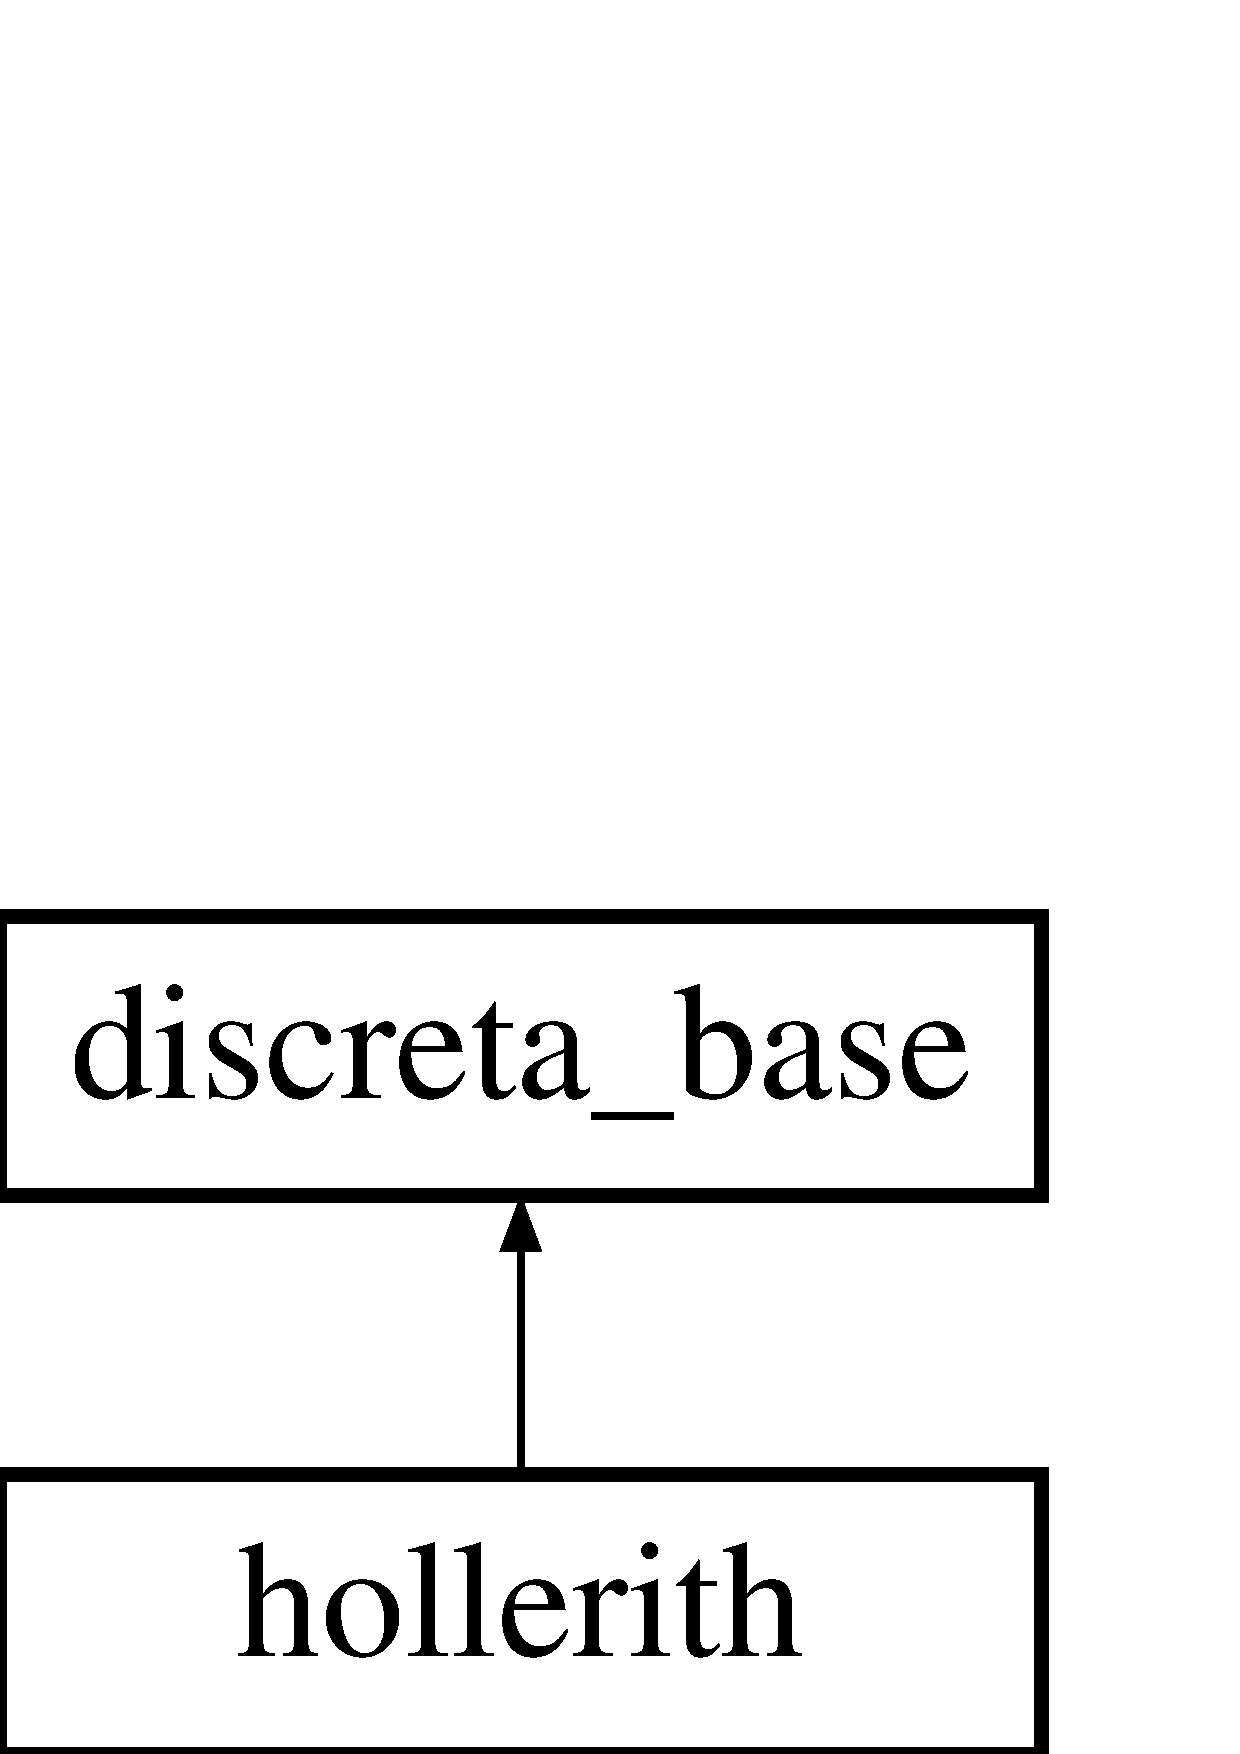
\includegraphics[height=2.000000cm]{classhollerith}
\end{center}
\end{figure}
\subsection*{Public Member Functions}
\begin{DoxyCompactItemize}
\item 
\mbox{\hyperlink{classhollerith_a13144dcd320e47e22e7969297188154e}{hollerith}} ()
\item 
\mbox{\hyperlink{classhollerith_a749438d664a740f9ad7da188494d3077}{hollerith}} (char $\ast$\mbox{\hyperlink{alphabet2_8_c_a533391314665d6bf1b5575e9a9cd8552}{p}})
\item 
\mbox{\hyperlink{classhollerith_ab2b25c6d04670336506b94a38d83ae00}{hollerith}} (const \mbox{\hyperlink{classdiscreta__base}{discreta\+\_\+base}} \&\mbox{\hyperlink{alphabet2_8_c_a6150e0515f7202e2fb518f7206ed97dc}{x}})
\item 
\mbox{\hyperlink{classhollerith}{hollerith}} \& \mbox{\hyperlink{classhollerith_a29643fcee8fc15a9dffa8c8257428f0c}{operator=}} (const \mbox{\hyperlink{classdiscreta__base}{discreta\+\_\+base}} \&\mbox{\hyperlink{alphabet2_8_c_a6150e0515f7202e2fb518f7206ed97dc}{x}})
\item 
void $\ast$ \mbox{\hyperlink{classhollerith_aab36d557528e2e88a792442fa122d682}{operator new}} (size\+\_\+t, void $\ast$\mbox{\hyperlink{alphabet2_8_c_a533391314665d6bf1b5575e9a9cd8552}{p}})
\item 
void \mbox{\hyperlink{classhollerith_a23bbd4acfc88a0e90f1245f243f51f76}{settype\+\_\+hollerith}} ()
\item 
\mbox{\hyperlink{classhollerith_ab7c32776df398e3a60acc954bb093431}{$\sim$hollerith}} ()
\item 
void \mbox{\hyperlink{classhollerith_a240d1b30780c9e09323d0b3ad5e2d1f7}{freeself\+\_\+hollerith}} ()
\item 
\mbox{\hyperlink{discreta_8h_aaf25ee7e2306d78c74ec7bc48f092e81}{kind}} \mbox{\hyperlink{classhollerith_a868bba1481a52276f83e18e3b4280b31}{s\+\_\+virtual\+\_\+kind}} ()
\item 
void \mbox{\hyperlink{classhollerith_aca74f6b673481c6e2b3b553171215f9c}{copyobject\+\_\+to}} (\mbox{\hyperlink{classdiscreta__base}{discreta\+\_\+base}} \&\mbox{\hyperlink{alphabet2_8_c_a6150e0515f7202e2fb518f7206ed97dc}{x}})
\item 
ostream \& \mbox{\hyperlink{classhollerith_a35f4d87aef8f1dd7f09f57ace1c5ea4a}{print}} (ostream \&)
\item 
\mbox{\hyperlink{galois_8h_a09fddde158a3a20bd2dcadb609de11dc}{I\+NT}} \mbox{\hyperlink{classhollerith_a9dfd88b7057204bd4ea1ec227f05d84a}{compare\+\_\+with}} (\mbox{\hyperlink{classdiscreta__base}{discreta\+\_\+base}} \&a)
\item 
char $\ast$ \mbox{\hyperlink{classhollerith_a4b549f6a27d3d9d1c3d9b4eba91b5895}{s\+\_\+unchecked}} ()
\item 
char $\ast$ \mbox{\hyperlink{classhollerith_af61fce2d06f211b25fe3838e4dfee77a}{s}} ()
\item 
void \mbox{\hyperlink{classhollerith_af51ae7b943056db367f3c205a5a1cc4b}{init}} (const char $\ast$\mbox{\hyperlink{alphabet2_8_c_a533391314665d6bf1b5575e9a9cd8552}{p}})
\item 
void \mbox{\hyperlink{classhollerith_a778dd63885a4e3a4e2fb829165c32632}{append}} (const char $\ast$\mbox{\hyperlink{alphabet2_8_c_a533391314665d6bf1b5575e9a9cd8552}{p}})
\item 
void \mbox{\hyperlink{classhollerith_a5df988b4cf3eb66b5645115abeab5782}{append\+\_\+i}} (\mbox{\hyperlink{galois_8h_a09fddde158a3a20bd2dcadb609de11dc}{I\+NT}} \mbox{\hyperlink{alphabet2_8_c_acb559820d9ca11295b4500f179ef6392}{i}})
\item 
void \mbox{\hyperlink{classhollerith_a8d17739da6b15b91053f8356b824407d}{write\+\_\+mem}} (\mbox{\hyperlink{classmemory}{memory}} \&m, \mbox{\hyperlink{galois_8h_a09fddde158a3a20bd2dcadb609de11dc}{I\+NT}} debug\+\_\+depth)
\item 
void \mbox{\hyperlink{classhollerith_af6cbbe5728658ff3a71fc9fe331bb39f}{read\+\_\+mem}} (\mbox{\hyperlink{classmemory}{memory}} \&m, \mbox{\hyperlink{galois_8h_a09fddde158a3a20bd2dcadb609de11dc}{I\+NT}} debug\+\_\+depth)
\item 
\mbox{\hyperlink{galois_8h_a09fddde158a3a20bd2dcadb609de11dc}{I\+NT}} \mbox{\hyperlink{classhollerith_ac3e7f35e2c6d82a9825297577e1011ba}{csf}} ()
\item 
void \mbox{\hyperlink{classhollerith_a17d5710f02f7f230f2646497f5b267e7}{chop\+\_\+off\+\_\+extension\+\_\+if\+\_\+present}} (\mbox{\hyperlink{galois_8h_ab6cc7b4aeb6ea31aba2b3fbfc83ff5e6}{B\+Y\+TE}} $\ast$ext)
\item 
void \mbox{\hyperlink{classhollerith_a530576f22e7f0926918444cb4553f18d}{get\+\_\+extension\+\_\+if\+\_\+present}} (\mbox{\hyperlink{galois_8h_ab6cc7b4aeb6ea31aba2b3fbfc83ff5e6}{B\+Y\+TE}} $\ast$ext)
\item 
void \mbox{\hyperlink{classhollerith_a8564e42e7fff150a5d1182c82057743b}{get\+\_\+current\+\_\+date}} ()
\end{DoxyCompactItemize}
\subsection*{Additional Inherited Members}


\subsection{Constructor \& Destructor Documentation}
\mbox{\Hypertarget{classhollerith_a13144dcd320e47e22e7969297188154e}\label{classhollerith_a13144dcd320e47e22e7969297188154e}} 
\index{hollerith@{hollerith}!hollerith@{hollerith}}
\index{hollerith@{hollerith}!hollerith@{hollerith}}
\subsubsection{\texorpdfstring{hollerith()}{hollerith()}\hspace{0.1cm}{\footnotesize\ttfamily [1/3]}}
{\footnotesize\ttfamily hollerith\+::hollerith (\begin{DoxyParamCaption}{ }\end{DoxyParamCaption})}

\mbox{\Hypertarget{classhollerith_a749438d664a740f9ad7da188494d3077}\label{classhollerith_a749438d664a740f9ad7da188494d3077}} 
\index{hollerith@{hollerith}!hollerith@{hollerith}}
\index{hollerith@{hollerith}!hollerith@{hollerith}}
\subsubsection{\texorpdfstring{hollerith()}{hollerith()}\hspace{0.1cm}{\footnotesize\ttfamily [2/3]}}
{\footnotesize\ttfamily hollerith\+::hollerith (\begin{DoxyParamCaption}\item[{char $\ast$}]{p }\end{DoxyParamCaption})}

\mbox{\Hypertarget{classhollerith_ab2b25c6d04670336506b94a38d83ae00}\label{classhollerith_ab2b25c6d04670336506b94a38d83ae00}} 
\index{hollerith@{hollerith}!hollerith@{hollerith}}
\index{hollerith@{hollerith}!hollerith@{hollerith}}
\subsubsection{\texorpdfstring{hollerith()}{hollerith()}\hspace{0.1cm}{\footnotesize\ttfamily [3/3]}}
{\footnotesize\ttfamily hollerith\+::hollerith (\begin{DoxyParamCaption}\item[{const \mbox{\hyperlink{classdiscreta__base}{discreta\+\_\+base}} \&}]{x }\end{DoxyParamCaption})}

\mbox{\Hypertarget{classhollerith_ab7c32776df398e3a60acc954bb093431}\label{classhollerith_ab7c32776df398e3a60acc954bb093431}} 
\index{hollerith@{hollerith}!````~hollerith@{$\sim$hollerith}}
\index{````~hollerith@{$\sim$hollerith}!hollerith@{hollerith}}
\subsubsection{\texorpdfstring{$\sim$hollerith()}{~hollerith()}}
{\footnotesize\ttfamily hollerith\+::$\sim$hollerith (\begin{DoxyParamCaption}{ }\end{DoxyParamCaption})}



\subsection{Member Function Documentation}
\mbox{\Hypertarget{classhollerith_a778dd63885a4e3a4e2fb829165c32632}\label{classhollerith_a778dd63885a4e3a4e2fb829165c32632}} 
\index{hollerith@{hollerith}!append@{append}}
\index{append@{append}!hollerith@{hollerith}}
\subsubsection{\texorpdfstring{append()}{append()}}
{\footnotesize\ttfamily void hollerith\+::append (\begin{DoxyParamCaption}\item[{const char $\ast$}]{p }\end{DoxyParamCaption})}

\mbox{\Hypertarget{classhollerith_a5df988b4cf3eb66b5645115abeab5782}\label{classhollerith_a5df988b4cf3eb66b5645115abeab5782}} 
\index{hollerith@{hollerith}!append\+\_\+i@{append\+\_\+i}}
\index{append\+\_\+i@{append\+\_\+i}!hollerith@{hollerith}}
\subsubsection{\texorpdfstring{append\+\_\+i()}{append\_i()}}
{\footnotesize\ttfamily void hollerith\+::append\+\_\+i (\begin{DoxyParamCaption}\item[{\mbox{\hyperlink{galois_8h_a09fddde158a3a20bd2dcadb609de11dc}{I\+NT}}}]{i }\end{DoxyParamCaption})}

\mbox{\Hypertarget{classhollerith_a17d5710f02f7f230f2646497f5b267e7}\label{classhollerith_a17d5710f02f7f230f2646497f5b267e7}} 
\index{hollerith@{hollerith}!chop\+\_\+off\+\_\+extension\+\_\+if\+\_\+present@{chop\+\_\+off\+\_\+extension\+\_\+if\+\_\+present}}
\index{chop\+\_\+off\+\_\+extension\+\_\+if\+\_\+present@{chop\+\_\+off\+\_\+extension\+\_\+if\+\_\+present}!hollerith@{hollerith}}
\subsubsection{\texorpdfstring{chop\+\_\+off\+\_\+extension\+\_\+if\+\_\+present()}{chop\_off\_extension\_if\_present()}}
{\footnotesize\ttfamily void hollerith\+::chop\+\_\+off\+\_\+extension\+\_\+if\+\_\+present (\begin{DoxyParamCaption}\item[{\mbox{\hyperlink{galois_8h_ab6cc7b4aeb6ea31aba2b3fbfc83ff5e6}{B\+Y\+TE}} $\ast$}]{ext }\end{DoxyParamCaption})}

\mbox{\Hypertarget{classhollerith_a9dfd88b7057204bd4ea1ec227f05d84a}\label{classhollerith_a9dfd88b7057204bd4ea1ec227f05d84a}} 
\index{hollerith@{hollerith}!compare\+\_\+with@{compare\+\_\+with}}
\index{compare\+\_\+with@{compare\+\_\+with}!hollerith@{hollerith}}
\subsubsection{\texorpdfstring{compare\+\_\+with()}{compare\_with()}}
{\footnotesize\ttfamily \mbox{\hyperlink{galois_8h_a09fddde158a3a20bd2dcadb609de11dc}{I\+NT}} hollerith\+::compare\+\_\+with (\begin{DoxyParamCaption}\item[{\mbox{\hyperlink{classdiscreta__base}{discreta\+\_\+base}} \&}]{a }\end{DoxyParamCaption})\hspace{0.3cm}{\ttfamily [virtual]}}



Reimplemented from \mbox{\hyperlink{classdiscreta__base_a3818444c4301d0b7ed47c3b850ea6c60}{discreta\+\_\+base}}.

\mbox{\Hypertarget{classhollerith_aca74f6b673481c6e2b3b553171215f9c}\label{classhollerith_aca74f6b673481c6e2b3b553171215f9c}} 
\index{hollerith@{hollerith}!copyobject\+\_\+to@{copyobject\+\_\+to}}
\index{copyobject\+\_\+to@{copyobject\+\_\+to}!hollerith@{hollerith}}
\subsubsection{\texorpdfstring{copyobject\+\_\+to()}{copyobject\_to()}}
{\footnotesize\ttfamily void hollerith\+::copyobject\+\_\+to (\begin{DoxyParamCaption}\item[{\mbox{\hyperlink{classdiscreta__base}{discreta\+\_\+base}} \&}]{x }\end{DoxyParamCaption})\hspace{0.3cm}{\ttfamily [virtual]}}



Reimplemented from \mbox{\hyperlink{classdiscreta__base_a33180628d9ced231267229b3564790f3}{discreta\+\_\+base}}.

\mbox{\Hypertarget{classhollerith_ac3e7f35e2c6d82a9825297577e1011ba}\label{classhollerith_ac3e7f35e2c6d82a9825297577e1011ba}} 
\index{hollerith@{hollerith}!csf@{csf}}
\index{csf@{csf}!hollerith@{hollerith}}
\subsubsection{\texorpdfstring{csf()}{csf()}}
{\footnotesize\ttfamily \mbox{\hyperlink{galois_8h_a09fddde158a3a20bd2dcadb609de11dc}{I\+NT}} hollerith\+::csf (\begin{DoxyParamCaption}{ }\end{DoxyParamCaption})}

\mbox{\Hypertarget{classhollerith_a240d1b30780c9e09323d0b3ad5e2d1f7}\label{classhollerith_a240d1b30780c9e09323d0b3ad5e2d1f7}} 
\index{hollerith@{hollerith}!freeself\+\_\+hollerith@{freeself\+\_\+hollerith}}
\index{freeself\+\_\+hollerith@{freeself\+\_\+hollerith}!hollerith@{hollerith}}
\subsubsection{\texorpdfstring{freeself\+\_\+hollerith()}{freeself\_hollerith()}}
{\footnotesize\ttfamily void hollerith\+::freeself\+\_\+hollerith (\begin{DoxyParamCaption}{ }\end{DoxyParamCaption})}

\mbox{\Hypertarget{classhollerith_a8564e42e7fff150a5d1182c82057743b}\label{classhollerith_a8564e42e7fff150a5d1182c82057743b}} 
\index{hollerith@{hollerith}!get\+\_\+current\+\_\+date@{get\+\_\+current\+\_\+date}}
\index{get\+\_\+current\+\_\+date@{get\+\_\+current\+\_\+date}!hollerith@{hollerith}}
\subsubsection{\texorpdfstring{get\+\_\+current\+\_\+date()}{get\_current\_date()}}
{\footnotesize\ttfamily void hollerith\+::get\+\_\+current\+\_\+date (\begin{DoxyParamCaption}{ }\end{DoxyParamCaption})}

\mbox{\Hypertarget{classhollerith_a530576f22e7f0926918444cb4553f18d}\label{classhollerith_a530576f22e7f0926918444cb4553f18d}} 
\index{hollerith@{hollerith}!get\+\_\+extension\+\_\+if\+\_\+present@{get\+\_\+extension\+\_\+if\+\_\+present}}
\index{get\+\_\+extension\+\_\+if\+\_\+present@{get\+\_\+extension\+\_\+if\+\_\+present}!hollerith@{hollerith}}
\subsubsection{\texorpdfstring{get\+\_\+extension\+\_\+if\+\_\+present()}{get\_extension\_if\_present()}}
{\footnotesize\ttfamily void hollerith\+::get\+\_\+extension\+\_\+if\+\_\+present (\begin{DoxyParamCaption}\item[{\mbox{\hyperlink{galois_8h_ab6cc7b4aeb6ea31aba2b3fbfc83ff5e6}{B\+Y\+TE}} $\ast$}]{ext }\end{DoxyParamCaption})}

\mbox{\Hypertarget{classhollerith_af51ae7b943056db367f3c205a5a1cc4b}\label{classhollerith_af51ae7b943056db367f3c205a5a1cc4b}} 
\index{hollerith@{hollerith}!init@{init}}
\index{init@{init}!hollerith@{hollerith}}
\subsubsection{\texorpdfstring{init()}{init()}}
{\footnotesize\ttfamily void hollerith\+::init (\begin{DoxyParamCaption}\item[{const char $\ast$}]{p }\end{DoxyParamCaption})}

\mbox{\Hypertarget{classhollerith_aab36d557528e2e88a792442fa122d682}\label{classhollerith_aab36d557528e2e88a792442fa122d682}} 
\index{hollerith@{hollerith}!operator new@{operator new}}
\index{operator new@{operator new}!hollerith@{hollerith}}
\subsubsection{\texorpdfstring{operator new()}{operator new()}}
{\footnotesize\ttfamily void$\ast$ hollerith\+::operator new (\begin{DoxyParamCaption}\item[{size\+\_\+t}]{,  }\item[{void $\ast$}]{p }\end{DoxyParamCaption})\hspace{0.3cm}{\ttfamily [inline]}}

\mbox{\Hypertarget{classhollerith_a29643fcee8fc15a9dffa8c8257428f0c}\label{classhollerith_a29643fcee8fc15a9dffa8c8257428f0c}} 
\index{hollerith@{hollerith}!operator=@{operator=}}
\index{operator=@{operator=}!hollerith@{hollerith}}
\subsubsection{\texorpdfstring{operator=()}{operator=()}}
{\footnotesize\ttfamily \mbox{\hyperlink{classhollerith}{hollerith}} \& hollerith\+::operator= (\begin{DoxyParamCaption}\item[{const \mbox{\hyperlink{classdiscreta__base}{discreta\+\_\+base}} \&}]{x }\end{DoxyParamCaption})}

\mbox{\Hypertarget{classhollerith_a35f4d87aef8f1dd7f09f57ace1c5ea4a}\label{classhollerith_a35f4d87aef8f1dd7f09f57ace1c5ea4a}} 
\index{hollerith@{hollerith}!print@{print}}
\index{print@{print}!hollerith@{hollerith}}
\subsubsection{\texorpdfstring{print()}{print()}}
{\footnotesize\ttfamily ostream \& hollerith\+::print (\begin{DoxyParamCaption}\item[{ostream \&}]{ost }\end{DoxyParamCaption})\hspace{0.3cm}{\ttfamily [virtual]}}



Reimplemented from \mbox{\hyperlink{classdiscreta__base_a036e48bc058347046fc9b73dd0951478}{discreta\+\_\+base}}.

\mbox{\Hypertarget{classhollerith_af6cbbe5728658ff3a71fc9fe331bb39f}\label{classhollerith_af6cbbe5728658ff3a71fc9fe331bb39f}} 
\index{hollerith@{hollerith}!read\+\_\+mem@{read\+\_\+mem}}
\index{read\+\_\+mem@{read\+\_\+mem}!hollerith@{hollerith}}
\subsubsection{\texorpdfstring{read\+\_\+mem()}{read\_mem()}}
{\footnotesize\ttfamily void hollerith\+::read\+\_\+mem (\begin{DoxyParamCaption}\item[{\mbox{\hyperlink{classmemory}{memory}} \&}]{m,  }\item[{\mbox{\hyperlink{galois_8h_a09fddde158a3a20bd2dcadb609de11dc}{I\+NT}}}]{debug\+\_\+depth }\end{DoxyParamCaption})}

\mbox{\Hypertarget{classhollerith_af61fce2d06f211b25fe3838e4dfee77a}\label{classhollerith_af61fce2d06f211b25fe3838e4dfee77a}} 
\index{hollerith@{hollerith}!s@{s}}
\index{s@{s}!hollerith@{hollerith}}
\subsubsection{\texorpdfstring{s()}{s()}}
{\footnotesize\ttfamily char$\ast$ hollerith\+::s (\begin{DoxyParamCaption}{ }\end{DoxyParamCaption})\hspace{0.3cm}{\ttfamily [inline]}}

\mbox{\Hypertarget{classhollerith_a4b549f6a27d3d9d1c3d9b4eba91b5895}\label{classhollerith_a4b549f6a27d3d9d1c3d9b4eba91b5895}} 
\index{hollerith@{hollerith}!s\+\_\+unchecked@{s\+\_\+unchecked}}
\index{s\+\_\+unchecked@{s\+\_\+unchecked}!hollerith@{hollerith}}
\subsubsection{\texorpdfstring{s\+\_\+unchecked()}{s\_unchecked()}}
{\footnotesize\ttfamily char$\ast$ hollerith\+::s\+\_\+unchecked (\begin{DoxyParamCaption}{ }\end{DoxyParamCaption})\hspace{0.3cm}{\ttfamily [inline]}}

\mbox{\Hypertarget{classhollerith_a868bba1481a52276f83e18e3b4280b31}\label{classhollerith_a868bba1481a52276f83e18e3b4280b31}} 
\index{hollerith@{hollerith}!s\+\_\+virtual\+\_\+kind@{s\+\_\+virtual\+\_\+kind}}
\index{s\+\_\+virtual\+\_\+kind@{s\+\_\+virtual\+\_\+kind}!hollerith@{hollerith}}
\subsubsection{\texorpdfstring{s\+\_\+virtual\+\_\+kind()}{s\_virtual\_kind()}}
{\footnotesize\ttfamily \mbox{\hyperlink{discreta_8h_aaf25ee7e2306d78c74ec7bc48f092e81}{kind}} hollerith\+::s\+\_\+virtual\+\_\+kind (\begin{DoxyParamCaption}{ }\end{DoxyParamCaption})\hspace{0.3cm}{\ttfamily [virtual]}}



Reimplemented from \mbox{\hyperlink{classdiscreta__base_a52778a6d6943a468be083d0785d418fb}{discreta\+\_\+base}}.

\mbox{\Hypertarget{classhollerith_a23bbd4acfc88a0e90f1245f243f51f76}\label{classhollerith_a23bbd4acfc88a0e90f1245f243f51f76}} 
\index{hollerith@{hollerith}!settype\+\_\+hollerith@{settype\+\_\+hollerith}}
\index{settype\+\_\+hollerith@{settype\+\_\+hollerith}!hollerith@{hollerith}}
\subsubsection{\texorpdfstring{settype\+\_\+hollerith()}{settype\_hollerith()}}
{\footnotesize\ttfamily void hollerith\+::settype\+\_\+hollerith (\begin{DoxyParamCaption}{ }\end{DoxyParamCaption})}

\mbox{\Hypertarget{classhollerith_a8d17739da6b15b91053f8356b824407d}\label{classhollerith_a8d17739da6b15b91053f8356b824407d}} 
\index{hollerith@{hollerith}!write\+\_\+mem@{write\+\_\+mem}}
\index{write\+\_\+mem@{write\+\_\+mem}!hollerith@{hollerith}}
\subsubsection{\texorpdfstring{write\+\_\+mem()}{write\_mem()}}
{\footnotesize\ttfamily void hollerith\+::write\+\_\+mem (\begin{DoxyParamCaption}\item[{\mbox{\hyperlink{classmemory}{memory}} \&}]{m,  }\item[{\mbox{\hyperlink{galois_8h_a09fddde158a3a20bd2dcadb609de11dc}{I\+NT}}}]{debug\+\_\+depth }\end{DoxyParamCaption})}



The documentation for this class was generated from the following files\+:\begin{DoxyCompactItemize}
\item 
S\+R\+C/\+L\+I\+B/\+D\+I\+S\+C\+R\+E\+T\+A/\mbox{\hyperlink{discreta_8h}{discreta.\+h}}\item 
S\+R\+C/\+L\+I\+B/\+D\+I\+S\+C\+R\+E\+T\+A/\mbox{\hyperlink{hollerith_8_c}{hollerith.\+C}}\end{DoxyCompactItemize}

\hypertarget{classhomogeneous__polynomial__domain}{}\section{homogeneous\+\_\+polynomial\+\_\+domain Class Reference}
\label{classhomogeneous__polynomial__domain}\index{homogeneous\+\_\+polynomial\+\_\+domain@{homogeneous\+\_\+polynomial\+\_\+domain}}


{\ttfamily \#include $<$galois.\+h$>$}

\subsection*{Public Member Functions}
\begin{DoxyCompactItemize}
\item 
\mbox{\hyperlink{classhomogeneous__polynomial__domain_a569c19fcf7d3e4bd65974fdc9eb93ec9}{homogeneous\+\_\+polynomial\+\_\+domain}} ()
\item 
\mbox{\hyperlink{classhomogeneous__polynomial__domain_a99009c093637d18e6a89faa8e3e6e771}{$\sim$homogeneous\+\_\+polynomial\+\_\+domain}} ()
\item 
void \mbox{\hyperlink{classhomogeneous__polynomial__domain_a9b1f3d170e1c7ad782a719fabcd9c6f0}{freeself}} ()
\item 
void \mbox{\hyperlink{classhomogeneous__polynomial__domain_ad9c36b66de4aade20063cf9f6f764507}{null}} ()
\item 
void \mbox{\hyperlink{classhomogeneous__polynomial__domain_ad7d4e08b895afb895147322732228d3a}{init}} (\mbox{\hyperlink{classfinite__field}{finite\+\_\+field}} $\ast$\mbox{\hyperlink{classhomogeneous__polynomial__domain_abaa7cb4dfd33aa7726c0482ad85bc5c1}{F}}, \mbox{\hyperlink{galois_8h_a09fddde158a3a20bd2dcadb609de11dc}{I\+NT}} nb\+\_\+vars, \mbox{\hyperlink{galois_8h_a09fddde158a3a20bd2dcadb609de11dc}{I\+NT}} \mbox{\hyperlink{classhomogeneous__polynomial__domain_a74fc862c607381314ad8a0b3ea3df387}{degree}}, \mbox{\hyperlink{galois_8h_a09fddde158a3a20bd2dcadb609de11dc}{I\+NT}} f\+\_\+init\+\_\+incidence\+\_\+structure, \mbox{\hyperlink{galois_8h_a09fddde158a3a20bd2dcadb609de11dc}{I\+NT}} \mbox{\hyperlink{simeon_8_c_a818073fbcc2f439e7c56952f67386122}{verbose\+\_\+level}})
\item 
void \mbox{\hyperlink{classhomogeneous__polynomial__domain_a467ad10c570859dbcf637a43993ceb57}{make\+\_\+monomials}} (\mbox{\hyperlink{galois_8h_a09fddde158a3a20bd2dcadb609de11dc}{I\+NT}} \mbox{\hyperlink{simeon_8_c_a818073fbcc2f439e7c56952f67386122}{verbose\+\_\+level}})
\item 
void \mbox{\hyperlink{classhomogeneous__polynomial__domain_af774250d5c1bd555c0ea55f2aaafad10}{rearrange\+\_\+monomials\+\_\+by\+\_\+partition\+\_\+type}} (\mbox{\hyperlink{galois_8h_a09fddde158a3a20bd2dcadb609de11dc}{I\+NT}} \mbox{\hyperlink{simeon_8_c_a818073fbcc2f439e7c56952f67386122}{verbose\+\_\+level}})
\item 
\mbox{\hyperlink{galois_8h_a09fddde158a3a20bd2dcadb609de11dc}{I\+NT}} \mbox{\hyperlink{classhomogeneous__polynomial__domain_a3fad3fb2b940014fcfece1cebfbfa3ae}{index\+\_\+of\+\_\+monomial}} (\mbox{\hyperlink{galois_8h_a09fddde158a3a20bd2dcadb609de11dc}{I\+NT}} $\ast$\mbox{\hyperlink{classhomogeneous__polynomial__domain_ab0d1e093ed9589724a0a3e874ea92f51}{v}})
\item 
void \mbox{\hyperlink{classhomogeneous__polynomial__domain_aba45b13898b259a147e45bf92a622fd8}{print\+\_\+monomial}} (ostream \&ost, \mbox{\hyperlink{galois_8h_a09fddde158a3a20bd2dcadb609de11dc}{I\+NT}} \mbox{\hyperlink{alphabet2_8_c_acb559820d9ca11295b4500f179ef6392}{i}})
\item 
void \mbox{\hyperlink{classhomogeneous__polynomial__domain_a6a7befc3995c226fb303eafd572f25c4}{print\+\_\+monomial}} (ostream \&ost, \mbox{\hyperlink{galois_8h_a09fddde158a3a20bd2dcadb609de11dc}{I\+NT}} $\ast$mon)
\item 
void \mbox{\hyperlink{classhomogeneous__polynomial__domain_a39fe7da58a442801d7c8be1121a57bfe}{print\+\_\+equation}} (ostream \&ost, \mbox{\hyperlink{galois_8h_a09fddde158a3a20bd2dcadb609de11dc}{I\+NT}} $\ast$coeffs)
\item 
void \mbox{\hyperlink{classhomogeneous__polynomial__domain_a380597c635c722d4577cabce701bf55f}{print\+\_\+equation\+\_\+with\+\_\+line\+\_\+breaks\+\_\+tex}} (ostream \&ost, \mbox{\hyperlink{galois_8h_a09fddde158a3a20bd2dcadb609de11dc}{I\+NT}} $\ast$coeffs, \mbox{\hyperlink{galois_8h_a09fddde158a3a20bd2dcadb609de11dc}{I\+NT}} nb\+\_\+terms\+\_\+per\+\_\+line, const \mbox{\hyperlink{galois_8h_ab6cc7b4aeb6ea31aba2b3fbfc83ff5e6}{B\+Y\+TE}} $\ast$new\+\_\+line\+\_\+text)
\item 
void \mbox{\hyperlink{classhomogeneous__polynomial__domain_adc0868f632cc5662b7bfaf0b3d72268f}{enumerate\+\_\+points}} (\mbox{\hyperlink{galois_8h_a09fddde158a3a20bd2dcadb609de11dc}{I\+NT}} $\ast$coeff, \mbox{\hyperlink{galois_8h_a09fddde158a3a20bd2dcadb609de11dc}{I\+NT}} $\ast$Pts, \mbox{\hyperlink{galois_8h_a09fddde158a3a20bd2dcadb609de11dc}{I\+NT}} \&nb\+\_\+pts, \mbox{\hyperlink{galois_8h_a09fddde158a3a20bd2dcadb609de11dc}{I\+NT}} \mbox{\hyperlink{simeon_8_c_a818073fbcc2f439e7c56952f67386122}{verbose\+\_\+level}})
\item 
\mbox{\hyperlink{galois_8h_a09fddde158a3a20bd2dcadb609de11dc}{I\+NT}} \mbox{\hyperlink{classhomogeneous__polynomial__domain_ae0bde037e3b48c69c7bd2b719eee5489}{evaluate\+\_\+at\+\_\+a\+\_\+point\+\_\+by\+\_\+rank}} (\mbox{\hyperlink{galois_8h_a09fddde158a3a20bd2dcadb609de11dc}{I\+NT}} $\ast$coeff, \mbox{\hyperlink{galois_8h_a09fddde158a3a20bd2dcadb609de11dc}{I\+NT}} \mbox{\hyperlink{clique__finder_8_c_aec1f1a2b30fdca8844c2932384483145}{pt}})
\item 
\mbox{\hyperlink{galois_8h_a09fddde158a3a20bd2dcadb609de11dc}{I\+NT}} \mbox{\hyperlink{classhomogeneous__polynomial__domain_ad3989698a38d04fc319162c376fe6343}{evaluate\+\_\+at\+\_\+a\+\_\+point}} (\mbox{\hyperlink{galois_8h_a09fddde158a3a20bd2dcadb609de11dc}{I\+NT}} $\ast$coeff, \mbox{\hyperlink{galois_8h_a09fddde158a3a20bd2dcadb609de11dc}{I\+NT}} $\ast$pt\+\_\+vec)
\item 
void \mbox{\hyperlink{classhomogeneous__polynomial__domain_a236cbf545622995b80f5eb10a9f86c31}{substitute\+\_\+linear}} (\mbox{\hyperlink{galois_8h_a09fddde158a3a20bd2dcadb609de11dc}{I\+NT}} $\ast$coeff\+\_\+in, \mbox{\hyperlink{galois_8h_a09fddde158a3a20bd2dcadb609de11dc}{I\+NT}} $\ast$coeff\+\_\+out, \mbox{\hyperlink{galois_8h_a09fddde158a3a20bd2dcadb609de11dc}{I\+NT}} $\ast$Mtx\+\_\+inv, \mbox{\hyperlink{galois_8h_a09fddde158a3a20bd2dcadb609de11dc}{I\+NT}} \mbox{\hyperlink{simeon_8_c_a818073fbcc2f439e7c56952f67386122}{verbose\+\_\+level}})
\item 
void \mbox{\hyperlink{classhomogeneous__polynomial__domain_ae16fefaacc3385f9f385d1dd6df7ea4d}{substitute\+\_\+semilinear}} (\mbox{\hyperlink{galois_8h_a09fddde158a3a20bd2dcadb609de11dc}{I\+NT}} $\ast$coeff\+\_\+in, \mbox{\hyperlink{galois_8h_a09fddde158a3a20bd2dcadb609de11dc}{I\+NT}} $\ast$coeff\+\_\+out, \mbox{\hyperlink{galois_8h_a09fddde158a3a20bd2dcadb609de11dc}{I\+NT}} \mbox{\hyperlink{simeon_8_c_abe9d1351be10f92305ed7533cd3a3c08}{f\+\_\+semilinear}}, \mbox{\hyperlink{galois_8h_a09fddde158a3a20bd2dcadb609de11dc}{I\+NT}} frob\+\_\+power, \mbox{\hyperlink{galois_8h_a09fddde158a3a20bd2dcadb609de11dc}{I\+NT}} $\ast$Mtx\+\_\+inv, \mbox{\hyperlink{galois_8h_a09fddde158a3a20bd2dcadb609de11dc}{I\+NT}} \mbox{\hyperlink{simeon_8_c_a818073fbcc2f439e7c56952f67386122}{verbose\+\_\+level}})
\item 
\mbox{\hyperlink{galois_8h_a09fddde158a3a20bd2dcadb609de11dc}{I\+NT}} \mbox{\hyperlink{classhomogeneous__polynomial__domain_a48399203c734feffa753041881d4e68b}{is\+\_\+zero}} (\mbox{\hyperlink{galois_8h_a09fddde158a3a20bd2dcadb609de11dc}{I\+NT}} $\ast$coeff)
\item 
void \mbox{\hyperlink{classhomogeneous__polynomial__domain_a913856cb9020e671f7792f186b94af68}{unrank\+\_\+point}} (\mbox{\hyperlink{galois_8h_a09fddde158a3a20bd2dcadb609de11dc}{I\+NT}} $\ast$\mbox{\hyperlink{classhomogeneous__polynomial__domain_ab0d1e093ed9589724a0a3e874ea92f51}{v}}, \mbox{\hyperlink{galois_8h_a09fddde158a3a20bd2dcadb609de11dc}{I\+NT}} rk)
\item 
\mbox{\hyperlink{galois_8h_a09fddde158a3a20bd2dcadb609de11dc}{I\+NT}} \mbox{\hyperlink{classhomogeneous__polynomial__domain_a3c0f519ca5c5c77614a2dc0fa97005e5}{rank\+\_\+point}} (\mbox{\hyperlink{galois_8h_a09fddde158a3a20bd2dcadb609de11dc}{I\+NT}} $\ast$\mbox{\hyperlink{classhomogeneous__polynomial__domain_ab0d1e093ed9589724a0a3e874ea92f51}{v}})
\item 
void \mbox{\hyperlink{classhomogeneous__polynomial__domain_a88b548127853c2f9a2a6a2de8d2ce782}{unrank\+\_\+coeff\+\_\+vector}} (\mbox{\hyperlink{galois_8h_a09fddde158a3a20bd2dcadb609de11dc}{I\+NT}} $\ast$\mbox{\hyperlink{classhomogeneous__polynomial__domain_ab0d1e093ed9589724a0a3e874ea92f51}{v}}, \mbox{\hyperlink{galois_8h_a09fddde158a3a20bd2dcadb609de11dc}{I\+NT}} rk)
\item 
\mbox{\hyperlink{galois_8h_a09fddde158a3a20bd2dcadb609de11dc}{I\+NT}} \mbox{\hyperlink{classhomogeneous__polynomial__domain_a23e18573b753de888d3f8ee893e99d5a}{rank\+\_\+coeff\+\_\+vector}} (\mbox{\hyperlink{galois_8h_a09fddde158a3a20bd2dcadb609de11dc}{I\+NT}} $\ast$\mbox{\hyperlink{classhomogeneous__polynomial__domain_ab0d1e093ed9589724a0a3e874ea92f51}{v}})
\item 
\mbox{\hyperlink{galois_8h_a09fddde158a3a20bd2dcadb609de11dc}{I\+NT}} \mbox{\hyperlink{classhomogeneous__polynomial__domain_ae1b2b16b50fd6646a3332da31bb0ad23}{test\+\_\+weierstrass\+\_\+form}} (\mbox{\hyperlink{galois_8h_a09fddde158a3a20bd2dcadb609de11dc}{I\+NT}} rk, \mbox{\hyperlink{galois_8h_a09fddde158a3a20bd2dcadb609de11dc}{I\+NT}} \&a1, \mbox{\hyperlink{galois_8h_a09fddde158a3a20bd2dcadb609de11dc}{I\+NT}} \&a2, \mbox{\hyperlink{galois_8h_a09fddde158a3a20bd2dcadb609de11dc}{I\+NT}} \&a3, \mbox{\hyperlink{galois_8h_a09fddde158a3a20bd2dcadb609de11dc}{I\+NT}} \&a4, \mbox{\hyperlink{galois_8h_a09fddde158a3a20bd2dcadb609de11dc}{I\+NT}} \&a6, \mbox{\hyperlink{galois_8h_a09fddde158a3a20bd2dcadb609de11dc}{I\+NT}} \mbox{\hyperlink{simeon_8_c_a818073fbcc2f439e7c56952f67386122}{verbose\+\_\+level}})
\item 
void \mbox{\hyperlink{classhomogeneous__polynomial__domain_a7037f7f1cd49d297eb3063b6b04699e2}{vanishing\+\_\+ideal}} (\mbox{\hyperlink{galois_8h_a09fddde158a3a20bd2dcadb609de11dc}{I\+NT}} $\ast$Pts, \mbox{\hyperlink{galois_8h_a09fddde158a3a20bd2dcadb609de11dc}{I\+NT}} nb\+\_\+pts, \mbox{\hyperlink{galois_8h_a09fddde158a3a20bd2dcadb609de11dc}{I\+NT}} \&\mbox{\hyperlink{alphabet2_8_c_acab531abaa74a7e664e3986f2522b33a}{r}}, \mbox{\hyperlink{galois_8h_a09fddde158a3a20bd2dcadb609de11dc}{I\+NT}} $\ast$Kernel, \mbox{\hyperlink{galois_8h_a09fddde158a3a20bd2dcadb609de11dc}{I\+NT}} \mbox{\hyperlink{simeon_8_c_a818073fbcc2f439e7c56952f67386122}{verbose\+\_\+level}})
\item 
\mbox{\hyperlink{galois_8h_a09fddde158a3a20bd2dcadb609de11dc}{I\+NT}} \mbox{\hyperlink{classhomogeneous__polynomial__domain_a05c5959cb62502954c9cf93a85b8c019}{compare\+\_\+monomials}} (\mbox{\hyperlink{galois_8h_a09fddde158a3a20bd2dcadb609de11dc}{I\+NT}} $\ast$M1, \mbox{\hyperlink{galois_8h_a09fddde158a3a20bd2dcadb609de11dc}{I\+NT}} $\ast$M2)
\item 
void \mbox{\hyperlink{classhomogeneous__polynomial__domain_aeb98c95ca555e4d24b62fe336731c190}{print\+\_\+monomial\+\_\+ordering}} (ostream \&ost)
\end{DoxyCompactItemize}
\subsection*{Public Attributes}
\begin{DoxyCompactItemize}
\item 
\mbox{\hyperlink{galois_8h_a09fddde158a3a20bd2dcadb609de11dc}{I\+NT}} \mbox{\hyperlink{classhomogeneous__polynomial__domain_aeded5c03d68fa173a12c512b93799e02}{q}}
\item 
\mbox{\hyperlink{galois_8h_a09fddde158a3a20bd2dcadb609de11dc}{I\+NT}} \mbox{\hyperlink{classhomogeneous__polynomial__domain_a7b4d50bcc15155a804439939a34b30ef}{n}}
\item 
\mbox{\hyperlink{galois_8h_a09fddde158a3a20bd2dcadb609de11dc}{I\+NT}} \mbox{\hyperlink{classhomogeneous__polynomial__domain_a74fc862c607381314ad8a0b3ea3df387}{degree}}
\item 
\mbox{\hyperlink{classfinite__field}{finite\+\_\+field}} $\ast$ \mbox{\hyperlink{classhomogeneous__polynomial__domain_abaa7cb4dfd33aa7726c0482ad85bc5c1}{F}}
\item 
\mbox{\hyperlink{galois_8h_a09fddde158a3a20bd2dcadb609de11dc}{I\+NT}} \mbox{\hyperlink{classhomogeneous__polynomial__domain_a2cf9125d4855499424ea13ce56804103}{nb\+\_\+monomials}}
\item 
\mbox{\hyperlink{galois_8h_a09fddde158a3a20bd2dcadb609de11dc}{I\+NT}} $\ast$ \mbox{\hyperlink{classhomogeneous__polynomial__domain_add92d0c8e5f86dfa938b3fadf3ea1814}{Monomials}}
\item 
\mbox{\hyperlink{galois_8h_ab6cc7b4aeb6ea31aba2b3fbfc83ff5e6}{B\+Y\+TE}} $\ast$$\ast$ \mbox{\hyperlink{classhomogeneous__polynomial__domain_a1721e4b7d9eaedb7741e1c87399429c0}{symbols}}
\item 
\mbox{\hyperlink{galois_8h_ab6cc7b4aeb6ea31aba2b3fbfc83ff5e6}{B\+Y\+TE}} $\ast$$\ast$ \mbox{\hyperlink{classhomogeneous__polynomial__domain_aab086f59c8b367e7f67a90fe64e6dc51}{symbols\+\_\+latex}}
\item 
\mbox{\hyperlink{galois_8h_a09fddde158a3a20bd2dcadb609de11dc}{I\+NT}} $\ast$ \mbox{\hyperlink{classhomogeneous__polynomial__domain_abcc62c2d05dfa757b0ebf459fdc33b40}{Variables}}
\item 
\mbox{\hyperlink{galois_8h_a09fddde158a3a20bd2dcadb609de11dc}{I\+NT}} \mbox{\hyperlink{classhomogeneous__polynomial__domain_af519953b30566b23785d8e9f30357acb}{nb\+\_\+affine}}
\item 
\mbox{\hyperlink{galois_8h_a09fddde158a3a20bd2dcadb609de11dc}{I\+NT}} $\ast$ \mbox{\hyperlink{classhomogeneous__polynomial__domain_ad930537d59dd90551af81f1454e1ace2}{Affine}}
\item 
\mbox{\hyperlink{galois_8h_a09fddde158a3a20bd2dcadb609de11dc}{I\+NT}} $\ast$ \mbox{\hyperlink{classhomogeneous__polynomial__domain_ab0d1e093ed9589724a0a3e874ea92f51}{v}}
\item 
\mbox{\hyperlink{galois_8h_a09fddde158a3a20bd2dcadb609de11dc}{I\+NT}} $\ast$ \mbox{\hyperlink{classhomogeneous__polynomial__domain_aa2afe5addc7bce5b5f7d5915e9bde918}{Affine\+\_\+to\+\_\+monomial}}
\item 
\mbox{\hyperlink{classprojective__space}{projective\+\_\+space}} $\ast$ \mbox{\hyperlink{classhomogeneous__polynomial__domain_a2e6bcec29a5c52bf2fc6fdb80593b1a4}{P}}
\item 
\mbox{\hyperlink{galois_8h_a09fddde158a3a20bd2dcadb609de11dc}{I\+NT}} $\ast$ \mbox{\hyperlink{classhomogeneous__polynomial__domain_ae63f93bd2af97ccfdd72372bd8e711e5}{coeff2}}
\item 
\mbox{\hyperlink{galois_8h_a09fddde158a3a20bd2dcadb609de11dc}{I\+NT}} $\ast$ \mbox{\hyperlink{classhomogeneous__polynomial__domain_ae64d2f4771fd76eeb0a6c946d8a021c2}{coeff3}}
\item 
\mbox{\hyperlink{galois_8h_a09fddde158a3a20bd2dcadb609de11dc}{I\+NT}} $\ast$ \mbox{\hyperlink{classhomogeneous__polynomial__domain_a95e2124a5e938cd60ad884fe203f7a67}{coeff4}}
\item 
\mbox{\hyperlink{galois_8h_a09fddde158a3a20bd2dcadb609de11dc}{I\+NT}} $\ast$ \mbox{\hyperlink{classhomogeneous__polynomial__domain_ab7ceab0cdfc6d19a92eeb91fa897198a}{factors}}
\item 
\mbox{\hyperlink{galois_8h_a09fddde158a3a20bd2dcadb609de11dc}{I\+NT}} $\ast$ \mbox{\hyperlink{classhomogeneous__polynomial__domain_aedd702854721e4345106bf161eaa19b9}{my\+\_\+affine}}
\item 
\mbox{\hyperlink{galois_8h_a09fddde158a3a20bd2dcadb609de11dc}{I\+NT}} $\ast$ \mbox{\hyperlink{classhomogeneous__polynomial__domain_a75d2b8f2ed3ab0a13f43cd534de3d000}{base\+\_\+cols}}
\item 
\mbox{\hyperlink{galois_8h_a09fddde158a3a20bd2dcadb609de11dc}{I\+NT}} $\ast$ \mbox{\hyperlink{classhomogeneous__polynomial__domain_a0de18e4a431bc47253dcf38c4b60ba32}{type1}}
\item 
\mbox{\hyperlink{galois_8h_a09fddde158a3a20bd2dcadb609de11dc}{I\+NT}} $\ast$ \mbox{\hyperlink{classhomogeneous__polynomial__domain_a6f7d102a515a24df63b674251d48f950}{type2}}
\end{DoxyCompactItemize}


\subsection{Constructor \& Destructor Documentation}
\mbox{\Hypertarget{classhomogeneous__polynomial__domain_a569c19fcf7d3e4bd65974fdc9eb93ec9}\label{classhomogeneous__polynomial__domain_a569c19fcf7d3e4bd65974fdc9eb93ec9}} 
\index{homogeneous\+\_\+polynomial\+\_\+domain@{homogeneous\+\_\+polynomial\+\_\+domain}!homogeneous\+\_\+polynomial\+\_\+domain@{homogeneous\+\_\+polynomial\+\_\+domain}}
\index{homogeneous\+\_\+polynomial\+\_\+domain@{homogeneous\+\_\+polynomial\+\_\+domain}!homogeneous\+\_\+polynomial\+\_\+domain@{homogeneous\+\_\+polynomial\+\_\+domain}}
\subsubsection{\texorpdfstring{homogeneous\+\_\+polynomial\+\_\+domain()}{homogeneous\_polynomial\_domain()}}
{\footnotesize\ttfamily homogeneous\+\_\+polynomial\+\_\+domain\+::homogeneous\+\_\+polynomial\+\_\+domain (\begin{DoxyParamCaption}{ }\end{DoxyParamCaption})}

\mbox{\Hypertarget{classhomogeneous__polynomial__domain_a99009c093637d18e6a89faa8e3e6e771}\label{classhomogeneous__polynomial__domain_a99009c093637d18e6a89faa8e3e6e771}} 
\index{homogeneous\+\_\+polynomial\+\_\+domain@{homogeneous\+\_\+polynomial\+\_\+domain}!````~homogeneous\+\_\+polynomial\+\_\+domain@{$\sim$homogeneous\+\_\+polynomial\+\_\+domain}}
\index{````~homogeneous\+\_\+polynomial\+\_\+domain@{$\sim$homogeneous\+\_\+polynomial\+\_\+domain}!homogeneous\+\_\+polynomial\+\_\+domain@{homogeneous\+\_\+polynomial\+\_\+domain}}
\subsubsection{\texorpdfstring{$\sim$homogeneous\+\_\+polynomial\+\_\+domain()}{~homogeneous\_polynomial\_domain()}}
{\footnotesize\ttfamily homogeneous\+\_\+polynomial\+\_\+domain\+::$\sim$homogeneous\+\_\+polynomial\+\_\+domain (\begin{DoxyParamCaption}{ }\end{DoxyParamCaption})}



\subsection{Member Function Documentation}
\mbox{\Hypertarget{classhomogeneous__polynomial__domain_a05c5959cb62502954c9cf93a85b8c019}\label{classhomogeneous__polynomial__domain_a05c5959cb62502954c9cf93a85b8c019}} 
\index{homogeneous\+\_\+polynomial\+\_\+domain@{homogeneous\+\_\+polynomial\+\_\+domain}!compare\+\_\+monomials@{compare\+\_\+monomials}}
\index{compare\+\_\+monomials@{compare\+\_\+monomials}!homogeneous\+\_\+polynomial\+\_\+domain@{homogeneous\+\_\+polynomial\+\_\+domain}}
\subsubsection{\texorpdfstring{compare\+\_\+monomials()}{compare\_monomials()}}
{\footnotesize\ttfamily \mbox{\hyperlink{galois_8h_a09fddde158a3a20bd2dcadb609de11dc}{I\+NT}} homogeneous\+\_\+polynomial\+\_\+domain\+::compare\+\_\+monomials (\begin{DoxyParamCaption}\item[{\mbox{\hyperlink{galois_8h_a09fddde158a3a20bd2dcadb609de11dc}{I\+NT}} $\ast$}]{M1,  }\item[{\mbox{\hyperlink{galois_8h_a09fddde158a3a20bd2dcadb609de11dc}{I\+NT}} $\ast$}]{M2 }\end{DoxyParamCaption})}

\mbox{\Hypertarget{classhomogeneous__polynomial__domain_adc0868f632cc5662b7bfaf0b3d72268f}\label{classhomogeneous__polynomial__domain_adc0868f632cc5662b7bfaf0b3d72268f}} 
\index{homogeneous\+\_\+polynomial\+\_\+domain@{homogeneous\+\_\+polynomial\+\_\+domain}!enumerate\+\_\+points@{enumerate\+\_\+points}}
\index{enumerate\+\_\+points@{enumerate\+\_\+points}!homogeneous\+\_\+polynomial\+\_\+domain@{homogeneous\+\_\+polynomial\+\_\+domain}}
\subsubsection{\texorpdfstring{enumerate\+\_\+points()}{enumerate\_points()}}
{\footnotesize\ttfamily void homogeneous\+\_\+polynomial\+\_\+domain\+::enumerate\+\_\+points (\begin{DoxyParamCaption}\item[{\mbox{\hyperlink{galois_8h_a09fddde158a3a20bd2dcadb609de11dc}{I\+NT}} $\ast$}]{coeff,  }\item[{\mbox{\hyperlink{galois_8h_a09fddde158a3a20bd2dcadb609de11dc}{I\+NT}} $\ast$}]{Pts,  }\item[{\mbox{\hyperlink{galois_8h_a09fddde158a3a20bd2dcadb609de11dc}{I\+NT}} \&}]{nb\+\_\+pts,  }\item[{\mbox{\hyperlink{galois_8h_a09fddde158a3a20bd2dcadb609de11dc}{I\+NT}}}]{verbose\+\_\+level }\end{DoxyParamCaption})}

\mbox{\Hypertarget{classhomogeneous__polynomial__domain_ad3989698a38d04fc319162c376fe6343}\label{classhomogeneous__polynomial__domain_ad3989698a38d04fc319162c376fe6343}} 
\index{homogeneous\+\_\+polynomial\+\_\+domain@{homogeneous\+\_\+polynomial\+\_\+domain}!evaluate\+\_\+at\+\_\+a\+\_\+point@{evaluate\+\_\+at\+\_\+a\+\_\+point}}
\index{evaluate\+\_\+at\+\_\+a\+\_\+point@{evaluate\+\_\+at\+\_\+a\+\_\+point}!homogeneous\+\_\+polynomial\+\_\+domain@{homogeneous\+\_\+polynomial\+\_\+domain}}
\subsubsection{\texorpdfstring{evaluate\+\_\+at\+\_\+a\+\_\+point()}{evaluate\_at\_a\_point()}}
{\footnotesize\ttfamily \mbox{\hyperlink{galois_8h_a09fddde158a3a20bd2dcadb609de11dc}{I\+NT}} homogeneous\+\_\+polynomial\+\_\+domain\+::evaluate\+\_\+at\+\_\+a\+\_\+point (\begin{DoxyParamCaption}\item[{\mbox{\hyperlink{galois_8h_a09fddde158a3a20bd2dcadb609de11dc}{I\+NT}} $\ast$}]{coeff,  }\item[{\mbox{\hyperlink{galois_8h_a09fddde158a3a20bd2dcadb609de11dc}{I\+NT}} $\ast$}]{pt\+\_\+vec }\end{DoxyParamCaption})}

\mbox{\Hypertarget{classhomogeneous__polynomial__domain_ae0bde037e3b48c69c7bd2b719eee5489}\label{classhomogeneous__polynomial__domain_ae0bde037e3b48c69c7bd2b719eee5489}} 
\index{homogeneous\+\_\+polynomial\+\_\+domain@{homogeneous\+\_\+polynomial\+\_\+domain}!evaluate\+\_\+at\+\_\+a\+\_\+point\+\_\+by\+\_\+rank@{evaluate\+\_\+at\+\_\+a\+\_\+point\+\_\+by\+\_\+rank}}
\index{evaluate\+\_\+at\+\_\+a\+\_\+point\+\_\+by\+\_\+rank@{evaluate\+\_\+at\+\_\+a\+\_\+point\+\_\+by\+\_\+rank}!homogeneous\+\_\+polynomial\+\_\+domain@{homogeneous\+\_\+polynomial\+\_\+domain}}
\subsubsection{\texorpdfstring{evaluate\+\_\+at\+\_\+a\+\_\+point\+\_\+by\+\_\+rank()}{evaluate\_at\_a\_point\_by\_rank()}}
{\footnotesize\ttfamily \mbox{\hyperlink{galois_8h_a09fddde158a3a20bd2dcadb609de11dc}{I\+NT}} homogeneous\+\_\+polynomial\+\_\+domain\+::evaluate\+\_\+at\+\_\+a\+\_\+point\+\_\+by\+\_\+rank (\begin{DoxyParamCaption}\item[{\mbox{\hyperlink{galois_8h_a09fddde158a3a20bd2dcadb609de11dc}{I\+NT}} $\ast$}]{coeff,  }\item[{\mbox{\hyperlink{galois_8h_a09fddde158a3a20bd2dcadb609de11dc}{I\+NT}}}]{pt }\end{DoxyParamCaption})}

\mbox{\Hypertarget{classhomogeneous__polynomial__domain_a9b1f3d170e1c7ad782a719fabcd9c6f0}\label{classhomogeneous__polynomial__domain_a9b1f3d170e1c7ad782a719fabcd9c6f0}} 
\index{homogeneous\+\_\+polynomial\+\_\+domain@{homogeneous\+\_\+polynomial\+\_\+domain}!freeself@{freeself}}
\index{freeself@{freeself}!homogeneous\+\_\+polynomial\+\_\+domain@{homogeneous\+\_\+polynomial\+\_\+domain}}
\subsubsection{\texorpdfstring{freeself()}{freeself()}}
{\footnotesize\ttfamily void homogeneous\+\_\+polynomial\+\_\+domain\+::freeself (\begin{DoxyParamCaption}{ }\end{DoxyParamCaption})}

\mbox{\Hypertarget{classhomogeneous__polynomial__domain_a3fad3fb2b940014fcfece1cebfbfa3ae}\label{classhomogeneous__polynomial__domain_a3fad3fb2b940014fcfece1cebfbfa3ae}} 
\index{homogeneous\+\_\+polynomial\+\_\+domain@{homogeneous\+\_\+polynomial\+\_\+domain}!index\+\_\+of\+\_\+monomial@{index\+\_\+of\+\_\+monomial}}
\index{index\+\_\+of\+\_\+monomial@{index\+\_\+of\+\_\+monomial}!homogeneous\+\_\+polynomial\+\_\+domain@{homogeneous\+\_\+polynomial\+\_\+domain}}
\subsubsection{\texorpdfstring{index\+\_\+of\+\_\+monomial()}{index\_of\_monomial()}}
{\footnotesize\ttfamily \mbox{\hyperlink{galois_8h_a09fddde158a3a20bd2dcadb609de11dc}{I\+NT}} homogeneous\+\_\+polynomial\+\_\+domain\+::index\+\_\+of\+\_\+monomial (\begin{DoxyParamCaption}\item[{\mbox{\hyperlink{galois_8h_a09fddde158a3a20bd2dcadb609de11dc}{I\+NT}} $\ast$}]{v }\end{DoxyParamCaption})}

\mbox{\Hypertarget{classhomogeneous__polynomial__domain_ad7d4e08b895afb895147322732228d3a}\label{classhomogeneous__polynomial__domain_ad7d4e08b895afb895147322732228d3a}} 
\index{homogeneous\+\_\+polynomial\+\_\+domain@{homogeneous\+\_\+polynomial\+\_\+domain}!init@{init}}
\index{init@{init}!homogeneous\+\_\+polynomial\+\_\+domain@{homogeneous\+\_\+polynomial\+\_\+domain}}
\subsubsection{\texorpdfstring{init()}{init()}}
{\footnotesize\ttfamily void homogeneous\+\_\+polynomial\+\_\+domain\+::init (\begin{DoxyParamCaption}\item[{\mbox{\hyperlink{classfinite__field}{finite\+\_\+field}} $\ast$}]{F,  }\item[{\mbox{\hyperlink{galois_8h_a09fddde158a3a20bd2dcadb609de11dc}{I\+NT}}}]{nb\+\_\+vars,  }\item[{\mbox{\hyperlink{galois_8h_a09fddde158a3a20bd2dcadb609de11dc}{I\+NT}}}]{degree,  }\item[{\mbox{\hyperlink{galois_8h_a09fddde158a3a20bd2dcadb609de11dc}{I\+NT}}}]{f\+\_\+init\+\_\+incidence\+\_\+structure,  }\item[{\mbox{\hyperlink{galois_8h_a09fddde158a3a20bd2dcadb609de11dc}{I\+NT}}}]{verbose\+\_\+level }\end{DoxyParamCaption})}

\mbox{\Hypertarget{classhomogeneous__polynomial__domain_a48399203c734feffa753041881d4e68b}\label{classhomogeneous__polynomial__domain_a48399203c734feffa753041881d4e68b}} 
\index{homogeneous\+\_\+polynomial\+\_\+domain@{homogeneous\+\_\+polynomial\+\_\+domain}!is\+\_\+zero@{is\+\_\+zero}}
\index{is\+\_\+zero@{is\+\_\+zero}!homogeneous\+\_\+polynomial\+\_\+domain@{homogeneous\+\_\+polynomial\+\_\+domain}}
\subsubsection{\texorpdfstring{is\+\_\+zero()}{is\_zero()}}
{\footnotesize\ttfamily \mbox{\hyperlink{galois_8h_a09fddde158a3a20bd2dcadb609de11dc}{I\+NT}} homogeneous\+\_\+polynomial\+\_\+domain\+::is\+\_\+zero (\begin{DoxyParamCaption}\item[{\mbox{\hyperlink{galois_8h_a09fddde158a3a20bd2dcadb609de11dc}{I\+NT}} $\ast$}]{coeff }\end{DoxyParamCaption})}

\mbox{\Hypertarget{classhomogeneous__polynomial__domain_a467ad10c570859dbcf637a43993ceb57}\label{classhomogeneous__polynomial__domain_a467ad10c570859dbcf637a43993ceb57}} 
\index{homogeneous\+\_\+polynomial\+\_\+domain@{homogeneous\+\_\+polynomial\+\_\+domain}!make\+\_\+monomials@{make\+\_\+monomials}}
\index{make\+\_\+monomials@{make\+\_\+monomials}!homogeneous\+\_\+polynomial\+\_\+domain@{homogeneous\+\_\+polynomial\+\_\+domain}}
\subsubsection{\texorpdfstring{make\+\_\+monomials()}{make\_monomials()}}
{\footnotesize\ttfamily void homogeneous\+\_\+polynomial\+\_\+domain\+::make\+\_\+monomials (\begin{DoxyParamCaption}\item[{\mbox{\hyperlink{galois_8h_a09fddde158a3a20bd2dcadb609de11dc}{I\+NT}}}]{verbose\+\_\+level }\end{DoxyParamCaption})}

\mbox{\Hypertarget{classhomogeneous__polynomial__domain_ad9c36b66de4aade20063cf9f6f764507}\label{classhomogeneous__polynomial__domain_ad9c36b66de4aade20063cf9f6f764507}} 
\index{homogeneous\+\_\+polynomial\+\_\+domain@{homogeneous\+\_\+polynomial\+\_\+domain}!null@{null}}
\index{null@{null}!homogeneous\+\_\+polynomial\+\_\+domain@{homogeneous\+\_\+polynomial\+\_\+domain}}
\subsubsection{\texorpdfstring{null()}{null()}}
{\footnotesize\ttfamily void homogeneous\+\_\+polynomial\+\_\+domain\+::null (\begin{DoxyParamCaption}{ }\end{DoxyParamCaption})}

\mbox{\Hypertarget{classhomogeneous__polynomial__domain_a39fe7da58a442801d7c8be1121a57bfe}\label{classhomogeneous__polynomial__domain_a39fe7da58a442801d7c8be1121a57bfe}} 
\index{homogeneous\+\_\+polynomial\+\_\+domain@{homogeneous\+\_\+polynomial\+\_\+domain}!print\+\_\+equation@{print\+\_\+equation}}
\index{print\+\_\+equation@{print\+\_\+equation}!homogeneous\+\_\+polynomial\+\_\+domain@{homogeneous\+\_\+polynomial\+\_\+domain}}
\subsubsection{\texorpdfstring{print\+\_\+equation()}{print\_equation()}}
{\footnotesize\ttfamily void homogeneous\+\_\+polynomial\+\_\+domain\+::print\+\_\+equation (\begin{DoxyParamCaption}\item[{ostream \&}]{ost,  }\item[{\mbox{\hyperlink{galois_8h_a09fddde158a3a20bd2dcadb609de11dc}{I\+NT}} $\ast$}]{coeffs }\end{DoxyParamCaption})}

\mbox{\Hypertarget{classhomogeneous__polynomial__domain_a380597c635c722d4577cabce701bf55f}\label{classhomogeneous__polynomial__domain_a380597c635c722d4577cabce701bf55f}} 
\index{homogeneous\+\_\+polynomial\+\_\+domain@{homogeneous\+\_\+polynomial\+\_\+domain}!print\+\_\+equation\+\_\+with\+\_\+line\+\_\+breaks\+\_\+tex@{print\+\_\+equation\+\_\+with\+\_\+line\+\_\+breaks\+\_\+tex}}
\index{print\+\_\+equation\+\_\+with\+\_\+line\+\_\+breaks\+\_\+tex@{print\+\_\+equation\+\_\+with\+\_\+line\+\_\+breaks\+\_\+tex}!homogeneous\+\_\+polynomial\+\_\+domain@{homogeneous\+\_\+polynomial\+\_\+domain}}
\subsubsection{\texorpdfstring{print\+\_\+equation\+\_\+with\+\_\+line\+\_\+breaks\+\_\+tex()}{print\_equation\_with\_line\_breaks\_tex()}}
{\footnotesize\ttfamily void homogeneous\+\_\+polynomial\+\_\+domain\+::print\+\_\+equation\+\_\+with\+\_\+line\+\_\+breaks\+\_\+tex (\begin{DoxyParamCaption}\item[{ostream \&}]{ost,  }\item[{\mbox{\hyperlink{galois_8h_a09fddde158a3a20bd2dcadb609de11dc}{I\+NT}} $\ast$}]{coeffs,  }\item[{\mbox{\hyperlink{galois_8h_a09fddde158a3a20bd2dcadb609de11dc}{I\+NT}}}]{nb\+\_\+terms\+\_\+per\+\_\+line,  }\item[{const \mbox{\hyperlink{galois_8h_ab6cc7b4aeb6ea31aba2b3fbfc83ff5e6}{B\+Y\+TE}} $\ast$}]{new\+\_\+line\+\_\+text }\end{DoxyParamCaption})}

\mbox{\Hypertarget{classhomogeneous__polynomial__domain_aba45b13898b259a147e45bf92a622fd8}\label{classhomogeneous__polynomial__domain_aba45b13898b259a147e45bf92a622fd8}} 
\index{homogeneous\+\_\+polynomial\+\_\+domain@{homogeneous\+\_\+polynomial\+\_\+domain}!print\+\_\+monomial@{print\+\_\+monomial}}
\index{print\+\_\+monomial@{print\+\_\+monomial}!homogeneous\+\_\+polynomial\+\_\+domain@{homogeneous\+\_\+polynomial\+\_\+domain}}
\subsubsection{\texorpdfstring{print\+\_\+monomial()}{print\_monomial()}\hspace{0.1cm}{\footnotesize\ttfamily [1/2]}}
{\footnotesize\ttfamily void homogeneous\+\_\+polynomial\+\_\+domain\+::print\+\_\+monomial (\begin{DoxyParamCaption}\item[{ostream \&}]{ost,  }\item[{\mbox{\hyperlink{galois_8h_a09fddde158a3a20bd2dcadb609de11dc}{I\+NT}}}]{i }\end{DoxyParamCaption})}

\mbox{\Hypertarget{classhomogeneous__polynomial__domain_a6a7befc3995c226fb303eafd572f25c4}\label{classhomogeneous__polynomial__domain_a6a7befc3995c226fb303eafd572f25c4}} 
\index{homogeneous\+\_\+polynomial\+\_\+domain@{homogeneous\+\_\+polynomial\+\_\+domain}!print\+\_\+monomial@{print\+\_\+monomial}}
\index{print\+\_\+monomial@{print\+\_\+monomial}!homogeneous\+\_\+polynomial\+\_\+domain@{homogeneous\+\_\+polynomial\+\_\+domain}}
\subsubsection{\texorpdfstring{print\+\_\+monomial()}{print\_monomial()}\hspace{0.1cm}{\footnotesize\ttfamily [2/2]}}
{\footnotesize\ttfamily void homogeneous\+\_\+polynomial\+\_\+domain\+::print\+\_\+monomial (\begin{DoxyParamCaption}\item[{ostream \&}]{ost,  }\item[{\mbox{\hyperlink{galois_8h_a09fddde158a3a20bd2dcadb609de11dc}{I\+NT}} $\ast$}]{mon }\end{DoxyParamCaption})}

\mbox{\Hypertarget{classhomogeneous__polynomial__domain_aeb98c95ca555e4d24b62fe336731c190}\label{classhomogeneous__polynomial__domain_aeb98c95ca555e4d24b62fe336731c190}} 
\index{homogeneous\+\_\+polynomial\+\_\+domain@{homogeneous\+\_\+polynomial\+\_\+domain}!print\+\_\+monomial\+\_\+ordering@{print\+\_\+monomial\+\_\+ordering}}
\index{print\+\_\+monomial\+\_\+ordering@{print\+\_\+monomial\+\_\+ordering}!homogeneous\+\_\+polynomial\+\_\+domain@{homogeneous\+\_\+polynomial\+\_\+domain}}
\subsubsection{\texorpdfstring{print\+\_\+monomial\+\_\+ordering()}{print\_monomial\_ordering()}}
{\footnotesize\ttfamily void homogeneous\+\_\+polynomial\+\_\+domain\+::print\+\_\+monomial\+\_\+ordering (\begin{DoxyParamCaption}\item[{ostream \&}]{ost }\end{DoxyParamCaption})}

\mbox{\Hypertarget{classhomogeneous__polynomial__domain_a23e18573b753de888d3f8ee893e99d5a}\label{classhomogeneous__polynomial__domain_a23e18573b753de888d3f8ee893e99d5a}} 
\index{homogeneous\+\_\+polynomial\+\_\+domain@{homogeneous\+\_\+polynomial\+\_\+domain}!rank\+\_\+coeff\+\_\+vector@{rank\+\_\+coeff\+\_\+vector}}
\index{rank\+\_\+coeff\+\_\+vector@{rank\+\_\+coeff\+\_\+vector}!homogeneous\+\_\+polynomial\+\_\+domain@{homogeneous\+\_\+polynomial\+\_\+domain}}
\subsubsection{\texorpdfstring{rank\+\_\+coeff\+\_\+vector()}{rank\_coeff\_vector()}}
{\footnotesize\ttfamily \mbox{\hyperlink{galois_8h_a09fddde158a3a20bd2dcadb609de11dc}{I\+NT}} homogeneous\+\_\+polynomial\+\_\+domain\+::rank\+\_\+coeff\+\_\+vector (\begin{DoxyParamCaption}\item[{\mbox{\hyperlink{galois_8h_a09fddde158a3a20bd2dcadb609de11dc}{I\+NT}} $\ast$}]{v }\end{DoxyParamCaption})}

\mbox{\Hypertarget{classhomogeneous__polynomial__domain_a3c0f519ca5c5c77614a2dc0fa97005e5}\label{classhomogeneous__polynomial__domain_a3c0f519ca5c5c77614a2dc0fa97005e5}} 
\index{homogeneous\+\_\+polynomial\+\_\+domain@{homogeneous\+\_\+polynomial\+\_\+domain}!rank\+\_\+point@{rank\+\_\+point}}
\index{rank\+\_\+point@{rank\+\_\+point}!homogeneous\+\_\+polynomial\+\_\+domain@{homogeneous\+\_\+polynomial\+\_\+domain}}
\subsubsection{\texorpdfstring{rank\+\_\+point()}{rank\_point()}}
{\footnotesize\ttfamily \mbox{\hyperlink{galois_8h_a09fddde158a3a20bd2dcadb609de11dc}{I\+NT}} homogeneous\+\_\+polynomial\+\_\+domain\+::rank\+\_\+point (\begin{DoxyParamCaption}\item[{\mbox{\hyperlink{galois_8h_a09fddde158a3a20bd2dcadb609de11dc}{I\+NT}} $\ast$}]{v }\end{DoxyParamCaption})}

\mbox{\Hypertarget{classhomogeneous__polynomial__domain_af774250d5c1bd555c0ea55f2aaafad10}\label{classhomogeneous__polynomial__domain_af774250d5c1bd555c0ea55f2aaafad10}} 
\index{homogeneous\+\_\+polynomial\+\_\+domain@{homogeneous\+\_\+polynomial\+\_\+domain}!rearrange\+\_\+monomials\+\_\+by\+\_\+partition\+\_\+type@{rearrange\+\_\+monomials\+\_\+by\+\_\+partition\+\_\+type}}
\index{rearrange\+\_\+monomials\+\_\+by\+\_\+partition\+\_\+type@{rearrange\+\_\+monomials\+\_\+by\+\_\+partition\+\_\+type}!homogeneous\+\_\+polynomial\+\_\+domain@{homogeneous\+\_\+polynomial\+\_\+domain}}
\subsubsection{\texorpdfstring{rearrange\+\_\+monomials\+\_\+by\+\_\+partition\+\_\+type()}{rearrange\_monomials\_by\_partition\_type()}}
{\footnotesize\ttfamily void homogeneous\+\_\+polynomial\+\_\+domain\+::rearrange\+\_\+monomials\+\_\+by\+\_\+partition\+\_\+type (\begin{DoxyParamCaption}\item[{\mbox{\hyperlink{galois_8h_a09fddde158a3a20bd2dcadb609de11dc}{I\+NT}}}]{verbose\+\_\+level }\end{DoxyParamCaption})}

\mbox{\Hypertarget{classhomogeneous__polynomial__domain_a236cbf545622995b80f5eb10a9f86c31}\label{classhomogeneous__polynomial__domain_a236cbf545622995b80f5eb10a9f86c31}} 
\index{homogeneous\+\_\+polynomial\+\_\+domain@{homogeneous\+\_\+polynomial\+\_\+domain}!substitute\+\_\+linear@{substitute\+\_\+linear}}
\index{substitute\+\_\+linear@{substitute\+\_\+linear}!homogeneous\+\_\+polynomial\+\_\+domain@{homogeneous\+\_\+polynomial\+\_\+domain}}
\subsubsection{\texorpdfstring{substitute\+\_\+linear()}{substitute\_linear()}}
{\footnotesize\ttfamily void homogeneous\+\_\+polynomial\+\_\+domain\+::substitute\+\_\+linear (\begin{DoxyParamCaption}\item[{\mbox{\hyperlink{galois_8h_a09fddde158a3a20bd2dcadb609de11dc}{I\+NT}} $\ast$}]{coeff\+\_\+in,  }\item[{\mbox{\hyperlink{galois_8h_a09fddde158a3a20bd2dcadb609de11dc}{I\+NT}} $\ast$}]{coeff\+\_\+out,  }\item[{\mbox{\hyperlink{galois_8h_a09fddde158a3a20bd2dcadb609de11dc}{I\+NT}} $\ast$}]{Mtx\+\_\+inv,  }\item[{\mbox{\hyperlink{galois_8h_a09fddde158a3a20bd2dcadb609de11dc}{I\+NT}}}]{verbose\+\_\+level }\end{DoxyParamCaption})}

\mbox{\Hypertarget{classhomogeneous__polynomial__domain_ae16fefaacc3385f9f385d1dd6df7ea4d}\label{classhomogeneous__polynomial__domain_ae16fefaacc3385f9f385d1dd6df7ea4d}} 
\index{homogeneous\+\_\+polynomial\+\_\+domain@{homogeneous\+\_\+polynomial\+\_\+domain}!substitute\+\_\+semilinear@{substitute\+\_\+semilinear}}
\index{substitute\+\_\+semilinear@{substitute\+\_\+semilinear}!homogeneous\+\_\+polynomial\+\_\+domain@{homogeneous\+\_\+polynomial\+\_\+domain}}
\subsubsection{\texorpdfstring{substitute\+\_\+semilinear()}{substitute\_semilinear()}}
{\footnotesize\ttfamily void homogeneous\+\_\+polynomial\+\_\+domain\+::substitute\+\_\+semilinear (\begin{DoxyParamCaption}\item[{\mbox{\hyperlink{galois_8h_a09fddde158a3a20bd2dcadb609de11dc}{I\+NT}} $\ast$}]{coeff\+\_\+in,  }\item[{\mbox{\hyperlink{galois_8h_a09fddde158a3a20bd2dcadb609de11dc}{I\+NT}} $\ast$}]{coeff\+\_\+out,  }\item[{\mbox{\hyperlink{galois_8h_a09fddde158a3a20bd2dcadb609de11dc}{I\+NT}}}]{f\+\_\+semilinear,  }\item[{\mbox{\hyperlink{galois_8h_a09fddde158a3a20bd2dcadb609de11dc}{I\+NT}}}]{frob\+\_\+power,  }\item[{\mbox{\hyperlink{galois_8h_a09fddde158a3a20bd2dcadb609de11dc}{I\+NT}} $\ast$}]{Mtx\+\_\+inv,  }\item[{\mbox{\hyperlink{galois_8h_a09fddde158a3a20bd2dcadb609de11dc}{I\+NT}}}]{verbose\+\_\+level }\end{DoxyParamCaption})}

\mbox{\Hypertarget{classhomogeneous__polynomial__domain_ae1b2b16b50fd6646a3332da31bb0ad23}\label{classhomogeneous__polynomial__domain_ae1b2b16b50fd6646a3332da31bb0ad23}} 
\index{homogeneous\+\_\+polynomial\+\_\+domain@{homogeneous\+\_\+polynomial\+\_\+domain}!test\+\_\+weierstrass\+\_\+form@{test\+\_\+weierstrass\+\_\+form}}
\index{test\+\_\+weierstrass\+\_\+form@{test\+\_\+weierstrass\+\_\+form}!homogeneous\+\_\+polynomial\+\_\+domain@{homogeneous\+\_\+polynomial\+\_\+domain}}
\subsubsection{\texorpdfstring{test\+\_\+weierstrass\+\_\+form()}{test\_weierstrass\_form()}}
{\footnotesize\ttfamily \mbox{\hyperlink{galois_8h_a09fddde158a3a20bd2dcadb609de11dc}{I\+NT}} homogeneous\+\_\+polynomial\+\_\+domain\+::test\+\_\+weierstrass\+\_\+form (\begin{DoxyParamCaption}\item[{\mbox{\hyperlink{galois_8h_a09fddde158a3a20bd2dcadb609de11dc}{I\+NT}}}]{rk,  }\item[{\mbox{\hyperlink{galois_8h_a09fddde158a3a20bd2dcadb609de11dc}{I\+NT}} \&}]{a1,  }\item[{\mbox{\hyperlink{galois_8h_a09fddde158a3a20bd2dcadb609de11dc}{I\+NT}} \&}]{a2,  }\item[{\mbox{\hyperlink{galois_8h_a09fddde158a3a20bd2dcadb609de11dc}{I\+NT}} \&}]{a3,  }\item[{\mbox{\hyperlink{galois_8h_a09fddde158a3a20bd2dcadb609de11dc}{I\+NT}} \&}]{a4,  }\item[{\mbox{\hyperlink{galois_8h_a09fddde158a3a20bd2dcadb609de11dc}{I\+NT}} \&}]{a6,  }\item[{\mbox{\hyperlink{galois_8h_a09fddde158a3a20bd2dcadb609de11dc}{I\+NT}}}]{verbose\+\_\+level }\end{DoxyParamCaption})}

\mbox{\Hypertarget{classhomogeneous__polynomial__domain_a88b548127853c2f9a2a6a2de8d2ce782}\label{classhomogeneous__polynomial__domain_a88b548127853c2f9a2a6a2de8d2ce782}} 
\index{homogeneous\+\_\+polynomial\+\_\+domain@{homogeneous\+\_\+polynomial\+\_\+domain}!unrank\+\_\+coeff\+\_\+vector@{unrank\+\_\+coeff\+\_\+vector}}
\index{unrank\+\_\+coeff\+\_\+vector@{unrank\+\_\+coeff\+\_\+vector}!homogeneous\+\_\+polynomial\+\_\+domain@{homogeneous\+\_\+polynomial\+\_\+domain}}
\subsubsection{\texorpdfstring{unrank\+\_\+coeff\+\_\+vector()}{unrank\_coeff\_vector()}}
{\footnotesize\ttfamily void homogeneous\+\_\+polynomial\+\_\+domain\+::unrank\+\_\+coeff\+\_\+vector (\begin{DoxyParamCaption}\item[{\mbox{\hyperlink{galois_8h_a09fddde158a3a20bd2dcadb609de11dc}{I\+NT}} $\ast$}]{v,  }\item[{\mbox{\hyperlink{galois_8h_a09fddde158a3a20bd2dcadb609de11dc}{I\+NT}}}]{rk }\end{DoxyParamCaption})}

\mbox{\Hypertarget{classhomogeneous__polynomial__domain_a913856cb9020e671f7792f186b94af68}\label{classhomogeneous__polynomial__domain_a913856cb9020e671f7792f186b94af68}} 
\index{homogeneous\+\_\+polynomial\+\_\+domain@{homogeneous\+\_\+polynomial\+\_\+domain}!unrank\+\_\+point@{unrank\+\_\+point}}
\index{unrank\+\_\+point@{unrank\+\_\+point}!homogeneous\+\_\+polynomial\+\_\+domain@{homogeneous\+\_\+polynomial\+\_\+domain}}
\subsubsection{\texorpdfstring{unrank\+\_\+point()}{unrank\_point()}}
{\footnotesize\ttfamily void homogeneous\+\_\+polynomial\+\_\+domain\+::unrank\+\_\+point (\begin{DoxyParamCaption}\item[{\mbox{\hyperlink{galois_8h_a09fddde158a3a20bd2dcadb609de11dc}{I\+NT}} $\ast$}]{v,  }\item[{\mbox{\hyperlink{galois_8h_a09fddde158a3a20bd2dcadb609de11dc}{I\+NT}}}]{rk }\end{DoxyParamCaption})}

\mbox{\Hypertarget{classhomogeneous__polynomial__domain_a7037f7f1cd49d297eb3063b6b04699e2}\label{classhomogeneous__polynomial__domain_a7037f7f1cd49d297eb3063b6b04699e2}} 
\index{homogeneous\+\_\+polynomial\+\_\+domain@{homogeneous\+\_\+polynomial\+\_\+domain}!vanishing\+\_\+ideal@{vanishing\+\_\+ideal}}
\index{vanishing\+\_\+ideal@{vanishing\+\_\+ideal}!homogeneous\+\_\+polynomial\+\_\+domain@{homogeneous\+\_\+polynomial\+\_\+domain}}
\subsubsection{\texorpdfstring{vanishing\+\_\+ideal()}{vanishing\_ideal()}}
{\footnotesize\ttfamily void homogeneous\+\_\+polynomial\+\_\+domain\+::vanishing\+\_\+ideal (\begin{DoxyParamCaption}\item[{\mbox{\hyperlink{galois_8h_a09fddde158a3a20bd2dcadb609de11dc}{I\+NT}} $\ast$}]{Pts,  }\item[{\mbox{\hyperlink{galois_8h_a09fddde158a3a20bd2dcadb609de11dc}{I\+NT}}}]{nb\+\_\+pts,  }\item[{\mbox{\hyperlink{galois_8h_a09fddde158a3a20bd2dcadb609de11dc}{I\+NT}} \&}]{r,  }\item[{\mbox{\hyperlink{galois_8h_a09fddde158a3a20bd2dcadb609de11dc}{I\+NT}} $\ast$}]{Kernel,  }\item[{\mbox{\hyperlink{galois_8h_a09fddde158a3a20bd2dcadb609de11dc}{I\+NT}}}]{verbose\+\_\+level }\end{DoxyParamCaption})}



\subsection{Member Data Documentation}
\mbox{\Hypertarget{classhomogeneous__polynomial__domain_ad930537d59dd90551af81f1454e1ace2}\label{classhomogeneous__polynomial__domain_ad930537d59dd90551af81f1454e1ace2}} 
\index{homogeneous\+\_\+polynomial\+\_\+domain@{homogeneous\+\_\+polynomial\+\_\+domain}!Affine@{Affine}}
\index{Affine@{Affine}!homogeneous\+\_\+polynomial\+\_\+domain@{homogeneous\+\_\+polynomial\+\_\+domain}}
\subsubsection{\texorpdfstring{Affine}{Affine}}
{\footnotesize\ttfamily \mbox{\hyperlink{galois_8h_a09fddde158a3a20bd2dcadb609de11dc}{I\+NT}}$\ast$ homogeneous\+\_\+polynomial\+\_\+domain\+::\+Affine}

\mbox{\Hypertarget{classhomogeneous__polynomial__domain_aa2afe5addc7bce5b5f7d5915e9bde918}\label{classhomogeneous__polynomial__domain_aa2afe5addc7bce5b5f7d5915e9bde918}} 
\index{homogeneous\+\_\+polynomial\+\_\+domain@{homogeneous\+\_\+polynomial\+\_\+domain}!Affine\+\_\+to\+\_\+monomial@{Affine\+\_\+to\+\_\+monomial}}
\index{Affine\+\_\+to\+\_\+monomial@{Affine\+\_\+to\+\_\+monomial}!homogeneous\+\_\+polynomial\+\_\+domain@{homogeneous\+\_\+polynomial\+\_\+domain}}
\subsubsection{\texorpdfstring{Affine\+\_\+to\+\_\+monomial}{Affine\_to\_monomial}}
{\footnotesize\ttfamily \mbox{\hyperlink{galois_8h_a09fddde158a3a20bd2dcadb609de11dc}{I\+NT}}$\ast$ homogeneous\+\_\+polynomial\+\_\+domain\+::\+Affine\+\_\+to\+\_\+monomial}

\mbox{\Hypertarget{classhomogeneous__polynomial__domain_a75d2b8f2ed3ab0a13f43cd534de3d000}\label{classhomogeneous__polynomial__domain_a75d2b8f2ed3ab0a13f43cd534de3d000}} 
\index{homogeneous\+\_\+polynomial\+\_\+domain@{homogeneous\+\_\+polynomial\+\_\+domain}!base\+\_\+cols@{base\+\_\+cols}}
\index{base\+\_\+cols@{base\+\_\+cols}!homogeneous\+\_\+polynomial\+\_\+domain@{homogeneous\+\_\+polynomial\+\_\+domain}}
\subsubsection{\texorpdfstring{base\+\_\+cols}{base\_cols}}
{\footnotesize\ttfamily \mbox{\hyperlink{galois_8h_a09fddde158a3a20bd2dcadb609de11dc}{I\+NT}}$\ast$ homogeneous\+\_\+polynomial\+\_\+domain\+::base\+\_\+cols}

\mbox{\Hypertarget{classhomogeneous__polynomial__domain_ae63f93bd2af97ccfdd72372bd8e711e5}\label{classhomogeneous__polynomial__domain_ae63f93bd2af97ccfdd72372bd8e711e5}} 
\index{homogeneous\+\_\+polynomial\+\_\+domain@{homogeneous\+\_\+polynomial\+\_\+domain}!coeff2@{coeff2}}
\index{coeff2@{coeff2}!homogeneous\+\_\+polynomial\+\_\+domain@{homogeneous\+\_\+polynomial\+\_\+domain}}
\subsubsection{\texorpdfstring{coeff2}{coeff2}}
{\footnotesize\ttfamily \mbox{\hyperlink{galois_8h_a09fddde158a3a20bd2dcadb609de11dc}{I\+NT}}$\ast$ homogeneous\+\_\+polynomial\+\_\+domain\+::coeff2}

\mbox{\Hypertarget{classhomogeneous__polynomial__domain_ae64d2f4771fd76eeb0a6c946d8a021c2}\label{classhomogeneous__polynomial__domain_ae64d2f4771fd76eeb0a6c946d8a021c2}} 
\index{homogeneous\+\_\+polynomial\+\_\+domain@{homogeneous\+\_\+polynomial\+\_\+domain}!coeff3@{coeff3}}
\index{coeff3@{coeff3}!homogeneous\+\_\+polynomial\+\_\+domain@{homogeneous\+\_\+polynomial\+\_\+domain}}
\subsubsection{\texorpdfstring{coeff3}{coeff3}}
{\footnotesize\ttfamily \mbox{\hyperlink{galois_8h_a09fddde158a3a20bd2dcadb609de11dc}{I\+NT}}$\ast$ homogeneous\+\_\+polynomial\+\_\+domain\+::coeff3}

\mbox{\Hypertarget{classhomogeneous__polynomial__domain_a95e2124a5e938cd60ad884fe203f7a67}\label{classhomogeneous__polynomial__domain_a95e2124a5e938cd60ad884fe203f7a67}} 
\index{homogeneous\+\_\+polynomial\+\_\+domain@{homogeneous\+\_\+polynomial\+\_\+domain}!coeff4@{coeff4}}
\index{coeff4@{coeff4}!homogeneous\+\_\+polynomial\+\_\+domain@{homogeneous\+\_\+polynomial\+\_\+domain}}
\subsubsection{\texorpdfstring{coeff4}{coeff4}}
{\footnotesize\ttfamily \mbox{\hyperlink{galois_8h_a09fddde158a3a20bd2dcadb609de11dc}{I\+NT}}$\ast$ homogeneous\+\_\+polynomial\+\_\+domain\+::coeff4}

\mbox{\Hypertarget{classhomogeneous__polynomial__domain_a74fc862c607381314ad8a0b3ea3df387}\label{classhomogeneous__polynomial__domain_a74fc862c607381314ad8a0b3ea3df387}} 
\index{homogeneous\+\_\+polynomial\+\_\+domain@{homogeneous\+\_\+polynomial\+\_\+domain}!degree@{degree}}
\index{degree@{degree}!homogeneous\+\_\+polynomial\+\_\+domain@{homogeneous\+\_\+polynomial\+\_\+domain}}
\subsubsection{\texorpdfstring{degree}{degree}}
{\footnotesize\ttfamily \mbox{\hyperlink{galois_8h_a09fddde158a3a20bd2dcadb609de11dc}{I\+NT}} homogeneous\+\_\+polynomial\+\_\+domain\+::degree}

\mbox{\Hypertarget{classhomogeneous__polynomial__domain_abaa7cb4dfd33aa7726c0482ad85bc5c1}\label{classhomogeneous__polynomial__domain_abaa7cb4dfd33aa7726c0482ad85bc5c1}} 
\index{homogeneous\+\_\+polynomial\+\_\+domain@{homogeneous\+\_\+polynomial\+\_\+domain}!F@{F}}
\index{F@{F}!homogeneous\+\_\+polynomial\+\_\+domain@{homogeneous\+\_\+polynomial\+\_\+domain}}
\subsubsection{\texorpdfstring{F}{F}}
{\footnotesize\ttfamily \mbox{\hyperlink{classfinite__field}{finite\+\_\+field}}$\ast$ homogeneous\+\_\+polynomial\+\_\+domain\+::F}

\mbox{\Hypertarget{classhomogeneous__polynomial__domain_ab7ceab0cdfc6d19a92eeb91fa897198a}\label{classhomogeneous__polynomial__domain_ab7ceab0cdfc6d19a92eeb91fa897198a}} 
\index{homogeneous\+\_\+polynomial\+\_\+domain@{homogeneous\+\_\+polynomial\+\_\+domain}!factors@{factors}}
\index{factors@{factors}!homogeneous\+\_\+polynomial\+\_\+domain@{homogeneous\+\_\+polynomial\+\_\+domain}}
\subsubsection{\texorpdfstring{factors}{factors}}
{\footnotesize\ttfamily \mbox{\hyperlink{galois_8h_a09fddde158a3a20bd2dcadb609de11dc}{I\+NT}}$\ast$ homogeneous\+\_\+polynomial\+\_\+domain\+::factors}

\mbox{\Hypertarget{classhomogeneous__polynomial__domain_add92d0c8e5f86dfa938b3fadf3ea1814}\label{classhomogeneous__polynomial__domain_add92d0c8e5f86dfa938b3fadf3ea1814}} 
\index{homogeneous\+\_\+polynomial\+\_\+domain@{homogeneous\+\_\+polynomial\+\_\+domain}!Monomials@{Monomials}}
\index{Monomials@{Monomials}!homogeneous\+\_\+polynomial\+\_\+domain@{homogeneous\+\_\+polynomial\+\_\+domain}}
\subsubsection{\texorpdfstring{Monomials}{Monomials}}
{\footnotesize\ttfamily \mbox{\hyperlink{galois_8h_a09fddde158a3a20bd2dcadb609de11dc}{I\+NT}}$\ast$ homogeneous\+\_\+polynomial\+\_\+domain\+::\+Monomials}

\mbox{\Hypertarget{classhomogeneous__polynomial__domain_aedd702854721e4345106bf161eaa19b9}\label{classhomogeneous__polynomial__domain_aedd702854721e4345106bf161eaa19b9}} 
\index{homogeneous\+\_\+polynomial\+\_\+domain@{homogeneous\+\_\+polynomial\+\_\+domain}!my\+\_\+affine@{my\+\_\+affine}}
\index{my\+\_\+affine@{my\+\_\+affine}!homogeneous\+\_\+polynomial\+\_\+domain@{homogeneous\+\_\+polynomial\+\_\+domain}}
\subsubsection{\texorpdfstring{my\+\_\+affine}{my\_affine}}
{\footnotesize\ttfamily \mbox{\hyperlink{galois_8h_a09fddde158a3a20bd2dcadb609de11dc}{I\+NT}}$\ast$ homogeneous\+\_\+polynomial\+\_\+domain\+::my\+\_\+affine}

\mbox{\Hypertarget{classhomogeneous__polynomial__domain_a7b4d50bcc15155a804439939a34b30ef}\label{classhomogeneous__polynomial__domain_a7b4d50bcc15155a804439939a34b30ef}} 
\index{homogeneous\+\_\+polynomial\+\_\+domain@{homogeneous\+\_\+polynomial\+\_\+domain}!n@{n}}
\index{n@{n}!homogeneous\+\_\+polynomial\+\_\+domain@{homogeneous\+\_\+polynomial\+\_\+domain}}
\subsubsection{\texorpdfstring{n}{n}}
{\footnotesize\ttfamily \mbox{\hyperlink{galois_8h_a09fddde158a3a20bd2dcadb609de11dc}{I\+NT}} homogeneous\+\_\+polynomial\+\_\+domain\+::n}

\mbox{\Hypertarget{classhomogeneous__polynomial__domain_af519953b30566b23785d8e9f30357acb}\label{classhomogeneous__polynomial__domain_af519953b30566b23785d8e9f30357acb}} 
\index{homogeneous\+\_\+polynomial\+\_\+domain@{homogeneous\+\_\+polynomial\+\_\+domain}!nb\+\_\+affine@{nb\+\_\+affine}}
\index{nb\+\_\+affine@{nb\+\_\+affine}!homogeneous\+\_\+polynomial\+\_\+domain@{homogeneous\+\_\+polynomial\+\_\+domain}}
\subsubsection{\texorpdfstring{nb\+\_\+affine}{nb\_affine}}
{\footnotesize\ttfamily \mbox{\hyperlink{galois_8h_a09fddde158a3a20bd2dcadb609de11dc}{I\+NT}} homogeneous\+\_\+polynomial\+\_\+domain\+::nb\+\_\+affine}

\mbox{\Hypertarget{classhomogeneous__polynomial__domain_a2cf9125d4855499424ea13ce56804103}\label{classhomogeneous__polynomial__domain_a2cf9125d4855499424ea13ce56804103}} 
\index{homogeneous\+\_\+polynomial\+\_\+domain@{homogeneous\+\_\+polynomial\+\_\+domain}!nb\+\_\+monomials@{nb\+\_\+monomials}}
\index{nb\+\_\+monomials@{nb\+\_\+monomials}!homogeneous\+\_\+polynomial\+\_\+domain@{homogeneous\+\_\+polynomial\+\_\+domain}}
\subsubsection{\texorpdfstring{nb\+\_\+monomials}{nb\_monomials}}
{\footnotesize\ttfamily \mbox{\hyperlink{galois_8h_a09fddde158a3a20bd2dcadb609de11dc}{I\+NT}} homogeneous\+\_\+polynomial\+\_\+domain\+::nb\+\_\+monomials}

\mbox{\Hypertarget{classhomogeneous__polynomial__domain_a2e6bcec29a5c52bf2fc6fdb80593b1a4}\label{classhomogeneous__polynomial__domain_a2e6bcec29a5c52bf2fc6fdb80593b1a4}} 
\index{homogeneous\+\_\+polynomial\+\_\+domain@{homogeneous\+\_\+polynomial\+\_\+domain}!P@{P}}
\index{P@{P}!homogeneous\+\_\+polynomial\+\_\+domain@{homogeneous\+\_\+polynomial\+\_\+domain}}
\subsubsection{\texorpdfstring{P}{P}}
{\footnotesize\ttfamily \mbox{\hyperlink{classprojective__space}{projective\+\_\+space}}$\ast$ homogeneous\+\_\+polynomial\+\_\+domain\+::P}

\mbox{\Hypertarget{classhomogeneous__polynomial__domain_aeded5c03d68fa173a12c512b93799e02}\label{classhomogeneous__polynomial__domain_aeded5c03d68fa173a12c512b93799e02}} 
\index{homogeneous\+\_\+polynomial\+\_\+domain@{homogeneous\+\_\+polynomial\+\_\+domain}!q@{q}}
\index{q@{q}!homogeneous\+\_\+polynomial\+\_\+domain@{homogeneous\+\_\+polynomial\+\_\+domain}}
\subsubsection{\texorpdfstring{q}{q}}
{\footnotesize\ttfamily \mbox{\hyperlink{galois_8h_a09fddde158a3a20bd2dcadb609de11dc}{I\+NT}} homogeneous\+\_\+polynomial\+\_\+domain\+::q}

\mbox{\Hypertarget{classhomogeneous__polynomial__domain_a1721e4b7d9eaedb7741e1c87399429c0}\label{classhomogeneous__polynomial__domain_a1721e4b7d9eaedb7741e1c87399429c0}} 
\index{homogeneous\+\_\+polynomial\+\_\+domain@{homogeneous\+\_\+polynomial\+\_\+domain}!symbols@{symbols}}
\index{symbols@{symbols}!homogeneous\+\_\+polynomial\+\_\+domain@{homogeneous\+\_\+polynomial\+\_\+domain}}
\subsubsection{\texorpdfstring{symbols}{symbols}}
{\footnotesize\ttfamily \mbox{\hyperlink{galois_8h_ab6cc7b4aeb6ea31aba2b3fbfc83ff5e6}{B\+Y\+TE}}$\ast$$\ast$ homogeneous\+\_\+polynomial\+\_\+domain\+::symbols}

\mbox{\Hypertarget{classhomogeneous__polynomial__domain_aab086f59c8b367e7f67a90fe64e6dc51}\label{classhomogeneous__polynomial__domain_aab086f59c8b367e7f67a90fe64e6dc51}} 
\index{homogeneous\+\_\+polynomial\+\_\+domain@{homogeneous\+\_\+polynomial\+\_\+domain}!symbols\+\_\+latex@{symbols\+\_\+latex}}
\index{symbols\+\_\+latex@{symbols\+\_\+latex}!homogeneous\+\_\+polynomial\+\_\+domain@{homogeneous\+\_\+polynomial\+\_\+domain}}
\subsubsection{\texorpdfstring{symbols\+\_\+latex}{symbols\_latex}}
{\footnotesize\ttfamily \mbox{\hyperlink{galois_8h_ab6cc7b4aeb6ea31aba2b3fbfc83ff5e6}{B\+Y\+TE}}$\ast$$\ast$ homogeneous\+\_\+polynomial\+\_\+domain\+::symbols\+\_\+latex}

\mbox{\Hypertarget{classhomogeneous__polynomial__domain_a0de18e4a431bc47253dcf38c4b60ba32}\label{classhomogeneous__polynomial__domain_a0de18e4a431bc47253dcf38c4b60ba32}} 
\index{homogeneous\+\_\+polynomial\+\_\+domain@{homogeneous\+\_\+polynomial\+\_\+domain}!type1@{type1}}
\index{type1@{type1}!homogeneous\+\_\+polynomial\+\_\+domain@{homogeneous\+\_\+polynomial\+\_\+domain}}
\subsubsection{\texorpdfstring{type1}{type1}}
{\footnotesize\ttfamily \mbox{\hyperlink{galois_8h_a09fddde158a3a20bd2dcadb609de11dc}{I\+NT}}$\ast$ homogeneous\+\_\+polynomial\+\_\+domain\+::type1}

\mbox{\Hypertarget{classhomogeneous__polynomial__domain_a6f7d102a515a24df63b674251d48f950}\label{classhomogeneous__polynomial__domain_a6f7d102a515a24df63b674251d48f950}} 
\index{homogeneous\+\_\+polynomial\+\_\+domain@{homogeneous\+\_\+polynomial\+\_\+domain}!type2@{type2}}
\index{type2@{type2}!homogeneous\+\_\+polynomial\+\_\+domain@{homogeneous\+\_\+polynomial\+\_\+domain}}
\subsubsection{\texorpdfstring{type2}{type2}}
{\footnotesize\ttfamily \mbox{\hyperlink{galois_8h_a09fddde158a3a20bd2dcadb609de11dc}{I\+NT}}$\ast$ homogeneous\+\_\+polynomial\+\_\+domain\+::type2}

\mbox{\Hypertarget{classhomogeneous__polynomial__domain_ab0d1e093ed9589724a0a3e874ea92f51}\label{classhomogeneous__polynomial__domain_ab0d1e093ed9589724a0a3e874ea92f51}} 
\index{homogeneous\+\_\+polynomial\+\_\+domain@{homogeneous\+\_\+polynomial\+\_\+domain}!v@{v}}
\index{v@{v}!homogeneous\+\_\+polynomial\+\_\+domain@{homogeneous\+\_\+polynomial\+\_\+domain}}
\subsubsection{\texorpdfstring{v}{v}}
{\footnotesize\ttfamily \mbox{\hyperlink{galois_8h_a09fddde158a3a20bd2dcadb609de11dc}{I\+NT}}$\ast$ homogeneous\+\_\+polynomial\+\_\+domain\+::v}

\mbox{\Hypertarget{classhomogeneous__polynomial__domain_abcc62c2d05dfa757b0ebf459fdc33b40}\label{classhomogeneous__polynomial__domain_abcc62c2d05dfa757b0ebf459fdc33b40}} 
\index{homogeneous\+\_\+polynomial\+\_\+domain@{homogeneous\+\_\+polynomial\+\_\+domain}!Variables@{Variables}}
\index{Variables@{Variables}!homogeneous\+\_\+polynomial\+\_\+domain@{homogeneous\+\_\+polynomial\+\_\+domain}}
\subsubsection{\texorpdfstring{Variables}{Variables}}
{\footnotesize\ttfamily \mbox{\hyperlink{galois_8h_a09fddde158a3a20bd2dcadb609de11dc}{I\+NT}}$\ast$ homogeneous\+\_\+polynomial\+\_\+domain\+::\+Variables}



The documentation for this class was generated from the following files\+:\begin{DoxyCompactItemize}
\item 
S\+R\+C/\+L\+I\+B/\+G\+A\+L\+O\+I\+S/\mbox{\hyperlink{galois_8h}{galois.\+h}}\item 
S\+R\+C/\+L\+I\+B/\+G\+A\+L\+O\+I\+S/\mbox{\hyperlink{homogeneous__polynomial__domain_8_c}{homogeneous\+\_\+polynomial\+\_\+domain.\+C}}\end{DoxyCompactItemize}

\hypertarget{classincidence__structure}{}\section{incidence\+\_\+structure Class Reference}
\label{classincidence__structure}\index{incidence\+\_\+structure@{incidence\+\_\+structure}}


{\ttfamily \#include $<$galois.\+h$>$}

\subsection*{Public Member Functions}
\begin{DoxyCompactItemize}
\item 
void $\ast$ \mbox{\hyperlink{classincidence__structure_a4d04490ec682cc5901a5c84b3817eca1}{operator new}} (size\+\_\+t bytes)
\item 
void $\ast$ \mbox{\hyperlink{classincidence__structure_a010dc7086fd5a2500027afccae20916d}{operator new\mbox{[}$\,$\mbox{]}}} (size\+\_\+t bytes)
\item 
void \mbox{\hyperlink{classincidence__structure_a87bb620c8c4933f1b6a2dbe225fb6411}{operator delete}} (void $\ast$ptr, size\+\_\+t bytes)
\item 
void \mbox{\hyperlink{classincidence__structure_aa57f02f0ee8610b67b1065c20d968130}{operator delete\mbox{[}$\,$\mbox{]}}} (void $\ast$ptr, size\+\_\+t bytes)
\item 
\mbox{\hyperlink{classincidence__structure_ad90a5cac0b53708b711487d3e2e0da8a}{incidence\+\_\+structure}} ()
\item 
\mbox{\hyperlink{classincidence__structure_aa4dfbb9a79caf70d882ef5d0f35e9fe3}{$\sim$incidence\+\_\+structure}} ()
\item 
void \mbox{\hyperlink{classincidence__structure_a83fb7042009486cd766cfc3c410cbc48}{null}} ()
\item 
void \mbox{\hyperlink{classincidence__structure_a2c962871ee384bccc46d9dbd8c3eea93}{freeself}} ()
\item 
void \mbox{\hyperlink{classincidence__structure_a450b2acc1b10fd9a260f131913d3fc6d}{check\+\_\+point\+\_\+pairs}} (\mbox{\hyperlink{galois_8h_a09fddde158a3a20bd2dcadb609de11dc}{I\+NT}} \mbox{\hyperlink{simeon_8_c_a818073fbcc2f439e7c56952f67386122}{verbose\+\_\+level}})
\item 
\mbox{\hyperlink{galois_8h_a09fddde158a3a20bd2dcadb609de11dc}{I\+NT}} \mbox{\hyperlink{classincidence__structure_ac64fa4f71495e9db3c2b3a301fd0c7f3}{lines\+\_\+through\+\_\+two\+\_\+points}} (\mbox{\hyperlink{galois_8h_a09fddde158a3a20bd2dcadb609de11dc}{I\+NT}} $\ast$lines, \mbox{\hyperlink{galois_8h_a09fddde158a3a20bd2dcadb609de11dc}{I\+NT}} p1, \mbox{\hyperlink{galois_8h_a09fddde158a3a20bd2dcadb609de11dc}{I\+NT}} p2, \mbox{\hyperlink{galois_8h_a09fddde158a3a20bd2dcadb609de11dc}{I\+NT}} \mbox{\hyperlink{simeon_8_c_a818073fbcc2f439e7c56952f67386122}{verbose\+\_\+level}})
\item 
void \mbox{\hyperlink{classincidence__structure_a1a2747e3da4031ca577273f403346823}{init\+\_\+hjelmslev}} (\mbox{\hyperlink{classhjelmslev}{hjelmslev}} $\ast$\mbox{\hyperlink{classincidence__structure_a4b866b7320ec42c8113f8e4aac1078bd}{H}}, \mbox{\hyperlink{galois_8h_a09fddde158a3a20bd2dcadb609de11dc}{I\+NT}} \mbox{\hyperlink{simeon_8_c_a818073fbcc2f439e7c56952f67386122}{verbose\+\_\+level}})
\item 
void \mbox{\hyperlink{classincidence__structure_a0bef709cd9fb70d5771ed2209df1ac18}{init\+\_\+orthogonal}} (\mbox{\hyperlink{classorthogonal}{orthogonal}} $\ast$\mbox{\hyperlink{classincidence__structure_ac266ffe8cb44fa64e7c7305cb251df8e}{O}}, \mbox{\hyperlink{galois_8h_a09fddde158a3a20bd2dcadb609de11dc}{I\+NT}} \mbox{\hyperlink{simeon_8_c_a818073fbcc2f439e7c56952f67386122}{verbose\+\_\+level}})
\item 
void \mbox{\hyperlink{classincidence__structure_aef38c0dfbf25d6a4a498a7e2c4414838}{init\+\_\+by\+\_\+incidences}} (\mbox{\hyperlink{galois_8h_a09fddde158a3a20bd2dcadb609de11dc}{I\+NT}} m, \mbox{\hyperlink{galois_8h_a09fddde158a3a20bd2dcadb609de11dc}{I\+NT}} \mbox{\hyperlink{simeon_8_c_a7f2cd26777ce0ff3fdaf8d02aacbddfb}{n}}, \mbox{\hyperlink{galois_8h_a09fddde158a3a20bd2dcadb609de11dc}{I\+NT}} nb\+\_\+inc, \mbox{\hyperlink{galois_8h_a09fddde158a3a20bd2dcadb609de11dc}{I\+NT}} $\ast$X, \mbox{\hyperlink{galois_8h_a09fddde158a3a20bd2dcadb609de11dc}{I\+NT}} \mbox{\hyperlink{simeon_8_c_a818073fbcc2f439e7c56952f67386122}{verbose\+\_\+level}})
\item 
void \mbox{\hyperlink{classincidence__structure_ad06ddc47735dcb98130686512e764085}{init\+\_\+by\+\_\+\+R\+\_\+and\+\_\+X}} (\mbox{\hyperlink{galois_8h_a09fddde158a3a20bd2dcadb609de11dc}{I\+NT}} m, \mbox{\hyperlink{galois_8h_a09fddde158a3a20bd2dcadb609de11dc}{I\+NT}} \mbox{\hyperlink{simeon_8_c_a7f2cd26777ce0ff3fdaf8d02aacbddfb}{n}}, \mbox{\hyperlink{galois_8h_a09fddde158a3a20bd2dcadb609de11dc}{I\+NT}} $\ast$\mbox{\hyperlink{pentomino__5x5_8_c_a9e6c5a8291295bd0292db81cc90cb2cf}{R}}, \mbox{\hyperlink{galois_8h_a09fddde158a3a20bd2dcadb609de11dc}{I\+NT}} $\ast$X, \mbox{\hyperlink{galois_8h_a09fddde158a3a20bd2dcadb609de11dc}{I\+NT}} \mbox{\hyperlink{classincidence__structure_aba1e3217ef4947b582a341c1e9cb7f34}{max\+\_\+r}}, \mbox{\hyperlink{galois_8h_a09fddde158a3a20bd2dcadb609de11dc}{I\+NT}} \mbox{\hyperlink{simeon_8_c_a818073fbcc2f439e7c56952f67386122}{verbose\+\_\+level}})
\item 
void \mbox{\hyperlink{classincidence__structure_a2368467b546b6df7fa3d529dd7e8ec97}{init\+\_\+by\+\_\+set\+\_\+of\+\_\+sets}} (\mbox{\hyperlink{classset__of__sets}{set\+\_\+of\+\_\+sets}} $\ast$SoS, \mbox{\hyperlink{galois_8h_a09fddde158a3a20bd2dcadb609de11dc}{I\+NT}} \mbox{\hyperlink{simeon_8_c_a818073fbcc2f439e7c56952f67386122}{verbose\+\_\+level}})
\item 
void \mbox{\hyperlink{classincidence__structure_a3f4fea622872e3e0f50698abca967561}{init\+\_\+by\+\_\+matrix}} (\mbox{\hyperlink{galois_8h_a09fddde158a3a20bd2dcadb609de11dc}{I\+NT}} m, \mbox{\hyperlink{galois_8h_a09fddde158a3a20bd2dcadb609de11dc}{I\+NT}} \mbox{\hyperlink{simeon_8_c_a7f2cd26777ce0ff3fdaf8d02aacbddfb}{n}}, \mbox{\hyperlink{galois_8h_a09fddde158a3a20bd2dcadb609de11dc}{I\+NT}} $\ast$\mbox{\hyperlink{classincidence__structure_a24b84578c7991e2cfed88cd96b619a0d}{M}}, \mbox{\hyperlink{galois_8h_a09fddde158a3a20bd2dcadb609de11dc}{I\+NT}} \mbox{\hyperlink{simeon_8_c_a818073fbcc2f439e7c56952f67386122}{verbose\+\_\+level}})
\item 
void \mbox{\hyperlink{classincidence__structure_a000a010bd2cc84ad09bd60aab5cabdb0}{init\+\_\+by\+\_\+matrix\+\_\+as\+\_\+bitvector}} (\mbox{\hyperlink{galois_8h_a09fddde158a3a20bd2dcadb609de11dc}{I\+NT}} m, \mbox{\hyperlink{galois_8h_a09fddde158a3a20bd2dcadb609de11dc}{I\+NT}} \mbox{\hyperlink{simeon_8_c_a7f2cd26777ce0ff3fdaf8d02aacbddfb}{n}}, \mbox{\hyperlink{galois_8h_a122c4acf389c050379f00341fdcd5812}{U\+B\+Y\+TE}} $\ast$M\+\_\+bitvec, \mbox{\hyperlink{galois_8h_a09fddde158a3a20bd2dcadb609de11dc}{I\+NT}} \mbox{\hyperlink{simeon_8_c_a818073fbcc2f439e7c56952f67386122}{verbose\+\_\+level}})
\item 
void \mbox{\hyperlink{classincidence__structure_ad482ea9654ee04fc92082698bd777aca}{init\+\_\+by\+\_\+matrix2}} (\mbox{\hyperlink{galois_8h_a09fddde158a3a20bd2dcadb609de11dc}{I\+NT}} \mbox{\hyperlink{simeon_8_c_a818073fbcc2f439e7c56952f67386122}{verbose\+\_\+level}})
\item 
\mbox{\hyperlink{galois_8h_a09fddde158a3a20bd2dcadb609de11dc}{I\+NT}} \mbox{\hyperlink{classincidence__structure_aff5f6bfdc7470e73082ee6faacf0af64}{nb\+\_\+points}} ()
\item 
\mbox{\hyperlink{galois_8h_a09fddde158a3a20bd2dcadb609de11dc}{I\+NT}} \mbox{\hyperlink{classincidence__structure_a9ffac61340b2a03f31f1cc366d5a7b79}{nb\+\_\+lines}} ()
\item 
\mbox{\hyperlink{galois_8h_a09fddde158a3a20bd2dcadb609de11dc}{I\+NT}} \mbox{\hyperlink{classincidence__structure_a5ee9b327bdd0c2714cadff040a4c4678}{get\+\_\+ij}} (\mbox{\hyperlink{galois_8h_a09fddde158a3a20bd2dcadb609de11dc}{I\+NT}} \mbox{\hyperlink{alphabet2_8_c_acb559820d9ca11295b4500f179ef6392}{i}}, \mbox{\hyperlink{galois_8h_a09fddde158a3a20bd2dcadb609de11dc}{I\+NT}} \mbox{\hyperlink{alphabet2_8_c_a37d972ae0b47b9099e30983131d31916}{j}})
\item 
\mbox{\hyperlink{galois_8h_a09fddde158a3a20bd2dcadb609de11dc}{I\+NT}} \mbox{\hyperlink{classincidence__structure_a09148fd9478525b4a65c8e44833d1861}{get\+\_\+lines\+\_\+on\+\_\+point}} (\mbox{\hyperlink{galois_8h_a09fddde158a3a20bd2dcadb609de11dc}{I\+NT}} $\ast$data, \mbox{\hyperlink{galois_8h_a09fddde158a3a20bd2dcadb609de11dc}{I\+NT}} \mbox{\hyperlink{alphabet2_8_c_acb559820d9ca11295b4500f179ef6392}{i}})
\item 
\mbox{\hyperlink{galois_8h_a09fddde158a3a20bd2dcadb609de11dc}{I\+NT}} \mbox{\hyperlink{classincidence__structure_a1baf0d372125123bf55d27dacc720bda}{get\+\_\+points\+\_\+on\+\_\+line}} (\mbox{\hyperlink{galois_8h_a09fddde158a3a20bd2dcadb609de11dc}{I\+NT}} $\ast$data, \mbox{\hyperlink{galois_8h_a09fddde158a3a20bd2dcadb609de11dc}{I\+NT}} \mbox{\hyperlink{alphabet2_8_c_a37d972ae0b47b9099e30983131d31916}{j}})
\item 
\mbox{\hyperlink{galois_8h_a09fddde158a3a20bd2dcadb609de11dc}{I\+NT}} \mbox{\hyperlink{classincidence__structure_acdc1d5ce64ece8aefa6bcc7656ed932c}{get\+\_\+nb\+\_\+inc}} ()
\item 
void \mbox{\hyperlink{classincidence__structure_a4fd15671d6a99a4cae34a24e3c0b7705}{save\+\_\+inc\+\_\+file}} (\mbox{\hyperlink{galois_8h_ab6cc7b4aeb6ea31aba2b3fbfc83ff5e6}{B\+Y\+TE}} $\ast$fname)
\item 
void \mbox{\hyperlink{classincidence__structure_a611541f0a070bbd664b0ff99da79a72f}{save\+\_\+row\+\_\+by\+\_\+row\+\_\+file}} (\mbox{\hyperlink{galois_8h_ab6cc7b4aeb6ea31aba2b3fbfc83ff5e6}{B\+Y\+TE}} $\ast$fname)
\item 
void \mbox{\hyperlink{classincidence__structure_a3f2a71302ef03e37de0654794e2a2c1a}{print}} (ostream \&ost)
\item 
void \mbox{\hyperlink{classincidence__structure_aa84c3d810b1b3cfa8395ccdac1392017}{compute\+\_\+\+T\+D\+O\+\_\+safe\+\_\+first}} (\mbox{\hyperlink{classpartitionstack}{partitionstack}} \&P\+Stack, \mbox{\hyperlink{galois_8h_a09fddde158a3a20bd2dcadb609de11dc}{I\+NT}} depth, \mbox{\hyperlink{galois_8h_a09fddde158a3a20bd2dcadb609de11dc}{I\+NT}} \&step, \mbox{\hyperlink{galois_8h_a09fddde158a3a20bd2dcadb609de11dc}{I\+NT}} \&f\+\_\+refine, \mbox{\hyperlink{galois_8h_a09fddde158a3a20bd2dcadb609de11dc}{I\+NT}} \&f\+\_\+refine\+\_\+prev, \mbox{\hyperlink{galois_8h_a09fddde158a3a20bd2dcadb609de11dc}{I\+NT}} \mbox{\hyperlink{simeon_8_c_a818073fbcc2f439e7c56952f67386122}{verbose\+\_\+level}})
\item 
\mbox{\hyperlink{galois_8h_a09fddde158a3a20bd2dcadb609de11dc}{I\+NT}} \mbox{\hyperlink{classincidence__structure_a7c315a348fc6bed0f8642767cc9cd7d1}{compute\+\_\+\+T\+D\+O\+\_\+safe\+\_\+next}} (\mbox{\hyperlink{classpartitionstack}{partitionstack}} \&P\+Stack, \mbox{\hyperlink{galois_8h_a09fddde158a3a20bd2dcadb609de11dc}{I\+NT}} depth, \mbox{\hyperlink{galois_8h_a09fddde158a3a20bd2dcadb609de11dc}{I\+NT}} \&step, \mbox{\hyperlink{galois_8h_a09fddde158a3a20bd2dcadb609de11dc}{I\+NT}} \&f\+\_\+refine, \mbox{\hyperlink{galois_8h_a09fddde158a3a20bd2dcadb609de11dc}{I\+NT}} \&f\+\_\+refine\+\_\+prev, \mbox{\hyperlink{galois_8h_a09fddde158a3a20bd2dcadb609de11dc}{I\+NT}} \mbox{\hyperlink{simeon_8_c_a818073fbcc2f439e7c56952f67386122}{verbose\+\_\+level}})
\item 
void \mbox{\hyperlink{classincidence__structure_ab1409e71c4b6855e49edfd3526644202}{compute\+\_\+\+T\+D\+O\+\_\+safe}} (\mbox{\hyperlink{classpartitionstack}{partitionstack}} \&P\+Stack, \mbox{\hyperlink{galois_8h_a09fddde158a3a20bd2dcadb609de11dc}{I\+NT}} depth, \mbox{\hyperlink{galois_8h_a09fddde158a3a20bd2dcadb609de11dc}{I\+NT}} \mbox{\hyperlink{simeon_8_c_a818073fbcc2f439e7c56952f67386122}{verbose\+\_\+level}})
\item 
\mbox{\hyperlink{galois_8h_a09fddde158a3a20bd2dcadb609de11dc}{I\+NT}} \mbox{\hyperlink{classincidence__structure_a617e41f176be4a8d522036666342f65e}{compute\+\_\+\+T\+DO}} (\mbox{\hyperlink{classpartitionstack}{partitionstack}} \&P\+Stack, \mbox{\hyperlink{galois_8h_a09fddde158a3a20bd2dcadb609de11dc}{I\+NT}} ht0, \mbox{\hyperlink{galois_8h_a09fddde158a3a20bd2dcadb609de11dc}{I\+NT}} depth, \mbox{\hyperlink{galois_8h_a09fddde158a3a20bd2dcadb609de11dc}{I\+NT}} \mbox{\hyperlink{simeon_8_c_a818073fbcc2f439e7c56952f67386122}{verbose\+\_\+level}})
\item 
\mbox{\hyperlink{galois_8h_a09fddde158a3a20bd2dcadb609de11dc}{I\+NT}} \mbox{\hyperlink{classincidence__structure_a6175accaa64033df34d722c594a8b827}{compute\+\_\+\+T\+D\+O\+\_\+step}} (\mbox{\hyperlink{classpartitionstack}{partitionstack}} \&P\+Stack, \mbox{\hyperlink{galois_8h_a09fddde158a3a20bd2dcadb609de11dc}{I\+NT}} ht0, \mbox{\hyperlink{galois_8h_a09fddde158a3a20bd2dcadb609de11dc}{I\+NT}} \mbox{\hyperlink{simeon_8_c_a818073fbcc2f439e7c56952f67386122}{verbose\+\_\+level}})
\item 
void \mbox{\hyperlink{classincidence__structure_a15f287785f85f3c6098dae8ec80a0ccd}{get\+\_\+partition}} (\mbox{\hyperlink{classpartitionstack}{partitionstack}} \&P\+Stack, \mbox{\hyperlink{galois_8h_a09fddde158a3a20bd2dcadb609de11dc}{I\+NT}} $\ast$row\+\_\+classes, \mbox{\hyperlink{galois_8h_a09fddde158a3a20bd2dcadb609de11dc}{I\+NT}} $\ast$row\+\_\+class\+\_\+idx, \mbox{\hyperlink{galois_8h_a09fddde158a3a20bd2dcadb609de11dc}{I\+NT}} \&nb\+\_\+row\+\_\+classes, \mbox{\hyperlink{galois_8h_a09fddde158a3a20bd2dcadb609de11dc}{I\+NT}} $\ast$col\+\_\+classes, \mbox{\hyperlink{galois_8h_a09fddde158a3a20bd2dcadb609de11dc}{I\+NT}} $\ast$col\+\_\+class\+\_\+idx, \mbox{\hyperlink{galois_8h_a09fddde158a3a20bd2dcadb609de11dc}{I\+NT}} \&nb\+\_\+col\+\_\+classes)
\item 
\mbox{\hyperlink{galois_8h_a09fddde158a3a20bd2dcadb609de11dc}{I\+NT}} \mbox{\hyperlink{classincidence__structure_a958f8ddce2d53753adb1df588bf0e721}{refine\+\_\+column\+\_\+partition\+\_\+safe}} (\mbox{\hyperlink{classpartitionstack}{partitionstack}} \&P\+Stack, \mbox{\hyperlink{galois_8h_a09fddde158a3a20bd2dcadb609de11dc}{I\+NT}} \mbox{\hyperlink{simeon_8_c_a818073fbcc2f439e7c56952f67386122}{verbose\+\_\+level}})
\item 
\mbox{\hyperlink{galois_8h_a09fddde158a3a20bd2dcadb609de11dc}{I\+NT}} \mbox{\hyperlink{classincidence__structure_ae84b2dc0f1a0cd1f9acfadcae21e3745}{refine\+\_\+row\+\_\+partition\+\_\+safe}} (\mbox{\hyperlink{classpartitionstack}{partitionstack}} \&P\+Stack, \mbox{\hyperlink{galois_8h_a09fddde158a3a20bd2dcadb609de11dc}{I\+NT}} \mbox{\hyperlink{simeon_8_c_a818073fbcc2f439e7c56952f67386122}{verbose\+\_\+level}})
\item 
\mbox{\hyperlink{galois_8h_a09fddde158a3a20bd2dcadb609de11dc}{I\+NT}} \mbox{\hyperlink{classincidence__structure_ac262f307c1531d67496129dc7890cda4}{refine\+\_\+column\+\_\+partition}} (\mbox{\hyperlink{classpartitionstack}{partitionstack}} \&P\+Stack, \mbox{\hyperlink{galois_8h_a09fddde158a3a20bd2dcadb609de11dc}{I\+NT}} ht0, \mbox{\hyperlink{galois_8h_a09fddde158a3a20bd2dcadb609de11dc}{I\+NT}} \mbox{\hyperlink{simeon_8_c_a818073fbcc2f439e7c56952f67386122}{verbose\+\_\+level}})
\item 
\mbox{\hyperlink{galois_8h_a09fddde158a3a20bd2dcadb609de11dc}{I\+NT}} \mbox{\hyperlink{classincidence__structure_a6e1419be9f59e69fd83b44e6b11905ea}{refine\+\_\+row\+\_\+partition}} (\mbox{\hyperlink{classpartitionstack}{partitionstack}} \&P\+Stack, \mbox{\hyperlink{galois_8h_a09fddde158a3a20bd2dcadb609de11dc}{I\+NT}} ht0, \mbox{\hyperlink{galois_8h_a09fddde158a3a20bd2dcadb609de11dc}{I\+NT}} \mbox{\hyperlink{simeon_8_c_a818073fbcc2f439e7c56952f67386122}{verbose\+\_\+level}})
\item 
void \mbox{\hyperlink{classincidence__structure_a23279d5c98b702de05171c245d5375fa}{print\+\_\+row\+\_\+tactical\+\_\+decomposition\+\_\+scheme\+\_\+incidences\+\_\+tex}} (\mbox{\hyperlink{classpartitionstack}{partitionstack}} \&P\+Stack, ostream \&ost, \mbox{\hyperlink{galois_8h_a09fddde158a3a20bd2dcadb609de11dc}{I\+NT}} f\+\_\+enter\+\_\+math\+\_\+mode, \mbox{\hyperlink{galois_8h_a09fddde158a3a20bd2dcadb609de11dc}{I\+NT}} $\ast$row\+\_\+classes, \mbox{\hyperlink{galois_8h_a09fddde158a3a20bd2dcadb609de11dc}{I\+NT}} $\ast$row\+\_\+class\+\_\+inv, \mbox{\hyperlink{galois_8h_a09fddde158a3a20bd2dcadb609de11dc}{I\+NT}} nb\+\_\+row\+\_\+classes, \mbox{\hyperlink{galois_8h_a09fddde158a3a20bd2dcadb609de11dc}{I\+NT}} $\ast$col\+\_\+classes, \mbox{\hyperlink{galois_8h_a09fddde158a3a20bd2dcadb609de11dc}{I\+NT}} $\ast$col\+\_\+class\+\_\+inv, \mbox{\hyperlink{galois_8h_a09fddde158a3a20bd2dcadb609de11dc}{I\+NT}} nb\+\_\+col\+\_\+classes, \mbox{\hyperlink{galois_8h_a09fddde158a3a20bd2dcadb609de11dc}{I\+NT}} f\+\_\+local\+\_\+coordinates, \mbox{\hyperlink{galois_8h_a09fddde158a3a20bd2dcadb609de11dc}{I\+NT}} \mbox{\hyperlink{simeon_8_c_a818073fbcc2f439e7c56952f67386122}{verbose\+\_\+level}})
\item 
void \mbox{\hyperlink{classincidence__structure_a56e24435baf9162d6c00080972b49b2c}{print\+\_\+col\+\_\+tactical\+\_\+decomposition\+\_\+scheme\+\_\+incidences\+\_\+tex}} (\mbox{\hyperlink{classpartitionstack}{partitionstack}} \&P\+Stack, ostream \&ost, \mbox{\hyperlink{galois_8h_a09fddde158a3a20bd2dcadb609de11dc}{I\+NT}} f\+\_\+enter\+\_\+math\+\_\+mode, \mbox{\hyperlink{galois_8h_a09fddde158a3a20bd2dcadb609de11dc}{I\+NT}} $\ast$row\+\_\+classes, \mbox{\hyperlink{galois_8h_a09fddde158a3a20bd2dcadb609de11dc}{I\+NT}} $\ast$row\+\_\+class\+\_\+inv, \mbox{\hyperlink{galois_8h_a09fddde158a3a20bd2dcadb609de11dc}{I\+NT}} nb\+\_\+row\+\_\+classes, \mbox{\hyperlink{galois_8h_a09fddde158a3a20bd2dcadb609de11dc}{I\+NT}} $\ast$col\+\_\+classes, \mbox{\hyperlink{galois_8h_a09fddde158a3a20bd2dcadb609de11dc}{I\+NT}} $\ast$col\+\_\+class\+\_\+inv, \mbox{\hyperlink{galois_8h_a09fddde158a3a20bd2dcadb609de11dc}{I\+NT}} nb\+\_\+col\+\_\+classes, \mbox{\hyperlink{galois_8h_a09fddde158a3a20bd2dcadb609de11dc}{I\+NT}} f\+\_\+local\+\_\+coordinates, \mbox{\hyperlink{galois_8h_a09fddde158a3a20bd2dcadb609de11dc}{I\+NT}} \mbox{\hyperlink{simeon_8_c_a818073fbcc2f439e7c56952f67386122}{verbose\+\_\+level}})
\item 
void \mbox{\hyperlink{classincidence__structure_addab249e03244133841bd793389c792c}{get\+\_\+incidences\+\_\+by\+\_\+row\+\_\+scheme}} (\mbox{\hyperlink{classpartitionstack}{partitionstack}} \&P\+Stack, \mbox{\hyperlink{galois_8h_a09fddde158a3a20bd2dcadb609de11dc}{I\+NT}} $\ast$row\+\_\+classes, \mbox{\hyperlink{galois_8h_a09fddde158a3a20bd2dcadb609de11dc}{I\+NT}} $\ast$row\+\_\+class\+\_\+inv, \mbox{\hyperlink{galois_8h_a09fddde158a3a20bd2dcadb609de11dc}{I\+NT}} nb\+\_\+row\+\_\+classes, \mbox{\hyperlink{galois_8h_a09fddde158a3a20bd2dcadb609de11dc}{I\+NT}} $\ast$col\+\_\+classes, \mbox{\hyperlink{galois_8h_a09fddde158a3a20bd2dcadb609de11dc}{I\+NT}} $\ast$col\+\_\+class\+\_\+inv, \mbox{\hyperlink{galois_8h_a09fddde158a3a20bd2dcadb609de11dc}{I\+NT}} nb\+\_\+col\+\_\+classes, \mbox{\hyperlink{galois_8h_a09fddde158a3a20bd2dcadb609de11dc}{I\+NT}} row\+\_\+class\+\_\+idx, \mbox{\hyperlink{galois_8h_a09fddde158a3a20bd2dcadb609de11dc}{I\+NT}} col\+\_\+class\+\_\+idx, \mbox{\hyperlink{galois_8h_a09fddde158a3a20bd2dcadb609de11dc}{I\+NT}} rij, \mbox{\hyperlink{galois_8h_a09fddde158a3a20bd2dcadb609de11dc}{I\+NT}} $\ast$\&incidences, \mbox{\hyperlink{galois_8h_a09fddde158a3a20bd2dcadb609de11dc}{I\+NT}} \mbox{\hyperlink{simeon_8_c_a818073fbcc2f439e7c56952f67386122}{verbose\+\_\+level}})
\item 
void \mbox{\hyperlink{classincidence__structure_adacdd5e58318775f9d3049cbdf47c9ad}{get\+\_\+incidences\+\_\+by\+\_\+col\+\_\+scheme}} (\mbox{\hyperlink{classpartitionstack}{partitionstack}} \&P\+Stack, \mbox{\hyperlink{galois_8h_a09fddde158a3a20bd2dcadb609de11dc}{I\+NT}} $\ast$row\+\_\+classes, \mbox{\hyperlink{galois_8h_a09fddde158a3a20bd2dcadb609de11dc}{I\+NT}} $\ast$row\+\_\+class\+\_\+inv, \mbox{\hyperlink{galois_8h_a09fddde158a3a20bd2dcadb609de11dc}{I\+NT}} nb\+\_\+row\+\_\+classes, \mbox{\hyperlink{galois_8h_a09fddde158a3a20bd2dcadb609de11dc}{I\+NT}} $\ast$col\+\_\+classes, \mbox{\hyperlink{galois_8h_a09fddde158a3a20bd2dcadb609de11dc}{I\+NT}} $\ast$col\+\_\+class\+\_\+inv, \mbox{\hyperlink{galois_8h_a09fddde158a3a20bd2dcadb609de11dc}{I\+NT}} nb\+\_\+col\+\_\+classes, \mbox{\hyperlink{galois_8h_a09fddde158a3a20bd2dcadb609de11dc}{I\+NT}} row\+\_\+class\+\_\+idx, \mbox{\hyperlink{galois_8h_a09fddde158a3a20bd2dcadb609de11dc}{I\+NT}} col\+\_\+class\+\_\+idx, \mbox{\hyperlink{galois_8h_a09fddde158a3a20bd2dcadb609de11dc}{I\+NT}} kij, \mbox{\hyperlink{galois_8h_a09fddde158a3a20bd2dcadb609de11dc}{I\+NT}} $\ast$\&incidences, \mbox{\hyperlink{galois_8h_a09fddde158a3a20bd2dcadb609de11dc}{I\+NT}} \mbox{\hyperlink{simeon_8_c_a818073fbcc2f439e7c56952f67386122}{verbose\+\_\+level}})
\item 
void \mbox{\hyperlink{classincidence__structure_aa0ad04253ba8e75bb15900ee8b01c9aa}{get\+\_\+row\+\_\+decomposition\+\_\+scheme}} (\mbox{\hyperlink{classpartitionstack}{partitionstack}} \&P\+Stack, \mbox{\hyperlink{galois_8h_a09fddde158a3a20bd2dcadb609de11dc}{I\+NT}} $\ast$row\+\_\+classes, \mbox{\hyperlink{galois_8h_a09fddde158a3a20bd2dcadb609de11dc}{I\+NT}} $\ast$row\+\_\+class\+\_\+inv, \mbox{\hyperlink{galois_8h_a09fddde158a3a20bd2dcadb609de11dc}{I\+NT}} nb\+\_\+row\+\_\+classes, \mbox{\hyperlink{galois_8h_a09fddde158a3a20bd2dcadb609de11dc}{I\+NT}} $\ast$col\+\_\+classes, \mbox{\hyperlink{galois_8h_a09fddde158a3a20bd2dcadb609de11dc}{I\+NT}} $\ast$col\+\_\+class\+\_\+inv, \mbox{\hyperlink{galois_8h_a09fddde158a3a20bd2dcadb609de11dc}{I\+NT}} nb\+\_\+col\+\_\+classes, \mbox{\hyperlink{galois_8h_a09fddde158a3a20bd2dcadb609de11dc}{I\+NT}} $\ast$row\+\_\+scheme, \mbox{\hyperlink{galois_8h_a09fddde158a3a20bd2dcadb609de11dc}{I\+NT}} \mbox{\hyperlink{simeon_8_c_a818073fbcc2f439e7c56952f67386122}{verbose\+\_\+level}})
\item 
void \mbox{\hyperlink{classincidence__structure_ac93d2a6419b0fca3f25f101c5f08caf5}{get\+\_\+row\+\_\+decomposition\+\_\+scheme\+\_\+if\+\_\+possible}} (\mbox{\hyperlink{classpartitionstack}{partitionstack}} \&P\+Stack, \mbox{\hyperlink{galois_8h_a09fddde158a3a20bd2dcadb609de11dc}{I\+NT}} $\ast$row\+\_\+classes, \mbox{\hyperlink{galois_8h_a09fddde158a3a20bd2dcadb609de11dc}{I\+NT}} $\ast$row\+\_\+class\+\_\+inv, \mbox{\hyperlink{galois_8h_a09fddde158a3a20bd2dcadb609de11dc}{I\+NT}} nb\+\_\+row\+\_\+classes, \mbox{\hyperlink{galois_8h_a09fddde158a3a20bd2dcadb609de11dc}{I\+NT}} $\ast$col\+\_\+classes, \mbox{\hyperlink{galois_8h_a09fddde158a3a20bd2dcadb609de11dc}{I\+NT}} $\ast$col\+\_\+class\+\_\+inv, \mbox{\hyperlink{galois_8h_a09fddde158a3a20bd2dcadb609de11dc}{I\+NT}} nb\+\_\+col\+\_\+classes, \mbox{\hyperlink{galois_8h_a09fddde158a3a20bd2dcadb609de11dc}{I\+NT}} $\ast$row\+\_\+scheme, \mbox{\hyperlink{galois_8h_a09fddde158a3a20bd2dcadb609de11dc}{I\+NT}} \mbox{\hyperlink{simeon_8_c_a818073fbcc2f439e7c56952f67386122}{verbose\+\_\+level}})
\item 
void \mbox{\hyperlink{classincidence__structure_a576b9add81a037a3d8f566ce28541673}{get\+\_\+col\+\_\+decomposition\+\_\+scheme}} (\mbox{\hyperlink{classpartitionstack}{partitionstack}} \&P\+Stack, \mbox{\hyperlink{galois_8h_a09fddde158a3a20bd2dcadb609de11dc}{I\+NT}} $\ast$row\+\_\+classes, \mbox{\hyperlink{galois_8h_a09fddde158a3a20bd2dcadb609de11dc}{I\+NT}} $\ast$row\+\_\+class\+\_\+inv, \mbox{\hyperlink{galois_8h_a09fddde158a3a20bd2dcadb609de11dc}{I\+NT}} nb\+\_\+row\+\_\+classes, \mbox{\hyperlink{galois_8h_a09fddde158a3a20bd2dcadb609de11dc}{I\+NT}} $\ast$col\+\_\+classes, \mbox{\hyperlink{galois_8h_a09fddde158a3a20bd2dcadb609de11dc}{I\+NT}} $\ast$col\+\_\+class\+\_\+inv, \mbox{\hyperlink{galois_8h_a09fddde158a3a20bd2dcadb609de11dc}{I\+NT}} nb\+\_\+col\+\_\+classes, \mbox{\hyperlink{galois_8h_a09fddde158a3a20bd2dcadb609de11dc}{I\+NT}} $\ast$col\+\_\+scheme, \mbox{\hyperlink{galois_8h_a09fddde158a3a20bd2dcadb609de11dc}{I\+NT}} \mbox{\hyperlink{simeon_8_c_a818073fbcc2f439e7c56952f67386122}{verbose\+\_\+level}})
\item 
void \mbox{\hyperlink{classincidence__structure_a582f7e96981fde19d23c30fde9561e35}{row\+\_\+scheme\+\_\+to\+\_\+col\+\_\+scheme}} (\mbox{\hyperlink{classpartitionstack}{partitionstack}} \&P\+Stack, \mbox{\hyperlink{galois_8h_a09fddde158a3a20bd2dcadb609de11dc}{I\+NT}} $\ast$row\+\_\+classes, \mbox{\hyperlink{galois_8h_a09fddde158a3a20bd2dcadb609de11dc}{I\+NT}} $\ast$row\+\_\+class\+\_\+inv, \mbox{\hyperlink{galois_8h_a09fddde158a3a20bd2dcadb609de11dc}{I\+NT}} nb\+\_\+row\+\_\+classes, \mbox{\hyperlink{galois_8h_a09fddde158a3a20bd2dcadb609de11dc}{I\+NT}} $\ast$col\+\_\+classes, \mbox{\hyperlink{galois_8h_a09fddde158a3a20bd2dcadb609de11dc}{I\+NT}} $\ast$col\+\_\+class\+\_\+inv, \mbox{\hyperlink{galois_8h_a09fddde158a3a20bd2dcadb609de11dc}{I\+NT}} nb\+\_\+col\+\_\+classes, \mbox{\hyperlink{galois_8h_a09fddde158a3a20bd2dcadb609de11dc}{I\+NT}} $\ast$row\+\_\+scheme, \mbox{\hyperlink{galois_8h_a09fddde158a3a20bd2dcadb609de11dc}{I\+NT}} $\ast$col\+\_\+scheme, \mbox{\hyperlink{galois_8h_a09fddde158a3a20bd2dcadb609de11dc}{I\+NT}} \mbox{\hyperlink{simeon_8_c_a818073fbcc2f439e7c56952f67386122}{verbose\+\_\+level}})
\item 
void \mbox{\hyperlink{classincidence__structure_a4a1e589bb5c47fb2d98fdb561b669dcf}{get\+\_\+and\+\_\+print\+\_\+row\+\_\+decomposition\+\_\+scheme}} (\mbox{\hyperlink{classpartitionstack}{partitionstack}} \&P\+Stack, \mbox{\hyperlink{galois_8h_a09fddde158a3a20bd2dcadb609de11dc}{I\+NT}} f\+\_\+list\+\_\+incidences, \mbox{\hyperlink{galois_8h_a09fddde158a3a20bd2dcadb609de11dc}{I\+NT}} f\+\_\+local\+\_\+coordinates)
\item 
void \mbox{\hyperlink{classincidence__structure_a0c51e7224f51f1434025ff6d8a10522c}{get\+\_\+and\+\_\+print\+\_\+col\+\_\+decomposition\+\_\+scheme}} (\mbox{\hyperlink{classpartitionstack}{partitionstack}} \&P\+Stack, \mbox{\hyperlink{galois_8h_a09fddde158a3a20bd2dcadb609de11dc}{I\+NT}} f\+\_\+list\+\_\+incidences, \mbox{\hyperlink{galois_8h_a09fddde158a3a20bd2dcadb609de11dc}{I\+NT}} f\+\_\+local\+\_\+coordinates)
\item 
void \mbox{\hyperlink{classincidence__structure_a95766a2ffb220bae98b60ed3c91bce9a}{get\+\_\+and\+\_\+print\+\_\+decomposition\+\_\+schemes}} (\mbox{\hyperlink{classpartitionstack}{partitionstack}} \&P\+Stack)
\item 
void \mbox{\hyperlink{classincidence__structure_a2a9844501c86ee7588a64227cc6867e5}{get\+\_\+and\+\_\+print\+\_\+decomposition\+\_\+schemes\+\_\+tex}} (\mbox{\hyperlink{classpartitionstack}{partitionstack}} \&P\+Stack)
\item 
void \mbox{\hyperlink{classincidence__structure_a88a5db2769f6529b86c1ee250ceed24d}{get\+\_\+and\+\_\+print\+\_\+tactical\+\_\+decomposition\+\_\+scheme\+\_\+tex}} (ostream \&ost, \mbox{\hyperlink{galois_8h_a09fddde158a3a20bd2dcadb609de11dc}{I\+NT}} f\+\_\+enter\+\_\+math, \mbox{\hyperlink{classpartitionstack}{partitionstack}} \&P\+Stack)
\item 
void \mbox{\hyperlink{classincidence__structure_a13191a7c41cd54c5a453e82395893ad9}{get\+\_\+scheme}} (\mbox{\hyperlink{galois_8h_a09fddde158a3a20bd2dcadb609de11dc}{I\+NT}} $\ast$\&row\+\_\+classes, \mbox{\hyperlink{galois_8h_a09fddde158a3a20bd2dcadb609de11dc}{I\+NT}} $\ast$\&row\+\_\+class\+\_\+inv, \mbox{\hyperlink{galois_8h_a09fddde158a3a20bd2dcadb609de11dc}{I\+NT}} \&nb\+\_\+row\+\_\+classes, \mbox{\hyperlink{galois_8h_a09fddde158a3a20bd2dcadb609de11dc}{I\+NT}} $\ast$\&col\+\_\+classes, \mbox{\hyperlink{galois_8h_a09fddde158a3a20bd2dcadb609de11dc}{I\+NT}} $\ast$\&col\+\_\+class\+\_\+inv, \mbox{\hyperlink{galois_8h_a09fddde158a3a20bd2dcadb609de11dc}{I\+NT}} \&nb\+\_\+col\+\_\+classes, \mbox{\hyperlink{galois_8h_a09fddde158a3a20bd2dcadb609de11dc}{I\+NT}} $\ast$\&scheme, \mbox{\hyperlink{galois_8h_a09fddde158a3a20bd2dcadb609de11dc}{I\+NT}} f\+\_\+row\+\_\+scheme, \mbox{\hyperlink{classpartitionstack}{partitionstack}} \&P\+Stack)
\item 
void \mbox{\hyperlink{classincidence__structure_ace4567a2b4174d77f15e8a52fb72b1e3}{free\+\_\+scheme}} (\mbox{\hyperlink{galois_8h_a09fddde158a3a20bd2dcadb609de11dc}{I\+NT}} $\ast$row\+\_\+classes, \mbox{\hyperlink{galois_8h_a09fddde158a3a20bd2dcadb609de11dc}{I\+NT}} $\ast$row\+\_\+class\+\_\+inv, \mbox{\hyperlink{galois_8h_a09fddde158a3a20bd2dcadb609de11dc}{I\+NT}} $\ast$col\+\_\+classes, \mbox{\hyperlink{galois_8h_a09fddde158a3a20bd2dcadb609de11dc}{I\+NT}} $\ast$col\+\_\+class\+\_\+inv, \mbox{\hyperlink{galois_8h_a09fddde158a3a20bd2dcadb609de11dc}{I\+NT}} $\ast$scheme)
\item 
void \mbox{\hyperlink{classincidence__structure_a93bcc4c9c4ebb9635a60b2c5df9c43b0}{get\+\_\+and\+\_\+print\+\_\+row\+\_\+tactical\+\_\+decomposition\+\_\+scheme\+\_\+tex}} (ostream \&ost, \mbox{\hyperlink{galois_8h_a09fddde158a3a20bd2dcadb609de11dc}{I\+NT}} f\+\_\+enter\+\_\+math, \mbox{\hyperlink{galois_8h_a09fddde158a3a20bd2dcadb609de11dc}{I\+NT}} f\+\_\+print\+\_\+subscripts, \mbox{\hyperlink{classpartitionstack}{partitionstack}} \&P\+Stack)
\item 
void \mbox{\hyperlink{classincidence__structure_a579c0686f4e480a4239e7a00c80f665f}{get\+\_\+and\+\_\+print\+\_\+column\+\_\+tactical\+\_\+decomposition\+\_\+scheme\+\_\+tex}} (ostream \&ost, \mbox{\hyperlink{galois_8h_a09fddde158a3a20bd2dcadb609de11dc}{I\+NT}} f\+\_\+enter\+\_\+math, \mbox{\hyperlink{galois_8h_a09fddde158a3a20bd2dcadb609de11dc}{I\+NT}} f\+\_\+print\+\_\+subscripts, \mbox{\hyperlink{classpartitionstack}{partitionstack}} \&P\+Stack)
\item 
void \mbox{\hyperlink{classincidence__structure_a27995a1d72c680e66343d871d838800e}{print\+\_\+non\+\_\+tactical\+\_\+decomposition\+\_\+scheme\+\_\+tex}} (ostream \&ost, \mbox{\hyperlink{galois_8h_a09fddde158a3a20bd2dcadb609de11dc}{I\+NT}} f\+\_\+enter\+\_\+math, \mbox{\hyperlink{classpartitionstack}{partitionstack}} \&P\+Stack)
\item 
void \mbox{\hyperlink{classincidence__structure_ae76fdf2cf39ba776ed86b0b910d7746a}{print\+\_\+line}} (ostream \&ost, \mbox{\hyperlink{classpartitionstack}{partitionstack}} \&\mbox{\hyperlink{simeon_8_c_a7fa15551e800919e93401fbbcd8e71e8}{P}}, \mbox{\hyperlink{galois_8h_a09fddde158a3a20bd2dcadb609de11dc}{I\+NT}} row\+\_\+cell, \mbox{\hyperlink{galois_8h_a09fddde158a3a20bd2dcadb609de11dc}{I\+NT}} \mbox{\hyperlink{alphabet2_8_c_acb559820d9ca11295b4500f179ef6392}{i}}, \mbox{\hyperlink{galois_8h_a09fddde158a3a20bd2dcadb609de11dc}{I\+NT}} $\ast$col\+\_\+classes, \mbox{\hyperlink{galois_8h_a09fddde158a3a20bd2dcadb609de11dc}{I\+NT}} nb\+\_\+col\+\_\+classes, \mbox{\hyperlink{galois_8h_a09fddde158a3a20bd2dcadb609de11dc}{I\+NT}} width, \mbox{\hyperlink{galois_8h_a09fddde158a3a20bd2dcadb609de11dc}{I\+NT}} f\+\_\+labeled)
\item 
void \mbox{\hyperlink{classincidence__structure_a16f15115fc99c128a90c824da2915700}{print\+\_\+column\+\_\+labels}} (ostream \&ost, \mbox{\hyperlink{classpartitionstack}{partitionstack}} \&\mbox{\hyperlink{simeon_8_c_a7fa15551e800919e93401fbbcd8e71e8}{P}}, \mbox{\hyperlink{galois_8h_a09fddde158a3a20bd2dcadb609de11dc}{I\+NT}} $\ast$col\+\_\+classes, \mbox{\hyperlink{galois_8h_a09fddde158a3a20bd2dcadb609de11dc}{I\+NT}} nb\+\_\+col\+\_\+classes, \mbox{\hyperlink{galois_8h_a09fddde158a3a20bd2dcadb609de11dc}{I\+NT}} width)
\item 
void \mbox{\hyperlink{classincidence__structure_ab973a717586b3a740a087b9c036a6b6e}{print\+\_\+hline}} (ostream \&ost, \mbox{\hyperlink{classpartitionstack}{partitionstack}} \&\mbox{\hyperlink{simeon_8_c_a7fa15551e800919e93401fbbcd8e71e8}{P}}, \mbox{\hyperlink{galois_8h_a09fddde158a3a20bd2dcadb609de11dc}{I\+NT}} $\ast$col\+\_\+classes, \mbox{\hyperlink{galois_8h_a09fddde158a3a20bd2dcadb609de11dc}{I\+NT}} nb\+\_\+col\+\_\+classes, \mbox{\hyperlink{galois_8h_a09fddde158a3a20bd2dcadb609de11dc}{I\+NT}} width, \mbox{\hyperlink{galois_8h_a09fddde158a3a20bd2dcadb609de11dc}{I\+NT}} f\+\_\+labeled)
\item 
void \mbox{\hyperlink{classincidence__structure_a9e18878f5cc9dbeca4806bd5aab5b054}{print\+\_\+partitioned}} (ostream \&ost, \mbox{\hyperlink{classpartitionstack}{partitionstack}} \&\mbox{\hyperlink{simeon_8_c_a7fa15551e800919e93401fbbcd8e71e8}{P}}, \mbox{\hyperlink{galois_8h_a09fddde158a3a20bd2dcadb609de11dc}{I\+NT}} f\+\_\+labeled)
\item 
void \mbox{\hyperlink{classincidence__structure_a86b9bdb4481941c837f9cf21da0f7a90}{point\+\_\+collinearity\+\_\+graph}} (\mbox{\hyperlink{galois_8h_a09fddde158a3a20bd2dcadb609de11dc}{I\+NT}} $\ast$Adj, \mbox{\hyperlink{galois_8h_a09fddde158a3a20bd2dcadb609de11dc}{I\+NT}} \mbox{\hyperlink{simeon_8_c_a818073fbcc2f439e7c56952f67386122}{verbose\+\_\+level}})
\item 
void \mbox{\hyperlink{classincidence__structure_a477ba3c41db7791eda9ddc85fa2de273}{line\+\_\+intersection\+\_\+graph}} (\mbox{\hyperlink{galois_8h_a09fddde158a3a20bd2dcadb609de11dc}{I\+NT}} $\ast$Adj, \mbox{\hyperlink{galois_8h_a09fddde158a3a20bd2dcadb609de11dc}{I\+NT}} \mbox{\hyperlink{simeon_8_c_a818073fbcc2f439e7c56952f67386122}{verbose\+\_\+level}})
\item 
void \mbox{\hyperlink{classincidence__structure_a7ad3d823093d5938d41c36230b9b8ea6}{latex\+\_\+it}} (ostream \&ost, \mbox{\hyperlink{classpartitionstack}{partitionstack}} \&\mbox{\hyperlink{simeon_8_c_a7fa15551e800919e93401fbbcd8e71e8}{P}})
\item 
void \mbox{\hyperlink{classincidence__structure_ad692ab2f42456aeee575311c2cdbbdf9}{rearrange}} (\mbox{\hyperlink{galois_8h_a09fddde158a3a20bd2dcadb609de11dc}{I\+NT}} $\ast$\&Vi, \mbox{\hyperlink{galois_8h_a09fddde158a3a20bd2dcadb609de11dc}{I\+NT}} \&nb\+\_\+V, \mbox{\hyperlink{galois_8h_a09fddde158a3a20bd2dcadb609de11dc}{I\+NT}} $\ast$\&Bj, \mbox{\hyperlink{galois_8h_a09fddde158a3a20bd2dcadb609de11dc}{I\+NT}} \&nb\+\_\+B, \mbox{\hyperlink{galois_8h_a09fddde158a3a20bd2dcadb609de11dc}{I\+NT}} $\ast$\&\mbox{\hyperlink{pentomino__5x5_8_c_a9e6c5a8291295bd0292db81cc90cb2cf}{R}}, \mbox{\hyperlink{galois_8h_a09fddde158a3a20bd2dcadb609de11dc}{I\+NT}} $\ast$\&X, \mbox{\hyperlink{classpartitionstack}{partitionstack}} \&\mbox{\hyperlink{simeon_8_c_a7fa15551e800919e93401fbbcd8e71e8}{P}})
\item 
void \mbox{\hyperlink{classincidence__structure_ada3fae9fd1819b36e6bfe18dedd01e6a}{decomposition\+\_\+print\+\_\+tex}} (ostream \&ost, \mbox{\hyperlink{classpartitionstack}{partitionstack}} \&P\+Stack, \mbox{\hyperlink{galois_8h_a09fddde158a3a20bd2dcadb609de11dc}{I\+NT}} f\+\_\+row\+\_\+tactical, \mbox{\hyperlink{galois_8h_a09fddde158a3a20bd2dcadb609de11dc}{I\+NT}} f\+\_\+col\+\_\+tactical, \mbox{\hyperlink{galois_8h_a09fddde158a3a20bd2dcadb609de11dc}{I\+NT}} f\+\_\+detailed, \mbox{\hyperlink{galois_8h_a09fddde158a3a20bd2dcadb609de11dc}{I\+NT}} f\+\_\+local\+\_\+coordinates, \mbox{\hyperlink{galois_8h_a09fddde158a3a20bd2dcadb609de11dc}{I\+NT}} \mbox{\hyperlink{simeon_8_c_a818073fbcc2f439e7c56952f67386122}{verbose\+\_\+level}})
\item 
void \mbox{\hyperlink{classincidence__structure_a8840e820448ad980279f244a90888b77}{do\+\_\+tdo\+\_\+high\+\_\+level}} (\mbox{\hyperlink{classpartitionstack}{partitionstack}} \&\mbox{\hyperlink{simeon_8_c_adab47f8243f1b5a2c31df2535d6b37d0}{S}}, \mbox{\hyperlink{galois_8h_a09fddde158a3a20bd2dcadb609de11dc}{I\+NT}} f\+\_\+tdo\+\_\+steps, \mbox{\hyperlink{galois_8h_a09fddde158a3a20bd2dcadb609de11dc}{I\+NT}} f\+\_\+tdo\+\_\+depth, \mbox{\hyperlink{galois_8h_a09fddde158a3a20bd2dcadb609de11dc}{I\+NT}} tdo\+\_\+depth, \mbox{\hyperlink{galois_8h_a09fddde158a3a20bd2dcadb609de11dc}{I\+NT}} f\+\_\+write\+\_\+tdo\+\_\+files, \mbox{\hyperlink{galois_8h_a09fddde158a3a20bd2dcadb609de11dc}{I\+NT}} f\+\_\+pic, \mbox{\hyperlink{galois_8h_a09fddde158a3a20bd2dcadb609de11dc}{I\+NT}} f\+\_\+include\+\_\+tdo\+\_\+scheme, \mbox{\hyperlink{galois_8h_a09fddde158a3a20bd2dcadb609de11dc}{I\+NT}} f\+\_\+include\+\_\+tdo\+\_\+extra, \mbox{\hyperlink{galois_8h_a09fddde158a3a20bd2dcadb609de11dc}{I\+NT}} f\+\_\+write\+\_\+tdo\+\_\+class\+\_\+files, \mbox{\hyperlink{galois_8h_a09fddde158a3a20bd2dcadb609de11dc}{I\+NT}} \mbox{\hyperlink{simeon_8_c_a818073fbcc2f439e7c56952f67386122}{verbose\+\_\+level}})
\item 
void \mbox{\hyperlink{classincidence__structure_a74cfa0336bdb1b0d0eace43f330a2b0f}{compute\+\_\+tdo}} (\mbox{\hyperlink{classpartitionstack}{partitionstack}} \&\mbox{\hyperlink{simeon_8_c_adab47f8243f1b5a2c31df2535d6b37d0}{S}}, \mbox{\hyperlink{galois_8h_a09fddde158a3a20bd2dcadb609de11dc}{I\+NT}} f\+\_\+write\+\_\+tdo\+\_\+files, \mbox{\hyperlink{galois_8h_a09fddde158a3a20bd2dcadb609de11dc}{I\+NT}} f\+\_\+pic, \mbox{\hyperlink{galois_8h_a09fddde158a3a20bd2dcadb609de11dc}{I\+NT}} f\+\_\+include\+\_\+tdo\+\_\+scheme, \mbox{\hyperlink{galois_8h_a09fddde158a3a20bd2dcadb609de11dc}{I\+NT}} \mbox{\hyperlink{simeon_8_c_a818073fbcc2f439e7c56952f67386122}{verbose\+\_\+level}})
\item 
void \mbox{\hyperlink{classincidence__structure_a91a7039b74c96b39bcd084b02181f191}{compute\+\_\+tdo\+\_\+stepwise}} (\mbox{\hyperlink{classpartitionstack}{partitionstack}} \&\mbox{\hyperlink{simeon_8_c_adab47f8243f1b5a2c31df2535d6b37d0}{S}}, \mbox{\hyperlink{galois_8h_a09fddde158a3a20bd2dcadb609de11dc}{I\+NT}} T\+D\+O\+\_\+depth, \mbox{\hyperlink{galois_8h_a09fddde158a3a20bd2dcadb609de11dc}{I\+NT}} f\+\_\+write\+\_\+tdo\+\_\+files, \mbox{\hyperlink{galois_8h_a09fddde158a3a20bd2dcadb609de11dc}{I\+NT}} f\+\_\+pic, \mbox{\hyperlink{galois_8h_a09fddde158a3a20bd2dcadb609de11dc}{I\+NT}} f\+\_\+include\+\_\+tdo\+\_\+scheme, \mbox{\hyperlink{galois_8h_a09fddde158a3a20bd2dcadb609de11dc}{I\+NT}} f\+\_\+include\+\_\+extra, \mbox{\hyperlink{galois_8h_a09fddde158a3a20bd2dcadb609de11dc}{I\+NT}} \mbox{\hyperlink{simeon_8_c_a818073fbcc2f439e7c56952f67386122}{verbose\+\_\+level}})
\item 
void \mbox{\hyperlink{classincidence__structure_a1ef40a989dce94be003b922c826926c0}{init\+\_\+partitionstack\+\_\+trivial}} (\mbox{\hyperlink{classpartitionstack}{partitionstack}} $\ast$\mbox{\hyperlink{simeon_8_c_adab47f8243f1b5a2c31df2535d6b37d0}{S}}, \mbox{\hyperlink{galois_8h_a09fddde158a3a20bd2dcadb609de11dc}{I\+NT}} \mbox{\hyperlink{simeon_8_c_a818073fbcc2f439e7c56952f67386122}{verbose\+\_\+level}})
\item 
void \mbox{\hyperlink{classincidence__structure_ac59c8f4edb758351e38b68bd0ecb979d}{init\+\_\+partitionstack}} (\mbox{\hyperlink{classpartitionstack}{partitionstack}} $\ast$\mbox{\hyperlink{simeon_8_c_adab47f8243f1b5a2c31df2535d6b37d0}{S}}, \mbox{\hyperlink{galois_8h_a09fddde158a3a20bd2dcadb609de11dc}{I\+NT}} f\+\_\+row\+\_\+part, \mbox{\hyperlink{galois_8h_a09fddde158a3a20bd2dcadb609de11dc}{I\+NT}} nb\+\_\+row\+\_\+parts, \mbox{\hyperlink{galois_8h_a09fddde158a3a20bd2dcadb609de11dc}{I\+NT}} $\ast$row\+\_\+parts, \mbox{\hyperlink{galois_8h_a09fddde158a3a20bd2dcadb609de11dc}{I\+NT}} f\+\_\+col\+\_\+part, \mbox{\hyperlink{galois_8h_a09fddde158a3a20bd2dcadb609de11dc}{I\+NT}} nb\+\_\+col\+\_\+parts, \mbox{\hyperlink{galois_8h_a09fddde158a3a20bd2dcadb609de11dc}{I\+NT}} $\ast$col\+\_\+parts, \mbox{\hyperlink{galois_8h_a09fddde158a3a20bd2dcadb609de11dc}{I\+NT}} nb\+\_\+distinguished\+\_\+point\+\_\+sets, \mbox{\hyperlink{galois_8h_a09fddde158a3a20bd2dcadb609de11dc}{I\+NT}} $\ast$$\ast$distinguished\+\_\+point\+\_\+sets, \mbox{\hyperlink{galois_8h_a09fddde158a3a20bd2dcadb609de11dc}{I\+NT}} $\ast$distinguished\+\_\+point\+\_\+set\+\_\+size, \mbox{\hyperlink{galois_8h_a09fddde158a3a20bd2dcadb609de11dc}{I\+NT}} nb\+\_\+distinguished\+\_\+line\+\_\+sets, \mbox{\hyperlink{galois_8h_a09fddde158a3a20bd2dcadb609de11dc}{I\+NT}} $\ast$$\ast$distinguished\+\_\+line\+\_\+sets, \mbox{\hyperlink{galois_8h_a09fddde158a3a20bd2dcadb609de11dc}{I\+NT}} $\ast$distinguished\+\_\+line\+\_\+set\+\_\+size, \mbox{\hyperlink{galois_8h_a09fddde158a3a20bd2dcadb609de11dc}{I\+NT}} \mbox{\hyperlink{simeon_8_c_a818073fbcc2f439e7c56952f67386122}{verbose\+\_\+level}})
\item 
void \mbox{\hyperlink{classincidence__structure_ad3f7866a906feda429a486ea1ecad1b6}{shrink\+\_\+aut\+\_\+generators}} (\mbox{\hyperlink{galois_8h_a09fddde158a3a20bd2dcadb609de11dc}{I\+NT}} nb\+\_\+distinguished\+\_\+point\+\_\+sets, \mbox{\hyperlink{galois_8h_a09fddde158a3a20bd2dcadb609de11dc}{I\+NT}} nb\+\_\+distinguished\+\_\+line\+\_\+sets, \mbox{\hyperlink{galois_8h_a09fddde158a3a20bd2dcadb609de11dc}{I\+NT}} Aut\+\_\+counter, \mbox{\hyperlink{galois_8h_a09fddde158a3a20bd2dcadb609de11dc}{I\+NT}} $\ast$Aut, \mbox{\hyperlink{galois_8h_a09fddde158a3a20bd2dcadb609de11dc}{I\+NT}} $\ast$Base, \mbox{\hyperlink{galois_8h_a09fddde158a3a20bd2dcadb609de11dc}{I\+NT}} Base\+\_\+length, \mbox{\hyperlink{galois_8h_a09fddde158a3a20bd2dcadb609de11dc}{I\+NT}} \mbox{\hyperlink{simeon_8_c_a818073fbcc2f439e7c56952f67386122}{verbose\+\_\+level}})
\item 
void \mbox{\hyperlink{classincidence__structure_a6945b93f96067acf6b3a8b7c2dac9b11}{print\+\_\+aut\+\_\+generators}} (\mbox{\hyperlink{galois_8h_a09fddde158a3a20bd2dcadb609de11dc}{I\+NT}} Aut\+\_\+counter, \mbox{\hyperlink{galois_8h_a09fddde158a3a20bd2dcadb609de11dc}{I\+NT}} $\ast$Aut, \mbox{\hyperlink{galois_8h_a09fddde158a3a20bd2dcadb609de11dc}{I\+NT}} Base\+\_\+length, \mbox{\hyperlink{galois_8h_a09fddde158a3a20bd2dcadb609de11dc}{I\+NT}} $\ast$Base, \mbox{\hyperlink{galois_8h_a09fddde158a3a20bd2dcadb609de11dc}{I\+NT}} $\ast$Transversal\+\_\+length)
\item 
void \mbox{\hyperlink{classincidence__structure_a59ba89b5e5af29f823ae8d8bff188f95}{compute\+\_\+extended\+\_\+collinearity\+\_\+graph}} (\mbox{\hyperlink{galois_8h_a09fddde158a3a20bd2dcadb609de11dc}{I\+NT}} $\ast$\&Adj, \mbox{\hyperlink{galois_8h_a09fddde158a3a20bd2dcadb609de11dc}{I\+NT}} \&\mbox{\hyperlink{simeon_8_c_aeb3f3030944801b163bc3b829a7f6710}{v}}, \mbox{\hyperlink{galois_8h_a09fddde158a3a20bd2dcadb609de11dc}{I\+NT}} $\ast$\&partition, \mbox{\hyperlink{galois_8h_a09fddde158a3a20bd2dcadb609de11dc}{I\+NT}} f\+\_\+row\+\_\+part, \mbox{\hyperlink{galois_8h_a09fddde158a3a20bd2dcadb609de11dc}{I\+NT}} nb\+\_\+row\+\_\+parts, \mbox{\hyperlink{galois_8h_a09fddde158a3a20bd2dcadb609de11dc}{I\+NT}} $\ast$row\+\_\+parts, \mbox{\hyperlink{galois_8h_a09fddde158a3a20bd2dcadb609de11dc}{I\+NT}} f\+\_\+col\+\_\+part, \mbox{\hyperlink{galois_8h_a09fddde158a3a20bd2dcadb609de11dc}{I\+NT}} nb\+\_\+col\+\_\+parts, \mbox{\hyperlink{galois_8h_a09fddde158a3a20bd2dcadb609de11dc}{I\+NT}} $\ast$col\+\_\+parts, \mbox{\hyperlink{galois_8h_a09fddde158a3a20bd2dcadb609de11dc}{I\+NT}} nb\+\_\+distinguished\+\_\+point\+\_\+sets, \mbox{\hyperlink{galois_8h_a09fddde158a3a20bd2dcadb609de11dc}{I\+NT}} $\ast$$\ast$distinguished\+\_\+point\+\_\+sets, \mbox{\hyperlink{galois_8h_a09fddde158a3a20bd2dcadb609de11dc}{I\+NT}} $\ast$distinguished\+\_\+point\+\_\+set\+\_\+size, \mbox{\hyperlink{galois_8h_a09fddde158a3a20bd2dcadb609de11dc}{I\+NT}} nb\+\_\+distinguished\+\_\+line\+\_\+sets, \mbox{\hyperlink{galois_8h_a09fddde158a3a20bd2dcadb609de11dc}{I\+NT}} $\ast$$\ast$distinguished\+\_\+line\+\_\+sets, \mbox{\hyperlink{galois_8h_a09fddde158a3a20bd2dcadb609de11dc}{I\+NT}} $\ast$distinguished\+\_\+line\+\_\+set\+\_\+size, \mbox{\hyperlink{galois_8h_a09fddde158a3a20bd2dcadb609de11dc}{I\+NT}} \mbox{\hyperlink{simeon_8_c_a818073fbcc2f439e7c56952f67386122}{verbose\+\_\+level}})
\item 
void \mbox{\hyperlink{classincidence__structure_a92b21417325ba0c6bd6098284b3f5552}{compute\+\_\+extended\+\_\+matrix}} (\mbox{\hyperlink{galois_8h_a09fddde158a3a20bd2dcadb609de11dc}{I\+NT}} $\ast$\&\mbox{\hyperlink{classincidence__structure_a24b84578c7991e2cfed88cd96b619a0d}{M}}, \mbox{\hyperlink{galois_8h_a09fddde158a3a20bd2dcadb609de11dc}{I\+NT}} \&\mbox{\hyperlink{classincidence__structure_a59c296c936780ab5c750e849369a8e88}{nb\+\_\+rows}}, \mbox{\hyperlink{galois_8h_a09fddde158a3a20bd2dcadb609de11dc}{I\+NT}} \&\mbox{\hyperlink{classincidence__structure_abf9d376581b069c0d9350a4ec635f3f2}{nb\+\_\+cols}}, \mbox{\hyperlink{galois_8h_a09fddde158a3a20bd2dcadb609de11dc}{I\+NT}} \&total, \mbox{\hyperlink{galois_8h_a09fddde158a3a20bd2dcadb609de11dc}{I\+NT}} $\ast$\&partition, \mbox{\hyperlink{galois_8h_a09fddde158a3a20bd2dcadb609de11dc}{I\+NT}} f\+\_\+row\+\_\+part, \mbox{\hyperlink{galois_8h_a09fddde158a3a20bd2dcadb609de11dc}{I\+NT}} nb\+\_\+row\+\_\+parts, \mbox{\hyperlink{galois_8h_a09fddde158a3a20bd2dcadb609de11dc}{I\+NT}} $\ast$row\+\_\+parts, \mbox{\hyperlink{galois_8h_a09fddde158a3a20bd2dcadb609de11dc}{I\+NT}} f\+\_\+col\+\_\+part, \mbox{\hyperlink{galois_8h_a09fddde158a3a20bd2dcadb609de11dc}{I\+NT}} nb\+\_\+col\+\_\+parts, \mbox{\hyperlink{galois_8h_a09fddde158a3a20bd2dcadb609de11dc}{I\+NT}} $\ast$col\+\_\+parts, \mbox{\hyperlink{galois_8h_a09fddde158a3a20bd2dcadb609de11dc}{I\+NT}} nb\+\_\+distinguished\+\_\+point\+\_\+sets, \mbox{\hyperlink{galois_8h_a09fddde158a3a20bd2dcadb609de11dc}{I\+NT}} $\ast$$\ast$distinguished\+\_\+point\+\_\+sets, \mbox{\hyperlink{galois_8h_a09fddde158a3a20bd2dcadb609de11dc}{I\+NT}} $\ast$distinguished\+\_\+point\+\_\+set\+\_\+size, \mbox{\hyperlink{galois_8h_a09fddde158a3a20bd2dcadb609de11dc}{I\+NT}} nb\+\_\+distinguished\+\_\+line\+\_\+sets, \mbox{\hyperlink{galois_8h_a09fddde158a3a20bd2dcadb609de11dc}{I\+NT}} $\ast$$\ast$distinguished\+\_\+line\+\_\+sets, \mbox{\hyperlink{galois_8h_a09fddde158a3a20bd2dcadb609de11dc}{I\+NT}} $\ast$distinguished\+\_\+line\+\_\+set\+\_\+size, \mbox{\hyperlink{galois_8h_a09fddde158a3a20bd2dcadb609de11dc}{I\+NT}} \mbox{\hyperlink{simeon_8_c_a818073fbcc2f439e7c56952f67386122}{verbose\+\_\+level}})
\end{DoxyCompactItemize}
\subsection*{Public Attributes}
\begin{DoxyCompactItemize}
\item 
\mbox{\hyperlink{galois_8h_ab6cc7b4aeb6ea31aba2b3fbfc83ff5e6}{B\+Y\+TE}} \mbox{\hyperlink{classincidence__structure_a808476685a7d877705a232986498451f}{label}} \mbox{[}1000\mbox{]}
\item 
\mbox{\hyperlink{galois_8h_a09fddde158a3a20bd2dcadb609de11dc}{I\+NT}} \mbox{\hyperlink{classincidence__structure_a59c296c936780ab5c750e849369a8e88}{nb\+\_\+rows}}
\item 
\mbox{\hyperlink{galois_8h_a09fddde158a3a20bd2dcadb609de11dc}{I\+NT}} \mbox{\hyperlink{classincidence__structure_abf9d376581b069c0d9350a4ec635f3f2}{nb\+\_\+cols}}
\item 
\mbox{\hyperlink{galois_8h_a09fddde158a3a20bd2dcadb609de11dc}{I\+NT}} \mbox{\hyperlink{classincidence__structure_aff3401d20f93bbb15c98dae5ffd3bd4a}{f\+\_\+rowsums\+\_\+constant}}
\item 
\mbox{\hyperlink{galois_8h_a09fddde158a3a20bd2dcadb609de11dc}{I\+NT}} \mbox{\hyperlink{classincidence__structure_a80e9ac9d55dbf2710ee2fae54180d1c1}{f\+\_\+colsums\+\_\+constant}}
\item 
\mbox{\hyperlink{galois_8h_a09fddde158a3a20bd2dcadb609de11dc}{I\+NT}} \mbox{\hyperlink{classincidence__structure_a3979b37869e384523b01b456b4435bea}{r}}
\item 
\mbox{\hyperlink{galois_8h_a09fddde158a3a20bd2dcadb609de11dc}{I\+NT}} \mbox{\hyperlink{classincidence__structure_afd375c608e9f6dd2d8c8ba74bb16b548}{k}}
\item 
\mbox{\hyperlink{galois_8h_a09fddde158a3a20bd2dcadb609de11dc}{I\+NT}} $\ast$ \mbox{\hyperlink{classincidence__structure_a280be180036b19a0ab22155aa7768175}{nb\+\_\+lines\+\_\+on\+\_\+point}}
\item 
\mbox{\hyperlink{galois_8h_a09fddde158a3a20bd2dcadb609de11dc}{I\+NT}} $\ast$ \mbox{\hyperlink{classincidence__structure_a646bca29e2fcaed60b32e73440d8e47b}{nb\+\_\+points\+\_\+on\+\_\+line}}
\item 
\mbox{\hyperlink{galois_8h_a09fddde158a3a20bd2dcadb609de11dc}{I\+NT}} \mbox{\hyperlink{classincidence__structure_aba1e3217ef4947b582a341c1e9cb7f34}{max\+\_\+r}}
\item 
\mbox{\hyperlink{galois_8h_a09fddde158a3a20bd2dcadb609de11dc}{I\+NT}} \mbox{\hyperlink{classincidence__structure_a89105cbbf0897c223c923a6cc205c48a}{min\+\_\+r}}
\item 
\mbox{\hyperlink{galois_8h_a09fddde158a3a20bd2dcadb609de11dc}{I\+NT}} \mbox{\hyperlink{classincidence__structure_a939a292bc9cbe9fddb627e03ec55a6f9}{max\+\_\+k}}
\item 
\mbox{\hyperlink{galois_8h_a09fddde158a3a20bd2dcadb609de11dc}{I\+NT}} \mbox{\hyperlink{classincidence__structure_a8540e8d6865466799701e2a742c85def}{min\+\_\+k}}
\item 
\mbox{\hyperlink{galois_8h_a09fddde158a3a20bd2dcadb609de11dc}{I\+NT}} $\ast$ \mbox{\hyperlink{classincidence__structure_ac1dc058cff6184c78fefe32e9d648468}{lines\+\_\+on\+\_\+point}}
\item 
\mbox{\hyperlink{galois_8h_a09fddde158a3a20bd2dcadb609de11dc}{I\+NT}} $\ast$ \mbox{\hyperlink{classincidence__structure_a9d31df83b11602f945f413a5459a22fc}{points\+\_\+on\+\_\+line}}
\item 
\mbox{\hyperlink{galois_8h_a09fddde158a3a20bd2dcadb609de11dc}{I\+NT}} \mbox{\hyperlink{classincidence__structure_a5bb54aadc7c20215c809372da81b55ae}{realization\+\_\+type}}
\item 
\mbox{\hyperlink{galois_8h_a09fddde158a3a20bd2dcadb609de11dc}{I\+NT}} $\ast$ \mbox{\hyperlink{classincidence__structure_a24b84578c7991e2cfed88cd96b619a0d}{M}}
\item 
\mbox{\hyperlink{classorthogonal}{orthogonal}} $\ast$ \mbox{\hyperlink{classincidence__structure_ac266ffe8cb44fa64e7c7305cb251df8e}{O}}
\item 
\mbox{\hyperlink{classhjelmslev}{hjelmslev}} $\ast$ \mbox{\hyperlink{classincidence__structure_a4b866b7320ec42c8113f8e4aac1078bd}{H}}
\end{DoxyCompactItemize}
\subsection*{Static Public Attributes}
\begin{DoxyCompactItemize}
\item 
static \mbox{\hyperlink{galois_8h_a09fddde158a3a20bd2dcadb609de11dc}{I\+NT}} \mbox{\hyperlink{classincidence__structure_a6e5f01dbd51fc6d4f676bf06fa585405}{cntr\+\_\+new}} = 0
\item 
static \mbox{\hyperlink{galois_8h_a09fddde158a3a20bd2dcadb609de11dc}{I\+NT}} \mbox{\hyperlink{classincidence__structure_a1b65802d9bab38f0fba4398c81a40e74}{cntr\+\_\+objects}} = 0
\item 
static \mbox{\hyperlink{galois_8h_a09fddde158a3a20bd2dcadb609de11dc}{I\+NT}} \mbox{\hyperlink{classincidence__structure_a2c83210017d33006edf97849baf95afc}{f\+\_\+debug\+\_\+memory}} = \mbox{\hyperlink{nauty_8h_aa93f0eb578d23995850d61f7d61c55c1}{F\+A\+L\+SE}}
\end{DoxyCompactItemize}


\subsection{Constructor \& Destructor Documentation}
\mbox{\Hypertarget{classincidence__structure_ad90a5cac0b53708b711487d3e2e0da8a}\label{classincidence__structure_ad90a5cac0b53708b711487d3e2e0da8a}} 
\index{incidence\+\_\+structure@{incidence\+\_\+structure}!incidence\+\_\+structure@{incidence\+\_\+structure}}
\index{incidence\+\_\+structure@{incidence\+\_\+structure}!incidence\+\_\+structure@{incidence\+\_\+structure}}
\subsubsection{\texorpdfstring{incidence\+\_\+structure()}{incidence\_structure()}}
{\footnotesize\ttfamily incidence\+\_\+structure\+::incidence\+\_\+structure (\begin{DoxyParamCaption}{ }\end{DoxyParamCaption})}

\mbox{\Hypertarget{classincidence__structure_aa4dfbb9a79caf70d882ef5d0f35e9fe3}\label{classincidence__structure_aa4dfbb9a79caf70d882ef5d0f35e9fe3}} 
\index{incidence\+\_\+structure@{incidence\+\_\+structure}!````~incidence\+\_\+structure@{$\sim$incidence\+\_\+structure}}
\index{````~incidence\+\_\+structure@{$\sim$incidence\+\_\+structure}!incidence\+\_\+structure@{incidence\+\_\+structure}}
\subsubsection{\texorpdfstring{$\sim$incidence\+\_\+structure()}{~incidence\_structure()}}
{\footnotesize\ttfamily incidence\+\_\+structure\+::$\sim$incidence\+\_\+structure (\begin{DoxyParamCaption}{ }\end{DoxyParamCaption})}



\subsection{Member Function Documentation}
\mbox{\Hypertarget{classincidence__structure_a450b2acc1b10fd9a260f131913d3fc6d}\label{classincidence__structure_a450b2acc1b10fd9a260f131913d3fc6d}} 
\index{incidence\+\_\+structure@{incidence\+\_\+structure}!check\+\_\+point\+\_\+pairs@{check\+\_\+point\+\_\+pairs}}
\index{check\+\_\+point\+\_\+pairs@{check\+\_\+point\+\_\+pairs}!incidence\+\_\+structure@{incidence\+\_\+structure}}
\subsubsection{\texorpdfstring{check\+\_\+point\+\_\+pairs()}{check\_point\_pairs()}}
{\footnotesize\ttfamily void incidence\+\_\+structure\+::check\+\_\+point\+\_\+pairs (\begin{DoxyParamCaption}\item[{\mbox{\hyperlink{galois_8h_a09fddde158a3a20bd2dcadb609de11dc}{I\+NT}}}]{verbose\+\_\+level }\end{DoxyParamCaption})}

\mbox{\Hypertarget{classincidence__structure_a59ba89b5e5af29f823ae8d8bff188f95}\label{classincidence__structure_a59ba89b5e5af29f823ae8d8bff188f95}} 
\index{incidence\+\_\+structure@{incidence\+\_\+structure}!compute\+\_\+extended\+\_\+collinearity\+\_\+graph@{compute\+\_\+extended\+\_\+collinearity\+\_\+graph}}
\index{compute\+\_\+extended\+\_\+collinearity\+\_\+graph@{compute\+\_\+extended\+\_\+collinearity\+\_\+graph}!incidence\+\_\+structure@{incidence\+\_\+structure}}
\subsubsection{\texorpdfstring{compute\+\_\+extended\+\_\+collinearity\+\_\+graph()}{compute\_extended\_collinearity\_graph()}}
{\footnotesize\ttfamily void incidence\+\_\+structure\+::compute\+\_\+extended\+\_\+collinearity\+\_\+graph (\begin{DoxyParamCaption}\item[{\mbox{\hyperlink{galois_8h_a09fddde158a3a20bd2dcadb609de11dc}{I\+NT}} $\ast$\&}]{Adj,  }\item[{\mbox{\hyperlink{galois_8h_a09fddde158a3a20bd2dcadb609de11dc}{I\+NT}} \&}]{v,  }\item[{\mbox{\hyperlink{galois_8h_a09fddde158a3a20bd2dcadb609de11dc}{I\+NT}} $\ast$\&}]{partition,  }\item[{\mbox{\hyperlink{galois_8h_a09fddde158a3a20bd2dcadb609de11dc}{I\+NT}}}]{f\+\_\+row\+\_\+part,  }\item[{\mbox{\hyperlink{galois_8h_a09fddde158a3a20bd2dcadb609de11dc}{I\+NT}}}]{nb\+\_\+row\+\_\+parts,  }\item[{\mbox{\hyperlink{galois_8h_a09fddde158a3a20bd2dcadb609de11dc}{I\+NT}} $\ast$}]{row\+\_\+parts,  }\item[{\mbox{\hyperlink{galois_8h_a09fddde158a3a20bd2dcadb609de11dc}{I\+NT}}}]{f\+\_\+col\+\_\+part,  }\item[{\mbox{\hyperlink{galois_8h_a09fddde158a3a20bd2dcadb609de11dc}{I\+NT}}}]{nb\+\_\+col\+\_\+parts,  }\item[{\mbox{\hyperlink{galois_8h_a09fddde158a3a20bd2dcadb609de11dc}{I\+NT}} $\ast$}]{col\+\_\+parts,  }\item[{\mbox{\hyperlink{galois_8h_a09fddde158a3a20bd2dcadb609de11dc}{I\+NT}}}]{nb\+\_\+distinguished\+\_\+point\+\_\+sets,  }\item[{\mbox{\hyperlink{galois_8h_a09fddde158a3a20bd2dcadb609de11dc}{I\+NT}} $\ast$$\ast$}]{distinguished\+\_\+point\+\_\+sets,  }\item[{\mbox{\hyperlink{galois_8h_a09fddde158a3a20bd2dcadb609de11dc}{I\+NT}} $\ast$}]{distinguished\+\_\+point\+\_\+set\+\_\+size,  }\item[{\mbox{\hyperlink{galois_8h_a09fddde158a3a20bd2dcadb609de11dc}{I\+NT}}}]{nb\+\_\+distinguished\+\_\+line\+\_\+sets,  }\item[{\mbox{\hyperlink{galois_8h_a09fddde158a3a20bd2dcadb609de11dc}{I\+NT}} $\ast$$\ast$}]{distinguished\+\_\+line\+\_\+sets,  }\item[{\mbox{\hyperlink{galois_8h_a09fddde158a3a20bd2dcadb609de11dc}{I\+NT}} $\ast$}]{distinguished\+\_\+line\+\_\+set\+\_\+size,  }\item[{\mbox{\hyperlink{galois_8h_a09fddde158a3a20bd2dcadb609de11dc}{I\+NT}}}]{verbose\+\_\+level }\end{DoxyParamCaption})}

\mbox{\Hypertarget{classincidence__structure_a92b21417325ba0c6bd6098284b3f5552}\label{classincidence__structure_a92b21417325ba0c6bd6098284b3f5552}} 
\index{incidence\+\_\+structure@{incidence\+\_\+structure}!compute\+\_\+extended\+\_\+matrix@{compute\+\_\+extended\+\_\+matrix}}
\index{compute\+\_\+extended\+\_\+matrix@{compute\+\_\+extended\+\_\+matrix}!incidence\+\_\+structure@{incidence\+\_\+structure}}
\subsubsection{\texorpdfstring{compute\+\_\+extended\+\_\+matrix()}{compute\_extended\_matrix()}}
{\footnotesize\ttfamily void incidence\+\_\+structure\+::compute\+\_\+extended\+\_\+matrix (\begin{DoxyParamCaption}\item[{\mbox{\hyperlink{galois_8h_a09fddde158a3a20bd2dcadb609de11dc}{I\+NT}} $\ast$\&}]{M,  }\item[{\mbox{\hyperlink{galois_8h_a09fddde158a3a20bd2dcadb609de11dc}{I\+NT}} \&}]{nb\+\_\+rows,  }\item[{\mbox{\hyperlink{galois_8h_a09fddde158a3a20bd2dcadb609de11dc}{I\+NT}} \&}]{nb\+\_\+cols,  }\item[{\mbox{\hyperlink{galois_8h_a09fddde158a3a20bd2dcadb609de11dc}{I\+NT}} \&}]{total,  }\item[{\mbox{\hyperlink{galois_8h_a09fddde158a3a20bd2dcadb609de11dc}{I\+NT}} $\ast$\&}]{partition,  }\item[{\mbox{\hyperlink{galois_8h_a09fddde158a3a20bd2dcadb609de11dc}{I\+NT}}}]{f\+\_\+row\+\_\+part,  }\item[{\mbox{\hyperlink{galois_8h_a09fddde158a3a20bd2dcadb609de11dc}{I\+NT}}}]{nb\+\_\+row\+\_\+parts,  }\item[{\mbox{\hyperlink{galois_8h_a09fddde158a3a20bd2dcadb609de11dc}{I\+NT}} $\ast$}]{row\+\_\+parts,  }\item[{\mbox{\hyperlink{galois_8h_a09fddde158a3a20bd2dcadb609de11dc}{I\+NT}}}]{f\+\_\+col\+\_\+part,  }\item[{\mbox{\hyperlink{galois_8h_a09fddde158a3a20bd2dcadb609de11dc}{I\+NT}}}]{nb\+\_\+col\+\_\+parts,  }\item[{\mbox{\hyperlink{galois_8h_a09fddde158a3a20bd2dcadb609de11dc}{I\+NT}} $\ast$}]{col\+\_\+parts,  }\item[{\mbox{\hyperlink{galois_8h_a09fddde158a3a20bd2dcadb609de11dc}{I\+NT}}}]{nb\+\_\+distinguished\+\_\+point\+\_\+sets,  }\item[{\mbox{\hyperlink{galois_8h_a09fddde158a3a20bd2dcadb609de11dc}{I\+NT}} $\ast$$\ast$}]{distinguished\+\_\+point\+\_\+sets,  }\item[{\mbox{\hyperlink{galois_8h_a09fddde158a3a20bd2dcadb609de11dc}{I\+NT}} $\ast$}]{distinguished\+\_\+point\+\_\+set\+\_\+size,  }\item[{\mbox{\hyperlink{galois_8h_a09fddde158a3a20bd2dcadb609de11dc}{I\+NT}}}]{nb\+\_\+distinguished\+\_\+line\+\_\+sets,  }\item[{\mbox{\hyperlink{galois_8h_a09fddde158a3a20bd2dcadb609de11dc}{I\+NT}} $\ast$$\ast$}]{distinguished\+\_\+line\+\_\+sets,  }\item[{\mbox{\hyperlink{galois_8h_a09fddde158a3a20bd2dcadb609de11dc}{I\+NT}} $\ast$}]{distinguished\+\_\+line\+\_\+set\+\_\+size,  }\item[{\mbox{\hyperlink{galois_8h_a09fddde158a3a20bd2dcadb609de11dc}{I\+NT}}}]{verbose\+\_\+level }\end{DoxyParamCaption})}

\mbox{\Hypertarget{classincidence__structure_a617e41f176be4a8d522036666342f65e}\label{classincidence__structure_a617e41f176be4a8d522036666342f65e}} 
\index{incidence\+\_\+structure@{incidence\+\_\+structure}!compute\+\_\+\+T\+DO@{compute\+\_\+\+T\+DO}}
\index{compute\+\_\+\+T\+DO@{compute\+\_\+\+T\+DO}!incidence\+\_\+structure@{incidence\+\_\+structure}}
\subsubsection{\texorpdfstring{compute\+\_\+\+T\+D\+O()}{compute\_TDO()}}
{\footnotesize\ttfamily \mbox{\hyperlink{galois_8h_a09fddde158a3a20bd2dcadb609de11dc}{I\+NT}} incidence\+\_\+structure\+::compute\+\_\+\+T\+DO (\begin{DoxyParamCaption}\item[{\mbox{\hyperlink{classpartitionstack}{partitionstack}} \&}]{P\+Stack,  }\item[{\mbox{\hyperlink{galois_8h_a09fddde158a3a20bd2dcadb609de11dc}{I\+NT}}}]{ht0,  }\item[{\mbox{\hyperlink{galois_8h_a09fddde158a3a20bd2dcadb609de11dc}{I\+NT}}}]{depth,  }\item[{\mbox{\hyperlink{galois_8h_a09fddde158a3a20bd2dcadb609de11dc}{I\+NT}}}]{verbose\+\_\+level }\end{DoxyParamCaption})}

\mbox{\Hypertarget{classincidence__structure_a74cfa0336bdb1b0d0eace43f330a2b0f}\label{classincidence__structure_a74cfa0336bdb1b0d0eace43f330a2b0f}} 
\index{incidence\+\_\+structure@{incidence\+\_\+structure}!compute\+\_\+tdo@{compute\+\_\+tdo}}
\index{compute\+\_\+tdo@{compute\+\_\+tdo}!incidence\+\_\+structure@{incidence\+\_\+structure}}
\subsubsection{\texorpdfstring{compute\+\_\+tdo()}{compute\_tdo()}}
{\footnotesize\ttfamily void incidence\+\_\+structure\+::compute\+\_\+tdo (\begin{DoxyParamCaption}\item[{\mbox{\hyperlink{classpartitionstack}{partitionstack}} \&}]{S,  }\item[{\mbox{\hyperlink{galois_8h_a09fddde158a3a20bd2dcadb609de11dc}{I\+NT}}}]{f\+\_\+write\+\_\+tdo\+\_\+files,  }\item[{\mbox{\hyperlink{galois_8h_a09fddde158a3a20bd2dcadb609de11dc}{I\+NT}}}]{f\+\_\+pic,  }\item[{\mbox{\hyperlink{galois_8h_a09fddde158a3a20bd2dcadb609de11dc}{I\+NT}}}]{f\+\_\+include\+\_\+tdo\+\_\+scheme,  }\item[{\mbox{\hyperlink{galois_8h_a09fddde158a3a20bd2dcadb609de11dc}{I\+NT}}}]{verbose\+\_\+level }\end{DoxyParamCaption})}

\mbox{\Hypertarget{classincidence__structure_ab1409e71c4b6855e49edfd3526644202}\label{classincidence__structure_ab1409e71c4b6855e49edfd3526644202}} 
\index{incidence\+\_\+structure@{incidence\+\_\+structure}!compute\+\_\+\+T\+D\+O\+\_\+safe@{compute\+\_\+\+T\+D\+O\+\_\+safe}}
\index{compute\+\_\+\+T\+D\+O\+\_\+safe@{compute\+\_\+\+T\+D\+O\+\_\+safe}!incidence\+\_\+structure@{incidence\+\_\+structure}}
\subsubsection{\texorpdfstring{compute\+\_\+\+T\+D\+O\+\_\+safe()}{compute\_TDO\_safe()}}
{\footnotesize\ttfamily void incidence\+\_\+structure\+::compute\+\_\+\+T\+D\+O\+\_\+safe (\begin{DoxyParamCaption}\item[{\mbox{\hyperlink{classpartitionstack}{partitionstack}} \&}]{P\+Stack,  }\item[{\mbox{\hyperlink{galois_8h_a09fddde158a3a20bd2dcadb609de11dc}{I\+NT}}}]{depth,  }\item[{\mbox{\hyperlink{galois_8h_a09fddde158a3a20bd2dcadb609de11dc}{I\+NT}}}]{verbose\+\_\+level }\end{DoxyParamCaption})}

\mbox{\Hypertarget{classincidence__structure_aa84c3d810b1b3cfa8395ccdac1392017}\label{classincidence__structure_aa84c3d810b1b3cfa8395ccdac1392017}} 
\index{incidence\+\_\+structure@{incidence\+\_\+structure}!compute\+\_\+\+T\+D\+O\+\_\+safe\+\_\+first@{compute\+\_\+\+T\+D\+O\+\_\+safe\+\_\+first}}
\index{compute\+\_\+\+T\+D\+O\+\_\+safe\+\_\+first@{compute\+\_\+\+T\+D\+O\+\_\+safe\+\_\+first}!incidence\+\_\+structure@{incidence\+\_\+structure}}
\subsubsection{\texorpdfstring{compute\+\_\+\+T\+D\+O\+\_\+safe\+\_\+first()}{compute\_TDO\_safe\_first()}}
{\footnotesize\ttfamily void incidence\+\_\+structure\+::compute\+\_\+\+T\+D\+O\+\_\+safe\+\_\+first (\begin{DoxyParamCaption}\item[{\mbox{\hyperlink{classpartitionstack}{partitionstack}} \&}]{P\+Stack,  }\item[{\mbox{\hyperlink{galois_8h_a09fddde158a3a20bd2dcadb609de11dc}{I\+NT}}}]{depth,  }\item[{\mbox{\hyperlink{galois_8h_a09fddde158a3a20bd2dcadb609de11dc}{I\+NT}} \&}]{step,  }\item[{\mbox{\hyperlink{galois_8h_a09fddde158a3a20bd2dcadb609de11dc}{I\+NT}} \&}]{f\+\_\+refine,  }\item[{\mbox{\hyperlink{galois_8h_a09fddde158a3a20bd2dcadb609de11dc}{I\+NT}} \&}]{f\+\_\+refine\+\_\+prev,  }\item[{\mbox{\hyperlink{galois_8h_a09fddde158a3a20bd2dcadb609de11dc}{I\+NT}}}]{verbose\+\_\+level }\end{DoxyParamCaption})}

\mbox{\Hypertarget{classincidence__structure_a7c315a348fc6bed0f8642767cc9cd7d1}\label{classincidence__structure_a7c315a348fc6bed0f8642767cc9cd7d1}} 
\index{incidence\+\_\+structure@{incidence\+\_\+structure}!compute\+\_\+\+T\+D\+O\+\_\+safe\+\_\+next@{compute\+\_\+\+T\+D\+O\+\_\+safe\+\_\+next}}
\index{compute\+\_\+\+T\+D\+O\+\_\+safe\+\_\+next@{compute\+\_\+\+T\+D\+O\+\_\+safe\+\_\+next}!incidence\+\_\+structure@{incidence\+\_\+structure}}
\subsubsection{\texorpdfstring{compute\+\_\+\+T\+D\+O\+\_\+safe\+\_\+next()}{compute\_TDO\_safe\_next()}}
{\footnotesize\ttfamily \mbox{\hyperlink{galois_8h_a09fddde158a3a20bd2dcadb609de11dc}{I\+NT}} incidence\+\_\+structure\+::compute\+\_\+\+T\+D\+O\+\_\+safe\+\_\+next (\begin{DoxyParamCaption}\item[{\mbox{\hyperlink{classpartitionstack}{partitionstack}} \&}]{P\+Stack,  }\item[{\mbox{\hyperlink{galois_8h_a09fddde158a3a20bd2dcadb609de11dc}{I\+NT}}}]{depth,  }\item[{\mbox{\hyperlink{galois_8h_a09fddde158a3a20bd2dcadb609de11dc}{I\+NT}} \&}]{step,  }\item[{\mbox{\hyperlink{galois_8h_a09fddde158a3a20bd2dcadb609de11dc}{I\+NT}} \&}]{f\+\_\+refine,  }\item[{\mbox{\hyperlink{galois_8h_a09fddde158a3a20bd2dcadb609de11dc}{I\+NT}} \&}]{f\+\_\+refine\+\_\+prev,  }\item[{\mbox{\hyperlink{galois_8h_a09fddde158a3a20bd2dcadb609de11dc}{I\+NT}}}]{verbose\+\_\+level }\end{DoxyParamCaption})}

\mbox{\Hypertarget{classincidence__structure_a6175accaa64033df34d722c594a8b827}\label{classincidence__structure_a6175accaa64033df34d722c594a8b827}} 
\index{incidence\+\_\+structure@{incidence\+\_\+structure}!compute\+\_\+\+T\+D\+O\+\_\+step@{compute\+\_\+\+T\+D\+O\+\_\+step}}
\index{compute\+\_\+\+T\+D\+O\+\_\+step@{compute\+\_\+\+T\+D\+O\+\_\+step}!incidence\+\_\+structure@{incidence\+\_\+structure}}
\subsubsection{\texorpdfstring{compute\+\_\+\+T\+D\+O\+\_\+step()}{compute\_TDO\_step()}}
{\footnotesize\ttfamily \mbox{\hyperlink{galois_8h_a09fddde158a3a20bd2dcadb609de11dc}{I\+NT}} incidence\+\_\+structure\+::compute\+\_\+\+T\+D\+O\+\_\+step (\begin{DoxyParamCaption}\item[{\mbox{\hyperlink{classpartitionstack}{partitionstack}} \&}]{P\+Stack,  }\item[{\mbox{\hyperlink{galois_8h_a09fddde158a3a20bd2dcadb609de11dc}{I\+NT}}}]{ht0,  }\item[{\mbox{\hyperlink{galois_8h_a09fddde158a3a20bd2dcadb609de11dc}{I\+NT}}}]{verbose\+\_\+level }\end{DoxyParamCaption})}

\mbox{\Hypertarget{classincidence__structure_a91a7039b74c96b39bcd084b02181f191}\label{classincidence__structure_a91a7039b74c96b39bcd084b02181f191}} 
\index{incidence\+\_\+structure@{incidence\+\_\+structure}!compute\+\_\+tdo\+\_\+stepwise@{compute\+\_\+tdo\+\_\+stepwise}}
\index{compute\+\_\+tdo\+\_\+stepwise@{compute\+\_\+tdo\+\_\+stepwise}!incidence\+\_\+structure@{incidence\+\_\+structure}}
\subsubsection{\texorpdfstring{compute\+\_\+tdo\+\_\+stepwise()}{compute\_tdo\_stepwise()}}
{\footnotesize\ttfamily void incidence\+\_\+structure\+::compute\+\_\+tdo\+\_\+stepwise (\begin{DoxyParamCaption}\item[{\mbox{\hyperlink{classpartitionstack}{partitionstack}} \&}]{S,  }\item[{\mbox{\hyperlink{galois_8h_a09fddde158a3a20bd2dcadb609de11dc}{I\+NT}}}]{T\+D\+O\+\_\+depth,  }\item[{\mbox{\hyperlink{galois_8h_a09fddde158a3a20bd2dcadb609de11dc}{I\+NT}}}]{f\+\_\+write\+\_\+tdo\+\_\+files,  }\item[{\mbox{\hyperlink{galois_8h_a09fddde158a3a20bd2dcadb609de11dc}{I\+NT}}}]{f\+\_\+pic,  }\item[{\mbox{\hyperlink{galois_8h_a09fddde158a3a20bd2dcadb609de11dc}{I\+NT}}}]{f\+\_\+include\+\_\+tdo\+\_\+scheme,  }\item[{\mbox{\hyperlink{galois_8h_a09fddde158a3a20bd2dcadb609de11dc}{I\+NT}}}]{f\+\_\+include\+\_\+extra,  }\item[{\mbox{\hyperlink{galois_8h_a09fddde158a3a20bd2dcadb609de11dc}{I\+NT}}}]{verbose\+\_\+level }\end{DoxyParamCaption})}

\mbox{\Hypertarget{classincidence__structure_ada3fae9fd1819b36e6bfe18dedd01e6a}\label{classincidence__structure_ada3fae9fd1819b36e6bfe18dedd01e6a}} 
\index{incidence\+\_\+structure@{incidence\+\_\+structure}!decomposition\+\_\+print\+\_\+tex@{decomposition\+\_\+print\+\_\+tex}}
\index{decomposition\+\_\+print\+\_\+tex@{decomposition\+\_\+print\+\_\+tex}!incidence\+\_\+structure@{incidence\+\_\+structure}}
\subsubsection{\texorpdfstring{decomposition\+\_\+print\+\_\+tex()}{decomposition\_print\_tex()}}
{\footnotesize\ttfamily void incidence\+\_\+structure\+::decomposition\+\_\+print\+\_\+tex (\begin{DoxyParamCaption}\item[{ostream \&}]{ost,  }\item[{\mbox{\hyperlink{classpartitionstack}{partitionstack}} \&}]{P\+Stack,  }\item[{\mbox{\hyperlink{galois_8h_a09fddde158a3a20bd2dcadb609de11dc}{I\+NT}}}]{f\+\_\+row\+\_\+tactical,  }\item[{\mbox{\hyperlink{galois_8h_a09fddde158a3a20bd2dcadb609de11dc}{I\+NT}}}]{f\+\_\+col\+\_\+tactical,  }\item[{\mbox{\hyperlink{galois_8h_a09fddde158a3a20bd2dcadb609de11dc}{I\+NT}}}]{f\+\_\+detailed,  }\item[{\mbox{\hyperlink{galois_8h_a09fddde158a3a20bd2dcadb609de11dc}{I\+NT}}}]{f\+\_\+local\+\_\+coordinates,  }\item[{\mbox{\hyperlink{galois_8h_a09fddde158a3a20bd2dcadb609de11dc}{I\+NT}}}]{verbose\+\_\+level }\end{DoxyParamCaption})}

\mbox{\Hypertarget{classincidence__structure_a8840e820448ad980279f244a90888b77}\label{classincidence__structure_a8840e820448ad980279f244a90888b77}} 
\index{incidence\+\_\+structure@{incidence\+\_\+structure}!do\+\_\+tdo\+\_\+high\+\_\+level@{do\+\_\+tdo\+\_\+high\+\_\+level}}
\index{do\+\_\+tdo\+\_\+high\+\_\+level@{do\+\_\+tdo\+\_\+high\+\_\+level}!incidence\+\_\+structure@{incidence\+\_\+structure}}
\subsubsection{\texorpdfstring{do\+\_\+tdo\+\_\+high\+\_\+level()}{do\_tdo\_high\_level()}}
{\footnotesize\ttfamily void incidence\+\_\+structure\+::do\+\_\+tdo\+\_\+high\+\_\+level (\begin{DoxyParamCaption}\item[{\mbox{\hyperlink{classpartitionstack}{partitionstack}} \&}]{S,  }\item[{\mbox{\hyperlink{galois_8h_a09fddde158a3a20bd2dcadb609de11dc}{I\+NT}}}]{f\+\_\+tdo\+\_\+steps,  }\item[{\mbox{\hyperlink{galois_8h_a09fddde158a3a20bd2dcadb609de11dc}{I\+NT}}}]{f\+\_\+tdo\+\_\+depth,  }\item[{\mbox{\hyperlink{galois_8h_a09fddde158a3a20bd2dcadb609de11dc}{I\+NT}}}]{tdo\+\_\+depth,  }\item[{\mbox{\hyperlink{galois_8h_a09fddde158a3a20bd2dcadb609de11dc}{I\+NT}}}]{f\+\_\+write\+\_\+tdo\+\_\+files,  }\item[{\mbox{\hyperlink{galois_8h_a09fddde158a3a20bd2dcadb609de11dc}{I\+NT}}}]{f\+\_\+pic,  }\item[{\mbox{\hyperlink{galois_8h_a09fddde158a3a20bd2dcadb609de11dc}{I\+NT}}}]{f\+\_\+include\+\_\+tdo\+\_\+scheme,  }\item[{\mbox{\hyperlink{galois_8h_a09fddde158a3a20bd2dcadb609de11dc}{I\+NT}}}]{f\+\_\+include\+\_\+tdo\+\_\+extra,  }\item[{\mbox{\hyperlink{galois_8h_a09fddde158a3a20bd2dcadb609de11dc}{I\+NT}}}]{f\+\_\+write\+\_\+tdo\+\_\+class\+\_\+files,  }\item[{\mbox{\hyperlink{galois_8h_a09fddde158a3a20bd2dcadb609de11dc}{I\+NT}}}]{verbose\+\_\+level }\end{DoxyParamCaption})}

\mbox{\Hypertarget{classincidence__structure_ace4567a2b4174d77f15e8a52fb72b1e3}\label{classincidence__structure_ace4567a2b4174d77f15e8a52fb72b1e3}} 
\index{incidence\+\_\+structure@{incidence\+\_\+structure}!free\+\_\+scheme@{free\+\_\+scheme}}
\index{free\+\_\+scheme@{free\+\_\+scheme}!incidence\+\_\+structure@{incidence\+\_\+structure}}
\subsubsection{\texorpdfstring{free\+\_\+scheme()}{free\_scheme()}}
{\footnotesize\ttfamily void incidence\+\_\+structure\+::free\+\_\+scheme (\begin{DoxyParamCaption}\item[{\mbox{\hyperlink{galois_8h_a09fddde158a3a20bd2dcadb609de11dc}{I\+NT}} $\ast$}]{row\+\_\+classes,  }\item[{\mbox{\hyperlink{galois_8h_a09fddde158a3a20bd2dcadb609de11dc}{I\+NT}} $\ast$}]{row\+\_\+class\+\_\+inv,  }\item[{\mbox{\hyperlink{galois_8h_a09fddde158a3a20bd2dcadb609de11dc}{I\+NT}} $\ast$}]{col\+\_\+classes,  }\item[{\mbox{\hyperlink{galois_8h_a09fddde158a3a20bd2dcadb609de11dc}{I\+NT}} $\ast$}]{col\+\_\+class\+\_\+inv,  }\item[{\mbox{\hyperlink{galois_8h_a09fddde158a3a20bd2dcadb609de11dc}{I\+NT}} $\ast$}]{scheme }\end{DoxyParamCaption})}

\mbox{\Hypertarget{classincidence__structure_a2c962871ee384bccc46d9dbd8c3eea93}\label{classincidence__structure_a2c962871ee384bccc46d9dbd8c3eea93}} 
\index{incidence\+\_\+structure@{incidence\+\_\+structure}!freeself@{freeself}}
\index{freeself@{freeself}!incidence\+\_\+structure@{incidence\+\_\+structure}}
\subsubsection{\texorpdfstring{freeself()}{freeself()}}
{\footnotesize\ttfamily void incidence\+\_\+structure\+::freeself (\begin{DoxyParamCaption}{ }\end{DoxyParamCaption})}

\mbox{\Hypertarget{classincidence__structure_a0c51e7224f51f1434025ff6d8a10522c}\label{classincidence__structure_a0c51e7224f51f1434025ff6d8a10522c}} 
\index{incidence\+\_\+structure@{incidence\+\_\+structure}!get\+\_\+and\+\_\+print\+\_\+col\+\_\+decomposition\+\_\+scheme@{get\+\_\+and\+\_\+print\+\_\+col\+\_\+decomposition\+\_\+scheme}}
\index{get\+\_\+and\+\_\+print\+\_\+col\+\_\+decomposition\+\_\+scheme@{get\+\_\+and\+\_\+print\+\_\+col\+\_\+decomposition\+\_\+scheme}!incidence\+\_\+structure@{incidence\+\_\+structure}}
\subsubsection{\texorpdfstring{get\+\_\+and\+\_\+print\+\_\+col\+\_\+decomposition\+\_\+scheme()}{get\_and\_print\_col\_decomposition\_scheme()}}
{\footnotesize\ttfamily void incidence\+\_\+structure\+::get\+\_\+and\+\_\+print\+\_\+col\+\_\+decomposition\+\_\+scheme (\begin{DoxyParamCaption}\item[{\mbox{\hyperlink{classpartitionstack}{partitionstack}} \&}]{P\+Stack,  }\item[{\mbox{\hyperlink{galois_8h_a09fddde158a3a20bd2dcadb609de11dc}{I\+NT}}}]{f\+\_\+list\+\_\+incidences,  }\item[{\mbox{\hyperlink{galois_8h_a09fddde158a3a20bd2dcadb609de11dc}{I\+NT}}}]{f\+\_\+local\+\_\+coordinates }\end{DoxyParamCaption})}

\mbox{\Hypertarget{classincidence__structure_a579c0686f4e480a4239e7a00c80f665f}\label{classincidence__structure_a579c0686f4e480a4239e7a00c80f665f}} 
\index{incidence\+\_\+structure@{incidence\+\_\+structure}!get\+\_\+and\+\_\+print\+\_\+column\+\_\+tactical\+\_\+decomposition\+\_\+scheme\+\_\+tex@{get\+\_\+and\+\_\+print\+\_\+column\+\_\+tactical\+\_\+decomposition\+\_\+scheme\+\_\+tex}}
\index{get\+\_\+and\+\_\+print\+\_\+column\+\_\+tactical\+\_\+decomposition\+\_\+scheme\+\_\+tex@{get\+\_\+and\+\_\+print\+\_\+column\+\_\+tactical\+\_\+decomposition\+\_\+scheme\+\_\+tex}!incidence\+\_\+structure@{incidence\+\_\+structure}}
\subsubsection{\texorpdfstring{get\+\_\+and\+\_\+print\+\_\+column\+\_\+tactical\+\_\+decomposition\+\_\+scheme\+\_\+tex()}{get\_and\_print\_column\_tactical\_decomposition\_scheme\_tex()}}
{\footnotesize\ttfamily void incidence\+\_\+structure\+::get\+\_\+and\+\_\+print\+\_\+column\+\_\+tactical\+\_\+decomposition\+\_\+scheme\+\_\+tex (\begin{DoxyParamCaption}\item[{ostream \&}]{ost,  }\item[{\mbox{\hyperlink{galois_8h_a09fddde158a3a20bd2dcadb609de11dc}{I\+NT}}}]{f\+\_\+enter\+\_\+math,  }\item[{\mbox{\hyperlink{galois_8h_a09fddde158a3a20bd2dcadb609de11dc}{I\+NT}}}]{f\+\_\+print\+\_\+subscripts,  }\item[{\mbox{\hyperlink{classpartitionstack}{partitionstack}} \&}]{P\+Stack }\end{DoxyParamCaption})}

\mbox{\Hypertarget{classincidence__structure_a95766a2ffb220bae98b60ed3c91bce9a}\label{classincidence__structure_a95766a2ffb220bae98b60ed3c91bce9a}} 
\index{incidence\+\_\+structure@{incidence\+\_\+structure}!get\+\_\+and\+\_\+print\+\_\+decomposition\+\_\+schemes@{get\+\_\+and\+\_\+print\+\_\+decomposition\+\_\+schemes}}
\index{get\+\_\+and\+\_\+print\+\_\+decomposition\+\_\+schemes@{get\+\_\+and\+\_\+print\+\_\+decomposition\+\_\+schemes}!incidence\+\_\+structure@{incidence\+\_\+structure}}
\subsubsection{\texorpdfstring{get\+\_\+and\+\_\+print\+\_\+decomposition\+\_\+schemes()}{get\_and\_print\_decomposition\_schemes()}}
{\footnotesize\ttfamily void incidence\+\_\+structure\+::get\+\_\+and\+\_\+print\+\_\+decomposition\+\_\+schemes (\begin{DoxyParamCaption}\item[{\mbox{\hyperlink{classpartitionstack}{partitionstack}} \&}]{P\+Stack }\end{DoxyParamCaption})}

\mbox{\Hypertarget{classincidence__structure_a2a9844501c86ee7588a64227cc6867e5}\label{classincidence__structure_a2a9844501c86ee7588a64227cc6867e5}} 
\index{incidence\+\_\+structure@{incidence\+\_\+structure}!get\+\_\+and\+\_\+print\+\_\+decomposition\+\_\+schemes\+\_\+tex@{get\+\_\+and\+\_\+print\+\_\+decomposition\+\_\+schemes\+\_\+tex}}
\index{get\+\_\+and\+\_\+print\+\_\+decomposition\+\_\+schemes\+\_\+tex@{get\+\_\+and\+\_\+print\+\_\+decomposition\+\_\+schemes\+\_\+tex}!incidence\+\_\+structure@{incidence\+\_\+structure}}
\subsubsection{\texorpdfstring{get\+\_\+and\+\_\+print\+\_\+decomposition\+\_\+schemes\+\_\+tex()}{get\_and\_print\_decomposition\_schemes\_tex()}}
{\footnotesize\ttfamily void incidence\+\_\+structure\+::get\+\_\+and\+\_\+print\+\_\+decomposition\+\_\+schemes\+\_\+tex (\begin{DoxyParamCaption}\item[{\mbox{\hyperlink{classpartitionstack}{partitionstack}} \&}]{P\+Stack }\end{DoxyParamCaption})}

\mbox{\Hypertarget{classincidence__structure_a4a1e589bb5c47fb2d98fdb561b669dcf}\label{classincidence__structure_a4a1e589bb5c47fb2d98fdb561b669dcf}} 
\index{incidence\+\_\+structure@{incidence\+\_\+structure}!get\+\_\+and\+\_\+print\+\_\+row\+\_\+decomposition\+\_\+scheme@{get\+\_\+and\+\_\+print\+\_\+row\+\_\+decomposition\+\_\+scheme}}
\index{get\+\_\+and\+\_\+print\+\_\+row\+\_\+decomposition\+\_\+scheme@{get\+\_\+and\+\_\+print\+\_\+row\+\_\+decomposition\+\_\+scheme}!incidence\+\_\+structure@{incidence\+\_\+structure}}
\subsubsection{\texorpdfstring{get\+\_\+and\+\_\+print\+\_\+row\+\_\+decomposition\+\_\+scheme()}{get\_and\_print\_row\_decomposition\_scheme()}}
{\footnotesize\ttfamily void incidence\+\_\+structure\+::get\+\_\+and\+\_\+print\+\_\+row\+\_\+decomposition\+\_\+scheme (\begin{DoxyParamCaption}\item[{\mbox{\hyperlink{classpartitionstack}{partitionstack}} \&}]{P\+Stack,  }\item[{\mbox{\hyperlink{galois_8h_a09fddde158a3a20bd2dcadb609de11dc}{I\+NT}}}]{f\+\_\+list\+\_\+incidences,  }\item[{\mbox{\hyperlink{galois_8h_a09fddde158a3a20bd2dcadb609de11dc}{I\+NT}}}]{f\+\_\+local\+\_\+coordinates }\end{DoxyParamCaption})}

\mbox{\Hypertarget{classincidence__structure_a93bcc4c9c4ebb9635a60b2c5df9c43b0}\label{classincidence__structure_a93bcc4c9c4ebb9635a60b2c5df9c43b0}} 
\index{incidence\+\_\+structure@{incidence\+\_\+structure}!get\+\_\+and\+\_\+print\+\_\+row\+\_\+tactical\+\_\+decomposition\+\_\+scheme\+\_\+tex@{get\+\_\+and\+\_\+print\+\_\+row\+\_\+tactical\+\_\+decomposition\+\_\+scheme\+\_\+tex}}
\index{get\+\_\+and\+\_\+print\+\_\+row\+\_\+tactical\+\_\+decomposition\+\_\+scheme\+\_\+tex@{get\+\_\+and\+\_\+print\+\_\+row\+\_\+tactical\+\_\+decomposition\+\_\+scheme\+\_\+tex}!incidence\+\_\+structure@{incidence\+\_\+structure}}
\subsubsection{\texorpdfstring{get\+\_\+and\+\_\+print\+\_\+row\+\_\+tactical\+\_\+decomposition\+\_\+scheme\+\_\+tex()}{get\_and\_print\_row\_tactical\_decomposition\_scheme\_tex()}}
{\footnotesize\ttfamily void incidence\+\_\+structure\+::get\+\_\+and\+\_\+print\+\_\+row\+\_\+tactical\+\_\+decomposition\+\_\+scheme\+\_\+tex (\begin{DoxyParamCaption}\item[{ostream \&}]{ost,  }\item[{\mbox{\hyperlink{galois_8h_a09fddde158a3a20bd2dcadb609de11dc}{I\+NT}}}]{f\+\_\+enter\+\_\+math,  }\item[{\mbox{\hyperlink{galois_8h_a09fddde158a3a20bd2dcadb609de11dc}{I\+NT}}}]{f\+\_\+print\+\_\+subscripts,  }\item[{\mbox{\hyperlink{classpartitionstack}{partitionstack}} \&}]{P\+Stack }\end{DoxyParamCaption})}

\mbox{\Hypertarget{classincidence__structure_a88a5db2769f6529b86c1ee250ceed24d}\label{classincidence__structure_a88a5db2769f6529b86c1ee250ceed24d}} 
\index{incidence\+\_\+structure@{incidence\+\_\+structure}!get\+\_\+and\+\_\+print\+\_\+tactical\+\_\+decomposition\+\_\+scheme\+\_\+tex@{get\+\_\+and\+\_\+print\+\_\+tactical\+\_\+decomposition\+\_\+scheme\+\_\+tex}}
\index{get\+\_\+and\+\_\+print\+\_\+tactical\+\_\+decomposition\+\_\+scheme\+\_\+tex@{get\+\_\+and\+\_\+print\+\_\+tactical\+\_\+decomposition\+\_\+scheme\+\_\+tex}!incidence\+\_\+structure@{incidence\+\_\+structure}}
\subsubsection{\texorpdfstring{get\+\_\+and\+\_\+print\+\_\+tactical\+\_\+decomposition\+\_\+scheme\+\_\+tex()}{get\_and\_print\_tactical\_decomposition\_scheme\_tex()}}
{\footnotesize\ttfamily void incidence\+\_\+structure\+::get\+\_\+and\+\_\+print\+\_\+tactical\+\_\+decomposition\+\_\+scheme\+\_\+tex (\begin{DoxyParamCaption}\item[{ostream \&}]{ost,  }\item[{\mbox{\hyperlink{galois_8h_a09fddde158a3a20bd2dcadb609de11dc}{I\+NT}}}]{f\+\_\+enter\+\_\+math,  }\item[{\mbox{\hyperlink{classpartitionstack}{partitionstack}} \&}]{P\+Stack }\end{DoxyParamCaption})}

\mbox{\Hypertarget{classincidence__structure_a576b9add81a037a3d8f566ce28541673}\label{classincidence__structure_a576b9add81a037a3d8f566ce28541673}} 
\index{incidence\+\_\+structure@{incidence\+\_\+structure}!get\+\_\+col\+\_\+decomposition\+\_\+scheme@{get\+\_\+col\+\_\+decomposition\+\_\+scheme}}
\index{get\+\_\+col\+\_\+decomposition\+\_\+scheme@{get\+\_\+col\+\_\+decomposition\+\_\+scheme}!incidence\+\_\+structure@{incidence\+\_\+structure}}
\subsubsection{\texorpdfstring{get\+\_\+col\+\_\+decomposition\+\_\+scheme()}{get\_col\_decomposition\_scheme()}}
{\footnotesize\ttfamily void incidence\+\_\+structure\+::get\+\_\+col\+\_\+decomposition\+\_\+scheme (\begin{DoxyParamCaption}\item[{\mbox{\hyperlink{classpartitionstack}{partitionstack}} \&}]{P\+Stack,  }\item[{\mbox{\hyperlink{galois_8h_a09fddde158a3a20bd2dcadb609de11dc}{I\+NT}} $\ast$}]{row\+\_\+classes,  }\item[{\mbox{\hyperlink{galois_8h_a09fddde158a3a20bd2dcadb609de11dc}{I\+NT}} $\ast$}]{row\+\_\+class\+\_\+inv,  }\item[{\mbox{\hyperlink{galois_8h_a09fddde158a3a20bd2dcadb609de11dc}{I\+NT}}}]{nb\+\_\+row\+\_\+classes,  }\item[{\mbox{\hyperlink{galois_8h_a09fddde158a3a20bd2dcadb609de11dc}{I\+NT}} $\ast$}]{col\+\_\+classes,  }\item[{\mbox{\hyperlink{galois_8h_a09fddde158a3a20bd2dcadb609de11dc}{I\+NT}} $\ast$}]{col\+\_\+class\+\_\+inv,  }\item[{\mbox{\hyperlink{galois_8h_a09fddde158a3a20bd2dcadb609de11dc}{I\+NT}}}]{nb\+\_\+col\+\_\+classes,  }\item[{\mbox{\hyperlink{galois_8h_a09fddde158a3a20bd2dcadb609de11dc}{I\+NT}} $\ast$}]{col\+\_\+scheme,  }\item[{\mbox{\hyperlink{galois_8h_a09fddde158a3a20bd2dcadb609de11dc}{I\+NT}}}]{verbose\+\_\+level }\end{DoxyParamCaption})}

\mbox{\Hypertarget{classincidence__structure_a5ee9b327bdd0c2714cadff040a4c4678}\label{classincidence__structure_a5ee9b327bdd0c2714cadff040a4c4678}} 
\index{incidence\+\_\+structure@{incidence\+\_\+structure}!get\+\_\+ij@{get\+\_\+ij}}
\index{get\+\_\+ij@{get\+\_\+ij}!incidence\+\_\+structure@{incidence\+\_\+structure}}
\subsubsection{\texorpdfstring{get\+\_\+ij()}{get\_ij()}}
{\footnotesize\ttfamily \mbox{\hyperlink{galois_8h_a09fddde158a3a20bd2dcadb609de11dc}{I\+NT}} incidence\+\_\+structure\+::get\+\_\+ij (\begin{DoxyParamCaption}\item[{\mbox{\hyperlink{galois_8h_a09fddde158a3a20bd2dcadb609de11dc}{I\+NT}}}]{i,  }\item[{\mbox{\hyperlink{galois_8h_a09fddde158a3a20bd2dcadb609de11dc}{I\+NT}}}]{j }\end{DoxyParamCaption})}

\mbox{\Hypertarget{classincidence__structure_adacdd5e58318775f9d3049cbdf47c9ad}\label{classincidence__structure_adacdd5e58318775f9d3049cbdf47c9ad}} 
\index{incidence\+\_\+structure@{incidence\+\_\+structure}!get\+\_\+incidences\+\_\+by\+\_\+col\+\_\+scheme@{get\+\_\+incidences\+\_\+by\+\_\+col\+\_\+scheme}}
\index{get\+\_\+incidences\+\_\+by\+\_\+col\+\_\+scheme@{get\+\_\+incidences\+\_\+by\+\_\+col\+\_\+scheme}!incidence\+\_\+structure@{incidence\+\_\+structure}}
\subsubsection{\texorpdfstring{get\+\_\+incidences\+\_\+by\+\_\+col\+\_\+scheme()}{get\_incidences\_by\_col\_scheme()}}
{\footnotesize\ttfamily void incidence\+\_\+structure\+::get\+\_\+incidences\+\_\+by\+\_\+col\+\_\+scheme (\begin{DoxyParamCaption}\item[{\mbox{\hyperlink{classpartitionstack}{partitionstack}} \&}]{P\+Stack,  }\item[{\mbox{\hyperlink{galois_8h_a09fddde158a3a20bd2dcadb609de11dc}{I\+NT}} $\ast$}]{row\+\_\+classes,  }\item[{\mbox{\hyperlink{galois_8h_a09fddde158a3a20bd2dcadb609de11dc}{I\+NT}} $\ast$}]{row\+\_\+class\+\_\+inv,  }\item[{\mbox{\hyperlink{galois_8h_a09fddde158a3a20bd2dcadb609de11dc}{I\+NT}}}]{nb\+\_\+row\+\_\+classes,  }\item[{\mbox{\hyperlink{galois_8h_a09fddde158a3a20bd2dcadb609de11dc}{I\+NT}} $\ast$}]{col\+\_\+classes,  }\item[{\mbox{\hyperlink{galois_8h_a09fddde158a3a20bd2dcadb609de11dc}{I\+NT}} $\ast$}]{col\+\_\+class\+\_\+inv,  }\item[{\mbox{\hyperlink{galois_8h_a09fddde158a3a20bd2dcadb609de11dc}{I\+NT}}}]{nb\+\_\+col\+\_\+classes,  }\item[{\mbox{\hyperlink{galois_8h_a09fddde158a3a20bd2dcadb609de11dc}{I\+NT}}}]{row\+\_\+class\+\_\+idx,  }\item[{\mbox{\hyperlink{galois_8h_a09fddde158a3a20bd2dcadb609de11dc}{I\+NT}}}]{col\+\_\+class\+\_\+idx,  }\item[{\mbox{\hyperlink{galois_8h_a09fddde158a3a20bd2dcadb609de11dc}{I\+NT}}}]{kij,  }\item[{\mbox{\hyperlink{galois_8h_a09fddde158a3a20bd2dcadb609de11dc}{I\+NT}} $\ast$\&}]{incidences,  }\item[{\mbox{\hyperlink{galois_8h_a09fddde158a3a20bd2dcadb609de11dc}{I\+NT}}}]{verbose\+\_\+level }\end{DoxyParamCaption})}

\mbox{\Hypertarget{classincidence__structure_addab249e03244133841bd793389c792c}\label{classincidence__structure_addab249e03244133841bd793389c792c}} 
\index{incidence\+\_\+structure@{incidence\+\_\+structure}!get\+\_\+incidences\+\_\+by\+\_\+row\+\_\+scheme@{get\+\_\+incidences\+\_\+by\+\_\+row\+\_\+scheme}}
\index{get\+\_\+incidences\+\_\+by\+\_\+row\+\_\+scheme@{get\+\_\+incidences\+\_\+by\+\_\+row\+\_\+scheme}!incidence\+\_\+structure@{incidence\+\_\+structure}}
\subsubsection{\texorpdfstring{get\+\_\+incidences\+\_\+by\+\_\+row\+\_\+scheme()}{get\_incidences\_by\_row\_scheme()}}
{\footnotesize\ttfamily void incidence\+\_\+structure\+::get\+\_\+incidences\+\_\+by\+\_\+row\+\_\+scheme (\begin{DoxyParamCaption}\item[{\mbox{\hyperlink{classpartitionstack}{partitionstack}} \&}]{P\+Stack,  }\item[{\mbox{\hyperlink{galois_8h_a09fddde158a3a20bd2dcadb609de11dc}{I\+NT}} $\ast$}]{row\+\_\+classes,  }\item[{\mbox{\hyperlink{galois_8h_a09fddde158a3a20bd2dcadb609de11dc}{I\+NT}} $\ast$}]{row\+\_\+class\+\_\+inv,  }\item[{\mbox{\hyperlink{galois_8h_a09fddde158a3a20bd2dcadb609de11dc}{I\+NT}}}]{nb\+\_\+row\+\_\+classes,  }\item[{\mbox{\hyperlink{galois_8h_a09fddde158a3a20bd2dcadb609de11dc}{I\+NT}} $\ast$}]{col\+\_\+classes,  }\item[{\mbox{\hyperlink{galois_8h_a09fddde158a3a20bd2dcadb609de11dc}{I\+NT}} $\ast$}]{col\+\_\+class\+\_\+inv,  }\item[{\mbox{\hyperlink{galois_8h_a09fddde158a3a20bd2dcadb609de11dc}{I\+NT}}}]{nb\+\_\+col\+\_\+classes,  }\item[{\mbox{\hyperlink{galois_8h_a09fddde158a3a20bd2dcadb609de11dc}{I\+NT}}}]{row\+\_\+class\+\_\+idx,  }\item[{\mbox{\hyperlink{galois_8h_a09fddde158a3a20bd2dcadb609de11dc}{I\+NT}}}]{col\+\_\+class\+\_\+idx,  }\item[{\mbox{\hyperlink{galois_8h_a09fddde158a3a20bd2dcadb609de11dc}{I\+NT}}}]{rij,  }\item[{\mbox{\hyperlink{galois_8h_a09fddde158a3a20bd2dcadb609de11dc}{I\+NT}} $\ast$\&}]{incidences,  }\item[{\mbox{\hyperlink{galois_8h_a09fddde158a3a20bd2dcadb609de11dc}{I\+NT}}}]{verbose\+\_\+level }\end{DoxyParamCaption})}

\mbox{\Hypertarget{classincidence__structure_a09148fd9478525b4a65c8e44833d1861}\label{classincidence__structure_a09148fd9478525b4a65c8e44833d1861}} 
\index{incidence\+\_\+structure@{incidence\+\_\+structure}!get\+\_\+lines\+\_\+on\+\_\+point@{get\+\_\+lines\+\_\+on\+\_\+point}}
\index{get\+\_\+lines\+\_\+on\+\_\+point@{get\+\_\+lines\+\_\+on\+\_\+point}!incidence\+\_\+structure@{incidence\+\_\+structure}}
\subsubsection{\texorpdfstring{get\+\_\+lines\+\_\+on\+\_\+point()}{get\_lines\_on\_point()}}
{\footnotesize\ttfamily \mbox{\hyperlink{galois_8h_a09fddde158a3a20bd2dcadb609de11dc}{I\+NT}} incidence\+\_\+structure\+::get\+\_\+lines\+\_\+on\+\_\+point (\begin{DoxyParamCaption}\item[{\mbox{\hyperlink{galois_8h_a09fddde158a3a20bd2dcadb609de11dc}{I\+NT}} $\ast$}]{data,  }\item[{\mbox{\hyperlink{galois_8h_a09fddde158a3a20bd2dcadb609de11dc}{I\+NT}}}]{i }\end{DoxyParamCaption})}

\mbox{\Hypertarget{classincidence__structure_acdc1d5ce64ece8aefa6bcc7656ed932c}\label{classincidence__structure_acdc1d5ce64ece8aefa6bcc7656ed932c}} 
\index{incidence\+\_\+structure@{incidence\+\_\+structure}!get\+\_\+nb\+\_\+inc@{get\+\_\+nb\+\_\+inc}}
\index{get\+\_\+nb\+\_\+inc@{get\+\_\+nb\+\_\+inc}!incidence\+\_\+structure@{incidence\+\_\+structure}}
\subsubsection{\texorpdfstring{get\+\_\+nb\+\_\+inc()}{get\_nb\_inc()}}
{\footnotesize\ttfamily \mbox{\hyperlink{galois_8h_a09fddde158a3a20bd2dcadb609de11dc}{I\+NT}} incidence\+\_\+structure\+::get\+\_\+nb\+\_\+inc (\begin{DoxyParamCaption}{ }\end{DoxyParamCaption})}

\mbox{\Hypertarget{classincidence__structure_a15f287785f85f3c6098dae8ec80a0ccd}\label{classincidence__structure_a15f287785f85f3c6098dae8ec80a0ccd}} 
\index{incidence\+\_\+structure@{incidence\+\_\+structure}!get\+\_\+partition@{get\+\_\+partition}}
\index{get\+\_\+partition@{get\+\_\+partition}!incidence\+\_\+structure@{incidence\+\_\+structure}}
\subsubsection{\texorpdfstring{get\+\_\+partition()}{get\_partition()}}
{\footnotesize\ttfamily void incidence\+\_\+structure\+::get\+\_\+partition (\begin{DoxyParamCaption}\item[{\mbox{\hyperlink{classpartitionstack}{partitionstack}} \&}]{P\+Stack,  }\item[{\mbox{\hyperlink{galois_8h_a09fddde158a3a20bd2dcadb609de11dc}{I\+NT}} $\ast$}]{row\+\_\+classes,  }\item[{\mbox{\hyperlink{galois_8h_a09fddde158a3a20bd2dcadb609de11dc}{I\+NT}} $\ast$}]{row\+\_\+class\+\_\+idx,  }\item[{\mbox{\hyperlink{galois_8h_a09fddde158a3a20bd2dcadb609de11dc}{I\+NT}} \&}]{nb\+\_\+row\+\_\+classes,  }\item[{\mbox{\hyperlink{galois_8h_a09fddde158a3a20bd2dcadb609de11dc}{I\+NT}} $\ast$}]{col\+\_\+classes,  }\item[{\mbox{\hyperlink{galois_8h_a09fddde158a3a20bd2dcadb609de11dc}{I\+NT}} $\ast$}]{col\+\_\+class\+\_\+idx,  }\item[{\mbox{\hyperlink{galois_8h_a09fddde158a3a20bd2dcadb609de11dc}{I\+NT}} \&}]{nb\+\_\+col\+\_\+classes }\end{DoxyParamCaption})}

\mbox{\Hypertarget{classincidence__structure_a1baf0d372125123bf55d27dacc720bda}\label{classincidence__structure_a1baf0d372125123bf55d27dacc720bda}} 
\index{incidence\+\_\+structure@{incidence\+\_\+structure}!get\+\_\+points\+\_\+on\+\_\+line@{get\+\_\+points\+\_\+on\+\_\+line}}
\index{get\+\_\+points\+\_\+on\+\_\+line@{get\+\_\+points\+\_\+on\+\_\+line}!incidence\+\_\+structure@{incidence\+\_\+structure}}
\subsubsection{\texorpdfstring{get\+\_\+points\+\_\+on\+\_\+line()}{get\_points\_on\_line()}}
{\footnotesize\ttfamily \mbox{\hyperlink{galois_8h_a09fddde158a3a20bd2dcadb609de11dc}{I\+NT}} incidence\+\_\+structure\+::get\+\_\+points\+\_\+on\+\_\+line (\begin{DoxyParamCaption}\item[{\mbox{\hyperlink{galois_8h_a09fddde158a3a20bd2dcadb609de11dc}{I\+NT}} $\ast$}]{data,  }\item[{\mbox{\hyperlink{galois_8h_a09fddde158a3a20bd2dcadb609de11dc}{I\+NT}}}]{j }\end{DoxyParamCaption})}

\mbox{\Hypertarget{classincidence__structure_aa0ad04253ba8e75bb15900ee8b01c9aa}\label{classincidence__structure_aa0ad04253ba8e75bb15900ee8b01c9aa}} 
\index{incidence\+\_\+structure@{incidence\+\_\+structure}!get\+\_\+row\+\_\+decomposition\+\_\+scheme@{get\+\_\+row\+\_\+decomposition\+\_\+scheme}}
\index{get\+\_\+row\+\_\+decomposition\+\_\+scheme@{get\+\_\+row\+\_\+decomposition\+\_\+scheme}!incidence\+\_\+structure@{incidence\+\_\+structure}}
\subsubsection{\texorpdfstring{get\+\_\+row\+\_\+decomposition\+\_\+scheme()}{get\_row\_decomposition\_scheme()}}
{\footnotesize\ttfamily void incidence\+\_\+structure\+::get\+\_\+row\+\_\+decomposition\+\_\+scheme (\begin{DoxyParamCaption}\item[{\mbox{\hyperlink{classpartitionstack}{partitionstack}} \&}]{P\+Stack,  }\item[{\mbox{\hyperlink{galois_8h_a09fddde158a3a20bd2dcadb609de11dc}{I\+NT}} $\ast$}]{row\+\_\+classes,  }\item[{\mbox{\hyperlink{galois_8h_a09fddde158a3a20bd2dcadb609de11dc}{I\+NT}} $\ast$}]{row\+\_\+class\+\_\+inv,  }\item[{\mbox{\hyperlink{galois_8h_a09fddde158a3a20bd2dcadb609de11dc}{I\+NT}}}]{nb\+\_\+row\+\_\+classes,  }\item[{\mbox{\hyperlink{galois_8h_a09fddde158a3a20bd2dcadb609de11dc}{I\+NT}} $\ast$}]{col\+\_\+classes,  }\item[{\mbox{\hyperlink{galois_8h_a09fddde158a3a20bd2dcadb609de11dc}{I\+NT}} $\ast$}]{col\+\_\+class\+\_\+inv,  }\item[{\mbox{\hyperlink{galois_8h_a09fddde158a3a20bd2dcadb609de11dc}{I\+NT}}}]{nb\+\_\+col\+\_\+classes,  }\item[{\mbox{\hyperlink{galois_8h_a09fddde158a3a20bd2dcadb609de11dc}{I\+NT}} $\ast$}]{row\+\_\+scheme,  }\item[{\mbox{\hyperlink{galois_8h_a09fddde158a3a20bd2dcadb609de11dc}{I\+NT}}}]{verbose\+\_\+level }\end{DoxyParamCaption})}

\mbox{\Hypertarget{classincidence__structure_ac93d2a6419b0fca3f25f101c5f08caf5}\label{classincidence__structure_ac93d2a6419b0fca3f25f101c5f08caf5}} 
\index{incidence\+\_\+structure@{incidence\+\_\+structure}!get\+\_\+row\+\_\+decomposition\+\_\+scheme\+\_\+if\+\_\+possible@{get\+\_\+row\+\_\+decomposition\+\_\+scheme\+\_\+if\+\_\+possible}}
\index{get\+\_\+row\+\_\+decomposition\+\_\+scheme\+\_\+if\+\_\+possible@{get\+\_\+row\+\_\+decomposition\+\_\+scheme\+\_\+if\+\_\+possible}!incidence\+\_\+structure@{incidence\+\_\+structure}}
\subsubsection{\texorpdfstring{get\+\_\+row\+\_\+decomposition\+\_\+scheme\+\_\+if\+\_\+possible()}{get\_row\_decomposition\_scheme\_if\_possible()}}
{\footnotesize\ttfamily void incidence\+\_\+structure\+::get\+\_\+row\+\_\+decomposition\+\_\+scheme\+\_\+if\+\_\+possible (\begin{DoxyParamCaption}\item[{\mbox{\hyperlink{classpartitionstack}{partitionstack}} \&}]{P\+Stack,  }\item[{\mbox{\hyperlink{galois_8h_a09fddde158a3a20bd2dcadb609de11dc}{I\+NT}} $\ast$}]{row\+\_\+classes,  }\item[{\mbox{\hyperlink{galois_8h_a09fddde158a3a20bd2dcadb609de11dc}{I\+NT}} $\ast$}]{row\+\_\+class\+\_\+inv,  }\item[{\mbox{\hyperlink{galois_8h_a09fddde158a3a20bd2dcadb609de11dc}{I\+NT}}}]{nb\+\_\+row\+\_\+classes,  }\item[{\mbox{\hyperlink{galois_8h_a09fddde158a3a20bd2dcadb609de11dc}{I\+NT}} $\ast$}]{col\+\_\+classes,  }\item[{\mbox{\hyperlink{galois_8h_a09fddde158a3a20bd2dcadb609de11dc}{I\+NT}} $\ast$}]{col\+\_\+class\+\_\+inv,  }\item[{\mbox{\hyperlink{galois_8h_a09fddde158a3a20bd2dcadb609de11dc}{I\+NT}}}]{nb\+\_\+col\+\_\+classes,  }\item[{\mbox{\hyperlink{galois_8h_a09fddde158a3a20bd2dcadb609de11dc}{I\+NT}} $\ast$}]{row\+\_\+scheme,  }\item[{\mbox{\hyperlink{galois_8h_a09fddde158a3a20bd2dcadb609de11dc}{I\+NT}}}]{verbose\+\_\+level }\end{DoxyParamCaption})}

\mbox{\Hypertarget{classincidence__structure_a13191a7c41cd54c5a453e82395893ad9}\label{classincidence__structure_a13191a7c41cd54c5a453e82395893ad9}} 
\index{incidence\+\_\+structure@{incidence\+\_\+structure}!get\+\_\+scheme@{get\+\_\+scheme}}
\index{get\+\_\+scheme@{get\+\_\+scheme}!incidence\+\_\+structure@{incidence\+\_\+structure}}
\subsubsection{\texorpdfstring{get\+\_\+scheme()}{get\_scheme()}}
{\footnotesize\ttfamily void incidence\+\_\+structure\+::get\+\_\+scheme (\begin{DoxyParamCaption}\item[{\mbox{\hyperlink{galois_8h_a09fddde158a3a20bd2dcadb609de11dc}{I\+NT}} $\ast$\&}]{row\+\_\+classes,  }\item[{\mbox{\hyperlink{galois_8h_a09fddde158a3a20bd2dcadb609de11dc}{I\+NT}} $\ast$\&}]{row\+\_\+class\+\_\+inv,  }\item[{\mbox{\hyperlink{galois_8h_a09fddde158a3a20bd2dcadb609de11dc}{I\+NT}} \&}]{nb\+\_\+row\+\_\+classes,  }\item[{\mbox{\hyperlink{galois_8h_a09fddde158a3a20bd2dcadb609de11dc}{I\+NT}} $\ast$\&}]{col\+\_\+classes,  }\item[{\mbox{\hyperlink{galois_8h_a09fddde158a3a20bd2dcadb609de11dc}{I\+NT}} $\ast$\&}]{col\+\_\+class\+\_\+inv,  }\item[{\mbox{\hyperlink{galois_8h_a09fddde158a3a20bd2dcadb609de11dc}{I\+NT}} \&}]{nb\+\_\+col\+\_\+classes,  }\item[{\mbox{\hyperlink{galois_8h_a09fddde158a3a20bd2dcadb609de11dc}{I\+NT}} $\ast$\&}]{scheme,  }\item[{\mbox{\hyperlink{galois_8h_a09fddde158a3a20bd2dcadb609de11dc}{I\+NT}}}]{f\+\_\+row\+\_\+scheme,  }\item[{\mbox{\hyperlink{classpartitionstack}{partitionstack}} \&}]{P\+Stack }\end{DoxyParamCaption})}

\mbox{\Hypertarget{classincidence__structure_aef38c0dfbf25d6a4a498a7e2c4414838}\label{classincidence__structure_aef38c0dfbf25d6a4a498a7e2c4414838}} 
\index{incidence\+\_\+structure@{incidence\+\_\+structure}!init\+\_\+by\+\_\+incidences@{init\+\_\+by\+\_\+incidences}}
\index{init\+\_\+by\+\_\+incidences@{init\+\_\+by\+\_\+incidences}!incidence\+\_\+structure@{incidence\+\_\+structure}}
\subsubsection{\texorpdfstring{init\+\_\+by\+\_\+incidences()}{init\_by\_incidences()}}
{\footnotesize\ttfamily void incidence\+\_\+structure\+::init\+\_\+by\+\_\+incidences (\begin{DoxyParamCaption}\item[{\mbox{\hyperlink{galois_8h_a09fddde158a3a20bd2dcadb609de11dc}{I\+NT}}}]{m,  }\item[{\mbox{\hyperlink{galois_8h_a09fddde158a3a20bd2dcadb609de11dc}{I\+NT}}}]{n,  }\item[{\mbox{\hyperlink{galois_8h_a09fddde158a3a20bd2dcadb609de11dc}{I\+NT}}}]{nb\+\_\+inc,  }\item[{\mbox{\hyperlink{galois_8h_a09fddde158a3a20bd2dcadb609de11dc}{I\+NT}} $\ast$}]{X,  }\item[{\mbox{\hyperlink{galois_8h_a09fddde158a3a20bd2dcadb609de11dc}{I\+NT}}}]{verbose\+\_\+level }\end{DoxyParamCaption})}

\mbox{\Hypertarget{classincidence__structure_a3f4fea622872e3e0f50698abca967561}\label{classincidence__structure_a3f4fea622872e3e0f50698abca967561}} 
\index{incidence\+\_\+structure@{incidence\+\_\+structure}!init\+\_\+by\+\_\+matrix@{init\+\_\+by\+\_\+matrix}}
\index{init\+\_\+by\+\_\+matrix@{init\+\_\+by\+\_\+matrix}!incidence\+\_\+structure@{incidence\+\_\+structure}}
\subsubsection{\texorpdfstring{init\+\_\+by\+\_\+matrix()}{init\_by\_matrix()}}
{\footnotesize\ttfamily void incidence\+\_\+structure\+::init\+\_\+by\+\_\+matrix (\begin{DoxyParamCaption}\item[{\mbox{\hyperlink{galois_8h_a09fddde158a3a20bd2dcadb609de11dc}{I\+NT}}}]{m,  }\item[{\mbox{\hyperlink{galois_8h_a09fddde158a3a20bd2dcadb609de11dc}{I\+NT}}}]{n,  }\item[{\mbox{\hyperlink{galois_8h_a09fddde158a3a20bd2dcadb609de11dc}{I\+NT}} $\ast$}]{M,  }\item[{\mbox{\hyperlink{galois_8h_a09fddde158a3a20bd2dcadb609de11dc}{I\+NT}}}]{verbose\+\_\+level }\end{DoxyParamCaption})}

\mbox{\Hypertarget{classincidence__structure_ad482ea9654ee04fc92082698bd777aca}\label{classincidence__structure_ad482ea9654ee04fc92082698bd777aca}} 
\index{incidence\+\_\+structure@{incidence\+\_\+structure}!init\+\_\+by\+\_\+matrix2@{init\+\_\+by\+\_\+matrix2}}
\index{init\+\_\+by\+\_\+matrix2@{init\+\_\+by\+\_\+matrix2}!incidence\+\_\+structure@{incidence\+\_\+structure}}
\subsubsection{\texorpdfstring{init\+\_\+by\+\_\+matrix2()}{init\_by\_matrix2()}}
{\footnotesize\ttfamily void incidence\+\_\+structure\+::init\+\_\+by\+\_\+matrix2 (\begin{DoxyParamCaption}\item[{\mbox{\hyperlink{galois_8h_a09fddde158a3a20bd2dcadb609de11dc}{I\+NT}}}]{verbose\+\_\+level }\end{DoxyParamCaption})}

\mbox{\Hypertarget{classincidence__structure_a000a010bd2cc84ad09bd60aab5cabdb0}\label{classincidence__structure_a000a010bd2cc84ad09bd60aab5cabdb0}} 
\index{incidence\+\_\+structure@{incidence\+\_\+structure}!init\+\_\+by\+\_\+matrix\+\_\+as\+\_\+bitvector@{init\+\_\+by\+\_\+matrix\+\_\+as\+\_\+bitvector}}
\index{init\+\_\+by\+\_\+matrix\+\_\+as\+\_\+bitvector@{init\+\_\+by\+\_\+matrix\+\_\+as\+\_\+bitvector}!incidence\+\_\+structure@{incidence\+\_\+structure}}
\subsubsection{\texorpdfstring{init\+\_\+by\+\_\+matrix\+\_\+as\+\_\+bitvector()}{init\_by\_matrix\_as\_bitvector()}}
{\footnotesize\ttfamily void incidence\+\_\+structure\+::init\+\_\+by\+\_\+matrix\+\_\+as\+\_\+bitvector (\begin{DoxyParamCaption}\item[{\mbox{\hyperlink{galois_8h_a09fddde158a3a20bd2dcadb609de11dc}{I\+NT}}}]{m,  }\item[{\mbox{\hyperlink{galois_8h_a09fddde158a3a20bd2dcadb609de11dc}{I\+NT}}}]{n,  }\item[{\mbox{\hyperlink{galois_8h_a122c4acf389c050379f00341fdcd5812}{U\+B\+Y\+TE}} $\ast$}]{M\+\_\+bitvec,  }\item[{\mbox{\hyperlink{galois_8h_a09fddde158a3a20bd2dcadb609de11dc}{I\+NT}}}]{verbose\+\_\+level }\end{DoxyParamCaption})}

\mbox{\Hypertarget{classincidence__structure_ad06ddc47735dcb98130686512e764085}\label{classincidence__structure_ad06ddc47735dcb98130686512e764085}} 
\index{incidence\+\_\+structure@{incidence\+\_\+structure}!init\+\_\+by\+\_\+\+R\+\_\+and\+\_\+X@{init\+\_\+by\+\_\+\+R\+\_\+and\+\_\+X}}
\index{init\+\_\+by\+\_\+\+R\+\_\+and\+\_\+X@{init\+\_\+by\+\_\+\+R\+\_\+and\+\_\+X}!incidence\+\_\+structure@{incidence\+\_\+structure}}
\subsubsection{\texorpdfstring{init\+\_\+by\+\_\+\+R\+\_\+and\+\_\+\+X()}{init\_by\_R\_and\_X()}}
{\footnotesize\ttfamily void incidence\+\_\+structure\+::init\+\_\+by\+\_\+\+R\+\_\+and\+\_\+X (\begin{DoxyParamCaption}\item[{\mbox{\hyperlink{galois_8h_a09fddde158a3a20bd2dcadb609de11dc}{I\+NT}}}]{m,  }\item[{\mbox{\hyperlink{galois_8h_a09fddde158a3a20bd2dcadb609de11dc}{I\+NT}}}]{n,  }\item[{\mbox{\hyperlink{galois_8h_a09fddde158a3a20bd2dcadb609de11dc}{I\+NT}} $\ast$}]{R,  }\item[{\mbox{\hyperlink{galois_8h_a09fddde158a3a20bd2dcadb609de11dc}{I\+NT}} $\ast$}]{X,  }\item[{\mbox{\hyperlink{galois_8h_a09fddde158a3a20bd2dcadb609de11dc}{I\+NT}}}]{max\+\_\+r,  }\item[{\mbox{\hyperlink{galois_8h_a09fddde158a3a20bd2dcadb609de11dc}{I\+NT}}}]{verbose\+\_\+level }\end{DoxyParamCaption})}

\mbox{\Hypertarget{classincidence__structure_a2368467b546b6df7fa3d529dd7e8ec97}\label{classincidence__structure_a2368467b546b6df7fa3d529dd7e8ec97}} 
\index{incidence\+\_\+structure@{incidence\+\_\+structure}!init\+\_\+by\+\_\+set\+\_\+of\+\_\+sets@{init\+\_\+by\+\_\+set\+\_\+of\+\_\+sets}}
\index{init\+\_\+by\+\_\+set\+\_\+of\+\_\+sets@{init\+\_\+by\+\_\+set\+\_\+of\+\_\+sets}!incidence\+\_\+structure@{incidence\+\_\+structure}}
\subsubsection{\texorpdfstring{init\+\_\+by\+\_\+set\+\_\+of\+\_\+sets()}{init\_by\_set\_of\_sets()}}
{\footnotesize\ttfamily void incidence\+\_\+structure\+::init\+\_\+by\+\_\+set\+\_\+of\+\_\+sets (\begin{DoxyParamCaption}\item[{\mbox{\hyperlink{classset__of__sets}{set\+\_\+of\+\_\+sets}} $\ast$}]{SoS,  }\item[{\mbox{\hyperlink{galois_8h_a09fddde158a3a20bd2dcadb609de11dc}{I\+NT}}}]{verbose\+\_\+level }\end{DoxyParamCaption})}

\mbox{\Hypertarget{classincidence__structure_a1a2747e3da4031ca577273f403346823}\label{classincidence__structure_a1a2747e3da4031ca577273f403346823}} 
\index{incidence\+\_\+structure@{incidence\+\_\+structure}!init\+\_\+hjelmslev@{init\+\_\+hjelmslev}}
\index{init\+\_\+hjelmslev@{init\+\_\+hjelmslev}!incidence\+\_\+structure@{incidence\+\_\+structure}}
\subsubsection{\texorpdfstring{init\+\_\+hjelmslev()}{init\_hjelmslev()}}
{\footnotesize\ttfamily void incidence\+\_\+structure\+::init\+\_\+hjelmslev (\begin{DoxyParamCaption}\item[{\mbox{\hyperlink{classhjelmslev}{hjelmslev}} $\ast$}]{H,  }\item[{\mbox{\hyperlink{galois_8h_a09fddde158a3a20bd2dcadb609de11dc}{I\+NT}}}]{verbose\+\_\+level }\end{DoxyParamCaption})}

\mbox{\Hypertarget{classincidence__structure_a0bef709cd9fb70d5771ed2209df1ac18}\label{classincidence__structure_a0bef709cd9fb70d5771ed2209df1ac18}} 
\index{incidence\+\_\+structure@{incidence\+\_\+structure}!init\+\_\+orthogonal@{init\+\_\+orthogonal}}
\index{init\+\_\+orthogonal@{init\+\_\+orthogonal}!incidence\+\_\+structure@{incidence\+\_\+structure}}
\subsubsection{\texorpdfstring{init\+\_\+orthogonal()}{init\_orthogonal()}}
{\footnotesize\ttfamily void incidence\+\_\+structure\+::init\+\_\+orthogonal (\begin{DoxyParamCaption}\item[{\mbox{\hyperlink{classorthogonal}{orthogonal}} $\ast$}]{O,  }\item[{\mbox{\hyperlink{galois_8h_a09fddde158a3a20bd2dcadb609de11dc}{I\+NT}}}]{verbose\+\_\+level }\end{DoxyParamCaption})}

\mbox{\Hypertarget{classincidence__structure_ac59c8f4edb758351e38b68bd0ecb979d}\label{classincidence__structure_ac59c8f4edb758351e38b68bd0ecb979d}} 
\index{incidence\+\_\+structure@{incidence\+\_\+structure}!init\+\_\+partitionstack@{init\+\_\+partitionstack}}
\index{init\+\_\+partitionstack@{init\+\_\+partitionstack}!incidence\+\_\+structure@{incidence\+\_\+structure}}
\subsubsection{\texorpdfstring{init\+\_\+partitionstack()}{init\_partitionstack()}}
{\footnotesize\ttfamily void incidence\+\_\+structure\+::init\+\_\+partitionstack (\begin{DoxyParamCaption}\item[{\mbox{\hyperlink{classpartitionstack}{partitionstack}} $\ast$}]{S,  }\item[{\mbox{\hyperlink{galois_8h_a09fddde158a3a20bd2dcadb609de11dc}{I\+NT}}}]{f\+\_\+row\+\_\+part,  }\item[{\mbox{\hyperlink{galois_8h_a09fddde158a3a20bd2dcadb609de11dc}{I\+NT}}}]{nb\+\_\+row\+\_\+parts,  }\item[{\mbox{\hyperlink{galois_8h_a09fddde158a3a20bd2dcadb609de11dc}{I\+NT}} $\ast$}]{row\+\_\+parts,  }\item[{\mbox{\hyperlink{galois_8h_a09fddde158a3a20bd2dcadb609de11dc}{I\+NT}}}]{f\+\_\+col\+\_\+part,  }\item[{\mbox{\hyperlink{galois_8h_a09fddde158a3a20bd2dcadb609de11dc}{I\+NT}}}]{nb\+\_\+col\+\_\+parts,  }\item[{\mbox{\hyperlink{galois_8h_a09fddde158a3a20bd2dcadb609de11dc}{I\+NT}} $\ast$}]{col\+\_\+parts,  }\item[{\mbox{\hyperlink{galois_8h_a09fddde158a3a20bd2dcadb609de11dc}{I\+NT}}}]{nb\+\_\+distinguished\+\_\+point\+\_\+sets,  }\item[{\mbox{\hyperlink{galois_8h_a09fddde158a3a20bd2dcadb609de11dc}{I\+NT}} $\ast$$\ast$}]{distinguished\+\_\+point\+\_\+sets,  }\item[{\mbox{\hyperlink{galois_8h_a09fddde158a3a20bd2dcadb609de11dc}{I\+NT}} $\ast$}]{distinguished\+\_\+point\+\_\+set\+\_\+size,  }\item[{\mbox{\hyperlink{galois_8h_a09fddde158a3a20bd2dcadb609de11dc}{I\+NT}}}]{nb\+\_\+distinguished\+\_\+line\+\_\+sets,  }\item[{\mbox{\hyperlink{galois_8h_a09fddde158a3a20bd2dcadb609de11dc}{I\+NT}} $\ast$$\ast$}]{distinguished\+\_\+line\+\_\+sets,  }\item[{\mbox{\hyperlink{galois_8h_a09fddde158a3a20bd2dcadb609de11dc}{I\+NT}} $\ast$}]{distinguished\+\_\+line\+\_\+set\+\_\+size,  }\item[{\mbox{\hyperlink{galois_8h_a09fddde158a3a20bd2dcadb609de11dc}{I\+NT}}}]{verbose\+\_\+level }\end{DoxyParamCaption})}

\mbox{\Hypertarget{classincidence__structure_a1ef40a989dce94be003b922c826926c0}\label{classincidence__structure_a1ef40a989dce94be003b922c826926c0}} 
\index{incidence\+\_\+structure@{incidence\+\_\+structure}!init\+\_\+partitionstack\+\_\+trivial@{init\+\_\+partitionstack\+\_\+trivial}}
\index{init\+\_\+partitionstack\+\_\+trivial@{init\+\_\+partitionstack\+\_\+trivial}!incidence\+\_\+structure@{incidence\+\_\+structure}}
\subsubsection{\texorpdfstring{init\+\_\+partitionstack\+\_\+trivial()}{init\_partitionstack\_trivial()}}
{\footnotesize\ttfamily void incidence\+\_\+structure\+::init\+\_\+partitionstack\+\_\+trivial (\begin{DoxyParamCaption}\item[{\mbox{\hyperlink{classpartitionstack}{partitionstack}} $\ast$}]{S,  }\item[{\mbox{\hyperlink{galois_8h_a09fddde158a3a20bd2dcadb609de11dc}{I\+NT}}}]{verbose\+\_\+level }\end{DoxyParamCaption})}

\mbox{\Hypertarget{classincidence__structure_a7ad3d823093d5938d41c36230b9b8ea6}\label{classincidence__structure_a7ad3d823093d5938d41c36230b9b8ea6}} 
\index{incidence\+\_\+structure@{incidence\+\_\+structure}!latex\+\_\+it@{latex\+\_\+it}}
\index{latex\+\_\+it@{latex\+\_\+it}!incidence\+\_\+structure@{incidence\+\_\+structure}}
\subsubsection{\texorpdfstring{latex\+\_\+it()}{latex\_it()}}
{\footnotesize\ttfamily void incidence\+\_\+structure\+::latex\+\_\+it (\begin{DoxyParamCaption}\item[{ostream \&}]{ost,  }\item[{\mbox{\hyperlink{classpartitionstack}{partitionstack}} \&}]{P }\end{DoxyParamCaption})}

\mbox{\Hypertarget{classincidence__structure_a477ba3c41db7791eda9ddc85fa2de273}\label{classincidence__structure_a477ba3c41db7791eda9ddc85fa2de273}} 
\index{incidence\+\_\+structure@{incidence\+\_\+structure}!line\+\_\+intersection\+\_\+graph@{line\+\_\+intersection\+\_\+graph}}
\index{line\+\_\+intersection\+\_\+graph@{line\+\_\+intersection\+\_\+graph}!incidence\+\_\+structure@{incidence\+\_\+structure}}
\subsubsection{\texorpdfstring{line\+\_\+intersection\+\_\+graph()}{line\_intersection\_graph()}}
{\footnotesize\ttfamily void incidence\+\_\+structure\+::line\+\_\+intersection\+\_\+graph (\begin{DoxyParamCaption}\item[{\mbox{\hyperlink{galois_8h_a09fddde158a3a20bd2dcadb609de11dc}{I\+NT}} $\ast$}]{Adj,  }\item[{\mbox{\hyperlink{galois_8h_a09fddde158a3a20bd2dcadb609de11dc}{I\+NT}}}]{verbose\+\_\+level }\end{DoxyParamCaption})}

\mbox{\Hypertarget{classincidence__structure_ac64fa4f71495e9db3c2b3a301fd0c7f3}\label{classincidence__structure_ac64fa4f71495e9db3c2b3a301fd0c7f3}} 
\index{incidence\+\_\+structure@{incidence\+\_\+structure}!lines\+\_\+through\+\_\+two\+\_\+points@{lines\+\_\+through\+\_\+two\+\_\+points}}
\index{lines\+\_\+through\+\_\+two\+\_\+points@{lines\+\_\+through\+\_\+two\+\_\+points}!incidence\+\_\+structure@{incidence\+\_\+structure}}
\subsubsection{\texorpdfstring{lines\+\_\+through\+\_\+two\+\_\+points()}{lines\_through\_two\_points()}}
{\footnotesize\ttfamily \mbox{\hyperlink{galois_8h_a09fddde158a3a20bd2dcadb609de11dc}{I\+NT}} incidence\+\_\+structure\+::lines\+\_\+through\+\_\+two\+\_\+points (\begin{DoxyParamCaption}\item[{\mbox{\hyperlink{galois_8h_a09fddde158a3a20bd2dcadb609de11dc}{I\+NT}} $\ast$}]{lines,  }\item[{\mbox{\hyperlink{galois_8h_a09fddde158a3a20bd2dcadb609de11dc}{I\+NT}}}]{p1,  }\item[{\mbox{\hyperlink{galois_8h_a09fddde158a3a20bd2dcadb609de11dc}{I\+NT}}}]{p2,  }\item[{\mbox{\hyperlink{galois_8h_a09fddde158a3a20bd2dcadb609de11dc}{I\+NT}}}]{verbose\+\_\+level }\end{DoxyParamCaption})}

\mbox{\Hypertarget{classincidence__structure_a9ffac61340b2a03f31f1cc366d5a7b79}\label{classincidence__structure_a9ffac61340b2a03f31f1cc366d5a7b79}} 
\index{incidence\+\_\+structure@{incidence\+\_\+structure}!nb\+\_\+lines@{nb\+\_\+lines}}
\index{nb\+\_\+lines@{nb\+\_\+lines}!incidence\+\_\+structure@{incidence\+\_\+structure}}
\subsubsection{\texorpdfstring{nb\+\_\+lines()}{nb\_lines()}}
{\footnotesize\ttfamily \mbox{\hyperlink{galois_8h_a09fddde158a3a20bd2dcadb609de11dc}{I\+NT}} incidence\+\_\+structure\+::nb\+\_\+lines (\begin{DoxyParamCaption}{ }\end{DoxyParamCaption})}

\mbox{\Hypertarget{classincidence__structure_aff5f6bfdc7470e73082ee6faacf0af64}\label{classincidence__structure_aff5f6bfdc7470e73082ee6faacf0af64}} 
\index{incidence\+\_\+structure@{incidence\+\_\+structure}!nb\+\_\+points@{nb\+\_\+points}}
\index{nb\+\_\+points@{nb\+\_\+points}!incidence\+\_\+structure@{incidence\+\_\+structure}}
\subsubsection{\texorpdfstring{nb\+\_\+points()}{nb\_points()}}
{\footnotesize\ttfamily \mbox{\hyperlink{galois_8h_a09fddde158a3a20bd2dcadb609de11dc}{I\+NT}} incidence\+\_\+structure\+::nb\+\_\+points (\begin{DoxyParamCaption}{ }\end{DoxyParamCaption})}

\mbox{\Hypertarget{classincidence__structure_a83fb7042009486cd766cfc3c410cbc48}\label{classincidence__structure_a83fb7042009486cd766cfc3c410cbc48}} 
\index{incidence\+\_\+structure@{incidence\+\_\+structure}!null@{null}}
\index{null@{null}!incidence\+\_\+structure@{incidence\+\_\+structure}}
\subsubsection{\texorpdfstring{null()}{null()}}
{\footnotesize\ttfamily void incidence\+\_\+structure\+::null (\begin{DoxyParamCaption}{ }\end{DoxyParamCaption})}

\mbox{\Hypertarget{classincidence__structure_a87bb620c8c4933f1b6a2dbe225fb6411}\label{classincidence__structure_a87bb620c8c4933f1b6a2dbe225fb6411}} 
\index{incidence\+\_\+structure@{incidence\+\_\+structure}!operator delete@{operator delete}}
\index{operator delete@{operator delete}!incidence\+\_\+structure@{incidence\+\_\+structure}}
\subsubsection{\texorpdfstring{operator delete()}{operator delete()}}
{\footnotesize\ttfamily void incidence\+\_\+structure\+::operator delete (\begin{DoxyParamCaption}\item[{void $\ast$}]{ptr,  }\item[{size\+\_\+t}]{bytes }\end{DoxyParamCaption})}

\mbox{\Hypertarget{classincidence__structure_aa57f02f0ee8610b67b1065c20d968130}\label{classincidence__structure_aa57f02f0ee8610b67b1065c20d968130}} 
\index{incidence\+\_\+structure@{incidence\+\_\+structure}!operator delete\mbox{[}\mbox{]}@{operator delete[]}}
\index{operator delete\mbox{[}\mbox{]}@{operator delete[]}!incidence\+\_\+structure@{incidence\+\_\+structure}}
\subsubsection{\texorpdfstring{operator delete[]()}{operator delete[]()}}
{\footnotesize\ttfamily void incidence\+\_\+structure\+::operator delete\mbox{[}$\,$\mbox{]} (\begin{DoxyParamCaption}\item[{void $\ast$}]{ptr,  }\item[{size\+\_\+t}]{bytes }\end{DoxyParamCaption})}

\mbox{\Hypertarget{classincidence__structure_a4d04490ec682cc5901a5c84b3817eca1}\label{classincidence__structure_a4d04490ec682cc5901a5c84b3817eca1}} 
\index{incidence\+\_\+structure@{incidence\+\_\+structure}!operator new@{operator new}}
\index{operator new@{operator new}!incidence\+\_\+structure@{incidence\+\_\+structure}}
\subsubsection{\texorpdfstring{operator new()}{operator new()}}
{\footnotesize\ttfamily void $\ast$ incidence\+\_\+structure\+::operator new (\begin{DoxyParamCaption}\item[{size\+\_\+t}]{bytes }\end{DoxyParamCaption})}

\mbox{\Hypertarget{classincidence__structure_a010dc7086fd5a2500027afccae20916d}\label{classincidence__structure_a010dc7086fd5a2500027afccae20916d}} 
\index{incidence\+\_\+structure@{incidence\+\_\+structure}!operator new\mbox{[}\mbox{]}@{operator new[]}}
\index{operator new\mbox{[}\mbox{]}@{operator new[]}!incidence\+\_\+structure@{incidence\+\_\+structure}}
\subsubsection{\texorpdfstring{operator new[]()}{operator new[]()}}
{\footnotesize\ttfamily void $\ast$ incidence\+\_\+structure\+::operator new\mbox{[}$\,$\mbox{]} (\begin{DoxyParamCaption}\item[{size\+\_\+t}]{bytes }\end{DoxyParamCaption})}

\mbox{\Hypertarget{classincidence__structure_a86b9bdb4481941c837f9cf21da0f7a90}\label{classincidence__structure_a86b9bdb4481941c837f9cf21da0f7a90}} 
\index{incidence\+\_\+structure@{incidence\+\_\+structure}!point\+\_\+collinearity\+\_\+graph@{point\+\_\+collinearity\+\_\+graph}}
\index{point\+\_\+collinearity\+\_\+graph@{point\+\_\+collinearity\+\_\+graph}!incidence\+\_\+structure@{incidence\+\_\+structure}}
\subsubsection{\texorpdfstring{point\+\_\+collinearity\+\_\+graph()}{point\_collinearity\_graph()}}
{\footnotesize\ttfamily void incidence\+\_\+structure\+::point\+\_\+collinearity\+\_\+graph (\begin{DoxyParamCaption}\item[{\mbox{\hyperlink{galois_8h_a09fddde158a3a20bd2dcadb609de11dc}{I\+NT}} $\ast$}]{Adj,  }\item[{\mbox{\hyperlink{galois_8h_a09fddde158a3a20bd2dcadb609de11dc}{I\+NT}}}]{verbose\+\_\+level }\end{DoxyParamCaption})}

\mbox{\Hypertarget{classincidence__structure_a3f2a71302ef03e37de0654794e2a2c1a}\label{classincidence__structure_a3f2a71302ef03e37de0654794e2a2c1a}} 
\index{incidence\+\_\+structure@{incidence\+\_\+structure}!print@{print}}
\index{print@{print}!incidence\+\_\+structure@{incidence\+\_\+structure}}
\subsubsection{\texorpdfstring{print()}{print()}}
{\footnotesize\ttfamily void incidence\+\_\+structure\+::print (\begin{DoxyParamCaption}\item[{ostream \&}]{ost }\end{DoxyParamCaption})}

\mbox{\Hypertarget{classincidence__structure_a6945b93f96067acf6b3a8b7c2dac9b11}\label{classincidence__structure_a6945b93f96067acf6b3a8b7c2dac9b11}} 
\index{incidence\+\_\+structure@{incidence\+\_\+structure}!print\+\_\+aut\+\_\+generators@{print\+\_\+aut\+\_\+generators}}
\index{print\+\_\+aut\+\_\+generators@{print\+\_\+aut\+\_\+generators}!incidence\+\_\+structure@{incidence\+\_\+structure}}
\subsubsection{\texorpdfstring{print\+\_\+aut\+\_\+generators()}{print\_aut\_generators()}}
{\footnotesize\ttfamily void incidence\+\_\+structure\+::print\+\_\+aut\+\_\+generators (\begin{DoxyParamCaption}\item[{\mbox{\hyperlink{galois_8h_a09fddde158a3a20bd2dcadb609de11dc}{I\+NT}}}]{Aut\+\_\+counter,  }\item[{\mbox{\hyperlink{galois_8h_a09fddde158a3a20bd2dcadb609de11dc}{I\+NT}} $\ast$}]{Aut,  }\item[{\mbox{\hyperlink{galois_8h_a09fddde158a3a20bd2dcadb609de11dc}{I\+NT}}}]{Base\+\_\+length,  }\item[{\mbox{\hyperlink{galois_8h_a09fddde158a3a20bd2dcadb609de11dc}{I\+NT}} $\ast$}]{Base,  }\item[{\mbox{\hyperlink{galois_8h_a09fddde158a3a20bd2dcadb609de11dc}{I\+NT}} $\ast$}]{Transversal\+\_\+length }\end{DoxyParamCaption})}

\mbox{\Hypertarget{classincidence__structure_a56e24435baf9162d6c00080972b49b2c}\label{classincidence__structure_a56e24435baf9162d6c00080972b49b2c}} 
\index{incidence\+\_\+structure@{incidence\+\_\+structure}!print\+\_\+col\+\_\+tactical\+\_\+decomposition\+\_\+scheme\+\_\+incidences\+\_\+tex@{print\+\_\+col\+\_\+tactical\+\_\+decomposition\+\_\+scheme\+\_\+incidences\+\_\+tex}}
\index{print\+\_\+col\+\_\+tactical\+\_\+decomposition\+\_\+scheme\+\_\+incidences\+\_\+tex@{print\+\_\+col\+\_\+tactical\+\_\+decomposition\+\_\+scheme\+\_\+incidences\+\_\+tex}!incidence\+\_\+structure@{incidence\+\_\+structure}}
\subsubsection{\texorpdfstring{print\+\_\+col\+\_\+tactical\+\_\+decomposition\+\_\+scheme\+\_\+incidences\+\_\+tex()}{print\_col\_tactical\_decomposition\_scheme\_incidences\_tex()}}
{\footnotesize\ttfamily void incidence\+\_\+structure\+::print\+\_\+col\+\_\+tactical\+\_\+decomposition\+\_\+scheme\+\_\+incidences\+\_\+tex (\begin{DoxyParamCaption}\item[{\mbox{\hyperlink{classpartitionstack}{partitionstack}} \&}]{P\+Stack,  }\item[{ostream \&}]{ost,  }\item[{\mbox{\hyperlink{galois_8h_a09fddde158a3a20bd2dcadb609de11dc}{I\+NT}}}]{f\+\_\+enter\+\_\+math\+\_\+mode,  }\item[{\mbox{\hyperlink{galois_8h_a09fddde158a3a20bd2dcadb609de11dc}{I\+NT}} $\ast$}]{row\+\_\+classes,  }\item[{\mbox{\hyperlink{galois_8h_a09fddde158a3a20bd2dcadb609de11dc}{I\+NT}} $\ast$}]{row\+\_\+class\+\_\+inv,  }\item[{\mbox{\hyperlink{galois_8h_a09fddde158a3a20bd2dcadb609de11dc}{I\+NT}}}]{nb\+\_\+row\+\_\+classes,  }\item[{\mbox{\hyperlink{galois_8h_a09fddde158a3a20bd2dcadb609de11dc}{I\+NT}} $\ast$}]{col\+\_\+classes,  }\item[{\mbox{\hyperlink{galois_8h_a09fddde158a3a20bd2dcadb609de11dc}{I\+NT}} $\ast$}]{col\+\_\+class\+\_\+inv,  }\item[{\mbox{\hyperlink{galois_8h_a09fddde158a3a20bd2dcadb609de11dc}{I\+NT}}}]{nb\+\_\+col\+\_\+classes,  }\item[{\mbox{\hyperlink{galois_8h_a09fddde158a3a20bd2dcadb609de11dc}{I\+NT}}}]{f\+\_\+local\+\_\+coordinates,  }\item[{\mbox{\hyperlink{galois_8h_a09fddde158a3a20bd2dcadb609de11dc}{I\+NT}}}]{verbose\+\_\+level }\end{DoxyParamCaption})}

\mbox{\Hypertarget{classincidence__structure_a16f15115fc99c128a90c824da2915700}\label{classincidence__structure_a16f15115fc99c128a90c824da2915700}} 
\index{incidence\+\_\+structure@{incidence\+\_\+structure}!print\+\_\+column\+\_\+labels@{print\+\_\+column\+\_\+labels}}
\index{print\+\_\+column\+\_\+labels@{print\+\_\+column\+\_\+labels}!incidence\+\_\+structure@{incidence\+\_\+structure}}
\subsubsection{\texorpdfstring{print\+\_\+column\+\_\+labels()}{print\_column\_labels()}}
{\footnotesize\ttfamily void incidence\+\_\+structure\+::print\+\_\+column\+\_\+labels (\begin{DoxyParamCaption}\item[{ostream \&}]{ost,  }\item[{\mbox{\hyperlink{classpartitionstack}{partitionstack}} \&}]{P,  }\item[{\mbox{\hyperlink{galois_8h_a09fddde158a3a20bd2dcadb609de11dc}{I\+NT}} $\ast$}]{col\+\_\+classes,  }\item[{\mbox{\hyperlink{galois_8h_a09fddde158a3a20bd2dcadb609de11dc}{I\+NT}}}]{nb\+\_\+col\+\_\+classes,  }\item[{\mbox{\hyperlink{galois_8h_a09fddde158a3a20bd2dcadb609de11dc}{I\+NT}}}]{width }\end{DoxyParamCaption})}

\mbox{\Hypertarget{classincidence__structure_ab973a717586b3a740a087b9c036a6b6e}\label{classincidence__structure_ab973a717586b3a740a087b9c036a6b6e}} 
\index{incidence\+\_\+structure@{incidence\+\_\+structure}!print\+\_\+hline@{print\+\_\+hline}}
\index{print\+\_\+hline@{print\+\_\+hline}!incidence\+\_\+structure@{incidence\+\_\+structure}}
\subsubsection{\texorpdfstring{print\+\_\+hline()}{print\_hline()}}
{\footnotesize\ttfamily void incidence\+\_\+structure\+::print\+\_\+hline (\begin{DoxyParamCaption}\item[{ostream \&}]{ost,  }\item[{\mbox{\hyperlink{classpartitionstack}{partitionstack}} \&}]{P,  }\item[{\mbox{\hyperlink{galois_8h_a09fddde158a3a20bd2dcadb609de11dc}{I\+NT}} $\ast$}]{col\+\_\+classes,  }\item[{\mbox{\hyperlink{galois_8h_a09fddde158a3a20bd2dcadb609de11dc}{I\+NT}}}]{nb\+\_\+col\+\_\+classes,  }\item[{\mbox{\hyperlink{galois_8h_a09fddde158a3a20bd2dcadb609de11dc}{I\+NT}}}]{width,  }\item[{\mbox{\hyperlink{galois_8h_a09fddde158a3a20bd2dcadb609de11dc}{I\+NT}}}]{f\+\_\+labeled }\end{DoxyParamCaption})}

\mbox{\Hypertarget{classincidence__structure_ae76fdf2cf39ba776ed86b0b910d7746a}\label{classincidence__structure_ae76fdf2cf39ba776ed86b0b910d7746a}} 
\index{incidence\+\_\+structure@{incidence\+\_\+structure}!print\+\_\+line@{print\+\_\+line}}
\index{print\+\_\+line@{print\+\_\+line}!incidence\+\_\+structure@{incidence\+\_\+structure}}
\subsubsection{\texorpdfstring{print\+\_\+line()}{print\_line()}}
{\footnotesize\ttfamily void incidence\+\_\+structure\+::print\+\_\+line (\begin{DoxyParamCaption}\item[{ostream \&}]{ost,  }\item[{\mbox{\hyperlink{classpartitionstack}{partitionstack}} \&}]{P,  }\item[{\mbox{\hyperlink{galois_8h_a09fddde158a3a20bd2dcadb609de11dc}{I\+NT}}}]{row\+\_\+cell,  }\item[{\mbox{\hyperlink{galois_8h_a09fddde158a3a20bd2dcadb609de11dc}{I\+NT}}}]{i,  }\item[{\mbox{\hyperlink{galois_8h_a09fddde158a3a20bd2dcadb609de11dc}{I\+NT}} $\ast$}]{col\+\_\+classes,  }\item[{\mbox{\hyperlink{galois_8h_a09fddde158a3a20bd2dcadb609de11dc}{I\+NT}}}]{nb\+\_\+col\+\_\+classes,  }\item[{\mbox{\hyperlink{galois_8h_a09fddde158a3a20bd2dcadb609de11dc}{I\+NT}}}]{width,  }\item[{\mbox{\hyperlink{galois_8h_a09fddde158a3a20bd2dcadb609de11dc}{I\+NT}}}]{f\+\_\+labeled }\end{DoxyParamCaption})}

\mbox{\Hypertarget{classincidence__structure_a27995a1d72c680e66343d871d838800e}\label{classincidence__structure_a27995a1d72c680e66343d871d838800e}} 
\index{incidence\+\_\+structure@{incidence\+\_\+structure}!print\+\_\+non\+\_\+tactical\+\_\+decomposition\+\_\+scheme\+\_\+tex@{print\+\_\+non\+\_\+tactical\+\_\+decomposition\+\_\+scheme\+\_\+tex}}
\index{print\+\_\+non\+\_\+tactical\+\_\+decomposition\+\_\+scheme\+\_\+tex@{print\+\_\+non\+\_\+tactical\+\_\+decomposition\+\_\+scheme\+\_\+tex}!incidence\+\_\+structure@{incidence\+\_\+structure}}
\subsubsection{\texorpdfstring{print\+\_\+non\+\_\+tactical\+\_\+decomposition\+\_\+scheme\+\_\+tex()}{print\_non\_tactical\_decomposition\_scheme\_tex()}}
{\footnotesize\ttfamily void incidence\+\_\+structure\+::print\+\_\+non\+\_\+tactical\+\_\+decomposition\+\_\+scheme\+\_\+tex (\begin{DoxyParamCaption}\item[{ostream \&}]{ost,  }\item[{\mbox{\hyperlink{galois_8h_a09fddde158a3a20bd2dcadb609de11dc}{I\+NT}}}]{f\+\_\+enter\+\_\+math,  }\item[{\mbox{\hyperlink{classpartitionstack}{partitionstack}} \&}]{P\+Stack }\end{DoxyParamCaption})}

\mbox{\Hypertarget{classincidence__structure_a9e18878f5cc9dbeca4806bd5aab5b054}\label{classincidence__structure_a9e18878f5cc9dbeca4806bd5aab5b054}} 
\index{incidence\+\_\+structure@{incidence\+\_\+structure}!print\+\_\+partitioned@{print\+\_\+partitioned}}
\index{print\+\_\+partitioned@{print\+\_\+partitioned}!incidence\+\_\+structure@{incidence\+\_\+structure}}
\subsubsection{\texorpdfstring{print\+\_\+partitioned()}{print\_partitioned()}}
{\footnotesize\ttfamily void incidence\+\_\+structure\+::print\+\_\+partitioned (\begin{DoxyParamCaption}\item[{ostream \&}]{ost,  }\item[{\mbox{\hyperlink{classpartitionstack}{partitionstack}} \&}]{P,  }\item[{\mbox{\hyperlink{galois_8h_a09fddde158a3a20bd2dcadb609de11dc}{I\+NT}}}]{f\+\_\+labeled }\end{DoxyParamCaption})}

\mbox{\Hypertarget{classincidence__structure_a23279d5c98b702de05171c245d5375fa}\label{classincidence__structure_a23279d5c98b702de05171c245d5375fa}} 
\index{incidence\+\_\+structure@{incidence\+\_\+structure}!print\+\_\+row\+\_\+tactical\+\_\+decomposition\+\_\+scheme\+\_\+incidences\+\_\+tex@{print\+\_\+row\+\_\+tactical\+\_\+decomposition\+\_\+scheme\+\_\+incidences\+\_\+tex}}
\index{print\+\_\+row\+\_\+tactical\+\_\+decomposition\+\_\+scheme\+\_\+incidences\+\_\+tex@{print\+\_\+row\+\_\+tactical\+\_\+decomposition\+\_\+scheme\+\_\+incidences\+\_\+tex}!incidence\+\_\+structure@{incidence\+\_\+structure}}
\subsubsection{\texorpdfstring{print\+\_\+row\+\_\+tactical\+\_\+decomposition\+\_\+scheme\+\_\+incidences\+\_\+tex()}{print\_row\_tactical\_decomposition\_scheme\_incidences\_tex()}}
{\footnotesize\ttfamily void incidence\+\_\+structure\+::print\+\_\+row\+\_\+tactical\+\_\+decomposition\+\_\+scheme\+\_\+incidences\+\_\+tex (\begin{DoxyParamCaption}\item[{\mbox{\hyperlink{classpartitionstack}{partitionstack}} \&}]{P\+Stack,  }\item[{ostream \&}]{ost,  }\item[{\mbox{\hyperlink{galois_8h_a09fddde158a3a20bd2dcadb609de11dc}{I\+NT}}}]{f\+\_\+enter\+\_\+math\+\_\+mode,  }\item[{\mbox{\hyperlink{galois_8h_a09fddde158a3a20bd2dcadb609de11dc}{I\+NT}} $\ast$}]{row\+\_\+classes,  }\item[{\mbox{\hyperlink{galois_8h_a09fddde158a3a20bd2dcadb609de11dc}{I\+NT}} $\ast$}]{row\+\_\+class\+\_\+inv,  }\item[{\mbox{\hyperlink{galois_8h_a09fddde158a3a20bd2dcadb609de11dc}{I\+NT}}}]{nb\+\_\+row\+\_\+classes,  }\item[{\mbox{\hyperlink{galois_8h_a09fddde158a3a20bd2dcadb609de11dc}{I\+NT}} $\ast$}]{col\+\_\+classes,  }\item[{\mbox{\hyperlink{galois_8h_a09fddde158a3a20bd2dcadb609de11dc}{I\+NT}} $\ast$}]{col\+\_\+class\+\_\+inv,  }\item[{\mbox{\hyperlink{galois_8h_a09fddde158a3a20bd2dcadb609de11dc}{I\+NT}}}]{nb\+\_\+col\+\_\+classes,  }\item[{\mbox{\hyperlink{galois_8h_a09fddde158a3a20bd2dcadb609de11dc}{I\+NT}}}]{f\+\_\+local\+\_\+coordinates,  }\item[{\mbox{\hyperlink{galois_8h_a09fddde158a3a20bd2dcadb609de11dc}{I\+NT}}}]{verbose\+\_\+level }\end{DoxyParamCaption})}

\mbox{\Hypertarget{classincidence__structure_ad692ab2f42456aeee575311c2cdbbdf9}\label{classincidence__structure_ad692ab2f42456aeee575311c2cdbbdf9}} 
\index{incidence\+\_\+structure@{incidence\+\_\+structure}!rearrange@{rearrange}}
\index{rearrange@{rearrange}!incidence\+\_\+structure@{incidence\+\_\+structure}}
\subsubsection{\texorpdfstring{rearrange()}{rearrange()}}
{\footnotesize\ttfamily void incidence\+\_\+structure\+::rearrange (\begin{DoxyParamCaption}\item[{\mbox{\hyperlink{galois_8h_a09fddde158a3a20bd2dcadb609de11dc}{I\+NT}} $\ast$\&}]{Vi,  }\item[{\mbox{\hyperlink{galois_8h_a09fddde158a3a20bd2dcadb609de11dc}{I\+NT}} \&}]{nb\+\_\+V,  }\item[{\mbox{\hyperlink{galois_8h_a09fddde158a3a20bd2dcadb609de11dc}{I\+NT}} $\ast$\&}]{Bj,  }\item[{\mbox{\hyperlink{galois_8h_a09fddde158a3a20bd2dcadb609de11dc}{I\+NT}} \&}]{nb\+\_\+B,  }\item[{\mbox{\hyperlink{galois_8h_a09fddde158a3a20bd2dcadb609de11dc}{I\+NT}} $\ast$\&}]{R,  }\item[{\mbox{\hyperlink{galois_8h_a09fddde158a3a20bd2dcadb609de11dc}{I\+NT}} $\ast$\&}]{X,  }\item[{\mbox{\hyperlink{classpartitionstack}{partitionstack}} \&}]{P }\end{DoxyParamCaption})}

\mbox{\Hypertarget{classincidence__structure_ac262f307c1531d67496129dc7890cda4}\label{classincidence__structure_ac262f307c1531d67496129dc7890cda4}} 
\index{incidence\+\_\+structure@{incidence\+\_\+structure}!refine\+\_\+column\+\_\+partition@{refine\+\_\+column\+\_\+partition}}
\index{refine\+\_\+column\+\_\+partition@{refine\+\_\+column\+\_\+partition}!incidence\+\_\+structure@{incidence\+\_\+structure}}
\subsubsection{\texorpdfstring{refine\+\_\+column\+\_\+partition()}{refine\_column\_partition()}}
{\footnotesize\ttfamily \mbox{\hyperlink{galois_8h_a09fddde158a3a20bd2dcadb609de11dc}{I\+NT}} incidence\+\_\+structure\+::refine\+\_\+column\+\_\+partition (\begin{DoxyParamCaption}\item[{\mbox{\hyperlink{classpartitionstack}{partitionstack}} \&}]{P\+Stack,  }\item[{\mbox{\hyperlink{galois_8h_a09fddde158a3a20bd2dcadb609de11dc}{I\+NT}}}]{ht0,  }\item[{\mbox{\hyperlink{galois_8h_a09fddde158a3a20bd2dcadb609de11dc}{I\+NT}}}]{verbose\+\_\+level }\end{DoxyParamCaption})}

\mbox{\Hypertarget{classincidence__structure_a958f8ddce2d53753adb1df588bf0e721}\label{classincidence__structure_a958f8ddce2d53753adb1df588bf0e721}} 
\index{incidence\+\_\+structure@{incidence\+\_\+structure}!refine\+\_\+column\+\_\+partition\+\_\+safe@{refine\+\_\+column\+\_\+partition\+\_\+safe}}
\index{refine\+\_\+column\+\_\+partition\+\_\+safe@{refine\+\_\+column\+\_\+partition\+\_\+safe}!incidence\+\_\+structure@{incidence\+\_\+structure}}
\subsubsection{\texorpdfstring{refine\+\_\+column\+\_\+partition\+\_\+safe()}{refine\_column\_partition\_safe()}}
{\footnotesize\ttfamily \mbox{\hyperlink{galois_8h_a09fddde158a3a20bd2dcadb609de11dc}{I\+NT}} incidence\+\_\+structure\+::refine\+\_\+column\+\_\+partition\+\_\+safe (\begin{DoxyParamCaption}\item[{\mbox{\hyperlink{classpartitionstack}{partitionstack}} \&}]{P\+Stack,  }\item[{\mbox{\hyperlink{galois_8h_a09fddde158a3a20bd2dcadb609de11dc}{I\+NT}}}]{verbose\+\_\+level }\end{DoxyParamCaption})}

\mbox{\Hypertarget{classincidence__structure_a6e1419be9f59e69fd83b44e6b11905ea}\label{classincidence__structure_a6e1419be9f59e69fd83b44e6b11905ea}} 
\index{incidence\+\_\+structure@{incidence\+\_\+structure}!refine\+\_\+row\+\_\+partition@{refine\+\_\+row\+\_\+partition}}
\index{refine\+\_\+row\+\_\+partition@{refine\+\_\+row\+\_\+partition}!incidence\+\_\+structure@{incidence\+\_\+structure}}
\subsubsection{\texorpdfstring{refine\+\_\+row\+\_\+partition()}{refine\_row\_partition()}}
{\footnotesize\ttfamily \mbox{\hyperlink{galois_8h_a09fddde158a3a20bd2dcadb609de11dc}{I\+NT}} incidence\+\_\+structure\+::refine\+\_\+row\+\_\+partition (\begin{DoxyParamCaption}\item[{\mbox{\hyperlink{classpartitionstack}{partitionstack}} \&}]{P\+Stack,  }\item[{\mbox{\hyperlink{galois_8h_a09fddde158a3a20bd2dcadb609de11dc}{I\+NT}}}]{ht0,  }\item[{\mbox{\hyperlink{galois_8h_a09fddde158a3a20bd2dcadb609de11dc}{I\+NT}}}]{verbose\+\_\+level }\end{DoxyParamCaption})}

\mbox{\Hypertarget{classincidence__structure_ae84b2dc0f1a0cd1f9acfadcae21e3745}\label{classincidence__structure_ae84b2dc0f1a0cd1f9acfadcae21e3745}} 
\index{incidence\+\_\+structure@{incidence\+\_\+structure}!refine\+\_\+row\+\_\+partition\+\_\+safe@{refine\+\_\+row\+\_\+partition\+\_\+safe}}
\index{refine\+\_\+row\+\_\+partition\+\_\+safe@{refine\+\_\+row\+\_\+partition\+\_\+safe}!incidence\+\_\+structure@{incidence\+\_\+structure}}
\subsubsection{\texorpdfstring{refine\+\_\+row\+\_\+partition\+\_\+safe()}{refine\_row\_partition\_safe()}}
{\footnotesize\ttfamily \mbox{\hyperlink{galois_8h_a09fddde158a3a20bd2dcadb609de11dc}{I\+NT}} incidence\+\_\+structure\+::refine\+\_\+row\+\_\+partition\+\_\+safe (\begin{DoxyParamCaption}\item[{\mbox{\hyperlink{classpartitionstack}{partitionstack}} \&}]{P\+Stack,  }\item[{\mbox{\hyperlink{galois_8h_a09fddde158a3a20bd2dcadb609de11dc}{I\+NT}}}]{verbose\+\_\+level }\end{DoxyParamCaption})}

\mbox{\Hypertarget{classincidence__structure_a582f7e96981fde19d23c30fde9561e35}\label{classincidence__structure_a582f7e96981fde19d23c30fde9561e35}} 
\index{incidence\+\_\+structure@{incidence\+\_\+structure}!row\+\_\+scheme\+\_\+to\+\_\+col\+\_\+scheme@{row\+\_\+scheme\+\_\+to\+\_\+col\+\_\+scheme}}
\index{row\+\_\+scheme\+\_\+to\+\_\+col\+\_\+scheme@{row\+\_\+scheme\+\_\+to\+\_\+col\+\_\+scheme}!incidence\+\_\+structure@{incidence\+\_\+structure}}
\subsubsection{\texorpdfstring{row\+\_\+scheme\+\_\+to\+\_\+col\+\_\+scheme()}{row\_scheme\_to\_col\_scheme()}}
{\footnotesize\ttfamily void incidence\+\_\+structure\+::row\+\_\+scheme\+\_\+to\+\_\+col\+\_\+scheme (\begin{DoxyParamCaption}\item[{\mbox{\hyperlink{classpartitionstack}{partitionstack}} \&}]{P\+Stack,  }\item[{\mbox{\hyperlink{galois_8h_a09fddde158a3a20bd2dcadb609de11dc}{I\+NT}} $\ast$}]{row\+\_\+classes,  }\item[{\mbox{\hyperlink{galois_8h_a09fddde158a3a20bd2dcadb609de11dc}{I\+NT}} $\ast$}]{row\+\_\+class\+\_\+inv,  }\item[{\mbox{\hyperlink{galois_8h_a09fddde158a3a20bd2dcadb609de11dc}{I\+NT}}}]{nb\+\_\+row\+\_\+classes,  }\item[{\mbox{\hyperlink{galois_8h_a09fddde158a3a20bd2dcadb609de11dc}{I\+NT}} $\ast$}]{col\+\_\+classes,  }\item[{\mbox{\hyperlink{galois_8h_a09fddde158a3a20bd2dcadb609de11dc}{I\+NT}} $\ast$}]{col\+\_\+class\+\_\+inv,  }\item[{\mbox{\hyperlink{galois_8h_a09fddde158a3a20bd2dcadb609de11dc}{I\+NT}}}]{nb\+\_\+col\+\_\+classes,  }\item[{\mbox{\hyperlink{galois_8h_a09fddde158a3a20bd2dcadb609de11dc}{I\+NT}} $\ast$}]{row\+\_\+scheme,  }\item[{\mbox{\hyperlink{galois_8h_a09fddde158a3a20bd2dcadb609de11dc}{I\+NT}} $\ast$}]{col\+\_\+scheme,  }\item[{\mbox{\hyperlink{galois_8h_a09fddde158a3a20bd2dcadb609de11dc}{I\+NT}}}]{verbose\+\_\+level }\end{DoxyParamCaption})}

\mbox{\Hypertarget{classincidence__structure_a4fd15671d6a99a4cae34a24e3c0b7705}\label{classincidence__structure_a4fd15671d6a99a4cae34a24e3c0b7705}} 
\index{incidence\+\_\+structure@{incidence\+\_\+structure}!save\+\_\+inc\+\_\+file@{save\+\_\+inc\+\_\+file}}
\index{save\+\_\+inc\+\_\+file@{save\+\_\+inc\+\_\+file}!incidence\+\_\+structure@{incidence\+\_\+structure}}
\subsubsection{\texorpdfstring{save\+\_\+inc\+\_\+file()}{save\_inc\_file()}}
{\footnotesize\ttfamily void incidence\+\_\+structure\+::save\+\_\+inc\+\_\+file (\begin{DoxyParamCaption}\item[{\mbox{\hyperlink{galois_8h_ab6cc7b4aeb6ea31aba2b3fbfc83ff5e6}{B\+Y\+TE}} $\ast$}]{fname }\end{DoxyParamCaption})}

\mbox{\Hypertarget{classincidence__structure_a611541f0a070bbd664b0ff99da79a72f}\label{classincidence__structure_a611541f0a070bbd664b0ff99da79a72f}} 
\index{incidence\+\_\+structure@{incidence\+\_\+structure}!save\+\_\+row\+\_\+by\+\_\+row\+\_\+file@{save\+\_\+row\+\_\+by\+\_\+row\+\_\+file}}
\index{save\+\_\+row\+\_\+by\+\_\+row\+\_\+file@{save\+\_\+row\+\_\+by\+\_\+row\+\_\+file}!incidence\+\_\+structure@{incidence\+\_\+structure}}
\subsubsection{\texorpdfstring{save\+\_\+row\+\_\+by\+\_\+row\+\_\+file()}{save\_row\_by\_row\_file()}}
{\footnotesize\ttfamily void incidence\+\_\+structure\+::save\+\_\+row\+\_\+by\+\_\+row\+\_\+file (\begin{DoxyParamCaption}\item[{\mbox{\hyperlink{galois_8h_ab6cc7b4aeb6ea31aba2b3fbfc83ff5e6}{B\+Y\+TE}} $\ast$}]{fname }\end{DoxyParamCaption})}

\mbox{\Hypertarget{classincidence__structure_ad3f7866a906feda429a486ea1ecad1b6}\label{classincidence__structure_ad3f7866a906feda429a486ea1ecad1b6}} 
\index{incidence\+\_\+structure@{incidence\+\_\+structure}!shrink\+\_\+aut\+\_\+generators@{shrink\+\_\+aut\+\_\+generators}}
\index{shrink\+\_\+aut\+\_\+generators@{shrink\+\_\+aut\+\_\+generators}!incidence\+\_\+structure@{incidence\+\_\+structure}}
\subsubsection{\texorpdfstring{shrink\+\_\+aut\+\_\+generators()}{shrink\_aut\_generators()}}
{\footnotesize\ttfamily void incidence\+\_\+structure\+::shrink\+\_\+aut\+\_\+generators (\begin{DoxyParamCaption}\item[{\mbox{\hyperlink{galois_8h_a09fddde158a3a20bd2dcadb609de11dc}{I\+NT}}}]{nb\+\_\+distinguished\+\_\+point\+\_\+sets,  }\item[{\mbox{\hyperlink{galois_8h_a09fddde158a3a20bd2dcadb609de11dc}{I\+NT}}}]{nb\+\_\+distinguished\+\_\+line\+\_\+sets,  }\item[{\mbox{\hyperlink{galois_8h_a09fddde158a3a20bd2dcadb609de11dc}{I\+NT}}}]{Aut\+\_\+counter,  }\item[{\mbox{\hyperlink{galois_8h_a09fddde158a3a20bd2dcadb609de11dc}{I\+NT}} $\ast$}]{Aut,  }\item[{\mbox{\hyperlink{galois_8h_a09fddde158a3a20bd2dcadb609de11dc}{I\+NT}} $\ast$}]{Base,  }\item[{\mbox{\hyperlink{galois_8h_a09fddde158a3a20bd2dcadb609de11dc}{I\+NT}}}]{Base\+\_\+length,  }\item[{\mbox{\hyperlink{galois_8h_a09fddde158a3a20bd2dcadb609de11dc}{I\+NT}}}]{verbose\+\_\+level }\end{DoxyParamCaption})}



\subsection{Member Data Documentation}
\mbox{\Hypertarget{classincidence__structure_a6e5f01dbd51fc6d4f676bf06fa585405}\label{classincidence__structure_a6e5f01dbd51fc6d4f676bf06fa585405}} 
\index{incidence\+\_\+structure@{incidence\+\_\+structure}!cntr\+\_\+new@{cntr\+\_\+new}}
\index{cntr\+\_\+new@{cntr\+\_\+new}!incidence\+\_\+structure@{incidence\+\_\+structure}}
\subsubsection{\texorpdfstring{cntr\+\_\+new}{cntr\_new}}
{\footnotesize\ttfamily \mbox{\hyperlink{galois_8h_a09fddde158a3a20bd2dcadb609de11dc}{I\+NT}} incidence\+\_\+structure\+::cntr\+\_\+new = 0\hspace{0.3cm}{\ttfamily [static]}}

\mbox{\Hypertarget{classincidence__structure_a1b65802d9bab38f0fba4398c81a40e74}\label{classincidence__structure_a1b65802d9bab38f0fba4398c81a40e74}} 
\index{incidence\+\_\+structure@{incidence\+\_\+structure}!cntr\+\_\+objects@{cntr\+\_\+objects}}
\index{cntr\+\_\+objects@{cntr\+\_\+objects}!incidence\+\_\+structure@{incidence\+\_\+structure}}
\subsubsection{\texorpdfstring{cntr\+\_\+objects}{cntr\_objects}}
{\footnotesize\ttfamily \mbox{\hyperlink{galois_8h_a09fddde158a3a20bd2dcadb609de11dc}{I\+NT}} incidence\+\_\+structure\+::cntr\+\_\+objects = 0\hspace{0.3cm}{\ttfamily [static]}}

\mbox{\Hypertarget{classincidence__structure_a80e9ac9d55dbf2710ee2fae54180d1c1}\label{classincidence__structure_a80e9ac9d55dbf2710ee2fae54180d1c1}} 
\index{incidence\+\_\+structure@{incidence\+\_\+structure}!f\+\_\+colsums\+\_\+constant@{f\+\_\+colsums\+\_\+constant}}
\index{f\+\_\+colsums\+\_\+constant@{f\+\_\+colsums\+\_\+constant}!incidence\+\_\+structure@{incidence\+\_\+structure}}
\subsubsection{\texorpdfstring{f\+\_\+colsums\+\_\+constant}{f\_colsums\_constant}}
{\footnotesize\ttfamily \mbox{\hyperlink{galois_8h_a09fddde158a3a20bd2dcadb609de11dc}{I\+NT}} incidence\+\_\+structure\+::f\+\_\+colsums\+\_\+constant}

\mbox{\Hypertarget{classincidence__structure_a2c83210017d33006edf97849baf95afc}\label{classincidence__structure_a2c83210017d33006edf97849baf95afc}} 
\index{incidence\+\_\+structure@{incidence\+\_\+structure}!f\+\_\+debug\+\_\+memory@{f\+\_\+debug\+\_\+memory}}
\index{f\+\_\+debug\+\_\+memory@{f\+\_\+debug\+\_\+memory}!incidence\+\_\+structure@{incidence\+\_\+structure}}
\subsubsection{\texorpdfstring{f\+\_\+debug\+\_\+memory}{f\_debug\_memory}}
{\footnotesize\ttfamily \mbox{\hyperlink{galois_8h_a09fddde158a3a20bd2dcadb609de11dc}{I\+NT}} incidence\+\_\+structure\+::f\+\_\+debug\+\_\+memory = \mbox{\hyperlink{nauty_8h_aa93f0eb578d23995850d61f7d61c55c1}{F\+A\+L\+SE}}\hspace{0.3cm}{\ttfamily [static]}}

\mbox{\Hypertarget{classincidence__structure_aff3401d20f93bbb15c98dae5ffd3bd4a}\label{classincidence__structure_aff3401d20f93bbb15c98dae5ffd3bd4a}} 
\index{incidence\+\_\+structure@{incidence\+\_\+structure}!f\+\_\+rowsums\+\_\+constant@{f\+\_\+rowsums\+\_\+constant}}
\index{f\+\_\+rowsums\+\_\+constant@{f\+\_\+rowsums\+\_\+constant}!incidence\+\_\+structure@{incidence\+\_\+structure}}
\subsubsection{\texorpdfstring{f\+\_\+rowsums\+\_\+constant}{f\_rowsums\_constant}}
{\footnotesize\ttfamily \mbox{\hyperlink{galois_8h_a09fddde158a3a20bd2dcadb609de11dc}{I\+NT}} incidence\+\_\+structure\+::f\+\_\+rowsums\+\_\+constant}

\mbox{\Hypertarget{classincidence__structure_a4b866b7320ec42c8113f8e4aac1078bd}\label{classincidence__structure_a4b866b7320ec42c8113f8e4aac1078bd}} 
\index{incidence\+\_\+structure@{incidence\+\_\+structure}!H@{H}}
\index{H@{H}!incidence\+\_\+structure@{incidence\+\_\+structure}}
\subsubsection{\texorpdfstring{H}{H}}
{\footnotesize\ttfamily \mbox{\hyperlink{classhjelmslev}{hjelmslev}}$\ast$ incidence\+\_\+structure\+::H}

\mbox{\Hypertarget{classincidence__structure_afd375c608e9f6dd2d8c8ba74bb16b548}\label{classincidence__structure_afd375c608e9f6dd2d8c8ba74bb16b548}} 
\index{incidence\+\_\+structure@{incidence\+\_\+structure}!k@{k}}
\index{k@{k}!incidence\+\_\+structure@{incidence\+\_\+structure}}
\subsubsection{\texorpdfstring{k}{k}}
{\footnotesize\ttfamily \mbox{\hyperlink{galois_8h_a09fddde158a3a20bd2dcadb609de11dc}{I\+NT}} incidence\+\_\+structure\+::k}

\mbox{\Hypertarget{classincidence__structure_a808476685a7d877705a232986498451f}\label{classincidence__structure_a808476685a7d877705a232986498451f}} 
\index{incidence\+\_\+structure@{incidence\+\_\+structure}!label@{label}}
\index{label@{label}!incidence\+\_\+structure@{incidence\+\_\+structure}}
\subsubsection{\texorpdfstring{label}{label}}
{\footnotesize\ttfamily \mbox{\hyperlink{galois_8h_ab6cc7b4aeb6ea31aba2b3fbfc83ff5e6}{B\+Y\+TE}} incidence\+\_\+structure\+::label\mbox{[}1000\mbox{]}}

\mbox{\Hypertarget{classincidence__structure_ac1dc058cff6184c78fefe32e9d648468}\label{classincidence__structure_ac1dc058cff6184c78fefe32e9d648468}} 
\index{incidence\+\_\+structure@{incidence\+\_\+structure}!lines\+\_\+on\+\_\+point@{lines\+\_\+on\+\_\+point}}
\index{lines\+\_\+on\+\_\+point@{lines\+\_\+on\+\_\+point}!incidence\+\_\+structure@{incidence\+\_\+structure}}
\subsubsection{\texorpdfstring{lines\+\_\+on\+\_\+point}{lines\_on\_point}}
{\footnotesize\ttfamily \mbox{\hyperlink{galois_8h_a09fddde158a3a20bd2dcadb609de11dc}{I\+NT}}$\ast$ incidence\+\_\+structure\+::lines\+\_\+on\+\_\+point}

\mbox{\Hypertarget{classincidence__structure_a24b84578c7991e2cfed88cd96b619a0d}\label{classincidence__structure_a24b84578c7991e2cfed88cd96b619a0d}} 
\index{incidence\+\_\+structure@{incidence\+\_\+structure}!M@{M}}
\index{M@{M}!incidence\+\_\+structure@{incidence\+\_\+structure}}
\subsubsection{\texorpdfstring{M}{M}}
{\footnotesize\ttfamily \mbox{\hyperlink{galois_8h_a09fddde158a3a20bd2dcadb609de11dc}{I\+NT}}$\ast$ incidence\+\_\+structure\+::M}

\mbox{\Hypertarget{classincidence__structure_a939a292bc9cbe9fddb627e03ec55a6f9}\label{classincidence__structure_a939a292bc9cbe9fddb627e03ec55a6f9}} 
\index{incidence\+\_\+structure@{incidence\+\_\+structure}!max\+\_\+k@{max\+\_\+k}}
\index{max\+\_\+k@{max\+\_\+k}!incidence\+\_\+structure@{incidence\+\_\+structure}}
\subsubsection{\texorpdfstring{max\+\_\+k}{max\_k}}
{\footnotesize\ttfamily \mbox{\hyperlink{galois_8h_a09fddde158a3a20bd2dcadb609de11dc}{I\+NT}} incidence\+\_\+structure\+::max\+\_\+k}

\mbox{\Hypertarget{classincidence__structure_aba1e3217ef4947b582a341c1e9cb7f34}\label{classincidence__structure_aba1e3217ef4947b582a341c1e9cb7f34}} 
\index{incidence\+\_\+structure@{incidence\+\_\+structure}!max\+\_\+r@{max\+\_\+r}}
\index{max\+\_\+r@{max\+\_\+r}!incidence\+\_\+structure@{incidence\+\_\+structure}}
\subsubsection{\texorpdfstring{max\+\_\+r}{max\_r}}
{\footnotesize\ttfamily \mbox{\hyperlink{galois_8h_a09fddde158a3a20bd2dcadb609de11dc}{I\+NT}} incidence\+\_\+structure\+::max\+\_\+r}

\mbox{\Hypertarget{classincidence__structure_a8540e8d6865466799701e2a742c85def}\label{classincidence__structure_a8540e8d6865466799701e2a742c85def}} 
\index{incidence\+\_\+structure@{incidence\+\_\+structure}!min\+\_\+k@{min\+\_\+k}}
\index{min\+\_\+k@{min\+\_\+k}!incidence\+\_\+structure@{incidence\+\_\+structure}}
\subsubsection{\texorpdfstring{min\+\_\+k}{min\_k}}
{\footnotesize\ttfamily \mbox{\hyperlink{galois_8h_a09fddde158a3a20bd2dcadb609de11dc}{I\+NT}} incidence\+\_\+structure\+::min\+\_\+k}

\mbox{\Hypertarget{classincidence__structure_a89105cbbf0897c223c923a6cc205c48a}\label{classincidence__structure_a89105cbbf0897c223c923a6cc205c48a}} 
\index{incidence\+\_\+structure@{incidence\+\_\+structure}!min\+\_\+r@{min\+\_\+r}}
\index{min\+\_\+r@{min\+\_\+r}!incidence\+\_\+structure@{incidence\+\_\+structure}}
\subsubsection{\texorpdfstring{min\+\_\+r}{min\_r}}
{\footnotesize\ttfamily \mbox{\hyperlink{galois_8h_a09fddde158a3a20bd2dcadb609de11dc}{I\+NT}} incidence\+\_\+structure\+::min\+\_\+r}

\mbox{\Hypertarget{classincidence__structure_abf9d376581b069c0d9350a4ec635f3f2}\label{classincidence__structure_abf9d376581b069c0d9350a4ec635f3f2}} 
\index{incidence\+\_\+structure@{incidence\+\_\+structure}!nb\+\_\+cols@{nb\+\_\+cols}}
\index{nb\+\_\+cols@{nb\+\_\+cols}!incidence\+\_\+structure@{incidence\+\_\+structure}}
\subsubsection{\texorpdfstring{nb\+\_\+cols}{nb\_cols}}
{\footnotesize\ttfamily \mbox{\hyperlink{galois_8h_a09fddde158a3a20bd2dcadb609de11dc}{I\+NT}} incidence\+\_\+structure\+::nb\+\_\+cols}

\mbox{\Hypertarget{classincidence__structure_a280be180036b19a0ab22155aa7768175}\label{classincidence__structure_a280be180036b19a0ab22155aa7768175}} 
\index{incidence\+\_\+structure@{incidence\+\_\+structure}!nb\+\_\+lines\+\_\+on\+\_\+point@{nb\+\_\+lines\+\_\+on\+\_\+point}}
\index{nb\+\_\+lines\+\_\+on\+\_\+point@{nb\+\_\+lines\+\_\+on\+\_\+point}!incidence\+\_\+structure@{incidence\+\_\+structure}}
\subsubsection{\texorpdfstring{nb\+\_\+lines\+\_\+on\+\_\+point}{nb\_lines\_on\_point}}
{\footnotesize\ttfamily \mbox{\hyperlink{galois_8h_a09fddde158a3a20bd2dcadb609de11dc}{I\+NT}}$\ast$ incidence\+\_\+structure\+::nb\+\_\+lines\+\_\+on\+\_\+point}

\mbox{\Hypertarget{classincidence__structure_a646bca29e2fcaed60b32e73440d8e47b}\label{classincidence__structure_a646bca29e2fcaed60b32e73440d8e47b}} 
\index{incidence\+\_\+structure@{incidence\+\_\+structure}!nb\+\_\+points\+\_\+on\+\_\+line@{nb\+\_\+points\+\_\+on\+\_\+line}}
\index{nb\+\_\+points\+\_\+on\+\_\+line@{nb\+\_\+points\+\_\+on\+\_\+line}!incidence\+\_\+structure@{incidence\+\_\+structure}}
\subsubsection{\texorpdfstring{nb\+\_\+points\+\_\+on\+\_\+line}{nb\_points\_on\_line}}
{\footnotesize\ttfamily \mbox{\hyperlink{galois_8h_a09fddde158a3a20bd2dcadb609de11dc}{I\+NT}}$\ast$ incidence\+\_\+structure\+::nb\+\_\+points\+\_\+on\+\_\+line}

\mbox{\Hypertarget{classincidence__structure_a59c296c936780ab5c750e849369a8e88}\label{classincidence__structure_a59c296c936780ab5c750e849369a8e88}} 
\index{incidence\+\_\+structure@{incidence\+\_\+structure}!nb\+\_\+rows@{nb\+\_\+rows}}
\index{nb\+\_\+rows@{nb\+\_\+rows}!incidence\+\_\+structure@{incidence\+\_\+structure}}
\subsubsection{\texorpdfstring{nb\+\_\+rows}{nb\_rows}}
{\footnotesize\ttfamily \mbox{\hyperlink{galois_8h_a09fddde158a3a20bd2dcadb609de11dc}{I\+NT}} incidence\+\_\+structure\+::nb\+\_\+rows}

\mbox{\Hypertarget{classincidence__structure_ac266ffe8cb44fa64e7c7305cb251df8e}\label{classincidence__structure_ac266ffe8cb44fa64e7c7305cb251df8e}} 
\index{incidence\+\_\+structure@{incidence\+\_\+structure}!O@{O}}
\index{O@{O}!incidence\+\_\+structure@{incidence\+\_\+structure}}
\subsubsection{\texorpdfstring{O}{O}}
{\footnotesize\ttfamily \mbox{\hyperlink{classorthogonal}{orthogonal}}$\ast$ incidence\+\_\+structure\+::O}

\mbox{\Hypertarget{classincidence__structure_a9d31df83b11602f945f413a5459a22fc}\label{classincidence__structure_a9d31df83b11602f945f413a5459a22fc}} 
\index{incidence\+\_\+structure@{incidence\+\_\+structure}!points\+\_\+on\+\_\+line@{points\+\_\+on\+\_\+line}}
\index{points\+\_\+on\+\_\+line@{points\+\_\+on\+\_\+line}!incidence\+\_\+structure@{incidence\+\_\+structure}}
\subsubsection{\texorpdfstring{points\+\_\+on\+\_\+line}{points\_on\_line}}
{\footnotesize\ttfamily \mbox{\hyperlink{galois_8h_a09fddde158a3a20bd2dcadb609de11dc}{I\+NT}}$\ast$ incidence\+\_\+structure\+::points\+\_\+on\+\_\+line}

\mbox{\Hypertarget{classincidence__structure_a3979b37869e384523b01b456b4435bea}\label{classincidence__structure_a3979b37869e384523b01b456b4435bea}} 
\index{incidence\+\_\+structure@{incidence\+\_\+structure}!r@{r}}
\index{r@{r}!incidence\+\_\+structure@{incidence\+\_\+structure}}
\subsubsection{\texorpdfstring{r}{r}}
{\footnotesize\ttfamily \mbox{\hyperlink{galois_8h_a09fddde158a3a20bd2dcadb609de11dc}{I\+NT}} incidence\+\_\+structure\+::r}

\mbox{\Hypertarget{classincidence__structure_a5bb54aadc7c20215c809372da81b55ae}\label{classincidence__structure_a5bb54aadc7c20215c809372da81b55ae}} 
\index{incidence\+\_\+structure@{incidence\+\_\+structure}!realization\+\_\+type@{realization\+\_\+type}}
\index{realization\+\_\+type@{realization\+\_\+type}!incidence\+\_\+structure@{incidence\+\_\+structure}}
\subsubsection{\texorpdfstring{realization\+\_\+type}{realization\_type}}
{\footnotesize\ttfamily \mbox{\hyperlink{galois_8h_a09fddde158a3a20bd2dcadb609de11dc}{I\+NT}} incidence\+\_\+structure\+::realization\+\_\+type}



The documentation for this class was generated from the following files\+:\begin{DoxyCompactItemize}
\item 
S\+R\+C/\+L\+I\+B/\+G\+A\+L\+O\+I\+S/\mbox{\hyperlink{galois_8h}{galois.\+h}}\item 
S\+R\+C/\+L\+I\+B/\+G\+A\+L\+O\+I\+S/\mbox{\hyperlink{_g_a_l_o_i_s_2incidence__structure_8_c}{incidence\+\_\+structure.\+C}}\end{DoxyCompactItemize}

\hypertarget{class_i_n_t__matrix}{}\section{I\+N\+T\+\_\+matrix Class Reference}
\label{class_i_n_t__matrix}\index{I\+N\+T\+\_\+matrix@{I\+N\+T\+\_\+matrix}}


{\ttfamily \#include $<$galois.\+h$>$}

\subsection*{Public Member Functions}
\begin{DoxyCompactItemize}
\item 
\mbox{\hyperlink{class_i_n_t__matrix_af9f33540ce53964e21c63f272612ec6f}{I\+N\+T\+\_\+matrix}} ()
\item 
\mbox{\hyperlink{class_i_n_t__matrix_a6896ec5fe1bbb5a13fd71d35bad8cdea}{$\sim$\+I\+N\+T\+\_\+matrix}} ()
\item 
void \mbox{\hyperlink{class_i_n_t__matrix_a516efd12df2b5b15a4af3b85d409c4bc}{null}} ()
\item 
void \mbox{\hyperlink{class_i_n_t__matrix_a7d7429023e6a92987b66c3450ef38944}{freeself}} ()
\item 
void \mbox{\hyperlink{class_i_n_t__matrix_aefd72cf83a84c14335eca38fc854c73f}{allocate}} (\mbox{\hyperlink{galois_8h_a09fddde158a3a20bd2dcadb609de11dc}{I\+NT}} \mbox{\hyperlink{class_i_n_t__matrix_a15b2c0e2ff35acea0ee975e3c1044c5f}{m}}, \mbox{\hyperlink{galois_8h_a09fddde158a3a20bd2dcadb609de11dc}{I\+NT}} \mbox{\hyperlink{class_i_n_t__matrix_a23dc7a503832dd0fa661d3e42f378742}{n}})
\item 
void \mbox{\hyperlink{class_i_n_t__matrix_ab0da3cef27c4ce8c4e30a71d9bb977de}{allocate\+\_\+and\+\_\+init}} (\mbox{\hyperlink{galois_8h_a09fddde158a3a20bd2dcadb609de11dc}{I\+NT}} \mbox{\hyperlink{class_i_n_t__matrix_a15b2c0e2ff35acea0ee975e3c1044c5f}{m}}, \mbox{\hyperlink{galois_8h_a09fddde158a3a20bd2dcadb609de11dc}{I\+NT}} \mbox{\hyperlink{class_i_n_t__matrix_a23dc7a503832dd0fa661d3e42f378742}{n}}, \mbox{\hyperlink{galois_8h_a09fddde158a3a20bd2dcadb609de11dc}{I\+NT}} $\ast$Mtx)
\item 
\mbox{\hyperlink{galois_8h_a09fddde158a3a20bd2dcadb609de11dc}{I\+NT}} \& \mbox{\hyperlink{class_i_n_t__matrix_a495bf91b533aa26fd82c276b8c38aec7}{s\+\_\+ij}} (\mbox{\hyperlink{galois_8h_a09fddde158a3a20bd2dcadb609de11dc}{I\+NT}} \mbox{\hyperlink{alphabet2_8_c_acb559820d9ca11295b4500f179ef6392}{i}}, \mbox{\hyperlink{galois_8h_a09fddde158a3a20bd2dcadb609de11dc}{I\+NT}} \mbox{\hyperlink{alphabet2_8_c_a37d972ae0b47b9099e30983131d31916}{j}})
\item 
\mbox{\hyperlink{galois_8h_a09fddde158a3a20bd2dcadb609de11dc}{I\+NT}} \& \mbox{\hyperlink{class_i_n_t__matrix_a973ad2dc199432b050a81eda1d75c986}{s\+\_\+m}} ()
\item 
\mbox{\hyperlink{galois_8h_a09fddde158a3a20bd2dcadb609de11dc}{I\+NT}} \& \mbox{\hyperlink{class_i_n_t__matrix_a013698dd4d01e810a83adef8bb92df03}{s\+\_\+n}} ()
\item 
void \mbox{\hyperlink{class_i_n_t__matrix_a02695ab85f9330a2bc730796d88fb672}{print}} ()
\end{DoxyCompactItemize}
\subsection*{Public Attributes}
\begin{DoxyCompactItemize}
\item 
\mbox{\hyperlink{galois_8h_a09fddde158a3a20bd2dcadb609de11dc}{I\+NT}} $\ast$ \mbox{\hyperlink{class_i_n_t__matrix_a1606a8dc98ede12b2aac3a706fe47528}{M}}
\item 
\mbox{\hyperlink{galois_8h_a09fddde158a3a20bd2dcadb609de11dc}{I\+NT}} \mbox{\hyperlink{class_i_n_t__matrix_a15b2c0e2ff35acea0ee975e3c1044c5f}{m}}
\item 
\mbox{\hyperlink{galois_8h_a09fddde158a3a20bd2dcadb609de11dc}{I\+NT}} \mbox{\hyperlink{class_i_n_t__matrix_a23dc7a503832dd0fa661d3e42f378742}{n}}
\end{DoxyCompactItemize}


\subsection{Constructor \& Destructor Documentation}
\mbox{\Hypertarget{class_i_n_t__matrix_af9f33540ce53964e21c63f272612ec6f}\label{class_i_n_t__matrix_af9f33540ce53964e21c63f272612ec6f}} 
\index{I\+N\+T\+\_\+matrix@{I\+N\+T\+\_\+matrix}!I\+N\+T\+\_\+matrix@{I\+N\+T\+\_\+matrix}}
\index{I\+N\+T\+\_\+matrix@{I\+N\+T\+\_\+matrix}!I\+N\+T\+\_\+matrix@{I\+N\+T\+\_\+matrix}}
\subsubsection{\texorpdfstring{I\+N\+T\+\_\+matrix()}{INT\_matrix()}}
{\footnotesize\ttfamily I\+N\+T\+\_\+matrix\+::\+I\+N\+T\+\_\+matrix (\begin{DoxyParamCaption}{ }\end{DoxyParamCaption})}

\mbox{\Hypertarget{class_i_n_t__matrix_a6896ec5fe1bbb5a13fd71d35bad8cdea}\label{class_i_n_t__matrix_a6896ec5fe1bbb5a13fd71d35bad8cdea}} 
\index{I\+N\+T\+\_\+matrix@{I\+N\+T\+\_\+matrix}!````~I\+N\+T\+\_\+matrix@{$\sim$\+I\+N\+T\+\_\+matrix}}
\index{````~I\+N\+T\+\_\+matrix@{$\sim$\+I\+N\+T\+\_\+matrix}!I\+N\+T\+\_\+matrix@{I\+N\+T\+\_\+matrix}}
\subsubsection{\texorpdfstring{$\sim$\+I\+N\+T\+\_\+matrix()}{~INT\_matrix()}}
{\footnotesize\ttfamily I\+N\+T\+\_\+matrix\+::$\sim$\+I\+N\+T\+\_\+matrix (\begin{DoxyParamCaption}{ }\end{DoxyParamCaption})}



\subsection{Member Function Documentation}
\mbox{\Hypertarget{class_i_n_t__matrix_aefd72cf83a84c14335eca38fc854c73f}\label{class_i_n_t__matrix_aefd72cf83a84c14335eca38fc854c73f}} 
\index{I\+N\+T\+\_\+matrix@{I\+N\+T\+\_\+matrix}!allocate@{allocate}}
\index{allocate@{allocate}!I\+N\+T\+\_\+matrix@{I\+N\+T\+\_\+matrix}}
\subsubsection{\texorpdfstring{allocate()}{allocate()}}
{\footnotesize\ttfamily void I\+N\+T\+\_\+matrix\+::allocate (\begin{DoxyParamCaption}\item[{\mbox{\hyperlink{galois_8h_a09fddde158a3a20bd2dcadb609de11dc}{I\+NT}}}]{m,  }\item[{\mbox{\hyperlink{galois_8h_a09fddde158a3a20bd2dcadb609de11dc}{I\+NT}}}]{n }\end{DoxyParamCaption})}

\mbox{\Hypertarget{class_i_n_t__matrix_ab0da3cef27c4ce8c4e30a71d9bb977de}\label{class_i_n_t__matrix_ab0da3cef27c4ce8c4e30a71d9bb977de}} 
\index{I\+N\+T\+\_\+matrix@{I\+N\+T\+\_\+matrix}!allocate\+\_\+and\+\_\+init@{allocate\+\_\+and\+\_\+init}}
\index{allocate\+\_\+and\+\_\+init@{allocate\+\_\+and\+\_\+init}!I\+N\+T\+\_\+matrix@{I\+N\+T\+\_\+matrix}}
\subsubsection{\texorpdfstring{allocate\+\_\+and\+\_\+init()}{allocate\_and\_init()}}
{\footnotesize\ttfamily void I\+N\+T\+\_\+matrix\+::allocate\+\_\+and\+\_\+init (\begin{DoxyParamCaption}\item[{\mbox{\hyperlink{galois_8h_a09fddde158a3a20bd2dcadb609de11dc}{I\+NT}}}]{m,  }\item[{\mbox{\hyperlink{galois_8h_a09fddde158a3a20bd2dcadb609de11dc}{I\+NT}}}]{n,  }\item[{\mbox{\hyperlink{galois_8h_a09fddde158a3a20bd2dcadb609de11dc}{I\+NT}} $\ast$}]{Mtx }\end{DoxyParamCaption})}

\mbox{\Hypertarget{class_i_n_t__matrix_a7d7429023e6a92987b66c3450ef38944}\label{class_i_n_t__matrix_a7d7429023e6a92987b66c3450ef38944}} 
\index{I\+N\+T\+\_\+matrix@{I\+N\+T\+\_\+matrix}!freeself@{freeself}}
\index{freeself@{freeself}!I\+N\+T\+\_\+matrix@{I\+N\+T\+\_\+matrix}}
\subsubsection{\texorpdfstring{freeself()}{freeself()}}
{\footnotesize\ttfamily void I\+N\+T\+\_\+matrix\+::freeself (\begin{DoxyParamCaption}{ }\end{DoxyParamCaption})}

\mbox{\Hypertarget{class_i_n_t__matrix_a516efd12df2b5b15a4af3b85d409c4bc}\label{class_i_n_t__matrix_a516efd12df2b5b15a4af3b85d409c4bc}} 
\index{I\+N\+T\+\_\+matrix@{I\+N\+T\+\_\+matrix}!null@{null}}
\index{null@{null}!I\+N\+T\+\_\+matrix@{I\+N\+T\+\_\+matrix}}
\subsubsection{\texorpdfstring{null()}{null()}}
{\footnotesize\ttfamily void I\+N\+T\+\_\+matrix\+::null (\begin{DoxyParamCaption}{ }\end{DoxyParamCaption})}

\mbox{\Hypertarget{class_i_n_t__matrix_a02695ab85f9330a2bc730796d88fb672}\label{class_i_n_t__matrix_a02695ab85f9330a2bc730796d88fb672}} 
\index{I\+N\+T\+\_\+matrix@{I\+N\+T\+\_\+matrix}!print@{print}}
\index{print@{print}!I\+N\+T\+\_\+matrix@{I\+N\+T\+\_\+matrix}}
\subsubsection{\texorpdfstring{print()}{print()}}
{\footnotesize\ttfamily void I\+N\+T\+\_\+matrix\+::print (\begin{DoxyParamCaption}{ }\end{DoxyParamCaption})}

\mbox{\Hypertarget{class_i_n_t__matrix_a495bf91b533aa26fd82c276b8c38aec7}\label{class_i_n_t__matrix_a495bf91b533aa26fd82c276b8c38aec7}} 
\index{I\+N\+T\+\_\+matrix@{I\+N\+T\+\_\+matrix}!s\+\_\+ij@{s\+\_\+ij}}
\index{s\+\_\+ij@{s\+\_\+ij}!I\+N\+T\+\_\+matrix@{I\+N\+T\+\_\+matrix}}
\subsubsection{\texorpdfstring{s\+\_\+ij()}{s\_ij()}}
{\footnotesize\ttfamily \mbox{\hyperlink{galois_8h_a09fddde158a3a20bd2dcadb609de11dc}{I\+NT}} \& I\+N\+T\+\_\+matrix\+::s\+\_\+ij (\begin{DoxyParamCaption}\item[{\mbox{\hyperlink{galois_8h_a09fddde158a3a20bd2dcadb609de11dc}{I\+NT}}}]{i,  }\item[{\mbox{\hyperlink{galois_8h_a09fddde158a3a20bd2dcadb609de11dc}{I\+NT}}}]{j }\end{DoxyParamCaption})}

\mbox{\Hypertarget{class_i_n_t__matrix_a973ad2dc199432b050a81eda1d75c986}\label{class_i_n_t__matrix_a973ad2dc199432b050a81eda1d75c986}} 
\index{I\+N\+T\+\_\+matrix@{I\+N\+T\+\_\+matrix}!s\+\_\+m@{s\+\_\+m}}
\index{s\+\_\+m@{s\+\_\+m}!I\+N\+T\+\_\+matrix@{I\+N\+T\+\_\+matrix}}
\subsubsection{\texorpdfstring{s\+\_\+m()}{s\_m()}}
{\footnotesize\ttfamily \mbox{\hyperlink{galois_8h_a09fddde158a3a20bd2dcadb609de11dc}{I\+NT}} \& I\+N\+T\+\_\+matrix\+::s\+\_\+m (\begin{DoxyParamCaption}{ }\end{DoxyParamCaption})}

\mbox{\Hypertarget{class_i_n_t__matrix_a013698dd4d01e810a83adef8bb92df03}\label{class_i_n_t__matrix_a013698dd4d01e810a83adef8bb92df03}} 
\index{I\+N\+T\+\_\+matrix@{I\+N\+T\+\_\+matrix}!s\+\_\+n@{s\+\_\+n}}
\index{s\+\_\+n@{s\+\_\+n}!I\+N\+T\+\_\+matrix@{I\+N\+T\+\_\+matrix}}
\subsubsection{\texorpdfstring{s\+\_\+n()}{s\_n()}}
{\footnotesize\ttfamily \mbox{\hyperlink{galois_8h_a09fddde158a3a20bd2dcadb609de11dc}{I\+NT}} \& I\+N\+T\+\_\+matrix\+::s\+\_\+n (\begin{DoxyParamCaption}{ }\end{DoxyParamCaption})}



\subsection{Member Data Documentation}
\mbox{\Hypertarget{class_i_n_t__matrix_a1606a8dc98ede12b2aac3a706fe47528}\label{class_i_n_t__matrix_a1606a8dc98ede12b2aac3a706fe47528}} 
\index{I\+N\+T\+\_\+matrix@{I\+N\+T\+\_\+matrix}!M@{M}}
\index{M@{M}!I\+N\+T\+\_\+matrix@{I\+N\+T\+\_\+matrix}}
\subsubsection{\texorpdfstring{M}{M}}
{\footnotesize\ttfamily \mbox{\hyperlink{galois_8h_a09fddde158a3a20bd2dcadb609de11dc}{I\+NT}}$\ast$ I\+N\+T\+\_\+matrix\+::M}

\mbox{\Hypertarget{class_i_n_t__matrix_a15b2c0e2ff35acea0ee975e3c1044c5f}\label{class_i_n_t__matrix_a15b2c0e2ff35acea0ee975e3c1044c5f}} 
\index{I\+N\+T\+\_\+matrix@{I\+N\+T\+\_\+matrix}!m@{m}}
\index{m@{m}!I\+N\+T\+\_\+matrix@{I\+N\+T\+\_\+matrix}}
\subsubsection{\texorpdfstring{m}{m}}
{\footnotesize\ttfamily \mbox{\hyperlink{galois_8h_a09fddde158a3a20bd2dcadb609de11dc}{I\+NT}} I\+N\+T\+\_\+matrix\+::m}

\mbox{\Hypertarget{class_i_n_t__matrix_a23dc7a503832dd0fa661d3e42f378742}\label{class_i_n_t__matrix_a23dc7a503832dd0fa661d3e42f378742}} 
\index{I\+N\+T\+\_\+matrix@{I\+N\+T\+\_\+matrix}!n@{n}}
\index{n@{n}!I\+N\+T\+\_\+matrix@{I\+N\+T\+\_\+matrix}}
\subsubsection{\texorpdfstring{n}{n}}
{\footnotesize\ttfamily \mbox{\hyperlink{galois_8h_a09fddde158a3a20bd2dcadb609de11dc}{I\+NT}} I\+N\+T\+\_\+matrix\+::n}



The documentation for this class was generated from the following files\+:\begin{DoxyCompactItemize}
\item 
S\+R\+C/\+L\+I\+B/\+G\+A\+L\+O\+I\+S/\mbox{\hyperlink{galois_8h}{galois.\+h}}\item 
S\+R\+C/\+L\+I\+B/\+G\+A\+L\+O\+I\+S/\mbox{\hyperlink{_i_n_t__matrix_8_c}{I\+N\+T\+\_\+matrix.\+C}}\end{DoxyCompactItemize}

\hypertarget{class_i_n_t__vector}{}\section{I\+N\+T\+\_\+vector Class Reference}
\label{class_i_n_t__vector}\index{I\+N\+T\+\_\+vector@{I\+N\+T\+\_\+vector}}


{\ttfamily \#include $<$galois.\+h$>$}

\subsection*{Public Member Functions}
\begin{DoxyCompactItemize}
\item 
\mbox{\hyperlink{class_i_n_t__vector_a6c615763a83da3f628f9fcc74e9f15a2}{I\+N\+T\+\_\+vector}} ()
\item 
\mbox{\hyperlink{class_i_n_t__vector_a7e7d670c7149f6fb835e864be692f41d}{$\sim$\+I\+N\+T\+\_\+vector}} ()
\item 
void \mbox{\hyperlink{class_i_n_t__vector_aead7b6a3b0d430ccfd3e023132fb163c}{null}} ()
\item 
void \mbox{\hyperlink{class_i_n_t__vector_a383d3aaf29f03a22bab7a458c0605886}{freeself}} ()
\item 
void \mbox{\hyperlink{class_i_n_t__vector_acb3a236562329d1e2752003de9e44ae6}{allocate}} (\mbox{\hyperlink{galois_8h_a09fddde158a3a20bd2dcadb609de11dc}{I\+NT}} len)
\item 
void \mbox{\hyperlink{class_i_n_t__vector_a4d854da147ab1a8e8bb2940aa64bfd13}{allocate\+\_\+and\+\_\+init}} (\mbox{\hyperlink{galois_8h_a09fddde158a3a20bd2dcadb609de11dc}{I\+NT}} len, \mbox{\hyperlink{galois_8h_a09fddde158a3a20bd2dcadb609de11dc}{I\+NT}} $\ast$\mbox{\hyperlink{srg_8_c_af40a326b23c68a27cebe60f16634a2cb}{V}})
\item 
void \mbox{\hyperlink{class_i_n_t__vector_a73a03d4d965633ee099a7b66f3f78e35}{init\+\_\+permutation\+\_\+from\+\_\+string}} (const char $\ast$s)
\item 
void \mbox{\hyperlink{class_i_n_t__vector_ac39f7ae050d29ea8dadf2962c404aaba}{read\+\_\+ascii\+\_\+file}} (const \mbox{\hyperlink{galois_8h_ab6cc7b4aeb6ea31aba2b3fbfc83ff5e6}{B\+Y\+TE}} $\ast$fname)
\item 
void \mbox{\hyperlink{class_i_n_t__vector_a9dce169a497d15dcbf3f51726df20556}{read\+\_\+binary\+\_\+file\+\_\+\+I\+N\+T4}} (const \mbox{\hyperlink{galois_8h_ab6cc7b4aeb6ea31aba2b3fbfc83ff5e6}{B\+Y\+TE}} $\ast$fname)
\item 
\mbox{\hyperlink{galois_8h_a09fddde158a3a20bd2dcadb609de11dc}{I\+NT}} \& \mbox{\hyperlink{class_i_n_t__vector_a97e5452cb533c83516230a89c3638e14}{s\+\_\+i}} (\mbox{\hyperlink{galois_8h_a09fddde158a3a20bd2dcadb609de11dc}{I\+NT}} \mbox{\hyperlink{alphabet2_8_c_acb559820d9ca11295b4500f179ef6392}{i}})
\item 
\mbox{\hyperlink{galois_8h_a09fddde158a3a20bd2dcadb609de11dc}{I\+NT}} \& \mbox{\hyperlink{class_i_n_t__vector_a6660cbf7632182898f5b4d41a570a320}{length}} ()
\item 
void \mbox{\hyperlink{class_i_n_t__vector_ad96578c185d718b117f3be6d06f6069e}{print}} (ostream \&ost)
\item 
void \mbox{\hyperlink{class_i_n_t__vector_a76a486fd25deb837d629bc3d46bcba78}{zero}} ()
\item 
\mbox{\hyperlink{galois_8h_a09fddde158a3a20bd2dcadb609de11dc}{I\+NT}} \mbox{\hyperlink{class_i_n_t__vector_a2caea4060d9f832ea506032fc97551c0}{search}} (\mbox{\hyperlink{galois_8h_a09fddde158a3a20bd2dcadb609de11dc}{I\+NT}} a, \mbox{\hyperlink{galois_8h_a09fddde158a3a20bd2dcadb609de11dc}{I\+NT}} \&idx)
\item 
void \mbox{\hyperlink{class_i_n_t__vector_ac21cca6e1fb81592266219514e91926f}{sort}} ()
\item 
void \mbox{\hyperlink{class_i_n_t__vector_a24a3c48dd10887b43d1607feb9c873ca}{make\+\_\+space}} ()
\item 
void \mbox{\hyperlink{class_i_n_t__vector_a311ab8fe69182ea53755c5d879e67009}{append}} (\mbox{\hyperlink{galois_8h_a09fddde158a3a20bd2dcadb609de11dc}{I\+NT}} a)
\item 
void \mbox{\hyperlink{class_i_n_t__vector_adc2f7f6fb36a57cc2640ccb5b0dca204}{insert\+\_\+at}} (\mbox{\hyperlink{galois_8h_a09fddde158a3a20bd2dcadb609de11dc}{I\+NT}} a, \mbox{\hyperlink{galois_8h_a09fddde158a3a20bd2dcadb609de11dc}{I\+NT}} idx)
\item 
void \mbox{\hyperlink{class_i_n_t__vector_a8f86d5b850f4e873dcc025304a315075}{insert\+\_\+if\+\_\+not\+\_\+yet\+\_\+there}} (\mbox{\hyperlink{galois_8h_a09fddde158a3a20bd2dcadb609de11dc}{I\+NT}} a)
\item 
void \mbox{\hyperlink{class_i_n_t__vector_ae6e07b76c79073c2044c944b4b39fdc3}{sort\+\_\+and\+\_\+remove\+\_\+duplicates}} ()
\item 
void \mbox{\hyperlink{class_i_n_t__vector_a07a672394c302afe434591525613516b}{write\+\_\+to\+\_\+ascii\+\_\+file}} (const \mbox{\hyperlink{galois_8h_ab6cc7b4aeb6ea31aba2b3fbfc83ff5e6}{B\+Y\+TE}} $\ast$fname)
\item 
void \mbox{\hyperlink{class_i_n_t__vector_ad831ab13ad11e98bd0e59a45b0930a99}{write\+\_\+to\+\_\+binary\+\_\+file\+\_\+\+I\+N\+T4}} (const \mbox{\hyperlink{galois_8h_ab6cc7b4aeb6ea31aba2b3fbfc83ff5e6}{B\+Y\+TE}} $\ast$fname)
\item 
void \mbox{\hyperlink{class_i_n_t__vector_a76087dbd91e6305c5020871623a57f5c}{write\+\_\+to\+\_\+csv\+\_\+file}} (const \mbox{\hyperlink{galois_8h_ab6cc7b4aeb6ea31aba2b3fbfc83ff5e6}{B\+Y\+TE}} $\ast$fname, const \mbox{\hyperlink{galois_8h_ab6cc7b4aeb6ea31aba2b3fbfc83ff5e6}{B\+Y\+TE}} $\ast$label)
\item 
\mbox{\hyperlink{galois_8h_a09fddde158a3a20bd2dcadb609de11dc}{I\+NT}} \mbox{\hyperlink{class_i_n_t__vector_a5316b2d7668325743b26ac18fcb550a2}{hash}} ()
\item 
\mbox{\hyperlink{galois_8h_a09fddde158a3a20bd2dcadb609de11dc}{I\+NT}} \mbox{\hyperlink{class_i_n_t__vector_add61d437c43370a9e69dbceddb30ec1a}{minimum}} ()
\item 
\mbox{\hyperlink{galois_8h_a09fddde158a3a20bd2dcadb609de11dc}{I\+NT}} \mbox{\hyperlink{class_i_n_t__vector_a5b454cd49b356decfa942892c7ce2b51}{maximum}} ()
\end{DoxyCompactItemize}
\subsection*{Public Attributes}
\begin{DoxyCompactItemize}
\item 
\mbox{\hyperlink{galois_8h_a09fddde158a3a20bd2dcadb609de11dc}{I\+NT}} $\ast$ \mbox{\hyperlink{class_i_n_t__vector_a7dd0dba739fad21b7b6ea4b214b38846}{M}}
\item 
\mbox{\hyperlink{galois_8h_a09fddde158a3a20bd2dcadb609de11dc}{I\+NT}} \mbox{\hyperlink{class_i_n_t__vector_a097fdc0fae16f103ddb6b57d89203334}{m}}
\item 
\mbox{\hyperlink{galois_8h_a09fddde158a3a20bd2dcadb609de11dc}{I\+NT}} \mbox{\hyperlink{class_i_n_t__vector_ade027034d125bc7a714175a41e518c90}{alloc\+\_\+length}}
\end{DoxyCompactItemize}


\subsection{Constructor \& Destructor Documentation}
\mbox{\Hypertarget{class_i_n_t__vector_a6c615763a83da3f628f9fcc74e9f15a2}\label{class_i_n_t__vector_a6c615763a83da3f628f9fcc74e9f15a2}} 
\index{I\+N\+T\+\_\+vector@{I\+N\+T\+\_\+vector}!I\+N\+T\+\_\+vector@{I\+N\+T\+\_\+vector}}
\index{I\+N\+T\+\_\+vector@{I\+N\+T\+\_\+vector}!I\+N\+T\+\_\+vector@{I\+N\+T\+\_\+vector}}
\subsubsection{\texorpdfstring{I\+N\+T\+\_\+vector()}{INT\_vector()}}
{\footnotesize\ttfamily I\+N\+T\+\_\+vector\+::\+I\+N\+T\+\_\+vector (\begin{DoxyParamCaption}{ }\end{DoxyParamCaption})}

\mbox{\Hypertarget{class_i_n_t__vector_a7e7d670c7149f6fb835e864be692f41d}\label{class_i_n_t__vector_a7e7d670c7149f6fb835e864be692f41d}} 
\index{I\+N\+T\+\_\+vector@{I\+N\+T\+\_\+vector}!````~I\+N\+T\+\_\+vector@{$\sim$\+I\+N\+T\+\_\+vector}}
\index{````~I\+N\+T\+\_\+vector@{$\sim$\+I\+N\+T\+\_\+vector}!I\+N\+T\+\_\+vector@{I\+N\+T\+\_\+vector}}
\subsubsection{\texorpdfstring{$\sim$\+I\+N\+T\+\_\+vector()}{~INT\_vector()}}
{\footnotesize\ttfamily I\+N\+T\+\_\+vector\+::$\sim$\+I\+N\+T\+\_\+vector (\begin{DoxyParamCaption}{ }\end{DoxyParamCaption})}



\subsection{Member Function Documentation}
\mbox{\Hypertarget{class_i_n_t__vector_acb3a236562329d1e2752003de9e44ae6}\label{class_i_n_t__vector_acb3a236562329d1e2752003de9e44ae6}} 
\index{I\+N\+T\+\_\+vector@{I\+N\+T\+\_\+vector}!allocate@{allocate}}
\index{allocate@{allocate}!I\+N\+T\+\_\+vector@{I\+N\+T\+\_\+vector}}
\subsubsection{\texorpdfstring{allocate()}{allocate()}}
{\footnotesize\ttfamily void I\+N\+T\+\_\+vector\+::allocate (\begin{DoxyParamCaption}\item[{\mbox{\hyperlink{galois_8h_a09fddde158a3a20bd2dcadb609de11dc}{I\+NT}}}]{len }\end{DoxyParamCaption})}

\mbox{\Hypertarget{class_i_n_t__vector_a4d854da147ab1a8e8bb2940aa64bfd13}\label{class_i_n_t__vector_a4d854da147ab1a8e8bb2940aa64bfd13}} 
\index{I\+N\+T\+\_\+vector@{I\+N\+T\+\_\+vector}!allocate\+\_\+and\+\_\+init@{allocate\+\_\+and\+\_\+init}}
\index{allocate\+\_\+and\+\_\+init@{allocate\+\_\+and\+\_\+init}!I\+N\+T\+\_\+vector@{I\+N\+T\+\_\+vector}}
\subsubsection{\texorpdfstring{allocate\+\_\+and\+\_\+init()}{allocate\_and\_init()}}
{\footnotesize\ttfamily void I\+N\+T\+\_\+vector\+::allocate\+\_\+and\+\_\+init (\begin{DoxyParamCaption}\item[{\mbox{\hyperlink{galois_8h_a09fddde158a3a20bd2dcadb609de11dc}{I\+NT}}}]{len,  }\item[{\mbox{\hyperlink{galois_8h_a09fddde158a3a20bd2dcadb609de11dc}{I\+NT}} $\ast$}]{V }\end{DoxyParamCaption})}

\mbox{\Hypertarget{class_i_n_t__vector_a311ab8fe69182ea53755c5d879e67009}\label{class_i_n_t__vector_a311ab8fe69182ea53755c5d879e67009}} 
\index{I\+N\+T\+\_\+vector@{I\+N\+T\+\_\+vector}!append@{append}}
\index{append@{append}!I\+N\+T\+\_\+vector@{I\+N\+T\+\_\+vector}}
\subsubsection{\texorpdfstring{append()}{append()}}
{\footnotesize\ttfamily void I\+N\+T\+\_\+vector\+::append (\begin{DoxyParamCaption}\item[{\mbox{\hyperlink{galois_8h_a09fddde158a3a20bd2dcadb609de11dc}{I\+NT}}}]{a }\end{DoxyParamCaption})}

\mbox{\Hypertarget{class_i_n_t__vector_a383d3aaf29f03a22bab7a458c0605886}\label{class_i_n_t__vector_a383d3aaf29f03a22bab7a458c0605886}} 
\index{I\+N\+T\+\_\+vector@{I\+N\+T\+\_\+vector}!freeself@{freeself}}
\index{freeself@{freeself}!I\+N\+T\+\_\+vector@{I\+N\+T\+\_\+vector}}
\subsubsection{\texorpdfstring{freeself()}{freeself()}}
{\footnotesize\ttfamily void I\+N\+T\+\_\+vector\+::freeself (\begin{DoxyParamCaption}{ }\end{DoxyParamCaption})}

\mbox{\Hypertarget{class_i_n_t__vector_a5316b2d7668325743b26ac18fcb550a2}\label{class_i_n_t__vector_a5316b2d7668325743b26ac18fcb550a2}} 
\index{I\+N\+T\+\_\+vector@{I\+N\+T\+\_\+vector}!hash@{hash}}
\index{hash@{hash}!I\+N\+T\+\_\+vector@{I\+N\+T\+\_\+vector}}
\subsubsection{\texorpdfstring{hash()}{hash()}}
{\footnotesize\ttfamily \mbox{\hyperlink{galois_8h_a09fddde158a3a20bd2dcadb609de11dc}{I\+NT}} I\+N\+T\+\_\+vector\+::hash (\begin{DoxyParamCaption}{ }\end{DoxyParamCaption})}

\mbox{\Hypertarget{class_i_n_t__vector_a73a03d4d965633ee099a7b66f3f78e35}\label{class_i_n_t__vector_a73a03d4d965633ee099a7b66f3f78e35}} 
\index{I\+N\+T\+\_\+vector@{I\+N\+T\+\_\+vector}!init\+\_\+permutation\+\_\+from\+\_\+string@{init\+\_\+permutation\+\_\+from\+\_\+string}}
\index{init\+\_\+permutation\+\_\+from\+\_\+string@{init\+\_\+permutation\+\_\+from\+\_\+string}!I\+N\+T\+\_\+vector@{I\+N\+T\+\_\+vector}}
\subsubsection{\texorpdfstring{init\+\_\+permutation\+\_\+from\+\_\+string()}{init\_permutation\_from\_string()}}
{\footnotesize\ttfamily void I\+N\+T\+\_\+vector\+::init\+\_\+permutation\+\_\+from\+\_\+string (\begin{DoxyParamCaption}\item[{const char $\ast$}]{s }\end{DoxyParamCaption})}

\mbox{\Hypertarget{class_i_n_t__vector_adc2f7f6fb36a57cc2640ccb5b0dca204}\label{class_i_n_t__vector_adc2f7f6fb36a57cc2640ccb5b0dca204}} 
\index{I\+N\+T\+\_\+vector@{I\+N\+T\+\_\+vector}!insert\+\_\+at@{insert\+\_\+at}}
\index{insert\+\_\+at@{insert\+\_\+at}!I\+N\+T\+\_\+vector@{I\+N\+T\+\_\+vector}}
\subsubsection{\texorpdfstring{insert\+\_\+at()}{insert\_at()}}
{\footnotesize\ttfamily void I\+N\+T\+\_\+vector\+::insert\+\_\+at (\begin{DoxyParamCaption}\item[{\mbox{\hyperlink{galois_8h_a09fddde158a3a20bd2dcadb609de11dc}{I\+NT}}}]{a,  }\item[{\mbox{\hyperlink{galois_8h_a09fddde158a3a20bd2dcadb609de11dc}{I\+NT}}}]{idx }\end{DoxyParamCaption})}

\mbox{\Hypertarget{class_i_n_t__vector_a8f86d5b850f4e873dcc025304a315075}\label{class_i_n_t__vector_a8f86d5b850f4e873dcc025304a315075}} 
\index{I\+N\+T\+\_\+vector@{I\+N\+T\+\_\+vector}!insert\+\_\+if\+\_\+not\+\_\+yet\+\_\+there@{insert\+\_\+if\+\_\+not\+\_\+yet\+\_\+there}}
\index{insert\+\_\+if\+\_\+not\+\_\+yet\+\_\+there@{insert\+\_\+if\+\_\+not\+\_\+yet\+\_\+there}!I\+N\+T\+\_\+vector@{I\+N\+T\+\_\+vector}}
\subsubsection{\texorpdfstring{insert\+\_\+if\+\_\+not\+\_\+yet\+\_\+there()}{insert\_if\_not\_yet\_there()}}
{\footnotesize\ttfamily void I\+N\+T\+\_\+vector\+::insert\+\_\+if\+\_\+not\+\_\+yet\+\_\+there (\begin{DoxyParamCaption}\item[{\mbox{\hyperlink{galois_8h_a09fddde158a3a20bd2dcadb609de11dc}{I\+NT}}}]{a }\end{DoxyParamCaption})}

\mbox{\Hypertarget{class_i_n_t__vector_a6660cbf7632182898f5b4d41a570a320}\label{class_i_n_t__vector_a6660cbf7632182898f5b4d41a570a320}} 
\index{I\+N\+T\+\_\+vector@{I\+N\+T\+\_\+vector}!length@{length}}
\index{length@{length}!I\+N\+T\+\_\+vector@{I\+N\+T\+\_\+vector}}
\subsubsection{\texorpdfstring{length()}{length()}}
{\footnotesize\ttfamily \mbox{\hyperlink{galois_8h_a09fddde158a3a20bd2dcadb609de11dc}{I\+NT}} \& I\+N\+T\+\_\+vector\+::length (\begin{DoxyParamCaption}{ }\end{DoxyParamCaption})}

\mbox{\Hypertarget{class_i_n_t__vector_a24a3c48dd10887b43d1607feb9c873ca}\label{class_i_n_t__vector_a24a3c48dd10887b43d1607feb9c873ca}} 
\index{I\+N\+T\+\_\+vector@{I\+N\+T\+\_\+vector}!make\+\_\+space@{make\+\_\+space}}
\index{make\+\_\+space@{make\+\_\+space}!I\+N\+T\+\_\+vector@{I\+N\+T\+\_\+vector}}
\subsubsection{\texorpdfstring{make\+\_\+space()}{make\_space()}}
{\footnotesize\ttfamily void I\+N\+T\+\_\+vector\+::make\+\_\+space (\begin{DoxyParamCaption}{ }\end{DoxyParamCaption})}

\mbox{\Hypertarget{class_i_n_t__vector_a5b454cd49b356decfa942892c7ce2b51}\label{class_i_n_t__vector_a5b454cd49b356decfa942892c7ce2b51}} 
\index{I\+N\+T\+\_\+vector@{I\+N\+T\+\_\+vector}!maximum@{maximum}}
\index{maximum@{maximum}!I\+N\+T\+\_\+vector@{I\+N\+T\+\_\+vector}}
\subsubsection{\texorpdfstring{maximum()}{maximum()}}
{\footnotesize\ttfamily \mbox{\hyperlink{galois_8h_a09fddde158a3a20bd2dcadb609de11dc}{I\+NT}} I\+N\+T\+\_\+vector\+::maximum (\begin{DoxyParamCaption}{ }\end{DoxyParamCaption})}

\mbox{\Hypertarget{class_i_n_t__vector_add61d437c43370a9e69dbceddb30ec1a}\label{class_i_n_t__vector_add61d437c43370a9e69dbceddb30ec1a}} 
\index{I\+N\+T\+\_\+vector@{I\+N\+T\+\_\+vector}!minimum@{minimum}}
\index{minimum@{minimum}!I\+N\+T\+\_\+vector@{I\+N\+T\+\_\+vector}}
\subsubsection{\texorpdfstring{minimum()}{minimum()}}
{\footnotesize\ttfamily \mbox{\hyperlink{galois_8h_a09fddde158a3a20bd2dcadb609de11dc}{I\+NT}} I\+N\+T\+\_\+vector\+::minimum (\begin{DoxyParamCaption}{ }\end{DoxyParamCaption})}

\mbox{\Hypertarget{class_i_n_t__vector_aead7b6a3b0d430ccfd3e023132fb163c}\label{class_i_n_t__vector_aead7b6a3b0d430ccfd3e023132fb163c}} 
\index{I\+N\+T\+\_\+vector@{I\+N\+T\+\_\+vector}!null@{null}}
\index{null@{null}!I\+N\+T\+\_\+vector@{I\+N\+T\+\_\+vector}}
\subsubsection{\texorpdfstring{null()}{null()}}
{\footnotesize\ttfamily void I\+N\+T\+\_\+vector\+::null (\begin{DoxyParamCaption}{ }\end{DoxyParamCaption})}

\mbox{\Hypertarget{class_i_n_t__vector_ad96578c185d718b117f3be6d06f6069e}\label{class_i_n_t__vector_ad96578c185d718b117f3be6d06f6069e}} 
\index{I\+N\+T\+\_\+vector@{I\+N\+T\+\_\+vector}!print@{print}}
\index{print@{print}!I\+N\+T\+\_\+vector@{I\+N\+T\+\_\+vector}}
\subsubsection{\texorpdfstring{print()}{print()}}
{\footnotesize\ttfamily void I\+N\+T\+\_\+vector\+::print (\begin{DoxyParamCaption}\item[{ostream \&}]{ost }\end{DoxyParamCaption})}

\mbox{\Hypertarget{class_i_n_t__vector_ac39f7ae050d29ea8dadf2962c404aaba}\label{class_i_n_t__vector_ac39f7ae050d29ea8dadf2962c404aaba}} 
\index{I\+N\+T\+\_\+vector@{I\+N\+T\+\_\+vector}!read\+\_\+ascii\+\_\+file@{read\+\_\+ascii\+\_\+file}}
\index{read\+\_\+ascii\+\_\+file@{read\+\_\+ascii\+\_\+file}!I\+N\+T\+\_\+vector@{I\+N\+T\+\_\+vector}}
\subsubsection{\texorpdfstring{read\+\_\+ascii\+\_\+file()}{read\_ascii\_file()}}
{\footnotesize\ttfamily void I\+N\+T\+\_\+vector\+::read\+\_\+ascii\+\_\+file (\begin{DoxyParamCaption}\item[{const \mbox{\hyperlink{galois_8h_ab6cc7b4aeb6ea31aba2b3fbfc83ff5e6}{B\+Y\+TE}} $\ast$}]{fname }\end{DoxyParamCaption})}

\mbox{\Hypertarget{class_i_n_t__vector_a9dce169a497d15dcbf3f51726df20556}\label{class_i_n_t__vector_a9dce169a497d15dcbf3f51726df20556}} 
\index{I\+N\+T\+\_\+vector@{I\+N\+T\+\_\+vector}!read\+\_\+binary\+\_\+file\+\_\+\+I\+N\+T4@{read\+\_\+binary\+\_\+file\+\_\+\+I\+N\+T4}}
\index{read\+\_\+binary\+\_\+file\+\_\+\+I\+N\+T4@{read\+\_\+binary\+\_\+file\+\_\+\+I\+N\+T4}!I\+N\+T\+\_\+vector@{I\+N\+T\+\_\+vector}}
\subsubsection{\texorpdfstring{read\+\_\+binary\+\_\+file\+\_\+\+I\+N\+T4()}{read\_binary\_file\_INT4()}}
{\footnotesize\ttfamily void I\+N\+T\+\_\+vector\+::read\+\_\+binary\+\_\+file\+\_\+\+I\+N\+T4 (\begin{DoxyParamCaption}\item[{const \mbox{\hyperlink{galois_8h_ab6cc7b4aeb6ea31aba2b3fbfc83ff5e6}{B\+Y\+TE}} $\ast$}]{fname }\end{DoxyParamCaption})}

\mbox{\Hypertarget{class_i_n_t__vector_a97e5452cb533c83516230a89c3638e14}\label{class_i_n_t__vector_a97e5452cb533c83516230a89c3638e14}} 
\index{I\+N\+T\+\_\+vector@{I\+N\+T\+\_\+vector}!s\+\_\+i@{s\+\_\+i}}
\index{s\+\_\+i@{s\+\_\+i}!I\+N\+T\+\_\+vector@{I\+N\+T\+\_\+vector}}
\subsubsection{\texorpdfstring{s\+\_\+i()}{s\_i()}}
{\footnotesize\ttfamily \mbox{\hyperlink{galois_8h_a09fddde158a3a20bd2dcadb609de11dc}{I\+NT}} \& I\+N\+T\+\_\+vector\+::s\+\_\+i (\begin{DoxyParamCaption}\item[{\mbox{\hyperlink{galois_8h_a09fddde158a3a20bd2dcadb609de11dc}{I\+NT}}}]{i }\end{DoxyParamCaption})}

\mbox{\Hypertarget{class_i_n_t__vector_a2caea4060d9f832ea506032fc97551c0}\label{class_i_n_t__vector_a2caea4060d9f832ea506032fc97551c0}} 
\index{I\+N\+T\+\_\+vector@{I\+N\+T\+\_\+vector}!search@{search}}
\index{search@{search}!I\+N\+T\+\_\+vector@{I\+N\+T\+\_\+vector}}
\subsubsection{\texorpdfstring{search()}{search()}}
{\footnotesize\ttfamily \mbox{\hyperlink{galois_8h_a09fddde158a3a20bd2dcadb609de11dc}{I\+NT}} I\+N\+T\+\_\+vector\+::search (\begin{DoxyParamCaption}\item[{\mbox{\hyperlink{galois_8h_a09fddde158a3a20bd2dcadb609de11dc}{I\+NT}}}]{a,  }\item[{\mbox{\hyperlink{galois_8h_a09fddde158a3a20bd2dcadb609de11dc}{I\+NT}} \&}]{idx }\end{DoxyParamCaption})}

\mbox{\Hypertarget{class_i_n_t__vector_ac21cca6e1fb81592266219514e91926f}\label{class_i_n_t__vector_ac21cca6e1fb81592266219514e91926f}} 
\index{I\+N\+T\+\_\+vector@{I\+N\+T\+\_\+vector}!sort@{sort}}
\index{sort@{sort}!I\+N\+T\+\_\+vector@{I\+N\+T\+\_\+vector}}
\subsubsection{\texorpdfstring{sort()}{sort()}}
{\footnotesize\ttfamily void I\+N\+T\+\_\+vector\+::sort (\begin{DoxyParamCaption}{ }\end{DoxyParamCaption})}

\mbox{\Hypertarget{class_i_n_t__vector_ae6e07b76c79073c2044c944b4b39fdc3}\label{class_i_n_t__vector_ae6e07b76c79073c2044c944b4b39fdc3}} 
\index{I\+N\+T\+\_\+vector@{I\+N\+T\+\_\+vector}!sort\+\_\+and\+\_\+remove\+\_\+duplicates@{sort\+\_\+and\+\_\+remove\+\_\+duplicates}}
\index{sort\+\_\+and\+\_\+remove\+\_\+duplicates@{sort\+\_\+and\+\_\+remove\+\_\+duplicates}!I\+N\+T\+\_\+vector@{I\+N\+T\+\_\+vector}}
\subsubsection{\texorpdfstring{sort\+\_\+and\+\_\+remove\+\_\+duplicates()}{sort\_and\_remove\_duplicates()}}
{\footnotesize\ttfamily void I\+N\+T\+\_\+vector\+::sort\+\_\+and\+\_\+remove\+\_\+duplicates (\begin{DoxyParamCaption}{ }\end{DoxyParamCaption})}

\mbox{\Hypertarget{class_i_n_t__vector_a07a672394c302afe434591525613516b}\label{class_i_n_t__vector_a07a672394c302afe434591525613516b}} 
\index{I\+N\+T\+\_\+vector@{I\+N\+T\+\_\+vector}!write\+\_\+to\+\_\+ascii\+\_\+file@{write\+\_\+to\+\_\+ascii\+\_\+file}}
\index{write\+\_\+to\+\_\+ascii\+\_\+file@{write\+\_\+to\+\_\+ascii\+\_\+file}!I\+N\+T\+\_\+vector@{I\+N\+T\+\_\+vector}}
\subsubsection{\texorpdfstring{write\+\_\+to\+\_\+ascii\+\_\+file()}{write\_to\_ascii\_file()}}
{\footnotesize\ttfamily void I\+N\+T\+\_\+vector\+::write\+\_\+to\+\_\+ascii\+\_\+file (\begin{DoxyParamCaption}\item[{const \mbox{\hyperlink{galois_8h_ab6cc7b4aeb6ea31aba2b3fbfc83ff5e6}{B\+Y\+TE}} $\ast$}]{fname }\end{DoxyParamCaption})}

\mbox{\Hypertarget{class_i_n_t__vector_ad831ab13ad11e98bd0e59a45b0930a99}\label{class_i_n_t__vector_ad831ab13ad11e98bd0e59a45b0930a99}} 
\index{I\+N\+T\+\_\+vector@{I\+N\+T\+\_\+vector}!write\+\_\+to\+\_\+binary\+\_\+file\+\_\+\+I\+N\+T4@{write\+\_\+to\+\_\+binary\+\_\+file\+\_\+\+I\+N\+T4}}
\index{write\+\_\+to\+\_\+binary\+\_\+file\+\_\+\+I\+N\+T4@{write\+\_\+to\+\_\+binary\+\_\+file\+\_\+\+I\+N\+T4}!I\+N\+T\+\_\+vector@{I\+N\+T\+\_\+vector}}
\subsubsection{\texorpdfstring{write\+\_\+to\+\_\+binary\+\_\+file\+\_\+\+I\+N\+T4()}{write\_to\_binary\_file\_INT4()}}
{\footnotesize\ttfamily void I\+N\+T\+\_\+vector\+::write\+\_\+to\+\_\+binary\+\_\+file\+\_\+\+I\+N\+T4 (\begin{DoxyParamCaption}\item[{const \mbox{\hyperlink{galois_8h_ab6cc7b4aeb6ea31aba2b3fbfc83ff5e6}{B\+Y\+TE}} $\ast$}]{fname }\end{DoxyParamCaption})}

\mbox{\Hypertarget{class_i_n_t__vector_a76087dbd91e6305c5020871623a57f5c}\label{class_i_n_t__vector_a76087dbd91e6305c5020871623a57f5c}} 
\index{I\+N\+T\+\_\+vector@{I\+N\+T\+\_\+vector}!write\+\_\+to\+\_\+csv\+\_\+file@{write\+\_\+to\+\_\+csv\+\_\+file}}
\index{write\+\_\+to\+\_\+csv\+\_\+file@{write\+\_\+to\+\_\+csv\+\_\+file}!I\+N\+T\+\_\+vector@{I\+N\+T\+\_\+vector}}
\subsubsection{\texorpdfstring{write\+\_\+to\+\_\+csv\+\_\+file()}{write\_to\_csv\_file()}}
{\footnotesize\ttfamily void I\+N\+T\+\_\+vector\+::write\+\_\+to\+\_\+csv\+\_\+file (\begin{DoxyParamCaption}\item[{const \mbox{\hyperlink{galois_8h_ab6cc7b4aeb6ea31aba2b3fbfc83ff5e6}{B\+Y\+TE}} $\ast$}]{fname,  }\item[{const \mbox{\hyperlink{galois_8h_ab6cc7b4aeb6ea31aba2b3fbfc83ff5e6}{B\+Y\+TE}} $\ast$}]{label }\end{DoxyParamCaption})}

\mbox{\Hypertarget{class_i_n_t__vector_a76a486fd25deb837d629bc3d46bcba78}\label{class_i_n_t__vector_a76a486fd25deb837d629bc3d46bcba78}} 
\index{I\+N\+T\+\_\+vector@{I\+N\+T\+\_\+vector}!zero@{zero}}
\index{zero@{zero}!I\+N\+T\+\_\+vector@{I\+N\+T\+\_\+vector}}
\subsubsection{\texorpdfstring{zero()}{zero()}}
{\footnotesize\ttfamily void I\+N\+T\+\_\+vector\+::zero (\begin{DoxyParamCaption}{ }\end{DoxyParamCaption})}



\subsection{Member Data Documentation}
\mbox{\Hypertarget{class_i_n_t__vector_ade027034d125bc7a714175a41e518c90}\label{class_i_n_t__vector_ade027034d125bc7a714175a41e518c90}} 
\index{I\+N\+T\+\_\+vector@{I\+N\+T\+\_\+vector}!alloc\+\_\+length@{alloc\+\_\+length}}
\index{alloc\+\_\+length@{alloc\+\_\+length}!I\+N\+T\+\_\+vector@{I\+N\+T\+\_\+vector}}
\subsubsection{\texorpdfstring{alloc\+\_\+length}{alloc\_length}}
{\footnotesize\ttfamily \mbox{\hyperlink{galois_8h_a09fddde158a3a20bd2dcadb609de11dc}{I\+NT}} I\+N\+T\+\_\+vector\+::alloc\+\_\+length}

\mbox{\Hypertarget{class_i_n_t__vector_a7dd0dba739fad21b7b6ea4b214b38846}\label{class_i_n_t__vector_a7dd0dba739fad21b7b6ea4b214b38846}} 
\index{I\+N\+T\+\_\+vector@{I\+N\+T\+\_\+vector}!M@{M}}
\index{M@{M}!I\+N\+T\+\_\+vector@{I\+N\+T\+\_\+vector}}
\subsubsection{\texorpdfstring{M}{M}}
{\footnotesize\ttfamily \mbox{\hyperlink{galois_8h_a09fddde158a3a20bd2dcadb609de11dc}{I\+NT}}$\ast$ I\+N\+T\+\_\+vector\+::M}

\mbox{\Hypertarget{class_i_n_t__vector_a097fdc0fae16f103ddb6b57d89203334}\label{class_i_n_t__vector_a097fdc0fae16f103ddb6b57d89203334}} 
\index{I\+N\+T\+\_\+vector@{I\+N\+T\+\_\+vector}!m@{m}}
\index{m@{m}!I\+N\+T\+\_\+vector@{I\+N\+T\+\_\+vector}}
\subsubsection{\texorpdfstring{m}{m}}
{\footnotesize\ttfamily \mbox{\hyperlink{galois_8h_a09fddde158a3a20bd2dcadb609de11dc}{I\+NT}} I\+N\+T\+\_\+vector\+::m}



The documentation for this class was generated from the following files\+:\begin{DoxyCompactItemize}
\item 
S\+R\+C/\+L\+I\+B/\+G\+A\+L\+O\+I\+S/\mbox{\hyperlink{galois_8h}{galois.\+h}}\item 
S\+R\+C/\+L\+I\+B/\+G\+A\+L\+O\+I\+S/\mbox{\hyperlink{_i_n_t__vector_8_c}{I\+N\+T\+\_\+vector.\+C}}\end{DoxyCompactItemize}

\hypertarget{classinteger}{}\section{integer Class Reference}
\label{classinteger}\index{integer@{integer}}


{\ttfamily \#include $<$discreta.\+h$>$}

Inheritance diagram for integer\+:\begin{figure}[H]
\begin{center}
\leavevmode
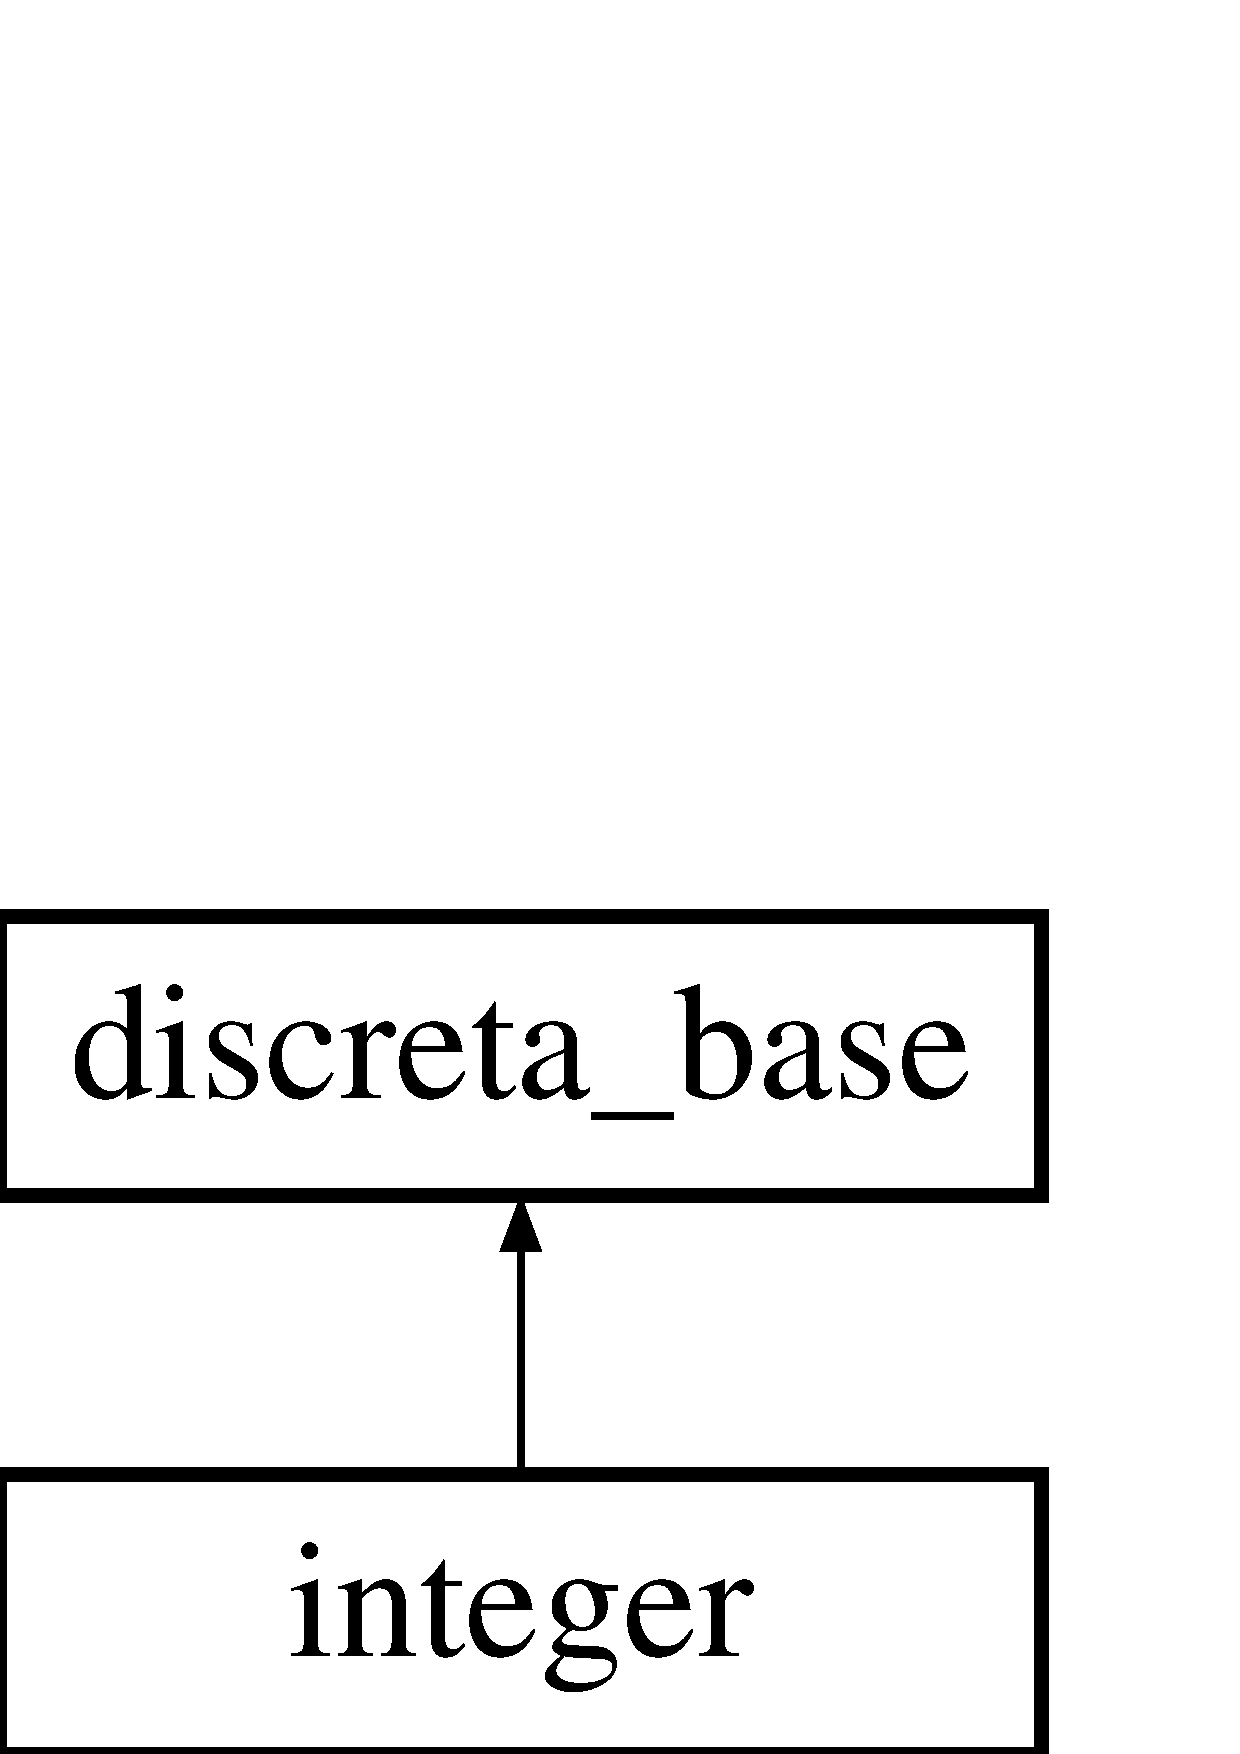
\includegraphics[height=2.000000cm]{classinteger}
\end{center}
\end{figure}
\subsection*{Public Member Functions}
\begin{DoxyCompactItemize}
\item 
\mbox{\hyperlink{classinteger_a48a0c2e70d6c116c058e19c4cb546aed}{integer}} ()
\item 
\mbox{\hyperlink{classinteger_a2d9b863abf3f285182954a852cd6c629}{integer}} (\mbox{\hyperlink{galois_8h_ab6cc7b4aeb6ea31aba2b3fbfc83ff5e6}{B\+Y\+TE}} $\ast$\mbox{\hyperlink{alphabet2_8_c_a533391314665d6bf1b5575e9a9cd8552}{p}})
\item 
\mbox{\hyperlink{classinteger_a94fbe85c84fa9a8b9ccad5948f94f780}{integer}} (\mbox{\hyperlink{galois_8h_a09fddde158a3a20bd2dcadb609de11dc}{I\+NT}} \mbox{\hyperlink{alphabet2_8_c_acb559820d9ca11295b4500f179ef6392}{i}})
\item 
\mbox{\hyperlink{classinteger_a37270fa45383a0798e3fd1e1330cb9a5}{integer}} (const \mbox{\hyperlink{classdiscreta__base}{discreta\+\_\+base}} \&\mbox{\hyperlink{alphabet2_8_c_a6150e0515f7202e2fb518f7206ed97dc}{x}})
\item 
\mbox{\hyperlink{classinteger}{integer}} \& \mbox{\hyperlink{classinteger_a52f72e5f2da0f1617355e03a7202492f}{operator=}} (const \mbox{\hyperlink{classdiscreta__base}{discreta\+\_\+base}} \&\mbox{\hyperlink{alphabet2_8_c_a6150e0515f7202e2fb518f7206ed97dc}{x}})
\item 
void $\ast$ \mbox{\hyperlink{classinteger_ab23c39901803e33fb3b52be1476ec54a}{operator new}} (size\+\_\+t, void $\ast$\mbox{\hyperlink{alphabet2_8_c_a533391314665d6bf1b5575e9a9cd8552}{p}})
\item 
void \mbox{\hyperlink{classinteger_a6265c65ef311229acd513d748faba796}{settype\+\_\+integer}} ()
\item 
\mbox{\hyperlink{classinteger_a87b9f2b5aaf4ab5e5230b33d456e33d5}{$\sim$integer}} ()
\item 
void \mbox{\hyperlink{classinteger_a02eb557612c9db1820dd75a77151edc0}{freeself\+\_\+integer}} ()
\item 
\mbox{\hyperlink{discreta_8h_aaf25ee7e2306d78c74ec7bc48f092e81}{kind}} \mbox{\hyperlink{classinteger_a183985f67ef55beed80bda05a0c574d9}{s\+\_\+virtual\+\_\+kind}} ()
\item 
void \mbox{\hyperlink{classinteger_a0258f5ab80826ddd4d845a52a6c450b2}{copyobject\+\_\+to}} (\mbox{\hyperlink{classdiscreta__base}{discreta\+\_\+base}} \&\mbox{\hyperlink{alphabet2_8_c_a6150e0515f7202e2fb518f7206ed97dc}{x}})
\item 
ostream \& \mbox{\hyperlink{classinteger_a8aef91d98e8edc8d895c1d6cfc35677b}{print}} (ostream \&)
\item 
\mbox{\hyperlink{classinteger}{integer}} \& \mbox{\hyperlink{classinteger_a869091f0a0f35f5354c8c4a70250e8a9}{m\+\_\+i}} (\mbox{\hyperlink{galois_8h_a09fddde158a3a20bd2dcadb609de11dc}{I\+NT}} \mbox{\hyperlink{alphabet2_8_c_acb559820d9ca11295b4500f179ef6392}{i}})
\item 
\mbox{\hyperlink{galois_8h_a09fddde158a3a20bd2dcadb609de11dc}{I\+NT}} \& \mbox{\hyperlink{classinteger_adf28e9f94d4c844adaa950deeb80b904}{s\+\_\+i}} ()
\item 
\mbox{\hyperlink{galois_8h_a09fddde158a3a20bd2dcadb609de11dc}{I\+NT}} \mbox{\hyperlink{classinteger_a20cc8d8d4913e9ee746c6758bbb2e62a}{compare\+\_\+with}} (\mbox{\hyperlink{classdiscreta__base}{discreta\+\_\+base}} \&a)
\item 
void \mbox{\hyperlink{classinteger_a7f4f072c0d9c6b15660d80e81496dffc}{mult\+\_\+to}} (\mbox{\hyperlink{classdiscreta__base}{discreta\+\_\+base}} \&\mbox{\hyperlink{alphabet2_8_c_a6150e0515f7202e2fb518f7206ed97dc}{x}}, \mbox{\hyperlink{classdiscreta__base}{discreta\+\_\+base}} \&\mbox{\hyperlink{alphabet2_8_c_a0a2f84ed7838f07779ae24c5a9086d33}{y}})
\item 
\mbox{\hyperlink{galois_8h_a09fddde158a3a20bd2dcadb609de11dc}{I\+NT}} \mbox{\hyperlink{classinteger_a9a991b285677b99b4879034e31648b7a}{invert\+\_\+to}} (\mbox{\hyperlink{classdiscreta__base}{discreta\+\_\+base}} \&\mbox{\hyperlink{alphabet2_8_c_a6150e0515f7202e2fb518f7206ed97dc}{x}})
\item 
void \mbox{\hyperlink{classinteger_a3f6fe19fe4f2948364b1e75a6dfec47f}{add\+\_\+to}} (\mbox{\hyperlink{classdiscreta__base}{discreta\+\_\+base}} \&\mbox{\hyperlink{alphabet2_8_c_a6150e0515f7202e2fb518f7206ed97dc}{x}}, \mbox{\hyperlink{classdiscreta__base}{discreta\+\_\+base}} \&\mbox{\hyperlink{alphabet2_8_c_a0a2f84ed7838f07779ae24c5a9086d33}{y}})
\item 
void \mbox{\hyperlink{classinteger_a1da2bd683bdef336057ef2b84d4b3978}{negate\+\_\+to}} (\mbox{\hyperlink{classdiscreta__base}{discreta\+\_\+base}} \&\mbox{\hyperlink{alphabet2_8_c_a6150e0515f7202e2fb518f7206ed97dc}{x}})
\item 
void \mbox{\hyperlink{classinteger_aac4272bbf32a3e1b4a5201630f116388}{normalize}} (\mbox{\hyperlink{classdiscreta__base}{discreta\+\_\+base}} \&\mbox{\hyperlink{alphabet2_8_c_a533391314665d6bf1b5575e9a9cd8552}{p}})
\item 
void \mbox{\hyperlink{classinteger_ab99e796e5c2cef13eb30dc43eac3c9fe}{zero}} ()
\item 
void \mbox{\hyperlink{classinteger_a18a967d90d63b1c58e3f2480e9084ed5}{one}} ()
\item 
void \mbox{\hyperlink{classinteger_a4d312656ed6c31235e11ecb3f05df1f5}{m\+\_\+one}} ()
\item 
void \mbox{\hyperlink{classinteger_ab975244fc25d0a9b3d4ef5104e3fcd24}{homo\+\_\+z}} (\mbox{\hyperlink{galois_8h_a09fddde158a3a20bd2dcadb609de11dc}{I\+NT}} z)
\item 
void \mbox{\hyperlink{classinteger_a2fd161f380ea688219131ba9a8429509}{inc}} ()
\item 
void \mbox{\hyperlink{classinteger_a6b744350afb55f82d25e55bb6b1027b2}{dec}} ()
\item 
\mbox{\hyperlink{galois_8h_a09fddde158a3a20bd2dcadb609de11dc}{I\+NT}} \mbox{\hyperlink{classinteger_ab92500013b2342ab5c24355bc91bad64}{is\+\_\+zero}} ()
\item 
\mbox{\hyperlink{galois_8h_a09fddde158a3a20bd2dcadb609de11dc}{I\+NT}} \mbox{\hyperlink{classinteger_acf8faabd4ed20f9580605714b5b73a5f}{is\+\_\+one}} ()
\item 
\mbox{\hyperlink{galois_8h_a09fddde158a3a20bd2dcadb609de11dc}{I\+NT}} \mbox{\hyperlink{classinteger_a7585957656c1152035411e066a4f0053}{is\+\_\+m\+\_\+one}} ()
\item 
\mbox{\hyperlink{galois_8h_a09fddde158a3a20bd2dcadb609de11dc}{I\+NT}} \mbox{\hyperlink{classinteger_a903a43b71a9f65f6b7edb443997f5f0e}{compare\+\_\+with\+\_\+euklidean}} (\mbox{\hyperlink{classdiscreta__base}{discreta\+\_\+base}} \&a)
\item 
void \mbox{\hyperlink{classinteger_ac6b2f247cfac1e1e5708a9e035ce42fe}{integral\+\_\+division}} (\mbox{\hyperlink{classdiscreta__base}{discreta\+\_\+base}} \&\mbox{\hyperlink{alphabet2_8_c_a6150e0515f7202e2fb518f7206ed97dc}{x}}, \mbox{\hyperlink{classdiscreta__base}{discreta\+\_\+base}} \&\mbox{\hyperlink{simeon_8_c_a92cbb483a3b27ae1a0dbfcb125ce216f}{q}}, \mbox{\hyperlink{classdiscreta__base}{discreta\+\_\+base}} \&\mbox{\hyperlink{alphabet2_8_c_acab531abaa74a7e664e3986f2522b33a}{r}}, \mbox{\hyperlink{galois_8h_a09fddde158a3a20bd2dcadb609de11dc}{I\+NT}} \mbox{\hyperlink{simeon_8_c_a818073fbcc2f439e7c56952f67386122}{verbose\+\_\+level}})
\item 
void \mbox{\hyperlink{classinteger_a672d4d45d9d68997770f1cb86f966912}{rand}} (\mbox{\hyperlink{galois_8h_a09fddde158a3a20bd2dcadb609de11dc}{I\+NT}} low, \mbox{\hyperlink{galois_8h_a09fddde158a3a20bd2dcadb609de11dc}{I\+NT}} high)
\item 
\mbox{\hyperlink{galois_8h_a09fddde158a3a20bd2dcadb609de11dc}{I\+NT}} \mbox{\hyperlink{classinteger_af03f36df78aa755b9e4c7eaecc3b5f44}{log2}} ()
\end{DoxyCompactItemize}
\subsection*{Additional Inherited Members}


\subsection{Constructor \& Destructor Documentation}
\mbox{\Hypertarget{classinteger_a48a0c2e70d6c116c058e19c4cb546aed}\label{classinteger_a48a0c2e70d6c116c058e19c4cb546aed}} 
\index{integer@{integer}!integer@{integer}}
\index{integer@{integer}!integer@{integer}}
\subsubsection{\texorpdfstring{integer()}{integer()}\hspace{0.1cm}{\footnotesize\ttfamily [1/4]}}
{\footnotesize\ttfamily integer\+::integer (\begin{DoxyParamCaption}{ }\end{DoxyParamCaption})}

\mbox{\Hypertarget{classinteger_a2d9b863abf3f285182954a852cd6c629}\label{classinteger_a2d9b863abf3f285182954a852cd6c629}} 
\index{integer@{integer}!integer@{integer}}
\index{integer@{integer}!integer@{integer}}
\subsubsection{\texorpdfstring{integer()}{integer()}\hspace{0.1cm}{\footnotesize\ttfamily [2/4]}}
{\footnotesize\ttfamily integer\+::integer (\begin{DoxyParamCaption}\item[{\mbox{\hyperlink{galois_8h_ab6cc7b4aeb6ea31aba2b3fbfc83ff5e6}{B\+Y\+TE}} $\ast$}]{p }\end{DoxyParamCaption})}

\mbox{\Hypertarget{classinteger_a94fbe85c84fa9a8b9ccad5948f94f780}\label{classinteger_a94fbe85c84fa9a8b9ccad5948f94f780}} 
\index{integer@{integer}!integer@{integer}}
\index{integer@{integer}!integer@{integer}}
\subsubsection{\texorpdfstring{integer()}{integer()}\hspace{0.1cm}{\footnotesize\ttfamily [3/4]}}
{\footnotesize\ttfamily integer\+::integer (\begin{DoxyParamCaption}\item[{\mbox{\hyperlink{galois_8h_a09fddde158a3a20bd2dcadb609de11dc}{I\+NT}}}]{i }\end{DoxyParamCaption})}

\mbox{\Hypertarget{classinteger_a37270fa45383a0798e3fd1e1330cb9a5}\label{classinteger_a37270fa45383a0798e3fd1e1330cb9a5}} 
\index{integer@{integer}!integer@{integer}}
\index{integer@{integer}!integer@{integer}}
\subsubsection{\texorpdfstring{integer()}{integer()}\hspace{0.1cm}{\footnotesize\ttfamily [4/4]}}
{\footnotesize\ttfamily integer\+::integer (\begin{DoxyParamCaption}\item[{const \mbox{\hyperlink{classdiscreta__base}{discreta\+\_\+base}} \&}]{x }\end{DoxyParamCaption})}

\mbox{\Hypertarget{classinteger_a87b9f2b5aaf4ab5e5230b33d456e33d5}\label{classinteger_a87b9f2b5aaf4ab5e5230b33d456e33d5}} 
\index{integer@{integer}!````~integer@{$\sim$integer}}
\index{````~integer@{$\sim$integer}!integer@{integer}}
\subsubsection{\texorpdfstring{$\sim$integer()}{~integer()}}
{\footnotesize\ttfamily integer\+::$\sim$integer (\begin{DoxyParamCaption}{ }\end{DoxyParamCaption})}



\subsection{Member Function Documentation}
\mbox{\Hypertarget{classinteger_a3f6fe19fe4f2948364b1e75a6dfec47f}\label{classinteger_a3f6fe19fe4f2948364b1e75a6dfec47f}} 
\index{integer@{integer}!add\+\_\+to@{add\+\_\+to}}
\index{add\+\_\+to@{add\+\_\+to}!integer@{integer}}
\subsubsection{\texorpdfstring{add\+\_\+to()}{add\_to()}}
{\footnotesize\ttfamily void integer\+::add\+\_\+to (\begin{DoxyParamCaption}\item[{\mbox{\hyperlink{classdiscreta__base}{discreta\+\_\+base}} \&}]{x,  }\item[{\mbox{\hyperlink{classdiscreta__base}{discreta\+\_\+base}} \&}]{y }\end{DoxyParamCaption})\hspace{0.3cm}{\ttfamily [virtual]}}



Reimplemented from \mbox{\hyperlink{classdiscreta__base_a712a61311eb036d70a52871ed315f515}{discreta\+\_\+base}}.

\mbox{\Hypertarget{classinteger_a20cc8d8d4913e9ee746c6758bbb2e62a}\label{classinteger_a20cc8d8d4913e9ee746c6758bbb2e62a}} 
\index{integer@{integer}!compare\+\_\+with@{compare\+\_\+with}}
\index{compare\+\_\+with@{compare\+\_\+with}!integer@{integer}}
\subsubsection{\texorpdfstring{compare\+\_\+with()}{compare\_with()}}
{\footnotesize\ttfamily \mbox{\hyperlink{galois_8h_a09fddde158a3a20bd2dcadb609de11dc}{I\+NT}} integer\+::compare\+\_\+with (\begin{DoxyParamCaption}\item[{\mbox{\hyperlink{classdiscreta__base}{discreta\+\_\+base}} \&}]{a }\end{DoxyParamCaption})\hspace{0.3cm}{\ttfamily [virtual]}}



Reimplemented from \mbox{\hyperlink{classdiscreta__base_a3818444c4301d0b7ed47c3b850ea6c60}{discreta\+\_\+base}}.

\mbox{\Hypertarget{classinteger_a903a43b71a9f65f6b7edb443997f5f0e}\label{classinteger_a903a43b71a9f65f6b7edb443997f5f0e}} 
\index{integer@{integer}!compare\+\_\+with\+\_\+euklidean@{compare\+\_\+with\+\_\+euklidean}}
\index{compare\+\_\+with\+\_\+euklidean@{compare\+\_\+with\+\_\+euklidean}!integer@{integer}}
\subsubsection{\texorpdfstring{compare\+\_\+with\+\_\+euklidean()}{compare\_with\_euklidean()}}
{\footnotesize\ttfamily \mbox{\hyperlink{galois_8h_a09fddde158a3a20bd2dcadb609de11dc}{I\+NT}} integer\+::compare\+\_\+with\+\_\+euklidean (\begin{DoxyParamCaption}\item[{\mbox{\hyperlink{classdiscreta__base}{discreta\+\_\+base}} \&}]{a }\end{DoxyParamCaption})\hspace{0.3cm}{\ttfamily [virtual]}}



Reimplemented from \mbox{\hyperlink{classdiscreta__base_a9d3091feb2fbc69359c2a45f11ceec9e}{discreta\+\_\+base}}.

\mbox{\Hypertarget{classinteger_a0258f5ab80826ddd4d845a52a6c450b2}\label{classinteger_a0258f5ab80826ddd4d845a52a6c450b2}} 
\index{integer@{integer}!copyobject\+\_\+to@{copyobject\+\_\+to}}
\index{copyobject\+\_\+to@{copyobject\+\_\+to}!integer@{integer}}
\subsubsection{\texorpdfstring{copyobject\+\_\+to()}{copyobject\_to()}}
{\footnotesize\ttfamily void integer\+::copyobject\+\_\+to (\begin{DoxyParamCaption}\item[{\mbox{\hyperlink{classdiscreta__base}{discreta\+\_\+base}} \&}]{x }\end{DoxyParamCaption})\hspace{0.3cm}{\ttfamily [virtual]}}



Reimplemented from \mbox{\hyperlink{classdiscreta__base_a33180628d9ced231267229b3564790f3}{discreta\+\_\+base}}.

\mbox{\Hypertarget{classinteger_a6b744350afb55f82d25e55bb6b1027b2}\label{classinteger_a6b744350afb55f82d25e55bb6b1027b2}} 
\index{integer@{integer}!dec@{dec}}
\index{dec@{dec}!integer@{integer}}
\subsubsection{\texorpdfstring{dec()}{dec()}}
{\footnotesize\ttfamily void integer\+::dec (\begin{DoxyParamCaption}{ }\end{DoxyParamCaption})\hspace{0.3cm}{\ttfamily [virtual]}}



Reimplemented from \mbox{\hyperlink{classdiscreta__base_a11449a5cfa7dc5f5600e012517af6f0f}{discreta\+\_\+base}}.

\mbox{\Hypertarget{classinteger_a02eb557612c9db1820dd75a77151edc0}\label{classinteger_a02eb557612c9db1820dd75a77151edc0}} 
\index{integer@{integer}!freeself\+\_\+integer@{freeself\+\_\+integer}}
\index{freeself\+\_\+integer@{freeself\+\_\+integer}!integer@{integer}}
\subsubsection{\texorpdfstring{freeself\+\_\+integer()}{freeself\_integer()}}
{\footnotesize\ttfamily void integer\+::freeself\+\_\+integer (\begin{DoxyParamCaption}{ }\end{DoxyParamCaption})}

\mbox{\Hypertarget{classinteger_ab975244fc25d0a9b3d4ef5104e3fcd24}\label{classinteger_ab975244fc25d0a9b3d4ef5104e3fcd24}} 
\index{integer@{integer}!homo\+\_\+z@{homo\+\_\+z}}
\index{homo\+\_\+z@{homo\+\_\+z}!integer@{integer}}
\subsubsection{\texorpdfstring{homo\+\_\+z()}{homo\_z()}}
{\footnotesize\ttfamily void integer\+::homo\+\_\+z (\begin{DoxyParamCaption}\item[{\mbox{\hyperlink{galois_8h_a09fddde158a3a20bd2dcadb609de11dc}{I\+NT}}}]{z }\end{DoxyParamCaption})\hspace{0.3cm}{\ttfamily [virtual]}}



Reimplemented from \mbox{\hyperlink{classdiscreta__base_a40e349b2d85c5c6dba9c015d16a0e801}{discreta\+\_\+base}}.

\mbox{\Hypertarget{classinteger_a2fd161f380ea688219131ba9a8429509}\label{classinteger_a2fd161f380ea688219131ba9a8429509}} 
\index{integer@{integer}!inc@{inc}}
\index{inc@{inc}!integer@{integer}}
\subsubsection{\texorpdfstring{inc()}{inc()}}
{\footnotesize\ttfamily void integer\+::inc (\begin{DoxyParamCaption}{ }\end{DoxyParamCaption})\hspace{0.3cm}{\ttfamily [virtual]}}



Reimplemented from \mbox{\hyperlink{classdiscreta__base_afda42789f4ba04ba399623a6b9e206e3}{discreta\+\_\+base}}.

\mbox{\Hypertarget{classinteger_ac6b2f247cfac1e1e5708a9e035ce42fe}\label{classinteger_ac6b2f247cfac1e1e5708a9e035ce42fe}} 
\index{integer@{integer}!integral\+\_\+division@{integral\+\_\+division}}
\index{integral\+\_\+division@{integral\+\_\+division}!integer@{integer}}
\subsubsection{\texorpdfstring{integral\+\_\+division()}{integral\_division()}}
{\footnotesize\ttfamily void integer\+::integral\+\_\+division (\begin{DoxyParamCaption}\item[{\mbox{\hyperlink{classdiscreta__base}{discreta\+\_\+base}} \&}]{x,  }\item[{\mbox{\hyperlink{classdiscreta__base}{discreta\+\_\+base}} \&}]{q,  }\item[{\mbox{\hyperlink{classdiscreta__base}{discreta\+\_\+base}} \&}]{r,  }\item[{\mbox{\hyperlink{galois_8h_a09fddde158a3a20bd2dcadb609de11dc}{I\+NT}}}]{verbose\+\_\+level }\end{DoxyParamCaption})\hspace{0.3cm}{\ttfamily [virtual]}}



Reimplemented from \mbox{\hyperlink{classdiscreta__base_a92b3001ac35af9185b316c0d8f89070e}{discreta\+\_\+base}}.

\mbox{\Hypertarget{classinteger_a9a991b285677b99b4879034e31648b7a}\label{classinteger_a9a991b285677b99b4879034e31648b7a}} 
\index{integer@{integer}!invert\+\_\+to@{invert\+\_\+to}}
\index{invert\+\_\+to@{invert\+\_\+to}!integer@{integer}}
\subsubsection{\texorpdfstring{invert\+\_\+to()}{invert\_to()}}
{\footnotesize\ttfamily \mbox{\hyperlink{galois_8h_a09fddde158a3a20bd2dcadb609de11dc}{I\+NT}} integer\+::invert\+\_\+to (\begin{DoxyParamCaption}\item[{\mbox{\hyperlink{classdiscreta__base}{discreta\+\_\+base}} \&}]{x }\end{DoxyParamCaption})\hspace{0.3cm}{\ttfamily [virtual]}}



Reimplemented from \mbox{\hyperlink{classdiscreta__base_a874a5ffb467f3896604a3c9bdf0cca50}{discreta\+\_\+base}}.

\mbox{\Hypertarget{classinteger_a7585957656c1152035411e066a4f0053}\label{classinteger_a7585957656c1152035411e066a4f0053}} 
\index{integer@{integer}!is\+\_\+m\+\_\+one@{is\+\_\+m\+\_\+one}}
\index{is\+\_\+m\+\_\+one@{is\+\_\+m\+\_\+one}!integer@{integer}}
\subsubsection{\texorpdfstring{is\+\_\+m\+\_\+one()}{is\_m\_one()}}
{\footnotesize\ttfamily \mbox{\hyperlink{galois_8h_a09fddde158a3a20bd2dcadb609de11dc}{I\+NT}} integer\+::is\+\_\+m\+\_\+one (\begin{DoxyParamCaption}{ }\end{DoxyParamCaption})\hspace{0.3cm}{\ttfamily [virtual]}}



Reimplemented from \mbox{\hyperlink{classdiscreta__base_afc2e134e55759cf069f49fcf05af418b}{discreta\+\_\+base}}.

\mbox{\Hypertarget{classinteger_acf8faabd4ed20f9580605714b5b73a5f}\label{classinteger_acf8faabd4ed20f9580605714b5b73a5f}} 
\index{integer@{integer}!is\+\_\+one@{is\+\_\+one}}
\index{is\+\_\+one@{is\+\_\+one}!integer@{integer}}
\subsubsection{\texorpdfstring{is\+\_\+one()}{is\_one()}}
{\footnotesize\ttfamily \mbox{\hyperlink{galois_8h_a09fddde158a3a20bd2dcadb609de11dc}{I\+NT}} integer\+::is\+\_\+one (\begin{DoxyParamCaption}{ }\end{DoxyParamCaption})\hspace{0.3cm}{\ttfamily [virtual]}}



Reimplemented from \mbox{\hyperlink{classdiscreta__base_a28fa37aac83194174888d34f07f43848}{discreta\+\_\+base}}.

\mbox{\Hypertarget{classinteger_ab92500013b2342ab5c24355bc91bad64}\label{classinteger_ab92500013b2342ab5c24355bc91bad64}} 
\index{integer@{integer}!is\+\_\+zero@{is\+\_\+zero}}
\index{is\+\_\+zero@{is\+\_\+zero}!integer@{integer}}
\subsubsection{\texorpdfstring{is\+\_\+zero()}{is\_zero()}}
{\footnotesize\ttfamily \mbox{\hyperlink{galois_8h_a09fddde158a3a20bd2dcadb609de11dc}{I\+NT}} integer\+::is\+\_\+zero (\begin{DoxyParamCaption}{ }\end{DoxyParamCaption})\hspace{0.3cm}{\ttfamily [virtual]}}



Reimplemented from \mbox{\hyperlink{classdiscreta__base_ac75f6bdc1ba1b406e26cf921adfd9864}{discreta\+\_\+base}}.

\mbox{\Hypertarget{classinteger_af03f36df78aa755b9e4c7eaecc3b5f44}\label{classinteger_af03f36df78aa755b9e4c7eaecc3b5f44}} 
\index{integer@{integer}!log2@{log2}}
\index{log2@{log2}!integer@{integer}}
\subsubsection{\texorpdfstring{log2()}{log2()}}
{\footnotesize\ttfamily \mbox{\hyperlink{galois_8h_a09fddde158a3a20bd2dcadb609de11dc}{I\+NT}} integer\+::log2 (\begin{DoxyParamCaption}{ }\end{DoxyParamCaption})}

\mbox{\Hypertarget{classinteger_a869091f0a0f35f5354c8c4a70250e8a9}\label{classinteger_a869091f0a0f35f5354c8c4a70250e8a9}} 
\index{integer@{integer}!m\+\_\+i@{m\+\_\+i}}
\index{m\+\_\+i@{m\+\_\+i}!integer@{integer}}
\subsubsection{\texorpdfstring{m\+\_\+i()}{m\_i()}}
{\footnotesize\ttfamily \mbox{\hyperlink{classinteger}{integer}} \& integer\+::m\+\_\+i (\begin{DoxyParamCaption}\item[{\mbox{\hyperlink{galois_8h_a09fddde158a3a20bd2dcadb609de11dc}{I\+NT}}}]{i }\end{DoxyParamCaption})}

\mbox{\Hypertarget{classinteger_a4d312656ed6c31235e11ecb3f05df1f5}\label{classinteger_a4d312656ed6c31235e11ecb3f05df1f5}} 
\index{integer@{integer}!m\+\_\+one@{m\+\_\+one}}
\index{m\+\_\+one@{m\+\_\+one}!integer@{integer}}
\subsubsection{\texorpdfstring{m\+\_\+one()}{m\_one()}}
{\footnotesize\ttfamily void integer\+::m\+\_\+one (\begin{DoxyParamCaption}{ }\end{DoxyParamCaption})\hspace{0.3cm}{\ttfamily [virtual]}}



Reimplemented from \mbox{\hyperlink{classdiscreta__base_a3a147eee6f3477387f7e580c117e5a05}{discreta\+\_\+base}}.

\mbox{\Hypertarget{classinteger_a7f4f072c0d9c6b15660d80e81496dffc}\label{classinteger_a7f4f072c0d9c6b15660d80e81496dffc}} 
\index{integer@{integer}!mult\+\_\+to@{mult\+\_\+to}}
\index{mult\+\_\+to@{mult\+\_\+to}!integer@{integer}}
\subsubsection{\texorpdfstring{mult\+\_\+to()}{mult\_to()}}
{\footnotesize\ttfamily void integer\+::mult\+\_\+to (\begin{DoxyParamCaption}\item[{\mbox{\hyperlink{classdiscreta__base}{discreta\+\_\+base}} \&}]{x,  }\item[{\mbox{\hyperlink{classdiscreta__base}{discreta\+\_\+base}} \&}]{y }\end{DoxyParamCaption})\hspace{0.3cm}{\ttfamily [virtual]}}



Reimplemented from \mbox{\hyperlink{classdiscreta__base_a54d5c16c016769e3365639721c06591e}{discreta\+\_\+base}}.

\mbox{\Hypertarget{classinteger_a1da2bd683bdef336057ef2b84d4b3978}\label{classinteger_a1da2bd683bdef336057ef2b84d4b3978}} 
\index{integer@{integer}!negate\+\_\+to@{negate\+\_\+to}}
\index{negate\+\_\+to@{negate\+\_\+to}!integer@{integer}}
\subsubsection{\texorpdfstring{negate\+\_\+to()}{negate\_to()}}
{\footnotesize\ttfamily void integer\+::negate\+\_\+to (\begin{DoxyParamCaption}\item[{\mbox{\hyperlink{classdiscreta__base}{discreta\+\_\+base}} \&}]{x }\end{DoxyParamCaption})\hspace{0.3cm}{\ttfamily [virtual]}}



Reimplemented from \mbox{\hyperlink{classdiscreta__base_a65ad2034f2f4518d424b814974018a03}{discreta\+\_\+base}}.

\mbox{\Hypertarget{classinteger_aac4272bbf32a3e1b4a5201630f116388}\label{classinteger_aac4272bbf32a3e1b4a5201630f116388}} 
\index{integer@{integer}!normalize@{normalize}}
\index{normalize@{normalize}!integer@{integer}}
\subsubsection{\texorpdfstring{normalize()}{normalize()}}
{\footnotesize\ttfamily void integer\+::normalize (\begin{DoxyParamCaption}\item[{\mbox{\hyperlink{classdiscreta__base}{discreta\+\_\+base}} \&}]{p }\end{DoxyParamCaption})\hspace{0.3cm}{\ttfamily [virtual]}}



Reimplemented from \mbox{\hyperlink{classdiscreta__base_acd46a488505c6086b5bc019550e5e313}{discreta\+\_\+base}}.

\mbox{\Hypertarget{classinteger_a18a967d90d63b1c58e3f2480e9084ed5}\label{classinteger_a18a967d90d63b1c58e3f2480e9084ed5}} 
\index{integer@{integer}!one@{one}}
\index{one@{one}!integer@{integer}}
\subsubsection{\texorpdfstring{one()}{one()}}
{\footnotesize\ttfamily void integer\+::one (\begin{DoxyParamCaption}{ }\end{DoxyParamCaption})\hspace{0.3cm}{\ttfamily [virtual]}}



Reimplemented from \mbox{\hyperlink{classdiscreta__base_a6f5d6422a0040950415db30e39dafd19}{discreta\+\_\+base}}.

\mbox{\Hypertarget{classinteger_ab23c39901803e33fb3b52be1476ec54a}\label{classinteger_ab23c39901803e33fb3b52be1476ec54a}} 
\index{integer@{integer}!operator new@{operator new}}
\index{operator new@{operator new}!integer@{integer}}
\subsubsection{\texorpdfstring{operator new()}{operator new()}}
{\footnotesize\ttfamily void$\ast$ integer\+::operator new (\begin{DoxyParamCaption}\item[{size\+\_\+t}]{,  }\item[{void $\ast$}]{p }\end{DoxyParamCaption})\hspace{0.3cm}{\ttfamily [inline]}}

\mbox{\Hypertarget{classinteger_a52f72e5f2da0f1617355e03a7202492f}\label{classinteger_a52f72e5f2da0f1617355e03a7202492f}} 
\index{integer@{integer}!operator=@{operator=}}
\index{operator=@{operator=}!integer@{integer}}
\subsubsection{\texorpdfstring{operator=()}{operator=()}}
{\footnotesize\ttfamily \mbox{\hyperlink{classinteger}{integer}} \& integer\+::operator= (\begin{DoxyParamCaption}\item[{const \mbox{\hyperlink{classdiscreta__base}{discreta\+\_\+base}} \&}]{x }\end{DoxyParamCaption})}

\mbox{\Hypertarget{classinteger_a8aef91d98e8edc8d895c1d6cfc35677b}\label{classinteger_a8aef91d98e8edc8d895c1d6cfc35677b}} 
\index{integer@{integer}!print@{print}}
\index{print@{print}!integer@{integer}}
\subsubsection{\texorpdfstring{print()}{print()}}
{\footnotesize\ttfamily ostream \& integer\+::print (\begin{DoxyParamCaption}\item[{ostream \&}]{ost }\end{DoxyParamCaption})\hspace{0.3cm}{\ttfamily [virtual]}}



Reimplemented from \mbox{\hyperlink{classdiscreta__base_a036e48bc058347046fc9b73dd0951478}{discreta\+\_\+base}}.

\mbox{\Hypertarget{classinteger_a672d4d45d9d68997770f1cb86f966912}\label{classinteger_a672d4d45d9d68997770f1cb86f966912}} 
\index{integer@{integer}!rand@{rand}}
\index{rand@{rand}!integer@{integer}}
\subsubsection{\texorpdfstring{rand()}{rand()}}
{\footnotesize\ttfamily void integer\+::rand (\begin{DoxyParamCaption}\item[{\mbox{\hyperlink{galois_8h_a09fddde158a3a20bd2dcadb609de11dc}{I\+NT}}}]{low,  }\item[{\mbox{\hyperlink{galois_8h_a09fddde158a3a20bd2dcadb609de11dc}{I\+NT}}}]{high }\end{DoxyParamCaption})}

\mbox{\Hypertarget{classinteger_adf28e9f94d4c844adaa950deeb80b904}\label{classinteger_adf28e9f94d4c844adaa950deeb80b904}} 
\index{integer@{integer}!s\+\_\+i@{s\+\_\+i}}
\index{s\+\_\+i@{s\+\_\+i}!integer@{integer}}
\subsubsection{\texorpdfstring{s\+\_\+i()}{s\_i()}}
{\footnotesize\ttfamily \mbox{\hyperlink{galois_8h_a09fddde158a3a20bd2dcadb609de11dc}{I\+NT}}\& integer\+::s\+\_\+i (\begin{DoxyParamCaption}{ }\end{DoxyParamCaption})\hspace{0.3cm}{\ttfamily [inline]}}

\mbox{\Hypertarget{classinteger_a183985f67ef55beed80bda05a0c574d9}\label{classinteger_a183985f67ef55beed80bda05a0c574d9}} 
\index{integer@{integer}!s\+\_\+virtual\+\_\+kind@{s\+\_\+virtual\+\_\+kind}}
\index{s\+\_\+virtual\+\_\+kind@{s\+\_\+virtual\+\_\+kind}!integer@{integer}}
\subsubsection{\texorpdfstring{s\+\_\+virtual\+\_\+kind()}{s\_virtual\_kind()}}
{\footnotesize\ttfamily \mbox{\hyperlink{discreta_8h_aaf25ee7e2306d78c74ec7bc48f092e81}{kind}} integer\+::s\+\_\+virtual\+\_\+kind (\begin{DoxyParamCaption}{ }\end{DoxyParamCaption})\hspace{0.3cm}{\ttfamily [virtual]}}



Reimplemented from \mbox{\hyperlink{classdiscreta__base_a52778a6d6943a468be083d0785d418fb}{discreta\+\_\+base}}.

\mbox{\Hypertarget{classinteger_a6265c65ef311229acd513d748faba796}\label{classinteger_a6265c65ef311229acd513d748faba796}} 
\index{integer@{integer}!settype\+\_\+integer@{settype\+\_\+integer}}
\index{settype\+\_\+integer@{settype\+\_\+integer}!integer@{integer}}
\subsubsection{\texorpdfstring{settype\+\_\+integer()}{settype\_integer()}}
{\footnotesize\ttfamily void integer\+::settype\+\_\+integer (\begin{DoxyParamCaption}{ }\end{DoxyParamCaption})}

\mbox{\Hypertarget{classinteger_ab99e796e5c2cef13eb30dc43eac3c9fe}\label{classinteger_ab99e796e5c2cef13eb30dc43eac3c9fe}} 
\index{integer@{integer}!zero@{zero}}
\index{zero@{zero}!integer@{integer}}
\subsubsection{\texorpdfstring{zero()}{zero()}}
{\footnotesize\ttfamily void integer\+::zero (\begin{DoxyParamCaption}{ }\end{DoxyParamCaption})\hspace{0.3cm}{\ttfamily [virtual]}}



Reimplemented from \mbox{\hyperlink{classdiscreta__base_a424aa44bbb6ca48d30ad1087dbd6f210}{discreta\+\_\+base}}.



The documentation for this class was generated from the following files\+:\begin{DoxyCompactItemize}
\item 
S\+R\+C/\+L\+I\+B/\+D\+I\+S\+C\+R\+E\+T\+A/\mbox{\hyperlink{discreta_8h}{discreta.\+h}}\item 
S\+R\+C/\+L\+I\+B/\+D\+I\+S\+C\+R\+E\+T\+A/\mbox{\hyperlink{integer_8_c}{integer.\+C}}\end{DoxyCompactItemize}

\hypertarget{classisomorph}{}\section{isomorph Class Reference}
\label{classisomorph}\index{isomorph@{isomorph}}


{\ttfamily \#include $<$top\+\_\+level.\+h$>$}

\subsection*{Public Member Functions}
\begin{DoxyCompactItemize}
\item 
\mbox{\hyperlink{classisomorph_aedaab5a96e9f9aaf97bfbca9fafe10bc}{isomorph}} ()
\item 
void \mbox{\hyperlink{classisomorph_a8212fe560851abbc45a12b866694e321}{null}} ()
\item 
\mbox{\hyperlink{classisomorph_a640a6e2ba514b0f832685dc4f3c51fc6}{$\sim$isomorph}} ()
\item 
void \mbox{\hyperlink{classisomorph_ab34f53c7a2cc10355c0e5f525a64e409}{free}} ()
\item 
void \mbox{\hyperlink{classisomorph_a169534be12152d9c663bb85fb422951c}{null\+\_\+tmp\+\_\+data}} ()
\item 
void \mbox{\hyperlink{classisomorph_a2aba74f4e4c524cfee6c9faea33474c2}{allocate\+\_\+tmp\+\_\+data}} ()
\item 
void \mbox{\hyperlink{classisomorph_a353df9e8529d3bde3f9ce96e6dbd2566}{free\+\_\+tmp\+\_\+data}} ()
\item 
void \mbox{\hyperlink{classisomorph_ad10f09aafccb67e0871404d61a68e0d9}{init}} (const \mbox{\hyperlink{galois_8h_ab6cc7b4aeb6ea31aba2b3fbfc83ff5e6}{B\+Y\+TE}} $\ast$\mbox{\hyperlink{classisomorph_a8438e383d6c346392fc2fc5a0906d7eb}{prefix}}, \mbox{\hyperlink{classaction}{action}} $\ast$\mbox{\hyperlink{classisomorph_a045c434453d3a159aeeedbed33d23b5e}{A\+\_\+base}}, \mbox{\hyperlink{classaction}{action}} $\ast$\mbox{\hyperlink{classisomorph_a396591abf9126903999a0df60ac1e398}{A}}, \mbox{\hyperlink{classgenerator}{generator}} $\ast$\mbox{\hyperlink{classisomorph_afb02cf301a3151bac0153761b5aefe85}{gen}}, \mbox{\hyperlink{galois_8h_a09fddde158a3a20bd2dcadb609de11dc}{I\+NT}} \mbox{\hyperlink{classisomorph_aaf000e8a442c4b08d230f7502cf06c13}{size}}, \mbox{\hyperlink{galois_8h_a09fddde158a3a20bd2dcadb609de11dc}{I\+NT}} \mbox{\hyperlink{classisomorph_a95cd884738d351f31d8688b49c783dee}{level}}, \mbox{\hyperlink{galois_8h_a09fddde158a3a20bd2dcadb609de11dc}{I\+NT}} \mbox{\hyperlink{classisomorph_a52a672cae28d841d56e07b6c53566532}{f\+\_\+use\+\_\+database\+\_\+for\+\_\+starter}}, \mbox{\hyperlink{galois_8h_a09fddde158a3a20bd2dcadb609de11dc}{I\+NT}} f\+\_\+implicit\+\_\+fusion, \mbox{\hyperlink{galois_8h_a09fddde158a3a20bd2dcadb609de11dc}{I\+NT}} \mbox{\hyperlink{simeon_8_c_a818073fbcc2f439e7c56952f67386122}{verbose\+\_\+level}})
\item 
void \mbox{\hyperlink{classisomorph_ac3c171a595b93a33ac8a9e5d2d7b6eab}{init\+\_\+solution}} (\mbox{\hyperlink{galois_8h_a09fddde158a3a20bd2dcadb609de11dc}{I\+NT}} \mbox{\hyperlink{simeon_8_c_a818073fbcc2f439e7c56952f67386122}{verbose\+\_\+level}})
\item 
void \mbox{\hyperlink{classisomorph_a21ab5aba74a200b9abf041dc5206821a}{load\+\_\+table\+\_\+of\+\_\+solutions}} (\mbox{\hyperlink{galois_8h_a09fddde158a3a20bd2dcadb609de11dc}{I\+NT}} \mbox{\hyperlink{simeon_8_c_a818073fbcc2f439e7c56952f67386122}{verbose\+\_\+level}})
\item 
void \mbox{\hyperlink{classisomorph_a93b1d8fa988ca12f5f231fc4420873b2}{init\+\_\+starter\+\_\+number}} (\mbox{\hyperlink{galois_8h_a09fddde158a3a20bd2dcadb609de11dc}{I\+NT}} \mbox{\hyperlink{simeon_8_c_a818073fbcc2f439e7c56952f67386122}{verbose\+\_\+level}})
\item 
void \mbox{\hyperlink{classisomorph_a9c40f343f1a3e5fc177e5121bc809b06}{list\+\_\+solutions\+\_\+by\+\_\+starter}} ()
\item 
void \mbox{\hyperlink{classisomorph_adefb1a89c097c284d29f92d5fc58ebfa}{list\+\_\+solutions\+\_\+by\+\_\+orbit}} ()
\item 
void \mbox{\hyperlink{classisomorph_a72bbdc12cca5a90045ef15d0b24075e6}{orbits\+\_\+of\+\_\+stabilizer}} (\mbox{\hyperlink{galois_8h_a09fddde158a3a20bd2dcadb609de11dc}{I\+NT}} \mbox{\hyperlink{simeon_8_c_a818073fbcc2f439e7c56952f67386122}{verbose\+\_\+level}})
\item 
void \mbox{\hyperlink{classisomorph_a3b94e31db6bd2516bccb74b772678835}{orbits\+\_\+of\+\_\+stabilizer\+\_\+case}} (\mbox{\hyperlink{galois_8h_a09fddde158a3a20bd2dcadb609de11dc}{I\+NT}} the\+\_\+case, \mbox{\hyperlink{classvector__ge}{vector\+\_\+ge}} \&gens, \mbox{\hyperlink{galois_8h_a09fddde158a3a20bd2dcadb609de11dc}{I\+NT}} \mbox{\hyperlink{simeon_8_c_a818073fbcc2f439e7c56952f67386122}{verbose\+\_\+level}})
\item 
void \mbox{\hyperlink{classisomorph_acdfd35e2cb33942945e10dedeb4a210f}{orbit\+\_\+representative}} (\mbox{\hyperlink{galois_8h_a09fddde158a3a20bd2dcadb609de11dc}{I\+NT}} \mbox{\hyperlink{alphabet2_8_c_acb559820d9ca11295b4500f179ef6392}{i}}, \mbox{\hyperlink{galois_8h_a09fddde158a3a20bd2dcadb609de11dc}{I\+NT}} \&i0, \mbox{\hyperlink{galois_8h_a09fddde158a3a20bd2dcadb609de11dc}{I\+NT}} \&orbit, \mbox{\hyperlink{galois_8h_a09fddde158a3a20bd2dcadb609de11dc}{I\+NT}} $\ast$\mbox{\hyperlink{classisomorph_ad835b4f9fdd2cc4f486ff10972f43758}{transporter}}, \mbox{\hyperlink{galois_8h_a09fddde158a3a20bd2dcadb609de11dc}{I\+NT}} \mbox{\hyperlink{simeon_8_c_a818073fbcc2f439e7c56952f67386122}{verbose\+\_\+level}})
\item 
void \mbox{\hyperlink{classisomorph_a5f165aa61a0d6b349da5a6117135f6c0}{test\+\_\+orbit\+\_\+representative}} (\mbox{\hyperlink{galois_8h_a09fddde158a3a20bd2dcadb609de11dc}{I\+NT}} \mbox{\hyperlink{simeon_8_c_a818073fbcc2f439e7c56952f67386122}{verbose\+\_\+level}})
\item 
void \mbox{\hyperlink{classisomorph_aa2c95f309e3283179e87bbbd83bfdc7d}{test\+\_\+identify\+\_\+solution}} (\mbox{\hyperlink{galois_8h_a09fddde158a3a20bd2dcadb609de11dc}{I\+NT}} \mbox{\hyperlink{simeon_8_c_a818073fbcc2f439e7c56952f67386122}{verbose\+\_\+level}})
\item 
void \mbox{\hyperlink{classisomorph_a572339d59deb788702ad3ede7a64c32f}{compute\+\_\+stabilizer}} (\mbox{\hyperlink{classsims}{sims}} $\ast$\&Stab, \mbox{\hyperlink{galois_8h_a09fddde158a3a20bd2dcadb609de11dc}{I\+NT}} \mbox{\hyperlink{simeon_8_c_a818073fbcc2f439e7c56952f67386122}{verbose\+\_\+level}})
\item 
void \mbox{\hyperlink{classisomorph_a72cd06f32311c44eb09dd73faa36b748}{test\+\_\+compute\+\_\+stabilizer}} (\mbox{\hyperlink{galois_8h_a09fddde158a3a20bd2dcadb609de11dc}{I\+NT}} \mbox{\hyperlink{simeon_8_c_a818073fbcc2f439e7c56952f67386122}{verbose\+\_\+level}})
\item 
void \mbox{\hyperlink{classisomorph_a27877043c77db8e85e8fa7d5c43845b0}{test\+\_\+memory}} ()
\item 
void \mbox{\hyperlink{classisomorph_ad23507927d8f7698073475d12b2a85bc}{test\+\_\+edges}} (\mbox{\hyperlink{galois_8h_a09fddde158a3a20bd2dcadb609de11dc}{I\+NT}} \mbox{\hyperlink{simeon_8_c_a818073fbcc2f439e7c56952f67386122}{verbose\+\_\+level}})
\item 
\mbox{\hyperlink{galois_8h_a09fddde158a3a20bd2dcadb609de11dc}{I\+NT}} \mbox{\hyperlink{classisomorph_a591165fa287477b480f5b7081198ba46}{test\+\_\+edge}} (\mbox{\hyperlink{galois_8h_a09fddde158a3a20bd2dcadb609de11dc}{I\+NT}} n1, \mbox{\hyperlink{galois_8h_a09fddde158a3a20bd2dcadb609de11dc}{I\+NT}} $\ast$subset1, \mbox{\hyperlink{galois_8h_a09fddde158a3a20bd2dcadb609de11dc}{I\+NT}} $\ast$\mbox{\hyperlink{classisomorph_ad835b4f9fdd2cc4f486ff10972f43758}{transporter}}, \mbox{\hyperlink{galois_8h_a09fddde158a3a20bd2dcadb609de11dc}{I\+NT}} \mbox{\hyperlink{simeon_8_c_a818073fbcc2f439e7c56952f67386122}{verbose\+\_\+level}})
\item 
void \mbox{\hyperlink{classisomorph_a388ff858a7a437e12b5a96121294f48f}{read\+\_\+data\+\_\+files\+\_\+for\+\_\+starter}} (\mbox{\hyperlink{galois_8h_a09fddde158a3a20bd2dcadb609de11dc}{I\+NT}} \mbox{\hyperlink{classisomorph_a95cd884738d351f31d8688b49c783dee}{level}}, const \mbox{\hyperlink{galois_8h_ab6cc7b4aeb6ea31aba2b3fbfc83ff5e6}{B\+Y\+TE}} $\ast$\mbox{\hyperlink{classisomorph_a8438e383d6c346392fc2fc5a0906d7eb}{prefix}}, \mbox{\hyperlink{galois_8h_a09fddde158a3a20bd2dcadb609de11dc}{I\+NT}} \mbox{\hyperlink{simeon_8_c_a818073fbcc2f439e7c56952f67386122}{verbose\+\_\+level}})
\item 
void \mbox{\hyperlink{classisomorph_ac899e1617283a043eab938ee0f84ea51}{compute\+\_\+nb\+\_\+starter}} (\mbox{\hyperlink{galois_8h_a09fddde158a3a20bd2dcadb609de11dc}{I\+NT}} \mbox{\hyperlink{classisomorph_a95cd884738d351f31d8688b49c783dee}{level}}, \mbox{\hyperlink{galois_8h_a09fddde158a3a20bd2dcadb609de11dc}{I\+NT}} \mbox{\hyperlink{simeon_8_c_a818073fbcc2f439e7c56952f67386122}{verbose\+\_\+level}})
\item 
void \mbox{\hyperlink{classisomorph_a0c0aa4acce86bf0b479a216a3afdabcc}{print\+\_\+node\+\_\+local}} (\mbox{\hyperlink{galois_8h_a09fddde158a3a20bd2dcadb609de11dc}{I\+NT}} \mbox{\hyperlink{classisomorph_a95cd884738d351f31d8688b49c783dee}{level}}, \mbox{\hyperlink{galois_8h_a09fddde158a3a20bd2dcadb609de11dc}{I\+NT}} node\+\_\+local)
\item 
void \mbox{\hyperlink{classisomorph_ac62bed8edc25b5b50cc4f275f94c8470}{print\+\_\+node\+\_\+global}} (\mbox{\hyperlink{galois_8h_a09fddde158a3a20bd2dcadb609de11dc}{I\+NT}} \mbox{\hyperlink{classisomorph_a95cd884738d351f31d8688b49c783dee}{level}}, \mbox{\hyperlink{galois_8h_a09fddde158a3a20bd2dcadb609de11dc}{I\+NT}} node\+\_\+global)
\item 
void \mbox{\hyperlink{classisomorph_a53560280664b268a0500d26c801b1e68}{test\+\_\+hash}} (\mbox{\hyperlink{galois_8h_a09fddde158a3a20bd2dcadb609de11dc}{I\+NT}} \mbox{\hyperlink{simeon_8_c_a818073fbcc2f439e7c56952f67386122}{verbose\+\_\+level}})
\item 
void \mbox{\hyperlink{classisomorph_a102e1305518aac641a3acd171dc8668c}{compute\+\_\+\+Ago\+\_\+\+Ago\+\_\+induced}} (\mbox{\hyperlink{classlonginteger__object}{longinteger\+\_\+object}} $\ast$\&Ago, \mbox{\hyperlink{classlonginteger__object}{longinteger\+\_\+object}} $\ast$\&Ago\+\_\+induced, \mbox{\hyperlink{galois_8h_a09fddde158a3a20bd2dcadb609de11dc}{I\+NT}} \mbox{\hyperlink{simeon_8_c_a818073fbcc2f439e7c56952f67386122}{verbose\+\_\+level}})
\item 
void \mbox{\hyperlink{classisomorph_a5cee5468cc8cc68eac1f6131faedfab2}{init\+\_\+high\+\_\+level}} (\mbox{\hyperlink{classaction}{action}} $\ast$\mbox{\hyperlink{classisomorph_a396591abf9126903999a0df60ac1e398}{A}}, \mbox{\hyperlink{classgenerator}{generator}} $\ast$\mbox{\hyperlink{classisomorph_afb02cf301a3151bac0153761b5aefe85}{gen}}, \mbox{\hyperlink{galois_8h_a09fddde158a3a20bd2dcadb609de11dc}{I\+NT}} \mbox{\hyperlink{classisomorph_aaf000e8a442c4b08d230f7502cf06c13}{size}}, \mbox{\hyperlink{galois_8h_ab6cc7b4aeb6ea31aba2b3fbfc83ff5e6}{B\+Y\+TE}} $\ast$prefix\+\_\+classify, \mbox{\hyperlink{galois_8h_ab6cc7b4aeb6ea31aba2b3fbfc83ff5e6}{B\+Y\+TE}} $\ast$\mbox{\hyperlink{classisomorph_a8438e383d6c346392fc2fc5a0906d7eb}{prefix}}, \mbox{\hyperlink{galois_8h_a09fddde158a3a20bd2dcadb609de11dc}{I\+NT}} \mbox{\hyperlink{classisomorph_a95cd884738d351f31d8688b49c783dee}{level}}, \mbox{\hyperlink{galois_8h_a09fddde158a3a20bd2dcadb609de11dc}{I\+NT}} \mbox{\hyperlink{simeon_8_c_a818073fbcc2f439e7c56952f67386122}{verbose\+\_\+level}})
\item 
void \mbox{\hyperlink{classisomorph_a71d125f4cc34ac9a2160e565021802f8}{iso\+\_\+test\+\_\+init}} (\mbox{\hyperlink{galois_8h_a09fddde158a3a20bd2dcadb609de11dc}{I\+NT}} \mbox{\hyperlink{simeon_8_c_a818073fbcc2f439e7c56952f67386122}{verbose\+\_\+level}})
\item 
void \mbox{\hyperlink{classisomorph_a5aa54ad741dc6c43e688f6c66dae798d}{iso\+\_\+test\+\_\+init2}} (\mbox{\hyperlink{galois_8h_a09fddde158a3a20bd2dcadb609de11dc}{I\+NT}} \mbox{\hyperlink{simeon_8_c_a818073fbcc2f439e7c56952f67386122}{verbose\+\_\+level}})
\item 
void \mbox{\hyperlink{classisomorph_a9cb6fed7b6ac639d886b117a1f454441}{probe}} (\mbox{\hyperlink{galois_8h_a09fddde158a3a20bd2dcadb609de11dc}{I\+NT}} flag\+\_\+orbit, \mbox{\hyperlink{galois_8h_a09fddde158a3a20bd2dcadb609de11dc}{I\+NT}} subset\+\_\+rk, \mbox{\hyperlink{galois_8h_a09fddde158a3a20bd2dcadb609de11dc}{I\+NT}} f\+\_\+implicit\+\_\+fusion, \mbox{\hyperlink{galois_8h_a09fddde158a3a20bd2dcadb609de11dc}{I\+NT}} \mbox{\hyperlink{simeon_8_c_a818073fbcc2f439e7c56952f67386122}{verbose\+\_\+level}})
\item 
void \mbox{\hyperlink{classisomorph_ad7945ec94ba0ba16953482edfaa4da6e}{isomorph\+\_\+testing}} (\mbox{\hyperlink{galois_8h_a09fddde158a3a20bd2dcadb609de11dc}{I\+NT}} \mbox{\hyperlink{translation__plane__main_8_c_a4268f4fe222ffb119218a0199f5e1904}{t0}}, \mbox{\hyperlink{galois_8h_a09fddde158a3a20bd2dcadb609de11dc}{I\+NT}} f\+\_\+play\+\_\+back, const \mbox{\hyperlink{galois_8h_ab6cc7b4aeb6ea31aba2b3fbfc83ff5e6}{B\+Y\+TE}} $\ast$play\+\_\+back\+\_\+file\+\_\+name, \mbox{\hyperlink{galois_8h_a09fddde158a3a20bd2dcadb609de11dc}{I\+NT}} f\+\_\+implicit\+\_\+fusion, \mbox{\hyperlink{galois_8h_a09fddde158a3a20bd2dcadb609de11dc}{I\+NT}} print\+\_\+mod, \mbox{\hyperlink{galois_8h_a09fddde158a3a20bd2dcadb609de11dc}{I\+NT}} \mbox{\hyperlink{simeon_8_c_a818073fbcc2f439e7c56952f67386122}{verbose\+\_\+level}})
\item 
void \mbox{\hyperlink{classisomorph_a1d9175a939d7ae194d582e862b6b0189}{write\+\_\+classification\+\_\+matrix}} (\mbox{\hyperlink{galois_8h_a09fddde158a3a20bd2dcadb609de11dc}{I\+NT}} \mbox{\hyperlink{simeon_8_c_a818073fbcc2f439e7c56952f67386122}{verbose\+\_\+level}})
\item 
void \mbox{\hyperlink{classisomorph_afcf732909fe6b9f431362fa7c2ade0e5}{write\+\_\+classification\+\_\+graph}} (\mbox{\hyperlink{galois_8h_a09fddde158a3a20bd2dcadb609de11dc}{I\+NT}} \mbox{\hyperlink{simeon_8_c_a818073fbcc2f439e7c56952f67386122}{verbose\+\_\+level}})
\item 
void \mbox{\hyperlink{classisomorph_a3278e4cd7b5270dd7d0501dbd95b66a0}{decomposition\+\_\+matrix}} (\mbox{\hyperlink{galois_8h_a09fddde158a3a20bd2dcadb609de11dc}{I\+NT}} \mbox{\hyperlink{simeon_8_c_a818073fbcc2f439e7c56952f67386122}{verbose\+\_\+level}})
\item 
void \mbox{\hyperlink{classisomorph_a9f716e514c393f61e57c93638e2778d1}{compute\+\_\+down\+\_\+link}} (\mbox{\hyperlink{galois_8h_a09fddde158a3a20bd2dcadb609de11dc}{I\+NT}} $\ast$\&down\+\_\+link, \mbox{\hyperlink{galois_8h_a09fddde158a3a20bd2dcadb609de11dc}{I\+NT}} \mbox{\hyperlink{simeon_8_c_a818073fbcc2f439e7c56952f67386122}{verbose\+\_\+level}})
\item 
void \mbox{\hyperlink{classisomorph_a51fc3bf5cc3a99282a489b2df37ee24e}{do\+\_\+iso\+\_\+test}} (\mbox{\hyperlink{galois_8h_a09fddde158a3a20bd2dcadb609de11dc}{I\+NT}} \mbox{\hyperlink{translation__plane__main_8_c_a4268f4fe222ffb119218a0199f5e1904}{t0}}, \mbox{\hyperlink{classsims}{sims}} $\ast$\&Stab, \mbox{\hyperlink{galois_8h_a09fddde158a3a20bd2dcadb609de11dc}{I\+NT}} f\+\_\+play\+\_\+back, ifstream $\ast$play\+\_\+back\+\_\+file, \mbox{\hyperlink{galois_8h_a09fddde158a3a20bd2dcadb609de11dc}{I\+NT}} \&f\+\_\+eof, \mbox{\hyperlink{galois_8h_a09fddde158a3a20bd2dcadb609de11dc}{I\+NT}} print\+\_\+mod, \mbox{\hyperlink{galois_8h_a09fddde158a3a20bd2dcadb609de11dc}{I\+NT}} f\+\_\+implicit\+\_\+fusion, \mbox{\hyperlink{galois_8h_a09fddde158a3a20bd2dcadb609de11dc}{I\+NT}} \mbox{\hyperlink{simeon_8_c_a818073fbcc2f439e7c56952f67386122}{verbose\+\_\+level}})
\item 
\mbox{\hyperlink{galois_8h_a09fddde158a3a20bd2dcadb609de11dc}{I\+NT}} \mbox{\hyperlink{classisomorph_a9e5876d214f75b10f9b301115ed80002}{next\+\_\+subset}} (\mbox{\hyperlink{galois_8h_a09fddde158a3a20bd2dcadb609de11dc}{I\+NT}} \mbox{\hyperlink{translation__plane__main_8_c_a4268f4fe222ffb119218a0199f5e1904}{t0}}, \mbox{\hyperlink{galois_8h_a09fddde158a3a20bd2dcadb609de11dc}{I\+NT}} \&f\+\_\+continue, \mbox{\hyperlink{classsims}{sims}} $\ast$Stab, \mbox{\hyperlink{galois_8h_a09fddde158a3a20bd2dcadb609de11dc}{I\+NT}} $\ast$data, \mbox{\hyperlink{galois_8h_a09fddde158a3a20bd2dcadb609de11dc}{I\+NT}} f\+\_\+play\+\_\+back, ifstream $\ast$play\+\_\+back\+\_\+file, \mbox{\hyperlink{galois_8h_a09fddde158a3a20bd2dcadb609de11dc}{I\+NT}} \&f\+\_\+eof, \mbox{\hyperlink{galois_8h_a09fddde158a3a20bd2dcadb609de11dc}{I\+NT}} \mbox{\hyperlink{simeon_8_c_a818073fbcc2f439e7c56952f67386122}{verbose\+\_\+level}})
\item 
void \mbox{\hyperlink{classisomorph_a7767fd5f1da6dfd7f93810be99ba4ab6}{process\+\_\+rearranged\+\_\+set}} (\mbox{\hyperlink{classsims}{sims}} $\ast$Stab, \mbox{\hyperlink{galois_8h_a09fddde158a3a20bd2dcadb609de11dc}{I\+NT}} $\ast$data, \mbox{\hyperlink{galois_8h_a09fddde158a3a20bd2dcadb609de11dc}{I\+NT}} f\+\_\+implicit\+\_\+fusion, \mbox{\hyperlink{galois_8h_a09fddde158a3a20bd2dcadb609de11dc}{I\+NT}} \mbox{\hyperlink{simeon_8_c_a818073fbcc2f439e7c56952f67386122}{verbose\+\_\+level}})
\item 
\mbox{\hyperlink{galois_8h_a09fddde158a3a20bd2dcadb609de11dc}{I\+NT}} \mbox{\hyperlink{classisomorph_a99d321a02825c08837425be0c555a0c7}{is\+\_\+minimal}} (\mbox{\hyperlink{galois_8h_a09fddde158a3a20bd2dcadb609de11dc}{I\+NT}} \mbox{\hyperlink{simeon_8_c_a818073fbcc2f439e7c56952f67386122}{verbose\+\_\+level}})
\item 
void \mbox{\hyperlink{classisomorph_afaa2e0e84d13a3116bb46c387b1fca61}{stabilizer\+\_\+action\+\_\+exit}} ()
\item 
void \mbox{\hyperlink{classisomorph_af2775c095770cbeae014806409f0c4d3}{stabilizer\+\_\+action\+\_\+init}} (\mbox{\hyperlink{galois_8h_a09fddde158a3a20bd2dcadb609de11dc}{I\+NT}} \mbox{\hyperlink{simeon_8_c_a818073fbcc2f439e7c56952f67386122}{verbose\+\_\+level}})
\item 
void \mbox{\hyperlink{classisomorph_ae91af86c9c82cf9c5c7ee24a60e59460}{stabilizer\+\_\+action\+\_\+add\+\_\+generator}} (\mbox{\hyperlink{galois_8h_a09fddde158a3a20bd2dcadb609de11dc}{I\+NT}} $\ast$\mbox{\hyperlink{simeon_8_c_aec1406935bdb1fee3561fcb840964100}{Elt}}, \mbox{\hyperlink{galois_8h_a09fddde158a3a20bd2dcadb609de11dc}{I\+NT}} \mbox{\hyperlink{simeon_8_c_a818073fbcc2f439e7c56952f67386122}{verbose\+\_\+level}})
\item 
void \mbox{\hyperlink{classisomorph_a92a0591020464dd4974d2b17f7be862b}{print\+\_\+statistics\+\_\+iso\+\_\+test}} (\mbox{\hyperlink{galois_8h_a09fddde158a3a20bd2dcadb609de11dc}{I\+NT}} \mbox{\hyperlink{translation__plane__main_8_c_a4268f4fe222ffb119218a0199f5e1904}{t0}}, \mbox{\hyperlink{classsims}{sims}} $\ast$Stab)
\item 
\mbox{\hyperlink{galois_8h_a09fddde158a3a20bd2dcadb609de11dc}{I\+NT}} \mbox{\hyperlink{classisomorph_a78ecf843b9f6ca1cfd666e222edd90ae}{identify}} (\mbox{\hyperlink{galois_8h_a09fddde158a3a20bd2dcadb609de11dc}{I\+NT}} $\ast$\mbox{\hyperlink{nauty_8h_a9690bea211101f22a5e154087590c3da}{set}}, \mbox{\hyperlink{galois_8h_a09fddde158a3a20bd2dcadb609de11dc}{I\+NT}} f\+\_\+implicit\+\_\+fusion, \mbox{\hyperlink{galois_8h_a09fddde158a3a20bd2dcadb609de11dc}{I\+NT}} \mbox{\hyperlink{simeon_8_c_a818073fbcc2f439e7c56952f67386122}{verbose\+\_\+level}})
\item 
\mbox{\hyperlink{galois_8h_a09fddde158a3a20bd2dcadb609de11dc}{I\+NT}} \mbox{\hyperlink{classisomorph_a4a5d04d07ac8c2a994fa174f156dea73}{identify\+\_\+database\+\_\+is\+\_\+open}} (\mbox{\hyperlink{galois_8h_a09fddde158a3a20bd2dcadb609de11dc}{I\+NT}} $\ast$\mbox{\hyperlink{nauty_8h_a9690bea211101f22a5e154087590c3da}{set}}, \mbox{\hyperlink{galois_8h_a09fddde158a3a20bd2dcadb609de11dc}{I\+NT}} f\+\_\+implicit\+\_\+fusion, \mbox{\hyperlink{galois_8h_a09fddde158a3a20bd2dcadb609de11dc}{I\+NT}} \mbox{\hyperlink{simeon_8_c_a818073fbcc2f439e7c56952f67386122}{verbose\+\_\+level}})
\item 
void \mbox{\hyperlink{classisomorph_a4cf1c7b7d6691e4b864d1b900a5383b8}{induced\+\_\+action\+\_\+on\+\_\+set\+\_\+basic}} (\mbox{\hyperlink{classsims}{sims}} $\ast$\mbox{\hyperlink{simeon_8_c_adab47f8243f1b5a2c31df2535d6b37d0}{S}}, \mbox{\hyperlink{galois_8h_a09fddde158a3a20bd2dcadb609de11dc}{I\+NT}} $\ast$\mbox{\hyperlink{nauty_8h_a9690bea211101f22a5e154087590c3da}{set}}, \mbox{\hyperlink{galois_8h_a09fddde158a3a20bd2dcadb609de11dc}{I\+NT}} \mbox{\hyperlink{simeon_8_c_a818073fbcc2f439e7c56952f67386122}{verbose\+\_\+level}})
\item 
void \mbox{\hyperlink{classisomorph_a66a62f79a0f877b889ec5bd0c79392f1}{induced\+\_\+action\+\_\+on\+\_\+set}} (\mbox{\hyperlink{classsims}{sims}} $\ast$\mbox{\hyperlink{simeon_8_c_adab47f8243f1b5a2c31df2535d6b37d0}{S}}, \mbox{\hyperlink{galois_8h_a09fddde158a3a20bd2dcadb609de11dc}{I\+NT}} $\ast$\mbox{\hyperlink{nauty_8h_a9690bea211101f22a5e154087590c3da}{set}}, \mbox{\hyperlink{galois_8h_a09fddde158a3a20bd2dcadb609de11dc}{I\+NT}} \mbox{\hyperlink{simeon_8_c_a818073fbcc2f439e7c56952f67386122}{verbose\+\_\+level}})
\item 
\mbox{\hyperlink{galois_8h_a09fddde158a3a20bd2dcadb609de11dc}{I\+NT}} \mbox{\hyperlink{classisomorph_a95e0ae39f992234f7cbeb6f1d57d82df}{handle\+\_\+automorphism}} (\mbox{\hyperlink{galois_8h_a09fddde158a3a20bd2dcadb609de11dc}{I\+NT}} $\ast$\mbox{\hyperlink{nauty_8h_a9690bea211101f22a5e154087590c3da}{set}}, \mbox{\hyperlink{classsims}{sims}} $\ast$Stab, \mbox{\hyperlink{galois_8h_a09fddde158a3a20bd2dcadb609de11dc}{I\+NT}} $\ast$\mbox{\hyperlink{simeon_8_c_aec1406935bdb1fee3561fcb840964100}{Elt}}, \mbox{\hyperlink{galois_8h_a09fddde158a3a20bd2dcadb609de11dc}{I\+NT}} \mbox{\hyperlink{simeon_8_c_a818073fbcc2f439e7c56952f67386122}{verbose\+\_\+level}})
\item 
void \mbox{\hyperlink{classisomorph_a31846d3ae261a9c2dc089fb87710ce5c}{setup\+\_\+and\+\_\+open\+\_\+solution\+\_\+database}} (\mbox{\hyperlink{galois_8h_a09fddde158a3a20bd2dcadb609de11dc}{I\+NT}} \mbox{\hyperlink{simeon_8_c_a818073fbcc2f439e7c56952f67386122}{verbose\+\_\+level}})
\item 
void \mbox{\hyperlink{classisomorph_a810a22dfde3c43272107c743ec819b0e}{setup\+\_\+and\+\_\+create\+\_\+solution\+\_\+database}} (\mbox{\hyperlink{galois_8h_a09fddde158a3a20bd2dcadb609de11dc}{I\+NT}} \mbox{\hyperlink{simeon_8_c_a818073fbcc2f439e7c56952f67386122}{verbose\+\_\+level}})
\item 
void \mbox{\hyperlink{classisomorph_a4219716e51f60288361e06dd0e91810b}{close\+\_\+solution\+\_\+database}} (\mbox{\hyperlink{galois_8h_a09fddde158a3a20bd2dcadb609de11dc}{I\+NT}} \mbox{\hyperlink{simeon_8_c_a818073fbcc2f439e7c56952f67386122}{verbose\+\_\+level}})
\item 
void \mbox{\hyperlink{classisomorph_aa011f38988f4db9c6f5abd84faebd153}{setup\+\_\+and\+\_\+open\+\_\+level\+\_\+database}} (\mbox{\hyperlink{galois_8h_a09fddde158a3a20bd2dcadb609de11dc}{I\+NT}} \mbox{\hyperlink{simeon_8_c_a818073fbcc2f439e7c56952f67386122}{verbose\+\_\+level}})
\item 
void \mbox{\hyperlink{classisomorph_aeca68d029ae707d3a6c6d4293b7086c8}{close\+\_\+level\+\_\+database}} (\mbox{\hyperlink{galois_8h_a09fddde158a3a20bd2dcadb609de11dc}{I\+NT}} \mbox{\hyperlink{simeon_8_c_a818073fbcc2f439e7c56952f67386122}{verbose\+\_\+level}})
\item 
void \mbox{\hyperlink{classisomorph_a627df029f7f2e59f588c2a44bbe7c201}{prepare\+\_\+database\+\_\+access}} (\mbox{\hyperlink{galois_8h_a09fddde158a3a20bd2dcadb609de11dc}{I\+NT}} cur\+\_\+level, \mbox{\hyperlink{galois_8h_a09fddde158a3a20bd2dcadb609de11dc}{I\+NT}} \mbox{\hyperlink{simeon_8_c_a818073fbcc2f439e7c56952f67386122}{verbose\+\_\+level}})
\item 
void \mbox{\hyperlink{classisomorph_afd8d8a546fa9a7bc6f211b216e291039}{init\+\_\+\+D\+B\+\_\+sol}} (\mbox{\hyperlink{galois_8h_a09fddde158a3a20bd2dcadb609de11dc}{I\+NT}} \mbox{\hyperlink{simeon_8_c_a818073fbcc2f439e7c56952f67386122}{verbose\+\_\+level}})
\item 
void \mbox{\hyperlink{classisomorph_a18fee606dcd59d50cee898770d01dbc8}{add\+\_\+solution\+\_\+to\+\_\+database}} (\mbox{\hyperlink{galois_8h_a09fddde158a3a20bd2dcadb609de11dc}{I\+NT}} $\ast$data, \mbox{\hyperlink{galois_8h_a09fddde158a3a20bd2dcadb609de11dc}{I\+NT}} nb, \mbox{\hyperlink{galois_8h_a09fddde158a3a20bd2dcadb609de11dc}{I\+NT}} id, \mbox{\hyperlink{galois_8h_a09fddde158a3a20bd2dcadb609de11dc}{I\+NT}} no, \mbox{\hyperlink{galois_8h_a09fddde158a3a20bd2dcadb609de11dc}{I\+NT}} nb\+\_\+solutions, \mbox{\hyperlink{galois_8h_a09fddde158a3a20bd2dcadb609de11dc}{I\+NT}} \mbox{\hyperlink{alphabet2_8_c_a16611451551e3d15916bae723c3f59f7}{h}}, \mbox{\hyperlink{galois_8h_ac94af6544c710549c9fca744fd510395}{U\+I\+N\+T4}} \&datref, \mbox{\hyperlink{galois_8h_a09fddde158a3a20bd2dcadb609de11dc}{I\+NT}} print\+\_\+mod, \mbox{\hyperlink{galois_8h_a09fddde158a3a20bd2dcadb609de11dc}{I\+NT}} \mbox{\hyperlink{simeon_8_c_a818073fbcc2f439e7c56952f67386122}{verbose\+\_\+level}})
\item 
void \mbox{\hyperlink{classisomorph_a18df8e5d8ba2c2fe7c6d59a2d42768a5}{load\+\_\+solution}} (\mbox{\hyperlink{galois_8h_a09fddde158a3a20bd2dcadb609de11dc}{I\+NT}} id, \mbox{\hyperlink{galois_8h_a09fddde158a3a20bd2dcadb609de11dc}{I\+NT}} $\ast$data)
\item 
void \mbox{\hyperlink{classisomorph_a7e1d9b879292c9f8c6a83c03073826f3}{load\+\_\+solution\+\_\+by\+\_\+btree}} (\mbox{\hyperlink{galois_8h_a09fddde158a3a20bd2dcadb609de11dc}{I\+NT}} btree\+\_\+idx, \mbox{\hyperlink{galois_8h_a09fddde158a3a20bd2dcadb609de11dc}{I\+NT}} idx, \mbox{\hyperlink{galois_8h_a09fddde158a3a20bd2dcadb609de11dc}{I\+NT}} \&id, \mbox{\hyperlink{galois_8h_a09fddde158a3a20bd2dcadb609de11dc}{I\+NT}} $\ast$data)
\item 
\mbox{\hyperlink{galois_8h_a09fddde158a3a20bd2dcadb609de11dc}{I\+NT}} \mbox{\hyperlink{classisomorph_a2861ed73bff2090e2c2a97e263258134}{find\+\_\+extension\+\_\+easy}} (\mbox{\hyperlink{galois_8h_a09fddde158a3a20bd2dcadb609de11dc}{I\+NT}} $\ast$\mbox{\hyperlink{nauty_8h_a9690bea211101f22a5e154087590c3da}{set}}, \mbox{\hyperlink{galois_8h_a09fddde158a3a20bd2dcadb609de11dc}{I\+NT}} case\+\_\+nb, \mbox{\hyperlink{galois_8h_a09fddde158a3a20bd2dcadb609de11dc}{I\+NT}} \&idx, \mbox{\hyperlink{galois_8h_a09fddde158a3a20bd2dcadb609de11dc}{I\+NT}} \mbox{\hyperlink{simeon_8_c_a818073fbcc2f439e7c56952f67386122}{verbose\+\_\+level}})
\item 
\mbox{\hyperlink{galois_8h_a09fddde158a3a20bd2dcadb609de11dc}{I\+NT}} \mbox{\hyperlink{classisomorph_af2d3de77d6df176083f2af2e1108ccb4}{find\+\_\+extension\+\_\+search\+\_\+interval}} (\mbox{\hyperlink{galois_8h_a09fddde158a3a20bd2dcadb609de11dc}{I\+NT}} $\ast$\mbox{\hyperlink{nauty_8h_a9690bea211101f22a5e154087590c3da}{set}}, \mbox{\hyperlink{galois_8h_a09fddde158a3a20bd2dcadb609de11dc}{I\+NT}} first, \mbox{\hyperlink{galois_8h_a09fddde158a3a20bd2dcadb609de11dc}{I\+NT}} len, \mbox{\hyperlink{galois_8h_a09fddde158a3a20bd2dcadb609de11dc}{I\+NT}} \&idx, \mbox{\hyperlink{galois_8h_a09fddde158a3a20bd2dcadb609de11dc}{I\+NT}} f\+\_\+btree\+\_\+idx, \mbox{\hyperlink{galois_8h_a09fddde158a3a20bd2dcadb609de11dc}{I\+NT}} btree\+\_\+idx, \mbox{\hyperlink{galois_8h_a09fddde158a3a20bd2dcadb609de11dc}{I\+NT}} f\+\_\+through\+\_\+hash, \mbox{\hyperlink{galois_8h_a09fddde158a3a20bd2dcadb609de11dc}{I\+NT}} \mbox{\hyperlink{simeon_8_c_a818073fbcc2f439e7c56952f67386122}{verbose\+\_\+level}})
\item 
\mbox{\hyperlink{galois_8h_a09fddde158a3a20bd2dcadb609de11dc}{I\+NT}} \mbox{\hyperlink{classisomorph_ac527cea5328b515e3194c998217ea0bf}{find\+\_\+extension\+\_\+easy\+\_\+old}} (\mbox{\hyperlink{galois_8h_a09fddde158a3a20bd2dcadb609de11dc}{I\+NT}} $\ast$\mbox{\hyperlink{nauty_8h_a9690bea211101f22a5e154087590c3da}{set}}, \mbox{\hyperlink{galois_8h_a09fddde158a3a20bd2dcadb609de11dc}{I\+NT}} case\+\_\+nb, \mbox{\hyperlink{galois_8h_a09fddde158a3a20bd2dcadb609de11dc}{I\+NT}} \&idx, \mbox{\hyperlink{galois_8h_a09fddde158a3a20bd2dcadb609de11dc}{I\+NT}} \mbox{\hyperlink{simeon_8_c_a818073fbcc2f439e7c56952f67386122}{verbose\+\_\+level}})
\item 
\mbox{\hyperlink{galois_8h_a09fddde158a3a20bd2dcadb609de11dc}{I\+NT}} \mbox{\hyperlink{classisomorph_a239dde6a8264198fc3f6fb2e15cd882d}{find\+\_\+extension\+\_\+easy\+\_\+new}} (\mbox{\hyperlink{galois_8h_a09fddde158a3a20bd2dcadb609de11dc}{I\+NT}} $\ast$\mbox{\hyperlink{nauty_8h_a9690bea211101f22a5e154087590c3da}{set}}, \mbox{\hyperlink{galois_8h_a09fddde158a3a20bd2dcadb609de11dc}{I\+NT}} case\+\_\+nb, \mbox{\hyperlink{galois_8h_a09fddde158a3a20bd2dcadb609de11dc}{I\+NT}} \&idx, \mbox{\hyperlink{galois_8h_a09fddde158a3a20bd2dcadb609de11dc}{I\+NT}} \mbox{\hyperlink{simeon_8_c_a818073fbcc2f439e7c56952f67386122}{verbose\+\_\+level}})
\item 
\mbox{\hyperlink{galois_8h_a09fddde158a3a20bd2dcadb609de11dc}{I\+NT}} \mbox{\hyperlink{classisomorph_aa4e387f26f609fc9379d2e01f6cc27d0}{open\+\_\+database\+\_\+and\+\_\+identify\+\_\+object}} (\mbox{\hyperlink{galois_8h_a09fddde158a3a20bd2dcadb609de11dc}{I\+NT}} $\ast$\mbox{\hyperlink{nauty_8h_a9690bea211101f22a5e154087590c3da}{set}}, \mbox{\hyperlink{galois_8h_a09fddde158a3a20bd2dcadb609de11dc}{I\+NT}} $\ast$\mbox{\hyperlink{classisomorph_ad835b4f9fdd2cc4f486ff10972f43758}{transporter}}, \mbox{\hyperlink{galois_8h_a09fddde158a3a20bd2dcadb609de11dc}{I\+NT}} f\+\_\+implicit\+\_\+fusion, \mbox{\hyperlink{galois_8h_a09fddde158a3a20bd2dcadb609de11dc}{I\+NT}} \mbox{\hyperlink{simeon_8_c_a818073fbcc2f439e7c56952f67386122}{verbose\+\_\+level}})
\item 
void \mbox{\hyperlink{classisomorph_a1a2df5281026bc94d57ebce33d67fe6c}{init\+\_\+\+D\+B\+\_\+level}} (\mbox{\hyperlink{classdatabase}{database}} \&\mbox{\hyperlink{costas_8_c_af13967e8da5ae214c112fd612639beaa}{D}}, \mbox{\hyperlink{galois_8h_a09fddde158a3a20bd2dcadb609de11dc}{I\+NT}} \mbox{\hyperlink{classisomorph_a95cd884738d351f31d8688b49c783dee}{level}}, \mbox{\hyperlink{galois_8h_a09fddde158a3a20bd2dcadb609de11dc}{I\+NT}} \mbox{\hyperlink{simeon_8_c_a818073fbcc2f439e7c56952f67386122}{verbose\+\_\+level}})
\item 
void \mbox{\hyperlink{classisomorph_a15a452310bd3189f10f34c7dd7085e69}{create\+\_\+level\+\_\+database}} (\mbox{\hyperlink{galois_8h_a09fddde158a3a20bd2dcadb609de11dc}{I\+NT}} \mbox{\hyperlink{classisomorph_a95cd884738d351f31d8688b49c783dee}{level}}, \mbox{\hyperlink{galois_8h_a09fddde158a3a20bd2dcadb609de11dc}{I\+NT}} \mbox{\hyperlink{simeon_8_c_a818073fbcc2f439e7c56952f67386122}{verbose\+\_\+level}})
\item 
void \mbox{\hyperlink{classisomorph_af52fbb618753f562add541eee40b4068}{load\+\_\+strong\+\_\+generators}} (\mbox{\hyperlink{galois_8h_a09fddde158a3a20bd2dcadb609de11dc}{I\+NT}} cur\+\_\+level, \mbox{\hyperlink{galois_8h_a09fddde158a3a20bd2dcadb609de11dc}{I\+NT}} cur\+\_\+node\+\_\+local, \mbox{\hyperlink{classvector__ge}{vector\+\_\+ge}} \&gens, \mbox{\hyperlink{classlonginteger__object}{longinteger\+\_\+object}} \&\mbox{\hyperlink{simeon_8_c_a1516b736c8ebbfb03a9dd7d8826cd9a6}{go}}, \mbox{\hyperlink{galois_8h_a09fddde158a3a20bd2dcadb609de11dc}{I\+NT}} \mbox{\hyperlink{simeon_8_c_a818073fbcc2f439e7c56952f67386122}{verbose\+\_\+level}})
\item 
void \mbox{\hyperlink{classisomorph_ac4a38e041ec80fe0ea0dfce49629536b}{load\+\_\+strong\+\_\+generators\+\_\+oracle}} (\mbox{\hyperlink{galois_8h_a09fddde158a3a20bd2dcadb609de11dc}{I\+NT}} cur\+\_\+level, \mbox{\hyperlink{galois_8h_a09fddde158a3a20bd2dcadb609de11dc}{I\+NT}} cur\+\_\+node\+\_\+local, \mbox{\hyperlink{classvector__ge}{vector\+\_\+ge}} \&gens, \mbox{\hyperlink{classlonginteger__object}{longinteger\+\_\+object}} \&\mbox{\hyperlink{simeon_8_c_a1516b736c8ebbfb03a9dd7d8826cd9a6}{go}}, \mbox{\hyperlink{galois_8h_a09fddde158a3a20bd2dcadb609de11dc}{I\+NT}} \mbox{\hyperlink{simeon_8_c_a818073fbcc2f439e7c56952f67386122}{verbose\+\_\+level}})
\item 
void \mbox{\hyperlink{classisomorph_a9e47a4c61a2d74511dfc8464608cf3c0}{load\+\_\+strong\+\_\+generators\+\_\+database}} (\mbox{\hyperlink{galois_8h_a09fddde158a3a20bd2dcadb609de11dc}{I\+NT}} cur\+\_\+level, \mbox{\hyperlink{galois_8h_a09fddde158a3a20bd2dcadb609de11dc}{I\+NT}} cur\+\_\+node\+\_\+local, \mbox{\hyperlink{classvector__ge}{vector\+\_\+ge}} \&gens, \mbox{\hyperlink{classlonginteger__object}{longinteger\+\_\+object}} \&\mbox{\hyperlink{simeon_8_c_a1516b736c8ebbfb03a9dd7d8826cd9a6}{go}}, \mbox{\hyperlink{galois_8h_a09fddde158a3a20bd2dcadb609de11dc}{I\+NT}} \mbox{\hyperlink{simeon_8_c_a818073fbcc2f439e7c56952f67386122}{verbose\+\_\+level}})
\item 
\mbox{\hyperlink{galois_8h_a09fddde158a3a20bd2dcadb609de11dc}{I\+NT}} \mbox{\hyperlink{classisomorph_a8c36c61c16700d8e570f71f84a4aabc6}{identify\+\_\+solution\+\_\+relaxed}} (\mbox{\hyperlink{galois_8h_a09fddde158a3a20bd2dcadb609de11dc}{I\+NT}} $\ast$\mbox{\hyperlink{nauty_8h_a9690bea211101f22a5e154087590c3da}{set}}, \mbox{\hyperlink{galois_8h_a09fddde158a3a20bd2dcadb609de11dc}{I\+NT}} $\ast$\mbox{\hyperlink{classisomorph_ad835b4f9fdd2cc4f486ff10972f43758}{transporter}}, \mbox{\hyperlink{galois_8h_a09fddde158a3a20bd2dcadb609de11dc}{I\+NT}} f\+\_\+implicit\+\_\+fusion, \mbox{\hyperlink{galois_8h_a09fddde158a3a20bd2dcadb609de11dc}{I\+NT}} \&\mbox{\hyperlink{classisomorph_aaed63873be4c25517da6003a6c215b2c}{orbit\+\_\+no}}, \mbox{\hyperlink{galois_8h_a09fddde158a3a20bd2dcadb609de11dc}{I\+NT}} \&f\+\_\+failure\+\_\+to\+\_\+find\+\_\+point, \mbox{\hyperlink{galois_8h_a09fddde158a3a20bd2dcadb609de11dc}{I\+NT}} \mbox{\hyperlink{simeon_8_c_a818073fbcc2f439e7c56952f67386122}{verbose\+\_\+level}})
\item 
\mbox{\hyperlink{galois_8h_a09fddde158a3a20bd2dcadb609de11dc}{I\+NT}} \mbox{\hyperlink{classisomorph_abc63d2e561a6209e32c47d8486c9a67e}{identify\+\_\+solution}} (\mbox{\hyperlink{galois_8h_a09fddde158a3a20bd2dcadb609de11dc}{I\+NT}} $\ast$\mbox{\hyperlink{nauty_8h_a9690bea211101f22a5e154087590c3da}{set}}, \mbox{\hyperlink{galois_8h_a09fddde158a3a20bd2dcadb609de11dc}{I\+NT}} $\ast$\mbox{\hyperlink{classisomorph_ad835b4f9fdd2cc4f486ff10972f43758}{transporter}}, \mbox{\hyperlink{galois_8h_a09fddde158a3a20bd2dcadb609de11dc}{I\+NT}} f\+\_\+implicit\+\_\+fusion, \mbox{\hyperlink{galois_8h_a09fddde158a3a20bd2dcadb609de11dc}{I\+NT}} \&f\+\_\+failure\+\_\+to\+\_\+find\+\_\+point, \mbox{\hyperlink{galois_8h_a09fddde158a3a20bd2dcadb609de11dc}{I\+NT}} \mbox{\hyperlink{simeon_8_c_a818073fbcc2f439e7c56952f67386122}{verbose\+\_\+level}})
\item 
\mbox{\hyperlink{galois_8h_a09fddde158a3a20bd2dcadb609de11dc}{I\+NT}} \mbox{\hyperlink{classisomorph_ab7bbf8af4ad4d1c7bcbbd190ee2ce6a6}{trace\+\_\+set}} (\mbox{\hyperlink{galois_8h_a09fddde158a3a20bd2dcadb609de11dc}{I\+NT}} $\ast$\mbox{\hyperlink{classisomorph_a62a6148552d3eb88d8effafab7ecca53}{canonical\+\_\+set}}, \mbox{\hyperlink{galois_8h_a09fddde158a3a20bd2dcadb609de11dc}{I\+NT}} $\ast$\mbox{\hyperlink{classisomorph_ad835b4f9fdd2cc4f486ff10972f43758}{transporter}}, \mbox{\hyperlink{galois_8h_a09fddde158a3a20bd2dcadb609de11dc}{I\+NT}} f\+\_\+implicit\+\_\+fusion, \mbox{\hyperlink{galois_8h_a09fddde158a3a20bd2dcadb609de11dc}{I\+NT}} \&f\+\_\+failure\+\_\+to\+\_\+find\+\_\+point, \mbox{\hyperlink{galois_8h_a09fddde158a3a20bd2dcadb609de11dc}{I\+NT}} \mbox{\hyperlink{simeon_8_c_a818073fbcc2f439e7c56952f67386122}{verbose\+\_\+level}})
\item 
void \mbox{\hyperlink{classisomorph_abd12747ffc397ec1d04907f9f1c4b4be}{make\+\_\+set\+\_\+smaller}} (\mbox{\hyperlink{galois_8h_a09fddde158a3a20bd2dcadb609de11dc}{I\+NT}} case\+\_\+nb\+\_\+local, \mbox{\hyperlink{galois_8h_a09fddde158a3a20bd2dcadb609de11dc}{I\+NT}} $\ast$\mbox{\hyperlink{nauty_8h_a9690bea211101f22a5e154087590c3da}{set}}, \mbox{\hyperlink{galois_8h_a09fddde158a3a20bd2dcadb609de11dc}{I\+NT}} $\ast$\mbox{\hyperlink{classisomorph_ad835b4f9fdd2cc4f486ff10972f43758}{transporter}}, \mbox{\hyperlink{galois_8h_a09fddde158a3a20bd2dcadb609de11dc}{I\+NT}} \mbox{\hyperlink{simeon_8_c_a818073fbcc2f439e7c56952f67386122}{verbose\+\_\+level}})
\item 
\mbox{\hyperlink{galois_8h_a09fddde158a3a20bd2dcadb609de11dc}{I\+NT}} \mbox{\hyperlink{classisomorph_a8ef29320b04d7ca09212706e47b013b9}{trace\+\_\+set\+\_\+recursion}} (\mbox{\hyperlink{galois_8h_a09fddde158a3a20bd2dcadb609de11dc}{I\+NT}} cur\+\_\+level, \mbox{\hyperlink{galois_8h_a09fddde158a3a20bd2dcadb609de11dc}{I\+NT}} cur\+\_\+node\+\_\+global, \mbox{\hyperlink{galois_8h_a09fddde158a3a20bd2dcadb609de11dc}{I\+NT}} $\ast$\mbox{\hyperlink{classisomorph_a62a6148552d3eb88d8effafab7ecca53}{canonical\+\_\+set}}, \mbox{\hyperlink{galois_8h_a09fddde158a3a20bd2dcadb609de11dc}{I\+NT}} $\ast$\mbox{\hyperlink{classisomorph_ad835b4f9fdd2cc4f486ff10972f43758}{transporter}}, \mbox{\hyperlink{galois_8h_a09fddde158a3a20bd2dcadb609de11dc}{I\+NT}} f\+\_\+implicit\+\_\+fusion, \mbox{\hyperlink{galois_8h_a09fddde158a3a20bd2dcadb609de11dc}{I\+NT}} \&f\+\_\+failure\+\_\+to\+\_\+find\+\_\+point, \mbox{\hyperlink{galois_8h_a09fddde158a3a20bd2dcadb609de11dc}{I\+NT}} \mbox{\hyperlink{simeon_8_c_a818073fbcc2f439e7c56952f67386122}{verbose\+\_\+level}})
\item 
\mbox{\hyperlink{galois_8h_a09fddde158a3a20bd2dcadb609de11dc}{I\+NT}} \mbox{\hyperlink{classisomorph_abbd0155495f572d2ba628955275cc7da}{trace\+\_\+next\+\_\+point}} (\mbox{\hyperlink{galois_8h_a09fddde158a3a20bd2dcadb609de11dc}{I\+NT}} cur\+\_\+level, \mbox{\hyperlink{galois_8h_a09fddde158a3a20bd2dcadb609de11dc}{I\+NT}} cur\+\_\+node\+\_\+global, \mbox{\hyperlink{galois_8h_a09fddde158a3a20bd2dcadb609de11dc}{I\+NT}} $\ast$\mbox{\hyperlink{classisomorph_a62a6148552d3eb88d8effafab7ecca53}{canonical\+\_\+set}}, \mbox{\hyperlink{galois_8h_a09fddde158a3a20bd2dcadb609de11dc}{I\+NT}} $\ast$\mbox{\hyperlink{classisomorph_ad835b4f9fdd2cc4f486ff10972f43758}{transporter}}, \mbox{\hyperlink{galois_8h_a09fddde158a3a20bd2dcadb609de11dc}{I\+NT}} f\+\_\+implicit\+\_\+fusion, \mbox{\hyperlink{galois_8h_a09fddde158a3a20bd2dcadb609de11dc}{I\+NT}} \&f\+\_\+failure\+\_\+to\+\_\+find\+\_\+point, \mbox{\hyperlink{galois_8h_a09fddde158a3a20bd2dcadb609de11dc}{I\+NT}} \mbox{\hyperlink{simeon_8_c_a818073fbcc2f439e7c56952f67386122}{verbose\+\_\+level}})
\item 
\mbox{\hyperlink{galois_8h_a09fddde158a3a20bd2dcadb609de11dc}{I\+NT}} \mbox{\hyperlink{classisomorph_a45b142052e2877d9dcaa9f805a95f18f}{trace\+\_\+next\+\_\+point\+\_\+database}} (\mbox{\hyperlink{galois_8h_a09fddde158a3a20bd2dcadb609de11dc}{I\+NT}} cur\+\_\+level, \mbox{\hyperlink{galois_8h_a09fddde158a3a20bd2dcadb609de11dc}{I\+NT}} cur\+\_\+node\+\_\+global, \mbox{\hyperlink{galois_8h_a09fddde158a3a20bd2dcadb609de11dc}{I\+NT}} $\ast$\mbox{\hyperlink{classisomorph_a62a6148552d3eb88d8effafab7ecca53}{canonical\+\_\+set}}, \mbox{\hyperlink{galois_8h_a09fddde158a3a20bd2dcadb609de11dc}{I\+NT}} $\ast$\mbox{\hyperlink{classisomorph_a6894f9fb1c9a674d5110d90594270675}{Elt\+\_\+transporter}}, \mbox{\hyperlink{galois_8h_a09fddde158a3a20bd2dcadb609de11dc}{I\+NT}} \mbox{\hyperlink{simeon_8_c_a818073fbcc2f439e7c56952f67386122}{verbose\+\_\+level}})
\item 
\mbox{\hyperlink{galois_8h_a09fddde158a3a20bd2dcadb609de11dc}{I\+NT}} \mbox{\hyperlink{classisomorph_add6e954f5b8fdcbd11c4743afb44531b}{handle\+\_\+extension}} (\mbox{\hyperlink{galois_8h_a09fddde158a3a20bd2dcadb609de11dc}{I\+NT}} cur\+\_\+level, \mbox{\hyperlink{galois_8h_a09fddde158a3a20bd2dcadb609de11dc}{I\+NT}} cur\+\_\+node\+\_\+global, \mbox{\hyperlink{galois_8h_a09fddde158a3a20bd2dcadb609de11dc}{I\+NT}} $\ast$\mbox{\hyperlink{classisomorph_a62a6148552d3eb88d8effafab7ecca53}{canonical\+\_\+set}}, \mbox{\hyperlink{galois_8h_a09fddde158a3a20bd2dcadb609de11dc}{I\+NT}} $\ast$\mbox{\hyperlink{classisomorph_a6894f9fb1c9a674d5110d90594270675}{Elt\+\_\+transporter}}, \mbox{\hyperlink{galois_8h_a09fddde158a3a20bd2dcadb609de11dc}{I\+NT}} f\+\_\+implicit\+\_\+fusion, \mbox{\hyperlink{galois_8h_a09fddde158a3a20bd2dcadb609de11dc}{I\+NT}} \&f\+\_\+failure\+\_\+to\+\_\+find\+\_\+point, \mbox{\hyperlink{galois_8h_a09fddde158a3a20bd2dcadb609de11dc}{I\+NT}} \mbox{\hyperlink{simeon_8_c_a818073fbcc2f439e7c56952f67386122}{verbose\+\_\+level}})
\item 
\mbox{\hyperlink{galois_8h_a09fddde158a3a20bd2dcadb609de11dc}{I\+NT}} \mbox{\hyperlink{classisomorph_ad98512c3c74bafd90d4d23cf048ebc2e}{handle\+\_\+extension\+\_\+database}} (\mbox{\hyperlink{galois_8h_a09fddde158a3a20bd2dcadb609de11dc}{I\+NT}} cur\+\_\+level, \mbox{\hyperlink{galois_8h_a09fddde158a3a20bd2dcadb609de11dc}{I\+NT}} cur\+\_\+node\+\_\+global, \mbox{\hyperlink{galois_8h_a09fddde158a3a20bd2dcadb609de11dc}{I\+NT}} $\ast$\mbox{\hyperlink{classisomorph_a62a6148552d3eb88d8effafab7ecca53}{canonical\+\_\+set}}, \mbox{\hyperlink{galois_8h_a09fddde158a3a20bd2dcadb609de11dc}{I\+NT}} $\ast$\mbox{\hyperlink{classisomorph_a6894f9fb1c9a674d5110d90594270675}{Elt\+\_\+transporter}}, \mbox{\hyperlink{galois_8h_a09fddde158a3a20bd2dcadb609de11dc}{I\+NT}} f\+\_\+implicit\+\_\+fusion, \mbox{\hyperlink{galois_8h_a09fddde158a3a20bd2dcadb609de11dc}{I\+NT}} \&f\+\_\+failure\+\_\+to\+\_\+find\+\_\+point, \mbox{\hyperlink{galois_8h_a09fddde158a3a20bd2dcadb609de11dc}{I\+NT}} \mbox{\hyperlink{simeon_8_c_a818073fbcc2f439e7c56952f67386122}{verbose\+\_\+level}})
\item 
\mbox{\hyperlink{galois_8h_a09fddde158a3a20bd2dcadb609de11dc}{I\+NT}} \mbox{\hyperlink{classisomorph_acc99e89e75ae8f8ddf2d5d5160363c6e}{handle\+\_\+extension\+\_\+oracle}} (\mbox{\hyperlink{galois_8h_a09fddde158a3a20bd2dcadb609de11dc}{I\+NT}} cur\+\_\+level, \mbox{\hyperlink{galois_8h_a09fddde158a3a20bd2dcadb609de11dc}{I\+NT}} cur\+\_\+node\+\_\+global, \mbox{\hyperlink{galois_8h_a09fddde158a3a20bd2dcadb609de11dc}{I\+NT}} $\ast$\mbox{\hyperlink{classisomorph_a62a6148552d3eb88d8effafab7ecca53}{canonical\+\_\+set}}, \mbox{\hyperlink{galois_8h_a09fddde158a3a20bd2dcadb609de11dc}{I\+NT}} $\ast$\mbox{\hyperlink{classisomorph_a6894f9fb1c9a674d5110d90594270675}{Elt\+\_\+transporter}}, \mbox{\hyperlink{galois_8h_a09fddde158a3a20bd2dcadb609de11dc}{I\+NT}} f\+\_\+implicit\+\_\+fusion, \mbox{\hyperlink{galois_8h_a09fddde158a3a20bd2dcadb609de11dc}{I\+NT}} \&f\+\_\+failure\+\_\+to\+\_\+find\+\_\+point, \mbox{\hyperlink{galois_8h_a09fddde158a3a20bd2dcadb609de11dc}{I\+NT}} \mbox{\hyperlink{simeon_8_c_a818073fbcc2f439e7c56952f67386122}{verbose\+\_\+level}})
\item 
void \mbox{\hyperlink{classisomorph_aab57f0f3ffbae79f2cb3b055fcd9c090}{apply\+\_\+fusion\+\_\+element\+\_\+database}} (\mbox{\hyperlink{galois_8h_a09fddde158a3a20bd2dcadb609de11dc}{I\+NT}} cur\+\_\+level, \mbox{\hyperlink{galois_8h_a09fddde158a3a20bd2dcadb609de11dc}{I\+NT}} cur\+\_\+node\+\_\+global, \mbox{\hyperlink{galois_8h_a09fddde158a3a20bd2dcadb609de11dc}{I\+NT}} current\+\_\+extension, \mbox{\hyperlink{galois_8h_a09fddde158a3a20bd2dcadb609de11dc}{I\+NT}} $\ast$\mbox{\hyperlink{classisomorph_a62a6148552d3eb88d8effafab7ecca53}{canonical\+\_\+set}}, \mbox{\hyperlink{galois_8h_a09fddde158a3a20bd2dcadb609de11dc}{I\+NT}} $\ast$\mbox{\hyperlink{classisomorph_a6894f9fb1c9a674d5110d90594270675}{Elt\+\_\+transporter}}, \mbox{\hyperlink{galois_8h_a09fddde158a3a20bd2dcadb609de11dc}{I\+NT}} ref, \mbox{\hyperlink{galois_8h_a09fddde158a3a20bd2dcadb609de11dc}{I\+NT}} \mbox{\hyperlink{simeon_8_c_a818073fbcc2f439e7c56952f67386122}{verbose\+\_\+level}})
\item 
void \mbox{\hyperlink{classisomorph_ac8f7bb76db1ce5fa9a34f2ac50f221e1}{apply\+\_\+fusion\+\_\+element\+\_\+oracle}} (\mbox{\hyperlink{galois_8h_a09fddde158a3a20bd2dcadb609de11dc}{I\+NT}} cur\+\_\+level, \mbox{\hyperlink{galois_8h_a09fddde158a3a20bd2dcadb609de11dc}{I\+NT}} cur\+\_\+node\+\_\+global, \mbox{\hyperlink{galois_8h_a09fddde158a3a20bd2dcadb609de11dc}{I\+NT}} current\+\_\+extension, \mbox{\hyperlink{galois_8h_a09fddde158a3a20bd2dcadb609de11dc}{I\+NT}} $\ast$\mbox{\hyperlink{classisomorph_a62a6148552d3eb88d8effafab7ecca53}{canonical\+\_\+set}}, \mbox{\hyperlink{galois_8h_a09fddde158a3a20bd2dcadb609de11dc}{I\+NT}} $\ast$\mbox{\hyperlink{classisomorph_a6894f9fb1c9a674d5110d90594270675}{Elt\+\_\+transporter}}, \mbox{\hyperlink{galois_8h_a09fddde158a3a20bd2dcadb609de11dc}{I\+NT}} \mbox{\hyperlink{simeon_8_c_a818073fbcc2f439e7c56952f67386122}{verbose\+\_\+level}})
\item 
void \mbox{\hyperlink{classisomorph_a729746a01bd45d55565d0a11cda9e9a3}{init\+\_\+solutions}} (\mbox{\hyperlink{galois_8h_a09fddde158a3a20bd2dcadb609de11dc}{I\+NT}} $\ast$$\ast$Solutions, \mbox{\hyperlink{galois_8h_a09fddde158a3a20bd2dcadb609de11dc}{I\+NT}} $\ast$Nb\+\_\+sol, \mbox{\hyperlink{galois_8h_a09fddde158a3a20bd2dcadb609de11dc}{I\+NT}} \mbox{\hyperlink{simeon_8_c_a818073fbcc2f439e7c56952f67386122}{verbose\+\_\+level}})
\item 
void \mbox{\hyperlink{classisomorph_ab76ca306e180ca53e30d7edd66931d83}{count\+\_\+solutions\+\_\+from\+\_\+clique\+\_\+finder\+\_\+case\+\_\+by\+\_\+case}} (\mbox{\hyperlink{galois_8h_a09fddde158a3a20bd2dcadb609de11dc}{I\+NT}} nb\+\_\+files, \mbox{\hyperlink{galois_8h_a09fddde158a3a20bd2dcadb609de11dc}{I\+NT}} $\ast$list\+\_\+of\+\_\+cases, const \mbox{\hyperlink{galois_8h_ab6cc7b4aeb6ea31aba2b3fbfc83ff5e6}{B\+Y\+TE}} $\ast$$\ast$fname, \mbox{\hyperlink{galois_8h_a09fddde158a3a20bd2dcadb609de11dc}{I\+NT}} \mbox{\hyperlink{simeon_8_c_a818073fbcc2f439e7c56952f67386122}{verbose\+\_\+level}})
\item 
void \mbox{\hyperlink{classisomorph_ab5efb4a88dd31fb201862f5aba34c31d}{count\+\_\+solutions\+\_\+from\+\_\+clique\+\_\+finder}} (\mbox{\hyperlink{galois_8h_a09fddde158a3a20bd2dcadb609de11dc}{I\+NT}} nb\+\_\+files, const \mbox{\hyperlink{galois_8h_ab6cc7b4aeb6ea31aba2b3fbfc83ff5e6}{B\+Y\+TE}} $\ast$$\ast$fname, \mbox{\hyperlink{galois_8h_a09fddde158a3a20bd2dcadb609de11dc}{I\+NT}} \mbox{\hyperlink{simeon_8_c_a818073fbcc2f439e7c56952f67386122}{verbose\+\_\+level}})
\item 
void \mbox{\hyperlink{classisomorph_a65bc5ec528f741a1b01cdd606dfed579}{read\+\_\+solutions\+\_\+from\+\_\+clique\+\_\+finder\+\_\+case\+\_\+by\+\_\+case}} (\mbox{\hyperlink{galois_8h_a09fddde158a3a20bd2dcadb609de11dc}{I\+NT}} nb\+\_\+files, \mbox{\hyperlink{galois_8h_a09fddde158a3a20bd2dcadb609de11dc}{I\+NT}} $\ast$list\+\_\+of\+\_\+cases, const \mbox{\hyperlink{galois_8h_ab6cc7b4aeb6ea31aba2b3fbfc83ff5e6}{B\+Y\+TE}} $\ast$$\ast$fname, \mbox{\hyperlink{galois_8h_a09fddde158a3a20bd2dcadb609de11dc}{I\+NT}} \mbox{\hyperlink{simeon_8_c_a818073fbcc2f439e7c56952f67386122}{verbose\+\_\+level}})
\item 
void \mbox{\hyperlink{classisomorph_a14c4ac27b0d97d338e14ac0d183c5c64}{read\+\_\+solutions\+\_\+from\+\_\+clique\+\_\+finder}} (\mbox{\hyperlink{galois_8h_a09fddde158a3a20bd2dcadb609de11dc}{I\+NT}} nb\+\_\+files, const \mbox{\hyperlink{galois_8h_ab6cc7b4aeb6ea31aba2b3fbfc83ff5e6}{B\+Y\+TE}} $\ast$$\ast$fname, \mbox{\hyperlink{galois_8h_a09fddde158a3a20bd2dcadb609de11dc}{I\+NT}} \mbox{\hyperlink{simeon_8_c_a818073fbcc2f439e7c56952f67386122}{verbose\+\_\+level}})
\item 
void \mbox{\hyperlink{classisomorph_afe502608a65808a0daf63ac05c860e62}{add\+\_\+solutions\+\_\+to\+\_\+database}} (\mbox{\hyperlink{galois_8h_a09fddde158a3a20bd2dcadb609de11dc}{I\+NT}} $\ast$Solutions, \mbox{\hyperlink{galois_8h_a09fddde158a3a20bd2dcadb609de11dc}{I\+NT}} the\+\_\+case, \mbox{\hyperlink{galois_8h_a09fddde158a3a20bd2dcadb609de11dc}{I\+NT}} nb\+\_\+solutions, \mbox{\hyperlink{galois_8h_a09fddde158a3a20bd2dcadb609de11dc}{I\+NT}} nb\+\_\+solutions\+\_\+total, \mbox{\hyperlink{galois_8h_a09fddde158a3a20bd2dcadb609de11dc}{I\+NT}} print\+\_\+mod, \mbox{\hyperlink{galois_8h_a09fddde158a3a20bd2dcadb609de11dc}{I\+NT}} \&no, \mbox{\hyperlink{galois_8h_a09fddde158a3a20bd2dcadb609de11dc}{I\+NT}} \mbox{\hyperlink{simeon_8_c_a818073fbcc2f439e7c56952f67386122}{verbose\+\_\+level}})
\item 
void \mbox{\hyperlink{classisomorph_a40bea8f733a5855879f927fc73324384}{build\+\_\+up\+\_\+database}} (\mbox{\hyperlink{galois_8h_a09fddde158a3a20bd2dcadb609de11dc}{I\+NT}} nb\+\_\+files, const \mbox{\hyperlink{galois_8h_ab6cc7b4aeb6ea31aba2b3fbfc83ff5e6}{B\+Y\+TE}} $\ast$$\ast$fname, \mbox{\hyperlink{galois_8h_a09fddde158a3a20bd2dcadb609de11dc}{I\+NT}} f\+\_\+has\+\_\+final\+\_\+test\+\_\+function, \mbox{\hyperlink{galois_8h_a09fddde158a3a20bd2dcadb609de11dc}{I\+NT}}($\ast$final\+\_\+test\+\_\+function)(\mbox{\hyperlink{galois_8h_a09fddde158a3a20bd2dcadb609de11dc}{I\+NT}} $\ast$data, \mbox{\hyperlink{galois_8h_a09fddde158a3a20bd2dcadb609de11dc}{I\+NT}} sz, void $\ast$final\+\_\+test\+\_\+data, \mbox{\hyperlink{galois_8h_a09fddde158a3a20bd2dcadb609de11dc}{I\+NT}} \mbox{\hyperlink{simeon_8_c_a818073fbcc2f439e7c56952f67386122}{verbose\+\_\+level}}), void $\ast$final\+\_\+test\+\_\+data, \mbox{\hyperlink{galois_8h_a09fddde158a3a20bd2dcadb609de11dc}{I\+NT}} \mbox{\hyperlink{simeon_8_c_a818073fbcc2f439e7c56952f67386122}{verbose\+\_\+level}})
\item 
void \mbox{\hyperlink{classisomorph_a42c6ebeadb51263d8ae8c1bdaae3ebbd}{init\+\_\+cases\+\_\+from\+\_\+file\+\_\+modulus\+\_\+and\+\_\+build\+\_\+up\+\_\+database}} (\mbox{\hyperlink{galois_8h_a09fddde158a3a20bd2dcadb609de11dc}{I\+NT}} modulus, \mbox{\hyperlink{galois_8h_a09fddde158a3a20bd2dcadb609de11dc}{I\+NT}} \mbox{\hyperlink{classisomorph_a95cd884738d351f31d8688b49c783dee}{level}}, \mbox{\hyperlink{galois_8h_a09fddde158a3a20bd2dcadb609de11dc}{I\+NT}} f\+\_\+collated, \mbox{\hyperlink{galois_8h_a09fddde158a3a20bd2dcadb609de11dc}{I\+NT}} base\+\_\+split, \mbox{\hyperlink{galois_8h_a09fddde158a3a20bd2dcadb609de11dc}{I\+NT}} f\+\_\+get\+\_\+statistics, \mbox{\hyperlink{galois_8h_a09fddde158a3a20bd2dcadb609de11dc}{I\+NT}} f\+\_\+has\+\_\+final\+\_\+test\+\_\+function, \mbox{\hyperlink{galois_8h_a09fddde158a3a20bd2dcadb609de11dc}{I\+NT}}($\ast$final\+\_\+test\+\_\+function)(\mbox{\hyperlink{galois_8h_a09fddde158a3a20bd2dcadb609de11dc}{I\+NT}} $\ast$data, \mbox{\hyperlink{galois_8h_a09fddde158a3a20bd2dcadb609de11dc}{I\+NT}} sz, void $\ast$final\+\_\+test\+\_\+data, \mbox{\hyperlink{galois_8h_a09fddde158a3a20bd2dcadb609de11dc}{I\+NT}} \mbox{\hyperlink{simeon_8_c_a818073fbcc2f439e7c56952f67386122}{verbose\+\_\+level}}), void $\ast$final\+\_\+test\+\_\+data, \mbox{\hyperlink{galois_8h_a09fddde158a3a20bd2dcadb609de11dc}{I\+NT}} \mbox{\hyperlink{simeon_8_c_a818073fbcc2f439e7c56952f67386122}{verbose\+\_\+level}})
\item 
void \mbox{\hyperlink{classisomorph_acae208131143734575c088b5f50123f6}{init\+\_\+cases\+\_\+from\+\_\+file\+\_\+mixed\+\_\+modulus\+\_\+and\+\_\+build\+\_\+up\+\_\+database}} (\mbox{\hyperlink{galois_8h_a09fddde158a3a20bd2dcadb609de11dc}{I\+NT}} nb\+\_\+\+Mod, \mbox{\hyperlink{galois_8h_a09fddde158a3a20bd2dcadb609de11dc}{I\+NT}} $\ast$Mod\+\_\+r, \mbox{\hyperlink{galois_8h_a09fddde158a3a20bd2dcadb609de11dc}{I\+NT}} $\ast$Mod\+\_\+split, \mbox{\hyperlink{galois_8h_a09fddde158a3a20bd2dcadb609de11dc}{I\+NT}} $\ast$Mod\+\_\+base\+\_\+split, \mbox{\hyperlink{galois_8h_a09fddde158a3a20bd2dcadb609de11dc}{I\+NT}} \mbox{\hyperlink{classisomorph_a95cd884738d351f31d8688b49c783dee}{level}}, \mbox{\hyperlink{galois_8h_a09fddde158a3a20bd2dcadb609de11dc}{I\+NT}} f\+\_\+get\+\_\+statistics, \mbox{\hyperlink{galois_8h_a09fddde158a3a20bd2dcadb609de11dc}{I\+NT}} f\+\_\+has\+\_\+final\+\_\+test\+\_\+function, \mbox{\hyperlink{galois_8h_a09fddde158a3a20bd2dcadb609de11dc}{I\+NT}}($\ast$final\+\_\+test\+\_\+function)(\mbox{\hyperlink{galois_8h_a09fddde158a3a20bd2dcadb609de11dc}{I\+NT}} $\ast$data, \mbox{\hyperlink{galois_8h_a09fddde158a3a20bd2dcadb609de11dc}{I\+NT}} sz, void $\ast$final\+\_\+test\+\_\+data, \mbox{\hyperlink{galois_8h_a09fddde158a3a20bd2dcadb609de11dc}{I\+NT}} \mbox{\hyperlink{simeon_8_c_a818073fbcc2f439e7c56952f67386122}{verbose\+\_\+level}}), void $\ast$final\+\_\+test\+\_\+data, \mbox{\hyperlink{galois_8h_a09fddde158a3a20bd2dcadb609de11dc}{I\+NT}} \mbox{\hyperlink{simeon_8_c_a818073fbcc2f439e7c56952f67386122}{verbose\+\_\+level}})
\item 
void \mbox{\hyperlink{classisomorph_a894cb7cc3e1ce703af74cb8e7aade287}{count\+\_\+solutions}} (\mbox{\hyperlink{galois_8h_a09fddde158a3a20bd2dcadb609de11dc}{I\+NT}} nb\+\_\+files, const \mbox{\hyperlink{galois_8h_ab6cc7b4aeb6ea31aba2b3fbfc83ff5e6}{B\+Y\+TE}} $\ast$$\ast$fname, \mbox{\hyperlink{galois_8h_a09fddde158a3a20bd2dcadb609de11dc}{I\+NT}} f\+\_\+get\+\_\+statistics, \mbox{\hyperlink{galois_8h_a09fddde158a3a20bd2dcadb609de11dc}{I\+NT}} f\+\_\+has\+\_\+final\+\_\+test\+\_\+function, \mbox{\hyperlink{galois_8h_a09fddde158a3a20bd2dcadb609de11dc}{I\+NT}}($\ast$final\+\_\+test\+\_\+function)(\mbox{\hyperlink{galois_8h_a09fddde158a3a20bd2dcadb609de11dc}{I\+NT}} $\ast$data, \mbox{\hyperlink{galois_8h_a09fddde158a3a20bd2dcadb609de11dc}{I\+NT}} sz, void $\ast$final\+\_\+test\+\_\+data, \mbox{\hyperlink{galois_8h_a09fddde158a3a20bd2dcadb609de11dc}{I\+NT}} \mbox{\hyperlink{simeon_8_c_a818073fbcc2f439e7c56952f67386122}{verbose\+\_\+level}}), void $\ast$final\+\_\+test\+\_\+data, \mbox{\hyperlink{galois_8h_a09fddde158a3a20bd2dcadb609de11dc}{I\+NT}} \mbox{\hyperlink{simeon_8_c_a818073fbcc2f439e7c56952f67386122}{verbose\+\_\+level}})
\item 
void \mbox{\hyperlink{classisomorph_a70c817cfed4be5d19ce2c902d161d184}{get\+\_\+statistics}} (\mbox{\hyperlink{galois_8h_a09fddde158a3a20bd2dcadb609de11dc}{I\+NT}} nb\+\_\+files, const \mbox{\hyperlink{galois_8h_ab6cc7b4aeb6ea31aba2b3fbfc83ff5e6}{B\+Y\+TE}} $\ast$$\ast$fname, \mbox{\hyperlink{galois_8h_a09fddde158a3a20bd2dcadb609de11dc}{I\+NT}} \mbox{\hyperlink{simeon_8_c_a818073fbcc2f439e7c56952f67386122}{verbose\+\_\+level}})
\item 
void \mbox{\hyperlink{classisomorph_ae9ebe6e1defa50c76708492862152c9a}{write\+\_\+statistics}} ()
\item 
void \mbox{\hyperlink{classisomorph_ade4cdca1757163cda5a1ff58a75da284}{evaluate\+\_\+statistics}} (\mbox{\hyperlink{galois_8h_a09fddde158a3a20bd2dcadb609de11dc}{I\+NT}} \mbox{\hyperlink{simeon_8_c_a818073fbcc2f439e7c56952f67386122}{verbose\+\_\+level}})
\item 
void \mbox{\hyperlink{classisomorph_af4188dae2ed875b1e5ba95ee8b3624aa}{count\+\_\+solutions2}} (\mbox{\hyperlink{galois_8h_a09fddde158a3a20bd2dcadb609de11dc}{I\+NT}} nb\+\_\+files, const \mbox{\hyperlink{galois_8h_ab6cc7b4aeb6ea31aba2b3fbfc83ff5e6}{B\+Y\+TE}} $\ast$$\ast$fname, \mbox{\hyperlink{galois_8h_a09fddde158a3a20bd2dcadb609de11dc}{I\+NT}} \&total\+\_\+days, \mbox{\hyperlink{galois_8h_a09fddde158a3a20bd2dcadb609de11dc}{I\+NT}} \&total\+\_\+hours, \mbox{\hyperlink{galois_8h_a09fddde158a3a20bd2dcadb609de11dc}{I\+NT}} \&total\+\_\+minutes, \mbox{\hyperlink{galois_8h_a09fddde158a3a20bd2dcadb609de11dc}{I\+NT}} f\+\_\+has\+\_\+final\+\_\+test\+\_\+function, \mbox{\hyperlink{galois_8h_a09fddde158a3a20bd2dcadb609de11dc}{I\+NT}}($\ast$final\+\_\+test\+\_\+function)(\mbox{\hyperlink{galois_8h_a09fddde158a3a20bd2dcadb609de11dc}{I\+NT}} $\ast$data, \mbox{\hyperlink{galois_8h_a09fddde158a3a20bd2dcadb609de11dc}{I\+NT}} sz, void $\ast$final\+\_\+test\+\_\+data, \mbox{\hyperlink{galois_8h_a09fddde158a3a20bd2dcadb609de11dc}{I\+NT}} \mbox{\hyperlink{simeon_8_c_a818073fbcc2f439e7c56952f67386122}{verbose\+\_\+level}}), void $\ast$final\+\_\+test\+\_\+data, \mbox{\hyperlink{galois_8h_a09fddde158a3a20bd2dcadb609de11dc}{I\+NT}} \mbox{\hyperlink{simeon_8_c_a818073fbcc2f439e7c56952f67386122}{verbose\+\_\+level}})
\item 
void \mbox{\hyperlink{classisomorph_acb8172820825e122c6e785582be1440e}{write\+\_\+solution\+\_\+first\+\_\+and\+\_\+len}} ()
\item 
void \mbox{\hyperlink{classisomorph_affd1e7546f0caf49aac43df1cff96485}{read\+\_\+solution\+\_\+first\+\_\+and\+\_\+len}} ()
\item 
void \mbox{\hyperlink{classisomorph_a31d78d84bbf946c4f4aef923e2b248cf}{write\+\_\+starter\+\_\+nb\+\_\+orbits}} (\mbox{\hyperlink{galois_8h_a09fddde158a3a20bd2dcadb609de11dc}{I\+NT}} \mbox{\hyperlink{simeon_8_c_a818073fbcc2f439e7c56952f67386122}{verbose\+\_\+level}})
\item 
void \mbox{\hyperlink{classisomorph_a1102e2f058d18399ce5155ae33b2f00a}{read\+\_\+starter\+\_\+nb\+\_\+orbits}} (\mbox{\hyperlink{galois_8h_a09fddde158a3a20bd2dcadb609de11dc}{I\+NT}} \mbox{\hyperlink{simeon_8_c_a818073fbcc2f439e7c56952f67386122}{verbose\+\_\+level}})
\item 
void \mbox{\hyperlink{classisomorph_ad4807ab9c5da6368407eb33e1767c6dd}{write\+\_\+hash\+\_\+and\+\_\+datref\+\_\+file}} (\mbox{\hyperlink{galois_8h_a09fddde158a3a20bd2dcadb609de11dc}{I\+NT}} \mbox{\hyperlink{simeon_8_c_a818073fbcc2f439e7c56952f67386122}{verbose\+\_\+level}})
\item 
void \mbox{\hyperlink{classisomorph_a9e56d23f3f1d73c76945df4157100d1a}{read\+\_\+hash\+\_\+and\+\_\+datref\+\_\+file}} (\mbox{\hyperlink{galois_8h_a09fddde158a3a20bd2dcadb609de11dc}{I\+NT}} \mbox{\hyperlink{simeon_8_c_a818073fbcc2f439e7c56952f67386122}{verbose\+\_\+level}})
\item 
void \mbox{\hyperlink{classisomorph_ad61230007c9a9698dca8a499287b322f}{write\+\_\+orbit\+\_\+data}} (\mbox{\hyperlink{galois_8h_a09fddde158a3a20bd2dcadb609de11dc}{I\+NT}} \mbox{\hyperlink{simeon_8_c_a818073fbcc2f439e7c56952f67386122}{verbose\+\_\+level}})
\item 
void \mbox{\hyperlink{classisomorph_a3f895bdfd6614c79db98560b091d61eb}{read\+\_\+orbit\+\_\+data}} (\mbox{\hyperlink{galois_8h_a09fddde158a3a20bd2dcadb609de11dc}{I\+NT}} \mbox{\hyperlink{simeon_8_c_a818073fbcc2f439e7c56952f67386122}{verbose\+\_\+level}})
\item 
void \mbox{\hyperlink{classisomorph_abbcd12f6434585951a5532d0b2467a00}{print\+\_\+isomorphism\+\_\+types}} (\mbox{\hyperlink{galois_8h_a09fddde158a3a20bd2dcadb609de11dc}{I\+NT}} f\+\_\+select, \mbox{\hyperlink{galois_8h_a09fddde158a3a20bd2dcadb609de11dc}{I\+NT}} select\+\_\+first, \mbox{\hyperlink{galois_8h_a09fddde158a3a20bd2dcadb609de11dc}{I\+NT}} select\+\_\+len, \mbox{\hyperlink{galois_8h_a09fddde158a3a20bd2dcadb609de11dc}{I\+NT}} \mbox{\hyperlink{simeon_8_c_a818073fbcc2f439e7c56952f67386122}{verbose\+\_\+level}})
\item 
void \mbox{\hyperlink{classisomorph_a77563cca300ed45768afe24ce54d453a}{induced\+\_\+action\+\_\+on\+\_\+set\+\_\+and\+\_\+kernel}} (ostream \&file, \mbox{\hyperlink{classaction}{action}} $\ast$\mbox{\hyperlink{classisomorph_a396591abf9126903999a0df60ac1e398}{A}}, \mbox{\hyperlink{classsims}{sims}} $\ast$Stab, \mbox{\hyperlink{galois_8h_a09fddde158a3a20bd2dcadb609de11dc}{I\+NT}} \mbox{\hyperlink{classisomorph_aaf000e8a442c4b08d230f7502cf06c13}{size}}, \mbox{\hyperlink{galois_8h_a09fddde158a3a20bd2dcadb609de11dc}{I\+NT}} $\ast$\mbox{\hyperlink{nauty_8h_a9690bea211101f22a5e154087590c3da}{set}}, \mbox{\hyperlink{galois_8h_a09fddde158a3a20bd2dcadb609de11dc}{I\+NT}} \mbox{\hyperlink{simeon_8_c_a818073fbcc2f439e7c56952f67386122}{verbose\+\_\+level}})
\item 
void \mbox{\hyperlink{classisomorph_ad26de5e1bd7bae03d375163fd4c30775}{handle\+\_\+event\+\_\+files}} (\mbox{\hyperlink{galois_8h_a09fddde158a3a20bd2dcadb609de11dc}{I\+NT}} nb\+\_\+event\+\_\+files, const \mbox{\hyperlink{galois_8h_ab6cc7b4aeb6ea31aba2b3fbfc83ff5e6}{B\+Y\+TE}} $\ast$$\ast$event\+\_\+file\+\_\+name, \mbox{\hyperlink{galois_8h_a09fddde158a3a20bd2dcadb609de11dc}{I\+NT}} \mbox{\hyperlink{simeon_8_c_a818073fbcc2f439e7c56952f67386122}{verbose\+\_\+level}})
\item 
void \mbox{\hyperlink{classisomorph_a1dd2cbd2f5012b30f0d4bddf6f8cad2f}{read\+\_\+event\+\_\+file}} (const \mbox{\hyperlink{galois_8h_ab6cc7b4aeb6ea31aba2b3fbfc83ff5e6}{B\+Y\+TE}} $\ast$event\+\_\+file\+\_\+name, \mbox{\hyperlink{galois_8h_a09fddde158a3a20bd2dcadb609de11dc}{I\+NT}} \mbox{\hyperlink{simeon_8_c_a818073fbcc2f439e7c56952f67386122}{verbose\+\_\+level}})
\item 
void \mbox{\hyperlink{classisomorph_acdf47597968e29ce30e6b14c19660757}{skip\+\_\+through\+\_\+event\+\_\+file}} (ifstream \&\mbox{\hyperlink{alphabet2_8_c_a362077c979b0bb65159c603270e40f70}{f}}, \mbox{\hyperlink{galois_8h_a09fddde158a3a20bd2dcadb609de11dc}{I\+NT}} \mbox{\hyperlink{simeon_8_c_a818073fbcc2f439e7c56952f67386122}{verbose\+\_\+level}})
\item 
void \mbox{\hyperlink{classisomorph_ae8eaba3902c3e32c9f15f9288cb576c7}{skip\+\_\+through\+\_\+event\+\_\+file1}} (ifstream \&\mbox{\hyperlink{alphabet2_8_c_a362077c979b0bb65159c603270e40f70}{f}}, \mbox{\hyperlink{galois_8h_a09fddde158a3a20bd2dcadb609de11dc}{I\+NT}} case\+\_\+no, \mbox{\hyperlink{galois_8h_a09fddde158a3a20bd2dcadb609de11dc}{I\+NT}} \mbox{\hyperlink{classisomorph_aaed63873be4c25517da6003a6c215b2c}{orbit\+\_\+no}}, \mbox{\hyperlink{galois_8h_a09fddde158a3a20bd2dcadb609de11dc}{I\+NT}} \mbox{\hyperlink{simeon_8_c_a818073fbcc2f439e7c56952f67386122}{verbose\+\_\+level}})
\item 
void \mbox{\hyperlink{classisomorph_a2bb9a84e0b53e2eef9066d8faaab82b0}{event\+\_\+file\+\_\+completed\+\_\+cases}} (const \mbox{\hyperlink{galois_8h_ab6cc7b4aeb6ea31aba2b3fbfc83ff5e6}{B\+Y\+TE}} $\ast$event\+\_\+file\+\_\+name, \mbox{\hyperlink{galois_8h_a09fddde158a3a20bd2dcadb609de11dc}{I\+NT}} \&nb\+\_\+completed\+\_\+cases, \mbox{\hyperlink{galois_8h_a09fddde158a3a20bd2dcadb609de11dc}{I\+NT}} $\ast$completed\+\_\+cases, \mbox{\hyperlink{galois_8h_a09fddde158a3a20bd2dcadb609de11dc}{I\+NT}} \mbox{\hyperlink{simeon_8_c_a818073fbcc2f439e7c56952f67386122}{verbose\+\_\+level}})
\item 
void \mbox{\hyperlink{classisomorph_a9f56fe81a94a092bf96e615864efa029}{event\+\_\+file\+\_\+read\+\_\+case}} (const \mbox{\hyperlink{galois_8h_ab6cc7b4aeb6ea31aba2b3fbfc83ff5e6}{B\+Y\+TE}} $\ast$event\+\_\+file\+\_\+name, \mbox{\hyperlink{galois_8h_a09fddde158a3a20bd2dcadb609de11dc}{I\+NT}} case\+\_\+no, \mbox{\hyperlink{galois_8h_a09fddde158a3a20bd2dcadb609de11dc}{I\+NT}} \mbox{\hyperlink{simeon_8_c_a818073fbcc2f439e7c56952f67386122}{verbose\+\_\+level}})
\item 
void \mbox{\hyperlink{classisomorph_ae4ccebb7facad90b52c21e06d4454587}{event\+\_\+file\+\_\+read\+\_\+case1}} (ifstream \&\mbox{\hyperlink{alphabet2_8_c_a362077c979b0bb65159c603270e40f70}{f}}, \mbox{\hyperlink{galois_8h_a09fddde158a3a20bd2dcadb609de11dc}{I\+NT}} case\+\_\+no, \mbox{\hyperlink{galois_8h_a09fddde158a3a20bd2dcadb609de11dc}{I\+NT}} \mbox{\hyperlink{simeon_8_c_a818073fbcc2f439e7c56952f67386122}{verbose\+\_\+level}})
\item 
\mbox{\hyperlink{galois_8h_a09fddde158a3a20bd2dcadb609de11dc}{I\+NT}} \mbox{\hyperlink{classisomorph_afd05a10153c30593750a6ca7812682d2}{next\+\_\+subset\+\_\+play\+\_\+back}} (\mbox{\hyperlink{galois_8h_a09fddde158a3a20bd2dcadb609de11dc}{I\+NT}} \&\mbox{\hyperlink{classisomorph_a64b7cae50922d2498fb1df4beff767b0}{subset\+\_\+rank}}, ifstream $\ast$play\+\_\+back\+\_\+file, \mbox{\hyperlink{galois_8h_a09fddde158a3a20bd2dcadb609de11dc}{I\+NT}} \&f\+\_\+eof, \mbox{\hyperlink{galois_8h_a09fddde158a3a20bd2dcadb609de11dc}{I\+NT}} \mbox{\hyperlink{simeon_8_c_a818073fbcc2f439e7c56952f67386122}{verbose\+\_\+level}})
\item 
void \mbox{\hyperlink{classisomorph_aa6a56e4522d3133a6ea65c9ac6de3924}{read\+\_\+everything\+\_\+including\+\_\+classification}} (const \mbox{\hyperlink{galois_8h_ab6cc7b4aeb6ea31aba2b3fbfc83ff5e6}{B\+Y\+TE}} $\ast$prefix\+\_\+classify, \mbox{\hyperlink{galois_8h_a09fddde158a3a20bd2dcadb609de11dc}{I\+NT}} \mbox{\hyperlink{simeon_8_c_a818073fbcc2f439e7c56952f67386122}{verbose\+\_\+level}})
\end{DoxyCompactItemize}
\subsection*{Public Attributes}
\begin{DoxyCompactItemize}
\item 
\mbox{\hyperlink{galois_8h_a09fddde158a3a20bd2dcadb609de11dc}{I\+NT}} \mbox{\hyperlink{classisomorph_aaf000e8a442c4b08d230f7502cf06c13}{size}}
\item 
\mbox{\hyperlink{galois_8h_a09fddde158a3a20bd2dcadb609de11dc}{I\+NT}} \mbox{\hyperlink{classisomorph_a95cd884738d351f31d8688b49c783dee}{level}}
\item 
\mbox{\hyperlink{galois_8h_a09fddde158a3a20bd2dcadb609de11dc}{I\+NT}} \mbox{\hyperlink{classisomorph_a52a672cae28d841d56e07b6c53566532}{f\+\_\+use\+\_\+database\+\_\+for\+\_\+starter}}
\item 
\mbox{\hyperlink{galois_8h_a09fddde158a3a20bd2dcadb609de11dc}{I\+NT}} \mbox{\hyperlink{classisomorph_aec64e5908dd89d1ab568e95430a117fd}{depth\+\_\+completed}}
\item 
\mbox{\hyperlink{galois_8h_a09fddde158a3a20bd2dcadb609de11dc}{I\+NT}} \mbox{\hyperlink{classisomorph_a7fbf3c10d1f30d338e874ed6f0981230}{f\+\_\+use\+\_\+implicit\+\_\+fusion}}
\item 
\mbox{\hyperlink{galois_8h_ab6cc7b4aeb6ea31aba2b3fbfc83ff5e6}{B\+Y\+TE}} \mbox{\hyperlink{classisomorph_a8438e383d6c346392fc2fc5a0906d7eb}{prefix}} \mbox{[}500\mbox{]}
\item 
\mbox{\hyperlink{galois_8h_ab6cc7b4aeb6ea31aba2b3fbfc83ff5e6}{B\+Y\+TE}} \mbox{\hyperlink{classisomorph_a861807873dc40394eb6dc5eb803e348d}{prefix\+\_\+invariants}} \mbox{[}500\mbox{]}
\item 
\mbox{\hyperlink{galois_8h_ab6cc7b4aeb6ea31aba2b3fbfc83ff5e6}{B\+Y\+TE}} \mbox{\hyperlink{classisomorph_a70c958634e011bc67b8ef5c08fa5507d}{prefix\+\_\+tex}} \mbox{[}500\mbox{]}
\item 
\mbox{\hyperlink{galois_8h_ab6cc7b4aeb6ea31aba2b3fbfc83ff5e6}{B\+Y\+TE}} \mbox{\hyperlink{classisomorph_aaa935963b65365c9ec55f9a1c81700fa}{fname\+\_\+staborbits}} \mbox{[}500\mbox{]}
\item 
\mbox{\hyperlink{galois_8h_ab6cc7b4aeb6ea31aba2b3fbfc83ff5e6}{B\+Y\+TE}} \mbox{\hyperlink{classisomorph_a89a6ab97c43b1e540396373acbef3969}{fname\+\_\+case\+\_\+len}} \mbox{[}500\mbox{]}
\item 
\mbox{\hyperlink{galois_8h_ab6cc7b4aeb6ea31aba2b3fbfc83ff5e6}{B\+Y\+TE}} \mbox{\hyperlink{classisomorph_ac1fb0bec5bae86af5b881825922d53b2}{fname\+\_\+statistics}} \mbox{[}500\mbox{]}
\item 
\mbox{\hyperlink{galois_8h_ab6cc7b4aeb6ea31aba2b3fbfc83ff5e6}{B\+Y\+TE}} \mbox{\hyperlink{classisomorph_a98481ece3486a4ce7d4d820fc6e4cc26}{fname\+\_\+hash\+\_\+and\+\_\+datref}} \mbox{[}500\mbox{]}
\item 
\mbox{\hyperlink{galois_8h_ab6cc7b4aeb6ea31aba2b3fbfc83ff5e6}{B\+Y\+TE}} \mbox{\hyperlink{classisomorph_a30945e51b1f08723224a17adf7416fbe}{fname\+\_\+db1}} \mbox{[}500\mbox{]}
\item 
\mbox{\hyperlink{galois_8h_ab6cc7b4aeb6ea31aba2b3fbfc83ff5e6}{B\+Y\+TE}} \mbox{\hyperlink{classisomorph_a1da3e39b94ece245f34d5f8789049dac}{fname\+\_\+db2}} \mbox{[}500\mbox{]}
\item 
\mbox{\hyperlink{galois_8h_ab6cc7b4aeb6ea31aba2b3fbfc83ff5e6}{B\+Y\+TE}} \mbox{\hyperlink{classisomorph_ad993e1897cd311ed5de3953e4e3d1418}{fname\+\_\+db3}} \mbox{[}500\mbox{]}
\item 
\mbox{\hyperlink{galois_8h_ab6cc7b4aeb6ea31aba2b3fbfc83ff5e6}{B\+Y\+TE}} \mbox{\hyperlink{classisomorph_aaa6df8d660ffd4443d55a2228db54b3e}{fname\+\_\+db4}} \mbox{[}500\mbox{]}
\item 
\mbox{\hyperlink{galois_8h_ab6cc7b4aeb6ea31aba2b3fbfc83ff5e6}{B\+Y\+TE}} \mbox{\hyperlink{classisomorph_a3b5fbd68bbb83ca4f0b22f52eed75bb0}{fname\+\_\+db5}} \mbox{[}500\mbox{]}
\item 
\mbox{\hyperlink{galois_8h_ab6cc7b4aeb6ea31aba2b3fbfc83ff5e6}{B\+Y\+TE}} \mbox{\hyperlink{classisomorph_adb03ecd0a0e2cc2a568a20648f60a5d7}{fname\+\_\+db\+\_\+level}} \mbox{[}500\mbox{]}
\item 
\mbox{\hyperlink{galois_8h_ab6cc7b4aeb6ea31aba2b3fbfc83ff5e6}{B\+Y\+TE}} \mbox{\hyperlink{classisomorph_ae292c21db5ef157f332c60e2d072776c}{fname\+\_\+db\+\_\+level\+\_\+idx1}} \mbox{[}500\mbox{]}
\item 
\mbox{\hyperlink{galois_8h_ab6cc7b4aeb6ea31aba2b3fbfc83ff5e6}{B\+Y\+TE}} \mbox{\hyperlink{classisomorph_a5b4cfbf885bf72842bb996f5e38f8e40}{fname\+\_\+db\+\_\+level\+\_\+idx2}} \mbox{[}500\mbox{]}
\item 
\mbox{\hyperlink{galois_8h_ab6cc7b4aeb6ea31aba2b3fbfc83ff5e6}{B\+Y\+TE}} \mbox{\hyperlink{classisomorph_a4e700176be99eaf2064c341799ef3d74}{fname\+\_\+db\+\_\+level\+\_\+ge}} \mbox{[}500\mbox{]}
\item 
\mbox{\hyperlink{galois_8h_ab6cc7b4aeb6ea31aba2b3fbfc83ff5e6}{B\+Y\+TE}} \mbox{\hyperlink{classisomorph_a5b2466ac054fcd655555cc85ea1c026b}{event\+\_\+out\+\_\+fname}} \mbox{[}1000\mbox{]}
\item 
\mbox{\hyperlink{galois_8h_ab6cc7b4aeb6ea31aba2b3fbfc83ff5e6}{B\+Y\+TE}} \mbox{\hyperlink{classisomorph_a579c5131f3e9ae498cfbced7e46a8301}{fname\+\_\+orbits\+\_\+of\+\_\+stabilizer\+\_\+csv}} \mbox{[}1000\mbox{]}
\item 
\mbox{\hyperlink{galois_8h_a09fddde158a3a20bd2dcadb609de11dc}{I\+NT}} \mbox{\hyperlink{classisomorph_a0181df006962062494c282bcaff3d247}{nb\+\_\+starter}}
\item 
\mbox{\hyperlink{galois_8h_a09fddde158a3a20bd2dcadb609de11dc}{I\+NT}} \mbox{\hyperlink{classisomorph_a3f60b0c078773a7bf7e0217352cac943}{N}}
\item 
\mbox{\hyperlink{galois_8h_a09fddde158a3a20bd2dcadb609de11dc}{I\+NT}} $\ast$ \mbox{\hyperlink{classisomorph_a6f3dda5ae7e876cd6f64d3a2fd3e40fc}{solution\+\_\+first}}
\item 
\mbox{\hyperlink{galois_8h_a09fddde158a3a20bd2dcadb609de11dc}{I\+NT}} $\ast$ \mbox{\hyperlink{classisomorph_a353e3aaddd72fb522a0b8a875a46d3f6}{solution\+\_\+len}}
\item 
\mbox{\hyperlink{galois_8h_a09fddde158a3a20bd2dcadb609de11dc}{I\+NT}} $\ast$ \mbox{\hyperlink{classisomorph_a1bb112c8a720b785c3ff7f5c82210ec1}{starter\+\_\+number}}
\item 
\mbox{\hyperlink{galois_8h_a09fddde158a3a20bd2dcadb609de11dc}{I\+NT}} $\ast$ \mbox{\hyperlink{classisomorph_ae81608e8d6ef13d1b12e2865463227b4}{stats\+\_\+nb\+\_\+backtrack}}
\item 
\mbox{\hyperlink{galois_8h_a09fddde158a3a20bd2dcadb609de11dc}{I\+NT}} $\ast$ \mbox{\hyperlink{classisomorph_a82474fb98953fbbf2768958d83e2303f}{stats\+\_\+nb\+\_\+backtrack\+\_\+decision}}
\item 
\mbox{\hyperlink{galois_8h_a09fddde158a3a20bd2dcadb609de11dc}{I\+NT}} $\ast$ \mbox{\hyperlink{classisomorph_a2009901595093936f997bace13ecec3b}{stats\+\_\+graph\+\_\+size}}
\item 
\mbox{\hyperlink{galois_8h_a09fddde158a3a20bd2dcadb609de11dc}{I\+NT}} $\ast$ \mbox{\hyperlink{classisomorph_a67eee074130cefa2b30717399ad2b553}{stats\+\_\+time}}
\item 
\mbox{\hyperlink{classaction}{action}} $\ast$ \mbox{\hyperlink{classisomorph_a045c434453d3a159aeeedbed33d23b5e}{A\+\_\+base}}
\item 
\mbox{\hyperlink{classaction}{action}} $\ast$ \mbox{\hyperlink{classisomorph_a396591abf9126903999a0df60ac1e398}{A}}
\item 
\mbox{\hyperlink{classgenerator}{generator}} $\ast$ \mbox{\hyperlink{classisomorph_afb02cf301a3151bac0153761b5aefe85}{gen}}
\item 
\mbox{\hyperlink{galois_8h_a09fddde158a3a20bd2dcadb609de11dc}{I\+NT}} \mbox{\hyperlink{classisomorph_ac982249ff80c11a3308da3c8c2f23897}{nb\+\_\+orbits}}
\item 
\mbox{\hyperlink{galois_8h_a09fddde158a3a20bd2dcadb609de11dc}{I\+NT}} \mbox{\hyperlink{classisomorph_aaed63873be4c25517da6003a6c215b2c}{orbit\+\_\+no}}
\item 
\mbox{\hyperlink{galois_8h_a09fddde158a3a20bd2dcadb609de11dc}{I\+NT}} $\ast$ \mbox{\hyperlink{classisomorph_aad29242831d42f49c57dbffdf69414f0}{orbit\+\_\+fst}}
\item 
\mbox{\hyperlink{galois_8h_a09fddde158a3a20bd2dcadb609de11dc}{I\+NT}} $\ast$ \mbox{\hyperlink{classisomorph_a61c2adca94e0e84f40477dd125fabe6a}{orbit\+\_\+len}}
\item 
\mbox{\hyperlink{galois_8h_a09fddde158a3a20bd2dcadb609de11dc}{I\+NT}} $\ast$ \mbox{\hyperlink{classisomorph_a8d02fc440c3db08d8b0777e7523541bf}{orbit\+\_\+number}}
\item 
\mbox{\hyperlink{galois_8h_a09fddde158a3a20bd2dcadb609de11dc}{I\+NT}} $\ast$ \mbox{\hyperlink{classisomorph_a2563302b7b38eabaeb265a037d2b1dae}{orbit\+\_\+perm}}
\item 
\mbox{\hyperlink{galois_8h_a09fddde158a3a20bd2dcadb609de11dc}{I\+NT}} $\ast$ \mbox{\hyperlink{classisomorph_af574adfd3d908a4346601cfdc2824955}{orbit\+\_\+perm\+\_\+inv}}
\item 
\mbox{\hyperlink{galois_8h_a09fddde158a3a20bd2dcadb609de11dc}{I\+NT}} $\ast$ \mbox{\hyperlink{classisomorph_a09c2eefe7ed84f8881087be2049a5ef8}{schreier\+\_\+vector}}
\item 
\mbox{\hyperlink{galois_8h_a09fddde158a3a20bd2dcadb609de11dc}{I\+NT}} $\ast$ \mbox{\hyperlink{classisomorph_a107d14d69f4fb14c7cfea36aa1254de2}{schreier\+\_\+prev}}
\item 
\mbox{\hyperlink{galois_8h_a09fddde158a3a20bd2dcadb609de11dc}{I\+NT}} $\ast$ \mbox{\hyperlink{classisomorph_a2fb2dca5cbb73264351cb52c595811b5}{starter\+\_\+orbit\+\_\+fst}}
\item 
\mbox{\hyperlink{galois_8h_a09fddde158a3a20bd2dcadb609de11dc}{I\+NT}} $\ast$ \mbox{\hyperlink{classisomorph_a15f514ca25b4d3dd1d2c9725528e37bd}{starter\+\_\+nb\+\_\+orbits}}
\item 
\mbox{\hyperlink{classrepresentatives}{representatives}} $\ast$ \mbox{\hyperlink{classisomorph_a6b01aac4771fe6b8348396436f3b829f}{Reps}}
\item 
\mbox{\hyperlink{galois_8h_a09fddde158a3a20bd2dcadb609de11dc}{I\+NT}} \mbox{\hyperlink{classisomorph_ac32da9152448dfbec6f3f1b1c299e5fe}{iso\+\_\+nodes}}
\item 
\mbox{\hyperlink{galois_8h_a09fddde158a3a20bd2dcadb609de11dc}{I\+NT}} \mbox{\hyperlink{classisomorph_a84573f3bcef0e309ace51ca947ccb523}{nb\+\_\+open}}
\item 
\mbox{\hyperlink{galois_8h_a09fddde158a3a20bd2dcadb609de11dc}{I\+NT}} \mbox{\hyperlink{classisomorph_a48dd90884d3a8f7b7b5285dd21d6dd93}{nb\+\_\+reps}}
\item 
\mbox{\hyperlink{galois_8h_a09fddde158a3a20bd2dcadb609de11dc}{I\+NT}} \mbox{\hyperlink{classisomorph_a665341fffb0671b42ae12c7ec781b540}{nb\+\_\+fused}}
\item 
ofstream $\ast$ \mbox{\hyperlink{classisomorph_a099e417f8b07d7a762a68e367da816b2}{fp\+\_\+event\+\_\+out}}
\item 
\mbox{\hyperlink{classaction}{action}} $\ast$ \mbox{\hyperlink{classisomorph_a3e97deac933aa0b434d3d0c0659303c8}{AA}}
\item 
\mbox{\hyperlink{classaction}{action}} $\ast$ \mbox{\hyperlink{classisomorph_a236cca7028f4f2803265515f248454f4}{A\+A\+\_\+perm}}
\item 
\mbox{\hyperlink{classaction}{action}} $\ast$ \mbox{\hyperlink{classisomorph_a49a2670a473bc654ca1284aaeb783292}{A\+A\+\_\+on\+\_\+k\+\_\+subsets}}
\item 
\mbox{\hyperlink{classunion__find}{union\+\_\+find}} $\ast$ \mbox{\hyperlink{classisomorph_a963cf2760b76969c2439a83250847495}{UF}}
\item 
\mbox{\hyperlink{classvector__ge}{vector\+\_\+ge}} $\ast$ \mbox{\hyperlink{classisomorph_a007917da7736982c93f69b542b3bf2f2}{gens\+\_\+perm}}
\item 
\mbox{\hyperlink{galois_8h_a09fddde158a3a20bd2dcadb609de11dc}{I\+NT}} \mbox{\hyperlink{classisomorph_a64b7cae50922d2498fb1df4beff767b0}{subset\+\_\+rank}}
\item 
\mbox{\hyperlink{galois_8h_a09fddde158a3a20bd2dcadb609de11dc}{I\+NT}} $\ast$ \mbox{\hyperlink{classisomorph_abeece93dda1c5e153dd41654b697a365}{subset}}
\item 
\mbox{\hyperlink{galois_8h_a09fddde158a3a20bd2dcadb609de11dc}{I\+NT}} $\ast$ \mbox{\hyperlink{classisomorph_a473537e7ac65a5bb9a4c6f052da45eb6}{subset\+\_\+witness}}
\item 
\mbox{\hyperlink{galois_8h_a09fddde158a3a20bd2dcadb609de11dc}{I\+NT}} $\ast$ \mbox{\hyperlink{classisomorph_a32982f949055f6b1beff0b14b1e5ae9b}{rearranged\+\_\+set}}
\item 
\mbox{\hyperlink{galois_8h_a09fddde158a3a20bd2dcadb609de11dc}{I\+NT}} $\ast$ \mbox{\hyperlink{classisomorph_a6408269f849d07bc16218671feae4457}{rearranged\+\_\+set\+\_\+save}}
\item 
\mbox{\hyperlink{galois_8h_a09fddde158a3a20bd2dcadb609de11dc}{I\+NT}} $\ast$ \mbox{\hyperlink{classisomorph_a62a6148552d3eb88d8effafab7ecca53}{canonical\+\_\+set}}
\item 
\mbox{\hyperlink{galois_8h_a09fddde158a3a20bd2dcadb609de11dc}{I\+NT}} $\ast$ \mbox{\hyperlink{classisomorph_a7bf9662954240279516583be1a9afd81}{tmp\+\_\+set}}
\item 
\mbox{\hyperlink{galois_8h_a09fddde158a3a20bd2dcadb609de11dc}{I\+NT}} $\ast$ \mbox{\hyperlink{classisomorph_a6894f9fb1c9a674d5110d90594270675}{Elt\+\_\+transporter}}
\item 
\mbox{\hyperlink{galois_8h_a09fddde158a3a20bd2dcadb609de11dc}{I\+NT}} $\ast$ \mbox{\hyperlink{classisomorph_ac5900a10a991a49726a0bcd80a0c785d}{tmp\+\_\+\+Elt}}
\item 
\mbox{\hyperlink{galois_8h_a09fddde158a3a20bd2dcadb609de11dc}{I\+NT}} $\ast$ \mbox{\hyperlink{classisomorph_a1b828b02925786230c9c34b0d1e1aa89}{Elt1}}
\item 
\mbox{\hyperlink{galois_8h_a09fddde158a3a20bd2dcadb609de11dc}{I\+NT}} $\ast$ \mbox{\hyperlink{classisomorph_ad835b4f9fdd2cc4f486ff10972f43758}{transporter}}
\item 
\mbox{\hyperlink{galois_8h_a09fddde158a3a20bd2dcadb609de11dc}{I\+NT}} \mbox{\hyperlink{classisomorph_acf0a17ace0e9a158f0d090416598601c}{cnt\+\_\+minimal}}
\item 
\mbox{\hyperlink{galois_8h_a09fddde158a3a20bd2dcadb609de11dc}{I\+NT}} \mbox{\hyperlink{classisomorph_afdb57daf820ebc3872bf2a0e26866744}{N\+CK}}
\item 
\mbox{\hyperlink{classlonginteger__object}{longinteger\+\_\+object}} \mbox{\hyperlink{classisomorph_a685064b9037f82e3fe0c810dcd3db619}{stabilizer\+\_\+group\+\_\+order}}
\item 
\mbox{\hyperlink{galois_8h_a09fddde158a3a20bd2dcadb609de11dc}{I\+NT}} \mbox{\hyperlink{classisomorph_a4a4109215d1a95059c4c3fc2cedfd6a9}{stabilizer\+\_\+nb\+\_\+generators}}
\item 
\mbox{\hyperlink{galois_8h_a09fddde158a3a20bd2dcadb609de11dc}{I\+NT}} $\ast$$\ast$ \mbox{\hyperlink{classisomorph_a733d516edce93eb4532c06e17e849675}{stabilizer\+\_\+generators}}
\item 
\mbox{\hyperlink{galois_8h_a09fddde158a3a20bd2dcadb609de11dc}{I\+NT}} $\ast$ \mbox{\hyperlink{classisomorph_af747b7363575adaae721e08ad1687d00}{stabilizer\+\_\+orbit}}
\item 
\mbox{\hyperlink{galois_8h_a09fddde158a3a20bd2dcadb609de11dc}{I\+NT}} \mbox{\hyperlink{classisomorph_a371afa4a2d86cdf89b36266434ed4735}{nb\+\_\+is\+\_\+minimal\+\_\+called}}
\item 
\mbox{\hyperlink{galois_8h_a09fddde158a3a20bd2dcadb609de11dc}{I\+NT}} \mbox{\hyperlink{classisomorph_a260d29be03b5832236359a0df59d96f6}{nb\+\_\+is\+\_\+minimal}}
\item 
\mbox{\hyperlink{galois_8h_a09fddde158a3a20bd2dcadb609de11dc}{I\+NT}} \mbox{\hyperlink{classisomorph_abaf33801df6ea1851cd1e1aa405c58b7}{nb\+\_\+sets\+\_\+reached}}
\item 
\mbox{\hyperlink{galois_8h_a09fddde158a3a20bd2dcadb609de11dc}{I\+NT}} \mbox{\hyperlink{classisomorph_a02ae9b298907f289abdada6b8e318387}{f\+\_\+tmp\+\_\+data\+\_\+has\+\_\+been\+\_\+allocated}}
\item 
\mbox{\hyperlink{galois_8h_a09fddde158a3a20bd2dcadb609de11dc}{I\+NT}} $\ast$ \mbox{\hyperlink{classisomorph_a37851b546f7cd67c508dafce03554d85}{tmp\+\_\+set1}}
\item 
\mbox{\hyperlink{galois_8h_a09fddde158a3a20bd2dcadb609de11dc}{I\+NT}} $\ast$ \mbox{\hyperlink{classisomorph_a5b38fabec02dfc47c2022ce7ee7df618}{tmp\+\_\+set2}}
\item 
\mbox{\hyperlink{galois_8h_a09fddde158a3a20bd2dcadb609de11dc}{I\+NT}} $\ast$ \mbox{\hyperlink{classisomorph_a7da7ebc600838cc64d753d7aca4de391}{tmp\+\_\+set3}}
\item 
\mbox{\hyperlink{galois_8h_a09fddde158a3a20bd2dcadb609de11dc}{I\+NT}} $\ast$ \mbox{\hyperlink{classisomorph_a8abd75382b94af72cdaf3c9da0f4d5c5}{tmp\+\_\+\+Elt1}}
\item 
\mbox{\hyperlink{galois_8h_a09fddde158a3a20bd2dcadb609de11dc}{I\+NT}} $\ast$ \mbox{\hyperlink{classisomorph_a3d8b7bde4d42607658aba72a1af40a99}{tmp\+\_\+\+Elt2}}
\item 
\mbox{\hyperlink{galois_8h_a09fddde158a3a20bd2dcadb609de11dc}{I\+NT}} $\ast$ \mbox{\hyperlink{classisomorph_aa4c03ed38989f18b7f076bd2f3c81f35}{tmp\+\_\+\+Elt3}}
\item 
\mbox{\hyperlink{galois_8h_a09fddde158a3a20bd2dcadb609de11dc}{I\+NT}} $\ast$ \mbox{\hyperlink{classisomorph_acb6f67adb51e5b7c70b251e4c9dac2eb}{trace\+\_\+set\+\_\+recursion\+\_\+tmp\+\_\+set1}}
\item 
\mbox{\hyperlink{galois_8h_a09fddde158a3a20bd2dcadb609de11dc}{I\+NT}} $\ast$ \mbox{\hyperlink{classisomorph_a12700b5a7d9ea3fcc11c018ed702346b}{trace\+\_\+set\+\_\+recursion\+\_\+\+Elt1}}
\item 
\mbox{\hyperlink{galois_8h_a09fddde158a3a20bd2dcadb609de11dc}{I\+NT}} $\ast$ \mbox{\hyperlink{classisomorph_a15dae447aa2c70794f05d32bab19ae04}{apply\+\_\+fusion\+\_\+tmp\+\_\+set1}}
\item 
\mbox{\hyperlink{galois_8h_a09fddde158a3a20bd2dcadb609de11dc}{I\+NT}} $\ast$ \mbox{\hyperlink{classisomorph_a6eefd5e1ed8fc2569f4c354f682621e0}{apply\+\_\+fusion\+\_\+\+Elt1}}
\item 
\mbox{\hyperlink{galois_8h_a09fddde158a3a20bd2dcadb609de11dc}{I\+NT}} $\ast$ \mbox{\hyperlink{classisomorph_ad44e28b0c411f5e7c7e7982337370141}{find\+\_\+extension\+\_\+set1}}
\item 
\mbox{\hyperlink{galois_8h_a09fddde158a3a20bd2dcadb609de11dc}{I\+NT}} $\ast$ \mbox{\hyperlink{classisomorph_aec8e1e4e6ad748a3953a2bcab1cdc1e6}{make\+\_\+set\+\_\+smaller\+\_\+set}}
\item 
\mbox{\hyperlink{galois_8h_a09fddde158a3a20bd2dcadb609de11dc}{I\+NT}} $\ast$ \mbox{\hyperlink{classisomorph_a983e91b4a7f8cca1b9a648e6112a5020}{make\+\_\+set\+\_\+smaller\+\_\+\+Elt1}}
\item 
\mbox{\hyperlink{galois_8h_a09fddde158a3a20bd2dcadb609de11dc}{I\+NT}} $\ast$ \mbox{\hyperlink{classisomorph_a7adda2288a6e4515fe0b91bb5758f8af}{make\+\_\+set\+\_\+smaller\+\_\+\+Elt2}}
\item 
\mbox{\hyperlink{galois_8h_a09fddde158a3a20bd2dcadb609de11dc}{I\+NT}} $\ast$ \mbox{\hyperlink{classisomorph_a80bbe7d28059ec43e17abfb016e087a2}{orbit\+\_\+representative\+\_\+\+Elt1}}
\item 
\mbox{\hyperlink{galois_8h_a09fddde158a3a20bd2dcadb609de11dc}{I\+NT}} $\ast$ \mbox{\hyperlink{classisomorph_aa6fe7c11fbbfec4d6aacbd8c0cb672c0}{orbit\+\_\+representative\+\_\+\+Elt2}}
\item 
\mbox{\hyperlink{galois_8h_a09fddde158a3a20bd2dcadb609de11dc}{I\+NT}} $\ast$ \mbox{\hyperlink{classisomorph_a2a83a33b43f8950f1f5f27ac92d5b912}{handle\+\_\+automorphism\+\_\+\+Elt1}}
\item 
\mbox{\hyperlink{classdatabase}{database}} $\ast$ \mbox{\hyperlink{classisomorph_afefcecac0bf7c6ea7e730db7b147b226}{D1}}
\item 
\mbox{\hyperlink{classdatabase}{database}} $\ast$ \mbox{\hyperlink{classisomorph_a075bc2cddf1e832214cecdf74b3c8409}{D2}}
\item 
\mbox{\hyperlink{galois_8h_ab6cc7b4aeb6ea31aba2b3fbfc83ff5e6}{B\+Y\+TE}} \mbox{\hyperlink{classisomorph_a4f54c1fb38d55f81ec901db12dd30fb5}{fname\+\_\+ge1}} \mbox{[}1000\mbox{]}
\item 
\mbox{\hyperlink{galois_8h_ab6cc7b4aeb6ea31aba2b3fbfc83ff5e6}{B\+Y\+TE}} \mbox{\hyperlink{classisomorph_aaf39c288dcd22fcb6b0b997c6ad2ce8b}{fname\+\_\+ge2}} \mbox{[}1000\mbox{]}
\item 
F\+I\+LE $\ast$ \mbox{\hyperlink{classisomorph_af0b5aeedce085c7fbd576358f21a6cd3}{fp\+\_\+ge1}}
\item 
F\+I\+LE $\ast$ \mbox{\hyperlink{classisomorph_ade4e2cf498bf83e5326fb1810a0e6108}{fp\+\_\+ge2}}
\item 
\mbox{\hyperlink{class_vector}{Vector}} $\ast$ \mbox{\hyperlink{classisomorph_a8e256da8cb2bb103de34151550b519e2}{v}}
\item 
\mbox{\hyperlink{classdatabase}{database}} $\ast$ \mbox{\hyperlink{classisomorph_a31d2be5122fd47d8950b7efe90ade02f}{D\+B\+\_\+sol}}
\item 
\mbox{\hyperlink{galois_8h_a09fddde158a3a20bd2dcadb609de11dc}{I\+NT}} $\ast$ \mbox{\hyperlink{classisomorph_ac73c0790a318fb7c16352a3c398b07ad}{id\+\_\+to\+\_\+datref}}
\item 
\mbox{\hyperlink{galois_8h_a09fddde158a3a20bd2dcadb609de11dc}{I\+NT}} $\ast$ \mbox{\hyperlink{classisomorph_a0000409514099dfa268220779f0e29b6}{id\+\_\+to\+\_\+hash}}
\item 
\mbox{\hyperlink{galois_8h_a09fddde158a3a20bd2dcadb609de11dc}{I\+NT}} $\ast$ \mbox{\hyperlink{classisomorph_a61c828b75dc5f883f903ce38e2870c5c}{hash\+\_\+vs\+\_\+id\+\_\+hash}}
\item 
\mbox{\hyperlink{galois_8h_a09fddde158a3a20bd2dcadb609de11dc}{I\+NT}} $\ast$ \mbox{\hyperlink{classisomorph_af8ae9ad0ba477a7915d92c4580babd2d}{hash\+\_\+vs\+\_\+id\+\_\+id}}
\item 
\mbox{\hyperlink{galois_8h_a09fddde158a3a20bd2dcadb609de11dc}{I\+NT}} \mbox{\hyperlink{classisomorph_a6ad812fa0dadf39e787478adf9aff84d}{f\+\_\+use\+\_\+table\+\_\+of\+\_\+solutions}}
\item 
\mbox{\hyperlink{galois_8h_a09fddde158a3a20bd2dcadb609de11dc}{I\+NT}} $\ast$ \mbox{\hyperlink{classisomorph_aff2c32a2b1caf0e10d4028aa2935726b}{table\+\_\+of\+\_\+solutions}}
\item 
\mbox{\hyperlink{classdatabase}{database}} $\ast$ \mbox{\hyperlink{classisomorph_af23accba6a3b7db287fcd282016569d0}{D\+B\+\_\+level}}
\item 
F\+I\+LE $\ast$ \mbox{\hyperlink{classisomorph_af47016cf679e5204d45c00b3b6622bf4}{fp\+\_\+ge}}
\item 
\mbox{\hyperlink{classsims}{sims}} $\ast$ \mbox{\hyperlink{classisomorph_ac3a56d7ea18eaf9a242101af36b523ee}{stabilizer\+\_\+recreated}}
\item 
void($\ast$ \mbox{\hyperlink{classisomorph_a72db78eb2d27dc839e06b163df11e8ab}{print\+\_\+set\+\_\+function}} )(\mbox{\hyperlink{classisomorph}{isomorph}} $\ast$Iso, \mbox{\hyperlink{galois_8h_a09fddde158a3a20bd2dcadb609de11dc}{I\+NT}} iso\+\_\+cnt, \mbox{\hyperlink{classsims}{sims}} $\ast$Stab, \mbox{\hyperlink{classschreier}{schreier}} \&Orb, \mbox{\hyperlink{galois_8h_a09fddde158a3a20bd2dcadb609de11dc}{I\+NT}} $\ast$data, void $\ast$\mbox{\hyperlink{classisomorph_a6463ee99844c1d1b6b19589a8d39ae9d}{print\+\_\+set\+\_\+data}}, \mbox{\hyperlink{galois_8h_a09fddde158a3a20bd2dcadb609de11dc}{I\+NT}} \mbox{\hyperlink{simeon_8_c_a818073fbcc2f439e7c56952f67386122}{verbose\+\_\+level}})
\item 
void $\ast$ \mbox{\hyperlink{classisomorph_a6463ee99844c1d1b6b19589a8d39ae9d}{print\+\_\+set\+\_\+data}}
\item 
\mbox{\hyperlink{galois_8h_a09fddde158a3a20bd2dcadb609de11dc}{I\+NT}} \mbox{\hyperlink{classisomorph_a44a79c43f34af2f02c0c5fda236c1aa7}{nb\+\_\+times\+\_\+make\+\_\+set\+\_\+smaller\+\_\+called}}
\end{DoxyCompactItemize}


\subsection{Constructor \& Destructor Documentation}
\mbox{\Hypertarget{classisomorph_aedaab5a96e9f9aaf97bfbca9fafe10bc}\label{classisomorph_aedaab5a96e9f9aaf97bfbca9fafe10bc}} 
\index{isomorph@{isomorph}!isomorph@{isomorph}}
\index{isomorph@{isomorph}!isomorph@{isomorph}}
\subsubsection{\texorpdfstring{isomorph()}{isomorph()}}
{\footnotesize\ttfamily isomorph\+::isomorph (\begin{DoxyParamCaption}{ }\end{DoxyParamCaption})}

\mbox{\Hypertarget{classisomorph_a640a6e2ba514b0f832685dc4f3c51fc6}\label{classisomorph_a640a6e2ba514b0f832685dc4f3c51fc6}} 
\index{isomorph@{isomorph}!````~isomorph@{$\sim$isomorph}}
\index{````~isomorph@{$\sim$isomorph}!isomorph@{isomorph}}
\subsubsection{\texorpdfstring{$\sim$isomorph()}{~isomorph()}}
{\footnotesize\ttfamily isomorph\+::$\sim$isomorph (\begin{DoxyParamCaption}{ }\end{DoxyParamCaption})}



\subsection{Member Function Documentation}
\mbox{\Hypertarget{classisomorph_a18fee606dcd59d50cee898770d01dbc8}\label{classisomorph_a18fee606dcd59d50cee898770d01dbc8}} 
\index{isomorph@{isomorph}!add\+\_\+solution\+\_\+to\+\_\+database@{add\+\_\+solution\+\_\+to\+\_\+database}}
\index{add\+\_\+solution\+\_\+to\+\_\+database@{add\+\_\+solution\+\_\+to\+\_\+database}!isomorph@{isomorph}}
\subsubsection{\texorpdfstring{add\+\_\+solution\+\_\+to\+\_\+database()}{add\_solution\_to\_database()}}
{\footnotesize\ttfamily void isomorph\+::add\+\_\+solution\+\_\+to\+\_\+database (\begin{DoxyParamCaption}\item[{\mbox{\hyperlink{galois_8h_a09fddde158a3a20bd2dcadb609de11dc}{I\+NT}} $\ast$}]{data,  }\item[{\mbox{\hyperlink{galois_8h_a09fddde158a3a20bd2dcadb609de11dc}{I\+NT}}}]{nb,  }\item[{\mbox{\hyperlink{galois_8h_a09fddde158a3a20bd2dcadb609de11dc}{I\+NT}}}]{id,  }\item[{\mbox{\hyperlink{galois_8h_a09fddde158a3a20bd2dcadb609de11dc}{I\+NT}}}]{no,  }\item[{\mbox{\hyperlink{galois_8h_a09fddde158a3a20bd2dcadb609de11dc}{I\+NT}}}]{nb\+\_\+solutions,  }\item[{\mbox{\hyperlink{galois_8h_a09fddde158a3a20bd2dcadb609de11dc}{I\+NT}}}]{h,  }\item[{\mbox{\hyperlink{galois_8h_ac94af6544c710549c9fca744fd510395}{U\+I\+N\+T4}} \&}]{datref,  }\item[{\mbox{\hyperlink{galois_8h_a09fddde158a3a20bd2dcadb609de11dc}{I\+NT}}}]{print\+\_\+mod,  }\item[{\mbox{\hyperlink{galois_8h_a09fddde158a3a20bd2dcadb609de11dc}{I\+NT}}}]{verbose\+\_\+level }\end{DoxyParamCaption})}

\mbox{\Hypertarget{classisomorph_afe502608a65808a0daf63ac05c860e62}\label{classisomorph_afe502608a65808a0daf63ac05c860e62}} 
\index{isomorph@{isomorph}!add\+\_\+solutions\+\_\+to\+\_\+database@{add\+\_\+solutions\+\_\+to\+\_\+database}}
\index{add\+\_\+solutions\+\_\+to\+\_\+database@{add\+\_\+solutions\+\_\+to\+\_\+database}!isomorph@{isomorph}}
\subsubsection{\texorpdfstring{add\+\_\+solutions\+\_\+to\+\_\+database()}{add\_solutions\_to\_database()}}
{\footnotesize\ttfamily void isomorph\+::add\+\_\+solutions\+\_\+to\+\_\+database (\begin{DoxyParamCaption}\item[{\mbox{\hyperlink{galois_8h_a09fddde158a3a20bd2dcadb609de11dc}{I\+NT}} $\ast$}]{Solutions,  }\item[{\mbox{\hyperlink{galois_8h_a09fddde158a3a20bd2dcadb609de11dc}{I\+NT}}}]{the\+\_\+case,  }\item[{\mbox{\hyperlink{galois_8h_a09fddde158a3a20bd2dcadb609de11dc}{I\+NT}}}]{nb\+\_\+solutions,  }\item[{\mbox{\hyperlink{galois_8h_a09fddde158a3a20bd2dcadb609de11dc}{I\+NT}}}]{nb\+\_\+solutions\+\_\+total,  }\item[{\mbox{\hyperlink{galois_8h_a09fddde158a3a20bd2dcadb609de11dc}{I\+NT}}}]{print\+\_\+mod,  }\item[{\mbox{\hyperlink{galois_8h_a09fddde158a3a20bd2dcadb609de11dc}{I\+NT}} \&}]{no,  }\item[{\mbox{\hyperlink{galois_8h_a09fddde158a3a20bd2dcadb609de11dc}{I\+NT}}}]{verbose\+\_\+level }\end{DoxyParamCaption})}

\mbox{\Hypertarget{classisomorph_a2aba74f4e4c524cfee6c9faea33474c2}\label{classisomorph_a2aba74f4e4c524cfee6c9faea33474c2}} 
\index{isomorph@{isomorph}!allocate\+\_\+tmp\+\_\+data@{allocate\+\_\+tmp\+\_\+data}}
\index{allocate\+\_\+tmp\+\_\+data@{allocate\+\_\+tmp\+\_\+data}!isomorph@{isomorph}}
\subsubsection{\texorpdfstring{allocate\+\_\+tmp\+\_\+data()}{allocate\_tmp\_data()}}
{\footnotesize\ttfamily void isomorph\+::allocate\+\_\+tmp\+\_\+data (\begin{DoxyParamCaption}{ }\end{DoxyParamCaption})}

\mbox{\Hypertarget{classisomorph_aab57f0f3ffbae79f2cb3b055fcd9c090}\label{classisomorph_aab57f0f3ffbae79f2cb3b055fcd9c090}} 
\index{isomorph@{isomorph}!apply\+\_\+fusion\+\_\+element\+\_\+database@{apply\+\_\+fusion\+\_\+element\+\_\+database}}
\index{apply\+\_\+fusion\+\_\+element\+\_\+database@{apply\+\_\+fusion\+\_\+element\+\_\+database}!isomorph@{isomorph}}
\subsubsection{\texorpdfstring{apply\+\_\+fusion\+\_\+element\+\_\+database()}{apply\_fusion\_element\_database()}}
{\footnotesize\ttfamily void isomorph\+::apply\+\_\+fusion\+\_\+element\+\_\+database (\begin{DoxyParamCaption}\item[{\mbox{\hyperlink{galois_8h_a09fddde158a3a20bd2dcadb609de11dc}{I\+NT}}}]{cur\+\_\+level,  }\item[{\mbox{\hyperlink{galois_8h_a09fddde158a3a20bd2dcadb609de11dc}{I\+NT}}}]{cur\+\_\+node\+\_\+global,  }\item[{\mbox{\hyperlink{galois_8h_a09fddde158a3a20bd2dcadb609de11dc}{I\+NT}}}]{current\+\_\+extension,  }\item[{\mbox{\hyperlink{galois_8h_a09fddde158a3a20bd2dcadb609de11dc}{I\+NT}} $\ast$}]{canonical\+\_\+set,  }\item[{\mbox{\hyperlink{galois_8h_a09fddde158a3a20bd2dcadb609de11dc}{I\+NT}} $\ast$}]{Elt\+\_\+transporter,  }\item[{\mbox{\hyperlink{galois_8h_a09fddde158a3a20bd2dcadb609de11dc}{I\+NT}}}]{ref,  }\item[{\mbox{\hyperlink{galois_8h_a09fddde158a3a20bd2dcadb609de11dc}{I\+NT}}}]{verbose\+\_\+level }\end{DoxyParamCaption})}

\mbox{\Hypertarget{classisomorph_ac8f7bb76db1ce5fa9a34f2ac50f221e1}\label{classisomorph_ac8f7bb76db1ce5fa9a34f2ac50f221e1}} 
\index{isomorph@{isomorph}!apply\+\_\+fusion\+\_\+element\+\_\+oracle@{apply\+\_\+fusion\+\_\+element\+\_\+oracle}}
\index{apply\+\_\+fusion\+\_\+element\+\_\+oracle@{apply\+\_\+fusion\+\_\+element\+\_\+oracle}!isomorph@{isomorph}}
\subsubsection{\texorpdfstring{apply\+\_\+fusion\+\_\+element\+\_\+oracle()}{apply\_fusion\_element\_oracle()}}
{\footnotesize\ttfamily void isomorph\+::apply\+\_\+fusion\+\_\+element\+\_\+oracle (\begin{DoxyParamCaption}\item[{\mbox{\hyperlink{galois_8h_a09fddde158a3a20bd2dcadb609de11dc}{I\+NT}}}]{cur\+\_\+level,  }\item[{\mbox{\hyperlink{galois_8h_a09fddde158a3a20bd2dcadb609de11dc}{I\+NT}}}]{cur\+\_\+node\+\_\+global,  }\item[{\mbox{\hyperlink{galois_8h_a09fddde158a3a20bd2dcadb609de11dc}{I\+NT}}}]{current\+\_\+extension,  }\item[{\mbox{\hyperlink{galois_8h_a09fddde158a3a20bd2dcadb609de11dc}{I\+NT}} $\ast$}]{canonical\+\_\+set,  }\item[{\mbox{\hyperlink{galois_8h_a09fddde158a3a20bd2dcadb609de11dc}{I\+NT}} $\ast$}]{Elt\+\_\+transporter,  }\item[{\mbox{\hyperlink{galois_8h_a09fddde158a3a20bd2dcadb609de11dc}{I\+NT}}}]{verbose\+\_\+level }\end{DoxyParamCaption})}

\mbox{\Hypertarget{classisomorph_a40bea8f733a5855879f927fc73324384}\label{classisomorph_a40bea8f733a5855879f927fc73324384}} 
\index{isomorph@{isomorph}!build\+\_\+up\+\_\+database@{build\+\_\+up\+\_\+database}}
\index{build\+\_\+up\+\_\+database@{build\+\_\+up\+\_\+database}!isomorph@{isomorph}}
\subsubsection{\texorpdfstring{build\+\_\+up\+\_\+database()}{build\_up\_database()}}
{\footnotesize\ttfamily void isomorph\+::build\+\_\+up\+\_\+database (\begin{DoxyParamCaption}\item[{\mbox{\hyperlink{galois_8h_a09fddde158a3a20bd2dcadb609de11dc}{I\+NT}}}]{nb\+\_\+files,  }\item[{const \mbox{\hyperlink{galois_8h_ab6cc7b4aeb6ea31aba2b3fbfc83ff5e6}{B\+Y\+TE}} $\ast$$\ast$}]{fname,  }\item[{\mbox{\hyperlink{galois_8h_a09fddde158a3a20bd2dcadb609de11dc}{I\+NT}}}]{f\+\_\+has\+\_\+final\+\_\+test\+\_\+function,  }\item[{\mbox{\hyperlink{galois_8h_a09fddde158a3a20bd2dcadb609de11dc}{I\+NT}}($\ast$)(\mbox{\hyperlink{galois_8h_a09fddde158a3a20bd2dcadb609de11dc}{I\+NT}} $\ast$data, \mbox{\hyperlink{galois_8h_a09fddde158a3a20bd2dcadb609de11dc}{I\+NT}} sz, void $\ast$final\+\_\+test\+\_\+data, \mbox{\hyperlink{galois_8h_a09fddde158a3a20bd2dcadb609de11dc}{I\+NT}} \mbox{\hyperlink{simeon_8_c_a818073fbcc2f439e7c56952f67386122}{verbose\+\_\+level}})}]{final\+\_\+test\+\_\+function,  }\item[{void $\ast$}]{final\+\_\+test\+\_\+data,  }\item[{\mbox{\hyperlink{galois_8h_a09fddde158a3a20bd2dcadb609de11dc}{I\+NT}}}]{verbose\+\_\+level }\end{DoxyParamCaption})}

\mbox{\Hypertarget{classisomorph_aeca68d029ae707d3a6c6d4293b7086c8}\label{classisomorph_aeca68d029ae707d3a6c6d4293b7086c8}} 
\index{isomorph@{isomorph}!close\+\_\+level\+\_\+database@{close\+\_\+level\+\_\+database}}
\index{close\+\_\+level\+\_\+database@{close\+\_\+level\+\_\+database}!isomorph@{isomorph}}
\subsubsection{\texorpdfstring{close\+\_\+level\+\_\+database()}{close\_level\_database()}}
{\footnotesize\ttfamily void isomorph\+::close\+\_\+level\+\_\+database (\begin{DoxyParamCaption}\item[{\mbox{\hyperlink{galois_8h_a09fddde158a3a20bd2dcadb609de11dc}{I\+NT}}}]{verbose\+\_\+level }\end{DoxyParamCaption})}

\mbox{\Hypertarget{classisomorph_a4219716e51f60288361e06dd0e91810b}\label{classisomorph_a4219716e51f60288361e06dd0e91810b}} 
\index{isomorph@{isomorph}!close\+\_\+solution\+\_\+database@{close\+\_\+solution\+\_\+database}}
\index{close\+\_\+solution\+\_\+database@{close\+\_\+solution\+\_\+database}!isomorph@{isomorph}}
\subsubsection{\texorpdfstring{close\+\_\+solution\+\_\+database()}{close\_solution\_database()}}
{\footnotesize\ttfamily void isomorph\+::close\+\_\+solution\+\_\+database (\begin{DoxyParamCaption}\item[{\mbox{\hyperlink{galois_8h_a09fddde158a3a20bd2dcadb609de11dc}{I\+NT}}}]{verbose\+\_\+level }\end{DoxyParamCaption})}

\mbox{\Hypertarget{classisomorph_a102e1305518aac641a3acd171dc8668c}\label{classisomorph_a102e1305518aac641a3acd171dc8668c}} 
\index{isomorph@{isomorph}!compute\+\_\+\+Ago\+\_\+\+Ago\+\_\+induced@{compute\+\_\+\+Ago\+\_\+\+Ago\+\_\+induced}}
\index{compute\+\_\+\+Ago\+\_\+\+Ago\+\_\+induced@{compute\+\_\+\+Ago\+\_\+\+Ago\+\_\+induced}!isomorph@{isomorph}}
\subsubsection{\texorpdfstring{compute\+\_\+\+Ago\+\_\+\+Ago\+\_\+induced()}{compute\_Ago\_Ago\_induced()}}
{\footnotesize\ttfamily void isomorph\+::compute\+\_\+\+Ago\+\_\+\+Ago\+\_\+induced (\begin{DoxyParamCaption}\item[{\mbox{\hyperlink{classlonginteger__object}{longinteger\+\_\+object}} $\ast$\&}]{Ago,  }\item[{\mbox{\hyperlink{classlonginteger__object}{longinteger\+\_\+object}} $\ast$\&}]{Ago\+\_\+induced,  }\item[{\mbox{\hyperlink{galois_8h_a09fddde158a3a20bd2dcadb609de11dc}{I\+NT}}}]{verbose\+\_\+level }\end{DoxyParamCaption})}

\mbox{\Hypertarget{classisomorph_a9f716e514c393f61e57c93638e2778d1}\label{classisomorph_a9f716e514c393f61e57c93638e2778d1}} 
\index{isomorph@{isomorph}!compute\+\_\+down\+\_\+link@{compute\+\_\+down\+\_\+link}}
\index{compute\+\_\+down\+\_\+link@{compute\+\_\+down\+\_\+link}!isomorph@{isomorph}}
\subsubsection{\texorpdfstring{compute\+\_\+down\+\_\+link()}{compute\_down\_link()}}
{\footnotesize\ttfamily void isomorph\+::compute\+\_\+down\+\_\+link (\begin{DoxyParamCaption}\item[{\mbox{\hyperlink{galois_8h_a09fddde158a3a20bd2dcadb609de11dc}{I\+NT}} $\ast$\&}]{down\+\_\+link,  }\item[{\mbox{\hyperlink{galois_8h_a09fddde158a3a20bd2dcadb609de11dc}{I\+NT}}}]{verbose\+\_\+level }\end{DoxyParamCaption})}

\mbox{\Hypertarget{classisomorph_ac899e1617283a043eab938ee0f84ea51}\label{classisomorph_ac899e1617283a043eab938ee0f84ea51}} 
\index{isomorph@{isomorph}!compute\+\_\+nb\+\_\+starter@{compute\+\_\+nb\+\_\+starter}}
\index{compute\+\_\+nb\+\_\+starter@{compute\+\_\+nb\+\_\+starter}!isomorph@{isomorph}}
\subsubsection{\texorpdfstring{compute\+\_\+nb\+\_\+starter()}{compute\_nb\_starter()}}
{\footnotesize\ttfamily void isomorph\+::compute\+\_\+nb\+\_\+starter (\begin{DoxyParamCaption}\item[{\mbox{\hyperlink{galois_8h_a09fddde158a3a20bd2dcadb609de11dc}{I\+NT}}}]{level,  }\item[{\mbox{\hyperlink{galois_8h_a09fddde158a3a20bd2dcadb609de11dc}{I\+NT}}}]{verbose\+\_\+level }\end{DoxyParamCaption})}

\mbox{\Hypertarget{classisomorph_a572339d59deb788702ad3ede7a64c32f}\label{classisomorph_a572339d59deb788702ad3ede7a64c32f}} 
\index{isomorph@{isomorph}!compute\+\_\+stabilizer@{compute\+\_\+stabilizer}}
\index{compute\+\_\+stabilizer@{compute\+\_\+stabilizer}!isomorph@{isomorph}}
\subsubsection{\texorpdfstring{compute\+\_\+stabilizer()}{compute\_stabilizer()}}
{\footnotesize\ttfamily void isomorph\+::compute\+\_\+stabilizer (\begin{DoxyParamCaption}\item[{\mbox{\hyperlink{classsims}{sims}} $\ast$\&}]{Stab,  }\item[{\mbox{\hyperlink{galois_8h_a09fddde158a3a20bd2dcadb609de11dc}{I\+NT}}}]{verbose\+\_\+level }\end{DoxyParamCaption})}

\mbox{\Hypertarget{classisomorph_a894cb7cc3e1ce703af74cb8e7aade287}\label{classisomorph_a894cb7cc3e1ce703af74cb8e7aade287}} 
\index{isomorph@{isomorph}!count\+\_\+solutions@{count\+\_\+solutions}}
\index{count\+\_\+solutions@{count\+\_\+solutions}!isomorph@{isomorph}}
\subsubsection{\texorpdfstring{count\+\_\+solutions()}{count\_solutions()}}
{\footnotesize\ttfamily void isomorph\+::count\+\_\+solutions (\begin{DoxyParamCaption}\item[{\mbox{\hyperlink{galois_8h_a09fddde158a3a20bd2dcadb609de11dc}{I\+NT}}}]{nb\+\_\+files,  }\item[{const \mbox{\hyperlink{galois_8h_ab6cc7b4aeb6ea31aba2b3fbfc83ff5e6}{B\+Y\+TE}} $\ast$$\ast$}]{fname,  }\item[{\mbox{\hyperlink{galois_8h_a09fddde158a3a20bd2dcadb609de11dc}{I\+NT}}}]{f\+\_\+get\+\_\+statistics,  }\item[{\mbox{\hyperlink{galois_8h_a09fddde158a3a20bd2dcadb609de11dc}{I\+NT}}}]{f\+\_\+has\+\_\+final\+\_\+test\+\_\+function,  }\item[{\mbox{\hyperlink{galois_8h_a09fddde158a3a20bd2dcadb609de11dc}{I\+NT}}($\ast$)(\mbox{\hyperlink{galois_8h_a09fddde158a3a20bd2dcadb609de11dc}{I\+NT}} $\ast$data, \mbox{\hyperlink{galois_8h_a09fddde158a3a20bd2dcadb609de11dc}{I\+NT}} sz, void $\ast$final\+\_\+test\+\_\+data, \mbox{\hyperlink{galois_8h_a09fddde158a3a20bd2dcadb609de11dc}{I\+NT}} \mbox{\hyperlink{simeon_8_c_a818073fbcc2f439e7c56952f67386122}{verbose\+\_\+level}})}]{final\+\_\+test\+\_\+function,  }\item[{void $\ast$}]{final\+\_\+test\+\_\+data,  }\item[{\mbox{\hyperlink{galois_8h_a09fddde158a3a20bd2dcadb609de11dc}{I\+NT}}}]{verbose\+\_\+level }\end{DoxyParamCaption})}

\mbox{\Hypertarget{classisomorph_af4188dae2ed875b1e5ba95ee8b3624aa}\label{classisomorph_af4188dae2ed875b1e5ba95ee8b3624aa}} 
\index{isomorph@{isomorph}!count\+\_\+solutions2@{count\+\_\+solutions2}}
\index{count\+\_\+solutions2@{count\+\_\+solutions2}!isomorph@{isomorph}}
\subsubsection{\texorpdfstring{count\+\_\+solutions2()}{count\_solutions2()}}
{\footnotesize\ttfamily void isomorph\+::count\+\_\+solutions2 (\begin{DoxyParamCaption}\item[{\mbox{\hyperlink{galois_8h_a09fddde158a3a20bd2dcadb609de11dc}{I\+NT}}}]{nb\+\_\+files,  }\item[{const \mbox{\hyperlink{galois_8h_ab6cc7b4aeb6ea31aba2b3fbfc83ff5e6}{B\+Y\+TE}} $\ast$$\ast$}]{fname,  }\item[{\mbox{\hyperlink{galois_8h_a09fddde158a3a20bd2dcadb609de11dc}{I\+NT}} \&}]{total\+\_\+days,  }\item[{\mbox{\hyperlink{galois_8h_a09fddde158a3a20bd2dcadb609de11dc}{I\+NT}} \&}]{total\+\_\+hours,  }\item[{\mbox{\hyperlink{galois_8h_a09fddde158a3a20bd2dcadb609de11dc}{I\+NT}} \&}]{total\+\_\+minutes,  }\item[{\mbox{\hyperlink{galois_8h_a09fddde158a3a20bd2dcadb609de11dc}{I\+NT}}}]{f\+\_\+has\+\_\+final\+\_\+test\+\_\+function,  }\item[{\mbox{\hyperlink{galois_8h_a09fddde158a3a20bd2dcadb609de11dc}{I\+NT}}($\ast$)(\mbox{\hyperlink{galois_8h_a09fddde158a3a20bd2dcadb609de11dc}{I\+NT}} $\ast$data, \mbox{\hyperlink{galois_8h_a09fddde158a3a20bd2dcadb609de11dc}{I\+NT}} sz, void $\ast$final\+\_\+test\+\_\+data, \mbox{\hyperlink{galois_8h_a09fddde158a3a20bd2dcadb609de11dc}{I\+NT}} \mbox{\hyperlink{simeon_8_c_a818073fbcc2f439e7c56952f67386122}{verbose\+\_\+level}})}]{final\+\_\+test\+\_\+function,  }\item[{void $\ast$}]{final\+\_\+test\+\_\+data,  }\item[{\mbox{\hyperlink{galois_8h_a09fddde158a3a20bd2dcadb609de11dc}{I\+NT}}}]{verbose\+\_\+level }\end{DoxyParamCaption})}

\mbox{\Hypertarget{classisomorph_ab5efb4a88dd31fb201862f5aba34c31d}\label{classisomorph_ab5efb4a88dd31fb201862f5aba34c31d}} 
\index{isomorph@{isomorph}!count\+\_\+solutions\+\_\+from\+\_\+clique\+\_\+finder@{count\+\_\+solutions\+\_\+from\+\_\+clique\+\_\+finder}}
\index{count\+\_\+solutions\+\_\+from\+\_\+clique\+\_\+finder@{count\+\_\+solutions\+\_\+from\+\_\+clique\+\_\+finder}!isomorph@{isomorph}}
\subsubsection{\texorpdfstring{count\+\_\+solutions\+\_\+from\+\_\+clique\+\_\+finder()}{count\_solutions\_from\_clique\_finder()}}
{\footnotesize\ttfamily void isomorph\+::count\+\_\+solutions\+\_\+from\+\_\+clique\+\_\+finder (\begin{DoxyParamCaption}\item[{\mbox{\hyperlink{galois_8h_a09fddde158a3a20bd2dcadb609de11dc}{I\+NT}}}]{nb\+\_\+files,  }\item[{const \mbox{\hyperlink{galois_8h_ab6cc7b4aeb6ea31aba2b3fbfc83ff5e6}{B\+Y\+TE}} $\ast$$\ast$}]{fname,  }\item[{\mbox{\hyperlink{galois_8h_a09fddde158a3a20bd2dcadb609de11dc}{I\+NT}}}]{verbose\+\_\+level }\end{DoxyParamCaption})}

\mbox{\Hypertarget{classisomorph_ab76ca306e180ca53e30d7edd66931d83}\label{classisomorph_ab76ca306e180ca53e30d7edd66931d83}} 
\index{isomorph@{isomorph}!count\+\_\+solutions\+\_\+from\+\_\+clique\+\_\+finder\+\_\+case\+\_\+by\+\_\+case@{count\+\_\+solutions\+\_\+from\+\_\+clique\+\_\+finder\+\_\+case\+\_\+by\+\_\+case}}
\index{count\+\_\+solutions\+\_\+from\+\_\+clique\+\_\+finder\+\_\+case\+\_\+by\+\_\+case@{count\+\_\+solutions\+\_\+from\+\_\+clique\+\_\+finder\+\_\+case\+\_\+by\+\_\+case}!isomorph@{isomorph}}
\subsubsection{\texorpdfstring{count\+\_\+solutions\+\_\+from\+\_\+clique\+\_\+finder\+\_\+case\+\_\+by\+\_\+case()}{count\_solutions\_from\_clique\_finder\_case\_by\_case()}}
{\footnotesize\ttfamily void isomorph\+::count\+\_\+solutions\+\_\+from\+\_\+clique\+\_\+finder\+\_\+case\+\_\+by\+\_\+case (\begin{DoxyParamCaption}\item[{\mbox{\hyperlink{galois_8h_a09fddde158a3a20bd2dcadb609de11dc}{I\+NT}}}]{nb\+\_\+files,  }\item[{\mbox{\hyperlink{galois_8h_a09fddde158a3a20bd2dcadb609de11dc}{I\+NT}} $\ast$}]{list\+\_\+of\+\_\+cases,  }\item[{const \mbox{\hyperlink{galois_8h_ab6cc7b4aeb6ea31aba2b3fbfc83ff5e6}{B\+Y\+TE}} $\ast$$\ast$}]{fname,  }\item[{\mbox{\hyperlink{galois_8h_a09fddde158a3a20bd2dcadb609de11dc}{I\+NT}}}]{verbose\+\_\+level }\end{DoxyParamCaption})}

\mbox{\Hypertarget{classisomorph_a15a452310bd3189f10f34c7dd7085e69}\label{classisomorph_a15a452310bd3189f10f34c7dd7085e69}} 
\index{isomorph@{isomorph}!create\+\_\+level\+\_\+database@{create\+\_\+level\+\_\+database}}
\index{create\+\_\+level\+\_\+database@{create\+\_\+level\+\_\+database}!isomorph@{isomorph}}
\subsubsection{\texorpdfstring{create\+\_\+level\+\_\+database()}{create\_level\_database()}}
{\footnotesize\ttfamily void isomorph\+::create\+\_\+level\+\_\+database (\begin{DoxyParamCaption}\item[{\mbox{\hyperlink{galois_8h_a09fddde158a3a20bd2dcadb609de11dc}{I\+NT}}}]{level,  }\item[{\mbox{\hyperlink{galois_8h_a09fddde158a3a20bd2dcadb609de11dc}{I\+NT}}}]{verbose\+\_\+level }\end{DoxyParamCaption})}

\mbox{\Hypertarget{classisomorph_a3278e4cd7b5270dd7d0501dbd95b66a0}\label{classisomorph_a3278e4cd7b5270dd7d0501dbd95b66a0}} 
\index{isomorph@{isomorph}!decomposition\+\_\+matrix@{decomposition\+\_\+matrix}}
\index{decomposition\+\_\+matrix@{decomposition\+\_\+matrix}!isomorph@{isomorph}}
\subsubsection{\texorpdfstring{decomposition\+\_\+matrix()}{decomposition\_matrix()}}
{\footnotesize\ttfamily void isomorph\+::decomposition\+\_\+matrix (\begin{DoxyParamCaption}\item[{\mbox{\hyperlink{galois_8h_a09fddde158a3a20bd2dcadb609de11dc}{I\+NT}}}]{verbose\+\_\+level }\end{DoxyParamCaption})}

\mbox{\Hypertarget{classisomorph_a51fc3bf5cc3a99282a489b2df37ee24e}\label{classisomorph_a51fc3bf5cc3a99282a489b2df37ee24e}} 
\index{isomorph@{isomorph}!do\+\_\+iso\+\_\+test@{do\+\_\+iso\+\_\+test}}
\index{do\+\_\+iso\+\_\+test@{do\+\_\+iso\+\_\+test}!isomorph@{isomorph}}
\subsubsection{\texorpdfstring{do\+\_\+iso\+\_\+test()}{do\_iso\_test()}}
{\footnotesize\ttfamily void isomorph\+::do\+\_\+iso\+\_\+test (\begin{DoxyParamCaption}\item[{\mbox{\hyperlink{galois_8h_a09fddde158a3a20bd2dcadb609de11dc}{I\+NT}}}]{t0,  }\item[{\mbox{\hyperlink{classsims}{sims}} $\ast$\&}]{Stab,  }\item[{\mbox{\hyperlink{galois_8h_a09fddde158a3a20bd2dcadb609de11dc}{I\+NT}}}]{f\+\_\+play\+\_\+back,  }\item[{ifstream $\ast$}]{play\+\_\+back\+\_\+file,  }\item[{\mbox{\hyperlink{galois_8h_a09fddde158a3a20bd2dcadb609de11dc}{I\+NT}} \&}]{f\+\_\+eof,  }\item[{\mbox{\hyperlink{galois_8h_a09fddde158a3a20bd2dcadb609de11dc}{I\+NT}}}]{print\+\_\+mod,  }\item[{\mbox{\hyperlink{galois_8h_a09fddde158a3a20bd2dcadb609de11dc}{I\+NT}}}]{f\+\_\+implicit\+\_\+fusion,  }\item[{\mbox{\hyperlink{galois_8h_a09fddde158a3a20bd2dcadb609de11dc}{I\+NT}}}]{verbose\+\_\+level }\end{DoxyParamCaption})}

\mbox{\Hypertarget{classisomorph_ade4cdca1757163cda5a1ff58a75da284}\label{classisomorph_ade4cdca1757163cda5a1ff58a75da284}} 
\index{isomorph@{isomorph}!evaluate\+\_\+statistics@{evaluate\+\_\+statistics}}
\index{evaluate\+\_\+statistics@{evaluate\+\_\+statistics}!isomorph@{isomorph}}
\subsubsection{\texorpdfstring{evaluate\+\_\+statistics()}{evaluate\_statistics()}}
{\footnotesize\ttfamily void isomorph\+::evaluate\+\_\+statistics (\begin{DoxyParamCaption}\item[{\mbox{\hyperlink{galois_8h_a09fddde158a3a20bd2dcadb609de11dc}{I\+NT}}}]{verbose\+\_\+level }\end{DoxyParamCaption})}

\mbox{\Hypertarget{classisomorph_a2bb9a84e0b53e2eef9066d8faaab82b0}\label{classisomorph_a2bb9a84e0b53e2eef9066d8faaab82b0}} 
\index{isomorph@{isomorph}!event\+\_\+file\+\_\+completed\+\_\+cases@{event\+\_\+file\+\_\+completed\+\_\+cases}}
\index{event\+\_\+file\+\_\+completed\+\_\+cases@{event\+\_\+file\+\_\+completed\+\_\+cases}!isomorph@{isomorph}}
\subsubsection{\texorpdfstring{event\+\_\+file\+\_\+completed\+\_\+cases()}{event\_file\_completed\_cases()}}
{\footnotesize\ttfamily void isomorph\+::event\+\_\+file\+\_\+completed\+\_\+cases (\begin{DoxyParamCaption}\item[{const \mbox{\hyperlink{galois_8h_ab6cc7b4aeb6ea31aba2b3fbfc83ff5e6}{B\+Y\+TE}} $\ast$}]{event\+\_\+file\+\_\+name,  }\item[{\mbox{\hyperlink{galois_8h_a09fddde158a3a20bd2dcadb609de11dc}{I\+NT}} \&}]{nb\+\_\+completed\+\_\+cases,  }\item[{\mbox{\hyperlink{galois_8h_a09fddde158a3a20bd2dcadb609de11dc}{I\+NT}} $\ast$}]{completed\+\_\+cases,  }\item[{\mbox{\hyperlink{galois_8h_a09fddde158a3a20bd2dcadb609de11dc}{I\+NT}}}]{verbose\+\_\+level }\end{DoxyParamCaption})}

\mbox{\Hypertarget{classisomorph_a9f56fe81a94a092bf96e615864efa029}\label{classisomorph_a9f56fe81a94a092bf96e615864efa029}} 
\index{isomorph@{isomorph}!event\+\_\+file\+\_\+read\+\_\+case@{event\+\_\+file\+\_\+read\+\_\+case}}
\index{event\+\_\+file\+\_\+read\+\_\+case@{event\+\_\+file\+\_\+read\+\_\+case}!isomorph@{isomorph}}
\subsubsection{\texorpdfstring{event\+\_\+file\+\_\+read\+\_\+case()}{event\_file\_read\_case()}}
{\footnotesize\ttfamily void isomorph\+::event\+\_\+file\+\_\+read\+\_\+case (\begin{DoxyParamCaption}\item[{const \mbox{\hyperlink{galois_8h_ab6cc7b4aeb6ea31aba2b3fbfc83ff5e6}{B\+Y\+TE}} $\ast$}]{event\+\_\+file\+\_\+name,  }\item[{\mbox{\hyperlink{galois_8h_a09fddde158a3a20bd2dcadb609de11dc}{I\+NT}}}]{case\+\_\+no,  }\item[{\mbox{\hyperlink{galois_8h_a09fddde158a3a20bd2dcadb609de11dc}{I\+NT}}}]{verbose\+\_\+level }\end{DoxyParamCaption})}

\mbox{\Hypertarget{classisomorph_ae4ccebb7facad90b52c21e06d4454587}\label{classisomorph_ae4ccebb7facad90b52c21e06d4454587}} 
\index{isomorph@{isomorph}!event\+\_\+file\+\_\+read\+\_\+case1@{event\+\_\+file\+\_\+read\+\_\+case1}}
\index{event\+\_\+file\+\_\+read\+\_\+case1@{event\+\_\+file\+\_\+read\+\_\+case1}!isomorph@{isomorph}}
\subsubsection{\texorpdfstring{event\+\_\+file\+\_\+read\+\_\+case1()}{event\_file\_read\_case1()}}
{\footnotesize\ttfamily void isomorph\+::event\+\_\+file\+\_\+read\+\_\+case1 (\begin{DoxyParamCaption}\item[{ifstream \&}]{f,  }\item[{\mbox{\hyperlink{galois_8h_a09fddde158a3a20bd2dcadb609de11dc}{I\+NT}}}]{case\+\_\+no,  }\item[{\mbox{\hyperlink{galois_8h_a09fddde158a3a20bd2dcadb609de11dc}{I\+NT}}}]{verbose\+\_\+level }\end{DoxyParamCaption})}

\mbox{\Hypertarget{classisomorph_a2861ed73bff2090e2c2a97e263258134}\label{classisomorph_a2861ed73bff2090e2c2a97e263258134}} 
\index{isomorph@{isomorph}!find\+\_\+extension\+\_\+easy@{find\+\_\+extension\+\_\+easy}}
\index{find\+\_\+extension\+\_\+easy@{find\+\_\+extension\+\_\+easy}!isomorph@{isomorph}}
\subsubsection{\texorpdfstring{find\+\_\+extension\+\_\+easy()}{find\_extension\_easy()}}
{\footnotesize\ttfamily \mbox{\hyperlink{galois_8h_a09fddde158a3a20bd2dcadb609de11dc}{I\+NT}} isomorph\+::find\+\_\+extension\+\_\+easy (\begin{DoxyParamCaption}\item[{\mbox{\hyperlink{galois_8h_a09fddde158a3a20bd2dcadb609de11dc}{I\+NT}} $\ast$}]{set,  }\item[{\mbox{\hyperlink{galois_8h_a09fddde158a3a20bd2dcadb609de11dc}{I\+NT}}}]{case\+\_\+nb,  }\item[{\mbox{\hyperlink{galois_8h_a09fddde158a3a20bd2dcadb609de11dc}{I\+NT}} \&}]{idx,  }\item[{\mbox{\hyperlink{galois_8h_a09fddde158a3a20bd2dcadb609de11dc}{I\+NT}}}]{verbose\+\_\+level }\end{DoxyParamCaption})}

\mbox{\Hypertarget{classisomorph_a239dde6a8264198fc3f6fb2e15cd882d}\label{classisomorph_a239dde6a8264198fc3f6fb2e15cd882d}} 
\index{isomorph@{isomorph}!find\+\_\+extension\+\_\+easy\+\_\+new@{find\+\_\+extension\+\_\+easy\+\_\+new}}
\index{find\+\_\+extension\+\_\+easy\+\_\+new@{find\+\_\+extension\+\_\+easy\+\_\+new}!isomorph@{isomorph}}
\subsubsection{\texorpdfstring{find\+\_\+extension\+\_\+easy\+\_\+new()}{find\_extension\_easy\_new()}}
{\footnotesize\ttfamily \mbox{\hyperlink{galois_8h_a09fddde158a3a20bd2dcadb609de11dc}{I\+NT}} isomorph\+::find\+\_\+extension\+\_\+easy\+\_\+new (\begin{DoxyParamCaption}\item[{\mbox{\hyperlink{galois_8h_a09fddde158a3a20bd2dcadb609de11dc}{I\+NT}} $\ast$}]{set,  }\item[{\mbox{\hyperlink{galois_8h_a09fddde158a3a20bd2dcadb609de11dc}{I\+NT}}}]{case\+\_\+nb,  }\item[{\mbox{\hyperlink{galois_8h_a09fddde158a3a20bd2dcadb609de11dc}{I\+NT}} \&}]{idx,  }\item[{\mbox{\hyperlink{galois_8h_a09fddde158a3a20bd2dcadb609de11dc}{I\+NT}}}]{verbose\+\_\+level }\end{DoxyParamCaption})}

\mbox{\Hypertarget{classisomorph_ac527cea5328b515e3194c998217ea0bf}\label{classisomorph_ac527cea5328b515e3194c998217ea0bf}} 
\index{isomorph@{isomorph}!find\+\_\+extension\+\_\+easy\+\_\+old@{find\+\_\+extension\+\_\+easy\+\_\+old}}
\index{find\+\_\+extension\+\_\+easy\+\_\+old@{find\+\_\+extension\+\_\+easy\+\_\+old}!isomorph@{isomorph}}
\subsubsection{\texorpdfstring{find\+\_\+extension\+\_\+easy\+\_\+old()}{find\_extension\_easy\_old()}}
{\footnotesize\ttfamily \mbox{\hyperlink{galois_8h_a09fddde158a3a20bd2dcadb609de11dc}{I\+NT}} isomorph\+::find\+\_\+extension\+\_\+easy\+\_\+old (\begin{DoxyParamCaption}\item[{\mbox{\hyperlink{galois_8h_a09fddde158a3a20bd2dcadb609de11dc}{I\+NT}} $\ast$}]{set,  }\item[{\mbox{\hyperlink{galois_8h_a09fddde158a3a20bd2dcadb609de11dc}{I\+NT}}}]{case\+\_\+nb,  }\item[{\mbox{\hyperlink{galois_8h_a09fddde158a3a20bd2dcadb609de11dc}{I\+NT}} \&}]{idx,  }\item[{\mbox{\hyperlink{galois_8h_a09fddde158a3a20bd2dcadb609de11dc}{I\+NT}}}]{verbose\+\_\+level }\end{DoxyParamCaption})}

\mbox{\Hypertarget{classisomorph_af2d3de77d6df176083f2af2e1108ccb4}\label{classisomorph_af2d3de77d6df176083f2af2e1108ccb4}} 
\index{isomorph@{isomorph}!find\+\_\+extension\+\_\+search\+\_\+interval@{find\+\_\+extension\+\_\+search\+\_\+interval}}
\index{find\+\_\+extension\+\_\+search\+\_\+interval@{find\+\_\+extension\+\_\+search\+\_\+interval}!isomorph@{isomorph}}
\subsubsection{\texorpdfstring{find\+\_\+extension\+\_\+search\+\_\+interval()}{find\_extension\_search\_interval()}}
{\footnotesize\ttfamily \mbox{\hyperlink{galois_8h_a09fddde158a3a20bd2dcadb609de11dc}{I\+NT}} isomorph\+::find\+\_\+extension\+\_\+search\+\_\+interval (\begin{DoxyParamCaption}\item[{\mbox{\hyperlink{galois_8h_a09fddde158a3a20bd2dcadb609de11dc}{I\+NT}} $\ast$}]{set,  }\item[{\mbox{\hyperlink{galois_8h_a09fddde158a3a20bd2dcadb609de11dc}{I\+NT}}}]{first,  }\item[{\mbox{\hyperlink{galois_8h_a09fddde158a3a20bd2dcadb609de11dc}{I\+NT}}}]{len,  }\item[{\mbox{\hyperlink{galois_8h_a09fddde158a3a20bd2dcadb609de11dc}{I\+NT}} \&}]{idx,  }\item[{\mbox{\hyperlink{galois_8h_a09fddde158a3a20bd2dcadb609de11dc}{I\+NT}}}]{f\+\_\+btree\+\_\+idx,  }\item[{\mbox{\hyperlink{galois_8h_a09fddde158a3a20bd2dcadb609de11dc}{I\+NT}}}]{btree\+\_\+idx,  }\item[{\mbox{\hyperlink{galois_8h_a09fddde158a3a20bd2dcadb609de11dc}{I\+NT}}}]{f\+\_\+through\+\_\+hash,  }\item[{\mbox{\hyperlink{galois_8h_a09fddde158a3a20bd2dcadb609de11dc}{I\+NT}}}]{verbose\+\_\+level }\end{DoxyParamCaption})}

\mbox{\Hypertarget{classisomorph_ab34f53c7a2cc10355c0e5f525a64e409}\label{classisomorph_ab34f53c7a2cc10355c0e5f525a64e409}} 
\index{isomorph@{isomorph}!free@{free}}
\index{free@{free}!isomorph@{isomorph}}
\subsubsection{\texorpdfstring{free()}{free()}}
{\footnotesize\ttfamily void isomorph\+::free (\begin{DoxyParamCaption}{ }\end{DoxyParamCaption})}

\mbox{\Hypertarget{classisomorph_a353df9e8529d3bde3f9ce96e6dbd2566}\label{classisomorph_a353df9e8529d3bde3f9ce96e6dbd2566}} 
\index{isomorph@{isomorph}!free\+\_\+tmp\+\_\+data@{free\+\_\+tmp\+\_\+data}}
\index{free\+\_\+tmp\+\_\+data@{free\+\_\+tmp\+\_\+data}!isomorph@{isomorph}}
\subsubsection{\texorpdfstring{free\+\_\+tmp\+\_\+data()}{free\_tmp\_data()}}
{\footnotesize\ttfamily void isomorph\+::free\+\_\+tmp\+\_\+data (\begin{DoxyParamCaption}{ }\end{DoxyParamCaption})}

\mbox{\Hypertarget{classisomorph_a70c817cfed4be5d19ce2c902d161d184}\label{classisomorph_a70c817cfed4be5d19ce2c902d161d184}} 
\index{isomorph@{isomorph}!get\+\_\+statistics@{get\+\_\+statistics}}
\index{get\+\_\+statistics@{get\+\_\+statistics}!isomorph@{isomorph}}
\subsubsection{\texorpdfstring{get\+\_\+statistics()}{get\_statistics()}}
{\footnotesize\ttfamily void isomorph\+::get\+\_\+statistics (\begin{DoxyParamCaption}\item[{\mbox{\hyperlink{galois_8h_a09fddde158a3a20bd2dcadb609de11dc}{I\+NT}}}]{nb\+\_\+files,  }\item[{const \mbox{\hyperlink{galois_8h_ab6cc7b4aeb6ea31aba2b3fbfc83ff5e6}{B\+Y\+TE}} $\ast$$\ast$}]{fname,  }\item[{\mbox{\hyperlink{galois_8h_a09fddde158a3a20bd2dcadb609de11dc}{I\+NT}}}]{verbose\+\_\+level }\end{DoxyParamCaption})}

\mbox{\Hypertarget{classisomorph_a95e0ae39f992234f7cbeb6f1d57d82df}\label{classisomorph_a95e0ae39f992234f7cbeb6f1d57d82df}} 
\index{isomorph@{isomorph}!handle\+\_\+automorphism@{handle\+\_\+automorphism}}
\index{handle\+\_\+automorphism@{handle\+\_\+automorphism}!isomorph@{isomorph}}
\subsubsection{\texorpdfstring{handle\+\_\+automorphism()}{handle\_automorphism()}}
{\footnotesize\ttfamily \mbox{\hyperlink{galois_8h_a09fddde158a3a20bd2dcadb609de11dc}{I\+NT}} isomorph\+::handle\+\_\+automorphism (\begin{DoxyParamCaption}\item[{\mbox{\hyperlink{galois_8h_a09fddde158a3a20bd2dcadb609de11dc}{I\+NT}} $\ast$}]{set,  }\item[{\mbox{\hyperlink{classsims}{sims}} $\ast$}]{Stab,  }\item[{\mbox{\hyperlink{galois_8h_a09fddde158a3a20bd2dcadb609de11dc}{I\+NT}} $\ast$}]{Elt,  }\item[{\mbox{\hyperlink{galois_8h_a09fddde158a3a20bd2dcadb609de11dc}{I\+NT}}}]{verbose\+\_\+level }\end{DoxyParamCaption})}

\mbox{\Hypertarget{classisomorph_ad26de5e1bd7bae03d375163fd4c30775}\label{classisomorph_ad26de5e1bd7bae03d375163fd4c30775}} 
\index{isomorph@{isomorph}!handle\+\_\+event\+\_\+files@{handle\+\_\+event\+\_\+files}}
\index{handle\+\_\+event\+\_\+files@{handle\+\_\+event\+\_\+files}!isomorph@{isomorph}}
\subsubsection{\texorpdfstring{handle\+\_\+event\+\_\+files()}{handle\_event\_files()}}
{\footnotesize\ttfamily void isomorph\+::handle\+\_\+event\+\_\+files (\begin{DoxyParamCaption}\item[{\mbox{\hyperlink{galois_8h_a09fddde158a3a20bd2dcadb609de11dc}{I\+NT}}}]{nb\+\_\+event\+\_\+files,  }\item[{const \mbox{\hyperlink{galois_8h_ab6cc7b4aeb6ea31aba2b3fbfc83ff5e6}{B\+Y\+TE}} $\ast$$\ast$}]{event\+\_\+file\+\_\+name,  }\item[{\mbox{\hyperlink{galois_8h_a09fddde158a3a20bd2dcadb609de11dc}{I\+NT}}}]{verbose\+\_\+level }\end{DoxyParamCaption})}

\mbox{\Hypertarget{classisomorph_add6e954f5b8fdcbd11c4743afb44531b}\label{classisomorph_add6e954f5b8fdcbd11c4743afb44531b}} 
\index{isomorph@{isomorph}!handle\+\_\+extension@{handle\+\_\+extension}}
\index{handle\+\_\+extension@{handle\+\_\+extension}!isomorph@{isomorph}}
\subsubsection{\texorpdfstring{handle\+\_\+extension()}{handle\_extension()}}
{\footnotesize\ttfamily \mbox{\hyperlink{galois_8h_a09fddde158a3a20bd2dcadb609de11dc}{I\+NT}} isomorph\+::handle\+\_\+extension (\begin{DoxyParamCaption}\item[{\mbox{\hyperlink{galois_8h_a09fddde158a3a20bd2dcadb609de11dc}{I\+NT}}}]{cur\+\_\+level,  }\item[{\mbox{\hyperlink{galois_8h_a09fddde158a3a20bd2dcadb609de11dc}{I\+NT}}}]{cur\+\_\+node\+\_\+global,  }\item[{\mbox{\hyperlink{galois_8h_a09fddde158a3a20bd2dcadb609de11dc}{I\+NT}} $\ast$}]{canonical\+\_\+set,  }\item[{\mbox{\hyperlink{galois_8h_a09fddde158a3a20bd2dcadb609de11dc}{I\+NT}} $\ast$}]{Elt\+\_\+transporter,  }\item[{\mbox{\hyperlink{galois_8h_a09fddde158a3a20bd2dcadb609de11dc}{I\+NT}}}]{f\+\_\+implicit\+\_\+fusion,  }\item[{\mbox{\hyperlink{galois_8h_a09fddde158a3a20bd2dcadb609de11dc}{I\+NT}} \&}]{f\+\_\+failure\+\_\+to\+\_\+find\+\_\+point,  }\item[{\mbox{\hyperlink{galois_8h_a09fddde158a3a20bd2dcadb609de11dc}{I\+NT}}}]{verbose\+\_\+level }\end{DoxyParamCaption})}

\mbox{\Hypertarget{classisomorph_ad98512c3c74bafd90d4d23cf048ebc2e}\label{classisomorph_ad98512c3c74bafd90d4d23cf048ebc2e}} 
\index{isomorph@{isomorph}!handle\+\_\+extension\+\_\+database@{handle\+\_\+extension\+\_\+database}}
\index{handle\+\_\+extension\+\_\+database@{handle\+\_\+extension\+\_\+database}!isomorph@{isomorph}}
\subsubsection{\texorpdfstring{handle\+\_\+extension\+\_\+database()}{handle\_extension\_database()}}
{\footnotesize\ttfamily \mbox{\hyperlink{galois_8h_a09fddde158a3a20bd2dcadb609de11dc}{I\+NT}} isomorph\+::handle\+\_\+extension\+\_\+database (\begin{DoxyParamCaption}\item[{\mbox{\hyperlink{galois_8h_a09fddde158a3a20bd2dcadb609de11dc}{I\+NT}}}]{cur\+\_\+level,  }\item[{\mbox{\hyperlink{galois_8h_a09fddde158a3a20bd2dcadb609de11dc}{I\+NT}}}]{cur\+\_\+node\+\_\+global,  }\item[{\mbox{\hyperlink{galois_8h_a09fddde158a3a20bd2dcadb609de11dc}{I\+NT}} $\ast$}]{canonical\+\_\+set,  }\item[{\mbox{\hyperlink{galois_8h_a09fddde158a3a20bd2dcadb609de11dc}{I\+NT}} $\ast$}]{Elt\+\_\+transporter,  }\item[{\mbox{\hyperlink{galois_8h_a09fddde158a3a20bd2dcadb609de11dc}{I\+NT}}}]{f\+\_\+implicit\+\_\+fusion,  }\item[{\mbox{\hyperlink{galois_8h_a09fddde158a3a20bd2dcadb609de11dc}{I\+NT}} \&}]{f\+\_\+failure\+\_\+to\+\_\+find\+\_\+point,  }\item[{\mbox{\hyperlink{galois_8h_a09fddde158a3a20bd2dcadb609de11dc}{I\+NT}}}]{verbose\+\_\+level }\end{DoxyParamCaption})}

\mbox{\Hypertarget{classisomorph_acc99e89e75ae8f8ddf2d5d5160363c6e}\label{classisomorph_acc99e89e75ae8f8ddf2d5d5160363c6e}} 
\index{isomorph@{isomorph}!handle\+\_\+extension\+\_\+oracle@{handle\+\_\+extension\+\_\+oracle}}
\index{handle\+\_\+extension\+\_\+oracle@{handle\+\_\+extension\+\_\+oracle}!isomorph@{isomorph}}
\subsubsection{\texorpdfstring{handle\+\_\+extension\+\_\+oracle()}{handle\_extension\_oracle()}}
{\footnotesize\ttfamily \mbox{\hyperlink{galois_8h_a09fddde158a3a20bd2dcadb609de11dc}{I\+NT}} isomorph\+::handle\+\_\+extension\+\_\+oracle (\begin{DoxyParamCaption}\item[{\mbox{\hyperlink{galois_8h_a09fddde158a3a20bd2dcadb609de11dc}{I\+NT}}}]{cur\+\_\+level,  }\item[{\mbox{\hyperlink{galois_8h_a09fddde158a3a20bd2dcadb609de11dc}{I\+NT}}}]{cur\+\_\+node\+\_\+global,  }\item[{\mbox{\hyperlink{galois_8h_a09fddde158a3a20bd2dcadb609de11dc}{I\+NT}} $\ast$}]{canonical\+\_\+set,  }\item[{\mbox{\hyperlink{galois_8h_a09fddde158a3a20bd2dcadb609de11dc}{I\+NT}} $\ast$}]{Elt\+\_\+transporter,  }\item[{\mbox{\hyperlink{galois_8h_a09fddde158a3a20bd2dcadb609de11dc}{I\+NT}}}]{f\+\_\+implicit\+\_\+fusion,  }\item[{\mbox{\hyperlink{galois_8h_a09fddde158a3a20bd2dcadb609de11dc}{I\+NT}} \&}]{f\+\_\+failure\+\_\+to\+\_\+find\+\_\+point,  }\item[{\mbox{\hyperlink{galois_8h_a09fddde158a3a20bd2dcadb609de11dc}{I\+NT}}}]{verbose\+\_\+level }\end{DoxyParamCaption})}

\mbox{\Hypertarget{classisomorph_a78ecf843b9f6ca1cfd666e222edd90ae}\label{classisomorph_a78ecf843b9f6ca1cfd666e222edd90ae}} 
\index{isomorph@{isomorph}!identify@{identify}}
\index{identify@{identify}!isomorph@{isomorph}}
\subsubsection{\texorpdfstring{identify()}{identify()}}
{\footnotesize\ttfamily \mbox{\hyperlink{galois_8h_a09fddde158a3a20bd2dcadb609de11dc}{I\+NT}} isomorph\+::identify (\begin{DoxyParamCaption}\item[{\mbox{\hyperlink{galois_8h_a09fddde158a3a20bd2dcadb609de11dc}{I\+NT}} $\ast$}]{set,  }\item[{\mbox{\hyperlink{galois_8h_a09fddde158a3a20bd2dcadb609de11dc}{I\+NT}}}]{f\+\_\+implicit\+\_\+fusion,  }\item[{\mbox{\hyperlink{galois_8h_a09fddde158a3a20bd2dcadb609de11dc}{I\+NT}}}]{verbose\+\_\+level }\end{DoxyParamCaption})}

\mbox{\Hypertarget{classisomorph_a4a5d04d07ac8c2a994fa174f156dea73}\label{classisomorph_a4a5d04d07ac8c2a994fa174f156dea73}} 
\index{isomorph@{isomorph}!identify\+\_\+database\+\_\+is\+\_\+open@{identify\+\_\+database\+\_\+is\+\_\+open}}
\index{identify\+\_\+database\+\_\+is\+\_\+open@{identify\+\_\+database\+\_\+is\+\_\+open}!isomorph@{isomorph}}
\subsubsection{\texorpdfstring{identify\+\_\+database\+\_\+is\+\_\+open()}{identify\_database\_is\_open()}}
{\footnotesize\ttfamily \mbox{\hyperlink{galois_8h_a09fddde158a3a20bd2dcadb609de11dc}{I\+NT}} isomorph\+::identify\+\_\+database\+\_\+is\+\_\+open (\begin{DoxyParamCaption}\item[{\mbox{\hyperlink{galois_8h_a09fddde158a3a20bd2dcadb609de11dc}{I\+NT}} $\ast$}]{set,  }\item[{\mbox{\hyperlink{galois_8h_a09fddde158a3a20bd2dcadb609de11dc}{I\+NT}}}]{f\+\_\+implicit\+\_\+fusion,  }\item[{\mbox{\hyperlink{galois_8h_a09fddde158a3a20bd2dcadb609de11dc}{I\+NT}}}]{verbose\+\_\+level }\end{DoxyParamCaption})}

\mbox{\Hypertarget{classisomorph_abc63d2e561a6209e32c47d8486c9a67e}\label{classisomorph_abc63d2e561a6209e32c47d8486c9a67e}} 
\index{isomorph@{isomorph}!identify\+\_\+solution@{identify\+\_\+solution}}
\index{identify\+\_\+solution@{identify\+\_\+solution}!isomorph@{isomorph}}
\subsubsection{\texorpdfstring{identify\+\_\+solution()}{identify\_solution()}}
{\footnotesize\ttfamily \mbox{\hyperlink{galois_8h_a09fddde158a3a20bd2dcadb609de11dc}{I\+NT}} isomorph\+::identify\+\_\+solution (\begin{DoxyParamCaption}\item[{\mbox{\hyperlink{galois_8h_a09fddde158a3a20bd2dcadb609de11dc}{I\+NT}} $\ast$}]{set,  }\item[{\mbox{\hyperlink{galois_8h_a09fddde158a3a20bd2dcadb609de11dc}{I\+NT}} $\ast$}]{transporter,  }\item[{\mbox{\hyperlink{galois_8h_a09fddde158a3a20bd2dcadb609de11dc}{I\+NT}}}]{f\+\_\+implicit\+\_\+fusion,  }\item[{\mbox{\hyperlink{galois_8h_a09fddde158a3a20bd2dcadb609de11dc}{I\+NT}} \&}]{f\+\_\+failure\+\_\+to\+\_\+find\+\_\+point,  }\item[{\mbox{\hyperlink{galois_8h_a09fddde158a3a20bd2dcadb609de11dc}{I\+NT}}}]{verbose\+\_\+level }\end{DoxyParamCaption})}

\mbox{\Hypertarget{classisomorph_a8c36c61c16700d8e570f71f84a4aabc6}\label{classisomorph_a8c36c61c16700d8e570f71f84a4aabc6}} 
\index{isomorph@{isomorph}!identify\+\_\+solution\+\_\+relaxed@{identify\+\_\+solution\+\_\+relaxed}}
\index{identify\+\_\+solution\+\_\+relaxed@{identify\+\_\+solution\+\_\+relaxed}!isomorph@{isomorph}}
\subsubsection{\texorpdfstring{identify\+\_\+solution\+\_\+relaxed()}{identify\_solution\_relaxed()}}
{\footnotesize\ttfamily \mbox{\hyperlink{galois_8h_a09fddde158a3a20bd2dcadb609de11dc}{I\+NT}} isomorph\+::identify\+\_\+solution\+\_\+relaxed (\begin{DoxyParamCaption}\item[{\mbox{\hyperlink{galois_8h_a09fddde158a3a20bd2dcadb609de11dc}{I\+NT}} $\ast$}]{set,  }\item[{\mbox{\hyperlink{galois_8h_a09fddde158a3a20bd2dcadb609de11dc}{I\+NT}} $\ast$}]{transporter,  }\item[{\mbox{\hyperlink{galois_8h_a09fddde158a3a20bd2dcadb609de11dc}{I\+NT}}}]{f\+\_\+implicit\+\_\+fusion,  }\item[{\mbox{\hyperlink{galois_8h_a09fddde158a3a20bd2dcadb609de11dc}{I\+NT}} \&}]{orbit\+\_\+no,  }\item[{\mbox{\hyperlink{galois_8h_a09fddde158a3a20bd2dcadb609de11dc}{I\+NT}} \&}]{f\+\_\+failure\+\_\+to\+\_\+find\+\_\+point,  }\item[{\mbox{\hyperlink{galois_8h_a09fddde158a3a20bd2dcadb609de11dc}{I\+NT}}}]{verbose\+\_\+level }\end{DoxyParamCaption})}

\mbox{\Hypertarget{classisomorph_a66a62f79a0f877b889ec5bd0c79392f1}\label{classisomorph_a66a62f79a0f877b889ec5bd0c79392f1}} 
\index{isomorph@{isomorph}!induced\+\_\+action\+\_\+on\+\_\+set@{induced\+\_\+action\+\_\+on\+\_\+set}}
\index{induced\+\_\+action\+\_\+on\+\_\+set@{induced\+\_\+action\+\_\+on\+\_\+set}!isomorph@{isomorph}}
\subsubsection{\texorpdfstring{induced\+\_\+action\+\_\+on\+\_\+set()}{induced\_action\_on\_set()}}
{\footnotesize\ttfamily void isomorph\+::induced\+\_\+action\+\_\+on\+\_\+set (\begin{DoxyParamCaption}\item[{\mbox{\hyperlink{classsims}{sims}} $\ast$}]{S,  }\item[{\mbox{\hyperlink{galois_8h_a09fddde158a3a20bd2dcadb609de11dc}{I\+NT}} $\ast$}]{set,  }\item[{\mbox{\hyperlink{galois_8h_a09fddde158a3a20bd2dcadb609de11dc}{I\+NT}}}]{verbose\+\_\+level }\end{DoxyParamCaption})}

\mbox{\Hypertarget{classisomorph_a77563cca300ed45768afe24ce54d453a}\label{classisomorph_a77563cca300ed45768afe24ce54d453a}} 
\index{isomorph@{isomorph}!induced\+\_\+action\+\_\+on\+\_\+set\+\_\+and\+\_\+kernel@{induced\+\_\+action\+\_\+on\+\_\+set\+\_\+and\+\_\+kernel}}
\index{induced\+\_\+action\+\_\+on\+\_\+set\+\_\+and\+\_\+kernel@{induced\+\_\+action\+\_\+on\+\_\+set\+\_\+and\+\_\+kernel}!isomorph@{isomorph}}
\subsubsection{\texorpdfstring{induced\+\_\+action\+\_\+on\+\_\+set\+\_\+and\+\_\+kernel()}{induced\_action\_on\_set\_and\_kernel()}}
{\footnotesize\ttfamily void isomorph\+::induced\+\_\+action\+\_\+on\+\_\+set\+\_\+and\+\_\+kernel (\begin{DoxyParamCaption}\item[{ostream \&}]{file,  }\item[{\mbox{\hyperlink{classaction}{action}} $\ast$}]{A,  }\item[{\mbox{\hyperlink{classsims}{sims}} $\ast$}]{Stab,  }\item[{\mbox{\hyperlink{galois_8h_a09fddde158a3a20bd2dcadb609de11dc}{I\+NT}}}]{size,  }\item[{\mbox{\hyperlink{galois_8h_a09fddde158a3a20bd2dcadb609de11dc}{I\+NT}} $\ast$}]{set,  }\item[{\mbox{\hyperlink{galois_8h_a09fddde158a3a20bd2dcadb609de11dc}{I\+NT}}}]{verbose\+\_\+level }\end{DoxyParamCaption})}

\mbox{\Hypertarget{classisomorph_a4cf1c7b7d6691e4b864d1b900a5383b8}\label{classisomorph_a4cf1c7b7d6691e4b864d1b900a5383b8}} 
\index{isomorph@{isomorph}!induced\+\_\+action\+\_\+on\+\_\+set\+\_\+basic@{induced\+\_\+action\+\_\+on\+\_\+set\+\_\+basic}}
\index{induced\+\_\+action\+\_\+on\+\_\+set\+\_\+basic@{induced\+\_\+action\+\_\+on\+\_\+set\+\_\+basic}!isomorph@{isomorph}}
\subsubsection{\texorpdfstring{induced\+\_\+action\+\_\+on\+\_\+set\+\_\+basic()}{induced\_action\_on\_set\_basic()}}
{\footnotesize\ttfamily void isomorph\+::induced\+\_\+action\+\_\+on\+\_\+set\+\_\+basic (\begin{DoxyParamCaption}\item[{\mbox{\hyperlink{classsims}{sims}} $\ast$}]{S,  }\item[{\mbox{\hyperlink{galois_8h_a09fddde158a3a20bd2dcadb609de11dc}{I\+NT}} $\ast$}]{set,  }\item[{\mbox{\hyperlink{galois_8h_a09fddde158a3a20bd2dcadb609de11dc}{I\+NT}}}]{verbose\+\_\+level }\end{DoxyParamCaption})}

\mbox{\Hypertarget{classisomorph_ad10f09aafccb67e0871404d61a68e0d9}\label{classisomorph_ad10f09aafccb67e0871404d61a68e0d9}} 
\index{isomorph@{isomorph}!init@{init}}
\index{init@{init}!isomorph@{isomorph}}
\subsubsection{\texorpdfstring{init()}{init()}}
{\footnotesize\ttfamily void isomorph\+::init (\begin{DoxyParamCaption}\item[{const \mbox{\hyperlink{galois_8h_ab6cc7b4aeb6ea31aba2b3fbfc83ff5e6}{B\+Y\+TE}} $\ast$}]{prefix,  }\item[{\mbox{\hyperlink{classaction}{action}} $\ast$}]{A\+\_\+base,  }\item[{\mbox{\hyperlink{classaction}{action}} $\ast$}]{A,  }\item[{\mbox{\hyperlink{classgenerator}{generator}} $\ast$}]{gen,  }\item[{\mbox{\hyperlink{galois_8h_a09fddde158a3a20bd2dcadb609de11dc}{I\+NT}}}]{size,  }\item[{\mbox{\hyperlink{galois_8h_a09fddde158a3a20bd2dcadb609de11dc}{I\+NT}}}]{level,  }\item[{\mbox{\hyperlink{galois_8h_a09fddde158a3a20bd2dcadb609de11dc}{I\+NT}}}]{f\+\_\+use\+\_\+database\+\_\+for\+\_\+starter,  }\item[{\mbox{\hyperlink{galois_8h_a09fddde158a3a20bd2dcadb609de11dc}{I\+NT}}}]{f\+\_\+implicit\+\_\+fusion,  }\item[{\mbox{\hyperlink{galois_8h_a09fddde158a3a20bd2dcadb609de11dc}{I\+NT}}}]{verbose\+\_\+level }\end{DoxyParamCaption})}

\mbox{\Hypertarget{classisomorph_acae208131143734575c088b5f50123f6}\label{classisomorph_acae208131143734575c088b5f50123f6}} 
\index{isomorph@{isomorph}!init\+\_\+cases\+\_\+from\+\_\+file\+\_\+mixed\+\_\+modulus\+\_\+and\+\_\+build\+\_\+up\+\_\+database@{init\+\_\+cases\+\_\+from\+\_\+file\+\_\+mixed\+\_\+modulus\+\_\+and\+\_\+build\+\_\+up\+\_\+database}}
\index{init\+\_\+cases\+\_\+from\+\_\+file\+\_\+mixed\+\_\+modulus\+\_\+and\+\_\+build\+\_\+up\+\_\+database@{init\+\_\+cases\+\_\+from\+\_\+file\+\_\+mixed\+\_\+modulus\+\_\+and\+\_\+build\+\_\+up\+\_\+database}!isomorph@{isomorph}}
\subsubsection{\texorpdfstring{init\+\_\+cases\+\_\+from\+\_\+file\+\_\+mixed\+\_\+modulus\+\_\+and\+\_\+build\+\_\+up\+\_\+database()}{init\_cases\_from\_file\_mixed\_modulus\_and\_build\_up\_database()}}
{\footnotesize\ttfamily void isomorph\+::init\+\_\+cases\+\_\+from\+\_\+file\+\_\+mixed\+\_\+modulus\+\_\+and\+\_\+build\+\_\+up\+\_\+database (\begin{DoxyParamCaption}\item[{\mbox{\hyperlink{galois_8h_a09fddde158a3a20bd2dcadb609de11dc}{I\+NT}}}]{nb\+\_\+\+Mod,  }\item[{\mbox{\hyperlink{galois_8h_a09fddde158a3a20bd2dcadb609de11dc}{I\+NT}} $\ast$}]{Mod\+\_\+r,  }\item[{\mbox{\hyperlink{galois_8h_a09fddde158a3a20bd2dcadb609de11dc}{I\+NT}} $\ast$}]{Mod\+\_\+split,  }\item[{\mbox{\hyperlink{galois_8h_a09fddde158a3a20bd2dcadb609de11dc}{I\+NT}} $\ast$}]{Mod\+\_\+base\+\_\+split,  }\item[{\mbox{\hyperlink{galois_8h_a09fddde158a3a20bd2dcadb609de11dc}{I\+NT}}}]{level,  }\item[{\mbox{\hyperlink{galois_8h_a09fddde158a3a20bd2dcadb609de11dc}{I\+NT}}}]{f\+\_\+get\+\_\+statistics,  }\item[{\mbox{\hyperlink{galois_8h_a09fddde158a3a20bd2dcadb609de11dc}{I\+NT}}}]{f\+\_\+has\+\_\+final\+\_\+test\+\_\+function,  }\item[{\mbox{\hyperlink{galois_8h_a09fddde158a3a20bd2dcadb609de11dc}{I\+NT}}($\ast$)(\mbox{\hyperlink{galois_8h_a09fddde158a3a20bd2dcadb609de11dc}{I\+NT}} $\ast$data, \mbox{\hyperlink{galois_8h_a09fddde158a3a20bd2dcadb609de11dc}{I\+NT}} sz, void $\ast$final\+\_\+test\+\_\+data, \mbox{\hyperlink{galois_8h_a09fddde158a3a20bd2dcadb609de11dc}{I\+NT}} \mbox{\hyperlink{simeon_8_c_a818073fbcc2f439e7c56952f67386122}{verbose\+\_\+level}})}]{final\+\_\+test\+\_\+function,  }\item[{void $\ast$}]{final\+\_\+test\+\_\+data,  }\item[{\mbox{\hyperlink{galois_8h_a09fddde158a3a20bd2dcadb609de11dc}{I\+NT}}}]{verbose\+\_\+level }\end{DoxyParamCaption})}

\mbox{\Hypertarget{classisomorph_a42c6ebeadb51263d8ae8c1bdaae3ebbd}\label{classisomorph_a42c6ebeadb51263d8ae8c1bdaae3ebbd}} 
\index{isomorph@{isomorph}!init\+\_\+cases\+\_\+from\+\_\+file\+\_\+modulus\+\_\+and\+\_\+build\+\_\+up\+\_\+database@{init\+\_\+cases\+\_\+from\+\_\+file\+\_\+modulus\+\_\+and\+\_\+build\+\_\+up\+\_\+database}}
\index{init\+\_\+cases\+\_\+from\+\_\+file\+\_\+modulus\+\_\+and\+\_\+build\+\_\+up\+\_\+database@{init\+\_\+cases\+\_\+from\+\_\+file\+\_\+modulus\+\_\+and\+\_\+build\+\_\+up\+\_\+database}!isomorph@{isomorph}}
\subsubsection{\texorpdfstring{init\+\_\+cases\+\_\+from\+\_\+file\+\_\+modulus\+\_\+and\+\_\+build\+\_\+up\+\_\+database()}{init\_cases\_from\_file\_modulus\_and\_build\_up\_database()}}
{\footnotesize\ttfamily void isomorph\+::init\+\_\+cases\+\_\+from\+\_\+file\+\_\+modulus\+\_\+and\+\_\+build\+\_\+up\+\_\+database (\begin{DoxyParamCaption}\item[{\mbox{\hyperlink{galois_8h_a09fddde158a3a20bd2dcadb609de11dc}{I\+NT}}}]{modulus,  }\item[{\mbox{\hyperlink{galois_8h_a09fddde158a3a20bd2dcadb609de11dc}{I\+NT}}}]{level,  }\item[{\mbox{\hyperlink{galois_8h_a09fddde158a3a20bd2dcadb609de11dc}{I\+NT}}}]{f\+\_\+collated,  }\item[{\mbox{\hyperlink{galois_8h_a09fddde158a3a20bd2dcadb609de11dc}{I\+NT}}}]{base\+\_\+split,  }\item[{\mbox{\hyperlink{galois_8h_a09fddde158a3a20bd2dcadb609de11dc}{I\+NT}}}]{f\+\_\+get\+\_\+statistics,  }\item[{\mbox{\hyperlink{galois_8h_a09fddde158a3a20bd2dcadb609de11dc}{I\+NT}}}]{f\+\_\+has\+\_\+final\+\_\+test\+\_\+function,  }\item[{\mbox{\hyperlink{galois_8h_a09fddde158a3a20bd2dcadb609de11dc}{I\+NT}}($\ast$)(\mbox{\hyperlink{galois_8h_a09fddde158a3a20bd2dcadb609de11dc}{I\+NT}} $\ast$data, \mbox{\hyperlink{galois_8h_a09fddde158a3a20bd2dcadb609de11dc}{I\+NT}} sz, void $\ast$final\+\_\+test\+\_\+data, \mbox{\hyperlink{galois_8h_a09fddde158a3a20bd2dcadb609de11dc}{I\+NT}} \mbox{\hyperlink{simeon_8_c_a818073fbcc2f439e7c56952f67386122}{verbose\+\_\+level}})}]{final\+\_\+test\+\_\+function,  }\item[{void $\ast$}]{final\+\_\+test\+\_\+data,  }\item[{\mbox{\hyperlink{galois_8h_a09fddde158a3a20bd2dcadb609de11dc}{I\+NT}}}]{verbose\+\_\+level }\end{DoxyParamCaption})}

\mbox{\Hypertarget{classisomorph_a1a2df5281026bc94d57ebce33d67fe6c}\label{classisomorph_a1a2df5281026bc94d57ebce33d67fe6c}} 
\index{isomorph@{isomorph}!init\+\_\+\+D\+B\+\_\+level@{init\+\_\+\+D\+B\+\_\+level}}
\index{init\+\_\+\+D\+B\+\_\+level@{init\+\_\+\+D\+B\+\_\+level}!isomorph@{isomorph}}
\subsubsection{\texorpdfstring{init\+\_\+\+D\+B\+\_\+level()}{init\_DB\_level()}}
{\footnotesize\ttfamily void isomorph\+::init\+\_\+\+D\+B\+\_\+level (\begin{DoxyParamCaption}\item[{\mbox{\hyperlink{classdatabase}{database}} \&}]{D,  }\item[{\mbox{\hyperlink{galois_8h_a09fddde158a3a20bd2dcadb609de11dc}{I\+NT}}}]{level,  }\item[{\mbox{\hyperlink{galois_8h_a09fddde158a3a20bd2dcadb609de11dc}{I\+NT}}}]{verbose\+\_\+level }\end{DoxyParamCaption})}

\mbox{\Hypertarget{classisomorph_afd8d8a546fa9a7bc6f211b216e291039}\label{classisomorph_afd8d8a546fa9a7bc6f211b216e291039}} 
\index{isomorph@{isomorph}!init\+\_\+\+D\+B\+\_\+sol@{init\+\_\+\+D\+B\+\_\+sol}}
\index{init\+\_\+\+D\+B\+\_\+sol@{init\+\_\+\+D\+B\+\_\+sol}!isomorph@{isomorph}}
\subsubsection{\texorpdfstring{init\+\_\+\+D\+B\+\_\+sol()}{init\_DB\_sol()}}
{\footnotesize\ttfamily void isomorph\+::init\+\_\+\+D\+B\+\_\+sol (\begin{DoxyParamCaption}\item[{\mbox{\hyperlink{galois_8h_a09fddde158a3a20bd2dcadb609de11dc}{I\+NT}}}]{verbose\+\_\+level }\end{DoxyParamCaption})}

\mbox{\Hypertarget{classisomorph_a5cee5468cc8cc68eac1f6131faedfab2}\label{classisomorph_a5cee5468cc8cc68eac1f6131faedfab2}} 
\index{isomorph@{isomorph}!init\+\_\+high\+\_\+level@{init\+\_\+high\+\_\+level}}
\index{init\+\_\+high\+\_\+level@{init\+\_\+high\+\_\+level}!isomorph@{isomorph}}
\subsubsection{\texorpdfstring{init\+\_\+high\+\_\+level()}{init\_high\_level()}}
{\footnotesize\ttfamily void isomorph\+::init\+\_\+high\+\_\+level (\begin{DoxyParamCaption}\item[{\mbox{\hyperlink{classaction}{action}} $\ast$}]{A,  }\item[{\mbox{\hyperlink{classgenerator}{generator}} $\ast$}]{gen,  }\item[{\mbox{\hyperlink{galois_8h_a09fddde158a3a20bd2dcadb609de11dc}{I\+NT}}}]{size,  }\item[{\mbox{\hyperlink{galois_8h_ab6cc7b4aeb6ea31aba2b3fbfc83ff5e6}{B\+Y\+TE}} $\ast$}]{prefix\+\_\+classify,  }\item[{\mbox{\hyperlink{galois_8h_ab6cc7b4aeb6ea31aba2b3fbfc83ff5e6}{B\+Y\+TE}} $\ast$}]{prefix,  }\item[{\mbox{\hyperlink{galois_8h_a09fddde158a3a20bd2dcadb609de11dc}{I\+NT}}}]{level,  }\item[{\mbox{\hyperlink{galois_8h_a09fddde158a3a20bd2dcadb609de11dc}{I\+NT}}}]{verbose\+\_\+level }\end{DoxyParamCaption})}

\mbox{\Hypertarget{classisomorph_ac3c171a595b93a33ac8a9e5d2d7b6eab}\label{classisomorph_ac3c171a595b93a33ac8a9e5d2d7b6eab}} 
\index{isomorph@{isomorph}!init\+\_\+solution@{init\+\_\+solution}}
\index{init\+\_\+solution@{init\+\_\+solution}!isomorph@{isomorph}}
\subsubsection{\texorpdfstring{init\+\_\+solution()}{init\_solution()}}
{\footnotesize\ttfamily void isomorph\+::init\+\_\+solution (\begin{DoxyParamCaption}\item[{\mbox{\hyperlink{galois_8h_a09fddde158a3a20bd2dcadb609de11dc}{I\+NT}}}]{verbose\+\_\+level }\end{DoxyParamCaption})}

\mbox{\Hypertarget{classisomorph_a729746a01bd45d55565d0a11cda9e9a3}\label{classisomorph_a729746a01bd45d55565d0a11cda9e9a3}} 
\index{isomorph@{isomorph}!init\+\_\+solutions@{init\+\_\+solutions}}
\index{init\+\_\+solutions@{init\+\_\+solutions}!isomorph@{isomorph}}
\subsubsection{\texorpdfstring{init\+\_\+solutions()}{init\_solutions()}}
{\footnotesize\ttfamily void isomorph\+::init\+\_\+solutions (\begin{DoxyParamCaption}\item[{\mbox{\hyperlink{galois_8h_a09fddde158a3a20bd2dcadb609de11dc}{I\+NT}} $\ast$$\ast$}]{Solutions,  }\item[{\mbox{\hyperlink{galois_8h_a09fddde158a3a20bd2dcadb609de11dc}{I\+NT}} $\ast$}]{Nb\+\_\+sol,  }\item[{\mbox{\hyperlink{galois_8h_a09fddde158a3a20bd2dcadb609de11dc}{I\+NT}}}]{verbose\+\_\+level }\end{DoxyParamCaption})}

\mbox{\Hypertarget{classisomorph_a93b1d8fa988ca12f5f231fc4420873b2}\label{classisomorph_a93b1d8fa988ca12f5f231fc4420873b2}} 
\index{isomorph@{isomorph}!init\+\_\+starter\+\_\+number@{init\+\_\+starter\+\_\+number}}
\index{init\+\_\+starter\+\_\+number@{init\+\_\+starter\+\_\+number}!isomorph@{isomorph}}
\subsubsection{\texorpdfstring{init\+\_\+starter\+\_\+number()}{init\_starter\_number()}}
{\footnotesize\ttfamily void isomorph\+::init\+\_\+starter\+\_\+number (\begin{DoxyParamCaption}\item[{\mbox{\hyperlink{galois_8h_a09fddde158a3a20bd2dcadb609de11dc}{I\+NT}}}]{verbose\+\_\+level }\end{DoxyParamCaption})}

\mbox{\Hypertarget{classisomorph_a99d321a02825c08837425be0c555a0c7}\label{classisomorph_a99d321a02825c08837425be0c555a0c7}} 
\index{isomorph@{isomorph}!is\+\_\+minimal@{is\+\_\+minimal}}
\index{is\+\_\+minimal@{is\+\_\+minimal}!isomorph@{isomorph}}
\subsubsection{\texorpdfstring{is\+\_\+minimal()}{is\_minimal()}}
{\footnotesize\ttfamily \mbox{\hyperlink{galois_8h_a09fddde158a3a20bd2dcadb609de11dc}{I\+NT}} isomorph\+::is\+\_\+minimal (\begin{DoxyParamCaption}\item[{\mbox{\hyperlink{galois_8h_a09fddde158a3a20bd2dcadb609de11dc}{I\+NT}}}]{verbose\+\_\+level }\end{DoxyParamCaption})}

\mbox{\Hypertarget{classisomorph_a71d125f4cc34ac9a2160e565021802f8}\label{classisomorph_a71d125f4cc34ac9a2160e565021802f8}} 
\index{isomorph@{isomorph}!iso\+\_\+test\+\_\+init@{iso\+\_\+test\+\_\+init}}
\index{iso\+\_\+test\+\_\+init@{iso\+\_\+test\+\_\+init}!isomorph@{isomorph}}
\subsubsection{\texorpdfstring{iso\+\_\+test\+\_\+init()}{iso\_test\_init()}}
{\footnotesize\ttfamily void isomorph\+::iso\+\_\+test\+\_\+init (\begin{DoxyParamCaption}\item[{\mbox{\hyperlink{galois_8h_a09fddde158a3a20bd2dcadb609de11dc}{I\+NT}}}]{verbose\+\_\+level }\end{DoxyParamCaption})}

\mbox{\Hypertarget{classisomorph_a5aa54ad741dc6c43e688f6c66dae798d}\label{classisomorph_a5aa54ad741dc6c43e688f6c66dae798d}} 
\index{isomorph@{isomorph}!iso\+\_\+test\+\_\+init2@{iso\+\_\+test\+\_\+init2}}
\index{iso\+\_\+test\+\_\+init2@{iso\+\_\+test\+\_\+init2}!isomorph@{isomorph}}
\subsubsection{\texorpdfstring{iso\+\_\+test\+\_\+init2()}{iso\_test\_init2()}}
{\footnotesize\ttfamily void isomorph\+::iso\+\_\+test\+\_\+init2 (\begin{DoxyParamCaption}\item[{\mbox{\hyperlink{galois_8h_a09fddde158a3a20bd2dcadb609de11dc}{I\+NT}}}]{verbose\+\_\+level }\end{DoxyParamCaption})}

\mbox{\Hypertarget{classisomorph_ad7945ec94ba0ba16953482edfaa4da6e}\label{classisomorph_ad7945ec94ba0ba16953482edfaa4da6e}} 
\index{isomorph@{isomorph}!isomorph\+\_\+testing@{isomorph\+\_\+testing}}
\index{isomorph\+\_\+testing@{isomorph\+\_\+testing}!isomorph@{isomorph}}
\subsubsection{\texorpdfstring{isomorph\+\_\+testing()}{isomorph\_testing()}}
{\footnotesize\ttfamily void isomorph\+::isomorph\+\_\+testing (\begin{DoxyParamCaption}\item[{\mbox{\hyperlink{galois_8h_a09fddde158a3a20bd2dcadb609de11dc}{I\+NT}}}]{t0,  }\item[{\mbox{\hyperlink{galois_8h_a09fddde158a3a20bd2dcadb609de11dc}{I\+NT}}}]{f\+\_\+play\+\_\+back,  }\item[{const \mbox{\hyperlink{galois_8h_ab6cc7b4aeb6ea31aba2b3fbfc83ff5e6}{B\+Y\+TE}} $\ast$}]{play\+\_\+back\+\_\+file\+\_\+name,  }\item[{\mbox{\hyperlink{galois_8h_a09fddde158a3a20bd2dcadb609de11dc}{I\+NT}}}]{f\+\_\+implicit\+\_\+fusion,  }\item[{\mbox{\hyperlink{galois_8h_a09fddde158a3a20bd2dcadb609de11dc}{I\+NT}}}]{print\+\_\+mod,  }\item[{\mbox{\hyperlink{galois_8h_a09fddde158a3a20bd2dcadb609de11dc}{I\+NT}}}]{verbose\+\_\+level }\end{DoxyParamCaption})}

\mbox{\Hypertarget{classisomorph_adefb1a89c097c284d29f92d5fc58ebfa}\label{classisomorph_adefb1a89c097c284d29f92d5fc58ebfa}} 
\index{isomorph@{isomorph}!list\+\_\+solutions\+\_\+by\+\_\+orbit@{list\+\_\+solutions\+\_\+by\+\_\+orbit}}
\index{list\+\_\+solutions\+\_\+by\+\_\+orbit@{list\+\_\+solutions\+\_\+by\+\_\+orbit}!isomorph@{isomorph}}
\subsubsection{\texorpdfstring{list\+\_\+solutions\+\_\+by\+\_\+orbit()}{list\_solutions\_by\_orbit()}}
{\footnotesize\ttfamily void isomorph\+::list\+\_\+solutions\+\_\+by\+\_\+orbit (\begin{DoxyParamCaption}{ }\end{DoxyParamCaption})}

\mbox{\Hypertarget{classisomorph_a9c40f343f1a3e5fc177e5121bc809b06}\label{classisomorph_a9c40f343f1a3e5fc177e5121bc809b06}} 
\index{isomorph@{isomorph}!list\+\_\+solutions\+\_\+by\+\_\+starter@{list\+\_\+solutions\+\_\+by\+\_\+starter}}
\index{list\+\_\+solutions\+\_\+by\+\_\+starter@{list\+\_\+solutions\+\_\+by\+\_\+starter}!isomorph@{isomorph}}
\subsubsection{\texorpdfstring{list\+\_\+solutions\+\_\+by\+\_\+starter()}{list\_solutions\_by\_starter()}}
{\footnotesize\ttfamily void isomorph\+::list\+\_\+solutions\+\_\+by\+\_\+starter (\begin{DoxyParamCaption}{ }\end{DoxyParamCaption})}

\mbox{\Hypertarget{classisomorph_a18df8e5d8ba2c2fe7c6d59a2d42768a5}\label{classisomorph_a18df8e5d8ba2c2fe7c6d59a2d42768a5}} 
\index{isomorph@{isomorph}!load\+\_\+solution@{load\+\_\+solution}}
\index{load\+\_\+solution@{load\+\_\+solution}!isomorph@{isomorph}}
\subsubsection{\texorpdfstring{load\+\_\+solution()}{load\_solution()}}
{\footnotesize\ttfamily void isomorph\+::load\+\_\+solution (\begin{DoxyParamCaption}\item[{\mbox{\hyperlink{galois_8h_a09fddde158a3a20bd2dcadb609de11dc}{I\+NT}}}]{id,  }\item[{\mbox{\hyperlink{galois_8h_a09fddde158a3a20bd2dcadb609de11dc}{I\+NT}} $\ast$}]{data }\end{DoxyParamCaption})}

\mbox{\Hypertarget{classisomorph_a7e1d9b879292c9f8c6a83c03073826f3}\label{classisomorph_a7e1d9b879292c9f8c6a83c03073826f3}} 
\index{isomorph@{isomorph}!load\+\_\+solution\+\_\+by\+\_\+btree@{load\+\_\+solution\+\_\+by\+\_\+btree}}
\index{load\+\_\+solution\+\_\+by\+\_\+btree@{load\+\_\+solution\+\_\+by\+\_\+btree}!isomorph@{isomorph}}
\subsubsection{\texorpdfstring{load\+\_\+solution\+\_\+by\+\_\+btree()}{load\_solution\_by\_btree()}}
{\footnotesize\ttfamily void isomorph\+::load\+\_\+solution\+\_\+by\+\_\+btree (\begin{DoxyParamCaption}\item[{\mbox{\hyperlink{galois_8h_a09fddde158a3a20bd2dcadb609de11dc}{I\+NT}}}]{btree\+\_\+idx,  }\item[{\mbox{\hyperlink{galois_8h_a09fddde158a3a20bd2dcadb609de11dc}{I\+NT}}}]{idx,  }\item[{\mbox{\hyperlink{galois_8h_a09fddde158a3a20bd2dcadb609de11dc}{I\+NT}} \&}]{id,  }\item[{\mbox{\hyperlink{galois_8h_a09fddde158a3a20bd2dcadb609de11dc}{I\+NT}} $\ast$}]{data }\end{DoxyParamCaption})}

\mbox{\Hypertarget{classisomorph_af52fbb618753f562add541eee40b4068}\label{classisomorph_af52fbb618753f562add541eee40b4068}} 
\index{isomorph@{isomorph}!load\+\_\+strong\+\_\+generators@{load\+\_\+strong\+\_\+generators}}
\index{load\+\_\+strong\+\_\+generators@{load\+\_\+strong\+\_\+generators}!isomorph@{isomorph}}
\subsubsection{\texorpdfstring{load\+\_\+strong\+\_\+generators()}{load\_strong\_generators()}}
{\footnotesize\ttfamily void isomorph\+::load\+\_\+strong\+\_\+generators (\begin{DoxyParamCaption}\item[{\mbox{\hyperlink{galois_8h_a09fddde158a3a20bd2dcadb609de11dc}{I\+NT}}}]{cur\+\_\+level,  }\item[{\mbox{\hyperlink{galois_8h_a09fddde158a3a20bd2dcadb609de11dc}{I\+NT}}}]{cur\+\_\+node\+\_\+local,  }\item[{\mbox{\hyperlink{classvector__ge}{vector\+\_\+ge}} \&}]{gens,  }\item[{\mbox{\hyperlink{classlonginteger__object}{longinteger\+\_\+object}} \&}]{go,  }\item[{\mbox{\hyperlink{galois_8h_a09fddde158a3a20bd2dcadb609de11dc}{I\+NT}}}]{verbose\+\_\+level }\end{DoxyParamCaption})}

\mbox{\Hypertarget{classisomorph_a9e47a4c61a2d74511dfc8464608cf3c0}\label{classisomorph_a9e47a4c61a2d74511dfc8464608cf3c0}} 
\index{isomorph@{isomorph}!load\+\_\+strong\+\_\+generators\+\_\+database@{load\+\_\+strong\+\_\+generators\+\_\+database}}
\index{load\+\_\+strong\+\_\+generators\+\_\+database@{load\+\_\+strong\+\_\+generators\+\_\+database}!isomorph@{isomorph}}
\subsubsection{\texorpdfstring{load\+\_\+strong\+\_\+generators\+\_\+database()}{load\_strong\_generators\_database()}}
{\footnotesize\ttfamily void isomorph\+::load\+\_\+strong\+\_\+generators\+\_\+database (\begin{DoxyParamCaption}\item[{\mbox{\hyperlink{galois_8h_a09fddde158a3a20bd2dcadb609de11dc}{I\+NT}}}]{cur\+\_\+level,  }\item[{\mbox{\hyperlink{galois_8h_a09fddde158a3a20bd2dcadb609de11dc}{I\+NT}}}]{cur\+\_\+node\+\_\+local,  }\item[{\mbox{\hyperlink{classvector__ge}{vector\+\_\+ge}} \&}]{gens,  }\item[{\mbox{\hyperlink{classlonginteger__object}{longinteger\+\_\+object}} \&}]{go,  }\item[{\mbox{\hyperlink{galois_8h_a09fddde158a3a20bd2dcadb609de11dc}{I\+NT}}}]{verbose\+\_\+level }\end{DoxyParamCaption})}

\mbox{\Hypertarget{classisomorph_ac4a38e041ec80fe0ea0dfce49629536b}\label{classisomorph_ac4a38e041ec80fe0ea0dfce49629536b}} 
\index{isomorph@{isomorph}!load\+\_\+strong\+\_\+generators\+\_\+oracle@{load\+\_\+strong\+\_\+generators\+\_\+oracle}}
\index{load\+\_\+strong\+\_\+generators\+\_\+oracle@{load\+\_\+strong\+\_\+generators\+\_\+oracle}!isomorph@{isomorph}}
\subsubsection{\texorpdfstring{load\+\_\+strong\+\_\+generators\+\_\+oracle()}{load\_strong\_generators\_oracle()}}
{\footnotesize\ttfamily void isomorph\+::load\+\_\+strong\+\_\+generators\+\_\+oracle (\begin{DoxyParamCaption}\item[{\mbox{\hyperlink{galois_8h_a09fddde158a3a20bd2dcadb609de11dc}{I\+NT}}}]{cur\+\_\+level,  }\item[{\mbox{\hyperlink{galois_8h_a09fddde158a3a20bd2dcadb609de11dc}{I\+NT}}}]{cur\+\_\+node\+\_\+local,  }\item[{\mbox{\hyperlink{classvector__ge}{vector\+\_\+ge}} \&}]{gens,  }\item[{\mbox{\hyperlink{classlonginteger__object}{longinteger\+\_\+object}} \&}]{go,  }\item[{\mbox{\hyperlink{galois_8h_a09fddde158a3a20bd2dcadb609de11dc}{I\+NT}}}]{verbose\+\_\+level }\end{DoxyParamCaption})}

\mbox{\Hypertarget{classisomorph_a21ab5aba74a200b9abf041dc5206821a}\label{classisomorph_a21ab5aba74a200b9abf041dc5206821a}} 
\index{isomorph@{isomorph}!load\+\_\+table\+\_\+of\+\_\+solutions@{load\+\_\+table\+\_\+of\+\_\+solutions}}
\index{load\+\_\+table\+\_\+of\+\_\+solutions@{load\+\_\+table\+\_\+of\+\_\+solutions}!isomorph@{isomorph}}
\subsubsection{\texorpdfstring{load\+\_\+table\+\_\+of\+\_\+solutions()}{load\_table\_of\_solutions()}}
{\footnotesize\ttfamily void isomorph\+::load\+\_\+table\+\_\+of\+\_\+solutions (\begin{DoxyParamCaption}\item[{\mbox{\hyperlink{galois_8h_a09fddde158a3a20bd2dcadb609de11dc}{I\+NT}}}]{verbose\+\_\+level }\end{DoxyParamCaption})}

\mbox{\Hypertarget{classisomorph_abd12747ffc397ec1d04907f9f1c4b4be}\label{classisomorph_abd12747ffc397ec1d04907f9f1c4b4be}} 
\index{isomorph@{isomorph}!make\+\_\+set\+\_\+smaller@{make\+\_\+set\+\_\+smaller}}
\index{make\+\_\+set\+\_\+smaller@{make\+\_\+set\+\_\+smaller}!isomorph@{isomorph}}
\subsubsection{\texorpdfstring{make\+\_\+set\+\_\+smaller()}{make\_set\_smaller()}}
{\footnotesize\ttfamily void isomorph\+::make\+\_\+set\+\_\+smaller (\begin{DoxyParamCaption}\item[{\mbox{\hyperlink{galois_8h_a09fddde158a3a20bd2dcadb609de11dc}{I\+NT}}}]{case\+\_\+nb\+\_\+local,  }\item[{\mbox{\hyperlink{galois_8h_a09fddde158a3a20bd2dcadb609de11dc}{I\+NT}} $\ast$}]{set,  }\item[{\mbox{\hyperlink{galois_8h_a09fddde158a3a20bd2dcadb609de11dc}{I\+NT}} $\ast$}]{transporter,  }\item[{\mbox{\hyperlink{galois_8h_a09fddde158a3a20bd2dcadb609de11dc}{I\+NT}}}]{verbose\+\_\+level }\end{DoxyParamCaption})}

\mbox{\Hypertarget{classisomorph_a9e5876d214f75b10f9b301115ed80002}\label{classisomorph_a9e5876d214f75b10f9b301115ed80002}} 
\index{isomorph@{isomorph}!next\+\_\+subset@{next\+\_\+subset}}
\index{next\+\_\+subset@{next\+\_\+subset}!isomorph@{isomorph}}
\subsubsection{\texorpdfstring{next\+\_\+subset()}{next\_subset()}}
{\footnotesize\ttfamily \mbox{\hyperlink{galois_8h_a09fddde158a3a20bd2dcadb609de11dc}{I\+NT}} isomorph\+::next\+\_\+subset (\begin{DoxyParamCaption}\item[{\mbox{\hyperlink{galois_8h_a09fddde158a3a20bd2dcadb609de11dc}{I\+NT}}}]{t0,  }\item[{\mbox{\hyperlink{galois_8h_a09fddde158a3a20bd2dcadb609de11dc}{I\+NT}} \&}]{f\+\_\+continue,  }\item[{\mbox{\hyperlink{classsims}{sims}} $\ast$}]{Stab,  }\item[{\mbox{\hyperlink{galois_8h_a09fddde158a3a20bd2dcadb609de11dc}{I\+NT}} $\ast$}]{data,  }\item[{\mbox{\hyperlink{galois_8h_a09fddde158a3a20bd2dcadb609de11dc}{I\+NT}}}]{f\+\_\+play\+\_\+back,  }\item[{ifstream $\ast$}]{play\+\_\+back\+\_\+file,  }\item[{\mbox{\hyperlink{galois_8h_a09fddde158a3a20bd2dcadb609de11dc}{I\+NT}} \&}]{f\+\_\+eof,  }\item[{\mbox{\hyperlink{galois_8h_a09fddde158a3a20bd2dcadb609de11dc}{I\+NT}}}]{verbose\+\_\+level }\end{DoxyParamCaption})}

\mbox{\Hypertarget{classisomorph_afd05a10153c30593750a6ca7812682d2}\label{classisomorph_afd05a10153c30593750a6ca7812682d2}} 
\index{isomorph@{isomorph}!next\+\_\+subset\+\_\+play\+\_\+back@{next\+\_\+subset\+\_\+play\+\_\+back}}
\index{next\+\_\+subset\+\_\+play\+\_\+back@{next\+\_\+subset\+\_\+play\+\_\+back}!isomorph@{isomorph}}
\subsubsection{\texorpdfstring{next\+\_\+subset\+\_\+play\+\_\+back()}{next\_subset\_play\_back()}}
{\footnotesize\ttfamily \mbox{\hyperlink{galois_8h_a09fddde158a3a20bd2dcadb609de11dc}{I\+NT}} isomorph\+::next\+\_\+subset\+\_\+play\+\_\+back (\begin{DoxyParamCaption}\item[{\mbox{\hyperlink{galois_8h_a09fddde158a3a20bd2dcadb609de11dc}{I\+NT}} \&}]{subset\+\_\+rank,  }\item[{ifstream $\ast$}]{play\+\_\+back\+\_\+file,  }\item[{\mbox{\hyperlink{galois_8h_a09fddde158a3a20bd2dcadb609de11dc}{I\+NT}} \&}]{f\+\_\+eof,  }\item[{\mbox{\hyperlink{galois_8h_a09fddde158a3a20bd2dcadb609de11dc}{I\+NT}}}]{verbose\+\_\+level }\end{DoxyParamCaption})}

\mbox{\Hypertarget{classisomorph_a8212fe560851abbc45a12b866694e321}\label{classisomorph_a8212fe560851abbc45a12b866694e321}} 
\index{isomorph@{isomorph}!null@{null}}
\index{null@{null}!isomorph@{isomorph}}
\subsubsection{\texorpdfstring{null()}{null()}}
{\footnotesize\ttfamily void isomorph\+::null (\begin{DoxyParamCaption}{ }\end{DoxyParamCaption})}

\mbox{\Hypertarget{classisomorph_a169534be12152d9c663bb85fb422951c}\label{classisomorph_a169534be12152d9c663bb85fb422951c}} 
\index{isomorph@{isomorph}!null\+\_\+tmp\+\_\+data@{null\+\_\+tmp\+\_\+data}}
\index{null\+\_\+tmp\+\_\+data@{null\+\_\+tmp\+\_\+data}!isomorph@{isomorph}}
\subsubsection{\texorpdfstring{null\+\_\+tmp\+\_\+data()}{null\_tmp\_data()}}
{\footnotesize\ttfamily void isomorph\+::null\+\_\+tmp\+\_\+data (\begin{DoxyParamCaption}{ }\end{DoxyParamCaption})}

\mbox{\Hypertarget{classisomorph_aa4e387f26f609fc9379d2e01f6cc27d0}\label{classisomorph_aa4e387f26f609fc9379d2e01f6cc27d0}} 
\index{isomorph@{isomorph}!open\+\_\+database\+\_\+and\+\_\+identify\+\_\+object@{open\+\_\+database\+\_\+and\+\_\+identify\+\_\+object}}
\index{open\+\_\+database\+\_\+and\+\_\+identify\+\_\+object@{open\+\_\+database\+\_\+and\+\_\+identify\+\_\+object}!isomorph@{isomorph}}
\subsubsection{\texorpdfstring{open\+\_\+database\+\_\+and\+\_\+identify\+\_\+object()}{open\_database\_and\_identify\_object()}}
{\footnotesize\ttfamily \mbox{\hyperlink{galois_8h_a09fddde158a3a20bd2dcadb609de11dc}{I\+NT}} isomorph\+::open\+\_\+database\+\_\+and\+\_\+identify\+\_\+object (\begin{DoxyParamCaption}\item[{\mbox{\hyperlink{galois_8h_a09fddde158a3a20bd2dcadb609de11dc}{I\+NT}} $\ast$}]{set,  }\item[{\mbox{\hyperlink{galois_8h_a09fddde158a3a20bd2dcadb609de11dc}{I\+NT}} $\ast$}]{transporter,  }\item[{\mbox{\hyperlink{galois_8h_a09fddde158a3a20bd2dcadb609de11dc}{I\+NT}}}]{f\+\_\+implicit\+\_\+fusion,  }\item[{\mbox{\hyperlink{galois_8h_a09fddde158a3a20bd2dcadb609de11dc}{I\+NT}}}]{verbose\+\_\+level }\end{DoxyParamCaption})}

\mbox{\Hypertarget{classisomorph_acdfd35e2cb33942945e10dedeb4a210f}\label{classisomorph_acdfd35e2cb33942945e10dedeb4a210f}} 
\index{isomorph@{isomorph}!orbit\+\_\+representative@{orbit\+\_\+representative}}
\index{orbit\+\_\+representative@{orbit\+\_\+representative}!isomorph@{isomorph}}
\subsubsection{\texorpdfstring{orbit\+\_\+representative()}{orbit\_representative()}}
{\footnotesize\ttfamily void isomorph\+::orbit\+\_\+representative (\begin{DoxyParamCaption}\item[{\mbox{\hyperlink{galois_8h_a09fddde158a3a20bd2dcadb609de11dc}{I\+NT}}}]{i,  }\item[{\mbox{\hyperlink{galois_8h_a09fddde158a3a20bd2dcadb609de11dc}{I\+NT}} \&}]{i0,  }\item[{\mbox{\hyperlink{galois_8h_a09fddde158a3a20bd2dcadb609de11dc}{I\+NT}} \&}]{orbit,  }\item[{\mbox{\hyperlink{galois_8h_a09fddde158a3a20bd2dcadb609de11dc}{I\+NT}} $\ast$}]{transporter,  }\item[{\mbox{\hyperlink{galois_8h_a09fddde158a3a20bd2dcadb609de11dc}{I\+NT}}}]{verbose\+\_\+level }\end{DoxyParamCaption})}

\mbox{\Hypertarget{classisomorph_a72bbdc12cca5a90045ef15d0b24075e6}\label{classisomorph_a72bbdc12cca5a90045ef15d0b24075e6}} 
\index{isomorph@{isomorph}!orbits\+\_\+of\+\_\+stabilizer@{orbits\+\_\+of\+\_\+stabilizer}}
\index{orbits\+\_\+of\+\_\+stabilizer@{orbits\+\_\+of\+\_\+stabilizer}!isomorph@{isomorph}}
\subsubsection{\texorpdfstring{orbits\+\_\+of\+\_\+stabilizer()}{orbits\_of\_stabilizer()}}
{\footnotesize\ttfamily void isomorph\+::orbits\+\_\+of\+\_\+stabilizer (\begin{DoxyParamCaption}\item[{\mbox{\hyperlink{galois_8h_a09fddde158a3a20bd2dcadb609de11dc}{I\+NT}}}]{verbose\+\_\+level }\end{DoxyParamCaption})}

\mbox{\Hypertarget{classisomorph_a3b94e31db6bd2516bccb74b772678835}\label{classisomorph_a3b94e31db6bd2516bccb74b772678835}} 
\index{isomorph@{isomorph}!orbits\+\_\+of\+\_\+stabilizer\+\_\+case@{orbits\+\_\+of\+\_\+stabilizer\+\_\+case}}
\index{orbits\+\_\+of\+\_\+stabilizer\+\_\+case@{orbits\+\_\+of\+\_\+stabilizer\+\_\+case}!isomorph@{isomorph}}
\subsubsection{\texorpdfstring{orbits\+\_\+of\+\_\+stabilizer\+\_\+case()}{orbits\_of\_stabilizer\_case()}}
{\footnotesize\ttfamily void isomorph\+::orbits\+\_\+of\+\_\+stabilizer\+\_\+case (\begin{DoxyParamCaption}\item[{\mbox{\hyperlink{galois_8h_a09fddde158a3a20bd2dcadb609de11dc}{I\+NT}}}]{the\+\_\+case,  }\item[{\mbox{\hyperlink{classvector__ge}{vector\+\_\+ge}} \&}]{gens,  }\item[{\mbox{\hyperlink{galois_8h_a09fddde158a3a20bd2dcadb609de11dc}{I\+NT}}}]{verbose\+\_\+level }\end{DoxyParamCaption})}

\mbox{\Hypertarget{classisomorph_a627df029f7f2e59f588c2a44bbe7c201}\label{classisomorph_a627df029f7f2e59f588c2a44bbe7c201}} 
\index{isomorph@{isomorph}!prepare\+\_\+database\+\_\+access@{prepare\+\_\+database\+\_\+access}}
\index{prepare\+\_\+database\+\_\+access@{prepare\+\_\+database\+\_\+access}!isomorph@{isomorph}}
\subsubsection{\texorpdfstring{prepare\+\_\+database\+\_\+access()}{prepare\_database\_access()}}
{\footnotesize\ttfamily void isomorph\+::prepare\+\_\+database\+\_\+access (\begin{DoxyParamCaption}\item[{\mbox{\hyperlink{galois_8h_a09fddde158a3a20bd2dcadb609de11dc}{I\+NT}}}]{cur\+\_\+level,  }\item[{\mbox{\hyperlink{galois_8h_a09fddde158a3a20bd2dcadb609de11dc}{I\+NT}}}]{verbose\+\_\+level }\end{DoxyParamCaption})}

\mbox{\Hypertarget{classisomorph_abbcd12f6434585951a5532d0b2467a00}\label{classisomorph_abbcd12f6434585951a5532d0b2467a00}} 
\index{isomorph@{isomorph}!print\+\_\+isomorphism\+\_\+types@{print\+\_\+isomorphism\+\_\+types}}
\index{print\+\_\+isomorphism\+\_\+types@{print\+\_\+isomorphism\+\_\+types}!isomorph@{isomorph}}
\subsubsection{\texorpdfstring{print\+\_\+isomorphism\+\_\+types()}{print\_isomorphism\_types()}}
{\footnotesize\ttfamily void isomorph\+::print\+\_\+isomorphism\+\_\+types (\begin{DoxyParamCaption}\item[{\mbox{\hyperlink{galois_8h_a09fddde158a3a20bd2dcadb609de11dc}{I\+NT}}}]{f\+\_\+select,  }\item[{\mbox{\hyperlink{galois_8h_a09fddde158a3a20bd2dcadb609de11dc}{I\+NT}}}]{select\+\_\+first,  }\item[{\mbox{\hyperlink{galois_8h_a09fddde158a3a20bd2dcadb609de11dc}{I\+NT}}}]{select\+\_\+len,  }\item[{\mbox{\hyperlink{galois_8h_a09fddde158a3a20bd2dcadb609de11dc}{I\+NT}}}]{verbose\+\_\+level }\end{DoxyParamCaption})}

\mbox{\Hypertarget{classisomorph_ac62bed8edc25b5b50cc4f275f94c8470}\label{classisomorph_ac62bed8edc25b5b50cc4f275f94c8470}} 
\index{isomorph@{isomorph}!print\+\_\+node\+\_\+global@{print\+\_\+node\+\_\+global}}
\index{print\+\_\+node\+\_\+global@{print\+\_\+node\+\_\+global}!isomorph@{isomorph}}
\subsubsection{\texorpdfstring{print\+\_\+node\+\_\+global()}{print\_node\_global()}}
{\footnotesize\ttfamily void isomorph\+::print\+\_\+node\+\_\+global (\begin{DoxyParamCaption}\item[{\mbox{\hyperlink{galois_8h_a09fddde158a3a20bd2dcadb609de11dc}{I\+NT}}}]{level,  }\item[{\mbox{\hyperlink{galois_8h_a09fddde158a3a20bd2dcadb609de11dc}{I\+NT}}}]{node\+\_\+global }\end{DoxyParamCaption})}

\mbox{\Hypertarget{classisomorph_a0c0aa4acce86bf0b479a216a3afdabcc}\label{classisomorph_a0c0aa4acce86bf0b479a216a3afdabcc}} 
\index{isomorph@{isomorph}!print\+\_\+node\+\_\+local@{print\+\_\+node\+\_\+local}}
\index{print\+\_\+node\+\_\+local@{print\+\_\+node\+\_\+local}!isomorph@{isomorph}}
\subsubsection{\texorpdfstring{print\+\_\+node\+\_\+local()}{print\_node\_local()}}
{\footnotesize\ttfamily void isomorph\+::print\+\_\+node\+\_\+local (\begin{DoxyParamCaption}\item[{\mbox{\hyperlink{galois_8h_a09fddde158a3a20bd2dcadb609de11dc}{I\+NT}}}]{level,  }\item[{\mbox{\hyperlink{galois_8h_a09fddde158a3a20bd2dcadb609de11dc}{I\+NT}}}]{node\+\_\+local }\end{DoxyParamCaption})}

\mbox{\Hypertarget{classisomorph_a92a0591020464dd4974d2b17f7be862b}\label{classisomorph_a92a0591020464dd4974d2b17f7be862b}} 
\index{isomorph@{isomorph}!print\+\_\+statistics\+\_\+iso\+\_\+test@{print\+\_\+statistics\+\_\+iso\+\_\+test}}
\index{print\+\_\+statistics\+\_\+iso\+\_\+test@{print\+\_\+statistics\+\_\+iso\+\_\+test}!isomorph@{isomorph}}
\subsubsection{\texorpdfstring{print\+\_\+statistics\+\_\+iso\+\_\+test()}{print\_statistics\_iso\_test()}}
{\footnotesize\ttfamily void isomorph\+::print\+\_\+statistics\+\_\+iso\+\_\+test (\begin{DoxyParamCaption}\item[{\mbox{\hyperlink{galois_8h_a09fddde158a3a20bd2dcadb609de11dc}{I\+NT}}}]{t0,  }\item[{\mbox{\hyperlink{classsims}{sims}} $\ast$}]{Stab }\end{DoxyParamCaption})}

\mbox{\Hypertarget{classisomorph_a9cb6fed7b6ac639d886b117a1f454441}\label{classisomorph_a9cb6fed7b6ac639d886b117a1f454441}} 
\index{isomorph@{isomorph}!probe@{probe}}
\index{probe@{probe}!isomorph@{isomorph}}
\subsubsection{\texorpdfstring{probe()}{probe()}}
{\footnotesize\ttfamily void isomorph\+::probe (\begin{DoxyParamCaption}\item[{\mbox{\hyperlink{galois_8h_a09fddde158a3a20bd2dcadb609de11dc}{I\+NT}}}]{flag\+\_\+orbit,  }\item[{\mbox{\hyperlink{galois_8h_a09fddde158a3a20bd2dcadb609de11dc}{I\+NT}}}]{subset\+\_\+rk,  }\item[{\mbox{\hyperlink{galois_8h_a09fddde158a3a20bd2dcadb609de11dc}{I\+NT}}}]{f\+\_\+implicit\+\_\+fusion,  }\item[{\mbox{\hyperlink{galois_8h_a09fddde158a3a20bd2dcadb609de11dc}{I\+NT}}}]{verbose\+\_\+level }\end{DoxyParamCaption})}

\mbox{\Hypertarget{classisomorph_a7767fd5f1da6dfd7f93810be99ba4ab6}\label{classisomorph_a7767fd5f1da6dfd7f93810be99ba4ab6}} 
\index{isomorph@{isomorph}!process\+\_\+rearranged\+\_\+set@{process\+\_\+rearranged\+\_\+set}}
\index{process\+\_\+rearranged\+\_\+set@{process\+\_\+rearranged\+\_\+set}!isomorph@{isomorph}}
\subsubsection{\texorpdfstring{process\+\_\+rearranged\+\_\+set()}{process\_rearranged\_set()}}
{\footnotesize\ttfamily void isomorph\+::process\+\_\+rearranged\+\_\+set (\begin{DoxyParamCaption}\item[{\mbox{\hyperlink{classsims}{sims}} $\ast$}]{Stab,  }\item[{\mbox{\hyperlink{galois_8h_a09fddde158a3a20bd2dcadb609de11dc}{I\+NT}} $\ast$}]{data,  }\item[{\mbox{\hyperlink{galois_8h_a09fddde158a3a20bd2dcadb609de11dc}{I\+NT}}}]{f\+\_\+implicit\+\_\+fusion,  }\item[{\mbox{\hyperlink{galois_8h_a09fddde158a3a20bd2dcadb609de11dc}{I\+NT}}}]{verbose\+\_\+level }\end{DoxyParamCaption})}

\mbox{\Hypertarget{classisomorph_a388ff858a7a437e12b5a96121294f48f}\label{classisomorph_a388ff858a7a437e12b5a96121294f48f}} 
\index{isomorph@{isomorph}!read\+\_\+data\+\_\+files\+\_\+for\+\_\+starter@{read\+\_\+data\+\_\+files\+\_\+for\+\_\+starter}}
\index{read\+\_\+data\+\_\+files\+\_\+for\+\_\+starter@{read\+\_\+data\+\_\+files\+\_\+for\+\_\+starter}!isomorph@{isomorph}}
\subsubsection{\texorpdfstring{read\+\_\+data\+\_\+files\+\_\+for\+\_\+starter()}{read\_data\_files\_for\_starter()}}
{\footnotesize\ttfamily void isomorph\+::read\+\_\+data\+\_\+files\+\_\+for\+\_\+starter (\begin{DoxyParamCaption}\item[{\mbox{\hyperlink{galois_8h_a09fddde158a3a20bd2dcadb609de11dc}{I\+NT}}}]{level,  }\item[{const \mbox{\hyperlink{galois_8h_ab6cc7b4aeb6ea31aba2b3fbfc83ff5e6}{B\+Y\+TE}} $\ast$}]{prefix,  }\item[{\mbox{\hyperlink{galois_8h_a09fddde158a3a20bd2dcadb609de11dc}{I\+NT}}}]{verbose\+\_\+level }\end{DoxyParamCaption})}

\mbox{\Hypertarget{classisomorph_a1dd2cbd2f5012b30f0d4bddf6f8cad2f}\label{classisomorph_a1dd2cbd2f5012b30f0d4bddf6f8cad2f}} 
\index{isomorph@{isomorph}!read\+\_\+event\+\_\+file@{read\+\_\+event\+\_\+file}}
\index{read\+\_\+event\+\_\+file@{read\+\_\+event\+\_\+file}!isomorph@{isomorph}}
\subsubsection{\texorpdfstring{read\+\_\+event\+\_\+file()}{read\_event\_file()}}
{\footnotesize\ttfamily void isomorph\+::read\+\_\+event\+\_\+file (\begin{DoxyParamCaption}\item[{const \mbox{\hyperlink{galois_8h_ab6cc7b4aeb6ea31aba2b3fbfc83ff5e6}{B\+Y\+TE}} $\ast$}]{event\+\_\+file\+\_\+name,  }\item[{\mbox{\hyperlink{galois_8h_a09fddde158a3a20bd2dcadb609de11dc}{I\+NT}}}]{verbose\+\_\+level }\end{DoxyParamCaption})}

\mbox{\Hypertarget{classisomorph_aa6a56e4522d3133a6ea65c9ac6de3924}\label{classisomorph_aa6a56e4522d3133a6ea65c9ac6de3924}} 
\index{isomorph@{isomorph}!read\+\_\+everything\+\_\+including\+\_\+classification@{read\+\_\+everything\+\_\+including\+\_\+classification}}
\index{read\+\_\+everything\+\_\+including\+\_\+classification@{read\+\_\+everything\+\_\+including\+\_\+classification}!isomorph@{isomorph}}
\subsubsection{\texorpdfstring{read\+\_\+everything\+\_\+including\+\_\+classification()}{read\_everything\_including\_classification()}}
{\footnotesize\ttfamily void isomorph\+::read\+\_\+everything\+\_\+including\+\_\+classification (\begin{DoxyParamCaption}\item[{const \mbox{\hyperlink{galois_8h_ab6cc7b4aeb6ea31aba2b3fbfc83ff5e6}{B\+Y\+TE}} $\ast$}]{prefix\+\_\+classify,  }\item[{\mbox{\hyperlink{galois_8h_a09fddde158a3a20bd2dcadb609de11dc}{I\+NT}}}]{verbose\+\_\+level }\end{DoxyParamCaption})}

\mbox{\Hypertarget{classisomorph_a9e56d23f3f1d73c76945df4157100d1a}\label{classisomorph_a9e56d23f3f1d73c76945df4157100d1a}} 
\index{isomorph@{isomorph}!read\+\_\+hash\+\_\+and\+\_\+datref\+\_\+file@{read\+\_\+hash\+\_\+and\+\_\+datref\+\_\+file}}
\index{read\+\_\+hash\+\_\+and\+\_\+datref\+\_\+file@{read\+\_\+hash\+\_\+and\+\_\+datref\+\_\+file}!isomorph@{isomorph}}
\subsubsection{\texorpdfstring{read\+\_\+hash\+\_\+and\+\_\+datref\+\_\+file()}{read\_hash\_and\_datref\_file()}}
{\footnotesize\ttfamily void isomorph\+::read\+\_\+hash\+\_\+and\+\_\+datref\+\_\+file (\begin{DoxyParamCaption}\item[{\mbox{\hyperlink{galois_8h_a09fddde158a3a20bd2dcadb609de11dc}{I\+NT}}}]{verbose\+\_\+level }\end{DoxyParamCaption})}

\mbox{\Hypertarget{classisomorph_a3f895bdfd6614c79db98560b091d61eb}\label{classisomorph_a3f895bdfd6614c79db98560b091d61eb}} 
\index{isomorph@{isomorph}!read\+\_\+orbit\+\_\+data@{read\+\_\+orbit\+\_\+data}}
\index{read\+\_\+orbit\+\_\+data@{read\+\_\+orbit\+\_\+data}!isomorph@{isomorph}}
\subsubsection{\texorpdfstring{read\+\_\+orbit\+\_\+data()}{read\_orbit\_data()}}
{\footnotesize\ttfamily void isomorph\+::read\+\_\+orbit\+\_\+data (\begin{DoxyParamCaption}\item[{\mbox{\hyperlink{galois_8h_a09fddde158a3a20bd2dcadb609de11dc}{I\+NT}}}]{verbose\+\_\+level }\end{DoxyParamCaption})}

\mbox{\Hypertarget{classisomorph_affd1e7546f0caf49aac43df1cff96485}\label{classisomorph_affd1e7546f0caf49aac43df1cff96485}} 
\index{isomorph@{isomorph}!read\+\_\+solution\+\_\+first\+\_\+and\+\_\+len@{read\+\_\+solution\+\_\+first\+\_\+and\+\_\+len}}
\index{read\+\_\+solution\+\_\+first\+\_\+and\+\_\+len@{read\+\_\+solution\+\_\+first\+\_\+and\+\_\+len}!isomorph@{isomorph}}
\subsubsection{\texorpdfstring{read\+\_\+solution\+\_\+first\+\_\+and\+\_\+len()}{read\_solution\_first\_and\_len()}}
{\footnotesize\ttfamily void isomorph\+::read\+\_\+solution\+\_\+first\+\_\+and\+\_\+len (\begin{DoxyParamCaption}{ }\end{DoxyParamCaption})}

\mbox{\Hypertarget{classisomorph_a14c4ac27b0d97d338e14ac0d183c5c64}\label{classisomorph_a14c4ac27b0d97d338e14ac0d183c5c64}} 
\index{isomorph@{isomorph}!read\+\_\+solutions\+\_\+from\+\_\+clique\+\_\+finder@{read\+\_\+solutions\+\_\+from\+\_\+clique\+\_\+finder}}
\index{read\+\_\+solutions\+\_\+from\+\_\+clique\+\_\+finder@{read\+\_\+solutions\+\_\+from\+\_\+clique\+\_\+finder}!isomorph@{isomorph}}
\subsubsection{\texorpdfstring{read\+\_\+solutions\+\_\+from\+\_\+clique\+\_\+finder()}{read\_solutions\_from\_clique\_finder()}}
{\footnotesize\ttfamily void isomorph\+::read\+\_\+solutions\+\_\+from\+\_\+clique\+\_\+finder (\begin{DoxyParamCaption}\item[{\mbox{\hyperlink{galois_8h_a09fddde158a3a20bd2dcadb609de11dc}{I\+NT}}}]{nb\+\_\+files,  }\item[{const \mbox{\hyperlink{galois_8h_ab6cc7b4aeb6ea31aba2b3fbfc83ff5e6}{B\+Y\+TE}} $\ast$$\ast$}]{fname,  }\item[{\mbox{\hyperlink{galois_8h_a09fddde158a3a20bd2dcadb609de11dc}{I\+NT}}}]{verbose\+\_\+level }\end{DoxyParamCaption})}

\mbox{\Hypertarget{classisomorph_a65bc5ec528f741a1b01cdd606dfed579}\label{classisomorph_a65bc5ec528f741a1b01cdd606dfed579}} 
\index{isomorph@{isomorph}!read\+\_\+solutions\+\_\+from\+\_\+clique\+\_\+finder\+\_\+case\+\_\+by\+\_\+case@{read\+\_\+solutions\+\_\+from\+\_\+clique\+\_\+finder\+\_\+case\+\_\+by\+\_\+case}}
\index{read\+\_\+solutions\+\_\+from\+\_\+clique\+\_\+finder\+\_\+case\+\_\+by\+\_\+case@{read\+\_\+solutions\+\_\+from\+\_\+clique\+\_\+finder\+\_\+case\+\_\+by\+\_\+case}!isomorph@{isomorph}}
\subsubsection{\texorpdfstring{read\+\_\+solutions\+\_\+from\+\_\+clique\+\_\+finder\+\_\+case\+\_\+by\+\_\+case()}{read\_solutions\_from\_clique\_finder\_case\_by\_case()}}
{\footnotesize\ttfamily void isomorph\+::read\+\_\+solutions\+\_\+from\+\_\+clique\+\_\+finder\+\_\+case\+\_\+by\+\_\+case (\begin{DoxyParamCaption}\item[{\mbox{\hyperlink{galois_8h_a09fddde158a3a20bd2dcadb609de11dc}{I\+NT}}}]{nb\+\_\+files,  }\item[{\mbox{\hyperlink{galois_8h_a09fddde158a3a20bd2dcadb609de11dc}{I\+NT}} $\ast$}]{list\+\_\+of\+\_\+cases,  }\item[{const \mbox{\hyperlink{galois_8h_ab6cc7b4aeb6ea31aba2b3fbfc83ff5e6}{B\+Y\+TE}} $\ast$$\ast$}]{fname,  }\item[{\mbox{\hyperlink{galois_8h_a09fddde158a3a20bd2dcadb609de11dc}{I\+NT}}}]{verbose\+\_\+level }\end{DoxyParamCaption})}

\mbox{\Hypertarget{classisomorph_a1102e2f058d18399ce5155ae33b2f00a}\label{classisomorph_a1102e2f058d18399ce5155ae33b2f00a}} 
\index{isomorph@{isomorph}!read\+\_\+starter\+\_\+nb\+\_\+orbits@{read\+\_\+starter\+\_\+nb\+\_\+orbits}}
\index{read\+\_\+starter\+\_\+nb\+\_\+orbits@{read\+\_\+starter\+\_\+nb\+\_\+orbits}!isomorph@{isomorph}}
\subsubsection{\texorpdfstring{read\+\_\+starter\+\_\+nb\+\_\+orbits()}{read\_starter\_nb\_orbits()}}
{\footnotesize\ttfamily void isomorph\+::read\+\_\+starter\+\_\+nb\+\_\+orbits (\begin{DoxyParamCaption}\item[{\mbox{\hyperlink{galois_8h_a09fddde158a3a20bd2dcadb609de11dc}{I\+NT}}}]{verbose\+\_\+level }\end{DoxyParamCaption})}

\mbox{\Hypertarget{classisomorph_a810a22dfde3c43272107c743ec819b0e}\label{classisomorph_a810a22dfde3c43272107c743ec819b0e}} 
\index{isomorph@{isomorph}!setup\+\_\+and\+\_\+create\+\_\+solution\+\_\+database@{setup\+\_\+and\+\_\+create\+\_\+solution\+\_\+database}}
\index{setup\+\_\+and\+\_\+create\+\_\+solution\+\_\+database@{setup\+\_\+and\+\_\+create\+\_\+solution\+\_\+database}!isomorph@{isomorph}}
\subsubsection{\texorpdfstring{setup\+\_\+and\+\_\+create\+\_\+solution\+\_\+database()}{setup\_and\_create\_solution\_database()}}
{\footnotesize\ttfamily void isomorph\+::setup\+\_\+and\+\_\+create\+\_\+solution\+\_\+database (\begin{DoxyParamCaption}\item[{\mbox{\hyperlink{galois_8h_a09fddde158a3a20bd2dcadb609de11dc}{I\+NT}}}]{verbose\+\_\+level }\end{DoxyParamCaption})}

\mbox{\Hypertarget{classisomorph_aa011f38988f4db9c6f5abd84faebd153}\label{classisomorph_aa011f38988f4db9c6f5abd84faebd153}} 
\index{isomorph@{isomorph}!setup\+\_\+and\+\_\+open\+\_\+level\+\_\+database@{setup\+\_\+and\+\_\+open\+\_\+level\+\_\+database}}
\index{setup\+\_\+and\+\_\+open\+\_\+level\+\_\+database@{setup\+\_\+and\+\_\+open\+\_\+level\+\_\+database}!isomorph@{isomorph}}
\subsubsection{\texorpdfstring{setup\+\_\+and\+\_\+open\+\_\+level\+\_\+database()}{setup\_and\_open\_level\_database()}}
{\footnotesize\ttfamily void isomorph\+::setup\+\_\+and\+\_\+open\+\_\+level\+\_\+database (\begin{DoxyParamCaption}\item[{\mbox{\hyperlink{galois_8h_a09fddde158a3a20bd2dcadb609de11dc}{I\+NT}}}]{verbose\+\_\+level }\end{DoxyParamCaption})}

\mbox{\Hypertarget{classisomorph_a31846d3ae261a9c2dc089fb87710ce5c}\label{classisomorph_a31846d3ae261a9c2dc089fb87710ce5c}} 
\index{isomorph@{isomorph}!setup\+\_\+and\+\_\+open\+\_\+solution\+\_\+database@{setup\+\_\+and\+\_\+open\+\_\+solution\+\_\+database}}
\index{setup\+\_\+and\+\_\+open\+\_\+solution\+\_\+database@{setup\+\_\+and\+\_\+open\+\_\+solution\+\_\+database}!isomorph@{isomorph}}
\subsubsection{\texorpdfstring{setup\+\_\+and\+\_\+open\+\_\+solution\+\_\+database()}{setup\_and\_open\_solution\_database()}}
{\footnotesize\ttfamily void isomorph\+::setup\+\_\+and\+\_\+open\+\_\+solution\+\_\+database (\begin{DoxyParamCaption}\item[{\mbox{\hyperlink{galois_8h_a09fddde158a3a20bd2dcadb609de11dc}{I\+NT}}}]{verbose\+\_\+level }\end{DoxyParamCaption})}

\mbox{\Hypertarget{classisomorph_acdf47597968e29ce30e6b14c19660757}\label{classisomorph_acdf47597968e29ce30e6b14c19660757}} 
\index{isomorph@{isomorph}!skip\+\_\+through\+\_\+event\+\_\+file@{skip\+\_\+through\+\_\+event\+\_\+file}}
\index{skip\+\_\+through\+\_\+event\+\_\+file@{skip\+\_\+through\+\_\+event\+\_\+file}!isomorph@{isomorph}}
\subsubsection{\texorpdfstring{skip\+\_\+through\+\_\+event\+\_\+file()}{skip\_through\_event\_file()}}
{\footnotesize\ttfamily void isomorph\+::skip\+\_\+through\+\_\+event\+\_\+file (\begin{DoxyParamCaption}\item[{ifstream \&}]{f,  }\item[{\mbox{\hyperlink{galois_8h_a09fddde158a3a20bd2dcadb609de11dc}{I\+NT}}}]{verbose\+\_\+level }\end{DoxyParamCaption})}

\mbox{\Hypertarget{classisomorph_ae8eaba3902c3e32c9f15f9288cb576c7}\label{classisomorph_ae8eaba3902c3e32c9f15f9288cb576c7}} 
\index{isomorph@{isomorph}!skip\+\_\+through\+\_\+event\+\_\+file1@{skip\+\_\+through\+\_\+event\+\_\+file1}}
\index{skip\+\_\+through\+\_\+event\+\_\+file1@{skip\+\_\+through\+\_\+event\+\_\+file1}!isomorph@{isomorph}}
\subsubsection{\texorpdfstring{skip\+\_\+through\+\_\+event\+\_\+file1()}{skip\_through\_event\_file1()}}
{\footnotesize\ttfamily void isomorph\+::skip\+\_\+through\+\_\+event\+\_\+file1 (\begin{DoxyParamCaption}\item[{ifstream \&}]{f,  }\item[{\mbox{\hyperlink{galois_8h_a09fddde158a3a20bd2dcadb609de11dc}{I\+NT}}}]{case\+\_\+no,  }\item[{\mbox{\hyperlink{galois_8h_a09fddde158a3a20bd2dcadb609de11dc}{I\+NT}}}]{orbit\+\_\+no,  }\item[{\mbox{\hyperlink{galois_8h_a09fddde158a3a20bd2dcadb609de11dc}{I\+NT}}}]{verbose\+\_\+level }\end{DoxyParamCaption})}

\mbox{\Hypertarget{classisomorph_ae91af86c9c82cf9c5c7ee24a60e59460}\label{classisomorph_ae91af86c9c82cf9c5c7ee24a60e59460}} 
\index{isomorph@{isomorph}!stabilizer\+\_\+action\+\_\+add\+\_\+generator@{stabilizer\+\_\+action\+\_\+add\+\_\+generator}}
\index{stabilizer\+\_\+action\+\_\+add\+\_\+generator@{stabilizer\+\_\+action\+\_\+add\+\_\+generator}!isomorph@{isomorph}}
\subsubsection{\texorpdfstring{stabilizer\+\_\+action\+\_\+add\+\_\+generator()}{stabilizer\_action\_add\_generator()}}
{\footnotesize\ttfamily void isomorph\+::stabilizer\+\_\+action\+\_\+add\+\_\+generator (\begin{DoxyParamCaption}\item[{\mbox{\hyperlink{galois_8h_a09fddde158a3a20bd2dcadb609de11dc}{I\+NT}} $\ast$}]{Elt,  }\item[{\mbox{\hyperlink{galois_8h_a09fddde158a3a20bd2dcadb609de11dc}{I\+NT}}}]{verbose\+\_\+level }\end{DoxyParamCaption})}

\mbox{\Hypertarget{classisomorph_afaa2e0e84d13a3116bb46c387b1fca61}\label{classisomorph_afaa2e0e84d13a3116bb46c387b1fca61}} 
\index{isomorph@{isomorph}!stabilizer\+\_\+action\+\_\+exit@{stabilizer\+\_\+action\+\_\+exit}}
\index{stabilizer\+\_\+action\+\_\+exit@{stabilizer\+\_\+action\+\_\+exit}!isomorph@{isomorph}}
\subsubsection{\texorpdfstring{stabilizer\+\_\+action\+\_\+exit()}{stabilizer\_action\_exit()}}
{\footnotesize\ttfamily void isomorph\+::stabilizer\+\_\+action\+\_\+exit (\begin{DoxyParamCaption}{ }\end{DoxyParamCaption})}

\mbox{\Hypertarget{classisomorph_af2775c095770cbeae014806409f0c4d3}\label{classisomorph_af2775c095770cbeae014806409f0c4d3}} 
\index{isomorph@{isomorph}!stabilizer\+\_\+action\+\_\+init@{stabilizer\+\_\+action\+\_\+init}}
\index{stabilizer\+\_\+action\+\_\+init@{stabilizer\+\_\+action\+\_\+init}!isomorph@{isomorph}}
\subsubsection{\texorpdfstring{stabilizer\+\_\+action\+\_\+init()}{stabilizer\_action\_init()}}
{\footnotesize\ttfamily void isomorph\+::stabilizer\+\_\+action\+\_\+init (\begin{DoxyParamCaption}\item[{\mbox{\hyperlink{galois_8h_a09fddde158a3a20bd2dcadb609de11dc}{I\+NT}}}]{verbose\+\_\+level }\end{DoxyParamCaption})}

\mbox{\Hypertarget{classisomorph_a72cd06f32311c44eb09dd73faa36b748}\label{classisomorph_a72cd06f32311c44eb09dd73faa36b748}} 
\index{isomorph@{isomorph}!test\+\_\+compute\+\_\+stabilizer@{test\+\_\+compute\+\_\+stabilizer}}
\index{test\+\_\+compute\+\_\+stabilizer@{test\+\_\+compute\+\_\+stabilizer}!isomorph@{isomorph}}
\subsubsection{\texorpdfstring{test\+\_\+compute\+\_\+stabilizer()}{test\_compute\_stabilizer()}}
{\footnotesize\ttfamily void isomorph\+::test\+\_\+compute\+\_\+stabilizer (\begin{DoxyParamCaption}\item[{\mbox{\hyperlink{galois_8h_a09fddde158a3a20bd2dcadb609de11dc}{I\+NT}}}]{verbose\+\_\+level }\end{DoxyParamCaption})}

\mbox{\Hypertarget{classisomorph_a591165fa287477b480f5b7081198ba46}\label{classisomorph_a591165fa287477b480f5b7081198ba46}} 
\index{isomorph@{isomorph}!test\+\_\+edge@{test\+\_\+edge}}
\index{test\+\_\+edge@{test\+\_\+edge}!isomorph@{isomorph}}
\subsubsection{\texorpdfstring{test\+\_\+edge()}{test\_edge()}}
{\footnotesize\ttfamily \mbox{\hyperlink{galois_8h_a09fddde158a3a20bd2dcadb609de11dc}{I\+NT}} isomorph\+::test\+\_\+edge (\begin{DoxyParamCaption}\item[{\mbox{\hyperlink{galois_8h_a09fddde158a3a20bd2dcadb609de11dc}{I\+NT}}}]{n1,  }\item[{\mbox{\hyperlink{galois_8h_a09fddde158a3a20bd2dcadb609de11dc}{I\+NT}} $\ast$}]{subset1,  }\item[{\mbox{\hyperlink{galois_8h_a09fddde158a3a20bd2dcadb609de11dc}{I\+NT}} $\ast$}]{transporter,  }\item[{\mbox{\hyperlink{galois_8h_a09fddde158a3a20bd2dcadb609de11dc}{I\+NT}}}]{verbose\+\_\+level }\end{DoxyParamCaption})}

\mbox{\Hypertarget{classisomorph_ad23507927d8f7698073475d12b2a85bc}\label{classisomorph_ad23507927d8f7698073475d12b2a85bc}} 
\index{isomorph@{isomorph}!test\+\_\+edges@{test\+\_\+edges}}
\index{test\+\_\+edges@{test\+\_\+edges}!isomorph@{isomorph}}
\subsubsection{\texorpdfstring{test\+\_\+edges()}{test\_edges()}}
{\footnotesize\ttfamily void isomorph\+::test\+\_\+edges (\begin{DoxyParamCaption}\item[{\mbox{\hyperlink{galois_8h_a09fddde158a3a20bd2dcadb609de11dc}{I\+NT}}}]{verbose\+\_\+level }\end{DoxyParamCaption})}

\mbox{\Hypertarget{classisomorph_a53560280664b268a0500d26c801b1e68}\label{classisomorph_a53560280664b268a0500d26c801b1e68}} 
\index{isomorph@{isomorph}!test\+\_\+hash@{test\+\_\+hash}}
\index{test\+\_\+hash@{test\+\_\+hash}!isomorph@{isomorph}}
\subsubsection{\texorpdfstring{test\+\_\+hash()}{test\_hash()}}
{\footnotesize\ttfamily void isomorph\+::test\+\_\+hash (\begin{DoxyParamCaption}\item[{\mbox{\hyperlink{galois_8h_a09fddde158a3a20bd2dcadb609de11dc}{I\+NT}}}]{verbose\+\_\+level }\end{DoxyParamCaption})}

\mbox{\Hypertarget{classisomorph_aa2c95f309e3283179e87bbbd83bfdc7d}\label{classisomorph_aa2c95f309e3283179e87bbbd83bfdc7d}} 
\index{isomorph@{isomorph}!test\+\_\+identify\+\_\+solution@{test\+\_\+identify\+\_\+solution}}
\index{test\+\_\+identify\+\_\+solution@{test\+\_\+identify\+\_\+solution}!isomorph@{isomorph}}
\subsubsection{\texorpdfstring{test\+\_\+identify\+\_\+solution()}{test\_identify\_solution()}}
{\footnotesize\ttfamily void isomorph\+::test\+\_\+identify\+\_\+solution (\begin{DoxyParamCaption}\item[{\mbox{\hyperlink{galois_8h_a09fddde158a3a20bd2dcadb609de11dc}{I\+NT}}}]{verbose\+\_\+level }\end{DoxyParamCaption})}

\mbox{\Hypertarget{classisomorph_a27877043c77db8e85e8fa7d5c43845b0}\label{classisomorph_a27877043c77db8e85e8fa7d5c43845b0}} 
\index{isomorph@{isomorph}!test\+\_\+memory@{test\+\_\+memory}}
\index{test\+\_\+memory@{test\+\_\+memory}!isomorph@{isomorph}}
\subsubsection{\texorpdfstring{test\+\_\+memory()}{test\_memory()}}
{\footnotesize\ttfamily void isomorph\+::test\+\_\+memory (\begin{DoxyParamCaption}{ }\end{DoxyParamCaption})}

\mbox{\Hypertarget{classisomorph_a5f165aa61a0d6b349da5a6117135f6c0}\label{classisomorph_a5f165aa61a0d6b349da5a6117135f6c0}} 
\index{isomorph@{isomorph}!test\+\_\+orbit\+\_\+representative@{test\+\_\+orbit\+\_\+representative}}
\index{test\+\_\+orbit\+\_\+representative@{test\+\_\+orbit\+\_\+representative}!isomorph@{isomorph}}
\subsubsection{\texorpdfstring{test\+\_\+orbit\+\_\+representative()}{test\_orbit\_representative()}}
{\footnotesize\ttfamily void isomorph\+::test\+\_\+orbit\+\_\+representative (\begin{DoxyParamCaption}\item[{\mbox{\hyperlink{galois_8h_a09fddde158a3a20bd2dcadb609de11dc}{I\+NT}}}]{verbose\+\_\+level }\end{DoxyParamCaption})}

\mbox{\Hypertarget{classisomorph_abbd0155495f572d2ba628955275cc7da}\label{classisomorph_abbd0155495f572d2ba628955275cc7da}} 
\index{isomorph@{isomorph}!trace\+\_\+next\+\_\+point@{trace\+\_\+next\+\_\+point}}
\index{trace\+\_\+next\+\_\+point@{trace\+\_\+next\+\_\+point}!isomorph@{isomorph}}
\subsubsection{\texorpdfstring{trace\+\_\+next\+\_\+point()}{trace\_next\_point()}}
{\footnotesize\ttfamily \mbox{\hyperlink{galois_8h_a09fddde158a3a20bd2dcadb609de11dc}{I\+NT}} isomorph\+::trace\+\_\+next\+\_\+point (\begin{DoxyParamCaption}\item[{\mbox{\hyperlink{galois_8h_a09fddde158a3a20bd2dcadb609de11dc}{I\+NT}}}]{cur\+\_\+level,  }\item[{\mbox{\hyperlink{galois_8h_a09fddde158a3a20bd2dcadb609de11dc}{I\+NT}}}]{cur\+\_\+node\+\_\+global,  }\item[{\mbox{\hyperlink{galois_8h_a09fddde158a3a20bd2dcadb609de11dc}{I\+NT}} $\ast$}]{canonical\+\_\+set,  }\item[{\mbox{\hyperlink{galois_8h_a09fddde158a3a20bd2dcadb609de11dc}{I\+NT}} $\ast$}]{transporter,  }\item[{\mbox{\hyperlink{galois_8h_a09fddde158a3a20bd2dcadb609de11dc}{I\+NT}}}]{f\+\_\+implicit\+\_\+fusion,  }\item[{\mbox{\hyperlink{galois_8h_a09fddde158a3a20bd2dcadb609de11dc}{I\+NT}} \&}]{f\+\_\+failure\+\_\+to\+\_\+find\+\_\+point,  }\item[{\mbox{\hyperlink{galois_8h_a09fddde158a3a20bd2dcadb609de11dc}{I\+NT}}}]{verbose\+\_\+level }\end{DoxyParamCaption})}

\mbox{\Hypertarget{classisomorph_a45b142052e2877d9dcaa9f805a95f18f}\label{classisomorph_a45b142052e2877d9dcaa9f805a95f18f}} 
\index{isomorph@{isomorph}!trace\+\_\+next\+\_\+point\+\_\+database@{trace\+\_\+next\+\_\+point\+\_\+database}}
\index{trace\+\_\+next\+\_\+point\+\_\+database@{trace\+\_\+next\+\_\+point\+\_\+database}!isomorph@{isomorph}}
\subsubsection{\texorpdfstring{trace\+\_\+next\+\_\+point\+\_\+database()}{trace\_next\_point\_database()}}
{\footnotesize\ttfamily \mbox{\hyperlink{galois_8h_a09fddde158a3a20bd2dcadb609de11dc}{I\+NT}} isomorph\+::trace\+\_\+next\+\_\+point\+\_\+database (\begin{DoxyParamCaption}\item[{\mbox{\hyperlink{galois_8h_a09fddde158a3a20bd2dcadb609de11dc}{I\+NT}}}]{cur\+\_\+level,  }\item[{\mbox{\hyperlink{galois_8h_a09fddde158a3a20bd2dcadb609de11dc}{I\+NT}}}]{cur\+\_\+node\+\_\+global,  }\item[{\mbox{\hyperlink{galois_8h_a09fddde158a3a20bd2dcadb609de11dc}{I\+NT}} $\ast$}]{canonical\+\_\+set,  }\item[{\mbox{\hyperlink{galois_8h_a09fddde158a3a20bd2dcadb609de11dc}{I\+NT}} $\ast$}]{Elt\+\_\+transporter,  }\item[{\mbox{\hyperlink{galois_8h_a09fddde158a3a20bd2dcadb609de11dc}{I\+NT}}}]{verbose\+\_\+level }\end{DoxyParamCaption})}

\mbox{\Hypertarget{classisomorph_ab7bbf8af4ad4d1c7bcbbd190ee2ce6a6}\label{classisomorph_ab7bbf8af4ad4d1c7bcbbd190ee2ce6a6}} 
\index{isomorph@{isomorph}!trace\+\_\+set@{trace\+\_\+set}}
\index{trace\+\_\+set@{trace\+\_\+set}!isomorph@{isomorph}}
\subsubsection{\texorpdfstring{trace\+\_\+set()}{trace\_set()}}
{\footnotesize\ttfamily \mbox{\hyperlink{galois_8h_a09fddde158a3a20bd2dcadb609de11dc}{I\+NT}} isomorph\+::trace\+\_\+set (\begin{DoxyParamCaption}\item[{\mbox{\hyperlink{galois_8h_a09fddde158a3a20bd2dcadb609de11dc}{I\+NT}} $\ast$}]{canonical\+\_\+set,  }\item[{\mbox{\hyperlink{galois_8h_a09fddde158a3a20bd2dcadb609de11dc}{I\+NT}} $\ast$}]{transporter,  }\item[{\mbox{\hyperlink{galois_8h_a09fddde158a3a20bd2dcadb609de11dc}{I\+NT}}}]{f\+\_\+implicit\+\_\+fusion,  }\item[{\mbox{\hyperlink{galois_8h_a09fddde158a3a20bd2dcadb609de11dc}{I\+NT}} \&}]{f\+\_\+failure\+\_\+to\+\_\+find\+\_\+point,  }\item[{\mbox{\hyperlink{galois_8h_a09fddde158a3a20bd2dcadb609de11dc}{I\+NT}}}]{verbose\+\_\+level }\end{DoxyParamCaption})}

\mbox{\Hypertarget{classisomorph_a8ef29320b04d7ca09212706e47b013b9}\label{classisomorph_a8ef29320b04d7ca09212706e47b013b9}} 
\index{isomorph@{isomorph}!trace\+\_\+set\+\_\+recursion@{trace\+\_\+set\+\_\+recursion}}
\index{trace\+\_\+set\+\_\+recursion@{trace\+\_\+set\+\_\+recursion}!isomorph@{isomorph}}
\subsubsection{\texorpdfstring{trace\+\_\+set\+\_\+recursion()}{trace\_set\_recursion()}}
{\footnotesize\ttfamily \mbox{\hyperlink{galois_8h_a09fddde158a3a20bd2dcadb609de11dc}{I\+NT}} isomorph\+::trace\+\_\+set\+\_\+recursion (\begin{DoxyParamCaption}\item[{\mbox{\hyperlink{galois_8h_a09fddde158a3a20bd2dcadb609de11dc}{I\+NT}}}]{cur\+\_\+level,  }\item[{\mbox{\hyperlink{galois_8h_a09fddde158a3a20bd2dcadb609de11dc}{I\+NT}}}]{cur\+\_\+node\+\_\+global,  }\item[{\mbox{\hyperlink{galois_8h_a09fddde158a3a20bd2dcadb609de11dc}{I\+NT}} $\ast$}]{canonical\+\_\+set,  }\item[{\mbox{\hyperlink{galois_8h_a09fddde158a3a20bd2dcadb609de11dc}{I\+NT}} $\ast$}]{transporter,  }\item[{\mbox{\hyperlink{galois_8h_a09fddde158a3a20bd2dcadb609de11dc}{I\+NT}}}]{f\+\_\+implicit\+\_\+fusion,  }\item[{\mbox{\hyperlink{galois_8h_a09fddde158a3a20bd2dcadb609de11dc}{I\+NT}} \&}]{f\+\_\+failure\+\_\+to\+\_\+find\+\_\+point,  }\item[{\mbox{\hyperlink{galois_8h_a09fddde158a3a20bd2dcadb609de11dc}{I\+NT}}}]{verbose\+\_\+level }\end{DoxyParamCaption})}

\mbox{\Hypertarget{classisomorph_afcf732909fe6b9f431362fa7c2ade0e5}\label{classisomorph_afcf732909fe6b9f431362fa7c2ade0e5}} 
\index{isomorph@{isomorph}!write\+\_\+classification\+\_\+graph@{write\+\_\+classification\+\_\+graph}}
\index{write\+\_\+classification\+\_\+graph@{write\+\_\+classification\+\_\+graph}!isomorph@{isomorph}}
\subsubsection{\texorpdfstring{write\+\_\+classification\+\_\+graph()}{write\_classification\_graph()}}
{\footnotesize\ttfamily void isomorph\+::write\+\_\+classification\+\_\+graph (\begin{DoxyParamCaption}\item[{\mbox{\hyperlink{galois_8h_a09fddde158a3a20bd2dcadb609de11dc}{I\+NT}}}]{verbose\+\_\+level }\end{DoxyParamCaption})}

\mbox{\Hypertarget{classisomorph_a1d9175a939d7ae194d582e862b6b0189}\label{classisomorph_a1d9175a939d7ae194d582e862b6b0189}} 
\index{isomorph@{isomorph}!write\+\_\+classification\+\_\+matrix@{write\+\_\+classification\+\_\+matrix}}
\index{write\+\_\+classification\+\_\+matrix@{write\+\_\+classification\+\_\+matrix}!isomorph@{isomorph}}
\subsubsection{\texorpdfstring{write\+\_\+classification\+\_\+matrix()}{write\_classification\_matrix()}}
{\footnotesize\ttfamily void isomorph\+::write\+\_\+classification\+\_\+matrix (\begin{DoxyParamCaption}\item[{\mbox{\hyperlink{galois_8h_a09fddde158a3a20bd2dcadb609de11dc}{I\+NT}}}]{verbose\+\_\+level }\end{DoxyParamCaption})}

\mbox{\Hypertarget{classisomorph_ad4807ab9c5da6368407eb33e1767c6dd}\label{classisomorph_ad4807ab9c5da6368407eb33e1767c6dd}} 
\index{isomorph@{isomorph}!write\+\_\+hash\+\_\+and\+\_\+datref\+\_\+file@{write\+\_\+hash\+\_\+and\+\_\+datref\+\_\+file}}
\index{write\+\_\+hash\+\_\+and\+\_\+datref\+\_\+file@{write\+\_\+hash\+\_\+and\+\_\+datref\+\_\+file}!isomorph@{isomorph}}
\subsubsection{\texorpdfstring{write\+\_\+hash\+\_\+and\+\_\+datref\+\_\+file()}{write\_hash\_and\_datref\_file()}}
{\footnotesize\ttfamily void isomorph\+::write\+\_\+hash\+\_\+and\+\_\+datref\+\_\+file (\begin{DoxyParamCaption}\item[{\mbox{\hyperlink{galois_8h_a09fddde158a3a20bd2dcadb609de11dc}{I\+NT}}}]{verbose\+\_\+level }\end{DoxyParamCaption})}

\mbox{\Hypertarget{classisomorph_ad61230007c9a9698dca8a499287b322f}\label{classisomorph_ad61230007c9a9698dca8a499287b322f}} 
\index{isomorph@{isomorph}!write\+\_\+orbit\+\_\+data@{write\+\_\+orbit\+\_\+data}}
\index{write\+\_\+orbit\+\_\+data@{write\+\_\+orbit\+\_\+data}!isomorph@{isomorph}}
\subsubsection{\texorpdfstring{write\+\_\+orbit\+\_\+data()}{write\_orbit\_data()}}
{\footnotesize\ttfamily void isomorph\+::write\+\_\+orbit\+\_\+data (\begin{DoxyParamCaption}\item[{\mbox{\hyperlink{galois_8h_a09fddde158a3a20bd2dcadb609de11dc}{I\+NT}}}]{verbose\+\_\+level }\end{DoxyParamCaption})}

\mbox{\Hypertarget{classisomorph_acb8172820825e122c6e785582be1440e}\label{classisomorph_acb8172820825e122c6e785582be1440e}} 
\index{isomorph@{isomorph}!write\+\_\+solution\+\_\+first\+\_\+and\+\_\+len@{write\+\_\+solution\+\_\+first\+\_\+and\+\_\+len}}
\index{write\+\_\+solution\+\_\+first\+\_\+and\+\_\+len@{write\+\_\+solution\+\_\+first\+\_\+and\+\_\+len}!isomorph@{isomorph}}
\subsubsection{\texorpdfstring{write\+\_\+solution\+\_\+first\+\_\+and\+\_\+len()}{write\_solution\_first\_and\_len()}}
{\footnotesize\ttfamily void isomorph\+::write\+\_\+solution\+\_\+first\+\_\+and\+\_\+len (\begin{DoxyParamCaption}{ }\end{DoxyParamCaption})}

\mbox{\Hypertarget{classisomorph_a31d78d84bbf946c4f4aef923e2b248cf}\label{classisomorph_a31d78d84bbf946c4f4aef923e2b248cf}} 
\index{isomorph@{isomorph}!write\+\_\+starter\+\_\+nb\+\_\+orbits@{write\+\_\+starter\+\_\+nb\+\_\+orbits}}
\index{write\+\_\+starter\+\_\+nb\+\_\+orbits@{write\+\_\+starter\+\_\+nb\+\_\+orbits}!isomorph@{isomorph}}
\subsubsection{\texorpdfstring{write\+\_\+starter\+\_\+nb\+\_\+orbits()}{write\_starter\_nb\_orbits()}}
{\footnotesize\ttfamily void isomorph\+::write\+\_\+starter\+\_\+nb\+\_\+orbits (\begin{DoxyParamCaption}\item[{\mbox{\hyperlink{galois_8h_a09fddde158a3a20bd2dcadb609de11dc}{I\+NT}}}]{verbose\+\_\+level }\end{DoxyParamCaption})}

\mbox{\Hypertarget{classisomorph_ae9ebe6e1defa50c76708492862152c9a}\label{classisomorph_ae9ebe6e1defa50c76708492862152c9a}} 
\index{isomorph@{isomorph}!write\+\_\+statistics@{write\+\_\+statistics}}
\index{write\+\_\+statistics@{write\+\_\+statistics}!isomorph@{isomorph}}
\subsubsection{\texorpdfstring{write\+\_\+statistics()}{write\_statistics()}}
{\footnotesize\ttfamily void isomorph\+::write\+\_\+statistics (\begin{DoxyParamCaption}{ }\end{DoxyParamCaption})}



\subsection{Member Data Documentation}
\mbox{\Hypertarget{classisomorph_a396591abf9126903999a0df60ac1e398}\label{classisomorph_a396591abf9126903999a0df60ac1e398}} 
\index{isomorph@{isomorph}!A@{A}}
\index{A@{A}!isomorph@{isomorph}}
\subsubsection{\texorpdfstring{A}{A}}
{\footnotesize\ttfamily \mbox{\hyperlink{classaction}{action}}$\ast$ isomorph\+::A}

\mbox{\Hypertarget{classisomorph_a045c434453d3a159aeeedbed33d23b5e}\label{classisomorph_a045c434453d3a159aeeedbed33d23b5e}} 
\index{isomorph@{isomorph}!A\+\_\+base@{A\+\_\+base}}
\index{A\+\_\+base@{A\+\_\+base}!isomorph@{isomorph}}
\subsubsection{\texorpdfstring{A\+\_\+base}{A\_base}}
{\footnotesize\ttfamily \mbox{\hyperlink{classaction}{action}}$\ast$ isomorph\+::\+A\+\_\+base}

\mbox{\Hypertarget{classisomorph_a3e97deac933aa0b434d3d0c0659303c8}\label{classisomorph_a3e97deac933aa0b434d3d0c0659303c8}} 
\index{isomorph@{isomorph}!AA@{AA}}
\index{AA@{AA}!isomorph@{isomorph}}
\subsubsection{\texorpdfstring{AA}{AA}}
{\footnotesize\ttfamily \mbox{\hyperlink{classaction}{action}}$\ast$ isomorph\+::\+AA}

\mbox{\Hypertarget{classisomorph_a49a2670a473bc654ca1284aaeb783292}\label{classisomorph_a49a2670a473bc654ca1284aaeb783292}} 
\index{isomorph@{isomorph}!A\+A\+\_\+on\+\_\+k\+\_\+subsets@{A\+A\+\_\+on\+\_\+k\+\_\+subsets}}
\index{A\+A\+\_\+on\+\_\+k\+\_\+subsets@{A\+A\+\_\+on\+\_\+k\+\_\+subsets}!isomorph@{isomorph}}
\subsubsection{\texorpdfstring{A\+A\+\_\+on\+\_\+k\+\_\+subsets}{AA\_on\_k\_subsets}}
{\footnotesize\ttfamily \mbox{\hyperlink{classaction}{action}}$\ast$ isomorph\+::\+A\+A\+\_\+on\+\_\+k\+\_\+subsets}

\mbox{\Hypertarget{classisomorph_a236cca7028f4f2803265515f248454f4}\label{classisomorph_a236cca7028f4f2803265515f248454f4}} 
\index{isomorph@{isomorph}!A\+A\+\_\+perm@{A\+A\+\_\+perm}}
\index{A\+A\+\_\+perm@{A\+A\+\_\+perm}!isomorph@{isomorph}}
\subsubsection{\texorpdfstring{A\+A\+\_\+perm}{AA\_perm}}
{\footnotesize\ttfamily \mbox{\hyperlink{classaction}{action}}$\ast$ isomorph\+::\+A\+A\+\_\+perm}

\mbox{\Hypertarget{classisomorph_a6eefd5e1ed8fc2569f4c354f682621e0}\label{classisomorph_a6eefd5e1ed8fc2569f4c354f682621e0}} 
\index{isomorph@{isomorph}!apply\+\_\+fusion\+\_\+\+Elt1@{apply\+\_\+fusion\+\_\+\+Elt1}}
\index{apply\+\_\+fusion\+\_\+\+Elt1@{apply\+\_\+fusion\+\_\+\+Elt1}!isomorph@{isomorph}}
\subsubsection{\texorpdfstring{apply\+\_\+fusion\+\_\+\+Elt1}{apply\_fusion\_Elt1}}
{\footnotesize\ttfamily \mbox{\hyperlink{galois_8h_a09fddde158a3a20bd2dcadb609de11dc}{I\+NT}}$\ast$ isomorph\+::apply\+\_\+fusion\+\_\+\+Elt1}

\mbox{\Hypertarget{classisomorph_a15dae447aa2c70794f05d32bab19ae04}\label{classisomorph_a15dae447aa2c70794f05d32bab19ae04}} 
\index{isomorph@{isomorph}!apply\+\_\+fusion\+\_\+tmp\+\_\+set1@{apply\+\_\+fusion\+\_\+tmp\+\_\+set1}}
\index{apply\+\_\+fusion\+\_\+tmp\+\_\+set1@{apply\+\_\+fusion\+\_\+tmp\+\_\+set1}!isomorph@{isomorph}}
\subsubsection{\texorpdfstring{apply\+\_\+fusion\+\_\+tmp\+\_\+set1}{apply\_fusion\_tmp\_set1}}
{\footnotesize\ttfamily \mbox{\hyperlink{galois_8h_a09fddde158a3a20bd2dcadb609de11dc}{I\+NT}}$\ast$ isomorph\+::apply\+\_\+fusion\+\_\+tmp\+\_\+set1}

\mbox{\Hypertarget{classisomorph_a62a6148552d3eb88d8effafab7ecca53}\label{classisomorph_a62a6148552d3eb88d8effafab7ecca53}} 
\index{isomorph@{isomorph}!canonical\+\_\+set@{canonical\+\_\+set}}
\index{canonical\+\_\+set@{canonical\+\_\+set}!isomorph@{isomorph}}
\subsubsection{\texorpdfstring{canonical\+\_\+set}{canonical\_set}}
{\footnotesize\ttfamily \mbox{\hyperlink{galois_8h_a09fddde158a3a20bd2dcadb609de11dc}{I\+NT}}$\ast$ isomorph\+::canonical\+\_\+set}

\mbox{\Hypertarget{classisomorph_acf0a17ace0e9a158f0d090416598601c}\label{classisomorph_acf0a17ace0e9a158f0d090416598601c}} 
\index{isomorph@{isomorph}!cnt\+\_\+minimal@{cnt\+\_\+minimal}}
\index{cnt\+\_\+minimal@{cnt\+\_\+minimal}!isomorph@{isomorph}}
\subsubsection{\texorpdfstring{cnt\+\_\+minimal}{cnt\_minimal}}
{\footnotesize\ttfamily \mbox{\hyperlink{galois_8h_a09fddde158a3a20bd2dcadb609de11dc}{I\+NT}} isomorph\+::cnt\+\_\+minimal}

\mbox{\Hypertarget{classisomorph_afefcecac0bf7c6ea7e730db7b147b226}\label{classisomorph_afefcecac0bf7c6ea7e730db7b147b226}} 
\index{isomorph@{isomorph}!D1@{D1}}
\index{D1@{D1}!isomorph@{isomorph}}
\subsubsection{\texorpdfstring{D1}{D1}}
{\footnotesize\ttfamily \mbox{\hyperlink{classdatabase}{database}}$\ast$ isomorph\+::\+D1}

\mbox{\Hypertarget{classisomorph_a075bc2cddf1e832214cecdf74b3c8409}\label{classisomorph_a075bc2cddf1e832214cecdf74b3c8409}} 
\index{isomorph@{isomorph}!D2@{D2}}
\index{D2@{D2}!isomorph@{isomorph}}
\subsubsection{\texorpdfstring{D2}{D2}}
{\footnotesize\ttfamily \mbox{\hyperlink{classdatabase}{database}} $\ast$ isomorph\+::\+D2}

\mbox{\Hypertarget{classisomorph_af23accba6a3b7db287fcd282016569d0}\label{classisomorph_af23accba6a3b7db287fcd282016569d0}} 
\index{isomorph@{isomorph}!D\+B\+\_\+level@{D\+B\+\_\+level}}
\index{D\+B\+\_\+level@{D\+B\+\_\+level}!isomorph@{isomorph}}
\subsubsection{\texorpdfstring{D\+B\+\_\+level}{DB\_level}}
{\footnotesize\ttfamily \mbox{\hyperlink{classdatabase}{database}}$\ast$ isomorph\+::\+D\+B\+\_\+level}

\mbox{\Hypertarget{classisomorph_a31d2be5122fd47d8950b7efe90ade02f}\label{classisomorph_a31d2be5122fd47d8950b7efe90ade02f}} 
\index{isomorph@{isomorph}!D\+B\+\_\+sol@{D\+B\+\_\+sol}}
\index{D\+B\+\_\+sol@{D\+B\+\_\+sol}!isomorph@{isomorph}}
\subsubsection{\texorpdfstring{D\+B\+\_\+sol}{DB\_sol}}
{\footnotesize\ttfamily \mbox{\hyperlink{classdatabase}{database}}$\ast$ isomorph\+::\+D\+B\+\_\+sol}

\mbox{\Hypertarget{classisomorph_aec64e5908dd89d1ab568e95430a117fd}\label{classisomorph_aec64e5908dd89d1ab568e95430a117fd}} 
\index{isomorph@{isomorph}!depth\+\_\+completed@{depth\+\_\+completed}}
\index{depth\+\_\+completed@{depth\+\_\+completed}!isomorph@{isomorph}}
\subsubsection{\texorpdfstring{depth\+\_\+completed}{depth\_completed}}
{\footnotesize\ttfamily \mbox{\hyperlink{galois_8h_a09fddde158a3a20bd2dcadb609de11dc}{I\+NT}} isomorph\+::depth\+\_\+completed}

\mbox{\Hypertarget{classisomorph_a1b828b02925786230c9c34b0d1e1aa89}\label{classisomorph_a1b828b02925786230c9c34b0d1e1aa89}} 
\index{isomorph@{isomorph}!Elt1@{Elt1}}
\index{Elt1@{Elt1}!isomorph@{isomorph}}
\subsubsection{\texorpdfstring{Elt1}{Elt1}}
{\footnotesize\ttfamily \mbox{\hyperlink{galois_8h_a09fddde158a3a20bd2dcadb609de11dc}{I\+NT}} $\ast$ isomorph\+::\+Elt1}

\mbox{\Hypertarget{classisomorph_a6894f9fb1c9a674d5110d90594270675}\label{classisomorph_a6894f9fb1c9a674d5110d90594270675}} 
\index{isomorph@{isomorph}!Elt\+\_\+transporter@{Elt\+\_\+transporter}}
\index{Elt\+\_\+transporter@{Elt\+\_\+transporter}!isomorph@{isomorph}}
\subsubsection{\texorpdfstring{Elt\+\_\+transporter}{Elt\_transporter}}
{\footnotesize\ttfamily \mbox{\hyperlink{galois_8h_a09fddde158a3a20bd2dcadb609de11dc}{I\+NT}}$\ast$ isomorph\+::\+Elt\+\_\+transporter}

\mbox{\Hypertarget{classisomorph_a5b2466ac054fcd655555cc85ea1c026b}\label{classisomorph_a5b2466ac054fcd655555cc85ea1c026b}} 
\index{isomorph@{isomorph}!event\+\_\+out\+\_\+fname@{event\+\_\+out\+\_\+fname}}
\index{event\+\_\+out\+\_\+fname@{event\+\_\+out\+\_\+fname}!isomorph@{isomorph}}
\subsubsection{\texorpdfstring{event\+\_\+out\+\_\+fname}{event\_out\_fname}}
{\footnotesize\ttfamily \mbox{\hyperlink{galois_8h_ab6cc7b4aeb6ea31aba2b3fbfc83ff5e6}{B\+Y\+TE}} isomorph\+::event\+\_\+out\+\_\+fname\mbox{[}1000\mbox{]}}

\mbox{\Hypertarget{classisomorph_a02ae9b298907f289abdada6b8e318387}\label{classisomorph_a02ae9b298907f289abdada6b8e318387}} 
\index{isomorph@{isomorph}!f\+\_\+tmp\+\_\+data\+\_\+has\+\_\+been\+\_\+allocated@{f\+\_\+tmp\+\_\+data\+\_\+has\+\_\+been\+\_\+allocated}}
\index{f\+\_\+tmp\+\_\+data\+\_\+has\+\_\+been\+\_\+allocated@{f\+\_\+tmp\+\_\+data\+\_\+has\+\_\+been\+\_\+allocated}!isomorph@{isomorph}}
\subsubsection{\texorpdfstring{f\+\_\+tmp\+\_\+data\+\_\+has\+\_\+been\+\_\+allocated}{f\_tmp\_data\_has\_been\_allocated}}
{\footnotesize\ttfamily \mbox{\hyperlink{galois_8h_a09fddde158a3a20bd2dcadb609de11dc}{I\+NT}} isomorph\+::f\+\_\+tmp\+\_\+data\+\_\+has\+\_\+been\+\_\+allocated}

\mbox{\Hypertarget{classisomorph_a52a672cae28d841d56e07b6c53566532}\label{classisomorph_a52a672cae28d841d56e07b6c53566532}} 
\index{isomorph@{isomorph}!f\+\_\+use\+\_\+database\+\_\+for\+\_\+starter@{f\+\_\+use\+\_\+database\+\_\+for\+\_\+starter}}
\index{f\+\_\+use\+\_\+database\+\_\+for\+\_\+starter@{f\+\_\+use\+\_\+database\+\_\+for\+\_\+starter}!isomorph@{isomorph}}
\subsubsection{\texorpdfstring{f\+\_\+use\+\_\+database\+\_\+for\+\_\+starter}{f\_use\_database\_for\_starter}}
{\footnotesize\ttfamily \mbox{\hyperlink{galois_8h_a09fddde158a3a20bd2dcadb609de11dc}{I\+NT}} isomorph\+::f\+\_\+use\+\_\+database\+\_\+for\+\_\+starter}

\mbox{\Hypertarget{classisomorph_a7fbf3c10d1f30d338e874ed6f0981230}\label{classisomorph_a7fbf3c10d1f30d338e874ed6f0981230}} 
\index{isomorph@{isomorph}!f\+\_\+use\+\_\+implicit\+\_\+fusion@{f\+\_\+use\+\_\+implicit\+\_\+fusion}}
\index{f\+\_\+use\+\_\+implicit\+\_\+fusion@{f\+\_\+use\+\_\+implicit\+\_\+fusion}!isomorph@{isomorph}}
\subsubsection{\texorpdfstring{f\+\_\+use\+\_\+implicit\+\_\+fusion}{f\_use\_implicit\_fusion}}
{\footnotesize\ttfamily \mbox{\hyperlink{galois_8h_a09fddde158a3a20bd2dcadb609de11dc}{I\+NT}} isomorph\+::f\+\_\+use\+\_\+implicit\+\_\+fusion}

\mbox{\Hypertarget{classisomorph_a6ad812fa0dadf39e787478adf9aff84d}\label{classisomorph_a6ad812fa0dadf39e787478adf9aff84d}} 
\index{isomorph@{isomorph}!f\+\_\+use\+\_\+table\+\_\+of\+\_\+solutions@{f\+\_\+use\+\_\+table\+\_\+of\+\_\+solutions}}
\index{f\+\_\+use\+\_\+table\+\_\+of\+\_\+solutions@{f\+\_\+use\+\_\+table\+\_\+of\+\_\+solutions}!isomorph@{isomorph}}
\subsubsection{\texorpdfstring{f\+\_\+use\+\_\+table\+\_\+of\+\_\+solutions}{f\_use\_table\_of\_solutions}}
{\footnotesize\ttfamily \mbox{\hyperlink{galois_8h_a09fddde158a3a20bd2dcadb609de11dc}{I\+NT}} isomorph\+::f\+\_\+use\+\_\+table\+\_\+of\+\_\+solutions}

\mbox{\Hypertarget{classisomorph_ad44e28b0c411f5e7c7e7982337370141}\label{classisomorph_ad44e28b0c411f5e7c7e7982337370141}} 
\index{isomorph@{isomorph}!find\+\_\+extension\+\_\+set1@{find\+\_\+extension\+\_\+set1}}
\index{find\+\_\+extension\+\_\+set1@{find\+\_\+extension\+\_\+set1}!isomorph@{isomorph}}
\subsubsection{\texorpdfstring{find\+\_\+extension\+\_\+set1}{find\_extension\_set1}}
{\footnotesize\ttfamily \mbox{\hyperlink{galois_8h_a09fddde158a3a20bd2dcadb609de11dc}{I\+NT}}$\ast$ isomorph\+::find\+\_\+extension\+\_\+set1}

\mbox{\Hypertarget{classisomorph_a89a6ab97c43b1e540396373acbef3969}\label{classisomorph_a89a6ab97c43b1e540396373acbef3969}} 
\index{isomorph@{isomorph}!fname\+\_\+case\+\_\+len@{fname\+\_\+case\+\_\+len}}
\index{fname\+\_\+case\+\_\+len@{fname\+\_\+case\+\_\+len}!isomorph@{isomorph}}
\subsubsection{\texorpdfstring{fname\+\_\+case\+\_\+len}{fname\_case\_len}}
{\footnotesize\ttfamily \mbox{\hyperlink{galois_8h_ab6cc7b4aeb6ea31aba2b3fbfc83ff5e6}{B\+Y\+TE}} isomorph\+::fname\+\_\+case\+\_\+len\mbox{[}500\mbox{]}}

\mbox{\Hypertarget{classisomorph_a30945e51b1f08723224a17adf7416fbe}\label{classisomorph_a30945e51b1f08723224a17adf7416fbe}} 
\index{isomorph@{isomorph}!fname\+\_\+db1@{fname\+\_\+db1}}
\index{fname\+\_\+db1@{fname\+\_\+db1}!isomorph@{isomorph}}
\subsubsection{\texorpdfstring{fname\+\_\+db1}{fname\_db1}}
{\footnotesize\ttfamily \mbox{\hyperlink{galois_8h_ab6cc7b4aeb6ea31aba2b3fbfc83ff5e6}{B\+Y\+TE}} isomorph\+::fname\+\_\+db1\mbox{[}500\mbox{]}}

\mbox{\Hypertarget{classisomorph_a1da3e39b94ece245f34d5f8789049dac}\label{classisomorph_a1da3e39b94ece245f34d5f8789049dac}} 
\index{isomorph@{isomorph}!fname\+\_\+db2@{fname\+\_\+db2}}
\index{fname\+\_\+db2@{fname\+\_\+db2}!isomorph@{isomorph}}
\subsubsection{\texorpdfstring{fname\+\_\+db2}{fname\_db2}}
{\footnotesize\ttfamily \mbox{\hyperlink{galois_8h_ab6cc7b4aeb6ea31aba2b3fbfc83ff5e6}{B\+Y\+TE}} isomorph\+::fname\+\_\+db2\mbox{[}500\mbox{]}}

\mbox{\Hypertarget{classisomorph_ad993e1897cd311ed5de3953e4e3d1418}\label{classisomorph_ad993e1897cd311ed5de3953e4e3d1418}} 
\index{isomorph@{isomorph}!fname\+\_\+db3@{fname\+\_\+db3}}
\index{fname\+\_\+db3@{fname\+\_\+db3}!isomorph@{isomorph}}
\subsubsection{\texorpdfstring{fname\+\_\+db3}{fname\_db3}}
{\footnotesize\ttfamily \mbox{\hyperlink{galois_8h_ab6cc7b4aeb6ea31aba2b3fbfc83ff5e6}{B\+Y\+TE}} isomorph\+::fname\+\_\+db3\mbox{[}500\mbox{]}}

\mbox{\Hypertarget{classisomorph_aaa6df8d660ffd4443d55a2228db54b3e}\label{classisomorph_aaa6df8d660ffd4443d55a2228db54b3e}} 
\index{isomorph@{isomorph}!fname\+\_\+db4@{fname\+\_\+db4}}
\index{fname\+\_\+db4@{fname\+\_\+db4}!isomorph@{isomorph}}
\subsubsection{\texorpdfstring{fname\+\_\+db4}{fname\_db4}}
{\footnotesize\ttfamily \mbox{\hyperlink{galois_8h_ab6cc7b4aeb6ea31aba2b3fbfc83ff5e6}{B\+Y\+TE}} isomorph\+::fname\+\_\+db4\mbox{[}500\mbox{]}}

\mbox{\Hypertarget{classisomorph_a3b5fbd68bbb83ca4f0b22f52eed75bb0}\label{classisomorph_a3b5fbd68bbb83ca4f0b22f52eed75bb0}} 
\index{isomorph@{isomorph}!fname\+\_\+db5@{fname\+\_\+db5}}
\index{fname\+\_\+db5@{fname\+\_\+db5}!isomorph@{isomorph}}
\subsubsection{\texorpdfstring{fname\+\_\+db5}{fname\_db5}}
{\footnotesize\ttfamily \mbox{\hyperlink{galois_8h_ab6cc7b4aeb6ea31aba2b3fbfc83ff5e6}{B\+Y\+TE}} isomorph\+::fname\+\_\+db5\mbox{[}500\mbox{]}}

\mbox{\Hypertarget{classisomorph_adb03ecd0a0e2cc2a568a20648f60a5d7}\label{classisomorph_adb03ecd0a0e2cc2a568a20648f60a5d7}} 
\index{isomorph@{isomorph}!fname\+\_\+db\+\_\+level@{fname\+\_\+db\+\_\+level}}
\index{fname\+\_\+db\+\_\+level@{fname\+\_\+db\+\_\+level}!isomorph@{isomorph}}
\subsubsection{\texorpdfstring{fname\+\_\+db\+\_\+level}{fname\_db\_level}}
{\footnotesize\ttfamily \mbox{\hyperlink{galois_8h_ab6cc7b4aeb6ea31aba2b3fbfc83ff5e6}{B\+Y\+TE}} isomorph\+::fname\+\_\+db\+\_\+level\mbox{[}500\mbox{]}}

\mbox{\Hypertarget{classisomorph_a4e700176be99eaf2064c341799ef3d74}\label{classisomorph_a4e700176be99eaf2064c341799ef3d74}} 
\index{isomorph@{isomorph}!fname\+\_\+db\+\_\+level\+\_\+ge@{fname\+\_\+db\+\_\+level\+\_\+ge}}
\index{fname\+\_\+db\+\_\+level\+\_\+ge@{fname\+\_\+db\+\_\+level\+\_\+ge}!isomorph@{isomorph}}
\subsubsection{\texorpdfstring{fname\+\_\+db\+\_\+level\+\_\+ge}{fname\_db\_level\_ge}}
{\footnotesize\ttfamily \mbox{\hyperlink{galois_8h_ab6cc7b4aeb6ea31aba2b3fbfc83ff5e6}{B\+Y\+TE}} isomorph\+::fname\+\_\+db\+\_\+level\+\_\+ge\mbox{[}500\mbox{]}}

\mbox{\Hypertarget{classisomorph_ae292c21db5ef157f332c60e2d072776c}\label{classisomorph_ae292c21db5ef157f332c60e2d072776c}} 
\index{isomorph@{isomorph}!fname\+\_\+db\+\_\+level\+\_\+idx1@{fname\+\_\+db\+\_\+level\+\_\+idx1}}
\index{fname\+\_\+db\+\_\+level\+\_\+idx1@{fname\+\_\+db\+\_\+level\+\_\+idx1}!isomorph@{isomorph}}
\subsubsection{\texorpdfstring{fname\+\_\+db\+\_\+level\+\_\+idx1}{fname\_db\_level\_idx1}}
{\footnotesize\ttfamily \mbox{\hyperlink{galois_8h_ab6cc7b4aeb6ea31aba2b3fbfc83ff5e6}{B\+Y\+TE}} isomorph\+::fname\+\_\+db\+\_\+level\+\_\+idx1\mbox{[}500\mbox{]}}

\mbox{\Hypertarget{classisomorph_a5b4cfbf885bf72842bb996f5e38f8e40}\label{classisomorph_a5b4cfbf885bf72842bb996f5e38f8e40}} 
\index{isomorph@{isomorph}!fname\+\_\+db\+\_\+level\+\_\+idx2@{fname\+\_\+db\+\_\+level\+\_\+idx2}}
\index{fname\+\_\+db\+\_\+level\+\_\+idx2@{fname\+\_\+db\+\_\+level\+\_\+idx2}!isomorph@{isomorph}}
\subsubsection{\texorpdfstring{fname\+\_\+db\+\_\+level\+\_\+idx2}{fname\_db\_level\_idx2}}
{\footnotesize\ttfamily \mbox{\hyperlink{galois_8h_ab6cc7b4aeb6ea31aba2b3fbfc83ff5e6}{B\+Y\+TE}} isomorph\+::fname\+\_\+db\+\_\+level\+\_\+idx2\mbox{[}500\mbox{]}}

\mbox{\Hypertarget{classisomorph_a4f54c1fb38d55f81ec901db12dd30fb5}\label{classisomorph_a4f54c1fb38d55f81ec901db12dd30fb5}} 
\index{isomorph@{isomorph}!fname\+\_\+ge1@{fname\+\_\+ge1}}
\index{fname\+\_\+ge1@{fname\+\_\+ge1}!isomorph@{isomorph}}
\subsubsection{\texorpdfstring{fname\+\_\+ge1}{fname\_ge1}}
{\footnotesize\ttfamily \mbox{\hyperlink{galois_8h_ab6cc7b4aeb6ea31aba2b3fbfc83ff5e6}{B\+Y\+TE}} isomorph\+::fname\+\_\+ge1\mbox{[}1000\mbox{]}}

\mbox{\Hypertarget{classisomorph_aaf39c288dcd22fcb6b0b997c6ad2ce8b}\label{classisomorph_aaf39c288dcd22fcb6b0b997c6ad2ce8b}} 
\index{isomorph@{isomorph}!fname\+\_\+ge2@{fname\+\_\+ge2}}
\index{fname\+\_\+ge2@{fname\+\_\+ge2}!isomorph@{isomorph}}
\subsubsection{\texorpdfstring{fname\+\_\+ge2}{fname\_ge2}}
{\footnotesize\ttfamily \mbox{\hyperlink{galois_8h_ab6cc7b4aeb6ea31aba2b3fbfc83ff5e6}{B\+Y\+TE}} isomorph\+::fname\+\_\+ge2\mbox{[}1000\mbox{]}}

\mbox{\Hypertarget{classisomorph_a98481ece3486a4ce7d4d820fc6e4cc26}\label{classisomorph_a98481ece3486a4ce7d4d820fc6e4cc26}} 
\index{isomorph@{isomorph}!fname\+\_\+hash\+\_\+and\+\_\+datref@{fname\+\_\+hash\+\_\+and\+\_\+datref}}
\index{fname\+\_\+hash\+\_\+and\+\_\+datref@{fname\+\_\+hash\+\_\+and\+\_\+datref}!isomorph@{isomorph}}
\subsubsection{\texorpdfstring{fname\+\_\+hash\+\_\+and\+\_\+datref}{fname\_hash\_and\_datref}}
{\footnotesize\ttfamily \mbox{\hyperlink{galois_8h_ab6cc7b4aeb6ea31aba2b3fbfc83ff5e6}{B\+Y\+TE}} isomorph\+::fname\+\_\+hash\+\_\+and\+\_\+datref\mbox{[}500\mbox{]}}

\mbox{\Hypertarget{classisomorph_a579c5131f3e9ae498cfbced7e46a8301}\label{classisomorph_a579c5131f3e9ae498cfbced7e46a8301}} 
\index{isomorph@{isomorph}!fname\+\_\+orbits\+\_\+of\+\_\+stabilizer\+\_\+csv@{fname\+\_\+orbits\+\_\+of\+\_\+stabilizer\+\_\+csv}}
\index{fname\+\_\+orbits\+\_\+of\+\_\+stabilizer\+\_\+csv@{fname\+\_\+orbits\+\_\+of\+\_\+stabilizer\+\_\+csv}!isomorph@{isomorph}}
\subsubsection{\texorpdfstring{fname\+\_\+orbits\+\_\+of\+\_\+stabilizer\+\_\+csv}{fname\_orbits\_of\_stabilizer\_csv}}
{\footnotesize\ttfamily \mbox{\hyperlink{galois_8h_ab6cc7b4aeb6ea31aba2b3fbfc83ff5e6}{B\+Y\+TE}} isomorph\+::fname\+\_\+orbits\+\_\+of\+\_\+stabilizer\+\_\+csv\mbox{[}1000\mbox{]}}

\mbox{\Hypertarget{classisomorph_aaa935963b65365c9ec55f9a1c81700fa}\label{classisomorph_aaa935963b65365c9ec55f9a1c81700fa}} 
\index{isomorph@{isomorph}!fname\+\_\+staborbits@{fname\+\_\+staborbits}}
\index{fname\+\_\+staborbits@{fname\+\_\+staborbits}!isomorph@{isomorph}}
\subsubsection{\texorpdfstring{fname\+\_\+staborbits}{fname\_staborbits}}
{\footnotesize\ttfamily \mbox{\hyperlink{galois_8h_ab6cc7b4aeb6ea31aba2b3fbfc83ff5e6}{B\+Y\+TE}} isomorph\+::fname\+\_\+staborbits\mbox{[}500\mbox{]}}

\mbox{\Hypertarget{classisomorph_ac1fb0bec5bae86af5b881825922d53b2}\label{classisomorph_ac1fb0bec5bae86af5b881825922d53b2}} 
\index{isomorph@{isomorph}!fname\+\_\+statistics@{fname\+\_\+statistics}}
\index{fname\+\_\+statistics@{fname\+\_\+statistics}!isomorph@{isomorph}}
\subsubsection{\texorpdfstring{fname\+\_\+statistics}{fname\_statistics}}
{\footnotesize\ttfamily \mbox{\hyperlink{galois_8h_ab6cc7b4aeb6ea31aba2b3fbfc83ff5e6}{B\+Y\+TE}} isomorph\+::fname\+\_\+statistics\mbox{[}500\mbox{]}}

\mbox{\Hypertarget{classisomorph_a099e417f8b07d7a762a68e367da816b2}\label{classisomorph_a099e417f8b07d7a762a68e367da816b2}} 
\index{isomorph@{isomorph}!fp\+\_\+event\+\_\+out@{fp\+\_\+event\+\_\+out}}
\index{fp\+\_\+event\+\_\+out@{fp\+\_\+event\+\_\+out}!isomorph@{isomorph}}
\subsubsection{\texorpdfstring{fp\+\_\+event\+\_\+out}{fp\_event\_out}}
{\footnotesize\ttfamily ofstream$\ast$ isomorph\+::fp\+\_\+event\+\_\+out}

\mbox{\Hypertarget{classisomorph_af47016cf679e5204d45c00b3b6622bf4}\label{classisomorph_af47016cf679e5204d45c00b3b6622bf4}} 
\index{isomorph@{isomorph}!fp\+\_\+ge@{fp\+\_\+ge}}
\index{fp\+\_\+ge@{fp\+\_\+ge}!isomorph@{isomorph}}
\subsubsection{\texorpdfstring{fp\+\_\+ge}{fp\_ge}}
{\footnotesize\ttfamily F\+I\+LE$\ast$ isomorph\+::fp\+\_\+ge}

\mbox{\Hypertarget{classisomorph_af0b5aeedce085c7fbd576358f21a6cd3}\label{classisomorph_af0b5aeedce085c7fbd576358f21a6cd3}} 
\index{isomorph@{isomorph}!fp\+\_\+ge1@{fp\+\_\+ge1}}
\index{fp\+\_\+ge1@{fp\+\_\+ge1}!isomorph@{isomorph}}
\subsubsection{\texorpdfstring{fp\+\_\+ge1}{fp\_ge1}}
{\footnotesize\ttfamily F\+I\+LE$\ast$ isomorph\+::fp\+\_\+ge1}

\mbox{\Hypertarget{classisomorph_ade4e2cf498bf83e5326fb1810a0e6108}\label{classisomorph_ade4e2cf498bf83e5326fb1810a0e6108}} 
\index{isomorph@{isomorph}!fp\+\_\+ge2@{fp\+\_\+ge2}}
\index{fp\+\_\+ge2@{fp\+\_\+ge2}!isomorph@{isomorph}}
\subsubsection{\texorpdfstring{fp\+\_\+ge2}{fp\_ge2}}
{\footnotesize\ttfamily F\+I\+LE $\ast$ isomorph\+::fp\+\_\+ge2}

\mbox{\Hypertarget{classisomorph_afb02cf301a3151bac0153761b5aefe85}\label{classisomorph_afb02cf301a3151bac0153761b5aefe85}} 
\index{isomorph@{isomorph}!gen@{gen}}
\index{gen@{gen}!isomorph@{isomorph}}
\subsubsection{\texorpdfstring{gen}{gen}}
{\footnotesize\ttfamily \mbox{\hyperlink{classgenerator}{generator}}$\ast$ isomorph\+::gen}

\mbox{\Hypertarget{classisomorph_a007917da7736982c93f69b542b3bf2f2}\label{classisomorph_a007917da7736982c93f69b542b3bf2f2}} 
\index{isomorph@{isomorph}!gens\+\_\+perm@{gens\+\_\+perm}}
\index{gens\+\_\+perm@{gens\+\_\+perm}!isomorph@{isomorph}}
\subsubsection{\texorpdfstring{gens\+\_\+perm}{gens\_perm}}
{\footnotesize\ttfamily \mbox{\hyperlink{classvector__ge}{vector\+\_\+ge}}$\ast$ isomorph\+::gens\+\_\+perm}

\mbox{\Hypertarget{classisomorph_a2a83a33b43f8950f1f5f27ac92d5b912}\label{classisomorph_a2a83a33b43f8950f1f5f27ac92d5b912}} 
\index{isomorph@{isomorph}!handle\+\_\+automorphism\+\_\+\+Elt1@{handle\+\_\+automorphism\+\_\+\+Elt1}}
\index{handle\+\_\+automorphism\+\_\+\+Elt1@{handle\+\_\+automorphism\+\_\+\+Elt1}!isomorph@{isomorph}}
\subsubsection{\texorpdfstring{handle\+\_\+automorphism\+\_\+\+Elt1}{handle\_automorphism\_Elt1}}
{\footnotesize\ttfamily \mbox{\hyperlink{galois_8h_a09fddde158a3a20bd2dcadb609de11dc}{I\+NT}}$\ast$ isomorph\+::handle\+\_\+automorphism\+\_\+\+Elt1}

\mbox{\Hypertarget{classisomorph_a61c828b75dc5f883f903ce38e2870c5c}\label{classisomorph_a61c828b75dc5f883f903ce38e2870c5c}} 
\index{isomorph@{isomorph}!hash\+\_\+vs\+\_\+id\+\_\+hash@{hash\+\_\+vs\+\_\+id\+\_\+hash}}
\index{hash\+\_\+vs\+\_\+id\+\_\+hash@{hash\+\_\+vs\+\_\+id\+\_\+hash}!isomorph@{isomorph}}
\subsubsection{\texorpdfstring{hash\+\_\+vs\+\_\+id\+\_\+hash}{hash\_vs\_id\_hash}}
{\footnotesize\ttfamily \mbox{\hyperlink{galois_8h_a09fddde158a3a20bd2dcadb609de11dc}{I\+NT}}$\ast$ isomorph\+::hash\+\_\+vs\+\_\+id\+\_\+hash}

\mbox{\Hypertarget{classisomorph_af8ae9ad0ba477a7915d92c4580babd2d}\label{classisomorph_af8ae9ad0ba477a7915d92c4580babd2d}} 
\index{isomorph@{isomorph}!hash\+\_\+vs\+\_\+id\+\_\+id@{hash\+\_\+vs\+\_\+id\+\_\+id}}
\index{hash\+\_\+vs\+\_\+id\+\_\+id@{hash\+\_\+vs\+\_\+id\+\_\+id}!isomorph@{isomorph}}
\subsubsection{\texorpdfstring{hash\+\_\+vs\+\_\+id\+\_\+id}{hash\_vs\_id\_id}}
{\footnotesize\ttfamily \mbox{\hyperlink{galois_8h_a09fddde158a3a20bd2dcadb609de11dc}{I\+NT}}$\ast$ isomorph\+::hash\+\_\+vs\+\_\+id\+\_\+id}

\mbox{\Hypertarget{classisomorph_ac73c0790a318fb7c16352a3c398b07ad}\label{classisomorph_ac73c0790a318fb7c16352a3c398b07ad}} 
\index{isomorph@{isomorph}!id\+\_\+to\+\_\+datref@{id\+\_\+to\+\_\+datref}}
\index{id\+\_\+to\+\_\+datref@{id\+\_\+to\+\_\+datref}!isomorph@{isomorph}}
\subsubsection{\texorpdfstring{id\+\_\+to\+\_\+datref}{id\_to\_datref}}
{\footnotesize\ttfamily \mbox{\hyperlink{galois_8h_a09fddde158a3a20bd2dcadb609de11dc}{I\+NT}}$\ast$ isomorph\+::id\+\_\+to\+\_\+datref}

\mbox{\Hypertarget{classisomorph_a0000409514099dfa268220779f0e29b6}\label{classisomorph_a0000409514099dfa268220779f0e29b6}} 
\index{isomorph@{isomorph}!id\+\_\+to\+\_\+hash@{id\+\_\+to\+\_\+hash}}
\index{id\+\_\+to\+\_\+hash@{id\+\_\+to\+\_\+hash}!isomorph@{isomorph}}
\subsubsection{\texorpdfstring{id\+\_\+to\+\_\+hash}{id\_to\_hash}}
{\footnotesize\ttfamily \mbox{\hyperlink{galois_8h_a09fddde158a3a20bd2dcadb609de11dc}{I\+NT}}$\ast$ isomorph\+::id\+\_\+to\+\_\+hash}

\mbox{\Hypertarget{classisomorph_ac32da9152448dfbec6f3f1b1c299e5fe}\label{classisomorph_ac32da9152448dfbec6f3f1b1c299e5fe}} 
\index{isomorph@{isomorph}!iso\+\_\+nodes@{iso\+\_\+nodes}}
\index{iso\+\_\+nodes@{iso\+\_\+nodes}!isomorph@{isomorph}}
\subsubsection{\texorpdfstring{iso\+\_\+nodes}{iso\_nodes}}
{\footnotesize\ttfamily \mbox{\hyperlink{galois_8h_a09fddde158a3a20bd2dcadb609de11dc}{I\+NT}} isomorph\+::iso\+\_\+nodes}

\mbox{\Hypertarget{classisomorph_a95cd884738d351f31d8688b49c783dee}\label{classisomorph_a95cd884738d351f31d8688b49c783dee}} 
\index{isomorph@{isomorph}!level@{level}}
\index{level@{level}!isomorph@{isomorph}}
\subsubsection{\texorpdfstring{level}{level}}
{\footnotesize\ttfamily \mbox{\hyperlink{galois_8h_a09fddde158a3a20bd2dcadb609de11dc}{I\+NT}} isomorph\+::level}

\mbox{\Hypertarget{classisomorph_a983e91b4a7f8cca1b9a648e6112a5020}\label{classisomorph_a983e91b4a7f8cca1b9a648e6112a5020}} 
\index{isomorph@{isomorph}!make\+\_\+set\+\_\+smaller\+\_\+\+Elt1@{make\+\_\+set\+\_\+smaller\+\_\+\+Elt1}}
\index{make\+\_\+set\+\_\+smaller\+\_\+\+Elt1@{make\+\_\+set\+\_\+smaller\+\_\+\+Elt1}!isomorph@{isomorph}}
\subsubsection{\texorpdfstring{make\+\_\+set\+\_\+smaller\+\_\+\+Elt1}{make\_set\_smaller\_Elt1}}
{\footnotesize\ttfamily \mbox{\hyperlink{galois_8h_a09fddde158a3a20bd2dcadb609de11dc}{I\+NT}}$\ast$ isomorph\+::make\+\_\+set\+\_\+smaller\+\_\+\+Elt1}

\mbox{\Hypertarget{classisomorph_a7adda2288a6e4515fe0b91bb5758f8af}\label{classisomorph_a7adda2288a6e4515fe0b91bb5758f8af}} 
\index{isomorph@{isomorph}!make\+\_\+set\+\_\+smaller\+\_\+\+Elt2@{make\+\_\+set\+\_\+smaller\+\_\+\+Elt2}}
\index{make\+\_\+set\+\_\+smaller\+\_\+\+Elt2@{make\+\_\+set\+\_\+smaller\+\_\+\+Elt2}!isomorph@{isomorph}}
\subsubsection{\texorpdfstring{make\+\_\+set\+\_\+smaller\+\_\+\+Elt2}{make\_set\_smaller\_Elt2}}
{\footnotesize\ttfamily \mbox{\hyperlink{galois_8h_a09fddde158a3a20bd2dcadb609de11dc}{I\+NT}}$\ast$ isomorph\+::make\+\_\+set\+\_\+smaller\+\_\+\+Elt2}

\mbox{\Hypertarget{classisomorph_aec8e1e4e6ad748a3953a2bcab1cdc1e6}\label{classisomorph_aec8e1e4e6ad748a3953a2bcab1cdc1e6}} 
\index{isomorph@{isomorph}!make\+\_\+set\+\_\+smaller\+\_\+set@{make\+\_\+set\+\_\+smaller\+\_\+set}}
\index{make\+\_\+set\+\_\+smaller\+\_\+set@{make\+\_\+set\+\_\+smaller\+\_\+set}!isomorph@{isomorph}}
\subsubsection{\texorpdfstring{make\+\_\+set\+\_\+smaller\+\_\+set}{make\_set\_smaller\_set}}
{\footnotesize\ttfamily \mbox{\hyperlink{galois_8h_a09fddde158a3a20bd2dcadb609de11dc}{I\+NT}}$\ast$ isomorph\+::make\+\_\+set\+\_\+smaller\+\_\+set}

\mbox{\Hypertarget{classisomorph_a3f60b0c078773a7bf7e0217352cac943}\label{classisomorph_a3f60b0c078773a7bf7e0217352cac943}} 
\index{isomorph@{isomorph}!N@{N}}
\index{N@{N}!isomorph@{isomorph}}
\subsubsection{\texorpdfstring{N}{N}}
{\footnotesize\ttfamily \mbox{\hyperlink{galois_8h_a09fddde158a3a20bd2dcadb609de11dc}{I\+NT}} isomorph\+::N}

\mbox{\Hypertarget{classisomorph_a665341fffb0671b42ae12c7ec781b540}\label{classisomorph_a665341fffb0671b42ae12c7ec781b540}} 
\index{isomorph@{isomorph}!nb\+\_\+fused@{nb\+\_\+fused}}
\index{nb\+\_\+fused@{nb\+\_\+fused}!isomorph@{isomorph}}
\subsubsection{\texorpdfstring{nb\+\_\+fused}{nb\_fused}}
{\footnotesize\ttfamily \mbox{\hyperlink{galois_8h_a09fddde158a3a20bd2dcadb609de11dc}{I\+NT}} isomorph\+::nb\+\_\+fused}

\mbox{\Hypertarget{classisomorph_a260d29be03b5832236359a0df59d96f6}\label{classisomorph_a260d29be03b5832236359a0df59d96f6}} 
\index{isomorph@{isomorph}!nb\+\_\+is\+\_\+minimal@{nb\+\_\+is\+\_\+minimal}}
\index{nb\+\_\+is\+\_\+minimal@{nb\+\_\+is\+\_\+minimal}!isomorph@{isomorph}}
\subsubsection{\texorpdfstring{nb\+\_\+is\+\_\+minimal}{nb\_is\_minimal}}
{\footnotesize\ttfamily \mbox{\hyperlink{galois_8h_a09fddde158a3a20bd2dcadb609de11dc}{I\+NT}} isomorph\+::nb\+\_\+is\+\_\+minimal}

\mbox{\Hypertarget{classisomorph_a371afa4a2d86cdf89b36266434ed4735}\label{classisomorph_a371afa4a2d86cdf89b36266434ed4735}} 
\index{isomorph@{isomorph}!nb\+\_\+is\+\_\+minimal\+\_\+called@{nb\+\_\+is\+\_\+minimal\+\_\+called}}
\index{nb\+\_\+is\+\_\+minimal\+\_\+called@{nb\+\_\+is\+\_\+minimal\+\_\+called}!isomorph@{isomorph}}
\subsubsection{\texorpdfstring{nb\+\_\+is\+\_\+minimal\+\_\+called}{nb\_is\_minimal\_called}}
{\footnotesize\ttfamily \mbox{\hyperlink{galois_8h_a09fddde158a3a20bd2dcadb609de11dc}{I\+NT}} isomorph\+::nb\+\_\+is\+\_\+minimal\+\_\+called}

\mbox{\Hypertarget{classisomorph_a84573f3bcef0e309ace51ca947ccb523}\label{classisomorph_a84573f3bcef0e309ace51ca947ccb523}} 
\index{isomorph@{isomorph}!nb\+\_\+open@{nb\+\_\+open}}
\index{nb\+\_\+open@{nb\+\_\+open}!isomorph@{isomorph}}
\subsubsection{\texorpdfstring{nb\+\_\+open}{nb\_open}}
{\footnotesize\ttfamily \mbox{\hyperlink{galois_8h_a09fddde158a3a20bd2dcadb609de11dc}{I\+NT}} isomorph\+::nb\+\_\+open}

\mbox{\Hypertarget{classisomorph_ac982249ff80c11a3308da3c8c2f23897}\label{classisomorph_ac982249ff80c11a3308da3c8c2f23897}} 
\index{isomorph@{isomorph}!nb\+\_\+orbits@{nb\+\_\+orbits}}
\index{nb\+\_\+orbits@{nb\+\_\+orbits}!isomorph@{isomorph}}
\subsubsection{\texorpdfstring{nb\+\_\+orbits}{nb\_orbits}}
{\footnotesize\ttfamily \mbox{\hyperlink{galois_8h_a09fddde158a3a20bd2dcadb609de11dc}{I\+NT}} isomorph\+::nb\+\_\+orbits}

\mbox{\Hypertarget{classisomorph_a48dd90884d3a8f7b7b5285dd21d6dd93}\label{classisomorph_a48dd90884d3a8f7b7b5285dd21d6dd93}} 
\index{isomorph@{isomorph}!nb\+\_\+reps@{nb\+\_\+reps}}
\index{nb\+\_\+reps@{nb\+\_\+reps}!isomorph@{isomorph}}
\subsubsection{\texorpdfstring{nb\+\_\+reps}{nb\_reps}}
{\footnotesize\ttfamily \mbox{\hyperlink{galois_8h_a09fddde158a3a20bd2dcadb609de11dc}{I\+NT}} isomorph\+::nb\+\_\+reps}

\mbox{\Hypertarget{classisomorph_abaf33801df6ea1851cd1e1aa405c58b7}\label{classisomorph_abaf33801df6ea1851cd1e1aa405c58b7}} 
\index{isomorph@{isomorph}!nb\+\_\+sets\+\_\+reached@{nb\+\_\+sets\+\_\+reached}}
\index{nb\+\_\+sets\+\_\+reached@{nb\+\_\+sets\+\_\+reached}!isomorph@{isomorph}}
\subsubsection{\texorpdfstring{nb\+\_\+sets\+\_\+reached}{nb\_sets\_reached}}
{\footnotesize\ttfamily \mbox{\hyperlink{galois_8h_a09fddde158a3a20bd2dcadb609de11dc}{I\+NT}} isomorph\+::nb\+\_\+sets\+\_\+reached}

\mbox{\Hypertarget{classisomorph_a0181df006962062494c282bcaff3d247}\label{classisomorph_a0181df006962062494c282bcaff3d247}} 
\index{isomorph@{isomorph}!nb\+\_\+starter@{nb\+\_\+starter}}
\index{nb\+\_\+starter@{nb\+\_\+starter}!isomorph@{isomorph}}
\subsubsection{\texorpdfstring{nb\+\_\+starter}{nb\_starter}}
{\footnotesize\ttfamily \mbox{\hyperlink{galois_8h_a09fddde158a3a20bd2dcadb609de11dc}{I\+NT}} isomorph\+::nb\+\_\+starter}

\mbox{\Hypertarget{classisomorph_a44a79c43f34af2f02c0c5fda236c1aa7}\label{classisomorph_a44a79c43f34af2f02c0c5fda236c1aa7}} 
\index{isomorph@{isomorph}!nb\+\_\+times\+\_\+make\+\_\+set\+\_\+smaller\+\_\+called@{nb\+\_\+times\+\_\+make\+\_\+set\+\_\+smaller\+\_\+called}}
\index{nb\+\_\+times\+\_\+make\+\_\+set\+\_\+smaller\+\_\+called@{nb\+\_\+times\+\_\+make\+\_\+set\+\_\+smaller\+\_\+called}!isomorph@{isomorph}}
\subsubsection{\texorpdfstring{nb\+\_\+times\+\_\+make\+\_\+set\+\_\+smaller\+\_\+called}{nb\_times\_make\_set\_smaller\_called}}
{\footnotesize\ttfamily \mbox{\hyperlink{galois_8h_a09fddde158a3a20bd2dcadb609de11dc}{I\+NT}} isomorph\+::nb\+\_\+times\+\_\+make\+\_\+set\+\_\+smaller\+\_\+called}

\mbox{\Hypertarget{classisomorph_afdb57daf820ebc3872bf2a0e26866744}\label{classisomorph_afdb57daf820ebc3872bf2a0e26866744}} 
\index{isomorph@{isomorph}!N\+CK@{N\+CK}}
\index{N\+CK@{N\+CK}!isomorph@{isomorph}}
\subsubsection{\texorpdfstring{N\+CK}{NCK}}
{\footnotesize\ttfamily \mbox{\hyperlink{galois_8h_a09fddde158a3a20bd2dcadb609de11dc}{I\+NT}} isomorph\+::\+N\+CK}

\mbox{\Hypertarget{classisomorph_aad29242831d42f49c57dbffdf69414f0}\label{classisomorph_aad29242831d42f49c57dbffdf69414f0}} 
\index{isomorph@{isomorph}!orbit\+\_\+fst@{orbit\+\_\+fst}}
\index{orbit\+\_\+fst@{orbit\+\_\+fst}!isomorph@{isomorph}}
\subsubsection{\texorpdfstring{orbit\+\_\+fst}{orbit\_fst}}
{\footnotesize\ttfamily \mbox{\hyperlink{galois_8h_a09fddde158a3a20bd2dcadb609de11dc}{I\+NT}}$\ast$ isomorph\+::orbit\+\_\+fst}

\mbox{\Hypertarget{classisomorph_a61c2adca94e0e84f40477dd125fabe6a}\label{classisomorph_a61c2adca94e0e84f40477dd125fabe6a}} 
\index{isomorph@{isomorph}!orbit\+\_\+len@{orbit\+\_\+len}}
\index{orbit\+\_\+len@{orbit\+\_\+len}!isomorph@{isomorph}}
\subsubsection{\texorpdfstring{orbit\+\_\+len}{orbit\_len}}
{\footnotesize\ttfamily \mbox{\hyperlink{galois_8h_a09fddde158a3a20bd2dcadb609de11dc}{I\+NT}}$\ast$ isomorph\+::orbit\+\_\+len}

\mbox{\Hypertarget{classisomorph_aaed63873be4c25517da6003a6c215b2c}\label{classisomorph_aaed63873be4c25517da6003a6c215b2c}} 
\index{isomorph@{isomorph}!orbit\+\_\+no@{orbit\+\_\+no}}
\index{orbit\+\_\+no@{orbit\+\_\+no}!isomorph@{isomorph}}
\subsubsection{\texorpdfstring{orbit\+\_\+no}{orbit\_no}}
{\footnotesize\ttfamily \mbox{\hyperlink{galois_8h_a09fddde158a3a20bd2dcadb609de11dc}{I\+NT}} isomorph\+::orbit\+\_\+no}

\mbox{\Hypertarget{classisomorph_a8d02fc440c3db08d8b0777e7523541bf}\label{classisomorph_a8d02fc440c3db08d8b0777e7523541bf}} 
\index{isomorph@{isomorph}!orbit\+\_\+number@{orbit\+\_\+number}}
\index{orbit\+\_\+number@{orbit\+\_\+number}!isomorph@{isomorph}}
\subsubsection{\texorpdfstring{orbit\+\_\+number}{orbit\_number}}
{\footnotesize\ttfamily \mbox{\hyperlink{galois_8h_a09fddde158a3a20bd2dcadb609de11dc}{I\+NT}}$\ast$ isomorph\+::orbit\+\_\+number}

\mbox{\Hypertarget{classisomorph_a2563302b7b38eabaeb265a037d2b1dae}\label{classisomorph_a2563302b7b38eabaeb265a037d2b1dae}} 
\index{isomorph@{isomorph}!orbit\+\_\+perm@{orbit\+\_\+perm}}
\index{orbit\+\_\+perm@{orbit\+\_\+perm}!isomorph@{isomorph}}
\subsubsection{\texorpdfstring{orbit\+\_\+perm}{orbit\_perm}}
{\footnotesize\ttfamily \mbox{\hyperlink{galois_8h_a09fddde158a3a20bd2dcadb609de11dc}{I\+NT}}$\ast$ isomorph\+::orbit\+\_\+perm}

\mbox{\Hypertarget{classisomorph_af574adfd3d908a4346601cfdc2824955}\label{classisomorph_af574adfd3d908a4346601cfdc2824955}} 
\index{isomorph@{isomorph}!orbit\+\_\+perm\+\_\+inv@{orbit\+\_\+perm\+\_\+inv}}
\index{orbit\+\_\+perm\+\_\+inv@{orbit\+\_\+perm\+\_\+inv}!isomorph@{isomorph}}
\subsubsection{\texorpdfstring{orbit\+\_\+perm\+\_\+inv}{orbit\_perm\_inv}}
{\footnotesize\ttfamily \mbox{\hyperlink{galois_8h_a09fddde158a3a20bd2dcadb609de11dc}{I\+NT}}$\ast$ isomorph\+::orbit\+\_\+perm\+\_\+inv}

\mbox{\Hypertarget{classisomorph_a80bbe7d28059ec43e17abfb016e087a2}\label{classisomorph_a80bbe7d28059ec43e17abfb016e087a2}} 
\index{isomorph@{isomorph}!orbit\+\_\+representative\+\_\+\+Elt1@{orbit\+\_\+representative\+\_\+\+Elt1}}
\index{orbit\+\_\+representative\+\_\+\+Elt1@{orbit\+\_\+representative\+\_\+\+Elt1}!isomorph@{isomorph}}
\subsubsection{\texorpdfstring{orbit\+\_\+representative\+\_\+\+Elt1}{orbit\_representative\_Elt1}}
{\footnotesize\ttfamily \mbox{\hyperlink{galois_8h_a09fddde158a3a20bd2dcadb609de11dc}{I\+NT}}$\ast$ isomorph\+::orbit\+\_\+representative\+\_\+\+Elt1}

\mbox{\Hypertarget{classisomorph_aa6fe7c11fbbfec4d6aacbd8c0cb672c0}\label{classisomorph_aa6fe7c11fbbfec4d6aacbd8c0cb672c0}} 
\index{isomorph@{isomorph}!orbit\+\_\+representative\+\_\+\+Elt2@{orbit\+\_\+representative\+\_\+\+Elt2}}
\index{orbit\+\_\+representative\+\_\+\+Elt2@{orbit\+\_\+representative\+\_\+\+Elt2}!isomorph@{isomorph}}
\subsubsection{\texorpdfstring{orbit\+\_\+representative\+\_\+\+Elt2}{orbit\_representative\_Elt2}}
{\footnotesize\ttfamily \mbox{\hyperlink{galois_8h_a09fddde158a3a20bd2dcadb609de11dc}{I\+NT}}$\ast$ isomorph\+::orbit\+\_\+representative\+\_\+\+Elt2}

\mbox{\Hypertarget{classisomorph_a8438e383d6c346392fc2fc5a0906d7eb}\label{classisomorph_a8438e383d6c346392fc2fc5a0906d7eb}} 
\index{isomorph@{isomorph}!prefix@{prefix}}
\index{prefix@{prefix}!isomorph@{isomorph}}
\subsubsection{\texorpdfstring{prefix}{prefix}}
{\footnotesize\ttfamily \mbox{\hyperlink{galois_8h_ab6cc7b4aeb6ea31aba2b3fbfc83ff5e6}{B\+Y\+TE}} isomorph\+::prefix\mbox{[}500\mbox{]}}

\mbox{\Hypertarget{classisomorph_a861807873dc40394eb6dc5eb803e348d}\label{classisomorph_a861807873dc40394eb6dc5eb803e348d}} 
\index{isomorph@{isomorph}!prefix\+\_\+invariants@{prefix\+\_\+invariants}}
\index{prefix\+\_\+invariants@{prefix\+\_\+invariants}!isomorph@{isomorph}}
\subsubsection{\texorpdfstring{prefix\+\_\+invariants}{prefix\_invariants}}
{\footnotesize\ttfamily \mbox{\hyperlink{galois_8h_ab6cc7b4aeb6ea31aba2b3fbfc83ff5e6}{B\+Y\+TE}} isomorph\+::prefix\+\_\+invariants\mbox{[}500\mbox{]}}

\mbox{\Hypertarget{classisomorph_a70c958634e011bc67b8ef5c08fa5507d}\label{classisomorph_a70c958634e011bc67b8ef5c08fa5507d}} 
\index{isomorph@{isomorph}!prefix\+\_\+tex@{prefix\+\_\+tex}}
\index{prefix\+\_\+tex@{prefix\+\_\+tex}!isomorph@{isomorph}}
\subsubsection{\texorpdfstring{prefix\+\_\+tex}{prefix\_tex}}
{\footnotesize\ttfamily \mbox{\hyperlink{galois_8h_ab6cc7b4aeb6ea31aba2b3fbfc83ff5e6}{B\+Y\+TE}} isomorph\+::prefix\+\_\+tex\mbox{[}500\mbox{]}}

\mbox{\Hypertarget{classisomorph_a6463ee99844c1d1b6b19589a8d39ae9d}\label{classisomorph_a6463ee99844c1d1b6b19589a8d39ae9d}} 
\index{isomorph@{isomorph}!print\+\_\+set\+\_\+data@{print\+\_\+set\+\_\+data}}
\index{print\+\_\+set\+\_\+data@{print\+\_\+set\+\_\+data}!isomorph@{isomorph}}
\subsubsection{\texorpdfstring{print\+\_\+set\+\_\+data}{print\_set\_data}}
{\footnotesize\ttfamily void$\ast$ isomorph\+::print\+\_\+set\+\_\+data}

\mbox{\Hypertarget{classisomorph_a72db78eb2d27dc839e06b163df11e8ab}\label{classisomorph_a72db78eb2d27dc839e06b163df11e8ab}} 
\index{isomorph@{isomorph}!print\+\_\+set\+\_\+function@{print\+\_\+set\+\_\+function}}
\index{print\+\_\+set\+\_\+function@{print\+\_\+set\+\_\+function}!isomorph@{isomorph}}
\subsubsection{\texorpdfstring{print\+\_\+set\+\_\+function}{print\_set\_function}}
{\footnotesize\ttfamily void($\ast$ isomorph\+::print\+\_\+set\+\_\+function) (\mbox{\hyperlink{classisomorph}{isomorph}} $\ast$Iso, \mbox{\hyperlink{galois_8h_a09fddde158a3a20bd2dcadb609de11dc}{I\+NT}} iso\+\_\+cnt, \mbox{\hyperlink{classsims}{sims}} $\ast$Stab, \mbox{\hyperlink{classschreier}{schreier}} \&Orb, \mbox{\hyperlink{galois_8h_a09fddde158a3a20bd2dcadb609de11dc}{I\+NT}} $\ast$data, void $\ast$\mbox{\hyperlink{classisomorph_a6463ee99844c1d1b6b19589a8d39ae9d}{print\+\_\+set\+\_\+data}}, \mbox{\hyperlink{galois_8h_a09fddde158a3a20bd2dcadb609de11dc}{I\+NT}} \mbox{\hyperlink{simeon_8_c_a818073fbcc2f439e7c56952f67386122}{verbose\+\_\+level}})}

\mbox{\Hypertarget{classisomorph_a32982f949055f6b1beff0b14b1e5ae9b}\label{classisomorph_a32982f949055f6b1beff0b14b1e5ae9b}} 
\index{isomorph@{isomorph}!rearranged\+\_\+set@{rearranged\+\_\+set}}
\index{rearranged\+\_\+set@{rearranged\+\_\+set}!isomorph@{isomorph}}
\subsubsection{\texorpdfstring{rearranged\+\_\+set}{rearranged\_set}}
{\footnotesize\ttfamily \mbox{\hyperlink{galois_8h_a09fddde158a3a20bd2dcadb609de11dc}{I\+NT}}$\ast$ isomorph\+::rearranged\+\_\+set}

\mbox{\Hypertarget{classisomorph_a6408269f849d07bc16218671feae4457}\label{classisomorph_a6408269f849d07bc16218671feae4457}} 
\index{isomorph@{isomorph}!rearranged\+\_\+set\+\_\+save@{rearranged\+\_\+set\+\_\+save}}
\index{rearranged\+\_\+set\+\_\+save@{rearranged\+\_\+set\+\_\+save}!isomorph@{isomorph}}
\subsubsection{\texorpdfstring{rearranged\+\_\+set\+\_\+save}{rearranged\_set\_save}}
{\footnotesize\ttfamily \mbox{\hyperlink{galois_8h_a09fddde158a3a20bd2dcadb609de11dc}{I\+NT}}$\ast$ isomorph\+::rearranged\+\_\+set\+\_\+save}

\mbox{\Hypertarget{classisomorph_a6b01aac4771fe6b8348396436f3b829f}\label{classisomorph_a6b01aac4771fe6b8348396436f3b829f}} 
\index{isomorph@{isomorph}!Reps@{Reps}}
\index{Reps@{Reps}!isomorph@{isomorph}}
\subsubsection{\texorpdfstring{Reps}{Reps}}
{\footnotesize\ttfamily \mbox{\hyperlink{classrepresentatives}{representatives}}$\ast$ isomorph\+::\+Reps}

\mbox{\Hypertarget{classisomorph_a107d14d69f4fb14c7cfea36aa1254de2}\label{classisomorph_a107d14d69f4fb14c7cfea36aa1254de2}} 
\index{isomorph@{isomorph}!schreier\+\_\+prev@{schreier\+\_\+prev}}
\index{schreier\+\_\+prev@{schreier\+\_\+prev}!isomorph@{isomorph}}
\subsubsection{\texorpdfstring{schreier\+\_\+prev}{schreier\_prev}}
{\footnotesize\ttfamily \mbox{\hyperlink{galois_8h_a09fddde158a3a20bd2dcadb609de11dc}{I\+NT}}$\ast$ isomorph\+::schreier\+\_\+prev}

\mbox{\Hypertarget{classisomorph_a09c2eefe7ed84f8881087be2049a5ef8}\label{classisomorph_a09c2eefe7ed84f8881087be2049a5ef8}} 
\index{isomorph@{isomorph}!schreier\+\_\+vector@{schreier\+\_\+vector}}
\index{schreier\+\_\+vector@{schreier\+\_\+vector}!isomorph@{isomorph}}
\subsubsection{\texorpdfstring{schreier\+\_\+vector}{schreier\_vector}}
{\footnotesize\ttfamily \mbox{\hyperlink{galois_8h_a09fddde158a3a20bd2dcadb609de11dc}{I\+NT}}$\ast$ isomorph\+::schreier\+\_\+vector}

\mbox{\Hypertarget{classisomorph_aaf000e8a442c4b08d230f7502cf06c13}\label{classisomorph_aaf000e8a442c4b08d230f7502cf06c13}} 
\index{isomorph@{isomorph}!size@{size}}
\index{size@{size}!isomorph@{isomorph}}
\subsubsection{\texorpdfstring{size}{size}}
{\footnotesize\ttfamily \mbox{\hyperlink{galois_8h_a09fddde158a3a20bd2dcadb609de11dc}{I\+NT}} isomorph\+::size}

\mbox{\Hypertarget{classisomorph_a6f3dda5ae7e876cd6f64d3a2fd3e40fc}\label{classisomorph_a6f3dda5ae7e876cd6f64d3a2fd3e40fc}} 
\index{isomorph@{isomorph}!solution\+\_\+first@{solution\+\_\+first}}
\index{solution\+\_\+first@{solution\+\_\+first}!isomorph@{isomorph}}
\subsubsection{\texorpdfstring{solution\+\_\+first}{solution\_first}}
{\footnotesize\ttfamily \mbox{\hyperlink{galois_8h_a09fddde158a3a20bd2dcadb609de11dc}{I\+NT}}$\ast$ isomorph\+::solution\+\_\+first}

\mbox{\Hypertarget{classisomorph_a353e3aaddd72fb522a0b8a875a46d3f6}\label{classisomorph_a353e3aaddd72fb522a0b8a875a46d3f6}} 
\index{isomorph@{isomorph}!solution\+\_\+len@{solution\+\_\+len}}
\index{solution\+\_\+len@{solution\+\_\+len}!isomorph@{isomorph}}
\subsubsection{\texorpdfstring{solution\+\_\+len}{solution\_len}}
{\footnotesize\ttfamily \mbox{\hyperlink{galois_8h_a09fddde158a3a20bd2dcadb609de11dc}{I\+NT}}$\ast$ isomorph\+::solution\+\_\+len}

\mbox{\Hypertarget{classisomorph_a733d516edce93eb4532c06e17e849675}\label{classisomorph_a733d516edce93eb4532c06e17e849675}} 
\index{isomorph@{isomorph}!stabilizer\+\_\+generators@{stabilizer\+\_\+generators}}
\index{stabilizer\+\_\+generators@{stabilizer\+\_\+generators}!isomorph@{isomorph}}
\subsubsection{\texorpdfstring{stabilizer\+\_\+generators}{stabilizer\_generators}}
{\footnotesize\ttfamily \mbox{\hyperlink{galois_8h_a09fddde158a3a20bd2dcadb609de11dc}{I\+NT}}$\ast$$\ast$ isomorph\+::stabilizer\+\_\+generators}

\mbox{\Hypertarget{classisomorph_a685064b9037f82e3fe0c810dcd3db619}\label{classisomorph_a685064b9037f82e3fe0c810dcd3db619}} 
\index{isomorph@{isomorph}!stabilizer\+\_\+group\+\_\+order@{stabilizer\+\_\+group\+\_\+order}}
\index{stabilizer\+\_\+group\+\_\+order@{stabilizer\+\_\+group\+\_\+order}!isomorph@{isomorph}}
\subsubsection{\texorpdfstring{stabilizer\+\_\+group\+\_\+order}{stabilizer\_group\_order}}
{\footnotesize\ttfamily \mbox{\hyperlink{classlonginteger__object}{longinteger\+\_\+object}} isomorph\+::stabilizer\+\_\+group\+\_\+order}

\mbox{\Hypertarget{classisomorph_a4a4109215d1a95059c4c3fc2cedfd6a9}\label{classisomorph_a4a4109215d1a95059c4c3fc2cedfd6a9}} 
\index{isomorph@{isomorph}!stabilizer\+\_\+nb\+\_\+generators@{stabilizer\+\_\+nb\+\_\+generators}}
\index{stabilizer\+\_\+nb\+\_\+generators@{stabilizer\+\_\+nb\+\_\+generators}!isomorph@{isomorph}}
\subsubsection{\texorpdfstring{stabilizer\+\_\+nb\+\_\+generators}{stabilizer\_nb\_generators}}
{\footnotesize\ttfamily \mbox{\hyperlink{galois_8h_a09fddde158a3a20bd2dcadb609de11dc}{I\+NT}} isomorph\+::stabilizer\+\_\+nb\+\_\+generators}

\mbox{\Hypertarget{classisomorph_af747b7363575adaae721e08ad1687d00}\label{classisomorph_af747b7363575adaae721e08ad1687d00}} 
\index{isomorph@{isomorph}!stabilizer\+\_\+orbit@{stabilizer\+\_\+orbit}}
\index{stabilizer\+\_\+orbit@{stabilizer\+\_\+orbit}!isomorph@{isomorph}}
\subsubsection{\texorpdfstring{stabilizer\+\_\+orbit}{stabilizer\_orbit}}
{\footnotesize\ttfamily \mbox{\hyperlink{galois_8h_a09fddde158a3a20bd2dcadb609de11dc}{I\+NT}}$\ast$ isomorph\+::stabilizer\+\_\+orbit}

\mbox{\Hypertarget{classisomorph_ac3a56d7ea18eaf9a242101af36b523ee}\label{classisomorph_ac3a56d7ea18eaf9a242101af36b523ee}} 
\index{isomorph@{isomorph}!stabilizer\+\_\+recreated@{stabilizer\+\_\+recreated}}
\index{stabilizer\+\_\+recreated@{stabilizer\+\_\+recreated}!isomorph@{isomorph}}
\subsubsection{\texorpdfstring{stabilizer\+\_\+recreated}{stabilizer\_recreated}}
{\footnotesize\ttfamily \mbox{\hyperlink{classsims}{sims}}$\ast$ isomorph\+::stabilizer\+\_\+recreated}

\mbox{\Hypertarget{classisomorph_a15f514ca25b4d3dd1d2c9725528e37bd}\label{classisomorph_a15f514ca25b4d3dd1d2c9725528e37bd}} 
\index{isomorph@{isomorph}!starter\+\_\+nb\+\_\+orbits@{starter\+\_\+nb\+\_\+orbits}}
\index{starter\+\_\+nb\+\_\+orbits@{starter\+\_\+nb\+\_\+orbits}!isomorph@{isomorph}}
\subsubsection{\texorpdfstring{starter\+\_\+nb\+\_\+orbits}{starter\_nb\_orbits}}
{\footnotesize\ttfamily \mbox{\hyperlink{galois_8h_a09fddde158a3a20bd2dcadb609de11dc}{I\+NT}}$\ast$ isomorph\+::starter\+\_\+nb\+\_\+orbits}

\mbox{\Hypertarget{classisomorph_a1bb112c8a720b785c3ff7f5c82210ec1}\label{classisomorph_a1bb112c8a720b785c3ff7f5c82210ec1}} 
\index{isomorph@{isomorph}!starter\+\_\+number@{starter\+\_\+number}}
\index{starter\+\_\+number@{starter\+\_\+number}!isomorph@{isomorph}}
\subsubsection{\texorpdfstring{starter\+\_\+number}{starter\_number}}
{\footnotesize\ttfamily \mbox{\hyperlink{galois_8h_a09fddde158a3a20bd2dcadb609de11dc}{I\+NT}}$\ast$ isomorph\+::starter\+\_\+number}

\mbox{\Hypertarget{classisomorph_a2fb2dca5cbb73264351cb52c595811b5}\label{classisomorph_a2fb2dca5cbb73264351cb52c595811b5}} 
\index{isomorph@{isomorph}!starter\+\_\+orbit\+\_\+fst@{starter\+\_\+orbit\+\_\+fst}}
\index{starter\+\_\+orbit\+\_\+fst@{starter\+\_\+orbit\+\_\+fst}!isomorph@{isomorph}}
\subsubsection{\texorpdfstring{starter\+\_\+orbit\+\_\+fst}{starter\_orbit\_fst}}
{\footnotesize\ttfamily \mbox{\hyperlink{galois_8h_a09fddde158a3a20bd2dcadb609de11dc}{I\+NT}}$\ast$ isomorph\+::starter\+\_\+orbit\+\_\+fst}

\mbox{\Hypertarget{classisomorph_a2009901595093936f997bace13ecec3b}\label{classisomorph_a2009901595093936f997bace13ecec3b}} 
\index{isomorph@{isomorph}!stats\+\_\+graph\+\_\+size@{stats\+\_\+graph\+\_\+size}}
\index{stats\+\_\+graph\+\_\+size@{stats\+\_\+graph\+\_\+size}!isomorph@{isomorph}}
\subsubsection{\texorpdfstring{stats\+\_\+graph\+\_\+size}{stats\_graph\_size}}
{\footnotesize\ttfamily \mbox{\hyperlink{galois_8h_a09fddde158a3a20bd2dcadb609de11dc}{I\+NT}}$\ast$ isomorph\+::stats\+\_\+graph\+\_\+size}

\mbox{\Hypertarget{classisomorph_ae81608e8d6ef13d1b12e2865463227b4}\label{classisomorph_ae81608e8d6ef13d1b12e2865463227b4}} 
\index{isomorph@{isomorph}!stats\+\_\+nb\+\_\+backtrack@{stats\+\_\+nb\+\_\+backtrack}}
\index{stats\+\_\+nb\+\_\+backtrack@{stats\+\_\+nb\+\_\+backtrack}!isomorph@{isomorph}}
\subsubsection{\texorpdfstring{stats\+\_\+nb\+\_\+backtrack}{stats\_nb\_backtrack}}
{\footnotesize\ttfamily \mbox{\hyperlink{galois_8h_a09fddde158a3a20bd2dcadb609de11dc}{I\+NT}}$\ast$ isomorph\+::stats\+\_\+nb\+\_\+backtrack}

\mbox{\Hypertarget{classisomorph_a82474fb98953fbbf2768958d83e2303f}\label{classisomorph_a82474fb98953fbbf2768958d83e2303f}} 
\index{isomorph@{isomorph}!stats\+\_\+nb\+\_\+backtrack\+\_\+decision@{stats\+\_\+nb\+\_\+backtrack\+\_\+decision}}
\index{stats\+\_\+nb\+\_\+backtrack\+\_\+decision@{stats\+\_\+nb\+\_\+backtrack\+\_\+decision}!isomorph@{isomorph}}
\subsubsection{\texorpdfstring{stats\+\_\+nb\+\_\+backtrack\+\_\+decision}{stats\_nb\_backtrack\_decision}}
{\footnotesize\ttfamily \mbox{\hyperlink{galois_8h_a09fddde158a3a20bd2dcadb609de11dc}{I\+NT}}$\ast$ isomorph\+::stats\+\_\+nb\+\_\+backtrack\+\_\+decision}

\mbox{\Hypertarget{classisomorph_a67eee074130cefa2b30717399ad2b553}\label{classisomorph_a67eee074130cefa2b30717399ad2b553}} 
\index{isomorph@{isomorph}!stats\+\_\+time@{stats\+\_\+time}}
\index{stats\+\_\+time@{stats\+\_\+time}!isomorph@{isomorph}}
\subsubsection{\texorpdfstring{stats\+\_\+time}{stats\_time}}
{\footnotesize\ttfamily \mbox{\hyperlink{galois_8h_a09fddde158a3a20bd2dcadb609de11dc}{I\+NT}}$\ast$ isomorph\+::stats\+\_\+time}

\mbox{\Hypertarget{classisomorph_abeece93dda1c5e153dd41654b697a365}\label{classisomorph_abeece93dda1c5e153dd41654b697a365}} 
\index{isomorph@{isomorph}!subset@{subset}}
\index{subset@{subset}!isomorph@{isomorph}}
\subsubsection{\texorpdfstring{subset}{subset}}
{\footnotesize\ttfamily \mbox{\hyperlink{galois_8h_a09fddde158a3a20bd2dcadb609de11dc}{I\+NT}}$\ast$ isomorph\+::subset}

\mbox{\Hypertarget{classisomorph_a64b7cae50922d2498fb1df4beff767b0}\label{classisomorph_a64b7cae50922d2498fb1df4beff767b0}} 
\index{isomorph@{isomorph}!subset\+\_\+rank@{subset\+\_\+rank}}
\index{subset\+\_\+rank@{subset\+\_\+rank}!isomorph@{isomorph}}
\subsubsection{\texorpdfstring{subset\+\_\+rank}{subset\_rank}}
{\footnotesize\ttfamily \mbox{\hyperlink{galois_8h_a09fddde158a3a20bd2dcadb609de11dc}{I\+NT}} isomorph\+::subset\+\_\+rank}

\mbox{\Hypertarget{classisomorph_a473537e7ac65a5bb9a4c6f052da45eb6}\label{classisomorph_a473537e7ac65a5bb9a4c6f052da45eb6}} 
\index{isomorph@{isomorph}!subset\+\_\+witness@{subset\+\_\+witness}}
\index{subset\+\_\+witness@{subset\+\_\+witness}!isomorph@{isomorph}}
\subsubsection{\texorpdfstring{subset\+\_\+witness}{subset\_witness}}
{\footnotesize\ttfamily \mbox{\hyperlink{galois_8h_a09fddde158a3a20bd2dcadb609de11dc}{I\+NT}}$\ast$ isomorph\+::subset\+\_\+witness}

\mbox{\Hypertarget{classisomorph_aff2c32a2b1caf0e10d4028aa2935726b}\label{classisomorph_aff2c32a2b1caf0e10d4028aa2935726b}} 
\index{isomorph@{isomorph}!table\+\_\+of\+\_\+solutions@{table\+\_\+of\+\_\+solutions}}
\index{table\+\_\+of\+\_\+solutions@{table\+\_\+of\+\_\+solutions}!isomorph@{isomorph}}
\subsubsection{\texorpdfstring{table\+\_\+of\+\_\+solutions}{table\_of\_solutions}}
{\footnotesize\ttfamily \mbox{\hyperlink{galois_8h_a09fddde158a3a20bd2dcadb609de11dc}{I\+NT}}$\ast$ isomorph\+::table\+\_\+of\+\_\+solutions}

\mbox{\Hypertarget{classisomorph_ac5900a10a991a49726a0bcd80a0c785d}\label{classisomorph_ac5900a10a991a49726a0bcd80a0c785d}} 
\index{isomorph@{isomorph}!tmp\+\_\+\+Elt@{tmp\+\_\+\+Elt}}
\index{tmp\+\_\+\+Elt@{tmp\+\_\+\+Elt}!isomorph@{isomorph}}
\subsubsection{\texorpdfstring{tmp\+\_\+\+Elt}{tmp\_Elt}}
{\footnotesize\ttfamily \mbox{\hyperlink{galois_8h_a09fddde158a3a20bd2dcadb609de11dc}{I\+NT}} $\ast$ isomorph\+::tmp\+\_\+\+Elt}

\mbox{\Hypertarget{classisomorph_a8abd75382b94af72cdaf3c9da0f4d5c5}\label{classisomorph_a8abd75382b94af72cdaf3c9da0f4d5c5}} 
\index{isomorph@{isomorph}!tmp\+\_\+\+Elt1@{tmp\+\_\+\+Elt1}}
\index{tmp\+\_\+\+Elt1@{tmp\+\_\+\+Elt1}!isomorph@{isomorph}}
\subsubsection{\texorpdfstring{tmp\+\_\+\+Elt1}{tmp\_Elt1}}
{\footnotesize\ttfamily \mbox{\hyperlink{galois_8h_a09fddde158a3a20bd2dcadb609de11dc}{I\+NT}}$\ast$ isomorph\+::tmp\+\_\+\+Elt1}

\mbox{\Hypertarget{classisomorph_a3d8b7bde4d42607658aba72a1af40a99}\label{classisomorph_a3d8b7bde4d42607658aba72a1af40a99}} 
\index{isomorph@{isomorph}!tmp\+\_\+\+Elt2@{tmp\+\_\+\+Elt2}}
\index{tmp\+\_\+\+Elt2@{tmp\+\_\+\+Elt2}!isomorph@{isomorph}}
\subsubsection{\texorpdfstring{tmp\+\_\+\+Elt2}{tmp\_Elt2}}
{\footnotesize\ttfamily \mbox{\hyperlink{galois_8h_a09fddde158a3a20bd2dcadb609de11dc}{I\+NT}}$\ast$ isomorph\+::tmp\+\_\+\+Elt2}

\mbox{\Hypertarget{classisomorph_aa4c03ed38989f18b7f076bd2f3c81f35}\label{classisomorph_aa4c03ed38989f18b7f076bd2f3c81f35}} 
\index{isomorph@{isomorph}!tmp\+\_\+\+Elt3@{tmp\+\_\+\+Elt3}}
\index{tmp\+\_\+\+Elt3@{tmp\+\_\+\+Elt3}!isomorph@{isomorph}}
\subsubsection{\texorpdfstring{tmp\+\_\+\+Elt3}{tmp\_Elt3}}
{\footnotesize\ttfamily \mbox{\hyperlink{galois_8h_a09fddde158a3a20bd2dcadb609de11dc}{I\+NT}}$\ast$ isomorph\+::tmp\+\_\+\+Elt3}

\mbox{\Hypertarget{classisomorph_a7bf9662954240279516583be1a9afd81}\label{classisomorph_a7bf9662954240279516583be1a9afd81}} 
\index{isomorph@{isomorph}!tmp\+\_\+set@{tmp\+\_\+set}}
\index{tmp\+\_\+set@{tmp\+\_\+set}!isomorph@{isomorph}}
\subsubsection{\texorpdfstring{tmp\+\_\+set}{tmp\_set}}
{\footnotesize\ttfamily \mbox{\hyperlink{galois_8h_a09fddde158a3a20bd2dcadb609de11dc}{I\+NT}}$\ast$ isomorph\+::tmp\+\_\+set}

\mbox{\Hypertarget{classisomorph_a37851b546f7cd67c508dafce03554d85}\label{classisomorph_a37851b546f7cd67c508dafce03554d85}} 
\index{isomorph@{isomorph}!tmp\+\_\+set1@{tmp\+\_\+set1}}
\index{tmp\+\_\+set1@{tmp\+\_\+set1}!isomorph@{isomorph}}
\subsubsection{\texorpdfstring{tmp\+\_\+set1}{tmp\_set1}}
{\footnotesize\ttfamily \mbox{\hyperlink{galois_8h_a09fddde158a3a20bd2dcadb609de11dc}{I\+NT}}$\ast$ isomorph\+::tmp\+\_\+set1}

\mbox{\Hypertarget{classisomorph_a5b38fabec02dfc47c2022ce7ee7df618}\label{classisomorph_a5b38fabec02dfc47c2022ce7ee7df618}} 
\index{isomorph@{isomorph}!tmp\+\_\+set2@{tmp\+\_\+set2}}
\index{tmp\+\_\+set2@{tmp\+\_\+set2}!isomorph@{isomorph}}
\subsubsection{\texorpdfstring{tmp\+\_\+set2}{tmp\_set2}}
{\footnotesize\ttfamily \mbox{\hyperlink{galois_8h_a09fddde158a3a20bd2dcadb609de11dc}{I\+NT}}$\ast$ isomorph\+::tmp\+\_\+set2}

\mbox{\Hypertarget{classisomorph_a7da7ebc600838cc64d753d7aca4de391}\label{classisomorph_a7da7ebc600838cc64d753d7aca4de391}} 
\index{isomorph@{isomorph}!tmp\+\_\+set3@{tmp\+\_\+set3}}
\index{tmp\+\_\+set3@{tmp\+\_\+set3}!isomorph@{isomorph}}
\subsubsection{\texorpdfstring{tmp\+\_\+set3}{tmp\_set3}}
{\footnotesize\ttfamily \mbox{\hyperlink{galois_8h_a09fddde158a3a20bd2dcadb609de11dc}{I\+NT}}$\ast$ isomorph\+::tmp\+\_\+set3}

\mbox{\Hypertarget{classisomorph_a12700b5a7d9ea3fcc11c018ed702346b}\label{classisomorph_a12700b5a7d9ea3fcc11c018ed702346b}} 
\index{isomorph@{isomorph}!trace\+\_\+set\+\_\+recursion\+\_\+\+Elt1@{trace\+\_\+set\+\_\+recursion\+\_\+\+Elt1}}
\index{trace\+\_\+set\+\_\+recursion\+\_\+\+Elt1@{trace\+\_\+set\+\_\+recursion\+\_\+\+Elt1}!isomorph@{isomorph}}
\subsubsection{\texorpdfstring{trace\+\_\+set\+\_\+recursion\+\_\+\+Elt1}{trace\_set\_recursion\_Elt1}}
{\footnotesize\ttfamily \mbox{\hyperlink{galois_8h_a09fddde158a3a20bd2dcadb609de11dc}{I\+NT}}$\ast$ isomorph\+::trace\+\_\+set\+\_\+recursion\+\_\+\+Elt1}

\mbox{\Hypertarget{classisomorph_acb6f67adb51e5b7c70b251e4c9dac2eb}\label{classisomorph_acb6f67adb51e5b7c70b251e4c9dac2eb}} 
\index{isomorph@{isomorph}!trace\+\_\+set\+\_\+recursion\+\_\+tmp\+\_\+set1@{trace\+\_\+set\+\_\+recursion\+\_\+tmp\+\_\+set1}}
\index{trace\+\_\+set\+\_\+recursion\+\_\+tmp\+\_\+set1@{trace\+\_\+set\+\_\+recursion\+\_\+tmp\+\_\+set1}!isomorph@{isomorph}}
\subsubsection{\texorpdfstring{trace\+\_\+set\+\_\+recursion\+\_\+tmp\+\_\+set1}{trace\_set\_recursion\_tmp\_set1}}
{\footnotesize\ttfamily \mbox{\hyperlink{galois_8h_a09fddde158a3a20bd2dcadb609de11dc}{I\+NT}}$\ast$ isomorph\+::trace\+\_\+set\+\_\+recursion\+\_\+tmp\+\_\+set1}

\mbox{\Hypertarget{classisomorph_ad835b4f9fdd2cc4f486ff10972f43758}\label{classisomorph_ad835b4f9fdd2cc4f486ff10972f43758}} 
\index{isomorph@{isomorph}!transporter@{transporter}}
\index{transporter@{transporter}!isomorph@{isomorph}}
\subsubsection{\texorpdfstring{transporter}{transporter}}
{\footnotesize\ttfamily \mbox{\hyperlink{galois_8h_a09fddde158a3a20bd2dcadb609de11dc}{I\+NT}} $\ast$ isomorph\+::transporter}

\mbox{\Hypertarget{classisomorph_a963cf2760b76969c2439a83250847495}\label{classisomorph_a963cf2760b76969c2439a83250847495}} 
\index{isomorph@{isomorph}!UF@{UF}}
\index{UF@{UF}!isomorph@{isomorph}}
\subsubsection{\texorpdfstring{UF}{UF}}
{\footnotesize\ttfamily \mbox{\hyperlink{classunion__find}{union\+\_\+find}}$\ast$ isomorph\+::\+UF}

\mbox{\Hypertarget{classisomorph_a8e256da8cb2bb103de34151550b519e2}\label{classisomorph_a8e256da8cb2bb103de34151550b519e2}} 
\index{isomorph@{isomorph}!v@{v}}
\index{v@{v}!isomorph@{isomorph}}
\subsubsection{\texorpdfstring{v}{v}}
{\footnotesize\ttfamily \mbox{\hyperlink{class_vector}{Vector}}$\ast$ isomorph\+::v}



The documentation for this class was generated from the following files\+:\begin{DoxyCompactItemize}
\item 
S\+R\+C/\+L\+I\+B/\+T\+O\+P\+\_\+\+L\+E\+V\+E\+L/\mbox{\hyperlink{top__level_8h}{top\+\_\+level.\+h}}\item 
S\+R\+C/\+L\+I\+B/\+T\+O\+P\+\_\+\+L\+E\+V\+E\+L/\mbox{\hyperlink{isomorph_8_c}{isomorph.\+C}}\item 
S\+R\+C/\+L\+I\+B/\+T\+O\+P\+\_\+\+L\+E\+V\+E\+L/\mbox{\hyperlink{isomorph__database_8_c}{isomorph\+\_\+database.\+C}}\item 
S\+R\+C/\+L\+I\+B/\+T\+O\+P\+\_\+\+L\+E\+V\+E\+L/\mbox{\hyperlink{isomorph__files_8_c}{isomorph\+\_\+files.\+C}}\item 
S\+R\+C/\+L\+I\+B/\+T\+O\+P\+\_\+\+L\+E\+V\+E\+L/\mbox{\hyperlink{isomorph__testing_8_c}{isomorph\+\_\+testing.\+C}}\item 
S\+R\+C/\+L\+I\+B/\+T\+O\+P\+\_\+\+L\+E\+V\+E\+L/\mbox{\hyperlink{isomorph__trace_8_c}{isomorph\+\_\+trace.\+C}}\end{DoxyCompactItemize}

\hypertarget{classisomorph__arguments}{}\section{isomorph\+\_\+arguments Class Reference}
\label{classisomorph__arguments}\index{isomorph\+\_\+arguments@{isomorph\+\_\+arguments}}


{\ttfamily \#include $<$top\+\_\+level.\+h$>$}

\subsection*{Public Member Functions}
\begin{DoxyCompactItemize}
\item 
\mbox{\hyperlink{classisomorph__arguments_a10286ca1b855d2b870afb88eaf5b7d6a}{isomorph\+\_\+arguments}} ()
\item 
\mbox{\hyperlink{classisomorph__arguments_ae46637de6ebb25db1ce92bc16d95bf88}{$\sim$isomorph\+\_\+arguments}} ()
\item 
void \mbox{\hyperlink{classisomorph__arguments_afa55a961ada1e13cb3b9a2e9fb035050}{null}} ()
\item 
void \mbox{\hyperlink{classisomorph__arguments_a3cbfff6836348e1d9ab4333a995ae3af}{freeself}} ()
\item 
void \mbox{\hyperlink{classisomorph__arguments_a0a5da0b31bb09f9a685a44070222afa2}{read\+\_\+arguments}} (int argc, const char $\ast$$\ast$argv, \mbox{\hyperlink{galois_8h_a09fddde158a3a20bd2dcadb609de11dc}{I\+NT}} \mbox{\hyperlink{simeon_8_c_a818073fbcc2f439e7c56952f67386122}{verbose\+\_\+level}})
\item 
void \mbox{\hyperlink{classisomorph__arguments_abe91705a01029d128e336db7673e02dd}{init}} (\mbox{\hyperlink{classaction}{action}} $\ast$\mbox{\hyperlink{classisomorph__arguments_a2f22802a348359402152357de07c9241}{A}}, \mbox{\hyperlink{classaction}{action}} $\ast$\mbox{\hyperlink{classisomorph__arguments_a161efd39c0beab1782a0872c4ee046ac}{A2}}, \mbox{\hyperlink{classgenerator}{generator}} $\ast$\mbox{\hyperlink{classisomorph__arguments_a3d279de859c51e6c2868b2f624f93e8b}{gen}}, \mbox{\hyperlink{galois_8h_a09fddde158a3a20bd2dcadb609de11dc}{I\+NT}} \mbox{\hyperlink{classisomorph__arguments_a3a5cd2be7246c5c8e329e432621a557b}{target\+\_\+size}}, const \mbox{\hyperlink{galois_8h_ab6cc7b4aeb6ea31aba2b3fbfc83ff5e6}{B\+Y\+TE}} $\ast$\mbox{\hyperlink{classisomorph__arguments_ac21f8609cf5620ccdbe32338e7710b7f}{prefix\+\_\+with\+\_\+directory}}, \mbox{\hyperlink{classexact__cover__arguments}{exact\+\_\+cover\+\_\+arguments}} $\ast$\mbox{\hyperlink{classisomorph__arguments_ac8cac0da7469d046e325b2612b3f98bb}{E\+CA}}, void($\ast$\mbox{\hyperlink{classisomorph__arguments_aec21d9b73f1bd4182fc1f398f35c6921}{callback\+\_\+report}})(\mbox{\hyperlink{classisomorph}{isomorph}} $\ast$Iso, void $\ast$data, \mbox{\hyperlink{galois_8h_a09fddde158a3a20bd2dcadb609de11dc}{I\+NT}} \mbox{\hyperlink{simeon_8_c_a818073fbcc2f439e7c56952f67386122}{verbose\+\_\+level}}), void($\ast$\mbox{\hyperlink{classisomorph__arguments_ac41f99402493e576e9f79391609fd5e4}{callback\+\_\+subset\+\_\+orbits}})(\mbox{\hyperlink{classisomorph}{isomorph}} $\ast$Iso, void $\ast$data, \mbox{\hyperlink{galois_8h_a09fddde158a3a20bd2dcadb609de11dc}{I\+NT}} \mbox{\hyperlink{simeon_8_c_a818073fbcc2f439e7c56952f67386122}{verbose\+\_\+level}}), void $\ast$\mbox{\hyperlink{classisomorph__arguments_ac53dfbe0734ea0e17d04d5ff6d06981c}{callback\+\_\+data}}, \mbox{\hyperlink{galois_8h_a09fddde158a3a20bd2dcadb609de11dc}{I\+NT}} \mbox{\hyperlink{simeon_8_c_a818073fbcc2f439e7c56952f67386122}{verbose\+\_\+level}})
\item 
void \mbox{\hyperlink{classisomorph__arguments_aa85e472d14906abdd5672dc66027583e}{execute}} (\mbox{\hyperlink{galois_8h_a09fddde158a3a20bd2dcadb609de11dc}{I\+NT}} \mbox{\hyperlink{simeon_8_c_a818073fbcc2f439e7c56952f67386122}{verbose\+\_\+level}})
\end{DoxyCompactItemize}
\subsection*{Public Attributes}
\begin{DoxyCompactItemize}
\item 
\mbox{\hyperlink{galois_8h_a09fddde158a3a20bd2dcadb609de11dc}{I\+NT}} \mbox{\hyperlink{classisomorph__arguments_a4c8e6722002bdc6425d3a0e1416be08f}{f\+\_\+init\+\_\+has\+\_\+been\+\_\+called}}
\item 
\mbox{\hyperlink{galois_8h_a09fddde158a3a20bd2dcadb609de11dc}{I\+NT}} \mbox{\hyperlink{classisomorph__arguments_abb74f4615c75f93149e642649b17ebd8}{f\+\_\+build\+\_\+db}}
\item 
\mbox{\hyperlink{galois_8h_a09fddde158a3a20bd2dcadb609de11dc}{I\+NT}} \mbox{\hyperlink{classisomorph__arguments_a656fb3dbadbe877715b058995726cafa}{f\+\_\+read\+\_\+solutions}}
\item 
\mbox{\hyperlink{galois_8h_a09fddde158a3a20bd2dcadb609de11dc}{I\+NT}} \mbox{\hyperlink{classisomorph__arguments_af2c647fa1c3ca7755676516b0da104de}{f\+\_\+read\+\_\+solutions\+\_\+from\+\_\+clique\+\_\+finder}}
\item 
\mbox{\hyperlink{galois_8h_a09fddde158a3a20bd2dcadb609de11dc}{I\+NT}} \mbox{\hyperlink{classisomorph__arguments_ab685cd2581c9cab7d15b732a4069783b}{f\+\_\+read\+\_\+solutions\+\_\+from\+\_\+clique\+\_\+finder\+\_\+list\+\_\+of\+\_\+cases}}
\item 
const \mbox{\hyperlink{galois_8h_ab6cc7b4aeb6ea31aba2b3fbfc83ff5e6}{B\+Y\+TE}} $\ast$ \mbox{\hyperlink{classisomorph__arguments_a44171bd1e55f71e42d77592c6b9a8252}{fname\+\_\+list\+\_\+of\+\_\+cases}}
\item 
\mbox{\hyperlink{galois_8h_a09fddde158a3a20bd2dcadb609de11dc}{I\+NT}} \mbox{\hyperlink{classisomorph__arguments_a0481c1e3ee19266a7a51fae2ddfae8d9}{f\+\_\+read\+\_\+solutions\+\_\+after\+\_\+split}}
\item 
\mbox{\hyperlink{galois_8h_a09fddde158a3a20bd2dcadb609de11dc}{I\+NT}} \mbox{\hyperlink{classisomorph__arguments_acdbed49af2946cac84a521fdfc4518dd}{read\+\_\+solutions\+\_\+split\+\_\+m}}
\item 
\mbox{\hyperlink{galois_8h_a09fddde158a3a20bd2dcadb609de11dc}{I\+NT}} \mbox{\hyperlink{classisomorph__arguments_a65a746ae9b658a1d44c2fa86a046f1d4}{f\+\_\+read\+\_\+statistics\+\_\+after\+\_\+split}}
\item 
\mbox{\hyperlink{galois_8h_a09fddde158a3a20bd2dcadb609de11dc}{I\+NT}} \mbox{\hyperlink{classisomorph__arguments_a9d5765ea9185a3a0b2d889bc66abf437}{read\+\_\+statistics\+\_\+split\+\_\+m}}
\item 
\mbox{\hyperlink{galois_8h_a09fddde158a3a20bd2dcadb609de11dc}{I\+NT}} \mbox{\hyperlink{classisomorph__arguments_abbc910da0729c3e88597371dfa173429}{f\+\_\+compute\+\_\+orbits}}
\item 
\mbox{\hyperlink{galois_8h_a09fddde158a3a20bd2dcadb609de11dc}{I\+NT}} \mbox{\hyperlink{classisomorph__arguments_af110b8c6fbfcddb039f65a5bd8a4223a}{f\+\_\+isomorph\+\_\+testing}}
\item 
\mbox{\hyperlink{galois_8h_a09fddde158a3a20bd2dcadb609de11dc}{I\+NT}} \mbox{\hyperlink{classisomorph__arguments_ae398d15e3c5b5c6b248fab23de06c016}{f\+\_\+classification\+\_\+graph}}
\item 
\mbox{\hyperlink{galois_8h_a09fddde158a3a20bd2dcadb609de11dc}{I\+NT}} \mbox{\hyperlink{classisomorph__arguments_a3c8aff216400900faaae776b5018cc7b}{f\+\_\+event\+\_\+file}}
\item 
const \mbox{\hyperlink{galois_8h_ab6cc7b4aeb6ea31aba2b3fbfc83ff5e6}{B\+Y\+TE}} $\ast$ \mbox{\hyperlink{classisomorph__arguments_a6c22a00af1f7d68e7fbb7da2447d69a5}{event\+\_\+file\+\_\+name}}
\item 
\mbox{\hyperlink{galois_8h_a09fddde158a3a20bd2dcadb609de11dc}{I\+NT}} \mbox{\hyperlink{classisomorph__arguments_a0d54cb426bc7529748a83bc301271df7}{print\+\_\+mod}}
\item 
\mbox{\hyperlink{galois_8h_a09fddde158a3a20bd2dcadb609de11dc}{I\+NT}} \mbox{\hyperlink{classisomorph__arguments_abe6a78f47b952e02224c3464eb01dcd3}{f\+\_\+report}}
\item 
\mbox{\hyperlink{galois_8h_a09fddde158a3a20bd2dcadb609de11dc}{I\+NT}} \mbox{\hyperlink{classisomorph__arguments_a827bc827b4866406c745778fa3bbf129}{f\+\_\+subset\+\_\+orbits}}
\item 
\mbox{\hyperlink{galois_8h_a09fddde158a3a20bd2dcadb609de11dc}{I\+NT}} \mbox{\hyperlink{classisomorph__arguments_acf01f5cb8f94cb7bf27227b95d6886aa}{f\+\_\+subset\+\_\+orbits\+\_\+file}}
\item 
const \mbox{\hyperlink{galois_8h_ab6cc7b4aeb6ea31aba2b3fbfc83ff5e6}{B\+Y\+TE}} $\ast$ \mbox{\hyperlink{classisomorph__arguments_a30e47a55f38788f685d63ad87141e179}{subset\+\_\+orbits\+\_\+fname}}
\item 
\mbox{\hyperlink{galois_8h_a09fddde158a3a20bd2dcadb609de11dc}{I\+NT}} \mbox{\hyperlink{classisomorph__arguments_aedf8141b7c9dd6b56495cf638f1b23d7}{f\+\_\+eliminate\+\_\+graphs\+\_\+if\+\_\+possible}}
\item 
\mbox{\hyperlink{galois_8h_a09fddde158a3a20bd2dcadb609de11dc}{I\+NT}} \mbox{\hyperlink{classisomorph__arguments_a633ba0859486649a9f40499be09ba181}{f\+\_\+down\+\_\+orbits}}
\item 
const \mbox{\hyperlink{galois_8h_ab6cc7b4aeb6ea31aba2b3fbfc83ff5e6}{B\+Y\+TE}} $\ast$ \mbox{\hyperlink{classisomorph__arguments_ad49f18bb9504f56452288eadecdb0564}{prefix\+\_\+iso}}
\item 
\mbox{\hyperlink{classaction}{action}} $\ast$ \mbox{\hyperlink{classisomorph__arguments_a2f22802a348359402152357de07c9241}{A}}
\item 
\mbox{\hyperlink{classaction}{action}} $\ast$ \mbox{\hyperlink{classisomorph__arguments_a161efd39c0beab1782a0872c4ee046ac}{A2}}
\item 
\mbox{\hyperlink{classgenerator}{generator}} $\ast$ \mbox{\hyperlink{classisomorph__arguments_a3d279de859c51e6c2868b2f624f93e8b}{gen}}
\item 
\mbox{\hyperlink{galois_8h_a09fddde158a3a20bd2dcadb609de11dc}{I\+NT}} \mbox{\hyperlink{classisomorph__arguments_a3a5cd2be7246c5c8e329e432621a557b}{target\+\_\+size}}
\item 
const \mbox{\hyperlink{galois_8h_ab6cc7b4aeb6ea31aba2b3fbfc83ff5e6}{B\+Y\+TE}} $\ast$ \mbox{\hyperlink{classisomorph__arguments_ac21f8609cf5620ccdbe32338e7710b7f}{prefix\+\_\+with\+\_\+directory}}
\item 
\mbox{\hyperlink{classexact__cover__arguments}{exact\+\_\+cover\+\_\+arguments}} $\ast$ \mbox{\hyperlink{classisomorph__arguments_ac8cac0da7469d046e325b2612b3f98bb}{E\+CA}}
\item 
void($\ast$ \mbox{\hyperlink{classisomorph__arguments_aec21d9b73f1bd4182fc1f398f35c6921}{callback\+\_\+report}} )(\mbox{\hyperlink{classisomorph}{isomorph}} $\ast$Iso, void $\ast$data, \mbox{\hyperlink{galois_8h_a09fddde158a3a20bd2dcadb609de11dc}{I\+NT}} \mbox{\hyperlink{simeon_8_c_a818073fbcc2f439e7c56952f67386122}{verbose\+\_\+level}})
\item 
void($\ast$ \mbox{\hyperlink{classisomorph__arguments_ac41f99402493e576e9f79391609fd5e4}{callback\+\_\+subset\+\_\+orbits}} )(\mbox{\hyperlink{classisomorph}{isomorph}} $\ast$Iso, void $\ast$data, \mbox{\hyperlink{galois_8h_a09fddde158a3a20bd2dcadb609de11dc}{I\+NT}} \mbox{\hyperlink{simeon_8_c_a818073fbcc2f439e7c56952f67386122}{verbose\+\_\+level}})
\item 
void $\ast$ \mbox{\hyperlink{classisomorph__arguments_ac53dfbe0734ea0e17d04d5ff6d06981c}{callback\+\_\+data}}
\item 
\mbox{\hyperlink{galois_8h_a09fddde158a3a20bd2dcadb609de11dc}{I\+NT}} \mbox{\hyperlink{classisomorph__arguments_a4961202837fb99fee929c750a590f318}{f\+\_\+has\+\_\+final\+\_\+test\+\_\+function}}
\item 
\mbox{\hyperlink{galois_8h_a09fddde158a3a20bd2dcadb609de11dc}{I\+NT}}($\ast$ \mbox{\hyperlink{classisomorph__arguments_a4911ad11d972987f87cf65464e6c6f1d}{final\+\_\+test\+\_\+function}} )(\mbox{\hyperlink{galois_8h_a09fddde158a3a20bd2dcadb609de11dc}{I\+NT}} $\ast$data, \mbox{\hyperlink{galois_8h_a09fddde158a3a20bd2dcadb609de11dc}{I\+NT}} sz, void $\ast$\mbox{\hyperlink{classisomorph__arguments_a2c4c1f9159141167a769c9df0fcb1ff1}{final\+\_\+test\+\_\+data}}, \mbox{\hyperlink{galois_8h_a09fddde158a3a20bd2dcadb609de11dc}{I\+NT}} \mbox{\hyperlink{simeon_8_c_a818073fbcc2f439e7c56952f67386122}{verbose\+\_\+level}})
\item 
void $\ast$ \mbox{\hyperlink{classisomorph__arguments_a2c4c1f9159141167a769c9df0fcb1ff1}{final\+\_\+test\+\_\+data}}
\end{DoxyCompactItemize}


\subsection{Constructor \& Destructor Documentation}
\mbox{\Hypertarget{classisomorph__arguments_a10286ca1b855d2b870afb88eaf5b7d6a}\label{classisomorph__arguments_a10286ca1b855d2b870afb88eaf5b7d6a}} 
\index{isomorph\+\_\+arguments@{isomorph\+\_\+arguments}!isomorph\+\_\+arguments@{isomorph\+\_\+arguments}}
\index{isomorph\+\_\+arguments@{isomorph\+\_\+arguments}!isomorph\+\_\+arguments@{isomorph\+\_\+arguments}}
\subsubsection{\texorpdfstring{isomorph\+\_\+arguments()}{isomorph\_arguments()}}
{\footnotesize\ttfamily isomorph\+\_\+arguments\+::isomorph\+\_\+arguments (\begin{DoxyParamCaption}{ }\end{DoxyParamCaption})}

\mbox{\Hypertarget{classisomorph__arguments_ae46637de6ebb25db1ce92bc16d95bf88}\label{classisomorph__arguments_ae46637de6ebb25db1ce92bc16d95bf88}} 
\index{isomorph\+\_\+arguments@{isomorph\+\_\+arguments}!````~isomorph\+\_\+arguments@{$\sim$isomorph\+\_\+arguments}}
\index{````~isomorph\+\_\+arguments@{$\sim$isomorph\+\_\+arguments}!isomorph\+\_\+arguments@{isomorph\+\_\+arguments}}
\subsubsection{\texorpdfstring{$\sim$isomorph\+\_\+arguments()}{~isomorph\_arguments()}}
{\footnotesize\ttfamily isomorph\+\_\+arguments\+::$\sim$isomorph\+\_\+arguments (\begin{DoxyParamCaption}{ }\end{DoxyParamCaption})}



\subsection{Member Function Documentation}
\mbox{\Hypertarget{classisomorph__arguments_aa85e472d14906abdd5672dc66027583e}\label{classisomorph__arguments_aa85e472d14906abdd5672dc66027583e}} 
\index{isomorph\+\_\+arguments@{isomorph\+\_\+arguments}!execute@{execute}}
\index{execute@{execute}!isomorph\+\_\+arguments@{isomorph\+\_\+arguments}}
\subsubsection{\texorpdfstring{execute()}{execute()}}
{\footnotesize\ttfamily void isomorph\+\_\+arguments\+::execute (\begin{DoxyParamCaption}\item[{\mbox{\hyperlink{galois_8h_a09fddde158a3a20bd2dcadb609de11dc}{I\+NT}}}]{verbose\+\_\+level }\end{DoxyParamCaption})}

\mbox{\Hypertarget{classisomorph__arguments_a3cbfff6836348e1d9ab4333a995ae3af}\label{classisomorph__arguments_a3cbfff6836348e1d9ab4333a995ae3af}} 
\index{isomorph\+\_\+arguments@{isomorph\+\_\+arguments}!freeself@{freeself}}
\index{freeself@{freeself}!isomorph\+\_\+arguments@{isomorph\+\_\+arguments}}
\subsubsection{\texorpdfstring{freeself()}{freeself()}}
{\footnotesize\ttfamily void isomorph\+\_\+arguments\+::freeself (\begin{DoxyParamCaption}{ }\end{DoxyParamCaption})}

\mbox{\Hypertarget{classisomorph__arguments_abe91705a01029d128e336db7673e02dd}\label{classisomorph__arguments_abe91705a01029d128e336db7673e02dd}} 
\index{isomorph\+\_\+arguments@{isomorph\+\_\+arguments}!init@{init}}
\index{init@{init}!isomorph\+\_\+arguments@{isomorph\+\_\+arguments}}
\subsubsection{\texorpdfstring{init()}{init()}}
{\footnotesize\ttfamily void isomorph\+\_\+arguments\+::init (\begin{DoxyParamCaption}\item[{\mbox{\hyperlink{classaction}{action}} $\ast$}]{A,  }\item[{\mbox{\hyperlink{classaction}{action}} $\ast$}]{A2,  }\item[{\mbox{\hyperlink{classgenerator}{generator}} $\ast$}]{gen,  }\item[{\mbox{\hyperlink{galois_8h_a09fddde158a3a20bd2dcadb609de11dc}{I\+NT}}}]{target\+\_\+size,  }\item[{const \mbox{\hyperlink{galois_8h_ab6cc7b4aeb6ea31aba2b3fbfc83ff5e6}{B\+Y\+TE}} $\ast$}]{prefix\+\_\+with\+\_\+directory,  }\item[{\mbox{\hyperlink{classexact__cover__arguments}{exact\+\_\+cover\+\_\+arguments}} $\ast$}]{E\+CA,  }\item[{void($\ast$)(\mbox{\hyperlink{classisomorph}{isomorph}} $\ast$Iso, void $\ast$data, \mbox{\hyperlink{galois_8h_a09fddde158a3a20bd2dcadb609de11dc}{I\+NT}} \mbox{\hyperlink{simeon_8_c_a818073fbcc2f439e7c56952f67386122}{verbose\+\_\+level}})}]{callback\+\_\+report,  }\item[{void($\ast$)(\mbox{\hyperlink{classisomorph}{isomorph}} $\ast$Iso, void $\ast$data, \mbox{\hyperlink{galois_8h_a09fddde158a3a20bd2dcadb609de11dc}{I\+NT}} \mbox{\hyperlink{simeon_8_c_a818073fbcc2f439e7c56952f67386122}{verbose\+\_\+level}})}]{callback\+\_\+subset\+\_\+orbits,  }\item[{void $\ast$}]{callback\+\_\+data,  }\item[{\mbox{\hyperlink{galois_8h_a09fddde158a3a20bd2dcadb609de11dc}{I\+NT}}}]{verbose\+\_\+level }\end{DoxyParamCaption})}

\mbox{\Hypertarget{classisomorph__arguments_afa55a961ada1e13cb3b9a2e9fb035050}\label{classisomorph__arguments_afa55a961ada1e13cb3b9a2e9fb035050}} 
\index{isomorph\+\_\+arguments@{isomorph\+\_\+arguments}!null@{null}}
\index{null@{null}!isomorph\+\_\+arguments@{isomorph\+\_\+arguments}}
\subsubsection{\texorpdfstring{null()}{null()}}
{\footnotesize\ttfamily void isomorph\+\_\+arguments\+::null (\begin{DoxyParamCaption}{ }\end{DoxyParamCaption})}

\mbox{\Hypertarget{classisomorph__arguments_a0a5da0b31bb09f9a685a44070222afa2}\label{classisomorph__arguments_a0a5da0b31bb09f9a685a44070222afa2}} 
\index{isomorph\+\_\+arguments@{isomorph\+\_\+arguments}!read\+\_\+arguments@{read\+\_\+arguments}}
\index{read\+\_\+arguments@{read\+\_\+arguments}!isomorph\+\_\+arguments@{isomorph\+\_\+arguments}}
\subsubsection{\texorpdfstring{read\+\_\+arguments()}{read\_arguments()}}
{\footnotesize\ttfamily void isomorph\+\_\+arguments\+::read\+\_\+arguments (\begin{DoxyParamCaption}\item[{int}]{argc,  }\item[{const char $\ast$$\ast$}]{argv,  }\item[{\mbox{\hyperlink{galois_8h_a09fddde158a3a20bd2dcadb609de11dc}{I\+NT}}}]{verbose\+\_\+level }\end{DoxyParamCaption})}



\subsection{Member Data Documentation}
\mbox{\Hypertarget{classisomorph__arguments_a2f22802a348359402152357de07c9241}\label{classisomorph__arguments_a2f22802a348359402152357de07c9241}} 
\index{isomorph\+\_\+arguments@{isomorph\+\_\+arguments}!A@{A}}
\index{A@{A}!isomorph\+\_\+arguments@{isomorph\+\_\+arguments}}
\subsubsection{\texorpdfstring{A}{A}}
{\footnotesize\ttfamily \mbox{\hyperlink{classaction}{action}}$\ast$ isomorph\+\_\+arguments\+::A}

\mbox{\Hypertarget{classisomorph__arguments_a161efd39c0beab1782a0872c4ee046ac}\label{classisomorph__arguments_a161efd39c0beab1782a0872c4ee046ac}} 
\index{isomorph\+\_\+arguments@{isomorph\+\_\+arguments}!A2@{A2}}
\index{A2@{A2}!isomorph\+\_\+arguments@{isomorph\+\_\+arguments}}
\subsubsection{\texorpdfstring{A2}{A2}}
{\footnotesize\ttfamily \mbox{\hyperlink{classaction}{action}}$\ast$ isomorph\+\_\+arguments\+::\+A2}

\mbox{\Hypertarget{classisomorph__arguments_ac53dfbe0734ea0e17d04d5ff6d06981c}\label{classisomorph__arguments_ac53dfbe0734ea0e17d04d5ff6d06981c}} 
\index{isomorph\+\_\+arguments@{isomorph\+\_\+arguments}!callback\+\_\+data@{callback\+\_\+data}}
\index{callback\+\_\+data@{callback\+\_\+data}!isomorph\+\_\+arguments@{isomorph\+\_\+arguments}}
\subsubsection{\texorpdfstring{callback\+\_\+data}{callback\_data}}
{\footnotesize\ttfamily void$\ast$ isomorph\+\_\+arguments\+::callback\+\_\+data}

\mbox{\Hypertarget{classisomorph__arguments_aec21d9b73f1bd4182fc1f398f35c6921}\label{classisomorph__arguments_aec21d9b73f1bd4182fc1f398f35c6921}} 
\index{isomorph\+\_\+arguments@{isomorph\+\_\+arguments}!callback\+\_\+report@{callback\+\_\+report}}
\index{callback\+\_\+report@{callback\+\_\+report}!isomorph\+\_\+arguments@{isomorph\+\_\+arguments}}
\subsubsection{\texorpdfstring{callback\+\_\+report}{callback\_report}}
{\footnotesize\ttfamily void($\ast$ isomorph\+\_\+arguments\+::callback\+\_\+report) (\mbox{\hyperlink{classisomorph}{isomorph}} $\ast$Iso, void $\ast$data, \mbox{\hyperlink{galois_8h_a09fddde158a3a20bd2dcadb609de11dc}{I\+NT}} \mbox{\hyperlink{simeon_8_c_a818073fbcc2f439e7c56952f67386122}{verbose\+\_\+level}})}

\mbox{\Hypertarget{classisomorph__arguments_ac41f99402493e576e9f79391609fd5e4}\label{classisomorph__arguments_ac41f99402493e576e9f79391609fd5e4}} 
\index{isomorph\+\_\+arguments@{isomorph\+\_\+arguments}!callback\+\_\+subset\+\_\+orbits@{callback\+\_\+subset\+\_\+orbits}}
\index{callback\+\_\+subset\+\_\+orbits@{callback\+\_\+subset\+\_\+orbits}!isomorph\+\_\+arguments@{isomorph\+\_\+arguments}}
\subsubsection{\texorpdfstring{callback\+\_\+subset\+\_\+orbits}{callback\_subset\_orbits}}
{\footnotesize\ttfamily void($\ast$ isomorph\+\_\+arguments\+::callback\+\_\+subset\+\_\+orbits) (\mbox{\hyperlink{classisomorph}{isomorph}} $\ast$Iso, void $\ast$data, \mbox{\hyperlink{galois_8h_a09fddde158a3a20bd2dcadb609de11dc}{I\+NT}} \mbox{\hyperlink{simeon_8_c_a818073fbcc2f439e7c56952f67386122}{verbose\+\_\+level}})}

\mbox{\Hypertarget{classisomorph__arguments_ac8cac0da7469d046e325b2612b3f98bb}\label{classisomorph__arguments_ac8cac0da7469d046e325b2612b3f98bb}} 
\index{isomorph\+\_\+arguments@{isomorph\+\_\+arguments}!E\+CA@{E\+CA}}
\index{E\+CA@{E\+CA}!isomorph\+\_\+arguments@{isomorph\+\_\+arguments}}
\subsubsection{\texorpdfstring{E\+CA}{ECA}}
{\footnotesize\ttfamily \mbox{\hyperlink{classexact__cover__arguments}{exact\+\_\+cover\+\_\+arguments}}$\ast$ isomorph\+\_\+arguments\+::\+E\+CA}

\mbox{\Hypertarget{classisomorph__arguments_a6c22a00af1f7d68e7fbb7da2447d69a5}\label{classisomorph__arguments_a6c22a00af1f7d68e7fbb7da2447d69a5}} 
\index{isomorph\+\_\+arguments@{isomorph\+\_\+arguments}!event\+\_\+file\+\_\+name@{event\+\_\+file\+\_\+name}}
\index{event\+\_\+file\+\_\+name@{event\+\_\+file\+\_\+name}!isomorph\+\_\+arguments@{isomorph\+\_\+arguments}}
\subsubsection{\texorpdfstring{event\+\_\+file\+\_\+name}{event\_file\_name}}
{\footnotesize\ttfamily const \mbox{\hyperlink{galois_8h_ab6cc7b4aeb6ea31aba2b3fbfc83ff5e6}{B\+Y\+TE}}$\ast$ isomorph\+\_\+arguments\+::event\+\_\+file\+\_\+name}

\mbox{\Hypertarget{classisomorph__arguments_abb74f4615c75f93149e642649b17ebd8}\label{classisomorph__arguments_abb74f4615c75f93149e642649b17ebd8}} 
\index{isomorph\+\_\+arguments@{isomorph\+\_\+arguments}!f\+\_\+build\+\_\+db@{f\+\_\+build\+\_\+db}}
\index{f\+\_\+build\+\_\+db@{f\+\_\+build\+\_\+db}!isomorph\+\_\+arguments@{isomorph\+\_\+arguments}}
\subsubsection{\texorpdfstring{f\+\_\+build\+\_\+db}{f\_build\_db}}
{\footnotesize\ttfamily \mbox{\hyperlink{galois_8h_a09fddde158a3a20bd2dcadb609de11dc}{I\+NT}} isomorph\+\_\+arguments\+::f\+\_\+build\+\_\+db}

\mbox{\Hypertarget{classisomorph__arguments_ae398d15e3c5b5c6b248fab23de06c016}\label{classisomorph__arguments_ae398d15e3c5b5c6b248fab23de06c016}} 
\index{isomorph\+\_\+arguments@{isomorph\+\_\+arguments}!f\+\_\+classification\+\_\+graph@{f\+\_\+classification\+\_\+graph}}
\index{f\+\_\+classification\+\_\+graph@{f\+\_\+classification\+\_\+graph}!isomorph\+\_\+arguments@{isomorph\+\_\+arguments}}
\subsubsection{\texorpdfstring{f\+\_\+classification\+\_\+graph}{f\_classification\_graph}}
{\footnotesize\ttfamily \mbox{\hyperlink{galois_8h_a09fddde158a3a20bd2dcadb609de11dc}{I\+NT}} isomorph\+\_\+arguments\+::f\+\_\+classification\+\_\+graph}

\mbox{\Hypertarget{classisomorph__arguments_abbc910da0729c3e88597371dfa173429}\label{classisomorph__arguments_abbc910da0729c3e88597371dfa173429}} 
\index{isomorph\+\_\+arguments@{isomorph\+\_\+arguments}!f\+\_\+compute\+\_\+orbits@{f\+\_\+compute\+\_\+orbits}}
\index{f\+\_\+compute\+\_\+orbits@{f\+\_\+compute\+\_\+orbits}!isomorph\+\_\+arguments@{isomorph\+\_\+arguments}}
\subsubsection{\texorpdfstring{f\+\_\+compute\+\_\+orbits}{f\_compute\_orbits}}
{\footnotesize\ttfamily \mbox{\hyperlink{galois_8h_a09fddde158a3a20bd2dcadb609de11dc}{I\+NT}} isomorph\+\_\+arguments\+::f\+\_\+compute\+\_\+orbits}

\mbox{\Hypertarget{classisomorph__arguments_a633ba0859486649a9f40499be09ba181}\label{classisomorph__arguments_a633ba0859486649a9f40499be09ba181}} 
\index{isomorph\+\_\+arguments@{isomorph\+\_\+arguments}!f\+\_\+down\+\_\+orbits@{f\+\_\+down\+\_\+orbits}}
\index{f\+\_\+down\+\_\+orbits@{f\+\_\+down\+\_\+orbits}!isomorph\+\_\+arguments@{isomorph\+\_\+arguments}}
\subsubsection{\texorpdfstring{f\+\_\+down\+\_\+orbits}{f\_down\_orbits}}
{\footnotesize\ttfamily \mbox{\hyperlink{galois_8h_a09fddde158a3a20bd2dcadb609de11dc}{I\+NT}} isomorph\+\_\+arguments\+::f\+\_\+down\+\_\+orbits}

\mbox{\Hypertarget{classisomorph__arguments_aedf8141b7c9dd6b56495cf638f1b23d7}\label{classisomorph__arguments_aedf8141b7c9dd6b56495cf638f1b23d7}} 
\index{isomorph\+\_\+arguments@{isomorph\+\_\+arguments}!f\+\_\+eliminate\+\_\+graphs\+\_\+if\+\_\+possible@{f\+\_\+eliminate\+\_\+graphs\+\_\+if\+\_\+possible}}
\index{f\+\_\+eliminate\+\_\+graphs\+\_\+if\+\_\+possible@{f\+\_\+eliminate\+\_\+graphs\+\_\+if\+\_\+possible}!isomorph\+\_\+arguments@{isomorph\+\_\+arguments}}
\subsubsection{\texorpdfstring{f\+\_\+eliminate\+\_\+graphs\+\_\+if\+\_\+possible}{f\_eliminate\_graphs\_if\_possible}}
{\footnotesize\ttfamily \mbox{\hyperlink{galois_8h_a09fddde158a3a20bd2dcadb609de11dc}{I\+NT}} isomorph\+\_\+arguments\+::f\+\_\+eliminate\+\_\+graphs\+\_\+if\+\_\+possible}

\mbox{\Hypertarget{classisomorph__arguments_a3c8aff216400900faaae776b5018cc7b}\label{classisomorph__arguments_a3c8aff216400900faaae776b5018cc7b}} 
\index{isomorph\+\_\+arguments@{isomorph\+\_\+arguments}!f\+\_\+event\+\_\+file@{f\+\_\+event\+\_\+file}}
\index{f\+\_\+event\+\_\+file@{f\+\_\+event\+\_\+file}!isomorph\+\_\+arguments@{isomorph\+\_\+arguments}}
\subsubsection{\texorpdfstring{f\+\_\+event\+\_\+file}{f\_event\_file}}
{\footnotesize\ttfamily \mbox{\hyperlink{galois_8h_a09fddde158a3a20bd2dcadb609de11dc}{I\+NT}} isomorph\+\_\+arguments\+::f\+\_\+event\+\_\+file}

\mbox{\Hypertarget{classisomorph__arguments_a4961202837fb99fee929c750a590f318}\label{classisomorph__arguments_a4961202837fb99fee929c750a590f318}} 
\index{isomorph\+\_\+arguments@{isomorph\+\_\+arguments}!f\+\_\+has\+\_\+final\+\_\+test\+\_\+function@{f\+\_\+has\+\_\+final\+\_\+test\+\_\+function}}
\index{f\+\_\+has\+\_\+final\+\_\+test\+\_\+function@{f\+\_\+has\+\_\+final\+\_\+test\+\_\+function}!isomorph\+\_\+arguments@{isomorph\+\_\+arguments}}
\subsubsection{\texorpdfstring{f\+\_\+has\+\_\+final\+\_\+test\+\_\+function}{f\_has\_final\_test\_function}}
{\footnotesize\ttfamily \mbox{\hyperlink{galois_8h_a09fddde158a3a20bd2dcadb609de11dc}{I\+NT}} isomorph\+\_\+arguments\+::f\+\_\+has\+\_\+final\+\_\+test\+\_\+function}

\mbox{\Hypertarget{classisomorph__arguments_a4c8e6722002bdc6425d3a0e1416be08f}\label{classisomorph__arguments_a4c8e6722002bdc6425d3a0e1416be08f}} 
\index{isomorph\+\_\+arguments@{isomorph\+\_\+arguments}!f\+\_\+init\+\_\+has\+\_\+been\+\_\+called@{f\+\_\+init\+\_\+has\+\_\+been\+\_\+called}}
\index{f\+\_\+init\+\_\+has\+\_\+been\+\_\+called@{f\+\_\+init\+\_\+has\+\_\+been\+\_\+called}!isomorph\+\_\+arguments@{isomorph\+\_\+arguments}}
\subsubsection{\texorpdfstring{f\+\_\+init\+\_\+has\+\_\+been\+\_\+called}{f\_init\_has\_been\_called}}
{\footnotesize\ttfamily \mbox{\hyperlink{galois_8h_a09fddde158a3a20bd2dcadb609de11dc}{I\+NT}} isomorph\+\_\+arguments\+::f\+\_\+init\+\_\+has\+\_\+been\+\_\+called}

\mbox{\Hypertarget{classisomorph__arguments_af110b8c6fbfcddb039f65a5bd8a4223a}\label{classisomorph__arguments_af110b8c6fbfcddb039f65a5bd8a4223a}} 
\index{isomorph\+\_\+arguments@{isomorph\+\_\+arguments}!f\+\_\+isomorph\+\_\+testing@{f\+\_\+isomorph\+\_\+testing}}
\index{f\+\_\+isomorph\+\_\+testing@{f\+\_\+isomorph\+\_\+testing}!isomorph\+\_\+arguments@{isomorph\+\_\+arguments}}
\subsubsection{\texorpdfstring{f\+\_\+isomorph\+\_\+testing}{f\_isomorph\_testing}}
{\footnotesize\ttfamily \mbox{\hyperlink{galois_8h_a09fddde158a3a20bd2dcadb609de11dc}{I\+NT}} isomorph\+\_\+arguments\+::f\+\_\+isomorph\+\_\+testing}

\mbox{\Hypertarget{classisomorph__arguments_a656fb3dbadbe877715b058995726cafa}\label{classisomorph__arguments_a656fb3dbadbe877715b058995726cafa}} 
\index{isomorph\+\_\+arguments@{isomorph\+\_\+arguments}!f\+\_\+read\+\_\+solutions@{f\+\_\+read\+\_\+solutions}}
\index{f\+\_\+read\+\_\+solutions@{f\+\_\+read\+\_\+solutions}!isomorph\+\_\+arguments@{isomorph\+\_\+arguments}}
\subsubsection{\texorpdfstring{f\+\_\+read\+\_\+solutions}{f\_read\_solutions}}
{\footnotesize\ttfamily \mbox{\hyperlink{galois_8h_a09fddde158a3a20bd2dcadb609de11dc}{I\+NT}} isomorph\+\_\+arguments\+::f\+\_\+read\+\_\+solutions}

\mbox{\Hypertarget{classisomorph__arguments_a0481c1e3ee19266a7a51fae2ddfae8d9}\label{classisomorph__arguments_a0481c1e3ee19266a7a51fae2ddfae8d9}} 
\index{isomorph\+\_\+arguments@{isomorph\+\_\+arguments}!f\+\_\+read\+\_\+solutions\+\_\+after\+\_\+split@{f\+\_\+read\+\_\+solutions\+\_\+after\+\_\+split}}
\index{f\+\_\+read\+\_\+solutions\+\_\+after\+\_\+split@{f\+\_\+read\+\_\+solutions\+\_\+after\+\_\+split}!isomorph\+\_\+arguments@{isomorph\+\_\+arguments}}
\subsubsection{\texorpdfstring{f\+\_\+read\+\_\+solutions\+\_\+after\+\_\+split}{f\_read\_solutions\_after\_split}}
{\footnotesize\ttfamily \mbox{\hyperlink{galois_8h_a09fddde158a3a20bd2dcadb609de11dc}{I\+NT}} isomorph\+\_\+arguments\+::f\+\_\+read\+\_\+solutions\+\_\+after\+\_\+split}

\mbox{\Hypertarget{classisomorph__arguments_af2c647fa1c3ca7755676516b0da104de}\label{classisomorph__arguments_af2c647fa1c3ca7755676516b0da104de}} 
\index{isomorph\+\_\+arguments@{isomorph\+\_\+arguments}!f\+\_\+read\+\_\+solutions\+\_\+from\+\_\+clique\+\_\+finder@{f\+\_\+read\+\_\+solutions\+\_\+from\+\_\+clique\+\_\+finder}}
\index{f\+\_\+read\+\_\+solutions\+\_\+from\+\_\+clique\+\_\+finder@{f\+\_\+read\+\_\+solutions\+\_\+from\+\_\+clique\+\_\+finder}!isomorph\+\_\+arguments@{isomorph\+\_\+arguments}}
\subsubsection{\texorpdfstring{f\+\_\+read\+\_\+solutions\+\_\+from\+\_\+clique\+\_\+finder}{f\_read\_solutions\_from\_clique\_finder}}
{\footnotesize\ttfamily \mbox{\hyperlink{galois_8h_a09fddde158a3a20bd2dcadb609de11dc}{I\+NT}} isomorph\+\_\+arguments\+::f\+\_\+read\+\_\+solutions\+\_\+from\+\_\+clique\+\_\+finder}

\mbox{\Hypertarget{classisomorph__arguments_ab685cd2581c9cab7d15b732a4069783b}\label{classisomorph__arguments_ab685cd2581c9cab7d15b732a4069783b}} 
\index{isomorph\+\_\+arguments@{isomorph\+\_\+arguments}!f\+\_\+read\+\_\+solutions\+\_\+from\+\_\+clique\+\_\+finder\+\_\+list\+\_\+of\+\_\+cases@{f\+\_\+read\+\_\+solutions\+\_\+from\+\_\+clique\+\_\+finder\+\_\+list\+\_\+of\+\_\+cases}}
\index{f\+\_\+read\+\_\+solutions\+\_\+from\+\_\+clique\+\_\+finder\+\_\+list\+\_\+of\+\_\+cases@{f\+\_\+read\+\_\+solutions\+\_\+from\+\_\+clique\+\_\+finder\+\_\+list\+\_\+of\+\_\+cases}!isomorph\+\_\+arguments@{isomorph\+\_\+arguments}}
\subsubsection{\texorpdfstring{f\+\_\+read\+\_\+solutions\+\_\+from\+\_\+clique\+\_\+finder\+\_\+list\+\_\+of\+\_\+cases}{f\_read\_solutions\_from\_clique\_finder\_list\_of\_cases}}
{\footnotesize\ttfamily \mbox{\hyperlink{galois_8h_a09fddde158a3a20bd2dcadb609de11dc}{I\+NT}} isomorph\+\_\+arguments\+::f\+\_\+read\+\_\+solutions\+\_\+from\+\_\+clique\+\_\+finder\+\_\+list\+\_\+of\+\_\+cases}

\mbox{\Hypertarget{classisomorph__arguments_a65a746ae9b658a1d44c2fa86a046f1d4}\label{classisomorph__arguments_a65a746ae9b658a1d44c2fa86a046f1d4}} 
\index{isomorph\+\_\+arguments@{isomorph\+\_\+arguments}!f\+\_\+read\+\_\+statistics\+\_\+after\+\_\+split@{f\+\_\+read\+\_\+statistics\+\_\+after\+\_\+split}}
\index{f\+\_\+read\+\_\+statistics\+\_\+after\+\_\+split@{f\+\_\+read\+\_\+statistics\+\_\+after\+\_\+split}!isomorph\+\_\+arguments@{isomorph\+\_\+arguments}}
\subsubsection{\texorpdfstring{f\+\_\+read\+\_\+statistics\+\_\+after\+\_\+split}{f\_read\_statistics\_after\_split}}
{\footnotesize\ttfamily \mbox{\hyperlink{galois_8h_a09fddde158a3a20bd2dcadb609de11dc}{I\+NT}} isomorph\+\_\+arguments\+::f\+\_\+read\+\_\+statistics\+\_\+after\+\_\+split}

\mbox{\Hypertarget{classisomorph__arguments_abe6a78f47b952e02224c3464eb01dcd3}\label{classisomorph__arguments_abe6a78f47b952e02224c3464eb01dcd3}} 
\index{isomorph\+\_\+arguments@{isomorph\+\_\+arguments}!f\+\_\+report@{f\+\_\+report}}
\index{f\+\_\+report@{f\+\_\+report}!isomorph\+\_\+arguments@{isomorph\+\_\+arguments}}
\subsubsection{\texorpdfstring{f\+\_\+report}{f\_report}}
{\footnotesize\ttfamily \mbox{\hyperlink{galois_8h_a09fddde158a3a20bd2dcadb609de11dc}{I\+NT}} isomorph\+\_\+arguments\+::f\+\_\+report}

\mbox{\Hypertarget{classisomorph__arguments_a827bc827b4866406c745778fa3bbf129}\label{classisomorph__arguments_a827bc827b4866406c745778fa3bbf129}} 
\index{isomorph\+\_\+arguments@{isomorph\+\_\+arguments}!f\+\_\+subset\+\_\+orbits@{f\+\_\+subset\+\_\+orbits}}
\index{f\+\_\+subset\+\_\+orbits@{f\+\_\+subset\+\_\+orbits}!isomorph\+\_\+arguments@{isomorph\+\_\+arguments}}
\subsubsection{\texorpdfstring{f\+\_\+subset\+\_\+orbits}{f\_subset\_orbits}}
{\footnotesize\ttfamily \mbox{\hyperlink{galois_8h_a09fddde158a3a20bd2dcadb609de11dc}{I\+NT}} isomorph\+\_\+arguments\+::f\+\_\+subset\+\_\+orbits}

\mbox{\Hypertarget{classisomorph__arguments_acf01f5cb8f94cb7bf27227b95d6886aa}\label{classisomorph__arguments_acf01f5cb8f94cb7bf27227b95d6886aa}} 
\index{isomorph\+\_\+arguments@{isomorph\+\_\+arguments}!f\+\_\+subset\+\_\+orbits\+\_\+file@{f\+\_\+subset\+\_\+orbits\+\_\+file}}
\index{f\+\_\+subset\+\_\+orbits\+\_\+file@{f\+\_\+subset\+\_\+orbits\+\_\+file}!isomorph\+\_\+arguments@{isomorph\+\_\+arguments}}
\subsubsection{\texorpdfstring{f\+\_\+subset\+\_\+orbits\+\_\+file}{f\_subset\_orbits\_file}}
{\footnotesize\ttfamily \mbox{\hyperlink{galois_8h_a09fddde158a3a20bd2dcadb609de11dc}{I\+NT}} isomorph\+\_\+arguments\+::f\+\_\+subset\+\_\+orbits\+\_\+file}

\mbox{\Hypertarget{classisomorph__arguments_a2c4c1f9159141167a769c9df0fcb1ff1}\label{classisomorph__arguments_a2c4c1f9159141167a769c9df0fcb1ff1}} 
\index{isomorph\+\_\+arguments@{isomorph\+\_\+arguments}!final\+\_\+test\+\_\+data@{final\+\_\+test\+\_\+data}}
\index{final\+\_\+test\+\_\+data@{final\+\_\+test\+\_\+data}!isomorph\+\_\+arguments@{isomorph\+\_\+arguments}}
\subsubsection{\texorpdfstring{final\+\_\+test\+\_\+data}{final\_test\_data}}
{\footnotesize\ttfamily void$\ast$ isomorph\+\_\+arguments\+::final\+\_\+test\+\_\+data}

\mbox{\Hypertarget{classisomorph__arguments_a4911ad11d972987f87cf65464e6c6f1d}\label{classisomorph__arguments_a4911ad11d972987f87cf65464e6c6f1d}} 
\index{isomorph\+\_\+arguments@{isomorph\+\_\+arguments}!final\+\_\+test\+\_\+function@{final\+\_\+test\+\_\+function}}
\index{final\+\_\+test\+\_\+function@{final\+\_\+test\+\_\+function}!isomorph\+\_\+arguments@{isomorph\+\_\+arguments}}
\subsubsection{\texorpdfstring{final\+\_\+test\+\_\+function}{final\_test\_function}}
{\footnotesize\ttfamily \mbox{\hyperlink{galois_8h_a09fddde158a3a20bd2dcadb609de11dc}{I\+NT}}($\ast$ isomorph\+\_\+arguments\+::final\+\_\+test\+\_\+function) (\mbox{\hyperlink{galois_8h_a09fddde158a3a20bd2dcadb609de11dc}{I\+NT}} $\ast$data, \mbox{\hyperlink{galois_8h_a09fddde158a3a20bd2dcadb609de11dc}{I\+NT}} sz, void $\ast$\mbox{\hyperlink{classisomorph__arguments_a2c4c1f9159141167a769c9df0fcb1ff1}{final\+\_\+test\+\_\+data}}, \mbox{\hyperlink{galois_8h_a09fddde158a3a20bd2dcadb609de11dc}{I\+NT}} \mbox{\hyperlink{simeon_8_c_a818073fbcc2f439e7c56952f67386122}{verbose\+\_\+level}})}

\mbox{\Hypertarget{classisomorph__arguments_a44171bd1e55f71e42d77592c6b9a8252}\label{classisomorph__arguments_a44171bd1e55f71e42d77592c6b9a8252}} 
\index{isomorph\+\_\+arguments@{isomorph\+\_\+arguments}!fname\+\_\+list\+\_\+of\+\_\+cases@{fname\+\_\+list\+\_\+of\+\_\+cases}}
\index{fname\+\_\+list\+\_\+of\+\_\+cases@{fname\+\_\+list\+\_\+of\+\_\+cases}!isomorph\+\_\+arguments@{isomorph\+\_\+arguments}}
\subsubsection{\texorpdfstring{fname\+\_\+list\+\_\+of\+\_\+cases}{fname\_list\_of\_cases}}
{\footnotesize\ttfamily const \mbox{\hyperlink{galois_8h_ab6cc7b4aeb6ea31aba2b3fbfc83ff5e6}{B\+Y\+TE}}$\ast$ isomorph\+\_\+arguments\+::fname\+\_\+list\+\_\+of\+\_\+cases}

\mbox{\Hypertarget{classisomorph__arguments_a3d279de859c51e6c2868b2f624f93e8b}\label{classisomorph__arguments_a3d279de859c51e6c2868b2f624f93e8b}} 
\index{isomorph\+\_\+arguments@{isomorph\+\_\+arguments}!gen@{gen}}
\index{gen@{gen}!isomorph\+\_\+arguments@{isomorph\+\_\+arguments}}
\subsubsection{\texorpdfstring{gen}{gen}}
{\footnotesize\ttfamily \mbox{\hyperlink{classgenerator}{generator}}$\ast$ isomorph\+\_\+arguments\+::gen}

\mbox{\Hypertarget{classisomorph__arguments_ad49f18bb9504f56452288eadecdb0564}\label{classisomorph__arguments_ad49f18bb9504f56452288eadecdb0564}} 
\index{isomorph\+\_\+arguments@{isomorph\+\_\+arguments}!prefix\+\_\+iso@{prefix\+\_\+iso}}
\index{prefix\+\_\+iso@{prefix\+\_\+iso}!isomorph\+\_\+arguments@{isomorph\+\_\+arguments}}
\subsubsection{\texorpdfstring{prefix\+\_\+iso}{prefix\_iso}}
{\footnotesize\ttfamily const \mbox{\hyperlink{galois_8h_ab6cc7b4aeb6ea31aba2b3fbfc83ff5e6}{B\+Y\+TE}}$\ast$ isomorph\+\_\+arguments\+::prefix\+\_\+iso}

\mbox{\Hypertarget{classisomorph__arguments_ac21f8609cf5620ccdbe32338e7710b7f}\label{classisomorph__arguments_ac21f8609cf5620ccdbe32338e7710b7f}} 
\index{isomorph\+\_\+arguments@{isomorph\+\_\+arguments}!prefix\+\_\+with\+\_\+directory@{prefix\+\_\+with\+\_\+directory}}
\index{prefix\+\_\+with\+\_\+directory@{prefix\+\_\+with\+\_\+directory}!isomorph\+\_\+arguments@{isomorph\+\_\+arguments}}
\subsubsection{\texorpdfstring{prefix\+\_\+with\+\_\+directory}{prefix\_with\_directory}}
{\footnotesize\ttfamily const \mbox{\hyperlink{galois_8h_ab6cc7b4aeb6ea31aba2b3fbfc83ff5e6}{B\+Y\+TE}}$\ast$ isomorph\+\_\+arguments\+::prefix\+\_\+with\+\_\+directory}

\mbox{\Hypertarget{classisomorph__arguments_a0d54cb426bc7529748a83bc301271df7}\label{classisomorph__arguments_a0d54cb426bc7529748a83bc301271df7}} 
\index{isomorph\+\_\+arguments@{isomorph\+\_\+arguments}!print\+\_\+mod@{print\+\_\+mod}}
\index{print\+\_\+mod@{print\+\_\+mod}!isomorph\+\_\+arguments@{isomorph\+\_\+arguments}}
\subsubsection{\texorpdfstring{print\+\_\+mod}{print\_mod}}
{\footnotesize\ttfamily \mbox{\hyperlink{galois_8h_a09fddde158a3a20bd2dcadb609de11dc}{I\+NT}} isomorph\+\_\+arguments\+::print\+\_\+mod}

\mbox{\Hypertarget{classisomorph__arguments_acdbed49af2946cac84a521fdfc4518dd}\label{classisomorph__arguments_acdbed49af2946cac84a521fdfc4518dd}} 
\index{isomorph\+\_\+arguments@{isomorph\+\_\+arguments}!read\+\_\+solutions\+\_\+split\+\_\+m@{read\+\_\+solutions\+\_\+split\+\_\+m}}
\index{read\+\_\+solutions\+\_\+split\+\_\+m@{read\+\_\+solutions\+\_\+split\+\_\+m}!isomorph\+\_\+arguments@{isomorph\+\_\+arguments}}
\subsubsection{\texorpdfstring{read\+\_\+solutions\+\_\+split\+\_\+m}{read\_solutions\_split\_m}}
{\footnotesize\ttfamily \mbox{\hyperlink{galois_8h_a09fddde158a3a20bd2dcadb609de11dc}{I\+NT}} isomorph\+\_\+arguments\+::read\+\_\+solutions\+\_\+split\+\_\+m}

\mbox{\Hypertarget{classisomorph__arguments_a9d5765ea9185a3a0b2d889bc66abf437}\label{classisomorph__arguments_a9d5765ea9185a3a0b2d889bc66abf437}} 
\index{isomorph\+\_\+arguments@{isomorph\+\_\+arguments}!read\+\_\+statistics\+\_\+split\+\_\+m@{read\+\_\+statistics\+\_\+split\+\_\+m}}
\index{read\+\_\+statistics\+\_\+split\+\_\+m@{read\+\_\+statistics\+\_\+split\+\_\+m}!isomorph\+\_\+arguments@{isomorph\+\_\+arguments}}
\subsubsection{\texorpdfstring{read\+\_\+statistics\+\_\+split\+\_\+m}{read\_statistics\_split\_m}}
{\footnotesize\ttfamily \mbox{\hyperlink{galois_8h_a09fddde158a3a20bd2dcadb609de11dc}{I\+NT}} isomorph\+\_\+arguments\+::read\+\_\+statistics\+\_\+split\+\_\+m}

\mbox{\Hypertarget{classisomorph__arguments_a30e47a55f38788f685d63ad87141e179}\label{classisomorph__arguments_a30e47a55f38788f685d63ad87141e179}} 
\index{isomorph\+\_\+arguments@{isomorph\+\_\+arguments}!subset\+\_\+orbits\+\_\+fname@{subset\+\_\+orbits\+\_\+fname}}
\index{subset\+\_\+orbits\+\_\+fname@{subset\+\_\+orbits\+\_\+fname}!isomorph\+\_\+arguments@{isomorph\+\_\+arguments}}
\subsubsection{\texorpdfstring{subset\+\_\+orbits\+\_\+fname}{subset\_orbits\_fname}}
{\footnotesize\ttfamily const \mbox{\hyperlink{galois_8h_ab6cc7b4aeb6ea31aba2b3fbfc83ff5e6}{B\+Y\+TE}}$\ast$ isomorph\+\_\+arguments\+::subset\+\_\+orbits\+\_\+fname}

\mbox{\Hypertarget{classisomorph__arguments_a3a5cd2be7246c5c8e329e432621a557b}\label{classisomorph__arguments_a3a5cd2be7246c5c8e329e432621a557b}} 
\index{isomorph\+\_\+arguments@{isomorph\+\_\+arguments}!target\+\_\+size@{target\+\_\+size}}
\index{target\+\_\+size@{target\+\_\+size}!isomorph\+\_\+arguments@{isomorph\+\_\+arguments}}
\subsubsection{\texorpdfstring{target\+\_\+size}{target\_size}}
{\footnotesize\ttfamily \mbox{\hyperlink{galois_8h_a09fddde158a3a20bd2dcadb609de11dc}{I\+NT}} isomorph\+\_\+arguments\+::target\+\_\+size}



The documentation for this class was generated from the following files\+:\begin{DoxyCompactItemize}
\item 
S\+R\+C/\+L\+I\+B/\+T\+O\+P\+\_\+\+L\+E\+V\+E\+L/\mbox{\hyperlink{top__level_8h}{top\+\_\+level.\+h}}\item 
S\+R\+C/\+L\+I\+B/\+T\+O\+P\+\_\+\+L\+E\+V\+E\+L/\mbox{\hyperlink{isomorph__arguments_8_c}{isomorph\+\_\+arguments.\+C}}\end{DoxyCompactItemize}

\hypertarget{structisomorph__worker__data}{}\section{isomorph\+\_\+worker\+\_\+data Struct Reference}
\label{structisomorph__worker__data}\index{isomorph\+\_\+worker\+\_\+data@{isomorph\+\_\+worker\+\_\+data}}


{\ttfamily \#include $<$top\+\_\+level.\+h$>$}

\subsection*{Public Attributes}
\begin{DoxyCompactItemize}
\item 
\mbox{\hyperlink{galois_8h_a09fddde158a3a20bd2dcadb609de11dc}{I\+NT}} $\ast$ \mbox{\hyperlink{structisomorph__worker__data_aeebcf1f17e7ba2804da0d1345af1946a}{the\+\_\+set}}
\item 
\mbox{\hyperlink{galois_8h_a09fddde158a3a20bd2dcadb609de11dc}{I\+NT}} \mbox{\hyperlink{structisomorph__worker__data_ab31f4b653e2810baf359a83722db49b0}{set\+\_\+size}}
\item 
void $\ast$ \mbox{\hyperlink{structisomorph__worker__data_a0a714b0aa941b7174ffb7639a057328f}{callback\+\_\+data}}
\end{DoxyCompactItemize}


\subsection{Member Data Documentation}
\mbox{\Hypertarget{structisomorph__worker__data_a0a714b0aa941b7174ffb7639a057328f}\label{structisomorph__worker__data_a0a714b0aa941b7174ffb7639a057328f}} 
\index{isomorph\+\_\+worker\+\_\+data@{isomorph\+\_\+worker\+\_\+data}!callback\+\_\+data@{callback\+\_\+data}}
\index{callback\+\_\+data@{callback\+\_\+data}!isomorph\+\_\+worker\+\_\+data@{isomorph\+\_\+worker\+\_\+data}}
\subsubsection{\texorpdfstring{callback\+\_\+data}{callback\_data}}
{\footnotesize\ttfamily void$\ast$ isomorph\+\_\+worker\+\_\+data\+::callback\+\_\+data}

\mbox{\Hypertarget{structisomorph__worker__data_ab31f4b653e2810baf359a83722db49b0}\label{structisomorph__worker__data_ab31f4b653e2810baf359a83722db49b0}} 
\index{isomorph\+\_\+worker\+\_\+data@{isomorph\+\_\+worker\+\_\+data}!set\+\_\+size@{set\+\_\+size}}
\index{set\+\_\+size@{set\+\_\+size}!isomorph\+\_\+worker\+\_\+data@{isomorph\+\_\+worker\+\_\+data}}
\subsubsection{\texorpdfstring{set\+\_\+size}{set\_size}}
{\footnotesize\ttfamily \mbox{\hyperlink{galois_8h_a09fddde158a3a20bd2dcadb609de11dc}{I\+NT}} isomorph\+\_\+worker\+\_\+data\+::set\+\_\+size}

\mbox{\Hypertarget{structisomorph__worker__data_aeebcf1f17e7ba2804da0d1345af1946a}\label{structisomorph__worker__data_aeebcf1f17e7ba2804da0d1345af1946a}} 
\index{isomorph\+\_\+worker\+\_\+data@{isomorph\+\_\+worker\+\_\+data}!the\+\_\+set@{the\+\_\+set}}
\index{the\+\_\+set@{the\+\_\+set}!isomorph\+\_\+worker\+\_\+data@{isomorph\+\_\+worker\+\_\+data}}
\subsubsection{\texorpdfstring{the\+\_\+set}{the\_set}}
{\footnotesize\ttfamily \mbox{\hyperlink{galois_8h_a09fddde158a3a20bd2dcadb609de11dc}{I\+NT}}$\ast$ isomorph\+\_\+worker\+\_\+data\+::the\+\_\+set}



The documentation for this struct was generated from the following file\+:\begin{DoxyCompactItemize}
\item 
S\+R\+C/\+L\+I\+B/\+T\+O\+P\+\_\+\+L\+E\+V\+E\+L/\mbox{\hyperlink{top__level_8h}{top\+\_\+level.\+h}}\end{DoxyCompactItemize}

\hypertarget{structitemtyp}{}\section{itemtyp Struct Reference}
\label{structitemtyp}\index{itemtyp@{itemtyp}}


{\ttfamily \#include $<$discreta.\+h$>$}

\subsection*{Public Attributes}
\begin{DoxyCompactItemize}
\item 
\mbox{\hyperlink{discreta_8h_a535c8df88e5939fd8a1a3d083e75124a}{K\+E\+Y\+T\+Y\+PE}} \mbox{\hyperlink{structitemtyp_a23d7614c31c36eb13c0cef225d10ee93}{Key}}
\item 
\mbox{\hyperlink{discreta_8h_abf512b6b30146dda9c59049478bf3e99}{D\+A\+T\+A\+T\+Y\+PE}} \mbox{\hyperlink{structitemtyp_a36bcd9401714fc81042dffd8a825b253}{Data}}
\item 
\mbox{\hyperlink{galois_8h_a6675ac57b948be915e03c09228b57b05}{I\+N\+T4}} \mbox{\hyperlink{structitemtyp_a106db92a05a1821285eea86dcdbb7c04}{Childs}}
\item 
\mbox{\hyperlink{galois_8h_a6675ac57b948be915e03c09228b57b05}{I\+N\+T4}} \mbox{\hyperlink{structitemtyp_a41c0d1fa23bad826e5d72a5b85ebd323}{Ref}}
\end{DoxyCompactItemize}


\subsection{Member Data Documentation}
\mbox{\Hypertarget{structitemtyp_a106db92a05a1821285eea86dcdbb7c04}\label{structitemtyp_a106db92a05a1821285eea86dcdbb7c04}} 
\index{itemtyp@{itemtyp}!Childs@{Childs}}
\index{Childs@{Childs}!itemtyp@{itemtyp}}
\subsubsection{\texorpdfstring{Childs}{Childs}}
{\footnotesize\ttfamily \mbox{\hyperlink{galois_8h_a6675ac57b948be915e03c09228b57b05}{I\+N\+T4}} itemtyp\+::\+Childs}

\mbox{\Hypertarget{structitemtyp_a36bcd9401714fc81042dffd8a825b253}\label{structitemtyp_a36bcd9401714fc81042dffd8a825b253}} 
\index{itemtyp@{itemtyp}!Data@{Data}}
\index{Data@{Data}!itemtyp@{itemtyp}}
\subsubsection{\texorpdfstring{Data}{Data}}
{\footnotesize\ttfamily \mbox{\hyperlink{discreta_8h_abf512b6b30146dda9c59049478bf3e99}{D\+A\+T\+A\+T\+Y\+PE}} itemtyp\+::\+Data}

\mbox{\Hypertarget{structitemtyp_a23d7614c31c36eb13c0cef225d10ee93}\label{structitemtyp_a23d7614c31c36eb13c0cef225d10ee93}} 
\index{itemtyp@{itemtyp}!Key@{Key}}
\index{Key@{Key}!itemtyp@{itemtyp}}
\subsubsection{\texorpdfstring{Key}{Key}}
{\footnotesize\ttfamily \mbox{\hyperlink{discreta_8h_a535c8df88e5939fd8a1a3d083e75124a}{K\+E\+Y\+T\+Y\+PE}} itemtyp\+::\+Key}

\mbox{\Hypertarget{structitemtyp_a41c0d1fa23bad826e5d72a5b85ebd323}\label{structitemtyp_a41c0d1fa23bad826e5d72a5b85ebd323}} 
\index{itemtyp@{itemtyp}!Ref@{Ref}}
\index{Ref@{Ref}!itemtyp@{itemtyp}}
\subsubsection{\texorpdfstring{Ref}{Ref}}
{\footnotesize\ttfamily \mbox{\hyperlink{galois_8h_a6675ac57b948be915e03c09228b57b05}{I\+N\+T4}} itemtyp\+::\+Ref}



The documentation for this struct was generated from the following file\+:\begin{DoxyCompactItemize}
\item 
S\+R\+C/\+L\+I\+B/\+D\+I\+S\+C\+R\+E\+T\+A/\mbox{\hyperlink{discreta_8h}{discreta.\+h}}\end{DoxyCompactItemize}

\hypertarget{classjob__table}{}\section{job\+\_\+table Class Reference}
\label{classjob__table}\index{job\+\_\+table@{job\+\_\+table}}
\subsection*{Public Member Functions}
\begin{DoxyCompactItemize}
\item 
\mbox{\hyperlink{classjob__table_a8204dcc37ee96ff7f1525b52ac5949ef}{job\+\_\+table}} ()
\item 
\mbox{\hyperlink{classjob__table_ab4cddff4c8373752437bc69f7bab89a0}{$\sim$job\+\_\+table}} ()
\end{DoxyCompactItemize}
\subsection*{Public Attributes}
\begin{DoxyCompactItemize}
\item 
\mbox{\hyperlink{galois_8h_a09fddde158a3a20bd2dcadb609de11dc}{I\+NT}} \mbox{\hyperlink{classjob__table_a1422cb3122ed5a141044cd7a36a89a28}{f\+\_\+task\+\_\+assigned}}
\item 
\mbox{\hyperlink{galois_8h_a09fddde158a3a20bd2dcadb609de11dc}{I\+NT}} \mbox{\hyperlink{classjob__table_a5daa9a332184ba87fac5dde897c9c2cb}{task}}
\item 
\mbox{\hyperlink{galois_8h_a09fddde158a3a20bd2dcadb609de11dc}{I\+NT}} \mbox{\hyperlink{classjob__table_a873491706959209c24402d33a10012e9}{the\+\_\+case}}
\item 
\mbox{\hyperlink{galois_8h_a09fddde158a3a20bd2dcadb609de11dc}{I\+NT}} \mbox{\hyperlink{classjob__table_a3ba969cb4bb08f5255aaa4c0d9a1743f}{job}}
\item 
\mbox{\hyperlink{galois_8h_ab6cc7b4aeb6ea31aba2b3fbfc83ff5e6}{B\+Y\+TE}} \mbox{\hyperlink{classjob__table_aafbc3b10b38b4a8a6879bb44a715755e}{target\+\_\+fname}} \mbox{[}1000\mbox{]}
\item 
\mbox{\hyperlink{galois_8h_ab6cc7b4aeb6ea31aba2b3fbfc83ff5e6}{B\+Y\+TE}} \mbox{\hyperlink{classjob__table_aaba9a73e11e682baf229d3cd8d0e46ca}{command}} \mbox{[}1000\mbox{]}
\item 
const \mbox{\hyperlink{galois_8h_ab6cc7b4aeb6ea31aba2b3fbfc83ff5e6}{B\+Y\+TE}} $\ast$ \mbox{\hyperlink{classjob__table_a4f9543aaa023eb321acc2f9aa9c16e86}{target\+\_\+file\+\_\+mask}}
\item 
const \mbox{\hyperlink{galois_8h_ab6cc7b4aeb6ea31aba2b3fbfc83ff5e6}{B\+Y\+TE}} $\ast$ \mbox{\hyperlink{classjob__table_a5e7955474e0dd19ec11fed9e10d0a8d5}{command\+\_\+mask}}
\item 
\mbox{\hyperlink{galois_8h_ab6cc7b4aeb6ea31aba2b3fbfc83ff5e6}{B\+Y\+TE}} \mbox{\hyperlink{classjob__table_ae76e0ce0d07159cf8b3b69cd41ca6b6b}{batch\+\_\+fname}} \mbox{[}1000\mbox{]}
\item 
\mbox{\hyperlink{galois_8h_ab6cc7b4aeb6ea31aba2b3fbfc83ff5e6}{B\+Y\+TE}} \mbox{\hyperlink{classjob__table_ac42aba51a07a55ef59158c64741190e4}{batch\+\_\+file}} \mbox{[}10000\mbox{]}
\end{DoxyCompactItemize}


\subsection{Constructor \& Destructor Documentation}
\mbox{\Hypertarget{classjob__table_a8204dcc37ee96ff7f1525b52ac5949ef}\label{classjob__table_a8204dcc37ee96ff7f1525b52ac5949ef}} 
\index{job\+\_\+table@{job\+\_\+table}!job\+\_\+table@{job\+\_\+table}}
\index{job\+\_\+table@{job\+\_\+table}!job\+\_\+table@{job\+\_\+table}}
\subsubsection{\texorpdfstring{job\+\_\+table()}{job\_table()}}
{\footnotesize\ttfamily job\+\_\+table\+::job\+\_\+table (\begin{DoxyParamCaption}{ }\end{DoxyParamCaption})}

\mbox{\Hypertarget{classjob__table_ab4cddff4c8373752437bc69f7bab89a0}\label{classjob__table_ab4cddff4c8373752437bc69f7bab89a0}} 
\index{job\+\_\+table@{job\+\_\+table}!````~job\+\_\+table@{$\sim$job\+\_\+table}}
\index{````~job\+\_\+table@{$\sim$job\+\_\+table}!job\+\_\+table@{job\+\_\+table}}
\subsubsection{\texorpdfstring{$\sim$job\+\_\+table()}{~job\_table()}}
{\footnotesize\ttfamily job\+\_\+table\+::$\sim$job\+\_\+table (\begin{DoxyParamCaption}{ }\end{DoxyParamCaption})}



\subsection{Member Data Documentation}
\mbox{\Hypertarget{classjob__table_ac42aba51a07a55ef59158c64741190e4}\label{classjob__table_ac42aba51a07a55ef59158c64741190e4}} 
\index{job\+\_\+table@{job\+\_\+table}!batch\+\_\+file@{batch\+\_\+file}}
\index{batch\+\_\+file@{batch\+\_\+file}!job\+\_\+table@{job\+\_\+table}}
\subsubsection{\texorpdfstring{batch\+\_\+file}{batch\_file}}
{\footnotesize\ttfamily \mbox{\hyperlink{galois_8h_ab6cc7b4aeb6ea31aba2b3fbfc83ff5e6}{B\+Y\+TE}} job\+\_\+table\+::batch\+\_\+file\mbox{[}10000\mbox{]}}

\mbox{\Hypertarget{classjob__table_ae76e0ce0d07159cf8b3b69cd41ca6b6b}\label{classjob__table_ae76e0ce0d07159cf8b3b69cd41ca6b6b}} 
\index{job\+\_\+table@{job\+\_\+table}!batch\+\_\+fname@{batch\+\_\+fname}}
\index{batch\+\_\+fname@{batch\+\_\+fname}!job\+\_\+table@{job\+\_\+table}}
\subsubsection{\texorpdfstring{batch\+\_\+fname}{batch\_fname}}
{\footnotesize\ttfamily \mbox{\hyperlink{galois_8h_ab6cc7b4aeb6ea31aba2b3fbfc83ff5e6}{B\+Y\+TE}} job\+\_\+table\+::batch\+\_\+fname\mbox{[}1000\mbox{]}}

\mbox{\Hypertarget{classjob__table_aaba9a73e11e682baf229d3cd8d0e46ca}\label{classjob__table_aaba9a73e11e682baf229d3cd8d0e46ca}} 
\index{job\+\_\+table@{job\+\_\+table}!command@{command}}
\index{command@{command}!job\+\_\+table@{job\+\_\+table}}
\subsubsection{\texorpdfstring{command}{command}}
{\footnotesize\ttfamily \mbox{\hyperlink{galois_8h_ab6cc7b4aeb6ea31aba2b3fbfc83ff5e6}{B\+Y\+TE}} job\+\_\+table\+::command\mbox{[}1000\mbox{]}}

\mbox{\Hypertarget{classjob__table_a5e7955474e0dd19ec11fed9e10d0a8d5}\label{classjob__table_a5e7955474e0dd19ec11fed9e10d0a8d5}} 
\index{job\+\_\+table@{job\+\_\+table}!command\+\_\+mask@{command\+\_\+mask}}
\index{command\+\_\+mask@{command\+\_\+mask}!job\+\_\+table@{job\+\_\+table}}
\subsubsection{\texorpdfstring{command\+\_\+mask}{command\_mask}}
{\footnotesize\ttfamily const \mbox{\hyperlink{galois_8h_ab6cc7b4aeb6ea31aba2b3fbfc83ff5e6}{B\+Y\+TE}}$\ast$ job\+\_\+table\+::command\+\_\+mask}

\mbox{\Hypertarget{classjob__table_a1422cb3122ed5a141044cd7a36a89a28}\label{classjob__table_a1422cb3122ed5a141044cd7a36a89a28}} 
\index{job\+\_\+table@{job\+\_\+table}!f\+\_\+task\+\_\+assigned@{f\+\_\+task\+\_\+assigned}}
\index{f\+\_\+task\+\_\+assigned@{f\+\_\+task\+\_\+assigned}!job\+\_\+table@{job\+\_\+table}}
\subsubsection{\texorpdfstring{f\+\_\+task\+\_\+assigned}{f\_task\_assigned}}
{\footnotesize\ttfamily \mbox{\hyperlink{galois_8h_a09fddde158a3a20bd2dcadb609de11dc}{I\+NT}} job\+\_\+table\+::f\+\_\+task\+\_\+assigned}

\mbox{\Hypertarget{classjob__table_a3ba969cb4bb08f5255aaa4c0d9a1743f}\label{classjob__table_a3ba969cb4bb08f5255aaa4c0d9a1743f}} 
\index{job\+\_\+table@{job\+\_\+table}!job@{job}}
\index{job@{job}!job\+\_\+table@{job\+\_\+table}}
\subsubsection{\texorpdfstring{job}{job}}
{\footnotesize\ttfamily \mbox{\hyperlink{galois_8h_a09fddde158a3a20bd2dcadb609de11dc}{I\+NT}} job\+\_\+table\+::job}

\mbox{\Hypertarget{classjob__table_a4f9543aaa023eb321acc2f9aa9c16e86}\label{classjob__table_a4f9543aaa023eb321acc2f9aa9c16e86}} 
\index{job\+\_\+table@{job\+\_\+table}!target\+\_\+file\+\_\+mask@{target\+\_\+file\+\_\+mask}}
\index{target\+\_\+file\+\_\+mask@{target\+\_\+file\+\_\+mask}!job\+\_\+table@{job\+\_\+table}}
\subsubsection{\texorpdfstring{target\+\_\+file\+\_\+mask}{target\_file\_mask}}
{\footnotesize\ttfamily const \mbox{\hyperlink{galois_8h_ab6cc7b4aeb6ea31aba2b3fbfc83ff5e6}{B\+Y\+TE}}$\ast$ job\+\_\+table\+::target\+\_\+file\+\_\+mask}

\mbox{\Hypertarget{classjob__table_aafbc3b10b38b4a8a6879bb44a715755e}\label{classjob__table_aafbc3b10b38b4a8a6879bb44a715755e}} 
\index{job\+\_\+table@{job\+\_\+table}!target\+\_\+fname@{target\+\_\+fname}}
\index{target\+\_\+fname@{target\+\_\+fname}!job\+\_\+table@{job\+\_\+table}}
\subsubsection{\texorpdfstring{target\+\_\+fname}{target\_fname}}
{\footnotesize\ttfamily \mbox{\hyperlink{galois_8h_ab6cc7b4aeb6ea31aba2b3fbfc83ff5e6}{B\+Y\+TE}} job\+\_\+table\+::target\+\_\+fname\mbox{[}1000\mbox{]}}

\mbox{\Hypertarget{classjob__table_a5daa9a332184ba87fac5dde897c9c2cb}\label{classjob__table_a5daa9a332184ba87fac5dde897c9c2cb}} 
\index{job\+\_\+table@{job\+\_\+table}!task@{task}}
\index{task@{task}!job\+\_\+table@{job\+\_\+table}}
\subsubsection{\texorpdfstring{task}{task}}
{\footnotesize\ttfamily \mbox{\hyperlink{galois_8h_a09fddde158a3a20bd2dcadb609de11dc}{I\+NT}} job\+\_\+table\+::task}

\mbox{\Hypertarget{classjob__table_a873491706959209c24402d33a10012e9}\label{classjob__table_a873491706959209c24402d33a10012e9}} 
\index{job\+\_\+table@{job\+\_\+table}!the\+\_\+case@{the\+\_\+case}}
\index{the\+\_\+case@{the\+\_\+case}!job\+\_\+table@{job\+\_\+table}}
\subsubsection{\texorpdfstring{the\+\_\+case}{the\_case}}
{\footnotesize\ttfamily \mbox{\hyperlink{galois_8h_a09fddde158a3a20bd2dcadb609de11dc}{I\+NT}} job\+\_\+table\+::the\+\_\+case}



The documentation for this class was generated from the following file\+:\begin{DoxyCompactItemize}
\item 
S\+R\+C/\+A\+P\+P\+S/\+T\+O\+O\+L\+S/\mbox{\hyperlink{scheduler_8_c}{scheduler.\+C}}\end{DoxyCompactItemize}

\hypertarget{structkeycarrier}{}\section{keycarrier Struct Reference}
\label{structkeycarrier}\index{keycarrier@{keycarrier}}


{\ttfamily \#include $<$discreta.\+h$>$}

\subsection*{Public Attributes}
\begin{DoxyCompactItemize}
\item 
\mbox{\hyperlink{galois_8h_ab6cc7b4aeb6ea31aba2b3fbfc83ff5e6}{B\+Y\+TE}} \mbox{\hyperlink{structkeycarrier_a6459fc76e934c360c68d8e567e43b976}{c}} \mbox{[}\mbox{\hyperlink{discreta_8h_a1cb18100b4320386e3e79566ab8ece17}{B\+T\+R\+E\+E\+M\+A\+X\+K\+E\+Y\+L\+EN}}\mbox{]}
\end{DoxyCompactItemize}


\subsection{Member Data Documentation}
\mbox{\Hypertarget{structkeycarrier_a6459fc76e934c360c68d8e567e43b976}\label{structkeycarrier_a6459fc76e934c360c68d8e567e43b976}} 
\index{keycarrier@{keycarrier}!c@{c}}
\index{c@{c}!keycarrier@{keycarrier}}
\subsubsection{\texorpdfstring{c}{c}}
{\footnotesize\ttfamily \mbox{\hyperlink{galois_8h_ab6cc7b4aeb6ea31aba2b3fbfc83ff5e6}{B\+Y\+TE}} keycarrier\+::c\mbox{[}\mbox{\hyperlink{discreta_8h_a1cb18100b4320386e3e79566ab8ece17}{B\+T\+R\+E\+E\+M\+A\+X\+K\+E\+Y\+L\+EN}}\mbox{]}}



The documentation for this struct was generated from the following file\+:\begin{DoxyCompactItemize}
\item 
S\+R\+C/\+L\+I\+B/\+D\+I\+S\+C\+R\+E\+T\+A/\mbox{\hyperlink{discreta_8h}{discreta.\+h}}\end{DoxyCompactItemize}

\hypertarget{classklein__correspondence}{}\section{klein\+\_\+correspondence Class Reference}
\label{classklein__correspondence}\index{klein\+\_\+correspondence@{klein\+\_\+correspondence}}


{\ttfamily \#include $<$galois.\+h$>$}

\subsection*{Public Member Functions}
\begin{DoxyCompactItemize}
\item 
\mbox{\hyperlink{classklein__correspondence_adeeae8021b4f43add6f21d6b726bf06b}{klein\+\_\+correspondence}} ()
\item 
\mbox{\hyperlink{classklein__correspondence_ac9ba38c424cdbe34047e5722dd9a5358}{$\sim$klein\+\_\+correspondence}} ()
\item 
void \mbox{\hyperlink{classklein__correspondence_a633b72e22929d30fc79cd6b8e6926e08}{null}} ()
\item 
void \mbox{\hyperlink{classklein__correspondence_a4f2fcdff050f5a8f1b19dda0a55ae063}{freeself}} ()
\item 
void \mbox{\hyperlink{classklein__correspondence_a9f555dc65174ab66579e1118bd9b4ca0}{init}} (\mbox{\hyperlink{classfinite__field}{finite\+\_\+field}} $\ast$\mbox{\hyperlink{classklein__correspondence_a0559375273b3910894635a5036afcdd9}{F}}, \mbox{\hyperlink{classorthogonal}{orthogonal}} $\ast$\mbox{\hyperlink{classklein__correspondence_a38becc70e93298d33c09f224d385ec08}{O}}, \mbox{\hyperlink{galois_8h_a09fddde158a3a20bd2dcadb609de11dc}{I\+NT}} \mbox{\hyperlink{simeon_8_c_a818073fbcc2f439e7c56952f67386122}{verbose\+\_\+level}})
\item 
void \mbox{\hyperlink{classklein__correspondence_a561aa0d3a66d19a10f9945561a5880b5}{plane\+\_\+intersections}} (\mbox{\hyperlink{galois_8h_a09fddde158a3a20bd2dcadb609de11dc}{I\+NT}} $\ast$lines\+\_\+in\+\_\+\+P\+G3, \mbox{\hyperlink{galois_8h_a09fddde158a3a20bd2dcadb609de11dc}{I\+NT}} \mbox{\hyperlink{hamming_8_c_ac0679276a2483f153f00d12bd590f382}{nb\+\_\+lines}}, \mbox{\hyperlink{classlonginteger__object}{longinteger\+\_\+object}} $\ast$\&\mbox{\hyperlink{pentomino__5x5_8_c_a9e6c5a8291295bd0292db81cc90cb2cf}{R}}, \mbox{\hyperlink{galois_8h_a09fddde158a3a20bd2dcadb609de11dc}{I\+NT}} $\ast$$\ast$\&Pts\+\_\+on\+\_\+plane, \mbox{\hyperlink{galois_8h_a09fddde158a3a20bd2dcadb609de11dc}{I\+NT}} $\ast$\&nb\+\_\+pts\+\_\+on\+\_\+plane, \mbox{\hyperlink{galois_8h_a09fddde158a3a20bd2dcadb609de11dc}{I\+NT}} \&\mbox{\hyperlink{hamming_8_c_a91ce15bbcb035246151f54bb92118e70}{nb\+\_\+planes}}, \mbox{\hyperlink{galois_8h_a09fddde158a3a20bd2dcadb609de11dc}{I\+NT}} \mbox{\hyperlink{simeon_8_c_a818073fbcc2f439e7c56952f67386122}{verbose\+\_\+level}})
\end{DoxyCompactItemize}
\subsection*{Public Attributes}
\begin{DoxyCompactItemize}
\item 
\mbox{\hyperlink{classprojective__space}{projective\+\_\+space}} $\ast$ \mbox{\hyperlink{classklein__correspondence_a419013da57399929123cbbc22eebd362}{P3}}
\item 
\mbox{\hyperlink{classprojective__space}{projective\+\_\+space}} $\ast$ \mbox{\hyperlink{classklein__correspondence_af80102942532aed93f67d36ac02660f8}{P5}}
\item 
\mbox{\hyperlink{classorthogonal}{orthogonal}} $\ast$ \mbox{\hyperlink{classklein__correspondence_a38becc70e93298d33c09f224d385ec08}{O}}
\item 
\mbox{\hyperlink{classfinite__field}{finite\+\_\+field}} $\ast$ \mbox{\hyperlink{classklein__correspondence_a0559375273b3910894635a5036afcdd9}{F}}
\item 
\mbox{\hyperlink{galois_8h_a09fddde158a3a20bd2dcadb609de11dc}{I\+NT}} \mbox{\hyperlink{classklein__correspondence_af8e70a706ee72d93b14a4ed91774df78}{q}}
\item 
\mbox{\hyperlink{galois_8h_a09fddde158a3a20bd2dcadb609de11dc}{I\+NT}} \mbox{\hyperlink{classklein__correspondence_a620848262e5c9e100e0857167a9b9845}{nb\+\_\+\+Pts}}
\item 
\mbox{\hyperlink{galois_8h_a09fddde158a3a20bd2dcadb609de11dc}{I\+NT}} \mbox{\hyperlink{classklein__correspondence_a45c5c9f150fd5a87ce65c90f8e6abe0e}{nb\+\_\+pts\+\_\+\+PG}}
\item 
\mbox{\hyperlink{classgrassmann}{grassmann}} $\ast$ \mbox{\hyperlink{classklein__correspondence_afcfb846fbc5b14fe6e840e21a3e3c4d1}{Gr63}}
\item 
\mbox{\hyperlink{classgrassmann}{grassmann}} $\ast$ \mbox{\hyperlink{classklein__correspondence_aba6845f3e0cb5cae63e03cc17f12d03f}{Gr62}}
\item 
\mbox{\hyperlink{galois_8h_a09fddde158a3a20bd2dcadb609de11dc}{I\+NT}} $\ast$ \mbox{\hyperlink{classklein__correspondence_a689122e650d541462783250aaa1551b1}{Form}}
\item 
\mbox{\hyperlink{galois_8h_a09fddde158a3a20bd2dcadb609de11dc}{I\+NT}} $\ast$ \mbox{\hyperlink{classklein__correspondence_a1a1ec21c7dbb0157aa551e46e4bb1fc9}{Line\+\_\+to\+\_\+point\+\_\+on\+\_\+quadric}}
\item 
\mbox{\hyperlink{galois_8h_a09fddde158a3a20bd2dcadb609de11dc}{I\+NT}} $\ast$ \mbox{\hyperlink{classklein__correspondence_af43585c748a59d2c758ce9a37908e90e}{Point\+\_\+on\+\_\+quadric\+\_\+to\+\_\+line}}
\item 
\mbox{\hyperlink{galois_8h_a09fddde158a3a20bd2dcadb609de11dc}{I\+NT}} $\ast$ \mbox{\hyperlink{classklein__correspondence_ad5876ee49225708c12b7d396c2c84cb7}{Point\+\_\+on\+\_\+quadric\+\_\+embedded\+\_\+in\+\_\+\+P5}}
\item 
\mbox{\hyperlink{galois_8h_a09fddde158a3a20bd2dcadb609de11dc}{I\+NT}} $\ast$ \mbox{\hyperlink{classklein__correspondence_a9a9350434d1b4300aad803bc8464dc8b}{coordinates\+\_\+of\+\_\+quadric\+\_\+points}}
\item 
\mbox{\hyperlink{galois_8h_a09fddde158a3a20bd2dcadb609de11dc}{I\+NT}} $\ast$ \mbox{\hyperlink{classklein__correspondence_acdbdfeee52911091a16f31c8e24f7ab4}{Pt\+\_\+rk}}
\end{DoxyCompactItemize}


\subsection{Constructor \& Destructor Documentation}
\mbox{\Hypertarget{classklein__correspondence_adeeae8021b4f43add6f21d6b726bf06b}\label{classklein__correspondence_adeeae8021b4f43add6f21d6b726bf06b}} 
\index{klein\+\_\+correspondence@{klein\+\_\+correspondence}!klein\+\_\+correspondence@{klein\+\_\+correspondence}}
\index{klein\+\_\+correspondence@{klein\+\_\+correspondence}!klein\+\_\+correspondence@{klein\+\_\+correspondence}}
\subsubsection{\texorpdfstring{klein\+\_\+correspondence()}{klein\_correspondence()}}
{\footnotesize\ttfamily klein\+\_\+correspondence\+::klein\+\_\+correspondence (\begin{DoxyParamCaption}{ }\end{DoxyParamCaption})}

\mbox{\Hypertarget{classklein__correspondence_ac9ba38c424cdbe34047e5722dd9a5358}\label{classklein__correspondence_ac9ba38c424cdbe34047e5722dd9a5358}} 
\index{klein\+\_\+correspondence@{klein\+\_\+correspondence}!````~klein\+\_\+correspondence@{$\sim$klein\+\_\+correspondence}}
\index{````~klein\+\_\+correspondence@{$\sim$klein\+\_\+correspondence}!klein\+\_\+correspondence@{klein\+\_\+correspondence}}
\subsubsection{\texorpdfstring{$\sim$klein\+\_\+correspondence()}{~klein\_correspondence()}}
{\footnotesize\ttfamily klein\+\_\+correspondence\+::$\sim$klein\+\_\+correspondence (\begin{DoxyParamCaption}{ }\end{DoxyParamCaption})}



\subsection{Member Function Documentation}
\mbox{\Hypertarget{classklein__correspondence_a4f2fcdff050f5a8f1b19dda0a55ae063}\label{classklein__correspondence_a4f2fcdff050f5a8f1b19dda0a55ae063}} 
\index{klein\+\_\+correspondence@{klein\+\_\+correspondence}!freeself@{freeself}}
\index{freeself@{freeself}!klein\+\_\+correspondence@{klein\+\_\+correspondence}}
\subsubsection{\texorpdfstring{freeself()}{freeself()}}
{\footnotesize\ttfamily void klein\+\_\+correspondence\+::freeself (\begin{DoxyParamCaption}{ }\end{DoxyParamCaption})}

\mbox{\Hypertarget{classklein__correspondence_a9f555dc65174ab66579e1118bd9b4ca0}\label{classklein__correspondence_a9f555dc65174ab66579e1118bd9b4ca0}} 
\index{klein\+\_\+correspondence@{klein\+\_\+correspondence}!init@{init}}
\index{init@{init}!klein\+\_\+correspondence@{klein\+\_\+correspondence}}
\subsubsection{\texorpdfstring{init()}{init()}}
{\footnotesize\ttfamily void klein\+\_\+correspondence\+::init (\begin{DoxyParamCaption}\item[{\mbox{\hyperlink{classfinite__field}{finite\+\_\+field}} $\ast$}]{F,  }\item[{\mbox{\hyperlink{classorthogonal}{orthogonal}} $\ast$}]{O,  }\item[{\mbox{\hyperlink{galois_8h_a09fddde158a3a20bd2dcadb609de11dc}{I\+NT}}}]{verbose\+\_\+level }\end{DoxyParamCaption})}

\mbox{\Hypertarget{classklein__correspondence_a633b72e22929d30fc79cd6b8e6926e08}\label{classklein__correspondence_a633b72e22929d30fc79cd6b8e6926e08}} 
\index{klein\+\_\+correspondence@{klein\+\_\+correspondence}!null@{null}}
\index{null@{null}!klein\+\_\+correspondence@{klein\+\_\+correspondence}}
\subsubsection{\texorpdfstring{null()}{null()}}
{\footnotesize\ttfamily void klein\+\_\+correspondence\+::null (\begin{DoxyParamCaption}{ }\end{DoxyParamCaption})}

\mbox{\Hypertarget{classklein__correspondence_a561aa0d3a66d19a10f9945561a5880b5}\label{classklein__correspondence_a561aa0d3a66d19a10f9945561a5880b5}} 
\index{klein\+\_\+correspondence@{klein\+\_\+correspondence}!plane\+\_\+intersections@{plane\+\_\+intersections}}
\index{plane\+\_\+intersections@{plane\+\_\+intersections}!klein\+\_\+correspondence@{klein\+\_\+correspondence}}
\subsubsection{\texorpdfstring{plane\+\_\+intersections()}{plane\_intersections()}}
{\footnotesize\ttfamily void klein\+\_\+correspondence\+::plane\+\_\+intersections (\begin{DoxyParamCaption}\item[{\mbox{\hyperlink{galois_8h_a09fddde158a3a20bd2dcadb609de11dc}{I\+NT}} $\ast$}]{lines\+\_\+in\+\_\+\+P\+G3,  }\item[{\mbox{\hyperlink{galois_8h_a09fddde158a3a20bd2dcadb609de11dc}{I\+NT}}}]{nb\+\_\+lines,  }\item[{\mbox{\hyperlink{classlonginteger__object}{longinteger\+\_\+object}} $\ast$\&}]{R,  }\item[{\mbox{\hyperlink{galois_8h_a09fddde158a3a20bd2dcadb609de11dc}{I\+NT}} $\ast$$\ast$\&}]{Pts\+\_\+on\+\_\+plane,  }\item[{\mbox{\hyperlink{galois_8h_a09fddde158a3a20bd2dcadb609de11dc}{I\+NT}} $\ast$\&}]{nb\+\_\+pts\+\_\+on\+\_\+plane,  }\item[{\mbox{\hyperlink{galois_8h_a09fddde158a3a20bd2dcadb609de11dc}{I\+NT}} \&}]{nb\+\_\+planes,  }\item[{\mbox{\hyperlink{galois_8h_a09fddde158a3a20bd2dcadb609de11dc}{I\+NT}}}]{verbose\+\_\+level }\end{DoxyParamCaption})}



\subsection{Member Data Documentation}
\mbox{\Hypertarget{classklein__correspondence_a9a9350434d1b4300aad803bc8464dc8b}\label{classklein__correspondence_a9a9350434d1b4300aad803bc8464dc8b}} 
\index{klein\+\_\+correspondence@{klein\+\_\+correspondence}!coordinates\+\_\+of\+\_\+quadric\+\_\+points@{coordinates\+\_\+of\+\_\+quadric\+\_\+points}}
\index{coordinates\+\_\+of\+\_\+quadric\+\_\+points@{coordinates\+\_\+of\+\_\+quadric\+\_\+points}!klein\+\_\+correspondence@{klein\+\_\+correspondence}}
\subsubsection{\texorpdfstring{coordinates\+\_\+of\+\_\+quadric\+\_\+points}{coordinates\_of\_quadric\_points}}
{\footnotesize\ttfamily \mbox{\hyperlink{galois_8h_a09fddde158a3a20bd2dcadb609de11dc}{I\+NT}}$\ast$ klein\+\_\+correspondence\+::coordinates\+\_\+of\+\_\+quadric\+\_\+points}

\mbox{\Hypertarget{classklein__correspondence_a0559375273b3910894635a5036afcdd9}\label{classklein__correspondence_a0559375273b3910894635a5036afcdd9}} 
\index{klein\+\_\+correspondence@{klein\+\_\+correspondence}!F@{F}}
\index{F@{F}!klein\+\_\+correspondence@{klein\+\_\+correspondence}}
\subsubsection{\texorpdfstring{F}{F}}
{\footnotesize\ttfamily \mbox{\hyperlink{classfinite__field}{finite\+\_\+field}}$\ast$ klein\+\_\+correspondence\+::F}

\mbox{\Hypertarget{classklein__correspondence_a689122e650d541462783250aaa1551b1}\label{classklein__correspondence_a689122e650d541462783250aaa1551b1}} 
\index{klein\+\_\+correspondence@{klein\+\_\+correspondence}!Form@{Form}}
\index{Form@{Form}!klein\+\_\+correspondence@{klein\+\_\+correspondence}}
\subsubsection{\texorpdfstring{Form}{Form}}
{\footnotesize\ttfamily \mbox{\hyperlink{galois_8h_a09fddde158a3a20bd2dcadb609de11dc}{I\+NT}}$\ast$ klein\+\_\+correspondence\+::\+Form}

\mbox{\Hypertarget{classklein__correspondence_aba6845f3e0cb5cae63e03cc17f12d03f}\label{classklein__correspondence_aba6845f3e0cb5cae63e03cc17f12d03f}} 
\index{klein\+\_\+correspondence@{klein\+\_\+correspondence}!Gr62@{Gr62}}
\index{Gr62@{Gr62}!klein\+\_\+correspondence@{klein\+\_\+correspondence}}
\subsubsection{\texorpdfstring{Gr62}{Gr62}}
{\footnotesize\ttfamily \mbox{\hyperlink{classgrassmann}{grassmann}}$\ast$ klein\+\_\+correspondence\+::\+Gr62}

\mbox{\Hypertarget{classklein__correspondence_afcfb846fbc5b14fe6e840e21a3e3c4d1}\label{classklein__correspondence_afcfb846fbc5b14fe6e840e21a3e3c4d1}} 
\index{klein\+\_\+correspondence@{klein\+\_\+correspondence}!Gr63@{Gr63}}
\index{Gr63@{Gr63}!klein\+\_\+correspondence@{klein\+\_\+correspondence}}
\subsubsection{\texorpdfstring{Gr63}{Gr63}}
{\footnotesize\ttfamily \mbox{\hyperlink{classgrassmann}{grassmann}}$\ast$ klein\+\_\+correspondence\+::\+Gr63}

\mbox{\Hypertarget{classklein__correspondence_a1a1ec21c7dbb0157aa551e46e4bb1fc9}\label{classklein__correspondence_a1a1ec21c7dbb0157aa551e46e4bb1fc9}} 
\index{klein\+\_\+correspondence@{klein\+\_\+correspondence}!Line\+\_\+to\+\_\+point\+\_\+on\+\_\+quadric@{Line\+\_\+to\+\_\+point\+\_\+on\+\_\+quadric}}
\index{Line\+\_\+to\+\_\+point\+\_\+on\+\_\+quadric@{Line\+\_\+to\+\_\+point\+\_\+on\+\_\+quadric}!klein\+\_\+correspondence@{klein\+\_\+correspondence}}
\subsubsection{\texorpdfstring{Line\+\_\+to\+\_\+point\+\_\+on\+\_\+quadric}{Line\_to\_point\_on\_quadric}}
{\footnotesize\ttfamily \mbox{\hyperlink{galois_8h_a09fddde158a3a20bd2dcadb609de11dc}{I\+NT}}$\ast$ klein\+\_\+correspondence\+::\+Line\+\_\+to\+\_\+point\+\_\+on\+\_\+quadric}

\mbox{\Hypertarget{classklein__correspondence_a620848262e5c9e100e0857167a9b9845}\label{classklein__correspondence_a620848262e5c9e100e0857167a9b9845}} 
\index{klein\+\_\+correspondence@{klein\+\_\+correspondence}!nb\+\_\+\+Pts@{nb\+\_\+\+Pts}}
\index{nb\+\_\+\+Pts@{nb\+\_\+\+Pts}!klein\+\_\+correspondence@{klein\+\_\+correspondence}}
\subsubsection{\texorpdfstring{nb\+\_\+\+Pts}{nb\_Pts}}
{\footnotesize\ttfamily \mbox{\hyperlink{galois_8h_a09fddde158a3a20bd2dcadb609de11dc}{I\+NT}} klein\+\_\+correspondence\+::nb\+\_\+\+Pts}

\mbox{\Hypertarget{classklein__correspondence_a45c5c9f150fd5a87ce65c90f8e6abe0e}\label{classklein__correspondence_a45c5c9f150fd5a87ce65c90f8e6abe0e}} 
\index{klein\+\_\+correspondence@{klein\+\_\+correspondence}!nb\+\_\+pts\+\_\+\+PG@{nb\+\_\+pts\+\_\+\+PG}}
\index{nb\+\_\+pts\+\_\+\+PG@{nb\+\_\+pts\+\_\+\+PG}!klein\+\_\+correspondence@{klein\+\_\+correspondence}}
\subsubsection{\texorpdfstring{nb\+\_\+pts\+\_\+\+PG}{nb\_pts\_PG}}
{\footnotesize\ttfamily \mbox{\hyperlink{galois_8h_a09fddde158a3a20bd2dcadb609de11dc}{I\+NT}} klein\+\_\+correspondence\+::nb\+\_\+pts\+\_\+\+PG}

\mbox{\Hypertarget{classklein__correspondence_a38becc70e93298d33c09f224d385ec08}\label{classklein__correspondence_a38becc70e93298d33c09f224d385ec08}} 
\index{klein\+\_\+correspondence@{klein\+\_\+correspondence}!O@{O}}
\index{O@{O}!klein\+\_\+correspondence@{klein\+\_\+correspondence}}
\subsubsection{\texorpdfstring{O}{O}}
{\footnotesize\ttfamily \mbox{\hyperlink{classorthogonal}{orthogonal}}$\ast$ klein\+\_\+correspondence\+::O}

\mbox{\Hypertarget{classklein__correspondence_a419013da57399929123cbbc22eebd362}\label{classklein__correspondence_a419013da57399929123cbbc22eebd362}} 
\index{klein\+\_\+correspondence@{klein\+\_\+correspondence}!P3@{P3}}
\index{P3@{P3}!klein\+\_\+correspondence@{klein\+\_\+correspondence}}
\subsubsection{\texorpdfstring{P3}{P3}}
{\footnotesize\ttfamily \mbox{\hyperlink{classprojective__space}{projective\+\_\+space}}$\ast$ klein\+\_\+correspondence\+::\+P3}

\mbox{\Hypertarget{classklein__correspondence_af80102942532aed93f67d36ac02660f8}\label{classklein__correspondence_af80102942532aed93f67d36ac02660f8}} 
\index{klein\+\_\+correspondence@{klein\+\_\+correspondence}!P5@{P5}}
\index{P5@{P5}!klein\+\_\+correspondence@{klein\+\_\+correspondence}}
\subsubsection{\texorpdfstring{P5}{P5}}
{\footnotesize\ttfamily \mbox{\hyperlink{classprojective__space}{projective\+\_\+space}}$\ast$ klein\+\_\+correspondence\+::\+P5}

\mbox{\Hypertarget{classklein__correspondence_ad5876ee49225708c12b7d396c2c84cb7}\label{classklein__correspondence_ad5876ee49225708c12b7d396c2c84cb7}} 
\index{klein\+\_\+correspondence@{klein\+\_\+correspondence}!Point\+\_\+on\+\_\+quadric\+\_\+embedded\+\_\+in\+\_\+\+P5@{Point\+\_\+on\+\_\+quadric\+\_\+embedded\+\_\+in\+\_\+\+P5}}
\index{Point\+\_\+on\+\_\+quadric\+\_\+embedded\+\_\+in\+\_\+\+P5@{Point\+\_\+on\+\_\+quadric\+\_\+embedded\+\_\+in\+\_\+\+P5}!klein\+\_\+correspondence@{klein\+\_\+correspondence}}
\subsubsection{\texorpdfstring{Point\+\_\+on\+\_\+quadric\+\_\+embedded\+\_\+in\+\_\+\+P5}{Point\_on\_quadric\_embedded\_in\_P5}}
{\footnotesize\ttfamily \mbox{\hyperlink{galois_8h_a09fddde158a3a20bd2dcadb609de11dc}{I\+NT}}$\ast$ klein\+\_\+correspondence\+::\+Point\+\_\+on\+\_\+quadric\+\_\+embedded\+\_\+in\+\_\+\+P5}

\mbox{\Hypertarget{classklein__correspondence_af43585c748a59d2c758ce9a37908e90e}\label{classklein__correspondence_af43585c748a59d2c758ce9a37908e90e}} 
\index{klein\+\_\+correspondence@{klein\+\_\+correspondence}!Point\+\_\+on\+\_\+quadric\+\_\+to\+\_\+line@{Point\+\_\+on\+\_\+quadric\+\_\+to\+\_\+line}}
\index{Point\+\_\+on\+\_\+quadric\+\_\+to\+\_\+line@{Point\+\_\+on\+\_\+quadric\+\_\+to\+\_\+line}!klein\+\_\+correspondence@{klein\+\_\+correspondence}}
\subsubsection{\texorpdfstring{Point\+\_\+on\+\_\+quadric\+\_\+to\+\_\+line}{Point\_on\_quadric\_to\_line}}
{\footnotesize\ttfamily \mbox{\hyperlink{galois_8h_a09fddde158a3a20bd2dcadb609de11dc}{I\+NT}}$\ast$ klein\+\_\+correspondence\+::\+Point\+\_\+on\+\_\+quadric\+\_\+to\+\_\+line}

\mbox{\Hypertarget{classklein__correspondence_acdbdfeee52911091a16f31c8e24f7ab4}\label{classklein__correspondence_acdbdfeee52911091a16f31c8e24f7ab4}} 
\index{klein\+\_\+correspondence@{klein\+\_\+correspondence}!Pt\+\_\+rk@{Pt\+\_\+rk}}
\index{Pt\+\_\+rk@{Pt\+\_\+rk}!klein\+\_\+correspondence@{klein\+\_\+correspondence}}
\subsubsection{\texorpdfstring{Pt\+\_\+rk}{Pt\_rk}}
{\footnotesize\ttfamily \mbox{\hyperlink{galois_8h_a09fddde158a3a20bd2dcadb609de11dc}{I\+NT}}$\ast$ klein\+\_\+correspondence\+::\+Pt\+\_\+rk}

\mbox{\Hypertarget{classklein__correspondence_af8e70a706ee72d93b14a4ed91774df78}\label{classklein__correspondence_af8e70a706ee72d93b14a4ed91774df78}} 
\index{klein\+\_\+correspondence@{klein\+\_\+correspondence}!q@{q}}
\index{q@{q}!klein\+\_\+correspondence@{klein\+\_\+correspondence}}
\subsubsection{\texorpdfstring{q}{q}}
{\footnotesize\ttfamily \mbox{\hyperlink{galois_8h_a09fddde158a3a20bd2dcadb609de11dc}{I\+NT}} klein\+\_\+correspondence\+::q}



The documentation for this class was generated from the following files\+:\begin{DoxyCompactItemize}
\item 
S\+R\+C/\+L\+I\+B/\+G\+A\+L\+O\+I\+S/\mbox{\hyperlink{galois_8h}{galois.\+h}}\item 
S\+R\+C/\+L\+I\+B/\+G\+A\+L\+O\+I\+S/\mbox{\hyperlink{klein__correspondence_8_c}{klein\+\_\+correspondence.\+C}}\end{DoxyCompactItemize}

\hypertarget{classknarr}{}\section{knarr Class Reference}
\label{classknarr}\index{knarr@{knarr}}


{\ttfamily \#include $<$galois.\+h$>$}

\subsection*{Public Member Functions}
\begin{DoxyCompactItemize}
\item 
\mbox{\hyperlink{classknarr_a4f7f0096a6b462a94c0e18ba5be2dd3d}{knarr}} ()
\item 
\mbox{\hyperlink{classknarr_acebb53313c4bb70730d23783fba7c4ce}{$\sim$knarr}} ()
\item 
void \mbox{\hyperlink{classknarr_a0404c8ec7f109c15730d2c61f2cfe4d8}{null}} ()
\item 
void \mbox{\hyperlink{classknarr_abd2281ac20def4284aa8431ba773e82c}{freeself}} ()
\item 
void \mbox{\hyperlink{classknarr_a1e25f28aeec8f316cc0ce81eb89e670e}{init}} (\mbox{\hyperlink{classfinite__field}{finite\+\_\+field}} $\ast$\mbox{\hyperlink{classknarr_aa0e365d405ed5af05b49ffa9c1b7a842}{F}}, \mbox{\hyperlink{galois_8h_a09fddde158a3a20bd2dcadb609de11dc}{I\+NT}} \mbox{\hyperlink{classknarr_ad174ea563e958850b28f80ee997ba359}{B\+L\+T\+\_\+no}}, \mbox{\hyperlink{galois_8h_a09fddde158a3a20bd2dcadb609de11dc}{I\+NT}} \mbox{\hyperlink{simeon_8_c_a818073fbcc2f439e7c56952f67386122}{verbose\+\_\+level}})
\item 
void \mbox{\hyperlink{classknarr_abb50a19df35495d508b0cb127d4eb908}{points\+\_\+and\+\_\+lines}} (\mbox{\hyperlink{galois_8h_a09fddde158a3a20bd2dcadb609de11dc}{I\+NT}} \mbox{\hyperlink{simeon_8_c_a818073fbcc2f439e7c56952f67386122}{verbose\+\_\+level}})
\item 
void \mbox{\hyperlink{classknarr_a17190785c3e2f76bb588be12ccd3e5f9}{incidence\+\_\+matrix}} (\mbox{\hyperlink{galois_8h_a09fddde158a3a20bd2dcadb609de11dc}{I\+NT}} $\ast$\&Inc, \mbox{\hyperlink{galois_8h_a09fddde158a3a20bd2dcadb609de11dc}{I\+NT}} \&\mbox{\hyperlink{hamming_8_c_ad8ae9bd69df4346f4f3130a6ae6d036b}{nb\+\_\+points}}, \mbox{\hyperlink{galois_8h_a09fddde158a3a20bd2dcadb609de11dc}{I\+NT}} \&\mbox{\hyperlink{hamming_8_c_ac0679276a2483f153f00d12bd590f382}{nb\+\_\+lines}}, \mbox{\hyperlink{galois_8h_a09fddde158a3a20bd2dcadb609de11dc}{I\+NT}} \mbox{\hyperlink{simeon_8_c_a818073fbcc2f439e7c56952f67386122}{verbose\+\_\+level}})
\end{DoxyCompactItemize}
\subsection*{Public Attributes}
\begin{DoxyCompactItemize}
\item 
\mbox{\hyperlink{galois_8h_a09fddde158a3a20bd2dcadb609de11dc}{I\+NT}} \mbox{\hyperlink{classknarr_a3fdb22a03f5252f8c4b29596feb648e8}{q}}
\item 
\mbox{\hyperlink{galois_8h_a09fddde158a3a20bd2dcadb609de11dc}{I\+NT}} \mbox{\hyperlink{classknarr_a1a384d24f79c6a50449665063be62b70}{f\+\_\+poly}}
\item 
\mbox{\hyperlink{galois_8h_ab6cc7b4aeb6ea31aba2b3fbfc83ff5e6}{B\+Y\+TE}} $\ast$ \mbox{\hyperlink{classknarr_a0d6419dc2f1ab767c8f5a47ec99e37fd}{poly}}
\item 
\mbox{\hyperlink{galois_8h_a09fddde158a3a20bd2dcadb609de11dc}{I\+NT}} \mbox{\hyperlink{classknarr_ad174ea563e958850b28f80ee997ba359}{B\+L\+T\+\_\+no}}
\item 
\mbox{\hyperlink{class_w3q}{W3q}} $\ast$ \mbox{\hyperlink{classknarr_afe8b72e915cfb715bfb78bc8cc33bc81}{W}}
\item 
\mbox{\hyperlink{classprojective__space}{projective\+\_\+space}} $\ast$ \mbox{\hyperlink{classknarr_a34c211a2932e4ca662d8f18e86138bd8}{P5}}
\item 
\mbox{\hyperlink{classgrassmann}{grassmann}} $\ast$ \mbox{\hyperlink{classknarr_ae64c7ca3aa8ef30547bd331d0c4b0738}{G63}}
\item 
\mbox{\hyperlink{classfinite__field}{finite\+\_\+field}} $\ast$ \mbox{\hyperlink{classknarr_aa0e365d405ed5af05b49ffa9c1b7a842}{F}}
\item 
\mbox{\hyperlink{galois_8h_a09fddde158a3a20bd2dcadb609de11dc}{I\+NT}} $\ast$ \mbox{\hyperlink{classknarr_aa24103a5cfe1ec902e534f050e5f9b07}{B\+LT}}
\item 
\mbox{\hyperlink{galois_8h_a09fddde158a3a20bd2dcadb609de11dc}{I\+NT}} $\ast$ \mbox{\hyperlink{classknarr_ae3421bd219ebf6a42be456ae5a8e50ae}{B\+L\+T\+\_\+line\+\_\+idx}}
\item 
\mbox{\hyperlink{galois_8h_a09fddde158a3a20bd2dcadb609de11dc}{I\+NT}} $\ast$ \mbox{\hyperlink{classknarr_add68481c45ca4309285991525d4a3561}{Basis}}
\item 
\mbox{\hyperlink{galois_8h_a09fddde158a3a20bd2dcadb609de11dc}{I\+NT}} $\ast$ \mbox{\hyperlink{classknarr_a11fca253d8533fab23f02f9c061860f1}{Basis2}}
\item 
\mbox{\hyperlink{galois_8h_a09fddde158a3a20bd2dcadb609de11dc}{I\+NT}} $\ast$ \mbox{\hyperlink{classknarr_a58338765fda373d2c624d41f787a51aa}{subspace\+\_\+basis}}
\item 
\mbox{\hyperlink{galois_8h_a09fddde158a3a20bd2dcadb609de11dc}{I\+NT}} $\ast$ \mbox{\hyperlink{classknarr_ae023f4d9f0962b407517efad7ce091ae}{Basis\+\_\+\+Pperp}}
\item 
\mbox{\hyperlink{classlonginteger__object}{longinteger\+\_\+object}} \mbox{\hyperlink{classknarr_ae5199b879f3944e43a85ae4b5f02ddc6}{six\+\_\+choose\+\_\+three\+\_\+q}}
\item 
\mbox{\hyperlink{galois_8h_a09fddde158a3a20bd2dcadb609de11dc}{I\+NT}} \mbox{\hyperlink{classknarr_aaf9d3f44793438dbe092a8fafdcf3ba7}{six\+\_\+choose\+\_\+three\+\_\+q\+\_\+\+I\+NT}}
\item 
\mbox{\hyperlink{classlonginteger__domain}{longinteger\+\_\+domain}} \mbox{\hyperlink{classknarr_a18b88990fe2bbfc25c8a9da4bf4dec1a}{D}}
\item 
\mbox{\hyperlink{galois_8h_a09fddde158a3a20bd2dcadb609de11dc}{I\+NT}} \mbox{\hyperlink{classknarr_ac33e2d33577532c229bd9e9e4335c610}{f\+\_\+show}}
\item 
\mbox{\hyperlink{galois_8h_a09fddde158a3a20bd2dcadb609de11dc}{I\+NT}} \mbox{\hyperlink{classknarr_a08f22338b0990cce0a424e63c37ecbf3}{dim\+\_\+intersection}}
\item 
\mbox{\hyperlink{galois_8h_a09fddde158a3a20bd2dcadb609de11dc}{I\+NT}} $\ast$ \mbox{\hyperlink{classknarr_ac05a70f8271d2c30b25f8467a9537853}{Basis\+\_\+intersection}}
\item 
\mbox{\hyperlink{classfancy__set}{fancy\+\_\+set}} $\ast$ \mbox{\hyperlink{classknarr_a84f2b07c48c7e66ffe06447a8a18c719}{type\+\_\+i\+\_\+points}}
\item 
\mbox{\hyperlink{classfancy__set}{fancy\+\_\+set}} $\ast$ \mbox{\hyperlink{classknarr_a5f58def9af3d4cc1f5f3ba7b67b20599}{type\+\_\+ii\+\_\+points}}
\item 
\mbox{\hyperlink{classfancy__set}{fancy\+\_\+set}} $\ast$ \mbox{\hyperlink{classknarr_a666674559f2c3134fd8bef909d796024}{type\+\_\+iii\+\_\+points}}
\item 
\mbox{\hyperlink{classfancy__set}{fancy\+\_\+set}} $\ast$ \mbox{\hyperlink{classknarr_af0977b618ab97e5ad03a8cf58bd86425}{type\+\_\+a\+\_\+lines}}
\item 
\mbox{\hyperlink{classfancy__set}{fancy\+\_\+set}} $\ast$ \mbox{\hyperlink{classknarr_acba69cf902a9a7f0886faf16a335e75a}{type\+\_\+b\+\_\+lines}}
\item 
\mbox{\hyperlink{galois_8h_a09fddde158a3a20bd2dcadb609de11dc}{I\+NT}} $\ast$ \mbox{\hyperlink{classknarr_a60add9dcb7a7b13c45dc34b315470b4f}{type\+\_\+a\+\_\+line\+\_\+\+B\+L\+T\+\_\+idx}}
\item 
\mbox{\hyperlink{galois_8h_a09fddde158a3a20bd2dcadb609de11dc}{I\+NT}} \mbox{\hyperlink{classknarr_a9dd0ae701d30185d73c0e80f7b16d07a}{q2}}
\item 
\mbox{\hyperlink{galois_8h_a09fddde158a3a20bd2dcadb609de11dc}{I\+NT}} \mbox{\hyperlink{classknarr_a7b53a993384dd61a8283bb38cec8d59e}{q5}}
\item 
\mbox{\hyperlink{galois_8h_a09fddde158a3a20bd2dcadb609de11dc}{I\+NT}} \mbox{\hyperlink{classknarr_a25c23ca6ab4ad793171b0a6f4b9e2d9b}{v5}} \mbox{[}5\mbox{]}
\item 
\mbox{\hyperlink{galois_8h_a09fddde158a3a20bd2dcadb609de11dc}{I\+NT}} \mbox{\hyperlink{classknarr_a6761776cd4c16cd7c38c03d502e21a34}{v6}} \mbox{[}6\mbox{]}
\end{DoxyCompactItemize}


\subsection{Constructor \& Destructor Documentation}
\mbox{\Hypertarget{classknarr_a4f7f0096a6b462a94c0e18ba5be2dd3d}\label{classknarr_a4f7f0096a6b462a94c0e18ba5be2dd3d}} 
\index{knarr@{knarr}!knarr@{knarr}}
\index{knarr@{knarr}!knarr@{knarr}}
\subsubsection{\texorpdfstring{knarr()}{knarr()}}
{\footnotesize\ttfamily knarr\+::knarr (\begin{DoxyParamCaption}{ }\end{DoxyParamCaption})}

\mbox{\Hypertarget{classknarr_acebb53313c4bb70730d23783fba7c4ce}\label{classknarr_acebb53313c4bb70730d23783fba7c4ce}} 
\index{knarr@{knarr}!````~knarr@{$\sim$knarr}}
\index{````~knarr@{$\sim$knarr}!knarr@{knarr}}
\subsubsection{\texorpdfstring{$\sim$knarr()}{~knarr()}}
{\footnotesize\ttfamily knarr\+::$\sim$knarr (\begin{DoxyParamCaption}{ }\end{DoxyParamCaption})}



\subsection{Member Function Documentation}
\mbox{\Hypertarget{classknarr_abd2281ac20def4284aa8431ba773e82c}\label{classknarr_abd2281ac20def4284aa8431ba773e82c}} 
\index{knarr@{knarr}!freeself@{freeself}}
\index{freeself@{freeself}!knarr@{knarr}}
\subsubsection{\texorpdfstring{freeself()}{freeself()}}
{\footnotesize\ttfamily void knarr\+::freeself (\begin{DoxyParamCaption}{ }\end{DoxyParamCaption})}

\mbox{\Hypertarget{classknarr_a17190785c3e2f76bb588be12ccd3e5f9}\label{classknarr_a17190785c3e2f76bb588be12ccd3e5f9}} 
\index{knarr@{knarr}!incidence\+\_\+matrix@{incidence\+\_\+matrix}}
\index{incidence\+\_\+matrix@{incidence\+\_\+matrix}!knarr@{knarr}}
\subsubsection{\texorpdfstring{incidence\+\_\+matrix()}{incidence\_matrix()}}
{\footnotesize\ttfamily void knarr\+::incidence\+\_\+matrix (\begin{DoxyParamCaption}\item[{\mbox{\hyperlink{galois_8h_a09fddde158a3a20bd2dcadb609de11dc}{I\+NT}} $\ast$\&}]{Inc,  }\item[{\mbox{\hyperlink{galois_8h_a09fddde158a3a20bd2dcadb609de11dc}{I\+NT}} \&}]{nb\+\_\+points,  }\item[{\mbox{\hyperlink{galois_8h_a09fddde158a3a20bd2dcadb609de11dc}{I\+NT}} \&}]{nb\+\_\+lines,  }\item[{\mbox{\hyperlink{galois_8h_a09fddde158a3a20bd2dcadb609de11dc}{I\+NT}}}]{verbose\+\_\+level }\end{DoxyParamCaption})}

\mbox{\Hypertarget{classknarr_a1e25f28aeec8f316cc0ce81eb89e670e}\label{classknarr_a1e25f28aeec8f316cc0ce81eb89e670e}} 
\index{knarr@{knarr}!init@{init}}
\index{init@{init}!knarr@{knarr}}
\subsubsection{\texorpdfstring{init()}{init()}}
{\footnotesize\ttfamily void knarr\+::init (\begin{DoxyParamCaption}\item[{\mbox{\hyperlink{classfinite__field}{finite\+\_\+field}} $\ast$}]{F,  }\item[{\mbox{\hyperlink{galois_8h_a09fddde158a3a20bd2dcadb609de11dc}{I\+NT}}}]{B\+L\+T\+\_\+no,  }\item[{\mbox{\hyperlink{galois_8h_a09fddde158a3a20bd2dcadb609de11dc}{I\+NT}}}]{verbose\+\_\+level }\end{DoxyParamCaption})}

\mbox{\Hypertarget{classknarr_a0404c8ec7f109c15730d2c61f2cfe4d8}\label{classknarr_a0404c8ec7f109c15730d2c61f2cfe4d8}} 
\index{knarr@{knarr}!null@{null}}
\index{null@{null}!knarr@{knarr}}
\subsubsection{\texorpdfstring{null()}{null()}}
{\footnotesize\ttfamily void knarr\+::null (\begin{DoxyParamCaption}{ }\end{DoxyParamCaption})}

\mbox{\Hypertarget{classknarr_abb50a19df35495d508b0cb127d4eb908}\label{classknarr_abb50a19df35495d508b0cb127d4eb908}} 
\index{knarr@{knarr}!points\+\_\+and\+\_\+lines@{points\+\_\+and\+\_\+lines}}
\index{points\+\_\+and\+\_\+lines@{points\+\_\+and\+\_\+lines}!knarr@{knarr}}
\subsubsection{\texorpdfstring{points\+\_\+and\+\_\+lines()}{points\_and\_lines()}}
{\footnotesize\ttfamily void knarr\+::points\+\_\+and\+\_\+lines (\begin{DoxyParamCaption}\item[{\mbox{\hyperlink{galois_8h_a09fddde158a3a20bd2dcadb609de11dc}{I\+NT}}}]{verbose\+\_\+level }\end{DoxyParamCaption})}



\subsection{Member Data Documentation}
\mbox{\Hypertarget{classknarr_add68481c45ca4309285991525d4a3561}\label{classknarr_add68481c45ca4309285991525d4a3561}} 
\index{knarr@{knarr}!Basis@{Basis}}
\index{Basis@{Basis}!knarr@{knarr}}
\subsubsection{\texorpdfstring{Basis}{Basis}}
{\footnotesize\ttfamily \mbox{\hyperlink{galois_8h_a09fddde158a3a20bd2dcadb609de11dc}{I\+NT}}$\ast$ knarr\+::\+Basis}

\mbox{\Hypertarget{classknarr_a11fca253d8533fab23f02f9c061860f1}\label{classknarr_a11fca253d8533fab23f02f9c061860f1}} 
\index{knarr@{knarr}!Basis2@{Basis2}}
\index{Basis2@{Basis2}!knarr@{knarr}}
\subsubsection{\texorpdfstring{Basis2}{Basis2}}
{\footnotesize\ttfamily \mbox{\hyperlink{galois_8h_a09fddde158a3a20bd2dcadb609de11dc}{I\+NT}}$\ast$ knarr\+::\+Basis2}

\mbox{\Hypertarget{classknarr_ac05a70f8271d2c30b25f8467a9537853}\label{classknarr_ac05a70f8271d2c30b25f8467a9537853}} 
\index{knarr@{knarr}!Basis\+\_\+intersection@{Basis\+\_\+intersection}}
\index{Basis\+\_\+intersection@{Basis\+\_\+intersection}!knarr@{knarr}}
\subsubsection{\texorpdfstring{Basis\+\_\+intersection}{Basis\_intersection}}
{\footnotesize\ttfamily \mbox{\hyperlink{galois_8h_a09fddde158a3a20bd2dcadb609de11dc}{I\+NT}}$\ast$ knarr\+::\+Basis\+\_\+intersection}

\mbox{\Hypertarget{classknarr_ae023f4d9f0962b407517efad7ce091ae}\label{classknarr_ae023f4d9f0962b407517efad7ce091ae}} 
\index{knarr@{knarr}!Basis\+\_\+\+Pperp@{Basis\+\_\+\+Pperp}}
\index{Basis\+\_\+\+Pperp@{Basis\+\_\+\+Pperp}!knarr@{knarr}}
\subsubsection{\texorpdfstring{Basis\+\_\+\+Pperp}{Basis\_Pperp}}
{\footnotesize\ttfamily \mbox{\hyperlink{galois_8h_a09fddde158a3a20bd2dcadb609de11dc}{I\+NT}}$\ast$ knarr\+::\+Basis\+\_\+\+Pperp}

\mbox{\Hypertarget{classknarr_aa24103a5cfe1ec902e534f050e5f9b07}\label{classknarr_aa24103a5cfe1ec902e534f050e5f9b07}} 
\index{knarr@{knarr}!B\+LT@{B\+LT}}
\index{B\+LT@{B\+LT}!knarr@{knarr}}
\subsubsection{\texorpdfstring{B\+LT}{BLT}}
{\footnotesize\ttfamily \mbox{\hyperlink{galois_8h_a09fddde158a3a20bd2dcadb609de11dc}{I\+NT}}$\ast$ knarr\+::\+B\+LT}

\mbox{\Hypertarget{classknarr_ae3421bd219ebf6a42be456ae5a8e50ae}\label{classknarr_ae3421bd219ebf6a42be456ae5a8e50ae}} 
\index{knarr@{knarr}!B\+L\+T\+\_\+line\+\_\+idx@{B\+L\+T\+\_\+line\+\_\+idx}}
\index{B\+L\+T\+\_\+line\+\_\+idx@{B\+L\+T\+\_\+line\+\_\+idx}!knarr@{knarr}}
\subsubsection{\texorpdfstring{B\+L\+T\+\_\+line\+\_\+idx}{BLT\_line\_idx}}
{\footnotesize\ttfamily \mbox{\hyperlink{galois_8h_a09fddde158a3a20bd2dcadb609de11dc}{I\+NT}}$\ast$ knarr\+::\+B\+L\+T\+\_\+line\+\_\+idx}

\mbox{\Hypertarget{classknarr_ad174ea563e958850b28f80ee997ba359}\label{classknarr_ad174ea563e958850b28f80ee997ba359}} 
\index{knarr@{knarr}!B\+L\+T\+\_\+no@{B\+L\+T\+\_\+no}}
\index{B\+L\+T\+\_\+no@{B\+L\+T\+\_\+no}!knarr@{knarr}}
\subsubsection{\texorpdfstring{B\+L\+T\+\_\+no}{BLT\_no}}
{\footnotesize\ttfamily \mbox{\hyperlink{galois_8h_a09fddde158a3a20bd2dcadb609de11dc}{I\+NT}} knarr\+::\+B\+L\+T\+\_\+no}

\mbox{\Hypertarget{classknarr_a18b88990fe2bbfc25c8a9da4bf4dec1a}\label{classknarr_a18b88990fe2bbfc25c8a9da4bf4dec1a}} 
\index{knarr@{knarr}!D@{D}}
\index{D@{D}!knarr@{knarr}}
\subsubsection{\texorpdfstring{D}{D}}
{\footnotesize\ttfamily \mbox{\hyperlink{classlonginteger__domain}{longinteger\+\_\+domain}} knarr\+::D}

\mbox{\Hypertarget{classknarr_a08f22338b0990cce0a424e63c37ecbf3}\label{classknarr_a08f22338b0990cce0a424e63c37ecbf3}} 
\index{knarr@{knarr}!dim\+\_\+intersection@{dim\+\_\+intersection}}
\index{dim\+\_\+intersection@{dim\+\_\+intersection}!knarr@{knarr}}
\subsubsection{\texorpdfstring{dim\+\_\+intersection}{dim\_intersection}}
{\footnotesize\ttfamily \mbox{\hyperlink{galois_8h_a09fddde158a3a20bd2dcadb609de11dc}{I\+NT}} knarr\+::dim\+\_\+intersection}

\mbox{\Hypertarget{classknarr_aa0e365d405ed5af05b49ffa9c1b7a842}\label{classknarr_aa0e365d405ed5af05b49ffa9c1b7a842}} 
\index{knarr@{knarr}!F@{F}}
\index{F@{F}!knarr@{knarr}}
\subsubsection{\texorpdfstring{F}{F}}
{\footnotesize\ttfamily \mbox{\hyperlink{classfinite__field}{finite\+\_\+field}}$\ast$ knarr\+::F}

\mbox{\Hypertarget{classknarr_a1a384d24f79c6a50449665063be62b70}\label{classknarr_a1a384d24f79c6a50449665063be62b70}} 
\index{knarr@{knarr}!f\+\_\+poly@{f\+\_\+poly}}
\index{f\+\_\+poly@{f\+\_\+poly}!knarr@{knarr}}
\subsubsection{\texorpdfstring{f\+\_\+poly}{f\_poly}}
{\footnotesize\ttfamily \mbox{\hyperlink{galois_8h_a09fddde158a3a20bd2dcadb609de11dc}{I\+NT}} knarr\+::f\+\_\+poly}

\mbox{\Hypertarget{classknarr_ac33e2d33577532c229bd9e9e4335c610}\label{classknarr_ac33e2d33577532c229bd9e9e4335c610}} 
\index{knarr@{knarr}!f\+\_\+show@{f\+\_\+show}}
\index{f\+\_\+show@{f\+\_\+show}!knarr@{knarr}}
\subsubsection{\texorpdfstring{f\+\_\+show}{f\_show}}
{\footnotesize\ttfamily \mbox{\hyperlink{galois_8h_a09fddde158a3a20bd2dcadb609de11dc}{I\+NT}} knarr\+::f\+\_\+show}

\mbox{\Hypertarget{classknarr_ae64c7ca3aa8ef30547bd331d0c4b0738}\label{classknarr_ae64c7ca3aa8ef30547bd331d0c4b0738}} 
\index{knarr@{knarr}!G63@{G63}}
\index{G63@{G63}!knarr@{knarr}}
\subsubsection{\texorpdfstring{G63}{G63}}
{\footnotesize\ttfamily \mbox{\hyperlink{classgrassmann}{grassmann}}$\ast$ knarr\+::\+G63}

\mbox{\Hypertarget{classknarr_a34c211a2932e4ca662d8f18e86138bd8}\label{classknarr_a34c211a2932e4ca662d8f18e86138bd8}} 
\index{knarr@{knarr}!P5@{P5}}
\index{P5@{P5}!knarr@{knarr}}
\subsubsection{\texorpdfstring{P5}{P5}}
{\footnotesize\ttfamily \mbox{\hyperlink{classprojective__space}{projective\+\_\+space}}$\ast$ knarr\+::\+P5}

\mbox{\Hypertarget{classknarr_a0d6419dc2f1ab767c8f5a47ec99e37fd}\label{classknarr_a0d6419dc2f1ab767c8f5a47ec99e37fd}} 
\index{knarr@{knarr}!poly@{poly}}
\index{poly@{poly}!knarr@{knarr}}
\subsubsection{\texorpdfstring{poly}{poly}}
{\footnotesize\ttfamily \mbox{\hyperlink{galois_8h_ab6cc7b4aeb6ea31aba2b3fbfc83ff5e6}{B\+Y\+TE}}$\ast$ knarr\+::poly}

\mbox{\Hypertarget{classknarr_a3fdb22a03f5252f8c4b29596feb648e8}\label{classknarr_a3fdb22a03f5252f8c4b29596feb648e8}} 
\index{knarr@{knarr}!q@{q}}
\index{q@{q}!knarr@{knarr}}
\subsubsection{\texorpdfstring{q}{q}}
{\footnotesize\ttfamily \mbox{\hyperlink{galois_8h_a09fddde158a3a20bd2dcadb609de11dc}{I\+NT}} knarr\+::q}

\mbox{\Hypertarget{classknarr_a9dd0ae701d30185d73c0e80f7b16d07a}\label{classknarr_a9dd0ae701d30185d73c0e80f7b16d07a}} 
\index{knarr@{knarr}!q2@{q2}}
\index{q2@{q2}!knarr@{knarr}}
\subsubsection{\texorpdfstring{q2}{q2}}
{\footnotesize\ttfamily \mbox{\hyperlink{galois_8h_a09fddde158a3a20bd2dcadb609de11dc}{I\+NT}} knarr\+::q2}

\mbox{\Hypertarget{classknarr_a7b53a993384dd61a8283bb38cec8d59e}\label{classknarr_a7b53a993384dd61a8283bb38cec8d59e}} 
\index{knarr@{knarr}!q5@{q5}}
\index{q5@{q5}!knarr@{knarr}}
\subsubsection{\texorpdfstring{q5}{q5}}
{\footnotesize\ttfamily \mbox{\hyperlink{galois_8h_a09fddde158a3a20bd2dcadb609de11dc}{I\+NT}} knarr\+::q5}

\mbox{\Hypertarget{classknarr_ae5199b879f3944e43a85ae4b5f02ddc6}\label{classknarr_ae5199b879f3944e43a85ae4b5f02ddc6}} 
\index{knarr@{knarr}!six\+\_\+choose\+\_\+three\+\_\+q@{six\+\_\+choose\+\_\+three\+\_\+q}}
\index{six\+\_\+choose\+\_\+three\+\_\+q@{six\+\_\+choose\+\_\+three\+\_\+q}!knarr@{knarr}}
\subsubsection{\texorpdfstring{six\+\_\+choose\+\_\+three\+\_\+q}{six\_choose\_three\_q}}
{\footnotesize\ttfamily \mbox{\hyperlink{classlonginteger__object}{longinteger\+\_\+object}} knarr\+::six\+\_\+choose\+\_\+three\+\_\+q}

\mbox{\Hypertarget{classknarr_aaf9d3f44793438dbe092a8fafdcf3ba7}\label{classknarr_aaf9d3f44793438dbe092a8fafdcf3ba7}} 
\index{knarr@{knarr}!six\+\_\+choose\+\_\+three\+\_\+q\+\_\+\+I\+NT@{six\+\_\+choose\+\_\+three\+\_\+q\+\_\+\+I\+NT}}
\index{six\+\_\+choose\+\_\+three\+\_\+q\+\_\+\+I\+NT@{six\+\_\+choose\+\_\+three\+\_\+q\+\_\+\+I\+NT}!knarr@{knarr}}
\subsubsection{\texorpdfstring{six\+\_\+choose\+\_\+three\+\_\+q\+\_\+\+I\+NT}{six\_choose\_three\_q\_INT}}
{\footnotesize\ttfamily \mbox{\hyperlink{galois_8h_a09fddde158a3a20bd2dcadb609de11dc}{I\+NT}} knarr\+::six\+\_\+choose\+\_\+three\+\_\+q\+\_\+\+I\+NT}

\mbox{\Hypertarget{classknarr_a58338765fda373d2c624d41f787a51aa}\label{classknarr_a58338765fda373d2c624d41f787a51aa}} 
\index{knarr@{knarr}!subspace\+\_\+basis@{subspace\+\_\+basis}}
\index{subspace\+\_\+basis@{subspace\+\_\+basis}!knarr@{knarr}}
\subsubsection{\texorpdfstring{subspace\+\_\+basis}{subspace\_basis}}
{\footnotesize\ttfamily \mbox{\hyperlink{galois_8h_a09fddde158a3a20bd2dcadb609de11dc}{I\+NT}}$\ast$ knarr\+::subspace\+\_\+basis}

\mbox{\Hypertarget{classknarr_a60add9dcb7a7b13c45dc34b315470b4f}\label{classknarr_a60add9dcb7a7b13c45dc34b315470b4f}} 
\index{knarr@{knarr}!type\+\_\+a\+\_\+line\+\_\+\+B\+L\+T\+\_\+idx@{type\+\_\+a\+\_\+line\+\_\+\+B\+L\+T\+\_\+idx}}
\index{type\+\_\+a\+\_\+line\+\_\+\+B\+L\+T\+\_\+idx@{type\+\_\+a\+\_\+line\+\_\+\+B\+L\+T\+\_\+idx}!knarr@{knarr}}
\subsubsection{\texorpdfstring{type\+\_\+a\+\_\+line\+\_\+\+B\+L\+T\+\_\+idx}{type\_a\_line\_BLT\_idx}}
{\footnotesize\ttfamily \mbox{\hyperlink{galois_8h_a09fddde158a3a20bd2dcadb609de11dc}{I\+NT}}$\ast$ knarr\+::type\+\_\+a\+\_\+line\+\_\+\+B\+L\+T\+\_\+idx}

\mbox{\Hypertarget{classknarr_af0977b618ab97e5ad03a8cf58bd86425}\label{classknarr_af0977b618ab97e5ad03a8cf58bd86425}} 
\index{knarr@{knarr}!type\+\_\+a\+\_\+lines@{type\+\_\+a\+\_\+lines}}
\index{type\+\_\+a\+\_\+lines@{type\+\_\+a\+\_\+lines}!knarr@{knarr}}
\subsubsection{\texorpdfstring{type\+\_\+a\+\_\+lines}{type\_a\_lines}}
{\footnotesize\ttfamily \mbox{\hyperlink{classfancy__set}{fancy\+\_\+set}}$\ast$ knarr\+::type\+\_\+a\+\_\+lines}

\mbox{\Hypertarget{classknarr_acba69cf902a9a7f0886faf16a335e75a}\label{classknarr_acba69cf902a9a7f0886faf16a335e75a}} 
\index{knarr@{knarr}!type\+\_\+b\+\_\+lines@{type\+\_\+b\+\_\+lines}}
\index{type\+\_\+b\+\_\+lines@{type\+\_\+b\+\_\+lines}!knarr@{knarr}}
\subsubsection{\texorpdfstring{type\+\_\+b\+\_\+lines}{type\_b\_lines}}
{\footnotesize\ttfamily \mbox{\hyperlink{classfancy__set}{fancy\+\_\+set}} $\ast$ knarr\+::type\+\_\+b\+\_\+lines}

\mbox{\Hypertarget{classknarr_a84f2b07c48c7e66ffe06447a8a18c719}\label{classknarr_a84f2b07c48c7e66ffe06447a8a18c719}} 
\index{knarr@{knarr}!type\+\_\+i\+\_\+points@{type\+\_\+i\+\_\+points}}
\index{type\+\_\+i\+\_\+points@{type\+\_\+i\+\_\+points}!knarr@{knarr}}
\subsubsection{\texorpdfstring{type\+\_\+i\+\_\+points}{type\_i\_points}}
{\footnotesize\ttfamily \mbox{\hyperlink{classfancy__set}{fancy\+\_\+set}}$\ast$ knarr\+::type\+\_\+i\+\_\+points}

\mbox{\Hypertarget{classknarr_a5f58def9af3d4cc1f5f3ba7b67b20599}\label{classknarr_a5f58def9af3d4cc1f5f3ba7b67b20599}} 
\index{knarr@{knarr}!type\+\_\+ii\+\_\+points@{type\+\_\+ii\+\_\+points}}
\index{type\+\_\+ii\+\_\+points@{type\+\_\+ii\+\_\+points}!knarr@{knarr}}
\subsubsection{\texorpdfstring{type\+\_\+ii\+\_\+points}{type\_ii\_points}}
{\footnotesize\ttfamily \mbox{\hyperlink{classfancy__set}{fancy\+\_\+set}} $\ast$ knarr\+::type\+\_\+ii\+\_\+points}

\mbox{\Hypertarget{classknarr_a666674559f2c3134fd8bef909d796024}\label{classknarr_a666674559f2c3134fd8bef909d796024}} 
\index{knarr@{knarr}!type\+\_\+iii\+\_\+points@{type\+\_\+iii\+\_\+points}}
\index{type\+\_\+iii\+\_\+points@{type\+\_\+iii\+\_\+points}!knarr@{knarr}}
\subsubsection{\texorpdfstring{type\+\_\+iii\+\_\+points}{type\_iii\_points}}
{\footnotesize\ttfamily \mbox{\hyperlink{classfancy__set}{fancy\+\_\+set}} $\ast$ knarr\+::type\+\_\+iii\+\_\+points}

\mbox{\Hypertarget{classknarr_a25c23ca6ab4ad793171b0a6f4b9e2d9b}\label{classknarr_a25c23ca6ab4ad793171b0a6f4b9e2d9b}} 
\index{knarr@{knarr}!v5@{v5}}
\index{v5@{v5}!knarr@{knarr}}
\subsubsection{\texorpdfstring{v5}{v5}}
{\footnotesize\ttfamily \mbox{\hyperlink{galois_8h_a09fddde158a3a20bd2dcadb609de11dc}{I\+NT}} knarr\+::v5\mbox{[}5\mbox{]}}

\mbox{\Hypertarget{classknarr_a6761776cd4c16cd7c38c03d502e21a34}\label{classknarr_a6761776cd4c16cd7c38c03d502e21a34}} 
\index{knarr@{knarr}!v6@{v6}}
\index{v6@{v6}!knarr@{knarr}}
\subsubsection{\texorpdfstring{v6}{v6}}
{\footnotesize\ttfamily \mbox{\hyperlink{galois_8h_a09fddde158a3a20bd2dcadb609de11dc}{I\+NT}} knarr\+::v6\mbox{[}6\mbox{]}}

\mbox{\Hypertarget{classknarr_afe8b72e915cfb715bfb78bc8cc33bc81}\label{classknarr_afe8b72e915cfb715bfb78bc8cc33bc81}} 
\index{knarr@{knarr}!W@{W}}
\index{W@{W}!knarr@{knarr}}
\subsubsection{\texorpdfstring{W}{W}}
{\footnotesize\ttfamily \mbox{\hyperlink{class_w3q}{W3q}}$\ast$ knarr\+::W}



The documentation for this class was generated from the following files\+:\begin{DoxyCompactItemize}
\item 
S\+R\+C/\+L\+I\+B/\+G\+A\+L\+O\+I\+S/\mbox{\hyperlink{galois_8h}{galois.\+h}}\item 
S\+R\+C/\+L\+I\+B/\+G\+A\+L\+O\+I\+S/\mbox{\hyperlink{knarr_8_c}{knarr.\+C}}\end{DoxyCompactItemize}

\hypertarget{classlayered__graph}{}\section{layered\+\_\+graph Class Reference}
\label{classlayered__graph}\index{layered\+\_\+graph@{layered\+\_\+graph}}


{\ttfamily \#include $<$galois.\+h$>$}

\subsection*{Public Member Functions}
\begin{DoxyCompactItemize}
\item 
\mbox{\hyperlink{classlayered__graph_a4376cdc81ba893f988b1b6e96e8f6c97}{layered\+\_\+graph}} ()
\item 
\mbox{\hyperlink{classlayered__graph_a8e078a5d771a1b22faaa4ffa434025b9}{$\sim$layered\+\_\+graph}} ()
\item 
void \mbox{\hyperlink{classlayered__graph_a264acfdb2bbde82d82fc18f33adc9f35}{null}} ()
\item 
void \mbox{\hyperlink{classlayered__graph_a125d492d12cce07cfad75e6cc9e1e2b0}{freeself}} ()
\item 
void \mbox{\hyperlink{classlayered__graph_a3d3422898f1e8d31eb937fcc460dbac2}{init}} (\mbox{\hyperlink{galois_8h_a09fddde158a3a20bd2dcadb609de11dc}{I\+NT}} \mbox{\hyperlink{classlayered__graph_a902d543943821786b2f2bff5d776b0cd}{nb\+\_\+layers}}, \mbox{\hyperlink{galois_8h_a09fddde158a3a20bd2dcadb609de11dc}{I\+NT}} $\ast$Nb\+\_\+nodes\+\_\+layer, const \mbox{\hyperlink{galois_8h_ab6cc7b4aeb6ea31aba2b3fbfc83ff5e6}{B\+Y\+TE}} $\ast$\mbox{\hyperlink{classlayered__graph_a4f2e41c956d3605418eb0f5975917c1c}{fname\+\_\+base}}, \mbox{\hyperlink{galois_8h_a09fddde158a3a20bd2dcadb609de11dc}{I\+NT}} \mbox{\hyperlink{simeon_8_c_a818073fbcc2f439e7c56952f67386122}{verbose\+\_\+level}})
\item 
void \mbox{\hyperlink{classlayered__graph_a5449ff3de184b379ed6986f6e78c8c4a}{place}} (\mbox{\hyperlink{galois_8h_a09fddde158a3a20bd2dcadb609de11dc}{I\+NT}} \mbox{\hyperlink{simeon_8_c_a818073fbcc2f439e7c56952f67386122}{verbose\+\_\+level}})
\item 
void \mbox{\hyperlink{classlayered__graph_a91be2d3f0093247a7fa3bf3aedf1fdfb}{place\+\_\+with\+\_\+y\+\_\+stretch}} (double y\+\_\+stretch, \mbox{\hyperlink{galois_8h_a09fddde158a3a20bd2dcadb609de11dc}{I\+NT}} \mbox{\hyperlink{simeon_8_c_a818073fbcc2f439e7c56952f67386122}{verbose\+\_\+level}})
\item 
void \mbox{\hyperlink{classlayered__graph_a1b4f3b91e957060dc9375b9ce9c8b1a3}{place\+\_\+with\+\_\+grouping}} (\mbox{\hyperlink{galois_8h_a09fddde158a3a20bd2dcadb609de11dc}{I\+NT}} $\ast$$\ast$Group\+\_\+sizes, \mbox{\hyperlink{galois_8h_a09fddde158a3a20bd2dcadb609de11dc}{I\+NT}} $\ast$Nb\+\_\+groups, double x\+\_\+stretch, \mbox{\hyperlink{galois_8h_a09fddde158a3a20bd2dcadb609de11dc}{I\+NT}} \mbox{\hyperlink{simeon_8_c_a818073fbcc2f439e7c56952f67386122}{verbose\+\_\+level}})
\item 
void \mbox{\hyperlink{classlayered__graph_a018a287d904e5be8d95cf9a5b358f838}{add\+\_\+edge}} (\mbox{\hyperlink{galois_8h_a09fddde158a3a20bd2dcadb609de11dc}{I\+NT}} l1, \mbox{\hyperlink{galois_8h_a09fddde158a3a20bd2dcadb609de11dc}{I\+NT}} n1, \mbox{\hyperlink{galois_8h_a09fddde158a3a20bd2dcadb609de11dc}{I\+NT}} l2, \mbox{\hyperlink{galois_8h_a09fddde158a3a20bd2dcadb609de11dc}{I\+NT}} n2, \mbox{\hyperlink{galois_8h_a09fddde158a3a20bd2dcadb609de11dc}{I\+NT}} \mbox{\hyperlink{simeon_8_c_a818073fbcc2f439e7c56952f67386122}{verbose\+\_\+level}})
\item 
void \mbox{\hyperlink{classlayered__graph_aa9c738e91c1bbd546c39e6a32ff05c83}{add\+\_\+text}} (\mbox{\hyperlink{galois_8h_a09fddde158a3a20bd2dcadb609de11dc}{I\+NT}} \mbox{\hyperlink{alphabet2_8_c_a89606eca6b563ec68d2da2e84657736f}{l}}, \mbox{\hyperlink{galois_8h_a09fddde158a3a20bd2dcadb609de11dc}{I\+NT}} \mbox{\hyperlink{simeon_8_c_a7f2cd26777ce0ff3fdaf8d02aacbddfb}{n}}, const \mbox{\hyperlink{galois_8h_ab6cc7b4aeb6ea31aba2b3fbfc83ff5e6}{B\+Y\+TE}} $\ast$text, \mbox{\hyperlink{galois_8h_a09fddde158a3a20bd2dcadb609de11dc}{I\+NT}} \mbox{\hyperlink{simeon_8_c_a818073fbcc2f439e7c56952f67386122}{verbose\+\_\+level}})
\item 
void \mbox{\hyperlink{classlayered__graph_a008a6f2cb68387f41f8bf01cf5c0c957}{add\+\_\+data1}} (\mbox{\hyperlink{galois_8h_a09fddde158a3a20bd2dcadb609de11dc}{I\+NT}} data, \mbox{\hyperlink{galois_8h_a09fddde158a3a20bd2dcadb609de11dc}{I\+NT}} \mbox{\hyperlink{simeon_8_c_a818073fbcc2f439e7c56952f67386122}{verbose\+\_\+level}})
\item 
void \mbox{\hyperlink{classlayered__graph_a0d91c07f86a005655748c99cff1b895f}{add\+\_\+node\+\_\+vec\+\_\+data}} (\mbox{\hyperlink{galois_8h_a09fddde158a3a20bd2dcadb609de11dc}{I\+NT}} \mbox{\hyperlink{alphabet2_8_c_a89606eca6b563ec68d2da2e84657736f}{l}}, \mbox{\hyperlink{galois_8h_a09fddde158a3a20bd2dcadb609de11dc}{I\+NT}} \mbox{\hyperlink{simeon_8_c_a7f2cd26777ce0ff3fdaf8d02aacbddfb}{n}}, \mbox{\hyperlink{galois_8h_a09fddde158a3a20bd2dcadb609de11dc}{I\+NT}} $\ast$\mbox{\hyperlink{simeon_8_c_aeb3f3030944801b163bc3b829a7f6710}{v}}, \mbox{\hyperlink{galois_8h_a09fddde158a3a20bd2dcadb609de11dc}{I\+NT}} len, \mbox{\hyperlink{galois_8h_a09fddde158a3a20bd2dcadb609de11dc}{I\+NT}} \mbox{\hyperlink{simeon_8_c_a818073fbcc2f439e7c56952f67386122}{verbose\+\_\+level}})
\item 
void \mbox{\hyperlink{classlayered__graph_a1eaa49d10447a6c84db40477df26519d}{set\+\_\+distinguished\+\_\+element\+\_\+index}} (\mbox{\hyperlink{galois_8h_a09fddde158a3a20bd2dcadb609de11dc}{I\+NT}} \mbox{\hyperlink{alphabet2_8_c_a89606eca6b563ec68d2da2e84657736f}{l}}, \mbox{\hyperlink{galois_8h_a09fddde158a3a20bd2dcadb609de11dc}{I\+NT}} \mbox{\hyperlink{simeon_8_c_a7f2cd26777ce0ff3fdaf8d02aacbddfb}{n}}, \mbox{\hyperlink{galois_8h_a09fddde158a3a20bd2dcadb609de11dc}{I\+NT}} index, \mbox{\hyperlink{galois_8h_a09fddde158a3a20bd2dcadb609de11dc}{I\+NT}} \mbox{\hyperlink{simeon_8_c_a818073fbcc2f439e7c56952f67386122}{verbose\+\_\+level}})
\item 
void \mbox{\hyperlink{classlayered__graph_a8385de4bc26e9dd88066e55d3cb9bd4b}{add\+\_\+node\+\_\+data1}} (\mbox{\hyperlink{galois_8h_a09fddde158a3a20bd2dcadb609de11dc}{I\+NT}} \mbox{\hyperlink{alphabet2_8_c_a89606eca6b563ec68d2da2e84657736f}{l}}, \mbox{\hyperlink{galois_8h_a09fddde158a3a20bd2dcadb609de11dc}{I\+NT}} \mbox{\hyperlink{simeon_8_c_a7f2cd26777ce0ff3fdaf8d02aacbddfb}{n}}, \mbox{\hyperlink{galois_8h_a09fddde158a3a20bd2dcadb609de11dc}{I\+NT}} data, \mbox{\hyperlink{galois_8h_a09fddde158a3a20bd2dcadb609de11dc}{I\+NT}} \mbox{\hyperlink{simeon_8_c_a818073fbcc2f439e7c56952f67386122}{verbose\+\_\+level}})
\item 
void \mbox{\hyperlink{classlayered__graph_a2d72d0538b4908cc0c0c24b4af7c9154}{add\+\_\+node\+\_\+data2}} (\mbox{\hyperlink{galois_8h_a09fddde158a3a20bd2dcadb609de11dc}{I\+NT}} \mbox{\hyperlink{alphabet2_8_c_a89606eca6b563ec68d2da2e84657736f}{l}}, \mbox{\hyperlink{galois_8h_a09fddde158a3a20bd2dcadb609de11dc}{I\+NT}} \mbox{\hyperlink{simeon_8_c_a7f2cd26777ce0ff3fdaf8d02aacbddfb}{n}}, \mbox{\hyperlink{galois_8h_a09fddde158a3a20bd2dcadb609de11dc}{I\+NT}} data, \mbox{\hyperlink{galois_8h_a09fddde158a3a20bd2dcadb609de11dc}{I\+NT}} \mbox{\hyperlink{simeon_8_c_a818073fbcc2f439e7c56952f67386122}{verbose\+\_\+level}})
\item 
void \mbox{\hyperlink{classlayered__graph_af41e17810ce0e037178e859be7a45fda}{add\+\_\+node\+\_\+data3}} (\mbox{\hyperlink{galois_8h_a09fddde158a3a20bd2dcadb609de11dc}{I\+NT}} \mbox{\hyperlink{alphabet2_8_c_a89606eca6b563ec68d2da2e84657736f}{l}}, \mbox{\hyperlink{galois_8h_a09fddde158a3a20bd2dcadb609de11dc}{I\+NT}} \mbox{\hyperlink{simeon_8_c_a7f2cd26777ce0ff3fdaf8d02aacbddfb}{n}}, \mbox{\hyperlink{galois_8h_a09fddde158a3a20bd2dcadb609de11dc}{I\+NT}} data, \mbox{\hyperlink{galois_8h_a09fddde158a3a20bd2dcadb609de11dc}{I\+NT}} \mbox{\hyperlink{simeon_8_c_a818073fbcc2f439e7c56952f67386122}{verbose\+\_\+level}})
\item 
void \mbox{\hyperlink{classlayered__graph_a4c76e40c6cf5bfb2ab2df20c33e846bc}{draw\+\_\+with\+\_\+options}} (const char $\ast$fname, \mbox{\hyperlink{classlayered__graph__draw__options}{layered\+\_\+graph\+\_\+draw\+\_\+options}} $\ast$\mbox{\hyperlink{pentomino__5x5_8_c_a0824fca46b94fc0ff4ae72f3c56481aa}{O}}, \mbox{\hyperlink{galois_8h_a09fddde158a3a20bd2dcadb609de11dc}{I\+NT}} \mbox{\hyperlink{simeon_8_c_a818073fbcc2f439e7c56952f67386122}{verbose\+\_\+level}})
\item 
void \mbox{\hyperlink{classlayered__graph_a6941694e288f9fd022ccc54b04a77f5f}{coordinates\+\_\+direct}} (double x\+\_\+in, double y\+\_\+in, \mbox{\hyperlink{galois_8h_a09fddde158a3a20bd2dcadb609de11dc}{I\+NT}} \mbox{\hyperlink{layered__graph__main_8_c_a00d79c121e1e654dd066a9984f7b5ae8}{x\+\_\+max}}, \mbox{\hyperlink{galois_8h_a09fddde158a3a20bd2dcadb609de11dc}{I\+NT}} \mbox{\hyperlink{layered__graph__main_8_c_aa244890593bd4f6050a3e104632c64c9}{y\+\_\+max}}, \mbox{\hyperlink{galois_8h_a09fddde158a3a20bd2dcadb609de11dc}{I\+NT}} f\+\_\+rotated, \mbox{\hyperlink{galois_8h_a09fddde158a3a20bd2dcadb609de11dc}{I\+NT}} \&\mbox{\hyperlink{alphabet2_8_c_a6150e0515f7202e2fb518f7206ed97dc}{x}}, \mbox{\hyperlink{galois_8h_a09fddde158a3a20bd2dcadb609de11dc}{I\+NT}} \&\mbox{\hyperlink{alphabet2_8_c_a0a2f84ed7838f07779ae24c5a9086d33}{y}})
\item 
void \mbox{\hyperlink{classlayered__graph_abbe593a1640471038ad4d5264416e19c}{coordinates}} (\mbox{\hyperlink{galois_8h_a09fddde158a3a20bd2dcadb609de11dc}{I\+NT}} id, \mbox{\hyperlink{galois_8h_a09fddde158a3a20bd2dcadb609de11dc}{I\+NT}} \mbox{\hyperlink{layered__graph__main_8_c_a00d79c121e1e654dd066a9984f7b5ae8}{x\+\_\+max}}, \mbox{\hyperlink{galois_8h_a09fddde158a3a20bd2dcadb609de11dc}{I\+NT}} \mbox{\hyperlink{layered__graph__main_8_c_aa244890593bd4f6050a3e104632c64c9}{y\+\_\+max}}, \mbox{\hyperlink{galois_8h_a09fddde158a3a20bd2dcadb609de11dc}{I\+NT}} f\+\_\+rotated, \mbox{\hyperlink{galois_8h_a09fddde158a3a20bd2dcadb609de11dc}{I\+NT}} \&\mbox{\hyperlink{alphabet2_8_c_a6150e0515f7202e2fb518f7206ed97dc}{x}}, \mbox{\hyperlink{galois_8h_a09fddde158a3a20bd2dcadb609de11dc}{I\+NT}} \&\mbox{\hyperlink{alphabet2_8_c_a0a2f84ed7838f07779ae24c5a9086d33}{y}})
\item 
void \mbox{\hyperlink{classlayered__graph_a380a87fc8f87f526f71e13670fe5ef12}{find\+\_\+node\+\_\+by\+\_\+id}} (\mbox{\hyperlink{galois_8h_a09fddde158a3a20bd2dcadb609de11dc}{I\+NT}} id, \mbox{\hyperlink{galois_8h_a09fddde158a3a20bd2dcadb609de11dc}{I\+NT}} \&\mbox{\hyperlink{alphabet2_8_c_a89606eca6b563ec68d2da2e84657736f}{l}}, \mbox{\hyperlink{galois_8h_a09fddde158a3a20bd2dcadb609de11dc}{I\+NT}} \&\mbox{\hyperlink{simeon_8_c_a7f2cd26777ce0ff3fdaf8d02aacbddfb}{n}})
\item 
void \mbox{\hyperlink{classlayered__graph_aa6be0def70df293f8e50a6aadcbd5d89}{write\+\_\+file}} (\mbox{\hyperlink{galois_8h_ab6cc7b4aeb6ea31aba2b3fbfc83ff5e6}{B\+Y\+TE}} $\ast$fname, \mbox{\hyperlink{galois_8h_a09fddde158a3a20bd2dcadb609de11dc}{I\+NT}} \mbox{\hyperlink{simeon_8_c_a818073fbcc2f439e7c56952f67386122}{verbose\+\_\+level}})
\item 
void \mbox{\hyperlink{classlayered__graph_af2283d8753e33e6567f707009537a8aa}{read\+\_\+file}} (const \mbox{\hyperlink{galois_8h_ab6cc7b4aeb6ea31aba2b3fbfc83ff5e6}{B\+Y\+TE}} $\ast$fname, \mbox{\hyperlink{galois_8h_a09fddde158a3a20bd2dcadb609de11dc}{I\+NT}} \mbox{\hyperlink{simeon_8_c_a818073fbcc2f439e7c56952f67386122}{verbose\+\_\+level}})
\item 
void \mbox{\hyperlink{classlayered__graph_a9fd9630354f493941c8407da7c5e4a92}{write\+\_\+memory\+\_\+object}} (\mbox{\hyperlink{classmemory__object}{memory\+\_\+object}} $\ast$m, \mbox{\hyperlink{galois_8h_a09fddde158a3a20bd2dcadb609de11dc}{I\+NT}} \mbox{\hyperlink{simeon_8_c_a818073fbcc2f439e7c56952f67386122}{verbose\+\_\+level}})
\item 
void \mbox{\hyperlink{classlayered__graph_a878db4284f9bc575020df526d7a0bce5}{read\+\_\+memory\+\_\+object}} (\mbox{\hyperlink{classmemory__object}{memory\+\_\+object}} $\ast$m, \mbox{\hyperlink{galois_8h_a09fddde158a3a20bd2dcadb609de11dc}{I\+NT}} \mbox{\hyperlink{simeon_8_c_a818073fbcc2f439e7c56952f67386122}{verbose\+\_\+level}})
\item 
void \mbox{\hyperlink{classlayered__graph_a7993ca913254ae276ff45ab776ed2be9}{create\+\_\+spanning\+\_\+tree}} (\mbox{\hyperlink{galois_8h_a09fddde158a3a20bd2dcadb609de11dc}{I\+NT}} f\+\_\+place\+\_\+x, \mbox{\hyperlink{galois_8h_a09fddde158a3a20bd2dcadb609de11dc}{I\+NT}} \mbox{\hyperlink{simeon_8_c_a818073fbcc2f439e7c56952f67386122}{verbose\+\_\+level}})
\item 
void \mbox{\hyperlink{classlayered__graph_a47ab111bd0c2805d1d1fbf3312145e57}{compute\+\_\+depth\+\_\+first\+\_\+ranks}} (\mbox{\hyperlink{galois_8h_a09fddde158a3a20bd2dcadb609de11dc}{I\+NT}} \mbox{\hyperlink{simeon_8_c_a818073fbcc2f439e7c56952f67386122}{verbose\+\_\+level}})
\item 
void \mbox{\hyperlink{classlayered__graph_aa4b531e745362b755e6a76af291beeca}{set\+\_\+radius\+\_\+factor\+\_\+for\+\_\+all\+\_\+nodes\+\_\+at\+\_\+level}} (\mbox{\hyperlink{galois_8h_a09fddde158a3a20bd2dcadb609de11dc}{I\+NT}} lvl, double radius\+\_\+factor, \mbox{\hyperlink{galois_8h_a09fddde158a3a20bd2dcadb609de11dc}{I\+NT}} \mbox{\hyperlink{simeon_8_c_a818073fbcc2f439e7c56952f67386122}{verbose\+\_\+level}})
\end{DoxyCompactItemize}
\subsection*{Public Attributes}
\begin{DoxyCompactItemize}
\item 
\mbox{\hyperlink{galois_8h_a09fddde158a3a20bd2dcadb609de11dc}{I\+NT}} \mbox{\hyperlink{classlayered__graph_a902d543943821786b2f2bff5d776b0cd}{nb\+\_\+layers}}
\item 
\mbox{\hyperlink{galois_8h_a09fddde158a3a20bd2dcadb609de11dc}{I\+NT}} \mbox{\hyperlink{classlayered__graph_a459fd6ca3b0f6f6943adca6f30986440}{nb\+\_\+nodes\+\_\+total}}
\item 
\mbox{\hyperlink{galois_8h_a09fddde158a3a20bd2dcadb609de11dc}{I\+NT}} \mbox{\hyperlink{classlayered__graph_aa738bb882e2c4b35ead77eb4777f58ee}{id\+\_\+of\+\_\+first\+\_\+node}}
\item 
\mbox{\hyperlink{classgraph__layer}{graph\+\_\+layer}} $\ast$ \mbox{\hyperlink{classlayered__graph_a96d0e46ee39b44323a1c25a6c9826f27}{L}}
\item 
\mbox{\hyperlink{galois_8h_ab6cc7b4aeb6ea31aba2b3fbfc83ff5e6}{B\+Y\+TE}} \mbox{\hyperlink{classlayered__graph_a4f2e41c956d3605418eb0f5975917c1c}{fname\+\_\+base}} \mbox{[}1000\mbox{]}
\item 
\mbox{\hyperlink{galois_8h_a09fddde158a3a20bd2dcadb609de11dc}{I\+NT}} \mbox{\hyperlink{classlayered__graph_a4d306549afff70ae54e9acb93fedec82}{data1}}
\end{DoxyCompactItemize}


\subsection{Constructor \& Destructor Documentation}
\mbox{\Hypertarget{classlayered__graph_a4376cdc81ba893f988b1b6e96e8f6c97}\label{classlayered__graph_a4376cdc81ba893f988b1b6e96e8f6c97}} 
\index{layered\+\_\+graph@{layered\+\_\+graph}!layered\+\_\+graph@{layered\+\_\+graph}}
\index{layered\+\_\+graph@{layered\+\_\+graph}!layered\+\_\+graph@{layered\+\_\+graph}}
\subsubsection{\texorpdfstring{layered\+\_\+graph()}{layered\_graph()}}
{\footnotesize\ttfamily layered\+\_\+graph\+::layered\+\_\+graph (\begin{DoxyParamCaption}{ }\end{DoxyParamCaption})}

\mbox{\Hypertarget{classlayered__graph_a8e078a5d771a1b22faaa4ffa434025b9}\label{classlayered__graph_a8e078a5d771a1b22faaa4ffa434025b9}} 
\index{layered\+\_\+graph@{layered\+\_\+graph}!````~layered\+\_\+graph@{$\sim$layered\+\_\+graph}}
\index{````~layered\+\_\+graph@{$\sim$layered\+\_\+graph}!layered\+\_\+graph@{layered\+\_\+graph}}
\subsubsection{\texorpdfstring{$\sim$layered\+\_\+graph()}{~layered\_graph()}}
{\footnotesize\ttfamily layered\+\_\+graph\+::$\sim$layered\+\_\+graph (\begin{DoxyParamCaption}{ }\end{DoxyParamCaption})}



\subsection{Member Function Documentation}
\mbox{\Hypertarget{classlayered__graph_a008a6f2cb68387f41f8bf01cf5c0c957}\label{classlayered__graph_a008a6f2cb68387f41f8bf01cf5c0c957}} 
\index{layered\+\_\+graph@{layered\+\_\+graph}!add\+\_\+data1@{add\+\_\+data1}}
\index{add\+\_\+data1@{add\+\_\+data1}!layered\+\_\+graph@{layered\+\_\+graph}}
\subsubsection{\texorpdfstring{add\+\_\+data1()}{add\_data1()}}
{\footnotesize\ttfamily void layered\+\_\+graph\+::add\+\_\+data1 (\begin{DoxyParamCaption}\item[{\mbox{\hyperlink{galois_8h_a09fddde158a3a20bd2dcadb609de11dc}{I\+NT}}}]{data,  }\item[{\mbox{\hyperlink{galois_8h_a09fddde158a3a20bd2dcadb609de11dc}{I\+NT}}}]{verbose\+\_\+level }\end{DoxyParamCaption})}

\mbox{\Hypertarget{classlayered__graph_a018a287d904e5be8d95cf9a5b358f838}\label{classlayered__graph_a018a287d904e5be8d95cf9a5b358f838}} 
\index{layered\+\_\+graph@{layered\+\_\+graph}!add\+\_\+edge@{add\+\_\+edge}}
\index{add\+\_\+edge@{add\+\_\+edge}!layered\+\_\+graph@{layered\+\_\+graph}}
\subsubsection{\texorpdfstring{add\+\_\+edge()}{add\_edge()}}
{\footnotesize\ttfamily void layered\+\_\+graph\+::add\+\_\+edge (\begin{DoxyParamCaption}\item[{\mbox{\hyperlink{galois_8h_a09fddde158a3a20bd2dcadb609de11dc}{I\+NT}}}]{l1,  }\item[{\mbox{\hyperlink{galois_8h_a09fddde158a3a20bd2dcadb609de11dc}{I\+NT}}}]{n1,  }\item[{\mbox{\hyperlink{galois_8h_a09fddde158a3a20bd2dcadb609de11dc}{I\+NT}}}]{l2,  }\item[{\mbox{\hyperlink{galois_8h_a09fddde158a3a20bd2dcadb609de11dc}{I\+NT}}}]{n2,  }\item[{\mbox{\hyperlink{galois_8h_a09fddde158a3a20bd2dcadb609de11dc}{I\+NT}}}]{verbose\+\_\+level }\end{DoxyParamCaption})}

\mbox{\Hypertarget{classlayered__graph_a8385de4bc26e9dd88066e55d3cb9bd4b}\label{classlayered__graph_a8385de4bc26e9dd88066e55d3cb9bd4b}} 
\index{layered\+\_\+graph@{layered\+\_\+graph}!add\+\_\+node\+\_\+data1@{add\+\_\+node\+\_\+data1}}
\index{add\+\_\+node\+\_\+data1@{add\+\_\+node\+\_\+data1}!layered\+\_\+graph@{layered\+\_\+graph}}
\subsubsection{\texorpdfstring{add\+\_\+node\+\_\+data1()}{add\_node\_data1()}}
{\footnotesize\ttfamily void layered\+\_\+graph\+::add\+\_\+node\+\_\+data1 (\begin{DoxyParamCaption}\item[{\mbox{\hyperlink{galois_8h_a09fddde158a3a20bd2dcadb609de11dc}{I\+NT}}}]{l,  }\item[{\mbox{\hyperlink{galois_8h_a09fddde158a3a20bd2dcadb609de11dc}{I\+NT}}}]{n,  }\item[{\mbox{\hyperlink{galois_8h_a09fddde158a3a20bd2dcadb609de11dc}{I\+NT}}}]{data,  }\item[{\mbox{\hyperlink{galois_8h_a09fddde158a3a20bd2dcadb609de11dc}{I\+NT}}}]{verbose\+\_\+level }\end{DoxyParamCaption})}

\mbox{\Hypertarget{classlayered__graph_a2d72d0538b4908cc0c0c24b4af7c9154}\label{classlayered__graph_a2d72d0538b4908cc0c0c24b4af7c9154}} 
\index{layered\+\_\+graph@{layered\+\_\+graph}!add\+\_\+node\+\_\+data2@{add\+\_\+node\+\_\+data2}}
\index{add\+\_\+node\+\_\+data2@{add\+\_\+node\+\_\+data2}!layered\+\_\+graph@{layered\+\_\+graph}}
\subsubsection{\texorpdfstring{add\+\_\+node\+\_\+data2()}{add\_node\_data2()}}
{\footnotesize\ttfamily void layered\+\_\+graph\+::add\+\_\+node\+\_\+data2 (\begin{DoxyParamCaption}\item[{\mbox{\hyperlink{galois_8h_a09fddde158a3a20bd2dcadb609de11dc}{I\+NT}}}]{l,  }\item[{\mbox{\hyperlink{galois_8h_a09fddde158a3a20bd2dcadb609de11dc}{I\+NT}}}]{n,  }\item[{\mbox{\hyperlink{galois_8h_a09fddde158a3a20bd2dcadb609de11dc}{I\+NT}}}]{data,  }\item[{\mbox{\hyperlink{galois_8h_a09fddde158a3a20bd2dcadb609de11dc}{I\+NT}}}]{verbose\+\_\+level }\end{DoxyParamCaption})}

\mbox{\Hypertarget{classlayered__graph_af41e17810ce0e037178e859be7a45fda}\label{classlayered__graph_af41e17810ce0e037178e859be7a45fda}} 
\index{layered\+\_\+graph@{layered\+\_\+graph}!add\+\_\+node\+\_\+data3@{add\+\_\+node\+\_\+data3}}
\index{add\+\_\+node\+\_\+data3@{add\+\_\+node\+\_\+data3}!layered\+\_\+graph@{layered\+\_\+graph}}
\subsubsection{\texorpdfstring{add\+\_\+node\+\_\+data3()}{add\_node\_data3()}}
{\footnotesize\ttfamily void layered\+\_\+graph\+::add\+\_\+node\+\_\+data3 (\begin{DoxyParamCaption}\item[{\mbox{\hyperlink{galois_8h_a09fddde158a3a20bd2dcadb609de11dc}{I\+NT}}}]{l,  }\item[{\mbox{\hyperlink{galois_8h_a09fddde158a3a20bd2dcadb609de11dc}{I\+NT}}}]{n,  }\item[{\mbox{\hyperlink{galois_8h_a09fddde158a3a20bd2dcadb609de11dc}{I\+NT}}}]{data,  }\item[{\mbox{\hyperlink{galois_8h_a09fddde158a3a20bd2dcadb609de11dc}{I\+NT}}}]{verbose\+\_\+level }\end{DoxyParamCaption})}

\mbox{\Hypertarget{classlayered__graph_a0d91c07f86a005655748c99cff1b895f}\label{classlayered__graph_a0d91c07f86a005655748c99cff1b895f}} 
\index{layered\+\_\+graph@{layered\+\_\+graph}!add\+\_\+node\+\_\+vec\+\_\+data@{add\+\_\+node\+\_\+vec\+\_\+data}}
\index{add\+\_\+node\+\_\+vec\+\_\+data@{add\+\_\+node\+\_\+vec\+\_\+data}!layered\+\_\+graph@{layered\+\_\+graph}}
\subsubsection{\texorpdfstring{add\+\_\+node\+\_\+vec\+\_\+data()}{add\_node\_vec\_data()}}
{\footnotesize\ttfamily void layered\+\_\+graph\+::add\+\_\+node\+\_\+vec\+\_\+data (\begin{DoxyParamCaption}\item[{\mbox{\hyperlink{galois_8h_a09fddde158a3a20bd2dcadb609de11dc}{I\+NT}}}]{l,  }\item[{\mbox{\hyperlink{galois_8h_a09fddde158a3a20bd2dcadb609de11dc}{I\+NT}}}]{n,  }\item[{\mbox{\hyperlink{galois_8h_a09fddde158a3a20bd2dcadb609de11dc}{I\+NT}} $\ast$}]{v,  }\item[{\mbox{\hyperlink{galois_8h_a09fddde158a3a20bd2dcadb609de11dc}{I\+NT}}}]{len,  }\item[{\mbox{\hyperlink{galois_8h_a09fddde158a3a20bd2dcadb609de11dc}{I\+NT}}}]{verbose\+\_\+level }\end{DoxyParamCaption})}

\mbox{\Hypertarget{classlayered__graph_aa9c738e91c1bbd546c39e6a32ff05c83}\label{classlayered__graph_aa9c738e91c1bbd546c39e6a32ff05c83}} 
\index{layered\+\_\+graph@{layered\+\_\+graph}!add\+\_\+text@{add\+\_\+text}}
\index{add\+\_\+text@{add\+\_\+text}!layered\+\_\+graph@{layered\+\_\+graph}}
\subsubsection{\texorpdfstring{add\+\_\+text()}{add\_text()}}
{\footnotesize\ttfamily void layered\+\_\+graph\+::add\+\_\+text (\begin{DoxyParamCaption}\item[{\mbox{\hyperlink{galois_8h_a09fddde158a3a20bd2dcadb609de11dc}{I\+NT}}}]{l,  }\item[{\mbox{\hyperlink{galois_8h_a09fddde158a3a20bd2dcadb609de11dc}{I\+NT}}}]{n,  }\item[{const \mbox{\hyperlink{galois_8h_ab6cc7b4aeb6ea31aba2b3fbfc83ff5e6}{B\+Y\+TE}} $\ast$}]{text,  }\item[{\mbox{\hyperlink{galois_8h_a09fddde158a3a20bd2dcadb609de11dc}{I\+NT}}}]{verbose\+\_\+level }\end{DoxyParamCaption})}

\mbox{\Hypertarget{classlayered__graph_a47ab111bd0c2805d1d1fbf3312145e57}\label{classlayered__graph_a47ab111bd0c2805d1d1fbf3312145e57}} 
\index{layered\+\_\+graph@{layered\+\_\+graph}!compute\+\_\+depth\+\_\+first\+\_\+ranks@{compute\+\_\+depth\+\_\+first\+\_\+ranks}}
\index{compute\+\_\+depth\+\_\+first\+\_\+ranks@{compute\+\_\+depth\+\_\+first\+\_\+ranks}!layered\+\_\+graph@{layered\+\_\+graph}}
\subsubsection{\texorpdfstring{compute\+\_\+depth\+\_\+first\+\_\+ranks()}{compute\_depth\_first\_ranks()}}
{\footnotesize\ttfamily void layered\+\_\+graph\+::compute\+\_\+depth\+\_\+first\+\_\+ranks (\begin{DoxyParamCaption}\item[{\mbox{\hyperlink{galois_8h_a09fddde158a3a20bd2dcadb609de11dc}{I\+NT}}}]{verbose\+\_\+level }\end{DoxyParamCaption})}

\mbox{\Hypertarget{classlayered__graph_abbe593a1640471038ad4d5264416e19c}\label{classlayered__graph_abbe593a1640471038ad4d5264416e19c}} 
\index{layered\+\_\+graph@{layered\+\_\+graph}!coordinates@{coordinates}}
\index{coordinates@{coordinates}!layered\+\_\+graph@{layered\+\_\+graph}}
\subsubsection{\texorpdfstring{coordinates()}{coordinates()}}
{\footnotesize\ttfamily void layered\+\_\+graph\+::coordinates (\begin{DoxyParamCaption}\item[{\mbox{\hyperlink{galois_8h_a09fddde158a3a20bd2dcadb609de11dc}{I\+NT}}}]{id,  }\item[{\mbox{\hyperlink{galois_8h_a09fddde158a3a20bd2dcadb609de11dc}{I\+NT}}}]{x\+\_\+max,  }\item[{\mbox{\hyperlink{galois_8h_a09fddde158a3a20bd2dcadb609de11dc}{I\+NT}}}]{y\+\_\+max,  }\item[{\mbox{\hyperlink{galois_8h_a09fddde158a3a20bd2dcadb609de11dc}{I\+NT}}}]{f\+\_\+rotated,  }\item[{\mbox{\hyperlink{galois_8h_a09fddde158a3a20bd2dcadb609de11dc}{I\+NT}} \&}]{x,  }\item[{\mbox{\hyperlink{galois_8h_a09fddde158a3a20bd2dcadb609de11dc}{I\+NT}} \&}]{y }\end{DoxyParamCaption})}

\mbox{\Hypertarget{classlayered__graph_a6941694e288f9fd022ccc54b04a77f5f}\label{classlayered__graph_a6941694e288f9fd022ccc54b04a77f5f}} 
\index{layered\+\_\+graph@{layered\+\_\+graph}!coordinates\+\_\+direct@{coordinates\+\_\+direct}}
\index{coordinates\+\_\+direct@{coordinates\+\_\+direct}!layered\+\_\+graph@{layered\+\_\+graph}}
\subsubsection{\texorpdfstring{coordinates\+\_\+direct()}{coordinates\_direct()}}
{\footnotesize\ttfamily void layered\+\_\+graph\+::coordinates\+\_\+direct (\begin{DoxyParamCaption}\item[{double}]{x\+\_\+in,  }\item[{double}]{y\+\_\+in,  }\item[{\mbox{\hyperlink{galois_8h_a09fddde158a3a20bd2dcadb609de11dc}{I\+NT}}}]{x\+\_\+max,  }\item[{\mbox{\hyperlink{galois_8h_a09fddde158a3a20bd2dcadb609de11dc}{I\+NT}}}]{y\+\_\+max,  }\item[{\mbox{\hyperlink{galois_8h_a09fddde158a3a20bd2dcadb609de11dc}{I\+NT}}}]{f\+\_\+rotated,  }\item[{\mbox{\hyperlink{galois_8h_a09fddde158a3a20bd2dcadb609de11dc}{I\+NT}} \&}]{x,  }\item[{\mbox{\hyperlink{galois_8h_a09fddde158a3a20bd2dcadb609de11dc}{I\+NT}} \&}]{y }\end{DoxyParamCaption})}

\mbox{\Hypertarget{classlayered__graph_a7993ca913254ae276ff45ab776ed2be9}\label{classlayered__graph_a7993ca913254ae276ff45ab776ed2be9}} 
\index{layered\+\_\+graph@{layered\+\_\+graph}!create\+\_\+spanning\+\_\+tree@{create\+\_\+spanning\+\_\+tree}}
\index{create\+\_\+spanning\+\_\+tree@{create\+\_\+spanning\+\_\+tree}!layered\+\_\+graph@{layered\+\_\+graph}}
\subsubsection{\texorpdfstring{create\+\_\+spanning\+\_\+tree()}{create\_spanning\_tree()}}
{\footnotesize\ttfamily void layered\+\_\+graph\+::create\+\_\+spanning\+\_\+tree (\begin{DoxyParamCaption}\item[{\mbox{\hyperlink{galois_8h_a09fddde158a3a20bd2dcadb609de11dc}{I\+NT}}}]{f\+\_\+place\+\_\+x,  }\item[{\mbox{\hyperlink{galois_8h_a09fddde158a3a20bd2dcadb609de11dc}{I\+NT}}}]{verbose\+\_\+level }\end{DoxyParamCaption})}

\mbox{\Hypertarget{classlayered__graph_a4c76e40c6cf5bfb2ab2df20c33e846bc}\label{classlayered__graph_a4c76e40c6cf5bfb2ab2df20c33e846bc}} 
\index{layered\+\_\+graph@{layered\+\_\+graph}!draw\+\_\+with\+\_\+options@{draw\+\_\+with\+\_\+options}}
\index{draw\+\_\+with\+\_\+options@{draw\+\_\+with\+\_\+options}!layered\+\_\+graph@{layered\+\_\+graph}}
\subsubsection{\texorpdfstring{draw\+\_\+with\+\_\+options()}{draw\_with\_options()}}
{\footnotesize\ttfamily void layered\+\_\+graph\+::draw\+\_\+with\+\_\+options (\begin{DoxyParamCaption}\item[{const char $\ast$}]{fname,  }\item[{\mbox{\hyperlink{classlayered__graph__draw__options}{layered\+\_\+graph\+\_\+draw\+\_\+options}} $\ast$}]{O,  }\item[{\mbox{\hyperlink{galois_8h_a09fddde158a3a20bd2dcadb609de11dc}{I\+NT}}}]{verbose\+\_\+level }\end{DoxyParamCaption})}

\mbox{\Hypertarget{classlayered__graph_a380a87fc8f87f526f71e13670fe5ef12}\label{classlayered__graph_a380a87fc8f87f526f71e13670fe5ef12}} 
\index{layered\+\_\+graph@{layered\+\_\+graph}!find\+\_\+node\+\_\+by\+\_\+id@{find\+\_\+node\+\_\+by\+\_\+id}}
\index{find\+\_\+node\+\_\+by\+\_\+id@{find\+\_\+node\+\_\+by\+\_\+id}!layered\+\_\+graph@{layered\+\_\+graph}}
\subsubsection{\texorpdfstring{find\+\_\+node\+\_\+by\+\_\+id()}{find\_node\_by\_id()}}
{\footnotesize\ttfamily void layered\+\_\+graph\+::find\+\_\+node\+\_\+by\+\_\+id (\begin{DoxyParamCaption}\item[{\mbox{\hyperlink{galois_8h_a09fddde158a3a20bd2dcadb609de11dc}{I\+NT}}}]{id,  }\item[{\mbox{\hyperlink{galois_8h_a09fddde158a3a20bd2dcadb609de11dc}{I\+NT}} \&}]{l,  }\item[{\mbox{\hyperlink{galois_8h_a09fddde158a3a20bd2dcadb609de11dc}{I\+NT}} \&}]{n }\end{DoxyParamCaption})}

\mbox{\Hypertarget{classlayered__graph_a125d492d12cce07cfad75e6cc9e1e2b0}\label{classlayered__graph_a125d492d12cce07cfad75e6cc9e1e2b0}} 
\index{layered\+\_\+graph@{layered\+\_\+graph}!freeself@{freeself}}
\index{freeself@{freeself}!layered\+\_\+graph@{layered\+\_\+graph}}
\subsubsection{\texorpdfstring{freeself()}{freeself()}}
{\footnotesize\ttfamily void layered\+\_\+graph\+::freeself (\begin{DoxyParamCaption}{ }\end{DoxyParamCaption})}

\mbox{\Hypertarget{classlayered__graph_a3d3422898f1e8d31eb937fcc460dbac2}\label{classlayered__graph_a3d3422898f1e8d31eb937fcc460dbac2}} 
\index{layered\+\_\+graph@{layered\+\_\+graph}!init@{init}}
\index{init@{init}!layered\+\_\+graph@{layered\+\_\+graph}}
\subsubsection{\texorpdfstring{init()}{init()}}
{\footnotesize\ttfamily void layered\+\_\+graph\+::init (\begin{DoxyParamCaption}\item[{\mbox{\hyperlink{galois_8h_a09fddde158a3a20bd2dcadb609de11dc}{I\+NT}}}]{nb\+\_\+layers,  }\item[{\mbox{\hyperlink{galois_8h_a09fddde158a3a20bd2dcadb609de11dc}{I\+NT}} $\ast$}]{Nb\+\_\+nodes\+\_\+layer,  }\item[{const \mbox{\hyperlink{galois_8h_ab6cc7b4aeb6ea31aba2b3fbfc83ff5e6}{B\+Y\+TE}} $\ast$}]{fname\+\_\+base,  }\item[{\mbox{\hyperlink{galois_8h_a09fddde158a3a20bd2dcadb609de11dc}{I\+NT}}}]{verbose\+\_\+level }\end{DoxyParamCaption})}

\mbox{\Hypertarget{classlayered__graph_a264acfdb2bbde82d82fc18f33adc9f35}\label{classlayered__graph_a264acfdb2bbde82d82fc18f33adc9f35}} 
\index{layered\+\_\+graph@{layered\+\_\+graph}!null@{null}}
\index{null@{null}!layered\+\_\+graph@{layered\+\_\+graph}}
\subsubsection{\texorpdfstring{null()}{null()}}
{\footnotesize\ttfamily void layered\+\_\+graph\+::null (\begin{DoxyParamCaption}{ }\end{DoxyParamCaption})}

\mbox{\Hypertarget{classlayered__graph_a5449ff3de184b379ed6986f6e78c8c4a}\label{classlayered__graph_a5449ff3de184b379ed6986f6e78c8c4a}} 
\index{layered\+\_\+graph@{layered\+\_\+graph}!place@{place}}
\index{place@{place}!layered\+\_\+graph@{layered\+\_\+graph}}
\subsubsection{\texorpdfstring{place()}{place()}}
{\footnotesize\ttfamily void layered\+\_\+graph\+::place (\begin{DoxyParamCaption}\item[{\mbox{\hyperlink{galois_8h_a09fddde158a3a20bd2dcadb609de11dc}{I\+NT}}}]{verbose\+\_\+level }\end{DoxyParamCaption})}

\mbox{\Hypertarget{classlayered__graph_a1b4f3b91e957060dc9375b9ce9c8b1a3}\label{classlayered__graph_a1b4f3b91e957060dc9375b9ce9c8b1a3}} 
\index{layered\+\_\+graph@{layered\+\_\+graph}!place\+\_\+with\+\_\+grouping@{place\+\_\+with\+\_\+grouping}}
\index{place\+\_\+with\+\_\+grouping@{place\+\_\+with\+\_\+grouping}!layered\+\_\+graph@{layered\+\_\+graph}}
\subsubsection{\texorpdfstring{place\+\_\+with\+\_\+grouping()}{place\_with\_grouping()}}
{\footnotesize\ttfamily void layered\+\_\+graph\+::place\+\_\+with\+\_\+grouping (\begin{DoxyParamCaption}\item[{\mbox{\hyperlink{galois_8h_a09fddde158a3a20bd2dcadb609de11dc}{I\+NT}} $\ast$$\ast$}]{Group\+\_\+sizes,  }\item[{\mbox{\hyperlink{galois_8h_a09fddde158a3a20bd2dcadb609de11dc}{I\+NT}} $\ast$}]{Nb\+\_\+groups,  }\item[{double}]{x\+\_\+stretch,  }\item[{\mbox{\hyperlink{galois_8h_a09fddde158a3a20bd2dcadb609de11dc}{I\+NT}}}]{verbose\+\_\+level }\end{DoxyParamCaption})}

\mbox{\Hypertarget{classlayered__graph_a91be2d3f0093247a7fa3bf3aedf1fdfb}\label{classlayered__graph_a91be2d3f0093247a7fa3bf3aedf1fdfb}} 
\index{layered\+\_\+graph@{layered\+\_\+graph}!place\+\_\+with\+\_\+y\+\_\+stretch@{place\+\_\+with\+\_\+y\+\_\+stretch}}
\index{place\+\_\+with\+\_\+y\+\_\+stretch@{place\+\_\+with\+\_\+y\+\_\+stretch}!layered\+\_\+graph@{layered\+\_\+graph}}
\subsubsection{\texorpdfstring{place\+\_\+with\+\_\+y\+\_\+stretch()}{place\_with\_y\_stretch()}}
{\footnotesize\ttfamily void layered\+\_\+graph\+::place\+\_\+with\+\_\+y\+\_\+stretch (\begin{DoxyParamCaption}\item[{double}]{y\+\_\+stretch,  }\item[{\mbox{\hyperlink{galois_8h_a09fddde158a3a20bd2dcadb609de11dc}{I\+NT}}}]{verbose\+\_\+level }\end{DoxyParamCaption})}

\mbox{\Hypertarget{classlayered__graph_af2283d8753e33e6567f707009537a8aa}\label{classlayered__graph_af2283d8753e33e6567f707009537a8aa}} 
\index{layered\+\_\+graph@{layered\+\_\+graph}!read\+\_\+file@{read\+\_\+file}}
\index{read\+\_\+file@{read\+\_\+file}!layered\+\_\+graph@{layered\+\_\+graph}}
\subsubsection{\texorpdfstring{read\+\_\+file()}{read\_file()}}
{\footnotesize\ttfamily void layered\+\_\+graph\+::read\+\_\+file (\begin{DoxyParamCaption}\item[{const \mbox{\hyperlink{galois_8h_ab6cc7b4aeb6ea31aba2b3fbfc83ff5e6}{B\+Y\+TE}} $\ast$}]{fname,  }\item[{\mbox{\hyperlink{galois_8h_a09fddde158a3a20bd2dcadb609de11dc}{I\+NT}}}]{verbose\+\_\+level }\end{DoxyParamCaption})}

\mbox{\Hypertarget{classlayered__graph_a878db4284f9bc575020df526d7a0bce5}\label{classlayered__graph_a878db4284f9bc575020df526d7a0bce5}} 
\index{layered\+\_\+graph@{layered\+\_\+graph}!read\+\_\+memory\+\_\+object@{read\+\_\+memory\+\_\+object}}
\index{read\+\_\+memory\+\_\+object@{read\+\_\+memory\+\_\+object}!layered\+\_\+graph@{layered\+\_\+graph}}
\subsubsection{\texorpdfstring{read\+\_\+memory\+\_\+object()}{read\_memory\_object()}}
{\footnotesize\ttfamily void layered\+\_\+graph\+::read\+\_\+memory\+\_\+object (\begin{DoxyParamCaption}\item[{\mbox{\hyperlink{classmemory__object}{memory\+\_\+object}} $\ast$}]{m,  }\item[{\mbox{\hyperlink{galois_8h_a09fddde158a3a20bd2dcadb609de11dc}{I\+NT}}}]{verbose\+\_\+level }\end{DoxyParamCaption})}

\mbox{\Hypertarget{classlayered__graph_a1eaa49d10447a6c84db40477df26519d}\label{classlayered__graph_a1eaa49d10447a6c84db40477df26519d}} 
\index{layered\+\_\+graph@{layered\+\_\+graph}!set\+\_\+distinguished\+\_\+element\+\_\+index@{set\+\_\+distinguished\+\_\+element\+\_\+index}}
\index{set\+\_\+distinguished\+\_\+element\+\_\+index@{set\+\_\+distinguished\+\_\+element\+\_\+index}!layered\+\_\+graph@{layered\+\_\+graph}}
\subsubsection{\texorpdfstring{set\+\_\+distinguished\+\_\+element\+\_\+index()}{set\_distinguished\_element\_index()}}
{\footnotesize\ttfamily void layered\+\_\+graph\+::set\+\_\+distinguished\+\_\+element\+\_\+index (\begin{DoxyParamCaption}\item[{\mbox{\hyperlink{galois_8h_a09fddde158a3a20bd2dcadb609de11dc}{I\+NT}}}]{l,  }\item[{\mbox{\hyperlink{galois_8h_a09fddde158a3a20bd2dcadb609de11dc}{I\+NT}}}]{n,  }\item[{\mbox{\hyperlink{galois_8h_a09fddde158a3a20bd2dcadb609de11dc}{I\+NT}}}]{index,  }\item[{\mbox{\hyperlink{galois_8h_a09fddde158a3a20bd2dcadb609de11dc}{I\+NT}}}]{verbose\+\_\+level }\end{DoxyParamCaption})}

\mbox{\Hypertarget{classlayered__graph_aa4b531e745362b755e6a76af291beeca}\label{classlayered__graph_aa4b531e745362b755e6a76af291beeca}} 
\index{layered\+\_\+graph@{layered\+\_\+graph}!set\+\_\+radius\+\_\+factor\+\_\+for\+\_\+all\+\_\+nodes\+\_\+at\+\_\+level@{set\+\_\+radius\+\_\+factor\+\_\+for\+\_\+all\+\_\+nodes\+\_\+at\+\_\+level}}
\index{set\+\_\+radius\+\_\+factor\+\_\+for\+\_\+all\+\_\+nodes\+\_\+at\+\_\+level@{set\+\_\+radius\+\_\+factor\+\_\+for\+\_\+all\+\_\+nodes\+\_\+at\+\_\+level}!layered\+\_\+graph@{layered\+\_\+graph}}
\subsubsection{\texorpdfstring{set\+\_\+radius\+\_\+factor\+\_\+for\+\_\+all\+\_\+nodes\+\_\+at\+\_\+level()}{set\_radius\_factor\_for\_all\_nodes\_at\_level()}}
{\footnotesize\ttfamily void layered\+\_\+graph\+::set\+\_\+radius\+\_\+factor\+\_\+for\+\_\+all\+\_\+nodes\+\_\+at\+\_\+level (\begin{DoxyParamCaption}\item[{\mbox{\hyperlink{galois_8h_a09fddde158a3a20bd2dcadb609de11dc}{I\+NT}}}]{lvl,  }\item[{double}]{radius\+\_\+factor,  }\item[{\mbox{\hyperlink{galois_8h_a09fddde158a3a20bd2dcadb609de11dc}{I\+NT}}}]{verbose\+\_\+level }\end{DoxyParamCaption})}

\mbox{\Hypertarget{classlayered__graph_aa6be0def70df293f8e50a6aadcbd5d89}\label{classlayered__graph_aa6be0def70df293f8e50a6aadcbd5d89}} 
\index{layered\+\_\+graph@{layered\+\_\+graph}!write\+\_\+file@{write\+\_\+file}}
\index{write\+\_\+file@{write\+\_\+file}!layered\+\_\+graph@{layered\+\_\+graph}}
\subsubsection{\texorpdfstring{write\+\_\+file()}{write\_file()}}
{\footnotesize\ttfamily void layered\+\_\+graph\+::write\+\_\+file (\begin{DoxyParamCaption}\item[{\mbox{\hyperlink{galois_8h_ab6cc7b4aeb6ea31aba2b3fbfc83ff5e6}{B\+Y\+TE}} $\ast$}]{fname,  }\item[{\mbox{\hyperlink{galois_8h_a09fddde158a3a20bd2dcadb609de11dc}{I\+NT}}}]{verbose\+\_\+level }\end{DoxyParamCaption})}

\mbox{\Hypertarget{classlayered__graph_a9fd9630354f493941c8407da7c5e4a92}\label{classlayered__graph_a9fd9630354f493941c8407da7c5e4a92}} 
\index{layered\+\_\+graph@{layered\+\_\+graph}!write\+\_\+memory\+\_\+object@{write\+\_\+memory\+\_\+object}}
\index{write\+\_\+memory\+\_\+object@{write\+\_\+memory\+\_\+object}!layered\+\_\+graph@{layered\+\_\+graph}}
\subsubsection{\texorpdfstring{write\+\_\+memory\+\_\+object()}{write\_memory\_object()}}
{\footnotesize\ttfamily void layered\+\_\+graph\+::write\+\_\+memory\+\_\+object (\begin{DoxyParamCaption}\item[{\mbox{\hyperlink{classmemory__object}{memory\+\_\+object}} $\ast$}]{m,  }\item[{\mbox{\hyperlink{galois_8h_a09fddde158a3a20bd2dcadb609de11dc}{I\+NT}}}]{verbose\+\_\+level }\end{DoxyParamCaption})}



\subsection{Member Data Documentation}
\mbox{\Hypertarget{classlayered__graph_a4d306549afff70ae54e9acb93fedec82}\label{classlayered__graph_a4d306549afff70ae54e9acb93fedec82}} 
\index{layered\+\_\+graph@{layered\+\_\+graph}!data1@{data1}}
\index{data1@{data1}!layered\+\_\+graph@{layered\+\_\+graph}}
\subsubsection{\texorpdfstring{data1}{data1}}
{\footnotesize\ttfamily \mbox{\hyperlink{galois_8h_a09fddde158a3a20bd2dcadb609de11dc}{I\+NT}} layered\+\_\+graph\+::data1}

\mbox{\Hypertarget{classlayered__graph_a4f2e41c956d3605418eb0f5975917c1c}\label{classlayered__graph_a4f2e41c956d3605418eb0f5975917c1c}} 
\index{layered\+\_\+graph@{layered\+\_\+graph}!fname\+\_\+base@{fname\+\_\+base}}
\index{fname\+\_\+base@{fname\+\_\+base}!layered\+\_\+graph@{layered\+\_\+graph}}
\subsubsection{\texorpdfstring{fname\+\_\+base}{fname\_base}}
{\footnotesize\ttfamily \mbox{\hyperlink{galois_8h_ab6cc7b4aeb6ea31aba2b3fbfc83ff5e6}{B\+Y\+TE}} layered\+\_\+graph\+::fname\+\_\+base\mbox{[}1000\mbox{]}}

\mbox{\Hypertarget{classlayered__graph_aa738bb882e2c4b35ead77eb4777f58ee}\label{classlayered__graph_aa738bb882e2c4b35ead77eb4777f58ee}} 
\index{layered\+\_\+graph@{layered\+\_\+graph}!id\+\_\+of\+\_\+first\+\_\+node@{id\+\_\+of\+\_\+first\+\_\+node}}
\index{id\+\_\+of\+\_\+first\+\_\+node@{id\+\_\+of\+\_\+first\+\_\+node}!layered\+\_\+graph@{layered\+\_\+graph}}
\subsubsection{\texorpdfstring{id\+\_\+of\+\_\+first\+\_\+node}{id\_of\_first\_node}}
{\footnotesize\ttfamily \mbox{\hyperlink{galois_8h_a09fddde158a3a20bd2dcadb609de11dc}{I\+NT}} layered\+\_\+graph\+::id\+\_\+of\+\_\+first\+\_\+node}

\mbox{\Hypertarget{classlayered__graph_a96d0e46ee39b44323a1c25a6c9826f27}\label{classlayered__graph_a96d0e46ee39b44323a1c25a6c9826f27}} 
\index{layered\+\_\+graph@{layered\+\_\+graph}!L@{L}}
\index{L@{L}!layered\+\_\+graph@{layered\+\_\+graph}}
\subsubsection{\texorpdfstring{L}{L}}
{\footnotesize\ttfamily \mbox{\hyperlink{classgraph__layer}{graph\+\_\+layer}}$\ast$ layered\+\_\+graph\+::L}

\mbox{\Hypertarget{classlayered__graph_a902d543943821786b2f2bff5d776b0cd}\label{classlayered__graph_a902d543943821786b2f2bff5d776b0cd}} 
\index{layered\+\_\+graph@{layered\+\_\+graph}!nb\+\_\+layers@{nb\+\_\+layers}}
\index{nb\+\_\+layers@{nb\+\_\+layers}!layered\+\_\+graph@{layered\+\_\+graph}}
\subsubsection{\texorpdfstring{nb\+\_\+layers}{nb\_layers}}
{\footnotesize\ttfamily \mbox{\hyperlink{galois_8h_a09fddde158a3a20bd2dcadb609de11dc}{I\+NT}} layered\+\_\+graph\+::nb\+\_\+layers}

\mbox{\Hypertarget{classlayered__graph_a459fd6ca3b0f6f6943adca6f30986440}\label{classlayered__graph_a459fd6ca3b0f6f6943adca6f30986440}} 
\index{layered\+\_\+graph@{layered\+\_\+graph}!nb\+\_\+nodes\+\_\+total@{nb\+\_\+nodes\+\_\+total}}
\index{nb\+\_\+nodes\+\_\+total@{nb\+\_\+nodes\+\_\+total}!layered\+\_\+graph@{layered\+\_\+graph}}
\subsubsection{\texorpdfstring{nb\+\_\+nodes\+\_\+total}{nb\_nodes\_total}}
{\footnotesize\ttfamily \mbox{\hyperlink{galois_8h_a09fddde158a3a20bd2dcadb609de11dc}{I\+NT}} layered\+\_\+graph\+::nb\+\_\+nodes\+\_\+total}



The documentation for this class was generated from the following files\+:\begin{DoxyCompactItemize}
\item 
S\+R\+C/\+L\+I\+B/\+G\+A\+L\+O\+I\+S/\mbox{\hyperlink{galois_8h}{galois.\+h}}\item 
S\+R\+C/\+L\+I\+B/\+G\+A\+L\+O\+I\+S/\mbox{\hyperlink{layered__graph_8_c}{layered\+\_\+graph.\+C}}\end{DoxyCompactItemize}

\hypertarget{classlayered__graph__draw__options}{}\section{layered\+\_\+graph\+\_\+draw\+\_\+options Class Reference}
\label{classlayered__graph__draw__options}\index{layered\+\_\+graph\+\_\+draw\+\_\+options@{layered\+\_\+graph\+\_\+draw\+\_\+options}}


{\ttfamily \#include $<$galois.\+h$>$}

\subsection*{Public Member Functions}
\begin{DoxyCompactItemize}
\item 
\mbox{\hyperlink{classlayered__graph__draw__options_a51a621cff05f067587ce444a491e176f}{layered\+\_\+graph\+\_\+draw\+\_\+options}} ()
\item 
\mbox{\hyperlink{classlayered__graph__draw__options_a280aadc2c1ba5f37a1bbb497be973710}{$\sim$layered\+\_\+graph\+\_\+draw\+\_\+options}} ()
\item 
void \mbox{\hyperlink{classlayered__graph__draw__options_af609c4c4db180e61715a5c6f6c47728b}{init}} (\mbox{\hyperlink{galois_8h_a09fddde158a3a20bd2dcadb609de11dc}{I\+NT}} \mbox{\hyperlink{classlayered__graph__draw__options_a6751dd712cb079997533eed842b4c5b1}{xmax}}, \mbox{\hyperlink{galois_8h_a09fddde158a3a20bd2dcadb609de11dc}{I\+NT}} \mbox{\hyperlink{classlayered__graph__draw__options_ab215f81a17d28946eec9b5aacde56e74}{ymax}}, \mbox{\hyperlink{galois_8h_a09fddde158a3a20bd2dcadb609de11dc}{I\+NT}} \mbox{\hyperlink{classlayered__graph__draw__options_a3bb0daa2aa60aae0d5806124b6032e4b}{x\+\_\+max}}, \mbox{\hyperlink{galois_8h_a09fddde158a3a20bd2dcadb609de11dc}{I\+NT}} \mbox{\hyperlink{classlayered__graph__draw__options_a669e7c5208f3fbe5f60b8bc57ee0af54}{y\+\_\+max}}, \mbox{\hyperlink{galois_8h_a09fddde158a3a20bd2dcadb609de11dc}{I\+NT}} \mbox{\hyperlink{classlayered__graph__draw__options_a584bedfb561678f10d8dea4119a2049d}{rad}}, \mbox{\hyperlink{galois_8h_a09fddde158a3a20bd2dcadb609de11dc}{I\+NT}} \mbox{\hyperlink{classlayered__graph__draw__options_a582765f15647851eb88e7a9198284072}{f\+\_\+circle}}, \mbox{\hyperlink{galois_8h_a09fddde158a3a20bd2dcadb609de11dc}{I\+NT}} \mbox{\hyperlink{classlayered__graph__draw__options_a23dce8ad357dc8088fd6bc838104fb7f}{f\+\_\+corners}}, \mbox{\hyperlink{galois_8h_a09fddde158a3a20bd2dcadb609de11dc}{I\+NT}} \mbox{\hyperlink{classlayered__graph__draw__options_ac1b8562237b9f6c1fd75748f5e056195}{f\+\_\+nodes\+\_\+empty}}, \mbox{\hyperlink{galois_8h_a09fddde158a3a20bd2dcadb609de11dc}{I\+NT}} \mbox{\hyperlink{classlayered__graph__draw__options_a0ee8014555117577a2f093d8d713aebd}{f\+\_\+select\+\_\+layers}}, \mbox{\hyperlink{galois_8h_a09fddde158a3a20bd2dcadb609de11dc}{I\+NT}} \mbox{\hyperlink{classlayered__graph__draw__options_a0e1fcd56239abe12bd5f88b4887b2b0f}{nb\+\_\+layer\+\_\+select}}, \mbox{\hyperlink{galois_8h_a09fddde158a3a20bd2dcadb609de11dc}{I\+NT}} $\ast$\mbox{\hyperlink{classlayered__graph__draw__options_a58e1a9bbff155062884a7d40d5aa5b65}{layer\+\_\+select}}, \mbox{\hyperlink{galois_8h_a09fddde158a3a20bd2dcadb609de11dc}{I\+NT}} \mbox{\hyperlink{classlayered__graph__draw__options_aefab0a675e68ec21eaaf86431a4a59cb}{f\+\_\+has\+\_\+draw\+\_\+begining\+\_\+callback}}, void($\ast$\mbox{\hyperlink{classlayered__graph__draw__options_a84292e9d56b4ad6b6e01168ea87c683a}{draw\+\_\+begining\+\_\+callback}})(\mbox{\hyperlink{classlayered__graph}{layered\+\_\+graph}} $\ast$LG, \mbox{\hyperlink{classmp__graphics}{mp\+\_\+graphics}} $\ast$G, \mbox{\hyperlink{galois_8h_a09fddde158a3a20bd2dcadb609de11dc}{I\+NT}} \mbox{\hyperlink{classlayered__graph__draw__options_a3bb0daa2aa60aae0d5806124b6032e4b}{x\+\_\+max}}, \mbox{\hyperlink{galois_8h_a09fddde158a3a20bd2dcadb609de11dc}{I\+NT}} \mbox{\hyperlink{classlayered__graph__draw__options_a669e7c5208f3fbe5f60b8bc57ee0af54}{y\+\_\+max}}, \mbox{\hyperlink{galois_8h_a09fddde158a3a20bd2dcadb609de11dc}{I\+NT}} \mbox{\hyperlink{classlayered__graph__draw__options_a7c5f575308980cb592e8a3e7ff35771c}{f\+\_\+rotated}}, \mbox{\hyperlink{galois_8h_a09fddde158a3a20bd2dcadb609de11dc}{I\+NT}} dx, \mbox{\hyperlink{galois_8h_a09fddde158a3a20bd2dcadb609de11dc}{I\+NT}} dy), \mbox{\hyperlink{galois_8h_a09fddde158a3a20bd2dcadb609de11dc}{I\+NT}} \mbox{\hyperlink{classlayered__graph__draw__options_a307ad8a11132d7956d88f96fcd8fb83b}{f\+\_\+has\+\_\+draw\+\_\+ending\+\_\+callback}}, void($\ast$\mbox{\hyperlink{classlayered__graph__draw__options_af430e2183695e85b1e8f6ca319a5890b}{draw\+\_\+ending\+\_\+callback}})(\mbox{\hyperlink{classlayered__graph}{layered\+\_\+graph}} $\ast$LG, \mbox{\hyperlink{classmp__graphics}{mp\+\_\+graphics}} $\ast$G, \mbox{\hyperlink{galois_8h_a09fddde158a3a20bd2dcadb609de11dc}{I\+NT}} \mbox{\hyperlink{classlayered__graph__draw__options_a3bb0daa2aa60aae0d5806124b6032e4b}{x\+\_\+max}}, \mbox{\hyperlink{galois_8h_a09fddde158a3a20bd2dcadb609de11dc}{I\+NT}} \mbox{\hyperlink{classlayered__graph__draw__options_a669e7c5208f3fbe5f60b8bc57ee0af54}{y\+\_\+max}}, \mbox{\hyperlink{galois_8h_a09fddde158a3a20bd2dcadb609de11dc}{I\+NT}} \mbox{\hyperlink{classlayered__graph__draw__options_a7c5f575308980cb592e8a3e7ff35771c}{f\+\_\+rotated}}, \mbox{\hyperlink{galois_8h_a09fddde158a3a20bd2dcadb609de11dc}{I\+NT}} dx, \mbox{\hyperlink{galois_8h_a09fddde158a3a20bd2dcadb609de11dc}{I\+NT}} dy), \mbox{\hyperlink{galois_8h_a09fddde158a3a20bd2dcadb609de11dc}{I\+NT}} \mbox{\hyperlink{classlayered__graph__draw__options_ad894181636e7a007d1d8c3593b99e28f}{f\+\_\+has\+\_\+draw\+\_\+vertex\+\_\+callback}}, void($\ast$\mbox{\hyperlink{classlayered__graph__draw__options_aeff04f23419d7e9f5d61e3871ab9e1dd}{draw\+\_\+vertex\+\_\+callback}})(\mbox{\hyperlink{classlayered__graph}{layered\+\_\+graph}} $\ast$LG, \mbox{\hyperlink{classmp__graphics}{mp\+\_\+graphics}} $\ast$G, \mbox{\hyperlink{galois_8h_a09fddde158a3a20bd2dcadb609de11dc}{I\+NT}} layer, \mbox{\hyperlink{galois_8h_a09fddde158a3a20bd2dcadb609de11dc}{I\+NT}} node, \mbox{\hyperlink{galois_8h_a09fddde158a3a20bd2dcadb609de11dc}{I\+NT}} \mbox{\hyperlink{alphabet2_8_c_a6150e0515f7202e2fb518f7206ed97dc}{x}}, \mbox{\hyperlink{galois_8h_a09fddde158a3a20bd2dcadb609de11dc}{I\+NT}} \mbox{\hyperlink{alphabet2_8_c_a0a2f84ed7838f07779ae24c5a9086d33}{y}}, \mbox{\hyperlink{galois_8h_a09fddde158a3a20bd2dcadb609de11dc}{I\+NT}} dx, \mbox{\hyperlink{galois_8h_a09fddde158a3a20bd2dcadb609de11dc}{I\+NT}} dy), \mbox{\hyperlink{galois_8h_a09fddde158a3a20bd2dcadb609de11dc}{I\+NT}} \mbox{\hyperlink{classlayered__graph__draw__options_a7630d1562c7fb430f8d9f083a9c87810}{f\+\_\+show\+\_\+level\+\_\+info}}, \mbox{\hyperlink{galois_8h_a09fddde158a3a20bd2dcadb609de11dc}{I\+NT}} \mbox{\hyperlink{classlayered__graph__draw__options_a899756199451c39a7cdb41598c2db413}{f\+\_\+embedded}}, \mbox{\hyperlink{galois_8h_a09fddde158a3a20bd2dcadb609de11dc}{I\+NT}} \mbox{\hyperlink{classlayered__graph__draw__options_a3dc02ec518e25cac2b14ccda85a43641}{f\+\_\+sideways}}, \mbox{\hyperlink{galois_8h_a09fddde158a3a20bd2dcadb609de11dc}{I\+NT}} \mbox{\hyperlink{classlayered__graph__draw__options_a9f61fe1c3214421e486aba36dbc4723b}{f\+\_\+label\+\_\+edges}}, \mbox{\hyperlink{galois_8h_a09fddde158a3a20bd2dcadb609de11dc}{I\+NT}} \mbox{\hyperlink{classlayered__graph__draw__options_a7c5f575308980cb592e8a3e7ff35771c}{f\+\_\+rotated}}, double \mbox{\hyperlink{classlayered__graph__draw__options_abdfbe480a6c3a45c084bc3832592e0f2}{global\+\_\+scale}}, double \mbox{\hyperlink{classlayered__graph__draw__options_a87567e7c1df6663cc33706ae4e0fd5b6}{global\+\_\+line\+\_\+width}})
\end{DoxyCompactItemize}
\subsection*{Public Attributes}
\begin{DoxyCompactItemize}
\item 
\mbox{\hyperlink{galois_8h_a09fddde158a3a20bd2dcadb609de11dc}{I\+NT}} \mbox{\hyperlink{classlayered__graph__draw__options_a6751dd712cb079997533eed842b4c5b1}{xmax}}
\item 
\mbox{\hyperlink{galois_8h_a09fddde158a3a20bd2dcadb609de11dc}{I\+NT}} \mbox{\hyperlink{classlayered__graph__draw__options_ab215f81a17d28946eec9b5aacde56e74}{ymax}}
\item 
\mbox{\hyperlink{galois_8h_a09fddde158a3a20bd2dcadb609de11dc}{I\+NT}} \mbox{\hyperlink{classlayered__graph__draw__options_a3bb0daa2aa60aae0d5806124b6032e4b}{x\+\_\+max}}
\item 
\mbox{\hyperlink{galois_8h_a09fddde158a3a20bd2dcadb609de11dc}{I\+NT}} \mbox{\hyperlink{classlayered__graph__draw__options_a669e7c5208f3fbe5f60b8bc57ee0af54}{y\+\_\+max}}
\item 
\mbox{\hyperlink{galois_8h_a09fddde158a3a20bd2dcadb609de11dc}{I\+NT}} \mbox{\hyperlink{classlayered__graph__draw__options_a584bedfb561678f10d8dea4119a2049d}{rad}}
\item 
\mbox{\hyperlink{galois_8h_a09fddde158a3a20bd2dcadb609de11dc}{I\+NT}} \mbox{\hyperlink{classlayered__graph__draw__options_a582765f15647851eb88e7a9198284072}{f\+\_\+circle}}
\item 
\mbox{\hyperlink{galois_8h_a09fddde158a3a20bd2dcadb609de11dc}{I\+NT}} \mbox{\hyperlink{classlayered__graph__draw__options_a23dce8ad357dc8088fd6bc838104fb7f}{f\+\_\+corners}}
\item 
\mbox{\hyperlink{galois_8h_a09fddde158a3a20bd2dcadb609de11dc}{I\+NT}} \mbox{\hyperlink{classlayered__graph__draw__options_ac1b8562237b9f6c1fd75748f5e056195}{f\+\_\+nodes\+\_\+empty}}
\item 
\mbox{\hyperlink{galois_8h_a09fddde158a3a20bd2dcadb609de11dc}{I\+NT}} \mbox{\hyperlink{classlayered__graph__draw__options_a0ee8014555117577a2f093d8d713aebd}{f\+\_\+select\+\_\+layers}}
\item 
\mbox{\hyperlink{galois_8h_a09fddde158a3a20bd2dcadb609de11dc}{I\+NT}} \mbox{\hyperlink{classlayered__graph__draw__options_a0e1fcd56239abe12bd5f88b4887b2b0f}{nb\+\_\+layer\+\_\+select}}
\item 
\mbox{\hyperlink{galois_8h_a09fddde158a3a20bd2dcadb609de11dc}{I\+NT}} $\ast$ \mbox{\hyperlink{classlayered__graph__draw__options_a58e1a9bbff155062884a7d40d5aa5b65}{layer\+\_\+select}}
\item 
\mbox{\hyperlink{galois_8h_a09fddde158a3a20bd2dcadb609de11dc}{I\+NT}} \mbox{\hyperlink{classlayered__graph__draw__options_aefab0a675e68ec21eaaf86431a4a59cb}{f\+\_\+has\+\_\+draw\+\_\+begining\+\_\+callback}}
\item 
void($\ast$ \mbox{\hyperlink{classlayered__graph__draw__options_a84292e9d56b4ad6b6e01168ea87c683a}{draw\+\_\+begining\+\_\+callback}} )(\mbox{\hyperlink{classlayered__graph}{layered\+\_\+graph}} $\ast$LG, \mbox{\hyperlink{classmp__graphics}{mp\+\_\+graphics}} $\ast$G, \mbox{\hyperlink{galois_8h_a09fddde158a3a20bd2dcadb609de11dc}{I\+NT}} \mbox{\hyperlink{classlayered__graph__draw__options_a3bb0daa2aa60aae0d5806124b6032e4b}{x\+\_\+max}}, \mbox{\hyperlink{galois_8h_a09fddde158a3a20bd2dcadb609de11dc}{I\+NT}} \mbox{\hyperlink{classlayered__graph__draw__options_a669e7c5208f3fbe5f60b8bc57ee0af54}{y\+\_\+max}}, \mbox{\hyperlink{galois_8h_a09fddde158a3a20bd2dcadb609de11dc}{I\+NT}} \mbox{\hyperlink{classlayered__graph__draw__options_a7c5f575308980cb592e8a3e7ff35771c}{f\+\_\+rotated}}, \mbox{\hyperlink{galois_8h_a09fddde158a3a20bd2dcadb609de11dc}{I\+NT}} dx, \mbox{\hyperlink{galois_8h_a09fddde158a3a20bd2dcadb609de11dc}{I\+NT}} dy)
\item 
\mbox{\hyperlink{galois_8h_a09fddde158a3a20bd2dcadb609de11dc}{I\+NT}} \mbox{\hyperlink{classlayered__graph__draw__options_a307ad8a11132d7956d88f96fcd8fb83b}{f\+\_\+has\+\_\+draw\+\_\+ending\+\_\+callback}}
\item 
void($\ast$ \mbox{\hyperlink{classlayered__graph__draw__options_af430e2183695e85b1e8f6ca319a5890b}{draw\+\_\+ending\+\_\+callback}} )(\mbox{\hyperlink{classlayered__graph}{layered\+\_\+graph}} $\ast$LG, \mbox{\hyperlink{classmp__graphics}{mp\+\_\+graphics}} $\ast$G, \mbox{\hyperlink{galois_8h_a09fddde158a3a20bd2dcadb609de11dc}{I\+NT}} \mbox{\hyperlink{classlayered__graph__draw__options_a3bb0daa2aa60aae0d5806124b6032e4b}{x\+\_\+max}}, \mbox{\hyperlink{galois_8h_a09fddde158a3a20bd2dcadb609de11dc}{I\+NT}} \mbox{\hyperlink{classlayered__graph__draw__options_a669e7c5208f3fbe5f60b8bc57ee0af54}{y\+\_\+max}}, \mbox{\hyperlink{galois_8h_a09fddde158a3a20bd2dcadb609de11dc}{I\+NT}} \mbox{\hyperlink{classlayered__graph__draw__options_a7c5f575308980cb592e8a3e7ff35771c}{f\+\_\+rotated}}, \mbox{\hyperlink{galois_8h_a09fddde158a3a20bd2dcadb609de11dc}{I\+NT}} dx, \mbox{\hyperlink{galois_8h_a09fddde158a3a20bd2dcadb609de11dc}{I\+NT}} dy)
\item 
\mbox{\hyperlink{galois_8h_a09fddde158a3a20bd2dcadb609de11dc}{I\+NT}} \mbox{\hyperlink{classlayered__graph__draw__options_ad894181636e7a007d1d8c3593b99e28f}{f\+\_\+has\+\_\+draw\+\_\+vertex\+\_\+callback}}
\item 
void($\ast$ \mbox{\hyperlink{classlayered__graph__draw__options_aeff04f23419d7e9f5d61e3871ab9e1dd}{draw\+\_\+vertex\+\_\+callback}} )(\mbox{\hyperlink{classlayered__graph}{layered\+\_\+graph}} $\ast$LG, \mbox{\hyperlink{classmp__graphics}{mp\+\_\+graphics}} $\ast$G, \mbox{\hyperlink{galois_8h_a09fddde158a3a20bd2dcadb609de11dc}{I\+NT}} layer, \mbox{\hyperlink{galois_8h_a09fddde158a3a20bd2dcadb609de11dc}{I\+NT}} node, \mbox{\hyperlink{galois_8h_a09fddde158a3a20bd2dcadb609de11dc}{I\+NT}} \mbox{\hyperlink{alphabet2_8_c_a6150e0515f7202e2fb518f7206ed97dc}{x}}, \mbox{\hyperlink{galois_8h_a09fddde158a3a20bd2dcadb609de11dc}{I\+NT}} \mbox{\hyperlink{alphabet2_8_c_a0a2f84ed7838f07779ae24c5a9086d33}{y}}, \mbox{\hyperlink{galois_8h_a09fddde158a3a20bd2dcadb609de11dc}{I\+NT}} dx, \mbox{\hyperlink{galois_8h_a09fddde158a3a20bd2dcadb609de11dc}{I\+NT}} dy)
\item 
\mbox{\hyperlink{galois_8h_a09fddde158a3a20bd2dcadb609de11dc}{I\+NT}} \mbox{\hyperlink{classlayered__graph__draw__options_a7630d1562c7fb430f8d9f083a9c87810}{f\+\_\+show\+\_\+level\+\_\+info}}
\item 
\mbox{\hyperlink{galois_8h_a09fddde158a3a20bd2dcadb609de11dc}{I\+NT}} \mbox{\hyperlink{classlayered__graph__draw__options_a899756199451c39a7cdb41598c2db413}{f\+\_\+embedded}}
\item 
\mbox{\hyperlink{galois_8h_a09fddde158a3a20bd2dcadb609de11dc}{I\+NT}} \mbox{\hyperlink{classlayered__graph__draw__options_a3dc02ec518e25cac2b14ccda85a43641}{f\+\_\+sideways}}
\item 
\mbox{\hyperlink{galois_8h_a09fddde158a3a20bd2dcadb609de11dc}{I\+NT}} \mbox{\hyperlink{classlayered__graph__draw__options_a9f61fe1c3214421e486aba36dbc4723b}{f\+\_\+label\+\_\+edges}}
\item 
\mbox{\hyperlink{galois_8h_a09fddde158a3a20bd2dcadb609de11dc}{I\+NT}} \mbox{\hyperlink{classlayered__graph__draw__options_a7c5f575308980cb592e8a3e7ff35771c}{f\+\_\+rotated}}
\item 
double \mbox{\hyperlink{classlayered__graph__draw__options_abdfbe480a6c3a45c084bc3832592e0f2}{global\+\_\+scale}}
\item 
double \mbox{\hyperlink{classlayered__graph__draw__options_a87567e7c1df6663cc33706ae4e0fd5b6}{global\+\_\+line\+\_\+width}}
\end{DoxyCompactItemize}


\subsection{Constructor \& Destructor Documentation}
\mbox{\Hypertarget{classlayered__graph__draw__options_a51a621cff05f067587ce444a491e176f}\label{classlayered__graph__draw__options_a51a621cff05f067587ce444a491e176f}} 
\index{layered\+\_\+graph\+\_\+draw\+\_\+options@{layered\+\_\+graph\+\_\+draw\+\_\+options}!layered\+\_\+graph\+\_\+draw\+\_\+options@{layered\+\_\+graph\+\_\+draw\+\_\+options}}
\index{layered\+\_\+graph\+\_\+draw\+\_\+options@{layered\+\_\+graph\+\_\+draw\+\_\+options}!layered\+\_\+graph\+\_\+draw\+\_\+options@{layered\+\_\+graph\+\_\+draw\+\_\+options}}
\subsubsection{\texorpdfstring{layered\+\_\+graph\+\_\+draw\+\_\+options()}{layered\_graph\_draw\_options()}}
{\footnotesize\ttfamily layered\+\_\+graph\+\_\+draw\+\_\+options\+::layered\+\_\+graph\+\_\+draw\+\_\+options (\begin{DoxyParamCaption}{ }\end{DoxyParamCaption})}

\mbox{\Hypertarget{classlayered__graph__draw__options_a280aadc2c1ba5f37a1bbb497be973710}\label{classlayered__graph__draw__options_a280aadc2c1ba5f37a1bbb497be973710}} 
\index{layered\+\_\+graph\+\_\+draw\+\_\+options@{layered\+\_\+graph\+\_\+draw\+\_\+options}!````~layered\+\_\+graph\+\_\+draw\+\_\+options@{$\sim$layered\+\_\+graph\+\_\+draw\+\_\+options}}
\index{````~layered\+\_\+graph\+\_\+draw\+\_\+options@{$\sim$layered\+\_\+graph\+\_\+draw\+\_\+options}!layered\+\_\+graph\+\_\+draw\+\_\+options@{layered\+\_\+graph\+\_\+draw\+\_\+options}}
\subsubsection{\texorpdfstring{$\sim$layered\+\_\+graph\+\_\+draw\+\_\+options()}{~layered\_graph\_draw\_options()}}
{\footnotesize\ttfamily layered\+\_\+graph\+\_\+draw\+\_\+options\+::$\sim$layered\+\_\+graph\+\_\+draw\+\_\+options (\begin{DoxyParamCaption}{ }\end{DoxyParamCaption})}



\subsection{Member Function Documentation}
\mbox{\Hypertarget{classlayered__graph__draw__options_af609c4c4db180e61715a5c6f6c47728b}\label{classlayered__graph__draw__options_af609c4c4db180e61715a5c6f6c47728b}} 
\index{layered\+\_\+graph\+\_\+draw\+\_\+options@{layered\+\_\+graph\+\_\+draw\+\_\+options}!init@{init}}
\index{init@{init}!layered\+\_\+graph\+\_\+draw\+\_\+options@{layered\+\_\+graph\+\_\+draw\+\_\+options}}
\subsubsection{\texorpdfstring{init()}{init()}}
{\footnotesize\ttfamily void layered\+\_\+graph\+\_\+draw\+\_\+options\+::init (\begin{DoxyParamCaption}\item[{\mbox{\hyperlink{galois_8h_a09fddde158a3a20bd2dcadb609de11dc}{I\+NT}}}]{xmax,  }\item[{\mbox{\hyperlink{galois_8h_a09fddde158a3a20bd2dcadb609de11dc}{I\+NT}}}]{ymax,  }\item[{\mbox{\hyperlink{galois_8h_a09fddde158a3a20bd2dcadb609de11dc}{I\+NT}}}]{x\+\_\+max,  }\item[{\mbox{\hyperlink{galois_8h_a09fddde158a3a20bd2dcadb609de11dc}{I\+NT}}}]{y\+\_\+max,  }\item[{\mbox{\hyperlink{galois_8h_a09fddde158a3a20bd2dcadb609de11dc}{I\+NT}}}]{rad,  }\item[{\mbox{\hyperlink{galois_8h_a09fddde158a3a20bd2dcadb609de11dc}{I\+NT}}}]{f\+\_\+circle,  }\item[{\mbox{\hyperlink{galois_8h_a09fddde158a3a20bd2dcadb609de11dc}{I\+NT}}}]{f\+\_\+corners,  }\item[{\mbox{\hyperlink{galois_8h_a09fddde158a3a20bd2dcadb609de11dc}{I\+NT}}}]{f\+\_\+nodes\+\_\+empty,  }\item[{\mbox{\hyperlink{galois_8h_a09fddde158a3a20bd2dcadb609de11dc}{I\+NT}}}]{f\+\_\+select\+\_\+layers,  }\item[{\mbox{\hyperlink{galois_8h_a09fddde158a3a20bd2dcadb609de11dc}{I\+NT}}}]{nb\+\_\+layer\+\_\+select,  }\item[{\mbox{\hyperlink{galois_8h_a09fddde158a3a20bd2dcadb609de11dc}{I\+NT}} $\ast$}]{layer\+\_\+select,  }\item[{\mbox{\hyperlink{galois_8h_a09fddde158a3a20bd2dcadb609de11dc}{I\+NT}}}]{f\+\_\+has\+\_\+draw\+\_\+begining\+\_\+callback,  }\item[{void($\ast$)(\mbox{\hyperlink{classlayered__graph}{layered\+\_\+graph}} $\ast$LG, \mbox{\hyperlink{classmp__graphics}{mp\+\_\+graphics}} $\ast$G, \mbox{\hyperlink{galois_8h_a09fddde158a3a20bd2dcadb609de11dc}{I\+NT}} \mbox{\hyperlink{classlayered__graph__draw__options_a3bb0daa2aa60aae0d5806124b6032e4b}{x\+\_\+max}}, \mbox{\hyperlink{galois_8h_a09fddde158a3a20bd2dcadb609de11dc}{I\+NT}} \mbox{\hyperlink{classlayered__graph__draw__options_a669e7c5208f3fbe5f60b8bc57ee0af54}{y\+\_\+max}}, \mbox{\hyperlink{galois_8h_a09fddde158a3a20bd2dcadb609de11dc}{I\+NT}} \mbox{\hyperlink{classlayered__graph__draw__options_a7c5f575308980cb592e8a3e7ff35771c}{f\+\_\+rotated}}, \mbox{\hyperlink{galois_8h_a09fddde158a3a20bd2dcadb609de11dc}{I\+NT}} dx, \mbox{\hyperlink{galois_8h_a09fddde158a3a20bd2dcadb609de11dc}{I\+NT}} dy)}]{draw\+\_\+begining\+\_\+callback,  }\item[{\mbox{\hyperlink{galois_8h_a09fddde158a3a20bd2dcadb609de11dc}{I\+NT}}}]{f\+\_\+has\+\_\+draw\+\_\+ending\+\_\+callback,  }\item[{void($\ast$)(\mbox{\hyperlink{classlayered__graph}{layered\+\_\+graph}} $\ast$LG, \mbox{\hyperlink{classmp__graphics}{mp\+\_\+graphics}} $\ast$G, \mbox{\hyperlink{galois_8h_a09fddde158a3a20bd2dcadb609de11dc}{I\+NT}} \mbox{\hyperlink{classlayered__graph__draw__options_a3bb0daa2aa60aae0d5806124b6032e4b}{x\+\_\+max}}, \mbox{\hyperlink{galois_8h_a09fddde158a3a20bd2dcadb609de11dc}{I\+NT}} \mbox{\hyperlink{classlayered__graph__draw__options_a669e7c5208f3fbe5f60b8bc57ee0af54}{y\+\_\+max}}, \mbox{\hyperlink{galois_8h_a09fddde158a3a20bd2dcadb609de11dc}{I\+NT}} \mbox{\hyperlink{classlayered__graph__draw__options_a7c5f575308980cb592e8a3e7ff35771c}{f\+\_\+rotated}}, \mbox{\hyperlink{galois_8h_a09fddde158a3a20bd2dcadb609de11dc}{I\+NT}} dx, \mbox{\hyperlink{galois_8h_a09fddde158a3a20bd2dcadb609de11dc}{I\+NT}} dy)}]{draw\+\_\+ending\+\_\+callback,  }\item[{\mbox{\hyperlink{galois_8h_a09fddde158a3a20bd2dcadb609de11dc}{I\+NT}}}]{f\+\_\+has\+\_\+draw\+\_\+vertex\+\_\+callback,  }\item[{void($\ast$)(\mbox{\hyperlink{classlayered__graph}{layered\+\_\+graph}} $\ast$LG, \mbox{\hyperlink{classmp__graphics}{mp\+\_\+graphics}} $\ast$G, \mbox{\hyperlink{galois_8h_a09fddde158a3a20bd2dcadb609de11dc}{I\+NT}} layer, \mbox{\hyperlink{galois_8h_a09fddde158a3a20bd2dcadb609de11dc}{I\+NT}} node, \mbox{\hyperlink{galois_8h_a09fddde158a3a20bd2dcadb609de11dc}{I\+NT}} \mbox{\hyperlink{alphabet2_8_c_a6150e0515f7202e2fb518f7206ed97dc}{x}}, \mbox{\hyperlink{galois_8h_a09fddde158a3a20bd2dcadb609de11dc}{I\+NT}} \mbox{\hyperlink{alphabet2_8_c_a0a2f84ed7838f07779ae24c5a9086d33}{y}}, \mbox{\hyperlink{galois_8h_a09fddde158a3a20bd2dcadb609de11dc}{I\+NT}} dx, \mbox{\hyperlink{galois_8h_a09fddde158a3a20bd2dcadb609de11dc}{I\+NT}} dy)}]{draw\+\_\+vertex\+\_\+callback,  }\item[{\mbox{\hyperlink{galois_8h_a09fddde158a3a20bd2dcadb609de11dc}{I\+NT}}}]{f\+\_\+show\+\_\+level\+\_\+info,  }\item[{\mbox{\hyperlink{galois_8h_a09fddde158a3a20bd2dcadb609de11dc}{I\+NT}}}]{f\+\_\+embedded,  }\item[{\mbox{\hyperlink{galois_8h_a09fddde158a3a20bd2dcadb609de11dc}{I\+NT}}}]{f\+\_\+sideways,  }\item[{\mbox{\hyperlink{galois_8h_a09fddde158a3a20bd2dcadb609de11dc}{I\+NT}}}]{f\+\_\+label\+\_\+edges,  }\item[{\mbox{\hyperlink{galois_8h_a09fddde158a3a20bd2dcadb609de11dc}{I\+NT}}}]{f\+\_\+rotated,  }\item[{double}]{global\+\_\+scale,  }\item[{double}]{global\+\_\+line\+\_\+width }\end{DoxyParamCaption})}



\subsection{Member Data Documentation}
\mbox{\Hypertarget{classlayered__graph__draw__options_a84292e9d56b4ad6b6e01168ea87c683a}\label{classlayered__graph__draw__options_a84292e9d56b4ad6b6e01168ea87c683a}} 
\index{layered\+\_\+graph\+\_\+draw\+\_\+options@{layered\+\_\+graph\+\_\+draw\+\_\+options}!draw\+\_\+begining\+\_\+callback@{draw\+\_\+begining\+\_\+callback}}
\index{draw\+\_\+begining\+\_\+callback@{draw\+\_\+begining\+\_\+callback}!layered\+\_\+graph\+\_\+draw\+\_\+options@{layered\+\_\+graph\+\_\+draw\+\_\+options}}
\subsubsection{\texorpdfstring{draw\+\_\+begining\+\_\+callback}{draw\_begining\_callback}}
{\footnotesize\ttfamily void($\ast$ layered\+\_\+graph\+\_\+draw\+\_\+options\+::draw\+\_\+begining\+\_\+callback) (\mbox{\hyperlink{classlayered__graph}{layered\+\_\+graph}} $\ast$LG, \mbox{\hyperlink{classmp__graphics}{mp\+\_\+graphics}} $\ast$G, \mbox{\hyperlink{galois_8h_a09fddde158a3a20bd2dcadb609de11dc}{I\+NT}} \mbox{\hyperlink{classlayered__graph__draw__options_a3bb0daa2aa60aae0d5806124b6032e4b}{x\+\_\+max}}, \mbox{\hyperlink{galois_8h_a09fddde158a3a20bd2dcadb609de11dc}{I\+NT}} \mbox{\hyperlink{classlayered__graph__draw__options_a669e7c5208f3fbe5f60b8bc57ee0af54}{y\+\_\+max}}, \mbox{\hyperlink{galois_8h_a09fddde158a3a20bd2dcadb609de11dc}{I\+NT}} \mbox{\hyperlink{classlayered__graph__draw__options_a7c5f575308980cb592e8a3e7ff35771c}{f\+\_\+rotated}}, \mbox{\hyperlink{galois_8h_a09fddde158a3a20bd2dcadb609de11dc}{I\+NT}} dx, \mbox{\hyperlink{galois_8h_a09fddde158a3a20bd2dcadb609de11dc}{I\+NT}} dy)}

\mbox{\Hypertarget{classlayered__graph__draw__options_af430e2183695e85b1e8f6ca319a5890b}\label{classlayered__graph__draw__options_af430e2183695e85b1e8f6ca319a5890b}} 
\index{layered\+\_\+graph\+\_\+draw\+\_\+options@{layered\+\_\+graph\+\_\+draw\+\_\+options}!draw\+\_\+ending\+\_\+callback@{draw\+\_\+ending\+\_\+callback}}
\index{draw\+\_\+ending\+\_\+callback@{draw\+\_\+ending\+\_\+callback}!layered\+\_\+graph\+\_\+draw\+\_\+options@{layered\+\_\+graph\+\_\+draw\+\_\+options}}
\subsubsection{\texorpdfstring{draw\+\_\+ending\+\_\+callback}{draw\_ending\_callback}}
{\footnotesize\ttfamily void($\ast$ layered\+\_\+graph\+\_\+draw\+\_\+options\+::draw\+\_\+ending\+\_\+callback) (\mbox{\hyperlink{classlayered__graph}{layered\+\_\+graph}} $\ast$LG, \mbox{\hyperlink{classmp__graphics}{mp\+\_\+graphics}} $\ast$G, \mbox{\hyperlink{galois_8h_a09fddde158a3a20bd2dcadb609de11dc}{I\+NT}} \mbox{\hyperlink{classlayered__graph__draw__options_a3bb0daa2aa60aae0d5806124b6032e4b}{x\+\_\+max}}, \mbox{\hyperlink{galois_8h_a09fddde158a3a20bd2dcadb609de11dc}{I\+NT}} \mbox{\hyperlink{classlayered__graph__draw__options_a669e7c5208f3fbe5f60b8bc57ee0af54}{y\+\_\+max}}, \mbox{\hyperlink{galois_8h_a09fddde158a3a20bd2dcadb609de11dc}{I\+NT}} \mbox{\hyperlink{classlayered__graph__draw__options_a7c5f575308980cb592e8a3e7ff35771c}{f\+\_\+rotated}}, \mbox{\hyperlink{galois_8h_a09fddde158a3a20bd2dcadb609de11dc}{I\+NT}} dx, \mbox{\hyperlink{galois_8h_a09fddde158a3a20bd2dcadb609de11dc}{I\+NT}} dy)}

\mbox{\Hypertarget{classlayered__graph__draw__options_aeff04f23419d7e9f5d61e3871ab9e1dd}\label{classlayered__graph__draw__options_aeff04f23419d7e9f5d61e3871ab9e1dd}} 
\index{layered\+\_\+graph\+\_\+draw\+\_\+options@{layered\+\_\+graph\+\_\+draw\+\_\+options}!draw\+\_\+vertex\+\_\+callback@{draw\+\_\+vertex\+\_\+callback}}
\index{draw\+\_\+vertex\+\_\+callback@{draw\+\_\+vertex\+\_\+callback}!layered\+\_\+graph\+\_\+draw\+\_\+options@{layered\+\_\+graph\+\_\+draw\+\_\+options}}
\subsubsection{\texorpdfstring{draw\+\_\+vertex\+\_\+callback}{draw\_vertex\_callback}}
{\footnotesize\ttfamily void($\ast$ layered\+\_\+graph\+\_\+draw\+\_\+options\+::draw\+\_\+vertex\+\_\+callback) (\mbox{\hyperlink{classlayered__graph}{layered\+\_\+graph}} $\ast$LG, \mbox{\hyperlink{classmp__graphics}{mp\+\_\+graphics}} $\ast$G, \mbox{\hyperlink{galois_8h_a09fddde158a3a20bd2dcadb609de11dc}{I\+NT}} layer, \mbox{\hyperlink{galois_8h_a09fddde158a3a20bd2dcadb609de11dc}{I\+NT}} node, \mbox{\hyperlink{galois_8h_a09fddde158a3a20bd2dcadb609de11dc}{I\+NT}} \mbox{\hyperlink{alphabet2_8_c_a6150e0515f7202e2fb518f7206ed97dc}{x}}, \mbox{\hyperlink{galois_8h_a09fddde158a3a20bd2dcadb609de11dc}{I\+NT}} \mbox{\hyperlink{alphabet2_8_c_a0a2f84ed7838f07779ae24c5a9086d33}{y}}, \mbox{\hyperlink{galois_8h_a09fddde158a3a20bd2dcadb609de11dc}{I\+NT}} dx, \mbox{\hyperlink{galois_8h_a09fddde158a3a20bd2dcadb609de11dc}{I\+NT}} dy)}

\mbox{\Hypertarget{classlayered__graph__draw__options_a582765f15647851eb88e7a9198284072}\label{classlayered__graph__draw__options_a582765f15647851eb88e7a9198284072}} 
\index{layered\+\_\+graph\+\_\+draw\+\_\+options@{layered\+\_\+graph\+\_\+draw\+\_\+options}!f\+\_\+circle@{f\+\_\+circle}}
\index{f\+\_\+circle@{f\+\_\+circle}!layered\+\_\+graph\+\_\+draw\+\_\+options@{layered\+\_\+graph\+\_\+draw\+\_\+options}}
\subsubsection{\texorpdfstring{f\+\_\+circle}{f\_circle}}
{\footnotesize\ttfamily \mbox{\hyperlink{galois_8h_a09fddde158a3a20bd2dcadb609de11dc}{I\+NT}} layered\+\_\+graph\+\_\+draw\+\_\+options\+::f\+\_\+circle}

\mbox{\Hypertarget{classlayered__graph__draw__options_a23dce8ad357dc8088fd6bc838104fb7f}\label{classlayered__graph__draw__options_a23dce8ad357dc8088fd6bc838104fb7f}} 
\index{layered\+\_\+graph\+\_\+draw\+\_\+options@{layered\+\_\+graph\+\_\+draw\+\_\+options}!f\+\_\+corners@{f\+\_\+corners}}
\index{f\+\_\+corners@{f\+\_\+corners}!layered\+\_\+graph\+\_\+draw\+\_\+options@{layered\+\_\+graph\+\_\+draw\+\_\+options}}
\subsubsection{\texorpdfstring{f\+\_\+corners}{f\_corners}}
{\footnotesize\ttfamily \mbox{\hyperlink{galois_8h_a09fddde158a3a20bd2dcadb609de11dc}{I\+NT}} layered\+\_\+graph\+\_\+draw\+\_\+options\+::f\+\_\+corners}

\mbox{\Hypertarget{classlayered__graph__draw__options_a899756199451c39a7cdb41598c2db413}\label{classlayered__graph__draw__options_a899756199451c39a7cdb41598c2db413}} 
\index{layered\+\_\+graph\+\_\+draw\+\_\+options@{layered\+\_\+graph\+\_\+draw\+\_\+options}!f\+\_\+embedded@{f\+\_\+embedded}}
\index{f\+\_\+embedded@{f\+\_\+embedded}!layered\+\_\+graph\+\_\+draw\+\_\+options@{layered\+\_\+graph\+\_\+draw\+\_\+options}}
\subsubsection{\texorpdfstring{f\+\_\+embedded}{f\_embedded}}
{\footnotesize\ttfamily \mbox{\hyperlink{galois_8h_a09fddde158a3a20bd2dcadb609de11dc}{I\+NT}} layered\+\_\+graph\+\_\+draw\+\_\+options\+::f\+\_\+embedded}

\mbox{\Hypertarget{classlayered__graph__draw__options_aefab0a675e68ec21eaaf86431a4a59cb}\label{classlayered__graph__draw__options_aefab0a675e68ec21eaaf86431a4a59cb}} 
\index{layered\+\_\+graph\+\_\+draw\+\_\+options@{layered\+\_\+graph\+\_\+draw\+\_\+options}!f\+\_\+has\+\_\+draw\+\_\+begining\+\_\+callback@{f\+\_\+has\+\_\+draw\+\_\+begining\+\_\+callback}}
\index{f\+\_\+has\+\_\+draw\+\_\+begining\+\_\+callback@{f\+\_\+has\+\_\+draw\+\_\+begining\+\_\+callback}!layered\+\_\+graph\+\_\+draw\+\_\+options@{layered\+\_\+graph\+\_\+draw\+\_\+options}}
\subsubsection{\texorpdfstring{f\+\_\+has\+\_\+draw\+\_\+begining\+\_\+callback}{f\_has\_draw\_begining\_callback}}
{\footnotesize\ttfamily \mbox{\hyperlink{galois_8h_a09fddde158a3a20bd2dcadb609de11dc}{I\+NT}} layered\+\_\+graph\+\_\+draw\+\_\+options\+::f\+\_\+has\+\_\+draw\+\_\+begining\+\_\+callback}

\mbox{\Hypertarget{classlayered__graph__draw__options_a307ad8a11132d7956d88f96fcd8fb83b}\label{classlayered__graph__draw__options_a307ad8a11132d7956d88f96fcd8fb83b}} 
\index{layered\+\_\+graph\+\_\+draw\+\_\+options@{layered\+\_\+graph\+\_\+draw\+\_\+options}!f\+\_\+has\+\_\+draw\+\_\+ending\+\_\+callback@{f\+\_\+has\+\_\+draw\+\_\+ending\+\_\+callback}}
\index{f\+\_\+has\+\_\+draw\+\_\+ending\+\_\+callback@{f\+\_\+has\+\_\+draw\+\_\+ending\+\_\+callback}!layered\+\_\+graph\+\_\+draw\+\_\+options@{layered\+\_\+graph\+\_\+draw\+\_\+options}}
\subsubsection{\texorpdfstring{f\+\_\+has\+\_\+draw\+\_\+ending\+\_\+callback}{f\_has\_draw\_ending\_callback}}
{\footnotesize\ttfamily \mbox{\hyperlink{galois_8h_a09fddde158a3a20bd2dcadb609de11dc}{I\+NT}} layered\+\_\+graph\+\_\+draw\+\_\+options\+::f\+\_\+has\+\_\+draw\+\_\+ending\+\_\+callback}

\mbox{\Hypertarget{classlayered__graph__draw__options_ad894181636e7a007d1d8c3593b99e28f}\label{classlayered__graph__draw__options_ad894181636e7a007d1d8c3593b99e28f}} 
\index{layered\+\_\+graph\+\_\+draw\+\_\+options@{layered\+\_\+graph\+\_\+draw\+\_\+options}!f\+\_\+has\+\_\+draw\+\_\+vertex\+\_\+callback@{f\+\_\+has\+\_\+draw\+\_\+vertex\+\_\+callback}}
\index{f\+\_\+has\+\_\+draw\+\_\+vertex\+\_\+callback@{f\+\_\+has\+\_\+draw\+\_\+vertex\+\_\+callback}!layered\+\_\+graph\+\_\+draw\+\_\+options@{layered\+\_\+graph\+\_\+draw\+\_\+options}}
\subsubsection{\texorpdfstring{f\+\_\+has\+\_\+draw\+\_\+vertex\+\_\+callback}{f\_has\_draw\_vertex\_callback}}
{\footnotesize\ttfamily \mbox{\hyperlink{galois_8h_a09fddde158a3a20bd2dcadb609de11dc}{I\+NT}} layered\+\_\+graph\+\_\+draw\+\_\+options\+::f\+\_\+has\+\_\+draw\+\_\+vertex\+\_\+callback}

\mbox{\Hypertarget{classlayered__graph__draw__options_a9f61fe1c3214421e486aba36dbc4723b}\label{classlayered__graph__draw__options_a9f61fe1c3214421e486aba36dbc4723b}} 
\index{layered\+\_\+graph\+\_\+draw\+\_\+options@{layered\+\_\+graph\+\_\+draw\+\_\+options}!f\+\_\+label\+\_\+edges@{f\+\_\+label\+\_\+edges}}
\index{f\+\_\+label\+\_\+edges@{f\+\_\+label\+\_\+edges}!layered\+\_\+graph\+\_\+draw\+\_\+options@{layered\+\_\+graph\+\_\+draw\+\_\+options}}
\subsubsection{\texorpdfstring{f\+\_\+label\+\_\+edges}{f\_label\_edges}}
{\footnotesize\ttfamily \mbox{\hyperlink{galois_8h_a09fddde158a3a20bd2dcadb609de11dc}{I\+NT}} layered\+\_\+graph\+\_\+draw\+\_\+options\+::f\+\_\+label\+\_\+edges}

\mbox{\Hypertarget{classlayered__graph__draw__options_ac1b8562237b9f6c1fd75748f5e056195}\label{classlayered__graph__draw__options_ac1b8562237b9f6c1fd75748f5e056195}} 
\index{layered\+\_\+graph\+\_\+draw\+\_\+options@{layered\+\_\+graph\+\_\+draw\+\_\+options}!f\+\_\+nodes\+\_\+empty@{f\+\_\+nodes\+\_\+empty}}
\index{f\+\_\+nodes\+\_\+empty@{f\+\_\+nodes\+\_\+empty}!layered\+\_\+graph\+\_\+draw\+\_\+options@{layered\+\_\+graph\+\_\+draw\+\_\+options}}
\subsubsection{\texorpdfstring{f\+\_\+nodes\+\_\+empty}{f\_nodes\_empty}}
{\footnotesize\ttfamily \mbox{\hyperlink{galois_8h_a09fddde158a3a20bd2dcadb609de11dc}{I\+NT}} layered\+\_\+graph\+\_\+draw\+\_\+options\+::f\+\_\+nodes\+\_\+empty}

\mbox{\Hypertarget{classlayered__graph__draw__options_a7c5f575308980cb592e8a3e7ff35771c}\label{classlayered__graph__draw__options_a7c5f575308980cb592e8a3e7ff35771c}} 
\index{layered\+\_\+graph\+\_\+draw\+\_\+options@{layered\+\_\+graph\+\_\+draw\+\_\+options}!f\+\_\+rotated@{f\+\_\+rotated}}
\index{f\+\_\+rotated@{f\+\_\+rotated}!layered\+\_\+graph\+\_\+draw\+\_\+options@{layered\+\_\+graph\+\_\+draw\+\_\+options}}
\subsubsection{\texorpdfstring{f\+\_\+rotated}{f\_rotated}}
{\footnotesize\ttfamily \mbox{\hyperlink{galois_8h_a09fddde158a3a20bd2dcadb609de11dc}{I\+NT}} layered\+\_\+graph\+\_\+draw\+\_\+options\+::f\+\_\+rotated}

\mbox{\Hypertarget{classlayered__graph__draw__options_a0ee8014555117577a2f093d8d713aebd}\label{classlayered__graph__draw__options_a0ee8014555117577a2f093d8d713aebd}} 
\index{layered\+\_\+graph\+\_\+draw\+\_\+options@{layered\+\_\+graph\+\_\+draw\+\_\+options}!f\+\_\+select\+\_\+layers@{f\+\_\+select\+\_\+layers}}
\index{f\+\_\+select\+\_\+layers@{f\+\_\+select\+\_\+layers}!layered\+\_\+graph\+\_\+draw\+\_\+options@{layered\+\_\+graph\+\_\+draw\+\_\+options}}
\subsubsection{\texorpdfstring{f\+\_\+select\+\_\+layers}{f\_select\_layers}}
{\footnotesize\ttfamily \mbox{\hyperlink{galois_8h_a09fddde158a3a20bd2dcadb609de11dc}{I\+NT}} layered\+\_\+graph\+\_\+draw\+\_\+options\+::f\+\_\+select\+\_\+layers}

\mbox{\Hypertarget{classlayered__graph__draw__options_a7630d1562c7fb430f8d9f083a9c87810}\label{classlayered__graph__draw__options_a7630d1562c7fb430f8d9f083a9c87810}} 
\index{layered\+\_\+graph\+\_\+draw\+\_\+options@{layered\+\_\+graph\+\_\+draw\+\_\+options}!f\+\_\+show\+\_\+level\+\_\+info@{f\+\_\+show\+\_\+level\+\_\+info}}
\index{f\+\_\+show\+\_\+level\+\_\+info@{f\+\_\+show\+\_\+level\+\_\+info}!layered\+\_\+graph\+\_\+draw\+\_\+options@{layered\+\_\+graph\+\_\+draw\+\_\+options}}
\subsubsection{\texorpdfstring{f\+\_\+show\+\_\+level\+\_\+info}{f\_show\_level\_info}}
{\footnotesize\ttfamily \mbox{\hyperlink{galois_8h_a09fddde158a3a20bd2dcadb609de11dc}{I\+NT}} layered\+\_\+graph\+\_\+draw\+\_\+options\+::f\+\_\+show\+\_\+level\+\_\+info}

\mbox{\Hypertarget{classlayered__graph__draw__options_a3dc02ec518e25cac2b14ccda85a43641}\label{classlayered__graph__draw__options_a3dc02ec518e25cac2b14ccda85a43641}} 
\index{layered\+\_\+graph\+\_\+draw\+\_\+options@{layered\+\_\+graph\+\_\+draw\+\_\+options}!f\+\_\+sideways@{f\+\_\+sideways}}
\index{f\+\_\+sideways@{f\+\_\+sideways}!layered\+\_\+graph\+\_\+draw\+\_\+options@{layered\+\_\+graph\+\_\+draw\+\_\+options}}
\subsubsection{\texorpdfstring{f\+\_\+sideways}{f\_sideways}}
{\footnotesize\ttfamily \mbox{\hyperlink{galois_8h_a09fddde158a3a20bd2dcadb609de11dc}{I\+NT}} layered\+\_\+graph\+\_\+draw\+\_\+options\+::f\+\_\+sideways}

\mbox{\Hypertarget{classlayered__graph__draw__options_a87567e7c1df6663cc33706ae4e0fd5b6}\label{classlayered__graph__draw__options_a87567e7c1df6663cc33706ae4e0fd5b6}} 
\index{layered\+\_\+graph\+\_\+draw\+\_\+options@{layered\+\_\+graph\+\_\+draw\+\_\+options}!global\+\_\+line\+\_\+width@{global\+\_\+line\+\_\+width}}
\index{global\+\_\+line\+\_\+width@{global\+\_\+line\+\_\+width}!layered\+\_\+graph\+\_\+draw\+\_\+options@{layered\+\_\+graph\+\_\+draw\+\_\+options}}
\subsubsection{\texorpdfstring{global\+\_\+line\+\_\+width}{global\_line\_width}}
{\footnotesize\ttfamily double layered\+\_\+graph\+\_\+draw\+\_\+options\+::global\+\_\+line\+\_\+width}

\mbox{\Hypertarget{classlayered__graph__draw__options_abdfbe480a6c3a45c084bc3832592e0f2}\label{classlayered__graph__draw__options_abdfbe480a6c3a45c084bc3832592e0f2}} 
\index{layered\+\_\+graph\+\_\+draw\+\_\+options@{layered\+\_\+graph\+\_\+draw\+\_\+options}!global\+\_\+scale@{global\+\_\+scale}}
\index{global\+\_\+scale@{global\+\_\+scale}!layered\+\_\+graph\+\_\+draw\+\_\+options@{layered\+\_\+graph\+\_\+draw\+\_\+options}}
\subsubsection{\texorpdfstring{global\+\_\+scale}{global\_scale}}
{\footnotesize\ttfamily double layered\+\_\+graph\+\_\+draw\+\_\+options\+::global\+\_\+scale}

\mbox{\Hypertarget{classlayered__graph__draw__options_a58e1a9bbff155062884a7d40d5aa5b65}\label{classlayered__graph__draw__options_a58e1a9bbff155062884a7d40d5aa5b65}} 
\index{layered\+\_\+graph\+\_\+draw\+\_\+options@{layered\+\_\+graph\+\_\+draw\+\_\+options}!layer\+\_\+select@{layer\+\_\+select}}
\index{layer\+\_\+select@{layer\+\_\+select}!layered\+\_\+graph\+\_\+draw\+\_\+options@{layered\+\_\+graph\+\_\+draw\+\_\+options}}
\subsubsection{\texorpdfstring{layer\+\_\+select}{layer\_select}}
{\footnotesize\ttfamily \mbox{\hyperlink{galois_8h_a09fddde158a3a20bd2dcadb609de11dc}{I\+NT}}$\ast$ layered\+\_\+graph\+\_\+draw\+\_\+options\+::layer\+\_\+select}

\mbox{\Hypertarget{classlayered__graph__draw__options_a0e1fcd56239abe12bd5f88b4887b2b0f}\label{classlayered__graph__draw__options_a0e1fcd56239abe12bd5f88b4887b2b0f}} 
\index{layered\+\_\+graph\+\_\+draw\+\_\+options@{layered\+\_\+graph\+\_\+draw\+\_\+options}!nb\+\_\+layer\+\_\+select@{nb\+\_\+layer\+\_\+select}}
\index{nb\+\_\+layer\+\_\+select@{nb\+\_\+layer\+\_\+select}!layered\+\_\+graph\+\_\+draw\+\_\+options@{layered\+\_\+graph\+\_\+draw\+\_\+options}}
\subsubsection{\texorpdfstring{nb\+\_\+layer\+\_\+select}{nb\_layer\_select}}
{\footnotesize\ttfamily \mbox{\hyperlink{galois_8h_a09fddde158a3a20bd2dcadb609de11dc}{I\+NT}} layered\+\_\+graph\+\_\+draw\+\_\+options\+::nb\+\_\+layer\+\_\+select}

\mbox{\Hypertarget{classlayered__graph__draw__options_a584bedfb561678f10d8dea4119a2049d}\label{classlayered__graph__draw__options_a584bedfb561678f10d8dea4119a2049d}} 
\index{layered\+\_\+graph\+\_\+draw\+\_\+options@{layered\+\_\+graph\+\_\+draw\+\_\+options}!rad@{rad}}
\index{rad@{rad}!layered\+\_\+graph\+\_\+draw\+\_\+options@{layered\+\_\+graph\+\_\+draw\+\_\+options}}
\subsubsection{\texorpdfstring{rad}{rad}}
{\footnotesize\ttfamily \mbox{\hyperlink{galois_8h_a09fddde158a3a20bd2dcadb609de11dc}{I\+NT}} layered\+\_\+graph\+\_\+draw\+\_\+options\+::rad}

\mbox{\Hypertarget{classlayered__graph__draw__options_a3bb0daa2aa60aae0d5806124b6032e4b}\label{classlayered__graph__draw__options_a3bb0daa2aa60aae0d5806124b6032e4b}} 
\index{layered\+\_\+graph\+\_\+draw\+\_\+options@{layered\+\_\+graph\+\_\+draw\+\_\+options}!x\+\_\+max@{x\+\_\+max}}
\index{x\+\_\+max@{x\+\_\+max}!layered\+\_\+graph\+\_\+draw\+\_\+options@{layered\+\_\+graph\+\_\+draw\+\_\+options}}
\subsubsection{\texorpdfstring{x\+\_\+max}{x\_max}}
{\footnotesize\ttfamily \mbox{\hyperlink{galois_8h_a09fddde158a3a20bd2dcadb609de11dc}{I\+NT}} layered\+\_\+graph\+\_\+draw\+\_\+options\+::x\+\_\+max}

\mbox{\Hypertarget{classlayered__graph__draw__options_a6751dd712cb079997533eed842b4c5b1}\label{classlayered__graph__draw__options_a6751dd712cb079997533eed842b4c5b1}} 
\index{layered\+\_\+graph\+\_\+draw\+\_\+options@{layered\+\_\+graph\+\_\+draw\+\_\+options}!xmax@{xmax}}
\index{xmax@{xmax}!layered\+\_\+graph\+\_\+draw\+\_\+options@{layered\+\_\+graph\+\_\+draw\+\_\+options}}
\subsubsection{\texorpdfstring{xmax}{xmax}}
{\footnotesize\ttfamily \mbox{\hyperlink{galois_8h_a09fddde158a3a20bd2dcadb609de11dc}{I\+NT}} layered\+\_\+graph\+\_\+draw\+\_\+options\+::xmax}

\mbox{\Hypertarget{classlayered__graph__draw__options_a669e7c5208f3fbe5f60b8bc57ee0af54}\label{classlayered__graph__draw__options_a669e7c5208f3fbe5f60b8bc57ee0af54}} 
\index{layered\+\_\+graph\+\_\+draw\+\_\+options@{layered\+\_\+graph\+\_\+draw\+\_\+options}!y\+\_\+max@{y\+\_\+max}}
\index{y\+\_\+max@{y\+\_\+max}!layered\+\_\+graph\+\_\+draw\+\_\+options@{layered\+\_\+graph\+\_\+draw\+\_\+options}}
\subsubsection{\texorpdfstring{y\+\_\+max}{y\_max}}
{\footnotesize\ttfamily \mbox{\hyperlink{galois_8h_a09fddde158a3a20bd2dcadb609de11dc}{I\+NT}} layered\+\_\+graph\+\_\+draw\+\_\+options\+::y\+\_\+max}

\mbox{\Hypertarget{classlayered__graph__draw__options_ab215f81a17d28946eec9b5aacde56e74}\label{classlayered__graph__draw__options_ab215f81a17d28946eec9b5aacde56e74}} 
\index{layered\+\_\+graph\+\_\+draw\+\_\+options@{layered\+\_\+graph\+\_\+draw\+\_\+options}!ymax@{ymax}}
\index{ymax@{ymax}!layered\+\_\+graph\+\_\+draw\+\_\+options@{layered\+\_\+graph\+\_\+draw\+\_\+options}}
\subsubsection{\texorpdfstring{ymax}{ymax}}
{\footnotesize\ttfamily \mbox{\hyperlink{galois_8h_a09fddde158a3a20bd2dcadb609de11dc}{I\+NT}} layered\+\_\+graph\+\_\+draw\+\_\+options\+::ymax}



The documentation for this class was generated from the following files\+:\begin{DoxyCompactItemize}
\item 
S\+R\+C/\+L\+I\+B/\+G\+A\+L\+O\+I\+S/\mbox{\hyperlink{galois_8h}{galois.\+h}}\item 
S\+R\+C/\+L\+I\+B/\+G\+A\+L\+O\+I\+S/\mbox{\hyperlink{layered__graph__draw__options_8_c}{layered\+\_\+graph\+\_\+draw\+\_\+options.\+C}}\end{DoxyCompactItemize}

\hypertarget{classlinear__group}{}\section{linear\+\_\+group Class Reference}
\label{classlinear__group}\index{linear\+\_\+group@{linear\+\_\+group}}


{\ttfamily \#include $<$action.\+h$>$}

\subsection*{Public Member Functions}
\begin{DoxyCompactItemize}
\item 
\mbox{\hyperlink{classlinear__group_acbe205533d0f1d8313051fa6f7448165}{linear\+\_\+group}} ()
\item 
\mbox{\hyperlink{classlinear__group_a413afc645f8caf28e0f55c57ada57bf8}{$\sim$linear\+\_\+group}} ()
\item 
void \mbox{\hyperlink{classlinear__group_a544310cc78672c79460a2281c324312c}{null}} ()
\item 
void \mbox{\hyperlink{classlinear__group_a453d3fd4cc1917a1b8c22bd921bc1500}{freeself}} ()
\item 
void \mbox{\hyperlink{classlinear__group_a8119aa9b882192ab422b12614b259f28}{init}} (\mbox{\hyperlink{classlinear__group__description}{linear\+\_\+group\+\_\+description}} $\ast$\mbox{\hyperlink{classlinear__group_a47e009be6b4fc693c847a260a08ace59}{description}}, \mbox{\hyperlink{galois_8h_a09fddde158a3a20bd2dcadb609de11dc}{I\+NT}} \mbox{\hyperlink{simeon_8_c_a818073fbcc2f439e7c56952f67386122}{verbose\+\_\+level}})
\item 
void \mbox{\hyperlink{classlinear__group_a84c4d6e1849da4c6f8f096a1af2a8270}{init\+\_\+\+P\+G\+L2q\+\_\+\+On\+Conic}} (\mbox{\hyperlink{galois_8h_ab6cc7b4aeb6ea31aba2b3fbfc83ff5e6}{B\+Y\+TE}} $\ast$\mbox{\hyperlink{classlinear__group_a6f01632d65bb3445f75113a32597908a}{prefix}}, \mbox{\hyperlink{galois_8h_a09fddde158a3a20bd2dcadb609de11dc}{I\+NT}} \mbox{\hyperlink{simeon_8_c_a818073fbcc2f439e7c56952f67386122}{verbose\+\_\+level}})
\item 
void \mbox{\hyperlink{classlinear__group_a16a8a2a5fdc535f2263210ca7943119e}{init\+\_\+wedge\+\_\+action}} (\mbox{\hyperlink{galois_8h_ab6cc7b4aeb6ea31aba2b3fbfc83ff5e6}{B\+Y\+TE}} $\ast$\mbox{\hyperlink{classlinear__group_a6f01632d65bb3445f75113a32597908a}{prefix}}, \mbox{\hyperlink{galois_8h_a09fddde158a3a20bd2dcadb609de11dc}{I\+NT}} \mbox{\hyperlink{simeon_8_c_a818073fbcc2f439e7c56952f67386122}{verbose\+\_\+level}})
\item 
void \mbox{\hyperlink{classlinear__group_a7ef61a70f292d575f665da5d72077c8f}{init\+\_\+monomial\+\_\+group}} (\mbox{\hyperlink{galois_8h_ab6cc7b4aeb6ea31aba2b3fbfc83ff5e6}{B\+Y\+TE}} $\ast$\mbox{\hyperlink{classlinear__group_a6f01632d65bb3445f75113a32597908a}{prefix}}, \mbox{\hyperlink{galois_8h_a09fddde158a3a20bd2dcadb609de11dc}{I\+NT}} \mbox{\hyperlink{simeon_8_c_a818073fbcc2f439e7c56952f67386122}{verbose\+\_\+level}})
\item 
void \mbox{\hyperlink{classlinear__group_aaeeb26cf2ee1891b04d8925ddd1c18dd}{init\+\_\+diagonal\+\_\+group}} (\mbox{\hyperlink{galois_8h_ab6cc7b4aeb6ea31aba2b3fbfc83ff5e6}{B\+Y\+TE}} $\ast$\mbox{\hyperlink{classlinear__group_a6f01632d65bb3445f75113a32597908a}{prefix}}, \mbox{\hyperlink{galois_8h_a09fddde158a3a20bd2dcadb609de11dc}{I\+NT}} \mbox{\hyperlink{simeon_8_c_a818073fbcc2f439e7c56952f67386122}{verbose\+\_\+level}})
\item 
void \mbox{\hyperlink{classlinear__group_a6725d2f004cc13eadaa39dc29b26faae}{init\+\_\+singer\+\_\+group}} (\mbox{\hyperlink{galois_8h_ab6cc7b4aeb6ea31aba2b3fbfc83ff5e6}{B\+Y\+TE}} $\ast$\mbox{\hyperlink{classlinear__group_a6f01632d65bb3445f75113a32597908a}{prefix}}, \mbox{\hyperlink{galois_8h_a09fddde158a3a20bd2dcadb609de11dc}{I\+NT}} singer\+\_\+power, \mbox{\hyperlink{galois_8h_a09fddde158a3a20bd2dcadb609de11dc}{I\+NT}} \mbox{\hyperlink{simeon_8_c_a818073fbcc2f439e7c56952f67386122}{verbose\+\_\+level}})
\item 
void \mbox{\hyperlink{classlinear__group_a104943d304ecbcebfb1bbe383a0bba1b}{init\+\_\+null\+\_\+polarity\+\_\+group}} (\mbox{\hyperlink{galois_8h_ab6cc7b4aeb6ea31aba2b3fbfc83ff5e6}{B\+Y\+TE}} $\ast$\mbox{\hyperlink{classlinear__group_a6f01632d65bb3445f75113a32597908a}{prefix}}, \mbox{\hyperlink{galois_8h_a09fddde158a3a20bd2dcadb609de11dc}{I\+NT}} \mbox{\hyperlink{simeon_8_c_a818073fbcc2f439e7c56952f67386122}{verbose\+\_\+level}})
\item 
void \mbox{\hyperlink{classlinear__group_a7d25e5c41bc3bf53a0c5063082055344}{init\+\_\+borel\+\_\+subgroup\+\_\+upper}} (\mbox{\hyperlink{galois_8h_ab6cc7b4aeb6ea31aba2b3fbfc83ff5e6}{B\+Y\+TE}} $\ast$\mbox{\hyperlink{classlinear__group_a6f01632d65bb3445f75113a32597908a}{prefix}}, \mbox{\hyperlink{galois_8h_a09fddde158a3a20bd2dcadb609de11dc}{I\+NT}} \mbox{\hyperlink{simeon_8_c_a818073fbcc2f439e7c56952f67386122}{verbose\+\_\+level}})
\item 
void \mbox{\hyperlink{classlinear__group_a291947c5296a6411673a8272d0953c19}{init\+\_\+identity\+\_\+subgroup}} (\mbox{\hyperlink{galois_8h_ab6cc7b4aeb6ea31aba2b3fbfc83ff5e6}{B\+Y\+TE}} $\ast$\mbox{\hyperlink{classlinear__group_a6f01632d65bb3445f75113a32597908a}{prefix}}, \mbox{\hyperlink{galois_8h_a09fddde158a3a20bd2dcadb609de11dc}{I\+NT}} \mbox{\hyperlink{simeon_8_c_a818073fbcc2f439e7c56952f67386122}{verbose\+\_\+level}})
\item 
void \mbox{\hyperlink{classlinear__group_ab3dc99b8d6cb810eff6dc09fb69c47d4}{init\+\_\+symplectic\+\_\+group}} (\mbox{\hyperlink{galois_8h_ab6cc7b4aeb6ea31aba2b3fbfc83ff5e6}{B\+Y\+TE}} $\ast$\mbox{\hyperlink{classlinear__group_a6f01632d65bb3445f75113a32597908a}{prefix}}, \mbox{\hyperlink{galois_8h_a09fddde158a3a20bd2dcadb609de11dc}{I\+NT}} \mbox{\hyperlink{simeon_8_c_a818073fbcc2f439e7c56952f67386122}{verbose\+\_\+level}})
\item 
void \mbox{\hyperlink{classlinear__group_a0c97a4ac9754a69abdde052bd3298804}{init\+\_\+subfield\+\_\+structure\+\_\+action}} (\mbox{\hyperlink{galois_8h_ab6cc7b4aeb6ea31aba2b3fbfc83ff5e6}{B\+Y\+TE}} $\ast$\mbox{\hyperlink{classlinear__group_a6f01632d65bb3445f75113a32597908a}{prefix}}, \mbox{\hyperlink{galois_8h_a09fddde158a3a20bd2dcadb609de11dc}{I\+NT}} s, \mbox{\hyperlink{galois_8h_a09fddde158a3a20bd2dcadb609de11dc}{I\+NT}} \mbox{\hyperlink{simeon_8_c_a818073fbcc2f439e7c56952f67386122}{verbose\+\_\+level}})
\item 
void \mbox{\hyperlink{classlinear__group_a5a8f2a7cd8b33a9dfc626074726a58c4}{init\+\_\+orthogonal\+\_\+group}} (\mbox{\hyperlink{galois_8h_ab6cc7b4aeb6ea31aba2b3fbfc83ff5e6}{B\+Y\+TE}} $\ast$\mbox{\hyperlink{classlinear__group_a6f01632d65bb3445f75113a32597908a}{prefix}}, \mbox{\hyperlink{galois_8h_a09fddde158a3a20bd2dcadb609de11dc}{I\+NT}} epsilon, \mbox{\hyperlink{galois_8h_a09fddde158a3a20bd2dcadb609de11dc}{I\+NT}} \mbox{\hyperlink{simeon_8_c_a818073fbcc2f439e7c56952f67386122}{verbose\+\_\+level}})
\item 
void \mbox{\hyperlink{classlinear__group_a55fd1f4c503f5b37dd818256efe259c6}{init\+\_\+subgroup\+\_\+from\+\_\+file}} (\mbox{\hyperlink{galois_8h_ab6cc7b4aeb6ea31aba2b3fbfc83ff5e6}{B\+Y\+TE}} $\ast$\mbox{\hyperlink{classlinear__group_a6f01632d65bb3445f75113a32597908a}{prefix}}, const \mbox{\hyperlink{galois_8h_ab6cc7b4aeb6ea31aba2b3fbfc83ff5e6}{B\+Y\+TE}} $\ast$subgroup\+\_\+fname, const \mbox{\hyperlink{galois_8h_ab6cc7b4aeb6ea31aba2b3fbfc83ff5e6}{B\+Y\+TE}} $\ast$subgroup\+\_\+label, \mbox{\hyperlink{galois_8h_a09fddde158a3a20bd2dcadb609de11dc}{I\+NT}} \mbox{\hyperlink{simeon_8_c_a818073fbcc2f439e7c56952f67386122}{verbose\+\_\+level}})
\end{DoxyCompactItemize}
\subsection*{Public Attributes}
\begin{DoxyCompactItemize}
\item 
\mbox{\hyperlink{classlinear__group__description}{linear\+\_\+group\+\_\+description}} $\ast$ \mbox{\hyperlink{classlinear__group_a47e009be6b4fc693c847a260a08ace59}{description}}
\item 
\mbox{\hyperlink{galois_8h_a09fddde158a3a20bd2dcadb609de11dc}{I\+NT}} \mbox{\hyperlink{classlinear__group_ae29031b3dcbcd12ba302c7d7386f7d41}{n}}
\item 
\mbox{\hyperlink{galois_8h_a09fddde158a3a20bd2dcadb609de11dc}{I\+NT}} \mbox{\hyperlink{classlinear__group_a0deb115188f7566a7d1f89736a6b978b}{input\+\_\+q}}
\item 
\mbox{\hyperlink{classfinite__field}{finite\+\_\+field}} $\ast$ \mbox{\hyperlink{classlinear__group_a1aabfba7951f0f69281b176e5ce09b9c}{F}}
\item 
\mbox{\hyperlink{galois_8h_a09fddde158a3a20bd2dcadb609de11dc}{I\+NT}} \mbox{\hyperlink{classlinear__group_addf4a752ae44b3e3cb65619e36d9897e}{f\+\_\+semilinear}}
\item 
\mbox{\hyperlink{galois_8h_ab6cc7b4aeb6ea31aba2b3fbfc83ff5e6}{B\+Y\+TE}} \mbox{\hyperlink{classlinear__group_a6f01632d65bb3445f75113a32597908a}{prefix}} \mbox{[}1000\mbox{]}
\item 
\mbox{\hyperlink{classstrong__generators}{strong\+\_\+generators}} $\ast$ \mbox{\hyperlink{classlinear__group_a2d57dd65427014a306f8a1298f1934f3}{initial\+\_\+strong\+\_\+gens}}
\item 
\mbox{\hyperlink{classaction}{action}} $\ast$ \mbox{\hyperlink{classlinear__group_a5f823208795d62f799c36255fadc1ac3}{A\+\_\+linear}}
\item 
\mbox{\hyperlink{classmatrix__group}{matrix\+\_\+group}} $\ast$ \mbox{\hyperlink{classlinear__group_a8d0a7970753b3a81d647a1086d148c27}{Mtx}}
\item 
\mbox{\hyperlink{galois_8h_a09fddde158a3a20bd2dcadb609de11dc}{I\+NT}} \mbox{\hyperlink{classlinear__group_aaa1404a6dbc657c8103e4bbfb1204178}{f\+\_\+has\+\_\+strong\+\_\+generators}}
\item 
\mbox{\hyperlink{classstrong__generators}{strong\+\_\+generators}} $\ast$ \mbox{\hyperlink{classlinear__group_ab72248e25d5d732eae3dfe574a28dbab}{Strong\+\_\+gens}}
\item 
\mbox{\hyperlink{classaction}{action}} $\ast$ \mbox{\hyperlink{classlinear__group_a436d7238ca25fa9af7c91836e9c5cc7e}{A2}}
\item 
\mbox{\hyperlink{galois_8h_a09fddde158a3a20bd2dcadb609de11dc}{I\+NT}} \mbox{\hyperlink{classlinear__group_ae82156504b4041a90a3c7f759f2322ea}{vector\+\_\+space\+\_\+dimension}}
\item 
\mbox{\hyperlink{galois_8h_a09fddde158a3a20bd2dcadb609de11dc}{I\+NT}} \mbox{\hyperlink{classlinear__group_a9e26bc5292b1b1037a8cbd234eb0d998}{q}}
\end{DoxyCompactItemize}


\subsection{Constructor \& Destructor Documentation}
\mbox{\Hypertarget{classlinear__group_acbe205533d0f1d8313051fa6f7448165}\label{classlinear__group_acbe205533d0f1d8313051fa6f7448165}} 
\index{linear\+\_\+group@{linear\+\_\+group}!linear\+\_\+group@{linear\+\_\+group}}
\index{linear\+\_\+group@{linear\+\_\+group}!linear\+\_\+group@{linear\+\_\+group}}
\subsubsection{\texorpdfstring{linear\+\_\+group()}{linear\_group()}}
{\footnotesize\ttfamily linear\+\_\+group\+::linear\+\_\+group (\begin{DoxyParamCaption}{ }\end{DoxyParamCaption})}

\mbox{\Hypertarget{classlinear__group_a413afc645f8caf28e0f55c57ada57bf8}\label{classlinear__group_a413afc645f8caf28e0f55c57ada57bf8}} 
\index{linear\+\_\+group@{linear\+\_\+group}!````~linear\+\_\+group@{$\sim$linear\+\_\+group}}
\index{````~linear\+\_\+group@{$\sim$linear\+\_\+group}!linear\+\_\+group@{linear\+\_\+group}}
\subsubsection{\texorpdfstring{$\sim$linear\+\_\+group()}{~linear\_group()}}
{\footnotesize\ttfamily linear\+\_\+group\+::$\sim$linear\+\_\+group (\begin{DoxyParamCaption}{ }\end{DoxyParamCaption})}



\subsection{Member Function Documentation}
\mbox{\Hypertarget{classlinear__group_a453d3fd4cc1917a1b8c22bd921bc1500}\label{classlinear__group_a453d3fd4cc1917a1b8c22bd921bc1500}} 
\index{linear\+\_\+group@{linear\+\_\+group}!freeself@{freeself}}
\index{freeself@{freeself}!linear\+\_\+group@{linear\+\_\+group}}
\subsubsection{\texorpdfstring{freeself()}{freeself()}}
{\footnotesize\ttfamily void linear\+\_\+group\+::freeself (\begin{DoxyParamCaption}{ }\end{DoxyParamCaption})}

\mbox{\Hypertarget{classlinear__group_a8119aa9b882192ab422b12614b259f28}\label{classlinear__group_a8119aa9b882192ab422b12614b259f28}} 
\index{linear\+\_\+group@{linear\+\_\+group}!init@{init}}
\index{init@{init}!linear\+\_\+group@{linear\+\_\+group}}
\subsubsection{\texorpdfstring{init()}{init()}}
{\footnotesize\ttfamily void linear\+\_\+group\+::init (\begin{DoxyParamCaption}\item[{\mbox{\hyperlink{classlinear__group__description}{linear\+\_\+group\+\_\+description}} $\ast$}]{description,  }\item[{\mbox{\hyperlink{galois_8h_a09fddde158a3a20bd2dcadb609de11dc}{I\+NT}}}]{verbose\+\_\+level }\end{DoxyParamCaption})}

\mbox{\Hypertarget{classlinear__group_a7d25e5c41bc3bf53a0c5063082055344}\label{classlinear__group_a7d25e5c41bc3bf53a0c5063082055344}} 
\index{linear\+\_\+group@{linear\+\_\+group}!init\+\_\+borel\+\_\+subgroup\+\_\+upper@{init\+\_\+borel\+\_\+subgroup\+\_\+upper}}
\index{init\+\_\+borel\+\_\+subgroup\+\_\+upper@{init\+\_\+borel\+\_\+subgroup\+\_\+upper}!linear\+\_\+group@{linear\+\_\+group}}
\subsubsection{\texorpdfstring{init\+\_\+borel\+\_\+subgroup\+\_\+upper()}{init\_borel\_subgroup\_upper()}}
{\footnotesize\ttfamily void linear\+\_\+group\+::init\+\_\+borel\+\_\+subgroup\+\_\+upper (\begin{DoxyParamCaption}\item[{\mbox{\hyperlink{galois_8h_ab6cc7b4aeb6ea31aba2b3fbfc83ff5e6}{B\+Y\+TE}} $\ast$}]{prefix,  }\item[{\mbox{\hyperlink{galois_8h_a09fddde158a3a20bd2dcadb609de11dc}{I\+NT}}}]{verbose\+\_\+level }\end{DoxyParamCaption})}

\mbox{\Hypertarget{classlinear__group_aaeeb26cf2ee1891b04d8925ddd1c18dd}\label{classlinear__group_aaeeb26cf2ee1891b04d8925ddd1c18dd}} 
\index{linear\+\_\+group@{linear\+\_\+group}!init\+\_\+diagonal\+\_\+group@{init\+\_\+diagonal\+\_\+group}}
\index{init\+\_\+diagonal\+\_\+group@{init\+\_\+diagonal\+\_\+group}!linear\+\_\+group@{linear\+\_\+group}}
\subsubsection{\texorpdfstring{init\+\_\+diagonal\+\_\+group()}{init\_diagonal\_group()}}
{\footnotesize\ttfamily void linear\+\_\+group\+::init\+\_\+diagonal\+\_\+group (\begin{DoxyParamCaption}\item[{\mbox{\hyperlink{galois_8h_ab6cc7b4aeb6ea31aba2b3fbfc83ff5e6}{B\+Y\+TE}} $\ast$}]{prefix,  }\item[{\mbox{\hyperlink{galois_8h_a09fddde158a3a20bd2dcadb609de11dc}{I\+NT}}}]{verbose\+\_\+level }\end{DoxyParamCaption})}

\mbox{\Hypertarget{classlinear__group_a291947c5296a6411673a8272d0953c19}\label{classlinear__group_a291947c5296a6411673a8272d0953c19}} 
\index{linear\+\_\+group@{linear\+\_\+group}!init\+\_\+identity\+\_\+subgroup@{init\+\_\+identity\+\_\+subgroup}}
\index{init\+\_\+identity\+\_\+subgroup@{init\+\_\+identity\+\_\+subgroup}!linear\+\_\+group@{linear\+\_\+group}}
\subsubsection{\texorpdfstring{init\+\_\+identity\+\_\+subgroup()}{init\_identity\_subgroup()}}
{\footnotesize\ttfamily void linear\+\_\+group\+::init\+\_\+identity\+\_\+subgroup (\begin{DoxyParamCaption}\item[{\mbox{\hyperlink{galois_8h_ab6cc7b4aeb6ea31aba2b3fbfc83ff5e6}{B\+Y\+TE}} $\ast$}]{prefix,  }\item[{\mbox{\hyperlink{galois_8h_a09fddde158a3a20bd2dcadb609de11dc}{I\+NT}}}]{verbose\+\_\+level }\end{DoxyParamCaption})}

\mbox{\Hypertarget{classlinear__group_a7ef61a70f292d575f665da5d72077c8f}\label{classlinear__group_a7ef61a70f292d575f665da5d72077c8f}} 
\index{linear\+\_\+group@{linear\+\_\+group}!init\+\_\+monomial\+\_\+group@{init\+\_\+monomial\+\_\+group}}
\index{init\+\_\+monomial\+\_\+group@{init\+\_\+monomial\+\_\+group}!linear\+\_\+group@{linear\+\_\+group}}
\subsubsection{\texorpdfstring{init\+\_\+monomial\+\_\+group()}{init\_monomial\_group()}}
{\footnotesize\ttfamily void linear\+\_\+group\+::init\+\_\+monomial\+\_\+group (\begin{DoxyParamCaption}\item[{\mbox{\hyperlink{galois_8h_ab6cc7b4aeb6ea31aba2b3fbfc83ff5e6}{B\+Y\+TE}} $\ast$}]{prefix,  }\item[{\mbox{\hyperlink{galois_8h_a09fddde158a3a20bd2dcadb609de11dc}{I\+NT}}}]{verbose\+\_\+level }\end{DoxyParamCaption})}

\mbox{\Hypertarget{classlinear__group_a104943d304ecbcebfb1bbe383a0bba1b}\label{classlinear__group_a104943d304ecbcebfb1bbe383a0bba1b}} 
\index{linear\+\_\+group@{linear\+\_\+group}!init\+\_\+null\+\_\+polarity\+\_\+group@{init\+\_\+null\+\_\+polarity\+\_\+group}}
\index{init\+\_\+null\+\_\+polarity\+\_\+group@{init\+\_\+null\+\_\+polarity\+\_\+group}!linear\+\_\+group@{linear\+\_\+group}}
\subsubsection{\texorpdfstring{init\+\_\+null\+\_\+polarity\+\_\+group()}{init\_null\_polarity\_group()}}
{\footnotesize\ttfamily void linear\+\_\+group\+::init\+\_\+null\+\_\+polarity\+\_\+group (\begin{DoxyParamCaption}\item[{\mbox{\hyperlink{galois_8h_ab6cc7b4aeb6ea31aba2b3fbfc83ff5e6}{B\+Y\+TE}} $\ast$}]{prefix,  }\item[{\mbox{\hyperlink{galois_8h_a09fddde158a3a20bd2dcadb609de11dc}{I\+NT}}}]{verbose\+\_\+level }\end{DoxyParamCaption})}

\mbox{\Hypertarget{classlinear__group_a5a8f2a7cd8b33a9dfc626074726a58c4}\label{classlinear__group_a5a8f2a7cd8b33a9dfc626074726a58c4}} 
\index{linear\+\_\+group@{linear\+\_\+group}!init\+\_\+orthogonal\+\_\+group@{init\+\_\+orthogonal\+\_\+group}}
\index{init\+\_\+orthogonal\+\_\+group@{init\+\_\+orthogonal\+\_\+group}!linear\+\_\+group@{linear\+\_\+group}}
\subsubsection{\texorpdfstring{init\+\_\+orthogonal\+\_\+group()}{init\_orthogonal\_group()}}
{\footnotesize\ttfamily void linear\+\_\+group\+::init\+\_\+orthogonal\+\_\+group (\begin{DoxyParamCaption}\item[{\mbox{\hyperlink{galois_8h_ab6cc7b4aeb6ea31aba2b3fbfc83ff5e6}{B\+Y\+TE}} $\ast$}]{prefix,  }\item[{\mbox{\hyperlink{galois_8h_a09fddde158a3a20bd2dcadb609de11dc}{I\+NT}}}]{epsilon,  }\item[{\mbox{\hyperlink{galois_8h_a09fddde158a3a20bd2dcadb609de11dc}{I\+NT}}}]{verbose\+\_\+level }\end{DoxyParamCaption})}

\mbox{\Hypertarget{classlinear__group_a84c4d6e1849da4c6f8f096a1af2a8270}\label{classlinear__group_a84c4d6e1849da4c6f8f096a1af2a8270}} 
\index{linear\+\_\+group@{linear\+\_\+group}!init\+\_\+\+P\+G\+L2q\+\_\+\+On\+Conic@{init\+\_\+\+P\+G\+L2q\+\_\+\+On\+Conic}}
\index{init\+\_\+\+P\+G\+L2q\+\_\+\+On\+Conic@{init\+\_\+\+P\+G\+L2q\+\_\+\+On\+Conic}!linear\+\_\+group@{linear\+\_\+group}}
\subsubsection{\texorpdfstring{init\+\_\+\+P\+G\+L2q\+\_\+\+On\+Conic()}{init\_PGL2q\_OnConic()}}
{\footnotesize\ttfamily void linear\+\_\+group\+::init\+\_\+\+P\+G\+L2q\+\_\+\+On\+Conic (\begin{DoxyParamCaption}\item[{\mbox{\hyperlink{galois_8h_ab6cc7b4aeb6ea31aba2b3fbfc83ff5e6}{B\+Y\+TE}} $\ast$}]{prefix,  }\item[{\mbox{\hyperlink{galois_8h_a09fddde158a3a20bd2dcadb609de11dc}{I\+NT}}}]{verbose\+\_\+level }\end{DoxyParamCaption})}

\mbox{\Hypertarget{classlinear__group_a6725d2f004cc13eadaa39dc29b26faae}\label{classlinear__group_a6725d2f004cc13eadaa39dc29b26faae}} 
\index{linear\+\_\+group@{linear\+\_\+group}!init\+\_\+singer\+\_\+group@{init\+\_\+singer\+\_\+group}}
\index{init\+\_\+singer\+\_\+group@{init\+\_\+singer\+\_\+group}!linear\+\_\+group@{linear\+\_\+group}}
\subsubsection{\texorpdfstring{init\+\_\+singer\+\_\+group()}{init\_singer\_group()}}
{\footnotesize\ttfamily void linear\+\_\+group\+::init\+\_\+singer\+\_\+group (\begin{DoxyParamCaption}\item[{\mbox{\hyperlink{galois_8h_ab6cc7b4aeb6ea31aba2b3fbfc83ff5e6}{B\+Y\+TE}} $\ast$}]{prefix,  }\item[{\mbox{\hyperlink{galois_8h_a09fddde158a3a20bd2dcadb609de11dc}{I\+NT}}}]{singer\+\_\+power,  }\item[{\mbox{\hyperlink{galois_8h_a09fddde158a3a20bd2dcadb609de11dc}{I\+NT}}}]{verbose\+\_\+level }\end{DoxyParamCaption})}

\mbox{\Hypertarget{classlinear__group_a0c97a4ac9754a69abdde052bd3298804}\label{classlinear__group_a0c97a4ac9754a69abdde052bd3298804}} 
\index{linear\+\_\+group@{linear\+\_\+group}!init\+\_\+subfield\+\_\+structure\+\_\+action@{init\+\_\+subfield\+\_\+structure\+\_\+action}}
\index{init\+\_\+subfield\+\_\+structure\+\_\+action@{init\+\_\+subfield\+\_\+structure\+\_\+action}!linear\+\_\+group@{linear\+\_\+group}}
\subsubsection{\texorpdfstring{init\+\_\+subfield\+\_\+structure\+\_\+action()}{init\_subfield\_structure\_action()}}
{\footnotesize\ttfamily void linear\+\_\+group\+::init\+\_\+subfield\+\_\+structure\+\_\+action (\begin{DoxyParamCaption}\item[{\mbox{\hyperlink{galois_8h_ab6cc7b4aeb6ea31aba2b3fbfc83ff5e6}{B\+Y\+TE}} $\ast$}]{prefix,  }\item[{\mbox{\hyperlink{galois_8h_a09fddde158a3a20bd2dcadb609de11dc}{I\+NT}}}]{s,  }\item[{\mbox{\hyperlink{galois_8h_a09fddde158a3a20bd2dcadb609de11dc}{I\+NT}}}]{verbose\+\_\+level }\end{DoxyParamCaption})}

\mbox{\Hypertarget{classlinear__group_a55fd1f4c503f5b37dd818256efe259c6}\label{classlinear__group_a55fd1f4c503f5b37dd818256efe259c6}} 
\index{linear\+\_\+group@{linear\+\_\+group}!init\+\_\+subgroup\+\_\+from\+\_\+file@{init\+\_\+subgroup\+\_\+from\+\_\+file}}
\index{init\+\_\+subgroup\+\_\+from\+\_\+file@{init\+\_\+subgroup\+\_\+from\+\_\+file}!linear\+\_\+group@{linear\+\_\+group}}
\subsubsection{\texorpdfstring{init\+\_\+subgroup\+\_\+from\+\_\+file()}{init\_subgroup\_from\_file()}}
{\footnotesize\ttfamily void linear\+\_\+group\+::init\+\_\+subgroup\+\_\+from\+\_\+file (\begin{DoxyParamCaption}\item[{\mbox{\hyperlink{galois_8h_ab6cc7b4aeb6ea31aba2b3fbfc83ff5e6}{B\+Y\+TE}} $\ast$}]{prefix,  }\item[{const \mbox{\hyperlink{galois_8h_ab6cc7b4aeb6ea31aba2b3fbfc83ff5e6}{B\+Y\+TE}} $\ast$}]{subgroup\+\_\+fname,  }\item[{const \mbox{\hyperlink{galois_8h_ab6cc7b4aeb6ea31aba2b3fbfc83ff5e6}{B\+Y\+TE}} $\ast$}]{subgroup\+\_\+label,  }\item[{\mbox{\hyperlink{galois_8h_a09fddde158a3a20bd2dcadb609de11dc}{I\+NT}}}]{verbose\+\_\+level }\end{DoxyParamCaption})}

\mbox{\Hypertarget{classlinear__group_ab3dc99b8d6cb810eff6dc09fb69c47d4}\label{classlinear__group_ab3dc99b8d6cb810eff6dc09fb69c47d4}} 
\index{linear\+\_\+group@{linear\+\_\+group}!init\+\_\+symplectic\+\_\+group@{init\+\_\+symplectic\+\_\+group}}
\index{init\+\_\+symplectic\+\_\+group@{init\+\_\+symplectic\+\_\+group}!linear\+\_\+group@{linear\+\_\+group}}
\subsubsection{\texorpdfstring{init\+\_\+symplectic\+\_\+group()}{init\_symplectic\_group()}}
{\footnotesize\ttfamily void linear\+\_\+group\+::init\+\_\+symplectic\+\_\+group (\begin{DoxyParamCaption}\item[{\mbox{\hyperlink{galois_8h_ab6cc7b4aeb6ea31aba2b3fbfc83ff5e6}{B\+Y\+TE}} $\ast$}]{prefix,  }\item[{\mbox{\hyperlink{galois_8h_a09fddde158a3a20bd2dcadb609de11dc}{I\+NT}}}]{verbose\+\_\+level }\end{DoxyParamCaption})}

\mbox{\Hypertarget{classlinear__group_a16a8a2a5fdc535f2263210ca7943119e}\label{classlinear__group_a16a8a2a5fdc535f2263210ca7943119e}} 
\index{linear\+\_\+group@{linear\+\_\+group}!init\+\_\+wedge\+\_\+action@{init\+\_\+wedge\+\_\+action}}
\index{init\+\_\+wedge\+\_\+action@{init\+\_\+wedge\+\_\+action}!linear\+\_\+group@{linear\+\_\+group}}
\subsubsection{\texorpdfstring{init\+\_\+wedge\+\_\+action()}{init\_wedge\_action()}}
{\footnotesize\ttfamily void linear\+\_\+group\+::init\+\_\+wedge\+\_\+action (\begin{DoxyParamCaption}\item[{\mbox{\hyperlink{galois_8h_ab6cc7b4aeb6ea31aba2b3fbfc83ff5e6}{B\+Y\+TE}} $\ast$}]{prefix,  }\item[{\mbox{\hyperlink{galois_8h_a09fddde158a3a20bd2dcadb609de11dc}{I\+NT}}}]{verbose\+\_\+level }\end{DoxyParamCaption})}

\mbox{\Hypertarget{classlinear__group_a544310cc78672c79460a2281c324312c}\label{classlinear__group_a544310cc78672c79460a2281c324312c}} 
\index{linear\+\_\+group@{linear\+\_\+group}!null@{null}}
\index{null@{null}!linear\+\_\+group@{linear\+\_\+group}}
\subsubsection{\texorpdfstring{null()}{null()}}
{\footnotesize\ttfamily void linear\+\_\+group\+::null (\begin{DoxyParamCaption}{ }\end{DoxyParamCaption})}



\subsection{Member Data Documentation}
\mbox{\Hypertarget{classlinear__group_a436d7238ca25fa9af7c91836e9c5cc7e}\label{classlinear__group_a436d7238ca25fa9af7c91836e9c5cc7e}} 
\index{linear\+\_\+group@{linear\+\_\+group}!A2@{A2}}
\index{A2@{A2}!linear\+\_\+group@{linear\+\_\+group}}
\subsubsection{\texorpdfstring{A2}{A2}}
{\footnotesize\ttfamily \mbox{\hyperlink{classaction}{action}}$\ast$ linear\+\_\+group\+::\+A2}

\mbox{\Hypertarget{classlinear__group_a5f823208795d62f799c36255fadc1ac3}\label{classlinear__group_a5f823208795d62f799c36255fadc1ac3}} 
\index{linear\+\_\+group@{linear\+\_\+group}!A\+\_\+linear@{A\+\_\+linear}}
\index{A\+\_\+linear@{A\+\_\+linear}!linear\+\_\+group@{linear\+\_\+group}}
\subsubsection{\texorpdfstring{A\+\_\+linear}{A\_linear}}
{\footnotesize\ttfamily \mbox{\hyperlink{classaction}{action}}$\ast$ linear\+\_\+group\+::\+A\+\_\+linear}

\mbox{\Hypertarget{classlinear__group_a47e009be6b4fc693c847a260a08ace59}\label{classlinear__group_a47e009be6b4fc693c847a260a08ace59}} 
\index{linear\+\_\+group@{linear\+\_\+group}!description@{description}}
\index{description@{description}!linear\+\_\+group@{linear\+\_\+group}}
\subsubsection{\texorpdfstring{description}{description}}
{\footnotesize\ttfamily \mbox{\hyperlink{classlinear__group__description}{linear\+\_\+group\+\_\+description}}$\ast$ linear\+\_\+group\+::description}

\mbox{\Hypertarget{classlinear__group_a1aabfba7951f0f69281b176e5ce09b9c}\label{classlinear__group_a1aabfba7951f0f69281b176e5ce09b9c}} 
\index{linear\+\_\+group@{linear\+\_\+group}!F@{F}}
\index{F@{F}!linear\+\_\+group@{linear\+\_\+group}}
\subsubsection{\texorpdfstring{F}{F}}
{\footnotesize\ttfamily \mbox{\hyperlink{classfinite__field}{finite\+\_\+field}}$\ast$ linear\+\_\+group\+::F}

\mbox{\Hypertarget{classlinear__group_aaa1404a6dbc657c8103e4bbfb1204178}\label{classlinear__group_aaa1404a6dbc657c8103e4bbfb1204178}} 
\index{linear\+\_\+group@{linear\+\_\+group}!f\+\_\+has\+\_\+strong\+\_\+generators@{f\+\_\+has\+\_\+strong\+\_\+generators}}
\index{f\+\_\+has\+\_\+strong\+\_\+generators@{f\+\_\+has\+\_\+strong\+\_\+generators}!linear\+\_\+group@{linear\+\_\+group}}
\subsubsection{\texorpdfstring{f\+\_\+has\+\_\+strong\+\_\+generators}{f\_has\_strong\_generators}}
{\footnotesize\ttfamily \mbox{\hyperlink{galois_8h_a09fddde158a3a20bd2dcadb609de11dc}{I\+NT}} linear\+\_\+group\+::f\+\_\+has\+\_\+strong\+\_\+generators}

\mbox{\Hypertarget{classlinear__group_addf4a752ae44b3e3cb65619e36d9897e}\label{classlinear__group_addf4a752ae44b3e3cb65619e36d9897e}} 
\index{linear\+\_\+group@{linear\+\_\+group}!f\+\_\+semilinear@{f\+\_\+semilinear}}
\index{f\+\_\+semilinear@{f\+\_\+semilinear}!linear\+\_\+group@{linear\+\_\+group}}
\subsubsection{\texorpdfstring{f\+\_\+semilinear}{f\_semilinear}}
{\footnotesize\ttfamily \mbox{\hyperlink{galois_8h_a09fddde158a3a20bd2dcadb609de11dc}{I\+NT}} linear\+\_\+group\+::f\+\_\+semilinear}

\mbox{\Hypertarget{classlinear__group_a2d57dd65427014a306f8a1298f1934f3}\label{classlinear__group_a2d57dd65427014a306f8a1298f1934f3}} 
\index{linear\+\_\+group@{linear\+\_\+group}!initial\+\_\+strong\+\_\+gens@{initial\+\_\+strong\+\_\+gens}}
\index{initial\+\_\+strong\+\_\+gens@{initial\+\_\+strong\+\_\+gens}!linear\+\_\+group@{linear\+\_\+group}}
\subsubsection{\texorpdfstring{initial\+\_\+strong\+\_\+gens}{initial\_strong\_gens}}
{\footnotesize\ttfamily \mbox{\hyperlink{classstrong__generators}{strong\+\_\+generators}}$\ast$ linear\+\_\+group\+::initial\+\_\+strong\+\_\+gens}

\mbox{\Hypertarget{classlinear__group_a0deb115188f7566a7d1f89736a6b978b}\label{classlinear__group_a0deb115188f7566a7d1f89736a6b978b}} 
\index{linear\+\_\+group@{linear\+\_\+group}!input\+\_\+q@{input\+\_\+q}}
\index{input\+\_\+q@{input\+\_\+q}!linear\+\_\+group@{linear\+\_\+group}}
\subsubsection{\texorpdfstring{input\+\_\+q}{input\_q}}
{\footnotesize\ttfamily \mbox{\hyperlink{galois_8h_a09fddde158a3a20bd2dcadb609de11dc}{I\+NT}} linear\+\_\+group\+::input\+\_\+q}

\mbox{\Hypertarget{classlinear__group_a8d0a7970753b3a81d647a1086d148c27}\label{classlinear__group_a8d0a7970753b3a81d647a1086d148c27}} 
\index{linear\+\_\+group@{linear\+\_\+group}!Mtx@{Mtx}}
\index{Mtx@{Mtx}!linear\+\_\+group@{linear\+\_\+group}}
\subsubsection{\texorpdfstring{Mtx}{Mtx}}
{\footnotesize\ttfamily \mbox{\hyperlink{classmatrix__group}{matrix\+\_\+group}}$\ast$ linear\+\_\+group\+::\+Mtx}

\mbox{\Hypertarget{classlinear__group_ae29031b3dcbcd12ba302c7d7386f7d41}\label{classlinear__group_ae29031b3dcbcd12ba302c7d7386f7d41}} 
\index{linear\+\_\+group@{linear\+\_\+group}!n@{n}}
\index{n@{n}!linear\+\_\+group@{linear\+\_\+group}}
\subsubsection{\texorpdfstring{n}{n}}
{\footnotesize\ttfamily \mbox{\hyperlink{galois_8h_a09fddde158a3a20bd2dcadb609de11dc}{I\+NT}} linear\+\_\+group\+::n}

\mbox{\Hypertarget{classlinear__group_a6f01632d65bb3445f75113a32597908a}\label{classlinear__group_a6f01632d65bb3445f75113a32597908a}} 
\index{linear\+\_\+group@{linear\+\_\+group}!prefix@{prefix}}
\index{prefix@{prefix}!linear\+\_\+group@{linear\+\_\+group}}
\subsubsection{\texorpdfstring{prefix}{prefix}}
{\footnotesize\ttfamily \mbox{\hyperlink{galois_8h_ab6cc7b4aeb6ea31aba2b3fbfc83ff5e6}{B\+Y\+TE}} linear\+\_\+group\+::prefix\mbox{[}1000\mbox{]}}

\mbox{\Hypertarget{classlinear__group_a9e26bc5292b1b1037a8cbd234eb0d998}\label{classlinear__group_a9e26bc5292b1b1037a8cbd234eb0d998}} 
\index{linear\+\_\+group@{linear\+\_\+group}!q@{q}}
\index{q@{q}!linear\+\_\+group@{linear\+\_\+group}}
\subsubsection{\texorpdfstring{q}{q}}
{\footnotesize\ttfamily \mbox{\hyperlink{galois_8h_a09fddde158a3a20bd2dcadb609de11dc}{I\+NT}} linear\+\_\+group\+::q}

\mbox{\Hypertarget{classlinear__group_ab72248e25d5d732eae3dfe574a28dbab}\label{classlinear__group_ab72248e25d5d732eae3dfe574a28dbab}} 
\index{linear\+\_\+group@{linear\+\_\+group}!Strong\+\_\+gens@{Strong\+\_\+gens}}
\index{Strong\+\_\+gens@{Strong\+\_\+gens}!linear\+\_\+group@{linear\+\_\+group}}
\subsubsection{\texorpdfstring{Strong\+\_\+gens}{Strong\_gens}}
{\footnotesize\ttfamily \mbox{\hyperlink{classstrong__generators}{strong\+\_\+generators}}$\ast$ linear\+\_\+group\+::\+Strong\+\_\+gens}

\mbox{\Hypertarget{classlinear__group_ae82156504b4041a90a3c7f759f2322ea}\label{classlinear__group_ae82156504b4041a90a3c7f759f2322ea}} 
\index{linear\+\_\+group@{linear\+\_\+group}!vector\+\_\+space\+\_\+dimension@{vector\+\_\+space\+\_\+dimension}}
\index{vector\+\_\+space\+\_\+dimension@{vector\+\_\+space\+\_\+dimension}!linear\+\_\+group@{linear\+\_\+group}}
\subsubsection{\texorpdfstring{vector\+\_\+space\+\_\+dimension}{vector\_space\_dimension}}
{\footnotesize\ttfamily \mbox{\hyperlink{galois_8h_a09fddde158a3a20bd2dcadb609de11dc}{I\+NT}} linear\+\_\+group\+::vector\+\_\+space\+\_\+dimension}



The documentation for this class was generated from the following files\+:\begin{DoxyCompactItemize}
\item 
S\+R\+C/\+L\+I\+B/\+A\+C\+T\+I\+O\+N/\mbox{\hyperlink{action_8h}{action.\+h}}\item 
S\+R\+C/\+L\+I\+B/\+A\+C\+T\+I\+O\+N/\mbox{\hyperlink{linear__group_8_c}{linear\+\_\+group.\+C}}\end{DoxyCompactItemize}

\hypertarget{classlinear__group__description}{}\section{linear\+\_\+group\+\_\+description Class Reference}
\label{classlinear__group__description}\index{linear\+\_\+group\+\_\+description@{linear\+\_\+group\+\_\+description}}


{\ttfamily \#include $<$action.\+h$>$}

\subsection*{Public Member Functions}
\begin{DoxyCompactItemize}
\item 
\mbox{\hyperlink{classlinear__group__description_a430ec5360d9d73795a78b754d649bf17}{linear\+\_\+group\+\_\+description}} ()
\item 
\mbox{\hyperlink{classlinear__group__description_aabf4f990e803e2db35485b2c2212319f}{$\sim$linear\+\_\+group\+\_\+description}} ()
\item 
void \mbox{\hyperlink{classlinear__group__description_a31fa0c221d785baa3c1880ec3d067acc}{null}} ()
\item 
void \mbox{\hyperlink{classlinear__group__description_af5a923253aad039c8cb00e2b9cab6906}{freeself}} ()
\item 
\mbox{\hyperlink{galois_8h_a09fddde158a3a20bd2dcadb609de11dc}{I\+NT}} \mbox{\hyperlink{classlinear__group__description_a1c27f3e72fca881743cd1ca35f6779f0}{read\+\_\+arguments}} (int argc, const char $\ast$$\ast$argv, \mbox{\hyperlink{galois_8h_a09fddde158a3a20bd2dcadb609de11dc}{I\+NT}} \mbox{\hyperlink{simeon_8_c_a818073fbcc2f439e7c56952f67386122}{verbose\+\_\+level}})
\end{DoxyCompactItemize}
\subsection*{Public Attributes}
\begin{DoxyCompactItemize}
\item 
\mbox{\hyperlink{galois_8h_a09fddde158a3a20bd2dcadb609de11dc}{I\+NT}} \mbox{\hyperlink{classlinear__group__description_a726c57079bc08551a898812c8bcab928}{f\+\_\+projective}}
\item 
\mbox{\hyperlink{galois_8h_a09fddde158a3a20bd2dcadb609de11dc}{I\+NT}} \mbox{\hyperlink{classlinear__group__description_a30755f319dd7075c51733d5506f7046b}{f\+\_\+general}}
\item 
\mbox{\hyperlink{galois_8h_a09fddde158a3a20bd2dcadb609de11dc}{I\+NT}} \mbox{\hyperlink{classlinear__group__description_a1377e250068c9dbcad4ccab05d6824d4}{f\+\_\+affine}}
\item 
\mbox{\hyperlink{galois_8h_a09fddde158a3a20bd2dcadb609de11dc}{I\+NT}} \mbox{\hyperlink{classlinear__group__description_ac2bfe06b20633f2028be5973257be6dd}{n}}
\item 
\mbox{\hyperlink{galois_8h_a09fddde158a3a20bd2dcadb609de11dc}{I\+NT}} \mbox{\hyperlink{classlinear__group__description_a56a9cb10d4f4820769298976fe13109b}{input\+\_\+q}}
\item 
\mbox{\hyperlink{classfinite__field}{finite\+\_\+field}} $\ast$ \mbox{\hyperlink{classlinear__group__description_ad6b7d585c204d4d43a2d4bb4fa97de2d}{F}}
\item 
\mbox{\hyperlink{galois_8h_a09fddde158a3a20bd2dcadb609de11dc}{I\+NT}} \mbox{\hyperlink{classlinear__group__description_acfd0bc6a896a2fe1a3b1e8a8ecb5e6fd}{f\+\_\+semilinear}}
\item 
\mbox{\hyperlink{galois_8h_a09fddde158a3a20bd2dcadb609de11dc}{I\+NT}} \mbox{\hyperlink{classlinear__group__description_a50230a2bf220dcc1245967924f7e37c6}{f\+\_\+special}}
\item 
\mbox{\hyperlink{galois_8h_a09fddde158a3a20bd2dcadb609de11dc}{I\+NT}} \mbox{\hyperlink{classlinear__group__description_a9fac7c5afd17cdd26d092b8d7f998a67}{f\+\_\+wedge\+\_\+action}}
\item 
\mbox{\hyperlink{galois_8h_a09fddde158a3a20bd2dcadb609de11dc}{I\+NT}} \mbox{\hyperlink{classlinear__group__description_a006d0591c8ef639dba8c52e5dbebbdb6}{f\+\_\+\+P\+G\+L2\+On\+Conic}}
\item 
\mbox{\hyperlink{galois_8h_a09fddde158a3a20bd2dcadb609de11dc}{I\+NT}} \mbox{\hyperlink{classlinear__group__description_ab8da5604df3df8da3504309c553d4d2a}{f\+\_\+monomial\+\_\+group}}
\item 
\mbox{\hyperlink{galois_8h_a09fddde158a3a20bd2dcadb609de11dc}{I\+NT}} \mbox{\hyperlink{classlinear__group__description_a1e8328ceb6acf7553eddadcf46a0ce6e}{f\+\_\+diagonal\+\_\+group}}
\item 
\mbox{\hyperlink{galois_8h_a09fddde158a3a20bd2dcadb609de11dc}{I\+NT}} \mbox{\hyperlink{classlinear__group__description_a15fbdfc8fa4ad3a3f6ebb14adeac1f5e}{f\+\_\+null\+\_\+polarity\+\_\+group}}
\item 
\mbox{\hyperlink{galois_8h_a09fddde158a3a20bd2dcadb609de11dc}{I\+NT}} \mbox{\hyperlink{classlinear__group__description_aa834f2ab761df9df3cd92918158f54ed}{f\+\_\+symplectic\+\_\+group}}
\item 
\mbox{\hyperlink{galois_8h_a09fddde158a3a20bd2dcadb609de11dc}{I\+NT}} \mbox{\hyperlink{classlinear__group__description_a7a78d8bc9ecd9f21829a9dba0f38b06f}{f\+\_\+singer\+\_\+group}}
\item 
\mbox{\hyperlink{galois_8h_a09fddde158a3a20bd2dcadb609de11dc}{I\+NT}} \mbox{\hyperlink{classlinear__group__description_ad5d1b2764bb74925b2cb89db32b1c78b}{singer\+\_\+power}}
\item 
\mbox{\hyperlink{galois_8h_a09fddde158a3a20bd2dcadb609de11dc}{I\+NT}} \mbox{\hyperlink{classlinear__group__description_a2ba77fd7c8701410cec67d4bcb3bf811}{f\+\_\+subfield\+\_\+structure\+\_\+action}}
\item 
\mbox{\hyperlink{galois_8h_a09fddde158a3a20bd2dcadb609de11dc}{I\+NT}} \mbox{\hyperlink{classlinear__group__description_adc12aa621da7bbce07fd4eff36b5a7f4}{s}}
\item 
\mbox{\hyperlink{galois_8h_a09fddde158a3a20bd2dcadb609de11dc}{I\+NT}} \mbox{\hyperlink{classlinear__group__description_a1e6f363fb9d3553c416a2ae97b2ad114}{f\+\_\+subgroup\+\_\+from\+\_\+file}}
\item 
\mbox{\hyperlink{galois_8h_a09fddde158a3a20bd2dcadb609de11dc}{I\+NT}} \mbox{\hyperlink{classlinear__group__description_a0ed616d1c48d806ed8a57a697080e7b9}{f\+\_\+borel\+\_\+subgroup\+\_\+upper}}
\item 
\mbox{\hyperlink{galois_8h_a09fddde158a3a20bd2dcadb609de11dc}{I\+NT}} \mbox{\hyperlink{classlinear__group__description_a05fa44b19b12adcdf088907f73dbf996}{f\+\_\+borel\+\_\+subgroup\+\_\+lower}}
\item 
\mbox{\hyperlink{galois_8h_a09fddde158a3a20bd2dcadb609de11dc}{I\+NT}} \mbox{\hyperlink{classlinear__group__description_a4ad74a088e8252516219e1304f04a92a}{f\+\_\+identity\+\_\+group}}
\item 
const \mbox{\hyperlink{galois_8h_ab6cc7b4aeb6ea31aba2b3fbfc83ff5e6}{B\+Y\+TE}} $\ast$ \mbox{\hyperlink{classlinear__group__description_a1aa06c1fc14c0aeef15681f47cb99d5d}{subgroup\+\_\+fname}}
\item 
const \mbox{\hyperlink{galois_8h_ab6cc7b4aeb6ea31aba2b3fbfc83ff5e6}{B\+Y\+TE}} $\ast$ \mbox{\hyperlink{classlinear__group__description_a6c536be0db66a116893edbd611896974}{subgroup\+\_\+label}}
\item 
\mbox{\hyperlink{galois_8h_a09fddde158a3a20bd2dcadb609de11dc}{I\+NT}} \mbox{\hyperlink{classlinear__group__description_a5c78efaa89cf488bf5f7e148d86ac70f}{f\+\_\+orthogonal\+\_\+group}}
\item 
\mbox{\hyperlink{galois_8h_a09fddde158a3a20bd2dcadb609de11dc}{I\+NT}} \mbox{\hyperlink{classlinear__group__description_a436c41be37062df21ffb6821e3710843}{orthogonal\+\_\+group\+\_\+epsilon}}
\item 
\mbox{\hyperlink{galois_8h_a09fddde158a3a20bd2dcadb609de11dc}{I\+NT}} \mbox{\hyperlink{classlinear__group__description_aa6b11d2f8359254b1f92049e30d860bf}{f\+\_\+on\+\_\+k\+\_\+subspaces}}
\item 
\mbox{\hyperlink{galois_8h_a09fddde158a3a20bd2dcadb609de11dc}{I\+NT}} \mbox{\hyperlink{classlinear__group__description_a4a251135b4e57e86a8c9c94a6c9890d5}{on\+\_\+k\+\_\+subspaces\+\_\+k}}
\end{DoxyCompactItemize}


\subsection{Constructor \& Destructor Documentation}
\mbox{\Hypertarget{classlinear__group__description_a430ec5360d9d73795a78b754d649bf17}\label{classlinear__group__description_a430ec5360d9d73795a78b754d649bf17}} 
\index{linear\+\_\+group\+\_\+description@{linear\+\_\+group\+\_\+description}!linear\+\_\+group\+\_\+description@{linear\+\_\+group\+\_\+description}}
\index{linear\+\_\+group\+\_\+description@{linear\+\_\+group\+\_\+description}!linear\+\_\+group\+\_\+description@{linear\+\_\+group\+\_\+description}}
\subsubsection{\texorpdfstring{linear\+\_\+group\+\_\+description()}{linear\_group\_description()}}
{\footnotesize\ttfamily linear\+\_\+group\+\_\+description\+::linear\+\_\+group\+\_\+description (\begin{DoxyParamCaption}{ }\end{DoxyParamCaption})}

\mbox{\Hypertarget{classlinear__group__description_aabf4f990e803e2db35485b2c2212319f}\label{classlinear__group__description_aabf4f990e803e2db35485b2c2212319f}} 
\index{linear\+\_\+group\+\_\+description@{linear\+\_\+group\+\_\+description}!````~linear\+\_\+group\+\_\+description@{$\sim$linear\+\_\+group\+\_\+description}}
\index{````~linear\+\_\+group\+\_\+description@{$\sim$linear\+\_\+group\+\_\+description}!linear\+\_\+group\+\_\+description@{linear\+\_\+group\+\_\+description}}
\subsubsection{\texorpdfstring{$\sim$linear\+\_\+group\+\_\+description()}{~linear\_group\_description()}}
{\footnotesize\ttfamily linear\+\_\+group\+\_\+description\+::$\sim$linear\+\_\+group\+\_\+description (\begin{DoxyParamCaption}{ }\end{DoxyParamCaption})}



\subsection{Member Function Documentation}
\mbox{\Hypertarget{classlinear__group__description_af5a923253aad039c8cb00e2b9cab6906}\label{classlinear__group__description_af5a923253aad039c8cb00e2b9cab6906}} 
\index{linear\+\_\+group\+\_\+description@{linear\+\_\+group\+\_\+description}!freeself@{freeself}}
\index{freeself@{freeself}!linear\+\_\+group\+\_\+description@{linear\+\_\+group\+\_\+description}}
\subsubsection{\texorpdfstring{freeself()}{freeself()}}
{\footnotesize\ttfamily void linear\+\_\+group\+\_\+description\+::freeself (\begin{DoxyParamCaption}{ }\end{DoxyParamCaption})}

\mbox{\Hypertarget{classlinear__group__description_a31fa0c221d785baa3c1880ec3d067acc}\label{classlinear__group__description_a31fa0c221d785baa3c1880ec3d067acc}} 
\index{linear\+\_\+group\+\_\+description@{linear\+\_\+group\+\_\+description}!null@{null}}
\index{null@{null}!linear\+\_\+group\+\_\+description@{linear\+\_\+group\+\_\+description}}
\subsubsection{\texorpdfstring{null()}{null()}}
{\footnotesize\ttfamily void linear\+\_\+group\+\_\+description\+::null (\begin{DoxyParamCaption}{ }\end{DoxyParamCaption})}

\mbox{\Hypertarget{classlinear__group__description_a1c27f3e72fca881743cd1ca35f6779f0}\label{classlinear__group__description_a1c27f3e72fca881743cd1ca35f6779f0}} 
\index{linear\+\_\+group\+\_\+description@{linear\+\_\+group\+\_\+description}!read\+\_\+arguments@{read\+\_\+arguments}}
\index{read\+\_\+arguments@{read\+\_\+arguments}!linear\+\_\+group\+\_\+description@{linear\+\_\+group\+\_\+description}}
\subsubsection{\texorpdfstring{read\+\_\+arguments()}{read\_arguments()}}
{\footnotesize\ttfamily \mbox{\hyperlink{galois_8h_a09fddde158a3a20bd2dcadb609de11dc}{I\+NT}} linear\+\_\+group\+\_\+description\+::read\+\_\+arguments (\begin{DoxyParamCaption}\item[{int}]{argc,  }\item[{const char $\ast$$\ast$}]{argv,  }\item[{\mbox{\hyperlink{galois_8h_a09fddde158a3a20bd2dcadb609de11dc}{I\+NT}}}]{verbose\+\_\+level }\end{DoxyParamCaption})}



\subsection{Member Data Documentation}
\mbox{\Hypertarget{classlinear__group__description_ad6b7d585c204d4d43a2d4bb4fa97de2d}\label{classlinear__group__description_ad6b7d585c204d4d43a2d4bb4fa97de2d}} 
\index{linear\+\_\+group\+\_\+description@{linear\+\_\+group\+\_\+description}!F@{F}}
\index{F@{F}!linear\+\_\+group\+\_\+description@{linear\+\_\+group\+\_\+description}}
\subsubsection{\texorpdfstring{F}{F}}
{\footnotesize\ttfamily \mbox{\hyperlink{classfinite__field}{finite\+\_\+field}}$\ast$ linear\+\_\+group\+\_\+description\+::F}

\mbox{\Hypertarget{classlinear__group__description_a1377e250068c9dbcad4ccab05d6824d4}\label{classlinear__group__description_a1377e250068c9dbcad4ccab05d6824d4}} 
\index{linear\+\_\+group\+\_\+description@{linear\+\_\+group\+\_\+description}!f\+\_\+affine@{f\+\_\+affine}}
\index{f\+\_\+affine@{f\+\_\+affine}!linear\+\_\+group\+\_\+description@{linear\+\_\+group\+\_\+description}}
\subsubsection{\texorpdfstring{f\+\_\+affine}{f\_affine}}
{\footnotesize\ttfamily \mbox{\hyperlink{galois_8h_a09fddde158a3a20bd2dcadb609de11dc}{I\+NT}} linear\+\_\+group\+\_\+description\+::f\+\_\+affine}

\mbox{\Hypertarget{classlinear__group__description_a05fa44b19b12adcdf088907f73dbf996}\label{classlinear__group__description_a05fa44b19b12adcdf088907f73dbf996}} 
\index{linear\+\_\+group\+\_\+description@{linear\+\_\+group\+\_\+description}!f\+\_\+borel\+\_\+subgroup\+\_\+lower@{f\+\_\+borel\+\_\+subgroup\+\_\+lower}}
\index{f\+\_\+borel\+\_\+subgroup\+\_\+lower@{f\+\_\+borel\+\_\+subgroup\+\_\+lower}!linear\+\_\+group\+\_\+description@{linear\+\_\+group\+\_\+description}}
\subsubsection{\texorpdfstring{f\+\_\+borel\+\_\+subgroup\+\_\+lower}{f\_borel\_subgroup\_lower}}
{\footnotesize\ttfamily \mbox{\hyperlink{galois_8h_a09fddde158a3a20bd2dcadb609de11dc}{I\+NT}} linear\+\_\+group\+\_\+description\+::f\+\_\+borel\+\_\+subgroup\+\_\+lower}

\mbox{\Hypertarget{classlinear__group__description_a0ed616d1c48d806ed8a57a697080e7b9}\label{classlinear__group__description_a0ed616d1c48d806ed8a57a697080e7b9}} 
\index{linear\+\_\+group\+\_\+description@{linear\+\_\+group\+\_\+description}!f\+\_\+borel\+\_\+subgroup\+\_\+upper@{f\+\_\+borel\+\_\+subgroup\+\_\+upper}}
\index{f\+\_\+borel\+\_\+subgroup\+\_\+upper@{f\+\_\+borel\+\_\+subgroup\+\_\+upper}!linear\+\_\+group\+\_\+description@{linear\+\_\+group\+\_\+description}}
\subsubsection{\texorpdfstring{f\+\_\+borel\+\_\+subgroup\+\_\+upper}{f\_borel\_subgroup\_upper}}
{\footnotesize\ttfamily \mbox{\hyperlink{galois_8h_a09fddde158a3a20bd2dcadb609de11dc}{I\+NT}} linear\+\_\+group\+\_\+description\+::f\+\_\+borel\+\_\+subgroup\+\_\+upper}

\mbox{\Hypertarget{classlinear__group__description_a1e8328ceb6acf7553eddadcf46a0ce6e}\label{classlinear__group__description_a1e8328ceb6acf7553eddadcf46a0ce6e}} 
\index{linear\+\_\+group\+\_\+description@{linear\+\_\+group\+\_\+description}!f\+\_\+diagonal\+\_\+group@{f\+\_\+diagonal\+\_\+group}}
\index{f\+\_\+diagonal\+\_\+group@{f\+\_\+diagonal\+\_\+group}!linear\+\_\+group\+\_\+description@{linear\+\_\+group\+\_\+description}}
\subsubsection{\texorpdfstring{f\+\_\+diagonal\+\_\+group}{f\_diagonal\_group}}
{\footnotesize\ttfamily \mbox{\hyperlink{galois_8h_a09fddde158a3a20bd2dcadb609de11dc}{I\+NT}} linear\+\_\+group\+\_\+description\+::f\+\_\+diagonal\+\_\+group}

\mbox{\Hypertarget{classlinear__group__description_a30755f319dd7075c51733d5506f7046b}\label{classlinear__group__description_a30755f319dd7075c51733d5506f7046b}} 
\index{linear\+\_\+group\+\_\+description@{linear\+\_\+group\+\_\+description}!f\+\_\+general@{f\+\_\+general}}
\index{f\+\_\+general@{f\+\_\+general}!linear\+\_\+group\+\_\+description@{linear\+\_\+group\+\_\+description}}
\subsubsection{\texorpdfstring{f\+\_\+general}{f\_general}}
{\footnotesize\ttfamily \mbox{\hyperlink{galois_8h_a09fddde158a3a20bd2dcadb609de11dc}{I\+NT}} linear\+\_\+group\+\_\+description\+::f\+\_\+general}

\mbox{\Hypertarget{classlinear__group__description_a4ad74a088e8252516219e1304f04a92a}\label{classlinear__group__description_a4ad74a088e8252516219e1304f04a92a}} 
\index{linear\+\_\+group\+\_\+description@{linear\+\_\+group\+\_\+description}!f\+\_\+identity\+\_\+group@{f\+\_\+identity\+\_\+group}}
\index{f\+\_\+identity\+\_\+group@{f\+\_\+identity\+\_\+group}!linear\+\_\+group\+\_\+description@{linear\+\_\+group\+\_\+description}}
\subsubsection{\texorpdfstring{f\+\_\+identity\+\_\+group}{f\_identity\_group}}
{\footnotesize\ttfamily \mbox{\hyperlink{galois_8h_a09fddde158a3a20bd2dcadb609de11dc}{I\+NT}} linear\+\_\+group\+\_\+description\+::f\+\_\+identity\+\_\+group}

\mbox{\Hypertarget{classlinear__group__description_ab8da5604df3df8da3504309c553d4d2a}\label{classlinear__group__description_ab8da5604df3df8da3504309c553d4d2a}} 
\index{linear\+\_\+group\+\_\+description@{linear\+\_\+group\+\_\+description}!f\+\_\+monomial\+\_\+group@{f\+\_\+monomial\+\_\+group}}
\index{f\+\_\+monomial\+\_\+group@{f\+\_\+monomial\+\_\+group}!linear\+\_\+group\+\_\+description@{linear\+\_\+group\+\_\+description}}
\subsubsection{\texorpdfstring{f\+\_\+monomial\+\_\+group}{f\_monomial\_group}}
{\footnotesize\ttfamily \mbox{\hyperlink{galois_8h_a09fddde158a3a20bd2dcadb609de11dc}{I\+NT}} linear\+\_\+group\+\_\+description\+::f\+\_\+monomial\+\_\+group}

\mbox{\Hypertarget{classlinear__group__description_a15fbdfc8fa4ad3a3f6ebb14adeac1f5e}\label{classlinear__group__description_a15fbdfc8fa4ad3a3f6ebb14adeac1f5e}} 
\index{linear\+\_\+group\+\_\+description@{linear\+\_\+group\+\_\+description}!f\+\_\+null\+\_\+polarity\+\_\+group@{f\+\_\+null\+\_\+polarity\+\_\+group}}
\index{f\+\_\+null\+\_\+polarity\+\_\+group@{f\+\_\+null\+\_\+polarity\+\_\+group}!linear\+\_\+group\+\_\+description@{linear\+\_\+group\+\_\+description}}
\subsubsection{\texorpdfstring{f\+\_\+null\+\_\+polarity\+\_\+group}{f\_null\_polarity\_group}}
{\footnotesize\ttfamily \mbox{\hyperlink{galois_8h_a09fddde158a3a20bd2dcadb609de11dc}{I\+NT}} linear\+\_\+group\+\_\+description\+::f\+\_\+null\+\_\+polarity\+\_\+group}

\mbox{\Hypertarget{classlinear__group__description_aa6b11d2f8359254b1f92049e30d860bf}\label{classlinear__group__description_aa6b11d2f8359254b1f92049e30d860bf}} 
\index{linear\+\_\+group\+\_\+description@{linear\+\_\+group\+\_\+description}!f\+\_\+on\+\_\+k\+\_\+subspaces@{f\+\_\+on\+\_\+k\+\_\+subspaces}}
\index{f\+\_\+on\+\_\+k\+\_\+subspaces@{f\+\_\+on\+\_\+k\+\_\+subspaces}!linear\+\_\+group\+\_\+description@{linear\+\_\+group\+\_\+description}}
\subsubsection{\texorpdfstring{f\+\_\+on\+\_\+k\+\_\+subspaces}{f\_on\_k\_subspaces}}
{\footnotesize\ttfamily \mbox{\hyperlink{galois_8h_a09fddde158a3a20bd2dcadb609de11dc}{I\+NT}} linear\+\_\+group\+\_\+description\+::f\+\_\+on\+\_\+k\+\_\+subspaces}

\mbox{\Hypertarget{classlinear__group__description_a5c78efaa89cf488bf5f7e148d86ac70f}\label{classlinear__group__description_a5c78efaa89cf488bf5f7e148d86ac70f}} 
\index{linear\+\_\+group\+\_\+description@{linear\+\_\+group\+\_\+description}!f\+\_\+orthogonal\+\_\+group@{f\+\_\+orthogonal\+\_\+group}}
\index{f\+\_\+orthogonal\+\_\+group@{f\+\_\+orthogonal\+\_\+group}!linear\+\_\+group\+\_\+description@{linear\+\_\+group\+\_\+description}}
\subsubsection{\texorpdfstring{f\+\_\+orthogonal\+\_\+group}{f\_orthogonal\_group}}
{\footnotesize\ttfamily \mbox{\hyperlink{galois_8h_a09fddde158a3a20bd2dcadb609de11dc}{I\+NT}} linear\+\_\+group\+\_\+description\+::f\+\_\+orthogonal\+\_\+group}

\mbox{\Hypertarget{classlinear__group__description_a006d0591c8ef639dba8c52e5dbebbdb6}\label{classlinear__group__description_a006d0591c8ef639dba8c52e5dbebbdb6}} 
\index{linear\+\_\+group\+\_\+description@{linear\+\_\+group\+\_\+description}!f\+\_\+\+P\+G\+L2\+On\+Conic@{f\+\_\+\+P\+G\+L2\+On\+Conic}}
\index{f\+\_\+\+P\+G\+L2\+On\+Conic@{f\+\_\+\+P\+G\+L2\+On\+Conic}!linear\+\_\+group\+\_\+description@{linear\+\_\+group\+\_\+description}}
\subsubsection{\texorpdfstring{f\+\_\+\+P\+G\+L2\+On\+Conic}{f\_PGL2OnConic}}
{\footnotesize\ttfamily \mbox{\hyperlink{galois_8h_a09fddde158a3a20bd2dcadb609de11dc}{I\+NT}} linear\+\_\+group\+\_\+description\+::f\+\_\+\+P\+G\+L2\+On\+Conic}

\mbox{\Hypertarget{classlinear__group__description_a726c57079bc08551a898812c8bcab928}\label{classlinear__group__description_a726c57079bc08551a898812c8bcab928}} 
\index{linear\+\_\+group\+\_\+description@{linear\+\_\+group\+\_\+description}!f\+\_\+projective@{f\+\_\+projective}}
\index{f\+\_\+projective@{f\+\_\+projective}!linear\+\_\+group\+\_\+description@{linear\+\_\+group\+\_\+description}}
\subsubsection{\texorpdfstring{f\+\_\+projective}{f\_projective}}
{\footnotesize\ttfamily \mbox{\hyperlink{galois_8h_a09fddde158a3a20bd2dcadb609de11dc}{I\+NT}} linear\+\_\+group\+\_\+description\+::f\+\_\+projective}

\mbox{\Hypertarget{classlinear__group__description_acfd0bc6a896a2fe1a3b1e8a8ecb5e6fd}\label{classlinear__group__description_acfd0bc6a896a2fe1a3b1e8a8ecb5e6fd}} 
\index{linear\+\_\+group\+\_\+description@{linear\+\_\+group\+\_\+description}!f\+\_\+semilinear@{f\+\_\+semilinear}}
\index{f\+\_\+semilinear@{f\+\_\+semilinear}!linear\+\_\+group\+\_\+description@{linear\+\_\+group\+\_\+description}}
\subsubsection{\texorpdfstring{f\+\_\+semilinear}{f\_semilinear}}
{\footnotesize\ttfamily \mbox{\hyperlink{galois_8h_a09fddde158a3a20bd2dcadb609de11dc}{I\+NT}} linear\+\_\+group\+\_\+description\+::f\+\_\+semilinear}

\mbox{\Hypertarget{classlinear__group__description_a7a78d8bc9ecd9f21829a9dba0f38b06f}\label{classlinear__group__description_a7a78d8bc9ecd9f21829a9dba0f38b06f}} 
\index{linear\+\_\+group\+\_\+description@{linear\+\_\+group\+\_\+description}!f\+\_\+singer\+\_\+group@{f\+\_\+singer\+\_\+group}}
\index{f\+\_\+singer\+\_\+group@{f\+\_\+singer\+\_\+group}!linear\+\_\+group\+\_\+description@{linear\+\_\+group\+\_\+description}}
\subsubsection{\texorpdfstring{f\+\_\+singer\+\_\+group}{f\_singer\_group}}
{\footnotesize\ttfamily \mbox{\hyperlink{galois_8h_a09fddde158a3a20bd2dcadb609de11dc}{I\+NT}} linear\+\_\+group\+\_\+description\+::f\+\_\+singer\+\_\+group}

\mbox{\Hypertarget{classlinear__group__description_a50230a2bf220dcc1245967924f7e37c6}\label{classlinear__group__description_a50230a2bf220dcc1245967924f7e37c6}} 
\index{linear\+\_\+group\+\_\+description@{linear\+\_\+group\+\_\+description}!f\+\_\+special@{f\+\_\+special}}
\index{f\+\_\+special@{f\+\_\+special}!linear\+\_\+group\+\_\+description@{linear\+\_\+group\+\_\+description}}
\subsubsection{\texorpdfstring{f\+\_\+special}{f\_special}}
{\footnotesize\ttfamily \mbox{\hyperlink{galois_8h_a09fddde158a3a20bd2dcadb609de11dc}{I\+NT}} linear\+\_\+group\+\_\+description\+::f\+\_\+special}

\mbox{\Hypertarget{classlinear__group__description_a2ba77fd7c8701410cec67d4bcb3bf811}\label{classlinear__group__description_a2ba77fd7c8701410cec67d4bcb3bf811}} 
\index{linear\+\_\+group\+\_\+description@{linear\+\_\+group\+\_\+description}!f\+\_\+subfield\+\_\+structure\+\_\+action@{f\+\_\+subfield\+\_\+structure\+\_\+action}}
\index{f\+\_\+subfield\+\_\+structure\+\_\+action@{f\+\_\+subfield\+\_\+structure\+\_\+action}!linear\+\_\+group\+\_\+description@{linear\+\_\+group\+\_\+description}}
\subsubsection{\texorpdfstring{f\+\_\+subfield\+\_\+structure\+\_\+action}{f\_subfield\_structure\_action}}
{\footnotesize\ttfamily \mbox{\hyperlink{galois_8h_a09fddde158a3a20bd2dcadb609de11dc}{I\+NT}} linear\+\_\+group\+\_\+description\+::f\+\_\+subfield\+\_\+structure\+\_\+action}

\mbox{\Hypertarget{classlinear__group__description_a1e6f363fb9d3553c416a2ae97b2ad114}\label{classlinear__group__description_a1e6f363fb9d3553c416a2ae97b2ad114}} 
\index{linear\+\_\+group\+\_\+description@{linear\+\_\+group\+\_\+description}!f\+\_\+subgroup\+\_\+from\+\_\+file@{f\+\_\+subgroup\+\_\+from\+\_\+file}}
\index{f\+\_\+subgroup\+\_\+from\+\_\+file@{f\+\_\+subgroup\+\_\+from\+\_\+file}!linear\+\_\+group\+\_\+description@{linear\+\_\+group\+\_\+description}}
\subsubsection{\texorpdfstring{f\+\_\+subgroup\+\_\+from\+\_\+file}{f\_subgroup\_from\_file}}
{\footnotesize\ttfamily \mbox{\hyperlink{galois_8h_a09fddde158a3a20bd2dcadb609de11dc}{I\+NT}} linear\+\_\+group\+\_\+description\+::f\+\_\+subgroup\+\_\+from\+\_\+file}

\mbox{\Hypertarget{classlinear__group__description_aa834f2ab761df9df3cd92918158f54ed}\label{classlinear__group__description_aa834f2ab761df9df3cd92918158f54ed}} 
\index{linear\+\_\+group\+\_\+description@{linear\+\_\+group\+\_\+description}!f\+\_\+symplectic\+\_\+group@{f\+\_\+symplectic\+\_\+group}}
\index{f\+\_\+symplectic\+\_\+group@{f\+\_\+symplectic\+\_\+group}!linear\+\_\+group\+\_\+description@{linear\+\_\+group\+\_\+description}}
\subsubsection{\texorpdfstring{f\+\_\+symplectic\+\_\+group}{f\_symplectic\_group}}
{\footnotesize\ttfamily \mbox{\hyperlink{galois_8h_a09fddde158a3a20bd2dcadb609de11dc}{I\+NT}} linear\+\_\+group\+\_\+description\+::f\+\_\+symplectic\+\_\+group}

\mbox{\Hypertarget{classlinear__group__description_a9fac7c5afd17cdd26d092b8d7f998a67}\label{classlinear__group__description_a9fac7c5afd17cdd26d092b8d7f998a67}} 
\index{linear\+\_\+group\+\_\+description@{linear\+\_\+group\+\_\+description}!f\+\_\+wedge\+\_\+action@{f\+\_\+wedge\+\_\+action}}
\index{f\+\_\+wedge\+\_\+action@{f\+\_\+wedge\+\_\+action}!linear\+\_\+group\+\_\+description@{linear\+\_\+group\+\_\+description}}
\subsubsection{\texorpdfstring{f\+\_\+wedge\+\_\+action}{f\_wedge\_action}}
{\footnotesize\ttfamily \mbox{\hyperlink{galois_8h_a09fddde158a3a20bd2dcadb609de11dc}{I\+NT}} linear\+\_\+group\+\_\+description\+::f\+\_\+wedge\+\_\+action}

\mbox{\Hypertarget{classlinear__group__description_a56a9cb10d4f4820769298976fe13109b}\label{classlinear__group__description_a56a9cb10d4f4820769298976fe13109b}} 
\index{linear\+\_\+group\+\_\+description@{linear\+\_\+group\+\_\+description}!input\+\_\+q@{input\+\_\+q}}
\index{input\+\_\+q@{input\+\_\+q}!linear\+\_\+group\+\_\+description@{linear\+\_\+group\+\_\+description}}
\subsubsection{\texorpdfstring{input\+\_\+q}{input\_q}}
{\footnotesize\ttfamily \mbox{\hyperlink{galois_8h_a09fddde158a3a20bd2dcadb609de11dc}{I\+NT}} linear\+\_\+group\+\_\+description\+::input\+\_\+q}

\mbox{\Hypertarget{classlinear__group__description_ac2bfe06b20633f2028be5973257be6dd}\label{classlinear__group__description_ac2bfe06b20633f2028be5973257be6dd}} 
\index{linear\+\_\+group\+\_\+description@{linear\+\_\+group\+\_\+description}!n@{n}}
\index{n@{n}!linear\+\_\+group\+\_\+description@{linear\+\_\+group\+\_\+description}}
\subsubsection{\texorpdfstring{n}{n}}
{\footnotesize\ttfamily \mbox{\hyperlink{galois_8h_a09fddde158a3a20bd2dcadb609de11dc}{I\+NT}} linear\+\_\+group\+\_\+description\+::n}

\mbox{\Hypertarget{classlinear__group__description_a4a251135b4e57e86a8c9c94a6c9890d5}\label{classlinear__group__description_a4a251135b4e57e86a8c9c94a6c9890d5}} 
\index{linear\+\_\+group\+\_\+description@{linear\+\_\+group\+\_\+description}!on\+\_\+k\+\_\+subspaces\+\_\+k@{on\+\_\+k\+\_\+subspaces\+\_\+k}}
\index{on\+\_\+k\+\_\+subspaces\+\_\+k@{on\+\_\+k\+\_\+subspaces\+\_\+k}!linear\+\_\+group\+\_\+description@{linear\+\_\+group\+\_\+description}}
\subsubsection{\texorpdfstring{on\+\_\+k\+\_\+subspaces\+\_\+k}{on\_k\_subspaces\_k}}
{\footnotesize\ttfamily \mbox{\hyperlink{galois_8h_a09fddde158a3a20bd2dcadb609de11dc}{I\+NT}} linear\+\_\+group\+\_\+description\+::on\+\_\+k\+\_\+subspaces\+\_\+k}

\mbox{\Hypertarget{classlinear__group__description_a436c41be37062df21ffb6821e3710843}\label{classlinear__group__description_a436c41be37062df21ffb6821e3710843}} 
\index{linear\+\_\+group\+\_\+description@{linear\+\_\+group\+\_\+description}!orthogonal\+\_\+group\+\_\+epsilon@{orthogonal\+\_\+group\+\_\+epsilon}}
\index{orthogonal\+\_\+group\+\_\+epsilon@{orthogonal\+\_\+group\+\_\+epsilon}!linear\+\_\+group\+\_\+description@{linear\+\_\+group\+\_\+description}}
\subsubsection{\texorpdfstring{orthogonal\+\_\+group\+\_\+epsilon}{orthogonal\_group\_epsilon}}
{\footnotesize\ttfamily \mbox{\hyperlink{galois_8h_a09fddde158a3a20bd2dcadb609de11dc}{I\+NT}} linear\+\_\+group\+\_\+description\+::orthogonal\+\_\+group\+\_\+epsilon}

\mbox{\Hypertarget{classlinear__group__description_adc12aa621da7bbce07fd4eff36b5a7f4}\label{classlinear__group__description_adc12aa621da7bbce07fd4eff36b5a7f4}} 
\index{linear\+\_\+group\+\_\+description@{linear\+\_\+group\+\_\+description}!s@{s}}
\index{s@{s}!linear\+\_\+group\+\_\+description@{linear\+\_\+group\+\_\+description}}
\subsubsection{\texorpdfstring{s}{s}}
{\footnotesize\ttfamily \mbox{\hyperlink{galois_8h_a09fddde158a3a20bd2dcadb609de11dc}{I\+NT}} linear\+\_\+group\+\_\+description\+::s}

\mbox{\Hypertarget{classlinear__group__description_ad5d1b2764bb74925b2cb89db32b1c78b}\label{classlinear__group__description_ad5d1b2764bb74925b2cb89db32b1c78b}} 
\index{linear\+\_\+group\+\_\+description@{linear\+\_\+group\+\_\+description}!singer\+\_\+power@{singer\+\_\+power}}
\index{singer\+\_\+power@{singer\+\_\+power}!linear\+\_\+group\+\_\+description@{linear\+\_\+group\+\_\+description}}
\subsubsection{\texorpdfstring{singer\+\_\+power}{singer\_power}}
{\footnotesize\ttfamily \mbox{\hyperlink{galois_8h_a09fddde158a3a20bd2dcadb609de11dc}{I\+NT}} linear\+\_\+group\+\_\+description\+::singer\+\_\+power}

\mbox{\Hypertarget{classlinear__group__description_a1aa06c1fc14c0aeef15681f47cb99d5d}\label{classlinear__group__description_a1aa06c1fc14c0aeef15681f47cb99d5d}} 
\index{linear\+\_\+group\+\_\+description@{linear\+\_\+group\+\_\+description}!subgroup\+\_\+fname@{subgroup\+\_\+fname}}
\index{subgroup\+\_\+fname@{subgroup\+\_\+fname}!linear\+\_\+group\+\_\+description@{linear\+\_\+group\+\_\+description}}
\subsubsection{\texorpdfstring{subgroup\+\_\+fname}{subgroup\_fname}}
{\footnotesize\ttfamily const \mbox{\hyperlink{galois_8h_ab6cc7b4aeb6ea31aba2b3fbfc83ff5e6}{B\+Y\+TE}}$\ast$ linear\+\_\+group\+\_\+description\+::subgroup\+\_\+fname}

\mbox{\Hypertarget{classlinear__group__description_a6c536be0db66a116893edbd611896974}\label{classlinear__group__description_a6c536be0db66a116893edbd611896974}} 
\index{linear\+\_\+group\+\_\+description@{linear\+\_\+group\+\_\+description}!subgroup\+\_\+label@{subgroup\+\_\+label}}
\index{subgroup\+\_\+label@{subgroup\+\_\+label}!linear\+\_\+group\+\_\+description@{linear\+\_\+group\+\_\+description}}
\subsubsection{\texorpdfstring{subgroup\+\_\+label}{subgroup\_label}}
{\footnotesize\ttfamily const \mbox{\hyperlink{galois_8h_ab6cc7b4aeb6ea31aba2b3fbfc83ff5e6}{B\+Y\+TE}}$\ast$ linear\+\_\+group\+\_\+description\+::subgroup\+\_\+label}



The documentation for this class was generated from the following files\+:\begin{DoxyCompactItemize}
\item 
S\+R\+C/\+L\+I\+B/\+A\+C\+T\+I\+O\+N/\mbox{\hyperlink{action_8h}{action.\+h}}\item 
S\+R\+C/\+L\+I\+B/\+A\+C\+T\+I\+O\+N/\mbox{\hyperlink{linear__group__description_8_c}{linear\+\_\+group\+\_\+description.\+C}}\end{DoxyCompactItemize}

\hypertarget{classlinear__set}{}\section{linear\+\_\+set Class Reference}
\label{classlinear__set}\index{linear\+\_\+set@{linear\+\_\+set}}


{\ttfamily \#include $<$linear\+\_\+set.\+h$>$}

\subsection*{Public Member Functions}
\begin{DoxyCompactItemize}
\item 
\mbox{\hyperlink{classlinear__set_a7f49da8b10dd00d8397a2183f6e014f6}{linear\+\_\+set}} ()
\item 
\mbox{\hyperlink{classlinear__set_ac49533efb6f4087e4078f9de5aa2a637}{$\sim$linear\+\_\+set}} ()
\item 
void \mbox{\hyperlink{classlinear__set_a0160629023f36662ae49a15a66e3ae71}{null}} ()
\item 
void \mbox{\hyperlink{classlinear__set_ae806af3cc0c8b5cd2a7d56937ed13229}{freeself}} ()
\item 
void \mbox{\hyperlink{classlinear__set_a7ab24e84423749047d5465cb15505475}{init}} (int argc, const char $\ast$$\ast$argv, \mbox{\hyperlink{galois_8h_a09fddde158a3a20bd2dcadb609de11dc}{I\+NT}} \mbox{\hyperlink{classlinear__set_ad4d01b16d3679869de7a1bb98f850cd2}{s}}, \mbox{\hyperlink{galois_8h_a09fddde158a3a20bd2dcadb609de11dc}{I\+NT}} \mbox{\hyperlink{classlinear__set_a2208a5df88b4ffcfb819c54cd1366f98}{n}}, \mbox{\hyperlink{galois_8h_a09fddde158a3a20bd2dcadb609de11dc}{I\+NT}} \mbox{\hyperlink{classlinear__set_a008a519d19ff8418e62c906f3fce1d42}{q}}, const \mbox{\hyperlink{galois_8h_ab6cc7b4aeb6ea31aba2b3fbfc83ff5e6}{B\+Y\+TE}} $\ast$poly\+\_\+q, const \mbox{\hyperlink{galois_8h_ab6cc7b4aeb6ea31aba2b3fbfc83ff5e6}{B\+Y\+TE}} $\ast$poly\+\_\+Q, \mbox{\hyperlink{galois_8h_a09fddde158a3a20bd2dcadb609de11dc}{I\+NT}} \mbox{\hyperlink{classlinear__set_ac458047edb453e716e6a936aac1afef6}{depth}}, \mbox{\hyperlink{galois_8h_a09fddde158a3a20bd2dcadb609de11dc}{I\+NT}} \mbox{\hyperlink{classlinear__set_a65c64b321930475bc895c49a9c0936a7}{f\+\_\+identify}}, \mbox{\hyperlink{galois_8h_a09fddde158a3a20bd2dcadb609de11dc}{I\+NT}} \mbox{\hyperlink{simeon_8_c_a818073fbcc2f439e7c56952f67386122}{verbose\+\_\+level}})
\item 
void \mbox{\hyperlink{classlinear__set_a3eb2dbce7fa8b71901dfc12f288ddd0c}{do\+\_\+classify}} (\mbox{\hyperlink{galois_8h_a09fddde158a3a20bd2dcadb609de11dc}{I\+NT}} \mbox{\hyperlink{simeon_8_c_a818073fbcc2f439e7c56952f67386122}{verbose\+\_\+level}})
\item 
\mbox{\hyperlink{galois_8h_a09fddde158a3a20bd2dcadb609de11dc}{I\+NT}} \mbox{\hyperlink{classlinear__set_a97889354edd601521757f8ae6fc1ee36}{test\+\_\+set}} (\mbox{\hyperlink{galois_8h_a09fddde158a3a20bd2dcadb609de11dc}{I\+NT}} len, \mbox{\hyperlink{galois_8h_a09fddde158a3a20bd2dcadb609de11dc}{I\+NT}} $\ast$\mbox{\hyperlink{simeon_8_c_adab47f8243f1b5a2c31df2535d6b37d0}{S}}, \mbox{\hyperlink{galois_8h_a09fddde158a3a20bd2dcadb609de11dc}{I\+NT}} \mbox{\hyperlink{simeon_8_c_a818073fbcc2f439e7c56952f67386122}{verbose\+\_\+level}})
\item 
void \mbox{\hyperlink{classlinear__set_abcc3dd230b32c6923a756abab49f4c35}{compute\+\_\+intersection\+\_\+types\+\_\+at\+\_\+level}} (\mbox{\hyperlink{galois_8h_a09fddde158a3a20bd2dcadb609de11dc}{I\+NT}} level, \mbox{\hyperlink{galois_8h_a09fddde158a3a20bd2dcadb609de11dc}{I\+NT}} \&nb\+\_\+nodes, \mbox{\hyperlink{galois_8h_a09fddde158a3a20bd2dcadb609de11dc}{I\+NT}} $\ast$\&Intersection\+\_\+dimensions, \mbox{\hyperlink{galois_8h_a09fddde158a3a20bd2dcadb609de11dc}{I\+NT}} \mbox{\hyperlink{simeon_8_c_a818073fbcc2f439e7c56952f67386122}{verbose\+\_\+level}})
\item 
void \mbox{\hyperlink{classlinear__set_a6afc3349a7aa487d8f716ee7e7ad4b23}{calculate\+\_\+intersections}} (\mbox{\hyperlink{galois_8h_a09fddde158a3a20bd2dcadb609de11dc}{I\+NT}} \mbox{\hyperlink{classlinear__set_ac458047edb453e716e6a936aac1afef6}{depth}}, \mbox{\hyperlink{galois_8h_a09fddde158a3a20bd2dcadb609de11dc}{I\+NT}} \mbox{\hyperlink{simeon_8_c_a818073fbcc2f439e7c56952f67386122}{verbose\+\_\+level}})
\item 
void \mbox{\hyperlink{classlinear__set_a9a5cd28cc81be7ee41002b2e3114c2cb}{read\+\_\+data\+\_\+file}} (\mbox{\hyperlink{galois_8h_a09fddde158a3a20bd2dcadb609de11dc}{I\+NT}} \mbox{\hyperlink{classlinear__set_ac458047edb453e716e6a936aac1afef6}{depth}}, \mbox{\hyperlink{galois_8h_a09fddde158a3a20bd2dcadb609de11dc}{I\+NT}} \mbox{\hyperlink{simeon_8_c_a818073fbcc2f439e7c56952f67386122}{verbose\+\_\+level}})
\item 
void \mbox{\hyperlink{classlinear__set_a39d878e47fae649413351b660a6820f5}{print\+\_\+orbits\+\_\+at\+\_\+level}} (\mbox{\hyperlink{galois_8h_a09fddde158a3a20bd2dcadb609de11dc}{I\+NT}} level)
\item 
void \mbox{\hyperlink{classlinear__set_a5d7659de855e20e2fa8e41e7aedcb1fc}{classify\+\_\+secondary}} (int argc, const char $\ast$$\ast$argv, \mbox{\hyperlink{galois_8h_a09fddde158a3a20bd2dcadb609de11dc}{I\+NT}} level, \mbox{\hyperlink{galois_8h_a09fddde158a3a20bd2dcadb609de11dc}{I\+NT}} orbit\+\_\+at\+\_\+level, \mbox{\hyperlink{classstrong__generators}{strong\+\_\+generators}} $\ast$strong\+\_\+gens, \mbox{\hyperlink{galois_8h_a09fddde158a3a20bd2dcadb609de11dc}{I\+NT}} \mbox{\hyperlink{simeon_8_c_a818073fbcc2f439e7c56952f67386122}{verbose\+\_\+level}})
\item 
void \mbox{\hyperlink{classlinear__set_a7bf8cd7805559b5762921687a7c1ed97}{init\+\_\+secondary}} (int argc, const char $\ast$$\ast$argv, \mbox{\hyperlink{galois_8h_a09fddde158a3a20bd2dcadb609de11dc}{I\+NT}} $\ast$candidates, \mbox{\hyperlink{galois_8h_a09fddde158a3a20bd2dcadb609de11dc}{I\+NT}} nb\+\_\+candidates, \mbox{\hyperlink{classstrong__generators}{strong\+\_\+generators}} $\ast$Strong\+\_\+gens\+\_\+previous, \mbox{\hyperlink{galois_8h_a09fddde158a3a20bd2dcadb609de11dc}{I\+NT}} \mbox{\hyperlink{simeon_8_c_a818073fbcc2f439e7c56952f67386122}{verbose\+\_\+level}})
\item 
void \mbox{\hyperlink{classlinear__set_a47eb7f9995f3343abd3bdfbf9a9a9162}{do\+\_\+classify\+\_\+secondary}} (\mbox{\hyperlink{galois_8h_a09fddde158a3a20bd2dcadb609de11dc}{I\+NT}} \mbox{\hyperlink{simeon_8_c_a818073fbcc2f439e7c56952f67386122}{verbose\+\_\+level}})
\item 
\mbox{\hyperlink{galois_8h_a09fddde158a3a20bd2dcadb609de11dc}{I\+NT}} \mbox{\hyperlink{classlinear__set_ad0b62cd593ae6cf8061a5f77c7d2ac07}{test\+\_\+set\+\_\+secondary}} (\mbox{\hyperlink{galois_8h_a09fddde158a3a20bd2dcadb609de11dc}{I\+NT}} len, \mbox{\hyperlink{galois_8h_a09fddde158a3a20bd2dcadb609de11dc}{I\+NT}} $\ast$\mbox{\hyperlink{simeon_8_c_adab47f8243f1b5a2c31df2535d6b37d0}{S}}, \mbox{\hyperlink{galois_8h_a09fddde158a3a20bd2dcadb609de11dc}{I\+NT}} \mbox{\hyperlink{simeon_8_c_a818073fbcc2f439e7c56952f67386122}{verbose\+\_\+level}})
\item 
void \mbox{\hyperlink{classlinear__set_a098a133edfbaae0fd347a69c50bdbee2}{compute\+\_\+stabilizer\+\_\+of\+\_\+linear\+\_\+set}} (int argc, const char $\ast$$\ast$argv, \mbox{\hyperlink{galois_8h_a09fddde158a3a20bd2dcadb609de11dc}{I\+NT}} level, \mbox{\hyperlink{galois_8h_a09fddde158a3a20bd2dcadb609de11dc}{I\+NT}} orbit\+\_\+at\+\_\+level, \mbox{\hyperlink{classstrong__generators}{strong\+\_\+generators}} $\ast$\&strong\+\_\+gens, \mbox{\hyperlink{galois_8h_a09fddde158a3a20bd2dcadb609de11dc}{I\+NT}} \mbox{\hyperlink{simeon_8_c_a818073fbcc2f439e7c56952f67386122}{verbose\+\_\+level}})
\item 
void \mbox{\hyperlink{classlinear__set_a0cc3eaec1896fdc977b62e94623b055b}{init\+\_\+compute\+\_\+stabilizer}} (int argc, const char $\ast$$\ast$argv, \mbox{\hyperlink{galois_8h_a09fddde158a3a20bd2dcadb609de11dc}{I\+NT}} level, \mbox{\hyperlink{galois_8h_a09fddde158a3a20bd2dcadb609de11dc}{I\+NT}} orbit\+\_\+at\+\_\+level, \mbox{\hyperlink{galois_8h_a09fddde158a3a20bd2dcadb609de11dc}{I\+NT}} $\ast$candidates, \mbox{\hyperlink{galois_8h_a09fddde158a3a20bd2dcadb609de11dc}{I\+NT}} nb\+\_\+candidates, \mbox{\hyperlink{classstrong__generators}{strong\+\_\+generators}} $\ast$Strong\+\_\+gens\+\_\+previous, \mbox{\hyperlink{classstrong__generators}{strong\+\_\+generators}} $\ast$\&strong\+\_\+gens, \mbox{\hyperlink{galois_8h_a09fddde158a3a20bd2dcadb609de11dc}{I\+NT}} \mbox{\hyperlink{simeon_8_c_a818073fbcc2f439e7c56952f67386122}{verbose\+\_\+level}})
\item 
void \mbox{\hyperlink{classlinear__set_ae8f58ded28fb5370f4459cca42b7463b}{do\+\_\+compute\+\_\+stabilizer}} (\mbox{\hyperlink{galois_8h_a09fddde158a3a20bd2dcadb609de11dc}{I\+NT}} level, \mbox{\hyperlink{galois_8h_a09fddde158a3a20bd2dcadb609de11dc}{I\+NT}} orbit\+\_\+at\+\_\+level, \mbox{\hyperlink{galois_8h_a09fddde158a3a20bd2dcadb609de11dc}{I\+NT}} $\ast$candidates, \mbox{\hyperlink{galois_8h_a09fddde158a3a20bd2dcadb609de11dc}{I\+NT}} nb\+\_\+candidates, \mbox{\hyperlink{classstrong__generators}{strong\+\_\+generators}} $\ast$\&strong\+\_\+gens, \mbox{\hyperlink{galois_8h_a09fddde158a3a20bd2dcadb609de11dc}{I\+NT}} \mbox{\hyperlink{simeon_8_c_a818073fbcc2f439e7c56952f67386122}{verbose\+\_\+level}})
\item 
void \mbox{\hyperlink{classlinear__set_ab54b164771526ae8d687751aa2d1a9ce}{construct\+\_\+semifield}} (\mbox{\hyperlink{galois_8h_a09fddde158a3a20bd2dcadb609de11dc}{I\+NT}} orbit\+\_\+for\+\_\+W, \mbox{\hyperlink{galois_8h_a09fddde158a3a20bd2dcadb609de11dc}{I\+NT}} \mbox{\hyperlink{simeon_8_c_a818073fbcc2f439e7c56952f67386122}{verbose\+\_\+level}})
\end{DoxyCompactItemize}
\subsection*{Public Attributes}
\begin{DoxyCompactItemize}
\item 
\mbox{\hyperlink{galois_8h_a09fddde158a3a20bd2dcadb609de11dc}{I\+NT}} \mbox{\hyperlink{classlinear__set_ad4d01b16d3679869de7a1bb98f850cd2}{s}}
\item 
\mbox{\hyperlink{galois_8h_a09fddde158a3a20bd2dcadb609de11dc}{I\+NT}} \mbox{\hyperlink{classlinear__set_a2208a5df88b4ffcfb819c54cd1366f98}{n}}
\item 
\mbox{\hyperlink{galois_8h_a09fddde158a3a20bd2dcadb609de11dc}{I\+NT}} \mbox{\hyperlink{classlinear__set_a13fbd52a1264d2231b87ba767bb81d11}{m}}
\item 
\mbox{\hyperlink{galois_8h_a09fddde158a3a20bd2dcadb609de11dc}{I\+NT}} \mbox{\hyperlink{classlinear__set_a008a519d19ff8418e62c906f3fce1d42}{q}}
\item 
\mbox{\hyperlink{galois_8h_a09fddde158a3a20bd2dcadb609de11dc}{I\+NT}} \mbox{\hyperlink{classlinear__set_ab293d32594db88ecad92d41d89ea83d2}{Q}}
\item 
\mbox{\hyperlink{galois_8h_a09fddde158a3a20bd2dcadb609de11dc}{I\+NT}} \mbox{\hyperlink{classlinear__set_ac458047edb453e716e6a936aac1afef6}{depth}}
\item 
\mbox{\hyperlink{galois_8h_a09fddde158a3a20bd2dcadb609de11dc}{I\+NT}} \mbox{\hyperlink{classlinear__set_a3c74329da509c52bfa799e6005e8b416}{f\+\_\+semilinear}}
\item 
\mbox{\hyperlink{galois_8h_a09fddde158a3a20bd2dcadb609de11dc}{I\+NT}} \mbox{\hyperlink{classlinear__set_a3444ca1d9ef85f4e83c18ad8a1435985}{schreier\+\_\+depth}}
\item 
\mbox{\hyperlink{galois_8h_a09fddde158a3a20bd2dcadb609de11dc}{I\+NT}} \mbox{\hyperlink{classlinear__set_acd6824c0b528df458b9f7cdd5ff9c8ac}{f\+\_\+use\+\_\+invariant\+\_\+subset\+\_\+if\+\_\+available}}
\item 
\mbox{\hyperlink{galois_8h_a09fddde158a3a20bd2dcadb609de11dc}{I\+NT}} \mbox{\hyperlink{classlinear__set_a04f159cf2f89cdb2589f7becc1a1082d}{f\+\_\+debug}}
\item 
\mbox{\hyperlink{galois_8h_a09fddde158a3a20bd2dcadb609de11dc}{I\+NT}} \mbox{\hyperlink{classlinear__set_a6badc0fc060517a005d9b07f04d1b30a}{f\+\_\+has\+\_\+extra\+\_\+test\+\_\+func}}
\item 
\mbox{\hyperlink{galois_8h_a09fddde158a3a20bd2dcadb609de11dc}{I\+NT}}($\ast$ \mbox{\hyperlink{classlinear__set_ab8e2cc2f08a613cf2e60314da57174d4}{extra\+\_\+test\+\_\+func}} )(void $\ast$, \mbox{\hyperlink{galois_8h_a09fddde158a3a20bd2dcadb609de11dc}{I\+NT}} len, \mbox{\hyperlink{galois_8h_a09fddde158a3a20bd2dcadb609de11dc}{I\+NT}} $\ast$\mbox{\hyperlink{simeon_8_c_adab47f8243f1b5a2c31df2535d6b37d0}{S}}, void $\ast$\mbox{\hyperlink{classlinear__set_a840d0c6f1c5d0c1298b2357a1d8891ee}{extra\+\_\+test\+\_\+func\+\_\+data}}, \mbox{\hyperlink{galois_8h_a09fddde158a3a20bd2dcadb609de11dc}{I\+NT}} \mbox{\hyperlink{simeon_8_c_a818073fbcc2f439e7c56952f67386122}{verbose\+\_\+level}})
\item 
void $\ast$ \mbox{\hyperlink{classlinear__set_a840d0c6f1c5d0c1298b2357a1d8891ee}{extra\+\_\+test\+\_\+func\+\_\+data}}
\item 
\mbox{\hyperlink{galois_8h_a09fddde158a3a20bd2dcadb609de11dc}{I\+NT}} $\ast$ \mbox{\hyperlink{classlinear__set_acb64f3ceed3c1f90547d2d9b9faf296a}{Basis}}
\item 
\mbox{\hyperlink{galois_8h_a09fddde158a3a20bd2dcadb609de11dc}{I\+NT}} $\ast$ \mbox{\hyperlink{classlinear__set_a3b8374a856cf84a2107e12225f6f66e1}{base\+\_\+cols}}
\item 
\mbox{\hyperlink{classfinite__field}{finite\+\_\+field}} $\ast$ \mbox{\hyperlink{classlinear__set_a9b5751ae10a4a157d0becf196b49c0a4}{Fq}}
\item 
\mbox{\hyperlink{classfinite__field}{finite\+\_\+field}} $\ast$ \mbox{\hyperlink{classlinear__set_ad82a9478975d63ca4ff78040e90155b3}{FQ}}
\item 
\mbox{\hyperlink{classsubfield__structure}{subfield\+\_\+structure}} $\ast$ \mbox{\hyperlink{classlinear__set_a15959d1f392d41cfa75598f6a7b59138}{SubS}}
\item 
\mbox{\hyperlink{classprojective__space}{projective\+\_\+space}} $\ast$ \mbox{\hyperlink{classlinear__set_a1de6f5ab3d701bd729c2da95f630884c}{P}}
\item 
\mbox{\hyperlink{classaction}{action}} $\ast$ \mbox{\hyperlink{classlinear__set_a9e1bda536d3fb024797963ab430f0e03}{Aq}}
\item 
\mbox{\hyperlink{classaction}{action}} $\ast$ \mbox{\hyperlink{classlinear__set_a5541da1a38b3686265c2765181d353d9}{AQ}}
\item 
\mbox{\hyperlink{classaction}{action}} $\ast$ \mbox{\hyperlink{classlinear__set_a5cb29e2f816926ef4adc82a7467e83f6}{A\+\_\+\+P\+G\+LQ}}
\item 
\mbox{\hyperlink{classgenerator}{generator}} $\ast$ \mbox{\hyperlink{classlinear__set_a2ad6a4dd287d060b4f7a8af6284e2981}{Gen}}
\item 
\mbox{\hyperlink{galois_8h_a09fddde158a3a20bd2dcadb609de11dc}{I\+NT}} \mbox{\hyperlink{classlinear__set_a7acca31596dc61569c344fb076208163}{vector\+\_\+space\+\_\+dimension}}
\item 
\mbox{\hyperlink{classstrong__generators}{strong\+\_\+generators}} $\ast$ \mbox{\hyperlink{classlinear__set_a491c1c868fecc7b963db5abc483f6a9f}{Strong\+\_\+gens}}
\item 
\mbox{\hyperlink{classdesarguesian__spread}{desarguesian\+\_\+spread}} $\ast$ \mbox{\hyperlink{classlinear__set_a9e4a5f3a65265d55e9062d14edaa2ca6}{D}}
\item 
\mbox{\hyperlink{galois_8h_a09fddde158a3a20bd2dcadb609de11dc}{I\+NT}} \mbox{\hyperlink{classlinear__set_a43d211b1db14009ceef567f5293e0ce1}{n1}}
\item 
\mbox{\hyperlink{galois_8h_a09fddde158a3a20bd2dcadb609de11dc}{I\+NT}} \mbox{\hyperlink{classlinear__set_a9d3707c97ebdfed2d6eebc9b4f4c3ce3}{m1}}
\item 
\mbox{\hyperlink{classdesarguesian__spread}{desarguesian\+\_\+spread}} $\ast$ \mbox{\hyperlink{classlinear__set_a0fb08f31f7792781f68c963f2eacacff}{D1}}
\item 
\mbox{\hyperlink{galois_8h_a09fddde158a3a20bd2dcadb609de11dc}{I\+NT}} $\ast$ \mbox{\hyperlink{classlinear__set_af10307d07b11381f3285e92af0f7a08d}{spread\+\_\+embedding}}
\item 
\mbox{\hyperlink{galois_8h_a09fddde158a3a20bd2dcadb609de11dc}{I\+NT}} \mbox{\hyperlink{classlinear__set_a65c64b321930475bc895c49a9c0936a7}{f\+\_\+identify}}
\item 
\mbox{\hyperlink{galois_8h_a09fddde158a3a20bd2dcadb609de11dc}{I\+NT}} \mbox{\hyperlink{classlinear__set_aa64bf2c3571864321b1509e6d0eea58c}{k}}
\item 
\mbox{\hyperlink{galois_8h_a09fddde158a3a20bd2dcadb609de11dc}{I\+NT}} \mbox{\hyperlink{classlinear__set_aadabf8bdec2252414868104bae308a72}{order}}
\item 
\mbox{\hyperlink{classtranslation__plane}{translation\+\_\+plane}} $\ast$ \mbox{\hyperlink{classlinear__set_a44360282ea8889a06bc93cc39d37fa1a}{T}}
\item 
\mbox{\hyperlink{galois_8h_a09fddde158a3a20bd2dcadb609de11dc}{I\+NT}} \mbox{\hyperlink{classlinear__set_a716329245892fe140ef6468675b7f9bc}{secondary\+\_\+level}}
\item 
\mbox{\hyperlink{galois_8h_a09fddde158a3a20bd2dcadb609de11dc}{I\+NT}} \mbox{\hyperlink{classlinear__set_ab2690aafb84d37334f2089a1e743ca20}{secondary\+\_\+orbit\+\_\+at\+\_\+level}}
\item 
\mbox{\hyperlink{galois_8h_a09fddde158a3a20bd2dcadb609de11dc}{I\+NT}} \mbox{\hyperlink{classlinear__set_aa7c4afaa3b296c9c2794bd0bce3e180b}{secondary\+\_\+depth}}
\item 
\mbox{\hyperlink{galois_8h_a09fddde158a3a20bd2dcadb609de11dc}{I\+NT}} $\ast$ \mbox{\hyperlink{classlinear__set_ad9c79e946b2fcc29adb70b4aa304974b}{secondary\+\_\+candidates}}
\item 
\mbox{\hyperlink{galois_8h_a09fddde158a3a20bd2dcadb609de11dc}{I\+NT}} \mbox{\hyperlink{classlinear__set_a744a01ad458b8a1677072804f39d0851}{secondary\+\_\+nb\+\_\+candidates}}
\item 
\mbox{\hyperlink{galois_8h_a09fddde158a3a20bd2dcadb609de11dc}{I\+NT}} \mbox{\hyperlink{classlinear__set_a93e67b6ee05c08d849384725329fbaf1}{secondary\+\_\+schreier\+\_\+depth}}
\item 
\mbox{\hyperlink{classgenerator}{generator}} $\ast$ \mbox{\hyperlink{classlinear__set_a5e381d70ffb046533f16eca547a4ad47}{Gen\+\_\+stab}}
\item 
\mbox{\hyperlink{classgenerator}{generator}} $\ast$ \mbox{\hyperlink{classlinear__set_a59576bdbfcd381a2ab85b6a8d5447501}{Gen2}}
\item 
\mbox{\hyperlink{galois_8h_a09fddde158a3a20bd2dcadb609de11dc}{I\+NT}} $\ast$ \mbox{\hyperlink{classlinear__set_a6358d20d3285f2b01065e80fd41c6adb}{is\+\_\+allowed}}
\end{DoxyCompactItemize}


\subsection{Constructor \& Destructor Documentation}
\mbox{\Hypertarget{classlinear__set_a7f49da8b10dd00d8397a2183f6e014f6}\label{classlinear__set_a7f49da8b10dd00d8397a2183f6e014f6}} 
\index{linear\+\_\+set@{linear\+\_\+set}!linear\+\_\+set@{linear\+\_\+set}}
\index{linear\+\_\+set@{linear\+\_\+set}!linear\+\_\+set@{linear\+\_\+set}}
\subsubsection{\texorpdfstring{linear\+\_\+set()}{linear\_set()}}
{\footnotesize\ttfamily linear\+\_\+set\+::linear\+\_\+set (\begin{DoxyParamCaption}{ }\end{DoxyParamCaption})}

\mbox{\Hypertarget{classlinear__set_ac49533efb6f4087e4078f9de5aa2a637}\label{classlinear__set_ac49533efb6f4087e4078f9de5aa2a637}} 
\index{linear\+\_\+set@{linear\+\_\+set}!````~linear\+\_\+set@{$\sim$linear\+\_\+set}}
\index{````~linear\+\_\+set@{$\sim$linear\+\_\+set}!linear\+\_\+set@{linear\+\_\+set}}
\subsubsection{\texorpdfstring{$\sim$linear\+\_\+set()}{~linear\_set()}}
{\footnotesize\ttfamily linear\+\_\+set\+::$\sim$linear\+\_\+set (\begin{DoxyParamCaption}{ }\end{DoxyParamCaption})}



\subsection{Member Function Documentation}
\mbox{\Hypertarget{classlinear__set_a6afc3349a7aa487d8f716ee7e7ad4b23}\label{classlinear__set_a6afc3349a7aa487d8f716ee7e7ad4b23}} 
\index{linear\+\_\+set@{linear\+\_\+set}!calculate\+\_\+intersections@{calculate\+\_\+intersections}}
\index{calculate\+\_\+intersections@{calculate\+\_\+intersections}!linear\+\_\+set@{linear\+\_\+set}}
\subsubsection{\texorpdfstring{calculate\+\_\+intersections()}{calculate\_intersections()}}
{\footnotesize\ttfamily void linear\+\_\+set\+::calculate\+\_\+intersections (\begin{DoxyParamCaption}\item[{\mbox{\hyperlink{galois_8h_a09fddde158a3a20bd2dcadb609de11dc}{I\+NT}}}]{depth,  }\item[{\mbox{\hyperlink{galois_8h_a09fddde158a3a20bd2dcadb609de11dc}{I\+NT}}}]{verbose\+\_\+level }\end{DoxyParamCaption})}

\mbox{\Hypertarget{classlinear__set_a5d7659de855e20e2fa8e41e7aedcb1fc}\label{classlinear__set_a5d7659de855e20e2fa8e41e7aedcb1fc}} 
\index{linear\+\_\+set@{linear\+\_\+set}!classify\+\_\+secondary@{classify\+\_\+secondary}}
\index{classify\+\_\+secondary@{classify\+\_\+secondary}!linear\+\_\+set@{linear\+\_\+set}}
\subsubsection{\texorpdfstring{classify\+\_\+secondary()}{classify\_secondary()}}
{\footnotesize\ttfamily void linear\+\_\+set\+::classify\+\_\+secondary (\begin{DoxyParamCaption}\item[{int}]{argc,  }\item[{const char $\ast$$\ast$}]{argv,  }\item[{\mbox{\hyperlink{galois_8h_a09fddde158a3a20bd2dcadb609de11dc}{I\+NT}}}]{level,  }\item[{\mbox{\hyperlink{galois_8h_a09fddde158a3a20bd2dcadb609de11dc}{I\+NT}}}]{orbit\+\_\+at\+\_\+level,  }\item[{\mbox{\hyperlink{classstrong__generators}{strong\+\_\+generators}} $\ast$}]{strong\+\_\+gens,  }\item[{\mbox{\hyperlink{galois_8h_a09fddde158a3a20bd2dcadb609de11dc}{I\+NT}}}]{verbose\+\_\+level }\end{DoxyParamCaption})}

\mbox{\Hypertarget{classlinear__set_abcc3dd230b32c6923a756abab49f4c35}\label{classlinear__set_abcc3dd230b32c6923a756abab49f4c35}} 
\index{linear\+\_\+set@{linear\+\_\+set}!compute\+\_\+intersection\+\_\+types\+\_\+at\+\_\+level@{compute\+\_\+intersection\+\_\+types\+\_\+at\+\_\+level}}
\index{compute\+\_\+intersection\+\_\+types\+\_\+at\+\_\+level@{compute\+\_\+intersection\+\_\+types\+\_\+at\+\_\+level}!linear\+\_\+set@{linear\+\_\+set}}
\subsubsection{\texorpdfstring{compute\+\_\+intersection\+\_\+types\+\_\+at\+\_\+level()}{compute\_intersection\_types\_at\_level()}}
{\footnotesize\ttfamily void linear\+\_\+set\+::compute\+\_\+intersection\+\_\+types\+\_\+at\+\_\+level (\begin{DoxyParamCaption}\item[{\mbox{\hyperlink{galois_8h_a09fddde158a3a20bd2dcadb609de11dc}{I\+NT}}}]{level,  }\item[{\mbox{\hyperlink{galois_8h_a09fddde158a3a20bd2dcadb609de11dc}{I\+NT}} \&}]{nb\+\_\+nodes,  }\item[{\mbox{\hyperlink{galois_8h_a09fddde158a3a20bd2dcadb609de11dc}{I\+NT}} $\ast$\&}]{Intersection\+\_\+dimensions,  }\item[{\mbox{\hyperlink{galois_8h_a09fddde158a3a20bd2dcadb609de11dc}{I\+NT}}}]{verbose\+\_\+level }\end{DoxyParamCaption})}

\mbox{\Hypertarget{classlinear__set_a098a133edfbaae0fd347a69c50bdbee2}\label{classlinear__set_a098a133edfbaae0fd347a69c50bdbee2}} 
\index{linear\+\_\+set@{linear\+\_\+set}!compute\+\_\+stabilizer\+\_\+of\+\_\+linear\+\_\+set@{compute\+\_\+stabilizer\+\_\+of\+\_\+linear\+\_\+set}}
\index{compute\+\_\+stabilizer\+\_\+of\+\_\+linear\+\_\+set@{compute\+\_\+stabilizer\+\_\+of\+\_\+linear\+\_\+set}!linear\+\_\+set@{linear\+\_\+set}}
\subsubsection{\texorpdfstring{compute\+\_\+stabilizer\+\_\+of\+\_\+linear\+\_\+set()}{compute\_stabilizer\_of\_linear\_set()}}
{\footnotesize\ttfamily void linear\+\_\+set\+::compute\+\_\+stabilizer\+\_\+of\+\_\+linear\+\_\+set (\begin{DoxyParamCaption}\item[{int}]{argc,  }\item[{const char $\ast$$\ast$}]{argv,  }\item[{\mbox{\hyperlink{galois_8h_a09fddde158a3a20bd2dcadb609de11dc}{I\+NT}}}]{level,  }\item[{\mbox{\hyperlink{galois_8h_a09fddde158a3a20bd2dcadb609de11dc}{I\+NT}}}]{orbit\+\_\+at\+\_\+level,  }\item[{\mbox{\hyperlink{classstrong__generators}{strong\+\_\+generators}} $\ast$\&}]{strong\+\_\+gens,  }\item[{\mbox{\hyperlink{galois_8h_a09fddde158a3a20bd2dcadb609de11dc}{I\+NT}}}]{verbose\+\_\+level }\end{DoxyParamCaption})}

\mbox{\Hypertarget{classlinear__set_ab54b164771526ae8d687751aa2d1a9ce}\label{classlinear__set_ab54b164771526ae8d687751aa2d1a9ce}} 
\index{linear\+\_\+set@{linear\+\_\+set}!construct\+\_\+semifield@{construct\+\_\+semifield}}
\index{construct\+\_\+semifield@{construct\+\_\+semifield}!linear\+\_\+set@{linear\+\_\+set}}
\subsubsection{\texorpdfstring{construct\+\_\+semifield()}{construct\_semifield()}}
{\footnotesize\ttfamily void linear\+\_\+set\+::construct\+\_\+semifield (\begin{DoxyParamCaption}\item[{\mbox{\hyperlink{galois_8h_a09fddde158a3a20bd2dcadb609de11dc}{I\+NT}}}]{orbit\+\_\+for\+\_\+W,  }\item[{\mbox{\hyperlink{galois_8h_a09fddde158a3a20bd2dcadb609de11dc}{I\+NT}}}]{verbose\+\_\+level }\end{DoxyParamCaption})}

\mbox{\Hypertarget{classlinear__set_a3eb2dbce7fa8b71901dfc12f288ddd0c}\label{classlinear__set_a3eb2dbce7fa8b71901dfc12f288ddd0c}} 
\index{linear\+\_\+set@{linear\+\_\+set}!do\+\_\+classify@{do\+\_\+classify}}
\index{do\+\_\+classify@{do\+\_\+classify}!linear\+\_\+set@{linear\+\_\+set}}
\subsubsection{\texorpdfstring{do\+\_\+classify()}{do\_classify()}}
{\footnotesize\ttfamily void linear\+\_\+set\+::do\+\_\+classify (\begin{DoxyParamCaption}\item[{\mbox{\hyperlink{galois_8h_a09fddde158a3a20bd2dcadb609de11dc}{I\+NT}}}]{verbose\+\_\+level }\end{DoxyParamCaption})}

\mbox{\Hypertarget{classlinear__set_a47eb7f9995f3343abd3bdfbf9a9a9162}\label{classlinear__set_a47eb7f9995f3343abd3bdfbf9a9a9162}} 
\index{linear\+\_\+set@{linear\+\_\+set}!do\+\_\+classify\+\_\+secondary@{do\+\_\+classify\+\_\+secondary}}
\index{do\+\_\+classify\+\_\+secondary@{do\+\_\+classify\+\_\+secondary}!linear\+\_\+set@{linear\+\_\+set}}
\subsubsection{\texorpdfstring{do\+\_\+classify\+\_\+secondary()}{do\_classify\_secondary()}}
{\footnotesize\ttfamily void linear\+\_\+set\+::do\+\_\+classify\+\_\+secondary (\begin{DoxyParamCaption}\item[{\mbox{\hyperlink{galois_8h_a09fddde158a3a20bd2dcadb609de11dc}{I\+NT}}}]{verbose\+\_\+level }\end{DoxyParamCaption})}

\mbox{\Hypertarget{classlinear__set_ae8f58ded28fb5370f4459cca42b7463b}\label{classlinear__set_ae8f58ded28fb5370f4459cca42b7463b}} 
\index{linear\+\_\+set@{linear\+\_\+set}!do\+\_\+compute\+\_\+stabilizer@{do\+\_\+compute\+\_\+stabilizer}}
\index{do\+\_\+compute\+\_\+stabilizer@{do\+\_\+compute\+\_\+stabilizer}!linear\+\_\+set@{linear\+\_\+set}}
\subsubsection{\texorpdfstring{do\+\_\+compute\+\_\+stabilizer()}{do\_compute\_stabilizer()}}
{\footnotesize\ttfamily void linear\+\_\+set\+::do\+\_\+compute\+\_\+stabilizer (\begin{DoxyParamCaption}\item[{\mbox{\hyperlink{galois_8h_a09fddde158a3a20bd2dcadb609de11dc}{I\+NT}}}]{level,  }\item[{\mbox{\hyperlink{galois_8h_a09fddde158a3a20bd2dcadb609de11dc}{I\+NT}}}]{orbit\+\_\+at\+\_\+level,  }\item[{\mbox{\hyperlink{galois_8h_a09fddde158a3a20bd2dcadb609de11dc}{I\+NT}} $\ast$}]{candidates,  }\item[{\mbox{\hyperlink{galois_8h_a09fddde158a3a20bd2dcadb609de11dc}{I\+NT}}}]{nb\+\_\+candidates,  }\item[{\mbox{\hyperlink{classstrong__generators}{strong\+\_\+generators}} $\ast$\&}]{strong\+\_\+gens,  }\item[{\mbox{\hyperlink{galois_8h_a09fddde158a3a20bd2dcadb609de11dc}{I\+NT}}}]{verbose\+\_\+level }\end{DoxyParamCaption})}

\mbox{\Hypertarget{classlinear__set_ae806af3cc0c8b5cd2a7d56937ed13229}\label{classlinear__set_ae806af3cc0c8b5cd2a7d56937ed13229}} 
\index{linear\+\_\+set@{linear\+\_\+set}!freeself@{freeself}}
\index{freeself@{freeself}!linear\+\_\+set@{linear\+\_\+set}}
\subsubsection{\texorpdfstring{freeself()}{freeself()}}
{\footnotesize\ttfamily void linear\+\_\+set\+::freeself (\begin{DoxyParamCaption}{ }\end{DoxyParamCaption})}

\mbox{\Hypertarget{classlinear__set_a7ab24e84423749047d5465cb15505475}\label{classlinear__set_a7ab24e84423749047d5465cb15505475}} 
\index{linear\+\_\+set@{linear\+\_\+set}!init@{init}}
\index{init@{init}!linear\+\_\+set@{linear\+\_\+set}}
\subsubsection{\texorpdfstring{init()}{init()}}
{\footnotesize\ttfamily void linear\+\_\+set\+::init (\begin{DoxyParamCaption}\item[{int}]{argc,  }\item[{const char $\ast$$\ast$}]{argv,  }\item[{\mbox{\hyperlink{galois_8h_a09fddde158a3a20bd2dcadb609de11dc}{I\+NT}}}]{s,  }\item[{\mbox{\hyperlink{galois_8h_a09fddde158a3a20bd2dcadb609de11dc}{I\+NT}}}]{n,  }\item[{\mbox{\hyperlink{galois_8h_a09fddde158a3a20bd2dcadb609de11dc}{I\+NT}}}]{q,  }\item[{const \mbox{\hyperlink{galois_8h_ab6cc7b4aeb6ea31aba2b3fbfc83ff5e6}{B\+Y\+TE}} $\ast$}]{poly\+\_\+q,  }\item[{const \mbox{\hyperlink{galois_8h_ab6cc7b4aeb6ea31aba2b3fbfc83ff5e6}{B\+Y\+TE}} $\ast$}]{poly\+\_\+Q,  }\item[{\mbox{\hyperlink{galois_8h_a09fddde158a3a20bd2dcadb609de11dc}{I\+NT}}}]{depth,  }\item[{\mbox{\hyperlink{galois_8h_a09fddde158a3a20bd2dcadb609de11dc}{I\+NT}}}]{f\+\_\+identify,  }\item[{\mbox{\hyperlink{galois_8h_a09fddde158a3a20bd2dcadb609de11dc}{I\+NT}}}]{verbose\+\_\+level }\end{DoxyParamCaption})}

\mbox{\Hypertarget{classlinear__set_a0cc3eaec1896fdc977b62e94623b055b}\label{classlinear__set_a0cc3eaec1896fdc977b62e94623b055b}} 
\index{linear\+\_\+set@{linear\+\_\+set}!init\+\_\+compute\+\_\+stabilizer@{init\+\_\+compute\+\_\+stabilizer}}
\index{init\+\_\+compute\+\_\+stabilizer@{init\+\_\+compute\+\_\+stabilizer}!linear\+\_\+set@{linear\+\_\+set}}
\subsubsection{\texorpdfstring{init\+\_\+compute\+\_\+stabilizer()}{init\_compute\_stabilizer()}}
{\footnotesize\ttfamily void linear\+\_\+set\+::init\+\_\+compute\+\_\+stabilizer (\begin{DoxyParamCaption}\item[{int}]{argc,  }\item[{const char $\ast$$\ast$}]{argv,  }\item[{\mbox{\hyperlink{galois_8h_a09fddde158a3a20bd2dcadb609de11dc}{I\+NT}}}]{level,  }\item[{\mbox{\hyperlink{galois_8h_a09fddde158a3a20bd2dcadb609de11dc}{I\+NT}}}]{orbit\+\_\+at\+\_\+level,  }\item[{\mbox{\hyperlink{galois_8h_a09fddde158a3a20bd2dcadb609de11dc}{I\+NT}} $\ast$}]{candidates,  }\item[{\mbox{\hyperlink{galois_8h_a09fddde158a3a20bd2dcadb609de11dc}{I\+NT}}}]{nb\+\_\+candidates,  }\item[{\mbox{\hyperlink{classstrong__generators}{strong\+\_\+generators}} $\ast$}]{Strong\+\_\+gens\+\_\+previous,  }\item[{\mbox{\hyperlink{classstrong__generators}{strong\+\_\+generators}} $\ast$\&}]{strong\+\_\+gens,  }\item[{\mbox{\hyperlink{galois_8h_a09fddde158a3a20bd2dcadb609de11dc}{I\+NT}}}]{verbose\+\_\+level }\end{DoxyParamCaption})}

\mbox{\Hypertarget{classlinear__set_a7bf8cd7805559b5762921687a7c1ed97}\label{classlinear__set_a7bf8cd7805559b5762921687a7c1ed97}} 
\index{linear\+\_\+set@{linear\+\_\+set}!init\+\_\+secondary@{init\+\_\+secondary}}
\index{init\+\_\+secondary@{init\+\_\+secondary}!linear\+\_\+set@{linear\+\_\+set}}
\subsubsection{\texorpdfstring{init\+\_\+secondary()}{init\_secondary()}}
{\footnotesize\ttfamily void linear\+\_\+set\+::init\+\_\+secondary (\begin{DoxyParamCaption}\item[{int}]{argc,  }\item[{const char $\ast$$\ast$}]{argv,  }\item[{\mbox{\hyperlink{galois_8h_a09fddde158a3a20bd2dcadb609de11dc}{I\+NT}} $\ast$}]{candidates,  }\item[{\mbox{\hyperlink{galois_8h_a09fddde158a3a20bd2dcadb609de11dc}{I\+NT}}}]{nb\+\_\+candidates,  }\item[{\mbox{\hyperlink{classstrong__generators}{strong\+\_\+generators}} $\ast$}]{Strong\+\_\+gens\+\_\+previous,  }\item[{\mbox{\hyperlink{galois_8h_a09fddde158a3a20bd2dcadb609de11dc}{I\+NT}}}]{verbose\+\_\+level }\end{DoxyParamCaption})}

\mbox{\Hypertarget{classlinear__set_a0160629023f36662ae49a15a66e3ae71}\label{classlinear__set_a0160629023f36662ae49a15a66e3ae71}} 
\index{linear\+\_\+set@{linear\+\_\+set}!null@{null}}
\index{null@{null}!linear\+\_\+set@{linear\+\_\+set}}
\subsubsection{\texorpdfstring{null()}{null()}}
{\footnotesize\ttfamily void linear\+\_\+set\+::null (\begin{DoxyParamCaption}{ }\end{DoxyParamCaption})}

\mbox{\Hypertarget{classlinear__set_a39d878e47fae649413351b660a6820f5}\label{classlinear__set_a39d878e47fae649413351b660a6820f5}} 
\index{linear\+\_\+set@{linear\+\_\+set}!print\+\_\+orbits\+\_\+at\+\_\+level@{print\+\_\+orbits\+\_\+at\+\_\+level}}
\index{print\+\_\+orbits\+\_\+at\+\_\+level@{print\+\_\+orbits\+\_\+at\+\_\+level}!linear\+\_\+set@{linear\+\_\+set}}
\subsubsection{\texorpdfstring{print\+\_\+orbits\+\_\+at\+\_\+level()}{print\_orbits\_at\_level()}}
{\footnotesize\ttfamily void linear\+\_\+set\+::print\+\_\+orbits\+\_\+at\+\_\+level (\begin{DoxyParamCaption}\item[{\mbox{\hyperlink{galois_8h_a09fddde158a3a20bd2dcadb609de11dc}{I\+NT}}}]{level }\end{DoxyParamCaption})}

\mbox{\Hypertarget{classlinear__set_a9a5cd28cc81be7ee41002b2e3114c2cb}\label{classlinear__set_a9a5cd28cc81be7ee41002b2e3114c2cb}} 
\index{linear\+\_\+set@{linear\+\_\+set}!read\+\_\+data\+\_\+file@{read\+\_\+data\+\_\+file}}
\index{read\+\_\+data\+\_\+file@{read\+\_\+data\+\_\+file}!linear\+\_\+set@{linear\+\_\+set}}
\subsubsection{\texorpdfstring{read\+\_\+data\+\_\+file()}{read\_data\_file()}}
{\footnotesize\ttfamily void linear\+\_\+set\+::read\+\_\+data\+\_\+file (\begin{DoxyParamCaption}\item[{\mbox{\hyperlink{galois_8h_a09fddde158a3a20bd2dcadb609de11dc}{I\+NT}}}]{depth,  }\item[{\mbox{\hyperlink{galois_8h_a09fddde158a3a20bd2dcadb609de11dc}{I\+NT}}}]{verbose\+\_\+level }\end{DoxyParamCaption})}

\mbox{\Hypertarget{classlinear__set_a97889354edd601521757f8ae6fc1ee36}\label{classlinear__set_a97889354edd601521757f8ae6fc1ee36}} 
\index{linear\+\_\+set@{linear\+\_\+set}!test\+\_\+set@{test\+\_\+set}}
\index{test\+\_\+set@{test\+\_\+set}!linear\+\_\+set@{linear\+\_\+set}}
\subsubsection{\texorpdfstring{test\+\_\+set()}{test\_set()}}
{\footnotesize\ttfamily \mbox{\hyperlink{galois_8h_a09fddde158a3a20bd2dcadb609de11dc}{I\+NT}} linear\+\_\+set\+::test\+\_\+set (\begin{DoxyParamCaption}\item[{\mbox{\hyperlink{galois_8h_a09fddde158a3a20bd2dcadb609de11dc}{I\+NT}}}]{len,  }\item[{\mbox{\hyperlink{galois_8h_a09fddde158a3a20bd2dcadb609de11dc}{I\+NT}} $\ast$}]{S,  }\item[{\mbox{\hyperlink{galois_8h_a09fddde158a3a20bd2dcadb609de11dc}{I\+NT}}}]{verbose\+\_\+level }\end{DoxyParamCaption})}

\mbox{\Hypertarget{classlinear__set_ad0b62cd593ae6cf8061a5f77c7d2ac07}\label{classlinear__set_ad0b62cd593ae6cf8061a5f77c7d2ac07}} 
\index{linear\+\_\+set@{linear\+\_\+set}!test\+\_\+set\+\_\+secondary@{test\+\_\+set\+\_\+secondary}}
\index{test\+\_\+set\+\_\+secondary@{test\+\_\+set\+\_\+secondary}!linear\+\_\+set@{linear\+\_\+set}}
\subsubsection{\texorpdfstring{test\+\_\+set\+\_\+secondary()}{test\_set\_secondary()}}
{\footnotesize\ttfamily \mbox{\hyperlink{galois_8h_a09fddde158a3a20bd2dcadb609de11dc}{I\+NT}} linear\+\_\+set\+::test\+\_\+set\+\_\+secondary (\begin{DoxyParamCaption}\item[{\mbox{\hyperlink{galois_8h_a09fddde158a3a20bd2dcadb609de11dc}{I\+NT}}}]{len,  }\item[{\mbox{\hyperlink{galois_8h_a09fddde158a3a20bd2dcadb609de11dc}{I\+NT}} $\ast$}]{S,  }\item[{\mbox{\hyperlink{galois_8h_a09fddde158a3a20bd2dcadb609de11dc}{I\+NT}}}]{verbose\+\_\+level }\end{DoxyParamCaption})}



\subsection{Member Data Documentation}
\mbox{\Hypertarget{classlinear__set_a5cb29e2f816926ef4adc82a7467e83f6}\label{classlinear__set_a5cb29e2f816926ef4adc82a7467e83f6}} 
\index{linear\+\_\+set@{linear\+\_\+set}!A\+\_\+\+P\+G\+LQ@{A\+\_\+\+P\+G\+LQ}}
\index{A\+\_\+\+P\+G\+LQ@{A\+\_\+\+P\+G\+LQ}!linear\+\_\+set@{linear\+\_\+set}}
\subsubsection{\texorpdfstring{A\+\_\+\+P\+G\+LQ}{A\_PGLQ}}
{\footnotesize\ttfamily \mbox{\hyperlink{classaction}{action}}$\ast$ linear\+\_\+set\+::\+A\+\_\+\+P\+G\+LQ}

\mbox{\Hypertarget{classlinear__set_a9e1bda536d3fb024797963ab430f0e03}\label{classlinear__set_a9e1bda536d3fb024797963ab430f0e03}} 
\index{linear\+\_\+set@{linear\+\_\+set}!Aq@{Aq}}
\index{Aq@{Aq}!linear\+\_\+set@{linear\+\_\+set}}
\subsubsection{\texorpdfstring{Aq}{Aq}}
{\footnotesize\ttfamily \mbox{\hyperlink{classaction}{action}}$\ast$ linear\+\_\+set\+::\+Aq}

\mbox{\Hypertarget{classlinear__set_a5541da1a38b3686265c2765181d353d9}\label{classlinear__set_a5541da1a38b3686265c2765181d353d9}} 
\index{linear\+\_\+set@{linear\+\_\+set}!AQ@{AQ}}
\index{AQ@{AQ}!linear\+\_\+set@{linear\+\_\+set}}
\subsubsection{\texorpdfstring{AQ}{AQ}}
{\footnotesize\ttfamily \mbox{\hyperlink{classaction}{action}}$\ast$ linear\+\_\+set\+::\+AQ}

\mbox{\Hypertarget{classlinear__set_a3b8374a856cf84a2107e12225f6f66e1}\label{classlinear__set_a3b8374a856cf84a2107e12225f6f66e1}} 
\index{linear\+\_\+set@{linear\+\_\+set}!base\+\_\+cols@{base\+\_\+cols}}
\index{base\+\_\+cols@{base\+\_\+cols}!linear\+\_\+set@{linear\+\_\+set}}
\subsubsection{\texorpdfstring{base\+\_\+cols}{base\_cols}}
{\footnotesize\ttfamily \mbox{\hyperlink{galois_8h_a09fddde158a3a20bd2dcadb609de11dc}{I\+NT}}$\ast$ linear\+\_\+set\+::base\+\_\+cols}

\mbox{\Hypertarget{classlinear__set_acb64f3ceed3c1f90547d2d9b9faf296a}\label{classlinear__set_acb64f3ceed3c1f90547d2d9b9faf296a}} 
\index{linear\+\_\+set@{linear\+\_\+set}!Basis@{Basis}}
\index{Basis@{Basis}!linear\+\_\+set@{linear\+\_\+set}}
\subsubsection{\texorpdfstring{Basis}{Basis}}
{\footnotesize\ttfamily \mbox{\hyperlink{galois_8h_a09fddde158a3a20bd2dcadb609de11dc}{I\+NT}}$\ast$ linear\+\_\+set\+::\+Basis}

\mbox{\Hypertarget{classlinear__set_a9e4a5f3a65265d55e9062d14edaa2ca6}\label{classlinear__set_a9e4a5f3a65265d55e9062d14edaa2ca6}} 
\index{linear\+\_\+set@{linear\+\_\+set}!D@{D}}
\index{D@{D}!linear\+\_\+set@{linear\+\_\+set}}
\subsubsection{\texorpdfstring{D}{D}}
{\footnotesize\ttfamily \mbox{\hyperlink{classdesarguesian__spread}{desarguesian\+\_\+spread}}$\ast$ linear\+\_\+set\+::D}

\mbox{\Hypertarget{classlinear__set_a0fb08f31f7792781f68c963f2eacacff}\label{classlinear__set_a0fb08f31f7792781f68c963f2eacacff}} 
\index{linear\+\_\+set@{linear\+\_\+set}!D1@{D1}}
\index{D1@{D1}!linear\+\_\+set@{linear\+\_\+set}}
\subsubsection{\texorpdfstring{D1}{D1}}
{\footnotesize\ttfamily \mbox{\hyperlink{classdesarguesian__spread}{desarguesian\+\_\+spread}}$\ast$ linear\+\_\+set\+::\+D1}

\mbox{\Hypertarget{classlinear__set_ac458047edb453e716e6a936aac1afef6}\label{classlinear__set_ac458047edb453e716e6a936aac1afef6}} 
\index{linear\+\_\+set@{linear\+\_\+set}!depth@{depth}}
\index{depth@{depth}!linear\+\_\+set@{linear\+\_\+set}}
\subsubsection{\texorpdfstring{depth}{depth}}
{\footnotesize\ttfamily \mbox{\hyperlink{galois_8h_a09fddde158a3a20bd2dcadb609de11dc}{I\+NT}} linear\+\_\+set\+::depth}

\mbox{\Hypertarget{classlinear__set_ab8e2cc2f08a613cf2e60314da57174d4}\label{classlinear__set_ab8e2cc2f08a613cf2e60314da57174d4}} 
\index{linear\+\_\+set@{linear\+\_\+set}!extra\+\_\+test\+\_\+func@{extra\+\_\+test\+\_\+func}}
\index{extra\+\_\+test\+\_\+func@{extra\+\_\+test\+\_\+func}!linear\+\_\+set@{linear\+\_\+set}}
\subsubsection{\texorpdfstring{extra\+\_\+test\+\_\+func}{extra\_test\_func}}
{\footnotesize\ttfamily \mbox{\hyperlink{galois_8h_a09fddde158a3a20bd2dcadb609de11dc}{I\+NT}}($\ast$ linear\+\_\+set\+::extra\+\_\+test\+\_\+func) (void $\ast$, \mbox{\hyperlink{galois_8h_a09fddde158a3a20bd2dcadb609de11dc}{I\+NT}} len, \mbox{\hyperlink{galois_8h_a09fddde158a3a20bd2dcadb609de11dc}{I\+NT}} $\ast$\mbox{\hyperlink{simeon_8_c_adab47f8243f1b5a2c31df2535d6b37d0}{S}}, void $\ast$\mbox{\hyperlink{classlinear__set_a840d0c6f1c5d0c1298b2357a1d8891ee}{extra\+\_\+test\+\_\+func\+\_\+data}}, \mbox{\hyperlink{galois_8h_a09fddde158a3a20bd2dcadb609de11dc}{I\+NT}} \mbox{\hyperlink{simeon_8_c_a818073fbcc2f439e7c56952f67386122}{verbose\+\_\+level}})}

\mbox{\Hypertarget{classlinear__set_a840d0c6f1c5d0c1298b2357a1d8891ee}\label{classlinear__set_a840d0c6f1c5d0c1298b2357a1d8891ee}} 
\index{linear\+\_\+set@{linear\+\_\+set}!extra\+\_\+test\+\_\+func\+\_\+data@{extra\+\_\+test\+\_\+func\+\_\+data}}
\index{extra\+\_\+test\+\_\+func\+\_\+data@{extra\+\_\+test\+\_\+func\+\_\+data}!linear\+\_\+set@{linear\+\_\+set}}
\subsubsection{\texorpdfstring{extra\+\_\+test\+\_\+func\+\_\+data}{extra\_test\_func\_data}}
{\footnotesize\ttfamily void$\ast$ linear\+\_\+set\+::extra\+\_\+test\+\_\+func\+\_\+data}

\mbox{\Hypertarget{classlinear__set_a04f159cf2f89cdb2589f7becc1a1082d}\label{classlinear__set_a04f159cf2f89cdb2589f7becc1a1082d}} 
\index{linear\+\_\+set@{linear\+\_\+set}!f\+\_\+debug@{f\+\_\+debug}}
\index{f\+\_\+debug@{f\+\_\+debug}!linear\+\_\+set@{linear\+\_\+set}}
\subsubsection{\texorpdfstring{f\+\_\+debug}{f\_debug}}
{\footnotesize\ttfamily \mbox{\hyperlink{galois_8h_a09fddde158a3a20bd2dcadb609de11dc}{I\+NT}} linear\+\_\+set\+::f\+\_\+debug}

\mbox{\Hypertarget{classlinear__set_a6badc0fc060517a005d9b07f04d1b30a}\label{classlinear__set_a6badc0fc060517a005d9b07f04d1b30a}} 
\index{linear\+\_\+set@{linear\+\_\+set}!f\+\_\+has\+\_\+extra\+\_\+test\+\_\+func@{f\+\_\+has\+\_\+extra\+\_\+test\+\_\+func}}
\index{f\+\_\+has\+\_\+extra\+\_\+test\+\_\+func@{f\+\_\+has\+\_\+extra\+\_\+test\+\_\+func}!linear\+\_\+set@{linear\+\_\+set}}
\subsubsection{\texorpdfstring{f\+\_\+has\+\_\+extra\+\_\+test\+\_\+func}{f\_has\_extra\_test\_func}}
{\footnotesize\ttfamily \mbox{\hyperlink{galois_8h_a09fddde158a3a20bd2dcadb609de11dc}{I\+NT}} linear\+\_\+set\+::f\+\_\+has\+\_\+extra\+\_\+test\+\_\+func}

\mbox{\Hypertarget{classlinear__set_a65c64b321930475bc895c49a9c0936a7}\label{classlinear__set_a65c64b321930475bc895c49a9c0936a7}} 
\index{linear\+\_\+set@{linear\+\_\+set}!f\+\_\+identify@{f\+\_\+identify}}
\index{f\+\_\+identify@{f\+\_\+identify}!linear\+\_\+set@{linear\+\_\+set}}
\subsubsection{\texorpdfstring{f\+\_\+identify}{f\_identify}}
{\footnotesize\ttfamily \mbox{\hyperlink{galois_8h_a09fddde158a3a20bd2dcadb609de11dc}{I\+NT}} linear\+\_\+set\+::f\+\_\+identify}

\mbox{\Hypertarget{classlinear__set_a3c74329da509c52bfa799e6005e8b416}\label{classlinear__set_a3c74329da509c52bfa799e6005e8b416}} 
\index{linear\+\_\+set@{linear\+\_\+set}!f\+\_\+semilinear@{f\+\_\+semilinear}}
\index{f\+\_\+semilinear@{f\+\_\+semilinear}!linear\+\_\+set@{linear\+\_\+set}}
\subsubsection{\texorpdfstring{f\+\_\+semilinear}{f\_semilinear}}
{\footnotesize\ttfamily \mbox{\hyperlink{galois_8h_a09fddde158a3a20bd2dcadb609de11dc}{I\+NT}} linear\+\_\+set\+::f\+\_\+semilinear}

\mbox{\Hypertarget{classlinear__set_acd6824c0b528df458b9f7cdd5ff9c8ac}\label{classlinear__set_acd6824c0b528df458b9f7cdd5ff9c8ac}} 
\index{linear\+\_\+set@{linear\+\_\+set}!f\+\_\+use\+\_\+invariant\+\_\+subset\+\_\+if\+\_\+available@{f\+\_\+use\+\_\+invariant\+\_\+subset\+\_\+if\+\_\+available}}
\index{f\+\_\+use\+\_\+invariant\+\_\+subset\+\_\+if\+\_\+available@{f\+\_\+use\+\_\+invariant\+\_\+subset\+\_\+if\+\_\+available}!linear\+\_\+set@{linear\+\_\+set}}
\subsubsection{\texorpdfstring{f\+\_\+use\+\_\+invariant\+\_\+subset\+\_\+if\+\_\+available}{f\_use\_invariant\_subset\_if\_available}}
{\footnotesize\ttfamily \mbox{\hyperlink{galois_8h_a09fddde158a3a20bd2dcadb609de11dc}{I\+NT}} linear\+\_\+set\+::f\+\_\+use\+\_\+invariant\+\_\+subset\+\_\+if\+\_\+available}

\mbox{\Hypertarget{classlinear__set_a9b5751ae10a4a157d0becf196b49c0a4}\label{classlinear__set_a9b5751ae10a4a157d0becf196b49c0a4}} 
\index{linear\+\_\+set@{linear\+\_\+set}!Fq@{Fq}}
\index{Fq@{Fq}!linear\+\_\+set@{linear\+\_\+set}}
\subsubsection{\texorpdfstring{Fq}{Fq}}
{\footnotesize\ttfamily \mbox{\hyperlink{classfinite__field}{finite\+\_\+field}}$\ast$ linear\+\_\+set\+::\+Fq}

\mbox{\Hypertarget{classlinear__set_ad82a9478975d63ca4ff78040e90155b3}\label{classlinear__set_ad82a9478975d63ca4ff78040e90155b3}} 
\index{linear\+\_\+set@{linear\+\_\+set}!FQ@{FQ}}
\index{FQ@{FQ}!linear\+\_\+set@{linear\+\_\+set}}
\subsubsection{\texorpdfstring{FQ}{FQ}}
{\footnotesize\ttfamily \mbox{\hyperlink{classfinite__field}{finite\+\_\+field}}$\ast$ linear\+\_\+set\+::\+FQ}

\mbox{\Hypertarget{classlinear__set_a2ad6a4dd287d060b4f7a8af6284e2981}\label{classlinear__set_a2ad6a4dd287d060b4f7a8af6284e2981}} 
\index{linear\+\_\+set@{linear\+\_\+set}!Gen@{Gen}}
\index{Gen@{Gen}!linear\+\_\+set@{linear\+\_\+set}}
\subsubsection{\texorpdfstring{Gen}{Gen}}
{\footnotesize\ttfamily \mbox{\hyperlink{classgenerator}{generator}}$\ast$ linear\+\_\+set\+::\+Gen}

\mbox{\Hypertarget{classlinear__set_a59576bdbfcd381a2ab85b6a8d5447501}\label{classlinear__set_a59576bdbfcd381a2ab85b6a8d5447501}} 
\index{linear\+\_\+set@{linear\+\_\+set}!Gen2@{Gen2}}
\index{Gen2@{Gen2}!linear\+\_\+set@{linear\+\_\+set}}
\subsubsection{\texorpdfstring{Gen2}{Gen2}}
{\footnotesize\ttfamily \mbox{\hyperlink{classgenerator}{generator}}$\ast$ linear\+\_\+set\+::\+Gen2}

\mbox{\Hypertarget{classlinear__set_a5e381d70ffb046533f16eca547a4ad47}\label{classlinear__set_a5e381d70ffb046533f16eca547a4ad47}} 
\index{linear\+\_\+set@{linear\+\_\+set}!Gen\+\_\+stab@{Gen\+\_\+stab}}
\index{Gen\+\_\+stab@{Gen\+\_\+stab}!linear\+\_\+set@{linear\+\_\+set}}
\subsubsection{\texorpdfstring{Gen\+\_\+stab}{Gen\_stab}}
{\footnotesize\ttfamily \mbox{\hyperlink{classgenerator}{generator}}$\ast$ linear\+\_\+set\+::\+Gen\+\_\+stab}

\mbox{\Hypertarget{classlinear__set_a6358d20d3285f2b01065e80fd41c6adb}\label{classlinear__set_a6358d20d3285f2b01065e80fd41c6adb}} 
\index{linear\+\_\+set@{linear\+\_\+set}!is\+\_\+allowed@{is\+\_\+allowed}}
\index{is\+\_\+allowed@{is\+\_\+allowed}!linear\+\_\+set@{linear\+\_\+set}}
\subsubsection{\texorpdfstring{is\+\_\+allowed}{is\_allowed}}
{\footnotesize\ttfamily \mbox{\hyperlink{galois_8h_a09fddde158a3a20bd2dcadb609de11dc}{I\+NT}}$\ast$ linear\+\_\+set\+::is\+\_\+allowed}

\mbox{\Hypertarget{classlinear__set_aa64bf2c3571864321b1509e6d0eea58c}\label{classlinear__set_aa64bf2c3571864321b1509e6d0eea58c}} 
\index{linear\+\_\+set@{linear\+\_\+set}!k@{k}}
\index{k@{k}!linear\+\_\+set@{linear\+\_\+set}}
\subsubsection{\texorpdfstring{k}{k}}
{\footnotesize\ttfamily \mbox{\hyperlink{galois_8h_a09fddde158a3a20bd2dcadb609de11dc}{I\+NT}} linear\+\_\+set\+::k}

\mbox{\Hypertarget{classlinear__set_a13fbd52a1264d2231b87ba767bb81d11}\label{classlinear__set_a13fbd52a1264d2231b87ba767bb81d11}} 
\index{linear\+\_\+set@{linear\+\_\+set}!m@{m}}
\index{m@{m}!linear\+\_\+set@{linear\+\_\+set}}
\subsubsection{\texorpdfstring{m}{m}}
{\footnotesize\ttfamily \mbox{\hyperlink{galois_8h_a09fddde158a3a20bd2dcadb609de11dc}{I\+NT}} linear\+\_\+set\+::m}

\mbox{\Hypertarget{classlinear__set_a9d3707c97ebdfed2d6eebc9b4f4c3ce3}\label{classlinear__set_a9d3707c97ebdfed2d6eebc9b4f4c3ce3}} 
\index{linear\+\_\+set@{linear\+\_\+set}!m1@{m1}}
\index{m1@{m1}!linear\+\_\+set@{linear\+\_\+set}}
\subsubsection{\texorpdfstring{m1}{m1}}
{\footnotesize\ttfamily \mbox{\hyperlink{galois_8h_a09fddde158a3a20bd2dcadb609de11dc}{I\+NT}} linear\+\_\+set\+::m1}

\mbox{\Hypertarget{classlinear__set_a2208a5df88b4ffcfb819c54cd1366f98}\label{classlinear__set_a2208a5df88b4ffcfb819c54cd1366f98}} 
\index{linear\+\_\+set@{linear\+\_\+set}!n@{n}}
\index{n@{n}!linear\+\_\+set@{linear\+\_\+set}}
\subsubsection{\texorpdfstring{n}{n}}
{\footnotesize\ttfamily \mbox{\hyperlink{galois_8h_a09fddde158a3a20bd2dcadb609de11dc}{I\+NT}} linear\+\_\+set\+::n}

\mbox{\Hypertarget{classlinear__set_a43d211b1db14009ceef567f5293e0ce1}\label{classlinear__set_a43d211b1db14009ceef567f5293e0ce1}} 
\index{linear\+\_\+set@{linear\+\_\+set}!n1@{n1}}
\index{n1@{n1}!linear\+\_\+set@{linear\+\_\+set}}
\subsubsection{\texorpdfstring{n1}{n1}}
{\footnotesize\ttfamily \mbox{\hyperlink{galois_8h_a09fddde158a3a20bd2dcadb609de11dc}{I\+NT}} linear\+\_\+set\+::n1}

\mbox{\Hypertarget{classlinear__set_aadabf8bdec2252414868104bae308a72}\label{classlinear__set_aadabf8bdec2252414868104bae308a72}} 
\index{linear\+\_\+set@{linear\+\_\+set}!order@{order}}
\index{order@{order}!linear\+\_\+set@{linear\+\_\+set}}
\subsubsection{\texorpdfstring{order}{order}}
{\footnotesize\ttfamily \mbox{\hyperlink{galois_8h_a09fddde158a3a20bd2dcadb609de11dc}{I\+NT}} linear\+\_\+set\+::order}

\mbox{\Hypertarget{classlinear__set_a1de6f5ab3d701bd729c2da95f630884c}\label{classlinear__set_a1de6f5ab3d701bd729c2da95f630884c}} 
\index{linear\+\_\+set@{linear\+\_\+set}!P@{P}}
\index{P@{P}!linear\+\_\+set@{linear\+\_\+set}}
\subsubsection{\texorpdfstring{P}{P}}
{\footnotesize\ttfamily \mbox{\hyperlink{classprojective__space}{projective\+\_\+space}}$\ast$ linear\+\_\+set\+::P}

\mbox{\Hypertarget{classlinear__set_a008a519d19ff8418e62c906f3fce1d42}\label{classlinear__set_a008a519d19ff8418e62c906f3fce1d42}} 
\index{linear\+\_\+set@{linear\+\_\+set}!q@{q}}
\index{q@{q}!linear\+\_\+set@{linear\+\_\+set}}
\subsubsection{\texorpdfstring{q}{q}}
{\footnotesize\ttfamily \mbox{\hyperlink{galois_8h_a09fddde158a3a20bd2dcadb609de11dc}{I\+NT}} linear\+\_\+set\+::q}

\mbox{\Hypertarget{classlinear__set_ab293d32594db88ecad92d41d89ea83d2}\label{classlinear__set_ab293d32594db88ecad92d41d89ea83d2}} 
\index{linear\+\_\+set@{linear\+\_\+set}!Q@{Q}}
\index{Q@{Q}!linear\+\_\+set@{linear\+\_\+set}}
\subsubsection{\texorpdfstring{Q}{Q}}
{\footnotesize\ttfamily \mbox{\hyperlink{galois_8h_a09fddde158a3a20bd2dcadb609de11dc}{I\+NT}} linear\+\_\+set\+::Q}

\mbox{\Hypertarget{classlinear__set_ad4d01b16d3679869de7a1bb98f850cd2}\label{classlinear__set_ad4d01b16d3679869de7a1bb98f850cd2}} 
\index{linear\+\_\+set@{linear\+\_\+set}!s@{s}}
\index{s@{s}!linear\+\_\+set@{linear\+\_\+set}}
\subsubsection{\texorpdfstring{s}{s}}
{\footnotesize\ttfamily \mbox{\hyperlink{galois_8h_a09fddde158a3a20bd2dcadb609de11dc}{I\+NT}} linear\+\_\+set\+::s}

\mbox{\Hypertarget{classlinear__set_a3444ca1d9ef85f4e83c18ad8a1435985}\label{classlinear__set_a3444ca1d9ef85f4e83c18ad8a1435985}} 
\index{linear\+\_\+set@{linear\+\_\+set}!schreier\+\_\+depth@{schreier\+\_\+depth}}
\index{schreier\+\_\+depth@{schreier\+\_\+depth}!linear\+\_\+set@{linear\+\_\+set}}
\subsubsection{\texorpdfstring{schreier\+\_\+depth}{schreier\_depth}}
{\footnotesize\ttfamily \mbox{\hyperlink{galois_8h_a09fddde158a3a20bd2dcadb609de11dc}{I\+NT}} linear\+\_\+set\+::schreier\+\_\+depth}

\mbox{\Hypertarget{classlinear__set_ad9c79e946b2fcc29adb70b4aa304974b}\label{classlinear__set_ad9c79e946b2fcc29adb70b4aa304974b}} 
\index{linear\+\_\+set@{linear\+\_\+set}!secondary\+\_\+candidates@{secondary\+\_\+candidates}}
\index{secondary\+\_\+candidates@{secondary\+\_\+candidates}!linear\+\_\+set@{linear\+\_\+set}}
\subsubsection{\texorpdfstring{secondary\+\_\+candidates}{secondary\_candidates}}
{\footnotesize\ttfamily \mbox{\hyperlink{galois_8h_a09fddde158a3a20bd2dcadb609de11dc}{I\+NT}}$\ast$ linear\+\_\+set\+::secondary\+\_\+candidates}

\mbox{\Hypertarget{classlinear__set_aa7c4afaa3b296c9c2794bd0bce3e180b}\label{classlinear__set_aa7c4afaa3b296c9c2794bd0bce3e180b}} 
\index{linear\+\_\+set@{linear\+\_\+set}!secondary\+\_\+depth@{secondary\+\_\+depth}}
\index{secondary\+\_\+depth@{secondary\+\_\+depth}!linear\+\_\+set@{linear\+\_\+set}}
\subsubsection{\texorpdfstring{secondary\+\_\+depth}{secondary\_depth}}
{\footnotesize\ttfamily \mbox{\hyperlink{galois_8h_a09fddde158a3a20bd2dcadb609de11dc}{I\+NT}} linear\+\_\+set\+::secondary\+\_\+depth}

\mbox{\Hypertarget{classlinear__set_a716329245892fe140ef6468675b7f9bc}\label{classlinear__set_a716329245892fe140ef6468675b7f9bc}} 
\index{linear\+\_\+set@{linear\+\_\+set}!secondary\+\_\+level@{secondary\+\_\+level}}
\index{secondary\+\_\+level@{secondary\+\_\+level}!linear\+\_\+set@{linear\+\_\+set}}
\subsubsection{\texorpdfstring{secondary\+\_\+level}{secondary\_level}}
{\footnotesize\ttfamily \mbox{\hyperlink{galois_8h_a09fddde158a3a20bd2dcadb609de11dc}{I\+NT}} linear\+\_\+set\+::secondary\+\_\+level}

\mbox{\Hypertarget{classlinear__set_a744a01ad458b8a1677072804f39d0851}\label{classlinear__set_a744a01ad458b8a1677072804f39d0851}} 
\index{linear\+\_\+set@{linear\+\_\+set}!secondary\+\_\+nb\+\_\+candidates@{secondary\+\_\+nb\+\_\+candidates}}
\index{secondary\+\_\+nb\+\_\+candidates@{secondary\+\_\+nb\+\_\+candidates}!linear\+\_\+set@{linear\+\_\+set}}
\subsubsection{\texorpdfstring{secondary\+\_\+nb\+\_\+candidates}{secondary\_nb\_candidates}}
{\footnotesize\ttfamily \mbox{\hyperlink{galois_8h_a09fddde158a3a20bd2dcadb609de11dc}{I\+NT}} linear\+\_\+set\+::secondary\+\_\+nb\+\_\+candidates}

\mbox{\Hypertarget{classlinear__set_ab2690aafb84d37334f2089a1e743ca20}\label{classlinear__set_ab2690aafb84d37334f2089a1e743ca20}} 
\index{linear\+\_\+set@{linear\+\_\+set}!secondary\+\_\+orbit\+\_\+at\+\_\+level@{secondary\+\_\+orbit\+\_\+at\+\_\+level}}
\index{secondary\+\_\+orbit\+\_\+at\+\_\+level@{secondary\+\_\+orbit\+\_\+at\+\_\+level}!linear\+\_\+set@{linear\+\_\+set}}
\subsubsection{\texorpdfstring{secondary\+\_\+orbit\+\_\+at\+\_\+level}{secondary\_orbit\_at\_level}}
{\footnotesize\ttfamily \mbox{\hyperlink{galois_8h_a09fddde158a3a20bd2dcadb609de11dc}{I\+NT}} linear\+\_\+set\+::secondary\+\_\+orbit\+\_\+at\+\_\+level}

\mbox{\Hypertarget{classlinear__set_a93e67b6ee05c08d849384725329fbaf1}\label{classlinear__set_a93e67b6ee05c08d849384725329fbaf1}} 
\index{linear\+\_\+set@{linear\+\_\+set}!secondary\+\_\+schreier\+\_\+depth@{secondary\+\_\+schreier\+\_\+depth}}
\index{secondary\+\_\+schreier\+\_\+depth@{secondary\+\_\+schreier\+\_\+depth}!linear\+\_\+set@{linear\+\_\+set}}
\subsubsection{\texorpdfstring{secondary\+\_\+schreier\+\_\+depth}{secondary\_schreier\_depth}}
{\footnotesize\ttfamily \mbox{\hyperlink{galois_8h_a09fddde158a3a20bd2dcadb609de11dc}{I\+NT}} linear\+\_\+set\+::secondary\+\_\+schreier\+\_\+depth}

\mbox{\Hypertarget{classlinear__set_af10307d07b11381f3285e92af0f7a08d}\label{classlinear__set_af10307d07b11381f3285e92af0f7a08d}} 
\index{linear\+\_\+set@{linear\+\_\+set}!spread\+\_\+embedding@{spread\+\_\+embedding}}
\index{spread\+\_\+embedding@{spread\+\_\+embedding}!linear\+\_\+set@{linear\+\_\+set}}
\subsubsection{\texorpdfstring{spread\+\_\+embedding}{spread\_embedding}}
{\footnotesize\ttfamily \mbox{\hyperlink{galois_8h_a09fddde158a3a20bd2dcadb609de11dc}{I\+NT}}$\ast$ linear\+\_\+set\+::spread\+\_\+embedding}

\mbox{\Hypertarget{classlinear__set_a491c1c868fecc7b963db5abc483f6a9f}\label{classlinear__set_a491c1c868fecc7b963db5abc483f6a9f}} 
\index{linear\+\_\+set@{linear\+\_\+set}!Strong\+\_\+gens@{Strong\+\_\+gens}}
\index{Strong\+\_\+gens@{Strong\+\_\+gens}!linear\+\_\+set@{linear\+\_\+set}}
\subsubsection{\texorpdfstring{Strong\+\_\+gens}{Strong\_gens}}
{\footnotesize\ttfamily \mbox{\hyperlink{classstrong__generators}{strong\+\_\+generators}}$\ast$ linear\+\_\+set\+::\+Strong\+\_\+gens}

\mbox{\Hypertarget{classlinear__set_a15959d1f392d41cfa75598f6a7b59138}\label{classlinear__set_a15959d1f392d41cfa75598f6a7b59138}} 
\index{linear\+\_\+set@{linear\+\_\+set}!SubS@{SubS}}
\index{SubS@{SubS}!linear\+\_\+set@{linear\+\_\+set}}
\subsubsection{\texorpdfstring{SubS}{SubS}}
{\footnotesize\ttfamily \mbox{\hyperlink{classsubfield__structure}{subfield\+\_\+structure}}$\ast$ linear\+\_\+set\+::\+SubS}

\mbox{\Hypertarget{classlinear__set_a44360282ea8889a06bc93cc39d37fa1a}\label{classlinear__set_a44360282ea8889a06bc93cc39d37fa1a}} 
\index{linear\+\_\+set@{linear\+\_\+set}!T@{T}}
\index{T@{T}!linear\+\_\+set@{linear\+\_\+set}}
\subsubsection{\texorpdfstring{T}{T}}
{\footnotesize\ttfamily \mbox{\hyperlink{classtranslation__plane}{translation\+\_\+plane}}$\ast$ linear\+\_\+set\+::T}

\mbox{\Hypertarget{classlinear__set_a7acca31596dc61569c344fb076208163}\label{classlinear__set_a7acca31596dc61569c344fb076208163}} 
\index{linear\+\_\+set@{linear\+\_\+set}!vector\+\_\+space\+\_\+dimension@{vector\+\_\+space\+\_\+dimension}}
\index{vector\+\_\+space\+\_\+dimension@{vector\+\_\+space\+\_\+dimension}!linear\+\_\+set@{linear\+\_\+set}}
\subsubsection{\texorpdfstring{vector\+\_\+space\+\_\+dimension}{vector\_space\_dimension}}
{\footnotesize\ttfamily \mbox{\hyperlink{galois_8h_a09fddde158a3a20bd2dcadb609de11dc}{I\+NT}} linear\+\_\+set\+::vector\+\_\+space\+\_\+dimension}



The documentation for this class was generated from the following files\+:\begin{DoxyCompactItemize}
\item 
S\+R\+C/\+A\+P\+P\+S/\+S\+U\+B\+S\+P\+A\+C\+E\+\_\+\+O\+R\+B\+I\+T\+S/\mbox{\hyperlink{linear__set_8h}{linear\+\_\+set.\+h}}\item 
S\+R\+C/\+A\+P\+P\+S/\+S\+U\+B\+S\+P\+A\+C\+E\+\_\+\+O\+R\+B\+I\+T\+S/\mbox{\hyperlink{linear__set_8_c}{linear\+\_\+set.\+C}}\item 
S\+R\+C/\+A\+P\+P\+S/\+S\+U\+B\+S\+P\+A\+C\+E\+\_\+\+O\+R\+B\+I\+T\+S/\mbox{\hyperlink{linear__set2_8_c}{linear\+\_\+set2.\+C}}\end{DoxyCompactItemize}

\hypertarget{classlonginteger}{}\section{longinteger Class Reference}
\label{classlonginteger}\index{longinteger@{longinteger}}


{\ttfamily \#include $<$discreta.\+h$>$}

Inheritance diagram for longinteger\+:\begin{figure}[H]
\begin{center}
\leavevmode
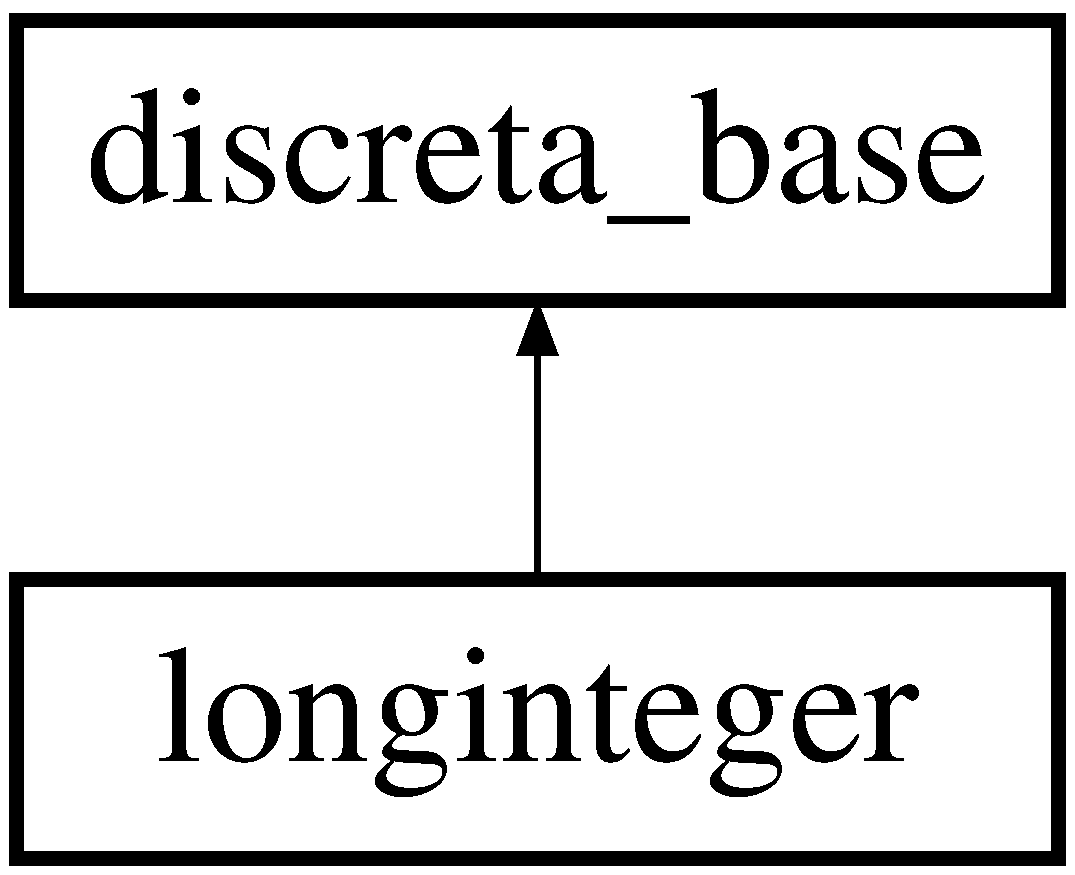
\includegraphics[height=2.000000cm]{classlonginteger}
\end{center}
\end{figure}
\subsection*{Public Member Functions}
\begin{DoxyCompactItemize}
\item 
\mbox{\hyperlink{classlonginteger_a24b89f33d73b2cfb7776d236fea6c61f}{longinteger}} ()
\item 
\mbox{\hyperlink{classlonginteger_ad7548243519fe9770b13f00d9ce62643}{longinteger}} (\mbox{\hyperlink{galois_8h_a09fddde158a3a20bd2dcadb609de11dc}{I\+NT}} a)
\item 
\mbox{\hyperlink{classlonginteger_a46c003f48c7bb112056651dae89c8e72}{longinteger}} (const char $\ast$s)
\item 
\mbox{\hyperlink{classlonginteger_a30553f5083f01e86aae9e00630852617}{longinteger}} (const \mbox{\hyperlink{classdiscreta__base}{discreta\+\_\+base}} \&\mbox{\hyperlink{alphabet2_8_c_a6150e0515f7202e2fb518f7206ed97dc}{x}})
\item 
\mbox{\hyperlink{classlonginteger}{longinteger}} \& \mbox{\hyperlink{classlonginteger_a73681df1cab8ee88c85617574939fd0c}{operator=}} (const \mbox{\hyperlink{classdiscreta__base}{discreta\+\_\+base}} \&\mbox{\hyperlink{alphabet2_8_c_a6150e0515f7202e2fb518f7206ed97dc}{x}})
\item 
void $\ast$ \mbox{\hyperlink{classlonginteger_abbeec081da2c8cb237da0e0980e4919a}{operator new}} (size\+\_\+t, void $\ast$\mbox{\hyperlink{alphabet2_8_c_a533391314665d6bf1b5575e9a9cd8552}{p}})
\item 
void \mbox{\hyperlink{classlonginteger_ae5f811ece8df31b9ff114368a18e1dc5}{settype\+\_\+longinteger}} ()
\item 
\mbox{\hyperlink{classlonginteger_a6749d325fbff19a485dfa479f65afdb1}{$\sim$longinteger}} ()
\item 
void \mbox{\hyperlink{classlonginteger_a82006f4b7c6bf897de0387497e16c219}{freeself\+\_\+longinteger}} ()
\item 
\mbox{\hyperlink{discreta_8h_aaf25ee7e2306d78c74ec7bc48f092e81}{kind}} \mbox{\hyperlink{classlonginteger_ab5c97c64a923bc2bd270c998d1d2f283}{s\+\_\+virtual\+\_\+kind}} ()
\item 
void \mbox{\hyperlink{classlonginteger_ae894d5c96d74d0c19a09527956a14493}{copyobject\+\_\+to}} (\mbox{\hyperlink{classdiscreta__base}{discreta\+\_\+base}} \&\mbox{\hyperlink{alphabet2_8_c_a6150e0515f7202e2fb518f7206ed97dc}{x}})
\item 
ostream \& \mbox{\hyperlink{classlonginteger_a21d99160318418ba5bc8318254d2caf8}{print}} (ostream \&)
\item 
\mbox{\hyperlink{discreta_8h_acfd8c2baf438bb4e79d8e8d4b0ca2b8e}{L\+O\+N\+G\+I\+N\+T\+E\+G\+E\+R\+\_\+\+R\+E\+P\+R\+E\+S\+E\+N\+T\+A\+T\+I\+ON}} $\ast$ \mbox{\hyperlink{classlonginteger_ad1ec809a79c42ffe63d6c9e6dd46bff5}{s\+\_\+rep}} ()
\item 
\mbox{\hyperlink{galois_8h_a09fddde158a3a20bd2dcadb609de11dc}{I\+NT}} \& \mbox{\hyperlink{classlonginteger_a33f5b6c545e97635cb71670f76ed1fb3}{s\+\_\+sign}} ()
\item 
\mbox{\hyperlink{galois_8h_a09fddde158a3a20bd2dcadb609de11dc}{I\+NT}} \& \mbox{\hyperlink{classlonginteger_a5d414ae211f4e16abd932257351c74df}{s\+\_\+len}} ()
\item 
char \& \mbox{\hyperlink{classlonginteger_aa946d4c3bfd34bbfd0b811d5f5795f82}{s\+\_\+p}} (\mbox{\hyperlink{galois_8h_a09fddde158a3a20bd2dcadb609de11dc}{I\+NT}} \mbox{\hyperlink{alphabet2_8_c_acb559820d9ca11295b4500f179ef6392}{i}})
\item 
void \mbox{\hyperlink{classlonginteger_a6d5f2429a98a2fea96aa605d1a6b1e6e}{allocate}} (\mbox{\hyperlink{galois_8h_a09fddde158a3a20bd2dcadb609de11dc}{I\+NT}} sign, const char $\ast$\mbox{\hyperlink{alphabet2_8_c_a533391314665d6bf1b5575e9a9cd8552}{p}})
\item 
void \mbox{\hyperlink{classlonginteger_af2df35d345485e9cd3c3088a80ec232d}{allocate\+\_\+internal}} (\mbox{\hyperlink{galois_8h_a09fddde158a3a20bd2dcadb609de11dc}{I\+NT}} sign, \mbox{\hyperlink{galois_8h_a09fddde158a3a20bd2dcadb609de11dc}{I\+NT}} len, const char $\ast$\mbox{\hyperlink{alphabet2_8_c_a533391314665d6bf1b5575e9a9cd8552}{p}})
\item 
void \mbox{\hyperlink{classlonginteger_a40b25b8aed02337972489655293eda99}{allocate\+\_\+empty}} (\mbox{\hyperlink{galois_8h_a09fddde158a3a20bd2dcadb609de11dc}{I\+NT}} len)
\item 
void \mbox{\hyperlink{classlonginteger_a5e03d4e260c963943ba123114314c88b}{normalize\+\_\+representation}} ()
\item 
\mbox{\hyperlink{galois_8h_a09fddde158a3a20bd2dcadb609de11dc}{I\+NT}} \mbox{\hyperlink{classlonginteger_aaa504bac9b133d50b5ac50768f97db9d}{compare\+\_\+with}} (\mbox{\hyperlink{classdiscreta__base}{discreta\+\_\+base}} \&\mbox{\hyperlink{alphabet2_8_c_a148e3876077787926724625411d6e7a9}{b}})
\item 
\mbox{\hyperlink{galois_8h_a09fddde158a3a20bd2dcadb609de11dc}{I\+NT}} \mbox{\hyperlink{classlonginteger_ab08011cadec55cf084dbffcb74bb4991}{compare\+\_\+with\+\_\+unsigned}} (\mbox{\hyperlink{classlonginteger}{longinteger}} \&\mbox{\hyperlink{alphabet2_8_c_a148e3876077787926724625411d6e7a9}{b}})
\item 
void \mbox{\hyperlink{classlonginteger_a1afdab43a82be7dfd40ff41da28735d2}{mult\+\_\+to}} (\mbox{\hyperlink{classdiscreta__base}{discreta\+\_\+base}} \&\mbox{\hyperlink{alphabet2_8_c_a6150e0515f7202e2fb518f7206ed97dc}{x}}, \mbox{\hyperlink{classdiscreta__base}{discreta\+\_\+base}} \&\mbox{\hyperlink{alphabet2_8_c_a0a2f84ed7838f07779ae24c5a9086d33}{y}})
\item 
\mbox{\hyperlink{galois_8h_a09fddde158a3a20bd2dcadb609de11dc}{I\+NT}} \mbox{\hyperlink{classlonginteger_ab60c9e3b2f28caf83f3b13d6f3a9ec54}{invert\+\_\+to}} (\mbox{\hyperlink{classdiscreta__base}{discreta\+\_\+base}} \&\mbox{\hyperlink{alphabet2_8_c_a6150e0515f7202e2fb518f7206ed97dc}{x}})
\item 
void \mbox{\hyperlink{classlonginteger_a457c74224b83d9fbfc904a391baab7ed}{add\+\_\+to}} (\mbox{\hyperlink{classdiscreta__base}{discreta\+\_\+base}} \&\mbox{\hyperlink{alphabet2_8_c_a6150e0515f7202e2fb518f7206ed97dc}{x}}, \mbox{\hyperlink{classdiscreta__base}{discreta\+\_\+base}} \&\mbox{\hyperlink{alphabet2_8_c_a0a2f84ed7838f07779ae24c5a9086d33}{y}})
\item 
void \mbox{\hyperlink{classlonginteger_a1de6a5663bb80562dee0e6ca1a808ff1}{negate\+\_\+to}} (\mbox{\hyperlink{classdiscreta__base}{discreta\+\_\+base}} \&\mbox{\hyperlink{alphabet2_8_c_a6150e0515f7202e2fb518f7206ed97dc}{x}})
\item 
void \mbox{\hyperlink{classlonginteger_a082d0c05f45c21f188e17a8463a42800}{zero}} ()
\item 
void \mbox{\hyperlink{classlonginteger_ae1b9507b0d658768ceb278659e2adf1a}{one}} ()
\item 
void \mbox{\hyperlink{classlonginteger_a4a8280b414e6dc2ed917f0f70d778e05}{m\+\_\+one}} ()
\item 
void \mbox{\hyperlink{classlonginteger_a986e829bf35eca2b9f24b1b3766d5677}{homo\+\_\+z}} (\mbox{\hyperlink{galois_8h_a09fddde158a3a20bd2dcadb609de11dc}{I\+NT}} z)
\item 
void \mbox{\hyperlink{classlonginteger_aac69c9779c9fed275a1cbae4314438e5}{inc}} ()
\item 
void \mbox{\hyperlink{classlonginteger_a99be1d0bdcae0dcce47d8d0a09612edf}{dec}} ()
\item 
\mbox{\hyperlink{galois_8h_a09fddde158a3a20bd2dcadb609de11dc}{I\+NT}} \mbox{\hyperlink{classlonginteger_aa40fbd6c28e40a7a19cb29b8999afbc0}{is\+\_\+zero}} ()
\item 
\mbox{\hyperlink{galois_8h_a09fddde158a3a20bd2dcadb609de11dc}{I\+NT}} \mbox{\hyperlink{classlonginteger_a2e169e4ac876ac8694af28468fdfd060}{is\+\_\+one}} ()
\item 
\mbox{\hyperlink{galois_8h_a09fddde158a3a20bd2dcadb609de11dc}{I\+NT}} \mbox{\hyperlink{classlonginteger_aa47d6521fc1dc8058d9eaa516caefabe}{is\+\_\+m\+\_\+one}} ()
\item 
\mbox{\hyperlink{galois_8h_a09fddde158a3a20bd2dcadb609de11dc}{I\+NT}} \mbox{\hyperlink{classlonginteger_a12ad4725b43f023ed9861d3f48ba69fe}{is\+\_\+even}} ()
\item 
\mbox{\hyperlink{galois_8h_a09fddde158a3a20bd2dcadb609de11dc}{I\+NT}} \mbox{\hyperlink{classlonginteger_a5110768d8c2cfc82037d6d3ae4ead236}{is\+\_\+odd}} ()
\item 
\mbox{\hyperlink{galois_8h_a09fddde158a3a20bd2dcadb609de11dc}{I\+NT}} \mbox{\hyperlink{classlonginteger_a71b27b9c767c0da8964151323810f315}{compare\+\_\+with\+\_\+euklidean}} (\mbox{\hyperlink{classdiscreta__base}{discreta\+\_\+base}} \&\mbox{\hyperlink{alphabet2_8_c_a148e3876077787926724625411d6e7a9}{b}})
\item 
void \mbox{\hyperlink{classlonginteger_a692f761cfc91770ca40ab5c2df4bd358}{integral\+\_\+division}} (\mbox{\hyperlink{classdiscreta__base}{discreta\+\_\+base}} \&\mbox{\hyperlink{alphabet2_8_c_a6150e0515f7202e2fb518f7206ed97dc}{x}}, \mbox{\hyperlink{classdiscreta__base}{discreta\+\_\+base}} \&\mbox{\hyperlink{simeon_8_c_a92cbb483a3b27ae1a0dbfcb125ce216f}{q}}, \mbox{\hyperlink{classdiscreta__base}{discreta\+\_\+base}} \&\mbox{\hyperlink{alphabet2_8_c_acab531abaa74a7e664e3986f2522b33a}{r}}, \mbox{\hyperlink{galois_8h_a09fddde158a3a20bd2dcadb609de11dc}{I\+NT}} \mbox{\hyperlink{simeon_8_c_a818073fbcc2f439e7c56952f67386122}{verbose\+\_\+level}})
\item 
void \mbox{\hyperlink{classlonginteger_a1b5b30f8bc750d1304390f518e43aa0f}{square\+\_\+root\+\_\+floor}} (\mbox{\hyperlink{classdiscreta__base}{discreta\+\_\+base}} \&\mbox{\hyperlink{alphabet2_8_c_a6150e0515f7202e2fb518f7206ed97dc}{x}})
\item 
\mbox{\hyperlink{classlonginteger}{longinteger}} \& \mbox{\hyperlink{classlonginteger_a549866ae981b0229715752adc96be386}{Mersenne}} (\mbox{\hyperlink{galois_8h_a09fddde158a3a20bd2dcadb609de11dc}{I\+NT}} \mbox{\hyperlink{simeon_8_c_a7f2cd26777ce0ff3fdaf8d02aacbddfb}{n}})
\item 
\mbox{\hyperlink{classlonginteger}{longinteger}} \& \mbox{\hyperlink{classlonginteger_ae120eb593e762937a8f45ca3643ed49c}{Fermat}} (\mbox{\hyperlink{galois_8h_a09fddde158a3a20bd2dcadb609de11dc}{I\+NT}} \mbox{\hyperlink{simeon_8_c_a7f2cd26777ce0ff3fdaf8d02aacbddfb}{n}})
\item 
\mbox{\hyperlink{galois_8h_a09fddde158a3a20bd2dcadb609de11dc}{I\+NT}} \mbox{\hyperlink{classlonginteger_aa0be3351b577305c0160b8bc8b4febde}{s\+\_\+i}} ()
\item 
\mbox{\hyperlink{galois_8h_a09fddde158a3a20bd2dcadb609de11dc}{I\+NT}} \mbox{\hyperlink{classlonginteger_a650d1f82c87e1f6a59a54a50e340394e}{retract\+\_\+to\+\_\+integer\+\_\+if\+\_\+possible}} (\mbox{\hyperlink{classinteger}{integer}} \&\mbox{\hyperlink{alphabet2_8_c_a6150e0515f7202e2fb518f7206ed97dc}{x}})
\item 
\mbox{\hyperlink{galois_8h_a09fddde158a3a20bd2dcadb609de11dc}{I\+NT}} \mbox{\hyperlink{classlonginteger_a4c554e7aa704ace8b97448c6d27fd4bd}{modp}} (\mbox{\hyperlink{galois_8h_a09fddde158a3a20bd2dcadb609de11dc}{I\+NT}} \mbox{\hyperlink{alphabet2_8_c_a533391314665d6bf1b5575e9a9cd8552}{p}})
\item 
\mbox{\hyperlink{galois_8h_a09fddde158a3a20bd2dcadb609de11dc}{I\+NT}} \mbox{\hyperlink{classlonginteger_a2e791f6e15c1ef6f7cd2dd3bf0a6d4c1}{ny\+\_\+p}} (\mbox{\hyperlink{galois_8h_a09fddde158a3a20bd2dcadb609de11dc}{I\+NT}} \mbox{\hyperlink{alphabet2_8_c_a533391314665d6bf1b5575e9a9cd8552}{p}})
\item 
void \mbox{\hyperlink{classlonginteger_ac4b65023c8de701153491d80577dfb9b}{divide\+\_\+out\+\_\+int}} (\mbox{\hyperlink{galois_8h_a09fddde158a3a20bd2dcadb609de11dc}{I\+NT}} \mbox{\hyperlink{simeon_8_c_a4339ca06fa882e69473d37bd6d7917d1}{d}})
\item 
\mbox{\hyperlink{galois_8h_a09fddde158a3a20bd2dcadb609de11dc}{I\+NT}} \mbox{\hyperlink{classlonginteger_ac65a8ac0562694fa12ad6b43d2eee7db}{Lucas\+\_\+test\+\_\+\+Mersenne}} (\mbox{\hyperlink{galois_8h_a09fddde158a3a20bd2dcadb609de11dc}{I\+NT}} m, \mbox{\hyperlink{galois_8h_a09fddde158a3a20bd2dcadb609de11dc}{I\+NT}} f\+\_\+v)
\end{DoxyCompactItemize}
\subsection*{Additional Inherited Members}


\subsection{Constructor \& Destructor Documentation}
\mbox{\Hypertarget{classlonginteger_a24b89f33d73b2cfb7776d236fea6c61f}\label{classlonginteger_a24b89f33d73b2cfb7776d236fea6c61f}} 
\index{longinteger@{longinteger}!longinteger@{longinteger}}
\index{longinteger@{longinteger}!longinteger@{longinteger}}
\subsubsection{\texorpdfstring{longinteger()}{longinteger()}\hspace{0.1cm}{\footnotesize\ttfamily [1/4]}}
{\footnotesize\ttfamily longinteger\+::longinteger (\begin{DoxyParamCaption}{ }\end{DoxyParamCaption})}

\mbox{\Hypertarget{classlonginteger_ad7548243519fe9770b13f00d9ce62643}\label{classlonginteger_ad7548243519fe9770b13f00d9ce62643}} 
\index{longinteger@{longinteger}!longinteger@{longinteger}}
\index{longinteger@{longinteger}!longinteger@{longinteger}}
\subsubsection{\texorpdfstring{longinteger()}{longinteger()}\hspace{0.1cm}{\footnotesize\ttfamily [2/4]}}
{\footnotesize\ttfamily longinteger\+::longinteger (\begin{DoxyParamCaption}\item[{\mbox{\hyperlink{galois_8h_a09fddde158a3a20bd2dcadb609de11dc}{I\+NT}}}]{a }\end{DoxyParamCaption})}

\mbox{\Hypertarget{classlonginteger_a46c003f48c7bb112056651dae89c8e72}\label{classlonginteger_a46c003f48c7bb112056651dae89c8e72}} 
\index{longinteger@{longinteger}!longinteger@{longinteger}}
\index{longinteger@{longinteger}!longinteger@{longinteger}}
\subsubsection{\texorpdfstring{longinteger()}{longinteger()}\hspace{0.1cm}{\footnotesize\ttfamily [3/4]}}
{\footnotesize\ttfamily longinteger\+::longinteger (\begin{DoxyParamCaption}\item[{const char $\ast$}]{s }\end{DoxyParamCaption})}

\mbox{\Hypertarget{classlonginteger_a30553f5083f01e86aae9e00630852617}\label{classlonginteger_a30553f5083f01e86aae9e00630852617}} 
\index{longinteger@{longinteger}!longinteger@{longinteger}}
\index{longinteger@{longinteger}!longinteger@{longinteger}}
\subsubsection{\texorpdfstring{longinteger()}{longinteger()}\hspace{0.1cm}{\footnotesize\ttfamily [4/4]}}
{\footnotesize\ttfamily longinteger\+::longinteger (\begin{DoxyParamCaption}\item[{const \mbox{\hyperlink{classdiscreta__base}{discreta\+\_\+base}} \&}]{x }\end{DoxyParamCaption})}

\mbox{\Hypertarget{classlonginteger_a6749d325fbff19a485dfa479f65afdb1}\label{classlonginteger_a6749d325fbff19a485dfa479f65afdb1}} 
\index{longinteger@{longinteger}!````~longinteger@{$\sim$longinteger}}
\index{````~longinteger@{$\sim$longinteger}!longinteger@{longinteger}}
\subsubsection{\texorpdfstring{$\sim$longinteger()}{~longinteger()}}
{\footnotesize\ttfamily longinteger\+::$\sim$longinteger (\begin{DoxyParamCaption}{ }\end{DoxyParamCaption})}



\subsection{Member Function Documentation}
\mbox{\Hypertarget{classlonginteger_a457c74224b83d9fbfc904a391baab7ed}\label{classlonginteger_a457c74224b83d9fbfc904a391baab7ed}} 
\index{longinteger@{longinteger}!add\+\_\+to@{add\+\_\+to}}
\index{add\+\_\+to@{add\+\_\+to}!longinteger@{longinteger}}
\subsubsection{\texorpdfstring{add\+\_\+to()}{add\_to()}}
{\footnotesize\ttfamily void longinteger\+::add\+\_\+to (\begin{DoxyParamCaption}\item[{\mbox{\hyperlink{classdiscreta__base}{discreta\+\_\+base}} \&}]{x,  }\item[{\mbox{\hyperlink{classdiscreta__base}{discreta\+\_\+base}} \&}]{y }\end{DoxyParamCaption})\hspace{0.3cm}{\ttfamily [virtual]}}



Reimplemented from \mbox{\hyperlink{classdiscreta__base_a712a61311eb036d70a52871ed315f515}{discreta\+\_\+base}}.

\mbox{\Hypertarget{classlonginteger_a6d5f2429a98a2fea96aa605d1a6b1e6e}\label{classlonginteger_a6d5f2429a98a2fea96aa605d1a6b1e6e}} 
\index{longinteger@{longinteger}!allocate@{allocate}}
\index{allocate@{allocate}!longinteger@{longinteger}}
\subsubsection{\texorpdfstring{allocate()}{allocate()}}
{\footnotesize\ttfamily void longinteger\+::allocate (\begin{DoxyParamCaption}\item[{\mbox{\hyperlink{galois_8h_a09fddde158a3a20bd2dcadb609de11dc}{I\+NT}}}]{sign,  }\item[{const char $\ast$}]{p }\end{DoxyParamCaption})}

\mbox{\Hypertarget{classlonginteger_a40b25b8aed02337972489655293eda99}\label{classlonginteger_a40b25b8aed02337972489655293eda99}} 
\index{longinteger@{longinteger}!allocate\+\_\+empty@{allocate\+\_\+empty}}
\index{allocate\+\_\+empty@{allocate\+\_\+empty}!longinteger@{longinteger}}
\subsubsection{\texorpdfstring{allocate\+\_\+empty()}{allocate\_empty()}}
{\footnotesize\ttfamily void longinteger\+::allocate\+\_\+empty (\begin{DoxyParamCaption}\item[{\mbox{\hyperlink{galois_8h_a09fddde158a3a20bd2dcadb609de11dc}{I\+NT}}}]{len }\end{DoxyParamCaption})}

\mbox{\Hypertarget{classlonginteger_af2df35d345485e9cd3c3088a80ec232d}\label{classlonginteger_af2df35d345485e9cd3c3088a80ec232d}} 
\index{longinteger@{longinteger}!allocate\+\_\+internal@{allocate\+\_\+internal}}
\index{allocate\+\_\+internal@{allocate\+\_\+internal}!longinteger@{longinteger}}
\subsubsection{\texorpdfstring{allocate\+\_\+internal()}{allocate\_internal()}}
{\footnotesize\ttfamily void longinteger\+::allocate\+\_\+internal (\begin{DoxyParamCaption}\item[{\mbox{\hyperlink{galois_8h_a09fddde158a3a20bd2dcadb609de11dc}{I\+NT}}}]{sign,  }\item[{\mbox{\hyperlink{galois_8h_a09fddde158a3a20bd2dcadb609de11dc}{I\+NT}}}]{len,  }\item[{const char $\ast$}]{p }\end{DoxyParamCaption})}

\mbox{\Hypertarget{classlonginteger_aaa504bac9b133d50b5ac50768f97db9d}\label{classlonginteger_aaa504bac9b133d50b5ac50768f97db9d}} 
\index{longinteger@{longinteger}!compare\+\_\+with@{compare\+\_\+with}}
\index{compare\+\_\+with@{compare\+\_\+with}!longinteger@{longinteger}}
\subsubsection{\texorpdfstring{compare\+\_\+with()}{compare\_with()}}
{\footnotesize\ttfamily \mbox{\hyperlink{galois_8h_a09fddde158a3a20bd2dcadb609de11dc}{I\+NT}} longinteger\+::compare\+\_\+with (\begin{DoxyParamCaption}\item[{\mbox{\hyperlink{classdiscreta__base}{discreta\+\_\+base}} \&}]{b }\end{DoxyParamCaption})\hspace{0.3cm}{\ttfamily [virtual]}}



Reimplemented from \mbox{\hyperlink{classdiscreta__base_a3818444c4301d0b7ed47c3b850ea6c60}{discreta\+\_\+base}}.

\mbox{\Hypertarget{classlonginteger_a71b27b9c767c0da8964151323810f315}\label{classlonginteger_a71b27b9c767c0da8964151323810f315}} 
\index{longinteger@{longinteger}!compare\+\_\+with\+\_\+euklidean@{compare\+\_\+with\+\_\+euklidean}}
\index{compare\+\_\+with\+\_\+euklidean@{compare\+\_\+with\+\_\+euklidean}!longinteger@{longinteger}}
\subsubsection{\texorpdfstring{compare\+\_\+with\+\_\+euklidean()}{compare\_with\_euklidean()}}
{\footnotesize\ttfamily \mbox{\hyperlink{galois_8h_a09fddde158a3a20bd2dcadb609de11dc}{I\+NT}} longinteger\+::compare\+\_\+with\+\_\+euklidean (\begin{DoxyParamCaption}\item[{\mbox{\hyperlink{classdiscreta__base}{discreta\+\_\+base}} \&}]{b }\end{DoxyParamCaption})\hspace{0.3cm}{\ttfamily [virtual]}}



Reimplemented from \mbox{\hyperlink{classdiscreta__base_a9d3091feb2fbc69359c2a45f11ceec9e}{discreta\+\_\+base}}.

\mbox{\Hypertarget{classlonginteger_ab08011cadec55cf084dbffcb74bb4991}\label{classlonginteger_ab08011cadec55cf084dbffcb74bb4991}} 
\index{longinteger@{longinteger}!compare\+\_\+with\+\_\+unsigned@{compare\+\_\+with\+\_\+unsigned}}
\index{compare\+\_\+with\+\_\+unsigned@{compare\+\_\+with\+\_\+unsigned}!longinteger@{longinteger}}
\subsubsection{\texorpdfstring{compare\+\_\+with\+\_\+unsigned()}{compare\_with\_unsigned()}}
{\footnotesize\ttfamily \mbox{\hyperlink{galois_8h_a09fddde158a3a20bd2dcadb609de11dc}{I\+NT}} longinteger\+::compare\+\_\+with\+\_\+unsigned (\begin{DoxyParamCaption}\item[{\mbox{\hyperlink{classlonginteger}{longinteger}} \&}]{b }\end{DoxyParamCaption})}

\mbox{\Hypertarget{classlonginteger_ae894d5c96d74d0c19a09527956a14493}\label{classlonginteger_ae894d5c96d74d0c19a09527956a14493}} 
\index{longinteger@{longinteger}!copyobject\+\_\+to@{copyobject\+\_\+to}}
\index{copyobject\+\_\+to@{copyobject\+\_\+to}!longinteger@{longinteger}}
\subsubsection{\texorpdfstring{copyobject\+\_\+to()}{copyobject\_to()}}
{\footnotesize\ttfamily void longinteger\+::copyobject\+\_\+to (\begin{DoxyParamCaption}\item[{\mbox{\hyperlink{classdiscreta__base}{discreta\+\_\+base}} \&}]{x }\end{DoxyParamCaption})\hspace{0.3cm}{\ttfamily [virtual]}}



Reimplemented from \mbox{\hyperlink{classdiscreta__base_a33180628d9ced231267229b3564790f3}{discreta\+\_\+base}}.

\mbox{\Hypertarget{classlonginteger_a99be1d0bdcae0dcce47d8d0a09612edf}\label{classlonginteger_a99be1d0bdcae0dcce47d8d0a09612edf}} 
\index{longinteger@{longinteger}!dec@{dec}}
\index{dec@{dec}!longinteger@{longinteger}}
\subsubsection{\texorpdfstring{dec()}{dec()}}
{\footnotesize\ttfamily void longinteger\+::dec (\begin{DoxyParamCaption}{ }\end{DoxyParamCaption})\hspace{0.3cm}{\ttfamily [virtual]}}



Reimplemented from \mbox{\hyperlink{classdiscreta__base_a11449a5cfa7dc5f5600e012517af6f0f}{discreta\+\_\+base}}.

\mbox{\Hypertarget{classlonginteger_ac4b65023c8de701153491d80577dfb9b}\label{classlonginteger_ac4b65023c8de701153491d80577dfb9b}} 
\index{longinteger@{longinteger}!divide\+\_\+out\+\_\+int@{divide\+\_\+out\+\_\+int}}
\index{divide\+\_\+out\+\_\+int@{divide\+\_\+out\+\_\+int}!longinteger@{longinteger}}
\subsubsection{\texorpdfstring{divide\+\_\+out\+\_\+int()}{divide\_out\_int()}}
{\footnotesize\ttfamily void longinteger\+::divide\+\_\+out\+\_\+int (\begin{DoxyParamCaption}\item[{\mbox{\hyperlink{galois_8h_a09fddde158a3a20bd2dcadb609de11dc}{I\+NT}}}]{d }\end{DoxyParamCaption})}

\mbox{\Hypertarget{classlonginteger_ae120eb593e762937a8f45ca3643ed49c}\label{classlonginteger_ae120eb593e762937a8f45ca3643ed49c}} 
\index{longinteger@{longinteger}!Fermat@{Fermat}}
\index{Fermat@{Fermat}!longinteger@{longinteger}}
\subsubsection{\texorpdfstring{Fermat()}{Fermat()}}
{\footnotesize\ttfamily \mbox{\hyperlink{classlonginteger}{longinteger}} \& longinteger\+::\+Fermat (\begin{DoxyParamCaption}\item[{\mbox{\hyperlink{galois_8h_a09fddde158a3a20bd2dcadb609de11dc}{I\+NT}}}]{n }\end{DoxyParamCaption})}

\mbox{\Hypertarget{classlonginteger_a82006f4b7c6bf897de0387497e16c219}\label{classlonginteger_a82006f4b7c6bf897de0387497e16c219}} 
\index{longinteger@{longinteger}!freeself\+\_\+longinteger@{freeself\+\_\+longinteger}}
\index{freeself\+\_\+longinteger@{freeself\+\_\+longinteger}!longinteger@{longinteger}}
\subsubsection{\texorpdfstring{freeself\+\_\+longinteger()}{freeself\_longinteger()}}
{\footnotesize\ttfamily void longinteger\+::freeself\+\_\+longinteger (\begin{DoxyParamCaption}{ }\end{DoxyParamCaption})}

\mbox{\Hypertarget{classlonginteger_a986e829bf35eca2b9f24b1b3766d5677}\label{classlonginteger_a986e829bf35eca2b9f24b1b3766d5677}} 
\index{longinteger@{longinteger}!homo\+\_\+z@{homo\+\_\+z}}
\index{homo\+\_\+z@{homo\+\_\+z}!longinteger@{longinteger}}
\subsubsection{\texorpdfstring{homo\+\_\+z()}{homo\_z()}}
{\footnotesize\ttfamily void longinteger\+::homo\+\_\+z (\begin{DoxyParamCaption}\item[{\mbox{\hyperlink{galois_8h_a09fddde158a3a20bd2dcadb609de11dc}{I\+NT}}}]{z }\end{DoxyParamCaption})\hspace{0.3cm}{\ttfamily [virtual]}}



Reimplemented from \mbox{\hyperlink{classdiscreta__base_a40e349b2d85c5c6dba9c015d16a0e801}{discreta\+\_\+base}}.

\mbox{\Hypertarget{classlonginteger_aac69c9779c9fed275a1cbae4314438e5}\label{classlonginteger_aac69c9779c9fed275a1cbae4314438e5}} 
\index{longinteger@{longinteger}!inc@{inc}}
\index{inc@{inc}!longinteger@{longinteger}}
\subsubsection{\texorpdfstring{inc()}{inc()}}
{\footnotesize\ttfamily void longinteger\+::inc (\begin{DoxyParamCaption}{ }\end{DoxyParamCaption})\hspace{0.3cm}{\ttfamily [virtual]}}



Reimplemented from \mbox{\hyperlink{classdiscreta__base_afda42789f4ba04ba399623a6b9e206e3}{discreta\+\_\+base}}.

\mbox{\Hypertarget{classlonginteger_a692f761cfc91770ca40ab5c2df4bd358}\label{classlonginteger_a692f761cfc91770ca40ab5c2df4bd358}} 
\index{longinteger@{longinteger}!integral\+\_\+division@{integral\+\_\+division}}
\index{integral\+\_\+division@{integral\+\_\+division}!longinteger@{longinteger}}
\subsubsection{\texorpdfstring{integral\+\_\+division()}{integral\_division()}}
{\footnotesize\ttfamily void longinteger\+::integral\+\_\+division (\begin{DoxyParamCaption}\item[{\mbox{\hyperlink{classdiscreta__base}{discreta\+\_\+base}} \&}]{x,  }\item[{\mbox{\hyperlink{classdiscreta__base}{discreta\+\_\+base}} \&}]{q,  }\item[{\mbox{\hyperlink{classdiscreta__base}{discreta\+\_\+base}} \&}]{r,  }\item[{\mbox{\hyperlink{galois_8h_a09fddde158a3a20bd2dcadb609de11dc}{I\+NT}}}]{verbose\+\_\+level }\end{DoxyParamCaption})\hspace{0.3cm}{\ttfamily [virtual]}}



Reimplemented from \mbox{\hyperlink{classdiscreta__base_a92b3001ac35af9185b316c0d8f89070e}{discreta\+\_\+base}}.

\mbox{\Hypertarget{classlonginteger_ab60c9e3b2f28caf83f3b13d6f3a9ec54}\label{classlonginteger_ab60c9e3b2f28caf83f3b13d6f3a9ec54}} 
\index{longinteger@{longinteger}!invert\+\_\+to@{invert\+\_\+to}}
\index{invert\+\_\+to@{invert\+\_\+to}!longinteger@{longinteger}}
\subsubsection{\texorpdfstring{invert\+\_\+to()}{invert\_to()}}
{\footnotesize\ttfamily \mbox{\hyperlink{galois_8h_a09fddde158a3a20bd2dcadb609de11dc}{I\+NT}} longinteger\+::invert\+\_\+to (\begin{DoxyParamCaption}\item[{\mbox{\hyperlink{classdiscreta__base}{discreta\+\_\+base}} \&}]{x }\end{DoxyParamCaption})\hspace{0.3cm}{\ttfamily [virtual]}}



Reimplemented from \mbox{\hyperlink{classdiscreta__base_a874a5ffb467f3896604a3c9bdf0cca50}{discreta\+\_\+base}}.

\mbox{\Hypertarget{classlonginteger_a12ad4725b43f023ed9861d3f48ba69fe}\label{classlonginteger_a12ad4725b43f023ed9861d3f48ba69fe}} 
\index{longinteger@{longinteger}!is\+\_\+even@{is\+\_\+even}}
\index{is\+\_\+even@{is\+\_\+even}!longinteger@{longinteger}}
\subsubsection{\texorpdfstring{is\+\_\+even()}{is\_even()}}
{\footnotesize\ttfamily \mbox{\hyperlink{galois_8h_a09fddde158a3a20bd2dcadb609de11dc}{I\+NT}} longinteger\+::is\+\_\+even (\begin{DoxyParamCaption}{ }\end{DoxyParamCaption})}

\mbox{\Hypertarget{classlonginteger_aa47d6521fc1dc8058d9eaa516caefabe}\label{classlonginteger_aa47d6521fc1dc8058d9eaa516caefabe}} 
\index{longinteger@{longinteger}!is\+\_\+m\+\_\+one@{is\+\_\+m\+\_\+one}}
\index{is\+\_\+m\+\_\+one@{is\+\_\+m\+\_\+one}!longinteger@{longinteger}}
\subsubsection{\texorpdfstring{is\+\_\+m\+\_\+one()}{is\_m\_one()}}
{\footnotesize\ttfamily \mbox{\hyperlink{galois_8h_a09fddde158a3a20bd2dcadb609de11dc}{I\+NT}} longinteger\+::is\+\_\+m\+\_\+one (\begin{DoxyParamCaption}{ }\end{DoxyParamCaption})\hspace{0.3cm}{\ttfamily [virtual]}}



Reimplemented from \mbox{\hyperlink{classdiscreta__base_afc2e134e55759cf069f49fcf05af418b}{discreta\+\_\+base}}.

\mbox{\Hypertarget{classlonginteger_a5110768d8c2cfc82037d6d3ae4ead236}\label{classlonginteger_a5110768d8c2cfc82037d6d3ae4ead236}} 
\index{longinteger@{longinteger}!is\+\_\+odd@{is\+\_\+odd}}
\index{is\+\_\+odd@{is\+\_\+odd}!longinteger@{longinteger}}
\subsubsection{\texorpdfstring{is\+\_\+odd()}{is\_odd()}}
{\footnotesize\ttfamily \mbox{\hyperlink{galois_8h_a09fddde158a3a20bd2dcadb609de11dc}{I\+NT}} longinteger\+::is\+\_\+odd (\begin{DoxyParamCaption}{ }\end{DoxyParamCaption})}

\mbox{\Hypertarget{classlonginteger_a2e169e4ac876ac8694af28468fdfd060}\label{classlonginteger_a2e169e4ac876ac8694af28468fdfd060}} 
\index{longinteger@{longinteger}!is\+\_\+one@{is\+\_\+one}}
\index{is\+\_\+one@{is\+\_\+one}!longinteger@{longinteger}}
\subsubsection{\texorpdfstring{is\+\_\+one()}{is\_one()}}
{\footnotesize\ttfamily \mbox{\hyperlink{galois_8h_a09fddde158a3a20bd2dcadb609de11dc}{I\+NT}} longinteger\+::is\+\_\+one (\begin{DoxyParamCaption}{ }\end{DoxyParamCaption})\hspace{0.3cm}{\ttfamily [virtual]}}



Reimplemented from \mbox{\hyperlink{classdiscreta__base_a28fa37aac83194174888d34f07f43848}{discreta\+\_\+base}}.

\mbox{\Hypertarget{classlonginteger_aa40fbd6c28e40a7a19cb29b8999afbc0}\label{classlonginteger_aa40fbd6c28e40a7a19cb29b8999afbc0}} 
\index{longinteger@{longinteger}!is\+\_\+zero@{is\+\_\+zero}}
\index{is\+\_\+zero@{is\+\_\+zero}!longinteger@{longinteger}}
\subsubsection{\texorpdfstring{is\+\_\+zero()}{is\_zero()}}
{\footnotesize\ttfamily \mbox{\hyperlink{galois_8h_a09fddde158a3a20bd2dcadb609de11dc}{I\+NT}} longinteger\+::is\+\_\+zero (\begin{DoxyParamCaption}{ }\end{DoxyParamCaption})\hspace{0.3cm}{\ttfamily [virtual]}}



Reimplemented from \mbox{\hyperlink{classdiscreta__base_ac75f6bdc1ba1b406e26cf921adfd9864}{discreta\+\_\+base}}.

\mbox{\Hypertarget{classlonginteger_ac65a8ac0562694fa12ad6b43d2eee7db}\label{classlonginteger_ac65a8ac0562694fa12ad6b43d2eee7db}} 
\index{longinteger@{longinteger}!Lucas\+\_\+test\+\_\+\+Mersenne@{Lucas\+\_\+test\+\_\+\+Mersenne}}
\index{Lucas\+\_\+test\+\_\+\+Mersenne@{Lucas\+\_\+test\+\_\+\+Mersenne}!longinteger@{longinteger}}
\subsubsection{\texorpdfstring{Lucas\+\_\+test\+\_\+\+Mersenne()}{Lucas\_test\_Mersenne()}}
{\footnotesize\ttfamily \mbox{\hyperlink{galois_8h_a09fddde158a3a20bd2dcadb609de11dc}{I\+NT}} longinteger\+::\+Lucas\+\_\+test\+\_\+\+Mersenne (\begin{DoxyParamCaption}\item[{\mbox{\hyperlink{galois_8h_a09fddde158a3a20bd2dcadb609de11dc}{I\+NT}}}]{m,  }\item[{\mbox{\hyperlink{galois_8h_a09fddde158a3a20bd2dcadb609de11dc}{I\+NT}}}]{f\+\_\+v }\end{DoxyParamCaption})}

\mbox{\Hypertarget{classlonginteger_a4a8280b414e6dc2ed917f0f70d778e05}\label{classlonginteger_a4a8280b414e6dc2ed917f0f70d778e05}} 
\index{longinteger@{longinteger}!m\+\_\+one@{m\+\_\+one}}
\index{m\+\_\+one@{m\+\_\+one}!longinteger@{longinteger}}
\subsubsection{\texorpdfstring{m\+\_\+one()}{m\_one()}}
{\footnotesize\ttfamily void longinteger\+::m\+\_\+one (\begin{DoxyParamCaption}{ }\end{DoxyParamCaption})\hspace{0.3cm}{\ttfamily [virtual]}}



Reimplemented from \mbox{\hyperlink{classdiscreta__base_a3a147eee6f3477387f7e580c117e5a05}{discreta\+\_\+base}}.

\mbox{\Hypertarget{classlonginteger_a549866ae981b0229715752adc96be386}\label{classlonginteger_a549866ae981b0229715752adc96be386}} 
\index{longinteger@{longinteger}!Mersenne@{Mersenne}}
\index{Mersenne@{Mersenne}!longinteger@{longinteger}}
\subsubsection{\texorpdfstring{Mersenne()}{Mersenne()}}
{\footnotesize\ttfamily \mbox{\hyperlink{classlonginteger}{longinteger}} \& longinteger\+::\+Mersenne (\begin{DoxyParamCaption}\item[{\mbox{\hyperlink{galois_8h_a09fddde158a3a20bd2dcadb609de11dc}{I\+NT}}}]{n }\end{DoxyParamCaption})}

\mbox{\Hypertarget{classlonginteger_a4c554e7aa704ace8b97448c6d27fd4bd}\label{classlonginteger_a4c554e7aa704ace8b97448c6d27fd4bd}} 
\index{longinteger@{longinteger}!modp@{modp}}
\index{modp@{modp}!longinteger@{longinteger}}
\subsubsection{\texorpdfstring{modp()}{modp()}}
{\footnotesize\ttfamily \mbox{\hyperlink{galois_8h_a09fddde158a3a20bd2dcadb609de11dc}{I\+NT}} longinteger\+::modp (\begin{DoxyParamCaption}\item[{\mbox{\hyperlink{galois_8h_a09fddde158a3a20bd2dcadb609de11dc}{I\+NT}}}]{p }\end{DoxyParamCaption})}

\mbox{\Hypertarget{classlonginteger_a1afdab43a82be7dfd40ff41da28735d2}\label{classlonginteger_a1afdab43a82be7dfd40ff41da28735d2}} 
\index{longinteger@{longinteger}!mult\+\_\+to@{mult\+\_\+to}}
\index{mult\+\_\+to@{mult\+\_\+to}!longinteger@{longinteger}}
\subsubsection{\texorpdfstring{mult\+\_\+to()}{mult\_to()}}
{\footnotesize\ttfamily void longinteger\+::mult\+\_\+to (\begin{DoxyParamCaption}\item[{\mbox{\hyperlink{classdiscreta__base}{discreta\+\_\+base}} \&}]{x,  }\item[{\mbox{\hyperlink{classdiscreta__base}{discreta\+\_\+base}} \&}]{y }\end{DoxyParamCaption})\hspace{0.3cm}{\ttfamily [virtual]}}



Reimplemented from \mbox{\hyperlink{classdiscreta__base_a54d5c16c016769e3365639721c06591e}{discreta\+\_\+base}}.

\mbox{\Hypertarget{classlonginteger_a1de6a5663bb80562dee0e6ca1a808ff1}\label{classlonginteger_a1de6a5663bb80562dee0e6ca1a808ff1}} 
\index{longinteger@{longinteger}!negate\+\_\+to@{negate\+\_\+to}}
\index{negate\+\_\+to@{negate\+\_\+to}!longinteger@{longinteger}}
\subsubsection{\texorpdfstring{negate\+\_\+to()}{negate\_to()}}
{\footnotesize\ttfamily void longinteger\+::negate\+\_\+to (\begin{DoxyParamCaption}\item[{\mbox{\hyperlink{classdiscreta__base}{discreta\+\_\+base}} \&}]{x }\end{DoxyParamCaption})\hspace{0.3cm}{\ttfamily [virtual]}}



Reimplemented from \mbox{\hyperlink{classdiscreta__base_a65ad2034f2f4518d424b814974018a03}{discreta\+\_\+base}}.

\mbox{\Hypertarget{classlonginteger_a5e03d4e260c963943ba123114314c88b}\label{classlonginteger_a5e03d4e260c963943ba123114314c88b}} 
\index{longinteger@{longinteger}!normalize\+\_\+representation@{normalize\+\_\+representation}}
\index{normalize\+\_\+representation@{normalize\+\_\+representation}!longinteger@{longinteger}}
\subsubsection{\texorpdfstring{normalize\+\_\+representation()}{normalize\_representation()}}
{\footnotesize\ttfamily void longinteger\+::normalize\+\_\+representation (\begin{DoxyParamCaption}{ }\end{DoxyParamCaption})}

\mbox{\Hypertarget{classlonginteger_a2e791f6e15c1ef6f7cd2dd3bf0a6d4c1}\label{classlonginteger_a2e791f6e15c1ef6f7cd2dd3bf0a6d4c1}} 
\index{longinteger@{longinteger}!ny\+\_\+p@{ny\+\_\+p}}
\index{ny\+\_\+p@{ny\+\_\+p}!longinteger@{longinteger}}
\subsubsection{\texorpdfstring{ny\+\_\+p()}{ny\_p()}}
{\footnotesize\ttfamily \mbox{\hyperlink{galois_8h_a09fddde158a3a20bd2dcadb609de11dc}{I\+NT}} longinteger\+::ny\+\_\+p (\begin{DoxyParamCaption}\item[{\mbox{\hyperlink{galois_8h_a09fddde158a3a20bd2dcadb609de11dc}{I\+NT}}}]{p }\end{DoxyParamCaption})}

\mbox{\Hypertarget{classlonginteger_ae1b9507b0d658768ceb278659e2adf1a}\label{classlonginteger_ae1b9507b0d658768ceb278659e2adf1a}} 
\index{longinteger@{longinteger}!one@{one}}
\index{one@{one}!longinteger@{longinteger}}
\subsubsection{\texorpdfstring{one()}{one()}}
{\footnotesize\ttfamily void longinteger\+::one (\begin{DoxyParamCaption}{ }\end{DoxyParamCaption})\hspace{0.3cm}{\ttfamily [virtual]}}



Reimplemented from \mbox{\hyperlink{classdiscreta__base_a6f5d6422a0040950415db30e39dafd19}{discreta\+\_\+base}}.

\mbox{\Hypertarget{classlonginteger_abbeec081da2c8cb237da0e0980e4919a}\label{classlonginteger_abbeec081da2c8cb237da0e0980e4919a}} 
\index{longinteger@{longinteger}!operator new@{operator new}}
\index{operator new@{operator new}!longinteger@{longinteger}}
\subsubsection{\texorpdfstring{operator new()}{operator new()}}
{\footnotesize\ttfamily void$\ast$ longinteger\+::operator new (\begin{DoxyParamCaption}\item[{size\+\_\+t}]{,  }\item[{void $\ast$}]{p }\end{DoxyParamCaption})\hspace{0.3cm}{\ttfamily [inline]}}

\mbox{\Hypertarget{classlonginteger_a73681df1cab8ee88c85617574939fd0c}\label{classlonginteger_a73681df1cab8ee88c85617574939fd0c}} 
\index{longinteger@{longinteger}!operator=@{operator=}}
\index{operator=@{operator=}!longinteger@{longinteger}}
\subsubsection{\texorpdfstring{operator=()}{operator=()}}
{\footnotesize\ttfamily \mbox{\hyperlink{classlonginteger}{longinteger}} \& longinteger\+::operator= (\begin{DoxyParamCaption}\item[{const \mbox{\hyperlink{classdiscreta__base}{discreta\+\_\+base}} \&}]{x }\end{DoxyParamCaption})}

\mbox{\Hypertarget{classlonginteger_a21d99160318418ba5bc8318254d2caf8}\label{classlonginteger_a21d99160318418ba5bc8318254d2caf8}} 
\index{longinteger@{longinteger}!print@{print}}
\index{print@{print}!longinteger@{longinteger}}
\subsubsection{\texorpdfstring{print()}{print()}}
{\footnotesize\ttfamily ostream \& longinteger\+::print (\begin{DoxyParamCaption}\item[{ostream \&}]{ost }\end{DoxyParamCaption})\hspace{0.3cm}{\ttfamily [virtual]}}



Reimplemented from \mbox{\hyperlink{classdiscreta__base_a036e48bc058347046fc9b73dd0951478}{discreta\+\_\+base}}.

\mbox{\Hypertarget{classlonginteger_a650d1f82c87e1f6a59a54a50e340394e}\label{classlonginteger_a650d1f82c87e1f6a59a54a50e340394e}} 
\index{longinteger@{longinteger}!retract\+\_\+to\+\_\+integer\+\_\+if\+\_\+possible@{retract\+\_\+to\+\_\+integer\+\_\+if\+\_\+possible}}
\index{retract\+\_\+to\+\_\+integer\+\_\+if\+\_\+possible@{retract\+\_\+to\+\_\+integer\+\_\+if\+\_\+possible}!longinteger@{longinteger}}
\subsubsection{\texorpdfstring{retract\+\_\+to\+\_\+integer\+\_\+if\+\_\+possible()}{retract\_to\_integer\_if\_possible()}}
{\footnotesize\ttfamily \mbox{\hyperlink{galois_8h_a09fddde158a3a20bd2dcadb609de11dc}{I\+NT}} longinteger\+::retract\+\_\+to\+\_\+integer\+\_\+if\+\_\+possible (\begin{DoxyParamCaption}\item[{\mbox{\hyperlink{classinteger}{integer}} \&}]{x }\end{DoxyParamCaption})}

\mbox{\Hypertarget{classlonginteger_aa0be3351b577305c0160b8bc8b4febde}\label{classlonginteger_aa0be3351b577305c0160b8bc8b4febde}} 
\index{longinteger@{longinteger}!s\+\_\+i@{s\+\_\+i}}
\index{s\+\_\+i@{s\+\_\+i}!longinteger@{longinteger}}
\subsubsection{\texorpdfstring{s\+\_\+i()}{s\_i()}}
{\footnotesize\ttfamily \mbox{\hyperlink{galois_8h_a09fddde158a3a20bd2dcadb609de11dc}{I\+NT}} longinteger\+::s\+\_\+i (\begin{DoxyParamCaption}{ }\end{DoxyParamCaption})}

\mbox{\Hypertarget{classlonginteger_a5d414ae211f4e16abd932257351c74df}\label{classlonginteger_a5d414ae211f4e16abd932257351c74df}} 
\index{longinteger@{longinteger}!s\+\_\+len@{s\+\_\+len}}
\index{s\+\_\+len@{s\+\_\+len}!longinteger@{longinteger}}
\subsubsection{\texorpdfstring{s\+\_\+len()}{s\_len()}}
{\footnotesize\ttfamily \mbox{\hyperlink{galois_8h_a09fddde158a3a20bd2dcadb609de11dc}{I\+NT}} \& longinteger\+::s\+\_\+len (\begin{DoxyParamCaption}{ }\end{DoxyParamCaption})}

\mbox{\Hypertarget{classlonginteger_aa946d4c3bfd34bbfd0b811d5f5795f82}\label{classlonginteger_aa946d4c3bfd34bbfd0b811d5f5795f82}} 
\index{longinteger@{longinteger}!s\+\_\+p@{s\+\_\+p}}
\index{s\+\_\+p@{s\+\_\+p}!longinteger@{longinteger}}
\subsubsection{\texorpdfstring{s\+\_\+p()}{s\_p()}}
{\footnotesize\ttfamily char \& longinteger\+::s\+\_\+p (\begin{DoxyParamCaption}\item[{\mbox{\hyperlink{galois_8h_a09fddde158a3a20bd2dcadb609de11dc}{I\+NT}}}]{i }\end{DoxyParamCaption})}

\mbox{\Hypertarget{classlonginteger_ad1ec809a79c42ffe63d6c9e6dd46bff5}\label{classlonginteger_ad1ec809a79c42ffe63d6c9e6dd46bff5}} 
\index{longinteger@{longinteger}!s\+\_\+rep@{s\+\_\+rep}}
\index{s\+\_\+rep@{s\+\_\+rep}!longinteger@{longinteger}}
\subsubsection{\texorpdfstring{s\+\_\+rep()}{s\_rep()}}
{\footnotesize\ttfamily \mbox{\hyperlink{discreta_8h_acfd8c2baf438bb4e79d8e8d4b0ca2b8e}{L\+O\+N\+G\+I\+N\+T\+E\+G\+E\+R\+\_\+\+R\+E\+P\+R\+E\+S\+E\+N\+T\+A\+T\+I\+ON}} $\ast$ longinteger\+::s\+\_\+rep (\begin{DoxyParamCaption}{ }\end{DoxyParamCaption})}

\mbox{\Hypertarget{classlonginteger_a33f5b6c545e97635cb71670f76ed1fb3}\label{classlonginteger_a33f5b6c545e97635cb71670f76ed1fb3}} 
\index{longinteger@{longinteger}!s\+\_\+sign@{s\+\_\+sign}}
\index{s\+\_\+sign@{s\+\_\+sign}!longinteger@{longinteger}}
\subsubsection{\texorpdfstring{s\+\_\+sign()}{s\_sign()}}
{\footnotesize\ttfamily \mbox{\hyperlink{galois_8h_a09fddde158a3a20bd2dcadb609de11dc}{I\+NT}} \& longinteger\+::s\+\_\+sign (\begin{DoxyParamCaption}{ }\end{DoxyParamCaption})}

\mbox{\Hypertarget{classlonginteger_ab5c97c64a923bc2bd270c998d1d2f283}\label{classlonginteger_ab5c97c64a923bc2bd270c998d1d2f283}} 
\index{longinteger@{longinteger}!s\+\_\+virtual\+\_\+kind@{s\+\_\+virtual\+\_\+kind}}
\index{s\+\_\+virtual\+\_\+kind@{s\+\_\+virtual\+\_\+kind}!longinteger@{longinteger}}
\subsubsection{\texorpdfstring{s\+\_\+virtual\+\_\+kind()}{s\_virtual\_kind()}}
{\footnotesize\ttfamily \mbox{\hyperlink{discreta_8h_aaf25ee7e2306d78c74ec7bc48f092e81}{kind}} longinteger\+::s\+\_\+virtual\+\_\+kind (\begin{DoxyParamCaption}{ }\end{DoxyParamCaption})\hspace{0.3cm}{\ttfamily [virtual]}}



Reimplemented from \mbox{\hyperlink{classdiscreta__base_a52778a6d6943a468be083d0785d418fb}{discreta\+\_\+base}}.

\mbox{\Hypertarget{classlonginteger_ae5f811ece8df31b9ff114368a18e1dc5}\label{classlonginteger_ae5f811ece8df31b9ff114368a18e1dc5}} 
\index{longinteger@{longinteger}!settype\+\_\+longinteger@{settype\+\_\+longinteger}}
\index{settype\+\_\+longinteger@{settype\+\_\+longinteger}!longinteger@{longinteger}}
\subsubsection{\texorpdfstring{settype\+\_\+longinteger()}{settype\_longinteger()}}
{\footnotesize\ttfamily void longinteger\+::settype\+\_\+longinteger (\begin{DoxyParamCaption}{ }\end{DoxyParamCaption})}

\mbox{\Hypertarget{classlonginteger_a1b5b30f8bc750d1304390f518e43aa0f}\label{classlonginteger_a1b5b30f8bc750d1304390f518e43aa0f}} 
\index{longinteger@{longinteger}!square\+\_\+root\+\_\+floor@{square\+\_\+root\+\_\+floor}}
\index{square\+\_\+root\+\_\+floor@{square\+\_\+root\+\_\+floor}!longinteger@{longinteger}}
\subsubsection{\texorpdfstring{square\+\_\+root\+\_\+floor()}{square\_root\_floor()}}
{\footnotesize\ttfamily void longinteger\+::square\+\_\+root\+\_\+floor (\begin{DoxyParamCaption}\item[{\mbox{\hyperlink{classdiscreta__base}{discreta\+\_\+base}} \&}]{x }\end{DoxyParamCaption})}

\mbox{\Hypertarget{classlonginteger_a082d0c05f45c21f188e17a8463a42800}\label{classlonginteger_a082d0c05f45c21f188e17a8463a42800}} 
\index{longinteger@{longinteger}!zero@{zero}}
\index{zero@{zero}!longinteger@{longinteger}}
\subsubsection{\texorpdfstring{zero()}{zero()}}
{\footnotesize\ttfamily void longinteger\+::zero (\begin{DoxyParamCaption}{ }\end{DoxyParamCaption})\hspace{0.3cm}{\ttfamily [virtual]}}



Reimplemented from \mbox{\hyperlink{classdiscreta__base_a424aa44bbb6ca48d30ad1087dbd6f210}{discreta\+\_\+base}}.



The documentation for this class was generated from the following files\+:\begin{DoxyCompactItemize}
\item 
S\+R\+C/\+L\+I\+B/\+D\+I\+S\+C\+R\+E\+T\+A/\mbox{\hyperlink{discreta_8h}{discreta.\+h}}\item 
S\+R\+C/\+L\+I\+B/\+D\+I\+S\+C\+R\+E\+T\+A/\mbox{\hyperlink{longinteger_8_c}{longinteger.\+C}}\end{DoxyCompactItemize}

\hypertarget{classlonginteger__domain}{}\section{longinteger\+\_\+domain Class Reference}
\label{classlonginteger__domain}\index{longinteger\+\_\+domain@{longinteger\+\_\+domain}}


{\ttfamily \#include $<$galois.\+h$>$}

\subsection*{Public Member Functions}
\begin{DoxyCompactItemize}
\item 
void $\ast$ \mbox{\hyperlink{classlonginteger__domain_a3564d579577df34e14b5f85f8b9d8f66}{operator new}} (size\+\_\+t bytes)
\item 
void $\ast$ \mbox{\hyperlink{classlonginteger__domain_acf1cf966d44cec923345c1a9fa7ac410}{operator new\mbox{[}$\,$\mbox{]}}} (size\+\_\+t bytes)
\item 
void \mbox{\hyperlink{classlonginteger__domain_a74a0a83708b6508be09dda83f62c86a3}{operator delete}} (void $\ast$ptr, size\+\_\+t bytes)
\item 
void \mbox{\hyperlink{classlonginteger__domain_a52daeb957f1dca4df6d488b005bfc15b}{operator delete\mbox{[}$\,$\mbox{]}}} (void $\ast$ptr, size\+\_\+t bytes)
\item 
\mbox{\hyperlink{galois_8h_a09fddde158a3a20bd2dcadb609de11dc}{I\+NT}} \mbox{\hyperlink{classlonginteger__domain_a6780a80b91bf044dde737578b2e19a02}{compare}} (\mbox{\hyperlink{classlonginteger__object}{longinteger\+\_\+object}} \&a, \mbox{\hyperlink{classlonginteger__object}{longinteger\+\_\+object}} \&\mbox{\hyperlink{alphabet2_8_c_a148e3876077787926724625411d6e7a9}{b}})
\item 
\mbox{\hyperlink{galois_8h_a09fddde158a3a20bd2dcadb609de11dc}{I\+NT}} \mbox{\hyperlink{classlonginteger__domain_ad4328779ebda00cbf85f5bddcc1a125f}{compare\+\_\+unsigned}} (\mbox{\hyperlink{classlonginteger__object}{longinteger\+\_\+object}} \&a, \mbox{\hyperlink{classlonginteger__object}{longinteger\+\_\+object}} \&\mbox{\hyperlink{alphabet2_8_c_a148e3876077787926724625411d6e7a9}{b}})
\item 
void \mbox{\hyperlink{classlonginteger__domain_ae3c122c0ba79ac3bf90bf8dbdd245826}{subtract\+\_\+signless}} (\mbox{\hyperlink{classlonginteger__object}{longinteger\+\_\+object}} \&a, \mbox{\hyperlink{classlonginteger__object}{longinteger\+\_\+object}} \&\mbox{\hyperlink{alphabet2_8_c_a148e3876077787926724625411d6e7a9}{b}}, \mbox{\hyperlink{classlonginteger__object}{longinteger\+\_\+object}} \&\mbox{\hyperlink{alphabet2_8_c_a4e1e0e72dd773439e333c84dd762a9c3}{c}})
\item 
void \mbox{\hyperlink{classlonginteger__domain_ac3a5c472a3dfa53ce08843fbbf7150c2}{subtract\+\_\+signless\+\_\+in\+\_\+place}} (\mbox{\hyperlink{classlonginteger__object}{longinteger\+\_\+object}} \&a, \mbox{\hyperlink{classlonginteger__object}{longinteger\+\_\+object}} \&\mbox{\hyperlink{alphabet2_8_c_a148e3876077787926724625411d6e7a9}{b}})
\item 
void \mbox{\hyperlink{classlonginteger__domain_a2b9c10fbac79f7bbbbd65c7265cdc533}{add}} (\mbox{\hyperlink{classlonginteger__object}{longinteger\+\_\+object}} \&a, \mbox{\hyperlink{classlonginteger__object}{longinteger\+\_\+object}} \&\mbox{\hyperlink{alphabet2_8_c_a148e3876077787926724625411d6e7a9}{b}}, \mbox{\hyperlink{classlonginteger__object}{longinteger\+\_\+object}} \&\mbox{\hyperlink{alphabet2_8_c_a4e1e0e72dd773439e333c84dd762a9c3}{c}})
\item 
void \mbox{\hyperlink{classlonginteger__domain_af988798167147a39b87584b622442eef}{add\+\_\+in\+\_\+place}} (\mbox{\hyperlink{classlonginteger__object}{longinteger\+\_\+object}} \&a, \mbox{\hyperlink{classlonginteger__object}{longinteger\+\_\+object}} \&\mbox{\hyperlink{alphabet2_8_c_a148e3876077787926724625411d6e7a9}{b}})
\item 
void \mbox{\hyperlink{classlonginteger__domain_add02b012364cf88ba81d81930b284c35}{mult}} (\mbox{\hyperlink{classlonginteger__object}{longinteger\+\_\+object}} \&a, \mbox{\hyperlink{classlonginteger__object}{longinteger\+\_\+object}} \&\mbox{\hyperlink{alphabet2_8_c_a148e3876077787926724625411d6e7a9}{b}}, \mbox{\hyperlink{classlonginteger__object}{longinteger\+\_\+object}} \&\mbox{\hyperlink{alphabet2_8_c_a4e1e0e72dd773439e333c84dd762a9c3}{c}})
\item 
void \mbox{\hyperlink{classlonginteger__domain_a999f4469b82a86e12b45a39fe7c0074d}{mult\+\_\+in\+\_\+place}} (\mbox{\hyperlink{classlonginteger__object}{longinteger\+\_\+object}} \&a, \mbox{\hyperlink{classlonginteger__object}{longinteger\+\_\+object}} \&\mbox{\hyperlink{alphabet2_8_c_a148e3876077787926724625411d6e7a9}{b}})
\item 
void \mbox{\hyperlink{classlonginteger__domain_a02a15ae41f4c5a6144267a1bbdafe038}{mult\+\_\+integer\+\_\+in\+\_\+place}} (\mbox{\hyperlink{classlonginteger__object}{longinteger\+\_\+object}} \&a, \mbox{\hyperlink{galois_8h_a09fddde158a3a20bd2dcadb609de11dc}{I\+NT}} \mbox{\hyperlink{alphabet2_8_c_a148e3876077787926724625411d6e7a9}{b}})
\item 
void \mbox{\hyperlink{classlonginteger__domain_aca5463c0638b878951502ec9c5f811da}{mult\+\_\+mod}} (\mbox{\hyperlink{classlonginteger__object}{longinteger\+\_\+object}} \&a, \mbox{\hyperlink{classlonginteger__object}{longinteger\+\_\+object}} \&\mbox{\hyperlink{alphabet2_8_c_a148e3876077787926724625411d6e7a9}{b}}, \mbox{\hyperlink{classlonginteger__object}{longinteger\+\_\+object}} \&\mbox{\hyperlink{alphabet2_8_c_a4e1e0e72dd773439e333c84dd762a9c3}{c}}, \mbox{\hyperlink{classlonginteger__object}{longinteger\+\_\+object}} \&m, \mbox{\hyperlink{galois_8h_a09fddde158a3a20bd2dcadb609de11dc}{I\+NT}} \mbox{\hyperlink{simeon_8_c_a818073fbcc2f439e7c56952f67386122}{verbose\+\_\+level}})
\item 
void \mbox{\hyperlink{classlonginteger__domain_a65d533a72b585214a10374b4a18eb713}{multiply\+\_\+up}} (\mbox{\hyperlink{classlonginteger__object}{longinteger\+\_\+object}} \&a, \mbox{\hyperlink{galois_8h_a09fddde158a3a20bd2dcadb609de11dc}{I\+NT}} $\ast$\mbox{\hyperlink{alphabet2_8_c_a6150e0515f7202e2fb518f7206ed97dc}{x}}, \mbox{\hyperlink{galois_8h_a09fddde158a3a20bd2dcadb609de11dc}{I\+NT}} len)
\item 
\mbox{\hyperlink{galois_8h_a09fddde158a3a20bd2dcadb609de11dc}{I\+NT}} \mbox{\hyperlink{classlonginteger__domain_ab619f70e755ae7b191a9ea46f73baa5e}{quotient\+\_\+as\+\_\+\+I\+NT}} (\mbox{\hyperlink{classlonginteger__object}{longinteger\+\_\+object}} \&a, \mbox{\hyperlink{classlonginteger__object}{longinteger\+\_\+object}} \&\mbox{\hyperlink{alphabet2_8_c_a148e3876077787926724625411d6e7a9}{b}})
\item 
void \mbox{\hyperlink{classlonginteger__domain_a76549e2ed11fd120ccb7d928b31d0ac7}{integral\+\_\+division\+\_\+exact}} (\mbox{\hyperlink{classlonginteger__object}{longinteger\+\_\+object}} \&a, \mbox{\hyperlink{classlonginteger__object}{longinteger\+\_\+object}} \&\mbox{\hyperlink{alphabet2_8_c_a148e3876077787926724625411d6e7a9}{b}}, \mbox{\hyperlink{classlonginteger__object}{longinteger\+\_\+object}} \&a\+\_\+over\+\_\+b)
\item 
void \mbox{\hyperlink{classlonginteger__domain_a1ecbac0518646945d9633a86844846aa}{integral\+\_\+division}} (\mbox{\hyperlink{classlonginteger__object}{longinteger\+\_\+object}} \&a, \mbox{\hyperlink{classlonginteger__object}{longinteger\+\_\+object}} \&\mbox{\hyperlink{alphabet2_8_c_a148e3876077787926724625411d6e7a9}{b}}, \mbox{\hyperlink{classlonginteger__object}{longinteger\+\_\+object}} \&\mbox{\hyperlink{simeon_8_c_a92cbb483a3b27ae1a0dbfcb125ce216f}{q}}, \mbox{\hyperlink{classlonginteger__object}{longinteger\+\_\+object}} \&\mbox{\hyperlink{alphabet2_8_c_acab531abaa74a7e664e3986f2522b33a}{r}}, \mbox{\hyperlink{galois_8h_a09fddde158a3a20bd2dcadb609de11dc}{I\+NT}} \mbox{\hyperlink{simeon_8_c_a818073fbcc2f439e7c56952f67386122}{verbose\+\_\+level}})
\item 
void \mbox{\hyperlink{classlonginteger__domain_a5184e0be0edaa5f5de9f332b033d66d1}{integral\+\_\+division\+\_\+by\+\_\+\+I\+NT}} (\mbox{\hyperlink{classlonginteger__object}{longinteger\+\_\+object}} \&a, \mbox{\hyperlink{galois_8h_a09fddde158a3a20bd2dcadb609de11dc}{I\+NT}} \mbox{\hyperlink{alphabet2_8_c_a148e3876077787926724625411d6e7a9}{b}}, \mbox{\hyperlink{classlonginteger__object}{longinteger\+\_\+object}} \&\mbox{\hyperlink{simeon_8_c_a92cbb483a3b27ae1a0dbfcb125ce216f}{q}}, \mbox{\hyperlink{galois_8h_a09fddde158a3a20bd2dcadb609de11dc}{I\+NT}} \&\mbox{\hyperlink{alphabet2_8_c_acab531abaa74a7e664e3986f2522b33a}{r}})
\item 
void \mbox{\hyperlink{classlonginteger__domain_ae208917d7c9de815f6579779f0ea6f7d}{extended\+\_\+gcd}} (\mbox{\hyperlink{classlonginteger__object}{longinteger\+\_\+object}} \&a, \mbox{\hyperlink{classlonginteger__object}{longinteger\+\_\+object}} \&\mbox{\hyperlink{alphabet2_8_c_a148e3876077787926724625411d6e7a9}{b}}, \mbox{\hyperlink{classlonginteger__object}{longinteger\+\_\+object}} \&g, \mbox{\hyperlink{classlonginteger__object}{longinteger\+\_\+object}} \&\mbox{\hyperlink{alphabet2_8_c_a5874b4c2ec2e28321eea4e4871d08222}{u}}, \mbox{\hyperlink{classlonginteger__object}{longinteger\+\_\+object}} \&\mbox{\hyperlink{simeon_8_c_aeb3f3030944801b163bc3b829a7f6710}{v}}, \mbox{\hyperlink{galois_8h_a09fddde158a3a20bd2dcadb609de11dc}{I\+NT}} \mbox{\hyperlink{simeon_8_c_a818073fbcc2f439e7c56952f67386122}{verbose\+\_\+level}})
\item 
\mbox{\hyperlink{galois_8h_a09fddde158a3a20bd2dcadb609de11dc}{I\+NT}} \mbox{\hyperlink{classlonginteger__domain_a48ced88854ffc8207e85527bf01560ee}{logarithm\+\_\+base\+\_\+b}} (\mbox{\hyperlink{classlonginteger__object}{longinteger\+\_\+object}} \&a, \mbox{\hyperlink{galois_8h_a09fddde158a3a20bd2dcadb609de11dc}{I\+NT}} \mbox{\hyperlink{alphabet2_8_c_a148e3876077787926724625411d6e7a9}{b}})
\item 
void \mbox{\hyperlink{classlonginteger__domain_abe671698af1fc0150d7adb18975788fc}{base\+\_\+b\+\_\+representation}} (\mbox{\hyperlink{classlonginteger__object}{longinteger\+\_\+object}} \&a, \mbox{\hyperlink{galois_8h_a09fddde158a3a20bd2dcadb609de11dc}{I\+NT}} \mbox{\hyperlink{alphabet2_8_c_a148e3876077787926724625411d6e7a9}{b}}, \mbox{\hyperlink{galois_8h_a09fddde158a3a20bd2dcadb609de11dc}{I\+NT}} $\ast$\&rep, \mbox{\hyperlink{galois_8h_a09fddde158a3a20bd2dcadb609de11dc}{I\+NT}} \&len)
\item 
void \mbox{\hyperlink{classlonginteger__domain_adcc45b3b48746fa78c20881cd2553ab6}{power\+\_\+int}} (\mbox{\hyperlink{classlonginteger__object}{longinteger\+\_\+object}} \&a, \mbox{\hyperlink{galois_8h_a09fddde158a3a20bd2dcadb609de11dc}{I\+NT}} \mbox{\hyperlink{simeon_8_c_a7f2cd26777ce0ff3fdaf8d02aacbddfb}{n}})
\item 
void \mbox{\hyperlink{classlonginteger__domain_afc796e4ed416f1fe549a1f8379933395}{power\+\_\+int\+\_\+mod}} (\mbox{\hyperlink{classlonginteger__object}{longinteger\+\_\+object}} \&a, \mbox{\hyperlink{galois_8h_a09fddde158a3a20bd2dcadb609de11dc}{I\+NT}} \mbox{\hyperlink{simeon_8_c_a7f2cd26777ce0ff3fdaf8d02aacbddfb}{n}}, \mbox{\hyperlink{classlonginteger__object}{longinteger\+\_\+object}} \&m)
\item 
void \mbox{\hyperlink{classlonginteger__domain_a3ff8c89ead7fa5287d2a7ba1cfea2c1f}{power\+\_\+longint\+\_\+mod}} (\mbox{\hyperlink{classlonginteger__object}{longinteger\+\_\+object}} \&a, \mbox{\hyperlink{classlonginteger__object}{longinteger\+\_\+object}} \&\mbox{\hyperlink{simeon_8_c_a7f2cd26777ce0ff3fdaf8d02aacbddfb}{n}}, \mbox{\hyperlink{classlonginteger__object}{longinteger\+\_\+object}} \&m, \mbox{\hyperlink{galois_8h_a09fddde158a3a20bd2dcadb609de11dc}{I\+NT}} \mbox{\hyperlink{simeon_8_c_a818073fbcc2f439e7c56952f67386122}{verbose\+\_\+level}})
\item 
void \mbox{\hyperlink{classlonginteger__domain_a8d4b3ebcbc9af0e6516be0bd2743f61d}{create\+\_\+qnm1}} (\mbox{\hyperlink{classlonginteger__object}{longinteger\+\_\+object}} \&a, \mbox{\hyperlink{galois_8h_a09fddde158a3a20bd2dcadb609de11dc}{I\+NT}} \mbox{\hyperlink{simeon_8_c_a92cbb483a3b27ae1a0dbfcb125ce216f}{q}}, \mbox{\hyperlink{galois_8h_a09fddde158a3a20bd2dcadb609de11dc}{I\+NT}} \mbox{\hyperlink{simeon_8_c_a7f2cd26777ce0ff3fdaf8d02aacbddfb}{n}})
\item 
void \mbox{\hyperlink{classlonginteger__domain_a7033ded284ed653b596f84028ffeda83}{binomial}} (\mbox{\hyperlink{classlonginteger__object}{longinteger\+\_\+object}} \&a, \mbox{\hyperlink{galois_8h_a09fddde158a3a20bd2dcadb609de11dc}{I\+NT}} \mbox{\hyperlink{simeon_8_c_a7f2cd26777ce0ff3fdaf8d02aacbddfb}{n}}, \mbox{\hyperlink{galois_8h_a09fddde158a3a20bd2dcadb609de11dc}{I\+NT}} \mbox{\hyperlink{simeon_8_c_a43fa990200c3ddd47c35f151bd4d66bf}{k}}, \mbox{\hyperlink{galois_8h_a09fddde158a3a20bd2dcadb609de11dc}{I\+NT}} \mbox{\hyperlink{simeon_8_c_a818073fbcc2f439e7c56952f67386122}{verbose\+\_\+level}})
\item 
void \mbox{\hyperlink{classlonginteger__domain_aa82a43461e68d34733b1d58cce5a5505}{size\+\_\+of\+\_\+conjugacy\+\_\+class\+\_\+in\+\_\+sym\+\_\+n}} (\mbox{\hyperlink{classlonginteger__object}{longinteger\+\_\+object}} \&a, \mbox{\hyperlink{galois_8h_a09fddde158a3a20bd2dcadb609de11dc}{I\+NT}} \mbox{\hyperlink{simeon_8_c_a7f2cd26777ce0ff3fdaf8d02aacbddfb}{n}}, \mbox{\hyperlink{galois_8h_a09fddde158a3a20bd2dcadb609de11dc}{I\+NT}} $\ast$\mbox{\hyperlink{tdo__refine__all_8_c_af32a7ef139fc39ca4f560f3a90a83b89}{part}})
\item 
void \mbox{\hyperlink{classlonginteger__domain_af61533e040d0f62d3537c5f96370c37c}{q\+\_\+binomial}} (\mbox{\hyperlink{classlonginteger__object}{longinteger\+\_\+object}} \&a, \mbox{\hyperlink{galois_8h_a09fddde158a3a20bd2dcadb609de11dc}{I\+NT}} \mbox{\hyperlink{simeon_8_c_a7f2cd26777ce0ff3fdaf8d02aacbddfb}{n}}, \mbox{\hyperlink{galois_8h_a09fddde158a3a20bd2dcadb609de11dc}{I\+NT}} \mbox{\hyperlink{simeon_8_c_a43fa990200c3ddd47c35f151bd4d66bf}{k}}, \mbox{\hyperlink{galois_8h_a09fddde158a3a20bd2dcadb609de11dc}{I\+NT}} \mbox{\hyperlink{simeon_8_c_a92cbb483a3b27ae1a0dbfcb125ce216f}{q}}, \mbox{\hyperlink{galois_8h_a09fddde158a3a20bd2dcadb609de11dc}{I\+NT}} \mbox{\hyperlink{simeon_8_c_a818073fbcc2f439e7c56952f67386122}{verbose\+\_\+level}})
\item 
void \mbox{\hyperlink{classlonginteger__domain_a2e84c4789cedf65f616992c323a7f610}{q\+\_\+binomial\+\_\+no\+\_\+table}} (\mbox{\hyperlink{classlonginteger__object}{longinteger\+\_\+object}} \&a, \mbox{\hyperlink{galois_8h_a09fddde158a3a20bd2dcadb609de11dc}{I\+NT}} \mbox{\hyperlink{simeon_8_c_a7f2cd26777ce0ff3fdaf8d02aacbddfb}{n}}, \mbox{\hyperlink{galois_8h_a09fddde158a3a20bd2dcadb609de11dc}{I\+NT}} \mbox{\hyperlink{simeon_8_c_a43fa990200c3ddd47c35f151bd4d66bf}{k}}, \mbox{\hyperlink{galois_8h_a09fddde158a3a20bd2dcadb609de11dc}{I\+NT}} \mbox{\hyperlink{simeon_8_c_a92cbb483a3b27ae1a0dbfcb125ce216f}{q}}, \mbox{\hyperlink{galois_8h_a09fddde158a3a20bd2dcadb609de11dc}{I\+NT}} \mbox{\hyperlink{simeon_8_c_a818073fbcc2f439e7c56952f67386122}{verbose\+\_\+level}})
\item 
void \mbox{\hyperlink{classlonginteger__domain_ade45dc7df38e862586b2ba1b913fb61e}{krawtchouk}} (\mbox{\hyperlink{classlonginteger__object}{longinteger\+\_\+object}} \&a, \mbox{\hyperlink{galois_8h_a09fddde158a3a20bd2dcadb609de11dc}{I\+NT}} \mbox{\hyperlink{simeon_8_c_a7f2cd26777ce0ff3fdaf8d02aacbddfb}{n}}, \mbox{\hyperlink{galois_8h_a09fddde158a3a20bd2dcadb609de11dc}{I\+NT}} \mbox{\hyperlink{simeon_8_c_a92cbb483a3b27ae1a0dbfcb125ce216f}{q}}, \mbox{\hyperlink{galois_8h_a09fddde158a3a20bd2dcadb609de11dc}{I\+NT}} \mbox{\hyperlink{simeon_8_c_a43fa990200c3ddd47c35f151bd4d66bf}{k}}, \mbox{\hyperlink{galois_8h_a09fddde158a3a20bd2dcadb609de11dc}{I\+NT}} \mbox{\hyperlink{alphabet2_8_c_a6150e0515f7202e2fb518f7206ed97dc}{x}})
\item 
\mbox{\hyperlink{galois_8h_a09fddde158a3a20bd2dcadb609de11dc}{I\+NT}} \mbox{\hyperlink{classlonginteger__domain_aea0d6d8108b4856bb183ef1a547a3ac5}{is\+\_\+even}} (\mbox{\hyperlink{classlonginteger__object}{longinteger\+\_\+object}} \&a)
\item 
\mbox{\hyperlink{galois_8h_a09fddde158a3a20bd2dcadb609de11dc}{I\+NT}} \mbox{\hyperlink{classlonginteger__domain_abd590f5ed3717eb81b5a8d9194f9edba}{is\+\_\+odd}} (\mbox{\hyperlink{classlonginteger__object}{longinteger\+\_\+object}} \&a)
\item 
\mbox{\hyperlink{galois_8h_a09fddde158a3a20bd2dcadb609de11dc}{I\+NT}} \mbox{\hyperlink{classlonginteger__domain_ae0ade29af88bddc0c66af6a23970fe79}{remainder\+\_\+mod\+\_\+\+I\+NT}} (\mbox{\hyperlink{classlonginteger__object}{longinteger\+\_\+object}} \&a, \mbox{\hyperlink{galois_8h_a09fddde158a3a20bd2dcadb609de11dc}{I\+NT}} \mbox{\hyperlink{alphabet2_8_c_a533391314665d6bf1b5575e9a9cd8552}{p}})
\item 
\mbox{\hyperlink{galois_8h_a09fddde158a3a20bd2dcadb609de11dc}{I\+NT}} \mbox{\hyperlink{classlonginteger__domain_a174b2ce4be57b455dee7c9562c56378b}{multiplicity\+\_\+of\+\_\+p}} (\mbox{\hyperlink{classlonginteger__object}{longinteger\+\_\+object}} \&a, \mbox{\hyperlink{classlonginteger__object}{longinteger\+\_\+object}} \&residue, \mbox{\hyperlink{galois_8h_a09fddde158a3a20bd2dcadb609de11dc}{I\+NT}} \mbox{\hyperlink{alphabet2_8_c_a533391314665d6bf1b5575e9a9cd8552}{p}})
\item 
\mbox{\hyperlink{galois_8h_a09fddde158a3a20bd2dcadb609de11dc}{I\+NT}} \mbox{\hyperlink{classlonginteger__domain_a70d8dddc346b041c751a135e793a2689}{smallest\+\_\+primedivisor}} (\mbox{\hyperlink{classlonginteger__object}{longinteger\+\_\+object}} \&a, \mbox{\hyperlink{galois_8h_a09fddde158a3a20bd2dcadb609de11dc}{I\+NT}} p\+\_\+min, \mbox{\hyperlink{galois_8h_a09fddde158a3a20bd2dcadb609de11dc}{I\+NT}} \mbox{\hyperlink{simeon_8_c_a818073fbcc2f439e7c56952f67386122}{verbose\+\_\+level}})
\item 
void \mbox{\hyperlink{classlonginteger__domain_aba5c9b9b4a3286551fb3bc5e102e2b63}{factor\+\_\+into\+\_\+longintegers}} (\mbox{\hyperlink{classlonginteger__object}{longinteger\+\_\+object}} \&a, \mbox{\hyperlink{galois_8h_a09fddde158a3a20bd2dcadb609de11dc}{I\+NT}} \&\mbox{\hyperlink{global_8_c_a41da378679c384026d4b3cb2941236df}{nb\+\_\+primes}}, \mbox{\hyperlink{classlonginteger__object}{longinteger\+\_\+object}} $\ast$\&primes, \mbox{\hyperlink{galois_8h_a09fddde158a3a20bd2dcadb609de11dc}{I\+NT}} $\ast$\&exponents, \mbox{\hyperlink{galois_8h_a09fddde158a3a20bd2dcadb609de11dc}{I\+NT}} \mbox{\hyperlink{simeon_8_c_a818073fbcc2f439e7c56952f67386122}{verbose\+\_\+level}})
\item 
void \mbox{\hyperlink{classlonginteger__domain_a2224c4efabb173607589de9b5d91cad0}{factor}} (\mbox{\hyperlink{classlonginteger__object}{longinteger\+\_\+object}} \&a, \mbox{\hyperlink{galois_8h_a09fddde158a3a20bd2dcadb609de11dc}{I\+NT}} \&\mbox{\hyperlink{global_8_c_a41da378679c384026d4b3cb2941236df}{nb\+\_\+primes}}, \mbox{\hyperlink{galois_8h_a09fddde158a3a20bd2dcadb609de11dc}{I\+NT}} $\ast$\&primes, \mbox{\hyperlink{galois_8h_a09fddde158a3a20bd2dcadb609de11dc}{I\+NT}} $\ast$\&exponents, \mbox{\hyperlink{galois_8h_a09fddde158a3a20bd2dcadb609de11dc}{I\+NT}} \mbox{\hyperlink{simeon_8_c_a818073fbcc2f439e7c56952f67386122}{verbose\+\_\+level}})
\item 
\mbox{\hyperlink{galois_8h_a09fddde158a3a20bd2dcadb609de11dc}{I\+NT}} \mbox{\hyperlink{classlonginteger__domain_adde68f272ee11024aae54ca1351989a6}{jacobi}} (\mbox{\hyperlink{classlonginteger__object}{longinteger\+\_\+object}} \&a, \mbox{\hyperlink{classlonginteger__object}{longinteger\+\_\+object}} \&m, \mbox{\hyperlink{galois_8h_a09fddde158a3a20bd2dcadb609de11dc}{I\+NT}} \mbox{\hyperlink{simeon_8_c_a818073fbcc2f439e7c56952f67386122}{verbose\+\_\+level}})
\item 
void \mbox{\hyperlink{classlonginteger__domain_a1b04f1721c5b5d8df684344e0d94cb2b}{random\+\_\+number\+\_\+less\+\_\+than\+\_\+n}} (\mbox{\hyperlink{classlonginteger__object}{longinteger\+\_\+object}} \&\mbox{\hyperlink{simeon_8_c_a7f2cd26777ce0ff3fdaf8d02aacbddfb}{n}}, \mbox{\hyperlink{classlonginteger__object}{longinteger\+\_\+object}} \&\mbox{\hyperlink{alphabet2_8_c_acab531abaa74a7e664e3986f2522b33a}{r}})
\item 
void \mbox{\hyperlink{classlonginteger__domain_a46944b99c740242bfe23a86b50d6a60d}{find\+\_\+probable\+\_\+prime\+\_\+above}} (\mbox{\hyperlink{classlonginteger__object}{longinteger\+\_\+object}} \&a, \mbox{\hyperlink{galois_8h_a09fddde158a3a20bd2dcadb609de11dc}{I\+NT}} nb\+\_\+solovay\+\_\+strassen\+\_\+tests, \mbox{\hyperlink{galois_8h_a09fddde158a3a20bd2dcadb609de11dc}{I\+NT}} f\+\_\+miller\+\_\+rabin\+\_\+test, \mbox{\hyperlink{galois_8h_a09fddde158a3a20bd2dcadb609de11dc}{I\+NT}} \mbox{\hyperlink{simeon_8_c_a818073fbcc2f439e7c56952f67386122}{verbose\+\_\+level}})
\item 
\mbox{\hyperlink{galois_8h_a09fddde158a3a20bd2dcadb609de11dc}{I\+NT}} \mbox{\hyperlink{classlonginteger__domain_a8161357a52c022f146b273a73f29edc8}{solovay\+\_\+strassen\+\_\+is\+\_\+prime}} (\mbox{\hyperlink{classlonginteger__object}{longinteger\+\_\+object}} \&\mbox{\hyperlink{simeon_8_c_a7f2cd26777ce0ff3fdaf8d02aacbddfb}{n}}, \mbox{\hyperlink{galois_8h_a09fddde158a3a20bd2dcadb609de11dc}{I\+NT}} nb\+\_\+tests, \mbox{\hyperlink{galois_8h_a09fddde158a3a20bd2dcadb609de11dc}{I\+NT}} \mbox{\hyperlink{simeon_8_c_a818073fbcc2f439e7c56952f67386122}{verbose\+\_\+level}})
\item 
\mbox{\hyperlink{galois_8h_a09fddde158a3a20bd2dcadb609de11dc}{I\+NT}} \mbox{\hyperlink{classlonginteger__domain_a818b8c30812875d45041a6aaaa335589}{solovay\+\_\+strassen\+\_\+is\+\_\+prime\+\_\+single\+\_\+test}} (\mbox{\hyperlink{classlonginteger__object}{longinteger\+\_\+object}} \&\mbox{\hyperlink{simeon_8_c_a7f2cd26777ce0ff3fdaf8d02aacbddfb}{n}}, \mbox{\hyperlink{galois_8h_a09fddde158a3a20bd2dcadb609de11dc}{I\+NT}} \mbox{\hyperlink{simeon_8_c_a818073fbcc2f439e7c56952f67386122}{verbose\+\_\+level}})
\item 
\mbox{\hyperlink{galois_8h_a09fddde158a3a20bd2dcadb609de11dc}{I\+NT}} \mbox{\hyperlink{classlonginteger__domain_a91e8824ed631a5b32239e3d9027d6578}{solovay\+\_\+strassen\+\_\+test}} (\mbox{\hyperlink{classlonginteger__object}{longinteger\+\_\+object}} \&\mbox{\hyperlink{simeon_8_c_a7f2cd26777ce0ff3fdaf8d02aacbddfb}{n}}, \mbox{\hyperlink{classlonginteger__object}{longinteger\+\_\+object}} \&a, \mbox{\hyperlink{galois_8h_a09fddde158a3a20bd2dcadb609de11dc}{I\+NT}} \mbox{\hyperlink{simeon_8_c_a818073fbcc2f439e7c56952f67386122}{verbose\+\_\+level}})
\item 
\mbox{\hyperlink{galois_8h_a09fddde158a3a20bd2dcadb609de11dc}{I\+NT}} \mbox{\hyperlink{classlonginteger__domain_aa89c03e0c2a1251a9d7d41ae129d0018}{miller\+\_\+rabin\+\_\+test}} (\mbox{\hyperlink{classlonginteger__object}{longinteger\+\_\+object}} \&\mbox{\hyperlink{simeon_8_c_a7f2cd26777ce0ff3fdaf8d02aacbddfb}{n}}, \mbox{\hyperlink{galois_8h_a09fddde158a3a20bd2dcadb609de11dc}{I\+NT}} \mbox{\hyperlink{simeon_8_c_a818073fbcc2f439e7c56952f67386122}{verbose\+\_\+level}})
\item 
void \mbox{\hyperlink{classlonginteger__domain_a6366e067c17ed40c7168961cf10b2e9d}{get\+\_\+k\+\_\+bit\+\_\+random\+\_\+pseudoprime}} (\mbox{\hyperlink{classlonginteger__object}{longinteger\+\_\+object}} \&\mbox{\hyperlink{simeon_8_c_a7f2cd26777ce0ff3fdaf8d02aacbddfb}{n}}, \mbox{\hyperlink{galois_8h_a09fddde158a3a20bd2dcadb609de11dc}{I\+NT}} \mbox{\hyperlink{simeon_8_c_a43fa990200c3ddd47c35f151bd4d66bf}{k}}, \mbox{\hyperlink{galois_8h_a09fddde158a3a20bd2dcadb609de11dc}{I\+NT}} nb\+\_\+tests\+\_\+solovay\+\_\+strassen, \mbox{\hyperlink{galois_8h_a09fddde158a3a20bd2dcadb609de11dc}{I\+NT}} f\+\_\+miller\+\_\+rabin\+\_\+test, \mbox{\hyperlink{galois_8h_a09fddde158a3a20bd2dcadb609de11dc}{I\+NT}} \mbox{\hyperlink{simeon_8_c_a818073fbcc2f439e7c56952f67386122}{verbose\+\_\+level}})
\item 
void \mbox{\hyperlink{classlonginteger__domain_a14e6f334bd377d0183d428091cd82aaf}{R\+S\+A\+\_\+setup}} (\mbox{\hyperlink{classlonginteger__object}{longinteger\+\_\+object}} \&\mbox{\hyperlink{simeon_8_c_a7f2cd26777ce0ff3fdaf8d02aacbddfb}{n}}, \mbox{\hyperlink{classlonginteger__object}{longinteger\+\_\+object}} \&\mbox{\hyperlink{alphabet2_8_c_a533391314665d6bf1b5575e9a9cd8552}{p}}, \mbox{\hyperlink{classlonginteger__object}{longinteger\+\_\+object}} \&\mbox{\hyperlink{simeon_8_c_a92cbb483a3b27ae1a0dbfcb125ce216f}{q}}, \mbox{\hyperlink{classlonginteger__object}{longinteger\+\_\+object}} \&a, \mbox{\hyperlink{classlonginteger__object}{longinteger\+\_\+object}} \&\mbox{\hyperlink{alphabet2_8_c_a148e3876077787926724625411d6e7a9}{b}}, \mbox{\hyperlink{galois_8h_a09fddde158a3a20bd2dcadb609de11dc}{I\+NT}} nb\+\_\+bits, \mbox{\hyperlink{galois_8h_a09fddde158a3a20bd2dcadb609de11dc}{I\+NT}} nb\+\_\+tests\+\_\+solovay\+\_\+strassen, \mbox{\hyperlink{galois_8h_a09fddde158a3a20bd2dcadb609de11dc}{I\+NT}} f\+\_\+miller\+\_\+rabin\+\_\+test, \mbox{\hyperlink{galois_8h_a09fddde158a3a20bd2dcadb609de11dc}{I\+NT}} \mbox{\hyperlink{simeon_8_c_a818073fbcc2f439e7c56952f67386122}{verbose\+\_\+level}})
\item 
void \mbox{\hyperlink{classlonginteger__domain_acf1267141342f981b53103794d1ee3d0}{matrix\+\_\+product}} (\mbox{\hyperlink{classlonginteger__object}{longinteger\+\_\+object}} $\ast$\mbox{\hyperlink{simeon_8_c_a97833f04c3a9c008df5521a2fc291bb4}{A}}, \mbox{\hyperlink{classlonginteger__object}{longinteger\+\_\+object}} $\ast$\mbox{\hyperlink{costas_8_c_ad1f767566c3189fb90e9cffcc5dd4680}{B}}, \mbox{\hyperlink{classlonginteger__object}{longinteger\+\_\+object}} $\ast$\&\mbox{\hyperlink{costas_8_c_aacbbb35f36efadbb40803bfb5480b737}{C}}, \mbox{\hyperlink{galois_8h_a09fddde158a3a20bd2dcadb609de11dc}{I\+NT}} Am, \mbox{\hyperlink{galois_8h_a09fddde158a3a20bd2dcadb609de11dc}{I\+NT}} An, \mbox{\hyperlink{galois_8h_a09fddde158a3a20bd2dcadb609de11dc}{I\+NT}} Bn)
\item 
void \mbox{\hyperlink{classlonginteger__domain_afe1bea3b6cf40deb75db9fc54d4f4676}{matrix\+\_\+entries\+\_\+integral\+\_\+division\+\_\+exact}} (\mbox{\hyperlink{classlonginteger__object}{longinteger\+\_\+object}} $\ast$\mbox{\hyperlink{simeon_8_c_a97833f04c3a9c008df5521a2fc291bb4}{A}}, \mbox{\hyperlink{classlonginteger__object}{longinteger\+\_\+object}} \&\mbox{\hyperlink{alphabet2_8_c_a148e3876077787926724625411d6e7a9}{b}}, \mbox{\hyperlink{galois_8h_a09fddde158a3a20bd2dcadb609de11dc}{I\+NT}} Am, \mbox{\hyperlink{galois_8h_a09fddde158a3a20bd2dcadb609de11dc}{I\+NT}} An)
\item 
void \mbox{\hyperlink{classlonginteger__domain_a2abfccb7354485b5f0428e5c5617442d}{matrix\+\_\+print\+\_\+\+G\+AP}} (ostream \&ost, \mbox{\hyperlink{classlonginteger__object}{longinteger\+\_\+object}} $\ast$\mbox{\hyperlink{simeon_8_c_a97833f04c3a9c008df5521a2fc291bb4}{A}}, \mbox{\hyperlink{galois_8h_a09fddde158a3a20bd2dcadb609de11dc}{I\+NT}} Am, \mbox{\hyperlink{galois_8h_a09fddde158a3a20bd2dcadb609de11dc}{I\+NT}} An)
\item 
void \mbox{\hyperlink{classlonginteger__domain_a8c4b67760aebf25cfe270f7227066576}{matrix\+\_\+print\+\_\+tex}} (ostream \&ost, \mbox{\hyperlink{classlonginteger__object}{longinteger\+\_\+object}} $\ast$\mbox{\hyperlink{simeon_8_c_a97833f04c3a9c008df5521a2fc291bb4}{A}}, \mbox{\hyperlink{galois_8h_a09fddde158a3a20bd2dcadb609de11dc}{I\+NT}} Am, \mbox{\hyperlink{galois_8h_a09fddde158a3a20bd2dcadb609de11dc}{I\+NT}} An)
\item 
void \mbox{\hyperlink{classlonginteger__domain_af9057ed8886e6a2976571b386cde0a64}{power\+\_\+mod}} (char $\ast$aa, char $\ast$bb, char $\ast$nn, \mbox{\hyperlink{classlonginteger__object}{longinteger\+\_\+object}} \&result, \mbox{\hyperlink{galois_8h_a09fddde158a3a20bd2dcadb609de11dc}{I\+NT}} \mbox{\hyperlink{simeon_8_c_a818073fbcc2f439e7c56952f67386122}{verbose\+\_\+level}})
\item 
void \mbox{\hyperlink{classlonginteger__domain_a284865ee9a771a5600baf6337dbecc00}{factorial}} (\mbox{\hyperlink{classlonginteger__object}{longinteger\+\_\+object}} \&result, \mbox{\hyperlink{galois_8h_a09fddde158a3a20bd2dcadb609de11dc}{I\+NT}} \mbox{\hyperlink{simeon_8_c_a7f2cd26777ce0ff3fdaf8d02aacbddfb}{n}})
\item 
void \mbox{\hyperlink{classlonginteger__domain_a77d96b194e125185294157a70998edcc}{group\+\_\+order\+\_\+\+P\+GL}} (\mbox{\hyperlink{classlonginteger__object}{longinteger\+\_\+object}} \&result, \mbox{\hyperlink{galois_8h_a09fddde158a3a20bd2dcadb609de11dc}{I\+NT}} \mbox{\hyperlink{simeon_8_c_a7f2cd26777ce0ff3fdaf8d02aacbddfb}{n}}, \mbox{\hyperlink{galois_8h_a09fddde158a3a20bd2dcadb609de11dc}{I\+NT}} \mbox{\hyperlink{simeon_8_c_a92cbb483a3b27ae1a0dbfcb125ce216f}{q}}, \mbox{\hyperlink{galois_8h_a09fddde158a3a20bd2dcadb609de11dc}{I\+NT}} \mbox{\hyperlink{simeon_8_c_abe9d1351be10f92305ed7533cd3a3c08}{f\+\_\+semilinear}})
\item 
\mbox{\hyperlink{galois_8h_a09fddde158a3a20bd2dcadb609de11dc}{I\+NT}} \mbox{\hyperlink{classlonginteger__domain_ae86c607c23d4d9a54d4581ced95838b3}{singleton\+\_\+bound\+\_\+for\+\_\+d}} (\mbox{\hyperlink{galois_8h_a09fddde158a3a20bd2dcadb609de11dc}{I\+NT}} \mbox{\hyperlink{simeon_8_c_a7f2cd26777ce0ff3fdaf8d02aacbddfb}{n}}, \mbox{\hyperlink{galois_8h_a09fddde158a3a20bd2dcadb609de11dc}{I\+NT}} \mbox{\hyperlink{simeon_8_c_a43fa990200c3ddd47c35f151bd4d66bf}{k}}, \mbox{\hyperlink{galois_8h_a09fddde158a3a20bd2dcadb609de11dc}{I\+NT}} \mbox{\hyperlink{simeon_8_c_a92cbb483a3b27ae1a0dbfcb125ce216f}{q}}, \mbox{\hyperlink{galois_8h_a09fddde158a3a20bd2dcadb609de11dc}{I\+NT}} \mbox{\hyperlink{simeon_8_c_a818073fbcc2f439e7c56952f67386122}{verbose\+\_\+level}})
\item 
\mbox{\hyperlink{galois_8h_a09fddde158a3a20bd2dcadb609de11dc}{I\+NT}} \mbox{\hyperlink{classlonginteger__domain_a8286a3807d17fc93efa298fe34b5428b}{hamming\+\_\+bound\+\_\+for\+\_\+d}} (\mbox{\hyperlink{galois_8h_a09fddde158a3a20bd2dcadb609de11dc}{I\+NT}} \mbox{\hyperlink{simeon_8_c_a7f2cd26777ce0ff3fdaf8d02aacbddfb}{n}}, \mbox{\hyperlink{galois_8h_a09fddde158a3a20bd2dcadb609de11dc}{I\+NT}} \mbox{\hyperlink{simeon_8_c_a43fa990200c3ddd47c35f151bd4d66bf}{k}}, \mbox{\hyperlink{galois_8h_a09fddde158a3a20bd2dcadb609de11dc}{I\+NT}} \mbox{\hyperlink{simeon_8_c_a92cbb483a3b27ae1a0dbfcb125ce216f}{q}}, \mbox{\hyperlink{galois_8h_a09fddde158a3a20bd2dcadb609de11dc}{I\+NT}} \mbox{\hyperlink{simeon_8_c_a818073fbcc2f439e7c56952f67386122}{verbose\+\_\+level}})
\item 
\mbox{\hyperlink{galois_8h_a09fddde158a3a20bd2dcadb609de11dc}{I\+NT}} \mbox{\hyperlink{classlonginteger__domain_ad8c2e4994b290f8ddf97e431f613e9da}{plotkin\+\_\+bound\+\_\+for\+\_\+d}} (\mbox{\hyperlink{galois_8h_a09fddde158a3a20bd2dcadb609de11dc}{I\+NT}} \mbox{\hyperlink{simeon_8_c_a7f2cd26777ce0ff3fdaf8d02aacbddfb}{n}}, \mbox{\hyperlink{galois_8h_a09fddde158a3a20bd2dcadb609de11dc}{I\+NT}} \mbox{\hyperlink{simeon_8_c_a43fa990200c3ddd47c35f151bd4d66bf}{k}}, \mbox{\hyperlink{galois_8h_a09fddde158a3a20bd2dcadb609de11dc}{I\+NT}} \mbox{\hyperlink{simeon_8_c_a92cbb483a3b27ae1a0dbfcb125ce216f}{q}}, \mbox{\hyperlink{galois_8h_a09fddde158a3a20bd2dcadb609de11dc}{I\+NT}} \mbox{\hyperlink{simeon_8_c_a818073fbcc2f439e7c56952f67386122}{verbose\+\_\+level}})
\item 
\mbox{\hyperlink{galois_8h_a09fddde158a3a20bd2dcadb609de11dc}{I\+NT}} \mbox{\hyperlink{classlonginteger__domain_a9e445ab1e63c282ef07c6c5a06e00fd8}{griesmer\+\_\+bound\+\_\+for\+\_\+d}} (\mbox{\hyperlink{galois_8h_a09fddde158a3a20bd2dcadb609de11dc}{I\+NT}} \mbox{\hyperlink{simeon_8_c_a7f2cd26777ce0ff3fdaf8d02aacbddfb}{n}}, \mbox{\hyperlink{galois_8h_a09fddde158a3a20bd2dcadb609de11dc}{I\+NT}} \mbox{\hyperlink{simeon_8_c_a43fa990200c3ddd47c35f151bd4d66bf}{k}}, \mbox{\hyperlink{galois_8h_a09fddde158a3a20bd2dcadb609de11dc}{I\+NT}} \mbox{\hyperlink{simeon_8_c_a92cbb483a3b27ae1a0dbfcb125ce216f}{q}}, \mbox{\hyperlink{galois_8h_a09fddde158a3a20bd2dcadb609de11dc}{I\+NT}} \mbox{\hyperlink{simeon_8_c_a818073fbcc2f439e7c56952f67386122}{verbose\+\_\+level}})
\item 
\mbox{\hyperlink{galois_8h_a09fddde158a3a20bd2dcadb609de11dc}{I\+NT}} \mbox{\hyperlink{classlonginteger__domain_af4d670e98c803dbce5433484af0e7b7d}{griesmer\+\_\+bound\+\_\+for\+\_\+n}} (\mbox{\hyperlink{galois_8h_a09fddde158a3a20bd2dcadb609de11dc}{I\+NT}} \mbox{\hyperlink{simeon_8_c_a43fa990200c3ddd47c35f151bd4d66bf}{k}}, \mbox{\hyperlink{galois_8h_a09fddde158a3a20bd2dcadb609de11dc}{I\+NT}} \mbox{\hyperlink{simeon_8_c_a4339ca06fa882e69473d37bd6d7917d1}{d}}, \mbox{\hyperlink{galois_8h_a09fddde158a3a20bd2dcadb609de11dc}{I\+NT}} \mbox{\hyperlink{simeon_8_c_a92cbb483a3b27ae1a0dbfcb125ce216f}{q}}, \mbox{\hyperlink{galois_8h_a09fddde158a3a20bd2dcadb609de11dc}{I\+NT}} \mbox{\hyperlink{simeon_8_c_a818073fbcc2f439e7c56952f67386122}{verbose\+\_\+level}})
\end{DoxyCompactItemize}
\subsection*{Static Public Attributes}
\begin{DoxyCompactItemize}
\item 
static \mbox{\hyperlink{galois_8h_a09fddde158a3a20bd2dcadb609de11dc}{I\+NT}} \mbox{\hyperlink{classlonginteger__domain_a433596becc62060f7fdce9c7276d5103}{cntr\+\_\+new}} = 0
\item 
static \mbox{\hyperlink{galois_8h_a09fddde158a3a20bd2dcadb609de11dc}{I\+NT}} \mbox{\hyperlink{classlonginteger__domain_a1e9463dfe45a8476117dd260d3956eaf}{cntr\+\_\+objects}} = 0
\item 
static \mbox{\hyperlink{galois_8h_a09fddde158a3a20bd2dcadb609de11dc}{I\+NT}} \mbox{\hyperlink{classlonginteger__domain_af85736ae4f9e8a12b164533ab94f5119}{f\+\_\+debug\+\_\+memory}} = \mbox{\hyperlink{nauty_8h_aa93f0eb578d23995850d61f7d61c55c1}{F\+A\+L\+SE}}
\end{DoxyCompactItemize}


\subsection{Member Function Documentation}
\mbox{\Hypertarget{classlonginteger__domain_a2b9c10fbac79f7bbbbd65c7265cdc533}\label{classlonginteger__domain_a2b9c10fbac79f7bbbbd65c7265cdc533}} 
\index{longinteger\+\_\+domain@{longinteger\+\_\+domain}!add@{add}}
\index{add@{add}!longinteger\+\_\+domain@{longinteger\+\_\+domain}}
\subsubsection{\texorpdfstring{add()}{add()}}
{\footnotesize\ttfamily void longinteger\+\_\+domain\+::add (\begin{DoxyParamCaption}\item[{\mbox{\hyperlink{classlonginteger__object}{longinteger\+\_\+object}} \&}]{a,  }\item[{\mbox{\hyperlink{classlonginteger__object}{longinteger\+\_\+object}} \&}]{b,  }\item[{\mbox{\hyperlink{classlonginteger__object}{longinteger\+\_\+object}} \&}]{c }\end{DoxyParamCaption})}

\mbox{\Hypertarget{classlonginteger__domain_af988798167147a39b87584b622442eef}\label{classlonginteger__domain_af988798167147a39b87584b622442eef}} 
\index{longinteger\+\_\+domain@{longinteger\+\_\+domain}!add\+\_\+in\+\_\+place@{add\+\_\+in\+\_\+place}}
\index{add\+\_\+in\+\_\+place@{add\+\_\+in\+\_\+place}!longinteger\+\_\+domain@{longinteger\+\_\+domain}}
\subsubsection{\texorpdfstring{add\+\_\+in\+\_\+place()}{add\_in\_place()}}
{\footnotesize\ttfamily void longinteger\+\_\+domain\+::add\+\_\+in\+\_\+place (\begin{DoxyParamCaption}\item[{\mbox{\hyperlink{classlonginteger__object}{longinteger\+\_\+object}} \&}]{a,  }\item[{\mbox{\hyperlink{classlonginteger__object}{longinteger\+\_\+object}} \&}]{b }\end{DoxyParamCaption})}

\mbox{\Hypertarget{classlonginteger__domain_abe671698af1fc0150d7adb18975788fc}\label{classlonginteger__domain_abe671698af1fc0150d7adb18975788fc}} 
\index{longinteger\+\_\+domain@{longinteger\+\_\+domain}!base\+\_\+b\+\_\+representation@{base\+\_\+b\+\_\+representation}}
\index{base\+\_\+b\+\_\+representation@{base\+\_\+b\+\_\+representation}!longinteger\+\_\+domain@{longinteger\+\_\+domain}}
\subsubsection{\texorpdfstring{base\+\_\+b\+\_\+representation()}{base\_b\_representation()}}
{\footnotesize\ttfamily void longinteger\+\_\+domain\+::base\+\_\+b\+\_\+representation (\begin{DoxyParamCaption}\item[{\mbox{\hyperlink{classlonginteger__object}{longinteger\+\_\+object}} \&}]{a,  }\item[{\mbox{\hyperlink{galois_8h_a09fddde158a3a20bd2dcadb609de11dc}{I\+NT}}}]{b,  }\item[{\mbox{\hyperlink{galois_8h_a09fddde158a3a20bd2dcadb609de11dc}{I\+NT}} $\ast$\&}]{rep,  }\item[{\mbox{\hyperlink{galois_8h_a09fddde158a3a20bd2dcadb609de11dc}{I\+NT}} \&}]{len }\end{DoxyParamCaption})}

\mbox{\Hypertarget{classlonginteger__domain_a7033ded284ed653b596f84028ffeda83}\label{classlonginteger__domain_a7033ded284ed653b596f84028ffeda83}} 
\index{longinteger\+\_\+domain@{longinteger\+\_\+domain}!binomial@{binomial}}
\index{binomial@{binomial}!longinteger\+\_\+domain@{longinteger\+\_\+domain}}
\subsubsection{\texorpdfstring{binomial()}{binomial()}}
{\footnotesize\ttfamily void longinteger\+\_\+domain\+::binomial (\begin{DoxyParamCaption}\item[{\mbox{\hyperlink{classlonginteger__object}{longinteger\+\_\+object}} \&}]{a,  }\item[{\mbox{\hyperlink{galois_8h_a09fddde158a3a20bd2dcadb609de11dc}{I\+NT}}}]{n,  }\item[{\mbox{\hyperlink{galois_8h_a09fddde158a3a20bd2dcadb609de11dc}{I\+NT}}}]{k,  }\item[{\mbox{\hyperlink{galois_8h_a09fddde158a3a20bd2dcadb609de11dc}{I\+NT}}}]{verbose\+\_\+level }\end{DoxyParamCaption})}

\mbox{\Hypertarget{classlonginteger__domain_a6780a80b91bf044dde737578b2e19a02}\label{classlonginteger__domain_a6780a80b91bf044dde737578b2e19a02}} 
\index{longinteger\+\_\+domain@{longinteger\+\_\+domain}!compare@{compare}}
\index{compare@{compare}!longinteger\+\_\+domain@{longinteger\+\_\+domain}}
\subsubsection{\texorpdfstring{compare()}{compare()}}
{\footnotesize\ttfamily \mbox{\hyperlink{galois_8h_a09fddde158a3a20bd2dcadb609de11dc}{I\+NT}} longinteger\+\_\+domain\+::compare (\begin{DoxyParamCaption}\item[{\mbox{\hyperlink{classlonginteger__object}{longinteger\+\_\+object}} \&}]{a,  }\item[{\mbox{\hyperlink{classlonginteger__object}{longinteger\+\_\+object}} \&}]{b }\end{DoxyParamCaption})}

\mbox{\Hypertarget{classlonginteger__domain_ad4328779ebda00cbf85f5bddcc1a125f}\label{classlonginteger__domain_ad4328779ebda00cbf85f5bddcc1a125f}} 
\index{longinteger\+\_\+domain@{longinteger\+\_\+domain}!compare\+\_\+unsigned@{compare\+\_\+unsigned}}
\index{compare\+\_\+unsigned@{compare\+\_\+unsigned}!longinteger\+\_\+domain@{longinteger\+\_\+domain}}
\subsubsection{\texorpdfstring{compare\+\_\+unsigned()}{compare\_unsigned()}}
{\footnotesize\ttfamily \mbox{\hyperlink{galois_8h_a09fddde158a3a20bd2dcadb609de11dc}{I\+NT}} longinteger\+\_\+domain\+::compare\+\_\+unsigned (\begin{DoxyParamCaption}\item[{\mbox{\hyperlink{classlonginteger__object}{longinteger\+\_\+object}} \&}]{a,  }\item[{\mbox{\hyperlink{classlonginteger__object}{longinteger\+\_\+object}} \&}]{b }\end{DoxyParamCaption})}

\mbox{\Hypertarget{classlonginteger__domain_a8d4b3ebcbc9af0e6516be0bd2743f61d}\label{classlonginteger__domain_a8d4b3ebcbc9af0e6516be0bd2743f61d}} 
\index{longinteger\+\_\+domain@{longinteger\+\_\+domain}!create\+\_\+qnm1@{create\+\_\+qnm1}}
\index{create\+\_\+qnm1@{create\+\_\+qnm1}!longinteger\+\_\+domain@{longinteger\+\_\+domain}}
\subsubsection{\texorpdfstring{create\+\_\+qnm1()}{create\_qnm1()}}
{\footnotesize\ttfamily void longinteger\+\_\+domain\+::create\+\_\+qnm1 (\begin{DoxyParamCaption}\item[{\mbox{\hyperlink{classlonginteger__object}{longinteger\+\_\+object}} \&}]{a,  }\item[{\mbox{\hyperlink{galois_8h_a09fddde158a3a20bd2dcadb609de11dc}{I\+NT}}}]{q,  }\item[{\mbox{\hyperlink{galois_8h_a09fddde158a3a20bd2dcadb609de11dc}{I\+NT}}}]{n }\end{DoxyParamCaption})}

\mbox{\Hypertarget{classlonginteger__domain_ae208917d7c9de815f6579779f0ea6f7d}\label{classlonginteger__domain_ae208917d7c9de815f6579779f0ea6f7d}} 
\index{longinteger\+\_\+domain@{longinteger\+\_\+domain}!extended\+\_\+gcd@{extended\+\_\+gcd}}
\index{extended\+\_\+gcd@{extended\+\_\+gcd}!longinteger\+\_\+domain@{longinteger\+\_\+domain}}
\subsubsection{\texorpdfstring{extended\+\_\+gcd()}{extended\_gcd()}}
{\footnotesize\ttfamily void longinteger\+\_\+domain\+::extended\+\_\+gcd (\begin{DoxyParamCaption}\item[{\mbox{\hyperlink{classlonginteger__object}{longinteger\+\_\+object}} \&}]{a,  }\item[{\mbox{\hyperlink{classlonginteger__object}{longinteger\+\_\+object}} \&}]{b,  }\item[{\mbox{\hyperlink{classlonginteger__object}{longinteger\+\_\+object}} \&}]{g,  }\item[{\mbox{\hyperlink{classlonginteger__object}{longinteger\+\_\+object}} \&}]{u,  }\item[{\mbox{\hyperlink{classlonginteger__object}{longinteger\+\_\+object}} \&}]{v,  }\item[{\mbox{\hyperlink{galois_8h_a09fddde158a3a20bd2dcadb609de11dc}{I\+NT}}}]{verbose\+\_\+level }\end{DoxyParamCaption})}

\mbox{\Hypertarget{classlonginteger__domain_a2224c4efabb173607589de9b5d91cad0}\label{classlonginteger__domain_a2224c4efabb173607589de9b5d91cad0}} 
\index{longinteger\+\_\+domain@{longinteger\+\_\+domain}!factor@{factor}}
\index{factor@{factor}!longinteger\+\_\+domain@{longinteger\+\_\+domain}}
\subsubsection{\texorpdfstring{factor()}{factor()}}
{\footnotesize\ttfamily void longinteger\+\_\+domain\+::factor (\begin{DoxyParamCaption}\item[{\mbox{\hyperlink{classlonginteger__object}{longinteger\+\_\+object}} \&}]{a,  }\item[{\mbox{\hyperlink{galois_8h_a09fddde158a3a20bd2dcadb609de11dc}{I\+NT}} \&}]{nb\+\_\+primes,  }\item[{\mbox{\hyperlink{galois_8h_a09fddde158a3a20bd2dcadb609de11dc}{I\+NT}} $\ast$\&}]{primes,  }\item[{\mbox{\hyperlink{galois_8h_a09fddde158a3a20bd2dcadb609de11dc}{I\+NT}} $\ast$\&}]{exponents,  }\item[{\mbox{\hyperlink{galois_8h_a09fddde158a3a20bd2dcadb609de11dc}{I\+NT}}}]{verbose\+\_\+level }\end{DoxyParamCaption})}

\mbox{\Hypertarget{classlonginteger__domain_aba5c9b9b4a3286551fb3bc5e102e2b63}\label{classlonginteger__domain_aba5c9b9b4a3286551fb3bc5e102e2b63}} 
\index{longinteger\+\_\+domain@{longinteger\+\_\+domain}!factor\+\_\+into\+\_\+longintegers@{factor\+\_\+into\+\_\+longintegers}}
\index{factor\+\_\+into\+\_\+longintegers@{factor\+\_\+into\+\_\+longintegers}!longinteger\+\_\+domain@{longinteger\+\_\+domain}}
\subsubsection{\texorpdfstring{factor\+\_\+into\+\_\+longintegers()}{factor\_into\_longintegers()}}
{\footnotesize\ttfamily void longinteger\+\_\+domain\+::factor\+\_\+into\+\_\+longintegers (\begin{DoxyParamCaption}\item[{\mbox{\hyperlink{classlonginteger__object}{longinteger\+\_\+object}} \&}]{a,  }\item[{\mbox{\hyperlink{galois_8h_a09fddde158a3a20bd2dcadb609de11dc}{I\+NT}} \&}]{nb\+\_\+primes,  }\item[{\mbox{\hyperlink{classlonginteger__object}{longinteger\+\_\+object}} $\ast$\&}]{primes,  }\item[{\mbox{\hyperlink{galois_8h_a09fddde158a3a20bd2dcadb609de11dc}{I\+NT}} $\ast$\&}]{exponents,  }\item[{\mbox{\hyperlink{galois_8h_a09fddde158a3a20bd2dcadb609de11dc}{I\+NT}}}]{verbose\+\_\+level }\end{DoxyParamCaption})}

\mbox{\Hypertarget{classlonginteger__domain_a284865ee9a771a5600baf6337dbecc00}\label{classlonginteger__domain_a284865ee9a771a5600baf6337dbecc00}} 
\index{longinteger\+\_\+domain@{longinteger\+\_\+domain}!factorial@{factorial}}
\index{factorial@{factorial}!longinteger\+\_\+domain@{longinteger\+\_\+domain}}
\subsubsection{\texorpdfstring{factorial()}{factorial()}}
{\footnotesize\ttfamily void longinteger\+\_\+domain\+::factorial (\begin{DoxyParamCaption}\item[{\mbox{\hyperlink{classlonginteger__object}{longinteger\+\_\+object}} \&}]{result,  }\item[{\mbox{\hyperlink{galois_8h_a09fddde158a3a20bd2dcadb609de11dc}{I\+NT}}}]{n }\end{DoxyParamCaption})}

\mbox{\Hypertarget{classlonginteger__domain_a46944b99c740242bfe23a86b50d6a60d}\label{classlonginteger__domain_a46944b99c740242bfe23a86b50d6a60d}} 
\index{longinteger\+\_\+domain@{longinteger\+\_\+domain}!find\+\_\+probable\+\_\+prime\+\_\+above@{find\+\_\+probable\+\_\+prime\+\_\+above}}
\index{find\+\_\+probable\+\_\+prime\+\_\+above@{find\+\_\+probable\+\_\+prime\+\_\+above}!longinteger\+\_\+domain@{longinteger\+\_\+domain}}
\subsubsection{\texorpdfstring{find\+\_\+probable\+\_\+prime\+\_\+above()}{find\_probable\_prime\_above()}}
{\footnotesize\ttfamily void longinteger\+\_\+domain\+::find\+\_\+probable\+\_\+prime\+\_\+above (\begin{DoxyParamCaption}\item[{\mbox{\hyperlink{classlonginteger__object}{longinteger\+\_\+object}} \&}]{a,  }\item[{\mbox{\hyperlink{galois_8h_a09fddde158a3a20bd2dcadb609de11dc}{I\+NT}}}]{nb\+\_\+solovay\+\_\+strassen\+\_\+tests,  }\item[{\mbox{\hyperlink{galois_8h_a09fddde158a3a20bd2dcadb609de11dc}{I\+NT}}}]{f\+\_\+miller\+\_\+rabin\+\_\+test,  }\item[{\mbox{\hyperlink{galois_8h_a09fddde158a3a20bd2dcadb609de11dc}{I\+NT}}}]{verbose\+\_\+level }\end{DoxyParamCaption})}

\mbox{\Hypertarget{classlonginteger__domain_a6366e067c17ed40c7168961cf10b2e9d}\label{classlonginteger__domain_a6366e067c17ed40c7168961cf10b2e9d}} 
\index{longinteger\+\_\+domain@{longinteger\+\_\+domain}!get\+\_\+k\+\_\+bit\+\_\+random\+\_\+pseudoprime@{get\+\_\+k\+\_\+bit\+\_\+random\+\_\+pseudoprime}}
\index{get\+\_\+k\+\_\+bit\+\_\+random\+\_\+pseudoprime@{get\+\_\+k\+\_\+bit\+\_\+random\+\_\+pseudoprime}!longinteger\+\_\+domain@{longinteger\+\_\+domain}}
\subsubsection{\texorpdfstring{get\+\_\+k\+\_\+bit\+\_\+random\+\_\+pseudoprime()}{get\_k\_bit\_random\_pseudoprime()}}
{\footnotesize\ttfamily void longinteger\+\_\+domain\+::get\+\_\+k\+\_\+bit\+\_\+random\+\_\+pseudoprime (\begin{DoxyParamCaption}\item[{\mbox{\hyperlink{classlonginteger__object}{longinteger\+\_\+object}} \&}]{n,  }\item[{\mbox{\hyperlink{galois_8h_a09fddde158a3a20bd2dcadb609de11dc}{I\+NT}}}]{k,  }\item[{\mbox{\hyperlink{galois_8h_a09fddde158a3a20bd2dcadb609de11dc}{I\+NT}}}]{nb\+\_\+tests\+\_\+solovay\+\_\+strassen,  }\item[{\mbox{\hyperlink{galois_8h_a09fddde158a3a20bd2dcadb609de11dc}{I\+NT}}}]{f\+\_\+miller\+\_\+rabin\+\_\+test,  }\item[{\mbox{\hyperlink{galois_8h_a09fddde158a3a20bd2dcadb609de11dc}{I\+NT}}}]{verbose\+\_\+level }\end{DoxyParamCaption})}

\mbox{\Hypertarget{classlonginteger__domain_a9e445ab1e63c282ef07c6c5a06e00fd8}\label{classlonginteger__domain_a9e445ab1e63c282ef07c6c5a06e00fd8}} 
\index{longinteger\+\_\+domain@{longinteger\+\_\+domain}!griesmer\+\_\+bound\+\_\+for\+\_\+d@{griesmer\+\_\+bound\+\_\+for\+\_\+d}}
\index{griesmer\+\_\+bound\+\_\+for\+\_\+d@{griesmer\+\_\+bound\+\_\+for\+\_\+d}!longinteger\+\_\+domain@{longinteger\+\_\+domain}}
\subsubsection{\texorpdfstring{griesmer\+\_\+bound\+\_\+for\+\_\+d()}{griesmer\_bound\_for\_d()}}
{\footnotesize\ttfamily \mbox{\hyperlink{galois_8h_a09fddde158a3a20bd2dcadb609de11dc}{I\+NT}} longinteger\+\_\+domain\+::griesmer\+\_\+bound\+\_\+for\+\_\+d (\begin{DoxyParamCaption}\item[{\mbox{\hyperlink{galois_8h_a09fddde158a3a20bd2dcadb609de11dc}{I\+NT}}}]{n,  }\item[{\mbox{\hyperlink{galois_8h_a09fddde158a3a20bd2dcadb609de11dc}{I\+NT}}}]{k,  }\item[{\mbox{\hyperlink{galois_8h_a09fddde158a3a20bd2dcadb609de11dc}{I\+NT}}}]{q,  }\item[{\mbox{\hyperlink{galois_8h_a09fddde158a3a20bd2dcadb609de11dc}{I\+NT}}}]{verbose\+\_\+level }\end{DoxyParamCaption})}

\mbox{\Hypertarget{classlonginteger__domain_af4d670e98c803dbce5433484af0e7b7d}\label{classlonginteger__domain_af4d670e98c803dbce5433484af0e7b7d}} 
\index{longinteger\+\_\+domain@{longinteger\+\_\+domain}!griesmer\+\_\+bound\+\_\+for\+\_\+n@{griesmer\+\_\+bound\+\_\+for\+\_\+n}}
\index{griesmer\+\_\+bound\+\_\+for\+\_\+n@{griesmer\+\_\+bound\+\_\+for\+\_\+n}!longinteger\+\_\+domain@{longinteger\+\_\+domain}}
\subsubsection{\texorpdfstring{griesmer\+\_\+bound\+\_\+for\+\_\+n()}{griesmer\_bound\_for\_n()}}
{\footnotesize\ttfamily \mbox{\hyperlink{galois_8h_a09fddde158a3a20bd2dcadb609de11dc}{I\+NT}} longinteger\+\_\+domain\+::griesmer\+\_\+bound\+\_\+for\+\_\+n (\begin{DoxyParamCaption}\item[{\mbox{\hyperlink{galois_8h_a09fddde158a3a20bd2dcadb609de11dc}{I\+NT}}}]{k,  }\item[{\mbox{\hyperlink{galois_8h_a09fddde158a3a20bd2dcadb609de11dc}{I\+NT}}}]{d,  }\item[{\mbox{\hyperlink{galois_8h_a09fddde158a3a20bd2dcadb609de11dc}{I\+NT}}}]{q,  }\item[{\mbox{\hyperlink{galois_8h_a09fddde158a3a20bd2dcadb609de11dc}{I\+NT}}}]{verbose\+\_\+level }\end{DoxyParamCaption})}

\mbox{\Hypertarget{classlonginteger__domain_a77d96b194e125185294157a70998edcc}\label{classlonginteger__domain_a77d96b194e125185294157a70998edcc}} 
\index{longinteger\+\_\+domain@{longinteger\+\_\+domain}!group\+\_\+order\+\_\+\+P\+GL@{group\+\_\+order\+\_\+\+P\+GL}}
\index{group\+\_\+order\+\_\+\+P\+GL@{group\+\_\+order\+\_\+\+P\+GL}!longinteger\+\_\+domain@{longinteger\+\_\+domain}}
\subsubsection{\texorpdfstring{group\+\_\+order\+\_\+\+P\+G\+L()}{group\_order\_PGL()}}
{\footnotesize\ttfamily void longinteger\+\_\+domain\+::group\+\_\+order\+\_\+\+P\+GL (\begin{DoxyParamCaption}\item[{\mbox{\hyperlink{classlonginteger__object}{longinteger\+\_\+object}} \&}]{result,  }\item[{\mbox{\hyperlink{galois_8h_a09fddde158a3a20bd2dcadb609de11dc}{I\+NT}}}]{n,  }\item[{\mbox{\hyperlink{galois_8h_a09fddde158a3a20bd2dcadb609de11dc}{I\+NT}}}]{q,  }\item[{\mbox{\hyperlink{galois_8h_a09fddde158a3a20bd2dcadb609de11dc}{I\+NT}}}]{f\+\_\+semilinear }\end{DoxyParamCaption})}

\mbox{\Hypertarget{classlonginteger__domain_a8286a3807d17fc93efa298fe34b5428b}\label{classlonginteger__domain_a8286a3807d17fc93efa298fe34b5428b}} 
\index{longinteger\+\_\+domain@{longinteger\+\_\+domain}!hamming\+\_\+bound\+\_\+for\+\_\+d@{hamming\+\_\+bound\+\_\+for\+\_\+d}}
\index{hamming\+\_\+bound\+\_\+for\+\_\+d@{hamming\+\_\+bound\+\_\+for\+\_\+d}!longinteger\+\_\+domain@{longinteger\+\_\+domain}}
\subsubsection{\texorpdfstring{hamming\+\_\+bound\+\_\+for\+\_\+d()}{hamming\_bound\_for\_d()}}
{\footnotesize\ttfamily \mbox{\hyperlink{galois_8h_a09fddde158a3a20bd2dcadb609de11dc}{I\+NT}} longinteger\+\_\+domain\+::hamming\+\_\+bound\+\_\+for\+\_\+d (\begin{DoxyParamCaption}\item[{\mbox{\hyperlink{galois_8h_a09fddde158a3a20bd2dcadb609de11dc}{I\+NT}}}]{n,  }\item[{\mbox{\hyperlink{galois_8h_a09fddde158a3a20bd2dcadb609de11dc}{I\+NT}}}]{k,  }\item[{\mbox{\hyperlink{galois_8h_a09fddde158a3a20bd2dcadb609de11dc}{I\+NT}}}]{q,  }\item[{\mbox{\hyperlink{galois_8h_a09fddde158a3a20bd2dcadb609de11dc}{I\+NT}}}]{verbose\+\_\+level }\end{DoxyParamCaption})}

\mbox{\Hypertarget{classlonginteger__domain_a1ecbac0518646945d9633a86844846aa}\label{classlonginteger__domain_a1ecbac0518646945d9633a86844846aa}} 
\index{longinteger\+\_\+domain@{longinteger\+\_\+domain}!integral\+\_\+division@{integral\+\_\+division}}
\index{integral\+\_\+division@{integral\+\_\+division}!longinteger\+\_\+domain@{longinteger\+\_\+domain}}
\subsubsection{\texorpdfstring{integral\+\_\+division()}{integral\_division()}}
{\footnotesize\ttfamily void longinteger\+\_\+domain\+::integral\+\_\+division (\begin{DoxyParamCaption}\item[{\mbox{\hyperlink{classlonginteger__object}{longinteger\+\_\+object}} \&}]{a,  }\item[{\mbox{\hyperlink{classlonginteger__object}{longinteger\+\_\+object}} \&}]{b,  }\item[{\mbox{\hyperlink{classlonginteger__object}{longinteger\+\_\+object}} \&}]{q,  }\item[{\mbox{\hyperlink{classlonginteger__object}{longinteger\+\_\+object}} \&}]{r,  }\item[{\mbox{\hyperlink{galois_8h_a09fddde158a3a20bd2dcadb609de11dc}{I\+NT}}}]{verbose\+\_\+level }\end{DoxyParamCaption})}

\mbox{\Hypertarget{classlonginteger__domain_a5184e0be0edaa5f5de9f332b033d66d1}\label{classlonginteger__domain_a5184e0be0edaa5f5de9f332b033d66d1}} 
\index{longinteger\+\_\+domain@{longinteger\+\_\+domain}!integral\+\_\+division\+\_\+by\+\_\+\+I\+NT@{integral\+\_\+division\+\_\+by\+\_\+\+I\+NT}}
\index{integral\+\_\+division\+\_\+by\+\_\+\+I\+NT@{integral\+\_\+division\+\_\+by\+\_\+\+I\+NT}!longinteger\+\_\+domain@{longinteger\+\_\+domain}}
\subsubsection{\texorpdfstring{integral\+\_\+division\+\_\+by\+\_\+\+I\+N\+T()}{integral\_division\_by\_INT()}}
{\footnotesize\ttfamily void longinteger\+\_\+domain\+::integral\+\_\+division\+\_\+by\+\_\+\+I\+NT (\begin{DoxyParamCaption}\item[{\mbox{\hyperlink{classlonginteger__object}{longinteger\+\_\+object}} \&}]{a,  }\item[{\mbox{\hyperlink{galois_8h_a09fddde158a3a20bd2dcadb609de11dc}{I\+NT}}}]{b,  }\item[{\mbox{\hyperlink{classlonginteger__object}{longinteger\+\_\+object}} \&}]{q,  }\item[{\mbox{\hyperlink{galois_8h_a09fddde158a3a20bd2dcadb609de11dc}{I\+NT}} \&}]{r }\end{DoxyParamCaption})}

\mbox{\Hypertarget{classlonginteger__domain_a76549e2ed11fd120ccb7d928b31d0ac7}\label{classlonginteger__domain_a76549e2ed11fd120ccb7d928b31d0ac7}} 
\index{longinteger\+\_\+domain@{longinteger\+\_\+domain}!integral\+\_\+division\+\_\+exact@{integral\+\_\+division\+\_\+exact}}
\index{integral\+\_\+division\+\_\+exact@{integral\+\_\+division\+\_\+exact}!longinteger\+\_\+domain@{longinteger\+\_\+domain}}
\subsubsection{\texorpdfstring{integral\+\_\+division\+\_\+exact()}{integral\_division\_exact()}}
{\footnotesize\ttfamily void longinteger\+\_\+domain\+::integral\+\_\+division\+\_\+exact (\begin{DoxyParamCaption}\item[{\mbox{\hyperlink{classlonginteger__object}{longinteger\+\_\+object}} \&}]{a,  }\item[{\mbox{\hyperlink{classlonginteger__object}{longinteger\+\_\+object}} \&}]{b,  }\item[{\mbox{\hyperlink{classlonginteger__object}{longinteger\+\_\+object}} \&}]{a\+\_\+over\+\_\+b }\end{DoxyParamCaption})}

\mbox{\Hypertarget{classlonginteger__domain_aea0d6d8108b4856bb183ef1a547a3ac5}\label{classlonginteger__domain_aea0d6d8108b4856bb183ef1a547a3ac5}} 
\index{longinteger\+\_\+domain@{longinteger\+\_\+domain}!is\+\_\+even@{is\+\_\+even}}
\index{is\+\_\+even@{is\+\_\+even}!longinteger\+\_\+domain@{longinteger\+\_\+domain}}
\subsubsection{\texorpdfstring{is\+\_\+even()}{is\_even()}}
{\footnotesize\ttfamily \mbox{\hyperlink{galois_8h_a09fddde158a3a20bd2dcadb609de11dc}{I\+NT}} longinteger\+\_\+domain\+::is\+\_\+even (\begin{DoxyParamCaption}\item[{\mbox{\hyperlink{classlonginteger__object}{longinteger\+\_\+object}} \&}]{a }\end{DoxyParamCaption})}

\mbox{\Hypertarget{classlonginteger__domain_abd590f5ed3717eb81b5a8d9194f9edba}\label{classlonginteger__domain_abd590f5ed3717eb81b5a8d9194f9edba}} 
\index{longinteger\+\_\+domain@{longinteger\+\_\+domain}!is\+\_\+odd@{is\+\_\+odd}}
\index{is\+\_\+odd@{is\+\_\+odd}!longinteger\+\_\+domain@{longinteger\+\_\+domain}}
\subsubsection{\texorpdfstring{is\+\_\+odd()}{is\_odd()}}
{\footnotesize\ttfamily \mbox{\hyperlink{galois_8h_a09fddde158a3a20bd2dcadb609de11dc}{I\+NT}} longinteger\+\_\+domain\+::is\+\_\+odd (\begin{DoxyParamCaption}\item[{\mbox{\hyperlink{classlonginteger__object}{longinteger\+\_\+object}} \&}]{a }\end{DoxyParamCaption})}

\mbox{\Hypertarget{classlonginteger__domain_adde68f272ee11024aae54ca1351989a6}\label{classlonginteger__domain_adde68f272ee11024aae54ca1351989a6}} 
\index{longinteger\+\_\+domain@{longinteger\+\_\+domain}!jacobi@{jacobi}}
\index{jacobi@{jacobi}!longinteger\+\_\+domain@{longinteger\+\_\+domain}}
\subsubsection{\texorpdfstring{jacobi()}{jacobi()}}
{\footnotesize\ttfamily \mbox{\hyperlink{galois_8h_a09fddde158a3a20bd2dcadb609de11dc}{I\+NT}} longinteger\+\_\+domain\+::jacobi (\begin{DoxyParamCaption}\item[{\mbox{\hyperlink{classlonginteger__object}{longinteger\+\_\+object}} \&}]{a,  }\item[{\mbox{\hyperlink{classlonginteger__object}{longinteger\+\_\+object}} \&}]{m,  }\item[{\mbox{\hyperlink{galois_8h_a09fddde158a3a20bd2dcadb609de11dc}{I\+NT}}}]{verbose\+\_\+level }\end{DoxyParamCaption})}

\mbox{\Hypertarget{classlonginteger__domain_ade45dc7df38e862586b2ba1b913fb61e}\label{classlonginteger__domain_ade45dc7df38e862586b2ba1b913fb61e}} 
\index{longinteger\+\_\+domain@{longinteger\+\_\+domain}!krawtchouk@{krawtchouk}}
\index{krawtchouk@{krawtchouk}!longinteger\+\_\+domain@{longinteger\+\_\+domain}}
\subsubsection{\texorpdfstring{krawtchouk()}{krawtchouk()}}
{\footnotesize\ttfamily void longinteger\+\_\+domain\+::krawtchouk (\begin{DoxyParamCaption}\item[{\mbox{\hyperlink{classlonginteger__object}{longinteger\+\_\+object}} \&}]{a,  }\item[{\mbox{\hyperlink{galois_8h_a09fddde158a3a20bd2dcadb609de11dc}{I\+NT}}}]{n,  }\item[{\mbox{\hyperlink{galois_8h_a09fddde158a3a20bd2dcadb609de11dc}{I\+NT}}}]{q,  }\item[{\mbox{\hyperlink{galois_8h_a09fddde158a3a20bd2dcadb609de11dc}{I\+NT}}}]{k,  }\item[{\mbox{\hyperlink{galois_8h_a09fddde158a3a20bd2dcadb609de11dc}{I\+NT}}}]{x }\end{DoxyParamCaption})}

\mbox{\Hypertarget{classlonginteger__domain_a48ced88854ffc8207e85527bf01560ee}\label{classlonginteger__domain_a48ced88854ffc8207e85527bf01560ee}} 
\index{longinteger\+\_\+domain@{longinteger\+\_\+domain}!logarithm\+\_\+base\+\_\+b@{logarithm\+\_\+base\+\_\+b}}
\index{logarithm\+\_\+base\+\_\+b@{logarithm\+\_\+base\+\_\+b}!longinteger\+\_\+domain@{longinteger\+\_\+domain}}
\subsubsection{\texorpdfstring{logarithm\+\_\+base\+\_\+b()}{logarithm\_base\_b()}}
{\footnotesize\ttfamily \mbox{\hyperlink{galois_8h_a09fddde158a3a20bd2dcadb609de11dc}{I\+NT}} longinteger\+\_\+domain\+::logarithm\+\_\+base\+\_\+b (\begin{DoxyParamCaption}\item[{\mbox{\hyperlink{classlonginteger__object}{longinteger\+\_\+object}} \&}]{a,  }\item[{\mbox{\hyperlink{galois_8h_a09fddde158a3a20bd2dcadb609de11dc}{I\+NT}}}]{b }\end{DoxyParamCaption})}

\mbox{\Hypertarget{classlonginteger__domain_afe1bea3b6cf40deb75db9fc54d4f4676}\label{classlonginteger__domain_afe1bea3b6cf40deb75db9fc54d4f4676}} 
\index{longinteger\+\_\+domain@{longinteger\+\_\+domain}!matrix\+\_\+entries\+\_\+integral\+\_\+division\+\_\+exact@{matrix\+\_\+entries\+\_\+integral\+\_\+division\+\_\+exact}}
\index{matrix\+\_\+entries\+\_\+integral\+\_\+division\+\_\+exact@{matrix\+\_\+entries\+\_\+integral\+\_\+division\+\_\+exact}!longinteger\+\_\+domain@{longinteger\+\_\+domain}}
\subsubsection{\texorpdfstring{matrix\+\_\+entries\+\_\+integral\+\_\+division\+\_\+exact()}{matrix\_entries\_integral\_division\_exact()}}
{\footnotesize\ttfamily void longinteger\+\_\+domain\+::matrix\+\_\+entries\+\_\+integral\+\_\+division\+\_\+exact (\begin{DoxyParamCaption}\item[{\mbox{\hyperlink{classlonginteger__object}{longinteger\+\_\+object}} $\ast$}]{A,  }\item[{\mbox{\hyperlink{classlonginteger__object}{longinteger\+\_\+object}} \&}]{b,  }\item[{\mbox{\hyperlink{galois_8h_a09fddde158a3a20bd2dcadb609de11dc}{I\+NT}}}]{Am,  }\item[{\mbox{\hyperlink{galois_8h_a09fddde158a3a20bd2dcadb609de11dc}{I\+NT}}}]{An }\end{DoxyParamCaption})}

\mbox{\Hypertarget{classlonginteger__domain_a2abfccb7354485b5f0428e5c5617442d}\label{classlonginteger__domain_a2abfccb7354485b5f0428e5c5617442d}} 
\index{longinteger\+\_\+domain@{longinteger\+\_\+domain}!matrix\+\_\+print\+\_\+\+G\+AP@{matrix\+\_\+print\+\_\+\+G\+AP}}
\index{matrix\+\_\+print\+\_\+\+G\+AP@{matrix\+\_\+print\+\_\+\+G\+AP}!longinteger\+\_\+domain@{longinteger\+\_\+domain}}
\subsubsection{\texorpdfstring{matrix\+\_\+print\+\_\+\+G\+A\+P()}{matrix\_print\_GAP()}}
{\footnotesize\ttfamily void longinteger\+\_\+domain\+::matrix\+\_\+print\+\_\+\+G\+AP (\begin{DoxyParamCaption}\item[{ostream \&}]{ost,  }\item[{\mbox{\hyperlink{classlonginteger__object}{longinteger\+\_\+object}} $\ast$}]{A,  }\item[{\mbox{\hyperlink{galois_8h_a09fddde158a3a20bd2dcadb609de11dc}{I\+NT}}}]{Am,  }\item[{\mbox{\hyperlink{galois_8h_a09fddde158a3a20bd2dcadb609de11dc}{I\+NT}}}]{An }\end{DoxyParamCaption})}

\mbox{\Hypertarget{classlonginteger__domain_a8c4b67760aebf25cfe270f7227066576}\label{classlonginteger__domain_a8c4b67760aebf25cfe270f7227066576}} 
\index{longinteger\+\_\+domain@{longinteger\+\_\+domain}!matrix\+\_\+print\+\_\+tex@{matrix\+\_\+print\+\_\+tex}}
\index{matrix\+\_\+print\+\_\+tex@{matrix\+\_\+print\+\_\+tex}!longinteger\+\_\+domain@{longinteger\+\_\+domain}}
\subsubsection{\texorpdfstring{matrix\+\_\+print\+\_\+tex()}{matrix\_print\_tex()}}
{\footnotesize\ttfamily void longinteger\+\_\+domain\+::matrix\+\_\+print\+\_\+tex (\begin{DoxyParamCaption}\item[{ostream \&}]{ost,  }\item[{\mbox{\hyperlink{classlonginteger__object}{longinteger\+\_\+object}} $\ast$}]{A,  }\item[{\mbox{\hyperlink{galois_8h_a09fddde158a3a20bd2dcadb609de11dc}{I\+NT}}}]{Am,  }\item[{\mbox{\hyperlink{galois_8h_a09fddde158a3a20bd2dcadb609de11dc}{I\+NT}}}]{An }\end{DoxyParamCaption})}

\mbox{\Hypertarget{classlonginteger__domain_acf1267141342f981b53103794d1ee3d0}\label{classlonginteger__domain_acf1267141342f981b53103794d1ee3d0}} 
\index{longinteger\+\_\+domain@{longinteger\+\_\+domain}!matrix\+\_\+product@{matrix\+\_\+product}}
\index{matrix\+\_\+product@{matrix\+\_\+product}!longinteger\+\_\+domain@{longinteger\+\_\+domain}}
\subsubsection{\texorpdfstring{matrix\+\_\+product()}{matrix\_product()}}
{\footnotesize\ttfamily void longinteger\+\_\+domain\+::matrix\+\_\+product (\begin{DoxyParamCaption}\item[{\mbox{\hyperlink{classlonginteger__object}{longinteger\+\_\+object}} $\ast$}]{A,  }\item[{\mbox{\hyperlink{classlonginteger__object}{longinteger\+\_\+object}} $\ast$}]{B,  }\item[{\mbox{\hyperlink{classlonginteger__object}{longinteger\+\_\+object}} $\ast$\&}]{C,  }\item[{\mbox{\hyperlink{galois_8h_a09fddde158a3a20bd2dcadb609de11dc}{I\+NT}}}]{Am,  }\item[{\mbox{\hyperlink{galois_8h_a09fddde158a3a20bd2dcadb609de11dc}{I\+NT}}}]{An,  }\item[{\mbox{\hyperlink{galois_8h_a09fddde158a3a20bd2dcadb609de11dc}{I\+NT}}}]{Bn }\end{DoxyParamCaption})}

\mbox{\Hypertarget{classlonginteger__domain_aa89c03e0c2a1251a9d7d41ae129d0018}\label{classlonginteger__domain_aa89c03e0c2a1251a9d7d41ae129d0018}} 
\index{longinteger\+\_\+domain@{longinteger\+\_\+domain}!miller\+\_\+rabin\+\_\+test@{miller\+\_\+rabin\+\_\+test}}
\index{miller\+\_\+rabin\+\_\+test@{miller\+\_\+rabin\+\_\+test}!longinteger\+\_\+domain@{longinteger\+\_\+domain}}
\subsubsection{\texorpdfstring{miller\+\_\+rabin\+\_\+test()}{miller\_rabin\_test()}}
{\footnotesize\ttfamily \mbox{\hyperlink{galois_8h_a09fddde158a3a20bd2dcadb609de11dc}{I\+NT}} longinteger\+\_\+domain\+::miller\+\_\+rabin\+\_\+test (\begin{DoxyParamCaption}\item[{\mbox{\hyperlink{classlonginteger__object}{longinteger\+\_\+object}} \&}]{n,  }\item[{\mbox{\hyperlink{galois_8h_a09fddde158a3a20bd2dcadb609de11dc}{I\+NT}}}]{verbose\+\_\+level }\end{DoxyParamCaption})}

\mbox{\Hypertarget{classlonginteger__domain_add02b012364cf88ba81d81930b284c35}\label{classlonginteger__domain_add02b012364cf88ba81d81930b284c35}} 
\index{longinteger\+\_\+domain@{longinteger\+\_\+domain}!mult@{mult}}
\index{mult@{mult}!longinteger\+\_\+domain@{longinteger\+\_\+domain}}
\subsubsection{\texorpdfstring{mult()}{mult()}}
{\footnotesize\ttfamily void longinteger\+\_\+domain\+::mult (\begin{DoxyParamCaption}\item[{\mbox{\hyperlink{classlonginteger__object}{longinteger\+\_\+object}} \&}]{a,  }\item[{\mbox{\hyperlink{classlonginteger__object}{longinteger\+\_\+object}} \&}]{b,  }\item[{\mbox{\hyperlink{classlonginteger__object}{longinteger\+\_\+object}} \&}]{c }\end{DoxyParamCaption})}

\mbox{\Hypertarget{classlonginteger__domain_a999f4469b82a86e12b45a39fe7c0074d}\label{classlonginteger__domain_a999f4469b82a86e12b45a39fe7c0074d}} 
\index{longinteger\+\_\+domain@{longinteger\+\_\+domain}!mult\+\_\+in\+\_\+place@{mult\+\_\+in\+\_\+place}}
\index{mult\+\_\+in\+\_\+place@{mult\+\_\+in\+\_\+place}!longinteger\+\_\+domain@{longinteger\+\_\+domain}}
\subsubsection{\texorpdfstring{mult\+\_\+in\+\_\+place()}{mult\_in\_place()}}
{\footnotesize\ttfamily void longinteger\+\_\+domain\+::mult\+\_\+in\+\_\+place (\begin{DoxyParamCaption}\item[{\mbox{\hyperlink{classlonginteger__object}{longinteger\+\_\+object}} \&}]{a,  }\item[{\mbox{\hyperlink{classlonginteger__object}{longinteger\+\_\+object}} \&}]{b }\end{DoxyParamCaption})}

\mbox{\Hypertarget{classlonginteger__domain_a02a15ae41f4c5a6144267a1bbdafe038}\label{classlonginteger__domain_a02a15ae41f4c5a6144267a1bbdafe038}} 
\index{longinteger\+\_\+domain@{longinteger\+\_\+domain}!mult\+\_\+integer\+\_\+in\+\_\+place@{mult\+\_\+integer\+\_\+in\+\_\+place}}
\index{mult\+\_\+integer\+\_\+in\+\_\+place@{mult\+\_\+integer\+\_\+in\+\_\+place}!longinteger\+\_\+domain@{longinteger\+\_\+domain}}
\subsubsection{\texorpdfstring{mult\+\_\+integer\+\_\+in\+\_\+place()}{mult\_integer\_in\_place()}}
{\footnotesize\ttfamily void longinteger\+\_\+domain\+::mult\+\_\+integer\+\_\+in\+\_\+place (\begin{DoxyParamCaption}\item[{\mbox{\hyperlink{classlonginteger__object}{longinteger\+\_\+object}} \&}]{a,  }\item[{\mbox{\hyperlink{galois_8h_a09fddde158a3a20bd2dcadb609de11dc}{I\+NT}}}]{b }\end{DoxyParamCaption})}

\mbox{\Hypertarget{classlonginteger__domain_aca5463c0638b878951502ec9c5f811da}\label{classlonginteger__domain_aca5463c0638b878951502ec9c5f811da}} 
\index{longinteger\+\_\+domain@{longinteger\+\_\+domain}!mult\+\_\+mod@{mult\+\_\+mod}}
\index{mult\+\_\+mod@{mult\+\_\+mod}!longinteger\+\_\+domain@{longinteger\+\_\+domain}}
\subsubsection{\texorpdfstring{mult\+\_\+mod()}{mult\_mod()}}
{\footnotesize\ttfamily void longinteger\+\_\+domain\+::mult\+\_\+mod (\begin{DoxyParamCaption}\item[{\mbox{\hyperlink{classlonginteger__object}{longinteger\+\_\+object}} \&}]{a,  }\item[{\mbox{\hyperlink{classlonginteger__object}{longinteger\+\_\+object}} \&}]{b,  }\item[{\mbox{\hyperlink{classlonginteger__object}{longinteger\+\_\+object}} \&}]{c,  }\item[{\mbox{\hyperlink{classlonginteger__object}{longinteger\+\_\+object}} \&}]{m,  }\item[{\mbox{\hyperlink{galois_8h_a09fddde158a3a20bd2dcadb609de11dc}{I\+NT}}}]{verbose\+\_\+level }\end{DoxyParamCaption})}

\mbox{\Hypertarget{classlonginteger__domain_a174b2ce4be57b455dee7c9562c56378b}\label{classlonginteger__domain_a174b2ce4be57b455dee7c9562c56378b}} 
\index{longinteger\+\_\+domain@{longinteger\+\_\+domain}!multiplicity\+\_\+of\+\_\+p@{multiplicity\+\_\+of\+\_\+p}}
\index{multiplicity\+\_\+of\+\_\+p@{multiplicity\+\_\+of\+\_\+p}!longinteger\+\_\+domain@{longinteger\+\_\+domain}}
\subsubsection{\texorpdfstring{multiplicity\+\_\+of\+\_\+p()}{multiplicity\_of\_p()}}
{\footnotesize\ttfamily \mbox{\hyperlink{galois_8h_a09fddde158a3a20bd2dcadb609de11dc}{I\+NT}} longinteger\+\_\+domain\+::multiplicity\+\_\+of\+\_\+p (\begin{DoxyParamCaption}\item[{\mbox{\hyperlink{classlonginteger__object}{longinteger\+\_\+object}} \&}]{a,  }\item[{\mbox{\hyperlink{classlonginteger__object}{longinteger\+\_\+object}} \&}]{residue,  }\item[{\mbox{\hyperlink{galois_8h_a09fddde158a3a20bd2dcadb609de11dc}{I\+NT}}}]{p }\end{DoxyParamCaption})}

\mbox{\Hypertarget{classlonginteger__domain_a65d533a72b585214a10374b4a18eb713}\label{classlonginteger__domain_a65d533a72b585214a10374b4a18eb713}} 
\index{longinteger\+\_\+domain@{longinteger\+\_\+domain}!multiply\+\_\+up@{multiply\+\_\+up}}
\index{multiply\+\_\+up@{multiply\+\_\+up}!longinteger\+\_\+domain@{longinteger\+\_\+domain}}
\subsubsection{\texorpdfstring{multiply\+\_\+up()}{multiply\_up()}}
{\footnotesize\ttfamily void longinteger\+\_\+domain\+::multiply\+\_\+up (\begin{DoxyParamCaption}\item[{\mbox{\hyperlink{classlonginteger__object}{longinteger\+\_\+object}} \&}]{a,  }\item[{\mbox{\hyperlink{galois_8h_a09fddde158a3a20bd2dcadb609de11dc}{I\+NT}} $\ast$}]{x,  }\item[{\mbox{\hyperlink{galois_8h_a09fddde158a3a20bd2dcadb609de11dc}{I\+NT}}}]{len }\end{DoxyParamCaption})}

\mbox{\Hypertarget{classlonginteger__domain_a74a0a83708b6508be09dda83f62c86a3}\label{classlonginteger__domain_a74a0a83708b6508be09dda83f62c86a3}} 
\index{longinteger\+\_\+domain@{longinteger\+\_\+domain}!operator delete@{operator delete}}
\index{operator delete@{operator delete}!longinteger\+\_\+domain@{longinteger\+\_\+domain}}
\subsubsection{\texorpdfstring{operator delete()}{operator delete()}}
{\footnotesize\ttfamily void longinteger\+\_\+domain\+::operator delete (\begin{DoxyParamCaption}\item[{void $\ast$}]{ptr,  }\item[{size\+\_\+t}]{bytes }\end{DoxyParamCaption})}

\mbox{\Hypertarget{classlonginteger__domain_a52daeb957f1dca4df6d488b005bfc15b}\label{classlonginteger__domain_a52daeb957f1dca4df6d488b005bfc15b}} 
\index{longinteger\+\_\+domain@{longinteger\+\_\+domain}!operator delete\mbox{[}\mbox{]}@{operator delete[]}}
\index{operator delete\mbox{[}\mbox{]}@{operator delete[]}!longinteger\+\_\+domain@{longinteger\+\_\+domain}}
\subsubsection{\texorpdfstring{operator delete[]()}{operator delete[]()}}
{\footnotesize\ttfamily void longinteger\+\_\+domain\+::operator delete\mbox{[}$\,$\mbox{]} (\begin{DoxyParamCaption}\item[{void $\ast$}]{ptr,  }\item[{size\+\_\+t}]{bytes }\end{DoxyParamCaption})}

\mbox{\Hypertarget{classlonginteger__domain_a3564d579577df34e14b5f85f8b9d8f66}\label{classlonginteger__domain_a3564d579577df34e14b5f85f8b9d8f66}} 
\index{longinteger\+\_\+domain@{longinteger\+\_\+domain}!operator new@{operator new}}
\index{operator new@{operator new}!longinteger\+\_\+domain@{longinteger\+\_\+domain}}
\subsubsection{\texorpdfstring{operator new()}{operator new()}}
{\footnotesize\ttfamily void $\ast$ longinteger\+\_\+domain\+::operator new (\begin{DoxyParamCaption}\item[{size\+\_\+t}]{bytes }\end{DoxyParamCaption})}

\mbox{\Hypertarget{classlonginteger__domain_acf1cf966d44cec923345c1a9fa7ac410}\label{classlonginteger__domain_acf1cf966d44cec923345c1a9fa7ac410}} 
\index{longinteger\+\_\+domain@{longinteger\+\_\+domain}!operator new\mbox{[}\mbox{]}@{operator new[]}}
\index{operator new\mbox{[}\mbox{]}@{operator new[]}!longinteger\+\_\+domain@{longinteger\+\_\+domain}}
\subsubsection{\texorpdfstring{operator new[]()}{operator new[]()}}
{\footnotesize\ttfamily void $\ast$ longinteger\+\_\+domain\+::operator new\mbox{[}$\,$\mbox{]} (\begin{DoxyParamCaption}\item[{size\+\_\+t}]{bytes }\end{DoxyParamCaption})}

\mbox{\Hypertarget{classlonginteger__domain_ad8c2e4994b290f8ddf97e431f613e9da}\label{classlonginteger__domain_ad8c2e4994b290f8ddf97e431f613e9da}} 
\index{longinteger\+\_\+domain@{longinteger\+\_\+domain}!plotkin\+\_\+bound\+\_\+for\+\_\+d@{plotkin\+\_\+bound\+\_\+for\+\_\+d}}
\index{plotkin\+\_\+bound\+\_\+for\+\_\+d@{plotkin\+\_\+bound\+\_\+for\+\_\+d}!longinteger\+\_\+domain@{longinteger\+\_\+domain}}
\subsubsection{\texorpdfstring{plotkin\+\_\+bound\+\_\+for\+\_\+d()}{plotkin\_bound\_for\_d()}}
{\footnotesize\ttfamily \mbox{\hyperlink{galois_8h_a09fddde158a3a20bd2dcadb609de11dc}{I\+NT}} longinteger\+\_\+domain\+::plotkin\+\_\+bound\+\_\+for\+\_\+d (\begin{DoxyParamCaption}\item[{\mbox{\hyperlink{galois_8h_a09fddde158a3a20bd2dcadb609de11dc}{I\+NT}}}]{n,  }\item[{\mbox{\hyperlink{galois_8h_a09fddde158a3a20bd2dcadb609de11dc}{I\+NT}}}]{k,  }\item[{\mbox{\hyperlink{galois_8h_a09fddde158a3a20bd2dcadb609de11dc}{I\+NT}}}]{q,  }\item[{\mbox{\hyperlink{galois_8h_a09fddde158a3a20bd2dcadb609de11dc}{I\+NT}}}]{verbose\+\_\+level }\end{DoxyParamCaption})}

\mbox{\Hypertarget{classlonginteger__domain_adcc45b3b48746fa78c20881cd2553ab6}\label{classlonginteger__domain_adcc45b3b48746fa78c20881cd2553ab6}} 
\index{longinteger\+\_\+domain@{longinteger\+\_\+domain}!power\+\_\+int@{power\+\_\+int}}
\index{power\+\_\+int@{power\+\_\+int}!longinteger\+\_\+domain@{longinteger\+\_\+domain}}
\subsubsection{\texorpdfstring{power\+\_\+int()}{power\_int()}}
{\footnotesize\ttfamily void longinteger\+\_\+domain\+::power\+\_\+int (\begin{DoxyParamCaption}\item[{\mbox{\hyperlink{classlonginteger__object}{longinteger\+\_\+object}} \&}]{a,  }\item[{\mbox{\hyperlink{galois_8h_a09fddde158a3a20bd2dcadb609de11dc}{I\+NT}}}]{n }\end{DoxyParamCaption})}

\mbox{\Hypertarget{classlonginteger__domain_afc796e4ed416f1fe549a1f8379933395}\label{classlonginteger__domain_afc796e4ed416f1fe549a1f8379933395}} 
\index{longinteger\+\_\+domain@{longinteger\+\_\+domain}!power\+\_\+int\+\_\+mod@{power\+\_\+int\+\_\+mod}}
\index{power\+\_\+int\+\_\+mod@{power\+\_\+int\+\_\+mod}!longinteger\+\_\+domain@{longinteger\+\_\+domain}}
\subsubsection{\texorpdfstring{power\+\_\+int\+\_\+mod()}{power\_int\_mod()}}
{\footnotesize\ttfamily void longinteger\+\_\+domain\+::power\+\_\+int\+\_\+mod (\begin{DoxyParamCaption}\item[{\mbox{\hyperlink{classlonginteger__object}{longinteger\+\_\+object}} \&}]{a,  }\item[{\mbox{\hyperlink{galois_8h_a09fddde158a3a20bd2dcadb609de11dc}{I\+NT}}}]{n,  }\item[{\mbox{\hyperlink{classlonginteger__object}{longinteger\+\_\+object}} \&}]{m }\end{DoxyParamCaption})}

\mbox{\Hypertarget{classlonginteger__domain_a3ff8c89ead7fa5287d2a7ba1cfea2c1f}\label{classlonginteger__domain_a3ff8c89ead7fa5287d2a7ba1cfea2c1f}} 
\index{longinteger\+\_\+domain@{longinteger\+\_\+domain}!power\+\_\+longint\+\_\+mod@{power\+\_\+longint\+\_\+mod}}
\index{power\+\_\+longint\+\_\+mod@{power\+\_\+longint\+\_\+mod}!longinteger\+\_\+domain@{longinteger\+\_\+domain}}
\subsubsection{\texorpdfstring{power\+\_\+longint\+\_\+mod()}{power\_longint\_mod()}}
{\footnotesize\ttfamily void longinteger\+\_\+domain\+::power\+\_\+longint\+\_\+mod (\begin{DoxyParamCaption}\item[{\mbox{\hyperlink{classlonginteger__object}{longinteger\+\_\+object}} \&}]{a,  }\item[{\mbox{\hyperlink{classlonginteger__object}{longinteger\+\_\+object}} \&}]{n,  }\item[{\mbox{\hyperlink{classlonginteger__object}{longinteger\+\_\+object}} \&}]{m,  }\item[{\mbox{\hyperlink{galois_8h_a09fddde158a3a20bd2dcadb609de11dc}{I\+NT}}}]{verbose\+\_\+level }\end{DoxyParamCaption})}

\mbox{\Hypertarget{classlonginteger__domain_af9057ed8886e6a2976571b386cde0a64}\label{classlonginteger__domain_af9057ed8886e6a2976571b386cde0a64}} 
\index{longinteger\+\_\+domain@{longinteger\+\_\+domain}!power\+\_\+mod@{power\+\_\+mod}}
\index{power\+\_\+mod@{power\+\_\+mod}!longinteger\+\_\+domain@{longinteger\+\_\+domain}}
\subsubsection{\texorpdfstring{power\+\_\+mod()}{power\_mod()}}
{\footnotesize\ttfamily void longinteger\+\_\+domain\+::power\+\_\+mod (\begin{DoxyParamCaption}\item[{char $\ast$}]{aa,  }\item[{char $\ast$}]{bb,  }\item[{char $\ast$}]{nn,  }\item[{\mbox{\hyperlink{classlonginteger__object}{longinteger\+\_\+object}} \&}]{result,  }\item[{\mbox{\hyperlink{galois_8h_a09fddde158a3a20bd2dcadb609de11dc}{I\+NT}}}]{verbose\+\_\+level }\end{DoxyParamCaption})}

\mbox{\Hypertarget{classlonginteger__domain_af61533e040d0f62d3537c5f96370c37c}\label{classlonginteger__domain_af61533e040d0f62d3537c5f96370c37c}} 
\index{longinteger\+\_\+domain@{longinteger\+\_\+domain}!q\+\_\+binomial@{q\+\_\+binomial}}
\index{q\+\_\+binomial@{q\+\_\+binomial}!longinteger\+\_\+domain@{longinteger\+\_\+domain}}
\subsubsection{\texorpdfstring{q\+\_\+binomial()}{q\_binomial()}}
{\footnotesize\ttfamily void longinteger\+\_\+domain\+::q\+\_\+binomial (\begin{DoxyParamCaption}\item[{\mbox{\hyperlink{classlonginteger__object}{longinteger\+\_\+object}} \&}]{a,  }\item[{\mbox{\hyperlink{galois_8h_a09fddde158a3a20bd2dcadb609de11dc}{I\+NT}}}]{n,  }\item[{\mbox{\hyperlink{galois_8h_a09fddde158a3a20bd2dcadb609de11dc}{I\+NT}}}]{k,  }\item[{\mbox{\hyperlink{galois_8h_a09fddde158a3a20bd2dcadb609de11dc}{I\+NT}}}]{q,  }\item[{\mbox{\hyperlink{galois_8h_a09fddde158a3a20bd2dcadb609de11dc}{I\+NT}}}]{verbose\+\_\+level }\end{DoxyParamCaption})}

\mbox{\Hypertarget{classlonginteger__domain_a2e84c4789cedf65f616992c323a7f610}\label{classlonginteger__domain_a2e84c4789cedf65f616992c323a7f610}} 
\index{longinteger\+\_\+domain@{longinteger\+\_\+domain}!q\+\_\+binomial\+\_\+no\+\_\+table@{q\+\_\+binomial\+\_\+no\+\_\+table}}
\index{q\+\_\+binomial\+\_\+no\+\_\+table@{q\+\_\+binomial\+\_\+no\+\_\+table}!longinteger\+\_\+domain@{longinteger\+\_\+domain}}
\subsubsection{\texorpdfstring{q\+\_\+binomial\+\_\+no\+\_\+table()}{q\_binomial\_no\_table()}}
{\footnotesize\ttfamily void longinteger\+\_\+domain\+::q\+\_\+binomial\+\_\+no\+\_\+table (\begin{DoxyParamCaption}\item[{\mbox{\hyperlink{classlonginteger__object}{longinteger\+\_\+object}} \&}]{a,  }\item[{\mbox{\hyperlink{galois_8h_a09fddde158a3a20bd2dcadb609de11dc}{I\+NT}}}]{n,  }\item[{\mbox{\hyperlink{galois_8h_a09fddde158a3a20bd2dcadb609de11dc}{I\+NT}}}]{k,  }\item[{\mbox{\hyperlink{galois_8h_a09fddde158a3a20bd2dcadb609de11dc}{I\+NT}}}]{q,  }\item[{\mbox{\hyperlink{galois_8h_a09fddde158a3a20bd2dcadb609de11dc}{I\+NT}}}]{verbose\+\_\+level }\end{DoxyParamCaption})}

\mbox{\Hypertarget{classlonginteger__domain_ab619f70e755ae7b191a9ea46f73baa5e}\label{classlonginteger__domain_ab619f70e755ae7b191a9ea46f73baa5e}} 
\index{longinteger\+\_\+domain@{longinteger\+\_\+domain}!quotient\+\_\+as\+\_\+\+I\+NT@{quotient\+\_\+as\+\_\+\+I\+NT}}
\index{quotient\+\_\+as\+\_\+\+I\+NT@{quotient\+\_\+as\+\_\+\+I\+NT}!longinteger\+\_\+domain@{longinteger\+\_\+domain}}
\subsubsection{\texorpdfstring{quotient\+\_\+as\+\_\+\+I\+N\+T()}{quotient\_as\_INT()}}
{\footnotesize\ttfamily \mbox{\hyperlink{galois_8h_a09fddde158a3a20bd2dcadb609de11dc}{I\+NT}} longinteger\+\_\+domain\+::quotient\+\_\+as\+\_\+\+I\+NT (\begin{DoxyParamCaption}\item[{\mbox{\hyperlink{classlonginteger__object}{longinteger\+\_\+object}} \&}]{a,  }\item[{\mbox{\hyperlink{classlonginteger__object}{longinteger\+\_\+object}} \&}]{b }\end{DoxyParamCaption})}

\mbox{\Hypertarget{classlonginteger__domain_a1b04f1721c5b5d8df684344e0d94cb2b}\label{classlonginteger__domain_a1b04f1721c5b5d8df684344e0d94cb2b}} 
\index{longinteger\+\_\+domain@{longinteger\+\_\+domain}!random\+\_\+number\+\_\+less\+\_\+than\+\_\+n@{random\+\_\+number\+\_\+less\+\_\+than\+\_\+n}}
\index{random\+\_\+number\+\_\+less\+\_\+than\+\_\+n@{random\+\_\+number\+\_\+less\+\_\+than\+\_\+n}!longinteger\+\_\+domain@{longinteger\+\_\+domain}}
\subsubsection{\texorpdfstring{random\+\_\+number\+\_\+less\+\_\+than\+\_\+n()}{random\_number\_less\_than\_n()}}
{\footnotesize\ttfamily void longinteger\+\_\+domain\+::random\+\_\+number\+\_\+less\+\_\+than\+\_\+n (\begin{DoxyParamCaption}\item[{\mbox{\hyperlink{classlonginteger__object}{longinteger\+\_\+object}} \&}]{n,  }\item[{\mbox{\hyperlink{classlonginteger__object}{longinteger\+\_\+object}} \&}]{r }\end{DoxyParamCaption})}

\mbox{\Hypertarget{classlonginteger__domain_ae0ade29af88bddc0c66af6a23970fe79}\label{classlonginteger__domain_ae0ade29af88bddc0c66af6a23970fe79}} 
\index{longinteger\+\_\+domain@{longinteger\+\_\+domain}!remainder\+\_\+mod\+\_\+\+I\+NT@{remainder\+\_\+mod\+\_\+\+I\+NT}}
\index{remainder\+\_\+mod\+\_\+\+I\+NT@{remainder\+\_\+mod\+\_\+\+I\+NT}!longinteger\+\_\+domain@{longinteger\+\_\+domain}}
\subsubsection{\texorpdfstring{remainder\+\_\+mod\+\_\+\+I\+N\+T()}{remainder\_mod\_INT()}}
{\footnotesize\ttfamily \mbox{\hyperlink{galois_8h_a09fddde158a3a20bd2dcadb609de11dc}{I\+NT}} longinteger\+\_\+domain\+::remainder\+\_\+mod\+\_\+\+I\+NT (\begin{DoxyParamCaption}\item[{\mbox{\hyperlink{classlonginteger__object}{longinteger\+\_\+object}} \&}]{a,  }\item[{\mbox{\hyperlink{galois_8h_a09fddde158a3a20bd2dcadb609de11dc}{I\+NT}}}]{p }\end{DoxyParamCaption})}

\mbox{\Hypertarget{classlonginteger__domain_a14e6f334bd377d0183d428091cd82aaf}\label{classlonginteger__domain_a14e6f334bd377d0183d428091cd82aaf}} 
\index{longinteger\+\_\+domain@{longinteger\+\_\+domain}!R\+S\+A\+\_\+setup@{R\+S\+A\+\_\+setup}}
\index{R\+S\+A\+\_\+setup@{R\+S\+A\+\_\+setup}!longinteger\+\_\+domain@{longinteger\+\_\+domain}}
\subsubsection{\texorpdfstring{R\+S\+A\+\_\+setup()}{RSA\_setup()}}
{\footnotesize\ttfamily void longinteger\+\_\+domain\+::\+R\+S\+A\+\_\+setup (\begin{DoxyParamCaption}\item[{\mbox{\hyperlink{classlonginteger__object}{longinteger\+\_\+object}} \&}]{n,  }\item[{\mbox{\hyperlink{classlonginteger__object}{longinteger\+\_\+object}} \&}]{p,  }\item[{\mbox{\hyperlink{classlonginteger__object}{longinteger\+\_\+object}} \&}]{q,  }\item[{\mbox{\hyperlink{classlonginteger__object}{longinteger\+\_\+object}} \&}]{a,  }\item[{\mbox{\hyperlink{classlonginteger__object}{longinteger\+\_\+object}} \&}]{b,  }\item[{\mbox{\hyperlink{galois_8h_a09fddde158a3a20bd2dcadb609de11dc}{I\+NT}}}]{nb\+\_\+bits,  }\item[{\mbox{\hyperlink{galois_8h_a09fddde158a3a20bd2dcadb609de11dc}{I\+NT}}}]{nb\+\_\+tests\+\_\+solovay\+\_\+strassen,  }\item[{\mbox{\hyperlink{galois_8h_a09fddde158a3a20bd2dcadb609de11dc}{I\+NT}}}]{f\+\_\+miller\+\_\+rabin\+\_\+test,  }\item[{\mbox{\hyperlink{galois_8h_a09fddde158a3a20bd2dcadb609de11dc}{I\+NT}}}]{verbose\+\_\+level }\end{DoxyParamCaption})}

\mbox{\Hypertarget{classlonginteger__domain_ae86c607c23d4d9a54d4581ced95838b3}\label{classlonginteger__domain_ae86c607c23d4d9a54d4581ced95838b3}} 
\index{longinteger\+\_\+domain@{longinteger\+\_\+domain}!singleton\+\_\+bound\+\_\+for\+\_\+d@{singleton\+\_\+bound\+\_\+for\+\_\+d}}
\index{singleton\+\_\+bound\+\_\+for\+\_\+d@{singleton\+\_\+bound\+\_\+for\+\_\+d}!longinteger\+\_\+domain@{longinteger\+\_\+domain}}
\subsubsection{\texorpdfstring{singleton\+\_\+bound\+\_\+for\+\_\+d()}{singleton\_bound\_for\_d()}}
{\footnotesize\ttfamily \mbox{\hyperlink{galois_8h_a09fddde158a3a20bd2dcadb609de11dc}{I\+NT}} longinteger\+\_\+domain\+::singleton\+\_\+bound\+\_\+for\+\_\+d (\begin{DoxyParamCaption}\item[{\mbox{\hyperlink{galois_8h_a09fddde158a3a20bd2dcadb609de11dc}{I\+NT}}}]{n,  }\item[{\mbox{\hyperlink{galois_8h_a09fddde158a3a20bd2dcadb609de11dc}{I\+NT}}}]{k,  }\item[{\mbox{\hyperlink{galois_8h_a09fddde158a3a20bd2dcadb609de11dc}{I\+NT}}}]{q,  }\item[{\mbox{\hyperlink{galois_8h_a09fddde158a3a20bd2dcadb609de11dc}{I\+NT}}}]{verbose\+\_\+level }\end{DoxyParamCaption})}

\mbox{\Hypertarget{classlonginteger__domain_aa82a43461e68d34733b1d58cce5a5505}\label{classlonginteger__domain_aa82a43461e68d34733b1d58cce5a5505}} 
\index{longinteger\+\_\+domain@{longinteger\+\_\+domain}!size\+\_\+of\+\_\+conjugacy\+\_\+class\+\_\+in\+\_\+sym\+\_\+n@{size\+\_\+of\+\_\+conjugacy\+\_\+class\+\_\+in\+\_\+sym\+\_\+n}}
\index{size\+\_\+of\+\_\+conjugacy\+\_\+class\+\_\+in\+\_\+sym\+\_\+n@{size\+\_\+of\+\_\+conjugacy\+\_\+class\+\_\+in\+\_\+sym\+\_\+n}!longinteger\+\_\+domain@{longinteger\+\_\+domain}}
\subsubsection{\texorpdfstring{size\+\_\+of\+\_\+conjugacy\+\_\+class\+\_\+in\+\_\+sym\+\_\+n()}{size\_of\_conjugacy\_class\_in\_sym\_n()}}
{\footnotesize\ttfamily void longinteger\+\_\+domain\+::size\+\_\+of\+\_\+conjugacy\+\_\+class\+\_\+in\+\_\+sym\+\_\+n (\begin{DoxyParamCaption}\item[{\mbox{\hyperlink{classlonginteger__object}{longinteger\+\_\+object}} \&}]{a,  }\item[{\mbox{\hyperlink{galois_8h_a09fddde158a3a20bd2dcadb609de11dc}{I\+NT}}}]{n,  }\item[{\mbox{\hyperlink{galois_8h_a09fddde158a3a20bd2dcadb609de11dc}{I\+NT}} $\ast$}]{part }\end{DoxyParamCaption})}

\mbox{\Hypertarget{classlonginteger__domain_a70d8dddc346b041c751a135e793a2689}\label{classlonginteger__domain_a70d8dddc346b041c751a135e793a2689}} 
\index{longinteger\+\_\+domain@{longinteger\+\_\+domain}!smallest\+\_\+primedivisor@{smallest\+\_\+primedivisor}}
\index{smallest\+\_\+primedivisor@{smallest\+\_\+primedivisor}!longinteger\+\_\+domain@{longinteger\+\_\+domain}}
\subsubsection{\texorpdfstring{smallest\+\_\+primedivisor()}{smallest\_primedivisor()}}
{\footnotesize\ttfamily \mbox{\hyperlink{galois_8h_a09fddde158a3a20bd2dcadb609de11dc}{I\+NT}} longinteger\+\_\+domain\+::smallest\+\_\+primedivisor (\begin{DoxyParamCaption}\item[{\mbox{\hyperlink{classlonginteger__object}{longinteger\+\_\+object}} \&}]{a,  }\item[{\mbox{\hyperlink{galois_8h_a09fddde158a3a20bd2dcadb609de11dc}{I\+NT}}}]{p\+\_\+min,  }\item[{\mbox{\hyperlink{galois_8h_a09fddde158a3a20bd2dcadb609de11dc}{I\+NT}}}]{verbose\+\_\+level }\end{DoxyParamCaption})}

\mbox{\Hypertarget{classlonginteger__domain_a8161357a52c022f146b273a73f29edc8}\label{classlonginteger__domain_a8161357a52c022f146b273a73f29edc8}} 
\index{longinteger\+\_\+domain@{longinteger\+\_\+domain}!solovay\+\_\+strassen\+\_\+is\+\_\+prime@{solovay\+\_\+strassen\+\_\+is\+\_\+prime}}
\index{solovay\+\_\+strassen\+\_\+is\+\_\+prime@{solovay\+\_\+strassen\+\_\+is\+\_\+prime}!longinteger\+\_\+domain@{longinteger\+\_\+domain}}
\subsubsection{\texorpdfstring{solovay\+\_\+strassen\+\_\+is\+\_\+prime()}{solovay\_strassen\_is\_prime()}}
{\footnotesize\ttfamily \mbox{\hyperlink{galois_8h_a09fddde158a3a20bd2dcadb609de11dc}{I\+NT}} longinteger\+\_\+domain\+::solovay\+\_\+strassen\+\_\+is\+\_\+prime (\begin{DoxyParamCaption}\item[{\mbox{\hyperlink{classlonginteger__object}{longinteger\+\_\+object}} \&}]{n,  }\item[{\mbox{\hyperlink{galois_8h_a09fddde158a3a20bd2dcadb609de11dc}{I\+NT}}}]{nb\+\_\+tests,  }\item[{\mbox{\hyperlink{galois_8h_a09fddde158a3a20bd2dcadb609de11dc}{I\+NT}}}]{verbose\+\_\+level }\end{DoxyParamCaption})}

\mbox{\Hypertarget{classlonginteger__domain_a818b8c30812875d45041a6aaaa335589}\label{classlonginteger__domain_a818b8c30812875d45041a6aaaa335589}} 
\index{longinteger\+\_\+domain@{longinteger\+\_\+domain}!solovay\+\_\+strassen\+\_\+is\+\_\+prime\+\_\+single\+\_\+test@{solovay\+\_\+strassen\+\_\+is\+\_\+prime\+\_\+single\+\_\+test}}
\index{solovay\+\_\+strassen\+\_\+is\+\_\+prime\+\_\+single\+\_\+test@{solovay\+\_\+strassen\+\_\+is\+\_\+prime\+\_\+single\+\_\+test}!longinteger\+\_\+domain@{longinteger\+\_\+domain}}
\subsubsection{\texorpdfstring{solovay\+\_\+strassen\+\_\+is\+\_\+prime\+\_\+single\+\_\+test()}{solovay\_strassen\_is\_prime\_single\_test()}}
{\footnotesize\ttfamily \mbox{\hyperlink{galois_8h_a09fddde158a3a20bd2dcadb609de11dc}{I\+NT}} longinteger\+\_\+domain\+::solovay\+\_\+strassen\+\_\+is\+\_\+prime\+\_\+single\+\_\+test (\begin{DoxyParamCaption}\item[{\mbox{\hyperlink{classlonginteger__object}{longinteger\+\_\+object}} \&}]{n,  }\item[{\mbox{\hyperlink{galois_8h_a09fddde158a3a20bd2dcadb609de11dc}{I\+NT}}}]{verbose\+\_\+level }\end{DoxyParamCaption})}

\mbox{\Hypertarget{classlonginteger__domain_a91e8824ed631a5b32239e3d9027d6578}\label{classlonginteger__domain_a91e8824ed631a5b32239e3d9027d6578}} 
\index{longinteger\+\_\+domain@{longinteger\+\_\+domain}!solovay\+\_\+strassen\+\_\+test@{solovay\+\_\+strassen\+\_\+test}}
\index{solovay\+\_\+strassen\+\_\+test@{solovay\+\_\+strassen\+\_\+test}!longinteger\+\_\+domain@{longinteger\+\_\+domain}}
\subsubsection{\texorpdfstring{solovay\+\_\+strassen\+\_\+test()}{solovay\_strassen\_test()}}
{\footnotesize\ttfamily \mbox{\hyperlink{galois_8h_a09fddde158a3a20bd2dcadb609de11dc}{I\+NT}} longinteger\+\_\+domain\+::solovay\+\_\+strassen\+\_\+test (\begin{DoxyParamCaption}\item[{\mbox{\hyperlink{classlonginteger__object}{longinteger\+\_\+object}} \&}]{n,  }\item[{\mbox{\hyperlink{classlonginteger__object}{longinteger\+\_\+object}} \&}]{a,  }\item[{\mbox{\hyperlink{galois_8h_a09fddde158a3a20bd2dcadb609de11dc}{I\+NT}}}]{verbose\+\_\+level }\end{DoxyParamCaption})}

\mbox{\Hypertarget{classlonginteger__domain_ae3c122c0ba79ac3bf90bf8dbdd245826}\label{classlonginteger__domain_ae3c122c0ba79ac3bf90bf8dbdd245826}} 
\index{longinteger\+\_\+domain@{longinteger\+\_\+domain}!subtract\+\_\+signless@{subtract\+\_\+signless}}
\index{subtract\+\_\+signless@{subtract\+\_\+signless}!longinteger\+\_\+domain@{longinteger\+\_\+domain}}
\subsubsection{\texorpdfstring{subtract\+\_\+signless()}{subtract\_signless()}}
{\footnotesize\ttfamily void longinteger\+\_\+domain\+::subtract\+\_\+signless (\begin{DoxyParamCaption}\item[{\mbox{\hyperlink{classlonginteger__object}{longinteger\+\_\+object}} \&}]{a,  }\item[{\mbox{\hyperlink{classlonginteger__object}{longinteger\+\_\+object}} \&}]{b,  }\item[{\mbox{\hyperlink{classlonginteger__object}{longinteger\+\_\+object}} \&}]{c }\end{DoxyParamCaption})}

\mbox{\Hypertarget{classlonginteger__domain_ac3a5c472a3dfa53ce08843fbbf7150c2}\label{classlonginteger__domain_ac3a5c472a3dfa53ce08843fbbf7150c2}} 
\index{longinteger\+\_\+domain@{longinteger\+\_\+domain}!subtract\+\_\+signless\+\_\+in\+\_\+place@{subtract\+\_\+signless\+\_\+in\+\_\+place}}
\index{subtract\+\_\+signless\+\_\+in\+\_\+place@{subtract\+\_\+signless\+\_\+in\+\_\+place}!longinteger\+\_\+domain@{longinteger\+\_\+domain}}
\subsubsection{\texorpdfstring{subtract\+\_\+signless\+\_\+in\+\_\+place()}{subtract\_signless\_in\_place()}}
{\footnotesize\ttfamily void longinteger\+\_\+domain\+::subtract\+\_\+signless\+\_\+in\+\_\+place (\begin{DoxyParamCaption}\item[{\mbox{\hyperlink{classlonginteger__object}{longinteger\+\_\+object}} \&}]{a,  }\item[{\mbox{\hyperlink{classlonginteger__object}{longinteger\+\_\+object}} \&}]{b }\end{DoxyParamCaption})}



\subsection{Member Data Documentation}
\mbox{\Hypertarget{classlonginteger__domain_a433596becc62060f7fdce9c7276d5103}\label{classlonginteger__domain_a433596becc62060f7fdce9c7276d5103}} 
\index{longinteger\+\_\+domain@{longinteger\+\_\+domain}!cntr\+\_\+new@{cntr\+\_\+new}}
\index{cntr\+\_\+new@{cntr\+\_\+new}!longinteger\+\_\+domain@{longinteger\+\_\+domain}}
\subsubsection{\texorpdfstring{cntr\+\_\+new}{cntr\_new}}
{\footnotesize\ttfamily \mbox{\hyperlink{galois_8h_a09fddde158a3a20bd2dcadb609de11dc}{I\+NT}} longinteger\+\_\+domain\+::cntr\+\_\+new = 0\hspace{0.3cm}{\ttfamily [static]}}

\mbox{\Hypertarget{classlonginteger__domain_a1e9463dfe45a8476117dd260d3956eaf}\label{classlonginteger__domain_a1e9463dfe45a8476117dd260d3956eaf}} 
\index{longinteger\+\_\+domain@{longinteger\+\_\+domain}!cntr\+\_\+objects@{cntr\+\_\+objects}}
\index{cntr\+\_\+objects@{cntr\+\_\+objects}!longinteger\+\_\+domain@{longinteger\+\_\+domain}}
\subsubsection{\texorpdfstring{cntr\+\_\+objects}{cntr\_objects}}
{\footnotesize\ttfamily \mbox{\hyperlink{galois_8h_a09fddde158a3a20bd2dcadb609de11dc}{I\+NT}} longinteger\+\_\+domain\+::cntr\+\_\+objects = 0\hspace{0.3cm}{\ttfamily [static]}}

\mbox{\Hypertarget{classlonginteger__domain_af85736ae4f9e8a12b164533ab94f5119}\label{classlonginteger__domain_af85736ae4f9e8a12b164533ab94f5119}} 
\index{longinteger\+\_\+domain@{longinteger\+\_\+domain}!f\+\_\+debug\+\_\+memory@{f\+\_\+debug\+\_\+memory}}
\index{f\+\_\+debug\+\_\+memory@{f\+\_\+debug\+\_\+memory}!longinteger\+\_\+domain@{longinteger\+\_\+domain}}
\subsubsection{\texorpdfstring{f\+\_\+debug\+\_\+memory}{f\_debug\_memory}}
{\footnotesize\ttfamily \mbox{\hyperlink{galois_8h_a09fddde158a3a20bd2dcadb609de11dc}{I\+NT}} longinteger\+\_\+domain\+::f\+\_\+debug\+\_\+memory = \mbox{\hyperlink{nauty_8h_aa93f0eb578d23995850d61f7d61c55c1}{F\+A\+L\+SE}}\hspace{0.3cm}{\ttfamily [static]}}



The documentation for this class was generated from the following files\+:\begin{DoxyCompactItemize}
\item 
S\+R\+C/\+L\+I\+B/\+G\+A\+L\+O\+I\+S/\mbox{\hyperlink{galois_8h}{galois.\+h}}\item 
S\+R\+C/\+L\+I\+B/\+G\+A\+L\+O\+I\+S/\mbox{\hyperlink{longinteger__domain_8_c}{longinteger\+\_\+domain.\+C}}\end{DoxyCompactItemize}

\hypertarget{classlonginteger__object}{}\section{longinteger\+\_\+object Class Reference}
\label{classlonginteger__object}\index{longinteger\+\_\+object@{longinteger\+\_\+object}}


{\ttfamily \#include $<$galois.\+h$>$}

\subsection*{Public Member Functions}
\begin{DoxyCompactItemize}
\item 
void $\ast$ \mbox{\hyperlink{classlonginteger__object_ad2e655fc8c1d123b2ff97edac279aca1}{operator new}} (size\+\_\+t bytes)
\item 
void $\ast$ \mbox{\hyperlink{classlonginteger__object_a1d8b2cfd66ce5aab50a6f7a3cdcb3faf}{operator new\mbox{[}$\,$\mbox{]}}} (size\+\_\+t bytes)
\item 
void \mbox{\hyperlink{classlonginteger__object_a05ab8483b8d51a86eb1f3d8f14b8bbeb}{operator delete}} (void $\ast$ptr, size\+\_\+t bytes)
\item 
void \mbox{\hyperlink{classlonginteger__object_a09b247055fc20779ac24e05f9178bba1}{operator delete\mbox{[}$\,$\mbox{]}}} (void $\ast$ptr, size\+\_\+t bytes)
\item 
\mbox{\hyperlink{classlonginteger__object_abea190e16f9791558f40b41113b3ae4e}{longinteger\+\_\+object}} ()
\item 
\mbox{\hyperlink{classlonginteger__object_a5ff2f8430abfa5e8728d204379577d53}{$\sim$longinteger\+\_\+object}} ()
\item 
void \mbox{\hyperlink{classlonginteger__object_a06450f8c4795d81da6d680830ef958a1}{freeself}} ()
\item 
char \& \mbox{\hyperlink{classlonginteger__object_ab69549d0bd669e44d776f14ab1a0a344}{sign}} ()
\item 
int \& \mbox{\hyperlink{classlonginteger__object_a0bfeae35be8a6fd44ed7f76413596ab1}{len}} ()
\item 
char $\ast$\& \mbox{\hyperlink{classlonginteger__object_a3ecaf12738cc721d281c416503f241e2}{rep}} ()
\item 
void \mbox{\hyperlink{classlonginteger__object_a95d2eebc60849c3963a49298b1f498c2}{create}} (\mbox{\hyperlink{galois_8h_a09fddde158a3a20bd2dcadb609de11dc}{I\+NT}} \mbox{\hyperlink{alphabet2_8_c_acb559820d9ca11295b4500f179ef6392}{i}})
\item 
void \mbox{\hyperlink{classlonginteger__object_ab12fbea622c1d89bc753e34b89797da3}{create\+\_\+product}} (\mbox{\hyperlink{galois_8h_a09fddde158a3a20bd2dcadb609de11dc}{I\+NT}} nb\+\_\+factors, \mbox{\hyperlink{galois_8h_a09fddde158a3a20bd2dcadb609de11dc}{I\+NT}} $\ast$factors)
\item 
void \mbox{\hyperlink{classlonginteger__object_aa0e5fcf84a300f399e972851e843a4ab}{create\+\_\+power}} (\mbox{\hyperlink{galois_8h_a09fddde158a3a20bd2dcadb609de11dc}{I\+NT}} a, \mbox{\hyperlink{galois_8h_a09fddde158a3a20bd2dcadb609de11dc}{I\+NT}} \mbox{\hyperlink{alphabet2_8_c_a88859ce72faebb79ea0a2bca00a0f46b}{e}})
\item 
void \mbox{\hyperlink{classlonginteger__object_a2f756eef14eaf80cf8be083042a3ba60}{create\+\_\+power\+\_\+minus\+\_\+one}} (\mbox{\hyperlink{galois_8h_a09fddde158a3a20bd2dcadb609de11dc}{I\+NT}} a, \mbox{\hyperlink{galois_8h_a09fddde158a3a20bd2dcadb609de11dc}{I\+NT}} \mbox{\hyperlink{alphabet2_8_c_a88859ce72faebb79ea0a2bca00a0f46b}{e}})
\item 
void \mbox{\hyperlink{classlonginteger__object_a06bc0298bac1ff9dbe29fb037948d8f2}{create\+\_\+from\+\_\+base\+\_\+b\+\_\+representation}} (\mbox{\hyperlink{galois_8h_a09fddde158a3a20bd2dcadb609de11dc}{I\+NT}} \mbox{\hyperlink{alphabet2_8_c_a148e3876077787926724625411d6e7a9}{b}}, \mbox{\hyperlink{galois_8h_a09fddde158a3a20bd2dcadb609de11dc}{I\+NT}} $\ast$\mbox{\hyperlink{classlonginteger__object_a3ecaf12738cc721d281c416503f241e2}{rep}}, \mbox{\hyperlink{galois_8h_a09fddde158a3a20bd2dcadb609de11dc}{I\+NT}} \mbox{\hyperlink{classlonginteger__object_a0bfeae35be8a6fd44ed7f76413596ab1}{len}})
\item 
void \mbox{\hyperlink{classlonginteger__object_a150fd7670370aa1e497d07a9b5038d09}{create\+\_\+from\+\_\+base\+\_\+10\+\_\+string}} (const \mbox{\hyperlink{galois_8h_ab6cc7b4aeb6ea31aba2b3fbfc83ff5e6}{B\+Y\+TE}} $\ast$str, \mbox{\hyperlink{galois_8h_a09fddde158a3a20bd2dcadb609de11dc}{I\+NT}} \mbox{\hyperlink{simeon_8_c_a818073fbcc2f439e7c56952f67386122}{verbose\+\_\+level}})
\item 
void \mbox{\hyperlink{classlonginteger__object_a13c34d3e9ee13ae9a5b6ad1dd38808b5}{create\+\_\+from\+\_\+base\+\_\+10\+\_\+string}} (const \mbox{\hyperlink{galois_8h_ab6cc7b4aeb6ea31aba2b3fbfc83ff5e6}{B\+Y\+TE}} $\ast$str)
\item 
\mbox{\hyperlink{galois_8h_a09fddde158a3a20bd2dcadb609de11dc}{I\+NT}} \mbox{\hyperlink{classlonginteger__object_afb992d4679a6741acc63c8bcba27971e}{as\+\_\+\+I\+NT}} ()
\item 
void \mbox{\hyperlink{classlonginteger__object_af897a2019089bccd058062603480b8f9}{as\+\_\+longinteger}} (\mbox{\hyperlink{classlonginteger__object}{longinteger\+\_\+object}} \&a)
\item 
void \mbox{\hyperlink{classlonginteger__object_a891b9d0947bfce181245ab5cffe9482a}{assign\+\_\+to}} (\mbox{\hyperlink{classlonginteger__object}{longinteger\+\_\+object}} \&\mbox{\hyperlink{alphabet2_8_c_a148e3876077787926724625411d6e7a9}{b}})
\item 
void \mbox{\hyperlink{classlonginteger__object_ad5b3a13ab9dd9194219627600890aed5}{swap\+\_\+with}} (\mbox{\hyperlink{classlonginteger__object}{longinteger\+\_\+object}} \&\mbox{\hyperlink{alphabet2_8_c_a148e3876077787926724625411d6e7a9}{b}})
\item 
ostream \& \mbox{\hyperlink{classlonginteger__object_a73cc30b986d4e9301bfb5562a09607f8}{print}} (ostream \&ost)
\item 
ostream \& \mbox{\hyperlink{classlonginteger__object_ab80ea5c103cf97de662da3f1c79b2dd4}{print\+\_\+not\+\_\+scientific}} (ostream \&ost)
\item 
\mbox{\hyperlink{galois_8h_a09fddde158a3a20bd2dcadb609de11dc}{I\+NT}} \mbox{\hyperlink{classlonginteger__object_a5d4daf2db78de4c3e12aacfd4ac558af}{output\+\_\+width}} ()
\item 
void \mbox{\hyperlink{classlonginteger__object_a36a64729f6603815c359b0d6c9673478}{print\+\_\+width}} (ostream \&ost, \mbox{\hyperlink{galois_8h_a09fddde158a3a20bd2dcadb609de11dc}{I\+NT}} width)
\item 
void \mbox{\hyperlink{classlonginteger__object_abf29fedc2ef57bb6c8bcc8e1f052efda}{print\+\_\+to\+\_\+string}} (\mbox{\hyperlink{galois_8h_ab6cc7b4aeb6ea31aba2b3fbfc83ff5e6}{B\+Y\+TE}} $\ast$str)
\item 
void \mbox{\hyperlink{classlonginteger__object_ae27040d862a5624e98fc9582daa889ee}{normalize}} ()
\item 
void \mbox{\hyperlink{classlonginteger__object_aa2305cd4d3ee6e462c70c40acc61a6af}{negate}} ()
\item 
int \mbox{\hyperlink{classlonginteger__object_a0946732d08e5180a00480f4c40667101}{is\+\_\+zero}} ()
\item 
void \mbox{\hyperlink{classlonginteger__object_a6cdf946c2eb5e3e71ffb534716fa8a86}{zero}} ()
\item 
int \mbox{\hyperlink{classlonginteger__object_adeab597c8bb66f36eb085f046d1df656}{is\+\_\+one}} ()
\item 
int \mbox{\hyperlink{classlonginteger__object_ad748965e273fde8e59048d173cca5858}{is\+\_\+mone}} ()
\item 
int \mbox{\hyperlink{classlonginteger__object_a8aabeb698a8fc50464cd5da6c952c6f5}{is\+\_\+one\+\_\+or\+\_\+minus\+\_\+one}} ()
\item 
void \mbox{\hyperlink{classlonginteger__object_a42ab2cb2b99f33da5eacd84039fee701}{one}} ()
\item 
void \mbox{\hyperlink{classlonginteger__object_ae3fbaedb1a9fddcf0bf9facce9cd8ab7}{increment}} ()
\item 
void \mbox{\hyperlink{classlonginteger__object_a9c0e2494b9282e4263df3e130ab8f594}{decrement}} ()
\item 
void \mbox{\hyperlink{classlonginteger__object_af059ef23395f9d8e43b5a33a0db2340f}{add\+\_\+\+I\+NT}} (\mbox{\hyperlink{galois_8h_a09fddde158a3a20bd2dcadb609de11dc}{I\+NT}} a)
\item 
void \mbox{\hyperlink{classlonginteger__object_abd7f646a9077ab9a8c2754c221ae8e2a}{create\+\_\+i\+\_\+power\+\_\+j}} (\mbox{\hyperlink{galois_8h_a09fddde158a3a20bd2dcadb609de11dc}{I\+NT}} \mbox{\hyperlink{alphabet2_8_c_acb559820d9ca11295b4500f179ef6392}{i}}, \mbox{\hyperlink{galois_8h_a09fddde158a3a20bd2dcadb609de11dc}{I\+NT}} \mbox{\hyperlink{alphabet2_8_c_a37d972ae0b47b9099e30983131d31916}{j}})
\item 
\mbox{\hyperlink{galois_8h_a09fddde158a3a20bd2dcadb609de11dc}{I\+NT}} \mbox{\hyperlink{classlonginteger__object_a8396c10c8acef2fd2e2831d24db189b6}{compare\+\_\+with\+\_\+\+I\+NT}} (\mbox{\hyperlink{galois_8h_a09fddde158a3a20bd2dcadb609de11dc}{I\+NT}} a)
\end{DoxyCompactItemize}
\subsection*{Static Public Attributes}
\begin{DoxyCompactItemize}
\item 
static \mbox{\hyperlink{galois_8h_a09fddde158a3a20bd2dcadb609de11dc}{I\+NT}} \mbox{\hyperlink{classlonginteger__object_aeefe7e728a0c9fda11faa2d05e96fde0}{cntr\+\_\+new}} = 0
\item 
static \mbox{\hyperlink{galois_8h_a09fddde158a3a20bd2dcadb609de11dc}{I\+NT}} \mbox{\hyperlink{classlonginteger__object_a15690c1068b34d70fe20e1ce13e0b8f3}{cntr\+\_\+objects}} = 0
\item 
static \mbox{\hyperlink{galois_8h_a09fddde158a3a20bd2dcadb609de11dc}{I\+NT}} \mbox{\hyperlink{classlonginteger__object_ae0f4bd0c27639c7350a9b36d3cb32823}{f\+\_\+debug\+\_\+memory}} = \mbox{\hyperlink{nauty_8h_aa93f0eb578d23995850d61f7d61c55c1}{F\+A\+L\+SE}}
\end{DoxyCompactItemize}


\subsection{Constructor \& Destructor Documentation}
\mbox{\Hypertarget{classlonginteger__object_abea190e16f9791558f40b41113b3ae4e}\label{classlonginteger__object_abea190e16f9791558f40b41113b3ae4e}} 
\index{longinteger\+\_\+object@{longinteger\+\_\+object}!longinteger\+\_\+object@{longinteger\+\_\+object}}
\index{longinteger\+\_\+object@{longinteger\+\_\+object}!longinteger\+\_\+object@{longinteger\+\_\+object}}
\subsubsection{\texorpdfstring{longinteger\+\_\+object()}{longinteger\_object()}}
{\footnotesize\ttfamily longinteger\+\_\+object\+::longinteger\+\_\+object (\begin{DoxyParamCaption}{ }\end{DoxyParamCaption})}

\mbox{\Hypertarget{classlonginteger__object_a5ff2f8430abfa5e8728d204379577d53}\label{classlonginteger__object_a5ff2f8430abfa5e8728d204379577d53}} 
\index{longinteger\+\_\+object@{longinteger\+\_\+object}!````~longinteger\+\_\+object@{$\sim$longinteger\+\_\+object}}
\index{````~longinteger\+\_\+object@{$\sim$longinteger\+\_\+object}!longinteger\+\_\+object@{longinteger\+\_\+object}}
\subsubsection{\texorpdfstring{$\sim$longinteger\+\_\+object()}{~longinteger\_object()}}
{\footnotesize\ttfamily longinteger\+\_\+object\+::$\sim$longinteger\+\_\+object (\begin{DoxyParamCaption}{ }\end{DoxyParamCaption})}



\subsection{Member Function Documentation}
\mbox{\Hypertarget{classlonginteger__object_af059ef23395f9d8e43b5a33a0db2340f}\label{classlonginteger__object_af059ef23395f9d8e43b5a33a0db2340f}} 
\index{longinteger\+\_\+object@{longinteger\+\_\+object}!add\+\_\+\+I\+NT@{add\+\_\+\+I\+NT}}
\index{add\+\_\+\+I\+NT@{add\+\_\+\+I\+NT}!longinteger\+\_\+object@{longinteger\+\_\+object}}
\subsubsection{\texorpdfstring{add\+\_\+\+I\+N\+T()}{add\_INT()}}
{\footnotesize\ttfamily void longinteger\+\_\+object\+::add\+\_\+\+I\+NT (\begin{DoxyParamCaption}\item[{\mbox{\hyperlink{galois_8h_a09fddde158a3a20bd2dcadb609de11dc}{I\+NT}}}]{a }\end{DoxyParamCaption})}

\mbox{\Hypertarget{classlonginteger__object_afb992d4679a6741acc63c8bcba27971e}\label{classlonginteger__object_afb992d4679a6741acc63c8bcba27971e}} 
\index{longinteger\+\_\+object@{longinteger\+\_\+object}!as\+\_\+\+I\+NT@{as\+\_\+\+I\+NT}}
\index{as\+\_\+\+I\+NT@{as\+\_\+\+I\+NT}!longinteger\+\_\+object@{longinteger\+\_\+object}}
\subsubsection{\texorpdfstring{as\+\_\+\+I\+N\+T()}{as\_INT()}}
{\footnotesize\ttfamily \mbox{\hyperlink{galois_8h_a09fddde158a3a20bd2dcadb609de11dc}{I\+NT}} longinteger\+\_\+object\+::as\+\_\+\+I\+NT (\begin{DoxyParamCaption}{ }\end{DoxyParamCaption})}

\mbox{\Hypertarget{classlonginteger__object_af897a2019089bccd058062603480b8f9}\label{classlonginteger__object_af897a2019089bccd058062603480b8f9}} 
\index{longinteger\+\_\+object@{longinteger\+\_\+object}!as\+\_\+longinteger@{as\+\_\+longinteger}}
\index{as\+\_\+longinteger@{as\+\_\+longinteger}!longinteger\+\_\+object@{longinteger\+\_\+object}}
\subsubsection{\texorpdfstring{as\+\_\+longinteger()}{as\_longinteger()}}
{\footnotesize\ttfamily void longinteger\+\_\+object\+::as\+\_\+longinteger (\begin{DoxyParamCaption}\item[{\mbox{\hyperlink{classlonginteger__object}{longinteger\+\_\+object}} \&}]{a }\end{DoxyParamCaption})}

\mbox{\Hypertarget{classlonginteger__object_a891b9d0947bfce181245ab5cffe9482a}\label{classlonginteger__object_a891b9d0947bfce181245ab5cffe9482a}} 
\index{longinteger\+\_\+object@{longinteger\+\_\+object}!assign\+\_\+to@{assign\+\_\+to}}
\index{assign\+\_\+to@{assign\+\_\+to}!longinteger\+\_\+object@{longinteger\+\_\+object}}
\subsubsection{\texorpdfstring{assign\+\_\+to()}{assign\_to()}}
{\footnotesize\ttfamily void longinteger\+\_\+object\+::assign\+\_\+to (\begin{DoxyParamCaption}\item[{\mbox{\hyperlink{classlonginteger__object}{longinteger\+\_\+object}} \&}]{b }\end{DoxyParamCaption})}

\mbox{\Hypertarget{classlonginteger__object_a8396c10c8acef2fd2e2831d24db189b6}\label{classlonginteger__object_a8396c10c8acef2fd2e2831d24db189b6}} 
\index{longinteger\+\_\+object@{longinteger\+\_\+object}!compare\+\_\+with\+\_\+\+I\+NT@{compare\+\_\+with\+\_\+\+I\+NT}}
\index{compare\+\_\+with\+\_\+\+I\+NT@{compare\+\_\+with\+\_\+\+I\+NT}!longinteger\+\_\+object@{longinteger\+\_\+object}}
\subsubsection{\texorpdfstring{compare\+\_\+with\+\_\+\+I\+N\+T()}{compare\_with\_INT()}}
{\footnotesize\ttfamily \mbox{\hyperlink{galois_8h_a09fddde158a3a20bd2dcadb609de11dc}{I\+NT}} longinteger\+\_\+object\+::compare\+\_\+with\+\_\+\+I\+NT (\begin{DoxyParamCaption}\item[{\mbox{\hyperlink{galois_8h_a09fddde158a3a20bd2dcadb609de11dc}{I\+NT}}}]{a }\end{DoxyParamCaption})}

\mbox{\Hypertarget{classlonginteger__object_a95d2eebc60849c3963a49298b1f498c2}\label{classlonginteger__object_a95d2eebc60849c3963a49298b1f498c2}} 
\index{longinteger\+\_\+object@{longinteger\+\_\+object}!create@{create}}
\index{create@{create}!longinteger\+\_\+object@{longinteger\+\_\+object}}
\subsubsection{\texorpdfstring{create()}{create()}}
{\footnotesize\ttfamily void longinteger\+\_\+object\+::create (\begin{DoxyParamCaption}\item[{\mbox{\hyperlink{galois_8h_a09fddde158a3a20bd2dcadb609de11dc}{I\+NT}}}]{i }\end{DoxyParamCaption})}

\mbox{\Hypertarget{classlonginteger__object_a150fd7670370aa1e497d07a9b5038d09}\label{classlonginteger__object_a150fd7670370aa1e497d07a9b5038d09}} 
\index{longinteger\+\_\+object@{longinteger\+\_\+object}!create\+\_\+from\+\_\+base\+\_\+10\+\_\+string@{create\+\_\+from\+\_\+base\+\_\+10\+\_\+string}}
\index{create\+\_\+from\+\_\+base\+\_\+10\+\_\+string@{create\+\_\+from\+\_\+base\+\_\+10\+\_\+string}!longinteger\+\_\+object@{longinteger\+\_\+object}}
\subsubsection{\texorpdfstring{create\+\_\+from\+\_\+base\+\_\+10\+\_\+string()}{create\_from\_base\_10\_string()}\hspace{0.1cm}{\footnotesize\ttfamily [1/2]}}
{\footnotesize\ttfamily void longinteger\+\_\+object\+::create\+\_\+from\+\_\+base\+\_\+10\+\_\+string (\begin{DoxyParamCaption}\item[{const \mbox{\hyperlink{galois_8h_ab6cc7b4aeb6ea31aba2b3fbfc83ff5e6}{B\+Y\+TE}} $\ast$}]{str,  }\item[{\mbox{\hyperlink{galois_8h_a09fddde158a3a20bd2dcadb609de11dc}{I\+NT}}}]{verbose\+\_\+level }\end{DoxyParamCaption})}

\mbox{\Hypertarget{classlonginteger__object_a13c34d3e9ee13ae9a5b6ad1dd38808b5}\label{classlonginteger__object_a13c34d3e9ee13ae9a5b6ad1dd38808b5}} 
\index{longinteger\+\_\+object@{longinteger\+\_\+object}!create\+\_\+from\+\_\+base\+\_\+10\+\_\+string@{create\+\_\+from\+\_\+base\+\_\+10\+\_\+string}}
\index{create\+\_\+from\+\_\+base\+\_\+10\+\_\+string@{create\+\_\+from\+\_\+base\+\_\+10\+\_\+string}!longinteger\+\_\+object@{longinteger\+\_\+object}}
\subsubsection{\texorpdfstring{create\+\_\+from\+\_\+base\+\_\+10\+\_\+string()}{create\_from\_base\_10\_string()}\hspace{0.1cm}{\footnotesize\ttfamily [2/2]}}
{\footnotesize\ttfamily void longinteger\+\_\+object\+::create\+\_\+from\+\_\+base\+\_\+10\+\_\+string (\begin{DoxyParamCaption}\item[{const \mbox{\hyperlink{galois_8h_ab6cc7b4aeb6ea31aba2b3fbfc83ff5e6}{B\+Y\+TE}} $\ast$}]{str }\end{DoxyParamCaption})}

\mbox{\Hypertarget{classlonginteger__object_a06bc0298bac1ff9dbe29fb037948d8f2}\label{classlonginteger__object_a06bc0298bac1ff9dbe29fb037948d8f2}} 
\index{longinteger\+\_\+object@{longinteger\+\_\+object}!create\+\_\+from\+\_\+base\+\_\+b\+\_\+representation@{create\+\_\+from\+\_\+base\+\_\+b\+\_\+representation}}
\index{create\+\_\+from\+\_\+base\+\_\+b\+\_\+representation@{create\+\_\+from\+\_\+base\+\_\+b\+\_\+representation}!longinteger\+\_\+object@{longinteger\+\_\+object}}
\subsubsection{\texorpdfstring{create\+\_\+from\+\_\+base\+\_\+b\+\_\+representation()}{create\_from\_base\_b\_representation()}}
{\footnotesize\ttfamily void longinteger\+\_\+object\+::create\+\_\+from\+\_\+base\+\_\+b\+\_\+representation (\begin{DoxyParamCaption}\item[{\mbox{\hyperlink{galois_8h_a09fddde158a3a20bd2dcadb609de11dc}{I\+NT}}}]{b,  }\item[{\mbox{\hyperlink{galois_8h_a09fddde158a3a20bd2dcadb609de11dc}{I\+NT}} $\ast$}]{rep,  }\item[{\mbox{\hyperlink{galois_8h_a09fddde158a3a20bd2dcadb609de11dc}{I\+NT}}}]{len }\end{DoxyParamCaption})}

\mbox{\Hypertarget{classlonginteger__object_abd7f646a9077ab9a8c2754c221ae8e2a}\label{classlonginteger__object_abd7f646a9077ab9a8c2754c221ae8e2a}} 
\index{longinteger\+\_\+object@{longinteger\+\_\+object}!create\+\_\+i\+\_\+power\+\_\+j@{create\+\_\+i\+\_\+power\+\_\+j}}
\index{create\+\_\+i\+\_\+power\+\_\+j@{create\+\_\+i\+\_\+power\+\_\+j}!longinteger\+\_\+object@{longinteger\+\_\+object}}
\subsubsection{\texorpdfstring{create\+\_\+i\+\_\+power\+\_\+j()}{create\_i\_power\_j()}}
{\footnotesize\ttfamily void longinteger\+\_\+object\+::create\+\_\+i\+\_\+power\+\_\+j (\begin{DoxyParamCaption}\item[{\mbox{\hyperlink{galois_8h_a09fddde158a3a20bd2dcadb609de11dc}{I\+NT}}}]{i,  }\item[{\mbox{\hyperlink{galois_8h_a09fddde158a3a20bd2dcadb609de11dc}{I\+NT}}}]{j }\end{DoxyParamCaption})}

\mbox{\Hypertarget{classlonginteger__object_aa0e5fcf84a300f399e972851e843a4ab}\label{classlonginteger__object_aa0e5fcf84a300f399e972851e843a4ab}} 
\index{longinteger\+\_\+object@{longinteger\+\_\+object}!create\+\_\+power@{create\+\_\+power}}
\index{create\+\_\+power@{create\+\_\+power}!longinteger\+\_\+object@{longinteger\+\_\+object}}
\subsubsection{\texorpdfstring{create\+\_\+power()}{create\_power()}}
{\footnotesize\ttfamily void longinteger\+\_\+object\+::create\+\_\+power (\begin{DoxyParamCaption}\item[{\mbox{\hyperlink{galois_8h_a09fddde158a3a20bd2dcadb609de11dc}{I\+NT}}}]{a,  }\item[{\mbox{\hyperlink{galois_8h_a09fddde158a3a20bd2dcadb609de11dc}{I\+NT}}}]{e }\end{DoxyParamCaption})}

\mbox{\Hypertarget{classlonginteger__object_a2f756eef14eaf80cf8be083042a3ba60}\label{classlonginteger__object_a2f756eef14eaf80cf8be083042a3ba60}} 
\index{longinteger\+\_\+object@{longinteger\+\_\+object}!create\+\_\+power\+\_\+minus\+\_\+one@{create\+\_\+power\+\_\+minus\+\_\+one}}
\index{create\+\_\+power\+\_\+minus\+\_\+one@{create\+\_\+power\+\_\+minus\+\_\+one}!longinteger\+\_\+object@{longinteger\+\_\+object}}
\subsubsection{\texorpdfstring{create\+\_\+power\+\_\+minus\+\_\+one()}{create\_power\_minus\_one()}}
{\footnotesize\ttfamily void longinteger\+\_\+object\+::create\+\_\+power\+\_\+minus\+\_\+one (\begin{DoxyParamCaption}\item[{\mbox{\hyperlink{galois_8h_a09fddde158a3a20bd2dcadb609de11dc}{I\+NT}}}]{a,  }\item[{\mbox{\hyperlink{galois_8h_a09fddde158a3a20bd2dcadb609de11dc}{I\+NT}}}]{e }\end{DoxyParamCaption})}

\mbox{\Hypertarget{classlonginteger__object_ab12fbea622c1d89bc753e34b89797da3}\label{classlonginteger__object_ab12fbea622c1d89bc753e34b89797da3}} 
\index{longinteger\+\_\+object@{longinteger\+\_\+object}!create\+\_\+product@{create\+\_\+product}}
\index{create\+\_\+product@{create\+\_\+product}!longinteger\+\_\+object@{longinteger\+\_\+object}}
\subsubsection{\texorpdfstring{create\+\_\+product()}{create\_product()}}
{\footnotesize\ttfamily void longinteger\+\_\+object\+::create\+\_\+product (\begin{DoxyParamCaption}\item[{\mbox{\hyperlink{galois_8h_a09fddde158a3a20bd2dcadb609de11dc}{I\+NT}}}]{nb\+\_\+factors,  }\item[{\mbox{\hyperlink{galois_8h_a09fddde158a3a20bd2dcadb609de11dc}{I\+NT}} $\ast$}]{factors }\end{DoxyParamCaption})}

\mbox{\Hypertarget{classlonginteger__object_a9c0e2494b9282e4263df3e130ab8f594}\label{classlonginteger__object_a9c0e2494b9282e4263df3e130ab8f594}} 
\index{longinteger\+\_\+object@{longinteger\+\_\+object}!decrement@{decrement}}
\index{decrement@{decrement}!longinteger\+\_\+object@{longinteger\+\_\+object}}
\subsubsection{\texorpdfstring{decrement()}{decrement()}}
{\footnotesize\ttfamily void longinteger\+\_\+object\+::decrement (\begin{DoxyParamCaption}{ }\end{DoxyParamCaption})}

\mbox{\Hypertarget{classlonginteger__object_a06450f8c4795d81da6d680830ef958a1}\label{classlonginteger__object_a06450f8c4795d81da6d680830ef958a1}} 
\index{longinteger\+\_\+object@{longinteger\+\_\+object}!freeself@{freeself}}
\index{freeself@{freeself}!longinteger\+\_\+object@{longinteger\+\_\+object}}
\subsubsection{\texorpdfstring{freeself()}{freeself()}}
{\footnotesize\ttfamily void longinteger\+\_\+object\+::freeself (\begin{DoxyParamCaption}{ }\end{DoxyParamCaption})}

\mbox{\Hypertarget{classlonginteger__object_ae3fbaedb1a9fddcf0bf9facce9cd8ab7}\label{classlonginteger__object_ae3fbaedb1a9fddcf0bf9facce9cd8ab7}} 
\index{longinteger\+\_\+object@{longinteger\+\_\+object}!increment@{increment}}
\index{increment@{increment}!longinteger\+\_\+object@{longinteger\+\_\+object}}
\subsubsection{\texorpdfstring{increment()}{increment()}}
{\footnotesize\ttfamily void longinteger\+\_\+object\+::increment (\begin{DoxyParamCaption}{ }\end{DoxyParamCaption})}

\mbox{\Hypertarget{classlonginteger__object_ad748965e273fde8e59048d173cca5858}\label{classlonginteger__object_ad748965e273fde8e59048d173cca5858}} 
\index{longinteger\+\_\+object@{longinteger\+\_\+object}!is\+\_\+mone@{is\+\_\+mone}}
\index{is\+\_\+mone@{is\+\_\+mone}!longinteger\+\_\+object@{longinteger\+\_\+object}}
\subsubsection{\texorpdfstring{is\+\_\+mone()}{is\_mone()}}
{\footnotesize\ttfamily int longinteger\+\_\+object\+::is\+\_\+mone (\begin{DoxyParamCaption}{ }\end{DoxyParamCaption})}

\mbox{\Hypertarget{classlonginteger__object_adeab597c8bb66f36eb085f046d1df656}\label{classlonginteger__object_adeab597c8bb66f36eb085f046d1df656}} 
\index{longinteger\+\_\+object@{longinteger\+\_\+object}!is\+\_\+one@{is\+\_\+one}}
\index{is\+\_\+one@{is\+\_\+one}!longinteger\+\_\+object@{longinteger\+\_\+object}}
\subsubsection{\texorpdfstring{is\+\_\+one()}{is\_one()}}
{\footnotesize\ttfamily int longinteger\+\_\+object\+::is\+\_\+one (\begin{DoxyParamCaption}{ }\end{DoxyParamCaption})}

\mbox{\Hypertarget{classlonginteger__object_a8aabeb698a8fc50464cd5da6c952c6f5}\label{classlonginteger__object_a8aabeb698a8fc50464cd5da6c952c6f5}} 
\index{longinteger\+\_\+object@{longinteger\+\_\+object}!is\+\_\+one\+\_\+or\+\_\+minus\+\_\+one@{is\+\_\+one\+\_\+or\+\_\+minus\+\_\+one}}
\index{is\+\_\+one\+\_\+or\+\_\+minus\+\_\+one@{is\+\_\+one\+\_\+or\+\_\+minus\+\_\+one}!longinteger\+\_\+object@{longinteger\+\_\+object}}
\subsubsection{\texorpdfstring{is\+\_\+one\+\_\+or\+\_\+minus\+\_\+one()}{is\_one\_or\_minus\_one()}}
{\footnotesize\ttfamily int longinteger\+\_\+object\+::is\+\_\+one\+\_\+or\+\_\+minus\+\_\+one (\begin{DoxyParamCaption}{ }\end{DoxyParamCaption})}

\mbox{\Hypertarget{classlonginteger__object_a0946732d08e5180a00480f4c40667101}\label{classlonginteger__object_a0946732d08e5180a00480f4c40667101}} 
\index{longinteger\+\_\+object@{longinteger\+\_\+object}!is\+\_\+zero@{is\+\_\+zero}}
\index{is\+\_\+zero@{is\+\_\+zero}!longinteger\+\_\+object@{longinteger\+\_\+object}}
\subsubsection{\texorpdfstring{is\+\_\+zero()}{is\_zero()}}
{\footnotesize\ttfamily int longinteger\+\_\+object\+::is\+\_\+zero (\begin{DoxyParamCaption}{ }\end{DoxyParamCaption})}

\mbox{\Hypertarget{classlonginteger__object_a0bfeae35be8a6fd44ed7f76413596ab1}\label{classlonginteger__object_a0bfeae35be8a6fd44ed7f76413596ab1}} 
\index{longinteger\+\_\+object@{longinteger\+\_\+object}!len@{len}}
\index{len@{len}!longinteger\+\_\+object@{longinteger\+\_\+object}}
\subsubsection{\texorpdfstring{len()}{len()}}
{\footnotesize\ttfamily int\& longinteger\+\_\+object\+::len (\begin{DoxyParamCaption}{ }\end{DoxyParamCaption})\hspace{0.3cm}{\ttfamily [inline]}}

\mbox{\Hypertarget{classlonginteger__object_aa2305cd4d3ee6e462c70c40acc61a6af}\label{classlonginteger__object_aa2305cd4d3ee6e462c70c40acc61a6af}} 
\index{longinteger\+\_\+object@{longinteger\+\_\+object}!negate@{negate}}
\index{negate@{negate}!longinteger\+\_\+object@{longinteger\+\_\+object}}
\subsubsection{\texorpdfstring{negate()}{negate()}}
{\footnotesize\ttfamily void longinteger\+\_\+object\+::negate (\begin{DoxyParamCaption}{ }\end{DoxyParamCaption})}

\mbox{\Hypertarget{classlonginteger__object_ae27040d862a5624e98fc9582daa889ee}\label{classlonginteger__object_ae27040d862a5624e98fc9582daa889ee}} 
\index{longinteger\+\_\+object@{longinteger\+\_\+object}!normalize@{normalize}}
\index{normalize@{normalize}!longinteger\+\_\+object@{longinteger\+\_\+object}}
\subsubsection{\texorpdfstring{normalize()}{normalize()}}
{\footnotesize\ttfamily void longinteger\+\_\+object\+::normalize (\begin{DoxyParamCaption}{ }\end{DoxyParamCaption})}

\mbox{\Hypertarget{classlonginteger__object_a42ab2cb2b99f33da5eacd84039fee701}\label{classlonginteger__object_a42ab2cb2b99f33da5eacd84039fee701}} 
\index{longinteger\+\_\+object@{longinteger\+\_\+object}!one@{one}}
\index{one@{one}!longinteger\+\_\+object@{longinteger\+\_\+object}}
\subsubsection{\texorpdfstring{one()}{one()}}
{\footnotesize\ttfamily void longinteger\+\_\+object\+::one (\begin{DoxyParamCaption}{ }\end{DoxyParamCaption})}

\mbox{\Hypertarget{classlonginteger__object_a05ab8483b8d51a86eb1f3d8f14b8bbeb}\label{classlonginteger__object_a05ab8483b8d51a86eb1f3d8f14b8bbeb}} 
\index{longinteger\+\_\+object@{longinteger\+\_\+object}!operator delete@{operator delete}}
\index{operator delete@{operator delete}!longinteger\+\_\+object@{longinteger\+\_\+object}}
\subsubsection{\texorpdfstring{operator delete()}{operator delete()}}
{\footnotesize\ttfamily void longinteger\+\_\+object\+::operator delete (\begin{DoxyParamCaption}\item[{void $\ast$}]{ptr,  }\item[{size\+\_\+t}]{bytes }\end{DoxyParamCaption})}

\mbox{\Hypertarget{classlonginteger__object_a09b247055fc20779ac24e05f9178bba1}\label{classlonginteger__object_a09b247055fc20779ac24e05f9178bba1}} 
\index{longinteger\+\_\+object@{longinteger\+\_\+object}!operator delete\mbox{[}\mbox{]}@{operator delete[]}}
\index{operator delete\mbox{[}\mbox{]}@{operator delete[]}!longinteger\+\_\+object@{longinteger\+\_\+object}}
\subsubsection{\texorpdfstring{operator delete[]()}{operator delete[]()}}
{\footnotesize\ttfamily void longinteger\+\_\+object\+::operator delete\mbox{[}$\,$\mbox{]} (\begin{DoxyParamCaption}\item[{void $\ast$}]{ptr,  }\item[{size\+\_\+t}]{bytes }\end{DoxyParamCaption})}

\mbox{\Hypertarget{classlonginteger__object_ad2e655fc8c1d123b2ff97edac279aca1}\label{classlonginteger__object_ad2e655fc8c1d123b2ff97edac279aca1}} 
\index{longinteger\+\_\+object@{longinteger\+\_\+object}!operator new@{operator new}}
\index{operator new@{operator new}!longinteger\+\_\+object@{longinteger\+\_\+object}}
\subsubsection{\texorpdfstring{operator new()}{operator new()}}
{\footnotesize\ttfamily void $\ast$ longinteger\+\_\+object\+::operator new (\begin{DoxyParamCaption}\item[{size\+\_\+t}]{bytes }\end{DoxyParamCaption})}

\mbox{\Hypertarget{classlonginteger__object_a1d8b2cfd66ce5aab50a6f7a3cdcb3faf}\label{classlonginteger__object_a1d8b2cfd66ce5aab50a6f7a3cdcb3faf}} 
\index{longinteger\+\_\+object@{longinteger\+\_\+object}!operator new\mbox{[}\mbox{]}@{operator new[]}}
\index{operator new\mbox{[}\mbox{]}@{operator new[]}!longinteger\+\_\+object@{longinteger\+\_\+object}}
\subsubsection{\texorpdfstring{operator new[]()}{operator new[]()}}
{\footnotesize\ttfamily void $\ast$ longinteger\+\_\+object\+::operator new\mbox{[}$\,$\mbox{]} (\begin{DoxyParamCaption}\item[{size\+\_\+t}]{bytes }\end{DoxyParamCaption})}

\mbox{\Hypertarget{classlonginteger__object_a5d4daf2db78de4c3e12aacfd4ac558af}\label{classlonginteger__object_a5d4daf2db78de4c3e12aacfd4ac558af}} 
\index{longinteger\+\_\+object@{longinteger\+\_\+object}!output\+\_\+width@{output\+\_\+width}}
\index{output\+\_\+width@{output\+\_\+width}!longinteger\+\_\+object@{longinteger\+\_\+object}}
\subsubsection{\texorpdfstring{output\+\_\+width()}{output\_width()}}
{\footnotesize\ttfamily \mbox{\hyperlink{galois_8h_a09fddde158a3a20bd2dcadb609de11dc}{I\+NT}} longinteger\+\_\+object\+::output\+\_\+width (\begin{DoxyParamCaption}{ }\end{DoxyParamCaption})}

\mbox{\Hypertarget{classlonginteger__object_a73cc30b986d4e9301bfb5562a09607f8}\label{classlonginteger__object_a73cc30b986d4e9301bfb5562a09607f8}} 
\index{longinteger\+\_\+object@{longinteger\+\_\+object}!print@{print}}
\index{print@{print}!longinteger\+\_\+object@{longinteger\+\_\+object}}
\subsubsection{\texorpdfstring{print()}{print()}}
{\footnotesize\ttfamily ostream \& longinteger\+\_\+object\+::print (\begin{DoxyParamCaption}\item[{ostream \&}]{ost }\end{DoxyParamCaption})}

\mbox{\Hypertarget{classlonginteger__object_ab80ea5c103cf97de662da3f1c79b2dd4}\label{classlonginteger__object_ab80ea5c103cf97de662da3f1c79b2dd4}} 
\index{longinteger\+\_\+object@{longinteger\+\_\+object}!print\+\_\+not\+\_\+scientific@{print\+\_\+not\+\_\+scientific}}
\index{print\+\_\+not\+\_\+scientific@{print\+\_\+not\+\_\+scientific}!longinteger\+\_\+object@{longinteger\+\_\+object}}
\subsubsection{\texorpdfstring{print\+\_\+not\+\_\+scientific()}{print\_not\_scientific()}}
{\footnotesize\ttfamily ostream \& longinteger\+\_\+object\+::print\+\_\+not\+\_\+scientific (\begin{DoxyParamCaption}\item[{ostream \&}]{ost }\end{DoxyParamCaption})}

\mbox{\Hypertarget{classlonginteger__object_abf29fedc2ef57bb6c8bcc8e1f052efda}\label{classlonginteger__object_abf29fedc2ef57bb6c8bcc8e1f052efda}} 
\index{longinteger\+\_\+object@{longinteger\+\_\+object}!print\+\_\+to\+\_\+string@{print\+\_\+to\+\_\+string}}
\index{print\+\_\+to\+\_\+string@{print\+\_\+to\+\_\+string}!longinteger\+\_\+object@{longinteger\+\_\+object}}
\subsubsection{\texorpdfstring{print\+\_\+to\+\_\+string()}{print\_to\_string()}}
{\footnotesize\ttfamily void longinteger\+\_\+object\+::print\+\_\+to\+\_\+string (\begin{DoxyParamCaption}\item[{\mbox{\hyperlink{galois_8h_ab6cc7b4aeb6ea31aba2b3fbfc83ff5e6}{B\+Y\+TE}} $\ast$}]{str }\end{DoxyParamCaption})}

\mbox{\Hypertarget{classlonginteger__object_a36a64729f6603815c359b0d6c9673478}\label{classlonginteger__object_a36a64729f6603815c359b0d6c9673478}} 
\index{longinteger\+\_\+object@{longinteger\+\_\+object}!print\+\_\+width@{print\+\_\+width}}
\index{print\+\_\+width@{print\+\_\+width}!longinteger\+\_\+object@{longinteger\+\_\+object}}
\subsubsection{\texorpdfstring{print\+\_\+width()}{print\_width()}}
{\footnotesize\ttfamily void longinteger\+\_\+object\+::print\+\_\+width (\begin{DoxyParamCaption}\item[{ostream \&}]{ost,  }\item[{\mbox{\hyperlink{galois_8h_a09fddde158a3a20bd2dcadb609de11dc}{I\+NT}}}]{width }\end{DoxyParamCaption})}

\mbox{\Hypertarget{classlonginteger__object_a3ecaf12738cc721d281c416503f241e2}\label{classlonginteger__object_a3ecaf12738cc721d281c416503f241e2}} 
\index{longinteger\+\_\+object@{longinteger\+\_\+object}!rep@{rep}}
\index{rep@{rep}!longinteger\+\_\+object@{longinteger\+\_\+object}}
\subsubsection{\texorpdfstring{rep()}{rep()}}
{\footnotesize\ttfamily char$\ast$\& longinteger\+\_\+object\+::rep (\begin{DoxyParamCaption}{ }\end{DoxyParamCaption})\hspace{0.3cm}{\ttfamily [inline]}}

\mbox{\Hypertarget{classlonginteger__object_ab69549d0bd669e44d776f14ab1a0a344}\label{classlonginteger__object_ab69549d0bd669e44d776f14ab1a0a344}} 
\index{longinteger\+\_\+object@{longinteger\+\_\+object}!sign@{sign}}
\index{sign@{sign}!longinteger\+\_\+object@{longinteger\+\_\+object}}
\subsubsection{\texorpdfstring{sign()}{sign()}}
{\footnotesize\ttfamily char\& longinteger\+\_\+object\+::sign (\begin{DoxyParamCaption}{ }\end{DoxyParamCaption})\hspace{0.3cm}{\ttfamily [inline]}}

\mbox{\Hypertarget{classlonginteger__object_ad5b3a13ab9dd9194219627600890aed5}\label{classlonginteger__object_ad5b3a13ab9dd9194219627600890aed5}} 
\index{longinteger\+\_\+object@{longinteger\+\_\+object}!swap\+\_\+with@{swap\+\_\+with}}
\index{swap\+\_\+with@{swap\+\_\+with}!longinteger\+\_\+object@{longinteger\+\_\+object}}
\subsubsection{\texorpdfstring{swap\+\_\+with()}{swap\_with()}}
{\footnotesize\ttfamily void longinteger\+\_\+object\+::swap\+\_\+with (\begin{DoxyParamCaption}\item[{\mbox{\hyperlink{classlonginteger__object}{longinteger\+\_\+object}} \&}]{b }\end{DoxyParamCaption})}

\mbox{\Hypertarget{classlonginteger__object_a6cdf946c2eb5e3e71ffb534716fa8a86}\label{classlonginteger__object_a6cdf946c2eb5e3e71ffb534716fa8a86}} 
\index{longinteger\+\_\+object@{longinteger\+\_\+object}!zero@{zero}}
\index{zero@{zero}!longinteger\+\_\+object@{longinteger\+\_\+object}}
\subsubsection{\texorpdfstring{zero()}{zero()}}
{\footnotesize\ttfamily void longinteger\+\_\+object\+::zero (\begin{DoxyParamCaption}{ }\end{DoxyParamCaption})}



\subsection{Member Data Documentation}
\mbox{\Hypertarget{classlonginteger__object_aeefe7e728a0c9fda11faa2d05e96fde0}\label{classlonginteger__object_aeefe7e728a0c9fda11faa2d05e96fde0}} 
\index{longinteger\+\_\+object@{longinteger\+\_\+object}!cntr\+\_\+new@{cntr\+\_\+new}}
\index{cntr\+\_\+new@{cntr\+\_\+new}!longinteger\+\_\+object@{longinteger\+\_\+object}}
\subsubsection{\texorpdfstring{cntr\+\_\+new}{cntr\_new}}
{\footnotesize\ttfamily \mbox{\hyperlink{galois_8h_a09fddde158a3a20bd2dcadb609de11dc}{I\+NT}} longinteger\+\_\+object\+::cntr\+\_\+new = 0\hspace{0.3cm}{\ttfamily [static]}}

\mbox{\Hypertarget{classlonginteger__object_a15690c1068b34d70fe20e1ce13e0b8f3}\label{classlonginteger__object_a15690c1068b34d70fe20e1ce13e0b8f3}} 
\index{longinteger\+\_\+object@{longinteger\+\_\+object}!cntr\+\_\+objects@{cntr\+\_\+objects}}
\index{cntr\+\_\+objects@{cntr\+\_\+objects}!longinteger\+\_\+object@{longinteger\+\_\+object}}
\subsubsection{\texorpdfstring{cntr\+\_\+objects}{cntr\_objects}}
{\footnotesize\ttfamily \mbox{\hyperlink{galois_8h_a09fddde158a3a20bd2dcadb609de11dc}{I\+NT}} longinteger\+\_\+object\+::cntr\+\_\+objects = 0\hspace{0.3cm}{\ttfamily [static]}}

\mbox{\Hypertarget{classlonginteger__object_ae0f4bd0c27639c7350a9b36d3cb32823}\label{classlonginteger__object_ae0f4bd0c27639c7350a9b36d3cb32823}} 
\index{longinteger\+\_\+object@{longinteger\+\_\+object}!f\+\_\+debug\+\_\+memory@{f\+\_\+debug\+\_\+memory}}
\index{f\+\_\+debug\+\_\+memory@{f\+\_\+debug\+\_\+memory}!longinteger\+\_\+object@{longinteger\+\_\+object}}
\subsubsection{\texorpdfstring{f\+\_\+debug\+\_\+memory}{f\_debug\_memory}}
{\footnotesize\ttfamily \mbox{\hyperlink{galois_8h_a09fddde158a3a20bd2dcadb609de11dc}{I\+NT}} longinteger\+\_\+object\+::f\+\_\+debug\+\_\+memory = \mbox{\hyperlink{nauty_8h_aa93f0eb578d23995850d61f7d61c55c1}{F\+A\+L\+SE}}\hspace{0.3cm}{\ttfamily [static]}}



The documentation for this class was generated from the following files\+:\begin{DoxyCompactItemize}
\item 
S\+R\+C/\+L\+I\+B/\+G\+A\+L\+O\+I\+S/\mbox{\hyperlink{galois_8h}{galois.\+h}}\item 
S\+R\+C/\+L\+I\+B/\+G\+A\+L\+O\+I\+S/\mbox{\hyperlink{longinteger__object_8_c}{longinteger\+\_\+object.\+C}}\end{DoxyCompactItemize}

\hypertarget{structlonginteger__representation}{}\section{longinteger\+\_\+representation Struct Reference}
\label{structlonginteger__representation}\index{longinteger\+\_\+representation@{longinteger\+\_\+representation}}


{\ttfamily \#include $<$discreta.\+h$>$}

\subsection*{Public Attributes}
\begin{DoxyCompactItemize}
\item 
\mbox{\hyperlink{galois_8h_a09fddde158a3a20bd2dcadb609de11dc}{I\+NT}} \mbox{\hyperlink{structlonginteger__representation_a7433f35e6857a586dddd665f225ca5fc}{sign}}
\item 
\mbox{\hyperlink{galois_8h_a09fddde158a3a20bd2dcadb609de11dc}{I\+NT}} \mbox{\hyperlink{structlonginteger__representation_a9c88a8da822ee92edba27bc88f4ca5d9}{len}}
\item 
char \mbox{\hyperlink{structlonginteger__representation_a3e0ff3f06008d1949c23a4af64ef3d45}{p}} \mbox{[}1\mbox{]}
\end{DoxyCompactItemize}


\subsection{Member Data Documentation}
\mbox{\Hypertarget{structlonginteger__representation_a9c88a8da822ee92edba27bc88f4ca5d9}\label{structlonginteger__representation_a9c88a8da822ee92edba27bc88f4ca5d9}} 
\index{longinteger\+\_\+representation@{longinteger\+\_\+representation}!len@{len}}
\index{len@{len}!longinteger\+\_\+representation@{longinteger\+\_\+representation}}
\subsubsection{\texorpdfstring{len}{len}}
{\footnotesize\ttfamily \mbox{\hyperlink{galois_8h_a09fddde158a3a20bd2dcadb609de11dc}{I\+NT}} longinteger\+\_\+representation\+::len}

\mbox{\Hypertarget{structlonginteger__representation_a3e0ff3f06008d1949c23a4af64ef3d45}\label{structlonginteger__representation_a3e0ff3f06008d1949c23a4af64ef3d45}} 
\index{longinteger\+\_\+representation@{longinteger\+\_\+representation}!p@{p}}
\index{p@{p}!longinteger\+\_\+representation@{longinteger\+\_\+representation}}
\subsubsection{\texorpdfstring{p}{p}}
{\footnotesize\ttfamily char longinteger\+\_\+representation\+::p\mbox{[}1\mbox{]}}

\mbox{\Hypertarget{structlonginteger__representation_a7433f35e6857a586dddd665f225ca5fc}\label{structlonginteger__representation_a7433f35e6857a586dddd665f225ca5fc}} 
\index{longinteger\+\_\+representation@{longinteger\+\_\+representation}!sign@{sign}}
\index{sign@{sign}!longinteger\+\_\+representation@{longinteger\+\_\+representation}}
\subsubsection{\texorpdfstring{sign}{sign}}
{\footnotesize\ttfamily \mbox{\hyperlink{galois_8h_a09fddde158a3a20bd2dcadb609de11dc}{I\+NT}} longinteger\+\_\+representation\+::sign}



The documentation for this struct was generated from the following file\+:\begin{DoxyCompactItemize}
\item 
S\+R\+C/\+L\+I\+B/\+D\+I\+S\+C\+R\+E\+T\+A/\mbox{\hyperlink{discreta_8h}{discreta.\+h}}\end{DoxyCompactItemize}

\hypertarget{classmatrix}{}\section{matrix Class Reference}
\label{classmatrix}\index{matrix@{matrix}}


{\ttfamily \#include $<$discreta.\+h$>$}

Inheritance diagram for matrix\+:\begin{figure}[H]
\begin{center}
\leavevmode
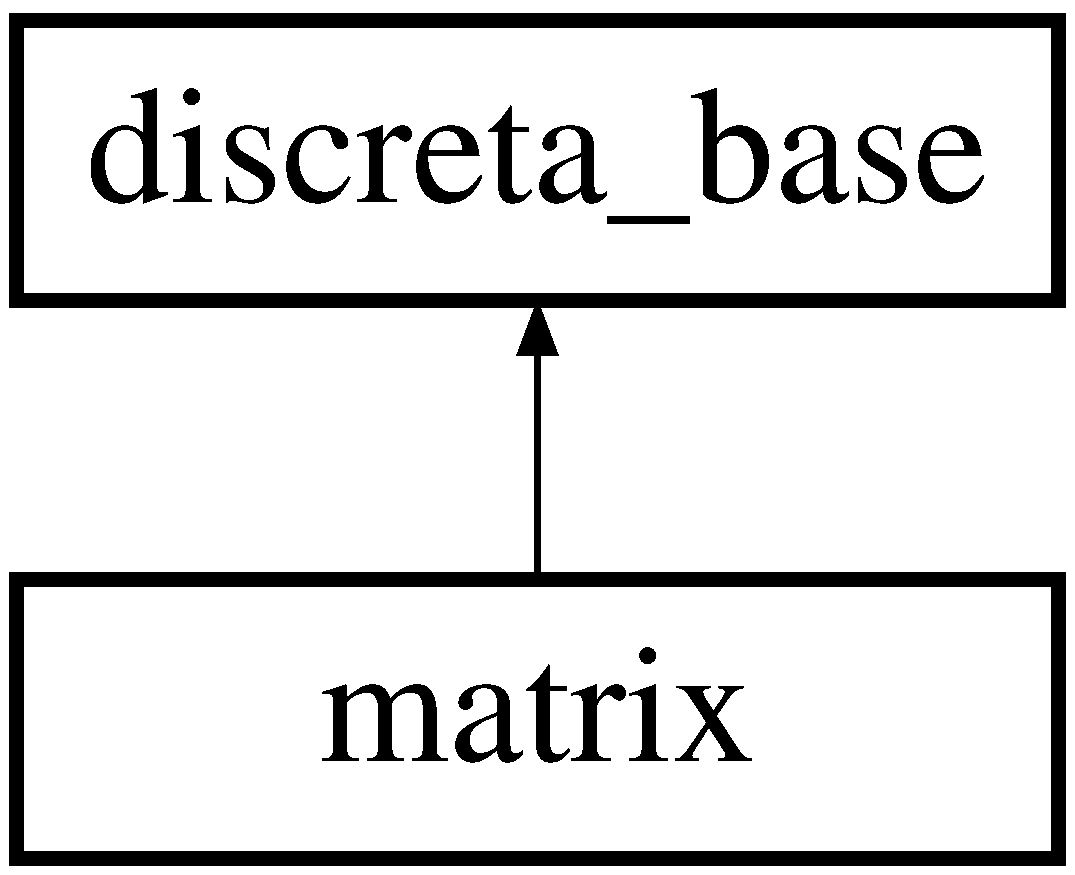
\includegraphics[height=2.000000cm]{classmatrix}
\end{center}
\end{figure}
\subsection*{Public Member Functions}
\begin{DoxyCompactItemize}
\item 
\mbox{\hyperlink{classmatrix_a4daf70b1506ea976352f20e4322a9c17}{matrix}} ()
\item 
\mbox{\hyperlink{classmatrix_ac9e2b8134d8bd8d9789133c187d81d74}{matrix}} (const \mbox{\hyperlink{classdiscreta__base}{discreta\+\_\+base}} \&\mbox{\hyperlink{alphabet2_8_c_a6150e0515f7202e2fb518f7206ed97dc}{x}})
\item 
\mbox{\hyperlink{classmatrix}{matrix}} \& \mbox{\hyperlink{classmatrix_a242b6281ca7b813d47d07bb474d10b8e}{operator=}} (const \mbox{\hyperlink{classdiscreta__base}{discreta\+\_\+base}} \&\mbox{\hyperlink{alphabet2_8_c_a6150e0515f7202e2fb518f7206ed97dc}{x}})
\item 
void $\ast$ \mbox{\hyperlink{classmatrix_af89d98f62742b78d8d67080a0c88763a}{operator new}} (size\+\_\+t, void $\ast$\mbox{\hyperlink{alphabet2_8_c_a533391314665d6bf1b5575e9a9cd8552}{p}})
\item 
void \mbox{\hyperlink{classmatrix_a1780283a64a789e4084d792683d276bb}{settype\+\_\+matrix}} ()
\item 
\mbox{\hyperlink{classmatrix_a8a2522496ff0ef7096ffcfdc851b85a1}{$\sim$matrix}} ()
\item 
void \mbox{\hyperlink{classmatrix_ab47d61820499f35c15bf82fb6a3b9bd1}{freeself\+\_\+matrix}} ()
\item 
\mbox{\hyperlink{discreta_8h_aaf25ee7e2306d78c74ec7bc48f092e81}{kind}} \mbox{\hyperlink{classmatrix_a4880cc2b5e8d3f8f2d8038580364db56}{s\+\_\+virtual\+\_\+kind}} ()
\item 
void \mbox{\hyperlink{classmatrix_a6a47f82604adaa39b21f6bfe6da9e898}{copyobject\+\_\+to}} (\mbox{\hyperlink{classdiscreta__base}{discreta\+\_\+base}} \&\mbox{\hyperlink{alphabet2_8_c_a6150e0515f7202e2fb518f7206ed97dc}{x}})
\item 
ostream \& \mbox{\hyperlink{classmatrix_aeb24c2fe68cc0a32d172c0fc06103dd2}{print}} (ostream \&)
\item 
\mbox{\hyperlink{galois_8h_a09fddde158a3a20bd2dcadb609de11dc}{I\+NT}} \mbox{\hyperlink{classmatrix_a6009a90834a208f5f0a83d8ed651e4c5}{compare\+\_\+with}} (\mbox{\hyperlink{classdiscreta__base}{discreta\+\_\+base}} \&a)
\item 
\mbox{\hyperlink{classmatrix}{matrix}} \& \mbox{\hyperlink{classmatrix_a85921e1b3c604f625989b1c3d1697792}{m\+\_\+mn}} (\mbox{\hyperlink{galois_8h_a09fddde158a3a20bd2dcadb609de11dc}{I\+NT}} m, \mbox{\hyperlink{galois_8h_a09fddde158a3a20bd2dcadb609de11dc}{I\+NT}} \mbox{\hyperlink{simeon_8_c_a7f2cd26777ce0ff3fdaf8d02aacbddfb}{n}})
\item 
\mbox{\hyperlink{classmatrix}{matrix}} \& \mbox{\hyperlink{classmatrix_ae9a8cf19bd93428639950725edbd2271}{m\+\_\+mn\+\_\+n}} (\mbox{\hyperlink{galois_8h_a09fddde158a3a20bd2dcadb609de11dc}{I\+NT}} m, \mbox{\hyperlink{galois_8h_a09fddde158a3a20bd2dcadb609de11dc}{I\+NT}} \mbox{\hyperlink{simeon_8_c_a7f2cd26777ce0ff3fdaf8d02aacbddfb}{n}})
\item 
\mbox{\hyperlink{classmatrix}{matrix}} \& \mbox{\hyperlink{classmatrix_a5d3c1be0310affe3c1c8ffe3e89097f3}{realloc}} (\mbox{\hyperlink{galois_8h_a09fddde158a3a20bd2dcadb609de11dc}{I\+NT}} m, \mbox{\hyperlink{galois_8h_a09fddde158a3a20bd2dcadb609de11dc}{I\+NT}} \mbox{\hyperlink{simeon_8_c_a7f2cd26777ce0ff3fdaf8d02aacbddfb}{n}})
\item 
\mbox{\hyperlink{galois_8h_a09fddde158a3a20bd2dcadb609de11dc}{I\+NT}} \mbox{\hyperlink{classmatrix_afeb2e29600e68448b9d1130114b9606f}{s\+\_\+m}} ()
\item 
\mbox{\hyperlink{galois_8h_a09fddde158a3a20bd2dcadb609de11dc}{I\+NT}} \mbox{\hyperlink{classmatrix_a35f5321a5615451fdc8be7b953f8ac8b}{s\+\_\+n}} ()
\item 
\mbox{\hyperlink{classdiscreta__base}{discreta\+\_\+base}} \& \mbox{\hyperlink{classmatrix_ab36f1b3abd2df280224c50c9debb57df}{s\+\_\+ij}} (\mbox{\hyperlink{galois_8h_a09fddde158a3a20bd2dcadb609de11dc}{I\+NT}} \mbox{\hyperlink{alphabet2_8_c_acb559820d9ca11295b4500f179ef6392}{i}}, \mbox{\hyperlink{galois_8h_a09fddde158a3a20bd2dcadb609de11dc}{I\+NT}} \mbox{\hyperlink{alphabet2_8_c_a37d972ae0b47b9099e30983131d31916}{j}})
\item 
\mbox{\hyperlink{galois_8h_a09fddde158a3a20bd2dcadb609de11dc}{I\+NT}} \& \mbox{\hyperlink{classmatrix_af8d3c35817af62a3c0097ddf64422d96}{s\+\_\+iji}} (\mbox{\hyperlink{galois_8h_a09fddde158a3a20bd2dcadb609de11dc}{I\+NT}} \mbox{\hyperlink{alphabet2_8_c_acb559820d9ca11295b4500f179ef6392}{i}}, \mbox{\hyperlink{galois_8h_a09fddde158a3a20bd2dcadb609de11dc}{I\+NT}} \mbox{\hyperlink{alphabet2_8_c_a37d972ae0b47b9099e30983131d31916}{j}})
\item 
void \mbox{\hyperlink{classmatrix_a8cece141dbb3d39e94933c8da46dbd50}{m\+\_\+iji}} (\mbox{\hyperlink{galois_8h_a09fddde158a3a20bd2dcadb609de11dc}{I\+NT}} \mbox{\hyperlink{alphabet2_8_c_acb559820d9ca11295b4500f179ef6392}{i}}, \mbox{\hyperlink{galois_8h_a09fddde158a3a20bd2dcadb609de11dc}{I\+NT}} \mbox{\hyperlink{alphabet2_8_c_a37d972ae0b47b9099e30983131d31916}{j}}, \mbox{\hyperlink{galois_8h_a09fddde158a3a20bd2dcadb609de11dc}{I\+NT}} a)
\item 
\mbox{\hyperlink{classmatrix__access}{matrix\+\_\+access}} \mbox{\hyperlink{classmatrix_a7e7aaebd797dd2020f6df94c6b07ebc2}{operator\mbox{[}$\,$\mbox{]}}} (\mbox{\hyperlink{galois_8h_a09fddde158a3a20bd2dcadb609de11dc}{I\+NT}} \mbox{\hyperlink{alphabet2_8_c_acb559820d9ca11295b4500f179ef6392}{i}})
\item 
void \mbox{\hyperlink{classmatrix_abde18a5fb21ce4d884dceedb286ba899}{mult\+\_\+to}} (\mbox{\hyperlink{classdiscreta__base}{discreta\+\_\+base}} \&\mbox{\hyperlink{alphabet2_8_c_a6150e0515f7202e2fb518f7206ed97dc}{x}}, \mbox{\hyperlink{classdiscreta__base}{discreta\+\_\+base}} \&\mbox{\hyperlink{alphabet2_8_c_a0a2f84ed7838f07779ae24c5a9086d33}{y}})
\item 
void \mbox{\hyperlink{classmatrix_a7b3866189e0d7f75e55805d6e9a43ace}{matrix\+\_\+mult\+\_\+to}} (\mbox{\hyperlink{classmatrix}{matrix}} \&\mbox{\hyperlink{alphabet2_8_c_a6150e0515f7202e2fb518f7206ed97dc}{x}}, \mbox{\hyperlink{classdiscreta__base}{discreta\+\_\+base}} \&\mbox{\hyperlink{alphabet2_8_c_a0a2f84ed7838f07779ae24c5a9086d33}{y}})
\item 
void \mbox{\hyperlink{classmatrix_a0e5dcee30e9e98346f389511c7700f1f}{vector\+\_\+mult\+\_\+to}} (\mbox{\hyperlink{class_vector}{Vector}} \&\mbox{\hyperlink{alphabet2_8_c_a6150e0515f7202e2fb518f7206ed97dc}{x}}, \mbox{\hyperlink{classdiscreta__base}{discreta\+\_\+base}} \&\mbox{\hyperlink{alphabet2_8_c_a0a2f84ed7838f07779ae24c5a9086d33}{y}})
\item 
void \mbox{\hyperlink{classmatrix_ae578f93fd93c59b9755d31b5fd11e14c}{multiply\+\_\+vector\+\_\+from\+\_\+left}} (\mbox{\hyperlink{class_vector}{Vector}} \&\mbox{\hyperlink{alphabet2_8_c_a6150e0515f7202e2fb518f7206ed97dc}{x}}, \mbox{\hyperlink{class_vector}{Vector}} \&\mbox{\hyperlink{alphabet2_8_c_a0a2f84ed7838f07779ae24c5a9086d33}{y}})
\item 
\mbox{\hyperlink{galois_8h_a09fddde158a3a20bd2dcadb609de11dc}{I\+NT}} \mbox{\hyperlink{classmatrix_a137bc3b88c71382c675dea7a0bf9b5f2}{invert\+\_\+to}} (\mbox{\hyperlink{classdiscreta__base}{discreta\+\_\+base}} \&\mbox{\hyperlink{alphabet2_8_c_a6150e0515f7202e2fb518f7206ed97dc}{x}})
\item 
void \mbox{\hyperlink{classmatrix_a4ade010e5f49a23fab4cb5211b106e81}{add\+\_\+to}} (\mbox{\hyperlink{classdiscreta__base}{discreta\+\_\+base}} \&\mbox{\hyperlink{alphabet2_8_c_a6150e0515f7202e2fb518f7206ed97dc}{x}}, \mbox{\hyperlink{classdiscreta__base}{discreta\+\_\+base}} \&\mbox{\hyperlink{alphabet2_8_c_a0a2f84ed7838f07779ae24c5a9086d33}{y}})
\item 
void \mbox{\hyperlink{classmatrix_acb93b95943eee2253b7b3b799333a24c}{negate\+\_\+to}} (\mbox{\hyperlink{classdiscreta__base}{discreta\+\_\+base}} \&\mbox{\hyperlink{alphabet2_8_c_a6150e0515f7202e2fb518f7206ed97dc}{x}})
\item 
void \mbox{\hyperlink{classmatrix_a780b461503be22827c4fdca66f779be1}{one}} ()
\item 
void \mbox{\hyperlink{classmatrix_abd2e274d4905bc97eabf7c72d5e66b3d}{zero}} ()
\item 
\mbox{\hyperlink{galois_8h_a09fddde158a3a20bd2dcadb609de11dc}{I\+NT}} \mbox{\hyperlink{classmatrix_a1940fae0fd429e77918eaa3d68cecd12}{is\+\_\+zero}} ()
\item 
\mbox{\hyperlink{galois_8h_a09fddde158a3a20bd2dcadb609de11dc}{I\+NT}} \mbox{\hyperlink{classmatrix_a74aa38df064afa998cb0973ac3554ac0}{is\+\_\+one}} ()
\item 
\mbox{\hyperlink{galois_8h_a09fddde158a3a20bd2dcadb609de11dc}{I\+NT}} \mbox{\hyperlink{classmatrix_abe8ed121d6bc29e1cc4432ad45542450}{Gauss}} (\mbox{\hyperlink{galois_8h_a09fddde158a3a20bd2dcadb609de11dc}{I\+NT}} \mbox{\hyperlink{simeon_8_c_a5c9bb19da4c942e41c1d5cfc81f4cfd7}{f\+\_\+special}}, \mbox{\hyperlink{galois_8h_a09fddde158a3a20bd2dcadb609de11dc}{I\+NT}} f\+\_\+complete, \mbox{\hyperlink{class_vector}{Vector}} \&base\+\_\+cols, \mbox{\hyperlink{galois_8h_a09fddde158a3a20bd2dcadb609de11dc}{I\+NT}} f\+\_\+P, \mbox{\hyperlink{classmatrix}{matrix}} \&\mbox{\hyperlink{simeon_8_c_a7fa15551e800919e93401fbbcd8e71e8}{P}}, \mbox{\hyperlink{galois_8h_a09fddde158a3a20bd2dcadb609de11dc}{I\+NT}} f\+\_\+v)
\item 
\mbox{\hyperlink{galois_8h_a09fddde158a3a20bd2dcadb609de11dc}{I\+NT}} \mbox{\hyperlink{classmatrix_a6248f2f23a2b0f011a21548cced5dc1f}{rank}} ()
\item 
\mbox{\hyperlink{galois_8h_a09fddde158a3a20bd2dcadb609de11dc}{I\+NT}} \mbox{\hyperlink{classmatrix_a75b3e1c7074bea2d399601ed2cff7a42}{get\+\_\+kernel}} (\mbox{\hyperlink{class_vector}{Vector}} \&base\+\_\+cols, \mbox{\hyperlink{classmatrix}{matrix}} \&kernel)
\item 
\mbox{\hyperlink{classmatrix}{matrix}} \& \mbox{\hyperlink{classmatrix_a1d8064be96298b81e8e060f02b9cef3e}{transpose}} ()
\item 
\mbox{\hyperlink{galois_8h_a09fddde158a3a20bd2dcadb609de11dc}{I\+NT}} \mbox{\hyperlink{classmatrix_a6ec12bab511dbb2f1426515819359390}{Asup2\+Ainf}} ()
\item 
\mbox{\hyperlink{galois_8h_a09fddde158a3a20bd2dcadb609de11dc}{I\+NT}} \mbox{\hyperlink{classmatrix_a7abdfef775e6f1e68856bbdb06004dce}{Ainf2\+Asup}} ()
\item 
\mbox{\hyperlink{galois_8h_a09fddde158a3a20bd2dcadb609de11dc}{I\+NT}} \mbox{\hyperlink{classmatrix_a606cce1a9d6430b751090e27ef31d2e4}{Asup2\+Acover}} ()
\item 
\mbox{\hyperlink{galois_8h_a09fddde158a3a20bd2dcadb609de11dc}{I\+NT}} \mbox{\hyperlink{classmatrix_a331c7926e93599378a25791e982b3c89}{Acover2nl}} (\mbox{\hyperlink{class_vector}{Vector}} \&nl)
\item 
void \mbox{\hyperlink{classmatrix_aa08a0bfacde81b35248690c099155bed}{Frobenius}} (\mbox{\hyperlink{classunipoly}{unipoly}} \&m, \mbox{\hyperlink{galois_8h_a09fddde158a3a20bd2dcadb609de11dc}{I\+NT}} \mbox{\hyperlink{alphabet2_8_c_a533391314665d6bf1b5575e9a9cd8552}{p}}, \mbox{\hyperlink{galois_8h_a09fddde158a3a20bd2dcadb609de11dc}{I\+NT}} \mbox{\hyperlink{simeon_8_c_a818073fbcc2f439e7c56952f67386122}{verbose\+\_\+level}})
\item 
void \mbox{\hyperlink{classmatrix_ac98dd867d9148831126eaddd13b7da60}{Berlekamp}} (\mbox{\hyperlink{classunipoly}{unipoly}} \&m, \mbox{\hyperlink{galois_8h_a09fddde158a3a20bd2dcadb609de11dc}{I\+NT}} \mbox{\hyperlink{alphabet2_8_c_a533391314665d6bf1b5575e9a9cd8552}{p}}, \mbox{\hyperlink{galois_8h_a09fddde158a3a20bd2dcadb609de11dc}{I\+NT}} \mbox{\hyperlink{simeon_8_c_a818073fbcc2f439e7c56952f67386122}{verbose\+\_\+level}})
\item 
void \mbox{\hyperlink{classmatrix_acd603a86fd752eb4da1a060bdaab478f}{companion\+\_\+matrix}} (\mbox{\hyperlink{classunipoly}{unipoly}} \&m, \mbox{\hyperlink{galois_8h_a09fddde158a3a20bd2dcadb609de11dc}{I\+NT}} \mbox{\hyperlink{simeon_8_c_a818073fbcc2f439e7c56952f67386122}{verbose\+\_\+level}})
\item 
void \mbox{\hyperlink{classmatrix_aee7e0d79d2c1ef32f0cbebbcc7f40771}{elements\+\_\+to\+\_\+unipoly}} ()
\item 
void \mbox{\hyperlink{classmatrix_a3c2f7a8bafecd1eb355c245cf0e157b2}{minus\+\_\+\+X\+\_\+times\+\_\+id}} ()
\item 
void \mbox{\hyperlink{classmatrix_a42aa27f4ae06ceff8cb297894bb5aad4}{X\+\_\+times\+\_\+id\+\_\+minus\+\_\+self}} ()
\item 
void \mbox{\hyperlink{classmatrix_aeb73764dd4346bb1a6998f2a3c507544}{smith\+\_\+normal\+\_\+form}} (\mbox{\hyperlink{classmatrix}{matrix}} \&\mbox{\hyperlink{simeon_8_c_a7fa15551e800919e93401fbbcd8e71e8}{P}}, \mbox{\hyperlink{classmatrix}{matrix}} \&Pv, \mbox{\hyperlink{classmatrix}{matrix}} \&Q, \mbox{\hyperlink{classmatrix}{matrix}} \&Qv, \mbox{\hyperlink{galois_8h_a09fddde158a3a20bd2dcadb609de11dc}{I\+NT}} \mbox{\hyperlink{simeon_8_c_a818073fbcc2f439e7c56952f67386122}{verbose\+\_\+level}})
\item 
\mbox{\hyperlink{galois_8h_a09fddde158a3a20bd2dcadb609de11dc}{I\+NT}} \mbox{\hyperlink{classmatrix_ab1f7e8511834e7782ef09f59d8281c74}{smith\+\_\+eliminate\+\_\+column}} (\mbox{\hyperlink{classmatrix}{matrix}} \&\mbox{\hyperlink{simeon_8_c_a7fa15551e800919e93401fbbcd8e71e8}{P}}, \mbox{\hyperlink{classmatrix}{matrix}} \&Pv, \mbox{\hyperlink{galois_8h_a09fddde158a3a20bd2dcadb609de11dc}{I\+NT}} \mbox{\hyperlink{alphabet2_8_c_acb559820d9ca11295b4500f179ef6392}{i}}, \mbox{\hyperlink{galois_8h_a09fddde158a3a20bd2dcadb609de11dc}{I\+NT}} \mbox{\hyperlink{simeon_8_c_a818073fbcc2f439e7c56952f67386122}{verbose\+\_\+level}})
\item 
\mbox{\hyperlink{galois_8h_a09fddde158a3a20bd2dcadb609de11dc}{I\+NT}} \mbox{\hyperlink{classmatrix_a6672b6bbaad6060b6c230a2c10ec2eb5}{smith\+\_\+eliminate\+\_\+row}} (\mbox{\hyperlink{classmatrix}{matrix}} \&Q, \mbox{\hyperlink{classmatrix}{matrix}} \&Qv, \mbox{\hyperlink{galois_8h_a09fddde158a3a20bd2dcadb609de11dc}{I\+NT}} \mbox{\hyperlink{alphabet2_8_c_acb559820d9ca11295b4500f179ef6392}{i}}, \mbox{\hyperlink{galois_8h_a09fddde158a3a20bd2dcadb609de11dc}{I\+NT}} \mbox{\hyperlink{simeon_8_c_a818073fbcc2f439e7c56952f67386122}{verbose\+\_\+level}})
\item 
void \mbox{\hyperlink{classmatrix_ad64ff9070fae0dc1c8957251d16e8146}{multiply\+\_\+2by2\+\_\+from\+\_\+left}} (\mbox{\hyperlink{galois_8h_a09fddde158a3a20bd2dcadb609de11dc}{I\+NT}} \mbox{\hyperlink{alphabet2_8_c_acb559820d9ca11295b4500f179ef6392}{i}}, \mbox{\hyperlink{galois_8h_a09fddde158a3a20bd2dcadb609de11dc}{I\+NT}} \mbox{\hyperlink{alphabet2_8_c_a37d972ae0b47b9099e30983131d31916}{j}}, \mbox{\hyperlink{classdiscreta__base}{discreta\+\_\+base}} \&aii, \mbox{\hyperlink{classdiscreta__base}{discreta\+\_\+base}} \&aij, \mbox{\hyperlink{classdiscreta__base}{discreta\+\_\+base}} \&aji, \mbox{\hyperlink{classdiscreta__base}{discreta\+\_\+base}} \&ajj, \mbox{\hyperlink{galois_8h_a09fddde158a3a20bd2dcadb609de11dc}{I\+NT}} \mbox{\hyperlink{simeon_8_c_a818073fbcc2f439e7c56952f67386122}{verbose\+\_\+level}})
\item 
void \mbox{\hyperlink{classmatrix_a00455d7848021f33e9c8d280d1c8a0de}{multiply\+\_\+2by2\+\_\+from\+\_\+right}} (\mbox{\hyperlink{galois_8h_a09fddde158a3a20bd2dcadb609de11dc}{I\+NT}} \mbox{\hyperlink{alphabet2_8_c_acb559820d9ca11295b4500f179ef6392}{i}}, \mbox{\hyperlink{galois_8h_a09fddde158a3a20bd2dcadb609de11dc}{I\+NT}} \mbox{\hyperlink{alphabet2_8_c_a37d972ae0b47b9099e30983131d31916}{j}}, \mbox{\hyperlink{classdiscreta__base}{discreta\+\_\+base}} \&aii, \mbox{\hyperlink{classdiscreta__base}{discreta\+\_\+base}} \&aij, \mbox{\hyperlink{classdiscreta__base}{discreta\+\_\+base}} \&aji, \mbox{\hyperlink{classdiscreta__base}{discreta\+\_\+base}} \&ajj, \mbox{\hyperlink{galois_8h_a09fddde158a3a20bd2dcadb609de11dc}{I\+NT}} \mbox{\hyperlink{simeon_8_c_a818073fbcc2f439e7c56952f67386122}{verbose\+\_\+level}})
\item 
void \mbox{\hyperlink{classmatrix_a46200f82b0e76394a82968029d5e5a61}{to\+\_\+vector\+\_\+of\+\_\+rows}} (\mbox{\hyperlink{class_vector}{Vector}} \&\mbox{\hyperlink{simeon_8_c_aeb3f3030944801b163bc3b829a7f6710}{v}})
\item 
void \mbox{\hyperlink{classmatrix_aeffa1035691fc1055ce1b52d2e31a114}{from\+\_\+vector\+\_\+of\+\_\+rows}} (\mbox{\hyperlink{class_vector}{Vector}} \&\mbox{\hyperlink{simeon_8_c_aeb3f3030944801b163bc3b829a7f6710}{v}})
\item 
void \mbox{\hyperlink{classmatrix_ab806288c2dcb40b77b2dfc53ab09f74d}{to\+\_\+vector\+\_\+of\+\_\+columns}} (\mbox{\hyperlink{class_vector}{Vector}} \&\mbox{\hyperlink{simeon_8_c_aeb3f3030944801b163bc3b829a7f6710}{v}})
\item 
void \mbox{\hyperlink{classmatrix_af666c6b895475348ffa818d0da96897b}{from\+\_\+vector\+\_\+of\+\_\+columns}} (\mbox{\hyperlink{class_vector}{Vector}} \&\mbox{\hyperlink{simeon_8_c_aeb3f3030944801b163bc3b829a7f6710}{v}})
\item 
void \mbox{\hyperlink{classmatrix_a0063caaa247f4546e31800f81e17a8cd}{evaluate\+\_\+at}} (\mbox{\hyperlink{classdiscreta__base}{discreta\+\_\+base}} \&\mbox{\hyperlink{alphabet2_8_c_a6150e0515f7202e2fb518f7206ed97dc}{x}})
\item 
void \mbox{\hyperlink{classmatrix_a69a80605be7914af5fd65e680944aeca}{K\+X\+\_\+module\+\_\+order\+\_\+ideal}} (\mbox{\hyperlink{galois_8h_a09fddde158a3a20bd2dcadb609de11dc}{I\+NT}} \mbox{\hyperlink{alphabet2_8_c_acb559820d9ca11295b4500f179ef6392}{i}}, \mbox{\hyperlink{classunipoly}{unipoly}} \&mue, \mbox{\hyperlink{galois_8h_a09fddde158a3a20bd2dcadb609de11dc}{I\+NT}} \mbox{\hyperlink{simeon_8_c_a818073fbcc2f439e7c56952f67386122}{verbose\+\_\+level}})
\item 
void \mbox{\hyperlink{classmatrix_accef670f4dfd666f9de32fe50754665d}{K\+X\+\_\+module\+\_\+apply}} (\mbox{\hyperlink{classunipoly}{unipoly}} \&\mbox{\hyperlink{alphabet2_8_c_a533391314665d6bf1b5575e9a9cd8552}{p}}, \mbox{\hyperlink{class_vector}{Vector}} \&\mbox{\hyperlink{simeon_8_c_aeb3f3030944801b163bc3b829a7f6710}{v}})
\item 
void \mbox{\hyperlink{classmatrix_afd55b3b44c36f039928862315f52428b}{K\+X\+\_\+module\+\_\+join}} (\mbox{\hyperlink{class_vector}{Vector}} \&v1, \mbox{\hyperlink{classunipoly}{unipoly}} \&mue1, \mbox{\hyperlink{class_vector}{Vector}} \&v2, \mbox{\hyperlink{classunipoly}{unipoly}} \&mue2, \mbox{\hyperlink{class_vector}{Vector}} \&v3, \mbox{\hyperlink{classunipoly}{unipoly}} \&mue3, \mbox{\hyperlink{galois_8h_a09fddde158a3a20bd2dcadb609de11dc}{I\+NT}} \mbox{\hyperlink{simeon_8_c_a818073fbcc2f439e7c56952f67386122}{verbose\+\_\+level}})
\item 
void \mbox{\hyperlink{classmatrix_ace9dbe1f348d6fa63d1005e8f601897b}{K\+X\+\_\+cyclic\+\_\+module\+\_\+generator}} (\mbox{\hyperlink{class_vector}{Vector}} \&\mbox{\hyperlink{simeon_8_c_aeb3f3030944801b163bc3b829a7f6710}{v}}, \mbox{\hyperlink{classunipoly}{unipoly}} \&mue, \mbox{\hyperlink{galois_8h_a09fddde158a3a20bd2dcadb609de11dc}{I\+NT}} \mbox{\hyperlink{simeon_8_c_a818073fbcc2f439e7c56952f67386122}{verbose\+\_\+level}})
\item 
void \mbox{\hyperlink{classmatrix_ad8b6174329495126b165154d074bbcff}{K\+X\+\_\+module\+\_\+minpol}} (\mbox{\hyperlink{classunipoly}{unipoly}} \&\mbox{\hyperlink{alphabet2_8_c_a533391314665d6bf1b5575e9a9cd8552}{p}}, \mbox{\hyperlink{classunipoly}{unipoly}} \&m, \mbox{\hyperlink{classunipoly}{unipoly}} \&mue, \mbox{\hyperlink{galois_8h_a09fddde158a3a20bd2dcadb609de11dc}{I\+NT}} \mbox{\hyperlink{simeon_8_c_a818073fbcc2f439e7c56952f67386122}{verbose\+\_\+level}})
\item 
void \mbox{\hyperlink{classmatrix_af3908604699f48d25012d6500de591f0}{binomial}} (\mbox{\hyperlink{galois_8h_a09fddde158a3a20bd2dcadb609de11dc}{I\+NT}} n\+\_\+min, \mbox{\hyperlink{galois_8h_a09fddde158a3a20bd2dcadb609de11dc}{I\+NT}} n\+\_\+max, \mbox{\hyperlink{galois_8h_a09fddde158a3a20bd2dcadb609de11dc}{I\+NT}} k\+\_\+min, \mbox{\hyperlink{galois_8h_a09fddde158a3a20bd2dcadb609de11dc}{I\+NT}} k\+\_\+max)
\item 
void \mbox{\hyperlink{classmatrix_a0e7366c1db2c447d83f71f2c369e8d1d}{stirling\+\_\+second}} (\mbox{\hyperlink{galois_8h_a09fddde158a3a20bd2dcadb609de11dc}{I\+NT}} n\+\_\+min, \mbox{\hyperlink{galois_8h_a09fddde158a3a20bd2dcadb609de11dc}{I\+NT}} n\+\_\+max, \mbox{\hyperlink{galois_8h_a09fddde158a3a20bd2dcadb609de11dc}{I\+NT}} k\+\_\+min, \mbox{\hyperlink{galois_8h_a09fddde158a3a20bd2dcadb609de11dc}{I\+NT}} k\+\_\+max, \mbox{\hyperlink{galois_8h_a09fddde158a3a20bd2dcadb609de11dc}{I\+NT}} f\+\_\+ordered)
\item 
void \mbox{\hyperlink{classmatrix_a9041c3138924ebc58d539c9230898c6d}{stirling\+\_\+first}} (\mbox{\hyperlink{galois_8h_a09fddde158a3a20bd2dcadb609de11dc}{I\+NT}} n\+\_\+min, \mbox{\hyperlink{galois_8h_a09fddde158a3a20bd2dcadb609de11dc}{I\+NT}} n\+\_\+max, \mbox{\hyperlink{galois_8h_a09fddde158a3a20bd2dcadb609de11dc}{I\+NT}} k\+\_\+min, \mbox{\hyperlink{galois_8h_a09fddde158a3a20bd2dcadb609de11dc}{I\+NT}} k\+\_\+max, \mbox{\hyperlink{galois_8h_a09fddde158a3a20bd2dcadb609de11dc}{I\+NT}} f\+\_\+signless)
\item 
void \mbox{\hyperlink{classmatrix_a58a9004174ad450f80faba4db8c1be1c}{binomial}} (\mbox{\hyperlink{galois_8h_a09fddde158a3a20bd2dcadb609de11dc}{I\+NT}} n\+\_\+min, \mbox{\hyperlink{galois_8h_a09fddde158a3a20bd2dcadb609de11dc}{I\+NT}} n\+\_\+max, \mbox{\hyperlink{galois_8h_a09fddde158a3a20bd2dcadb609de11dc}{I\+NT}} k\+\_\+min, \mbox{\hyperlink{galois_8h_a09fddde158a3a20bd2dcadb609de11dc}{I\+NT}} k\+\_\+max, \mbox{\hyperlink{galois_8h_a09fddde158a3a20bd2dcadb609de11dc}{I\+NT}} f\+\_\+inverse)
\item 
\mbox{\hyperlink{galois_8h_a09fddde158a3a20bd2dcadb609de11dc}{I\+NT}} \mbox{\hyperlink{classmatrix_a820b8de607274302772f753e7585e9fa}{hip}} ()
\item 
\mbox{\hyperlink{galois_8h_a09fddde158a3a20bd2dcadb609de11dc}{I\+NT}} \mbox{\hyperlink{classmatrix_a169cd51dd98562746f81dd0b075f3f6f}{hip1}} ()
\item 
void \mbox{\hyperlink{classmatrix_a773aa4ab691548beba8e6204d9f4ef21}{write\+\_\+mem}} (\mbox{\hyperlink{classmemory}{memory}} \&m, \mbox{\hyperlink{galois_8h_a09fddde158a3a20bd2dcadb609de11dc}{I\+NT}} debug\+\_\+depth)
\item 
void \mbox{\hyperlink{classmatrix_a11e3236059f10ed69c47c65c79e7f03b}{read\+\_\+mem}} (\mbox{\hyperlink{classmemory}{memory}} \&\mbox{\hyperlink{plane__search_8_c_ad2d23ebd03187a91edd45b1d5e496265}{M}}, \mbox{\hyperlink{galois_8h_a09fddde158a3a20bd2dcadb609de11dc}{I\+NT}} debug\+\_\+depth)
\item 
\mbox{\hyperlink{galois_8h_a09fddde158a3a20bd2dcadb609de11dc}{I\+NT}} \mbox{\hyperlink{classmatrix_af06fd7824274febfcc10f734a06d1a6e}{csf}} ()
\item 
void \mbox{\hyperlink{classmatrix_abf772e9b3338df569be017ffecb165ef}{calc\+\_\+theX}} (\mbox{\hyperlink{galois_8h_a09fddde158a3a20bd2dcadb609de11dc}{I\+NT}} \&nb\+\_\+X, \mbox{\hyperlink{galois_8h_a09fddde158a3a20bd2dcadb609de11dc}{I\+NT}} $\ast$\&theX)
\item 
void \mbox{\hyperlink{classmatrix_a4bfbaa097eedb8b427169c593cbb40d0}{apply\+\_\+perms}} (\mbox{\hyperlink{galois_8h_a09fddde158a3a20bd2dcadb609de11dc}{I\+NT}} f\+\_\+row\+\_\+perm, \mbox{\hyperlink{classpermutation}{permutation}} \&row\+\_\+perm, \mbox{\hyperlink{galois_8h_a09fddde158a3a20bd2dcadb609de11dc}{I\+NT}} f\+\_\+col\+\_\+perm, \mbox{\hyperlink{classpermutation}{permutation}} \&col\+\_\+perm)
\item 
void \mbox{\hyperlink{classmatrix_a260e37c93f9e2d55d02ecddcb483659a}{apply\+\_\+col\+\_\+row\+\_\+perm}} (\mbox{\hyperlink{classpermutation}{permutation}} \&\mbox{\hyperlink{alphabet2_8_c_a533391314665d6bf1b5575e9a9cd8552}{p}})
\item 
void \mbox{\hyperlink{classmatrix_ad413b1eccc8402fb7281d70dc06915f5}{apply\+\_\+row\+\_\+col\+\_\+perm}} (\mbox{\hyperlink{classpermutation}{permutation}} \&\mbox{\hyperlink{alphabet2_8_c_a533391314665d6bf1b5575e9a9cd8552}{p}})
\item 
void \mbox{\hyperlink{classmatrix_a0ced6791191355bde858790aa4b156ac}{incma\+\_\+print\+\_\+ascii\+\_\+permuted\+\_\+and\+\_\+decomposed}} (ostream \&ost, \mbox{\hyperlink{galois_8h_a09fddde158a3a20bd2dcadb609de11dc}{I\+NT}} f\+\_\+tex, \mbox{\hyperlink{class_vector}{Vector}} \&decomp, \mbox{\hyperlink{classpermutation}{permutation}} \&\mbox{\hyperlink{alphabet2_8_c_a533391314665d6bf1b5575e9a9cd8552}{p}})
\item 
void \mbox{\hyperlink{classmatrix_afd1ff3d3d7b507287af6891d94771bab}{print\+\_\+decomposed}} (ostream \&ost, \mbox{\hyperlink{class_vector}{Vector}} \&row\+\_\+decomp, \mbox{\hyperlink{class_vector}{Vector}} \&col\+\_\+decomp)
\item 
void \mbox{\hyperlink{classmatrix_a1eba80b1e47f3672e6880e7343eea8e4}{incma\+\_\+print\+\_\+ascii}} (ostream \&ost, \mbox{\hyperlink{galois_8h_a09fddde158a3a20bd2dcadb609de11dc}{I\+NT}} f\+\_\+tex, \mbox{\hyperlink{galois_8h_a09fddde158a3a20bd2dcadb609de11dc}{I\+NT}} f\+\_\+row\+\_\+decomp, \mbox{\hyperlink{class_vector}{Vector}} \&row\+\_\+decomp, \mbox{\hyperlink{galois_8h_a09fddde158a3a20bd2dcadb609de11dc}{I\+NT}} f\+\_\+col\+\_\+decomp, \mbox{\hyperlink{class_vector}{Vector}} \&col\+\_\+decomp)
\item 
void \mbox{\hyperlink{classmatrix_a2f3ef897e502a22def6b90a7c02addf5}{incma\+\_\+print\+\_\+latex}} (ostream \&\mbox{\hyperlink{alphabet2_8_c_a362077c979b0bb65159c603270e40f70}{f}}, \mbox{\hyperlink{galois_8h_a09fddde158a3a20bd2dcadb609de11dc}{I\+NT}} f\+\_\+row\+\_\+decomp, \mbox{\hyperlink{class_vector}{Vector}} \&row\+\_\+decomp, \mbox{\hyperlink{galois_8h_a09fddde158a3a20bd2dcadb609de11dc}{I\+NT}} f\+\_\+col\+\_\+decomp, \mbox{\hyperlink{class_vector}{Vector}} \&col\+\_\+decomp, \mbox{\hyperlink{galois_8h_a09fddde158a3a20bd2dcadb609de11dc}{I\+NT}} f\+\_\+labelling\+\_\+points, \mbox{\hyperlink{class_vector}{Vector}} \&point\+\_\+labels, \mbox{\hyperlink{galois_8h_a09fddde158a3a20bd2dcadb609de11dc}{I\+NT}} f\+\_\+labelling\+\_\+blocks, \mbox{\hyperlink{class_vector}{Vector}} \&block\+\_\+labels)
\item 
void \mbox{\hyperlink{classmatrix_a6e282efff2dd195d9aaf94343768106d}{incma\+\_\+print\+\_\+latex2}} (ostream \&\mbox{\hyperlink{alphabet2_8_c_a362077c979b0bb65159c603270e40f70}{f}}, \mbox{\hyperlink{galois_8h_a09fddde158a3a20bd2dcadb609de11dc}{I\+NT}} width, \mbox{\hyperlink{galois_8h_a09fddde158a3a20bd2dcadb609de11dc}{I\+NT}} width\+\_\+10, \mbox{\hyperlink{galois_8h_a09fddde158a3a20bd2dcadb609de11dc}{I\+NT}} f\+\_\+outline\+\_\+thin, const \mbox{\hyperlink{galois_8h_ab6cc7b4aeb6ea31aba2b3fbfc83ff5e6}{B\+Y\+TE}} $\ast$unit\+\_\+length, const \mbox{\hyperlink{galois_8h_ab6cc7b4aeb6ea31aba2b3fbfc83ff5e6}{B\+Y\+TE}} $\ast$thick\+\_\+lines, const \mbox{\hyperlink{galois_8h_ab6cc7b4aeb6ea31aba2b3fbfc83ff5e6}{B\+Y\+TE}} $\ast$thin\+\_\+lines, const \mbox{\hyperlink{galois_8h_ab6cc7b4aeb6ea31aba2b3fbfc83ff5e6}{B\+Y\+TE}} $\ast$geo\+\_\+line\+\_\+width, \mbox{\hyperlink{galois_8h_a09fddde158a3a20bd2dcadb609de11dc}{I\+NT}} f\+\_\+row\+\_\+decomp, \mbox{\hyperlink{class_vector}{Vector}} \&row\+\_\+decomp, \mbox{\hyperlink{galois_8h_a09fddde158a3a20bd2dcadb609de11dc}{I\+NT}} f\+\_\+col\+\_\+decomp, \mbox{\hyperlink{class_vector}{Vector}} \&col\+\_\+decomp, \mbox{\hyperlink{galois_8h_a09fddde158a3a20bd2dcadb609de11dc}{I\+NT}} f\+\_\+labelling\+\_\+points, \mbox{\hyperlink{class_vector}{Vector}} \&point\+\_\+labels, \mbox{\hyperlink{galois_8h_a09fddde158a3a20bd2dcadb609de11dc}{I\+NT}} f\+\_\+labelling\+\_\+blocks, \mbox{\hyperlink{class_vector}{Vector}} \&block\+\_\+labels)
\item 
void \mbox{\hyperlink{classmatrix_a61ce2d156303d0a83652cc86c2ad51b7}{calc\+\_\+hash\+\_\+key}} (\mbox{\hyperlink{galois_8h_a09fddde158a3a20bd2dcadb609de11dc}{I\+NT}} key\+\_\+len, \mbox{\hyperlink{classhollerith}{hollerith}} \&hash\+\_\+key, \mbox{\hyperlink{galois_8h_a09fddde158a3a20bd2dcadb609de11dc}{I\+NT}} f\+\_\+v)
\item 
\mbox{\hyperlink{galois_8h_a09fddde158a3a20bd2dcadb609de11dc}{I\+NT}} \mbox{\hyperlink{classmatrix_aecb27f51504ac8d90bb280b6a851942d}{is\+\_\+in\+\_\+center}} ()
\item 
void \mbox{\hyperlink{classmatrix_a7c9caac34a30994119cd7048df71df6e}{power\+\_\+mod}} (\mbox{\hyperlink{galois_8h_a09fddde158a3a20bd2dcadb609de11dc}{I\+NT}} \mbox{\hyperlink{alphabet2_8_c_acab531abaa74a7e664e3986f2522b33a}{r}}, \mbox{\hyperlink{classinteger}{integer}} \&\mbox{\hyperlink{simeon_8_c_a7fa15551e800919e93401fbbcd8e71e8}{P}}, \mbox{\hyperlink{classmatrix}{matrix}} \&\mbox{\hyperlink{costas_8_c_aacbbb35f36efadbb40803bfb5480b737}{C}})
\item 
\mbox{\hyperlink{galois_8h_a09fddde158a3a20bd2dcadb609de11dc}{I\+NT}} \mbox{\hyperlink{classmatrix_ab201caa82893894059d9e2432bd6b52a}{proj\+\_\+order\+\_\+mod}} (\mbox{\hyperlink{classinteger}{integer}} \&\mbox{\hyperlink{simeon_8_c_a7fa15551e800919e93401fbbcd8e71e8}{P}})
\item 
void \mbox{\hyperlink{classmatrix_a2b77483722eaba5108902dbbb96fc986}{P\+G\+\_\+rep}} (\mbox{\hyperlink{classdomain}{domain}} $\ast$dom, \mbox{\hyperlink{classpermutation}{permutation}} \&\mbox{\hyperlink{alphabet2_8_c_a533391314665d6bf1b5575e9a9cd8552}{p}}, \mbox{\hyperlink{galois_8h_a09fddde158a3a20bd2dcadb609de11dc}{I\+NT}} f\+\_\+action\+\_\+from\+\_\+right, \mbox{\hyperlink{galois_8h_a09fddde158a3a20bd2dcadb609de11dc}{I\+NT}} f\+\_\+modified)
\item 
void \mbox{\hyperlink{classmatrix_af084532cc1d1b518ac2a6e7de1da3fa5}{P\+G\+\_\+rep}} (\mbox{\hyperlink{classpermutation}{permutation}} \&\mbox{\hyperlink{alphabet2_8_c_a533391314665d6bf1b5575e9a9cd8552}{p}}, \mbox{\hyperlink{galois_8h_a09fddde158a3a20bd2dcadb609de11dc}{I\+NT}} f\+\_\+action\+\_\+from\+\_\+right, \mbox{\hyperlink{galois_8h_a09fddde158a3a20bd2dcadb609de11dc}{I\+NT}} f\+\_\+modified)
\item 
void \mbox{\hyperlink{classmatrix_a59a194ad8179725404d2b47a73070a88}{A\+G\+\_\+rep}} (\mbox{\hyperlink{classdomain}{domain}} $\ast$dom, \mbox{\hyperlink{classpermutation}{permutation}} \&\mbox{\hyperlink{alphabet2_8_c_a533391314665d6bf1b5575e9a9cd8552}{p}}, \mbox{\hyperlink{galois_8h_a09fddde158a3a20bd2dcadb609de11dc}{I\+NT}} f\+\_\+action\+\_\+from\+\_\+right)
\item 
void \mbox{\hyperlink{classmatrix_aac08bbc6eaee5b48801521e04607f2c2}{A\+G\+\_\+rep}} (\mbox{\hyperlink{classpermutation}{permutation}} \&\mbox{\hyperlink{alphabet2_8_c_a533391314665d6bf1b5575e9a9cd8552}{p}}, \mbox{\hyperlink{galois_8h_a09fddde158a3a20bd2dcadb609de11dc}{I\+NT}} f\+\_\+action\+\_\+from\+\_\+right)
\item 
void \mbox{\hyperlink{classmatrix_a6165884e70a04d1bd608f0321ec12040}{Mac\+Williams\+Transform}} (\mbox{\hyperlink{galois_8h_a09fddde158a3a20bd2dcadb609de11dc}{I\+NT}} \mbox{\hyperlink{simeon_8_c_a7f2cd26777ce0ff3fdaf8d02aacbddfb}{n}}, \mbox{\hyperlink{galois_8h_a09fddde158a3a20bd2dcadb609de11dc}{I\+NT}} \mbox{\hyperlink{simeon_8_c_a92cbb483a3b27ae1a0dbfcb125ce216f}{q}}, \mbox{\hyperlink{galois_8h_a09fddde158a3a20bd2dcadb609de11dc}{I\+NT}} f\+\_\+v)
\item 
void \mbox{\hyperlink{classmatrix_aae7c9c7c3540c5818d2df52ab67f8a52}{weight\+\_\+enumerator\+\_\+brute\+\_\+force}} (\mbox{\hyperlink{classdomain}{domain}} $\ast$dom, \mbox{\hyperlink{class_vector}{Vector}} \&\mbox{\hyperlink{simeon_8_c_aeb3f3030944801b163bc3b829a7f6710}{v}})
\item 
void \mbox{\hyperlink{classmatrix_a8183959565956f14466fe9d366c2c195}{Simplex\+\_\+code\+\_\+generator\+\_\+matrix}} (\mbox{\hyperlink{classdomain}{domain}} $\ast$dom, \mbox{\hyperlink{galois_8h_a09fddde158a3a20bd2dcadb609de11dc}{I\+NT}} \mbox{\hyperlink{classdiscreta__base_a6f7a0f7bdd115b9e4dde358cfa7ebf81}{k}}, \mbox{\hyperlink{galois_8h_a09fddde158a3a20bd2dcadb609de11dc}{I\+NT}} f\+\_\+v)
\item 
void \mbox{\hyperlink{classmatrix_adece30f74509652851c31e2d82e141e3}{P\+G\+\_\+design\+\_\+point\+\_\+vs\+\_\+hyperplane}} (\mbox{\hyperlink{classdomain}{domain}} $\ast$dom, \mbox{\hyperlink{galois_8h_a09fddde158a3a20bd2dcadb609de11dc}{I\+NT}} \mbox{\hyperlink{classdiscreta__base_a6f7a0f7bdd115b9e4dde358cfa7ebf81}{k}}, \mbox{\hyperlink{galois_8h_a09fddde158a3a20bd2dcadb609de11dc}{I\+NT}} f\+\_\+v)
\item 
void \mbox{\hyperlink{classmatrix_ae05463d97ecc8ea3654c45a399b872e2}{P\+G\+\_\+k\+\_\+q\+\_\+design}} (\mbox{\hyperlink{classdomain}{domain}} $\ast$dom, \mbox{\hyperlink{galois_8h_a09fddde158a3a20bd2dcadb609de11dc}{I\+NT}} \mbox{\hyperlink{classdiscreta__base_a6f7a0f7bdd115b9e4dde358cfa7ebf81}{k}}, \mbox{\hyperlink{galois_8h_a09fddde158a3a20bd2dcadb609de11dc}{I\+NT}} f\+\_\+v, \mbox{\hyperlink{galois_8h_a09fddde158a3a20bd2dcadb609de11dc}{I\+NT}} f\+\_\+vv)
\item 
void \mbox{\hyperlink{classmatrix_a75adb25c9f8753f1b81eafe4464b272a}{determinant}} (\mbox{\hyperlink{classdiscreta__base}{discreta\+\_\+base}} \&\mbox{\hyperlink{simeon_8_c_a4339ca06fa882e69473d37bd6d7917d1}{d}}, \mbox{\hyperlink{galois_8h_a09fddde158a3a20bd2dcadb609de11dc}{I\+NT}} \mbox{\hyperlink{simeon_8_c_a818073fbcc2f439e7c56952f67386122}{verbose\+\_\+level}})
\item 
void \mbox{\hyperlink{classmatrix_a364b1e3b29af6f6bd952448718d79467}{det}} (\mbox{\hyperlink{classdiscreta__base}{discreta\+\_\+base}} \&\mbox{\hyperlink{simeon_8_c_a4339ca06fa882e69473d37bd6d7917d1}{d}}, \mbox{\hyperlink{galois_8h_a09fddde158a3a20bd2dcadb609de11dc}{I\+NT}} f\+\_\+v, \mbox{\hyperlink{galois_8h_a09fddde158a3a20bd2dcadb609de11dc}{I\+NT}} f\+\_\+vv)
\item 
void \mbox{\hyperlink{classmatrix_a94ca76d8c4919c9f1f20c362840aaf43}{det\+\_\+modify\+\_\+input\+\_\+matrix}} (\mbox{\hyperlink{classdiscreta__base}{discreta\+\_\+base}} \&\mbox{\hyperlink{simeon_8_c_a4339ca06fa882e69473d37bd6d7917d1}{d}}, \mbox{\hyperlink{galois_8h_a09fddde158a3a20bd2dcadb609de11dc}{I\+NT}} f\+\_\+v, \mbox{\hyperlink{galois_8h_a09fddde158a3a20bd2dcadb609de11dc}{I\+NT}} f\+\_\+vv)
\item 
void \mbox{\hyperlink{classmatrix_ae31cbfd77683849e20b757b80e248649}{P\+G\+\_\+line\+\_\+rank}} (\mbox{\hyperlink{galois_8h_a09fddde158a3a20bd2dcadb609de11dc}{I\+NT}} \&a, \mbox{\hyperlink{galois_8h_a09fddde158a3a20bd2dcadb609de11dc}{I\+NT}} f\+\_\+v)
\item 
void \mbox{\hyperlink{classmatrix_a70721df39b7fb8a918953e832aba0ffa}{P\+G\+\_\+line\+\_\+unrank}} (\mbox{\hyperlink{galois_8h_a09fddde158a3a20bd2dcadb609de11dc}{I\+NT}} a)
\item 
void \mbox{\hyperlink{classmatrix_a99bed1e311402c77fa47ad8fea5ba8ce}{P\+G\+\_\+point\+\_\+normalize}} (\mbox{\hyperlink{galois_8h_a09fddde158a3a20bd2dcadb609de11dc}{I\+NT}} i0, \mbox{\hyperlink{galois_8h_a09fddde158a3a20bd2dcadb609de11dc}{I\+NT}} j0, \mbox{\hyperlink{galois_8h_a09fddde158a3a20bd2dcadb609de11dc}{I\+NT}} di, \mbox{\hyperlink{galois_8h_a09fddde158a3a20bd2dcadb609de11dc}{I\+NT}} dj, \mbox{\hyperlink{galois_8h_a09fddde158a3a20bd2dcadb609de11dc}{I\+NT}} length)
\item 
void \mbox{\hyperlink{classmatrix_a5e3395e0dabdef2f693d463814577f5d}{P\+G\+\_\+point\+\_\+unrank}} (\mbox{\hyperlink{galois_8h_a09fddde158a3a20bd2dcadb609de11dc}{I\+NT}} i0, \mbox{\hyperlink{galois_8h_a09fddde158a3a20bd2dcadb609de11dc}{I\+NT}} j0, \mbox{\hyperlink{galois_8h_a09fddde158a3a20bd2dcadb609de11dc}{I\+NT}} di, \mbox{\hyperlink{galois_8h_a09fddde158a3a20bd2dcadb609de11dc}{I\+NT}} dj, \mbox{\hyperlink{galois_8h_a09fddde158a3a20bd2dcadb609de11dc}{I\+NT}} length, \mbox{\hyperlink{galois_8h_a09fddde158a3a20bd2dcadb609de11dc}{I\+NT}} a)
\item 
void \mbox{\hyperlink{classmatrix_a482c95dbcf39d23ea96bca94e2a3f8cb}{P\+G\+\_\+point\+\_\+rank}} (\mbox{\hyperlink{galois_8h_a09fddde158a3a20bd2dcadb609de11dc}{I\+NT}} i0, \mbox{\hyperlink{galois_8h_a09fddde158a3a20bd2dcadb609de11dc}{I\+NT}} j0, \mbox{\hyperlink{galois_8h_a09fddde158a3a20bd2dcadb609de11dc}{I\+NT}} di, \mbox{\hyperlink{galois_8h_a09fddde158a3a20bd2dcadb609de11dc}{I\+NT}} dj, \mbox{\hyperlink{galois_8h_a09fddde158a3a20bd2dcadb609de11dc}{I\+NT}} length, \mbox{\hyperlink{galois_8h_a09fddde158a3a20bd2dcadb609de11dc}{I\+NT}} \&a)
\item 
void \mbox{\hyperlink{classmatrix_a441ad781cca88e28fce80ddba988306f}{P\+G\+\_\+element\+\_\+normalize}} ()
\item 
void \mbox{\hyperlink{classmatrix_a496577fb662ba6b5cb3e00d5f89b0860}{A\+G\+\_\+point\+\_\+rank}} (\mbox{\hyperlink{galois_8h_a09fddde158a3a20bd2dcadb609de11dc}{I\+NT}} i0, \mbox{\hyperlink{galois_8h_a09fddde158a3a20bd2dcadb609de11dc}{I\+NT}} j0, \mbox{\hyperlink{galois_8h_a09fddde158a3a20bd2dcadb609de11dc}{I\+NT}} di, \mbox{\hyperlink{galois_8h_a09fddde158a3a20bd2dcadb609de11dc}{I\+NT}} dj, \mbox{\hyperlink{galois_8h_a09fddde158a3a20bd2dcadb609de11dc}{I\+NT}} length, \mbox{\hyperlink{galois_8h_a09fddde158a3a20bd2dcadb609de11dc}{I\+NT}} \&a)
\item 
void \mbox{\hyperlink{classmatrix_ac1e0b45861b868e879cc00201f7d0706}{A\+G\+\_\+point\+\_\+unrank}} (\mbox{\hyperlink{galois_8h_a09fddde158a3a20bd2dcadb609de11dc}{I\+NT}} i0, \mbox{\hyperlink{galois_8h_a09fddde158a3a20bd2dcadb609de11dc}{I\+NT}} j0, \mbox{\hyperlink{galois_8h_a09fddde158a3a20bd2dcadb609de11dc}{I\+NT}} di, \mbox{\hyperlink{galois_8h_a09fddde158a3a20bd2dcadb609de11dc}{I\+NT}} dj, \mbox{\hyperlink{galois_8h_a09fddde158a3a20bd2dcadb609de11dc}{I\+NT}} length, \mbox{\hyperlink{galois_8h_a09fddde158a3a20bd2dcadb609de11dc}{I\+NT}} a)
\item 
void \mbox{\hyperlink{classmatrix_a142f5c745cc0eda86c6fed61675f9e33}{canon\+\_\+nauty}} (\mbox{\hyperlink{galois_8h_a09fddde158a3a20bd2dcadb609de11dc}{I\+NT}} f\+\_\+row\+\_\+decomp, \mbox{\hyperlink{class_vector}{Vector}} \&row\+\_\+decomp, \mbox{\hyperlink{galois_8h_a09fddde158a3a20bd2dcadb609de11dc}{I\+NT}} f\+\_\+col\+\_\+decomp, \mbox{\hyperlink{class_vector}{Vector}} \&col\+\_\+decomp, \mbox{\hyperlink{galois_8h_a09fddde158a3a20bd2dcadb609de11dc}{I\+NT}} f\+\_\+group, \mbox{\hyperlink{classperm__group}{perm\+\_\+group}} \&G, \mbox{\hyperlink{classpermutation}{permutation}} \&\mbox{\hyperlink{alphabet2_8_c_a533391314665d6bf1b5575e9a9cd8552}{p}}, \mbox{\hyperlink{classpermutation}{permutation}} \&\mbox{\hyperlink{simeon_8_c_a92cbb483a3b27ae1a0dbfcb125ce216f}{q}}, \mbox{\hyperlink{galois_8h_a09fddde158a3a20bd2dcadb609de11dc}{I\+NT}} f\+\_\+get\+\_\+aut\+\_\+group, \mbox{\hyperlink{galois_8h_a09fddde158a3a20bd2dcadb609de11dc}{I\+NT}} f\+\_\+aut\+\_\+group\+\_\+on\+\_\+lexleast, \mbox{\hyperlink{class_vector}{Vector}} \&aut\+\_\+gens, \mbox{\hyperlink{galois_8h_a09fddde158a3a20bd2dcadb609de11dc}{I\+NT}} f\+\_\+v, \mbox{\hyperlink{galois_8h_a09fddde158a3a20bd2dcadb609de11dc}{I\+NT}} f\+\_\+vv, \mbox{\hyperlink{galois_8h_a09fddde158a3a20bd2dcadb609de11dc}{I\+NT}} f\+\_\+vvv)
\item 
void \mbox{\hyperlink{classmatrix_ae2ce1d7bc40998e94c67cc2336f47665}{save\+\_\+as\+\_\+geometry}} (\mbox{\hyperlink{galois_8h_a09fddde158a3a20bd2dcadb609de11dc}{I\+NT}} number, \mbox{\hyperlink{galois_8h_ab6cc7b4aeb6ea31aba2b3fbfc83ff5e6}{B\+Y\+TE}} $\ast$label)
\item 
void \mbox{\hyperlink{classmatrix_af3f3f862fff707b2fbc690aa65e36d9f}{save\+\_\+as\+\_\+inc\+\_\+file}} (\mbox{\hyperlink{galois_8h_ab6cc7b4aeb6ea31aba2b3fbfc83ff5e6}{B\+Y\+TE}} $\ast$fname)
\item 
void \mbox{\hyperlink{classmatrix_a2673ef8a4c7d322da7a5b6c61a20c65a}{save\+\_\+as\+\_\+inc}} (ofstream \&\mbox{\hyperlink{alphabet2_8_c_a362077c979b0bb65159c603270e40f70}{f}})
\end{DoxyCompactItemize}
\subsection*{Additional Inherited Members}


\subsection{Constructor \& Destructor Documentation}
\mbox{\Hypertarget{classmatrix_a4daf70b1506ea976352f20e4322a9c17}\label{classmatrix_a4daf70b1506ea976352f20e4322a9c17}} 
\index{matrix@{matrix}!matrix@{matrix}}
\index{matrix@{matrix}!matrix@{matrix}}
\subsubsection{\texorpdfstring{matrix()}{matrix()}\hspace{0.1cm}{\footnotesize\ttfamily [1/2]}}
{\footnotesize\ttfamily matrix\+::matrix (\begin{DoxyParamCaption}{ }\end{DoxyParamCaption})}

\mbox{\Hypertarget{classmatrix_ac9e2b8134d8bd8d9789133c187d81d74}\label{classmatrix_ac9e2b8134d8bd8d9789133c187d81d74}} 
\index{matrix@{matrix}!matrix@{matrix}}
\index{matrix@{matrix}!matrix@{matrix}}
\subsubsection{\texorpdfstring{matrix()}{matrix()}\hspace{0.1cm}{\footnotesize\ttfamily [2/2]}}
{\footnotesize\ttfamily matrix\+::matrix (\begin{DoxyParamCaption}\item[{const \mbox{\hyperlink{classdiscreta__base}{discreta\+\_\+base}} \&}]{x }\end{DoxyParamCaption})}

\mbox{\Hypertarget{classmatrix_a8a2522496ff0ef7096ffcfdc851b85a1}\label{classmatrix_a8a2522496ff0ef7096ffcfdc851b85a1}} 
\index{matrix@{matrix}!````~matrix@{$\sim$matrix}}
\index{````~matrix@{$\sim$matrix}!matrix@{matrix}}
\subsubsection{\texorpdfstring{$\sim$matrix()}{~matrix()}}
{\footnotesize\ttfamily matrix\+::$\sim$matrix (\begin{DoxyParamCaption}{ }\end{DoxyParamCaption})}



\subsection{Member Function Documentation}
\mbox{\Hypertarget{classmatrix_a331c7926e93599378a25791e982b3c89}\label{classmatrix_a331c7926e93599378a25791e982b3c89}} 
\index{matrix@{matrix}!Acover2nl@{Acover2nl}}
\index{Acover2nl@{Acover2nl}!matrix@{matrix}}
\subsubsection{\texorpdfstring{Acover2nl()}{Acover2nl()}}
{\footnotesize\ttfamily \mbox{\hyperlink{galois_8h_a09fddde158a3a20bd2dcadb609de11dc}{I\+NT}} matrix\+::\+Acover2nl (\begin{DoxyParamCaption}\item[{\mbox{\hyperlink{class_vector}{Vector}} \&}]{nl }\end{DoxyParamCaption})}

\mbox{\Hypertarget{classmatrix_a4ade010e5f49a23fab4cb5211b106e81}\label{classmatrix_a4ade010e5f49a23fab4cb5211b106e81}} 
\index{matrix@{matrix}!add\+\_\+to@{add\+\_\+to}}
\index{add\+\_\+to@{add\+\_\+to}!matrix@{matrix}}
\subsubsection{\texorpdfstring{add\+\_\+to()}{add\_to()}}
{\footnotesize\ttfamily void matrix\+::add\+\_\+to (\begin{DoxyParamCaption}\item[{\mbox{\hyperlink{classdiscreta__base}{discreta\+\_\+base}} \&}]{x,  }\item[{\mbox{\hyperlink{classdiscreta__base}{discreta\+\_\+base}} \&}]{y }\end{DoxyParamCaption})\hspace{0.3cm}{\ttfamily [virtual]}}



Reimplemented from \mbox{\hyperlink{classdiscreta__base_a712a61311eb036d70a52871ed315f515}{discreta\+\_\+base}}.

\mbox{\Hypertarget{classmatrix_a496577fb662ba6b5cb3e00d5f89b0860}\label{classmatrix_a496577fb662ba6b5cb3e00d5f89b0860}} 
\index{matrix@{matrix}!A\+G\+\_\+point\+\_\+rank@{A\+G\+\_\+point\+\_\+rank}}
\index{A\+G\+\_\+point\+\_\+rank@{A\+G\+\_\+point\+\_\+rank}!matrix@{matrix}}
\subsubsection{\texorpdfstring{A\+G\+\_\+point\+\_\+rank()}{AG\_point\_rank()}}
{\footnotesize\ttfamily void matrix\+::\+A\+G\+\_\+point\+\_\+rank (\begin{DoxyParamCaption}\item[{\mbox{\hyperlink{galois_8h_a09fddde158a3a20bd2dcadb609de11dc}{I\+NT}}}]{i0,  }\item[{\mbox{\hyperlink{galois_8h_a09fddde158a3a20bd2dcadb609de11dc}{I\+NT}}}]{j0,  }\item[{\mbox{\hyperlink{galois_8h_a09fddde158a3a20bd2dcadb609de11dc}{I\+NT}}}]{di,  }\item[{\mbox{\hyperlink{galois_8h_a09fddde158a3a20bd2dcadb609de11dc}{I\+NT}}}]{dj,  }\item[{\mbox{\hyperlink{galois_8h_a09fddde158a3a20bd2dcadb609de11dc}{I\+NT}}}]{length,  }\item[{\mbox{\hyperlink{galois_8h_a09fddde158a3a20bd2dcadb609de11dc}{I\+NT}} \&}]{a }\end{DoxyParamCaption})}

\mbox{\Hypertarget{classmatrix_ac1e0b45861b868e879cc00201f7d0706}\label{classmatrix_ac1e0b45861b868e879cc00201f7d0706}} 
\index{matrix@{matrix}!A\+G\+\_\+point\+\_\+unrank@{A\+G\+\_\+point\+\_\+unrank}}
\index{A\+G\+\_\+point\+\_\+unrank@{A\+G\+\_\+point\+\_\+unrank}!matrix@{matrix}}
\subsubsection{\texorpdfstring{A\+G\+\_\+point\+\_\+unrank()}{AG\_point\_unrank()}}
{\footnotesize\ttfamily void matrix\+::\+A\+G\+\_\+point\+\_\+unrank (\begin{DoxyParamCaption}\item[{\mbox{\hyperlink{galois_8h_a09fddde158a3a20bd2dcadb609de11dc}{I\+NT}}}]{i0,  }\item[{\mbox{\hyperlink{galois_8h_a09fddde158a3a20bd2dcadb609de11dc}{I\+NT}}}]{j0,  }\item[{\mbox{\hyperlink{galois_8h_a09fddde158a3a20bd2dcadb609de11dc}{I\+NT}}}]{di,  }\item[{\mbox{\hyperlink{galois_8h_a09fddde158a3a20bd2dcadb609de11dc}{I\+NT}}}]{dj,  }\item[{\mbox{\hyperlink{galois_8h_a09fddde158a3a20bd2dcadb609de11dc}{I\+NT}}}]{length,  }\item[{\mbox{\hyperlink{galois_8h_a09fddde158a3a20bd2dcadb609de11dc}{I\+NT}}}]{a }\end{DoxyParamCaption})}

\mbox{\Hypertarget{classmatrix_a59a194ad8179725404d2b47a73070a88}\label{classmatrix_a59a194ad8179725404d2b47a73070a88}} 
\index{matrix@{matrix}!A\+G\+\_\+rep@{A\+G\+\_\+rep}}
\index{A\+G\+\_\+rep@{A\+G\+\_\+rep}!matrix@{matrix}}
\subsubsection{\texorpdfstring{A\+G\+\_\+rep()}{AG\_rep()}\hspace{0.1cm}{\footnotesize\ttfamily [1/2]}}
{\footnotesize\ttfamily void matrix\+::\+A\+G\+\_\+rep (\begin{DoxyParamCaption}\item[{\mbox{\hyperlink{classdomain}{domain}} $\ast$}]{dom,  }\item[{\mbox{\hyperlink{classpermutation}{permutation}} \&}]{p,  }\item[{\mbox{\hyperlink{galois_8h_a09fddde158a3a20bd2dcadb609de11dc}{I\+NT}}}]{f\+\_\+action\+\_\+from\+\_\+right }\end{DoxyParamCaption})}

\mbox{\Hypertarget{classmatrix_aac08bbc6eaee5b48801521e04607f2c2}\label{classmatrix_aac08bbc6eaee5b48801521e04607f2c2}} 
\index{matrix@{matrix}!A\+G\+\_\+rep@{A\+G\+\_\+rep}}
\index{A\+G\+\_\+rep@{A\+G\+\_\+rep}!matrix@{matrix}}
\subsubsection{\texorpdfstring{A\+G\+\_\+rep()}{AG\_rep()}\hspace{0.1cm}{\footnotesize\ttfamily [2/2]}}
{\footnotesize\ttfamily void matrix\+::\+A\+G\+\_\+rep (\begin{DoxyParamCaption}\item[{\mbox{\hyperlink{classpermutation}{permutation}} \&}]{p,  }\item[{\mbox{\hyperlink{galois_8h_a09fddde158a3a20bd2dcadb609de11dc}{I\+NT}}}]{f\+\_\+action\+\_\+from\+\_\+right }\end{DoxyParamCaption})}

\mbox{\Hypertarget{classmatrix_a7abdfef775e6f1e68856bbdb06004dce}\label{classmatrix_a7abdfef775e6f1e68856bbdb06004dce}} 
\index{matrix@{matrix}!Ainf2\+Asup@{Ainf2\+Asup}}
\index{Ainf2\+Asup@{Ainf2\+Asup}!matrix@{matrix}}
\subsubsection{\texorpdfstring{Ainf2\+Asup()}{Ainf2Asup()}}
{\footnotesize\ttfamily \mbox{\hyperlink{galois_8h_a09fddde158a3a20bd2dcadb609de11dc}{I\+NT}} matrix\+::\+Ainf2\+Asup (\begin{DoxyParamCaption}{ }\end{DoxyParamCaption})}

\mbox{\Hypertarget{classmatrix_a260e37c93f9e2d55d02ecddcb483659a}\label{classmatrix_a260e37c93f9e2d55d02ecddcb483659a}} 
\index{matrix@{matrix}!apply\+\_\+col\+\_\+row\+\_\+perm@{apply\+\_\+col\+\_\+row\+\_\+perm}}
\index{apply\+\_\+col\+\_\+row\+\_\+perm@{apply\+\_\+col\+\_\+row\+\_\+perm}!matrix@{matrix}}
\subsubsection{\texorpdfstring{apply\+\_\+col\+\_\+row\+\_\+perm()}{apply\_col\_row\_perm()}}
{\footnotesize\ttfamily void matrix\+::apply\+\_\+col\+\_\+row\+\_\+perm (\begin{DoxyParamCaption}\item[{\mbox{\hyperlink{classpermutation}{permutation}} \&}]{p }\end{DoxyParamCaption})}

\mbox{\Hypertarget{classmatrix_a4bfbaa097eedb8b427169c593cbb40d0}\label{classmatrix_a4bfbaa097eedb8b427169c593cbb40d0}} 
\index{matrix@{matrix}!apply\+\_\+perms@{apply\+\_\+perms}}
\index{apply\+\_\+perms@{apply\+\_\+perms}!matrix@{matrix}}
\subsubsection{\texorpdfstring{apply\+\_\+perms()}{apply\_perms()}}
{\footnotesize\ttfamily void matrix\+::apply\+\_\+perms (\begin{DoxyParamCaption}\item[{\mbox{\hyperlink{galois_8h_a09fddde158a3a20bd2dcadb609de11dc}{I\+NT}}}]{f\+\_\+row\+\_\+perm,  }\item[{\mbox{\hyperlink{classpermutation}{permutation}} \&}]{row\+\_\+perm,  }\item[{\mbox{\hyperlink{galois_8h_a09fddde158a3a20bd2dcadb609de11dc}{I\+NT}}}]{f\+\_\+col\+\_\+perm,  }\item[{\mbox{\hyperlink{classpermutation}{permutation}} \&}]{col\+\_\+perm }\end{DoxyParamCaption})}

\mbox{\Hypertarget{classmatrix_ad413b1eccc8402fb7281d70dc06915f5}\label{classmatrix_ad413b1eccc8402fb7281d70dc06915f5}} 
\index{matrix@{matrix}!apply\+\_\+row\+\_\+col\+\_\+perm@{apply\+\_\+row\+\_\+col\+\_\+perm}}
\index{apply\+\_\+row\+\_\+col\+\_\+perm@{apply\+\_\+row\+\_\+col\+\_\+perm}!matrix@{matrix}}
\subsubsection{\texorpdfstring{apply\+\_\+row\+\_\+col\+\_\+perm()}{apply\_row\_col\_perm()}}
{\footnotesize\ttfamily void matrix\+::apply\+\_\+row\+\_\+col\+\_\+perm (\begin{DoxyParamCaption}\item[{\mbox{\hyperlink{classpermutation}{permutation}} \&}]{p }\end{DoxyParamCaption})}

\mbox{\Hypertarget{classmatrix_a606cce1a9d6430b751090e27ef31d2e4}\label{classmatrix_a606cce1a9d6430b751090e27ef31d2e4}} 
\index{matrix@{matrix}!Asup2\+Acover@{Asup2\+Acover}}
\index{Asup2\+Acover@{Asup2\+Acover}!matrix@{matrix}}
\subsubsection{\texorpdfstring{Asup2\+Acover()}{Asup2Acover()}}
{\footnotesize\ttfamily \mbox{\hyperlink{galois_8h_a09fddde158a3a20bd2dcadb609de11dc}{I\+NT}} matrix\+::\+Asup2\+Acover (\begin{DoxyParamCaption}{ }\end{DoxyParamCaption})}

\mbox{\Hypertarget{classmatrix_a6ec12bab511dbb2f1426515819359390}\label{classmatrix_a6ec12bab511dbb2f1426515819359390}} 
\index{matrix@{matrix}!Asup2\+Ainf@{Asup2\+Ainf}}
\index{Asup2\+Ainf@{Asup2\+Ainf}!matrix@{matrix}}
\subsubsection{\texorpdfstring{Asup2\+Ainf()}{Asup2Ainf()}}
{\footnotesize\ttfamily \mbox{\hyperlink{galois_8h_a09fddde158a3a20bd2dcadb609de11dc}{I\+NT}} matrix\+::\+Asup2\+Ainf (\begin{DoxyParamCaption}{ }\end{DoxyParamCaption})}

\mbox{\Hypertarget{classmatrix_ac98dd867d9148831126eaddd13b7da60}\label{classmatrix_ac98dd867d9148831126eaddd13b7da60}} 
\index{matrix@{matrix}!Berlekamp@{Berlekamp}}
\index{Berlekamp@{Berlekamp}!matrix@{matrix}}
\subsubsection{\texorpdfstring{Berlekamp()}{Berlekamp()}}
{\footnotesize\ttfamily void matrix\+::\+Berlekamp (\begin{DoxyParamCaption}\item[{\mbox{\hyperlink{classunipoly}{unipoly}} \&}]{m,  }\item[{\mbox{\hyperlink{galois_8h_a09fddde158a3a20bd2dcadb609de11dc}{I\+NT}}}]{p,  }\item[{\mbox{\hyperlink{galois_8h_a09fddde158a3a20bd2dcadb609de11dc}{I\+NT}}}]{verbose\+\_\+level }\end{DoxyParamCaption})}

\mbox{\Hypertarget{classmatrix_af3908604699f48d25012d6500de591f0}\label{classmatrix_af3908604699f48d25012d6500de591f0}} 
\index{matrix@{matrix}!binomial@{binomial}}
\index{binomial@{binomial}!matrix@{matrix}}
\subsubsection{\texorpdfstring{binomial()}{binomial()}\hspace{0.1cm}{\footnotesize\ttfamily [1/2]}}
{\footnotesize\ttfamily void matrix\+::binomial (\begin{DoxyParamCaption}\item[{\mbox{\hyperlink{galois_8h_a09fddde158a3a20bd2dcadb609de11dc}{I\+NT}}}]{n\+\_\+min,  }\item[{\mbox{\hyperlink{galois_8h_a09fddde158a3a20bd2dcadb609de11dc}{I\+NT}}}]{n\+\_\+max,  }\item[{\mbox{\hyperlink{galois_8h_a09fddde158a3a20bd2dcadb609de11dc}{I\+NT}}}]{k\+\_\+min,  }\item[{\mbox{\hyperlink{galois_8h_a09fddde158a3a20bd2dcadb609de11dc}{I\+NT}}}]{k\+\_\+max }\end{DoxyParamCaption})}

\mbox{\Hypertarget{classmatrix_a58a9004174ad450f80faba4db8c1be1c}\label{classmatrix_a58a9004174ad450f80faba4db8c1be1c}} 
\index{matrix@{matrix}!binomial@{binomial}}
\index{binomial@{binomial}!matrix@{matrix}}
\subsubsection{\texorpdfstring{binomial()}{binomial()}\hspace{0.1cm}{\footnotesize\ttfamily [2/2]}}
{\footnotesize\ttfamily void matrix\+::binomial (\begin{DoxyParamCaption}\item[{\mbox{\hyperlink{galois_8h_a09fddde158a3a20bd2dcadb609de11dc}{I\+NT}}}]{n\+\_\+min,  }\item[{\mbox{\hyperlink{galois_8h_a09fddde158a3a20bd2dcadb609de11dc}{I\+NT}}}]{n\+\_\+max,  }\item[{\mbox{\hyperlink{galois_8h_a09fddde158a3a20bd2dcadb609de11dc}{I\+NT}}}]{k\+\_\+min,  }\item[{\mbox{\hyperlink{galois_8h_a09fddde158a3a20bd2dcadb609de11dc}{I\+NT}}}]{k\+\_\+max,  }\item[{\mbox{\hyperlink{galois_8h_a09fddde158a3a20bd2dcadb609de11dc}{I\+NT}}}]{f\+\_\+inverse }\end{DoxyParamCaption})}

\mbox{\Hypertarget{classmatrix_a61ce2d156303d0a83652cc86c2ad51b7}\label{classmatrix_a61ce2d156303d0a83652cc86c2ad51b7}} 
\index{matrix@{matrix}!calc\+\_\+hash\+\_\+key@{calc\+\_\+hash\+\_\+key}}
\index{calc\+\_\+hash\+\_\+key@{calc\+\_\+hash\+\_\+key}!matrix@{matrix}}
\subsubsection{\texorpdfstring{calc\+\_\+hash\+\_\+key()}{calc\_hash\_key()}}
{\footnotesize\ttfamily void matrix\+::calc\+\_\+hash\+\_\+key (\begin{DoxyParamCaption}\item[{\mbox{\hyperlink{galois_8h_a09fddde158a3a20bd2dcadb609de11dc}{I\+NT}}}]{key\+\_\+len,  }\item[{\mbox{\hyperlink{classhollerith}{hollerith}} \&}]{hash\+\_\+key,  }\item[{\mbox{\hyperlink{galois_8h_a09fddde158a3a20bd2dcadb609de11dc}{I\+NT}}}]{f\+\_\+v }\end{DoxyParamCaption})}

\mbox{\Hypertarget{classmatrix_abf772e9b3338df569be017ffecb165ef}\label{classmatrix_abf772e9b3338df569be017ffecb165ef}} 
\index{matrix@{matrix}!calc\+\_\+theX@{calc\+\_\+theX}}
\index{calc\+\_\+theX@{calc\+\_\+theX}!matrix@{matrix}}
\subsubsection{\texorpdfstring{calc\+\_\+the\+X()}{calc\_theX()}}
{\footnotesize\ttfamily void matrix\+::calc\+\_\+theX (\begin{DoxyParamCaption}\item[{\mbox{\hyperlink{galois_8h_a09fddde158a3a20bd2dcadb609de11dc}{I\+NT}} \&}]{nb\+\_\+X,  }\item[{\mbox{\hyperlink{galois_8h_a09fddde158a3a20bd2dcadb609de11dc}{I\+NT}} $\ast$\&}]{theX }\end{DoxyParamCaption})}

\mbox{\Hypertarget{classmatrix_a142f5c745cc0eda86c6fed61675f9e33}\label{classmatrix_a142f5c745cc0eda86c6fed61675f9e33}} 
\index{matrix@{matrix}!canon\+\_\+nauty@{canon\+\_\+nauty}}
\index{canon\+\_\+nauty@{canon\+\_\+nauty}!matrix@{matrix}}
\subsubsection{\texorpdfstring{canon\+\_\+nauty()}{canon\_nauty()}}
{\footnotesize\ttfamily void matrix\+::canon\+\_\+nauty (\begin{DoxyParamCaption}\item[{\mbox{\hyperlink{galois_8h_a09fddde158a3a20bd2dcadb609de11dc}{I\+NT}}}]{f\+\_\+row\+\_\+decomp,  }\item[{\mbox{\hyperlink{class_vector}{Vector}} \&}]{row\+\_\+decomp,  }\item[{\mbox{\hyperlink{galois_8h_a09fddde158a3a20bd2dcadb609de11dc}{I\+NT}}}]{f\+\_\+col\+\_\+decomp,  }\item[{\mbox{\hyperlink{class_vector}{Vector}} \&}]{col\+\_\+decomp,  }\item[{\mbox{\hyperlink{galois_8h_a09fddde158a3a20bd2dcadb609de11dc}{I\+NT}}}]{f\+\_\+group,  }\item[{\mbox{\hyperlink{classperm__group}{perm\+\_\+group}} \&}]{G,  }\item[{\mbox{\hyperlink{classpermutation}{permutation}} \&}]{p,  }\item[{\mbox{\hyperlink{classpermutation}{permutation}} \&}]{q,  }\item[{\mbox{\hyperlink{galois_8h_a09fddde158a3a20bd2dcadb609de11dc}{I\+NT}}}]{f\+\_\+get\+\_\+aut\+\_\+group,  }\item[{\mbox{\hyperlink{galois_8h_a09fddde158a3a20bd2dcadb609de11dc}{I\+NT}}}]{f\+\_\+aut\+\_\+group\+\_\+on\+\_\+lexleast,  }\item[{\mbox{\hyperlink{class_vector}{Vector}} \&}]{aut\+\_\+gens,  }\item[{\mbox{\hyperlink{galois_8h_a09fddde158a3a20bd2dcadb609de11dc}{I\+NT}}}]{f\+\_\+v,  }\item[{\mbox{\hyperlink{galois_8h_a09fddde158a3a20bd2dcadb609de11dc}{I\+NT}}}]{f\+\_\+vv,  }\item[{\mbox{\hyperlink{galois_8h_a09fddde158a3a20bd2dcadb609de11dc}{I\+NT}}}]{f\+\_\+vvv }\end{DoxyParamCaption})}

\mbox{\Hypertarget{classmatrix_acd603a86fd752eb4da1a060bdaab478f}\label{classmatrix_acd603a86fd752eb4da1a060bdaab478f}} 
\index{matrix@{matrix}!companion\+\_\+matrix@{companion\+\_\+matrix}}
\index{companion\+\_\+matrix@{companion\+\_\+matrix}!matrix@{matrix}}
\subsubsection{\texorpdfstring{companion\+\_\+matrix()}{companion\_matrix()}}
{\footnotesize\ttfamily void matrix\+::companion\+\_\+matrix (\begin{DoxyParamCaption}\item[{\mbox{\hyperlink{classunipoly}{unipoly}} \&}]{m,  }\item[{\mbox{\hyperlink{galois_8h_a09fddde158a3a20bd2dcadb609de11dc}{I\+NT}}}]{verbose\+\_\+level }\end{DoxyParamCaption})}

\mbox{\Hypertarget{classmatrix_a6009a90834a208f5f0a83d8ed651e4c5}\label{classmatrix_a6009a90834a208f5f0a83d8ed651e4c5}} 
\index{matrix@{matrix}!compare\+\_\+with@{compare\+\_\+with}}
\index{compare\+\_\+with@{compare\+\_\+with}!matrix@{matrix}}
\subsubsection{\texorpdfstring{compare\+\_\+with()}{compare\_with()}}
{\footnotesize\ttfamily \mbox{\hyperlink{galois_8h_a09fddde158a3a20bd2dcadb609de11dc}{I\+NT}} matrix\+::compare\+\_\+with (\begin{DoxyParamCaption}\item[{\mbox{\hyperlink{classdiscreta__base}{discreta\+\_\+base}} \&}]{a }\end{DoxyParamCaption})\hspace{0.3cm}{\ttfamily [virtual]}}



Reimplemented from \mbox{\hyperlink{classdiscreta__base_a3818444c4301d0b7ed47c3b850ea6c60}{discreta\+\_\+base}}.

\mbox{\Hypertarget{classmatrix_a6a47f82604adaa39b21f6bfe6da9e898}\label{classmatrix_a6a47f82604adaa39b21f6bfe6da9e898}} 
\index{matrix@{matrix}!copyobject\+\_\+to@{copyobject\+\_\+to}}
\index{copyobject\+\_\+to@{copyobject\+\_\+to}!matrix@{matrix}}
\subsubsection{\texorpdfstring{copyobject\+\_\+to()}{copyobject\_to()}}
{\footnotesize\ttfamily void matrix\+::copyobject\+\_\+to (\begin{DoxyParamCaption}\item[{\mbox{\hyperlink{classdiscreta__base}{discreta\+\_\+base}} \&}]{x }\end{DoxyParamCaption})\hspace{0.3cm}{\ttfamily [virtual]}}



Reimplemented from \mbox{\hyperlink{classdiscreta__base_a33180628d9ced231267229b3564790f3}{discreta\+\_\+base}}.

\mbox{\Hypertarget{classmatrix_af06fd7824274febfcc10f734a06d1a6e}\label{classmatrix_af06fd7824274febfcc10f734a06d1a6e}} 
\index{matrix@{matrix}!csf@{csf}}
\index{csf@{csf}!matrix@{matrix}}
\subsubsection{\texorpdfstring{csf()}{csf()}}
{\footnotesize\ttfamily \mbox{\hyperlink{galois_8h_a09fddde158a3a20bd2dcadb609de11dc}{I\+NT}} matrix\+::csf (\begin{DoxyParamCaption}{ }\end{DoxyParamCaption})}

\mbox{\Hypertarget{classmatrix_a364b1e3b29af6f6bd952448718d79467}\label{classmatrix_a364b1e3b29af6f6bd952448718d79467}} 
\index{matrix@{matrix}!det@{det}}
\index{det@{det}!matrix@{matrix}}
\subsubsection{\texorpdfstring{det()}{det()}}
{\footnotesize\ttfamily void matrix\+::det (\begin{DoxyParamCaption}\item[{\mbox{\hyperlink{classdiscreta__base}{discreta\+\_\+base}} \&}]{d,  }\item[{\mbox{\hyperlink{galois_8h_a09fddde158a3a20bd2dcadb609de11dc}{I\+NT}}}]{f\+\_\+v,  }\item[{\mbox{\hyperlink{galois_8h_a09fddde158a3a20bd2dcadb609de11dc}{I\+NT}}}]{f\+\_\+vv }\end{DoxyParamCaption})}

\mbox{\Hypertarget{classmatrix_a94ca76d8c4919c9f1f20c362840aaf43}\label{classmatrix_a94ca76d8c4919c9f1f20c362840aaf43}} 
\index{matrix@{matrix}!det\+\_\+modify\+\_\+input\+\_\+matrix@{det\+\_\+modify\+\_\+input\+\_\+matrix}}
\index{det\+\_\+modify\+\_\+input\+\_\+matrix@{det\+\_\+modify\+\_\+input\+\_\+matrix}!matrix@{matrix}}
\subsubsection{\texorpdfstring{det\+\_\+modify\+\_\+input\+\_\+matrix()}{det\_modify\_input\_matrix()}}
{\footnotesize\ttfamily void matrix\+::det\+\_\+modify\+\_\+input\+\_\+matrix (\begin{DoxyParamCaption}\item[{\mbox{\hyperlink{classdiscreta__base}{discreta\+\_\+base}} \&}]{d,  }\item[{\mbox{\hyperlink{galois_8h_a09fddde158a3a20bd2dcadb609de11dc}{I\+NT}}}]{f\+\_\+v,  }\item[{\mbox{\hyperlink{galois_8h_a09fddde158a3a20bd2dcadb609de11dc}{I\+NT}}}]{f\+\_\+vv }\end{DoxyParamCaption})}

\mbox{\Hypertarget{classmatrix_a75adb25c9f8753f1b81eafe4464b272a}\label{classmatrix_a75adb25c9f8753f1b81eafe4464b272a}} 
\index{matrix@{matrix}!determinant@{determinant}}
\index{determinant@{determinant}!matrix@{matrix}}
\subsubsection{\texorpdfstring{determinant()}{determinant()}}
{\footnotesize\ttfamily void matrix\+::determinant (\begin{DoxyParamCaption}\item[{\mbox{\hyperlink{classdiscreta__base}{discreta\+\_\+base}} \&}]{d,  }\item[{\mbox{\hyperlink{galois_8h_a09fddde158a3a20bd2dcadb609de11dc}{I\+NT}}}]{verbose\+\_\+level }\end{DoxyParamCaption})}

\mbox{\Hypertarget{classmatrix_aee7e0d79d2c1ef32f0cbebbcc7f40771}\label{classmatrix_aee7e0d79d2c1ef32f0cbebbcc7f40771}} 
\index{matrix@{matrix}!elements\+\_\+to\+\_\+unipoly@{elements\+\_\+to\+\_\+unipoly}}
\index{elements\+\_\+to\+\_\+unipoly@{elements\+\_\+to\+\_\+unipoly}!matrix@{matrix}}
\subsubsection{\texorpdfstring{elements\+\_\+to\+\_\+unipoly()}{elements\_to\_unipoly()}}
{\footnotesize\ttfamily void matrix\+::elements\+\_\+to\+\_\+unipoly (\begin{DoxyParamCaption}{ }\end{DoxyParamCaption})}

\mbox{\Hypertarget{classmatrix_a0063caaa247f4546e31800f81e17a8cd}\label{classmatrix_a0063caaa247f4546e31800f81e17a8cd}} 
\index{matrix@{matrix}!evaluate\+\_\+at@{evaluate\+\_\+at}}
\index{evaluate\+\_\+at@{evaluate\+\_\+at}!matrix@{matrix}}
\subsubsection{\texorpdfstring{evaluate\+\_\+at()}{evaluate\_at()}}
{\footnotesize\ttfamily void matrix\+::evaluate\+\_\+at (\begin{DoxyParamCaption}\item[{\mbox{\hyperlink{classdiscreta__base}{discreta\+\_\+base}} \&}]{x }\end{DoxyParamCaption})}

\mbox{\Hypertarget{classmatrix_ab47d61820499f35c15bf82fb6a3b9bd1}\label{classmatrix_ab47d61820499f35c15bf82fb6a3b9bd1}} 
\index{matrix@{matrix}!freeself\+\_\+matrix@{freeself\+\_\+matrix}}
\index{freeself\+\_\+matrix@{freeself\+\_\+matrix}!matrix@{matrix}}
\subsubsection{\texorpdfstring{freeself\+\_\+matrix()}{freeself\_matrix()}}
{\footnotesize\ttfamily void matrix\+::freeself\+\_\+matrix (\begin{DoxyParamCaption}{ }\end{DoxyParamCaption})}

\mbox{\Hypertarget{classmatrix_aa08a0bfacde81b35248690c099155bed}\label{classmatrix_aa08a0bfacde81b35248690c099155bed}} 
\index{matrix@{matrix}!Frobenius@{Frobenius}}
\index{Frobenius@{Frobenius}!matrix@{matrix}}
\subsubsection{\texorpdfstring{Frobenius()}{Frobenius()}}
{\footnotesize\ttfamily void matrix\+::\+Frobenius (\begin{DoxyParamCaption}\item[{\mbox{\hyperlink{classunipoly}{unipoly}} \&}]{m,  }\item[{\mbox{\hyperlink{galois_8h_a09fddde158a3a20bd2dcadb609de11dc}{I\+NT}}}]{p,  }\item[{\mbox{\hyperlink{galois_8h_a09fddde158a3a20bd2dcadb609de11dc}{I\+NT}}}]{verbose\+\_\+level }\end{DoxyParamCaption})}

\mbox{\Hypertarget{classmatrix_af666c6b895475348ffa818d0da96897b}\label{classmatrix_af666c6b895475348ffa818d0da96897b}} 
\index{matrix@{matrix}!from\+\_\+vector\+\_\+of\+\_\+columns@{from\+\_\+vector\+\_\+of\+\_\+columns}}
\index{from\+\_\+vector\+\_\+of\+\_\+columns@{from\+\_\+vector\+\_\+of\+\_\+columns}!matrix@{matrix}}
\subsubsection{\texorpdfstring{from\+\_\+vector\+\_\+of\+\_\+columns()}{from\_vector\_of\_columns()}}
{\footnotesize\ttfamily void matrix\+::from\+\_\+vector\+\_\+of\+\_\+columns (\begin{DoxyParamCaption}\item[{\mbox{\hyperlink{class_vector}{Vector}} \&}]{v }\end{DoxyParamCaption})}

\mbox{\Hypertarget{classmatrix_aeffa1035691fc1055ce1b52d2e31a114}\label{classmatrix_aeffa1035691fc1055ce1b52d2e31a114}} 
\index{matrix@{matrix}!from\+\_\+vector\+\_\+of\+\_\+rows@{from\+\_\+vector\+\_\+of\+\_\+rows}}
\index{from\+\_\+vector\+\_\+of\+\_\+rows@{from\+\_\+vector\+\_\+of\+\_\+rows}!matrix@{matrix}}
\subsubsection{\texorpdfstring{from\+\_\+vector\+\_\+of\+\_\+rows()}{from\_vector\_of\_rows()}}
{\footnotesize\ttfamily void matrix\+::from\+\_\+vector\+\_\+of\+\_\+rows (\begin{DoxyParamCaption}\item[{\mbox{\hyperlink{class_vector}{Vector}} \&}]{v }\end{DoxyParamCaption})}

\mbox{\Hypertarget{classmatrix_abe8ed121d6bc29e1cc4432ad45542450}\label{classmatrix_abe8ed121d6bc29e1cc4432ad45542450}} 
\index{matrix@{matrix}!Gauss@{Gauss}}
\index{Gauss@{Gauss}!matrix@{matrix}}
\subsubsection{\texorpdfstring{Gauss()}{Gauss()}}
{\footnotesize\ttfamily \mbox{\hyperlink{galois_8h_a09fddde158a3a20bd2dcadb609de11dc}{I\+NT}} matrix\+::\+Gauss (\begin{DoxyParamCaption}\item[{\mbox{\hyperlink{galois_8h_a09fddde158a3a20bd2dcadb609de11dc}{I\+NT}}}]{f\+\_\+special,  }\item[{\mbox{\hyperlink{galois_8h_a09fddde158a3a20bd2dcadb609de11dc}{I\+NT}}}]{f\+\_\+complete,  }\item[{\mbox{\hyperlink{class_vector}{Vector}} \&}]{base\+\_\+cols,  }\item[{\mbox{\hyperlink{galois_8h_a09fddde158a3a20bd2dcadb609de11dc}{I\+NT}}}]{f\+\_\+P,  }\item[{\mbox{\hyperlink{classmatrix}{matrix}} \&}]{P,  }\item[{\mbox{\hyperlink{galois_8h_a09fddde158a3a20bd2dcadb609de11dc}{I\+NT}}}]{f\+\_\+v }\end{DoxyParamCaption})}

\mbox{\Hypertarget{classmatrix_a75b3e1c7074bea2d399601ed2cff7a42}\label{classmatrix_a75b3e1c7074bea2d399601ed2cff7a42}} 
\index{matrix@{matrix}!get\+\_\+kernel@{get\+\_\+kernel}}
\index{get\+\_\+kernel@{get\+\_\+kernel}!matrix@{matrix}}
\subsubsection{\texorpdfstring{get\+\_\+kernel()}{get\_kernel()}}
{\footnotesize\ttfamily \mbox{\hyperlink{galois_8h_a09fddde158a3a20bd2dcadb609de11dc}{I\+NT}} matrix\+::get\+\_\+kernel (\begin{DoxyParamCaption}\item[{\mbox{\hyperlink{class_vector}{Vector}} \&}]{base\+\_\+cols,  }\item[{\mbox{\hyperlink{classmatrix}{matrix}} \&}]{kernel }\end{DoxyParamCaption})}

\mbox{\Hypertarget{classmatrix_a820b8de607274302772f753e7585e9fa}\label{classmatrix_a820b8de607274302772f753e7585e9fa}} 
\index{matrix@{matrix}!hip@{hip}}
\index{hip@{hip}!matrix@{matrix}}
\subsubsection{\texorpdfstring{hip()}{hip()}}
{\footnotesize\ttfamily \mbox{\hyperlink{galois_8h_a09fddde158a3a20bd2dcadb609de11dc}{I\+NT}} matrix\+::hip (\begin{DoxyParamCaption}{ }\end{DoxyParamCaption})}

\mbox{\Hypertarget{classmatrix_a169cd51dd98562746f81dd0b075f3f6f}\label{classmatrix_a169cd51dd98562746f81dd0b075f3f6f}} 
\index{matrix@{matrix}!hip1@{hip1}}
\index{hip1@{hip1}!matrix@{matrix}}
\subsubsection{\texorpdfstring{hip1()}{hip1()}}
{\footnotesize\ttfamily \mbox{\hyperlink{galois_8h_a09fddde158a3a20bd2dcadb609de11dc}{I\+NT}} matrix\+::hip1 (\begin{DoxyParamCaption}{ }\end{DoxyParamCaption})}

\mbox{\Hypertarget{classmatrix_a1eba80b1e47f3672e6880e7343eea8e4}\label{classmatrix_a1eba80b1e47f3672e6880e7343eea8e4}} 
\index{matrix@{matrix}!incma\+\_\+print\+\_\+ascii@{incma\+\_\+print\+\_\+ascii}}
\index{incma\+\_\+print\+\_\+ascii@{incma\+\_\+print\+\_\+ascii}!matrix@{matrix}}
\subsubsection{\texorpdfstring{incma\+\_\+print\+\_\+ascii()}{incma\_print\_ascii()}}
{\footnotesize\ttfamily void matrix\+::incma\+\_\+print\+\_\+ascii (\begin{DoxyParamCaption}\item[{ostream \&}]{ost,  }\item[{\mbox{\hyperlink{galois_8h_a09fddde158a3a20bd2dcadb609de11dc}{I\+NT}}}]{f\+\_\+tex,  }\item[{\mbox{\hyperlink{galois_8h_a09fddde158a3a20bd2dcadb609de11dc}{I\+NT}}}]{f\+\_\+row\+\_\+decomp,  }\item[{\mbox{\hyperlink{class_vector}{Vector}} \&}]{row\+\_\+decomp,  }\item[{\mbox{\hyperlink{galois_8h_a09fddde158a3a20bd2dcadb609de11dc}{I\+NT}}}]{f\+\_\+col\+\_\+decomp,  }\item[{\mbox{\hyperlink{class_vector}{Vector}} \&}]{col\+\_\+decomp }\end{DoxyParamCaption})}

\mbox{\Hypertarget{classmatrix_a0ced6791191355bde858790aa4b156ac}\label{classmatrix_a0ced6791191355bde858790aa4b156ac}} 
\index{matrix@{matrix}!incma\+\_\+print\+\_\+ascii\+\_\+permuted\+\_\+and\+\_\+decomposed@{incma\+\_\+print\+\_\+ascii\+\_\+permuted\+\_\+and\+\_\+decomposed}}
\index{incma\+\_\+print\+\_\+ascii\+\_\+permuted\+\_\+and\+\_\+decomposed@{incma\+\_\+print\+\_\+ascii\+\_\+permuted\+\_\+and\+\_\+decomposed}!matrix@{matrix}}
\subsubsection{\texorpdfstring{incma\+\_\+print\+\_\+ascii\+\_\+permuted\+\_\+and\+\_\+decomposed()}{incma\_print\_ascii\_permuted\_and\_decomposed()}}
{\footnotesize\ttfamily void matrix\+::incma\+\_\+print\+\_\+ascii\+\_\+permuted\+\_\+and\+\_\+decomposed (\begin{DoxyParamCaption}\item[{ostream \&}]{ost,  }\item[{\mbox{\hyperlink{galois_8h_a09fddde158a3a20bd2dcadb609de11dc}{I\+NT}}}]{f\+\_\+tex,  }\item[{\mbox{\hyperlink{class_vector}{Vector}} \&}]{decomp,  }\item[{\mbox{\hyperlink{classpermutation}{permutation}} \&}]{p }\end{DoxyParamCaption})}

\mbox{\Hypertarget{classmatrix_a2f3ef897e502a22def6b90a7c02addf5}\label{classmatrix_a2f3ef897e502a22def6b90a7c02addf5}} 
\index{matrix@{matrix}!incma\+\_\+print\+\_\+latex@{incma\+\_\+print\+\_\+latex}}
\index{incma\+\_\+print\+\_\+latex@{incma\+\_\+print\+\_\+latex}!matrix@{matrix}}
\subsubsection{\texorpdfstring{incma\+\_\+print\+\_\+latex()}{incma\_print\_latex()}}
{\footnotesize\ttfamily void matrix\+::incma\+\_\+print\+\_\+latex (\begin{DoxyParamCaption}\item[{ostream \&}]{f,  }\item[{\mbox{\hyperlink{galois_8h_a09fddde158a3a20bd2dcadb609de11dc}{I\+NT}}}]{f\+\_\+row\+\_\+decomp,  }\item[{\mbox{\hyperlink{class_vector}{Vector}} \&}]{row\+\_\+decomp,  }\item[{\mbox{\hyperlink{galois_8h_a09fddde158a3a20bd2dcadb609de11dc}{I\+NT}}}]{f\+\_\+col\+\_\+decomp,  }\item[{\mbox{\hyperlink{class_vector}{Vector}} \&}]{col\+\_\+decomp,  }\item[{\mbox{\hyperlink{galois_8h_a09fddde158a3a20bd2dcadb609de11dc}{I\+NT}}}]{f\+\_\+labelling\+\_\+points,  }\item[{\mbox{\hyperlink{class_vector}{Vector}} \&}]{point\+\_\+labels,  }\item[{\mbox{\hyperlink{galois_8h_a09fddde158a3a20bd2dcadb609de11dc}{I\+NT}}}]{f\+\_\+labelling\+\_\+blocks,  }\item[{\mbox{\hyperlink{class_vector}{Vector}} \&}]{block\+\_\+labels }\end{DoxyParamCaption})}

\mbox{\Hypertarget{classmatrix_a6e282efff2dd195d9aaf94343768106d}\label{classmatrix_a6e282efff2dd195d9aaf94343768106d}} 
\index{matrix@{matrix}!incma\+\_\+print\+\_\+latex2@{incma\+\_\+print\+\_\+latex2}}
\index{incma\+\_\+print\+\_\+latex2@{incma\+\_\+print\+\_\+latex2}!matrix@{matrix}}
\subsubsection{\texorpdfstring{incma\+\_\+print\+\_\+latex2()}{incma\_print\_latex2()}}
{\footnotesize\ttfamily void matrix\+::incma\+\_\+print\+\_\+latex2 (\begin{DoxyParamCaption}\item[{ostream \&}]{f,  }\item[{\mbox{\hyperlink{galois_8h_a09fddde158a3a20bd2dcadb609de11dc}{I\+NT}}}]{width,  }\item[{\mbox{\hyperlink{galois_8h_a09fddde158a3a20bd2dcadb609de11dc}{I\+NT}}}]{width\+\_\+10,  }\item[{\mbox{\hyperlink{galois_8h_a09fddde158a3a20bd2dcadb609de11dc}{I\+NT}}}]{f\+\_\+outline\+\_\+thin,  }\item[{const \mbox{\hyperlink{galois_8h_ab6cc7b4aeb6ea31aba2b3fbfc83ff5e6}{B\+Y\+TE}} $\ast$}]{unit\+\_\+length,  }\item[{const \mbox{\hyperlink{galois_8h_ab6cc7b4aeb6ea31aba2b3fbfc83ff5e6}{B\+Y\+TE}} $\ast$}]{thick\+\_\+lines,  }\item[{const \mbox{\hyperlink{galois_8h_ab6cc7b4aeb6ea31aba2b3fbfc83ff5e6}{B\+Y\+TE}} $\ast$}]{thin\+\_\+lines,  }\item[{const \mbox{\hyperlink{galois_8h_ab6cc7b4aeb6ea31aba2b3fbfc83ff5e6}{B\+Y\+TE}} $\ast$}]{geo\+\_\+line\+\_\+width,  }\item[{\mbox{\hyperlink{galois_8h_a09fddde158a3a20bd2dcadb609de11dc}{I\+NT}}}]{f\+\_\+row\+\_\+decomp,  }\item[{\mbox{\hyperlink{class_vector}{Vector}} \&}]{row\+\_\+decomp,  }\item[{\mbox{\hyperlink{galois_8h_a09fddde158a3a20bd2dcadb609de11dc}{I\+NT}}}]{f\+\_\+col\+\_\+decomp,  }\item[{\mbox{\hyperlink{class_vector}{Vector}} \&}]{col\+\_\+decomp,  }\item[{\mbox{\hyperlink{galois_8h_a09fddde158a3a20bd2dcadb609de11dc}{I\+NT}}}]{f\+\_\+labelling\+\_\+points,  }\item[{\mbox{\hyperlink{class_vector}{Vector}} \&}]{point\+\_\+labels,  }\item[{\mbox{\hyperlink{galois_8h_a09fddde158a3a20bd2dcadb609de11dc}{I\+NT}}}]{f\+\_\+labelling\+\_\+blocks,  }\item[{\mbox{\hyperlink{class_vector}{Vector}} \&}]{block\+\_\+labels }\end{DoxyParamCaption})}

\mbox{\Hypertarget{classmatrix_a137bc3b88c71382c675dea7a0bf9b5f2}\label{classmatrix_a137bc3b88c71382c675dea7a0bf9b5f2}} 
\index{matrix@{matrix}!invert\+\_\+to@{invert\+\_\+to}}
\index{invert\+\_\+to@{invert\+\_\+to}!matrix@{matrix}}
\subsubsection{\texorpdfstring{invert\+\_\+to()}{invert\_to()}}
{\footnotesize\ttfamily \mbox{\hyperlink{galois_8h_a09fddde158a3a20bd2dcadb609de11dc}{I\+NT}} matrix\+::invert\+\_\+to (\begin{DoxyParamCaption}\item[{\mbox{\hyperlink{classdiscreta__base}{discreta\+\_\+base}} \&}]{x }\end{DoxyParamCaption})\hspace{0.3cm}{\ttfamily [virtual]}}



Reimplemented from \mbox{\hyperlink{classdiscreta__base_a874a5ffb467f3896604a3c9bdf0cca50}{discreta\+\_\+base}}.

\mbox{\Hypertarget{classmatrix_aecb27f51504ac8d90bb280b6a851942d}\label{classmatrix_aecb27f51504ac8d90bb280b6a851942d}} 
\index{matrix@{matrix}!is\+\_\+in\+\_\+center@{is\+\_\+in\+\_\+center}}
\index{is\+\_\+in\+\_\+center@{is\+\_\+in\+\_\+center}!matrix@{matrix}}
\subsubsection{\texorpdfstring{is\+\_\+in\+\_\+center()}{is\_in\_center()}}
{\footnotesize\ttfamily \mbox{\hyperlink{galois_8h_a09fddde158a3a20bd2dcadb609de11dc}{I\+NT}} matrix\+::is\+\_\+in\+\_\+center (\begin{DoxyParamCaption}{ }\end{DoxyParamCaption})}

\mbox{\Hypertarget{classmatrix_a74aa38df064afa998cb0973ac3554ac0}\label{classmatrix_a74aa38df064afa998cb0973ac3554ac0}} 
\index{matrix@{matrix}!is\+\_\+one@{is\+\_\+one}}
\index{is\+\_\+one@{is\+\_\+one}!matrix@{matrix}}
\subsubsection{\texorpdfstring{is\+\_\+one()}{is\_one()}}
{\footnotesize\ttfamily \mbox{\hyperlink{galois_8h_a09fddde158a3a20bd2dcadb609de11dc}{I\+NT}} matrix\+::is\+\_\+one (\begin{DoxyParamCaption}{ }\end{DoxyParamCaption})\hspace{0.3cm}{\ttfamily [virtual]}}



Reimplemented from \mbox{\hyperlink{classdiscreta__base_a28fa37aac83194174888d34f07f43848}{discreta\+\_\+base}}.

\mbox{\Hypertarget{classmatrix_a1940fae0fd429e77918eaa3d68cecd12}\label{classmatrix_a1940fae0fd429e77918eaa3d68cecd12}} 
\index{matrix@{matrix}!is\+\_\+zero@{is\+\_\+zero}}
\index{is\+\_\+zero@{is\+\_\+zero}!matrix@{matrix}}
\subsubsection{\texorpdfstring{is\+\_\+zero()}{is\_zero()}}
{\footnotesize\ttfamily \mbox{\hyperlink{galois_8h_a09fddde158a3a20bd2dcadb609de11dc}{I\+NT}} matrix\+::is\+\_\+zero (\begin{DoxyParamCaption}{ }\end{DoxyParamCaption})\hspace{0.3cm}{\ttfamily [virtual]}}



Reimplemented from \mbox{\hyperlink{classdiscreta__base_ac75f6bdc1ba1b406e26cf921adfd9864}{discreta\+\_\+base}}.

\mbox{\Hypertarget{classmatrix_ace9dbe1f348d6fa63d1005e8f601897b}\label{classmatrix_ace9dbe1f348d6fa63d1005e8f601897b}} 
\index{matrix@{matrix}!K\+X\+\_\+cyclic\+\_\+module\+\_\+generator@{K\+X\+\_\+cyclic\+\_\+module\+\_\+generator}}
\index{K\+X\+\_\+cyclic\+\_\+module\+\_\+generator@{K\+X\+\_\+cyclic\+\_\+module\+\_\+generator}!matrix@{matrix}}
\subsubsection{\texorpdfstring{K\+X\+\_\+cyclic\+\_\+module\+\_\+generator()}{KX\_cyclic\_module\_generator()}}
{\footnotesize\ttfamily void matrix\+::\+K\+X\+\_\+cyclic\+\_\+module\+\_\+generator (\begin{DoxyParamCaption}\item[{\mbox{\hyperlink{class_vector}{Vector}} \&}]{v,  }\item[{\mbox{\hyperlink{classunipoly}{unipoly}} \&}]{mue,  }\item[{\mbox{\hyperlink{galois_8h_a09fddde158a3a20bd2dcadb609de11dc}{I\+NT}}}]{verbose\+\_\+level }\end{DoxyParamCaption})}

\mbox{\Hypertarget{classmatrix_accef670f4dfd666f9de32fe50754665d}\label{classmatrix_accef670f4dfd666f9de32fe50754665d}} 
\index{matrix@{matrix}!K\+X\+\_\+module\+\_\+apply@{K\+X\+\_\+module\+\_\+apply}}
\index{K\+X\+\_\+module\+\_\+apply@{K\+X\+\_\+module\+\_\+apply}!matrix@{matrix}}
\subsubsection{\texorpdfstring{K\+X\+\_\+module\+\_\+apply()}{KX\_module\_apply()}}
{\footnotesize\ttfamily void matrix\+::\+K\+X\+\_\+module\+\_\+apply (\begin{DoxyParamCaption}\item[{\mbox{\hyperlink{classunipoly}{unipoly}} \&}]{p,  }\item[{\mbox{\hyperlink{class_vector}{Vector}} \&}]{v }\end{DoxyParamCaption})}

\mbox{\Hypertarget{classmatrix_afd55b3b44c36f039928862315f52428b}\label{classmatrix_afd55b3b44c36f039928862315f52428b}} 
\index{matrix@{matrix}!K\+X\+\_\+module\+\_\+join@{K\+X\+\_\+module\+\_\+join}}
\index{K\+X\+\_\+module\+\_\+join@{K\+X\+\_\+module\+\_\+join}!matrix@{matrix}}
\subsubsection{\texorpdfstring{K\+X\+\_\+module\+\_\+join()}{KX\_module\_join()}}
{\footnotesize\ttfamily void matrix\+::\+K\+X\+\_\+module\+\_\+join (\begin{DoxyParamCaption}\item[{\mbox{\hyperlink{class_vector}{Vector}} \&}]{v1,  }\item[{\mbox{\hyperlink{classunipoly}{unipoly}} \&}]{mue1,  }\item[{\mbox{\hyperlink{class_vector}{Vector}} \&}]{v2,  }\item[{\mbox{\hyperlink{classunipoly}{unipoly}} \&}]{mue2,  }\item[{\mbox{\hyperlink{class_vector}{Vector}} \&}]{v3,  }\item[{\mbox{\hyperlink{classunipoly}{unipoly}} \&}]{mue3,  }\item[{\mbox{\hyperlink{galois_8h_a09fddde158a3a20bd2dcadb609de11dc}{I\+NT}}}]{verbose\+\_\+level }\end{DoxyParamCaption})}

\mbox{\Hypertarget{classmatrix_ad8b6174329495126b165154d074bbcff}\label{classmatrix_ad8b6174329495126b165154d074bbcff}} 
\index{matrix@{matrix}!K\+X\+\_\+module\+\_\+minpol@{K\+X\+\_\+module\+\_\+minpol}}
\index{K\+X\+\_\+module\+\_\+minpol@{K\+X\+\_\+module\+\_\+minpol}!matrix@{matrix}}
\subsubsection{\texorpdfstring{K\+X\+\_\+module\+\_\+minpol()}{KX\_module\_minpol()}}
{\footnotesize\ttfamily void matrix\+::\+K\+X\+\_\+module\+\_\+minpol (\begin{DoxyParamCaption}\item[{\mbox{\hyperlink{classunipoly}{unipoly}} \&}]{p,  }\item[{\mbox{\hyperlink{classunipoly}{unipoly}} \&}]{m,  }\item[{\mbox{\hyperlink{classunipoly}{unipoly}} \&}]{mue,  }\item[{\mbox{\hyperlink{galois_8h_a09fddde158a3a20bd2dcadb609de11dc}{I\+NT}}}]{verbose\+\_\+level }\end{DoxyParamCaption})}

\mbox{\Hypertarget{classmatrix_a69a80605be7914af5fd65e680944aeca}\label{classmatrix_a69a80605be7914af5fd65e680944aeca}} 
\index{matrix@{matrix}!K\+X\+\_\+module\+\_\+order\+\_\+ideal@{K\+X\+\_\+module\+\_\+order\+\_\+ideal}}
\index{K\+X\+\_\+module\+\_\+order\+\_\+ideal@{K\+X\+\_\+module\+\_\+order\+\_\+ideal}!matrix@{matrix}}
\subsubsection{\texorpdfstring{K\+X\+\_\+module\+\_\+order\+\_\+ideal()}{KX\_module\_order\_ideal()}}
{\footnotesize\ttfamily void matrix\+::\+K\+X\+\_\+module\+\_\+order\+\_\+ideal (\begin{DoxyParamCaption}\item[{\mbox{\hyperlink{galois_8h_a09fddde158a3a20bd2dcadb609de11dc}{I\+NT}}}]{i,  }\item[{\mbox{\hyperlink{classunipoly}{unipoly}} \&}]{mue,  }\item[{\mbox{\hyperlink{galois_8h_a09fddde158a3a20bd2dcadb609de11dc}{I\+NT}}}]{verbose\+\_\+level }\end{DoxyParamCaption})}

\mbox{\Hypertarget{classmatrix_a8cece141dbb3d39e94933c8da46dbd50}\label{classmatrix_a8cece141dbb3d39e94933c8da46dbd50}} 
\index{matrix@{matrix}!m\+\_\+iji@{m\+\_\+iji}}
\index{m\+\_\+iji@{m\+\_\+iji}!matrix@{matrix}}
\subsubsection{\texorpdfstring{m\+\_\+iji()}{m\_iji()}}
{\footnotesize\ttfamily void matrix\+::m\+\_\+iji (\begin{DoxyParamCaption}\item[{\mbox{\hyperlink{galois_8h_a09fddde158a3a20bd2dcadb609de11dc}{I\+NT}}}]{i,  }\item[{\mbox{\hyperlink{galois_8h_a09fddde158a3a20bd2dcadb609de11dc}{I\+NT}}}]{j,  }\item[{\mbox{\hyperlink{galois_8h_a09fddde158a3a20bd2dcadb609de11dc}{I\+NT}}}]{a }\end{DoxyParamCaption})\hspace{0.3cm}{\ttfamily [inline]}}

\mbox{\Hypertarget{classmatrix_a85921e1b3c604f625989b1c3d1697792}\label{classmatrix_a85921e1b3c604f625989b1c3d1697792}} 
\index{matrix@{matrix}!m\+\_\+mn@{m\+\_\+mn}}
\index{m\+\_\+mn@{m\+\_\+mn}!matrix@{matrix}}
\subsubsection{\texorpdfstring{m\+\_\+mn()}{m\_mn()}}
{\footnotesize\ttfamily \mbox{\hyperlink{classmatrix}{matrix}} \& matrix\+::m\+\_\+mn (\begin{DoxyParamCaption}\item[{\mbox{\hyperlink{galois_8h_a09fddde158a3a20bd2dcadb609de11dc}{I\+NT}}}]{m,  }\item[{\mbox{\hyperlink{galois_8h_a09fddde158a3a20bd2dcadb609de11dc}{I\+NT}}}]{n }\end{DoxyParamCaption})}

\mbox{\Hypertarget{classmatrix_ae9a8cf19bd93428639950725edbd2271}\label{classmatrix_ae9a8cf19bd93428639950725edbd2271}} 
\index{matrix@{matrix}!m\+\_\+mn\+\_\+n@{m\+\_\+mn\+\_\+n}}
\index{m\+\_\+mn\+\_\+n@{m\+\_\+mn\+\_\+n}!matrix@{matrix}}
\subsubsection{\texorpdfstring{m\+\_\+mn\+\_\+n()}{m\_mn\_n()}}
{\footnotesize\ttfamily \mbox{\hyperlink{classmatrix}{matrix}} \& matrix\+::m\+\_\+mn\+\_\+n (\begin{DoxyParamCaption}\item[{\mbox{\hyperlink{galois_8h_a09fddde158a3a20bd2dcadb609de11dc}{I\+NT}}}]{m,  }\item[{\mbox{\hyperlink{galois_8h_a09fddde158a3a20bd2dcadb609de11dc}{I\+NT}}}]{n }\end{DoxyParamCaption})}

\mbox{\Hypertarget{classmatrix_a6165884e70a04d1bd608f0321ec12040}\label{classmatrix_a6165884e70a04d1bd608f0321ec12040}} 
\index{matrix@{matrix}!Mac\+Williams\+Transform@{Mac\+Williams\+Transform}}
\index{Mac\+Williams\+Transform@{Mac\+Williams\+Transform}!matrix@{matrix}}
\subsubsection{\texorpdfstring{Mac\+Williams\+Transform()}{MacWilliamsTransform()}}
{\footnotesize\ttfamily void matrix\+::\+Mac\+Williams\+Transform (\begin{DoxyParamCaption}\item[{\mbox{\hyperlink{galois_8h_a09fddde158a3a20bd2dcadb609de11dc}{I\+NT}}}]{n,  }\item[{\mbox{\hyperlink{galois_8h_a09fddde158a3a20bd2dcadb609de11dc}{I\+NT}}}]{q,  }\item[{\mbox{\hyperlink{galois_8h_a09fddde158a3a20bd2dcadb609de11dc}{I\+NT}}}]{f\+\_\+v }\end{DoxyParamCaption})}

\mbox{\Hypertarget{classmatrix_a7b3866189e0d7f75e55805d6e9a43ace}\label{classmatrix_a7b3866189e0d7f75e55805d6e9a43ace}} 
\index{matrix@{matrix}!matrix\+\_\+mult\+\_\+to@{matrix\+\_\+mult\+\_\+to}}
\index{matrix\+\_\+mult\+\_\+to@{matrix\+\_\+mult\+\_\+to}!matrix@{matrix}}
\subsubsection{\texorpdfstring{matrix\+\_\+mult\+\_\+to()}{matrix\_mult\_to()}}
{\footnotesize\ttfamily void matrix\+::matrix\+\_\+mult\+\_\+to (\begin{DoxyParamCaption}\item[{\mbox{\hyperlink{classmatrix}{matrix}} \&}]{x,  }\item[{\mbox{\hyperlink{classdiscreta__base}{discreta\+\_\+base}} \&}]{y }\end{DoxyParamCaption})}

\mbox{\Hypertarget{classmatrix_a3c2f7a8bafecd1eb355c245cf0e157b2}\label{classmatrix_a3c2f7a8bafecd1eb355c245cf0e157b2}} 
\index{matrix@{matrix}!minus\+\_\+\+X\+\_\+times\+\_\+id@{minus\+\_\+\+X\+\_\+times\+\_\+id}}
\index{minus\+\_\+\+X\+\_\+times\+\_\+id@{minus\+\_\+\+X\+\_\+times\+\_\+id}!matrix@{matrix}}
\subsubsection{\texorpdfstring{minus\+\_\+\+X\+\_\+times\+\_\+id()}{minus\_X\_times\_id()}}
{\footnotesize\ttfamily void matrix\+::minus\+\_\+\+X\+\_\+times\+\_\+id (\begin{DoxyParamCaption}{ }\end{DoxyParamCaption})}

\mbox{\Hypertarget{classmatrix_abde18a5fb21ce4d884dceedb286ba899}\label{classmatrix_abde18a5fb21ce4d884dceedb286ba899}} 
\index{matrix@{matrix}!mult\+\_\+to@{mult\+\_\+to}}
\index{mult\+\_\+to@{mult\+\_\+to}!matrix@{matrix}}
\subsubsection{\texorpdfstring{mult\+\_\+to()}{mult\_to()}}
{\footnotesize\ttfamily void matrix\+::mult\+\_\+to (\begin{DoxyParamCaption}\item[{\mbox{\hyperlink{classdiscreta__base}{discreta\+\_\+base}} \&}]{x,  }\item[{\mbox{\hyperlink{classdiscreta__base}{discreta\+\_\+base}} \&}]{y }\end{DoxyParamCaption})\hspace{0.3cm}{\ttfamily [virtual]}}



Reimplemented from \mbox{\hyperlink{classdiscreta__base_a54d5c16c016769e3365639721c06591e}{discreta\+\_\+base}}.

\mbox{\Hypertarget{classmatrix_ad64ff9070fae0dc1c8957251d16e8146}\label{classmatrix_ad64ff9070fae0dc1c8957251d16e8146}} 
\index{matrix@{matrix}!multiply\+\_\+2by2\+\_\+from\+\_\+left@{multiply\+\_\+2by2\+\_\+from\+\_\+left}}
\index{multiply\+\_\+2by2\+\_\+from\+\_\+left@{multiply\+\_\+2by2\+\_\+from\+\_\+left}!matrix@{matrix}}
\subsubsection{\texorpdfstring{multiply\+\_\+2by2\+\_\+from\+\_\+left()}{multiply\_2by2\_from\_left()}}
{\footnotesize\ttfamily void matrix\+::multiply\+\_\+2by2\+\_\+from\+\_\+left (\begin{DoxyParamCaption}\item[{\mbox{\hyperlink{galois_8h_a09fddde158a3a20bd2dcadb609de11dc}{I\+NT}}}]{i,  }\item[{\mbox{\hyperlink{galois_8h_a09fddde158a3a20bd2dcadb609de11dc}{I\+NT}}}]{j,  }\item[{\mbox{\hyperlink{classdiscreta__base}{discreta\+\_\+base}} \&}]{aii,  }\item[{\mbox{\hyperlink{classdiscreta__base}{discreta\+\_\+base}} \&}]{aij,  }\item[{\mbox{\hyperlink{classdiscreta__base}{discreta\+\_\+base}} \&}]{aji,  }\item[{\mbox{\hyperlink{classdiscreta__base}{discreta\+\_\+base}} \&}]{ajj,  }\item[{\mbox{\hyperlink{galois_8h_a09fddde158a3a20bd2dcadb609de11dc}{I\+NT}}}]{verbose\+\_\+level }\end{DoxyParamCaption})}

\mbox{\Hypertarget{classmatrix_a00455d7848021f33e9c8d280d1c8a0de}\label{classmatrix_a00455d7848021f33e9c8d280d1c8a0de}} 
\index{matrix@{matrix}!multiply\+\_\+2by2\+\_\+from\+\_\+right@{multiply\+\_\+2by2\+\_\+from\+\_\+right}}
\index{multiply\+\_\+2by2\+\_\+from\+\_\+right@{multiply\+\_\+2by2\+\_\+from\+\_\+right}!matrix@{matrix}}
\subsubsection{\texorpdfstring{multiply\+\_\+2by2\+\_\+from\+\_\+right()}{multiply\_2by2\_from\_right()}}
{\footnotesize\ttfamily void matrix\+::multiply\+\_\+2by2\+\_\+from\+\_\+right (\begin{DoxyParamCaption}\item[{\mbox{\hyperlink{galois_8h_a09fddde158a3a20bd2dcadb609de11dc}{I\+NT}}}]{i,  }\item[{\mbox{\hyperlink{galois_8h_a09fddde158a3a20bd2dcadb609de11dc}{I\+NT}}}]{j,  }\item[{\mbox{\hyperlink{classdiscreta__base}{discreta\+\_\+base}} \&}]{aii,  }\item[{\mbox{\hyperlink{classdiscreta__base}{discreta\+\_\+base}} \&}]{aij,  }\item[{\mbox{\hyperlink{classdiscreta__base}{discreta\+\_\+base}} \&}]{aji,  }\item[{\mbox{\hyperlink{classdiscreta__base}{discreta\+\_\+base}} \&}]{ajj,  }\item[{\mbox{\hyperlink{galois_8h_a09fddde158a3a20bd2dcadb609de11dc}{I\+NT}}}]{verbose\+\_\+level }\end{DoxyParamCaption})}

\mbox{\Hypertarget{classmatrix_ae578f93fd93c59b9755d31b5fd11e14c}\label{classmatrix_ae578f93fd93c59b9755d31b5fd11e14c}} 
\index{matrix@{matrix}!multiply\+\_\+vector\+\_\+from\+\_\+left@{multiply\+\_\+vector\+\_\+from\+\_\+left}}
\index{multiply\+\_\+vector\+\_\+from\+\_\+left@{multiply\+\_\+vector\+\_\+from\+\_\+left}!matrix@{matrix}}
\subsubsection{\texorpdfstring{multiply\+\_\+vector\+\_\+from\+\_\+left()}{multiply\_vector\_from\_left()}}
{\footnotesize\ttfamily void matrix\+::multiply\+\_\+vector\+\_\+from\+\_\+left (\begin{DoxyParamCaption}\item[{\mbox{\hyperlink{class_vector}{Vector}} \&}]{x,  }\item[{\mbox{\hyperlink{class_vector}{Vector}} \&}]{y }\end{DoxyParamCaption})}

\mbox{\Hypertarget{classmatrix_acb93b95943eee2253b7b3b799333a24c}\label{classmatrix_acb93b95943eee2253b7b3b799333a24c}} 
\index{matrix@{matrix}!negate\+\_\+to@{negate\+\_\+to}}
\index{negate\+\_\+to@{negate\+\_\+to}!matrix@{matrix}}
\subsubsection{\texorpdfstring{negate\+\_\+to()}{negate\_to()}}
{\footnotesize\ttfamily void matrix\+::negate\+\_\+to (\begin{DoxyParamCaption}\item[{\mbox{\hyperlink{classdiscreta__base}{discreta\+\_\+base}} \&}]{x }\end{DoxyParamCaption})\hspace{0.3cm}{\ttfamily [virtual]}}



Reimplemented from \mbox{\hyperlink{classdiscreta__base_a65ad2034f2f4518d424b814974018a03}{discreta\+\_\+base}}.

\mbox{\Hypertarget{classmatrix_a780b461503be22827c4fdca66f779be1}\label{classmatrix_a780b461503be22827c4fdca66f779be1}} 
\index{matrix@{matrix}!one@{one}}
\index{one@{one}!matrix@{matrix}}
\subsubsection{\texorpdfstring{one()}{one()}}
{\footnotesize\ttfamily void matrix\+::one (\begin{DoxyParamCaption}{ }\end{DoxyParamCaption})\hspace{0.3cm}{\ttfamily [virtual]}}



Reimplemented from \mbox{\hyperlink{classdiscreta__base_a6f5d6422a0040950415db30e39dafd19}{discreta\+\_\+base}}.

\mbox{\Hypertarget{classmatrix_af89d98f62742b78d8d67080a0c88763a}\label{classmatrix_af89d98f62742b78d8d67080a0c88763a}} 
\index{matrix@{matrix}!operator new@{operator new}}
\index{operator new@{operator new}!matrix@{matrix}}
\subsubsection{\texorpdfstring{operator new()}{operator new()}}
{\footnotesize\ttfamily void$\ast$ matrix\+::operator new (\begin{DoxyParamCaption}\item[{size\+\_\+t}]{,  }\item[{void $\ast$}]{p }\end{DoxyParamCaption})\hspace{0.3cm}{\ttfamily [inline]}}

\mbox{\Hypertarget{classmatrix_a242b6281ca7b813d47d07bb474d10b8e}\label{classmatrix_a242b6281ca7b813d47d07bb474d10b8e}} 
\index{matrix@{matrix}!operator=@{operator=}}
\index{operator=@{operator=}!matrix@{matrix}}
\subsubsection{\texorpdfstring{operator=()}{operator=()}}
{\footnotesize\ttfamily \mbox{\hyperlink{classmatrix}{matrix}} \& matrix\+::operator= (\begin{DoxyParamCaption}\item[{const \mbox{\hyperlink{classdiscreta__base}{discreta\+\_\+base}} \&}]{x }\end{DoxyParamCaption})}

\mbox{\Hypertarget{classmatrix_a7e7aaebd797dd2020f6df94c6b07ebc2}\label{classmatrix_a7e7aaebd797dd2020f6df94c6b07ebc2}} 
\index{matrix@{matrix}!operator\mbox{[}\mbox{]}@{operator[]}}
\index{operator\mbox{[}\mbox{]}@{operator[]}!matrix@{matrix}}
\subsubsection{\texorpdfstring{operator[]()}{operator[]()}}
{\footnotesize\ttfamily \mbox{\hyperlink{classmatrix__access}{matrix\+\_\+access}} matrix\+::operator\mbox{[}$\,$\mbox{]} (\begin{DoxyParamCaption}\item[{\mbox{\hyperlink{galois_8h_a09fddde158a3a20bd2dcadb609de11dc}{I\+NT}}}]{i }\end{DoxyParamCaption})\hspace{0.3cm}{\ttfamily [inline]}}

\mbox{\Hypertarget{classmatrix_adece30f74509652851c31e2d82e141e3}\label{classmatrix_adece30f74509652851c31e2d82e141e3}} 
\index{matrix@{matrix}!P\+G\+\_\+design\+\_\+point\+\_\+vs\+\_\+hyperplane@{P\+G\+\_\+design\+\_\+point\+\_\+vs\+\_\+hyperplane}}
\index{P\+G\+\_\+design\+\_\+point\+\_\+vs\+\_\+hyperplane@{P\+G\+\_\+design\+\_\+point\+\_\+vs\+\_\+hyperplane}!matrix@{matrix}}
\subsubsection{\texorpdfstring{P\+G\+\_\+design\+\_\+point\+\_\+vs\+\_\+hyperplane()}{PG\_design\_point\_vs\_hyperplane()}}
{\footnotesize\ttfamily void matrix\+::\+P\+G\+\_\+design\+\_\+point\+\_\+vs\+\_\+hyperplane (\begin{DoxyParamCaption}\item[{\mbox{\hyperlink{classdomain}{domain}} $\ast$}]{dom,  }\item[{\mbox{\hyperlink{galois_8h_a09fddde158a3a20bd2dcadb609de11dc}{I\+NT}}}]{k,  }\item[{\mbox{\hyperlink{galois_8h_a09fddde158a3a20bd2dcadb609de11dc}{I\+NT}}}]{f\+\_\+v }\end{DoxyParamCaption})}

\mbox{\Hypertarget{classmatrix_a441ad781cca88e28fce80ddba988306f}\label{classmatrix_a441ad781cca88e28fce80ddba988306f}} 
\index{matrix@{matrix}!P\+G\+\_\+element\+\_\+normalize@{P\+G\+\_\+element\+\_\+normalize}}
\index{P\+G\+\_\+element\+\_\+normalize@{P\+G\+\_\+element\+\_\+normalize}!matrix@{matrix}}
\subsubsection{\texorpdfstring{P\+G\+\_\+element\+\_\+normalize()}{PG\_element\_normalize()}}
{\footnotesize\ttfamily void matrix\+::\+P\+G\+\_\+element\+\_\+normalize (\begin{DoxyParamCaption}{ }\end{DoxyParamCaption})}

\mbox{\Hypertarget{classmatrix_ae05463d97ecc8ea3654c45a399b872e2}\label{classmatrix_ae05463d97ecc8ea3654c45a399b872e2}} 
\index{matrix@{matrix}!P\+G\+\_\+k\+\_\+q\+\_\+design@{P\+G\+\_\+k\+\_\+q\+\_\+design}}
\index{P\+G\+\_\+k\+\_\+q\+\_\+design@{P\+G\+\_\+k\+\_\+q\+\_\+design}!matrix@{matrix}}
\subsubsection{\texorpdfstring{P\+G\+\_\+k\+\_\+q\+\_\+design()}{PG\_k\_q\_design()}}
{\footnotesize\ttfamily void matrix\+::\+P\+G\+\_\+k\+\_\+q\+\_\+design (\begin{DoxyParamCaption}\item[{\mbox{\hyperlink{classdomain}{domain}} $\ast$}]{dom,  }\item[{\mbox{\hyperlink{galois_8h_a09fddde158a3a20bd2dcadb609de11dc}{I\+NT}}}]{k,  }\item[{\mbox{\hyperlink{galois_8h_a09fddde158a3a20bd2dcadb609de11dc}{I\+NT}}}]{f\+\_\+v,  }\item[{\mbox{\hyperlink{galois_8h_a09fddde158a3a20bd2dcadb609de11dc}{I\+NT}}}]{f\+\_\+vv }\end{DoxyParamCaption})}

\mbox{\Hypertarget{classmatrix_ae31cbfd77683849e20b757b80e248649}\label{classmatrix_ae31cbfd77683849e20b757b80e248649}} 
\index{matrix@{matrix}!P\+G\+\_\+line\+\_\+rank@{P\+G\+\_\+line\+\_\+rank}}
\index{P\+G\+\_\+line\+\_\+rank@{P\+G\+\_\+line\+\_\+rank}!matrix@{matrix}}
\subsubsection{\texorpdfstring{P\+G\+\_\+line\+\_\+rank()}{PG\_line\_rank()}}
{\footnotesize\ttfamily void matrix\+::\+P\+G\+\_\+line\+\_\+rank (\begin{DoxyParamCaption}\item[{\mbox{\hyperlink{galois_8h_a09fddde158a3a20bd2dcadb609de11dc}{I\+NT}} \&}]{a,  }\item[{\mbox{\hyperlink{galois_8h_a09fddde158a3a20bd2dcadb609de11dc}{I\+NT}}}]{f\+\_\+v }\end{DoxyParamCaption})}

\mbox{\Hypertarget{classmatrix_a70721df39b7fb8a918953e832aba0ffa}\label{classmatrix_a70721df39b7fb8a918953e832aba0ffa}} 
\index{matrix@{matrix}!P\+G\+\_\+line\+\_\+unrank@{P\+G\+\_\+line\+\_\+unrank}}
\index{P\+G\+\_\+line\+\_\+unrank@{P\+G\+\_\+line\+\_\+unrank}!matrix@{matrix}}
\subsubsection{\texorpdfstring{P\+G\+\_\+line\+\_\+unrank()}{PG\_line\_unrank()}}
{\footnotesize\ttfamily void matrix\+::\+P\+G\+\_\+line\+\_\+unrank (\begin{DoxyParamCaption}\item[{\mbox{\hyperlink{galois_8h_a09fddde158a3a20bd2dcadb609de11dc}{I\+NT}}}]{a }\end{DoxyParamCaption})}

\mbox{\Hypertarget{classmatrix_a99bed1e311402c77fa47ad8fea5ba8ce}\label{classmatrix_a99bed1e311402c77fa47ad8fea5ba8ce}} 
\index{matrix@{matrix}!P\+G\+\_\+point\+\_\+normalize@{P\+G\+\_\+point\+\_\+normalize}}
\index{P\+G\+\_\+point\+\_\+normalize@{P\+G\+\_\+point\+\_\+normalize}!matrix@{matrix}}
\subsubsection{\texorpdfstring{P\+G\+\_\+point\+\_\+normalize()}{PG\_point\_normalize()}}
{\footnotesize\ttfamily void matrix\+::\+P\+G\+\_\+point\+\_\+normalize (\begin{DoxyParamCaption}\item[{\mbox{\hyperlink{galois_8h_a09fddde158a3a20bd2dcadb609de11dc}{I\+NT}}}]{i0,  }\item[{\mbox{\hyperlink{galois_8h_a09fddde158a3a20bd2dcadb609de11dc}{I\+NT}}}]{j0,  }\item[{\mbox{\hyperlink{galois_8h_a09fddde158a3a20bd2dcadb609de11dc}{I\+NT}}}]{di,  }\item[{\mbox{\hyperlink{galois_8h_a09fddde158a3a20bd2dcadb609de11dc}{I\+NT}}}]{dj,  }\item[{\mbox{\hyperlink{galois_8h_a09fddde158a3a20bd2dcadb609de11dc}{I\+NT}}}]{length }\end{DoxyParamCaption})}

\mbox{\Hypertarget{classmatrix_a482c95dbcf39d23ea96bca94e2a3f8cb}\label{classmatrix_a482c95dbcf39d23ea96bca94e2a3f8cb}} 
\index{matrix@{matrix}!P\+G\+\_\+point\+\_\+rank@{P\+G\+\_\+point\+\_\+rank}}
\index{P\+G\+\_\+point\+\_\+rank@{P\+G\+\_\+point\+\_\+rank}!matrix@{matrix}}
\subsubsection{\texorpdfstring{P\+G\+\_\+point\+\_\+rank()}{PG\_point\_rank()}}
{\footnotesize\ttfamily void matrix\+::\+P\+G\+\_\+point\+\_\+rank (\begin{DoxyParamCaption}\item[{\mbox{\hyperlink{galois_8h_a09fddde158a3a20bd2dcadb609de11dc}{I\+NT}}}]{i0,  }\item[{\mbox{\hyperlink{galois_8h_a09fddde158a3a20bd2dcadb609de11dc}{I\+NT}}}]{j0,  }\item[{\mbox{\hyperlink{galois_8h_a09fddde158a3a20bd2dcadb609de11dc}{I\+NT}}}]{di,  }\item[{\mbox{\hyperlink{galois_8h_a09fddde158a3a20bd2dcadb609de11dc}{I\+NT}}}]{dj,  }\item[{\mbox{\hyperlink{galois_8h_a09fddde158a3a20bd2dcadb609de11dc}{I\+NT}}}]{length,  }\item[{\mbox{\hyperlink{galois_8h_a09fddde158a3a20bd2dcadb609de11dc}{I\+NT}} \&}]{a }\end{DoxyParamCaption})}

\mbox{\Hypertarget{classmatrix_a5e3395e0dabdef2f693d463814577f5d}\label{classmatrix_a5e3395e0dabdef2f693d463814577f5d}} 
\index{matrix@{matrix}!P\+G\+\_\+point\+\_\+unrank@{P\+G\+\_\+point\+\_\+unrank}}
\index{P\+G\+\_\+point\+\_\+unrank@{P\+G\+\_\+point\+\_\+unrank}!matrix@{matrix}}
\subsubsection{\texorpdfstring{P\+G\+\_\+point\+\_\+unrank()}{PG\_point\_unrank()}}
{\footnotesize\ttfamily void matrix\+::\+P\+G\+\_\+point\+\_\+unrank (\begin{DoxyParamCaption}\item[{\mbox{\hyperlink{galois_8h_a09fddde158a3a20bd2dcadb609de11dc}{I\+NT}}}]{i0,  }\item[{\mbox{\hyperlink{galois_8h_a09fddde158a3a20bd2dcadb609de11dc}{I\+NT}}}]{j0,  }\item[{\mbox{\hyperlink{galois_8h_a09fddde158a3a20bd2dcadb609de11dc}{I\+NT}}}]{di,  }\item[{\mbox{\hyperlink{galois_8h_a09fddde158a3a20bd2dcadb609de11dc}{I\+NT}}}]{dj,  }\item[{\mbox{\hyperlink{galois_8h_a09fddde158a3a20bd2dcadb609de11dc}{I\+NT}}}]{length,  }\item[{\mbox{\hyperlink{galois_8h_a09fddde158a3a20bd2dcadb609de11dc}{I\+NT}}}]{a }\end{DoxyParamCaption})}

\mbox{\Hypertarget{classmatrix_a2b77483722eaba5108902dbbb96fc986}\label{classmatrix_a2b77483722eaba5108902dbbb96fc986}} 
\index{matrix@{matrix}!P\+G\+\_\+rep@{P\+G\+\_\+rep}}
\index{P\+G\+\_\+rep@{P\+G\+\_\+rep}!matrix@{matrix}}
\subsubsection{\texorpdfstring{P\+G\+\_\+rep()}{PG\_rep()}\hspace{0.1cm}{\footnotesize\ttfamily [1/2]}}
{\footnotesize\ttfamily void matrix\+::\+P\+G\+\_\+rep (\begin{DoxyParamCaption}\item[{\mbox{\hyperlink{classdomain}{domain}} $\ast$}]{dom,  }\item[{\mbox{\hyperlink{classpermutation}{permutation}} \&}]{p,  }\item[{\mbox{\hyperlink{galois_8h_a09fddde158a3a20bd2dcadb609de11dc}{I\+NT}}}]{f\+\_\+action\+\_\+from\+\_\+right,  }\item[{\mbox{\hyperlink{galois_8h_a09fddde158a3a20bd2dcadb609de11dc}{I\+NT}}}]{f\+\_\+modified }\end{DoxyParamCaption})}

\mbox{\Hypertarget{classmatrix_af084532cc1d1b518ac2a6e7de1da3fa5}\label{classmatrix_af084532cc1d1b518ac2a6e7de1da3fa5}} 
\index{matrix@{matrix}!P\+G\+\_\+rep@{P\+G\+\_\+rep}}
\index{P\+G\+\_\+rep@{P\+G\+\_\+rep}!matrix@{matrix}}
\subsubsection{\texorpdfstring{P\+G\+\_\+rep()}{PG\_rep()}\hspace{0.1cm}{\footnotesize\ttfamily [2/2]}}
{\footnotesize\ttfamily void matrix\+::\+P\+G\+\_\+rep (\begin{DoxyParamCaption}\item[{\mbox{\hyperlink{classpermutation}{permutation}} \&}]{p,  }\item[{\mbox{\hyperlink{galois_8h_a09fddde158a3a20bd2dcadb609de11dc}{I\+NT}}}]{f\+\_\+action\+\_\+from\+\_\+right,  }\item[{\mbox{\hyperlink{galois_8h_a09fddde158a3a20bd2dcadb609de11dc}{I\+NT}}}]{f\+\_\+modified }\end{DoxyParamCaption})}

\mbox{\Hypertarget{classmatrix_a7c9caac34a30994119cd7048df71df6e}\label{classmatrix_a7c9caac34a30994119cd7048df71df6e}} 
\index{matrix@{matrix}!power\+\_\+mod@{power\+\_\+mod}}
\index{power\+\_\+mod@{power\+\_\+mod}!matrix@{matrix}}
\subsubsection{\texorpdfstring{power\+\_\+mod()}{power\_mod()}}
{\footnotesize\ttfamily void matrix\+::power\+\_\+mod (\begin{DoxyParamCaption}\item[{\mbox{\hyperlink{galois_8h_a09fddde158a3a20bd2dcadb609de11dc}{I\+NT}}}]{r,  }\item[{\mbox{\hyperlink{classinteger}{integer}} \&}]{P,  }\item[{\mbox{\hyperlink{classmatrix}{matrix}} \&}]{C }\end{DoxyParamCaption})}

\mbox{\Hypertarget{classmatrix_aeb24c2fe68cc0a32d172c0fc06103dd2}\label{classmatrix_aeb24c2fe68cc0a32d172c0fc06103dd2}} 
\index{matrix@{matrix}!print@{print}}
\index{print@{print}!matrix@{matrix}}
\subsubsection{\texorpdfstring{print()}{print()}}
{\footnotesize\ttfamily ostream \& matrix\+::print (\begin{DoxyParamCaption}\item[{ostream \&}]{ost }\end{DoxyParamCaption})\hspace{0.3cm}{\ttfamily [virtual]}}



Reimplemented from \mbox{\hyperlink{classdiscreta__base_a036e48bc058347046fc9b73dd0951478}{discreta\+\_\+base}}.

\mbox{\Hypertarget{classmatrix_afd1ff3d3d7b507287af6891d94771bab}\label{classmatrix_afd1ff3d3d7b507287af6891d94771bab}} 
\index{matrix@{matrix}!print\+\_\+decomposed@{print\+\_\+decomposed}}
\index{print\+\_\+decomposed@{print\+\_\+decomposed}!matrix@{matrix}}
\subsubsection{\texorpdfstring{print\+\_\+decomposed()}{print\_decomposed()}}
{\footnotesize\ttfamily void matrix\+::print\+\_\+decomposed (\begin{DoxyParamCaption}\item[{ostream \&}]{ost,  }\item[{\mbox{\hyperlink{class_vector}{Vector}} \&}]{row\+\_\+decomp,  }\item[{\mbox{\hyperlink{class_vector}{Vector}} \&}]{col\+\_\+decomp }\end{DoxyParamCaption})}

\mbox{\Hypertarget{classmatrix_ab201caa82893894059d9e2432bd6b52a}\label{classmatrix_ab201caa82893894059d9e2432bd6b52a}} 
\index{matrix@{matrix}!proj\+\_\+order\+\_\+mod@{proj\+\_\+order\+\_\+mod}}
\index{proj\+\_\+order\+\_\+mod@{proj\+\_\+order\+\_\+mod}!matrix@{matrix}}
\subsubsection{\texorpdfstring{proj\+\_\+order\+\_\+mod()}{proj\_order\_mod()}}
{\footnotesize\ttfamily \mbox{\hyperlink{galois_8h_a09fddde158a3a20bd2dcadb609de11dc}{I\+NT}} matrix\+::proj\+\_\+order\+\_\+mod (\begin{DoxyParamCaption}\item[{\mbox{\hyperlink{classinteger}{integer}} \&}]{P }\end{DoxyParamCaption})}

\mbox{\Hypertarget{classmatrix_a6248f2f23a2b0f011a21548cced5dc1f}\label{classmatrix_a6248f2f23a2b0f011a21548cced5dc1f}} 
\index{matrix@{matrix}!rank@{rank}}
\index{rank@{rank}!matrix@{matrix}}
\subsubsection{\texorpdfstring{rank()}{rank()}}
{\footnotesize\ttfamily \mbox{\hyperlink{galois_8h_a09fddde158a3a20bd2dcadb609de11dc}{I\+NT}} matrix\+::rank (\begin{DoxyParamCaption}{ }\end{DoxyParamCaption})}

\mbox{\Hypertarget{classmatrix_a11e3236059f10ed69c47c65c79e7f03b}\label{classmatrix_a11e3236059f10ed69c47c65c79e7f03b}} 
\index{matrix@{matrix}!read\+\_\+mem@{read\+\_\+mem}}
\index{read\+\_\+mem@{read\+\_\+mem}!matrix@{matrix}}
\subsubsection{\texorpdfstring{read\+\_\+mem()}{read\_mem()}}
{\footnotesize\ttfamily void matrix\+::read\+\_\+mem (\begin{DoxyParamCaption}\item[{\mbox{\hyperlink{classmemory}{memory}} \&}]{M,  }\item[{\mbox{\hyperlink{galois_8h_a09fddde158a3a20bd2dcadb609de11dc}{I\+NT}}}]{debug\+\_\+depth }\end{DoxyParamCaption})}

\mbox{\Hypertarget{classmatrix_a5d3c1be0310affe3c1c8ffe3e89097f3}\label{classmatrix_a5d3c1be0310affe3c1c8ffe3e89097f3}} 
\index{matrix@{matrix}!realloc@{realloc}}
\index{realloc@{realloc}!matrix@{matrix}}
\subsubsection{\texorpdfstring{realloc()}{realloc()}}
{\footnotesize\ttfamily \mbox{\hyperlink{classmatrix}{matrix}} \& matrix\+::realloc (\begin{DoxyParamCaption}\item[{\mbox{\hyperlink{galois_8h_a09fddde158a3a20bd2dcadb609de11dc}{I\+NT}}}]{m,  }\item[{\mbox{\hyperlink{galois_8h_a09fddde158a3a20bd2dcadb609de11dc}{I\+NT}}}]{n }\end{DoxyParamCaption})}

\mbox{\Hypertarget{classmatrix_ab36f1b3abd2df280224c50c9debb57df}\label{classmatrix_ab36f1b3abd2df280224c50c9debb57df}} 
\index{matrix@{matrix}!s\+\_\+ij@{s\+\_\+ij}}
\index{s\+\_\+ij@{s\+\_\+ij}!matrix@{matrix}}
\subsubsection{\texorpdfstring{s\+\_\+ij()}{s\_ij()}}
{\footnotesize\ttfamily \mbox{\hyperlink{classdiscreta__base}{discreta\+\_\+base}} \& matrix\+::s\+\_\+ij (\begin{DoxyParamCaption}\item[{\mbox{\hyperlink{galois_8h_a09fddde158a3a20bd2dcadb609de11dc}{I\+NT}}}]{i,  }\item[{\mbox{\hyperlink{galois_8h_a09fddde158a3a20bd2dcadb609de11dc}{I\+NT}}}]{j }\end{DoxyParamCaption})}

\mbox{\Hypertarget{classmatrix_af8d3c35817af62a3c0097ddf64422d96}\label{classmatrix_af8d3c35817af62a3c0097ddf64422d96}} 
\index{matrix@{matrix}!s\+\_\+iji@{s\+\_\+iji}}
\index{s\+\_\+iji@{s\+\_\+iji}!matrix@{matrix}}
\subsubsection{\texorpdfstring{s\+\_\+iji()}{s\_iji()}}
{\footnotesize\ttfamily \mbox{\hyperlink{galois_8h_a09fddde158a3a20bd2dcadb609de11dc}{I\+NT}}\& matrix\+::s\+\_\+iji (\begin{DoxyParamCaption}\item[{\mbox{\hyperlink{galois_8h_a09fddde158a3a20bd2dcadb609de11dc}{I\+NT}}}]{i,  }\item[{\mbox{\hyperlink{galois_8h_a09fddde158a3a20bd2dcadb609de11dc}{I\+NT}}}]{j }\end{DoxyParamCaption})\hspace{0.3cm}{\ttfamily [inline]}}

\mbox{\Hypertarget{classmatrix_afeb2e29600e68448b9d1130114b9606f}\label{classmatrix_afeb2e29600e68448b9d1130114b9606f}} 
\index{matrix@{matrix}!s\+\_\+m@{s\+\_\+m}}
\index{s\+\_\+m@{s\+\_\+m}!matrix@{matrix}}
\subsubsection{\texorpdfstring{s\+\_\+m()}{s\_m()}}
{\footnotesize\ttfamily \mbox{\hyperlink{galois_8h_a09fddde158a3a20bd2dcadb609de11dc}{I\+NT}} matrix\+::s\+\_\+m (\begin{DoxyParamCaption}{ }\end{DoxyParamCaption})}

\mbox{\Hypertarget{classmatrix_a35f5321a5615451fdc8be7b953f8ac8b}\label{classmatrix_a35f5321a5615451fdc8be7b953f8ac8b}} 
\index{matrix@{matrix}!s\+\_\+n@{s\+\_\+n}}
\index{s\+\_\+n@{s\+\_\+n}!matrix@{matrix}}
\subsubsection{\texorpdfstring{s\+\_\+n()}{s\_n()}}
{\footnotesize\ttfamily \mbox{\hyperlink{galois_8h_a09fddde158a3a20bd2dcadb609de11dc}{I\+NT}} matrix\+::s\+\_\+n (\begin{DoxyParamCaption}{ }\end{DoxyParamCaption})}

\mbox{\Hypertarget{classmatrix_a4880cc2b5e8d3f8f2d8038580364db56}\label{classmatrix_a4880cc2b5e8d3f8f2d8038580364db56}} 
\index{matrix@{matrix}!s\+\_\+virtual\+\_\+kind@{s\+\_\+virtual\+\_\+kind}}
\index{s\+\_\+virtual\+\_\+kind@{s\+\_\+virtual\+\_\+kind}!matrix@{matrix}}
\subsubsection{\texorpdfstring{s\+\_\+virtual\+\_\+kind()}{s\_virtual\_kind()}}
{\footnotesize\ttfamily \mbox{\hyperlink{discreta_8h_aaf25ee7e2306d78c74ec7bc48f092e81}{kind}} matrix\+::s\+\_\+virtual\+\_\+kind (\begin{DoxyParamCaption}{ }\end{DoxyParamCaption})\hspace{0.3cm}{\ttfamily [virtual]}}



Reimplemented from \mbox{\hyperlink{classdiscreta__base_a52778a6d6943a468be083d0785d418fb}{discreta\+\_\+base}}.

\mbox{\Hypertarget{classmatrix_ae2ce1d7bc40998e94c67cc2336f47665}\label{classmatrix_ae2ce1d7bc40998e94c67cc2336f47665}} 
\index{matrix@{matrix}!save\+\_\+as\+\_\+geometry@{save\+\_\+as\+\_\+geometry}}
\index{save\+\_\+as\+\_\+geometry@{save\+\_\+as\+\_\+geometry}!matrix@{matrix}}
\subsubsection{\texorpdfstring{save\+\_\+as\+\_\+geometry()}{save\_as\_geometry()}}
{\footnotesize\ttfamily void matrix\+::save\+\_\+as\+\_\+geometry (\begin{DoxyParamCaption}\item[{\mbox{\hyperlink{galois_8h_a09fddde158a3a20bd2dcadb609de11dc}{I\+NT}}}]{number,  }\item[{\mbox{\hyperlink{galois_8h_ab6cc7b4aeb6ea31aba2b3fbfc83ff5e6}{B\+Y\+TE}} $\ast$}]{label }\end{DoxyParamCaption})}

\mbox{\Hypertarget{classmatrix_a2673ef8a4c7d322da7a5b6c61a20c65a}\label{classmatrix_a2673ef8a4c7d322da7a5b6c61a20c65a}} 
\index{matrix@{matrix}!save\+\_\+as\+\_\+inc@{save\+\_\+as\+\_\+inc}}
\index{save\+\_\+as\+\_\+inc@{save\+\_\+as\+\_\+inc}!matrix@{matrix}}
\subsubsection{\texorpdfstring{save\+\_\+as\+\_\+inc()}{save\_as\_inc()}}
{\footnotesize\ttfamily void matrix\+::save\+\_\+as\+\_\+inc (\begin{DoxyParamCaption}\item[{ofstream \&}]{f }\end{DoxyParamCaption})}

\mbox{\Hypertarget{classmatrix_af3f3f862fff707b2fbc690aa65e36d9f}\label{classmatrix_af3f3f862fff707b2fbc690aa65e36d9f}} 
\index{matrix@{matrix}!save\+\_\+as\+\_\+inc\+\_\+file@{save\+\_\+as\+\_\+inc\+\_\+file}}
\index{save\+\_\+as\+\_\+inc\+\_\+file@{save\+\_\+as\+\_\+inc\+\_\+file}!matrix@{matrix}}
\subsubsection{\texorpdfstring{save\+\_\+as\+\_\+inc\+\_\+file()}{save\_as\_inc\_file()}}
{\footnotesize\ttfamily void matrix\+::save\+\_\+as\+\_\+inc\+\_\+file (\begin{DoxyParamCaption}\item[{\mbox{\hyperlink{galois_8h_ab6cc7b4aeb6ea31aba2b3fbfc83ff5e6}{B\+Y\+TE}} $\ast$}]{fname }\end{DoxyParamCaption})}

\mbox{\Hypertarget{classmatrix_a1780283a64a789e4084d792683d276bb}\label{classmatrix_a1780283a64a789e4084d792683d276bb}} 
\index{matrix@{matrix}!settype\+\_\+matrix@{settype\+\_\+matrix}}
\index{settype\+\_\+matrix@{settype\+\_\+matrix}!matrix@{matrix}}
\subsubsection{\texorpdfstring{settype\+\_\+matrix()}{settype\_matrix()}}
{\footnotesize\ttfamily void matrix\+::settype\+\_\+matrix (\begin{DoxyParamCaption}{ }\end{DoxyParamCaption})}

\mbox{\Hypertarget{classmatrix_a8183959565956f14466fe9d366c2c195}\label{classmatrix_a8183959565956f14466fe9d366c2c195}} 
\index{matrix@{matrix}!Simplex\+\_\+code\+\_\+generator\+\_\+matrix@{Simplex\+\_\+code\+\_\+generator\+\_\+matrix}}
\index{Simplex\+\_\+code\+\_\+generator\+\_\+matrix@{Simplex\+\_\+code\+\_\+generator\+\_\+matrix}!matrix@{matrix}}
\subsubsection{\texorpdfstring{Simplex\+\_\+code\+\_\+generator\+\_\+matrix()}{Simplex\_code\_generator\_matrix()}}
{\footnotesize\ttfamily void matrix\+::\+Simplex\+\_\+code\+\_\+generator\+\_\+matrix (\begin{DoxyParamCaption}\item[{\mbox{\hyperlink{classdomain}{domain}} $\ast$}]{dom,  }\item[{\mbox{\hyperlink{galois_8h_a09fddde158a3a20bd2dcadb609de11dc}{I\+NT}}}]{k,  }\item[{\mbox{\hyperlink{galois_8h_a09fddde158a3a20bd2dcadb609de11dc}{I\+NT}}}]{f\+\_\+v }\end{DoxyParamCaption})}

\mbox{\Hypertarget{classmatrix_ab1f7e8511834e7782ef09f59d8281c74}\label{classmatrix_ab1f7e8511834e7782ef09f59d8281c74}} 
\index{matrix@{matrix}!smith\+\_\+eliminate\+\_\+column@{smith\+\_\+eliminate\+\_\+column}}
\index{smith\+\_\+eliminate\+\_\+column@{smith\+\_\+eliminate\+\_\+column}!matrix@{matrix}}
\subsubsection{\texorpdfstring{smith\+\_\+eliminate\+\_\+column()}{smith\_eliminate\_column()}}
{\footnotesize\ttfamily \mbox{\hyperlink{galois_8h_a09fddde158a3a20bd2dcadb609de11dc}{I\+NT}} matrix\+::smith\+\_\+eliminate\+\_\+column (\begin{DoxyParamCaption}\item[{\mbox{\hyperlink{classmatrix}{matrix}} \&}]{P,  }\item[{\mbox{\hyperlink{classmatrix}{matrix}} \&}]{Pv,  }\item[{\mbox{\hyperlink{galois_8h_a09fddde158a3a20bd2dcadb609de11dc}{I\+NT}}}]{i,  }\item[{\mbox{\hyperlink{galois_8h_a09fddde158a3a20bd2dcadb609de11dc}{I\+NT}}}]{verbose\+\_\+level }\end{DoxyParamCaption})}

\mbox{\Hypertarget{classmatrix_a6672b6bbaad6060b6c230a2c10ec2eb5}\label{classmatrix_a6672b6bbaad6060b6c230a2c10ec2eb5}} 
\index{matrix@{matrix}!smith\+\_\+eliminate\+\_\+row@{smith\+\_\+eliminate\+\_\+row}}
\index{smith\+\_\+eliminate\+\_\+row@{smith\+\_\+eliminate\+\_\+row}!matrix@{matrix}}
\subsubsection{\texorpdfstring{smith\+\_\+eliminate\+\_\+row()}{smith\_eliminate\_row()}}
{\footnotesize\ttfamily \mbox{\hyperlink{galois_8h_a09fddde158a3a20bd2dcadb609de11dc}{I\+NT}} matrix\+::smith\+\_\+eliminate\+\_\+row (\begin{DoxyParamCaption}\item[{\mbox{\hyperlink{classmatrix}{matrix}} \&}]{Q,  }\item[{\mbox{\hyperlink{classmatrix}{matrix}} \&}]{Qv,  }\item[{\mbox{\hyperlink{galois_8h_a09fddde158a3a20bd2dcadb609de11dc}{I\+NT}}}]{i,  }\item[{\mbox{\hyperlink{galois_8h_a09fddde158a3a20bd2dcadb609de11dc}{I\+NT}}}]{verbose\+\_\+level }\end{DoxyParamCaption})}

\mbox{\Hypertarget{classmatrix_aeb73764dd4346bb1a6998f2a3c507544}\label{classmatrix_aeb73764dd4346bb1a6998f2a3c507544}} 
\index{matrix@{matrix}!smith\+\_\+normal\+\_\+form@{smith\+\_\+normal\+\_\+form}}
\index{smith\+\_\+normal\+\_\+form@{smith\+\_\+normal\+\_\+form}!matrix@{matrix}}
\subsubsection{\texorpdfstring{smith\+\_\+normal\+\_\+form()}{smith\_normal\_form()}}
{\footnotesize\ttfamily void matrix\+::smith\+\_\+normal\+\_\+form (\begin{DoxyParamCaption}\item[{\mbox{\hyperlink{classmatrix}{matrix}} \&}]{P,  }\item[{\mbox{\hyperlink{classmatrix}{matrix}} \&}]{Pv,  }\item[{\mbox{\hyperlink{classmatrix}{matrix}} \&}]{Q,  }\item[{\mbox{\hyperlink{classmatrix}{matrix}} \&}]{Qv,  }\item[{\mbox{\hyperlink{galois_8h_a09fddde158a3a20bd2dcadb609de11dc}{I\+NT}}}]{verbose\+\_\+level }\end{DoxyParamCaption})}

\mbox{\Hypertarget{classmatrix_a9041c3138924ebc58d539c9230898c6d}\label{classmatrix_a9041c3138924ebc58d539c9230898c6d}} 
\index{matrix@{matrix}!stirling\+\_\+first@{stirling\+\_\+first}}
\index{stirling\+\_\+first@{stirling\+\_\+first}!matrix@{matrix}}
\subsubsection{\texorpdfstring{stirling\+\_\+first()}{stirling\_first()}}
{\footnotesize\ttfamily void matrix\+::stirling\+\_\+first (\begin{DoxyParamCaption}\item[{\mbox{\hyperlink{galois_8h_a09fddde158a3a20bd2dcadb609de11dc}{I\+NT}}}]{n\+\_\+min,  }\item[{\mbox{\hyperlink{galois_8h_a09fddde158a3a20bd2dcadb609de11dc}{I\+NT}}}]{n\+\_\+max,  }\item[{\mbox{\hyperlink{galois_8h_a09fddde158a3a20bd2dcadb609de11dc}{I\+NT}}}]{k\+\_\+min,  }\item[{\mbox{\hyperlink{galois_8h_a09fddde158a3a20bd2dcadb609de11dc}{I\+NT}}}]{k\+\_\+max,  }\item[{\mbox{\hyperlink{galois_8h_a09fddde158a3a20bd2dcadb609de11dc}{I\+NT}}}]{f\+\_\+signless }\end{DoxyParamCaption})}

\mbox{\Hypertarget{classmatrix_a0e7366c1db2c447d83f71f2c369e8d1d}\label{classmatrix_a0e7366c1db2c447d83f71f2c369e8d1d}} 
\index{matrix@{matrix}!stirling\+\_\+second@{stirling\+\_\+second}}
\index{stirling\+\_\+second@{stirling\+\_\+second}!matrix@{matrix}}
\subsubsection{\texorpdfstring{stirling\+\_\+second()}{stirling\_second()}}
{\footnotesize\ttfamily void matrix\+::stirling\+\_\+second (\begin{DoxyParamCaption}\item[{\mbox{\hyperlink{galois_8h_a09fddde158a3a20bd2dcadb609de11dc}{I\+NT}}}]{n\+\_\+min,  }\item[{\mbox{\hyperlink{galois_8h_a09fddde158a3a20bd2dcadb609de11dc}{I\+NT}}}]{n\+\_\+max,  }\item[{\mbox{\hyperlink{galois_8h_a09fddde158a3a20bd2dcadb609de11dc}{I\+NT}}}]{k\+\_\+min,  }\item[{\mbox{\hyperlink{galois_8h_a09fddde158a3a20bd2dcadb609de11dc}{I\+NT}}}]{k\+\_\+max,  }\item[{\mbox{\hyperlink{galois_8h_a09fddde158a3a20bd2dcadb609de11dc}{I\+NT}}}]{f\+\_\+ordered }\end{DoxyParamCaption})}

\mbox{\Hypertarget{classmatrix_ab806288c2dcb40b77b2dfc53ab09f74d}\label{classmatrix_ab806288c2dcb40b77b2dfc53ab09f74d}} 
\index{matrix@{matrix}!to\+\_\+vector\+\_\+of\+\_\+columns@{to\+\_\+vector\+\_\+of\+\_\+columns}}
\index{to\+\_\+vector\+\_\+of\+\_\+columns@{to\+\_\+vector\+\_\+of\+\_\+columns}!matrix@{matrix}}
\subsubsection{\texorpdfstring{to\+\_\+vector\+\_\+of\+\_\+columns()}{to\_vector\_of\_columns()}}
{\footnotesize\ttfamily void matrix\+::to\+\_\+vector\+\_\+of\+\_\+columns (\begin{DoxyParamCaption}\item[{\mbox{\hyperlink{class_vector}{Vector}} \&}]{v }\end{DoxyParamCaption})}

\mbox{\Hypertarget{classmatrix_a46200f82b0e76394a82968029d5e5a61}\label{classmatrix_a46200f82b0e76394a82968029d5e5a61}} 
\index{matrix@{matrix}!to\+\_\+vector\+\_\+of\+\_\+rows@{to\+\_\+vector\+\_\+of\+\_\+rows}}
\index{to\+\_\+vector\+\_\+of\+\_\+rows@{to\+\_\+vector\+\_\+of\+\_\+rows}!matrix@{matrix}}
\subsubsection{\texorpdfstring{to\+\_\+vector\+\_\+of\+\_\+rows()}{to\_vector\_of\_rows()}}
{\footnotesize\ttfamily void matrix\+::to\+\_\+vector\+\_\+of\+\_\+rows (\begin{DoxyParamCaption}\item[{\mbox{\hyperlink{class_vector}{Vector}} \&}]{v }\end{DoxyParamCaption})}

\mbox{\Hypertarget{classmatrix_a1d8064be96298b81e8e060f02b9cef3e}\label{classmatrix_a1d8064be96298b81e8e060f02b9cef3e}} 
\index{matrix@{matrix}!transpose@{transpose}}
\index{transpose@{transpose}!matrix@{matrix}}
\subsubsection{\texorpdfstring{transpose()}{transpose()}}
{\footnotesize\ttfamily \mbox{\hyperlink{classmatrix}{matrix}} \& matrix\+::transpose (\begin{DoxyParamCaption}{ }\end{DoxyParamCaption})}

\mbox{\Hypertarget{classmatrix_a0e5dcee30e9e98346f389511c7700f1f}\label{classmatrix_a0e5dcee30e9e98346f389511c7700f1f}} 
\index{matrix@{matrix}!vector\+\_\+mult\+\_\+to@{vector\+\_\+mult\+\_\+to}}
\index{vector\+\_\+mult\+\_\+to@{vector\+\_\+mult\+\_\+to}!matrix@{matrix}}
\subsubsection{\texorpdfstring{vector\+\_\+mult\+\_\+to()}{vector\_mult\_to()}}
{\footnotesize\ttfamily void matrix\+::vector\+\_\+mult\+\_\+to (\begin{DoxyParamCaption}\item[{\mbox{\hyperlink{class_vector}{Vector}} \&}]{x,  }\item[{\mbox{\hyperlink{classdiscreta__base}{discreta\+\_\+base}} \&}]{y }\end{DoxyParamCaption})}

\mbox{\Hypertarget{classmatrix_aae7c9c7c3540c5818d2df52ab67f8a52}\label{classmatrix_aae7c9c7c3540c5818d2df52ab67f8a52}} 
\index{matrix@{matrix}!weight\+\_\+enumerator\+\_\+brute\+\_\+force@{weight\+\_\+enumerator\+\_\+brute\+\_\+force}}
\index{weight\+\_\+enumerator\+\_\+brute\+\_\+force@{weight\+\_\+enumerator\+\_\+brute\+\_\+force}!matrix@{matrix}}
\subsubsection{\texorpdfstring{weight\+\_\+enumerator\+\_\+brute\+\_\+force()}{weight\_enumerator\_brute\_force()}}
{\footnotesize\ttfamily void matrix\+::weight\+\_\+enumerator\+\_\+brute\+\_\+force (\begin{DoxyParamCaption}\item[{\mbox{\hyperlink{classdomain}{domain}} $\ast$}]{dom,  }\item[{\mbox{\hyperlink{class_vector}{Vector}} \&}]{v }\end{DoxyParamCaption})}

\mbox{\Hypertarget{classmatrix_a773aa4ab691548beba8e6204d9f4ef21}\label{classmatrix_a773aa4ab691548beba8e6204d9f4ef21}} 
\index{matrix@{matrix}!write\+\_\+mem@{write\+\_\+mem}}
\index{write\+\_\+mem@{write\+\_\+mem}!matrix@{matrix}}
\subsubsection{\texorpdfstring{write\+\_\+mem()}{write\_mem()}}
{\footnotesize\ttfamily void matrix\+::write\+\_\+mem (\begin{DoxyParamCaption}\item[{\mbox{\hyperlink{classmemory}{memory}} \&}]{m,  }\item[{\mbox{\hyperlink{galois_8h_a09fddde158a3a20bd2dcadb609de11dc}{I\+NT}}}]{debug\+\_\+depth }\end{DoxyParamCaption})}

\mbox{\Hypertarget{classmatrix_a42aa27f4ae06ceff8cb297894bb5aad4}\label{classmatrix_a42aa27f4ae06ceff8cb297894bb5aad4}} 
\index{matrix@{matrix}!X\+\_\+times\+\_\+id\+\_\+minus\+\_\+self@{X\+\_\+times\+\_\+id\+\_\+minus\+\_\+self}}
\index{X\+\_\+times\+\_\+id\+\_\+minus\+\_\+self@{X\+\_\+times\+\_\+id\+\_\+minus\+\_\+self}!matrix@{matrix}}
\subsubsection{\texorpdfstring{X\+\_\+times\+\_\+id\+\_\+minus\+\_\+self()}{X\_times\_id\_minus\_self()}}
{\footnotesize\ttfamily void matrix\+::\+X\+\_\+times\+\_\+id\+\_\+minus\+\_\+self (\begin{DoxyParamCaption}{ }\end{DoxyParamCaption})}

\mbox{\Hypertarget{classmatrix_abd2e274d4905bc97eabf7c72d5e66b3d}\label{classmatrix_abd2e274d4905bc97eabf7c72d5e66b3d}} 
\index{matrix@{matrix}!zero@{zero}}
\index{zero@{zero}!matrix@{matrix}}
\subsubsection{\texorpdfstring{zero()}{zero()}}
{\footnotesize\ttfamily void matrix\+::zero (\begin{DoxyParamCaption}{ }\end{DoxyParamCaption})\hspace{0.3cm}{\ttfamily [virtual]}}



Reimplemented from \mbox{\hyperlink{classdiscreta__base_a424aa44bbb6ca48d30ad1087dbd6f210}{discreta\+\_\+base}}.



The documentation for this class was generated from the following files\+:\begin{DoxyCompactItemize}
\item 
S\+R\+C/\+L\+I\+B/\+D\+I\+S\+C\+R\+E\+T\+A/\mbox{\hyperlink{discreta_8h}{discreta.\+h}}\item 
S\+R\+C/\+L\+I\+B/\+D\+I\+S\+C\+R\+E\+T\+A/\mbox{\hyperlink{matrix_8_c}{matrix.\+C}}\end{DoxyCompactItemize}

\hypertarget{classmatrix__access}{}\section{matrix\+\_\+access Class Reference}
\label{classmatrix__access}\index{matrix\+\_\+access@{matrix\+\_\+access}}


{\ttfamily \#include $<$discreta.\+h$>$}

\subsection*{Public Member Functions}
\begin{DoxyCompactItemize}
\item 
\mbox{\hyperlink{classdiscreta__base}{discreta\+\_\+base}} \& \mbox{\hyperlink{classmatrix__access_aaacf72bfd47b935c415c9d55734aab19}{operator\mbox{[}$\,$\mbox{]}}} (\mbox{\hyperlink{galois_8h_a09fddde158a3a20bd2dcadb609de11dc}{I\+NT}} \mbox{\hyperlink{alphabet2_8_c_a37d972ae0b47b9099e30983131d31916}{j}})
\end{DoxyCompactItemize}
\subsection*{Public Attributes}
\begin{DoxyCompactItemize}
\item 
\mbox{\hyperlink{galois_8h_a09fddde158a3a20bd2dcadb609de11dc}{I\+NT}} \mbox{\hyperlink{classmatrix__access_a3eb84d20310a5ebd7e7fe53816b5d14c}{i}}
\item 
\mbox{\hyperlink{classmatrix}{matrix}} $\ast$ \mbox{\hyperlink{classmatrix__access_ae387e0cbf6aa984184f7371fec183024}{p}}
\end{DoxyCompactItemize}


\subsection{Member Function Documentation}
\mbox{\Hypertarget{classmatrix__access_aaacf72bfd47b935c415c9d55734aab19}\label{classmatrix__access_aaacf72bfd47b935c415c9d55734aab19}} 
\index{matrix\+\_\+access@{matrix\+\_\+access}!operator\mbox{[}\mbox{]}@{operator[]}}
\index{operator\mbox{[}\mbox{]}@{operator[]}!matrix\+\_\+access@{matrix\+\_\+access}}
\subsubsection{\texorpdfstring{operator[]()}{operator[]()}}
{\footnotesize\ttfamily \mbox{\hyperlink{classdiscreta__base}{discreta\+\_\+base}} \& matrix\+\_\+access\+::operator\mbox{[}$\,$\mbox{]} (\begin{DoxyParamCaption}\item[{\mbox{\hyperlink{galois_8h_a09fddde158a3a20bd2dcadb609de11dc}{I\+NT}}}]{j }\end{DoxyParamCaption})}



\subsection{Member Data Documentation}
\mbox{\Hypertarget{classmatrix__access_a3eb84d20310a5ebd7e7fe53816b5d14c}\label{classmatrix__access_a3eb84d20310a5ebd7e7fe53816b5d14c}} 
\index{matrix\+\_\+access@{matrix\+\_\+access}!i@{i}}
\index{i@{i}!matrix\+\_\+access@{matrix\+\_\+access}}
\subsubsection{\texorpdfstring{i}{i}}
{\footnotesize\ttfamily \mbox{\hyperlink{galois_8h_a09fddde158a3a20bd2dcadb609de11dc}{I\+NT}} matrix\+\_\+access\+::i}

\mbox{\Hypertarget{classmatrix__access_ae387e0cbf6aa984184f7371fec183024}\label{classmatrix__access_ae387e0cbf6aa984184f7371fec183024}} 
\index{matrix\+\_\+access@{matrix\+\_\+access}!p@{p}}
\index{p@{p}!matrix\+\_\+access@{matrix\+\_\+access}}
\subsubsection{\texorpdfstring{p}{p}}
{\footnotesize\ttfamily \mbox{\hyperlink{classmatrix}{matrix}}$\ast$ matrix\+\_\+access\+::p}



The documentation for this class was generated from the following files\+:\begin{DoxyCompactItemize}
\item 
S\+R\+C/\+L\+I\+B/\+D\+I\+S\+C\+R\+E\+T\+A/\mbox{\hyperlink{discreta_8h}{discreta.\+h}}\item 
S\+R\+C/\+L\+I\+B/\+D\+I\+S\+C\+R\+E\+T\+A/\mbox{\hyperlink{matrix_8_c}{matrix.\+C}}\end{DoxyCompactItemize}

\hypertarget{classmatrix__block__data}{}\section{matrix\+\_\+block\+\_\+data Class Reference}
\label{classmatrix__block__data}\index{matrix\+\_\+block\+\_\+data@{matrix\+\_\+block\+\_\+data}}


{\ttfamily \#include $<$galois.\+h$>$}

\subsection*{Public Member Functions}
\begin{DoxyCompactItemize}
\item 
\mbox{\hyperlink{classmatrix__block__data_a2e14fed73e06c75aee44da5d40fe16cb}{matrix\+\_\+block\+\_\+data}} ()
\item 
\mbox{\hyperlink{classmatrix__block__data_a4ac2468bdb93625adfca81cac7e08620}{$\sim$matrix\+\_\+block\+\_\+data}} ()
\item 
void \mbox{\hyperlink{classmatrix__block__data_a97bb7f0f500960d73c595fd697f64fad}{null}} ()
\item 
void \mbox{\hyperlink{classmatrix__block__data_ae8df478b90bf9117a0edccdcb3c50c42}{freeself}} ()
\item 
void \mbox{\hyperlink{classmatrix__block__data_a88f74a8b5b682c2b3349df5ea3d9c0c9}{allocate}} (\mbox{\hyperlink{galois_8h_a09fddde158a3a20bd2dcadb609de11dc}{I\+NT}} \mbox{\hyperlink{simeon_8_c_a43fa990200c3ddd47c35f151bd4d66bf}{k}})
\end{DoxyCompactItemize}
\subsection*{Public Attributes}
\begin{DoxyCompactItemize}
\item 
\mbox{\hyperlink{galois_8h_a09fddde158a3a20bd2dcadb609de11dc}{I\+NT}} \mbox{\hyperlink{classmatrix__block__data_a9d5d10ae71335d3826d65139210806dc}{d}}
\item 
\mbox{\hyperlink{galois_8h_a09fddde158a3a20bd2dcadb609de11dc}{I\+NT}} \mbox{\hyperlink{classmatrix__block__data_a995295255d9a4fb59c5c0e9cee166331}{m}}
\item 
\mbox{\hyperlink{galois_8h_a09fddde158a3a20bd2dcadb609de11dc}{I\+NT}} $\ast$ \mbox{\hyperlink{classmatrix__block__data_a88d446c8ef6f98ac6c977e8fb13601f4}{poly\+\_\+coeffs}}
\item 
\mbox{\hyperlink{galois_8h_a09fddde158a3a20bd2dcadb609de11dc}{I\+NT}} \mbox{\hyperlink{classmatrix__block__data_ab73f03d6ab3b15bff91e84c3fb288ccc}{b0}}
\item 
\mbox{\hyperlink{galois_8h_a09fddde158a3a20bd2dcadb609de11dc}{I\+NT}} \mbox{\hyperlink{classmatrix__block__data_af2698cfae731407400ba4cd21490351f}{b1}}
\item 
\mbox{\hyperlink{class_i_n_t__matrix}{I\+N\+T\+\_\+matrix}} $\ast$ \mbox{\hyperlink{classmatrix__block__data_a8d7993ed2022696454d89e01c4279729}{K}}
\item 
\mbox{\hyperlink{galois_8h_a09fddde158a3a20bd2dcadb609de11dc}{I\+NT}} \mbox{\hyperlink{classmatrix__block__data_a4cb1bdbeef4bad42abcc06c2978ebe4d}{cnt}}
\item 
\mbox{\hyperlink{galois_8h_a09fddde158a3a20bd2dcadb609de11dc}{I\+NT}} $\ast$ \mbox{\hyperlink{classmatrix__block__data_a0538c09ac472cb63538af88392dc5e6b}{dual\+\_\+part}}
\item 
\mbox{\hyperlink{galois_8h_a09fddde158a3a20bd2dcadb609de11dc}{I\+NT}} $\ast$ \mbox{\hyperlink{classmatrix__block__data_a74844ebca3f0a61e1efa6fe51aad6dfc}{part}}
\item 
\mbox{\hyperlink{galois_8h_a09fddde158a3a20bd2dcadb609de11dc}{I\+NT}} \mbox{\hyperlink{classmatrix__block__data_a608152aa883a6a755dd85dc2c8d97b8c}{height}}
\item 
\mbox{\hyperlink{galois_8h_a09fddde158a3a20bd2dcadb609de11dc}{I\+NT}} \mbox{\hyperlink{classmatrix__block__data_a73d525a1e41135491814a85e5e3b5bd4}{part\+\_\+idx}}
\end{DoxyCompactItemize}


\subsection{Constructor \& Destructor Documentation}
\mbox{\Hypertarget{classmatrix__block__data_a2e14fed73e06c75aee44da5d40fe16cb}\label{classmatrix__block__data_a2e14fed73e06c75aee44da5d40fe16cb}} 
\index{matrix\+\_\+block\+\_\+data@{matrix\+\_\+block\+\_\+data}!matrix\+\_\+block\+\_\+data@{matrix\+\_\+block\+\_\+data}}
\index{matrix\+\_\+block\+\_\+data@{matrix\+\_\+block\+\_\+data}!matrix\+\_\+block\+\_\+data@{matrix\+\_\+block\+\_\+data}}
\subsubsection{\texorpdfstring{matrix\+\_\+block\+\_\+data()}{matrix\_block\_data()}}
{\footnotesize\ttfamily matrix\+\_\+block\+\_\+data\+::matrix\+\_\+block\+\_\+data (\begin{DoxyParamCaption}{ }\end{DoxyParamCaption})}

\mbox{\Hypertarget{classmatrix__block__data_a4ac2468bdb93625adfca81cac7e08620}\label{classmatrix__block__data_a4ac2468bdb93625adfca81cac7e08620}} 
\index{matrix\+\_\+block\+\_\+data@{matrix\+\_\+block\+\_\+data}!````~matrix\+\_\+block\+\_\+data@{$\sim$matrix\+\_\+block\+\_\+data}}
\index{````~matrix\+\_\+block\+\_\+data@{$\sim$matrix\+\_\+block\+\_\+data}!matrix\+\_\+block\+\_\+data@{matrix\+\_\+block\+\_\+data}}
\subsubsection{\texorpdfstring{$\sim$matrix\+\_\+block\+\_\+data()}{~matrix\_block\_data()}}
{\footnotesize\ttfamily matrix\+\_\+block\+\_\+data\+::$\sim$matrix\+\_\+block\+\_\+data (\begin{DoxyParamCaption}{ }\end{DoxyParamCaption})}



\subsection{Member Function Documentation}
\mbox{\Hypertarget{classmatrix__block__data_a88f74a8b5b682c2b3349df5ea3d9c0c9}\label{classmatrix__block__data_a88f74a8b5b682c2b3349df5ea3d9c0c9}} 
\index{matrix\+\_\+block\+\_\+data@{matrix\+\_\+block\+\_\+data}!allocate@{allocate}}
\index{allocate@{allocate}!matrix\+\_\+block\+\_\+data@{matrix\+\_\+block\+\_\+data}}
\subsubsection{\texorpdfstring{allocate()}{allocate()}}
{\footnotesize\ttfamily void matrix\+\_\+block\+\_\+data\+::allocate (\begin{DoxyParamCaption}\item[{\mbox{\hyperlink{galois_8h_a09fddde158a3a20bd2dcadb609de11dc}{I\+NT}}}]{k }\end{DoxyParamCaption})}

\mbox{\Hypertarget{classmatrix__block__data_ae8df478b90bf9117a0edccdcb3c50c42}\label{classmatrix__block__data_ae8df478b90bf9117a0edccdcb3c50c42}} 
\index{matrix\+\_\+block\+\_\+data@{matrix\+\_\+block\+\_\+data}!freeself@{freeself}}
\index{freeself@{freeself}!matrix\+\_\+block\+\_\+data@{matrix\+\_\+block\+\_\+data}}
\subsubsection{\texorpdfstring{freeself()}{freeself()}}
{\footnotesize\ttfamily void matrix\+\_\+block\+\_\+data\+::freeself (\begin{DoxyParamCaption}{ }\end{DoxyParamCaption})}

\mbox{\Hypertarget{classmatrix__block__data_a97bb7f0f500960d73c595fd697f64fad}\label{classmatrix__block__data_a97bb7f0f500960d73c595fd697f64fad}} 
\index{matrix\+\_\+block\+\_\+data@{matrix\+\_\+block\+\_\+data}!null@{null}}
\index{null@{null}!matrix\+\_\+block\+\_\+data@{matrix\+\_\+block\+\_\+data}}
\subsubsection{\texorpdfstring{null()}{null()}}
{\footnotesize\ttfamily void matrix\+\_\+block\+\_\+data\+::null (\begin{DoxyParamCaption}{ }\end{DoxyParamCaption})}



\subsection{Member Data Documentation}
\mbox{\Hypertarget{classmatrix__block__data_ab73f03d6ab3b15bff91e84c3fb288ccc}\label{classmatrix__block__data_ab73f03d6ab3b15bff91e84c3fb288ccc}} 
\index{matrix\+\_\+block\+\_\+data@{matrix\+\_\+block\+\_\+data}!b0@{b0}}
\index{b0@{b0}!matrix\+\_\+block\+\_\+data@{matrix\+\_\+block\+\_\+data}}
\subsubsection{\texorpdfstring{b0}{b0}}
{\footnotesize\ttfamily \mbox{\hyperlink{galois_8h_a09fddde158a3a20bd2dcadb609de11dc}{I\+NT}} matrix\+\_\+block\+\_\+data\+::b0}

\mbox{\Hypertarget{classmatrix__block__data_af2698cfae731407400ba4cd21490351f}\label{classmatrix__block__data_af2698cfae731407400ba4cd21490351f}} 
\index{matrix\+\_\+block\+\_\+data@{matrix\+\_\+block\+\_\+data}!b1@{b1}}
\index{b1@{b1}!matrix\+\_\+block\+\_\+data@{matrix\+\_\+block\+\_\+data}}
\subsubsection{\texorpdfstring{b1}{b1}}
{\footnotesize\ttfamily \mbox{\hyperlink{galois_8h_a09fddde158a3a20bd2dcadb609de11dc}{I\+NT}} matrix\+\_\+block\+\_\+data\+::b1}

\mbox{\Hypertarget{classmatrix__block__data_a4cb1bdbeef4bad42abcc06c2978ebe4d}\label{classmatrix__block__data_a4cb1bdbeef4bad42abcc06c2978ebe4d}} 
\index{matrix\+\_\+block\+\_\+data@{matrix\+\_\+block\+\_\+data}!cnt@{cnt}}
\index{cnt@{cnt}!matrix\+\_\+block\+\_\+data@{matrix\+\_\+block\+\_\+data}}
\subsubsection{\texorpdfstring{cnt}{cnt}}
{\footnotesize\ttfamily \mbox{\hyperlink{galois_8h_a09fddde158a3a20bd2dcadb609de11dc}{I\+NT}} matrix\+\_\+block\+\_\+data\+::cnt}

\mbox{\Hypertarget{classmatrix__block__data_a9d5d10ae71335d3826d65139210806dc}\label{classmatrix__block__data_a9d5d10ae71335d3826d65139210806dc}} 
\index{matrix\+\_\+block\+\_\+data@{matrix\+\_\+block\+\_\+data}!d@{d}}
\index{d@{d}!matrix\+\_\+block\+\_\+data@{matrix\+\_\+block\+\_\+data}}
\subsubsection{\texorpdfstring{d}{d}}
{\footnotesize\ttfamily \mbox{\hyperlink{galois_8h_a09fddde158a3a20bd2dcadb609de11dc}{I\+NT}} matrix\+\_\+block\+\_\+data\+::d}

\mbox{\Hypertarget{classmatrix__block__data_a0538c09ac472cb63538af88392dc5e6b}\label{classmatrix__block__data_a0538c09ac472cb63538af88392dc5e6b}} 
\index{matrix\+\_\+block\+\_\+data@{matrix\+\_\+block\+\_\+data}!dual\+\_\+part@{dual\+\_\+part}}
\index{dual\+\_\+part@{dual\+\_\+part}!matrix\+\_\+block\+\_\+data@{matrix\+\_\+block\+\_\+data}}
\subsubsection{\texorpdfstring{dual\+\_\+part}{dual\_part}}
{\footnotesize\ttfamily \mbox{\hyperlink{galois_8h_a09fddde158a3a20bd2dcadb609de11dc}{I\+NT}}$\ast$ matrix\+\_\+block\+\_\+data\+::dual\+\_\+part}

\mbox{\Hypertarget{classmatrix__block__data_a608152aa883a6a755dd85dc2c8d97b8c}\label{classmatrix__block__data_a608152aa883a6a755dd85dc2c8d97b8c}} 
\index{matrix\+\_\+block\+\_\+data@{matrix\+\_\+block\+\_\+data}!height@{height}}
\index{height@{height}!matrix\+\_\+block\+\_\+data@{matrix\+\_\+block\+\_\+data}}
\subsubsection{\texorpdfstring{height}{height}}
{\footnotesize\ttfamily \mbox{\hyperlink{galois_8h_a09fddde158a3a20bd2dcadb609de11dc}{I\+NT}} matrix\+\_\+block\+\_\+data\+::height}

\mbox{\Hypertarget{classmatrix__block__data_a8d7993ed2022696454d89e01c4279729}\label{classmatrix__block__data_a8d7993ed2022696454d89e01c4279729}} 
\index{matrix\+\_\+block\+\_\+data@{matrix\+\_\+block\+\_\+data}!K@{K}}
\index{K@{K}!matrix\+\_\+block\+\_\+data@{matrix\+\_\+block\+\_\+data}}
\subsubsection{\texorpdfstring{K}{K}}
{\footnotesize\ttfamily \mbox{\hyperlink{class_i_n_t__matrix}{I\+N\+T\+\_\+matrix}}$\ast$ matrix\+\_\+block\+\_\+data\+::K}

\mbox{\Hypertarget{classmatrix__block__data_a995295255d9a4fb59c5c0e9cee166331}\label{classmatrix__block__data_a995295255d9a4fb59c5c0e9cee166331}} 
\index{matrix\+\_\+block\+\_\+data@{matrix\+\_\+block\+\_\+data}!m@{m}}
\index{m@{m}!matrix\+\_\+block\+\_\+data@{matrix\+\_\+block\+\_\+data}}
\subsubsection{\texorpdfstring{m}{m}}
{\footnotesize\ttfamily \mbox{\hyperlink{galois_8h_a09fddde158a3a20bd2dcadb609de11dc}{I\+NT}} matrix\+\_\+block\+\_\+data\+::m}

\mbox{\Hypertarget{classmatrix__block__data_a74844ebca3f0a61e1efa6fe51aad6dfc}\label{classmatrix__block__data_a74844ebca3f0a61e1efa6fe51aad6dfc}} 
\index{matrix\+\_\+block\+\_\+data@{matrix\+\_\+block\+\_\+data}!part@{part}}
\index{part@{part}!matrix\+\_\+block\+\_\+data@{matrix\+\_\+block\+\_\+data}}
\subsubsection{\texorpdfstring{part}{part}}
{\footnotesize\ttfamily \mbox{\hyperlink{galois_8h_a09fddde158a3a20bd2dcadb609de11dc}{I\+NT}}$\ast$ matrix\+\_\+block\+\_\+data\+::part}

\mbox{\Hypertarget{classmatrix__block__data_a73d525a1e41135491814a85e5e3b5bd4}\label{classmatrix__block__data_a73d525a1e41135491814a85e5e3b5bd4}} 
\index{matrix\+\_\+block\+\_\+data@{matrix\+\_\+block\+\_\+data}!part\+\_\+idx@{part\+\_\+idx}}
\index{part\+\_\+idx@{part\+\_\+idx}!matrix\+\_\+block\+\_\+data@{matrix\+\_\+block\+\_\+data}}
\subsubsection{\texorpdfstring{part\+\_\+idx}{part\_idx}}
{\footnotesize\ttfamily \mbox{\hyperlink{galois_8h_a09fddde158a3a20bd2dcadb609de11dc}{I\+NT}} matrix\+\_\+block\+\_\+data\+::part\+\_\+idx}

\mbox{\Hypertarget{classmatrix__block__data_a88d446c8ef6f98ac6c977e8fb13601f4}\label{classmatrix__block__data_a88d446c8ef6f98ac6c977e8fb13601f4}} 
\index{matrix\+\_\+block\+\_\+data@{matrix\+\_\+block\+\_\+data}!poly\+\_\+coeffs@{poly\+\_\+coeffs}}
\index{poly\+\_\+coeffs@{poly\+\_\+coeffs}!matrix\+\_\+block\+\_\+data@{matrix\+\_\+block\+\_\+data}}
\subsubsection{\texorpdfstring{poly\+\_\+coeffs}{poly\_coeffs}}
{\footnotesize\ttfamily \mbox{\hyperlink{galois_8h_a09fddde158a3a20bd2dcadb609de11dc}{I\+NT}}$\ast$ matrix\+\_\+block\+\_\+data\+::poly\+\_\+coeffs}



The documentation for this class was generated from the following files\+:\begin{DoxyCompactItemize}
\item 
S\+R\+C/\+L\+I\+B/\+G\+A\+L\+O\+I\+S/\mbox{\hyperlink{galois_8h}{galois.\+h}}\item 
S\+R\+C/\+L\+I\+B/\+G\+A\+L\+O\+I\+S/\mbox{\hyperlink{gl__classes_8_c}{gl\+\_\+classes.\+C}}\end{DoxyCompactItemize}

\hypertarget{classmatrix__group}{}\section{matrix\+\_\+group Class Reference}
\label{classmatrix__group}\index{matrix\+\_\+group@{matrix\+\_\+group}}


{\ttfamily \#include $<$action.\+h$>$}

\subsection*{Public Member Functions}
\begin{DoxyCompactItemize}
\item 
void $\ast$ \mbox{\hyperlink{classmatrix__group_afce7c219d7ced406a3a4923f0bf79f6c}{operator new}} (size\+\_\+t bytes)
\item 
void $\ast$ \mbox{\hyperlink{classmatrix__group_a3be7fdcc5f312d234331a10f01879f33}{operator new\mbox{[}$\,$\mbox{]}}} (size\+\_\+t bytes)
\item 
void \mbox{\hyperlink{classmatrix__group_a63fe7e3b4f74e08529b86d540c9aa362}{operator delete}} (void $\ast$ptr, size\+\_\+t bytes)
\item 
void \mbox{\hyperlink{classmatrix__group_a79e65b4b5abe6916f24e4585dd4477e0}{operator delete\mbox{[}$\,$\mbox{]}}} (void $\ast$ptr, size\+\_\+t bytes)
\item 
\mbox{\hyperlink{classmatrix__group_a1e9188cfe0f75e3ba661eea9c213edf4}{matrix\+\_\+group}} ()
\item 
\mbox{\hyperlink{classmatrix__group_ac6bef4ea37c7992fb97ff8ac0474a4a6}{$\sim$matrix\+\_\+group}} ()
\item 
void \mbox{\hyperlink{classmatrix__group_a88e1af6f805696f62fb0e33d2e29cec8}{null}} ()
\item 
void \mbox{\hyperlink{classmatrix__group_a961d53d2f9c72765f5d357ab4b310381}{freeself}} ()
\item 
void \mbox{\hyperlink{classmatrix__group_a626286de5799c4c9e45216e735b1d233}{init\+\_\+projective\+\_\+group}} (\mbox{\hyperlink{galois_8h_a09fddde158a3a20bd2dcadb609de11dc}{I\+NT}} \mbox{\hyperlink{classmatrix__group_a7fa23c582338a8dd30fce932cc1b950d}{n}}, \mbox{\hyperlink{classfinite__field}{finite\+\_\+field}} $\ast$\mbox{\hyperlink{simeon_8_c_a21a61c535ff7d9d4b674461d3b19fffa}{F}}, \mbox{\hyperlink{galois_8h_a09fddde158a3a20bd2dcadb609de11dc}{I\+NT}} \mbox{\hyperlink{classmatrix__group_a25b03f9f93dcced3aaa256934de3b20c}{f\+\_\+semilinear}}, \mbox{\hyperlink{classaction}{action}} $\ast$\mbox{\hyperlink{simeon_8_c_a97833f04c3a9c008df5521a2fc291bb4}{A}}, \mbox{\hyperlink{galois_8h_a09fddde158a3a20bd2dcadb609de11dc}{I\+NT}} \mbox{\hyperlink{simeon_8_c_a818073fbcc2f439e7c56952f67386122}{verbose\+\_\+level}})
\item 
void \mbox{\hyperlink{classmatrix__group_aa278bd127d400940516c20bfe1f2f91e}{init\+\_\+affine\+\_\+group}} (\mbox{\hyperlink{galois_8h_a09fddde158a3a20bd2dcadb609de11dc}{I\+NT}} \mbox{\hyperlink{classmatrix__group_a7fa23c582338a8dd30fce932cc1b950d}{n}}, \mbox{\hyperlink{classfinite__field}{finite\+\_\+field}} $\ast$\mbox{\hyperlink{simeon_8_c_a21a61c535ff7d9d4b674461d3b19fffa}{F}}, \mbox{\hyperlink{galois_8h_a09fddde158a3a20bd2dcadb609de11dc}{I\+NT}} \mbox{\hyperlink{classmatrix__group_a25b03f9f93dcced3aaa256934de3b20c}{f\+\_\+semilinear}}, \mbox{\hyperlink{classaction}{action}} $\ast$\mbox{\hyperlink{simeon_8_c_a97833f04c3a9c008df5521a2fc291bb4}{A}}, \mbox{\hyperlink{galois_8h_a09fddde158a3a20bd2dcadb609de11dc}{I\+NT}} \mbox{\hyperlink{simeon_8_c_a818073fbcc2f439e7c56952f67386122}{verbose\+\_\+level}})
\item 
void \mbox{\hyperlink{classmatrix__group_a0aa3c4187d8504b88f9f0aa644b48b86}{init\+\_\+general\+\_\+linear\+\_\+group}} (\mbox{\hyperlink{galois_8h_a09fddde158a3a20bd2dcadb609de11dc}{I\+NT}} \mbox{\hyperlink{classmatrix__group_a7fa23c582338a8dd30fce932cc1b950d}{n}}, \mbox{\hyperlink{classfinite__field}{finite\+\_\+field}} $\ast$\mbox{\hyperlink{simeon_8_c_a21a61c535ff7d9d4b674461d3b19fffa}{F}}, \mbox{\hyperlink{galois_8h_a09fddde158a3a20bd2dcadb609de11dc}{I\+NT}} \mbox{\hyperlink{classmatrix__group_a25b03f9f93dcced3aaa256934de3b20c}{f\+\_\+semilinear}}, \mbox{\hyperlink{classaction}{action}} $\ast$\mbox{\hyperlink{simeon_8_c_a97833f04c3a9c008df5521a2fc291bb4}{A}}, \mbox{\hyperlink{galois_8h_a09fddde158a3a20bd2dcadb609de11dc}{I\+NT}} \mbox{\hyperlink{simeon_8_c_a818073fbcc2f439e7c56952f67386122}{verbose\+\_\+level}})
\item 
void \mbox{\hyperlink{classmatrix__group_ae6838e1e90d2c24ea1b15246a452c2e6}{allocate\+\_\+data}} (\mbox{\hyperlink{galois_8h_a09fddde158a3a20bd2dcadb609de11dc}{I\+NT}} \mbox{\hyperlink{simeon_8_c_a818073fbcc2f439e7c56952f67386122}{verbose\+\_\+level}})
\item 
void \mbox{\hyperlink{classmatrix__group_a83389b30940eb37203b0559d31e74e34}{free\+\_\+data}} (\mbox{\hyperlink{galois_8h_a09fddde158a3a20bd2dcadb609de11dc}{I\+NT}} \mbox{\hyperlink{simeon_8_c_a818073fbcc2f439e7c56952f67386122}{verbose\+\_\+level}})
\item 
void \mbox{\hyperlink{classmatrix__group_a9752a39a870f8053562d65f9bac110a0}{setup\+\_\+page\+\_\+storage}} (\mbox{\hyperlink{galois_8h_a09fddde158a3a20bd2dcadb609de11dc}{I\+NT}} page\+\_\+length\+\_\+log, \mbox{\hyperlink{galois_8h_a09fddde158a3a20bd2dcadb609de11dc}{I\+NT}} \mbox{\hyperlink{simeon_8_c_a818073fbcc2f439e7c56952f67386122}{verbose\+\_\+level}})
\item 
void \mbox{\hyperlink{classmatrix__group_afb94f8d9997e7b6c93f595e576a9c6d6}{compute\+\_\+elt\+\_\+size}} (\mbox{\hyperlink{galois_8h_a09fddde158a3a20bd2dcadb609de11dc}{I\+NT}} \mbox{\hyperlink{simeon_8_c_a818073fbcc2f439e7c56952f67386122}{verbose\+\_\+level}})
\item 
void \mbox{\hyperlink{classmatrix__group_a2b7f41b5e6f58257532c1e24312b89e2}{init\+\_\+base}} (\mbox{\hyperlink{classaction}{action}} $\ast$\mbox{\hyperlink{simeon_8_c_a97833f04c3a9c008df5521a2fc291bb4}{A}}, \mbox{\hyperlink{galois_8h_a09fddde158a3a20bd2dcadb609de11dc}{I\+NT}} \mbox{\hyperlink{simeon_8_c_a818073fbcc2f439e7c56952f67386122}{verbose\+\_\+level}})
\item 
void \mbox{\hyperlink{classmatrix__group_a49cfcd22180b66ca629a9d55a82cd126}{init\+\_\+base\+\_\+projective}} (\mbox{\hyperlink{classaction}{action}} $\ast$\mbox{\hyperlink{simeon_8_c_a97833f04c3a9c008df5521a2fc291bb4}{A}}, \mbox{\hyperlink{galois_8h_a09fddde158a3a20bd2dcadb609de11dc}{I\+NT}} \mbox{\hyperlink{simeon_8_c_a818073fbcc2f439e7c56952f67386122}{verbose\+\_\+level}})
\item 
void \mbox{\hyperlink{classmatrix__group_a2210282843acc1347ea2a32620b8989a}{init\+\_\+base\+\_\+affine}} (\mbox{\hyperlink{classaction}{action}} $\ast$\mbox{\hyperlink{simeon_8_c_a97833f04c3a9c008df5521a2fc291bb4}{A}}, \mbox{\hyperlink{galois_8h_a09fddde158a3a20bd2dcadb609de11dc}{I\+NT}} \mbox{\hyperlink{simeon_8_c_a818073fbcc2f439e7c56952f67386122}{verbose\+\_\+level}})
\item 
void \mbox{\hyperlink{classmatrix__group_af2d84056c46dafaed6ecb1edc2463c19}{init\+\_\+base\+\_\+general\+\_\+linear}} (\mbox{\hyperlink{classaction}{action}} $\ast$\mbox{\hyperlink{simeon_8_c_a97833f04c3a9c008df5521a2fc291bb4}{A}}, \mbox{\hyperlink{galois_8h_a09fddde158a3a20bd2dcadb609de11dc}{I\+NT}} \mbox{\hyperlink{simeon_8_c_a818073fbcc2f439e7c56952f67386122}{verbose\+\_\+level}})
\item 
void \mbox{\hyperlink{classmatrix__group_a5f08c24debccc24b4c64033622a3fc0a}{init\+\_\+gl\+\_\+classes}} (\mbox{\hyperlink{galois_8h_a09fddde158a3a20bd2dcadb609de11dc}{I\+NT}} \mbox{\hyperlink{simeon_8_c_a818073fbcc2f439e7c56952f67386122}{verbose\+\_\+level}})
\item 
\mbox{\hyperlink{galois_8h_a09fddde158a3a20bd2dcadb609de11dc}{I\+NT}} \mbox{\hyperlink{classmatrix__group_ac3536b192d8ac3a833aec329c84dc25f}{G\+L\+\_\+element\+\_\+entry\+\_\+ij}} (\mbox{\hyperlink{galois_8h_a09fddde158a3a20bd2dcadb609de11dc}{I\+NT}} $\ast$\mbox{\hyperlink{simeon_8_c_aec1406935bdb1fee3561fcb840964100}{Elt}}, \mbox{\hyperlink{galois_8h_a09fddde158a3a20bd2dcadb609de11dc}{I\+NT}} \mbox{\hyperlink{alphabet2_8_c_acb559820d9ca11295b4500f179ef6392}{i}}, \mbox{\hyperlink{galois_8h_a09fddde158a3a20bd2dcadb609de11dc}{I\+NT}} \mbox{\hyperlink{alphabet2_8_c_a37d972ae0b47b9099e30983131d31916}{j}})
\item 
\mbox{\hyperlink{galois_8h_a09fddde158a3a20bd2dcadb609de11dc}{I\+NT}} \mbox{\hyperlink{classmatrix__group_a8eb2cc69bdfd4b6daa92a7a881f680fc}{G\+L\+\_\+element\+\_\+entry\+\_\+frobenius}} (\mbox{\hyperlink{galois_8h_a09fddde158a3a20bd2dcadb609de11dc}{I\+NT}} $\ast$\mbox{\hyperlink{simeon_8_c_aec1406935bdb1fee3561fcb840964100}{Elt}})
\item 
\mbox{\hyperlink{galois_8h_a09fddde158a3a20bd2dcadb609de11dc}{I\+NT}} \mbox{\hyperlink{classmatrix__group_abe0e1b5d8d046f05b8d3eaa72a9d4036}{image\+\_\+of\+\_\+element}} (\mbox{\hyperlink{galois_8h_a09fddde158a3a20bd2dcadb609de11dc}{I\+NT}} $\ast$\mbox{\hyperlink{simeon_8_c_aec1406935bdb1fee3561fcb840964100}{Elt}}, \mbox{\hyperlink{galois_8h_a09fddde158a3a20bd2dcadb609de11dc}{I\+NT}} a, \mbox{\hyperlink{galois_8h_a09fddde158a3a20bd2dcadb609de11dc}{I\+NT}} \mbox{\hyperlink{simeon_8_c_a818073fbcc2f439e7c56952f67386122}{verbose\+\_\+level}})
\item 
\mbox{\hyperlink{galois_8h_a09fddde158a3a20bd2dcadb609de11dc}{I\+NT}} \mbox{\hyperlink{classmatrix__group_a84036031f31b4e9ad9ffeed9af53d7c4}{G\+L\+\_\+image\+\_\+of\+\_\+\+P\+G\+\_\+element}} (\mbox{\hyperlink{galois_8h_a09fddde158a3a20bd2dcadb609de11dc}{I\+NT}} $\ast$\mbox{\hyperlink{simeon_8_c_aec1406935bdb1fee3561fcb840964100}{Elt}}, \mbox{\hyperlink{galois_8h_a09fddde158a3a20bd2dcadb609de11dc}{I\+NT}} a, \mbox{\hyperlink{galois_8h_a09fddde158a3a20bd2dcadb609de11dc}{I\+NT}} \mbox{\hyperlink{simeon_8_c_a818073fbcc2f439e7c56952f67386122}{verbose\+\_\+level}})
\item 
\mbox{\hyperlink{galois_8h_a09fddde158a3a20bd2dcadb609de11dc}{I\+NT}} \mbox{\hyperlink{classmatrix__group_aaf63feeb8e825cf652c60964b6d52498}{G\+L\+\_\+image\+\_\+of\+\_\+\+A\+G\+\_\+element}} (\mbox{\hyperlink{galois_8h_a09fddde158a3a20bd2dcadb609de11dc}{I\+NT}} $\ast$\mbox{\hyperlink{simeon_8_c_aec1406935bdb1fee3561fcb840964100}{Elt}}, \mbox{\hyperlink{galois_8h_a09fddde158a3a20bd2dcadb609de11dc}{I\+NT}} a, \mbox{\hyperlink{galois_8h_a09fddde158a3a20bd2dcadb609de11dc}{I\+NT}} \mbox{\hyperlink{simeon_8_c_a818073fbcc2f439e7c56952f67386122}{verbose\+\_\+level}})
\item 
void \mbox{\hyperlink{classmatrix__group_a1ac0d651cc17062e338e00242ac0e2f6}{action\+\_\+from\+\_\+the\+\_\+right\+\_\+all\+\_\+types}} (\mbox{\hyperlink{galois_8h_a09fddde158a3a20bd2dcadb609de11dc}{I\+NT}} $\ast$\mbox{\hyperlink{simeon_8_c_aeb3f3030944801b163bc3b829a7f6710}{v}}, \mbox{\hyperlink{galois_8h_a09fddde158a3a20bd2dcadb609de11dc}{I\+NT}} $\ast$\mbox{\hyperlink{simeon_8_c_a97833f04c3a9c008df5521a2fc291bb4}{A}}, \mbox{\hyperlink{galois_8h_a09fddde158a3a20bd2dcadb609de11dc}{I\+NT}} $\ast$vA, \mbox{\hyperlink{galois_8h_a09fddde158a3a20bd2dcadb609de11dc}{I\+NT}} \mbox{\hyperlink{simeon_8_c_a818073fbcc2f439e7c56952f67386122}{verbose\+\_\+level}})
\item 
void \mbox{\hyperlink{classmatrix__group_a9cd8bfb088a31889bb49f8ec8327db15}{projective\+\_\+action\+\_\+from\+\_\+the\+\_\+right}} (\mbox{\hyperlink{galois_8h_a09fddde158a3a20bd2dcadb609de11dc}{I\+NT}} $\ast$\mbox{\hyperlink{simeon_8_c_aeb3f3030944801b163bc3b829a7f6710}{v}}, \mbox{\hyperlink{galois_8h_a09fddde158a3a20bd2dcadb609de11dc}{I\+NT}} $\ast$\mbox{\hyperlink{simeon_8_c_a97833f04c3a9c008df5521a2fc291bb4}{A}}, \mbox{\hyperlink{galois_8h_a09fddde158a3a20bd2dcadb609de11dc}{I\+NT}} $\ast$vA, \mbox{\hyperlink{galois_8h_a09fddde158a3a20bd2dcadb609de11dc}{I\+NT}} \mbox{\hyperlink{simeon_8_c_a818073fbcc2f439e7c56952f67386122}{verbose\+\_\+level}})
\item 
void \mbox{\hyperlink{classmatrix__group_a889580a8a77a61365a371b76d108dc03}{general\+\_\+linear\+\_\+action\+\_\+from\+\_\+the\+\_\+right}} (\mbox{\hyperlink{galois_8h_a09fddde158a3a20bd2dcadb609de11dc}{I\+NT}} $\ast$\mbox{\hyperlink{simeon_8_c_aeb3f3030944801b163bc3b829a7f6710}{v}}, \mbox{\hyperlink{galois_8h_a09fddde158a3a20bd2dcadb609de11dc}{I\+NT}} $\ast$\mbox{\hyperlink{simeon_8_c_a97833f04c3a9c008df5521a2fc291bb4}{A}}, \mbox{\hyperlink{galois_8h_a09fddde158a3a20bd2dcadb609de11dc}{I\+NT}} $\ast$vA, \mbox{\hyperlink{galois_8h_a09fddde158a3a20bd2dcadb609de11dc}{I\+NT}} \mbox{\hyperlink{simeon_8_c_a818073fbcc2f439e7c56952f67386122}{verbose\+\_\+level}})
\item 
void \mbox{\hyperlink{classmatrix__group_a00890c674cedb856ad2c358aedb25b21}{G\+L\+\_\+one}} (\mbox{\hyperlink{galois_8h_a09fddde158a3a20bd2dcadb609de11dc}{I\+NT}} $\ast$\mbox{\hyperlink{simeon_8_c_aec1406935bdb1fee3561fcb840964100}{Elt}})
\item 
void \mbox{\hyperlink{classmatrix__group_a308f9c0bb3c627134bf6d63a5c0721e9}{G\+L\+\_\+one\+\_\+internal}} (\mbox{\hyperlink{galois_8h_a09fddde158a3a20bd2dcadb609de11dc}{I\+NT}} $\ast$\mbox{\hyperlink{simeon_8_c_aec1406935bdb1fee3561fcb840964100}{Elt}})
\item 
void \mbox{\hyperlink{classmatrix__group_af22c97524c6a2667c4371cb228e47cc9}{G\+L\+\_\+zero}} (\mbox{\hyperlink{galois_8h_a09fddde158a3a20bd2dcadb609de11dc}{I\+NT}} $\ast$\mbox{\hyperlink{simeon_8_c_aec1406935bdb1fee3561fcb840964100}{Elt}})
\item 
\mbox{\hyperlink{galois_8h_a09fddde158a3a20bd2dcadb609de11dc}{I\+NT}} \mbox{\hyperlink{classmatrix__group_ad2b498fce43b085fa40c2efbc8dd7fd7}{G\+L\+\_\+is\+\_\+one}} (\mbox{\hyperlink{classaction}{action}} \&\mbox{\hyperlink{simeon_8_c_a97833f04c3a9c008df5521a2fc291bb4}{A}}, \mbox{\hyperlink{galois_8h_a09fddde158a3a20bd2dcadb609de11dc}{I\+NT}} $\ast$\mbox{\hyperlink{simeon_8_c_aec1406935bdb1fee3561fcb840964100}{Elt}})
\item 
void \mbox{\hyperlink{classmatrix__group_a21bccc677704730243372ba8431356e8}{G\+L\+\_\+mult}} (\mbox{\hyperlink{galois_8h_a09fddde158a3a20bd2dcadb609de11dc}{I\+NT}} $\ast$\mbox{\hyperlink{simeon_8_c_a97833f04c3a9c008df5521a2fc291bb4}{A}}, \mbox{\hyperlink{galois_8h_a09fddde158a3a20bd2dcadb609de11dc}{I\+NT}} $\ast$\mbox{\hyperlink{costas_8_c_ad1f767566c3189fb90e9cffcc5dd4680}{B}}, \mbox{\hyperlink{galois_8h_a09fddde158a3a20bd2dcadb609de11dc}{I\+NT}} $\ast$AB, \mbox{\hyperlink{galois_8h_a09fddde158a3a20bd2dcadb609de11dc}{I\+NT}} \mbox{\hyperlink{simeon_8_c_a818073fbcc2f439e7c56952f67386122}{verbose\+\_\+level}})
\item 
void \mbox{\hyperlink{classmatrix__group_aca1dcb8fefe348ee70e17c9286058658}{G\+L\+\_\+mult\+\_\+internal}} (\mbox{\hyperlink{galois_8h_a09fddde158a3a20bd2dcadb609de11dc}{I\+NT}} $\ast$\mbox{\hyperlink{simeon_8_c_a97833f04c3a9c008df5521a2fc291bb4}{A}}, \mbox{\hyperlink{galois_8h_a09fddde158a3a20bd2dcadb609de11dc}{I\+NT}} $\ast$\mbox{\hyperlink{costas_8_c_ad1f767566c3189fb90e9cffcc5dd4680}{B}}, \mbox{\hyperlink{galois_8h_a09fddde158a3a20bd2dcadb609de11dc}{I\+NT}} $\ast$AB, \mbox{\hyperlink{galois_8h_a09fddde158a3a20bd2dcadb609de11dc}{I\+NT}} \mbox{\hyperlink{simeon_8_c_a818073fbcc2f439e7c56952f67386122}{verbose\+\_\+level}})
\item 
void \mbox{\hyperlink{classmatrix__group_a8f9275241e3b702fa045cadf9a5dcd72}{G\+L\+\_\+copy}} (\mbox{\hyperlink{galois_8h_a09fddde158a3a20bd2dcadb609de11dc}{I\+NT}} $\ast$\mbox{\hyperlink{simeon_8_c_a97833f04c3a9c008df5521a2fc291bb4}{A}}, \mbox{\hyperlink{galois_8h_a09fddde158a3a20bd2dcadb609de11dc}{I\+NT}} $\ast$\mbox{\hyperlink{costas_8_c_ad1f767566c3189fb90e9cffcc5dd4680}{B}})
\item 
void \mbox{\hyperlink{classmatrix__group_a5d825e5ab65bf6c3bfcb32061c5f9fd5}{G\+L\+\_\+copy\+\_\+internal}} (\mbox{\hyperlink{galois_8h_a09fddde158a3a20bd2dcadb609de11dc}{I\+NT}} $\ast$\mbox{\hyperlink{simeon_8_c_a97833f04c3a9c008df5521a2fc291bb4}{A}}, \mbox{\hyperlink{galois_8h_a09fddde158a3a20bd2dcadb609de11dc}{I\+NT}} $\ast$\mbox{\hyperlink{costas_8_c_ad1f767566c3189fb90e9cffcc5dd4680}{B}})
\item 
void \mbox{\hyperlink{classmatrix__group_aebfa0928cf2a683fcc733dfeadc8f05c}{G\+L\+\_\+transpose}} (\mbox{\hyperlink{galois_8h_a09fddde158a3a20bd2dcadb609de11dc}{I\+NT}} $\ast$\mbox{\hyperlink{simeon_8_c_a97833f04c3a9c008df5521a2fc291bb4}{A}}, \mbox{\hyperlink{galois_8h_a09fddde158a3a20bd2dcadb609de11dc}{I\+NT}} $\ast$At, \mbox{\hyperlink{galois_8h_a09fddde158a3a20bd2dcadb609de11dc}{I\+NT}} \mbox{\hyperlink{simeon_8_c_a818073fbcc2f439e7c56952f67386122}{verbose\+\_\+level}})
\item 
void \mbox{\hyperlink{classmatrix__group_a926cb685143d1918d26802031ed1c679}{G\+L\+\_\+transpose\+\_\+internal}} (\mbox{\hyperlink{galois_8h_a09fddde158a3a20bd2dcadb609de11dc}{I\+NT}} $\ast$\mbox{\hyperlink{simeon_8_c_a97833f04c3a9c008df5521a2fc291bb4}{A}}, \mbox{\hyperlink{galois_8h_a09fddde158a3a20bd2dcadb609de11dc}{I\+NT}} $\ast$At, \mbox{\hyperlink{galois_8h_a09fddde158a3a20bd2dcadb609de11dc}{I\+NT}} \mbox{\hyperlink{simeon_8_c_a818073fbcc2f439e7c56952f67386122}{verbose\+\_\+level}})
\item 
void \mbox{\hyperlink{classmatrix__group_a282d2d580952bf07e63122dbed1774b5}{G\+L\+\_\+invert}} (\mbox{\hyperlink{galois_8h_a09fddde158a3a20bd2dcadb609de11dc}{I\+NT}} $\ast$\mbox{\hyperlink{simeon_8_c_a97833f04c3a9c008df5521a2fc291bb4}{A}}, \mbox{\hyperlink{galois_8h_a09fddde158a3a20bd2dcadb609de11dc}{I\+NT}} $\ast$Ainv)
\item 
void \mbox{\hyperlink{classmatrix__group_ab2b9f8046dee535722e07a92ec3ab0b6}{G\+L\+\_\+invert\+\_\+internal}} (\mbox{\hyperlink{galois_8h_a09fddde158a3a20bd2dcadb609de11dc}{I\+NT}} $\ast$\mbox{\hyperlink{simeon_8_c_a97833f04c3a9c008df5521a2fc291bb4}{A}}, \mbox{\hyperlink{galois_8h_a09fddde158a3a20bd2dcadb609de11dc}{I\+NT}} $\ast$Ainv, \mbox{\hyperlink{galois_8h_a09fddde158a3a20bd2dcadb609de11dc}{I\+NT}} \mbox{\hyperlink{simeon_8_c_a818073fbcc2f439e7c56952f67386122}{verbose\+\_\+level}})
\item 
void \mbox{\hyperlink{classmatrix__group_ac6a8a5bf87707f613215662a2967fa18}{G\+L\+\_\+unpack}} (\mbox{\hyperlink{galois_8h_a122c4acf389c050379f00341fdcd5812}{U\+B\+Y\+TE}} $\ast$elt, \mbox{\hyperlink{galois_8h_a09fddde158a3a20bd2dcadb609de11dc}{I\+NT}} $\ast$\mbox{\hyperlink{simeon_8_c_aec1406935bdb1fee3561fcb840964100}{Elt}}, \mbox{\hyperlink{galois_8h_a09fddde158a3a20bd2dcadb609de11dc}{I\+NT}} \mbox{\hyperlink{simeon_8_c_a818073fbcc2f439e7c56952f67386122}{verbose\+\_\+level}})
\item 
void \mbox{\hyperlink{classmatrix__group_a5701f20e9b4a253ef8299c8122f8d926}{G\+L\+\_\+pack}} (\mbox{\hyperlink{galois_8h_a09fddde158a3a20bd2dcadb609de11dc}{I\+NT}} $\ast$\mbox{\hyperlink{simeon_8_c_aec1406935bdb1fee3561fcb840964100}{Elt}}, \mbox{\hyperlink{galois_8h_a122c4acf389c050379f00341fdcd5812}{U\+B\+Y\+TE}} $\ast$elt)
\item 
void \mbox{\hyperlink{classmatrix__group_a3e6f5c276210e8132523150fad82c57e}{G\+L\+\_\+print\+\_\+easy}} (\mbox{\hyperlink{galois_8h_a09fddde158a3a20bd2dcadb609de11dc}{I\+NT}} $\ast$\mbox{\hyperlink{simeon_8_c_aec1406935bdb1fee3561fcb840964100}{Elt}}, ostream \&ost)
\item 
void \mbox{\hyperlink{classmatrix__group_ab7e784e8a49778919a83c9db94906180}{G\+L\+\_\+code\+\_\+for\+\_\+make\+\_\+element}} (\mbox{\hyperlink{galois_8h_a09fddde158a3a20bd2dcadb609de11dc}{I\+NT}} $\ast$\mbox{\hyperlink{simeon_8_c_aec1406935bdb1fee3561fcb840964100}{Elt}}, \mbox{\hyperlink{galois_8h_a09fddde158a3a20bd2dcadb609de11dc}{I\+NT}} $\ast$\mbox{\hyperlink{classmatrix__group_ac407c02992cbcfc2f8494dad8b4bfe20}{data}})
\item 
void \mbox{\hyperlink{classmatrix__group_a4bf6a23bf9e16f8696e7799dd3470ea2}{G\+L\+\_\+print\+\_\+for\+\_\+make\+\_\+element}} (\mbox{\hyperlink{galois_8h_a09fddde158a3a20bd2dcadb609de11dc}{I\+NT}} $\ast$\mbox{\hyperlink{simeon_8_c_aec1406935bdb1fee3561fcb840964100}{Elt}}, ostream \&ost)
\item 
void \mbox{\hyperlink{classmatrix__group_a4355ec5c4f85037545af99c42bc49794}{G\+L\+\_\+print\+\_\+for\+\_\+make\+\_\+element\+\_\+no\+\_\+commas}} (\mbox{\hyperlink{galois_8h_a09fddde158a3a20bd2dcadb609de11dc}{I\+NT}} $\ast$\mbox{\hyperlink{simeon_8_c_aec1406935bdb1fee3561fcb840964100}{Elt}}, ostream \&ost)
\item 
void \mbox{\hyperlink{classmatrix__group_a4e43d5508d6c7a85e44fd7bd3b52194b}{G\+L\+\_\+print\+\_\+easy\+\_\+normalized}} (\mbox{\hyperlink{galois_8h_a09fddde158a3a20bd2dcadb609de11dc}{I\+NT}} $\ast$\mbox{\hyperlink{simeon_8_c_aec1406935bdb1fee3561fcb840964100}{Elt}}, ostream \&ost)
\item 
void \mbox{\hyperlink{classmatrix__group_a3dee033516b0e1688aefe95a483d9d76}{G\+L\+\_\+print\+\_\+latex}} (\mbox{\hyperlink{galois_8h_a09fddde158a3a20bd2dcadb609de11dc}{I\+NT}} $\ast$\mbox{\hyperlink{simeon_8_c_aec1406935bdb1fee3561fcb840964100}{Elt}}, ostream \&ost)
\item 
void \mbox{\hyperlink{classmatrix__group_a45a042521f1f125b241c78c1388b078c}{G\+L\+\_\+print\+\_\+easy\+\_\+latex}} (\mbox{\hyperlink{galois_8h_a09fddde158a3a20bd2dcadb609de11dc}{I\+NT}} $\ast$\mbox{\hyperlink{simeon_8_c_aec1406935bdb1fee3561fcb840964100}{Elt}}, ostream \&ost)
\item 
int \mbox{\hyperlink{classmatrix__group_ab73d77695beeb972d573910eae4014a8}{get\+\_\+digit}} (\mbox{\hyperlink{galois_8h_a122c4acf389c050379f00341fdcd5812}{U\+B\+Y\+TE}} $\ast$elt, \mbox{\hyperlink{galois_8h_a09fddde158a3a20bd2dcadb609de11dc}{I\+NT}} \mbox{\hyperlink{alphabet2_8_c_acb559820d9ca11295b4500f179ef6392}{i}}, \mbox{\hyperlink{galois_8h_a09fddde158a3a20bd2dcadb609de11dc}{I\+NT}} \mbox{\hyperlink{alphabet2_8_c_a37d972ae0b47b9099e30983131d31916}{j}})
\item 
int \mbox{\hyperlink{classmatrix__group_acb2f28db6ae01a524b6d4c51ad587f4b}{get\+\_\+digit\+\_\+frobenius}} (\mbox{\hyperlink{galois_8h_a122c4acf389c050379f00341fdcd5812}{U\+B\+Y\+TE}} $\ast$elt)
\item 
void \mbox{\hyperlink{classmatrix__group_aa07f949aaf5a087c4fd021cff839524e}{put\+\_\+digit}} (\mbox{\hyperlink{galois_8h_a122c4acf389c050379f00341fdcd5812}{U\+B\+Y\+TE}} $\ast$elt, \mbox{\hyperlink{galois_8h_a09fddde158a3a20bd2dcadb609de11dc}{I\+NT}} \mbox{\hyperlink{alphabet2_8_c_acb559820d9ca11295b4500f179ef6392}{i}}, \mbox{\hyperlink{galois_8h_a09fddde158a3a20bd2dcadb609de11dc}{I\+NT}} \mbox{\hyperlink{alphabet2_8_c_a37d972ae0b47b9099e30983131d31916}{j}}, \mbox{\hyperlink{galois_8h_a09fddde158a3a20bd2dcadb609de11dc}{I\+NT}} \mbox{\hyperlink{simeon_8_c_a4339ca06fa882e69473d37bd6d7917d1}{d}})
\item 
void \mbox{\hyperlink{classmatrix__group_ab7b1d90899c68cc3bc3ed214a7576153}{put\+\_\+digit\+\_\+frobenius}} (\mbox{\hyperlink{galois_8h_a122c4acf389c050379f00341fdcd5812}{U\+B\+Y\+TE}} $\ast$elt, \mbox{\hyperlink{galois_8h_a09fddde158a3a20bd2dcadb609de11dc}{I\+NT}} \mbox{\hyperlink{simeon_8_c_a4339ca06fa882e69473d37bd6d7917d1}{d}})
\item 
void \mbox{\hyperlink{classmatrix__group_adf67c0031ec58afbbc545e65a1cf6845}{make\+\_\+element}} (\mbox{\hyperlink{galois_8h_a09fddde158a3a20bd2dcadb609de11dc}{I\+NT}} $\ast$\mbox{\hyperlink{simeon_8_c_aec1406935bdb1fee3561fcb840964100}{Elt}}, \mbox{\hyperlink{galois_8h_a09fddde158a3a20bd2dcadb609de11dc}{I\+NT}} $\ast$\mbox{\hyperlink{classmatrix__group_ac407c02992cbcfc2f8494dad8b4bfe20}{data}}, \mbox{\hyperlink{galois_8h_a09fddde158a3a20bd2dcadb609de11dc}{I\+NT}} \mbox{\hyperlink{simeon_8_c_a818073fbcc2f439e7c56952f67386122}{verbose\+\_\+level}})
\item 
void \mbox{\hyperlink{classmatrix__group_ab60cc02d4fb6b9c8f4e20bf8248966a5}{make\+\_\+\+G\+L\+\_\+element}} (\mbox{\hyperlink{galois_8h_a09fddde158a3a20bd2dcadb609de11dc}{I\+NT}} $\ast$\mbox{\hyperlink{simeon_8_c_aec1406935bdb1fee3561fcb840964100}{Elt}}, \mbox{\hyperlink{galois_8h_a09fddde158a3a20bd2dcadb609de11dc}{I\+NT}} $\ast$\mbox{\hyperlink{simeon_8_c_a97833f04c3a9c008df5521a2fc291bb4}{A}}, \mbox{\hyperlink{galois_8h_a09fddde158a3a20bd2dcadb609de11dc}{I\+NT}} \mbox{\hyperlink{alphabet2_8_c_a362077c979b0bb65159c603270e40f70}{f}})
\item 
void \mbox{\hyperlink{classmatrix__group_a7e75fd10980d2a85c11ef300395820e7}{orthogonal\+\_\+group\+\_\+random\+\_\+generator}} (\mbox{\hyperlink{classaction}{action}} $\ast$\mbox{\hyperlink{simeon_8_c_a97833f04c3a9c008df5521a2fc291bb4}{A}}, \mbox{\hyperlink{classorthogonal}{orthogonal}} $\ast$\mbox{\hyperlink{pentomino__5x5_8_c_a0824fca46b94fc0ff4ae72f3c56481aa}{O}}, \mbox{\hyperlink{galois_8h_a09fddde158a3a20bd2dcadb609de11dc}{I\+NT}} f\+\_\+siegel, \mbox{\hyperlink{galois_8h_a09fddde158a3a20bd2dcadb609de11dc}{I\+NT}} f\+\_\+reflection, \mbox{\hyperlink{galois_8h_a09fddde158a3a20bd2dcadb609de11dc}{I\+NT}} f\+\_\+similarity, \mbox{\hyperlink{galois_8h_a09fddde158a3a20bd2dcadb609de11dc}{I\+NT}} f\+\_\+semisimilarity, \mbox{\hyperlink{galois_8h_a09fddde158a3a20bd2dcadb609de11dc}{I\+NT}} $\ast$\mbox{\hyperlink{simeon_8_c_aec1406935bdb1fee3561fcb840964100}{Elt}}, \mbox{\hyperlink{galois_8h_a09fddde158a3a20bd2dcadb609de11dc}{I\+NT}} \mbox{\hyperlink{simeon_8_c_a818073fbcc2f439e7c56952f67386122}{verbose\+\_\+level}})
\item 
void \mbox{\hyperlink{classmatrix__group_aaa152420f958c5cf15d0fdce9f10a39b}{matrices\+\_\+without\+\_\+eigenvector\+\_\+one}} (\mbox{\hyperlink{classsims}{sims}} $\ast$\mbox{\hyperlink{simeon_8_c_adab47f8243f1b5a2c31df2535d6b37d0}{S}}, \mbox{\hyperlink{galois_8h_a09fddde158a3a20bd2dcadb609de11dc}{I\+NT}} $\ast$\&Sol, \mbox{\hyperlink{galois_8h_a09fddde158a3a20bd2dcadb609de11dc}{I\+NT}} \&\mbox{\hyperlink{subsets_8_c_a9cfbb269728dc4185236d28be58d9eab}{cnt}}, \mbox{\hyperlink{galois_8h_a09fddde158a3a20bd2dcadb609de11dc}{I\+NT}} f\+\_\+path\+\_\+select, \mbox{\hyperlink{galois_8h_a09fddde158a3a20bd2dcadb609de11dc}{I\+NT}} select\+\_\+value, \mbox{\hyperlink{galois_8h_a09fddde158a3a20bd2dcadb609de11dc}{I\+NT}} \mbox{\hyperlink{simeon_8_c_a818073fbcc2f439e7c56952f67386122}{verbose\+\_\+level}})
\item 
void \mbox{\hyperlink{classmatrix__group_a1eb842c65e2c0bad4a65b90c98882307}{matrix\+\_\+minor}} (\mbox{\hyperlink{galois_8h_a09fddde158a3a20bd2dcadb609de11dc}{I\+NT}} $\ast$\mbox{\hyperlink{simeon_8_c_aec1406935bdb1fee3561fcb840964100}{Elt}}, \mbox{\hyperlink{galois_8h_a09fddde158a3a20bd2dcadb609de11dc}{I\+NT}} $\ast$\mbox{\hyperlink{classmatrix__group_aaa3af6d803062c293c54e9289b005081}{Elt1}}, \mbox{\hyperlink{classmatrix__group}{matrix\+\_\+group}} $\ast$mtx1, \mbox{\hyperlink{galois_8h_a09fddde158a3a20bd2dcadb609de11dc}{I\+NT}} \mbox{\hyperlink{alphabet2_8_c_a362077c979b0bb65159c603270e40f70}{f}}, \mbox{\hyperlink{galois_8h_a09fddde158a3a20bd2dcadb609de11dc}{I\+NT}} \mbox{\hyperlink{simeon_8_c_a818073fbcc2f439e7c56952f67386122}{verbose\+\_\+level}})
\end{DoxyCompactItemize}
\subsection*{Public Attributes}
\begin{DoxyCompactItemize}
\item 
\mbox{\hyperlink{galois_8h_a09fddde158a3a20bd2dcadb609de11dc}{I\+NT}} \mbox{\hyperlink{classmatrix__group_a1b86a92760348b446c97d4031983f834}{f\+\_\+projective}}
\item 
\mbox{\hyperlink{galois_8h_a09fddde158a3a20bd2dcadb609de11dc}{I\+NT}} \mbox{\hyperlink{classmatrix__group_ab8a15768d890b1336a25482220dc9cb1}{f\+\_\+affine}}
\item 
\mbox{\hyperlink{galois_8h_a09fddde158a3a20bd2dcadb609de11dc}{I\+NT}} \mbox{\hyperlink{classmatrix__group_a71e28c351e58e533a5c6d735c0917b4b}{f\+\_\+general\+\_\+linear}}
\item 
\mbox{\hyperlink{galois_8h_a09fddde158a3a20bd2dcadb609de11dc}{I\+NT}} \mbox{\hyperlink{classmatrix__group_a7fa23c582338a8dd30fce932cc1b950d}{n}}
\item 
\mbox{\hyperlink{galois_8h_a09fddde158a3a20bd2dcadb609de11dc}{I\+NT}} \mbox{\hyperlink{classmatrix__group_aa1ba6e1b1e0a9a52b4fa2dd28b857c0f}{degree}}
\item 
\mbox{\hyperlink{galois_8h_a09fddde158a3a20bd2dcadb609de11dc}{I\+NT}} \mbox{\hyperlink{classmatrix__group_a25b03f9f93dcced3aaa256934de3b20c}{f\+\_\+semilinear}}
\item 
\mbox{\hyperlink{galois_8h_a09fddde158a3a20bd2dcadb609de11dc}{I\+NT}} \mbox{\hyperlink{classmatrix__group_ac15f870c35c462a995047c1f4154262c}{f\+\_\+kernel\+\_\+is\+\_\+diagonal\+\_\+matrices}}
\item 
\mbox{\hyperlink{galois_8h_a09fddde158a3a20bd2dcadb609de11dc}{I\+NT}} \mbox{\hyperlink{classmatrix__group_a8f7cab63148c716abdd0e019caaf5548}{bits\+\_\+per\+\_\+digit}}
\item 
\mbox{\hyperlink{galois_8h_a09fddde158a3a20bd2dcadb609de11dc}{I\+NT}} \mbox{\hyperlink{classmatrix__group_af94fb92091c1d36a1080c3911862e788}{bits\+\_\+per\+\_\+elt}}
\item 
\mbox{\hyperlink{galois_8h_a09fddde158a3a20bd2dcadb609de11dc}{I\+NT}} \mbox{\hyperlink{classmatrix__group_ac9da8df618dc5b3184dce8d62416e8d8}{bits\+\_\+extension\+\_\+degree}}
\item 
\mbox{\hyperlink{galois_8h_a09fddde158a3a20bd2dcadb609de11dc}{I\+NT}} \mbox{\hyperlink{classmatrix__group_aa4a4a5ec3661581539d2117ddf61b401}{char\+\_\+per\+\_\+elt}}
\item 
\mbox{\hyperlink{galois_8h_a09fddde158a3a20bd2dcadb609de11dc}{I\+NT}} \mbox{\hyperlink{classmatrix__group_abe0a0ed561a3efff0c32582841c13aad}{elt\+\_\+size\+\_\+\+I\+NT}}
\item 
\mbox{\hyperlink{galois_8h_a09fddde158a3a20bd2dcadb609de11dc}{I\+NT}} \mbox{\hyperlink{classmatrix__group_aaaf9e735b6a91e768fb725fafdc593c1}{elt\+\_\+size\+\_\+\+I\+N\+T\+\_\+half}}
\item 
\mbox{\hyperlink{galois_8h_a09fddde158a3a20bd2dcadb609de11dc}{I\+NT}} \mbox{\hyperlink{classmatrix__group_ab79890b2e3ba0b94b32caccb31f4b6ee}{low\+\_\+level\+\_\+point\+\_\+size}}
\item 
\mbox{\hyperlink{galois_8h_ab6cc7b4aeb6ea31aba2b3fbfc83ff5e6}{B\+Y\+TE}} \mbox{\hyperlink{classmatrix__group_adb727403cd4f992fadcc969a96a793f5}{label}} \mbox{[}1000\mbox{]}
\item 
\mbox{\hyperlink{galois_8h_ab6cc7b4aeb6ea31aba2b3fbfc83ff5e6}{B\+Y\+TE}} \mbox{\hyperlink{classmatrix__group_a7ba5b94b461dcb88924abbaf875f1d02}{label\+\_\+tex}} \mbox{[}1000\mbox{]}
\item 
\mbox{\hyperlink{galois_8h_a09fddde158a3a20bd2dcadb609de11dc}{I\+NT}} \mbox{\hyperlink{classmatrix__group_ab44d363ea36ba9002f13adf3bf3cb243}{f\+\_\+\+G\+Fq\+\_\+is\+\_\+allocated}}
\item 
\mbox{\hyperlink{classfinite__field}{finite\+\_\+field}} $\ast$ \mbox{\hyperlink{classmatrix__group_a67deba9890a53e80110b2edd1a5508a3}{G\+Fq}}
\item 
void $\ast$ \mbox{\hyperlink{classmatrix__group_ac407c02992cbcfc2f8494dad8b4bfe20}{data}}
\item 
\mbox{\hyperlink{classgl__classes}{gl\+\_\+classes}} $\ast$ \mbox{\hyperlink{classmatrix__group_a5405486cdd9a98afb7f36c07a39d07e1}{C}}
\item 
\mbox{\hyperlink{galois_8h_a09fddde158a3a20bd2dcadb609de11dc}{I\+NT}} $\ast$ \mbox{\hyperlink{classmatrix__group_aaa3af6d803062c293c54e9289b005081}{Elt1}}
\item 
\mbox{\hyperlink{galois_8h_a09fddde158a3a20bd2dcadb609de11dc}{I\+NT}} $\ast$ \mbox{\hyperlink{classmatrix__group_a69784dc7ac2d2dc3455715fc5dd0a661}{Elt2}}
\item 
\mbox{\hyperlink{galois_8h_a09fddde158a3a20bd2dcadb609de11dc}{I\+NT}} $\ast$ \mbox{\hyperlink{classmatrix__group_a8687e341110b36e05ba87c4b1361044b}{Elt3}}
\item 
\mbox{\hyperlink{galois_8h_a09fddde158a3a20bd2dcadb609de11dc}{I\+NT}} $\ast$ \mbox{\hyperlink{classmatrix__group_a01a5bc34d3e09e94ed37e7b610ce8b4b}{Elt4}}
\item 
\mbox{\hyperlink{galois_8h_a09fddde158a3a20bd2dcadb609de11dc}{I\+NT}} $\ast$ \mbox{\hyperlink{classmatrix__group_ada5f7b9fa354ab8a25fe8d67ef0f7eb6}{Elt5}}
\item 
\mbox{\hyperlink{galois_8h_a09fddde158a3a20bd2dcadb609de11dc}{I\+NT}} $\ast$ \mbox{\hyperlink{classmatrix__group_ac9d69fc6778b936a22f59c92ffe68f1e}{tmp\+\_\+M}}
\item 
\mbox{\hyperlink{galois_8h_a09fddde158a3a20bd2dcadb609de11dc}{I\+NT}} $\ast$ \mbox{\hyperlink{classmatrix__group_a2b8d2ba90b5990ee7de25de2219f3097}{base\+\_\+cols}}
\item 
\mbox{\hyperlink{galois_8h_a09fddde158a3a20bd2dcadb609de11dc}{I\+NT}} $\ast$ \mbox{\hyperlink{classmatrix__group_ad15b042a324c3c17c312305a339acbaa}{v1}}
\item 
\mbox{\hyperlink{galois_8h_a09fddde158a3a20bd2dcadb609de11dc}{I\+NT}} $\ast$ \mbox{\hyperlink{classmatrix__group_a9f2bb6e87803452f172dbf86e2ac262d}{v2}}
\item 
\mbox{\hyperlink{galois_8h_a09fddde158a3a20bd2dcadb609de11dc}{I\+NT}} $\ast$ \mbox{\hyperlink{classmatrix__group_ab38d936ea3f79e0ec0cb1ab967227bf0}{v3}}
\item 
\mbox{\hyperlink{galois_8h_a122c4acf389c050379f00341fdcd5812}{U\+B\+Y\+TE}} $\ast$ \mbox{\hyperlink{classmatrix__group_a2134904ce4827cea1ea77b5f2d7bde48}{elt1}}
\item 
\mbox{\hyperlink{galois_8h_a122c4acf389c050379f00341fdcd5812}{U\+B\+Y\+TE}} $\ast$ \mbox{\hyperlink{classmatrix__group_af8d35a59a84ef6c7151195f7f8e88cfe}{elt2}}
\item 
\mbox{\hyperlink{galois_8h_a122c4acf389c050379f00341fdcd5812}{U\+B\+Y\+TE}} $\ast$ \mbox{\hyperlink{classmatrix__group_ac9c3b9effd127c47f6e1ac8cfc1d1d6a}{elt3}}
\item 
\mbox{\hyperlink{classpage__storage}{page\+\_\+storage}} $\ast$ \mbox{\hyperlink{classmatrix__group_ab676ca569c462e5113ec2f7dbc09a137}{Elts}}
\end{DoxyCompactItemize}
\subsection*{Static Public Attributes}
\begin{DoxyCompactItemize}
\item 
static \mbox{\hyperlink{galois_8h_a09fddde158a3a20bd2dcadb609de11dc}{I\+NT}} \mbox{\hyperlink{classmatrix__group_aa77c0621db1e0d531960430f916e5382}{cntr\+\_\+new}} = 0
\item 
static \mbox{\hyperlink{galois_8h_a09fddde158a3a20bd2dcadb609de11dc}{I\+NT}} \mbox{\hyperlink{classmatrix__group_aa536964733f27076d71ee090f92a8eba}{cntr\+\_\+objects}} = 0
\item 
static \mbox{\hyperlink{galois_8h_a09fddde158a3a20bd2dcadb609de11dc}{I\+NT}} \mbox{\hyperlink{classmatrix__group_a59f1f3339e7f93e640d4158a482374c2}{f\+\_\+debug\+\_\+memory}} = \mbox{\hyperlink{nauty_8h_aa93f0eb578d23995850d61f7d61c55c1}{F\+A\+L\+SE}}
\end{DoxyCompactItemize}


\subsection{Constructor \& Destructor Documentation}
\mbox{\Hypertarget{classmatrix__group_a1e9188cfe0f75e3ba661eea9c213edf4}\label{classmatrix__group_a1e9188cfe0f75e3ba661eea9c213edf4}} 
\index{matrix\+\_\+group@{matrix\+\_\+group}!matrix\+\_\+group@{matrix\+\_\+group}}
\index{matrix\+\_\+group@{matrix\+\_\+group}!matrix\+\_\+group@{matrix\+\_\+group}}
\subsubsection{\texorpdfstring{matrix\+\_\+group()}{matrix\_group()}}
{\footnotesize\ttfamily matrix\+\_\+group\+::matrix\+\_\+group (\begin{DoxyParamCaption}{ }\end{DoxyParamCaption})}

\mbox{\Hypertarget{classmatrix__group_ac6bef4ea37c7992fb97ff8ac0474a4a6}\label{classmatrix__group_ac6bef4ea37c7992fb97ff8ac0474a4a6}} 
\index{matrix\+\_\+group@{matrix\+\_\+group}!````~matrix\+\_\+group@{$\sim$matrix\+\_\+group}}
\index{````~matrix\+\_\+group@{$\sim$matrix\+\_\+group}!matrix\+\_\+group@{matrix\+\_\+group}}
\subsubsection{\texorpdfstring{$\sim$matrix\+\_\+group()}{~matrix\_group()}}
{\footnotesize\ttfamily matrix\+\_\+group\+::$\sim$matrix\+\_\+group (\begin{DoxyParamCaption}{ }\end{DoxyParamCaption})}



\subsection{Member Function Documentation}
\mbox{\Hypertarget{classmatrix__group_a1ac0d651cc17062e338e00242ac0e2f6}\label{classmatrix__group_a1ac0d651cc17062e338e00242ac0e2f6}} 
\index{matrix\+\_\+group@{matrix\+\_\+group}!action\+\_\+from\+\_\+the\+\_\+right\+\_\+all\+\_\+types@{action\+\_\+from\+\_\+the\+\_\+right\+\_\+all\+\_\+types}}
\index{action\+\_\+from\+\_\+the\+\_\+right\+\_\+all\+\_\+types@{action\+\_\+from\+\_\+the\+\_\+right\+\_\+all\+\_\+types}!matrix\+\_\+group@{matrix\+\_\+group}}
\subsubsection{\texorpdfstring{action\+\_\+from\+\_\+the\+\_\+right\+\_\+all\+\_\+types()}{action\_from\_the\_right\_all\_types()}}
{\footnotesize\ttfamily void matrix\+\_\+group\+::action\+\_\+from\+\_\+the\+\_\+right\+\_\+all\+\_\+types (\begin{DoxyParamCaption}\item[{\mbox{\hyperlink{galois_8h_a09fddde158a3a20bd2dcadb609de11dc}{I\+NT}} $\ast$}]{v,  }\item[{\mbox{\hyperlink{galois_8h_a09fddde158a3a20bd2dcadb609de11dc}{I\+NT}} $\ast$}]{A,  }\item[{\mbox{\hyperlink{galois_8h_a09fddde158a3a20bd2dcadb609de11dc}{I\+NT}} $\ast$}]{vA,  }\item[{\mbox{\hyperlink{galois_8h_a09fddde158a3a20bd2dcadb609de11dc}{I\+NT}}}]{verbose\+\_\+level }\end{DoxyParamCaption})}

\mbox{\Hypertarget{classmatrix__group_ae6838e1e90d2c24ea1b15246a452c2e6}\label{classmatrix__group_ae6838e1e90d2c24ea1b15246a452c2e6}} 
\index{matrix\+\_\+group@{matrix\+\_\+group}!allocate\+\_\+data@{allocate\+\_\+data}}
\index{allocate\+\_\+data@{allocate\+\_\+data}!matrix\+\_\+group@{matrix\+\_\+group}}
\subsubsection{\texorpdfstring{allocate\+\_\+data()}{allocate\_data()}}
{\footnotesize\ttfamily void matrix\+\_\+group\+::allocate\+\_\+data (\begin{DoxyParamCaption}\item[{\mbox{\hyperlink{galois_8h_a09fddde158a3a20bd2dcadb609de11dc}{I\+NT}}}]{verbose\+\_\+level }\end{DoxyParamCaption})}

\mbox{\Hypertarget{classmatrix__group_afb94f8d9997e7b6c93f595e576a9c6d6}\label{classmatrix__group_afb94f8d9997e7b6c93f595e576a9c6d6}} 
\index{matrix\+\_\+group@{matrix\+\_\+group}!compute\+\_\+elt\+\_\+size@{compute\+\_\+elt\+\_\+size}}
\index{compute\+\_\+elt\+\_\+size@{compute\+\_\+elt\+\_\+size}!matrix\+\_\+group@{matrix\+\_\+group}}
\subsubsection{\texorpdfstring{compute\+\_\+elt\+\_\+size()}{compute\_elt\_size()}}
{\footnotesize\ttfamily void matrix\+\_\+group\+::compute\+\_\+elt\+\_\+size (\begin{DoxyParamCaption}\item[{\mbox{\hyperlink{galois_8h_a09fddde158a3a20bd2dcadb609de11dc}{I\+NT}}}]{verbose\+\_\+level }\end{DoxyParamCaption})}

\mbox{\Hypertarget{classmatrix__group_a83389b30940eb37203b0559d31e74e34}\label{classmatrix__group_a83389b30940eb37203b0559d31e74e34}} 
\index{matrix\+\_\+group@{matrix\+\_\+group}!free\+\_\+data@{free\+\_\+data}}
\index{free\+\_\+data@{free\+\_\+data}!matrix\+\_\+group@{matrix\+\_\+group}}
\subsubsection{\texorpdfstring{free\+\_\+data()}{free\_data()}}
{\footnotesize\ttfamily void matrix\+\_\+group\+::free\+\_\+data (\begin{DoxyParamCaption}\item[{\mbox{\hyperlink{galois_8h_a09fddde158a3a20bd2dcadb609de11dc}{I\+NT}}}]{verbose\+\_\+level }\end{DoxyParamCaption})}

\mbox{\Hypertarget{classmatrix__group_a961d53d2f9c72765f5d357ab4b310381}\label{classmatrix__group_a961d53d2f9c72765f5d357ab4b310381}} 
\index{matrix\+\_\+group@{matrix\+\_\+group}!freeself@{freeself}}
\index{freeself@{freeself}!matrix\+\_\+group@{matrix\+\_\+group}}
\subsubsection{\texorpdfstring{freeself()}{freeself()}}
{\footnotesize\ttfamily void matrix\+\_\+group\+::freeself (\begin{DoxyParamCaption}{ }\end{DoxyParamCaption})}

\mbox{\Hypertarget{classmatrix__group_a889580a8a77a61365a371b76d108dc03}\label{classmatrix__group_a889580a8a77a61365a371b76d108dc03}} 
\index{matrix\+\_\+group@{matrix\+\_\+group}!general\+\_\+linear\+\_\+action\+\_\+from\+\_\+the\+\_\+right@{general\+\_\+linear\+\_\+action\+\_\+from\+\_\+the\+\_\+right}}
\index{general\+\_\+linear\+\_\+action\+\_\+from\+\_\+the\+\_\+right@{general\+\_\+linear\+\_\+action\+\_\+from\+\_\+the\+\_\+right}!matrix\+\_\+group@{matrix\+\_\+group}}
\subsubsection{\texorpdfstring{general\+\_\+linear\+\_\+action\+\_\+from\+\_\+the\+\_\+right()}{general\_linear\_action\_from\_the\_right()}}
{\footnotesize\ttfamily void matrix\+\_\+group\+::general\+\_\+linear\+\_\+action\+\_\+from\+\_\+the\+\_\+right (\begin{DoxyParamCaption}\item[{\mbox{\hyperlink{galois_8h_a09fddde158a3a20bd2dcadb609de11dc}{I\+NT}} $\ast$}]{v,  }\item[{\mbox{\hyperlink{galois_8h_a09fddde158a3a20bd2dcadb609de11dc}{I\+NT}} $\ast$}]{A,  }\item[{\mbox{\hyperlink{galois_8h_a09fddde158a3a20bd2dcadb609de11dc}{I\+NT}} $\ast$}]{vA,  }\item[{\mbox{\hyperlink{galois_8h_a09fddde158a3a20bd2dcadb609de11dc}{I\+NT}}}]{verbose\+\_\+level }\end{DoxyParamCaption})}

\mbox{\Hypertarget{classmatrix__group_ab73d77695beeb972d573910eae4014a8}\label{classmatrix__group_ab73d77695beeb972d573910eae4014a8}} 
\index{matrix\+\_\+group@{matrix\+\_\+group}!get\+\_\+digit@{get\+\_\+digit}}
\index{get\+\_\+digit@{get\+\_\+digit}!matrix\+\_\+group@{matrix\+\_\+group}}
\subsubsection{\texorpdfstring{get\+\_\+digit()}{get\_digit()}}
{\footnotesize\ttfamily int matrix\+\_\+group\+::get\+\_\+digit (\begin{DoxyParamCaption}\item[{\mbox{\hyperlink{galois_8h_a122c4acf389c050379f00341fdcd5812}{U\+B\+Y\+TE}} $\ast$}]{elt,  }\item[{\mbox{\hyperlink{galois_8h_a09fddde158a3a20bd2dcadb609de11dc}{I\+NT}}}]{i,  }\item[{\mbox{\hyperlink{galois_8h_a09fddde158a3a20bd2dcadb609de11dc}{I\+NT}}}]{j }\end{DoxyParamCaption})}

\mbox{\Hypertarget{classmatrix__group_acb2f28db6ae01a524b6d4c51ad587f4b}\label{classmatrix__group_acb2f28db6ae01a524b6d4c51ad587f4b}} 
\index{matrix\+\_\+group@{matrix\+\_\+group}!get\+\_\+digit\+\_\+frobenius@{get\+\_\+digit\+\_\+frobenius}}
\index{get\+\_\+digit\+\_\+frobenius@{get\+\_\+digit\+\_\+frobenius}!matrix\+\_\+group@{matrix\+\_\+group}}
\subsubsection{\texorpdfstring{get\+\_\+digit\+\_\+frobenius()}{get\_digit\_frobenius()}}
{\footnotesize\ttfamily int matrix\+\_\+group\+::get\+\_\+digit\+\_\+frobenius (\begin{DoxyParamCaption}\item[{\mbox{\hyperlink{galois_8h_a122c4acf389c050379f00341fdcd5812}{U\+B\+Y\+TE}} $\ast$}]{elt }\end{DoxyParamCaption})}

\mbox{\Hypertarget{classmatrix__group_ab7e784e8a49778919a83c9db94906180}\label{classmatrix__group_ab7e784e8a49778919a83c9db94906180}} 
\index{matrix\+\_\+group@{matrix\+\_\+group}!G\+L\+\_\+code\+\_\+for\+\_\+make\+\_\+element@{G\+L\+\_\+code\+\_\+for\+\_\+make\+\_\+element}}
\index{G\+L\+\_\+code\+\_\+for\+\_\+make\+\_\+element@{G\+L\+\_\+code\+\_\+for\+\_\+make\+\_\+element}!matrix\+\_\+group@{matrix\+\_\+group}}
\subsubsection{\texorpdfstring{G\+L\+\_\+code\+\_\+for\+\_\+make\+\_\+element()}{GL\_code\_for\_make\_element()}}
{\footnotesize\ttfamily void matrix\+\_\+group\+::\+G\+L\+\_\+code\+\_\+for\+\_\+make\+\_\+element (\begin{DoxyParamCaption}\item[{\mbox{\hyperlink{galois_8h_a09fddde158a3a20bd2dcadb609de11dc}{I\+NT}} $\ast$}]{Elt,  }\item[{\mbox{\hyperlink{galois_8h_a09fddde158a3a20bd2dcadb609de11dc}{I\+NT}} $\ast$}]{data }\end{DoxyParamCaption})}

\mbox{\Hypertarget{classmatrix__group_a8f9275241e3b702fa045cadf9a5dcd72}\label{classmatrix__group_a8f9275241e3b702fa045cadf9a5dcd72}} 
\index{matrix\+\_\+group@{matrix\+\_\+group}!G\+L\+\_\+copy@{G\+L\+\_\+copy}}
\index{G\+L\+\_\+copy@{G\+L\+\_\+copy}!matrix\+\_\+group@{matrix\+\_\+group}}
\subsubsection{\texorpdfstring{G\+L\+\_\+copy()}{GL\_copy()}}
{\footnotesize\ttfamily void matrix\+\_\+group\+::\+G\+L\+\_\+copy (\begin{DoxyParamCaption}\item[{\mbox{\hyperlink{galois_8h_a09fddde158a3a20bd2dcadb609de11dc}{I\+NT}} $\ast$}]{A,  }\item[{\mbox{\hyperlink{galois_8h_a09fddde158a3a20bd2dcadb609de11dc}{I\+NT}} $\ast$}]{B }\end{DoxyParamCaption})}

\mbox{\Hypertarget{classmatrix__group_a5d825e5ab65bf6c3bfcb32061c5f9fd5}\label{classmatrix__group_a5d825e5ab65bf6c3bfcb32061c5f9fd5}} 
\index{matrix\+\_\+group@{matrix\+\_\+group}!G\+L\+\_\+copy\+\_\+internal@{G\+L\+\_\+copy\+\_\+internal}}
\index{G\+L\+\_\+copy\+\_\+internal@{G\+L\+\_\+copy\+\_\+internal}!matrix\+\_\+group@{matrix\+\_\+group}}
\subsubsection{\texorpdfstring{G\+L\+\_\+copy\+\_\+internal()}{GL\_copy\_internal()}}
{\footnotesize\ttfamily void matrix\+\_\+group\+::\+G\+L\+\_\+copy\+\_\+internal (\begin{DoxyParamCaption}\item[{\mbox{\hyperlink{galois_8h_a09fddde158a3a20bd2dcadb609de11dc}{I\+NT}} $\ast$}]{A,  }\item[{\mbox{\hyperlink{galois_8h_a09fddde158a3a20bd2dcadb609de11dc}{I\+NT}} $\ast$}]{B }\end{DoxyParamCaption})}

\mbox{\Hypertarget{classmatrix__group_a8eb2cc69bdfd4b6daa92a7a881f680fc}\label{classmatrix__group_a8eb2cc69bdfd4b6daa92a7a881f680fc}} 
\index{matrix\+\_\+group@{matrix\+\_\+group}!G\+L\+\_\+element\+\_\+entry\+\_\+frobenius@{G\+L\+\_\+element\+\_\+entry\+\_\+frobenius}}
\index{G\+L\+\_\+element\+\_\+entry\+\_\+frobenius@{G\+L\+\_\+element\+\_\+entry\+\_\+frobenius}!matrix\+\_\+group@{matrix\+\_\+group}}
\subsubsection{\texorpdfstring{G\+L\+\_\+element\+\_\+entry\+\_\+frobenius()}{GL\_element\_entry\_frobenius()}}
{\footnotesize\ttfamily \mbox{\hyperlink{galois_8h_a09fddde158a3a20bd2dcadb609de11dc}{I\+NT}} matrix\+\_\+group\+::\+G\+L\+\_\+element\+\_\+entry\+\_\+frobenius (\begin{DoxyParamCaption}\item[{\mbox{\hyperlink{galois_8h_a09fddde158a3a20bd2dcadb609de11dc}{I\+NT}} $\ast$}]{Elt }\end{DoxyParamCaption})}

\mbox{\Hypertarget{classmatrix__group_ac3536b192d8ac3a833aec329c84dc25f}\label{classmatrix__group_ac3536b192d8ac3a833aec329c84dc25f}} 
\index{matrix\+\_\+group@{matrix\+\_\+group}!G\+L\+\_\+element\+\_\+entry\+\_\+ij@{G\+L\+\_\+element\+\_\+entry\+\_\+ij}}
\index{G\+L\+\_\+element\+\_\+entry\+\_\+ij@{G\+L\+\_\+element\+\_\+entry\+\_\+ij}!matrix\+\_\+group@{matrix\+\_\+group}}
\subsubsection{\texorpdfstring{G\+L\+\_\+element\+\_\+entry\+\_\+ij()}{GL\_element\_entry\_ij()}}
{\footnotesize\ttfamily \mbox{\hyperlink{galois_8h_a09fddde158a3a20bd2dcadb609de11dc}{I\+NT}} matrix\+\_\+group\+::\+G\+L\+\_\+element\+\_\+entry\+\_\+ij (\begin{DoxyParamCaption}\item[{\mbox{\hyperlink{galois_8h_a09fddde158a3a20bd2dcadb609de11dc}{I\+NT}} $\ast$}]{Elt,  }\item[{\mbox{\hyperlink{galois_8h_a09fddde158a3a20bd2dcadb609de11dc}{I\+NT}}}]{i,  }\item[{\mbox{\hyperlink{galois_8h_a09fddde158a3a20bd2dcadb609de11dc}{I\+NT}}}]{j }\end{DoxyParamCaption})}

\mbox{\Hypertarget{classmatrix__group_aaf63feeb8e825cf652c60964b6d52498}\label{classmatrix__group_aaf63feeb8e825cf652c60964b6d52498}} 
\index{matrix\+\_\+group@{matrix\+\_\+group}!G\+L\+\_\+image\+\_\+of\+\_\+\+A\+G\+\_\+element@{G\+L\+\_\+image\+\_\+of\+\_\+\+A\+G\+\_\+element}}
\index{G\+L\+\_\+image\+\_\+of\+\_\+\+A\+G\+\_\+element@{G\+L\+\_\+image\+\_\+of\+\_\+\+A\+G\+\_\+element}!matrix\+\_\+group@{matrix\+\_\+group}}
\subsubsection{\texorpdfstring{G\+L\+\_\+image\+\_\+of\+\_\+\+A\+G\+\_\+element()}{GL\_image\_of\_AG\_element()}}
{\footnotesize\ttfamily \mbox{\hyperlink{galois_8h_a09fddde158a3a20bd2dcadb609de11dc}{I\+NT}} matrix\+\_\+group\+::\+G\+L\+\_\+image\+\_\+of\+\_\+\+A\+G\+\_\+element (\begin{DoxyParamCaption}\item[{\mbox{\hyperlink{galois_8h_a09fddde158a3a20bd2dcadb609de11dc}{I\+NT}} $\ast$}]{Elt,  }\item[{\mbox{\hyperlink{galois_8h_a09fddde158a3a20bd2dcadb609de11dc}{I\+NT}}}]{a,  }\item[{\mbox{\hyperlink{galois_8h_a09fddde158a3a20bd2dcadb609de11dc}{I\+NT}}}]{verbose\+\_\+level }\end{DoxyParamCaption})}

\mbox{\Hypertarget{classmatrix__group_a84036031f31b4e9ad9ffeed9af53d7c4}\label{classmatrix__group_a84036031f31b4e9ad9ffeed9af53d7c4}} 
\index{matrix\+\_\+group@{matrix\+\_\+group}!G\+L\+\_\+image\+\_\+of\+\_\+\+P\+G\+\_\+element@{G\+L\+\_\+image\+\_\+of\+\_\+\+P\+G\+\_\+element}}
\index{G\+L\+\_\+image\+\_\+of\+\_\+\+P\+G\+\_\+element@{G\+L\+\_\+image\+\_\+of\+\_\+\+P\+G\+\_\+element}!matrix\+\_\+group@{matrix\+\_\+group}}
\subsubsection{\texorpdfstring{G\+L\+\_\+image\+\_\+of\+\_\+\+P\+G\+\_\+element()}{GL\_image\_of\_PG\_element()}}
{\footnotesize\ttfamily \mbox{\hyperlink{galois_8h_a09fddde158a3a20bd2dcadb609de11dc}{I\+NT}} matrix\+\_\+group\+::\+G\+L\+\_\+image\+\_\+of\+\_\+\+P\+G\+\_\+element (\begin{DoxyParamCaption}\item[{\mbox{\hyperlink{galois_8h_a09fddde158a3a20bd2dcadb609de11dc}{I\+NT}} $\ast$}]{Elt,  }\item[{\mbox{\hyperlink{galois_8h_a09fddde158a3a20bd2dcadb609de11dc}{I\+NT}}}]{a,  }\item[{\mbox{\hyperlink{galois_8h_a09fddde158a3a20bd2dcadb609de11dc}{I\+NT}}}]{verbose\+\_\+level }\end{DoxyParamCaption})}

\mbox{\Hypertarget{classmatrix__group_a282d2d580952bf07e63122dbed1774b5}\label{classmatrix__group_a282d2d580952bf07e63122dbed1774b5}} 
\index{matrix\+\_\+group@{matrix\+\_\+group}!G\+L\+\_\+invert@{G\+L\+\_\+invert}}
\index{G\+L\+\_\+invert@{G\+L\+\_\+invert}!matrix\+\_\+group@{matrix\+\_\+group}}
\subsubsection{\texorpdfstring{G\+L\+\_\+invert()}{GL\_invert()}}
{\footnotesize\ttfamily void matrix\+\_\+group\+::\+G\+L\+\_\+invert (\begin{DoxyParamCaption}\item[{\mbox{\hyperlink{galois_8h_a09fddde158a3a20bd2dcadb609de11dc}{I\+NT}} $\ast$}]{A,  }\item[{\mbox{\hyperlink{galois_8h_a09fddde158a3a20bd2dcadb609de11dc}{I\+NT}} $\ast$}]{Ainv }\end{DoxyParamCaption})}

\mbox{\Hypertarget{classmatrix__group_ab2b9f8046dee535722e07a92ec3ab0b6}\label{classmatrix__group_ab2b9f8046dee535722e07a92ec3ab0b6}} 
\index{matrix\+\_\+group@{matrix\+\_\+group}!G\+L\+\_\+invert\+\_\+internal@{G\+L\+\_\+invert\+\_\+internal}}
\index{G\+L\+\_\+invert\+\_\+internal@{G\+L\+\_\+invert\+\_\+internal}!matrix\+\_\+group@{matrix\+\_\+group}}
\subsubsection{\texorpdfstring{G\+L\+\_\+invert\+\_\+internal()}{GL\_invert\_internal()}}
{\footnotesize\ttfamily void matrix\+\_\+group\+::\+G\+L\+\_\+invert\+\_\+internal (\begin{DoxyParamCaption}\item[{\mbox{\hyperlink{galois_8h_a09fddde158a3a20bd2dcadb609de11dc}{I\+NT}} $\ast$}]{A,  }\item[{\mbox{\hyperlink{galois_8h_a09fddde158a3a20bd2dcadb609de11dc}{I\+NT}} $\ast$}]{Ainv,  }\item[{\mbox{\hyperlink{galois_8h_a09fddde158a3a20bd2dcadb609de11dc}{I\+NT}}}]{verbose\+\_\+level }\end{DoxyParamCaption})}

\mbox{\Hypertarget{classmatrix__group_ad2b498fce43b085fa40c2efbc8dd7fd7}\label{classmatrix__group_ad2b498fce43b085fa40c2efbc8dd7fd7}} 
\index{matrix\+\_\+group@{matrix\+\_\+group}!G\+L\+\_\+is\+\_\+one@{G\+L\+\_\+is\+\_\+one}}
\index{G\+L\+\_\+is\+\_\+one@{G\+L\+\_\+is\+\_\+one}!matrix\+\_\+group@{matrix\+\_\+group}}
\subsubsection{\texorpdfstring{G\+L\+\_\+is\+\_\+one()}{GL\_is\_one()}}
{\footnotesize\ttfamily \mbox{\hyperlink{galois_8h_a09fddde158a3a20bd2dcadb609de11dc}{I\+NT}} matrix\+\_\+group\+::\+G\+L\+\_\+is\+\_\+one (\begin{DoxyParamCaption}\item[{\mbox{\hyperlink{classaction}{action}} \&}]{A,  }\item[{\mbox{\hyperlink{galois_8h_a09fddde158a3a20bd2dcadb609de11dc}{I\+NT}} $\ast$}]{Elt }\end{DoxyParamCaption})}

\mbox{\Hypertarget{classmatrix__group_a21bccc677704730243372ba8431356e8}\label{classmatrix__group_a21bccc677704730243372ba8431356e8}} 
\index{matrix\+\_\+group@{matrix\+\_\+group}!G\+L\+\_\+mult@{G\+L\+\_\+mult}}
\index{G\+L\+\_\+mult@{G\+L\+\_\+mult}!matrix\+\_\+group@{matrix\+\_\+group}}
\subsubsection{\texorpdfstring{G\+L\+\_\+mult()}{GL\_mult()}}
{\footnotesize\ttfamily void matrix\+\_\+group\+::\+G\+L\+\_\+mult (\begin{DoxyParamCaption}\item[{\mbox{\hyperlink{galois_8h_a09fddde158a3a20bd2dcadb609de11dc}{I\+NT}} $\ast$}]{A,  }\item[{\mbox{\hyperlink{galois_8h_a09fddde158a3a20bd2dcadb609de11dc}{I\+NT}} $\ast$}]{B,  }\item[{\mbox{\hyperlink{galois_8h_a09fddde158a3a20bd2dcadb609de11dc}{I\+NT}} $\ast$}]{AB,  }\item[{\mbox{\hyperlink{galois_8h_a09fddde158a3a20bd2dcadb609de11dc}{I\+NT}}}]{verbose\+\_\+level }\end{DoxyParamCaption})}

\mbox{\Hypertarget{classmatrix__group_aca1dcb8fefe348ee70e17c9286058658}\label{classmatrix__group_aca1dcb8fefe348ee70e17c9286058658}} 
\index{matrix\+\_\+group@{matrix\+\_\+group}!G\+L\+\_\+mult\+\_\+internal@{G\+L\+\_\+mult\+\_\+internal}}
\index{G\+L\+\_\+mult\+\_\+internal@{G\+L\+\_\+mult\+\_\+internal}!matrix\+\_\+group@{matrix\+\_\+group}}
\subsubsection{\texorpdfstring{G\+L\+\_\+mult\+\_\+internal()}{GL\_mult\_internal()}}
{\footnotesize\ttfamily void matrix\+\_\+group\+::\+G\+L\+\_\+mult\+\_\+internal (\begin{DoxyParamCaption}\item[{\mbox{\hyperlink{galois_8h_a09fddde158a3a20bd2dcadb609de11dc}{I\+NT}} $\ast$}]{A,  }\item[{\mbox{\hyperlink{galois_8h_a09fddde158a3a20bd2dcadb609de11dc}{I\+NT}} $\ast$}]{B,  }\item[{\mbox{\hyperlink{galois_8h_a09fddde158a3a20bd2dcadb609de11dc}{I\+NT}} $\ast$}]{AB,  }\item[{\mbox{\hyperlink{galois_8h_a09fddde158a3a20bd2dcadb609de11dc}{I\+NT}}}]{verbose\+\_\+level }\end{DoxyParamCaption})}

\mbox{\Hypertarget{classmatrix__group_a00890c674cedb856ad2c358aedb25b21}\label{classmatrix__group_a00890c674cedb856ad2c358aedb25b21}} 
\index{matrix\+\_\+group@{matrix\+\_\+group}!G\+L\+\_\+one@{G\+L\+\_\+one}}
\index{G\+L\+\_\+one@{G\+L\+\_\+one}!matrix\+\_\+group@{matrix\+\_\+group}}
\subsubsection{\texorpdfstring{G\+L\+\_\+one()}{GL\_one()}}
{\footnotesize\ttfamily void matrix\+\_\+group\+::\+G\+L\+\_\+one (\begin{DoxyParamCaption}\item[{\mbox{\hyperlink{galois_8h_a09fddde158a3a20bd2dcadb609de11dc}{I\+NT}} $\ast$}]{Elt }\end{DoxyParamCaption})}

\mbox{\Hypertarget{classmatrix__group_a308f9c0bb3c627134bf6d63a5c0721e9}\label{classmatrix__group_a308f9c0bb3c627134bf6d63a5c0721e9}} 
\index{matrix\+\_\+group@{matrix\+\_\+group}!G\+L\+\_\+one\+\_\+internal@{G\+L\+\_\+one\+\_\+internal}}
\index{G\+L\+\_\+one\+\_\+internal@{G\+L\+\_\+one\+\_\+internal}!matrix\+\_\+group@{matrix\+\_\+group}}
\subsubsection{\texorpdfstring{G\+L\+\_\+one\+\_\+internal()}{GL\_one\_internal()}}
{\footnotesize\ttfamily void matrix\+\_\+group\+::\+G\+L\+\_\+one\+\_\+internal (\begin{DoxyParamCaption}\item[{\mbox{\hyperlink{galois_8h_a09fddde158a3a20bd2dcadb609de11dc}{I\+NT}} $\ast$}]{Elt }\end{DoxyParamCaption})}

\mbox{\Hypertarget{classmatrix__group_a5701f20e9b4a253ef8299c8122f8d926}\label{classmatrix__group_a5701f20e9b4a253ef8299c8122f8d926}} 
\index{matrix\+\_\+group@{matrix\+\_\+group}!G\+L\+\_\+pack@{G\+L\+\_\+pack}}
\index{G\+L\+\_\+pack@{G\+L\+\_\+pack}!matrix\+\_\+group@{matrix\+\_\+group}}
\subsubsection{\texorpdfstring{G\+L\+\_\+pack()}{GL\_pack()}}
{\footnotesize\ttfamily void matrix\+\_\+group\+::\+G\+L\+\_\+pack (\begin{DoxyParamCaption}\item[{\mbox{\hyperlink{galois_8h_a09fddde158a3a20bd2dcadb609de11dc}{I\+NT}} $\ast$}]{Elt,  }\item[{\mbox{\hyperlink{galois_8h_a122c4acf389c050379f00341fdcd5812}{U\+B\+Y\+TE}} $\ast$}]{elt }\end{DoxyParamCaption})}

\mbox{\Hypertarget{classmatrix__group_a3e6f5c276210e8132523150fad82c57e}\label{classmatrix__group_a3e6f5c276210e8132523150fad82c57e}} 
\index{matrix\+\_\+group@{matrix\+\_\+group}!G\+L\+\_\+print\+\_\+easy@{G\+L\+\_\+print\+\_\+easy}}
\index{G\+L\+\_\+print\+\_\+easy@{G\+L\+\_\+print\+\_\+easy}!matrix\+\_\+group@{matrix\+\_\+group}}
\subsubsection{\texorpdfstring{G\+L\+\_\+print\+\_\+easy()}{GL\_print\_easy()}}
{\footnotesize\ttfamily void matrix\+\_\+group\+::\+G\+L\+\_\+print\+\_\+easy (\begin{DoxyParamCaption}\item[{\mbox{\hyperlink{galois_8h_a09fddde158a3a20bd2dcadb609de11dc}{I\+NT}} $\ast$}]{Elt,  }\item[{ostream \&}]{ost }\end{DoxyParamCaption})}

\mbox{\Hypertarget{classmatrix__group_a45a042521f1f125b241c78c1388b078c}\label{classmatrix__group_a45a042521f1f125b241c78c1388b078c}} 
\index{matrix\+\_\+group@{matrix\+\_\+group}!G\+L\+\_\+print\+\_\+easy\+\_\+latex@{G\+L\+\_\+print\+\_\+easy\+\_\+latex}}
\index{G\+L\+\_\+print\+\_\+easy\+\_\+latex@{G\+L\+\_\+print\+\_\+easy\+\_\+latex}!matrix\+\_\+group@{matrix\+\_\+group}}
\subsubsection{\texorpdfstring{G\+L\+\_\+print\+\_\+easy\+\_\+latex()}{GL\_print\_easy\_latex()}}
{\footnotesize\ttfamily void matrix\+\_\+group\+::\+G\+L\+\_\+print\+\_\+easy\+\_\+latex (\begin{DoxyParamCaption}\item[{\mbox{\hyperlink{galois_8h_a09fddde158a3a20bd2dcadb609de11dc}{I\+NT}} $\ast$}]{Elt,  }\item[{ostream \&}]{ost }\end{DoxyParamCaption})}

\mbox{\Hypertarget{classmatrix__group_a4e43d5508d6c7a85e44fd7bd3b52194b}\label{classmatrix__group_a4e43d5508d6c7a85e44fd7bd3b52194b}} 
\index{matrix\+\_\+group@{matrix\+\_\+group}!G\+L\+\_\+print\+\_\+easy\+\_\+normalized@{G\+L\+\_\+print\+\_\+easy\+\_\+normalized}}
\index{G\+L\+\_\+print\+\_\+easy\+\_\+normalized@{G\+L\+\_\+print\+\_\+easy\+\_\+normalized}!matrix\+\_\+group@{matrix\+\_\+group}}
\subsubsection{\texorpdfstring{G\+L\+\_\+print\+\_\+easy\+\_\+normalized()}{GL\_print\_easy\_normalized()}}
{\footnotesize\ttfamily void matrix\+\_\+group\+::\+G\+L\+\_\+print\+\_\+easy\+\_\+normalized (\begin{DoxyParamCaption}\item[{\mbox{\hyperlink{galois_8h_a09fddde158a3a20bd2dcadb609de11dc}{I\+NT}} $\ast$}]{Elt,  }\item[{ostream \&}]{ost }\end{DoxyParamCaption})}

\mbox{\Hypertarget{classmatrix__group_a4bf6a23bf9e16f8696e7799dd3470ea2}\label{classmatrix__group_a4bf6a23bf9e16f8696e7799dd3470ea2}} 
\index{matrix\+\_\+group@{matrix\+\_\+group}!G\+L\+\_\+print\+\_\+for\+\_\+make\+\_\+element@{G\+L\+\_\+print\+\_\+for\+\_\+make\+\_\+element}}
\index{G\+L\+\_\+print\+\_\+for\+\_\+make\+\_\+element@{G\+L\+\_\+print\+\_\+for\+\_\+make\+\_\+element}!matrix\+\_\+group@{matrix\+\_\+group}}
\subsubsection{\texorpdfstring{G\+L\+\_\+print\+\_\+for\+\_\+make\+\_\+element()}{GL\_print\_for\_make\_element()}}
{\footnotesize\ttfamily void matrix\+\_\+group\+::\+G\+L\+\_\+print\+\_\+for\+\_\+make\+\_\+element (\begin{DoxyParamCaption}\item[{\mbox{\hyperlink{galois_8h_a09fddde158a3a20bd2dcadb609de11dc}{I\+NT}} $\ast$}]{Elt,  }\item[{ostream \&}]{ost }\end{DoxyParamCaption})}

\mbox{\Hypertarget{classmatrix__group_a4355ec5c4f85037545af99c42bc49794}\label{classmatrix__group_a4355ec5c4f85037545af99c42bc49794}} 
\index{matrix\+\_\+group@{matrix\+\_\+group}!G\+L\+\_\+print\+\_\+for\+\_\+make\+\_\+element\+\_\+no\+\_\+commas@{G\+L\+\_\+print\+\_\+for\+\_\+make\+\_\+element\+\_\+no\+\_\+commas}}
\index{G\+L\+\_\+print\+\_\+for\+\_\+make\+\_\+element\+\_\+no\+\_\+commas@{G\+L\+\_\+print\+\_\+for\+\_\+make\+\_\+element\+\_\+no\+\_\+commas}!matrix\+\_\+group@{matrix\+\_\+group}}
\subsubsection{\texorpdfstring{G\+L\+\_\+print\+\_\+for\+\_\+make\+\_\+element\+\_\+no\+\_\+commas()}{GL\_print\_for\_make\_element\_no\_commas()}}
{\footnotesize\ttfamily void matrix\+\_\+group\+::\+G\+L\+\_\+print\+\_\+for\+\_\+make\+\_\+element\+\_\+no\+\_\+commas (\begin{DoxyParamCaption}\item[{\mbox{\hyperlink{galois_8h_a09fddde158a3a20bd2dcadb609de11dc}{I\+NT}} $\ast$}]{Elt,  }\item[{ostream \&}]{ost }\end{DoxyParamCaption})}

\mbox{\Hypertarget{classmatrix__group_a3dee033516b0e1688aefe95a483d9d76}\label{classmatrix__group_a3dee033516b0e1688aefe95a483d9d76}} 
\index{matrix\+\_\+group@{matrix\+\_\+group}!G\+L\+\_\+print\+\_\+latex@{G\+L\+\_\+print\+\_\+latex}}
\index{G\+L\+\_\+print\+\_\+latex@{G\+L\+\_\+print\+\_\+latex}!matrix\+\_\+group@{matrix\+\_\+group}}
\subsubsection{\texorpdfstring{G\+L\+\_\+print\+\_\+latex()}{GL\_print\_latex()}}
{\footnotesize\ttfamily void matrix\+\_\+group\+::\+G\+L\+\_\+print\+\_\+latex (\begin{DoxyParamCaption}\item[{\mbox{\hyperlink{galois_8h_a09fddde158a3a20bd2dcadb609de11dc}{I\+NT}} $\ast$}]{Elt,  }\item[{ostream \&}]{ost }\end{DoxyParamCaption})}

\mbox{\Hypertarget{classmatrix__group_aebfa0928cf2a683fcc733dfeadc8f05c}\label{classmatrix__group_aebfa0928cf2a683fcc733dfeadc8f05c}} 
\index{matrix\+\_\+group@{matrix\+\_\+group}!G\+L\+\_\+transpose@{G\+L\+\_\+transpose}}
\index{G\+L\+\_\+transpose@{G\+L\+\_\+transpose}!matrix\+\_\+group@{matrix\+\_\+group}}
\subsubsection{\texorpdfstring{G\+L\+\_\+transpose()}{GL\_transpose()}}
{\footnotesize\ttfamily void matrix\+\_\+group\+::\+G\+L\+\_\+transpose (\begin{DoxyParamCaption}\item[{\mbox{\hyperlink{galois_8h_a09fddde158a3a20bd2dcadb609de11dc}{I\+NT}} $\ast$}]{A,  }\item[{\mbox{\hyperlink{galois_8h_a09fddde158a3a20bd2dcadb609de11dc}{I\+NT}} $\ast$}]{At,  }\item[{\mbox{\hyperlink{galois_8h_a09fddde158a3a20bd2dcadb609de11dc}{I\+NT}}}]{verbose\+\_\+level }\end{DoxyParamCaption})}

\mbox{\Hypertarget{classmatrix__group_a926cb685143d1918d26802031ed1c679}\label{classmatrix__group_a926cb685143d1918d26802031ed1c679}} 
\index{matrix\+\_\+group@{matrix\+\_\+group}!G\+L\+\_\+transpose\+\_\+internal@{G\+L\+\_\+transpose\+\_\+internal}}
\index{G\+L\+\_\+transpose\+\_\+internal@{G\+L\+\_\+transpose\+\_\+internal}!matrix\+\_\+group@{matrix\+\_\+group}}
\subsubsection{\texorpdfstring{G\+L\+\_\+transpose\+\_\+internal()}{GL\_transpose\_internal()}}
{\footnotesize\ttfamily void matrix\+\_\+group\+::\+G\+L\+\_\+transpose\+\_\+internal (\begin{DoxyParamCaption}\item[{\mbox{\hyperlink{galois_8h_a09fddde158a3a20bd2dcadb609de11dc}{I\+NT}} $\ast$}]{A,  }\item[{\mbox{\hyperlink{galois_8h_a09fddde158a3a20bd2dcadb609de11dc}{I\+NT}} $\ast$}]{At,  }\item[{\mbox{\hyperlink{galois_8h_a09fddde158a3a20bd2dcadb609de11dc}{I\+NT}}}]{verbose\+\_\+level }\end{DoxyParamCaption})}

\mbox{\Hypertarget{classmatrix__group_ac6a8a5bf87707f613215662a2967fa18}\label{classmatrix__group_ac6a8a5bf87707f613215662a2967fa18}} 
\index{matrix\+\_\+group@{matrix\+\_\+group}!G\+L\+\_\+unpack@{G\+L\+\_\+unpack}}
\index{G\+L\+\_\+unpack@{G\+L\+\_\+unpack}!matrix\+\_\+group@{matrix\+\_\+group}}
\subsubsection{\texorpdfstring{G\+L\+\_\+unpack()}{GL\_unpack()}}
{\footnotesize\ttfamily void matrix\+\_\+group\+::\+G\+L\+\_\+unpack (\begin{DoxyParamCaption}\item[{\mbox{\hyperlink{galois_8h_a122c4acf389c050379f00341fdcd5812}{U\+B\+Y\+TE}} $\ast$}]{elt,  }\item[{\mbox{\hyperlink{galois_8h_a09fddde158a3a20bd2dcadb609de11dc}{I\+NT}} $\ast$}]{Elt,  }\item[{\mbox{\hyperlink{galois_8h_a09fddde158a3a20bd2dcadb609de11dc}{I\+NT}}}]{verbose\+\_\+level }\end{DoxyParamCaption})}

\mbox{\Hypertarget{classmatrix__group_af22c97524c6a2667c4371cb228e47cc9}\label{classmatrix__group_af22c97524c6a2667c4371cb228e47cc9}} 
\index{matrix\+\_\+group@{matrix\+\_\+group}!G\+L\+\_\+zero@{G\+L\+\_\+zero}}
\index{G\+L\+\_\+zero@{G\+L\+\_\+zero}!matrix\+\_\+group@{matrix\+\_\+group}}
\subsubsection{\texorpdfstring{G\+L\+\_\+zero()}{GL\_zero()}}
{\footnotesize\ttfamily void matrix\+\_\+group\+::\+G\+L\+\_\+zero (\begin{DoxyParamCaption}\item[{\mbox{\hyperlink{galois_8h_a09fddde158a3a20bd2dcadb609de11dc}{I\+NT}} $\ast$}]{Elt }\end{DoxyParamCaption})}

\mbox{\Hypertarget{classmatrix__group_abe0e1b5d8d046f05b8d3eaa72a9d4036}\label{classmatrix__group_abe0e1b5d8d046f05b8d3eaa72a9d4036}} 
\index{matrix\+\_\+group@{matrix\+\_\+group}!image\+\_\+of\+\_\+element@{image\+\_\+of\+\_\+element}}
\index{image\+\_\+of\+\_\+element@{image\+\_\+of\+\_\+element}!matrix\+\_\+group@{matrix\+\_\+group}}
\subsubsection{\texorpdfstring{image\+\_\+of\+\_\+element()}{image\_of\_element()}}
{\footnotesize\ttfamily \mbox{\hyperlink{galois_8h_a09fddde158a3a20bd2dcadb609de11dc}{I\+NT}} matrix\+\_\+group\+::image\+\_\+of\+\_\+element (\begin{DoxyParamCaption}\item[{\mbox{\hyperlink{galois_8h_a09fddde158a3a20bd2dcadb609de11dc}{I\+NT}} $\ast$}]{Elt,  }\item[{\mbox{\hyperlink{galois_8h_a09fddde158a3a20bd2dcadb609de11dc}{I\+NT}}}]{a,  }\item[{\mbox{\hyperlink{galois_8h_a09fddde158a3a20bd2dcadb609de11dc}{I\+NT}}}]{verbose\+\_\+level }\end{DoxyParamCaption})}

\mbox{\Hypertarget{classmatrix__group_aa278bd127d400940516c20bfe1f2f91e}\label{classmatrix__group_aa278bd127d400940516c20bfe1f2f91e}} 
\index{matrix\+\_\+group@{matrix\+\_\+group}!init\+\_\+affine\+\_\+group@{init\+\_\+affine\+\_\+group}}
\index{init\+\_\+affine\+\_\+group@{init\+\_\+affine\+\_\+group}!matrix\+\_\+group@{matrix\+\_\+group}}
\subsubsection{\texorpdfstring{init\+\_\+affine\+\_\+group()}{init\_affine\_group()}}
{\footnotesize\ttfamily void matrix\+\_\+group\+::init\+\_\+affine\+\_\+group (\begin{DoxyParamCaption}\item[{\mbox{\hyperlink{galois_8h_a09fddde158a3a20bd2dcadb609de11dc}{I\+NT}}}]{n,  }\item[{\mbox{\hyperlink{classfinite__field}{finite\+\_\+field}} $\ast$}]{F,  }\item[{\mbox{\hyperlink{galois_8h_a09fddde158a3a20bd2dcadb609de11dc}{I\+NT}}}]{f\+\_\+semilinear,  }\item[{\mbox{\hyperlink{classaction}{action}} $\ast$}]{A,  }\item[{\mbox{\hyperlink{galois_8h_a09fddde158a3a20bd2dcadb609de11dc}{I\+NT}}}]{verbose\+\_\+level }\end{DoxyParamCaption})}

\mbox{\Hypertarget{classmatrix__group_a2b7f41b5e6f58257532c1e24312b89e2}\label{classmatrix__group_a2b7f41b5e6f58257532c1e24312b89e2}} 
\index{matrix\+\_\+group@{matrix\+\_\+group}!init\+\_\+base@{init\+\_\+base}}
\index{init\+\_\+base@{init\+\_\+base}!matrix\+\_\+group@{matrix\+\_\+group}}
\subsubsection{\texorpdfstring{init\+\_\+base()}{init\_base()}}
{\footnotesize\ttfamily void matrix\+\_\+group\+::init\+\_\+base (\begin{DoxyParamCaption}\item[{\mbox{\hyperlink{classaction}{action}} $\ast$}]{A,  }\item[{\mbox{\hyperlink{galois_8h_a09fddde158a3a20bd2dcadb609de11dc}{I\+NT}}}]{verbose\+\_\+level }\end{DoxyParamCaption})}

\mbox{\Hypertarget{classmatrix__group_a2210282843acc1347ea2a32620b8989a}\label{classmatrix__group_a2210282843acc1347ea2a32620b8989a}} 
\index{matrix\+\_\+group@{matrix\+\_\+group}!init\+\_\+base\+\_\+affine@{init\+\_\+base\+\_\+affine}}
\index{init\+\_\+base\+\_\+affine@{init\+\_\+base\+\_\+affine}!matrix\+\_\+group@{matrix\+\_\+group}}
\subsubsection{\texorpdfstring{init\+\_\+base\+\_\+affine()}{init\_base\_affine()}}
{\footnotesize\ttfamily void matrix\+\_\+group\+::init\+\_\+base\+\_\+affine (\begin{DoxyParamCaption}\item[{\mbox{\hyperlink{classaction}{action}} $\ast$}]{A,  }\item[{\mbox{\hyperlink{galois_8h_a09fddde158a3a20bd2dcadb609de11dc}{I\+NT}}}]{verbose\+\_\+level }\end{DoxyParamCaption})}

\mbox{\Hypertarget{classmatrix__group_af2d84056c46dafaed6ecb1edc2463c19}\label{classmatrix__group_af2d84056c46dafaed6ecb1edc2463c19}} 
\index{matrix\+\_\+group@{matrix\+\_\+group}!init\+\_\+base\+\_\+general\+\_\+linear@{init\+\_\+base\+\_\+general\+\_\+linear}}
\index{init\+\_\+base\+\_\+general\+\_\+linear@{init\+\_\+base\+\_\+general\+\_\+linear}!matrix\+\_\+group@{matrix\+\_\+group}}
\subsubsection{\texorpdfstring{init\+\_\+base\+\_\+general\+\_\+linear()}{init\_base\_general\_linear()}}
{\footnotesize\ttfamily void matrix\+\_\+group\+::init\+\_\+base\+\_\+general\+\_\+linear (\begin{DoxyParamCaption}\item[{\mbox{\hyperlink{classaction}{action}} $\ast$}]{A,  }\item[{\mbox{\hyperlink{galois_8h_a09fddde158a3a20bd2dcadb609de11dc}{I\+NT}}}]{verbose\+\_\+level }\end{DoxyParamCaption})}

\mbox{\Hypertarget{classmatrix__group_a49cfcd22180b66ca629a9d55a82cd126}\label{classmatrix__group_a49cfcd22180b66ca629a9d55a82cd126}} 
\index{matrix\+\_\+group@{matrix\+\_\+group}!init\+\_\+base\+\_\+projective@{init\+\_\+base\+\_\+projective}}
\index{init\+\_\+base\+\_\+projective@{init\+\_\+base\+\_\+projective}!matrix\+\_\+group@{matrix\+\_\+group}}
\subsubsection{\texorpdfstring{init\+\_\+base\+\_\+projective()}{init\_base\_projective()}}
{\footnotesize\ttfamily void matrix\+\_\+group\+::init\+\_\+base\+\_\+projective (\begin{DoxyParamCaption}\item[{\mbox{\hyperlink{classaction}{action}} $\ast$}]{A,  }\item[{\mbox{\hyperlink{galois_8h_a09fddde158a3a20bd2dcadb609de11dc}{I\+NT}}}]{verbose\+\_\+level }\end{DoxyParamCaption})}

\mbox{\Hypertarget{classmatrix__group_a0aa3c4187d8504b88f9f0aa644b48b86}\label{classmatrix__group_a0aa3c4187d8504b88f9f0aa644b48b86}} 
\index{matrix\+\_\+group@{matrix\+\_\+group}!init\+\_\+general\+\_\+linear\+\_\+group@{init\+\_\+general\+\_\+linear\+\_\+group}}
\index{init\+\_\+general\+\_\+linear\+\_\+group@{init\+\_\+general\+\_\+linear\+\_\+group}!matrix\+\_\+group@{matrix\+\_\+group}}
\subsubsection{\texorpdfstring{init\+\_\+general\+\_\+linear\+\_\+group()}{init\_general\_linear\_group()}}
{\footnotesize\ttfamily void matrix\+\_\+group\+::init\+\_\+general\+\_\+linear\+\_\+group (\begin{DoxyParamCaption}\item[{\mbox{\hyperlink{galois_8h_a09fddde158a3a20bd2dcadb609de11dc}{I\+NT}}}]{n,  }\item[{\mbox{\hyperlink{classfinite__field}{finite\+\_\+field}} $\ast$}]{F,  }\item[{\mbox{\hyperlink{galois_8h_a09fddde158a3a20bd2dcadb609de11dc}{I\+NT}}}]{f\+\_\+semilinear,  }\item[{\mbox{\hyperlink{classaction}{action}} $\ast$}]{A,  }\item[{\mbox{\hyperlink{galois_8h_a09fddde158a3a20bd2dcadb609de11dc}{I\+NT}}}]{verbose\+\_\+level }\end{DoxyParamCaption})}

\mbox{\Hypertarget{classmatrix__group_a5f08c24debccc24b4c64033622a3fc0a}\label{classmatrix__group_a5f08c24debccc24b4c64033622a3fc0a}} 
\index{matrix\+\_\+group@{matrix\+\_\+group}!init\+\_\+gl\+\_\+classes@{init\+\_\+gl\+\_\+classes}}
\index{init\+\_\+gl\+\_\+classes@{init\+\_\+gl\+\_\+classes}!matrix\+\_\+group@{matrix\+\_\+group}}
\subsubsection{\texorpdfstring{init\+\_\+gl\+\_\+classes()}{init\_gl\_classes()}}
{\footnotesize\ttfamily void matrix\+\_\+group\+::init\+\_\+gl\+\_\+classes (\begin{DoxyParamCaption}\item[{\mbox{\hyperlink{galois_8h_a09fddde158a3a20bd2dcadb609de11dc}{I\+NT}}}]{verbose\+\_\+level }\end{DoxyParamCaption})}

\mbox{\Hypertarget{classmatrix__group_a626286de5799c4c9e45216e735b1d233}\label{classmatrix__group_a626286de5799c4c9e45216e735b1d233}} 
\index{matrix\+\_\+group@{matrix\+\_\+group}!init\+\_\+projective\+\_\+group@{init\+\_\+projective\+\_\+group}}
\index{init\+\_\+projective\+\_\+group@{init\+\_\+projective\+\_\+group}!matrix\+\_\+group@{matrix\+\_\+group}}
\subsubsection{\texorpdfstring{init\+\_\+projective\+\_\+group()}{init\_projective\_group()}}
{\footnotesize\ttfamily void matrix\+\_\+group\+::init\+\_\+projective\+\_\+group (\begin{DoxyParamCaption}\item[{\mbox{\hyperlink{galois_8h_a09fddde158a3a20bd2dcadb609de11dc}{I\+NT}}}]{n,  }\item[{\mbox{\hyperlink{classfinite__field}{finite\+\_\+field}} $\ast$}]{F,  }\item[{\mbox{\hyperlink{galois_8h_a09fddde158a3a20bd2dcadb609de11dc}{I\+NT}}}]{f\+\_\+semilinear,  }\item[{\mbox{\hyperlink{classaction}{action}} $\ast$}]{A,  }\item[{\mbox{\hyperlink{galois_8h_a09fddde158a3a20bd2dcadb609de11dc}{I\+NT}}}]{verbose\+\_\+level }\end{DoxyParamCaption})}

\mbox{\Hypertarget{classmatrix__group_adf67c0031ec58afbbc545e65a1cf6845}\label{classmatrix__group_adf67c0031ec58afbbc545e65a1cf6845}} 
\index{matrix\+\_\+group@{matrix\+\_\+group}!make\+\_\+element@{make\+\_\+element}}
\index{make\+\_\+element@{make\+\_\+element}!matrix\+\_\+group@{matrix\+\_\+group}}
\subsubsection{\texorpdfstring{make\+\_\+element()}{make\_element()}}
{\footnotesize\ttfamily void matrix\+\_\+group\+::make\+\_\+element (\begin{DoxyParamCaption}\item[{\mbox{\hyperlink{galois_8h_a09fddde158a3a20bd2dcadb609de11dc}{I\+NT}} $\ast$}]{Elt,  }\item[{\mbox{\hyperlink{galois_8h_a09fddde158a3a20bd2dcadb609de11dc}{I\+NT}} $\ast$}]{data,  }\item[{\mbox{\hyperlink{galois_8h_a09fddde158a3a20bd2dcadb609de11dc}{I\+NT}}}]{verbose\+\_\+level }\end{DoxyParamCaption})}

\mbox{\Hypertarget{classmatrix__group_ab60cc02d4fb6b9c8f4e20bf8248966a5}\label{classmatrix__group_ab60cc02d4fb6b9c8f4e20bf8248966a5}} 
\index{matrix\+\_\+group@{matrix\+\_\+group}!make\+\_\+\+G\+L\+\_\+element@{make\+\_\+\+G\+L\+\_\+element}}
\index{make\+\_\+\+G\+L\+\_\+element@{make\+\_\+\+G\+L\+\_\+element}!matrix\+\_\+group@{matrix\+\_\+group}}
\subsubsection{\texorpdfstring{make\+\_\+\+G\+L\+\_\+element()}{make\_GL\_element()}}
{\footnotesize\ttfamily void matrix\+\_\+group\+::make\+\_\+\+G\+L\+\_\+element (\begin{DoxyParamCaption}\item[{\mbox{\hyperlink{galois_8h_a09fddde158a3a20bd2dcadb609de11dc}{I\+NT}} $\ast$}]{Elt,  }\item[{\mbox{\hyperlink{galois_8h_a09fddde158a3a20bd2dcadb609de11dc}{I\+NT}} $\ast$}]{A,  }\item[{\mbox{\hyperlink{galois_8h_a09fddde158a3a20bd2dcadb609de11dc}{I\+NT}}}]{f }\end{DoxyParamCaption})}

\mbox{\Hypertarget{classmatrix__group_aaa152420f958c5cf15d0fdce9f10a39b}\label{classmatrix__group_aaa152420f958c5cf15d0fdce9f10a39b}} 
\index{matrix\+\_\+group@{matrix\+\_\+group}!matrices\+\_\+without\+\_\+eigenvector\+\_\+one@{matrices\+\_\+without\+\_\+eigenvector\+\_\+one}}
\index{matrices\+\_\+without\+\_\+eigenvector\+\_\+one@{matrices\+\_\+without\+\_\+eigenvector\+\_\+one}!matrix\+\_\+group@{matrix\+\_\+group}}
\subsubsection{\texorpdfstring{matrices\+\_\+without\+\_\+eigenvector\+\_\+one()}{matrices\_without\_eigenvector\_one()}}
{\footnotesize\ttfamily void matrix\+\_\+group\+::matrices\+\_\+without\+\_\+eigenvector\+\_\+one (\begin{DoxyParamCaption}\item[{\mbox{\hyperlink{classsims}{sims}} $\ast$}]{S,  }\item[{\mbox{\hyperlink{galois_8h_a09fddde158a3a20bd2dcadb609de11dc}{I\+NT}} $\ast$\&}]{Sol,  }\item[{\mbox{\hyperlink{galois_8h_a09fddde158a3a20bd2dcadb609de11dc}{I\+NT}} \&}]{cnt,  }\item[{\mbox{\hyperlink{galois_8h_a09fddde158a3a20bd2dcadb609de11dc}{I\+NT}}}]{f\+\_\+path\+\_\+select,  }\item[{\mbox{\hyperlink{galois_8h_a09fddde158a3a20bd2dcadb609de11dc}{I\+NT}}}]{select\+\_\+value,  }\item[{\mbox{\hyperlink{galois_8h_a09fddde158a3a20bd2dcadb609de11dc}{I\+NT}}}]{verbose\+\_\+level }\end{DoxyParamCaption})}

\mbox{\Hypertarget{classmatrix__group_a1eb842c65e2c0bad4a65b90c98882307}\label{classmatrix__group_a1eb842c65e2c0bad4a65b90c98882307}} 
\index{matrix\+\_\+group@{matrix\+\_\+group}!matrix\+\_\+minor@{matrix\+\_\+minor}}
\index{matrix\+\_\+minor@{matrix\+\_\+minor}!matrix\+\_\+group@{matrix\+\_\+group}}
\subsubsection{\texorpdfstring{matrix\+\_\+minor()}{matrix\_minor()}}
{\footnotesize\ttfamily void matrix\+\_\+group\+::matrix\+\_\+minor (\begin{DoxyParamCaption}\item[{\mbox{\hyperlink{galois_8h_a09fddde158a3a20bd2dcadb609de11dc}{I\+NT}} $\ast$}]{Elt,  }\item[{\mbox{\hyperlink{galois_8h_a09fddde158a3a20bd2dcadb609de11dc}{I\+NT}} $\ast$}]{Elt1,  }\item[{\mbox{\hyperlink{classmatrix__group}{matrix\+\_\+group}} $\ast$}]{mtx1,  }\item[{\mbox{\hyperlink{galois_8h_a09fddde158a3a20bd2dcadb609de11dc}{I\+NT}}}]{f,  }\item[{\mbox{\hyperlink{galois_8h_a09fddde158a3a20bd2dcadb609de11dc}{I\+NT}}}]{verbose\+\_\+level }\end{DoxyParamCaption})}

\mbox{\Hypertarget{classmatrix__group_a88e1af6f805696f62fb0e33d2e29cec8}\label{classmatrix__group_a88e1af6f805696f62fb0e33d2e29cec8}} 
\index{matrix\+\_\+group@{matrix\+\_\+group}!null@{null}}
\index{null@{null}!matrix\+\_\+group@{matrix\+\_\+group}}
\subsubsection{\texorpdfstring{null()}{null()}}
{\footnotesize\ttfamily void matrix\+\_\+group\+::null (\begin{DoxyParamCaption}{ }\end{DoxyParamCaption})}

\mbox{\Hypertarget{classmatrix__group_a63fe7e3b4f74e08529b86d540c9aa362}\label{classmatrix__group_a63fe7e3b4f74e08529b86d540c9aa362}} 
\index{matrix\+\_\+group@{matrix\+\_\+group}!operator delete@{operator delete}}
\index{operator delete@{operator delete}!matrix\+\_\+group@{matrix\+\_\+group}}
\subsubsection{\texorpdfstring{operator delete()}{operator delete()}}
{\footnotesize\ttfamily void matrix\+\_\+group\+::operator delete (\begin{DoxyParamCaption}\item[{void $\ast$}]{ptr,  }\item[{size\+\_\+t}]{bytes }\end{DoxyParamCaption})}

\mbox{\Hypertarget{classmatrix__group_a79e65b4b5abe6916f24e4585dd4477e0}\label{classmatrix__group_a79e65b4b5abe6916f24e4585dd4477e0}} 
\index{matrix\+\_\+group@{matrix\+\_\+group}!operator delete\mbox{[}\mbox{]}@{operator delete[]}}
\index{operator delete\mbox{[}\mbox{]}@{operator delete[]}!matrix\+\_\+group@{matrix\+\_\+group}}
\subsubsection{\texorpdfstring{operator delete[]()}{operator delete[]()}}
{\footnotesize\ttfamily void matrix\+\_\+group\+::operator delete\mbox{[}$\,$\mbox{]} (\begin{DoxyParamCaption}\item[{void $\ast$}]{ptr,  }\item[{size\+\_\+t}]{bytes }\end{DoxyParamCaption})}

\mbox{\Hypertarget{classmatrix__group_afce7c219d7ced406a3a4923f0bf79f6c}\label{classmatrix__group_afce7c219d7ced406a3a4923f0bf79f6c}} 
\index{matrix\+\_\+group@{matrix\+\_\+group}!operator new@{operator new}}
\index{operator new@{operator new}!matrix\+\_\+group@{matrix\+\_\+group}}
\subsubsection{\texorpdfstring{operator new()}{operator new()}}
{\footnotesize\ttfamily void $\ast$ matrix\+\_\+group\+::operator new (\begin{DoxyParamCaption}\item[{size\+\_\+t}]{bytes }\end{DoxyParamCaption})}

\mbox{\Hypertarget{classmatrix__group_a3be7fdcc5f312d234331a10f01879f33}\label{classmatrix__group_a3be7fdcc5f312d234331a10f01879f33}} 
\index{matrix\+\_\+group@{matrix\+\_\+group}!operator new\mbox{[}\mbox{]}@{operator new[]}}
\index{operator new\mbox{[}\mbox{]}@{operator new[]}!matrix\+\_\+group@{matrix\+\_\+group}}
\subsubsection{\texorpdfstring{operator new[]()}{operator new[]()}}
{\footnotesize\ttfamily void $\ast$ matrix\+\_\+group\+::operator new\mbox{[}$\,$\mbox{]} (\begin{DoxyParamCaption}\item[{size\+\_\+t}]{bytes }\end{DoxyParamCaption})}

\mbox{\Hypertarget{classmatrix__group_a7e75fd10980d2a85c11ef300395820e7}\label{classmatrix__group_a7e75fd10980d2a85c11ef300395820e7}} 
\index{matrix\+\_\+group@{matrix\+\_\+group}!orthogonal\+\_\+group\+\_\+random\+\_\+generator@{orthogonal\+\_\+group\+\_\+random\+\_\+generator}}
\index{orthogonal\+\_\+group\+\_\+random\+\_\+generator@{orthogonal\+\_\+group\+\_\+random\+\_\+generator}!matrix\+\_\+group@{matrix\+\_\+group}}
\subsubsection{\texorpdfstring{orthogonal\+\_\+group\+\_\+random\+\_\+generator()}{orthogonal\_group\_random\_generator()}}
{\footnotesize\ttfamily void matrix\+\_\+group\+::orthogonal\+\_\+group\+\_\+random\+\_\+generator (\begin{DoxyParamCaption}\item[{\mbox{\hyperlink{classaction}{action}} $\ast$}]{A,  }\item[{\mbox{\hyperlink{classorthogonal}{orthogonal}} $\ast$}]{O,  }\item[{\mbox{\hyperlink{galois_8h_a09fddde158a3a20bd2dcadb609de11dc}{I\+NT}}}]{f\+\_\+siegel,  }\item[{\mbox{\hyperlink{galois_8h_a09fddde158a3a20bd2dcadb609de11dc}{I\+NT}}}]{f\+\_\+reflection,  }\item[{\mbox{\hyperlink{galois_8h_a09fddde158a3a20bd2dcadb609de11dc}{I\+NT}}}]{f\+\_\+similarity,  }\item[{\mbox{\hyperlink{galois_8h_a09fddde158a3a20bd2dcadb609de11dc}{I\+NT}}}]{f\+\_\+semisimilarity,  }\item[{\mbox{\hyperlink{galois_8h_a09fddde158a3a20bd2dcadb609de11dc}{I\+NT}} $\ast$}]{Elt,  }\item[{\mbox{\hyperlink{galois_8h_a09fddde158a3a20bd2dcadb609de11dc}{I\+NT}}}]{verbose\+\_\+level }\end{DoxyParamCaption})}

\mbox{\Hypertarget{classmatrix__group_a9cd8bfb088a31889bb49f8ec8327db15}\label{classmatrix__group_a9cd8bfb088a31889bb49f8ec8327db15}} 
\index{matrix\+\_\+group@{matrix\+\_\+group}!projective\+\_\+action\+\_\+from\+\_\+the\+\_\+right@{projective\+\_\+action\+\_\+from\+\_\+the\+\_\+right}}
\index{projective\+\_\+action\+\_\+from\+\_\+the\+\_\+right@{projective\+\_\+action\+\_\+from\+\_\+the\+\_\+right}!matrix\+\_\+group@{matrix\+\_\+group}}
\subsubsection{\texorpdfstring{projective\+\_\+action\+\_\+from\+\_\+the\+\_\+right()}{projective\_action\_from\_the\_right()}}
{\footnotesize\ttfamily void matrix\+\_\+group\+::projective\+\_\+action\+\_\+from\+\_\+the\+\_\+right (\begin{DoxyParamCaption}\item[{\mbox{\hyperlink{galois_8h_a09fddde158a3a20bd2dcadb609de11dc}{I\+NT}} $\ast$}]{v,  }\item[{\mbox{\hyperlink{galois_8h_a09fddde158a3a20bd2dcadb609de11dc}{I\+NT}} $\ast$}]{A,  }\item[{\mbox{\hyperlink{galois_8h_a09fddde158a3a20bd2dcadb609de11dc}{I\+NT}} $\ast$}]{vA,  }\item[{\mbox{\hyperlink{galois_8h_a09fddde158a3a20bd2dcadb609de11dc}{I\+NT}}}]{verbose\+\_\+level }\end{DoxyParamCaption})}

\mbox{\Hypertarget{classmatrix__group_aa07f949aaf5a087c4fd021cff839524e}\label{classmatrix__group_aa07f949aaf5a087c4fd021cff839524e}} 
\index{matrix\+\_\+group@{matrix\+\_\+group}!put\+\_\+digit@{put\+\_\+digit}}
\index{put\+\_\+digit@{put\+\_\+digit}!matrix\+\_\+group@{matrix\+\_\+group}}
\subsubsection{\texorpdfstring{put\+\_\+digit()}{put\_digit()}}
{\footnotesize\ttfamily void matrix\+\_\+group\+::put\+\_\+digit (\begin{DoxyParamCaption}\item[{\mbox{\hyperlink{galois_8h_a122c4acf389c050379f00341fdcd5812}{U\+B\+Y\+TE}} $\ast$}]{elt,  }\item[{\mbox{\hyperlink{galois_8h_a09fddde158a3a20bd2dcadb609de11dc}{I\+NT}}}]{i,  }\item[{\mbox{\hyperlink{galois_8h_a09fddde158a3a20bd2dcadb609de11dc}{I\+NT}}}]{j,  }\item[{\mbox{\hyperlink{galois_8h_a09fddde158a3a20bd2dcadb609de11dc}{I\+NT}}}]{d }\end{DoxyParamCaption})}

\mbox{\Hypertarget{classmatrix__group_ab7b1d90899c68cc3bc3ed214a7576153}\label{classmatrix__group_ab7b1d90899c68cc3bc3ed214a7576153}} 
\index{matrix\+\_\+group@{matrix\+\_\+group}!put\+\_\+digit\+\_\+frobenius@{put\+\_\+digit\+\_\+frobenius}}
\index{put\+\_\+digit\+\_\+frobenius@{put\+\_\+digit\+\_\+frobenius}!matrix\+\_\+group@{matrix\+\_\+group}}
\subsubsection{\texorpdfstring{put\+\_\+digit\+\_\+frobenius()}{put\_digit\_frobenius()}}
{\footnotesize\ttfamily void matrix\+\_\+group\+::put\+\_\+digit\+\_\+frobenius (\begin{DoxyParamCaption}\item[{\mbox{\hyperlink{galois_8h_a122c4acf389c050379f00341fdcd5812}{U\+B\+Y\+TE}} $\ast$}]{elt,  }\item[{\mbox{\hyperlink{galois_8h_a09fddde158a3a20bd2dcadb609de11dc}{I\+NT}}}]{d }\end{DoxyParamCaption})}

\mbox{\Hypertarget{classmatrix__group_a9752a39a870f8053562d65f9bac110a0}\label{classmatrix__group_a9752a39a870f8053562d65f9bac110a0}} 
\index{matrix\+\_\+group@{matrix\+\_\+group}!setup\+\_\+page\+\_\+storage@{setup\+\_\+page\+\_\+storage}}
\index{setup\+\_\+page\+\_\+storage@{setup\+\_\+page\+\_\+storage}!matrix\+\_\+group@{matrix\+\_\+group}}
\subsubsection{\texorpdfstring{setup\+\_\+page\+\_\+storage()}{setup\_page\_storage()}}
{\footnotesize\ttfamily void matrix\+\_\+group\+::setup\+\_\+page\+\_\+storage (\begin{DoxyParamCaption}\item[{\mbox{\hyperlink{galois_8h_a09fddde158a3a20bd2dcadb609de11dc}{I\+NT}}}]{page\+\_\+length\+\_\+log,  }\item[{\mbox{\hyperlink{galois_8h_a09fddde158a3a20bd2dcadb609de11dc}{I\+NT}}}]{verbose\+\_\+level }\end{DoxyParamCaption})}



\subsection{Member Data Documentation}
\mbox{\Hypertarget{classmatrix__group_a2b8d2ba90b5990ee7de25de2219f3097}\label{classmatrix__group_a2b8d2ba90b5990ee7de25de2219f3097}} 
\index{matrix\+\_\+group@{matrix\+\_\+group}!base\+\_\+cols@{base\+\_\+cols}}
\index{base\+\_\+cols@{base\+\_\+cols}!matrix\+\_\+group@{matrix\+\_\+group}}
\subsubsection{\texorpdfstring{base\+\_\+cols}{base\_cols}}
{\footnotesize\ttfamily \mbox{\hyperlink{galois_8h_a09fddde158a3a20bd2dcadb609de11dc}{I\+NT}}$\ast$ matrix\+\_\+group\+::base\+\_\+cols}

\mbox{\Hypertarget{classmatrix__group_ac9da8df618dc5b3184dce8d62416e8d8}\label{classmatrix__group_ac9da8df618dc5b3184dce8d62416e8d8}} 
\index{matrix\+\_\+group@{matrix\+\_\+group}!bits\+\_\+extension\+\_\+degree@{bits\+\_\+extension\+\_\+degree}}
\index{bits\+\_\+extension\+\_\+degree@{bits\+\_\+extension\+\_\+degree}!matrix\+\_\+group@{matrix\+\_\+group}}
\subsubsection{\texorpdfstring{bits\+\_\+extension\+\_\+degree}{bits\_extension\_degree}}
{\footnotesize\ttfamily \mbox{\hyperlink{galois_8h_a09fddde158a3a20bd2dcadb609de11dc}{I\+NT}} matrix\+\_\+group\+::bits\+\_\+extension\+\_\+degree}

\mbox{\Hypertarget{classmatrix__group_a8f7cab63148c716abdd0e019caaf5548}\label{classmatrix__group_a8f7cab63148c716abdd0e019caaf5548}} 
\index{matrix\+\_\+group@{matrix\+\_\+group}!bits\+\_\+per\+\_\+digit@{bits\+\_\+per\+\_\+digit}}
\index{bits\+\_\+per\+\_\+digit@{bits\+\_\+per\+\_\+digit}!matrix\+\_\+group@{matrix\+\_\+group}}
\subsubsection{\texorpdfstring{bits\+\_\+per\+\_\+digit}{bits\_per\_digit}}
{\footnotesize\ttfamily \mbox{\hyperlink{galois_8h_a09fddde158a3a20bd2dcadb609de11dc}{I\+NT}} matrix\+\_\+group\+::bits\+\_\+per\+\_\+digit}

\mbox{\Hypertarget{classmatrix__group_af94fb92091c1d36a1080c3911862e788}\label{classmatrix__group_af94fb92091c1d36a1080c3911862e788}} 
\index{matrix\+\_\+group@{matrix\+\_\+group}!bits\+\_\+per\+\_\+elt@{bits\+\_\+per\+\_\+elt}}
\index{bits\+\_\+per\+\_\+elt@{bits\+\_\+per\+\_\+elt}!matrix\+\_\+group@{matrix\+\_\+group}}
\subsubsection{\texorpdfstring{bits\+\_\+per\+\_\+elt}{bits\_per\_elt}}
{\footnotesize\ttfamily \mbox{\hyperlink{galois_8h_a09fddde158a3a20bd2dcadb609de11dc}{I\+NT}} matrix\+\_\+group\+::bits\+\_\+per\+\_\+elt}

\mbox{\Hypertarget{classmatrix__group_a5405486cdd9a98afb7f36c07a39d07e1}\label{classmatrix__group_a5405486cdd9a98afb7f36c07a39d07e1}} 
\index{matrix\+\_\+group@{matrix\+\_\+group}!C@{C}}
\index{C@{C}!matrix\+\_\+group@{matrix\+\_\+group}}
\subsubsection{\texorpdfstring{C}{C}}
{\footnotesize\ttfamily \mbox{\hyperlink{classgl__classes}{gl\+\_\+classes}}$\ast$ matrix\+\_\+group\+::C}

\mbox{\Hypertarget{classmatrix__group_aa4a4a5ec3661581539d2117ddf61b401}\label{classmatrix__group_aa4a4a5ec3661581539d2117ddf61b401}} 
\index{matrix\+\_\+group@{matrix\+\_\+group}!char\+\_\+per\+\_\+elt@{char\+\_\+per\+\_\+elt}}
\index{char\+\_\+per\+\_\+elt@{char\+\_\+per\+\_\+elt}!matrix\+\_\+group@{matrix\+\_\+group}}
\subsubsection{\texorpdfstring{char\+\_\+per\+\_\+elt}{char\_per\_elt}}
{\footnotesize\ttfamily \mbox{\hyperlink{galois_8h_a09fddde158a3a20bd2dcadb609de11dc}{I\+NT}} matrix\+\_\+group\+::char\+\_\+per\+\_\+elt}

\mbox{\Hypertarget{classmatrix__group_aa77c0621db1e0d531960430f916e5382}\label{classmatrix__group_aa77c0621db1e0d531960430f916e5382}} 
\index{matrix\+\_\+group@{matrix\+\_\+group}!cntr\+\_\+new@{cntr\+\_\+new}}
\index{cntr\+\_\+new@{cntr\+\_\+new}!matrix\+\_\+group@{matrix\+\_\+group}}
\subsubsection{\texorpdfstring{cntr\+\_\+new}{cntr\_new}}
{\footnotesize\ttfamily \mbox{\hyperlink{galois_8h_a09fddde158a3a20bd2dcadb609de11dc}{I\+NT}} matrix\+\_\+group\+::cntr\+\_\+new = 0\hspace{0.3cm}{\ttfamily [static]}}

\mbox{\Hypertarget{classmatrix__group_aa536964733f27076d71ee090f92a8eba}\label{classmatrix__group_aa536964733f27076d71ee090f92a8eba}} 
\index{matrix\+\_\+group@{matrix\+\_\+group}!cntr\+\_\+objects@{cntr\+\_\+objects}}
\index{cntr\+\_\+objects@{cntr\+\_\+objects}!matrix\+\_\+group@{matrix\+\_\+group}}
\subsubsection{\texorpdfstring{cntr\+\_\+objects}{cntr\_objects}}
{\footnotesize\ttfamily \mbox{\hyperlink{galois_8h_a09fddde158a3a20bd2dcadb609de11dc}{I\+NT}} matrix\+\_\+group\+::cntr\+\_\+objects = 0\hspace{0.3cm}{\ttfamily [static]}}

\mbox{\Hypertarget{classmatrix__group_ac407c02992cbcfc2f8494dad8b4bfe20}\label{classmatrix__group_ac407c02992cbcfc2f8494dad8b4bfe20}} 
\index{matrix\+\_\+group@{matrix\+\_\+group}!data@{data}}
\index{data@{data}!matrix\+\_\+group@{matrix\+\_\+group}}
\subsubsection{\texorpdfstring{data}{data}}
{\footnotesize\ttfamily void$\ast$ matrix\+\_\+group\+::data}

\mbox{\Hypertarget{classmatrix__group_aa1ba6e1b1e0a9a52b4fa2dd28b857c0f}\label{classmatrix__group_aa1ba6e1b1e0a9a52b4fa2dd28b857c0f}} 
\index{matrix\+\_\+group@{matrix\+\_\+group}!degree@{degree}}
\index{degree@{degree}!matrix\+\_\+group@{matrix\+\_\+group}}
\subsubsection{\texorpdfstring{degree}{degree}}
{\footnotesize\ttfamily \mbox{\hyperlink{galois_8h_a09fddde158a3a20bd2dcadb609de11dc}{I\+NT}} matrix\+\_\+group\+::degree}

\mbox{\Hypertarget{classmatrix__group_aaa3af6d803062c293c54e9289b005081}\label{classmatrix__group_aaa3af6d803062c293c54e9289b005081}} 
\index{matrix\+\_\+group@{matrix\+\_\+group}!Elt1@{Elt1}}
\index{Elt1@{Elt1}!matrix\+\_\+group@{matrix\+\_\+group}}
\subsubsection{\texorpdfstring{Elt1}{Elt1}}
{\footnotesize\ttfamily \mbox{\hyperlink{galois_8h_a09fddde158a3a20bd2dcadb609de11dc}{I\+NT}}$\ast$ matrix\+\_\+group\+::\+Elt1}

\mbox{\Hypertarget{classmatrix__group_a2134904ce4827cea1ea77b5f2d7bde48}\label{classmatrix__group_a2134904ce4827cea1ea77b5f2d7bde48}} 
\index{matrix\+\_\+group@{matrix\+\_\+group}!elt1@{elt1}}
\index{elt1@{elt1}!matrix\+\_\+group@{matrix\+\_\+group}}
\subsubsection{\texorpdfstring{elt1}{elt1}}
{\footnotesize\ttfamily \mbox{\hyperlink{galois_8h_a122c4acf389c050379f00341fdcd5812}{U\+B\+Y\+TE}}$\ast$ matrix\+\_\+group\+::elt1}

\mbox{\Hypertarget{classmatrix__group_a69784dc7ac2d2dc3455715fc5dd0a661}\label{classmatrix__group_a69784dc7ac2d2dc3455715fc5dd0a661}} 
\index{matrix\+\_\+group@{matrix\+\_\+group}!Elt2@{Elt2}}
\index{Elt2@{Elt2}!matrix\+\_\+group@{matrix\+\_\+group}}
\subsubsection{\texorpdfstring{Elt2}{Elt2}}
{\footnotesize\ttfamily \mbox{\hyperlink{galois_8h_a09fddde158a3a20bd2dcadb609de11dc}{I\+NT}} $\ast$ matrix\+\_\+group\+::\+Elt2}

\mbox{\Hypertarget{classmatrix__group_af8d35a59a84ef6c7151195f7f8e88cfe}\label{classmatrix__group_af8d35a59a84ef6c7151195f7f8e88cfe}} 
\index{matrix\+\_\+group@{matrix\+\_\+group}!elt2@{elt2}}
\index{elt2@{elt2}!matrix\+\_\+group@{matrix\+\_\+group}}
\subsubsection{\texorpdfstring{elt2}{elt2}}
{\footnotesize\ttfamily \mbox{\hyperlink{galois_8h_a122c4acf389c050379f00341fdcd5812}{U\+B\+Y\+TE}} $\ast$ matrix\+\_\+group\+::elt2}

\mbox{\Hypertarget{classmatrix__group_a8687e341110b36e05ba87c4b1361044b}\label{classmatrix__group_a8687e341110b36e05ba87c4b1361044b}} 
\index{matrix\+\_\+group@{matrix\+\_\+group}!Elt3@{Elt3}}
\index{Elt3@{Elt3}!matrix\+\_\+group@{matrix\+\_\+group}}
\subsubsection{\texorpdfstring{Elt3}{Elt3}}
{\footnotesize\ttfamily \mbox{\hyperlink{galois_8h_a09fddde158a3a20bd2dcadb609de11dc}{I\+NT}} $\ast$ matrix\+\_\+group\+::\+Elt3}

\mbox{\Hypertarget{classmatrix__group_ac9c3b9effd127c47f6e1ac8cfc1d1d6a}\label{classmatrix__group_ac9c3b9effd127c47f6e1ac8cfc1d1d6a}} 
\index{matrix\+\_\+group@{matrix\+\_\+group}!elt3@{elt3}}
\index{elt3@{elt3}!matrix\+\_\+group@{matrix\+\_\+group}}
\subsubsection{\texorpdfstring{elt3}{elt3}}
{\footnotesize\ttfamily \mbox{\hyperlink{galois_8h_a122c4acf389c050379f00341fdcd5812}{U\+B\+Y\+TE}} $\ast$ matrix\+\_\+group\+::elt3}

\mbox{\Hypertarget{classmatrix__group_a01a5bc34d3e09e94ed37e7b610ce8b4b}\label{classmatrix__group_a01a5bc34d3e09e94ed37e7b610ce8b4b}} 
\index{matrix\+\_\+group@{matrix\+\_\+group}!Elt4@{Elt4}}
\index{Elt4@{Elt4}!matrix\+\_\+group@{matrix\+\_\+group}}
\subsubsection{\texorpdfstring{Elt4}{Elt4}}
{\footnotesize\ttfamily \mbox{\hyperlink{galois_8h_a09fddde158a3a20bd2dcadb609de11dc}{I\+NT}}$\ast$ matrix\+\_\+group\+::\+Elt4}

\mbox{\Hypertarget{classmatrix__group_ada5f7b9fa354ab8a25fe8d67ef0f7eb6}\label{classmatrix__group_ada5f7b9fa354ab8a25fe8d67ef0f7eb6}} 
\index{matrix\+\_\+group@{matrix\+\_\+group}!Elt5@{Elt5}}
\index{Elt5@{Elt5}!matrix\+\_\+group@{matrix\+\_\+group}}
\subsubsection{\texorpdfstring{Elt5}{Elt5}}
{\footnotesize\ttfamily \mbox{\hyperlink{galois_8h_a09fddde158a3a20bd2dcadb609de11dc}{I\+NT}}$\ast$ matrix\+\_\+group\+::\+Elt5}

\mbox{\Hypertarget{classmatrix__group_abe0a0ed561a3efff0c32582841c13aad}\label{classmatrix__group_abe0a0ed561a3efff0c32582841c13aad}} 
\index{matrix\+\_\+group@{matrix\+\_\+group}!elt\+\_\+size\+\_\+\+I\+NT@{elt\+\_\+size\+\_\+\+I\+NT}}
\index{elt\+\_\+size\+\_\+\+I\+NT@{elt\+\_\+size\+\_\+\+I\+NT}!matrix\+\_\+group@{matrix\+\_\+group}}
\subsubsection{\texorpdfstring{elt\+\_\+size\+\_\+\+I\+NT}{elt\_size\_INT}}
{\footnotesize\ttfamily \mbox{\hyperlink{galois_8h_a09fddde158a3a20bd2dcadb609de11dc}{I\+NT}} matrix\+\_\+group\+::elt\+\_\+size\+\_\+\+I\+NT}

\mbox{\Hypertarget{classmatrix__group_aaaf9e735b6a91e768fb725fafdc593c1}\label{classmatrix__group_aaaf9e735b6a91e768fb725fafdc593c1}} 
\index{matrix\+\_\+group@{matrix\+\_\+group}!elt\+\_\+size\+\_\+\+I\+N\+T\+\_\+half@{elt\+\_\+size\+\_\+\+I\+N\+T\+\_\+half}}
\index{elt\+\_\+size\+\_\+\+I\+N\+T\+\_\+half@{elt\+\_\+size\+\_\+\+I\+N\+T\+\_\+half}!matrix\+\_\+group@{matrix\+\_\+group}}
\subsubsection{\texorpdfstring{elt\+\_\+size\+\_\+\+I\+N\+T\+\_\+half}{elt\_size\_INT\_half}}
{\footnotesize\ttfamily \mbox{\hyperlink{galois_8h_a09fddde158a3a20bd2dcadb609de11dc}{I\+NT}} matrix\+\_\+group\+::elt\+\_\+size\+\_\+\+I\+N\+T\+\_\+half}

\mbox{\Hypertarget{classmatrix__group_ab676ca569c462e5113ec2f7dbc09a137}\label{classmatrix__group_ab676ca569c462e5113ec2f7dbc09a137}} 
\index{matrix\+\_\+group@{matrix\+\_\+group}!Elts@{Elts}}
\index{Elts@{Elts}!matrix\+\_\+group@{matrix\+\_\+group}}
\subsubsection{\texorpdfstring{Elts}{Elts}}
{\footnotesize\ttfamily \mbox{\hyperlink{classpage__storage}{page\+\_\+storage}}$\ast$ matrix\+\_\+group\+::\+Elts}

\mbox{\Hypertarget{classmatrix__group_ab8a15768d890b1336a25482220dc9cb1}\label{classmatrix__group_ab8a15768d890b1336a25482220dc9cb1}} 
\index{matrix\+\_\+group@{matrix\+\_\+group}!f\+\_\+affine@{f\+\_\+affine}}
\index{f\+\_\+affine@{f\+\_\+affine}!matrix\+\_\+group@{matrix\+\_\+group}}
\subsubsection{\texorpdfstring{f\+\_\+affine}{f\_affine}}
{\footnotesize\ttfamily \mbox{\hyperlink{galois_8h_a09fddde158a3a20bd2dcadb609de11dc}{I\+NT}} matrix\+\_\+group\+::f\+\_\+affine}

\mbox{\Hypertarget{classmatrix__group_a59f1f3339e7f93e640d4158a482374c2}\label{classmatrix__group_a59f1f3339e7f93e640d4158a482374c2}} 
\index{matrix\+\_\+group@{matrix\+\_\+group}!f\+\_\+debug\+\_\+memory@{f\+\_\+debug\+\_\+memory}}
\index{f\+\_\+debug\+\_\+memory@{f\+\_\+debug\+\_\+memory}!matrix\+\_\+group@{matrix\+\_\+group}}
\subsubsection{\texorpdfstring{f\+\_\+debug\+\_\+memory}{f\_debug\_memory}}
{\footnotesize\ttfamily \mbox{\hyperlink{galois_8h_a09fddde158a3a20bd2dcadb609de11dc}{I\+NT}} matrix\+\_\+group\+::f\+\_\+debug\+\_\+memory = \mbox{\hyperlink{nauty_8h_aa93f0eb578d23995850d61f7d61c55c1}{F\+A\+L\+SE}}\hspace{0.3cm}{\ttfamily [static]}}

\mbox{\Hypertarget{classmatrix__group_a71e28c351e58e533a5c6d735c0917b4b}\label{classmatrix__group_a71e28c351e58e533a5c6d735c0917b4b}} 
\index{matrix\+\_\+group@{matrix\+\_\+group}!f\+\_\+general\+\_\+linear@{f\+\_\+general\+\_\+linear}}
\index{f\+\_\+general\+\_\+linear@{f\+\_\+general\+\_\+linear}!matrix\+\_\+group@{matrix\+\_\+group}}
\subsubsection{\texorpdfstring{f\+\_\+general\+\_\+linear}{f\_general\_linear}}
{\footnotesize\ttfamily \mbox{\hyperlink{galois_8h_a09fddde158a3a20bd2dcadb609de11dc}{I\+NT}} matrix\+\_\+group\+::f\+\_\+general\+\_\+linear}

\mbox{\Hypertarget{classmatrix__group_ab44d363ea36ba9002f13adf3bf3cb243}\label{classmatrix__group_ab44d363ea36ba9002f13adf3bf3cb243}} 
\index{matrix\+\_\+group@{matrix\+\_\+group}!f\+\_\+\+G\+Fq\+\_\+is\+\_\+allocated@{f\+\_\+\+G\+Fq\+\_\+is\+\_\+allocated}}
\index{f\+\_\+\+G\+Fq\+\_\+is\+\_\+allocated@{f\+\_\+\+G\+Fq\+\_\+is\+\_\+allocated}!matrix\+\_\+group@{matrix\+\_\+group}}
\subsubsection{\texorpdfstring{f\+\_\+\+G\+Fq\+\_\+is\+\_\+allocated}{f\_GFq\_is\_allocated}}
{\footnotesize\ttfamily \mbox{\hyperlink{galois_8h_a09fddde158a3a20bd2dcadb609de11dc}{I\+NT}} matrix\+\_\+group\+::f\+\_\+\+G\+Fq\+\_\+is\+\_\+allocated}

\mbox{\Hypertarget{classmatrix__group_ac15f870c35c462a995047c1f4154262c}\label{classmatrix__group_ac15f870c35c462a995047c1f4154262c}} 
\index{matrix\+\_\+group@{matrix\+\_\+group}!f\+\_\+kernel\+\_\+is\+\_\+diagonal\+\_\+matrices@{f\+\_\+kernel\+\_\+is\+\_\+diagonal\+\_\+matrices}}
\index{f\+\_\+kernel\+\_\+is\+\_\+diagonal\+\_\+matrices@{f\+\_\+kernel\+\_\+is\+\_\+diagonal\+\_\+matrices}!matrix\+\_\+group@{matrix\+\_\+group}}
\subsubsection{\texorpdfstring{f\+\_\+kernel\+\_\+is\+\_\+diagonal\+\_\+matrices}{f\_kernel\_is\_diagonal\_matrices}}
{\footnotesize\ttfamily \mbox{\hyperlink{galois_8h_a09fddde158a3a20bd2dcadb609de11dc}{I\+NT}} matrix\+\_\+group\+::f\+\_\+kernel\+\_\+is\+\_\+diagonal\+\_\+matrices}

\mbox{\Hypertarget{classmatrix__group_a1b86a92760348b446c97d4031983f834}\label{classmatrix__group_a1b86a92760348b446c97d4031983f834}} 
\index{matrix\+\_\+group@{matrix\+\_\+group}!f\+\_\+projective@{f\+\_\+projective}}
\index{f\+\_\+projective@{f\+\_\+projective}!matrix\+\_\+group@{matrix\+\_\+group}}
\subsubsection{\texorpdfstring{f\+\_\+projective}{f\_projective}}
{\footnotesize\ttfamily \mbox{\hyperlink{galois_8h_a09fddde158a3a20bd2dcadb609de11dc}{I\+NT}} matrix\+\_\+group\+::f\+\_\+projective}

\mbox{\Hypertarget{classmatrix__group_a25b03f9f93dcced3aaa256934de3b20c}\label{classmatrix__group_a25b03f9f93dcced3aaa256934de3b20c}} 
\index{matrix\+\_\+group@{matrix\+\_\+group}!f\+\_\+semilinear@{f\+\_\+semilinear}}
\index{f\+\_\+semilinear@{f\+\_\+semilinear}!matrix\+\_\+group@{matrix\+\_\+group}}
\subsubsection{\texorpdfstring{f\+\_\+semilinear}{f\_semilinear}}
{\footnotesize\ttfamily \mbox{\hyperlink{galois_8h_a09fddde158a3a20bd2dcadb609de11dc}{I\+NT}} matrix\+\_\+group\+::f\+\_\+semilinear}

\mbox{\Hypertarget{classmatrix__group_a67deba9890a53e80110b2edd1a5508a3}\label{classmatrix__group_a67deba9890a53e80110b2edd1a5508a3}} 
\index{matrix\+\_\+group@{matrix\+\_\+group}!G\+Fq@{G\+Fq}}
\index{G\+Fq@{G\+Fq}!matrix\+\_\+group@{matrix\+\_\+group}}
\subsubsection{\texorpdfstring{G\+Fq}{GFq}}
{\footnotesize\ttfamily \mbox{\hyperlink{classfinite__field}{finite\+\_\+field}}$\ast$ matrix\+\_\+group\+::\+G\+Fq}

\mbox{\Hypertarget{classmatrix__group_adb727403cd4f992fadcc969a96a793f5}\label{classmatrix__group_adb727403cd4f992fadcc969a96a793f5}} 
\index{matrix\+\_\+group@{matrix\+\_\+group}!label@{label}}
\index{label@{label}!matrix\+\_\+group@{matrix\+\_\+group}}
\subsubsection{\texorpdfstring{label}{label}}
{\footnotesize\ttfamily \mbox{\hyperlink{galois_8h_ab6cc7b4aeb6ea31aba2b3fbfc83ff5e6}{B\+Y\+TE}} matrix\+\_\+group\+::label\mbox{[}1000\mbox{]}}

\mbox{\Hypertarget{classmatrix__group_a7ba5b94b461dcb88924abbaf875f1d02}\label{classmatrix__group_a7ba5b94b461dcb88924abbaf875f1d02}} 
\index{matrix\+\_\+group@{matrix\+\_\+group}!label\+\_\+tex@{label\+\_\+tex}}
\index{label\+\_\+tex@{label\+\_\+tex}!matrix\+\_\+group@{matrix\+\_\+group}}
\subsubsection{\texorpdfstring{label\+\_\+tex}{label\_tex}}
{\footnotesize\ttfamily \mbox{\hyperlink{galois_8h_ab6cc7b4aeb6ea31aba2b3fbfc83ff5e6}{B\+Y\+TE}} matrix\+\_\+group\+::label\+\_\+tex\mbox{[}1000\mbox{]}}

\mbox{\Hypertarget{classmatrix__group_ab79890b2e3ba0b94b32caccb31f4b6ee}\label{classmatrix__group_ab79890b2e3ba0b94b32caccb31f4b6ee}} 
\index{matrix\+\_\+group@{matrix\+\_\+group}!low\+\_\+level\+\_\+point\+\_\+size@{low\+\_\+level\+\_\+point\+\_\+size}}
\index{low\+\_\+level\+\_\+point\+\_\+size@{low\+\_\+level\+\_\+point\+\_\+size}!matrix\+\_\+group@{matrix\+\_\+group}}
\subsubsection{\texorpdfstring{low\+\_\+level\+\_\+point\+\_\+size}{low\_level\_point\_size}}
{\footnotesize\ttfamily \mbox{\hyperlink{galois_8h_a09fddde158a3a20bd2dcadb609de11dc}{I\+NT}} matrix\+\_\+group\+::low\+\_\+level\+\_\+point\+\_\+size}

\mbox{\Hypertarget{classmatrix__group_a7fa23c582338a8dd30fce932cc1b950d}\label{classmatrix__group_a7fa23c582338a8dd30fce932cc1b950d}} 
\index{matrix\+\_\+group@{matrix\+\_\+group}!n@{n}}
\index{n@{n}!matrix\+\_\+group@{matrix\+\_\+group}}
\subsubsection{\texorpdfstring{n}{n}}
{\footnotesize\ttfamily \mbox{\hyperlink{galois_8h_a09fddde158a3a20bd2dcadb609de11dc}{I\+NT}} matrix\+\_\+group\+::n}

\mbox{\Hypertarget{classmatrix__group_ac9d69fc6778b936a22f59c92ffe68f1e}\label{classmatrix__group_ac9d69fc6778b936a22f59c92ffe68f1e}} 
\index{matrix\+\_\+group@{matrix\+\_\+group}!tmp\+\_\+M@{tmp\+\_\+M}}
\index{tmp\+\_\+M@{tmp\+\_\+M}!matrix\+\_\+group@{matrix\+\_\+group}}
\subsubsection{\texorpdfstring{tmp\+\_\+M}{tmp\_M}}
{\footnotesize\ttfamily \mbox{\hyperlink{galois_8h_a09fddde158a3a20bd2dcadb609de11dc}{I\+NT}}$\ast$ matrix\+\_\+group\+::tmp\+\_\+M}

\mbox{\Hypertarget{classmatrix__group_ad15b042a324c3c17c312305a339acbaa}\label{classmatrix__group_ad15b042a324c3c17c312305a339acbaa}} 
\index{matrix\+\_\+group@{matrix\+\_\+group}!v1@{v1}}
\index{v1@{v1}!matrix\+\_\+group@{matrix\+\_\+group}}
\subsubsection{\texorpdfstring{v1}{v1}}
{\footnotesize\ttfamily \mbox{\hyperlink{galois_8h_a09fddde158a3a20bd2dcadb609de11dc}{I\+NT}}$\ast$ matrix\+\_\+group\+::v1}

\mbox{\Hypertarget{classmatrix__group_a9f2bb6e87803452f172dbf86e2ac262d}\label{classmatrix__group_a9f2bb6e87803452f172dbf86e2ac262d}} 
\index{matrix\+\_\+group@{matrix\+\_\+group}!v2@{v2}}
\index{v2@{v2}!matrix\+\_\+group@{matrix\+\_\+group}}
\subsubsection{\texorpdfstring{v2}{v2}}
{\footnotesize\ttfamily \mbox{\hyperlink{galois_8h_a09fddde158a3a20bd2dcadb609de11dc}{I\+NT}} $\ast$ matrix\+\_\+group\+::v2}

\mbox{\Hypertarget{classmatrix__group_ab38d936ea3f79e0ec0cb1ab967227bf0}\label{classmatrix__group_ab38d936ea3f79e0ec0cb1ab967227bf0}} 
\index{matrix\+\_\+group@{matrix\+\_\+group}!v3@{v3}}
\index{v3@{v3}!matrix\+\_\+group@{matrix\+\_\+group}}
\subsubsection{\texorpdfstring{v3}{v3}}
{\footnotesize\ttfamily \mbox{\hyperlink{galois_8h_a09fddde158a3a20bd2dcadb609de11dc}{I\+NT}}$\ast$ matrix\+\_\+group\+::v3}



The documentation for this class was generated from the following files\+:\begin{DoxyCompactItemize}
\item 
S\+R\+C/\+L\+I\+B/\+A\+C\+T\+I\+O\+N/\mbox{\hyperlink{action_8h}{action.\+h}}\item 
S\+R\+C/\+L\+I\+B/\+A\+C\+T\+I\+O\+N/\mbox{\hyperlink{matrix__group_8_c}{matrix\+\_\+group.\+C}}\end{DoxyCompactItemize}

\hypertarget{classmemory}{}\section{memory Class Reference}
\label{classmemory}\index{memory@{memory}}


{\ttfamily \#include $<$discreta.\+h$>$}

Inheritance diagram for memory\+:\begin{figure}[H]
\begin{center}
\leavevmode
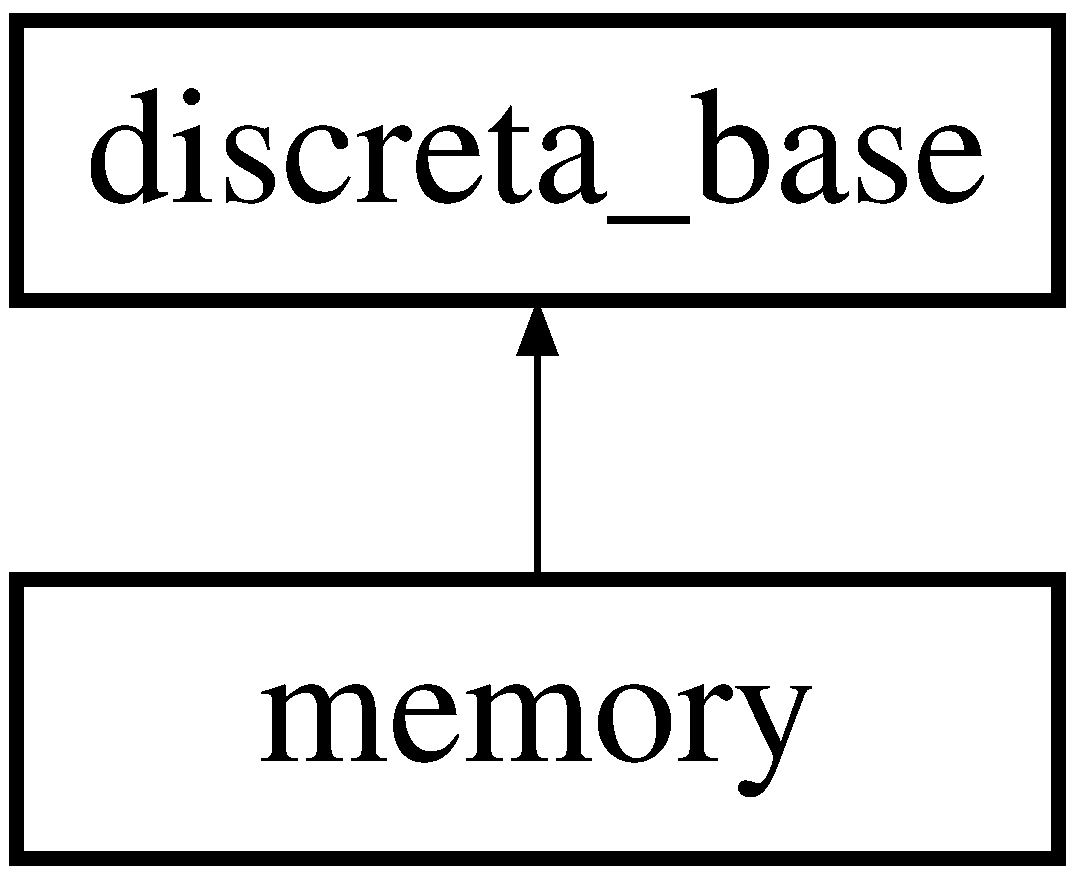
\includegraphics[height=2.000000cm]{classmemory}
\end{center}
\end{figure}
\subsection*{Public Member Functions}
\begin{DoxyCompactItemize}
\item 
\mbox{\hyperlink{classmemory_a05edf03af2b4a912939e00c7269e2085}{memory}} ()
\item 
\mbox{\hyperlink{classmemory_ade21bbe488443d2d3eb7b82a868298a6}{memory}} (const \mbox{\hyperlink{classdiscreta__base}{discreta\+\_\+base}} \&\mbox{\hyperlink{alphabet2_8_c_a6150e0515f7202e2fb518f7206ed97dc}{x}})
\item 
\mbox{\hyperlink{classmemory}{memory}} \& \mbox{\hyperlink{classmemory_a5550412426557d686fbf2df39e1dbb4c}{operator=}} (const \mbox{\hyperlink{classdiscreta__base}{discreta\+\_\+base}} \&\mbox{\hyperlink{alphabet2_8_c_a6150e0515f7202e2fb518f7206ed97dc}{x}})
\item 
void \mbox{\hyperlink{classmemory_a33aae277f9b8fe36b02e9d5da895451b}{settype\+\_\+memory}} ()
\item 
\mbox{\hyperlink{classmemory_ae5893b724ce22f38b776558384f21680}{$\sim$memory}} ()
\item 
void \mbox{\hyperlink{classmemory_a19366f9105d79a0e818cc19255d7ef4f}{freeself\+\_\+memory}} ()
\item 
\mbox{\hyperlink{discreta_8h_aaf25ee7e2306d78c74ec7bc48f092e81}{kind}} \mbox{\hyperlink{classmemory_a75dd039fc284723f284b9a62a199f623}{s\+\_\+virtual\+\_\+kind}} ()
\item 
void \mbox{\hyperlink{classmemory_a4fe4349915769808c6ff3cf83c661bf0}{copyobject\+\_\+to}} (\mbox{\hyperlink{classdiscreta__base}{discreta\+\_\+base}} \&\mbox{\hyperlink{alphabet2_8_c_a6150e0515f7202e2fb518f7206ed97dc}{x}})
\item 
ostream \& \mbox{\hyperlink{classmemory_a76e54475a51795259a3ebf1013a2559e}{print}} (ostream \&ost)
\item 
\mbox{\hyperlink{galois_8h_a09fddde158a3a20bd2dcadb609de11dc}{I\+NT}} \& \mbox{\hyperlink{classmemory_acaa1796a2f548d35cf87e03252b2184c}{alloc\+\_\+length}} ()
\item 
\mbox{\hyperlink{galois_8h_a09fddde158a3a20bd2dcadb609de11dc}{I\+NT}} \& \mbox{\hyperlink{classmemory_a3312a01b206cef29ec0f85ee340002dd}{used\+\_\+length}} ()
\item 
\mbox{\hyperlink{galois_8h_a09fddde158a3a20bd2dcadb609de11dc}{I\+NT}} \& \mbox{\hyperlink{classmemory_a24db8a00f6c8abfa6bb762264357cb22}{cur\+\_\+pointer}} ()
\item 
char \& \mbox{\hyperlink{classmemory_a3b1cda7c761e823c258e4c7a13794012}{s\+\_\+i}} (\mbox{\hyperlink{galois_8h_a09fddde158a3a20bd2dcadb609de11dc}{I\+NT}} \mbox{\hyperlink{alphabet2_8_c_acb559820d9ca11295b4500f179ef6392}{i}})
\item 
char \& \mbox{\hyperlink{classmemory_adca93ab84b9c609f5ee78b00ea7cac4d}{operator\mbox{[}$\,$\mbox{]}}} (\mbox{\hyperlink{galois_8h_a09fddde158a3a20bd2dcadb609de11dc}{I\+NT}} \mbox{\hyperlink{alphabet2_8_c_acb559820d9ca11295b4500f179ef6392}{i}})
\item 
void \mbox{\hyperlink{classmemory_a616200900a07046cd6b0b86f12765909}{init}} (\mbox{\hyperlink{galois_8h_a09fddde158a3a20bd2dcadb609de11dc}{I\+NT}} length, char $\ast$\mbox{\hyperlink{simeon_8_c_a4339ca06fa882e69473d37bd6d7917d1}{d}})
\item 
void \mbox{\hyperlink{classmemory_a44ac20be537668e94b5d42e6a6c74b6f}{alloc}} (\mbox{\hyperlink{galois_8h_a09fddde158a3a20bd2dcadb609de11dc}{I\+NT}} length)
\item 
void \mbox{\hyperlink{classmemory_a2ad10d7a4707651f6b101d919f8402ed}{append}} (\mbox{\hyperlink{galois_8h_a09fddde158a3a20bd2dcadb609de11dc}{I\+NT}} length, char $\ast$\mbox{\hyperlink{simeon_8_c_a4339ca06fa882e69473d37bd6d7917d1}{d}})
\item 
void \mbox{\hyperlink{classmemory_a8aaa32764cd9a497d57740b5cb47953b}{realloc}} (\mbox{\hyperlink{galois_8h_a09fddde158a3a20bd2dcadb609de11dc}{I\+NT}} new\+\_\+length)
\item 
void \mbox{\hyperlink{classmemory_a3f1889e0a03fd3afbb15bc78084c6356}{write\+\_\+char}} (char \mbox{\hyperlink{alphabet2_8_c_a4e1e0e72dd773439e333c84dd762a9c3}{c}})
\item 
void \mbox{\hyperlink{classmemory_ae96d2ffc64b3b3012960aae45f4c2a5b}{read\+\_\+char}} (char $\ast$\mbox{\hyperlink{alphabet2_8_c_a4e1e0e72dd773439e333c84dd762a9c3}{c}})
\item 
void \mbox{\hyperlink{classmemory_ad2bea2174f3f88051d259aa8b293bb4d}{write\+\_\+int}} (\mbox{\hyperlink{galois_8h_a09fddde158a3a20bd2dcadb609de11dc}{I\+NT}} \mbox{\hyperlink{alphabet2_8_c_acb559820d9ca11295b4500f179ef6392}{i}})
\item 
void \mbox{\hyperlink{classmemory_a2f9fe96745aaab0aebf075ab9d5fc43e}{read\+\_\+int}} (\mbox{\hyperlink{galois_8h_a09fddde158a3a20bd2dcadb609de11dc}{I\+NT}} $\ast$\mbox{\hyperlink{alphabet2_8_c_acb559820d9ca11295b4500f179ef6392}{i}})
\item 
void \mbox{\hyperlink{classmemory_af8d8b6de66f74f406ee48bb5e3825bb8}{read\+\_\+file}} (\mbox{\hyperlink{galois_8h_ab6cc7b4aeb6ea31aba2b3fbfc83ff5e6}{B\+Y\+TE}} $\ast$fname, \mbox{\hyperlink{galois_8h_a09fddde158a3a20bd2dcadb609de11dc}{I\+NT}} f\+\_\+v)
\item 
void \mbox{\hyperlink{classmemory_a665547a8b8662da816c6511cabd74ea1}{write\+\_\+file}} (\mbox{\hyperlink{galois_8h_ab6cc7b4aeb6ea31aba2b3fbfc83ff5e6}{B\+Y\+TE}} $\ast$fname, \mbox{\hyperlink{galois_8h_a09fddde158a3a20bd2dcadb609de11dc}{I\+NT}} f\+\_\+v)
\item 
\mbox{\hyperlink{galois_8h_a09fddde158a3a20bd2dcadb609de11dc}{I\+NT}} \mbox{\hyperlink{classmemory_a6a5fd3fd3ace3bd98089e618ec4c1bca}{multiplicity\+\_\+of\+\_\+character}} (\mbox{\hyperlink{galois_8h_ab6cc7b4aeb6ea31aba2b3fbfc83ff5e6}{B\+Y\+TE}} \mbox{\hyperlink{alphabet2_8_c_a4e1e0e72dd773439e333c84dd762a9c3}{c}})
\item 
void \mbox{\hyperlink{classmemory_afadcbb4b0b076d7f9552a9102b467683}{compress}} (\mbox{\hyperlink{galois_8h_a09fddde158a3a20bd2dcadb609de11dc}{I\+NT}} f\+\_\+v)
\item 
void \mbox{\hyperlink{classmemory_a1b74745da801f22d42ea54e54b23c014}{decompress}} (\mbox{\hyperlink{galois_8h_a09fddde158a3a20bd2dcadb609de11dc}{I\+NT}} f\+\_\+v)
\item 
\mbox{\hyperlink{galois_8h_a09fddde158a3a20bd2dcadb609de11dc}{I\+NT}} \mbox{\hyperlink{classmemory_a7f6c3fb11d9ef25fce0aa093bc9d9216}{csf}} ()
\item 
void \mbox{\hyperlink{classmemory_aa9d91eb1dde81ccc9fc3b45c742cafc6}{write\+\_\+mem}} (\mbox{\hyperlink{classmemory}{memory}} \&\mbox{\hyperlink{plane__search_8_c_ad2d23ebd03187a91edd45b1d5e496265}{M}}, \mbox{\hyperlink{galois_8h_a09fddde158a3a20bd2dcadb609de11dc}{I\+NT}} debug\+\_\+depth)
\item 
void \mbox{\hyperlink{classmemory_abe07337c672fca9e605c5f9df86a8c1a}{read\+\_\+mem}} (\mbox{\hyperlink{classmemory}{memory}} \&\mbox{\hyperlink{plane__search_8_c_ad2d23ebd03187a91edd45b1d5e496265}{M}}, \mbox{\hyperlink{galois_8h_a09fddde158a3a20bd2dcadb609de11dc}{I\+NT}} debug\+\_\+depth)
\end{DoxyCompactItemize}
\subsection*{Additional Inherited Members}


\subsection{Constructor \& Destructor Documentation}
\mbox{\Hypertarget{classmemory_a05edf03af2b4a912939e00c7269e2085}\label{classmemory_a05edf03af2b4a912939e00c7269e2085}} 
\index{memory@{memory}!memory@{memory}}
\index{memory@{memory}!memory@{memory}}
\subsubsection{\texorpdfstring{memory()}{memory()}\hspace{0.1cm}{\footnotesize\ttfamily [1/2]}}
{\footnotesize\ttfamily memory\+::memory (\begin{DoxyParamCaption}{ }\end{DoxyParamCaption})}

\mbox{\Hypertarget{classmemory_ade21bbe488443d2d3eb7b82a868298a6}\label{classmemory_ade21bbe488443d2d3eb7b82a868298a6}} 
\index{memory@{memory}!memory@{memory}}
\index{memory@{memory}!memory@{memory}}
\subsubsection{\texorpdfstring{memory()}{memory()}\hspace{0.1cm}{\footnotesize\ttfamily [2/2]}}
{\footnotesize\ttfamily memory\+::memory (\begin{DoxyParamCaption}\item[{const \mbox{\hyperlink{classdiscreta__base}{discreta\+\_\+base}} \&}]{x }\end{DoxyParamCaption})}

\mbox{\Hypertarget{classmemory_ae5893b724ce22f38b776558384f21680}\label{classmemory_ae5893b724ce22f38b776558384f21680}} 
\index{memory@{memory}!````~memory@{$\sim$memory}}
\index{````~memory@{$\sim$memory}!memory@{memory}}
\subsubsection{\texorpdfstring{$\sim$memory()}{~memory()}}
{\footnotesize\ttfamily memory\+::$\sim$memory (\begin{DoxyParamCaption}{ }\end{DoxyParamCaption})}



\subsection{Member Function Documentation}
\mbox{\Hypertarget{classmemory_a44ac20be537668e94b5d42e6a6c74b6f}\label{classmemory_a44ac20be537668e94b5d42e6a6c74b6f}} 
\index{memory@{memory}!alloc@{alloc}}
\index{alloc@{alloc}!memory@{memory}}
\subsubsection{\texorpdfstring{alloc()}{alloc()}}
{\footnotesize\ttfamily void memory\+::alloc (\begin{DoxyParamCaption}\item[{\mbox{\hyperlink{galois_8h_a09fddde158a3a20bd2dcadb609de11dc}{I\+NT}}}]{length }\end{DoxyParamCaption})}

\mbox{\Hypertarget{classmemory_acaa1796a2f548d35cf87e03252b2184c}\label{classmemory_acaa1796a2f548d35cf87e03252b2184c}} 
\index{memory@{memory}!alloc\+\_\+length@{alloc\+\_\+length}}
\index{alloc\+\_\+length@{alloc\+\_\+length}!memory@{memory}}
\subsubsection{\texorpdfstring{alloc\+\_\+length()}{alloc\_length()}}
{\footnotesize\ttfamily \mbox{\hyperlink{galois_8h_a09fddde158a3a20bd2dcadb609de11dc}{I\+NT}}\& memory\+::alloc\+\_\+length (\begin{DoxyParamCaption}{ }\end{DoxyParamCaption})\hspace{0.3cm}{\ttfamily [inline]}}

\mbox{\Hypertarget{classmemory_a2ad10d7a4707651f6b101d919f8402ed}\label{classmemory_a2ad10d7a4707651f6b101d919f8402ed}} 
\index{memory@{memory}!append@{append}}
\index{append@{append}!memory@{memory}}
\subsubsection{\texorpdfstring{append()}{append()}}
{\footnotesize\ttfamily void memory\+::append (\begin{DoxyParamCaption}\item[{\mbox{\hyperlink{galois_8h_a09fddde158a3a20bd2dcadb609de11dc}{I\+NT}}}]{length,  }\item[{char $\ast$}]{d }\end{DoxyParamCaption})}

\mbox{\Hypertarget{classmemory_afadcbb4b0b076d7f9552a9102b467683}\label{classmemory_afadcbb4b0b076d7f9552a9102b467683}} 
\index{memory@{memory}!compress@{compress}}
\index{compress@{compress}!memory@{memory}}
\subsubsection{\texorpdfstring{compress()}{compress()}}
{\footnotesize\ttfamily void memory\+::compress (\begin{DoxyParamCaption}\item[{\mbox{\hyperlink{galois_8h_a09fddde158a3a20bd2dcadb609de11dc}{I\+NT}}}]{f\+\_\+v }\end{DoxyParamCaption})}

\mbox{\Hypertarget{classmemory_a4fe4349915769808c6ff3cf83c661bf0}\label{classmemory_a4fe4349915769808c6ff3cf83c661bf0}} 
\index{memory@{memory}!copyobject\+\_\+to@{copyobject\+\_\+to}}
\index{copyobject\+\_\+to@{copyobject\+\_\+to}!memory@{memory}}
\subsubsection{\texorpdfstring{copyobject\+\_\+to()}{copyobject\_to()}}
{\footnotesize\ttfamily void memory\+::copyobject\+\_\+to (\begin{DoxyParamCaption}\item[{\mbox{\hyperlink{classdiscreta__base}{discreta\+\_\+base}} \&}]{x }\end{DoxyParamCaption})\hspace{0.3cm}{\ttfamily [virtual]}}



Reimplemented from \mbox{\hyperlink{classdiscreta__base_a33180628d9ced231267229b3564790f3}{discreta\+\_\+base}}.

\mbox{\Hypertarget{classmemory_a7f6c3fb11d9ef25fce0aa093bc9d9216}\label{classmemory_a7f6c3fb11d9ef25fce0aa093bc9d9216}} 
\index{memory@{memory}!csf@{csf}}
\index{csf@{csf}!memory@{memory}}
\subsubsection{\texorpdfstring{csf()}{csf()}}
{\footnotesize\ttfamily \mbox{\hyperlink{galois_8h_a09fddde158a3a20bd2dcadb609de11dc}{I\+NT}} memory\+::csf (\begin{DoxyParamCaption}{ }\end{DoxyParamCaption})}

\mbox{\Hypertarget{classmemory_a24db8a00f6c8abfa6bb762264357cb22}\label{classmemory_a24db8a00f6c8abfa6bb762264357cb22}} 
\index{memory@{memory}!cur\+\_\+pointer@{cur\+\_\+pointer}}
\index{cur\+\_\+pointer@{cur\+\_\+pointer}!memory@{memory}}
\subsubsection{\texorpdfstring{cur\+\_\+pointer()}{cur\_pointer()}}
{\footnotesize\ttfamily \mbox{\hyperlink{galois_8h_a09fddde158a3a20bd2dcadb609de11dc}{I\+NT}}\& memory\+::cur\+\_\+pointer (\begin{DoxyParamCaption}{ }\end{DoxyParamCaption})\hspace{0.3cm}{\ttfamily [inline]}}

\mbox{\Hypertarget{classmemory_a1b74745da801f22d42ea54e54b23c014}\label{classmemory_a1b74745da801f22d42ea54e54b23c014}} 
\index{memory@{memory}!decompress@{decompress}}
\index{decompress@{decompress}!memory@{memory}}
\subsubsection{\texorpdfstring{decompress()}{decompress()}}
{\footnotesize\ttfamily void memory\+::decompress (\begin{DoxyParamCaption}\item[{\mbox{\hyperlink{galois_8h_a09fddde158a3a20bd2dcadb609de11dc}{I\+NT}}}]{f\+\_\+v }\end{DoxyParamCaption})}

\mbox{\Hypertarget{classmemory_a19366f9105d79a0e818cc19255d7ef4f}\label{classmemory_a19366f9105d79a0e818cc19255d7ef4f}} 
\index{memory@{memory}!freeself\+\_\+memory@{freeself\+\_\+memory}}
\index{freeself\+\_\+memory@{freeself\+\_\+memory}!memory@{memory}}
\subsubsection{\texorpdfstring{freeself\+\_\+memory()}{freeself\_memory()}}
{\footnotesize\ttfamily void memory\+::freeself\+\_\+memory (\begin{DoxyParamCaption}{ }\end{DoxyParamCaption})}

\mbox{\Hypertarget{classmemory_a616200900a07046cd6b0b86f12765909}\label{classmemory_a616200900a07046cd6b0b86f12765909}} 
\index{memory@{memory}!init@{init}}
\index{init@{init}!memory@{memory}}
\subsubsection{\texorpdfstring{init()}{init()}}
{\footnotesize\ttfamily void memory\+::init (\begin{DoxyParamCaption}\item[{\mbox{\hyperlink{galois_8h_a09fddde158a3a20bd2dcadb609de11dc}{I\+NT}}}]{length,  }\item[{char $\ast$}]{d }\end{DoxyParamCaption})}

\mbox{\Hypertarget{classmemory_a6a5fd3fd3ace3bd98089e618ec4c1bca}\label{classmemory_a6a5fd3fd3ace3bd98089e618ec4c1bca}} 
\index{memory@{memory}!multiplicity\+\_\+of\+\_\+character@{multiplicity\+\_\+of\+\_\+character}}
\index{multiplicity\+\_\+of\+\_\+character@{multiplicity\+\_\+of\+\_\+character}!memory@{memory}}
\subsubsection{\texorpdfstring{multiplicity\+\_\+of\+\_\+character()}{multiplicity\_of\_character()}}
{\footnotesize\ttfamily \mbox{\hyperlink{galois_8h_a09fddde158a3a20bd2dcadb609de11dc}{I\+NT}} memory\+::multiplicity\+\_\+of\+\_\+character (\begin{DoxyParamCaption}\item[{\mbox{\hyperlink{galois_8h_ab6cc7b4aeb6ea31aba2b3fbfc83ff5e6}{B\+Y\+TE}}}]{c }\end{DoxyParamCaption})}

\mbox{\Hypertarget{classmemory_a5550412426557d686fbf2df39e1dbb4c}\label{classmemory_a5550412426557d686fbf2df39e1dbb4c}} 
\index{memory@{memory}!operator=@{operator=}}
\index{operator=@{operator=}!memory@{memory}}
\subsubsection{\texorpdfstring{operator=()}{operator=()}}
{\footnotesize\ttfamily \mbox{\hyperlink{classmemory}{memory}} \& memory\+::operator= (\begin{DoxyParamCaption}\item[{const \mbox{\hyperlink{classdiscreta__base}{discreta\+\_\+base}} \&}]{x }\end{DoxyParamCaption})}

\mbox{\Hypertarget{classmemory_adca93ab84b9c609f5ee78b00ea7cac4d}\label{classmemory_adca93ab84b9c609f5ee78b00ea7cac4d}} 
\index{memory@{memory}!operator\mbox{[}\mbox{]}@{operator[]}}
\index{operator\mbox{[}\mbox{]}@{operator[]}!memory@{memory}}
\subsubsection{\texorpdfstring{operator[]()}{operator[]()}}
{\footnotesize\ttfamily char\& memory\+::operator\mbox{[}$\,$\mbox{]} (\begin{DoxyParamCaption}\item[{\mbox{\hyperlink{galois_8h_a09fddde158a3a20bd2dcadb609de11dc}{I\+NT}}}]{i }\end{DoxyParamCaption})\hspace{0.3cm}{\ttfamily [inline]}}

\mbox{\Hypertarget{classmemory_a76e54475a51795259a3ebf1013a2559e}\label{classmemory_a76e54475a51795259a3ebf1013a2559e}} 
\index{memory@{memory}!print@{print}}
\index{print@{print}!memory@{memory}}
\subsubsection{\texorpdfstring{print()}{print()}}
{\footnotesize\ttfamily ostream \& memory\+::print (\begin{DoxyParamCaption}\item[{ostream \&}]{ost }\end{DoxyParamCaption})\hspace{0.3cm}{\ttfamily [virtual]}}



Reimplemented from \mbox{\hyperlink{classdiscreta__base_a036e48bc058347046fc9b73dd0951478}{discreta\+\_\+base}}.

\mbox{\Hypertarget{classmemory_ae96d2ffc64b3b3012960aae45f4c2a5b}\label{classmemory_ae96d2ffc64b3b3012960aae45f4c2a5b}} 
\index{memory@{memory}!read\+\_\+char@{read\+\_\+char}}
\index{read\+\_\+char@{read\+\_\+char}!memory@{memory}}
\subsubsection{\texorpdfstring{read\+\_\+char()}{read\_char()}}
{\footnotesize\ttfamily void memory\+::read\+\_\+char (\begin{DoxyParamCaption}\item[{char $\ast$}]{c }\end{DoxyParamCaption})}

\mbox{\Hypertarget{classmemory_af8d8b6de66f74f406ee48bb5e3825bb8}\label{classmemory_af8d8b6de66f74f406ee48bb5e3825bb8}} 
\index{memory@{memory}!read\+\_\+file@{read\+\_\+file}}
\index{read\+\_\+file@{read\+\_\+file}!memory@{memory}}
\subsubsection{\texorpdfstring{read\+\_\+file()}{read\_file()}}
{\footnotesize\ttfamily void memory\+::read\+\_\+file (\begin{DoxyParamCaption}\item[{\mbox{\hyperlink{galois_8h_ab6cc7b4aeb6ea31aba2b3fbfc83ff5e6}{B\+Y\+TE}} $\ast$}]{fname,  }\item[{\mbox{\hyperlink{galois_8h_a09fddde158a3a20bd2dcadb609de11dc}{I\+NT}}}]{f\+\_\+v }\end{DoxyParamCaption})}

\mbox{\Hypertarget{classmemory_a2f9fe96745aaab0aebf075ab9d5fc43e}\label{classmemory_a2f9fe96745aaab0aebf075ab9d5fc43e}} 
\index{memory@{memory}!read\+\_\+int@{read\+\_\+int}}
\index{read\+\_\+int@{read\+\_\+int}!memory@{memory}}
\subsubsection{\texorpdfstring{read\+\_\+int()}{read\_int()}}
{\footnotesize\ttfamily void memory\+::read\+\_\+int (\begin{DoxyParamCaption}\item[{\mbox{\hyperlink{galois_8h_a09fddde158a3a20bd2dcadb609de11dc}{I\+NT}} $\ast$}]{i }\end{DoxyParamCaption})}

\mbox{\Hypertarget{classmemory_abe07337c672fca9e605c5f9df86a8c1a}\label{classmemory_abe07337c672fca9e605c5f9df86a8c1a}} 
\index{memory@{memory}!read\+\_\+mem@{read\+\_\+mem}}
\index{read\+\_\+mem@{read\+\_\+mem}!memory@{memory}}
\subsubsection{\texorpdfstring{read\+\_\+mem()}{read\_mem()}}
{\footnotesize\ttfamily void memory\+::read\+\_\+mem (\begin{DoxyParamCaption}\item[{\mbox{\hyperlink{classmemory}{memory}} \&}]{M,  }\item[{\mbox{\hyperlink{galois_8h_a09fddde158a3a20bd2dcadb609de11dc}{I\+NT}}}]{debug\+\_\+depth }\end{DoxyParamCaption})}

\mbox{\Hypertarget{classmemory_a8aaa32764cd9a497d57740b5cb47953b}\label{classmemory_a8aaa32764cd9a497d57740b5cb47953b}} 
\index{memory@{memory}!realloc@{realloc}}
\index{realloc@{realloc}!memory@{memory}}
\subsubsection{\texorpdfstring{realloc()}{realloc()}}
{\footnotesize\ttfamily void memory\+::realloc (\begin{DoxyParamCaption}\item[{\mbox{\hyperlink{galois_8h_a09fddde158a3a20bd2dcadb609de11dc}{I\+NT}}}]{new\+\_\+length }\end{DoxyParamCaption})}

\mbox{\Hypertarget{classmemory_a3b1cda7c761e823c258e4c7a13794012}\label{classmemory_a3b1cda7c761e823c258e4c7a13794012}} 
\index{memory@{memory}!s\+\_\+i@{s\+\_\+i}}
\index{s\+\_\+i@{s\+\_\+i}!memory@{memory}}
\subsubsection{\texorpdfstring{s\+\_\+i()}{s\_i()}}
{\footnotesize\ttfamily char\& memory\+::s\+\_\+i (\begin{DoxyParamCaption}\item[{\mbox{\hyperlink{galois_8h_a09fddde158a3a20bd2dcadb609de11dc}{I\+NT}}}]{i }\end{DoxyParamCaption})\hspace{0.3cm}{\ttfamily [inline]}}

\mbox{\Hypertarget{classmemory_a75dd039fc284723f284b9a62a199f623}\label{classmemory_a75dd039fc284723f284b9a62a199f623}} 
\index{memory@{memory}!s\+\_\+virtual\+\_\+kind@{s\+\_\+virtual\+\_\+kind}}
\index{s\+\_\+virtual\+\_\+kind@{s\+\_\+virtual\+\_\+kind}!memory@{memory}}
\subsubsection{\texorpdfstring{s\+\_\+virtual\+\_\+kind()}{s\_virtual\_kind()}}
{\footnotesize\ttfamily \mbox{\hyperlink{discreta_8h_aaf25ee7e2306d78c74ec7bc48f092e81}{kind}} memory\+::s\+\_\+virtual\+\_\+kind (\begin{DoxyParamCaption}{ }\end{DoxyParamCaption})\hspace{0.3cm}{\ttfamily [virtual]}}



Reimplemented from \mbox{\hyperlink{classdiscreta__base_a52778a6d6943a468be083d0785d418fb}{discreta\+\_\+base}}.

\mbox{\Hypertarget{classmemory_a33aae277f9b8fe36b02e9d5da895451b}\label{classmemory_a33aae277f9b8fe36b02e9d5da895451b}} 
\index{memory@{memory}!settype\+\_\+memory@{settype\+\_\+memory}}
\index{settype\+\_\+memory@{settype\+\_\+memory}!memory@{memory}}
\subsubsection{\texorpdfstring{settype\+\_\+memory()}{settype\_memory()}}
{\footnotesize\ttfamily void memory\+::settype\+\_\+memory (\begin{DoxyParamCaption}{ }\end{DoxyParamCaption})}

\mbox{\Hypertarget{classmemory_a3312a01b206cef29ec0f85ee340002dd}\label{classmemory_a3312a01b206cef29ec0f85ee340002dd}} 
\index{memory@{memory}!used\+\_\+length@{used\+\_\+length}}
\index{used\+\_\+length@{used\+\_\+length}!memory@{memory}}
\subsubsection{\texorpdfstring{used\+\_\+length()}{used\_length()}}
{\footnotesize\ttfamily \mbox{\hyperlink{galois_8h_a09fddde158a3a20bd2dcadb609de11dc}{I\+NT}}\& memory\+::used\+\_\+length (\begin{DoxyParamCaption}{ }\end{DoxyParamCaption})\hspace{0.3cm}{\ttfamily [inline]}}

\mbox{\Hypertarget{classmemory_a3f1889e0a03fd3afbb15bc78084c6356}\label{classmemory_a3f1889e0a03fd3afbb15bc78084c6356}} 
\index{memory@{memory}!write\+\_\+char@{write\+\_\+char}}
\index{write\+\_\+char@{write\+\_\+char}!memory@{memory}}
\subsubsection{\texorpdfstring{write\+\_\+char()}{write\_char()}}
{\footnotesize\ttfamily void memory\+::write\+\_\+char (\begin{DoxyParamCaption}\item[{char}]{c }\end{DoxyParamCaption})}

\mbox{\Hypertarget{classmemory_a665547a8b8662da816c6511cabd74ea1}\label{classmemory_a665547a8b8662da816c6511cabd74ea1}} 
\index{memory@{memory}!write\+\_\+file@{write\+\_\+file}}
\index{write\+\_\+file@{write\+\_\+file}!memory@{memory}}
\subsubsection{\texorpdfstring{write\+\_\+file()}{write\_file()}}
{\footnotesize\ttfamily void memory\+::write\+\_\+file (\begin{DoxyParamCaption}\item[{\mbox{\hyperlink{galois_8h_ab6cc7b4aeb6ea31aba2b3fbfc83ff5e6}{B\+Y\+TE}} $\ast$}]{fname,  }\item[{\mbox{\hyperlink{galois_8h_a09fddde158a3a20bd2dcadb609de11dc}{I\+NT}}}]{f\+\_\+v }\end{DoxyParamCaption})}

\mbox{\Hypertarget{classmemory_ad2bea2174f3f88051d259aa8b293bb4d}\label{classmemory_ad2bea2174f3f88051d259aa8b293bb4d}} 
\index{memory@{memory}!write\+\_\+int@{write\+\_\+int}}
\index{write\+\_\+int@{write\+\_\+int}!memory@{memory}}
\subsubsection{\texorpdfstring{write\+\_\+int()}{write\_int()}}
{\footnotesize\ttfamily void memory\+::write\+\_\+int (\begin{DoxyParamCaption}\item[{\mbox{\hyperlink{galois_8h_a09fddde158a3a20bd2dcadb609de11dc}{I\+NT}}}]{i }\end{DoxyParamCaption})}

\mbox{\Hypertarget{classmemory_aa9d91eb1dde81ccc9fc3b45c742cafc6}\label{classmemory_aa9d91eb1dde81ccc9fc3b45c742cafc6}} 
\index{memory@{memory}!write\+\_\+mem@{write\+\_\+mem}}
\index{write\+\_\+mem@{write\+\_\+mem}!memory@{memory}}
\subsubsection{\texorpdfstring{write\+\_\+mem()}{write\_mem()}}
{\footnotesize\ttfamily void memory\+::write\+\_\+mem (\begin{DoxyParamCaption}\item[{\mbox{\hyperlink{classmemory}{memory}} \&}]{M,  }\item[{\mbox{\hyperlink{galois_8h_a09fddde158a3a20bd2dcadb609de11dc}{I\+NT}}}]{debug\+\_\+depth }\end{DoxyParamCaption})}



The documentation for this class was generated from the following files\+:\begin{DoxyCompactItemize}
\item 
S\+R\+C/\+L\+I\+B/\+D\+I\+S\+C\+R\+E\+T\+A/\mbox{\hyperlink{discreta_8h}{discreta.\+h}}\item 
S\+R\+C/\+L\+I\+B/\+D\+I\+S\+C\+R\+E\+T\+A/\mbox{\hyperlink{_d_i_s_c_r_e_t_a_2memory_8_c}{memory.\+C}}\end{DoxyCompactItemize}

\hypertarget{classmemory__object}{}\section{memory\+\_\+object Class Reference}
\label{classmemory__object}\index{memory\+\_\+object@{memory\+\_\+object}}


{\ttfamily \#include $<$galois.\+h$>$}

\subsection*{Public Member Functions}
\begin{DoxyCompactItemize}
\item 
\mbox{\hyperlink{classmemory__object_a5465c06078f383cff3a663212db3385a}{memory\+\_\+object}} ()
\item 
\mbox{\hyperlink{classmemory__object_a9af084044507354ba7fcc5f28220a3a4}{$\sim$memory\+\_\+object}} ()
\item 
void \mbox{\hyperlink{classmemory__object_a9e538ffb790fddfebcf9557386af1e76}{null}} ()
\item 
void \mbox{\hyperlink{classmemory__object_aea989e6df86ed48049a2747df074b62a}{freeself}} ()
\item 
char \& \mbox{\hyperlink{classmemory__object_a8ab798c46f6f2c80176803d2fa930ba2}{s\+\_\+i}} (\mbox{\hyperlink{galois_8h_a09fddde158a3a20bd2dcadb609de11dc}{I\+NT}} \mbox{\hyperlink{alphabet2_8_c_acb559820d9ca11295b4500f179ef6392}{i}})
\item 
void \mbox{\hyperlink{classmemory__object_af3db8aaeacba976233f0f257a8678bdf}{init}} (\mbox{\hyperlink{galois_8h_a09fddde158a3a20bd2dcadb609de11dc}{I\+NT}} length, char $\ast$\mbox{\hyperlink{simeon_8_c_a4339ca06fa882e69473d37bd6d7917d1}{d}}, \mbox{\hyperlink{galois_8h_a09fddde158a3a20bd2dcadb609de11dc}{I\+NT}} \mbox{\hyperlink{simeon_8_c_a818073fbcc2f439e7c56952f67386122}{verbose\+\_\+level}})
\item 
void \mbox{\hyperlink{classmemory__object_a0768d510d8df4bed863435b637750185}{alloc}} (\mbox{\hyperlink{galois_8h_a09fddde158a3a20bd2dcadb609de11dc}{I\+NT}} length, \mbox{\hyperlink{galois_8h_a09fddde158a3a20bd2dcadb609de11dc}{I\+NT}} \mbox{\hyperlink{simeon_8_c_a818073fbcc2f439e7c56952f67386122}{verbose\+\_\+level}})
\item 
void \mbox{\hyperlink{classmemory__object_af27e1f0829bc6372b2a2632463bb267f}{append}} (\mbox{\hyperlink{galois_8h_a09fddde158a3a20bd2dcadb609de11dc}{I\+NT}} length, char $\ast$\mbox{\hyperlink{simeon_8_c_a4339ca06fa882e69473d37bd6d7917d1}{d}}, \mbox{\hyperlink{galois_8h_a09fddde158a3a20bd2dcadb609de11dc}{I\+NT}} \mbox{\hyperlink{simeon_8_c_a818073fbcc2f439e7c56952f67386122}{verbose\+\_\+level}})
\item 
void \mbox{\hyperlink{classmemory__object_a29ea5862bdfae31e11a5c1ccc121b594}{realloc}} (\mbox{\hyperlink{galois_8h_a09fddde158a3a20bd2dcadb609de11dc}{I\+NT}} new\+\_\+length, \mbox{\hyperlink{galois_8h_a09fddde158a3a20bd2dcadb609de11dc}{I\+NT}} \mbox{\hyperlink{simeon_8_c_a818073fbcc2f439e7c56952f67386122}{verbose\+\_\+level}})
\item 
void \mbox{\hyperlink{classmemory__object_a1b2aafe9f159e3ca6384b7a8db0cc7cf}{write\+\_\+char}} (char \mbox{\hyperlink{alphabet2_8_c_a4e1e0e72dd773439e333c84dd762a9c3}{c}})
\item 
void \mbox{\hyperlink{classmemory__object_ad45168f1726af96cdbe0770c07cd6e23}{read\+\_\+char}} (char $\ast$\mbox{\hyperlink{alphabet2_8_c_a4e1e0e72dd773439e333c84dd762a9c3}{c}})
\item 
void \mbox{\hyperlink{classmemory__object_ae4bf39b14c242094cc6f281c00aea9bc}{write\+\_\+string}} (const \mbox{\hyperlink{galois_8h_ab6cc7b4aeb6ea31aba2b3fbfc83ff5e6}{B\+Y\+TE}} $\ast$\mbox{\hyperlink{alphabet2_8_c_a533391314665d6bf1b5575e9a9cd8552}{p}})
\item 
void \mbox{\hyperlink{classmemory__object_a0810257f34c8323453af7bf783511ed1}{read\+\_\+string}} (\mbox{\hyperlink{galois_8h_ab6cc7b4aeb6ea31aba2b3fbfc83ff5e6}{B\+Y\+TE}} $\ast$\&\mbox{\hyperlink{alphabet2_8_c_a533391314665d6bf1b5575e9a9cd8552}{p}})
\item 
void \mbox{\hyperlink{classmemory__object_a05ab03814bd373ee3edd0d897b437873}{write\+\_\+double}} (double \mbox{\hyperlink{alphabet2_8_c_a362077c979b0bb65159c603270e40f70}{f}})
\item 
void \mbox{\hyperlink{classmemory__object_ae3350c7b5063f2a384ca1de02f63bc7c}{read\+\_\+double}} (double $\ast$\mbox{\hyperlink{alphabet2_8_c_a362077c979b0bb65159c603270e40f70}{f}})
\item 
void \mbox{\hyperlink{classmemory__object_aace89309983982f60d83562b1a19401b}{write\+\_\+int64}} (\mbox{\hyperlink{galois_8h_a09fddde158a3a20bd2dcadb609de11dc}{I\+NT}} \mbox{\hyperlink{alphabet2_8_c_acb559820d9ca11295b4500f179ef6392}{i}})
\item 
void \mbox{\hyperlink{classmemory__object_a87244ab7abe1740f52575bc0e1760e93}{read\+\_\+int64}} (\mbox{\hyperlink{galois_8h_a09fddde158a3a20bd2dcadb609de11dc}{I\+NT}} $\ast$\mbox{\hyperlink{alphabet2_8_c_acb559820d9ca11295b4500f179ef6392}{i}})
\item 
void \mbox{\hyperlink{classmemory__object_ac64fbf0d109921cda07123999b0ac486}{write\+\_\+int}} (\mbox{\hyperlink{galois_8h_a09fddde158a3a20bd2dcadb609de11dc}{I\+NT}} \mbox{\hyperlink{alphabet2_8_c_acb559820d9ca11295b4500f179ef6392}{i}})
\item 
void \mbox{\hyperlink{classmemory__object_a6aaa53a5e94345b5a0343a07d32f20b4}{read\+\_\+int}} (\mbox{\hyperlink{galois_8h_a09fddde158a3a20bd2dcadb609de11dc}{I\+NT}} $\ast$\mbox{\hyperlink{alphabet2_8_c_acb559820d9ca11295b4500f179ef6392}{i}})
\item 
void \mbox{\hyperlink{classmemory__object_a19850b4ae2c5a995daec451a9725ebf1}{read\+\_\+file}} (const \mbox{\hyperlink{galois_8h_ab6cc7b4aeb6ea31aba2b3fbfc83ff5e6}{B\+Y\+TE}} $\ast$fname, \mbox{\hyperlink{galois_8h_a09fddde158a3a20bd2dcadb609de11dc}{I\+NT}} \mbox{\hyperlink{simeon_8_c_a818073fbcc2f439e7c56952f67386122}{verbose\+\_\+level}})
\item 
void \mbox{\hyperlink{classmemory__object_ad6bc02ec81a0088a4291ba8edf20b262}{write\+\_\+file}} (const \mbox{\hyperlink{galois_8h_ab6cc7b4aeb6ea31aba2b3fbfc83ff5e6}{B\+Y\+TE}} $\ast$fname, \mbox{\hyperlink{galois_8h_a09fddde158a3a20bd2dcadb609de11dc}{I\+NT}} \mbox{\hyperlink{simeon_8_c_a818073fbcc2f439e7c56952f67386122}{verbose\+\_\+level}})
\item 
\mbox{\hyperlink{galois_8h_a09fddde158a3a20bd2dcadb609de11dc}{I\+NT}} \mbox{\hyperlink{classmemory__object_ae756f2f73b88d0150deb1d2b32b5d7a5}{multiplicity\+\_\+of\+\_\+character}} (\mbox{\hyperlink{galois_8h_ab6cc7b4aeb6ea31aba2b3fbfc83ff5e6}{B\+Y\+TE}} \mbox{\hyperlink{alphabet2_8_c_a4e1e0e72dd773439e333c84dd762a9c3}{c}})
\item 
void \mbox{\hyperlink{classmemory__object_a19117ffce9e562d369adac83a51fc997}{compress}} (\mbox{\hyperlink{galois_8h_a09fddde158a3a20bd2dcadb609de11dc}{I\+NT}} \mbox{\hyperlink{simeon_8_c_a818073fbcc2f439e7c56952f67386122}{verbose\+\_\+level}})
\item 
void \mbox{\hyperlink{classmemory__object_af32137ad9fb4961041d6f83c67c5dea2}{decompress}} (\mbox{\hyperlink{galois_8h_a09fddde158a3a20bd2dcadb609de11dc}{I\+NT}} \mbox{\hyperlink{simeon_8_c_a818073fbcc2f439e7c56952f67386122}{verbose\+\_\+level}})
\end{DoxyCompactItemize}
\subsection*{Public Attributes}
\begin{DoxyCompactItemize}
\item 
\mbox{\hyperlink{galois_8h_ab6cc7b4aeb6ea31aba2b3fbfc83ff5e6}{B\+Y\+TE}} $\ast$ \mbox{\hyperlink{classmemory__object_a2ed98d96dff407dcea840fe10da49dd4}{char\+\_\+pointer}}
\item 
\mbox{\hyperlink{galois_8h_a09fddde158a3a20bd2dcadb609de11dc}{I\+NT}} \mbox{\hyperlink{classmemory__object_abb0f5d1d8a7ea132aad50c5359e89833}{alloc\+\_\+length}}
\item 
\mbox{\hyperlink{galois_8h_a09fddde158a3a20bd2dcadb609de11dc}{I\+NT}} \mbox{\hyperlink{classmemory__object_a7deeb1452089f3a16dfb9da259f3e4ae}{used\+\_\+length}}
\item 
\mbox{\hyperlink{galois_8h_a09fddde158a3a20bd2dcadb609de11dc}{I\+NT}} \mbox{\hyperlink{classmemory__object_a52ad3daf2b67e1fdfb413f9ffe38fbb7}{cur\+\_\+pointer}}
\end{DoxyCompactItemize}


\subsection{Constructor \& Destructor Documentation}
\mbox{\Hypertarget{classmemory__object_a5465c06078f383cff3a663212db3385a}\label{classmemory__object_a5465c06078f383cff3a663212db3385a}} 
\index{memory\+\_\+object@{memory\+\_\+object}!memory\+\_\+object@{memory\+\_\+object}}
\index{memory\+\_\+object@{memory\+\_\+object}!memory\+\_\+object@{memory\+\_\+object}}
\subsubsection{\texorpdfstring{memory\+\_\+object()}{memory\_object()}}
{\footnotesize\ttfamily memory\+\_\+object\+::memory\+\_\+object (\begin{DoxyParamCaption}{ }\end{DoxyParamCaption})}

\mbox{\Hypertarget{classmemory__object_a9af084044507354ba7fcc5f28220a3a4}\label{classmemory__object_a9af084044507354ba7fcc5f28220a3a4}} 
\index{memory\+\_\+object@{memory\+\_\+object}!````~memory\+\_\+object@{$\sim$memory\+\_\+object}}
\index{````~memory\+\_\+object@{$\sim$memory\+\_\+object}!memory\+\_\+object@{memory\+\_\+object}}
\subsubsection{\texorpdfstring{$\sim$memory\+\_\+object()}{~memory\_object()}}
{\footnotesize\ttfamily memory\+\_\+object\+::$\sim$memory\+\_\+object (\begin{DoxyParamCaption}{ }\end{DoxyParamCaption})}



\subsection{Member Function Documentation}
\mbox{\Hypertarget{classmemory__object_a0768d510d8df4bed863435b637750185}\label{classmemory__object_a0768d510d8df4bed863435b637750185}} 
\index{memory\+\_\+object@{memory\+\_\+object}!alloc@{alloc}}
\index{alloc@{alloc}!memory\+\_\+object@{memory\+\_\+object}}
\subsubsection{\texorpdfstring{alloc()}{alloc()}}
{\footnotesize\ttfamily void memory\+\_\+object\+::alloc (\begin{DoxyParamCaption}\item[{\mbox{\hyperlink{galois_8h_a09fddde158a3a20bd2dcadb609de11dc}{I\+NT}}}]{length,  }\item[{\mbox{\hyperlink{galois_8h_a09fddde158a3a20bd2dcadb609de11dc}{I\+NT}}}]{verbose\+\_\+level }\end{DoxyParamCaption})}

\mbox{\Hypertarget{classmemory__object_af27e1f0829bc6372b2a2632463bb267f}\label{classmemory__object_af27e1f0829bc6372b2a2632463bb267f}} 
\index{memory\+\_\+object@{memory\+\_\+object}!append@{append}}
\index{append@{append}!memory\+\_\+object@{memory\+\_\+object}}
\subsubsection{\texorpdfstring{append()}{append()}}
{\footnotesize\ttfamily void memory\+\_\+object\+::append (\begin{DoxyParamCaption}\item[{\mbox{\hyperlink{galois_8h_a09fddde158a3a20bd2dcadb609de11dc}{I\+NT}}}]{length,  }\item[{char $\ast$}]{d,  }\item[{\mbox{\hyperlink{galois_8h_a09fddde158a3a20bd2dcadb609de11dc}{I\+NT}}}]{verbose\+\_\+level }\end{DoxyParamCaption})}

\mbox{\Hypertarget{classmemory__object_a19117ffce9e562d369adac83a51fc997}\label{classmemory__object_a19117ffce9e562d369adac83a51fc997}} 
\index{memory\+\_\+object@{memory\+\_\+object}!compress@{compress}}
\index{compress@{compress}!memory\+\_\+object@{memory\+\_\+object}}
\subsubsection{\texorpdfstring{compress()}{compress()}}
{\footnotesize\ttfamily void memory\+\_\+object\+::compress (\begin{DoxyParamCaption}\item[{\mbox{\hyperlink{galois_8h_a09fddde158a3a20bd2dcadb609de11dc}{I\+NT}}}]{verbose\+\_\+level }\end{DoxyParamCaption})}

\mbox{\Hypertarget{classmemory__object_af32137ad9fb4961041d6f83c67c5dea2}\label{classmemory__object_af32137ad9fb4961041d6f83c67c5dea2}} 
\index{memory\+\_\+object@{memory\+\_\+object}!decompress@{decompress}}
\index{decompress@{decompress}!memory\+\_\+object@{memory\+\_\+object}}
\subsubsection{\texorpdfstring{decompress()}{decompress()}}
{\footnotesize\ttfamily void memory\+\_\+object\+::decompress (\begin{DoxyParamCaption}\item[{\mbox{\hyperlink{galois_8h_a09fddde158a3a20bd2dcadb609de11dc}{I\+NT}}}]{verbose\+\_\+level }\end{DoxyParamCaption})}

\mbox{\Hypertarget{classmemory__object_aea989e6df86ed48049a2747df074b62a}\label{classmemory__object_aea989e6df86ed48049a2747df074b62a}} 
\index{memory\+\_\+object@{memory\+\_\+object}!freeself@{freeself}}
\index{freeself@{freeself}!memory\+\_\+object@{memory\+\_\+object}}
\subsubsection{\texorpdfstring{freeself()}{freeself()}}
{\footnotesize\ttfamily void memory\+\_\+object\+::freeself (\begin{DoxyParamCaption}{ }\end{DoxyParamCaption})}

\mbox{\Hypertarget{classmemory__object_af3db8aaeacba976233f0f257a8678bdf}\label{classmemory__object_af3db8aaeacba976233f0f257a8678bdf}} 
\index{memory\+\_\+object@{memory\+\_\+object}!init@{init}}
\index{init@{init}!memory\+\_\+object@{memory\+\_\+object}}
\subsubsection{\texorpdfstring{init()}{init()}}
{\footnotesize\ttfamily void memory\+\_\+object\+::init (\begin{DoxyParamCaption}\item[{\mbox{\hyperlink{galois_8h_a09fddde158a3a20bd2dcadb609de11dc}{I\+NT}}}]{length,  }\item[{char $\ast$}]{d,  }\item[{\mbox{\hyperlink{galois_8h_a09fddde158a3a20bd2dcadb609de11dc}{I\+NT}}}]{verbose\+\_\+level }\end{DoxyParamCaption})}

\mbox{\Hypertarget{classmemory__object_ae756f2f73b88d0150deb1d2b32b5d7a5}\label{classmemory__object_ae756f2f73b88d0150deb1d2b32b5d7a5}} 
\index{memory\+\_\+object@{memory\+\_\+object}!multiplicity\+\_\+of\+\_\+character@{multiplicity\+\_\+of\+\_\+character}}
\index{multiplicity\+\_\+of\+\_\+character@{multiplicity\+\_\+of\+\_\+character}!memory\+\_\+object@{memory\+\_\+object}}
\subsubsection{\texorpdfstring{multiplicity\+\_\+of\+\_\+character()}{multiplicity\_of\_character()}}
{\footnotesize\ttfamily \mbox{\hyperlink{galois_8h_a09fddde158a3a20bd2dcadb609de11dc}{I\+NT}} memory\+\_\+object\+::multiplicity\+\_\+of\+\_\+character (\begin{DoxyParamCaption}\item[{\mbox{\hyperlink{galois_8h_ab6cc7b4aeb6ea31aba2b3fbfc83ff5e6}{B\+Y\+TE}}}]{c }\end{DoxyParamCaption})}

\mbox{\Hypertarget{classmemory__object_a9e538ffb790fddfebcf9557386af1e76}\label{classmemory__object_a9e538ffb790fddfebcf9557386af1e76}} 
\index{memory\+\_\+object@{memory\+\_\+object}!null@{null}}
\index{null@{null}!memory\+\_\+object@{memory\+\_\+object}}
\subsubsection{\texorpdfstring{null()}{null()}}
{\footnotesize\ttfamily void memory\+\_\+object\+::null (\begin{DoxyParamCaption}{ }\end{DoxyParamCaption})}

\mbox{\Hypertarget{classmemory__object_ad45168f1726af96cdbe0770c07cd6e23}\label{classmemory__object_ad45168f1726af96cdbe0770c07cd6e23}} 
\index{memory\+\_\+object@{memory\+\_\+object}!read\+\_\+char@{read\+\_\+char}}
\index{read\+\_\+char@{read\+\_\+char}!memory\+\_\+object@{memory\+\_\+object}}
\subsubsection{\texorpdfstring{read\+\_\+char()}{read\_char()}}
{\footnotesize\ttfamily void memory\+\_\+object\+::read\+\_\+char (\begin{DoxyParamCaption}\item[{char $\ast$}]{c }\end{DoxyParamCaption})}

\mbox{\Hypertarget{classmemory__object_ae3350c7b5063f2a384ca1de02f63bc7c}\label{classmemory__object_ae3350c7b5063f2a384ca1de02f63bc7c}} 
\index{memory\+\_\+object@{memory\+\_\+object}!read\+\_\+double@{read\+\_\+double}}
\index{read\+\_\+double@{read\+\_\+double}!memory\+\_\+object@{memory\+\_\+object}}
\subsubsection{\texorpdfstring{read\+\_\+double()}{read\_double()}}
{\footnotesize\ttfamily void memory\+\_\+object\+::read\+\_\+double (\begin{DoxyParamCaption}\item[{double $\ast$}]{f }\end{DoxyParamCaption})}

\mbox{\Hypertarget{classmemory__object_a19850b4ae2c5a995daec451a9725ebf1}\label{classmemory__object_a19850b4ae2c5a995daec451a9725ebf1}} 
\index{memory\+\_\+object@{memory\+\_\+object}!read\+\_\+file@{read\+\_\+file}}
\index{read\+\_\+file@{read\+\_\+file}!memory\+\_\+object@{memory\+\_\+object}}
\subsubsection{\texorpdfstring{read\+\_\+file()}{read\_file()}}
{\footnotesize\ttfamily void memory\+\_\+object\+::read\+\_\+file (\begin{DoxyParamCaption}\item[{const \mbox{\hyperlink{galois_8h_ab6cc7b4aeb6ea31aba2b3fbfc83ff5e6}{B\+Y\+TE}} $\ast$}]{fname,  }\item[{\mbox{\hyperlink{galois_8h_a09fddde158a3a20bd2dcadb609de11dc}{I\+NT}}}]{verbose\+\_\+level }\end{DoxyParamCaption})}

\mbox{\Hypertarget{classmemory__object_a6aaa53a5e94345b5a0343a07d32f20b4}\label{classmemory__object_a6aaa53a5e94345b5a0343a07d32f20b4}} 
\index{memory\+\_\+object@{memory\+\_\+object}!read\+\_\+int@{read\+\_\+int}}
\index{read\+\_\+int@{read\+\_\+int}!memory\+\_\+object@{memory\+\_\+object}}
\subsubsection{\texorpdfstring{read\+\_\+int()}{read\_int()}}
{\footnotesize\ttfamily void memory\+\_\+object\+::read\+\_\+int (\begin{DoxyParamCaption}\item[{\mbox{\hyperlink{galois_8h_a09fddde158a3a20bd2dcadb609de11dc}{I\+NT}} $\ast$}]{i }\end{DoxyParamCaption})}

\mbox{\Hypertarget{classmemory__object_a87244ab7abe1740f52575bc0e1760e93}\label{classmemory__object_a87244ab7abe1740f52575bc0e1760e93}} 
\index{memory\+\_\+object@{memory\+\_\+object}!read\+\_\+int64@{read\+\_\+int64}}
\index{read\+\_\+int64@{read\+\_\+int64}!memory\+\_\+object@{memory\+\_\+object}}
\subsubsection{\texorpdfstring{read\+\_\+int64()}{read\_int64()}}
{\footnotesize\ttfamily void memory\+\_\+object\+::read\+\_\+int64 (\begin{DoxyParamCaption}\item[{\mbox{\hyperlink{galois_8h_a09fddde158a3a20bd2dcadb609de11dc}{I\+NT}} $\ast$}]{i }\end{DoxyParamCaption})}

\mbox{\Hypertarget{classmemory__object_a0810257f34c8323453af7bf783511ed1}\label{classmemory__object_a0810257f34c8323453af7bf783511ed1}} 
\index{memory\+\_\+object@{memory\+\_\+object}!read\+\_\+string@{read\+\_\+string}}
\index{read\+\_\+string@{read\+\_\+string}!memory\+\_\+object@{memory\+\_\+object}}
\subsubsection{\texorpdfstring{read\+\_\+string()}{read\_string()}}
{\footnotesize\ttfamily void memory\+\_\+object\+::read\+\_\+string (\begin{DoxyParamCaption}\item[{\mbox{\hyperlink{galois_8h_ab6cc7b4aeb6ea31aba2b3fbfc83ff5e6}{B\+Y\+TE}} $\ast$\&}]{p }\end{DoxyParamCaption})}

\mbox{\Hypertarget{classmemory__object_a29ea5862bdfae31e11a5c1ccc121b594}\label{classmemory__object_a29ea5862bdfae31e11a5c1ccc121b594}} 
\index{memory\+\_\+object@{memory\+\_\+object}!realloc@{realloc}}
\index{realloc@{realloc}!memory\+\_\+object@{memory\+\_\+object}}
\subsubsection{\texorpdfstring{realloc()}{realloc()}}
{\footnotesize\ttfamily void memory\+\_\+object\+::realloc (\begin{DoxyParamCaption}\item[{\mbox{\hyperlink{galois_8h_a09fddde158a3a20bd2dcadb609de11dc}{I\+NT}}}]{new\+\_\+length,  }\item[{\mbox{\hyperlink{galois_8h_a09fddde158a3a20bd2dcadb609de11dc}{I\+NT}}}]{verbose\+\_\+level }\end{DoxyParamCaption})}

\mbox{\Hypertarget{classmemory__object_a8ab798c46f6f2c80176803d2fa930ba2}\label{classmemory__object_a8ab798c46f6f2c80176803d2fa930ba2}} 
\index{memory\+\_\+object@{memory\+\_\+object}!s\+\_\+i@{s\+\_\+i}}
\index{s\+\_\+i@{s\+\_\+i}!memory\+\_\+object@{memory\+\_\+object}}
\subsubsection{\texorpdfstring{s\+\_\+i()}{s\_i()}}
{\footnotesize\ttfamily char\& memory\+\_\+object\+::s\+\_\+i (\begin{DoxyParamCaption}\item[{\mbox{\hyperlink{galois_8h_a09fddde158a3a20bd2dcadb609de11dc}{I\+NT}}}]{i }\end{DoxyParamCaption})\hspace{0.3cm}{\ttfamily [inline]}}

\mbox{\Hypertarget{classmemory__object_a1b2aafe9f159e3ca6384b7a8db0cc7cf}\label{classmemory__object_a1b2aafe9f159e3ca6384b7a8db0cc7cf}} 
\index{memory\+\_\+object@{memory\+\_\+object}!write\+\_\+char@{write\+\_\+char}}
\index{write\+\_\+char@{write\+\_\+char}!memory\+\_\+object@{memory\+\_\+object}}
\subsubsection{\texorpdfstring{write\+\_\+char()}{write\_char()}}
{\footnotesize\ttfamily void memory\+\_\+object\+::write\+\_\+char (\begin{DoxyParamCaption}\item[{char}]{c }\end{DoxyParamCaption})}

\mbox{\Hypertarget{classmemory__object_a05ab03814bd373ee3edd0d897b437873}\label{classmemory__object_a05ab03814bd373ee3edd0d897b437873}} 
\index{memory\+\_\+object@{memory\+\_\+object}!write\+\_\+double@{write\+\_\+double}}
\index{write\+\_\+double@{write\+\_\+double}!memory\+\_\+object@{memory\+\_\+object}}
\subsubsection{\texorpdfstring{write\+\_\+double()}{write\_double()}}
{\footnotesize\ttfamily void memory\+\_\+object\+::write\+\_\+double (\begin{DoxyParamCaption}\item[{double}]{f }\end{DoxyParamCaption})}

\mbox{\Hypertarget{classmemory__object_ad6bc02ec81a0088a4291ba8edf20b262}\label{classmemory__object_ad6bc02ec81a0088a4291ba8edf20b262}} 
\index{memory\+\_\+object@{memory\+\_\+object}!write\+\_\+file@{write\+\_\+file}}
\index{write\+\_\+file@{write\+\_\+file}!memory\+\_\+object@{memory\+\_\+object}}
\subsubsection{\texorpdfstring{write\+\_\+file()}{write\_file()}}
{\footnotesize\ttfamily void memory\+\_\+object\+::write\+\_\+file (\begin{DoxyParamCaption}\item[{const \mbox{\hyperlink{galois_8h_ab6cc7b4aeb6ea31aba2b3fbfc83ff5e6}{B\+Y\+TE}} $\ast$}]{fname,  }\item[{\mbox{\hyperlink{galois_8h_a09fddde158a3a20bd2dcadb609de11dc}{I\+NT}}}]{verbose\+\_\+level }\end{DoxyParamCaption})}

\mbox{\Hypertarget{classmemory__object_ac64fbf0d109921cda07123999b0ac486}\label{classmemory__object_ac64fbf0d109921cda07123999b0ac486}} 
\index{memory\+\_\+object@{memory\+\_\+object}!write\+\_\+int@{write\+\_\+int}}
\index{write\+\_\+int@{write\+\_\+int}!memory\+\_\+object@{memory\+\_\+object}}
\subsubsection{\texorpdfstring{write\+\_\+int()}{write\_int()}}
{\footnotesize\ttfamily void memory\+\_\+object\+::write\+\_\+int (\begin{DoxyParamCaption}\item[{\mbox{\hyperlink{galois_8h_a09fddde158a3a20bd2dcadb609de11dc}{I\+NT}}}]{i }\end{DoxyParamCaption})}

\mbox{\Hypertarget{classmemory__object_aace89309983982f60d83562b1a19401b}\label{classmemory__object_aace89309983982f60d83562b1a19401b}} 
\index{memory\+\_\+object@{memory\+\_\+object}!write\+\_\+int64@{write\+\_\+int64}}
\index{write\+\_\+int64@{write\+\_\+int64}!memory\+\_\+object@{memory\+\_\+object}}
\subsubsection{\texorpdfstring{write\+\_\+int64()}{write\_int64()}}
{\footnotesize\ttfamily void memory\+\_\+object\+::write\+\_\+int64 (\begin{DoxyParamCaption}\item[{\mbox{\hyperlink{galois_8h_a09fddde158a3a20bd2dcadb609de11dc}{I\+NT}}}]{i }\end{DoxyParamCaption})}

\mbox{\Hypertarget{classmemory__object_ae4bf39b14c242094cc6f281c00aea9bc}\label{classmemory__object_ae4bf39b14c242094cc6f281c00aea9bc}} 
\index{memory\+\_\+object@{memory\+\_\+object}!write\+\_\+string@{write\+\_\+string}}
\index{write\+\_\+string@{write\+\_\+string}!memory\+\_\+object@{memory\+\_\+object}}
\subsubsection{\texorpdfstring{write\+\_\+string()}{write\_string()}}
{\footnotesize\ttfamily void memory\+\_\+object\+::write\+\_\+string (\begin{DoxyParamCaption}\item[{const \mbox{\hyperlink{galois_8h_ab6cc7b4aeb6ea31aba2b3fbfc83ff5e6}{B\+Y\+TE}} $\ast$}]{p }\end{DoxyParamCaption})}



\subsection{Member Data Documentation}
\mbox{\Hypertarget{classmemory__object_abb0f5d1d8a7ea132aad50c5359e89833}\label{classmemory__object_abb0f5d1d8a7ea132aad50c5359e89833}} 
\index{memory\+\_\+object@{memory\+\_\+object}!alloc\+\_\+length@{alloc\+\_\+length}}
\index{alloc\+\_\+length@{alloc\+\_\+length}!memory\+\_\+object@{memory\+\_\+object}}
\subsubsection{\texorpdfstring{alloc\+\_\+length}{alloc\_length}}
{\footnotesize\ttfamily \mbox{\hyperlink{galois_8h_a09fddde158a3a20bd2dcadb609de11dc}{I\+NT}} memory\+\_\+object\+::alloc\+\_\+length}

\mbox{\Hypertarget{classmemory__object_a2ed98d96dff407dcea840fe10da49dd4}\label{classmemory__object_a2ed98d96dff407dcea840fe10da49dd4}} 
\index{memory\+\_\+object@{memory\+\_\+object}!char\+\_\+pointer@{char\+\_\+pointer}}
\index{char\+\_\+pointer@{char\+\_\+pointer}!memory\+\_\+object@{memory\+\_\+object}}
\subsubsection{\texorpdfstring{char\+\_\+pointer}{char\_pointer}}
{\footnotesize\ttfamily \mbox{\hyperlink{galois_8h_ab6cc7b4aeb6ea31aba2b3fbfc83ff5e6}{B\+Y\+TE}}$\ast$ memory\+\_\+object\+::char\+\_\+pointer}

\mbox{\Hypertarget{classmemory__object_a52ad3daf2b67e1fdfb413f9ffe38fbb7}\label{classmemory__object_a52ad3daf2b67e1fdfb413f9ffe38fbb7}} 
\index{memory\+\_\+object@{memory\+\_\+object}!cur\+\_\+pointer@{cur\+\_\+pointer}}
\index{cur\+\_\+pointer@{cur\+\_\+pointer}!memory\+\_\+object@{memory\+\_\+object}}
\subsubsection{\texorpdfstring{cur\+\_\+pointer}{cur\_pointer}}
{\footnotesize\ttfamily \mbox{\hyperlink{galois_8h_a09fddde158a3a20bd2dcadb609de11dc}{I\+NT}} memory\+\_\+object\+::cur\+\_\+pointer}

\mbox{\Hypertarget{classmemory__object_a7deeb1452089f3a16dfb9da259f3e4ae}\label{classmemory__object_a7deeb1452089f3a16dfb9da259f3e4ae}} 
\index{memory\+\_\+object@{memory\+\_\+object}!used\+\_\+length@{used\+\_\+length}}
\index{used\+\_\+length@{used\+\_\+length}!memory\+\_\+object@{memory\+\_\+object}}
\subsubsection{\texorpdfstring{used\+\_\+length}{used\_length}}
{\footnotesize\ttfamily \mbox{\hyperlink{galois_8h_a09fddde158a3a20bd2dcadb609de11dc}{I\+NT}} memory\+\_\+object\+::used\+\_\+length}



The documentation for this class was generated from the following files\+:\begin{DoxyCompactItemize}
\item 
S\+R\+C/\+L\+I\+B/\+G\+A\+L\+O\+I\+S/\mbox{\hyperlink{galois_8h}{galois.\+h}}\item 
S\+R\+C/\+L\+I\+B/\+G\+A\+L\+O\+I\+S/\mbox{\hyperlink{memory__object_8_c}{memory\+\_\+object.\+C}}\end{DoxyCompactItemize}

\hypertarget{structmindist}{}\section{mindist Struct Reference}
\label{structmindist}\index{mindist@{mindist}}
\subsection*{Public Attributes}
\begin{DoxyCompactItemize}
\item 
int \mbox{\hyperlink{structmindist_a570d9abe9d5dfaa69b4af94611222581}{f\+\_\+v}}
\item 
int \mbox{\hyperlink{structmindist_a13267946118f2bd57db37652bdc82c52}{f\+\_\+vv}}
\item 
int \mbox{\hyperlink{structmindist_a4f606f2271120fb7cdcabb198577a2ae}{f\+\_\+vvv}}
\item 
int \mbox{\hyperlink{structmindist_a84e0c843955350170ac8c0fdc31e0d36}{k}}
\item 
int \mbox{\hyperlink{structmindist_a5ded3fd9ae47397d5c15859dcf78d652}{n}}
\item 
int \mbox{\hyperlink{structmindist_a906e5b460f74fcf5ca40007b4bf9ac07}{d}}
\item 
int \mbox{\hyperlink{structmindist_ab16e5f14b58df5d60e275bb5789518a8}{q}}
\item 
int \mbox{\hyperlink{structmindist_aba808e79e4dbaf47f941510d6e65eabe}{p}}
\item 
int \mbox{\hyperlink{structmindist_aa3ee8ecb10ecb9ce7487e221728155b0}{f}}
\item 
int $\ast$$\ast$ \mbox{\hyperlink{structmindist_a0a348e6e77012fc5f35f8fc0575d131d}{G}}
\item 
int $\ast$$\ast$$\ast$ \mbox{\hyperlink{structmindist_a592136f71e4bd62610c6b6ed16a6dada}{S}}
\item 
int \mbox{\hyperlink{structmindist_aac9e0c6b28cdd96afef91f5e32ce8fb4}{M}}
\item 
int \mbox{\hyperlink{structmindist_a7be51e7eb9205088af0b144d92683a01}{K0}}
\item 
int \mbox{\hyperlink{structmindist_a7864f64929fe652c51d4f3ab73d2ea5f}{ZC}}
\item 
int $\ast$ \mbox{\hyperlink{structmindist_aa4e85b41408a5061b3f8bdef1c0284ad}{Size}}
\item 
int $\ast$ \mbox{\hyperlink{structmindist_ae31191b2a8e60378c2bbcdf63414498f}{ff\+\_\+mult}}
\item 
int $\ast$ \mbox{\hyperlink{structmindist_aa321f8f012e06852e03cf34d04577e66}{ff\+\_\+add}}
\item 
int $\ast$ \mbox{\hyperlink{structmindist_ae805eab098d0cb6feb17bb4aa17c14a2}{ff\+\_\+inv}}
\item 
int \mbox{\hyperlink{structmindist_a829adfc6e6adfe4c2c5d1d065f6dcdd3}{idx\+\_\+zero}}
\item 
int \mbox{\hyperlink{structmindist_a786a5ae66d3bc65cff846724c515edb4}{idx\+\_\+one}}
\item 
int \mbox{\hyperlink{structmindist_a1ba4ce6783d9344d668602256f4e4e59}{idx\+\_\+mone}}
\item 
int \mbox{\hyperlink{structmindist_a52548870b6867c60c824ce15d09a1393}{weight\+\_\+computations}}
\end{DoxyCompactItemize}


\subsection{Member Data Documentation}
\mbox{\Hypertarget{structmindist_a906e5b460f74fcf5ca40007b4bf9ac07}\label{structmindist_a906e5b460f74fcf5ca40007b4bf9ac07}} 
\index{mindist@{mindist}!d@{d}}
\index{d@{d}!mindist@{mindist}}
\subsubsection{\texorpdfstring{d}{d}}
{\footnotesize\ttfamily int mindist\+::d}

\mbox{\Hypertarget{structmindist_aa3ee8ecb10ecb9ce7487e221728155b0}\label{structmindist_aa3ee8ecb10ecb9ce7487e221728155b0}} 
\index{mindist@{mindist}!f@{f}}
\index{f@{f}!mindist@{mindist}}
\subsubsection{\texorpdfstring{f}{f}}
{\footnotesize\ttfamily int mindist\+::f}

\mbox{\Hypertarget{structmindist_a570d9abe9d5dfaa69b4af94611222581}\label{structmindist_a570d9abe9d5dfaa69b4af94611222581}} 
\index{mindist@{mindist}!f\+\_\+v@{f\+\_\+v}}
\index{f\+\_\+v@{f\+\_\+v}!mindist@{mindist}}
\subsubsection{\texorpdfstring{f\+\_\+v}{f\_v}}
{\footnotesize\ttfamily int mindist\+::f\+\_\+v}

\mbox{\Hypertarget{structmindist_a13267946118f2bd57db37652bdc82c52}\label{structmindist_a13267946118f2bd57db37652bdc82c52}} 
\index{mindist@{mindist}!f\+\_\+vv@{f\+\_\+vv}}
\index{f\+\_\+vv@{f\+\_\+vv}!mindist@{mindist}}
\subsubsection{\texorpdfstring{f\+\_\+vv}{f\_vv}}
{\footnotesize\ttfamily int mindist\+::f\+\_\+vv}

\mbox{\Hypertarget{structmindist_a4f606f2271120fb7cdcabb198577a2ae}\label{structmindist_a4f606f2271120fb7cdcabb198577a2ae}} 
\index{mindist@{mindist}!f\+\_\+vvv@{f\+\_\+vvv}}
\index{f\+\_\+vvv@{f\+\_\+vvv}!mindist@{mindist}}
\subsubsection{\texorpdfstring{f\+\_\+vvv}{f\_vvv}}
{\footnotesize\ttfamily int mindist\+::f\+\_\+vvv}

\mbox{\Hypertarget{structmindist_aa321f8f012e06852e03cf34d04577e66}\label{structmindist_aa321f8f012e06852e03cf34d04577e66}} 
\index{mindist@{mindist}!ff\+\_\+add@{ff\+\_\+add}}
\index{ff\+\_\+add@{ff\+\_\+add}!mindist@{mindist}}
\subsubsection{\texorpdfstring{ff\+\_\+add}{ff\_add}}
{\footnotesize\ttfamily int$\ast$ mindist\+::ff\+\_\+add}

\mbox{\Hypertarget{structmindist_ae805eab098d0cb6feb17bb4aa17c14a2}\label{structmindist_ae805eab098d0cb6feb17bb4aa17c14a2}} 
\index{mindist@{mindist}!ff\+\_\+inv@{ff\+\_\+inv}}
\index{ff\+\_\+inv@{ff\+\_\+inv}!mindist@{mindist}}
\subsubsection{\texorpdfstring{ff\+\_\+inv}{ff\_inv}}
{\footnotesize\ttfamily int$\ast$ mindist\+::ff\+\_\+inv}

\mbox{\Hypertarget{structmindist_ae31191b2a8e60378c2bbcdf63414498f}\label{structmindist_ae31191b2a8e60378c2bbcdf63414498f}} 
\index{mindist@{mindist}!ff\+\_\+mult@{ff\+\_\+mult}}
\index{ff\+\_\+mult@{ff\+\_\+mult}!mindist@{mindist}}
\subsubsection{\texorpdfstring{ff\+\_\+mult}{ff\_mult}}
{\footnotesize\ttfamily int$\ast$ mindist\+::ff\+\_\+mult}

\mbox{\Hypertarget{structmindist_a0a348e6e77012fc5f35f8fc0575d131d}\label{structmindist_a0a348e6e77012fc5f35f8fc0575d131d}} 
\index{mindist@{mindist}!G@{G}}
\index{G@{G}!mindist@{mindist}}
\subsubsection{\texorpdfstring{G}{G}}
{\footnotesize\ttfamily int$\ast$$\ast$ mindist\+::G}

\mbox{\Hypertarget{structmindist_a1ba4ce6783d9344d668602256f4e4e59}\label{structmindist_a1ba4ce6783d9344d668602256f4e4e59}} 
\index{mindist@{mindist}!idx\+\_\+mone@{idx\+\_\+mone}}
\index{idx\+\_\+mone@{idx\+\_\+mone}!mindist@{mindist}}
\subsubsection{\texorpdfstring{idx\+\_\+mone}{idx\_mone}}
{\footnotesize\ttfamily int mindist\+::idx\+\_\+mone}

\mbox{\Hypertarget{structmindist_a786a5ae66d3bc65cff846724c515edb4}\label{structmindist_a786a5ae66d3bc65cff846724c515edb4}} 
\index{mindist@{mindist}!idx\+\_\+one@{idx\+\_\+one}}
\index{idx\+\_\+one@{idx\+\_\+one}!mindist@{mindist}}
\subsubsection{\texorpdfstring{idx\+\_\+one}{idx\_one}}
{\footnotesize\ttfamily int mindist\+::idx\+\_\+one}

\mbox{\Hypertarget{structmindist_a829adfc6e6adfe4c2c5d1d065f6dcdd3}\label{structmindist_a829adfc6e6adfe4c2c5d1d065f6dcdd3}} 
\index{mindist@{mindist}!idx\+\_\+zero@{idx\+\_\+zero}}
\index{idx\+\_\+zero@{idx\+\_\+zero}!mindist@{mindist}}
\subsubsection{\texorpdfstring{idx\+\_\+zero}{idx\_zero}}
{\footnotesize\ttfamily int mindist\+::idx\+\_\+zero}

\mbox{\Hypertarget{structmindist_a84e0c843955350170ac8c0fdc31e0d36}\label{structmindist_a84e0c843955350170ac8c0fdc31e0d36}} 
\index{mindist@{mindist}!k@{k}}
\index{k@{k}!mindist@{mindist}}
\subsubsection{\texorpdfstring{k}{k}}
{\footnotesize\ttfamily int mindist\+::k}

\mbox{\Hypertarget{structmindist_a7be51e7eb9205088af0b144d92683a01}\label{structmindist_a7be51e7eb9205088af0b144d92683a01}} 
\index{mindist@{mindist}!K0@{K0}}
\index{K0@{K0}!mindist@{mindist}}
\subsubsection{\texorpdfstring{K0}{K0}}
{\footnotesize\ttfamily int mindist\+::\+K0}

\mbox{\Hypertarget{structmindist_aac9e0c6b28cdd96afef91f5e32ce8fb4}\label{structmindist_aac9e0c6b28cdd96afef91f5e32ce8fb4}} 
\index{mindist@{mindist}!M@{M}}
\index{M@{M}!mindist@{mindist}}
\subsubsection{\texorpdfstring{M}{M}}
{\footnotesize\ttfamily int mindist\+::M}

\mbox{\Hypertarget{structmindist_a5ded3fd9ae47397d5c15859dcf78d652}\label{structmindist_a5ded3fd9ae47397d5c15859dcf78d652}} 
\index{mindist@{mindist}!n@{n}}
\index{n@{n}!mindist@{mindist}}
\subsubsection{\texorpdfstring{n}{n}}
{\footnotesize\ttfamily int mindist\+::n}

\mbox{\Hypertarget{structmindist_aba808e79e4dbaf47f941510d6e65eabe}\label{structmindist_aba808e79e4dbaf47f941510d6e65eabe}} 
\index{mindist@{mindist}!p@{p}}
\index{p@{p}!mindist@{mindist}}
\subsubsection{\texorpdfstring{p}{p}}
{\footnotesize\ttfamily int mindist\+::p}

\mbox{\Hypertarget{structmindist_ab16e5f14b58df5d60e275bb5789518a8}\label{structmindist_ab16e5f14b58df5d60e275bb5789518a8}} 
\index{mindist@{mindist}!q@{q}}
\index{q@{q}!mindist@{mindist}}
\subsubsection{\texorpdfstring{q}{q}}
{\footnotesize\ttfamily int mindist\+::q}

\mbox{\Hypertarget{structmindist_a592136f71e4bd62610c6b6ed16a6dada}\label{structmindist_a592136f71e4bd62610c6b6ed16a6dada}} 
\index{mindist@{mindist}!S@{S}}
\index{S@{S}!mindist@{mindist}}
\subsubsection{\texorpdfstring{S}{S}}
{\footnotesize\ttfamily int$\ast$$\ast$$\ast$ mindist\+::S}

\mbox{\Hypertarget{structmindist_aa4e85b41408a5061b3f8bdef1c0284ad}\label{structmindist_aa4e85b41408a5061b3f8bdef1c0284ad}} 
\index{mindist@{mindist}!Size@{Size}}
\index{Size@{Size}!mindist@{mindist}}
\subsubsection{\texorpdfstring{Size}{Size}}
{\footnotesize\ttfamily int$\ast$ mindist\+::\+Size}

\mbox{\Hypertarget{structmindist_a52548870b6867c60c824ce15d09a1393}\label{structmindist_a52548870b6867c60c824ce15d09a1393}} 
\index{mindist@{mindist}!weight\+\_\+computations@{weight\+\_\+computations}}
\index{weight\+\_\+computations@{weight\+\_\+computations}!mindist@{mindist}}
\subsubsection{\texorpdfstring{weight\+\_\+computations}{weight\_computations}}
{\footnotesize\ttfamily int mindist\+::weight\+\_\+computations}

\mbox{\Hypertarget{structmindist_a7864f64929fe652c51d4f3ab73d2ea5f}\label{structmindist_a7864f64929fe652c51d4f3ab73d2ea5f}} 
\index{mindist@{mindist}!ZC@{ZC}}
\index{ZC@{ZC}!mindist@{mindist}}
\subsubsection{\texorpdfstring{ZC}{ZC}}
{\footnotesize\ttfamily int mindist\+::\+ZC}



The documentation for this struct was generated from the following file\+:\begin{DoxyCompactItemize}
\item 
S\+R\+C/\+L\+I\+B/\+G\+A\+L\+O\+I\+S/\mbox{\hyperlink{mindist_8_c}{mindist.\+C}}\end{DoxyCompactItemize}

\hypertarget{classmp__graphics}{}\section{mp\+\_\+graphics Class Reference}
\label{classmp__graphics}\index{mp\+\_\+graphics@{mp\+\_\+graphics}}


{\ttfamily \#include $<$galois.\+h$>$}

\subsection*{Public Member Functions}
\begin{DoxyCompactItemize}
\item 
void $\ast$ \mbox{\hyperlink{classmp__graphics_a99f12c4a1faf7d84e64ad089e59bd43a}{operator new}} (size\+\_\+t bytes)
\item 
void $\ast$ \mbox{\hyperlink{classmp__graphics_a673779553f1615a209f393b56b7cd238}{operator new\mbox{[}$\,$\mbox{]}}} (size\+\_\+t bytes)
\item 
void \mbox{\hyperlink{classmp__graphics_a6837492938bddfa1192c3c68cc4c7626}{operator delete}} (void $\ast$ptr, size\+\_\+t bytes)
\item 
void \mbox{\hyperlink{classmp__graphics_a002d6cbdfd131c2925e1083781a9c8af}{operator delete\mbox{[}$\,$\mbox{]}}} (void $\ast$ptr, size\+\_\+t bytes)
\item 
\mbox{\hyperlink{classmp__graphics_abe331bd484651f2b734167ff09a30858}{mp\+\_\+graphics}} ()
\item 
\mbox{\hyperlink{classmp__graphics_af6b0c5e75689ccde95031f62a98c3dbf}{mp\+\_\+graphics}} (const char $\ast$file\+\_\+name, \mbox{\hyperlink{galois_8h_a09fddde158a3a20bd2dcadb609de11dc}{I\+NT}} xmin, \mbox{\hyperlink{galois_8h_a09fddde158a3a20bd2dcadb609de11dc}{I\+NT}} ymin, \mbox{\hyperlink{galois_8h_a09fddde158a3a20bd2dcadb609de11dc}{I\+NT}} xmax, \mbox{\hyperlink{galois_8h_a09fddde158a3a20bd2dcadb609de11dc}{I\+NT}} ymax, \mbox{\hyperlink{galois_8h_a09fddde158a3a20bd2dcadb609de11dc}{I\+NT}} f\+\_\+embedded, \mbox{\hyperlink{galois_8h_a09fddde158a3a20bd2dcadb609de11dc}{I\+NT}} f\+\_\+sideways)
\item 
\mbox{\hyperlink{classmp__graphics_ac0f9687c149d5579c95a32b07aa69683}{$\sim$mp\+\_\+graphics}} ()
\item 
void \mbox{\hyperlink{classmp__graphics_a7d407ae5a4cc589826f44e307e654bab}{default\+\_\+values}} ()
\item 
void \mbox{\hyperlink{classmp__graphics_a48eeaba8be672a2d5eee6b1f428b947e}{init}} (const char $\ast$file\+\_\+name, \mbox{\hyperlink{galois_8h_a09fddde158a3a20bd2dcadb609de11dc}{I\+NT}} xmin, \mbox{\hyperlink{galois_8h_a09fddde158a3a20bd2dcadb609de11dc}{I\+NT}} ymin, \mbox{\hyperlink{galois_8h_a09fddde158a3a20bd2dcadb609de11dc}{I\+NT}} xmax, \mbox{\hyperlink{galois_8h_a09fddde158a3a20bd2dcadb609de11dc}{I\+NT}} ymax, \mbox{\hyperlink{galois_8h_a09fddde158a3a20bd2dcadb609de11dc}{I\+NT}} f\+\_\+embedded, \mbox{\hyperlink{galois_8h_a09fddde158a3a20bd2dcadb609de11dc}{I\+NT}} f\+\_\+sideways)
\item 
void \mbox{\hyperlink{classmp__graphics_a7edc9d2511b80f80e0711b6723ef9682}{exit}} (ostream \&ost, \mbox{\hyperlink{galois_8h_a09fddde158a3a20bd2dcadb609de11dc}{I\+NT}} \mbox{\hyperlink{simeon_8_c_a818073fbcc2f439e7c56952f67386122}{verbose\+\_\+level}})
\item 
void \mbox{\hyperlink{classmp__graphics_a5b81adfb712dfb64b123db4ae72fadf2}{setup}} (const char $\ast$fname\+\_\+base, \mbox{\hyperlink{galois_8h_a09fddde158a3a20bd2dcadb609de11dc}{I\+NT}} in\+\_\+xmin, \mbox{\hyperlink{galois_8h_a09fddde158a3a20bd2dcadb609de11dc}{I\+NT}} in\+\_\+ymin, \mbox{\hyperlink{galois_8h_a09fddde158a3a20bd2dcadb609de11dc}{I\+NT}} in\+\_\+xmax, \mbox{\hyperlink{galois_8h_a09fddde158a3a20bd2dcadb609de11dc}{I\+NT}} in\+\_\+ymax, \mbox{\hyperlink{galois_8h_a09fddde158a3a20bd2dcadb609de11dc}{I\+NT}} xmax, \mbox{\hyperlink{galois_8h_a09fddde158a3a20bd2dcadb609de11dc}{I\+NT}} ymax, \mbox{\hyperlink{galois_8h_a09fddde158a3a20bd2dcadb609de11dc}{I\+NT}} f\+\_\+embedded, \mbox{\hyperlink{galois_8h_a09fddde158a3a20bd2dcadb609de11dc}{I\+NT}} f\+\_\+sideways, double scale, double line\+\_\+width)
\item 
void \mbox{\hyperlink{classmp__graphics_a809f6dd08b804bf41afbc7855975d212}{set\+\_\+parameters}} (double scale, double line\+\_\+width)
\item 
void \mbox{\hyperlink{classmp__graphics_a432c2c061c21c23230a57511e5f8dac4}{set\+\_\+scale}} (double scale)
\item 
void \mbox{\hyperlink{classmp__graphics_a4094becb93ac234f2f3ebd1be83d10ff}{frame}} (double move\+\_\+out)
\item 
void \mbox{\hyperlink{classmp__graphics_a3b0cc53ceceec91be6ca0dde66f7ca88}{frame\+\_\+constant\+\_\+aspect\+\_\+ratio}} (double move\+\_\+out)
\item 
void \mbox{\hyperlink{classmp__graphics_af143e19052d1e5f8c00753c44860dea1}{finish}} (ostream \&ost, \mbox{\hyperlink{galois_8h_a09fddde158a3a20bd2dcadb609de11dc}{I\+NT}} \mbox{\hyperlink{simeon_8_c_a818073fbcc2f439e7c56952f67386122}{verbose\+\_\+level}})
\item 
\mbox{\hyperlink{galois_8h_a09fddde158a3a20bd2dcadb609de11dc}{I\+NT}} \& \mbox{\hyperlink{classmp__graphics_a565bfb3987a4e246e3fd61d15c714ee7}{out\+\_\+xmin}} ()
\item 
\mbox{\hyperlink{galois_8h_a09fddde158a3a20bd2dcadb609de11dc}{I\+NT}} \& \mbox{\hyperlink{classmp__graphics_a01d97c3ec8360a3c2244aa895e2b9c9e}{out\+\_\+ymin}} ()
\item 
\mbox{\hyperlink{galois_8h_a09fddde158a3a20bd2dcadb609de11dc}{I\+NT}} \& \mbox{\hyperlink{classmp__graphics_af0f66267f65077db72afeb0ce0b8df31}{out\+\_\+xmax}} ()
\item 
\mbox{\hyperlink{galois_8h_a09fddde158a3a20bd2dcadb609de11dc}{I\+NT}} \& \mbox{\hyperlink{classmp__graphics_a16d4b00f27d431c20c08840b6043cc7f}{out\+\_\+ymax}} ()
\item 
void \mbox{\hyperlink{classmp__graphics_af087f5f4b08c72f67f5e35cc312070fb}{user2dev}} (\mbox{\hyperlink{galois_8h_a09fddde158a3a20bd2dcadb609de11dc}{I\+NT}} \&\mbox{\hyperlink{alphabet2_8_c_a6150e0515f7202e2fb518f7206ed97dc}{x}}, \mbox{\hyperlink{galois_8h_a09fddde158a3a20bd2dcadb609de11dc}{I\+NT}} \&\mbox{\hyperlink{alphabet2_8_c_a0a2f84ed7838f07779ae24c5a9086d33}{y}})
\item 
void \mbox{\hyperlink{classmp__graphics_ad2f2f2f85200867d9ab52d1660e79bf1}{dev2user}} (\mbox{\hyperlink{galois_8h_a09fddde158a3a20bd2dcadb609de11dc}{I\+NT}} \&\mbox{\hyperlink{alphabet2_8_c_a6150e0515f7202e2fb518f7206ed97dc}{x}}, \mbox{\hyperlink{galois_8h_a09fddde158a3a20bd2dcadb609de11dc}{I\+NT}} \&\mbox{\hyperlink{alphabet2_8_c_a0a2f84ed7838f07779ae24c5a9086d33}{y}})
\item 
void \mbox{\hyperlink{classmp__graphics_a0c6b0bda2fbf3a7baa984eba08a87478}{user2dev\+\_\+dist\+\_\+x}} (\mbox{\hyperlink{galois_8h_a09fddde158a3a20bd2dcadb609de11dc}{I\+NT}} \&\mbox{\hyperlink{alphabet2_8_c_a6150e0515f7202e2fb518f7206ed97dc}{x}})
\item 
void \mbox{\hyperlink{classmp__graphics_acc9d05db077346e4fc8850bc80e9c96c}{user2dev\+\_\+dist\+\_\+y}} (\mbox{\hyperlink{galois_8h_a09fddde158a3a20bd2dcadb609de11dc}{I\+NT}} \&\mbox{\hyperlink{alphabet2_8_c_a0a2f84ed7838f07779ae24c5a9086d33}{y}})
\item 
void \mbox{\hyperlink{classmp__graphics_a6fddb7e055dd8099413f41489342fcff}{draw\+\_\+polar\+\_\+grid}} (double r\+\_\+max, \mbox{\hyperlink{galois_8h_a09fddde158a3a20bd2dcadb609de11dc}{I\+NT}} \mbox{\hyperlink{treedraw_8_c_ace75cd3f73244b9493fc59b1d888ee12}{nb\+\_\+circles}}, \mbox{\hyperlink{galois_8h_a09fddde158a3a20bd2dcadb609de11dc}{I\+NT}} nb\+\_\+rays, double x\+\_\+stretch)
\item 
void \mbox{\hyperlink{classmp__graphics_a50758b934912d486ff6e5fcbef74a1d0}{draw\+\_\+axes\+\_\+and\+\_\+grid}} (double x\+\_\+min, double x\+\_\+max, double y\+\_\+min, double y\+\_\+max, double x\+\_\+stretch, double y\+\_\+stretch, \mbox{\hyperlink{galois_8h_a09fddde158a3a20bd2dcadb609de11dc}{I\+NT}} f\+\_\+x\+\_\+axis\+\_\+at\+\_\+y\+\_\+min, \mbox{\hyperlink{galois_8h_a09fddde158a3a20bd2dcadb609de11dc}{I\+NT}} f\+\_\+y\+\_\+axis\+\_\+at\+\_\+x\+\_\+min, \mbox{\hyperlink{galois_8h_a09fddde158a3a20bd2dcadb609de11dc}{I\+NT}} x\+\_\+mod, \mbox{\hyperlink{galois_8h_a09fddde158a3a20bd2dcadb609de11dc}{I\+NT}} y\+\_\+mod, \mbox{\hyperlink{galois_8h_a09fddde158a3a20bd2dcadb609de11dc}{I\+NT}} x\+\_\+tick\+\_\+mod, \mbox{\hyperlink{galois_8h_a09fddde158a3a20bd2dcadb609de11dc}{I\+NT}} y\+\_\+tick\+\_\+mod, double x\+\_\+labels\+\_\+offset, double y\+\_\+labels\+\_\+offset, double x\+\_\+tick\+\_\+half\+\_\+width, double y\+\_\+tick\+\_\+half\+\_\+width, \mbox{\hyperlink{galois_8h_a09fddde158a3a20bd2dcadb609de11dc}{I\+NT}} f\+\_\+v\+\_\+lines, \mbox{\hyperlink{galois_8h_a09fddde158a3a20bd2dcadb609de11dc}{I\+NT}} subdivide\+\_\+v, \mbox{\hyperlink{galois_8h_a09fddde158a3a20bd2dcadb609de11dc}{I\+NT}} f\+\_\+h\+\_\+lines, \mbox{\hyperlink{galois_8h_a09fddde158a3a20bd2dcadb609de11dc}{I\+NT}} subdivide\+\_\+h)
\item 
void \mbox{\hyperlink{classmp__graphics_a2f288365e8ffc149570e25937e99003b}{plot\+\_\+curve}} (\mbox{\hyperlink{galois_8h_a09fddde158a3a20bd2dcadb609de11dc}{I\+NT}} \mbox{\hyperlink{_a_p_p_s_2_t_d_o_2packing_8_c_a0240ac851181b84ac374872dc5434ee4}{N}}, \mbox{\hyperlink{galois_8h_a09fddde158a3a20bd2dcadb609de11dc}{I\+NT}} $\ast$f\+\_\+\+D\+NE, double $\ast$Dx, double $\ast$Dy, double dx, double dy)
\item 
void \mbox{\hyperlink{classmp__graphics_a29055ee6a26b527757614c4e75911ade}{nice\+\_\+circle}} (\mbox{\hyperlink{galois_8h_a09fddde158a3a20bd2dcadb609de11dc}{I\+NT}} \mbox{\hyperlink{alphabet2_8_c_a6150e0515f7202e2fb518f7206ed97dc}{x}}, \mbox{\hyperlink{galois_8h_a09fddde158a3a20bd2dcadb609de11dc}{I\+NT}} \mbox{\hyperlink{alphabet2_8_c_a0a2f84ed7838f07779ae24c5a9086d33}{y}}, \mbox{\hyperlink{galois_8h_a09fddde158a3a20bd2dcadb609de11dc}{I\+NT}} rad)
\item 
void \mbox{\hyperlink{classmp__graphics_a2054989685b48955dc50472fe540684b}{grid\+\_\+polygon2}} (\mbox{\hyperlink{structgrid__frame}{grid\+\_\+frame}} $\ast$\mbox{\hyperlink{simeon_8_c_a21a61c535ff7d9d4b674461d3b19fffa}{F}}, \mbox{\hyperlink{galois_8h_a09fddde158a3a20bd2dcadb609de11dc}{I\+NT}} x0, \mbox{\hyperlink{galois_8h_a09fddde158a3a20bd2dcadb609de11dc}{I\+NT}} y0, \mbox{\hyperlink{galois_8h_a09fddde158a3a20bd2dcadb609de11dc}{I\+NT}} x1, \mbox{\hyperlink{galois_8h_a09fddde158a3a20bd2dcadb609de11dc}{I\+NT}} y1)
\item 
void \mbox{\hyperlink{classmp__graphics_aac97ca6f94984f0c29c66275f7dd90c7}{grid\+\_\+polygon4}} (\mbox{\hyperlink{structgrid__frame}{grid\+\_\+frame}} $\ast$\mbox{\hyperlink{simeon_8_c_a21a61c535ff7d9d4b674461d3b19fffa}{F}}, \mbox{\hyperlink{galois_8h_a09fddde158a3a20bd2dcadb609de11dc}{I\+NT}} x0, \mbox{\hyperlink{galois_8h_a09fddde158a3a20bd2dcadb609de11dc}{I\+NT}} y0, \mbox{\hyperlink{galois_8h_a09fddde158a3a20bd2dcadb609de11dc}{I\+NT}} x1, \mbox{\hyperlink{galois_8h_a09fddde158a3a20bd2dcadb609de11dc}{I\+NT}} y1, \mbox{\hyperlink{galois_8h_a09fddde158a3a20bd2dcadb609de11dc}{I\+NT}} x2, \mbox{\hyperlink{galois_8h_a09fddde158a3a20bd2dcadb609de11dc}{I\+NT}} y2, \mbox{\hyperlink{galois_8h_a09fddde158a3a20bd2dcadb609de11dc}{I\+NT}} x3, \mbox{\hyperlink{galois_8h_a09fddde158a3a20bd2dcadb609de11dc}{I\+NT}} y3)
\item 
void \mbox{\hyperlink{classmp__graphics_ac0a88ab5ddcf949ee1f90750a7b2fcd9}{grid\+\_\+polygon5}} (\mbox{\hyperlink{structgrid__frame}{grid\+\_\+frame}} $\ast$\mbox{\hyperlink{simeon_8_c_a21a61c535ff7d9d4b674461d3b19fffa}{F}}, \mbox{\hyperlink{galois_8h_a09fddde158a3a20bd2dcadb609de11dc}{I\+NT}} x0, \mbox{\hyperlink{galois_8h_a09fddde158a3a20bd2dcadb609de11dc}{I\+NT}} y0, \mbox{\hyperlink{galois_8h_a09fddde158a3a20bd2dcadb609de11dc}{I\+NT}} x1, \mbox{\hyperlink{galois_8h_a09fddde158a3a20bd2dcadb609de11dc}{I\+NT}} y1, \mbox{\hyperlink{galois_8h_a09fddde158a3a20bd2dcadb609de11dc}{I\+NT}} x2, \mbox{\hyperlink{galois_8h_a09fddde158a3a20bd2dcadb609de11dc}{I\+NT}} y2, \mbox{\hyperlink{galois_8h_a09fddde158a3a20bd2dcadb609de11dc}{I\+NT}} x3, \mbox{\hyperlink{galois_8h_a09fddde158a3a20bd2dcadb609de11dc}{I\+NT}} y3, \mbox{\hyperlink{galois_8h_a09fddde158a3a20bd2dcadb609de11dc}{I\+NT}} x4, \mbox{\hyperlink{galois_8h_a09fddde158a3a20bd2dcadb609de11dc}{I\+NT}} y4)
\item 
void \mbox{\hyperlink{classmp__graphics_af35f47d4f85518e28515878cf8fec1fc}{polygon}} (\mbox{\hyperlink{galois_8h_a09fddde158a3a20bd2dcadb609de11dc}{I\+NT}} $\ast$Px, \mbox{\hyperlink{galois_8h_a09fddde158a3a20bd2dcadb609de11dc}{I\+NT}} $\ast$Py, \mbox{\hyperlink{galois_8h_a09fddde158a3a20bd2dcadb609de11dc}{I\+NT}} \mbox{\hyperlink{simeon_8_c_a7f2cd26777ce0ff3fdaf8d02aacbddfb}{n}})
\item 
void \mbox{\hyperlink{classmp__graphics_ad4052be9dec4eeef879dcc8ca6d85d71}{polygon2}} (\mbox{\hyperlink{galois_8h_a09fddde158a3a20bd2dcadb609de11dc}{I\+NT}} $\ast$Px, \mbox{\hyperlink{galois_8h_a09fddde158a3a20bd2dcadb609de11dc}{I\+NT}} $\ast$Py, \mbox{\hyperlink{galois_8h_a09fddde158a3a20bd2dcadb609de11dc}{I\+NT}} i1, \mbox{\hyperlink{galois_8h_a09fddde158a3a20bd2dcadb609de11dc}{I\+NT}} i2)
\item 
void \mbox{\hyperlink{classmp__graphics_a3684948a4acc33c084d0a613ff065575}{polygon3}} (\mbox{\hyperlink{galois_8h_a09fddde158a3a20bd2dcadb609de11dc}{I\+NT}} $\ast$Px, \mbox{\hyperlink{galois_8h_a09fddde158a3a20bd2dcadb609de11dc}{I\+NT}} $\ast$Py, \mbox{\hyperlink{galois_8h_a09fddde158a3a20bd2dcadb609de11dc}{I\+NT}} i1, \mbox{\hyperlink{galois_8h_a09fddde158a3a20bd2dcadb609de11dc}{I\+NT}} i2, \mbox{\hyperlink{galois_8h_a09fddde158a3a20bd2dcadb609de11dc}{I\+NT}} i3)
\item 
void \mbox{\hyperlink{classmp__graphics_acb344e1e44ad9f7fb2d1e8d6ae5bbf53}{polygon4}} (\mbox{\hyperlink{galois_8h_a09fddde158a3a20bd2dcadb609de11dc}{I\+NT}} $\ast$Px, \mbox{\hyperlink{galois_8h_a09fddde158a3a20bd2dcadb609de11dc}{I\+NT}} $\ast$Py, \mbox{\hyperlink{galois_8h_a09fddde158a3a20bd2dcadb609de11dc}{I\+NT}} i1, \mbox{\hyperlink{galois_8h_a09fddde158a3a20bd2dcadb609de11dc}{I\+NT}} i2, \mbox{\hyperlink{galois_8h_a09fddde158a3a20bd2dcadb609de11dc}{I\+NT}} i3, \mbox{\hyperlink{galois_8h_a09fddde158a3a20bd2dcadb609de11dc}{I\+NT}} i4)
\item 
void \mbox{\hyperlink{classmp__graphics_a5c2a62f1331cc9f598c4faa8d1116dca}{polygon5}} (\mbox{\hyperlink{galois_8h_a09fddde158a3a20bd2dcadb609de11dc}{I\+NT}} $\ast$Px, \mbox{\hyperlink{galois_8h_a09fddde158a3a20bd2dcadb609de11dc}{I\+NT}} $\ast$Py, \mbox{\hyperlink{galois_8h_a09fddde158a3a20bd2dcadb609de11dc}{I\+NT}} i1, \mbox{\hyperlink{galois_8h_a09fddde158a3a20bd2dcadb609de11dc}{I\+NT}} i2, \mbox{\hyperlink{galois_8h_a09fddde158a3a20bd2dcadb609de11dc}{I\+NT}} i3, \mbox{\hyperlink{galois_8h_a09fddde158a3a20bd2dcadb609de11dc}{I\+NT}} i4, \mbox{\hyperlink{galois_8h_a09fddde158a3a20bd2dcadb609de11dc}{I\+NT}} i5)
\item 
void \mbox{\hyperlink{classmp__graphics_aed83ee1de24a8898f33a8b921343fa54}{polygon6}} (\mbox{\hyperlink{galois_8h_a09fddde158a3a20bd2dcadb609de11dc}{I\+NT}} $\ast$Px, \mbox{\hyperlink{galois_8h_a09fddde158a3a20bd2dcadb609de11dc}{I\+NT}} $\ast$Py, \mbox{\hyperlink{galois_8h_a09fddde158a3a20bd2dcadb609de11dc}{I\+NT}} i1, \mbox{\hyperlink{galois_8h_a09fddde158a3a20bd2dcadb609de11dc}{I\+NT}} i2, \mbox{\hyperlink{galois_8h_a09fddde158a3a20bd2dcadb609de11dc}{I\+NT}} i3, \mbox{\hyperlink{galois_8h_a09fddde158a3a20bd2dcadb609de11dc}{I\+NT}} i4, \mbox{\hyperlink{galois_8h_a09fddde158a3a20bd2dcadb609de11dc}{I\+NT}} i5, \mbox{\hyperlink{galois_8h_a09fddde158a3a20bd2dcadb609de11dc}{I\+NT}} i6)
\item 
void \mbox{\hyperlink{classmp__graphics_a7e9306aaee8234c952306f4e4d4bd7c0}{polygon7}} (\mbox{\hyperlink{galois_8h_a09fddde158a3a20bd2dcadb609de11dc}{I\+NT}} $\ast$Px, \mbox{\hyperlink{galois_8h_a09fddde158a3a20bd2dcadb609de11dc}{I\+NT}} $\ast$Py, \mbox{\hyperlink{galois_8h_a09fddde158a3a20bd2dcadb609de11dc}{I\+NT}} i1, \mbox{\hyperlink{galois_8h_a09fddde158a3a20bd2dcadb609de11dc}{I\+NT}} i2, \mbox{\hyperlink{galois_8h_a09fddde158a3a20bd2dcadb609de11dc}{I\+NT}} i3, \mbox{\hyperlink{galois_8h_a09fddde158a3a20bd2dcadb609de11dc}{I\+NT}} i4, \mbox{\hyperlink{galois_8h_a09fddde158a3a20bd2dcadb609de11dc}{I\+NT}} i5, \mbox{\hyperlink{galois_8h_a09fddde158a3a20bd2dcadb609de11dc}{I\+NT}} i6, \mbox{\hyperlink{galois_8h_a09fddde158a3a20bd2dcadb609de11dc}{I\+NT}} i7)
\item 
void \mbox{\hyperlink{classmp__graphics_a06abfea6f0d73fbab3f073985dc64e1e}{polygon8}} (\mbox{\hyperlink{galois_8h_a09fddde158a3a20bd2dcadb609de11dc}{I\+NT}} $\ast$Px, \mbox{\hyperlink{galois_8h_a09fddde158a3a20bd2dcadb609de11dc}{I\+NT}} $\ast$Py, \mbox{\hyperlink{galois_8h_a09fddde158a3a20bd2dcadb609de11dc}{I\+NT}} i1, \mbox{\hyperlink{galois_8h_a09fddde158a3a20bd2dcadb609de11dc}{I\+NT}} i2, \mbox{\hyperlink{galois_8h_a09fddde158a3a20bd2dcadb609de11dc}{I\+NT}} i3, \mbox{\hyperlink{galois_8h_a09fddde158a3a20bd2dcadb609de11dc}{I\+NT}} i4, \mbox{\hyperlink{galois_8h_a09fddde158a3a20bd2dcadb609de11dc}{I\+NT}} i5, \mbox{\hyperlink{galois_8h_a09fddde158a3a20bd2dcadb609de11dc}{I\+NT}} i6, \mbox{\hyperlink{galois_8h_a09fddde158a3a20bd2dcadb609de11dc}{I\+NT}} i7, \mbox{\hyperlink{galois_8h_a09fddde158a3a20bd2dcadb609de11dc}{I\+NT}} i8)
\item 
void \mbox{\hyperlink{classmp__graphics_a6731b14ae757dc7ab3ac63c21c82af4d}{polygon9}} (\mbox{\hyperlink{galois_8h_a09fddde158a3a20bd2dcadb609de11dc}{I\+NT}} $\ast$Px, \mbox{\hyperlink{galois_8h_a09fddde158a3a20bd2dcadb609de11dc}{I\+NT}} $\ast$Py, \mbox{\hyperlink{galois_8h_a09fddde158a3a20bd2dcadb609de11dc}{I\+NT}} i1, \mbox{\hyperlink{galois_8h_a09fddde158a3a20bd2dcadb609de11dc}{I\+NT}} i2, \mbox{\hyperlink{galois_8h_a09fddde158a3a20bd2dcadb609de11dc}{I\+NT}} i3, \mbox{\hyperlink{galois_8h_a09fddde158a3a20bd2dcadb609de11dc}{I\+NT}} i4, \mbox{\hyperlink{galois_8h_a09fddde158a3a20bd2dcadb609de11dc}{I\+NT}} i5, \mbox{\hyperlink{galois_8h_a09fddde158a3a20bd2dcadb609de11dc}{I\+NT}} i6, \mbox{\hyperlink{galois_8h_a09fddde158a3a20bd2dcadb609de11dc}{I\+NT}} i7, \mbox{\hyperlink{galois_8h_a09fddde158a3a20bd2dcadb609de11dc}{I\+NT}} i8, \mbox{\hyperlink{galois_8h_a09fddde158a3a20bd2dcadb609de11dc}{I\+NT}} i9)
\item 
void \mbox{\hyperlink{classmp__graphics_a1fec1e127a9d626b6bce4dcf9e70ed47}{polygon10}} (\mbox{\hyperlink{galois_8h_a09fddde158a3a20bd2dcadb609de11dc}{I\+NT}} $\ast$Px, \mbox{\hyperlink{galois_8h_a09fddde158a3a20bd2dcadb609de11dc}{I\+NT}} $\ast$Py, \mbox{\hyperlink{galois_8h_a09fddde158a3a20bd2dcadb609de11dc}{I\+NT}} i1, \mbox{\hyperlink{galois_8h_a09fddde158a3a20bd2dcadb609de11dc}{I\+NT}} i2, \mbox{\hyperlink{galois_8h_a09fddde158a3a20bd2dcadb609de11dc}{I\+NT}} i3, \mbox{\hyperlink{galois_8h_a09fddde158a3a20bd2dcadb609de11dc}{I\+NT}} i4, \mbox{\hyperlink{galois_8h_a09fddde158a3a20bd2dcadb609de11dc}{I\+NT}} i5, \mbox{\hyperlink{galois_8h_a09fddde158a3a20bd2dcadb609de11dc}{I\+NT}} i6, \mbox{\hyperlink{galois_8h_a09fddde158a3a20bd2dcadb609de11dc}{I\+NT}} i7, \mbox{\hyperlink{galois_8h_a09fddde158a3a20bd2dcadb609de11dc}{I\+NT}} i8, \mbox{\hyperlink{galois_8h_a09fddde158a3a20bd2dcadb609de11dc}{I\+NT}} i9, \mbox{\hyperlink{galois_8h_a09fddde158a3a20bd2dcadb609de11dc}{I\+NT}} i10)
\item 
void \mbox{\hyperlink{classmp__graphics_a910527e7875deb1b2f4184cbf41cdb5f}{polygon11}} (\mbox{\hyperlink{galois_8h_a09fddde158a3a20bd2dcadb609de11dc}{I\+NT}} $\ast$Px, \mbox{\hyperlink{galois_8h_a09fddde158a3a20bd2dcadb609de11dc}{I\+NT}} $\ast$Py, \mbox{\hyperlink{galois_8h_a09fddde158a3a20bd2dcadb609de11dc}{I\+NT}} i1, \mbox{\hyperlink{galois_8h_a09fddde158a3a20bd2dcadb609de11dc}{I\+NT}} i2, \mbox{\hyperlink{galois_8h_a09fddde158a3a20bd2dcadb609de11dc}{I\+NT}} i3, \mbox{\hyperlink{galois_8h_a09fddde158a3a20bd2dcadb609de11dc}{I\+NT}} i4, \mbox{\hyperlink{galois_8h_a09fddde158a3a20bd2dcadb609de11dc}{I\+NT}} i5, \mbox{\hyperlink{galois_8h_a09fddde158a3a20bd2dcadb609de11dc}{I\+NT}} i6, \mbox{\hyperlink{galois_8h_a09fddde158a3a20bd2dcadb609de11dc}{I\+NT}} i7, \mbox{\hyperlink{galois_8h_a09fddde158a3a20bd2dcadb609de11dc}{I\+NT}} i8, \mbox{\hyperlink{galois_8h_a09fddde158a3a20bd2dcadb609de11dc}{I\+NT}} i9, \mbox{\hyperlink{galois_8h_a09fddde158a3a20bd2dcadb609de11dc}{I\+NT}} i10, \mbox{\hyperlink{galois_8h_a09fddde158a3a20bd2dcadb609de11dc}{I\+NT}} i11)
\item 
void \mbox{\hyperlink{classmp__graphics_a60729a478cad572ccb9df00b0f5988df}{polygon\+\_\+idx}} (\mbox{\hyperlink{galois_8h_a09fddde158a3a20bd2dcadb609de11dc}{I\+NT}} $\ast$Px, \mbox{\hyperlink{galois_8h_a09fddde158a3a20bd2dcadb609de11dc}{I\+NT}} $\ast$Py, \mbox{\hyperlink{galois_8h_a09fddde158a3a20bd2dcadb609de11dc}{I\+NT}} $\ast$Idx, \mbox{\hyperlink{galois_8h_a09fddde158a3a20bd2dcadb609de11dc}{I\+NT}} \mbox{\hyperlink{simeon_8_c_a7f2cd26777ce0ff3fdaf8d02aacbddfb}{n}})
\item 
void \mbox{\hyperlink{classmp__graphics_a739b18e0fc5dd29310be04f6f12115c2}{bezier}} (\mbox{\hyperlink{galois_8h_a09fddde158a3a20bd2dcadb609de11dc}{I\+NT}} $\ast$Px, \mbox{\hyperlink{galois_8h_a09fddde158a3a20bd2dcadb609de11dc}{I\+NT}} $\ast$Py, \mbox{\hyperlink{galois_8h_a09fddde158a3a20bd2dcadb609de11dc}{I\+NT}} \mbox{\hyperlink{simeon_8_c_a7f2cd26777ce0ff3fdaf8d02aacbddfb}{n}})
\item 
void \mbox{\hyperlink{classmp__graphics_a1d6961459b292c48ceeb937dff7fa691}{bezier2}} (\mbox{\hyperlink{galois_8h_a09fddde158a3a20bd2dcadb609de11dc}{I\+NT}} $\ast$Px, \mbox{\hyperlink{galois_8h_a09fddde158a3a20bd2dcadb609de11dc}{I\+NT}} $\ast$Py, \mbox{\hyperlink{galois_8h_a09fddde158a3a20bd2dcadb609de11dc}{I\+NT}} i1, \mbox{\hyperlink{galois_8h_a09fddde158a3a20bd2dcadb609de11dc}{I\+NT}} i2)
\item 
void \mbox{\hyperlink{classmp__graphics_a973f653e7855ad3fcff21e07a56c1e10}{bezier3}} (\mbox{\hyperlink{galois_8h_a09fddde158a3a20bd2dcadb609de11dc}{I\+NT}} $\ast$Px, \mbox{\hyperlink{galois_8h_a09fddde158a3a20bd2dcadb609de11dc}{I\+NT}} $\ast$Py, \mbox{\hyperlink{galois_8h_a09fddde158a3a20bd2dcadb609de11dc}{I\+NT}} i1, \mbox{\hyperlink{galois_8h_a09fddde158a3a20bd2dcadb609de11dc}{I\+NT}} i2, \mbox{\hyperlink{galois_8h_a09fddde158a3a20bd2dcadb609de11dc}{I\+NT}} i3)
\item 
void \mbox{\hyperlink{classmp__graphics_aa5623598bc1d3dcf286282edaebbc4d2}{bezier4}} (\mbox{\hyperlink{galois_8h_a09fddde158a3a20bd2dcadb609de11dc}{I\+NT}} $\ast$Px, \mbox{\hyperlink{galois_8h_a09fddde158a3a20bd2dcadb609de11dc}{I\+NT}} $\ast$Py, \mbox{\hyperlink{galois_8h_a09fddde158a3a20bd2dcadb609de11dc}{I\+NT}} i1, \mbox{\hyperlink{galois_8h_a09fddde158a3a20bd2dcadb609de11dc}{I\+NT}} i2, \mbox{\hyperlink{galois_8h_a09fddde158a3a20bd2dcadb609de11dc}{I\+NT}} i3, \mbox{\hyperlink{galois_8h_a09fddde158a3a20bd2dcadb609de11dc}{I\+NT}} i4)
\item 
void \mbox{\hyperlink{classmp__graphics_a18c86dddf715adae7c325d9d4f35f126}{bezier5}} (\mbox{\hyperlink{galois_8h_a09fddde158a3a20bd2dcadb609de11dc}{I\+NT}} $\ast$Px, \mbox{\hyperlink{galois_8h_a09fddde158a3a20bd2dcadb609de11dc}{I\+NT}} $\ast$Py, \mbox{\hyperlink{galois_8h_a09fddde158a3a20bd2dcadb609de11dc}{I\+NT}} i1, \mbox{\hyperlink{galois_8h_a09fddde158a3a20bd2dcadb609de11dc}{I\+NT}} i2, \mbox{\hyperlink{galois_8h_a09fddde158a3a20bd2dcadb609de11dc}{I\+NT}} i3, \mbox{\hyperlink{galois_8h_a09fddde158a3a20bd2dcadb609de11dc}{I\+NT}} i4, \mbox{\hyperlink{galois_8h_a09fddde158a3a20bd2dcadb609de11dc}{I\+NT}} i5)
\item 
void \mbox{\hyperlink{classmp__graphics_a0a9279d8cfe335a5761fa38152fea074}{bezier6}} (\mbox{\hyperlink{galois_8h_a09fddde158a3a20bd2dcadb609de11dc}{I\+NT}} $\ast$Px, \mbox{\hyperlink{galois_8h_a09fddde158a3a20bd2dcadb609de11dc}{I\+NT}} $\ast$Py, \mbox{\hyperlink{galois_8h_a09fddde158a3a20bd2dcadb609de11dc}{I\+NT}} i1, \mbox{\hyperlink{galois_8h_a09fddde158a3a20bd2dcadb609de11dc}{I\+NT}} i2, \mbox{\hyperlink{galois_8h_a09fddde158a3a20bd2dcadb609de11dc}{I\+NT}} i3, \mbox{\hyperlink{galois_8h_a09fddde158a3a20bd2dcadb609de11dc}{I\+NT}} i4, \mbox{\hyperlink{galois_8h_a09fddde158a3a20bd2dcadb609de11dc}{I\+NT}} i5, \mbox{\hyperlink{galois_8h_a09fddde158a3a20bd2dcadb609de11dc}{I\+NT}} i6)
\item 
void \mbox{\hyperlink{classmp__graphics_ad8ad05acc6d7355cfc86c9c7725434ad}{bezier7}} (\mbox{\hyperlink{galois_8h_a09fddde158a3a20bd2dcadb609de11dc}{I\+NT}} $\ast$Px, \mbox{\hyperlink{galois_8h_a09fddde158a3a20bd2dcadb609de11dc}{I\+NT}} $\ast$Py, \mbox{\hyperlink{galois_8h_a09fddde158a3a20bd2dcadb609de11dc}{I\+NT}} i1, \mbox{\hyperlink{galois_8h_a09fddde158a3a20bd2dcadb609de11dc}{I\+NT}} i2, \mbox{\hyperlink{galois_8h_a09fddde158a3a20bd2dcadb609de11dc}{I\+NT}} i3, \mbox{\hyperlink{galois_8h_a09fddde158a3a20bd2dcadb609de11dc}{I\+NT}} i4, \mbox{\hyperlink{galois_8h_a09fddde158a3a20bd2dcadb609de11dc}{I\+NT}} i5, \mbox{\hyperlink{galois_8h_a09fddde158a3a20bd2dcadb609de11dc}{I\+NT}} i6, \mbox{\hyperlink{galois_8h_a09fddde158a3a20bd2dcadb609de11dc}{I\+NT}} i7)
\item 
void \mbox{\hyperlink{classmp__graphics_afb45b6b5298e90f25523210c68a69184}{bezier\+\_\+idx}} (\mbox{\hyperlink{galois_8h_a09fddde158a3a20bd2dcadb609de11dc}{I\+NT}} $\ast$Px, \mbox{\hyperlink{galois_8h_a09fddde158a3a20bd2dcadb609de11dc}{I\+NT}} $\ast$Py, \mbox{\hyperlink{galois_8h_a09fddde158a3a20bd2dcadb609de11dc}{I\+NT}} $\ast$Idx, \mbox{\hyperlink{galois_8h_a09fddde158a3a20bd2dcadb609de11dc}{I\+NT}} \mbox{\hyperlink{simeon_8_c_a7f2cd26777ce0ff3fdaf8d02aacbddfb}{n}})
\item 
void \mbox{\hyperlink{classmp__graphics_aa716f1eb8c6738f1f3d3fb8af5925aa3}{grid\+\_\+fill\+\_\+polygon4}} (\mbox{\hyperlink{structgrid__frame}{grid\+\_\+frame}} $\ast$\mbox{\hyperlink{simeon_8_c_a21a61c535ff7d9d4b674461d3b19fffa}{F}}, \mbox{\hyperlink{galois_8h_a09fddde158a3a20bd2dcadb609de11dc}{I\+NT}} x0, \mbox{\hyperlink{galois_8h_a09fddde158a3a20bd2dcadb609de11dc}{I\+NT}} y0, \mbox{\hyperlink{galois_8h_a09fddde158a3a20bd2dcadb609de11dc}{I\+NT}} x1, \mbox{\hyperlink{galois_8h_a09fddde158a3a20bd2dcadb609de11dc}{I\+NT}} y1, \mbox{\hyperlink{galois_8h_a09fddde158a3a20bd2dcadb609de11dc}{I\+NT}} x2, \mbox{\hyperlink{galois_8h_a09fddde158a3a20bd2dcadb609de11dc}{I\+NT}} y2, \mbox{\hyperlink{galois_8h_a09fddde158a3a20bd2dcadb609de11dc}{I\+NT}} x3, \mbox{\hyperlink{galois_8h_a09fddde158a3a20bd2dcadb609de11dc}{I\+NT}} y3)
\item 
void \mbox{\hyperlink{classmp__graphics_ae1a25d835e13f3e2bad90972f5f68494}{grid\+\_\+fill\+\_\+polygon5}} (\mbox{\hyperlink{structgrid__frame}{grid\+\_\+frame}} $\ast$\mbox{\hyperlink{simeon_8_c_a21a61c535ff7d9d4b674461d3b19fffa}{F}}, \mbox{\hyperlink{galois_8h_a09fddde158a3a20bd2dcadb609de11dc}{I\+NT}} x0, \mbox{\hyperlink{galois_8h_a09fddde158a3a20bd2dcadb609de11dc}{I\+NT}} y0, \mbox{\hyperlink{galois_8h_a09fddde158a3a20bd2dcadb609de11dc}{I\+NT}} x1, \mbox{\hyperlink{galois_8h_a09fddde158a3a20bd2dcadb609de11dc}{I\+NT}} y1, \mbox{\hyperlink{galois_8h_a09fddde158a3a20bd2dcadb609de11dc}{I\+NT}} x2, \mbox{\hyperlink{galois_8h_a09fddde158a3a20bd2dcadb609de11dc}{I\+NT}} y2, \mbox{\hyperlink{galois_8h_a09fddde158a3a20bd2dcadb609de11dc}{I\+NT}} x3, \mbox{\hyperlink{galois_8h_a09fddde158a3a20bd2dcadb609de11dc}{I\+NT}} y3, \mbox{\hyperlink{galois_8h_a09fddde158a3a20bd2dcadb609de11dc}{I\+NT}} x4, \mbox{\hyperlink{galois_8h_a09fddde158a3a20bd2dcadb609de11dc}{I\+NT}} y4)
\item 
void \mbox{\hyperlink{classmp__graphics_a34e1a9951b2d27c088b8f5f6c2ccf0be}{fill\+\_\+polygon3}} (\mbox{\hyperlink{galois_8h_a09fddde158a3a20bd2dcadb609de11dc}{I\+NT}} $\ast$Px, \mbox{\hyperlink{galois_8h_a09fddde158a3a20bd2dcadb609de11dc}{I\+NT}} $\ast$Py, \mbox{\hyperlink{galois_8h_a09fddde158a3a20bd2dcadb609de11dc}{I\+NT}} i1, \mbox{\hyperlink{galois_8h_a09fddde158a3a20bd2dcadb609de11dc}{I\+NT}} i2, \mbox{\hyperlink{galois_8h_a09fddde158a3a20bd2dcadb609de11dc}{I\+NT}} i3)
\item 
void \mbox{\hyperlink{classmp__graphics_a2ad6347434ca3a2be7a1fc99d09e59cf}{fill\+\_\+polygon4}} (\mbox{\hyperlink{galois_8h_a09fddde158a3a20bd2dcadb609de11dc}{I\+NT}} $\ast$Px, \mbox{\hyperlink{galois_8h_a09fddde158a3a20bd2dcadb609de11dc}{I\+NT}} $\ast$Py, \mbox{\hyperlink{galois_8h_a09fddde158a3a20bd2dcadb609de11dc}{I\+NT}} i1, \mbox{\hyperlink{galois_8h_a09fddde158a3a20bd2dcadb609de11dc}{I\+NT}} i2, \mbox{\hyperlink{galois_8h_a09fddde158a3a20bd2dcadb609de11dc}{I\+NT}} i3, \mbox{\hyperlink{galois_8h_a09fddde158a3a20bd2dcadb609de11dc}{I\+NT}} i4)
\item 
void \mbox{\hyperlink{classmp__graphics_a6d1adde8df10147cb4244cf1e65626ef}{fill\+\_\+polygon5}} (\mbox{\hyperlink{galois_8h_a09fddde158a3a20bd2dcadb609de11dc}{I\+NT}} $\ast$Px, \mbox{\hyperlink{galois_8h_a09fddde158a3a20bd2dcadb609de11dc}{I\+NT}} $\ast$Py, \mbox{\hyperlink{galois_8h_a09fddde158a3a20bd2dcadb609de11dc}{I\+NT}} i1, \mbox{\hyperlink{galois_8h_a09fddde158a3a20bd2dcadb609de11dc}{I\+NT}} i2, \mbox{\hyperlink{galois_8h_a09fddde158a3a20bd2dcadb609de11dc}{I\+NT}} i3, \mbox{\hyperlink{galois_8h_a09fddde158a3a20bd2dcadb609de11dc}{I\+NT}} i4, \mbox{\hyperlink{galois_8h_a09fddde158a3a20bd2dcadb609de11dc}{I\+NT}} i5)
\item 
void \mbox{\hyperlink{classmp__graphics_a25bc586443641c2e69e1231373d91ceb}{fill\+\_\+polygon6}} (\mbox{\hyperlink{galois_8h_a09fddde158a3a20bd2dcadb609de11dc}{I\+NT}} $\ast$Px, \mbox{\hyperlink{galois_8h_a09fddde158a3a20bd2dcadb609de11dc}{I\+NT}} $\ast$Py, \mbox{\hyperlink{galois_8h_a09fddde158a3a20bd2dcadb609de11dc}{I\+NT}} i1, \mbox{\hyperlink{galois_8h_a09fddde158a3a20bd2dcadb609de11dc}{I\+NT}} i2, \mbox{\hyperlink{galois_8h_a09fddde158a3a20bd2dcadb609de11dc}{I\+NT}} i3, \mbox{\hyperlink{galois_8h_a09fddde158a3a20bd2dcadb609de11dc}{I\+NT}} i4, \mbox{\hyperlink{galois_8h_a09fddde158a3a20bd2dcadb609de11dc}{I\+NT}} i5, \mbox{\hyperlink{galois_8h_a09fddde158a3a20bd2dcadb609de11dc}{I\+NT}} i6)
\item 
void \mbox{\hyperlink{classmp__graphics_a574f077d9b2bc551e259050d3b5f0486}{fill\+\_\+polygon7}} (\mbox{\hyperlink{galois_8h_a09fddde158a3a20bd2dcadb609de11dc}{I\+NT}} $\ast$Px, \mbox{\hyperlink{galois_8h_a09fddde158a3a20bd2dcadb609de11dc}{I\+NT}} $\ast$Py, \mbox{\hyperlink{galois_8h_a09fddde158a3a20bd2dcadb609de11dc}{I\+NT}} i1, \mbox{\hyperlink{galois_8h_a09fddde158a3a20bd2dcadb609de11dc}{I\+NT}} i2, \mbox{\hyperlink{galois_8h_a09fddde158a3a20bd2dcadb609de11dc}{I\+NT}} i3, \mbox{\hyperlink{galois_8h_a09fddde158a3a20bd2dcadb609de11dc}{I\+NT}} i4, \mbox{\hyperlink{galois_8h_a09fddde158a3a20bd2dcadb609de11dc}{I\+NT}} i5, \mbox{\hyperlink{galois_8h_a09fddde158a3a20bd2dcadb609de11dc}{I\+NT}} i6, \mbox{\hyperlink{galois_8h_a09fddde158a3a20bd2dcadb609de11dc}{I\+NT}} i7)
\item 
void \mbox{\hyperlink{classmp__graphics_a73fa4da86541420bb87c0b7000a160b8}{fill\+\_\+polygon8}} (\mbox{\hyperlink{galois_8h_a09fddde158a3a20bd2dcadb609de11dc}{I\+NT}} $\ast$Px, \mbox{\hyperlink{galois_8h_a09fddde158a3a20bd2dcadb609de11dc}{I\+NT}} $\ast$Py, \mbox{\hyperlink{galois_8h_a09fddde158a3a20bd2dcadb609de11dc}{I\+NT}} i1, \mbox{\hyperlink{galois_8h_a09fddde158a3a20bd2dcadb609de11dc}{I\+NT}} i2, \mbox{\hyperlink{galois_8h_a09fddde158a3a20bd2dcadb609de11dc}{I\+NT}} i3, \mbox{\hyperlink{galois_8h_a09fddde158a3a20bd2dcadb609de11dc}{I\+NT}} i4, \mbox{\hyperlink{galois_8h_a09fddde158a3a20bd2dcadb609de11dc}{I\+NT}} i5, \mbox{\hyperlink{galois_8h_a09fddde158a3a20bd2dcadb609de11dc}{I\+NT}} i6, \mbox{\hyperlink{galois_8h_a09fddde158a3a20bd2dcadb609de11dc}{I\+NT}} i7, \mbox{\hyperlink{galois_8h_a09fddde158a3a20bd2dcadb609de11dc}{I\+NT}} i8)
\item 
void \mbox{\hyperlink{classmp__graphics_a284ff43ba4e4dd5135ecbc3258bddae9}{fill\+\_\+polygon9}} (\mbox{\hyperlink{galois_8h_a09fddde158a3a20bd2dcadb609de11dc}{I\+NT}} $\ast$Px, \mbox{\hyperlink{galois_8h_a09fddde158a3a20bd2dcadb609de11dc}{I\+NT}} $\ast$Py, \mbox{\hyperlink{galois_8h_a09fddde158a3a20bd2dcadb609de11dc}{I\+NT}} i1, \mbox{\hyperlink{galois_8h_a09fddde158a3a20bd2dcadb609de11dc}{I\+NT}} i2, \mbox{\hyperlink{galois_8h_a09fddde158a3a20bd2dcadb609de11dc}{I\+NT}} i3, \mbox{\hyperlink{galois_8h_a09fddde158a3a20bd2dcadb609de11dc}{I\+NT}} i4, \mbox{\hyperlink{galois_8h_a09fddde158a3a20bd2dcadb609de11dc}{I\+NT}} i5, \mbox{\hyperlink{galois_8h_a09fddde158a3a20bd2dcadb609de11dc}{I\+NT}} i6, \mbox{\hyperlink{galois_8h_a09fddde158a3a20bd2dcadb609de11dc}{I\+NT}} i7, \mbox{\hyperlink{galois_8h_a09fddde158a3a20bd2dcadb609de11dc}{I\+NT}} i8, \mbox{\hyperlink{galois_8h_a09fddde158a3a20bd2dcadb609de11dc}{I\+NT}} i9)
\item 
void \mbox{\hyperlink{classmp__graphics_ad4bdfab77b071e9ec87c321973f39d85}{fill\+\_\+polygon10}} (\mbox{\hyperlink{galois_8h_a09fddde158a3a20bd2dcadb609de11dc}{I\+NT}} $\ast$Px, \mbox{\hyperlink{galois_8h_a09fddde158a3a20bd2dcadb609de11dc}{I\+NT}} $\ast$Py, \mbox{\hyperlink{galois_8h_a09fddde158a3a20bd2dcadb609de11dc}{I\+NT}} i1, \mbox{\hyperlink{galois_8h_a09fddde158a3a20bd2dcadb609de11dc}{I\+NT}} i2, \mbox{\hyperlink{galois_8h_a09fddde158a3a20bd2dcadb609de11dc}{I\+NT}} i3, \mbox{\hyperlink{galois_8h_a09fddde158a3a20bd2dcadb609de11dc}{I\+NT}} i4, \mbox{\hyperlink{galois_8h_a09fddde158a3a20bd2dcadb609de11dc}{I\+NT}} i5, \mbox{\hyperlink{galois_8h_a09fddde158a3a20bd2dcadb609de11dc}{I\+NT}} i6, \mbox{\hyperlink{galois_8h_a09fddde158a3a20bd2dcadb609de11dc}{I\+NT}} i7, \mbox{\hyperlink{galois_8h_a09fddde158a3a20bd2dcadb609de11dc}{I\+NT}} i8, \mbox{\hyperlink{galois_8h_a09fddde158a3a20bd2dcadb609de11dc}{I\+NT}} i9, \mbox{\hyperlink{galois_8h_a09fddde158a3a20bd2dcadb609de11dc}{I\+NT}} i10)
\item 
void \mbox{\hyperlink{classmp__graphics_a2e0619ba53b4fc3dc9b4ae4aeffb7db7}{fill\+\_\+polygon11}} (\mbox{\hyperlink{galois_8h_a09fddde158a3a20bd2dcadb609de11dc}{I\+NT}} $\ast$Px, \mbox{\hyperlink{galois_8h_a09fddde158a3a20bd2dcadb609de11dc}{I\+NT}} $\ast$Py, \mbox{\hyperlink{galois_8h_a09fddde158a3a20bd2dcadb609de11dc}{I\+NT}} i1, \mbox{\hyperlink{galois_8h_a09fddde158a3a20bd2dcadb609de11dc}{I\+NT}} i2, \mbox{\hyperlink{galois_8h_a09fddde158a3a20bd2dcadb609de11dc}{I\+NT}} i3, \mbox{\hyperlink{galois_8h_a09fddde158a3a20bd2dcadb609de11dc}{I\+NT}} i4, \mbox{\hyperlink{galois_8h_a09fddde158a3a20bd2dcadb609de11dc}{I\+NT}} i5, \mbox{\hyperlink{galois_8h_a09fddde158a3a20bd2dcadb609de11dc}{I\+NT}} i6, \mbox{\hyperlink{galois_8h_a09fddde158a3a20bd2dcadb609de11dc}{I\+NT}} i7, \mbox{\hyperlink{galois_8h_a09fddde158a3a20bd2dcadb609de11dc}{I\+NT}} i8, \mbox{\hyperlink{galois_8h_a09fddde158a3a20bd2dcadb609de11dc}{I\+NT}} i9, \mbox{\hyperlink{galois_8h_a09fddde158a3a20bd2dcadb609de11dc}{I\+NT}} i10, \mbox{\hyperlink{galois_8h_a09fddde158a3a20bd2dcadb609de11dc}{I\+NT}} i11)
\item 
void \mbox{\hyperlink{classmp__graphics_a32863a10f2e01e8d3433cb960d540126}{polygon2\+\_\+arrow\+\_\+halfway}} (\mbox{\hyperlink{galois_8h_a09fddde158a3a20bd2dcadb609de11dc}{I\+NT}} $\ast$Px, \mbox{\hyperlink{galois_8h_a09fddde158a3a20bd2dcadb609de11dc}{I\+NT}} $\ast$Py, \mbox{\hyperlink{galois_8h_a09fddde158a3a20bd2dcadb609de11dc}{I\+NT}} i1, \mbox{\hyperlink{galois_8h_a09fddde158a3a20bd2dcadb609de11dc}{I\+NT}} i2)
\item 
void \mbox{\hyperlink{classmp__graphics_a4f93744250eba12fc348a379f678ea22}{polygon2\+\_\+arrow\+\_\+halfway\+\_\+and\+\_\+label}} (\mbox{\hyperlink{galois_8h_a09fddde158a3a20bd2dcadb609de11dc}{I\+NT}} $\ast$Px, \mbox{\hyperlink{galois_8h_a09fddde158a3a20bd2dcadb609de11dc}{I\+NT}} $\ast$Py, \mbox{\hyperlink{galois_8h_a09fddde158a3a20bd2dcadb609de11dc}{I\+NT}} i1, \mbox{\hyperlink{galois_8h_a09fddde158a3a20bd2dcadb609de11dc}{I\+NT}} i2, const \mbox{\hyperlink{galois_8h_ab6cc7b4aeb6ea31aba2b3fbfc83ff5e6}{B\+Y\+TE}} $\ast$alignment, const \mbox{\hyperlink{galois_8h_ab6cc7b4aeb6ea31aba2b3fbfc83ff5e6}{B\+Y\+TE}} $\ast$txt)
\item 
void \mbox{\hyperlink{classmp__graphics_ad3b57102c2dc4f14d80522513ee92e2d}{grid\+\_\+aligned\+\_\+text}} (\mbox{\hyperlink{structgrid__frame}{grid\+\_\+frame}} $\ast$\mbox{\hyperlink{simeon_8_c_a21a61c535ff7d9d4b674461d3b19fffa}{F}}, \mbox{\hyperlink{galois_8h_a09fddde158a3a20bd2dcadb609de11dc}{I\+NT}} \mbox{\hyperlink{alphabet2_8_c_a6150e0515f7202e2fb518f7206ed97dc}{x}}, \mbox{\hyperlink{galois_8h_a09fddde158a3a20bd2dcadb609de11dc}{I\+NT}} \mbox{\hyperlink{alphabet2_8_c_a0a2f84ed7838f07779ae24c5a9086d33}{y}}, const char $\ast$alignment, const char $\ast$\mbox{\hyperlink{alphabet2_8_c_a533391314665d6bf1b5575e9a9cd8552}{p}})
\item 
void \mbox{\hyperlink{classmp__graphics_a52ca0d0e39640fe15c6a8bd8633c9e5a}{aligned\+\_\+text}} (\mbox{\hyperlink{galois_8h_a09fddde158a3a20bd2dcadb609de11dc}{I\+NT}} \mbox{\hyperlink{alphabet2_8_c_a6150e0515f7202e2fb518f7206ed97dc}{x}}, \mbox{\hyperlink{galois_8h_a09fddde158a3a20bd2dcadb609de11dc}{I\+NT}} \mbox{\hyperlink{alphabet2_8_c_a0a2f84ed7838f07779ae24c5a9086d33}{y}}, const char $\ast$alignment, const char $\ast$\mbox{\hyperlink{alphabet2_8_c_a533391314665d6bf1b5575e9a9cd8552}{p}})
\item 
void \mbox{\hyperlink{classmp__graphics_a19f2bd68d1090f43bb7b6567ad81b6b4}{aligned\+\_\+text\+\_\+array}} (\mbox{\hyperlink{galois_8h_a09fddde158a3a20bd2dcadb609de11dc}{I\+NT}} $\ast$Px, \mbox{\hyperlink{galois_8h_a09fddde158a3a20bd2dcadb609de11dc}{I\+NT}} $\ast$Py, \mbox{\hyperlink{galois_8h_a09fddde158a3a20bd2dcadb609de11dc}{I\+NT}} idx, const char $\ast$alignment, const char $\ast$\mbox{\hyperlink{alphabet2_8_c_a533391314665d6bf1b5575e9a9cd8552}{p}})
\item 
void \mbox{\hyperlink{classmp__graphics_a3b5a8558ee721bd8b9ed36e732317679}{aligned\+\_\+text\+\_\+with\+\_\+offset}} (\mbox{\hyperlink{galois_8h_a09fddde158a3a20bd2dcadb609de11dc}{I\+NT}} \mbox{\hyperlink{alphabet2_8_c_a6150e0515f7202e2fb518f7206ed97dc}{x}}, \mbox{\hyperlink{galois_8h_a09fddde158a3a20bd2dcadb609de11dc}{I\+NT}} \mbox{\hyperlink{alphabet2_8_c_a0a2f84ed7838f07779ae24c5a9086d33}{y}}, \mbox{\hyperlink{galois_8h_a09fddde158a3a20bd2dcadb609de11dc}{I\+NT}} xoffset, \mbox{\hyperlink{galois_8h_a09fddde158a3a20bd2dcadb609de11dc}{I\+NT}} yoffset, const char $\ast$alignment, const char $\ast$\mbox{\hyperlink{alphabet2_8_c_a533391314665d6bf1b5575e9a9cd8552}{p}})
\item 
void \mbox{\hyperlink{classmp__graphics_ab897ac847368de2da4296c7f159cc5f9}{st\+\_\+alignment}} (\mbox{\hyperlink{galois_8h_a09fddde158a3a20bd2dcadb609de11dc}{I\+NT}} txt\+\_\+halign, \mbox{\hyperlink{galois_8h_a09fddde158a3a20bd2dcadb609de11dc}{I\+NT}} txt\+\_\+valign)
\item 
void \mbox{\hyperlink{classmp__graphics_a66dd75ae04c9254e760ea479ee66946c}{sl\+\_\+udsty}} (\mbox{\hyperlink{galois_8h_a09fddde158a3a20bd2dcadb609de11dc}{I\+NT}} line\+\_\+dashing)
\item 
void \mbox{\hyperlink{classmp__graphics_a555d8a360035bd043aedba1563107551}{sl\+\_\+ends}} (\mbox{\hyperlink{galois_8h_a09fddde158a3a20bd2dcadb609de11dc}{I\+NT}} line\+\_\+beg\+\_\+style, \mbox{\hyperlink{galois_8h_a09fddde158a3a20bd2dcadb609de11dc}{I\+NT}} line\+\_\+end\+\_\+style)
\item 
void \mbox{\hyperlink{classmp__graphics_ac409a4e038d93b57dc977ceb3259e850}{sl\+\_\+thickness}} (\mbox{\hyperlink{galois_8h_a09fddde158a3a20bd2dcadb609de11dc}{I\+NT}} line\+\_\+thickness)
\item 
void \mbox{\hyperlink{classmp__graphics_a14b912aa5d6abb8768b4f1ed84bda196}{sl\+\_\+color}} (\mbox{\hyperlink{galois_8h_a09fddde158a3a20bd2dcadb609de11dc}{I\+NT}} line\+\_\+color)
\item 
void \mbox{\hyperlink{classmp__graphics_a2db6a380fffb003254304ea9489a452b}{sf\+\_\+interior}} (\mbox{\hyperlink{galois_8h_a09fddde158a3a20bd2dcadb609de11dc}{I\+NT}} fill\+\_\+interior)
\item 
void \mbox{\hyperlink{classmp__graphics_ae6d1c954f0bacaa8b282a7230f7cce14}{sf\+\_\+color}} (\mbox{\hyperlink{galois_8h_a09fddde158a3a20bd2dcadb609de11dc}{I\+NT}} fill\+\_\+color)
\item 
void \mbox{\hyperlink{classmp__graphics_a05fedb955cbff0ec50bad6fe8a0049a2}{sf\+\_\+shape}} (\mbox{\hyperlink{galois_8h_a09fddde158a3a20bd2dcadb609de11dc}{I\+NT}} fill\+\_\+shape)
\item 
void \mbox{\hyperlink{classmp__graphics_a90932e2699b9787306763eca27b250fa}{sf\+\_\+outline}} (\mbox{\hyperlink{galois_8h_a09fddde158a3a20bd2dcadb609de11dc}{I\+NT}} fill\+\_\+outline)
\item 
void \mbox{\hyperlink{classmp__graphics_afeaff125b2f6ea3ca870ee238fd06b8b}{sf\+\_\+nofill}} (\mbox{\hyperlink{galois_8h_a09fddde158a3a20bd2dcadb609de11dc}{I\+NT}} fill\+\_\+nofill)
\item 
void \mbox{\hyperlink{classmp__graphics_a0cb34e8c6e09f3e916dcb758e95bb650}{st\+\_\+boxed}} (\mbox{\hyperlink{galois_8h_a09fddde158a3a20bd2dcadb609de11dc}{I\+NT}} txt\+\_\+boxed)
\item 
void \mbox{\hyperlink{classmp__graphics_a130986688f4fe6d3b6de801b8c771f54}{st\+\_\+overwrite}} (\mbox{\hyperlink{galois_8h_a09fddde158a3a20bd2dcadb609de11dc}{I\+NT}} txt\+\_\+overwrite)
\item 
void \mbox{\hyperlink{classmp__graphics_affe1bf597014ac6ff718bf3530abfc33}{st\+\_\+rotate}} (\mbox{\hyperlink{galois_8h_a09fddde158a3a20bd2dcadb609de11dc}{I\+NT}} txt\+\_\+rotate)
\item 
void \mbox{\hyperlink{classmp__graphics_afa0af74da2afd1d00b2eeb5e25b4f596}{coords\+\_\+min\+\_\+max}} (\mbox{\hyperlink{galois_8h_a09fddde158a3a20bd2dcadb609de11dc}{I\+NT}} \mbox{\hyperlink{alphabet2_8_c_a6150e0515f7202e2fb518f7206ed97dc}{x}}, \mbox{\hyperlink{galois_8h_a09fddde158a3a20bd2dcadb609de11dc}{I\+NT}} \mbox{\hyperlink{alphabet2_8_c_a0a2f84ed7838f07779ae24c5a9086d33}{y}})
\item 
void \mbox{\hyperlink{classmp__graphics_ad500b1cac8c75bf8a2f2ac78938c4e30}{header}} ()
\item 
void \mbox{\hyperlink{classmp__graphics_a20ae36e3dae7401578c7623f73419fe8}{footer}} ()
\item 
void \mbox{\hyperlink{classmp__graphics_a5755257d778fb161984a756d0ad9c600}{begin\+\_\+figure}} (\mbox{\hyperlink{galois_8h_a09fddde158a3a20bd2dcadb609de11dc}{I\+NT}} factor\+\_\+1000)
\item 
void \mbox{\hyperlink{classmp__graphics_af7e758a9c83d809d033e1d18752d2925}{end\+\_\+figure}} ()
\item 
void \mbox{\hyperlink{classmp__graphics_af0d4cac1ddab54c0da9a28bd9f337680}{comment}} (const \mbox{\hyperlink{galois_8h_ab6cc7b4aeb6ea31aba2b3fbfc83ff5e6}{B\+Y\+TE}} $\ast$\mbox{\hyperlink{alphabet2_8_c_a533391314665d6bf1b5575e9a9cd8552}{p}})
\item 
void \mbox{\hyperlink{classmp__graphics_ae92ece77cf1942bfee760d6cf854b74b}{text}} (\mbox{\hyperlink{galois_8h_a09fddde158a3a20bd2dcadb609de11dc}{I\+NT}} \mbox{\hyperlink{alphabet2_8_c_a6150e0515f7202e2fb518f7206ed97dc}{x}}, \mbox{\hyperlink{galois_8h_a09fddde158a3a20bd2dcadb609de11dc}{I\+NT}} \mbox{\hyperlink{alphabet2_8_c_a0a2f84ed7838f07779ae24c5a9086d33}{y}}, const char $\ast$\mbox{\hyperlink{alphabet2_8_c_a533391314665d6bf1b5575e9a9cd8552}{p}})
\item 
void \mbox{\hyperlink{classmp__graphics_a0e1e32cdfd93dd41678a1dda2671ab6e}{circle}} (\mbox{\hyperlink{galois_8h_a09fddde158a3a20bd2dcadb609de11dc}{I\+NT}} \mbox{\hyperlink{alphabet2_8_c_a6150e0515f7202e2fb518f7206ed97dc}{x}}, \mbox{\hyperlink{galois_8h_a09fddde158a3a20bd2dcadb609de11dc}{I\+NT}} \mbox{\hyperlink{alphabet2_8_c_a0a2f84ed7838f07779ae24c5a9086d33}{y}}, \mbox{\hyperlink{galois_8h_a09fddde158a3a20bd2dcadb609de11dc}{I\+NT}} rad)
\item 
void \mbox{\hyperlink{classmp__graphics_aa50563fd445efab70c7abc5700c6049b}{circle\+\_\+text}} (\mbox{\hyperlink{galois_8h_a09fddde158a3a20bd2dcadb609de11dc}{I\+NT}} \mbox{\hyperlink{alphabet2_8_c_a6150e0515f7202e2fb518f7206ed97dc}{x}}, \mbox{\hyperlink{galois_8h_a09fddde158a3a20bd2dcadb609de11dc}{I\+NT}} \mbox{\hyperlink{alphabet2_8_c_a0a2f84ed7838f07779ae24c5a9086d33}{y}}, \mbox{\hyperlink{galois_8h_a09fddde158a3a20bd2dcadb609de11dc}{I\+NT}} rad, const char $\ast$\mbox{\hyperlink{classmp__graphics_ae92ece77cf1942bfee760d6cf854b74b}{text}})
\item 
void \mbox{\hyperlink{classmp__graphics_ac67f20507b7b4f592e9ed90aaa1f472a}{polygon\+\_\+or\+\_\+bezier\+\_\+idx}} (\mbox{\hyperlink{galois_8h_a09fddde158a3a20bd2dcadb609de11dc}{I\+NT}} $\ast$Px, \mbox{\hyperlink{galois_8h_a09fddde158a3a20bd2dcadb609de11dc}{I\+NT}} $\ast$Py, \mbox{\hyperlink{galois_8h_a09fddde158a3a20bd2dcadb609de11dc}{I\+NT}} $\ast$Idx, \mbox{\hyperlink{galois_8h_a09fddde158a3a20bd2dcadb609de11dc}{I\+NT}} \mbox{\hyperlink{simeon_8_c_a7f2cd26777ce0ff3fdaf8d02aacbddfb}{n}}, const char $\ast$symbol, \mbox{\hyperlink{galois_8h_a09fddde158a3a20bd2dcadb609de11dc}{I\+NT}} f\+\_\+cycle)
\item 
void \mbox{\hyperlink{classmp__graphics_a185e833954f00af0df61939e3b3da294}{fill\+\_\+idx}} (\mbox{\hyperlink{galois_8h_a09fddde158a3a20bd2dcadb609de11dc}{I\+NT}} $\ast$Px, \mbox{\hyperlink{galois_8h_a09fddde158a3a20bd2dcadb609de11dc}{I\+NT}} $\ast$Py, \mbox{\hyperlink{galois_8h_a09fddde158a3a20bd2dcadb609de11dc}{I\+NT}} $\ast$Idx, \mbox{\hyperlink{galois_8h_a09fddde158a3a20bd2dcadb609de11dc}{I\+NT}} \mbox{\hyperlink{simeon_8_c_a7f2cd26777ce0ff3fdaf8d02aacbddfb}{n}}, const char $\ast$symbol, \mbox{\hyperlink{galois_8h_a09fddde158a3a20bd2dcadb609de11dc}{I\+NT}} f\+\_\+cycle)
\item 
void \mbox{\hyperlink{classmp__graphics_a001ad397d28bb3032a3201aac0896ce8}{header\+\_\+log}} (\mbox{\hyperlink{galois_8h_ab6cc7b4aeb6ea31aba2b3fbfc83ff5e6}{B\+Y\+TE}} $\ast$str\+\_\+date)
\item 
void \mbox{\hyperlink{classmp__graphics_a24e948667d548c41a757285e7a22c2c0}{footer\+\_\+log}} ()
\item 
void \mbox{\hyperlink{classmp__graphics_a8ddf22ccd4395ba7d1016acc479a1f88}{comment\+\_\+log}} (const \mbox{\hyperlink{galois_8h_ab6cc7b4aeb6ea31aba2b3fbfc83ff5e6}{B\+Y\+TE}} $\ast$\mbox{\hyperlink{alphabet2_8_c_a533391314665d6bf1b5575e9a9cd8552}{p}})
\item 
void \mbox{\hyperlink{classmp__graphics_a9f7aa1c186791f69881ddbf590835f3e}{st\+\_\+alignment\+\_\+log}} ()
\item 
void \mbox{\hyperlink{classmp__graphics_ab64e78e5ca3f7432533461c116d207c5}{sl\+\_\+udsty\+\_\+log}} ()
\item 
void \mbox{\hyperlink{classmp__graphics_af3c7852b230527041002aac41b8481fd}{sl\+\_\+ends\+\_\+log}} ()
\item 
void \mbox{\hyperlink{classmp__graphics_a3356cadbf9e1ae81ae353c4014d5590a}{sl\+\_\+thickness\+\_\+log}} ()
\item 
void \mbox{\hyperlink{classmp__graphics_a0175960232b3ad314ea4763ea3470c83}{sl\+\_\+color\+\_\+log}} ()
\item 
void \mbox{\hyperlink{classmp__graphics_ab805bb76ca29a586a45209d2ed00b085}{sf\+\_\+interior\+\_\+log}} ()
\item 
void \mbox{\hyperlink{classmp__graphics_a59c3f1bdd7dfc0ac8f3c42e414eb8d98}{sf\+\_\+color\+\_\+log}} ()
\item 
void \mbox{\hyperlink{classmp__graphics_aaf545965ec6b12d004992d685f08a49e}{sf\+\_\+shape\+\_\+log}} ()
\item 
void \mbox{\hyperlink{classmp__graphics_a68c12654baf28f5e749fead0642eee53}{sf\+\_\+outline\+\_\+log}} ()
\item 
void \mbox{\hyperlink{classmp__graphics_aaf8c6cceb1227281515b288177e9bd28}{sf\+\_\+nofill\+\_\+log}} ()
\item 
void \mbox{\hyperlink{classmp__graphics_a594beff19a588fcd0808716caa44df20}{st\+\_\+boxed\+\_\+log}} ()
\item 
void \mbox{\hyperlink{classmp__graphics_a1928b1e403a6fe7a9498a38c91f37b29}{st\+\_\+overwrite\+\_\+log}} ()
\item 
void \mbox{\hyperlink{classmp__graphics_a1b98ac38cd95b2d44e9098f5dc2cc8a2}{st\+\_\+rotate\+\_\+log}} ()
\item 
void \mbox{\hyperlink{classmp__graphics_a7f1683ce5b50f629b40e8116c8c866c1}{bezier\+\_\+idx\+\_\+log}} (\mbox{\hyperlink{galois_8h_a09fddde158a3a20bd2dcadb609de11dc}{I\+NT}} $\ast$Px, \mbox{\hyperlink{galois_8h_a09fddde158a3a20bd2dcadb609de11dc}{I\+NT}} $\ast$Py, \mbox{\hyperlink{galois_8h_a09fddde158a3a20bd2dcadb609de11dc}{I\+NT}} $\ast$Idx, \mbox{\hyperlink{galois_8h_a09fddde158a3a20bd2dcadb609de11dc}{I\+NT}} \mbox{\hyperlink{simeon_8_c_a7f2cd26777ce0ff3fdaf8d02aacbddfb}{n}})
\item 
void \mbox{\hyperlink{classmp__graphics_ac7364cb768f58b2559a96b621d460b22}{polygon\+\_\+log}} (\mbox{\hyperlink{galois_8h_a09fddde158a3a20bd2dcadb609de11dc}{I\+NT}} $\ast$Px, \mbox{\hyperlink{galois_8h_a09fddde158a3a20bd2dcadb609de11dc}{I\+NT}} $\ast$Py, \mbox{\hyperlink{galois_8h_a09fddde158a3a20bd2dcadb609de11dc}{I\+NT}} \mbox{\hyperlink{simeon_8_c_a7f2cd26777ce0ff3fdaf8d02aacbddfb}{n}})
\item 
void \mbox{\hyperlink{classmp__graphics_aef990b1a5e84f4781ff613ce48fafe83}{polygon\+\_\+idx\+\_\+log}} (\mbox{\hyperlink{galois_8h_a09fddde158a3a20bd2dcadb609de11dc}{I\+NT}} $\ast$Px, \mbox{\hyperlink{galois_8h_a09fddde158a3a20bd2dcadb609de11dc}{I\+NT}} $\ast$Py, \mbox{\hyperlink{galois_8h_a09fddde158a3a20bd2dcadb609de11dc}{I\+NT}} $\ast$Idx, \mbox{\hyperlink{galois_8h_a09fddde158a3a20bd2dcadb609de11dc}{I\+NT}} \mbox{\hyperlink{simeon_8_c_a7f2cd26777ce0ff3fdaf8d02aacbddfb}{n}})
\item 
void \mbox{\hyperlink{classmp__graphics_a3a8320de1e68f3c290e138355f05f8ae}{text\+\_\+log}} (\mbox{\hyperlink{galois_8h_a09fddde158a3a20bd2dcadb609de11dc}{I\+NT}} x1, \mbox{\hyperlink{galois_8h_a09fddde158a3a20bd2dcadb609de11dc}{I\+NT}} y1, const char $\ast$\mbox{\hyperlink{alphabet2_8_c_a533391314665d6bf1b5575e9a9cd8552}{p}})
\item 
void \mbox{\hyperlink{classmp__graphics_a39416f00c1c310a76936674cdff82e49}{circle\+\_\+log}} (\mbox{\hyperlink{galois_8h_a09fddde158a3a20bd2dcadb609de11dc}{I\+NT}} x1, \mbox{\hyperlink{galois_8h_a09fddde158a3a20bd2dcadb609de11dc}{I\+NT}} y1, \mbox{\hyperlink{galois_8h_a09fddde158a3a20bd2dcadb609de11dc}{I\+NT}} rad)
\item 
void \mbox{\hyperlink{classmp__graphics_ad08252e9be57fd9d484a80a1c3602969}{header\+\_\+mp}} (\mbox{\hyperlink{galois_8h_ab6cc7b4aeb6ea31aba2b3fbfc83ff5e6}{B\+Y\+TE}} $\ast$str\+\_\+date)
\item 
void \mbox{\hyperlink{classmp__graphics_a3667f25d3a90de957ede28f7aa95ac56}{footer\+\_\+mp}} ()
\item 
void \mbox{\hyperlink{classmp__graphics_a8e0c07a23472ca2100c2aef7ee6bcc0d}{comment\+\_\+mp}} (const \mbox{\hyperlink{galois_8h_ab6cc7b4aeb6ea31aba2b3fbfc83ff5e6}{B\+Y\+TE}} $\ast$\mbox{\hyperlink{alphabet2_8_c_a533391314665d6bf1b5575e9a9cd8552}{p}})
\item 
void \mbox{\hyperlink{classmp__graphics_ad30aeb75639e84d876dade51faa50bee}{text\+\_\+mp}} (\mbox{\hyperlink{galois_8h_a09fddde158a3a20bd2dcadb609de11dc}{I\+NT}} x1, \mbox{\hyperlink{galois_8h_a09fddde158a3a20bd2dcadb609de11dc}{I\+NT}} y1, const char $\ast$\mbox{\hyperlink{alphabet2_8_c_a533391314665d6bf1b5575e9a9cd8552}{p}})
\item 
void \mbox{\hyperlink{classmp__graphics_aab98691d8a4a65a5ac8ed06e8f71c640}{begin\+\_\+figure\+\_\+mp}} (\mbox{\hyperlink{galois_8h_a09fddde158a3a20bd2dcadb609de11dc}{I\+NT}} factor\+\_\+1000)
\item 
void \mbox{\hyperlink{classmp__graphics_a9689888a580c69708ba1ead311f4cd26}{end\+\_\+figure\+\_\+mp}} ()
\item 
void \mbox{\hyperlink{classmp__graphics_af45ff3b26ab8578a58b17b3507578fc2}{circle\+\_\+mp}} (\mbox{\hyperlink{galois_8h_a09fddde158a3a20bd2dcadb609de11dc}{I\+NT}} \mbox{\hyperlink{alphabet2_8_c_a6150e0515f7202e2fb518f7206ed97dc}{x}}, \mbox{\hyperlink{galois_8h_a09fddde158a3a20bd2dcadb609de11dc}{I\+NT}} \mbox{\hyperlink{alphabet2_8_c_a0a2f84ed7838f07779ae24c5a9086d33}{y}}, \mbox{\hyperlink{galois_8h_a09fddde158a3a20bd2dcadb609de11dc}{I\+NT}} rad)
\item 
void \mbox{\hyperlink{classmp__graphics_a26ee112bf3b6577bc197456632fc5d94}{output\+\_\+circle\+\_\+text\+\_\+mp}} (\mbox{\hyperlink{galois_8h_a09fddde158a3a20bd2dcadb609de11dc}{I\+NT}} \mbox{\hyperlink{alphabet2_8_c_a6150e0515f7202e2fb518f7206ed97dc}{x}}, \mbox{\hyperlink{galois_8h_a09fddde158a3a20bd2dcadb609de11dc}{I\+NT}} \mbox{\hyperlink{alphabet2_8_c_a0a2f84ed7838f07779ae24c5a9086d33}{y}}, \mbox{\hyperlink{galois_8h_a09fddde158a3a20bd2dcadb609de11dc}{I\+NT}} idx, const char $\ast$\mbox{\hyperlink{classmp__graphics_ae92ece77cf1942bfee760d6cf854b74b}{text}})
\item 
void \mbox{\hyperlink{classmp__graphics_ac1c736f6c02abd6df696eb949c3513ac}{polygon\+\_\+or\+\_\+bezier\+\_\+idx\+\_\+mp}} (\mbox{\hyperlink{galois_8h_a09fddde158a3a20bd2dcadb609de11dc}{I\+NT}} $\ast$Px, \mbox{\hyperlink{galois_8h_a09fddde158a3a20bd2dcadb609de11dc}{I\+NT}} $\ast$Py, \mbox{\hyperlink{galois_8h_a09fddde158a3a20bd2dcadb609de11dc}{I\+NT}} $\ast$Idx, \mbox{\hyperlink{galois_8h_a09fddde158a3a20bd2dcadb609de11dc}{I\+NT}} \mbox{\hyperlink{simeon_8_c_a7f2cd26777ce0ff3fdaf8d02aacbddfb}{n}}, const char $\ast$symbol, \mbox{\hyperlink{galois_8h_a09fddde158a3a20bd2dcadb609de11dc}{I\+NT}} f\+\_\+cycle)
\item 
void \mbox{\hyperlink{classmp__graphics_a55d0835caab08eaf3e409096bbb91d63}{color\+\_\+tikz}} (ofstream \&\mbox{\hyperlink{k__arc__lifting_8_c_a67cc9fbd0817c2d140368e5ed1f2a44d}{fp}}, \mbox{\hyperlink{galois_8h_a09fddde158a3a20bd2dcadb609de11dc}{I\+NT}} color)
\item 
void \mbox{\hyperlink{classmp__graphics_a54cc0cb42fd5e93e7519d3b71c5fe6dc}{fill\+\_\+idx\+\_\+mp}} (\mbox{\hyperlink{galois_8h_a09fddde158a3a20bd2dcadb609de11dc}{I\+NT}} $\ast$Px, \mbox{\hyperlink{galois_8h_a09fddde158a3a20bd2dcadb609de11dc}{I\+NT}} $\ast$Py, \mbox{\hyperlink{galois_8h_a09fddde158a3a20bd2dcadb609de11dc}{I\+NT}} $\ast$Idx, \mbox{\hyperlink{galois_8h_a09fddde158a3a20bd2dcadb609de11dc}{I\+NT}} \mbox{\hyperlink{simeon_8_c_a7f2cd26777ce0ff3fdaf8d02aacbddfb}{n}}, const char $\ast$symbol, \mbox{\hyperlink{galois_8h_a09fddde158a3a20bd2dcadb609de11dc}{I\+NT}} f\+\_\+cycle)
\item 
void \mbox{\hyperlink{classmp__graphics_a564e7d2700489eed72ea865b3acc14db}{output\+\_\+xy\+\_\+metapost}} (\mbox{\hyperlink{galois_8h_a09fddde158a3a20bd2dcadb609de11dc}{I\+NT}} \mbox{\hyperlink{alphabet2_8_c_a6150e0515f7202e2fb518f7206ed97dc}{x}}, \mbox{\hyperlink{galois_8h_a09fddde158a3a20bd2dcadb609de11dc}{I\+NT}} \mbox{\hyperlink{alphabet2_8_c_a0a2f84ed7838f07779ae24c5a9086d33}{y}})
\item 
void \mbox{\hyperlink{classmp__graphics_aee38beb59e940946cbb575cde90b9cfe}{output\+\_\+x\+\_\+metapost}} (\mbox{\hyperlink{galois_8h_a09fddde158a3a20bd2dcadb609de11dc}{I\+NT}} \mbox{\hyperlink{alphabet2_8_c_a6150e0515f7202e2fb518f7206ed97dc}{x}})
\item 
void \mbox{\hyperlink{classmp__graphics_a41c9d8463dc57fa97bb9a1e0577980b6}{output\+\_\+y\+\_\+metapost}} (\mbox{\hyperlink{galois_8h_a09fddde158a3a20bd2dcadb609de11dc}{I\+NT}} \mbox{\hyperlink{alphabet2_8_c_a0a2f84ed7838f07779ae24c5a9086d33}{y}})
\item 
\mbox{\hyperlink{galois_8h_a09fddde158a3a20bd2dcadb609de11dc}{I\+NT}} \mbox{\hyperlink{classmp__graphics_a09bbab6f21dcf2ab33d50c73fdeab069}{get\+\_\+label}} (\mbox{\hyperlink{galois_8h_a09fddde158a3a20bd2dcadb609de11dc}{I\+NT}} \mbox{\hyperlink{alphabet2_8_c_a6150e0515f7202e2fb518f7206ed97dc}{x}}, \mbox{\hyperlink{galois_8h_a09fddde158a3a20bd2dcadb609de11dc}{I\+NT}} \mbox{\hyperlink{alphabet2_8_c_a0a2f84ed7838f07779ae24c5a9086d33}{y}})
\item 
void \mbox{\hyperlink{classmp__graphics_afd01369d688e0d336fcae9eedae2315c}{get\+\_\+alignment\+\_\+mp}} (\mbox{\hyperlink{galois_8h_ab6cc7b4aeb6ea31aba2b3fbfc83ff5e6}{B\+Y\+TE}} $\ast$align)
\item 
void \mbox{\hyperlink{classmp__graphics_ada686670b0e5c358f58c30b554822010}{line\+\_\+thickness\+\_\+mp}} ()
\item 
void \mbox{\hyperlink{classmp__graphics_a89a5fbf0e495443260399c1b6b3bb320}{header\+\_\+tikz}} (\mbox{\hyperlink{galois_8h_ab6cc7b4aeb6ea31aba2b3fbfc83ff5e6}{B\+Y\+TE}} $\ast$str\+\_\+date)
\item 
void \mbox{\hyperlink{classmp__graphics_a6cd32ee52e926c056c84756d5c5a8687}{footer\+\_\+tikz}} ()
\item 
void \mbox{\hyperlink{classmp__graphics_a5ebc960c58934713b1cf4d41561952e2}{comment\+\_\+tikz}} (const \mbox{\hyperlink{galois_8h_ab6cc7b4aeb6ea31aba2b3fbfc83ff5e6}{B\+Y\+TE}} $\ast$\mbox{\hyperlink{alphabet2_8_c_a533391314665d6bf1b5575e9a9cd8552}{p}})
\item 
void \mbox{\hyperlink{classmp__graphics_ac7e4333813701bcc76fc5eba7700bdbd}{text\+\_\+tikz}} (\mbox{\hyperlink{galois_8h_a09fddde158a3a20bd2dcadb609de11dc}{I\+NT}} x1, \mbox{\hyperlink{galois_8h_a09fddde158a3a20bd2dcadb609de11dc}{I\+NT}} y1, const char $\ast$\mbox{\hyperlink{alphabet2_8_c_a533391314665d6bf1b5575e9a9cd8552}{p}})
\item 
void \mbox{\hyperlink{classmp__graphics_a2130247d7df0f51620ccc91d17b713f7}{circle\+\_\+tikz}} (\mbox{\hyperlink{galois_8h_a09fddde158a3a20bd2dcadb609de11dc}{I\+NT}} \mbox{\hyperlink{alphabet2_8_c_a6150e0515f7202e2fb518f7206ed97dc}{x}}, \mbox{\hyperlink{galois_8h_a09fddde158a3a20bd2dcadb609de11dc}{I\+NT}} \mbox{\hyperlink{alphabet2_8_c_a0a2f84ed7838f07779ae24c5a9086d33}{y}}, \mbox{\hyperlink{galois_8h_a09fddde158a3a20bd2dcadb609de11dc}{I\+NT}} rad)
\item 
void \mbox{\hyperlink{classmp__graphics_ac00ec544b0f24fb84caae9f6ef174c84}{output\+\_\+circle\+\_\+text\+\_\+tikz}} (\mbox{\hyperlink{galois_8h_a09fddde158a3a20bd2dcadb609de11dc}{I\+NT}} \mbox{\hyperlink{alphabet2_8_c_a6150e0515f7202e2fb518f7206ed97dc}{x}}, \mbox{\hyperlink{galois_8h_a09fddde158a3a20bd2dcadb609de11dc}{I\+NT}} \mbox{\hyperlink{alphabet2_8_c_a0a2f84ed7838f07779ae24c5a9086d33}{y}}, \mbox{\hyperlink{galois_8h_a09fddde158a3a20bd2dcadb609de11dc}{I\+NT}} idx, \mbox{\hyperlink{galois_8h_a09fddde158a3a20bd2dcadb609de11dc}{I\+NT}} rad, const char $\ast$\mbox{\hyperlink{classmp__graphics_ae92ece77cf1942bfee760d6cf854b74b}{text}})
\item 
void \mbox{\hyperlink{classmp__graphics_ae266ecef91f4cd8a6fd4054b17354370}{polygon\+\_\+or\+\_\+bezier\+\_\+idx\+\_\+tikz}} (\mbox{\hyperlink{galois_8h_a09fddde158a3a20bd2dcadb609de11dc}{I\+NT}} $\ast$Px, \mbox{\hyperlink{galois_8h_a09fddde158a3a20bd2dcadb609de11dc}{I\+NT}} $\ast$Py, \mbox{\hyperlink{galois_8h_a09fddde158a3a20bd2dcadb609de11dc}{I\+NT}} $\ast$Idx, \mbox{\hyperlink{galois_8h_a09fddde158a3a20bd2dcadb609de11dc}{I\+NT}} \mbox{\hyperlink{simeon_8_c_a7f2cd26777ce0ff3fdaf8d02aacbddfb}{n}}, const char $\ast$symbol, \mbox{\hyperlink{galois_8h_a09fddde158a3a20bd2dcadb609de11dc}{I\+NT}} f\+\_\+cycle)
\item 
void \mbox{\hyperlink{classmp__graphics_a6d871b98a58914222b7ad34af1b699ca}{fill\+\_\+idx\+\_\+tikz}} (ofstream \&\mbox{\hyperlink{k__arc__lifting_8_c_a67cc9fbd0817c2d140368e5ed1f2a44d}{fp}}, \mbox{\hyperlink{galois_8h_a09fddde158a3a20bd2dcadb609de11dc}{I\+NT}} $\ast$Px, \mbox{\hyperlink{galois_8h_a09fddde158a3a20bd2dcadb609de11dc}{I\+NT}} $\ast$Py, \mbox{\hyperlink{galois_8h_a09fddde158a3a20bd2dcadb609de11dc}{I\+NT}} $\ast$Idx, \mbox{\hyperlink{galois_8h_a09fddde158a3a20bd2dcadb609de11dc}{I\+NT}} \mbox{\hyperlink{simeon_8_c_a7f2cd26777ce0ff3fdaf8d02aacbddfb}{n}}, const char $\ast$symbol, \mbox{\hyperlink{galois_8h_a09fddde158a3a20bd2dcadb609de11dc}{I\+NT}} f\+\_\+cycle)
\item 
void \mbox{\hyperlink{classmp__graphics_a640800bc67fec9ed441b27c71461e9c6}{output\+\_\+xy\+\_\+tikz}} (\mbox{\hyperlink{galois_8h_a09fddde158a3a20bd2dcadb609de11dc}{I\+NT}} \mbox{\hyperlink{alphabet2_8_c_a6150e0515f7202e2fb518f7206ed97dc}{x}}, \mbox{\hyperlink{galois_8h_a09fddde158a3a20bd2dcadb609de11dc}{I\+NT}} \mbox{\hyperlink{alphabet2_8_c_a0a2f84ed7838f07779ae24c5a9086d33}{y}})
\item 
void \mbox{\hyperlink{classmp__graphics_a311d4fb1c32d1eb0faeee055bb8badee}{output\+\_\+x\+\_\+tikz}} (\mbox{\hyperlink{galois_8h_a09fddde158a3a20bd2dcadb609de11dc}{I\+NT}} \mbox{\hyperlink{alphabet2_8_c_a6150e0515f7202e2fb518f7206ed97dc}{x}})
\item 
void \mbox{\hyperlink{classmp__graphics_a0d6bddb89b4c58c82aa124dd003dda08}{output\+\_\+y\+\_\+tikz}} (\mbox{\hyperlink{galois_8h_a09fddde158a3a20bd2dcadb609de11dc}{I\+NT}} \mbox{\hyperlink{alphabet2_8_c_a0a2f84ed7838f07779ae24c5a9086d33}{y}})
\end{DoxyCompactItemize}
\subsection*{Public Attributes}
\begin{DoxyCompactItemize}
\item 
double \mbox{\hyperlink{classmp__graphics_a845b74cc0143773b05d4f51992eac2cd}{tikz\+\_\+global\+\_\+scale}}
\item 
double \mbox{\hyperlink{classmp__graphics_aa82a30a3b7d78b0699ad3df624f7e0f4}{tikz\+\_\+global\+\_\+line\+\_\+width}}
\end{DoxyCompactItemize}
\subsection*{Static Public Attributes}
\begin{DoxyCompactItemize}
\item 
static \mbox{\hyperlink{galois_8h_a09fddde158a3a20bd2dcadb609de11dc}{I\+NT}} \mbox{\hyperlink{classmp__graphics_a63a2d6002206e8499caa090b7bf7a1b6}{cntr\+\_\+new}} = 0
\item 
static \mbox{\hyperlink{galois_8h_a09fddde158a3a20bd2dcadb609de11dc}{I\+NT}} \mbox{\hyperlink{classmp__graphics_adc96ca320bdeab6d0d88395e0f382c09}{cntr\+\_\+objects}} = 0
\item 
static \mbox{\hyperlink{galois_8h_a09fddde158a3a20bd2dcadb609de11dc}{I\+NT}} \mbox{\hyperlink{classmp__graphics_a5df98a3a7314d63d49a64f7865d3b9a0}{f\+\_\+debug\+\_\+memory}} = \mbox{\hyperlink{nauty_8h_aa93f0eb578d23995850d61f7d61c55c1}{F\+A\+L\+SE}}
\end{DoxyCompactItemize}


\subsection{Constructor \& Destructor Documentation}
\mbox{\Hypertarget{classmp__graphics_abe331bd484651f2b734167ff09a30858}\label{classmp__graphics_abe331bd484651f2b734167ff09a30858}} 
\index{mp\+\_\+graphics@{mp\+\_\+graphics}!mp\+\_\+graphics@{mp\+\_\+graphics}}
\index{mp\+\_\+graphics@{mp\+\_\+graphics}!mp\+\_\+graphics@{mp\+\_\+graphics}}
\subsubsection{\texorpdfstring{mp\+\_\+graphics()}{mp\_graphics()}\hspace{0.1cm}{\footnotesize\ttfamily [1/2]}}
{\footnotesize\ttfamily mp\+\_\+graphics\+::mp\+\_\+graphics (\begin{DoxyParamCaption}{ }\end{DoxyParamCaption})}

\mbox{\Hypertarget{classmp__graphics_af6b0c5e75689ccde95031f62a98c3dbf}\label{classmp__graphics_af6b0c5e75689ccde95031f62a98c3dbf}} 
\index{mp\+\_\+graphics@{mp\+\_\+graphics}!mp\+\_\+graphics@{mp\+\_\+graphics}}
\index{mp\+\_\+graphics@{mp\+\_\+graphics}!mp\+\_\+graphics@{mp\+\_\+graphics}}
\subsubsection{\texorpdfstring{mp\+\_\+graphics()}{mp\_graphics()}\hspace{0.1cm}{\footnotesize\ttfamily [2/2]}}
{\footnotesize\ttfamily mp\+\_\+graphics\+::mp\+\_\+graphics (\begin{DoxyParamCaption}\item[{const char $\ast$}]{file\+\_\+name,  }\item[{\mbox{\hyperlink{galois_8h_a09fddde158a3a20bd2dcadb609de11dc}{I\+NT}}}]{xmin,  }\item[{\mbox{\hyperlink{galois_8h_a09fddde158a3a20bd2dcadb609de11dc}{I\+NT}}}]{ymin,  }\item[{\mbox{\hyperlink{galois_8h_a09fddde158a3a20bd2dcadb609de11dc}{I\+NT}}}]{xmax,  }\item[{\mbox{\hyperlink{galois_8h_a09fddde158a3a20bd2dcadb609de11dc}{I\+NT}}}]{ymax,  }\item[{\mbox{\hyperlink{galois_8h_a09fddde158a3a20bd2dcadb609de11dc}{I\+NT}}}]{f\+\_\+embedded,  }\item[{\mbox{\hyperlink{galois_8h_a09fddde158a3a20bd2dcadb609de11dc}{I\+NT}}}]{f\+\_\+sideways }\end{DoxyParamCaption})}

\mbox{\Hypertarget{classmp__graphics_ac0f9687c149d5579c95a32b07aa69683}\label{classmp__graphics_ac0f9687c149d5579c95a32b07aa69683}} 
\index{mp\+\_\+graphics@{mp\+\_\+graphics}!````~mp\+\_\+graphics@{$\sim$mp\+\_\+graphics}}
\index{````~mp\+\_\+graphics@{$\sim$mp\+\_\+graphics}!mp\+\_\+graphics@{mp\+\_\+graphics}}
\subsubsection{\texorpdfstring{$\sim$mp\+\_\+graphics()}{~mp\_graphics()}}
{\footnotesize\ttfamily mp\+\_\+graphics\+::$\sim$mp\+\_\+graphics (\begin{DoxyParamCaption}{ }\end{DoxyParamCaption})}



\subsection{Member Function Documentation}
\mbox{\Hypertarget{classmp__graphics_a52ca0d0e39640fe15c6a8bd8633c9e5a}\label{classmp__graphics_a52ca0d0e39640fe15c6a8bd8633c9e5a}} 
\index{mp\+\_\+graphics@{mp\+\_\+graphics}!aligned\+\_\+text@{aligned\+\_\+text}}
\index{aligned\+\_\+text@{aligned\+\_\+text}!mp\+\_\+graphics@{mp\+\_\+graphics}}
\subsubsection{\texorpdfstring{aligned\+\_\+text()}{aligned\_text()}}
{\footnotesize\ttfamily void mp\+\_\+graphics\+::aligned\+\_\+text (\begin{DoxyParamCaption}\item[{\mbox{\hyperlink{galois_8h_a09fddde158a3a20bd2dcadb609de11dc}{I\+NT}}}]{x,  }\item[{\mbox{\hyperlink{galois_8h_a09fddde158a3a20bd2dcadb609de11dc}{I\+NT}}}]{y,  }\item[{const char $\ast$}]{alignment,  }\item[{const char $\ast$}]{p }\end{DoxyParamCaption})}

\mbox{\Hypertarget{classmp__graphics_a19f2bd68d1090f43bb7b6567ad81b6b4}\label{classmp__graphics_a19f2bd68d1090f43bb7b6567ad81b6b4}} 
\index{mp\+\_\+graphics@{mp\+\_\+graphics}!aligned\+\_\+text\+\_\+array@{aligned\+\_\+text\+\_\+array}}
\index{aligned\+\_\+text\+\_\+array@{aligned\+\_\+text\+\_\+array}!mp\+\_\+graphics@{mp\+\_\+graphics}}
\subsubsection{\texorpdfstring{aligned\+\_\+text\+\_\+array()}{aligned\_text\_array()}}
{\footnotesize\ttfamily void mp\+\_\+graphics\+::aligned\+\_\+text\+\_\+array (\begin{DoxyParamCaption}\item[{\mbox{\hyperlink{galois_8h_a09fddde158a3a20bd2dcadb609de11dc}{I\+NT}} $\ast$}]{Px,  }\item[{\mbox{\hyperlink{galois_8h_a09fddde158a3a20bd2dcadb609de11dc}{I\+NT}} $\ast$}]{Py,  }\item[{\mbox{\hyperlink{galois_8h_a09fddde158a3a20bd2dcadb609de11dc}{I\+NT}}}]{idx,  }\item[{const char $\ast$}]{alignment,  }\item[{const char $\ast$}]{p }\end{DoxyParamCaption})}

\mbox{\Hypertarget{classmp__graphics_a3b5a8558ee721bd8b9ed36e732317679}\label{classmp__graphics_a3b5a8558ee721bd8b9ed36e732317679}} 
\index{mp\+\_\+graphics@{mp\+\_\+graphics}!aligned\+\_\+text\+\_\+with\+\_\+offset@{aligned\+\_\+text\+\_\+with\+\_\+offset}}
\index{aligned\+\_\+text\+\_\+with\+\_\+offset@{aligned\+\_\+text\+\_\+with\+\_\+offset}!mp\+\_\+graphics@{mp\+\_\+graphics}}
\subsubsection{\texorpdfstring{aligned\+\_\+text\+\_\+with\+\_\+offset()}{aligned\_text\_with\_offset()}}
{\footnotesize\ttfamily void mp\+\_\+graphics\+::aligned\+\_\+text\+\_\+with\+\_\+offset (\begin{DoxyParamCaption}\item[{\mbox{\hyperlink{galois_8h_a09fddde158a3a20bd2dcadb609de11dc}{I\+NT}}}]{x,  }\item[{\mbox{\hyperlink{galois_8h_a09fddde158a3a20bd2dcadb609de11dc}{I\+NT}}}]{y,  }\item[{\mbox{\hyperlink{galois_8h_a09fddde158a3a20bd2dcadb609de11dc}{I\+NT}}}]{xoffset,  }\item[{\mbox{\hyperlink{galois_8h_a09fddde158a3a20bd2dcadb609de11dc}{I\+NT}}}]{yoffset,  }\item[{const char $\ast$}]{alignment,  }\item[{const char $\ast$}]{p }\end{DoxyParamCaption})}

\mbox{\Hypertarget{classmp__graphics_a5755257d778fb161984a756d0ad9c600}\label{classmp__graphics_a5755257d778fb161984a756d0ad9c600}} 
\index{mp\+\_\+graphics@{mp\+\_\+graphics}!begin\+\_\+figure@{begin\+\_\+figure}}
\index{begin\+\_\+figure@{begin\+\_\+figure}!mp\+\_\+graphics@{mp\+\_\+graphics}}
\subsubsection{\texorpdfstring{begin\+\_\+figure()}{begin\_figure()}}
{\footnotesize\ttfamily void mp\+\_\+graphics\+::begin\+\_\+figure (\begin{DoxyParamCaption}\item[{\mbox{\hyperlink{galois_8h_a09fddde158a3a20bd2dcadb609de11dc}{I\+NT}}}]{factor\+\_\+1000 }\end{DoxyParamCaption})}

\mbox{\Hypertarget{classmp__graphics_aab98691d8a4a65a5ac8ed06e8f71c640}\label{classmp__graphics_aab98691d8a4a65a5ac8ed06e8f71c640}} 
\index{mp\+\_\+graphics@{mp\+\_\+graphics}!begin\+\_\+figure\+\_\+mp@{begin\+\_\+figure\+\_\+mp}}
\index{begin\+\_\+figure\+\_\+mp@{begin\+\_\+figure\+\_\+mp}!mp\+\_\+graphics@{mp\+\_\+graphics}}
\subsubsection{\texorpdfstring{begin\+\_\+figure\+\_\+mp()}{begin\_figure\_mp()}}
{\footnotesize\ttfamily void mp\+\_\+graphics\+::begin\+\_\+figure\+\_\+mp (\begin{DoxyParamCaption}\item[{\mbox{\hyperlink{galois_8h_a09fddde158a3a20bd2dcadb609de11dc}{I\+NT}}}]{factor\+\_\+1000 }\end{DoxyParamCaption})}

\mbox{\Hypertarget{classmp__graphics_a739b18e0fc5dd29310be04f6f12115c2}\label{classmp__graphics_a739b18e0fc5dd29310be04f6f12115c2}} 
\index{mp\+\_\+graphics@{mp\+\_\+graphics}!bezier@{bezier}}
\index{bezier@{bezier}!mp\+\_\+graphics@{mp\+\_\+graphics}}
\subsubsection{\texorpdfstring{bezier()}{bezier()}}
{\footnotesize\ttfamily void mp\+\_\+graphics\+::bezier (\begin{DoxyParamCaption}\item[{\mbox{\hyperlink{galois_8h_a09fddde158a3a20bd2dcadb609de11dc}{I\+NT}} $\ast$}]{Px,  }\item[{\mbox{\hyperlink{galois_8h_a09fddde158a3a20bd2dcadb609de11dc}{I\+NT}} $\ast$}]{Py,  }\item[{\mbox{\hyperlink{galois_8h_a09fddde158a3a20bd2dcadb609de11dc}{I\+NT}}}]{n }\end{DoxyParamCaption})}

\mbox{\Hypertarget{classmp__graphics_a1d6961459b292c48ceeb937dff7fa691}\label{classmp__graphics_a1d6961459b292c48ceeb937dff7fa691}} 
\index{mp\+\_\+graphics@{mp\+\_\+graphics}!bezier2@{bezier2}}
\index{bezier2@{bezier2}!mp\+\_\+graphics@{mp\+\_\+graphics}}
\subsubsection{\texorpdfstring{bezier2()}{bezier2()}}
{\footnotesize\ttfamily void mp\+\_\+graphics\+::bezier2 (\begin{DoxyParamCaption}\item[{\mbox{\hyperlink{galois_8h_a09fddde158a3a20bd2dcadb609de11dc}{I\+NT}} $\ast$}]{Px,  }\item[{\mbox{\hyperlink{galois_8h_a09fddde158a3a20bd2dcadb609de11dc}{I\+NT}} $\ast$}]{Py,  }\item[{\mbox{\hyperlink{galois_8h_a09fddde158a3a20bd2dcadb609de11dc}{I\+NT}}}]{i1,  }\item[{\mbox{\hyperlink{galois_8h_a09fddde158a3a20bd2dcadb609de11dc}{I\+NT}}}]{i2 }\end{DoxyParamCaption})}

\mbox{\Hypertarget{classmp__graphics_a973f653e7855ad3fcff21e07a56c1e10}\label{classmp__graphics_a973f653e7855ad3fcff21e07a56c1e10}} 
\index{mp\+\_\+graphics@{mp\+\_\+graphics}!bezier3@{bezier3}}
\index{bezier3@{bezier3}!mp\+\_\+graphics@{mp\+\_\+graphics}}
\subsubsection{\texorpdfstring{bezier3()}{bezier3()}}
{\footnotesize\ttfamily void mp\+\_\+graphics\+::bezier3 (\begin{DoxyParamCaption}\item[{\mbox{\hyperlink{galois_8h_a09fddde158a3a20bd2dcadb609de11dc}{I\+NT}} $\ast$}]{Px,  }\item[{\mbox{\hyperlink{galois_8h_a09fddde158a3a20bd2dcadb609de11dc}{I\+NT}} $\ast$}]{Py,  }\item[{\mbox{\hyperlink{galois_8h_a09fddde158a3a20bd2dcadb609de11dc}{I\+NT}}}]{i1,  }\item[{\mbox{\hyperlink{galois_8h_a09fddde158a3a20bd2dcadb609de11dc}{I\+NT}}}]{i2,  }\item[{\mbox{\hyperlink{galois_8h_a09fddde158a3a20bd2dcadb609de11dc}{I\+NT}}}]{i3 }\end{DoxyParamCaption})}

\mbox{\Hypertarget{classmp__graphics_aa5623598bc1d3dcf286282edaebbc4d2}\label{classmp__graphics_aa5623598bc1d3dcf286282edaebbc4d2}} 
\index{mp\+\_\+graphics@{mp\+\_\+graphics}!bezier4@{bezier4}}
\index{bezier4@{bezier4}!mp\+\_\+graphics@{mp\+\_\+graphics}}
\subsubsection{\texorpdfstring{bezier4()}{bezier4()}}
{\footnotesize\ttfamily void mp\+\_\+graphics\+::bezier4 (\begin{DoxyParamCaption}\item[{\mbox{\hyperlink{galois_8h_a09fddde158a3a20bd2dcadb609de11dc}{I\+NT}} $\ast$}]{Px,  }\item[{\mbox{\hyperlink{galois_8h_a09fddde158a3a20bd2dcadb609de11dc}{I\+NT}} $\ast$}]{Py,  }\item[{\mbox{\hyperlink{galois_8h_a09fddde158a3a20bd2dcadb609de11dc}{I\+NT}}}]{i1,  }\item[{\mbox{\hyperlink{galois_8h_a09fddde158a3a20bd2dcadb609de11dc}{I\+NT}}}]{i2,  }\item[{\mbox{\hyperlink{galois_8h_a09fddde158a3a20bd2dcadb609de11dc}{I\+NT}}}]{i3,  }\item[{\mbox{\hyperlink{galois_8h_a09fddde158a3a20bd2dcadb609de11dc}{I\+NT}}}]{i4 }\end{DoxyParamCaption})}

\mbox{\Hypertarget{classmp__graphics_a18c86dddf715adae7c325d9d4f35f126}\label{classmp__graphics_a18c86dddf715adae7c325d9d4f35f126}} 
\index{mp\+\_\+graphics@{mp\+\_\+graphics}!bezier5@{bezier5}}
\index{bezier5@{bezier5}!mp\+\_\+graphics@{mp\+\_\+graphics}}
\subsubsection{\texorpdfstring{bezier5()}{bezier5()}}
{\footnotesize\ttfamily void mp\+\_\+graphics\+::bezier5 (\begin{DoxyParamCaption}\item[{\mbox{\hyperlink{galois_8h_a09fddde158a3a20bd2dcadb609de11dc}{I\+NT}} $\ast$}]{Px,  }\item[{\mbox{\hyperlink{galois_8h_a09fddde158a3a20bd2dcadb609de11dc}{I\+NT}} $\ast$}]{Py,  }\item[{\mbox{\hyperlink{galois_8h_a09fddde158a3a20bd2dcadb609de11dc}{I\+NT}}}]{i1,  }\item[{\mbox{\hyperlink{galois_8h_a09fddde158a3a20bd2dcadb609de11dc}{I\+NT}}}]{i2,  }\item[{\mbox{\hyperlink{galois_8h_a09fddde158a3a20bd2dcadb609de11dc}{I\+NT}}}]{i3,  }\item[{\mbox{\hyperlink{galois_8h_a09fddde158a3a20bd2dcadb609de11dc}{I\+NT}}}]{i4,  }\item[{\mbox{\hyperlink{galois_8h_a09fddde158a3a20bd2dcadb609de11dc}{I\+NT}}}]{i5 }\end{DoxyParamCaption})}

\mbox{\Hypertarget{classmp__graphics_a0a9279d8cfe335a5761fa38152fea074}\label{classmp__graphics_a0a9279d8cfe335a5761fa38152fea074}} 
\index{mp\+\_\+graphics@{mp\+\_\+graphics}!bezier6@{bezier6}}
\index{bezier6@{bezier6}!mp\+\_\+graphics@{mp\+\_\+graphics}}
\subsubsection{\texorpdfstring{bezier6()}{bezier6()}}
{\footnotesize\ttfamily void mp\+\_\+graphics\+::bezier6 (\begin{DoxyParamCaption}\item[{\mbox{\hyperlink{galois_8h_a09fddde158a3a20bd2dcadb609de11dc}{I\+NT}} $\ast$}]{Px,  }\item[{\mbox{\hyperlink{galois_8h_a09fddde158a3a20bd2dcadb609de11dc}{I\+NT}} $\ast$}]{Py,  }\item[{\mbox{\hyperlink{galois_8h_a09fddde158a3a20bd2dcadb609de11dc}{I\+NT}}}]{i1,  }\item[{\mbox{\hyperlink{galois_8h_a09fddde158a3a20bd2dcadb609de11dc}{I\+NT}}}]{i2,  }\item[{\mbox{\hyperlink{galois_8h_a09fddde158a3a20bd2dcadb609de11dc}{I\+NT}}}]{i3,  }\item[{\mbox{\hyperlink{galois_8h_a09fddde158a3a20bd2dcadb609de11dc}{I\+NT}}}]{i4,  }\item[{\mbox{\hyperlink{galois_8h_a09fddde158a3a20bd2dcadb609de11dc}{I\+NT}}}]{i5,  }\item[{\mbox{\hyperlink{galois_8h_a09fddde158a3a20bd2dcadb609de11dc}{I\+NT}}}]{i6 }\end{DoxyParamCaption})}

\mbox{\Hypertarget{classmp__graphics_ad8ad05acc6d7355cfc86c9c7725434ad}\label{classmp__graphics_ad8ad05acc6d7355cfc86c9c7725434ad}} 
\index{mp\+\_\+graphics@{mp\+\_\+graphics}!bezier7@{bezier7}}
\index{bezier7@{bezier7}!mp\+\_\+graphics@{mp\+\_\+graphics}}
\subsubsection{\texorpdfstring{bezier7()}{bezier7()}}
{\footnotesize\ttfamily void mp\+\_\+graphics\+::bezier7 (\begin{DoxyParamCaption}\item[{\mbox{\hyperlink{galois_8h_a09fddde158a3a20bd2dcadb609de11dc}{I\+NT}} $\ast$}]{Px,  }\item[{\mbox{\hyperlink{galois_8h_a09fddde158a3a20bd2dcadb609de11dc}{I\+NT}} $\ast$}]{Py,  }\item[{\mbox{\hyperlink{galois_8h_a09fddde158a3a20bd2dcadb609de11dc}{I\+NT}}}]{i1,  }\item[{\mbox{\hyperlink{galois_8h_a09fddde158a3a20bd2dcadb609de11dc}{I\+NT}}}]{i2,  }\item[{\mbox{\hyperlink{galois_8h_a09fddde158a3a20bd2dcadb609de11dc}{I\+NT}}}]{i3,  }\item[{\mbox{\hyperlink{galois_8h_a09fddde158a3a20bd2dcadb609de11dc}{I\+NT}}}]{i4,  }\item[{\mbox{\hyperlink{galois_8h_a09fddde158a3a20bd2dcadb609de11dc}{I\+NT}}}]{i5,  }\item[{\mbox{\hyperlink{galois_8h_a09fddde158a3a20bd2dcadb609de11dc}{I\+NT}}}]{i6,  }\item[{\mbox{\hyperlink{galois_8h_a09fddde158a3a20bd2dcadb609de11dc}{I\+NT}}}]{i7 }\end{DoxyParamCaption})}

\mbox{\Hypertarget{classmp__graphics_afb45b6b5298e90f25523210c68a69184}\label{classmp__graphics_afb45b6b5298e90f25523210c68a69184}} 
\index{mp\+\_\+graphics@{mp\+\_\+graphics}!bezier\+\_\+idx@{bezier\+\_\+idx}}
\index{bezier\+\_\+idx@{bezier\+\_\+idx}!mp\+\_\+graphics@{mp\+\_\+graphics}}
\subsubsection{\texorpdfstring{bezier\+\_\+idx()}{bezier\_idx()}}
{\footnotesize\ttfamily void mp\+\_\+graphics\+::bezier\+\_\+idx (\begin{DoxyParamCaption}\item[{\mbox{\hyperlink{galois_8h_a09fddde158a3a20bd2dcadb609de11dc}{I\+NT}} $\ast$}]{Px,  }\item[{\mbox{\hyperlink{galois_8h_a09fddde158a3a20bd2dcadb609de11dc}{I\+NT}} $\ast$}]{Py,  }\item[{\mbox{\hyperlink{galois_8h_a09fddde158a3a20bd2dcadb609de11dc}{I\+NT}} $\ast$}]{Idx,  }\item[{\mbox{\hyperlink{galois_8h_a09fddde158a3a20bd2dcadb609de11dc}{I\+NT}}}]{n }\end{DoxyParamCaption})}

\mbox{\Hypertarget{classmp__graphics_a7f1683ce5b50f629b40e8116c8c866c1}\label{classmp__graphics_a7f1683ce5b50f629b40e8116c8c866c1}} 
\index{mp\+\_\+graphics@{mp\+\_\+graphics}!bezier\+\_\+idx\+\_\+log@{bezier\+\_\+idx\+\_\+log}}
\index{bezier\+\_\+idx\+\_\+log@{bezier\+\_\+idx\+\_\+log}!mp\+\_\+graphics@{mp\+\_\+graphics}}
\subsubsection{\texorpdfstring{bezier\+\_\+idx\+\_\+log()}{bezier\_idx\_log()}}
{\footnotesize\ttfamily void mp\+\_\+graphics\+::bezier\+\_\+idx\+\_\+log (\begin{DoxyParamCaption}\item[{\mbox{\hyperlink{galois_8h_a09fddde158a3a20bd2dcadb609de11dc}{I\+NT}} $\ast$}]{Px,  }\item[{\mbox{\hyperlink{galois_8h_a09fddde158a3a20bd2dcadb609de11dc}{I\+NT}} $\ast$}]{Py,  }\item[{\mbox{\hyperlink{galois_8h_a09fddde158a3a20bd2dcadb609de11dc}{I\+NT}} $\ast$}]{Idx,  }\item[{\mbox{\hyperlink{galois_8h_a09fddde158a3a20bd2dcadb609de11dc}{I\+NT}}}]{n }\end{DoxyParamCaption})}

\mbox{\Hypertarget{classmp__graphics_a0e1e32cdfd93dd41678a1dda2671ab6e}\label{classmp__graphics_a0e1e32cdfd93dd41678a1dda2671ab6e}} 
\index{mp\+\_\+graphics@{mp\+\_\+graphics}!circle@{circle}}
\index{circle@{circle}!mp\+\_\+graphics@{mp\+\_\+graphics}}
\subsubsection{\texorpdfstring{circle()}{circle()}}
{\footnotesize\ttfamily void mp\+\_\+graphics\+::circle (\begin{DoxyParamCaption}\item[{\mbox{\hyperlink{galois_8h_a09fddde158a3a20bd2dcadb609de11dc}{I\+NT}}}]{x,  }\item[{\mbox{\hyperlink{galois_8h_a09fddde158a3a20bd2dcadb609de11dc}{I\+NT}}}]{y,  }\item[{\mbox{\hyperlink{galois_8h_a09fddde158a3a20bd2dcadb609de11dc}{I\+NT}}}]{rad }\end{DoxyParamCaption})}

\mbox{\Hypertarget{classmp__graphics_a39416f00c1c310a76936674cdff82e49}\label{classmp__graphics_a39416f00c1c310a76936674cdff82e49}} 
\index{mp\+\_\+graphics@{mp\+\_\+graphics}!circle\+\_\+log@{circle\+\_\+log}}
\index{circle\+\_\+log@{circle\+\_\+log}!mp\+\_\+graphics@{mp\+\_\+graphics}}
\subsubsection{\texorpdfstring{circle\+\_\+log()}{circle\_log()}}
{\footnotesize\ttfamily void mp\+\_\+graphics\+::circle\+\_\+log (\begin{DoxyParamCaption}\item[{\mbox{\hyperlink{galois_8h_a09fddde158a3a20bd2dcadb609de11dc}{I\+NT}}}]{x1,  }\item[{\mbox{\hyperlink{galois_8h_a09fddde158a3a20bd2dcadb609de11dc}{I\+NT}}}]{y1,  }\item[{\mbox{\hyperlink{galois_8h_a09fddde158a3a20bd2dcadb609de11dc}{I\+NT}}}]{rad }\end{DoxyParamCaption})}

\mbox{\Hypertarget{classmp__graphics_af45ff3b26ab8578a58b17b3507578fc2}\label{classmp__graphics_af45ff3b26ab8578a58b17b3507578fc2}} 
\index{mp\+\_\+graphics@{mp\+\_\+graphics}!circle\+\_\+mp@{circle\+\_\+mp}}
\index{circle\+\_\+mp@{circle\+\_\+mp}!mp\+\_\+graphics@{mp\+\_\+graphics}}
\subsubsection{\texorpdfstring{circle\+\_\+mp()}{circle\_mp()}}
{\footnotesize\ttfamily void mp\+\_\+graphics\+::circle\+\_\+mp (\begin{DoxyParamCaption}\item[{\mbox{\hyperlink{galois_8h_a09fddde158a3a20bd2dcadb609de11dc}{I\+NT}}}]{x,  }\item[{\mbox{\hyperlink{galois_8h_a09fddde158a3a20bd2dcadb609de11dc}{I\+NT}}}]{y,  }\item[{\mbox{\hyperlink{galois_8h_a09fddde158a3a20bd2dcadb609de11dc}{I\+NT}}}]{rad }\end{DoxyParamCaption})}

\mbox{\Hypertarget{classmp__graphics_aa50563fd445efab70c7abc5700c6049b}\label{classmp__graphics_aa50563fd445efab70c7abc5700c6049b}} 
\index{mp\+\_\+graphics@{mp\+\_\+graphics}!circle\+\_\+text@{circle\+\_\+text}}
\index{circle\+\_\+text@{circle\+\_\+text}!mp\+\_\+graphics@{mp\+\_\+graphics}}
\subsubsection{\texorpdfstring{circle\+\_\+text()}{circle\_text()}}
{\footnotesize\ttfamily void mp\+\_\+graphics\+::circle\+\_\+text (\begin{DoxyParamCaption}\item[{\mbox{\hyperlink{galois_8h_a09fddde158a3a20bd2dcadb609de11dc}{I\+NT}}}]{x,  }\item[{\mbox{\hyperlink{galois_8h_a09fddde158a3a20bd2dcadb609de11dc}{I\+NT}}}]{y,  }\item[{\mbox{\hyperlink{galois_8h_a09fddde158a3a20bd2dcadb609de11dc}{I\+NT}}}]{rad,  }\item[{const char $\ast$}]{text }\end{DoxyParamCaption})}

\mbox{\Hypertarget{classmp__graphics_a2130247d7df0f51620ccc91d17b713f7}\label{classmp__graphics_a2130247d7df0f51620ccc91d17b713f7}} 
\index{mp\+\_\+graphics@{mp\+\_\+graphics}!circle\+\_\+tikz@{circle\+\_\+tikz}}
\index{circle\+\_\+tikz@{circle\+\_\+tikz}!mp\+\_\+graphics@{mp\+\_\+graphics}}
\subsubsection{\texorpdfstring{circle\+\_\+tikz()}{circle\_tikz()}}
{\footnotesize\ttfamily void mp\+\_\+graphics\+::circle\+\_\+tikz (\begin{DoxyParamCaption}\item[{\mbox{\hyperlink{galois_8h_a09fddde158a3a20bd2dcadb609de11dc}{I\+NT}}}]{x,  }\item[{\mbox{\hyperlink{galois_8h_a09fddde158a3a20bd2dcadb609de11dc}{I\+NT}}}]{y,  }\item[{\mbox{\hyperlink{galois_8h_a09fddde158a3a20bd2dcadb609de11dc}{I\+NT}}}]{rad }\end{DoxyParamCaption})}

\mbox{\Hypertarget{classmp__graphics_a55d0835caab08eaf3e409096bbb91d63}\label{classmp__graphics_a55d0835caab08eaf3e409096bbb91d63}} 
\index{mp\+\_\+graphics@{mp\+\_\+graphics}!color\+\_\+tikz@{color\+\_\+tikz}}
\index{color\+\_\+tikz@{color\+\_\+tikz}!mp\+\_\+graphics@{mp\+\_\+graphics}}
\subsubsection{\texorpdfstring{color\+\_\+tikz()}{color\_tikz()}}
{\footnotesize\ttfamily void mp\+\_\+graphics\+::color\+\_\+tikz (\begin{DoxyParamCaption}\item[{ofstream \&}]{fp,  }\item[{\mbox{\hyperlink{galois_8h_a09fddde158a3a20bd2dcadb609de11dc}{I\+NT}}}]{color }\end{DoxyParamCaption})}

\mbox{\Hypertarget{classmp__graphics_af0d4cac1ddab54c0da9a28bd9f337680}\label{classmp__graphics_af0d4cac1ddab54c0da9a28bd9f337680}} 
\index{mp\+\_\+graphics@{mp\+\_\+graphics}!comment@{comment}}
\index{comment@{comment}!mp\+\_\+graphics@{mp\+\_\+graphics}}
\subsubsection{\texorpdfstring{comment()}{comment()}}
{\footnotesize\ttfamily void mp\+\_\+graphics\+::comment (\begin{DoxyParamCaption}\item[{const \mbox{\hyperlink{galois_8h_ab6cc7b4aeb6ea31aba2b3fbfc83ff5e6}{B\+Y\+TE}} $\ast$}]{p }\end{DoxyParamCaption})}

\mbox{\Hypertarget{classmp__graphics_a8ddf22ccd4395ba7d1016acc479a1f88}\label{classmp__graphics_a8ddf22ccd4395ba7d1016acc479a1f88}} 
\index{mp\+\_\+graphics@{mp\+\_\+graphics}!comment\+\_\+log@{comment\+\_\+log}}
\index{comment\+\_\+log@{comment\+\_\+log}!mp\+\_\+graphics@{mp\+\_\+graphics}}
\subsubsection{\texorpdfstring{comment\+\_\+log()}{comment\_log()}}
{\footnotesize\ttfamily void mp\+\_\+graphics\+::comment\+\_\+log (\begin{DoxyParamCaption}\item[{const \mbox{\hyperlink{galois_8h_ab6cc7b4aeb6ea31aba2b3fbfc83ff5e6}{B\+Y\+TE}} $\ast$}]{p }\end{DoxyParamCaption})}

\mbox{\Hypertarget{classmp__graphics_a8e0c07a23472ca2100c2aef7ee6bcc0d}\label{classmp__graphics_a8e0c07a23472ca2100c2aef7ee6bcc0d}} 
\index{mp\+\_\+graphics@{mp\+\_\+graphics}!comment\+\_\+mp@{comment\+\_\+mp}}
\index{comment\+\_\+mp@{comment\+\_\+mp}!mp\+\_\+graphics@{mp\+\_\+graphics}}
\subsubsection{\texorpdfstring{comment\+\_\+mp()}{comment\_mp()}}
{\footnotesize\ttfamily void mp\+\_\+graphics\+::comment\+\_\+mp (\begin{DoxyParamCaption}\item[{const \mbox{\hyperlink{galois_8h_ab6cc7b4aeb6ea31aba2b3fbfc83ff5e6}{B\+Y\+TE}} $\ast$}]{p }\end{DoxyParamCaption})}

\mbox{\Hypertarget{classmp__graphics_a5ebc960c58934713b1cf4d41561952e2}\label{classmp__graphics_a5ebc960c58934713b1cf4d41561952e2}} 
\index{mp\+\_\+graphics@{mp\+\_\+graphics}!comment\+\_\+tikz@{comment\+\_\+tikz}}
\index{comment\+\_\+tikz@{comment\+\_\+tikz}!mp\+\_\+graphics@{mp\+\_\+graphics}}
\subsubsection{\texorpdfstring{comment\+\_\+tikz()}{comment\_tikz()}}
{\footnotesize\ttfamily void mp\+\_\+graphics\+::comment\+\_\+tikz (\begin{DoxyParamCaption}\item[{const \mbox{\hyperlink{galois_8h_ab6cc7b4aeb6ea31aba2b3fbfc83ff5e6}{B\+Y\+TE}} $\ast$}]{p }\end{DoxyParamCaption})}

\mbox{\Hypertarget{classmp__graphics_afa0af74da2afd1d00b2eeb5e25b4f596}\label{classmp__graphics_afa0af74da2afd1d00b2eeb5e25b4f596}} 
\index{mp\+\_\+graphics@{mp\+\_\+graphics}!coords\+\_\+min\+\_\+max@{coords\+\_\+min\+\_\+max}}
\index{coords\+\_\+min\+\_\+max@{coords\+\_\+min\+\_\+max}!mp\+\_\+graphics@{mp\+\_\+graphics}}
\subsubsection{\texorpdfstring{coords\+\_\+min\+\_\+max()}{coords\_min\_max()}}
{\footnotesize\ttfamily void mp\+\_\+graphics\+::coords\+\_\+min\+\_\+max (\begin{DoxyParamCaption}\item[{\mbox{\hyperlink{galois_8h_a09fddde158a3a20bd2dcadb609de11dc}{I\+NT}}}]{x,  }\item[{\mbox{\hyperlink{galois_8h_a09fddde158a3a20bd2dcadb609de11dc}{I\+NT}}}]{y }\end{DoxyParamCaption})}

\mbox{\Hypertarget{classmp__graphics_a7d407ae5a4cc589826f44e307e654bab}\label{classmp__graphics_a7d407ae5a4cc589826f44e307e654bab}} 
\index{mp\+\_\+graphics@{mp\+\_\+graphics}!default\+\_\+values@{default\+\_\+values}}
\index{default\+\_\+values@{default\+\_\+values}!mp\+\_\+graphics@{mp\+\_\+graphics}}
\subsubsection{\texorpdfstring{default\+\_\+values()}{default\_values()}}
{\footnotesize\ttfamily void mp\+\_\+graphics\+::default\+\_\+values (\begin{DoxyParamCaption}{ }\end{DoxyParamCaption})}

\mbox{\Hypertarget{classmp__graphics_ad2f2f2f85200867d9ab52d1660e79bf1}\label{classmp__graphics_ad2f2f2f85200867d9ab52d1660e79bf1}} 
\index{mp\+\_\+graphics@{mp\+\_\+graphics}!dev2user@{dev2user}}
\index{dev2user@{dev2user}!mp\+\_\+graphics@{mp\+\_\+graphics}}
\subsubsection{\texorpdfstring{dev2user()}{dev2user()}}
{\footnotesize\ttfamily void mp\+\_\+graphics\+::dev2user (\begin{DoxyParamCaption}\item[{\mbox{\hyperlink{galois_8h_a09fddde158a3a20bd2dcadb609de11dc}{I\+NT}} \&}]{x,  }\item[{\mbox{\hyperlink{galois_8h_a09fddde158a3a20bd2dcadb609de11dc}{I\+NT}} \&}]{y }\end{DoxyParamCaption})}

\mbox{\Hypertarget{classmp__graphics_a50758b934912d486ff6e5fcbef74a1d0}\label{classmp__graphics_a50758b934912d486ff6e5fcbef74a1d0}} 
\index{mp\+\_\+graphics@{mp\+\_\+graphics}!draw\+\_\+axes\+\_\+and\+\_\+grid@{draw\+\_\+axes\+\_\+and\+\_\+grid}}
\index{draw\+\_\+axes\+\_\+and\+\_\+grid@{draw\+\_\+axes\+\_\+and\+\_\+grid}!mp\+\_\+graphics@{mp\+\_\+graphics}}
\subsubsection{\texorpdfstring{draw\+\_\+axes\+\_\+and\+\_\+grid()}{draw\_axes\_and\_grid()}}
{\footnotesize\ttfamily void mp\+\_\+graphics\+::draw\+\_\+axes\+\_\+and\+\_\+grid (\begin{DoxyParamCaption}\item[{double}]{x\+\_\+min,  }\item[{double}]{x\+\_\+max,  }\item[{double}]{y\+\_\+min,  }\item[{double}]{y\+\_\+max,  }\item[{double}]{x\+\_\+stretch,  }\item[{double}]{y\+\_\+stretch,  }\item[{\mbox{\hyperlink{galois_8h_a09fddde158a3a20bd2dcadb609de11dc}{I\+NT}}}]{f\+\_\+x\+\_\+axis\+\_\+at\+\_\+y\+\_\+min,  }\item[{\mbox{\hyperlink{galois_8h_a09fddde158a3a20bd2dcadb609de11dc}{I\+NT}}}]{f\+\_\+y\+\_\+axis\+\_\+at\+\_\+x\+\_\+min,  }\item[{\mbox{\hyperlink{galois_8h_a09fddde158a3a20bd2dcadb609de11dc}{I\+NT}}}]{x\+\_\+mod,  }\item[{\mbox{\hyperlink{galois_8h_a09fddde158a3a20bd2dcadb609de11dc}{I\+NT}}}]{y\+\_\+mod,  }\item[{\mbox{\hyperlink{galois_8h_a09fddde158a3a20bd2dcadb609de11dc}{I\+NT}}}]{x\+\_\+tick\+\_\+mod,  }\item[{\mbox{\hyperlink{galois_8h_a09fddde158a3a20bd2dcadb609de11dc}{I\+NT}}}]{y\+\_\+tick\+\_\+mod,  }\item[{double}]{x\+\_\+labels\+\_\+offset,  }\item[{double}]{y\+\_\+labels\+\_\+offset,  }\item[{double}]{x\+\_\+tick\+\_\+half\+\_\+width,  }\item[{double}]{y\+\_\+tick\+\_\+half\+\_\+width,  }\item[{\mbox{\hyperlink{galois_8h_a09fddde158a3a20bd2dcadb609de11dc}{I\+NT}}}]{f\+\_\+v\+\_\+lines,  }\item[{\mbox{\hyperlink{galois_8h_a09fddde158a3a20bd2dcadb609de11dc}{I\+NT}}}]{subdivide\+\_\+v,  }\item[{\mbox{\hyperlink{galois_8h_a09fddde158a3a20bd2dcadb609de11dc}{I\+NT}}}]{f\+\_\+h\+\_\+lines,  }\item[{\mbox{\hyperlink{galois_8h_a09fddde158a3a20bd2dcadb609de11dc}{I\+NT}}}]{subdivide\+\_\+h }\end{DoxyParamCaption})}

\mbox{\Hypertarget{classmp__graphics_a6fddb7e055dd8099413f41489342fcff}\label{classmp__graphics_a6fddb7e055dd8099413f41489342fcff}} 
\index{mp\+\_\+graphics@{mp\+\_\+graphics}!draw\+\_\+polar\+\_\+grid@{draw\+\_\+polar\+\_\+grid}}
\index{draw\+\_\+polar\+\_\+grid@{draw\+\_\+polar\+\_\+grid}!mp\+\_\+graphics@{mp\+\_\+graphics}}
\subsubsection{\texorpdfstring{draw\+\_\+polar\+\_\+grid()}{draw\_polar\_grid()}}
{\footnotesize\ttfamily void mp\+\_\+graphics\+::draw\+\_\+polar\+\_\+grid (\begin{DoxyParamCaption}\item[{double}]{r\+\_\+max,  }\item[{\mbox{\hyperlink{galois_8h_a09fddde158a3a20bd2dcadb609de11dc}{I\+NT}}}]{nb\+\_\+circles,  }\item[{\mbox{\hyperlink{galois_8h_a09fddde158a3a20bd2dcadb609de11dc}{I\+NT}}}]{nb\+\_\+rays,  }\item[{double}]{x\+\_\+stretch }\end{DoxyParamCaption})}

\mbox{\Hypertarget{classmp__graphics_af7e758a9c83d809d033e1d18752d2925}\label{classmp__graphics_af7e758a9c83d809d033e1d18752d2925}} 
\index{mp\+\_\+graphics@{mp\+\_\+graphics}!end\+\_\+figure@{end\+\_\+figure}}
\index{end\+\_\+figure@{end\+\_\+figure}!mp\+\_\+graphics@{mp\+\_\+graphics}}
\subsubsection{\texorpdfstring{end\+\_\+figure()}{end\_figure()}}
{\footnotesize\ttfamily void mp\+\_\+graphics\+::end\+\_\+figure (\begin{DoxyParamCaption}{ }\end{DoxyParamCaption})}

\mbox{\Hypertarget{classmp__graphics_a9689888a580c69708ba1ead311f4cd26}\label{classmp__graphics_a9689888a580c69708ba1ead311f4cd26}} 
\index{mp\+\_\+graphics@{mp\+\_\+graphics}!end\+\_\+figure\+\_\+mp@{end\+\_\+figure\+\_\+mp}}
\index{end\+\_\+figure\+\_\+mp@{end\+\_\+figure\+\_\+mp}!mp\+\_\+graphics@{mp\+\_\+graphics}}
\subsubsection{\texorpdfstring{end\+\_\+figure\+\_\+mp()}{end\_figure\_mp()}}
{\footnotesize\ttfamily void mp\+\_\+graphics\+::end\+\_\+figure\+\_\+mp (\begin{DoxyParamCaption}{ }\end{DoxyParamCaption})}

\mbox{\Hypertarget{classmp__graphics_a7edc9d2511b80f80e0711b6723ef9682}\label{classmp__graphics_a7edc9d2511b80f80e0711b6723ef9682}} 
\index{mp\+\_\+graphics@{mp\+\_\+graphics}!exit@{exit}}
\index{exit@{exit}!mp\+\_\+graphics@{mp\+\_\+graphics}}
\subsubsection{\texorpdfstring{exit()}{exit()}}
{\footnotesize\ttfamily void mp\+\_\+graphics\+::exit (\begin{DoxyParamCaption}\item[{ostream \&}]{ost,  }\item[{\mbox{\hyperlink{galois_8h_a09fddde158a3a20bd2dcadb609de11dc}{I\+NT}}}]{verbose\+\_\+level }\end{DoxyParamCaption})}

\mbox{\Hypertarget{classmp__graphics_a185e833954f00af0df61939e3b3da294}\label{classmp__graphics_a185e833954f00af0df61939e3b3da294}} 
\index{mp\+\_\+graphics@{mp\+\_\+graphics}!fill\+\_\+idx@{fill\+\_\+idx}}
\index{fill\+\_\+idx@{fill\+\_\+idx}!mp\+\_\+graphics@{mp\+\_\+graphics}}
\subsubsection{\texorpdfstring{fill\+\_\+idx()}{fill\_idx()}}
{\footnotesize\ttfamily void mp\+\_\+graphics\+::fill\+\_\+idx (\begin{DoxyParamCaption}\item[{\mbox{\hyperlink{galois_8h_a09fddde158a3a20bd2dcadb609de11dc}{I\+NT}} $\ast$}]{Px,  }\item[{\mbox{\hyperlink{galois_8h_a09fddde158a3a20bd2dcadb609de11dc}{I\+NT}} $\ast$}]{Py,  }\item[{\mbox{\hyperlink{galois_8h_a09fddde158a3a20bd2dcadb609de11dc}{I\+NT}} $\ast$}]{Idx,  }\item[{\mbox{\hyperlink{galois_8h_a09fddde158a3a20bd2dcadb609de11dc}{I\+NT}}}]{n,  }\item[{const char $\ast$}]{symbol,  }\item[{\mbox{\hyperlink{galois_8h_a09fddde158a3a20bd2dcadb609de11dc}{I\+NT}}}]{f\+\_\+cycle }\end{DoxyParamCaption})}

\mbox{\Hypertarget{classmp__graphics_a54cc0cb42fd5e93e7519d3b71c5fe6dc}\label{classmp__graphics_a54cc0cb42fd5e93e7519d3b71c5fe6dc}} 
\index{mp\+\_\+graphics@{mp\+\_\+graphics}!fill\+\_\+idx\+\_\+mp@{fill\+\_\+idx\+\_\+mp}}
\index{fill\+\_\+idx\+\_\+mp@{fill\+\_\+idx\+\_\+mp}!mp\+\_\+graphics@{mp\+\_\+graphics}}
\subsubsection{\texorpdfstring{fill\+\_\+idx\+\_\+mp()}{fill\_idx\_mp()}}
{\footnotesize\ttfamily void mp\+\_\+graphics\+::fill\+\_\+idx\+\_\+mp (\begin{DoxyParamCaption}\item[{\mbox{\hyperlink{galois_8h_a09fddde158a3a20bd2dcadb609de11dc}{I\+NT}} $\ast$}]{Px,  }\item[{\mbox{\hyperlink{galois_8h_a09fddde158a3a20bd2dcadb609de11dc}{I\+NT}} $\ast$}]{Py,  }\item[{\mbox{\hyperlink{galois_8h_a09fddde158a3a20bd2dcadb609de11dc}{I\+NT}} $\ast$}]{Idx,  }\item[{\mbox{\hyperlink{galois_8h_a09fddde158a3a20bd2dcadb609de11dc}{I\+NT}}}]{n,  }\item[{const char $\ast$}]{symbol,  }\item[{\mbox{\hyperlink{galois_8h_a09fddde158a3a20bd2dcadb609de11dc}{I\+NT}}}]{f\+\_\+cycle }\end{DoxyParamCaption})}

\mbox{\Hypertarget{classmp__graphics_a6d871b98a58914222b7ad34af1b699ca}\label{classmp__graphics_a6d871b98a58914222b7ad34af1b699ca}} 
\index{mp\+\_\+graphics@{mp\+\_\+graphics}!fill\+\_\+idx\+\_\+tikz@{fill\+\_\+idx\+\_\+tikz}}
\index{fill\+\_\+idx\+\_\+tikz@{fill\+\_\+idx\+\_\+tikz}!mp\+\_\+graphics@{mp\+\_\+graphics}}
\subsubsection{\texorpdfstring{fill\+\_\+idx\+\_\+tikz()}{fill\_idx\_tikz()}}
{\footnotesize\ttfamily void mp\+\_\+graphics\+::fill\+\_\+idx\+\_\+tikz (\begin{DoxyParamCaption}\item[{ofstream \&}]{fp,  }\item[{\mbox{\hyperlink{galois_8h_a09fddde158a3a20bd2dcadb609de11dc}{I\+NT}} $\ast$}]{Px,  }\item[{\mbox{\hyperlink{galois_8h_a09fddde158a3a20bd2dcadb609de11dc}{I\+NT}} $\ast$}]{Py,  }\item[{\mbox{\hyperlink{galois_8h_a09fddde158a3a20bd2dcadb609de11dc}{I\+NT}} $\ast$}]{Idx,  }\item[{\mbox{\hyperlink{galois_8h_a09fddde158a3a20bd2dcadb609de11dc}{I\+NT}}}]{n,  }\item[{const char $\ast$}]{symbol,  }\item[{\mbox{\hyperlink{galois_8h_a09fddde158a3a20bd2dcadb609de11dc}{I\+NT}}}]{f\+\_\+cycle }\end{DoxyParamCaption})}

\mbox{\Hypertarget{classmp__graphics_ad4bdfab77b071e9ec87c321973f39d85}\label{classmp__graphics_ad4bdfab77b071e9ec87c321973f39d85}} 
\index{mp\+\_\+graphics@{mp\+\_\+graphics}!fill\+\_\+polygon10@{fill\+\_\+polygon10}}
\index{fill\+\_\+polygon10@{fill\+\_\+polygon10}!mp\+\_\+graphics@{mp\+\_\+graphics}}
\subsubsection{\texorpdfstring{fill\+\_\+polygon10()}{fill\_polygon10()}}
{\footnotesize\ttfamily void mp\+\_\+graphics\+::fill\+\_\+polygon10 (\begin{DoxyParamCaption}\item[{\mbox{\hyperlink{galois_8h_a09fddde158a3a20bd2dcadb609de11dc}{I\+NT}} $\ast$}]{Px,  }\item[{\mbox{\hyperlink{galois_8h_a09fddde158a3a20bd2dcadb609de11dc}{I\+NT}} $\ast$}]{Py,  }\item[{\mbox{\hyperlink{galois_8h_a09fddde158a3a20bd2dcadb609de11dc}{I\+NT}}}]{i1,  }\item[{\mbox{\hyperlink{galois_8h_a09fddde158a3a20bd2dcadb609de11dc}{I\+NT}}}]{i2,  }\item[{\mbox{\hyperlink{galois_8h_a09fddde158a3a20bd2dcadb609de11dc}{I\+NT}}}]{i3,  }\item[{\mbox{\hyperlink{galois_8h_a09fddde158a3a20bd2dcadb609de11dc}{I\+NT}}}]{i4,  }\item[{\mbox{\hyperlink{galois_8h_a09fddde158a3a20bd2dcadb609de11dc}{I\+NT}}}]{i5,  }\item[{\mbox{\hyperlink{galois_8h_a09fddde158a3a20bd2dcadb609de11dc}{I\+NT}}}]{i6,  }\item[{\mbox{\hyperlink{galois_8h_a09fddde158a3a20bd2dcadb609de11dc}{I\+NT}}}]{i7,  }\item[{\mbox{\hyperlink{galois_8h_a09fddde158a3a20bd2dcadb609de11dc}{I\+NT}}}]{i8,  }\item[{\mbox{\hyperlink{galois_8h_a09fddde158a3a20bd2dcadb609de11dc}{I\+NT}}}]{i9,  }\item[{\mbox{\hyperlink{galois_8h_a09fddde158a3a20bd2dcadb609de11dc}{I\+NT}}}]{i10 }\end{DoxyParamCaption})}

\mbox{\Hypertarget{classmp__graphics_a2e0619ba53b4fc3dc9b4ae4aeffb7db7}\label{classmp__graphics_a2e0619ba53b4fc3dc9b4ae4aeffb7db7}} 
\index{mp\+\_\+graphics@{mp\+\_\+graphics}!fill\+\_\+polygon11@{fill\+\_\+polygon11}}
\index{fill\+\_\+polygon11@{fill\+\_\+polygon11}!mp\+\_\+graphics@{mp\+\_\+graphics}}
\subsubsection{\texorpdfstring{fill\+\_\+polygon11()}{fill\_polygon11()}}
{\footnotesize\ttfamily void mp\+\_\+graphics\+::fill\+\_\+polygon11 (\begin{DoxyParamCaption}\item[{\mbox{\hyperlink{galois_8h_a09fddde158a3a20bd2dcadb609de11dc}{I\+NT}} $\ast$}]{Px,  }\item[{\mbox{\hyperlink{galois_8h_a09fddde158a3a20bd2dcadb609de11dc}{I\+NT}} $\ast$}]{Py,  }\item[{\mbox{\hyperlink{galois_8h_a09fddde158a3a20bd2dcadb609de11dc}{I\+NT}}}]{i1,  }\item[{\mbox{\hyperlink{galois_8h_a09fddde158a3a20bd2dcadb609de11dc}{I\+NT}}}]{i2,  }\item[{\mbox{\hyperlink{galois_8h_a09fddde158a3a20bd2dcadb609de11dc}{I\+NT}}}]{i3,  }\item[{\mbox{\hyperlink{galois_8h_a09fddde158a3a20bd2dcadb609de11dc}{I\+NT}}}]{i4,  }\item[{\mbox{\hyperlink{galois_8h_a09fddde158a3a20bd2dcadb609de11dc}{I\+NT}}}]{i5,  }\item[{\mbox{\hyperlink{galois_8h_a09fddde158a3a20bd2dcadb609de11dc}{I\+NT}}}]{i6,  }\item[{\mbox{\hyperlink{galois_8h_a09fddde158a3a20bd2dcadb609de11dc}{I\+NT}}}]{i7,  }\item[{\mbox{\hyperlink{galois_8h_a09fddde158a3a20bd2dcadb609de11dc}{I\+NT}}}]{i8,  }\item[{\mbox{\hyperlink{galois_8h_a09fddde158a3a20bd2dcadb609de11dc}{I\+NT}}}]{i9,  }\item[{\mbox{\hyperlink{galois_8h_a09fddde158a3a20bd2dcadb609de11dc}{I\+NT}}}]{i10,  }\item[{\mbox{\hyperlink{galois_8h_a09fddde158a3a20bd2dcadb609de11dc}{I\+NT}}}]{i11 }\end{DoxyParamCaption})}

\mbox{\Hypertarget{classmp__graphics_a34e1a9951b2d27c088b8f5f6c2ccf0be}\label{classmp__graphics_a34e1a9951b2d27c088b8f5f6c2ccf0be}} 
\index{mp\+\_\+graphics@{mp\+\_\+graphics}!fill\+\_\+polygon3@{fill\+\_\+polygon3}}
\index{fill\+\_\+polygon3@{fill\+\_\+polygon3}!mp\+\_\+graphics@{mp\+\_\+graphics}}
\subsubsection{\texorpdfstring{fill\+\_\+polygon3()}{fill\_polygon3()}}
{\footnotesize\ttfamily void mp\+\_\+graphics\+::fill\+\_\+polygon3 (\begin{DoxyParamCaption}\item[{\mbox{\hyperlink{galois_8h_a09fddde158a3a20bd2dcadb609de11dc}{I\+NT}} $\ast$}]{Px,  }\item[{\mbox{\hyperlink{galois_8h_a09fddde158a3a20bd2dcadb609de11dc}{I\+NT}} $\ast$}]{Py,  }\item[{\mbox{\hyperlink{galois_8h_a09fddde158a3a20bd2dcadb609de11dc}{I\+NT}}}]{i1,  }\item[{\mbox{\hyperlink{galois_8h_a09fddde158a3a20bd2dcadb609de11dc}{I\+NT}}}]{i2,  }\item[{\mbox{\hyperlink{galois_8h_a09fddde158a3a20bd2dcadb609de11dc}{I\+NT}}}]{i3 }\end{DoxyParamCaption})}

\mbox{\Hypertarget{classmp__graphics_a2ad6347434ca3a2be7a1fc99d09e59cf}\label{classmp__graphics_a2ad6347434ca3a2be7a1fc99d09e59cf}} 
\index{mp\+\_\+graphics@{mp\+\_\+graphics}!fill\+\_\+polygon4@{fill\+\_\+polygon4}}
\index{fill\+\_\+polygon4@{fill\+\_\+polygon4}!mp\+\_\+graphics@{mp\+\_\+graphics}}
\subsubsection{\texorpdfstring{fill\+\_\+polygon4()}{fill\_polygon4()}}
{\footnotesize\ttfamily void mp\+\_\+graphics\+::fill\+\_\+polygon4 (\begin{DoxyParamCaption}\item[{\mbox{\hyperlink{galois_8h_a09fddde158a3a20bd2dcadb609de11dc}{I\+NT}} $\ast$}]{Px,  }\item[{\mbox{\hyperlink{galois_8h_a09fddde158a3a20bd2dcadb609de11dc}{I\+NT}} $\ast$}]{Py,  }\item[{\mbox{\hyperlink{galois_8h_a09fddde158a3a20bd2dcadb609de11dc}{I\+NT}}}]{i1,  }\item[{\mbox{\hyperlink{galois_8h_a09fddde158a3a20bd2dcadb609de11dc}{I\+NT}}}]{i2,  }\item[{\mbox{\hyperlink{galois_8h_a09fddde158a3a20bd2dcadb609de11dc}{I\+NT}}}]{i3,  }\item[{\mbox{\hyperlink{galois_8h_a09fddde158a3a20bd2dcadb609de11dc}{I\+NT}}}]{i4 }\end{DoxyParamCaption})}

\mbox{\Hypertarget{classmp__graphics_a6d1adde8df10147cb4244cf1e65626ef}\label{classmp__graphics_a6d1adde8df10147cb4244cf1e65626ef}} 
\index{mp\+\_\+graphics@{mp\+\_\+graphics}!fill\+\_\+polygon5@{fill\+\_\+polygon5}}
\index{fill\+\_\+polygon5@{fill\+\_\+polygon5}!mp\+\_\+graphics@{mp\+\_\+graphics}}
\subsubsection{\texorpdfstring{fill\+\_\+polygon5()}{fill\_polygon5()}}
{\footnotesize\ttfamily void mp\+\_\+graphics\+::fill\+\_\+polygon5 (\begin{DoxyParamCaption}\item[{\mbox{\hyperlink{galois_8h_a09fddde158a3a20bd2dcadb609de11dc}{I\+NT}} $\ast$}]{Px,  }\item[{\mbox{\hyperlink{galois_8h_a09fddde158a3a20bd2dcadb609de11dc}{I\+NT}} $\ast$}]{Py,  }\item[{\mbox{\hyperlink{galois_8h_a09fddde158a3a20bd2dcadb609de11dc}{I\+NT}}}]{i1,  }\item[{\mbox{\hyperlink{galois_8h_a09fddde158a3a20bd2dcadb609de11dc}{I\+NT}}}]{i2,  }\item[{\mbox{\hyperlink{galois_8h_a09fddde158a3a20bd2dcadb609de11dc}{I\+NT}}}]{i3,  }\item[{\mbox{\hyperlink{galois_8h_a09fddde158a3a20bd2dcadb609de11dc}{I\+NT}}}]{i4,  }\item[{\mbox{\hyperlink{galois_8h_a09fddde158a3a20bd2dcadb609de11dc}{I\+NT}}}]{i5 }\end{DoxyParamCaption})}

\mbox{\Hypertarget{classmp__graphics_a25bc586443641c2e69e1231373d91ceb}\label{classmp__graphics_a25bc586443641c2e69e1231373d91ceb}} 
\index{mp\+\_\+graphics@{mp\+\_\+graphics}!fill\+\_\+polygon6@{fill\+\_\+polygon6}}
\index{fill\+\_\+polygon6@{fill\+\_\+polygon6}!mp\+\_\+graphics@{mp\+\_\+graphics}}
\subsubsection{\texorpdfstring{fill\+\_\+polygon6()}{fill\_polygon6()}}
{\footnotesize\ttfamily void mp\+\_\+graphics\+::fill\+\_\+polygon6 (\begin{DoxyParamCaption}\item[{\mbox{\hyperlink{galois_8h_a09fddde158a3a20bd2dcadb609de11dc}{I\+NT}} $\ast$}]{Px,  }\item[{\mbox{\hyperlink{galois_8h_a09fddde158a3a20bd2dcadb609de11dc}{I\+NT}} $\ast$}]{Py,  }\item[{\mbox{\hyperlink{galois_8h_a09fddde158a3a20bd2dcadb609de11dc}{I\+NT}}}]{i1,  }\item[{\mbox{\hyperlink{galois_8h_a09fddde158a3a20bd2dcadb609de11dc}{I\+NT}}}]{i2,  }\item[{\mbox{\hyperlink{galois_8h_a09fddde158a3a20bd2dcadb609de11dc}{I\+NT}}}]{i3,  }\item[{\mbox{\hyperlink{galois_8h_a09fddde158a3a20bd2dcadb609de11dc}{I\+NT}}}]{i4,  }\item[{\mbox{\hyperlink{galois_8h_a09fddde158a3a20bd2dcadb609de11dc}{I\+NT}}}]{i5,  }\item[{\mbox{\hyperlink{galois_8h_a09fddde158a3a20bd2dcadb609de11dc}{I\+NT}}}]{i6 }\end{DoxyParamCaption})}

\mbox{\Hypertarget{classmp__graphics_a574f077d9b2bc551e259050d3b5f0486}\label{classmp__graphics_a574f077d9b2bc551e259050d3b5f0486}} 
\index{mp\+\_\+graphics@{mp\+\_\+graphics}!fill\+\_\+polygon7@{fill\+\_\+polygon7}}
\index{fill\+\_\+polygon7@{fill\+\_\+polygon7}!mp\+\_\+graphics@{mp\+\_\+graphics}}
\subsubsection{\texorpdfstring{fill\+\_\+polygon7()}{fill\_polygon7()}}
{\footnotesize\ttfamily void mp\+\_\+graphics\+::fill\+\_\+polygon7 (\begin{DoxyParamCaption}\item[{\mbox{\hyperlink{galois_8h_a09fddde158a3a20bd2dcadb609de11dc}{I\+NT}} $\ast$}]{Px,  }\item[{\mbox{\hyperlink{galois_8h_a09fddde158a3a20bd2dcadb609de11dc}{I\+NT}} $\ast$}]{Py,  }\item[{\mbox{\hyperlink{galois_8h_a09fddde158a3a20bd2dcadb609de11dc}{I\+NT}}}]{i1,  }\item[{\mbox{\hyperlink{galois_8h_a09fddde158a3a20bd2dcadb609de11dc}{I\+NT}}}]{i2,  }\item[{\mbox{\hyperlink{galois_8h_a09fddde158a3a20bd2dcadb609de11dc}{I\+NT}}}]{i3,  }\item[{\mbox{\hyperlink{galois_8h_a09fddde158a3a20bd2dcadb609de11dc}{I\+NT}}}]{i4,  }\item[{\mbox{\hyperlink{galois_8h_a09fddde158a3a20bd2dcadb609de11dc}{I\+NT}}}]{i5,  }\item[{\mbox{\hyperlink{galois_8h_a09fddde158a3a20bd2dcadb609de11dc}{I\+NT}}}]{i6,  }\item[{\mbox{\hyperlink{galois_8h_a09fddde158a3a20bd2dcadb609de11dc}{I\+NT}}}]{i7 }\end{DoxyParamCaption})}

\mbox{\Hypertarget{classmp__graphics_a73fa4da86541420bb87c0b7000a160b8}\label{classmp__graphics_a73fa4da86541420bb87c0b7000a160b8}} 
\index{mp\+\_\+graphics@{mp\+\_\+graphics}!fill\+\_\+polygon8@{fill\+\_\+polygon8}}
\index{fill\+\_\+polygon8@{fill\+\_\+polygon8}!mp\+\_\+graphics@{mp\+\_\+graphics}}
\subsubsection{\texorpdfstring{fill\+\_\+polygon8()}{fill\_polygon8()}}
{\footnotesize\ttfamily void mp\+\_\+graphics\+::fill\+\_\+polygon8 (\begin{DoxyParamCaption}\item[{\mbox{\hyperlink{galois_8h_a09fddde158a3a20bd2dcadb609de11dc}{I\+NT}} $\ast$}]{Px,  }\item[{\mbox{\hyperlink{galois_8h_a09fddde158a3a20bd2dcadb609de11dc}{I\+NT}} $\ast$}]{Py,  }\item[{\mbox{\hyperlink{galois_8h_a09fddde158a3a20bd2dcadb609de11dc}{I\+NT}}}]{i1,  }\item[{\mbox{\hyperlink{galois_8h_a09fddde158a3a20bd2dcadb609de11dc}{I\+NT}}}]{i2,  }\item[{\mbox{\hyperlink{galois_8h_a09fddde158a3a20bd2dcadb609de11dc}{I\+NT}}}]{i3,  }\item[{\mbox{\hyperlink{galois_8h_a09fddde158a3a20bd2dcadb609de11dc}{I\+NT}}}]{i4,  }\item[{\mbox{\hyperlink{galois_8h_a09fddde158a3a20bd2dcadb609de11dc}{I\+NT}}}]{i5,  }\item[{\mbox{\hyperlink{galois_8h_a09fddde158a3a20bd2dcadb609de11dc}{I\+NT}}}]{i6,  }\item[{\mbox{\hyperlink{galois_8h_a09fddde158a3a20bd2dcadb609de11dc}{I\+NT}}}]{i7,  }\item[{\mbox{\hyperlink{galois_8h_a09fddde158a3a20bd2dcadb609de11dc}{I\+NT}}}]{i8 }\end{DoxyParamCaption})}

\mbox{\Hypertarget{classmp__graphics_a284ff43ba4e4dd5135ecbc3258bddae9}\label{classmp__graphics_a284ff43ba4e4dd5135ecbc3258bddae9}} 
\index{mp\+\_\+graphics@{mp\+\_\+graphics}!fill\+\_\+polygon9@{fill\+\_\+polygon9}}
\index{fill\+\_\+polygon9@{fill\+\_\+polygon9}!mp\+\_\+graphics@{mp\+\_\+graphics}}
\subsubsection{\texorpdfstring{fill\+\_\+polygon9()}{fill\_polygon9()}}
{\footnotesize\ttfamily void mp\+\_\+graphics\+::fill\+\_\+polygon9 (\begin{DoxyParamCaption}\item[{\mbox{\hyperlink{galois_8h_a09fddde158a3a20bd2dcadb609de11dc}{I\+NT}} $\ast$}]{Px,  }\item[{\mbox{\hyperlink{galois_8h_a09fddde158a3a20bd2dcadb609de11dc}{I\+NT}} $\ast$}]{Py,  }\item[{\mbox{\hyperlink{galois_8h_a09fddde158a3a20bd2dcadb609de11dc}{I\+NT}}}]{i1,  }\item[{\mbox{\hyperlink{galois_8h_a09fddde158a3a20bd2dcadb609de11dc}{I\+NT}}}]{i2,  }\item[{\mbox{\hyperlink{galois_8h_a09fddde158a3a20bd2dcadb609de11dc}{I\+NT}}}]{i3,  }\item[{\mbox{\hyperlink{galois_8h_a09fddde158a3a20bd2dcadb609de11dc}{I\+NT}}}]{i4,  }\item[{\mbox{\hyperlink{galois_8h_a09fddde158a3a20bd2dcadb609de11dc}{I\+NT}}}]{i5,  }\item[{\mbox{\hyperlink{galois_8h_a09fddde158a3a20bd2dcadb609de11dc}{I\+NT}}}]{i6,  }\item[{\mbox{\hyperlink{galois_8h_a09fddde158a3a20bd2dcadb609de11dc}{I\+NT}}}]{i7,  }\item[{\mbox{\hyperlink{galois_8h_a09fddde158a3a20bd2dcadb609de11dc}{I\+NT}}}]{i8,  }\item[{\mbox{\hyperlink{galois_8h_a09fddde158a3a20bd2dcadb609de11dc}{I\+NT}}}]{i9 }\end{DoxyParamCaption})}

\mbox{\Hypertarget{classmp__graphics_af143e19052d1e5f8c00753c44860dea1}\label{classmp__graphics_af143e19052d1e5f8c00753c44860dea1}} 
\index{mp\+\_\+graphics@{mp\+\_\+graphics}!finish@{finish}}
\index{finish@{finish}!mp\+\_\+graphics@{mp\+\_\+graphics}}
\subsubsection{\texorpdfstring{finish()}{finish()}}
{\footnotesize\ttfamily void mp\+\_\+graphics\+::finish (\begin{DoxyParamCaption}\item[{ostream \&}]{ost,  }\item[{\mbox{\hyperlink{galois_8h_a09fddde158a3a20bd2dcadb609de11dc}{I\+NT}}}]{verbose\+\_\+level }\end{DoxyParamCaption})}

\mbox{\Hypertarget{classmp__graphics_a20ae36e3dae7401578c7623f73419fe8}\label{classmp__graphics_a20ae36e3dae7401578c7623f73419fe8}} 
\index{mp\+\_\+graphics@{mp\+\_\+graphics}!footer@{footer}}
\index{footer@{footer}!mp\+\_\+graphics@{mp\+\_\+graphics}}
\subsubsection{\texorpdfstring{footer()}{footer()}}
{\footnotesize\ttfamily void mp\+\_\+graphics\+::footer (\begin{DoxyParamCaption}{ }\end{DoxyParamCaption})}

\mbox{\Hypertarget{classmp__graphics_a24e948667d548c41a757285e7a22c2c0}\label{classmp__graphics_a24e948667d548c41a757285e7a22c2c0}} 
\index{mp\+\_\+graphics@{mp\+\_\+graphics}!footer\+\_\+log@{footer\+\_\+log}}
\index{footer\+\_\+log@{footer\+\_\+log}!mp\+\_\+graphics@{mp\+\_\+graphics}}
\subsubsection{\texorpdfstring{footer\+\_\+log()}{footer\_log()}}
{\footnotesize\ttfamily void mp\+\_\+graphics\+::footer\+\_\+log (\begin{DoxyParamCaption}{ }\end{DoxyParamCaption})}

\mbox{\Hypertarget{classmp__graphics_a3667f25d3a90de957ede28f7aa95ac56}\label{classmp__graphics_a3667f25d3a90de957ede28f7aa95ac56}} 
\index{mp\+\_\+graphics@{mp\+\_\+graphics}!footer\+\_\+mp@{footer\+\_\+mp}}
\index{footer\+\_\+mp@{footer\+\_\+mp}!mp\+\_\+graphics@{mp\+\_\+graphics}}
\subsubsection{\texorpdfstring{footer\+\_\+mp()}{footer\_mp()}}
{\footnotesize\ttfamily void mp\+\_\+graphics\+::footer\+\_\+mp (\begin{DoxyParamCaption}{ }\end{DoxyParamCaption})}

\mbox{\Hypertarget{classmp__graphics_a6cd32ee52e926c056c84756d5c5a8687}\label{classmp__graphics_a6cd32ee52e926c056c84756d5c5a8687}} 
\index{mp\+\_\+graphics@{mp\+\_\+graphics}!footer\+\_\+tikz@{footer\+\_\+tikz}}
\index{footer\+\_\+tikz@{footer\+\_\+tikz}!mp\+\_\+graphics@{mp\+\_\+graphics}}
\subsubsection{\texorpdfstring{footer\+\_\+tikz()}{footer\_tikz()}}
{\footnotesize\ttfamily void mp\+\_\+graphics\+::footer\+\_\+tikz (\begin{DoxyParamCaption}{ }\end{DoxyParamCaption})}

\mbox{\Hypertarget{classmp__graphics_a4094becb93ac234f2f3ebd1be83d10ff}\label{classmp__graphics_a4094becb93ac234f2f3ebd1be83d10ff}} 
\index{mp\+\_\+graphics@{mp\+\_\+graphics}!frame@{frame}}
\index{frame@{frame}!mp\+\_\+graphics@{mp\+\_\+graphics}}
\subsubsection{\texorpdfstring{frame()}{frame()}}
{\footnotesize\ttfamily void mp\+\_\+graphics\+::frame (\begin{DoxyParamCaption}\item[{double}]{move\+\_\+out }\end{DoxyParamCaption})}

\mbox{\Hypertarget{classmp__graphics_a3b0cc53ceceec91be6ca0dde66f7ca88}\label{classmp__graphics_a3b0cc53ceceec91be6ca0dde66f7ca88}} 
\index{mp\+\_\+graphics@{mp\+\_\+graphics}!frame\+\_\+constant\+\_\+aspect\+\_\+ratio@{frame\+\_\+constant\+\_\+aspect\+\_\+ratio}}
\index{frame\+\_\+constant\+\_\+aspect\+\_\+ratio@{frame\+\_\+constant\+\_\+aspect\+\_\+ratio}!mp\+\_\+graphics@{mp\+\_\+graphics}}
\subsubsection{\texorpdfstring{frame\+\_\+constant\+\_\+aspect\+\_\+ratio()}{frame\_constant\_aspect\_ratio()}}
{\footnotesize\ttfamily void mp\+\_\+graphics\+::frame\+\_\+constant\+\_\+aspect\+\_\+ratio (\begin{DoxyParamCaption}\item[{double}]{move\+\_\+out }\end{DoxyParamCaption})}

\mbox{\Hypertarget{classmp__graphics_afd01369d688e0d336fcae9eedae2315c}\label{classmp__graphics_afd01369d688e0d336fcae9eedae2315c}} 
\index{mp\+\_\+graphics@{mp\+\_\+graphics}!get\+\_\+alignment\+\_\+mp@{get\+\_\+alignment\+\_\+mp}}
\index{get\+\_\+alignment\+\_\+mp@{get\+\_\+alignment\+\_\+mp}!mp\+\_\+graphics@{mp\+\_\+graphics}}
\subsubsection{\texorpdfstring{get\+\_\+alignment\+\_\+mp()}{get\_alignment\_mp()}}
{\footnotesize\ttfamily void mp\+\_\+graphics\+::get\+\_\+alignment\+\_\+mp (\begin{DoxyParamCaption}\item[{\mbox{\hyperlink{galois_8h_ab6cc7b4aeb6ea31aba2b3fbfc83ff5e6}{B\+Y\+TE}} $\ast$}]{align }\end{DoxyParamCaption})}

\mbox{\Hypertarget{classmp__graphics_a09bbab6f21dcf2ab33d50c73fdeab069}\label{classmp__graphics_a09bbab6f21dcf2ab33d50c73fdeab069}} 
\index{mp\+\_\+graphics@{mp\+\_\+graphics}!get\+\_\+label@{get\+\_\+label}}
\index{get\+\_\+label@{get\+\_\+label}!mp\+\_\+graphics@{mp\+\_\+graphics}}
\subsubsection{\texorpdfstring{get\+\_\+label()}{get\_label()}}
{\footnotesize\ttfamily \mbox{\hyperlink{galois_8h_a09fddde158a3a20bd2dcadb609de11dc}{I\+NT}} mp\+\_\+graphics\+::get\+\_\+label (\begin{DoxyParamCaption}\item[{\mbox{\hyperlink{galois_8h_a09fddde158a3a20bd2dcadb609de11dc}{I\+NT}}}]{x,  }\item[{\mbox{\hyperlink{galois_8h_a09fddde158a3a20bd2dcadb609de11dc}{I\+NT}}}]{y }\end{DoxyParamCaption})}

\mbox{\Hypertarget{classmp__graphics_ad3b57102c2dc4f14d80522513ee92e2d}\label{classmp__graphics_ad3b57102c2dc4f14d80522513ee92e2d}} 
\index{mp\+\_\+graphics@{mp\+\_\+graphics}!grid\+\_\+aligned\+\_\+text@{grid\+\_\+aligned\+\_\+text}}
\index{grid\+\_\+aligned\+\_\+text@{grid\+\_\+aligned\+\_\+text}!mp\+\_\+graphics@{mp\+\_\+graphics}}
\subsubsection{\texorpdfstring{grid\+\_\+aligned\+\_\+text()}{grid\_aligned\_text()}}
{\footnotesize\ttfamily void mp\+\_\+graphics\+::grid\+\_\+aligned\+\_\+text (\begin{DoxyParamCaption}\item[{\mbox{\hyperlink{structgrid__frame}{grid\+\_\+frame}} $\ast$}]{F,  }\item[{\mbox{\hyperlink{galois_8h_a09fddde158a3a20bd2dcadb609de11dc}{I\+NT}}}]{x,  }\item[{\mbox{\hyperlink{galois_8h_a09fddde158a3a20bd2dcadb609de11dc}{I\+NT}}}]{y,  }\item[{const char $\ast$}]{alignment,  }\item[{const char $\ast$}]{p }\end{DoxyParamCaption})}

\mbox{\Hypertarget{classmp__graphics_aa716f1eb8c6738f1f3d3fb8af5925aa3}\label{classmp__graphics_aa716f1eb8c6738f1f3d3fb8af5925aa3}} 
\index{mp\+\_\+graphics@{mp\+\_\+graphics}!grid\+\_\+fill\+\_\+polygon4@{grid\+\_\+fill\+\_\+polygon4}}
\index{grid\+\_\+fill\+\_\+polygon4@{grid\+\_\+fill\+\_\+polygon4}!mp\+\_\+graphics@{mp\+\_\+graphics}}
\subsubsection{\texorpdfstring{grid\+\_\+fill\+\_\+polygon4()}{grid\_fill\_polygon4()}}
{\footnotesize\ttfamily void mp\+\_\+graphics\+::grid\+\_\+fill\+\_\+polygon4 (\begin{DoxyParamCaption}\item[{\mbox{\hyperlink{structgrid__frame}{grid\+\_\+frame}} $\ast$}]{F,  }\item[{\mbox{\hyperlink{galois_8h_a09fddde158a3a20bd2dcadb609de11dc}{I\+NT}}}]{x0,  }\item[{\mbox{\hyperlink{galois_8h_a09fddde158a3a20bd2dcadb609de11dc}{I\+NT}}}]{y0,  }\item[{\mbox{\hyperlink{galois_8h_a09fddde158a3a20bd2dcadb609de11dc}{I\+NT}}}]{x1,  }\item[{\mbox{\hyperlink{galois_8h_a09fddde158a3a20bd2dcadb609de11dc}{I\+NT}}}]{y1,  }\item[{\mbox{\hyperlink{galois_8h_a09fddde158a3a20bd2dcadb609de11dc}{I\+NT}}}]{x2,  }\item[{\mbox{\hyperlink{galois_8h_a09fddde158a3a20bd2dcadb609de11dc}{I\+NT}}}]{y2,  }\item[{\mbox{\hyperlink{galois_8h_a09fddde158a3a20bd2dcadb609de11dc}{I\+NT}}}]{x3,  }\item[{\mbox{\hyperlink{galois_8h_a09fddde158a3a20bd2dcadb609de11dc}{I\+NT}}}]{y3 }\end{DoxyParamCaption})}

\mbox{\Hypertarget{classmp__graphics_ae1a25d835e13f3e2bad90972f5f68494}\label{classmp__graphics_ae1a25d835e13f3e2bad90972f5f68494}} 
\index{mp\+\_\+graphics@{mp\+\_\+graphics}!grid\+\_\+fill\+\_\+polygon5@{grid\+\_\+fill\+\_\+polygon5}}
\index{grid\+\_\+fill\+\_\+polygon5@{grid\+\_\+fill\+\_\+polygon5}!mp\+\_\+graphics@{mp\+\_\+graphics}}
\subsubsection{\texorpdfstring{grid\+\_\+fill\+\_\+polygon5()}{grid\_fill\_polygon5()}}
{\footnotesize\ttfamily void mp\+\_\+graphics\+::grid\+\_\+fill\+\_\+polygon5 (\begin{DoxyParamCaption}\item[{\mbox{\hyperlink{structgrid__frame}{grid\+\_\+frame}} $\ast$}]{F,  }\item[{\mbox{\hyperlink{galois_8h_a09fddde158a3a20bd2dcadb609de11dc}{I\+NT}}}]{x0,  }\item[{\mbox{\hyperlink{galois_8h_a09fddde158a3a20bd2dcadb609de11dc}{I\+NT}}}]{y0,  }\item[{\mbox{\hyperlink{galois_8h_a09fddde158a3a20bd2dcadb609de11dc}{I\+NT}}}]{x1,  }\item[{\mbox{\hyperlink{galois_8h_a09fddde158a3a20bd2dcadb609de11dc}{I\+NT}}}]{y1,  }\item[{\mbox{\hyperlink{galois_8h_a09fddde158a3a20bd2dcadb609de11dc}{I\+NT}}}]{x2,  }\item[{\mbox{\hyperlink{galois_8h_a09fddde158a3a20bd2dcadb609de11dc}{I\+NT}}}]{y2,  }\item[{\mbox{\hyperlink{galois_8h_a09fddde158a3a20bd2dcadb609de11dc}{I\+NT}}}]{x3,  }\item[{\mbox{\hyperlink{galois_8h_a09fddde158a3a20bd2dcadb609de11dc}{I\+NT}}}]{y3,  }\item[{\mbox{\hyperlink{galois_8h_a09fddde158a3a20bd2dcadb609de11dc}{I\+NT}}}]{x4,  }\item[{\mbox{\hyperlink{galois_8h_a09fddde158a3a20bd2dcadb609de11dc}{I\+NT}}}]{y4 }\end{DoxyParamCaption})}

\mbox{\Hypertarget{classmp__graphics_a2054989685b48955dc50472fe540684b}\label{classmp__graphics_a2054989685b48955dc50472fe540684b}} 
\index{mp\+\_\+graphics@{mp\+\_\+graphics}!grid\+\_\+polygon2@{grid\+\_\+polygon2}}
\index{grid\+\_\+polygon2@{grid\+\_\+polygon2}!mp\+\_\+graphics@{mp\+\_\+graphics}}
\subsubsection{\texorpdfstring{grid\+\_\+polygon2()}{grid\_polygon2()}}
{\footnotesize\ttfamily void mp\+\_\+graphics\+::grid\+\_\+polygon2 (\begin{DoxyParamCaption}\item[{\mbox{\hyperlink{structgrid__frame}{grid\+\_\+frame}} $\ast$}]{F,  }\item[{\mbox{\hyperlink{galois_8h_a09fddde158a3a20bd2dcadb609de11dc}{I\+NT}}}]{x0,  }\item[{\mbox{\hyperlink{galois_8h_a09fddde158a3a20bd2dcadb609de11dc}{I\+NT}}}]{y0,  }\item[{\mbox{\hyperlink{galois_8h_a09fddde158a3a20bd2dcadb609de11dc}{I\+NT}}}]{x1,  }\item[{\mbox{\hyperlink{galois_8h_a09fddde158a3a20bd2dcadb609de11dc}{I\+NT}}}]{y1 }\end{DoxyParamCaption})}

\mbox{\Hypertarget{classmp__graphics_aac97ca6f94984f0c29c66275f7dd90c7}\label{classmp__graphics_aac97ca6f94984f0c29c66275f7dd90c7}} 
\index{mp\+\_\+graphics@{mp\+\_\+graphics}!grid\+\_\+polygon4@{grid\+\_\+polygon4}}
\index{grid\+\_\+polygon4@{grid\+\_\+polygon4}!mp\+\_\+graphics@{mp\+\_\+graphics}}
\subsubsection{\texorpdfstring{grid\+\_\+polygon4()}{grid\_polygon4()}}
{\footnotesize\ttfamily void mp\+\_\+graphics\+::grid\+\_\+polygon4 (\begin{DoxyParamCaption}\item[{\mbox{\hyperlink{structgrid__frame}{grid\+\_\+frame}} $\ast$}]{F,  }\item[{\mbox{\hyperlink{galois_8h_a09fddde158a3a20bd2dcadb609de11dc}{I\+NT}}}]{x0,  }\item[{\mbox{\hyperlink{galois_8h_a09fddde158a3a20bd2dcadb609de11dc}{I\+NT}}}]{y0,  }\item[{\mbox{\hyperlink{galois_8h_a09fddde158a3a20bd2dcadb609de11dc}{I\+NT}}}]{x1,  }\item[{\mbox{\hyperlink{galois_8h_a09fddde158a3a20bd2dcadb609de11dc}{I\+NT}}}]{y1,  }\item[{\mbox{\hyperlink{galois_8h_a09fddde158a3a20bd2dcadb609de11dc}{I\+NT}}}]{x2,  }\item[{\mbox{\hyperlink{galois_8h_a09fddde158a3a20bd2dcadb609de11dc}{I\+NT}}}]{y2,  }\item[{\mbox{\hyperlink{galois_8h_a09fddde158a3a20bd2dcadb609de11dc}{I\+NT}}}]{x3,  }\item[{\mbox{\hyperlink{galois_8h_a09fddde158a3a20bd2dcadb609de11dc}{I\+NT}}}]{y3 }\end{DoxyParamCaption})}

\mbox{\Hypertarget{classmp__graphics_ac0a88ab5ddcf949ee1f90750a7b2fcd9}\label{classmp__graphics_ac0a88ab5ddcf949ee1f90750a7b2fcd9}} 
\index{mp\+\_\+graphics@{mp\+\_\+graphics}!grid\+\_\+polygon5@{grid\+\_\+polygon5}}
\index{grid\+\_\+polygon5@{grid\+\_\+polygon5}!mp\+\_\+graphics@{mp\+\_\+graphics}}
\subsubsection{\texorpdfstring{grid\+\_\+polygon5()}{grid\_polygon5()}}
{\footnotesize\ttfamily void mp\+\_\+graphics\+::grid\+\_\+polygon5 (\begin{DoxyParamCaption}\item[{\mbox{\hyperlink{structgrid__frame}{grid\+\_\+frame}} $\ast$}]{F,  }\item[{\mbox{\hyperlink{galois_8h_a09fddde158a3a20bd2dcadb609de11dc}{I\+NT}}}]{x0,  }\item[{\mbox{\hyperlink{galois_8h_a09fddde158a3a20bd2dcadb609de11dc}{I\+NT}}}]{y0,  }\item[{\mbox{\hyperlink{galois_8h_a09fddde158a3a20bd2dcadb609de11dc}{I\+NT}}}]{x1,  }\item[{\mbox{\hyperlink{galois_8h_a09fddde158a3a20bd2dcadb609de11dc}{I\+NT}}}]{y1,  }\item[{\mbox{\hyperlink{galois_8h_a09fddde158a3a20bd2dcadb609de11dc}{I\+NT}}}]{x2,  }\item[{\mbox{\hyperlink{galois_8h_a09fddde158a3a20bd2dcadb609de11dc}{I\+NT}}}]{y2,  }\item[{\mbox{\hyperlink{galois_8h_a09fddde158a3a20bd2dcadb609de11dc}{I\+NT}}}]{x3,  }\item[{\mbox{\hyperlink{galois_8h_a09fddde158a3a20bd2dcadb609de11dc}{I\+NT}}}]{y3,  }\item[{\mbox{\hyperlink{galois_8h_a09fddde158a3a20bd2dcadb609de11dc}{I\+NT}}}]{x4,  }\item[{\mbox{\hyperlink{galois_8h_a09fddde158a3a20bd2dcadb609de11dc}{I\+NT}}}]{y4 }\end{DoxyParamCaption})}

\mbox{\Hypertarget{classmp__graphics_ad500b1cac8c75bf8a2f2ac78938c4e30}\label{classmp__graphics_ad500b1cac8c75bf8a2f2ac78938c4e30}} 
\index{mp\+\_\+graphics@{mp\+\_\+graphics}!header@{header}}
\index{header@{header}!mp\+\_\+graphics@{mp\+\_\+graphics}}
\subsubsection{\texorpdfstring{header()}{header()}}
{\footnotesize\ttfamily void mp\+\_\+graphics\+::header (\begin{DoxyParamCaption}{ }\end{DoxyParamCaption})}

\mbox{\Hypertarget{classmp__graphics_a001ad397d28bb3032a3201aac0896ce8}\label{classmp__graphics_a001ad397d28bb3032a3201aac0896ce8}} 
\index{mp\+\_\+graphics@{mp\+\_\+graphics}!header\+\_\+log@{header\+\_\+log}}
\index{header\+\_\+log@{header\+\_\+log}!mp\+\_\+graphics@{mp\+\_\+graphics}}
\subsubsection{\texorpdfstring{header\+\_\+log()}{header\_log()}}
{\footnotesize\ttfamily void mp\+\_\+graphics\+::header\+\_\+log (\begin{DoxyParamCaption}\item[{\mbox{\hyperlink{galois_8h_ab6cc7b4aeb6ea31aba2b3fbfc83ff5e6}{B\+Y\+TE}} $\ast$}]{str\+\_\+date }\end{DoxyParamCaption})}

\mbox{\Hypertarget{classmp__graphics_ad08252e9be57fd9d484a80a1c3602969}\label{classmp__graphics_ad08252e9be57fd9d484a80a1c3602969}} 
\index{mp\+\_\+graphics@{mp\+\_\+graphics}!header\+\_\+mp@{header\+\_\+mp}}
\index{header\+\_\+mp@{header\+\_\+mp}!mp\+\_\+graphics@{mp\+\_\+graphics}}
\subsubsection{\texorpdfstring{header\+\_\+mp()}{header\_mp()}}
{\footnotesize\ttfamily void mp\+\_\+graphics\+::header\+\_\+mp (\begin{DoxyParamCaption}\item[{\mbox{\hyperlink{galois_8h_ab6cc7b4aeb6ea31aba2b3fbfc83ff5e6}{B\+Y\+TE}} $\ast$}]{str\+\_\+date }\end{DoxyParamCaption})}

\mbox{\Hypertarget{classmp__graphics_a89a5fbf0e495443260399c1b6b3bb320}\label{classmp__graphics_a89a5fbf0e495443260399c1b6b3bb320}} 
\index{mp\+\_\+graphics@{mp\+\_\+graphics}!header\+\_\+tikz@{header\+\_\+tikz}}
\index{header\+\_\+tikz@{header\+\_\+tikz}!mp\+\_\+graphics@{mp\+\_\+graphics}}
\subsubsection{\texorpdfstring{header\+\_\+tikz()}{header\_tikz()}}
{\footnotesize\ttfamily void mp\+\_\+graphics\+::header\+\_\+tikz (\begin{DoxyParamCaption}\item[{\mbox{\hyperlink{galois_8h_ab6cc7b4aeb6ea31aba2b3fbfc83ff5e6}{B\+Y\+TE}} $\ast$}]{str\+\_\+date }\end{DoxyParamCaption})}

\mbox{\Hypertarget{classmp__graphics_a48eeaba8be672a2d5eee6b1f428b947e}\label{classmp__graphics_a48eeaba8be672a2d5eee6b1f428b947e}} 
\index{mp\+\_\+graphics@{mp\+\_\+graphics}!init@{init}}
\index{init@{init}!mp\+\_\+graphics@{mp\+\_\+graphics}}
\subsubsection{\texorpdfstring{init()}{init()}}
{\footnotesize\ttfamily void mp\+\_\+graphics\+::init (\begin{DoxyParamCaption}\item[{const char $\ast$}]{file\+\_\+name,  }\item[{\mbox{\hyperlink{galois_8h_a09fddde158a3a20bd2dcadb609de11dc}{I\+NT}}}]{xmin,  }\item[{\mbox{\hyperlink{galois_8h_a09fddde158a3a20bd2dcadb609de11dc}{I\+NT}}}]{ymin,  }\item[{\mbox{\hyperlink{galois_8h_a09fddde158a3a20bd2dcadb609de11dc}{I\+NT}}}]{xmax,  }\item[{\mbox{\hyperlink{galois_8h_a09fddde158a3a20bd2dcadb609de11dc}{I\+NT}}}]{ymax,  }\item[{\mbox{\hyperlink{galois_8h_a09fddde158a3a20bd2dcadb609de11dc}{I\+NT}}}]{f\+\_\+embedded,  }\item[{\mbox{\hyperlink{galois_8h_a09fddde158a3a20bd2dcadb609de11dc}{I\+NT}}}]{f\+\_\+sideways }\end{DoxyParamCaption})}

\mbox{\Hypertarget{classmp__graphics_ada686670b0e5c358f58c30b554822010}\label{classmp__graphics_ada686670b0e5c358f58c30b554822010}} 
\index{mp\+\_\+graphics@{mp\+\_\+graphics}!line\+\_\+thickness\+\_\+mp@{line\+\_\+thickness\+\_\+mp}}
\index{line\+\_\+thickness\+\_\+mp@{line\+\_\+thickness\+\_\+mp}!mp\+\_\+graphics@{mp\+\_\+graphics}}
\subsubsection{\texorpdfstring{line\+\_\+thickness\+\_\+mp()}{line\_thickness\_mp()}}
{\footnotesize\ttfamily void mp\+\_\+graphics\+::line\+\_\+thickness\+\_\+mp (\begin{DoxyParamCaption}{ }\end{DoxyParamCaption})}

\mbox{\Hypertarget{classmp__graphics_a29055ee6a26b527757614c4e75911ade}\label{classmp__graphics_a29055ee6a26b527757614c4e75911ade}} 
\index{mp\+\_\+graphics@{mp\+\_\+graphics}!nice\+\_\+circle@{nice\+\_\+circle}}
\index{nice\+\_\+circle@{nice\+\_\+circle}!mp\+\_\+graphics@{mp\+\_\+graphics}}
\subsubsection{\texorpdfstring{nice\+\_\+circle()}{nice\_circle()}}
{\footnotesize\ttfamily void mp\+\_\+graphics\+::nice\+\_\+circle (\begin{DoxyParamCaption}\item[{\mbox{\hyperlink{galois_8h_a09fddde158a3a20bd2dcadb609de11dc}{I\+NT}}}]{x,  }\item[{\mbox{\hyperlink{galois_8h_a09fddde158a3a20bd2dcadb609de11dc}{I\+NT}}}]{y,  }\item[{\mbox{\hyperlink{galois_8h_a09fddde158a3a20bd2dcadb609de11dc}{I\+NT}}}]{rad }\end{DoxyParamCaption})}

\mbox{\Hypertarget{classmp__graphics_a6837492938bddfa1192c3c68cc4c7626}\label{classmp__graphics_a6837492938bddfa1192c3c68cc4c7626}} 
\index{mp\+\_\+graphics@{mp\+\_\+graphics}!operator delete@{operator delete}}
\index{operator delete@{operator delete}!mp\+\_\+graphics@{mp\+\_\+graphics}}
\subsubsection{\texorpdfstring{operator delete()}{operator delete()}}
{\footnotesize\ttfamily void mp\+\_\+graphics\+::operator delete (\begin{DoxyParamCaption}\item[{void $\ast$}]{ptr,  }\item[{size\+\_\+t}]{bytes }\end{DoxyParamCaption})}

\mbox{\Hypertarget{classmp__graphics_a002d6cbdfd131c2925e1083781a9c8af}\label{classmp__graphics_a002d6cbdfd131c2925e1083781a9c8af}} 
\index{mp\+\_\+graphics@{mp\+\_\+graphics}!operator delete\mbox{[}\mbox{]}@{operator delete[]}}
\index{operator delete\mbox{[}\mbox{]}@{operator delete[]}!mp\+\_\+graphics@{mp\+\_\+graphics}}
\subsubsection{\texorpdfstring{operator delete[]()}{operator delete[]()}}
{\footnotesize\ttfamily void mp\+\_\+graphics\+::operator delete\mbox{[}$\,$\mbox{]} (\begin{DoxyParamCaption}\item[{void $\ast$}]{ptr,  }\item[{size\+\_\+t}]{bytes }\end{DoxyParamCaption})}

\mbox{\Hypertarget{classmp__graphics_a99f12c4a1faf7d84e64ad089e59bd43a}\label{classmp__graphics_a99f12c4a1faf7d84e64ad089e59bd43a}} 
\index{mp\+\_\+graphics@{mp\+\_\+graphics}!operator new@{operator new}}
\index{operator new@{operator new}!mp\+\_\+graphics@{mp\+\_\+graphics}}
\subsubsection{\texorpdfstring{operator new()}{operator new()}}
{\footnotesize\ttfamily void $\ast$ mp\+\_\+graphics\+::operator new (\begin{DoxyParamCaption}\item[{size\+\_\+t}]{bytes }\end{DoxyParamCaption})}

\mbox{\Hypertarget{classmp__graphics_a673779553f1615a209f393b56b7cd238}\label{classmp__graphics_a673779553f1615a209f393b56b7cd238}} 
\index{mp\+\_\+graphics@{mp\+\_\+graphics}!operator new\mbox{[}\mbox{]}@{operator new[]}}
\index{operator new\mbox{[}\mbox{]}@{operator new[]}!mp\+\_\+graphics@{mp\+\_\+graphics}}
\subsubsection{\texorpdfstring{operator new[]()}{operator new[]()}}
{\footnotesize\ttfamily void $\ast$ mp\+\_\+graphics\+::operator new\mbox{[}$\,$\mbox{]} (\begin{DoxyParamCaption}\item[{size\+\_\+t}]{bytes }\end{DoxyParamCaption})}

\mbox{\Hypertarget{classmp__graphics_af0f66267f65077db72afeb0ce0b8df31}\label{classmp__graphics_af0f66267f65077db72afeb0ce0b8df31}} 
\index{mp\+\_\+graphics@{mp\+\_\+graphics}!out\+\_\+xmax@{out\+\_\+xmax}}
\index{out\+\_\+xmax@{out\+\_\+xmax}!mp\+\_\+graphics@{mp\+\_\+graphics}}
\subsubsection{\texorpdfstring{out\+\_\+xmax()}{out\_xmax()}}
{\footnotesize\ttfamily \mbox{\hyperlink{galois_8h_a09fddde158a3a20bd2dcadb609de11dc}{I\+NT}} \& mp\+\_\+graphics\+::out\+\_\+xmax (\begin{DoxyParamCaption}{ }\end{DoxyParamCaption})}

\mbox{\Hypertarget{classmp__graphics_a565bfb3987a4e246e3fd61d15c714ee7}\label{classmp__graphics_a565bfb3987a4e246e3fd61d15c714ee7}} 
\index{mp\+\_\+graphics@{mp\+\_\+graphics}!out\+\_\+xmin@{out\+\_\+xmin}}
\index{out\+\_\+xmin@{out\+\_\+xmin}!mp\+\_\+graphics@{mp\+\_\+graphics}}
\subsubsection{\texorpdfstring{out\+\_\+xmin()}{out\_xmin()}}
{\footnotesize\ttfamily \mbox{\hyperlink{galois_8h_a09fddde158a3a20bd2dcadb609de11dc}{I\+NT}} \& mp\+\_\+graphics\+::out\+\_\+xmin (\begin{DoxyParamCaption}{ }\end{DoxyParamCaption})}

\mbox{\Hypertarget{classmp__graphics_a16d4b00f27d431c20c08840b6043cc7f}\label{classmp__graphics_a16d4b00f27d431c20c08840b6043cc7f}} 
\index{mp\+\_\+graphics@{mp\+\_\+graphics}!out\+\_\+ymax@{out\+\_\+ymax}}
\index{out\+\_\+ymax@{out\+\_\+ymax}!mp\+\_\+graphics@{mp\+\_\+graphics}}
\subsubsection{\texorpdfstring{out\+\_\+ymax()}{out\_ymax()}}
{\footnotesize\ttfamily \mbox{\hyperlink{galois_8h_a09fddde158a3a20bd2dcadb609de11dc}{I\+NT}} \& mp\+\_\+graphics\+::out\+\_\+ymax (\begin{DoxyParamCaption}{ }\end{DoxyParamCaption})}

\mbox{\Hypertarget{classmp__graphics_a01d97c3ec8360a3c2244aa895e2b9c9e}\label{classmp__graphics_a01d97c3ec8360a3c2244aa895e2b9c9e}} 
\index{mp\+\_\+graphics@{mp\+\_\+graphics}!out\+\_\+ymin@{out\+\_\+ymin}}
\index{out\+\_\+ymin@{out\+\_\+ymin}!mp\+\_\+graphics@{mp\+\_\+graphics}}
\subsubsection{\texorpdfstring{out\+\_\+ymin()}{out\_ymin()}}
{\footnotesize\ttfamily \mbox{\hyperlink{galois_8h_a09fddde158a3a20bd2dcadb609de11dc}{I\+NT}} \& mp\+\_\+graphics\+::out\+\_\+ymin (\begin{DoxyParamCaption}{ }\end{DoxyParamCaption})}

\mbox{\Hypertarget{classmp__graphics_a26ee112bf3b6577bc197456632fc5d94}\label{classmp__graphics_a26ee112bf3b6577bc197456632fc5d94}} 
\index{mp\+\_\+graphics@{mp\+\_\+graphics}!output\+\_\+circle\+\_\+text\+\_\+mp@{output\+\_\+circle\+\_\+text\+\_\+mp}}
\index{output\+\_\+circle\+\_\+text\+\_\+mp@{output\+\_\+circle\+\_\+text\+\_\+mp}!mp\+\_\+graphics@{mp\+\_\+graphics}}
\subsubsection{\texorpdfstring{output\+\_\+circle\+\_\+text\+\_\+mp()}{output\_circle\_text\_mp()}}
{\footnotesize\ttfamily void mp\+\_\+graphics\+::output\+\_\+circle\+\_\+text\+\_\+mp (\begin{DoxyParamCaption}\item[{\mbox{\hyperlink{galois_8h_a09fddde158a3a20bd2dcadb609de11dc}{I\+NT}}}]{x,  }\item[{\mbox{\hyperlink{galois_8h_a09fddde158a3a20bd2dcadb609de11dc}{I\+NT}}}]{y,  }\item[{\mbox{\hyperlink{galois_8h_a09fddde158a3a20bd2dcadb609de11dc}{I\+NT}}}]{idx,  }\item[{const char $\ast$}]{text }\end{DoxyParamCaption})}

\mbox{\Hypertarget{classmp__graphics_ac00ec544b0f24fb84caae9f6ef174c84}\label{classmp__graphics_ac00ec544b0f24fb84caae9f6ef174c84}} 
\index{mp\+\_\+graphics@{mp\+\_\+graphics}!output\+\_\+circle\+\_\+text\+\_\+tikz@{output\+\_\+circle\+\_\+text\+\_\+tikz}}
\index{output\+\_\+circle\+\_\+text\+\_\+tikz@{output\+\_\+circle\+\_\+text\+\_\+tikz}!mp\+\_\+graphics@{mp\+\_\+graphics}}
\subsubsection{\texorpdfstring{output\+\_\+circle\+\_\+text\+\_\+tikz()}{output\_circle\_text\_tikz()}}
{\footnotesize\ttfamily void mp\+\_\+graphics\+::output\+\_\+circle\+\_\+text\+\_\+tikz (\begin{DoxyParamCaption}\item[{\mbox{\hyperlink{galois_8h_a09fddde158a3a20bd2dcadb609de11dc}{I\+NT}}}]{x,  }\item[{\mbox{\hyperlink{galois_8h_a09fddde158a3a20bd2dcadb609de11dc}{I\+NT}}}]{y,  }\item[{\mbox{\hyperlink{galois_8h_a09fddde158a3a20bd2dcadb609de11dc}{I\+NT}}}]{idx,  }\item[{\mbox{\hyperlink{galois_8h_a09fddde158a3a20bd2dcadb609de11dc}{I\+NT}}}]{rad,  }\item[{const char $\ast$}]{text }\end{DoxyParamCaption})}

\mbox{\Hypertarget{classmp__graphics_aee38beb59e940946cbb575cde90b9cfe}\label{classmp__graphics_aee38beb59e940946cbb575cde90b9cfe}} 
\index{mp\+\_\+graphics@{mp\+\_\+graphics}!output\+\_\+x\+\_\+metapost@{output\+\_\+x\+\_\+metapost}}
\index{output\+\_\+x\+\_\+metapost@{output\+\_\+x\+\_\+metapost}!mp\+\_\+graphics@{mp\+\_\+graphics}}
\subsubsection{\texorpdfstring{output\+\_\+x\+\_\+metapost()}{output\_x\_metapost()}}
{\footnotesize\ttfamily void mp\+\_\+graphics\+::output\+\_\+x\+\_\+metapost (\begin{DoxyParamCaption}\item[{\mbox{\hyperlink{galois_8h_a09fddde158a3a20bd2dcadb609de11dc}{I\+NT}}}]{x }\end{DoxyParamCaption})}

\mbox{\Hypertarget{classmp__graphics_a311d4fb1c32d1eb0faeee055bb8badee}\label{classmp__graphics_a311d4fb1c32d1eb0faeee055bb8badee}} 
\index{mp\+\_\+graphics@{mp\+\_\+graphics}!output\+\_\+x\+\_\+tikz@{output\+\_\+x\+\_\+tikz}}
\index{output\+\_\+x\+\_\+tikz@{output\+\_\+x\+\_\+tikz}!mp\+\_\+graphics@{mp\+\_\+graphics}}
\subsubsection{\texorpdfstring{output\+\_\+x\+\_\+tikz()}{output\_x\_tikz()}}
{\footnotesize\ttfamily void mp\+\_\+graphics\+::output\+\_\+x\+\_\+tikz (\begin{DoxyParamCaption}\item[{\mbox{\hyperlink{galois_8h_a09fddde158a3a20bd2dcadb609de11dc}{I\+NT}}}]{x }\end{DoxyParamCaption})}

\mbox{\Hypertarget{classmp__graphics_a564e7d2700489eed72ea865b3acc14db}\label{classmp__graphics_a564e7d2700489eed72ea865b3acc14db}} 
\index{mp\+\_\+graphics@{mp\+\_\+graphics}!output\+\_\+xy\+\_\+metapost@{output\+\_\+xy\+\_\+metapost}}
\index{output\+\_\+xy\+\_\+metapost@{output\+\_\+xy\+\_\+metapost}!mp\+\_\+graphics@{mp\+\_\+graphics}}
\subsubsection{\texorpdfstring{output\+\_\+xy\+\_\+metapost()}{output\_xy\_metapost()}}
{\footnotesize\ttfamily void mp\+\_\+graphics\+::output\+\_\+xy\+\_\+metapost (\begin{DoxyParamCaption}\item[{\mbox{\hyperlink{galois_8h_a09fddde158a3a20bd2dcadb609de11dc}{I\+NT}}}]{x,  }\item[{\mbox{\hyperlink{galois_8h_a09fddde158a3a20bd2dcadb609de11dc}{I\+NT}}}]{y }\end{DoxyParamCaption})}

\mbox{\Hypertarget{classmp__graphics_a640800bc67fec9ed441b27c71461e9c6}\label{classmp__graphics_a640800bc67fec9ed441b27c71461e9c6}} 
\index{mp\+\_\+graphics@{mp\+\_\+graphics}!output\+\_\+xy\+\_\+tikz@{output\+\_\+xy\+\_\+tikz}}
\index{output\+\_\+xy\+\_\+tikz@{output\+\_\+xy\+\_\+tikz}!mp\+\_\+graphics@{mp\+\_\+graphics}}
\subsubsection{\texorpdfstring{output\+\_\+xy\+\_\+tikz()}{output\_xy\_tikz()}}
{\footnotesize\ttfamily void mp\+\_\+graphics\+::output\+\_\+xy\+\_\+tikz (\begin{DoxyParamCaption}\item[{\mbox{\hyperlink{galois_8h_a09fddde158a3a20bd2dcadb609de11dc}{I\+NT}}}]{x,  }\item[{\mbox{\hyperlink{galois_8h_a09fddde158a3a20bd2dcadb609de11dc}{I\+NT}}}]{y }\end{DoxyParamCaption})}

\mbox{\Hypertarget{classmp__graphics_a41c9d8463dc57fa97bb9a1e0577980b6}\label{classmp__graphics_a41c9d8463dc57fa97bb9a1e0577980b6}} 
\index{mp\+\_\+graphics@{mp\+\_\+graphics}!output\+\_\+y\+\_\+metapost@{output\+\_\+y\+\_\+metapost}}
\index{output\+\_\+y\+\_\+metapost@{output\+\_\+y\+\_\+metapost}!mp\+\_\+graphics@{mp\+\_\+graphics}}
\subsubsection{\texorpdfstring{output\+\_\+y\+\_\+metapost()}{output\_y\_metapost()}}
{\footnotesize\ttfamily void mp\+\_\+graphics\+::output\+\_\+y\+\_\+metapost (\begin{DoxyParamCaption}\item[{\mbox{\hyperlink{galois_8h_a09fddde158a3a20bd2dcadb609de11dc}{I\+NT}}}]{y }\end{DoxyParamCaption})}

\mbox{\Hypertarget{classmp__graphics_a0d6bddb89b4c58c82aa124dd003dda08}\label{classmp__graphics_a0d6bddb89b4c58c82aa124dd003dda08}} 
\index{mp\+\_\+graphics@{mp\+\_\+graphics}!output\+\_\+y\+\_\+tikz@{output\+\_\+y\+\_\+tikz}}
\index{output\+\_\+y\+\_\+tikz@{output\+\_\+y\+\_\+tikz}!mp\+\_\+graphics@{mp\+\_\+graphics}}
\subsubsection{\texorpdfstring{output\+\_\+y\+\_\+tikz()}{output\_y\_tikz()}}
{\footnotesize\ttfamily void mp\+\_\+graphics\+::output\+\_\+y\+\_\+tikz (\begin{DoxyParamCaption}\item[{\mbox{\hyperlink{galois_8h_a09fddde158a3a20bd2dcadb609de11dc}{I\+NT}}}]{y }\end{DoxyParamCaption})}

\mbox{\Hypertarget{classmp__graphics_a2f288365e8ffc149570e25937e99003b}\label{classmp__graphics_a2f288365e8ffc149570e25937e99003b}} 
\index{mp\+\_\+graphics@{mp\+\_\+graphics}!plot\+\_\+curve@{plot\+\_\+curve}}
\index{plot\+\_\+curve@{plot\+\_\+curve}!mp\+\_\+graphics@{mp\+\_\+graphics}}
\subsubsection{\texorpdfstring{plot\+\_\+curve()}{plot\_curve()}}
{\footnotesize\ttfamily void mp\+\_\+graphics\+::plot\+\_\+curve (\begin{DoxyParamCaption}\item[{\mbox{\hyperlink{galois_8h_a09fddde158a3a20bd2dcadb609de11dc}{I\+NT}}}]{N,  }\item[{\mbox{\hyperlink{galois_8h_a09fddde158a3a20bd2dcadb609de11dc}{I\+NT}} $\ast$}]{f\+\_\+\+D\+NE,  }\item[{double $\ast$}]{Dx,  }\item[{double $\ast$}]{Dy,  }\item[{double}]{dx,  }\item[{double}]{dy }\end{DoxyParamCaption})}

\mbox{\Hypertarget{classmp__graphics_af35f47d4f85518e28515878cf8fec1fc}\label{classmp__graphics_af35f47d4f85518e28515878cf8fec1fc}} 
\index{mp\+\_\+graphics@{mp\+\_\+graphics}!polygon@{polygon}}
\index{polygon@{polygon}!mp\+\_\+graphics@{mp\+\_\+graphics}}
\subsubsection{\texorpdfstring{polygon()}{polygon()}}
{\footnotesize\ttfamily void mp\+\_\+graphics\+::polygon (\begin{DoxyParamCaption}\item[{\mbox{\hyperlink{galois_8h_a09fddde158a3a20bd2dcadb609de11dc}{I\+NT}} $\ast$}]{Px,  }\item[{\mbox{\hyperlink{galois_8h_a09fddde158a3a20bd2dcadb609de11dc}{I\+NT}} $\ast$}]{Py,  }\item[{\mbox{\hyperlink{galois_8h_a09fddde158a3a20bd2dcadb609de11dc}{I\+NT}}}]{n }\end{DoxyParamCaption})}

\mbox{\Hypertarget{classmp__graphics_a1fec1e127a9d626b6bce4dcf9e70ed47}\label{classmp__graphics_a1fec1e127a9d626b6bce4dcf9e70ed47}} 
\index{mp\+\_\+graphics@{mp\+\_\+graphics}!polygon10@{polygon10}}
\index{polygon10@{polygon10}!mp\+\_\+graphics@{mp\+\_\+graphics}}
\subsubsection{\texorpdfstring{polygon10()}{polygon10()}}
{\footnotesize\ttfamily void mp\+\_\+graphics\+::polygon10 (\begin{DoxyParamCaption}\item[{\mbox{\hyperlink{galois_8h_a09fddde158a3a20bd2dcadb609de11dc}{I\+NT}} $\ast$}]{Px,  }\item[{\mbox{\hyperlink{galois_8h_a09fddde158a3a20bd2dcadb609de11dc}{I\+NT}} $\ast$}]{Py,  }\item[{\mbox{\hyperlink{galois_8h_a09fddde158a3a20bd2dcadb609de11dc}{I\+NT}}}]{i1,  }\item[{\mbox{\hyperlink{galois_8h_a09fddde158a3a20bd2dcadb609de11dc}{I\+NT}}}]{i2,  }\item[{\mbox{\hyperlink{galois_8h_a09fddde158a3a20bd2dcadb609de11dc}{I\+NT}}}]{i3,  }\item[{\mbox{\hyperlink{galois_8h_a09fddde158a3a20bd2dcadb609de11dc}{I\+NT}}}]{i4,  }\item[{\mbox{\hyperlink{galois_8h_a09fddde158a3a20bd2dcadb609de11dc}{I\+NT}}}]{i5,  }\item[{\mbox{\hyperlink{galois_8h_a09fddde158a3a20bd2dcadb609de11dc}{I\+NT}}}]{i6,  }\item[{\mbox{\hyperlink{galois_8h_a09fddde158a3a20bd2dcadb609de11dc}{I\+NT}}}]{i7,  }\item[{\mbox{\hyperlink{galois_8h_a09fddde158a3a20bd2dcadb609de11dc}{I\+NT}}}]{i8,  }\item[{\mbox{\hyperlink{galois_8h_a09fddde158a3a20bd2dcadb609de11dc}{I\+NT}}}]{i9,  }\item[{\mbox{\hyperlink{galois_8h_a09fddde158a3a20bd2dcadb609de11dc}{I\+NT}}}]{i10 }\end{DoxyParamCaption})}

\mbox{\Hypertarget{classmp__graphics_a910527e7875deb1b2f4184cbf41cdb5f}\label{classmp__graphics_a910527e7875deb1b2f4184cbf41cdb5f}} 
\index{mp\+\_\+graphics@{mp\+\_\+graphics}!polygon11@{polygon11}}
\index{polygon11@{polygon11}!mp\+\_\+graphics@{mp\+\_\+graphics}}
\subsubsection{\texorpdfstring{polygon11()}{polygon11()}}
{\footnotesize\ttfamily void mp\+\_\+graphics\+::polygon11 (\begin{DoxyParamCaption}\item[{\mbox{\hyperlink{galois_8h_a09fddde158a3a20bd2dcadb609de11dc}{I\+NT}} $\ast$}]{Px,  }\item[{\mbox{\hyperlink{galois_8h_a09fddde158a3a20bd2dcadb609de11dc}{I\+NT}} $\ast$}]{Py,  }\item[{\mbox{\hyperlink{galois_8h_a09fddde158a3a20bd2dcadb609de11dc}{I\+NT}}}]{i1,  }\item[{\mbox{\hyperlink{galois_8h_a09fddde158a3a20bd2dcadb609de11dc}{I\+NT}}}]{i2,  }\item[{\mbox{\hyperlink{galois_8h_a09fddde158a3a20bd2dcadb609de11dc}{I\+NT}}}]{i3,  }\item[{\mbox{\hyperlink{galois_8h_a09fddde158a3a20bd2dcadb609de11dc}{I\+NT}}}]{i4,  }\item[{\mbox{\hyperlink{galois_8h_a09fddde158a3a20bd2dcadb609de11dc}{I\+NT}}}]{i5,  }\item[{\mbox{\hyperlink{galois_8h_a09fddde158a3a20bd2dcadb609de11dc}{I\+NT}}}]{i6,  }\item[{\mbox{\hyperlink{galois_8h_a09fddde158a3a20bd2dcadb609de11dc}{I\+NT}}}]{i7,  }\item[{\mbox{\hyperlink{galois_8h_a09fddde158a3a20bd2dcadb609de11dc}{I\+NT}}}]{i8,  }\item[{\mbox{\hyperlink{galois_8h_a09fddde158a3a20bd2dcadb609de11dc}{I\+NT}}}]{i9,  }\item[{\mbox{\hyperlink{galois_8h_a09fddde158a3a20bd2dcadb609de11dc}{I\+NT}}}]{i10,  }\item[{\mbox{\hyperlink{galois_8h_a09fddde158a3a20bd2dcadb609de11dc}{I\+NT}}}]{i11 }\end{DoxyParamCaption})}

\mbox{\Hypertarget{classmp__graphics_ad4052be9dec4eeef879dcc8ca6d85d71}\label{classmp__graphics_ad4052be9dec4eeef879dcc8ca6d85d71}} 
\index{mp\+\_\+graphics@{mp\+\_\+graphics}!polygon2@{polygon2}}
\index{polygon2@{polygon2}!mp\+\_\+graphics@{mp\+\_\+graphics}}
\subsubsection{\texorpdfstring{polygon2()}{polygon2()}}
{\footnotesize\ttfamily void mp\+\_\+graphics\+::polygon2 (\begin{DoxyParamCaption}\item[{\mbox{\hyperlink{galois_8h_a09fddde158a3a20bd2dcadb609de11dc}{I\+NT}} $\ast$}]{Px,  }\item[{\mbox{\hyperlink{galois_8h_a09fddde158a3a20bd2dcadb609de11dc}{I\+NT}} $\ast$}]{Py,  }\item[{\mbox{\hyperlink{galois_8h_a09fddde158a3a20bd2dcadb609de11dc}{I\+NT}}}]{i1,  }\item[{\mbox{\hyperlink{galois_8h_a09fddde158a3a20bd2dcadb609de11dc}{I\+NT}}}]{i2 }\end{DoxyParamCaption})}

\mbox{\Hypertarget{classmp__graphics_a32863a10f2e01e8d3433cb960d540126}\label{classmp__graphics_a32863a10f2e01e8d3433cb960d540126}} 
\index{mp\+\_\+graphics@{mp\+\_\+graphics}!polygon2\+\_\+arrow\+\_\+halfway@{polygon2\+\_\+arrow\+\_\+halfway}}
\index{polygon2\+\_\+arrow\+\_\+halfway@{polygon2\+\_\+arrow\+\_\+halfway}!mp\+\_\+graphics@{mp\+\_\+graphics}}
\subsubsection{\texorpdfstring{polygon2\+\_\+arrow\+\_\+halfway()}{polygon2\_arrow\_halfway()}}
{\footnotesize\ttfamily void mp\+\_\+graphics\+::polygon2\+\_\+arrow\+\_\+halfway (\begin{DoxyParamCaption}\item[{\mbox{\hyperlink{galois_8h_a09fddde158a3a20bd2dcadb609de11dc}{I\+NT}} $\ast$}]{Px,  }\item[{\mbox{\hyperlink{galois_8h_a09fddde158a3a20bd2dcadb609de11dc}{I\+NT}} $\ast$}]{Py,  }\item[{\mbox{\hyperlink{galois_8h_a09fddde158a3a20bd2dcadb609de11dc}{I\+NT}}}]{i1,  }\item[{\mbox{\hyperlink{galois_8h_a09fddde158a3a20bd2dcadb609de11dc}{I\+NT}}}]{i2 }\end{DoxyParamCaption})}

\mbox{\Hypertarget{classmp__graphics_a4f93744250eba12fc348a379f678ea22}\label{classmp__graphics_a4f93744250eba12fc348a379f678ea22}} 
\index{mp\+\_\+graphics@{mp\+\_\+graphics}!polygon2\+\_\+arrow\+\_\+halfway\+\_\+and\+\_\+label@{polygon2\+\_\+arrow\+\_\+halfway\+\_\+and\+\_\+label}}
\index{polygon2\+\_\+arrow\+\_\+halfway\+\_\+and\+\_\+label@{polygon2\+\_\+arrow\+\_\+halfway\+\_\+and\+\_\+label}!mp\+\_\+graphics@{mp\+\_\+graphics}}
\subsubsection{\texorpdfstring{polygon2\+\_\+arrow\+\_\+halfway\+\_\+and\+\_\+label()}{polygon2\_arrow\_halfway\_and\_label()}}
{\footnotesize\ttfamily void mp\+\_\+graphics\+::polygon2\+\_\+arrow\+\_\+halfway\+\_\+and\+\_\+label (\begin{DoxyParamCaption}\item[{\mbox{\hyperlink{galois_8h_a09fddde158a3a20bd2dcadb609de11dc}{I\+NT}} $\ast$}]{Px,  }\item[{\mbox{\hyperlink{galois_8h_a09fddde158a3a20bd2dcadb609de11dc}{I\+NT}} $\ast$}]{Py,  }\item[{\mbox{\hyperlink{galois_8h_a09fddde158a3a20bd2dcadb609de11dc}{I\+NT}}}]{i1,  }\item[{\mbox{\hyperlink{galois_8h_a09fddde158a3a20bd2dcadb609de11dc}{I\+NT}}}]{i2,  }\item[{const \mbox{\hyperlink{galois_8h_ab6cc7b4aeb6ea31aba2b3fbfc83ff5e6}{B\+Y\+TE}} $\ast$}]{alignment,  }\item[{const \mbox{\hyperlink{galois_8h_ab6cc7b4aeb6ea31aba2b3fbfc83ff5e6}{B\+Y\+TE}} $\ast$}]{txt }\end{DoxyParamCaption})}

\mbox{\Hypertarget{classmp__graphics_a3684948a4acc33c084d0a613ff065575}\label{classmp__graphics_a3684948a4acc33c084d0a613ff065575}} 
\index{mp\+\_\+graphics@{mp\+\_\+graphics}!polygon3@{polygon3}}
\index{polygon3@{polygon3}!mp\+\_\+graphics@{mp\+\_\+graphics}}
\subsubsection{\texorpdfstring{polygon3()}{polygon3()}}
{\footnotesize\ttfamily void mp\+\_\+graphics\+::polygon3 (\begin{DoxyParamCaption}\item[{\mbox{\hyperlink{galois_8h_a09fddde158a3a20bd2dcadb609de11dc}{I\+NT}} $\ast$}]{Px,  }\item[{\mbox{\hyperlink{galois_8h_a09fddde158a3a20bd2dcadb609de11dc}{I\+NT}} $\ast$}]{Py,  }\item[{\mbox{\hyperlink{galois_8h_a09fddde158a3a20bd2dcadb609de11dc}{I\+NT}}}]{i1,  }\item[{\mbox{\hyperlink{galois_8h_a09fddde158a3a20bd2dcadb609de11dc}{I\+NT}}}]{i2,  }\item[{\mbox{\hyperlink{galois_8h_a09fddde158a3a20bd2dcadb609de11dc}{I\+NT}}}]{i3 }\end{DoxyParamCaption})}

\mbox{\Hypertarget{classmp__graphics_acb344e1e44ad9f7fb2d1e8d6ae5bbf53}\label{classmp__graphics_acb344e1e44ad9f7fb2d1e8d6ae5bbf53}} 
\index{mp\+\_\+graphics@{mp\+\_\+graphics}!polygon4@{polygon4}}
\index{polygon4@{polygon4}!mp\+\_\+graphics@{mp\+\_\+graphics}}
\subsubsection{\texorpdfstring{polygon4()}{polygon4()}}
{\footnotesize\ttfamily void mp\+\_\+graphics\+::polygon4 (\begin{DoxyParamCaption}\item[{\mbox{\hyperlink{galois_8h_a09fddde158a3a20bd2dcadb609de11dc}{I\+NT}} $\ast$}]{Px,  }\item[{\mbox{\hyperlink{galois_8h_a09fddde158a3a20bd2dcadb609de11dc}{I\+NT}} $\ast$}]{Py,  }\item[{\mbox{\hyperlink{galois_8h_a09fddde158a3a20bd2dcadb609de11dc}{I\+NT}}}]{i1,  }\item[{\mbox{\hyperlink{galois_8h_a09fddde158a3a20bd2dcadb609de11dc}{I\+NT}}}]{i2,  }\item[{\mbox{\hyperlink{galois_8h_a09fddde158a3a20bd2dcadb609de11dc}{I\+NT}}}]{i3,  }\item[{\mbox{\hyperlink{galois_8h_a09fddde158a3a20bd2dcadb609de11dc}{I\+NT}}}]{i4 }\end{DoxyParamCaption})}

\mbox{\Hypertarget{classmp__graphics_a5c2a62f1331cc9f598c4faa8d1116dca}\label{classmp__graphics_a5c2a62f1331cc9f598c4faa8d1116dca}} 
\index{mp\+\_\+graphics@{mp\+\_\+graphics}!polygon5@{polygon5}}
\index{polygon5@{polygon5}!mp\+\_\+graphics@{mp\+\_\+graphics}}
\subsubsection{\texorpdfstring{polygon5()}{polygon5()}}
{\footnotesize\ttfamily void mp\+\_\+graphics\+::polygon5 (\begin{DoxyParamCaption}\item[{\mbox{\hyperlink{galois_8h_a09fddde158a3a20bd2dcadb609de11dc}{I\+NT}} $\ast$}]{Px,  }\item[{\mbox{\hyperlink{galois_8h_a09fddde158a3a20bd2dcadb609de11dc}{I\+NT}} $\ast$}]{Py,  }\item[{\mbox{\hyperlink{galois_8h_a09fddde158a3a20bd2dcadb609de11dc}{I\+NT}}}]{i1,  }\item[{\mbox{\hyperlink{galois_8h_a09fddde158a3a20bd2dcadb609de11dc}{I\+NT}}}]{i2,  }\item[{\mbox{\hyperlink{galois_8h_a09fddde158a3a20bd2dcadb609de11dc}{I\+NT}}}]{i3,  }\item[{\mbox{\hyperlink{galois_8h_a09fddde158a3a20bd2dcadb609de11dc}{I\+NT}}}]{i4,  }\item[{\mbox{\hyperlink{galois_8h_a09fddde158a3a20bd2dcadb609de11dc}{I\+NT}}}]{i5 }\end{DoxyParamCaption})}

\mbox{\Hypertarget{classmp__graphics_aed83ee1de24a8898f33a8b921343fa54}\label{classmp__graphics_aed83ee1de24a8898f33a8b921343fa54}} 
\index{mp\+\_\+graphics@{mp\+\_\+graphics}!polygon6@{polygon6}}
\index{polygon6@{polygon6}!mp\+\_\+graphics@{mp\+\_\+graphics}}
\subsubsection{\texorpdfstring{polygon6()}{polygon6()}}
{\footnotesize\ttfamily void mp\+\_\+graphics\+::polygon6 (\begin{DoxyParamCaption}\item[{\mbox{\hyperlink{galois_8h_a09fddde158a3a20bd2dcadb609de11dc}{I\+NT}} $\ast$}]{Px,  }\item[{\mbox{\hyperlink{galois_8h_a09fddde158a3a20bd2dcadb609de11dc}{I\+NT}} $\ast$}]{Py,  }\item[{\mbox{\hyperlink{galois_8h_a09fddde158a3a20bd2dcadb609de11dc}{I\+NT}}}]{i1,  }\item[{\mbox{\hyperlink{galois_8h_a09fddde158a3a20bd2dcadb609de11dc}{I\+NT}}}]{i2,  }\item[{\mbox{\hyperlink{galois_8h_a09fddde158a3a20bd2dcadb609de11dc}{I\+NT}}}]{i3,  }\item[{\mbox{\hyperlink{galois_8h_a09fddde158a3a20bd2dcadb609de11dc}{I\+NT}}}]{i4,  }\item[{\mbox{\hyperlink{galois_8h_a09fddde158a3a20bd2dcadb609de11dc}{I\+NT}}}]{i5,  }\item[{\mbox{\hyperlink{galois_8h_a09fddde158a3a20bd2dcadb609de11dc}{I\+NT}}}]{i6 }\end{DoxyParamCaption})}

\mbox{\Hypertarget{classmp__graphics_a7e9306aaee8234c952306f4e4d4bd7c0}\label{classmp__graphics_a7e9306aaee8234c952306f4e4d4bd7c0}} 
\index{mp\+\_\+graphics@{mp\+\_\+graphics}!polygon7@{polygon7}}
\index{polygon7@{polygon7}!mp\+\_\+graphics@{mp\+\_\+graphics}}
\subsubsection{\texorpdfstring{polygon7()}{polygon7()}}
{\footnotesize\ttfamily void mp\+\_\+graphics\+::polygon7 (\begin{DoxyParamCaption}\item[{\mbox{\hyperlink{galois_8h_a09fddde158a3a20bd2dcadb609de11dc}{I\+NT}} $\ast$}]{Px,  }\item[{\mbox{\hyperlink{galois_8h_a09fddde158a3a20bd2dcadb609de11dc}{I\+NT}} $\ast$}]{Py,  }\item[{\mbox{\hyperlink{galois_8h_a09fddde158a3a20bd2dcadb609de11dc}{I\+NT}}}]{i1,  }\item[{\mbox{\hyperlink{galois_8h_a09fddde158a3a20bd2dcadb609de11dc}{I\+NT}}}]{i2,  }\item[{\mbox{\hyperlink{galois_8h_a09fddde158a3a20bd2dcadb609de11dc}{I\+NT}}}]{i3,  }\item[{\mbox{\hyperlink{galois_8h_a09fddde158a3a20bd2dcadb609de11dc}{I\+NT}}}]{i4,  }\item[{\mbox{\hyperlink{galois_8h_a09fddde158a3a20bd2dcadb609de11dc}{I\+NT}}}]{i5,  }\item[{\mbox{\hyperlink{galois_8h_a09fddde158a3a20bd2dcadb609de11dc}{I\+NT}}}]{i6,  }\item[{\mbox{\hyperlink{galois_8h_a09fddde158a3a20bd2dcadb609de11dc}{I\+NT}}}]{i7 }\end{DoxyParamCaption})}

\mbox{\Hypertarget{classmp__graphics_a06abfea6f0d73fbab3f073985dc64e1e}\label{classmp__graphics_a06abfea6f0d73fbab3f073985dc64e1e}} 
\index{mp\+\_\+graphics@{mp\+\_\+graphics}!polygon8@{polygon8}}
\index{polygon8@{polygon8}!mp\+\_\+graphics@{mp\+\_\+graphics}}
\subsubsection{\texorpdfstring{polygon8()}{polygon8()}}
{\footnotesize\ttfamily void mp\+\_\+graphics\+::polygon8 (\begin{DoxyParamCaption}\item[{\mbox{\hyperlink{galois_8h_a09fddde158a3a20bd2dcadb609de11dc}{I\+NT}} $\ast$}]{Px,  }\item[{\mbox{\hyperlink{galois_8h_a09fddde158a3a20bd2dcadb609de11dc}{I\+NT}} $\ast$}]{Py,  }\item[{\mbox{\hyperlink{galois_8h_a09fddde158a3a20bd2dcadb609de11dc}{I\+NT}}}]{i1,  }\item[{\mbox{\hyperlink{galois_8h_a09fddde158a3a20bd2dcadb609de11dc}{I\+NT}}}]{i2,  }\item[{\mbox{\hyperlink{galois_8h_a09fddde158a3a20bd2dcadb609de11dc}{I\+NT}}}]{i3,  }\item[{\mbox{\hyperlink{galois_8h_a09fddde158a3a20bd2dcadb609de11dc}{I\+NT}}}]{i4,  }\item[{\mbox{\hyperlink{galois_8h_a09fddde158a3a20bd2dcadb609de11dc}{I\+NT}}}]{i5,  }\item[{\mbox{\hyperlink{galois_8h_a09fddde158a3a20bd2dcadb609de11dc}{I\+NT}}}]{i6,  }\item[{\mbox{\hyperlink{galois_8h_a09fddde158a3a20bd2dcadb609de11dc}{I\+NT}}}]{i7,  }\item[{\mbox{\hyperlink{galois_8h_a09fddde158a3a20bd2dcadb609de11dc}{I\+NT}}}]{i8 }\end{DoxyParamCaption})}

\mbox{\Hypertarget{classmp__graphics_a6731b14ae757dc7ab3ac63c21c82af4d}\label{classmp__graphics_a6731b14ae757dc7ab3ac63c21c82af4d}} 
\index{mp\+\_\+graphics@{mp\+\_\+graphics}!polygon9@{polygon9}}
\index{polygon9@{polygon9}!mp\+\_\+graphics@{mp\+\_\+graphics}}
\subsubsection{\texorpdfstring{polygon9()}{polygon9()}}
{\footnotesize\ttfamily void mp\+\_\+graphics\+::polygon9 (\begin{DoxyParamCaption}\item[{\mbox{\hyperlink{galois_8h_a09fddde158a3a20bd2dcadb609de11dc}{I\+NT}} $\ast$}]{Px,  }\item[{\mbox{\hyperlink{galois_8h_a09fddde158a3a20bd2dcadb609de11dc}{I\+NT}} $\ast$}]{Py,  }\item[{\mbox{\hyperlink{galois_8h_a09fddde158a3a20bd2dcadb609de11dc}{I\+NT}}}]{i1,  }\item[{\mbox{\hyperlink{galois_8h_a09fddde158a3a20bd2dcadb609de11dc}{I\+NT}}}]{i2,  }\item[{\mbox{\hyperlink{galois_8h_a09fddde158a3a20bd2dcadb609de11dc}{I\+NT}}}]{i3,  }\item[{\mbox{\hyperlink{galois_8h_a09fddde158a3a20bd2dcadb609de11dc}{I\+NT}}}]{i4,  }\item[{\mbox{\hyperlink{galois_8h_a09fddde158a3a20bd2dcadb609de11dc}{I\+NT}}}]{i5,  }\item[{\mbox{\hyperlink{galois_8h_a09fddde158a3a20bd2dcadb609de11dc}{I\+NT}}}]{i6,  }\item[{\mbox{\hyperlink{galois_8h_a09fddde158a3a20bd2dcadb609de11dc}{I\+NT}}}]{i7,  }\item[{\mbox{\hyperlink{galois_8h_a09fddde158a3a20bd2dcadb609de11dc}{I\+NT}}}]{i8,  }\item[{\mbox{\hyperlink{galois_8h_a09fddde158a3a20bd2dcadb609de11dc}{I\+NT}}}]{i9 }\end{DoxyParamCaption})}

\mbox{\Hypertarget{classmp__graphics_a60729a478cad572ccb9df00b0f5988df}\label{classmp__graphics_a60729a478cad572ccb9df00b0f5988df}} 
\index{mp\+\_\+graphics@{mp\+\_\+graphics}!polygon\+\_\+idx@{polygon\+\_\+idx}}
\index{polygon\+\_\+idx@{polygon\+\_\+idx}!mp\+\_\+graphics@{mp\+\_\+graphics}}
\subsubsection{\texorpdfstring{polygon\+\_\+idx()}{polygon\_idx()}}
{\footnotesize\ttfamily void mp\+\_\+graphics\+::polygon\+\_\+idx (\begin{DoxyParamCaption}\item[{\mbox{\hyperlink{galois_8h_a09fddde158a3a20bd2dcadb609de11dc}{I\+NT}} $\ast$}]{Px,  }\item[{\mbox{\hyperlink{galois_8h_a09fddde158a3a20bd2dcadb609de11dc}{I\+NT}} $\ast$}]{Py,  }\item[{\mbox{\hyperlink{galois_8h_a09fddde158a3a20bd2dcadb609de11dc}{I\+NT}} $\ast$}]{Idx,  }\item[{\mbox{\hyperlink{galois_8h_a09fddde158a3a20bd2dcadb609de11dc}{I\+NT}}}]{n }\end{DoxyParamCaption})}

\mbox{\Hypertarget{classmp__graphics_aef990b1a5e84f4781ff613ce48fafe83}\label{classmp__graphics_aef990b1a5e84f4781ff613ce48fafe83}} 
\index{mp\+\_\+graphics@{mp\+\_\+graphics}!polygon\+\_\+idx\+\_\+log@{polygon\+\_\+idx\+\_\+log}}
\index{polygon\+\_\+idx\+\_\+log@{polygon\+\_\+idx\+\_\+log}!mp\+\_\+graphics@{mp\+\_\+graphics}}
\subsubsection{\texorpdfstring{polygon\+\_\+idx\+\_\+log()}{polygon\_idx\_log()}}
{\footnotesize\ttfamily void mp\+\_\+graphics\+::polygon\+\_\+idx\+\_\+log (\begin{DoxyParamCaption}\item[{\mbox{\hyperlink{galois_8h_a09fddde158a3a20bd2dcadb609de11dc}{I\+NT}} $\ast$}]{Px,  }\item[{\mbox{\hyperlink{galois_8h_a09fddde158a3a20bd2dcadb609de11dc}{I\+NT}} $\ast$}]{Py,  }\item[{\mbox{\hyperlink{galois_8h_a09fddde158a3a20bd2dcadb609de11dc}{I\+NT}} $\ast$}]{Idx,  }\item[{\mbox{\hyperlink{galois_8h_a09fddde158a3a20bd2dcadb609de11dc}{I\+NT}}}]{n }\end{DoxyParamCaption})}

\mbox{\Hypertarget{classmp__graphics_ac7364cb768f58b2559a96b621d460b22}\label{classmp__graphics_ac7364cb768f58b2559a96b621d460b22}} 
\index{mp\+\_\+graphics@{mp\+\_\+graphics}!polygon\+\_\+log@{polygon\+\_\+log}}
\index{polygon\+\_\+log@{polygon\+\_\+log}!mp\+\_\+graphics@{mp\+\_\+graphics}}
\subsubsection{\texorpdfstring{polygon\+\_\+log()}{polygon\_log()}}
{\footnotesize\ttfamily void mp\+\_\+graphics\+::polygon\+\_\+log (\begin{DoxyParamCaption}\item[{\mbox{\hyperlink{galois_8h_a09fddde158a3a20bd2dcadb609de11dc}{I\+NT}} $\ast$}]{Px,  }\item[{\mbox{\hyperlink{galois_8h_a09fddde158a3a20bd2dcadb609de11dc}{I\+NT}} $\ast$}]{Py,  }\item[{\mbox{\hyperlink{galois_8h_a09fddde158a3a20bd2dcadb609de11dc}{I\+NT}}}]{n }\end{DoxyParamCaption})}

\mbox{\Hypertarget{classmp__graphics_ac67f20507b7b4f592e9ed90aaa1f472a}\label{classmp__graphics_ac67f20507b7b4f592e9ed90aaa1f472a}} 
\index{mp\+\_\+graphics@{mp\+\_\+graphics}!polygon\+\_\+or\+\_\+bezier\+\_\+idx@{polygon\+\_\+or\+\_\+bezier\+\_\+idx}}
\index{polygon\+\_\+or\+\_\+bezier\+\_\+idx@{polygon\+\_\+or\+\_\+bezier\+\_\+idx}!mp\+\_\+graphics@{mp\+\_\+graphics}}
\subsubsection{\texorpdfstring{polygon\+\_\+or\+\_\+bezier\+\_\+idx()}{polygon\_or\_bezier\_idx()}}
{\footnotesize\ttfamily void mp\+\_\+graphics\+::polygon\+\_\+or\+\_\+bezier\+\_\+idx (\begin{DoxyParamCaption}\item[{\mbox{\hyperlink{galois_8h_a09fddde158a3a20bd2dcadb609de11dc}{I\+NT}} $\ast$}]{Px,  }\item[{\mbox{\hyperlink{galois_8h_a09fddde158a3a20bd2dcadb609de11dc}{I\+NT}} $\ast$}]{Py,  }\item[{\mbox{\hyperlink{galois_8h_a09fddde158a3a20bd2dcadb609de11dc}{I\+NT}} $\ast$}]{Idx,  }\item[{\mbox{\hyperlink{galois_8h_a09fddde158a3a20bd2dcadb609de11dc}{I\+NT}}}]{n,  }\item[{const char $\ast$}]{symbol,  }\item[{\mbox{\hyperlink{galois_8h_a09fddde158a3a20bd2dcadb609de11dc}{I\+NT}}}]{f\+\_\+cycle }\end{DoxyParamCaption})}

\mbox{\Hypertarget{classmp__graphics_ac1c736f6c02abd6df696eb949c3513ac}\label{classmp__graphics_ac1c736f6c02abd6df696eb949c3513ac}} 
\index{mp\+\_\+graphics@{mp\+\_\+graphics}!polygon\+\_\+or\+\_\+bezier\+\_\+idx\+\_\+mp@{polygon\+\_\+or\+\_\+bezier\+\_\+idx\+\_\+mp}}
\index{polygon\+\_\+or\+\_\+bezier\+\_\+idx\+\_\+mp@{polygon\+\_\+or\+\_\+bezier\+\_\+idx\+\_\+mp}!mp\+\_\+graphics@{mp\+\_\+graphics}}
\subsubsection{\texorpdfstring{polygon\+\_\+or\+\_\+bezier\+\_\+idx\+\_\+mp()}{polygon\_or\_bezier\_idx\_mp()}}
{\footnotesize\ttfamily void mp\+\_\+graphics\+::polygon\+\_\+or\+\_\+bezier\+\_\+idx\+\_\+mp (\begin{DoxyParamCaption}\item[{\mbox{\hyperlink{galois_8h_a09fddde158a3a20bd2dcadb609de11dc}{I\+NT}} $\ast$}]{Px,  }\item[{\mbox{\hyperlink{galois_8h_a09fddde158a3a20bd2dcadb609de11dc}{I\+NT}} $\ast$}]{Py,  }\item[{\mbox{\hyperlink{galois_8h_a09fddde158a3a20bd2dcadb609de11dc}{I\+NT}} $\ast$}]{Idx,  }\item[{\mbox{\hyperlink{galois_8h_a09fddde158a3a20bd2dcadb609de11dc}{I\+NT}}}]{n,  }\item[{const char $\ast$}]{symbol,  }\item[{\mbox{\hyperlink{galois_8h_a09fddde158a3a20bd2dcadb609de11dc}{I\+NT}}}]{f\+\_\+cycle }\end{DoxyParamCaption})}

\mbox{\Hypertarget{classmp__graphics_ae266ecef91f4cd8a6fd4054b17354370}\label{classmp__graphics_ae266ecef91f4cd8a6fd4054b17354370}} 
\index{mp\+\_\+graphics@{mp\+\_\+graphics}!polygon\+\_\+or\+\_\+bezier\+\_\+idx\+\_\+tikz@{polygon\+\_\+or\+\_\+bezier\+\_\+idx\+\_\+tikz}}
\index{polygon\+\_\+or\+\_\+bezier\+\_\+idx\+\_\+tikz@{polygon\+\_\+or\+\_\+bezier\+\_\+idx\+\_\+tikz}!mp\+\_\+graphics@{mp\+\_\+graphics}}
\subsubsection{\texorpdfstring{polygon\+\_\+or\+\_\+bezier\+\_\+idx\+\_\+tikz()}{polygon\_or\_bezier\_idx\_tikz()}}
{\footnotesize\ttfamily void mp\+\_\+graphics\+::polygon\+\_\+or\+\_\+bezier\+\_\+idx\+\_\+tikz (\begin{DoxyParamCaption}\item[{\mbox{\hyperlink{galois_8h_a09fddde158a3a20bd2dcadb609de11dc}{I\+NT}} $\ast$}]{Px,  }\item[{\mbox{\hyperlink{galois_8h_a09fddde158a3a20bd2dcadb609de11dc}{I\+NT}} $\ast$}]{Py,  }\item[{\mbox{\hyperlink{galois_8h_a09fddde158a3a20bd2dcadb609de11dc}{I\+NT}} $\ast$}]{Idx,  }\item[{\mbox{\hyperlink{galois_8h_a09fddde158a3a20bd2dcadb609de11dc}{I\+NT}}}]{n,  }\item[{const char $\ast$}]{symbol,  }\item[{\mbox{\hyperlink{galois_8h_a09fddde158a3a20bd2dcadb609de11dc}{I\+NT}}}]{f\+\_\+cycle }\end{DoxyParamCaption})}

\mbox{\Hypertarget{classmp__graphics_a809f6dd08b804bf41afbc7855975d212}\label{classmp__graphics_a809f6dd08b804bf41afbc7855975d212}} 
\index{mp\+\_\+graphics@{mp\+\_\+graphics}!set\+\_\+parameters@{set\+\_\+parameters}}
\index{set\+\_\+parameters@{set\+\_\+parameters}!mp\+\_\+graphics@{mp\+\_\+graphics}}
\subsubsection{\texorpdfstring{set\+\_\+parameters()}{set\_parameters()}}
{\footnotesize\ttfamily void mp\+\_\+graphics\+::set\+\_\+parameters (\begin{DoxyParamCaption}\item[{double}]{scale,  }\item[{double}]{line\+\_\+width }\end{DoxyParamCaption})}

\mbox{\Hypertarget{classmp__graphics_a432c2c061c21c23230a57511e5f8dac4}\label{classmp__graphics_a432c2c061c21c23230a57511e5f8dac4}} 
\index{mp\+\_\+graphics@{mp\+\_\+graphics}!set\+\_\+scale@{set\+\_\+scale}}
\index{set\+\_\+scale@{set\+\_\+scale}!mp\+\_\+graphics@{mp\+\_\+graphics}}
\subsubsection{\texorpdfstring{set\+\_\+scale()}{set\_scale()}}
{\footnotesize\ttfamily void mp\+\_\+graphics\+::set\+\_\+scale (\begin{DoxyParamCaption}\item[{double}]{scale }\end{DoxyParamCaption})}

\mbox{\Hypertarget{classmp__graphics_a5b81adfb712dfb64b123db4ae72fadf2}\label{classmp__graphics_a5b81adfb712dfb64b123db4ae72fadf2}} 
\index{mp\+\_\+graphics@{mp\+\_\+graphics}!setup@{setup}}
\index{setup@{setup}!mp\+\_\+graphics@{mp\+\_\+graphics}}
\subsubsection{\texorpdfstring{setup()}{setup()}}
{\footnotesize\ttfamily void mp\+\_\+graphics\+::setup (\begin{DoxyParamCaption}\item[{const char $\ast$}]{fname\+\_\+base,  }\item[{\mbox{\hyperlink{galois_8h_a09fddde158a3a20bd2dcadb609de11dc}{I\+NT}}}]{in\+\_\+xmin,  }\item[{\mbox{\hyperlink{galois_8h_a09fddde158a3a20bd2dcadb609de11dc}{I\+NT}}}]{in\+\_\+ymin,  }\item[{\mbox{\hyperlink{galois_8h_a09fddde158a3a20bd2dcadb609de11dc}{I\+NT}}}]{in\+\_\+xmax,  }\item[{\mbox{\hyperlink{galois_8h_a09fddde158a3a20bd2dcadb609de11dc}{I\+NT}}}]{in\+\_\+ymax,  }\item[{\mbox{\hyperlink{galois_8h_a09fddde158a3a20bd2dcadb609de11dc}{I\+NT}}}]{xmax,  }\item[{\mbox{\hyperlink{galois_8h_a09fddde158a3a20bd2dcadb609de11dc}{I\+NT}}}]{ymax,  }\item[{\mbox{\hyperlink{galois_8h_a09fddde158a3a20bd2dcadb609de11dc}{I\+NT}}}]{f\+\_\+embedded,  }\item[{\mbox{\hyperlink{galois_8h_a09fddde158a3a20bd2dcadb609de11dc}{I\+NT}}}]{f\+\_\+sideways,  }\item[{double}]{scale,  }\item[{double}]{line\+\_\+width }\end{DoxyParamCaption})}

\mbox{\Hypertarget{classmp__graphics_ae6d1c954f0bacaa8b282a7230f7cce14}\label{classmp__graphics_ae6d1c954f0bacaa8b282a7230f7cce14}} 
\index{mp\+\_\+graphics@{mp\+\_\+graphics}!sf\+\_\+color@{sf\+\_\+color}}
\index{sf\+\_\+color@{sf\+\_\+color}!mp\+\_\+graphics@{mp\+\_\+graphics}}
\subsubsection{\texorpdfstring{sf\+\_\+color()}{sf\_color()}}
{\footnotesize\ttfamily void mp\+\_\+graphics\+::sf\+\_\+color (\begin{DoxyParamCaption}\item[{\mbox{\hyperlink{galois_8h_a09fddde158a3a20bd2dcadb609de11dc}{I\+NT}}}]{fill\+\_\+color }\end{DoxyParamCaption})}

\mbox{\Hypertarget{classmp__graphics_a59c3f1bdd7dfc0ac8f3c42e414eb8d98}\label{classmp__graphics_a59c3f1bdd7dfc0ac8f3c42e414eb8d98}} 
\index{mp\+\_\+graphics@{mp\+\_\+graphics}!sf\+\_\+color\+\_\+log@{sf\+\_\+color\+\_\+log}}
\index{sf\+\_\+color\+\_\+log@{sf\+\_\+color\+\_\+log}!mp\+\_\+graphics@{mp\+\_\+graphics}}
\subsubsection{\texorpdfstring{sf\+\_\+color\+\_\+log()}{sf\_color\_log()}}
{\footnotesize\ttfamily void mp\+\_\+graphics\+::sf\+\_\+color\+\_\+log (\begin{DoxyParamCaption}{ }\end{DoxyParamCaption})}

\mbox{\Hypertarget{classmp__graphics_a2db6a380fffb003254304ea9489a452b}\label{classmp__graphics_a2db6a380fffb003254304ea9489a452b}} 
\index{mp\+\_\+graphics@{mp\+\_\+graphics}!sf\+\_\+interior@{sf\+\_\+interior}}
\index{sf\+\_\+interior@{sf\+\_\+interior}!mp\+\_\+graphics@{mp\+\_\+graphics}}
\subsubsection{\texorpdfstring{sf\+\_\+interior()}{sf\_interior()}}
{\footnotesize\ttfamily void mp\+\_\+graphics\+::sf\+\_\+interior (\begin{DoxyParamCaption}\item[{\mbox{\hyperlink{galois_8h_a09fddde158a3a20bd2dcadb609de11dc}{I\+NT}}}]{fill\+\_\+interior }\end{DoxyParamCaption})}

\mbox{\Hypertarget{classmp__graphics_ab805bb76ca29a586a45209d2ed00b085}\label{classmp__graphics_ab805bb76ca29a586a45209d2ed00b085}} 
\index{mp\+\_\+graphics@{mp\+\_\+graphics}!sf\+\_\+interior\+\_\+log@{sf\+\_\+interior\+\_\+log}}
\index{sf\+\_\+interior\+\_\+log@{sf\+\_\+interior\+\_\+log}!mp\+\_\+graphics@{mp\+\_\+graphics}}
\subsubsection{\texorpdfstring{sf\+\_\+interior\+\_\+log()}{sf\_interior\_log()}}
{\footnotesize\ttfamily void mp\+\_\+graphics\+::sf\+\_\+interior\+\_\+log (\begin{DoxyParamCaption}{ }\end{DoxyParamCaption})}

\mbox{\Hypertarget{classmp__graphics_afeaff125b2f6ea3ca870ee238fd06b8b}\label{classmp__graphics_afeaff125b2f6ea3ca870ee238fd06b8b}} 
\index{mp\+\_\+graphics@{mp\+\_\+graphics}!sf\+\_\+nofill@{sf\+\_\+nofill}}
\index{sf\+\_\+nofill@{sf\+\_\+nofill}!mp\+\_\+graphics@{mp\+\_\+graphics}}
\subsubsection{\texorpdfstring{sf\+\_\+nofill()}{sf\_nofill()}}
{\footnotesize\ttfamily void mp\+\_\+graphics\+::sf\+\_\+nofill (\begin{DoxyParamCaption}\item[{\mbox{\hyperlink{galois_8h_a09fddde158a3a20bd2dcadb609de11dc}{I\+NT}}}]{fill\+\_\+nofill }\end{DoxyParamCaption})}

\mbox{\Hypertarget{classmp__graphics_aaf8c6cceb1227281515b288177e9bd28}\label{classmp__graphics_aaf8c6cceb1227281515b288177e9bd28}} 
\index{mp\+\_\+graphics@{mp\+\_\+graphics}!sf\+\_\+nofill\+\_\+log@{sf\+\_\+nofill\+\_\+log}}
\index{sf\+\_\+nofill\+\_\+log@{sf\+\_\+nofill\+\_\+log}!mp\+\_\+graphics@{mp\+\_\+graphics}}
\subsubsection{\texorpdfstring{sf\+\_\+nofill\+\_\+log()}{sf\_nofill\_log()}}
{\footnotesize\ttfamily void mp\+\_\+graphics\+::sf\+\_\+nofill\+\_\+log (\begin{DoxyParamCaption}{ }\end{DoxyParamCaption})}

\mbox{\Hypertarget{classmp__graphics_a90932e2699b9787306763eca27b250fa}\label{classmp__graphics_a90932e2699b9787306763eca27b250fa}} 
\index{mp\+\_\+graphics@{mp\+\_\+graphics}!sf\+\_\+outline@{sf\+\_\+outline}}
\index{sf\+\_\+outline@{sf\+\_\+outline}!mp\+\_\+graphics@{mp\+\_\+graphics}}
\subsubsection{\texorpdfstring{sf\+\_\+outline()}{sf\_outline()}}
{\footnotesize\ttfamily void mp\+\_\+graphics\+::sf\+\_\+outline (\begin{DoxyParamCaption}\item[{\mbox{\hyperlink{galois_8h_a09fddde158a3a20bd2dcadb609de11dc}{I\+NT}}}]{fill\+\_\+outline }\end{DoxyParamCaption})}

\mbox{\Hypertarget{classmp__graphics_a68c12654baf28f5e749fead0642eee53}\label{classmp__graphics_a68c12654baf28f5e749fead0642eee53}} 
\index{mp\+\_\+graphics@{mp\+\_\+graphics}!sf\+\_\+outline\+\_\+log@{sf\+\_\+outline\+\_\+log}}
\index{sf\+\_\+outline\+\_\+log@{sf\+\_\+outline\+\_\+log}!mp\+\_\+graphics@{mp\+\_\+graphics}}
\subsubsection{\texorpdfstring{sf\+\_\+outline\+\_\+log()}{sf\_outline\_log()}}
{\footnotesize\ttfamily void mp\+\_\+graphics\+::sf\+\_\+outline\+\_\+log (\begin{DoxyParamCaption}{ }\end{DoxyParamCaption})}

\mbox{\Hypertarget{classmp__graphics_a05fedb955cbff0ec50bad6fe8a0049a2}\label{classmp__graphics_a05fedb955cbff0ec50bad6fe8a0049a2}} 
\index{mp\+\_\+graphics@{mp\+\_\+graphics}!sf\+\_\+shape@{sf\+\_\+shape}}
\index{sf\+\_\+shape@{sf\+\_\+shape}!mp\+\_\+graphics@{mp\+\_\+graphics}}
\subsubsection{\texorpdfstring{sf\+\_\+shape()}{sf\_shape()}}
{\footnotesize\ttfamily void mp\+\_\+graphics\+::sf\+\_\+shape (\begin{DoxyParamCaption}\item[{\mbox{\hyperlink{galois_8h_a09fddde158a3a20bd2dcadb609de11dc}{I\+NT}}}]{fill\+\_\+shape }\end{DoxyParamCaption})}

\mbox{\Hypertarget{classmp__graphics_aaf545965ec6b12d004992d685f08a49e}\label{classmp__graphics_aaf545965ec6b12d004992d685f08a49e}} 
\index{mp\+\_\+graphics@{mp\+\_\+graphics}!sf\+\_\+shape\+\_\+log@{sf\+\_\+shape\+\_\+log}}
\index{sf\+\_\+shape\+\_\+log@{sf\+\_\+shape\+\_\+log}!mp\+\_\+graphics@{mp\+\_\+graphics}}
\subsubsection{\texorpdfstring{sf\+\_\+shape\+\_\+log()}{sf\_shape\_log()}}
{\footnotesize\ttfamily void mp\+\_\+graphics\+::sf\+\_\+shape\+\_\+log (\begin{DoxyParamCaption}{ }\end{DoxyParamCaption})}

\mbox{\Hypertarget{classmp__graphics_a14b912aa5d6abb8768b4f1ed84bda196}\label{classmp__graphics_a14b912aa5d6abb8768b4f1ed84bda196}} 
\index{mp\+\_\+graphics@{mp\+\_\+graphics}!sl\+\_\+color@{sl\+\_\+color}}
\index{sl\+\_\+color@{sl\+\_\+color}!mp\+\_\+graphics@{mp\+\_\+graphics}}
\subsubsection{\texorpdfstring{sl\+\_\+color()}{sl\_color()}}
{\footnotesize\ttfamily void mp\+\_\+graphics\+::sl\+\_\+color (\begin{DoxyParamCaption}\item[{\mbox{\hyperlink{galois_8h_a09fddde158a3a20bd2dcadb609de11dc}{I\+NT}}}]{line\+\_\+color }\end{DoxyParamCaption})}

\mbox{\Hypertarget{classmp__graphics_a0175960232b3ad314ea4763ea3470c83}\label{classmp__graphics_a0175960232b3ad314ea4763ea3470c83}} 
\index{mp\+\_\+graphics@{mp\+\_\+graphics}!sl\+\_\+color\+\_\+log@{sl\+\_\+color\+\_\+log}}
\index{sl\+\_\+color\+\_\+log@{sl\+\_\+color\+\_\+log}!mp\+\_\+graphics@{mp\+\_\+graphics}}
\subsubsection{\texorpdfstring{sl\+\_\+color\+\_\+log()}{sl\_color\_log()}}
{\footnotesize\ttfamily void mp\+\_\+graphics\+::sl\+\_\+color\+\_\+log (\begin{DoxyParamCaption}{ }\end{DoxyParamCaption})}

\mbox{\Hypertarget{classmp__graphics_a555d8a360035bd043aedba1563107551}\label{classmp__graphics_a555d8a360035bd043aedba1563107551}} 
\index{mp\+\_\+graphics@{mp\+\_\+graphics}!sl\+\_\+ends@{sl\+\_\+ends}}
\index{sl\+\_\+ends@{sl\+\_\+ends}!mp\+\_\+graphics@{mp\+\_\+graphics}}
\subsubsection{\texorpdfstring{sl\+\_\+ends()}{sl\_ends()}}
{\footnotesize\ttfamily void mp\+\_\+graphics\+::sl\+\_\+ends (\begin{DoxyParamCaption}\item[{\mbox{\hyperlink{galois_8h_a09fddde158a3a20bd2dcadb609de11dc}{I\+NT}}}]{line\+\_\+beg\+\_\+style,  }\item[{\mbox{\hyperlink{galois_8h_a09fddde158a3a20bd2dcadb609de11dc}{I\+NT}}}]{line\+\_\+end\+\_\+style }\end{DoxyParamCaption})}

\mbox{\Hypertarget{classmp__graphics_af3c7852b230527041002aac41b8481fd}\label{classmp__graphics_af3c7852b230527041002aac41b8481fd}} 
\index{mp\+\_\+graphics@{mp\+\_\+graphics}!sl\+\_\+ends\+\_\+log@{sl\+\_\+ends\+\_\+log}}
\index{sl\+\_\+ends\+\_\+log@{sl\+\_\+ends\+\_\+log}!mp\+\_\+graphics@{mp\+\_\+graphics}}
\subsubsection{\texorpdfstring{sl\+\_\+ends\+\_\+log()}{sl\_ends\_log()}}
{\footnotesize\ttfamily void mp\+\_\+graphics\+::sl\+\_\+ends\+\_\+log (\begin{DoxyParamCaption}{ }\end{DoxyParamCaption})}

\mbox{\Hypertarget{classmp__graphics_ac409a4e038d93b57dc977ceb3259e850}\label{classmp__graphics_ac409a4e038d93b57dc977ceb3259e850}} 
\index{mp\+\_\+graphics@{mp\+\_\+graphics}!sl\+\_\+thickness@{sl\+\_\+thickness}}
\index{sl\+\_\+thickness@{sl\+\_\+thickness}!mp\+\_\+graphics@{mp\+\_\+graphics}}
\subsubsection{\texorpdfstring{sl\+\_\+thickness()}{sl\_thickness()}}
{\footnotesize\ttfamily void mp\+\_\+graphics\+::sl\+\_\+thickness (\begin{DoxyParamCaption}\item[{\mbox{\hyperlink{galois_8h_a09fddde158a3a20bd2dcadb609de11dc}{I\+NT}}}]{line\+\_\+thickness }\end{DoxyParamCaption})}

\mbox{\Hypertarget{classmp__graphics_a3356cadbf9e1ae81ae353c4014d5590a}\label{classmp__graphics_a3356cadbf9e1ae81ae353c4014d5590a}} 
\index{mp\+\_\+graphics@{mp\+\_\+graphics}!sl\+\_\+thickness\+\_\+log@{sl\+\_\+thickness\+\_\+log}}
\index{sl\+\_\+thickness\+\_\+log@{sl\+\_\+thickness\+\_\+log}!mp\+\_\+graphics@{mp\+\_\+graphics}}
\subsubsection{\texorpdfstring{sl\+\_\+thickness\+\_\+log()}{sl\_thickness\_log()}}
{\footnotesize\ttfamily void mp\+\_\+graphics\+::sl\+\_\+thickness\+\_\+log (\begin{DoxyParamCaption}{ }\end{DoxyParamCaption})}

\mbox{\Hypertarget{classmp__graphics_a66dd75ae04c9254e760ea479ee66946c}\label{classmp__graphics_a66dd75ae04c9254e760ea479ee66946c}} 
\index{mp\+\_\+graphics@{mp\+\_\+graphics}!sl\+\_\+udsty@{sl\+\_\+udsty}}
\index{sl\+\_\+udsty@{sl\+\_\+udsty}!mp\+\_\+graphics@{mp\+\_\+graphics}}
\subsubsection{\texorpdfstring{sl\+\_\+udsty()}{sl\_udsty()}}
{\footnotesize\ttfamily void mp\+\_\+graphics\+::sl\+\_\+udsty (\begin{DoxyParamCaption}\item[{\mbox{\hyperlink{galois_8h_a09fddde158a3a20bd2dcadb609de11dc}{I\+NT}}}]{line\+\_\+dashing }\end{DoxyParamCaption})}

\mbox{\Hypertarget{classmp__graphics_ab64e78e5ca3f7432533461c116d207c5}\label{classmp__graphics_ab64e78e5ca3f7432533461c116d207c5}} 
\index{mp\+\_\+graphics@{mp\+\_\+graphics}!sl\+\_\+udsty\+\_\+log@{sl\+\_\+udsty\+\_\+log}}
\index{sl\+\_\+udsty\+\_\+log@{sl\+\_\+udsty\+\_\+log}!mp\+\_\+graphics@{mp\+\_\+graphics}}
\subsubsection{\texorpdfstring{sl\+\_\+udsty\+\_\+log()}{sl\_udsty\_log()}}
{\footnotesize\ttfamily void mp\+\_\+graphics\+::sl\+\_\+udsty\+\_\+log (\begin{DoxyParamCaption}{ }\end{DoxyParamCaption})}

\mbox{\Hypertarget{classmp__graphics_ab897ac847368de2da4296c7f159cc5f9}\label{classmp__graphics_ab897ac847368de2da4296c7f159cc5f9}} 
\index{mp\+\_\+graphics@{mp\+\_\+graphics}!st\+\_\+alignment@{st\+\_\+alignment}}
\index{st\+\_\+alignment@{st\+\_\+alignment}!mp\+\_\+graphics@{mp\+\_\+graphics}}
\subsubsection{\texorpdfstring{st\+\_\+alignment()}{st\_alignment()}}
{\footnotesize\ttfamily void mp\+\_\+graphics\+::st\+\_\+alignment (\begin{DoxyParamCaption}\item[{\mbox{\hyperlink{galois_8h_a09fddde158a3a20bd2dcadb609de11dc}{I\+NT}}}]{txt\+\_\+halign,  }\item[{\mbox{\hyperlink{galois_8h_a09fddde158a3a20bd2dcadb609de11dc}{I\+NT}}}]{txt\+\_\+valign }\end{DoxyParamCaption})}

\mbox{\Hypertarget{classmp__graphics_a9f7aa1c186791f69881ddbf590835f3e}\label{classmp__graphics_a9f7aa1c186791f69881ddbf590835f3e}} 
\index{mp\+\_\+graphics@{mp\+\_\+graphics}!st\+\_\+alignment\+\_\+log@{st\+\_\+alignment\+\_\+log}}
\index{st\+\_\+alignment\+\_\+log@{st\+\_\+alignment\+\_\+log}!mp\+\_\+graphics@{mp\+\_\+graphics}}
\subsubsection{\texorpdfstring{st\+\_\+alignment\+\_\+log()}{st\_alignment\_log()}}
{\footnotesize\ttfamily void mp\+\_\+graphics\+::st\+\_\+alignment\+\_\+log (\begin{DoxyParamCaption}{ }\end{DoxyParamCaption})}

\mbox{\Hypertarget{classmp__graphics_a0cb34e8c6e09f3e916dcb758e95bb650}\label{classmp__graphics_a0cb34e8c6e09f3e916dcb758e95bb650}} 
\index{mp\+\_\+graphics@{mp\+\_\+graphics}!st\+\_\+boxed@{st\+\_\+boxed}}
\index{st\+\_\+boxed@{st\+\_\+boxed}!mp\+\_\+graphics@{mp\+\_\+graphics}}
\subsubsection{\texorpdfstring{st\+\_\+boxed()}{st\_boxed()}}
{\footnotesize\ttfamily void mp\+\_\+graphics\+::st\+\_\+boxed (\begin{DoxyParamCaption}\item[{\mbox{\hyperlink{galois_8h_a09fddde158a3a20bd2dcadb609de11dc}{I\+NT}}}]{txt\+\_\+boxed }\end{DoxyParamCaption})}

\mbox{\Hypertarget{classmp__graphics_a594beff19a588fcd0808716caa44df20}\label{classmp__graphics_a594beff19a588fcd0808716caa44df20}} 
\index{mp\+\_\+graphics@{mp\+\_\+graphics}!st\+\_\+boxed\+\_\+log@{st\+\_\+boxed\+\_\+log}}
\index{st\+\_\+boxed\+\_\+log@{st\+\_\+boxed\+\_\+log}!mp\+\_\+graphics@{mp\+\_\+graphics}}
\subsubsection{\texorpdfstring{st\+\_\+boxed\+\_\+log()}{st\_boxed\_log()}}
{\footnotesize\ttfamily void mp\+\_\+graphics\+::st\+\_\+boxed\+\_\+log (\begin{DoxyParamCaption}{ }\end{DoxyParamCaption})}

\mbox{\Hypertarget{classmp__graphics_a130986688f4fe6d3b6de801b8c771f54}\label{classmp__graphics_a130986688f4fe6d3b6de801b8c771f54}} 
\index{mp\+\_\+graphics@{mp\+\_\+graphics}!st\+\_\+overwrite@{st\+\_\+overwrite}}
\index{st\+\_\+overwrite@{st\+\_\+overwrite}!mp\+\_\+graphics@{mp\+\_\+graphics}}
\subsubsection{\texorpdfstring{st\+\_\+overwrite()}{st\_overwrite()}}
{\footnotesize\ttfamily void mp\+\_\+graphics\+::st\+\_\+overwrite (\begin{DoxyParamCaption}\item[{\mbox{\hyperlink{galois_8h_a09fddde158a3a20bd2dcadb609de11dc}{I\+NT}}}]{txt\+\_\+overwrite }\end{DoxyParamCaption})}

\mbox{\Hypertarget{classmp__graphics_a1928b1e403a6fe7a9498a38c91f37b29}\label{classmp__graphics_a1928b1e403a6fe7a9498a38c91f37b29}} 
\index{mp\+\_\+graphics@{mp\+\_\+graphics}!st\+\_\+overwrite\+\_\+log@{st\+\_\+overwrite\+\_\+log}}
\index{st\+\_\+overwrite\+\_\+log@{st\+\_\+overwrite\+\_\+log}!mp\+\_\+graphics@{mp\+\_\+graphics}}
\subsubsection{\texorpdfstring{st\+\_\+overwrite\+\_\+log()}{st\_overwrite\_log()}}
{\footnotesize\ttfamily void mp\+\_\+graphics\+::st\+\_\+overwrite\+\_\+log (\begin{DoxyParamCaption}{ }\end{DoxyParamCaption})}

\mbox{\Hypertarget{classmp__graphics_affe1bf597014ac6ff718bf3530abfc33}\label{classmp__graphics_affe1bf597014ac6ff718bf3530abfc33}} 
\index{mp\+\_\+graphics@{mp\+\_\+graphics}!st\+\_\+rotate@{st\+\_\+rotate}}
\index{st\+\_\+rotate@{st\+\_\+rotate}!mp\+\_\+graphics@{mp\+\_\+graphics}}
\subsubsection{\texorpdfstring{st\+\_\+rotate()}{st\_rotate()}}
{\footnotesize\ttfamily void mp\+\_\+graphics\+::st\+\_\+rotate (\begin{DoxyParamCaption}\item[{\mbox{\hyperlink{galois_8h_a09fddde158a3a20bd2dcadb609de11dc}{I\+NT}}}]{txt\+\_\+rotate }\end{DoxyParamCaption})}

\mbox{\Hypertarget{classmp__graphics_a1b98ac38cd95b2d44e9098f5dc2cc8a2}\label{classmp__graphics_a1b98ac38cd95b2d44e9098f5dc2cc8a2}} 
\index{mp\+\_\+graphics@{mp\+\_\+graphics}!st\+\_\+rotate\+\_\+log@{st\+\_\+rotate\+\_\+log}}
\index{st\+\_\+rotate\+\_\+log@{st\+\_\+rotate\+\_\+log}!mp\+\_\+graphics@{mp\+\_\+graphics}}
\subsubsection{\texorpdfstring{st\+\_\+rotate\+\_\+log()}{st\_rotate\_log()}}
{\footnotesize\ttfamily void mp\+\_\+graphics\+::st\+\_\+rotate\+\_\+log (\begin{DoxyParamCaption}{ }\end{DoxyParamCaption})}

\mbox{\Hypertarget{classmp__graphics_ae92ece77cf1942bfee760d6cf854b74b}\label{classmp__graphics_ae92ece77cf1942bfee760d6cf854b74b}} 
\index{mp\+\_\+graphics@{mp\+\_\+graphics}!text@{text}}
\index{text@{text}!mp\+\_\+graphics@{mp\+\_\+graphics}}
\subsubsection{\texorpdfstring{text()}{text()}}
{\footnotesize\ttfamily void mp\+\_\+graphics\+::text (\begin{DoxyParamCaption}\item[{\mbox{\hyperlink{galois_8h_a09fddde158a3a20bd2dcadb609de11dc}{I\+NT}}}]{x,  }\item[{\mbox{\hyperlink{galois_8h_a09fddde158a3a20bd2dcadb609de11dc}{I\+NT}}}]{y,  }\item[{const char $\ast$}]{p }\end{DoxyParamCaption})}

\mbox{\Hypertarget{classmp__graphics_a3a8320de1e68f3c290e138355f05f8ae}\label{classmp__graphics_a3a8320de1e68f3c290e138355f05f8ae}} 
\index{mp\+\_\+graphics@{mp\+\_\+graphics}!text\+\_\+log@{text\+\_\+log}}
\index{text\+\_\+log@{text\+\_\+log}!mp\+\_\+graphics@{mp\+\_\+graphics}}
\subsubsection{\texorpdfstring{text\+\_\+log()}{text\_log()}}
{\footnotesize\ttfamily void mp\+\_\+graphics\+::text\+\_\+log (\begin{DoxyParamCaption}\item[{\mbox{\hyperlink{galois_8h_a09fddde158a3a20bd2dcadb609de11dc}{I\+NT}}}]{x1,  }\item[{\mbox{\hyperlink{galois_8h_a09fddde158a3a20bd2dcadb609de11dc}{I\+NT}}}]{y1,  }\item[{const char $\ast$}]{p }\end{DoxyParamCaption})}

\mbox{\Hypertarget{classmp__graphics_ad30aeb75639e84d876dade51faa50bee}\label{classmp__graphics_ad30aeb75639e84d876dade51faa50bee}} 
\index{mp\+\_\+graphics@{mp\+\_\+graphics}!text\+\_\+mp@{text\+\_\+mp}}
\index{text\+\_\+mp@{text\+\_\+mp}!mp\+\_\+graphics@{mp\+\_\+graphics}}
\subsubsection{\texorpdfstring{text\+\_\+mp()}{text\_mp()}}
{\footnotesize\ttfamily void mp\+\_\+graphics\+::text\+\_\+mp (\begin{DoxyParamCaption}\item[{\mbox{\hyperlink{galois_8h_a09fddde158a3a20bd2dcadb609de11dc}{I\+NT}}}]{x1,  }\item[{\mbox{\hyperlink{galois_8h_a09fddde158a3a20bd2dcadb609de11dc}{I\+NT}}}]{y1,  }\item[{const char $\ast$}]{p }\end{DoxyParamCaption})}

\mbox{\Hypertarget{classmp__graphics_ac7e4333813701bcc76fc5eba7700bdbd}\label{classmp__graphics_ac7e4333813701bcc76fc5eba7700bdbd}} 
\index{mp\+\_\+graphics@{mp\+\_\+graphics}!text\+\_\+tikz@{text\+\_\+tikz}}
\index{text\+\_\+tikz@{text\+\_\+tikz}!mp\+\_\+graphics@{mp\+\_\+graphics}}
\subsubsection{\texorpdfstring{text\+\_\+tikz()}{text\_tikz()}}
{\footnotesize\ttfamily void mp\+\_\+graphics\+::text\+\_\+tikz (\begin{DoxyParamCaption}\item[{\mbox{\hyperlink{galois_8h_a09fddde158a3a20bd2dcadb609de11dc}{I\+NT}}}]{x1,  }\item[{\mbox{\hyperlink{galois_8h_a09fddde158a3a20bd2dcadb609de11dc}{I\+NT}}}]{y1,  }\item[{const char $\ast$}]{p }\end{DoxyParamCaption})}

\mbox{\Hypertarget{classmp__graphics_af087f5f4b08c72f67f5e35cc312070fb}\label{classmp__graphics_af087f5f4b08c72f67f5e35cc312070fb}} 
\index{mp\+\_\+graphics@{mp\+\_\+graphics}!user2dev@{user2dev}}
\index{user2dev@{user2dev}!mp\+\_\+graphics@{mp\+\_\+graphics}}
\subsubsection{\texorpdfstring{user2dev()}{user2dev()}}
{\footnotesize\ttfamily void mp\+\_\+graphics\+::user2dev (\begin{DoxyParamCaption}\item[{\mbox{\hyperlink{galois_8h_a09fddde158a3a20bd2dcadb609de11dc}{I\+NT}} \&}]{x,  }\item[{\mbox{\hyperlink{galois_8h_a09fddde158a3a20bd2dcadb609de11dc}{I\+NT}} \&}]{y }\end{DoxyParamCaption})}

\mbox{\Hypertarget{classmp__graphics_a0c6b0bda2fbf3a7baa984eba08a87478}\label{classmp__graphics_a0c6b0bda2fbf3a7baa984eba08a87478}} 
\index{mp\+\_\+graphics@{mp\+\_\+graphics}!user2dev\+\_\+dist\+\_\+x@{user2dev\+\_\+dist\+\_\+x}}
\index{user2dev\+\_\+dist\+\_\+x@{user2dev\+\_\+dist\+\_\+x}!mp\+\_\+graphics@{mp\+\_\+graphics}}
\subsubsection{\texorpdfstring{user2dev\+\_\+dist\+\_\+x()}{user2dev\_dist\_x()}}
{\footnotesize\ttfamily void mp\+\_\+graphics\+::user2dev\+\_\+dist\+\_\+x (\begin{DoxyParamCaption}\item[{\mbox{\hyperlink{galois_8h_a09fddde158a3a20bd2dcadb609de11dc}{I\+NT}} \&}]{x }\end{DoxyParamCaption})}

\mbox{\Hypertarget{classmp__graphics_acc9d05db077346e4fc8850bc80e9c96c}\label{classmp__graphics_acc9d05db077346e4fc8850bc80e9c96c}} 
\index{mp\+\_\+graphics@{mp\+\_\+graphics}!user2dev\+\_\+dist\+\_\+y@{user2dev\+\_\+dist\+\_\+y}}
\index{user2dev\+\_\+dist\+\_\+y@{user2dev\+\_\+dist\+\_\+y}!mp\+\_\+graphics@{mp\+\_\+graphics}}
\subsubsection{\texorpdfstring{user2dev\+\_\+dist\+\_\+y()}{user2dev\_dist\_y()}}
{\footnotesize\ttfamily void mp\+\_\+graphics\+::user2dev\+\_\+dist\+\_\+y (\begin{DoxyParamCaption}\item[{\mbox{\hyperlink{galois_8h_a09fddde158a3a20bd2dcadb609de11dc}{I\+NT}} \&}]{y }\end{DoxyParamCaption})}



\subsection{Member Data Documentation}
\mbox{\Hypertarget{classmp__graphics_a63a2d6002206e8499caa090b7bf7a1b6}\label{classmp__graphics_a63a2d6002206e8499caa090b7bf7a1b6}} 
\index{mp\+\_\+graphics@{mp\+\_\+graphics}!cntr\+\_\+new@{cntr\+\_\+new}}
\index{cntr\+\_\+new@{cntr\+\_\+new}!mp\+\_\+graphics@{mp\+\_\+graphics}}
\subsubsection{\texorpdfstring{cntr\+\_\+new}{cntr\_new}}
{\footnotesize\ttfamily \mbox{\hyperlink{galois_8h_a09fddde158a3a20bd2dcadb609de11dc}{I\+NT}} mp\+\_\+graphics\+::cntr\+\_\+new = 0\hspace{0.3cm}{\ttfamily [static]}}

\mbox{\Hypertarget{classmp__graphics_adc96ca320bdeab6d0d88395e0f382c09}\label{classmp__graphics_adc96ca320bdeab6d0d88395e0f382c09}} 
\index{mp\+\_\+graphics@{mp\+\_\+graphics}!cntr\+\_\+objects@{cntr\+\_\+objects}}
\index{cntr\+\_\+objects@{cntr\+\_\+objects}!mp\+\_\+graphics@{mp\+\_\+graphics}}
\subsubsection{\texorpdfstring{cntr\+\_\+objects}{cntr\_objects}}
{\footnotesize\ttfamily \mbox{\hyperlink{galois_8h_a09fddde158a3a20bd2dcadb609de11dc}{I\+NT}} mp\+\_\+graphics\+::cntr\+\_\+objects = 0\hspace{0.3cm}{\ttfamily [static]}}

\mbox{\Hypertarget{classmp__graphics_a5df98a3a7314d63d49a64f7865d3b9a0}\label{classmp__graphics_a5df98a3a7314d63d49a64f7865d3b9a0}} 
\index{mp\+\_\+graphics@{mp\+\_\+graphics}!f\+\_\+debug\+\_\+memory@{f\+\_\+debug\+\_\+memory}}
\index{f\+\_\+debug\+\_\+memory@{f\+\_\+debug\+\_\+memory}!mp\+\_\+graphics@{mp\+\_\+graphics}}
\subsubsection{\texorpdfstring{f\+\_\+debug\+\_\+memory}{f\_debug\_memory}}
{\footnotesize\ttfamily \mbox{\hyperlink{galois_8h_a09fddde158a3a20bd2dcadb609de11dc}{I\+NT}} mp\+\_\+graphics\+::f\+\_\+debug\+\_\+memory = \mbox{\hyperlink{nauty_8h_aa93f0eb578d23995850d61f7d61c55c1}{F\+A\+L\+SE}}\hspace{0.3cm}{\ttfamily [static]}}

\mbox{\Hypertarget{classmp__graphics_aa82a30a3b7d78b0699ad3df624f7e0f4}\label{classmp__graphics_aa82a30a3b7d78b0699ad3df624f7e0f4}} 
\index{mp\+\_\+graphics@{mp\+\_\+graphics}!tikz\+\_\+global\+\_\+line\+\_\+width@{tikz\+\_\+global\+\_\+line\+\_\+width}}
\index{tikz\+\_\+global\+\_\+line\+\_\+width@{tikz\+\_\+global\+\_\+line\+\_\+width}!mp\+\_\+graphics@{mp\+\_\+graphics}}
\subsubsection{\texorpdfstring{tikz\+\_\+global\+\_\+line\+\_\+width}{tikz\_global\_line\_width}}
{\footnotesize\ttfamily double mp\+\_\+graphics\+::tikz\+\_\+global\+\_\+line\+\_\+width}

\mbox{\Hypertarget{classmp__graphics_a845b74cc0143773b05d4f51992eac2cd}\label{classmp__graphics_a845b74cc0143773b05d4f51992eac2cd}} 
\index{mp\+\_\+graphics@{mp\+\_\+graphics}!tikz\+\_\+global\+\_\+scale@{tikz\+\_\+global\+\_\+scale}}
\index{tikz\+\_\+global\+\_\+scale@{tikz\+\_\+global\+\_\+scale}!mp\+\_\+graphics@{mp\+\_\+graphics}}
\subsubsection{\texorpdfstring{tikz\+\_\+global\+\_\+scale}{tikz\_global\_scale}}
{\footnotesize\ttfamily double mp\+\_\+graphics\+::tikz\+\_\+global\+\_\+scale}



The documentation for this class was generated from the following files\+:\begin{DoxyCompactItemize}
\item 
S\+R\+C/\+L\+I\+B/\+G\+A\+L\+O\+I\+S/\mbox{\hyperlink{galois_8h}{galois.\+h}}\item 
S\+R\+C/\+L\+I\+B/\+G\+A\+L\+O\+I\+S/\mbox{\hyperlink{mp__graphics_8_c}{mp\+\_\+graphics.\+C}}\end{DoxyCompactItemize}

\hypertarget{classnorm__tables}{}\section{norm\+\_\+tables Class Reference}
\label{classnorm__tables}\index{norm\+\_\+tables@{norm\+\_\+tables}}


{\ttfamily \#include $<$galois.\+h$>$}

\subsection*{Public Member Functions}
\begin{DoxyCompactItemize}
\item 
\mbox{\hyperlink{classnorm__tables_a19c3b94e0a0cd2e956490a7af950034b}{norm\+\_\+tables}} ()
\item 
\mbox{\hyperlink{classnorm__tables_a0caff2045f439b443c0fc36b9e5b4c27}{$\sim$norm\+\_\+tables}} ()
\item 
void \mbox{\hyperlink{classnorm__tables_a6b51503fa635de7a11cd9abb1cca331c}{init}} (\mbox{\hyperlink{classunusual__model}{unusual\+\_\+model}} \&U, \mbox{\hyperlink{galois_8h_a09fddde158a3a20bd2dcadb609de11dc}{I\+NT}} \mbox{\hyperlink{simeon_8_c_a818073fbcc2f439e7c56952f67386122}{verbose\+\_\+level}})
\item 
\mbox{\hyperlink{galois_8h_a09fddde158a3a20bd2dcadb609de11dc}{I\+NT}} \mbox{\hyperlink{classnorm__tables_ade4d3a3b1e103c6005968dbbcdcc5aed}{choose\+\_\+an\+\_\+element\+\_\+of\+\_\+given\+\_\+norm}} (\mbox{\hyperlink{galois_8h_a09fddde158a3a20bd2dcadb609de11dc}{I\+NT}} norm, \mbox{\hyperlink{galois_8h_a09fddde158a3a20bd2dcadb609de11dc}{I\+NT}} \mbox{\hyperlink{simeon_8_c_a818073fbcc2f439e7c56952f67386122}{verbose\+\_\+level}})
\end{DoxyCompactItemize}
\subsection*{Public Attributes}
\begin{DoxyCompactItemize}
\item 
\mbox{\hyperlink{galois_8h_a09fddde158a3a20bd2dcadb609de11dc}{I\+NT}} $\ast$ \mbox{\hyperlink{classnorm__tables_a405d3dc9cd3b6f74959f83e755bada45}{norm\+\_\+table}}
\item 
\mbox{\hyperlink{galois_8h_a09fddde158a3a20bd2dcadb609de11dc}{I\+NT}} $\ast$ \mbox{\hyperlink{classnorm__tables_acd708401d0a2a66ee1b4d1e3c62f807c}{norm\+\_\+table\+\_\+sorted}}
\item 
\mbox{\hyperlink{galois_8h_a09fddde158a3a20bd2dcadb609de11dc}{I\+NT}} $\ast$ \mbox{\hyperlink{classnorm__tables_a03f051897b0b1db4fa6e9d0738f3ade7}{sorting\+\_\+perm}}
\item 
\mbox{\hyperlink{galois_8h_a09fddde158a3a20bd2dcadb609de11dc}{I\+NT}} $\ast$ \mbox{\hyperlink{classnorm__tables_a8e5c8871d55a30d16edd82aa36533c19}{sorting\+\_\+perm\+\_\+inv}}
\item 
\mbox{\hyperlink{galois_8h_a09fddde158a3a20bd2dcadb609de11dc}{I\+NT}} \mbox{\hyperlink{classnorm__tables_aa31368c0198e66af3d6958d556171ee2}{nb\+\_\+types}}
\item 
\mbox{\hyperlink{galois_8h_a09fddde158a3a20bd2dcadb609de11dc}{I\+NT}} $\ast$ \mbox{\hyperlink{classnorm__tables_a855ab204e7e677fed9843d3c3e73ee6c}{type\+\_\+first}}
\item 
\mbox{\hyperlink{galois_8h_a09fddde158a3a20bd2dcadb609de11dc}{I\+NT}} $\ast$ \mbox{\hyperlink{classnorm__tables_a5141f3b18041bf97ddff2b48875fdae6}{type\+\_\+len}}
\item 
\mbox{\hyperlink{galois_8h_a09fddde158a3a20bd2dcadb609de11dc}{I\+NT}} $\ast$ \mbox{\hyperlink{classnorm__tables_a24b34653e45a756df45a040186bf8032}{the\+\_\+type}}
\end{DoxyCompactItemize}


\subsection{Constructor \& Destructor Documentation}
\mbox{\Hypertarget{classnorm__tables_a19c3b94e0a0cd2e956490a7af950034b}\label{classnorm__tables_a19c3b94e0a0cd2e956490a7af950034b}} 
\index{norm\+\_\+tables@{norm\+\_\+tables}!norm\+\_\+tables@{norm\+\_\+tables}}
\index{norm\+\_\+tables@{norm\+\_\+tables}!norm\+\_\+tables@{norm\+\_\+tables}}
\subsubsection{\texorpdfstring{norm\+\_\+tables()}{norm\_tables()}}
{\footnotesize\ttfamily norm\+\_\+tables\+::norm\+\_\+tables (\begin{DoxyParamCaption}{ }\end{DoxyParamCaption})}

\mbox{\Hypertarget{classnorm__tables_a0caff2045f439b443c0fc36b9e5b4c27}\label{classnorm__tables_a0caff2045f439b443c0fc36b9e5b4c27}} 
\index{norm\+\_\+tables@{norm\+\_\+tables}!````~norm\+\_\+tables@{$\sim$norm\+\_\+tables}}
\index{````~norm\+\_\+tables@{$\sim$norm\+\_\+tables}!norm\+\_\+tables@{norm\+\_\+tables}}
\subsubsection{\texorpdfstring{$\sim$norm\+\_\+tables()}{~norm\_tables()}}
{\footnotesize\ttfamily norm\+\_\+tables\+::$\sim$norm\+\_\+tables (\begin{DoxyParamCaption}{ }\end{DoxyParamCaption})}



\subsection{Member Function Documentation}
\mbox{\Hypertarget{classnorm__tables_ade4d3a3b1e103c6005968dbbcdcc5aed}\label{classnorm__tables_ade4d3a3b1e103c6005968dbbcdcc5aed}} 
\index{norm\+\_\+tables@{norm\+\_\+tables}!choose\+\_\+an\+\_\+element\+\_\+of\+\_\+given\+\_\+norm@{choose\+\_\+an\+\_\+element\+\_\+of\+\_\+given\+\_\+norm}}
\index{choose\+\_\+an\+\_\+element\+\_\+of\+\_\+given\+\_\+norm@{choose\+\_\+an\+\_\+element\+\_\+of\+\_\+given\+\_\+norm}!norm\+\_\+tables@{norm\+\_\+tables}}
\subsubsection{\texorpdfstring{choose\+\_\+an\+\_\+element\+\_\+of\+\_\+given\+\_\+norm()}{choose\_an\_element\_of\_given\_norm()}}
{\footnotesize\ttfamily \mbox{\hyperlink{galois_8h_a09fddde158a3a20bd2dcadb609de11dc}{I\+NT}} norm\+\_\+tables\+::choose\+\_\+an\+\_\+element\+\_\+of\+\_\+given\+\_\+norm (\begin{DoxyParamCaption}\item[{\mbox{\hyperlink{galois_8h_a09fddde158a3a20bd2dcadb609de11dc}{I\+NT}}}]{norm,  }\item[{\mbox{\hyperlink{galois_8h_a09fddde158a3a20bd2dcadb609de11dc}{I\+NT}}}]{verbose\+\_\+level }\end{DoxyParamCaption})}

\mbox{\Hypertarget{classnorm__tables_a6b51503fa635de7a11cd9abb1cca331c}\label{classnorm__tables_a6b51503fa635de7a11cd9abb1cca331c}} 
\index{norm\+\_\+tables@{norm\+\_\+tables}!init@{init}}
\index{init@{init}!norm\+\_\+tables@{norm\+\_\+tables}}
\subsubsection{\texorpdfstring{init()}{init()}}
{\footnotesize\ttfamily void norm\+\_\+tables\+::init (\begin{DoxyParamCaption}\item[{\mbox{\hyperlink{classunusual__model}{unusual\+\_\+model}} \&}]{U,  }\item[{\mbox{\hyperlink{galois_8h_a09fddde158a3a20bd2dcadb609de11dc}{I\+NT}}}]{verbose\+\_\+level }\end{DoxyParamCaption})}



\subsection{Member Data Documentation}
\mbox{\Hypertarget{classnorm__tables_aa31368c0198e66af3d6958d556171ee2}\label{classnorm__tables_aa31368c0198e66af3d6958d556171ee2}} 
\index{norm\+\_\+tables@{norm\+\_\+tables}!nb\+\_\+types@{nb\+\_\+types}}
\index{nb\+\_\+types@{nb\+\_\+types}!norm\+\_\+tables@{norm\+\_\+tables}}
\subsubsection{\texorpdfstring{nb\+\_\+types}{nb\_types}}
{\footnotesize\ttfamily \mbox{\hyperlink{galois_8h_a09fddde158a3a20bd2dcadb609de11dc}{I\+NT}} norm\+\_\+tables\+::nb\+\_\+types}

\mbox{\Hypertarget{classnorm__tables_a405d3dc9cd3b6f74959f83e755bada45}\label{classnorm__tables_a405d3dc9cd3b6f74959f83e755bada45}} 
\index{norm\+\_\+tables@{norm\+\_\+tables}!norm\+\_\+table@{norm\+\_\+table}}
\index{norm\+\_\+table@{norm\+\_\+table}!norm\+\_\+tables@{norm\+\_\+tables}}
\subsubsection{\texorpdfstring{norm\+\_\+table}{norm\_table}}
{\footnotesize\ttfamily \mbox{\hyperlink{galois_8h_a09fddde158a3a20bd2dcadb609de11dc}{I\+NT}}$\ast$ norm\+\_\+tables\+::norm\+\_\+table}

\mbox{\Hypertarget{classnorm__tables_acd708401d0a2a66ee1b4d1e3c62f807c}\label{classnorm__tables_acd708401d0a2a66ee1b4d1e3c62f807c}} 
\index{norm\+\_\+tables@{norm\+\_\+tables}!norm\+\_\+table\+\_\+sorted@{norm\+\_\+table\+\_\+sorted}}
\index{norm\+\_\+table\+\_\+sorted@{norm\+\_\+table\+\_\+sorted}!norm\+\_\+tables@{norm\+\_\+tables}}
\subsubsection{\texorpdfstring{norm\+\_\+table\+\_\+sorted}{norm\_table\_sorted}}
{\footnotesize\ttfamily \mbox{\hyperlink{galois_8h_a09fddde158a3a20bd2dcadb609de11dc}{I\+NT}}$\ast$ norm\+\_\+tables\+::norm\+\_\+table\+\_\+sorted}

\mbox{\Hypertarget{classnorm__tables_a03f051897b0b1db4fa6e9d0738f3ade7}\label{classnorm__tables_a03f051897b0b1db4fa6e9d0738f3ade7}} 
\index{norm\+\_\+tables@{norm\+\_\+tables}!sorting\+\_\+perm@{sorting\+\_\+perm}}
\index{sorting\+\_\+perm@{sorting\+\_\+perm}!norm\+\_\+tables@{norm\+\_\+tables}}
\subsubsection{\texorpdfstring{sorting\+\_\+perm}{sorting\_perm}}
{\footnotesize\ttfamily \mbox{\hyperlink{galois_8h_a09fddde158a3a20bd2dcadb609de11dc}{I\+NT}}$\ast$ norm\+\_\+tables\+::sorting\+\_\+perm}

\mbox{\Hypertarget{classnorm__tables_a8e5c8871d55a30d16edd82aa36533c19}\label{classnorm__tables_a8e5c8871d55a30d16edd82aa36533c19}} 
\index{norm\+\_\+tables@{norm\+\_\+tables}!sorting\+\_\+perm\+\_\+inv@{sorting\+\_\+perm\+\_\+inv}}
\index{sorting\+\_\+perm\+\_\+inv@{sorting\+\_\+perm\+\_\+inv}!norm\+\_\+tables@{norm\+\_\+tables}}
\subsubsection{\texorpdfstring{sorting\+\_\+perm\+\_\+inv}{sorting\_perm\_inv}}
{\footnotesize\ttfamily \mbox{\hyperlink{galois_8h_a09fddde158a3a20bd2dcadb609de11dc}{I\+NT}} $\ast$ norm\+\_\+tables\+::sorting\+\_\+perm\+\_\+inv}

\mbox{\Hypertarget{classnorm__tables_a24b34653e45a756df45a040186bf8032}\label{classnorm__tables_a24b34653e45a756df45a040186bf8032}} 
\index{norm\+\_\+tables@{norm\+\_\+tables}!the\+\_\+type@{the\+\_\+type}}
\index{the\+\_\+type@{the\+\_\+type}!norm\+\_\+tables@{norm\+\_\+tables}}
\subsubsection{\texorpdfstring{the\+\_\+type}{the\_type}}
{\footnotesize\ttfamily \mbox{\hyperlink{galois_8h_a09fddde158a3a20bd2dcadb609de11dc}{I\+NT}}$\ast$ norm\+\_\+tables\+::the\+\_\+type}

\mbox{\Hypertarget{classnorm__tables_a855ab204e7e677fed9843d3c3e73ee6c}\label{classnorm__tables_a855ab204e7e677fed9843d3c3e73ee6c}} 
\index{norm\+\_\+tables@{norm\+\_\+tables}!type\+\_\+first@{type\+\_\+first}}
\index{type\+\_\+first@{type\+\_\+first}!norm\+\_\+tables@{norm\+\_\+tables}}
\subsubsection{\texorpdfstring{type\+\_\+first}{type\_first}}
{\footnotesize\ttfamily \mbox{\hyperlink{galois_8h_a09fddde158a3a20bd2dcadb609de11dc}{I\+NT}}$\ast$ norm\+\_\+tables\+::type\+\_\+first}

\mbox{\Hypertarget{classnorm__tables_a5141f3b18041bf97ddff2b48875fdae6}\label{classnorm__tables_a5141f3b18041bf97ddff2b48875fdae6}} 
\index{norm\+\_\+tables@{norm\+\_\+tables}!type\+\_\+len@{type\+\_\+len}}
\index{type\+\_\+len@{type\+\_\+len}!norm\+\_\+tables@{norm\+\_\+tables}}
\subsubsection{\texorpdfstring{type\+\_\+len}{type\_len}}
{\footnotesize\ttfamily \mbox{\hyperlink{galois_8h_a09fddde158a3a20bd2dcadb609de11dc}{I\+NT}} $\ast$ norm\+\_\+tables\+::type\+\_\+len}



The documentation for this class was generated from the following files\+:\begin{DoxyCompactItemize}
\item 
S\+R\+C/\+L\+I\+B/\+G\+A\+L\+O\+I\+S/\mbox{\hyperlink{galois_8h}{galois.\+h}}\item 
S\+R\+C/\+L\+I\+B/\+G\+A\+L\+O\+I\+S/\mbox{\hyperlink{norm__tables_8_c}{norm\+\_\+tables.\+C}}\end{DoxyCompactItemize}

\hypertarget{classnull__polarity__generator}{}\section{null\+\_\+polarity\+\_\+generator Class Reference}
\label{classnull__polarity__generator}\index{null\+\_\+polarity\+\_\+generator@{null\+\_\+polarity\+\_\+generator}}


{\ttfamily \#include $<$galois.\+h$>$}

\subsection*{Public Member Functions}
\begin{DoxyCompactItemize}
\item 
\mbox{\hyperlink{classnull__polarity__generator_a5ae979d8b6211c0be100175052f73b98}{null\+\_\+polarity\+\_\+generator}} ()
\item 
\mbox{\hyperlink{classnull__polarity__generator_a2e9ba2cbaabba6aa1431cc2de40f7fc7}{$\sim$null\+\_\+polarity\+\_\+generator}} ()
\item 
void \mbox{\hyperlink{classnull__polarity__generator_a456ee9ba58f5e8788bedc6232dc3cc75}{null}} ()
\item 
void \mbox{\hyperlink{classnull__polarity__generator_a5e26037d889fb90c896eea1e86a14598}{freeself}} ()
\item 
void \mbox{\hyperlink{classnull__polarity__generator_acb3572953351234f30a9a73debb27646}{init}} (\mbox{\hyperlink{classfinite__field}{finite\+\_\+field}} $\ast$\mbox{\hyperlink{classnull__polarity__generator_a3c08b076b48054b8c6019a4211ceb461}{F}}, \mbox{\hyperlink{galois_8h_a09fddde158a3a20bd2dcadb609de11dc}{I\+NT}} \mbox{\hyperlink{classnull__polarity__generator_a858bb2cc3e37a69b7d704ae54e45b815}{n}}, \mbox{\hyperlink{galois_8h_a09fddde158a3a20bd2dcadb609de11dc}{I\+NT}} \mbox{\hyperlink{simeon_8_c_a818073fbcc2f439e7c56952f67386122}{verbose\+\_\+level}})
\item 
\mbox{\hyperlink{galois_8h_a09fddde158a3a20bd2dcadb609de11dc}{I\+NT}} \mbox{\hyperlink{classnull__polarity__generator_a20fe959b6b3327157126eb4468bf028b}{count\+\_\+strong\+\_\+generators}} (\mbox{\hyperlink{galois_8h_a09fddde158a3a20bd2dcadb609de11dc}{I\+NT}} \&nb, \mbox{\hyperlink{galois_8h_a09fddde158a3a20bd2dcadb609de11dc}{I\+NT}} $\ast$\mbox{\hyperlink{classnull__polarity__generator_a7ecbbcacf3cd88acbc9e236e068cc9e7}{transversal\+\_\+length}}, \mbox{\hyperlink{galois_8h_a09fddde158a3a20bd2dcadb609de11dc}{I\+NT}} \&first\+\_\+moved, \mbox{\hyperlink{galois_8h_a09fddde158a3a20bd2dcadb609de11dc}{I\+NT}} depth, \mbox{\hyperlink{galois_8h_a09fddde158a3a20bd2dcadb609de11dc}{I\+NT}} \mbox{\hyperlink{simeon_8_c_a818073fbcc2f439e7c56952f67386122}{verbose\+\_\+level}})
\item 
\mbox{\hyperlink{galois_8h_a09fddde158a3a20bd2dcadb609de11dc}{I\+NT}} \mbox{\hyperlink{classnull__polarity__generator_a666d587704898cfe3a38b24af1a7052c}{get\+\_\+strong\+\_\+generators}} (\mbox{\hyperlink{galois_8h_a09fddde158a3a20bd2dcadb609de11dc}{I\+NT}} $\ast$\mbox{\hyperlink{classnull__polarity__generator_aa2e8a6a9a306590290b9ddcfeff91b33}{Data}}, \mbox{\hyperlink{galois_8h_a09fddde158a3a20bd2dcadb609de11dc}{I\+NT}} \&nb, \mbox{\hyperlink{galois_8h_a09fddde158a3a20bd2dcadb609de11dc}{I\+NT}} \&first\+\_\+moved, \mbox{\hyperlink{galois_8h_a09fddde158a3a20bd2dcadb609de11dc}{I\+NT}} depth, \mbox{\hyperlink{galois_8h_a09fddde158a3a20bd2dcadb609de11dc}{I\+NT}} \mbox{\hyperlink{simeon_8_c_a818073fbcc2f439e7c56952f67386122}{verbose\+\_\+level}})
\item 
void \mbox{\hyperlink{classnull__polarity__generator_aff7586e34e067de18575680e72ac9833}{backtrack\+\_\+search}} (\mbox{\hyperlink{galois_8h_a09fddde158a3a20bd2dcadb609de11dc}{I\+NT}} \&\mbox{\hyperlink{plane__search_8_c_a0029b734487624c93c3a72d74a8f2bf9}{nb\+\_\+sol}}, \mbox{\hyperlink{galois_8h_a09fddde158a3a20bd2dcadb609de11dc}{I\+NT}} depth, \mbox{\hyperlink{galois_8h_a09fddde158a3a20bd2dcadb609de11dc}{I\+NT}} \mbox{\hyperlink{simeon_8_c_a818073fbcc2f439e7c56952f67386122}{verbose\+\_\+level}})
\item 
void \mbox{\hyperlink{classnull__polarity__generator_ae1281c1e326a3329dfcb01622f00a703}{create\+\_\+first\+\_\+candidate\+\_\+set}} (\mbox{\hyperlink{galois_8h_a09fddde158a3a20bd2dcadb609de11dc}{I\+NT}} \mbox{\hyperlink{simeon_8_c_a818073fbcc2f439e7c56952f67386122}{verbose\+\_\+level}})
\item 
void \mbox{\hyperlink{classnull__polarity__generator_af4928299fd924e288b2639b6ad95a755}{create\+\_\+next\+\_\+candidate\+\_\+set}} (\mbox{\hyperlink{galois_8h_a09fddde158a3a20bd2dcadb609de11dc}{I\+NT}} level, \mbox{\hyperlink{galois_8h_a09fddde158a3a20bd2dcadb609de11dc}{I\+NT}} \mbox{\hyperlink{simeon_8_c_a818073fbcc2f439e7c56952f67386122}{verbose\+\_\+level}})
\item 
\mbox{\hyperlink{galois_8h_a09fddde158a3a20bd2dcadb609de11dc}{I\+NT}} \mbox{\hyperlink{classnull__polarity__generator_a8a0397a06453c99aa2265c0d91262654}{dot\+\_\+product}} (\mbox{\hyperlink{galois_8h_a09fddde158a3a20bd2dcadb609de11dc}{I\+NT}} $\ast$u1, \mbox{\hyperlink{galois_8h_a09fddde158a3a20bd2dcadb609de11dc}{I\+NT}} $\ast$u2)
\end{DoxyCompactItemize}
\subsection*{Public Attributes}
\begin{DoxyCompactItemize}
\item 
\mbox{\hyperlink{classfinite__field}{finite\+\_\+field}} $\ast$ \mbox{\hyperlink{classnull__polarity__generator_a3c08b076b48054b8c6019a4211ceb461}{F}}
\item 
\mbox{\hyperlink{galois_8h_a09fddde158a3a20bd2dcadb609de11dc}{I\+NT}} \mbox{\hyperlink{classnull__polarity__generator_a858bb2cc3e37a69b7d704ae54e45b815}{n}}
\item 
\mbox{\hyperlink{galois_8h_a09fddde158a3a20bd2dcadb609de11dc}{I\+NT}} \mbox{\hyperlink{classnull__polarity__generator_a6453320d05937fe6b43479d12c2baaeb}{q}}
\item 
\mbox{\hyperlink{galois_8h_a09fddde158a3a20bd2dcadb609de11dc}{I\+NT}} \mbox{\hyperlink{classnull__polarity__generator_a4c52681fde56939c7af7eb71e4cf823e}{qn}}
\item 
\mbox{\hyperlink{galois_8h_a09fddde158a3a20bd2dcadb609de11dc}{I\+NT}} $\ast$ \mbox{\hyperlink{classnull__polarity__generator_a1842bba6fd9e06d1e411dbf6f9d7f4e8}{nb\+\_\+candidates}}
\item 
\mbox{\hyperlink{galois_8h_a09fddde158a3a20bd2dcadb609de11dc}{I\+NT}} $\ast$ \mbox{\hyperlink{classnull__polarity__generator_aa6f8eb22e729dc58304c7004dc8ad5d7}{cur\+\_\+candidate}}
\item 
\mbox{\hyperlink{galois_8h_a09fddde158a3a20bd2dcadb609de11dc}{I\+NT}} $\ast$$\ast$ \mbox{\hyperlink{classnull__polarity__generator_ab7395285a4a2ff422c08f0bf7618c740}{candidates}}
\item 
\mbox{\hyperlink{galois_8h_a09fddde158a3a20bd2dcadb609de11dc}{I\+NT}} $\ast$ \mbox{\hyperlink{classnull__polarity__generator_aecbba62237f69284d32424996798763e}{Mtx}}
\item 
\mbox{\hyperlink{galois_8h_a09fddde158a3a20bd2dcadb609de11dc}{I\+NT}} $\ast$ \mbox{\hyperlink{classnull__polarity__generator_ab8eea1e6671ebd7ecdc7efaf08544cb3}{v}}
\item 
\mbox{\hyperlink{galois_8h_a09fddde158a3a20bd2dcadb609de11dc}{I\+NT}} $\ast$ \mbox{\hyperlink{classnull__polarity__generator_a72e141167b0ebc9f123489b9c2934970}{w}}
\item 
\mbox{\hyperlink{galois_8h_a09fddde158a3a20bd2dcadb609de11dc}{I\+NT}} $\ast$ \mbox{\hyperlink{classnull__polarity__generator_a56a49a5f842fa76ade1428b596238ab2}{Points}}
\item 
\mbox{\hyperlink{galois_8h_a09fddde158a3a20bd2dcadb609de11dc}{I\+NT}} \mbox{\hyperlink{classnull__polarity__generator_aea63a79e0c5d5632f3acf0a99d7382a3}{nb\+\_\+gens}}
\item 
\mbox{\hyperlink{galois_8h_a09fddde158a3a20bd2dcadb609de11dc}{I\+NT}} $\ast$ \mbox{\hyperlink{classnull__polarity__generator_aa2e8a6a9a306590290b9ddcfeff91b33}{Data}}
\item 
\mbox{\hyperlink{galois_8h_a09fddde158a3a20bd2dcadb609de11dc}{I\+NT}} $\ast$ \mbox{\hyperlink{classnull__polarity__generator_a7ecbbcacf3cd88acbc9e236e068cc9e7}{transversal\+\_\+length}}
\end{DoxyCompactItemize}


\subsection{Constructor \& Destructor Documentation}
\mbox{\Hypertarget{classnull__polarity__generator_a5ae979d8b6211c0be100175052f73b98}\label{classnull__polarity__generator_a5ae979d8b6211c0be100175052f73b98}} 
\index{null\+\_\+polarity\+\_\+generator@{null\+\_\+polarity\+\_\+generator}!null\+\_\+polarity\+\_\+generator@{null\+\_\+polarity\+\_\+generator}}
\index{null\+\_\+polarity\+\_\+generator@{null\+\_\+polarity\+\_\+generator}!null\+\_\+polarity\+\_\+generator@{null\+\_\+polarity\+\_\+generator}}
\subsubsection{\texorpdfstring{null\+\_\+polarity\+\_\+generator()}{null\_polarity\_generator()}}
{\footnotesize\ttfamily null\+\_\+polarity\+\_\+generator\+::null\+\_\+polarity\+\_\+generator (\begin{DoxyParamCaption}{ }\end{DoxyParamCaption})}

\mbox{\Hypertarget{classnull__polarity__generator_a2e9ba2cbaabba6aa1431cc2de40f7fc7}\label{classnull__polarity__generator_a2e9ba2cbaabba6aa1431cc2de40f7fc7}} 
\index{null\+\_\+polarity\+\_\+generator@{null\+\_\+polarity\+\_\+generator}!````~null\+\_\+polarity\+\_\+generator@{$\sim$null\+\_\+polarity\+\_\+generator}}
\index{````~null\+\_\+polarity\+\_\+generator@{$\sim$null\+\_\+polarity\+\_\+generator}!null\+\_\+polarity\+\_\+generator@{null\+\_\+polarity\+\_\+generator}}
\subsubsection{\texorpdfstring{$\sim$null\+\_\+polarity\+\_\+generator()}{~null\_polarity\_generator()}}
{\footnotesize\ttfamily null\+\_\+polarity\+\_\+generator\+::$\sim$null\+\_\+polarity\+\_\+generator (\begin{DoxyParamCaption}{ }\end{DoxyParamCaption})}



\subsection{Member Function Documentation}
\mbox{\Hypertarget{classnull__polarity__generator_aff7586e34e067de18575680e72ac9833}\label{classnull__polarity__generator_aff7586e34e067de18575680e72ac9833}} 
\index{null\+\_\+polarity\+\_\+generator@{null\+\_\+polarity\+\_\+generator}!backtrack\+\_\+search@{backtrack\+\_\+search}}
\index{backtrack\+\_\+search@{backtrack\+\_\+search}!null\+\_\+polarity\+\_\+generator@{null\+\_\+polarity\+\_\+generator}}
\subsubsection{\texorpdfstring{backtrack\+\_\+search()}{backtrack\_search()}}
{\footnotesize\ttfamily void null\+\_\+polarity\+\_\+generator\+::backtrack\+\_\+search (\begin{DoxyParamCaption}\item[{\mbox{\hyperlink{galois_8h_a09fddde158a3a20bd2dcadb609de11dc}{I\+NT}} \&}]{nb\+\_\+sol,  }\item[{\mbox{\hyperlink{galois_8h_a09fddde158a3a20bd2dcadb609de11dc}{I\+NT}}}]{depth,  }\item[{\mbox{\hyperlink{galois_8h_a09fddde158a3a20bd2dcadb609de11dc}{I\+NT}}}]{verbose\+\_\+level }\end{DoxyParamCaption})}

\mbox{\Hypertarget{classnull__polarity__generator_a20fe959b6b3327157126eb4468bf028b}\label{classnull__polarity__generator_a20fe959b6b3327157126eb4468bf028b}} 
\index{null\+\_\+polarity\+\_\+generator@{null\+\_\+polarity\+\_\+generator}!count\+\_\+strong\+\_\+generators@{count\+\_\+strong\+\_\+generators}}
\index{count\+\_\+strong\+\_\+generators@{count\+\_\+strong\+\_\+generators}!null\+\_\+polarity\+\_\+generator@{null\+\_\+polarity\+\_\+generator}}
\subsubsection{\texorpdfstring{count\+\_\+strong\+\_\+generators()}{count\_strong\_generators()}}
{\footnotesize\ttfamily \mbox{\hyperlink{galois_8h_a09fddde158a3a20bd2dcadb609de11dc}{I\+NT}} null\+\_\+polarity\+\_\+generator\+::count\+\_\+strong\+\_\+generators (\begin{DoxyParamCaption}\item[{\mbox{\hyperlink{galois_8h_a09fddde158a3a20bd2dcadb609de11dc}{I\+NT}} \&}]{nb,  }\item[{\mbox{\hyperlink{galois_8h_a09fddde158a3a20bd2dcadb609de11dc}{I\+NT}} $\ast$}]{transversal\+\_\+length,  }\item[{\mbox{\hyperlink{galois_8h_a09fddde158a3a20bd2dcadb609de11dc}{I\+NT}} \&}]{first\+\_\+moved,  }\item[{\mbox{\hyperlink{galois_8h_a09fddde158a3a20bd2dcadb609de11dc}{I\+NT}}}]{depth,  }\item[{\mbox{\hyperlink{galois_8h_a09fddde158a3a20bd2dcadb609de11dc}{I\+NT}}}]{verbose\+\_\+level }\end{DoxyParamCaption})}

\mbox{\Hypertarget{classnull__polarity__generator_ae1281c1e326a3329dfcb01622f00a703}\label{classnull__polarity__generator_ae1281c1e326a3329dfcb01622f00a703}} 
\index{null\+\_\+polarity\+\_\+generator@{null\+\_\+polarity\+\_\+generator}!create\+\_\+first\+\_\+candidate\+\_\+set@{create\+\_\+first\+\_\+candidate\+\_\+set}}
\index{create\+\_\+first\+\_\+candidate\+\_\+set@{create\+\_\+first\+\_\+candidate\+\_\+set}!null\+\_\+polarity\+\_\+generator@{null\+\_\+polarity\+\_\+generator}}
\subsubsection{\texorpdfstring{create\+\_\+first\+\_\+candidate\+\_\+set()}{create\_first\_candidate\_set()}}
{\footnotesize\ttfamily void null\+\_\+polarity\+\_\+generator\+::create\+\_\+first\+\_\+candidate\+\_\+set (\begin{DoxyParamCaption}\item[{\mbox{\hyperlink{galois_8h_a09fddde158a3a20bd2dcadb609de11dc}{I\+NT}}}]{verbose\+\_\+level }\end{DoxyParamCaption})}

\mbox{\Hypertarget{classnull__polarity__generator_af4928299fd924e288b2639b6ad95a755}\label{classnull__polarity__generator_af4928299fd924e288b2639b6ad95a755}} 
\index{null\+\_\+polarity\+\_\+generator@{null\+\_\+polarity\+\_\+generator}!create\+\_\+next\+\_\+candidate\+\_\+set@{create\+\_\+next\+\_\+candidate\+\_\+set}}
\index{create\+\_\+next\+\_\+candidate\+\_\+set@{create\+\_\+next\+\_\+candidate\+\_\+set}!null\+\_\+polarity\+\_\+generator@{null\+\_\+polarity\+\_\+generator}}
\subsubsection{\texorpdfstring{create\+\_\+next\+\_\+candidate\+\_\+set()}{create\_next\_candidate\_set()}}
{\footnotesize\ttfamily void null\+\_\+polarity\+\_\+generator\+::create\+\_\+next\+\_\+candidate\+\_\+set (\begin{DoxyParamCaption}\item[{\mbox{\hyperlink{galois_8h_a09fddde158a3a20bd2dcadb609de11dc}{I\+NT}}}]{level,  }\item[{\mbox{\hyperlink{galois_8h_a09fddde158a3a20bd2dcadb609de11dc}{I\+NT}}}]{verbose\+\_\+level }\end{DoxyParamCaption})}

\mbox{\Hypertarget{classnull__polarity__generator_a8a0397a06453c99aa2265c0d91262654}\label{classnull__polarity__generator_a8a0397a06453c99aa2265c0d91262654}} 
\index{null\+\_\+polarity\+\_\+generator@{null\+\_\+polarity\+\_\+generator}!dot\+\_\+product@{dot\+\_\+product}}
\index{dot\+\_\+product@{dot\+\_\+product}!null\+\_\+polarity\+\_\+generator@{null\+\_\+polarity\+\_\+generator}}
\subsubsection{\texorpdfstring{dot\+\_\+product()}{dot\_product()}}
{\footnotesize\ttfamily \mbox{\hyperlink{galois_8h_a09fddde158a3a20bd2dcadb609de11dc}{I\+NT}} null\+\_\+polarity\+\_\+generator\+::dot\+\_\+product (\begin{DoxyParamCaption}\item[{\mbox{\hyperlink{galois_8h_a09fddde158a3a20bd2dcadb609de11dc}{I\+NT}} $\ast$}]{u1,  }\item[{\mbox{\hyperlink{galois_8h_a09fddde158a3a20bd2dcadb609de11dc}{I\+NT}} $\ast$}]{u2 }\end{DoxyParamCaption})}

\mbox{\Hypertarget{classnull__polarity__generator_a5e26037d889fb90c896eea1e86a14598}\label{classnull__polarity__generator_a5e26037d889fb90c896eea1e86a14598}} 
\index{null\+\_\+polarity\+\_\+generator@{null\+\_\+polarity\+\_\+generator}!freeself@{freeself}}
\index{freeself@{freeself}!null\+\_\+polarity\+\_\+generator@{null\+\_\+polarity\+\_\+generator}}
\subsubsection{\texorpdfstring{freeself()}{freeself()}}
{\footnotesize\ttfamily void null\+\_\+polarity\+\_\+generator\+::freeself (\begin{DoxyParamCaption}{ }\end{DoxyParamCaption})}

\mbox{\Hypertarget{classnull__polarity__generator_a666d587704898cfe3a38b24af1a7052c}\label{classnull__polarity__generator_a666d587704898cfe3a38b24af1a7052c}} 
\index{null\+\_\+polarity\+\_\+generator@{null\+\_\+polarity\+\_\+generator}!get\+\_\+strong\+\_\+generators@{get\+\_\+strong\+\_\+generators}}
\index{get\+\_\+strong\+\_\+generators@{get\+\_\+strong\+\_\+generators}!null\+\_\+polarity\+\_\+generator@{null\+\_\+polarity\+\_\+generator}}
\subsubsection{\texorpdfstring{get\+\_\+strong\+\_\+generators()}{get\_strong\_generators()}}
{\footnotesize\ttfamily \mbox{\hyperlink{galois_8h_a09fddde158a3a20bd2dcadb609de11dc}{I\+NT}} null\+\_\+polarity\+\_\+generator\+::get\+\_\+strong\+\_\+generators (\begin{DoxyParamCaption}\item[{\mbox{\hyperlink{galois_8h_a09fddde158a3a20bd2dcadb609de11dc}{I\+NT}} $\ast$}]{Data,  }\item[{\mbox{\hyperlink{galois_8h_a09fddde158a3a20bd2dcadb609de11dc}{I\+NT}} \&}]{nb,  }\item[{\mbox{\hyperlink{galois_8h_a09fddde158a3a20bd2dcadb609de11dc}{I\+NT}} \&}]{first\+\_\+moved,  }\item[{\mbox{\hyperlink{galois_8h_a09fddde158a3a20bd2dcadb609de11dc}{I\+NT}}}]{depth,  }\item[{\mbox{\hyperlink{galois_8h_a09fddde158a3a20bd2dcadb609de11dc}{I\+NT}}}]{verbose\+\_\+level }\end{DoxyParamCaption})}

\mbox{\Hypertarget{classnull__polarity__generator_acb3572953351234f30a9a73debb27646}\label{classnull__polarity__generator_acb3572953351234f30a9a73debb27646}} 
\index{null\+\_\+polarity\+\_\+generator@{null\+\_\+polarity\+\_\+generator}!init@{init}}
\index{init@{init}!null\+\_\+polarity\+\_\+generator@{null\+\_\+polarity\+\_\+generator}}
\subsubsection{\texorpdfstring{init()}{init()}}
{\footnotesize\ttfamily void null\+\_\+polarity\+\_\+generator\+::init (\begin{DoxyParamCaption}\item[{\mbox{\hyperlink{classfinite__field}{finite\+\_\+field}} $\ast$}]{F,  }\item[{\mbox{\hyperlink{galois_8h_a09fddde158a3a20bd2dcadb609de11dc}{I\+NT}}}]{n,  }\item[{\mbox{\hyperlink{galois_8h_a09fddde158a3a20bd2dcadb609de11dc}{I\+NT}}}]{verbose\+\_\+level }\end{DoxyParamCaption})}

\mbox{\Hypertarget{classnull__polarity__generator_a456ee9ba58f5e8788bedc6232dc3cc75}\label{classnull__polarity__generator_a456ee9ba58f5e8788bedc6232dc3cc75}} 
\index{null\+\_\+polarity\+\_\+generator@{null\+\_\+polarity\+\_\+generator}!null@{null}}
\index{null@{null}!null\+\_\+polarity\+\_\+generator@{null\+\_\+polarity\+\_\+generator}}
\subsubsection{\texorpdfstring{null()}{null()}}
{\footnotesize\ttfamily void null\+\_\+polarity\+\_\+generator\+::null (\begin{DoxyParamCaption}{ }\end{DoxyParamCaption})}



\subsection{Member Data Documentation}
\mbox{\Hypertarget{classnull__polarity__generator_ab7395285a4a2ff422c08f0bf7618c740}\label{classnull__polarity__generator_ab7395285a4a2ff422c08f0bf7618c740}} 
\index{null\+\_\+polarity\+\_\+generator@{null\+\_\+polarity\+\_\+generator}!candidates@{candidates}}
\index{candidates@{candidates}!null\+\_\+polarity\+\_\+generator@{null\+\_\+polarity\+\_\+generator}}
\subsubsection{\texorpdfstring{candidates}{candidates}}
{\footnotesize\ttfamily \mbox{\hyperlink{galois_8h_a09fddde158a3a20bd2dcadb609de11dc}{I\+NT}}$\ast$$\ast$ null\+\_\+polarity\+\_\+generator\+::candidates}

\mbox{\Hypertarget{classnull__polarity__generator_aa6f8eb22e729dc58304c7004dc8ad5d7}\label{classnull__polarity__generator_aa6f8eb22e729dc58304c7004dc8ad5d7}} 
\index{null\+\_\+polarity\+\_\+generator@{null\+\_\+polarity\+\_\+generator}!cur\+\_\+candidate@{cur\+\_\+candidate}}
\index{cur\+\_\+candidate@{cur\+\_\+candidate}!null\+\_\+polarity\+\_\+generator@{null\+\_\+polarity\+\_\+generator}}
\subsubsection{\texorpdfstring{cur\+\_\+candidate}{cur\_candidate}}
{\footnotesize\ttfamily \mbox{\hyperlink{galois_8h_a09fddde158a3a20bd2dcadb609de11dc}{I\+NT}}$\ast$ null\+\_\+polarity\+\_\+generator\+::cur\+\_\+candidate}

\mbox{\Hypertarget{classnull__polarity__generator_aa2e8a6a9a306590290b9ddcfeff91b33}\label{classnull__polarity__generator_aa2e8a6a9a306590290b9ddcfeff91b33}} 
\index{null\+\_\+polarity\+\_\+generator@{null\+\_\+polarity\+\_\+generator}!Data@{Data}}
\index{Data@{Data}!null\+\_\+polarity\+\_\+generator@{null\+\_\+polarity\+\_\+generator}}
\subsubsection{\texorpdfstring{Data}{Data}}
{\footnotesize\ttfamily \mbox{\hyperlink{galois_8h_a09fddde158a3a20bd2dcadb609de11dc}{I\+NT}}$\ast$ null\+\_\+polarity\+\_\+generator\+::\+Data}

\mbox{\Hypertarget{classnull__polarity__generator_a3c08b076b48054b8c6019a4211ceb461}\label{classnull__polarity__generator_a3c08b076b48054b8c6019a4211ceb461}} 
\index{null\+\_\+polarity\+\_\+generator@{null\+\_\+polarity\+\_\+generator}!F@{F}}
\index{F@{F}!null\+\_\+polarity\+\_\+generator@{null\+\_\+polarity\+\_\+generator}}
\subsubsection{\texorpdfstring{F}{F}}
{\footnotesize\ttfamily \mbox{\hyperlink{classfinite__field}{finite\+\_\+field}}$\ast$ null\+\_\+polarity\+\_\+generator\+::F}

\mbox{\Hypertarget{classnull__polarity__generator_aecbba62237f69284d32424996798763e}\label{classnull__polarity__generator_aecbba62237f69284d32424996798763e}} 
\index{null\+\_\+polarity\+\_\+generator@{null\+\_\+polarity\+\_\+generator}!Mtx@{Mtx}}
\index{Mtx@{Mtx}!null\+\_\+polarity\+\_\+generator@{null\+\_\+polarity\+\_\+generator}}
\subsubsection{\texorpdfstring{Mtx}{Mtx}}
{\footnotesize\ttfamily \mbox{\hyperlink{galois_8h_a09fddde158a3a20bd2dcadb609de11dc}{I\+NT}}$\ast$ null\+\_\+polarity\+\_\+generator\+::\+Mtx}

\mbox{\Hypertarget{classnull__polarity__generator_a858bb2cc3e37a69b7d704ae54e45b815}\label{classnull__polarity__generator_a858bb2cc3e37a69b7d704ae54e45b815}} 
\index{null\+\_\+polarity\+\_\+generator@{null\+\_\+polarity\+\_\+generator}!n@{n}}
\index{n@{n}!null\+\_\+polarity\+\_\+generator@{null\+\_\+polarity\+\_\+generator}}
\subsubsection{\texorpdfstring{n}{n}}
{\footnotesize\ttfamily \mbox{\hyperlink{galois_8h_a09fddde158a3a20bd2dcadb609de11dc}{I\+NT}} null\+\_\+polarity\+\_\+generator\+::n}

\mbox{\Hypertarget{classnull__polarity__generator_a1842bba6fd9e06d1e411dbf6f9d7f4e8}\label{classnull__polarity__generator_a1842bba6fd9e06d1e411dbf6f9d7f4e8}} 
\index{null\+\_\+polarity\+\_\+generator@{null\+\_\+polarity\+\_\+generator}!nb\+\_\+candidates@{nb\+\_\+candidates}}
\index{nb\+\_\+candidates@{nb\+\_\+candidates}!null\+\_\+polarity\+\_\+generator@{null\+\_\+polarity\+\_\+generator}}
\subsubsection{\texorpdfstring{nb\+\_\+candidates}{nb\_candidates}}
{\footnotesize\ttfamily \mbox{\hyperlink{galois_8h_a09fddde158a3a20bd2dcadb609de11dc}{I\+NT}}$\ast$ null\+\_\+polarity\+\_\+generator\+::nb\+\_\+candidates}

\mbox{\Hypertarget{classnull__polarity__generator_aea63a79e0c5d5632f3acf0a99d7382a3}\label{classnull__polarity__generator_aea63a79e0c5d5632f3acf0a99d7382a3}} 
\index{null\+\_\+polarity\+\_\+generator@{null\+\_\+polarity\+\_\+generator}!nb\+\_\+gens@{nb\+\_\+gens}}
\index{nb\+\_\+gens@{nb\+\_\+gens}!null\+\_\+polarity\+\_\+generator@{null\+\_\+polarity\+\_\+generator}}
\subsubsection{\texorpdfstring{nb\+\_\+gens}{nb\_gens}}
{\footnotesize\ttfamily \mbox{\hyperlink{galois_8h_a09fddde158a3a20bd2dcadb609de11dc}{I\+NT}} null\+\_\+polarity\+\_\+generator\+::nb\+\_\+gens}

\mbox{\Hypertarget{classnull__polarity__generator_a56a49a5f842fa76ade1428b596238ab2}\label{classnull__polarity__generator_a56a49a5f842fa76ade1428b596238ab2}} 
\index{null\+\_\+polarity\+\_\+generator@{null\+\_\+polarity\+\_\+generator}!Points@{Points}}
\index{Points@{Points}!null\+\_\+polarity\+\_\+generator@{null\+\_\+polarity\+\_\+generator}}
\subsubsection{\texorpdfstring{Points}{Points}}
{\footnotesize\ttfamily \mbox{\hyperlink{galois_8h_a09fddde158a3a20bd2dcadb609de11dc}{I\+NT}}$\ast$ null\+\_\+polarity\+\_\+generator\+::\+Points}

\mbox{\Hypertarget{classnull__polarity__generator_a6453320d05937fe6b43479d12c2baaeb}\label{classnull__polarity__generator_a6453320d05937fe6b43479d12c2baaeb}} 
\index{null\+\_\+polarity\+\_\+generator@{null\+\_\+polarity\+\_\+generator}!q@{q}}
\index{q@{q}!null\+\_\+polarity\+\_\+generator@{null\+\_\+polarity\+\_\+generator}}
\subsubsection{\texorpdfstring{q}{q}}
{\footnotesize\ttfamily \mbox{\hyperlink{galois_8h_a09fddde158a3a20bd2dcadb609de11dc}{I\+NT}} null\+\_\+polarity\+\_\+generator\+::q}

\mbox{\Hypertarget{classnull__polarity__generator_a4c52681fde56939c7af7eb71e4cf823e}\label{classnull__polarity__generator_a4c52681fde56939c7af7eb71e4cf823e}} 
\index{null\+\_\+polarity\+\_\+generator@{null\+\_\+polarity\+\_\+generator}!qn@{qn}}
\index{qn@{qn}!null\+\_\+polarity\+\_\+generator@{null\+\_\+polarity\+\_\+generator}}
\subsubsection{\texorpdfstring{qn}{qn}}
{\footnotesize\ttfamily \mbox{\hyperlink{galois_8h_a09fddde158a3a20bd2dcadb609de11dc}{I\+NT}} null\+\_\+polarity\+\_\+generator\+::qn}

\mbox{\Hypertarget{classnull__polarity__generator_a7ecbbcacf3cd88acbc9e236e068cc9e7}\label{classnull__polarity__generator_a7ecbbcacf3cd88acbc9e236e068cc9e7}} 
\index{null\+\_\+polarity\+\_\+generator@{null\+\_\+polarity\+\_\+generator}!transversal\+\_\+length@{transversal\+\_\+length}}
\index{transversal\+\_\+length@{transversal\+\_\+length}!null\+\_\+polarity\+\_\+generator@{null\+\_\+polarity\+\_\+generator}}
\subsubsection{\texorpdfstring{transversal\+\_\+length}{transversal\_length}}
{\footnotesize\ttfamily \mbox{\hyperlink{galois_8h_a09fddde158a3a20bd2dcadb609de11dc}{I\+NT}}$\ast$ null\+\_\+polarity\+\_\+generator\+::transversal\+\_\+length}

\mbox{\Hypertarget{classnull__polarity__generator_ab8eea1e6671ebd7ecdc7efaf08544cb3}\label{classnull__polarity__generator_ab8eea1e6671ebd7ecdc7efaf08544cb3}} 
\index{null\+\_\+polarity\+\_\+generator@{null\+\_\+polarity\+\_\+generator}!v@{v}}
\index{v@{v}!null\+\_\+polarity\+\_\+generator@{null\+\_\+polarity\+\_\+generator}}
\subsubsection{\texorpdfstring{v}{v}}
{\footnotesize\ttfamily \mbox{\hyperlink{galois_8h_a09fddde158a3a20bd2dcadb609de11dc}{I\+NT}}$\ast$ null\+\_\+polarity\+\_\+generator\+::v}

\mbox{\Hypertarget{classnull__polarity__generator_a72e141167b0ebc9f123489b9c2934970}\label{classnull__polarity__generator_a72e141167b0ebc9f123489b9c2934970}} 
\index{null\+\_\+polarity\+\_\+generator@{null\+\_\+polarity\+\_\+generator}!w@{w}}
\index{w@{w}!null\+\_\+polarity\+\_\+generator@{null\+\_\+polarity\+\_\+generator}}
\subsubsection{\texorpdfstring{w}{w}}
{\footnotesize\ttfamily \mbox{\hyperlink{galois_8h_a09fddde158a3a20bd2dcadb609de11dc}{I\+NT}}$\ast$ null\+\_\+polarity\+\_\+generator\+::w}



The documentation for this class was generated from the following files\+:\begin{DoxyCompactItemize}
\item 
S\+R\+C/\+L\+I\+B/\+G\+A\+L\+O\+I\+S/\mbox{\hyperlink{galois_8h}{galois.\+h}}\item 
S\+R\+C/\+L\+I\+B/\+G\+A\+L\+O\+I\+S/\mbox{\hyperlink{null__polarity__generator_8_c}{null\+\_\+polarity\+\_\+generator.\+C}}\end{DoxyCompactItemize}

\hypertarget{classnumber__partition}{}\section{number\+\_\+partition Class Reference}
\label{classnumber__partition}\index{number\+\_\+partition@{number\+\_\+partition}}


{\ttfamily \#include $<$discreta.\+h$>$}

Inheritance diagram for number\+\_\+partition\+:\begin{figure}[H]
\begin{center}
\leavevmode
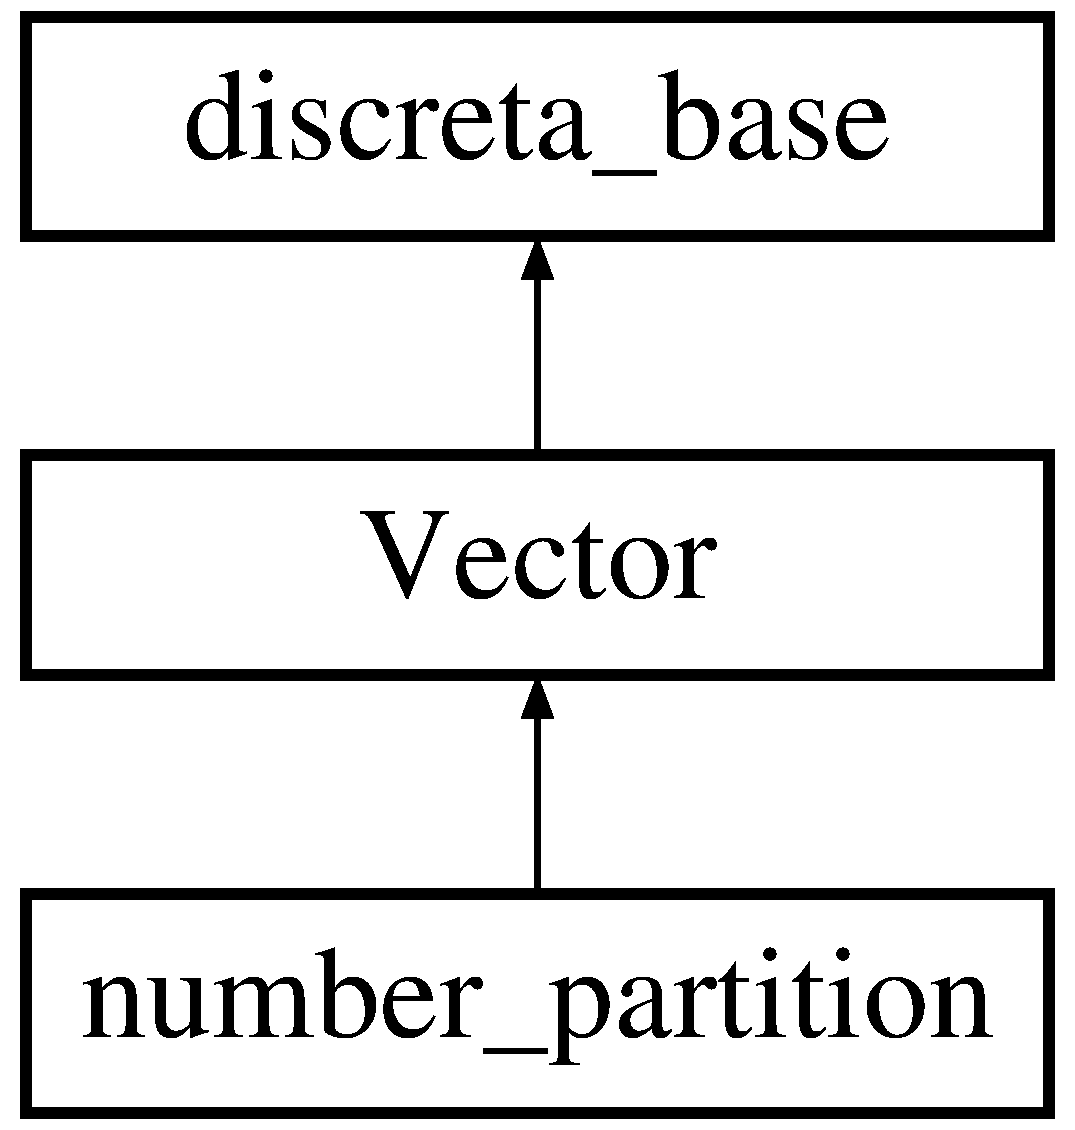
\includegraphics[height=3.000000cm]{classnumber__partition}
\end{center}
\end{figure}
\subsection*{Public Member Functions}
\begin{DoxyCompactItemize}
\item 
\mbox{\hyperlink{classnumber__partition_a3caf56544328aedc42115b7b89056106}{number\+\_\+partition}} ()
\item 
\mbox{\hyperlink{classnumber__partition_a5c08f2f2afd49281b54e799bd5fc3faa}{number\+\_\+partition}} (\mbox{\hyperlink{galois_8h_a09fddde158a3a20bd2dcadb609de11dc}{I\+NT}} \mbox{\hyperlink{simeon_8_c_a7f2cd26777ce0ff3fdaf8d02aacbddfb}{n}})
\item 
void \mbox{\hyperlink{classnumber__partition_a3c5649dc95f5ca53df4b0c58de6c1dc5}{allocate\+\_\+number\+\_\+partition}} ()
\item 
\mbox{\hyperlink{classnumber__partition_acb4eb29895a1b9594ff36c792af1ab11}{number\+\_\+partition}} (const \mbox{\hyperlink{classdiscreta__base}{discreta\+\_\+base}} \&\mbox{\hyperlink{alphabet2_8_c_a6150e0515f7202e2fb518f7206ed97dc}{x}})
\item 
\mbox{\hyperlink{classnumber__partition}{number\+\_\+partition}} \& \mbox{\hyperlink{classnumber__partition_a81b2d9c5c3f4b13e748c5a9bc01b54db}{operator=}} (const \mbox{\hyperlink{classdiscreta__base}{discreta\+\_\+base}} \&\mbox{\hyperlink{alphabet2_8_c_a6150e0515f7202e2fb518f7206ed97dc}{x}})
\item 
void $\ast$ \mbox{\hyperlink{classnumber__partition_ab36513c3a4dd1353edb3eb7e5b123bad}{operator new}} (size\+\_\+t, void $\ast$\mbox{\hyperlink{alphabet2_8_c_a533391314665d6bf1b5575e9a9cd8552}{p}})
\item 
void \mbox{\hyperlink{classnumber__partition_a3aaec1b557758f643ffc8555bbc358be}{settype\+\_\+number\+\_\+partition}} ()
\item 
\mbox{\hyperlink{discreta_8h_aaf25ee7e2306d78c74ec7bc48f092e81}{kind}} \mbox{\hyperlink{classnumber__partition_aaa88b590321ba25867fb1c70451c629a}{s\+\_\+virtual\+\_\+kind}} ()
\item 
\mbox{\hyperlink{classnumber__partition_af693fb3976d93ef732f6446702405bbc}{$\sim$number\+\_\+partition}} ()
\item 
void \mbox{\hyperlink{classnumber__partition_aa74111c1c8cd218b654e7b7c1ca42eb5}{freeself\+\_\+number\+\_\+partition}} ()
\item 
void \mbox{\hyperlink{classnumber__partition_acf25157ca8486f55d86d7ea05fa033be}{copyobject\+\_\+to}} (\mbox{\hyperlink{classdiscreta__base}{discreta\+\_\+base}} \&\mbox{\hyperlink{alphabet2_8_c_a6150e0515f7202e2fb518f7206ed97dc}{x}})
\item 
ostream \& \mbox{\hyperlink{classnumber__partition_a53c6c54cf4d86da0f07789ae14ff6da5}{print}} (ostream \&)
\item 
\mbox{\hyperlink{galois_8h_a09fddde158a3a20bd2dcadb609de11dc}{I\+NT}} \& \mbox{\hyperlink{classnumber__partition_a65f10dc2af06748e5142bbb7979cbc96}{s\+\_\+type}} ()
\item 
\mbox{\hyperlink{class_vector}{Vector}} \& \mbox{\hyperlink{classnumber__partition_a341bbbb9aeb221d1052b029648141e37}{s\+\_\+self}} ()
\item 
void \mbox{\hyperlink{classnumber__partition_a10013ba481b6c83fe777041164f8b47b}{m\+\_\+l}} (\mbox{\hyperlink{galois_8h_a09fddde158a3a20bd2dcadb609de11dc}{I\+NT}} \mbox{\hyperlink{alphabet2_8_c_a89606eca6b563ec68d2da2e84657736f}{l}})
\item 
\mbox{\hyperlink{galois_8h_a09fddde158a3a20bd2dcadb609de11dc}{I\+NT}} \mbox{\hyperlink{classnumber__partition_a2d95948a33d3c198e45db2b275ba8b68}{s\+\_\+l}} ()
\item 
\mbox{\hyperlink{galois_8h_a09fddde158a3a20bd2dcadb609de11dc}{I\+NT}} \& \mbox{\hyperlink{classnumber__partition_aca3e653629e80549db9e0cf584a3e16c}{s\+\_\+i}} (\mbox{\hyperlink{galois_8h_a09fddde158a3a20bd2dcadb609de11dc}{I\+NT}} \mbox{\hyperlink{alphabet2_8_c_acb559820d9ca11295b4500f179ef6392}{i}})
\item 
\mbox{\hyperlink{galois_8h_a09fddde158a3a20bd2dcadb609de11dc}{I\+NT}} \& \mbox{\hyperlink{classnumber__partition_a320f8ff6497e3199b10383b740ddf900}{operator\mbox{[}$\,$\mbox{]}}} (\mbox{\hyperlink{galois_8h_a09fddde158a3a20bd2dcadb609de11dc}{I\+NT}} \mbox{\hyperlink{alphabet2_8_c_acb559820d9ca11295b4500f179ef6392}{i}})
\item 
void \mbox{\hyperlink{classnumber__partition_ad8fd23e15805386340aac1c807c0bbc2}{first}} (\mbox{\hyperlink{galois_8h_a09fddde158a3a20bd2dcadb609de11dc}{I\+NT}} \mbox{\hyperlink{simeon_8_c_a7f2cd26777ce0ff3fdaf8d02aacbddfb}{n}})
\item 
\mbox{\hyperlink{galois_8h_a09fddde158a3a20bd2dcadb609de11dc}{I\+NT}} \mbox{\hyperlink{classnumber__partition_a4a374717cef3ac7d21308151a19f7ec0}{next}} ()
\item 
\mbox{\hyperlink{galois_8h_a09fddde158a3a20bd2dcadb609de11dc}{I\+NT}} \mbox{\hyperlink{classnumber__partition_a245a7821bacd491c54b56080f2ecbd51}{next\+\_\+exponent}} ()
\item 
\mbox{\hyperlink{galois_8h_a09fddde158a3a20bd2dcadb609de11dc}{I\+NT}} \mbox{\hyperlink{classnumber__partition_adf30d53b4b6f6511ccbf25f5e9e4187f}{next\+\_\+vector}} ()
\item 
\mbox{\hyperlink{galois_8h_a09fddde158a3a20bd2dcadb609de11dc}{I\+NT}} \mbox{\hyperlink{classnumber__partition_a5c27373cb7638344c463e32ed63e7e51}{first\+\_\+into\+\_\+k\+\_\+parts}} (\mbox{\hyperlink{galois_8h_a09fddde158a3a20bd2dcadb609de11dc}{I\+NT}} \mbox{\hyperlink{simeon_8_c_a7f2cd26777ce0ff3fdaf8d02aacbddfb}{n}}, \mbox{\hyperlink{galois_8h_a09fddde158a3a20bd2dcadb609de11dc}{I\+NT}} \mbox{\hyperlink{classdiscreta__base_a6f7a0f7bdd115b9e4dde358cfa7ebf81}{k}})
\item 
\mbox{\hyperlink{galois_8h_a09fddde158a3a20bd2dcadb609de11dc}{I\+NT}} \mbox{\hyperlink{classnumber__partition_a6067c3203b1dbaa8e77bca841132f442}{next\+\_\+into\+\_\+k\+\_\+parts}} (\mbox{\hyperlink{galois_8h_a09fddde158a3a20bd2dcadb609de11dc}{I\+NT}} \mbox{\hyperlink{simeon_8_c_a7f2cd26777ce0ff3fdaf8d02aacbddfb}{n}}, \mbox{\hyperlink{galois_8h_a09fddde158a3a20bd2dcadb609de11dc}{I\+NT}} \mbox{\hyperlink{classdiscreta__base_a6f7a0f7bdd115b9e4dde358cfa7ebf81}{k}})
\item 
\mbox{\hyperlink{galois_8h_a09fddde158a3a20bd2dcadb609de11dc}{I\+NT}} \mbox{\hyperlink{classnumber__partition_a36626dcbbaddba73cef7ff5c4521b325}{first\+\_\+into\+\_\+at\+\_\+most\+\_\+k\+\_\+parts}} (\mbox{\hyperlink{galois_8h_a09fddde158a3a20bd2dcadb609de11dc}{I\+NT}} \mbox{\hyperlink{simeon_8_c_a7f2cd26777ce0ff3fdaf8d02aacbddfb}{n}}, \mbox{\hyperlink{galois_8h_a09fddde158a3a20bd2dcadb609de11dc}{I\+NT}} \mbox{\hyperlink{classdiscreta__base_a6f7a0f7bdd115b9e4dde358cfa7ebf81}{k}})
\item 
\mbox{\hyperlink{galois_8h_a09fddde158a3a20bd2dcadb609de11dc}{I\+NT}} \mbox{\hyperlink{classnumber__partition_a5fe0dbb26444dd0f5a487dacb93e715b}{next\+\_\+into\+\_\+at\+\_\+most\+\_\+k\+\_\+parts}} (\mbox{\hyperlink{galois_8h_a09fddde158a3a20bd2dcadb609de11dc}{I\+NT}} \mbox{\hyperlink{simeon_8_c_a7f2cd26777ce0ff3fdaf8d02aacbddfb}{n}}, \mbox{\hyperlink{galois_8h_a09fddde158a3a20bd2dcadb609de11dc}{I\+NT}} \mbox{\hyperlink{classdiscreta__base_a6f7a0f7bdd115b9e4dde358cfa7ebf81}{k}})
\item 
\mbox{\hyperlink{galois_8h_a09fddde158a3a20bd2dcadb609de11dc}{I\+NT}} \mbox{\hyperlink{classnumber__partition_ac9fc2a34e6e5a93fb7f28e30906db51b}{nb\+\_\+parts}} ()
\item 
void \mbox{\hyperlink{classnumber__partition_aee718664947704f316f520a7abba52d8}{conjugate}} ()
\item 
void \mbox{\hyperlink{classnumber__partition_a0f194ccc525edcb22249744c3b0c65cb}{type}} (\mbox{\hyperlink{classnumber__partition}{number\+\_\+partition}} \&\mbox{\hyperlink{simeon_8_c_a92cbb483a3b27ae1a0dbfcb125ce216f}{q}})
\item 
void \mbox{\hyperlink{classnumber__partition_a62b34cba15a09ecc469517a9aa7d936d}{multinomial}} (\mbox{\hyperlink{classdiscreta__base}{discreta\+\_\+base}} \&res, \mbox{\hyperlink{galois_8h_a09fddde158a3a20bd2dcadb609de11dc}{I\+NT}} f\+\_\+v)
\item 
void \mbox{\hyperlink{classnumber__partition_a0d92a28d0d047c698d1c1c8fb93a6608}{multinomial\+\_\+ordered}} (\mbox{\hyperlink{classdiscreta__base}{discreta\+\_\+base}} \&res, \mbox{\hyperlink{galois_8h_a09fddde158a3a20bd2dcadb609de11dc}{I\+NT}} f\+\_\+v)
\item 
\mbox{\hyperlink{galois_8h_a09fddde158a3a20bd2dcadb609de11dc}{I\+NT}} \mbox{\hyperlink{classnumber__partition_ac1f48644e28737706fb6b04f7381da05}{sum\+\_\+of\+\_\+decreased\+\_\+parts}} ()
\end{DoxyCompactItemize}
\subsection*{Additional Inherited Members}


\subsection{Constructor \& Destructor Documentation}
\mbox{\Hypertarget{classnumber__partition_a3caf56544328aedc42115b7b89056106}\label{classnumber__partition_a3caf56544328aedc42115b7b89056106}} 
\index{number\+\_\+partition@{number\+\_\+partition}!number\+\_\+partition@{number\+\_\+partition}}
\index{number\+\_\+partition@{number\+\_\+partition}!number\+\_\+partition@{number\+\_\+partition}}
\subsubsection{\texorpdfstring{number\+\_\+partition()}{number\_partition()}\hspace{0.1cm}{\footnotesize\ttfamily [1/3]}}
{\footnotesize\ttfamily number\+\_\+partition\+::number\+\_\+partition (\begin{DoxyParamCaption}{ }\end{DoxyParamCaption})}

\mbox{\Hypertarget{classnumber__partition_a5c08f2f2afd49281b54e799bd5fc3faa}\label{classnumber__partition_a5c08f2f2afd49281b54e799bd5fc3faa}} 
\index{number\+\_\+partition@{number\+\_\+partition}!number\+\_\+partition@{number\+\_\+partition}}
\index{number\+\_\+partition@{number\+\_\+partition}!number\+\_\+partition@{number\+\_\+partition}}
\subsubsection{\texorpdfstring{number\+\_\+partition()}{number\_partition()}\hspace{0.1cm}{\footnotesize\ttfamily [2/3]}}
{\footnotesize\ttfamily number\+\_\+partition\+::number\+\_\+partition (\begin{DoxyParamCaption}\item[{\mbox{\hyperlink{galois_8h_a09fddde158a3a20bd2dcadb609de11dc}{I\+NT}}}]{n }\end{DoxyParamCaption})}

\mbox{\Hypertarget{classnumber__partition_acb4eb29895a1b9594ff36c792af1ab11}\label{classnumber__partition_acb4eb29895a1b9594ff36c792af1ab11}} 
\index{number\+\_\+partition@{number\+\_\+partition}!number\+\_\+partition@{number\+\_\+partition}}
\index{number\+\_\+partition@{number\+\_\+partition}!number\+\_\+partition@{number\+\_\+partition}}
\subsubsection{\texorpdfstring{number\+\_\+partition()}{number\_partition()}\hspace{0.1cm}{\footnotesize\ttfamily [3/3]}}
{\footnotesize\ttfamily number\+\_\+partition\+::number\+\_\+partition (\begin{DoxyParamCaption}\item[{const \mbox{\hyperlink{classdiscreta__base}{discreta\+\_\+base}} \&}]{x }\end{DoxyParamCaption})}

\mbox{\Hypertarget{classnumber__partition_af693fb3976d93ef732f6446702405bbc}\label{classnumber__partition_af693fb3976d93ef732f6446702405bbc}} 
\index{number\+\_\+partition@{number\+\_\+partition}!````~number\+\_\+partition@{$\sim$number\+\_\+partition}}
\index{````~number\+\_\+partition@{$\sim$number\+\_\+partition}!number\+\_\+partition@{number\+\_\+partition}}
\subsubsection{\texorpdfstring{$\sim$number\+\_\+partition()}{~number\_partition()}}
{\footnotesize\ttfamily number\+\_\+partition\+::$\sim$number\+\_\+partition (\begin{DoxyParamCaption}{ }\end{DoxyParamCaption})}



\subsection{Member Function Documentation}
\mbox{\Hypertarget{classnumber__partition_a3c5649dc95f5ca53df4b0c58de6c1dc5}\label{classnumber__partition_a3c5649dc95f5ca53df4b0c58de6c1dc5}} 
\index{number\+\_\+partition@{number\+\_\+partition}!allocate\+\_\+number\+\_\+partition@{allocate\+\_\+number\+\_\+partition}}
\index{allocate\+\_\+number\+\_\+partition@{allocate\+\_\+number\+\_\+partition}!number\+\_\+partition@{number\+\_\+partition}}
\subsubsection{\texorpdfstring{allocate\+\_\+number\+\_\+partition()}{allocate\_number\_partition()}}
{\footnotesize\ttfamily void number\+\_\+partition\+::allocate\+\_\+number\+\_\+partition (\begin{DoxyParamCaption}{ }\end{DoxyParamCaption})}

\mbox{\Hypertarget{classnumber__partition_aee718664947704f316f520a7abba52d8}\label{classnumber__partition_aee718664947704f316f520a7abba52d8}} 
\index{number\+\_\+partition@{number\+\_\+partition}!conjugate@{conjugate}}
\index{conjugate@{conjugate}!number\+\_\+partition@{number\+\_\+partition}}
\subsubsection{\texorpdfstring{conjugate()}{conjugate()}}
{\footnotesize\ttfamily void number\+\_\+partition\+::conjugate (\begin{DoxyParamCaption}{ }\end{DoxyParamCaption})}

\mbox{\Hypertarget{classnumber__partition_acf25157ca8486f55d86d7ea05fa033be}\label{classnumber__partition_acf25157ca8486f55d86d7ea05fa033be}} 
\index{number\+\_\+partition@{number\+\_\+partition}!copyobject\+\_\+to@{copyobject\+\_\+to}}
\index{copyobject\+\_\+to@{copyobject\+\_\+to}!number\+\_\+partition@{number\+\_\+partition}}
\subsubsection{\texorpdfstring{copyobject\+\_\+to()}{copyobject\_to()}}
{\footnotesize\ttfamily void number\+\_\+partition\+::copyobject\+\_\+to (\begin{DoxyParamCaption}\item[{\mbox{\hyperlink{classdiscreta__base}{discreta\+\_\+base}} \&}]{x }\end{DoxyParamCaption})\hspace{0.3cm}{\ttfamily [virtual]}}



Reimplemented from \mbox{\hyperlink{class_vector_af657307f3d344c8cef5d633335a5f484}{Vector}}.

\mbox{\Hypertarget{classnumber__partition_ad8fd23e15805386340aac1c807c0bbc2}\label{classnumber__partition_ad8fd23e15805386340aac1c807c0bbc2}} 
\index{number\+\_\+partition@{number\+\_\+partition}!first@{first}}
\index{first@{first}!number\+\_\+partition@{number\+\_\+partition}}
\subsubsection{\texorpdfstring{first()}{first()}}
{\footnotesize\ttfamily void number\+\_\+partition\+::first (\begin{DoxyParamCaption}\item[{\mbox{\hyperlink{galois_8h_a09fddde158a3a20bd2dcadb609de11dc}{I\+NT}}}]{n }\end{DoxyParamCaption})}

\mbox{\Hypertarget{classnumber__partition_a36626dcbbaddba73cef7ff5c4521b325}\label{classnumber__partition_a36626dcbbaddba73cef7ff5c4521b325}} 
\index{number\+\_\+partition@{number\+\_\+partition}!first\+\_\+into\+\_\+at\+\_\+most\+\_\+k\+\_\+parts@{first\+\_\+into\+\_\+at\+\_\+most\+\_\+k\+\_\+parts}}
\index{first\+\_\+into\+\_\+at\+\_\+most\+\_\+k\+\_\+parts@{first\+\_\+into\+\_\+at\+\_\+most\+\_\+k\+\_\+parts}!number\+\_\+partition@{number\+\_\+partition}}
\subsubsection{\texorpdfstring{first\+\_\+into\+\_\+at\+\_\+most\+\_\+k\+\_\+parts()}{first\_into\_at\_most\_k\_parts()}}
{\footnotesize\ttfamily \mbox{\hyperlink{galois_8h_a09fddde158a3a20bd2dcadb609de11dc}{I\+NT}} number\+\_\+partition\+::first\+\_\+into\+\_\+at\+\_\+most\+\_\+k\+\_\+parts (\begin{DoxyParamCaption}\item[{\mbox{\hyperlink{galois_8h_a09fddde158a3a20bd2dcadb609de11dc}{I\+NT}}}]{n,  }\item[{\mbox{\hyperlink{galois_8h_a09fddde158a3a20bd2dcadb609de11dc}{I\+NT}}}]{k }\end{DoxyParamCaption})}

\mbox{\Hypertarget{classnumber__partition_a5c27373cb7638344c463e32ed63e7e51}\label{classnumber__partition_a5c27373cb7638344c463e32ed63e7e51}} 
\index{number\+\_\+partition@{number\+\_\+partition}!first\+\_\+into\+\_\+k\+\_\+parts@{first\+\_\+into\+\_\+k\+\_\+parts}}
\index{first\+\_\+into\+\_\+k\+\_\+parts@{first\+\_\+into\+\_\+k\+\_\+parts}!number\+\_\+partition@{number\+\_\+partition}}
\subsubsection{\texorpdfstring{first\+\_\+into\+\_\+k\+\_\+parts()}{first\_into\_k\_parts()}}
{\footnotesize\ttfamily \mbox{\hyperlink{galois_8h_a09fddde158a3a20bd2dcadb609de11dc}{I\+NT}} number\+\_\+partition\+::first\+\_\+into\+\_\+k\+\_\+parts (\begin{DoxyParamCaption}\item[{\mbox{\hyperlink{galois_8h_a09fddde158a3a20bd2dcadb609de11dc}{I\+NT}}}]{n,  }\item[{\mbox{\hyperlink{galois_8h_a09fddde158a3a20bd2dcadb609de11dc}{I\+NT}}}]{k }\end{DoxyParamCaption})}

\mbox{\Hypertarget{classnumber__partition_aa74111c1c8cd218b654e7b7c1ca42eb5}\label{classnumber__partition_aa74111c1c8cd218b654e7b7c1ca42eb5}} 
\index{number\+\_\+partition@{number\+\_\+partition}!freeself\+\_\+number\+\_\+partition@{freeself\+\_\+number\+\_\+partition}}
\index{freeself\+\_\+number\+\_\+partition@{freeself\+\_\+number\+\_\+partition}!number\+\_\+partition@{number\+\_\+partition}}
\subsubsection{\texorpdfstring{freeself\+\_\+number\+\_\+partition()}{freeself\_number\_partition()}}
{\footnotesize\ttfamily void number\+\_\+partition\+::freeself\+\_\+number\+\_\+partition (\begin{DoxyParamCaption}{ }\end{DoxyParamCaption})}

\mbox{\Hypertarget{classnumber__partition_a10013ba481b6c83fe777041164f8b47b}\label{classnumber__partition_a10013ba481b6c83fe777041164f8b47b}} 
\index{number\+\_\+partition@{number\+\_\+partition}!m\+\_\+l@{m\+\_\+l}}
\index{m\+\_\+l@{m\+\_\+l}!number\+\_\+partition@{number\+\_\+partition}}
\subsubsection{\texorpdfstring{m\+\_\+l()}{m\_l()}}
{\footnotesize\ttfamily void number\+\_\+partition\+::m\+\_\+l (\begin{DoxyParamCaption}\item[{\mbox{\hyperlink{galois_8h_a09fddde158a3a20bd2dcadb609de11dc}{I\+NT}}}]{l }\end{DoxyParamCaption})\hspace{0.3cm}{\ttfamily [inline]}}

\mbox{\Hypertarget{classnumber__partition_a62b34cba15a09ecc469517a9aa7d936d}\label{classnumber__partition_a62b34cba15a09ecc469517a9aa7d936d}} 
\index{number\+\_\+partition@{number\+\_\+partition}!multinomial@{multinomial}}
\index{multinomial@{multinomial}!number\+\_\+partition@{number\+\_\+partition}}
\subsubsection{\texorpdfstring{multinomial()}{multinomial()}}
{\footnotesize\ttfamily void number\+\_\+partition\+::multinomial (\begin{DoxyParamCaption}\item[{\mbox{\hyperlink{classdiscreta__base}{discreta\+\_\+base}} \&}]{res,  }\item[{\mbox{\hyperlink{galois_8h_a09fddde158a3a20bd2dcadb609de11dc}{I\+NT}}}]{f\+\_\+v }\end{DoxyParamCaption})}

\mbox{\Hypertarget{classnumber__partition_a0d92a28d0d047c698d1c1c8fb93a6608}\label{classnumber__partition_a0d92a28d0d047c698d1c1c8fb93a6608}} 
\index{number\+\_\+partition@{number\+\_\+partition}!multinomial\+\_\+ordered@{multinomial\+\_\+ordered}}
\index{multinomial\+\_\+ordered@{multinomial\+\_\+ordered}!number\+\_\+partition@{number\+\_\+partition}}
\subsubsection{\texorpdfstring{multinomial\+\_\+ordered()}{multinomial\_ordered()}}
{\footnotesize\ttfamily void number\+\_\+partition\+::multinomial\+\_\+ordered (\begin{DoxyParamCaption}\item[{\mbox{\hyperlink{classdiscreta__base}{discreta\+\_\+base}} \&}]{res,  }\item[{\mbox{\hyperlink{galois_8h_a09fddde158a3a20bd2dcadb609de11dc}{I\+NT}}}]{f\+\_\+v }\end{DoxyParamCaption})}

\mbox{\Hypertarget{classnumber__partition_ac9fc2a34e6e5a93fb7f28e30906db51b}\label{classnumber__partition_ac9fc2a34e6e5a93fb7f28e30906db51b}} 
\index{number\+\_\+partition@{number\+\_\+partition}!nb\+\_\+parts@{nb\+\_\+parts}}
\index{nb\+\_\+parts@{nb\+\_\+parts}!number\+\_\+partition@{number\+\_\+partition}}
\subsubsection{\texorpdfstring{nb\+\_\+parts()}{nb\_parts()}}
{\footnotesize\ttfamily \mbox{\hyperlink{galois_8h_a09fddde158a3a20bd2dcadb609de11dc}{I\+NT}} number\+\_\+partition\+::nb\+\_\+parts (\begin{DoxyParamCaption}{ }\end{DoxyParamCaption})}

\mbox{\Hypertarget{classnumber__partition_a4a374717cef3ac7d21308151a19f7ec0}\label{classnumber__partition_a4a374717cef3ac7d21308151a19f7ec0}} 
\index{number\+\_\+partition@{number\+\_\+partition}!next@{next}}
\index{next@{next}!number\+\_\+partition@{number\+\_\+partition}}
\subsubsection{\texorpdfstring{next()}{next()}}
{\footnotesize\ttfamily \mbox{\hyperlink{galois_8h_a09fddde158a3a20bd2dcadb609de11dc}{I\+NT}} number\+\_\+partition\+::next (\begin{DoxyParamCaption}{ }\end{DoxyParamCaption})}

\mbox{\Hypertarget{classnumber__partition_a245a7821bacd491c54b56080f2ecbd51}\label{classnumber__partition_a245a7821bacd491c54b56080f2ecbd51}} 
\index{number\+\_\+partition@{number\+\_\+partition}!next\+\_\+exponent@{next\+\_\+exponent}}
\index{next\+\_\+exponent@{next\+\_\+exponent}!number\+\_\+partition@{number\+\_\+partition}}
\subsubsection{\texorpdfstring{next\+\_\+exponent()}{next\_exponent()}}
{\footnotesize\ttfamily \mbox{\hyperlink{galois_8h_a09fddde158a3a20bd2dcadb609de11dc}{I\+NT}} number\+\_\+partition\+::next\+\_\+exponent (\begin{DoxyParamCaption}{ }\end{DoxyParamCaption})}

\mbox{\Hypertarget{classnumber__partition_a5fe0dbb26444dd0f5a487dacb93e715b}\label{classnumber__partition_a5fe0dbb26444dd0f5a487dacb93e715b}} 
\index{number\+\_\+partition@{number\+\_\+partition}!next\+\_\+into\+\_\+at\+\_\+most\+\_\+k\+\_\+parts@{next\+\_\+into\+\_\+at\+\_\+most\+\_\+k\+\_\+parts}}
\index{next\+\_\+into\+\_\+at\+\_\+most\+\_\+k\+\_\+parts@{next\+\_\+into\+\_\+at\+\_\+most\+\_\+k\+\_\+parts}!number\+\_\+partition@{number\+\_\+partition}}
\subsubsection{\texorpdfstring{next\+\_\+into\+\_\+at\+\_\+most\+\_\+k\+\_\+parts()}{next\_into\_at\_most\_k\_parts()}}
{\footnotesize\ttfamily \mbox{\hyperlink{galois_8h_a09fddde158a3a20bd2dcadb609de11dc}{I\+NT}} number\+\_\+partition\+::next\+\_\+into\+\_\+at\+\_\+most\+\_\+k\+\_\+parts (\begin{DoxyParamCaption}\item[{\mbox{\hyperlink{galois_8h_a09fddde158a3a20bd2dcadb609de11dc}{I\+NT}}}]{n,  }\item[{\mbox{\hyperlink{galois_8h_a09fddde158a3a20bd2dcadb609de11dc}{I\+NT}}}]{k }\end{DoxyParamCaption})}

\mbox{\Hypertarget{classnumber__partition_a6067c3203b1dbaa8e77bca841132f442}\label{classnumber__partition_a6067c3203b1dbaa8e77bca841132f442}} 
\index{number\+\_\+partition@{number\+\_\+partition}!next\+\_\+into\+\_\+k\+\_\+parts@{next\+\_\+into\+\_\+k\+\_\+parts}}
\index{next\+\_\+into\+\_\+k\+\_\+parts@{next\+\_\+into\+\_\+k\+\_\+parts}!number\+\_\+partition@{number\+\_\+partition}}
\subsubsection{\texorpdfstring{next\+\_\+into\+\_\+k\+\_\+parts()}{next\_into\_k\_parts()}}
{\footnotesize\ttfamily \mbox{\hyperlink{galois_8h_a09fddde158a3a20bd2dcadb609de11dc}{I\+NT}} number\+\_\+partition\+::next\+\_\+into\+\_\+k\+\_\+parts (\begin{DoxyParamCaption}\item[{\mbox{\hyperlink{galois_8h_a09fddde158a3a20bd2dcadb609de11dc}{I\+NT}}}]{n,  }\item[{\mbox{\hyperlink{galois_8h_a09fddde158a3a20bd2dcadb609de11dc}{I\+NT}}}]{k }\end{DoxyParamCaption})}

\mbox{\Hypertarget{classnumber__partition_adf30d53b4b6f6511ccbf25f5e9e4187f}\label{classnumber__partition_adf30d53b4b6f6511ccbf25f5e9e4187f}} 
\index{number\+\_\+partition@{number\+\_\+partition}!next\+\_\+vector@{next\+\_\+vector}}
\index{next\+\_\+vector@{next\+\_\+vector}!number\+\_\+partition@{number\+\_\+partition}}
\subsubsection{\texorpdfstring{next\+\_\+vector()}{next\_vector()}}
{\footnotesize\ttfamily \mbox{\hyperlink{galois_8h_a09fddde158a3a20bd2dcadb609de11dc}{I\+NT}} number\+\_\+partition\+::next\+\_\+vector (\begin{DoxyParamCaption}{ }\end{DoxyParamCaption})}

\mbox{\Hypertarget{classnumber__partition_ab36513c3a4dd1353edb3eb7e5b123bad}\label{classnumber__partition_ab36513c3a4dd1353edb3eb7e5b123bad}} 
\index{number\+\_\+partition@{number\+\_\+partition}!operator new@{operator new}}
\index{operator new@{operator new}!number\+\_\+partition@{number\+\_\+partition}}
\subsubsection{\texorpdfstring{operator new()}{operator new()}}
{\footnotesize\ttfamily void$\ast$ number\+\_\+partition\+::operator new (\begin{DoxyParamCaption}\item[{size\+\_\+t}]{,  }\item[{void $\ast$}]{p }\end{DoxyParamCaption})\hspace{0.3cm}{\ttfamily [inline]}}

\mbox{\Hypertarget{classnumber__partition_a81b2d9c5c3f4b13e748c5a9bc01b54db}\label{classnumber__partition_a81b2d9c5c3f4b13e748c5a9bc01b54db}} 
\index{number\+\_\+partition@{number\+\_\+partition}!operator=@{operator=}}
\index{operator=@{operator=}!number\+\_\+partition@{number\+\_\+partition}}
\subsubsection{\texorpdfstring{operator=()}{operator=()}}
{\footnotesize\ttfamily \mbox{\hyperlink{classnumber__partition}{number\+\_\+partition}} \& number\+\_\+partition\+::operator= (\begin{DoxyParamCaption}\item[{const \mbox{\hyperlink{classdiscreta__base}{discreta\+\_\+base}} \&}]{x }\end{DoxyParamCaption})}

\mbox{\Hypertarget{classnumber__partition_a320f8ff6497e3199b10383b740ddf900}\label{classnumber__partition_a320f8ff6497e3199b10383b740ddf900}} 
\index{number\+\_\+partition@{number\+\_\+partition}!operator\mbox{[}\mbox{]}@{operator[]}}
\index{operator\mbox{[}\mbox{]}@{operator[]}!number\+\_\+partition@{number\+\_\+partition}}
\subsubsection{\texorpdfstring{operator[]()}{operator[]()}}
{\footnotesize\ttfamily \mbox{\hyperlink{galois_8h_a09fddde158a3a20bd2dcadb609de11dc}{I\+NT}}\& number\+\_\+partition\+::operator\mbox{[}$\,$\mbox{]} (\begin{DoxyParamCaption}\item[{\mbox{\hyperlink{galois_8h_a09fddde158a3a20bd2dcadb609de11dc}{I\+NT}}}]{i }\end{DoxyParamCaption})\hspace{0.3cm}{\ttfamily [inline]}}

\mbox{\Hypertarget{classnumber__partition_a53c6c54cf4d86da0f07789ae14ff6da5}\label{classnumber__partition_a53c6c54cf4d86da0f07789ae14ff6da5}} 
\index{number\+\_\+partition@{number\+\_\+partition}!print@{print}}
\index{print@{print}!number\+\_\+partition@{number\+\_\+partition}}
\subsubsection{\texorpdfstring{print()}{print()}}
{\footnotesize\ttfamily ostream \& number\+\_\+partition\+::print (\begin{DoxyParamCaption}\item[{ostream \&}]{ost }\end{DoxyParamCaption})\hspace{0.3cm}{\ttfamily [virtual]}}



Reimplemented from \mbox{\hyperlink{class_vector_a71d7e24bcfdfc69d4a2137360acb066c}{Vector}}.

\mbox{\Hypertarget{classnumber__partition_aca3e653629e80549db9e0cf584a3e16c}\label{classnumber__partition_aca3e653629e80549db9e0cf584a3e16c}} 
\index{number\+\_\+partition@{number\+\_\+partition}!s\+\_\+i@{s\+\_\+i}}
\index{s\+\_\+i@{s\+\_\+i}!number\+\_\+partition@{number\+\_\+partition}}
\subsubsection{\texorpdfstring{s\+\_\+i()}{s\_i()}}
{\footnotesize\ttfamily \mbox{\hyperlink{galois_8h_a09fddde158a3a20bd2dcadb609de11dc}{I\+NT}}\& number\+\_\+partition\+::s\+\_\+i (\begin{DoxyParamCaption}\item[{\mbox{\hyperlink{galois_8h_a09fddde158a3a20bd2dcadb609de11dc}{I\+NT}}}]{i }\end{DoxyParamCaption})\hspace{0.3cm}{\ttfamily [inline]}}

\mbox{\Hypertarget{classnumber__partition_a2d95948a33d3c198e45db2b275ba8b68}\label{classnumber__partition_a2d95948a33d3c198e45db2b275ba8b68}} 
\index{number\+\_\+partition@{number\+\_\+partition}!s\+\_\+l@{s\+\_\+l}}
\index{s\+\_\+l@{s\+\_\+l}!number\+\_\+partition@{number\+\_\+partition}}
\subsubsection{\texorpdfstring{s\+\_\+l()}{s\_l()}}
{\footnotesize\ttfamily \mbox{\hyperlink{galois_8h_a09fddde158a3a20bd2dcadb609de11dc}{I\+NT}} number\+\_\+partition\+::s\+\_\+l (\begin{DoxyParamCaption}{ }\end{DoxyParamCaption})\hspace{0.3cm}{\ttfamily [inline]}}

\mbox{\Hypertarget{classnumber__partition_a341bbbb9aeb221d1052b029648141e37}\label{classnumber__partition_a341bbbb9aeb221d1052b029648141e37}} 
\index{number\+\_\+partition@{number\+\_\+partition}!s\+\_\+self@{s\+\_\+self}}
\index{s\+\_\+self@{s\+\_\+self}!number\+\_\+partition@{number\+\_\+partition}}
\subsubsection{\texorpdfstring{s\+\_\+self()}{s\_self()}}
{\footnotesize\ttfamily \mbox{\hyperlink{class_vector}{Vector}}\& number\+\_\+partition\+::s\+\_\+self (\begin{DoxyParamCaption}{ }\end{DoxyParamCaption})\hspace{0.3cm}{\ttfamily [inline]}}

\mbox{\Hypertarget{classnumber__partition_a65f10dc2af06748e5142bbb7979cbc96}\label{classnumber__partition_a65f10dc2af06748e5142bbb7979cbc96}} 
\index{number\+\_\+partition@{number\+\_\+partition}!s\+\_\+type@{s\+\_\+type}}
\index{s\+\_\+type@{s\+\_\+type}!number\+\_\+partition@{number\+\_\+partition}}
\subsubsection{\texorpdfstring{s\+\_\+type()}{s\_type()}}
{\footnotesize\ttfamily \mbox{\hyperlink{galois_8h_a09fddde158a3a20bd2dcadb609de11dc}{I\+NT}}\& number\+\_\+partition\+::s\+\_\+type (\begin{DoxyParamCaption}{ }\end{DoxyParamCaption})\hspace{0.3cm}{\ttfamily [inline]}}

\mbox{\Hypertarget{classnumber__partition_aaa88b590321ba25867fb1c70451c629a}\label{classnumber__partition_aaa88b590321ba25867fb1c70451c629a}} 
\index{number\+\_\+partition@{number\+\_\+partition}!s\+\_\+virtual\+\_\+kind@{s\+\_\+virtual\+\_\+kind}}
\index{s\+\_\+virtual\+\_\+kind@{s\+\_\+virtual\+\_\+kind}!number\+\_\+partition@{number\+\_\+partition}}
\subsubsection{\texorpdfstring{s\+\_\+virtual\+\_\+kind()}{s\_virtual\_kind()}}
{\footnotesize\ttfamily \mbox{\hyperlink{discreta_8h_aaf25ee7e2306d78c74ec7bc48f092e81}{kind}} number\+\_\+partition\+::s\+\_\+virtual\+\_\+kind (\begin{DoxyParamCaption}{ }\end{DoxyParamCaption})\hspace{0.3cm}{\ttfamily [virtual]}}



Reimplemented from \mbox{\hyperlink{class_vector_a20550e70d02cbe484032c7f6b0833a0f}{Vector}}.

\mbox{\Hypertarget{classnumber__partition_a3aaec1b557758f643ffc8555bbc358be}\label{classnumber__partition_a3aaec1b557758f643ffc8555bbc358be}} 
\index{number\+\_\+partition@{number\+\_\+partition}!settype\+\_\+number\+\_\+partition@{settype\+\_\+number\+\_\+partition}}
\index{settype\+\_\+number\+\_\+partition@{settype\+\_\+number\+\_\+partition}!number\+\_\+partition@{number\+\_\+partition}}
\subsubsection{\texorpdfstring{settype\+\_\+number\+\_\+partition()}{settype\_number\_partition()}}
{\footnotesize\ttfamily void number\+\_\+partition\+::settype\+\_\+number\+\_\+partition (\begin{DoxyParamCaption}{ }\end{DoxyParamCaption})}

\mbox{\Hypertarget{classnumber__partition_ac1f48644e28737706fb6b04f7381da05}\label{classnumber__partition_ac1f48644e28737706fb6b04f7381da05}} 
\index{number\+\_\+partition@{number\+\_\+partition}!sum\+\_\+of\+\_\+decreased\+\_\+parts@{sum\+\_\+of\+\_\+decreased\+\_\+parts}}
\index{sum\+\_\+of\+\_\+decreased\+\_\+parts@{sum\+\_\+of\+\_\+decreased\+\_\+parts}!number\+\_\+partition@{number\+\_\+partition}}
\subsubsection{\texorpdfstring{sum\+\_\+of\+\_\+decreased\+\_\+parts()}{sum\_of\_decreased\_parts()}}
{\footnotesize\ttfamily \mbox{\hyperlink{galois_8h_a09fddde158a3a20bd2dcadb609de11dc}{I\+NT}} number\+\_\+partition\+::sum\+\_\+of\+\_\+decreased\+\_\+parts (\begin{DoxyParamCaption}{ }\end{DoxyParamCaption})}

\mbox{\Hypertarget{classnumber__partition_a0f194ccc525edcb22249744c3b0c65cb}\label{classnumber__partition_a0f194ccc525edcb22249744c3b0c65cb}} 
\index{number\+\_\+partition@{number\+\_\+partition}!type@{type}}
\index{type@{type}!number\+\_\+partition@{number\+\_\+partition}}
\subsubsection{\texorpdfstring{type()}{type()}}
{\footnotesize\ttfamily void number\+\_\+partition\+::type (\begin{DoxyParamCaption}\item[{\mbox{\hyperlink{classnumber__partition}{number\+\_\+partition}} \&}]{q }\end{DoxyParamCaption})}



The documentation for this class was generated from the following files\+:\begin{DoxyCompactItemize}
\item 
S\+R\+C/\+L\+I\+B/\+D\+I\+S\+C\+R\+E\+T\+A/\mbox{\hyperlink{discreta_8h}{discreta.\+h}}\item 
S\+R\+C/\+L\+I\+B/\+D\+I\+S\+C\+R\+E\+T\+A/\mbox{\hyperlink{number__partition_8_c}{number\+\_\+partition.\+C}}\end{DoxyCompactItemize}

\hypertarget{classobject__in__projective__space}{}\section{object\+\_\+in\+\_\+projective\+\_\+space Class Reference}
\label{classobject__in__projective__space}\index{object\+\_\+in\+\_\+projective\+\_\+space@{object\+\_\+in\+\_\+projective\+\_\+space}}


{\ttfamily \#include $<$galois.\+h$>$}

\subsection*{Public Member Functions}
\begin{DoxyCompactItemize}
\item 
\mbox{\hyperlink{classobject__in__projective__space_a57c7803b80a880d6fcbb13dec860702c}{object\+\_\+in\+\_\+projective\+\_\+space}} ()
\item 
\mbox{\hyperlink{classobject__in__projective__space_ac2637c804ab163d90e54008bce0580af}{$\sim$object\+\_\+in\+\_\+projective\+\_\+space}} ()
\item 
void \mbox{\hyperlink{classobject__in__projective__space_a07908386e9bb21615dc8415379b2f4e2}{null}} ()
\item 
void \mbox{\hyperlink{classobject__in__projective__space_a371bc4c5e7744127cc8b75fad5903ac1}{freeself}} ()
\item 
void \mbox{\hyperlink{classobject__in__projective__space_a056911c0013ac43d89cdc9cfd21f6545}{print}} (ostream \&ost)
\item 
void \mbox{\hyperlink{classobject__in__projective__space_abd9a530e510784dda9865c60de9d5230}{print\+\_\+tex}} (ostream \&ost)
\item 
void \mbox{\hyperlink{classobject__in__projective__space_ae06b87acb715d13efec5f6dcea0908ca}{init\+\_\+point\+\_\+set}} (\mbox{\hyperlink{classprojective__space}{projective\+\_\+space}} $\ast$\mbox{\hyperlink{classobject__in__projective__space_abd304b597ccddaf6bd78c29dc1ca3da8}{P}}, \mbox{\hyperlink{galois_8h_a09fddde158a3a20bd2dcadb609de11dc}{I\+NT}} $\ast$\mbox{\hyperlink{nauty_8h_a9690bea211101f22a5e154087590c3da}{set}}, \mbox{\hyperlink{galois_8h_a09fddde158a3a20bd2dcadb609de11dc}{I\+NT}} \mbox{\hyperlink{classobject__in__projective__space_a2dda692174f30d566b26bf58e62c14cc}{sz}}, \mbox{\hyperlink{galois_8h_a09fddde158a3a20bd2dcadb609de11dc}{I\+NT}} \mbox{\hyperlink{simeon_8_c_a818073fbcc2f439e7c56952f67386122}{verbose\+\_\+level}})
\item 
void \mbox{\hyperlink{classobject__in__projective__space_a910badf3915797f5a3c57e981231bed2}{init\+\_\+line\+\_\+set}} (\mbox{\hyperlink{classprojective__space}{projective\+\_\+space}} $\ast$\mbox{\hyperlink{classobject__in__projective__space_abd304b597ccddaf6bd78c29dc1ca3da8}{P}}, \mbox{\hyperlink{galois_8h_a09fddde158a3a20bd2dcadb609de11dc}{I\+NT}} $\ast$\mbox{\hyperlink{nauty_8h_a9690bea211101f22a5e154087590c3da}{set}}, \mbox{\hyperlink{galois_8h_a09fddde158a3a20bd2dcadb609de11dc}{I\+NT}} \mbox{\hyperlink{classobject__in__projective__space_a2dda692174f30d566b26bf58e62c14cc}{sz}}, \mbox{\hyperlink{galois_8h_a09fddde158a3a20bd2dcadb609de11dc}{I\+NT}} \mbox{\hyperlink{simeon_8_c_a818073fbcc2f439e7c56952f67386122}{verbose\+\_\+level}})
\item 
void \mbox{\hyperlink{classobject__in__projective__space_a085f606728855cecf404108ed051bec7}{init\+\_\+packing\+\_\+from\+\_\+set}} (\mbox{\hyperlink{classprojective__space}{projective\+\_\+space}} $\ast$\mbox{\hyperlink{classobject__in__projective__space_abd304b597ccddaf6bd78c29dc1ca3da8}{P}}, \mbox{\hyperlink{galois_8h_a09fddde158a3a20bd2dcadb609de11dc}{I\+NT}} $\ast$packing, \mbox{\hyperlink{galois_8h_a09fddde158a3a20bd2dcadb609de11dc}{I\+NT}} \mbox{\hyperlink{classobject__in__projective__space_a2dda692174f30d566b26bf58e62c14cc}{sz}}, \mbox{\hyperlink{galois_8h_a09fddde158a3a20bd2dcadb609de11dc}{I\+NT}} \mbox{\hyperlink{simeon_8_c_a818073fbcc2f439e7c56952f67386122}{verbose\+\_\+level}})
\item 
void \mbox{\hyperlink{classobject__in__projective__space_aa24d23143edcdce652844ec0def4ff1f}{init\+\_\+packing\+\_\+from\+\_\+set\+\_\+of\+\_\+sets}} (\mbox{\hyperlink{classprojective__space}{projective\+\_\+space}} $\ast$\mbox{\hyperlink{classobject__in__projective__space_abd304b597ccddaf6bd78c29dc1ca3da8}{P}}, \mbox{\hyperlink{classset__of__sets}{set\+\_\+of\+\_\+sets}} $\ast$\mbox{\hyperlink{classobject__in__projective__space_a62b975440fff979b15f94dc320cb05f2}{SoS}}, \mbox{\hyperlink{galois_8h_a09fddde158a3a20bd2dcadb609de11dc}{I\+NT}} \mbox{\hyperlink{simeon_8_c_a818073fbcc2f439e7c56952f67386122}{verbose\+\_\+level}})
\item 
void \mbox{\hyperlink{classobject__in__projective__space_a452481c9f1426dcca8b15b505f14ac6b}{init\+\_\+packing\+\_\+from\+\_\+spread\+\_\+table}} (\mbox{\hyperlink{classprojective__space}{projective\+\_\+space}} $\ast$\mbox{\hyperlink{classobject__in__projective__space_abd304b597ccddaf6bd78c29dc1ca3da8}{P}}, \mbox{\hyperlink{galois_8h_a09fddde158a3a20bd2dcadb609de11dc}{I\+NT}} $\ast$data, \mbox{\hyperlink{galois_8h_a09fddde158a3a20bd2dcadb609de11dc}{I\+NT}} $\ast$Spread\+\_\+table, \mbox{\hyperlink{galois_8h_a09fddde158a3a20bd2dcadb609de11dc}{I\+NT}} nb\+\_\+spreads, \mbox{\hyperlink{galois_8h_a09fddde158a3a20bd2dcadb609de11dc}{I\+NT}} spread\+\_\+size, \mbox{\hyperlink{galois_8h_a09fddde158a3a20bd2dcadb609de11dc}{I\+NT}} \mbox{\hyperlink{simeon_8_c_a818073fbcc2f439e7c56952f67386122}{verbose\+\_\+level}})
\item 
void \mbox{\hyperlink{classobject__in__projective__space_a56b160e9f38e52c4e55a6be5342a546e}{encode\+\_\+incma}} (\mbox{\hyperlink{galois_8h_a09fddde158a3a20bd2dcadb609de11dc}{I\+NT}} $\ast$\&Incma, \mbox{\hyperlink{galois_8h_a09fddde158a3a20bd2dcadb609de11dc}{I\+NT}} \&nb\+\_\+rows, \mbox{\hyperlink{galois_8h_a09fddde158a3a20bd2dcadb609de11dc}{I\+NT}} \&nb\+\_\+cols, \mbox{\hyperlink{galois_8h_a09fddde158a3a20bd2dcadb609de11dc}{I\+NT}} $\ast$\&partition, \mbox{\hyperlink{galois_8h_a09fddde158a3a20bd2dcadb609de11dc}{I\+NT}} \mbox{\hyperlink{simeon_8_c_a818073fbcc2f439e7c56952f67386122}{verbose\+\_\+level}})
\item 
void \mbox{\hyperlink{classobject__in__projective__space_a12c0ee007c02544a291189c306178224}{encode\+\_\+point\+\_\+set}} (\mbox{\hyperlink{galois_8h_a09fddde158a3a20bd2dcadb609de11dc}{I\+NT}} $\ast$\&Incma, \mbox{\hyperlink{galois_8h_a09fddde158a3a20bd2dcadb609de11dc}{I\+NT}} \&nb\+\_\+rows, \mbox{\hyperlink{galois_8h_a09fddde158a3a20bd2dcadb609de11dc}{I\+NT}} \&nb\+\_\+cols, \mbox{\hyperlink{galois_8h_a09fddde158a3a20bd2dcadb609de11dc}{I\+NT}} $\ast$\&partition, \mbox{\hyperlink{galois_8h_a09fddde158a3a20bd2dcadb609de11dc}{I\+NT}} \mbox{\hyperlink{simeon_8_c_a818073fbcc2f439e7c56952f67386122}{verbose\+\_\+level}})
\item 
void \mbox{\hyperlink{classobject__in__projective__space_a52130fa2cd6c2fa65a7add526a260e5d}{encode\+\_\+line\+\_\+set}} (\mbox{\hyperlink{galois_8h_a09fddde158a3a20bd2dcadb609de11dc}{I\+NT}} $\ast$\&Incma, \mbox{\hyperlink{galois_8h_a09fddde158a3a20bd2dcadb609de11dc}{I\+NT}} \&nb\+\_\+rows, \mbox{\hyperlink{galois_8h_a09fddde158a3a20bd2dcadb609de11dc}{I\+NT}} \&nb\+\_\+cols, \mbox{\hyperlink{galois_8h_a09fddde158a3a20bd2dcadb609de11dc}{I\+NT}} $\ast$\&partition, \mbox{\hyperlink{galois_8h_a09fddde158a3a20bd2dcadb609de11dc}{I\+NT}} \mbox{\hyperlink{simeon_8_c_a818073fbcc2f439e7c56952f67386122}{verbose\+\_\+level}})
\item 
void \mbox{\hyperlink{classobject__in__projective__space_a510abf71c9db147e0c3a93fa9772d045}{encode\+\_\+packing}} (\mbox{\hyperlink{galois_8h_a09fddde158a3a20bd2dcadb609de11dc}{I\+NT}} $\ast$\&Incma, \mbox{\hyperlink{galois_8h_a09fddde158a3a20bd2dcadb609de11dc}{I\+NT}} \&nb\+\_\+rows, \mbox{\hyperlink{galois_8h_a09fddde158a3a20bd2dcadb609de11dc}{I\+NT}} \&nb\+\_\+cols, \mbox{\hyperlink{galois_8h_a09fddde158a3a20bd2dcadb609de11dc}{I\+NT}} $\ast$\&partition, \mbox{\hyperlink{galois_8h_a09fddde158a3a20bd2dcadb609de11dc}{I\+NT}} \mbox{\hyperlink{simeon_8_c_a818073fbcc2f439e7c56952f67386122}{verbose\+\_\+level}})
\item 
void \mbox{\hyperlink{classobject__in__projective__space_a8f0ebd9ca15ecfeb61480cb884888444}{encode\+\_\+incma\+\_\+and\+\_\+make\+\_\+decomposition}} (\mbox{\hyperlink{galois_8h_a09fddde158a3a20bd2dcadb609de11dc}{I\+NT}} $\ast$\&Incma, \mbox{\hyperlink{galois_8h_a09fddde158a3a20bd2dcadb609de11dc}{I\+NT}} \&nb\+\_\+rows, \mbox{\hyperlink{galois_8h_a09fddde158a3a20bd2dcadb609de11dc}{I\+NT}} \&nb\+\_\+cols, \mbox{\hyperlink{galois_8h_a09fddde158a3a20bd2dcadb609de11dc}{I\+NT}} $\ast$\&partition, \mbox{\hyperlink{classincidence__structure}{incidence\+\_\+structure}} $\ast$\&Inc, \mbox{\hyperlink{classpartitionstack}{partitionstack}} $\ast$\&Stack, \mbox{\hyperlink{galois_8h_a09fddde158a3a20bd2dcadb609de11dc}{I\+NT}} \mbox{\hyperlink{simeon_8_c_a818073fbcc2f439e7c56952f67386122}{verbose\+\_\+level}})
\item 
void \mbox{\hyperlink{classobject__in__projective__space_a94a707237ade58291c1fc48f883c4930}{encode\+\_\+object}} (\mbox{\hyperlink{galois_8h_a09fddde158a3a20bd2dcadb609de11dc}{I\+NT}} $\ast$\&encoding, \mbox{\hyperlink{galois_8h_a09fddde158a3a20bd2dcadb609de11dc}{I\+NT}} \&encoding\+\_\+sz, \mbox{\hyperlink{galois_8h_a09fddde158a3a20bd2dcadb609de11dc}{I\+NT}} \mbox{\hyperlink{simeon_8_c_a818073fbcc2f439e7c56952f67386122}{verbose\+\_\+level}})
\item 
void \mbox{\hyperlink{classobject__in__projective__space_a46edc8e2e918819dd5fc880eb52177b8}{encode\+\_\+object\+\_\+points}} (\mbox{\hyperlink{galois_8h_a09fddde158a3a20bd2dcadb609de11dc}{I\+NT}} $\ast$\&encoding, \mbox{\hyperlink{galois_8h_a09fddde158a3a20bd2dcadb609de11dc}{I\+NT}} \&encoding\+\_\+sz, \mbox{\hyperlink{galois_8h_a09fddde158a3a20bd2dcadb609de11dc}{I\+NT}} \mbox{\hyperlink{simeon_8_c_a818073fbcc2f439e7c56952f67386122}{verbose\+\_\+level}})
\item 
void \mbox{\hyperlink{classobject__in__projective__space_a8fef74d42e906760c9c4a90254e75e3d}{encode\+\_\+object\+\_\+lines}} (\mbox{\hyperlink{galois_8h_a09fddde158a3a20bd2dcadb609de11dc}{I\+NT}} $\ast$\&encoding, \mbox{\hyperlink{galois_8h_a09fddde158a3a20bd2dcadb609de11dc}{I\+NT}} \&encoding\+\_\+sz, \mbox{\hyperlink{galois_8h_a09fddde158a3a20bd2dcadb609de11dc}{I\+NT}} \mbox{\hyperlink{simeon_8_c_a818073fbcc2f439e7c56952f67386122}{verbose\+\_\+level}})
\item 
void \mbox{\hyperlink{classobject__in__projective__space_af83064813b2e471be045e74620c134df}{encode\+\_\+object\+\_\+packing}} (\mbox{\hyperlink{galois_8h_a09fddde158a3a20bd2dcadb609de11dc}{I\+NT}} $\ast$\&encoding, \mbox{\hyperlink{galois_8h_a09fddde158a3a20bd2dcadb609de11dc}{I\+NT}} \&encoding\+\_\+sz, \mbox{\hyperlink{galois_8h_a09fddde158a3a20bd2dcadb609de11dc}{I\+NT}} \mbox{\hyperlink{simeon_8_c_a818073fbcc2f439e7c56952f67386122}{verbose\+\_\+level}})
\end{DoxyCompactItemize}
\subsection*{Public Attributes}
\begin{DoxyCompactItemize}
\item 
\mbox{\hyperlink{classprojective__space}{projective\+\_\+space}} $\ast$ \mbox{\hyperlink{classobject__in__projective__space_abd304b597ccddaf6bd78c29dc1ca3da8}{P}}
\item 
\mbox{\hyperlink{galois_8h_a1378bcef7b3c9092ebf659c58bc85f21}{object\+\_\+in\+\_\+projective\+\_\+space\+\_\+type}} \mbox{\hyperlink{classobject__in__projective__space_a665c54b8efc5ff14ef98ed0f1591e060}{type}}
\item 
\mbox{\hyperlink{galois_8h_a09fddde158a3a20bd2dcadb609de11dc}{I\+NT}} $\ast$ \mbox{\hyperlink{classobject__in__projective__space_ac43351246aec961f36322b997be631b2}{set}}
\item 
\mbox{\hyperlink{galois_8h_a09fddde158a3a20bd2dcadb609de11dc}{I\+NT}} \mbox{\hyperlink{classobject__in__projective__space_a2dda692174f30d566b26bf58e62c14cc}{sz}}
\item 
\mbox{\hyperlink{classset__of__sets}{set\+\_\+of\+\_\+sets}} $\ast$ \mbox{\hyperlink{classobject__in__projective__space_a62b975440fff979b15f94dc320cb05f2}{SoS}}
\item 
\mbox{\hyperlink{classclassify}{classify}} $\ast$ \mbox{\hyperlink{classobject__in__projective__space_ad6d759c1d3ce614d8a2555b9173eb892}{C}}
\end{DoxyCompactItemize}


\subsection{Constructor \& Destructor Documentation}
\mbox{\Hypertarget{classobject__in__projective__space_a57c7803b80a880d6fcbb13dec860702c}\label{classobject__in__projective__space_a57c7803b80a880d6fcbb13dec860702c}} 
\index{object\+\_\+in\+\_\+projective\+\_\+space@{object\+\_\+in\+\_\+projective\+\_\+space}!object\+\_\+in\+\_\+projective\+\_\+space@{object\+\_\+in\+\_\+projective\+\_\+space}}
\index{object\+\_\+in\+\_\+projective\+\_\+space@{object\+\_\+in\+\_\+projective\+\_\+space}!object\+\_\+in\+\_\+projective\+\_\+space@{object\+\_\+in\+\_\+projective\+\_\+space}}
\subsubsection{\texorpdfstring{object\+\_\+in\+\_\+projective\+\_\+space()}{object\_in\_projective\_space()}}
{\footnotesize\ttfamily object\+\_\+in\+\_\+projective\+\_\+space\+::object\+\_\+in\+\_\+projective\+\_\+space (\begin{DoxyParamCaption}{ }\end{DoxyParamCaption})}

\mbox{\Hypertarget{classobject__in__projective__space_ac2637c804ab163d90e54008bce0580af}\label{classobject__in__projective__space_ac2637c804ab163d90e54008bce0580af}} 
\index{object\+\_\+in\+\_\+projective\+\_\+space@{object\+\_\+in\+\_\+projective\+\_\+space}!````~object\+\_\+in\+\_\+projective\+\_\+space@{$\sim$object\+\_\+in\+\_\+projective\+\_\+space}}
\index{````~object\+\_\+in\+\_\+projective\+\_\+space@{$\sim$object\+\_\+in\+\_\+projective\+\_\+space}!object\+\_\+in\+\_\+projective\+\_\+space@{object\+\_\+in\+\_\+projective\+\_\+space}}
\subsubsection{\texorpdfstring{$\sim$object\+\_\+in\+\_\+projective\+\_\+space()}{~object\_in\_projective\_space()}}
{\footnotesize\ttfamily object\+\_\+in\+\_\+projective\+\_\+space\+::$\sim$object\+\_\+in\+\_\+projective\+\_\+space (\begin{DoxyParamCaption}{ }\end{DoxyParamCaption})}



\subsection{Member Function Documentation}
\mbox{\Hypertarget{classobject__in__projective__space_a56b160e9f38e52c4e55a6be5342a546e}\label{classobject__in__projective__space_a56b160e9f38e52c4e55a6be5342a546e}} 
\index{object\+\_\+in\+\_\+projective\+\_\+space@{object\+\_\+in\+\_\+projective\+\_\+space}!encode\+\_\+incma@{encode\+\_\+incma}}
\index{encode\+\_\+incma@{encode\+\_\+incma}!object\+\_\+in\+\_\+projective\+\_\+space@{object\+\_\+in\+\_\+projective\+\_\+space}}
\subsubsection{\texorpdfstring{encode\+\_\+incma()}{encode\_incma()}}
{\footnotesize\ttfamily void object\+\_\+in\+\_\+projective\+\_\+space\+::encode\+\_\+incma (\begin{DoxyParamCaption}\item[{\mbox{\hyperlink{galois_8h_a09fddde158a3a20bd2dcadb609de11dc}{I\+NT}} $\ast$\&}]{Incma,  }\item[{\mbox{\hyperlink{galois_8h_a09fddde158a3a20bd2dcadb609de11dc}{I\+NT}} \&}]{nb\+\_\+rows,  }\item[{\mbox{\hyperlink{galois_8h_a09fddde158a3a20bd2dcadb609de11dc}{I\+NT}} \&}]{nb\+\_\+cols,  }\item[{\mbox{\hyperlink{galois_8h_a09fddde158a3a20bd2dcadb609de11dc}{I\+NT}} $\ast$\&}]{partition,  }\item[{\mbox{\hyperlink{galois_8h_a09fddde158a3a20bd2dcadb609de11dc}{I\+NT}}}]{verbose\+\_\+level }\end{DoxyParamCaption})}

\mbox{\Hypertarget{classobject__in__projective__space_a8f0ebd9ca15ecfeb61480cb884888444}\label{classobject__in__projective__space_a8f0ebd9ca15ecfeb61480cb884888444}} 
\index{object\+\_\+in\+\_\+projective\+\_\+space@{object\+\_\+in\+\_\+projective\+\_\+space}!encode\+\_\+incma\+\_\+and\+\_\+make\+\_\+decomposition@{encode\+\_\+incma\+\_\+and\+\_\+make\+\_\+decomposition}}
\index{encode\+\_\+incma\+\_\+and\+\_\+make\+\_\+decomposition@{encode\+\_\+incma\+\_\+and\+\_\+make\+\_\+decomposition}!object\+\_\+in\+\_\+projective\+\_\+space@{object\+\_\+in\+\_\+projective\+\_\+space}}
\subsubsection{\texorpdfstring{encode\+\_\+incma\+\_\+and\+\_\+make\+\_\+decomposition()}{encode\_incma\_and\_make\_decomposition()}}
{\footnotesize\ttfamily void object\+\_\+in\+\_\+projective\+\_\+space\+::encode\+\_\+incma\+\_\+and\+\_\+make\+\_\+decomposition (\begin{DoxyParamCaption}\item[{\mbox{\hyperlink{galois_8h_a09fddde158a3a20bd2dcadb609de11dc}{I\+NT}} $\ast$\&}]{Incma,  }\item[{\mbox{\hyperlink{galois_8h_a09fddde158a3a20bd2dcadb609de11dc}{I\+NT}} \&}]{nb\+\_\+rows,  }\item[{\mbox{\hyperlink{galois_8h_a09fddde158a3a20bd2dcadb609de11dc}{I\+NT}} \&}]{nb\+\_\+cols,  }\item[{\mbox{\hyperlink{galois_8h_a09fddde158a3a20bd2dcadb609de11dc}{I\+NT}} $\ast$\&}]{partition,  }\item[{\mbox{\hyperlink{classincidence__structure}{incidence\+\_\+structure}} $\ast$\&}]{Inc,  }\item[{\mbox{\hyperlink{classpartitionstack}{partitionstack}} $\ast$\&}]{Stack,  }\item[{\mbox{\hyperlink{galois_8h_a09fddde158a3a20bd2dcadb609de11dc}{I\+NT}}}]{verbose\+\_\+level }\end{DoxyParamCaption})}

\mbox{\Hypertarget{classobject__in__projective__space_a52130fa2cd6c2fa65a7add526a260e5d}\label{classobject__in__projective__space_a52130fa2cd6c2fa65a7add526a260e5d}} 
\index{object\+\_\+in\+\_\+projective\+\_\+space@{object\+\_\+in\+\_\+projective\+\_\+space}!encode\+\_\+line\+\_\+set@{encode\+\_\+line\+\_\+set}}
\index{encode\+\_\+line\+\_\+set@{encode\+\_\+line\+\_\+set}!object\+\_\+in\+\_\+projective\+\_\+space@{object\+\_\+in\+\_\+projective\+\_\+space}}
\subsubsection{\texorpdfstring{encode\+\_\+line\+\_\+set()}{encode\_line\_set()}}
{\footnotesize\ttfamily void object\+\_\+in\+\_\+projective\+\_\+space\+::encode\+\_\+line\+\_\+set (\begin{DoxyParamCaption}\item[{\mbox{\hyperlink{galois_8h_a09fddde158a3a20bd2dcadb609de11dc}{I\+NT}} $\ast$\&}]{Incma,  }\item[{\mbox{\hyperlink{galois_8h_a09fddde158a3a20bd2dcadb609de11dc}{I\+NT}} \&}]{nb\+\_\+rows,  }\item[{\mbox{\hyperlink{galois_8h_a09fddde158a3a20bd2dcadb609de11dc}{I\+NT}} \&}]{nb\+\_\+cols,  }\item[{\mbox{\hyperlink{galois_8h_a09fddde158a3a20bd2dcadb609de11dc}{I\+NT}} $\ast$\&}]{partition,  }\item[{\mbox{\hyperlink{galois_8h_a09fddde158a3a20bd2dcadb609de11dc}{I\+NT}}}]{verbose\+\_\+level }\end{DoxyParamCaption})}

\mbox{\Hypertarget{classobject__in__projective__space_a94a707237ade58291c1fc48f883c4930}\label{classobject__in__projective__space_a94a707237ade58291c1fc48f883c4930}} 
\index{object\+\_\+in\+\_\+projective\+\_\+space@{object\+\_\+in\+\_\+projective\+\_\+space}!encode\+\_\+object@{encode\+\_\+object}}
\index{encode\+\_\+object@{encode\+\_\+object}!object\+\_\+in\+\_\+projective\+\_\+space@{object\+\_\+in\+\_\+projective\+\_\+space}}
\subsubsection{\texorpdfstring{encode\+\_\+object()}{encode\_object()}}
{\footnotesize\ttfamily void object\+\_\+in\+\_\+projective\+\_\+space\+::encode\+\_\+object (\begin{DoxyParamCaption}\item[{\mbox{\hyperlink{galois_8h_a09fddde158a3a20bd2dcadb609de11dc}{I\+NT}} $\ast$\&}]{encoding,  }\item[{\mbox{\hyperlink{galois_8h_a09fddde158a3a20bd2dcadb609de11dc}{I\+NT}} \&}]{encoding\+\_\+sz,  }\item[{\mbox{\hyperlink{galois_8h_a09fddde158a3a20bd2dcadb609de11dc}{I\+NT}}}]{verbose\+\_\+level }\end{DoxyParamCaption})}

\mbox{\Hypertarget{classobject__in__projective__space_a8fef74d42e906760c9c4a90254e75e3d}\label{classobject__in__projective__space_a8fef74d42e906760c9c4a90254e75e3d}} 
\index{object\+\_\+in\+\_\+projective\+\_\+space@{object\+\_\+in\+\_\+projective\+\_\+space}!encode\+\_\+object\+\_\+lines@{encode\+\_\+object\+\_\+lines}}
\index{encode\+\_\+object\+\_\+lines@{encode\+\_\+object\+\_\+lines}!object\+\_\+in\+\_\+projective\+\_\+space@{object\+\_\+in\+\_\+projective\+\_\+space}}
\subsubsection{\texorpdfstring{encode\+\_\+object\+\_\+lines()}{encode\_object\_lines()}}
{\footnotesize\ttfamily void object\+\_\+in\+\_\+projective\+\_\+space\+::encode\+\_\+object\+\_\+lines (\begin{DoxyParamCaption}\item[{\mbox{\hyperlink{galois_8h_a09fddde158a3a20bd2dcadb609de11dc}{I\+NT}} $\ast$\&}]{encoding,  }\item[{\mbox{\hyperlink{galois_8h_a09fddde158a3a20bd2dcadb609de11dc}{I\+NT}} \&}]{encoding\+\_\+sz,  }\item[{\mbox{\hyperlink{galois_8h_a09fddde158a3a20bd2dcadb609de11dc}{I\+NT}}}]{verbose\+\_\+level }\end{DoxyParamCaption})}

\mbox{\Hypertarget{classobject__in__projective__space_af83064813b2e471be045e74620c134df}\label{classobject__in__projective__space_af83064813b2e471be045e74620c134df}} 
\index{object\+\_\+in\+\_\+projective\+\_\+space@{object\+\_\+in\+\_\+projective\+\_\+space}!encode\+\_\+object\+\_\+packing@{encode\+\_\+object\+\_\+packing}}
\index{encode\+\_\+object\+\_\+packing@{encode\+\_\+object\+\_\+packing}!object\+\_\+in\+\_\+projective\+\_\+space@{object\+\_\+in\+\_\+projective\+\_\+space}}
\subsubsection{\texorpdfstring{encode\+\_\+object\+\_\+packing()}{encode\_object\_packing()}}
{\footnotesize\ttfamily void object\+\_\+in\+\_\+projective\+\_\+space\+::encode\+\_\+object\+\_\+packing (\begin{DoxyParamCaption}\item[{\mbox{\hyperlink{galois_8h_a09fddde158a3a20bd2dcadb609de11dc}{I\+NT}} $\ast$\&}]{encoding,  }\item[{\mbox{\hyperlink{galois_8h_a09fddde158a3a20bd2dcadb609de11dc}{I\+NT}} \&}]{encoding\+\_\+sz,  }\item[{\mbox{\hyperlink{galois_8h_a09fddde158a3a20bd2dcadb609de11dc}{I\+NT}}}]{verbose\+\_\+level }\end{DoxyParamCaption})}

\mbox{\Hypertarget{classobject__in__projective__space_a46edc8e2e918819dd5fc880eb52177b8}\label{classobject__in__projective__space_a46edc8e2e918819dd5fc880eb52177b8}} 
\index{object\+\_\+in\+\_\+projective\+\_\+space@{object\+\_\+in\+\_\+projective\+\_\+space}!encode\+\_\+object\+\_\+points@{encode\+\_\+object\+\_\+points}}
\index{encode\+\_\+object\+\_\+points@{encode\+\_\+object\+\_\+points}!object\+\_\+in\+\_\+projective\+\_\+space@{object\+\_\+in\+\_\+projective\+\_\+space}}
\subsubsection{\texorpdfstring{encode\+\_\+object\+\_\+points()}{encode\_object\_points()}}
{\footnotesize\ttfamily void object\+\_\+in\+\_\+projective\+\_\+space\+::encode\+\_\+object\+\_\+points (\begin{DoxyParamCaption}\item[{\mbox{\hyperlink{galois_8h_a09fddde158a3a20bd2dcadb609de11dc}{I\+NT}} $\ast$\&}]{encoding,  }\item[{\mbox{\hyperlink{galois_8h_a09fddde158a3a20bd2dcadb609de11dc}{I\+NT}} \&}]{encoding\+\_\+sz,  }\item[{\mbox{\hyperlink{galois_8h_a09fddde158a3a20bd2dcadb609de11dc}{I\+NT}}}]{verbose\+\_\+level }\end{DoxyParamCaption})}

\mbox{\Hypertarget{classobject__in__projective__space_a510abf71c9db147e0c3a93fa9772d045}\label{classobject__in__projective__space_a510abf71c9db147e0c3a93fa9772d045}} 
\index{object\+\_\+in\+\_\+projective\+\_\+space@{object\+\_\+in\+\_\+projective\+\_\+space}!encode\+\_\+packing@{encode\+\_\+packing}}
\index{encode\+\_\+packing@{encode\+\_\+packing}!object\+\_\+in\+\_\+projective\+\_\+space@{object\+\_\+in\+\_\+projective\+\_\+space}}
\subsubsection{\texorpdfstring{encode\+\_\+packing()}{encode\_packing()}}
{\footnotesize\ttfamily void object\+\_\+in\+\_\+projective\+\_\+space\+::encode\+\_\+packing (\begin{DoxyParamCaption}\item[{\mbox{\hyperlink{galois_8h_a09fddde158a3a20bd2dcadb609de11dc}{I\+NT}} $\ast$\&}]{Incma,  }\item[{\mbox{\hyperlink{galois_8h_a09fddde158a3a20bd2dcadb609de11dc}{I\+NT}} \&}]{nb\+\_\+rows,  }\item[{\mbox{\hyperlink{galois_8h_a09fddde158a3a20bd2dcadb609de11dc}{I\+NT}} \&}]{nb\+\_\+cols,  }\item[{\mbox{\hyperlink{galois_8h_a09fddde158a3a20bd2dcadb609de11dc}{I\+NT}} $\ast$\&}]{partition,  }\item[{\mbox{\hyperlink{galois_8h_a09fddde158a3a20bd2dcadb609de11dc}{I\+NT}}}]{verbose\+\_\+level }\end{DoxyParamCaption})}

\mbox{\Hypertarget{classobject__in__projective__space_a12c0ee007c02544a291189c306178224}\label{classobject__in__projective__space_a12c0ee007c02544a291189c306178224}} 
\index{object\+\_\+in\+\_\+projective\+\_\+space@{object\+\_\+in\+\_\+projective\+\_\+space}!encode\+\_\+point\+\_\+set@{encode\+\_\+point\+\_\+set}}
\index{encode\+\_\+point\+\_\+set@{encode\+\_\+point\+\_\+set}!object\+\_\+in\+\_\+projective\+\_\+space@{object\+\_\+in\+\_\+projective\+\_\+space}}
\subsubsection{\texorpdfstring{encode\+\_\+point\+\_\+set()}{encode\_point\_set()}}
{\footnotesize\ttfamily void object\+\_\+in\+\_\+projective\+\_\+space\+::encode\+\_\+point\+\_\+set (\begin{DoxyParamCaption}\item[{\mbox{\hyperlink{galois_8h_a09fddde158a3a20bd2dcadb609de11dc}{I\+NT}} $\ast$\&}]{Incma,  }\item[{\mbox{\hyperlink{galois_8h_a09fddde158a3a20bd2dcadb609de11dc}{I\+NT}} \&}]{nb\+\_\+rows,  }\item[{\mbox{\hyperlink{galois_8h_a09fddde158a3a20bd2dcadb609de11dc}{I\+NT}} \&}]{nb\+\_\+cols,  }\item[{\mbox{\hyperlink{galois_8h_a09fddde158a3a20bd2dcadb609de11dc}{I\+NT}} $\ast$\&}]{partition,  }\item[{\mbox{\hyperlink{galois_8h_a09fddde158a3a20bd2dcadb609de11dc}{I\+NT}}}]{verbose\+\_\+level }\end{DoxyParamCaption})}

\mbox{\Hypertarget{classobject__in__projective__space_a371bc4c5e7744127cc8b75fad5903ac1}\label{classobject__in__projective__space_a371bc4c5e7744127cc8b75fad5903ac1}} 
\index{object\+\_\+in\+\_\+projective\+\_\+space@{object\+\_\+in\+\_\+projective\+\_\+space}!freeself@{freeself}}
\index{freeself@{freeself}!object\+\_\+in\+\_\+projective\+\_\+space@{object\+\_\+in\+\_\+projective\+\_\+space}}
\subsubsection{\texorpdfstring{freeself()}{freeself()}}
{\footnotesize\ttfamily void object\+\_\+in\+\_\+projective\+\_\+space\+::freeself (\begin{DoxyParamCaption}{ }\end{DoxyParamCaption})}

\mbox{\Hypertarget{classobject__in__projective__space_a910badf3915797f5a3c57e981231bed2}\label{classobject__in__projective__space_a910badf3915797f5a3c57e981231bed2}} 
\index{object\+\_\+in\+\_\+projective\+\_\+space@{object\+\_\+in\+\_\+projective\+\_\+space}!init\+\_\+line\+\_\+set@{init\+\_\+line\+\_\+set}}
\index{init\+\_\+line\+\_\+set@{init\+\_\+line\+\_\+set}!object\+\_\+in\+\_\+projective\+\_\+space@{object\+\_\+in\+\_\+projective\+\_\+space}}
\subsubsection{\texorpdfstring{init\+\_\+line\+\_\+set()}{init\_line\_set()}}
{\footnotesize\ttfamily void object\+\_\+in\+\_\+projective\+\_\+space\+::init\+\_\+line\+\_\+set (\begin{DoxyParamCaption}\item[{\mbox{\hyperlink{classprojective__space}{projective\+\_\+space}} $\ast$}]{P,  }\item[{\mbox{\hyperlink{galois_8h_a09fddde158a3a20bd2dcadb609de11dc}{I\+NT}} $\ast$}]{set,  }\item[{\mbox{\hyperlink{galois_8h_a09fddde158a3a20bd2dcadb609de11dc}{I\+NT}}}]{sz,  }\item[{\mbox{\hyperlink{galois_8h_a09fddde158a3a20bd2dcadb609de11dc}{I\+NT}}}]{verbose\+\_\+level }\end{DoxyParamCaption})}

\mbox{\Hypertarget{classobject__in__projective__space_a085f606728855cecf404108ed051bec7}\label{classobject__in__projective__space_a085f606728855cecf404108ed051bec7}} 
\index{object\+\_\+in\+\_\+projective\+\_\+space@{object\+\_\+in\+\_\+projective\+\_\+space}!init\+\_\+packing\+\_\+from\+\_\+set@{init\+\_\+packing\+\_\+from\+\_\+set}}
\index{init\+\_\+packing\+\_\+from\+\_\+set@{init\+\_\+packing\+\_\+from\+\_\+set}!object\+\_\+in\+\_\+projective\+\_\+space@{object\+\_\+in\+\_\+projective\+\_\+space}}
\subsubsection{\texorpdfstring{init\+\_\+packing\+\_\+from\+\_\+set()}{init\_packing\_from\_set()}}
{\footnotesize\ttfamily void object\+\_\+in\+\_\+projective\+\_\+space\+::init\+\_\+packing\+\_\+from\+\_\+set (\begin{DoxyParamCaption}\item[{\mbox{\hyperlink{classprojective__space}{projective\+\_\+space}} $\ast$}]{P,  }\item[{\mbox{\hyperlink{galois_8h_a09fddde158a3a20bd2dcadb609de11dc}{I\+NT}} $\ast$}]{packing,  }\item[{\mbox{\hyperlink{galois_8h_a09fddde158a3a20bd2dcadb609de11dc}{I\+NT}}}]{sz,  }\item[{\mbox{\hyperlink{galois_8h_a09fddde158a3a20bd2dcadb609de11dc}{I\+NT}}}]{verbose\+\_\+level }\end{DoxyParamCaption})}

\mbox{\Hypertarget{classobject__in__projective__space_aa24d23143edcdce652844ec0def4ff1f}\label{classobject__in__projective__space_aa24d23143edcdce652844ec0def4ff1f}} 
\index{object\+\_\+in\+\_\+projective\+\_\+space@{object\+\_\+in\+\_\+projective\+\_\+space}!init\+\_\+packing\+\_\+from\+\_\+set\+\_\+of\+\_\+sets@{init\+\_\+packing\+\_\+from\+\_\+set\+\_\+of\+\_\+sets}}
\index{init\+\_\+packing\+\_\+from\+\_\+set\+\_\+of\+\_\+sets@{init\+\_\+packing\+\_\+from\+\_\+set\+\_\+of\+\_\+sets}!object\+\_\+in\+\_\+projective\+\_\+space@{object\+\_\+in\+\_\+projective\+\_\+space}}
\subsubsection{\texorpdfstring{init\+\_\+packing\+\_\+from\+\_\+set\+\_\+of\+\_\+sets()}{init\_packing\_from\_set\_of\_sets()}}
{\footnotesize\ttfamily void object\+\_\+in\+\_\+projective\+\_\+space\+::init\+\_\+packing\+\_\+from\+\_\+set\+\_\+of\+\_\+sets (\begin{DoxyParamCaption}\item[{\mbox{\hyperlink{classprojective__space}{projective\+\_\+space}} $\ast$}]{P,  }\item[{\mbox{\hyperlink{classset__of__sets}{set\+\_\+of\+\_\+sets}} $\ast$}]{SoS,  }\item[{\mbox{\hyperlink{galois_8h_a09fddde158a3a20bd2dcadb609de11dc}{I\+NT}}}]{verbose\+\_\+level }\end{DoxyParamCaption})}

\mbox{\Hypertarget{classobject__in__projective__space_a452481c9f1426dcca8b15b505f14ac6b}\label{classobject__in__projective__space_a452481c9f1426dcca8b15b505f14ac6b}} 
\index{object\+\_\+in\+\_\+projective\+\_\+space@{object\+\_\+in\+\_\+projective\+\_\+space}!init\+\_\+packing\+\_\+from\+\_\+spread\+\_\+table@{init\+\_\+packing\+\_\+from\+\_\+spread\+\_\+table}}
\index{init\+\_\+packing\+\_\+from\+\_\+spread\+\_\+table@{init\+\_\+packing\+\_\+from\+\_\+spread\+\_\+table}!object\+\_\+in\+\_\+projective\+\_\+space@{object\+\_\+in\+\_\+projective\+\_\+space}}
\subsubsection{\texorpdfstring{init\+\_\+packing\+\_\+from\+\_\+spread\+\_\+table()}{init\_packing\_from\_spread\_table()}}
{\footnotesize\ttfamily void object\+\_\+in\+\_\+projective\+\_\+space\+::init\+\_\+packing\+\_\+from\+\_\+spread\+\_\+table (\begin{DoxyParamCaption}\item[{\mbox{\hyperlink{classprojective__space}{projective\+\_\+space}} $\ast$}]{P,  }\item[{\mbox{\hyperlink{galois_8h_a09fddde158a3a20bd2dcadb609de11dc}{I\+NT}} $\ast$}]{data,  }\item[{\mbox{\hyperlink{galois_8h_a09fddde158a3a20bd2dcadb609de11dc}{I\+NT}} $\ast$}]{Spread\+\_\+table,  }\item[{\mbox{\hyperlink{galois_8h_a09fddde158a3a20bd2dcadb609de11dc}{I\+NT}}}]{nb\+\_\+spreads,  }\item[{\mbox{\hyperlink{galois_8h_a09fddde158a3a20bd2dcadb609de11dc}{I\+NT}}}]{spread\+\_\+size,  }\item[{\mbox{\hyperlink{galois_8h_a09fddde158a3a20bd2dcadb609de11dc}{I\+NT}}}]{verbose\+\_\+level }\end{DoxyParamCaption})}

\mbox{\Hypertarget{classobject__in__projective__space_ae06b87acb715d13efec5f6dcea0908ca}\label{classobject__in__projective__space_ae06b87acb715d13efec5f6dcea0908ca}} 
\index{object\+\_\+in\+\_\+projective\+\_\+space@{object\+\_\+in\+\_\+projective\+\_\+space}!init\+\_\+point\+\_\+set@{init\+\_\+point\+\_\+set}}
\index{init\+\_\+point\+\_\+set@{init\+\_\+point\+\_\+set}!object\+\_\+in\+\_\+projective\+\_\+space@{object\+\_\+in\+\_\+projective\+\_\+space}}
\subsubsection{\texorpdfstring{init\+\_\+point\+\_\+set()}{init\_point\_set()}}
{\footnotesize\ttfamily void object\+\_\+in\+\_\+projective\+\_\+space\+::init\+\_\+point\+\_\+set (\begin{DoxyParamCaption}\item[{\mbox{\hyperlink{classprojective__space}{projective\+\_\+space}} $\ast$}]{P,  }\item[{\mbox{\hyperlink{galois_8h_a09fddde158a3a20bd2dcadb609de11dc}{I\+NT}} $\ast$}]{set,  }\item[{\mbox{\hyperlink{galois_8h_a09fddde158a3a20bd2dcadb609de11dc}{I\+NT}}}]{sz,  }\item[{\mbox{\hyperlink{galois_8h_a09fddde158a3a20bd2dcadb609de11dc}{I\+NT}}}]{verbose\+\_\+level }\end{DoxyParamCaption})}

\mbox{\Hypertarget{classobject__in__projective__space_a07908386e9bb21615dc8415379b2f4e2}\label{classobject__in__projective__space_a07908386e9bb21615dc8415379b2f4e2}} 
\index{object\+\_\+in\+\_\+projective\+\_\+space@{object\+\_\+in\+\_\+projective\+\_\+space}!null@{null}}
\index{null@{null}!object\+\_\+in\+\_\+projective\+\_\+space@{object\+\_\+in\+\_\+projective\+\_\+space}}
\subsubsection{\texorpdfstring{null()}{null()}}
{\footnotesize\ttfamily void object\+\_\+in\+\_\+projective\+\_\+space\+::null (\begin{DoxyParamCaption}{ }\end{DoxyParamCaption})}

\mbox{\Hypertarget{classobject__in__projective__space_a056911c0013ac43d89cdc9cfd21f6545}\label{classobject__in__projective__space_a056911c0013ac43d89cdc9cfd21f6545}} 
\index{object\+\_\+in\+\_\+projective\+\_\+space@{object\+\_\+in\+\_\+projective\+\_\+space}!print@{print}}
\index{print@{print}!object\+\_\+in\+\_\+projective\+\_\+space@{object\+\_\+in\+\_\+projective\+\_\+space}}
\subsubsection{\texorpdfstring{print()}{print()}}
{\footnotesize\ttfamily void object\+\_\+in\+\_\+projective\+\_\+space\+::print (\begin{DoxyParamCaption}\item[{ostream \&}]{ost }\end{DoxyParamCaption})}

\mbox{\Hypertarget{classobject__in__projective__space_abd9a530e510784dda9865c60de9d5230}\label{classobject__in__projective__space_abd9a530e510784dda9865c60de9d5230}} 
\index{object\+\_\+in\+\_\+projective\+\_\+space@{object\+\_\+in\+\_\+projective\+\_\+space}!print\+\_\+tex@{print\+\_\+tex}}
\index{print\+\_\+tex@{print\+\_\+tex}!object\+\_\+in\+\_\+projective\+\_\+space@{object\+\_\+in\+\_\+projective\+\_\+space}}
\subsubsection{\texorpdfstring{print\+\_\+tex()}{print\_tex()}}
{\footnotesize\ttfamily void object\+\_\+in\+\_\+projective\+\_\+space\+::print\+\_\+tex (\begin{DoxyParamCaption}\item[{ostream \&}]{ost }\end{DoxyParamCaption})}



\subsection{Member Data Documentation}
\mbox{\Hypertarget{classobject__in__projective__space_ad6d759c1d3ce614d8a2555b9173eb892}\label{classobject__in__projective__space_ad6d759c1d3ce614d8a2555b9173eb892}} 
\index{object\+\_\+in\+\_\+projective\+\_\+space@{object\+\_\+in\+\_\+projective\+\_\+space}!C@{C}}
\index{C@{C}!object\+\_\+in\+\_\+projective\+\_\+space@{object\+\_\+in\+\_\+projective\+\_\+space}}
\subsubsection{\texorpdfstring{C}{C}}
{\footnotesize\ttfamily \mbox{\hyperlink{classclassify}{classify}}$\ast$ object\+\_\+in\+\_\+projective\+\_\+space\+::C}

\mbox{\Hypertarget{classobject__in__projective__space_abd304b597ccddaf6bd78c29dc1ca3da8}\label{classobject__in__projective__space_abd304b597ccddaf6bd78c29dc1ca3da8}} 
\index{object\+\_\+in\+\_\+projective\+\_\+space@{object\+\_\+in\+\_\+projective\+\_\+space}!P@{P}}
\index{P@{P}!object\+\_\+in\+\_\+projective\+\_\+space@{object\+\_\+in\+\_\+projective\+\_\+space}}
\subsubsection{\texorpdfstring{P}{P}}
{\footnotesize\ttfamily \mbox{\hyperlink{classprojective__space}{projective\+\_\+space}}$\ast$ object\+\_\+in\+\_\+projective\+\_\+space\+::P}

\mbox{\Hypertarget{classobject__in__projective__space_ac43351246aec961f36322b997be631b2}\label{classobject__in__projective__space_ac43351246aec961f36322b997be631b2}} 
\index{object\+\_\+in\+\_\+projective\+\_\+space@{object\+\_\+in\+\_\+projective\+\_\+space}!set@{set}}
\index{set@{set}!object\+\_\+in\+\_\+projective\+\_\+space@{object\+\_\+in\+\_\+projective\+\_\+space}}
\subsubsection{\texorpdfstring{set}{set}}
{\footnotesize\ttfamily \mbox{\hyperlink{galois_8h_a09fddde158a3a20bd2dcadb609de11dc}{I\+NT}}$\ast$ object\+\_\+in\+\_\+projective\+\_\+space\+::set}

\mbox{\Hypertarget{classobject__in__projective__space_a62b975440fff979b15f94dc320cb05f2}\label{classobject__in__projective__space_a62b975440fff979b15f94dc320cb05f2}} 
\index{object\+\_\+in\+\_\+projective\+\_\+space@{object\+\_\+in\+\_\+projective\+\_\+space}!SoS@{SoS}}
\index{SoS@{SoS}!object\+\_\+in\+\_\+projective\+\_\+space@{object\+\_\+in\+\_\+projective\+\_\+space}}
\subsubsection{\texorpdfstring{SoS}{SoS}}
{\footnotesize\ttfamily \mbox{\hyperlink{classset__of__sets}{set\+\_\+of\+\_\+sets}}$\ast$ object\+\_\+in\+\_\+projective\+\_\+space\+::\+SoS}

\mbox{\Hypertarget{classobject__in__projective__space_a2dda692174f30d566b26bf58e62c14cc}\label{classobject__in__projective__space_a2dda692174f30d566b26bf58e62c14cc}} 
\index{object\+\_\+in\+\_\+projective\+\_\+space@{object\+\_\+in\+\_\+projective\+\_\+space}!sz@{sz}}
\index{sz@{sz}!object\+\_\+in\+\_\+projective\+\_\+space@{object\+\_\+in\+\_\+projective\+\_\+space}}
\subsubsection{\texorpdfstring{sz}{sz}}
{\footnotesize\ttfamily \mbox{\hyperlink{galois_8h_a09fddde158a3a20bd2dcadb609de11dc}{I\+NT}} object\+\_\+in\+\_\+projective\+\_\+space\+::sz}

\mbox{\Hypertarget{classobject__in__projective__space_a665c54b8efc5ff14ef98ed0f1591e060}\label{classobject__in__projective__space_a665c54b8efc5ff14ef98ed0f1591e060}} 
\index{object\+\_\+in\+\_\+projective\+\_\+space@{object\+\_\+in\+\_\+projective\+\_\+space}!type@{type}}
\index{type@{type}!object\+\_\+in\+\_\+projective\+\_\+space@{object\+\_\+in\+\_\+projective\+\_\+space}}
\subsubsection{\texorpdfstring{type}{type}}
{\footnotesize\ttfamily \mbox{\hyperlink{galois_8h_a1378bcef7b3c9092ebf659c58bc85f21}{object\+\_\+in\+\_\+projective\+\_\+space\+\_\+type}} object\+\_\+in\+\_\+projective\+\_\+space\+::type}



The documentation for this class was generated from the following files\+:\begin{DoxyCompactItemize}
\item 
S\+R\+C/\+L\+I\+B/\+G\+A\+L\+O\+I\+S/\mbox{\hyperlink{galois_8h}{galois.\+h}}\item 
S\+R\+C/\+L\+I\+B/\+G\+A\+L\+O\+I\+S/\mbox{\hyperlink{object__in__projective__space_8_c}{object\+\_\+in\+\_\+projective\+\_\+space.\+C}}\end{DoxyCompactItemize}

\hypertarget{classobject__in__projective__space__with__action}{}\section{object\+\_\+in\+\_\+projective\+\_\+space\+\_\+with\+\_\+action Class Reference}
\label{classobject__in__projective__space__with__action}\index{object\+\_\+in\+\_\+projective\+\_\+space\+\_\+with\+\_\+action@{object\+\_\+in\+\_\+projective\+\_\+space\+\_\+with\+\_\+action}}


{\ttfamily \#include $<$top\+\_\+level.\+h$>$}

\subsection*{Public Member Functions}
\begin{DoxyCompactItemize}
\item 
\mbox{\hyperlink{classobject__in__projective__space__with__action_a9cff112580212dbd7075c024d287e73c}{object\+\_\+in\+\_\+projective\+\_\+space\+\_\+with\+\_\+action}} ()
\item 
\mbox{\hyperlink{classobject__in__projective__space__with__action_a287c29d37fafb8ac864cac5a71f396f7}{$\sim$object\+\_\+in\+\_\+projective\+\_\+space\+\_\+with\+\_\+action}} ()
\item 
void \mbox{\hyperlink{classobject__in__projective__space__with__action_a565424e27d5fee98d45489b9e32f524e}{null}} ()
\item 
void \mbox{\hyperlink{classobject__in__projective__space__with__action_a66ef4903c1e026253c60b479b6dbede3}{freeself}} ()
\item 
void \mbox{\hyperlink{classobject__in__projective__space__with__action_af4fa723123784e6b61c8b8aa3151a5ed}{init}} (\mbox{\hyperlink{classobject__in__projective__space}{object\+\_\+in\+\_\+projective\+\_\+space}} $\ast$\mbox{\hyperlink{classobject__in__projective__space__with__action_ac16d8f23e9708ad963d6c3b2161a8dc4}{OiP}}, \mbox{\hyperlink{classstrong__generators}{strong\+\_\+generators}} $\ast$\mbox{\hyperlink{classobject__in__projective__space__with__action_ad98901ff5cf5ee6e3ca20d593796f901}{Aut\+\_\+gens}}, \mbox{\hyperlink{galois_8h_a09fddde158a3a20bd2dcadb609de11dc}{I\+NT}} \mbox{\hyperlink{simeon_8_c_a818073fbcc2f439e7c56952f67386122}{verbose\+\_\+level}})
\end{DoxyCompactItemize}
\subsection*{Public Attributes}
\begin{DoxyCompactItemize}
\item 
\mbox{\hyperlink{classobject__in__projective__space}{object\+\_\+in\+\_\+projective\+\_\+space}} $\ast$ \mbox{\hyperlink{classobject__in__projective__space__with__action_ac16d8f23e9708ad963d6c3b2161a8dc4}{OiP}}
\item 
\mbox{\hyperlink{classstrong__generators}{strong\+\_\+generators}} $\ast$ \mbox{\hyperlink{classobject__in__projective__space__with__action_ad98901ff5cf5ee6e3ca20d593796f901}{Aut\+\_\+gens}}
\end{DoxyCompactItemize}


\subsection{Constructor \& Destructor Documentation}
\mbox{\Hypertarget{classobject__in__projective__space__with__action_a9cff112580212dbd7075c024d287e73c}\label{classobject__in__projective__space__with__action_a9cff112580212dbd7075c024d287e73c}} 
\index{object\+\_\+in\+\_\+projective\+\_\+space\+\_\+with\+\_\+action@{object\+\_\+in\+\_\+projective\+\_\+space\+\_\+with\+\_\+action}!object\+\_\+in\+\_\+projective\+\_\+space\+\_\+with\+\_\+action@{object\+\_\+in\+\_\+projective\+\_\+space\+\_\+with\+\_\+action}}
\index{object\+\_\+in\+\_\+projective\+\_\+space\+\_\+with\+\_\+action@{object\+\_\+in\+\_\+projective\+\_\+space\+\_\+with\+\_\+action}!object\+\_\+in\+\_\+projective\+\_\+space\+\_\+with\+\_\+action@{object\+\_\+in\+\_\+projective\+\_\+space\+\_\+with\+\_\+action}}
\subsubsection{\texorpdfstring{object\+\_\+in\+\_\+projective\+\_\+space\+\_\+with\+\_\+action()}{object\_in\_projective\_space\_with\_action()}}
{\footnotesize\ttfamily object\+\_\+in\+\_\+projective\+\_\+space\+\_\+with\+\_\+action\+::object\+\_\+in\+\_\+projective\+\_\+space\+\_\+with\+\_\+action (\begin{DoxyParamCaption}{ }\end{DoxyParamCaption})}

\mbox{\Hypertarget{classobject__in__projective__space__with__action_a287c29d37fafb8ac864cac5a71f396f7}\label{classobject__in__projective__space__with__action_a287c29d37fafb8ac864cac5a71f396f7}} 
\index{object\+\_\+in\+\_\+projective\+\_\+space\+\_\+with\+\_\+action@{object\+\_\+in\+\_\+projective\+\_\+space\+\_\+with\+\_\+action}!````~object\+\_\+in\+\_\+projective\+\_\+space\+\_\+with\+\_\+action@{$\sim$object\+\_\+in\+\_\+projective\+\_\+space\+\_\+with\+\_\+action}}
\index{````~object\+\_\+in\+\_\+projective\+\_\+space\+\_\+with\+\_\+action@{$\sim$object\+\_\+in\+\_\+projective\+\_\+space\+\_\+with\+\_\+action}!object\+\_\+in\+\_\+projective\+\_\+space\+\_\+with\+\_\+action@{object\+\_\+in\+\_\+projective\+\_\+space\+\_\+with\+\_\+action}}
\subsubsection{\texorpdfstring{$\sim$object\+\_\+in\+\_\+projective\+\_\+space\+\_\+with\+\_\+action()}{~object\_in\_projective\_space\_with\_action()}}
{\footnotesize\ttfamily object\+\_\+in\+\_\+projective\+\_\+space\+\_\+with\+\_\+action\+::$\sim$object\+\_\+in\+\_\+projective\+\_\+space\+\_\+with\+\_\+action (\begin{DoxyParamCaption}{ }\end{DoxyParamCaption})}



\subsection{Member Function Documentation}
\mbox{\Hypertarget{classobject__in__projective__space__with__action_a66ef4903c1e026253c60b479b6dbede3}\label{classobject__in__projective__space__with__action_a66ef4903c1e026253c60b479b6dbede3}} 
\index{object\+\_\+in\+\_\+projective\+\_\+space\+\_\+with\+\_\+action@{object\+\_\+in\+\_\+projective\+\_\+space\+\_\+with\+\_\+action}!freeself@{freeself}}
\index{freeself@{freeself}!object\+\_\+in\+\_\+projective\+\_\+space\+\_\+with\+\_\+action@{object\+\_\+in\+\_\+projective\+\_\+space\+\_\+with\+\_\+action}}
\subsubsection{\texorpdfstring{freeself()}{freeself()}}
{\footnotesize\ttfamily void object\+\_\+in\+\_\+projective\+\_\+space\+\_\+with\+\_\+action\+::freeself (\begin{DoxyParamCaption}{ }\end{DoxyParamCaption})}

\mbox{\Hypertarget{classobject__in__projective__space__with__action_af4fa723123784e6b61c8b8aa3151a5ed}\label{classobject__in__projective__space__with__action_af4fa723123784e6b61c8b8aa3151a5ed}} 
\index{object\+\_\+in\+\_\+projective\+\_\+space\+\_\+with\+\_\+action@{object\+\_\+in\+\_\+projective\+\_\+space\+\_\+with\+\_\+action}!init@{init}}
\index{init@{init}!object\+\_\+in\+\_\+projective\+\_\+space\+\_\+with\+\_\+action@{object\+\_\+in\+\_\+projective\+\_\+space\+\_\+with\+\_\+action}}
\subsubsection{\texorpdfstring{init()}{init()}}
{\footnotesize\ttfamily void object\+\_\+in\+\_\+projective\+\_\+space\+\_\+with\+\_\+action\+::init (\begin{DoxyParamCaption}\item[{\mbox{\hyperlink{classobject__in__projective__space}{object\+\_\+in\+\_\+projective\+\_\+space}} $\ast$}]{OiP,  }\item[{\mbox{\hyperlink{classstrong__generators}{strong\+\_\+generators}} $\ast$}]{Aut\+\_\+gens,  }\item[{\mbox{\hyperlink{galois_8h_a09fddde158a3a20bd2dcadb609de11dc}{I\+NT}}}]{verbose\+\_\+level }\end{DoxyParamCaption})}

\mbox{\Hypertarget{classobject__in__projective__space__with__action_a565424e27d5fee98d45489b9e32f524e}\label{classobject__in__projective__space__with__action_a565424e27d5fee98d45489b9e32f524e}} 
\index{object\+\_\+in\+\_\+projective\+\_\+space\+\_\+with\+\_\+action@{object\+\_\+in\+\_\+projective\+\_\+space\+\_\+with\+\_\+action}!null@{null}}
\index{null@{null}!object\+\_\+in\+\_\+projective\+\_\+space\+\_\+with\+\_\+action@{object\+\_\+in\+\_\+projective\+\_\+space\+\_\+with\+\_\+action}}
\subsubsection{\texorpdfstring{null()}{null()}}
{\footnotesize\ttfamily void object\+\_\+in\+\_\+projective\+\_\+space\+\_\+with\+\_\+action\+::null (\begin{DoxyParamCaption}{ }\end{DoxyParamCaption})}



\subsection{Member Data Documentation}
\mbox{\Hypertarget{classobject__in__projective__space__with__action_ad98901ff5cf5ee6e3ca20d593796f901}\label{classobject__in__projective__space__with__action_ad98901ff5cf5ee6e3ca20d593796f901}} 
\index{object\+\_\+in\+\_\+projective\+\_\+space\+\_\+with\+\_\+action@{object\+\_\+in\+\_\+projective\+\_\+space\+\_\+with\+\_\+action}!Aut\+\_\+gens@{Aut\+\_\+gens}}
\index{Aut\+\_\+gens@{Aut\+\_\+gens}!object\+\_\+in\+\_\+projective\+\_\+space\+\_\+with\+\_\+action@{object\+\_\+in\+\_\+projective\+\_\+space\+\_\+with\+\_\+action}}
\subsubsection{\texorpdfstring{Aut\+\_\+gens}{Aut\_gens}}
{\footnotesize\ttfamily \mbox{\hyperlink{classstrong__generators}{strong\+\_\+generators}}$\ast$ object\+\_\+in\+\_\+projective\+\_\+space\+\_\+with\+\_\+action\+::\+Aut\+\_\+gens}

\mbox{\Hypertarget{classobject__in__projective__space__with__action_ac16d8f23e9708ad963d6c3b2161a8dc4}\label{classobject__in__projective__space__with__action_ac16d8f23e9708ad963d6c3b2161a8dc4}} 
\index{object\+\_\+in\+\_\+projective\+\_\+space\+\_\+with\+\_\+action@{object\+\_\+in\+\_\+projective\+\_\+space\+\_\+with\+\_\+action}!OiP@{OiP}}
\index{OiP@{OiP}!object\+\_\+in\+\_\+projective\+\_\+space\+\_\+with\+\_\+action@{object\+\_\+in\+\_\+projective\+\_\+space\+\_\+with\+\_\+action}}
\subsubsection{\texorpdfstring{OiP}{OiP}}
{\footnotesize\ttfamily \mbox{\hyperlink{classobject__in__projective__space}{object\+\_\+in\+\_\+projective\+\_\+space}}$\ast$ object\+\_\+in\+\_\+projective\+\_\+space\+\_\+with\+\_\+action\+::\+OiP}



The documentation for this class was generated from the following files\+:\begin{DoxyCompactItemize}
\item 
S\+R\+C/\+L\+I\+B/\+T\+O\+P\+\_\+\+L\+E\+V\+E\+L/\mbox{\hyperlink{top__level_8h}{top\+\_\+level.\+h}}\item 
S\+R\+C/\+L\+I\+B/\+T\+O\+P\+\_\+\+L\+E\+V\+E\+L/\mbox{\hyperlink{object__in__projective__space__with__action_8_c}{object\+\_\+in\+\_\+projective\+\_\+space\+\_\+with\+\_\+action.\+C}}\end{DoxyCompactItemize}

\hypertarget{union_o_b_j_e_c_t_s_e_l_f}{}\section{O\+B\+J\+E\+C\+T\+S\+E\+LF Union Reference}
\label{union_o_b_j_e_c_t_s_e_l_f}\index{O\+B\+J\+E\+C\+T\+S\+E\+LF@{O\+B\+J\+E\+C\+T\+S\+E\+LF}}


{\ttfamily \#include $<$discreta.\+h$>$}

\subsection*{Public Attributes}
\begin{DoxyCompactItemize}
\item 
\mbox{\hyperlink{galois_8h_a09fddde158a3a20bd2dcadb609de11dc}{I\+NT}} \mbox{\hyperlink{union_o_b_j_e_c_t_s_e_l_f_aa4dcdc7961db19581ca0e771120fb980}{integer\+\_\+value}}
\item 
char $\ast$ \mbox{\hyperlink{union_o_b_j_e_c_t_s_e_l_f_a8a925f4b4ecda237a456cf62b9f66df5}{char\+\_\+pointer}}
\item 
\mbox{\hyperlink{galois_8h_a09fddde158a3a20bd2dcadb609de11dc}{I\+NT}} $\ast$ \mbox{\hyperlink{union_o_b_j_e_c_t_s_e_l_f_a1fa0a8a6097b6d8d4d9222102bb21c9b}{int\+\_\+pointer}}
\item 
\mbox{\hyperlink{classdiscreta__base}{discreta\+\_\+base}} $\ast$ \mbox{\hyperlink{union_o_b_j_e_c_t_s_e_l_f_adb09ccbb248b3eba1768158b272d0a2c}{vector\+\_\+pointer}}
\item 
\mbox{\hyperlink{classdiscreta__base}{discreta\+\_\+base}} $\ast$ \mbox{\hyperlink{union_o_b_j_e_c_t_s_e_l_f_a006c9d74a94f2069da98def85ed4f8bb}{matrix\+\_\+pointer}}
\item 
\mbox{\hyperlink{discreta_8h_acfd8c2baf438bb4e79d8e8d4b0ca2b8e}{L\+O\+N\+G\+I\+N\+T\+E\+G\+E\+R\+\_\+\+R\+E\+P\+R\+E\+S\+E\+N\+T\+A\+T\+I\+ON}} $\ast$ \mbox{\hyperlink{union_o_b_j_e_c_t_s_e_l_f_ab86f9352eefd3b1f3831056f585e6c1c}{longinteger\+\_\+rep}}
\item 
\mbox{\hyperlink{discreta_8h_a17429cbb9b1cb0f60afa40bd29d7d8a3}{B\+I\+T\+M\+A\+T\+R\+I\+X\+\_\+\+R\+E\+P\+R\+E\+S\+E\+N\+T\+A\+T\+I\+ON}} $\ast$ \mbox{\hyperlink{union_o_b_j_e_c_t_s_e_l_f_a467933a86dd0332b76b462f7a2afdcba}{bitmatrix\+\_\+rep}}
\end{DoxyCompactItemize}


\subsection{Member Data Documentation}
\mbox{\Hypertarget{union_o_b_j_e_c_t_s_e_l_f_a467933a86dd0332b76b462f7a2afdcba}\label{union_o_b_j_e_c_t_s_e_l_f_a467933a86dd0332b76b462f7a2afdcba}} 
\index{O\+B\+J\+E\+C\+T\+S\+E\+LF@{O\+B\+J\+E\+C\+T\+S\+E\+LF}!bitmatrix\+\_\+rep@{bitmatrix\+\_\+rep}}
\index{bitmatrix\+\_\+rep@{bitmatrix\+\_\+rep}!O\+B\+J\+E\+C\+T\+S\+E\+LF@{O\+B\+J\+E\+C\+T\+S\+E\+LF}}
\subsubsection{\texorpdfstring{bitmatrix\+\_\+rep}{bitmatrix\_rep}}
{\footnotesize\ttfamily \mbox{\hyperlink{discreta_8h_a17429cbb9b1cb0f60afa40bd29d7d8a3}{B\+I\+T\+M\+A\+T\+R\+I\+X\+\_\+\+R\+E\+P\+R\+E\+S\+E\+N\+T\+A\+T\+I\+ON}}$\ast$ O\+B\+J\+E\+C\+T\+S\+E\+L\+F\+::bitmatrix\+\_\+rep}

\mbox{\Hypertarget{union_o_b_j_e_c_t_s_e_l_f_a8a925f4b4ecda237a456cf62b9f66df5}\label{union_o_b_j_e_c_t_s_e_l_f_a8a925f4b4ecda237a456cf62b9f66df5}} 
\index{O\+B\+J\+E\+C\+T\+S\+E\+LF@{O\+B\+J\+E\+C\+T\+S\+E\+LF}!char\+\_\+pointer@{char\+\_\+pointer}}
\index{char\+\_\+pointer@{char\+\_\+pointer}!O\+B\+J\+E\+C\+T\+S\+E\+LF@{O\+B\+J\+E\+C\+T\+S\+E\+LF}}
\subsubsection{\texorpdfstring{char\+\_\+pointer}{char\_pointer}}
{\footnotesize\ttfamily char$\ast$ O\+B\+J\+E\+C\+T\+S\+E\+L\+F\+::char\+\_\+pointer}

\mbox{\Hypertarget{union_o_b_j_e_c_t_s_e_l_f_a1fa0a8a6097b6d8d4d9222102bb21c9b}\label{union_o_b_j_e_c_t_s_e_l_f_a1fa0a8a6097b6d8d4d9222102bb21c9b}} 
\index{O\+B\+J\+E\+C\+T\+S\+E\+LF@{O\+B\+J\+E\+C\+T\+S\+E\+LF}!int\+\_\+pointer@{int\+\_\+pointer}}
\index{int\+\_\+pointer@{int\+\_\+pointer}!O\+B\+J\+E\+C\+T\+S\+E\+LF@{O\+B\+J\+E\+C\+T\+S\+E\+LF}}
\subsubsection{\texorpdfstring{int\+\_\+pointer}{int\_pointer}}
{\footnotesize\ttfamily \mbox{\hyperlink{galois_8h_a09fddde158a3a20bd2dcadb609de11dc}{I\+NT}}$\ast$ O\+B\+J\+E\+C\+T\+S\+E\+L\+F\+::int\+\_\+pointer}

\mbox{\Hypertarget{union_o_b_j_e_c_t_s_e_l_f_aa4dcdc7961db19581ca0e771120fb980}\label{union_o_b_j_e_c_t_s_e_l_f_aa4dcdc7961db19581ca0e771120fb980}} 
\index{O\+B\+J\+E\+C\+T\+S\+E\+LF@{O\+B\+J\+E\+C\+T\+S\+E\+LF}!integer\+\_\+value@{integer\+\_\+value}}
\index{integer\+\_\+value@{integer\+\_\+value}!O\+B\+J\+E\+C\+T\+S\+E\+LF@{O\+B\+J\+E\+C\+T\+S\+E\+LF}}
\subsubsection{\texorpdfstring{integer\+\_\+value}{integer\_value}}
{\footnotesize\ttfamily \mbox{\hyperlink{galois_8h_a09fddde158a3a20bd2dcadb609de11dc}{I\+NT}} O\+B\+J\+E\+C\+T\+S\+E\+L\+F\+::integer\+\_\+value}

\mbox{\Hypertarget{union_o_b_j_e_c_t_s_e_l_f_ab86f9352eefd3b1f3831056f585e6c1c}\label{union_o_b_j_e_c_t_s_e_l_f_ab86f9352eefd3b1f3831056f585e6c1c}} 
\index{O\+B\+J\+E\+C\+T\+S\+E\+LF@{O\+B\+J\+E\+C\+T\+S\+E\+LF}!longinteger\+\_\+rep@{longinteger\+\_\+rep}}
\index{longinteger\+\_\+rep@{longinteger\+\_\+rep}!O\+B\+J\+E\+C\+T\+S\+E\+LF@{O\+B\+J\+E\+C\+T\+S\+E\+LF}}
\subsubsection{\texorpdfstring{longinteger\+\_\+rep}{longinteger\_rep}}
{\footnotesize\ttfamily \mbox{\hyperlink{discreta_8h_acfd8c2baf438bb4e79d8e8d4b0ca2b8e}{L\+O\+N\+G\+I\+N\+T\+E\+G\+E\+R\+\_\+\+R\+E\+P\+R\+E\+S\+E\+N\+T\+A\+T\+I\+ON}}$\ast$ O\+B\+J\+E\+C\+T\+S\+E\+L\+F\+::longinteger\+\_\+rep}

\mbox{\Hypertarget{union_o_b_j_e_c_t_s_e_l_f_a006c9d74a94f2069da98def85ed4f8bb}\label{union_o_b_j_e_c_t_s_e_l_f_a006c9d74a94f2069da98def85ed4f8bb}} 
\index{O\+B\+J\+E\+C\+T\+S\+E\+LF@{O\+B\+J\+E\+C\+T\+S\+E\+LF}!matrix\+\_\+pointer@{matrix\+\_\+pointer}}
\index{matrix\+\_\+pointer@{matrix\+\_\+pointer}!O\+B\+J\+E\+C\+T\+S\+E\+LF@{O\+B\+J\+E\+C\+T\+S\+E\+LF}}
\subsubsection{\texorpdfstring{matrix\+\_\+pointer}{matrix\_pointer}}
{\footnotesize\ttfamily \mbox{\hyperlink{classdiscreta__base}{discreta\+\_\+base}}$\ast$ O\+B\+J\+E\+C\+T\+S\+E\+L\+F\+::matrix\+\_\+pointer}

\mbox{\Hypertarget{union_o_b_j_e_c_t_s_e_l_f_adb09ccbb248b3eba1768158b272d0a2c}\label{union_o_b_j_e_c_t_s_e_l_f_adb09ccbb248b3eba1768158b272d0a2c}} 
\index{O\+B\+J\+E\+C\+T\+S\+E\+LF@{O\+B\+J\+E\+C\+T\+S\+E\+LF}!vector\+\_\+pointer@{vector\+\_\+pointer}}
\index{vector\+\_\+pointer@{vector\+\_\+pointer}!O\+B\+J\+E\+C\+T\+S\+E\+LF@{O\+B\+J\+E\+C\+T\+S\+E\+LF}}
\subsubsection{\texorpdfstring{vector\+\_\+pointer}{vector\_pointer}}
{\footnotesize\ttfamily \mbox{\hyperlink{classdiscreta__base}{discreta\+\_\+base}}$\ast$ O\+B\+J\+E\+C\+T\+S\+E\+L\+F\+::vector\+\_\+pointer}



The documentation for this union was generated from the following file\+:\begin{DoxyCompactItemize}
\item 
S\+R\+C/\+L\+I\+B/\+D\+I\+S\+C\+R\+E\+T\+A/\mbox{\hyperlink{discreta_8h}{discreta.\+h}}\end{DoxyCompactItemize}

\hypertarget{structoptionblk}{}\section{optionblk Struct Reference}
\label{structoptionblk}\index{optionblk@{optionblk}}


{\ttfamily \#include $<$nauty.\+h$>$}

\subsection*{Public Member Functions}
\begin{DoxyCompactItemize}
\item 
void \mbox{\hyperlink{structoptionblk_a714f76f0799af813ddd1d38f4cda280e}{userrefproc}} (\mbox{\hyperlink{nauty_8h_a28c08db7c5948ab173e0f0497773f2f1}{graph}} $\ast$, int $\ast$, int $\ast$, int, int $\ast$, \mbox{\hyperlink{classpermutation}{permutation}} $\ast$, \mbox{\hyperlink{nauty_8h_a9690bea211101f22a5e154087590c3da}{set}} $\ast$, int $\ast$, int, int)
\item 
void \mbox{\hyperlink{structoptionblk_af9beba39e0ef5390236fa4ba21bb22cc}{userautomproc}} (int, \mbox{\hyperlink{classpermutation}{permutation}} $\ast$, int $\ast$, int, int, int)
\item 
void \mbox{\hyperlink{structoptionblk_a6f25aadf1572fa2cd8b6b2bec2cdf21a}{userlevelproc}} (int $\ast$, int $\ast$, int, int $\ast$, \mbox{\hyperlink{structstatsblk}{statsblk}} $\ast$, int, int, int, int, int, int)
\item 
void \mbox{\hyperlink{structoptionblk_abd54a17ee8ac6152b1df9e62dbc38dd6}{usernodeproc}} (\mbox{\hyperlink{nauty_8h_a28c08db7c5948ab173e0f0497773f2f1}{graph}} $\ast$, int $\ast$, int $\ast$, int, int, int, int, int, int)
\item 
void \mbox{\hyperlink{structoptionblk_a3fc9271f35d31f4b1caa850101227aec}{usertcellproc}} (\mbox{\hyperlink{nauty_8h_a28c08db7c5948ab173e0f0497773f2f1}{graph}} $\ast$, int $\ast$, int $\ast$, int, int, \mbox{\hyperlink{nauty_8h_a9690bea211101f22a5e154087590c3da}{set}} $\ast$, int $\ast$, int $\ast$, int, int, int($\ast$)(\mbox{\hyperlink{nauty_8h_a28c08db7c5948ab173e0f0497773f2f1}{graph}} $\ast$, int $\ast$, int $\ast$, int, int, int, int), int, int)
\item 
void \mbox{\hyperlink{structoptionblk_a40fdcb235a8c4c4d3d595fbba271cc3e}{invarproc}} (\mbox{\hyperlink{nauty_8h_a28c08db7c5948ab173e0f0497773f2f1}{graph}} $\ast$, int $\ast$, int $\ast$, int, int, int, \mbox{\hyperlink{classpermutation}{permutation}} $\ast$, int, \mbox{\hyperlink{nauty_8h_a621c38f1f10a1c565d897e3178b16d6e}{boolean}}, int, int)
\end{DoxyCompactItemize}
\subsection*{Public Attributes}
\begin{DoxyCompactItemize}
\item 
int \mbox{\hyperlink{structoptionblk_aa27167e1870cb094a982790a9bcab8b9}{getcanon}}
\item 
\mbox{\hyperlink{nauty_8h_a621c38f1f10a1c565d897e3178b16d6e}{boolean}} \mbox{\hyperlink{structoptionblk_a366bffcf748d7588bebb2f67d7774dbd}{digraph}}
\item 
\mbox{\hyperlink{nauty_8h_a621c38f1f10a1c565d897e3178b16d6e}{boolean}} \mbox{\hyperlink{structoptionblk_ae62f3afc72cb10357a4db7d821e25d34}{writeautoms}}
\item 
\mbox{\hyperlink{nauty_8h_a621c38f1f10a1c565d897e3178b16d6e}{boolean}} \mbox{\hyperlink{structoptionblk_a4d502a0fedb648a1748971c782de26e5}{writemarkers}}
\item 
\mbox{\hyperlink{nauty_8h_a621c38f1f10a1c565d897e3178b16d6e}{boolean}} \mbox{\hyperlink{structoptionblk_a4e08adf2a3ae903fde6de3146c552f37}{defaultptn}}
\item 
\mbox{\hyperlink{nauty_8h_a621c38f1f10a1c565d897e3178b16d6e}{boolean}} \mbox{\hyperlink{structoptionblk_a231913380ed09b83f5428d22b4b1ece3}{cartesian}}
\item 
int \mbox{\hyperlink{structoptionblk_a818e970d4ff5007b295691d099479fe1}{linelength}}
\item 
F\+I\+LE $\ast$ \mbox{\hyperlink{structoptionblk_a480cd90dd68b09665734b61be4bee543}{outfile}}
\item 
int \mbox{\hyperlink{structoptionblk_a544beb8407bc4cc875d4aa05986741f6}{tc\+\_\+level}}
\item 
int \mbox{\hyperlink{structoptionblk_a3960890ec52ef8048e91aa02d8980d74}{mininvarlevel}}
\item 
int \mbox{\hyperlink{structoptionblk_a8e37cdce82bc815a1b618c022ce77a44}{maxinvarlevel}}
\item 
int \mbox{\hyperlink{structoptionblk_a9f69df3e681ec4ca4f15f49fa8d72cb6}{invararg}}
\item 
\mbox{\hyperlink{structdispatchvec}{dispatchvec}} $\ast$ \mbox{\hyperlink{structoptionblk_a6d825ceea4b8d2b34a4834d2693b985f}{dispatch}}
\end{DoxyCompactItemize}


\subsection{Member Function Documentation}
\mbox{\Hypertarget{structoptionblk_a40fdcb235a8c4c4d3d595fbba271cc3e}\label{structoptionblk_a40fdcb235a8c4c4d3d595fbba271cc3e}} 
\index{optionblk@{optionblk}!invarproc@{invarproc}}
\index{invarproc@{invarproc}!optionblk@{optionblk}}
\subsubsection{\texorpdfstring{invarproc()}{invarproc()}}
{\footnotesize\ttfamily void optionblk\+::invarproc (\begin{DoxyParamCaption}\item[{\mbox{\hyperlink{nauty_8h_a28c08db7c5948ab173e0f0497773f2f1}{graph}} $\ast$}]{,  }\item[{int $\ast$}]{,  }\item[{int $\ast$}]{,  }\item[{int}]{,  }\item[{int}]{,  }\item[{int}]{,  }\item[{\mbox{\hyperlink{classpermutation}{permutation}} $\ast$}]{,  }\item[{int}]{,  }\item[{\mbox{\hyperlink{nauty_8h_a621c38f1f10a1c565d897e3178b16d6e}{boolean}}}]{,  }\item[{int}]{,  }\item[{int}]{ }\end{DoxyParamCaption})}

\mbox{\Hypertarget{structoptionblk_af9beba39e0ef5390236fa4ba21bb22cc}\label{structoptionblk_af9beba39e0ef5390236fa4ba21bb22cc}} 
\index{optionblk@{optionblk}!userautomproc@{userautomproc}}
\index{userautomproc@{userautomproc}!optionblk@{optionblk}}
\subsubsection{\texorpdfstring{userautomproc()}{userautomproc()}}
{\footnotesize\ttfamily void optionblk\+::userautomproc (\begin{DoxyParamCaption}\item[{int}]{,  }\item[{\mbox{\hyperlink{classpermutation}{permutation}} $\ast$}]{,  }\item[{int $\ast$}]{,  }\item[{int}]{,  }\item[{int}]{,  }\item[{int}]{ }\end{DoxyParamCaption})}

\mbox{\Hypertarget{structoptionblk_a6f25aadf1572fa2cd8b6b2bec2cdf21a}\label{structoptionblk_a6f25aadf1572fa2cd8b6b2bec2cdf21a}} 
\index{optionblk@{optionblk}!userlevelproc@{userlevelproc}}
\index{userlevelproc@{userlevelproc}!optionblk@{optionblk}}
\subsubsection{\texorpdfstring{userlevelproc()}{userlevelproc()}}
{\footnotesize\ttfamily void optionblk\+::userlevelproc (\begin{DoxyParamCaption}\item[{int $\ast$}]{,  }\item[{int $\ast$}]{,  }\item[{int}]{,  }\item[{int $\ast$}]{,  }\item[{\mbox{\hyperlink{structstatsblk}{statsblk}} $\ast$}]{,  }\item[{int}]{,  }\item[{int}]{,  }\item[{int}]{,  }\item[{int}]{,  }\item[{int}]{,  }\item[{int}]{ }\end{DoxyParamCaption})}

\mbox{\Hypertarget{structoptionblk_abd54a17ee8ac6152b1df9e62dbc38dd6}\label{structoptionblk_abd54a17ee8ac6152b1df9e62dbc38dd6}} 
\index{optionblk@{optionblk}!usernodeproc@{usernodeproc}}
\index{usernodeproc@{usernodeproc}!optionblk@{optionblk}}
\subsubsection{\texorpdfstring{usernodeproc()}{usernodeproc()}}
{\footnotesize\ttfamily void optionblk\+::usernodeproc (\begin{DoxyParamCaption}\item[{\mbox{\hyperlink{nauty_8h_a28c08db7c5948ab173e0f0497773f2f1}{graph}} $\ast$}]{,  }\item[{int $\ast$}]{,  }\item[{int $\ast$}]{,  }\item[{int}]{,  }\item[{int}]{,  }\item[{int}]{,  }\item[{int}]{,  }\item[{int}]{,  }\item[{int}]{ }\end{DoxyParamCaption})}

\mbox{\Hypertarget{structoptionblk_a714f76f0799af813ddd1d38f4cda280e}\label{structoptionblk_a714f76f0799af813ddd1d38f4cda280e}} 
\index{optionblk@{optionblk}!userrefproc@{userrefproc}}
\index{userrefproc@{userrefproc}!optionblk@{optionblk}}
\subsubsection{\texorpdfstring{userrefproc()}{userrefproc()}}
{\footnotesize\ttfamily void optionblk\+::userrefproc (\begin{DoxyParamCaption}\item[{\mbox{\hyperlink{nauty_8h_a28c08db7c5948ab173e0f0497773f2f1}{graph}} $\ast$}]{,  }\item[{int $\ast$}]{,  }\item[{int $\ast$}]{,  }\item[{int}]{,  }\item[{int $\ast$}]{,  }\item[{\mbox{\hyperlink{classpermutation}{permutation}} $\ast$}]{,  }\item[{\mbox{\hyperlink{nauty_8h_a9690bea211101f22a5e154087590c3da}{set}} $\ast$}]{,  }\item[{int $\ast$}]{,  }\item[{int}]{,  }\item[{int}]{ }\end{DoxyParamCaption})}

\mbox{\Hypertarget{structoptionblk_a3fc9271f35d31f4b1caa850101227aec}\label{structoptionblk_a3fc9271f35d31f4b1caa850101227aec}} 
\index{optionblk@{optionblk}!usertcellproc@{usertcellproc}}
\index{usertcellproc@{usertcellproc}!optionblk@{optionblk}}
\subsubsection{\texorpdfstring{usertcellproc()}{usertcellproc()}}
{\footnotesize\ttfamily void optionblk\+::usertcellproc (\begin{DoxyParamCaption}\item[{\mbox{\hyperlink{nauty_8h_a28c08db7c5948ab173e0f0497773f2f1}{graph}} $\ast$}]{,  }\item[{int $\ast$}]{,  }\item[{int $\ast$}]{,  }\item[{int}]{,  }\item[{int}]{,  }\item[{\mbox{\hyperlink{nauty_8h_a9690bea211101f22a5e154087590c3da}{set}} $\ast$}]{,  }\item[{int $\ast$}]{,  }\item[{int $\ast$}]{,  }\item[{int}]{,  }\item[{int}]{,  }\item[{int($\ast$)(\mbox{\hyperlink{nauty_8h_a28c08db7c5948ab173e0f0497773f2f1}{graph}} $\ast$, int $\ast$, int $\ast$, int, int, int, int)}]{,  }\item[{int}]{,  }\item[{int}]{ }\end{DoxyParamCaption})}



\subsection{Member Data Documentation}
\mbox{\Hypertarget{structoptionblk_a231913380ed09b83f5428d22b4b1ece3}\label{structoptionblk_a231913380ed09b83f5428d22b4b1ece3}} 
\index{optionblk@{optionblk}!cartesian@{cartesian}}
\index{cartesian@{cartesian}!optionblk@{optionblk}}
\subsubsection{\texorpdfstring{cartesian}{cartesian}}
{\footnotesize\ttfamily \mbox{\hyperlink{nauty_8h_a621c38f1f10a1c565d897e3178b16d6e}{boolean}} optionblk\+::cartesian}

\mbox{\Hypertarget{structoptionblk_a4e08adf2a3ae903fde6de3146c552f37}\label{structoptionblk_a4e08adf2a3ae903fde6de3146c552f37}} 
\index{optionblk@{optionblk}!defaultptn@{defaultptn}}
\index{defaultptn@{defaultptn}!optionblk@{optionblk}}
\subsubsection{\texorpdfstring{defaultptn}{defaultptn}}
{\footnotesize\ttfamily \mbox{\hyperlink{nauty_8h_a621c38f1f10a1c565d897e3178b16d6e}{boolean}} optionblk\+::defaultptn}

\mbox{\Hypertarget{structoptionblk_a366bffcf748d7588bebb2f67d7774dbd}\label{structoptionblk_a366bffcf748d7588bebb2f67d7774dbd}} 
\index{optionblk@{optionblk}!digraph@{digraph}}
\index{digraph@{digraph}!optionblk@{optionblk}}
\subsubsection{\texorpdfstring{digraph}{digraph}}
{\footnotesize\ttfamily \mbox{\hyperlink{nauty_8h_a621c38f1f10a1c565d897e3178b16d6e}{boolean}} optionblk\+::digraph}

\mbox{\Hypertarget{structoptionblk_a6d825ceea4b8d2b34a4834d2693b985f}\label{structoptionblk_a6d825ceea4b8d2b34a4834d2693b985f}} 
\index{optionblk@{optionblk}!dispatch@{dispatch}}
\index{dispatch@{dispatch}!optionblk@{optionblk}}
\subsubsection{\texorpdfstring{dispatch}{dispatch}}
{\footnotesize\ttfamily \mbox{\hyperlink{structdispatchvec}{dispatchvec}}$\ast$ optionblk\+::dispatch}

\mbox{\Hypertarget{structoptionblk_aa27167e1870cb094a982790a9bcab8b9}\label{structoptionblk_aa27167e1870cb094a982790a9bcab8b9}} 
\index{optionblk@{optionblk}!getcanon@{getcanon}}
\index{getcanon@{getcanon}!optionblk@{optionblk}}
\subsubsection{\texorpdfstring{getcanon}{getcanon}}
{\footnotesize\ttfamily int optionblk\+::getcanon}

\mbox{\Hypertarget{structoptionblk_a9f69df3e681ec4ca4f15f49fa8d72cb6}\label{structoptionblk_a9f69df3e681ec4ca4f15f49fa8d72cb6}} 
\index{optionblk@{optionblk}!invararg@{invararg}}
\index{invararg@{invararg}!optionblk@{optionblk}}
\subsubsection{\texorpdfstring{invararg}{invararg}}
{\footnotesize\ttfamily int optionblk\+::invararg}

\mbox{\Hypertarget{structoptionblk_a818e970d4ff5007b295691d099479fe1}\label{structoptionblk_a818e970d4ff5007b295691d099479fe1}} 
\index{optionblk@{optionblk}!linelength@{linelength}}
\index{linelength@{linelength}!optionblk@{optionblk}}
\subsubsection{\texorpdfstring{linelength}{linelength}}
{\footnotesize\ttfamily int optionblk\+::linelength}

\mbox{\Hypertarget{structoptionblk_a8e37cdce82bc815a1b618c022ce77a44}\label{structoptionblk_a8e37cdce82bc815a1b618c022ce77a44}} 
\index{optionblk@{optionblk}!maxinvarlevel@{maxinvarlevel}}
\index{maxinvarlevel@{maxinvarlevel}!optionblk@{optionblk}}
\subsubsection{\texorpdfstring{maxinvarlevel}{maxinvarlevel}}
{\footnotesize\ttfamily int optionblk\+::maxinvarlevel}

\mbox{\Hypertarget{structoptionblk_a3960890ec52ef8048e91aa02d8980d74}\label{structoptionblk_a3960890ec52ef8048e91aa02d8980d74}} 
\index{optionblk@{optionblk}!mininvarlevel@{mininvarlevel}}
\index{mininvarlevel@{mininvarlevel}!optionblk@{optionblk}}
\subsubsection{\texorpdfstring{mininvarlevel}{mininvarlevel}}
{\footnotesize\ttfamily int optionblk\+::mininvarlevel}

\mbox{\Hypertarget{structoptionblk_a480cd90dd68b09665734b61be4bee543}\label{structoptionblk_a480cd90dd68b09665734b61be4bee543}} 
\index{optionblk@{optionblk}!outfile@{outfile}}
\index{outfile@{outfile}!optionblk@{optionblk}}
\subsubsection{\texorpdfstring{outfile}{outfile}}
{\footnotesize\ttfamily F\+I\+LE$\ast$ optionblk\+::outfile}

\mbox{\Hypertarget{structoptionblk_a544beb8407bc4cc875d4aa05986741f6}\label{structoptionblk_a544beb8407bc4cc875d4aa05986741f6}} 
\index{optionblk@{optionblk}!tc\+\_\+level@{tc\+\_\+level}}
\index{tc\+\_\+level@{tc\+\_\+level}!optionblk@{optionblk}}
\subsubsection{\texorpdfstring{tc\+\_\+level}{tc\_level}}
{\footnotesize\ttfamily int optionblk\+::tc\+\_\+level}

\mbox{\Hypertarget{structoptionblk_ae62f3afc72cb10357a4db7d821e25d34}\label{structoptionblk_ae62f3afc72cb10357a4db7d821e25d34}} 
\index{optionblk@{optionblk}!writeautoms@{writeautoms}}
\index{writeautoms@{writeautoms}!optionblk@{optionblk}}
\subsubsection{\texorpdfstring{writeautoms}{writeautoms}}
{\footnotesize\ttfamily \mbox{\hyperlink{nauty_8h_a621c38f1f10a1c565d897e3178b16d6e}{boolean}} optionblk\+::writeautoms}

\mbox{\Hypertarget{structoptionblk_a4d502a0fedb648a1748971c782de26e5}\label{structoptionblk_a4d502a0fedb648a1748971c782de26e5}} 
\index{optionblk@{optionblk}!writemarkers@{writemarkers}}
\index{writemarkers@{writemarkers}!optionblk@{optionblk}}
\subsubsection{\texorpdfstring{writemarkers}{writemarkers}}
{\footnotesize\ttfamily \mbox{\hyperlink{nauty_8h_a621c38f1f10a1c565d897e3178b16d6e}{boolean}} optionblk\+::writemarkers}



The documentation for this struct was generated from the following file\+:\begin{DoxyCompactItemize}
\item 
S\+R\+C/\+L\+I\+B/\+G\+A\+L\+O\+I\+S/\mbox{\hyperlink{nauty_8h}{nauty.\+h}}\end{DoxyCompactItemize}

\hypertarget{classoracle}{}\section{oracle Class Reference}
\label{classoracle}\index{oracle@{oracle}}


{\ttfamily \#include $<$snakesandladders.\+h$>$}

\subsection*{Public Member Functions}
\begin{DoxyCompactItemize}
\item 
void \mbox{\hyperlink{classoracle_a39267b7776b0cc2d93cda40fce9813a2}{init\+\_\+root\+\_\+node}} (\mbox{\hyperlink{classgenerator}{generator}} $\ast$gen, \mbox{\hyperlink{galois_8h_a09fddde158a3a20bd2dcadb609de11dc}{I\+NT}} \mbox{\hyperlink{simeon_8_c_a818073fbcc2f439e7c56952f67386122}{verbose\+\_\+level}})
\item 
void \mbox{\hyperlink{classoracle_a6a121e9674bbd011685430a95dbc1b77}{init\+\_\+extension\+\_\+node\+\_\+prepare\+\_\+H}} (\mbox{\hyperlink{classgenerator}{generator}} $\ast$gen, \mbox{\hyperlink{galois_8h_a09fddde158a3a20bd2dcadb609de11dc}{I\+NT}} \mbox{\hyperlink{classoracle_ad17b620d60e6cec94e9d22a9bc984177}{prev}}, \mbox{\hyperlink{galois_8h_a09fddde158a3a20bd2dcadb609de11dc}{I\+NT}} prev\+\_\+ex, \mbox{\hyperlink{galois_8h_a09fddde158a3a20bd2dcadb609de11dc}{I\+NT}} size, \mbox{\hyperlink{classgroup}{group}} \&G, \mbox{\hyperlink{classlonginteger__object}{longinteger\+\_\+object}} \&go\+\_\+G, \mbox{\hyperlink{classgroup}{group}} \&H, \mbox{\hyperlink{classlonginteger__object}{longinteger\+\_\+object}} \&go\+\_\+H, \mbox{\hyperlink{galois_8h_a09fddde158a3a20bd2dcadb609de11dc}{I\+NT}} \mbox{\hyperlink{classoracle_aa8c6db158546ea7a7e59bac20e981313}{pt}}, \mbox{\hyperlink{galois_8h_a09fddde158a3a20bd2dcadb609de11dc}{I\+NT}} pt\+\_\+orbit\+\_\+len, \mbox{\hyperlink{galois_8h_a09fddde158a3a20bd2dcadb609de11dc}{I\+NT}} \mbox{\hyperlink{simeon_8_c_a818073fbcc2f439e7c56952f67386122}{verbose\+\_\+level}})
\item 
void \mbox{\hyperlink{classoracle_ac88b56b30c84a4b5cd9b75869d468025}{compute\+\_\+point\+\_\+stabilizer\+\_\+in\+\_\+subspace\+\_\+setting}} (\mbox{\hyperlink{classgenerator}{generator}} $\ast$gen, \mbox{\hyperlink{galois_8h_a09fddde158a3a20bd2dcadb609de11dc}{I\+NT}} \mbox{\hyperlink{classoracle_ad17b620d60e6cec94e9d22a9bc984177}{prev}}, \mbox{\hyperlink{galois_8h_a09fddde158a3a20bd2dcadb609de11dc}{I\+NT}} prev\+\_\+ex, \mbox{\hyperlink{galois_8h_a09fddde158a3a20bd2dcadb609de11dc}{I\+NT}} size, \mbox{\hyperlink{classgroup}{group}} \&G, \mbox{\hyperlink{classlonginteger__object}{longinteger\+\_\+object}} \&go\+\_\+G, \mbox{\hyperlink{classgroup}{group}} \&H, \mbox{\hyperlink{classlonginteger__object}{longinteger\+\_\+object}} \&go\+\_\+H, \mbox{\hyperlink{galois_8h_a09fddde158a3a20bd2dcadb609de11dc}{I\+NT}} \mbox{\hyperlink{classoracle_aa8c6db158546ea7a7e59bac20e981313}{pt}}, \mbox{\hyperlink{galois_8h_a09fddde158a3a20bd2dcadb609de11dc}{I\+NT}} pt\+\_\+orbit\+\_\+len, \mbox{\hyperlink{galois_8h_a09fddde158a3a20bd2dcadb609de11dc}{I\+NT}} \mbox{\hyperlink{simeon_8_c_a818073fbcc2f439e7c56952f67386122}{verbose\+\_\+level}})
\item 
void \mbox{\hyperlink{classoracle_a03cf03f7298da4a05fd1182893c74b4b}{compute\+\_\+point\+\_\+stabilizer\+\_\+in\+\_\+standard\+\_\+setting}} (\mbox{\hyperlink{classgenerator}{generator}} $\ast$gen, \mbox{\hyperlink{galois_8h_a09fddde158a3a20bd2dcadb609de11dc}{I\+NT}} \mbox{\hyperlink{classoracle_ad17b620d60e6cec94e9d22a9bc984177}{prev}}, \mbox{\hyperlink{galois_8h_a09fddde158a3a20bd2dcadb609de11dc}{I\+NT}} prev\+\_\+ex, \mbox{\hyperlink{galois_8h_a09fddde158a3a20bd2dcadb609de11dc}{I\+NT}} size, \mbox{\hyperlink{classgroup}{group}} \&G, \mbox{\hyperlink{classlonginteger__object}{longinteger\+\_\+object}} \&go\+\_\+G, \mbox{\hyperlink{classgroup}{group}} \&H, \mbox{\hyperlink{classlonginteger__object}{longinteger\+\_\+object}} \&go\+\_\+H, \mbox{\hyperlink{galois_8h_a09fddde158a3a20bd2dcadb609de11dc}{I\+NT}} \mbox{\hyperlink{classoracle_aa8c6db158546ea7a7e59bac20e981313}{pt}}, \mbox{\hyperlink{galois_8h_a09fddde158a3a20bd2dcadb609de11dc}{I\+NT}} pt\+\_\+orbit\+\_\+len, \mbox{\hyperlink{galois_8h_a09fddde158a3a20bd2dcadb609de11dc}{I\+NT}} \mbox{\hyperlink{simeon_8_c_a818073fbcc2f439e7c56952f67386122}{verbose\+\_\+level}})
\item 
void \mbox{\hyperlink{classoracle_afa9983d0c22028563d6a6b812c888b32}{init\+\_\+extension\+\_\+node\+\_\+prepare\+\_\+G}} (\mbox{\hyperlink{classgenerator}{generator}} $\ast$gen, \mbox{\hyperlink{galois_8h_a09fddde158a3a20bd2dcadb609de11dc}{I\+NT}} \mbox{\hyperlink{classoracle_ad17b620d60e6cec94e9d22a9bc984177}{prev}}, \mbox{\hyperlink{galois_8h_a09fddde158a3a20bd2dcadb609de11dc}{I\+NT}} prev\+\_\+ex, \mbox{\hyperlink{galois_8h_a09fddde158a3a20bd2dcadb609de11dc}{I\+NT}} size, \mbox{\hyperlink{classgroup}{group}} \&G, \mbox{\hyperlink{classlonginteger__object}{longinteger\+\_\+object}} \&go\+\_\+G, \mbox{\hyperlink{galois_8h_a09fddde158a3a20bd2dcadb609de11dc}{I\+NT}} \mbox{\hyperlink{simeon_8_c_a818073fbcc2f439e7c56952f67386122}{verbose\+\_\+level}})
\item 
\mbox{\hyperlink{galois_8h_a09fddde158a3a20bd2dcadb609de11dc}{I\+NT}} \mbox{\hyperlink{classoracle_a2990dc12dcb1f068aee2f2d59794c156}{get\+\_\+level}} (\mbox{\hyperlink{classgenerator}{generator}} $\ast$gen)
\item 
\mbox{\hyperlink{galois_8h_a09fddde158a3a20bd2dcadb609de11dc}{I\+NT}} \mbox{\hyperlink{classoracle_a4ac71e4eb496ebd67bb6c2475153a6b4}{get\+\_\+node\+\_\+in\+\_\+level}} (\mbox{\hyperlink{classgenerator}{generator}} $\ast$gen)
\item 
\mbox{\hyperlink{galois_8h_a09fddde158a3a20bd2dcadb609de11dc}{I\+NT}} \mbox{\hyperlink{classoracle_aba9c327407f45d29c1e66f445983a9e7}{get\+\_\+nb\+\_\+of\+\_\+live\+\_\+points}} ()
\item 
\mbox{\hyperlink{galois_8h_a09fddde158a3a20bd2dcadb609de11dc}{I\+NT}} \mbox{\hyperlink{classoracle_a58802a2227605c5fb697bd1196fdecd1}{get\+\_\+nb\+\_\+of\+\_\+orbits\+\_\+under\+\_\+stabilizer}} ()
\item 
void \mbox{\hyperlink{classoracle_aa3e1c014a85faf719d8ba33f38189d56}{get\+\_\+stabilizer\+\_\+order}} (\mbox{\hyperlink{classgenerator}{generator}} $\ast$gen, \mbox{\hyperlink{classlonginteger__object}{longinteger\+\_\+object}} \&\mbox{\hyperlink{simeon_8_c_a1516b736c8ebbfb03a9dd7d8826cd9a6}{go}})
\item 
void \mbox{\hyperlink{classoracle_a66344906577c7688e2e5f3d0c5748d2c}{get\+\_\+stabilizer}} (\mbox{\hyperlink{classgenerator}{generator}} $\ast$gen, \mbox{\hyperlink{classgroup}{group}} \&G, \mbox{\hyperlink{classlonginteger__object}{longinteger\+\_\+object}} \&go\+\_\+G, \mbox{\hyperlink{galois_8h_a09fddde158a3a20bd2dcadb609de11dc}{I\+NT}} \mbox{\hyperlink{simeon_8_c_a818073fbcc2f439e7c56952f67386122}{verbose\+\_\+level}})
\item 
void \mbox{\hyperlink{classoracle_a55d6b99a05f74278f7cb0e9d9761da24}{get\+\_\+stabilizer\+\_\+generators}} (\mbox{\hyperlink{classgenerator}{generator}} $\ast$gen, \mbox{\hyperlink{classstrong__generators}{strong\+\_\+generators}} $\ast$\&Strong\+\_\+gens, \mbox{\hyperlink{galois_8h_a09fddde158a3a20bd2dcadb609de11dc}{I\+NT}} \mbox{\hyperlink{simeon_8_c_a818073fbcc2f439e7c56952f67386122}{verbose\+\_\+level}})
\item 
\mbox{\hyperlink{classoracle_ad561602c9076eb46eebce4defa982caf}{oracle}} ()
\item 
\mbox{\hyperlink{classoracle_abb19e0e90f7ab76bf56bd3353e32518d}{$\sim$oracle}} ()
\item 
void \mbox{\hyperlink{classoracle_ae12c76830318ec2d4f6c2a77da98bb55}{null}} ()
\item 
void \mbox{\hyperlink{classoracle_a809f2f45c76a4289aca3d22d05fcacc1}{freeself}} ()
\item 
void \mbox{\hyperlink{classoracle_aa8a32b267e874282452dc84bdb5eeb31}{oracle\+\_\+depth\+\_\+breadth\+\_\+perm\+\_\+and\+\_\+inverse}} (\mbox{\hyperlink{classgenerator}{generator}} $\ast$gen, \mbox{\hyperlink{galois_8h_a09fddde158a3a20bd2dcadb609de11dc}{I\+NT}} max\+\_\+depth, \mbox{\hyperlink{galois_8h_a09fddde158a3a20bd2dcadb609de11dc}{I\+NT}} \&idx, \mbox{\hyperlink{galois_8h_a09fddde158a3a20bd2dcadb609de11dc}{I\+NT}} hdl, \mbox{\hyperlink{galois_8h_a09fddde158a3a20bd2dcadb609de11dc}{I\+NT}} cur\+\_\+depth, \mbox{\hyperlink{galois_8h_a09fddde158a3a20bd2dcadb609de11dc}{I\+NT}} $\ast$perm, \mbox{\hyperlink{galois_8h_a09fddde158a3a20bd2dcadb609de11dc}{I\+NT}} $\ast$perm\+\_\+inv)
\item 
\mbox{\hyperlink{galois_8h_a09fddde158a3a20bd2dcadb609de11dc}{I\+NT}} \mbox{\hyperlink{classoracle_aa6091b5a2260435d706a61ddc06ad1a4}{find\+\_\+extension\+\_\+from\+\_\+point}} (\mbox{\hyperlink{classgenerator}{generator}} $\ast$gen, \mbox{\hyperlink{galois_8h_a09fddde158a3a20bd2dcadb609de11dc}{I\+NT}} \mbox{\hyperlink{classoracle_aa8c6db158546ea7a7e59bac20e981313}{pt}}, \mbox{\hyperlink{galois_8h_a09fddde158a3a20bd2dcadb609de11dc}{I\+NT}} \mbox{\hyperlink{simeon_8_c_a818073fbcc2f439e7c56952f67386122}{verbose\+\_\+level}})
\item 
void \mbox{\hyperlink{classoracle_a6ea212ee0158a6c6146d54f79ba0e9f3}{print\+\_\+extensions}} (ostream \&ost)
\item 
void \mbox{\hyperlink{classoracle_a905d0cad4b33515e581039ed8902b3be}{store\+\_\+strong\+\_\+generators}} (\mbox{\hyperlink{classgenerator}{generator}} $\ast$gen, \mbox{\hyperlink{classstrong__generators}{strong\+\_\+generators}} $\ast$Strong\+\_\+gens)
\item 
void \mbox{\hyperlink{classoracle_a9400cea7437003969b89032e8626c148}{log\+\_\+current\+\_\+node\+\_\+without\+\_\+group}} (\mbox{\hyperlink{classgenerator}{generator}} $\ast$gen, \mbox{\hyperlink{galois_8h_a09fddde158a3a20bd2dcadb609de11dc}{I\+NT}} s, ostream \&\mbox{\hyperlink{alphabet2_8_c_a362077c979b0bb65159c603270e40f70}{f}}, \mbox{\hyperlink{galois_8h_a09fddde158a3a20bd2dcadb609de11dc}{I\+NT}} \mbox{\hyperlink{simeon_8_c_a818073fbcc2f439e7c56952f67386122}{verbose\+\_\+level}})
\item 
void \mbox{\hyperlink{classoracle_a51f9cd387e52812e9a67f4d9cfcca603}{log\+\_\+current\+\_\+node}} (\mbox{\hyperlink{classgenerator}{generator}} $\ast$gen, \mbox{\hyperlink{galois_8h_a09fddde158a3a20bd2dcadb609de11dc}{I\+NT}} s, ostream \&\mbox{\hyperlink{alphabet2_8_c_a362077c979b0bb65159c603270e40f70}{f}}, \mbox{\hyperlink{galois_8h_a09fddde158a3a20bd2dcadb609de11dc}{I\+NT}} f\+\_\+with\+\_\+stabilizer\+\_\+generators, \mbox{\hyperlink{galois_8h_a09fddde158a3a20bd2dcadb609de11dc}{I\+NT}} \mbox{\hyperlink{simeon_8_c_a818073fbcc2f439e7c56952f67386122}{verbose\+\_\+level}})
\item 
void \mbox{\hyperlink{classoracle_a83654fe90c42572ee993416b5d1c4cb5}{log\+\_\+current\+\_\+node\+\_\+after\+\_\+applying\+\_\+group\+\_\+element}} (\mbox{\hyperlink{classgenerator}{generator}} $\ast$gen, \mbox{\hyperlink{galois_8h_a09fddde158a3a20bd2dcadb609de11dc}{I\+NT}} s, ostream \&\mbox{\hyperlink{alphabet2_8_c_a362077c979b0bb65159c603270e40f70}{f}}, \mbox{\hyperlink{galois_8h_a09fddde158a3a20bd2dcadb609de11dc}{I\+NT}} hdl, \mbox{\hyperlink{galois_8h_a09fddde158a3a20bd2dcadb609de11dc}{I\+NT}} \mbox{\hyperlink{simeon_8_c_a818073fbcc2f439e7c56952f67386122}{verbose\+\_\+level}})
\item 
void \mbox{\hyperlink{classoracle_af54e0dc5a80b11489a5335006f33ca63}{log\+\_\+current\+\_\+node\+\_\+with\+\_\+candidates}} (\mbox{\hyperlink{classgenerator}{generator}} $\ast$gen, \mbox{\hyperlink{galois_8h_a09fddde158a3a20bd2dcadb609de11dc}{I\+NT}} lvl, ostream \&\mbox{\hyperlink{alphabet2_8_c_a362077c979b0bb65159c603270e40f70}{f}}, \mbox{\hyperlink{galois_8h_a09fddde158a3a20bd2dcadb609de11dc}{I\+NT}} \mbox{\hyperlink{simeon_8_c_a818073fbcc2f439e7c56952f67386122}{verbose\+\_\+level}})
\item 
\mbox{\hyperlink{galois_8h_a09fddde158a3a20bd2dcadb609de11dc}{I\+NT}} \mbox{\hyperlink{classoracle_a022e34d01ca887785e17c9f3fb25193e}{depth\+\_\+of\+\_\+node}} (\mbox{\hyperlink{classgenerator}{generator}} $\ast$gen)
\item 
void \mbox{\hyperlink{classoracle_abbf5fae543cb81c13c03282968faf9ad}{store\+\_\+set}} (\mbox{\hyperlink{classgenerator}{generator}} $\ast$gen, \mbox{\hyperlink{galois_8h_a09fddde158a3a20bd2dcadb609de11dc}{I\+NT}} \mbox{\hyperlink{alphabet2_8_c_acb559820d9ca11295b4500f179ef6392}{i}})
\item 
void \mbox{\hyperlink{classoracle_af83a814a952e0948650850c980072a15}{store\+\_\+set\+\_\+with\+\_\+verbose\+\_\+level}} (\mbox{\hyperlink{classgenerator}{generator}} $\ast$gen, \mbox{\hyperlink{galois_8h_a09fddde158a3a20bd2dcadb609de11dc}{I\+NT}} \mbox{\hyperlink{alphabet2_8_c_acb559820d9ca11295b4500f179ef6392}{i}}, \mbox{\hyperlink{galois_8h_a09fddde158a3a20bd2dcadb609de11dc}{I\+NT}} \mbox{\hyperlink{simeon_8_c_a818073fbcc2f439e7c56952f67386122}{verbose\+\_\+level}})
\item 
void \mbox{\hyperlink{classoracle_a4489d03d342f31d1e64632ce4d0e700d}{store\+\_\+set\+\_\+to}} (\mbox{\hyperlink{classgenerator}{generator}} $\ast$gen, \mbox{\hyperlink{galois_8h_a09fddde158a3a20bd2dcadb609de11dc}{I\+NT}} \mbox{\hyperlink{alphabet2_8_c_acb559820d9ca11295b4500f179ef6392}{i}}, \mbox{\hyperlink{galois_8h_a09fddde158a3a20bd2dcadb609de11dc}{I\+NT}} $\ast$to)
\item 
void \mbox{\hyperlink{classoracle_a2362d250f6497a78f842be427ddba723}{store\+\_\+set\+\_\+to}} (\mbox{\hyperlink{classgenerator}{generator}} $\ast$gen, \mbox{\hyperlink{galois_8h_a09fddde158a3a20bd2dcadb609de11dc}{I\+NT}} $\ast$to)
\item 
\mbox{\hyperlink{galois_8h_a09fddde158a3a20bd2dcadb609de11dc}{I\+NT}} \mbox{\hyperlink{classoracle_aef948ef06e8bd1a94863ad70f053adaa}{check\+\_\+node\+\_\+and\+\_\+set\+\_\+consistency}} (\mbox{\hyperlink{classgenerator}{generator}} $\ast$gen, \mbox{\hyperlink{galois_8h_a09fddde158a3a20bd2dcadb609de11dc}{I\+NT}} \mbox{\hyperlink{alphabet2_8_c_acb559820d9ca11295b4500f179ef6392}{i}}, \mbox{\hyperlink{galois_8h_a09fddde158a3a20bd2dcadb609de11dc}{I\+NT}} $\ast$\mbox{\hyperlink{nauty_8h_a9690bea211101f22a5e154087590c3da}{set}})
\item 
void \mbox{\hyperlink{classoracle_ab0456da7b7a451650ca11f21b648a091}{print\+\_\+set\+\_\+verbose}} (\mbox{\hyperlink{classgenerator}{generator}} $\ast$gen)
\item 
void \mbox{\hyperlink{classoracle_ad61bc9aa21c6a21da3845c83450faedc}{print\+\_\+set}} (\mbox{\hyperlink{classgenerator}{generator}} $\ast$gen)
\item 
void \mbox{\hyperlink{classoracle_a8df91a7021b0e44a5c535515aa9c2062}{print\+\_\+node}} (\mbox{\hyperlink{classgenerator}{generator}} $\ast$gen)
\item 
void \mbox{\hyperlink{classoracle_a0f52757cf7b3c1bf5c0d96811ac3a858}{print\+\_\+extensions}} (\mbox{\hyperlink{classgenerator}{generator}} $\ast$gen)
\item 
void \mbox{\hyperlink{classoracle_aedc4bf96551d4db582078917fe15aae6}{reconstruct\+\_\+extensions\+\_\+from\+\_\+sv}} (\mbox{\hyperlink{classgenerator}{generator}} $\ast$gen, \mbox{\hyperlink{galois_8h_a09fddde158a3a20bd2dcadb609de11dc}{I\+NT}} \mbox{\hyperlink{simeon_8_c_a818073fbcc2f439e7c56952f67386122}{verbose\+\_\+level}})
\item 
void \mbox{\hyperlink{classoracle_af40f5b470a06d88dde9a9fc90a90b2e7}{read\+\_\+memory\+\_\+object}} (\mbox{\hyperlink{classaction}{action}} $\ast$\mbox{\hyperlink{simeon_8_c_a97833f04c3a9c008df5521a2fc291bb4}{A}}, \mbox{\hyperlink{classmemory__object}{memory\+\_\+object}} $\ast$m, \mbox{\hyperlink{galois_8h_a09fddde158a3a20bd2dcadb609de11dc}{I\+NT}} \&nb\+\_\+group\+\_\+elements, \mbox{\hyperlink{galois_8h_a09fddde158a3a20bd2dcadb609de11dc}{I\+NT}} \mbox{\hyperlink{simeon_8_c_a818073fbcc2f439e7c56952f67386122}{verbose\+\_\+level}})
\item 
void \mbox{\hyperlink{classoracle_a5d3200ed92f7075452876de4a9af3f99}{write\+\_\+memory\+\_\+object}} (\mbox{\hyperlink{classaction}{action}} $\ast$\mbox{\hyperlink{simeon_8_c_a97833f04c3a9c008df5521a2fc291bb4}{A}}, \mbox{\hyperlink{classmemory__object}{memory\+\_\+object}} $\ast$m, \mbox{\hyperlink{galois_8h_a09fddde158a3a20bd2dcadb609de11dc}{I\+NT}} \&nb\+\_\+group\+\_\+elements, \mbox{\hyperlink{galois_8h_a09fddde158a3a20bd2dcadb609de11dc}{I\+NT}} \mbox{\hyperlink{simeon_8_c_a818073fbcc2f439e7c56952f67386122}{verbose\+\_\+level}})
\item 
void \mbox{\hyperlink{classoracle_a57d236ce4ae82f8b34c318a558db1a59}{sv\+\_\+read\+\_\+file}} (F\+I\+LE $\ast$\mbox{\hyperlink{k__arc__lifting_8_c_a67cc9fbd0817c2d140368e5ed1f2a44d}{fp}}, \mbox{\hyperlink{galois_8h_a09fddde158a3a20bd2dcadb609de11dc}{I\+NT}} \mbox{\hyperlink{simeon_8_c_a818073fbcc2f439e7c56952f67386122}{verbose\+\_\+level}})
\item 
void \mbox{\hyperlink{classoracle_a6d213afc98b633eb3893778c186eb95b}{sv\+\_\+write\+\_\+file}} (F\+I\+LE $\ast$\mbox{\hyperlink{k__arc__lifting_8_c_a67cc9fbd0817c2d140368e5ed1f2a44d}{fp}}, \mbox{\hyperlink{galois_8h_a09fddde158a3a20bd2dcadb609de11dc}{I\+NT}} \mbox{\hyperlink{simeon_8_c_a818073fbcc2f439e7c56952f67386122}{verbose\+\_\+level}})
\item 
void \mbox{\hyperlink{classoracle_a6ef0491640af9cf3c35de29cfcfb23ec}{read\+\_\+file}} (\mbox{\hyperlink{classaction}{action}} $\ast$\mbox{\hyperlink{simeon_8_c_a97833f04c3a9c008df5521a2fc291bb4}{A}}, F\+I\+LE $\ast$\mbox{\hyperlink{k__arc__lifting_8_c_a67cc9fbd0817c2d140368e5ed1f2a44d}{fp}}, \mbox{\hyperlink{galois_8h_a09fddde158a3a20bd2dcadb609de11dc}{I\+NT}} \&nb\+\_\+group\+\_\+elements, \mbox{\hyperlink{galois_8h_a09fddde158a3a20bd2dcadb609de11dc}{I\+NT}} \mbox{\hyperlink{simeon_8_c_a818073fbcc2f439e7c56952f67386122}{verbose\+\_\+level}})
\item 
void \mbox{\hyperlink{classoracle_af69a81f09a0590a7d75e97126d481ceb}{write\+\_\+file}} (\mbox{\hyperlink{classaction}{action}} $\ast$\mbox{\hyperlink{simeon_8_c_a97833f04c3a9c008df5521a2fc291bb4}{A}}, F\+I\+LE $\ast$\mbox{\hyperlink{k__arc__lifting_8_c_a67cc9fbd0817c2d140368e5ed1f2a44d}{fp}}, \mbox{\hyperlink{galois_8h_a09fddde158a3a20bd2dcadb609de11dc}{I\+NT}} \&nb\+\_\+group\+\_\+elements, \mbox{\hyperlink{galois_8h_a09fddde158a3a20bd2dcadb609de11dc}{I\+NT}} \mbox{\hyperlink{simeon_8_c_a818073fbcc2f439e7c56952f67386122}{verbose\+\_\+level}})
\item 
\mbox{\hyperlink{galois_8h_a09fddde158a3a20bd2dcadb609de11dc}{I\+NT}} \mbox{\hyperlink{classoracle_a1adfe5e7924b30011fa1c1b3275a44c2}{calc\+\_\+size\+\_\+on\+\_\+file}} (\mbox{\hyperlink{classaction}{action}} $\ast$\mbox{\hyperlink{simeon_8_c_a97833f04c3a9c008df5521a2fc291bb4}{A}}, \mbox{\hyperlink{galois_8h_a09fddde158a3a20bd2dcadb609de11dc}{I\+NT}} \mbox{\hyperlink{simeon_8_c_a818073fbcc2f439e7c56952f67386122}{verbose\+\_\+level}})
\item 
\mbox{\hyperlink{galois_8h_a09fddde158a3a20bd2dcadb609de11dc}{I\+NT}} \mbox{\hyperlink{classoracle_a934dc7bfa4c5ad2086ce7c63de5ba536}{apply\+\_\+fusion\+\_\+element}} (\mbox{\hyperlink{classgenerator}{generator}} $\ast$gen, \mbox{\hyperlink{galois_8h_a09fddde158a3a20bd2dcadb609de11dc}{I\+NT}} lvl, \mbox{\hyperlink{galois_8h_a09fddde158a3a20bd2dcadb609de11dc}{I\+NT}} current\+\_\+node, \mbox{\hyperlink{galois_8h_a09fddde158a3a20bd2dcadb609de11dc}{I\+NT}} current\+\_\+extension, \mbox{\hyperlink{galois_8h_a09fddde158a3a20bd2dcadb609de11dc}{I\+NT}} len, \mbox{\hyperlink{galois_8h_a09fddde158a3a20bd2dcadb609de11dc}{I\+NT}} f\+\_\+tolerant, \mbox{\hyperlink{galois_8h_a09fddde158a3a20bd2dcadb609de11dc}{I\+NT}} \mbox{\hyperlink{simeon_8_c_a818073fbcc2f439e7c56952f67386122}{verbose\+\_\+level}})
\item 
void \mbox{\hyperlink{classoracle_a8375f717ccaea657f03f4d03fa68a9a2}{install\+\_\+fusion\+\_\+node}} (\mbox{\hyperlink{classgenerator}{generator}} $\ast$gen, \mbox{\hyperlink{galois_8h_a09fddde158a3a20bd2dcadb609de11dc}{I\+NT}} lvl, \mbox{\hyperlink{galois_8h_a09fddde158a3a20bd2dcadb609de11dc}{I\+NT}} current\+\_\+node, \mbox{\hyperlink{galois_8h_a09fddde158a3a20bd2dcadb609de11dc}{I\+NT}} my\+\_\+node, \mbox{\hyperlink{galois_8h_a09fddde158a3a20bd2dcadb609de11dc}{I\+NT}} my\+\_\+extension, \mbox{\hyperlink{galois_8h_a09fddde158a3a20bd2dcadb609de11dc}{I\+NT}} my\+\_\+coset, \mbox{\hyperlink{galois_8h_a09fddde158a3a20bd2dcadb609de11dc}{I\+NT}} pt0, \mbox{\hyperlink{galois_8h_a09fddde158a3a20bd2dcadb609de11dc}{I\+NT}} current\+\_\+extension, \mbox{\hyperlink{galois_8h_a09fddde158a3a20bd2dcadb609de11dc}{I\+NT}} f\+\_\+debug, \mbox{\hyperlink{galois_8h_a09fddde158a3a20bd2dcadb609de11dc}{I\+NT}} f\+\_\+implicit\+\_\+fusion, \mbox{\hyperlink{galois_8h_a09fddde158a3a20bd2dcadb609de11dc}{I\+NT}} \mbox{\hyperlink{simeon_8_c_a818073fbcc2f439e7c56952f67386122}{verbose\+\_\+level}})
\item 
\mbox{\hyperlink{galois_8h_a09fddde158a3a20bd2dcadb609de11dc}{I\+NT}} \mbox{\hyperlink{classoracle_a33e1e9e4dde6fbecd7ae858576a7132f}{trace\+\_\+next\+\_\+point\+\_\+wrapper}} (\mbox{\hyperlink{classgenerator}{generator}} $\ast$gen, \mbox{\hyperlink{galois_8h_a09fddde158a3a20bd2dcadb609de11dc}{I\+NT}} lvl, \mbox{\hyperlink{galois_8h_a09fddde158a3a20bd2dcadb609de11dc}{I\+NT}} current\+\_\+node, \mbox{\hyperlink{galois_8h_a09fddde158a3a20bd2dcadb609de11dc}{I\+NT}} len, \mbox{\hyperlink{galois_8h_a09fddde158a3a20bd2dcadb609de11dc}{I\+NT}} f\+\_\+implicit\+\_\+fusion, \mbox{\hyperlink{galois_8h_a09fddde158a3a20bd2dcadb609de11dc}{I\+NT}} \&f\+\_\+failure\+\_\+to\+\_\+find\+\_\+point, \mbox{\hyperlink{galois_8h_a09fddde158a3a20bd2dcadb609de11dc}{I\+NT}} \mbox{\hyperlink{simeon_8_c_a818073fbcc2f439e7c56952f67386122}{verbose\+\_\+level}})
\item 
\mbox{\hyperlink{galois_8h_a09fddde158a3a20bd2dcadb609de11dc}{I\+NT}} \mbox{\hyperlink{classoracle_a4dbea33418d5c0f550a960a5c83194a5}{trace\+\_\+next\+\_\+point\+\_\+in\+\_\+place}} (\mbox{\hyperlink{classgenerator}{generator}} $\ast$gen, \mbox{\hyperlink{galois_8h_a09fddde158a3a20bd2dcadb609de11dc}{I\+NT}} lvl, \mbox{\hyperlink{galois_8h_a09fddde158a3a20bd2dcadb609de11dc}{I\+NT}} current\+\_\+node, \mbox{\hyperlink{galois_8h_a09fddde158a3a20bd2dcadb609de11dc}{I\+NT}} size, \mbox{\hyperlink{galois_8h_a09fddde158a3a20bd2dcadb609de11dc}{I\+NT}} $\ast$cur\+\_\+set, \mbox{\hyperlink{galois_8h_a09fddde158a3a20bd2dcadb609de11dc}{I\+NT}} $\ast$tmp\+\_\+set, \mbox{\hyperlink{galois_8h_a09fddde158a3a20bd2dcadb609de11dc}{I\+NT}} $\ast$cur\+\_\+transporter, \mbox{\hyperlink{galois_8h_a09fddde158a3a20bd2dcadb609de11dc}{I\+NT}} $\ast$tmp\+\_\+transporter, \mbox{\hyperlink{galois_8h_a09fddde158a3a20bd2dcadb609de11dc}{I\+NT}} f\+\_\+implicit\+\_\+fusion, \mbox{\hyperlink{galois_8h_a09fddde158a3a20bd2dcadb609de11dc}{I\+NT}} \&f\+\_\+failure\+\_\+to\+\_\+find\+\_\+point, \mbox{\hyperlink{galois_8h_a09fddde158a3a20bd2dcadb609de11dc}{I\+NT}} \mbox{\hyperlink{simeon_8_c_a818073fbcc2f439e7c56952f67386122}{verbose\+\_\+level}})
\item 
void \mbox{\hyperlink{classoracle_a1c0079d3860d8b80a918c3b37909fc35}{trace\+\_\+starter}} (\mbox{\hyperlink{classgenerator}{generator}} $\ast$gen, \mbox{\hyperlink{galois_8h_a09fddde158a3a20bd2dcadb609de11dc}{I\+NT}} size, \mbox{\hyperlink{galois_8h_a09fddde158a3a20bd2dcadb609de11dc}{I\+NT}} $\ast$cur\+\_\+set, \mbox{\hyperlink{galois_8h_a09fddde158a3a20bd2dcadb609de11dc}{I\+NT}} $\ast$next\+\_\+set, \mbox{\hyperlink{galois_8h_a09fddde158a3a20bd2dcadb609de11dc}{I\+NT}} $\ast$cur\+\_\+transporter, \mbox{\hyperlink{galois_8h_a09fddde158a3a20bd2dcadb609de11dc}{I\+NT}} $\ast$next\+\_\+transporter, \mbox{\hyperlink{galois_8h_a09fddde158a3a20bd2dcadb609de11dc}{I\+NT}} \mbox{\hyperlink{simeon_8_c_a818073fbcc2f439e7c56952f67386122}{verbose\+\_\+level}})
\item 
\mbox{\hyperlink{galois_8h_a09fddde158a3a20bd2dcadb609de11dc}{I\+NT}} \mbox{\hyperlink{classoracle_ae86c3f9d4b95b5a6e88ee0959942ecde}{trace\+\_\+next\+\_\+point}} (\mbox{\hyperlink{classgenerator}{generator}} $\ast$gen, \mbox{\hyperlink{galois_8h_a09fddde158a3a20bd2dcadb609de11dc}{I\+NT}} lvl, \mbox{\hyperlink{galois_8h_a09fddde158a3a20bd2dcadb609de11dc}{I\+NT}} current\+\_\+node, \mbox{\hyperlink{galois_8h_a09fddde158a3a20bd2dcadb609de11dc}{I\+NT}} size, \mbox{\hyperlink{galois_8h_a09fddde158a3a20bd2dcadb609de11dc}{I\+NT}} $\ast$cur\+\_\+set, \mbox{\hyperlink{galois_8h_a09fddde158a3a20bd2dcadb609de11dc}{I\+NT}} $\ast$next\+\_\+set, \mbox{\hyperlink{galois_8h_a09fddde158a3a20bd2dcadb609de11dc}{I\+NT}} $\ast$cur\+\_\+transporter, \mbox{\hyperlink{galois_8h_a09fddde158a3a20bd2dcadb609de11dc}{I\+NT}} $\ast$next\+\_\+transporter, \mbox{\hyperlink{galois_8h_a09fddde158a3a20bd2dcadb609de11dc}{I\+NT}} f\+\_\+implicit\+\_\+fusion, \mbox{\hyperlink{galois_8h_a09fddde158a3a20bd2dcadb609de11dc}{I\+NT}} \&f\+\_\+failure\+\_\+to\+\_\+find\+\_\+point, \mbox{\hyperlink{galois_8h_a09fddde158a3a20bd2dcadb609de11dc}{I\+NT}} \mbox{\hyperlink{simeon_8_c_a818073fbcc2f439e7c56952f67386122}{verbose\+\_\+level}})
\item 
\mbox{\hyperlink{galois_8h_a09fddde158a3a20bd2dcadb609de11dc}{I\+NT}} \mbox{\hyperlink{classoracle_a23122443f9bee6b7bc4e3d4bdee56bcf}{orbit\+\_\+representative\+\_\+and\+\_\+coset\+\_\+rep\+\_\+inv}} (\mbox{\hyperlink{classgenerator}{generator}} $\ast$gen, \mbox{\hyperlink{galois_8h_a09fddde158a3a20bd2dcadb609de11dc}{I\+NT}} lvl, \mbox{\hyperlink{galois_8h_a09fddde158a3a20bd2dcadb609de11dc}{I\+NT}} pt\+\_\+to\+\_\+trace, \mbox{\hyperlink{galois_8h_a09fddde158a3a20bd2dcadb609de11dc}{I\+NT}} \&pt0, \mbox{\hyperlink{galois_8h_a09fddde158a3a20bd2dcadb609de11dc}{I\+NT}} $\ast$\&cosetrep, \mbox{\hyperlink{galois_8h_a09fddde158a3a20bd2dcadb609de11dc}{I\+NT}} \mbox{\hyperlink{simeon_8_c_a818073fbcc2f439e7c56952f67386122}{verbose\+\_\+level}})
\item 
void \mbox{\hyperlink{classoracle_a5a4d27cde89e99450305410536b51915}{orbit\+\_\+representative\+\_\+and\+\_\+coset\+\_\+rep\+\_\+inv\+\_\+subspace\+\_\+action}} (\mbox{\hyperlink{classgenerator}{generator}} $\ast$gen, \mbox{\hyperlink{galois_8h_a09fddde158a3a20bd2dcadb609de11dc}{I\+NT}} lvl, \mbox{\hyperlink{galois_8h_a09fddde158a3a20bd2dcadb609de11dc}{I\+NT}} pt\+\_\+to\+\_\+trace, \mbox{\hyperlink{galois_8h_a09fddde158a3a20bd2dcadb609de11dc}{I\+NT}} \&pt0, \mbox{\hyperlink{galois_8h_a09fddde158a3a20bd2dcadb609de11dc}{I\+NT}} $\ast$\&cosetrep, \mbox{\hyperlink{galois_8h_a09fddde158a3a20bd2dcadb609de11dc}{I\+NT}} \mbox{\hyperlink{simeon_8_c_a818073fbcc2f439e7c56952f67386122}{verbose\+\_\+level}})
\item 
void \mbox{\hyperlink{classoracle_a4fbc6710b45e5af5c2fb5bc3aa6d3bb1}{downstep}} (\mbox{\hyperlink{classgenerator}{generator}} $\ast$gen, \mbox{\hyperlink{galois_8h_a09fddde158a3a20bd2dcadb609de11dc}{I\+NT}} lvl, \mbox{\hyperlink{galois_8h_a09fddde158a3a20bd2dcadb609de11dc}{I\+NT}} f\+\_\+create\+\_\+schreier\+\_\+vector, \mbox{\hyperlink{galois_8h_a09fddde158a3a20bd2dcadb609de11dc}{I\+NT}} f\+\_\+compact, \mbox{\hyperlink{galois_8h_a09fddde158a3a20bd2dcadb609de11dc}{I\+NT}} f\+\_\+use\+\_\+invariant\+\_\+subset\+\_\+if\+\_\+available, \mbox{\hyperlink{galois_8h_a09fddde158a3a20bd2dcadb609de11dc}{I\+NT}} f\+\_\+implicit\+\_\+fusion, \mbox{\hyperlink{galois_8h_a09fddde158a3a20bd2dcadb609de11dc}{I\+NT}} \mbox{\hyperlink{simeon_8_c_a818073fbcc2f439e7c56952f67386122}{verbose\+\_\+level}})
\item 
void \mbox{\hyperlink{classoracle_a1ba7d398b51ed70f89b5ea54adb7b089}{compute\+\_\+schreier\+\_\+vector}} (\mbox{\hyperlink{classgenerator}{generator}} $\ast$gen, \mbox{\hyperlink{galois_8h_a09fddde158a3a20bd2dcadb609de11dc}{I\+NT}} lvl, \mbox{\hyperlink{galois_8h_a09fddde158a3a20bd2dcadb609de11dc}{I\+NT}} f\+\_\+compact, \mbox{\hyperlink{galois_8h_a09fddde158a3a20bd2dcadb609de11dc}{I\+NT}} \mbox{\hyperlink{simeon_8_c_a818073fbcc2f439e7c56952f67386122}{verbose\+\_\+level}})
\item 
void \mbox{\hyperlink{classoracle_a65ea623f3a7b2e3dba4e29638207bc53}{downstep\+\_\+orbits}} (\mbox{\hyperlink{classgenerator}{generator}} $\ast$gen, \mbox{\hyperlink{classschreier}{schreier}} \&Schreier, \mbox{\hyperlink{classaction}{action}} \&AR, \mbox{\hyperlink{galois_8h_a09fddde158a3a20bd2dcadb609de11dc}{I\+NT}} lvl, \mbox{\hyperlink{galois_8h_a09fddde158a3a20bd2dcadb609de11dc}{I\+NT}} f\+\_\+use\+\_\+invariant\+\_\+subset\+\_\+if\+\_\+available, \mbox{\hyperlink{galois_8h_a09fddde158a3a20bd2dcadb609de11dc}{I\+NT}} \&f\+\_\+using\+\_\+invariant\+\_\+subset, \mbox{\hyperlink{galois_8h_a09fddde158a3a20bd2dcadb609de11dc}{I\+NT}} \&f\+\_\+node\+\_\+is\+\_\+dead\+\_\+because\+\_\+of\+\_\+clique\+\_\+testing, \mbox{\hyperlink{galois_8h_a09fddde158a3a20bd2dcadb609de11dc}{I\+NT}} \mbox{\hyperlink{simeon_8_c_a818073fbcc2f439e7c56952f67386122}{verbose\+\_\+level}})
\item 
void \mbox{\hyperlink{classoracle_a140c3df3ca2f645e364b5cd644c088ab}{downstep\+\_\+orbit\+\_\+test\+\_\+and\+\_\+schreier\+\_\+vector}} (\mbox{\hyperlink{classgenerator}{generator}} $\ast$gen, \mbox{\hyperlink{classschreier}{schreier}} \&Schreier, \mbox{\hyperlink{classaction}{action}} \&AR, \mbox{\hyperlink{galois_8h_a09fddde158a3a20bd2dcadb609de11dc}{I\+NT}} lvl, \mbox{\hyperlink{galois_8h_a09fddde158a3a20bd2dcadb609de11dc}{I\+NT}} f\+\_\+use\+\_\+invariant\+\_\+subset\+\_\+if\+\_\+available, \mbox{\hyperlink{galois_8h_a09fddde158a3a20bd2dcadb609de11dc}{I\+NT}} f\+\_\+using\+\_\+invariant\+\_\+subset, \mbox{\hyperlink{galois_8h_a09fddde158a3a20bd2dcadb609de11dc}{I\+NT}} f\+\_\+create\+\_\+schreier\+\_\+vector, \mbox{\hyperlink{galois_8h_a09fddde158a3a20bd2dcadb609de11dc}{I\+NT}} f\+\_\+compact, \mbox{\hyperlink{galois_8h_a09fddde158a3a20bd2dcadb609de11dc}{I\+NT}} \&nb\+\_\+good\+\_\+orbits, \mbox{\hyperlink{galois_8h_a09fddde158a3a20bd2dcadb609de11dc}{I\+NT}} \&\mbox{\hyperlink{hamming_8_c_ad8ae9bd69df4346f4f3130a6ae6d036b}{nb\+\_\+points}}, \mbox{\hyperlink{galois_8h_a09fddde158a3a20bd2dcadb609de11dc}{I\+NT}} \mbox{\hyperlink{simeon_8_c_a818073fbcc2f439e7c56952f67386122}{verbose\+\_\+level}})
\item 
void \mbox{\hyperlink{classoracle_ae005e5c6d24107f3ca3462ffb94e379e}{downstep\+\_\+implicit\+\_\+fusion}} (\mbox{\hyperlink{classgenerator}{generator}} $\ast$gen, \mbox{\hyperlink{classschreier}{schreier}} \&Schreier, \mbox{\hyperlink{classaction}{action}} \&AR, \mbox{\hyperlink{galois_8h_a09fddde158a3a20bd2dcadb609de11dc}{I\+NT}} f\+\_\+using\+\_\+invariant\+\_\+subset, \mbox{\hyperlink{galois_8h_a09fddde158a3a20bd2dcadb609de11dc}{I\+NT}} lvl, \mbox{\hyperlink{galois_8h_a09fddde158a3a20bd2dcadb609de11dc}{I\+NT}} f\+\_\+implicit\+\_\+fusion, \mbox{\hyperlink{galois_8h_a09fddde158a3a20bd2dcadb609de11dc}{I\+NT}} good\+\_\+orbits1, \mbox{\hyperlink{galois_8h_a09fddde158a3a20bd2dcadb609de11dc}{I\+NT}} nb\+\_\+points1, \mbox{\hyperlink{galois_8h_a09fddde158a3a20bd2dcadb609de11dc}{I\+NT}} \mbox{\hyperlink{simeon_8_c_a818073fbcc2f439e7c56952f67386122}{verbose\+\_\+level}})
\item 
void \mbox{\hyperlink{classoracle_a29c6e823f3246d61a0f8c0f18f13c6df}{find\+\_\+extensions}} (\mbox{\hyperlink{classgenerator}{generator}} $\ast$gen, \mbox{\hyperlink{classschreier}{schreier}} \&\mbox{\hyperlink{pentomino__5x5_8_c_a0824fca46b94fc0ff4ae72f3c56481aa}{O}}, \mbox{\hyperlink{classaction}{action}} \&AR, \mbox{\hyperlink{galois_8h_a09fddde158a3a20bd2dcadb609de11dc}{I\+NT}} f\+\_\+using\+\_\+invariant\+\_\+subset, \mbox{\hyperlink{galois_8h_a09fddde158a3a20bd2dcadb609de11dc}{I\+NT}} lvl, \mbox{\hyperlink{galois_8h_a09fddde158a3a20bd2dcadb609de11dc}{I\+NT}} \mbox{\hyperlink{simeon_8_c_a818073fbcc2f439e7c56952f67386122}{verbose\+\_\+level}})
\item 
\mbox{\hyperlink{galois_8h_a09fddde158a3a20bd2dcadb609de11dc}{I\+NT}} \mbox{\hyperlink{classoracle_ae2540e94ee617a407069f976739cfd71}{downstep\+\_\+get\+\_\+invariant\+\_\+subset}} (\mbox{\hyperlink{classgenerator}{generator}} $\ast$gen, \mbox{\hyperlink{galois_8h_a09fddde158a3a20bd2dcadb609de11dc}{I\+NT}} lvl, \mbox{\hyperlink{galois_8h_a09fddde158a3a20bd2dcadb609de11dc}{I\+NT}} \&\mbox{\hyperlink{simeon_8_c_a7f2cd26777ce0ff3fdaf8d02aacbddfb}{n}}, \mbox{\hyperlink{galois_8h_a09fddde158a3a20bd2dcadb609de11dc}{I\+NT}} $\ast$\&subset, \mbox{\hyperlink{galois_8h_a09fddde158a3a20bd2dcadb609de11dc}{I\+NT}} \&f\+\_\+subset\+\_\+is\+\_\+allocated, \mbox{\hyperlink{galois_8h_a09fddde158a3a20bd2dcadb609de11dc}{I\+NT}} \mbox{\hyperlink{simeon_8_c_a818073fbcc2f439e7c56952f67386122}{verbose\+\_\+level}})
\item 
void \mbox{\hyperlink{classoracle_ac774d80f30c7e58e1e87c891ca3ec814}{downstep\+\_\+apply\+\_\+early\+\_\+test}} (\mbox{\hyperlink{classgenerator}{generator}} $\ast$gen, \mbox{\hyperlink{galois_8h_a09fddde158a3a20bd2dcadb609de11dc}{I\+NT}} lvl, \mbox{\hyperlink{galois_8h_a09fddde158a3a20bd2dcadb609de11dc}{I\+NT}} \mbox{\hyperlink{simeon_8_c_a7f2cd26777ce0ff3fdaf8d02aacbddfb}{n}}, \mbox{\hyperlink{galois_8h_a09fddde158a3a20bd2dcadb609de11dc}{I\+NT}} $\ast$subset, \mbox{\hyperlink{galois_8h_a09fddde158a3a20bd2dcadb609de11dc}{I\+NT}} $\ast$candidates, \mbox{\hyperlink{galois_8h_a09fddde158a3a20bd2dcadb609de11dc}{I\+NT}} \&nb\+\_\+candidates, \mbox{\hyperlink{galois_8h_a09fddde158a3a20bd2dcadb609de11dc}{I\+NT}} \mbox{\hyperlink{simeon_8_c_a818073fbcc2f439e7c56952f67386122}{verbose\+\_\+level}})
\item 
void \mbox{\hyperlink{classoracle_ad44ea4b6d3c607879221f41944d02f73}{check\+\_\+orbits\+\_\+wrapper}} (\mbox{\hyperlink{classgenerator}{generator}} $\ast$gen, \mbox{\hyperlink{classschreier}{schreier}} \&Schreier, \mbox{\hyperlink{classaction}{action}} \&AR, \mbox{\hyperlink{galois_8h_a09fddde158a3a20bd2dcadb609de11dc}{I\+NT}} f\+\_\+using\+\_\+invariant\+\_\+subset, \mbox{\hyperlink{galois_8h_a09fddde158a3a20bd2dcadb609de11dc}{I\+NT}} lvl, \mbox{\hyperlink{galois_8h_a09fddde158a3a20bd2dcadb609de11dc}{I\+NT}} \&nb\+\_\+good\+\_\+orbits1, \mbox{\hyperlink{galois_8h_a09fddde158a3a20bd2dcadb609de11dc}{I\+NT}} \&nb\+\_\+points1, \mbox{\hyperlink{galois_8h_a09fddde158a3a20bd2dcadb609de11dc}{I\+NT}} f\+\_\+use\+\_\+incremental\+\_\+test\+\_\+func\+\_\+if\+\_\+available, \mbox{\hyperlink{galois_8h_a09fddde158a3a20bd2dcadb609de11dc}{I\+NT}} \mbox{\hyperlink{simeon_8_c_a818073fbcc2f439e7c56952f67386122}{verbose\+\_\+level}})
\item 
void \mbox{\hyperlink{classoracle_a634e453658cb00c01c6b09fb9e521289}{create\+\_\+schreier\+\_\+vector\+\_\+wrapper}} (\mbox{\hyperlink{galois_8h_a09fddde158a3a20bd2dcadb609de11dc}{I\+NT}} f\+\_\+create\+\_\+schreier\+\_\+vector, \mbox{\hyperlink{galois_8h_a09fddde158a3a20bd2dcadb609de11dc}{I\+NT}} f\+\_\+compact, \mbox{\hyperlink{classschreier}{schreier}} \&Schreier, \mbox{\hyperlink{galois_8h_a09fddde158a3a20bd2dcadb609de11dc}{I\+NT}} \mbox{\hyperlink{simeon_8_c_a818073fbcc2f439e7c56952f67386122}{verbose\+\_\+level}})
\item 
void \mbox{\hyperlink{classoracle_adea7f6e638a119f01b378f4f4786c965}{test\+\_\+orbits\+\_\+for\+\_\+implicit\+\_\+fusion}} (\mbox{\hyperlink{classgenerator}{generator}} $\ast$gen, \mbox{\hyperlink{classschreier}{schreier}} \&Schreier, \mbox{\hyperlink{classaction}{action}} \&AR, \mbox{\hyperlink{galois_8h_a09fddde158a3a20bd2dcadb609de11dc}{I\+NT}} f\+\_\+using\+\_\+invariant\+\_\+subset, \mbox{\hyperlink{galois_8h_a09fddde158a3a20bd2dcadb609de11dc}{I\+NT}} lvl, \mbox{\hyperlink{galois_8h_a09fddde158a3a20bd2dcadb609de11dc}{I\+NT}} \mbox{\hyperlink{simeon_8_c_a818073fbcc2f439e7c56952f67386122}{verbose\+\_\+level}})
\item 
\mbox{\hyperlink{galois_8h_a09fddde158a3a20bd2dcadb609de11dc}{I\+NT}} \mbox{\hyperlink{classoracle_a1a19af59b8be86d6d41cb457ebd3c15b}{nb\+\_\+extension\+\_\+points}} ()
\item 
void \mbox{\hyperlink{classoracle_a7046977fe379fb4218af655634caa958}{check\+\_\+orbits}} (\mbox{\hyperlink{classgenerator}{generator}} $\ast$gen, \mbox{\hyperlink{classschreier}{schreier}} \&Schreier, \mbox{\hyperlink{classaction}{action}} \&AR, \mbox{\hyperlink{galois_8h_a09fddde158a3a20bd2dcadb609de11dc}{I\+NT}} f\+\_\+using\+\_\+invariant\+\_\+subset, \mbox{\hyperlink{galois_8h_a09fddde158a3a20bd2dcadb609de11dc}{I\+NT}} lvl, \mbox{\hyperlink{galois_8h_a09fddde158a3a20bd2dcadb609de11dc}{I\+NT}} f\+\_\+use\+\_\+incremental\+\_\+test\+\_\+func\+\_\+if\+\_\+available, \mbox{\hyperlink{galois_8h_a09fddde158a3a20bd2dcadb609de11dc}{I\+NT}} \mbox{\hyperlink{simeon_8_c_a818073fbcc2f439e7c56952f67386122}{verbose\+\_\+level}})
\item 
void \mbox{\hyperlink{classoracle_ad967fdd884850e9f6e5e343632912446}{check\+\_\+orbits\+\_\+using\+\_\+cliques}} (\mbox{\hyperlink{classgenerator}{generator}} $\ast$gen, \mbox{\hyperlink{classschreier}{schreier}} \&Schreier, \mbox{\hyperlink{classaction}{action}} \&AR, \mbox{\hyperlink{galois_8h_a09fddde158a3a20bd2dcadb609de11dc}{I\+NT}} f\+\_\+using\+\_\+invariant\+\_\+subset, \mbox{\hyperlink{galois_8h_a09fddde158a3a20bd2dcadb609de11dc}{I\+NT}} lvl, \mbox{\hyperlink{galois_8h_a09fddde158a3a20bd2dcadb609de11dc}{I\+NT}} \mbox{\hyperlink{simeon_8_c_a818073fbcc2f439e7c56952f67386122}{verbose\+\_\+level}})
\item 
\mbox{\hyperlink{galois_8h_a09fddde158a3a20bd2dcadb609de11dc}{I\+NT}} \mbox{\hyperlink{classoracle_aea2e35ca2b51a9251711735f6080217f}{test\+\_\+point\+\_\+using\+\_\+check\+\_\+functions}} (\mbox{\hyperlink{classgenerator}{generator}} $\ast$gen, \mbox{\hyperlink{galois_8h_a09fddde158a3a20bd2dcadb609de11dc}{I\+NT}} lvl, \mbox{\hyperlink{galois_8h_a09fddde158a3a20bd2dcadb609de11dc}{I\+NT}} rep, \mbox{\hyperlink{galois_8h_a09fddde158a3a20bd2dcadb609de11dc}{I\+NT}} $\ast$the\+\_\+set, \mbox{\hyperlink{galois_8h_a09fddde158a3a20bd2dcadb609de11dc}{I\+NT}} \mbox{\hyperlink{simeon_8_c_a818073fbcc2f439e7c56952f67386122}{verbose\+\_\+level}})
\item 
void \mbox{\hyperlink{classoracle_ab19d660985a6f027045bd1eb12a388d1}{relabel\+\_\+schreier\+\_\+vector}} (\mbox{\hyperlink{classaction}{action}} \&AR, \mbox{\hyperlink{galois_8h_a09fddde158a3a20bd2dcadb609de11dc}{I\+NT}} \mbox{\hyperlink{simeon_8_c_a818073fbcc2f439e7c56952f67386122}{verbose\+\_\+level}})
\item 
void \mbox{\hyperlink{classoracle_a7c267cd92618aacf63d6fb3d8730df33}{downstep\+\_\+orbits\+\_\+print}} (\mbox{\hyperlink{classgenerator}{generator}} $\ast$gen, \mbox{\hyperlink{classschreier}{schreier}} \&Schreier, \mbox{\hyperlink{classaction}{action}} \&AR, \mbox{\hyperlink{galois_8h_a09fddde158a3a20bd2dcadb609de11dc}{I\+NT}} lvl, \mbox{\hyperlink{galois_8h_a09fddde158a3a20bd2dcadb609de11dc}{I\+NT}} f\+\_\+using\+\_\+invariant\+\_\+subset, \mbox{\hyperlink{galois_8h_a09fddde158a3a20bd2dcadb609de11dc}{I\+NT}} f\+\_\+print\+\_\+orbits, \mbox{\hyperlink{galois_8h_a09fddde158a3a20bd2dcadb609de11dc}{I\+NT}} max\+\_\+orbits, \mbox{\hyperlink{galois_8h_a09fddde158a3a20bd2dcadb609de11dc}{I\+NT}} max\+\_\+points\+\_\+per\+\_\+orbit)
\item 
void \mbox{\hyperlink{classoracle_aaa6ca8694ae3452bc3ca812cbcc80fc7}{setup\+\_\+factor\+\_\+space\+\_\+action\+\_\+light}} (\mbox{\hyperlink{classgenerator}{generator}} $\ast$gen, \mbox{\hyperlink{classaction__on__factor__space}{action\+\_\+on\+\_\+factor\+\_\+space}} \&AF, \mbox{\hyperlink{galois_8h_a09fddde158a3a20bd2dcadb609de11dc}{I\+NT}} lvl, \mbox{\hyperlink{galois_8h_a09fddde158a3a20bd2dcadb609de11dc}{I\+NT}} \mbox{\hyperlink{simeon_8_c_a818073fbcc2f439e7c56952f67386122}{verbose\+\_\+level}})
\item 
void \mbox{\hyperlink{classoracle_a7c26a85886666829e9727df91d2f01ad}{setup\+\_\+factor\+\_\+space\+\_\+action\+\_\+with\+\_\+early\+\_\+test}} (\mbox{\hyperlink{classgenerator}{generator}} $\ast$gen, \mbox{\hyperlink{classaction__on__factor__space}{action\+\_\+on\+\_\+factor\+\_\+space}} \&AF, \mbox{\hyperlink{classaction}{action}} \&A\+\_\+factor\+\_\+space, \mbox{\hyperlink{galois_8h_a09fddde158a3a20bd2dcadb609de11dc}{I\+NT}} lvl, \mbox{\hyperlink{galois_8h_a09fddde158a3a20bd2dcadb609de11dc}{I\+NT}} \mbox{\hyperlink{simeon_8_c_a818073fbcc2f439e7c56952f67386122}{verbose\+\_\+level}})
\item 
void \mbox{\hyperlink{classoracle_a181e076f112ba1f32f5fb4e8abebdb18}{setup\+\_\+factor\+\_\+space\+\_\+action}} (\mbox{\hyperlink{classgenerator}{generator}} $\ast$gen, \mbox{\hyperlink{classaction__on__factor__space}{action\+\_\+on\+\_\+factor\+\_\+space}} \&AF, \mbox{\hyperlink{classaction}{action}} \&A\+\_\+factor\+\_\+space, \mbox{\hyperlink{galois_8h_a09fddde158a3a20bd2dcadb609de11dc}{I\+NT}} lvl, \mbox{\hyperlink{galois_8h_a09fddde158a3a20bd2dcadb609de11dc}{I\+NT}} f\+\_\+compute\+\_\+tables, \mbox{\hyperlink{galois_8h_a09fddde158a3a20bd2dcadb609de11dc}{I\+NT}} \mbox{\hyperlink{simeon_8_c_a818073fbcc2f439e7c56952f67386122}{verbose\+\_\+level}})
\item 
void \mbox{\hyperlink{classoracle_aa23545cebae0fe4f46a689641c775c92}{downstep\+\_\+subspace\+\_\+action\+\_\+print\+\_\+orbits}} (\mbox{\hyperlink{classgenerator}{generator}} $\ast$gen, \mbox{\hyperlink{classschreier}{schreier}} \&Schreier, \mbox{\hyperlink{galois_8h_a09fddde158a3a20bd2dcadb609de11dc}{I\+NT}} lvl, \mbox{\hyperlink{galois_8h_a09fddde158a3a20bd2dcadb609de11dc}{I\+NT}} f\+\_\+print\+\_\+orbits, \mbox{\hyperlink{galois_8h_a09fddde158a3a20bd2dcadb609de11dc}{I\+NT}} \mbox{\hyperlink{simeon_8_c_a818073fbcc2f439e7c56952f67386122}{verbose\+\_\+level}})
\item 
void \mbox{\hyperlink{classoracle_a26f568b84b1ca2c24f619278ac88c407}{downstep\+\_\+subspace\+\_\+action}} (\mbox{\hyperlink{classgenerator}{generator}} $\ast$gen, \mbox{\hyperlink{galois_8h_a09fddde158a3a20bd2dcadb609de11dc}{I\+NT}} lvl, \mbox{\hyperlink{galois_8h_a09fddde158a3a20bd2dcadb609de11dc}{I\+NT}} f\+\_\+create\+\_\+schreier\+\_\+vector, \mbox{\hyperlink{galois_8h_a09fddde158a3a20bd2dcadb609de11dc}{I\+NT}} f\+\_\+compact, \mbox{\hyperlink{galois_8h_a09fddde158a3a20bd2dcadb609de11dc}{I\+NT}} f\+\_\+use\+\_\+invariant\+\_\+subset\+\_\+if\+\_\+available, \mbox{\hyperlink{galois_8h_a09fddde158a3a20bd2dcadb609de11dc}{I\+NT}} f\+\_\+implicit\+\_\+fusion, \mbox{\hyperlink{galois_8h_a09fddde158a3a20bd2dcadb609de11dc}{I\+NT}} \mbox{\hyperlink{simeon_8_c_a818073fbcc2f439e7c56952f67386122}{verbose\+\_\+level}})
\item 
void \mbox{\hyperlink{classoracle_adcf946d772e92646c47cf264764d85a6}{downstep\+\_\+orbits\+\_\+subspace\+\_\+action}} (\mbox{\hyperlink{classgenerator}{generator}} $\ast$gen, \mbox{\hyperlink{classschreier}{schreier}} \&Schreier, \mbox{\hyperlink{galois_8h_a09fddde158a3a20bd2dcadb609de11dc}{I\+NT}} lvl, \mbox{\hyperlink{galois_8h_a09fddde158a3a20bd2dcadb609de11dc}{I\+NT}} f\+\_\+use\+\_\+invariant\+\_\+subset\+\_\+if\+\_\+available, \mbox{\hyperlink{galois_8h_a09fddde158a3a20bd2dcadb609de11dc}{I\+NT}} \&f\+\_\+using\+\_\+invariant\+\_\+subset, \mbox{\hyperlink{galois_8h_a09fddde158a3a20bd2dcadb609de11dc}{I\+NT}} \mbox{\hyperlink{simeon_8_c_a818073fbcc2f439e7c56952f67386122}{verbose\+\_\+level}})
\item 
void \mbox{\hyperlink{classoracle_a7fde1637fd91cd998a4857c135a6c512}{find\+\_\+extensions\+\_\+subspace\+\_\+action}} (\mbox{\hyperlink{classgenerator}{generator}} $\ast$gen, \mbox{\hyperlink{classschreier}{schreier}} \&\mbox{\hyperlink{pentomino__5x5_8_c_a0824fca46b94fc0ff4ae72f3c56481aa}{O}}, \mbox{\hyperlink{classaction}{action}} $\ast$A\+\_\+factor\+\_\+space, \mbox{\hyperlink{classaction__on__factor__space}{action\+\_\+on\+\_\+factor\+\_\+space}} $\ast$AF, \mbox{\hyperlink{galois_8h_a09fddde158a3a20bd2dcadb609de11dc}{I\+NT}} lvl, \mbox{\hyperlink{galois_8h_a09fddde158a3a20bd2dcadb609de11dc}{I\+NT}} f\+\_\+implicit\+\_\+fusion, \mbox{\hyperlink{galois_8h_a09fddde158a3a20bd2dcadb609de11dc}{I\+NT}} \mbox{\hyperlink{simeon_8_c_a818073fbcc2f439e7c56952f67386122}{verbose\+\_\+level}})
\item 
void \mbox{\hyperlink{classoracle_a250fe1c81f6109c01b0b030ccba537b3}{create\+\_\+schreier\+\_\+vector\+\_\+wrapper\+\_\+subspace\+\_\+action}} (\mbox{\hyperlink{galois_8h_a09fddde158a3a20bd2dcadb609de11dc}{I\+NT}} f\+\_\+create\+\_\+schreier\+\_\+vector, \mbox{\hyperlink{galois_8h_a09fddde158a3a20bd2dcadb609de11dc}{I\+NT}} f\+\_\+compact, \mbox{\hyperlink{classschreier}{schreier}} \&Schreier, \mbox{\hyperlink{classaction}{action}} $\ast$A\+\_\+factor\+\_\+space, \mbox{\hyperlink{classaction__on__factor__space}{action\+\_\+on\+\_\+factor\+\_\+space}} $\ast$AF, \mbox{\hyperlink{galois_8h_a09fddde158a3a20bd2dcadb609de11dc}{I\+NT}} \mbox{\hyperlink{simeon_8_c_a818073fbcc2f439e7c56952f67386122}{verbose\+\_\+level}})
\end{DoxyCompactItemize}
\subsection*{Public Attributes}
\begin{DoxyCompactItemize}
\item 
\mbox{\hyperlink{galois_8h_a09fddde158a3a20bd2dcadb609de11dc}{I\+NT}} \mbox{\hyperlink{classoracle_a97308ab682eff43b6894082a88e8a611}{node}}
\item 
\mbox{\hyperlink{galois_8h_a09fddde158a3a20bd2dcadb609de11dc}{I\+NT}} \mbox{\hyperlink{classoracle_ad17b620d60e6cec94e9d22a9bc984177}{prev}}
\item 
\mbox{\hyperlink{galois_8h_a09fddde158a3a20bd2dcadb609de11dc}{I\+NT}} \mbox{\hyperlink{classoracle_aa8c6db158546ea7a7e59bac20e981313}{pt}}
\item 
\mbox{\hyperlink{galois_8h_a09fddde158a3a20bd2dcadb609de11dc}{I\+NT}} \mbox{\hyperlink{classoracle_a7ce51ce1f022b500312d0a74910eb4ff}{nb\+\_\+strong\+\_\+generators}}
\item 
\mbox{\hyperlink{galois_8h_a09fddde158a3a20bd2dcadb609de11dc}{I\+NT}} $\ast$ \mbox{\hyperlink{classoracle_a1e1d99338dc5474da6b5e3501d068641}{hdl\+\_\+strong\+\_\+generators}}
\item 
\mbox{\hyperlink{galois_8h_a09fddde158a3a20bd2dcadb609de11dc}{I\+NT}} $\ast$ \mbox{\hyperlink{classoracle_ab0f096217fa19f077b5eeebf9753bc43}{tl}}
\item 
\mbox{\hyperlink{galois_8h_a09fddde158a3a20bd2dcadb609de11dc}{I\+NT}} \mbox{\hyperlink{classoracle_ac86093a08487f10e31ed64eeb48350a6}{nb\+\_\+extensions}}
\item 
\mbox{\hyperlink{classextension}{extension}} $\ast$ \mbox{\hyperlink{classoracle_a2b1e31455effcbf5679e646fe79b02bc}{E}}
\item 
\mbox{\hyperlink{galois_8h_a09fddde158a3a20bd2dcadb609de11dc}{I\+NT}} $\ast$ \mbox{\hyperlink{classoracle_a2973d5eaa94029a1c165d8b4770b2faa}{sv}}
\end{DoxyCompactItemize}


\subsection{Constructor \& Destructor Documentation}
\mbox{\Hypertarget{classoracle_ad561602c9076eb46eebce4defa982caf}\label{classoracle_ad561602c9076eb46eebce4defa982caf}} 
\index{oracle@{oracle}!oracle@{oracle}}
\index{oracle@{oracle}!oracle@{oracle}}
\subsubsection{\texorpdfstring{oracle()}{oracle()}}
{\footnotesize\ttfamily oracle\+::oracle (\begin{DoxyParamCaption}{ }\end{DoxyParamCaption})}

\mbox{\Hypertarget{classoracle_abb19e0e90f7ab76bf56bd3353e32518d}\label{classoracle_abb19e0e90f7ab76bf56bd3353e32518d}} 
\index{oracle@{oracle}!````~oracle@{$\sim$oracle}}
\index{````~oracle@{$\sim$oracle}!oracle@{oracle}}
\subsubsection{\texorpdfstring{$\sim$oracle()}{~oracle()}}
{\footnotesize\ttfamily oracle\+::$\sim$oracle (\begin{DoxyParamCaption}{ }\end{DoxyParamCaption})}



\subsection{Member Function Documentation}
\mbox{\Hypertarget{classoracle_a934dc7bfa4c5ad2086ce7c63de5ba536}\label{classoracle_a934dc7bfa4c5ad2086ce7c63de5ba536}} 
\index{oracle@{oracle}!apply\+\_\+fusion\+\_\+element@{apply\+\_\+fusion\+\_\+element}}
\index{apply\+\_\+fusion\+\_\+element@{apply\+\_\+fusion\+\_\+element}!oracle@{oracle}}
\subsubsection{\texorpdfstring{apply\+\_\+fusion\+\_\+element()}{apply\_fusion\_element()}}
{\footnotesize\ttfamily \mbox{\hyperlink{galois_8h_a09fddde158a3a20bd2dcadb609de11dc}{I\+NT}} oracle\+::apply\+\_\+fusion\+\_\+element (\begin{DoxyParamCaption}\item[{\mbox{\hyperlink{classgenerator}{generator}} $\ast$}]{gen,  }\item[{\mbox{\hyperlink{galois_8h_a09fddde158a3a20bd2dcadb609de11dc}{I\+NT}}}]{lvl,  }\item[{\mbox{\hyperlink{galois_8h_a09fddde158a3a20bd2dcadb609de11dc}{I\+NT}}}]{current\+\_\+node,  }\item[{\mbox{\hyperlink{galois_8h_a09fddde158a3a20bd2dcadb609de11dc}{I\+NT}}}]{current\+\_\+extension,  }\item[{\mbox{\hyperlink{galois_8h_a09fddde158a3a20bd2dcadb609de11dc}{I\+NT}}}]{len,  }\item[{\mbox{\hyperlink{galois_8h_a09fddde158a3a20bd2dcadb609de11dc}{I\+NT}}}]{f\+\_\+tolerant,  }\item[{\mbox{\hyperlink{galois_8h_a09fddde158a3a20bd2dcadb609de11dc}{I\+NT}}}]{verbose\+\_\+level }\end{DoxyParamCaption})}

\mbox{\Hypertarget{classoracle_a1adfe5e7924b30011fa1c1b3275a44c2}\label{classoracle_a1adfe5e7924b30011fa1c1b3275a44c2}} 
\index{oracle@{oracle}!calc\+\_\+size\+\_\+on\+\_\+file@{calc\+\_\+size\+\_\+on\+\_\+file}}
\index{calc\+\_\+size\+\_\+on\+\_\+file@{calc\+\_\+size\+\_\+on\+\_\+file}!oracle@{oracle}}
\subsubsection{\texorpdfstring{calc\+\_\+size\+\_\+on\+\_\+file()}{calc\_size\_on\_file()}}
{\footnotesize\ttfamily \mbox{\hyperlink{galois_8h_a09fddde158a3a20bd2dcadb609de11dc}{I\+NT}} oracle\+::calc\+\_\+size\+\_\+on\+\_\+file (\begin{DoxyParamCaption}\item[{\mbox{\hyperlink{classaction}{action}} $\ast$}]{A,  }\item[{\mbox{\hyperlink{galois_8h_a09fddde158a3a20bd2dcadb609de11dc}{I\+NT}}}]{verbose\+\_\+level }\end{DoxyParamCaption})}

\mbox{\Hypertarget{classoracle_aef948ef06e8bd1a94863ad70f053adaa}\label{classoracle_aef948ef06e8bd1a94863ad70f053adaa}} 
\index{oracle@{oracle}!check\+\_\+node\+\_\+and\+\_\+set\+\_\+consistency@{check\+\_\+node\+\_\+and\+\_\+set\+\_\+consistency}}
\index{check\+\_\+node\+\_\+and\+\_\+set\+\_\+consistency@{check\+\_\+node\+\_\+and\+\_\+set\+\_\+consistency}!oracle@{oracle}}
\subsubsection{\texorpdfstring{check\+\_\+node\+\_\+and\+\_\+set\+\_\+consistency()}{check\_node\_and\_set\_consistency()}}
{\footnotesize\ttfamily \mbox{\hyperlink{galois_8h_a09fddde158a3a20bd2dcadb609de11dc}{I\+NT}} oracle\+::check\+\_\+node\+\_\+and\+\_\+set\+\_\+consistency (\begin{DoxyParamCaption}\item[{\mbox{\hyperlink{classgenerator}{generator}} $\ast$}]{gen,  }\item[{\mbox{\hyperlink{galois_8h_a09fddde158a3a20bd2dcadb609de11dc}{I\+NT}}}]{i,  }\item[{\mbox{\hyperlink{galois_8h_a09fddde158a3a20bd2dcadb609de11dc}{I\+NT}} $\ast$}]{set }\end{DoxyParamCaption})}

\mbox{\Hypertarget{classoracle_a7046977fe379fb4218af655634caa958}\label{classoracle_a7046977fe379fb4218af655634caa958}} 
\index{oracle@{oracle}!check\+\_\+orbits@{check\+\_\+orbits}}
\index{check\+\_\+orbits@{check\+\_\+orbits}!oracle@{oracle}}
\subsubsection{\texorpdfstring{check\+\_\+orbits()}{check\_orbits()}}
{\footnotesize\ttfamily void oracle\+::check\+\_\+orbits (\begin{DoxyParamCaption}\item[{\mbox{\hyperlink{classgenerator}{generator}} $\ast$}]{gen,  }\item[{\mbox{\hyperlink{classschreier}{schreier}} \&}]{Schreier,  }\item[{\mbox{\hyperlink{classaction}{action}} \&}]{AR,  }\item[{\mbox{\hyperlink{galois_8h_a09fddde158a3a20bd2dcadb609de11dc}{I\+NT}}}]{f\+\_\+using\+\_\+invariant\+\_\+subset,  }\item[{\mbox{\hyperlink{galois_8h_a09fddde158a3a20bd2dcadb609de11dc}{I\+NT}}}]{lvl,  }\item[{\mbox{\hyperlink{galois_8h_a09fddde158a3a20bd2dcadb609de11dc}{I\+NT}}}]{f\+\_\+use\+\_\+incremental\+\_\+test\+\_\+func\+\_\+if\+\_\+available,  }\item[{\mbox{\hyperlink{galois_8h_a09fddde158a3a20bd2dcadb609de11dc}{I\+NT}}}]{verbose\+\_\+level }\end{DoxyParamCaption})}

\mbox{\Hypertarget{classoracle_ad967fdd884850e9f6e5e343632912446}\label{classoracle_ad967fdd884850e9f6e5e343632912446}} 
\index{oracle@{oracle}!check\+\_\+orbits\+\_\+using\+\_\+cliques@{check\+\_\+orbits\+\_\+using\+\_\+cliques}}
\index{check\+\_\+orbits\+\_\+using\+\_\+cliques@{check\+\_\+orbits\+\_\+using\+\_\+cliques}!oracle@{oracle}}
\subsubsection{\texorpdfstring{check\+\_\+orbits\+\_\+using\+\_\+cliques()}{check\_orbits\_using\_cliques()}}
{\footnotesize\ttfamily void oracle\+::check\+\_\+orbits\+\_\+using\+\_\+cliques (\begin{DoxyParamCaption}\item[{\mbox{\hyperlink{classgenerator}{generator}} $\ast$}]{gen,  }\item[{\mbox{\hyperlink{classschreier}{schreier}} \&}]{Schreier,  }\item[{\mbox{\hyperlink{classaction}{action}} \&}]{AR,  }\item[{\mbox{\hyperlink{galois_8h_a09fddde158a3a20bd2dcadb609de11dc}{I\+NT}}}]{f\+\_\+using\+\_\+invariant\+\_\+subset,  }\item[{\mbox{\hyperlink{galois_8h_a09fddde158a3a20bd2dcadb609de11dc}{I\+NT}}}]{lvl,  }\item[{\mbox{\hyperlink{galois_8h_a09fddde158a3a20bd2dcadb609de11dc}{I\+NT}}}]{verbose\+\_\+level }\end{DoxyParamCaption})}

\mbox{\Hypertarget{classoracle_ad44ea4b6d3c607879221f41944d02f73}\label{classoracle_ad44ea4b6d3c607879221f41944d02f73}} 
\index{oracle@{oracle}!check\+\_\+orbits\+\_\+wrapper@{check\+\_\+orbits\+\_\+wrapper}}
\index{check\+\_\+orbits\+\_\+wrapper@{check\+\_\+orbits\+\_\+wrapper}!oracle@{oracle}}
\subsubsection{\texorpdfstring{check\+\_\+orbits\+\_\+wrapper()}{check\_orbits\_wrapper()}}
{\footnotesize\ttfamily void oracle\+::check\+\_\+orbits\+\_\+wrapper (\begin{DoxyParamCaption}\item[{\mbox{\hyperlink{classgenerator}{generator}} $\ast$}]{gen,  }\item[{\mbox{\hyperlink{classschreier}{schreier}} \&}]{Schreier,  }\item[{\mbox{\hyperlink{classaction}{action}} \&}]{AR,  }\item[{\mbox{\hyperlink{galois_8h_a09fddde158a3a20bd2dcadb609de11dc}{I\+NT}}}]{f\+\_\+using\+\_\+invariant\+\_\+subset,  }\item[{\mbox{\hyperlink{galois_8h_a09fddde158a3a20bd2dcadb609de11dc}{I\+NT}}}]{lvl,  }\item[{\mbox{\hyperlink{galois_8h_a09fddde158a3a20bd2dcadb609de11dc}{I\+NT}} \&}]{nb\+\_\+good\+\_\+orbits1,  }\item[{\mbox{\hyperlink{galois_8h_a09fddde158a3a20bd2dcadb609de11dc}{I\+NT}} \&}]{nb\+\_\+points1,  }\item[{\mbox{\hyperlink{galois_8h_a09fddde158a3a20bd2dcadb609de11dc}{I\+NT}}}]{f\+\_\+use\+\_\+incremental\+\_\+test\+\_\+func\+\_\+if\+\_\+available,  }\item[{\mbox{\hyperlink{galois_8h_a09fddde158a3a20bd2dcadb609de11dc}{I\+NT}}}]{verbose\+\_\+level }\end{DoxyParamCaption})}

\mbox{\Hypertarget{classoracle_a03cf03f7298da4a05fd1182893c74b4b}\label{classoracle_a03cf03f7298da4a05fd1182893c74b4b}} 
\index{oracle@{oracle}!compute\+\_\+point\+\_\+stabilizer\+\_\+in\+\_\+standard\+\_\+setting@{compute\+\_\+point\+\_\+stabilizer\+\_\+in\+\_\+standard\+\_\+setting}}
\index{compute\+\_\+point\+\_\+stabilizer\+\_\+in\+\_\+standard\+\_\+setting@{compute\+\_\+point\+\_\+stabilizer\+\_\+in\+\_\+standard\+\_\+setting}!oracle@{oracle}}
\subsubsection{\texorpdfstring{compute\+\_\+point\+\_\+stabilizer\+\_\+in\+\_\+standard\+\_\+setting()}{compute\_point\_stabilizer\_in\_standard\_setting()}}
{\footnotesize\ttfamily void oracle\+::compute\+\_\+point\+\_\+stabilizer\+\_\+in\+\_\+standard\+\_\+setting (\begin{DoxyParamCaption}\item[{\mbox{\hyperlink{classgenerator}{generator}} $\ast$}]{gen,  }\item[{\mbox{\hyperlink{galois_8h_a09fddde158a3a20bd2dcadb609de11dc}{I\+NT}}}]{prev,  }\item[{\mbox{\hyperlink{galois_8h_a09fddde158a3a20bd2dcadb609de11dc}{I\+NT}}}]{prev\+\_\+ex,  }\item[{\mbox{\hyperlink{galois_8h_a09fddde158a3a20bd2dcadb609de11dc}{I\+NT}}}]{size,  }\item[{\mbox{\hyperlink{classgroup}{group}} \&}]{G,  }\item[{\mbox{\hyperlink{classlonginteger__object}{longinteger\+\_\+object}} \&}]{go\+\_\+G,  }\item[{\mbox{\hyperlink{classgroup}{group}} \&}]{H,  }\item[{\mbox{\hyperlink{classlonginteger__object}{longinteger\+\_\+object}} \&}]{go\+\_\+H,  }\item[{\mbox{\hyperlink{galois_8h_a09fddde158a3a20bd2dcadb609de11dc}{I\+NT}}}]{pt,  }\item[{\mbox{\hyperlink{galois_8h_a09fddde158a3a20bd2dcadb609de11dc}{I\+NT}}}]{pt\+\_\+orbit\+\_\+len,  }\item[{\mbox{\hyperlink{galois_8h_a09fddde158a3a20bd2dcadb609de11dc}{I\+NT}}}]{verbose\+\_\+level }\end{DoxyParamCaption})}

\mbox{\Hypertarget{classoracle_ac88b56b30c84a4b5cd9b75869d468025}\label{classoracle_ac88b56b30c84a4b5cd9b75869d468025}} 
\index{oracle@{oracle}!compute\+\_\+point\+\_\+stabilizer\+\_\+in\+\_\+subspace\+\_\+setting@{compute\+\_\+point\+\_\+stabilizer\+\_\+in\+\_\+subspace\+\_\+setting}}
\index{compute\+\_\+point\+\_\+stabilizer\+\_\+in\+\_\+subspace\+\_\+setting@{compute\+\_\+point\+\_\+stabilizer\+\_\+in\+\_\+subspace\+\_\+setting}!oracle@{oracle}}
\subsubsection{\texorpdfstring{compute\+\_\+point\+\_\+stabilizer\+\_\+in\+\_\+subspace\+\_\+setting()}{compute\_point\_stabilizer\_in\_subspace\_setting()}}
{\footnotesize\ttfamily void oracle\+::compute\+\_\+point\+\_\+stabilizer\+\_\+in\+\_\+subspace\+\_\+setting (\begin{DoxyParamCaption}\item[{\mbox{\hyperlink{classgenerator}{generator}} $\ast$}]{gen,  }\item[{\mbox{\hyperlink{galois_8h_a09fddde158a3a20bd2dcadb609de11dc}{I\+NT}}}]{prev,  }\item[{\mbox{\hyperlink{galois_8h_a09fddde158a3a20bd2dcadb609de11dc}{I\+NT}}}]{prev\+\_\+ex,  }\item[{\mbox{\hyperlink{galois_8h_a09fddde158a3a20bd2dcadb609de11dc}{I\+NT}}}]{size,  }\item[{\mbox{\hyperlink{classgroup}{group}} \&}]{G,  }\item[{\mbox{\hyperlink{classlonginteger__object}{longinteger\+\_\+object}} \&}]{go\+\_\+G,  }\item[{\mbox{\hyperlink{classgroup}{group}} \&}]{H,  }\item[{\mbox{\hyperlink{classlonginteger__object}{longinteger\+\_\+object}} \&}]{go\+\_\+H,  }\item[{\mbox{\hyperlink{galois_8h_a09fddde158a3a20bd2dcadb609de11dc}{I\+NT}}}]{pt,  }\item[{\mbox{\hyperlink{galois_8h_a09fddde158a3a20bd2dcadb609de11dc}{I\+NT}}}]{pt\+\_\+orbit\+\_\+len,  }\item[{\mbox{\hyperlink{galois_8h_a09fddde158a3a20bd2dcadb609de11dc}{I\+NT}}}]{verbose\+\_\+level }\end{DoxyParamCaption})}

\mbox{\Hypertarget{classoracle_a1ba7d398b51ed70f89b5ea54adb7b089}\label{classoracle_a1ba7d398b51ed70f89b5ea54adb7b089}} 
\index{oracle@{oracle}!compute\+\_\+schreier\+\_\+vector@{compute\+\_\+schreier\+\_\+vector}}
\index{compute\+\_\+schreier\+\_\+vector@{compute\+\_\+schreier\+\_\+vector}!oracle@{oracle}}
\subsubsection{\texorpdfstring{compute\+\_\+schreier\+\_\+vector()}{compute\_schreier\_vector()}}
{\footnotesize\ttfamily void oracle\+::compute\+\_\+schreier\+\_\+vector (\begin{DoxyParamCaption}\item[{\mbox{\hyperlink{classgenerator}{generator}} $\ast$}]{gen,  }\item[{\mbox{\hyperlink{galois_8h_a09fddde158a3a20bd2dcadb609de11dc}{I\+NT}}}]{lvl,  }\item[{\mbox{\hyperlink{galois_8h_a09fddde158a3a20bd2dcadb609de11dc}{I\+NT}}}]{f\+\_\+compact,  }\item[{\mbox{\hyperlink{galois_8h_a09fddde158a3a20bd2dcadb609de11dc}{I\+NT}}}]{verbose\+\_\+level }\end{DoxyParamCaption})}

\mbox{\Hypertarget{classoracle_a634e453658cb00c01c6b09fb9e521289}\label{classoracle_a634e453658cb00c01c6b09fb9e521289}} 
\index{oracle@{oracle}!create\+\_\+schreier\+\_\+vector\+\_\+wrapper@{create\+\_\+schreier\+\_\+vector\+\_\+wrapper}}
\index{create\+\_\+schreier\+\_\+vector\+\_\+wrapper@{create\+\_\+schreier\+\_\+vector\+\_\+wrapper}!oracle@{oracle}}
\subsubsection{\texorpdfstring{create\+\_\+schreier\+\_\+vector\+\_\+wrapper()}{create\_schreier\_vector\_wrapper()}}
{\footnotesize\ttfamily void oracle\+::create\+\_\+schreier\+\_\+vector\+\_\+wrapper (\begin{DoxyParamCaption}\item[{\mbox{\hyperlink{galois_8h_a09fddde158a3a20bd2dcadb609de11dc}{I\+NT}}}]{f\+\_\+create\+\_\+schreier\+\_\+vector,  }\item[{\mbox{\hyperlink{galois_8h_a09fddde158a3a20bd2dcadb609de11dc}{I\+NT}}}]{f\+\_\+compact,  }\item[{\mbox{\hyperlink{classschreier}{schreier}} \&}]{Schreier,  }\item[{\mbox{\hyperlink{galois_8h_a09fddde158a3a20bd2dcadb609de11dc}{I\+NT}}}]{verbose\+\_\+level }\end{DoxyParamCaption})}

\mbox{\Hypertarget{classoracle_a250fe1c81f6109c01b0b030ccba537b3}\label{classoracle_a250fe1c81f6109c01b0b030ccba537b3}} 
\index{oracle@{oracle}!create\+\_\+schreier\+\_\+vector\+\_\+wrapper\+\_\+subspace\+\_\+action@{create\+\_\+schreier\+\_\+vector\+\_\+wrapper\+\_\+subspace\+\_\+action}}
\index{create\+\_\+schreier\+\_\+vector\+\_\+wrapper\+\_\+subspace\+\_\+action@{create\+\_\+schreier\+\_\+vector\+\_\+wrapper\+\_\+subspace\+\_\+action}!oracle@{oracle}}
\subsubsection{\texorpdfstring{create\+\_\+schreier\+\_\+vector\+\_\+wrapper\+\_\+subspace\+\_\+action()}{create\_schreier\_vector\_wrapper\_subspace\_action()}}
{\footnotesize\ttfamily void oracle\+::create\+\_\+schreier\+\_\+vector\+\_\+wrapper\+\_\+subspace\+\_\+action (\begin{DoxyParamCaption}\item[{\mbox{\hyperlink{galois_8h_a09fddde158a3a20bd2dcadb609de11dc}{I\+NT}}}]{f\+\_\+create\+\_\+schreier\+\_\+vector,  }\item[{\mbox{\hyperlink{galois_8h_a09fddde158a3a20bd2dcadb609de11dc}{I\+NT}}}]{f\+\_\+compact,  }\item[{\mbox{\hyperlink{classschreier}{schreier}} \&}]{Schreier,  }\item[{\mbox{\hyperlink{classaction}{action}} $\ast$}]{A\+\_\+factor\+\_\+space,  }\item[{\mbox{\hyperlink{classaction__on__factor__space}{action\+\_\+on\+\_\+factor\+\_\+space}} $\ast$}]{AF,  }\item[{\mbox{\hyperlink{galois_8h_a09fddde158a3a20bd2dcadb609de11dc}{I\+NT}}}]{verbose\+\_\+level }\end{DoxyParamCaption})}

\mbox{\Hypertarget{classoracle_a022e34d01ca887785e17c9f3fb25193e}\label{classoracle_a022e34d01ca887785e17c9f3fb25193e}} 
\index{oracle@{oracle}!depth\+\_\+of\+\_\+node@{depth\+\_\+of\+\_\+node}}
\index{depth\+\_\+of\+\_\+node@{depth\+\_\+of\+\_\+node}!oracle@{oracle}}
\subsubsection{\texorpdfstring{depth\+\_\+of\+\_\+node()}{depth\_of\_node()}}
{\footnotesize\ttfamily \mbox{\hyperlink{galois_8h_a09fddde158a3a20bd2dcadb609de11dc}{I\+NT}} oracle\+::depth\+\_\+of\+\_\+node (\begin{DoxyParamCaption}\item[{\mbox{\hyperlink{classgenerator}{generator}} $\ast$}]{gen }\end{DoxyParamCaption})}

\mbox{\Hypertarget{classoracle_a4fbc6710b45e5af5c2fb5bc3aa6d3bb1}\label{classoracle_a4fbc6710b45e5af5c2fb5bc3aa6d3bb1}} 
\index{oracle@{oracle}!downstep@{downstep}}
\index{downstep@{downstep}!oracle@{oracle}}
\subsubsection{\texorpdfstring{downstep()}{downstep()}}
{\footnotesize\ttfamily void oracle\+::downstep (\begin{DoxyParamCaption}\item[{\mbox{\hyperlink{classgenerator}{generator}} $\ast$}]{gen,  }\item[{\mbox{\hyperlink{galois_8h_a09fddde158a3a20bd2dcadb609de11dc}{I\+NT}}}]{lvl,  }\item[{\mbox{\hyperlink{galois_8h_a09fddde158a3a20bd2dcadb609de11dc}{I\+NT}}}]{f\+\_\+create\+\_\+schreier\+\_\+vector,  }\item[{\mbox{\hyperlink{galois_8h_a09fddde158a3a20bd2dcadb609de11dc}{I\+NT}}}]{f\+\_\+compact,  }\item[{\mbox{\hyperlink{galois_8h_a09fddde158a3a20bd2dcadb609de11dc}{I\+NT}}}]{f\+\_\+use\+\_\+invariant\+\_\+subset\+\_\+if\+\_\+available,  }\item[{\mbox{\hyperlink{galois_8h_a09fddde158a3a20bd2dcadb609de11dc}{I\+NT}}}]{f\+\_\+implicit\+\_\+fusion,  }\item[{\mbox{\hyperlink{galois_8h_a09fddde158a3a20bd2dcadb609de11dc}{I\+NT}}}]{verbose\+\_\+level }\end{DoxyParamCaption})}

\mbox{\Hypertarget{classoracle_ac774d80f30c7e58e1e87c891ca3ec814}\label{classoracle_ac774d80f30c7e58e1e87c891ca3ec814}} 
\index{oracle@{oracle}!downstep\+\_\+apply\+\_\+early\+\_\+test@{downstep\+\_\+apply\+\_\+early\+\_\+test}}
\index{downstep\+\_\+apply\+\_\+early\+\_\+test@{downstep\+\_\+apply\+\_\+early\+\_\+test}!oracle@{oracle}}
\subsubsection{\texorpdfstring{downstep\+\_\+apply\+\_\+early\+\_\+test()}{downstep\_apply\_early\_test()}}
{\footnotesize\ttfamily void oracle\+::downstep\+\_\+apply\+\_\+early\+\_\+test (\begin{DoxyParamCaption}\item[{\mbox{\hyperlink{classgenerator}{generator}} $\ast$}]{gen,  }\item[{\mbox{\hyperlink{galois_8h_a09fddde158a3a20bd2dcadb609de11dc}{I\+NT}}}]{lvl,  }\item[{\mbox{\hyperlink{galois_8h_a09fddde158a3a20bd2dcadb609de11dc}{I\+NT}}}]{n,  }\item[{\mbox{\hyperlink{galois_8h_a09fddde158a3a20bd2dcadb609de11dc}{I\+NT}} $\ast$}]{subset,  }\item[{\mbox{\hyperlink{galois_8h_a09fddde158a3a20bd2dcadb609de11dc}{I\+NT}} $\ast$}]{candidates,  }\item[{\mbox{\hyperlink{galois_8h_a09fddde158a3a20bd2dcadb609de11dc}{I\+NT}} \&}]{nb\+\_\+candidates,  }\item[{\mbox{\hyperlink{galois_8h_a09fddde158a3a20bd2dcadb609de11dc}{I\+NT}}}]{verbose\+\_\+level }\end{DoxyParamCaption})}

\mbox{\Hypertarget{classoracle_ae2540e94ee617a407069f976739cfd71}\label{classoracle_ae2540e94ee617a407069f976739cfd71}} 
\index{oracle@{oracle}!downstep\+\_\+get\+\_\+invariant\+\_\+subset@{downstep\+\_\+get\+\_\+invariant\+\_\+subset}}
\index{downstep\+\_\+get\+\_\+invariant\+\_\+subset@{downstep\+\_\+get\+\_\+invariant\+\_\+subset}!oracle@{oracle}}
\subsubsection{\texorpdfstring{downstep\+\_\+get\+\_\+invariant\+\_\+subset()}{downstep\_get\_invariant\_subset()}}
{\footnotesize\ttfamily \mbox{\hyperlink{galois_8h_a09fddde158a3a20bd2dcadb609de11dc}{I\+NT}} oracle\+::downstep\+\_\+get\+\_\+invariant\+\_\+subset (\begin{DoxyParamCaption}\item[{\mbox{\hyperlink{classgenerator}{generator}} $\ast$}]{gen,  }\item[{\mbox{\hyperlink{galois_8h_a09fddde158a3a20bd2dcadb609de11dc}{I\+NT}}}]{lvl,  }\item[{\mbox{\hyperlink{galois_8h_a09fddde158a3a20bd2dcadb609de11dc}{I\+NT}} \&}]{n,  }\item[{\mbox{\hyperlink{galois_8h_a09fddde158a3a20bd2dcadb609de11dc}{I\+NT}} $\ast$\&}]{subset,  }\item[{\mbox{\hyperlink{galois_8h_a09fddde158a3a20bd2dcadb609de11dc}{I\+NT}} \&}]{f\+\_\+subset\+\_\+is\+\_\+allocated,  }\item[{\mbox{\hyperlink{galois_8h_a09fddde158a3a20bd2dcadb609de11dc}{I\+NT}}}]{verbose\+\_\+level }\end{DoxyParamCaption})}

\mbox{\Hypertarget{classoracle_ae005e5c6d24107f3ca3462ffb94e379e}\label{classoracle_ae005e5c6d24107f3ca3462ffb94e379e}} 
\index{oracle@{oracle}!downstep\+\_\+implicit\+\_\+fusion@{downstep\+\_\+implicit\+\_\+fusion}}
\index{downstep\+\_\+implicit\+\_\+fusion@{downstep\+\_\+implicit\+\_\+fusion}!oracle@{oracle}}
\subsubsection{\texorpdfstring{downstep\+\_\+implicit\+\_\+fusion()}{downstep\_implicit\_fusion()}}
{\footnotesize\ttfamily void oracle\+::downstep\+\_\+implicit\+\_\+fusion (\begin{DoxyParamCaption}\item[{\mbox{\hyperlink{classgenerator}{generator}} $\ast$}]{gen,  }\item[{\mbox{\hyperlink{classschreier}{schreier}} \&}]{Schreier,  }\item[{\mbox{\hyperlink{classaction}{action}} \&}]{AR,  }\item[{\mbox{\hyperlink{galois_8h_a09fddde158a3a20bd2dcadb609de11dc}{I\+NT}}}]{f\+\_\+using\+\_\+invariant\+\_\+subset,  }\item[{\mbox{\hyperlink{galois_8h_a09fddde158a3a20bd2dcadb609de11dc}{I\+NT}}}]{lvl,  }\item[{\mbox{\hyperlink{galois_8h_a09fddde158a3a20bd2dcadb609de11dc}{I\+NT}}}]{f\+\_\+implicit\+\_\+fusion,  }\item[{\mbox{\hyperlink{galois_8h_a09fddde158a3a20bd2dcadb609de11dc}{I\+NT}}}]{good\+\_\+orbits1,  }\item[{\mbox{\hyperlink{galois_8h_a09fddde158a3a20bd2dcadb609de11dc}{I\+NT}}}]{nb\+\_\+points1,  }\item[{\mbox{\hyperlink{galois_8h_a09fddde158a3a20bd2dcadb609de11dc}{I\+NT}}}]{verbose\+\_\+level }\end{DoxyParamCaption})}

\mbox{\Hypertarget{classoracle_a140c3df3ca2f645e364b5cd644c088ab}\label{classoracle_a140c3df3ca2f645e364b5cd644c088ab}} 
\index{oracle@{oracle}!downstep\+\_\+orbit\+\_\+test\+\_\+and\+\_\+schreier\+\_\+vector@{downstep\+\_\+orbit\+\_\+test\+\_\+and\+\_\+schreier\+\_\+vector}}
\index{downstep\+\_\+orbit\+\_\+test\+\_\+and\+\_\+schreier\+\_\+vector@{downstep\+\_\+orbit\+\_\+test\+\_\+and\+\_\+schreier\+\_\+vector}!oracle@{oracle}}
\subsubsection{\texorpdfstring{downstep\+\_\+orbit\+\_\+test\+\_\+and\+\_\+schreier\+\_\+vector()}{downstep\_orbit\_test\_and\_schreier\_vector()}}
{\footnotesize\ttfamily void oracle\+::downstep\+\_\+orbit\+\_\+test\+\_\+and\+\_\+schreier\+\_\+vector (\begin{DoxyParamCaption}\item[{\mbox{\hyperlink{classgenerator}{generator}} $\ast$}]{gen,  }\item[{\mbox{\hyperlink{classschreier}{schreier}} \&}]{Schreier,  }\item[{\mbox{\hyperlink{classaction}{action}} \&}]{AR,  }\item[{\mbox{\hyperlink{galois_8h_a09fddde158a3a20bd2dcadb609de11dc}{I\+NT}}}]{lvl,  }\item[{\mbox{\hyperlink{galois_8h_a09fddde158a3a20bd2dcadb609de11dc}{I\+NT}}}]{f\+\_\+use\+\_\+invariant\+\_\+subset\+\_\+if\+\_\+available,  }\item[{\mbox{\hyperlink{galois_8h_a09fddde158a3a20bd2dcadb609de11dc}{I\+NT}}}]{f\+\_\+using\+\_\+invariant\+\_\+subset,  }\item[{\mbox{\hyperlink{galois_8h_a09fddde158a3a20bd2dcadb609de11dc}{I\+NT}}}]{f\+\_\+create\+\_\+schreier\+\_\+vector,  }\item[{\mbox{\hyperlink{galois_8h_a09fddde158a3a20bd2dcadb609de11dc}{I\+NT}}}]{f\+\_\+compact,  }\item[{\mbox{\hyperlink{galois_8h_a09fddde158a3a20bd2dcadb609de11dc}{I\+NT}} \&}]{nb\+\_\+good\+\_\+orbits,  }\item[{\mbox{\hyperlink{galois_8h_a09fddde158a3a20bd2dcadb609de11dc}{I\+NT}} \&}]{nb\+\_\+points,  }\item[{\mbox{\hyperlink{galois_8h_a09fddde158a3a20bd2dcadb609de11dc}{I\+NT}}}]{verbose\+\_\+level }\end{DoxyParamCaption})}

\mbox{\Hypertarget{classoracle_a65ea623f3a7b2e3dba4e29638207bc53}\label{classoracle_a65ea623f3a7b2e3dba4e29638207bc53}} 
\index{oracle@{oracle}!downstep\+\_\+orbits@{downstep\+\_\+orbits}}
\index{downstep\+\_\+orbits@{downstep\+\_\+orbits}!oracle@{oracle}}
\subsubsection{\texorpdfstring{downstep\+\_\+orbits()}{downstep\_orbits()}}
{\footnotesize\ttfamily void oracle\+::downstep\+\_\+orbits (\begin{DoxyParamCaption}\item[{\mbox{\hyperlink{classgenerator}{generator}} $\ast$}]{gen,  }\item[{\mbox{\hyperlink{classschreier}{schreier}} \&}]{Schreier,  }\item[{\mbox{\hyperlink{classaction}{action}} \&}]{AR,  }\item[{\mbox{\hyperlink{galois_8h_a09fddde158a3a20bd2dcadb609de11dc}{I\+NT}}}]{lvl,  }\item[{\mbox{\hyperlink{galois_8h_a09fddde158a3a20bd2dcadb609de11dc}{I\+NT}}}]{f\+\_\+use\+\_\+invariant\+\_\+subset\+\_\+if\+\_\+available,  }\item[{\mbox{\hyperlink{galois_8h_a09fddde158a3a20bd2dcadb609de11dc}{I\+NT}} \&}]{f\+\_\+using\+\_\+invariant\+\_\+subset,  }\item[{\mbox{\hyperlink{galois_8h_a09fddde158a3a20bd2dcadb609de11dc}{I\+NT}} \&}]{f\+\_\+node\+\_\+is\+\_\+dead\+\_\+because\+\_\+of\+\_\+clique\+\_\+testing,  }\item[{\mbox{\hyperlink{galois_8h_a09fddde158a3a20bd2dcadb609de11dc}{I\+NT}}}]{verbose\+\_\+level }\end{DoxyParamCaption})}

\mbox{\Hypertarget{classoracle_a7c267cd92618aacf63d6fb3d8730df33}\label{classoracle_a7c267cd92618aacf63d6fb3d8730df33}} 
\index{oracle@{oracle}!downstep\+\_\+orbits\+\_\+print@{downstep\+\_\+orbits\+\_\+print}}
\index{downstep\+\_\+orbits\+\_\+print@{downstep\+\_\+orbits\+\_\+print}!oracle@{oracle}}
\subsubsection{\texorpdfstring{downstep\+\_\+orbits\+\_\+print()}{downstep\_orbits\_print()}}
{\footnotesize\ttfamily void oracle\+::downstep\+\_\+orbits\+\_\+print (\begin{DoxyParamCaption}\item[{\mbox{\hyperlink{classgenerator}{generator}} $\ast$}]{gen,  }\item[{\mbox{\hyperlink{classschreier}{schreier}} \&}]{Schreier,  }\item[{\mbox{\hyperlink{classaction}{action}} \&}]{AR,  }\item[{\mbox{\hyperlink{galois_8h_a09fddde158a3a20bd2dcadb609de11dc}{I\+NT}}}]{lvl,  }\item[{\mbox{\hyperlink{galois_8h_a09fddde158a3a20bd2dcadb609de11dc}{I\+NT}}}]{f\+\_\+using\+\_\+invariant\+\_\+subset,  }\item[{\mbox{\hyperlink{galois_8h_a09fddde158a3a20bd2dcadb609de11dc}{I\+NT}}}]{f\+\_\+print\+\_\+orbits,  }\item[{\mbox{\hyperlink{galois_8h_a09fddde158a3a20bd2dcadb609de11dc}{I\+NT}}}]{max\+\_\+orbits,  }\item[{\mbox{\hyperlink{galois_8h_a09fddde158a3a20bd2dcadb609de11dc}{I\+NT}}}]{max\+\_\+points\+\_\+per\+\_\+orbit }\end{DoxyParamCaption})}

\mbox{\Hypertarget{classoracle_adcf946d772e92646c47cf264764d85a6}\label{classoracle_adcf946d772e92646c47cf264764d85a6}} 
\index{oracle@{oracle}!downstep\+\_\+orbits\+\_\+subspace\+\_\+action@{downstep\+\_\+orbits\+\_\+subspace\+\_\+action}}
\index{downstep\+\_\+orbits\+\_\+subspace\+\_\+action@{downstep\+\_\+orbits\+\_\+subspace\+\_\+action}!oracle@{oracle}}
\subsubsection{\texorpdfstring{downstep\+\_\+orbits\+\_\+subspace\+\_\+action()}{downstep\_orbits\_subspace\_action()}}
{\footnotesize\ttfamily void oracle\+::downstep\+\_\+orbits\+\_\+subspace\+\_\+action (\begin{DoxyParamCaption}\item[{\mbox{\hyperlink{classgenerator}{generator}} $\ast$}]{gen,  }\item[{\mbox{\hyperlink{classschreier}{schreier}} \&}]{Schreier,  }\item[{\mbox{\hyperlink{galois_8h_a09fddde158a3a20bd2dcadb609de11dc}{I\+NT}}}]{lvl,  }\item[{\mbox{\hyperlink{galois_8h_a09fddde158a3a20bd2dcadb609de11dc}{I\+NT}}}]{f\+\_\+use\+\_\+invariant\+\_\+subset\+\_\+if\+\_\+available,  }\item[{\mbox{\hyperlink{galois_8h_a09fddde158a3a20bd2dcadb609de11dc}{I\+NT}} \&}]{f\+\_\+using\+\_\+invariant\+\_\+subset,  }\item[{\mbox{\hyperlink{galois_8h_a09fddde158a3a20bd2dcadb609de11dc}{I\+NT}}}]{verbose\+\_\+level }\end{DoxyParamCaption})}

\mbox{\Hypertarget{classoracle_a26f568b84b1ca2c24f619278ac88c407}\label{classoracle_a26f568b84b1ca2c24f619278ac88c407}} 
\index{oracle@{oracle}!downstep\+\_\+subspace\+\_\+action@{downstep\+\_\+subspace\+\_\+action}}
\index{downstep\+\_\+subspace\+\_\+action@{downstep\+\_\+subspace\+\_\+action}!oracle@{oracle}}
\subsubsection{\texorpdfstring{downstep\+\_\+subspace\+\_\+action()}{downstep\_subspace\_action()}}
{\footnotesize\ttfamily void oracle\+::downstep\+\_\+subspace\+\_\+action (\begin{DoxyParamCaption}\item[{\mbox{\hyperlink{classgenerator}{generator}} $\ast$}]{gen,  }\item[{\mbox{\hyperlink{galois_8h_a09fddde158a3a20bd2dcadb609de11dc}{I\+NT}}}]{lvl,  }\item[{\mbox{\hyperlink{galois_8h_a09fddde158a3a20bd2dcadb609de11dc}{I\+NT}}}]{f\+\_\+create\+\_\+schreier\+\_\+vector,  }\item[{\mbox{\hyperlink{galois_8h_a09fddde158a3a20bd2dcadb609de11dc}{I\+NT}}}]{f\+\_\+compact,  }\item[{\mbox{\hyperlink{galois_8h_a09fddde158a3a20bd2dcadb609de11dc}{I\+NT}}}]{f\+\_\+use\+\_\+invariant\+\_\+subset\+\_\+if\+\_\+available,  }\item[{\mbox{\hyperlink{galois_8h_a09fddde158a3a20bd2dcadb609de11dc}{I\+NT}}}]{f\+\_\+implicit\+\_\+fusion,  }\item[{\mbox{\hyperlink{galois_8h_a09fddde158a3a20bd2dcadb609de11dc}{I\+NT}}}]{verbose\+\_\+level }\end{DoxyParamCaption})}

\mbox{\Hypertarget{classoracle_aa23545cebae0fe4f46a689641c775c92}\label{classoracle_aa23545cebae0fe4f46a689641c775c92}} 
\index{oracle@{oracle}!downstep\+\_\+subspace\+\_\+action\+\_\+print\+\_\+orbits@{downstep\+\_\+subspace\+\_\+action\+\_\+print\+\_\+orbits}}
\index{downstep\+\_\+subspace\+\_\+action\+\_\+print\+\_\+orbits@{downstep\+\_\+subspace\+\_\+action\+\_\+print\+\_\+orbits}!oracle@{oracle}}
\subsubsection{\texorpdfstring{downstep\+\_\+subspace\+\_\+action\+\_\+print\+\_\+orbits()}{downstep\_subspace\_action\_print\_orbits()}}
{\footnotesize\ttfamily void oracle\+::downstep\+\_\+subspace\+\_\+action\+\_\+print\+\_\+orbits (\begin{DoxyParamCaption}\item[{\mbox{\hyperlink{classgenerator}{generator}} $\ast$}]{gen,  }\item[{\mbox{\hyperlink{classschreier}{schreier}} \&}]{Schreier,  }\item[{\mbox{\hyperlink{galois_8h_a09fddde158a3a20bd2dcadb609de11dc}{I\+NT}}}]{lvl,  }\item[{\mbox{\hyperlink{galois_8h_a09fddde158a3a20bd2dcadb609de11dc}{I\+NT}}}]{f\+\_\+print\+\_\+orbits,  }\item[{\mbox{\hyperlink{galois_8h_a09fddde158a3a20bd2dcadb609de11dc}{I\+NT}}}]{verbose\+\_\+level }\end{DoxyParamCaption})}

\mbox{\Hypertarget{classoracle_aa6091b5a2260435d706a61ddc06ad1a4}\label{classoracle_aa6091b5a2260435d706a61ddc06ad1a4}} 
\index{oracle@{oracle}!find\+\_\+extension\+\_\+from\+\_\+point@{find\+\_\+extension\+\_\+from\+\_\+point}}
\index{find\+\_\+extension\+\_\+from\+\_\+point@{find\+\_\+extension\+\_\+from\+\_\+point}!oracle@{oracle}}
\subsubsection{\texorpdfstring{find\+\_\+extension\+\_\+from\+\_\+point()}{find\_extension\_from\_point()}}
{\footnotesize\ttfamily \mbox{\hyperlink{galois_8h_a09fddde158a3a20bd2dcadb609de11dc}{I\+NT}} oracle\+::find\+\_\+extension\+\_\+from\+\_\+point (\begin{DoxyParamCaption}\item[{\mbox{\hyperlink{classgenerator}{generator}} $\ast$}]{gen,  }\item[{\mbox{\hyperlink{galois_8h_a09fddde158a3a20bd2dcadb609de11dc}{I\+NT}}}]{pt,  }\item[{\mbox{\hyperlink{galois_8h_a09fddde158a3a20bd2dcadb609de11dc}{I\+NT}}}]{verbose\+\_\+level }\end{DoxyParamCaption})}

\mbox{\Hypertarget{classoracle_a29c6e823f3246d61a0f8c0f18f13c6df}\label{classoracle_a29c6e823f3246d61a0f8c0f18f13c6df}} 
\index{oracle@{oracle}!find\+\_\+extensions@{find\+\_\+extensions}}
\index{find\+\_\+extensions@{find\+\_\+extensions}!oracle@{oracle}}
\subsubsection{\texorpdfstring{find\+\_\+extensions()}{find\_extensions()}}
{\footnotesize\ttfamily void oracle\+::find\+\_\+extensions (\begin{DoxyParamCaption}\item[{\mbox{\hyperlink{classgenerator}{generator}} $\ast$}]{gen,  }\item[{\mbox{\hyperlink{classschreier}{schreier}} \&}]{O,  }\item[{\mbox{\hyperlink{classaction}{action}} \&}]{AR,  }\item[{\mbox{\hyperlink{galois_8h_a09fddde158a3a20bd2dcadb609de11dc}{I\+NT}}}]{f\+\_\+using\+\_\+invariant\+\_\+subset,  }\item[{\mbox{\hyperlink{galois_8h_a09fddde158a3a20bd2dcadb609de11dc}{I\+NT}}}]{lvl,  }\item[{\mbox{\hyperlink{galois_8h_a09fddde158a3a20bd2dcadb609de11dc}{I\+NT}}}]{verbose\+\_\+level }\end{DoxyParamCaption})}

\mbox{\Hypertarget{classoracle_a7fde1637fd91cd998a4857c135a6c512}\label{classoracle_a7fde1637fd91cd998a4857c135a6c512}} 
\index{oracle@{oracle}!find\+\_\+extensions\+\_\+subspace\+\_\+action@{find\+\_\+extensions\+\_\+subspace\+\_\+action}}
\index{find\+\_\+extensions\+\_\+subspace\+\_\+action@{find\+\_\+extensions\+\_\+subspace\+\_\+action}!oracle@{oracle}}
\subsubsection{\texorpdfstring{find\+\_\+extensions\+\_\+subspace\+\_\+action()}{find\_extensions\_subspace\_action()}}
{\footnotesize\ttfamily void oracle\+::find\+\_\+extensions\+\_\+subspace\+\_\+action (\begin{DoxyParamCaption}\item[{\mbox{\hyperlink{classgenerator}{generator}} $\ast$}]{gen,  }\item[{\mbox{\hyperlink{classschreier}{schreier}} \&}]{O,  }\item[{\mbox{\hyperlink{classaction}{action}} $\ast$}]{A\+\_\+factor\+\_\+space,  }\item[{\mbox{\hyperlink{classaction__on__factor__space}{action\+\_\+on\+\_\+factor\+\_\+space}} $\ast$}]{AF,  }\item[{\mbox{\hyperlink{galois_8h_a09fddde158a3a20bd2dcadb609de11dc}{I\+NT}}}]{lvl,  }\item[{\mbox{\hyperlink{galois_8h_a09fddde158a3a20bd2dcadb609de11dc}{I\+NT}}}]{f\+\_\+implicit\+\_\+fusion,  }\item[{\mbox{\hyperlink{galois_8h_a09fddde158a3a20bd2dcadb609de11dc}{I\+NT}}}]{verbose\+\_\+level }\end{DoxyParamCaption})}

\mbox{\Hypertarget{classoracle_a809f2f45c76a4289aca3d22d05fcacc1}\label{classoracle_a809f2f45c76a4289aca3d22d05fcacc1}} 
\index{oracle@{oracle}!freeself@{freeself}}
\index{freeself@{freeself}!oracle@{oracle}}
\subsubsection{\texorpdfstring{freeself()}{freeself()}}
{\footnotesize\ttfamily void oracle\+::freeself (\begin{DoxyParamCaption}{ }\end{DoxyParamCaption})}

\mbox{\Hypertarget{classoracle_a2990dc12dcb1f068aee2f2d59794c156}\label{classoracle_a2990dc12dcb1f068aee2f2d59794c156}} 
\index{oracle@{oracle}!get\+\_\+level@{get\+\_\+level}}
\index{get\+\_\+level@{get\+\_\+level}!oracle@{oracle}}
\subsubsection{\texorpdfstring{get\+\_\+level()}{get\_level()}}
{\footnotesize\ttfamily \mbox{\hyperlink{galois_8h_a09fddde158a3a20bd2dcadb609de11dc}{I\+NT}} oracle\+::get\+\_\+level (\begin{DoxyParamCaption}\item[{\mbox{\hyperlink{classgenerator}{generator}} $\ast$}]{gen }\end{DoxyParamCaption})}

\mbox{\Hypertarget{classoracle_aba9c327407f45d29c1e66f445983a9e7}\label{classoracle_aba9c327407f45d29c1e66f445983a9e7}} 
\index{oracle@{oracle}!get\+\_\+nb\+\_\+of\+\_\+live\+\_\+points@{get\+\_\+nb\+\_\+of\+\_\+live\+\_\+points}}
\index{get\+\_\+nb\+\_\+of\+\_\+live\+\_\+points@{get\+\_\+nb\+\_\+of\+\_\+live\+\_\+points}!oracle@{oracle}}
\subsubsection{\texorpdfstring{get\+\_\+nb\+\_\+of\+\_\+live\+\_\+points()}{get\_nb\_of\_live\_points()}}
{\footnotesize\ttfamily \mbox{\hyperlink{galois_8h_a09fddde158a3a20bd2dcadb609de11dc}{I\+NT}} oracle\+::get\+\_\+nb\+\_\+of\+\_\+live\+\_\+points (\begin{DoxyParamCaption}{ }\end{DoxyParamCaption})}

\mbox{\Hypertarget{classoracle_a58802a2227605c5fb697bd1196fdecd1}\label{classoracle_a58802a2227605c5fb697bd1196fdecd1}} 
\index{oracle@{oracle}!get\+\_\+nb\+\_\+of\+\_\+orbits\+\_\+under\+\_\+stabilizer@{get\+\_\+nb\+\_\+of\+\_\+orbits\+\_\+under\+\_\+stabilizer}}
\index{get\+\_\+nb\+\_\+of\+\_\+orbits\+\_\+under\+\_\+stabilizer@{get\+\_\+nb\+\_\+of\+\_\+orbits\+\_\+under\+\_\+stabilizer}!oracle@{oracle}}
\subsubsection{\texorpdfstring{get\+\_\+nb\+\_\+of\+\_\+orbits\+\_\+under\+\_\+stabilizer()}{get\_nb\_of\_orbits\_under\_stabilizer()}}
{\footnotesize\ttfamily \mbox{\hyperlink{galois_8h_a09fddde158a3a20bd2dcadb609de11dc}{I\+NT}} oracle\+::get\+\_\+nb\+\_\+of\+\_\+orbits\+\_\+under\+\_\+stabilizer (\begin{DoxyParamCaption}{ }\end{DoxyParamCaption})}

\mbox{\Hypertarget{classoracle_a4ac71e4eb496ebd67bb6c2475153a6b4}\label{classoracle_a4ac71e4eb496ebd67bb6c2475153a6b4}} 
\index{oracle@{oracle}!get\+\_\+node\+\_\+in\+\_\+level@{get\+\_\+node\+\_\+in\+\_\+level}}
\index{get\+\_\+node\+\_\+in\+\_\+level@{get\+\_\+node\+\_\+in\+\_\+level}!oracle@{oracle}}
\subsubsection{\texorpdfstring{get\+\_\+node\+\_\+in\+\_\+level()}{get\_node\_in\_level()}}
{\footnotesize\ttfamily \mbox{\hyperlink{galois_8h_a09fddde158a3a20bd2dcadb609de11dc}{I\+NT}} oracle\+::get\+\_\+node\+\_\+in\+\_\+level (\begin{DoxyParamCaption}\item[{\mbox{\hyperlink{classgenerator}{generator}} $\ast$}]{gen }\end{DoxyParamCaption})}

\mbox{\Hypertarget{classoracle_a66344906577c7688e2e5f3d0c5748d2c}\label{classoracle_a66344906577c7688e2e5f3d0c5748d2c}} 
\index{oracle@{oracle}!get\+\_\+stabilizer@{get\+\_\+stabilizer}}
\index{get\+\_\+stabilizer@{get\+\_\+stabilizer}!oracle@{oracle}}
\subsubsection{\texorpdfstring{get\+\_\+stabilizer()}{get\_stabilizer()}}
{\footnotesize\ttfamily void oracle\+::get\+\_\+stabilizer (\begin{DoxyParamCaption}\item[{\mbox{\hyperlink{classgenerator}{generator}} $\ast$}]{gen,  }\item[{\mbox{\hyperlink{classgroup}{group}} \&}]{G,  }\item[{\mbox{\hyperlink{classlonginteger__object}{longinteger\+\_\+object}} \&}]{go\+\_\+G,  }\item[{\mbox{\hyperlink{galois_8h_a09fddde158a3a20bd2dcadb609de11dc}{I\+NT}}}]{verbose\+\_\+level }\end{DoxyParamCaption})}

\mbox{\Hypertarget{classoracle_a55d6b99a05f74278f7cb0e9d9761da24}\label{classoracle_a55d6b99a05f74278f7cb0e9d9761da24}} 
\index{oracle@{oracle}!get\+\_\+stabilizer\+\_\+generators@{get\+\_\+stabilizer\+\_\+generators}}
\index{get\+\_\+stabilizer\+\_\+generators@{get\+\_\+stabilizer\+\_\+generators}!oracle@{oracle}}
\subsubsection{\texorpdfstring{get\+\_\+stabilizer\+\_\+generators()}{get\_stabilizer\_generators()}}
{\footnotesize\ttfamily void oracle\+::get\+\_\+stabilizer\+\_\+generators (\begin{DoxyParamCaption}\item[{\mbox{\hyperlink{classgenerator}{generator}} $\ast$}]{gen,  }\item[{\mbox{\hyperlink{classstrong__generators}{strong\+\_\+generators}} $\ast$\&}]{Strong\+\_\+gens,  }\item[{\mbox{\hyperlink{galois_8h_a09fddde158a3a20bd2dcadb609de11dc}{I\+NT}}}]{verbose\+\_\+level }\end{DoxyParamCaption})}

\mbox{\Hypertarget{classoracle_aa3e1c014a85faf719d8ba33f38189d56}\label{classoracle_aa3e1c014a85faf719d8ba33f38189d56}} 
\index{oracle@{oracle}!get\+\_\+stabilizer\+\_\+order@{get\+\_\+stabilizer\+\_\+order}}
\index{get\+\_\+stabilizer\+\_\+order@{get\+\_\+stabilizer\+\_\+order}!oracle@{oracle}}
\subsubsection{\texorpdfstring{get\+\_\+stabilizer\+\_\+order()}{get\_stabilizer\_order()}}
{\footnotesize\ttfamily void oracle\+::get\+\_\+stabilizer\+\_\+order (\begin{DoxyParamCaption}\item[{\mbox{\hyperlink{classgenerator}{generator}} $\ast$}]{gen,  }\item[{\mbox{\hyperlink{classlonginteger__object}{longinteger\+\_\+object}} \&}]{go }\end{DoxyParamCaption})}

\mbox{\Hypertarget{classoracle_afa9983d0c22028563d6a6b812c888b32}\label{classoracle_afa9983d0c22028563d6a6b812c888b32}} 
\index{oracle@{oracle}!init\+\_\+extension\+\_\+node\+\_\+prepare\+\_\+G@{init\+\_\+extension\+\_\+node\+\_\+prepare\+\_\+G}}
\index{init\+\_\+extension\+\_\+node\+\_\+prepare\+\_\+G@{init\+\_\+extension\+\_\+node\+\_\+prepare\+\_\+G}!oracle@{oracle}}
\subsubsection{\texorpdfstring{init\+\_\+extension\+\_\+node\+\_\+prepare\+\_\+\+G()}{init\_extension\_node\_prepare\_G()}}
{\footnotesize\ttfamily void oracle\+::init\+\_\+extension\+\_\+node\+\_\+prepare\+\_\+G (\begin{DoxyParamCaption}\item[{\mbox{\hyperlink{classgenerator}{generator}} $\ast$}]{gen,  }\item[{\mbox{\hyperlink{galois_8h_a09fddde158a3a20bd2dcadb609de11dc}{I\+NT}}}]{prev,  }\item[{\mbox{\hyperlink{galois_8h_a09fddde158a3a20bd2dcadb609de11dc}{I\+NT}}}]{prev\+\_\+ex,  }\item[{\mbox{\hyperlink{galois_8h_a09fddde158a3a20bd2dcadb609de11dc}{I\+NT}}}]{size,  }\item[{\mbox{\hyperlink{classgroup}{group}} \&}]{G,  }\item[{\mbox{\hyperlink{classlonginteger__object}{longinteger\+\_\+object}} \&}]{go\+\_\+G,  }\item[{\mbox{\hyperlink{galois_8h_a09fddde158a3a20bd2dcadb609de11dc}{I\+NT}}}]{verbose\+\_\+level }\end{DoxyParamCaption})}

\mbox{\Hypertarget{classoracle_a6a121e9674bbd011685430a95dbc1b77}\label{classoracle_a6a121e9674bbd011685430a95dbc1b77}} 
\index{oracle@{oracle}!init\+\_\+extension\+\_\+node\+\_\+prepare\+\_\+H@{init\+\_\+extension\+\_\+node\+\_\+prepare\+\_\+H}}
\index{init\+\_\+extension\+\_\+node\+\_\+prepare\+\_\+H@{init\+\_\+extension\+\_\+node\+\_\+prepare\+\_\+H}!oracle@{oracle}}
\subsubsection{\texorpdfstring{init\+\_\+extension\+\_\+node\+\_\+prepare\+\_\+\+H()}{init\_extension\_node\_prepare\_H()}}
{\footnotesize\ttfamily void oracle\+::init\+\_\+extension\+\_\+node\+\_\+prepare\+\_\+H (\begin{DoxyParamCaption}\item[{\mbox{\hyperlink{classgenerator}{generator}} $\ast$}]{gen,  }\item[{\mbox{\hyperlink{galois_8h_a09fddde158a3a20bd2dcadb609de11dc}{I\+NT}}}]{prev,  }\item[{\mbox{\hyperlink{galois_8h_a09fddde158a3a20bd2dcadb609de11dc}{I\+NT}}}]{prev\+\_\+ex,  }\item[{\mbox{\hyperlink{galois_8h_a09fddde158a3a20bd2dcadb609de11dc}{I\+NT}}}]{size,  }\item[{\mbox{\hyperlink{classgroup}{group}} \&}]{G,  }\item[{\mbox{\hyperlink{classlonginteger__object}{longinteger\+\_\+object}} \&}]{go\+\_\+G,  }\item[{\mbox{\hyperlink{classgroup}{group}} \&}]{H,  }\item[{\mbox{\hyperlink{classlonginteger__object}{longinteger\+\_\+object}} \&}]{go\+\_\+H,  }\item[{\mbox{\hyperlink{galois_8h_a09fddde158a3a20bd2dcadb609de11dc}{I\+NT}}}]{pt,  }\item[{\mbox{\hyperlink{galois_8h_a09fddde158a3a20bd2dcadb609de11dc}{I\+NT}}}]{pt\+\_\+orbit\+\_\+len,  }\item[{\mbox{\hyperlink{galois_8h_a09fddde158a3a20bd2dcadb609de11dc}{I\+NT}}}]{verbose\+\_\+level }\end{DoxyParamCaption})}

\mbox{\Hypertarget{classoracle_a39267b7776b0cc2d93cda40fce9813a2}\label{classoracle_a39267b7776b0cc2d93cda40fce9813a2}} 
\index{oracle@{oracle}!init\+\_\+root\+\_\+node@{init\+\_\+root\+\_\+node}}
\index{init\+\_\+root\+\_\+node@{init\+\_\+root\+\_\+node}!oracle@{oracle}}
\subsubsection{\texorpdfstring{init\+\_\+root\+\_\+node()}{init\_root\_node()}}
{\footnotesize\ttfamily void oracle\+::init\+\_\+root\+\_\+node (\begin{DoxyParamCaption}\item[{\mbox{\hyperlink{classgenerator}{generator}} $\ast$}]{gen,  }\item[{\mbox{\hyperlink{galois_8h_a09fddde158a3a20bd2dcadb609de11dc}{I\+NT}}}]{verbose\+\_\+level }\end{DoxyParamCaption})}

\mbox{\Hypertarget{classoracle_a8375f717ccaea657f03f4d03fa68a9a2}\label{classoracle_a8375f717ccaea657f03f4d03fa68a9a2}} 
\index{oracle@{oracle}!install\+\_\+fusion\+\_\+node@{install\+\_\+fusion\+\_\+node}}
\index{install\+\_\+fusion\+\_\+node@{install\+\_\+fusion\+\_\+node}!oracle@{oracle}}
\subsubsection{\texorpdfstring{install\+\_\+fusion\+\_\+node()}{install\_fusion\_node()}}
{\footnotesize\ttfamily void oracle\+::install\+\_\+fusion\+\_\+node (\begin{DoxyParamCaption}\item[{\mbox{\hyperlink{classgenerator}{generator}} $\ast$}]{gen,  }\item[{\mbox{\hyperlink{galois_8h_a09fddde158a3a20bd2dcadb609de11dc}{I\+NT}}}]{lvl,  }\item[{\mbox{\hyperlink{galois_8h_a09fddde158a3a20bd2dcadb609de11dc}{I\+NT}}}]{current\+\_\+node,  }\item[{\mbox{\hyperlink{galois_8h_a09fddde158a3a20bd2dcadb609de11dc}{I\+NT}}}]{my\+\_\+node,  }\item[{\mbox{\hyperlink{galois_8h_a09fddde158a3a20bd2dcadb609de11dc}{I\+NT}}}]{my\+\_\+extension,  }\item[{\mbox{\hyperlink{galois_8h_a09fddde158a3a20bd2dcadb609de11dc}{I\+NT}}}]{my\+\_\+coset,  }\item[{\mbox{\hyperlink{galois_8h_a09fddde158a3a20bd2dcadb609de11dc}{I\+NT}}}]{pt0,  }\item[{\mbox{\hyperlink{galois_8h_a09fddde158a3a20bd2dcadb609de11dc}{I\+NT}}}]{current\+\_\+extension,  }\item[{\mbox{\hyperlink{galois_8h_a09fddde158a3a20bd2dcadb609de11dc}{I\+NT}}}]{f\+\_\+debug,  }\item[{\mbox{\hyperlink{galois_8h_a09fddde158a3a20bd2dcadb609de11dc}{I\+NT}}}]{f\+\_\+implicit\+\_\+fusion,  }\item[{\mbox{\hyperlink{galois_8h_a09fddde158a3a20bd2dcadb609de11dc}{I\+NT}}}]{verbose\+\_\+level }\end{DoxyParamCaption})}

\mbox{\Hypertarget{classoracle_a51f9cd387e52812e9a67f4d9cfcca603}\label{classoracle_a51f9cd387e52812e9a67f4d9cfcca603}} 
\index{oracle@{oracle}!log\+\_\+current\+\_\+node@{log\+\_\+current\+\_\+node}}
\index{log\+\_\+current\+\_\+node@{log\+\_\+current\+\_\+node}!oracle@{oracle}}
\subsubsection{\texorpdfstring{log\+\_\+current\+\_\+node()}{log\_current\_node()}}
{\footnotesize\ttfamily void oracle\+::log\+\_\+current\+\_\+node (\begin{DoxyParamCaption}\item[{\mbox{\hyperlink{classgenerator}{generator}} $\ast$}]{gen,  }\item[{\mbox{\hyperlink{galois_8h_a09fddde158a3a20bd2dcadb609de11dc}{I\+NT}}}]{s,  }\item[{ostream \&}]{f,  }\item[{\mbox{\hyperlink{galois_8h_a09fddde158a3a20bd2dcadb609de11dc}{I\+NT}}}]{f\+\_\+with\+\_\+stabilizer\+\_\+generators,  }\item[{\mbox{\hyperlink{galois_8h_a09fddde158a3a20bd2dcadb609de11dc}{I\+NT}}}]{verbose\+\_\+level }\end{DoxyParamCaption})}

\mbox{\Hypertarget{classoracle_a83654fe90c42572ee993416b5d1c4cb5}\label{classoracle_a83654fe90c42572ee993416b5d1c4cb5}} 
\index{oracle@{oracle}!log\+\_\+current\+\_\+node\+\_\+after\+\_\+applying\+\_\+group\+\_\+element@{log\+\_\+current\+\_\+node\+\_\+after\+\_\+applying\+\_\+group\+\_\+element}}
\index{log\+\_\+current\+\_\+node\+\_\+after\+\_\+applying\+\_\+group\+\_\+element@{log\+\_\+current\+\_\+node\+\_\+after\+\_\+applying\+\_\+group\+\_\+element}!oracle@{oracle}}
\subsubsection{\texorpdfstring{log\+\_\+current\+\_\+node\+\_\+after\+\_\+applying\+\_\+group\+\_\+element()}{log\_current\_node\_after\_applying\_group\_element()}}
{\footnotesize\ttfamily void oracle\+::log\+\_\+current\+\_\+node\+\_\+after\+\_\+applying\+\_\+group\+\_\+element (\begin{DoxyParamCaption}\item[{\mbox{\hyperlink{classgenerator}{generator}} $\ast$}]{gen,  }\item[{\mbox{\hyperlink{galois_8h_a09fddde158a3a20bd2dcadb609de11dc}{I\+NT}}}]{s,  }\item[{ostream \&}]{f,  }\item[{\mbox{\hyperlink{galois_8h_a09fddde158a3a20bd2dcadb609de11dc}{I\+NT}}}]{hdl,  }\item[{\mbox{\hyperlink{galois_8h_a09fddde158a3a20bd2dcadb609de11dc}{I\+NT}}}]{verbose\+\_\+level }\end{DoxyParamCaption})}

\mbox{\Hypertarget{classoracle_af54e0dc5a80b11489a5335006f33ca63}\label{classoracle_af54e0dc5a80b11489a5335006f33ca63}} 
\index{oracle@{oracle}!log\+\_\+current\+\_\+node\+\_\+with\+\_\+candidates@{log\+\_\+current\+\_\+node\+\_\+with\+\_\+candidates}}
\index{log\+\_\+current\+\_\+node\+\_\+with\+\_\+candidates@{log\+\_\+current\+\_\+node\+\_\+with\+\_\+candidates}!oracle@{oracle}}
\subsubsection{\texorpdfstring{log\+\_\+current\+\_\+node\+\_\+with\+\_\+candidates()}{log\_current\_node\_with\_candidates()}}
{\footnotesize\ttfamily void oracle\+::log\+\_\+current\+\_\+node\+\_\+with\+\_\+candidates (\begin{DoxyParamCaption}\item[{\mbox{\hyperlink{classgenerator}{generator}} $\ast$}]{gen,  }\item[{\mbox{\hyperlink{galois_8h_a09fddde158a3a20bd2dcadb609de11dc}{I\+NT}}}]{lvl,  }\item[{ostream \&}]{f,  }\item[{\mbox{\hyperlink{galois_8h_a09fddde158a3a20bd2dcadb609de11dc}{I\+NT}}}]{verbose\+\_\+level }\end{DoxyParamCaption})}

\mbox{\Hypertarget{classoracle_a9400cea7437003969b89032e8626c148}\label{classoracle_a9400cea7437003969b89032e8626c148}} 
\index{oracle@{oracle}!log\+\_\+current\+\_\+node\+\_\+without\+\_\+group@{log\+\_\+current\+\_\+node\+\_\+without\+\_\+group}}
\index{log\+\_\+current\+\_\+node\+\_\+without\+\_\+group@{log\+\_\+current\+\_\+node\+\_\+without\+\_\+group}!oracle@{oracle}}
\subsubsection{\texorpdfstring{log\+\_\+current\+\_\+node\+\_\+without\+\_\+group()}{log\_current\_node\_without\_group()}}
{\footnotesize\ttfamily void oracle\+::log\+\_\+current\+\_\+node\+\_\+without\+\_\+group (\begin{DoxyParamCaption}\item[{\mbox{\hyperlink{classgenerator}{generator}} $\ast$}]{gen,  }\item[{\mbox{\hyperlink{galois_8h_a09fddde158a3a20bd2dcadb609de11dc}{I\+NT}}}]{s,  }\item[{ostream \&}]{f,  }\item[{\mbox{\hyperlink{galois_8h_a09fddde158a3a20bd2dcadb609de11dc}{I\+NT}}}]{verbose\+\_\+level }\end{DoxyParamCaption})}

\mbox{\Hypertarget{classoracle_a1a19af59b8be86d6d41cb457ebd3c15b}\label{classoracle_a1a19af59b8be86d6d41cb457ebd3c15b}} 
\index{oracle@{oracle}!nb\+\_\+extension\+\_\+points@{nb\+\_\+extension\+\_\+points}}
\index{nb\+\_\+extension\+\_\+points@{nb\+\_\+extension\+\_\+points}!oracle@{oracle}}
\subsubsection{\texorpdfstring{nb\+\_\+extension\+\_\+points()}{nb\_extension\_points()}}
{\footnotesize\ttfamily \mbox{\hyperlink{galois_8h_a09fddde158a3a20bd2dcadb609de11dc}{I\+NT}} oracle\+::nb\+\_\+extension\+\_\+points (\begin{DoxyParamCaption}{ }\end{DoxyParamCaption})}

\mbox{\Hypertarget{classoracle_ae12c76830318ec2d4f6c2a77da98bb55}\label{classoracle_ae12c76830318ec2d4f6c2a77da98bb55}} 
\index{oracle@{oracle}!null@{null}}
\index{null@{null}!oracle@{oracle}}
\subsubsection{\texorpdfstring{null()}{null()}}
{\footnotesize\ttfamily void oracle\+::null (\begin{DoxyParamCaption}{ }\end{DoxyParamCaption})}

\mbox{\Hypertarget{classoracle_aa8a32b267e874282452dc84bdb5eeb31}\label{classoracle_aa8a32b267e874282452dc84bdb5eeb31}} 
\index{oracle@{oracle}!oracle\+\_\+depth\+\_\+breadth\+\_\+perm\+\_\+and\+\_\+inverse@{oracle\+\_\+depth\+\_\+breadth\+\_\+perm\+\_\+and\+\_\+inverse}}
\index{oracle\+\_\+depth\+\_\+breadth\+\_\+perm\+\_\+and\+\_\+inverse@{oracle\+\_\+depth\+\_\+breadth\+\_\+perm\+\_\+and\+\_\+inverse}!oracle@{oracle}}
\subsubsection{\texorpdfstring{oracle\+\_\+depth\+\_\+breadth\+\_\+perm\+\_\+and\+\_\+inverse()}{oracle\_depth\_breadth\_perm\_and\_inverse()}}
{\footnotesize\ttfamily void oracle\+::oracle\+\_\+depth\+\_\+breadth\+\_\+perm\+\_\+and\+\_\+inverse (\begin{DoxyParamCaption}\item[{\mbox{\hyperlink{classgenerator}{generator}} $\ast$}]{gen,  }\item[{\mbox{\hyperlink{galois_8h_a09fddde158a3a20bd2dcadb609de11dc}{I\+NT}}}]{max\+\_\+depth,  }\item[{\mbox{\hyperlink{galois_8h_a09fddde158a3a20bd2dcadb609de11dc}{I\+NT}} \&}]{idx,  }\item[{\mbox{\hyperlink{galois_8h_a09fddde158a3a20bd2dcadb609de11dc}{I\+NT}}}]{hdl,  }\item[{\mbox{\hyperlink{galois_8h_a09fddde158a3a20bd2dcadb609de11dc}{I\+NT}}}]{cur\+\_\+depth,  }\item[{\mbox{\hyperlink{galois_8h_a09fddde158a3a20bd2dcadb609de11dc}{I\+NT}} $\ast$}]{perm,  }\item[{\mbox{\hyperlink{galois_8h_a09fddde158a3a20bd2dcadb609de11dc}{I\+NT}} $\ast$}]{perm\+\_\+inv }\end{DoxyParamCaption})}

\mbox{\Hypertarget{classoracle_a23122443f9bee6b7bc4e3d4bdee56bcf}\label{classoracle_a23122443f9bee6b7bc4e3d4bdee56bcf}} 
\index{oracle@{oracle}!orbit\+\_\+representative\+\_\+and\+\_\+coset\+\_\+rep\+\_\+inv@{orbit\+\_\+representative\+\_\+and\+\_\+coset\+\_\+rep\+\_\+inv}}
\index{orbit\+\_\+representative\+\_\+and\+\_\+coset\+\_\+rep\+\_\+inv@{orbit\+\_\+representative\+\_\+and\+\_\+coset\+\_\+rep\+\_\+inv}!oracle@{oracle}}
\subsubsection{\texorpdfstring{orbit\+\_\+representative\+\_\+and\+\_\+coset\+\_\+rep\+\_\+inv()}{orbit\_representative\_and\_coset\_rep\_inv()}}
{\footnotesize\ttfamily \mbox{\hyperlink{galois_8h_a09fddde158a3a20bd2dcadb609de11dc}{I\+NT}} oracle\+::orbit\+\_\+representative\+\_\+and\+\_\+coset\+\_\+rep\+\_\+inv (\begin{DoxyParamCaption}\item[{\mbox{\hyperlink{classgenerator}{generator}} $\ast$}]{gen,  }\item[{\mbox{\hyperlink{galois_8h_a09fddde158a3a20bd2dcadb609de11dc}{I\+NT}}}]{lvl,  }\item[{\mbox{\hyperlink{galois_8h_a09fddde158a3a20bd2dcadb609de11dc}{I\+NT}}}]{pt\+\_\+to\+\_\+trace,  }\item[{\mbox{\hyperlink{galois_8h_a09fddde158a3a20bd2dcadb609de11dc}{I\+NT}} \&}]{pt0,  }\item[{\mbox{\hyperlink{galois_8h_a09fddde158a3a20bd2dcadb609de11dc}{I\+NT}} $\ast$\&}]{cosetrep,  }\item[{\mbox{\hyperlink{galois_8h_a09fddde158a3a20bd2dcadb609de11dc}{I\+NT}}}]{verbose\+\_\+level }\end{DoxyParamCaption})}

\mbox{\Hypertarget{classoracle_a5a4d27cde89e99450305410536b51915}\label{classoracle_a5a4d27cde89e99450305410536b51915}} 
\index{oracle@{oracle}!orbit\+\_\+representative\+\_\+and\+\_\+coset\+\_\+rep\+\_\+inv\+\_\+subspace\+\_\+action@{orbit\+\_\+representative\+\_\+and\+\_\+coset\+\_\+rep\+\_\+inv\+\_\+subspace\+\_\+action}}
\index{orbit\+\_\+representative\+\_\+and\+\_\+coset\+\_\+rep\+\_\+inv\+\_\+subspace\+\_\+action@{orbit\+\_\+representative\+\_\+and\+\_\+coset\+\_\+rep\+\_\+inv\+\_\+subspace\+\_\+action}!oracle@{oracle}}
\subsubsection{\texorpdfstring{orbit\+\_\+representative\+\_\+and\+\_\+coset\+\_\+rep\+\_\+inv\+\_\+subspace\+\_\+action()}{orbit\_representative\_and\_coset\_rep\_inv\_subspace\_action()}}
{\footnotesize\ttfamily void oracle\+::orbit\+\_\+representative\+\_\+and\+\_\+coset\+\_\+rep\+\_\+inv\+\_\+subspace\+\_\+action (\begin{DoxyParamCaption}\item[{\mbox{\hyperlink{classgenerator}{generator}} $\ast$}]{gen,  }\item[{\mbox{\hyperlink{galois_8h_a09fddde158a3a20bd2dcadb609de11dc}{I\+NT}}}]{lvl,  }\item[{\mbox{\hyperlink{galois_8h_a09fddde158a3a20bd2dcadb609de11dc}{I\+NT}}}]{pt\+\_\+to\+\_\+trace,  }\item[{\mbox{\hyperlink{galois_8h_a09fddde158a3a20bd2dcadb609de11dc}{I\+NT}} \&}]{pt0,  }\item[{\mbox{\hyperlink{galois_8h_a09fddde158a3a20bd2dcadb609de11dc}{I\+NT}} $\ast$\&}]{cosetrep,  }\item[{\mbox{\hyperlink{galois_8h_a09fddde158a3a20bd2dcadb609de11dc}{I\+NT}}}]{verbose\+\_\+level }\end{DoxyParamCaption})}

\mbox{\Hypertarget{classoracle_a6ea212ee0158a6c6146d54f79ba0e9f3}\label{classoracle_a6ea212ee0158a6c6146d54f79ba0e9f3}} 
\index{oracle@{oracle}!print\+\_\+extensions@{print\+\_\+extensions}}
\index{print\+\_\+extensions@{print\+\_\+extensions}!oracle@{oracle}}
\subsubsection{\texorpdfstring{print\+\_\+extensions()}{print\_extensions()}\hspace{0.1cm}{\footnotesize\ttfamily [1/2]}}
{\footnotesize\ttfamily void oracle\+::print\+\_\+extensions (\begin{DoxyParamCaption}\item[{ostream \&}]{ost }\end{DoxyParamCaption})}

\mbox{\Hypertarget{classoracle_a0f52757cf7b3c1bf5c0d96811ac3a858}\label{classoracle_a0f52757cf7b3c1bf5c0d96811ac3a858}} 
\index{oracle@{oracle}!print\+\_\+extensions@{print\+\_\+extensions}}
\index{print\+\_\+extensions@{print\+\_\+extensions}!oracle@{oracle}}
\subsubsection{\texorpdfstring{print\+\_\+extensions()}{print\_extensions()}\hspace{0.1cm}{\footnotesize\ttfamily [2/2]}}
{\footnotesize\ttfamily void oracle\+::print\+\_\+extensions (\begin{DoxyParamCaption}\item[{\mbox{\hyperlink{classgenerator}{generator}} $\ast$}]{gen }\end{DoxyParamCaption})}

\mbox{\Hypertarget{classoracle_a8df91a7021b0e44a5c535515aa9c2062}\label{classoracle_a8df91a7021b0e44a5c535515aa9c2062}} 
\index{oracle@{oracle}!print\+\_\+node@{print\+\_\+node}}
\index{print\+\_\+node@{print\+\_\+node}!oracle@{oracle}}
\subsubsection{\texorpdfstring{print\+\_\+node()}{print\_node()}}
{\footnotesize\ttfamily void oracle\+::print\+\_\+node (\begin{DoxyParamCaption}\item[{\mbox{\hyperlink{classgenerator}{generator}} $\ast$}]{gen }\end{DoxyParamCaption})}

\mbox{\Hypertarget{classoracle_ad61bc9aa21c6a21da3845c83450faedc}\label{classoracle_ad61bc9aa21c6a21da3845c83450faedc}} 
\index{oracle@{oracle}!print\+\_\+set@{print\+\_\+set}}
\index{print\+\_\+set@{print\+\_\+set}!oracle@{oracle}}
\subsubsection{\texorpdfstring{print\+\_\+set()}{print\_set()}}
{\footnotesize\ttfamily void oracle\+::print\+\_\+set (\begin{DoxyParamCaption}\item[{\mbox{\hyperlink{classgenerator}{generator}} $\ast$}]{gen }\end{DoxyParamCaption})}

\mbox{\Hypertarget{classoracle_ab0456da7b7a451650ca11f21b648a091}\label{classoracle_ab0456da7b7a451650ca11f21b648a091}} 
\index{oracle@{oracle}!print\+\_\+set\+\_\+verbose@{print\+\_\+set\+\_\+verbose}}
\index{print\+\_\+set\+\_\+verbose@{print\+\_\+set\+\_\+verbose}!oracle@{oracle}}
\subsubsection{\texorpdfstring{print\+\_\+set\+\_\+verbose()}{print\_set\_verbose()}}
{\footnotesize\ttfamily void oracle\+::print\+\_\+set\+\_\+verbose (\begin{DoxyParamCaption}\item[{\mbox{\hyperlink{classgenerator}{generator}} $\ast$}]{gen }\end{DoxyParamCaption})}

\mbox{\Hypertarget{classoracle_a6ef0491640af9cf3c35de29cfcfb23ec}\label{classoracle_a6ef0491640af9cf3c35de29cfcfb23ec}} 
\index{oracle@{oracle}!read\+\_\+file@{read\+\_\+file}}
\index{read\+\_\+file@{read\+\_\+file}!oracle@{oracle}}
\subsubsection{\texorpdfstring{read\+\_\+file()}{read\_file()}}
{\footnotesize\ttfamily void oracle\+::read\+\_\+file (\begin{DoxyParamCaption}\item[{\mbox{\hyperlink{classaction}{action}} $\ast$}]{A,  }\item[{F\+I\+LE $\ast$}]{fp,  }\item[{\mbox{\hyperlink{galois_8h_a09fddde158a3a20bd2dcadb609de11dc}{I\+NT}} \&}]{nb\+\_\+group\+\_\+elements,  }\item[{\mbox{\hyperlink{galois_8h_a09fddde158a3a20bd2dcadb609de11dc}{I\+NT}}}]{verbose\+\_\+level }\end{DoxyParamCaption})}

\mbox{\Hypertarget{classoracle_af40f5b470a06d88dde9a9fc90a90b2e7}\label{classoracle_af40f5b470a06d88dde9a9fc90a90b2e7}} 
\index{oracle@{oracle}!read\+\_\+memory\+\_\+object@{read\+\_\+memory\+\_\+object}}
\index{read\+\_\+memory\+\_\+object@{read\+\_\+memory\+\_\+object}!oracle@{oracle}}
\subsubsection{\texorpdfstring{read\+\_\+memory\+\_\+object()}{read\_memory\_object()}}
{\footnotesize\ttfamily void oracle\+::read\+\_\+memory\+\_\+object (\begin{DoxyParamCaption}\item[{\mbox{\hyperlink{classaction}{action}} $\ast$}]{A,  }\item[{\mbox{\hyperlink{classmemory__object}{memory\+\_\+object}} $\ast$}]{m,  }\item[{\mbox{\hyperlink{galois_8h_a09fddde158a3a20bd2dcadb609de11dc}{I\+NT}} \&}]{nb\+\_\+group\+\_\+elements,  }\item[{\mbox{\hyperlink{galois_8h_a09fddde158a3a20bd2dcadb609de11dc}{I\+NT}}}]{verbose\+\_\+level }\end{DoxyParamCaption})}

\mbox{\Hypertarget{classoracle_aedc4bf96551d4db582078917fe15aae6}\label{classoracle_aedc4bf96551d4db582078917fe15aae6}} 
\index{oracle@{oracle}!reconstruct\+\_\+extensions\+\_\+from\+\_\+sv@{reconstruct\+\_\+extensions\+\_\+from\+\_\+sv}}
\index{reconstruct\+\_\+extensions\+\_\+from\+\_\+sv@{reconstruct\+\_\+extensions\+\_\+from\+\_\+sv}!oracle@{oracle}}
\subsubsection{\texorpdfstring{reconstruct\+\_\+extensions\+\_\+from\+\_\+sv()}{reconstruct\_extensions\_from\_sv()}}
{\footnotesize\ttfamily void oracle\+::reconstruct\+\_\+extensions\+\_\+from\+\_\+sv (\begin{DoxyParamCaption}\item[{\mbox{\hyperlink{classgenerator}{generator}} $\ast$}]{gen,  }\item[{\mbox{\hyperlink{galois_8h_a09fddde158a3a20bd2dcadb609de11dc}{I\+NT}}}]{verbose\+\_\+level }\end{DoxyParamCaption})}

\mbox{\Hypertarget{classoracle_ab19d660985a6f027045bd1eb12a388d1}\label{classoracle_ab19d660985a6f027045bd1eb12a388d1}} 
\index{oracle@{oracle}!relabel\+\_\+schreier\+\_\+vector@{relabel\+\_\+schreier\+\_\+vector}}
\index{relabel\+\_\+schreier\+\_\+vector@{relabel\+\_\+schreier\+\_\+vector}!oracle@{oracle}}
\subsubsection{\texorpdfstring{relabel\+\_\+schreier\+\_\+vector()}{relabel\_schreier\_vector()}}
{\footnotesize\ttfamily void oracle\+::relabel\+\_\+schreier\+\_\+vector (\begin{DoxyParamCaption}\item[{\mbox{\hyperlink{classaction}{action}} \&}]{AR,  }\item[{\mbox{\hyperlink{galois_8h_a09fddde158a3a20bd2dcadb609de11dc}{I\+NT}}}]{verbose\+\_\+level }\end{DoxyParamCaption})}

\mbox{\Hypertarget{classoracle_a181e076f112ba1f32f5fb4e8abebdb18}\label{classoracle_a181e076f112ba1f32f5fb4e8abebdb18}} 
\index{oracle@{oracle}!setup\+\_\+factor\+\_\+space\+\_\+action@{setup\+\_\+factor\+\_\+space\+\_\+action}}
\index{setup\+\_\+factor\+\_\+space\+\_\+action@{setup\+\_\+factor\+\_\+space\+\_\+action}!oracle@{oracle}}
\subsubsection{\texorpdfstring{setup\+\_\+factor\+\_\+space\+\_\+action()}{setup\_factor\_space\_action()}}
{\footnotesize\ttfamily void oracle\+::setup\+\_\+factor\+\_\+space\+\_\+action (\begin{DoxyParamCaption}\item[{\mbox{\hyperlink{classgenerator}{generator}} $\ast$}]{gen,  }\item[{\mbox{\hyperlink{classaction__on__factor__space}{action\+\_\+on\+\_\+factor\+\_\+space}} \&}]{AF,  }\item[{\mbox{\hyperlink{classaction}{action}} \&}]{A\+\_\+factor\+\_\+space,  }\item[{\mbox{\hyperlink{galois_8h_a09fddde158a3a20bd2dcadb609de11dc}{I\+NT}}}]{lvl,  }\item[{\mbox{\hyperlink{galois_8h_a09fddde158a3a20bd2dcadb609de11dc}{I\+NT}}}]{f\+\_\+compute\+\_\+tables,  }\item[{\mbox{\hyperlink{galois_8h_a09fddde158a3a20bd2dcadb609de11dc}{I\+NT}}}]{verbose\+\_\+level }\end{DoxyParamCaption})}

\mbox{\Hypertarget{classoracle_aaa6ca8694ae3452bc3ca812cbcc80fc7}\label{classoracle_aaa6ca8694ae3452bc3ca812cbcc80fc7}} 
\index{oracle@{oracle}!setup\+\_\+factor\+\_\+space\+\_\+action\+\_\+light@{setup\+\_\+factor\+\_\+space\+\_\+action\+\_\+light}}
\index{setup\+\_\+factor\+\_\+space\+\_\+action\+\_\+light@{setup\+\_\+factor\+\_\+space\+\_\+action\+\_\+light}!oracle@{oracle}}
\subsubsection{\texorpdfstring{setup\+\_\+factor\+\_\+space\+\_\+action\+\_\+light()}{setup\_factor\_space\_action\_light()}}
{\footnotesize\ttfamily void oracle\+::setup\+\_\+factor\+\_\+space\+\_\+action\+\_\+light (\begin{DoxyParamCaption}\item[{\mbox{\hyperlink{classgenerator}{generator}} $\ast$}]{gen,  }\item[{\mbox{\hyperlink{classaction__on__factor__space}{action\+\_\+on\+\_\+factor\+\_\+space}} \&}]{AF,  }\item[{\mbox{\hyperlink{galois_8h_a09fddde158a3a20bd2dcadb609de11dc}{I\+NT}}}]{lvl,  }\item[{\mbox{\hyperlink{galois_8h_a09fddde158a3a20bd2dcadb609de11dc}{I\+NT}}}]{verbose\+\_\+level }\end{DoxyParamCaption})}

\mbox{\Hypertarget{classoracle_a7c26a85886666829e9727df91d2f01ad}\label{classoracle_a7c26a85886666829e9727df91d2f01ad}} 
\index{oracle@{oracle}!setup\+\_\+factor\+\_\+space\+\_\+action\+\_\+with\+\_\+early\+\_\+test@{setup\+\_\+factor\+\_\+space\+\_\+action\+\_\+with\+\_\+early\+\_\+test}}
\index{setup\+\_\+factor\+\_\+space\+\_\+action\+\_\+with\+\_\+early\+\_\+test@{setup\+\_\+factor\+\_\+space\+\_\+action\+\_\+with\+\_\+early\+\_\+test}!oracle@{oracle}}
\subsubsection{\texorpdfstring{setup\+\_\+factor\+\_\+space\+\_\+action\+\_\+with\+\_\+early\+\_\+test()}{setup\_factor\_space\_action\_with\_early\_test()}}
{\footnotesize\ttfamily void oracle\+::setup\+\_\+factor\+\_\+space\+\_\+action\+\_\+with\+\_\+early\+\_\+test (\begin{DoxyParamCaption}\item[{\mbox{\hyperlink{classgenerator}{generator}} $\ast$}]{gen,  }\item[{\mbox{\hyperlink{classaction__on__factor__space}{action\+\_\+on\+\_\+factor\+\_\+space}} \&}]{AF,  }\item[{\mbox{\hyperlink{classaction}{action}} \&}]{A\+\_\+factor\+\_\+space,  }\item[{\mbox{\hyperlink{galois_8h_a09fddde158a3a20bd2dcadb609de11dc}{I\+NT}}}]{lvl,  }\item[{\mbox{\hyperlink{galois_8h_a09fddde158a3a20bd2dcadb609de11dc}{I\+NT}}}]{verbose\+\_\+level }\end{DoxyParamCaption})}

\mbox{\Hypertarget{classoracle_abbf5fae543cb81c13c03282968faf9ad}\label{classoracle_abbf5fae543cb81c13c03282968faf9ad}} 
\index{oracle@{oracle}!store\+\_\+set@{store\+\_\+set}}
\index{store\+\_\+set@{store\+\_\+set}!oracle@{oracle}}
\subsubsection{\texorpdfstring{store\+\_\+set()}{store\_set()}}
{\footnotesize\ttfamily void oracle\+::store\+\_\+set (\begin{DoxyParamCaption}\item[{\mbox{\hyperlink{classgenerator}{generator}} $\ast$}]{gen,  }\item[{\mbox{\hyperlink{galois_8h_a09fddde158a3a20bd2dcadb609de11dc}{I\+NT}}}]{i }\end{DoxyParamCaption})}

\mbox{\Hypertarget{classoracle_a4489d03d342f31d1e64632ce4d0e700d}\label{classoracle_a4489d03d342f31d1e64632ce4d0e700d}} 
\index{oracle@{oracle}!store\+\_\+set\+\_\+to@{store\+\_\+set\+\_\+to}}
\index{store\+\_\+set\+\_\+to@{store\+\_\+set\+\_\+to}!oracle@{oracle}}
\subsubsection{\texorpdfstring{store\+\_\+set\+\_\+to()}{store\_set\_to()}\hspace{0.1cm}{\footnotesize\ttfamily [1/2]}}
{\footnotesize\ttfamily void oracle\+::store\+\_\+set\+\_\+to (\begin{DoxyParamCaption}\item[{\mbox{\hyperlink{classgenerator}{generator}} $\ast$}]{gen,  }\item[{\mbox{\hyperlink{galois_8h_a09fddde158a3a20bd2dcadb609de11dc}{I\+NT}}}]{i,  }\item[{\mbox{\hyperlink{galois_8h_a09fddde158a3a20bd2dcadb609de11dc}{I\+NT}} $\ast$}]{to }\end{DoxyParamCaption})}

\mbox{\Hypertarget{classoracle_a2362d250f6497a78f842be427ddba723}\label{classoracle_a2362d250f6497a78f842be427ddba723}} 
\index{oracle@{oracle}!store\+\_\+set\+\_\+to@{store\+\_\+set\+\_\+to}}
\index{store\+\_\+set\+\_\+to@{store\+\_\+set\+\_\+to}!oracle@{oracle}}
\subsubsection{\texorpdfstring{store\+\_\+set\+\_\+to()}{store\_set\_to()}\hspace{0.1cm}{\footnotesize\ttfamily [2/2]}}
{\footnotesize\ttfamily void oracle\+::store\+\_\+set\+\_\+to (\begin{DoxyParamCaption}\item[{\mbox{\hyperlink{classgenerator}{generator}} $\ast$}]{gen,  }\item[{\mbox{\hyperlink{galois_8h_a09fddde158a3a20bd2dcadb609de11dc}{I\+NT}} $\ast$}]{to }\end{DoxyParamCaption})}

\mbox{\Hypertarget{classoracle_af83a814a952e0948650850c980072a15}\label{classoracle_af83a814a952e0948650850c980072a15}} 
\index{oracle@{oracle}!store\+\_\+set\+\_\+with\+\_\+verbose\+\_\+level@{store\+\_\+set\+\_\+with\+\_\+verbose\+\_\+level}}
\index{store\+\_\+set\+\_\+with\+\_\+verbose\+\_\+level@{store\+\_\+set\+\_\+with\+\_\+verbose\+\_\+level}!oracle@{oracle}}
\subsubsection{\texorpdfstring{store\+\_\+set\+\_\+with\+\_\+verbose\+\_\+level()}{store\_set\_with\_verbose\_level()}}
{\footnotesize\ttfamily void oracle\+::store\+\_\+set\+\_\+with\+\_\+verbose\+\_\+level (\begin{DoxyParamCaption}\item[{\mbox{\hyperlink{classgenerator}{generator}} $\ast$}]{gen,  }\item[{\mbox{\hyperlink{galois_8h_a09fddde158a3a20bd2dcadb609de11dc}{I\+NT}}}]{i,  }\item[{\mbox{\hyperlink{galois_8h_a09fddde158a3a20bd2dcadb609de11dc}{I\+NT}}}]{verbose\+\_\+level }\end{DoxyParamCaption})}

\mbox{\Hypertarget{classoracle_a905d0cad4b33515e581039ed8902b3be}\label{classoracle_a905d0cad4b33515e581039ed8902b3be}} 
\index{oracle@{oracle}!store\+\_\+strong\+\_\+generators@{store\+\_\+strong\+\_\+generators}}
\index{store\+\_\+strong\+\_\+generators@{store\+\_\+strong\+\_\+generators}!oracle@{oracle}}
\subsubsection{\texorpdfstring{store\+\_\+strong\+\_\+generators()}{store\_strong\_generators()}}
{\footnotesize\ttfamily void oracle\+::store\+\_\+strong\+\_\+generators (\begin{DoxyParamCaption}\item[{\mbox{\hyperlink{classgenerator}{generator}} $\ast$}]{gen,  }\item[{\mbox{\hyperlink{classstrong__generators}{strong\+\_\+generators}} $\ast$}]{Strong\+\_\+gens }\end{DoxyParamCaption})}

\mbox{\Hypertarget{classoracle_a57d236ce4ae82f8b34c318a558db1a59}\label{classoracle_a57d236ce4ae82f8b34c318a558db1a59}} 
\index{oracle@{oracle}!sv\+\_\+read\+\_\+file@{sv\+\_\+read\+\_\+file}}
\index{sv\+\_\+read\+\_\+file@{sv\+\_\+read\+\_\+file}!oracle@{oracle}}
\subsubsection{\texorpdfstring{sv\+\_\+read\+\_\+file()}{sv\_read\_file()}}
{\footnotesize\ttfamily void oracle\+::sv\+\_\+read\+\_\+file (\begin{DoxyParamCaption}\item[{F\+I\+LE $\ast$}]{fp,  }\item[{\mbox{\hyperlink{galois_8h_a09fddde158a3a20bd2dcadb609de11dc}{I\+NT}}}]{verbose\+\_\+level }\end{DoxyParamCaption})}

\mbox{\Hypertarget{classoracle_a6d213afc98b633eb3893778c186eb95b}\label{classoracle_a6d213afc98b633eb3893778c186eb95b}} 
\index{oracle@{oracle}!sv\+\_\+write\+\_\+file@{sv\+\_\+write\+\_\+file}}
\index{sv\+\_\+write\+\_\+file@{sv\+\_\+write\+\_\+file}!oracle@{oracle}}
\subsubsection{\texorpdfstring{sv\+\_\+write\+\_\+file()}{sv\_write\_file()}}
{\footnotesize\ttfamily void oracle\+::sv\+\_\+write\+\_\+file (\begin{DoxyParamCaption}\item[{F\+I\+LE $\ast$}]{fp,  }\item[{\mbox{\hyperlink{galois_8h_a09fddde158a3a20bd2dcadb609de11dc}{I\+NT}}}]{verbose\+\_\+level }\end{DoxyParamCaption})}

\mbox{\Hypertarget{classoracle_adea7f6e638a119f01b378f4f4786c965}\label{classoracle_adea7f6e638a119f01b378f4f4786c965}} 
\index{oracle@{oracle}!test\+\_\+orbits\+\_\+for\+\_\+implicit\+\_\+fusion@{test\+\_\+orbits\+\_\+for\+\_\+implicit\+\_\+fusion}}
\index{test\+\_\+orbits\+\_\+for\+\_\+implicit\+\_\+fusion@{test\+\_\+orbits\+\_\+for\+\_\+implicit\+\_\+fusion}!oracle@{oracle}}
\subsubsection{\texorpdfstring{test\+\_\+orbits\+\_\+for\+\_\+implicit\+\_\+fusion()}{test\_orbits\_for\_implicit\_fusion()}}
{\footnotesize\ttfamily void oracle\+::test\+\_\+orbits\+\_\+for\+\_\+implicit\+\_\+fusion (\begin{DoxyParamCaption}\item[{\mbox{\hyperlink{classgenerator}{generator}} $\ast$}]{gen,  }\item[{\mbox{\hyperlink{classschreier}{schreier}} \&}]{Schreier,  }\item[{\mbox{\hyperlink{classaction}{action}} \&}]{AR,  }\item[{\mbox{\hyperlink{galois_8h_a09fddde158a3a20bd2dcadb609de11dc}{I\+NT}}}]{f\+\_\+using\+\_\+invariant\+\_\+subset,  }\item[{\mbox{\hyperlink{galois_8h_a09fddde158a3a20bd2dcadb609de11dc}{I\+NT}}}]{lvl,  }\item[{\mbox{\hyperlink{galois_8h_a09fddde158a3a20bd2dcadb609de11dc}{I\+NT}}}]{verbose\+\_\+level }\end{DoxyParamCaption})}

\mbox{\Hypertarget{classoracle_aea2e35ca2b51a9251711735f6080217f}\label{classoracle_aea2e35ca2b51a9251711735f6080217f}} 
\index{oracle@{oracle}!test\+\_\+point\+\_\+using\+\_\+check\+\_\+functions@{test\+\_\+point\+\_\+using\+\_\+check\+\_\+functions}}
\index{test\+\_\+point\+\_\+using\+\_\+check\+\_\+functions@{test\+\_\+point\+\_\+using\+\_\+check\+\_\+functions}!oracle@{oracle}}
\subsubsection{\texorpdfstring{test\+\_\+point\+\_\+using\+\_\+check\+\_\+functions()}{test\_point\_using\_check\_functions()}}
{\footnotesize\ttfamily \mbox{\hyperlink{galois_8h_a09fddde158a3a20bd2dcadb609de11dc}{I\+NT}} oracle\+::test\+\_\+point\+\_\+using\+\_\+check\+\_\+functions (\begin{DoxyParamCaption}\item[{\mbox{\hyperlink{classgenerator}{generator}} $\ast$}]{gen,  }\item[{\mbox{\hyperlink{galois_8h_a09fddde158a3a20bd2dcadb609de11dc}{I\+NT}}}]{lvl,  }\item[{\mbox{\hyperlink{galois_8h_a09fddde158a3a20bd2dcadb609de11dc}{I\+NT}}}]{rep,  }\item[{\mbox{\hyperlink{galois_8h_a09fddde158a3a20bd2dcadb609de11dc}{I\+NT}} $\ast$}]{the\+\_\+set,  }\item[{\mbox{\hyperlink{galois_8h_a09fddde158a3a20bd2dcadb609de11dc}{I\+NT}}}]{verbose\+\_\+level }\end{DoxyParamCaption})}

\mbox{\Hypertarget{classoracle_ae86c3f9d4b95b5a6e88ee0959942ecde}\label{classoracle_ae86c3f9d4b95b5a6e88ee0959942ecde}} 
\index{oracle@{oracle}!trace\+\_\+next\+\_\+point@{trace\+\_\+next\+\_\+point}}
\index{trace\+\_\+next\+\_\+point@{trace\+\_\+next\+\_\+point}!oracle@{oracle}}
\subsubsection{\texorpdfstring{trace\+\_\+next\+\_\+point()}{trace\_next\_point()}}
{\footnotesize\ttfamily \mbox{\hyperlink{galois_8h_a09fddde158a3a20bd2dcadb609de11dc}{I\+NT}} oracle\+::trace\+\_\+next\+\_\+point (\begin{DoxyParamCaption}\item[{\mbox{\hyperlink{classgenerator}{generator}} $\ast$}]{gen,  }\item[{\mbox{\hyperlink{galois_8h_a09fddde158a3a20bd2dcadb609de11dc}{I\+NT}}}]{lvl,  }\item[{\mbox{\hyperlink{galois_8h_a09fddde158a3a20bd2dcadb609de11dc}{I\+NT}}}]{current\+\_\+node,  }\item[{\mbox{\hyperlink{galois_8h_a09fddde158a3a20bd2dcadb609de11dc}{I\+NT}}}]{size,  }\item[{\mbox{\hyperlink{galois_8h_a09fddde158a3a20bd2dcadb609de11dc}{I\+NT}} $\ast$}]{cur\+\_\+set,  }\item[{\mbox{\hyperlink{galois_8h_a09fddde158a3a20bd2dcadb609de11dc}{I\+NT}} $\ast$}]{next\+\_\+set,  }\item[{\mbox{\hyperlink{galois_8h_a09fddde158a3a20bd2dcadb609de11dc}{I\+NT}} $\ast$}]{cur\+\_\+transporter,  }\item[{\mbox{\hyperlink{galois_8h_a09fddde158a3a20bd2dcadb609de11dc}{I\+NT}} $\ast$}]{next\+\_\+transporter,  }\item[{\mbox{\hyperlink{galois_8h_a09fddde158a3a20bd2dcadb609de11dc}{I\+NT}}}]{f\+\_\+implicit\+\_\+fusion,  }\item[{\mbox{\hyperlink{galois_8h_a09fddde158a3a20bd2dcadb609de11dc}{I\+NT}} \&}]{f\+\_\+failure\+\_\+to\+\_\+find\+\_\+point,  }\item[{\mbox{\hyperlink{galois_8h_a09fddde158a3a20bd2dcadb609de11dc}{I\+NT}}}]{verbose\+\_\+level }\end{DoxyParamCaption})}

\mbox{\Hypertarget{classoracle_a4dbea33418d5c0f550a960a5c83194a5}\label{classoracle_a4dbea33418d5c0f550a960a5c83194a5}} 
\index{oracle@{oracle}!trace\+\_\+next\+\_\+point\+\_\+in\+\_\+place@{trace\+\_\+next\+\_\+point\+\_\+in\+\_\+place}}
\index{trace\+\_\+next\+\_\+point\+\_\+in\+\_\+place@{trace\+\_\+next\+\_\+point\+\_\+in\+\_\+place}!oracle@{oracle}}
\subsubsection{\texorpdfstring{trace\+\_\+next\+\_\+point\+\_\+in\+\_\+place()}{trace\_next\_point\_in\_place()}}
{\footnotesize\ttfamily \mbox{\hyperlink{galois_8h_a09fddde158a3a20bd2dcadb609de11dc}{I\+NT}} oracle\+::trace\+\_\+next\+\_\+point\+\_\+in\+\_\+place (\begin{DoxyParamCaption}\item[{\mbox{\hyperlink{classgenerator}{generator}} $\ast$}]{gen,  }\item[{\mbox{\hyperlink{galois_8h_a09fddde158a3a20bd2dcadb609de11dc}{I\+NT}}}]{lvl,  }\item[{\mbox{\hyperlink{galois_8h_a09fddde158a3a20bd2dcadb609de11dc}{I\+NT}}}]{current\+\_\+node,  }\item[{\mbox{\hyperlink{galois_8h_a09fddde158a3a20bd2dcadb609de11dc}{I\+NT}}}]{size,  }\item[{\mbox{\hyperlink{galois_8h_a09fddde158a3a20bd2dcadb609de11dc}{I\+NT}} $\ast$}]{cur\+\_\+set,  }\item[{\mbox{\hyperlink{galois_8h_a09fddde158a3a20bd2dcadb609de11dc}{I\+NT}} $\ast$}]{tmp\+\_\+set,  }\item[{\mbox{\hyperlink{galois_8h_a09fddde158a3a20bd2dcadb609de11dc}{I\+NT}} $\ast$}]{cur\+\_\+transporter,  }\item[{\mbox{\hyperlink{galois_8h_a09fddde158a3a20bd2dcadb609de11dc}{I\+NT}} $\ast$}]{tmp\+\_\+transporter,  }\item[{\mbox{\hyperlink{galois_8h_a09fddde158a3a20bd2dcadb609de11dc}{I\+NT}}}]{f\+\_\+implicit\+\_\+fusion,  }\item[{\mbox{\hyperlink{galois_8h_a09fddde158a3a20bd2dcadb609de11dc}{I\+NT}} \&}]{f\+\_\+failure\+\_\+to\+\_\+find\+\_\+point,  }\item[{\mbox{\hyperlink{galois_8h_a09fddde158a3a20bd2dcadb609de11dc}{I\+NT}}}]{verbose\+\_\+level }\end{DoxyParamCaption})}

\mbox{\Hypertarget{classoracle_a33e1e9e4dde6fbecd7ae858576a7132f}\label{classoracle_a33e1e9e4dde6fbecd7ae858576a7132f}} 
\index{oracle@{oracle}!trace\+\_\+next\+\_\+point\+\_\+wrapper@{trace\+\_\+next\+\_\+point\+\_\+wrapper}}
\index{trace\+\_\+next\+\_\+point\+\_\+wrapper@{trace\+\_\+next\+\_\+point\+\_\+wrapper}!oracle@{oracle}}
\subsubsection{\texorpdfstring{trace\+\_\+next\+\_\+point\+\_\+wrapper()}{trace\_next\_point\_wrapper()}}
{\footnotesize\ttfamily \mbox{\hyperlink{galois_8h_a09fddde158a3a20bd2dcadb609de11dc}{I\+NT}} oracle\+::trace\+\_\+next\+\_\+point\+\_\+wrapper (\begin{DoxyParamCaption}\item[{\mbox{\hyperlink{classgenerator}{generator}} $\ast$}]{gen,  }\item[{\mbox{\hyperlink{galois_8h_a09fddde158a3a20bd2dcadb609de11dc}{I\+NT}}}]{lvl,  }\item[{\mbox{\hyperlink{galois_8h_a09fddde158a3a20bd2dcadb609de11dc}{I\+NT}}}]{current\+\_\+node,  }\item[{\mbox{\hyperlink{galois_8h_a09fddde158a3a20bd2dcadb609de11dc}{I\+NT}}}]{len,  }\item[{\mbox{\hyperlink{galois_8h_a09fddde158a3a20bd2dcadb609de11dc}{I\+NT}}}]{f\+\_\+implicit\+\_\+fusion,  }\item[{\mbox{\hyperlink{galois_8h_a09fddde158a3a20bd2dcadb609de11dc}{I\+NT}} \&}]{f\+\_\+failure\+\_\+to\+\_\+find\+\_\+point,  }\item[{\mbox{\hyperlink{galois_8h_a09fddde158a3a20bd2dcadb609de11dc}{I\+NT}}}]{verbose\+\_\+level }\end{DoxyParamCaption})}

\mbox{\Hypertarget{classoracle_a1c0079d3860d8b80a918c3b37909fc35}\label{classoracle_a1c0079d3860d8b80a918c3b37909fc35}} 
\index{oracle@{oracle}!trace\+\_\+starter@{trace\+\_\+starter}}
\index{trace\+\_\+starter@{trace\+\_\+starter}!oracle@{oracle}}
\subsubsection{\texorpdfstring{trace\+\_\+starter()}{trace\_starter()}}
{\footnotesize\ttfamily void oracle\+::trace\+\_\+starter (\begin{DoxyParamCaption}\item[{\mbox{\hyperlink{classgenerator}{generator}} $\ast$}]{gen,  }\item[{\mbox{\hyperlink{galois_8h_a09fddde158a3a20bd2dcadb609de11dc}{I\+NT}}}]{size,  }\item[{\mbox{\hyperlink{galois_8h_a09fddde158a3a20bd2dcadb609de11dc}{I\+NT}} $\ast$}]{cur\+\_\+set,  }\item[{\mbox{\hyperlink{galois_8h_a09fddde158a3a20bd2dcadb609de11dc}{I\+NT}} $\ast$}]{next\+\_\+set,  }\item[{\mbox{\hyperlink{galois_8h_a09fddde158a3a20bd2dcadb609de11dc}{I\+NT}} $\ast$}]{cur\+\_\+transporter,  }\item[{\mbox{\hyperlink{galois_8h_a09fddde158a3a20bd2dcadb609de11dc}{I\+NT}} $\ast$}]{next\+\_\+transporter,  }\item[{\mbox{\hyperlink{galois_8h_a09fddde158a3a20bd2dcadb609de11dc}{I\+NT}}}]{verbose\+\_\+level }\end{DoxyParamCaption})}

\mbox{\Hypertarget{classoracle_af69a81f09a0590a7d75e97126d481ceb}\label{classoracle_af69a81f09a0590a7d75e97126d481ceb}} 
\index{oracle@{oracle}!write\+\_\+file@{write\+\_\+file}}
\index{write\+\_\+file@{write\+\_\+file}!oracle@{oracle}}
\subsubsection{\texorpdfstring{write\+\_\+file()}{write\_file()}}
{\footnotesize\ttfamily void oracle\+::write\+\_\+file (\begin{DoxyParamCaption}\item[{\mbox{\hyperlink{classaction}{action}} $\ast$}]{A,  }\item[{F\+I\+LE $\ast$}]{fp,  }\item[{\mbox{\hyperlink{galois_8h_a09fddde158a3a20bd2dcadb609de11dc}{I\+NT}} \&}]{nb\+\_\+group\+\_\+elements,  }\item[{\mbox{\hyperlink{galois_8h_a09fddde158a3a20bd2dcadb609de11dc}{I\+NT}}}]{verbose\+\_\+level }\end{DoxyParamCaption})}

\mbox{\Hypertarget{classoracle_a5d3200ed92f7075452876de4a9af3f99}\label{classoracle_a5d3200ed92f7075452876de4a9af3f99}} 
\index{oracle@{oracle}!write\+\_\+memory\+\_\+object@{write\+\_\+memory\+\_\+object}}
\index{write\+\_\+memory\+\_\+object@{write\+\_\+memory\+\_\+object}!oracle@{oracle}}
\subsubsection{\texorpdfstring{write\+\_\+memory\+\_\+object()}{write\_memory\_object()}}
{\footnotesize\ttfamily void oracle\+::write\+\_\+memory\+\_\+object (\begin{DoxyParamCaption}\item[{\mbox{\hyperlink{classaction}{action}} $\ast$}]{A,  }\item[{\mbox{\hyperlink{classmemory__object}{memory\+\_\+object}} $\ast$}]{m,  }\item[{\mbox{\hyperlink{galois_8h_a09fddde158a3a20bd2dcadb609de11dc}{I\+NT}} \&}]{nb\+\_\+group\+\_\+elements,  }\item[{\mbox{\hyperlink{galois_8h_a09fddde158a3a20bd2dcadb609de11dc}{I\+NT}}}]{verbose\+\_\+level }\end{DoxyParamCaption})}



\subsection{Member Data Documentation}
\mbox{\Hypertarget{classoracle_a2b1e31455effcbf5679e646fe79b02bc}\label{classoracle_a2b1e31455effcbf5679e646fe79b02bc}} 
\index{oracle@{oracle}!E@{E}}
\index{E@{E}!oracle@{oracle}}
\subsubsection{\texorpdfstring{E}{E}}
{\footnotesize\ttfamily \mbox{\hyperlink{classextension}{extension}}$\ast$ oracle\+::E}

\mbox{\Hypertarget{classoracle_a1e1d99338dc5474da6b5e3501d068641}\label{classoracle_a1e1d99338dc5474da6b5e3501d068641}} 
\index{oracle@{oracle}!hdl\+\_\+strong\+\_\+generators@{hdl\+\_\+strong\+\_\+generators}}
\index{hdl\+\_\+strong\+\_\+generators@{hdl\+\_\+strong\+\_\+generators}!oracle@{oracle}}
\subsubsection{\texorpdfstring{hdl\+\_\+strong\+\_\+generators}{hdl\_strong\_generators}}
{\footnotesize\ttfamily \mbox{\hyperlink{galois_8h_a09fddde158a3a20bd2dcadb609de11dc}{I\+NT}}$\ast$ oracle\+::hdl\+\_\+strong\+\_\+generators}

\mbox{\Hypertarget{classoracle_ac86093a08487f10e31ed64eeb48350a6}\label{classoracle_ac86093a08487f10e31ed64eeb48350a6}} 
\index{oracle@{oracle}!nb\+\_\+extensions@{nb\+\_\+extensions}}
\index{nb\+\_\+extensions@{nb\+\_\+extensions}!oracle@{oracle}}
\subsubsection{\texorpdfstring{nb\+\_\+extensions}{nb\_extensions}}
{\footnotesize\ttfamily \mbox{\hyperlink{galois_8h_a09fddde158a3a20bd2dcadb609de11dc}{I\+NT}} oracle\+::nb\+\_\+extensions}

\mbox{\Hypertarget{classoracle_a7ce51ce1f022b500312d0a74910eb4ff}\label{classoracle_a7ce51ce1f022b500312d0a74910eb4ff}} 
\index{oracle@{oracle}!nb\+\_\+strong\+\_\+generators@{nb\+\_\+strong\+\_\+generators}}
\index{nb\+\_\+strong\+\_\+generators@{nb\+\_\+strong\+\_\+generators}!oracle@{oracle}}
\subsubsection{\texorpdfstring{nb\+\_\+strong\+\_\+generators}{nb\_strong\_generators}}
{\footnotesize\ttfamily \mbox{\hyperlink{galois_8h_a09fddde158a3a20bd2dcadb609de11dc}{I\+NT}} oracle\+::nb\+\_\+strong\+\_\+generators}

\mbox{\Hypertarget{classoracle_a97308ab682eff43b6894082a88e8a611}\label{classoracle_a97308ab682eff43b6894082a88e8a611}} 
\index{oracle@{oracle}!node@{node}}
\index{node@{node}!oracle@{oracle}}
\subsubsection{\texorpdfstring{node}{node}}
{\footnotesize\ttfamily \mbox{\hyperlink{galois_8h_a09fddde158a3a20bd2dcadb609de11dc}{I\+NT}} oracle\+::node}

\mbox{\Hypertarget{classoracle_ad17b620d60e6cec94e9d22a9bc984177}\label{classoracle_ad17b620d60e6cec94e9d22a9bc984177}} 
\index{oracle@{oracle}!prev@{prev}}
\index{prev@{prev}!oracle@{oracle}}
\subsubsection{\texorpdfstring{prev}{prev}}
{\footnotesize\ttfamily \mbox{\hyperlink{galois_8h_a09fddde158a3a20bd2dcadb609de11dc}{I\+NT}} oracle\+::prev}

\mbox{\Hypertarget{classoracle_aa8c6db158546ea7a7e59bac20e981313}\label{classoracle_aa8c6db158546ea7a7e59bac20e981313}} 
\index{oracle@{oracle}!pt@{pt}}
\index{pt@{pt}!oracle@{oracle}}
\subsubsection{\texorpdfstring{pt}{pt}}
{\footnotesize\ttfamily \mbox{\hyperlink{galois_8h_a09fddde158a3a20bd2dcadb609de11dc}{I\+NT}} oracle\+::pt}

\mbox{\Hypertarget{classoracle_a2973d5eaa94029a1c165d8b4770b2faa}\label{classoracle_a2973d5eaa94029a1c165d8b4770b2faa}} 
\index{oracle@{oracle}!sv@{sv}}
\index{sv@{sv}!oracle@{oracle}}
\subsubsection{\texorpdfstring{sv}{sv}}
{\footnotesize\ttfamily \mbox{\hyperlink{galois_8h_a09fddde158a3a20bd2dcadb609de11dc}{I\+NT}}$\ast$ oracle\+::sv}

\mbox{\Hypertarget{classoracle_ab0f096217fa19f077b5eeebf9753bc43}\label{classoracle_ab0f096217fa19f077b5eeebf9753bc43}} 
\index{oracle@{oracle}!tl@{tl}}
\index{tl@{tl}!oracle@{oracle}}
\subsubsection{\texorpdfstring{tl}{tl}}
{\footnotesize\ttfamily \mbox{\hyperlink{galois_8h_a09fddde158a3a20bd2dcadb609de11dc}{I\+NT}}$\ast$ oracle\+::tl}



The documentation for this class was generated from the following files\+:\begin{DoxyCompactItemize}
\item 
S\+R\+C/\+L\+I\+B/\+S\+N\+A\+K\+E\+S\+\_\+\+A\+N\+D\+\_\+\+L\+A\+D\+D\+E\+R\+S/\mbox{\hyperlink{snakesandladders_8h}{snakesandladders.\+h}}\item 
S\+R\+C/\+L\+I\+B/\+S\+N\+A\+K\+E\+S\+\_\+\+A\+N\+D\+\_\+\+L\+A\+D\+D\+E\+R\+S/\mbox{\hyperlink{oracle_8_c}{oracle.\+C}}\item 
S\+R\+C/\+L\+I\+B/\+S\+N\+A\+K\+E\+S\+\_\+\+A\+N\+D\+\_\+\+L\+A\+D\+D\+E\+R\+S/\mbox{\hyperlink{oracle__downstep_8_c}{oracle\+\_\+downstep.\+C}}\item 
S\+R\+C/\+L\+I\+B/\+S\+N\+A\+K\+E\+S\+\_\+\+A\+N\+D\+\_\+\+L\+A\+D\+D\+E\+R\+S/\mbox{\hyperlink{oracle__downstep__subspace__action_8_c}{oracle\+\_\+downstep\+\_\+subspace\+\_\+action.\+C}}\item 
S\+R\+C/\+L\+I\+B/\+S\+N\+A\+K\+E\+S\+\_\+\+A\+N\+D\+\_\+\+L\+A\+D\+D\+E\+R\+S/\mbox{\hyperlink{oracle__io_8_c}{oracle\+\_\+io.\+C}}\item 
S\+R\+C/\+L\+I\+B/\+S\+N\+A\+K\+E\+S\+\_\+\+A\+N\+D\+\_\+\+L\+A\+D\+D\+E\+R\+S/\mbox{\hyperlink{oracle__upstep_8_c}{oracle\+\_\+upstep.\+C}}\item 
S\+R\+C/\+L\+I\+B/\+S\+N\+A\+K\+E\+S\+\_\+\+A\+N\+D\+\_\+\+L\+A\+D\+D\+E\+R\+S/\mbox{\hyperlink{oracle__upstep__subspace__action_8_c}{oracle\+\_\+upstep\+\_\+subspace\+\_\+action.\+C}}\end{DoxyCompactItemize}

\hypertarget{classorbit__node}{}\section{orbit\+\_\+node Class Reference}
\label{classorbit__node}\index{orbit\+\_\+node@{orbit\+\_\+node}}


{\ttfamily \#include $<$snakesandladders.\+h$>$}

\subsection*{Public Member Functions}
\begin{DoxyCompactItemize}
\item 
\mbox{\hyperlink{classorbit__node_ae8406bf12637d61a8709e2adb62829b0}{orbit\+\_\+node}} ()
\item 
\mbox{\hyperlink{classorbit__node_afdc3c9464a5706d6a6c8888ff44f0a4c}{$\sim$orbit\+\_\+node}} ()
\item 
void \mbox{\hyperlink{classorbit__node_aa61b03672f85f0cc9cac8cc1157a42d0}{null}} ()
\item 
void \mbox{\hyperlink{classorbit__node_a031cc1260a61e9431d21144f0dbeb65b}{freeself}} ()
\item 
void \mbox{\hyperlink{classorbit__node_a9ebab01e3e2190f89c8c513e8de94487}{init}} (\mbox{\hyperlink{classclassification}{classification}} $\ast$\mbox{\hyperlink{classorbit__node_ae7271bc8e762406e0b94f208a2b99230}{C}}, \mbox{\hyperlink{galois_8h_a09fddde158a3a20bd2dcadb609de11dc}{I\+NT}} \mbox{\hyperlink{classorbit__node_a4565d1b24e3cf2c0edb83c9d6e992ba9}{orbit\+\_\+index}}, \mbox{\hyperlink{classstrong__generators}{strong\+\_\+generators}} $\ast$\mbox{\hyperlink{classorbit__node_a8c7e073aa3d5cf44690dd518b0f9414d}{gens}}, \mbox{\hyperlink{galois_8h_a09fddde158a3a20bd2dcadb609de11dc}{I\+NT}} $\ast$Rep, \mbox{\hyperlink{galois_8h_a09fddde158a3a20bd2dcadb609de11dc}{I\+NT}} \mbox{\hyperlink{simeon_8_c_a818073fbcc2f439e7c56952f67386122}{verbose\+\_\+level}})
\item 
void \mbox{\hyperlink{classorbit__node_a4ce61fe0a32a2fc5768effc348a84b1e}{write\+\_\+file}} (ofstream \&\mbox{\hyperlink{k__arc__lifting_8_c_a67cc9fbd0817c2d140368e5ed1f2a44d}{fp}}, \mbox{\hyperlink{galois_8h_a09fddde158a3a20bd2dcadb609de11dc}{I\+NT}} \mbox{\hyperlink{simeon_8_c_a818073fbcc2f439e7c56952f67386122}{verbose\+\_\+level}})
\item 
void \mbox{\hyperlink{classorbit__node_a25962200ff16e51b7189e516e92a81af}{read\+\_\+file}} (ifstream \&\mbox{\hyperlink{k__arc__lifting_8_c_a67cc9fbd0817c2d140368e5ed1f2a44d}{fp}}, \mbox{\hyperlink{galois_8h_a09fddde158a3a20bd2dcadb609de11dc}{I\+NT}} \mbox{\hyperlink{simeon_8_c_a818073fbcc2f439e7c56952f67386122}{verbose\+\_\+level}})
\end{DoxyCompactItemize}
\subsection*{Public Attributes}
\begin{DoxyCompactItemize}
\item 
\mbox{\hyperlink{classclassification}{classification}} $\ast$ \mbox{\hyperlink{classorbit__node_ae7271bc8e762406e0b94f208a2b99230}{C}}
\item 
\mbox{\hyperlink{galois_8h_a09fddde158a3a20bd2dcadb609de11dc}{I\+NT}} \mbox{\hyperlink{classorbit__node_a4565d1b24e3cf2c0edb83c9d6e992ba9}{orbit\+\_\+index}}
\item 
\mbox{\hyperlink{classstrong__generators}{strong\+\_\+generators}} $\ast$ \mbox{\hyperlink{classorbit__node_a8c7e073aa3d5cf44690dd518b0f9414d}{gens}}
\end{DoxyCompactItemize}


\subsection{Constructor \& Destructor Documentation}
\mbox{\Hypertarget{classorbit__node_ae8406bf12637d61a8709e2adb62829b0}\label{classorbit__node_ae8406bf12637d61a8709e2adb62829b0}} 
\index{orbit\+\_\+node@{orbit\+\_\+node}!orbit\+\_\+node@{orbit\+\_\+node}}
\index{orbit\+\_\+node@{orbit\+\_\+node}!orbit\+\_\+node@{orbit\+\_\+node}}
\subsubsection{\texorpdfstring{orbit\+\_\+node()}{orbit\_node()}}
{\footnotesize\ttfamily orbit\+\_\+node\+::orbit\+\_\+node (\begin{DoxyParamCaption}{ }\end{DoxyParamCaption})}

\mbox{\Hypertarget{classorbit__node_afdc3c9464a5706d6a6c8888ff44f0a4c}\label{classorbit__node_afdc3c9464a5706d6a6c8888ff44f0a4c}} 
\index{orbit\+\_\+node@{orbit\+\_\+node}!````~orbit\+\_\+node@{$\sim$orbit\+\_\+node}}
\index{````~orbit\+\_\+node@{$\sim$orbit\+\_\+node}!orbit\+\_\+node@{orbit\+\_\+node}}
\subsubsection{\texorpdfstring{$\sim$orbit\+\_\+node()}{~orbit\_node()}}
{\footnotesize\ttfamily orbit\+\_\+node\+::$\sim$orbit\+\_\+node (\begin{DoxyParamCaption}{ }\end{DoxyParamCaption})}



\subsection{Member Function Documentation}
\mbox{\Hypertarget{classorbit__node_a031cc1260a61e9431d21144f0dbeb65b}\label{classorbit__node_a031cc1260a61e9431d21144f0dbeb65b}} 
\index{orbit\+\_\+node@{orbit\+\_\+node}!freeself@{freeself}}
\index{freeself@{freeself}!orbit\+\_\+node@{orbit\+\_\+node}}
\subsubsection{\texorpdfstring{freeself()}{freeself()}}
{\footnotesize\ttfamily void orbit\+\_\+node\+::freeself (\begin{DoxyParamCaption}{ }\end{DoxyParamCaption})}

\mbox{\Hypertarget{classorbit__node_a9ebab01e3e2190f89c8c513e8de94487}\label{classorbit__node_a9ebab01e3e2190f89c8c513e8de94487}} 
\index{orbit\+\_\+node@{orbit\+\_\+node}!init@{init}}
\index{init@{init}!orbit\+\_\+node@{orbit\+\_\+node}}
\subsubsection{\texorpdfstring{init()}{init()}}
{\footnotesize\ttfamily void orbit\+\_\+node\+::init (\begin{DoxyParamCaption}\item[{\mbox{\hyperlink{classclassification}{classification}} $\ast$}]{C,  }\item[{\mbox{\hyperlink{galois_8h_a09fddde158a3a20bd2dcadb609de11dc}{I\+NT}}}]{orbit\+\_\+index,  }\item[{\mbox{\hyperlink{classstrong__generators}{strong\+\_\+generators}} $\ast$}]{gens,  }\item[{\mbox{\hyperlink{galois_8h_a09fddde158a3a20bd2dcadb609de11dc}{I\+NT}} $\ast$}]{Rep,  }\item[{\mbox{\hyperlink{galois_8h_a09fddde158a3a20bd2dcadb609de11dc}{I\+NT}}}]{verbose\+\_\+level }\end{DoxyParamCaption})}

\mbox{\Hypertarget{classorbit__node_aa61b03672f85f0cc9cac8cc1157a42d0}\label{classorbit__node_aa61b03672f85f0cc9cac8cc1157a42d0}} 
\index{orbit\+\_\+node@{orbit\+\_\+node}!null@{null}}
\index{null@{null}!orbit\+\_\+node@{orbit\+\_\+node}}
\subsubsection{\texorpdfstring{null()}{null()}}
{\footnotesize\ttfamily void orbit\+\_\+node\+::null (\begin{DoxyParamCaption}{ }\end{DoxyParamCaption})}

\mbox{\Hypertarget{classorbit__node_a25962200ff16e51b7189e516e92a81af}\label{classorbit__node_a25962200ff16e51b7189e516e92a81af}} 
\index{orbit\+\_\+node@{orbit\+\_\+node}!read\+\_\+file@{read\+\_\+file}}
\index{read\+\_\+file@{read\+\_\+file}!orbit\+\_\+node@{orbit\+\_\+node}}
\subsubsection{\texorpdfstring{read\+\_\+file()}{read\_file()}}
{\footnotesize\ttfamily void orbit\+\_\+node\+::read\+\_\+file (\begin{DoxyParamCaption}\item[{ifstream \&}]{fp,  }\item[{\mbox{\hyperlink{galois_8h_a09fddde158a3a20bd2dcadb609de11dc}{I\+NT}}}]{verbose\+\_\+level }\end{DoxyParamCaption})}

\mbox{\Hypertarget{classorbit__node_a4ce61fe0a32a2fc5768effc348a84b1e}\label{classorbit__node_a4ce61fe0a32a2fc5768effc348a84b1e}} 
\index{orbit\+\_\+node@{orbit\+\_\+node}!write\+\_\+file@{write\+\_\+file}}
\index{write\+\_\+file@{write\+\_\+file}!orbit\+\_\+node@{orbit\+\_\+node}}
\subsubsection{\texorpdfstring{write\+\_\+file()}{write\_file()}}
{\footnotesize\ttfamily void orbit\+\_\+node\+::write\+\_\+file (\begin{DoxyParamCaption}\item[{ofstream \&}]{fp,  }\item[{\mbox{\hyperlink{galois_8h_a09fddde158a3a20bd2dcadb609de11dc}{I\+NT}}}]{verbose\+\_\+level }\end{DoxyParamCaption})}



\subsection{Member Data Documentation}
\mbox{\Hypertarget{classorbit__node_ae7271bc8e762406e0b94f208a2b99230}\label{classorbit__node_ae7271bc8e762406e0b94f208a2b99230}} 
\index{orbit\+\_\+node@{orbit\+\_\+node}!C@{C}}
\index{C@{C}!orbit\+\_\+node@{orbit\+\_\+node}}
\subsubsection{\texorpdfstring{C}{C}}
{\footnotesize\ttfamily \mbox{\hyperlink{classclassification}{classification}}$\ast$ orbit\+\_\+node\+::C}

\mbox{\Hypertarget{classorbit__node_a8c7e073aa3d5cf44690dd518b0f9414d}\label{classorbit__node_a8c7e073aa3d5cf44690dd518b0f9414d}} 
\index{orbit\+\_\+node@{orbit\+\_\+node}!gens@{gens}}
\index{gens@{gens}!orbit\+\_\+node@{orbit\+\_\+node}}
\subsubsection{\texorpdfstring{gens}{gens}}
{\footnotesize\ttfamily \mbox{\hyperlink{classstrong__generators}{strong\+\_\+generators}}$\ast$ orbit\+\_\+node\+::gens}

\mbox{\Hypertarget{classorbit__node_a4565d1b24e3cf2c0edb83c9d6e992ba9}\label{classorbit__node_a4565d1b24e3cf2c0edb83c9d6e992ba9}} 
\index{orbit\+\_\+node@{orbit\+\_\+node}!orbit\+\_\+index@{orbit\+\_\+index}}
\index{orbit\+\_\+index@{orbit\+\_\+index}!orbit\+\_\+node@{orbit\+\_\+node}}
\subsubsection{\texorpdfstring{orbit\+\_\+index}{orbit\_index}}
{\footnotesize\ttfamily \mbox{\hyperlink{galois_8h_a09fddde158a3a20bd2dcadb609de11dc}{I\+NT}} orbit\+\_\+node\+::orbit\+\_\+index}



The documentation for this class was generated from the following files\+:\begin{DoxyCompactItemize}
\item 
S\+R\+C/\+L\+I\+B/\+S\+N\+A\+K\+E\+S\+\_\+\+A\+N\+D\+\_\+\+L\+A\+D\+D\+E\+R\+S/\mbox{\hyperlink{snakesandladders_8h}{snakesandladders.\+h}}\item 
S\+R\+C/\+L\+I\+B/\+S\+N\+A\+K\+E\+S\+\_\+\+A\+N\+D\+\_\+\+L\+A\+D\+D\+E\+R\+S/\mbox{\hyperlink{orbit__node_8_c}{orbit\+\_\+node.\+C}}\end{DoxyCompactItemize}

\hypertarget{classorbit__of__sets}{}\section{orbit\+\_\+of\+\_\+sets Class Reference}
\label{classorbit__of__sets}\index{orbit\+\_\+of\+\_\+sets@{orbit\+\_\+of\+\_\+sets}}


{\ttfamily \#include $<$top\+\_\+level.\+h$>$}

\subsection*{Public Member Functions}
\begin{DoxyCompactItemize}
\item 
\mbox{\hyperlink{classorbit__of__sets_aca8dee06bc730f4a3b0ef5f96747cc38}{orbit\+\_\+of\+\_\+sets}} ()
\item 
\mbox{\hyperlink{classorbit__of__sets_afe9fd5379897cac2fa24a1e887250b29}{$\sim$orbit\+\_\+of\+\_\+sets}} ()
\item 
void \mbox{\hyperlink{classorbit__of__sets_a215cd3b2386ca2d4bda2e2cb9a9a04ff}{null}} ()
\item 
void \mbox{\hyperlink{classorbit__of__sets_ac6693562d7a5f19aa3cedba4ca6c5414}{freeself}} ()
\item 
void \mbox{\hyperlink{classorbit__of__sets_a83ca294d6cb9bc87c0d3dd3f0873f240}{init}} (\mbox{\hyperlink{classaction}{action}} $\ast$\mbox{\hyperlink{classorbit__of__sets_ae6f3ca2a2cd1c8166ec4addaba4612c6}{A}}, \mbox{\hyperlink{classaction}{action}} $\ast$\mbox{\hyperlink{classorbit__of__sets_a3f546125b2bbc0c95d34ede32bc2b62f}{A2}}, \mbox{\hyperlink{galois_8h_a09fddde158a3a20bd2dcadb609de11dc}{I\+NT}} $\ast$\mbox{\hyperlink{nauty_8h_a9690bea211101f22a5e154087590c3da}{set}}, \mbox{\hyperlink{galois_8h_a09fddde158a3a20bd2dcadb609de11dc}{I\+NT}} \mbox{\hyperlink{classorbit__of__sets_a8b823e6f6f88c55c84bf1a1449f383ed}{sz}}, \mbox{\hyperlink{classvector__ge}{vector\+\_\+ge}} $\ast$\mbox{\hyperlink{classorbit__of__sets_a20541d9a8d95cd3c60e667904823185b}{gens}}, \mbox{\hyperlink{galois_8h_a09fddde158a3a20bd2dcadb609de11dc}{I\+NT}} \mbox{\hyperlink{simeon_8_c_a818073fbcc2f439e7c56952f67386122}{verbose\+\_\+level}})
\item 
void \mbox{\hyperlink{classorbit__of__sets_a10a9635a3d0dc263453c667f5f44af54}{compute}} (\mbox{\hyperlink{galois_8h_a09fddde158a3a20bd2dcadb609de11dc}{I\+NT}} \mbox{\hyperlink{simeon_8_c_a818073fbcc2f439e7c56952f67386122}{verbose\+\_\+level}})
\item 
void \mbox{\hyperlink{classorbit__of__sets_a9b124cb1300665f7d4328368b02e142e}{get\+\_\+table\+\_\+of\+\_\+orbits}} (\mbox{\hyperlink{galois_8h_a09fddde158a3a20bd2dcadb609de11dc}{I\+NT}} $\ast$\&Table, \mbox{\hyperlink{galois_8h_a09fddde158a3a20bd2dcadb609de11dc}{I\+NT}} \&orbit\+\_\+length, \mbox{\hyperlink{galois_8h_a09fddde158a3a20bd2dcadb609de11dc}{I\+NT}} \&set\+\_\+size, \mbox{\hyperlink{galois_8h_a09fddde158a3a20bd2dcadb609de11dc}{I\+NT}} \mbox{\hyperlink{simeon_8_c_a818073fbcc2f439e7c56952f67386122}{verbose\+\_\+level}})
\end{DoxyCompactItemize}
\subsection*{Public Attributes}
\begin{DoxyCompactItemize}
\item 
\mbox{\hyperlink{classaction}{action}} $\ast$ \mbox{\hyperlink{classorbit__of__sets_ae6f3ca2a2cd1c8166ec4addaba4612c6}{A}}
\item 
\mbox{\hyperlink{classaction}{action}} $\ast$ \mbox{\hyperlink{classorbit__of__sets_a3f546125b2bbc0c95d34ede32bc2b62f}{A2}}
\item 
\mbox{\hyperlink{classvector__ge}{vector\+\_\+ge}} $\ast$ \mbox{\hyperlink{classorbit__of__sets_a20541d9a8d95cd3c60e667904823185b}{gens}}
\item 
\mbox{\hyperlink{galois_8h_a09fddde158a3a20bd2dcadb609de11dc}{I\+NT}} $\ast$ \mbox{\hyperlink{classorbit__of__sets_a20978a7826fed006877674510fa2779b}{set}}
\item 
\mbox{\hyperlink{galois_8h_a09fddde158a3a20bd2dcadb609de11dc}{I\+NT}} \mbox{\hyperlink{classorbit__of__sets_a8b823e6f6f88c55c84bf1a1449f383ed}{sz}}
\item 
\mbox{\hyperlink{galois_8h_a09fddde158a3a20bd2dcadb609de11dc}{I\+NT}} \mbox{\hyperlink{classorbit__of__sets_a6652ddc5c318196c1b66403c23e0b40a}{position\+\_\+of\+\_\+original\+\_\+set}}
\item 
\mbox{\hyperlink{galois_8h_a09fddde158a3a20bd2dcadb609de11dc}{I\+NT}} \mbox{\hyperlink{classorbit__of__sets_a1d11405966012e565e6cb0ea9c11674e}{allocation\+\_\+length}}
\item 
\mbox{\hyperlink{galois_8h_a09fddde158a3a20bd2dcadb609de11dc}{I\+NT}} \mbox{\hyperlink{classorbit__of__sets_a9acc3d48538bce4c7867fba8eee97b4a}{used\+\_\+length}}
\item 
\mbox{\hyperlink{galois_8h_a09fddde158a3a20bd2dcadb609de11dc}{I\+NT}} $\ast$$\ast$ \mbox{\hyperlink{classorbit__of__sets_ac1ce1cce6105af1ed7796125af2c5374}{Sets}}
\end{DoxyCompactItemize}


\subsection{Constructor \& Destructor Documentation}
\mbox{\Hypertarget{classorbit__of__sets_aca8dee06bc730f4a3b0ef5f96747cc38}\label{classorbit__of__sets_aca8dee06bc730f4a3b0ef5f96747cc38}} 
\index{orbit\+\_\+of\+\_\+sets@{orbit\+\_\+of\+\_\+sets}!orbit\+\_\+of\+\_\+sets@{orbit\+\_\+of\+\_\+sets}}
\index{orbit\+\_\+of\+\_\+sets@{orbit\+\_\+of\+\_\+sets}!orbit\+\_\+of\+\_\+sets@{orbit\+\_\+of\+\_\+sets}}
\subsubsection{\texorpdfstring{orbit\+\_\+of\+\_\+sets()}{orbit\_of\_sets()}}
{\footnotesize\ttfamily orbit\+\_\+of\+\_\+sets\+::orbit\+\_\+of\+\_\+sets (\begin{DoxyParamCaption}{ }\end{DoxyParamCaption})}

\mbox{\Hypertarget{classorbit__of__sets_afe9fd5379897cac2fa24a1e887250b29}\label{classorbit__of__sets_afe9fd5379897cac2fa24a1e887250b29}} 
\index{orbit\+\_\+of\+\_\+sets@{orbit\+\_\+of\+\_\+sets}!````~orbit\+\_\+of\+\_\+sets@{$\sim$orbit\+\_\+of\+\_\+sets}}
\index{````~orbit\+\_\+of\+\_\+sets@{$\sim$orbit\+\_\+of\+\_\+sets}!orbit\+\_\+of\+\_\+sets@{orbit\+\_\+of\+\_\+sets}}
\subsubsection{\texorpdfstring{$\sim$orbit\+\_\+of\+\_\+sets()}{~orbit\_of\_sets()}}
{\footnotesize\ttfamily orbit\+\_\+of\+\_\+sets\+::$\sim$orbit\+\_\+of\+\_\+sets (\begin{DoxyParamCaption}{ }\end{DoxyParamCaption})}



\subsection{Member Function Documentation}
\mbox{\Hypertarget{classorbit__of__sets_a10a9635a3d0dc263453c667f5f44af54}\label{classorbit__of__sets_a10a9635a3d0dc263453c667f5f44af54}} 
\index{orbit\+\_\+of\+\_\+sets@{orbit\+\_\+of\+\_\+sets}!compute@{compute}}
\index{compute@{compute}!orbit\+\_\+of\+\_\+sets@{orbit\+\_\+of\+\_\+sets}}
\subsubsection{\texorpdfstring{compute()}{compute()}}
{\footnotesize\ttfamily void orbit\+\_\+of\+\_\+sets\+::compute (\begin{DoxyParamCaption}\item[{\mbox{\hyperlink{galois_8h_a09fddde158a3a20bd2dcadb609de11dc}{I\+NT}}}]{verbose\+\_\+level }\end{DoxyParamCaption})}

\mbox{\Hypertarget{classorbit__of__sets_ac6693562d7a5f19aa3cedba4ca6c5414}\label{classorbit__of__sets_ac6693562d7a5f19aa3cedba4ca6c5414}} 
\index{orbit\+\_\+of\+\_\+sets@{orbit\+\_\+of\+\_\+sets}!freeself@{freeself}}
\index{freeself@{freeself}!orbit\+\_\+of\+\_\+sets@{orbit\+\_\+of\+\_\+sets}}
\subsubsection{\texorpdfstring{freeself()}{freeself()}}
{\footnotesize\ttfamily void orbit\+\_\+of\+\_\+sets\+::freeself (\begin{DoxyParamCaption}{ }\end{DoxyParamCaption})}

\mbox{\Hypertarget{classorbit__of__sets_a9b124cb1300665f7d4328368b02e142e}\label{classorbit__of__sets_a9b124cb1300665f7d4328368b02e142e}} 
\index{orbit\+\_\+of\+\_\+sets@{orbit\+\_\+of\+\_\+sets}!get\+\_\+table\+\_\+of\+\_\+orbits@{get\+\_\+table\+\_\+of\+\_\+orbits}}
\index{get\+\_\+table\+\_\+of\+\_\+orbits@{get\+\_\+table\+\_\+of\+\_\+orbits}!orbit\+\_\+of\+\_\+sets@{orbit\+\_\+of\+\_\+sets}}
\subsubsection{\texorpdfstring{get\+\_\+table\+\_\+of\+\_\+orbits()}{get\_table\_of\_orbits()}}
{\footnotesize\ttfamily void orbit\+\_\+of\+\_\+sets\+::get\+\_\+table\+\_\+of\+\_\+orbits (\begin{DoxyParamCaption}\item[{\mbox{\hyperlink{galois_8h_a09fddde158a3a20bd2dcadb609de11dc}{I\+NT}} $\ast$\&}]{Table,  }\item[{\mbox{\hyperlink{galois_8h_a09fddde158a3a20bd2dcadb609de11dc}{I\+NT}} \&}]{orbit\+\_\+length,  }\item[{\mbox{\hyperlink{galois_8h_a09fddde158a3a20bd2dcadb609de11dc}{I\+NT}} \&}]{set\+\_\+size,  }\item[{\mbox{\hyperlink{galois_8h_a09fddde158a3a20bd2dcadb609de11dc}{I\+NT}}}]{verbose\+\_\+level }\end{DoxyParamCaption})}

\mbox{\Hypertarget{classorbit__of__sets_a83ca294d6cb9bc87c0d3dd3f0873f240}\label{classorbit__of__sets_a83ca294d6cb9bc87c0d3dd3f0873f240}} 
\index{orbit\+\_\+of\+\_\+sets@{orbit\+\_\+of\+\_\+sets}!init@{init}}
\index{init@{init}!orbit\+\_\+of\+\_\+sets@{orbit\+\_\+of\+\_\+sets}}
\subsubsection{\texorpdfstring{init()}{init()}}
{\footnotesize\ttfamily void orbit\+\_\+of\+\_\+sets\+::init (\begin{DoxyParamCaption}\item[{\mbox{\hyperlink{classaction}{action}} $\ast$}]{A,  }\item[{\mbox{\hyperlink{classaction}{action}} $\ast$}]{A2,  }\item[{\mbox{\hyperlink{galois_8h_a09fddde158a3a20bd2dcadb609de11dc}{I\+NT}} $\ast$}]{set,  }\item[{\mbox{\hyperlink{galois_8h_a09fddde158a3a20bd2dcadb609de11dc}{I\+NT}}}]{sz,  }\item[{\mbox{\hyperlink{classvector__ge}{vector\+\_\+ge}} $\ast$}]{gens,  }\item[{\mbox{\hyperlink{galois_8h_a09fddde158a3a20bd2dcadb609de11dc}{I\+NT}}}]{verbose\+\_\+level }\end{DoxyParamCaption})}

\mbox{\Hypertarget{classorbit__of__sets_a215cd3b2386ca2d4bda2e2cb9a9a04ff}\label{classorbit__of__sets_a215cd3b2386ca2d4bda2e2cb9a9a04ff}} 
\index{orbit\+\_\+of\+\_\+sets@{orbit\+\_\+of\+\_\+sets}!null@{null}}
\index{null@{null}!orbit\+\_\+of\+\_\+sets@{orbit\+\_\+of\+\_\+sets}}
\subsubsection{\texorpdfstring{null()}{null()}}
{\footnotesize\ttfamily void orbit\+\_\+of\+\_\+sets\+::null (\begin{DoxyParamCaption}{ }\end{DoxyParamCaption})}



\subsection{Member Data Documentation}
\mbox{\Hypertarget{classorbit__of__sets_ae6f3ca2a2cd1c8166ec4addaba4612c6}\label{classorbit__of__sets_ae6f3ca2a2cd1c8166ec4addaba4612c6}} 
\index{orbit\+\_\+of\+\_\+sets@{orbit\+\_\+of\+\_\+sets}!A@{A}}
\index{A@{A}!orbit\+\_\+of\+\_\+sets@{orbit\+\_\+of\+\_\+sets}}
\subsubsection{\texorpdfstring{A}{A}}
{\footnotesize\ttfamily \mbox{\hyperlink{classaction}{action}}$\ast$ orbit\+\_\+of\+\_\+sets\+::A}

\mbox{\Hypertarget{classorbit__of__sets_a3f546125b2bbc0c95d34ede32bc2b62f}\label{classorbit__of__sets_a3f546125b2bbc0c95d34ede32bc2b62f}} 
\index{orbit\+\_\+of\+\_\+sets@{orbit\+\_\+of\+\_\+sets}!A2@{A2}}
\index{A2@{A2}!orbit\+\_\+of\+\_\+sets@{orbit\+\_\+of\+\_\+sets}}
\subsubsection{\texorpdfstring{A2}{A2}}
{\footnotesize\ttfamily \mbox{\hyperlink{classaction}{action}}$\ast$ orbit\+\_\+of\+\_\+sets\+::\+A2}

\mbox{\Hypertarget{classorbit__of__sets_a1d11405966012e565e6cb0ea9c11674e}\label{classorbit__of__sets_a1d11405966012e565e6cb0ea9c11674e}} 
\index{orbit\+\_\+of\+\_\+sets@{orbit\+\_\+of\+\_\+sets}!allocation\+\_\+length@{allocation\+\_\+length}}
\index{allocation\+\_\+length@{allocation\+\_\+length}!orbit\+\_\+of\+\_\+sets@{orbit\+\_\+of\+\_\+sets}}
\subsubsection{\texorpdfstring{allocation\+\_\+length}{allocation\_length}}
{\footnotesize\ttfamily \mbox{\hyperlink{galois_8h_a09fddde158a3a20bd2dcadb609de11dc}{I\+NT}} orbit\+\_\+of\+\_\+sets\+::allocation\+\_\+length}

\mbox{\Hypertarget{classorbit__of__sets_a20541d9a8d95cd3c60e667904823185b}\label{classorbit__of__sets_a20541d9a8d95cd3c60e667904823185b}} 
\index{orbit\+\_\+of\+\_\+sets@{orbit\+\_\+of\+\_\+sets}!gens@{gens}}
\index{gens@{gens}!orbit\+\_\+of\+\_\+sets@{orbit\+\_\+of\+\_\+sets}}
\subsubsection{\texorpdfstring{gens}{gens}}
{\footnotesize\ttfamily \mbox{\hyperlink{classvector__ge}{vector\+\_\+ge}}$\ast$ orbit\+\_\+of\+\_\+sets\+::gens}

\mbox{\Hypertarget{classorbit__of__sets_a6652ddc5c318196c1b66403c23e0b40a}\label{classorbit__of__sets_a6652ddc5c318196c1b66403c23e0b40a}} 
\index{orbit\+\_\+of\+\_\+sets@{orbit\+\_\+of\+\_\+sets}!position\+\_\+of\+\_\+original\+\_\+set@{position\+\_\+of\+\_\+original\+\_\+set}}
\index{position\+\_\+of\+\_\+original\+\_\+set@{position\+\_\+of\+\_\+original\+\_\+set}!orbit\+\_\+of\+\_\+sets@{orbit\+\_\+of\+\_\+sets}}
\subsubsection{\texorpdfstring{position\+\_\+of\+\_\+original\+\_\+set}{position\_of\_original\_set}}
{\footnotesize\ttfamily \mbox{\hyperlink{galois_8h_a09fddde158a3a20bd2dcadb609de11dc}{I\+NT}} orbit\+\_\+of\+\_\+sets\+::position\+\_\+of\+\_\+original\+\_\+set}

\mbox{\Hypertarget{classorbit__of__sets_a20978a7826fed006877674510fa2779b}\label{classorbit__of__sets_a20978a7826fed006877674510fa2779b}} 
\index{orbit\+\_\+of\+\_\+sets@{orbit\+\_\+of\+\_\+sets}!set@{set}}
\index{set@{set}!orbit\+\_\+of\+\_\+sets@{orbit\+\_\+of\+\_\+sets}}
\subsubsection{\texorpdfstring{set}{set}}
{\footnotesize\ttfamily \mbox{\hyperlink{galois_8h_a09fddde158a3a20bd2dcadb609de11dc}{I\+NT}}$\ast$ orbit\+\_\+of\+\_\+sets\+::set}

\mbox{\Hypertarget{classorbit__of__sets_ac1ce1cce6105af1ed7796125af2c5374}\label{classorbit__of__sets_ac1ce1cce6105af1ed7796125af2c5374}} 
\index{orbit\+\_\+of\+\_\+sets@{orbit\+\_\+of\+\_\+sets}!Sets@{Sets}}
\index{Sets@{Sets}!orbit\+\_\+of\+\_\+sets@{orbit\+\_\+of\+\_\+sets}}
\subsubsection{\texorpdfstring{Sets}{Sets}}
{\footnotesize\ttfamily \mbox{\hyperlink{galois_8h_a09fddde158a3a20bd2dcadb609de11dc}{I\+NT}}$\ast$$\ast$ orbit\+\_\+of\+\_\+sets\+::\+Sets}

\mbox{\Hypertarget{classorbit__of__sets_a8b823e6f6f88c55c84bf1a1449f383ed}\label{classorbit__of__sets_a8b823e6f6f88c55c84bf1a1449f383ed}} 
\index{orbit\+\_\+of\+\_\+sets@{orbit\+\_\+of\+\_\+sets}!sz@{sz}}
\index{sz@{sz}!orbit\+\_\+of\+\_\+sets@{orbit\+\_\+of\+\_\+sets}}
\subsubsection{\texorpdfstring{sz}{sz}}
{\footnotesize\ttfamily \mbox{\hyperlink{galois_8h_a09fddde158a3a20bd2dcadb609de11dc}{I\+NT}} orbit\+\_\+of\+\_\+sets\+::sz}

\mbox{\Hypertarget{classorbit__of__sets_a9acc3d48538bce4c7867fba8eee97b4a}\label{classorbit__of__sets_a9acc3d48538bce4c7867fba8eee97b4a}} 
\index{orbit\+\_\+of\+\_\+sets@{orbit\+\_\+of\+\_\+sets}!used\+\_\+length@{used\+\_\+length}}
\index{used\+\_\+length@{used\+\_\+length}!orbit\+\_\+of\+\_\+sets@{orbit\+\_\+of\+\_\+sets}}
\subsubsection{\texorpdfstring{used\+\_\+length}{used\_length}}
{\footnotesize\ttfamily \mbox{\hyperlink{galois_8h_a09fddde158a3a20bd2dcadb609de11dc}{I\+NT}} orbit\+\_\+of\+\_\+sets\+::used\+\_\+length}



The documentation for this class was generated from the following files\+:\begin{DoxyCompactItemize}
\item 
S\+R\+C/\+L\+I\+B/\+T\+O\+P\+\_\+\+L\+E\+V\+E\+L/\mbox{\hyperlink{top__level_8h}{top\+\_\+level.\+h}}\item 
S\+R\+C/\+L\+I\+B/\+T\+O\+P\+\_\+\+L\+E\+V\+E\+L/\mbox{\hyperlink{orbit__of__sets_8_c}{orbit\+\_\+of\+\_\+sets.\+C}}\end{DoxyCompactItemize}

\hypertarget{classorbit__of__subspaces}{}\section{orbit\+\_\+of\+\_\+subspaces Class Reference}
\label{classorbit__of__subspaces}\index{orbit\+\_\+of\+\_\+subspaces@{orbit\+\_\+of\+\_\+subspaces}}


{\ttfamily \#include $<$top\+\_\+level.\+h$>$}

\subsection*{Public Member Functions}
\begin{DoxyCompactItemize}
\item 
\mbox{\hyperlink{classorbit__of__subspaces_a8480d53da3072fc761793a3e775d3c95}{orbit\+\_\+of\+\_\+subspaces}} ()
\item 
\mbox{\hyperlink{classorbit__of__subspaces_aee7b7cb69f335a267c62a543761ceaa2}{$\sim$orbit\+\_\+of\+\_\+subspaces}} ()
\item 
void \mbox{\hyperlink{classorbit__of__subspaces_a2171f35b76e2c067abf69d07e2bce04b}{null}} ()
\item 
void \mbox{\hyperlink{classorbit__of__subspaces_a3157117462ce7ecbf8bf7eba61998f5a}{freeself}} ()
\item 
void \mbox{\hyperlink{classorbit__of__subspaces_ad4cdd9d8a409261fdbb6f81158bd7053}{init}} (\mbox{\hyperlink{classaction}{action}} $\ast$\mbox{\hyperlink{classorbit__of__subspaces_a3bf084786c3b0b4e9eed34fc544c5243}{A}}, \mbox{\hyperlink{classaction}{action}} $\ast$\mbox{\hyperlink{classorbit__of__subspaces_adf280d8721decfe9648ac721d00aae19}{A2}}, \mbox{\hyperlink{classfinite__field}{finite\+\_\+field}} $\ast$\mbox{\hyperlink{classorbit__of__subspaces_ac651d12b391463e6cc975ac96fd13f3c}{F}}, \mbox{\hyperlink{galois_8h_a09fddde158a3a20bd2dcadb609de11dc}{I\+NT}} $\ast$subspace, \mbox{\hyperlink{galois_8h_a09fddde158a3a20bd2dcadb609de11dc}{I\+NT}} \mbox{\hyperlink{classorbit__of__subspaces_a751bf357ad6cb1e93a2d76ff271fcfa4}{k}}, \mbox{\hyperlink{galois_8h_a09fddde158a3a20bd2dcadb609de11dc}{I\+NT}} \mbox{\hyperlink{classorbit__of__subspaces_a86783a798a9d837bfa689eef4e6554f5}{n}}, \mbox{\hyperlink{galois_8h_a09fddde158a3a20bd2dcadb609de11dc}{I\+NT}} \mbox{\hyperlink{classorbit__of__subspaces_a9c95162fa0368278397b0c663e4d3900}{f\+\_\+has\+\_\+desired\+\_\+pivots}}, \mbox{\hyperlink{galois_8h_a09fddde158a3a20bd2dcadb609de11dc}{I\+NT}} $\ast$\mbox{\hyperlink{classorbit__of__subspaces_af4bb41c15c2773bf89e5c95b6526ed8f}{desired\+\_\+pivots}}, \mbox{\hyperlink{galois_8h_a09fddde158a3a20bd2dcadb609de11dc}{I\+NT}} \mbox{\hyperlink{classorbit__of__subspaces_ac1783528c6a1b3a874723806372023fe}{f\+\_\+has\+\_\+rank\+\_\+functions}}, void $\ast$\mbox{\hyperlink{classorbit__of__subspaces_a42b5cca8b3308563e1659c33d9e1abcf}{rank\+\_\+unrank\+\_\+data}}, \mbox{\hyperlink{galois_8h_a09fddde158a3a20bd2dcadb609de11dc}{I\+NT}}($\ast$\mbox{\hyperlink{classorbit__of__subspaces_af2987eb2d580b251c23c9ffe72addf21}{rank\+\_\+vector\+\_\+callback}})(\mbox{\hyperlink{galois_8h_a09fddde158a3a20bd2dcadb609de11dc}{I\+NT}} $\ast$\mbox{\hyperlink{simeon_8_c_aeb3f3030944801b163bc3b829a7f6710}{v}}, \mbox{\hyperlink{galois_8h_a09fddde158a3a20bd2dcadb609de11dc}{I\+NT}} \mbox{\hyperlink{classorbit__of__subspaces_a86783a798a9d837bfa689eef4e6554f5}{n}}, void $\ast$data, \mbox{\hyperlink{galois_8h_a09fddde158a3a20bd2dcadb609de11dc}{I\+NT}} \mbox{\hyperlink{simeon_8_c_a818073fbcc2f439e7c56952f67386122}{verbose\+\_\+level}}), void($\ast$\mbox{\hyperlink{classorbit__of__subspaces_aae2846b7a00d83ecd3c7d176dc2a055a}{unrank\+\_\+vector\+\_\+callback}})(\mbox{\hyperlink{galois_8h_a09fddde158a3a20bd2dcadb609de11dc}{I\+NT}} rk, \mbox{\hyperlink{galois_8h_a09fddde158a3a20bd2dcadb609de11dc}{I\+NT}} $\ast$\mbox{\hyperlink{simeon_8_c_aeb3f3030944801b163bc3b829a7f6710}{v}}, \mbox{\hyperlink{galois_8h_a09fddde158a3a20bd2dcadb609de11dc}{I\+NT}} \mbox{\hyperlink{classorbit__of__subspaces_a86783a798a9d837bfa689eef4e6554f5}{n}}, void $\ast$data, \mbox{\hyperlink{galois_8h_a09fddde158a3a20bd2dcadb609de11dc}{I\+NT}} \mbox{\hyperlink{simeon_8_c_a818073fbcc2f439e7c56952f67386122}{verbose\+\_\+level}}), void($\ast$\mbox{\hyperlink{classorbit__of__subspaces_a7642adc7a4d2ee28b6c74de45c5b633e}{compute\+\_\+image\+\_\+of\+\_\+vector\+\_\+callback}})(\mbox{\hyperlink{galois_8h_a09fddde158a3a20bd2dcadb609de11dc}{I\+NT}} $\ast$\mbox{\hyperlink{simeon_8_c_aeb3f3030944801b163bc3b829a7f6710}{v}}, \mbox{\hyperlink{galois_8h_a09fddde158a3a20bd2dcadb609de11dc}{I\+NT}} $\ast$\mbox{\hyperlink{alphabet2_8_c_aac374e320caaadeca4874add33b62af2}{w}}, \mbox{\hyperlink{galois_8h_a09fddde158a3a20bd2dcadb609de11dc}{I\+NT}} $\ast$\mbox{\hyperlink{simeon_8_c_aec1406935bdb1fee3561fcb840964100}{Elt}}, void $\ast$data, \mbox{\hyperlink{galois_8h_a09fddde158a3a20bd2dcadb609de11dc}{I\+NT}} \mbox{\hyperlink{simeon_8_c_a818073fbcc2f439e7c56952f67386122}{verbose\+\_\+level}}), void $\ast$\mbox{\hyperlink{classorbit__of__subspaces_a2790229f1d563935b52b255655f2bc90}{compute\+\_\+image\+\_\+of\+\_\+vector\+\_\+callback\+\_\+data}}, \mbox{\hyperlink{classvector__ge}{vector\+\_\+ge}} $\ast$\mbox{\hyperlink{classorbit__of__subspaces_a09196ea464155c8e295da66ca2dc68f2}{gens}}, \mbox{\hyperlink{galois_8h_a09fddde158a3a20bd2dcadb609de11dc}{I\+NT}} \mbox{\hyperlink{simeon_8_c_a818073fbcc2f439e7c56952f67386122}{verbose\+\_\+level}})
\item 
\mbox{\hyperlink{galois_8h_a09fddde158a3a20bd2dcadb609de11dc}{I\+NT}} \mbox{\hyperlink{classorbit__of__subspaces_af50d49d04ce89cb5b061d03db31d84cc}{rank\+\_\+vector}} (\mbox{\hyperlink{galois_8h_a09fddde158a3a20bd2dcadb609de11dc}{I\+NT}} $\ast$\mbox{\hyperlink{simeon_8_c_aeb3f3030944801b163bc3b829a7f6710}{v}}, \mbox{\hyperlink{galois_8h_a09fddde158a3a20bd2dcadb609de11dc}{I\+NT}} \mbox{\hyperlink{simeon_8_c_a818073fbcc2f439e7c56952f67386122}{verbose\+\_\+level}})
\item 
void \mbox{\hyperlink{classorbit__of__subspaces_ae9d77a5ecea190c96ea3efebc50f27a8}{unrank\+\_\+vector}} (\mbox{\hyperlink{galois_8h_a09fddde158a3a20bd2dcadb609de11dc}{I\+NT}} rk, \mbox{\hyperlink{galois_8h_a09fddde158a3a20bd2dcadb609de11dc}{I\+NT}} $\ast$\mbox{\hyperlink{simeon_8_c_aeb3f3030944801b163bc3b829a7f6710}{v}}, \mbox{\hyperlink{galois_8h_a09fddde158a3a20bd2dcadb609de11dc}{I\+NT}} \mbox{\hyperlink{simeon_8_c_a818073fbcc2f439e7c56952f67386122}{verbose\+\_\+level}})
\item 
void \mbox{\hyperlink{classorbit__of__subspaces_a35f848711624544bf7d73df13b32152a}{rref}} (\mbox{\hyperlink{galois_8h_a09fddde158a3a20bd2dcadb609de11dc}{I\+NT}} $\ast$subspace, \mbox{\hyperlink{galois_8h_a09fddde158a3a20bd2dcadb609de11dc}{I\+NT}} \mbox{\hyperlink{simeon_8_c_a818073fbcc2f439e7c56952f67386122}{verbose\+\_\+level}})
\item 
void \mbox{\hyperlink{classorbit__of__subspaces_a26de37849f6d21e531a9541245d766c1}{rref\+\_\+and\+\_\+rank\+\_\+and\+\_\+hash}} (\mbox{\hyperlink{galois_8h_a09fddde158a3a20bd2dcadb609de11dc}{I\+NT}} $\ast$subspace, \mbox{\hyperlink{galois_8h_a09fddde158a3a20bd2dcadb609de11dc}{I\+NT}} \mbox{\hyperlink{simeon_8_c_a818073fbcc2f439e7c56952f67386122}{verbose\+\_\+level}})
\item 
void \mbox{\hyperlink{classorbit__of__subspaces_a2aa8610550666ef263bf0a0e21e37eba}{map\+\_\+a\+\_\+subspace}} (\mbox{\hyperlink{galois_8h_a09fddde158a3a20bd2dcadb609de11dc}{I\+NT}} $\ast$subspace, \mbox{\hyperlink{galois_8h_a09fddde158a3a20bd2dcadb609de11dc}{I\+NT}} $\ast$image\+\_\+subspace, \mbox{\hyperlink{galois_8h_a09fddde158a3a20bd2dcadb609de11dc}{I\+NT}} $\ast$\mbox{\hyperlink{simeon_8_c_aec1406935bdb1fee3561fcb840964100}{Elt}}, \mbox{\hyperlink{galois_8h_a09fddde158a3a20bd2dcadb609de11dc}{I\+NT}} \mbox{\hyperlink{simeon_8_c_a818073fbcc2f439e7c56952f67386122}{verbose\+\_\+level}})
\item 
void \mbox{\hyperlink{classorbit__of__subspaces_addbdc7a355fbd5b5a220bdbc2023b64b}{map\+\_\+a\+\_\+basis}} (\mbox{\hyperlink{galois_8h_a09fddde158a3a20bd2dcadb609de11dc}{I\+NT}} $\ast$basis, \mbox{\hyperlink{galois_8h_a09fddde158a3a20bd2dcadb609de11dc}{I\+NT}} $\ast$image\+\_\+basis, \mbox{\hyperlink{galois_8h_a09fddde158a3a20bd2dcadb609de11dc}{I\+NT}} $\ast$\mbox{\hyperlink{simeon_8_c_aec1406935bdb1fee3561fcb840964100}{Elt}}, \mbox{\hyperlink{galois_8h_a09fddde158a3a20bd2dcadb609de11dc}{I\+NT}} \mbox{\hyperlink{simeon_8_c_a818073fbcc2f439e7c56952f67386122}{verbose\+\_\+level}})
\item 
void \mbox{\hyperlink{classorbit__of__subspaces_ab50f480e950d276898adbb081dde10bc}{print\+\_\+orbit}} ()
\item 
void \mbox{\hyperlink{classorbit__of__subspaces_a4db831667990a71f13394c7c4d83b6e6}{compute}} (\mbox{\hyperlink{galois_8h_a09fddde158a3a20bd2dcadb609de11dc}{I\+NT}} \mbox{\hyperlink{simeon_8_c_a818073fbcc2f439e7c56952f67386122}{verbose\+\_\+level}})
\item 
void \mbox{\hyperlink{classorbit__of__subspaces_a8a12bc95bd872bc86e026ea09b9dd396}{get\+\_\+transporter}} (\mbox{\hyperlink{galois_8h_a09fddde158a3a20bd2dcadb609de11dc}{I\+NT}} idx, \mbox{\hyperlink{galois_8h_a09fddde158a3a20bd2dcadb609de11dc}{I\+NT}} $\ast$transporter, \mbox{\hyperlink{galois_8h_a09fddde158a3a20bd2dcadb609de11dc}{I\+NT}} \mbox{\hyperlink{simeon_8_c_a818073fbcc2f439e7c56952f67386122}{verbose\+\_\+level}})
\item 
void \mbox{\hyperlink{classorbit__of__subspaces_a3515f558abf49f6d5433709a9f83fd9f}{get\+\_\+random\+\_\+schreier\+\_\+generator}} (\mbox{\hyperlink{galois_8h_a09fddde158a3a20bd2dcadb609de11dc}{I\+NT}} $\ast$\mbox{\hyperlink{simeon_8_c_aec1406935bdb1fee3561fcb840964100}{Elt}}, \mbox{\hyperlink{galois_8h_a09fddde158a3a20bd2dcadb609de11dc}{I\+NT}} \mbox{\hyperlink{simeon_8_c_a818073fbcc2f439e7c56952f67386122}{verbose\+\_\+level}})
\item 
void \mbox{\hyperlink{classorbit__of__subspaces_a417479ac6c67e0a70ccd873212f504a9}{compute\+\_\+stabilizer}} (\mbox{\hyperlink{classaction}{action}} $\ast$default\+\_\+action, \mbox{\hyperlink{classlonginteger__object}{longinteger\+\_\+object}} \&\mbox{\hyperlink{simeon_8_c_a1516b736c8ebbfb03a9dd7d8826cd9a6}{go}}, \mbox{\hyperlink{classsims}{sims}} $\ast$\&Stab, \mbox{\hyperlink{galois_8h_a09fddde158a3a20bd2dcadb609de11dc}{I\+NT}} \mbox{\hyperlink{simeon_8_c_a818073fbcc2f439e7c56952f67386122}{verbose\+\_\+level}})
\item 
\mbox{\hyperlink{galois_8h_a09fddde158a3a20bd2dcadb609de11dc}{I\+NT}} \mbox{\hyperlink{classorbit__of__subspaces_ae9f5bcb67f33c3ea80a7ce690301dc50}{search\+\_\+data}} (\mbox{\hyperlink{galois_8h_a09fddde158a3a20bd2dcadb609de11dc}{I\+NT}} $\ast$data, \mbox{\hyperlink{galois_8h_a09fddde158a3a20bd2dcadb609de11dc}{I\+NT}} \&idx)
\end{DoxyCompactItemize}
\subsection*{Public Attributes}
\begin{DoxyCompactItemize}
\item 
\mbox{\hyperlink{classaction}{action}} $\ast$ \mbox{\hyperlink{classorbit__of__subspaces_a3bf084786c3b0b4e9eed34fc544c5243}{A}}
\item 
\mbox{\hyperlink{classaction}{action}} $\ast$ \mbox{\hyperlink{classorbit__of__subspaces_adf280d8721decfe9648ac721d00aae19}{A2}}
\item 
\mbox{\hyperlink{classfinite__field}{finite\+\_\+field}} $\ast$ \mbox{\hyperlink{classorbit__of__subspaces_ac651d12b391463e6cc975ac96fd13f3c}{F}}
\item 
\mbox{\hyperlink{classvector__ge}{vector\+\_\+ge}} $\ast$ \mbox{\hyperlink{classorbit__of__subspaces_a09196ea464155c8e295da66ca2dc68f2}{gens}}
\item 
\mbox{\hyperlink{galois_8h_a09fddde158a3a20bd2dcadb609de11dc}{I\+NT}} \mbox{\hyperlink{classorbit__of__subspaces_a751bf357ad6cb1e93a2d76ff271fcfa4}{k}}
\item 
\mbox{\hyperlink{galois_8h_a09fddde158a3a20bd2dcadb609de11dc}{I\+NT}} \mbox{\hyperlink{classorbit__of__subspaces_a86783a798a9d837bfa689eef4e6554f5}{n}}
\item 
\mbox{\hyperlink{galois_8h_a09fddde158a3a20bd2dcadb609de11dc}{I\+NT}} \mbox{\hyperlink{classorbit__of__subspaces_ad01cad41deaac840ab7de27daeb59812}{kn}}
\item 
\mbox{\hyperlink{galois_8h_a09fddde158a3a20bd2dcadb609de11dc}{I\+NT}} \mbox{\hyperlink{classorbit__of__subspaces_ab733c7086457fc40f74a08f4e8a0ab6e}{sz}}
\item 
\mbox{\hyperlink{galois_8h_a09fddde158a3a20bd2dcadb609de11dc}{I\+NT}} \mbox{\hyperlink{classorbit__of__subspaces_af65128b411ed794d71d19153bb89f88d}{sz\+\_\+for\+\_\+compare}}
\item 
\mbox{\hyperlink{galois_8h_a09fddde158a3a20bd2dcadb609de11dc}{I\+NT}} \mbox{\hyperlink{classorbit__of__subspaces_a9c95162fa0368278397b0c663e4d3900}{f\+\_\+has\+\_\+desired\+\_\+pivots}}
\item 
\mbox{\hyperlink{galois_8h_a09fddde158a3a20bd2dcadb609de11dc}{I\+NT}} $\ast$ \mbox{\hyperlink{classorbit__of__subspaces_af4bb41c15c2773bf89e5c95b6526ed8f}{desired\+\_\+pivots}}
\item 
\mbox{\hyperlink{galois_8h_a09fddde158a3a20bd2dcadb609de11dc}{I\+NT}} $\ast$ \mbox{\hyperlink{classorbit__of__subspaces_a60fa89131497be64964a6f8dc45be329}{subspace\+\_\+by\+\_\+rank}}
\item 
\mbox{\hyperlink{galois_8h_a09fddde158a3a20bd2dcadb609de11dc}{I\+NT}} \mbox{\hyperlink{classorbit__of__subspaces_ac1783528c6a1b3a874723806372023fe}{f\+\_\+has\+\_\+rank\+\_\+functions}}
\item 
void $\ast$ \mbox{\hyperlink{classorbit__of__subspaces_a42b5cca8b3308563e1659c33d9e1abcf}{rank\+\_\+unrank\+\_\+data}}
\item 
\mbox{\hyperlink{galois_8h_a09fddde158a3a20bd2dcadb609de11dc}{I\+NT}}($\ast$ \mbox{\hyperlink{classorbit__of__subspaces_af2987eb2d580b251c23c9ffe72addf21}{rank\+\_\+vector\+\_\+callback}} )(\mbox{\hyperlink{galois_8h_a09fddde158a3a20bd2dcadb609de11dc}{I\+NT}} $\ast$\mbox{\hyperlink{simeon_8_c_aeb3f3030944801b163bc3b829a7f6710}{v}}, \mbox{\hyperlink{galois_8h_a09fddde158a3a20bd2dcadb609de11dc}{I\+NT}} \mbox{\hyperlink{classorbit__of__subspaces_a86783a798a9d837bfa689eef4e6554f5}{n}}, void $\ast$data, \mbox{\hyperlink{galois_8h_a09fddde158a3a20bd2dcadb609de11dc}{I\+NT}} \mbox{\hyperlink{simeon_8_c_a818073fbcc2f439e7c56952f67386122}{verbose\+\_\+level}})
\item 
void($\ast$ \mbox{\hyperlink{classorbit__of__subspaces_aae2846b7a00d83ecd3c7d176dc2a055a}{unrank\+\_\+vector\+\_\+callback}} )(\mbox{\hyperlink{galois_8h_a09fddde158a3a20bd2dcadb609de11dc}{I\+NT}} rk, \mbox{\hyperlink{galois_8h_a09fddde158a3a20bd2dcadb609de11dc}{I\+NT}} $\ast$\mbox{\hyperlink{simeon_8_c_aeb3f3030944801b163bc3b829a7f6710}{v}}, \mbox{\hyperlink{galois_8h_a09fddde158a3a20bd2dcadb609de11dc}{I\+NT}} \mbox{\hyperlink{classorbit__of__subspaces_a86783a798a9d837bfa689eef4e6554f5}{n}}, void $\ast$data, \mbox{\hyperlink{galois_8h_a09fddde158a3a20bd2dcadb609de11dc}{I\+NT}} \mbox{\hyperlink{simeon_8_c_a818073fbcc2f439e7c56952f67386122}{verbose\+\_\+level}})
\item 
void($\ast$ \mbox{\hyperlink{classorbit__of__subspaces_a7642adc7a4d2ee28b6c74de45c5b633e}{compute\+\_\+image\+\_\+of\+\_\+vector\+\_\+callback}} )(\mbox{\hyperlink{galois_8h_a09fddde158a3a20bd2dcadb609de11dc}{I\+NT}} $\ast$\mbox{\hyperlink{simeon_8_c_aeb3f3030944801b163bc3b829a7f6710}{v}}, \mbox{\hyperlink{galois_8h_a09fddde158a3a20bd2dcadb609de11dc}{I\+NT}} $\ast$\mbox{\hyperlink{alphabet2_8_c_aac374e320caaadeca4874add33b62af2}{w}}, \mbox{\hyperlink{galois_8h_a09fddde158a3a20bd2dcadb609de11dc}{I\+NT}} $\ast$\mbox{\hyperlink{simeon_8_c_aec1406935bdb1fee3561fcb840964100}{Elt}}, void $\ast$data, \mbox{\hyperlink{galois_8h_a09fddde158a3a20bd2dcadb609de11dc}{I\+NT}} \mbox{\hyperlink{simeon_8_c_a818073fbcc2f439e7c56952f67386122}{verbose\+\_\+level}})
\item 
void $\ast$ \mbox{\hyperlink{classorbit__of__subspaces_a2790229f1d563935b52b255655f2bc90}{compute\+\_\+image\+\_\+of\+\_\+vector\+\_\+callback\+\_\+data}}
\item 
\mbox{\hyperlink{galois_8h_a09fddde158a3a20bd2dcadb609de11dc}{I\+NT}} \mbox{\hyperlink{classorbit__of__subspaces_a8e31945270e13759a3400aad20a2c16e}{position\+\_\+of\+\_\+original\+\_\+subspace}}
\item 
\mbox{\hyperlink{galois_8h_a09fddde158a3a20bd2dcadb609de11dc}{I\+NT}} \mbox{\hyperlink{classorbit__of__subspaces_a5ae0493aa6503601b9a9e01cbd02f935}{allocation\+\_\+length}}
\item 
\mbox{\hyperlink{galois_8h_a09fddde158a3a20bd2dcadb609de11dc}{I\+NT}} \mbox{\hyperlink{classorbit__of__subspaces_a2fec07dcce03bbc9476faae26172ece3}{used\+\_\+length}}
\item 
\mbox{\hyperlink{galois_8h_a09fddde158a3a20bd2dcadb609de11dc}{I\+NT}} $\ast$$\ast$ \mbox{\hyperlink{classorbit__of__subspaces_a9f5e9cbffc7540a68a4ad68614d62d95}{Subspaces}}
\item 
\mbox{\hyperlink{galois_8h_a09fddde158a3a20bd2dcadb609de11dc}{I\+NT}} $\ast$ \mbox{\hyperlink{classorbit__of__subspaces_a450e7901c80f0256b96aab177a615cbd}{prev}}
\item 
\mbox{\hyperlink{galois_8h_a09fddde158a3a20bd2dcadb609de11dc}{I\+NT}} $\ast$ \mbox{\hyperlink{classorbit__of__subspaces_afd4870c2c0ed0f12b0ff24a470a33278}{label}}
\end{DoxyCompactItemize}


\subsection{Constructor \& Destructor Documentation}
\mbox{\Hypertarget{classorbit__of__subspaces_a8480d53da3072fc761793a3e775d3c95}\label{classorbit__of__subspaces_a8480d53da3072fc761793a3e775d3c95}} 
\index{orbit\+\_\+of\+\_\+subspaces@{orbit\+\_\+of\+\_\+subspaces}!orbit\+\_\+of\+\_\+subspaces@{orbit\+\_\+of\+\_\+subspaces}}
\index{orbit\+\_\+of\+\_\+subspaces@{orbit\+\_\+of\+\_\+subspaces}!orbit\+\_\+of\+\_\+subspaces@{orbit\+\_\+of\+\_\+subspaces}}
\subsubsection{\texorpdfstring{orbit\+\_\+of\+\_\+subspaces()}{orbit\_of\_subspaces()}}
{\footnotesize\ttfamily orbit\+\_\+of\+\_\+subspaces\+::orbit\+\_\+of\+\_\+subspaces (\begin{DoxyParamCaption}{ }\end{DoxyParamCaption})}

\mbox{\Hypertarget{classorbit__of__subspaces_aee7b7cb69f335a267c62a543761ceaa2}\label{classorbit__of__subspaces_aee7b7cb69f335a267c62a543761ceaa2}} 
\index{orbit\+\_\+of\+\_\+subspaces@{orbit\+\_\+of\+\_\+subspaces}!````~orbit\+\_\+of\+\_\+subspaces@{$\sim$orbit\+\_\+of\+\_\+subspaces}}
\index{````~orbit\+\_\+of\+\_\+subspaces@{$\sim$orbit\+\_\+of\+\_\+subspaces}!orbit\+\_\+of\+\_\+subspaces@{orbit\+\_\+of\+\_\+subspaces}}
\subsubsection{\texorpdfstring{$\sim$orbit\+\_\+of\+\_\+subspaces()}{~orbit\_of\_subspaces()}}
{\footnotesize\ttfamily orbit\+\_\+of\+\_\+subspaces\+::$\sim$orbit\+\_\+of\+\_\+subspaces (\begin{DoxyParamCaption}{ }\end{DoxyParamCaption})}



\subsection{Member Function Documentation}
\mbox{\Hypertarget{classorbit__of__subspaces_a4db831667990a71f13394c7c4d83b6e6}\label{classorbit__of__subspaces_a4db831667990a71f13394c7c4d83b6e6}} 
\index{orbit\+\_\+of\+\_\+subspaces@{orbit\+\_\+of\+\_\+subspaces}!compute@{compute}}
\index{compute@{compute}!orbit\+\_\+of\+\_\+subspaces@{orbit\+\_\+of\+\_\+subspaces}}
\subsubsection{\texorpdfstring{compute()}{compute()}}
{\footnotesize\ttfamily void orbit\+\_\+of\+\_\+subspaces\+::compute (\begin{DoxyParamCaption}\item[{\mbox{\hyperlink{galois_8h_a09fddde158a3a20bd2dcadb609de11dc}{I\+NT}}}]{verbose\+\_\+level }\end{DoxyParamCaption})}

\mbox{\Hypertarget{classorbit__of__subspaces_a417479ac6c67e0a70ccd873212f504a9}\label{classorbit__of__subspaces_a417479ac6c67e0a70ccd873212f504a9}} 
\index{orbit\+\_\+of\+\_\+subspaces@{orbit\+\_\+of\+\_\+subspaces}!compute\+\_\+stabilizer@{compute\+\_\+stabilizer}}
\index{compute\+\_\+stabilizer@{compute\+\_\+stabilizer}!orbit\+\_\+of\+\_\+subspaces@{orbit\+\_\+of\+\_\+subspaces}}
\subsubsection{\texorpdfstring{compute\+\_\+stabilizer()}{compute\_stabilizer()}}
{\footnotesize\ttfamily void orbit\+\_\+of\+\_\+subspaces\+::compute\+\_\+stabilizer (\begin{DoxyParamCaption}\item[{\mbox{\hyperlink{classaction}{action}} $\ast$}]{default\+\_\+action,  }\item[{\mbox{\hyperlink{classlonginteger__object}{longinteger\+\_\+object}} \&}]{go,  }\item[{\mbox{\hyperlink{classsims}{sims}} $\ast$\&}]{Stab,  }\item[{\mbox{\hyperlink{galois_8h_a09fddde158a3a20bd2dcadb609de11dc}{I\+NT}}}]{verbose\+\_\+level }\end{DoxyParamCaption})}

\mbox{\Hypertarget{classorbit__of__subspaces_a3157117462ce7ecbf8bf7eba61998f5a}\label{classorbit__of__subspaces_a3157117462ce7ecbf8bf7eba61998f5a}} 
\index{orbit\+\_\+of\+\_\+subspaces@{orbit\+\_\+of\+\_\+subspaces}!freeself@{freeself}}
\index{freeself@{freeself}!orbit\+\_\+of\+\_\+subspaces@{orbit\+\_\+of\+\_\+subspaces}}
\subsubsection{\texorpdfstring{freeself()}{freeself()}}
{\footnotesize\ttfamily void orbit\+\_\+of\+\_\+subspaces\+::freeself (\begin{DoxyParamCaption}{ }\end{DoxyParamCaption})}

\mbox{\Hypertarget{classorbit__of__subspaces_a3515f558abf49f6d5433709a9f83fd9f}\label{classorbit__of__subspaces_a3515f558abf49f6d5433709a9f83fd9f}} 
\index{orbit\+\_\+of\+\_\+subspaces@{orbit\+\_\+of\+\_\+subspaces}!get\+\_\+random\+\_\+schreier\+\_\+generator@{get\+\_\+random\+\_\+schreier\+\_\+generator}}
\index{get\+\_\+random\+\_\+schreier\+\_\+generator@{get\+\_\+random\+\_\+schreier\+\_\+generator}!orbit\+\_\+of\+\_\+subspaces@{orbit\+\_\+of\+\_\+subspaces}}
\subsubsection{\texorpdfstring{get\+\_\+random\+\_\+schreier\+\_\+generator()}{get\_random\_schreier\_generator()}}
{\footnotesize\ttfamily void orbit\+\_\+of\+\_\+subspaces\+::get\+\_\+random\+\_\+schreier\+\_\+generator (\begin{DoxyParamCaption}\item[{\mbox{\hyperlink{galois_8h_a09fddde158a3a20bd2dcadb609de11dc}{I\+NT}} $\ast$}]{Elt,  }\item[{\mbox{\hyperlink{galois_8h_a09fddde158a3a20bd2dcadb609de11dc}{I\+NT}}}]{verbose\+\_\+level }\end{DoxyParamCaption})}

\mbox{\Hypertarget{classorbit__of__subspaces_a8a12bc95bd872bc86e026ea09b9dd396}\label{classorbit__of__subspaces_a8a12bc95bd872bc86e026ea09b9dd396}} 
\index{orbit\+\_\+of\+\_\+subspaces@{orbit\+\_\+of\+\_\+subspaces}!get\+\_\+transporter@{get\+\_\+transporter}}
\index{get\+\_\+transporter@{get\+\_\+transporter}!orbit\+\_\+of\+\_\+subspaces@{orbit\+\_\+of\+\_\+subspaces}}
\subsubsection{\texorpdfstring{get\+\_\+transporter()}{get\_transporter()}}
{\footnotesize\ttfamily void orbit\+\_\+of\+\_\+subspaces\+::get\+\_\+transporter (\begin{DoxyParamCaption}\item[{\mbox{\hyperlink{galois_8h_a09fddde158a3a20bd2dcadb609de11dc}{I\+NT}}}]{idx,  }\item[{\mbox{\hyperlink{galois_8h_a09fddde158a3a20bd2dcadb609de11dc}{I\+NT}} $\ast$}]{transporter,  }\item[{\mbox{\hyperlink{galois_8h_a09fddde158a3a20bd2dcadb609de11dc}{I\+NT}}}]{verbose\+\_\+level }\end{DoxyParamCaption})}

\mbox{\Hypertarget{classorbit__of__subspaces_ad4cdd9d8a409261fdbb6f81158bd7053}\label{classorbit__of__subspaces_ad4cdd9d8a409261fdbb6f81158bd7053}} 
\index{orbit\+\_\+of\+\_\+subspaces@{orbit\+\_\+of\+\_\+subspaces}!init@{init}}
\index{init@{init}!orbit\+\_\+of\+\_\+subspaces@{orbit\+\_\+of\+\_\+subspaces}}
\subsubsection{\texorpdfstring{init()}{init()}}
{\footnotesize\ttfamily void orbit\+\_\+of\+\_\+subspaces\+::init (\begin{DoxyParamCaption}\item[{\mbox{\hyperlink{classaction}{action}} $\ast$}]{A,  }\item[{\mbox{\hyperlink{classaction}{action}} $\ast$}]{A2,  }\item[{\mbox{\hyperlink{classfinite__field}{finite\+\_\+field}} $\ast$}]{F,  }\item[{\mbox{\hyperlink{galois_8h_a09fddde158a3a20bd2dcadb609de11dc}{I\+NT}} $\ast$}]{subspace,  }\item[{\mbox{\hyperlink{galois_8h_a09fddde158a3a20bd2dcadb609de11dc}{I\+NT}}}]{k,  }\item[{\mbox{\hyperlink{galois_8h_a09fddde158a3a20bd2dcadb609de11dc}{I\+NT}}}]{n,  }\item[{\mbox{\hyperlink{galois_8h_a09fddde158a3a20bd2dcadb609de11dc}{I\+NT}}}]{f\+\_\+has\+\_\+desired\+\_\+pivots,  }\item[{\mbox{\hyperlink{galois_8h_a09fddde158a3a20bd2dcadb609de11dc}{I\+NT}} $\ast$}]{desired\+\_\+pivots,  }\item[{\mbox{\hyperlink{galois_8h_a09fddde158a3a20bd2dcadb609de11dc}{I\+NT}}}]{f\+\_\+has\+\_\+rank\+\_\+functions,  }\item[{void $\ast$}]{rank\+\_\+unrank\+\_\+data,  }\item[{\mbox{\hyperlink{galois_8h_a09fddde158a3a20bd2dcadb609de11dc}{I\+NT}}($\ast$)(\mbox{\hyperlink{galois_8h_a09fddde158a3a20bd2dcadb609de11dc}{I\+NT}} $\ast$\mbox{\hyperlink{simeon_8_c_aeb3f3030944801b163bc3b829a7f6710}{v}}, \mbox{\hyperlink{galois_8h_a09fddde158a3a20bd2dcadb609de11dc}{I\+NT}} \mbox{\hyperlink{classorbit__of__subspaces_a86783a798a9d837bfa689eef4e6554f5}{n}}, void $\ast$data, \mbox{\hyperlink{galois_8h_a09fddde158a3a20bd2dcadb609de11dc}{I\+NT}} \mbox{\hyperlink{simeon_8_c_a818073fbcc2f439e7c56952f67386122}{verbose\+\_\+level}})}]{rank\+\_\+vector\+\_\+callback,  }\item[{void($\ast$)(\mbox{\hyperlink{galois_8h_a09fddde158a3a20bd2dcadb609de11dc}{I\+NT}} rk, \mbox{\hyperlink{galois_8h_a09fddde158a3a20bd2dcadb609de11dc}{I\+NT}} $\ast$\mbox{\hyperlink{simeon_8_c_aeb3f3030944801b163bc3b829a7f6710}{v}}, \mbox{\hyperlink{galois_8h_a09fddde158a3a20bd2dcadb609de11dc}{I\+NT}} \mbox{\hyperlink{classorbit__of__subspaces_a86783a798a9d837bfa689eef4e6554f5}{n}}, void $\ast$data, \mbox{\hyperlink{galois_8h_a09fddde158a3a20bd2dcadb609de11dc}{I\+NT}} \mbox{\hyperlink{simeon_8_c_a818073fbcc2f439e7c56952f67386122}{verbose\+\_\+level}})}]{unrank\+\_\+vector\+\_\+callback,  }\item[{void($\ast$)(\mbox{\hyperlink{galois_8h_a09fddde158a3a20bd2dcadb609de11dc}{I\+NT}} $\ast$\mbox{\hyperlink{simeon_8_c_aeb3f3030944801b163bc3b829a7f6710}{v}}, \mbox{\hyperlink{galois_8h_a09fddde158a3a20bd2dcadb609de11dc}{I\+NT}} $\ast$\mbox{\hyperlink{alphabet2_8_c_aac374e320caaadeca4874add33b62af2}{w}}, \mbox{\hyperlink{galois_8h_a09fddde158a3a20bd2dcadb609de11dc}{I\+NT}} $\ast$\mbox{\hyperlink{simeon_8_c_aec1406935bdb1fee3561fcb840964100}{Elt}}, void $\ast$data, \mbox{\hyperlink{galois_8h_a09fddde158a3a20bd2dcadb609de11dc}{I\+NT}} \mbox{\hyperlink{simeon_8_c_a818073fbcc2f439e7c56952f67386122}{verbose\+\_\+level}})}]{compute\+\_\+image\+\_\+of\+\_\+vector\+\_\+callback,  }\item[{void $\ast$}]{compute\+\_\+image\+\_\+of\+\_\+vector\+\_\+callback\+\_\+data,  }\item[{\mbox{\hyperlink{classvector__ge}{vector\+\_\+ge}} $\ast$}]{gens,  }\item[{\mbox{\hyperlink{galois_8h_a09fddde158a3a20bd2dcadb609de11dc}{I\+NT}}}]{verbose\+\_\+level }\end{DoxyParamCaption})}

\mbox{\Hypertarget{classorbit__of__subspaces_addbdc7a355fbd5b5a220bdbc2023b64b}\label{classorbit__of__subspaces_addbdc7a355fbd5b5a220bdbc2023b64b}} 
\index{orbit\+\_\+of\+\_\+subspaces@{orbit\+\_\+of\+\_\+subspaces}!map\+\_\+a\+\_\+basis@{map\+\_\+a\+\_\+basis}}
\index{map\+\_\+a\+\_\+basis@{map\+\_\+a\+\_\+basis}!orbit\+\_\+of\+\_\+subspaces@{orbit\+\_\+of\+\_\+subspaces}}
\subsubsection{\texorpdfstring{map\+\_\+a\+\_\+basis()}{map\_a\_basis()}}
{\footnotesize\ttfamily void orbit\+\_\+of\+\_\+subspaces\+::map\+\_\+a\+\_\+basis (\begin{DoxyParamCaption}\item[{\mbox{\hyperlink{galois_8h_a09fddde158a3a20bd2dcadb609de11dc}{I\+NT}} $\ast$}]{basis,  }\item[{\mbox{\hyperlink{galois_8h_a09fddde158a3a20bd2dcadb609de11dc}{I\+NT}} $\ast$}]{image\+\_\+basis,  }\item[{\mbox{\hyperlink{galois_8h_a09fddde158a3a20bd2dcadb609de11dc}{I\+NT}} $\ast$}]{Elt,  }\item[{\mbox{\hyperlink{galois_8h_a09fddde158a3a20bd2dcadb609de11dc}{I\+NT}}}]{verbose\+\_\+level }\end{DoxyParamCaption})}

\mbox{\Hypertarget{classorbit__of__subspaces_a2aa8610550666ef263bf0a0e21e37eba}\label{classorbit__of__subspaces_a2aa8610550666ef263bf0a0e21e37eba}} 
\index{orbit\+\_\+of\+\_\+subspaces@{orbit\+\_\+of\+\_\+subspaces}!map\+\_\+a\+\_\+subspace@{map\+\_\+a\+\_\+subspace}}
\index{map\+\_\+a\+\_\+subspace@{map\+\_\+a\+\_\+subspace}!orbit\+\_\+of\+\_\+subspaces@{orbit\+\_\+of\+\_\+subspaces}}
\subsubsection{\texorpdfstring{map\+\_\+a\+\_\+subspace()}{map\_a\_subspace()}}
{\footnotesize\ttfamily void orbit\+\_\+of\+\_\+subspaces\+::map\+\_\+a\+\_\+subspace (\begin{DoxyParamCaption}\item[{\mbox{\hyperlink{galois_8h_a09fddde158a3a20bd2dcadb609de11dc}{I\+NT}} $\ast$}]{subspace,  }\item[{\mbox{\hyperlink{galois_8h_a09fddde158a3a20bd2dcadb609de11dc}{I\+NT}} $\ast$}]{image\+\_\+subspace,  }\item[{\mbox{\hyperlink{galois_8h_a09fddde158a3a20bd2dcadb609de11dc}{I\+NT}} $\ast$}]{Elt,  }\item[{\mbox{\hyperlink{galois_8h_a09fddde158a3a20bd2dcadb609de11dc}{I\+NT}}}]{verbose\+\_\+level }\end{DoxyParamCaption})}

\mbox{\Hypertarget{classorbit__of__subspaces_a2171f35b76e2c067abf69d07e2bce04b}\label{classorbit__of__subspaces_a2171f35b76e2c067abf69d07e2bce04b}} 
\index{orbit\+\_\+of\+\_\+subspaces@{orbit\+\_\+of\+\_\+subspaces}!null@{null}}
\index{null@{null}!orbit\+\_\+of\+\_\+subspaces@{orbit\+\_\+of\+\_\+subspaces}}
\subsubsection{\texorpdfstring{null()}{null()}}
{\footnotesize\ttfamily void orbit\+\_\+of\+\_\+subspaces\+::null (\begin{DoxyParamCaption}{ }\end{DoxyParamCaption})}

\mbox{\Hypertarget{classorbit__of__subspaces_ab50f480e950d276898adbb081dde10bc}\label{classorbit__of__subspaces_ab50f480e950d276898adbb081dde10bc}} 
\index{orbit\+\_\+of\+\_\+subspaces@{orbit\+\_\+of\+\_\+subspaces}!print\+\_\+orbit@{print\+\_\+orbit}}
\index{print\+\_\+orbit@{print\+\_\+orbit}!orbit\+\_\+of\+\_\+subspaces@{orbit\+\_\+of\+\_\+subspaces}}
\subsubsection{\texorpdfstring{print\+\_\+orbit()}{print\_orbit()}}
{\footnotesize\ttfamily void orbit\+\_\+of\+\_\+subspaces\+::print\+\_\+orbit (\begin{DoxyParamCaption}{ }\end{DoxyParamCaption})}

\mbox{\Hypertarget{classorbit__of__subspaces_af50d49d04ce89cb5b061d03db31d84cc}\label{classorbit__of__subspaces_af50d49d04ce89cb5b061d03db31d84cc}} 
\index{orbit\+\_\+of\+\_\+subspaces@{orbit\+\_\+of\+\_\+subspaces}!rank\+\_\+vector@{rank\+\_\+vector}}
\index{rank\+\_\+vector@{rank\+\_\+vector}!orbit\+\_\+of\+\_\+subspaces@{orbit\+\_\+of\+\_\+subspaces}}
\subsubsection{\texorpdfstring{rank\+\_\+vector()}{rank\_vector()}}
{\footnotesize\ttfamily \mbox{\hyperlink{galois_8h_a09fddde158a3a20bd2dcadb609de11dc}{I\+NT}} orbit\+\_\+of\+\_\+subspaces\+::rank\+\_\+vector (\begin{DoxyParamCaption}\item[{\mbox{\hyperlink{galois_8h_a09fddde158a3a20bd2dcadb609de11dc}{I\+NT}} $\ast$}]{v,  }\item[{\mbox{\hyperlink{galois_8h_a09fddde158a3a20bd2dcadb609de11dc}{I\+NT}}}]{verbose\+\_\+level }\end{DoxyParamCaption})}

\mbox{\Hypertarget{classorbit__of__subspaces_a35f848711624544bf7d73df13b32152a}\label{classorbit__of__subspaces_a35f848711624544bf7d73df13b32152a}} 
\index{orbit\+\_\+of\+\_\+subspaces@{orbit\+\_\+of\+\_\+subspaces}!rref@{rref}}
\index{rref@{rref}!orbit\+\_\+of\+\_\+subspaces@{orbit\+\_\+of\+\_\+subspaces}}
\subsubsection{\texorpdfstring{rref()}{rref()}}
{\footnotesize\ttfamily void orbit\+\_\+of\+\_\+subspaces\+::rref (\begin{DoxyParamCaption}\item[{\mbox{\hyperlink{galois_8h_a09fddde158a3a20bd2dcadb609de11dc}{I\+NT}} $\ast$}]{subspace,  }\item[{\mbox{\hyperlink{galois_8h_a09fddde158a3a20bd2dcadb609de11dc}{I\+NT}}}]{verbose\+\_\+level }\end{DoxyParamCaption})}

\mbox{\Hypertarget{classorbit__of__subspaces_a26de37849f6d21e531a9541245d766c1}\label{classorbit__of__subspaces_a26de37849f6d21e531a9541245d766c1}} 
\index{orbit\+\_\+of\+\_\+subspaces@{orbit\+\_\+of\+\_\+subspaces}!rref\+\_\+and\+\_\+rank\+\_\+and\+\_\+hash@{rref\+\_\+and\+\_\+rank\+\_\+and\+\_\+hash}}
\index{rref\+\_\+and\+\_\+rank\+\_\+and\+\_\+hash@{rref\+\_\+and\+\_\+rank\+\_\+and\+\_\+hash}!orbit\+\_\+of\+\_\+subspaces@{orbit\+\_\+of\+\_\+subspaces}}
\subsubsection{\texorpdfstring{rref\+\_\+and\+\_\+rank\+\_\+and\+\_\+hash()}{rref\_and\_rank\_and\_hash()}}
{\footnotesize\ttfamily void orbit\+\_\+of\+\_\+subspaces\+::rref\+\_\+and\+\_\+rank\+\_\+and\+\_\+hash (\begin{DoxyParamCaption}\item[{\mbox{\hyperlink{galois_8h_a09fddde158a3a20bd2dcadb609de11dc}{I\+NT}} $\ast$}]{subspace,  }\item[{\mbox{\hyperlink{galois_8h_a09fddde158a3a20bd2dcadb609de11dc}{I\+NT}}}]{verbose\+\_\+level }\end{DoxyParamCaption})}

\mbox{\Hypertarget{classorbit__of__subspaces_ae9f5bcb67f33c3ea80a7ce690301dc50}\label{classorbit__of__subspaces_ae9f5bcb67f33c3ea80a7ce690301dc50}} 
\index{orbit\+\_\+of\+\_\+subspaces@{orbit\+\_\+of\+\_\+subspaces}!search\+\_\+data@{search\+\_\+data}}
\index{search\+\_\+data@{search\+\_\+data}!orbit\+\_\+of\+\_\+subspaces@{orbit\+\_\+of\+\_\+subspaces}}
\subsubsection{\texorpdfstring{search\+\_\+data()}{search\_data()}}
{\footnotesize\ttfamily \mbox{\hyperlink{galois_8h_a09fddde158a3a20bd2dcadb609de11dc}{I\+NT}} orbit\+\_\+of\+\_\+subspaces\+::search\+\_\+data (\begin{DoxyParamCaption}\item[{\mbox{\hyperlink{galois_8h_a09fddde158a3a20bd2dcadb609de11dc}{I\+NT}} $\ast$}]{data,  }\item[{\mbox{\hyperlink{galois_8h_a09fddde158a3a20bd2dcadb609de11dc}{I\+NT}} \&}]{idx }\end{DoxyParamCaption})}

\mbox{\Hypertarget{classorbit__of__subspaces_ae9d77a5ecea190c96ea3efebc50f27a8}\label{classorbit__of__subspaces_ae9d77a5ecea190c96ea3efebc50f27a8}} 
\index{orbit\+\_\+of\+\_\+subspaces@{orbit\+\_\+of\+\_\+subspaces}!unrank\+\_\+vector@{unrank\+\_\+vector}}
\index{unrank\+\_\+vector@{unrank\+\_\+vector}!orbit\+\_\+of\+\_\+subspaces@{orbit\+\_\+of\+\_\+subspaces}}
\subsubsection{\texorpdfstring{unrank\+\_\+vector()}{unrank\_vector()}}
{\footnotesize\ttfamily void orbit\+\_\+of\+\_\+subspaces\+::unrank\+\_\+vector (\begin{DoxyParamCaption}\item[{\mbox{\hyperlink{galois_8h_a09fddde158a3a20bd2dcadb609de11dc}{I\+NT}}}]{rk,  }\item[{\mbox{\hyperlink{galois_8h_a09fddde158a3a20bd2dcadb609de11dc}{I\+NT}} $\ast$}]{v,  }\item[{\mbox{\hyperlink{galois_8h_a09fddde158a3a20bd2dcadb609de11dc}{I\+NT}}}]{verbose\+\_\+level }\end{DoxyParamCaption})}



\subsection{Member Data Documentation}
\mbox{\Hypertarget{classorbit__of__subspaces_a3bf084786c3b0b4e9eed34fc544c5243}\label{classorbit__of__subspaces_a3bf084786c3b0b4e9eed34fc544c5243}} 
\index{orbit\+\_\+of\+\_\+subspaces@{orbit\+\_\+of\+\_\+subspaces}!A@{A}}
\index{A@{A}!orbit\+\_\+of\+\_\+subspaces@{orbit\+\_\+of\+\_\+subspaces}}
\subsubsection{\texorpdfstring{A}{A}}
{\footnotesize\ttfamily \mbox{\hyperlink{classaction}{action}}$\ast$ orbit\+\_\+of\+\_\+subspaces\+::A}

\mbox{\Hypertarget{classorbit__of__subspaces_adf280d8721decfe9648ac721d00aae19}\label{classorbit__of__subspaces_adf280d8721decfe9648ac721d00aae19}} 
\index{orbit\+\_\+of\+\_\+subspaces@{orbit\+\_\+of\+\_\+subspaces}!A2@{A2}}
\index{A2@{A2}!orbit\+\_\+of\+\_\+subspaces@{orbit\+\_\+of\+\_\+subspaces}}
\subsubsection{\texorpdfstring{A2}{A2}}
{\footnotesize\ttfamily \mbox{\hyperlink{classaction}{action}}$\ast$ orbit\+\_\+of\+\_\+subspaces\+::\+A2}

\mbox{\Hypertarget{classorbit__of__subspaces_a5ae0493aa6503601b9a9e01cbd02f935}\label{classorbit__of__subspaces_a5ae0493aa6503601b9a9e01cbd02f935}} 
\index{orbit\+\_\+of\+\_\+subspaces@{orbit\+\_\+of\+\_\+subspaces}!allocation\+\_\+length@{allocation\+\_\+length}}
\index{allocation\+\_\+length@{allocation\+\_\+length}!orbit\+\_\+of\+\_\+subspaces@{orbit\+\_\+of\+\_\+subspaces}}
\subsubsection{\texorpdfstring{allocation\+\_\+length}{allocation\_length}}
{\footnotesize\ttfamily \mbox{\hyperlink{galois_8h_a09fddde158a3a20bd2dcadb609de11dc}{I\+NT}} orbit\+\_\+of\+\_\+subspaces\+::allocation\+\_\+length}

\mbox{\Hypertarget{classorbit__of__subspaces_a7642adc7a4d2ee28b6c74de45c5b633e}\label{classorbit__of__subspaces_a7642adc7a4d2ee28b6c74de45c5b633e}} 
\index{orbit\+\_\+of\+\_\+subspaces@{orbit\+\_\+of\+\_\+subspaces}!compute\+\_\+image\+\_\+of\+\_\+vector\+\_\+callback@{compute\+\_\+image\+\_\+of\+\_\+vector\+\_\+callback}}
\index{compute\+\_\+image\+\_\+of\+\_\+vector\+\_\+callback@{compute\+\_\+image\+\_\+of\+\_\+vector\+\_\+callback}!orbit\+\_\+of\+\_\+subspaces@{orbit\+\_\+of\+\_\+subspaces}}
\subsubsection{\texorpdfstring{compute\+\_\+image\+\_\+of\+\_\+vector\+\_\+callback}{compute\_image\_of\_vector\_callback}}
{\footnotesize\ttfamily void($\ast$ orbit\+\_\+of\+\_\+subspaces\+::compute\+\_\+image\+\_\+of\+\_\+vector\+\_\+callback) (\mbox{\hyperlink{galois_8h_a09fddde158a3a20bd2dcadb609de11dc}{I\+NT}} $\ast$\mbox{\hyperlink{simeon_8_c_aeb3f3030944801b163bc3b829a7f6710}{v}}, \mbox{\hyperlink{galois_8h_a09fddde158a3a20bd2dcadb609de11dc}{I\+NT}} $\ast$\mbox{\hyperlink{alphabet2_8_c_aac374e320caaadeca4874add33b62af2}{w}}, \mbox{\hyperlink{galois_8h_a09fddde158a3a20bd2dcadb609de11dc}{I\+NT}} $\ast$\mbox{\hyperlink{simeon_8_c_aec1406935bdb1fee3561fcb840964100}{Elt}}, void $\ast$data, \mbox{\hyperlink{galois_8h_a09fddde158a3a20bd2dcadb609de11dc}{I\+NT}} \mbox{\hyperlink{simeon_8_c_a818073fbcc2f439e7c56952f67386122}{verbose\+\_\+level}})}

\mbox{\Hypertarget{classorbit__of__subspaces_a2790229f1d563935b52b255655f2bc90}\label{classorbit__of__subspaces_a2790229f1d563935b52b255655f2bc90}} 
\index{orbit\+\_\+of\+\_\+subspaces@{orbit\+\_\+of\+\_\+subspaces}!compute\+\_\+image\+\_\+of\+\_\+vector\+\_\+callback\+\_\+data@{compute\+\_\+image\+\_\+of\+\_\+vector\+\_\+callback\+\_\+data}}
\index{compute\+\_\+image\+\_\+of\+\_\+vector\+\_\+callback\+\_\+data@{compute\+\_\+image\+\_\+of\+\_\+vector\+\_\+callback\+\_\+data}!orbit\+\_\+of\+\_\+subspaces@{orbit\+\_\+of\+\_\+subspaces}}
\subsubsection{\texorpdfstring{compute\+\_\+image\+\_\+of\+\_\+vector\+\_\+callback\+\_\+data}{compute\_image\_of\_vector\_callback\_data}}
{\footnotesize\ttfamily void$\ast$ orbit\+\_\+of\+\_\+subspaces\+::compute\+\_\+image\+\_\+of\+\_\+vector\+\_\+callback\+\_\+data}

\mbox{\Hypertarget{classorbit__of__subspaces_af4bb41c15c2773bf89e5c95b6526ed8f}\label{classorbit__of__subspaces_af4bb41c15c2773bf89e5c95b6526ed8f}} 
\index{orbit\+\_\+of\+\_\+subspaces@{orbit\+\_\+of\+\_\+subspaces}!desired\+\_\+pivots@{desired\+\_\+pivots}}
\index{desired\+\_\+pivots@{desired\+\_\+pivots}!orbit\+\_\+of\+\_\+subspaces@{orbit\+\_\+of\+\_\+subspaces}}
\subsubsection{\texorpdfstring{desired\+\_\+pivots}{desired\_pivots}}
{\footnotesize\ttfamily \mbox{\hyperlink{galois_8h_a09fddde158a3a20bd2dcadb609de11dc}{I\+NT}}$\ast$ orbit\+\_\+of\+\_\+subspaces\+::desired\+\_\+pivots}

\mbox{\Hypertarget{classorbit__of__subspaces_ac651d12b391463e6cc975ac96fd13f3c}\label{classorbit__of__subspaces_ac651d12b391463e6cc975ac96fd13f3c}} 
\index{orbit\+\_\+of\+\_\+subspaces@{orbit\+\_\+of\+\_\+subspaces}!F@{F}}
\index{F@{F}!orbit\+\_\+of\+\_\+subspaces@{orbit\+\_\+of\+\_\+subspaces}}
\subsubsection{\texorpdfstring{F}{F}}
{\footnotesize\ttfamily \mbox{\hyperlink{classfinite__field}{finite\+\_\+field}}$\ast$ orbit\+\_\+of\+\_\+subspaces\+::F}

\mbox{\Hypertarget{classorbit__of__subspaces_a9c95162fa0368278397b0c663e4d3900}\label{classorbit__of__subspaces_a9c95162fa0368278397b0c663e4d3900}} 
\index{orbit\+\_\+of\+\_\+subspaces@{orbit\+\_\+of\+\_\+subspaces}!f\+\_\+has\+\_\+desired\+\_\+pivots@{f\+\_\+has\+\_\+desired\+\_\+pivots}}
\index{f\+\_\+has\+\_\+desired\+\_\+pivots@{f\+\_\+has\+\_\+desired\+\_\+pivots}!orbit\+\_\+of\+\_\+subspaces@{orbit\+\_\+of\+\_\+subspaces}}
\subsubsection{\texorpdfstring{f\+\_\+has\+\_\+desired\+\_\+pivots}{f\_has\_desired\_pivots}}
{\footnotesize\ttfamily \mbox{\hyperlink{galois_8h_a09fddde158a3a20bd2dcadb609de11dc}{I\+NT}} orbit\+\_\+of\+\_\+subspaces\+::f\+\_\+has\+\_\+desired\+\_\+pivots}

\mbox{\Hypertarget{classorbit__of__subspaces_ac1783528c6a1b3a874723806372023fe}\label{classorbit__of__subspaces_ac1783528c6a1b3a874723806372023fe}} 
\index{orbit\+\_\+of\+\_\+subspaces@{orbit\+\_\+of\+\_\+subspaces}!f\+\_\+has\+\_\+rank\+\_\+functions@{f\+\_\+has\+\_\+rank\+\_\+functions}}
\index{f\+\_\+has\+\_\+rank\+\_\+functions@{f\+\_\+has\+\_\+rank\+\_\+functions}!orbit\+\_\+of\+\_\+subspaces@{orbit\+\_\+of\+\_\+subspaces}}
\subsubsection{\texorpdfstring{f\+\_\+has\+\_\+rank\+\_\+functions}{f\_has\_rank\_functions}}
{\footnotesize\ttfamily \mbox{\hyperlink{galois_8h_a09fddde158a3a20bd2dcadb609de11dc}{I\+NT}} orbit\+\_\+of\+\_\+subspaces\+::f\+\_\+has\+\_\+rank\+\_\+functions}

\mbox{\Hypertarget{classorbit__of__subspaces_a09196ea464155c8e295da66ca2dc68f2}\label{classorbit__of__subspaces_a09196ea464155c8e295da66ca2dc68f2}} 
\index{orbit\+\_\+of\+\_\+subspaces@{orbit\+\_\+of\+\_\+subspaces}!gens@{gens}}
\index{gens@{gens}!orbit\+\_\+of\+\_\+subspaces@{orbit\+\_\+of\+\_\+subspaces}}
\subsubsection{\texorpdfstring{gens}{gens}}
{\footnotesize\ttfamily \mbox{\hyperlink{classvector__ge}{vector\+\_\+ge}}$\ast$ orbit\+\_\+of\+\_\+subspaces\+::gens}

\mbox{\Hypertarget{classorbit__of__subspaces_a751bf357ad6cb1e93a2d76ff271fcfa4}\label{classorbit__of__subspaces_a751bf357ad6cb1e93a2d76ff271fcfa4}} 
\index{orbit\+\_\+of\+\_\+subspaces@{orbit\+\_\+of\+\_\+subspaces}!k@{k}}
\index{k@{k}!orbit\+\_\+of\+\_\+subspaces@{orbit\+\_\+of\+\_\+subspaces}}
\subsubsection{\texorpdfstring{k}{k}}
{\footnotesize\ttfamily \mbox{\hyperlink{galois_8h_a09fddde158a3a20bd2dcadb609de11dc}{I\+NT}} orbit\+\_\+of\+\_\+subspaces\+::k}

\mbox{\Hypertarget{classorbit__of__subspaces_ad01cad41deaac840ab7de27daeb59812}\label{classorbit__of__subspaces_ad01cad41deaac840ab7de27daeb59812}} 
\index{orbit\+\_\+of\+\_\+subspaces@{orbit\+\_\+of\+\_\+subspaces}!kn@{kn}}
\index{kn@{kn}!orbit\+\_\+of\+\_\+subspaces@{orbit\+\_\+of\+\_\+subspaces}}
\subsubsection{\texorpdfstring{kn}{kn}}
{\footnotesize\ttfamily \mbox{\hyperlink{galois_8h_a09fddde158a3a20bd2dcadb609de11dc}{I\+NT}} orbit\+\_\+of\+\_\+subspaces\+::kn}

\mbox{\Hypertarget{classorbit__of__subspaces_afd4870c2c0ed0f12b0ff24a470a33278}\label{classorbit__of__subspaces_afd4870c2c0ed0f12b0ff24a470a33278}} 
\index{orbit\+\_\+of\+\_\+subspaces@{orbit\+\_\+of\+\_\+subspaces}!label@{label}}
\index{label@{label}!orbit\+\_\+of\+\_\+subspaces@{orbit\+\_\+of\+\_\+subspaces}}
\subsubsection{\texorpdfstring{label}{label}}
{\footnotesize\ttfamily \mbox{\hyperlink{galois_8h_a09fddde158a3a20bd2dcadb609de11dc}{I\+NT}}$\ast$ orbit\+\_\+of\+\_\+subspaces\+::label}

\mbox{\Hypertarget{classorbit__of__subspaces_a86783a798a9d837bfa689eef4e6554f5}\label{classorbit__of__subspaces_a86783a798a9d837bfa689eef4e6554f5}} 
\index{orbit\+\_\+of\+\_\+subspaces@{orbit\+\_\+of\+\_\+subspaces}!n@{n}}
\index{n@{n}!orbit\+\_\+of\+\_\+subspaces@{orbit\+\_\+of\+\_\+subspaces}}
\subsubsection{\texorpdfstring{n}{n}}
{\footnotesize\ttfamily \mbox{\hyperlink{galois_8h_a09fddde158a3a20bd2dcadb609de11dc}{I\+NT}} orbit\+\_\+of\+\_\+subspaces\+::n}

\mbox{\Hypertarget{classorbit__of__subspaces_a8e31945270e13759a3400aad20a2c16e}\label{classorbit__of__subspaces_a8e31945270e13759a3400aad20a2c16e}} 
\index{orbit\+\_\+of\+\_\+subspaces@{orbit\+\_\+of\+\_\+subspaces}!position\+\_\+of\+\_\+original\+\_\+subspace@{position\+\_\+of\+\_\+original\+\_\+subspace}}
\index{position\+\_\+of\+\_\+original\+\_\+subspace@{position\+\_\+of\+\_\+original\+\_\+subspace}!orbit\+\_\+of\+\_\+subspaces@{orbit\+\_\+of\+\_\+subspaces}}
\subsubsection{\texorpdfstring{position\+\_\+of\+\_\+original\+\_\+subspace}{position\_of\_original\_subspace}}
{\footnotesize\ttfamily \mbox{\hyperlink{galois_8h_a09fddde158a3a20bd2dcadb609de11dc}{I\+NT}} orbit\+\_\+of\+\_\+subspaces\+::position\+\_\+of\+\_\+original\+\_\+subspace}

\mbox{\Hypertarget{classorbit__of__subspaces_a450e7901c80f0256b96aab177a615cbd}\label{classorbit__of__subspaces_a450e7901c80f0256b96aab177a615cbd}} 
\index{orbit\+\_\+of\+\_\+subspaces@{orbit\+\_\+of\+\_\+subspaces}!prev@{prev}}
\index{prev@{prev}!orbit\+\_\+of\+\_\+subspaces@{orbit\+\_\+of\+\_\+subspaces}}
\subsubsection{\texorpdfstring{prev}{prev}}
{\footnotesize\ttfamily \mbox{\hyperlink{galois_8h_a09fddde158a3a20bd2dcadb609de11dc}{I\+NT}}$\ast$ orbit\+\_\+of\+\_\+subspaces\+::prev}

\mbox{\Hypertarget{classorbit__of__subspaces_a42b5cca8b3308563e1659c33d9e1abcf}\label{classorbit__of__subspaces_a42b5cca8b3308563e1659c33d9e1abcf}} 
\index{orbit\+\_\+of\+\_\+subspaces@{orbit\+\_\+of\+\_\+subspaces}!rank\+\_\+unrank\+\_\+data@{rank\+\_\+unrank\+\_\+data}}
\index{rank\+\_\+unrank\+\_\+data@{rank\+\_\+unrank\+\_\+data}!orbit\+\_\+of\+\_\+subspaces@{orbit\+\_\+of\+\_\+subspaces}}
\subsubsection{\texorpdfstring{rank\+\_\+unrank\+\_\+data}{rank\_unrank\_data}}
{\footnotesize\ttfamily void$\ast$ orbit\+\_\+of\+\_\+subspaces\+::rank\+\_\+unrank\+\_\+data}

\mbox{\Hypertarget{classorbit__of__subspaces_af2987eb2d580b251c23c9ffe72addf21}\label{classorbit__of__subspaces_af2987eb2d580b251c23c9ffe72addf21}} 
\index{orbit\+\_\+of\+\_\+subspaces@{orbit\+\_\+of\+\_\+subspaces}!rank\+\_\+vector\+\_\+callback@{rank\+\_\+vector\+\_\+callback}}
\index{rank\+\_\+vector\+\_\+callback@{rank\+\_\+vector\+\_\+callback}!orbit\+\_\+of\+\_\+subspaces@{orbit\+\_\+of\+\_\+subspaces}}
\subsubsection{\texorpdfstring{rank\+\_\+vector\+\_\+callback}{rank\_vector\_callback}}
{\footnotesize\ttfamily \mbox{\hyperlink{galois_8h_a09fddde158a3a20bd2dcadb609de11dc}{I\+NT}}($\ast$ orbit\+\_\+of\+\_\+subspaces\+::rank\+\_\+vector\+\_\+callback) (\mbox{\hyperlink{galois_8h_a09fddde158a3a20bd2dcadb609de11dc}{I\+NT}} $\ast$\mbox{\hyperlink{simeon_8_c_aeb3f3030944801b163bc3b829a7f6710}{v}}, \mbox{\hyperlink{galois_8h_a09fddde158a3a20bd2dcadb609de11dc}{I\+NT}} \mbox{\hyperlink{classorbit__of__subspaces_a86783a798a9d837bfa689eef4e6554f5}{n}}, void $\ast$data, \mbox{\hyperlink{galois_8h_a09fddde158a3a20bd2dcadb609de11dc}{I\+NT}} \mbox{\hyperlink{simeon_8_c_a818073fbcc2f439e7c56952f67386122}{verbose\+\_\+level}})}

\mbox{\Hypertarget{classorbit__of__subspaces_a60fa89131497be64964a6f8dc45be329}\label{classorbit__of__subspaces_a60fa89131497be64964a6f8dc45be329}} 
\index{orbit\+\_\+of\+\_\+subspaces@{orbit\+\_\+of\+\_\+subspaces}!subspace\+\_\+by\+\_\+rank@{subspace\+\_\+by\+\_\+rank}}
\index{subspace\+\_\+by\+\_\+rank@{subspace\+\_\+by\+\_\+rank}!orbit\+\_\+of\+\_\+subspaces@{orbit\+\_\+of\+\_\+subspaces}}
\subsubsection{\texorpdfstring{subspace\+\_\+by\+\_\+rank}{subspace\_by\_rank}}
{\footnotesize\ttfamily \mbox{\hyperlink{galois_8h_a09fddde158a3a20bd2dcadb609de11dc}{I\+NT}}$\ast$ orbit\+\_\+of\+\_\+subspaces\+::subspace\+\_\+by\+\_\+rank}

\mbox{\Hypertarget{classorbit__of__subspaces_a9f5e9cbffc7540a68a4ad68614d62d95}\label{classorbit__of__subspaces_a9f5e9cbffc7540a68a4ad68614d62d95}} 
\index{orbit\+\_\+of\+\_\+subspaces@{orbit\+\_\+of\+\_\+subspaces}!Subspaces@{Subspaces}}
\index{Subspaces@{Subspaces}!orbit\+\_\+of\+\_\+subspaces@{orbit\+\_\+of\+\_\+subspaces}}
\subsubsection{\texorpdfstring{Subspaces}{Subspaces}}
{\footnotesize\ttfamily \mbox{\hyperlink{galois_8h_a09fddde158a3a20bd2dcadb609de11dc}{I\+NT}}$\ast$$\ast$ orbit\+\_\+of\+\_\+subspaces\+::\+Subspaces}

\mbox{\Hypertarget{classorbit__of__subspaces_ab733c7086457fc40f74a08f4e8a0ab6e}\label{classorbit__of__subspaces_ab733c7086457fc40f74a08f4e8a0ab6e}} 
\index{orbit\+\_\+of\+\_\+subspaces@{orbit\+\_\+of\+\_\+subspaces}!sz@{sz}}
\index{sz@{sz}!orbit\+\_\+of\+\_\+subspaces@{orbit\+\_\+of\+\_\+subspaces}}
\subsubsection{\texorpdfstring{sz}{sz}}
{\footnotesize\ttfamily \mbox{\hyperlink{galois_8h_a09fddde158a3a20bd2dcadb609de11dc}{I\+NT}} orbit\+\_\+of\+\_\+subspaces\+::sz}

\mbox{\Hypertarget{classorbit__of__subspaces_af65128b411ed794d71d19153bb89f88d}\label{classorbit__of__subspaces_af65128b411ed794d71d19153bb89f88d}} 
\index{orbit\+\_\+of\+\_\+subspaces@{orbit\+\_\+of\+\_\+subspaces}!sz\+\_\+for\+\_\+compare@{sz\+\_\+for\+\_\+compare}}
\index{sz\+\_\+for\+\_\+compare@{sz\+\_\+for\+\_\+compare}!orbit\+\_\+of\+\_\+subspaces@{orbit\+\_\+of\+\_\+subspaces}}
\subsubsection{\texorpdfstring{sz\+\_\+for\+\_\+compare}{sz\_for\_compare}}
{\footnotesize\ttfamily \mbox{\hyperlink{galois_8h_a09fddde158a3a20bd2dcadb609de11dc}{I\+NT}} orbit\+\_\+of\+\_\+subspaces\+::sz\+\_\+for\+\_\+compare}

\mbox{\Hypertarget{classorbit__of__subspaces_aae2846b7a00d83ecd3c7d176dc2a055a}\label{classorbit__of__subspaces_aae2846b7a00d83ecd3c7d176dc2a055a}} 
\index{orbit\+\_\+of\+\_\+subspaces@{orbit\+\_\+of\+\_\+subspaces}!unrank\+\_\+vector\+\_\+callback@{unrank\+\_\+vector\+\_\+callback}}
\index{unrank\+\_\+vector\+\_\+callback@{unrank\+\_\+vector\+\_\+callback}!orbit\+\_\+of\+\_\+subspaces@{orbit\+\_\+of\+\_\+subspaces}}
\subsubsection{\texorpdfstring{unrank\+\_\+vector\+\_\+callback}{unrank\_vector\_callback}}
{\footnotesize\ttfamily void($\ast$ orbit\+\_\+of\+\_\+subspaces\+::unrank\+\_\+vector\+\_\+callback) (\mbox{\hyperlink{galois_8h_a09fddde158a3a20bd2dcadb609de11dc}{I\+NT}} rk, \mbox{\hyperlink{galois_8h_a09fddde158a3a20bd2dcadb609de11dc}{I\+NT}} $\ast$\mbox{\hyperlink{simeon_8_c_aeb3f3030944801b163bc3b829a7f6710}{v}}, \mbox{\hyperlink{galois_8h_a09fddde158a3a20bd2dcadb609de11dc}{I\+NT}} \mbox{\hyperlink{classorbit__of__subspaces_a86783a798a9d837bfa689eef4e6554f5}{n}}, void $\ast$data, \mbox{\hyperlink{galois_8h_a09fddde158a3a20bd2dcadb609de11dc}{I\+NT}} \mbox{\hyperlink{simeon_8_c_a818073fbcc2f439e7c56952f67386122}{verbose\+\_\+level}})}

\mbox{\Hypertarget{classorbit__of__subspaces_a2fec07dcce03bbc9476faae26172ece3}\label{classorbit__of__subspaces_a2fec07dcce03bbc9476faae26172ece3}} 
\index{orbit\+\_\+of\+\_\+subspaces@{orbit\+\_\+of\+\_\+subspaces}!used\+\_\+length@{used\+\_\+length}}
\index{used\+\_\+length@{used\+\_\+length}!orbit\+\_\+of\+\_\+subspaces@{orbit\+\_\+of\+\_\+subspaces}}
\subsubsection{\texorpdfstring{used\+\_\+length}{used\_length}}
{\footnotesize\ttfamily \mbox{\hyperlink{galois_8h_a09fddde158a3a20bd2dcadb609de11dc}{I\+NT}} orbit\+\_\+of\+\_\+subspaces\+::used\+\_\+length}



The documentation for this class was generated from the following files\+:\begin{DoxyCompactItemize}
\item 
S\+R\+C/\+L\+I\+B/\+T\+O\+P\+\_\+\+L\+E\+V\+E\+L/\mbox{\hyperlink{top__level_8h}{top\+\_\+level.\+h}}\item 
S\+R\+C/\+L\+I\+B/\+T\+O\+P\+\_\+\+L\+E\+V\+E\+L/\mbox{\hyperlink{orbit__of__subspaces_8_c}{orbit\+\_\+of\+\_\+subspaces.\+C}}\end{DoxyCompactItemize}

\hypertarget{classorbit__rep}{}\section{orbit\+\_\+rep Class Reference}
\label{classorbit__rep}\index{orbit\+\_\+rep@{orbit\+\_\+rep}}


{\ttfamily \#include $<$top\+\_\+level.\+h$>$}

\subsection*{Public Member Functions}
\begin{DoxyCompactItemize}
\item 
\mbox{\hyperlink{classorbit__rep_a78ae6c8440d6ae240f9562cbd7a8b86c}{orbit\+\_\+rep}} ()
\item 
\mbox{\hyperlink{classorbit__rep_a72d5955dc2387f970d3f95511cb87597}{$\sim$orbit\+\_\+rep}} ()
\item 
void \mbox{\hyperlink{classorbit__rep_a19d7c465a835063866de9d537f9409c0}{null}} ()
\item 
void \mbox{\hyperlink{classorbit__rep_a9f638aad2742c3f6ee86a86af4982700}{freeself}} ()
\item 
void \mbox{\hyperlink{classorbit__rep_a71ecba59a0ff8b4be69e44f8a9e70aee}{init\+\_\+from\+\_\+file}} (\mbox{\hyperlink{classaction}{action}} $\ast$\mbox{\hyperlink{classorbit__rep_a22d225352d2bf639efe599eb6d723cbd}{A}}, \mbox{\hyperlink{galois_8h_ab6cc7b4aeb6ea31aba2b3fbfc83ff5e6}{B\+Y\+TE}} $\ast$\mbox{\hyperlink{classorbit__rep_a288a6aa3df7449defb3c79d5a7607260}{prefix}}, \mbox{\hyperlink{galois_8h_a09fddde158a3a20bd2dcadb609de11dc}{I\+NT}} \mbox{\hyperlink{classorbit__rep_ae6a58248c3905598f5c711b6c9d3264e}{level}}, \mbox{\hyperlink{galois_8h_a09fddde158a3a20bd2dcadb609de11dc}{I\+NT}} \mbox{\hyperlink{classorbit__rep_adc16a8c6fc9a121888b07d811c7d5b55}{orbit\+\_\+at\+\_\+level}}, \mbox{\hyperlink{galois_8h_a09fddde158a3a20bd2dcadb609de11dc}{I\+NT}} level\+\_\+of\+\_\+candidates\+\_\+file, void($\ast$\mbox{\hyperlink{classorbit__rep_ae5c12d9ff50f246a92c63fe78221dbf6}{early\+\_\+test\+\_\+func\+\_\+callback}})(\mbox{\hyperlink{galois_8h_a09fddde158a3a20bd2dcadb609de11dc}{I\+NT}} $\ast$\mbox{\hyperlink{simeon_8_c_adab47f8243f1b5a2c31df2535d6b37d0}{S}}, \mbox{\hyperlink{galois_8h_a09fddde158a3a20bd2dcadb609de11dc}{I\+NT}} len, \mbox{\hyperlink{galois_8h_a09fddde158a3a20bd2dcadb609de11dc}{I\+NT}} $\ast$\mbox{\hyperlink{classorbit__rep_ad0df86e7ddfadb6f059011f8251a14ae}{candidates}}, \mbox{\hyperlink{galois_8h_a09fddde158a3a20bd2dcadb609de11dc}{I\+NT}} \mbox{\hyperlink{classorbit__rep_a939fbf3e70ac58f85bd5dfd8365f3978}{nb\+\_\+candidates}}, \mbox{\hyperlink{galois_8h_a09fddde158a3a20bd2dcadb609de11dc}{I\+NT}} $\ast$good\+\_\+candidates, \mbox{\hyperlink{galois_8h_a09fddde158a3a20bd2dcadb609de11dc}{I\+NT}} \&nb\+\_\+good\+\_\+candidates, void $\ast$data, \mbox{\hyperlink{galois_8h_a09fddde158a3a20bd2dcadb609de11dc}{I\+NT}} \mbox{\hyperlink{simeon_8_c_a818073fbcc2f439e7c56952f67386122}{verbose\+\_\+level}}), void $\ast$\mbox{\hyperlink{classorbit__rep_a4190d1ceef69ca81b0a2720d6f7abbe6}{early\+\_\+test\+\_\+func\+\_\+callback\+\_\+data}}, \mbox{\hyperlink{galois_8h_a09fddde158a3a20bd2dcadb609de11dc}{I\+NT}} \mbox{\hyperlink{simeon_8_c_a818073fbcc2f439e7c56952f67386122}{verbose\+\_\+level}})
\end{DoxyCompactItemize}
\subsection*{Public Attributes}
\begin{DoxyCompactItemize}
\item 
\mbox{\hyperlink{galois_8h_ab6cc7b4aeb6ea31aba2b3fbfc83ff5e6}{B\+Y\+TE}} \mbox{\hyperlink{classorbit__rep_a288a6aa3df7449defb3c79d5a7607260}{prefix}} \mbox{[}1000\mbox{]}
\item 
\mbox{\hyperlink{classaction}{action}} $\ast$ \mbox{\hyperlink{classorbit__rep_a22d225352d2bf639efe599eb6d723cbd}{A}}
\item 
void($\ast$ \mbox{\hyperlink{classorbit__rep_ae5c12d9ff50f246a92c63fe78221dbf6}{early\+\_\+test\+\_\+func\+\_\+callback}} )(\mbox{\hyperlink{galois_8h_a09fddde158a3a20bd2dcadb609de11dc}{I\+NT}} $\ast$\mbox{\hyperlink{simeon_8_c_adab47f8243f1b5a2c31df2535d6b37d0}{S}}, \mbox{\hyperlink{galois_8h_a09fddde158a3a20bd2dcadb609de11dc}{I\+NT}} len, \mbox{\hyperlink{galois_8h_a09fddde158a3a20bd2dcadb609de11dc}{I\+NT}} $\ast$\mbox{\hyperlink{classorbit__rep_ad0df86e7ddfadb6f059011f8251a14ae}{candidates}}, \mbox{\hyperlink{galois_8h_a09fddde158a3a20bd2dcadb609de11dc}{I\+NT}} \mbox{\hyperlink{classorbit__rep_a939fbf3e70ac58f85bd5dfd8365f3978}{nb\+\_\+candidates}}, \mbox{\hyperlink{galois_8h_a09fddde158a3a20bd2dcadb609de11dc}{I\+NT}} $\ast$good\+\_\+candidates, \mbox{\hyperlink{galois_8h_a09fddde158a3a20bd2dcadb609de11dc}{I\+NT}} \&nb\+\_\+good\+\_\+candidates, void $\ast$data, \mbox{\hyperlink{galois_8h_a09fddde158a3a20bd2dcadb609de11dc}{I\+NT}} \mbox{\hyperlink{simeon_8_c_a818073fbcc2f439e7c56952f67386122}{verbose\+\_\+level}})
\item 
void $\ast$ \mbox{\hyperlink{classorbit__rep_a4190d1ceef69ca81b0a2720d6f7abbe6}{early\+\_\+test\+\_\+func\+\_\+callback\+\_\+data}}
\item 
\mbox{\hyperlink{galois_8h_a09fddde158a3a20bd2dcadb609de11dc}{I\+NT}} \mbox{\hyperlink{classorbit__rep_ae6a58248c3905598f5c711b6c9d3264e}{level}}
\item 
\mbox{\hyperlink{galois_8h_a09fddde158a3a20bd2dcadb609de11dc}{I\+NT}} \mbox{\hyperlink{classorbit__rep_adc16a8c6fc9a121888b07d811c7d5b55}{orbit\+\_\+at\+\_\+level}}
\item 
\mbox{\hyperlink{galois_8h_a09fddde158a3a20bd2dcadb609de11dc}{I\+NT}} \mbox{\hyperlink{classorbit__rep_adae86c13d1a9078b30e8c27bb5e1541a}{nb\+\_\+cases}}
\item 
\mbox{\hyperlink{galois_8h_a09fddde158a3a20bd2dcadb609de11dc}{I\+NT}} $\ast$ \mbox{\hyperlink{classorbit__rep_a67d318af0ad6f7d7f2094e50801501b7}{rep}}
\item 
\mbox{\hyperlink{classsims}{sims}} $\ast$ \mbox{\hyperlink{classorbit__rep_a69c61c216255b659630df7c89bf52fb9}{Stab}}
\item 
\mbox{\hyperlink{classstrong__generators}{strong\+\_\+generators}} $\ast$ \mbox{\hyperlink{classorbit__rep_ac1ad77be51eee2a372556327a32898c9}{Strong\+\_\+gens}}
\item 
\mbox{\hyperlink{classlonginteger__object}{longinteger\+\_\+object}} $\ast$ \mbox{\hyperlink{classorbit__rep_a2a7281428940925471b4a546ede7fe3d}{stab\+\_\+go}}
\item 
\mbox{\hyperlink{galois_8h_a09fddde158a3a20bd2dcadb609de11dc}{I\+NT}} $\ast$ \mbox{\hyperlink{classorbit__rep_ad0df86e7ddfadb6f059011f8251a14ae}{candidates}}
\item 
\mbox{\hyperlink{galois_8h_a09fddde158a3a20bd2dcadb609de11dc}{I\+NT}} \mbox{\hyperlink{classorbit__rep_a939fbf3e70ac58f85bd5dfd8365f3978}{nb\+\_\+candidates}}
\end{DoxyCompactItemize}


\subsection{Constructor \& Destructor Documentation}
\mbox{\Hypertarget{classorbit__rep_a78ae6c8440d6ae240f9562cbd7a8b86c}\label{classorbit__rep_a78ae6c8440d6ae240f9562cbd7a8b86c}} 
\index{orbit\+\_\+rep@{orbit\+\_\+rep}!orbit\+\_\+rep@{orbit\+\_\+rep}}
\index{orbit\+\_\+rep@{orbit\+\_\+rep}!orbit\+\_\+rep@{orbit\+\_\+rep}}
\subsubsection{\texorpdfstring{orbit\+\_\+rep()}{orbit\_rep()}}
{\footnotesize\ttfamily orbit\+\_\+rep\+::orbit\+\_\+rep (\begin{DoxyParamCaption}{ }\end{DoxyParamCaption})}

\mbox{\Hypertarget{classorbit__rep_a72d5955dc2387f970d3f95511cb87597}\label{classorbit__rep_a72d5955dc2387f970d3f95511cb87597}} 
\index{orbit\+\_\+rep@{orbit\+\_\+rep}!````~orbit\+\_\+rep@{$\sim$orbit\+\_\+rep}}
\index{````~orbit\+\_\+rep@{$\sim$orbit\+\_\+rep}!orbit\+\_\+rep@{orbit\+\_\+rep}}
\subsubsection{\texorpdfstring{$\sim$orbit\+\_\+rep()}{~orbit\_rep()}}
{\footnotesize\ttfamily orbit\+\_\+rep\+::$\sim$orbit\+\_\+rep (\begin{DoxyParamCaption}{ }\end{DoxyParamCaption})}



\subsection{Member Function Documentation}
\mbox{\Hypertarget{classorbit__rep_a9f638aad2742c3f6ee86a86af4982700}\label{classorbit__rep_a9f638aad2742c3f6ee86a86af4982700}} 
\index{orbit\+\_\+rep@{orbit\+\_\+rep}!freeself@{freeself}}
\index{freeself@{freeself}!orbit\+\_\+rep@{orbit\+\_\+rep}}
\subsubsection{\texorpdfstring{freeself()}{freeself()}}
{\footnotesize\ttfamily void orbit\+\_\+rep\+::freeself (\begin{DoxyParamCaption}{ }\end{DoxyParamCaption})}

\mbox{\Hypertarget{classorbit__rep_a71ecba59a0ff8b4be69e44f8a9e70aee}\label{classorbit__rep_a71ecba59a0ff8b4be69e44f8a9e70aee}} 
\index{orbit\+\_\+rep@{orbit\+\_\+rep}!init\+\_\+from\+\_\+file@{init\+\_\+from\+\_\+file}}
\index{init\+\_\+from\+\_\+file@{init\+\_\+from\+\_\+file}!orbit\+\_\+rep@{orbit\+\_\+rep}}
\subsubsection{\texorpdfstring{init\+\_\+from\+\_\+file()}{init\_from\_file()}}
{\footnotesize\ttfamily void orbit\+\_\+rep\+::init\+\_\+from\+\_\+file (\begin{DoxyParamCaption}\item[{\mbox{\hyperlink{classaction}{action}} $\ast$}]{A,  }\item[{\mbox{\hyperlink{galois_8h_ab6cc7b4aeb6ea31aba2b3fbfc83ff5e6}{B\+Y\+TE}} $\ast$}]{prefix,  }\item[{\mbox{\hyperlink{galois_8h_a09fddde158a3a20bd2dcadb609de11dc}{I\+NT}}}]{level,  }\item[{\mbox{\hyperlink{galois_8h_a09fddde158a3a20bd2dcadb609de11dc}{I\+NT}}}]{orbit\+\_\+at\+\_\+level,  }\item[{\mbox{\hyperlink{galois_8h_a09fddde158a3a20bd2dcadb609de11dc}{I\+NT}}}]{level\+\_\+of\+\_\+candidates\+\_\+file,  }\item[{void($\ast$)(\mbox{\hyperlink{galois_8h_a09fddde158a3a20bd2dcadb609de11dc}{I\+NT}} $\ast$\mbox{\hyperlink{simeon_8_c_adab47f8243f1b5a2c31df2535d6b37d0}{S}}, \mbox{\hyperlink{galois_8h_a09fddde158a3a20bd2dcadb609de11dc}{I\+NT}} len, \mbox{\hyperlink{galois_8h_a09fddde158a3a20bd2dcadb609de11dc}{I\+NT}} $\ast$\mbox{\hyperlink{classorbit__rep_ad0df86e7ddfadb6f059011f8251a14ae}{candidates}}, \mbox{\hyperlink{galois_8h_a09fddde158a3a20bd2dcadb609de11dc}{I\+NT}} \mbox{\hyperlink{classorbit__rep_a939fbf3e70ac58f85bd5dfd8365f3978}{nb\+\_\+candidates}}, \mbox{\hyperlink{galois_8h_a09fddde158a3a20bd2dcadb609de11dc}{I\+NT}} $\ast$good\+\_\+candidates, \mbox{\hyperlink{galois_8h_a09fddde158a3a20bd2dcadb609de11dc}{I\+NT}} \&nb\+\_\+good\+\_\+candidates, void $\ast$data, \mbox{\hyperlink{galois_8h_a09fddde158a3a20bd2dcadb609de11dc}{I\+NT}} \mbox{\hyperlink{simeon_8_c_a818073fbcc2f439e7c56952f67386122}{verbose\+\_\+level}})}]{early\+\_\+test\+\_\+func\+\_\+callback,  }\item[{void $\ast$}]{early\+\_\+test\+\_\+func\+\_\+callback\+\_\+data,  }\item[{\mbox{\hyperlink{galois_8h_a09fddde158a3a20bd2dcadb609de11dc}{I\+NT}}}]{verbose\+\_\+level }\end{DoxyParamCaption})}

\mbox{\Hypertarget{classorbit__rep_a19d7c465a835063866de9d537f9409c0}\label{classorbit__rep_a19d7c465a835063866de9d537f9409c0}} 
\index{orbit\+\_\+rep@{orbit\+\_\+rep}!null@{null}}
\index{null@{null}!orbit\+\_\+rep@{orbit\+\_\+rep}}
\subsubsection{\texorpdfstring{null()}{null()}}
{\footnotesize\ttfamily void orbit\+\_\+rep\+::null (\begin{DoxyParamCaption}{ }\end{DoxyParamCaption})}



\subsection{Member Data Documentation}
\mbox{\Hypertarget{classorbit__rep_a22d225352d2bf639efe599eb6d723cbd}\label{classorbit__rep_a22d225352d2bf639efe599eb6d723cbd}} 
\index{orbit\+\_\+rep@{orbit\+\_\+rep}!A@{A}}
\index{A@{A}!orbit\+\_\+rep@{orbit\+\_\+rep}}
\subsubsection{\texorpdfstring{A}{A}}
{\footnotesize\ttfamily \mbox{\hyperlink{classaction}{action}}$\ast$ orbit\+\_\+rep\+::A}

\mbox{\Hypertarget{classorbit__rep_ad0df86e7ddfadb6f059011f8251a14ae}\label{classorbit__rep_ad0df86e7ddfadb6f059011f8251a14ae}} 
\index{orbit\+\_\+rep@{orbit\+\_\+rep}!candidates@{candidates}}
\index{candidates@{candidates}!orbit\+\_\+rep@{orbit\+\_\+rep}}
\subsubsection{\texorpdfstring{candidates}{candidates}}
{\footnotesize\ttfamily \mbox{\hyperlink{galois_8h_a09fddde158a3a20bd2dcadb609de11dc}{I\+NT}}$\ast$ orbit\+\_\+rep\+::candidates}

\mbox{\Hypertarget{classorbit__rep_ae5c12d9ff50f246a92c63fe78221dbf6}\label{classorbit__rep_ae5c12d9ff50f246a92c63fe78221dbf6}} 
\index{orbit\+\_\+rep@{orbit\+\_\+rep}!early\+\_\+test\+\_\+func\+\_\+callback@{early\+\_\+test\+\_\+func\+\_\+callback}}
\index{early\+\_\+test\+\_\+func\+\_\+callback@{early\+\_\+test\+\_\+func\+\_\+callback}!orbit\+\_\+rep@{orbit\+\_\+rep}}
\subsubsection{\texorpdfstring{early\+\_\+test\+\_\+func\+\_\+callback}{early\_test\_func\_callback}}
{\footnotesize\ttfamily void($\ast$ orbit\+\_\+rep\+::early\+\_\+test\+\_\+func\+\_\+callback) (\mbox{\hyperlink{galois_8h_a09fddde158a3a20bd2dcadb609de11dc}{I\+NT}} $\ast$\mbox{\hyperlink{simeon_8_c_adab47f8243f1b5a2c31df2535d6b37d0}{S}}, \mbox{\hyperlink{galois_8h_a09fddde158a3a20bd2dcadb609de11dc}{I\+NT}} len, \mbox{\hyperlink{galois_8h_a09fddde158a3a20bd2dcadb609de11dc}{I\+NT}} $\ast$\mbox{\hyperlink{classorbit__rep_ad0df86e7ddfadb6f059011f8251a14ae}{candidates}}, \mbox{\hyperlink{galois_8h_a09fddde158a3a20bd2dcadb609de11dc}{I\+NT}} \mbox{\hyperlink{classorbit__rep_a939fbf3e70ac58f85bd5dfd8365f3978}{nb\+\_\+candidates}}, \mbox{\hyperlink{galois_8h_a09fddde158a3a20bd2dcadb609de11dc}{I\+NT}} $\ast$good\+\_\+candidates, \mbox{\hyperlink{galois_8h_a09fddde158a3a20bd2dcadb609de11dc}{I\+NT}} \&nb\+\_\+good\+\_\+candidates, void $\ast$data, \mbox{\hyperlink{galois_8h_a09fddde158a3a20bd2dcadb609de11dc}{I\+NT}} \mbox{\hyperlink{simeon_8_c_a818073fbcc2f439e7c56952f67386122}{verbose\+\_\+level}})}

\mbox{\Hypertarget{classorbit__rep_a4190d1ceef69ca81b0a2720d6f7abbe6}\label{classorbit__rep_a4190d1ceef69ca81b0a2720d6f7abbe6}} 
\index{orbit\+\_\+rep@{orbit\+\_\+rep}!early\+\_\+test\+\_\+func\+\_\+callback\+\_\+data@{early\+\_\+test\+\_\+func\+\_\+callback\+\_\+data}}
\index{early\+\_\+test\+\_\+func\+\_\+callback\+\_\+data@{early\+\_\+test\+\_\+func\+\_\+callback\+\_\+data}!orbit\+\_\+rep@{orbit\+\_\+rep}}
\subsubsection{\texorpdfstring{early\+\_\+test\+\_\+func\+\_\+callback\+\_\+data}{early\_test\_func\_callback\_data}}
{\footnotesize\ttfamily void$\ast$ orbit\+\_\+rep\+::early\+\_\+test\+\_\+func\+\_\+callback\+\_\+data}

\mbox{\Hypertarget{classorbit__rep_ae6a58248c3905598f5c711b6c9d3264e}\label{classorbit__rep_ae6a58248c3905598f5c711b6c9d3264e}} 
\index{orbit\+\_\+rep@{orbit\+\_\+rep}!level@{level}}
\index{level@{level}!orbit\+\_\+rep@{orbit\+\_\+rep}}
\subsubsection{\texorpdfstring{level}{level}}
{\footnotesize\ttfamily \mbox{\hyperlink{galois_8h_a09fddde158a3a20bd2dcadb609de11dc}{I\+NT}} orbit\+\_\+rep\+::level}

\mbox{\Hypertarget{classorbit__rep_a939fbf3e70ac58f85bd5dfd8365f3978}\label{classorbit__rep_a939fbf3e70ac58f85bd5dfd8365f3978}} 
\index{orbit\+\_\+rep@{orbit\+\_\+rep}!nb\+\_\+candidates@{nb\+\_\+candidates}}
\index{nb\+\_\+candidates@{nb\+\_\+candidates}!orbit\+\_\+rep@{orbit\+\_\+rep}}
\subsubsection{\texorpdfstring{nb\+\_\+candidates}{nb\_candidates}}
{\footnotesize\ttfamily \mbox{\hyperlink{galois_8h_a09fddde158a3a20bd2dcadb609de11dc}{I\+NT}} orbit\+\_\+rep\+::nb\+\_\+candidates}

\mbox{\Hypertarget{classorbit__rep_adae86c13d1a9078b30e8c27bb5e1541a}\label{classorbit__rep_adae86c13d1a9078b30e8c27bb5e1541a}} 
\index{orbit\+\_\+rep@{orbit\+\_\+rep}!nb\+\_\+cases@{nb\+\_\+cases}}
\index{nb\+\_\+cases@{nb\+\_\+cases}!orbit\+\_\+rep@{orbit\+\_\+rep}}
\subsubsection{\texorpdfstring{nb\+\_\+cases}{nb\_cases}}
{\footnotesize\ttfamily \mbox{\hyperlink{galois_8h_a09fddde158a3a20bd2dcadb609de11dc}{I\+NT}} orbit\+\_\+rep\+::nb\+\_\+cases}

\mbox{\Hypertarget{classorbit__rep_adc16a8c6fc9a121888b07d811c7d5b55}\label{classorbit__rep_adc16a8c6fc9a121888b07d811c7d5b55}} 
\index{orbit\+\_\+rep@{orbit\+\_\+rep}!orbit\+\_\+at\+\_\+level@{orbit\+\_\+at\+\_\+level}}
\index{orbit\+\_\+at\+\_\+level@{orbit\+\_\+at\+\_\+level}!orbit\+\_\+rep@{orbit\+\_\+rep}}
\subsubsection{\texorpdfstring{orbit\+\_\+at\+\_\+level}{orbit\_at\_level}}
{\footnotesize\ttfamily \mbox{\hyperlink{galois_8h_a09fddde158a3a20bd2dcadb609de11dc}{I\+NT}} orbit\+\_\+rep\+::orbit\+\_\+at\+\_\+level}

\mbox{\Hypertarget{classorbit__rep_a288a6aa3df7449defb3c79d5a7607260}\label{classorbit__rep_a288a6aa3df7449defb3c79d5a7607260}} 
\index{orbit\+\_\+rep@{orbit\+\_\+rep}!prefix@{prefix}}
\index{prefix@{prefix}!orbit\+\_\+rep@{orbit\+\_\+rep}}
\subsubsection{\texorpdfstring{prefix}{prefix}}
{\footnotesize\ttfamily \mbox{\hyperlink{galois_8h_ab6cc7b4aeb6ea31aba2b3fbfc83ff5e6}{B\+Y\+TE}} orbit\+\_\+rep\+::prefix\mbox{[}1000\mbox{]}}

\mbox{\Hypertarget{classorbit__rep_a67d318af0ad6f7d7f2094e50801501b7}\label{classorbit__rep_a67d318af0ad6f7d7f2094e50801501b7}} 
\index{orbit\+\_\+rep@{orbit\+\_\+rep}!rep@{rep}}
\index{rep@{rep}!orbit\+\_\+rep@{orbit\+\_\+rep}}
\subsubsection{\texorpdfstring{rep}{rep}}
{\footnotesize\ttfamily \mbox{\hyperlink{galois_8h_a09fddde158a3a20bd2dcadb609de11dc}{I\+NT}}$\ast$ orbit\+\_\+rep\+::rep}

\mbox{\Hypertarget{classorbit__rep_a69c61c216255b659630df7c89bf52fb9}\label{classorbit__rep_a69c61c216255b659630df7c89bf52fb9}} 
\index{orbit\+\_\+rep@{orbit\+\_\+rep}!Stab@{Stab}}
\index{Stab@{Stab}!orbit\+\_\+rep@{orbit\+\_\+rep}}
\subsubsection{\texorpdfstring{Stab}{Stab}}
{\footnotesize\ttfamily \mbox{\hyperlink{classsims}{sims}}$\ast$ orbit\+\_\+rep\+::\+Stab}

\mbox{\Hypertarget{classorbit__rep_a2a7281428940925471b4a546ede7fe3d}\label{classorbit__rep_a2a7281428940925471b4a546ede7fe3d}} 
\index{orbit\+\_\+rep@{orbit\+\_\+rep}!stab\+\_\+go@{stab\+\_\+go}}
\index{stab\+\_\+go@{stab\+\_\+go}!orbit\+\_\+rep@{orbit\+\_\+rep}}
\subsubsection{\texorpdfstring{stab\+\_\+go}{stab\_go}}
{\footnotesize\ttfamily \mbox{\hyperlink{classlonginteger__object}{longinteger\+\_\+object}}$\ast$ orbit\+\_\+rep\+::stab\+\_\+go}

\mbox{\Hypertarget{classorbit__rep_ac1ad77be51eee2a372556327a32898c9}\label{classorbit__rep_ac1ad77be51eee2a372556327a32898c9}} 
\index{orbit\+\_\+rep@{orbit\+\_\+rep}!Strong\+\_\+gens@{Strong\+\_\+gens}}
\index{Strong\+\_\+gens@{Strong\+\_\+gens}!orbit\+\_\+rep@{orbit\+\_\+rep}}
\subsubsection{\texorpdfstring{Strong\+\_\+gens}{Strong\_gens}}
{\footnotesize\ttfamily \mbox{\hyperlink{classstrong__generators}{strong\+\_\+generators}}$\ast$ orbit\+\_\+rep\+::\+Strong\+\_\+gens}



The documentation for this class was generated from the following files\+:\begin{DoxyCompactItemize}
\item 
S\+R\+C/\+L\+I\+B/\+T\+O\+P\+\_\+\+L\+E\+V\+E\+L/\mbox{\hyperlink{top__level_8h}{top\+\_\+level.\+h}}\item 
S\+R\+C/\+L\+I\+B/\+T\+O\+P\+\_\+\+L\+E\+V\+E\+L/\mbox{\hyperlink{orbit__rep_8_c}{orbit\+\_\+rep.\+C}}\end{DoxyCompactItemize}

\hypertarget{classorbit__transversal}{}\section{orbit\+\_\+transversal Class Reference}
\label{classorbit__transversal}\index{orbit\+\_\+transversal@{orbit\+\_\+transversal}}


{\ttfamily \#include $<$action.\+h$>$}

\subsection*{Public Member Functions}
\begin{DoxyCompactItemize}
\item 
\mbox{\hyperlink{classorbit__transversal_a952c3c0467594ac16765d2b9a047e5e1}{orbit\+\_\+transversal}} ()
\item 
\mbox{\hyperlink{classorbit__transversal_a7d5af0a1fa3a7697c76474f2e047c5d7}{$\sim$orbit\+\_\+transversal}} ()
\item 
void \mbox{\hyperlink{classorbit__transversal_a8bd5bcab670558a096b18232558dfeae}{null}} ()
\item 
void \mbox{\hyperlink{classorbit__transversal_a41099e8b640c0f98f35475fa28d53adf}{freeself}} ()
\item 
void \mbox{\hyperlink{classorbit__transversal_af88293d7cc859b6202547d60a08c6b59}{read\+\_\+from\+\_\+file}} (\mbox{\hyperlink{classaction}{action}} $\ast$\mbox{\hyperlink{classorbit__transversal_a28099358f8a7e1b4913ab8b2e39a7323}{A}}, \mbox{\hyperlink{classaction}{action}} $\ast$\mbox{\hyperlink{classorbit__transversal_af3de70541aab8c07d8103ab92aff1208}{A2}}, const \mbox{\hyperlink{galois_8h_ab6cc7b4aeb6ea31aba2b3fbfc83ff5e6}{B\+Y\+TE}} $\ast$fname, \mbox{\hyperlink{galois_8h_a09fddde158a3a20bd2dcadb609de11dc}{I\+NT}} \mbox{\hyperlink{simeon_8_c_a818073fbcc2f439e7c56952f67386122}{verbose\+\_\+level}})
\end{DoxyCompactItemize}
\subsection*{Public Attributes}
\begin{DoxyCompactItemize}
\item 
\mbox{\hyperlink{classaction}{action}} $\ast$ \mbox{\hyperlink{classorbit__transversal_a28099358f8a7e1b4913ab8b2e39a7323}{A}}
\item 
\mbox{\hyperlink{classaction}{action}} $\ast$ \mbox{\hyperlink{classorbit__transversal_af3de70541aab8c07d8103ab92aff1208}{A2}}
\item 
\mbox{\hyperlink{galois_8h_a09fddde158a3a20bd2dcadb609de11dc}{I\+NT}} \mbox{\hyperlink{classorbit__transversal_a7d9fe725543916f1b884874cf4decea6}{nb\+\_\+orbits}}
\item 
\mbox{\hyperlink{classset__and__stabilizer}{set\+\_\+and\+\_\+stabilizer}} $\ast$ \mbox{\hyperlink{classorbit__transversal_a04f80e6d4a5aa41c6d5ed4f5425a996e}{Reps}}
\end{DoxyCompactItemize}


\subsection{Constructor \& Destructor Documentation}
\mbox{\Hypertarget{classorbit__transversal_a952c3c0467594ac16765d2b9a047e5e1}\label{classorbit__transversal_a952c3c0467594ac16765d2b9a047e5e1}} 
\index{orbit\+\_\+transversal@{orbit\+\_\+transversal}!orbit\+\_\+transversal@{orbit\+\_\+transversal}}
\index{orbit\+\_\+transversal@{orbit\+\_\+transversal}!orbit\+\_\+transversal@{orbit\+\_\+transversal}}
\subsubsection{\texorpdfstring{orbit\+\_\+transversal()}{orbit\_transversal()}}
{\footnotesize\ttfamily orbit\+\_\+transversal\+::orbit\+\_\+transversal (\begin{DoxyParamCaption}{ }\end{DoxyParamCaption})}

\mbox{\Hypertarget{classorbit__transversal_a7d5af0a1fa3a7697c76474f2e047c5d7}\label{classorbit__transversal_a7d5af0a1fa3a7697c76474f2e047c5d7}} 
\index{orbit\+\_\+transversal@{orbit\+\_\+transversal}!````~orbit\+\_\+transversal@{$\sim$orbit\+\_\+transversal}}
\index{````~orbit\+\_\+transversal@{$\sim$orbit\+\_\+transversal}!orbit\+\_\+transversal@{orbit\+\_\+transversal}}
\subsubsection{\texorpdfstring{$\sim$orbit\+\_\+transversal()}{~orbit\_transversal()}}
{\footnotesize\ttfamily orbit\+\_\+transversal\+::$\sim$orbit\+\_\+transversal (\begin{DoxyParamCaption}{ }\end{DoxyParamCaption})}



\subsection{Member Function Documentation}
\mbox{\Hypertarget{classorbit__transversal_a41099e8b640c0f98f35475fa28d53adf}\label{classorbit__transversal_a41099e8b640c0f98f35475fa28d53adf}} 
\index{orbit\+\_\+transversal@{orbit\+\_\+transversal}!freeself@{freeself}}
\index{freeself@{freeself}!orbit\+\_\+transversal@{orbit\+\_\+transversal}}
\subsubsection{\texorpdfstring{freeself()}{freeself()}}
{\footnotesize\ttfamily void orbit\+\_\+transversal\+::freeself (\begin{DoxyParamCaption}{ }\end{DoxyParamCaption})}

\mbox{\Hypertarget{classorbit__transversal_a8bd5bcab670558a096b18232558dfeae}\label{classorbit__transversal_a8bd5bcab670558a096b18232558dfeae}} 
\index{orbit\+\_\+transversal@{orbit\+\_\+transversal}!null@{null}}
\index{null@{null}!orbit\+\_\+transversal@{orbit\+\_\+transversal}}
\subsubsection{\texorpdfstring{null()}{null()}}
{\footnotesize\ttfamily void orbit\+\_\+transversal\+::null (\begin{DoxyParamCaption}{ }\end{DoxyParamCaption})}

\mbox{\Hypertarget{classorbit__transversal_af88293d7cc859b6202547d60a08c6b59}\label{classorbit__transversal_af88293d7cc859b6202547d60a08c6b59}} 
\index{orbit\+\_\+transversal@{orbit\+\_\+transversal}!read\+\_\+from\+\_\+file@{read\+\_\+from\+\_\+file}}
\index{read\+\_\+from\+\_\+file@{read\+\_\+from\+\_\+file}!orbit\+\_\+transversal@{orbit\+\_\+transversal}}
\subsubsection{\texorpdfstring{read\+\_\+from\+\_\+file()}{read\_from\_file()}}
{\footnotesize\ttfamily void orbit\+\_\+transversal\+::read\+\_\+from\+\_\+file (\begin{DoxyParamCaption}\item[{\mbox{\hyperlink{classaction}{action}} $\ast$}]{A,  }\item[{\mbox{\hyperlink{classaction}{action}} $\ast$}]{A2,  }\item[{const \mbox{\hyperlink{galois_8h_ab6cc7b4aeb6ea31aba2b3fbfc83ff5e6}{B\+Y\+TE}} $\ast$}]{fname,  }\item[{\mbox{\hyperlink{galois_8h_a09fddde158a3a20bd2dcadb609de11dc}{I\+NT}}}]{verbose\+\_\+level }\end{DoxyParamCaption})}



\subsection{Member Data Documentation}
\mbox{\Hypertarget{classorbit__transversal_a28099358f8a7e1b4913ab8b2e39a7323}\label{classorbit__transversal_a28099358f8a7e1b4913ab8b2e39a7323}} 
\index{orbit\+\_\+transversal@{orbit\+\_\+transversal}!A@{A}}
\index{A@{A}!orbit\+\_\+transversal@{orbit\+\_\+transversal}}
\subsubsection{\texorpdfstring{A}{A}}
{\footnotesize\ttfamily \mbox{\hyperlink{classaction}{action}}$\ast$ orbit\+\_\+transversal\+::A}

\mbox{\Hypertarget{classorbit__transversal_af3de70541aab8c07d8103ab92aff1208}\label{classorbit__transversal_af3de70541aab8c07d8103ab92aff1208}} 
\index{orbit\+\_\+transversal@{orbit\+\_\+transversal}!A2@{A2}}
\index{A2@{A2}!orbit\+\_\+transversal@{orbit\+\_\+transversal}}
\subsubsection{\texorpdfstring{A2}{A2}}
{\footnotesize\ttfamily \mbox{\hyperlink{classaction}{action}}$\ast$ orbit\+\_\+transversal\+::\+A2}

\mbox{\Hypertarget{classorbit__transversal_a7d9fe725543916f1b884874cf4decea6}\label{classorbit__transversal_a7d9fe725543916f1b884874cf4decea6}} 
\index{orbit\+\_\+transversal@{orbit\+\_\+transversal}!nb\+\_\+orbits@{nb\+\_\+orbits}}
\index{nb\+\_\+orbits@{nb\+\_\+orbits}!orbit\+\_\+transversal@{orbit\+\_\+transversal}}
\subsubsection{\texorpdfstring{nb\+\_\+orbits}{nb\_orbits}}
{\footnotesize\ttfamily \mbox{\hyperlink{galois_8h_a09fddde158a3a20bd2dcadb609de11dc}{I\+NT}} orbit\+\_\+transversal\+::nb\+\_\+orbits}

\mbox{\Hypertarget{classorbit__transversal_a04f80e6d4a5aa41c6d5ed4f5425a996e}\label{classorbit__transversal_a04f80e6d4a5aa41c6d5ed4f5425a996e}} 
\index{orbit\+\_\+transversal@{orbit\+\_\+transversal}!Reps@{Reps}}
\index{Reps@{Reps}!orbit\+\_\+transversal@{orbit\+\_\+transversal}}
\subsubsection{\texorpdfstring{Reps}{Reps}}
{\footnotesize\ttfamily \mbox{\hyperlink{classset__and__stabilizer}{set\+\_\+and\+\_\+stabilizer}}$\ast$ orbit\+\_\+transversal\+::\+Reps}



The documentation for this class was generated from the following files\+:\begin{DoxyCompactItemize}
\item 
S\+R\+C/\+L\+I\+B/\+A\+C\+T\+I\+O\+N/\mbox{\hyperlink{action_8h}{action.\+h}}\item 
S\+R\+C/\+L\+I\+B/\+A\+C\+T\+I\+O\+N/\mbox{\hyperlink{orbit__transversal_8_c}{orbit\+\_\+transversal.\+C}}\end{DoxyCompactItemize}

\hypertarget{classorthogonal}{}\section{orthogonal Class Reference}
\label{classorthogonal}\index{orthogonal@{orthogonal}}


{\ttfamily \#include $<$galois.\+h$>$}

\subsection*{Public Member Functions}
\begin{DoxyCompactItemize}
\item 
void $\ast$ \mbox{\hyperlink{classorthogonal_a8aae4a2b7346711d4902b15cad8de17d}{operator new}} (size\+\_\+t bytes)
\item 
void $\ast$ \mbox{\hyperlink{classorthogonal_a4450d857df68c0d816cdc3fe7b5338d2}{operator new\mbox{[}$\,$\mbox{]}}} (size\+\_\+t bytes)
\item 
void \mbox{\hyperlink{classorthogonal_a5f441c2c8b3cf71be34d7d139479c272}{operator delete}} (void $\ast$ptr, size\+\_\+t bytes)
\item 
void \mbox{\hyperlink{classorthogonal_a8467650d0f7b61511efc485c851a421a}{operator delete\mbox{[}$\,$\mbox{]}}} (void $\ast$ptr, size\+\_\+t bytes)
\item 
void \mbox{\hyperlink{classorthogonal_ab655117100f7c66c19817b84ac5ac0a0}{unrank\+\_\+point}} (\mbox{\hyperlink{galois_8h_a09fddde158a3a20bd2dcadb609de11dc}{I\+NT}} $\ast$\mbox{\hyperlink{simeon_8_c_aeb3f3030944801b163bc3b829a7f6710}{v}}, \mbox{\hyperlink{galois_8h_a09fddde158a3a20bd2dcadb609de11dc}{I\+NT}} stride, \mbox{\hyperlink{galois_8h_a09fddde158a3a20bd2dcadb609de11dc}{I\+NT}} rk, \mbox{\hyperlink{galois_8h_a09fddde158a3a20bd2dcadb609de11dc}{I\+NT}} \mbox{\hyperlink{simeon_8_c_a818073fbcc2f439e7c56952f67386122}{verbose\+\_\+level}})
\item 
\mbox{\hyperlink{galois_8h_a09fddde158a3a20bd2dcadb609de11dc}{I\+NT}} \mbox{\hyperlink{classorthogonal_adb4f1528590a804b3c011a68c9ebf655}{rank\+\_\+point}} (\mbox{\hyperlink{galois_8h_a09fddde158a3a20bd2dcadb609de11dc}{I\+NT}} $\ast$\mbox{\hyperlink{simeon_8_c_aeb3f3030944801b163bc3b829a7f6710}{v}}, \mbox{\hyperlink{galois_8h_a09fddde158a3a20bd2dcadb609de11dc}{I\+NT}} stride, \mbox{\hyperlink{galois_8h_a09fddde158a3a20bd2dcadb609de11dc}{I\+NT}} \mbox{\hyperlink{simeon_8_c_a818073fbcc2f439e7c56952f67386122}{verbose\+\_\+level}})
\item 
void \mbox{\hyperlink{classorthogonal_a27fec576f6e11b80dd4503fa3cf7611e}{unrank\+\_\+line}} (\mbox{\hyperlink{galois_8h_a09fddde158a3a20bd2dcadb609de11dc}{I\+NT}} \&\mbox{\hyperlink{classorthogonal_a2b333ace795c4c2034788484385bd5ec}{p1}}, \mbox{\hyperlink{galois_8h_a09fddde158a3a20bd2dcadb609de11dc}{I\+NT}} \&\mbox{\hyperlink{classorthogonal_a8cb80cbb441b59a110de9cd3354b6238}{p2}}, \mbox{\hyperlink{galois_8h_a09fddde158a3a20bd2dcadb609de11dc}{I\+NT}} index, \mbox{\hyperlink{galois_8h_a09fddde158a3a20bd2dcadb609de11dc}{I\+NT}} \mbox{\hyperlink{simeon_8_c_a818073fbcc2f439e7c56952f67386122}{verbose\+\_\+level}})
\item 
\mbox{\hyperlink{galois_8h_a09fddde158a3a20bd2dcadb609de11dc}{I\+NT}} \mbox{\hyperlink{classorthogonal_a5e1b5a3eb76840f425e71f25dabcd470}{rank\+\_\+line}} (\mbox{\hyperlink{galois_8h_a09fddde158a3a20bd2dcadb609de11dc}{I\+NT}} \mbox{\hyperlink{classorthogonal_a2b333ace795c4c2034788484385bd5ec}{p1}}, \mbox{\hyperlink{galois_8h_a09fddde158a3a20bd2dcadb609de11dc}{I\+NT}} \mbox{\hyperlink{classorthogonal_a8cb80cbb441b59a110de9cd3354b6238}{p2}}, \mbox{\hyperlink{galois_8h_a09fddde158a3a20bd2dcadb609de11dc}{I\+NT}} \mbox{\hyperlink{simeon_8_c_a818073fbcc2f439e7c56952f67386122}{verbose\+\_\+level}})
\item 
\mbox{\hyperlink{galois_8h_a09fddde158a3a20bd2dcadb609de11dc}{I\+NT}} \mbox{\hyperlink{classorthogonal_abffd6b3e0d545fbe7799a2e2c1038aba}{line\+\_\+type\+\_\+given\+\_\+point\+\_\+types}} (\mbox{\hyperlink{galois_8h_a09fddde158a3a20bd2dcadb609de11dc}{I\+NT}} \mbox{\hyperlink{clique__finder_8_c_ae170b0dc139c709e902c286671b94cba}{pt1}}, \mbox{\hyperlink{galois_8h_a09fddde158a3a20bd2dcadb609de11dc}{I\+NT}} \mbox{\hyperlink{clique__finder_8_c_a94324c2f74f64c974008fbc2faeda805}{pt2}}, \mbox{\hyperlink{galois_8h_a09fddde158a3a20bd2dcadb609de11dc}{I\+NT}} pt1\+\_\+type, \mbox{\hyperlink{galois_8h_a09fddde158a3a20bd2dcadb609de11dc}{I\+NT}} pt2\+\_\+type)
\item 
\mbox{\hyperlink{galois_8h_a09fddde158a3a20bd2dcadb609de11dc}{I\+NT}} \mbox{\hyperlink{classorthogonal_a319ef460cdfe3247d336c3fb482901eb}{type\+\_\+and\+\_\+index\+\_\+to\+\_\+point\+\_\+rk}} (\mbox{\hyperlink{galois_8h_a09fddde158a3a20bd2dcadb609de11dc}{I\+NT}} \mbox{\hyperlink{_l_i_b_2_g_a_l_o_i_s_2dlx_8_c_ad241c8005abf9f323e9fffec67f55abf}{type}}, \mbox{\hyperlink{galois_8h_a09fddde158a3a20bd2dcadb609de11dc}{I\+NT}} index, \mbox{\hyperlink{galois_8h_a09fddde158a3a20bd2dcadb609de11dc}{I\+NT}} \mbox{\hyperlink{simeon_8_c_a818073fbcc2f439e7c56952f67386122}{verbose\+\_\+level}})
\item 
void \mbox{\hyperlink{classorthogonal_a5419c9c6b60c81e6e66f3606e7ad1815}{point\+\_\+rk\+\_\+to\+\_\+type\+\_\+and\+\_\+index}} (\mbox{\hyperlink{galois_8h_a09fddde158a3a20bd2dcadb609de11dc}{I\+NT}} rk, \mbox{\hyperlink{galois_8h_a09fddde158a3a20bd2dcadb609de11dc}{I\+NT}} \&\mbox{\hyperlink{_l_i_b_2_g_a_l_o_i_s_2dlx_8_c_ad241c8005abf9f323e9fffec67f55abf}{type}}, \mbox{\hyperlink{galois_8h_a09fddde158a3a20bd2dcadb609de11dc}{I\+NT}} \&index, \mbox{\hyperlink{galois_8h_a09fddde158a3a20bd2dcadb609de11dc}{I\+NT}} \mbox{\hyperlink{simeon_8_c_a818073fbcc2f439e7c56952f67386122}{verbose\+\_\+level}})
\item 
void \mbox{\hyperlink{classorthogonal_a561d7c5426dcdb221a961ab2f0d89ae4}{canonical\+\_\+points\+\_\+of\+\_\+line}} (\mbox{\hyperlink{galois_8h_a09fddde158a3a20bd2dcadb609de11dc}{I\+NT}} \mbox{\hyperlink{k__arc__lifting_8_c_a417b2be1bd9c81dc779074455c70eb2d}{line\+\_\+type}}, \mbox{\hyperlink{galois_8h_a09fddde158a3a20bd2dcadb609de11dc}{I\+NT}} \mbox{\hyperlink{clique__finder_8_c_ae170b0dc139c709e902c286671b94cba}{pt1}}, \mbox{\hyperlink{galois_8h_a09fddde158a3a20bd2dcadb609de11dc}{I\+NT}} \mbox{\hyperlink{clique__finder_8_c_a94324c2f74f64c974008fbc2faeda805}{pt2}}, \mbox{\hyperlink{galois_8h_a09fddde158a3a20bd2dcadb609de11dc}{I\+NT}} \&cpt1, \mbox{\hyperlink{galois_8h_a09fddde158a3a20bd2dcadb609de11dc}{I\+NT}} \&cpt2, \mbox{\hyperlink{galois_8h_a09fddde158a3a20bd2dcadb609de11dc}{I\+NT}} \mbox{\hyperlink{simeon_8_c_a818073fbcc2f439e7c56952f67386122}{verbose\+\_\+level}})
\item 
\mbox{\hyperlink{galois_8h_a09fddde158a3a20bd2dcadb609de11dc}{I\+NT}} \mbox{\hyperlink{classorthogonal_ad1654c2024a7cd213942ee1d0acdb82a}{evaluate\+\_\+quadratic\+\_\+form}} (\mbox{\hyperlink{galois_8h_a09fddde158a3a20bd2dcadb609de11dc}{I\+NT}} $\ast$\mbox{\hyperlink{simeon_8_c_aeb3f3030944801b163bc3b829a7f6710}{v}}, \mbox{\hyperlink{galois_8h_a09fddde158a3a20bd2dcadb609de11dc}{I\+NT}} stride)
\item 
\mbox{\hyperlink{galois_8h_a09fddde158a3a20bd2dcadb609de11dc}{I\+NT}} \mbox{\hyperlink{classorthogonal_a1cb22ce04ab60e22852f610ec3fe5c98}{evaluate\+\_\+bilinear\+\_\+form}} (\mbox{\hyperlink{galois_8h_a09fddde158a3a20bd2dcadb609de11dc}{I\+NT}} $\ast$\mbox{\hyperlink{alphabet2_8_c_a5874b4c2ec2e28321eea4e4871d08222}{u}}, \mbox{\hyperlink{galois_8h_a09fddde158a3a20bd2dcadb609de11dc}{I\+NT}} $\ast$\mbox{\hyperlink{simeon_8_c_aeb3f3030944801b163bc3b829a7f6710}{v}}, \mbox{\hyperlink{galois_8h_a09fddde158a3a20bd2dcadb609de11dc}{I\+NT}} stride)
\item 
\mbox{\hyperlink{galois_8h_a09fddde158a3a20bd2dcadb609de11dc}{I\+NT}} \mbox{\hyperlink{classorthogonal_ab4f6117f55f6fbd0fb2bd8b4c8d981bf}{evaluate\+\_\+bilinear\+\_\+form\+\_\+by\+\_\+rank}} (\mbox{\hyperlink{galois_8h_a09fddde158a3a20bd2dcadb609de11dc}{I\+NT}} \mbox{\hyperlink{alphabet2_8_c_acb559820d9ca11295b4500f179ef6392}{i}}, \mbox{\hyperlink{galois_8h_a09fddde158a3a20bd2dcadb609de11dc}{I\+NT}} \mbox{\hyperlink{alphabet2_8_c_a37d972ae0b47b9099e30983131d31916}{j}})
\item 
\mbox{\hyperlink{galois_8h_a09fddde158a3a20bd2dcadb609de11dc}{I\+NT}} \mbox{\hyperlink{classorthogonal_a7cad6e763a1f49ab5e372a26f5cdf247}{find\+\_\+root}} (\mbox{\hyperlink{galois_8h_a09fddde158a3a20bd2dcadb609de11dc}{I\+NT}} rk2, \mbox{\hyperlink{galois_8h_a09fddde158a3a20bd2dcadb609de11dc}{I\+NT}} \mbox{\hyperlink{simeon_8_c_a818073fbcc2f439e7c56952f67386122}{verbose\+\_\+level}})
\item 
void \mbox{\hyperlink{classorthogonal_aec3f511b69d0a28340f93d6f904c5daa}{points\+\_\+on\+\_\+line\+\_\+by\+\_\+line\+\_\+rank}} (\mbox{\hyperlink{galois_8h_a09fddde158a3a20bd2dcadb609de11dc}{I\+NT}} line\+\_\+rk, \mbox{\hyperlink{galois_8h_a09fddde158a3a20bd2dcadb609de11dc}{I\+NT}} $\ast$line, \mbox{\hyperlink{galois_8h_a09fddde158a3a20bd2dcadb609de11dc}{I\+NT}} \mbox{\hyperlink{simeon_8_c_a818073fbcc2f439e7c56952f67386122}{verbose\+\_\+level}})
\item 
void \mbox{\hyperlink{classorthogonal_afe1cc564902cc557d4d4d2ff85ee6839}{points\+\_\+on\+\_\+line}} (\mbox{\hyperlink{galois_8h_a09fddde158a3a20bd2dcadb609de11dc}{I\+NT}} pi, \mbox{\hyperlink{galois_8h_a09fddde158a3a20bd2dcadb609de11dc}{I\+NT}} pj, \mbox{\hyperlink{galois_8h_a09fddde158a3a20bd2dcadb609de11dc}{I\+NT}} $\ast$line, \mbox{\hyperlink{galois_8h_a09fddde158a3a20bd2dcadb609de11dc}{I\+NT}} \mbox{\hyperlink{simeon_8_c_a818073fbcc2f439e7c56952f67386122}{verbose\+\_\+level}})
\item 
void \mbox{\hyperlink{classorthogonal_a50fb1aa349d159551e82075f1f5f788d}{points\+\_\+on\+\_\+line\+\_\+by\+\_\+coordinates}} (\mbox{\hyperlink{galois_8h_a09fddde158a3a20bd2dcadb609de11dc}{I\+NT}} pi, \mbox{\hyperlink{galois_8h_a09fddde158a3a20bd2dcadb609de11dc}{I\+NT}} pj, \mbox{\hyperlink{galois_8h_a09fddde158a3a20bd2dcadb609de11dc}{I\+NT}} $\ast$pt\+\_\+coords, \mbox{\hyperlink{galois_8h_a09fddde158a3a20bd2dcadb609de11dc}{I\+NT}} \mbox{\hyperlink{simeon_8_c_a818073fbcc2f439e7c56952f67386122}{verbose\+\_\+level}})
\item 
void \mbox{\hyperlink{classorthogonal_aa3249c7fddbc156af817fb274e41c914}{lines\+\_\+on\+\_\+point}} (\mbox{\hyperlink{galois_8h_a09fddde158a3a20bd2dcadb609de11dc}{I\+NT}} \mbox{\hyperlink{clique__finder_8_c_aec1f1a2b30fdca8844c2932384483145}{pt}}, \mbox{\hyperlink{galois_8h_a09fddde158a3a20bd2dcadb609de11dc}{I\+NT}} $\ast$line\+\_\+pencil\+\_\+point\+\_\+ranks, \mbox{\hyperlink{galois_8h_a09fddde158a3a20bd2dcadb609de11dc}{I\+NT}} \mbox{\hyperlink{simeon_8_c_a818073fbcc2f439e7c56952f67386122}{verbose\+\_\+level}})
\item 
void \mbox{\hyperlink{classorthogonal_adc21874b6da3cd3585c704994fb538aa}{lines\+\_\+on\+\_\+point\+\_\+by\+\_\+line\+\_\+rank}} (\mbox{\hyperlink{galois_8h_a09fddde158a3a20bd2dcadb609de11dc}{I\+NT}} \mbox{\hyperlink{clique__finder_8_c_aec1f1a2b30fdca8844c2932384483145}{pt}}, \mbox{\hyperlink{galois_8h_a09fddde158a3a20bd2dcadb609de11dc}{I\+NT}} $\ast$line\+\_\+pencil\+\_\+line\+\_\+ranks, \mbox{\hyperlink{galois_8h_a09fddde158a3a20bd2dcadb609de11dc}{I\+NT}} \mbox{\hyperlink{simeon_8_c_a818073fbcc2f439e7c56952f67386122}{verbose\+\_\+level}})
\item 
void \mbox{\hyperlink{classorthogonal_a078981d509c626c1cdad322ab94c697c}{list\+\_\+points\+\_\+by\+\_\+type}} (\mbox{\hyperlink{galois_8h_a09fddde158a3a20bd2dcadb609de11dc}{I\+NT}} \mbox{\hyperlink{simeon_8_c_a818073fbcc2f439e7c56952f67386122}{verbose\+\_\+level}})
\item 
void \mbox{\hyperlink{classorthogonal_a80ded28f55a2191d5a5ec5fe9ee1a4c7}{list\+\_\+points\+\_\+of\+\_\+given\+\_\+type}} (\mbox{\hyperlink{galois_8h_a09fddde158a3a20bd2dcadb609de11dc}{I\+NT}} \mbox{\hyperlink{alphabet2_8_c_ac310d9181e916ba43604099aee272c71}{t}}, \mbox{\hyperlink{galois_8h_a09fddde158a3a20bd2dcadb609de11dc}{I\+NT}} \mbox{\hyperlink{simeon_8_c_a818073fbcc2f439e7c56952f67386122}{verbose\+\_\+level}})
\item 
void \mbox{\hyperlink{classorthogonal_aa896de1a55608e15b02df00777ac7ccb}{list\+\_\+all\+\_\+points\+\_\+vs\+\_\+points}} (\mbox{\hyperlink{galois_8h_a09fddde158a3a20bd2dcadb609de11dc}{I\+NT}} \mbox{\hyperlink{simeon_8_c_a818073fbcc2f439e7c56952f67386122}{verbose\+\_\+level}})
\item 
void \mbox{\hyperlink{classorthogonal_a80258158dfa1470b42e9036b07c7dfbb}{list\+\_\+points\+\_\+vs\+\_\+points}} (\mbox{\hyperlink{galois_8h_a09fddde158a3a20bd2dcadb609de11dc}{I\+NT}} t1, \mbox{\hyperlink{galois_8h_a09fddde158a3a20bd2dcadb609de11dc}{I\+NT}} t2, \mbox{\hyperlink{galois_8h_a09fddde158a3a20bd2dcadb609de11dc}{I\+NT}} \mbox{\hyperlink{simeon_8_c_a818073fbcc2f439e7c56952f67386122}{verbose\+\_\+level}})
\item 
void \mbox{\hyperlink{classorthogonal_ad6d248c572d92abe41416065addd4a69}{test\+\_\+\+Siegel}} (\mbox{\hyperlink{galois_8h_a09fddde158a3a20bd2dcadb609de11dc}{I\+NT}} index, \mbox{\hyperlink{galois_8h_a09fddde158a3a20bd2dcadb609de11dc}{I\+NT}} \mbox{\hyperlink{simeon_8_c_a818073fbcc2f439e7c56952f67386122}{verbose\+\_\+level}})
\item 
void \mbox{\hyperlink{classorthogonal_aea1837aaf362511a7a9c61b931374f58}{make\+\_\+initial\+\_\+partition}} (\mbox{\hyperlink{classpartitionstack}{partitionstack}} \&\mbox{\hyperlink{simeon_8_c_adab47f8243f1b5a2c31df2535d6b37d0}{S}}, \mbox{\hyperlink{galois_8h_a09fddde158a3a20bd2dcadb609de11dc}{I\+NT}} \mbox{\hyperlink{simeon_8_c_a818073fbcc2f439e7c56952f67386122}{verbose\+\_\+level}})
\item 
void \mbox{\hyperlink{classorthogonal_a1eae48671390d1c251303be93b45f9e4}{point\+\_\+to\+\_\+line\+\_\+map}} (\mbox{\hyperlink{galois_8h_a09fddde158a3a20bd2dcadb609de11dc}{I\+NT}} size, \mbox{\hyperlink{galois_8h_a09fddde158a3a20bd2dcadb609de11dc}{I\+NT}} $\ast$point\+\_\+ranks, \mbox{\hyperlink{galois_8h_a09fddde158a3a20bd2dcadb609de11dc}{I\+NT}} $\ast$\&line\+\_\+vector, \mbox{\hyperlink{galois_8h_a09fddde158a3a20bd2dcadb609de11dc}{I\+NT}} \mbox{\hyperlink{simeon_8_c_a818073fbcc2f439e7c56952f67386122}{verbose\+\_\+level}})
\item 
void \mbox{\hyperlink{classorthogonal_a82fac7f7528e41392b5fe89860d4204d}{move\+\_\+points\+\_\+by\+\_\+ranks\+\_\+in\+\_\+place}} (\mbox{\hyperlink{galois_8h_a09fddde158a3a20bd2dcadb609de11dc}{I\+NT}} pt\+\_\+from, \mbox{\hyperlink{galois_8h_a09fddde158a3a20bd2dcadb609de11dc}{I\+NT}} pt\+\_\+to, \mbox{\hyperlink{galois_8h_a09fddde158a3a20bd2dcadb609de11dc}{I\+NT}} nb, \mbox{\hyperlink{galois_8h_a09fddde158a3a20bd2dcadb609de11dc}{I\+NT}} $\ast$ranks, \mbox{\hyperlink{galois_8h_a09fddde158a3a20bd2dcadb609de11dc}{I\+NT}} \mbox{\hyperlink{simeon_8_c_a818073fbcc2f439e7c56952f67386122}{verbose\+\_\+level}})
\item 
void \mbox{\hyperlink{classorthogonal_a6b1b57c7b6114d7d51c9375fe5014b22}{move\+\_\+points\+\_\+by\+\_\+ranks}} (\mbox{\hyperlink{galois_8h_a09fddde158a3a20bd2dcadb609de11dc}{I\+NT}} pt\+\_\+from, \mbox{\hyperlink{galois_8h_a09fddde158a3a20bd2dcadb609de11dc}{I\+NT}} pt\+\_\+to, \mbox{\hyperlink{galois_8h_a09fddde158a3a20bd2dcadb609de11dc}{I\+NT}} nb, \mbox{\hyperlink{galois_8h_a09fddde158a3a20bd2dcadb609de11dc}{I\+NT}} $\ast$input\+\_\+ranks, \mbox{\hyperlink{galois_8h_a09fddde158a3a20bd2dcadb609de11dc}{I\+NT}} $\ast$output\+\_\+ranks, \mbox{\hyperlink{galois_8h_a09fddde158a3a20bd2dcadb609de11dc}{I\+NT}} \mbox{\hyperlink{simeon_8_c_a818073fbcc2f439e7c56952f67386122}{verbose\+\_\+level}})
\item 
void \mbox{\hyperlink{classorthogonal_a24bfc815e987e19df641315b98ff8822}{move\+\_\+points}} (\mbox{\hyperlink{galois_8h_a09fddde158a3a20bd2dcadb609de11dc}{I\+NT}} pt\+\_\+from, \mbox{\hyperlink{galois_8h_a09fddde158a3a20bd2dcadb609de11dc}{I\+NT}} pt\+\_\+to, \mbox{\hyperlink{galois_8h_a09fddde158a3a20bd2dcadb609de11dc}{I\+NT}} nb, \mbox{\hyperlink{galois_8h_a09fddde158a3a20bd2dcadb609de11dc}{I\+NT}} $\ast$input\+\_\+coords, \mbox{\hyperlink{galois_8h_a09fddde158a3a20bd2dcadb609de11dc}{I\+NT}} $\ast$output\+\_\+coords, \mbox{\hyperlink{galois_8h_a09fddde158a3a20bd2dcadb609de11dc}{I\+NT}} \mbox{\hyperlink{simeon_8_c_a818073fbcc2f439e7c56952f67386122}{verbose\+\_\+level}})
\item 
\mbox{\hyperlink{galois_8h_a09fddde158a3a20bd2dcadb609de11dc}{I\+NT}} \mbox{\hyperlink{classorthogonal_ab4c41d4de00851e2edc32108f30a9520}{B\+L\+T\+\_\+test\+\_\+full}} (\mbox{\hyperlink{galois_8h_a09fddde158a3a20bd2dcadb609de11dc}{I\+NT}} size, \mbox{\hyperlink{galois_8h_a09fddde158a3a20bd2dcadb609de11dc}{I\+NT}} $\ast$\mbox{\hyperlink{nauty_8h_a9690bea211101f22a5e154087590c3da}{set}}, \mbox{\hyperlink{galois_8h_a09fddde158a3a20bd2dcadb609de11dc}{I\+NT}} \mbox{\hyperlink{simeon_8_c_a818073fbcc2f439e7c56952f67386122}{verbose\+\_\+level}})
\item 
\mbox{\hyperlink{galois_8h_a09fddde158a3a20bd2dcadb609de11dc}{I\+NT}} \mbox{\hyperlink{classorthogonal_a019329f3f04ea9accbca7f7816183f6a}{B\+L\+T\+\_\+test}} (\mbox{\hyperlink{galois_8h_a09fddde158a3a20bd2dcadb609de11dc}{I\+NT}} size, \mbox{\hyperlink{galois_8h_a09fddde158a3a20bd2dcadb609de11dc}{I\+NT}} $\ast$\mbox{\hyperlink{nauty_8h_a9690bea211101f22a5e154087590c3da}{set}}, \mbox{\hyperlink{galois_8h_a09fddde158a3a20bd2dcadb609de11dc}{I\+NT}} \mbox{\hyperlink{simeon_8_c_a818073fbcc2f439e7c56952f67386122}{verbose\+\_\+level}})
\item 
\mbox{\hyperlink{galois_8h_a09fddde158a3a20bd2dcadb609de11dc}{I\+NT}} \mbox{\hyperlink{classorthogonal_a36b9dba38fbbecaedbf32ee298aafa32}{collinearity\+\_\+test}} (\mbox{\hyperlink{galois_8h_a09fddde158a3a20bd2dcadb609de11dc}{I\+NT}} size, \mbox{\hyperlink{galois_8h_a09fddde158a3a20bd2dcadb609de11dc}{I\+NT}} $\ast$\mbox{\hyperlink{nauty_8h_a9690bea211101f22a5e154087590c3da}{set}}, \mbox{\hyperlink{galois_8h_a09fddde158a3a20bd2dcadb609de11dc}{I\+NT}} \mbox{\hyperlink{simeon_8_c_a818073fbcc2f439e7c56952f67386122}{verbose\+\_\+level}})
\item 
\mbox{\hyperlink{classorthogonal_aec89749e7c5880e95b04426ff4b2b066}{orthogonal}} ()
\item 
\mbox{\hyperlink{classorthogonal_a84fcdf0c9d523a3a7345429a501ddec0}{$\sim$orthogonal}} ()
\item 
void \mbox{\hyperlink{classorthogonal_a8bd53ba30f34ac50889503f0f3ef6deb}{init}} (\mbox{\hyperlink{galois_8h_a09fddde158a3a20bd2dcadb609de11dc}{I\+NT}} \mbox{\hyperlink{classorthogonal_a0546f22747068652be14a608f51f5566}{epsilon}}, \mbox{\hyperlink{galois_8h_a09fddde158a3a20bd2dcadb609de11dc}{I\+NT}} \mbox{\hyperlink{classorthogonal_a2cd5494a7d4c21cb8b64262bf1638792}{n}}, \mbox{\hyperlink{classfinite__field}{finite\+\_\+field}} $\ast$\mbox{\hyperlink{classorthogonal_aec7c3e48af0be650841f11dc38b6cf3c}{F}}, \mbox{\hyperlink{galois_8h_a09fddde158a3a20bd2dcadb609de11dc}{I\+NT}} \mbox{\hyperlink{simeon_8_c_a818073fbcc2f439e7c56952f67386122}{verbose\+\_\+level}})
\item 
void \mbox{\hyperlink{classorthogonal_aef84a93f2f8973a3b5fc2d7d48b1d5ed}{init\+\_\+parabolic}} (\mbox{\hyperlink{galois_8h_a09fddde158a3a20bd2dcadb609de11dc}{I\+NT}} \mbox{\hyperlink{simeon_8_c_a818073fbcc2f439e7c56952f67386122}{verbose\+\_\+level}})
\item 
void \mbox{\hyperlink{classorthogonal_a495354fe027c383b4dd9ee3906dcde92}{init\+\_\+parabolic\+\_\+even}} (\mbox{\hyperlink{galois_8h_a09fddde158a3a20bd2dcadb609de11dc}{I\+NT}} \mbox{\hyperlink{simeon_8_c_a818073fbcc2f439e7c56952f67386122}{verbose\+\_\+level}})
\item 
void \mbox{\hyperlink{classorthogonal_adeb14ce7821acee632e1a1ca3975a201}{init\+\_\+parabolic\+\_\+odd}} (\mbox{\hyperlink{galois_8h_a09fddde158a3a20bd2dcadb609de11dc}{I\+NT}} \mbox{\hyperlink{simeon_8_c_a818073fbcc2f439e7c56952f67386122}{verbose\+\_\+level}})
\item 
void \mbox{\hyperlink{classorthogonal_a4e90d81717bfc7dcd9fd406f36c3057b}{print\+\_\+minus\+\_\+square\+\_\+tables}} ()
\item 
void \mbox{\hyperlink{classorthogonal_a29b6dc8054efd05033b2ef9cacca3a5e}{init\+\_\+hyperbolic}} (\mbox{\hyperlink{galois_8h_a09fddde158a3a20bd2dcadb609de11dc}{I\+NT}} \mbox{\hyperlink{simeon_8_c_a818073fbcc2f439e7c56952f67386122}{verbose\+\_\+level}})
\item 
void \mbox{\hyperlink{classorthogonal_ac3106df6f9ff358f2156b87fb72ca36b}{print\+\_\+schemes}} ()
\item 
void \mbox{\hyperlink{classorthogonal_a2c9abcf612036b37e206ae1f0718c6b2}{fill}} (\mbox{\hyperlink{galois_8h_a09fddde158a3a20bd2dcadb609de11dc}{I\+NT}} $\ast$\mbox{\hyperlink{plane__search_8_c_ad2d23ebd03187a91edd45b1d5e496265}{M}}, \mbox{\hyperlink{galois_8h_a09fddde158a3a20bd2dcadb609de11dc}{I\+NT}} \mbox{\hyperlink{alphabet2_8_c_acb559820d9ca11295b4500f179ef6392}{i}}, \mbox{\hyperlink{galois_8h_a09fddde158a3a20bd2dcadb609de11dc}{I\+NT}} \mbox{\hyperlink{alphabet2_8_c_a37d972ae0b47b9099e30983131d31916}{j}}, \mbox{\hyperlink{galois_8h_a09fddde158a3a20bd2dcadb609de11dc}{I\+NT}} a)
\item 
\mbox{\hyperlink{galois_8h_a09fddde158a3a20bd2dcadb609de11dc}{I\+NT}} \mbox{\hyperlink{classorthogonal_af31cd843ff2e6eb4fe1ba9c49e62d1b8}{hyperbolic\+\_\+type\+\_\+and\+\_\+index\+\_\+to\+\_\+point\+\_\+rk}} (\mbox{\hyperlink{galois_8h_a09fddde158a3a20bd2dcadb609de11dc}{I\+NT}} \mbox{\hyperlink{_l_i_b_2_g_a_l_o_i_s_2dlx_8_c_ad241c8005abf9f323e9fffec67f55abf}{type}}, \mbox{\hyperlink{galois_8h_a09fddde158a3a20bd2dcadb609de11dc}{I\+NT}} index)
\item 
void \mbox{\hyperlink{classorthogonal_aad0a2a87d54b571f0d6581dec4d59eab}{hyperbolic\+\_\+point\+\_\+rk\+\_\+to\+\_\+type\+\_\+and\+\_\+index}} (\mbox{\hyperlink{galois_8h_a09fddde158a3a20bd2dcadb609de11dc}{I\+NT}} rk, \mbox{\hyperlink{galois_8h_a09fddde158a3a20bd2dcadb609de11dc}{I\+NT}} \&\mbox{\hyperlink{_l_i_b_2_g_a_l_o_i_s_2dlx_8_c_ad241c8005abf9f323e9fffec67f55abf}{type}}, \mbox{\hyperlink{galois_8h_a09fddde158a3a20bd2dcadb609de11dc}{I\+NT}} \&index)
\item 
void \mbox{\hyperlink{classorthogonal_a94952194cdcc478feb676e97e2e272f2}{hyperbolic\+\_\+unrank\+\_\+line}} (\mbox{\hyperlink{galois_8h_a09fddde158a3a20bd2dcadb609de11dc}{I\+NT}} \&\mbox{\hyperlink{classorthogonal_a2b333ace795c4c2034788484385bd5ec}{p1}}, \mbox{\hyperlink{galois_8h_a09fddde158a3a20bd2dcadb609de11dc}{I\+NT}} \&\mbox{\hyperlink{classorthogonal_a8cb80cbb441b59a110de9cd3354b6238}{p2}}, \mbox{\hyperlink{galois_8h_a09fddde158a3a20bd2dcadb609de11dc}{I\+NT}} rk, \mbox{\hyperlink{galois_8h_a09fddde158a3a20bd2dcadb609de11dc}{I\+NT}} \mbox{\hyperlink{simeon_8_c_a818073fbcc2f439e7c56952f67386122}{verbose\+\_\+level}})
\item 
\mbox{\hyperlink{galois_8h_a09fddde158a3a20bd2dcadb609de11dc}{I\+NT}} \mbox{\hyperlink{classorthogonal_a2810f9a6851f445b03fdbfe2a888e9f5}{hyperbolic\+\_\+rank\+\_\+line}} (\mbox{\hyperlink{galois_8h_a09fddde158a3a20bd2dcadb609de11dc}{I\+NT}} \mbox{\hyperlink{classorthogonal_a2b333ace795c4c2034788484385bd5ec}{p1}}, \mbox{\hyperlink{galois_8h_a09fddde158a3a20bd2dcadb609de11dc}{I\+NT}} \mbox{\hyperlink{classorthogonal_a8cb80cbb441b59a110de9cd3354b6238}{p2}}, \mbox{\hyperlink{galois_8h_a09fddde158a3a20bd2dcadb609de11dc}{I\+NT}} \mbox{\hyperlink{simeon_8_c_a818073fbcc2f439e7c56952f67386122}{verbose\+\_\+level}})
\item 
void \mbox{\hyperlink{classorthogonal_aca204928ad9c6c2d9e9afe2ea5af6d60}{unrank\+\_\+line\+\_\+\+L1}} (\mbox{\hyperlink{galois_8h_a09fddde158a3a20bd2dcadb609de11dc}{I\+NT}} \&\mbox{\hyperlink{classorthogonal_a2b333ace795c4c2034788484385bd5ec}{p1}}, \mbox{\hyperlink{galois_8h_a09fddde158a3a20bd2dcadb609de11dc}{I\+NT}} \&\mbox{\hyperlink{classorthogonal_a8cb80cbb441b59a110de9cd3354b6238}{p2}}, \mbox{\hyperlink{galois_8h_a09fddde158a3a20bd2dcadb609de11dc}{I\+NT}} index, \mbox{\hyperlink{galois_8h_a09fddde158a3a20bd2dcadb609de11dc}{I\+NT}} \mbox{\hyperlink{simeon_8_c_a818073fbcc2f439e7c56952f67386122}{verbose\+\_\+level}})
\item 
\mbox{\hyperlink{galois_8h_a09fddde158a3a20bd2dcadb609de11dc}{I\+NT}} \mbox{\hyperlink{classorthogonal_a2d89d504dee5256f035591c1cb64e129}{rank\+\_\+line\+\_\+\+L1}} (\mbox{\hyperlink{galois_8h_a09fddde158a3a20bd2dcadb609de11dc}{I\+NT}} \mbox{\hyperlink{classorthogonal_a2b333ace795c4c2034788484385bd5ec}{p1}}, \mbox{\hyperlink{galois_8h_a09fddde158a3a20bd2dcadb609de11dc}{I\+NT}} \mbox{\hyperlink{classorthogonal_a8cb80cbb441b59a110de9cd3354b6238}{p2}}, \mbox{\hyperlink{galois_8h_a09fddde158a3a20bd2dcadb609de11dc}{I\+NT}} \mbox{\hyperlink{simeon_8_c_a818073fbcc2f439e7c56952f67386122}{verbose\+\_\+level}})
\item 
void \mbox{\hyperlink{classorthogonal_abb7883ab6e8726606f8b82094d1181a5}{unrank\+\_\+line\+\_\+\+L2}} (\mbox{\hyperlink{galois_8h_a09fddde158a3a20bd2dcadb609de11dc}{I\+NT}} \&\mbox{\hyperlink{classorthogonal_a2b333ace795c4c2034788484385bd5ec}{p1}}, \mbox{\hyperlink{galois_8h_a09fddde158a3a20bd2dcadb609de11dc}{I\+NT}} \&\mbox{\hyperlink{classorthogonal_a8cb80cbb441b59a110de9cd3354b6238}{p2}}, \mbox{\hyperlink{galois_8h_a09fddde158a3a20bd2dcadb609de11dc}{I\+NT}} index, \mbox{\hyperlink{galois_8h_a09fddde158a3a20bd2dcadb609de11dc}{I\+NT}} \mbox{\hyperlink{simeon_8_c_a818073fbcc2f439e7c56952f67386122}{verbose\+\_\+level}})
\item 
\mbox{\hyperlink{galois_8h_a09fddde158a3a20bd2dcadb609de11dc}{I\+NT}} \mbox{\hyperlink{classorthogonal_abd9adb280933c973c9288e2764f72256}{rank\+\_\+line\+\_\+\+L2}} (\mbox{\hyperlink{galois_8h_a09fddde158a3a20bd2dcadb609de11dc}{I\+NT}} \mbox{\hyperlink{classorthogonal_a2b333ace795c4c2034788484385bd5ec}{p1}}, \mbox{\hyperlink{galois_8h_a09fddde158a3a20bd2dcadb609de11dc}{I\+NT}} \mbox{\hyperlink{classorthogonal_a8cb80cbb441b59a110de9cd3354b6238}{p2}}, \mbox{\hyperlink{galois_8h_a09fddde158a3a20bd2dcadb609de11dc}{I\+NT}} \mbox{\hyperlink{simeon_8_c_a818073fbcc2f439e7c56952f67386122}{verbose\+\_\+level}})
\item 
void \mbox{\hyperlink{classorthogonal_a3546eded4c93131b31df43de26a08991}{unrank\+\_\+line\+\_\+\+L3}} (\mbox{\hyperlink{galois_8h_a09fddde158a3a20bd2dcadb609de11dc}{I\+NT}} \&\mbox{\hyperlink{classorthogonal_a2b333ace795c4c2034788484385bd5ec}{p1}}, \mbox{\hyperlink{galois_8h_a09fddde158a3a20bd2dcadb609de11dc}{I\+NT}} \&\mbox{\hyperlink{classorthogonal_a8cb80cbb441b59a110de9cd3354b6238}{p2}}, \mbox{\hyperlink{galois_8h_a09fddde158a3a20bd2dcadb609de11dc}{I\+NT}} index, \mbox{\hyperlink{galois_8h_a09fddde158a3a20bd2dcadb609de11dc}{I\+NT}} \mbox{\hyperlink{simeon_8_c_a818073fbcc2f439e7c56952f67386122}{verbose\+\_\+level}})
\item 
\mbox{\hyperlink{galois_8h_a09fddde158a3a20bd2dcadb609de11dc}{I\+NT}} \mbox{\hyperlink{classorthogonal_a45ebd133d98a13f8c10e1ff0310874a9}{rank\+\_\+line\+\_\+\+L3}} (\mbox{\hyperlink{galois_8h_a09fddde158a3a20bd2dcadb609de11dc}{I\+NT}} \mbox{\hyperlink{classorthogonal_a2b333ace795c4c2034788484385bd5ec}{p1}}, \mbox{\hyperlink{galois_8h_a09fddde158a3a20bd2dcadb609de11dc}{I\+NT}} \mbox{\hyperlink{classorthogonal_a8cb80cbb441b59a110de9cd3354b6238}{p2}}, \mbox{\hyperlink{galois_8h_a09fddde158a3a20bd2dcadb609de11dc}{I\+NT}} \mbox{\hyperlink{simeon_8_c_a818073fbcc2f439e7c56952f67386122}{verbose\+\_\+level}})
\item 
void \mbox{\hyperlink{classorthogonal_ab207c36ebccd5b91981d678a56ffd9eb}{unrank\+\_\+line\+\_\+\+L4}} (\mbox{\hyperlink{galois_8h_a09fddde158a3a20bd2dcadb609de11dc}{I\+NT}} \&\mbox{\hyperlink{classorthogonal_a2b333ace795c4c2034788484385bd5ec}{p1}}, \mbox{\hyperlink{galois_8h_a09fddde158a3a20bd2dcadb609de11dc}{I\+NT}} \&\mbox{\hyperlink{classorthogonal_a8cb80cbb441b59a110de9cd3354b6238}{p2}}, \mbox{\hyperlink{galois_8h_a09fddde158a3a20bd2dcadb609de11dc}{I\+NT}} index, \mbox{\hyperlink{galois_8h_a09fddde158a3a20bd2dcadb609de11dc}{I\+NT}} \mbox{\hyperlink{simeon_8_c_a818073fbcc2f439e7c56952f67386122}{verbose\+\_\+level}})
\item 
\mbox{\hyperlink{galois_8h_a09fddde158a3a20bd2dcadb609de11dc}{I\+NT}} \mbox{\hyperlink{classorthogonal_a80dc34bc12588a8b6e70cf00cd9558a6}{rank\+\_\+line\+\_\+\+L4}} (\mbox{\hyperlink{galois_8h_a09fddde158a3a20bd2dcadb609de11dc}{I\+NT}} \mbox{\hyperlink{classorthogonal_a2b333ace795c4c2034788484385bd5ec}{p1}}, \mbox{\hyperlink{galois_8h_a09fddde158a3a20bd2dcadb609de11dc}{I\+NT}} \mbox{\hyperlink{classorthogonal_a8cb80cbb441b59a110de9cd3354b6238}{p2}}, \mbox{\hyperlink{galois_8h_a09fddde158a3a20bd2dcadb609de11dc}{I\+NT}} \mbox{\hyperlink{simeon_8_c_a818073fbcc2f439e7c56952f67386122}{verbose\+\_\+level}})
\item 
void \mbox{\hyperlink{classorthogonal_a64148a40b356447a00d985789ad74c82}{unrank\+\_\+line\+\_\+\+L5}} (\mbox{\hyperlink{galois_8h_a09fddde158a3a20bd2dcadb609de11dc}{I\+NT}} \&\mbox{\hyperlink{classorthogonal_a2b333ace795c4c2034788484385bd5ec}{p1}}, \mbox{\hyperlink{galois_8h_a09fddde158a3a20bd2dcadb609de11dc}{I\+NT}} \&\mbox{\hyperlink{classorthogonal_a8cb80cbb441b59a110de9cd3354b6238}{p2}}, \mbox{\hyperlink{galois_8h_a09fddde158a3a20bd2dcadb609de11dc}{I\+NT}} index, \mbox{\hyperlink{galois_8h_a09fddde158a3a20bd2dcadb609de11dc}{I\+NT}} \mbox{\hyperlink{simeon_8_c_a818073fbcc2f439e7c56952f67386122}{verbose\+\_\+level}})
\item 
\mbox{\hyperlink{galois_8h_a09fddde158a3a20bd2dcadb609de11dc}{I\+NT}} \mbox{\hyperlink{classorthogonal_a80bcc065004ef76b70cef437fff6f54c}{rank\+\_\+line\+\_\+\+L5}} (\mbox{\hyperlink{galois_8h_a09fddde158a3a20bd2dcadb609de11dc}{I\+NT}} \mbox{\hyperlink{classorthogonal_a2b333ace795c4c2034788484385bd5ec}{p1}}, \mbox{\hyperlink{galois_8h_a09fddde158a3a20bd2dcadb609de11dc}{I\+NT}} \mbox{\hyperlink{classorthogonal_a8cb80cbb441b59a110de9cd3354b6238}{p2}}, \mbox{\hyperlink{galois_8h_a09fddde158a3a20bd2dcadb609de11dc}{I\+NT}} \mbox{\hyperlink{simeon_8_c_a818073fbcc2f439e7c56952f67386122}{verbose\+\_\+level}})
\item 
void \mbox{\hyperlink{classorthogonal_a91145776fc4185d7277ddf019064f7ea}{unrank\+\_\+line\+\_\+\+L6}} (\mbox{\hyperlink{galois_8h_a09fddde158a3a20bd2dcadb609de11dc}{I\+NT}} \&\mbox{\hyperlink{classorthogonal_a2b333ace795c4c2034788484385bd5ec}{p1}}, \mbox{\hyperlink{galois_8h_a09fddde158a3a20bd2dcadb609de11dc}{I\+NT}} \&\mbox{\hyperlink{classorthogonal_a8cb80cbb441b59a110de9cd3354b6238}{p2}}, \mbox{\hyperlink{galois_8h_a09fddde158a3a20bd2dcadb609de11dc}{I\+NT}} index, \mbox{\hyperlink{galois_8h_a09fddde158a3a20bd2dcadb609de11dc}{I\+NT}} \mbox{\hyperlink{simeon_8_c_a818073fbcc2f439e7c56952f67386122}{verbose\+\_\+level}})
\item 
\mbox{\hyperlink{galois_8h_a09fddde158a3a20bd2dcadb609de11dc}{I\+NT}} \mbox{\hyperlink{classorthogonal_aa32bfc8e78ece724ecbc703e94288a14}{rank\+\_\+line\+\_\+\+L6}} (\mbox{\hyperlink{galois_8h_a09fddde158a3a20bd2dcadb609de11dc}{I\+NT}} \mbox{\hyperlink{classorthogonal_a2b333ace795c4c2034788484385bd5ec}{p1}}, \mbox{\hyperlink{galois_8h_a09fddde158a3a20bd2dcadb609de11dc}{I\+NT}} \mbox{\hyperlink{classorthogonal_a8cb80cbb441b59a110de9cd3354b6238}{p2}}, \mbox{\hyperlink{galois_8h_a09fddde158a3a20bd2dcadb609de11dc}{I\+NT}} \mbox{\hyperlink{simeon_8_c_a818073fbcc2f439e7c56952f67386122}{verbose\+\_\+level}})
\item 
void \mbox{\hyperlink{classorthogonal_a6dbd5481e532a8f7232acded49f5c05e}{unrank\+\_\+line\+\_\+\+L7}} (\mbox{\hyperlink{galois_8h_a09fddde158a3a20bd2dcadb609de11dc}{I\+NT}} \&\mbox{\hyperlink{classorthogonal_a2b333ace795c4c2034788484385bd5ec}{p1}}, \mbox{\hyperlink{galois_8h_a09fddde158a3a20bd2dcadb609de11dc}{I\+NT}} \&\mbox{\hyperlink{classorthogonal_a8cb80cbb441b59a110de9cd3354b6238}{p2}}, \mbox{\hyperlink{galois_8h_a09fddde158a3a20bd2dcadb609de11dc}{I\+NT}} index, \mbox{\hyperlink{galois_8h_a09fddde158a3a20bd2dcadb609de11dc}{I\+NT}} \mbox{\hyperlink{simeon_8_c_a818073fbcc2f439e7c56952f67386122}{verbose\+\_\+level}})
\item 
\mbox{\hyperlink{galois_8h_a09fddde158a3a20bd2dcadb609de11dc}{I\+NT}} \mbox{\hyperlink{classorthogonal_aea60e6f3746fe39f8d321bc51f67fa3e}{rank\+\_\+line\+\_\+\+L7}} (\mbox{\hyperlink{galois_8h_a09fddde158a3a20bd2dcadb609de11dc}{I\+NT}} \mbox{\hyperlink{classorthogonal_a2b333ace795c4c2034788484385bd5ec}{p1}}, \mbox{\hyperlink{galois_8h_a09fddde158a3a20bd2dcadb609de11dc}{I\+NT}} \mbox{\hyperlink{classorthogonal_a8cb80cbb441b59a110de9cd3354b6238}{p2}}, \mbox{\hyperlink{galois_8h_a09fddde158a3a20bd2dcadb609de11dc}{I\+NT}} \mbox{\hyperlink{simeon_8_c_a818073fbcc2f439e7c56952f67386122}{verbose\+\_\+level}})
\item 
void \mbox{\hyperlink{classorthogonal_ac97ccc62702881408e916f099ec04a3e}{hyperbolic\+\_\+canonical\+\_\+points\+\_\+of\+\_\+line}} (\mbox{\hyperlink{galois_8h_a09fddde158a3a20bd2dcadb609de11dc}{I\+NT}} \mbox{\hyperlink{k__arc__lifting_8_c_a417b2be1bd9c81dc779074455c70eb2d}{line\+\_\+type}}, \mbox{\hyperlink{galois_8h_a09fddde158a3a20bd2dcadb609de11dc}{I\+NT}} \mbox{\hyperlink{clique__finder_8_c_ae170b0dc139c709e902c286671b94cba}{pt1}}, \mbox{\hyperlink{galois_8h_a09fddde158a3a20bd2dcadb609de11dc}{I\+NT}} \mbox{\hyperlink{clique__finder_8_c_a94324c2f74f64c974008fbc2faeda805}{pt2}}, \mbox{\hyperlink{galois_8h_a09fddde158a3a20bd2dcadb609de11dc}{I\+NT}} \&cpt1, \mbox{\hyperlink{galois_8h_a09fddde158a3a20bd2dcadb609de11dc}{I\+NT}} \&cpt2, \mbox{\hyperlink{galois_8h_a09fddde158a3a20bd2dcadb609de11dc}{I\+NT}} \mbox{\hyperlink{simeon_8_c_a818073fbcc2f439e7c56952f67386122}{verbose\+\_\+level}})
\item 
void \mbox{\hyperlink{classorthogonal_ad698a591f553b8f6c6aa69fcdcad382d}{canonical\+\_\+points\+\_\+\+L1}} (\mbox{\hyperlink{galois_8h_a09fddde158a3a20bd2dcadb609de11dc}{I\+NT}} \mbox{\hyperlink{clique__finder_8_c_ae170b0dc139c709e902c286671b94cba}{pt1}}, \mbox{\hyperlink{galois_8h_a09fddde158a3a20bd2dcadb609de11dc}{I\+NT}} \mbox{\hyperlink{clique__finder_8_c_a94324c2f74f64c974008fbc2faeda805}{pt2}}, \mbox{\hyperlink{galois_8h_a09fddde158a3a20bd2dcadb609de11dc}{I\+NT}} \&cpt1, \mbox{\hyperlink{galois_8h_a09fddde158a3a20bd2dcadb609de11dc}{I\+NT}} \&cpt2)
\item 
void \mbox{\hyperlink{classorthogonal_a5fb45036337a662f0bc72c943a56cb80}{canonical\+\_\+points\+\_\+\+L2}} (\mbox{\hyperlink{galois_8h_a09fddde158a3a20bd2dcadb609de11dc}{I\+NT}} \mbox{\hyperlink{clique__finder_8_c_ae170b0dc139c709e902c286671b94cba}{pt1}}, \mbox{\hyperlink{galois_8h_a09fddde158a3a20bd2dcadb609de11dc}{I\+NT}} \mbox{\hyperlink{clique__finder_8_c_a94324c2f74f64c974008fbc2faeda805}{pt2}}, \mbox{\hyperlink{galois_8h_a09fddde158a3a20bd2dcadb609de11dc}{I\+NT}} \&cpt1, \mbox{\hyperlink{galois_8h_a09fddde158a3a20bd2dcadb609de11dc}{I\+NT}} \&cpt2)
\item 
void \mbox{\hyperlink{classorthogonal_a706d414327180dca2f7409133ff01034}{canonical\+\_\+points\+\_\+\+L3}} (\mbox{\hyperlink{galois_8h_a09fddde158a3a20bd2dcadb609de11dc}{I\+NT}} \mbox{\hyperlink{clique__finder_8_c_ae170b0dc139c709e902c286671b94cba}{pt1}}, \mbox{\hyperlink{galois_8h_a09fddde158a3a20bd2dcadb609de11dc}{I\+NT}} \mbox{\hyperlink{clique__finder_8_c_a94324c2f74f64c974008fbc2faeda805}{pt2}}, \mbox{\hyperlink{galois_8h_a09fddde158a3a20bd2dcadb609de11dc}{I\+NT}} \&cpt1, \mbox{\hyperlink{galois_8h_a09fddde158a3a20bd2dcadb609de11dc}{I\+NT}} \&cpt2)
\item 
void \mbox{\hyperlink{classorthogonal_a400c2285049c26bfe678d9f7b2b1da82}{canonical\+\_\+points\+\_\+\+L4}} (\mbox{\hyperlink{galois_8h_a09fddde158a3a20bd2dcadb609de11dc}{I\+NT}} \mbox{\hyperlink{clique__finder_8_c_ae170b0dc139c709e902c286671b94cba}{pt1}}, \mbox{\hyperlink{galois_8h_a09fddde158a3a20bd2dcadb609de11dc}{I\+NT}} \mbox{\hyperlink{clique__finder_8_c_a94324c2f74f64c974008fbc2faeda805}{pt2}}, \mbox{\hyperlink{galois_8h_a09fddde158a3a20bd2dcadb609de11dc}{I\+NT}} \&cpt1, \mbox{\hyperlink{galois_8h_a09fddde158a3a20bd2dcadb609de11dc}{I\+NT}} \&cpt2)
\item 
void \mbox{\hyperlink{classorthogonal_a05ef1c374d592c18185ef2c263c20298}{canonical\+\_\+points\+\_\+\+L5}} (\mbox{\hyperlink{galois_8h_a09fddde158a3a20bd2dcadb609de11dc}{I\+NT}} \mbox{\hyperlink{clique__finder_8_c_ae170b0dc139c709e902c286671b94cba}{pt1}}, \mbox{\hyperlink{galois_8h_a09fddde158a3a20bd2dcadb609de11dc}{I\+NT}} \mbox{\hyperlink{clique__finder_8_c_a94324c2f74f64c974008fbc2faeda805}{pt2}}, \mbox{\hyperlink{galois_8h_a09fddde158a3a20bd2dcadb609de11dc}{I\+NT}} \&cpt1, \mbox{\hyperlink{galois_8h_a09fddde158a3a20bd2dcadb609de11dc}{I\+NT}} \&cpt2)
\item 
void \mbox{\hyperlink{classorthogonal_a4b8cedf4e1fa30a7860d12b4cc756ec9}{canonical\+\_\+points\+\_\+\+L6}} (\mbox{\hyperlink{galois_8h_a09fddde158a3a20bd2dcadb609de11dc}{I\+NT}} \mbox{\hyperlink{clique__finder_8_c_ae170b0dc139c709e902c286671b94cba}{pt1}}, \mbox{\hyperlink{galois_8h_a09fddde158a3a20bd2dcadb609de11dc}{I\+NT}} \mbox{\hyperlink{clique__finder_8_c_a94324c2f74f64c974008fbc2faeda805}{pt2}}, \mbox{\hyperlink{galois_8h_a09fddde158a3a20bd2dcadb609de11dc}{I\+NT}} \&cpt1, \mbox{\hyperlink{galois_8h_a09fddde158a3a20bd2dcadb609de11dc}{I\+NT}} \&cpt2)
\item 
void \mbox{\hyperlink{classorthogonal_a38d3c022b07a3c444e64666b24b3309e}{canonical\+\_\+points\+\_\+\+L7}} (\mbox{\hyperlink{galois_8h_a09fddde158a3a20bd2dcadb609de11dc}{I\+NT}} \mbox{\hyperlink{clique__finder_8_c_ae170b0dc139c709e902c286671b94cba}{pt1}}, \mbox{\hyperlink{galois_8h_a09fddde158a3a20bd2dcadb609de11dc}{I\+NT}} \mbox{\hyperlink{clique__finder_8_c_a94324c2f74f64c974008fbc2faeda805}{pt2}}, \mbox{\hyperlink{galois_8h_a09fddde158a3a20bd2dcadb609de11dc}{I\+NT}} \&cpt1, \mbox{\hyperlink{galois_8h_a09fddde158a3a20bd2dcadb609de11dc}{I\+NT}} \&cpt2)
\item 
\mbox{\hyperlink{galois_8h_a09fddde158a3a20bd2dcadb609de11dc}{I\+NT}} \mbox{\hyperlink{classorthogonal_a15c1b4ccef6201476a9f7618e642eada}{hyperbolic\+\_\+line\+\_\+type\+\_\+given\+\_\+point\+\_\+types}} (\mbox{\hyperlink{galois_8h_a09fddde158a3a20bd2dcadb609de11dc}{I\+NT}} \mbox{\hyperlink{clique__finder_8_c_ae170b0dc139c709e902c286671b94cba}{pt1}}, \mbox{\hyperlink{galois_8h_a09fddde158a3a20bd2dcadb609de11dc}{I\+NT}} \mbox{\hyperlink{clique__finder_8_c_a94324c2f74f64c974008fbc2faeda805}{pt2}}, \mbox{\hyperlink{galois_8h_a09fddde158a3a20bd2dcadb609de11dc}{I\+NT}} pt1\+\_\+type, \mbox{\hyperlink{galois_8h_a09fddde158a3a20bd2dcadb609de11dc}{I\+NT}} pt2\+\_\+type)
\item 
\mbox{\hyperlink{galois_8h_a09fddde158a3a20bd2dcadb609de11dc}{I\+NT}} \mbox{\hyperlink{classorthogonal_a5029e837107b4b67481a4a26043f4443}{hyperbolic\+\_\+decide\+\_\+\+P1}} (\mbox{\hyperlink{galois_8h_a09fddde158a3a20bd2dcadb609de11dc}{I\+NT}} \mbox{\hyperlink{clique__finder_8_c_ae170b0dc139c709e902c286671b94cba}{pt1}}, \mbox{\hyperlink{galois_8h_a09fddde158a3a20bd2dcadb609de11dc}{I\+NT}} \mbox{\hyperlink{clique__finder_8_c_a94324c2f74f64c974008fbc2faeda805}{pt2}})
\item 
\mbox{\hyperlink{galois_8h_a09fddde158a3a20bd2dcadb609de11dc}{I\+NT}} \mbox{\hyperlink{classorthogonal_ac4329f8055baf9d40e182af3955687f3}{hyperbolic\+\_\+decide\+\_\+\+P2}} (\mbox{\hyperlink{galois_8h_a09fddde158a3a20bd2dcadb609de11dc}{I\+NT}} \mbox{\hyperlink{clique__finder_8_c_ae170b0dc139c709e902c286671b94cba}{pt1}}, \mbox{\hyperlink{galois_8h_a09fddde158a3a20bd2dcadb609de11dc}{I\+NT}} \mbox{\hyperlink{clique__finder_8_c_a94324c2f74f64c974008fbc2faeda805}{pt2}})
\item 
\mbox{\hyperlink{galois_8h_a09fddde158a3a20bd2dcadb609de11dc}{I\+NT}} \mbox{\hyperlink{classorthogonal_a02d20bb315f3f51e2e5fb4f9479f9f62}{hyperbolic\+\_\+decide\+\_\+\+P3}} (\mbox{\hyperlink{galois_8h_a09fddde158a3a20bd2dcadb609de11dc}{I\+NT}} \mbox{\hyperlink{clique__finder_8_c_ae170b0dc139c709e902c286671b94cba}{pt1}}, \mbox{\hyperlink{galois_8h_a09fddde158a3a20bd2dcadb609de11dc}{I\+NT}} \mbox{\hyperlink{clique__finder_8_c_a94324c2f74f64c974008fbc2faeda805}{pt2}})
\item 
\mbox{\hyperlink{galois_8h_a09fddde158a3a20bd2dcadb609de11dc}{I\+NT}} \mbox{\hyperlink{classorthogonal_a4cb66d7aec283cd032a99cb9b2b9992d}{find\+\_\+root\+\_\+hyperbolic}} (\mbox{\hyperlink{galois_8h_a09fddde158a3a20bd2dcadb609de11dc}{I\+NT}} rk2, \mbox{\hyperlink{galois_8h_a09fddde158a3a20bd2dcadb609de11dc}{I\+NT}} \mbox{\hyperlink{classorthogonal_afda2cc9b0c6e5d09dba13f94931acd1c}{m}}, \mbox{\hyperlink{galois_8h_a09fddde158a3a20bd2dcadb609de11dc}{I\+NT}} \mbox{\hyperlink{simeon_8_c_a818073fbcc2f439e7c56952f67386122}{verbose\+\_\+level}})
\item 
void \mbox{\hyperlink{classorthogonal_ab9f510771aeba6130e8147ca161b23fc}{find\+\_\+root\+\_\+hyperbolic\+\_\+xyz}} (\mbox{\hyperlink{galois_8h_a09fddde158a3a20bd2dcadb609de11dc}{I\+NT}} rk2, \mbox{\hyperlink{galois_8h_a09fddde158a3a20bd2dcadb609de11dc}{I\+NT}} \mbox{\hyperlink{classorthogonal_afda2cc9b0c6e5d09dba13f94931acd1c}{m}}, \mbox{\hyperlink{galois_8h_a09fddde158a3a20bd2dcadb609de11dc}{I\+NT}} $\ast$\mbox{\hyperlink{alphabet2_8_c_a6150e0515f7202e2fb518f7206ed97dc}{x}}, \mbox{\hyperlink{galois_8h_a09fddde158a3a20bd2dcadb609de11dc}{I\+NT}} $\ast$\mbox{\hyperlink{alphabet2_8_c_a0a2f84ed7838f07779ae24c5a9086d33}{y}}, \mbox{\hyperlink{galois_8h_a09fddde158a3a20bd2dcadb609de11dc}{I\+NT}} $\ast$z, \mbox{\hyperlink{galois_8h_a09fddde158a3a20bd2dcadb609de11dc}{I\+NT}} \mbox{\hyperlink{simeon_8_c_a818073fbcc2f439e7c56952f67386122}{verbose\+\_\+level}})
\item 
\mbox{\hyperlink{galois_8h_a09fddde158a3a20bd2dcadb609de11dc}{I\+NT}} \mbox{\hyperlink{classorthogonal_a4c5c5908326e2f17d3addecbe2ba9d18}{evaluate\+\_\+hyperbolic\+\_\+quadratic\+\_\+form}} (\mbox{\hyperlink{galois_8h_a09fddde158a3a20bd2dcadb609de11dc}{I\+NT}} $\ast$\mbox{\hyperlink{simeon_8_c_aeb3f3030944801b163bc3b829a7f6710}{v}}, \mbox{\hyperlink{galois_8h_a09fddde158a3a20bd2dcadb609de11dc}{I\+NT}} stride, \mbox{\hyperlink{galois_8h_a09fddde158a3a20bd2dcadb609de11dc}{I\+NT}} \mbox{\hyperlink{classorthogonal_afda2cc9b0c6e5d09dba13f94931acd1c}{m}})
\item 
\mbox{\hyperlink{galois_8h_a09fddde158a3a20bd2dcadb609de11dc}{I\+NT}} \mbox{\hyperlink{classorthogonal_a839dc01b1c59a23b054ccf70c00cc9c9}{evaluate\+\_\+hyperbolic\+\_\+bilinear\+\_\+form}} (\mbox{\hyperlink{galois_8h_a09fddde158a3a20bd2dcadb609de11dc}{I\+NT}} $\ast$\mbox{\hyperlink{alphabet2_8_c_a5874b4c2ec2e28321eea4e4871d08222}{u}}, \mbox{\hyperlink{galois_8h_a09fddde158a3a20bd2dcadb609de11dc}{I\+NT}} $\ast$\mbox{\hyperlink{simeon_8_c_aeb3f3030944801b163bc3b829a7f6710}{v}}, \mbox{\hyperlink{galois_8h_a09fddde158a3a20bd2dcadb609de11dc}{I\+NT}} stride, \mbox{\hyperlink{galois_8h_a09fddde158a3a20bd2dcadb609de11dc}{I\+NT}} \mbox{\hyperlink{classorthogonal_afda2cc9b0c6e5d09dba13f94931acd1c}{m}})
\item 
\mbox{\hyperlink{galois_8h_a09fddde158a3a20bd2dcadb609de11dc}{I\+NT}} \mbox{\hyperlink{classorthogonal_a67c316cf01b382762e6ac372f522d106}{parabolic\+\_\+type\+\_\+and\+\_\+index\+\_\+to\+\_\+point\+\_\+rk}} (\mbox{\hyperlink{galois_8h_a09fddde158a3a20bd2dcadb609de11dc}{I\+NT}} \mbox{\hyperlink{_l_i_b_2_g_a_l_o_i_s_2dlx_8_c_ad241c8005abf9f323e9fffec67f55abf}{type}}, \mbox{\hyperlink{galois_8h_a09fddde158a3a20bd2dcadb609de11dc}{I\+NT}} index, \mbox{\hyperlink{galois_8h_a09fddde158a3a20bd2dcadb609de11dc}{I\+NT}} \mbox{\hyperlink{simeon_8_c_a818073fbcc2f439e7c56952f67386122}{verbose\+\_\+level}})
\item 
\mbox{\hyperlink{galois_8h_a09fddde158a3a20bd2dcadb609de11dc}{I\+NT}} \mbox{\hyperlink{classorthogonal_af43894039e8c5a8039f52b93dfa3ff77}{parabolic\+\_\+even\+\_\+type\+\_\+and\+\_\+index\+\_\+to\+\_\+point\+\_\+rk}} (\mbox{\hyperlink{galois_8h_a09fddde158a3a20bd2dcadb609de11dc}{I\+NT}} \mbox{\hyperlink{_l_i_b_2_g_a_l_o_i_s_2dlx_8_c_ad241c8005abf9f323e9fffec67f55abf}{type}}, \mbox{\hyperlink{galois_8h_a09fddde158a3a20bd2dcadb609de11dc}{I\+NT}} index, \mbox{\hyperlink{galois_8h_a09fddde158a3a20bd2dcadb609de11dc}{I\+NT}} \mbox{\hyperlink{simeon_8_c_a818073fbcc2f439e7c56952f67386122}{verbose\+\_\+level}})
\item 
void \mbox{\hyperlink{classorthogonal_a6646754b896f772146faceaa4100403f}{parabolic\+\_\+even\+\_\+type1\+\_\+index\+\_\+to\+\_\+point}} (\mbox{\hyperlink{galois_8h_a09fddde158a3a20bd2dcadb609de11dc}{I\+NT}} index, \mbox{\hyperlink{galois_8h_a09fddde158a3a20bd2dcadb609de11dc}{I\+NT}} $\ast$\mbox{\hyperlink{simeon_8_c_aeb3f3030944801b163bc3b829a7f6710}{v}})
\item 
void \mbox{\hyperlink{classorthogonal_ac00a073ffe018536d0b07841b405533a}{parabolic\+\_\+even\+\_\+type2\+\_\+index\+\_\+to\+\_\+point}} (\mbox{\hyperlink{galois_8h_a09fddde158a3a20bd2dcadb609de11dc}{I\+NT}} index, \mbox{\hyperlink{galois_8h_a09fddde158a3a20bd2dcadb609de11dc}{I\+NT}} $\ast$\mbox{\hyperlink{simeon_8_c_aeb3f3030944801b163bc3b829a7f6710}{v}})
\item 
\mbox{\hyperlink{galois_8h_a09fddde158a3a20bd2dcadb609de11dc}{I\+NT}} \mbox{\hyperlink{classorthogonal_aac70113614b52601e38b3ce8cbffbc9a}{parabolic\+\_\+odd\+\_\+type\+\_\+and\+\_\+index\+\_\+to\+\_\+point\+\_\+rk}} (\mbox{\hyperlink{galois_8h_a09fddde158a3a20bd2dcadb609de11dc}{I\+NT}} \mbox{\hyperlink{_l_i_b_2_g_a_l_o_i_s_2dlx_8_c_ad241c8005abf9f323e9fffec67f55abf}{type}}, \mbox{\hyperlink{galois_8h_a09fddde158a3a20bd2dcadb609de11dc}{I\+NT}} index, \mbox{\hyperlink{galois_8h_a09fddde158a3a20bd2dcadb609de11dc}{I\+NT}} \mbox{\hyperlink{simeon_8_c_a818073fbcc2f439e7c56952f67386122}{verbose\+\_\+level}})
\item 
void \mbox{\hyperlink{classorthogonal_a90ae2eb18659cb8dcd94eafc0b4eccf7}{parabolic\+\_\+odd\+\_\+type1\+\_\+index\+\_\+to\+\_\+point}} (\mbox{\hyperlink{galois_8h_a09fddde158a3a20bd2dcadb609de11dc}{I\+NT}} index, \mbox{\hyperlink{galois_8h_a09fddde158a3a20bd2dcadb609de11dc}{I\+NT}} $\ast$\mbox{\hyperlink{simeon_8_c_aeb3f3030944801b163bc3b829a7f6710}{v}}, \mbox{\hyperlink{galois_8h_a09fddde158a3a20bd2dcadb609de11dc}{I\+NT}} \mbox{\hyperlink{simeon_8_c_a818073fbcc2f439e7c56952f67386122}{verbose\+\_\+level}})
\item 
void \mbox{\hyperlink{classorthogonal_a7bbc04bb592d92a5dc35b77f33811fe0}{parabolic\+\_\+odd\+\_\+type2\+\_\+index\+\_\+to\+\_\+point}} (\mbox{\hyperlink{galois_8h_a09fddde158a3a20bd2dcadb609de11dc}{I\+NT}} index, \mbox{\hyperlink{galois_8h_a09fddde158a3a20bd2dcadb609de11dc}{I\+NT}} $\ast$\mbox{\hyperlink{simeon_8_c_aeb3f3030944801b163bc3b829a7f6710}{v}}, \mbox{\hyperlink{galois_8h_a09fddde158a3a20bd2dcadb609de11dc}{I\+NT}} \mbox{\hyperlink{simeon_8_c_a818073fbcc2f439e7c56952f67386122}{verbose\+\_\+level}})
\item 
void \mbox{\hyperlink{classorthogonal_aadca2791fa70e971edf85858b725502d}{parabolic\+\_\+point\+\_\+rk\+\_\+to\+\_\+type\+\_\+and\+\_\+index}} (\mbox{\hyperlink{galois_8h_a09fddde158a3a20bd2dcadb609de11dc}{I\+NT}} rk, \mbox{\hyperlink{galois_8h_a09fddde158a3a20bd2dcadb609de11dc}{I\+NT}} \&\mbox{\hyperlink{_l_i_b_2_g_a_l_o_i_s_2dlx_8_c_ad241c8005abf9f323e9fffec67f55abf}{type}}, \mbox{\hyperlink{galois_8h_a09fddde158a3a20bd2dcadb609de11dc}{I\+NT}} \&index, \mbox{\hyperlink{galois_8h_a09fddde158a3a20bd2dcadb609de11dc}{I\+NT}} \mbox{\hyperlink{simeon_8_c_a818073fbcc2f439e7c56952f67386122}{verbose\+\_\+level}})
\item 
void \mbox{\hyperlink{classorthogonal_ad0db009032dfb3899928cfc7d14fd6e6}{parabolic\+\_\+even\+\_\+point\+\_\+rk\+\_\+to\+\_\+type\+\_\+and\+\_\+index}} (\mbox{\hyperlink{galois_8h_a09fddde158a3a20bd2dcadb609de11dc}{I\+NT}} rk, \mbox{\hyperlink{galois_8h_a09fddde158a3a20bd2dcadb609de11dc}{I\+NT}} \&\mbox{\hyperlink{_l_i_b_2_g_a_l_o_i_s_2dlx_8_c_ad241c8005abf9f323e9fffec67f55abf}{type}}, \mbox{\hyperlink{galois_8h_a09fddde158a3a20bd2dcadb609de11dc}{I\+NT}} \&index, \mbox{\hyperlink{galois_8h_a09fddde158a3a20bd2dcadb609de11dc}{I\+NT}} \mbox{\hyperlink{simeon_8_c_a818073fbcc2f439e7c56952f67386122}{verbose\+\_\+level}})
\item 
void \mbox{\hyperlink{classorthogonal_adc21e597558e245b7fe039e3033adcab}{parabolic\+\_\+even\+\_\+point\+\_\+to\+\_\+type\+\_\+and\+\_\+index}} (\mbox{\hyperlink{galois_8h_a09fddde158a3a20bd2dcadb609de11dc}{I\+NT}} $\ast$\mbox{\hyperlink{simeon_8_c_aeb3f3030944801b163bc3b829a7f6710}{v}}, \mbox{\hyperlink{galois_8h_a09fddde158a3a20bd2dcadb609de11dc}{I\+NT}} \&\mbox{\hyperlink{_l_i_b_2_g_a_l_o_i_s_2dlx_8_c_ad241c8005abf9f323e9fffec67f55abf}{type}}, \mbox{\hyperlink{galois_8h_a09fddde158a3a20bd2dcadb609de11dc}{I\+NT}} \&index, \mbox{\hyperlink{galois_8h_a09fddde158a3a20bd2dcadb609de11dc}{I\+NT}} \mbox{\hyperlink{simeon_8_c_a818073fbcc2f439e7c56952f67386122}{verbose\+\_\+level}})
\item 
void \mbox{\hyperlink{classorthogonal_a5a734a756f44e8ea0c2e4822e795e309}{parabolic\+\_\+odd\+\_\+point\+\_\+rk\+\_\+to\+\_\+type\+\_\+and\+\_\+index}} (\mbox{\hyperlink{galois_8h_a09fddde158a3a20bd2dcadb609de11dc}{I\+NT}} rk, \mbox{\hyperlink{galois_8h_a09fddde158a3a20bd2dcadb609de11dc}{I\+NT}} \&\mbox{\hyperlink{_l_i_b_2_g_a_l_o_i_s_2dlx_8_c_ad241c8005abf9f323e9fffec67f55abf}{type}}, \mbox{\hyperlink{galois_8h_a09fddde158a3a20bd2dcadb609de11dc}{I\+NT}} \&index, \mbox{\hyperlink{galois_8h_a09fddde158a3a20bd2dcadb609de11dc}{I\+NT}} \mbox{\hyperlink{simeon_8_c_a818073fbcc2f439e7c56952f67386122}{verbose\+\_\+level}})
\item 
void \mbox{\hyperlink{classorthogonal_ab622195db63c362531a84080a95d38ff}{parabolic\+\_\+odd\+\_\+point\+\_\+to\+\_\+type\+\_\+and\+\_\+index}} (\mbox{\hyperlink{galois_8h_a09fddde158a3a20bd2dcadb609de11dc}{I\+NT}} $\ast$\mbox{\hyperlink{simeon_8_c_aeb3f3030944801b163bc3b829a7f6710}{v}}, \mbox{\hyperlink{galois_8h_a09fddde158a3a20bd2dcadb609de11dc}{I\+NT}} \&\mbox{\hyperlink{_l_i_b_2_g_a_l_o_i_s_2dlx_8_c_ad241c8005abf9f323e9fffec67f55abf}{type}}, \mbox{\hyperlink{galois_8h_a09fddde158a3a20bd2dcadb609de11dc}{I\+NT}} \&index, \mbox{\hyperlink{galois_8h_a09fddde158a3a20bd2dcadb609de11dc}{I\+NT}} \mbox{\hyperlink{simeon_8_c_a818073fbcc2f439e7c56952f67386122}{verbose\+\_\+level}})
\item 
void \mbox{\hyperlink{classorthogonal_a302082ae3d38f0a1bf150f1ac5e46942}{parabolic\+\_\+neighbor51\+\_\+odd\+\_\+unrank}} (\mbox{\hyperlink{galois_8h_a09fddde158a3a20bd2dcadb609de11dc}{I\+NT}} index, \mbox{\hyperlink{galois_8h_a09fddde158a3a20bd2dcadb609de11dc}{I\+NT}} $\ast$\mbox{\hyperlink{simeon_8_c_aeb3f3030944801b163bc3b829a7f6710}{v}}, \mbox{\hyperlink{galois_8h_a09fddde158a3a20bd2dcadb609de11dc}{I\+NT}} \mbox{\hyperlink{simeon_8_c_a818073fbcc2f439e7c56952f67386122}{verbose\+\_\+level}})
\item 
\mbox{\hyperlink{galois_8h_a09fddde158a3a20bd2dcadb609de11dc}{I\+NT}} \mbox{\hyperlink{classorthogonal_ac088ee6a73b26e7ad1bbf8e25b14b87a}{parabolic\+\_\+neighbor51\+\_\+odd\+\_\+rank}} (\mbox{\hyperlink{galois_8h_a09fddde158a3a20bd2dcadb609de11dc}{I\+NT}} $\ast$\mbox{\hyperlink{simeon_8_c_aeb3f3030944801b163bc3b829a7f6710}{v}}, \mbox{\hyperlink{galois_8h_a09fddde158a3a20bd2dcadb609de11dc}{I\+NT}} \mbox{\hyperlink{simeon_8_c_a818073fbcc2f439e7c56952f67386122}{verbose\+\_\+level}})
\item 
void \mbox{\hyperlink{classorthogonal_afc96de048809a0c64c28ecfe16a00221}{parabolic\+\_\+neighbor52\+\_\+odd\+\_\+unrank}} (\mbox{\hyperlink{galois_8h_a09fddde158a3a20bd2dcadb609de11dc}{I\+NT}} index, \mbox{\hyperlink{galois_8h_a09fddde158a3a20bd2dcadb609de11dc}{I\+NT}} $\ast$\mbox{\hyperlink{simeon_8_c_aeb3f3030944801b163bc3b829a7f6710}{v}}, \mbox{\hyperlink{galois_8h_a09fddde158a3a20bd2dcadb609de11dc}{I\+NT}} \mbox{\hyperlink{simeon_8_c_a818073fbcc2f439e7c56952f67386122}{verbose\+\_\+level}})
\item 
\mbox{\hyperlink{galois_8h_a09fddde158a3a20bd2dcadb609de11dc}{I\+NT}} \mbox{\hyperlink{classorthogonal_a8c2cac0e686f8c0dcb6a93a37c447970}{parabolic\+\_\+neighbor52\+\_\+odd\+\_\+rank}} (\mbox{\hyperlink{galois_8h_a09fddde158a3a20bd2dcadb609de11dc}{I\+NT}} $\ast$\mbox{\hyperlink{simeon_8_c_aeb3f3030944801b163bc3b829a7f6710}{v}}, \mbox{\hyperlink{galois_8h_a09fddde158a3a20bd2dcadb609de11dc}{I\+NT}} \mbox{\hyperlink{simeon_8_c_a818073fbcc2f439e7c56952f67386122}{verbose\+\_\+level}})
\item 
void \mbox{\hyperlink{classorthogonal_a3d73df62e2289e2e0728d93af3115e5b}{parabolic\+\_\+neighbor52\+\_\+even\+\_\+unrank}} (\mbox{\hyperlink{galois_8h_a09fddde158a3a20bd2dcadb609de11dc}{I\+NT}} index, \mbox{\hyperlink{galois_8h_a09fddde158a3a20bd2dcadb609de11dc}{I\+NT}} $\ast$\mbox{\hyperlink{simeon_8_c_aeb3f3030944801b163bc3b829a7f6710}{v}}, \mbox{\hyperlink{galois_8h_a09fddde158a3a20bd2dcadb609de11dc}{I\+NT}} \mbox{\hyperlink{simeon_8_c_a818073fbcc2f439e7c56952f67386122}{verbose\+\_\+level}})
\item 
\mbox{\hyperlink{galois_8h_a09fddde158a3a20bd2dcadb609de11dc}{I\+NT}} \mbox{\hyperlink{classorthogonal_ac008e55aa06cb631b213ea53851b19e9}{parabolic\+\_\+neighbor52\+\_\+even\+\_\+rank}} (\mbox{\hyperlink{galois_8h_a09fddde158a3a20bd2dcadb609de11dc}{I\+NT}} $\ast$\mbox{\hyperlink{simeon_8_c_aeb3f3030944801b163bc3b829a7f6710}{v}}, \mbox{\hyperlink{galois_8h_a09fddde158a3a20bd2dcadb609de11dc}{I\+NT}} \mbox{\hyperlink{simeon_8_c_a818073fbcc2f439e7c56952f67386122}{verbose\+\_\+level}})
\item 
void \mbox{\hyperlink{classorthogonal_ab6f296f57c8900a1154b1bd5a06c3457}{parabolic\+\_\+neighbor34\+\_\+unrank}} (\mbox{\hyperlink{galois_8h_a09fddde158a3a20bd2dcadb609de11dc}{I\+NT}} index, \mbox{\hyperlink{galois_8h_a09fddde158a3a20bd2dcadb609de11dc}{I\+NT}} $\ast$\mbox{\hyperlink{simeon_8_c_aeb3f3030944801b163bc3b829a7f6710}{v}}, \mbox{\hyperlink{galois_8h_a09fddde158a3a20bd2dcadb609de11dc}{I\+NT}} \mbox{\hyperlink{simeon_8_c_a818073fbcc2f439e7c56952f67386122}{verbose\+\_\+level}})
\item 
\mbox{\hyperlink{galois_8h_a09fddde158a3a20bd2dcadb609de11dc}{I\+NT}} \mbox{\hyperlink{classorthogonal_ae4164e3cd3214b07c243ad7c048a254b}{parabolic\+\_\+neighbor34\+\_\+rank}} (\mbox{\hyperlink{galois_8h_a09fddde158a3a20bd2dcadb609de11dc}{I\+NT}} $\ast$\mbox{\hyperlink{simeon_8_c_aeb3f3030944801b163bc3b829a7f6710}{v}}, \mbox{\hyperlink{galois_8h_a09fddde158a3a20bd2dcadb609de11dc}{I\+NT}} \mbox{\hyperlink{simeon_8_c_a818073fbcc2f439e7c56952f67386122}{verbose\+\_\+level}})
\item 
void \mbox{\hyperlink{classorthogonal_ac3e1bc434ae9a96a712df77c226e2e04}{parabolic\+\_\+neighbor53\+\_\+unrank}} (\mbox{\hyperlink{galois_8h_a09fddde158a3a20bd2dcadb609de11dc}{I\+NT}} index, \mbox{\hyperlink{galois_8h_a09fddde158a3a20bd2dcadb609de11dc}{I\+NT}} $\ast$\mbox{\hyperlink{simeon_8_c_aeb3f3030944801b163bc3b829a7f6710}{v}}, \mbox{\hyperlink{galois_8h_a09fddde158a3a20bd2dcadb609de11dc}{I\+NT}} \mbox{\hyperlink{simeon_8_c_a818073fbcc2f439e7c56952f67386122}{verbose\+\_\+level}})
\item 
\mbox{\hyperlink{galois_8h_a09fddde158a3a20bd2dcadb609de11dc}{I\+NT}} \mbox{\hyperlink{classorthogonal_aeac497724346642dc1e70eed896d4bfc}{parabolic\+\_\+neighbor53\+\_\+rank}} (\mbox{\hyperlink{galois_8h_a09fddde158a3a20bd2dcadb609de11dc}{I\+NT}} $\ast$\mbox{\hyperlink{simeon_8_c_aeb3f3030944801b163bc3b829a7f6710}{v}}, \mbox{\hyperlink{galois_8h_a09fddde158a3a20bd2dcadb609de11dc}{I\+NT}} \mbox{\hyperlink{simeon_8_c_a818073fbcc2f439e7c56952f67386122}{verbose\+\_\+level}})
\item 
void \mbox{\hyperlink{classorthogonal_a5792ec3d34c942a9d17b02308ced4345}{parabolic\+\_\+neighbor54\+\_\+unrank}} (\mbox{\hyperlink{galois_8h_a09fddde158a3a20bd2dcadb609de11dc}{I\+NT}} index, \mbox{\hyperlink{galois_8h_a09fddde158a3a20bd2dcadb609de11dc}{I\+NT}} $\ast$\mbox{\hyperlink{simeon_8_c_aeb3f3030944801b163bc3b829a7f6710}{v}}, \mbox{\hyperlink{galois_8h_a09fddde158a3a20bd2dcadb609de11dc}{I\+NT}} \mbox{\hyperlink{simeon_8_c_a818073fbcc2f439e7c56952f67386122}{verbose\+\_\+level}})
\item 
\mbox{\hyperlink{galois_8h_a09fddde158a3a20bd2dcadb609de11dc}{I\+NT}} \mbox{\hyperlink{classorthogonal_ab3955d88bdd66919788c3369d199ab99}{parabolic\+\_\+neighbor54\+\_\+rank}} (\mbox{\hyperlink{galois_8h_a09fddde158a3a20bd2dcadb609de11dc}{I\+NT}} $\ast$\mbox{\hyperlink{simeon_8_c_aeb3f3030944801b163bc3b829a7f6710}{v}}, \mbox{\hyperlink{galois_8h_a09fddde158a3a20bd2dcadb609de11dc}{I\+NT}} \mbox{\hyperlink{simeon_8_c_a818073fbcc2f439e7c56952f67386122}{verbose\+\_\+level}})
\item 
void \mbox{\hyperlink{classorthogonal_a449cc51a62e11b8699befe951b0f8a4c}{parabolic\+\_\+unrank\+\_\+line}} (\mbox{\hyperlink{galois_8h_a09fddde158a3a20bd2dcadb609de11dc}{I\+NT}} \&\mbox{\hyperlink{classorthogonal_a2b333ace795c4c2034788484385bd5ec}{p1}}, \mbox{\hyperlink{galois_8h_a09fddde158a3a20bd2dcadb609de11dc}{I\+NT}} \&\mbox{\hyperlink{classorthogonal_a8cb80cbb441b59a110de9cd3354b6238}{p2}}, \mbox{\hyperlink{galois_8h_a09fddde158a3a20bd2dcadb609de11dc}{I\+NT}} rk, \mbox{\hyperlink{galois_8h_a09fddde158a3a20bd2dcadb609de11dc}{I\+NT}} \mbox{\hyperlink{simeon_8_c_a818073fbcc2f439e7c56952f67386122}{verbose\+\_\+level}})
\item 
\mbox{\hyperlink{galois_8h_a09fddde158a3a20bd2dcadb609de11dc}{I\+NT}} \mbox{\hyperlink{classorthogonal_a7df334ceca90bc5b90c56354dbaf45c9}{parabolic\+\_\+rank\+\_\+line}} (\mbox{\hyperlink{galois_8h_a09fddde158a3a20bd2dcadb609de11dc}{I\+NT}} \mbox{\hyperlink{classorthogonal_a2b333ace795c4c2034788484385bd5ec}{p1}}, \mbox{\hyperlink{galois_8h_a09fddde158a3a20bd2dcadb609de11dc}{I\+NT}} \mbox{\hyperlink{classorthogonal_a8cb80cbb441b59a110de9cd3354b6238}{p2}}, \mbox{\hyperlink{galois_8h_a09fddde158a3a20bd2dcadb609de11dc}{I\+NT}} \mbox{\hyperlink{simeon_8_c_a818073fbcc2f439e7c56952f67386122}{verbose\+\_\+level}})
\item 
void \mbox{\hyperlink{classorthogonal_a83a57c7023d5a61881d39f00f7717d8b}{parabolic\+\_\+unrank\+\_\+line\+\_\+\+L1\+\_\+even}} (\mbox{\hyperlink{galois_8h_a09fddde158a3a20bd2dcadb609de11dc}{I\+NT}} \&\mbox{\hyperlink{classorthogonal_a2b333ace795c4c2034788484385bd5ec}{p1}}, \mbox{\hyperlink{galois_8h_a09fddde158a3a20bd2dcadb609de11dc}{I\+NT}} \&\mbox{\hyperlink{classorthogonal_a8cb80cbb441b59a110de9cd3354b6238}{p2}}, \mbox{\hyperlink{galois_8h_a09fddde158a3a20bd2dcadb609de11dc}{I\+NT}} index, \mbox{\hyperlink{galois_8h_a09fddde158a3a20bd2dcadb609de11dc}{I\+NT}} \mbox{\hyperlink{simeon_8_c_a818073fbcc2f439e7c56952f67386122}{verbose\+\_\+level}})
\item 
\mbox{\hyperlink{galois_8h_a09fddde158a3a20bd2dcadb609de11dc}{I\+NT}} \mbox{\hyperlink{classorthogonal_a7f055ba3f318499430444e583ed03ee3}{parabolic\+\_\+rank\+\_\+line\+\_\+\+L1\+\_\+even}} (\mbox{\hyperlink{galois_8h_a09fddde158a3a20bd2dcadb609de11dc}{I\+NT}} \mbox{\hyperlink{classorthogonal_a2b333ace795c4c2034788484385bd5ec}{p1}}, \mbox{\hyperlink{galois_8h_a09fddde158a3a20bd2dcadb609de11dc}{I\+NT}} \mbox{\hyperlink{classorthogonal_a8cb80cbb441b59a110de9cd3354b6238}{p2}}, \mbox{\hyperlink{galois_8h_a09fddde158a3a20bd2dcadb609de11dc}{I\+NT}} \mbox{\hyperlink{simeon_8_c_a818073fbcc2f439e7c56952f67386122}{verbose\+\_\+level}})
\item 
void \mbox{\hyperlink{classorthogonal_af59966fe1bb32196deaafbe6849fdeb1}{parabolic\+\_\+unrank\+\_\+line\+\_\+\+L1\+\_\+odd}} (\mbox{\hyperlink{galois_8h_a09fddde158a3a20bd2dcadb609de11dc}{I\+NT}} \&\mbox{\hyperlink{classorthogonal_a2b333ace795c4c2034788484385bd5ec}{p1}}, \mbox{\hyperlink{galois_8h_a09fddde158a3a20bd2dcadb609de11dc}{I\+NT}} \&\mbox{\hyperlink{classorthogonal_a8cb80cbb441b59a110de9cd3354b6238}{p2}}, \mbox{\hyperlink{galois_8h_a09fddde158a3a20bd2dcadb609de11dc}{I\+NT}} index, \mbox{\hyperlink{galois_8h_a09fddde158a3a20bd2dcadb609de11dc}{I\+NT}} \mbox{\hyperlink{simeon_8_c_a818073fbcc2f439e7c56952f67386122}{verbose\+\_\+level}})
\item 
\mbox{\hyperlink{galois_8h_a09fddde158a3a20bd2dcadb609de11dc}{I\+NT}} \mbox{\hyperlink{classorthogonal_aab93abadf848b0a5d72b367f155cd7e4}{parabolic\+\_\+rank\+\_\+line\+\_\+\+L1\+\_\+odd}} (\mbox{\hyperlink{galois_8h_a09fddde158a3a20bd2dcadb609de11dc}{I\+NT}} \mbox{\hyperlink{classorthogonal_a2b333ace795c4c2034788484385bd5ec}{p1}}, \mbox{\hyperlink{galois_8h_a09fddde158a3a20bd2dcadb609de11dc}{I\+NT}} \mbox{\hyperlink{classorthogonal_a8cb80cbb441b59a110de9cd3354b6238}{p2}}, \mbox{\hyperlink{galois_8h_a09fddde158a3a20bd2dcadb609de11dc}{I\+NT}} \mbox{\hyperlink{simeon_8_c_a818073fbcc2f439e7c56952f67386122}{verbose\+\_\+level}})
\item 
void \mbox{\hyperlink{classorthogonal_a57a7ad0d16ea67c0636c9f179eeed5d1}{parabolic\+\_\+unrank\+\_\+line\+\_\+\+L2\+\_\+even}} (\mbox{\hyperlink{galois_8h_a09fddde158a3a20bd2dcadb609de11dc}{I\+NT}} \&\mbox{\hyperlink{classorthogonal_a2b333ace795c4c2034788484385bd5ec}{p1}}, \mbox{\hyperlink{galois_8h_a09fddde158a3a20bd2dcadb609de11dc}{I\+NT}} \&\mbox{\hyperlink{classorthogonal_a8cb80cbb441b59a110de9cd3354b6238}{p2}}, \mbox{\hyperlink{galois_8h_a09fddde158a3a20bd2dcadb609de11dc}{I\+NT}} index, \mbox{\hyperlink{galois_8h_a09fddde158a3a20bd2dcadb609de11dc}{I\+NT}} \mbox{\hyperlink{simeon_8_c_a818073fbcc2f439e7c56952f67386122}{verbose\+\_\+level}})
\item 
void \mbox{\hyperlink{classorthogonal_a9ab8a29daee27c60803e2bf5026a9a9e}{parabolic\+\_\+unrank\+\_\+line\+\_\+\+L2\+\_\+odd}} (\mbox{\hyperlink{galois_8h_a09fddde158a3a20bd2dcadb609de11dc}{I\+NT}} \&\mbox{\hyperlink{classorthogonal_a2b333ace795c4c2034788484385bd5ec}{p1}}, \mbox{\hyperlink{galois_8h_a09fddde158a3a20bd2dcadb609de11dc}{I\+NT}} \&\mbox{\hyperlink{classorthogonal_a8cb80cbb441b59a110de9cd3354b6238}{p2}}, \mbox{\hyperlink{galois_8h_a09fddde158a3a20bd2dcadb609de11dc}{I\+NT}} index, \mbox{\hyperlink{galois_8h_a09fddde158a3a20bd2dcadb609de11dc}{I\+NT}} \mbox{\hyperlink{simeon_8_c_a818073fbcc2f439e7c56952f67386122}{verbose\+\_\+level}})
\item 
\mbox{\hyperlink{galois_8h_a09fddde158a3a20bd2dcadb609de11dc}{I\+NT}} \mbox{\hyperlink{classorthogonal_ad884e741520104066da699b1133deeb0}{parabolic\+\_\+rank\+\_\+line\+\_\+\+L2\+\_\+even}} (\mbox{\hyperlink{galois_8h_a09fddde158a3a20bd2dcadb609de11dc}{I\+NT}} \mbox{\hyperlink{classorthogonal_a2b333ace795c4c2034788484385bd5ec}{p1}}, \mbox{\hyperlink{galois_8h_a09fddde158a3a20bd2dcadb609de11dc}{I\+NT}} \mbox{\hyperlink{classorthogonal_a8cb80cbb441b59a110de9cd3354b6238}{p2}}, \mbox{\hyperlink{galois_8h_a09fddde158a3a20bd2dcadb609de11dc}{I\+NT}} \mbox{\hyperlink{simeon_8_c_a818073fbcc2f439e7c56952f67386122}{verbose\+\_\+level}})
\item 
\mbox{\hyperlink{galois_8h_a09fddde158a3a20bd2dcadb609de11dc}{I\+NT}} \mbox{\hyperlink{classorthogonal_a87ddd814e99966b82e69a1041307074f}{parabolic\+\_\+rank\+\_\+line\+\_\+\+L2\+\_\+odd}} (\mbox{\hyperlink{galois_8h_a09fddde158a3a20bd2dcadb609de11dc}{I\+NT}} \mbox{\hyperlink{classorthogonal_a2b333ace795c4c2034788484385bd5ec}{p1}}, \mbox{\hyperlink{galois_8h_a09fddde158a3a20bd2dcadb609de11dc}{I\+NT}} \mbox{\hyperlink{classorthogonal_a8cb80cbb441b59a110de9cd3354b6238}{p2}}, \mbox{\hyperlink{galois_8h_a09fddde158a3a20bd2dcadb609de11dc}{I\+NT}} \mbox{\hyperlink{simeon_8_c_a818073fbcc2f439e7c56952f67386122}{verbose\+\_\+level}})
\item 
void \mbox{\hyperlink{classorthogonal_ae1edfba289a03ed4d383514c2b0dc4b7}{parabolic\+\_\+unrank\+\_\+line\+\_\+\+L3}} (\mbox{\hyperlink{galois_8h_a09fddde158a3a20bd2dcadb609de11dc}{I\+NT}} \&\mbox{\hyperlink{classorthogonal_a2b333ace795c4c2034788484385bd5ec}{p1}}, \mbox{\hyperlink{galois_8h_a09fddde158a3a20bd2dcadb609de11dc}{I\+NT}} \&\mbox{\hyperlink{classorthogonal_a8cb80cbb441b59a110de9cd3354b6238}{p2}}, \mbox{\hyperlink{galois_8h_a09fddde158a3a20bd2dcadb609de11dc}{I\+NT}} index, \mbox{\hyperlink{galois_8h_a09fddde158a3a20bd2dcadb609de11dc}{I\+NT}} \mbox{\hyperlink{simeon_8_c_a818073fbcc2f439e7c56952f67386122}{verbose\+\_\+level}})
\item 
\mbox{\hyperlink{galois_8h_a09fddde158a3a20bd2dcadb609de11dc}{I\+NT}} \mbox{\hyperlink{classorthogonal_afea1a02e2b439b28127cfa2a782da8c9}{parabolic\+\_\+rank\+\_\+line\+\_\+\+L3}} (\mbox{\hyperlink{galois_8h_a09fddde158a3a20bd2dcadb609de11dc}{I\+NT}} \mbox{\hyperlink{classorthogonal_a2b333ace795c4c2034788484385bd5ec}{p1}}, \mbox{\hyperlink{galois_8h_a09fddde158a3a20bd2dcadb609de11dc}{I\+NT}} \mbox{\hyperlink{classorthogonal_a8cb80cbb441b59a110de9cd3354b6238}{p2}}, \mbox{\hyperlink{galois_8h_a09fddde158a3a20bd2dcadb609de11dc}{I\+NT}} \mbox{\hyperlink{simeon_8_c_a818073fbcc2f439e7c56952f67386122}{verbose\+\_\+level}})
\item 
void \mbox{\hyperlink{classorthogonal_a6a30b6c7f59498ad8c7f2bec7c78d2ff}{parabolic\+\_\+unrank\+\_\+line\+\_\+\+L4}} (\mbox{\hyperlink{galois_8h_a09fddde158a3a20bd2dcadb609de11dc}{I\+NT}} \&\mbox{\hyperlink{classorthogonal_a2b333ace795c4c2034788484385bd5ec}{p1}}, \mbox{\hyperlink{galois_8h_a09fddde158a3a20bd2dcadb609de11dc}{I\+NT}} \&\mbox{\hyperlink{classorthogonal_a8cb80cbb441b59a110de9cd3354b6238}{p2}}, \mbox{\hyperlink{galois_8h_a09fddde158a3a20bd2dcadb609de11dc}{I\+NT}} index, \mbox{\hyperlink{galois_8h_a09fddde158a3a20bd2dcadb609de11dc}{I\+NT}} \mbox{\hyperlink{simeon_8_c_a818073fbcc2f439e7c56952f67386122}{verbose\+\_\+level}})
\item 
\mbox{\hyperlink{galois_8h_a09fddde158a3a20bd2dcadb609de11dc}{I\+NT}} \mbox{\hyperlink{classorthogonal_a9e693d30c0ade825f389feec38ea83b2}{parabolic\+\_\+rank\+\_\+line\+\_\+\+L4}} (\mbox{\hyperlink{galois_8h_a09fddde158a3a20bd2dcadb609de11dc}{I\+NT}} \mbox{\hyperlink{classorthogonal_a2b333ace795c4c2034788484385bd5ec}{p1}}, \mbox{\hyperlink{galois_8h_a09fddde158a3a20bd2dcadb609de11dc}{I\+NT}} \mbox{\hyperlink{classorthogonal_a8cb80cbb441b59a110de9cd3354b6238}{p2}}, \mbox{\hyperlink{galois_8h_a09fddde158a3a20bd2dcadb609de11dc}{I\+NT}} \mbox{\hyperlink{simeon_8_c_a818073fbcc2f439e7c56952f67386122}{verbose\+\_\+level}})
\item 
void \mbox{\hyperlink{classorthogonal_a77831b97ebbbc5d8103c5e7e0edfeb9b}{parabolic\+\_\+unrank\+\_\+line\+\_\+\+L5}} (\mbox{\hyperlink{galois_8h_a09fddde158a3a20bd2dcadb609de11dc}{I\+NT}} \&\mbox{\hyperlink{classorthogonal_a2b333ace795c4c2034788484385bd5ec}{p1}}, \mbox{\hyperlink{galois_8h_a09fddde158a3a20bd2dcadb609de11dc}{I\+NT}} \&\mbox{\hyperlink{classorthogonal_a8cb80cbb441b59a110de9cd3354b6238}{p2}}, \mbox{\hyperlink{galois_8h_a09fddde158a3a20bd2dcadb609de11dc}{I\+NT}} index, \mbox{\hyperlink{galois_8h_a09fddde158a3a20bd2dcadb609de11dc}{I\+NT}} \mbox{\hyperlink{simeon_8_c_a818073fbcc2f439e7c56952f67386122}{verbose\+\_\+level}})
\item 
\mbox{\hyperlink{galois_8h_a09fddde158a3a20bd2dcadb609de11dc}{I\+NT}} \mbox{\hyperlink{classorthogonal_ab9ff5dd42f31a297d03c559a4934a950}{parabolic\+\_\+rank\+\_\+line\+\_\+\+L5}} (\mbox{\hyperlink{galois_8h_a09fddde158a3a20bd2dcadb609de11dc}{I\+NT}} \mbox{\hyperlink{classorthogonal_a2b333ace795c4c2034788484385bd5ec}{p1}}, \mbox{\hyperlink{galois_8h_a09fddde158a3a20bd2dcadb609de11dc}{I\+NT}} \mbox{\hyperlink{classorthogonal_a8cb80cbb441b59a110de9cd3354b6238}{p2}}, \mbox{\hyperlink{galois_8h_a09fddde158a3a20bd2dcadb609de11dc}{I\+NT}} \mbox{\hyperlink{simeon_8_c_a818073fbcc2f439e7c56952f67386122}{verbose\+\_\+level}})
\item 
void \mbox{\hyperlink{classorthogonal_a3fecd8b43b3e09d6b35e550850b11d56}{parabolic\+\_\+unrank\+\_\+line\+\_\+\+L6}} (\mbox{\hyperlink{galois_8h_a09fddde158a3a20bd2dcadb609de11dc}{I\+NT}} \&\mbox{\hyperlink{classorthogonal_a2b333ace795c4c2034788484385bd5ec}{p1}}, \mbox{\hyperlink{galois_8h_a09fddde158a3a20bd2dcadb609de11dc}{I\+NT}} \&\mbox{\hyperlink{classorthogonal_a8cb80cbb441b59a110de9cd3354b6238}{p2}}, \mbox{\hyperlink{galois_8h_a09fddde158a3a20bd2dcadb609de11dc}{I\+NT}} index, \mbox{\hyperlink{galois_8h_a09fddde158a3a20bd2dcadb609de11dc}{I\+NT}} \mbox{\hyperlink{simeon_8_c_a818073fbcc2f439e7c56952f67386122}{verbose\+\_\+level}})
\item 
\mbox{\hyperlink{galois_8h_a09fddde158a3a20bd2dcadb609de11dc}{I\+NT}} \mbox{\hyperlink{classorthogonal_ab242f864cc2a012dee7c379649d2e566}{parabolic\+\_\+rank\+\_\+line\+\_\+\+L6}} (\mbox{\hyperlink{galois_8h_a09fddde158a3a20bd2dcadb609de11dc}{I\+NT}} \mbox{\hyperlink{classorthogonal_a2b333ace795c4c2034788484385bd5ec}{p1}}, \mbox{\hyperlink{galois_8h_a09fddde158a3a20bd2dcadb609de11dc}{I\+NT}} \mbox{\hyperlink{classorthogonal_a8cb80cbb441b59a110de9cd3354b6238}{p2}}, \mbox{\hyperlink{galois_8h_a09fddde158a3a20bd2dcadb609de11dc}{I\+NT}} \mbox{\hyperlink{simeon_8_c_a818073fbcc2f439e7c56952f67386122}{verbose\+\_\+level}})
\item 
void \mbox{\hyperlink{classorthogonal_af37feffb93b694bd8b9f5ff5f8bdd4eb}{parabolic\+\_\+unrank\+\_\+line\+\_\+\+L7}} (\mbox{\hyperlink{galois_8h_a09fddde158a3a20bd2dcadb609de11dc}{I\+NT}} \&\mbox{\hyperlink{classorthogonal_a2b333ace795c4c2034788484385bd5ec}{p1}}, \mbox{\hyperlink{galois_8h_a09fddde158a3a20bd2dcadb609de11dc}{I\+NT}} \&\mbox{\hyperlink{classorthogonal_a8cb80cbb441b59a110de9cd3354b6238}{p2}}, \mbox{\hyperlink{galois_8h_a09fddde158a3a20bd2dcadb609de11dc}{I\+NT}} index, \mbox{\hyperlink{galois_8h_a09fddde158a3a20bd2dcadb609de11dc}{I\+NT}} \mbox{\hyperlink{simeon_8_c_a818073fbcc2f439e7c56952f67386122}{verbose\+\_\+level}})
\item 
\mbox{\hyperlink{galois_8h_a09fddde158a3a20bd2dcadb609de11dc}{I\+NT}} \mbox{\hyperlink{classorthogonal_ac38fe609d558cb7b16d92b7eb606c6f1}{parabolic\+\_\+rank\+\_\+line\+\_\+\+L7}} (\mbox{\hyperlink{galois_8h_a09fddde158a3a20bd2dcadb609de11dc}{I\+NT}} \mbox{\hyperlink{classorthogonal_a2b333ace795c4c2034788484385bd5ec}{p1}}, \mbox{\hyperlink{galois_8h_a09fddde158a3a20bd2dcadb609de11dc}{I\+NT}} \mbox{\hyperlink{classorthogonal_a8cb80cbb441b59a110de9cd3354b6238}{p2}}, \mbox{\hyperlink{galois_8h_a09fddde158a3a20bd2dcadb609de11dc}{I\+NT}} \mbox{\hyperlink{simeon_8_c_a818073fbcc2f439e7c56952f67386122}{verbose\+\_\+level}})
\item 
void \mbox{\hyperlink{classorthogonal_a97e23bbc8eb995d6ee0dba00f2b0d34f}{parabolic\+\_\+unrank\+\_\+line\+\_\+\+L8}} (\mbox{\hyperlink{galois_8h_a09fddde158a3a20bd2dcadb609de11dc}{I\+NT}} \&\mbox{\hyperlink{classorthogonal_a2b333ace795c4c2034788484385bd5ec}{p1}}, \mbox{\hyperlink{galois_8h_a09fddde158a3a20bd2dcadb609de11dc}{I\+NT}} \&\mbox{\hyperlink{classorthogonal_a8cb80cbb441b59a110de9cd3354b6238}{p2}}, \mbox{\hyperlink{galois_8h_a09fddde158a3a20bd2dcadb609de11dc}{I\+NT}} index, \mbox{\hyperlink{galois_8h_a09fddde158a3a20bd2dcadb609de11dc}{I\+NT}} \mbox{\hyperlink{simeon_8_c_a818073fbcc2f439e7c56952f67386122}{verbose\+\_\+level}})
\item 
\mbox{\hyperlink{galois_8h_a09fddde158a3a20bd2dcadb609de11dc}{I\+NT}} \mbox{\hyperlink{classorthogonal_af1fb4b5a1ab65d189daea2de78de5225}{parabolic\+\_\+rank\+\_\+line\+\_\+\+L8}} (\mbox{\hyperlink{galois_8h_a09fddde158a3a20bd2dcadb609de11dc}{I\+NT}} \mbox{\hyperlink{classorthogonal_a2b333ace795c4c2034788484385bd5ec}{p1}}, \mbox{\hyperlink{galois_8h_a09fddde158a3a20bd2dcadb609de11dc}{I\+NT}} \mbox{\hyperlink{classorthogonal_a8cb80cbb441b59a110de9cd3354b6238}{p2}}, \mbox{\hyperlink{galois_8h_a09fddde158a3a20bd2dcadb609de11dc}{I\+NT}} \mbox{\hyperlink{simeon_8_c_a818073fbcc2f439e7c56952f67386122}{verbose\+\_\+level}})
\item 
\mbox{\hyperlink{galois_8h_a09fddde158a3a20bd2dcadb609de11dc}{I\+NT}} \mbox{\hyperlink{classorthogonal_af1894e9b4951ea3b58fafaec8e1314d4}{parabolic\+\_\+line\+\_\+type\+\_\+given\+\_\+point\+\_\+types}} (\mbox{\hyperlink{galois_8h_a09fddde158a3a20bd2dcadb609de11dc}{I\+NT}} \mbox{\hyperlink{clique__finder_8_c_ae170b0dc139c709e902c286671b94cba}{pt1}}, \mbox{\hyperlink{galois_8h_a09fddde158a3a20bd2dcadb609de11dc}{I\+NT}} \mbox{\hyperlink{clique__finder_8_c_a94324c2f74f64c974008fbc2faeda805}{pt2}}, \mbox{\hyperlink{galois_8h_a09fddde158a3a20bd2dcadb609de11dc}{I\+NT}} pt1\+\_\+type, \mbox{\hyperlink{galois_8h_a09fddde158a3a20bd2dcadb609de11dc}{I\+NT}} pt2\+\_\+type, \mbox{\hyperlink{galois_8h_a09fddde158a3a20bd2dcadb609de11dc}{I\+NT}} \mbox{\hyperlink{simeon_8_c_a818073fbcc2f439e7c56952f67386122}{verbose\+\_\+level}})
\item 
\mbox{\hyperlink{galois_8h_a09fddde158a3a20bd2dcadb609de11dc}{I\+NT}} \mbox{\hyperlink{classorthogonal_a332147c62a37d11f4c3bbb7e83437e29}{parabolic\+\_\+decide\+\_\+\+P11\+\_\+odd}} (\mbox{\hyperlink{galois_8h_a09fddde158a3a20bd2dcadb609de11dc}{I\+NT}} \mbox{\hyperlink{clique__finder_8_c_ae170b0dc139c709e902c286671b94cba}{pt1}}, \mbox{\hyperlink{galois_8h_a09fddde158a3a20bd2dcadb609de11dc}{I\+NT}} \mbox{\hyperlink{clique__finder_8_c_a94324c2f74f64c974008fbc2faeda805}{pt2}})
\item 
\mbox{\hyperlink{galois_8h_a09fddde158a3a20bd2dcadb609de11dc}{I\+NT}} \mbox{\hyperlink{classorthogonal_ae129c5beaabede756c4387aeb9c81854}{parabolic\+\_\+decide\+\_\+\+P22\+\_\+even}} (\mbox{\hyperlink{galois_8h_a09fddde158a3a20bd2dcadb609de11dc}{I\+NT}} \mbox{\hyperlink{clique__finder_8_c_ae170b0dc139c709e902c286671b94cba}{pt1}}, \mbox{\hyperlink{galois_8h_a09fddde158a3a20bd2dcadb609de11dc}{I\+NT}} \mbox{\hyperlink{clique__finder_8_c_a94324c2f74f64c974008fbc2faeda805}{pt2}})
\item 
\mbox{\hyperlink{galois_8h_a09fddde158a3a20bd2dcadb609de11dc}{I\+NT}} \mbox{\hyperlink{classorthogonal_a621c30eb1f8131e8b29b240bd0a2b051}{parabolic\+\_\+decide\+\_\+\+P22\+\_\+odd}} (\mbox{\hyperlink{galois_8h_a09fddde158a3a20bd2dcadb609de11dc}{I\+NT}} \mbox{\hyperlink{clique__finder_8_c_ae170b0dc139c709e902c286671b94cba}{pt1}}, \mbox{\hyperlink{galois_8h_a09fddde158a3a20bd2dcadb609de11dc}{I\+NT}} \mbox{\hyperlink{clique__finder_8_c_a94324c2f74f64c974008fbc2faeda805}{pt2}})
\item 
\mbox{\hyperlink{galois_8h_a09fddde158a3a20bd2dcadb609de11dc}{I\+NT}} \mbox{\hyperlink{classorthogonal_ab6af5eb5e517bf200419ae2cb0995f03}{parabolic\+\_\+decide\+\_\+\+P33}} (\mbox{\hyperlink{galois_8h_a09fddde158a3a20bd2dcadb609de11dc}{I\+NT}} \mbox{\hyperlink{clique__finder_8_c_ae170b0dc139c709e902c286671b94cba}{pt1}}, \mbox{\hyperlink{galois_8h_a09fddde158a3a20bd2dcadb609de11dc}{I\+NT}} \mbox{\hyperlink{clique__finder_8_c_a94324c2f74f64c974008fbc2faeda805}{pt2}})
\item 
\mbox{\hyperlink{galois_8h_a09fddde158a3a20bd2dcadb609de11dc}{I\+NT}} \mbox{\hyperlink{classorthogonal_a6f9b23e5b47b2864052ee6e66775c904}{parabolic\+\_\+decide\+\_\+\+P35}} (\mbox{\hyperlink{galois_8h_a09fddde158a3a20bd2dcadb609de11dc}{I\+NT}} \mbox{\hyperlink{clique__finder_8_c_ae170b0dc139c709e902c286671b94cba}{pt1}}, \mbox{\hyperlink{galois_8h_a09fddde158a3a20bd2dcadb609de11dc}{I\+NT}} \mbox{\hyperlink{clique__finder_8_c_a94324c2f74f64c974008fbc2faeda805}{pt2}})
\item 
\mbox{\hyperlink{galois_8h_a09fddde158a3a20bd2dcadb609de11dc}{I\+NT}} \mbox{\hyperlink{classorthogonal_ae35e876043cbef583d29b82fd1c73bce}{parabolic\+\_\+decide\+\_\+\+P45}} (\mbox{\hyperlink{galois_8h_a09fddde158a3a20bd2dcadb609de11dc}{I\+NT}} \mbox{\hyperlink{clique__finder_8_c_ae170b0dc139c709e902c286671b94cba}{pt1}}, \mbox{\hyperlink{galois_8h_a09fddde158a3a20bd2dcadb609de11dc}{I\+NT}} \mbox{\hyperlink{clique__finder_8_c_a94324c2f74f64c974008fbc2faeda805}{pt2}})
\item 
\mbox{\hyperlink{galois_8h_a09fddde158a3a20bd2dcadb609de11dc}{I\+NT}} \mbox{\hyperlink{classorthogonal_a921eec6bede3574fd47497377a82c252}{parabolic\+\_\+decide\+\_\+\+P44}} (\mbox{\hyperlink{galois_8h_a09fddde158a3a20bd2dcadb609de11dc}{I\+NT}} \mbox{\hyperlink{clique__finder_8_c_ae170b0dc139c709e902c286671b94cba}{pt1}}, \mbox{\hyperlink{galois_8h_a09fddde158a3a20bd2dcadb609de11dc}{I\+NT}} \mbox{\hyperlink{clique__finder_8_c_a94324c2f74f64c974008fbc2faeda805}{pt2}})
\item 
void \mbox{\hyperlink{classorthogonal_a17dba83065c664a7d174c4693e87493b}{find\+\_\+root\+\_\+parabolic\+\_\+xyz}} (\mbox{\hyperlink{galois_8h_a09fddde158a3a20bd2dcadb609de11dc}{I\+NT}} rk2, \mbox{\hyperlink{galois_8h_a09fddde158a3a20bd2dcadb609de11dc}{I\+NT}} $\ast$\mbox{\hyperlink{alphabet2_8_c_a6150e0515f7202e2fb518f7206ed97dc}{x}}, \mbox{\hyperlink{galois_8h_a09fddde158a3a20bd2dcadb609de11dc}{I\+NT}} $\ast$\mbox{\hyperlink{alphabet2_8_c_a0a2f84ed7838f07779ae24c5a9086d33}{y}}, \mbox{\hyperlink{galois_8h_a09fddde158a3a20bd2dcadb609de11dc}{I\+NT}} $\ast$z, \mbox{\hyperlink{galois_8h_a09fddde158a3a20bd2dcadb609de11dc}{I\+NT}} \mbox{\hyperlink{simeon_8_c_a818073fbcc2f439e7c56952f67386122}{verbose\+\_\+level}})
\item 
\mbox{\hyperlink{galois_8h_a09fddde158a3a20bd2dcadb609de11dc}{I\+NT}} \mbox{\hyperlink{classorthogonal_a2e4453bb31692707f8a9e8b660b2e136}{find\+\_\+root\+\_\+parabolic}} (\mbox{\hyperlink{galois_8h_a09fddde158a3a20bd2dcadb609de11dc}{I\+NT}} rk2, \mbox{\hyperlink{galois_8h_a09fddde158a3a20bd2dcadb609de11dc}{I\+NT}} \mbox{\hyperlink{simeon_8_c_a818073fbcc2f439e7c56952f67386122}{verbose\+\_\+level}})
\item 
void \mbox{\hyperlink{classorthogonal_a606e885cb85b824bcda44154a3cfbfe8}{Siegel\+\_\+move\+\_\+forward\+\_\+by\+\_\+index}} (\mbox{\hyperlink{galois_8h_a09fddde158a3a20bd2dcadb609de11dc}{I\+NT}} rk1, \mbox{\hyperlink{galois_8h_a09fddde158a3a20bd2dcadb609de11dc}{I\+NT}} rk2, \mbox{\hyperlink{galois_8h_a09fddde158a3a20bd2dcadb609de11dc}{I\+NT}} $\ast$\mbox{\hyperlink{simeon_8_c_aeb3f3030944801b163bc3b829a7f6710}{v}}, \mbox{\hyperlink{galois_8h_a09fddde158a3a20bd2dcadb609de11dc}{I\+NT}} $\ast$\mbox{\hyperlink{alphabet2_8_c_aac374e320caaadeca4874add33b62af2}{w}}, \mbox{\hyperlink{galois_8h_a09fddde158a3a20bd2dcadb609de11dc}{I\+NT}} \mbox{\hyperlink{simeon_8_c_a818073fbcc2f439e7c56952f67386122}{verbose\+\_\+level}})
\item 
void \mbox{\hyperlink{classorthogonal_aa8eaeba82de3ff3b5f50b4ccd22b2631}{Siegel\+\_\+move\+\_\+backward\+\_\+by\+\_\+index}} (\mbox{\hyperlink{galois_8h_a09fddde158a3a20bd2dcadb609de11dc}{I\+NT}} rk1, \mbox{\hyperlink{galois_8h_a09fddde158a3a20bd2dcadb609de11dc}{I\+NT}} rk2, \mbox{\hyperlink{galois_8h_a09fddde158a3a20bd2dcadb609de11dc}{I\+NT}} $\ast$\mbox{\hyperlink{alphabet2_8_c_aac374e320caaadeca4874add33b62af2}{w}}, \mbox{\hyperlink{galois_8h_a09fddde158a3a20bd2dcadb609de11dc}{I\+NT}} $\ast$\mbox{\hyperlink{simeon_8_c_aeb3f3030944801b163bc3b829a7f6710}{v}}, \mbox{\hyperlink{galois_8h_a09fddde158a3a20bd2dcadb609de11dc}{I\+NT}} \mbox{\hyperlink{simeon_8_c_a818073fbcc2f439e7c56952f67386122}{verbose\+\_\+level}})
\item 
void \mbox{\hyperlink{classorthogonal_a065d0faccc00df42afd671dac644d480}{Siegel\+\_\+move\+\_\+forward}} (\mbox{\hyperlink{galois_8h_a09fddde158a3a20bd2dcadb609de11dc}{I\+NT}} $\ast$\mbox{\hyperlink{classorthogonal_ac83d3c532cfb792b5bca01e38aa3aa53}{v1}}, \mbox{\hyperlink{galois_8h_a09fddde158a3a20bd2dcadb609de11dc}{I\+NT}} $\ast$\mbox{\hyperlink{classorthogonal_a5473078f5d59fa9f04b780a6943d5075}{v2}}, \mbox{\hyperlink{galois_8h_a09fddde158a3a20bd2dcadb609de11dc}{I\+NT}} $\ast$\mbox{\hyperlink{classorthogonal_a1a729cd153c162002ae66e2121ed12c2}{v3}}, \mbox{\hyperlink{galois_8h_a09fddde158a3a20bd2dcadb609de11dc}{I\+NT}} $\ast$\mbox{\hyperlink{classorthogonal_aa5c3b1d619ab6e639be1bb46efb10da5}{v4}}, \mbox{\hyperlink{galois_8h_a09fddde158a3a20bd2dcadb609de11dc}{I\+NT}} \mbox{\hyperlink{simeon_8_c_a818073fbcc2f439e7c56952f67386122}{verbose\+\_\+level}})
\item 
void \mbox{\hyperlink{classorthogonal_a365beaf002d1ffc9a600e73f1983e800}{Siegel\+\_\+move\+\_\+backward}} (\mbox{\hyperlink{galois_8h_a09fddde158a3a20bd2dcadb609de11dc}{I\+NT}} $\ast$\mbox{\hyperlink{classorthogonal_ac83d3c532cfb792b5bca01e38aa3aa53}{v1}}, \mbox{\hyperlink{galois_8h_a09fddde158a3a20bd2dcadb609de11dc}{I\+NT}} $\ast$\mbox{\hyperlink{classorthogonal_a5473078f5d59fa9f04b780a6943d5075}{v2}}, \mbox{\hyperlink{galois_8h_a09fddde158a3a20bd2dcadb609de11dc}{I\+NT}} $\ast$\mbox{\hyperlink{classorthogonal_a1a729cd153c162002ae66e2121ed12c2}{v3}}, \mbox{\hyperlink{galois_8h_a09fddde158a3a20bd2dcadb609de11dc}{I\+NT}} $\ast$\mbox{\hyperlink{classorthogonal_aa5c3b1d619ab6e639be1bb46efb10da5}{v4}}, \mbox{\hyperlink{galois_8h_a09fddde158a3a20bd2dcadb609de11dc}{I\+NT}} \mbox{\hyperlink{simeon_8_c_a818073fbcc2f439e7c56952f67386122}{verbose\+\_\+level}})
\item 
void \mbox{\hyperlink{classorthogonal_a7f1b4034dcfc0c22f06242b179466594}{parabolic\+\_\+canonical\+\_\+points\+\_\+of\+\_\+line}} (\mbox{\hyperlink{galois_8h_a09fddde158a3a20bd2dcadb609de11dc}{I\+NT}} \mbox{\hyperlink{k__arc__lifting_8_c_a417b2be1bd9c81dc779074455c70eb2d}{line\+\_\+type}}, \mbox{\hyperlink{galois_8h_a09fddde158a3a20bd2dcadb609de11dc}{I\+NT}} \mbox{\hyperlink{clique__finder_8_c_ae170b0dc139c709e902c286671b94cba}{pt1}}, \mbox{\hyperlink{galois_8h_a09fddde158a3a20bd2dcadb609de11dc}{I\+NT}} \mbox{\hyperlink{clique__finder_8_c_a94324c2f74f64c974008fbc2faeda805}{pt2}}, \mbox{\hyperlink{galois_8h_a09fddde158a3a20bd2dcadb609de11dc}{I\+NT}} \&cpt1, \mbox{\hyperlink{galois_8h_a09fddde158a3a20bd2dcadb609de11dc}{I\+NT}} \&cpt2, \mbox{\hyperlink{galois_8h_a09fddde158a3a20bd2dcadb609de11dc}{I\+NT}} \mbox{\hyperlink{simeon_8_c_a818073fbcc2f439e7c56952f67386122}{verbose\+\_\+level}})
\item 
void \mbox{\hyperlink{classorthogonal_ab0b604545d072f29150a4004ca96444b}{parabolic\+\_\+canonical\+\_\+points\+\_\+\+L1\+\_\+even}} (\mbox{\hyperlink{galois_8h_a09fddde158a3a20bd2dcadb609de11dc}{I\+NT}} \mbox{\hyperlink{clique__finder_8_c_ae170b0dc139c709e902c286671b94cba}{pt1}}, \mbox{\hyperlink{galois_8h_a09fddde158a3a20bd2dcadb609de11dc}{I\+NT}} \mbox{\hyperlink{clique__finder_8_c_a94324c2f74f64c974008fbc2faeda805}{pt2}}, \mbox{\hyperlink{galois_8h_a09fddde158a3a20bd2dcadb609de11dc}{I\+NT}} \&cpt1, \mbox{\hyperlink{galois_8h_a09fddde158a3a20bd2dcadb609de11dc}{I\+NT}} \&cpt2)
\item 
void \mbox{\hyperlink{classorthogonal_a8d0027eb77931aa6f8651f392b9b4e79}{parabolic\+\_\+canonical\+\_\+points\+\_\+separate\+\_\+\+P5}} (\mbox{\hyperlink{galois_8h_a09fddde158a3a20bd2dcadb609de11dc}{I\+NT}} \mbox{\hyperlink{clique__finder_8_c_ae170b0dc139c709e902c286671b94cba}{pt1}}, \mbox{\hyperlink{galois_8h_a09fddde158a3a20bd2dcadb609de11dc}{I\+NT}} \mbox{\hyperlink{clique__finder_8_c_a94324c2f74f64c974008fbc2faeda805}{pt2}}, \mbox{\hyperlink{galois_8h_a09fddde158a3a20bd2dcadb609de11dc}{I\+NT}} \&cpt1, \mbox{\hyperlink{galois_8h_a09fddde158a3a20bd2dcadb609de11dc}{I\+NT}} \&cpt2)
\item 
void \mbox{\hyperlink{classorthogonal_a753ec2a388f3b866bd96928051911802}{parabolic\+\_\+canonical\+\_\+points\+\_\+\+L3}} (\mbox{\hyperlink{galois_8h_a09fddde158a3a20bd2dcadb609de11dc}{I\+NT}} \mbox{\hyperlink{clique__finder_8_c_ae170b0dc139c709e902c286671b94cba}{pt1}}, \mbox{\hyperlink{galois_8h_a09fddde158a3a20bd2dcadb609de11dc}{I\+NT}} \mbox{\hyperlink{clique__finder_8_c_a94324c2f74f64c974008fbc2faeda805}{pt2}}, \mbox{\hyperlink{galois_8h_a09fddde158a3a20bd2dcadb609de11dc}{I\+NT}} \&cpt1, \mbox{\hyperlink{galois_8h_a09fddde158a3a20bd2dcadb609de11dc}{I\+NT}} \&cpt2)
\item 
void \mbox{\hyperlink{classorthogonal_a24a02b853a67fddf218aa24a185506eb}{parabolic\+\_\+canonical\+\_\+points\+\_\+\+L7}} (\mbox{\hyperlink{galois_8h_a09fddde158a3a20bd2dcadb609de11dc}{I\+NT}} \mbox{\hyperlink{clique__finder_8_c_ae170b0dc139c709e902c286671b94cba}{pt1}}, \mbox{\hyperlink{galois_8h_a09fddde158a3a20bd2dcadb609de11dc}{I\+NT}} \mbox{\hyperlink{clique__finder_8_c_a94324c2f74f64c974008fbc2faeda805}{pt2}}, \mbox{\hyperlink{galois_8h_a09fddde158a3a20bd2dcadb609de11dc}{I\+NT}} \&cpt1, \mbox{\hyperlink{galois_8h_a09fddde158a3a20bd2dcadb609de11dc}{I\+NT}} \&cpt2)
\item 
void \mbox{\hyperlink{classorthogonal_ad6539385a01fde3384fa94fd4256ee38}{parabolic\+\_\+canonical\+\_\+points\+\_\+\+L8}} (\mbox{\hyperlink{galois_8h_a09fddde158a3a20bd2dcadb609de11dc}{I\+NT}} \mbox{\hyperlink{clique__finder_8_c_ae170b0dc139c709e902c286671b94cba}{pt1}}, \mbox{\hyperlink{galois_8h_a09fddde158a3a20bd2dcadb609de11dc}{I\+NT}} \mbox{\hyperlink{clique__finder_8_c_a94324c2f74f64c974008fbc2faeda805}{pt2}}, \mbox{\hyperlink{galois_8h_a09fddde158a3a20bd2dcadb609de11dc}{I\+NT}} \&cpt1, \mbox{\hyperlink{galois_8h_a09fddde158a3a20bd2dcadb609de11dc}{I\+NT}} \&cpt2)
\item 
\mbox{\hyperlink{galois_8h_a09fddde158a3a20bd2dcadb609de11dc}{I\+NT}} \mbox{\hyperlink{classorthogonal_a8ee79da4c853cd384a0028cbebbbe0ee}{evaluate\+\_\+parabolic\+\_\+bilinear\+\_\+form}} (\mbox{\hyperlink{galois_8h_a09fddde158a3a20bd2dcadb609de11dc}{I\+NT}} $\ast$\mbox{\hyperlink{alphabet2_8_c_a5874b4c2ec2e28321eea4e4871d08222}{u}}, \mbox{\hyperlink{galois_8h_a09fddde158a3a20bd2dcadb609de11dc}{I\+NT}} $\ast$\mbox{\hyperlink{simeon_8_c_aeb3f3030944801b163bc3b829a7f6710}{v}}, \mbox{\hyperlink{galois_8h_a09fddde158a3a20bd2dcadb609de11dc}{I\+NT}} stride, \mbox{\hyperlink{galois_8h_a09fddde158a3a20bd2dcadb609de11dc}{I\+NT}} \mbox{\hyperlink{classorthogonal_afda2cc9b0c6e5d09dba13f94931acd1c}{m}})
\item 
void \mbox{\hyperlink{classorthogonal_a2a705e8d2729a3fa15663084d2bb8ab8}{parabolic\+\_\+point\+\_\+normalize}} (\mbox{\hyperlink{galois_8h_a09fddde158a3a20bd2dcadb609de11dc}{I\+NT}} $\ast$\mbox{\hyperlink{simeon_8_c_aeb3f3030944801b163bc3b829a7f6710}{v}}, \mbox{\hyperlink{galois_8h_a09fddde158a3a20bd2dcadb609de11dc}{I\+NT}} stride, \mbox{\hyperlink{galois_8h_a09fddde158a3a20bd2dcadb609de11dc}{I\+NT}} \mbox{\hyperlink{classorthogonal_a2cd5494a7d4c21cb8b64262bf1638792}{n}})
\item 
void \mbox{\hyperlink{classorthogonal_addb6cb7424128361116573d43de60533}{parabolic\+\_\+normalize\+\_\+point\+\_\+wrt\+\_\+subspace}} (\mbox{\hyperlink{galois_8h_a09fddde158a3a20bd2dcadb609de11dc}{I\+NT}} $\ast$\mbox{\hyperlink{simeon_8_c_aeb3f3030944801b163bc3b829a7f6710}{v}}, \mbox{\hyperlink{galois_8h_a09fddde158a3a20bd2dcadb609de11dc}{I\+NT}} stride)
\item 
void \mbox{\hyperlink{classorthogonal_a0650d32c951152fad324844a16fea1c2}{parabolic\+\_\+point\+\_\+properties}} (\mbox{\hyperlink{galois_8h_a09fddde158a3a20bd2dcadb609de11dc}{I\+NT}} $\ast$\mbox{\hyperlink{simeon_8_c_aeb3f3030944801b163bc3b829a7f6710}{v}}, \mbox{\hyperlink{galois_8h_a09fddde158a3a20bd2dcadb609de11dc}{I\+NT}} stride, \mbox{\hyperlink{galois_8h_a09fddde158a3a20bd2dcadb609de11dc}{I\+NT}} \mbox{\hyperlink{classorthogonal_a2cd5494a7d4c21cb8b64262bf1638792}{n}}, \mbox{\hyperlink{galois_8h_a09fddde158a3a20bd2dcadb609de11dc}{I\+NT}} \&f\+\_\+start\+\_\+with\+\_\+one, \mbox{\hyperlink{galois_8h_a09fddde158a3a20bd2dcadb609de11dc}{I\+NT}} \&value\+\_\+middle, \mbox{\hyperlink{galois_8h_a09fddde158a3a20bd2dcadb609de11dc}{I\+NT}} \&value\+\_\+end, \mbox{\hyperlink{galois_8h_a09fddde158a3a20bd2dcadb609de11dc}{I\+NT}} \mbox{\hyperlink{simeon_8_c_a818073fbcc2f439e7c56952f67386122}{verbose\+\_\+level}})
\item 
\mbox{\hyperlink{galois_8h_a09fddde158a3a20bd2dcadb609de11dc}{I\+NT}} \mbox{\hyperlink{classorthogonal_a750ba345c730b319d4cc9d430cd092d3}{parabolic\+\_\+is\+\_\+middle\+\_\+dependent}} (\mbox{\hyperlink{galois_8h_a09fddde158a3a20bd2dcadb609de11dc}{I\+NT}} $\ast$vec1, \mbox{\hyperlink{galois_8h_a09fddde158a3a20bd2dcadb609de11dc}{I\+NT}} $\ast$vec2)
\item 
\mbox{\hyperlink{galois_8h_a09fddde158a3a20bd2dcadb609de11dc}{I\+NT}} \mbox{\hyperlink{classorthogonal_ac1c98fb2e2bea810ab68ccc3097528b1}{test\+\_\+if\+\_\+minimal\+\_\+on\+\_\+line}} (\mbox{\hyperlink{galois_8h_a09fddde158a3a20bd2dcadb609de11dc}{I\+NT}} $\ast$\mbox{\hyperlink{classorthogonal_ac83d3c532cfb792b5bca01e38aa3aa53}{v1}}, \mbox{\hyperlink{galois_8h_a09fddde158a3a20bd2dcadb609de11dc}{I\+NT}} $\ast$\mbox{\hyperlink{classorthogonal_a5473078f5d59fa9f04b780a6943d5075}{v2}}, \mbox{\hyperlink{galois_8h_a09fddde158a3a20bd2dcadb609de11dc}{I\+NT}} $\ast$\mbox{\hyperlink{classorthogonal_a1a729cd153c162002ae66e2121ed12c2}{v3}})
\item 
void \mbox{\hyperlink{classorthogonal_a352d503273829a46f432965027a2d3ed}{find\+\_\+minimal\+\_\+point\+\_\+on\+\_\+line}} (\mbox{\hyperlink{galois_8h_a09fddde158a3a20bd2dcadb609de11dc}{I\+NT}} $\ast$\mbox{\hyperlink{classorthogonal_ac83d3c532cfb792b5bca01e38aa3aa53}{v1}}, \mbox{\hyperlink{galois_8h_a09fddde158a3a20bd2dcadb609de11dc}{I\+NT}} $\ast$\mbox{\hyperlink{classorthogonal_a5473078f5d59fa9f04b780a6943d5075}{v2}}, \mbox{\hyperlink{galois_8h_a09fddde158a3a20bd2dcadb609de11dc}{I\+NT}} $\ast$\mbox{\hyperlink{classorthogonal_a1a729cd153c162002ae66e2121ed12c2}{v3}})
\item 
void \mbox{\hyperlink{classorthogonal_ac549a3cc712c2e811ae33820f0ccd59a}{zero\+\_\+vector}} (\mbox{\hyperlink{galois_8h_a09fddde158a3a20bd2dcadb609de11dc}{I\+NT}} $\ast$\mbox{\hyperlink{alphabet2_8_c_a5874b4c2ec2e28321eea4e4871d08222}{u}}, \mbox{\hyperlink{galois_8h_a09fddde158a3a20bd2dcadb609de11dc}{I\+NT}} stride, \mbox{\hyperlink{galois_8h_a09fddde158a3a20bd2dcadb609de11dc}{I\+NT}} len)
\item 
\mbox{\hyperlink{galois_8h_a09fddde158a3a20bd2dcadb609de11dc}{I\+NT}} \mbox{\hyperlink{classorthogonal_ab35d1fb0ed48ceb00d4484bf8e38f1cb}{is\+\_\+zero\+\_\+vector}} (\mbox{\hyperlink{galois_8h_a09fddde158a3a20bd2dcadb609de11dc}{I\+NT}} $\ast$\mbox{\hyperlink{alphabet2_8_c_a5874b4c2ec2e28321eea4e4871d08222}{u}}, \mbox{\hyperlink{galois_8h_a09fddde158a3a20bd2dcadb609de11dc}{I\+NT}} stride, \mbox{\hyperlink{galois_8h_a09fddde158a3a20bd2dcadb609de11dc}{I\+NT}} len)
\item 
void \mbox{\hyperlink{classorthogonal_a981c26d4b73e152cd884f0b969a581bf}{change\+\_\+form\+\_\+value}} (\mbox{\hyperlink{galois_8h_a09fddde158a3a20bd2dcadb609de11dc}{I\+NT}} $\ast$\mbox{\hyperlink{alphabet2_8_c_a5874b4c2ec2e28321eea4e4871d08222}{u}}, \mbox{\hyperlink{galois_8h_a09fddde158a3a20bd2dcadb609de11dc}{I\+NT}} stride, \mbox{\hyperlink{galois_8h_a09fddde158a3a20bd2dcadb609de11dc}{I\+NT}} \mbox{\hyperlink{classorthogonal_afda2cc9b0c6e5d09dba13f94931acd1c}{m}}, \mbox{\hyperlink{galois_8h_a09fddde158a3a20bd2dcadb609de11dc}{I\+NT}} multiplyer)
\item 
void \mbox{\hyperlink{classorthogonal_aa09d1376cd2f6bd9a3dbc05d2e300345}{scalar\+\_\+multiply\+\_\+vector}} (\mbox{\hyperlink{galois_8h_a09fddde158a3a20bd2dcadb609de11dc}{I\+NT}} $\ast$\mbox{\hyperlink{alphabet2_8_c_a5874b4c2ec2e28321eea4e4871d08222}{u}}, \mbox{\hyperlink{galois_8h_a09fddde158a3a20bd2dcadb609de11dc}{I\+NT}} stride, \mbox{\hyperlink{galois_8h_a09fddde158a3a20bd2dcadb609de11dc}{I\+NT}} len, \mbox{\hyperlink{galois_8h_a09fddde158a3a20bd2dcadb609de11dc}{I\+NT}} multiplyer)
\item 
\mbox{\hyperlink{galois_8h_a09fddde158a3a20bd2dcadb609de11dc}{I\+NT}} \mbox{\hyperlink{classorthogonal_ad2b224ed0ee17c895ea0e508dc2a5385}{last\+\_\+non\+\_\+zero\+\_\+entry}} (\mbox{\hyperlink{galois_8h_a09fddde158a3a20bd2dcadb609de11dc}{I\+NT}} $\ast$\mbox{\hyperlink{alphabet2_8_c_a5874b4c2ec2e28321eea4e4871d08222}{u}}, \mbox{\hyperlink{galois_8h_a09fddde158a3a20bd2dcadb609de11dc}{I\+NT}} stride, \mbox{\hyperlink{galois_8h_a09fddde158a3a20bd2dcadb609de11dc}{I\+NT}} len)
\item 
void \mbox{\hyperlink{classorthogonal_a69dd8beb5401fd5f326ca6687296bc2f}{Siegel\+\_\+map\+\_\+between\+\_\+singular\+\_\+points}} (\mbox{\hyperlink{galois_8h_a09fddde158a3a20bd2dcadb609de11dc}{I\+NT}} $\ast$\mbox{\hyperlink{pentomino__5x5_8_c_a2b44a927c3e8a68f69f9f943c32c696d}{T}}, \mbox{\hyperlink{galois_8h_a09fddde158a3a20bd2dcadb609de11dc}{I\+NT}} rk\+\_\+from, \mbox{\hyperlink{galois_8h_a09fddde158a3a20bd2dcadb609de11dc}{I\+NT}} rk\+\_\+to, \mbox{\hyperlink{galois_8h_a09fddde158a3a20bd2dcadb609de11dc}{I\+NT}} root, \mbox{\hyperlink{galois_8h_a09fddde158a3a20bd2dcadb609de11dc}{I\+NT}} \mbox{\hyperlink{simeon_8_c_a818073fbcc2f439e7c56952f67386122}{verbose\+\_\+level}})
\item 
void \mbox{\hyperlink{classorthogonal_a5ee80bd3a8fb9799d248ade8fd7b20b3}{Siegel\+\_\+map\+\_\+between\+\_\+singular\+\_\+points\+\_\+hyperbolic}} (\mbox{\hyperlink{galois_8h_a09fddde158a3a20bd2dcadb609de11dc}{I\+NT}} $\ast$\mbox{\hyperlink{pentomino__5x5_8_c_a2b44a927c3e8a68f69f9f943c32c696d}{T}}, \mbox{\hyperlink{galois_8h_a09fddde158a3a20bd2dcadb609de11dc}{I\+NT}} rk\+\_\+from, \mbox{\hyperlink{galois_8h_a09fddde158a3a20bd2dcadb609de11dc}{I\+NT}} rk\+\_\+to, \mbox{\hyperlink{galois_8h_a09fddde158a3a20bd2dcadb609de11dc}{I\+NT}} root, \mbox{\hyperlink{galois_8h_a09fddde158a3a20bd2dcadb609de11dc}{I\+NT}} \mbox{\hyperlink{classorthogonal_afda2cc9b0c6e5d09dba13f94931acd1c}{m}}, \mbox{\hyperlink{galois_8h_a09fddde158a3a20bd2dcadb609de11dc}{I\+NT}} \mbox{\hyperlink{simeon_8_c_a818073fbcc2f439e7c56952f67386122}{verbose\+\_\+level}})
\item 
void \mbox{\hyperlink{classorthogonal_a27258e68c99323ac8de66fedbe565a3d}{Siegel\+\_\+\+Transformation}} (\mbox{\hyperlink{galois_8h_a09fddde158a3a20bd2dcadb609de11dc}{I\+NT}} $\ast$\mbox{\hyperlink{pentomino__5x5_8_c_a2b44a927c3e8a68f69f9f943c32c696d}{T}}, \mbox{\hyperlink{galois_8h_a09fddde158a3a20bd2dcadb609de11dc}{I\+NT}} rk\+\_\+from, \mbox{\hyperlink{galois_8h_a09fddde158a3a20bd2dcadb609de11dc}{I\+NT}} rk\+\_\+to, \mbox{\hyperlink{galois_8h_a09fddde158a3a20bd2dcadb609de11dc}{I\+NT}} root, \mbox{\hyperlink{galois_8h_a09fddde158a3a20bd2dcadb609de11dc}{I\+NT}} \mbox{\hyperlink{simeon_8_c_a818073fbcc2f439e7c56952f67386122}{verbose\+\_\+level}})
\item 
void \mbox{\hyperlink{classorthogonal_aaf1945ebd71495f1b362e5091d4b30ec}{Siegel\+\_\+\+Transformation2}} (\mbox{\hyperlink{galois_8h_a09fddde158a3a20bd2dcadb609de11dc}{I\+NT}} $\ast$\mbox{\hyperlink{pentomino__5x5_8_c_a2b44a927c3e8a68f69f9f943c32c696d}{T}}, \mbox{\hyperlink{galois_8h_a09fddde158a3a20bd2dcadb609de11dc}{I\+NT}} rk\+\_\+from, \mbox{\hyperlink{galois_8h_a09fddde158a3a20bd2dcadb609de11dc}{I\+NT}} rk\+\_\+to, \mbox{\hyperlink{galois_8h_a09fddde158a3a20bd2dcadb609de11dc}{I\+NT}} root, \mbox{\hyperlink{galois_8h_a09fddde158a3a20bd2dcadb609de11dc}{I\+NT}} $\ast$\mbox{\hyperlink{classorthogonal_ad2aeb7ea7342ded219204e9ef84c73f9}{B}}, \mbox{\hyperlink{galois_8h_a09fddde158a3a20bd2dcadb609de11dc}{I\+NT}} $\ast$Bv, \mbox{\hyperlink{galois_8h_a09fddde158a3a20bd2dcadb609de11dc}{I\+NT}} $\ast$\mbox{\hyperlink{alphabet2_8_c_aac374e320caaadeca4874add33b62af2}{w}}, \mbox{\hyperlink{galois_8h_a09fddde158a3a20bd2dcadb609de11dc}{I\+NT}} $\ast$z, \mbox{\hyperlink{galois_8h_a09fddde158a3a20bd2dcadb609de11dc}{I\+NT}} $\ast$\mbox{\hyperlink{alphabet2_8_c_a6150e0515f7202e2fb518f7206ed97dc}{x}}, \mbox{\hyperlink{galois_8h_a09fddde158a3a20bd2dcadb609de11dc}{I\+NT}} \mbox{\hyperlink{simeon_8_c_a818073fbcc2f439e7c56952f67386122}{verbose\+\_\+level}})
\item 
void \mbox{\hyperlink{classorthogonal_ac9129abf3f825e8c7d5591d1ba116ac7}{Siegel\+\_\+\+Transformation3}} (\mbox{\hyperlink{galois_8h_a09fddde158a3a20bd2dcadb609de11dc}{I\+NT}} $\ast$\mbox{\hyperlink{pentomino__5x5_8_c_a2b44a927c3e8a68f69f9f943c32c696d}{T}}, \mbox{\hyperlink{galois_8h_a09fddde158a3a20bd2dcadb609de11dc}{I\+NT}} $\ast$from, \mbox{\hyperlink{galois_8h_a09fddde158a3a20bd2dcadb609de11dc}{I\+NT}} $\ast$to, \mbox{\hyperlink{galois_8h_a09fddde158a3a20bd2dcadb609de11dc}{I\+NT}} $\ast$root, \mbox{\hyperlink{galois_8h_a09fddde158a3a20bd2dcadb609de11dc}{I\+NT}} $\ast$\mbox{\hyperlink{classorthogonal_ad2aeb7ea7342ded219204e9ef84c73f9}{B}}, \mbox{\hyperlink{galois_8h_a09fddde158a3a20bd2dcadb609de11dc}{I\+NT}} $\ast$Bv, \mbox{\hyperlink{galois_8h_a09fddde158a3a20bd2dcadb609de11dc}{I\+NT}} $\ast$\mbox{\hyperlink{alphabet2_8_c_aac374e320caaadeca4874add33b62af2}{w}}, \mbox{\hyperlink{galois_8h_a09fddde158a3a20bd2dcadb609de11dc}{I\+NT}} $\ast$z, \mbox{\hyperlink{galois_8h_a09fddde158a3a20bd2dcadb609de11dc}{I\+NT}} $\ast$\mbox{\hyperlink{alphabet2_8_c_a6150e0515f7202e2fb518f7206ed97dc}{x}}, \mbox{\hyperlink{galois_8h_a09fddde158a3a20bd2dcadb609de11dc}{I\+NT}} \mbox{\hyperlink{simeon_8_c_a818073fbcc2f439e7c56952f67386122}{verbose\+\_\+level}})
\item 
void \mbox{\hyperlink{classorthogonal_a380946c3af4d3d83118c409a7aecfe3d}{random\+\_\+generator\+\_\+for\+\_\+orthogonal\+\_\+group}} (\mbox{\hyperlink{galois_8h_a09fddde158a3a20bd2dcadb609de11dc}{I\+NT}} f\+\_\+action\+\_\+is\+\_\+semilinear, \mbox{\hyperlink{galois_8h_a09fddde158a3a20bd2dcadb609de11dc}{I\+NT}} f\+\_\+siegel, \mbox{\hyperlink{galois_8h_a09fddde158a3a20bd2dcadb609de11dc}{I\+NT}} f\+\_\+reflection, \mbox{\hyperlink{galois_8h_a09fddde158a3a20bd2dcadb609de11dc}{I\+NT}} f\+\_\+similarity, \mbox{\hyperlink{galois_8h_a09fddde158a3a20bd2dcadb609de11dc}{I\+NT}} f\+\_\+semisimilarity, \mbox{\hyperlink{galois_8h_a09fddde158a3a20bd2dcadb609de11dc}{I\+NT}} $\ast$Mtx, \mbox{\hyperlink{galois_8h_a09fddde158a3a20bd2dcadb609de11dc}{I\+NT}} \mbox{\hyperlink{simeon_8_c_a818073fbcc2f439e7c56952f67386122}{verbose\+\_\+level}})
\item 
void \mbox{\hyperlink{classorthogonal_ad691ec706194282d2954a5edaca883cf}{create\+\_\+random\+\_\+\+Siegel\+\_\+transformation}} (\mbox{\hyperlink{galois_8h_a09fddde158a3a20bd2dcadb609de11dc}{I\+NT}} $\ast$Mtx, \mbox{\hyperlink{galois_8h_a09fddde158a3a20bd2dcadb609de11dc}{I\+NT}} \mbox{\hyperlink{simeon_8_c_a818073fbcc2f439e7c56952f67386122}{verbose\+\_\+level}})
\item 
void \mbox{\hyperlink{classorthogonal_aef283326b1eb3cb1bc6992db12457a5e}{create\+\_\+random\+\_\+semisimilarity}} (\mbox{\hyperlink{galois_8h_a09fddde158a3a20bd2dcadb609de11dc}{I\+NT}} $\ast$Mtx, \mbox{\hyperlink{galois_8h_a09fddde158a3a20bd2dcadb609de11dc}{I\+NT}} \mbox{\hyperlink{simeon_8_c_a818073fbcc2f439e7c56952f67386122}{verbose\+\_\+level}})
\item 
void \mbox{\hyperlink{classorthogonal_ac07aa53e01eb4a42d182464440a3f8b0}{create\+\_\+random\+\_\+similarity}} (\mbox{\hyperlink{galois_8h_a09fddde158a3a20bd2dcadb609de11dc}{I\+NT}} $\ast$Mtx, \mbox{\hyperlink{galois_8h_a09fddde158a3a20bd2dcadb609de11dc}{I\+NT}} \mbox{\hyperlink{simeon_8_c_a818073fbcc2f439e7c56952f67386122}{verbose\+\_\+level}})
\item 
void \mbox{\hyperlink{classorthogonal_a8cf782be9d4f9ffd3dfcd485e374e879}{create\+\_\+random\+\_\+orthogonal\+\_\+reflection}} (\mbox{\hyperlink{galois_8h_a09fddde158a3a20bd2dcadb609de11dc}{I\+NT}} $\ast$Mtx, \mbox{\hyperlink{galois_8h_a09fddde158a3a20bd2dcadb609de11dc}{I\+NT}} \mbox{\hyperlink{simeon_8_c_a818073fbcc2f439e7c56952f67386122}{verbose\+\_\+level}})
\item 
void \mbox{\hyperlink{classorthogonal_a0c9543b702d04c8d7dbc8bc4621a6c70}{make\+\_\+orthogonal\+\_\+reflection}} (\mbox{\hyperlink{galois_8h_a09fddde158a3a20bd2dcadb609de11dc}{I\+NT}} $\ast$\mbox{\hyperlink{plane__search_8_c_ad2d23ebd03187a91edd45b1d5e496265}{M}}, \mbox{\hyperlink{galois_8h_a09fddde158a3a20bd2dcadb609de11dc}{I\+NT}} $\ast$z, \mbox{\hyperlink{galois_8h_a09fddde158a3a20bd2dcadb609de11dc}{I\+NT}} \mbox{\hyperlink{simeon_8_c_a818073fbcc2f439e7c56952f67386122}{verbose\+\_\+level}})
\item 
void \mbox{\hyperlink{classorthogonal_a0edc12b4b658b09345e41b351e9e8d26}{make\+\_\+\+Siegel\+\_\+\+Transformation}} (\mbox{\hyperlink{galois_8h_a09fddde158a3a20bd2dcadb609de11dc}{I\+NT}} $\ast$\mbox{\hyperlink{plane__search_8_c_ad2d23ebd03187a91edd45b1d5e496265}{M}}, \mbox{\hyperlink{galois_8h_a09fddde158a3a20bd2dcadb609de11dc}{I\+NT}} $\ast$\mbox{\hyperlink{simeon_8_c_aeb3f3030944801b163bc3b829a7f6710}{v}}, \mbox{\hyperlink{galois_8h_a09fddde158a3a20bd2dcadb609de11dc}{I\+NT}} $\ast$\mbox{\hyperlink{alphabet2_8_c_a5874b4c2ec2e28321eea4e4871d08222}{u}}, \mbox{\hyperlink{galois_8h_a09fddde158a3a20bd2dcadb609de11dc}{I\+NT}} \mbox{\hyperlink{classorthogonal_a2cd5494a7d4c21cb8b64262bf1638792}{n}}, \mbox{\hyperlink{galois_8h_a09fddde158a3a20bd2dcadb609de11dc}{I\+NT}} $\ast$Gram, \mbox{\hyperlink{galois_8h_a09fddde158a3a20bd2dcadb609de11dc}{I\+NT}} \mbox{\hyperlink{simeon_8_c_a818073fbcc2f439e7c56952f67386122}{verbose\+\_\+level}})
\item 
void \mbox{\hyperlink{classorthogonal_a6c1a290c3bdaef0d20ca21d39a66544e}{unrank\+\_\+S}} (\mbox{\hyperlink{galois_8h_a09fddde158a3a20bd2dcadb609de11dc}{I\+NT}} $\ast$\mbox{\hyperlink{simeon_8_c_aeb3f3030944801b163bc3b829a7f6710}{v}}, \mbox{\hyperlink{galois_8h_a09fddde158a3a20bd2dcadb609de11dc}{I\+NT}} stride, \mbox{\hyperlink{galois_8h_a09fddde158a3a20bd2dcadb609de11dc}{I\+NT}} \mbox{\hyperlink{classorthogonal_afda2cc9b0c6e5d09dba13f94931acd1c}{m}}, \mbox{\hyperlink{galois_8h_a09fddde158a3a20bd2dcadb609de11dc}{I\+NT}} rk)
\item 
\mbox{\hyperlink{galois_8h_a09fddde158a3a20bd2dcadb609de11dc}{I\+NT}} \mbox{\hyperlink{classorthogonal_a0dd6cea287b5f98d81bc87b1c42b1e1d}{rank\+\_\+S}} (\mbox{\hyperlink{galois_8h_a09fddde158a3a20bd2dcadb609de11dc}{I\+NT}} $\ast$\mbox{\hyperlink{simeon_8_c_aeb3f3030944801b163bc3b829a7f6710}{v}}, \mbox{\hyperlink{galois_8h_a09fddde158a3a20bd2dcadb609de11dc}{I\+NT}} stride, \mbox{\hyperlink{galois_8h_a09fddde158a3a20bd2dcadb609de11dc}{I\+NT}} \mbox{\hyperlink{classorthogonal_afda2cc9b0c6e5d09dba13f94931acd1c}{m}})
\item 
void \mbox{\hyperlink{classorthogonal_ad17cb7e02c41097c35ce16ed4d9f14bf}{unrank\+\_\+N}} (\mbox{\hyperlink{galois_8h_a09fddde158a3a20bd2dcadb609de11dc}{I\+NT}} $\ast$\mbox{\hyperlink{simeon_8_c_aeb3f3030944801b163bc3b829a7f6710}{v}}, \mbox{\hyperlink{galois_8h_a09fddde158a3a20bd2dcadb609de11dc}{I\+NT}} stride, \mbox{\hyperlink{galois_8h_a09fddde158a3a20bd2dcadb609de11dc}{I\+NT}} \mbox{\hyperlink{classorthogonal_afda2cc9b0c6e5d09dba13f94931acd1c}{m}}, \mbox{\hyperlink{galois_8h_a09fddde158a3a20bd2dcadb609de11dc}{I\+NT}} rk)
\item 
\mbox{\hyperlink{galois_8h_a09fddde158a3a20bd2dcadb609de11dc}{I\+NT}} \mbox{\hyperlink{classorthogonal_a5c9c6d1aaeae12876c1d52a109ffdb0f}{rank\+\_\+N}} (\mbox{\hyperlink{galois_8h_a09fddde158a3a20bd2dcadb609de11dc}{I\+NT}} $\ast$\mbox{\hyperlink{simeon_8_c_aeb3f3030944801b163bc3b829a7f6710}{v}}, \mbox{\hyperlink{galois_8h_a09fddde158a3a20bd2dcadb609de11dc}{I\+NT}} stride, \mbox{\hyperlink{galois_8h_a09fddde158a3a20bd2dcadb609de11dc}{I\+NT}} \mbox{\hyperlink{classorthogonal_afda2cc9b0c6e5d09dba13f94931acd1c}{m}})
\item 
void \mbox{\hyperlink{classorthogonal_ac39ac9cea140f569c2b78ad01310b4b6}{unrank\+\_\+\+N1}} (\mbox{\hyperlink{galois_8h_a09fddde158a3a20bd2dcadb609de11dc}{I\+NT}} $\ast$\mbox{\hyperlink{simeon_8_c_aeb3f3030944801b163bc3b829a7f6710}{v}}, \mbox{\hyperlink{galois_8h_a09fddde158a3a20bd2dcadb609de11dc}{I\+NT}} stride, \mbox{\hyperlink{galois_8h_a09fddde158a3a20bd2dcadb609de11dc}{I\+NT}} \mbox{\hyperlink{classorthogonal_afda2cc9b0c6e5d09dba13f94931acd1c}{m}}, \mbox{\hyperlink{galois_8h_a09fddde158a3a20bd2dcadb609de11dc}{I\+NT}} rk)
\item 
\mbox{\hyperlink{galois_8h_a09fddde158a3a20bd2dcadb609de11dc}{I\+NT}} \mbox{\hyperlink{classorthogonal_a10b99e279ae3624531756ea2723b59e7}{rank\+\_\+\+N1}} (\mbox{\hyperlink{galois_8h_a09fddde158a3a20bd2dcadb609de11dc}{I\+NT}} $\ast$\mbox{\hyperlink{simeon_8_c_aeb3f3030944801b163bc3b829a7f6710}{v}}, \mbox{\hyperlink{galois_8h_a09fddde158a3a20bd2dcadb609de11dc}{I\+NT}} stride, \mbox{\hyperlink{galois_8h_a09fddde158a3a20bd2dcadb609de11dc}{I\+NT}} \mbox{\hyperlink{classorthogonal_afda2cc9b0c6e5d09dba13f94931acd1c}{m}})
\item 
void \mbox{\hyperlink{classorthogonal_af5dc4e991f79be6bfdce4325648e037a}{unrank\+\_\+\+Sbar}} (\mbox{\hyperlink{galois_8h_a09fddde158a3a20bd2dcadb609de11dc}{I\+NT}} $\ast$\mbox{\hyperlink{simeon_8_c_aeb3f3030944801b163bc3b829a7f6710}{v}}, \mbox{\hyperlink{galois_8h_a09fddde158a3a20bd2dcadb609de11dc}{I\+NT}} stride, \mbox{\hyperlink{galois_8h_a09fddde158a3a20bd2dcadb609de11dc}{I\+NT}} \mbox{\hyperlink{classorthogonal_afda2cc9b0c6e5d09dba13f94931acd1c}{m}}, \mbox{\hyperlink{galois_8h_a09fddde158a3a20bd2dcadb609de11dc}{I\+NT}} rk)
\item 
\mbox{\hyperlink{galois_8h_a09fddde158a3a20bd2dcadb609de11dc}{I\+NT}} \mbox{\hyperlink{classorthogonal_aea0a2cc174275eea357b9a68f277e970}{rank\+\_\+\+Sbar}} (\mbox{\hyperlink{galois_8h_a09fddde158a3a20bd2dcadb609de11dc}{I\+NT}} $\ast$\mbox{\hyperlink{simeon_8_c_aeb3f3030944801b163bc3b829a7f6710}{v}}, \mbox{\hyperlink{galois_8h_a09fddde158a3a20bd2dcadb609de11dc}{I\+NT}} stride, \mbox{\hyperlink{galois_8h_a09fddde158a3a20bd2dcadb609de11dc}{I\+NT}} \mbox{\hyperlink{classorthogonal_afda2cc9b0c6e5d09dba13f94931acd1c}{m}})
\item 
void \mbox{\hyperlink{classorthogonal_a4cfca7c6f1b38bcca49e7739c8730719}{unrank\+\_\+\+Nbar}} (\mbox{\hyperlink{galois_8h_a09fddde158a3a20bd2dcadb609de11dc}{I\+NT}} $\ast$\mbox{\hyperlink{simeon_8_c_aeb3f3030944801b163bc3b829a7f6710}{v}}, \mbox{\hyperlink{galois_8h_a09fddde158a3a20bd2dcadb609de11dc}{I\+NT}} stride, \mbox{\hyperlink{galois_8h_a09fddde158a3a20bd2dcadb609de11dc}{I\+NT}} \mbox{\hyperlink{classorthogonal_afda2cc9b0c6e5d09dba13f94931acd1c}{m}}, \mbox{\hyperlink{galois_8h_a09fddde158a3a20bd2dcadb609de11dc}{I\+NT}} rk)
\item 
\mbox{\hyperlink{galois_8h_a09fddde158a3a20bd2dcadb609de11dc}{I\+NT}} \mbox{\hyperlink{classorthogonal_abef914a30b0016465fc5c70650d97426}{rank\+\_\+\+Nbar}} (\mbox{\hyperlink{galois_8h_a09fddde158a3a20bd2dcadb609de11dc}{I\+NT}} $\ast$\mbox{\hyperlink{simeon_8_c_aeb3f3030944801b163bc3b829a7f6710}{v}}, \mbox{\hyperlink{galois_8h_a09fddde158a3a20bd2dcadb609de11dc}{I\+NT}} stride, \mbox{\hyperlink{galois_8h_a09fddde158a3a20bd2dcadb609de11dc}{I\+NT}} \mbox{\hyperlink{classorthogonal_afda2cc9b0c6e5d09dba13f94931acd1c}{m}})
\item 
void \mbox{\hyperlink{classorthogonal_a1f3776fdc50b810a0a0fcee692fb154f}{normalize\+\_\+point}} (\mbox{\hyperlink{galois_8h_a09fddde158a3a20bd2dcadb609de11dc}{I\+NT}} $\ast$\mbox{\hyperlink{simeon_8_c_aeb3f3030944801b163bc3b829a7f6710}{v}}, \mbox{\hyperlink{galois_8h_a09fddde158a3a20bd2dcadb609de11dc}{I\+NT}} stride)
\item 
\mbox{\hyperlink{galois_8h_a09fddde158a3a20bd2dcadb609de11dc}{I\+NT}} \mbox{\hyperlink{classorthogonal_a85cf2656074b3977032a6bf975475b37}{triple\+\_\+is\+\_\+collinear}} (\mbox{\hyperlink{galois_8h_a09fddde158a3a20bd2dcadb609de11dc}{I\+NT}} \mbox{\hyperlink{clique__finder_8_c_ae170b0dc139c709e902c286671b94cba}{pt1}}, \mbox{\hyperlink{galois_8h_a09fddde158a3a20bd2dcadb609de11dc}{I\+NT}} \mbox{\hyperlink{clique__finder_8_c_a94324c2f74f64c974008fbc2faeda805}{pt2}}, \mbox{\hyperlink{galois_8h_a09fddde158a3a20bd2dcadb609de11dc}{I\+NT}} pt3)
\item 
\mbox{\hyperlink{galois_8h_a09fddde158a3a20bd2dcadb609de11dc}{I\+NT}} \mbox{\hyperlink{classorthogonal_af2beb715cfc9f2f06ba8ad793b393520}{is\+\_\+minus\+\_\+square}} (\mbox{\hyperlink{galois_8h_a09fddde158a3a20bd2dcadb609de11dc}{I\+NT}} \mbox{\hyperlink{alphabet2_8_c_acb559820d9ca11295b4500f179ef6392}{i}})
\item 
\mbox{\hyperlink{galois_8h_a09fddde158a3a20bd2dcadb609de11dc}{I\+NT}} \mbox{\hyperlink{classorthogonal_ac73b14e7da4d8a1a84750c345dfabd99}{is\+\_\+ending\+\_\+dependent}} (\mbox{\hyperlink{galois_8h_a09fddde158a3a20bd2dcadb609de11dc}{I\+NT}} $\ast$vec1, \mbox{\hyperlink{galois_8h_a09fddde158a3a20bd2dcadb609de11dc}{I\+NT}} $\ast$vec2)
\item 
void \mbox{\hyperlink{classorthogonal_acc98650297e4c16a55f881780df18ff1}{Gauss\+\_\+step}} (\mbox{\hyperlink{galois_8h_a09fddde158a3a20bd2dcadb609de11dc}{I\+NT}} $\ast$\mbox{\hyperlink{classorthogonal_ac83d3c532cfb792b5bca01e38aa3aa53}{v1}}, \mbox{\hyperlink{galois_8h_a09fddde158a3a20bd2dcadb609de11dc}{I\+NT}} $\ast$\mbox{\hyperlink{classorthogonal_a5473078f5d59fa9f04b780a6943d5075}{v2}}, \mbox{\hyperlink{galois_8h_a09fddde158a3a20bd2dcadb609de11dc}{I\+NT}} len, \mbox{\hyperlink{galois_8h_a09fddde158a3a20bd2dcadb609de11dc}{I\+NT}} idx)
\item 
void \mbox{\hyperlink{classorthogonal_ae80e0fa8d1e8caddb9afbb466e3d3189}{perp}} (\mbox{\hyperlink{galois_8h_a09fddde158a3a20bd2dcadb609de11dc}{I\+NT}} \mbox{\hyperlink{clique__finder_8_c_aec1f1a2b30fdca8844c2932384483145}{pt}}, \mbox{\hyperlink{galois_8h_a09fddde158a3a20bd2dcadb609de11dc}{I\+NT}} $\ast$Perp\+\_\+without\+\_\+pt, \mbox{\hyperlink{galois_8h_a09fddde158a3a20bd2dcadb609de11dc}{I\+NT}} \&sz, \mbox{\hyperlink{galois_8h_a09fddde158a3a20bd2dcadb609de11dc}{I\+NT}} \mbox{\hyperlink{simeon_8_c_a818073fbcc2f439e7c56952f67386122}{verbose\+\_\+level}})
\item 
void \mbox{\hyperlink{classorthogonal_a6a05fef2e61ed508bff66d6728c58ec0}{perp\+\_\+of\+\_\+two\+\_\+points}} (\mbox{\hyperlink{galois_8h_a09fddde158a3a20bd2dcadb609de11dc}{I\+NT}} \mbox{\hyperlink{clique__finder_8_c_ae170b0dc139c709e902c286671b94cba}{pt1}}, \mbox{\hyperlink{galois_8h_a09fddde158a3a20bd2dcadb609de11dc}{I\+NT}} \mbox{\hyperlink{clique__finder_8_c_a94324c2f74f64c974008fbc2faeda805}{pt2}}, \mbox{\hyperlink{galois_8h_a09fddde158a3a20bd2dcadb609de11dc}{I\+NT}} $\ast$Perp, \mbox{\hyperlink{galois_8h_a09fddde158a3a20bd2dcadb609de11dc}{I\+NT}} \&sz, \mbox{\hyperlink{galois_8h_a09fddde158a3a20bd2dcadb609de11dc}{I\+NT}} \mbox{\hyperlink{simeon_8_c_a818073fbcc2f439e7c56952f67386122}{verbose\+\_\+level}})
\item 
void \mbox{\hyperlink{classorthogonal_a6a92a4680dc76bb289141fc5c765f5fb}{perp\+\_\+of\+\_\+k\+\_\+points}} (\mbox{\hyperlink{galois_8h_a09fddde158a3a20bd2dcadb609de11dc}{I\+NT}} $\ast$pts, \mbox{\hyperlink{galois_8h_a09fddde158a3a20bd2dcadb609de11dc}{I\+NT}} nb\+\_\+pts, \mbox{\hyperlink{galois_8h_a09fddde158a3a20bd2dcadb609de11dc}{I\+NT}} $\ast$\&Perp, \mbox{\hyperlink{galois_8h_a09fddde158a3a20bd2dcadb609de11dc}{I\+NT}} \&sz, \mbox{\hyperlink{galois_8h_a09fddde158a3a20bd2dcadb609de11dc}{I\+NT}} \mbox{\hyperlink{simeon_8_c_a818073fbcc2f439e7c56952f67386122}{verbose\+\_\+level}})
\end{DoxyCompactItemize}
\subsection*{Public Attributes}
\begin{DoxyCompactItemize}
\item 
\mbox{\hyperlink{galois_8h_a09fddde158a3a20bd2dcadb609de11dc}{I\+NT}} \mbox{\hyperlink{classorthogonal_a0546f22747068652be14a608f51f5566}{epsilon}}
\item 
\mbox{\hyperlink{galois_8h_a09fddde158a3a20bd2dcadb609de11dc}{I\+NT}} \mbox{\hyperlink{classorthogonal_a2cd5494a7d4c21cb8b64262bf1638792}{n}}
\item 
\mbox{\hyperlink{galois_8h_a09fddde158a3a20bd2dcadb609de11dc}{I\+NT}} \mbox{\hyperlink{classorthogonal_afda2cc9b0c6e5d09dba13f94931acd1c}{m}}
\item 
\mbox{\hyperlink{galois_8h_a09fddde158a3a20bd2dcadb609de11dc}{I\+NT}} \mbox{\hyperlink{classorthogonal_ade0f6815ca7a898b45f5e3b91418928c}{q}}
\item 
\mbox{\hyperlink{galois_8h_a09fddde158a3a20bd2dcadb609de11dc}{I\+NT}} \mbox{\hyperlink{classorthogonal_a66f900b63cb10da58e1a72e4beaf1bff}{f\+\_\+even}}
\item 
\mbox{\hyperlink{galois_8h_a09fddde158a3a20bd2dcadb609de11dc}{I\+NT}} \mbox{\hyperlink{classorthogonal_a999452e172108fc71be9b63248727b28}{form\+\_\+c1}}
\item 
\mbox{\hyperlink{galois_8h_a09fddde158a3a20bd2dcadb609de11dc}{I\+NT}} \mbox{\hyperlink{classorthogonal_a4dd33fe185ce628b6ad8c6db74269f11}{form\+\_\+c2}}
\item 
\mbox{\hyperlink{galois_8h_a09fddde158a3a20bd2dcadb609de11dc}{I\+NT}} \mbox{\hyperlink{classorthogonal_a1e8720f54cad9a643bacd4818d47486b}{form\+\_\+c3}}
\item 
\mbox{\hyperlink{galois_8h_a09fddde158a3a20bd2dcadb609de11dc}{I\+NT}} $\ast$ \mbox{\hyperlink{classorthogonal_ac9f89f8068557c6253c7cd44bd6c0922}{Gram\+\_\+matrix}}
\item 
\mbox{\hyperlink{galois_8h_a09fddde158a3a20bd2dcadb609de11dc}{I\+NT}} $\ast$ \mbox{\hyperlink{classorthogonal_a0850bed15dee35673e86d8879c428f86}{T1}}
\item 
\mbox{\hyperlink{galois_8h_a09fddde158a3a20bd2dcadb609de11dc}{I\+NT}} $\ast$ \mbox{\hyperlink{classorthogonal_a6675ddcb245c7c85e0e2224d6ab51497}{T2}}
\item 
\mbox{\hyperlink{galois_8h_a09fddde158a3a20bd2dcadb609de11dc}{I\+NT}} $\ast$ \mbox{\hyperlink{classorthogonal_ab582438d355088f334826f963c8653f5}{T3}}
\item 
\mbox{\hyperlink{galois_8h_a09fddde158a3a20bd2dcadb609de11dc}{I\+NT}} \mbox{\hyperlink{classorthogonal_a803823cc1ebd1b7eade28c332a220844}{pt\+\_\+P}}
\item 
\mbox{\hyperlink{galois_8h_a09fddde158a3a20bd2dcadb609de11dc}{I\+NT}} \mbox{\hyperlink{classorthogonal_a7e71e56301acb60081e1fe70e9959c0f}{pt\+\_\+Q}}
\item 
\mbox{\hyperlink{galois_8h_a09fddde158a3a20bd2dcadb609de11dc}{I\+NT}} \mbox{\hyperlink{classorthogonal_a6d85028399756136b9bcf944db719e7c}{nb\+\_\+points}}
\item 
\mbox{\hyperlink{galois_8h_a09fddde158a3a20bd2dcadb609de11dc}{I\+NT}} \mbox{\hyperlink{classorthogonal_ada724dd4caf4ca5b5aa492115d4c6c99}{nb\+\_\+lines}}
\item 
\mbox{\hyperlink{galois_8h_a09fddde158a3a20bd2dcadb609de11dc}{I\+NT}} \mbox{\hyperlink{classorthogonal_a8d85791ac18f6aa8090011b44a709844}{T1\+\_\+m}}
\item 
\mbox{\hyperlink{galois_8h_a09fddde158a3a20bd2dcadb609de11dc}{I\+NT}} \mbox{\hyperlink{classorthogonal_a0355567816bc6f5b6834a383bb3507d1}{T1\+\_\+mm1}}
\item 
\mbox{\hyperlink{galois_8h_a09fddde158a3a20bd2dcadb609de11dc}{I\+NT}} \mbox{\hyperlink{classorthogonal_abd02203081dd0b4d8e92425932d1156f}{T1\+\_\+mm2}}
\item 
\mbox{\hyperlink{galois_8h_a09fddde158a3a20bd2dcadb609de11dc}{I\+NT}} \mbox{\hyperlink{classorthogonal_a3d8e8d5cdcefde3b663e6fb8523ba25e}{T2\+\_\+m}}
\item 
\mbox{\hyperlink{galois_8h_a09fddde158a3a20bd2dcadb609de11dc}{I\+NT}} \mbox{\hyperlink{classorthogonal_a70a1b373e0fee64e6b466610100fc2cc}{T2\+\_\+mm1}}
\item 
\mbox{\hyperlink{galois_8h_a09fddde158a3a20bd2dcadb609de11dc}{I\+NT}} \mbox{\hyperlink{classorthogonal_a3c0ba4049a90678844bbf925d34595b9}{T2\+\_\+mm2}}
\item 
\mbox{\hyperlink{galois_8h_a09fddde158a3a20bd2dcadb609de11dc}{I\+NT}} \mbox{\hyperlink{classorthogonal_a36877480cb91631c9c7dd70c37086057}{N1\+\_\+m}}
\item 
\mbox{\hyperlink{galois_8h_a09fddde158a3a20bd2dcadb609de11dc}{I\+NT}} \mbox{\hyperlink{classorthogonal_ae8b57be6937487fae36faf9c751442b8}{N1\+\_\+mm1}}
\item 
\mbox{\hyperlink{galois_8h_a09fddde158a3a20bd2dcadb609de11dc}{I\+NT}} \mbox{\hyperlink{classorthogonal_aed601dd9f027e2ba82d918376cb82d0d}{N1\+\_\+mm2}}
\item 
\mbox{\hyperlink{galois_8h_a09fddde158a3a20bd2dcadb609de11dc}{I\+NT}} \mbox{\hyperlink{classorthogonal_ad78bcd508112d726ad85ac0f29d54875}{S\+\_\+m}}
\item 
\mbox{\hyperlink{galois_8h_a09fddde158a3a20bd2dcadb609de11dc}{I\+NT}} \mbox{\hyperlink{classorthogonal_aeb9740f2b7e5d2346e68f0f5266b7344}{S\+\_\+mm1}}
\item 
\mbox{\hyperlink{galois_8h_a09fddde158a3a20bd2dcadb609de11dc}{I\+NT}} \mbox{\hyperlink{classorthogonal_aa8d7644cccd37697b2e49a4dd4944d59}{S\+\_\+mm2}}
\item 
\mbox{\hyperlink{galois_8h_a09fddde158a3a20bd2dcadb609de11dc}{I\+NT}} \mbox{\hyperlink{classorthogonal_a57a70605e7f52f64126aadc56447d7d7}{Sbar\+\_\+m}}
\item 
\mbox{\hyperlink{galois_8h_a09fddde158a3a20bd2dcadb609de11dc}{I\+NT}} \mbox{\hyperlink{classorthogonal_a2cb774090d6ea4ec38d06d61aeaf5ac6}{Sbar\+\_\+mm1}}
\item 
\mbox{\hyperlink{galois_8h_a09fddde158a3a20bd2dcadb609de11dc}{I\+NT}} \mbox{\hyperlink{classorthogonal_acd286b0a63272901c2a8a93da5c15ce1}{Sbar\+\_\+mm2}}
\item 
\mbox{\hyperlink{galois_8h_a09fddde158a3a20bd2dcadb609de11dc}{I\+NT}} \mbox{\hyperlink{classorthogonal_a93dd68b5ba02fa2856769c87e9ef7630}{alpha}}
\item 
\mbox{\hyperlink{galois_8h_a09fddde158a3a20bd2dcadb609de11dc}{I\+NT}} \mbox{\hyperlink{classorthogonal_a3f1b0c025e9db8b903c15c5fcfbdff69}{beta}}
\item 
\mbox{\hyperlink{galois_8h_a09fddde158a3a20bd2dcadb609de11dc}{I\+NT}} \mbox{\hyperlink{classorthogonal_a54d2f60e57378b0c917a65573d9e98aa}{gamma}}
\item 
\mbox{\hyperlink{galois_8h_a09fddde158a3a20bd2dcadb609de11dc}{I\+NT}} \mbox{\hyperlink{classorthogonal_ab4e34545e68a639308a1edca3317b491}{subspace\+\_\+point\+\_\+type}}
\item 
\mbox{\hyperlink{galois_8h_a09fddde158a3a20bd2dcadb609de11dc}{I\+NT}} \mbox{\hyperlink{classorthogonal_aac6d80f88de58530183821a40b733ffa}{subspace\+\_\+line\+\_\+type}}
\item 
\mbox{\hyperlink{galois_8h_a09fddde158a3a20bd2dcadb609de11dc}{I\+NT}} \mbox{\hyperlink{classorthogonal_afef3ca96e2e777b1562c145964f94485}{nb\+\_\+point\+\_\+classes}}
\item 
\mbox{\hyperlink{galois_8h_a09fddde158a3a20bd2dcadb609de11dc}{I\+NT}} \mbox{\hyperlink{classorthogonal_ad0c1a7e8e4408b2e96bbb534e1fd94a4}{nb\+\_\+line\+\_\+classes}}
\item 
\mbox{\hyperlink{galois_8h_a09fddde158a3a20bd2dcadb609de11dc}{I\+NT}} $\ast$ \mbox{\hyperlink{classorthogonal_ac6837d347449085603a8266185b58a55}{A}}
\item 
\mbox{\hyperlink{galois_8h_a09fddde158a3a20bd2dcadb609de11dc}{I\+NT}} $\ast$ \mbox{\hyperlink{classorthogonal_ad2aeb7ea7342ded219204e9ef84c73f9}{B}}
\item 
\mbox{\hyperlink{galois_8h_a09fddde158a3a20bd2dcadb609de11dc}{I\+NT}} $\ast$ \mbox{\hyperlink{classorthogonal_a39c5b383c5fdabc722eb7f719ba1a45a}{P}}
\item 
\mbox{\hyperlink{galois_8h_a09fddde158a3a20bd2dcadb609de11dc}{I\+NT}} $\ast$ \mbox{\hyperlink{classorthogonal_af24b948673718489ede68134810eb175}{L}}
\item 
\mbox{\hyperlink{galois_8h_a09fddde158a3a20bd2dcadb609de11dc}{I\+NT}} \mbox{\hyperlink{classorthogonal_a2b333ace795c4c2034788484385bd5ec}{p1}}
\item 
\mbox{\hyperlink{galois_8h_a09fddde158a3a20bd2dcadb609de11dc}{I\+NT}} \mbox{\hyperlink{classorthogonal_a8cb80cbb441b59a110de9cd3354b6238}{p2}}
\item 
\mbox{\hyperlink{galois_8h_a09fddde158a3a20bd2dcadb609de11dc}{I\+NT}} \mbox{\hyperlink{classorthogonal_ae1e09cb3142f884473182179ba6140da}{p3}}
\item 
\mbox{\hyperlink{galois_8h_a09fddde158a3a20bd2dcadb609de11dc}{I\+NT}} \mbox{\hyperlink{classorthogonal_adb66f1b043f9178fc2da41494618d52d}{p4}}
\item 
\mbox{\hyperlink{galois_8h_a09fddde158a3a20bd2dcadb609de11dc}{I\+NT}} \mbox{\hyperlink{classorthogonal_aa18e9d1a7e410e5e9db24ce631e8f2b2}{p5}}
\item 
\mbox{\hyperlink{galois_8h_a09fddde158a3a20bd2dcadb609de11dc}{I\+NT}} \mbox{\hyperlink{classorthogonal_a9a801838e12dc29a1501b0287bb082a8}{p6}}
\item 
\mbox{\hyperlink{galois_8h_a09fddde158a3a20bd2dcadb609de11dc}{I\+NT}} \mbox{\hyperlink{classorthogonal_af81657e469a07e4ec10fbf2d1cc3f015}{l1}}
\item 
\mbox{\hyperlink{galois_8h_a09fddde158a3a20bd2dcadb609de11dc}{I\+NT}} \mbox{\hyperlink{classorthogonal_ac476122b5f44f850dd250eacf5960a23}{l2}}
\item 
\mbox{\hyperlink{galois_8h_a09fddde158a3a20bd2dcadb609de11dc}{I\+NT}} \mbox{\hyperlink{classorthogonal_a4a9660f53114e11614711eab793512f4}{l3}}
\item 
\mbox{\hyperlink{galois_8h_a09fddde158a3a20bd2dcadb609de11dc}{I\+NT}} \mbox{\hyperlink{classorthogonal_a0e16ecfb71be4d54334bdbbf8a7ad710}{l4}}
\item 
\mbox{\hyperlink{galois_8h_a09fddde158a3a20bd2dcadb609de11dc}{I\+NT}} \mbox{\hyperlink{classorthogonal_a49e1db58fb0f86bc1efce2d79cbb8b11}{l5}}
\item 
\mbox{\hyperlink{galois_8h_a09fddde158a3a20bd2dcadb609de11dc}{I\+NT}} \mbox{\hyperlink{classorthogonal_ac07bc5e0154271bfe3af97e890e3e36b}{l6}}
\item 
\mbox{\hyperlink{galois_8h_a09fddde158a3a20bd2dcadb609de11dc}{I\+NT}} \mbox{\hyperlink{classorthogonal_a310e36069481439002c0cb52755a265b}{l7}}
\item 
\mbox{\hyperlink{galois_8h_a09fddde158a3a20bd2dcadb609de11dc}{I\+NT}} \mbox{\hyperlink{classorthogonal_aa149fccb5f5df6bb6fe379e2690f6662}{a11}}
\item 
\mbox{\hyperlink{galois_8h_a09fddde158a3a20bd2dcadb609de11dc}{I\+NT}} \mbox{\hyperlink{classorthogonal_ae5994bd0750de51edd07fb765aaecd77}{a12}}
\item 
\mbox{\hyperlink{galois_8h_a09fddde158a3a20bd2dcadb609de11dc}{I\+NT}} \mbox{\hyperlink{classorthogonal_aecad0a97c470e43af30b714cd4d17008}{a22}}
\item 
\mbox{\hyperlink{galois_8h_a09fddde158a3a20bd2dcadb609de11dc}{I\+NT}} \mbox{\hyperlink{classorthogonal_a66bde15b8fa92163706901988c6e2485}{a23}}
\item 
\mbox{\hyperlink{galois_8h_a09fddde158a3a20bd2dcadb609de11dc}{I\+NT}} \mbox{\hyperlink{classorthogonal_aa8b0c075c752b1bbecd0626a9a5cadd0}{a26}}
\item 
\mbox{\hyperlink{galois_8h_a09fddde158a3a20bd2dcadb609de11dc}{I\+NT}} \mbox{\hyperlink{classorthogonal_a09c5b5c86c88859e9c8614fdeeecf070}{a32}}
\item 
\mbox{\hyperlink{galois_8h_a09fddde158a3a20bd2dcadb609de11dc}{I\+NT}} \mbox{\hyperlink{classorthogonal_a967e33e60ca7474a1d541122acde9f3d}{a34}}
\item 
\mbox{\hyperlink{galois_8h_a09fddde158a3a20bd2dcadb609de11dc}{I\+NT}} \mbox{\hyperlink{classorthogonal_a3d92aa96d6752b0738eebd1979bf56d1}{a37}}
\item 
\mbox{\hyperlink{galois_8h_a09fddde158a3a20bd2dcadb609de11dc}{I\+NT}} \mbox{\hyperlink{classorthogonal_a1a631f46b91a9fc9e03473e3fa242fb8}{a41}}
\item 
\mbox{\hyperlink{galois_8h_a09fddde158a3a20bd2dcadb609de11dc}{I\+NT}} \mbox{\hyperlink{classorthogonal_a11d11c6f1b0e85725682820311abcc03}{a43}}
\item 
\mbox{\hyperlink{galois_8h_a09fddde158a3a20bd2dcadb609de11dc}{I\+NT}} \mbox{\hyperlink{classorthogonal_a942afc9738a92181c902d613b3918a83}{a44}}
\item 
\mbox{\hyperlink{galois_8h_a09fddde158a3a20bd2dcadb609de11dc}{I\+NT}} \mbox{\hyperlink{classorthogonal_ae39c54b3fa120a0a7cab16b7b552f3e6}{a45}}
\item 
\mbox{\hyperlink{galois_8h_a09fddde158a3a20bd2dcadb609de11dc}{I\+NT}} \mbox{\hyperlink{classorthogonal_a6a5ec6a468ee769e6d9c9c5430a57c94}{a46}}
\item 
\mbox{\hyperlink{galois_8h_a09fddde158a3a20bd2dcadb609de11dc}{I\+NT}} \mbox{\hyperlink{classorthogonal_a5bf7e0c8ba97cb2d46b9a12be13f3eb8}{a47}}
\item 
\mbox{\hyperlink{galois_8h_a09fddde158a3a20bd2dcadb609de11dc}{I\+NT}} \mbox{\hyperlink{classorthogonal_ac02e84d45822b8cbf5953b39dc65d856}{a56}}
\item 
\mbox{\hyperlink{galois_8h_a09fddde158a3a20bd2dcadb609de11dc}{I\+NT}} \mbox{\hyperlink{classorthogonal_abaa0f6d9c4dfd26a4e7fd0e36c514675}{a67}}
\item 
\mbox{\hyperlink{galois_8h_a09fddde158a3a20bd2dcadb609de11dc}{I\+NT}} \mbox{\hyperlink{classorthogonal_a5e248d6a998264189315c69d90c36cdc}{b11}}
\item 
\mbox{\hyperlink{galois_8h_a09fddde158a3a20bd2dcadb609de11dc}{I\+NT}} \mbox{\hyperlink{classorthogonal_ae881003ee7d3f1618943dd3fa812573f}{b12}}
\item 
\mbox{\hyperlink{galois_8h_a09fddde158a3a20bd2dcadb609de11dc}{I\+NT}} \mbox{\hyperlink{classorthogonal_ad46cd11c42f3aa36a45150e591eda739}{b22}}
\item 
\mbox{\hyperlink{galois_8h_a09fddde158a3a20bd2dcadb609de11dc}{I\+NT}} \mbox{\hyperlink{classorthogonal_aa0a7bf40efae4ea4f7d275372a1cb540}{b23}}
\item 
\mbox{\hyperlink{galois_8h_a09fddde158a3a20bd2dcadb609de11dc}{I\+NT}} \mbox{\hyperlink{classorthogonal_a9225c525af2f3c9bed9617ff2087fc58}{b26}}
\item 
\mbox{\hyperlink{galois_8h_a09fddde158a3a20bd2dcadb609de11dc}{I\+NT}} \mbox{\hyperlink{classorthogonal_af849f830dd2d0195753f4e6a395af4f1}{b32}}
\item 
\mbox{\hyperlink{galois_8h_a09fddde158a3a20bd2dcadb609de11dc}{I\+NT}} \mbox{\hyperlink{classorthogonal_a5ecc01baa75c4e53d352895fa37060ca}{b34}}
\item 
\mbox{\hyperlink{galois_8h_a09fddde158a3a20bd2dcadb609de11dc}{I\+NT}} \mbox{\hyperlink{classorthogonal_a7b434fe4dfc9cec675e4d3adbdbb754a}{b37}}
\item 
\mbox{\hyperlink{galois_8h_a09fddde158a3a20bd2dcadb609de11dc}{I\+NT}} \mbox{\hyperlink{classorthogonal_a4181567ebbc3f005b41c4f5cad3b542c}{b41}}
\item 
\mbox{\hyperlink{galois_8h_a09fddde158a3a20bd2dcadb609de11dc}{I\+NT}} \mbox{\hyperlink{classorthogonal_ae16289d353ccfd6d3189863e77a7227a}{b43}}
\item 
\mbox{\hyperlink{galois_8h_a09fddde158a3a20bd2dcadb609de11dc}{I\+NT}} \mbox{\hyperlink{classorthogonal_affa4b3c82c3ae6988fce881ca76a6afa}{b44}}
\item 
\mbox{\hyperlink{galois_8h_a09fddde158a3a20bd2dcadb609de11dc}{I\+NT}} \mbox{\hyperlink{classorthogonal_aa62cd9f8f6f56cee076266c26bc1edd2}{b45}}
\item 
\mbox{\hyperlink{galois_8h_a09fddde158a3a20bd2dcadb609de11dc}{I\+NT}} \mbox{\hyperlink{classorthogonal_afb9a6cf7a11daf1e775f0b1ca981c805}{b46}}
\item 
\mbox{\hyperlink{galois_8h_a09fddde158a3a20bd2dcadb609de11dc}{I\+NT}} \mbox{\hyperlink{classorthogonal_ac6688a2fe2c417f13d177bbb80ddeeca}{b47}}
\item 
\mbox{\hyperlink{galois_8h_a09fddde158a3a20bd2dcadb609de11dc}{I\+NT}} \mbox{\hyperlink{classorthogonal_a7c0fdb26722b55f127d071d592831c94}{b56}}
\item 
\mbox{\hyperlink{galois_8h_a09fddde158a3a20bd2dcadb609de11dc}{I\+NT}} \mbox{\hyperlink{classorthogonal_a85271ccf0741f4963566772dc4b95b00}{b67}}
\item 
\mbox{\hyperlink{galois_8h_a09fddde158a3a20bd2dcadb609de11dc}{I\+NT}} \mbox{\hyperlink{classorthogonal_abebee9dbc551ecbdec5adc073d8243c8}{p7}}
\item 
\mbox{\hyperlink{galois_8h_a09fddde158a3a20bd2dcadb609de11dc}{I\+NT}} \mbox{\hyperlink{classorthogonal_a11fefcf6a1c4bf3f5c949101cdcf81a0}{l8}}
\item 
\mbox{\hyperlink{galois_8h_a09fddde158a3a20bd2dcadb609de11dc}{I\+NT}} \mbox{\hyperlink{classorthogonal_a80b66258ccf97e4d255659cf7798764f}{a21}}
\item 
\mbox{\hyperlink{galois_8h_a09fddde158a3a20bd2dcadb609de11dc}{I\+NT}} \mbox{\hyperlink{classorthogonal_abeaec36817efb85f0c2ee149a317a449}{a36}}
\item 
\mbox{\hyperlink{galois_8h_a09fddde158a3a20bd2dcadb609de11dc}{I\+NT}} \mbox{\hyperlink{classorthogonal_a1e25d3870375c2dd4287eaa0c3123f37}{a57}}
\item 
\mbox{\hyperlink{galois_8h_a09fddde158a3a20bd2dcadb609de11dc}{I\+NT}} \mbox{\hyperlink{classorthogonal_a5a66f353a5d894c6a555f94ef1a089f7}{a22a}}
\item 
\mbox{\hyperlink{galois_8h_a09fddde158a3a20bd2dcadb609de11dc}{I\+NT}} \mbox{\hyperlink{classorthogonal_ac1b453c5be48cb3221927ca2ab16cd46}{a33}}
\item 
\mbox{\hyperlink{galois_8h_a09fddde158a3a20bd2dcadb609de11dc}{I\+NT}} \mbox{\hyperlink{classorthogonal_af1b6cd508405e0bb4dba3ee7cc3cb942}{a22b}}
\item 
\mbox{\hyperlink{galois_8h_a09fddde158a3a20bd2dcadb609de11dc}{I\+NT}} \mbox{\hyperlink{classorthogonal_a4370e2e759581b4deb53b07d49336e41}{a32b}}
\item 
\mbox{\hyperlink{galois_8h_a09fddde158a3a20bd2dcadb609de11dc}{I\+NT}} \mbox{\hyperlink{classorthogonal_aacf874b4745c48219190a400a8c6decf}{a42b}}
\item 
\mbox{\hyperlink{galois_8h_a09fddde158a3a20bd2dcadb609de11dc}{I\+NT}} \mbox{\hyperlink{classorthogonal_ab92a7f397d4441620103db3cb5155683}{a51}}
\item 
\mbox{\hyperlink{galois_8h_a09fddde158a3a20bd2dcadb609de11dc}{I\+NT}} \mbox{\hyperlink{classorthogonal_aeef31bf38139dffdc5dd6bf7956bfae1}{a53}}
\item 
\mbox{\hyperlink{galois_8h_a09fddde158a3a20bd2dcadb609de11dc}{I\+NT}} \mbox{\hyperlink{classorthogonal_a171819555ea64f7b6038d487ccbf8d96}{a54}}
\item 
\mbox{\hyperlink{galois_8h_a09fddde158a3a20bd2dcadb609de11dc}{I\+NT}} \mbox{\hyperlink{classorthogonal_a842a15bda9fe3e8908a8faf0ec579bc0}{a55}}
\item 
\mbox{\hyperlink{galois_8h_a09fddde158a3a20bd2dcadb609de11dc}{I\+NT}} \mbox{\hyperlink{classorthogonal_ac8776d56e4f14cb9281b1d5d968e8a07}{a66}}
\item 
\mbox{\hyperlink{galois_8h_a09fddde158a3a20bd2dcadb609de11dc}{I\+NT}} \mbox{\hyperlink{classorthogonal_a04ba10e4626a4d0801496b3e838e605b}{a77}}
\item 
\mbox{\hyperlink{galois_8h_a09fddde158a3a20bd2dcadb609de11dc}{I\+NT}} \mbox{\hyperlink{classorthogonal_a8b42a1a2387f39dd48642a2f67045653}{b21}}
\item 
\mbox{\hyperlink{galois_8h_a09fddde158a3a20bd2dcadb609de11dc}{I\+NT}} \mbox{\hyperlink{classorthogonal_a17506101bb5507273e43609fd632e5e1}{b36}}
\item 
\mbox{\hyperlink{galois_8h_a09fddde158a3a20bd2dcadb609de11dc}{I\+NT}} \mbox{\hyperlink{classorthogonal_a1a0a3df7952197c07b910317f96cc6d5}{b57}}
\item 
\mbox{\hyperlink{galois_8h_a09fddde158a3a20bd2dcadb609de11dc}{I\+NT}} \mbox{\hyperlink{classorthogonal_a44a5880567781f71624cc770f18d2e6a}{b22a}}
\item 
\mbox{\hyperlink{galois_8h_a09fddde158a3a20bd2dcadb609de11dc}{I\+NT}} \mbox{\hyperlink{classorthogonal_ace0cb3615165f80ce12e2309246b9ff3}{b33}}
\item 
\mbox{\hyperlink{galois_8h_a09fddde158a3a20bd2dcadb609de11dc}{I\+NT}} \mbox{\hyperlink{classorthogonal_aa246d24a7f3be98603066fc5ccfced99}{b22b}}
\item 
\mbox{\hyperlink{galois_8h_a09fddde158a3a20bd2dcadb609de11dc}{I\+NT}} \mbox{\hyperlink{classorthogonal_aec04eb75f499e2bc6b88afd605bdac59}{b32b}}
\item 
\mbox{\hyperlink{galois_8h_a09fddde158a3a20bd2dcadb609de11dc}{I\+NT}} \mbox{\hyperlink{classorthogonal_a009b18ca769657e5776972eedba0bb1d}{b42b}}
\item 
\mbox{\hyperlink{galois_8h_a09fddde158a3a20bd2dcadb609de11dc}{I\+NT}} \mbox{\hyperlink{classorthogonal_a6fb13ce584307e6a7432a26f3f86ee67}{b51}}
\item 
\mbox{\hyperlink{galois_8h_a09fddde158a3a20bd2dcadb609de11dc}{I\+NT}} \mbox{\hyperlink{classorthogonal_a16fde11d915e7369d37f179be5f94ea4}{b53}}
\item 
\mbox{\hyperlink{galois_8h_a09fddde158a3a20bd2dcadb609de11dc}{I\+NT}} \mbox{\hyperlink{classorthogonal_a7060e6e722903640c728f4be840026cc}{b54}}
\item 
\mbox{\hyperlink{galois_8h_a09fddde158a3a20bd2dcadb609de11dc}{I\+NT}} \mbox{\hyperlink{classorthogonal_a552640c342bee32bddf3a483ccf944f0}{b55}}
\item 
\mbox{\hyperlink{galois_8h_a09fddde158a3a20bd2dcadb609de11dc}{I\+NT}} \mbox{\hyperlink{classorthogonal_a197b4365fa95c917609f50896792c4fa}{b66}}
\item 
\mbox{\hyperlink{galois_8h_a09fddde158a3a20bd2dcadb609de11dc}{I\+NT}} \mbox{\hyperlink{classorthogonal_a68a1b44f7b4c76310df4c3ace2d0ce3c}{b77}}
\item 
\mbox{\hyperlink{galois_8h_a09fddde158a3a20bd2dcadb609de11dc}{I\+NT}} \mbox{\hyperlink{classorthogonal_ac6bdfa70e21c6a94ef4aec5d9dd5d3c2}{a12b}}
\item 
\mbox{\hyperlink{galois_8h_a09fddde158a3a20bd2dcadb609de11dc}{I\+NT}} \mbox{\hyperlink{classorthogonal_afc472e3c10f4fd80c8bc51244e6c4654}{a52a}}
\item 
\mbox{\hyperlink{galois_8h_a09fddde158a3a20bd2dcadb609de11dc}{I\+NT}} \mbox{\hyperlink{classorthogonal_a48075ac4d45dc8c5d2cb8cbfeeac8a75}{b12b}}
\item 
\mbox{\hyperlink{galois_8h_a09fddde158a3a20bd2dcadb609de11dc}{I\+NT}} \mbox{\hyperlink{classorthogonal_a48162a1b79cb6bd4247b3ae8a502c344}{b52a}}
\item 
\mbox{\hyperlink{galois_8h_a09fddde158a3a20bd2dcadb609de11dc}{I\+NT}} \mbox{\hyperlink{classorthogonal_a6a8c801a4bb5acec85c1cc982761f052}{delta}}
\item 
\mbox{\hyperlink{galois_8h_a09fddde158a3a20bd2dcadb609de11dc}{I\+NT}} \mbox{\hyperlink{classorthogonal_a14b827521ee8a9b84cdf73109a0e5540}{omega}}
\item 
\mbox{\hyperlink{galois_8h_a09fddde158a3a20bd2dcadb609de11dc}{I\+NT}} \mbox{\hyperlink{classorthogonal_acb5f1677783587b99e27312f8af18086}{lambda}}
\item 
\mbox{\hyperlink{galois_8h_a09fddde158a3a20bd2dcadb609de11dc}{I\+NT}} \mbox{\hyperlink{classorthogonal_a074334df90f035930c7190f79bed794f}{mu}}
\item 
\mbox{\hyperlink{galois_8h_a09fddde158a3a20bd2dcadb609de11dc}{I\+NT}} \mbox{\hyperlink{classorthogonal_a9fe9656b6e027b9ed7455cf7ef7b3d64}{nu}}
\item 
\mbox{\hyperlink{galois_8h_a09fddde158a3a20bd2dcadb609de11dc}{I\+NT}} \mbox{\hyperlink{classorthogonal_a14eb8a43b9ab0c0226650f753ab8ead8}{zeta}}
\item 
\mbox{\hyperlink{galois_8h_a09fddde158a3a20bd2dcadb609de11dc}{I\+NT}} $\ast$ \mbox{\hyperlink{classorthogonal_a720a7487b4c1f9bf41c13ac7885dca00}{minus\+\_\+squares}}
\item 
\mbox{\hyperlink{galois_8h_a09fddde158a3a20bd2dcadb609de11dc}{I\+NT}} $\ast$ \mbox{\hyperlink{classorthogonal_a35e0a33a2f39989d5b6f89b7bdaa1fff}{minus\+\_\+squares\+\_\+without}}
\item 
\mbox{\hyperlink{galois_8h_a09fddde158a3a20bd2dcadb609de11dc}{I\+NT}} $\ast$ \mbox{\hyperlink{classorthogonal_a4b1f115228e2e3e23024c09ade44ce46}{minus\+\_\+nonsquares}}
\item 
\mbox{\hyperlink{galois_8h_a09fddde158a3a20bd2dcadb609de11dc}{I\+NT}} $\ast$ \mbox{\hyperlink{classorthogonal_a1d95b29dff19c5f1cc98e518a4c56d14}{f\+\_\+is\+\_\+minus\+\_\+square}}
\item 
\mbox{\hyperlink{galois_8h_a09fddde158a3a20bd2dcadb609de11dc}{I\+NT}} $\ast$ \mbox{\hyperlink{classorthogonal_a018882b7fcf2ae22aa33a153a884c77c}{index\+\_\+minus\+\_\+square}}
\item 
\mbox{\hyperlink{galois_8h_a09fddde158a3a20bd2dcadb609de11dc}{I\+NT}} $\ast$ \mbox{\hyperlink{classorthogonal_a53c486c46e0c9871ba8ee3175b7767be}{index\+\_\+minus\+\_\+square\+\_\+without}}
\item 
\mbox{\hyperlink{galois_8h_a09fddde158a3a20bd2dcadb609de11dc}{I\+NT}} $\ast$ \mbox{\hyperlink{classorthogonal_a3c4daace5db72ba0f07a17a15355ecfe}{index\+\_\+minus\+\_\+nonsquare}}
\item 
\mbox{\hyperlink{galois_8h_a09fddde158a3a20bd2dcadb609de11dc}{I\+NT}} $\ast$ \mbox{\hyperlink{classorthogonal_ac83d3c532cfb792b5bca01e38aa3aa53}{v1}}
\item 
\mbox{\hyperlink{galois_8h_a09fddde158a3a20bd2dcadb609de11dc}{I\+NT}} $\ast$ \mbox{\hyperlink{classorthogonal_a5473078f5d59fa9f04b780a6943d5075}{v2}}
\item 
\mbox{\hyperlink{galois_8h_a09fddde158a3a20bd2dcadb609de11dc}{I\+NT}} $\ast$ \mbox{\hyperlink{classorthogonal_a1a729cd153c162002ae66e2121ed12c2}{v3}}
\item 
\mbox{\hyperlink{galois_8h_a09fddde158a3a20bd2dcadb609de11dc}{I\+NT}} $\ast$ \mbox{\hyperlink{classorthogonal_aa5c3b1d619ab6e639be1bb46efb10da5}{v4}}
\item 
\mbox{\hyperlink{galois_8h_a09fddde158a3a20bd2dcadb609de11dc}{I\+NT}} $\ast$ \mbox{\hyperlink{classorthogonal_a82e26221211154eeb2077eda57f0a160}{v5}}
\item 
\mbox{\hyperlink{galois_8h_a09fddde158a3a20bd2dcadb609de11dc}{I\+NT}} $\ast$ \mbox{\hyperlink{classorthogonal_af652a6c91d32215141727273c81a9396}{v\+\_\+tmp}}
\item 
\mbox{\hyperlink{galois_8h_a09fddde158a3a20bd2dcadb609de11dc}{I\+NT}} $\ast$ \mbox{\hyperlink{classorthogonal_a0165ea919f910f25409556ce0dcf674b}{v\+\_\+tmp2}}
\item 
\mbox{\hyperlink{galois_8h_a09fddde158a3a20bd2dcadb609de11dc}{I\+NT}} $\ast$ \mbox{\hyperlink{classorthogonal_aef486436de57f23091f754b11ff755ce}{v\+\_\+neighbor5}}
\item 
\mbox{\hyperlink{galois_8h_a09fddde158a3a20bd2dcadb609de11dc}{I\+NT}} $\ast$ \mbox{\hyperlink{classorthogonal_ac20925200cf0cc99b25f73be2daaa517}{find\+\_\+root\+\_\+x}}
\item 
\mbox{\hyperlink{galois_8h_a09fddde158a3a20bd2dcadb609de11dc}{I\+NT}} $\ast$ \mbox{\hyperlink{classorthogonal_a2a80eec727c580364d7d79eefbd875f5}{find\+\_\+root\+\_\+y}}
\item 
\mbox{\hyperlink{galois_8h_a09fddde158a3a20bd2dcadb609de11dc}{I\+NT}} $\ast$ \mbox{\hyperlink{classorthogonal_a8085c95eb5848ec289d00276b36ff294}{find\+\_\+root\+\_\+z}}
\item 
\mbox{\hyperlink{galois_8h_a09fddde158a3a20bd2dcadb609de11dc}{I\+NT}} $\ast$ \mbox{\hyperlink{classorthogonal_a8be483ef3ff4fff31a906c34c71ca338}{line1}}
\item 
\mbox{\hyperlink{galois_8h_a09fddde158a3a20bd2dcadb609de11dc}{I\+NT}} $\ast$ \mbox{\hyperlink{classorthogonal_a0f4d6b7392485d3c5b6860e86e7f29f1}{line2}}
\item 
\mbox{\hyperlink{galois_8h_a09fddde158a3a20bd2dcadb609de11dc}{I\+NT}} $\ast$ \mbox{\hyperlink{classorthogonal_ace93c0ee1dd63278721b72b49ac6730e}{line3}}
\item 
\mbox{\hyperlink{classfinite__field}{finite\+\_\+field}} $\ast$ \mbox{\hyperlink{classorthogonal_aec7c3e48af0be650841f11dc38b6cf3c}{F}}
\item 
\mbox{\hyperlink{galois_8h_a09fddde158a3a20bd2dcadb609de11dc}{I\+NT}} $\ast$ \mbox{\hyperlink{classorthogonal_af607b122c141d2cd80d78b2c9816f4cc}{rk\+\_\+pt\+\_\+v}}
\item 
\mbox{\hyperlink{galois_8h_a09fddde158a3a20bd2dcadb609de11dc}{I\+NT}} $\ast$ \mbox{\hyperlink{classorthogonal_a504f03bc702cf75f02bf517a7e0bc55b}{Sv1}}
\item 
\mbox{\hyperlink{galois_8h_a09fddde158a3a20bd2dcadb609de11dc}{I\+NT}} $\ast$ \mbox{\hyperlink{classorthogonal_a94499b59ab33d2d247c8813b7031aba9}{Sv2}}
\item 
\mbox{\hyperlink{galois_8h_a09fddde158a3a20bd2dcadb609de11dc}{I\+NT}} $\ast$ \mbox{\hyperlink{classorthogonal_a1f85052170fcf9f5d7645c33ddcafa93}{Sv3}}
\item 
\mbox{\hyperlink{galois_8h_a09fddde158a3a20bd2dcadb609de11dc}{I\+NT}} $\ast$ \mbox{\hyperlink{classorthogonal_a337de3a60d9347b4fe6d23d43edb5feb}{Sv4}}
\item 
\mbox{\hyperlink{galois_8h_a09fddde158a3a20bd2dcadb609de11dc}{I\+NT}} $\ast$ \mbox{\hyperlink{classorthogonal_a821c195ed910c0ddc7bf8124c21673cd}{Gram2}}
\item 
\mbox{\hyperlink{galois_8h_a09fddde158a3a20bd2dcadb609de11dc}{I\+NT}} $\ast$ \mbox{\hyperlink{classorthogonal_afdf13921c3654edee86860db5ac5169b}{S\+T\+\_\+\+N1}}
\item 
\mbox{\hyperlink{galois_8h_a09fddde158a3a20bd2dcadb609de11dc}{I\+NT}} $\ast$ \mbox{\hyperlink{classorthogonal_ab977c56710925c08862b1a1a995e1dc7}{S\+T\+\_\+\+N2}}
\item 
\mbox{\hyperlink{galois_8h_a09fddde158a3a20bd2dcadb609de11dc}{I\+NT}} $\ast$ \mbox{\hyperlink{classorthogonal_a0e25b740d2e8d91c56c25f1f430b7c12}{S\+T\+\_\+w}}
\item 
\mbox{\hyperlink{galois_8h_a09fddde158a3a20bd2dcadb609de11dc}{I\+NT}} $\ast$ \mbox{\hyperlink{classorthogonal_a6b442e60a7aee47b96b713d46cb33664}{S\+Tr\+\_\+B}}
\item 
\mbox{\hyperlink{galois_8h_a09fddde158a3a20bd2dcadb609de11dc}{I\+NT}} $\ast$ \mbox{\hyperlink{classorthogonal_a2726233da29ecc75e28551023594b040}{S\+Tr\+\_\+\+Bv}}
\item 
\mbox{\hyperlink{galois_8h_a09fddde158a3a20bd2dcadb609de11dc}{I\+NT}} $\ast$ \mbox{\hyperlink{classorthogonal_a4d441eae0470ae05749727e91d5bfebf}{S\+Tr\+\_\+w}}
\item 
\mbox{\hyperlink{galois_8h_a09fddde158a3a20bd2dcadb609de11dc}{I\+NT}} $\ast$ \mbox{\hyperlink{classorthogonal_ad27967ed5bcdd1b64c070a5b39d5deb9}{S\+Tr\+\_\+z}}
\item 
\mbox{\hyperlink{galois_8h_a09fddde158a3a20bd2dcadb609de11dc}{I\+NT}} $\ast$ \mbox{\hyperlink{classorthogonal_ac82a4f479d1f4d65865c7cc9d7cf156a}{S\+Tr\+\_\+x}}
\item 
\mbox{\hyperlink{galois_8h_a09fddde158a3a20bd2dcadb609de11dc}{I\+NT}} $\ast$ \mbox{\hyperlink{classorthogonal_a96047a2357421c8bbc110f5bf5121299}{determine\+\_\+line\+\_\+v1}}
\item 
\mbox{\hyperlink{galois_8h_a09fddde158a3a20bd2dcadb609de11dc}{I\+NT}} $\ast$ \mbox{\hyperlink{classorthogonal_a703d4651937d93729fbe29d6a89bda24}{determine\+\_\+line\+\_\+v2}}
\item 
\mbox{\hyperlink{galois_8h_a09fddde158a3a20bd2dcadb609de11dc}{I\+NT}} $\ast$ \mbox{\hyperlink{classorthogonal_a13e1c22b5cc700702305857c7ea57b5a}{determine\+\_\+line\+\_\+v3}}
\item 
\mbox{\hyperlink{galois_8h_a09fddde158a3a20bd2dcadb609de11dc}{I\+NT}} $\ast$ \mbox{\hyperlink{classorthogonal_a84418a4129dcb3b8110f1c130c5c921b}{lines\+\_\+on\+\_\+point\+\_\+coords1}}
\item 
\mbox{\hyperlink{galois_8h_a09fddde158a3a20bd2dcadb609de11dc}{I\+NT}} $\ast$ \mbox{\hyperlink{classorthogonal_ac52d3015d7f417619ce404f70e0d2c8a}{lines\+\_\+on\+\_\+point\+\_\+coords2}}
\item 
\mbox{\hyperlink{classorthogonal}{orthogonal}} $\ast$ \mbox{\hyperlink{classorthogonal_a6fa6e56ab6db63da20bb033fa8dce16e}{subspace}}
\item 
\mbox{\hyperlink{galois_8h_a09fddde158a3a20bd2dcadb609de11dc}{I\+NT}} $\ast$ \mbox{\hyperlink{classorthogonal_a04ca80d7087d0876a762f2d5db06a961}{line\+\_\+pencil}}
\item 
\mbox{\hyperlink{galois_8h_a09fddde158a3a20bd2dcadb609de11dc}{I\+NT}} $\ast$ \mbox{\hyperlink{classorthogonal_aa7e77dd1bbff064cd22e315d731c53e1}{Perp1}}
\end{DoxyCompactItemize}
\subsection*{Static Public Attributes}
\begin{DoxyCompactItemize}
\item 
static \mbox{\hyperlink{galois_8h_a09fddde158a3a20bd2dcadb609de11dc}{I\+NT}} \mbox{\hyperlink{classorthogonal_a0d829124baab1eddce0a484b164d2910}{cntr\+\_\+new}} = 0
\item 
static \mbox{\hyperlink{galois_8h_a09fddde158a3a20bd2dcadb609de11dc}{I\+NT}} \mbox{\hyperlink{classorthogonal_acae1df4d0e9071b4bd1952d7b902042e}{cntr\+\_\+objects}} = 0
\item 
static \mbox{\hyperlink{galois_8h_a09fddde158a3a20bd2dcadb609de11dc}{I\+NT}} \mbox{\hyperlink{classorthogonal_aa218dcfb184e0eb06bd7f7704fd031ec}{f\+\_\+debug\+\_\+memory}} = \mbox{\hyperlink{nauty_8h_aa93f0eb578d23995850d61f7d61c55c1}{F\+A\+L\+SE}}
\end{DoxyCompactItemize}


\subsection{Constructor \& Destructor Documentation}
\mbox{\Hypertarget{classorthogonal_aec89749e7c5880e95b04426ff4b2b066}\label{classorthogonal_aec89749e7c5880e95b04426ff4b2b066}} 
\index{orthogonal@{orthogonal}!orthogonal@{orthogonal}}
\index{orthogonal@{orthogonal}!orthogonal@{orthogonal}}
\subsubsection{\texorpdfstring{orthogonal()}{orthogonal()}}
{\footnotesize\ttfamily orthogonal\+::orthogonal (\begin{DoxyParamCaption}{ }\end{DoxyParamCaption})}

\mbox{\Hypertarget{classorthogonal_a84fcdf0c9d523a3a7345429a501ddec0}\label{classorthogonal_a84fcdf0c9d523a3a7345429a501ddec0}} 
\index{orthogonal@{orthogonal}!````~orthogonal@{$\sim$orthogonal}}
\index{````~orthogonal@{$\sim$orthogonal}!orthogonal@{orthogonal}}
\subsubsection{\texorpdfstring{$\sim$orthogonal()}{~orthogonal()}}
{\footnotesize\ttfamily orthogonal\+::$\sim$orthogonal (\begin{DoxyParamCaption}{ }\end{DoxyParamCaption})}



\subsection{Member Function Documentation}
\mbox{\Hypertarget{classorthogonal_a019329f3f04ea9accbca7f7816183f6a}\label{classorthogonal_a019329f3f04ea9accbca7f7816183f6a}} 
\index{orthogonal@{orthogonal}!B\+L\+T\+\_\+test@{B\+L\+T\+\_\+test}}
\index{B\+L\+T\+\_\+test@{B\+L\+T\+\_\+test}!orthogonal@{orthogonal}}
\subsubsection{\texorpdfstring{B\+L\+T\+\_\+test()}{BLT\_test()}}
{\footnotesize\ttfamily \mbox{\hyperlink{galois_8h_a09fddde158a3a20bd2dcadb609de11dc}{I\+NT}} orthogonal\+::\+B\+L\+T\+\_\+test (\begin{DoxyParamCaption}\item[{\mbox{\hyperlink{galois_8h_a09fddde158a3a20bd2dcadb609de11dc}{I\+NT}}}]{size,  }\item[{\mbox{\hyperlink{galois_8h_a09fddde158a3a20bd2dcadb609de11dc}{I\+NT}} $\ast$}]{set,  }\item[{\mbox{\hyperlink{galois_8h_a09fddde158a3a20bd2dcadb609de11dc}{I\+NT}}}]{verbose\+\_\+level }\end{DoxyParamCaption})}

\mbox{\Hypertarget{classorthogonal_ab4c41d4de00851e2edc32108f30a9520}\label{classorthogonal_ab4c41d4de00851e2edc32108f30a9520}} 
\index{orthogonal@{orthogonal}!B\+L\+T\+\_\+test\+\_\+full@{B\+L\+T\+\_\+test\+\_\+full}}
\index{B\+L\+T\+\_\+test\+\_\+full@{B\+L\+T\+\_\+test\+\_\+full}!orthogonal@{orthogonal}}
\subsubsection{\texorpdfstring{B\+L\+T\+\_\+test\+\_\+full()}{BLT\_test\_full()}}
{\footnotesize\ttfamily \mbox{\hyperlink{galois_8h_a09fddde158a3a20bd2dcadb609de11dc}{I\+NT}} orthogonal\+::\+B\+L\+T\+\_\+test\+\_\+full (\begin{DoxyParamCaption}\item[{\mbox{\hyperlink{galois_8h_a09fddde158a3a20bd2dcadb609de11dc}{I\+NT}}}]{size,  }\item[{\mbox{\hyperlink{galois_8h_a09fddde158a3a20bd2dcadb609de11dc}{I\+NT}} $\ast$}]{set,  }\item[{\mbox{\hyperlink{galois_8h_a09fddde158a3a20bd2dcadb609de11dc}{I\+NT}}}]{verbose\+\_\+level }\end{DoxyParamCaption})}

\mbox{\Hypertarget{classorthogonal_ad698a591f553b8f6c6aa69fcdcad382d}\label{classorthogonal_ad698a591f553b8f6c6aa69fcdcad382d}} 
\index{orthogonal@{orthogonal}!canonical\+\_\+points\+\_\+\+L1@{canonical\+\_\+points\+\_\+\+L1}}
\index{canonical\+\_\+points\+\_\+\+L1@{canonical\+\_\+points\+\_\+\+L1}!orthogonal@{orthogonal}}
\subsubsection{\texorpdfstring{canonical\+\_\+points\+\_\+\+L1()}{canonical\_points\_L1()}}
{\footnotesize\ttfamily void orthogonal\+::canonical\+\_\+points\+\_\+\+L1 (\begin{DoxyParamCaption}\item[{\mbox{\hyperlink{galois_8h_a09fddde158a3a20bd2dcadb609de11dc}{I\+NT}}}]{pt1,  }\item[{\mbox{\hyperlink{galois_8h_a09fddde158a3a20bd2dcadb609de11dc}{I\+NT}}}]{pt2,  }\item[{\mbox{\hyperlink{galois_8h_a09fddde158a3a20bd2dcadb609de11dc}{I\+NT}} \&}]{cpt1,  }\item[{\mbox{\hyperlink{galois_8h_a09fddde158a3a20bd2dcadb609de11dc}{I\+NT}} \&}]{cpt2 }\end{DoxyParamCaption})}

\mbox{\Hypertarget{classorthogonal_a5fb45036337a662f0bc72c943a56cb80}\label{classorthogonal_a5fb45036337a662f0bc72c943a56cb80}} 
\index{orthogonal@{orthogonal}!canonical\+\_\+points\+\_\+\+L2@{canonical\+\_\+points\+\_\+\+L2}}
\index{canonical\+\_\+points\+\_\+\+L2@{canonical\+\_\+points\+\_\+\+L2}!orthogonal@{orthogonal}}
\subsubsection{\texorpdfstring{canonical\+\_\+points\+\_\+\+L2()}{canonical\_points\_L2()}}
{\footnotesize\ttfamily void orthogonal\+::canonical\+\_\+points\+\_\+\+L2 (\begin{DoxyParamCaption}\item[{\mbox{\hyperlink{galois_8h_a09fddde158a3a20bd2dcadb609de11dc}{I\+NT}}}]{pt1,  }\item[{\mbox{\hyperlink{galois_8h_a09fddde158a3a20bd2dcadb609de11dc}{I\+NT}}}]{pt2,  }\item[{\mbox{\hyperlink{galois_8h_a09fddde158a3a20bd2dcadb609de11dc}{I\+NT}} \&}]{cpt1,  }\item[{\mbox{\hyperlink{galois_8h_a09fddde158a3a20bd2dcadb609de11dc}{I\+NT}} \&}]{cpt2 }\end{DoxyParamCaption})}

\mbox{\Hypertarget{classorthogonal_a706d414327180dca2f7409133ff01034}\label{classorthogonal_a706d414327180dca2f7409133ff01034}} 
\index{orthogonal@{orthogonal}!canonical\+\_\+points\+\_\+\+L3@{canonical\+\_\+points\+\_\+\+L3}}
\index{canonical\+\_\+points\+\_\+\+L3@{canonical\+\_\+points\+\_\+\+L3}!orthogonal@{orthogonal}}
\subsubsection{\texorpdfstring{canonical\+\_\+points\+\_\+\+L3()}{canonical\_points\_L3()}}
{\footnotesize\ttfamily void orthogonal\+::canonical\+\_\+points\+\_\+\+L3 (\begin{DoxyParamCaption}\item[{\mbox{\hyperlink{galois_8h_a09fddde158a3a20bd2dcadb609de11dc}{I\+NT}}}]{pt1,  }\item[{\mbox{\hyperlink{galois_8h_a09fddde158a3a20bd2dcadb609de11dc}{I\+NT}}}]{pt2,  }\item[{\mbox{\hyperlink{galois_8h_a09fddde158a3a20bd2dcadb609de11dc}{I\+NT}} \&}]{cpt1,  }\item[{\mbox{\hyperlink{galois_8h_a09fddde158a3a20bd2dcadb609de11dc}{I\+NT}} \&}]{cpt2 }\end{DoxyParamCaption})}

\mbox{\Hypertarget{classorthogonal_a400c2285049c26bfe678d9f7b2b1da82}\label{classorthogonal_a400c2285049c26bfe678d9f7b2b1da82}} 
\index{orthogonal@{orthogonal}!canonical\+\_\+points\+\_\+\+L4@{canonical\+\_\+points\+\_\+\+L4}}
\index{canonical\+\_\+points\+\_\+\+L4@{canonical\+\_\+points\+\_\+\+L4}!orthogonal@{orthogonal}}
\subsubsection{\texorpdfstring{canonical\+\_\+points\+\_\+\+L4()}{canonical\_points\_L4()}}
{\footnotesize\ttfamily void orthogonal\+::canonical\+\_\+points\+\_\+\+L4 (\begin{DoxyParamCaption}\item[{\mbox{\hyperlink{galois_8h_a09fddde158a3a20bd2dcadb609de11dc}{I\+NT}}}]{pt1,  }\item[{\mbox{\hyperlink{galois_8h_a09fddde158a3a20bd2dcadb609de11dc}{I\+NT}}}]{pt2,  }\item[{\mbox{\hyperlink{galois_8h_a09fddde158a3a20bd2dcadb609de11dc}{I\+NT}} \&}]{cpt1,  }\item[{\mbox{\hyperlink{galois_8h_a09fddde158a3a20bd2dcadb609de11dc}{I\+NT}} \&}]{cpt2 }\end{DoxyParamCaption})}

\mbox{\Hypertarget{classorthogonal_a05ef1c374d592c18185ef2c263c20298}\label{classorthogonal_a05ef1c374d592c18185ef2c263c20298}} 
\index{orthogonal@{orthogonal}!canonical\+\_\+points\+\_\+\+L5@{canonical\+\_\+points\+\_\+\+L5}}
\index{canonical\+\_\+points\+\_\+\+L5@{canonical\+\_\+points\+\_\+\+L5}!orthogonal@{orthogonal}}
\subsubsection{\texorpdfstring{canonical\+\_\+points\+\_\+\+L5()}{canonical\_points\_L5()}}
{\footnotesize\ttfamily void orthogonal\+::canonical\+\_\+points\+\_\+\+L5 (\begin{DoxyParamCaption}\item[{\mbox{\hyperlink{galois_8h_a09fddde158a3a20bd2dcadb609de11dc}{I\+NT}}}]{pt1,  }\item[{\mbox{\hyperlink{galois_8h_a09fddde158a3a20bd2dcadb609de11dc}{I\+NT}}}]{pt2,  }\item[{\mbox{\hyperlink{galois_8h_a09fddde158a3a20bd2dcadb609de11dc}{I\+NT}} \&}]{cpt1,  }\item[{\mbox{\hyperlink{galois_8h_a09fddde158a3a20bd2dcadb609de11dc}{I\+NT}} \&}]{cpt2 }\end{DoxyParamCaption})}

\mbox{\Hypertarget{classorthogonal_a4b8cedf4e1fa30a7860d12b4cc756ec9}\label{classorthogonal_a4b8cedf4e1fa30a7860d12b4cc756ec9}} 
\index{orthogonal@{orthogonal}!canonical\+\_\+points\+\_\+\+L6@{canonical\+\_\+points\+\_\+\+L6}}
\index{canonical\+\_\+points\+\_\+\+L6@{canonical\+\_\+points\+\_\+\+L6}!orthogonal@{orthogonal}}
\subsubsection{\texorpdfstring{canonical\+\_\+points\+\_\+\+L6()}{canonical\_points\_L6()}}
{\footnotesize\ttfamily void orthogonal\+::canonical\+\_\+points\+\_\+\+L6 (\begin{DoxyParamCaption}\item[{\mbox{\hyperlink{galois_8h_a09fddde158a3a20bd2dcadb609de11dc}{I\+NT}}}]{pt1,  }\item[{\mbox{\hyperlink{galois_8h_a09fddde158a3a20bd2dcadb609de11dc}{I\+NT}}}]{pt2,  }\item[{\mbox{\hyperlink{galois_8h_a09fddde158a3a20bd2dcadb609de11dc}{I\+NT}} \&}]{cpt1,  }\item[{\mbox{\hyperlink{galois_8h_a09fddde158a3a20bd2dcadb609de11dc}{I\+NT}} \&}]{cpt2 }\end{DoxyParamCaption})}

\mbox{\Hypertarget{classorthogonal_a38d3c022b07a3c444e64666b24b3309e}\label{classorthogonal_a38d3c022b07a3c444e64666b24b3309e}} 
\index{orthogonal@{orthogonal}!canonical\+\_\+points\+\_\+\+L7@{canonical\+\_\+points\+\_\+\+L7}}
\index{canonical\+\_\+points\+\_\+\+L7@{canonical\+\_\+points\+\_\+\+L7}!orthogonal@{orthogonal}}
\subsubsection{\texorpdfstring{canonical\+\_\+points\+\_\+\+L7()}{canonical\_points\_L7()}}
{\footnotesize\ttfamily void orthogonal\+::canonical\+\_\+points\+\_\+\+L7 (\begin{DoxyParamCaption}\item[{\mbox{\hyperlink{galois_8h_a09fddde158a3a20bd2dcadb609de11dc}{I\+NT}}}]{pt1,  }\item[{\mbox{\hyperlink{galois_8h_a09fddde158a3a20bd2dcadb609de11dc}{I\+NT}}}]{pt2,  }\item[{\mbox{\hyperlink{galois_8h_a09fddde158a3a20bd2dcadb609de11dc}{I\+NT}} \&}]{cpt1,  }\item[{\mbox{\hyperlink{galois_8h_a09fddde158a3a20bd2dcadb609de11dc}{I\+NT}} \&}]{cpt2 }\end{DoxyParamCaption})}

\mbox{\Hypertarget{classorthogonal_a561d7c5426dcdb221a961ab2f0d89ae4}\label{classorthogonal_a561d7c5426dcdb221a961ab2f0d89ae4}} 
\index{orthogonal@{orthogonal}!canonical\+\_\+points\+\_\+of\+\_\+line@{canonical\+\_\+points\+\_\+of\+\_\+line}}
\index{canonical\+\_\+points\+\_\+of\+\_\+line@{canonical\+\_\+points\+\_\+of\+\_\+line}!orthogonal@{orthogonal}}
\subsubsection{\texorpdfstring{canonical\+\_\+points\+\_\+of\+\_\+line()}{canonical\_points\_of\_line()}}
{\footnotesize\ttfamily void orthogonal\+::canonical\+\_\+points\+\_\+of\+\_\+line (\begin{DoxyParamCaption}\item[{\mbox{\hyperlink{galois_8h_a09fddde158a3a20bd2dcadb609de11dc}{I\+NT}}}]{line\+\_\+type,  }\item[{\mbox{\hyperlink{galois_8h_a09fddde158a3a20bd2dcadb609de11dc}{I\+NT}}}]{pt1,  }\item[{\mbox{\hyperlink{galois_8h_a09fddde158a3a20bd2dcadb609de11dc}{I\+NT}}}]{pt2,  }\item[{\mbox{\hyperlink{galois_8h_a09fddde158a3a20bd2dcadb609de11dc}{I\+NT}} \&}]{cpt1,  }\item[{\mbox{\hyperlink{galois_8h_a09fddde158a3a20bd2dcadb609de11dc}{I\+NT}} \&}]{cpt2,  }\item[{\mbox{\hyperlink{galois_8h_a09fddde158a3a20bd2dcadb609de11dc}{I\+NT}}}]{verbose\+\_\+level }\end{DoxyParamCaption})}

\mbox{\Hypertarget{classorthogonal_a981c26d4b73e152cd884f0b969a581bf}\label{classorthogonal_a981c26d4b73e152cd884f0b969a581bf}} 
\index{orthogonal@{orthogonal}!change\+\_\+form\+\_\+value@{change\+\_\+form\+\_\+value}}
\index{change\+\_\+form\+\_\+value@{change\+\_\+form\+\_\+value}!orthogonal@{orthogonal}}
\subsubsection{\texorpdfstring{change\+\_\+form\+\_\+value()}{change\_form\_value()}}
{\footnotesize\ttfamily void orthogonal\+::change\+\_\+form\+\_\+value (\begin{DoxyParamCaption}\item[{\mbox{\hyperlink{galois_8h_a09fddde158a3a20bd2dcadb609de11dc}{I\+NT}} $\ast$}]{u,  }\item[{\mbox{\hyperlink{galois_8h_a09fddde158a3a20bd2dcadb609de11dc}{I\+NT}}}]{stride,  }\item[{\mbox{\hyperlink{galois_8h_a09fddde158a3a20bd2dcadb609de11dc}{I\+NT}}}]{m,  }\item[{\mbox{\hyperlink{galois_8h_a09fddde158a3a20bd2dcadb609de11dc}{I\+NT}}}]{multiplyer }\end{DoxyParamCaption})}

\mbox{\Hypertarget{classorthogonal_a36b9dba38fbbecaedbf32ee298aafa32}\label{classorthogonal_a36b9dba38fbbecaedbf32ee298aafa32}} 
\index{orthogonal@{orthogonal}!collinearity\+\_\+test@{collinearity\+\_\+test}}
\index{collinearity\+\_\+test@{collinearity\+\_\+test}!orthogonal@{orthogonal}}
\subsubsection{\texorpdfstring{collinearity\+\_\+test()}{collinearity\_test()}}
{\footnotesize\ttfamily \mbox{\hyperlink{galois_8h_a09fddde158a3a20bd2dcadb609de11dc}{I\+NT}} orthogonal\+::collinearity\+\_\+test (\begin{DoxyParamCaption}\item[{\mbox{\hyperlink{galois_8h_a09fddde158a3a20bd2dcadb609de11dc}{I\+NT}}}]{size,  }\item[{\mbox{\hyperlink{galois_8h_a09fddde158a3a20bd2dcadb609de11dc}{I\+NT}} $\ast$}]{set,  }\item[{\mbox{\hyperlink{galois_8h_a09fddde158a3a20bd2dcadb609de11dc}{I\+NT}}}]{verbose\+\_\+level }\end{DoxyParamCaption})}

\mbox{\Hypertarget{classorthogonal_a8cf782be9d4f9ffd3dfcd485e374e879}\label{classorthogonal_a8cf782be9d4f9ffd3dfcd485e374e879}} 
\index{orthogonal@{orthogonal}!create\+\_\+random\+\_\+orthogonal\+\_\+reflection@{create\+\_\+random\+\_\+orthogonal\+\_\+reflection}}
\index{create\+\_\+random\+\_\+orthogonal\+\_\+reflection@{create\+\_\+random\+\_\+orthogonal\+\_\+reflection}!orthogonal@{orthogonal}}
\subsubsection{\texorpdfstring{create\+\_\+random\+\_\+orthogonal\+\_\+reflection()}{create\_random\_orthogonal\_reflection()}}
{\footnotesize\ttfamily void orthogonal\+::create\+\_\+random\+\_\+orthogonal\+\_\+reflection (\begin{DoxyParamCaption}\item[{\mbox{\hyperlink{galois_8h_a09fddde158a3a20bd2dcadb609de11dc}{I\+NT}} $\ast$}]{Mtx,  }\item[{\mbox{\hyperlink{galois_8h_a09fddde158a3a20bd2dcadb609de11dc}{I\+NT}}}]{verbose\+\_\+level }\end{DoxyParamCaption})}

\mbox{\Hypertarget{classorthogonal_aef283326b1eb3cb1bc6992db12457a5e}\label{classorthogonal_aef283326b1eb3cb1bc6992db12457a5e}} 
\index{orthogonal@{orthogonal}!create\+\_\+random\+\_\+semisimilarity@{create\+\_\+random\+\_\+semisimilarity}}
\index{create\+\_\+random\+\_\+semisimilarity@{create\+\_\+random\+\_\+semisimilarity}!orthogonal@{orthogonal}}
\subsubsection{\texorpdfstring{create\+\_\+random\+\_\+semisimilarity()}{create\_random\_semisimilarity()}}
{\footnotesize\ttfamily void orthogonal\+::create\+\_\+random\+\_\+semisimilarity (\begin{DoxyParamCaption}\item[{\mbox{\hyperlink{galois_8h_a09fddde158a3a20bd2dcadb609de11dc}{I\+NT}} $\ast$}]{Mtx,  }\item[{\mbox{\hyperlink{galois_8h_a09fddde158a3a20bd2dcadb609de11dc}{I\+NT}}}]{verbose\+\_\+level }\end{DoxyParamCaption})}

\mbox{\Hypertarget{classorthogonal_ad691ec706194282d2954a5edaca883cf}\label{classorthogonal_ad691ec706194282d2954a5edaca883cf}} 
\index{orthogonal@{orthogonal}!create\+\_\+random\+\_\+\+Siegel\+\_\+transformation@{create\+\_\+random\+\_\+\+Siegel\+\_\+transformation}}
\index{create\+\_\+random\+\_\+\+Siegel\+\_\+transformation@{create\+\_\+random\+\_\+\+Siegel\+\_\+transformation}!orthogonal@{orthogonal}}
\subsubsection{\texorpdfstring{create\+\_\+random\+\_\+\+Siegel\+\_\+transformation()}{create\_random\_Siegel\_transformation()}}
{\footnotesize\ttfamily void orthogonal\+::create\+\_\+random\+\_\+\+Siegel\+\_\+transformation (\begin{DoxyParamCaption}\item[{\mbox{\hyperlink{galois_8h_a09fddde158a3a20bd2dcadb609de11dc}{I\+NT}} $\ast$}]{Mtx,  }\item[{\mbox{\hyperlink{galois_8h_a09fddde158a3a20bd2dcadb609de11dc}{I\+NT}}}]{verbose\+\_\+level }\end{DoxyParamCaption})}

\mbox{\Hypertarget{classorthogonal_ac07aa53e01eb4a42d182464440a3f8b0}\label{classorthogonal_ac07aa53e01eb4a42d182464440a3f8b0}} 
\index{orthogonal@{orthogonal}!create\+\_\+random\+\_\+similarity@{create\+\_\+random\+\_\+similarity}}
\index{create\+\_\+random\+\_\+similarity@{create\+\_\+random\+\_\+similarity}!orthogonal@{orthogonal}}
\subsubsection{\texorpdfstring{create\+\_\+random\+\_\+similarity()}{create\_random\_similarity()}}
{\footnotesize\ttfamily void orthogonal\+::create\+\_\+random\+\_\+similarity (\begin{DoxyParamCaption}\item[{\mbox{\hyperlink{galois_8h_a09fddde158a3a20bd2dcadb609de11dc}{I\+NT}} $\ast$}]{Mtx,  }\item[{\mbox{\hyperlink{galois_8h_a09fddde158a3a20bd2dcadb609de11dc}{I\+NT}}}]{verbose\+\_\+level }\end{DoxyParamCaption})}

\mbox{\Hypertarget{classorthogonal_a1cb22ce04ab60e22852f610ec3fe5c98}\label{classorthogonal_a1cb22ce04ab60e22852f610ec3fe5c98}} 
\index{orthogonal@{orthogonal}!evaluate\+\_\+bilinear\+\_\+form@{evaluate\+\_\+bilinear\+\_\+form}}
\index{evaluate\+\_\+bilinear\+\_\+form@{evaluate\+\_\+bilinear\+\_\+form}!orthogonal@{orthogonal}}
\subsubsection{\texorpdfstring{evaluate\+\_\+bilinear\+\_\+form()}{evaluate\_bilinear\_form()}}
{\footnotesize\ttfamily \mbox{\hyperlink{galois_8h_a09fddde158a3a20bd2dcadb609de11dc}{I\+NT}} orthogonal\+::evaluate\+\_\+bilinear\+\_\+form (\begin{DoxyParamCaption}\item[{\mbox{\hyperlink{galois_8h_a09fddde158a3a20bd2dcadb609de11dc}{I\+NT}} $\ast$}]{u,  }\item[{\mbox{\hyperlink{galois_8h_a09fddde158a3a20bd2dcadb609de11dc}{I\+NT}} $\ast$}]{v,  }\item[{\mbox{\hyperlink{galois_8h_a09fddde158a3a20bd2dcadb609de11dc}{I\+NT}}}]{stride }\end{DoxyParamCaption})}

\mbox{\Hypertarget{classorthogonal_ab4f6117f55f6fbd0fb2bd8b4c8d981bf}\label{classorthogonal_ab4f6117f55f6fbd0fb2bd8b4c8d981bf}} 
\index{orthogonal@{orthogonal}!evaluate\+\_\+bilinear\+\_\+form\+\_\+by\+\_\+rank@{evaluate\+\_\+bilinear\+\_\+form\+\_\+by\+\_\+rank}}
\index{evaluate\+\_\+bilinear\+\_\+form\+\_\+by\+\_\+rank@{evaluate\+\_\+bilinear\+\_\+form\+\_\+by\+\_\+rank}!orthogonal@{orthogonal}}
\subsubsection{\texorpdfstring{evaluate\+\_\+bilinear\+\_\+form\+\_\+by\+\_\+rank()}{evaluate\_bilinear\_form\_by\_rank()}}
{\footnotesize\ttfamily \mbox{\hyperlink{galois_8h_a09fddde158a3a20bd2dcadb609de11dc}{I\+NT}} orthogonal\+::evaluate\+\_\+bilinear\+\_\+form\+\_\+by\+\_\+rank (\begin{DoxyParamCaption}\item[{\mbox{\hyperlink{galois_8h_a09fddde158a3a20bd2dcadb609de11dc}{I\+NT}}}]{i,  }\item[{\mbox{\hyperlink{galois_8h_a09fddde158a3a20bd2dcadb609de11dc}{I\+NT}}}]{j }\end{DoxyParamCaption})}

\mbox{\Hypertarget{classorthogonal_a839dc01b1c59a23b054ccf70c00cc9c9}\label{classorthogonal_a839dc01b1c59a23b054ccf70c00cc9c9}} 
\index{orthogonal@{orthogonal}!evaluate\+\_\+hyperbolic\+\_\+bilinear\+\_\+form@{evaluate\+\_\+hyperbolic\+\_\+bilinear\+\_\+form}}
\index{evaluate\+\_\+hyperbolic\+\_\+bilinear\+\_\+form@{evaluate\+\_\+hyperbolic\+\_\+bilinear\+\_\+form}!orthogonal@{orthogonal}}
\subsubsection{\texorpdfstring{evaluate\+\_\+hyperbolic\+\_\+bilinear\+\_\+form()}{evaluate\_hyperbolic\_bilinear\_form()}}
{\footnotesize\ttfamily \mbox{\hyperlink{galois_8h_a09fddde158a3a20bd2dcadb609de11dc}{I\+NT}} orthogonal\+::evaluate\+\_\+hyperbolic\+\_\+bilinear\+\_\+form (\begin{DoxyParamCaption}\item[{\mbox{\hyperlink{galois_8h_a09fddde158a3a20bd2dcadb609de11dc}{I\+NT}} $\ast$}]{u,  }\item[{\mbox{\hyperlink{galois_8h_a09fddde158a3a20bd2dcadb609de11dc}{I\+NT}} $\ast$}]{v,  }\item[{\mbox{\hyperlink{galois_8h_a09fddde158a3a20bd2dcadb609de11dc}{I\+NT}}}]{stride,  }\item[{\mbox{\hyperlink{galois_8h_a09fddde158a3a20bd2dcadb609de11dc}{I\+NT}}}]{m }\end{DoxyParamCaption})}

\mbox{\Hypertarget{classorthogonal_a4c5c5908326e2f17d3addecbe2ba9d18}\label{classorthogonal_a4c5c5908326e2f17d3addecbe2ba9d18}} 
\index{orthogonal@{orthogonal}!evaluate\+\_\+hyperbolic\+\_\+quadratic\+\_\+form@{evaluate\+\_\+hyperbolic\+\_\+quadratic\+\_\+form}}
\index{evaluate\+\_\+hyperbolic\+\_\+quadratic\+\_\+form@{evaluate\+\_\+hyperbolic\+\_\+quadratic\+\_\+form}!orthogonal@{orthogonal}}
\subsubsection{\texorpdfstring{evaluate\+\_\+hyperbolic\+\_\+quadratic\+\_\+form()}{evaluate\_hyperbolic\_quadratic\_form()}}
{\footnotesize\ttfamily \mbox{\hyperlink{galois_8h_a09fddde158a3a20bd2dcadb609de11dc}{I\+NT}} orthogonal\+::evaluate\+\_\+hyperbolic\+\_\+quadratic\+\_\+form (\begin{DoxyParamCaption}\item[{\mbox{\hyperlink{galois_8h_a09fddde158a3a20bd2dcadb609de11dc}{I\+NT}} $\ast$}]{v,  }\item[{\mbox{\hyperlink{galois_8h_a09fddde158a3a20bd2dcadb609de11dc}{I\+NT}}}]{stride,  }\item[{\mbox{\hyperlink{galois_8h_a09fddde158a3a20bd2dcadb609de11dc}{I\+NT}}}]{m }\end{DoxyParamCaption})}

\mbox{\Hypertarget{classorthogonal_a8ee79da4c853cd384a0028cbebbbe0ee}\label{classorthogonal_a8ee79da4c853cd384a0028cbebbbe0ee}} 
\index{orthogonal@{orthogonal}!evaluate\+\_\+parabolic\+\_\+bilinear\+\_\+form@{evaluate\+\_\+parabolic\+\_\+bilinear\+\_\+form}}
\index{evaluate\+\_\+parabolic\+\_\+bilinear\+\_\+form@{evaluate\+\_\+parabolic\+\_\+bilinear\+\_\+form}!orthogonal@{orthogonal}}
\subsubsection{\texorpdfstring{evaluate\+\_\+parabolic\+\_\+bilinear\+\_\+form()}{evaluate\_parabolic\_bilinear\_form()}}
{\footnotesize\ttfamily \mbox{\hyperlink{galois_8h_a09fddde158a3a20bd2dcadb609de11dc}{I\+NT}} orthogonal\+::evaluate\+\_\+parabolic\+\_\+bilinear\+\_\+form (\begin{DoxyParamCaption}\item[{\mbox{\hyperlink{galois_8h_a09fddde158a3a20bd2dcadb609de11dc}{I\+NT}} $\ast$}]{u,  }\item[{\mbox{\hyperlink{galois_8h_a09fddde158a3a20bd2dcadb609de11dc}{I\+NT}} $\ast$}]{v,  }\item[{\mbox{\hyperlink{galois_8h_a09fddde158a3a20bd2dcadb609de11dc}{I\+NT}}}]{stride,  }\item[{\mbox{\hyperlink{galois_8h_a09fddde158a3a20bd2dcadb609de11dc}{I\+NT}}}]{m }\end{DoxyParamCaption})}

\mbox{\Hypertarget{classorthogonal_ad1654c2024a7cd213942ee1d0acdb82a}\label{classorthogonal_ad1654c2024a7cd213942ee1d0acdb82a}} 
\index{orthogonal@{orthogonal}!evaluate\+\_\+quadratic\+\_\+form@{evaluate\+\_\+quadratic\+\_\+form}}
\index{evaluate\+\_\+quadratic\+\_\+form@{evaluate\+\_\+quadratic\+\_\+form}!orthogonal@{orthogonal}}
\subsubsection{\texorpdfstring{evaluate\+\_\+quadratic\+\_\+form()}{evaluate\_quadratic\_form()}}
{\footnotesize\ttfamily \mbox{\hyperlink{galois_8h_a09fddde158a3a20bd2dcadb609de11dc}{I\+NT}} orthogonal\+::evaluate\+\_\+quadratic\+\_\+form (\begin{DoxyParamCaption}\item[{\mbox{\hyperlink{galois_8h_a09fddde158a3a20bd2dcadb609de11dc}{I\+NT}} $\ast$}]{v,  }\item[{\mbox{\hyperlink{galois_8h_a09fddde158a3a20bd2dcadb609de11dc}{I\+NT}}}]{stride }\end{DoxyParamCaption})}

\mbox{\Hypertarget{classorthogonal_a2c9abcf612036b37e206ae1f0718c6b2}\label{classorthogonal_a2c9abcf612036b37e206ae1f0718c6b2}} 
\index{orthogonal@{orthogonal}!fill@{fill}}
\index{fill@{fill}!orthogonal@{orthogonal}}
\subsubsection{\texorpdfstring{fill()}{fill()}}
{\footnotesize\ttfamily void orthogonal\+::fill (\begin{DoxyParamCaption}\item[{\mbox{\hyperlink{galois_8h_a09fddde158a3a20bd2dcadb609de11dc}{I\+NT}} $\ast$}]{M,  }\item[{\mbox{\hyperlink{galois_8h_a09fddde158a3a20bd2dcadb609de11dc}{I\+NT}}}]{i,  }\item[{\mbox{\hyperlink{galois_8h_a09fddde158a3a20bd2dcadb609de11dc}{I\+NT}}}]{j,  }\item[{\mbox{\hyperlink{galois_8h_a09fddde158a3a20bd2dcadb609de11dc}{I\+NT}}}]{a }\end{DoxyParamCaption})}

\mbox{\Hypertarget{classorthogonal_a352d503273829a46f432965027a2d3ed}\label{classorthogonal_a352d503273829a46f432965027a2d3ed}} 
\index{orthogonal@{orthogonal}!find\+\_\+minimal\+\_\+point\+\_\+on\+\_\+line@{find\+\_\+minimal\+\_\+point\+\_\+on\+\_\+line}}
\index{find\+\_\+minimal\+\_\+point\+\_\+on\+\_\+line@{find\+\_\+minimal\+\_\+point\+\_\+on\+\_\+line}!orthogonal@{orthogonal}}
\subsubsection{\texorpdfstring{find\+\_\+minimal\+\_\+point\+\_\+on\+\_\+line()}{find\_minimal\_point\_on\_line()}}
{\footnotesize\ttfamily void orthogonal\+::find\+\_\+minimal\+\_\+point\+\_\+on\+\_\+line (\begin{DoxyParamCaption}\item[{\mbox{\hyperlink{galois_8h_a09fddde158a3a20bd2dcadb609de11dc}{I\+NT}} $\ast$}]{v1,  }\item[{\mbox{\hyperlink{galois_8h_a09fddde158a3a20bd2dcadb609de11dc}{I\+NT}} $\ast$}]{v2,  }\item[{\mbox{\hyperlink{galois_8h_a09fddde158a3a20bd2dcadb609de11dc}{I\+NT}} $\ast$}]{v3 }\end{DoxyParamCaption})}

\mbox{\Hypertarget{classorthogonal_a7cad6e763a1f49ab5e372a26f5cdf247}\label{classorthogonal_a7cad6e763a1f49ab5e372a26f5cdf247}} 
\index{orthogonal@{orthogonal}!find\+\_\+root@{find\+\_\+root}}
\index{find\+\_\+root@{find\+\_\+root}!orthogonal@{orthogonal}}
\subsubsection{\texorpdfstring{find\+\_\+root()}{find\_root()}}
{\footnotesize\ttfamily \mbox{\hyperlink{galois_8h_a09fddde158a3a20bd2dcadb609de11dc}{I\+NT}} orthogonal\+::find\+\_\+root (\begin{DoxyParamCaption}\item[{\mbox{\hyperlink{galois_8h_a09fddde158a3a20bd2dcadb609de11dc}{I\+NT}}}]{rk2,  }\item[{\mbox{\hyperlink{galois_8h_a09fddde158a3a20bd2dcadb609de11dc}{I\+NT}}}]{verbose\+\_\+level }\end{DoxyParamCaption})}

\mbox{\Hypertarget{classorthogonal_a4cb66d7aec283cd032a99cb9b2b9992d}\label{classorthogonal_a4cb66d7aec283cd032a99cb9b2b9992d}} 
\index{orthogonal@{orthogonal}!find\+\_\+root\+\_\+hyperbolic@{find\+\_\+root\+\_\+hyperbolic}}
\index{find\+\_\+root\+\_\+hyperbolic@{find\+\_\+root\+\_\+hyperbolic}!orthogonal@{orthogonal}}
\subsubsection{\texorpdfstring{find\+\_\+root\+\_\+hyperbolic()}{find\_root\_hyperbolic()}}
{\footnotesize\ttfamily \mbox{\hyperlink{galois_8h_a09fddde158a3a20bd2dcadb609de11dc}{I\+NT}} orthogonal\+::find\+\_\+root\+\_\+hyperbolic (\begin{DoxyParamCaption}\item[{\mbox{\hyperlink{galois_8h_a09fddde158a3a20bd2dcadb609de11dc}{I\+NT}}}]{rk2,  }\item[{\mbox{\hyperlink{galois_8h_a09fddde158a3a20bd2dcadb609de11dc}{I\+NT}}}]{m,  }\item[{\mbox{\hyperlink{galois_8h_a09fddde158a3a20bd2dcadb609de11dc}{I\+NT}}}]{verbose\+\_\+level }\end{DoxyParamCaption})}

\mbox{\Hypertarget{classorthogonal_ab9f510771aeba6130e8147ca161b23fc}\label{classorthogonal_ab9f510771aeba6130e8147ca161b23fc}} 
\index{orthogonal@{orthogonal}!find\+\_\+root\+\_\+hyperbolic\+\_\+xyz@{find\+\_\+root\+\_\+hyperbolic\+\_\+xyz}}
\index{find\+\_\+root\+\_\+hyperbolic\+\_\+xyz@{find\+\_\+root\+\_\+hyperbolic\+\_\+xyz}!orthogonal@{orthogonal}}
\subsubsection{\texorpdfstring{find\+\_\+root\+\_\+hyperbolic\+\_\+xyz()}{find\_root\_hyperbolic\_xyz()}}
{\footnotesize\ttfamily void orthogonal\+::find\+\_\+root\+\_\+hyperbolic\+\_\+xyz (\begin{DoxyParamCaption}\item[{\mbox{\hyperlink{galois_8h_a09fddde158a3a20bd2dcadb609de11dc}{I\+NT}}}]{rk2,  }\item[{\mbox{\hyperlink{galois_8h_a09fddde158a3a20bd2dcadb609de11dc}{I\+NT}}}]{m,  }\item[{\mbox{\hyperlink{galois_8h_a09fddde158a3a20bd2dcadb609de11dc}{I\+NT}} $\ast$}]{x,  }\item[{\mbox{\hyperlink{galois_8h_a09fddde158a3a20bd2dcadb609de11dc}{I\+NT}} $\ast$}]{y,  }\item[{\mbox{\hyperlink{galois_8h_a09fddde158a3a20bd2dcadb609de11dc}{I\+NT}} $\ast$}]{z,  }\item[{\mbox{\hyperlink{galois_8h_a09fddde158a3a20bd2dcadb609de11dc}{I\+NT}}}]{verbose\+\_\+level }\end{DoxyParamCaption})}

\mbox{\Hypertarget{classorthogonal_a2e4453bb31692707f8a9e8b660b2e136}\label{classorthogonal_a2e4453bb31692707f8a9e8b660b2e136}} 
\index{orthogonal@{orthogonal}!find\+\_\+root\+\_\+parabolic@{find\+\_\+root\+\_\+parabolic}}
\index{find\+\_\+root\+\_\+parabolic@{find\+\_\+root\+\_\+parabolic}!orthogonal@{orthogonal}}
\subsubsection{\texorpdfstring{find\+\_\+root\+\_\+parabolic()}{find\_root\_parabolic()}}
{\footnotesize\ttfamily \mbox{\hyperlink{galois_8h_a09fddde158a3a20bd2dcadb609de11dc}{I\+NT}} orthogonal\+::find\+\_\+root\+\_\+parabolic (\begin{DoxyParamCaption}\item[{\mbox{\hyperlink{galois_8h_a09fddde158a3a20bd2dcadb609de11dc}{I\+NT}}}]{rk2,  }\item[{\mbox{\hyperlink{galois_8h_a09fddde158a3a20bd2dcadb609de11dc}{I\+NT}}}]{verbose\+\_\+level }\end{DoxyParamCaption})}

\mbox{\Hypertarget{classorthogonal_a17dba83065c664a7d174c4693e87493b}\label{classorthogonal_a17dba83065c664a7d174c4693e87493b}} 
\index{orthogonal@{orthogonal}!find\+\_\+root\+\_\+parabolic\+\_\+xyz@{find\+\_\+root\+\_\+parabolic\+\_\+xyz}}
\index{find\+\_\+root\+\_\+parabolic\+\_\+xyz@{find\+\_\+root\+\_\+parabolic\+\_\+xyz}!orthogonal@{orthogonal}}
\subsubsection{\texorpdfstring{find\+\_\+root\+\_\+parabolic\+\_\+xyz()}{find\_root\_parabolic\_xyz()}}
{\footnotesize\ttfamily void orthogonal\+::find\+\_\+root\+\_\+parabolic\+\_\+xyz (\begin{DoxyParamCaption}\item[{\mbox{\hyperlink{galois_8h_a09fddde158a3a20bd2dcadb609de11dc}{I\+NT}}}]{rk2,  }\item[{\mbox{\hyperlink{galois_8h_a09fddde158a3a20bd2dcadb609de11dc}{I\+NT}} $\ast$}]{x,  }\item[{\mbox{\hyperlink{galois_8h_a09fddde158a3a20bd2dcadb609de11dc}{I\+NT}} $\ast$}]{y,  }\item[{\mbox{\hyperlink{galois_8h_a09fddde158a3a20bd2dcadb609de11dc}{I\+NT}} $\ast$}]{z,  }\item[{\mbox{\hyperlink{galois_8h_a09fddde158a3a20bd2dcadb609de11dc}{I\+NT}}}]{verbose\+\_\+level }\end{DoxyParamCaption})}

\mbox{\Hypertarget{classorthogonal_acc98650297e4c16a55f881780df18ff1}\label{classorthogonal_acc98650297e4c16a55f881780df18ff1}} 
\index{orthogonal@{orthogonal}!Gauss\+\_\+step@{Gauss\+\_\+step}}
\index{Gauss\+\_\+step@{Gauss\+\_\+step}!orthogonal@{orthogonal}}
\subsubsection{\texorpdfstring{Gauss\+\_\+step()}{Gauss\_step()}}
{\footnotesize\ttfamily void orthogonal\+::\+Gauss\+\_\+step (\begin{DoxyParamCaption}\item[{\mbox{\hyperlink{galois_8h_a09fddde158a3a20bd2dcadb609de11dc}{I\+NT}} $\ast$}]{v1,  }\item[{\mbox{\hyperlink{galois_8h_a09fddde158a3a20bd2dcadb609de11dc}{I\+NT}} $\ast$}]{v2,  }\item[{\mbox{\hyperlink{galois_8h_a09fddde158a3a20bd2dcadb609de11dc}{I\+NT}}}]{len,  }\item[{\mbox{\hyperlink{galois_8h_a09fddde158a3a20bd2dcadb609de11dc}{I\+NT}}}]{idx }\end{DoxyParamCaption})}

\mbox{\Hypertarget{classorthogonal_ac97ccc62702881408e916f099ec04a3e}\label{classorthogonal_ac97ccc62702881408e916f099ec04a3e}} 
\index{orthogonal@{orthogonal}!hyperbolic\+\_\+canonical\+\_\+points\+\_\+of\+\_\+line@{hyperbolic\+\_\+canonical\+\_\+points\+\_\+of\+\_\+line}}
\index{hyperbolic\+\_\+canonical\+\_\+points\+\_\+of\+\_\+line@{hyperbolic\+\_\+canonical\+\_\+points\+\_\+of\+\_\+line}!orthogonal@{orthogonal}}
\subsubsection{\texorpdfstring{hyperbolic\+\_\+canonical\+\_\+points\+\_\+of\+\_\+line()}{hyperbolic\_canonical\_points\_of\_line()}}
{\footnotesize\ttfamily void orthogonal\+::hyperbolic\+\_\+canonical\+\_\+points\+\_\+of\+\_\+line (\begin{DoxyParamCaption}\item[{\mbox{\hyperlink{galois_8h_a09fddde158a3a20bd2dcadb609de11dc}{I\+NT}}}]{line\+\_\+type,  }\item[{\mbox{\hyperlink{galois_8h_a09fddde158a3a20bd2dcadb609de11dc}{I\+NT}}}]{pt1,  }\item[{\mbox{\hyperlink{galois_8h_a09fddde158a3a20bd2dcadb609de11dc}{I\+NT}}}]{pt2,  }\item[{\mbox{\hyperlink{galois_8h_a09fddde158a3a20bd2dcadb609de11dc}{I\+NT}} \&}]{cpt1,  }\item[{\mbox{\hyperlink{galois_8h_a09fddde158a3a20bd2dcadb609de11dc}{I\+NT}} \&}]{cpt2,  }\item[{\mbox{\hyperlink{galois_8h_a09fddde158a3a20bd2dcadb609de11dc}{I\+NT}}}]{verbose\+\_\+level }\end{DoxyParamCaption})}

\mbox{\Hypertarget{classorthogonal_a5029e837107b4b67481a4a26043f4443}\label{classorthogonal_a5029e837107b4b67481a4a26043f4443}} 
\index{orthogonal@{orthogonal}!hyperbolic\+\_\+decide\+\_\+\+P1@{hyperbolic\+\_\+decide\+\_\+\+P1}}
\index{hyperbolic\+\_\+decide\+\_\+\+P1@{hyperbolic\+\_\+decide\+\_\+\+P1}!orthogonal@{orthogonal}}
\subsubsection{\texorpdfstring{hyperbolic\+\_\+decide\+\_\+\+P1()}{hyperbolic\_decide\_P1()}}
{\footnotesize\ttfamily \mbox{\hyperlink{galois_8h_a09fddde158a3a20bd2dcadb609de11dc}{I\+NT}} orthogonal\+::hyperbolic\+\_\+decide\+\_\+\+P1 (\begin{DoxyParamCaption}\item[{\mbox{\hyperlink{galois_8h_a09fddde158a3a20bd2dcadb609de11dc}{I\+NT}}}]{pt1,  }\item[{\mbox{\hyperlink{galois_8h_a09fddde158a3a20bd2dcadb609de11dc}{I\+NT}}}]{pt2 }\end{DoxyParamCaption})}

\mbox{\Hypertarget{classorthogonal_ac4329f8055baf9d40e182af3955687f3}\label{classorthogonal_ac4329f8055baf9d40e182af3955687f3}} 
\index{orthogonal@{orthogonal}!hyperbolic\+\_\+decide\+\_\+\+P2@{hyperbolic\+\_\+decide\+\_\+\+P2}}
\index{hyperbolic\+\_\+decide\+\_\+\+P2@{hyperbolic\+\_\+decide\+\_\+\+P2}!orthogonal@{orthogonal}}
\subsubsection{\texorpdfstring{hyperbolic\+\_\+decide\+\_\+\+P2()}{hyperbolic\_decide\_P2()}}
{\footnotesize\ttfamily \mbox{\hyperlink{galois_8h_a09fddde158a3a20bd2dcadb609de11dc}{I\+NT}} orthogonal\+::hyperbolic\+\_\+decide\+\_\+\+P2 (\begin{DoxyParamCaption}\item[{\mbox{\hyperlink{galois_8h_a09fddde158a3a20bd2dcadb609de11dc}{I\+NT}}}]{pt1,  }\item[{\mbox{\hyperlink{galois_8h_a09fddde158a3a20bd2dcadb609de11dc}{I\+NT}}}]{pt2 }\end{DoxyParamCaption})}

\mbox{\Hypertarget{classorthogonal_a02d20bb315f3f51e2e5fb4f9479f9f62}\label{classorthogonal_a02d20bb315f3f51e2e5fb4f9479f9f62}} 
\index{orthogonal@{orthogonal}!hyperbolic\+\_\+decide\+\_\+\+P3@{hyperbolic\+\_\+decide\+\_\+\+P3}}
\index{hyperbolic\+\_\+decide\+\_\+\+P3@{hyperbolic\+\_\+decide\+\_\+\+P3}!orthogonal@{orthogonal}}
\subsubsection{\texorpdfstring{hyperbolic\+\_\+decide\+\_\+\+P3()}{hyperbolic\_decide\_P3()}}
{\footnotesize\ttfamily \mbox{\hyperlink{galois_8h_a09fddde158a3a20bd2dcadb609de11dc}{I\+NT}} orthogonal\+::hyperbolic\+\_\+decide\+\_\+\+P3 (\begin{DoxyParamCaption}\item[{\mbox{\hyperlink{galois_8h_a09fddde158a3a20bd2dcadb609de11dc}{I\+NT}}}]{pt1,  }\item[{\mbox{\hyperlink{galois_8h_a09fddde158a3a20bd2dcadb609de11dc}{I\+NT}}}]{pt2 }\end{DoxyParamCaption})}

\mbox{\Hypertarget{classorthogonal_a15c1b4ccef6201476a9f7618e642eada}\label{classorthogonal_a15c1b4ccef6201476a9f7618e642eada}} 
\index{orthogonal@{orthogonal}!hyperbolic\+\_\+line\+\_\+type\+\_\+given\+\_\+point\+\_\+types@{hyperbolic\+\_\+line\+\_\+type\+\_\+given\+\_\+point\+\_\+types}}
\index{hyperbolic\+\_\+line\+\_\+type\+\_\+given\+\_\+point\+\_\+types@{hyperbolic\+\_\+line\+\_\+type\+\_\+given\+\_\+point\+\_\+types}!orthogonal@{orthogonal}}
\subsubsection{\texorpdfstring{hyperbolic\+\_\+line\+\_\+type\+\_\+given\+\_\+point\+\_\+types()}{hyperbolic\_line\_type\_given\_point\_types()}}
{\footnotesize\ttfamily \mbox{\hyperlink{galois_8h_a09fddde158a3a20bd2dcadb609de11dc}{I\+NT}} orthogonal\+::hyperbolic\+\_\+line\+\_\+type\+\_\+given\+\_\+point\+\_\+types (\begin{DoxyParamCaption}\item[{\mbox{\hyperlink{galois_8h_a09fddde158a3a20bd2dcadb609de11dc}{I\+NT}}}]{pt1,  }\item[{\mbox{\hyperlink{galois_8h_a09fddde158a3a20bd2dcadb609de11dc}{I\+NT}}}]{pt2,  }\item[{\mbox{\hyperlink{galois_8h_a09fddde158a3a20bd2dcadb609de11dc}{I\+NT}}}]{pt1\+\_\+type,  }\item[{\mbox{\hyperlink{galois_8h_a09fddde158a3a20bd2dcadb609de11dc}{I\+NT}}}]{pt2\+\_\+type }\end{DoxyParamCaption})}

\mbox{\Hypertarget{classorthogonal_aad0a2a87d54b571f0d6581dec4d59eab}\label{classorthogonal_aad0a2a87d54b571f0d6581dec4d59eab}} 
\index{orthogonal@{orthogonal}!hyperbolic\+\_\+point\+\_\+rk\+\_\+to\+\_\+type\+\_\+and\+\_\+index@{hyperbolic\+\_\+point\+\_\+rk\+\_\+to\+\_\+type\+\_\+and\+\_\+index}}
\index{hyperbolic\+\_\+point\+\_\+rk\+\_\+to\+\_\+type\+\_\+and\+\_\+index@{hyperbolic\+\_\+point\+\_\+rk\+\_\+to\+\_\+type\+\_\+and\+\_\+index}!orthogonal@{orthogonal}}
\subsubsection{\texorpdfstring{hyperbolic\+\_\+point\+\_\+rk\+\_\+to\+\_\+type\+\_\+and\+\_\+index()}{hyperbolic\_point\_rk\_to\_type\_and\_index()}}
{\footnotesize\ttfamily void orthogonal\+::hyperbolic\+\_\+point\+\_\+rk\+\_\+to\+\_\+type\+\_\+and\+\_\+index (\begin{DoxyParamCaption}\item[{\mbox{\hyperlink{galois_8h_a09fddde158a3a20bd2dcadb609de11dc}{I\+NT}}}]{rk,  }\item[{\mbox{\hyperlink{galois_8h_a09fddde158a3a20bd2dcadb609de11dc}{I\+NT}} \&}]{type,  }\item[{\mbox{\hyperlink{galois_8h_a09fddde158a3a20bd2dcadb609de11dc}{I\+NT}} \&}]{index }\end{DoxyParamCaption})}

\mbox{\Hypertarget{classorthogonal_a2810f9a6851f445b03fdbfe2a888e9f5}\label{classorthogonal_a2810f9a6851f445b03fdbfe2a888e9f5}} 
\index{orthogonal@{orthogonal}!hyperbolic\+\_\+rank\+\_\+line@{hyperbolic\+\_\+rank\+\_\+line}}
\index{hyperbolic\+\_\+rank\+\_\+line@{hyperbolic\+\_\+rank\+\_\+line}!orthogonal@{orthogonal}}
\subsubsection{\texorpdfstring{hyperbolic\+\_\+rank\+\_\+line()}{hyperbolic\_rank\_line()}}
{\footnotesize\ttfamily \mbox{\hyperlink{galois_8h_a09fddde158a3a20bd2dcadb609de11dc}{I\+NT}} orthogonal\+::hyperbolic\+\_\+rank\+\_\+line (\begin{DoxyParamCaption}\item[{\mbox{\hyperlink{galois_8h_a09fddde158a3a20bd2dcadb609de11dc}{I\+NT}}}]{p1,  }\item[{\mbox{\hyperlink{galois_8h_a09fddde158a3a20bd2dcadb609de11dc}{I\+NT}}}]{p2,  }\item[{\mbox{\hyperlink{galois_8h_a09fddde158a3a20bd2dcadb609de11dc}{I\+NT}}}]{verbose\+\_\+level }\end{DoxyParamCaption})}

\mbox{\Hypertarget{classorthogonal_af31cd843ff2e6eb4fe1ba9c49e62d1b8}\label{classorthogonal_af31cd843ff2e6eb4fe1ba9c49e62d1b8}} 
\index{orthogonal@{orthogonal}!hyperbolic\+\_\+type\+\_\+and\+\_\+index\+\_\+to\+\_\+point\+\_\+rk@{hyperbolic\+\_\+type\+\_\+and\+\_\+index\+\_\+to\+\_\+point\+\_\+rk}}
\index{hyperbolic\+\_\+type\+\_\+and\+\_\+index\+\_\+to\+\_\+point\+\_\+rk@{hyperbolic\+\_\+type\+\_\+and\+\_\+index\+\_\+to\+\_\+point\+\_\+rk}!orthogonal@{orthogonal}}
\subsubsection{\texorpdfstring{hyperbolic\+\_\+type\+\_\+and\+\_\+index\+\_\+to\+\_\+point\+\_\+rk()}{hyperbolic\_type\_and\_index\_to\_point\_rk()}}
{\footnotesize\ttfamily \mbox{\hyperlink{galois_8h_a09fddde158a3a20bd2dcadb609de11dc}{I\+NT}} orthogonal\+::hyperbolic\+\_\+type\+\_\+and\+\_\+index\+\_\+to\+\_\+point\+\_\+rk (\begin{DoxyParamCaption}\item[{\mbox{\hyperlink{galois_8h_a09fddde158a3a20bd2dcadb609de11dc}{I\+NT}}}]{type,  }\item[{\mbox{\hyperlink{galois_8h_a09fddde158a3a20bd2dcadb609de11dc}{I\+NT}}}]{index }\end{DoxyParamCaption})}

\mbox{\Hypertarget{classorthogonal_a94952194cdcc478feb676e97e2e272f2}\label{classorthogonal_a94952194cdcc478feb676e97e2e272f2}} 
\index{orthogonal@{orthogonal}!hyperbolic\+\_\+unrank\+\_\+line@{hyperbolic\+\_\+unrank\+\_\+line}}
\index{hyperbolic\+\_\+unrank\+\_\+line@{hyperbolic\+\_\+unrank\+\_\+line}!orthogonal@{orthogonal}}
\subsubsection{\texorpdfstring{hyperbolic\+\_\+unrank\+\_\+line()}{hyperbolic\_unrank\_line()}}
{\footnotesize\ttfamily void orthogonal\+::hyperbolic\+\_\+unrank\+\_\+line (\begin{DoxyParamCaption}\item[{\mbox{\hyperlink{galois_8h_a09fddde158a3a20bd2dcadb609de11dc}{I\+NT}} \&}]{p1,  }\item[{\mbox{\hyperlink{galois_8h_a09fddde158a3a20bd2dcadb609de11dc}{I\+NT}} \&}]{p2,  }\item[{\mbox{\hyperlink{galois_8h_a09fddde158a3a20bd2dcadb609de11dc}{I\+NT}}}]{rk,  }\item[{\mbox{\hyperlink{galois_8h_a09fddde158a3a20bd2dcadb609de11dc}{I\+NT}}}]{verbose\+\_\+level }\end{DoxyParamCaption})}

\mbox{\Hypertarget{classorthogonal_a8bd53ba30f34ac50889503f0f3ef6deb}\label{classorthogonal_a8bd53ba30f34ac50889503f0f3ef6deb}} 
\index{orthogonal@{orthogonal}!init@{init}}
\index{init@{init}!orthogonal@{orthogonal}}
\subsubsection{\texorpdfstring{init()}{init()}}
{\footnotesize\ttfamily void orthogonal\+::init (\begin{DoxyParamCaption}\item[{\mbox{\hyperlink{galois_8h_a09fddde158a3a20bd2dcadb609de11dc}{I\+NT}}}]{epsilon,  }\item[{\mbox{\hyperlink{galois_8h_a09fddde158a3a20bd2dcadb609de11dc}{I\+NT}}}]{n,  }\item[{\mbox{\hyperlink{classfinite__field}{finite\+\_\+field}} $\ast$}]{F,  }\item[{\mbox{\hyperlink{galois_8h_a09fddde158a3a20bd2dcadb609de11dc}{I\+NT}}}]{verbose\+\_\+level }\end{DoxyParamCaption})}

\mbox{\Hypertarget{classorthogonal_a29b6dc8054efd05033b2ef9cacca3a5e}\label{classorthogonal_a29b6dc8054efd05033b2ef9cacca3a5e}} 
\index{orthogonal@{orthogonal}!init\+\_\+hyperbolic@{init\+\_\+hyperbolic}}
\index{init\+\_\+hyperbolic@{init\+\_\+hyperbolic}!orthogonal@{orthogonal}}
\subsubsection{\texorpdfstring{init\+\_\+hyperbolic()}{init\_hyperbolic()}}
{\footnotesize\ttfamily void orthogonal\+::init\+\_\+hyperbolic (\begin{DoxyParamCaption}\item[{\mbox{\hyperlink{galois_8h_a09fddde158a3a20bd2dcadb609de11dc}{I\+NT}}}]{verbose\+\_\+level }\end{DoxyParamCaption})}

\mbox{\Hypertarget{classorthogonal_aef84a93f2f8973a3b5fc2d7d48b1d5ed}\label{classorthogonal_aef84a93f2f8973a3b5fc2d7d48b1d5ed}} 
\index{orthogonal@{orthogonal}!init\+\_\+parabolic@{init\+\_\+parabolic}}
\index{init\+\_\+parabolic@{init\+\_\+parabolic}!orthogonal@{orthogonal}}
\subsubsection{\texorpdfstring{init\+\_\+parabolic()}{init\_parabolic()}}
{\footnotesize\ttfamily void orthogonal\+::init\+\_\+parabolic (\begin{DoxyParamCaption}\item[{\mbox{\hyperlink{galois_8h_a09fddde158a3a20bd2dcadb609de11dc}{I\+NT}}}]{verbose\+\_\+level }\end{DoxyParamCaption})}

\mbox{\Hypertarget{classorthogonal_a495354fe027c383b4dd9ee3906dcde92}\label{classorthogonal_a495354fe027c383b4dd9ee3906dcde92}} 
\index{orthogonal@{orthogonal}!init\+\_\+parabolic\+\_\+even@{init\+\_\+parabolic\+\_\+even}}
\index{init\+\_\+parabolic\+\_\+even@{init\+\_\+parabolic\+\_\+even}!orthogonal@{orthogonal}}
\subsubsection{\texorpdfstring{init\+\_\+parabolic\+\_\+even()}{init\_parabolic\_even()}}
{\footnotesize\ttfamily void orthogonal\+::init\+\_\+parabolic\+\_\+even (\begin{DoxyParamCaption}\item[{\mbox{\hyperlink{galois_8h_a09fddde158a3a20bd2dcadb609de11dc}{I\+NT}}}]{verbose\+\_\+level }\end{DoxyParamCaption})}

\mbox{\Hypertarget{classorthogonal_adeb14ce7821acee632e1a1ca3975a201}\label{classorthogonal_adeb14ce7821acee632e1a1ca3975a201}} 
\index{orthogonal@{orthogonal}!init\+\_\+parabolic\+\_\+odd@{init\+\_\+parabolic\+\_\+odd}}
\index{init\+\_\+parabolic\+\_\+odd@{init\+\_\+parabolic\+\_\+odd}!orthogonal@{orthogonal}}
\subsubsection{\texorpdfstring{init\+\_\+parabolic\+\_\+odd()}{init\_parabolic\_odd()}}
{\footnotesize\ttfamily void orthogonal\+::init\+\_\+parabolic\+\_\+odd (\begin{DoxyParamCaption}\item[{\mbox{\hyperlink{galois_8h_a09fddde158a3a20bd2dcadb609de11dc}{I\+NT}}}]{verbose\+\_\+level }\end{DoxyParamCaption})}

\mbox{\Hypertarget{classorthogonal_ac73b14e7da4d8a1a84750c345dfabd99}\label{classorthogonal_ac73b14e7da4d8a1a84750c345dfabd99}} 
\index{orthogonal@{orthogonal}!is\+\_\+ending\+\_\+dependent@{is\+\_\+ending\+\_\+dependent}}
\index{is\+\_\+ending\+\_\+dependent@{is\+\_\+ending\+\_\+dependent}!orthogonal@{orthogonal}}
\subsubsection{\texorpdfstring{is\+\_\+ending\+\_\+dependent()}{is\_ending\_dependent()}}
{\footnotesize\ttfamily \mbox{\hyperlink{galois_8h_a09fddde158a3a20bd2dcadb609de11dc}{I\+NT}} orthogonal\+::is\+\_\+ending\+\_\+dependent (\begin{DoxyParamCaption}\item[{\mbox{\hyperlink{galois_8h_a09fddde158a3a20bd2dcadb609de11dc}{I\+NT}} $\ast$}]{vec1,  }\item[{\mbox{\hyperlink{galois_8h_a09fddde158a3a20bd2dcadb609de11dc}{I\+NT}} $\ast$}]{vec2 }\end{DoxyParamCaption})}

\mbox{\Hypertarget{classorthogonal_af2beb715cfc9f2f06ba8ad793b393520}\label{classorthogonal_af2beb715cfc9f2f06ba8ad793b393520}} 
\index{orthogonal@{orthogonal}!is\+\_\+minus\+\_\+square@{is\+\_\+minus\+\_\+square}}
\index{is\+\_\+minus\+\_\+square@{is\+\_\+minus\+\_\+square}!orthogonal@{orthogonal}}
\subsubsection{\texorpdfstring{is\+\_\+minus\+\_\+square()}{is\_minus\_square()}}
{\footnotesize\ttfamily \mbox{\hyperlink{galois_8h_a09fddde158a3a20bd2dcadb609de11dc}{I\+NT}} orthogonal\+::is\+\_\+minus\+\_\+square (\begin{DoxyParamCaption}\item[{\mbox{\hyperlink{galois_8h_a09fddde158a3a20bd2dcadb609de11dc}{I\+NT}}}]{i }\end{DoxyParamCaption})}

\mbox{\Hypertarget{classorthogonal_ab35d1fb0ed48ceb00d4484bf8e38f1cb}\label{classorthogonal_ab35d1fb0ed48ceb00d4484bf8e38f1cb}} 
\index{orthogonal@{orthogonal}!is\+\_\+zero\+\_\+vector@{is\+\_\+zero\+\_\+vector}}
\index{is\+\_\+zero\+\_\+vector@{is\+\_\+zero\+\_\+vector}!orthogonal@{orthogonal}}
\subsubsection{\texorpdfstring{is\+\_\+zero\+\_\+vector()}{is\_zero\_vector()}}
{\footnotesize\ttfamily \mbox{\hyperlink{galois_8h_a09fddde158a3a20bd2dcadb609de11dc}{I\+NT}} orthogonal\+::is\+\_\+zero\+\_\+vector (\begin{DoxyParamCaption}\item[{\mbox{\hyperlink{galois_8h_a09fddde158a3a20bd2dcadb609de11dc}{I\+NT}} $\ast$}]{u,  }\item[{\mbox{\hyperlink{galois_8h_a09fddde158a3a20bd2dcadb609de11dc}{I\+NT}}}]{stride,  }\item[{\mbox{\hyperlink{galois_8h_a09fddde158a3a20bd2dcadb609de11dc}{I\+NT}}}]{len }\end{DoxyParamCaption})}

\mbox{\Hypertarget{classorthogonal_ad2b224ed0ee17c895ea0e508dc2a5385}\label{classorthogonal_ad2b224ed0ee17c895ea0e508dc2a5385}} 
\index{orthogonal@{orthogonal}!last\+\_\+non\+\_\+zero\+\_\+entry@{last\+\_\+non\+\_\+zero\+\_\+entry}}
\index{last\+\_\+non\+\_\+zero\+\_\+entry@{last\+\_\+non\+\_\+zero\+\_\+entry}!orthogonal@{orthogonal}}
\subsubsection{\texorpdfstring{last\+\_\+non\+\_\+zero\+\_\+entry()}{last\_non\_zero\_entry()}}
{\footnotesize\ttfamily \mbox{\hyperlink{galois_8h_a09fddde158a3a20bd2dcadb609de11dc}{I\+NT}} orthogonal\+::last\+\_\+non\+\_\+zero\+\_\+entry (\begin{DoxyParamCaption}\item[{\mbox{\hyperlink{galois_8h_a09fddde158a3a20bd2dcadb609de11dc}{I\+NT}} $\ast$}]{u,  }\item[{\mbox{\hyperlink{galois_8h_a09fddde158a3a20bd2dcadb609de11dc}{I\+NT}}}]{stride,  }\item[{\mbox{\hyperlink{galois_8h_a09fddde158a3a20bd2dcadb609de11dc}{I\+NT}}}]{len }\end{DoxyParamCaption})}

\mbox{\Hypertarget{classorthogonal_abffd6b3e0d545fbe7799a2e2c1038aba}\label{classorthogonal_abffd6b3e0d545fbe7799a2e2c1038aba}} 
\index{orthogonal@{orthogonal}!line\+\_\+type\+\_\+given\+\_\+point\+\_\+types@{line\+\_\+type\+\_\+given\+\_\+point\+\_\+types}}
\index{line\+\_\+type\+\_\+given\+\_\+point\+\_\+types@{line\+\_\+type\+\_\+given\+\_\+point\+\_\+types}!orthogonal@{orthogonal}}
\subsubsection{\texorpdfstring{line\+\_\+type\+\_\+given\+\_\+point\+\_\+types()}{line\_type\_given\_point\_types()}}
{\footnotesize\ttfamily \mbox{\hyperlink{galois_8h_a09fddde158a3a20bd2dcadb609de11dc}{I\+NT}} orthogonal\+::line\+\_\+type\+\_\+given\+\_\+point\+\_\+types (\begin{DoxyParamCaption}\item[{\mbox{\hyperlink{galois_8h_a09fddde158a3a20bd2dcadb609de11dc}{I\+NT}}}]{pt1,  }\item[{\mbox{\hyperlink{galois_8h_a09fddde158a3a20bd2dcadb609de11dc}{I\+NT}}}]{pt2,  }\item[{\mbox{\hyperlink{galois_8h_a09fddde158a3a20bd2dcadb609de11dc}{I\+NT}}}]{pt1\+\_\+type,  }\item[{\mbox{\hyperlink{galois_8h_a09fddde158a3a20bd2dcadb609de11dc}{I\+NT}}}]{pt2\+\_\+type }\end{DoxyParamCaption})}

\mbox{\Hypertarget{classorthogonal_aa3249c7fddbc156af817fb274e41c914}\label{classorthogonal_aa3249c7fddbc156af817fb274e41c914}} 
\index{orthogonal@{orthogonal}!lines\+\_\+on\+\_\+point@{lines\+\_\+on\+\_\+point}}
\index{lines\+\_\+on\+\_\+point@{lines\+\_\+on\+\_\+point}!orthogonal@{orthogonal}}
\subsubsection{\texorpdfstring{lines\+\_\+on\+\_\+point()}{lines\_on\_point()}}
{\footnotesize\ttfamily void orthogonal\+::lines\+\_\+on\+\_\+point (\begin{DoxyParamCaption}\item[{\mbox{\hyperlink{galois_8h_a09fddde158a3a20bd2dcadb609de11dc}{I\+NT}}}]{pt,  }\item[{\mbox{\hyperlink{galois_8h_a09fddde158a3a20bd2dcadb609de11dc}{I\+NT}} $\ast$}]{line\+\_\+pencil\+\_\+point\+\_\+ranks,  }\item[{\mbox{\hyperlink{galois_8h_a09fddde158a3a20bd2dcadb609de11dc}{I\+NT}}}]{verbose\+\_\+level }\end{DoxyParamCaption})}

\mbox{\Hypertarget{classorthogonal_adc21874b6da3cd3585c704994fb538aa}\label{classorthogonal_adc21874b6da3cd3585c704994fb538aa}} 
\index{orthogonal@{orthogonal}!lines\+\_\+on\+\_\+point\+\_\+by\+\_\+line\+\_\+rank@{lines\+\_\+on\+\_\+point\+\_\+by\+\_\+line\+\_\+rank}}
\index{lines\+\_\+on\+\_\+point\+\_\+by\+\_\+line\+\_\+rank@{lines\+\_\+on\+\_\+point\+\_\+by\+\_\+line\+\_\+rank}!orthogonal@{orthogonal}}
\subsubsection{\texorpdfstring{lines\+\_\+on\+\_\+point\+\_\+by\+\_\+line\+\_\+rank()}{lines\_on\_point\_by\_line\_rank()}}
{\footnotesize\ttfamily void orthogonal\+::lines\+\_\+on\+\_\+point\+\_\+by\+\_\+line\+\_\+rank (\begin{DoxyParamCaption}\item[{\mbox{\hyperlink{galois_8h_a09fddde158a3a20bd2dcadb609de11dc}{I\+NT}}}]{pt,  }\item[{\mbox{\hyperlink{galois_8h_a09fddde158a3a20bd2dcadb609de11dc}{I\+NT}} $\ast$}]{line\+\_\+pencil\+\_\+line\+\_\+ranks,  }\item[{\mbox{\hyperlink{galois_8h_a09fddde158a3a20bd2dcadb609de11dc}{I\+NT}}}]{verbose\+\_\+level }\end{DoxyParamCaption})}

\mbox{\Hypertarget{classorthogonal_aa896de1a55608e15b02df00777ac7ccb}\label{classorthogonal_aa896de1a55608e15b02df00777ac7ccb}} 
\index{orthogonal@{orthogonal}!list\+\_\+all\+\_\+points\+\_\+vs\+\_\+points@{list\+\_\+all\+\_\+points\+\_\+vs\+\_\+points}}
\index{list\+\_\+all\+\_\+points\+\_\+vs\+\_\+points@{list\+\_\+all\+\_\+points\+\_\+vs\+\_\+points}!orthogonal@{orthogonal}}
\subsubsection{\texorpdfstring{list\+\_\+all\+\_\+points\+\_\+vs\+\_\+points()}{list\_all\_points\_vs\_points()}}
{\footnotesize\ttfamily void orthogonal\+::list\+\_\+all\+\_\+points\+\_\+vs\+\_\+points (\begin{DoxyParamCaption}\item[{\mbox{\hyperlink{galois_8h_a09fddde158a3a20bd2dcadb609de11dc}{I\+NT}}}]{verbose\+\_\+level }\end{DoxyParamCaption})}

\mbox{\Hypertarget{classorthogonal_a078981d509c626c1cdad322ab94c697c}\label{classorthogonal_a078981d509c626c1cdad322ab94c697c}} 
\index{orthogonal@{orthogonal}!list\+\_\+points\+\_\+by\+\_\+type@{list\+\_\+points\+\_\+by\+\_\+type}}
\index{list\+\_\+points\+\_\+by\+\_\+type@{list\+\_\+points\+\_\+by\+\_\+type}!orthogonal@{orthogonal}}
\subsubsection{\texorpdfstring{list\+\_\+points\+\_\+by\+\_\+type()}{list\_points\_by\_type()}}
{\footnotesize\ttfamily void orthogonal\+::list\+\_\+points\+\_\+by\+\_\+type (\begin{DoxyParamCaption}\item[{\mbox{\hyperlink{galois_8h_a09fddde158a3a20bd2dcadb609de11dc}{I\+NT}}}]{verbose\+\_\+level }\end{DoxyParamCaption})}

\mbox{\Hypertarget{classorthogonal_a80ded28f55a2191d5a5ec5fe9ee1a4c7}\label{classorthogonal_a80ded28f55a2191d5a5ec5fe9ee1a4c7}} 
\index{orthogonal@{orthogonal}!list\+\_\+points\+\_\+of\+\_\+given\+\_\+type@{list\+\_\+points\+\_\+of\+\_\+given\+\_\+type}}
\index{list\+\_\+points\+\_\+of\+\_\+given\+\_\+type@{list\+\_\+points\+\_\+of\+\_\+given\+\_\+type}!orthogonal@{orthogonal}}
\subsubsection{\texorpdfstring{list\+\_\+points\+\_\+of\+\_\+given\+\_\+type()}{list\_points\_of\_given\_type()}}
{\footnotesize\ttfamily void orthogonal\+::list\+\_\+points\+\_\+of\+\_\+given\+\_\+type (\begin{DoxyParamCaption}\item[{\mbox{\hyperlink{galois_8h_a09fddde158a3a20bd2dcadb609de11dc}{I\+NT}}}]{t,  }\item[{\mbox{\hyperlink{galois_8h_a09fddde158a3a20bd2dcadb609de11dc}{I\+NT}}}]{verbose\+\_\+level }\end{DoxyParamCaption})}

\mbox{\Hypertarget{classorthogonal_a80258158dfa1470b42e9036b07c7dfbb}\label{classorthogonal_a80258158dfa1470b42e9036b07c7dfbb}} 
\index{orthogonal@{orthogonal}!list\+\_\+points\+\_\+vs\+\_\+points@{list\+\_\+points\+\_\+vs\+\_\+points}}
\index{list\+\_\+points\+\_\+vs\+\_\+points@{list\+\_\+points\+\_\+vs\+\_\+points}!orthogonal@{orthogonal}}
\subsubsection{\texorpdfstring{list\+\_\+points\+\_\+vs\+\_\+points()}{list\_points\_vs\_points()}}
{\footnotesize\ttfamily void orthogonal\+::list\+\_\+points\+\_\+vs\+\_\+points (\begin{DoxyParamCaption}\item[{\mbox{\hyperlink{galois_8h_a09fddde158a3a20bd2dcadb609de11dc}{I\+NT}}}]{t1,  }\item[{\mbox{\hyperlink{galois_8h_a09fddde158a3a20bd2dcadb609de11dc}{I\+NT}}}]{t2,  }\item[{\mbox{\hyperlink{galois_8h_a09fddde158a3a20bd2dcadb609de11dc}{I\+NT}}}]{verbose\+\_\+level }\end{DoxyParamCaption})}

\mbox{\Hypertarget{classorthogonal_aea1837aaf362511a7a9c61b931374f58}\label{classorthogonal_aea1837aaf362511a7a9c61b931374f58}} 
\index{orthogonal@{orthogonal}!make\+\_\+initial\+\_\+partition@{make\+\_\+initial\+\_\+partition}}
\index{make\+\_\+initial\+\_\+partition@{make\+\_\+initial\+\_\+partition}!orthogonal@{orthogonal}}
\subsubsection{\texorpdfstring{make\+\_\+initial\+\_\+partition()}{make\_initial\_partition()}}
{\footnotesize\ttfamily void orthogonal\+::make\+\_\+initial\+\_\+partition (\begin{DoxyParamCaption}\item[{\mbox{\hyperlink{classpartitionstack}{partitionstack}} \&}]{S,  }\item[{\mbox{\hyperlink{galois_8h_a09fddde158a3a20bd2dcadb609de11dc}{I\+NT}}}]{verbose\+\_\+level }\end{DoxyParamCaption})}

\mbox{\Hypertarget{classorthogonal_a0c9543b702d04c8d7dbc8bc4621a6c70}\label{classorthogonal_a0c9543b702d04c8d7dbc8bc4621a6c70}} 
\index{orthogonal@{orthogonal}!make\+\_\+orthogonal\+\_\+reflection@{make\+\_\+orthogonal\+\_\+reflection}}
\index{make\+\_\+orthogonal\+\_\+reflection@{make\+\_\+orthogonal\+\_\+reflection}!orthogonal@{orthogonal}}
\subsubsection{\texorpdfstring{make\+\_\+orthogonal\+\_\+reflection()}{make\_orthogonal\_reflection()}}
{\footnotesize\ttfamily void orthogonal\+::make\+\_\+orthogonal\+\_\+reflection (\begin{DoxyParamCaption}\item[{\mbox{\hyperlink{galois_8h_a09fddde158a3a20bd2dcadb609de11dc}{I\+NT}} $\ast$}]{M,  }\item[{\mbox{\hyperlink{galois_8h_a09fddde158a3a20bd2dcadb609de11dc}{I\+NT}} $\ast$}]{z,  }\item[{\mbox{\hyperlink{galois_8h_a09fddde158a3a20bd2dcadb609de11dc}{I\+NT}}}]{verbose\+\_\+level }\end{DoxyParamCaption})}

\mbox{\Hypertarget{classorthogonal_a0edc12b4b658b09345e41b351e9e8d26}\label{classorthogonal_a0edc12b4b658b09345e41b351e9e8d26}} 
\index{orthogonal@{orthogonal}!make\+\_\+\+Siegel\+\_\+\+Transformation@{make\+\_\+\+Siegel\+\_\+\+Transformation}}
\index{make\+\_\+\+Siegel\+\_\+\+Transformation@{make\+\_\+\+Siegel\+\_\+\+Transformation}!orthogonal@{orthogonal}}
\subsubsection{\texorpdfstring{make\+\_\+\+Siegel\+\_\+\+Transformation()}{make\_Siegel\_Transformation()}}
{\footnotesize\ttfamily void orthogonal\+::make\+\_\+\+Siegel\+\_\+\+Transformation (\begin{DoxyParamCaption}\item[{\mbox{\hyperlink{galois_8h_a09fddde158a3a20bd2dcadb609de11dc}{I\+NT}} $\ast$}]{M,  }\item[{\mbox{\hyperlink{galois_8h_a09fddde158a3a20bd2dcadb609de11dc}{I\+NT}} $\ast$}]{v,  }\item[{\mbox{\hyperlink{galois_8h_a09fddde158a3a20bd2dcadb609de11dc}{I\+NT}} $\ast$}]{u,  }\item[{\mbox{\hyperlink{galois_8h_a09fddde158a3a20bd2dcadb609de11dc}{I\+NT}}}]{n,  }\item[{\mbox{\hyperlink{galois_8h_a09fddde158a3a20bd2dcadb609de11dc}{I\+NT}} $\ast$}]{Gram,  }\item[{\mbox{\hyperlink{galois_8h_a09fddde158a3a20bd2dcadb609de11dc}{I\+NT}}}]{verbose\+\_\+level }\end{DoxyParamCaption})}

\mbox{\Hypertarget{classorthogonal_a24bfc815e987e19df641315b98ff8822}\label{classorthogonal_a24bfc815e987e19df641315b98ff8822}} 
\index{orthogonal@{orthogonal}!move\+\_\+points@{move\+\_\+points}}
\index{move\+\_\+points@{move\+\_\+points}!orthogonal@{orthogonal}}
\subsubsection{\texorpdfstring{move\+\_\+points()}{move\_points()}}
{\footnotesize\ttfamily void orthogonal\+::move\+\_\+points (\begin{DoxyParamCaption}\item[{\mbox{\hyperlink{galois_8h_a09fddde158a3a20bd2dcadb609de11dc}{I\+NT}}}]{pt\+\_\+from,  }\item[{\mbox{\hyperlink{galois_8h_a09fddde158a3a20bd2dcadb609de11dc}{I\+NT}}}]{pt\+\_\+to,  }\item[{\mbox{\hyperlink{galois_8h_a09fddde158a3a20bd2dcadb609de11dc}{I\+NT}}}]{nb,  }\item[{\mbox{\hyperlink{galois_8h_a09fddde158a3a20bd2dcadb609de11dc}{I\+NT}} $\ast$}]{input\+\_\+coords,  }\item[{\mbox{\hyperlink{galois_8h_a09fddde158a3a20bd2dcadb609de11dc}{I\+NT}} $\ast$}]{output\+\_\+coords,  }\item[{\mbox{\hyperlink{galois_8h_a09fddde158a3a20bd2dcadb609de11dc}{I\+NT}}}]{verbose\+\_\+level }\end{DoxyParamCaption})}

\mbox{\Hypertarget{classorthogonal_a6b1b57c7b6114d7d51c9375fe5014b22}\label{classorthogonal_a6b1b57c7b6114d7d51c9375fe5014b22}} 
\index{orthogonal@{orthogonal}!move\+\_\+points\+\_\+by\+\_\+ranks@{move\+\_\+points\+\_\+by\+\_\+ranks}}
\index{move\+\_\+points\+\_\+by\+\_\+ranks@{move\+\_\+points\+\_\+by\+\_\+ranks}!orthogonal@{orthogonal}}
\subsubsection{\texorpdfstring{move\+\_\+points\+\_\+by\+\_\+ranks()}{move\_points\_by\_ranks()}}
{\footnotesize\ttfamily void orthogonal\+::move\+\_\+points\+\_\+by\+\_\+ranks (\begin{DoxyParamCaption}\item[{\mbox{\hyperlink{galois_8h_a09fddde158a3a20bd2dcadb609de11dc}{I\+NT}}}]{pt\+\_\+from,  }\item[{\mbox{\hyperlink{galois_8h_a09fddde158a3a20bd2dcadb609de11dc}{I\+NT}}}]{pt\+\_\+to,  }\item[{\mbox{\hyperlink{galois_8h_a09fddde158a3a20bd2dcadb609de11dc}{I\+NT}}}]{nb,  }\item[{\mbox{\hyperlink{galois_8h_a09fddde158a3a20bd2dcadb609de11dc}{I\+NT}} $\ast$}]{input\+\_\+ranks,  }\item[{\mbox{\hyperlink{galois_8h_a09fddde158a3a20bd2dcadb609de11dc}{I\+NT}} $\ast$}]{output\+\_\+ranks,  }\item[{\mbox{\hyperlink{galois_8h_a09fddde158a3a20bd2dcadb609de11dc}{I\+NT}}}]{verbose\+\_\+level }\end{DoxyParamCaption})}

\mbox{\Hypertarget{classorthogonal_a82fac7f7528e41392b5fe89860d4204d}\label{classorthogonal_a82fac7f7528e41392b5fe89860d4204d}} 
\index{orthogonal@{orthogonal}!move\+\_\+points\+\_\+by\+\_\+ranks\+\_\+in\+\_\+place@{move\+\_\+points\+\_\+by\+\_\+ranks\+\_\+in\+\_\+place}}
\index{move\+\_\+points\+\_\+by\+\_\+ranks\+\_\+in\+\_\+place@{move\+\_\+points\+\_\+by\+\_\+ranks\+\_\+in\+\_\+place}!orthogonal@{orthogonal}}
\subsubsection{\texorpdfstring{move\+\_\+points\+\_\+by\+\_\+ranks\+\_\+in\+\_\+place()}{move\_points\_by\_ranks\_in\_place()}}
{\footnotesize\ttfamily void orthogonal\+::move\+\_\+points\+\_\+by\+\_\+ranks\+\_\+in\+\_\+place (\begin{DoxyParamCaption}\item[{\mbox{\hyperlink{galois_8h_a09fddde158a3a20bd2dcadb609de11dc}{I\+NT}}}]{pt\+\_\+from,  }\item[{\mbox{\hyperlink{galois_8h_a09fddde158a3a20bd2dcadb609de11dc}{I\+NT}}}]{pt\+\_\+to,  }\item[{\mbox{\hyperlink{galois_8h_a09fddde158a3a20bd2dcadb609de11dc}{I\+NT}}}]{nb,  }\item[{\mbox{\hyperlink{galois_8h_a09fddde158a3a20bd2dcadb609de11dc}{I\+NT}} $\ast$}]{ranks,  }\item[{\mbox{\hyperlink{galois_8h_a09fddde158a3a20bd2dcadb609de11dc}{I\+NT}}}]{verbose\+\_\+level }\end{DoxyParamCaption})}

\mbox{\Hypertarget{classorthogonal_a1f3776fdc50b810a0a0fcee692fb154f}\label{classorthogonal_a1f3776fdc50b810a0a0fcee692fb154f}} 
\index{orthogonal@{orthogonal}!normalize\+\_\+point@{normalize\+\_\+point}}
\index{normalize\+\_\+point@{normalize\+\_\+point}!orthogonal@{orthogonal}}
\subsubsection{\texorpdfstring{normalize\+\_\+point()}{normalize\_point()}}
{\footnotesize\ttfamily void orthogonal\+::normalize\+\_\+point (\begin{DoxyParamCaption}\item[{\mbox{\hyperlink{galois_8h_a09fddde158a3a20bd2dcadb609de11dc}{I\+NT}} $\ast$}]{v,  }\item[{\mbox{\hyperlink{galois_8h_a09fddde158a3a20bd2dcadb609de11dc}{I\+NT}}}]{stride }\end{DoxyParamCaption})}

\mbox{\Hypertarget{classorthogonal_a5f441c2c8b3cf71be34d7d139479c272}\label{classorthogonal_a5f441c2c8b3cf71be34d7d139479c272}} 
\index{orthogonal@{orthogonal}!operator delete@{operator delete}}
\index{operator delete@{operator delete}!orthogonal@{orthogonal}}
\subsubsection{\texorpdfstring{operator delete()}{operator delete()}}
{\footnotesize\ttfamily void orthogonal\+::operator delete (\begin{DoxyParamCaption}\item[{void $\ast$}]{ptr,  }\item[{size\+\_\+t}]{bytes }\end{DoxyParamCaption})}

\mbox{\Hypertarget{classorthogonal_a8467650d0f7b61511efc485c851a421a}\label{classorthogonal_a8467650d0f7b61511efc485c851a421a}} 
\index{orthogonal@{orthogonal}!operator delete\mbox{[}\mbox{]}@{operator delete[]}}
\index{operator delete\mbox{[}\mbox{]}@{operator delete[]}!orthogonal@{orthogonal}}
\subsubsection{\texorpdfstring{operator delete[]()}{operator delete[]()}}
{\footnotesize\ttfamily void orthogonal\+::operator delete\mbox{[}$\,$\mbox{]} (\begin{DoxyParamCaption}\item[{void $\ast$}]{ptr,  }\item[{size\+\_\+t}]{bytes }\end{DoxyParamCaption})}

\mbox{\Hypertarget{classorthogonal_a8aae4a2b7346711d4902b15cad8de17d}\label{classorthogonal_a8aae4a2b7346711d4902b15cad8de17d}} 
\index{orthogonal@{orthogonal}!operator new@{operator new}}
\index{operator new@{operator new}!orthogonal@{orthogonal}}
\subsubsection{\texorpdfstring{operator new()}{operator new()}}
{\footnotesize\ttfamily void $\ast$ orthogonal\+::operator new (\begin{DoxyParamCaption}\item[{size\+\_\+t}]{bytes }\end{DoxyParamCaption})}

\mbox{\Hypertarget{classorthogonal_a4450d857df68c0d816cdc3fe7b5338d2}\label{classorthogonal_a4450d857df68c0d816cdc3fe7b5338d2}} 
\index{orthogonal@{orthogonal}!operator new\mbox{[}\mbox{]}@{operator new[]}}
\index{operator new\mbox{[}\mbox{]}@{operator new[]}!orthogonal@{orthogonal}}
\subsubsection{\texorpdfstring{operator new[]()}{operator new[]()}}
{\footnotesize\ttfamily void $\ast$ orthogonal\+::operator new\mbox{[}$\,$\mbox{]} (\begin{DoxyParamCaption}\item[{size\+\_\+t}]{bytes }\end{DoxyParamCaption})}

\mbox{\Hypertarget{classorthogonal_ab0b604545d072f29150a4004ca96444b}\label{classorthogonal_ab0b604545d072f29150a4004ca96444b}} 
\index{orthogonal@{orthogonal}!parabolic\+\_\+canonical\+\_\+points\+\_\+\+L1\+\_\+even@{parabolic\+\_\+canonical\+\_\+points\+\_\+\+L1\+\_\+even}}
\index{parabolic\+\_\+canonical\+\_\+points\+\_\+\+L1\+\_\+even@{parabolic\+\_\+canonical\+\_\+points\+\_\+\+L1\+\_\+even}!orthogonal@{orthogonal}}
\subsubsection{\texorpdfstring{parabolic\+\_\+canonical\+\_\+points\+\_\+\+L1\+\_\+even()}{parabolic\_canonical\_points\_L1\_even()}}
{\footnotesize\ttfamily void orthogonal\+::parabolic\+\_\+canonical\+\_\+points\+\_\+\+L1\+\_\+even (\begin{DoxyParamCaption}\item[{\mbox{\hyperlink{galois_8h_a09fddde158a3a20bd2dcadb609de11dc}{I\+NT}}}]{pt1,  }\item[{\mbox{\hyperlink{galois_8h_a09fddde158a3a20bd2dcadb609de11dc}{I\+NT}}}]{pt2,  }\item[{\mbox{\hyperlink{galois_8h_a09fddde158a3a20bd2dcadb609de11dc}{I\+NT}} \&}]{cpt1,  }\item[{\mbox{\hyperlink{galois_8h_a09fddde158a3a20bd2dcadb609de11dc}{I\+NT}} \&}]{cpt2 }\end{DoxyParamCaption})}

\mbox{\Hypertarget{classorthogonal_a753ec2a388f3b866bd96928051911802}\label{classorthogonal_a753ec2a388f3b866bd96928051911802}} 
\index{orthogonal@{orthogonal}!parabolic\+\_\+canonical\+\_\+points\+\_\+\+L3@{parabolic\+\_\+canonical\+\_\+points\+\_\+\+L3}}
\index{parabolic\+\_\+canonical\+\_\+points\+\_\+\+L3@{parabolic\+\_\+canonical\+\_\+points\+\_\+\+L3}!orthogonal@{orthogonal}}
\subsubsection{\texorpdfstring{parabolic\+\_\+canonical\+\_\+points\+\_\+\+L3()}{parabolic\_canonical\_points\_L3()}}
{\footnotesize\ttfamily void orthogonal\+::parabolic\+\_\+canonical\+\_\+points\+\_\+\+L3 (\begin{DoxyParamCaption}\item[{\mbox{\hyperlink{galois_8h_a09fddde158a3a20bd2dcadb609de11dc}{I\+NT}}}]{pt1,  }\item[{\mbox{\hyperlink{galois_8h_a09fddde158a3a20bd2dcadb609de11dc}{I\+NT}}}]{pt2,  }\item[{\mbox{\hyperlink{galois_8h_a09fddde158a3a20bd2dcadb609de11dc}{I\+NT}} \&}]{cpt1,  }\item[{\mbox{\hyperlink{galois_8h_a09fddde158a3a20bd2dcadb609de11dc}{I\+NT}} \&}]{cpt2 }\end{DoxyParamCaption})}

\mbox{\Hypertarget{classorthogonal_a24a02b853a67fddf218aa24a185506eb}\label{classorthogonal_a24a02b853a67fddf218aa24a185506eb}} 
\index{orthogonal@{orthogonal}!parabolic\+\_\+canonical\+\_\+points\+\_\+\+L7@{parabolic\+\_\+canonical\+\_\+points\+\_\+\+L7}}
\index{parabolic\+\_\+canonical\+\_\+points\+\_\+\+L7@{parabolic\+\_\+canonical\+\_\+points\+\_\+\+L7}!orthogonal@{orthogonal}}
\subsubsection{\texorpdfstring{parabolic\+\_\+canonical\+\_\+points\+\_\+\+L7()}{parabolic\_canonical\_points\_L7()}}
{\footnotesize\ttfamily void orthogonal\+::parabolic\+\_\+canonical\+\_\+points\+\_\+\+L7 (\begin{DoxyParamCaption}\item[{\mbox{\hyperlink{galois_8h_a09fddde158a3a20bd2dcadb609de11dc}{I\+NT}}}]{pt1,  }\item[{\mbox{\hyperlink{galois_8h_a09fddde158a3a20bd2dcadb609de11dc}{I\+NT}}}]{pt2,  }\item[{\mbox{\hyperlink{galois_8h_a09fddde158a3a20bd2dcadb609de11dc}{I\+NT}} \&}]{cpt1,  }\item[{\mbox{\hyperlink{galois_8h_a09fddde158a3a20bd2dcadb609de11dc}{I\+NT}} \&}]{cpt2 }\end{DoxyParamCaption})}

\mbox{\Hypertarget{classorthogonal_ad6539385a01fde3384fa94fd4256ee38}\label{classorthogonal_ad6539385a01fde3384fa94fd4256ee38}} 
\index{orthogonal@{orthogonal}!parabolic\+\_\+canonical\+\_\+points\+\_\+\+L8@{parabolic\+\_\+canonical\+\_\+points\+\_\+\+L8}}
\index{parabolic\+\_\+canonical\+\_\+points\+\_\+\+L8@{parabolic\+\_\+canonical\+\_\+points\+\_\+\+L8}!orthogonal@{orthogonal}}
\subsubsection{\texorpdfstring{parabolic\+\_\+canonical\+\_\+points\+\_\+\+L8()}{parabolic\_canonical\_points\_L8()}}
{\footnotesize\ttfamily void orthogonal\+::parabolic\+\_\+canonical\+\_\+points\+\_\+\+L8 (\begin{DoxyParamCaption}\item[{\mbox{\hyperlink{galois_8h_a09fddde158a3a20bd2dcadb609de11dc}{I\+NT}}}]{pt1,  }\item[{\mbox{\hyperlink{galois_8h_a09fddde158a3a20bd2dcadb609de11dc}{I\+NT}}}]{pt2,  }\item[{\mbox{\hyperlink{galois_8h_a09fddde158a3a20bd2dcadb609de11dc}{I\+NT}} \&}]{cpt1,  }\item[{\mbox{\hyperlink{galois_8h_a09fddde158a3a20bd2dcadb609de11dc}{I\+NT}} \&}]{cpt2 }\end{DoxyParamCaption})}

\mbox{\Hypertarget{classorthogonal_a7f1b4034dcfc0c22f06242b179466594}\label{classorthogonal_a7f1b4034dcfc0c22f06242b179466594}} 
\index{orthogonal@{orthogonal}!parabolic\+\_\+canonical\+\_\+points\+\_\+of\+\_\+line@{parabolic\+\_\+canonical\+\_\+points\+\_\+of\+\_\+line}}
\index{parabolic\+\_\+canonical\+\_\+points\+\_\+of\+\_\+line@{parabolic\+\_\+canonical\+\_\+points\+\_\+of\+\_\+line}!orthogonal@{orthogonal}}
\subsubsection{\texorpdfstring{parabolic\+\_\+canonical\+\_\+points\+\_\+of\+\_\+line()}{parabolic\_canonical\_points\_of\_line()}}
{\footnotesize\ttfamily void orthogonal\+::parabolic\+\_\+canonical\+\_\+points\+\_\+of\+\_\+line (\begin{DoxyParamCaption}\item[{\mbox{\hyperlink{galois_8h_a09fddde158a3a20bd2dcadb609de11dc}{I\+NT}}}]{line\+\_\+type,  }\item[{\mbox{\hyperlink{galois_8h_a09fddde158a3a20bd2dcadb609de11dc}{I\+NT}}}]{pt1,  }\item[{\mbox{\hyperlink{galois_8h_a09fddde158a3a20bd2dcadb609de11dc}{I\+NT}}}]{pt2,  }\item[{\mbox{\hyperlink{galois_8h_a09fddde158a3a20bd2dcadb609de11dc}{I\+NT}} \&}]{cpt1,  }\item[{\mbox{\hyperlink{galois_8h_a09fddde158a3a20bd2dcadb609de11dc}{I\+NT}} \&}]{cpt2,  }\item[{\mbox{\hyperlink{galois_8h_a09fddde158a3a20bd2dcadb609de11dc}{I\+NT}}}]{verbose\+\_\+level }\end{DoxyParamCaption})}

\mbox{\Hypertarget{classorthogonal_a8d0027eb77931aa6f8651f392b9b4e79}\label{classorthogonal_a8d0027eb77931aa6f8651f392b9b4e79}} 
\index{orthogonal@{orthogonal}!parabolic\+\_\+canonical\+\_\+points\+\_\+separate\+\_\+\+P5@{parabolic\+\_\+canonical\+\_\+points\+\_\+separate\+\_\+\+P5}}
\index{parabolic\+\_\+canonical\+\_\+points\+\_\+separate\+\_\+\+P5@{parabolic\+\_\+canonical\+\_\+points\+\_\+separate\+\_\+\+P5}!orthogonal@{orthogonal}}
\subsubsection{\texorpdfstring{parabolic\+\_\+canonical\+\_\+points\+\_\+separate\+\_\+\+P5()}{parabolic\_canonical\_points\_separate\_P5()}}
{\footnotesize\ttfamily void orthogonal\+::parabolic\+\_\+canonical\+\_\+points\+\_\+separate\+\_\+\+P5 (\begin{DoxyParamCaption}\item[{\mbox{\hyperlink{galois_8h_a09fddde158a3a20bd2dcadb609de11dc}{I\+NT}}}]{pt1,  }\item[{\mbox{\hyperlink{galois_8h_a09fddde158a3a20bd2dcadb609de11dc}{I\+NT}}}]{pt2,  }\item[{\mbox{\hyperlink{galois_8h_a09fddde158a3a20bd2dcadb609de11dc}{I\+NT}} \&}]{cpt1,  }\item[{\mbox{\hyperlink{galois_8h_a09fddde158a3a20bd2dcadb609de11dc}{I\+NT}} \&}]{cpt2 }\end{DoxyParamCaption})}

\mbox{\Hypertarget{classorthogonal_a332147c62a37d11f4c3bbb7e83437e29}\label{classorthogonal_a332147c62a37d11f4c3bbb7e83437e29}} 
\index{orthogonal@{orthogonal}!parabolic\+\_\+decide\+\_\+\+P11\+\_\+odd@{parabolic\+\_\+decide\+\_\+\+P11\+\_\+odd}}
\index{parabolic\+\_\+decide\+\_\+\+P11\+\_\+odd@{parabolic\+\_\+decide\+\_\+\+P11\+\_\+odd}!orthogonal@{orthogonal}}
\subsubsection{\texorpdfstring{parabolic\+\_\+decide\+\_\+\+P11\+\_\+odd()}{parabolic\_decide\_P11\_odd()}}
{\footnotesize\ttfamily \mbox{\hyperlink{galois_8h_a09fddde158a3a20bd2dcadb609de11dc}{I\+NT}} orthogonal\+::parabolic\+\_\+decide\+\_\+\+P11\+\_\+odd (\begin{DoxyParamCaption}\item[{\mbox{\hyperlink{galois_8h_a09fddde158a3a20bd2dcadb609de11dc}{I\+NT}}}]{pt1,  }\item[{\mbox{\hyperlink{galois_8h_a09fddde158a3a20bd2dcadb609de11dc}{I\+NT}}}]{pt2 }\end{DoxyParamCaption})}

\mbox{\Hypertarget{classorthogonal_ae129c5beaabede756c4387aeb9c81854}\label{classorthogonal_ae129c5beaabede756c4387aeb9c81854}} 
\index{orthogonal@{orthogonal}!parabolic\+\_\+decide\+\_\+\+P22\+\_\+even@{parabolic\+\_\+decide\+\_\+\+P22\+\_\+even}}
\index{parabolic\+\_\+decide\+\_\+\+P22\+\_\+even@{parabolic\+\_\+decide\+\_\+\+P22\+\_\+even}!orthogonal@{orthogonal}}
\subsubsection{\texorpdfstring{parabolic\+\_\+decide\+\_\+\+P22\+\_\+even()}{parabolic\_decide\_P22\_even()}}
{\footnotesize\ttfamily \mbox{\hyperlink{galois_8h_a09fddde158a3a20bd2dcadb609de11dc}{I\+NT}} orthogonal\+::parabolic\+\_\+decide\+\_\+\+P22\+\_\+even (\begin{DoxyParamCaption}\item[{\mbox{\hyperlink{galois_8h_a09fddde158a3a20bd2dcadb609de11dc}{I\+NT}}}]{pt1,  }\item[{\mbox{\hyperlink{galois_8h_a09fddde158a3a20bd2dcadb609de11dc}{I\+NT}}}]{pt2 }\end{DoxyParamCaption})}

\mbox{\Hypertarget{classorthogonal_a621c30eb1f8131e8b29b240bd0a2b051}\label{classorthogonal_a621c30eb1f8131e8b29b240bd0a2b051}} 
\index{orthogonal@{orthogonal}!parabolic\+\_\+decide\+\_\+\+P22\+\_\+odd@{parabolic\+\_\+decide\+\_\+\+P22\+\_\+odd}}
\index{parabolic\+\_\+decide\+\_\+\+P22\+\_\+odd@{parabolic\+\_\+decide\+\_\+\+P22\+\_\+odd}!orthogonal@{orthogonal}}
\subsubsection{\texorpdfstring{parabolic\+\_\+decide\+\_\+\+P22\+\_\+odd()}{parabolic\_decide\_P22\_odd()}}
{\footnotesize\ttfamily \mbox{\hyperlink{galois_8h_a09fddde158a3a20bd2dcadb609de11dc}{I\+NT}} orthogonal\+::parabolic\+\_\+decide\+\_\+\+P22\+\_\+odd (\begin{DoxyParamCaption}\item[{\mbox{\hyperlink{galois_8h_a09fddde158a3a20bd2dcadb609de11dc}{I\+NT}}}]{pt1,  }\item[{\mbox{\hyperlink{galois_8h_a09fddde158a3a20bd2dcadb609de11dc}{I\+NT}}}]{pt2 }\end{DoxyParamCaption})}

\mbox{\Hypertarget{classorthogonal_ab6af5eb5e517bf200419ae2cb0995f03}\label{classorthogonal_ab6af5eb5e517bf200419ae2cb0995f03}} 
\index{orthogonal@{orthogonal}!parabolic\+\_\+decide\+\_\+\+P33@{parabolic\+\_\+decide\+\_\+\+P33}}
\index{parabolic\+\_\+decide\+\_\+\+P33@{parabolic\+\_\+decide\+\_\+\+P33}!orthogonal@{orthogonal}}
\subsubsection{\texorpdfstring{parabolic\+\_\+decide\+\_\+\+P33()}{parabolic\_decide\_P33()}}
{\footnotesize\ttfamily \mbox{\hyperlink{galois_8h_a09fddde158a3a20bd2dcadb609de11dc}{I\+NT}} orthogonal\+::parabolic\+\_\+decide\+\_\+\+P33 (\begin{DoxyParamCaption}\item[{\mbox{\hyperlink{galois_8h_a09fddde158a3a20bd2dcadb609de11dc}{I\+NT}}}]{pt1,  }\item[{\mbox{\hyperlink{galois_8h_a09fddde158a3a20bd2dcadb609de11dc}{I\+NT}}}]{pt2 }\end{DoxyParamCaption})}

\mbox{\Hypertarget{classorthogonal_a6f9b23e5b47b2864052ee6e66775c904}\label{classorthogonal_a6f9b23e5b47b2864052ee6e66775c904}} 
\index{orthogonal@{orthogonal}!parabolic\+\_\+decide\+\_\+\+P35@{parabolic\+\_\+decide\+\_\+\+P35}}
\index{parabolic\+\_\+decide\+\_\+\+P35@{parabolic\+\_\+decide\+\_\+\+P35}!orthogonal@{orthogonal}}
\subsubsection{\texorpdfstring{parabolic\+\_\+decide\+\_\+\+P35()}{parabolic\_decide\_P35()}}
{\footnotesize\ttfamily \mbox{\hyperlink{galois_8h_a09fddde158a3a20bd2dcadb609de11dc}{I\+NT}} orthogonal\+::parabolic\+\_\+decide\+\_\+\+P35 (\begin{DoxyParamCaption}\item[{\mbox{\hyperlink{galois_8h_a09fddde158a3a20bd2dcadb609de11dc}{I\+NT}}}]{pt1,  }\item[{\mbox{\hyperlink{galois_8h_a09fddde158a3a20bd2dcadb609de11dc}{I\+NT}}}]{pt2 }\end{DoxyParamCaption})}

\mbox{\Hypertarget{classorthogonal_a921eec6bede3574fd47497377a82c252}\label{classorthogonal_a921eec6bede3574fd47497377a82c252}} 
\index{orthogonal@{orthogonal}!parabolic\+\_\+decide\+\_\+\+P44@{parabolic\+\_\+decide\+\_\+\+P44}}
\index{parabolic\+\_\+decide\+\_\+\+P44@{parabolic\+\_\+decide\+\_\+\+P44}!orthogonal@{orthogonal}}
\subsubsection{\texorpdfstring{parabolic\+\_\+decide\+\_\+\+P44()}{parabolic\_decide\_P44()}}
{\footnotesize\ttfamily \mbox{\hyperlink{galois_8h_a09fddde158a3a20bd2dcadb609de11dc}{I\+NT}} orthogonal\+::parabolic\+\_\+decide\+\_\+\+P44 (\begin{DoxyParamCaption}\item[{\mbox{\hyperlink{galois_8h_a09fddde158a3a20bd2dcadb609de11dc}{I\+NT}}}]{pt1,  }\item[{\mbox{\hyperlink{galois_8h_a09fddde158a3a20bd2dcadb609de11dc}{I\+NT}}}]{pt2 }\end{DoxyParamCaption})}

\mbox{\Hypertarget{classorthogonal_ae35e876043cbef583d29b82fd1c73bce}\label{classorthogonal_ae35e876043cbef583d29b82fd1c73bce}} 
\index{orthogonal@{orthogonal}!parabolic\+\_\+decide\+\_\+\+P45@{parabolic\+\_\+decide\+\_\+\+P45}}
\index{parabolic\+\_\+decide\+\_\+\+P45@{parabolic\+\_\+decide\+\_\+\+P45}!orthogonal@{orthogonal}}
\subsubsection{\texorpdfstring{parabolic\+\_\+decide\+\_\+\+P45()}{parabolic\_decide\_P45()}}
{\footnotesize\ttfamily \mbox{\hyperlink{galois_8h_a09fddde158a3a20bd2dcadb609de11dc}{I\+NT}} orthogonal\+::parabolic\+\_\+decide\+\_\+\+P45 (\begin{DoxyParamCaption}\item[{\mbox{\hyperlink{galois_8h_a09fddde158a3a20bd2dcadb609de11dc}{I\+NT}}}]{pt1,  }\item[{\mbox{\hyperlink{galois_8h_a09fddde158a3a20bd2dcadb609de11dc}{I\+NT}}}]{pt2 }\end{DoxyParamCaption})}

\mbox{\Hypertarget{classorthogonal_ad0db009032dfb3899928cfc7d14fd6e6}\label{classorthogonal_ad0db009032dfb3899928cfc7d14fd6e6}} 
\index{orthogonal@{orthogonal}!parabolic\+\_\+even\+\_\+point\+\_\+rk\+\_\+to\+\_\+type\+\_\+and\+\_\+index@{parabolic\+\_\+even\+\_\+point\+\_\+rk\+\_\+to\+\_\+type\+\_\+and\+\_\+index}}
\index{parabolic\+\_\+even\+\_\+point\+\_\+rk\+\_\+to\+\_\+type\+\_\+and\+\_\+index@{parabolic\+\_\+even\+\_\+point\+\_\+rk\+\_\+to\+\_\+type\+\_\+and\+\_\+index}!orthogonal@{orthogonal}}
\subsubsection{\texorpdfstring{parabolic\+\_\+even\+\_\+point\+\_\+rk\+\_\+to\+\_\+type\+\_\+and\+\_\+index()}{parabolic\_even\_point\_rk\_to\_type\_and\_index()}}
{\footnotesize\ttfamily void orthogonal\+::parabolic\+\_\+even\+\_\+point\+\_\+rk\+\_\+to\+\_\+type\+\_\+and\+\_\+index (\begin{DoxyParamCaption}\item[{\mbox{\hyperlink{galois_8h_a09fddde158a3a20bd2dcadb609de11dc}{I\+NT}}}]{rk,  }\item[{\mbox{\hyperlink{galois_8h_a09fddde158a3a20bd2dcadb609de11dc}{I\+NT}} \&}]{type,  }\item[{\mbox{\hyperlink{galois_8h_a09fddde158a3a20bd2dcadb609de11dc}{I\+NT}} \&}]{index,  }\item[{\mbox{\hyperlink{galois_8h_a09fddde158a3a20bd2dcadb609de11dc}{I\+NT}}}]{verbose\+\_\+level }\end{DoxyParamCaption})}

\mbox{\Hypertarget{classorthogonal_adc21e597558e245b7fe039e3033adcab}\label{classorthogonal_adc21e597558e245b7fe039e3033adcab}} 
\index{orthogonal@{orthogonal}!parabolic\+\_\+even\+\_\+point\+\_\+to\+\_\+type\+\_\+and\+\_\+index@{parabolic\+\_\+even\+\_\+point\+\_\+to\+\_\+type\+\_\+and\+\_\+index}}
\index{parabolic\+\_\+even\+\_\+point\+\_\+to\+\_\+type\+\_\+and\+\_\+index@{parabolic\+\_\+even\+\_\+point\+\_\+to\+\_\+type\+\_\+and\+\_\+index}!orthogonal@{orthogonal}}
\subsubsection{\texorpdfstring{parabolic\+\_\+even\+\_\+point\+\_\+to\+\_\+type\+\_\+and\+\_\+index()}{parabolic\_even\_point\_to\_type\_and\_index()}}
{\footnotesize\ttfamily void orthogonal\+::parabolic\+\_\+even\+\_\+point\+\_\+to\+\_\+type\+\_\+and\+\_\+index (\begin{DoxyParamCaption}\item[{\mbox{\hyperlink{galois_8h_a09fddde158a3a20bd2dcadb609de11dc}{I\+NT}} $\ast$}]{v,  }\item[{\mbox{\hyperlink{galois_8h_a09fddde158a3a20bd2dcadb609de11dc}{I\+NT}} \&}]{type,  }\item[{\mbox{\hyperlink{galois_8h_a09fddde158a3a20bd2dcadb609de11dc}{I\+NT}} \&}]{index,  }\item[{\mbox{\hyperlink{galois_8h_a09fddde158a3a20bd2dcadb609de11dc}{I\+NT}}}]{verbose\+\_\+level }\end{DoxyParamCaption})}

\mbox{\Hypertarget{classorthogonal_a6646754b896f772146faceaa4100403f}\label{classorthogonal_a6646754b896f772146faceaa4100403f}} 
\index{orthogonal@{orthogonal}!parabolic\+\_\+even\+\_\+type1\+\_\+index\+\_\+to\+\_\+point@{parabolic\+\_\+even\+\_\+type1\+\_\+index\+\_\+to\+\_\+point}}
\index{parabolic\+\_\+even\+\_\+type1\+\_\+index\+\_\+to\+\_\+point@{parabolic\+\_\+even\+\_\+type1\+\_\+index\+\_\+to\+\_\+point}!orthogonal@{orthogonal}}
\subsubsection{\texorpdfstring{parabolic\+\_\+even\+\_\+type1\+\_\+index\+\_\+to\+\_\+point()}{parabolic\_even\_type1\_index\_to\_point()}}
{\footnotesize\ttfamily void orthogonal\+::parabolic\+\_\+even\+\_\+type1\+\_\+index\+\_\+to\+\_\+point (\begin{DoxyParamCaption}\item[{\mbox{\hyperlink{galois_8h_a09fddde158a3a20bd2dcadb609de11dc}{I\+NT}}}]{index,  }\item[{\mbox{\hyperlink{galois_8h_a09fddde158a3a20bd2dcadb609de11dc}{I\+NT}} $\ast$}]{v }\end{DoxyParamCaption})}

\mbox{\Hypertarget{classorthogonal_ac00a073ffe018536d0b07841b405533a}\label{classorthogonal_ac00a073ffe018536d0b07841b405533a}} 
\index{orthogonal@{orthogonal}!parabolic\+\_\+even\+\_\+type2\+\_\+index\+\_\+to\+\_\+point@{parabolic\+\_\+even\+\_\+type2\+\_\+index\+\_\+to\+\_\+point}}
\index{parabolic\+\_\+even\+\_\+type2\+\_\+index\+\_\+to\+\_\+point@{parabolic\+\_\+even\+\_\+type2\+\_\+index\+\_\+to\+\_\+point}!orthogonal@{orthogonal}}
\subsubsection{\texorpdfstring{parabolic\+\_\+even\+\_\+type2\+\_\+index\+\_\+to\+\_\+point()}{parabolic\_even\_type2\_index\_to\_point()}}
{\footnotesize\ttfamily void orthogonal\+::parabolic\+\_\+even\+\_\+type2\+\_\+index\+\_\+to\+\_\+point (\begin{DoxyParamCaption}\item[{\mbox{\hyperlink{galois_8h_a09fddde158a3a20bd2dcadb609de11dc}{I\+NT}}}]{index,  }\item[{\mbox{\hyperlink{galois_8h_a09fddde158a3a20bd2dcadb609de11dc}{I\+NT}} $\ast$}]{v }\end{DoxyParamCaption})}

\mbox{\Hypertarget{classorthogonal_af43894039e8c5a8039f52b93dfa3ff77}\label{classorthogonal_af43894039e8c5a8039f52b93dfa3ff77}} 
\index{orthogonal@{orthogonal}!parabolic\+\_\+even\+\_\+type\+\_\+and\+\_\+index\+\_\+to\+\_\+point\+\_\+rk@{parabolic\+\_\+even\+\_\+type\+\_\+and\+\_\+index\+\_\+to\+\_\+point\+\_\+rk}}
\index{parabolic\+\_\+even\+\_\+type\+\_\+and\+\_\+index\+\_\+to\+\_\+point\+\_\+rk@{parabolic\+\_\+even\+\_\+type\+\_\+and\+\_\+index\+\_\+to\+\_\+point\+\_\+rk}!orthogonal@{orthogonal}}
\subsubsection{\texorpdfstring{parabolic\+\_\+even\+\_\+type\+\_\+and\+\_\+index\+\_\+to\+\_\+point\+\_\+rk()}{parabolic\_even\_type\_and\_index\_to\_point\_rk()}}
{\footnotesize\ttfamily \mbox{\hyperlink{galois_8h_a09fddde158a3a20bd2dcadb609de11dc}{I\+NT}} orthogonal\+::parabolic\+\_\+even\+\_\+type\+\_\+and\+\_\+index\+\_\+to\+\_\+point\+\_\+rk (\begin{DoxyParamCaption}\item[{\mbox{\hyperlink{galois_8h_a09fddde158a3a20bd2dcadb609de11dc}{I\+NT}}}]{type,  }\item[{\mbox{\hyperlink{galois_8h_a09fddde158a3a20bd2dcadb609de11dc}{I\+NT}}}]{index,  }\item[{\mbox{\hyperlink{galois_8h_a09fddde158a3a20bd2dcadb609de11dc}{I\+NT}}}]{verbose\+\_\+level }\end{DoxyParamCaption})}

\mbox{\Hypertarget{classorthogonal_a750ba345c730b319d4cc9d430cd092d3}\label{classorthogonal_a750ba345c730b319d4cc9d430cd092d3}} 
\index{orthogonal@{orthogonal}!parabolic\+\_\+is\+\_\+middle\+\_\+dependent@{parabolic\+\_\+is\+\_\+middle\+\_\+dependent}}
\index{parabolic\+\_\+is\+\_\+middle\+\_\+dependent@{parabolic\+\_\+is\+\_\+middle\+\_\+dependent}!orthogonal@{orthogonal}}
\subsubsection{\texorpdfstring{parabolic\+\_\+is\+\_\+middle\+\_\+dependent()}{parabolic\_is\_middle\_dependent()}}
{\footnotesize\ttfamily \mbox{\hyperlink{galois_8h_a09fddde158a3a20bd2dcadb609de11dc}{I\+NT}} orthogonal\+::parabolic\+\_\+is\+\_\+middle\+\_\+dependent (\begin{DoxyParamCaption}\item[{\mbox{\hyperlink{galois_8h_a09fddde158a3a20bd2dcadb609de11dc}{I\+NT}} $\ast$}]{vec1,  }\item[{\mbox{\hyperlink{galois_8h_a09fddde158a3a20bd2dcadb609de11dc}{I\+NT}} $\ast$}]{vec2 }\end{DoxyParamCaption})}

\mbox{\Hypertarget{classorthogonal_af1894e9b4951ea3b58fafaec8e1314d4}\label{classorthogonal_af1894e9b4951ea3b58fafaec8e1314d4}} 
\index{orthogonal@{orthogonal}!parabolic\+\_\+line\+\_\+type\+\_\+given\+\_\+point\+\_\+types@{parabolic\+\_\+line\+\_\+type\+\_\+given\+\_\+point\+\_\+types}}
\index{parabolic\+\_\+line\+\_\+type\+\_\+given\+\_\+point\+\_\+types@{parabolic\+\_\+line\+\_\+type\+\_\+given\+\_\+point\+\_\+types}!orthogonal@{orthogonal}}
\subsubsection{\texorpdfstring{parabolic\+\_\+line\+\_\+type\+\_\+given\+\_\+point\+\_\+types()}{parabolic\_line\_type\_given\_point\_types()}}
{\footnotesize\ttfamily \mbox{\hyperlink{galois_8h_a09fddde158a3a20bd2dcadb609de11dc}{I\+NT}} orthogonal\+::parabolic\+\_\+line\+\_\+type\+\_\+given\+\_\+point\+\_\+types (\begin{DoxyParamCaption}\item[{\mbox{\hyperlink{galois_8h_a09fddde158a3a20bd2dcadb609de11dc}{I\+NT}}}]{pt1,  }\item[{\mbox{\hyperlink{galois_8h_a09fddde158a3a20bd2dcadb609de11dc}{I\+NT}}}]{pt2,  }\item[{\mbox{\hyperlink{galois_8h_a09fddde158a3a20bd2dcadb609de11dc}{I\+NT}}}]{pt1\+\_\+type,  }\item[{\mbox{\hyperlink{galois_8h_a09fddde158a3a20bd2dcadb609de11dc}{I\+NT}}}]{pt2\+\_\+type,  }\item[{\mbox{\hyperlink{galois_8h_a09fddde158a3a20bd2dcadb609de11dc}{I\+NT}}}]{verbose\+\_\+level }\end{DoxyParamCaption})}

\mbox{\Hypertarget{classorthogonal_ae4164e3cd3214b07c243ad7c048a254b}\label{classorthogonal_ae4164e3cd3214b07c243ad7c048a254b}} 
\index{orthogonal@{orthogonal}!parabolic\+\_\+neighbor34\+\_\+rank@{parabolic\+\_\+neighbor34\+\_\+rank}}
\index{parabolic\+\_\+neighbor34\+\_\+rank@{parabolic\+\_\+neighbor34\+\_\+rank}!orthogonal@{orthogonal}}
\subsubsection{\texorpdfstring{parabolic\+\_\+neighbor34\+\_\+rank()}{parabolic\_neighbor34\_rank()}}
{\footnotesize\ttfamily \mbox{\hyperlink{galois_8h_a09fddde158a3a20bd2dcadb609de11dc}{I\+NT}} orthogonal\+::parabolic\+\_\+neighbor34\+\_\+rank (\begin{DoxyParamCaption}\item[{\mbox{\hyperlink{galois_8h_a09fddde158a3a20bd2dcadb609de11dc}{I\+NT}} $\ast$}]{v,  }\item[{\mbox{\hyperlink{galois_8h_a09fddde158a3a20bd2dcadb609de11dc}{I\+NT}}}]{verbose\+\_\+level }\end{DoxyParamCaption})}

\mbox{\Hypertarget{classorthogonal_ab6f296f57c8900a1154b1bd5a06c3457}\label{classorthogonal_ab6f296f57c8900a1154b1bd5a06c3457}} 
\index{orthogonal@{orthogonal}!parabolic\+\_\+neighbor34\+\_\+unrank@{parabolic\+\_\+neighbor34\+\_\+unrank}}
\index{parabolic\+\_\+neighbor34\+\_\+unrank@{parabolic\+\_\+neighbor34\+\_\+unrank}!orthogonal@{orthogonal}}
\subsubsection{\texorpdfstring{parabolic\+\_\+neighbor34\+\_\+unrank()}{parabolic\_neighbor34\_unrank()}}
{\footnotesize\ttfamily void orthogonal\+::parabolic\+\_\+neighbor34\+\_\+unrank (\begin{DoxyParamCaption}\item[{\mbox{\hyperlink{galois_8h_a09fddde158a3a20bd2dcadb609de11dc}{I\+NT}}}]{index,  }\item[{\mbox{\hyperlink{galois_8h_a09fddde158a3a20bd2dcadb609de11dc}{I\+NT}} $\ast$}]{v,  }\item[{\mbox{\hyperlink{galois_8h_a09fddde158a3a20bd2dcadb609de11dc}{I\+NT}}}]{verbose\+\_\+level }\end{DoxyParamCaption})}

\mbox{\Hypertarget{classorthogonal_ac088ee6a73b26e7ad1bbf8e25b14b87a}\label{classorthogonal_ac088ee6a73b26e7ad1bbf8e25b14b87a}} 
\index{orthogonal@{orthogonal}!parabolic\+\_\+neighbor51\+\_\+odd\+\_\+rank@{parabolic\+\_\+neighbor51\+\_\+odd\+\_\+rank}}
\index{parabolic\+\_\+neighbor51\+\_\+odd\+\_\+rank@{parabolic\+\_\+neighbor51\+\_\+odd\+\_\+rank}!orthogonal@{orthogonal}}
\subsubsection{\texorpdfstring{parabolic\+\_\+neighbor51\+\_\+odd\+\_\+rank()}{parabolic\_neighbor51\_odd\_rank()}}
{\footnotesize\ttfamily \mbox{\hyperlink{galois_8h_a09fddde158a3a20bd2dcadb609de11dc}{I\+NT}} orthogonal\+::parabolic\+\_\+neighbor51\+\_\+odd\+\_\+rank (\begin{DoxyParamCaption}\item[{\mbox{\hyperlink{galois_8h_a09fddde158a3a20bd2dcadb609de11dc}{I\+NT}} $\ast$}]{v,  }\item[{\mbox{\hyperlink{galois_8h_a09fddde158a3a20bd2dcadb609de11dc}{I\+NT}}}]{verbose\+\_\+level }\end{DoxyParamCaption})}

\mbox{\Hypertarget{classorthogonal_a302082ae3d38f0a1bf150f1ac5e46942}\label{classorthogonal_a302082ae3d38f0a1bf150f1ac5e46942}} 
\index{orthogonal@{orthogonal}!parabolic\+\_\+neighbor51\+\_\+odd\+\_\+unrank@{parabolic\+\_\+neighbor51\+\_\+odd\+\_\+unrank}}
\index{parabolic\+\_\+neighbor51\+\_\+odd\+\_\+unrank@{parabolic\+\_\+neighbor51\+\_\+odd\+\_\+unrank}!orthogonal@{orthogonal}}
\subsubsection{\texorpdfstring{parabolic\+\_\+neighbor51\+\_\+odd\+\_\+unrank()}{parabolic\_neighbor51\_odd\_unrank()}}
{\footnotesize\ttfamily void orthogonal\+::parabolic\+\_\+neighbor51\+\_\+odd\+\_\+unrank (\begin{DoxyParamCaption}\item[{\mbox{\hyperlink{galois_8h_a09fddde158a3a20bd2dcadb609de11dc}{I\+NT}}}]{index,  }\item[{\mbox{\hyperlink{galois_8h_a09fddde158a3a20bd2dcadb609de11dc}{I\+NT}} $\ast$}]{v,  }\item[{\mbox{\hyperlink{galois_8h_a09fddde158a3a20bd2dcadb609de11dc}{I\+NT}}}]{verbose\+\_\+level }\end{DoxyParamCaption})}

\mbox{\Hypertarget{classorthogonal_ac008e55aa06cb631b213ea53851b19e9}\label{classorthogonal_ac008e55aa06cb631b213ea53851b19e9}} 
\index{orthogonal@{orthogonal}!parabolic\+\_\+neighbor52\+\_\+even\+\_\+rank@{parabolic\+\_\+neighbor52\+\_\+even\+\_\+rank}}
\index{parabolic\+\_\+neighbor52\+\_\+even\+\_\+rank@{parabolic\+\_\+neighbor52\+\_\+even\+\_\+rank}!orthogonal@{orthogonal}}
\subsubsection{\texorpdfstring{parabolic\+\_\+neighbor52\+\_\+even\+\_\+rank()}{parabolic\_neighbor52\_even\_rank()}}
{\footnotesize\ttfamily \mbox{\hyperlink{galois_8h_a09fddde158a3a20bd2dcadb609de11dc}{I\+NT}} orthogonal\+::parabolic\+\_\+neighbor52\+\_\+even\+\_\+rank (\begin{DoxyParamCaption}\item[{\mbox{\hyperlink{galois_8h_a09fddde158a3a20bd2dcadb609de11dc}{I\+NT}} $\ast$}]{v,  }\item[{\mbox{\hyperlink{galois_8h_a09fddde158a3a20bd2dcadb609de11dc}{I\+NT}}}]{verbose\+\_\+level }\end{DoxyParamCaption})}

\mbox{\Hypertarget{classorthogonal_a3d73df62e2289e2e0728d93af3115e5b}\label{classorthogonal_a3d73df62e2289e2e0728d93af3115e5b}} 
\index{orthogonal@{orthogonal}!parabolic\+\_\+neighbor52\+\_\+even\+\_\+unrank@{parabolic\+\_\+neighbor52\+\_\+even\+\_\+unrank}}
\index{parabolic\+\_\+neighbor52\+\_\+even\+\_\+unrank@{parabolic\+\_\+neighbor52\+\_\+even\+\_\+unrank}!orthogonal@{orthogonal}}
\subsubsection{\texorpdfstring{parabolic\+\_\+neighbor52\+\_\+even\+\_\+unrank()}{parabolic\_neighbor52\_even\_unrank()}}
{\footnotesize\ttfamily void orthogonal\+::parabolic\+\_\+neighbor52\+\_\+even\+\_\+unrank (\begin{DoxyParamCaption}\item[{\mbox{\hyperlink{galois_8h_a09fddde158a3a20bd2dcadb609de11dc}{I\+NT}}}]{index,  }\item[{\mbox{\hyperlink{galois_8h_a09fddde158a3a20bd2dcadb609de11dc}{I\+NT}} $\ast$}]{v,  }\item[{\mbox{\hyperlink{galois_8h_a09fddde158a3a20bd2dcadb609de11dc}{I\+NT}}}]{verbose\+\_\+level }\end{DoxyParamCaption})}

\mbox{\Hypertarget{classorthogonal_a8c2cac0e686f8c0dcb6a93a37c447970}\label{classorthogonal_a8c2cac0e686f8c0dcb6a93a37c447970}} 
\index{orthogonal@{orthogonal}!parabolic\+\_\+neighbor52\+\_\+odd\+\_\+rank@{parabolic\+\_\+neighbor52\+\_\+odd\+\_\+rank}}
\index{parabolic\+\_\+neighbor52\+\_\+odd\+\_\+rank@{parabolic\+\_\+neighbor52\+\_\+odd\+\_\+rank}!orthogonal@{orthogonal}}
\subsubsection{\texorpdfstring{parabolic\+\_\+neighbor52\+\_\+odd\+\_\+rank()}{parabolic\_neighbor52\_odd\_rank()}}
{\footnotesize\ttfamily \mbox{\hyperlink{galois_8h_a09fddde158a3a20bd2dcadb609de11dc}{I\+NT}} orthogonal\+::parabolic\+\_\+neighbor52\+\_\+odd\+\_\+rank (\begin{DoxyParamCaption}\item[{\mbox{\hyperlink{galois_8h_a09fddde158a3a20bd2dcadb609de11dc}{I\+NT}} $\ast$}]{v,  }\item[{\mbox{\hyperlink{galois_8h_a09fddde158a3a20bd2dcadb609de11dc}{I\+NT}}}]{verbose\+\_\+level }\end{DoxyParamCaption})}

\mbox{\Hypertarget{classorthogonal_afc96de048809a0c64c28ecfe16a00221}\label{classorthogonal_afc96de048809a0c64c28ecfe16a00221}} 
\index{orthogonal@{orthogonal}!parabolic\+\_\+neighbor52\+\_\+odd\+\_\+unrank@{parabolic\+\_\+neighbor52\+\_\+odd\+\_\+unrank}}
\index{parabolic\+\_\+neighbor52\+\_\+odd\+\_\+unrank@{parabolic\+\_\+neighbor52\+\_\+odd\+\_\+unrank}!orthogonal@{orthogonal}}
\subsubsection{\texorpdfstring{parabolic\+\_\+neighbor52\+\_\+odd\+\_\+unrank()}{parabolic\_neighbor52\_odd\_unrank()}}
{\footnotesize\ttfamily void orthogonal\+::parabolic\+\_\+neighbor52\+\_\+odd\+\_\+unrank (\begin{DoxyParamCaption}\item[{\mbox{\hyperlink{galois_8h_a09fddde158a3a20bd2dcadb609de11dc}{I\+NT}}}]{index,  }\item[{\mbox{\hyperlink{galois_8h_a09fddde158a3a20bd2dcadb609de11dc}{I\+NT}} $\ast$}]{v,  }\item[{\mbox{\hyperlink{galois_8h_a09fddde158a3a20bd2dcadb609de11dc}{I\+NT}}}]{verbose\+\_\+level }\end{DoxyParamCaption})}

\mbox{\Hypertarget{classorthogonal_aeac497724346642dc1e70eed896d4bfc}\label{classorthogonal_aeac497724346642dc1e70eed896d4bfc}} 
\index{orthogonal@{orthogonal}!parabolic\+\_\+neighbor53\+\_\+rank@{parabolic\+\_\+neighbor53\+\_\+rank}}
\index{parabolic\+\_\+neighbor53\+\_\+rank@{parabolic\+\_\+neighbor53\+\_\+rank}!orthogonal@{orthogonal}}
\subsubsection{\texorpdfstring{parabolic\+\_\+neighbor53\+\_\+rank()}{parabolic\_neighbor53\_rank()}}
{\footnotesize\ttfamily \mbox{\hyperlink{galois_8h_a09fddde158a3a20bd2dcadb609de11dc}{I\+NT}} orthogonal\+::parabolic\+\_\+neighbor53\+\_\+rank (\begin{DoxyParamCaption}\item[{\mbox{\hyperlink{galois_8h_a09fddde158a3a20bd2dcadb609de11dc}{I\+NT}} $\ast$}]{v,  }\item[{\mbox{\hyperlink{galois_8h_a09fddde158a3a20bd2dcadb609de11dc}{I\+NT}}}]{verbose\+\_\+level }\end{DoxyParamCaption})}

\mbox{\Hypertarget{classorthogonal_ac3e1bc434ae9a96a712df77c226e2e04}\label{classorthogonal_ac3e1bc434ae9a96a712df77c226e2e04}} 
\index{orthogonal@{orthogonal}!parabolic\+\_\+neighbor53\+\_\+unrank@{parabolic\+\_\+neighbor53\+\_\+unrank}}
\index{parabolic\+\_\+neighbor53\+\_\+unrank@{parabolic\+\_\+neighbor53\+\_\+unrank}!orthogonal@{orthogonal}}
\subsubsection{\texorpdfstring{parabolic\+\_\+neighbor53\+\_\+unrank()}{parabolic\_neighbor53\_unrank()}}
{\footnotesize\ttfamily void orthogonal\+::parabolic\+\_\+neighbor53\+\_\+unrank (\begin{DoxyParamCaption}\item[{\mbox{\hyperlink{galois_8h_a09fddde158a3a20bd2dcadb609de11dc}{I\+NT}}}]{index,  }\item[{\mbox{\hyperlink{galois_8h_a09fddde158a3a20bd2dcadb609de11dc}{I\+NT}} $\ast$}]{v,  }\item[{\mbox{\hyperlink{galois_8h_a09fddde158a3a20bd2dcadb609de11dc}{I\+NT}}}]{verbose\+\_\+level }\end{DoxyParamCaption})}

\mbox{\Hypertarget{classorthogonal_ab3955d88bdd66919788c3369d199ab99}\label{classorthogonal_ab3955d88bdd66919788c3369d199ab99}} 
\index{orthogonal@{orthogonal}!parabolic\+\_\+neighbor54\+\_\+rank@{parabolic\+\_\+neighbor54\+\_\+rank}}
\index{parabolic\+\_\+neighbor54\+\_\+rank@{parabolic\+\_\+neighbor54\+\_\+rank}!orthogonal@{orthogonal}}
\subsubsection{\texorpdfstring{parabolic\+\_\+neighbor54\+\_\+rank()}{parabolic\_neighbor54\_rank()}}
{\footnotesize\ttfamily \mbox{\hyperlink{galois_8h_a09fddde158a3a20bd2dcadb609de11dc}{I\+NT}} orthogonal\+::parabolic\+\_\+neighbor54\+\_\+rank (\begin{DoxyParamCaption}\item[{\mbox{\hyperlink{galois_8h_a09fddde158a3a20bd2dcadb609de11dc}{I\+NT}} $\ast$}]{v,  }\item[{\mbox{\hyperlink{galois_8h_a09fddde158a3a20bd2dcadb609de11dc}{I\+NT}}}]{verbose\+\_\+level }\end{DoxyParamCaption})}

\mbox{\Hypertarget{classorthogonal_a5792ec3d34c942a9d17b02308ced4345}\label{classorthogonal_a5792ec3d34c942a9d17b02308ced4345}} 
\index{orthogonal@{orthogonal}!parabolic\+\_\+neighbor54\+\_\+unrank@{parabolic\+\_\+neighbor54\+\_\+unrank}}
\index{parabolic\+\_\+neighbor54\+\_\+unrank@{parabolic\+\_\+neighbor54\+\_\+unrank}!orthogonal@{orthogonal}}
\subsubsection{\texorpdfstring{parabolic\+\_\+neighbor54\+\_\+unrank()}{parabolic\_neighbor54\_unrank()}}
{\footnotesize\ttfamily void orthogonal\+::parabolic\+\_\+neighbor54\+\_\+unrank (\begin{DoxyParamCaption}\item[{\mbox{\hyperlink{galois_8h_a09fddde158a3a20bd2dcadb609de11dc}{I\+NT}}}]{index,  }\item[{\mbox{\hyperlink{galois_8h_a09fddde158a3a20bd2dcadb609de11dc}{I\+NT}} $\ast$}]{v,  }\item[{\mbox{\hyperlink{galois_8h_a09fddde158a3a20bd2dcadb609de11dc}{I\+NT}}}]{verbose\+\_\+level }\end{DoxyParamCaption})}

\mbox{\Hypertarget{classorthogonal_addb6cb7424128361116573d43de60533}\label{classorthogonal_addb6cb7424128361116573d43de60533}} 
\index{orthogonal@{orthogonal}!parabolic\+\_\+normalize\+\_\+point\+\_\+wrt\+\_\+subspace@{parabolic\+\_\+normalize\+\_\+point\+\_\+wrt\+\_\+subspace}}
\index{parabolic\+\_\+normalize\+\_\+point\+\_\+wrt\+\_\+subspace@{parabolic\+\_\+normalize\+\_\+point\+\_\+wrt\+\_\+subspace}!orthogonal@{orthogonal}}
\subsubsection{\texorpdfstring{parabolic\+\_\+normalize\+\_\+point\+\_\+wrt\+\_\+subspace()}{parabolic\_normalize\_point\_wrt\_subspace()}}
{\footnotesize\ttfamily void orthogonal\+::parabolic\+\_\+normalize\+\_\+point\+\_\+wrt\+\_\+subspace (\begin{DoxyParamCaption}\item[{\mbox{\hyperlink{galois_8h_a09fddde158a3a20bd2dcadb609de11dc}{I\+NT}} $\ast$}]{v,  }\item[{\mbox{\hyperlink{galois_8h_a09fddde158a3a20bd2dcadb609de11dc}{I\+NT}}}]{stride }\end{DoxyParamCaption})}

\mbox{\Hypertarget{classorthogonal_a5a734a756f44e8ea0c2e4822e795e309}\label{classorthogonal_a5a734a756f44e8ea0c2e4822e795e309}} 
\index{orthogonal@{orthogonal}!parabolic\+\_\+odd\+\_\+point\+\_\+rk\+\_\+to\+\_\+type\+\_\+and\+\_\+index@{parabolic\+\_\+odd\+\_\+point\+\_\+rk\+\_\+to\+\_\+type\+\_\+and\+\_\+index}}
\index{parabolic\+\_\+odd\+\_\+point\+\_\+rk\+\_\+to\+\_\+type\+\_\+and\+\_\+index@{parabolic\+\_\+odd\+\_\+point\+\_\+rk\+\_\+to\+\_\+type\+\_\+and\+\_\+index}!orthogonal@{orthogonal}}
\subsubsection{\texorpdfstring{parabolic\+\_\+odd\+\_\+point\+\_\+rk\+\_\+to\+\_\+type\+\_\+and\+\_\+index()}{parabolic\_odd\_point\_rk\_to\_type\_and\_index()}}
{\footnotesize\ttfamily void orthogonal\+::parabolic\+\_\+odd\+\_\+point\+\_\+rk\+\_\+to\+\_\+type\+\_\+and\+\_\+index (\begin{DoxyParamCaption}\item[{\mbox{\hyperlink{galois_8h_a09fddde158a3a20bd2dcadb609de11dc}{I\+NT}}}]{rk,  }\item[{\mbox{\hyperlink{galois_8h_a09fddde158a3a20bd2dcadb609de11dc}{I\+NT}} \&}]{type,  }\item[{\mbox{\hyperlink{galois_8h_a09fddde158a3a20bd2dcadb609de11dc}{I\+NT}} \&}]{index,  }\item[{\mbox{\hyperlink{galois_8h_a09fddde158a3a20bd2dcadb609de11dc}{I\+NT}}}]{verbose\+\_\+level }\end{DoxyParamCaption})}

\mbox{\Hypertarget{classorthogonal_ab622195db63c362531a84080a95d38ff}\label{classorthogonal_ab622195db63c362531a84080a95d38ff}} 
\index{orthogonal@{orthogonal}!parabolic\+\_\+odd\+\_\+point\+\_\+to\+\_\+type\+\_\+and\+\_\+index@{parabolic\+\_\+odd\+\_\+point\+\_\+to\+\_\+type\+\_\+and\+\_\+index}}
\index{parabolic\+\_\+odd\+\_\+point\+\_\+to\+\_\+type\+\_\+and\+\_\+index@{parabolic\+\_\+odd\+\_\+point\+\_\+to\+\_\+type\+\_\+and\+\_\+index}!orthogonal@{orthogonal}}
\subsubsection{\texorpdfstring{parabolic\+\_\+odd\+\_\+point\+\_\+to\+\_\+type\+\_\+and\+\_\+index()}{parabolic\_odd\_point\_to\_type\_and\_index()}}
{\footnotesize\ttfamily void orthogonal\+::parabolic\+\_\+odd\+\_\+point\+\_\+to\+\_\+type\+\_\+and\+\_\+index (\begin{DoxyParamCaption}\item[{\mbox{\hyperlink{galois_8h_a09fddde158a3a20bd2dcadb609de11dc}{I\+NT}} $\ast$}]{v,  }\item[{\mbox{\hyperlink{galois_8h_a09fddde158a3a20bd2dcadb609de11dc}{I\+NT}} \&}]{type,  }\item[{\mbox{\hyperlink{galois_8h_a09fddde158a3a20bd2dcadb609de11dc}{I\+NT}} \&}]{index,  }\item[{\mbox{\hyperlink{galois_8h_a09fddde158a3a20bd2dcadb609de11dc}{I\+NT}}}]{verbose\+\_\+level }\end{DoxyParamCaption})}

\mbox{\Hypertarget{classorthogonal_a90ae2eb18659cb8dcd94eafc0b4eccf7}\label{classorthogonal_a90ae2eb18659cb8dcd94eafc0b4eccf7}} 
\index{orthogonal@{orthogonal}!parabolic\+\_\+odd\+\_\+type1\+\_\+index\+\_\+to\+\_\+point@{parabolic\+\_\+odd\+\_\+type1\+\_\+index\+\_\+to\+\_\+point}}
\index{parabolic\+\_\+odd\+\_\+type1\+\_\+index\+\_\+to\+\_\+point@{parabolic\+\_\+odd\+\_\+type1\+\_\+index\+\_\+to\+\_\+point}!orthogonal@{orthogonal}}
\subsubsection{\texorpdfstring{parabolic\+\_\+odd\+\_\+type1\+\_\+index\+\_\+to\+\_\+point()}{parabolic\_odd\_type1\_index\_to\_point()}}
{\footnotesize\ttfamily void orthogonal\+::parabolic\+\_\+odd\+\_\+type1\+\_\+index\+\_\+to\+\_\+point (\begin{DoxyParamCaption}\item[{\mbox{\hyperlink{galois_8h_a09fddde158a3a20bd2dcadb609de11dc}{I\+NT}}}]{index,  }\item[{\mbox{\hyperlink{galois_8h_a09fddde158a3a20bd2dcadb609de11dc}{I\+NT}} $\ast$}]{v,  }\item[{\mbox{\hyperlink{galois_8h_a09fddde158a3a20bd2dcadb609de11dc}{I\+NT}}}]{verbose\+\_\+level }\end{DoxyParamCaption})}

\mbox{\Hypertarget{classorthogonal_a7bbc04bb592d92a5dc35b77f33811fe0}\label{classorthogonal_a7bbc04bb592d92a5dc35b77f33811fe0}} 
\index{orthogonal@{orthogonal}!parabolic\+\_\+odd\+\_\+type2\+\_\+index\+\_\+to\+\_\+point@{parabolic\+\_\+odd\+\_\+type2\+\_\+index\+\_\+to\+\_\+point}}
\index{parabolic\+\_\+odd\+\_\+type2\+\_\+index\+\_\+to\+\_\+point@{parabolic\+\_\+odd\+\_\+type2\+\_\+index\+\_\+to\+\_\+point}!orthogonal@{orthogonal}}
\subsubsection{\texorpdfstring{parabolic\+\_\+odd\+\_\+type2\+\_\+index\+\_\+to\+\_\+point()}{parabolic\_odd\_type2\_index\_to\_point()}}
{\footnotesize\ttfamily void orthogonal\+::parabolic\+\_\+odd\+\_\+type2\+\_\+index\+\_\+to\+\_\+point (\begin{DoxyParamCaption}\item[{\mbox{\hyperlink{galois_8h_a09fddde158a3a20bd2dcadb609de11dc}{I\+NT}}}]{index,  }\item[{\mbox{\hyperlink{galois_8h_a09fddde158a3a20bd2dcadb609de11dc}{I\+NT}} $\ast$}]{v,  }\item[{\mbox{\hyperlink{galois_8h_a09fddde158a3a20bd2dcadb609de11dc}{I\+NT}}}]{verbose\+\_\+level }\end{DoxyParamCaption})}

\mbox{\Hypertarget{classorthogonal_aac70113614b52601e38b3ce8cbffbc9a}\label{classorthogonal_aac70113614b52601e38b3ce8cbffbc9a}} 
\index{orthogonal@{orthogonal}!parabolic\+\_\+odd\+\_\+type\+\_\+and\+\_\+index\+\_\+to\+\_\+point\+\_\+rk@{parabolic\+\_\+odd\+\_\+type\+\_\+and\+\_\+index\+\_\+to\+\_\+point\+\_\+rk}}
\index{parabolic\+\_\+odd\+\_\+type\+\_\+and\+\_\+index\+\_\+to\+\_\+point\+\_\+rk@{parabolic\+\_\+odd\+\_\+type\+\_\+and\+\_\+index\+\_\+to\+\_\+point\+\_\+rk}!orthogonal@{orthogonal}}
\subsubsection{\texorpdfstring{parabolic\+\_\+odd\+\_\+type\+\_\+and\+\_\+index\+\_\+to\+\_\+point\+\_\+rk()}{parabolic\_odd\_type\_and\_index\_to\_point\_rk()}}
{\footnotesize\ttfamily \mbox{\hyperlink{galois_8h_a09fddde158a3a20bd2dcadb609de11dc}{I\+NT}} orthogonal\+::parabolic\+\_\+odd\+\_\+type\+\_\+and\+\_\+index\+\_\+to\+\_\+point\+\_\+rk (\begin{DoxyParamCaption}\item[{\mbox{\hyperlink{galois_8h_a09fddde158a3a20bd2dcadb609de11dc}{I\+NT}}}]{type,  }\item[{\mbox{\hyperlink{galois_8h_a09fddde158a3a20bd2dcadb609de11dc}{I\+NT}}}]{index,  }\item[{\mbox{\hyperlink{galois_8h_a09fddde158a3a20bd2dcadb609de11dc}{I\+NT}}}]{verbose\+\_\+level }\end{DoxyParamCaption})}

\mbox{\Hypertarget{classorthogonal_a2a705e8d2729a3fa15663084d2bb8ab8}\label{classorthogonal_a2a705e8d2729a3fa15663084d2bb8ab8}} 
\index{orthogonal@{orthogonal}!parabolic\+\_\+point\+\_\+normalize@{parabolic\+\_\+point\+\_\+normalize}}
\index{parabolic\+\_\+point\+\_\+normalize@{parabolic\+\_\+point\+\_\+normalize}!orthogonal@{orthogonal}}
\subsubsection{\texorpdfstring{parabolic\+\_\+point\+\_\+normalize()}{parabolic\_point\_normalize()}}
{\footnotesize\ttfamily void orthogonal\+::parabolic\+\_\+point\+\_\+normalize (\begin{DoxyParamCaption}\item[{\mbox{\hyperlink{galois_8h_a09fddde158a3a20bd2dcadb609de11dc}{I\+NT}} $\ast$}]{v,  }\item[{\mbox{\hyperlink{galois_8h_a09fddde158a3a20bd2dcadb609de11dc}{I\+NT}}}]{stride,  }\item[{\mbox{\hyperlink{galois_8h_a09fddde158a3a20bd2dcadb609de11dc}{I\+NT}}}]{n }\end{DoxyParamCaption})}

\mbox{\Hypertarget{classorthogonal_a0650d32c951152fad324844a16fea1c2}\label{classorthogonal_a0650d32c951152fad324844a16fea1c2}} 
\index{orthogonal@{orthogonal}!parabolic\+\_\+point\+\_\+properties@{parabolic\+\_\+point\+\_\+properties}}
\index{parabolic\+\_\+point\+\_\+properties@{parabolic\+\_\+point\+\_\+properties}!orthogonal@{orthogonal}}
\subsubsection{\texorpdfstring{parabolic\+\_\+point\+\_\+properties()}{parabolic\_point\_properties()}}
{\footnotesize\ttfamily void orthogonal\+::parabolic\+\_\+point\+\_\+properties (\begin{DoxyParamCaption}\item[{\mbox{\hyperlink{galois_8h_a09fddde158a3a20bd2dcadb609de11dc}{I\+NT}} $\ast$}]{v,  }\item[{\mbox{\hyperlink{galois_8h_a09fddde158a3a20bd2dcadb609de11dc}{I\+NT}}}]{stride,  }\item[{\mbox{\hyperlink{galois_8h_a09fddde158a3a20bd2dcadb609de11dc}{I\+NT}}}]{n,  }\item[{\mbox{\hyperlink{galois_8h_a09fddde158a3a20bd2dcadb609de11dc}{I\+NT}} \&}]{f\+\_\+start\+\_\+with\+\_\+one,  }\item[{\mbox{\hyperlink{galois_8h_a09fddde158a3a20bd2dcadb609de11dc}{I\+NT}} \&}]{value\+\_\+middle,  }\item[{\mbox{\hyperlink{galois_8h_a09fddde158a3a20bd2dcadb609de11dc}{I\+NT}} \&}]{value\+\_\+end,  }\item[{\mbox{\hyperlink{galois_8h_a09fddde158a3a20bd2dcadb609de11dc}{I\+NT}}}]{verbose\+\_\+level }\end{DoxyParamCaption})}

\mbox{\Hypertarget{classorthogonal_aadca2791fa70e971edf85858b725502d}\label{classorthogonal_aadca2791fa70e971edf85858b725502d}} 
\index{orthogonal@{orthogonal}!parabolic\+\_\+point\+\_\+rk\+\_\+to\+\_\+type\+\_\+and\+\_\+index@{parabolic\+\_\+point\+\_\+rk\+\_\+to\+\_\+type\+\_\+and\+\_\+index}}
\index{parabolic\+\_\+point\+\_\+rk\+\_\+to\+\_\+type\+\_\+and\+\_\+index@{parabolic\+\_\+point\+\_\+rk\+\_\+to\+\_\+type\+\_\+and\+\_\+index}!orthogonal@{orthogonal}}
\subsubsection{\texorpdfstring{parabolic\+\_\+point\+\_\+rk\+\_\+to\+\_\+type\+\_\+and\+\_\+index()}{parabolic\_point\_rk\_to\_type\_and\_index()}}
{\footnotesize\ttfamily void orthogonal\+::parabolic\+\_\+point\+\_\+rk\+\_\+to\+\_\+type\+\_\+and\+\_\+index (\begin{DoxyParamCaption}\item[{\mbox{\hyperlink{galois_8h_a09fddde158a3a20bd2dcadb609de11dc}{I\+NT}}}]{rk,  }\item[{\mbox{\hyperlink{galois_8h_a09fddde158a3a20bd2dcadb609de11dc}{I\+NT}} \&}]{type,  }\item[{\mbox{\hyperlink{galois_8h_a09fddde158a3a20bd2dcadb609de11dc}{I\+NT}} \&}]{index,  }\item[{\mbox{\hyperlink{galois_8h_a09fddde158a3a20bd2dcadb609de11dc}{I\+NT}}}]{verbose\+\_\+level }\end{DoxyParamCaption})}

\mbox{\Hypertarget{classorthogonal_a7df334ceca90bc5b90c56354dbaf45c9}\label{classorthogonal_a7df334ceca90bc5b90c56354dbaf45c9}} 
\index{orthogonal@{orthogonal}!parabolic\+\_\+rank\+\_\+line@{parabolic\+\_\+rank\+\_\+line}}
\index{parabolic\+\_\+rank\+\_\+line@{parabolic\+\_\+rank\+\_\+line}!orthogonal@{orthogonal}}
\subsubsection{\texorpdfstring{parabolic\+\_\+rank\+\_\+line()}{parabolic\_rank\_line()}}
{\footnotesize\ttfamily \mbox{\hyperlink{galois_8h_a09fddde158a3a20bd2dcadb609de11dc}{I\+NT}} orthogonal\+::parabolic\+\_\+rank\+\_\+line (\begin{DoxyParamCaption}\item[{\mbox{\hyperlink{galois_8h_a09fddde158a3a20bd2dcadb609de11dc}{I\+NT}}}]{p1,  }\item[{\mbox{\hyperlink{galois_8h_a09fddde158a3a20bd2dcadb609de11dc}{I\+NT}}}]{p2,  }\item[{\mbox{\hyperlink{galois_8h_a09fddde158a3a20bd2dcadb609de11dc}{I\+NT}}}]{verbose\+\_\+level }\end{DoxyParamCaption})}

\mbox{\Hypertarget{classorthogonal_a7f055ba3f318499430444e583ed03ee3}\label{classorthogonal_a7f055ba3f318499430444e583ed03ee3}} 
\index{orthogonal@{orthogonal}!parabolic\+\_\+rank\+\_\+line\+\_\+\+L1\+\_\+even@{parabolic\+\_\+rank\+\_\+line\+\_\+\+L1\+\_\+even}}
\index{parabolic\+\_\+rank\+\_\+line\+\_\+\+L1\+\_\+even@{parabolic\+\_\+rank\+\_\+line\+\_\+\+L1\+\_\+even}!orthogonal@{orthogonal}}
\subsubsection{\texorpdfstring{parabolic\+\_\+rank\+\_\+line\+\_\+\+L1\+\_\+even()}{parabolic\_rank\_line\_L1\_even()}}
{\footnotesize\ttfamily \mbox{\hyperlink{galois_8h_a09fddde158a3a20bd2dcadb609de11dc}{I\+NT}} orthogonal\+::parabolic\+\_\+rank\+\_\+line\+\_\+\+L1\+\_\+even (\begin{DoxyParamCaption}\item[{\mbox{\hyperlink{galois_8h_a09fddde158a3a20bd2dcadb609de11dc}{I\+NT}}}]{p1,  }\item[{\mbox{\hyperlink{galois_8h_a09fddde158a3a20bd2dcadb609de11dc}{I\+NT}}}]{p2,  }\item[{\mbox{\hyperlink{galois_8h_a09fddde158a3a20bd2dcadb609de11dc}{I\+NT}}}]{verbose\+\_\+level }\end{DoxyParamCaption})}

\mbox{\Hypertarget{classorthogonal_aab93abadf848b0a5d72b367f155cd7e4}\label{classorthogonal_aab93abadf848b0a5d72b367f155cd7e4}} 
\index{orthogonal@{orthogonal}!parabolic\+\_\+rank\+\_\+line\+\_\+\+L1\+\_\+odd@{parabolic\+\_\+rank\+\_\+line\+\_\+\+L1\+\_\+odd}}
\index{parabolic\+\_\+rank\+\_\+line\+\_\+\+L1\+\_\+odd@{parabolic\+\_\+rank\+\_\+line\+\_\+\+L1\+\_\+odd}!orthogonal@{orthogonal}}
\subsubsection{\texorpdfstring{parabolic\+\_\+rank\+\_\+line\+\_\+\+L1\+\_\+odd()}{parabolic\_rank\_line\_L1\_odd()}}
{\footnotesize\ttfamily \mbox{\hyperlink{galois_8h_a09fddde158a3a20bd2dcadb609de11dc}{I\+NT}} orthogonal\+::parabolic\+\_\+rank\+\_\+line\+\_\+\+L1\+\_\+odd (\begin{DoxyParamCaption}\item[{\mbox{\hyperlink{galois_8h_a09fddde158a3a20bd2dcadb609de11dc}{I\+NT}}}]{p1,  }\item[{\mbox{\hyperlink{galois_8h_a09fddde158a3a20bd2dcadb609de11dc}{I\+NT}}}]{p2,  }\item[{\mbox{\hyperlink{galois_8h_a09fddde158a3a20bd2dcadb609de11dc}{I\+NT}}}]{verbose\+\_\+level }\end{DoxyParamCaption})}

\mbox{\Hypertarget{classorthogonal_ad884e741520104066da699b1133deeb0}\label{classorthogonal_ad884e741520104066da699b1133deeb0}} 
\index{orthogonal@{orthogonal}!parabolic\+\_\+rank\+\_\+line\+\_\+\+L2\+\_\+even@{parabolic\+\_\+rank\+\_\+line\+\_\+\+L2\+\_\+even}}
\index{parabolic\+\_\+rank\+\_\+line\+\_\+\+L2\+\_\+even@{parabolic\+\_\+rank\+\_\+line\+\_\+\+L2\+\_\+even}!orthogonal@{orthogonal}}
\subsubsection{\texorpdfstring{parabolic\+\_\+rank\+\_\+line\+\_\+\+L2\+\_\+even()}{parabolic\_rank\_line\_L2\_even()}}
{\footnotesize\ttfamily \mbox{\hyperlink{galois_8h_a09fddde158a3a20bd2dcadb609de11dc}{I\+NT}} orthogonal\+::parabolic\+\_\+rank\+\_\+line\+\_\+\+L2\+\_\+even (\begin{DoxyParamCaption}\item[{\mbox{\hyperlink{galois_8h_a09fddde158a3a20bd2dcadb609de11dc}{I\+NT}}}]{p1,  }\item[{\mbox{\hyperlink{galois_8h_a09fddde158a3a20bd2dcadb609de11dc}{I\+NT}}}]{p2,  }\item[{\mbox{\hyperlink{galois_8h_a09fddde158a3a20bd2dcadb609de11dc}{I\+NT}}}]{verbose\+\_\+level }\end{DoxyParamCaption})}

\mbox{\Hypertarget{classorthogonal_a87ddd814e99966b82e69a1041307074f}\label{classorthogonal_a87ddd814e99966b82e69a1041307074f}} 
\index{orthogonal@{orthogonal}!parabolic\+\_\+rank\+\_\+line\+\_\+\+L2\+\_\+odd@{parabolic\+\_\+rank\+\_\+line\+\_\+\+L2\+\_\+odd}}
\index{parabolic\+\_\+rank\+\_\+line\+\_\+\+L2\+\_\+odd@{parabolic\+\_\+rank\+\_\+line\+\_\+\+L2\+\_\+odd}!orthogonal@{orthogonal}}
\subsubsection{\texorpdfstring{parabolic\+\_\+rank\+\_\+line\+\_\+\+L2\+\_\+odd()}{parabolic\_rank\_line\_L2\_odd()}}
{\footnotesize\ttfamily \mbox{\hyperlink{galois_8h_a09fddde158a3a20bd2dcadb609de11dc}{I\+NT}} orthogonal\+::parabolic\+\_\+rank\+\_\+line\+\_\+\+L2\+\_\+odd (\begin{DoxyParamCaption}\item[{\mbox{\hyperlink{galois_8h_a09fddde158a3a20bd2dcadb609de11dc}{I\+NT}}}]{p1,  }\item[{\mbox{\hyperlink{galois_8h_a09fddde158a3a20bd2dcadb609de11dc}{I\+NT}}}]{p2,  }\item[{\mbox{\hyperlink{galois_8h_a09fddde158a3a20bd2dcadb609de11dc}{I\+NT}}}]{verbose\+\_\+level }\end{DoxyParamCaption})}

\mbox{\Hypertarget{classorthogonal_afea1a02e2b439b28127cfa2a782da8c9}\label{classorthogonal_afea1a02e2b439b28127cfa2a782da8c9}} 
\index{orthogonal@{orthogonal}!parabolic\+\_\+rank\+\_\+line\+\_\+\+L3@{parabolic\+\_\+rank\+\_\+line\+\_\+\+L3}}
\index{parabolic\+\_\+rank\+\_\+line\+\_\+\+L3@{parabolic\+\_\+rank\+\_\+line\+\_\+\+L3}!orthogonal@{orthogonal}}
\subsubsection{\texorpdfstring{parabolic\+\_\+rank\+\_\+line\+\_\+\+L3()}{parabolic\_rank\_line\_L3()}}
{\footnotesize\ttfamily \mbox{\hyperlink{galois_8h_a09fddde158a3a20bd2dcadb609de11dc}{I\+NT}} orthogonal\+::parabolic\+\_\+rank\+\_\+line\+\_\+\+L3 (\begin{DoxyParamCaption}\item[{\mbox{\hyperlink{galois_8h_a09fddde158a3a20bd2dcadb609de11dc}{I\+NT}}}]{p1,  }\item[{\mbox{\hyperlink{galois_8h_a09fddde158a3a20bd2dcadb609de11dc}{I\+NT}}}]{p2,  }\item[{\mbox{\hyperlink{galois_8h_a09fddde158a3a20bd2dcadb609de11dc}{I\+NT}}}]{verbose\+\_\+level }\end{DoxyParamCaption})}

\mbox{\Hypertarget{classorthogonal_a9e693d30c0ade825f389feec38ea83b2}\label{classorthogonal_a9e693d30c0ade825f389feec38ea83b2}} 
\index{orthogonal@{orthogonal}!parabolic\+\_\+rank\+\_\+line\+\_\+\+L4@{parabolic\+\_\+rank\+\_\+line\+\_\+\+L4}}
\index{parabolic\+\_\+rank\+\_\+line\+\_\+\+L4@{parabolic\+\_\+rank\+\_\+line\+\_\+\+L4}!orthogonal@{orthogonal}}
\subsubsection{\texorpdfstring{parabolic\+\_\+rank\+\_\+line\+\_\+\+L4()}{parabolic\_rank\_line\_L4()}}
{\footnotesize\ttfamily \mbox{\hyperlink{galois_8h_a09fddde158a3a20bd2dcadb609de11dc}{I\+NT}} orthogonal\+::parabolic\+\_\+rank\+\_\+line\+\_\+\+L4 (\begin{DoxyParamCaption}\item[{\mbox{\hyperlink{galois_8h_a09fddde158a3a20bd2dcadb609de11dc}{I\+NT}}}]{p1,  }\item[{\mbox{\hyperlink{galois_8h_a09fddde158a3a20bd2dcadb609de11dc}{I\+NT}}}]{p2,  }\item[{\mbox{\hyperlink{galois_8h_a09fddde158a3a20bd2dcadb609de11dc}{I\+NT}}}]{verbose\+\_\+level }\end{DoxyParamCaption})}

\mbox{\Hypertarget{classorthogonal_ab9ff5dd42f31a297d03c559a4934a950}\label{classorthogonal_ab9ff5dd42f31a297d03c559a4934a950}} 
\index{orthogonal@{orthogonal}!parabolic\+\_\+rank\+\_\+line\+\_\+\+L5@{parabolic\+\_\+rank\+\_\+line\+\_\+\+L5}}
\index{parabolic\+\_\+rank\+\_\+line\+\_\+\+L5@{parabolic\+\_\+rank\+\_\+line\+\_\+\+L5}!orthogonal@{orthogonal}}
\subsubsection{\texorpdfstring{parabolic\+\_\+rank\+\_\+line\+\_\+\+L5()}{parabolic\_rank\_line\_L5()}}
{\footnotesize\ttfamily \mbox{\hyperlink{galois_8h_a09fddde158a3a20bd2dcadb609de11dc}{I\+NT}} orthogonal\+::parabolic\+\_\+rank\+\_\+line\+\_\+\+L5 (\begin{DoxyParamCaption}\item[{\mbox{\hyperlink{galois_8h_a09fddde158a3a20bd2dcadb609de11dc}{I\+NT}}}]{p1,  }\item[{\mbox{\hyperlink{galois_8h_a09fddde158a3a20bd2dcadb609de11dc}{I\+NT}}}]{p2,  }\item[{\mbox{\hyperlink{galois_8h_a09fddde158a3a20bd2dcadb609de11dc}{I\+NT}}}]{verbose\+\_\+level }\end{DoxyParamCaption})}

\mbox{\Hypertarget{classorthogonal_ab242f864cc2a012dee7c379649d2e566}\label{classorthogonal_ab242f864cc2a012dee7c379649d2e566}} 
\index{orthogonal@{orthogonal}!parabolic\+\_\+rank\+\_\+line\+\_\+\+L6@{parabolic\+\_\+rank\+\_\+line\+\_\+\+L6}}
\index{parabolic\+\_\+rank\+\_\+line\+\_\+\+L6@{parabolic\+\_\+rank\+\_\+line\+\_\+\+L6}!orthogonal@{orthogonal}}
\subsubsection{\texorpdfstring{parabolic\+\_\+rank\+\_\+line\+\_\+\+L6()}{parabolic\_rank\_line\_L6()}}
{\footnotesize\ttfamily \mbox{\hyperlink{galois_8h_a09fddde158a3a20bd2dcadb609de11dc}{I\+NT}} orthogonal\+::parabolic\+\_\+rank\+\_\+line\+\_\+\+L6 (\begin{DoxyParamCaption}\item[{\mbox{\hyperlink{galois_8h_a09fddde158a3a20bd2dcadb609de11dc}{I\+NT}}}]{p1,  }\item[{\mbox{\hyperlink{galois_8h_a09fddde158a3a20bd2dcadb609de11dc}{I\+NT}}}]{p2,  }\item[{\mbox{\hyperlink{galois_8h_a09fddde158a3a20bd2dcadb609de11dc}{I\+NT}}}]{verbose\+\_\+level }\end{DoxyParamCaption})}

\mbox{\Hypertarget{classorthogonal_ac38fe609d558cb7b16d92b7eb606c6f1}\label{classorthogonal_ac38fe609d558cb7b16d92b7eb606c6f1}} 
\index{orthogonal@{orthogonal}!parabolic\+\_\+rank\+\_\+line\+\_\+\+L7@{parabolic\+\_\+rank\+\_\+line\+\_\+\+L7}}
\index{parabolic\+\_\+rank\+\_\+line\+\_\+\+L7@{parabolic\+\_\+rank\+\_\+line\+\_\+\+L7}!orthogonal@{orthogonal}}
\subsubsection{\texorpdfstring{parabolic\+\_\+rank\+\_\+line\+\_\+\+L7()}{parabolic\_rank\_line\_L7()}}
{\footnotesize\ttfamily \mbox{\hyperlink{galois_8h_a09fddde158a3a20bd2dcadb609de11dc}{I\+NT}} orthogonal\+::parabolic\+\_\+rank\+\_\+line\+\_\+\+L7 (\begin{DoxyParamCaption}\item[{\mbox{\hyperlink{galois_8h_a09fddde158a3a20bd2dcadb609de11dc}{I\+NT}}}]{p1,  }\item[{\mbox{\hyperlink{galois_8h_a09fddde158a3a20bd2dcadb609de11dc}{I\+NT}}}]{p2,  }\item[{\mbox{\hyperlink{galois_8h_a09fddde158a3a20bd2dcadb609de11dc}{I\+NT}}}]{verbose\+\_\+level }\end{DoxyParamCaption})}

\mbox{\Hypertarget{classorthogonal_af1fb4b5a1ab65d189daea2de78de5225}\label{classorthogonal_af1fb4b5a1ab65d189daea2de78de5225}} 
\index{orthogonal@{orthogonal}!parabolic\+\_\+rank\+\_\+line\+\_\+\+L8@{parabolic\+\_\+rank\+\_\+line\+\_\+\+L8}}
\index{parabolic\+\_\+rank\+\_\+line\+\_\+\+L8@{parabolic\+\_\+rank\+\_\+line\+\_\+\+L8}!orthogonal@{orthogonal}}
\subsubsection{\texorpdfstring{parabolic\+\_\+rank\+\_\+line\+\_\+\+L8()}{parabolic\_rank\_line\_L8()}}
{\footnotesize\ttfamily \mbox{\hyperlink{galois_8h_a09fddde158a3a20bd2dcadb609de11dc}{I\+NT}} orthogonal\+::parabolic\+\_\+rank\+\_\+line\+\_\+\+L8 (\begin{DoxyParamCaption}\item[{\mbox{\hyperlink{galois_8h_a09fddde158a3a20bd2dcadb609de11dc}{I\+NT}}}]{p1,  }\item[{\mbox{\hyperlink{galois_8h_a09fddde158a3a20bd2dcadb609de11dc}{I\+NT}}}]{p2,  }\item[{\mbox{\hyperlink{galois_8h_a09fddde158a3a20bd2dcadb609de11dc}{I\+NT}}}]{verbose\+\_\+level }\end{DoxyParamCaption})}

\mbox{\Hypertarget{classorthogonal_a67c316cf01b382762e6ac372f522d106}\label{classorthogonal_a67c316cf01b382762e6ac372f522d106}} 
\index{orthogonal@{orthogonal}!parabolic\+\_\+type\+\_\+and\+\_\+index\+\_\+to\+\_\+point\+\_\+rk@{parabolic\+\_\+type\+\_\+and\+\_\+index\+\_\+to\+\_\+point\+\_\+rk}}
\index{parabolic\+\_\+type\+\_\+and\+\_\+index\+\_\+to\+\_\+point\+\_\+rk@{parabolic\+\_\+type\+\_\+and\+\_\+index\+\_\+to\+\_\+point\+\_\+rk}!orthogonal@{orthogonal}}
\subsubsection{\texorpdfstring{parabolic\+\_\+type\+\_\+and\+\_\+index\+\_\+to\+\_\+point\+\_\+rk()}{parabolic\_type\_and\_index\_to\_point\_rk()}}
{\footnotesize\ttfamily \mbox{\hyperlink{galois_8h_a09fddde158a3a20bd2dcadb609de11dc}{I\+NT}} orthogonal\+::parabolic\+\_\+type\+\_\+and\+\_\+index\+\_\+to\+\_\+point\+\_\+rk (\begin{DoxyParamCaption}\item[{\mbox{\hyperlink{galois_8h_a09fddde158a3a20bd2dcadb609de11dc}{I\+NT}}}]{type,  }\item[{\mbox{\hyperlink{galois_8h_a09fddde158a3a20bd2dcadb609de11dc}{I\+NT}}}]{index,  }\item[{\mbox{\hyperlink{galois_8h_a09fddde158a3a20bd2dcadb609de11dc}{I\+NT}}}]{verbose\+\_\+level }\end{DoxyParamCaption})}

\mbox{\Hypertarget{classorthogonal_a449cc51a62e11b8699befe951b0f8a4c}\label{classorthogonal_a449cc51a62e11b8699befe951b0f8a4c}} 
\index{orthogonal@{orthogonal}!parabolic\+\_\+unrank\+\_\+line@{parabolic\+\_\+unrank\+\_\+line}}
\index{parabolic\+\_\+unrank\+\_\+line@{parabolic\+\_\+unrank\+\_\+line}!orthogonal@{orthogonal}}
\subsubsection{\texorpdfstring{parabolic\+\_\+unrank\+\_\+line()}{parabolic\_unrank\_line()}}
{\footnotesize\ttfamily void orthogonal\+::parabolic\+\_\+unrank\+\_\+line (\begin{DoxyParamCaption}\item[{\mbox{\hyperlink{galois_8h_a09fddde158a3a20bd2dcadb609de11dc}{I\+NT}} \&}]{p1,  }\item[{\mbox{\hyperlink{galois_8h_a09fddde158a3a20bd2dcadb609de11dc}{I\+NT}} \&}]{p2,  }\item[{\mbox{\hyperlink{galois_8h_a09fddde158a3a20bd2dcadb609de11dc}{I\+NT}}}]{rk,  }\item[{\mbox{\hyperlink{galois_8h_a09fddde158a3a20bd2dcadb609de11dc}{I\+NT}}}]{verbose\+\_\+level }\end{DoxyParamCaption})}

\mbox{\Hypertarget{classorthogonal_a83a57c7023d5a61881d39f00f7717d8b}\label{classorthogonal_a83a57c7023d5a61881d39f00f7717d8b}} 
\index{orthogonal@{orthogonal}!parabolic\+\_\+unrank\+\_\+line\+\_\+\+L1\+\_\+even@{parabolic\+\_\+unrank\+\_\+line\+\_\+\+L1\+\_\+even}}
\index{parabolic\+\_\+unrank\+\_\+line\+\_\+\+L1\+\_\+even@{parabolic\+\_\+unrank\+\_\+line\+\_\+\+L1\+\_\+even}!orthogonal@{orthogonal}}
\subsubsection{\texorpdfstring{parabolic\+\_\+unrank\+\_\+line\+\_\+\+L1\+\_\+even()}{parabolic\_unrank\_line\_L1\_even()}}
{\footnotesize\ttfamily void orthogonal\+::parabolic\+\_\+unrank\+\_\+line\+\_\+\+L1\+\_\+even (\begin{DoxyParamCaption}\item[{\mbox{\hyperlink{galois_8h_a09fddde158a3a20bd2dcadb609de11dc}{I\+NT}} \&}]{p1,  }\item[{\mbox{\hyperlink{galois_8h_a09fddde158a3a20bd2dcadb609de11dc}{I\+NT}} \&}]{p2,  }\item[{\mbox{\hyperlink{galois_8h_a09fddde158a3a20bd2dcadb609de11dc}{I\+NT}}}]{index,  }\item[{\mbox{\hyperlink{galois_8h_a09fddde158a3a20bd2dcadb609de11dc}{I\+NT}}}]{verbose\+\_\+level }\end{DoxyParamCaption})}

\mbox{\Hypertarget{classorthogonal_af59966fe1bb32196deaafbe6849fdeb1}\label{classorthogonal_af59966fe1bb32196deaafbe6849fdeb1}} 
\index{orthogonal@{orthogonal}!parabolic\+\_\+unrank\+\_\+line\+\_\+\+L1\+\_\+odd@{parabolic\+\_\+unrank\+\_\+line\+\_\+\+L1\+\_\+odd}}
\index{parabolic\+\_\+unrank\+\_\+line\+\_\+\+L1\+\_\+odd@{parabolic\+\_\+unrank\+\_\+line\+\_\+\+L1\+\_\+odd}!orthogonal@{orthogonal}}
\subsubsection{\texorpdfstring{parabolic\+\_\+unrank\+\_\+line\+\_\+\+L1\+\_\+odd()}{parabolic\_unrank\_line\_L1\_odd()}}
{\footnotesize\ttfamily void orthogonal\+::parabolic\+\_\+unrank\+\_\+line\+\_\+\+L1\+\_\+odd (\begin{DoxyParamCaption}\item[{\mbox{\hyperlink{galois_8h_a09fddde158a3a20bd2dcadb609de11dc}{I\+NT}} \&}]{p1,  }\item[{\mbox{\hyperlink{galois_8h_a09fddde158a3a20bd2dcadb609de11dc}{I\+NT}} \&}]{p2,  }\item[{\mbox{\hyperlink{galois_8h_a09fddde158a3a20bd2dcadb609de11dc}{I\+NT}}}]{index,  }\item[{\mbox{\hyperlink{galois_8h_a09fddde158a3a20bd2dcadb609de11dc}{I\+NT}}}]{verbose\+\_\+level }\end{DoxyParamCaption})}

\mbox{\Hypertarget{classorthogonal_a57a7ad0d16ea67c0636c9f179eeed5d1}\label{classorthogonal_a57a7ad0d16ea67c0636c9f179eeed5d1}} 
\index{orthogonal@{orthogonal}!parabolic\+\_\+unrank\+\_\+line\+\_\+\+L2\+\_\+even@{parabolic\+\_\+unrank\+\_\+line\+\_\+\+L2\+\_\+even}}
\index{parabolic\+\_\+unrank\+\_\+line\+\_\+\+L2\+\_\+even@{parabolic\+\_\+unrank\+\_\+line\+\_\+\+L2\+\_\+even}!orthogonal@{orthogonal}}
\subsubsection{\texorpdfstring{parabolic\+\_\+unrank\+\_\+line\+\_\+\+L2\+\_\+even()}{parabolic\_unrank\_line\_L2\_even()}}
{\footnotesize\ttfamily void orthogonal\+::parabolic\+\_\+unrank\+\_\+line\+\_\+\+L2\+\_\+even (\begin{DoxyParamCaption}\item[{\mbox{\hyperlink{galois_8h_a09fddde158a3a20bd2dcadb609de11dc}{I\+NT}} \&}]{p1,  }\item[{\mbox{\hyperlink{galois_8h_a09fddde158a3a20bd2dcadb609de11dc}{I\+NT}} \&}]{p2,  }\item[{\mbox{\hyperlink{galois_8h_a09fddde158a3a20bd2dcadb609de11dc}{I\+NT}}}]{index,  }\item[{\mbox{\hyperlink{galois_8h_a09fddde158a3a20bd2dcadb609de11dc}{I\+NT}}}]{verbose\+\_\+level }\end{DoxyParamCaption})}

\mbox{\Hypertarget{classorthogonal_a9ab8a29daee27c60803e2bf5026a9a9e}\label{classorthogonal_a9ab8a29daee27c60803e2bf5026a9a9e}} 
\index{orthogonal@{orthogonal}!parabolic\+\_\+unrank\+\_\+line\+\_\+\+L2\+\_\+odd@{parabolic\+\_\+unrank\+\_\+line\+\_\+\+L2\+\_\+odd}}
\index{parabolic\+\_\+unrank\+\_\+line\+\_\+\+L2\+\_\+odd@{parabolic\+\_\+unrank\+\_\+line\+\_\+\+L2\+\_\+odd}!orthogonal@{orthogonal}}
\subsubsection{\texorpdfstring{parabolic\+\_\+unrank\+\_\+line\+\_\+\+L2\+\_\+odd()}{parabolic\_unrank\_line\_L2\_odd()}}
{\footnotesize\ttfamily void orthogonal\+::parabolic\+\_\+unrank\+\_\+line\+\_\+\+L2\+\_\+odd (\begin{DoxyParamCaption}\item[{\mbox{\hyperlink{galois_8h_a09fddde158a3a20bd2dcadb609de11dc}{I\+NT}} \&}]{p1,  }\item[{\mbox{\hyperlink{galois_8h_a09fddde158a3a20bd2dcadb609de11dc}{I\+NT}} \&}]{p2,  }\item[{\mbox{\hyperlink{galois_8h_a09fddde158a3a20bd2dcadb609de11dc}{I\+NT}}}]{index,  }\item[{\mbox{\hyperlink{galois_8h_a09fddde158a3a20bd2dcadb609de11dc}{I\+NT}}}]{verbose\+\_\+level }\end{DoxyParamCaption})}

\mbox{\Hypertarget{classorthogonal_ae1edfba289a03ed4d383514c2b0dc4b7}\label{classorthogonal_ae1edfba289a03ed4d383514c2b0dc4b7}} 
\index{orthogonal@{orthogonal}!parabolic\+\_\+unrank\+\_\+line\+\_\+\+L3@{parabolic\+\_\+unrank\+\_\+line\+\_\+\+L3}}
\index{parabolic\+\_\+unrank\+\_\+line\+\_\+\+L3@{parabolic\+\_\+unrank\+\_\+line\+\_\+\+L3}!orthogonal@{orthogonal}}
\subsubsection{\texorpdfstring{parabolic\+\_\+unrank\+\_\+line\+\_\+\+L3()}{parabolic\_unrank\_line\_L3()}}
{\footnotesize\ttfamily void orthogonal\+::parabolic\+\_\+unrank\+\_\+line\+\_\+\+L3 (\begin{DoxyParamCaption}\item[{\mbox{\hyperlink{galois_8h_a09fddde158a3a20bd2dcadb609de11dc}{I\+NT}} \&}]{p1,  }\item[{\mbox{\hyperlink{galois_8h_a09fddde158a3a20bd2dcadb609de11dc}{I\+NT}} \&}]{p2,  }\item[{\mbox{\hyperlink{galois_8h_a09fddde158a3a20bd2dcadb609de11dc}{I\+NT}}}]{index,  }\item[{\mbox{\hyperlink{galois_8h_a09fddde158a3a20bd2dcadb609de11dc}{I\+NT}}}]{verbose\+\_\+level }\end{DoxyParamCaption})}

\mbox{\Hypertarget{classorthogonal_a6a30b6c7f59498ad8c7f2bec7c78d2ff}\label{classorthogonal_a6a30b6c7f59498ad8c7f2bec7c78d2ff}} 
\index{orthogonal@{orthogonal}!parabolic\+\_\+unrank\+\_\+line\+\_\+\+L4@{parabolic\+\_\+unrank\+\_\+line\+\_\+\+L4}}
\index{parabolic\+\_\+unrank\+\_\+line\+\_\+\+L4@{parabolic\+\_\+unrank\+\_\+line\+\_\+\+L4}!orthogonal@{orthogonal}}
\subsubsection{\texorpdfstring{parabolic\+\_\+unrank\+\_\+line\+\_\+\+L4()}{parabolic\_unrank\_line\_L4()}}
{\footnotesize\ttfamily void orthogonal\+::parabolic\+\_\+unrank\+\_\+line\+\_\+\+L4 (\begin{DoxyParamCaption}\item[{\mbox{\hyperlink{galois_8h_a09fddde158a3a20bd2dcadb609de11dc}{I\+NT}} \&}]{p1,  }\item[{\mbox{\hyperlink{galois_8h_a09fddde158a3a20bd2dcadb609de11dc}{I\+NT}} \&}]{p2,  }\item[{\mbox{\hyperlink{galois_8h_a09fddde158a3a20bd2dcadb609de11dc}{I\+NT}}}]{index,  }\item[{\mbox{\hyperlink{galois_8h_a09fddde158a3a20bd2dcadb609de11dc}{I\+NT}}}]{verbose\+\_\+level }\end{DoxyParamCaption})}

\mbox{\Hypertarget{classorthogonal_a77831b97ebbbc5d8103c5e7e0edfeb9b}\label{classorthogonal_a77831b97ebbbc5d8103c5e7e0edfeb9b}} 
\index{orthogonal@{orthogonal}!parabolic\+\_\+unrank\+\_\+line\+\_\+\+L5@{parabolic\+\_\+unrank\+\_\+line\+\_\+\+L5}}
\index{parabolic\+\_\+unrank\+\_\+line\+\_\+\+L5@{parabolic\+\_\+unrank\+\_\+line\+\_\+\+L5}!orthogonal@{orthogonal}}
\subsubsection{\texorpdfstring{parabolic\+\_\+unrank\+\_\+line\+\_\+\+L5()}{parabolic\_unrank\_line\_L5()}}
{\footnotesize\ttfamily void orthogonal\+::parabolic\+\_\+unrank\+\_\+line\+\_\+\+L5 (\begin{DoxyParamCaption}\item[{\mbox{\hyperlink{galois_8h_a09fddde158a3a20bd2dcadb609de11dc}{I\+NT}} \&}]{p1,  }\item[{\mbox{\hyperlink{galois_8h_a09fddde158a3a20bd2dcadb609de11dc}{I\+NT}} \&}]{p2,  }\item[{\mbox{\hyperlink{galois_8h_a09fddde158a3a20bd2dcadb609de11dc}{I\+NT}}}]{index,  }\item[{\mbox{\hyperlink{galois_8h_a09fddde158a3a20bd2dcadb609de11dc}{I\+NT}}}]{verbose\+\_\+level }\end{DoxyParamCaption})}

\mbox{\Hypertarget{classorthogonal_a3fecd8b43b3e09d6b35e550850b11d56}\label{classorthogonal_a3fecd8b43b3e09d6b35e550850b11d56}} 
\index{orthogonal@{orthogonal}!parabolic\+\_\+unrank\+\_\+line\+\_\+\+L6@{parabolic\+\_\+unrank\+\_\+line\+\_\+\+L6}}
\index{parabolic\+\_\+unrank\+\_\+line\+\_\+\+L6@{parabolic\+\_\+unrank\+\_\+line\+\_\+\+L6}!orthogonal@{orthogonal}}
\subsubsection{\texorpdfstring{parabolic\+\_\+unrank\+\_\+line\+\_\+\+L6()}{parabolic\_unrank\_line\_L6()}}
{\footnotesize\ttfamily void orthogonal\+::parabolic\+\_\+unrank\+\_\+line\+\_\+\+L6 (\begin{DoxyParamCaption}\item[{\mbox{\hyperlink{galois_8h_a09fddde158a3a20bd2dcadb609de11dc}{I\+NT}} \&}]{p1,  }\item[{\mbox{\hyperlink{galois_8h_a09fddde158a3a20bd2dcadb609de11dc}{I\+NT}} \&}]{p2,  }\item[{\mbox{\hyperlink{galois_8h_a09fddde158a3a20bd2dcadb609de11dc}{I\+NT}}}]{index,  }\item[{\mbox{\hyperlink{galois_8h_a09fddde158a3a20bd2dcadb609de11dc}{I\+NT}}}]{verbose\+\_\+level }\end{DoxyParamCaption})}

\mbox{\Hypertarget{classorthogonal_af37feffb93b694bd8b9f5ff5f8bdd4eb}\label{classorthogonal_af37feffb93b694bd8b9f5ff5f8bdd4eb}} 
\index{orthogonal@{orthogonal}!parabolic\+\_\+unrank\+\_\+line\+\_\+\+L7@{parabolic\+\_\+unrank\+\_\+line\+\_\+\+L7}}
\index{parabolic\+\_\+unrank\+\_\+line\+\_\+\+L7@{parabolic\+\_\+unrank\+\_\+line\+\_\+\+L7}!orthogonal@{orthogonal}}
\subsubsection{\texorpdfstring{parabolic\+\_\+unrank\+\_\+line\+\_\+\+L7()}{parabolic\_unrank\_line\_L7()}}
{\footnotesize\ttfamily void orthogonal\+::parabolic\+\_\+unrank\+\_\+line\+\_\+\+L7 (\begin{DoxyParamCaption}\item[{\mbox{\hyperlink{galois_8h_a09fddde158a3a20bd2dcadb609de11dc}{I\+NT}} \&}]{p1,  }\item[{\mbox{\hyperlink{galois_8h_a09fddde158a3a20bd2dcadb609de11dc}{I\+NT}} \&}]{p2,  }\item[{\mbox{\hyperlink{galois_8h_a09fddde158a3a20bd2dcadb609de11dc}{I\+NT}}}]{index,  }\item[{\mbox{\hyperlink{galois_8h_a09fddde158a3a20bd2dcadb609de11dc}{I\+NT}}}]{verbose\+\_\+level }\end{DoxyParamCaption})}

\mbox{\Hypertarget{classorthogonal_a97e23bbc8eb995d6ee0dba00f2b0d34f}\label{classorthogonal_a97e23bbc8eb995d6ee0dba00f2b0d34f}} 
\index{orthogonal@{orthogonal}!parabolic\+\_\+unrank\+\_\+line\+\_\+\+L8@{parabolic\+\_\+unrank\+\_\+line\+\_\+\+L8}}
\index{parabolic\+\_\+unrank\+\_\+line\+\_\+\+L8@{parabolic\+\_\+unrank\+\_\+line\+\_\+\+L8}!orthogonal@{orthogonal}}
\subsubsection{\texorpdfstring{parabolic\+\_\+unrank\+\_\+line\+\_\+\+L8()}{parabolic\_unrank\_line\_L8()}}
{\footnotesize\ttfamily void orthogonal\+::parabolic\+\_\+unrank\+\_\+line\+\_\+\+L8 (\begin{DoxyParamCaption}\item[{\mbox{\hyperlink{galois_8h_a09fddde158a3a20bd2dcadb609de11dc}{I\+NT}} \&}]{p1,  }\item[{\mbox{\hyperlink{galois_8h_a09fddde158a3a20bd2dcadb609de11dc}{I\+NT}} \&}]{p2,  }\item[{\mbox{\hyperlink{galois_8h_a09fddde158a3a20bd2dcadb609de11dc}{I\+NT}}}]{index,  }\item[{\mbox{\hyperlink{galois_8h_a09fddde158a3a20bd2dcadb609de11dc}{I\+NT}}}]{verbose\+\_\+level }\end{DoxyParamCaption})}

\mbox{\Hypertarget{classorthogonal_ae80e0fa8d1e8caddb9afbb466e3d3189}\label{classorthogonal_ae80e0fa8d1e8caddb9afbb466e3d3189}} 
\index{orthogonal@{orthogonal}!perp@{perp}}
\index{perp@{perp}!orthogonal@{orthogonal}}
\subsubsection{\texorpdfstring{perp()}{perp()}}
{\footnotesize\ttfamily void orthogonal\+::perp (\begin{DoxyParamCaption}\item[{\mbox{\hyperlink{galois_8h_a09fddde158a3a20bd2dcadb609de11dc}{I\+NT}}}]{pt,  }\item[{\mbox{\hyperlink{galois_8h_a09fddde158a3a20bd2dcadb609de11dc}{I\+NT}} $\ast$}]{Perp\+\_\+without\+\_\+pt,  }\item[{\mbox{\hyperlink{galois_8h_a09fddde158a3a20bd2dcadb609de11dc}{I\+NT}} \&}]{sz,  }\item[{\mbox{\hyperlink{galois_8h_a09fddde158a3a20bd2dcadb609de11dc}{I\+NT}}}]{verbose\+\_\+level }\end{DoxyParamCaption})}

\mbox{\Hypertarget{classorthogonal_a6a92a4680dc76bb289141fc5c765f5fb}\label{classorthogonal_a6a92a4680dc76bb289141fc5c765f5fb}} 
\index{orthogonal@{orthogonal}!perp\+\_\+of\+\_\+k\+\_\+points@{perp\+\_\+of\+\_\+k\+\_\+points}}
\index{perp\+\_\+of\+\_\+k\+\_\+points@{perp\+\_\+of\+\_\+k\+\_\+points}!orthogonal@{orthogonal}}
\subsubsection{\texorpdfstring{perp\+\_\+of\+\_\+k\+\_\+points()}{perp\_of\_k\_points()}}
{\footnotesize\ttfamily void orthogonal\+::perp\+\_\+of\+\_\+k\+\_\+points (\begin{DoxyParamCaption}\item[{\mbox{\hyperlink{galois_8h_a09fddde158a3a20bd2dcadb609de11dc}{I\+NT}} $\ast$}]{pts,  }\item[{\mbox{\hyperlink{galois_8h_a09fddde158a3a20bd2dcadb609de11dc}{I\+NT}}}]{nb\+\_\+pts,  }\item[{\mbox{\hyperlink{galois_8h_a09fddde158a3a20bd2dcadb609de11dc}{I\+NT}} $\ast$\&}]{Perp,  }\item[{\mbox{\hyperlink{galois_8h_a09fddde158a3a20bd2dcadb609de11dc}{I\+NT}} \&}]{sz,  }\item[{\mbox{\hyperlink{galois_8h_a09fddde158a3a20bd2dcadb609de11dc}{I\+NT}}}]{verbose\+\_\+level }\end{DoxyParamCaption})}

\mbox{\Hypertarget{classorthogonal_a6a05fef2e61ed508bff66d6728c58ec0}\label{classorthogonal_a6a05fef2e61ed508bff66d6728c58ec0}} 
\index{orthogonal@{orthogonal}!perp\+\_\+of\+\_\+two\+\_\+points@{perp\+\_\+of\+\_\+two\+\_\+points}}
\index{perp\+\_\+of\+\_\+two\+\_\+points@{perp\+\_\+of\+\_\+two\+\_\+points}!orthogonal@{orthogonal}}
\subsubsection{\texorpdfstring{perp\+\_\+of\+\_\+two\+\_\+points()}{perp\_of\_two\_points()}}
{\footnotesize\ttfamily void orthogonal\+::perp\+\_\+of\+\_\+two\+\_\+points (\begin{DoxyParamCaption}\item[{\mbox{\hyperlink{galois_8h_a09fddde158a3a20bd2dcadb609de11dc}{I\+NT}}}]{pt1,  }\item[{\mbox{\hyperlink{galois_8h_a09fddde158a3a20bd2dcadb609de11dc}{I\+NT}}}]{pt2,  }\item[{\mbox{\hyperlink{galois_8h_a09fddde158a3a20bd2dcadb609de11dc}{I\+NT}} $\ast$}]{Perp,  }\item[{\mbox{\hyperlink{galois_8h_a09fddde158a3a20bd2dcadb609de11dc}{I\+NT}} \&}]{sz,  }\item[{\mbox{\hyperlink{galois_8h_a09fddde158a3a20bd2dcadb609de11dc}{I\+NT}}}]{verbose\+\_\+level }\end{DoxyParamCaption})}

\mbox{\Hypertarget{classorthogonal_a5419c9c6b60c81e6e66f3606e7ad1815}\label{classorthogonal_a5419c9c6b60c81e6e66f3606e7ad1815}} 
\index{orthogonal@{orthogonal}!point\+\_\+rk\+\_\+to\+\_\+type\+\_\+and\+\_\+index@{point\+\_\+rk\+\_\+to\+\_\+type\+\_\+and\+\_\+index}}
\index{point\+\_\+rk\+\_\+to\+\_\+type\+\_\+and\+\_\+index@{point\+\_\+rk\+\_\+to\+\_\+type\+\_\+and\+\_\+index}!orthogonal@{orthogonal}}
\subsubsection{\texorpdfstring{point\+\_\+rk\+\_\+to\+\_\+type\+\_\+and\+\_\+index()}{point\_rk\_to\_type\_and\_index()}}
{\footnotesize\ttfamily void orthogonal\+::point\+\_\+rk\+\_\+to\+\_\+type\+\_\+and\+\_\+index (\begin{DoxyParamCaption}\item[{\mbox{\hyperlink{galois_8h_a09fddde158a3a20bd2dcadb609de11dc}{I\+NT}}}]{rk,  }\item[{\mbox{\hyperlink{galois_8h_a09fddde158a3a20bd2dcadb609de11dc}{I\+NT}} \&}]{type,  }\item[{\mbox{\hyperlink{galois_8h_a09fddde158a3a20bd2dcadb609de11dc}{I\+NT}} \&}]{index,  }\item[{\mbox{\hyperlink{galois_8h_a09fddde158a3a20bd2dcadb609de11dc}{I\+NT}}}]{verbose\+\_\+level }\end{DoxyParamCaption})}

\mbox{\Hypertarget{classorthogonal_a1eae48671390d1c251303be93b45f9e4}\label{classorthogonal_a1eae48671390d1c251303be93b45f9e4}} 
\index{orthogonal@{orthogonal}!point\+\_\+to\+\_\+line\+\_\+map@{point\+\_\+to\+\_\+line\+\_\+map}}
\index{point\+\_\+to\+\_\+line\+\_\+map@{point\+\_\+to\+\_\+line\+\_\+map}!orthogonal@{orthogonal}}
\subsubsection{\texorpdfstring{point\+\_\+to\+\_\+line\+\_\+map()}{point\_to\_line\_map()}}
{\footnotesize\ttfamily void orthogonal\+::point\+\_\+to\+\_\+line\+\_\+map (\begin{DoxyParamCaption}\item[{\mbox{\hyperlink{galois_8h_a09fddde158a3a20bd2dcadb609de11dc}{I\+NT}}}]{size,  }\item[{\mbox{\hyperlink{galois_8h_a09fddde158a3a20bd2dcadb609de11dc}{I\+NT}} $\ast$}]{point\+\_\+ranks,  }\item[{\mbox{\hyperlink{galois_8h_a09fddde158a3a20bd2dcadb609de11dc}{I\+NT}} $\ast$\&}]{line\+\_\+vector,  }\item[{\mbox{\hyperlink{galois_8h_a09fddde158a3a20bd2dcadb609de11dc}{I\+NT}}}]{verbose\+\_\+level }\end{DoxyParamCaption})}

\mbox{\Hypertarget{classorthogonal_afe1cc564902cc557d4d4d2ff85ee6839}\label{classorthogonal_afe1cc564902cc557d4d4d2ff85ee6839}} 
\index{orthogonal@{orthogonal}!points\+\_\+on\+\_\+line@{points\+\_\+on\+\_\+line}}
\index{points\+\_\+on\+\_\+line@{points\+\_\+on\+\_\+line}!orthogonal@{orthogonal}}
\subsubsection{\texorpdfstring{points\+\_\+on\+\_\+line()}{points\_on\_line()}}
{\footnotesize\ttfamily void orthogonal\+::points\+\_\+on\+\_\+line (\begin{DoxyParamCaption}\item[{\mbox{\hyperlink{galois_8h_a09fddde158a3a20bd2dcadb609de11dc}{I\+NT}}}]{pi,  }\item[{\mbox{\hyperlink{galois_8h_a09fddde158a3a20bd2dcadb609de11dc}{I\+NT}}}]{pj,  }\item[{\mbox{\hyperlink{galois_8h_a09fddde158a3a20bd2dcadb609de11dc}{I\+NT}} $\ast$}]{line,  }\item[{\mbox{\hyperlink{galois_8h_a09fddde158a3a20bd2dcadb609de11dc}{I\+NT}}}]{verbose\+\_\+level }\end{DoxyParamCaption})}

\mbox{\Hypertarget{classorthogonal_a50fb1aa349d159551e82075f1f5f788d}\label{classorthogonal_a50fb1aa349d159551e82075f1f5f788d}} 
\index{orthogonal@{orthogonal}!points\+\_\+on\+\_\+line\+\_\+by\+\_\+coordinates@{points\+\_\+on\+\_\+line\+\_\+by\+\_\+coordinates}}
\index{points\+\_\+on\+\_\+line\+\_\+by\+\_\+coordinates@{points\+\_\+on\+\_\+line\+\_\+by\+\_\+coordinates}!orthogonal@{orthogonal}}
\subsubsection{\texorpdfstring{points\+\_\+on\+\_\+line\+\_\+by\+\_\+coordinates()}{points\_on\_line\_by\_coordinates()}}
{\footnotesize\ttfamily void orthogonal\+::points\+\_\+on\+\_\+line\+\_\+by\+\_\+coordinates (\begin{DoxyParamCaption}\item[{\mbox{\hyperlink{galois_8h_a09fddde158a3a20bd2dcadb609de11dc}{I\+NT}}}]{pi,  }\item[{\mbox{\hyperlink{galois_8h_a09fddde158a3a20bd2dcadb609de11dc}{I\+NT}}}]{pj,  }\item[{\mbox{\hyperlink{galois_8h_a09fddde158a3a20bd2dcadb609de11dc}{I\+NT}} $\ast$}]{pt\+\_\+coords,  }\item[{\mbox{\hyperlink{galois_8h_a09fddde158a3a20bd2dcadb609de11dc}{I\+NT}}}]{verbose\+\_\+level }\end{DoxyParamCaption})}

\mbox{\Hypertarget{classorthogonal_aec3f511b69d0a28340f93d6f904c5daa}\label{classorthogonal_aec3f511b69d0a28340f93d6f904c5daa}} 
\index{orthogonal@{orthogonal}!points\+\_\+on\+\_\+line\+\_\+by\+\_\+line\+\_\+rank@{points\+\_\+on\+\_\+line\+\_\+by\+\_\+line\+\_\+rank}}
\index{points\+\_\+on\+\_\+line\+\_\+by\+\_\+line\+\_\+rank@{points\+\_\+on\+\_\+line\+\_\+by\+\_\+line\+\_\+rank}!orthogonal@{orthogonal}}
\subsubsection{\texorpdfstring{points\+\_\+on\+\_\+line\+\_\+by\+\_\+line\+\_\+rank()}{points\_on\_line\_by\_line\_rank()}}
{\footnotesize\ttfamily void orthogonal\+::points\+\_\+on\+\_\+line\+\_\+by\+\_\+line\+\_\+rank (\begin{DoxyParamCaption}\item[{\mbox{\hyperlink{galois_8h_a09fddde158a3a20bd2dcadb609de11dc}{I\+NT}}}]{line\+\_\+rk,  }\item[{\mbox{\hyperlink{galois_8h_a09fddde158a3a20bd2dcadb609de11dc}{I\+NT}} $\ast$}]{line,  }\item[{\mbox{\hyperlink{galois_8h_a09fddde158a3a20bd2dcadb609de11dc}{I\+NT}}}]{verbose\+\_\+level }\end{DoxyParamCaption})}

\mbox{\Hypertarget{classorthogonal_a4e90d81717bfc7dcd9fd406f36c3057b}\label{classorthogonal_a4e90d81717bfc7dcd9fd406f36c3057b}} 
\index{orthogonal@{orthogonal}!print\+\_\+minus\+\_\+square\+\_\+tables@{print\+\_\+minus\+\_\+square\+\_\+tables}}
\index{print\+\_\+minus\+\_\+square\+\_\+tables@{print\+\_\+minus\+\_\+square\+\_\+tables}!orthogonal@{orthogonal}}
\subsubsection{\texorpdfstring{print\+\_\+minus\+\_\+square\+\_\+tables()}{print\_minus\_square\_tables()}}
{\footnotesize\ttfamily void orthogonal\+::print\+\_\+minus\+\_\+square\+\_\+tables (\begin{DoxyParamCaption}{ }\end{DoxyParamCaption})}

\mbox{\Hypertarget{classorthogonal_ac3106df6f9ff358f2156b87fb72ca36b}\label{classorthogonal_ac3106df6f9ff358f2156b87fb72ca36b}} 
\index{orthogonal@{orthogonal}!print\+\_\+schemes@{print\+\_\+schemes}}
\index{print\+\_\+schemes@{print\+\_\+schemes}!orthogonal@{orthogonal}}
\subsubsection{\texorpdfstring{print\+\_\+schemes()}{print\_schemes()}}
{\footnotesize\ttfamily void orthogonal\+::print\+\_\+schemes (\begin{DoxyParamCaption}{ }\end{DoxyParamCaption})}

\mbox{\Hypertarget{classorthogonal_a380946c3af4d3d83118c409a7aecfe3d}\label{classorthogonal_a380946c3af4d3d83118c409a7aecfe3d}} 
\index{orthogonal@{orthogonal}!random\+\_\+generator\+\_\+for\+\_\+orthogonal\+\_\+group@{random\+\_\+generator\+\_\+for\+\_\+orthogonal\+\_\+group}}
\index{random\+\_\+generator\+\_\+for\+\_\+orthogonal\+\_\+group@{random\+\_\+generator\+\_\+for\+\_\+orthogonal\+\_\+group}!orthogonal@{orthogonal}}
\subsubsection{\texorpdfstring{random\+\_\+generator\+\_\+for\+\_\+orthogonal\+\_\+group()}{random\_generator\_for\_orthogonal\_group()}}
{\footnotesize\ttfamily void orthogonal\+::random\+\_\+generator\+\_\+for\+\_\+orthogonal\+\_\+group (\begin{DoxyParamCaption}\item[{\mbox{\hyperlink{galois_8h_a09fddde158a3a20bd2dcadb609de11dc}{I\+NT}}}]{f\+\_\+action\+\_\+is\+\_\+semilinear,  }\item[{\mbox{\hyperlink{galois_8h_a09fddde158a3a20bd2dcadb609de11dc}{I\+NT}}}]{f\+\_\+siegel,  }\item[{\mbox{\hyperlink{galois_8h_a09fddde158a3a20bd2dcadb609de11dc}{I\+NT}}}]{f\+\_\+reflection,  }\item[{\mbox{\hyperlink{galois_8h_a09fddde158a3a20bd2dcadb609de11dc}{I\+NT}}}]{f\+\_\+similarity,  }\item[{\mbox{\hyperlink{galois_8h_a09fddde158a3a20bd2dcadb609de11dc}{I\+NT}}}]{f\+\_\+semisimilarity,  }\item[{\mbox{\hyperlink{galois_8h_a09fddde158a3a20bd2dcadb609de11dc}{I\+NT}} $\ast$}]{Mtx,  }\item[{\mbox{\hyperlink{galois_8h_a09fddde158a3a20bd2dcadb609de11dc}{I\+NT}}}]{verbose\+\_\+level }\end{DoxyParamCaption})}

\mbox{\Hypertarget{classorthogonal_a5e1b5a3eb76840f425e71f25dabcd470}\label{classorthogonal_a5e1b5a3eb76840f425e71f25dabcd470}} 
\index{orthogonal@{orthogonal}!rank\+\_\+line@{rank\+\_\+line}}
\index{rank\+\_\+line@{rank\+\_\+line}!orthogonal@{orthogonal}}
\subsubsection{\texorpdfstring{rank\+\_\+line()}{rank\_line()}}
{\footnotesize\ttfamily \mbox{\hyperlink{galois_8h_a09fddde158a3a20bd2dcadb609de11dc}{I\+NT}} orthogonal\+::rank\+\_\+line (\begin{DoxyParamCaption}\item[{\mbox{\hyperlink{galois_8h_a09fddde158a3a20bd2dcadb609de11dc}{I\+NT}}}]{p1,  }\item[{\mbox{\hyperlink{galois_8h_a09fddde158a3a20bd2dcadb609de11dc}{I\+NT}}}]{p2,  }\item[{\mbox{\hyperlink{galois_8h_a09fddde158a3a20bd2dcadb609de11dc}{I\+NT}}}]{verbose\+\_\+level }\end{DoxyParamCaption})}

\mbox{\Hypertarget{classorthogonal_a2d89d504dee5256f035591c1cb64e129}\label{classorthogonal_a2d89d504dee5256f035591c1cb64e129}} 
\index{orthogonal@{orthogonal}!rank\+\_\+line\+\_\+\+L1@{rank\+\_\+line\+\_\+\+L1}}
\index{rank\+\_\+line\+\_\+\+L1@{rank\+\_\+line\+\_\+\+L1}!orthogonal@{orthogonal}}
\subsubsection{\texorpdfstring{rank\+\_\+line\+\_\+\+L1()}{rank\_line\_L1()}}
{\footnotesize\ttfamily \mbox{\hyperlink{galois_8h_a09fddde158a3a20bd2dcadb609de11dc}{I\+NT}} orthogonal\+::rank\+\_\+line\+\_\+\+L1 (\begin{DoxyParamCaption}\item[{\mbox{\hyperlink{galois_8h_a09fddde158a3a20bd2dcadb609de11dc}{I\+NT}}}]{p1,  }\item[{\mbox{\hyperlink{galois_8h_a09fddde158a3a20bd2dcadb609de11dc}{I\+NT}}}]{p2,  }\item[{\mbox{\hyperlink{galois_8h_a09fddde158a3a20bd2dcadb609de11dc}{I\+NT}}}]{verbose\+\_\+level }\end{DoxyParamCaption})}

\mbox{\Hypertarget{classorthogonal_abd9adb280933c973c9288e2764f72256}\label{classorthogonal_abd9adb280933c973c9288e2764f72256}} 
\index{orthogonal@{orthogonal}!rank\+\_\+line\+\_\+\+L2@{rank\+\_\+line\+\_\+\+L2}}
\index{rank\+\_\+line\+\_\+\+L2@{rank\+\_\+line\+\_\+\+L2}!orthogonal@{orthogonal}}
\subsubsection{\texorpdfstring{rank\+\_\+line\+\_\+\+L2()}{rank\_line\_L2()}}
{\footnotesize\ttfamily \mbox{\hyperlink{galois_8h_a09fddde158a3a20bd2dcadb609de11dc}{I\+NT}} orthogonal\+::rank\+\_\+line\+\_\+\+L2 (\begin{DoxyParamCaption}\item[{\mbox{\hyperlink{galois_8h_a09fddde158a3a20bd2dcadb609de11dc}{I\+NT}}}]{p1,  }\item[{\mbox{\hyperlink{galois_8h_a09fddde158a3a20bd2dcadb609de11dc}{I\+NT}}}]{p2,  }\item[{\mbox{\hyperlink{galois_8h_a09fddde158a3a20bd2dcadb609de11dc}{I\+NT}}}]{verbose\+\_\+level }\end{DoxyParamCaption})}

\mbox{\Hypertarget{classorthogonal_a45ebd133d98a13f8c10e1ff0310874a9}\label{classorthogonal_a45ebd133d98a13f8c10e1ff0310874a9}} 
\index{orthogonal@{orthogonal}!rank\+\_\+line\+\_\+\+L3@{rank\+\_\+line\+\_\+\+L3}}
\index{rank\+\_\+line\+\_\+\+L3@{rank\+\_\+line\+\_\+\+L3}!orthogonal@{orthogonal}}
\subsubsection{\texorpdfstring{rank\+\_\+line\+\_\+\+L3()}{rank\_line\_L3()}}
{\footnotesize\ttfamily \mbox{\hyperlink{galois_8h_a09fddde158a3a20bd2dcadb609de11dc}{I\+NT}} orthogonal\+::rank\+\_\+line\+\_\+\+L3 (\begin{DoxyParamCaption}\item[{\mbox{\hyperlink{galois_8h_a09fddde158a3a20bd2dcadb609de11dc}{I\+NT}}}]{p1,  }\item[{\mbox{\hyperlink{galois_8h_a09fddde158a3a20bd2dcadb609de11dc}{I\+NT}}}]{p2,  }\item[{\mbox{\hyperlink{galois_8h_a09fddde158a3a20bd2dcadb609de11dc}{I\+NT}}}]{verbose\+\_\+level }\end{DoxyParamCaption})}

\mbox{\Hypertarget{classorthogonal_a80dc34bc12588a8b6e70cf00cd9558a6}\label{classorthogonal_a80dc34bc12588a8b6e70cf00cd9558a6}} 
\index{orthogonal@{orthogonal}!rank\+\_\+line\+\_\+\+L4@{rank\+\_\+line\+\_\+\+L4}}
\index{rank\+\_\+line\+\_\+\+L4@{rank\+\_\+line\+\_\+\+L4}!orthogonal@{orthogonal}}
\subsubsection{\texorpdfstring{rank\+\_\+line\+\_\+\+L4()}{rank\_line\_L4()}}
{\footnotesize\ttfamily \mbox{\hyperlink{galois_8h_a09fddde158a3a20bd2dcadb609de11dc}{I\+NT}} orthogonal\+::rank\+\_\+line\+\_\+\+L4 (\begin{DoxyParamCaption}\item[{\mbox{\hyperlink{galois_8h_a09fddde158a3a20bd2dcadb609de11dc}{I\+NT}}}]{p1,  }\item[{\mbox{\hyperlink{galois_8h_a09fddde158a3a20bd2dcadb609de11dc}{I\+NT}}}]{p2,  }\item[{\mbox{\hyperlink{galois_8h_a09fddde158a3a20bd2dcadb609de11dc}{I\+NT}}}]{verbose\+\_\+level }\end{DoxyParamCaption})}

\mbox{\Hypertarget{classorthogonal_a80bcc065004ef76b70cef437fff6f54c}\label{classorthogonal_a80bcc065004ef76b70cef437fff6f54c}} 
\index{orthogonal@{orthogonal}!rank\+\_\+line\+\_\+\+L5@{rank\+\_\+line\+\_\+\+L5}}
\index{rank\+\_\+line\+\_\+\+L5@{rank\+\_\+line\+\_\+\+L5}!orthogonal@{orthogonal}}
\subsubsection{\texorpdfstring{rank\+\_\+line\+\_\+\+L5()}{rank\_line\_L5()}}
{\footnotesize\ttfamily \mbox{\hyperlink{galois_8h_a09fddde158a3a20bd2dcadb609de11dc}{I\+NT}} orthogonal\+::rank\+\_\+line\+\_\+\+L5 (\begin{DoxyParamCaption}\item[{\mbox{\hyperlink{galois_8h_a09fddde158a3a20bd2dcadb609de11dc}{I\+NT}}}]{p1,  }\item[{\mbox{\hyperlink{galois_8h_a09fddde158a3a20bd2dcadb609de11dc}{I\+NT}}}]{p2,  }\item[{\mbox{\hyperlink{galois_8h_a09fddde158a3a20bd2dcadb609de11dc}{I\+NT}}}]{verbose\+\_\+level }\end{DoxyParamCaption})}

\mbox{\Hypertarget{classorthogonal_aa32bfc8e78ece724ecbc703e94288a14}\label{classorthogonal_aa32bfc8e78ece724ecbc703e94288a14}} 
\index{orthogonal@{orthogonal}!rank\+\_\+line\+\_\+\+L6@{rank\+\_\+line\+\_\+\+L6}}
\index{rank\+\_\+line\+\_\+\+L6@{rank\+\_\+line\+\_\+\+L6}!orthogonal@{orthogonal}}
\subsubsection{\texorpdfstring{rank\+\_\+line\+\_\+\+L6()}{rank\_line\_L6()}}
{\footnotesize\ttfamily \mbox{\hyperlink{galois_8h_a09fddde158a3a20bd2dcadb609de11dc}{I\+NT}} orthogonal\+::rank\+\_\+line\+\_\+\+L6 (\begin{DoxyParamCaption}\item[{\mbox{\hyperlink{galois_8h_a09fddde158a3a20bd2dcadb609de11dc}{I\+NT}}}]{p1,  }\item[{\mbox{\hyperlink{galois_8h_a09fddde158a3a20bd2dcadb609de11dc}{I\+NT}}}]{p2,  }\item[{\mbox{\hyperlink{galois_8h_a09fddde158a3a20bd2dcadb609de11dc}{I\+NT}}}]{verbose\+\_\+level }\end{DoxyParamCaption})}

\mbox{\Hypertarget{classorthogonal_aea60e6f3746fe39f8d321bc51f67fa3e}\label{classorthogonal_aea60e6f3746fe39f8d321bc51f67fa3e}} 
\index{orthogonal@{orthogonal}!rank\+\_\+line\+\_\+\+L7@{rank\+\_\+line\+\_\+\+L7}}
\index{rank\+\_\+line\+\_\+\+L7@{rank\+\_\+line\+\_\+\+L7}!orthogonal@{orthogonal}}
\subsubsection{\texorpdfstring{rank\+\_\+line\+\_\+\+L7()}{rank\_line\_L7()}}
{\footnotesize\ttfamily \mbox{\hyperlink{galois_8h_a09fddde158a3a20bd2dcadb609de11dc}{I\+NT}} orthogonal\+::rank\+\_\+line\+\_\+\+L7 (\begin{DoxyParamCaption}\item[{\mbox{\hyperlink{galois_8h_a09fddde158a3a20bd2dcadb609de11dc}{I\+NT}}}]{p1,  }\item[{\mbox{\hyperlink{galois_8h_a09fddde158a3a20bd2dcadb609de11dc}{I\+NT}}}]{p2,  }\item[{\mbox{\hyperlink{galois_8h_a09fddde158a3a20bd2dcadb609de11dc}{I\+NT}}}]{verbose\+\_\+level }\end{DoxyParamCaption})}

\mbox{\Hypertarget{classorthogonal_a5c9c6d1aaeae12876c1d52a109ffdb0f}\label{classorthogonal_a5c9c6d1aaeae12876c1d52a109ffdb0f}} 
\index{orthogonal@{orthogonal}!rank\+\_\+N@{rank\+\_\+N}}
\index{rank\+\_\+N@{rank\+\_\+N}!orthogonal@{orthogonal}}
\subsubsection{\texorpdfstring{rank\+\_\+\+N()}{rank\_N()}}
{\footnotesize\ttfamily \mbox{\hyperlink{galois_8h_a09fddde158a3a20bd2dcadb609de11dc}{I\+NT}} orthogonal\+::rank\+\_\+N (\begin{DoxyParamCaption}\item[{\mbox{\hyperlink{galois_8h_a09fddde158a3a20bd2dcadb609de11dc}{I\+NT}} $\ast$}]{v,  }\item[{\mbox{\hyperlink{galois_8h_a09fddde158a3a20bd2dcadb609de11dc}{I\+NT}}}]{stride,  }\item[{\mbox{\hyperlink{galois_8h_a09fddde158a3a20bd2dcadb609de11dc}{I\+NT}}}]{m }\end{DoxyParamCaption})}

\mbox{\Hypertarget{classorthogonal_a10b99e279ae3624531756ea2723b59e7}\label{classorthogonal_a10b99e279ae3624531756ea2723b59e7}} 
\index{orthogonal@{orthogonal}!rank\+\_\+\+N1@{rank\+\_\+\+N1}}
\index{rank\+\_\+\+N1@{rank\+\_\+\+N1}!orthogonal@{orthogonal}}
\subsubsection{\texorpdfstring{rank\+\_\+\+N1()}{rank\_N1()}}
{\footnotesize\ttfamily \mbox{\hyperlink{galois_8h_a09fddde158a3a20bd2dcadb609de11dc}{I\+NT}} orthogonal\+::rank\+\_\+\+N1 (\begin{DoxyParamCaption}\item[{\mbox{\hyperlink{galois_8h_a09fddde158a3a20bd2dcadb609de11dc}{I\+NT}} $\ast$}]{v,  }\item[{\mbox{\hyperlink{galois_8h_a09fddde158a3a20bd2dcadb609de11dc}{I\+NT}}}]{stride,  }\item[{\mbox{\hyperlink{galois_8h_a09fddde158a3a20bd2dcadb609de11dc}{I\+NT}}}]{m }\end{DoxyParamCaption})}

\mbox{\Hypertarget{classorthogonal_abef914a30b0016465fc5c70650d97426}\label{classorthogonal_abef914a30b0016465fc5c70650d97426}} 
\index{orthogonal@{orthogonal}!rank\+\_\+\+Nbar@{rank\+\_\+\+Nbar}}
\index{rank\+\_\+\+Nbar@{rank\+\_\+\+Nbar}!orthogonal@{orthogonal}}
\subsubsection{\texorpdfstring{rank\+\_\+\+Nbar()}{rank\_Nbar()}}
{\footnotesize\ttfamily \mbox{\hyperlink{galois_8h_a09fddde158a3a20bd2dcadb609de11dc}{I\+NT}} orthogonal\+::rank\+\_\+\+Nbar (\begin{DoxyParamCaption}\item[{\mbox{\hyperlink{galois_8h_a09fddde158a3a20bd2dcadb609de11dc}{I\+NT}} $\ast$}]{v,  }\item[{\mbox{\hyperlink{galois_8h_a09fddde158a3a20bd2dcadb609de11dc}{I\+NT}}}]{stride,  }\item[{\mbox{\hyperlink{galois_8h_a09fddde158a3a20bd2dcadb609de11dc}{I\+NT}}}]{m }\end{DoxyParamCaption})}

\mbox{\Hypertarget{classorthogonal_adb4f1528590a804b3c011a68c9ebf655}\label{classorthogonal_adb4f1528590a804b3c011a68c9ebf655}} 
\index{orthogonal@{orthogonal}!rank\+\_\+point@{rank\+\_\+point}}
\index{rank\+\_\+point@{rank\+\_\+point}!orthogonal@{orthogonal}}
\subsubsection{\texorpdfstring{rank\+\_\+point()}{rank\_point()}}
{\footnotesize\ttfamily \mbox{\hyperlink{galois_8h_a09fddde158a3a20bd2dcadb609de11dc}{I\+NT}} orthogonal\+::rank\+\_\+point (\begin{DoxyParamCaption}\item[{\mbox{\hyperlink{galois_8h_a09fddde158a3a20bd2dcadb609de11dc}{I\+NT}} $\ast$}]{v,  }\item[{\mbox{\hyperlink{galois_8h_a09fddde158a3a20bd2dcadb609de11dc}{I\+NT}}}]{stride,  }\item[{\mbox{\hyperlink{galois_8h_a09fddde158a3a20bd2dcadb609de11dc}{I\+NT}}}]{verbose\+\_\+level }\end{DoxyParamCaption})}

\mbox{\Hypertarget{classorthogonal_a0dd6cea287b5f98d81bc87b1c42b1e1d}\label{classorthogonal_a0dd6cea287b5f98d81bc87b1c42b1e1d}} 
\index{orthogonal@{orthogonal}!rank\+\_\+S@{rank\+\_\+S}}
\index{rank\+\_\+S@{rank\+\_\+S}!orthogonal@{orthogonal}}
\subsubsection{\texorpdfstring{rank\+\_\+\+S()}{rank\_S()}}
{\footnotesize\ttfamily \mbox{\hyperlink{galois_8h_a09fddde158a3a20bd2dcadb609de11dc}{I\+NT}} orthogonal\+::rank\+\_\+S (\begin{DoxyParamCaption}\item[{\mbox{\hyperlink{galois_8h_a09fddde158a3a20bd2dcadb609de11dc}{I\+NT}} $\ast$}]{v,  }\item[{\mbox{\hyperlink{galois_8h_a09fddde158a3a20bd2dcadb609de11dc}{I\+NT}}}]{stride,  }\item[{\mbox{\hyperlink{galois_8h_a09fddde158a3a20bd2dcadb609de11dc}{I\+NT}}}]{m }\end{DoxyParamCaption})}

\mbox{\Hypertarget{classorthogonal_aea0a2cc174275eea357b9a68f277e970}\label{classorthogonal_aea0a2cc174275eea357b9a68f277e970}} 
\index{orthogonal@{orthogonal}!rank\+\_\+\+Sbar@{rank\+\_\+\+Sbar}}
\index{rank\+\_\+\+Sbar@{rank\+\_\+\+Sbar}!orthogonal@{orthogonal}}
\subsubsection{\texorpdfstring{rank\+\_\+\+Sbar()}{rank\_Sbar()}}
{\footnotesize\ttfamily \mbox{\hyperlink{galois_8h_a09fddde158a3a20bd2dcadb609de11dc}{I\+NT}} orthogonal\+::rank\+\_\+\+Sbar (\begin{DoxyParamCaption}\item[{\mbox{\hyperlink{galois_8h_a09fddde158a3a20bd2dcadb609de11dc}{I\+NT}} $\ast$}]{v,  }\item[{\mbox{\hyperlink{galois_8h_a09fddde158a3a20bd2dcadb609de11dc}{I\+NT}}}]{stride,  }\item[{\mbox{\hyperlink{galois_8h_a09fddde158a3a20bd2dcadb609de11dc}{I\+NT}}}]{m }\end{DoxyParamCaption})}

\mbox{\Hypertarget{classorthogonal_aa09d1376cd2f6bd9a3dbc05d2e300345}\label{classorthogonal_aa09d1376cd2f6bd9a3dbc05d2e300345}} 
\index{orthogonal@{orthogonal}!scalar\+\_\+multiply\+\_\+vector@{scalar\+\_\+multiply\+\_\+vector}}
\index{scalar\+\_\+multiply\+\_\+vector@{scalar\+\_\+multiply\+\_\+vector}!orthogonal@{orthogonal}}
\subsubsection{\texorpdfstring{scalar\+\_\+multiply\+\_\+vector()}{scalar\_multiply\_vector()}}
{\footnotesize\ttfamily void orthogonal\+::scalar\+\_\+multiply\+\_\+vector (\begin{DoxyParamCaption}\item[{\mbox{\hyperlink{galois_8h_a09fddde158a3a20bd2dcadb609de11dc}{I\+NT}} $\ast$}]{u,  }\item[{\mbox{\hyperlink{galois_8h_a09fddde158a3a20bd2dcadb609de11dc}{I\+NT}}}]{stride,  }\item[{\mbox{\hyperlink{galois_8h_a09fddde158a3a20bd2dcadb609de11dc}{I\+NT}}}]{len,  }\item[{\mbox{\hyperlink{galois_8h_a09fddde158a3a20bd2dcadb609de11dc}{I\+NT}}}]{multiplyer }\end{DoxyParamCaption})}

\mbox{\Hypertarget{classorthogonal_a69dd8beb5401fd5f326ca6687296bc2f}\label{classorthogonal_a69dd8beb5401fd5f326ca6687296bc2f}} 
\index{orthogonal@{orthogonal}!Siegel\+\_\+map\+\_\+between\+\_\+singular\+\_\+points@{Siegel\+\_\+map\+\_\+between\+\_\+singular\+\_\+points}}
\index{Siegel\+\_\+map\+\_\+between\+\_\+singular\+\_\+points@{Siegel\+\_\+map\+\_\+between\+\_\+singular\+\_\+points}!orthogonal@{orthogonal}}
\subsubsection{\texorpdfstring{Siegel\+\_\+map\+\_\+between\+\_\+singular\+\_\+points()}{Siegel\_map\_between\_singular\_points()}}
{\footnotesize\ttfamily void orthogonal\+::\+Siegel\+\_\+map\+\_\+between\+\_\+singular\+\_\+points (\begin{DoxyParamCaption}\item[{\mbox{\hyperlink{galois_8h_a09fddde158a3a20bd2dcadb609de11dc}{I\+NT}} $\ast$}]{T,  }\item[{\mbox{\hyperlink{galois_8h_a09fddde158a3a20bd2dcadb609de11dc}{I\+NT}}}]{rk\+\_\+from,  }\item[{\mbox{\hyperlink{galois_8h_a09fddde158a3a20bd2dcadb609de11dc}{I\+NT}}}]{rk\+\_\+to,  }\item[{\mbox{\hyperlink{galois_8h_a09fddde158a3a20bd2dcadb609de11dc}{I\+NT}}}]{root,  }\item[{\mbox{\hyperlink{galois_8h_a09fddde158a3a20bd2dcadb609de11dc}{I\+NT}}}]{verbose\+\_\+level }\end{DoxyParamCaption})}

\mbox{\Hypertarget{classorthogonal_a5ee80bd3a8fb9799d248ade8fd7b20b3}\label{classorthogonal_a5ee80bd3a8fb9799d248ade8fd7b20b3}} 
\index{orthogonal@{orthogonal}!Siegel\+\_\+map\+\_\+between\+\_\+singular\+\_\+points\+\_\+hyperbolic@{Siegel\+\_\+map\+\_\+between\+\_\+singular\+\_\+points\+\_\+hyperbolic}}
\index{Siegel\+\_\+map\+\_\+between\+\_\+singular\+\_\+points\+\_\+hyperbolic@{Siegel\+\_\+map\+\_\+between\+\_\+singular\+\_\+points\+\_\+hyperbolic}!orthogonal@{orthogonal}}
\subsubsection{\texorpdfstring{Siegel\+\_\+map\+\_\+between\+\_\+singular\+\_\+points\+\_\+hyperbolic()}{Siegel\_map\_between\_singular\_points\_hyperbolic()}}
{\footnotesize\ttfamily void orthogonal\+::\+Siegel\+\_\+map\+\_\+between\+\_\+singular\+\_\+points\+\_\+hyperbolic (\begin{DoxyParamCaption}\item[{\mbox{\hyperlink{galois_8h_a09fddde158a3a20bd2dcadb609de11dc}{I\+NT}} $\ast$}]{T,  }\item[{\mbox{\hyperlink{galois_8h_a09fddde158a3a20bd2dcadb609de11dc}{I\+NT}}}]{rk\+\_\+from,  }\item[{\mbox{\hyperlink{galois_8h_a09fddde158a3a20bd2dcadb609de11dc}{I\+NT}}}]{rk\+\_\+to,  }\item[{\mbox{\hyperlink{galois_8h_a09fddde158a3a20bd2dcadb609de11dc}{I\+NT}}}]{root,  }\item[{\mbox{\hyperlink{galois_8h_a09fddde158a3a20bd2dcadb609de11dc}{I\+NT}}}]{m,  }\item[{\mbox{\hyperlink{galois_8h_a09fddde158a3a20bd2dcadb609de11dc}{I\+NT}}}]{verbose\+\_\+level }\end{DoxyParamCaption})}

\mbox{\Hypertarget{classorthogonal_a365beaf002d1ffc9a600e73f1983e800}\label{classorthogonal_a365beaf002d1ffc9a600e73f1983e800}} 
\index{orthogonal@{orthogonal}!Siegel\+\_\+move\+\_\+backward@{Siegel\+\_\+move\+\_\+backward}}
\index{Siegel\+\_\+move\+\_\+backward@{Siegel\+\_\+move\+\_\+backward}!orthogonal@{orthogonal}}
\subsubsection{\texorpdfstring{Siegel\+\_\+move\+\_\+backward()}{Siegel\_move\_backward()}}
{\footnotesize\ttfamily void orthogonal\+::\+Siegel\+\_\+move\+\_\+backward (\begin{DoxyParamCaption}\item[{\mbox{\hyperlink{galois_8h_a09fddde158a3a20bd2dcadb609de11dc}{I\+NT}} $\ast$}]{v1,  }\item[{\mbox{\hyperlink{galois_8h_a09fddde158a3a20bd2dcadb609de11dc}{I\+NT}} $\ast$}]{v2,  }\item[{\mbox{\hyperlink{galois_8h_a09fddde158a3a20bd2dcadb609de11dc}{I\+NT}} $\ast$}]{v3,  }\item[{\mbox{\hyperlink{galois_8h_a09fddde158a3a20bd2dcadb609de11dc}{I\+NT}} $\ast$}]{v4,  }\item[{\mbox{\hyperlink{galois_8h_a09fddde158a3a20bd2dcadb609de11dc}{I\+NT}}}]{verbose\+\_\+level }\end{DoxyParamCaption})}

\mbox{\Hypertarget{classorthogonal_aa8eaeba82de3ff3b5f50b4ccd22b2631}\label{classorthogonal_aa8eaeba82de3ff3b5f50b4ccd22b2631}} 
\index{orthogonal@{orthogonal}!Siegel\+\_\+move\+\_\+backward\+\_\+by\+\_\+index@{Siegel\+\_\+move\+\_\+backward\+\_\+by\+\_\+index}}
\index{Siegel\+\_\+move\+\_\+backward\+\_\+by\+\_\+index@{Siegel\+\_\+move\+\_\+backward\+\_\+by\+\_\+index}!orthogonal@{orthogonal}}
\subsubsection{\texorpdfstring{Siegel\+\_\+move\+\_\+backward\+\_\+by\+\_\+index()}{Siegel\_move\_backward\_by\_index()}}
{\footnotesize\ttfamily void orthogonal\+::\+Siegel\+\_\+move\+\_\+backward\+\_\+by\+\_\+index (\begin{DoxyParamCaption}\item[{\mbox{\hyperlink{galois_8h_a09fddde158a3a20bd2dcadb609de11dc}{I\+NT}}}]{rk1,  }\item[{\mbox{\hyperlink{galois_8h_a09fddde158a3a20bd2dcadb609de11dc}{I\+NT}}}]{rk2,  }\item[{\mbox{\hyperlink{galois_8h_a09fddde158a3a20bd2dcadb609de11dc}{I\+NT}} $\ast$}]{w,  }\item[{\mbox{\hyperlink{galois_8h_a09fddde158a3a20bd2dcadb609de11dc}{I\+NT}} $\ast$}]{v,  }\item[{\mbox{\hyperlink{galois_8h_a09fddde158a3a20bd2dcadb609de11dc}{I\+NT}}}]{verbose\+\_\+level }\end{DoxyParamCaption})}

\mbox{\Hypertarget{classorthogonal_a065d0faccc00df42afd671dac644d480}\label{classorthogonal_a065d0faccc00df42afd671dac644d480}} 
\index{orthogonal@{orthogonal}!Siegel\+\_\+move\+\_\+forward@{Siegel\+\_\+move\+\_\+forward}}
\index{Siegel\+\_\+move\+\_\+forward@{Siegel\+\_\+move\+\_\+forward}!orthogonal@{orthogonal}}
\subsubsection{\texorpdfstring{Siegel\+\_\+move\+\_\+forward()}{Siegel\_move\_forward()}}
{\footnotesize\ttfamily void orthogonal\+::\+Siegel\+\_\+move\+\_\+forward (\begin{DoxyParamCaption}\item[{\mbox{\hyperlink{galois_8h_a09fddde158a3a20bd2dcadb609de11dc}{I\+NT}} $\ast$}]{v1,  }\item[{\mbox{\hyperlink{galois_8h_a09fddde158a3a20bd2dcadb609de11dc}{I\+NT}} $\ast$}]{v2,  }\item[{\mbox{\hyperlink{galois_8h_a09fddde158a3a20bd2dcadb609de11dc}{I\+NT}} $\ast$}]{v3,  }\item[{\mbox{\hyperlink{galois_8h_a09fddde158a3a20bd2dcadb609de11dc}{I\+NT}} $\ast$}]{v4,  }\item[{\mbox{\hyperlink{galois_8h_a09fddde158a3a20bd2dcadb609de11dc}{I\+NT}}}]{verbose\+\_\+level }\end{DoxyParamCaption})}

\mbox{\Hypertarget{classorthogonal_a606e885cb85b824bcda44154a3cfbfe8}\label{classorthogonal_a606e885cb85b824bcda44154a3cfbfe8}} 
\index{orthogonal@{orthogonal}!Siegel\+\_\+move\+\_\+forward\+\_\+by\+\_\+index@{Siegel\+\_\+move\+\_\+forward\+\_\+by\+\_\+index}}
\index{Siegel\+\_\+move\+\_\+forward\+\_\+by\+\_\+index@{Siegel\+\_\+move\+\_\+forward\+\_\+by\+\_\+index}!orthogonal@{orthogonal}}
\subsubsection{\texorpdfstring{Siegel\+\_\+move\+\_\+forward\+\_\+by\+\_\+index()}{Siegel\_move\_forward\_by\_index()}}
{\footnotesize\ttfamily void orthogonal\+::\+Siegel\+\_\+move\+\_\+forward\+\_\+by\+\_\+index (\begin{DoxyParamCaption}\item[{\mbox{\hyperlink{galois_8h_a09fddde158a3a20bd2dcadb609de11dc}{I\+NT}}}]{rk1,  }\item[{\mbox{\hyperlink{galois_8h_a09fddde158a3a20bd2dcadb609de11dc}{I\+NT}}}]{rk2,  }\item[{\mbox{\hyperlink{galois_8h_a09fddde158a3a20bd2dcadb609de11dc}{I\+NT}} $\ast$}]{v,  }\item[{\mbox{\hyperlink{galois_8h_a09fddde158a3a20bd2dcadb609de11dc}{I\+NT}} $\ast$}]{w,  }\item[{\mbox{\hyperlink{galois_8h_a09fddde158a3a20bd2dcadb609de11dc}{I\+NT}}}]{verbose\+\_\+level }\end{DoxyParamCaption})}

\mbox{\Hypertarget{classorthogonal_a27258e68c99323ac8de66fedbe565a3d}\label{classorthogonal_a27258e68c99323ac8de66fedbe565a3d}} 
\index{orthogonal@{orthogonal}!Siegel\+\_\+\+Transformation@{Siegel\+\_\+\+Transformation}}
\index{Siegel\+\_\+\+Transformation@{Siegel\+\_\+\+Transformation}!orthogonal@{orthogonal}}
\subsubsection{\texorpdfstring{Siegel\+\_\+\+Transformation()}{Siegel\_Transformation()}}
{\footnotesize\ttfamily void orthogonal\+::\+Siegel\+\_\+\+Transformation (\begin{DoxyParamCaption}\item[{\mbox{\hyperlink{galois_8h_a09fddde158a3a20bd2dcadb609de11dc}{I\+NT}} $\ast$}]{T,  }\item[{\mbox{\hyperlink{galois_8h_a09fddde158a3a20bd2dcadb609de11dc}{I\+NT}}}]{rk\+\_\+from,  }\item[{\mbox{\hyperlink{galois_8h_a09fddde158a3a20bd2dcadb609de11dc}{I\+NT}}}]{rk\+\_\+to,  }\item[{\mbox{\hyperlink{galois_8h_a09fddde158a3a20bd2dcadb609de11dc}{I\+NT}}}]{root,  }\item[{\mbox{\hyperlink{galois_8h_a09fddde158a3a20bd2dcadb609de11dc}{I\+NT}}}]{verbose\+\_\+level }\end{DoxyParamCaption})}

\mbox{\Hypertarget{classorthogonal_aaf1945ebd71495f1b362e5091d4b30ec}\label{classorthogonal_aaf1945ebd71495f1b362e5091d4b30ec}} 
\index{orthogonal@{orthogonal}!Siegel\+\_\+\+Transformation2@{Siegel\+\_\+\+Transformation2}}
\index{Siegel\+\_\+\+Transformation2@{Siegel\+\_\+\+Transformation2}!orthogonal@{orthogonal}}
\subsubsection{\texorpdfstring{Siegel\+\_\+\+Transformation2()}{Siegel\_Transformation2()}}
{\footnotesize\ttfamily void orthogonal\+::\+Siegel\+\_\+\+Transformation2 (\begin{DoxyParamCaption}\item[{\mbox{\hyperlink{galois_8h_a09fddde158a3a20bd2dcadb609de11dc}{I\+NT}} $\ast$}]{T,  }\item[{\mbox{\hyperlink{galois_8h_a09fddde158a3a20bd2dcadb609de11dc}{I\+NT}}}]{rk\+\_\+from,  }\item[{\mbox{\hyperlink{galois_8h_a09fddde158a3a20bd2dcadb609de11dc}{I\+NT}}}]{rk\+\_\+to,  }\item[{\mbox{\hyperlink{galois_8h_a09fddde158a3a20bd2dcadb609de11dc}{I\+NT}}}]{root,  }\item[{\mbox{\hyperlink{galois_8h_a09fddde158a3a20bd2dcadb609de11dc}{I\+NT}} $\ast$}]{B,  }\item[{\mbox{\hyperlink{galois_8h_a09fddde158a3a20bd2dcadb609de11dc}{I\+NT}} $\ast$}]{Bv,  }\item[{\mbox{\hyperlink{galois_8h_a09fddde158a3a20bd2dcadb609de11dc}{I\+NT}} $\ast$}]{w,  }\item[{\mbox{\hyperlink{galois_8h_a09fddde158a3a20bd2dcadb609de11dc}{I\+NT}} $\ast$}]{z,  }\item[{\mbox{\hyperlink{galois_8h_a09fddde158a3a20bd2dcadb609de11dc}{I\+NT}} $\ast$}]{x,  }\item[{\mbox{\hyperlink{galois_8h_a09fddde158a3a20bd2dcadb609de11dc}{I\+NT}}}]{verbose\+\_\+level }\end{DoxyParamCaption})}

\mbox{\Hypertarget{classorthogonal_ac9129abf3f825e8c7d5591d1ba116ac7}\label{classorthogonal_ac9129abf3f825e8c7d5591d1ba116ac7}} 
\index{orthogonal@{orthogonal}!Siegel\+\_\+\+Transformation3@{Siegel\+\_\+\+Transformation3}}
\index{Siegel\+\_\+\+Transformation3@{Siegel\+\_\+\+Transformation3}!orthogonal@{orthogonal}}
\subsubsection{\texorpdfstring{Siegel\+\_\+\+Transformation3()}{Siegel\_Transformation3()}}
{\footnotesize\ttfamily void orthogonal\+::\+Siegel\+\_\+\+Transformation3 (\begin{DoxyParamCaption}\item[{\mbox{\hyperlink{galois_8h_a09fddde158a3a20bd2dcadb609de11dc}{I\+NT}} $\ast$}]{T,  }\item[{\mbox{\hyperlink{galois_8h_a09fddde158a3a20bd2dcadb609de11dc}{I\+NT}} $\ast$}]{from,  }\item[{\mbox{\hyperlink{galois_8h_a09fddde158a3a20bd2dcadb609de11dc}{I\+NT}} $\ast$}]{to,  }\item[{\mbox{\hyperlink{galois_8h_a09fddde158a3a20bd2dcadb609de11dc}{I\+NT}} $\ast$}]{root,  }\item[{\mbox{\hyperlink{galois_8h_a09fddde158a3a20bd2dcadb609de11dc}{I\+NT}} $\ast$}]{B,  }\item[{\mbox{\hyperlink{galois_8h_a09fddde158a3a20bd2dcadb609de11dc}{I\+NT}} $\ast$}]{Bv,  }\item[{\mbox{\hyperlink{galois_8h_a09fddde158a3a20bd2dcadb609de11dc}{I\+NT}} $\ast$}]{w,  }\item[{\mbox{\hyperlink{galois_8h_a09fddde158a3a20bd2dcadb609de11dc}{I\+NT}} $\ast$}]{z,  }\item[{\mbox{\hyperlink{galois_8h_a09fddde158a3a20bd2dcadb609de11dc}{I\+NT}} $\ast$}]{x,  }\item[{\mbox{\hyperlink{galois_8h_a09fddde158a3a20bd2dcadb609de11dc}{I\+NT}}}]{verbose\+\_\+level }\end{DoxyParamCaption})}

\mbox{\Hypertarget{classorthogonal_ac1c98fb2e2bea810ab68ccc3097528b1}\label{classorthogonal_ac1c98fb2e2bea810ab68ccc3097528b1}} 
\index{orthogonal@{orthogonal}!test\+\_\+if\+\_\+minimal\+\_\+on\+\_\+line@{test\+\_\+if\+\_\+minimal\+\_\+on\+\_\+line}}
\index{test\+\_\+if\+\_\+minimal\+\_\+on\+\_\+line@{test\+\_\+if\+\_\+minimal\+\_\+on\+\_\+line}!orthogonal@{orthogonal}}
\subsubsection{\texorpdfstring{test\+\_\+if\+\_\+minimal\+\_\+on\+\_\+line()}{test\_if\_minimal\_on\_line()}}
{\footnotesize\ttfamily \mbox{\hyperlink{galois_8h_a09fddde158a3a20bd2dcadb609de11dc}{I\+NT}} orthogonal\+::test\+\_\+if\+\_\+minimal\+\_\+on\+\_\+line (\begin{DoxyParamCaption}\item[{\mbox{\hyperlink{galois_8h_a09fddde158a3a20bd2dcadb609de11dc}{I\+NT}} $\ast$}]{v1,  }\item[{\mbox{\hyperlink{galois_8h_a09fddde158a3a20bd2dcadb609de11dc}{I\+NT}} $\ast$}]{v2,  }\item[{\mbox{\hyperlink{galois_8h_a09fddde158a3a20bd2dcadb609de11dc}{I\+NT}} $\ast$}]{v3 }\end{DoxyParamCaption})}

\mbox{\Hypertarget{classorthogonal_ad6d248c572d92abe41416065addd4a69}\label{classorthogonal_ad6d248c572d92abe41416065addd4a69}} 
\index{orthogonal@{orthogonal}!test\+\_\+\+Siegel@{test\+\_\+\+Siegel}}
\index{test\+\_\+\+Siegel@{test\+\_\+\+Siegel}!orthogonal@{orthogonal}}
\subsubsection{\texorpdfstring{test\+\_\+\+Siegel()}{test\_Siegel()}}
{\footnotesize\ttfamily void orthogonal\+::test\+\_\+\+Siegel (\begin{DoxyParamCaption}\item[{\mbox{\hyperlink{galois_8h_a09fddde158a3a20bd2dcadb609de11dc}{I\+NT}}}]{index,  }\item[{\mbox{\hyperlink{galois_8h_a09fddde158a3a20bd2dcadb609de11dc}{I\+NT}}}]{verbose\+\_\+level }\end{DoxyParamCaption})}

\mbox{\Hypertarget{classorthogonal_a85cf2656074b3977032a6bf975475b37}\label{classorthogonal_a85cf2656074b3977032a6bf975475b37}} 
\index{orthogonal@{orthogonal}!triple\+\_\+is\+\_\+collinear@{triple\+\_\+is\+\_\+collinear}}
\index{triple\+\_\+is\+\_\+collinear@{triple\+\_\+is\+\_\+collinear}!orthogonal@{orthogonal}}
\subsubsection{\texorpdfstring{triple\+\_\+is\+\_\+collinear()}{triple\_is\_collinear()}}
{\footnotesize\ttfamily \mbox{\hyperlink{galois_8h_a09fddde158a3a20bd2dcadb609de11dc}{I\+NT}} orthogonal\+::triple\+\_\+is\+\_\+collinear (\begin{DoxyParamCaption}\item[{\mbox{\hyperlink{galois_8h_a09fddde158a3a20bd2dcadb609de11dc}{I\+NT}}}]{pt1,  }\item[{\mbox{\hyperlink{galois_8h_a09fddde158a3a20bd2dcadb609de11dc}{I\+NT}}}]{pt2,  }\item[{\mbox{\hyperlink{galois_8h_a09fddde158a3a20bd2dcadb609de11dc}{I\+NT}}}]{pt3 }\end{DoxyParamCaption})}

\mbox{\Hypertarget{classorthogonal_a319ef460cdfe3247d336c3fb482901eb}\label{classorthogonal_a319ef460cdfe3247d336c3fb482901eb}} 
\index{orthogonal@{orthogonal}!type\+\_\+and\+\_\+index\+\_\+to\+\_\+point\+\_\+rk@{type\+\_\+and\+\_\+index\+\_\+to\+\_\+point\+\_\+rk}}
\index{type\+\_\+and\+\_\+index\+\_\+to\+\_\+point\+\_\+rk@{type\+\_\+and\+\_\+index\+\_\+to\+\_\+point\+\_\+rk}!orthogonal@{orthogonal}}
\subsubsection{\texorpdfstring{type\+\_\+and\+\_\+index\+\_\+to\+\_\+point\+\_\+rk()}{type\_and\_index\_to\_point\_rk()}}
{\footnotesize\ttfamily \mbox{\hyperlink{galois_8h_a09fddde158a3a20bd2dcadb609de11dc}{I\+NT}} orthogonal\+::type\+\_\+and\+\_\+index\+\_\+to\+\_\+point\+\_\+rk (\begin{DoxyParamCaption}\item[{\mbox{\hyperlink{galois_8h_a09fddde158a3a20bd2dcadb609de11dc}{I\+NT}}}]{type,  }\item[{\mbox{\hyperlink{galois_8h_a09fddde158a3a20bd2dcadb609de11dc}{I\+NT}}}]{index,  }\item[{\mbox{\hyperlink{galois_8h_a09fddde158a3a20bd2dcadb609de11dc}{I\+NT}}}]{verbose\+\_\+level }\end{DoxyParamCaption})}

\mbox{\Hypertarget{classorthogonal_a27fec576f6e11b80dd4503fa3cf7611e}\label{classorthogonal_a27fec576f6e11b80dd4503fa3cf7611e}} 
\index{orthogonal@{orthogonal}!unrank\+\_\+line@{unrank\+\_\+line}}
\index{unrank\+\_\+line@{unrank\+\_\+line}!orthogonal@{orthogonal}}
\subsubsection{\texorpdfstring{unrank\+\_\+line()}{unrank\_line()}}
{\footnotesize\ttfamily void orthogonal\+::unrank\+\_\+line (\begin{DoxyParamCaption}\item[{\mbox{\hyperlink{galois_8h_a09fddde158a3a20bd2dcadb609de11dc}{I\+NT}} \&}]{p1,  }\item[{\mbox{\hyperlink{galois_8h_a09fddde158a3a20bd2dcadb609de11dc}{I\+NT}} \&}]{p2,  }\item[{\mbox{\hyperlink{galois_8h_a09fddde158a3a20bd2dcadb609de11dc}{I\+NT}}}]{index,  }\item[{\mbox{\hyperlink{galois_8h_a09fddde158a3a20bd2dcadb609de11dc}{I\+NT}}}]{verbose\+\_\+level }\end{DoxyParamCaption})}

\mbox{\Hypertarget{classorthogonal_aca204928ad9c6c2d9e9afe2ea5af6d60}\label{classorthogonal_aca204928ad9c6c2d9e9afe2ea5af6d60}} 
\index{orthogonal@{orthogonal}!unrank\+\_\+line\+\_\+\+L1@{unrank\+\_\+line\+\_\+\+L1}}
\index{unrank\+\_\+line\+\_\+\+L1@{unrank\+\_\+line\+\_\+\+L1}!orthogonal@{orthogonal}}
\subsubsection{\texorpdfstring{unrank\+\_\+line\+\_\+\+L1()}{unrank\_line\_L1()}}
{\footnotesize\ttfamily void orthogonal\+::unrank\+\_\+line\+\_\+\+L1 (\begin{DoxyParamCaption}\item[{\mbox{\hyperlink{galois_8h_a09fddde158a3a20bd2dcadb609de11dc}{I\+NT}} \&}]{p1,  }\item[{\mbox{\hyperlink{galois_8h_a09fddde158a3a20bd2dcadb609de11dc}{I\+NT}} \&}]{p2,  }\item[{\mbox{\hyperlink{galois_8h_a09fddde158a3a20bd2dcadb609de11dc}{I\+NT}}}]{index,  }\item[{\mbox{\hyperlink{galois_8h_a09fddde158a3a20bd2dcadb609de11dc}{I\+NT}}}]{verbose\+\_\+level }\end{DoxyParamCaption})}

\mbox{\Hypertarget{classorthogonal_abb7883ab6e8726606f8b82094d1181a5}\label{classorthogonal_abb7883ab6e8726606f8b82094d1181a5}} 
\index{orthogonal@{orthogonal}!unrank\+\_\+line\+\_\+\+L2@{unrank\+\_\+line\+\_\+\+L2}}
\index{unrank\+\_\+line\+\_\+\+L2@{unrank\+\_\+line\+\_\+\+L2}!orthogonal@{orthogonal}}
\subsubsection{\texorpdfstring{unrank\+\_\+line\+\_\+\+L2()}{unrank\_line\_L2()}}
{\footnotesize\ttfamily void orthogonal\+::unrank\+\_\+line\+\_\+\+L2 (\begin{DoxyParamCaption}\item[{\mbox{\hyperlink{galois_8h_a09fddde158a3a20bd2dcadb609de11dc}{I\+NT}} \&}]{p1,  }\item[{\mbox{\hyperlink{galois_8h_a09fddde158a3a20bd2dcadb609de11dc}{I\+NT}} \&}]{p2,  }\item[{\mbox{\hyperlink{galois_8h_a09fddde158a3a20bd2dcadb609de11dc}{I\+NT}}}]{index,  }\item[{\mbox{\hyperlink{galois_8h_a09fddde158a3a20bd2dcadb609de11dc}{I\+NT}}}]{verbose\+\_\+level }\end{DoxyParamCaption})}

\mbox{\Hypertarget{classorthogonal_a3546eded4c93131b31df43de26a08991}\label{classorthogonal_a3546eded4c93131b31df43de26a08991}} 
\index{orthogonal@{orthogonal}!unrank\+\_\+line\+\_\+\+L3@{unrank\+\_\+line\+\_\+\+L3}}
\index{unrank\+\_\+line\+\_\+\+L3@{unrank\+\_\+line\+\_\+\+L3}!orthogonal@{orthogonal}}
\subsubsection{\texorpdfstring{unrank\+\_\+line\+\_\+\+L3()}{unrank\_line\_L3()}}
{\footnotesize\ttfamily void orthogonal\+::unrank\+\_\+line\+\_\+\+L3 (\begin{DoxyParamCaption}\item[{\mbox{\hyperlink{galois_8h_a09fddde158a3a20bd2dcadb609de11dc}{I\+NT}} \&}]{p1,  }\item[{\mbox{\hyperlink{galois_8h_a09fddde158a3a20bd2dcadb609de11dc}{I\+NT}} \&}]{p2,  }\item[{\mbox{\hyperlink{galois_8h_a09fddde158a3a20bd2dcadb609de11dc}{I\+NT}}}]{index,  }\item[{\mbox{\hyperlink{galois_8h_a09fddde158a3a20bd2dcadb609de11dc}{I\+NT}}}]{verbose\+\_\+level }\end{DoxyParamCaption})}

\mbox{\Hypertarget{classorthogonal_ab207c36ebccd5b91981d678a56ffd9eb}\label{classorthogonal_ab207c36ebccd5b91981d678a56ffd9eb}} 
\index{orthogonal@{orthogonal}!unrank\+\_\+line\+\_\+\+L4@{unrank\+\_\+line\+\_\+\+L4}}
\index{unrank\+\_\+line\+\_\+\+L4@{unrank\+\_\+line\+\_\+\+L4}!orthogonal@{orthogonal}}
\subsubsection{\texorpdfstring{unrank\+\_\+line\+\_\+\+L4()}{unrank\_line\_L4()}}
{\footnotesize\ttfamily void orthogonal\+::unrank\+\_\+line\+\_\+\+L4 (\begin{DoxyParamCaption}\item[{\mbox{\hyperlink{galois_8h_a09fddde158a3a20bd2dcadb609de11dc}{I\+NT}} \&}]{p1,  }\item[{\mbox{\hyperlink{galois_8h_a09fddde158a3a20bd2dcadb609de11dc}{I\+NT}} \&}]{p2,  }\item[{\mbox{\hyperlink{galois_8h_a09fddde158a3a20bd2dcadb609de11dc}{I\+NT}}}]{index,  }\item[{\mbox{\hyperlink{galois_8h_a09fddde158a3a20bd2dcadb609de11dc}{I\+NT}}}]{verbose\+\_\+level }\end{DoxyParamCaption})}

\mbox{\Hypertarget{classorthogonal_a64148a40b356447a00d985789ad74c82}\label{classorthogonal_a64148a40b356447a00d985789ad74c82}} 
\index{orthogonal@{orthogonal}!unrank\+\_\+line\+\_\+\+L5@{unrank\+\_\+line\+\_\+\+L5}}
\index{unrank\+\_\+line\+\_\+\+L5@{unrank\+\_\+line\+\_\+\+L5}!orthogonal@{orthogonal}}
\subsubsection{\texorpdfstring{unrank\+\_\+line\+\_\+\+L5()}{unrank\_line\_L5()}}
{\footnotesize\ttfamily void orthogonal\+::unrank\+\_\+line\+\_\+\+L5 (\begin{DoxyParamCaption}\item[{\mbox{\hyperlink{galois_8h_a09fddde158a3a20bd2dcadb609de11dc}{I\+NT}} \&}]{p1,  }\item[{\mbox{\hyperlink{galois_8h_a09fddde158a3a20bd2dcadb609de11dc}{I\+NT}} \&}]{p2,  }\item[{\mbox{\hyperlink{galois_8h_a09fddde158a3a20bd2dcadb609de11dc}{I\+NT}}}]{index,  }\item[{\mbox{\hyperlink{galois_8h_a09fddde158a3a20bd2dcadb609de11dc}{I\+NT}}}]{verbose\+\_\+level }\end{DoxyParamCaption})}

\mbox{\Hypertarget{classorthogonal_a91145776fc4185d7277ddf019064f7ea}\label{classorthogonal_a91145776fc4185d7277ddf019064f7ea}} 
\index{orthogonal@{orthogonal}!unrank\+\_\+line\+\_\+\+L6@{unrank\+\_\+line\+\_\+\+L6}}
\index{unrank\+\_\+line\+\_\+\+L6@{unrank\+\_\+line\+\_\+\+L6}!orthogonal@{orthogonal}}
\subsubsection{\texorpdfstring{unrank\+\_\+line\+\_\+\+L6()}{unrank\_line\_L6()}}
{\footnotesize\ttfamily void orthogonal\+::unrank\+\_\+line\+\_\+\+L6 (\begin{DoxyParamCaption}\item[{\mbox{\hyperlink{galois_8h_a09fddde158a3a20bd2dcadb609de11dc}{I\+NT}} \&}]{p1,  }\item[{\mbox{\hyperlink{galois_8h_a09fddde158a3a20bd2dcadb609de11dc}{I\+NT}} \&}]{p2,  }\item[{\mbox{\hyperlink{galois_8h_a09fddde158a3a20bd2dcadb609de11dc}{I\+NT}}}]{index,  }\item[{\mbox{\hyperlink{galois_8h_a09fddde158a3a20bd2dcadb609de11dc}{I\+NT}}}]{verbose\+\_\+level }\end{DoxyParamCaption})}

\mbox{\Hypertarget{classorthogonal_a6dbd5481e532a8f7232acded49f5c05e}\label{classorthogonal_a6dbd5481e532a8f7232acded49f5c05e}} 
\index{orthogonal@{orthogonal}!unrank\+\_\+line\+\_\+\+L7@{unrank\+\_\+line\+\_\+\+L7}}
\index{unrank\+\_\+line\+\_\+\+L7@{unrank\+\_\+line\+\_\+\+L7}!orthogonal@{orthogonal}}
\subsubsection{\texorpdfstring{unrank\+\_\+line\+\_\+\+L7()}{unrank\_line\_L7()}}
{\footnotesize\ttfamily void orthogonal\+::unrank\+\_\+line\+\_\+\+L7 (\begin{DoxyParamCaption}\item[{\mbox{\hyperlink{galois_8h_a09fddde158a3a20bd2dcadb609de11dc}{I\+NT}} \&}]{p1,  }\item[{\mbox{\hyperlink{galois_8h_a09fddde158a3a20bd2dcadb609de11dc}{I\+NT}} \&}]{p2,  }\item[{\mbox{\hyperlink{galois_8h_a09fddde158a3a20bd2dcadb609de11dc}{I\+NT}}}]{index,  }\item[{\mbox{\hyperlink{galois_8h_a09fddde158a3a20bd2dcadb609de11dc}{I\+NT}}}]{verbose\+\_\+level }\end{DoxyParamCaption})}

\mbox{\Hypertarget{classorthogonal_ad17cb7e02c41097c35ce16ed4d9f14bf}\label{classorthogonal_ad17cb7e02c41097c35ce16ed4d9f14bf}} 
\index{orthogonal@{orthogonal}!unrank\+\_\+N@{unrank\+\_\+N}}
\index{unrank\+\_\+N@{unrank\+\_\+N}!orthogonal@{orthogonal}}
\subsubsection{\texorpdfstring{unrank\+\_\+\+N()}{unrank\_N()}}
{\footnotesize\ttfamily void orthogonal\+::unrank\+\_\+N (\begin{DoxyParamCaption}\item[{\mbox{\hyperlink{galois_8h_a09fddde158a3a20bd2dcadb609de11dc}{I\+NT}} $\ast$}]{v,  }\item[{\mbox{\hyperlink{galois_8h_a09fddde158a3a20bd2dcadb609de11dc}{I\+NT}}}]{stride,  }\item[{\mbox{\hyperlink{galois_8h_a09fddde158a3a20bd2dcadb609de11dc}{I\+NT}}}]{m,  }\item[{\mbox{\hyperlink{galois_8h_a09fddde158a3a20bd2dcadb609de11dc}{I\+NT}}}]{rk }\end{DoxyParamCaption})}

\mbox{\Hypertarget{classorthogonal_ac39ac9cea140f569c2b78ad01310b4b6}\label{classorthogonal_ac39ac9cea140f569c2b78ad01310b4b6}} 
\index{orthogonal@{orthogonal}!unrank\+\_\+\+N1@{unrank\+\_\+\+N1}}
\index{unrank\+\_\+\+N1@{unrank\+\_\+\+N1}!orthogonal@{orthogonal}}
\subsubsection{\texorpdfstring{unrank\+\_\+\+N1()}{unrank\_N1()}}
{\footnotesize\ttfamily void orthogonal\+::unrank\+\_\+\+N1 (\begin{DoxyParamCaption}\item[{\mbox{\hyperlink{galois_8h_a09fddde158a3a20bd2dcadb609de11dc}{I\+NT}} $\ast$}]{v,  }\item[{\mbox{\hyperlink{galois_8h_a09fddde158a3a20bd2dcadb609de11dc}{I\+NT}}}]{stride,  }\item[{\mbox{\hyperlink{galois_8h_a09fddde158a3a20bd2dcadb609de11dc}{I\+NT}}}]{m,  }\item[{\mbox{\hyperlink{galois_8h_a09fddde158a3a20bd2dcadb609de11dc}{I\+NT}}}]{rk }\end{DoxyParamCaption})}

\mbox{\Hypertarget{classorthogonal_a4cfca7c6f1b38bcca49e7739c8730719}\label{classorthogonal_a4cfca7c6f1b38bcca49e7739c8730719}} 
\index{orthogonal@{orthogonal}!unrank\+\_\+\+Nbar@{unrank\+\_\+\+Nbar}}
\index{unrank\+\_\+\+Nbar@{unrank\+\_\+\+Nbar}!orthogonal@{orthogonal}}
\subsubsection{\texorpdfstring{unrank\+\_\+\+Nbar()}{unrank\_Nbar()}}
{\footnotesize\ttfamily void orthogonal\+::unrank\+\_\+\+Nbar (\begin{DoxyParamCaption}\item[{\mbox{\hyperlink{galois_8h_a09fddde158a3a20bd2dcadb609de11dc}{I\+NT}} $\ast$}]{v,  }\item[{\mbox{\hyperlink{galois_8h_a09fddde158a3a20bd2dcadb609de11dc}{I\+NT}}}]{stride,  }\item[{\mbox{\hyperlink{galois_8h_a09fddde158a3a20bd2dcadb609de11dc}{I\+NT}}}]{m,  }\item[{\mbox{\hyperlink{galois_8h_a09fddde158a3a20bd2dcadb609de11dc}{I\+NT}}}]{rk }\end{DoxyParamCaption})}

\mbox{\Hypertarget{classorthogonal_ab655117100f7c66c19817b84ac5ac0a0}\label{classorthogonal_ab655117100f7c66c19817b84ac5ac0a0}} 
\index{orthogonal@{orthogonal}!unrank\+\_\+point@{unrank\+\_\+point}}
\index{unrank\+\_\+point@{unrank\+\_\+point}!orthogonal@{orthogonal}}
\subsubsection{\texorpdfstring{unrank\+\_\+point()}{unrank\_point()}}
{\footnotesize\ttfamily void orthogonal\+::unrank\+\_\+point (\begin{DoxyParamCaption}\item[{\mbox{\hyperlink{galois_8h_a09fddde158a3a20bd2dcadb609de11dc}{I\+NT}} $\ast$}]{v,  }\item[{\mbox{\hyperlink{galois_8h_a09fddde158a3a20bd2dcadb609de11dc}{I\+NT}}}]{stride,  }\item[{\mbox{\hyperlink{galois_8h_a09fddde158a3a20bd2dcadb609de11dc}{I\+NT}}}]{rk,  }\item[{\mbox{\hyperlink{galois_8h_a09fddde158a3a20bd2dcadb609de11dc}{I\+NT}}}]{verbose\+\_\+level }\end{DoxyParamCaption})}

\mbox{\Hypertarget{classorthogonal_a6c1a290c3bdaef0d20ca21d39a66544e}\label{classorthogonal_a6c1a290c3bdaef0d20ca21d39a66544e}} 
\index{orthogonal@{orthogonal}!unrank\+\_\+S@{unrank\+\_\+S}}
\index{unrank\+\_\+S@{unrank\+\_\+S}!orthogonal@{orthogonal}}
\subsubsection{\texorpdfstring{unrank\+\_\+\+S()}{unrank\_S()}}
{\footnotesize\ttfamily void orthogonal\+::unrank\+\_\+S (\begin{DoxyParamCaption}\item[{\mbox{\hyperlink{galois_8h_a09fddde158a3a20bd2dcadb609de11dc}{I\+NT}} $\ast$}]{v,  }\item[{\mbox{\hyperlink{galois_8h_a09fddde158a3a20bd2dcadb609de11dc}{I\+NT}}}]{stride,  }\item[{\mbox{\hyperlink{galois_8h_a09fddde158a3a20bd2dcadb609de11dc}{I\+NT}}}]{m,  }\item[{\mbox{\hyperlink{galois_8h_a09fddde158a3a20bd2dcadb609de11dc}{I\+NT}}}]{rk }\end{DoxyParamCaption})}

\mbox{\Hypertarget{classorthogonal_af5dc4e991f79be6bfdce4325648e037a}\label{classorthogonal_af5dc4e991f79be6bfdce4325648e037a}} 
\index{orthogonal@{orthogonal}!unrank\+\_\+\+Sbar@{unrank\+\_\+\+Sbar}}
\index{unrank\+\_\+\+Sbar@{unrank\+\_\+\+Sbar}!orthogonal@{orthogonal}}
\subsubsection{\texorpdfstring{unrank\+\_\+\+Sbar()}{unrank\_Sbar()}}
{\footnotesize\ttfamily void orthogonal\+::unrank\+\_\+\+Sbar (\begin{DoxyParamCaption}\item[{\mbox{\hyperlink{galois_8h_a09fddde158a3a20bd2dcadb609de11dc}{I\+NT}} $\ast$}]{v,  }\item[{\mbox{\hyperlink{galois_8h_a09fddde158a3a20bd2dcadb609de11dc}{I\+NT}}}]{stride,  }\item[{\mbox{\hyperlink{galois_8h_a09fddde158a3a20bd2dcadb609de11dc}{I\+NT}}}]{m,  }\item[{\mbox{\hyperlink{galois_8h_a09fddde158a3a20bd2dcadb609de11dc}{I\+NT}}}]{rk }\end{DoxyParamCaption})}

\mbox{\Hypertarget{classorthogonal_ac549a3cc712c2e811ae33820f0ccd59a}\label{classorthogonal_ac549a3cc712c2e811ae33820f0ccd59a}} 
\index{orthogonal@{orthogonal}!zero\+\_\+vector@{zero\+\_\+vector}}
\index{zero\+\_\+vector@{zero\+\_\+vector}!orthogonal@{orthogonal}}
\subsubsection{\texorpdfstring{zero\+\_\+vector()}{zero\_vector()}}
{\footnotesize\ttfamily void orthogonal\+::zero\+\_\+vector (\begin{DoxyParamCaption}\item[{\mbox{\hyperlink{galois_8h_a09fddde158a3a20bd2dcadb609de11dc}{I\+NT}} $\ast$}]{u,  }\item[{\mbox{\hyperlink{galois_8h_a09fddde158a3a20bd2dcadb609de11dc}{I\+NT}}}]{stride,  }\item[{\mbox{\hyperlink{galois_8h_a09fddde158a3a20bd2dcadb609de11dc}{I\+NT}}}]{len }\end{DoxyParamCaption})}



\subsection{Member Data Documentation}
\mbox{\Hypertarget{classorthogonal_ac6837d347449085603a8266185b58a55}\label{classorthogonal_ac6837d347449085603a8266185b58a55}} 
\index{orthogonal@{orthogonal}!A@{A}}
\index{A@{A}!orthogonal@{orthogonal}}
\subsubsection{\texorpdfstring{A}{A}}
{\footnotesize\ttfamily \mbox{\hyperlink{galois_8h_a09fddde158a3a20bd2dcadb609de11dc}{I\+NT}}$\ast$ orthogonal\+::A}

\mbox{\Hypertarget{classorthogonal_aa149fccb5f5df6bb6fe379e2690f6662}\label{classorthogonal_aa149fccb5f5df6bb6fe379e2690f6662}} 
\index{orthogonal@{orthogonal}!a11@{a11}}
\index{a11@{a11}!orthogonal@{orthogonal}}
\subsubsection{\texorpdfstring{a11}{a11}}
{\footnotesize\ttfamily \mbox{\hyperlink{galois_8h_a09fddde158a3a20bd2dcadb609de11dc}{I\+NT}} orthogonal\+::a11}

\mbox{\Hypertarget{classorthogonal_ae5994bd0750de51edd07fb765aaecd77}\label{classorthogonal_ae5994bd0750de51edd07fb765aaecd77}} 
\index{orthogonal@{orthogonal}!a12@{a12}}
\index{a12@{a12}!orthogonal@{orthogonal}}
\subsubsection{\texorpdfstring{a12}{a12}}
{\footnotesize\ttfamily \mbox{\hyperlink{galois_8h_a09fddde158a3a20bd2dcadb609de11dc}{I\+NT}} orthogonal\+::a12}

\mbox{\Hypertarget{classorthogonal_ac6bdfa70e21c6a94ef4aec5d9dd5d3c2}\label{classorthogonal_ac6bdfa70e21c6a94ef4aec5d9dd5d3c2}} 
\index{orthogonal@{orthogonal}!a12b@{a12b}}
\index{a12b@{a12b}!orthogonal@{orthogonal}}
\subsubsection{\texorpdfstring{a12b}{a12b}}
{\footnotesize\ttfamily \mbox{\hyperlink{galois_8h_a09fddde158a3a20bd2dcadb609de11dc}{I\+NT}} orthogonal\+::a12b}

\mbox{\Hypertarget{classorthogonal_a80b66258ccf97e4d255659cf7798764f}\label{classorthogonal_a80b66258ccf97e4d255659cf7798764f}} 
\index{orthogonal@{orthogonal}!a21@{a21}}
\index{a21@{a21}!orthogonal@{orthogonal}}
\subsubsection{\texorpdfstring{a21}{a21}}
{\footnotesize\ttfamily \mbox{\hyperlink{galois_8h_a09fddde158a3a20bd2dcadb609de11dc}{I\+NT}} orthogonal\+::a21}

\mbox{\Hypertarget{classorthogonal_aecad0a97c470e43af30b714cd4d17008}\label{classorthogonal_aecad0a97c470e43af30b714cd4d17008}} 
\index{orthogonal@{orthogonal}!a22@{a22}}
\index{a22@{a22}!orthogonal@{orthogonal}}
\subsubsection{\texorpdfstring{a22}{a22}}
{\footnotesize\ttfamily \mbox{\hyperlink{galois_8h_a09fddde158a3a20bd2dcadb609de11dc}{I\+NT}} orthogonal\+::a22}

\mbox{\Hypertarget{classorthogonal_a5a66f353a5d894c6a555f94ef1a089f7}\label{classorthogonal_a5a66f353a5d894c6a555f94ef1a089f7}} 
\index{orthogonal@{orthogonal}!a22a@{a22a}}
\index{a22a@{a22a}!orthogonal@{orthogonal}}
\subsubsection{\texorpdfstring{a22a}{a22a}}
{\footnotesize\ttfamily \mbox{\hyperlink{galois_8h_a09fddde158a3a20bd2dcadb609de11dc}{I\+NT}} orthogonal\+::a22a}

\mbox{\Hypertarget{classorthogonal_af1b6cd508405e0bb4dba3ee7cc3cb942}\label{classorthogonal_af1b6cd508405e0bb4dba3ee7cc3cb942}} 
\index{orthogonal@{orthogonal}!a22b@{a22b}}
\index{a22b@{a22b}!orthogonal@{orthogonal}}
\subsubsection{\texorpdfstring{a22b}{a22b}}
{\footnotesize\ttfamily \mbox{\hyperlink{galois_8h_a09fddde158a3a20bd2dcadb609de11dc}{I\+NT}} orthogonal\+::a22b}

\mbox{\Hypertarget{classorthogonal_a66bde15b8fa92163706901988c6e2485}\label{classorthogonal_a66bde15b8fa92163706901988c6e2485}} 
\index{orthogonal@{orthogonal}!a23@{a23}}
\index{a23@{a23}!orthogonal@{orthogonal}}
\subsubsection{\texorpdfstring{a23}{a23}}
{\footnotesize\ttfamily \mbox{\hyperlink{galois_8h_a09fddde158a3a20bd2dcadb609de11dc}{I\+NT}} orthogonal\+::a23}

\mbox{\Hypertarget{classorthogonal_aa8b0c075c752b1bbecd0626a9a5cadd0}\label{classorthogonal_aa8b0c075c752b1bbecd0626a9a5cadd0}} 
\index{orthogonal@{orthogonal}!a26@{a26}}
\index{a26@{a26}!orthogonal@{orthogonal}}
\subsubsection{\texorpdfstring{a26}{a26}}
{\footnotesize\ttfamily \mbox{\hyperlink{galois_8h_a09fddde158a3a20bd2dcadb609de11dc}{I\+NT}} orthogonal\+::a26}

\mbox{\Hypertarget{classorthogonal_a09c5b5c86c88859e9c8614fdeeecf070}\label{classorthogonal_a09c5b5c86c88859e9c8614fdeeecf070}} 
\index{orthogonal@{orthogonal}!a32@{a32}}
\index{a32@{a32}!orthogonal@{orthogonal}}
\subsubsection{\texorpdfstring{a32}{a32}}
{\footnotesize\ttfamily \mbox{\hyperlink{galois_8h_a09fddde158a3a20bd2dcadb609de11dc}{I\+NT}} orthogonal\+::a32}

\mbox{\Hypertarget{classorthogonal_a4370e2e759581b4deb53b07d49336e41}\label{classorthogonal_a4370e2e759581b4deb53b07d49336e41}} 
\index{orthogonal@{orthogonal}!a32b@{a32b}}
\index{a32b@{a32b}!orthogonal@{orthogonal}}
\subsubsection{\texorpdfstring{a32b}{a32b}}
{\footnotesize\ttfamily \mbox{\hyperlink{galois_8h_a09fddde158a3a20bd2dcadb609de11dc}{I\+NT}} orthogonal\+::a32b}

\mbox{\Hypertarget{classorthogonal_ac1b453c5be48cb3221927ca2ab16cd46}\label{classorthogonal_ac1b453c5be48cb3221927ca2ab16cd46}} 
\index{orthogonal@{orthogonal}!a33@{a33}}
\index{a33@{a33}!orthogonal@{orthogonal}}
\subsubsection{\texorpdfstring{a33}{a33}}
{\footnotesize\ttfamily \mbox{\hyperlink{galois_8h_a09fddde158a3a20bd2dcadb609de11dc}{I\+NT}} orthogonal\+::a33}

\mbox{\Hypertarget{classorthogonal_a967e33e60ca7474a1d541122acde9f3d}\label{classorthogonal_a967e33e60ca7474a1d541122acde9f3d}} 
\index{orthogonal@{orthogonal}!a34@{a34}}
\index{a34@{a34}!orthogonal@{orthogonal}}
\subsubsection{\texorpdfstring{a34}{a34}}
{\footnotesize\ttfamily \mbox{\hyperlink{galois_8h_a09fddde158a3a20bd2dcadb609de11dc}{I\+NT}} orthogonal\+::a34}

\mbox{\Hypertarget{classorthogonal_abeaec36817efb85f0c2ee149a317a449}\label{classorthogonal_abeaec36817efb85f0c2ee149a317a449}} 
\index{orthogonal@{orthogonal}!a36@{a36}}
\index{a36@{a36}!orthogonal@{orthogonal}}
\subsubsection{\texorpdfstring{a36}{a36}}
{\footnotesize\ttfamily \mbox{\hyperlink{galois_8h_a09fddde158a3a20bd2dcadb609de11dc}{I\+NT}} orthogonal\+::a36}

\mbox{\Hypertarget{classorthogonal_a3d92aa96d6752b0738eebd1979bf56d1}\label{classorthogonal_a3d92aa96d6752b0738eebd1979bf56d1}} 
\index{orthogonal@{orthogonal}!a37@{a37}}
\index{a37@{a37}!orthogonal@{orthogonal}}
\subsubsection{\texorpdfstring{a37}{a37}}
{\footnotesize\ttfamily \mbox{\hyperlink{galois_8h_a09fddde158a3a20bd2dcadb609de11dc}{I\+NT}} orthogonal\+::a37}

\mbox{\Hypertarget{classorthogonal_a1a631f46b91a9fc9e03473e3fa242fb8}\label{classorthogonal_a1a631f46b91a9fc9e03473e3fa242fb8}} 
\index{orthogonal@{orthogonal}!a41@{a41}}
\index{a41@{a41}!orthogonal@{orthogonal}}
\subsubsection{\texorpdfstring{a41}{a41}}
{\footnotesize\ttfamily \mbox{\hyperlink{galois_8h_a09fddde158a3a20bd2dcadb609de11dc}{I\+NT}} orthogonal\+::a41}

\mbox{\Hypertarget{classorthogonal_aacf874b4745c48219190a400a8c6decf}\label{classorthogonal_aacf874b4745c48219190a400a8c6decf}} 
\index{orthogonal@{orthogonal}!a42b@{a42b}}
\index{a42b@{a42b}!orthogonal@{orthogonal}}
\subsubsection{\texorpdfstring{a42b}{a42b}}
{\footnotesize\ttfamily \mbox{\hyperlink{galois_8h_a09fddde158a3a20bd2dcadb609de11dc}{I\+NT}} orthogonal\+::a42b}

\mbox{\Hypertarget{classorthogonal_a11d11c6f1b0e85725682820311abcc03}\label{classorthogonal_a11d11c6f1b0e85725682820311abcc03}} 
\index{orthogonal@{orthogonal}!a43@{a43}}
\index{a43@{a43}!orthogonal@{orthogonal}}
\subsubsection{\texorpdfstring{a43}{a43}}
{\footnotesize\ttfamily \mbox{\hyperlink{galois_8h_a09fddde158a3a20bd2dcadb609de11dc}{I\+NT}} orthogonal\+::a43}

\mbox{\Hypertarget{classorthogonal_a942afc9738a92181c902d613b3918a83}\label{classorthogonal_a942afc9738a92181c902d613b3918a83}} 
\index{orthogonal@{orthogonal}!a44@{a44}}
\index{a44@{a44}!orthogonal@{orthogonal}}
\subsubsection{\texorpdfstring{a44}{a44}}
{\footnotesize\ttfamily \mbox{\hyperlink{galois_8h_a09fddde158a3a20bd2dcadb609de11dc}{I\+NT}} orthogonal\+::a44}

\mbox{\Hypertarget{classorthogonal_ae39c54b3fa120a0a7cab16b7b552f3e6}\label{classorthogonal_ae39c54b3fa120a0a7cab16b7b552f3e6}} 
\index{orthogonal@{orthogonal}!a45@{a45}}
\index{a45@{a45}!orthogonal@{orthogonal}}
\subsubsection{\texorpdfstring{a45}{a45}}
{\footnotesize\ttfamily \mbox{\hyperlink{galois_8h_a09fddde158a3a20bd2dcadb609de11dc}{I\+NT}} orthogonal\+::a45}

\mbox{\Hypertarget{classorthogonal_a6a5ec6a468ee769e6d9c9c5430a57c94}\label{classorthogonal_a6a5ec6a468ee769e6d9c9c5430a57c94}} 
\index{orthogonal@{orthogonal}!a46@{a46}}
\index{a46@{a46}!orthogonal@{orthogonal}}
\subsubsection{\texorpdfstring{a46}{a46}}
{\footnotesize\ttfamily \mbox{\hyperlink{galois_8h_a09fddde158a3a20bd2dcadb609de11dc}{I\+NT}} orthogonal\+::a46}

\mbox{\Hypertarget{classorthogonal_a5bf7e0c8ba97cb2d46b9a12be13f3eb8}\label{classorthogonal_a5bf7e0c8ba97cb2d46b9a12be13f3eb8}} 
\index{orthogonal@{orthogonal}!a47@{a47}}
\index{a47@{a47}!orthogonal@{orthogonal}}
\subsubsection{\texorpdfstring{a47}{a47}}
{\footnotesize\ttfamily \mbox{\hyperlink{galois_8h_a09fddde158a3a20bd2dcadb609de11dc}{I\+NT}} orthogonal\+::a47}

\mbox{\Hypertarget{classorthogonal_ab92a7f397d4441620103db3cb5155683}\label{classorthogonal_ab92a7f397d4441620103db3cb5155683}} 
\index{orthogonal@{orthogonal}!a51@{a51}}
\index{a51@{a51}!orthogonal@{orthogonal}}
\subsubsection{\texorpdfstring{a51}{a51}}
{\footnotesize\ttfamily \mbox{\hyperlink{galois_8h_a09fddde158a3a20bd2dcadb609de11dc}{I\+NT}} orthogonal\+::a51}

\mbox{\Hypertarget{classorthogonal_afc472e3c10f4fd80c8bc51244e6c4654}\label{classorthogonal_afc472e3c10f4fd80c8bc51244e6c4654}} 
\index{orthogonal@{orthogonal}!a52a@{a52a}}
\index{a52a@{a52a}!orthogonal@{orthogonal}}
\subsubsection{\texorpdfstring{a52a}{a52a}}
{\footnotesize\ttfamily \mbox{\hyperlink{galois_8h_a09fddde158a3a20bd2dcadb609de11dc}{I\+NT}} orthogonal\+::a52a}

\mbox{\Hypertarget{classorthogonal_aeef31bf38139dffdc5dd6bf7956bfae1}\label{classorthogonal_aeef31bf38139dffdc5dd6bf7956bfae1}} 
\index{orthogonal@{orthogonal}!a53@{a53}}
\index{a53@{a53}!orthogonal@{orthogonal}}
\subsubsection{\texorpdfstring{a53}{a53}}
{\footnotesize\ttfamily \mbox{\hyperlink{galois_8h_a09fddde158a3a20bd2dcadb609de11dc}{I\+NT}} orthogonal\+::a53}

\mbox{\Hypertarget{classorthogonal_a171819555ea64f7b6038d487ccbf8d96}\label{classorthogonal_a171819555ea64f7b6038d487ccbf8d96}} 
\index{orthogonal@{orthogonal}!a54@{a54}}
\index{a54@{a54}!orthogonal@{orthogonal}}
\subsubsection{\texorpdfstring{a54}{a54}}
{\footnotesize\ttfamily \mbox{\hyperlink{galois_8h_a09fddde158a3a20bd2dcadb609de11dc}{I\+NT}} orthogonal\+::a54}

\mbox{\Hypertarget{classorthogonal_a842a15bda9fe3e8908a8faf0ec579bc0}\label{classorthogonal_a842a15bda9fe3e8908a8faf0ec579bc0}} 
\index{orthogonal@{orthogonal}!a55@{a55}}
\index{a55@{a55}!orthogonal@{orthogonal}}
\subsubsection{\texorpdfstring{a55}{a55}}
{\footnotesize\ttfamily \mbox{\hyperlink{galois_8h_a09fddde158a3a20bd2dcadb609de11dc}{I\+NT}} orthogonal\+::a55}

\mbox{\Hypertarget{classorthogonal_ac02e84d45822b8cbf5953b39dc65d856}\label{classorthogonal_ac02e84d45822b8cbf5953b39dc65d856}} 
\index{orthogonal@{orthogonal}!a56@{a56}}
\index{a56@{a56}!orthogonal@{orthogonal}}
\subsubsection{\texorpdfstring{a56}{a56}}
{\footnotesize\ttfamily \mbox{\hyperlink{galois_8h_a09fddde158a3a20bd2dcadb609de11dc}{I\+NT}} orthogonal\+::a56}

\mbox{\Hypertarget{classorthogonal_a1e25d3870375c2dd4287eaa0c3123f37}\label{classorthogonal_a1e25d3870375c2dd4287eaa0c3123f37}} 
\index{orthogonal@{orthogonal}!a57@{a57}}
\index{a57@{a57}!orthogonal@{orthogonal}}
\subsubsection{\texorpdfstring{a57}{a57}}
{\footnotesize\ttfamily \mbox{\hyperlink{galois_8h_a09fddde158a3a20bd2dcadb609de11dc}{I\+NT}} orthogonal\+::a57}

\mbox{\Hypertarget{classorthogonal_ac8776d56e4f14cb9281b1d5d968e8a07}\label{classorthogonal_ac8776d56e4f14cb9281b1d5d968e8a07}} 
\index{orthogonal@{orthogonal}!a66@{a66}}
\index{a66@{a66}!orthogonal@{orthogonal}}
\subsubsection{\texorpdfstring{a66}{a66}}
{\footnotesize\ttfamily \mbox{\hyperlink{galois_8h_a09fddde158a3a20bd2dcadb609de11dc}{I\+NT}} orthogonal\+::a66}

\mbox{\Hypertarget{classorthogonal_abaa0f6d9c4dfd26a4e7fd0e36c514675}\label{classorthogonal_abaa0f6d9c4dfd26a4e7fd0e36c514675}} 
\index{orthogonal@{orthogonal}!a67@{a67}}
\index{a67@{a67}!orthogonal@{orthogonal}}
\subsubsection{\texorpdfstring{a67}{a67}}
{\footnotesize\ttfamily \mbox{\hyperlink{galois_8h_a09fddde158a3a20bd2dcadb609de11dc}{I\+NT}} orthogonal\+::a67}

\mbox{\Hypertarget{classorthogonal_a04ba10e4626a4d0801496b3e838e605b}\label{classorthogonal_a04ba10e4626a4d0801496b3e838e605b}} 
\index{orthogonal@{orthogonal}!a77@{a77}}
\index{a77@{a77}!orthogonal@{orthogonal}}
\subsubsection{\texorpdfstring{a77}{a77}}
{\footnotesize\ttfamily \mbox{\hyperlink{galois_8h_a09fddde158a3a20bd2dcadb609de11dc}{I\+NT}} orthogonal\+::a77}

\mbox{\Hypertarget{classorthogonal_a93dd68b5ba02fa2856769c87e9ef7630}\label{classorthogonal_a93dd68b5ba02fa2856769c87e9ef7630}} 
\index{orthogonal@{orthogonal}!alpha@{alpha}}
\index{alpha@{alpha}!orthogonal@{orthogonal}}
\subsubsection{\texorpdfstring{alpha}{alpha}}
{\footnotesize\ttfamily \mbox{\hyperlink{galois_8h_a09fddde158a3a20bd2dcadb609de11dc}{I\+NT}} orthogonal\+::alpha}

\mbox{\Hypertarget{classorthogonal_ad2aeb7ea7342ded219204e9ef84c73f9}\label{classorthogonal_ad2aeb7ea7342ded219204e9ef84c73f9}} 
\index{orthogonal@{orthogonal}!B@{B}}
\index{B@{B}!orthogonal@{orthogonal}}
\subsubsection{\texorpdfstring{B}{B}}
{\footnotesize\ttfamily \mbox{\hyperlink{galois_8h_a09fddde158a3a20bd2dcadb609de11dc}{I\+NT}} $\ast$ orthogonal\+::B}

\mbox{\Hypertarget{classorthogonal_a5e248d6a998264189315c69d90c36cdc}\label{classorthogonal_a5e248d6a998264189315c69d90c36cdc}} 
\index{orthogonal@{orthogonal}!b11@{b11}}
\index{b11@{b11}!orthogonal@{orthogonal}}
\subsubsection{\texorpdfstring{b11}{b11}}
{\footnotesize\ttfamily \mbox{\hyperlink{galois_8h_a09fddde158a3a20bd2dcadb609de11dc}{I\+NT}} orthogonal\+::b11}

\mbox{\Hypertarget{classorthogonal_ae881003ee7d3f1618943dd3fa812573f}\label{classorthogonal_ae881003ee7d3f1618943dd3fa812573f}} 
\index{orthogonal@{orthogonal}!b12@{b12}}
\index{b12@{b12}!orthogonal@{orthogonal}}
\subsubsection{\texorpdfstring{b12}{b12}}
{\footnotesize\ttfamily \mbox{\hyperlink{galois_8h_a09fddde158a3a20bd2dcadb609de11dc}{I\+NT}} orthogonal\+::b12}

\mbox{\Hypertarget{classorthogonal_a48075ac4d45dc8c5d2cb8cbfeeac8a75}\label{classorthogonal_a48075ac4d45dc8c5d2cb8cbfeeac8a75}} 
\index{orthogonal@{orthogonal}!b12b@{b12b}}
\index{b12b@{b12b}!orthogonal@{orthogonal}}
\subsubsection{\texorpdfstring{b12b}{b12b}}
{\footnotesize\ttfamily \mbox{\hyperlink{galois_8h_a09fddde158a3a20bd2dcadb609de11dc}{I\+NT}} orthogonal\+::b12b}

\mbox{\Hypertarget{classorthogonal_a8b42a1a2387f39dd48642a2f67045653}\label{classorthogonal_a8b42a1a2387f39dd48642a2f67045653}} 
\index{orthogonal@{orthogonal}!b21@{b21}}
\index{b21@{b21}!orthogonal@{orthogonal}}
\subsubsection{\texorpdfstring{b21}{b21}}
{\footnotesize\ttfamily \mbox{\hyperlink{galois_8h_a09fddde158a3a20bd2dcadb609de11dc}{I\+NT}} orthogonal\+::b21}

\mbox{\Hypertarget{classorthogonal_ad46cd11c42f3aa36a45150e591eda739}\label{classorthogonal_ad46cd11c42f3aa36a45150e591eda739}} 
\index{orthogonal@{orthogonal}!b22@{b22}}
\index{b22@{b22}!orthogonal@{orthogonal}}
\subsubsection{\texorpdfstring{b22}{b22}}
{\footnotesize\ttfamily \mbox{\hyperlink{galois_8h_a09fddde158a3a20bd2dcadb609de11dc}{I\+NT}} orthogonal\+::b22}

\mbox{\Hypertarget{classorthogonal_a44a5880567781f71624cc770f18d2e6a}\label{classorthogonal_a44a5880567781f71624cc770f18d2e6a}} 
\index{orthogonal@{orthogonal}!b22a@{b22a}}
\index{b22a@{b22a}!orthogonal@{orthogonal}}
\subsubsection{\texorpdfstring{b22a}{b22a}}
{\footnotesize\ttfamily \mbox{\hyperlink{galois_8h_a09fddde158a3a20bd2dcadb609de11dc}{I\+NT}} orthogonal\+::b22a}

\mbox{\Hypertarget{classorthogonal_aa246d24a7f3be98603066fc5ccfced99}\label{classorthogonal_aa246d24a7f3be98603066fc5ccfced99}} 
\index{orthogonal@{orthogonal}!b22b@{b22b}}
\index{b22b@{b22b}!orthogonal@{orthogonal}}
\subsubsection{\texorpdfstring{b22b}{b22b}}
{\footnotesize\ttfamily \mbox{\hyperlink{galois_8h_a09fddde158a3a20bd2dcadb609de11dc}{I\+NT}} orthogonal\+::b22b}

\mbox{\Hypertarget{classorthogonal_aa0a7bf40efae4ea4f7d275372a1cb540}\label{classorthogonal_aa0a7bf40efae4ea4f7d275372a1cb540}} 
\index{orthogonal@{orthogonal}!b23@{b23}}
\index{b23@{b23}!orthogonal@{orthogonal}}
\subsubsection{\texorpdfstring{b23}{b23}}
{\footnotesize\ttfamily \mbox{\hyperlink{galois_8h_a09fddde158a3a20bd2dcadb609de11dc}{I\+NT}} orthogonal\+::b23}

\mbox{\Hypertarget{classorthogonal_a9225c525af2f3c9bed9617ff2087fc58}\label{classorthogonal_a9225c525af2f3c9bed9617ff2087fc58}} 
\index{orthogonal@{orthogonal}!b26@{b26}}
\index{b26@{b26}!orthogonal@{orthogonal}}
\subsubsection{\texorpdfstring{b26}{b26}}
{\footnotesize\ttfamily \mbox{\hyperlink{galois_8h_a09fddde158a3a20bd2dcadb609de11dc}{I\+NT}} orthogonal\+::b26}

\mbox{\Hypertarget{classorthogonal_af849f830dd2d0195753f4e6a395af4f1}\label{classorthogonal_af849f830dd2d0195753f4e6a395af4f1}} 
\index{orthogonal@{orthogonal}!b32@{b32}}
\index{b32@{b32}!orthogonal@{orthogonal}}
\subsubsection{\texorpdfstring{b32}{b32}}
{\footnotesize\ttfamily \mbox{\hyperlink{galois_8h_a09fddde158a3a20bd2dcadb609de11dc}{I\+NT}} orthogonal\+::b32}

\mbox{\Hypertarget{classorthogonal_aec04eb75f499e2bc6b88afd605bdac59}\label{classorthogonal_aec04eb75f499e2bc6b88afd605bdac59}} 
\index{orthogonal@{orthogonal}!b32b@{b32b}}
\index{b32b@{b32b}!orthogonal@{orthogonal}}
\subsubsection{\texorpdfstring{b32b}{b32b}}
{\footnotesize\ttfamily \mbox{\hyperlink{galois_8h_a09fddde158a3a20bd2dcadb609de11dc}{I\+NT}} orthogonal\+::b32b}

\mbox{\Hypertarget{classorthogonal_ace0cb3615165f80ce12e2309246b9ff3}\label{classorthogonal_ace0cb3615165f80ce12e2309246b9ff3}} 
\index{orthogonal@{orthogonal}!b33@{b33}}
\index{b33@{b33}!orthogonal@{orthogonal}}
\subsubsection{\texorpdfstring{b33}{b33}}
{\footnotesize\ttfamily \mbox{\hyperlink{galois_8h_a09fddde158a3a20bd2dcadb609de11dc}{I\+NT}} orthogonal\+::b33}

\mbox{\Hypertarget{classorthogonal_a5ecc01baa75c4e53d352895fa37060ca}\label{classorthogonal_a5ecc01baa75c4e53d352895fa37060ca}} 
\index{orthogonal@{orthogonal}!b34@{b34}}
\index{b34@{b34}!orthogonal@{orthogonal}}
\subsubsection{\texorpdfstring{b34}{b34}}
{\footnotesize\ttfamily \mbox{\hyperlink{galois_8h_a09fddde158a3a20bd2dcadb609de11dc}{I\+NT}} orthogonal\+::b34}

\mbox{\Hypertarget{classorthogonal_a17506101bb5507273e43609fd632e5e1}\label{classorthogonal_a17506101bb5507273e43609fd632e5e1}} 
\index{orthogonal@{orthogonal}!b36@{b36}}
\index{b36@{b36}!orthogonal@{orthogonal}}
\subsubsection{\texorpdfstring{b36}{b36}}
{\footnotesize\ttfamily \mbox{\hyperlink{galois_8h_a09fddde158a3a20bd2dcadb609de11dc}{I\+NT}} orthogonal\+::b36}

\mbox{\Hypertarget{classorthogonal_a7b434fe4dfc9cec675e4d3adbdbb754a}\label{classorthogonal_a7b434fe4dfc9cec675e4d3adbdbb754a}} 
\index{orthogonal@{orthogonal}!b37@{b37}}
\index{b37@{b37}!orthogonal@{orthogonal}}
\subsubsection{\texorpdfstring{b37}{b37}}
{\footnotesize\ttfamily \mbox{\hyperlink{galois_8h_a09fddde158a3a20bd2dcadb609de11dc}{I\+NT}} orthogonal\+::b37}

\mbox{\Hypertarget{classorthogonal_a4181567ebbc3f005b41c4f5cad3b542c}\label{classorthogonal_a4181567ebbc3f005b41c4f5cad3b542c}} 
\index{orthogonal@{orthogonal}!b41@{b41}}
\index{b41@{b41}!orthogonal@{orthogonal}}
\subsubsection{\texorpdfstring{b41}{b41}}
{\footnotesize\ttfamily \mbox{\hyperlink{galois_8h_a09fddde158a3a20bd2dcadb609de11dc}{I\+NT}} orthogonal\+::b41}

\mbox{\Hypertarget{classorthogonal_a009b18ca769657e5776972eedba0bb1d}\label{classorthogonal_a009b18ca769657e5776972eedba0bb1d}} 
\index{orthogonal@{orthogonal}!b42b@{b42b}}
\index{b42b@{b42b}!orthogonal@{orthogonal}}
\subsubsection{\texorpdfstring{b42b}{b42b}}
{\footnotesize\ttfamily \mbox{\hyperlink{galois_8h_a09fddde158a3a20bd2dcadb609de11dc}{I\+NT}} orthogonal\+::b42b}

\mbox{\Hypertarget{classorthogonal_ae16289d353ccfd6d3189863e77a7227a}\label{classorthogonal_ae16289d353ccfd6d3189863e77a7227a}} 
\index{orthogonal@{orthogonal}!b43@{b43}}
\index{b43@{b43}!orthogonal@{orthogonal}}
\subsubsection{\texorpdfstring{b43}{b43}}
{\footnotesize\ttfamily \mbox{\hyperlink{galois_8h_a09fddde158a3a20bd2dcadb609de11dc}{I\+NT}} orthogonal\+::b43}

\mbox{\Hypertarget{classorthogonal_affa4b3c82c3ae6988fce881ca76a6afa}\label{classorthogonal_affa4b3c82c3ae6988fce881ca76a6afa}} 
\index{orthogonal@{orthogonal}!b44@{b44}}
\index{b44@{b44}!orthogonal@{orthogonal}}
\subsubsection{\texorpdfstring{b44}{b44}}
{\footnotesize\ttfamily \mbox{\hyperlink{galois_8h_a09fddde158a3a20bd2dcadb609de11dc}{I\+NT}} orthogonal\+::b44}

\mbox{\Hypertarget{classorthogonal_aa62cd9f8f6f56cee076266c26bc1edd2}\label{classorthogonal_aa62cd9f8f6f56cee076266c26bc1edd2}} 
\index{orthogonal@{orthogonal}!b45@{b45}}
\index{b45@{b45}!orthogonal@{orthogonal}}
\subsubsection{\texorpdfstring{b45}{b45}}
{\footnotesize\ttfamily \mbox{\hyperlink{galois_8h_a09fddde158a3a20bd2dcadb609de11dc}{I\+NT}} orthogonal\+::b45}

\mbox{\Hypertarget{classorthogonal_afb9a6cf7a11daf1e775f0b1ca981c805}\label{classorthogonal_afb9a6cf7a11daf1e775f0b1ca981c805}} 
\index{orthogonal@{orthogonal}!b46@{b46}}
\index{b46@{b46}!orthogonal@{orthogonal}}
\subsubsection{\texorpdfstring{b46}{b46}}
{\footnotesize\ttfamily \mbox{\hyperlink{galois_8h_a09fddde158a3a20bd2dcadb609de11dc}{I\+NT}} orthogonal\+::b46}

\mbox{\Hypertarget{classorthogonal_ac6688a2fe2c417f13d177bbb80ddeeca}\label{classorthogonal_ac6688a2fe2c417f13d177bbb80ddeeca}} 
\index{orthogonal@{orthogonal}!b47@{b47}}
\index{b47@{b47}!orthogonal@{orthogonal}}
\subsubsection{\texorpdfstring{b47}{b47}}
{\footnotesize\ttfamily \mbox{\hyperlink{galois_8h_a09fddde158a3a20bd2dcadb609de11dc}{I\+NT}} orthogonal\+::b47}

\mbox{\Hypertarget{classorthogonal_a6fb13ce584307e6a7432a26f3f86ee67}\label{classorthogonal_a6fb13ce584307e6a7432a26f3f86ee67}} 
\index{orthogonal@{orthogonal}!b51@{b51}}
\index{b51@{b51}!orthogonal@{orthogonal}}
\subsubsection{\texorpdfstring{b51}{b51}}
{\footnotesize\ttfamily \mbox{\hyperlink{galois_8h_a09fddde158a3a20bd2dcadb609de11dc}{I\+NT}} orthogonal\+::b51}

\mbox{\Hypertarget{classorthogonal_a48162a1b79cb6bd4247b3ae8a502c344}\label{classorthogonal_a48162a1b79cb6bd4247b3ae8a502c344}} 
\index{orthogonal@{orthogonal}!b52a@{b52a}}
\index{b52a@{b52a}!orthogonal@{orthogonal}}
\subsubsection{\texorpdfstring{b52a}{b52a}}
{\footnotesize\ttfamily \mbox{\hyperlink{galois_8h_a09fddde158a3a20bd2dcadb609de11dc}{I\+NT}} orthogonal\+::b52a}

\mbox{\Hypertarget{classorthogonal_a16fde11d915e7369d37f179be5f94ea4}\label{classorthogonal_a16fde11d915e7369d37f179be5f94ea4}} 
\index{orthogonal@{orthogonal}!b53@{b53}}
\index{b53@{b53}!orthogonal@{orthogonal}}
\subsubsection{\texorpdfstring{b53}{b53}}
{\footnotesize\ttfamily \mbox{\hyperlink{galois_8h_a09fddde158a3a20bd2dcadb609de11dc}{I\+NT}} orthogonal\+::b53}

\mbox{\Hypertarget{classorthogonal_a7060e6e722903640c728f4be840026cc}\label{classorthogonal_a7060e6e722903640c728f4be840026cc}} 
\index{orthogonal@{orthogonal}!b54@{b54}}
\index{b54@{b54}!orthogonal@{orthogonal}}
\subsubsection{\texorpdfstring{b54}{b54}}
{\footnotesize\ttfamily \mbox{\hyperlink{galois_8h_a09fddde158a3a20bd2dcadb609de11dc}{I\+NT}} orthogonal\+::b54}

\mbox{\Hypertarget{classorthogonal_a552640c342bee32bddf3a483ccf944f0}\label{classorthogonal_a552640c342bee32bddf3a483ccf944f0}} 
\index{orthogonal@{orthogonal}!b55@{b55}}
\index{b55@{b55}!orthogonal@{orthogonal}}
\subsubsection{\texorpdfstring{b55}{b55}}
{\footnotesize\ttfamily \mbox{\hyperlink{galois_8h_a09fddde158a3a20bd2dcadb609de11dc}{I\+NT}} orthogonal\+::b55}

\mbox{\Hypertarget{classorthogonal_a7c0fdb26722b55f127d071d592831c94}\label{classorthogonal_a7c0fdb26722b55f127d071d592831c94}} 
\index{orthogonal@{orthogonal}!b56@{b56}}
\index{b56@{b56}!orthogonal@{orthogonal}}
\subsubsection{\texorpdfstring{b56}{b56}}
{\footnotesize\ttfamily \mbox{\hyperlink{galois_8h_a09fddde158a3a20bd2dcadb609de11dc}{I\+NT}} orthogonal\+::b56}

\mbox{\Hypertarget{classorthogonal_a1a0a3df7952197c07b910317f96cc6d5}\label{classorthogonal_a1a0a3df7952197c07b910317f96cc6d5}} 
\index{orthogonal@{orthogonal}!b57@{b57}}
\index{b57@{b57}!orthogonal@{orthogonal}}
\subsubsection{\texorpdfstring{b57}{b57}}
{\footnotesize\ttfamily \mbox{\hyperlink{galois_8h_a09fddde158a3a20bd2dcadb609de11dc}{I\+NT}} orthogonal\+::b57}

\mbox{\Hypertarget{classorthogonal_a197b4365fa95c917609f50896792c4fa}\label{classorthogonal_a197b4365fa95c917609f50896792c4fa}} 
\index{orthogonal@{orthogonal}!b66@{b66}}
\index{b66@{b66}!orthogonal@{orthogonal}}
\subsubsection{\texorpdfstring{b66}{b66}}
{\footnotesize\ttfamily \mbox{\hyperlink{galois_8h_a09fddde158a3a20bd2dcadb609de11dc}{I\+NT}} orthogonal\+::b66}

\mbox{\Hypertarget{classorthogonal_a85271ccf0741f4963566772dc4b95b00}\label{classorthogonal_a85271ccf0741f4963566772dc4b95b00}} 
\index{orthogonal@{orthogonal}!b67@{b67}}
\index{b67@{b67}!orthogonal@{orthogonal}}
\subsubsection{\texorpdfstring{b67}{b67}}
{\footnotesize\ttfamily \mbox{\hyperlink{galois_8h_a09fddde158a3a20bd2dcadb609de11dc}{I\+NT}} orthogonal\+::b67}

\mbox{\Hypertarget{classorthogonal_a68a1b44f7b4c76310df4c3ace2d0ce3c}\label{classorthogonal_a68a1b44f7b4c76310df4c3ace2d0ce3c}} 
\index{orthogonal@{orthogonal}!b77@{b77}}
\index{b77@{b77}!orthogonal@{orthogonal}}
\subsubsection{\texorpdfstring{b77}{b77}}
{\footnotesize\ttfamily \mbox{\hyperlink{galois_8h_a09fddde158a3a20bd2dcadb609de11dc}{I\+NT}} orthogonal\+::b77}

\mbox{\Hypertarget{classorthogonal_a3f1b0c025e9db8b903c15c5fcfbdff69}\label{classorthogonal_a3f1b0c025e9db8b903c15c5fcfbdff69}} 
\index{orthogonal@{orthogonal}!beta@{beta}}
\index{beta@{beta}!orthogonal@{orthogonal}}
\subsubsection{\texorpdfstring{beta}{beta}}
{\footnotesize\ttfamily \mbox{\hyperlink{galois_8h_a09fddde158a3a20bd2dcadb609de11dc}{I\+NT}} orthogonal\+::beta}

\mbox{\Hypertarget{classorthogonal_a0d829124baab1eddce0a484b164d2910}\label{classorthogonal_a0d829124baab1eddce0a484b164d2910}} 
\index{orthogonal@{orthogonal}!cntr\+\_\+new@{cntr\+\_\+new}}
\index{cntr\+\_\+new@{cntr\+\_\+new}!orthogonal@{orthogonal}}
\subsubsection{\texorpdfstring{cntr\+\_\+new}{cntr\_new}}
{\footnotesize\ttfamily \mbox{\hyperlink{galois_8h_a09fddde158a3a20bd2dcadb609de11dc}{I\+NT}} orthogonal\+::cntr\+\_\+new = 0\hspace{0.3cm}{\ttfamily [static]}}

\mbox{\Hypertarget{classorthogonal_acae1df4d0e9071b4bd1952d7b902042e}\label{classorthogonal_acae1df4d0e9071b4bd1952d7b902042e}} 
\index{orthogonal@{orthogonal}!cntr\+\_\+objects@{cntr\+\_\+objects}}
\index{cntr\+\_\+objects@{cntr\+\_\+objects}!orthogonal@{orthogonal}}
\subsubsection{\texorpdfstring{cntr\+\_\+objects}{cntr\_objects}}
{\footnotesize\ttfamily \mbox{\hyperlink{galois_8h_a09fddde158a3a20bd2dcadb609de11dc}{I\+NT}} orthogonal\+::cntr\+\_\+objects = 0\hspace{0.3cm}{\ttfamily [static]}}

\mbox{\Hypertarget{classorthogonal_a6a8c801a4bb5acec85c1cc982761f052}\label{classorthogonal_a6a8c801a4bb5acec85c1cc982761f052}} 
\index{orthogonal@{orthogonal}!delta@{delta}}
\index{delta@{delta}!orthogonal@{orthogonal}}
\subsubsection{\texorpdfstring{delta}{delta}}
{\footnotesize\ttfamily \mbox{\hyperlink{galois_8h_a09fddde158a3a20bd2dcadb609de11dc}{I\+NT}} orthogonal\+::delta}

\mbox{\Hypertarget{classorthogonal_a96047a2357421c8bbc110f5bf5121299}\label{classorthogonal_a96047a2357421c8bbc110f5bf5121299}} 
\index{orthogonal@{orthogonal}!determine\+\_\+line\+\_\+v1@{determine\+\_\+line\+\_\+v1}}
\index{determine\+\_\+line\+\_\+v1@{determine\+\_\+line\+\_\+v1}!orthogonal@{orthogonal}}
\subsubsection{\texorpdfstring{determine\+\_\+line\+\_\+v1}{determine\_line\_v1}}
{\footnotesize\ttfamily \mbox{\hyperlink{galois_8h_a09fddde158a3a20bd2dcadb609de11dc}{I\+NT}}$\ast$ orthogonal\+::determine\+\_\+line\+\_\+v1}

\mbox{\Hypertarget{classorthogonal_a703d4651937d93729fbe29d6a89bda24}\label{classorthogonal_a703d4651937d93729fbe29d6a89bda24}} 
\index{orthogonal@{orthogonal}!determine\+\_\+line\+\_\+v2@{determine\+\_\+line\+\_\+v2}}
\index{determine\+\_\+line\+\_\+v2@{determine\+\_\+line\+\_\+v2}!orthogonal@{orthogonal}}
\subsubsection{\texorpdfstring{determine\+\_\+line\+\_\+v2}{determine\_line\_v2}}
{\footnotesize\ttfamily \mbox{\hyperlink{galois_8h_a09fddde158a3a20bd2dcadb609de11dc}{I\+NT}} $\ast$ orthogonal\+::determine\+\_\+line\+\_\+v2}

\mbox{\Hypertarget{classorthogonal_a13e1c22b5cc700702305857c7ea57b5a}\label{classorthogonal_a13e1c22b5cc700702305857c7ea57b5a}} 
\index{orthogonal@{orthogonal}!determine\+\_\+line\+\_\+v3@{determine\+\_\+line\+\_\+v3}}
\index{determine\+\_\+line\+\_\+v3@{determine\+\_\+line\+\_\+v3}!orthogonal@{orthogonal}}
\subsubsection{\texorpdfstring{determine\+\_\+line\+\_\+v3}{determine\_line\_v3}}
{\footnotesize\ttfamily \mbox{\hyperlink{galois_8h_a09fddde158a3a20bd2dcadb609de11dc}{I\+NT}} $\ast$ orthogonal\+::determine\+\_\+line\+\_\+v3}

\mbox{\Hypertarget{classorthogonal_a0546f22747068652be14a608f51f5566}\label{classorthogonal_a0546f22747068652be14a608f51f5566}} 
\index{orthogonal@{orthogonal}!epsilon@{epsilon}}
\index{epsilon@{epsilon}!orthogonal@{orthogonal}}
\subsubsection{\texorpdfstring{epsilon}{epsilon}}
{\footnotesize\ttfamily \mbox{\hyperlink{galois_8h_a09fddde158a3a20bd2dcadb609de11dc}{I\+NT}} orthogonal\+::epsilon}

\mbox{\Hypertarget{classorthogonal_aec7c3e48af0be650841f11dc38b6cf3c}\label{classorthogonal_aec7c3e48af0be650841f11dc38b6cf3c}} 
\index{orthogonal@{orthogonal}!F@{F}}
\index{F@{F}!orthogonal@{orthogonal}}
\subsubsection{\texorpdfstring{F}{F}}
{\footnotesize\ttfamily \mbox{\hyperlink{classfinite__field}{finite\+\_\+field}}$\ast$ orthogonal\+::F}

\mbox{\Hypertarget{classorthogonal_aa218dcfb184e0eb06bd7f7704fd031ec}\label{classorthogonal_aa218dcfb184e0eb06bd7f7704fd031ec}} 
\index{orthogonal@{orthogonal}!f\+\_\+debug\+\_\+memory@{f\+\_\+debug\+\_\+memory}}
\index{f\+\_\+debug\+\_\+memory@{f\+\_\+debug\+\_\+memory}!orthogonal@{orthogonal}}
\subsubsection{\texorpdfstring{f\+\_\+debug\+\_\+memory}{f\_debug\_memory}}
{\footnotesize\ttfamily \mbox{\hyperlink{galois_8h_a09fddde158a3a20bd2dcadb609de11dc}{I\+NT}} orthogonal\+::f\+\_\+debug\+\_\+memory = \mbox{\hyperlink{nauty_8h_aa93f0eb578d23995850d61f7d61c55c1}{F\+A\+L\+SE}}\hspace{0.3cm}{\ttfamily [static]}}

\mbox{\Hypertarget{classorthogonal_a66f900b63cb10da58e1a72e4beaf1bff}\label{classorthogonal_a66f900b63cb10da58e1a72e4beaf1bff}} 
\index{orthogonal@{orthogonal}!f\+\_\+even@{f\+\_\+even}}
\index{f\+\_\+even@{f\+\_\+even}!orthogonal@{orthogonal}}
\subsubsection{\texorpdfstring{f\+\_\+even}{f\_even}}
{\footnotesize\ttfamily \mbox{\hyperlink{galois_8h_a09fddde158a3a20bd2dcadb609de11dc}{I\+NT}} orthogonal\+::f\+\_\+even}

\mbox{\Hypertarget{classorthogonal_a1d95b29dff19c5f1cc98e518a4c56d14}\label{classorthogonal_a1d95b29dff19c5f1cc98e518a4c56d14}} 
\index{orthogonal@{orthogonal}!f\+\_\+is\+\_\+minus\+\_\+square@{f\+\_\+is\+\_\+minus\+\_\+square}}
\index{f\+\_\+is\+\_\+minus\+\_\+square@{f\+\_\+is\+\_\+minus\+\_\+square}!orthogonal@{orthogonal}}
\subsubsection{\texorpdfstring{f\+\_\+is\+\_\+minus\+\_\+square}{f\_is\_minus\_square}}
{\footnotesize\ttfamily \mbox{\hyperlink{galois_8h_a09fddde158a3a20bd2dcadb609de11dc}{I\+NT}}$\ast$ orthogonal\+::f\+\_\+is\+\_\+minus\+\_\+square}

\mbox{\Hypertarget{classorthogonal_ac20925200cf0cc99b25f73be2daaa517}\label{classorthogonal_ac20925200cf0cc99b25f73be2daaa517}} 
\index{orthogonal@{orthogonal}!find\+\_\+root\+\_\+x@{find\+\_\+root\+\_\+x}}
\index{find\+\_\+root\+\_\+x@{find\+\_\+root\+\_\+x}!orthogonal@{orthogonal}}
\subsubsection{\texorpdfstring{find\+\_\+root\+\_\+x}{find\_root\_x}}
{\footnotesize\ttfamily \mbox{\hyperlink{galois_8h_a09fddde158a3a20bd2dcadb609de11dc}{I\+NT}}$\ast$ orthogonal\+::find\+\_\+root\+\_\+x}

\mbox{\Hypertarget{classorthogonal_a2a80eec727c580364d7d79eefbd875f5}\label{classorthogonal_a2a80eec727c580364d7d79eefbd875f5}} 
\index{orthogonal@{orthogonal}!find\+\_\+root\+\_\+y@{find\+\_\+root\+\_\+y}}
\index{find\+\_\+root\+\_\+y@{find\+\_\+root\+\_\+y}!orthogonal@{orthogonal}}
\subsubsection{\texorpdfstring{find\+\_\+root\+\_\+y}{find\_root\_y}}
{\footnotesize\ttfamily \mbox{\hyperlink{galois_8h_a09fddde158a3a20bd2dcadb609de11dc}{I\+NT}} $\ast$ orthogonal\+::find\+\_\+root\+\_\+y}

\mbox{\Hypertarget{classorthogonal_a8085c95eb5848ec289d00276b36ff294}\label{classorthogonal_a8085c95eb5848ec289d00276b36ff294}} 
\index{orthogonal@{orthogonal}!find\+\_\+root\+\_\+z@{find\+\_\+root\+\_\+z}}
\index{find\+\_\+root\+\_\+z@{find\+\_\+root\+\_\+z}!orthogonal@{orthogonal}}
\subsubsection{\texorpdfstring{find\+\_\+root\+\_\+z}{find\_root\_z}}
{\footnotesize\ttfamily \mbox{\hyperlink{galois_8h_a09fddde158a3a20bd2dcadb609de11dc}{I\+NT}} $\ast$ orthogonal\+::find\+\_\+root\+\_\+z}

\mbox{\Hypertarget{classorthogonal_a999452e172108fc71be9b63248727b28}\label{classorthogonal_a999452e172108fc71be9b63248727b28}} 
\index{orthogonal@{orthogonal}!form\+\_\+c1@{form\+\_\+c1}}
\index{form\+\_\+c1@{form\+\_\+c1}!orthogonal@{orthogonal}}
\subsubsection{\texorpdfstring{form\+\_\+c1}{form\_c1}}
{\footnotesize\ttfamily \mbox{\hyperlink{galois_8h_a09fddde158a3a20bd2dcadb609de11dc}{I\+NT}} orthogonal\+::form\+\_\+c1}

\mbox{\Hypertarget{classorthogonal_a4dd33fe185ce628b6ad8c6db74269f11}\label{classorthogonal_a4dd33fe185ce628b6ad8c6db74269f11}} 
\index{orthogonal@{orthogonal}!form\+\_\+c2@{form\+\_\+c2}}
\index{form\+\_\+c2@{form\+\_\+c2}!orthogonal@{orthogonal}}
\subsubsection{\texorpdfstring{form\+\_\+c2}{form\_c2}}
{\footnotesize\ttfamily \mbox{\hyperlink{galois_8h_a09fddde158a3a20bd2dcadb609de11dc}{I\+NT}} orthogonal\+::form\+\_\+c2}

\mbox{\Hypertarget{classorthogonal_a1e8720f54cad9a643bacd4818d47486b}\label{classorthogonal_a1e8720f54cad9a643bacd4818d47486b}} 
\index{orthogonal@{orthogonal}!form\+\_\+c3@{form\+\_\+c3}}
\index{form\+\_\+c3@{form\+\_\+c3}!orthogonal@{orthogonal}}
\subsubsection{\texorpdfstring{form\+\_\+c3}{form\_c3}}
{\footnotesize\ttfamily \mbox{\hyperlink{galois_8h_a09fddde158a3a20bd2dcadb609de11dc}{I\+NT}} orthogonal\+::form\+\_\+c3}

\mbox{\Hypertarget{classorthogonal_a54d2f60e57378b0c917a65573d9e98aa}\label{classorthogonal_a54d2f60e57378b0c917a65573d9e98aa}} 
\index{orthogonal@{orthogonal}!gamma@{gamma}}
\index{gamma@{gamma}!orthogonal@{orthogonal}}
\subsubsection{\texorpdfstring{gamma}{gamma}}
{\footnotesize\ttfamily \mbox{\hyperlink{galois_8h_a09fddde158a3a20bd2dcadb609de11dc}{I\+NT}} orthogonal\+::gamma}

\mbox{\Hypertarget{classorthogonal_a821c195ed910c0ddc7bf8124c21673cd}\label{classorthogonal_a821c195ed910c0ddc7bf8124c21673cd}} 
\index{orthogonal@{orthogonal}!Gram2@{Gram2}}
\index{Gram2@{Gram2}!orthogonal@{orthogonal}}
\subsubsection{\texorpdfstring{Gram2}{Gram2}}
{\footnotesize\ttfamily \mbox{\hyperlink{galois_8h_a09fddde158a3a20bd2dcadb609de11dc}{I\+NT}}$\ast$ orthogonal\+::\+Gram2}

\mbox{\Hypertarget{classorthogonal_ac9f89f8068557c6253c7cd44bd6c0922}\label{classorthogonal_ac9f89f8068557c6253c7cd44bd6c0922}} 
\index{orthogonal@{orthogonal}!Gram\+\_\+matrix@{Gram\+\_\+matrix}}
\index{Gram\+\_\+matrix@{Gram\+\_\+matrix}!orthogonal@{orthogonal}}
\subsubsection{\texorpdfstring{Gram\+\_\+matrix}{Gram\_matrix}}
{\footnotesize\ttfamily \mbox{\hyperlink{galois_8h_a09fddde158a3a20bd2dcadb609de11dc}{I\+NT}}$\ast$ orthogonal\+::\+Gram\+\_\+matrix}

\mbox{\Hypertarget{classorthogonal_a3c4daace5db72ba0f07a17a15355ecfe}\label{classorthogonal_a3c4daace5db72ba0f07a17a15355ecfe}} 
\index{orthogonal@{orthogonal}!index\+\_\+minus\+\_\+nonsquare@{index\+\_\+minus\+\_\+nonsquare}}
\index{index\+\_\+minus\+\_\+nonsquare@{index\+\_\+minus\+\_\+nonsquare}!orthogonal@{orthogonal}}
\subsubsection{\texorpdfstring{index\+\_\+minus\+\_\+nonsquare}{index\_minus\_nonsquare}}
{\footnotesize\ttfamily \mbox{\hyperlink{galois_8h_a09fddde158a3a20bd2dcadb609de11dc}{I\+NT}}$\ast$ orthogonal\+::index\+\_\+minus\+\_\+nonsquare}

\mbox{\Hypertarget{classorthogonal_a018882b7fcf2ae22aa33a153a884c77c}\label{classorthogonal_a018882b7fcf2ae22aa33a153a884c77c}} 
\index{orthogonal@{orthogonal}!index\+\_\+minus\+\_\+square@{index\+\_\+minus\+\_\+square}}
\index{index\+\_\+minus\+\_\+square@{index\+\_\+minus\+\_\+square}!orthogonal@{orthogonal}}
\subsubsection{\texorpdfstring{index\+\_\+minus\+\_\+square}{index\_minus\_square}}
{\footnotesize\ttfamily \mbox{\hyperlink{galois_8h_a09fddde158a3a20bd2dcadb609de11dc}{I\+NT}}$\ast$ orthogonal\+::index\+\_\+minus\+\_\+square}

\mbox{\Hypertarget{classorthogonal_a53c486c46e0c9871ba8ee3175b7767be}\label{classorthogonal_a53c486c46e0c9871ba8ee3175b7767be}} 
\index{orthogonal@{orthogonal}!index\+\_\+minus\+\_\+square\+\_\+without@{index\+\_\+minus\+\_\+square\+\_\+without}}
\index{index\+\_\+minus\+\_\+square\+\_\+without@{index\+\_\+minus\+\_\+square\+\_\+without}!orthogonal@{orthogonal}}
\subsubsection{\texorpdfstring{index\+\_\+minus\+\_\+square\+\_\+without}{index\_minus\_square\_without}}
{\footnotesize\ttfamily \mbox{\hyperlink{galois_8h_a09fddde158a3a20bd2dcadb609de11dc}{I\+NT}}$\ast$ orthogonal\+::index\+\_\+minus\+\_\+square\+\_\+without}

\mbox{\Hypertarget{classorthogonal_af24b948673718489ede68134810eb175}\label{classorthogonal_af24b948673718489ede68134810eb175}} 
\index{orthogonal@{orthogonal}!L@{L}}
\index{L@{L}!orthogonal@{orthogonal}}
\subsubsection{\texorpdfstring{L}{L}}
{\footnotesize\ttfamily \mbox{\hyperlink{galois_8h_a09fddde158a3a20bd2dcadb609de11dc}{I\+NT}} $\ast$ orthogonal\+::L}

\mbox{\Hypertarget{classorthogonal_af81657e469a07e4ec10fbf2d1cc3f015}\label{classorthogonal_af81657e469a07e4ec10fbf2d1cc3f015}} 
\index{orthogonal@{orthogonal}!l1@{l1}}
\index{l1@{l1}!orthogonal@{orthogonal}}
\subsubsection{\texorpdfstring{l1}{l1}}
{\footnotesize\ttfamily \mbox{\hyperlink{galois_8h_a09fddde158a3a20bd2dcadb609de11dc}{I\+NT}} orthogonal\+::l1}

\mbox{\Hypertarget{classorthogonal_ac476122b5f44f850dd250eacf5960a23}\label{classorthogonal_ac476122b5f44f850dd250eacf5960a23}} 
\index{orthogonal@{orthogonal}!l2@{l2}}
\index{l2@{l2}!orthogonal@{orthogonal}}
\subsubsection{\texorpdfstring{l2}{l2}}
{\footnotesize\ttfamily \mbox{\hyperlink{galois_8h_a09fddde158a3a20bd2dcadb609de11dc}{I\+NT}} orthogonal\+::l2}

\mbox{\Hypertarget{classorthogonal_a4a9660f53114e11614711eab793512f4}\label{classorthogonal_a4a9660f53114e11614711eab793512f4}} 
\index{orthogonal@{orthogonal}!l3@{l3}}
\index{l3@{l3}!orthogonal@{orthogonal}}
\subsubsection{\texorpdfstring{l3}{l3}}
{\footnotesize\ttfamily \mbox{\hyperlink{galois_8h_a09fddde158a3a20bd2dcadb609de11dc}{I\+NT}} orthogonal\+::l3}

\mbox{\Hypertarget{classorthogonal_a0e16ecfb71be4d54334bdbbf8a7ad710}\label{classorthogonal_a0e16ecfb71be4d54334bdbbf8a7ad710}} 
\index{orthogonal@{orthogonal}!l4@{l4}}
\index{l4@{l4}!orthogonal@{orthogonal}}
\subsubsection{\texorpdfstring{l4}{l4}}
{\footnotesize\ttfamily \mbox{\hyperlink{galois_8h_a09fddde158a3a20bd2dcadb609de11dc}{I\+NT}} orthogonal\+::l4}

\mbox{\Hypertarget{classorthogonal_a49e1db58fb0f86bc1efce2d79cbb8b11}\label{classorthogonal_a49e1db58fb0f86bc1efce2d79cbb8b11}} 
\index{orthogonal@{orthogonal}!l5@{l5}}
\index{l5@{l5}!orthogonal@{orthogonal}}
\subsubsection{\texorpdfstring{l5}{l5}}
{\footnotesize\ttfamily \mbox{\hyperlink{galois_8h_a09fddde158a3a20bd2dcadb609de11dc}{I\+NT}} orthogonal\+::l5}

\mbox{\Hypertarget{classorthogonal_ac07bc5e0154271bfe3af97e890e3e36b}\label{classorthogonal_ac07bc5e0154271bfe3af97e890e3e36b}} 
\index{orthogonal@{orthogonal}!l6@{l6}}
\index{l6@{l6}!orthogonal@{orthogonal}}
\subsubsection{\texorpdfstring{l6}{l6}}
{\footnotesize\ttfamily \mbox{\hyperlink{galois_8h_a09fddde158a3a20bd2dcadb609de11dc}{I\+NT}} orthogonal\+::l6}

\mbox{\Hypertarget{classorthogonal_a310e36069481439002c0cb52755a265b}\label{classorthogonal_a310e36069481439002c0cb52755a265b}} 
\index{orthogonal@{orthogonal}!l7@{l7}}
\index{l7@{l7}!orthogonal@{orthogonal}}
\subsubsection{\texorpdfstring{l7}{l7}}
{\footnotesize\ttfamily \mbox{\hyperlink{galois_8h_a09fddde158a3a20bd2dcadb609de11dc}{I\+NT}} orthogonal\+::l7}

\mbox{\Hypertarget{classorthogonal_a11fefcf6a1c4bf3f5c949101cdcf81a0}\label{classorthogonal_a11fefcf6a1c4bf3f5c949101cdcf81a0}} 
\index{orthogonal@{orthogonal}!l8@{l8}}
\index{l8@{l8}!orthogonal@{orthogonal}}
\subsubsection{\texorpdfstring{l8}{l8}}
{\footnotesize\ttfamily \mbox{\hyperlink{galois_8h_a09fddde158a3a20bd2dcadb609de11dc}{I\+NT}} orthogonal\+::l8}

\mbox{\Hypertarget{classorthogonal_acb5f1677783587b99e27312f8af18086}\label{classorthogonal_acb5f1677783587b99e27312f8af18086}} 
\index{orthogonal@{orthogonal}!lambda@{lambda}}
\index{lambda@{lambda}!orthogonal@{orthogonal}}
\subsubsection{\texorpdfstring{lambda}{lambda}}
{\footnotesize\ttfamily \mbox{\hyperlink{galois_8h_a09fddde158a3a20bd2dcadb609de11dc}{I\+NT}} orthogonal\+::lambda}

\mbox{\Hypertarget{classorthogonal_a8be483ef3ff4fff31a906c34c71ca338}\label{classorthogonal_a8be483ef3ff4fff31a906c34c71ca338}} 
\index{orthogonal@{orthogonal}!line1@{line1}}
\index{line1@{line1}!orthogonal@{orthogonal}}
\subsubsection{\texorpdfstring{line1}{line1}}
{\footnotesize\ttfamily \mbox{\hyperlink{galois_8h_a09fddde158a3a20bd2dcadb609de11dc}{I\+NT}}$\ast$ orthogonal\+::line1}

\mbox{\Hypertarget{classorthogonal_a0f4d6b7392485d3c5b6860e86e7f29f1}\label{classorthogonal_a0f4d6b7392485d3c5b6860e86e7f29f1}} 
\index{orthogonal@{orthogonal}!line2@{line2}}
\index{line2@{line2}!orthogonal@{orthogonal}}
\subsubsection{\texorpdfstring{line2}{line2}}
{\footnotesize\ttfamily \mbox{\hyperlink{galois_8h_a09fddde158a3a20bd2dcadb609de11dc}{I\+NT}} $\ast$ orthogonal\+::line2}

\mbox{\Hypertarget{classorthogonal_ace93c0ee1dd63278721b72b49ac6730e}\label{classorthogonal_ace93c0ee1dd63278721b72b49ac6730e}} 
\index{orthogonal@{orthogonal}!line3@{line3}}
\index{line3@{line3}!orthogonal@{orthogonal}}
\subsubsection{\texorpdfstring{line3}{line3}}
{\footnotesize\ttfamily \mbox{\hyperlink{galois_8h_a09fddde158a3a20bd2dcadb609de11dc}{I\+NT}} $\ast$ orthogonal\+::line3}

\mbox{\Hypertarget{classorthogonal_a04ca80d7087d0876a762f2d5db06a961}\label{classorthogonal_a04ca80d7087d0876a762f2d5db06a961}} 
\index{orthogonal@{orthogonal}!line\+\_\+pencil@{line\+\_\+pencil}}
\index{line\+\_\+pencil@{line\+\_\+pencil}!orthogonal@{orthogonal}}
\subsubsection{\texorpdfstring{line\+\_\+pencil}{line\_pencil}}
{\footnotesize\ttfamily \mbox{\hyperlink{galois_8h_a09fddde158a3a20bd2dcadb609de11dc}{I\+NT}}$\ast$ orthogonal\+::line\+\_\+pencil}

\mbox{\Hypertarget{classorthogonal_a84418a4129dcb3b8110f1c130c5c921b}\label{classorthogonal_a84418a4129dcb3b8110f1c130c5c921b}} 
\index{orthogonal@{orthogonal}!lines\+\_\+on\+\_\+point\+\_\+coords1@{lines\+\_\+on\+\_\+point\+\_\+coords1}}
\index{lines\+\_\+on\+\_\+point\+\_\+coords1@{lines\+\_\+on\+\_\+point\+\_\+coords1}!orthogonal@{orthogonal}}
\subsubsection{\texorpdfstring{lines\+\_\+on\+\_\+point\+\_\+coords1}{lines\_on\_point\_coords1}}
{\footnotesize\ttfamily \mbox{\hyperlink{galois_8h_a09fddde158a3a20bd2dcadb609de11dc}{I\+NT}}$\ast$ orthogonal\+::lines\+\_\+on\+\_\+point\+\_\+coords1}

\mbox{\Hypertarget{classorthogonal_ac52d3015d7f417619ce404f70e0d2c8a}\label{classorthogonal_ac52d3015d7f417619ce404f70e0d2c8a}} 
\index{orthogonal@{orthogonal}!lines\+\_\+on\+\_\+point\+\_\+coords2@{lines\+\_\+on\+\_\+point\+\_\+coords2}}
\index{lines\+\_\+on\+\_\+point\+\_\+coords2@{lines\+\_\+on\+\_\+point\+\_\+coords2}!orthogonal@{orthogonal}}
\subsubsection{\texorpdfstring{lines\+\_\+on\+\_\+point\+\_\+coords2}{lines\_on\_point\_coords2}}
{\footnotesize\ttfamily \mbox{\hyperlink{galois_8h_a09fddde158a3a20bd2dcadb609de11dc}{I\+NT}}$\ast$ orthogonal\+::lines\+\_\+on\+\_\+point\+\_\+coords2}

\mbox{\Hypertarget{classorthogonal_afda2cc9b0c6e5d09dba13f94931acd1c}\label{classorthogonal_afda2cc9b0c6e5d09dba13f94931acd1c}} 
\index{orthogonal@{orthogonal}!m@{m}}
\index{m@{m}!orthogonal@{orthogonal}}
\subsubsection{\texorpdfstring{m}{m}}
{\footnotesize\ttfamily \mbox{\hyperlink{galois_8h_a09fddde158a3a20bd2dcadb609de11dc}{I\+NT}} orthogonal\+::m}

\mbox{\Hypertarget{classorthogonal_a4b1f115228e2e3e23024c09ade44ce46}\label{classorthogonal_a4b1f115228e2e3e23024c09ade44ce46}} 
\index{orthogonal@{orthogonal}!minus\+\_\+nonsquares@{minus\+\_\+nonsquares}}
\index{minus\+\_\+nonsquares@{minus\+\_\+nonsquares}!orthogonal@{orthogonal}}
\subsubsection{\texorpdfstring{minus\+\_\+nonsquares}{minus\_nonsquares}}
{\footnotesize\ttfamily \mbox{\hyperlink{galois_8h_a09fddde158a3a20bd2dcadb609de11dc}{I\+NT}}$\ast$ orthogonal\+::minus\+\_\+nonsquares}

\mbox{\Hypertarget{classorthogonal_a720a7487b4c1f9bf41c13ac7885dca00}\label{classorthogonal_a720a7487b4c1f9bf41c13ac7885dca00}} 
\index{orthogonal@{orthogonal}!minus\+\_\+squares@{minus\+\_\+squares}}
\index{minus\+\_\+squares@{minus\+\_\+squares}!orthogonal@{orthogonal}}
\subsubsection{\texorpdfstring{minus\+\_\+squares}{minus\_squares}}
{\footnotesize\ttfamily \mbox{\hyperlink{galois_8h_a09fddde158a3a20bd2dcadb609de11dc}{I\+NT}}$\ast$ orthogonal\+::minus\+\_\+squares}

\mbox{\Hypertarget{classorthogonal_a35e0a33a2f39989d5b6f89b7bdaa1fff}\label{classorthogonal_a35e0a33a2f39989d5b6f89b7bdaa1fff}} 
\index{orthogonal@{orthogonal}!minus\+\_\+squares\+\_\+without@{minus\+\_\+squares\+\_\+without}}
\index{minus\+\_\+squares\+\_\+without@{minus\+\_\+squares\+\_\+without}!orthogonal@{orthogonal}}
\subsubsection{\texorpdfstring{minus\+\_\+squares\+\_\+without}{minus\_squares\_without}}
{\footnotesize\ttfamily \mbox{\hyperlink{galois_8h_a09fddde158a3a20bd2dcadb609de11dc}{I\+NT}}$\ast$ orthogonal\+::minus\+\_\+squares\+\_\+without}

\mbox{\Hypertarget{classorthogonal_a074334df90f035930c7190f79bed794f}\label{classorthogonal_a074334df90f035930c7190f79bed794f}} 
\index{orthogonal@{orthogonal}!mu@{mu}}
\index{mu@{mu}!orthogonal@{orthogonal}}
\subsubsection{\texorpdfstring{mu}{mu}}
{\footnotesize\ttfamily \mbox{\hyperlink{galois_8h_a09fddde158a3a20bd2dcadb609de11dc}{I\+NT}} orthogonal\+::mu}

\mbox{\Hypertarget{classorthogonal_a2cd5494a7d4c21cb8b64262bf1638792}\label{classorthogonal_a2cd5494a7d4c21cb8b64262bf1638792}} 
\index{orthogonal@{orthogonal}!n@{n}}
\index{n@{n}!orthogonal@{orthogonal}}
\subsubsection{\texorpdfstring{n}{n}}
{\footnotesize\ttfamily \mbox{\hyperlink{galois_8h_a09fddde158a3a20bd2dcadb609de11dc}{I\+NT}} orthogonal\+::n}

\mbox{\Hypertarget{classorthogonal_a36877480cb91631c9c7dd70c37086057}\label{classorthogonal_a36877480cb91631c9c7dd70c37086057}} 
\index{orthogonal@{orthogonal}!N1\+\_\+m@{N1\+\_\+m}}
\index{N1\+\_\+m@{N1\+\_\+m}!orthogonal@{orthogonal}}
\subsubsection{\texorpdfstring{N1\+\_\+m}{N1\_m}}
{\footnotesize\ttfamily \mbox{\hyperlink{galois_8h_a09fddde158a3a20bd2dcadb609de11dc}{I\+NT}} orthogonal\+::\+N1\+\_\+m}

\mbox{\Hypertarget{classorthogonal_ae8b57be6937487fae36faf9c751442b8}\label{classorthogonal_ae8b57be6937487fae36faf9c751442b8}} 
\index{orthogonal@{orthogonal}!N1\+\_\+mm1@{N1\+\_\+mm1}}
\index{N1\+\_\+mm1@{N1\+\_\+mm1}!orthogonal@{orthogonal}}
\subsubsection{\texorpdfstring{N1\+\_\+mm1}{N1\_mm1}}
{\footnotesize\ttfamily \mbox{\hyperlink{galois_8h_a09fddde158a3a20bd2dcadb609de11dc}{I\+NT}} orthogonal\+::\+N1\+\_\+mm1}

\mbox{\Hypertarget{classorthogonal_aed601dd9f027e2ba82d918376cb82d0d}\label{classorthogonal_aed601dd9f027e2ba82d918376cb82d0d}} 
\index{orthogonal@{orthogonal}!N1\+\_\+mm2@{N1\+\_\+mm2}}
\index{N1\+\_\+mm2@{N1\+\_\+mm2}!orthogonal@{orthogonal}}
\subsubsection{\texorpdfstring{N1\+\_\+mm2}{N1\_mm2}}
{\footnotesize\ttfamily \mbox{\hyperlink{galois_8h_a09fddde158a3a20bd2dcadb609de11dc}{I\+NT}} orthogonal\+::\+N1\+\_\+mm2}

\mbox{\Hypertarget{classorthogonal_ad0c1a7e8e4408b2e96bbb534e1fd94a4}\label{classorthogonal_ad0c1a7e8e4408b2e96bbb534e1fd94a4}} 
\index{orthogonal@{orthogonal}!nb\+\_\+line\+\_\+classes@{nb\+\_\+line\+\_\+classes}}
\index{nb\+\_\+line\+\_\+classes@{nb\+\_\+line\+\_\+classes}!orthogonal@{orthogonal}}
\subsubsection{\texorpdfstring{nb\+\_\+line\+\_\+classes}{nb\_line\_classes}}
{\footnotesize\ttfamily \mbox{\hyperlink{galois_8h_a09fddde158a3a20bd2dcadb609de11dc}{I\+NT}} orthogonal\+::nb\+\_\+line\+\_\+classes}

\mbox{\Hypertarget{classorthogonal_ada724dd4caf4ca5b5aa492115d4c6c99}\label{classorthogonal_ada724dd4caf4ca5b5aa492115d4c6c99}} 
\index{orthogonal@{orthogonal}!nb\+\_\+lines@{nb\+\_\+lines}}
\index{nb\+\_\+lines@{nb\+\_\+lines}!orthogonal@{orthogonal}}
\subsubsection{\texorpdfstring{nb\+\_\+lines}{nb\_lines}}
{\footnotesize\ttfamily \mbox{\hyperlink{galois_8h_a09fddde158a3a20bd2dcadb609de11dc}{I\+NT}} orthogonal\+::nb\+\_\+lines}

\mbox{\Hypertarget{classorthogonal_afef3ca96e2e777b1562c145964f94485}\label{classorthogonal_afef3ca96e2e777b1562c145964f94485}} 
\index{orthogonal@{orthogonal}!nb\+\_\+point\+\_\+classes@{nb\+\_\+point\+\_\+classes}}
\index{nb\+\_\+point\+\_\+classes@{nb\+\_\+point\+\_\+classes}!orthogonal@{orthogonal}}
\subsubsection{\texorpdfstring{nb\+\_\+point\+\_\+classes}{nb\_point\_classes}}
{\footnotesize\ttfamily \mbox{\hyperlink{galois_8h_a09fddde158a3a20bd2dcadb609de11dc}{I\+NT}} orthogonal\+::nb\+\_\+point\+\_\+classes}

\mbox{\Hypertarget{classorthogonal_a6d85028399756136b9bcf944db719e7c}\label{classorthogonal_a6d85028399756136b9bcf944db719e7c}} 
\index{orthogonal@{orthogonal}!nb\+\_\+points@{nb\+\_\+points}}
\index{nb\+\_\+points@{nb\+\_\+points}!orthogonal@{orthogonal}}
\subsubsection{\texorpdfstring{nb\+\_\+points}{nb\_points}}
{\footnotesize\ttfamily \mbox{\hyperlink{galois_8h_a09fddde158a3a20bd2dcadb609de11dc}{I\+NT}} orthogonal\+::nb\+\_\+points}

\mbox{\Hypertarget{classorthogonal_a9fe9656b6e027b9ed7455cf7ef7b3d64}\label{classorthogonal_a9fe9656b6e027b9ed7455cf7ef7b3d64}} 
\index{orthogonal@{orthogonal}!nu@{nu}}
\index{nu@{nu}!orthogonal@{orthogonal}}
\subsubsection{\texorpdfstring{nu}{nu}}
{\footnotesize\ttfamily \mbox{\hyperlink{galois_8h_a09fddde158a3a20bd2dcadb609de11dc}{I\+NT}} orthogonal\+::nu}

\mbox{\Hypertarget{classorthogonal_a14b827521ee8a9b84cdf73109a0e5540}\label{classorthogonal_a14b827521ee8a9b84cdf73109a0e5540}} 
\index{orthogonal@{orthogonal}!omega@{omega}}
\index{omega@{omega}!orthogonal@{orthogonal}}
\subsubsection{\texorpdfstring{omega}{omega}}
{\footnotesize\ttfamily \mbox{\hyperlink{galois_8h_a09fddde158a3a20bd2dcadb609de11dc}{I\+NT}} orthogonal\+::omega}

\mbox{\Hypertarget{classorthogonal_a39c5b383c5fdabc722eb7f719ba1a45a}\label{classorthogonal_a39c5b383c5fdabc722eb7f719ba1a45a}} 
\index{orthogonal@{orthogonal}!P@{P}}
\index{P@{P}!orthogonal@{orthogonal}}
\subsubsection{\texorpdfstring{P}{P}}
{\footnotesize\ttfamily \mbox{\hyperlink{galois_8h_a09fddde158a3a20bd2dcadb609de11dc}{I\+NT}} $\ast$ orthogonal\+::P}

\mbox{\Hypertarget{classorthogonal_a2b333ace795c4c2034788484385bd5ec}\label{classorthogonal_a2b333ace795c4c2034788484385bd5ec}} 
\index{orthogonal@{orthogonal}!p1@{p1}}
\index{p1@{p1}!orthogonal@{orthogonal}}
\subsubsection{\texorpdfstring{p1}{p1}}
{\footnotesize\ttfamily \mbox{\hyperlink{galois_8h_a09fddde158a3a20bd2dcadb609de11dc}{I\+NT}} orthogonal\+::p1}

\mbox{\Hypertarget{classorthogonal_a8cb80cbb441b59a110de9cd3354b6238}\label{classorthogonal_a8cb80cbb441b59a110de9cd3354b6238}} 
\index{orthogonal@{orthogonal}!p2@{p2}}
\index{p2@{p2}!orthogonal@{orthogonal}}
\subsubsection{\texorpdfstring{p2}{p2}}
{\footnotesize\ttfamily \mbox{\hyperlink{galois_8h_a09fddde158a3a20bd2dcadb609de11dc}{I\+NT}} orthogonal\+::p2}

\mbox{\Hypertarget{classorthogonal_ae1e09cb3142f884473182179ba6140da}\label{classorthogonal_ae1e09cb3142f884473182179ba6140da}} 
\index{orthogonal@{orthogonal}!p3@{p3}}
\index{p3@{p3}!orthogonal@{orthogonal}}
\subsubsection{\texorpdfstring{p3}{p3}}
{\footnotesize\ttfamily \mbox{\hyperlink{galois_8h_a09fddde158a3a20bd2dcadb609de11dc}{I\+NT}} orthogonal\+::p3}

\mbox{\Hypertarget{classorthogonal_adb66f1b043f9178fc2da41494618d52d}\label{classorthogonal_adb66f1b043f9178fc2da41494618d52d}} 
\index{orthogonal@{orthogonal}!p4@{p4}}
\index{p4@{p4}!orthogonal@{orthogonal}}
\subsubsection{\texorpdfstring{p4}{p4}}
{\footnotesize\ttfamily \mbox{\hyperlink{galois_8h_a09fddde158a3a20bd2dcadb609de11dc}{I\+NT}} orthogonal\+::p4}

\mbox{\Hypertarget{classorthogonal_aa18e9d1a7e410e5e9db24ce631e8f2b2}\label{classorthogonal_aa18e9d1a7e410e5e9db24ce631e8f2b2}} 
\index{orthogonal@{orthogonal}!p5@{p5}}
\index{p5@{p5}!orthogonal@{orthogonal}}
\subsubsection{\texorpdfstring{p5}{p5}}
{\footnotesize\ttfamily \mbox{\hyperlink{galois_8h_a09fddde158a3a20bd2dcadb609de11dc}{I\+NT}} orthogonal\+::p5}

\mbox{\Hypertarget{classorthogonal_a9a801838e12dc29a1501b0287bb082a8}\label{classorthogonal_a9a801838e12dc29a1501b0287bb082a8}} 
\index{orthogonal@{orthogonal}!p6@{p6}}
\index{p6@{p6}!orthogonal@{orthogonal}}
\subsubsection{\texorpdfstring{p6}{p6}}
{\footnotesize\ttfamily \mbox{\hyperlink{galois_8h_a09fddde158a3a20bd2dcadb609de11dc}{I\+NT}} orthogonal\+::p6}

\mbox{\Hypertarget{classorthogonal_abebee9dbc551ecbdec5adc073d8243c8}\label{classorthogonal_abebee9dbc551ecbdec5adc073d8243c8}} 
\index{orthogonal@{orthogonal}!p7@{p7}}
\index{p7@{p7}!orthogonal@{orthogonal}}
\subsubsection{\texorpdfstring{p7}{p7}}
{\footnotesize\ttfamily \mbox{\hyperlink{galois_8h_a09fddde158a3a20bd2dcadb609de11dc}{I\+NT}} orthogonal\+::p7}

\mbox{\Hypertarget{classorthogonal_aa7e77dd1bbff064cd22e315d731c53e1}\label{classorthogonal_aa7e77dd1bbff064cd22e315d731c53e1}} 
\index{orthogonal@{orthogonal}!Perp1@{Perp1}}
\index{Perp1@{Perp1}!orthogonal@{orthogonal}}
\subsubsection{\texorpdfstring{Perp1}{Perp1}}
{\footnotesize\ttfamily \mbox{\hyperlink{galois_8h_a09fddde158a3a20bd2dcadb609de11dc}{I\+NT}}$\ast$ orthogonal\+::\+Perp1}

\mbox{\Hypertarget{classorthogonal_a803823cc1ebd1b7eade28c332a220844}\label{classorthogonal_a803823cc1ebd1b7eade28c332a220844}} 
\index{orthogonal@{orthogonal}!pt\+\_\+P@{pt\+\_\+P}}
\index{pt\+\_\+P@{pt\+\_\+P}!orthogonal@{orthogonal}}
\subsubsection{\texorpdfstring{pt\+\_\+P}{pt\_P}}
{\footnotesize\ttfamily \mbox{\hyperlink{galois_8h_a09fddde158a3a20bd2dcadb609de11dc}{I\+NT}} orthogonal\+::pt\+\_\+P}

\mbox{\Hypertarget{classorthogonal_a7e71e56301acb60081e1fe70e9959c0f}\label{classorthogonal_a7e71e56301acb60081e1fe70e9959c0f}} 
\index{orthogonal@{orthogonal}!pt\+\_\+Q@{pt\+\_\+Q}}
\index{pt\+\_\+Q@{pt\+\_\+Q}!orthogonal@{orthogonal}}
\subsubsection{\texorpdfstring{pt\+\_\+Q}{pt\_Q}}
{\footnotesize\ttfamily \mbox{\hyperlink{galois_8h_a09fddde158a3a20bd2dcadb609de11dc}{I\+NT}} orthogonal\+::pt\+\_\+Q}

\mbox{\Hypertarget{classorthogonal_ade0f6815ca7a898b45f5e3b91418928c}\label{classorthogonal_ade0f6815ca7a898b45f5e3b91418928c}} 
\index{orthogonal@{orthogonal}!q@{q}}
\index{q@{q}!orthogonal@{orthogonal}}
\subsubsection{\texorpdfstring{q}{q}}
{\footnotesize\ttfamily \mbox{\hyperlink{galois_8h_a09fddde158a3a20bd2dcadb609de11dc}{I\+NT}} orthogonal\+::q}

\mbox{\Hypertarget{classorthogonal_af607b122c141d2cd80d78b2c9816f4cc}\label{classorthogonal_af607b122c141d2cd80d78b2c9816f4cc}} 
\index{orthogonal@{orthogonal}!rk\+\_\+pt\+\_\+v@{rk\+\_\+pt\+\_\+v}}
\index{rk\+\_\+pt\+\_\+v@{rk\+\_\+pt\+\_\+v}!orthogonal@{orthogonal}}
\subsubsection{\texorpdfstring{rk\+\_\+pt\+\_\+v}{rk\_pt\_v}}
{\footnotesize\ttfamily \mbox{\hyperlink{galois_8h_a09fddde158a3a20bd2dcadb609de11dc}{I\+NT}}$\ast$ orthogonal\+::rk\+\_\+pt\+\_\+v}

\mbox{\Hypertarget{classorthogonal_ad78bcd508112d726ad85ac0f29d54875}\label{classorthogonal_ad78bcd508112d726ad85ac0f29d54875}} 
\index{orthogonal@{orthogonal}!S\+\_\+m@{S\+\_\+m}}
\index{S\+\_\+m@{S\+\_\+m}!orthogonal@{orthogonal}}
\subsubsection{\texorpdfstring{S\+\_\+m}{S\_m}}
{\footnotesize\ttfamily \mbox{\hyperlink{galois_8h_a09fddde158a3a20bd2dcadb609de11dc}{I\+NT}} orthogonal\+::\+S\+\_\+m}

\mbox{\Hypertarget{classorthogonal_aeb9740f2b7e5d2346e68f0f5266b7344}\label{classorthogonal_aeb9740f2b7e5d2346e68f0f5266b7344}} 
\index{orthogonal@{orthogonal}!S\+\_\+mm1@{S\+\_\+mm1}}
\index{S\+\_\+mm1@{S\+\_\+mm1}!orthogonal@{orthogonal}}
\subsubsection{\texorpdfstring{S\+\_\+mm1}{S\_mm1}}
{\footnotesize\ttfamily \mbox{\hyperlink{galois_8h_a09fddde158a3a20bd2dcadb609de11dc}{I\+NT}} orthogonal\+::\+S\+\_\+mm1}

\mbox{\Hypertarget{classorthogonal_aa8d7644cccd37697b2e49a4dd4944d59}\label{classorthogonal_aa8d7644cccd37697b2e49a4dd4944d59}} 
\index{orthogonal@{orthogonal}!S\+\_\+mm2@{S\+\_\+mm2}}
\index{S\+\_\+mm2@{S\+\_\+mm2}!orthogonal@{orthogonal}}
\subsubsection{\texorpdfstring{S\+\_\+mm2}{S\_mm2}}
{\footnotesize\ttfamily \mbox{\hyperlink{galois_8h_a09fddde158a3a20bd2dcadb609de11dc}{I\+NT}} orthogonal\+::\+S\+\_\+mm2}

\mbox{\Hypertarget{classorthogonal_a57a70605e7f52f64126aadc56447d7d7}\label{classorthogonal_a57a70605e7f52f64126aadc56447d7d7}} 
\index{orthogonal@{orthogonal}!Sbar\+\_\+m@{Sbar\+\_\+m}}
\index{Sbar\+\_\+m@{Sbar\+\_\+m}!orthogonal@{orthogonal}}
\subsubsection{\texorpdfstring{Sbar\+\_\+m}{Sbar\_m}}
{\footnotesize\ttfamily \mbox{\hyperlink{galois_8h_a09fddde158a3a20bd2dcadb609de11dc}{I\+NT}} orthogonal\+::\+Sbar\+\_\+m}

\mbox{\Hypertarget{classorthogonal_a2cb774090d6ea4ec38d06d61aeaf5ac6}\label{classorthogonal_a2cb774090d6ea4ec38d06d61aeaf5ac6}} 
\index{orthogonal@{orthogonal}!Sbar\+\_\+mm1@{Sbar\+\_\+mm1}}
\index{Sbar\+\_\+mm1@{Sbar\+\_\+mm1}!orthogonal@{orthogonal}}
\subsubsection{\texorpdfstring{Sbar\+\_\+mm1}{Sbar\_mm1}}
{\footnotesize\ttfamily \mbox{\hyperlink{galois_8h_a09fddde158a3a20bd2dcadb609de11dc}{I\+NT}} orthogonal\+::\+Sbar\+\_\+mm1}

\mbox{\Hypertarget{classorthogonal_acd286b0a63272901c2a8a93da5c15ce1}\label{classorthogonal_acd286b0a63272901c2a8a93da5c15ce1}} 
\index{orthogonal@{orthogonal}!Sbar\+\_\+mm2@{Sbar\+\_\+mm2}}
\index{Sbar\+\_\+mm2@{Sbar\+\_\+mm2}!orthogonal@{orthogonal}}
\subsubsection{\texorpdfstring{Sbar\+\_\+mm2}{Sbar\_mm2}}
{\footnotesize\ttfamily \mbox{\hyperlink{galois_8h_a09fddde158a3a20bd2dcadb609de11dc}{I\+NT}} orthogonal\+::\+Sbar\+\_\+mm2}

\mbox{\Hypertarget{classorthogonal_afdf13921c3654edee86860db5ac5169b}\label{classorthogonal_afdf13921c3654edee86860db5ac5169b}} 
\index{orthogonal@{orthogonal}!S\+T\+\_\+\+N1@{S\+T\+\_\+\+N1}}
\index{S\+T\+\_\+\+N1@{S\+T\+\_\+\+N1}!orthogonal@{orthogonal}}
\subsubsection{\texorpdfstring{S\+T\+\_\+\+N1}{ST\_N1}}
{\footnotesize\ttfamily \mbox{\hyperlink{galois_8h_a09fddde158a3a20bd2dcadb609de11dc}{I\+NT}}$\ast$ orthogonal\+::\+S\+T\+\_\+\+N1}

\mbox{\Hypertarget{classorthogonal_ab977c56710925c08862b1a1a995e1dc7}\label{classorthogonal_ab977c56710925c08862b1a1a995e1dc7}} 
\index{orthogonal@{orthogonal}!S\+T\+\_\+\+N2@{S\+T\+\_\+\+N2}}
\index{S\+T\+\_\+\+N2@{S\+T\+\_\+\+N2}!orthogonal@{orthogonal}}
\subsubsection{\texorpdfstring{S\+T\+\_\+\+N2}{ST\_N2}}
{\footnotesize\ttfamily \mbox{\hyperlink{galois_8h_a09fddde158a3a20bd2dcadb609de11dc}{I\+NT}} $\ast$ orthogonal\+::\+S\+T\+\_\+\+N2}

\mbox{\Hypertarget{classorthogonal_a0e25b740d2e8d91c56c25f1f430b7c12}\label{classorthogonal_a0e25b740d2e8d91c56c25f1f430b7c12}} 
\index{orthogonal@{orthogonal}!S\+T\+\_\+w@{S\+T\+\_\+w}}
\index{S\+T\+\_\+w@{S\+T\+\_\+w}!orthogonal@{orthogonal}}
\subsubsection{\texorpdfstring{S\+T\+\_\+w}{ST\_w}}
{\footnotesize\ttfamily \mbox{\hyperlink{galois_8h_a09fddde158a3a20bd2dcadb609de11dc}{I\+NT}} $\ast$ orthogonal\+::\+S\+T\+\_\+w}

\mbox{\Hypertarget{classorthogonal_a6b442e60a7aee47b96b713d46cb33664}\label{classorthogonal_a6b442e60a7aee47b96b713d46cb33664}} 
\index{orthogonal@{orthogonal}!S\+Tr\+\_\+B@{S\+Tr\+\_\+B}}
\index{S\+Tr\+\_\+B@{S\+Tr\+\_\+B}!orthogonal@{orthogonal}}
\subsubsection{\texorpdfstring{S\+Tr\+\_\+B}{STr\_B}}
{\footnotesize\ttfamily \mbox{\hyperlink{galois_8h_a09fddde158a3a20bd2dcadb609de11dc}{I\+NT}}$\ast$ orthogonal\+::\+S\+Tr\+\_\+B}

\mbox{\Hypertarget{classorthogonal_a2726233da29ecc75e28551023594b040}\label{classorthogonal_a2726233da29ecc75e28551023594b040}} 
\index{orthogonal@{orthogonal}!S\+Tr\+\_\+\+Bv@{S\+Tr\+\_\+\+Bv}}
\index{S\+Tr\+\_\+\+Bv@{S\+Tr\+\_\+\+Bv}!orthogonal@{orthogonal}}
\subsubsection{\texorpdfstring{S\+Tr\+\_\+\+Bv}{STr\_Bv}}
{\footnotesize\ttfamily \mbox{\hyperlink{galois_8h_a09fddde158a3a20bd2dcadb609de11dc}{I\+NT}} $\ast$ orthogonal\+::\+S\+Tr\+\_\+\+Bv}

\mbox{\Hypertarget{classorthogonal_a4d441eae0470ae05749727e91d5bfebf}\label{classorthogonal_a4d441eae0470ae05749727e91d5bfebf}} 
\index{orthogonal@{orthogonal}!S\+Tr\+\_\+w@{S\+Tr\+\_\+w}}
\index{S\+Tr\+\_\+w@{S\+Tr\+\_\+w}!orthogonal@{orthogonal}}
\subsubsection{\texorpdfstring{S\+Tr\+\_\+w}{STr\_w}}
{\footnotesize\ttfamily \mbox{\hyperlink{galois_8h_a09fddde158a3a20bd2dcadb609de11dc}{I\+NT}} $\ast$ orthogonal\+::\+S\+Tr\+\_\+w}

\mbox{\Hypertarget{classorthogonal_ac82a4f479d1f4d65865c7cc9d7cf156a}\label{classorthogonal_ac82a4f479d1f4d65865c7cc9d7cf156a}} 
\index{orthogonal@{orthogonal}!S\+Tr\+\_\+x@{S\+Tr\+\_\+x}}
\index{S\+Tr\+\_\+x@{S\+Tr\+\_\+x}!orthogonal@{orthogonal}}
\subsubsection{\texorpdfstring{S\+Tr\+\_\+x}{STr\_x}}
{\footnotesize\ttfamily \mbox{\hyperlink{galois_8h_a09fddde158a3a20bd2dcadb609de11dc}{I\+NT}} $\ast$ orthogonal\+::\+S\+Tr\+\_\+x}

\mbox{\Hypertarget{classorthogonal_ad27967ed5bcdd1b64c070a5b39d5deb9}\label{classorthogonal_ad27967ed5bcdd1b64c070a5b39d5deb9}} 
\index{orthogonal@{orthogonal}!S\+Tr\+\_\+z@{S\+Tr\+\_\+z}}
\index{S\+Tr\+\_\+z@{S\+Tr\+\_\+z}!orthogonal@{orthogonal}}
\subsubsection{\texorpdfstring{S\+Tr\+\_\+z}{STr\_z}}
{\footnotesize\ttfamily \mbox{\hyperlink{galois_8h_a09fddde158a3a20bd2dcadb609de11dc}{I\+NT}} $\ast$ orthogonal\+::\+S\+Tr\+\_\+z}

\mbox{\Hypertarget{classorthogonal_a6fa6e56ab6db63da20bb033fa8dce16e}\label{classorthogonal_a6fa6e56ab6db63da20bb033fa8dce16e}} 
\index{orthogonal@{orthogonal}!subspace@{subspace}}
\index{subspace@{subspace}!orthogonal@{orthogonal}}
\subsubsection{\texorpdfstring{subspace}{subspace}}
{\footnotesize\ttfamily \mbox{\hyperlink{classorthogonal}{orthogonal}}$\ast$ orthogonal\+::subspace}

\mbox{\Hypertarget{classorthogonal_aac6d80f88de58530183821a40b733ffa}\label{classorthogonal_aac6d80f88de58530183821a40b733ffa}} 
\index{orthogonal@{orthogonal}!subspace\+\_\+line\+\_\+type@{subspace\+\_\+line\+\_\+type}}
\index{subspace\+\_\+line\+\_\+type@{subspace\+\_\+line\+\_\+type}!orthogonal@{orthogonal}}
\subsubsection{\texorpdfstring{subspace\+\_\+line\+\_\+type}{subspace\_line\_type}}
{\footnotesize\ttfamily \mbox{\hyperlink{galois_8h_a09fddde158a3a20bd2dcadb609de11dc}{I\+NT}} orthogonal\+::subspace\+\_\+line\+\_\+type}

\mbox{\Hypertarget{classorthogonal_ab4e34545e68a639308a1edca3317b491}\label{classorthogonal_ab4e34545e68a639308a1edca3317b491}} 
\index{orthogonal@{orthogonal}!subspace\+\_\+point\+\_\+type@{subspace\+\_\+point\+\_\+type}}
\index{subspace\+\_\+point\+\_\+type@{subspace\+\_\+point\+\_\+type}!orthogonal@{orthogonal}}
\subsubsection{\texorpdfstring{subspace\+\_\+point\+\_\+type}{subspace\_point\_type}}
{\footnotesize\ttfamily \mbox{\hyperlink{galois_8h_a09fddde158a3a20bd2dcadb609de11dc}{I\+NT}} orthogonal\+::subspace\+\_\+point\+\_\+type}

\mbox{\Hypertarget{classorthogonal_a504f03bc702cf75f02bf517a7e0bc55b}\label{classorthogonal_a504f03bc702cf75f02bf517a7e0bc55b}} 
\index{orthogonal@{orthogonal}!Sv1@{Sv1}}
\index{Sv1@{Sv1}!orthogonal@{orthogonal}}
\subsubsection{\texorpdfstring{Sv1}{Sv1}}
{\footnotesize\ttfamily \mbox{\hyperlink{galois_8h_a09fddde158a3a20bd2dcadb609de11dc}{I\+NT}}$\ast$ orthogonal\+::\+Sv1}

\mbox{\Hypertarget{classorthogonal_a94499b59ab33d2d247c8813b7031aba9}\label{classorthogonal_a94499b59ab33d2d247c8813b7031aba9}} 
\index{orthogonal@{orthogonal}!Sv2@{Sv2}}
\index{Sv2@{Sv2}!orthogonal@{orthogonal}}
\subsubsection{\texorpdfstring{Sv2}{Sv2}}
{\footnotesize\ttfamily \mbox{\hyperlink{galois_8h_a09fddde158a3a20bd2dcadb609de11dc}{I\+NT}} $\ast$ orthogonal\+::\+Sv2}

\mbox{\Hypertarget{classorthogonal_a1f85052170fcf9f5d7645c33ddcafa93}\label{classorthogonal_a1f85052170fcf9f5d7645c33ddcafa93}} 
\index{orthogonal@{orthogonal}!Sv3@{Sv3}}
\index{Sv3@{Sv3}!orthogonal@{orthogonal}}
\subsubsection{\texorpdfstring{Sv3}{Sv3}}
{\footnotesize\ttfamily \mbox{\hyperlink{galois_8h_a09fddde158a3a20bd2dcadb609de11dc}{I\+NT}} $\ast$ orthogonal\+::\+Sv3}

\mbox{\Hypertarget{classorthogonal_a337de3a60d9347b4fe6d23d43edb5feb}\label{classorthogonal_a337de3a60d9347b4fe6d23d43edb5feb}} 
\index{orthogonal@{orthogonal}!Sv4@{Sv4}}
\index{Sv4@{Sv4}!orthogonal@{orthogonal}}
\subsubsection{\texorpdfstring{Sv4}{Sv4}}
{\footnotesize\ttfamily \mbox{\hyperlink{galois_8h_a09fddde158a3a20bd2dcadb609de11dc}{I\+NT}} $\ast$ orthogonal\+::\+Sv4}

\mbox{\Hypertarget{classorthogonal_a0850bed15dee35673e86d8879c428f86}\label{classorthogonal_a0850bed15dee35673e86d8879c428f86}} 
\index{orthogonal@{orthogonal}!T1@{T1}}
\index{T1@{T1}!orthogonal@{orthogonal}}
\subsubsection{\texorpdfstring{T1}{T1}}
{\footnotesize\ttfamily \mbox{\hyperlink{galois_8h_a09fddde158a3a20bd2dcadb609de11dc}{I\+NT}}$\ast$ orthogonal\+::\+T1}

\mbox{\Hypertarget{classorthogonal_a8d85791ac18f6aa8090011b44a709844}\label{classorthogonal_a8d85791ac18f6aa8090011b44a709844}} 
\index{orthogonal@{orthogonal}!T1\+\_\+m@{T1\+\_\+m}}
\index{T1\+\_\+m@{T1\+\_\+m}!orthogonal@{orthogonal}}
\subsubsection{\texorpdfstring{T1\+\_\+m}{T1\_m}}
{\footnotesize\ttfamily \mbox{\hyperlink{galois_8h_a09fddde158a3a20bd2dcadb609de11dc}{I\+NT}} orthogonal\+::\+T1\+\_\+m}

\mbox{\Hypertarget{classorthogonal_a0355567816bc6f5b6834a383bb3507d1}\label{classorthogonal_a0355567816bc6f5b6834a383bb3507d1}} 
\index{orthogonal@{orthogonal}!T1\+\_\+mm1@{T1\+\_\+mm1}}
\index{T1\+\_\+mm1@{T1\+\_\+mm1}!orthogonal@{orthogonal}}
\subsubsection{\texorpdfstring{T1\+\_\+mm1}{T1\_mm1}}
{\footnotesize\ttfamily \mbox{\hyperlink{galois_8h_a09fddde158a3a20bd2dcadb609de11dc}{I\+NT}} orthogonal\+::\+T1\+\_\+mm1}

\mbox{\Hypertarget{classorthogonal_abd02203081dd0b4d8e92425932d1156f}\label{classorthogonal_abd02203081dd0b4d8e92425932d1156f}} 
\index{orthogonal@{orthogonal}!T1\+\_\+mm2@{T1\+\_\+mm2}}
\index{T1\+\_\+mm2@{T1\+\_\+mm2}!orthogonal@{orthogonal}}
\subsubsection{\texorpdfstring{T1\+\_\+mm2}{T1\_mm2}}
{\footnotesize\ttfamily \mbox{\hyperlink{galois_8h_a09fddde158a3a20bd2dcadb609de11dc}{I\+NT}} orthogonal\+::\+T1\+\_\+mm2}

\mbox{\Hypertarget{classorthogonal_a6675ddcb245c7c85e0e2224d6ab51497}\label{classorthogonal_a6675ddcb245c7c85e0e2224d6ab51497}} 
\index{orthogonal@{orthogonal}!T2@{T2}}
\index{T2@{T2}!orthogonal@{orthogonal}}
\subsubsection{\texorpdfstring{T2}{T2}}
{\footnotesize\ttfamily \mbox{\hyperlink{galois_8h_a09fddde158a3a20bd2dcadb609de11dc}{I\+NT}} $\ast$ orthogonal\+::\+T2}

\mbox{\Hypertarget{classorthogonal_a3d8e8d5cdcefde3b663e6fb8523ba25e}\label{classorthogonal_a3d8e8d5cdcefde3b663e6fb8523ba25e}} 
\index{orthogonal@{orthogonal}!T2\+\_\+m@{T2\+\_\+m}}
\index{T2\+\_\+m@{T2\+\_\+m}!orthogonal@{orthogonal}}
\subsubsection{\texorpdfstring{T2\+\_\+m}{T2\_m}}
{\footnotesize\ttfamily \mbox{\hyperlink{galois_8h_a09fddde158a3a20bd2dcadb609de11dc}{I\+NT}} orthogonal\+::\+T2\+\_\+m}

\mbox{\Hypertarget{classorthogonal_a70a1b373e0fee64e6b466610100fc2cc}\label{classorthogonal_a70a1b373e0fee64e6b466610100fc2cc}} 
\index{orthogonal@{orthogonal}!T2\+\_\+mm1@{T2\+\_\+mm1}}
\index{T2\+\_\+mm1@{T2\+\_\+mm1}!orthogonal@{orthogonal}}
\subsubsection{\texorpdfstring{T2\+\_\+mm1}{T2\_mm1}}
{\footnotesize\ttfamily \mbox{\hyperlink{galois_8h_a09fddde158a3a20bd2dcadb609de11dc}{I\+NT}} orthogonal\+::\+T2\+\_\+mm1}

\mbox{\Hypertarget{classorthogonal_a3c0ba4049a90678844bbf925d34595b9}\label{classorthogonal_a3c0ba4049a90678844bbf925d34595b9}} 
\index{orthogonal@{orthogonal}!T2\+\_\+mm2@{T2\+\_\+mm2}}
\index{T2\+\_\+mm2@{T2\+\_\+mm2}!orthogonal@{orthogonal}}
\subsubsection{\texorpdfstring{T2\+\_\+mm2}{T2\_mm2}}
{\footnotesize\ttfamily \mbox{\hyperlink{galois_8h_a09fddde158a3a20bd2dcadb609de11dc}{I\+NT}} orthogonal\+::\+T2\+\_\+mm2}

\mbox{\Hypertarget{classorthogonal_ab582438d355088f334826f963c8653f5}\label{classorthogonal_ab582438d355088f334826f963c8653f5}} 
\index{orthogonal@{orthogonal}!T3@{T3}}
\index{T3@{T3}!orthogonal@{orthogonal}}
\subsubsection{\texorpdfstring{T3}{T3}}
{\footnotesize\ttfamily \mbox{\hyperlink{galois_8h_a09fddde158a3a20bd2dcadb609de11dc}{I\+NT}} $\ast$ orthogonal\+::\+T3}

\mbox{\Hypertarget{classorthogonal_ac83d3c532cfb792b5bca01e38aa3aa53}\label{classorthogonal_ac83d3c532cfb792b5bca01e38aa3aa53}} 
\index{orthogonal@{orthogonal}!v1@{v1}}
\index{v1@{v1}!orthogonal@{orthogonal}}
\subsubsection{\texorpdfstring{v1}{v1}}
{\footnotesize\ttfamily \mbox{\hyperlink{galois_8h_a09fddde158a3a20bd2dcadb609de11dc}{I\+NT}}$\ast$ orthogonal\+::v1}

\mbox{\Hypertarget{classorthogonal_a5473078f5d59fa9f04b780a6943d5075}\label{classorthogonal_a5473078f5d59fa9f04b780a6943d5075}} 
\index{orthogonal@{orthogonal}!v2@{v2}}
\index{v2@{v2}!orthogonal@{orthogonal}}
\subsubsection{\texorpdfstring{v2}{v2}}
{\footnotesize\ttfamily \mbox{\hyperlink{galois_8h_a09fddde158a3a20bd2dcadb609de11dc}{I\+NT}} $\ast$ orthogonal\+::v2}

\mbox{\Hypertarget{classorthogonal_a1a729cd153c162002ae66e2121ed12c2}\label{classorthogonal_a1a729cd153c162002ae66e2121ed12c2}} 
\index{orthogonal@{orthogonal}!v3@{v3}}
\index{v3@{v3}!orthogonal@{orthogonal}}
\subsubsection{\texorpdfstring{v3}{v3}}
{\footnotesize\ttfamily \mbox{\hyperlink{galois_8h_a09fddde158a3a20bd2dcadb609de11dc}{I\+NT}} $\ast$ orthogonal\+::v3}

\mbox{\Hypertarget{classorthogonal_aa5c3b1d619ab6e639be1bb46efb10da5}\label{classorthogonal_aa5c3b1d619ab6e639be1bb46efb10da5}} 
\index{orthogonal@{orthogonal}!v4@{v4}}
\index{v4@{v4}!orthogonal@{orthogonal}}
\subsubsection{\texorpdfstring{v4}{v4}}
{\footnotesize\ttfamily \mbox{\hyperlink{galois_8h_a09fddde158a3a20bd2dcadb609de11dc}{I\+NT}} $\ast$ orthogonal\+::v4}

\mbox{\Hypertarget{classorthogonal_a82e26221211154eeb2077eda57f0a160}\label{classorthogonal_a82e26221211154eeb2077eda57f0a160}} 
\index{orthogonal@{orthogonal}!v5@{v5}}
\index{v5@{v5}!orthogonal@{orthogonal}}
\subsubsection{\texorpdfstring{v5}{v5}}
{\footnotesize\ttfamily \mbox{\hyperlink{galois_8h_a09fddde158a3a20bd2dcadb609de11dc}{I\+NT}} $\ast$ orthogonal\+::v5}

\mbox{\Hypertarget{classorthogonal_aef486436de57f23091f754b11ff755ce}\label{classorthogonal_aef486436de57f23091f754b11ff755ce}} 
\index{orthogonal@{orthogonal}!v\+\_\+neighbor5@{v\+\_\+neighbor5}}
\index{v\+\_\+neighbor5@{v\+\_\+neighbor5}!orthogonal@{orthogonal}}
\subsubsection{\texorpdfstring{v\+\_\+neighbor5}{v\_neighbor5}}
{\footnotesize\ttfamily \mbox{\hyperlink{galois_8h_a09fddde158a3a20bd2dcadb609de11dc}{I\+NT}}$\ast$ orthogonal\+::v\+\_\+neighbor5}

\mbox{\Hypertarget{classorthogonal_af652a6c91d32215141727273c81a9396}\label{classorthogonal_af652a6c91d32215141727273c81a9396}} 
\index{orthogonal@{orthogonal}!v\+\_\+tmp@{v\+\_\+tmp}}
\index{v\+\_\+tmp@{v\+\_\+tmp}!orthogonal@{orthogonal}}
\subsubsection{\texorpdfstring{v\+\_\+tmp}{v\_tmp}}
{\footnotesize\ttfamily \mbox{\hyperlink{galois_8h_a09fddde158a3a20bd2dcadb609de11dc}{I\+NT}} $\ast$ orthogonal\+::v\+\_\+tmp}

\mbox{\Hypertarget{classorthogonal_a0165ea919f910f25409556ce0dcf674b}\label{classorthogonal_a0165ea919f910f25409556ce0dcf674b}} 
\index{orthogonal@{orthogonal}!v\+\_\+tmp2@{v\+\_\+tmp2}}
\index{v\+\_\+tmp2@{v\+\_\+tmp2}!orthogonal@{orthogonal}}
\subsubsection{\texorpdfstring{v\+\_\+tmp2}{v\_tmp2}}
{\footnotesize\ttfamily \mbox{\hyperlink{galois_8h_a09fddde158a3a20bd2dcadb609de11dc}{I\+NT}}$\ast$ orthogonal\+::v\+\_\+tmp2}

\mbox{\Hypertarget{classorthogonal_a14eb8a43b9ab0c0226650f753ab8ead8}\label{classorthogonal_a14eb8a43b9ab0c0226650f753ab8ead8}} 
\index{orthogonal@{orthogonal}!zeta@{zeta}}
\index{zeta@{zeta}!orthogonal@{orthogonal}}
\subsubsection{\texorpdfstring{zeta}{zeta}}
{\footnotesize\ttfamily \mbox{\hyperlink{galois_8h_a09fddde158a3a20bd2dcadb609de11dc}{I\+NT}} orthogonal\+::zeta}



The documentation for this class was generated from the following files\+:\begin{DoxyCompactItemize}
\item 
S\+R\+C/\+L\+I\+B/\+G\+A\+L\+O\+I\+S/\mbox{\hyperlink{galois_8h}{galois.\+h}}\item 
S\+R\+C/\+L\+I\+B/\+G\+A\+L\+O\+I\+S/\mbox{\hyperlink{_l_i_b_2_g_a_l_o_i_s_2orthogonal_8_c}{orthogonal.\+C}}\end{DoxyCompactItemize}

\hypertarget{classovoid__generator}{}\section{ovoid\+\_\+generator Class Reference}
\label{classovoid__generator}\index{ovoid\+\_\+generator@{ovoid\+\_\+generator}}


{\ttfamily \#include $<$ovoid.\+h$>$}

\subsection*{Public Member Functions}
\begin{DoxyCompactItemize}
\item 
\mbox{\hyperlink{classovoid__generator_a22cb69fdb7022c68d3bf3c32ca74ec70}{ovoid\+\_\+generator}} ()
\item 
\mbox{\hyperlink{classovoid__generator_a383548cbaaa7b6aae96a2663a871ab72}{$\sim$ovoid\+\_\+generator}} ()
\item 
void \mbox{\hyperlink{classovoid__generator_a44d90a4751554076f432f35089a964c2}{init}} (int argc, const char $\ast$$\ast$argv, \mbox{\hyperlink{galois_8h_a09fddde158a3a20bd2dcadb609de11dc}{I\+NT}} \&\mbox{\hyperlink{simeon_8_c_a818073fbcc2f439e7c56952f67386122}{verbose\+\_\+level}})
\item 
void \mbox{\hyperlink{classovoid__generator_a85df34db52d1f49f1f9c60dfdbf87040}{read\+\_\+arguments}} (int argc, const char $\ast$$\ast$argv, \mbox{\hyperlink{galois_8h_a09fddde158a3a20bd2dcadb609de11dc}{I\+NT}} \&\mbox{\hyperlink{simeon_8_c_a818073fbcc2f439e7c56952f67386122}{verbose\+\_\+level}})
\item 
\mbox{\hyperlink{galois_8h_a09fddde158a3a20bd2dcadb609de11dc}{I\+NT}} \mbox{\hyperlink{classovoid__generator_a6238427dcb098555e2067902ffde98f9}{check\+\_\+conditions}} (\mbox{\hyperlink{galois_8h_a09fddde158a3a20bd2dcadb609de11dc}{I\+NT}} len, \mbox{\hyperlink{galois_8h_a09fddde158a3a20bd2dcadb609de11dc}{I\+NT}} $\ast$\mbox{\hyperlink{simeon_8_c_adab47f8243f1b5a2c31df2535d6b37d0}{S}}, \mbox{\hyperlink{galois_8h_a09fddde158a3a20bd2dcadb609de11dc}{I\+NT}} \mbox{\hyperlink{simeon_8_c_a818073fbcc2f439e7c56952f67386122}{verbose\+\_\+level}})
\item 
\mbox{\hyperlink{galois_8h_a09fddde158a3a20bd2dcadb609de11dc}{I\+NT}} \mbox{\hyperlink{classovoid__generator_ae2779df2b3b46df65bc89b774ed37d9a}{collinearity\+\_\+test}} (\mbox{\hyperlink{galois_8h_a09fddde158a3a20bd2dcadb609de11dc}{I\+NT}} $\ast$\mbox{\hyperlink{simeon_8_c_adab47f8243f1b5a2c31df2535d6b37d0}{S}}, \mbox{\hyperlink{galois_8h_a09fddde158a3a20bd2dcadb609de11dc}{I\+NT}} len, \mbox{\hyperlink{galois_8h_a09fddde158a3a20bd2dcadb609de11dc}{I\+NT}} \mbox{\hyperlink{simeon_8_c_a818073fbcc2f439e7c56952f67386122}{verbose\+\_\+level}})
\item 
\mbox{\hyperlink{galois_8h_a09fddde158a3a20bd2dcadb609de11dc}{I\+NT}} \mbox{\hyperlink{classovoid__generator_a51c565d0333a2cdf22acf473e91c77c2}{surface\+\_\+test}} (\mbox{\hyperlink{galois_8h_a09fddde158a3a20bd2dcadb609de11dc}{I\+NT}} $\ast$\mbox{\hyperlink{simeon_8_c_adab47f8243f1b5a2c31df2535d6b37d0}{S}}, \mbox{\hyperlink{galois_8h_a09fddde158a3a20bd2dcadb609de11dc}{I\+NT}} len, \mbox{\hyperlink{galois_8h_a09fddde158a3a20bd2dcadb609de11dc}{I\+NT}} \mbox{\hyperlink{simeon_8_c_a818073fbcc2f439e7c56952f67386122}{verbose\+\_\+level}})
\item 
void \mbox{\hyperlink{classovoid__generator_a59cd12f63826ba9810f303e898aae264}{print}} (\mbox{\hyperlink{galois_8h_a09fddde158a3a20bd2dcadb609de11dc}{I\+NT}} $\ast$\mbox{\hyperlink{simeon_8_c_adab47f8243f1b5a2c31df2535d6b37d0}{S}}, \mbox{\hyperlink{galois_8h_a09fddde158a3a20bd2dcadb609de11dc}{I\+NT}} len)
\end{DoxyCompactItemize}
\subsection*{Public Attributes}
\begin{DoxyCompactItemize}
\item 
\mbox{\hyperlink{classgenerator}{generator}} $\ast$ \mbox{\hyperlink{classovoid__generator_ae46fae0fb0ad0e4162eb9529ef217d1b}{gen}}
\item 
\mbox{\hyperlink{classfinite__field}{finite\+\_\+field}} $\ast$ \mbox{\hyperlink{classovoid__generator_a2549f47cd3d904516440ab84ca30a1af}{F}}
\item 
\mbox{\hyperlink{classaction}{action}} $\ast$ \mbox{\hyperlink{classovoid__generator_afb0f1277d15676523710fd8349640469}{A}}
\item 
\mbox{\hyperlink{classorthogonal}{orthogonal}} $\ast$ \mbox{\hyperlink{classovoid__generator_a62a6c12a5a07bf3554bef7b0b0fe28ab}{O}}
\item 
\mbox{\hyperlink{galois_8h_a09fddde158a3a20bd2dcadb609de11dc}{I\+NT}} \mbox{\hyperlink{classovoid__generator_ab2b4147cf0e28b495a3d981b71da75b1}{epsilon}}
\item 
\mbox{\hyperlink{galois_8h_a09fddde158a3a20bd2dcadb609de11dc}{I\+NT}} \mbox{\hyperlink{classovoid__generator_aef2e02313ef08586f7c27117b7d116e7}{n}}
\item 
\mbox{\hyperlink{galois_8h_a09fddde158a3a20bd2dcadb609de11dc}{I\+NT}} \mbox{\hyperlink{classovoid__generator_a5f6aeac2598b96009dac826dffb9944b}{d}}
\item 
\mbox{\hyperlink{galois_8h_a09fddde158a3a20bd2dcadb609de11dc}{I\+NT}} \mbox{\hyperlink{classovoid__generator_a234ea6e3f5c5f522ff87768bfd3bdbd5}{q}}
\item 
\mbox{\hyperlink{galois_8h_a09fddde158a3a20bd2dcadb609de11dc}{I\+NT}} \mbox{\hyperlink{classovoid__generator_a7567273c440d9ea76657b32f5e4036e7}{m}}
\item 
\mbox{\hyperlink{galois_8h_a09fddde158a3a20bd2dcadb609de11dc}{I\+NT}} \mbox{\hyperlink{classovoid__generator_aff5ba2a469448588704a1eda5cdd20e4}{depth}}
\item 
\mbox{\hyperlink{galois_8h_a09fddde158a3a20bd2dcadb609de11dc}{I\+NT}} \mbox{\hyperlink{classovoid__generator_a0d5a0b8510a585407f8579845934ded9}{N}}
\item 
\mbox{\hyperlink{galois_8h_a09fddde158a3a20bd2dcadb609de11dc}{I\+NT}} $\ast$ \mbox{\hyperlink{classovoid__generator_aff25630d1357ebc734201c3964d0277d}{u}}
\item 
\mbox{\hyperlink{galois_8h_a09fddde158a3a20bd2dcadb609de11dc}{I\+NT}} $\ast$ \mbox{\hyperlink{classovoid__generator_a5984121d09288b597194e3f68b4accfa}{v}}
\item 
\mbox{\hyperlink{galois_8h_a09fddde158a3a20bd2dcadb609de11dc}{I\+NT}} $\ast$ \mbox{\hyperlink{classovoid__generator_a007827a1175f7680e0571def121b0a3c}{w}}
\item 
\mbox{\hyperlink{galois_8h_a09fddde158a3a20bd2dcadb609de11dc}{I\+NT}} $\ast$ \mbox{\hyperlink{classovoid__generator_ae518b0e0d281ba988b70167a622f112f}{tmp1}}
\item 
\mbox{\hyperlink{galois_8h_a09fddde158a3a20bd2dcadb609de11dc}{I\+NT}} $\ast$ \mbox{\hyperlink{classovoid__generator_aca49a5809df7dcafcda82ba0df3ccea4}{tl}}
\item 
\mbox{\hyperlink{galois_8h_a09fddde158a3a20bd2dcadb609de11dc}{I\+NT}} \mbox{\hyperlink{classovoid__generator_af6c4f93f497b59fb6705ea46eb742e29}{nb\+\_\+sol}}
\item 
\mbox{\hyperlink{galois_8h_a09fddde158a3a20bd2dcadb609de11dc}{I\+NT}} \mbox{\hyperlink{classovoid__generator_acc2e91f4afd34ac873137dda7d480f3b}{f\+\_\+prefix}}
\item 
\mbox{\hyperlink{galois_8h_ab6cc7b4aeb6ea31aba2b3fbfc83ff5e6}{B\+Y\+TE}} \mbox{\hyperlink{classovoid__generator_ab2a04f77f3aa212458d65dd2138aa11b}{prefix}} \mbox{[}1000\mbox{]}
\item 
\mbox{\hyperlink{galois_8h_a09fddde158a3a20bd2dcadb609de11dc}{I\+NT}} \mbox{\hyperlink{classovoid__generator_a65b49cabd745ad4cc43a74efbbffd257}{f\+\_\+list}}
\item 
\mbox{\hyperlink{galois_8h_a09fddde158a3a20bd2dcadb609de11dc}{I\+NT}} \mbox{\hyperlink{classovoid__generator_a132c360901096a275939b21ea7b25241}{f\+\_\+max\+\_\+depth}}
\item 
\mbox{\hyperlink{galois_8h_a09fddde158a3a20bd2dcadb609de11dc}{I\+NT}} \mbox{\hyperlink{classovoid__generator_a5687dc1fd83d4417de41b8f83b5bf0b3}{max\+\_\+depth}}
\item 
\mbox{\hyperlink{galois_8h_a09fddde158a3a20bd2dcadb609de11dc}{I\+NT}} \mbox{\hyperlink{classovoid__generator_af22671af6a18a636f3667621d59354c1}{f\+\_\+poly}}
\item 
const \mbox{\hyperlink{galois_8h_ab6cc7b4aeb6ea31aba2b3fbfc83ff5e6}{B\+Y\+TE}} $\ast$ \mbox{\hyperlink{classovoid__generator_abeec0ace93d01aefa3e19217fad14213}{override\+\_\+poly}}
\item 
\mbox{\hyperlink{galois_8h_a09fddde158a3a20bd2dcadb609de11dc}{I\+NT}} \mbox{\hyperlink{classovoid__generator_a8874a306a51bf86c3304451de43ebdd3}{nb\+\_\+identify}}
\item 
\mbox{\hyperlink{galois_8h_ab6cc7b4aeb6ea31aba2b3fbfc83ff5e6}{B\+Y\+TE}} $\ast$$\ast$ \mbox{\hyperlink{classovoid__generator_aa6f6781633bb6e8a7113528d3408500d}{Identify\+\_\+label}}
\item 
\mbox{\hyperlink{galois_8h_a09fddde158a3a20bd2dcadb609de11dc}{I\+NT}} $\ast$$\ast$ \mbox{\hyperlink{classovoid__generator_a4db18ba0a00ae839f161478f60e8a7d4}{Identify\+\_\+coeff}}
\item 
\mbox{\hyperlink{galois_8h_a09fddde158a3a20bd2dcadb609de11dc}{I\+NT}} $\ast$$\ast$ \mbox{\hyperlink{classovoid__generator_ac3e236bc9788367ae8699f291bcb8e8e}{Identify\+\_\+monomial}}
\item 
\mbox{\hyperlink{galois_8h_a09fddde158a3a20bd2dcadb609de11dc}{I\+NT}} $\ast$ \mbox{\hyperlink{classovoid__generator_a4cb915a0e2e651b550e943dc7976385e}{Identify\+\_\+length}}
\end{DoxyCompactItemize}


\subsection{Constructor \& Destructor Documentation}
\mbox{\Hypertarget{classovoid__generator_a22cb69fdb7022c68d3bf3c32ca74ec70}\label{classovoid__generator_a22cb69fdb7022c68d3bf3c32ca74ec70}} 
\index{ovoid\+\_\+generator@{ovoid\+\_\+generator}!ovoid\+\_\+generator@{ovoid\+\_\+generator}}
\index{ovoid\+\_\+generator@{ovoid\+\_\+generator}!ovoid\+\_\+generator@{ovoid\+\_\+generator}}
\subsubsection{\texorpdfstring{ovoid\+\_\+generator()}{ovoid\_generator()}}
{\footnotesize\ttfamily ovoid\+\_\+generator\+::ovoid\+\_\+generator (\begin{DoxyParamCaption}{ }\end{DoxyParamCaption})}

\mbox{\Hypertarget{classovoid__generator_a383548cbaaa7b6aae96a2663a871ab72}\label{classovoid__generator_a383548cbaaa7b6aae96a2663a871ab72}} 
\index{ovoid\+\_\+generator@{ovoid\+\_\+generator}!````~ovoid\+\_\+generator@{$\sim$ovoid\+\_\+generator}}
\index{````~ovoid\+\_\+generator@{$\sim$ovoid\+\_\+generator}!ovoid\+\_\+generator@{ovoid\+\_\+generator}}
\subsubsection{\texorpdfstring{$\sim$ovoid\+\_\+generator()}{~ovoid\_generator()}}
{\footnotesize\ttfamily ovoid\+\_\+generator\+::$\sim$ovoid\+\_\+generator (\begin{DoxyParamCaption}{ }\end{DoxyParamCaption})}



\subsection{Member Function Documentation}
\mbox{\Hypertarget{classovoid__generator_a6238427dcb098555e2067902ffde98f9}\label{classovoid__generator_a6238427dcb098555e2067902ffde98f9}} 
\index{ovoid\+\_\+generator@{ovoid\+\_\+generator}!check\+\_\+conditions@{check\+\_\+conditions}}
\index{check\+\_\+conditions@{check\+\_\+conditions}!ovoid\+\_\+generator@{ovoid\+\_\+generator}}
\subsubsection{\texorpdfstring{check\+\_\+conditions()}{check\_conditions()}}
{\footnotesize\ttfamily \mbox{\hyperlink{galois_8h_a09fddde158a3a20bd2dcadb609de11dc}{I\+NT}} ovoid\+\_\+generator\+::check\+\_\+conditions (\begin{DoxyParamCaption}\item[{\mbox{\hyperlink{galois_8h_a09fddde158a3a20bd2dcadb609de11dc}{I\+NT}}}]{len,  }\item[{\mbox{\hyperlink{galois_8h_a09fddde158a3a20bd2dcadb609de11dc}{I\+NT}} $\ast$}]{S,  }\item[{\mbox{\hyperlink{galois_8h_a09fddde158a3a20bd2dcadb609de11dc}{I\+NT}}}]{verbose\+\_\+level }\end{DoxyParamCaption})}

\mbox{\Hypertarget{classovoid__generator_ae2779df2b3b46df65bc89b774ed37d9a}\label{classovoid__generator_ae2779df2b3b46df65bc89b774ed37d9a}} 
\index{ovoid\+\_\+generator@{ovoid\+\_\+generator}!collinearity\+\_\+test@{collinearity\+\_\+test}}
\index{collinearity\+\_\+test@{collinearity\+\_\+test}!ovoid\+\_\+generator@{ovoid\+\_\+generator}}
\subsubsection{\texorpdfstring{collinearity\+\_\+test()}{collinearity\_test()}}
{\footnotesize\ttfamily \mbox{\hyperlink{galois_8h_a09fddde158a3a20bd2dcadb609de11dc}{I\+NT}} ovoid\+\_\+generator\+::collinearity\+\_\+test (\begin{DoxyParamCaption}\item[{\mbox{\hyperlink{galois_8h_a09fddde158a3a20bd2dcadb609de11dc}{I\+NT}} $\ast$}]{S,  }\item[{\mbox{\hyperlink{galois_8h_a09fddde158a3a20bd2dcadb609de11dc}{I\+NT}}}]{len,  }\item[{\mbox{\hyperlink{galois_8h_a09fddde158a3a20bd2dcadb609de11dc}{I\+NT}}}]{verbose\+\_\+level }\end{DoxyParamCaption})}

\mbox{\Hypertarget{classovoid__generator_a44d90a4751554076f432f35089a964c2}\label{classovoid__generator_a44d90a4751554076f432f35089a964c2}} 
\index{ovoid\+\_\+generator@{ovoid\+\_\+generator}!init@{init}}
\index{init@{init}!ovoid\+\_\+generator@{ovoid\+\_\+generator}}
\subsubsection{\texorpdfstring{init()}{init()}}
{\footnotesize\ttfamily void ovoid\+\_\+generator\+::init (\begin{DoxyParamCaption}\item[{int}]{argc,  }\item[{const char $\ast$$\ast$}]{argv,  }\item[{\mbox{\hyperlink{galois_8h_a09fddde158a3a20bd2dcadb609de11dc}{I\+NT}} \&}]{verbose\+\_\+level }\end{DoxyParamCaption})}

\mbox{\Hypertarget{classovoid__generator_a59cd12f63826ba9810f303e898aae264}\label{classovoid__generator_a59cd12f63826ba9810f303e898aae264}} 
\index{ovoid\+\_\+generator@{ovoid\+\_\+generator}!print@{print}}
\index{print@{print}!ovoid\+\_\+generator@{ovoid\+\_\+generator}}
\subsubsection{\texorpdfstring{print()}{print()}}
{\footnotesize\ttfamily void ovoid\+\_\+generator\+::print (\begin{DoxyParamCaption}\item[{\mbox{\hyperlink{galois_8h_a09fddde158a3a20bd2dcadb609de11dc}{I\+NT}} $\ast$}]{S,  }\item[{\mbox{\hyperlink{galois_8h_a09fddde158a3a20bd2dcadb609de11dc}{I\+NT}}}]{len }\end{DoxyParamCaption})}

\mbox{\Hypertarget{classovoid__generator_a85df34db52d1f49f1f9c60dfdbf87040}\label{classovoid__generator_a85df34db52d1f49f1f9c60dfdbf87040}} 
\index{ovoid\+\_\+generator@{ovoid\+\_\+generator}!read\+\_\+arguments@{read\+\_\+arguments}}
\index{read\+\_\+arguments@{read\+\_\+arguments}!ovoid\+\_\+generator@{ovoid\+\_\+generator}}
\subsubsection{\texorpdfstring{read\+\_\+arguments()}{read\_arguments()}}
{\footnotesize\ttfamily void ovoid\+\_\+generator\+::read\+\_\+arguments (\begin{DoxyParamCaption}\item[{int}]{argc,  }\item[{const char $\ast$$\ast$}]{argv,  }\item[{\mbox{\hyperlink{galois_8h_a09fddde158a3a20bd2dcadb609de11dc}{I\+NT}} \&}]{verbose\+\_\+level }\end{DoxyParamCaption})}

\mbox{\Hypertarget{classovoid__generator_a51c565d0333a2cdf22acf473e91c77c2}\label{classovoid__generator_a51c565d0333a2cdf22acf473e91c77c2}} 
\index{ovoid\+\_\+generator@{ovoid\+\_\+generator}!surface\+\_\+test@{surface\+\_\+test}}
\index{surface\+\_\+test@{surface\+\_\+test}!ovoid\+\_\+generator@{ovoid\+\_\+generator}}
\subsubsection{\texorpdfstring{surface\+\_\+test()}{surface\_test()}}
{\footnotesize\ttfamily \mbox{\hyperlink{galois_8h_a09fddde158a3a20bd2dcadb609de11dc}{I\+NT}} ovoid\+\_\+generator\+::surface\+\_\+test (\begin{DoxyParamCaption}\item[{\mbox{\hyperlink{galois_8h_a09fddde158a3a20bd2dcadb609de11dc}{I\+NT}} $\ast$}]{S,  }\item[{\mbox{\hyperlink{galois_8h_a09fddde158a3a20bd2dcadb609de11dc}{I\+NT}}}]{len,  }\item[{\mbox{\hyperlink{galois_8h_a09fddde158a3a20bd2dcadb609de11dc}{I\+NT}}}]{verbose\+\_\+level }\end{DoxyParamCaption})}



\subsection{Member Data Documentation}
\mbox{\Hypertarget{classovoid__generator_afb0f1277d15676523710fd8349640469}\label{classovoid__generator_afb0f1277d15676523710fd8349640469}} 
\index{ovoid\+\_\+generator@{ovoid\+\_\+generator}!A@{A}}
\index{A@{A}!ovoid\+\_\+generator@{ovoid\+\_\+generator}}
\subsubsection{\texorpdfstring{A}{A}}
{\footnotesize\ttfamily \mbox{\hyperlink{classaction}{action}}$\ast$ ovoid\+\_\+generator\+::A}

\mbox{\Hypertarget{classovoid__generator_a5f6aeac2598b96009dac826dffb9944b}\label{classovoid__generator_a5f6aeac2598b96009dac826dffb9944b}} 
\index{ovoid\+\_\+generator@{ovoid\+\_\+generator}!d@{d}}
\index{d@{d}!ovoid\+\_\+generator@{ovoid\+\_\+generator}}
\subsubsection{\texorpdfstring{d}{d}}
{\footnotesize\ttfamily \mbox{\hyperlink{galois_8h_a09fddde158a3a20bd2dcadb609de11dc}{I\+NT}} ovoid\+\_\+generator\+::d}

\mbox{\Hypertarget{classovoid__generator_aff5ba2a469448588704a1eda5cdd20e4}\label{classovoid__generator_aff5ba2a469448588704a1eda5cdd20e4}} 
\index{ovoid\+\_\+generator@{ovoid\+\_\+generator}!depth@{depth}}
\index{depth@{depth}!ovoid\+\_\+generator@{ovoid\+\_\+generator}}
\subsubsection{\texorpdfstring{depth}{depth}}
{\footnotesize\ttfamily \mbox{\hyperlink{galois_8h_a09fddde158a3a20bd2dcadb609de11dc}{I\+NT}} ovoid\+\_\+generator\+::depth}

\mbox{\Hypertarget{classovoid__generator_ab2b4147cf0e28b495a3d981b71da75b1}\label{classovoid__generator_ab2b4147cf0e28b495a3d981b71da75b1}} 
\index{ovoid\+\_\+generator@{ovoid\+\_\+generator}!epsilon@{epsilon}}
\index{epsilon@{epsilon}!ovoid\+\_\+generator@{ovoid\+\_\+generator}}
\subsubsection{\texorpdfstring{epsilon}{epsilon}}
{\footnotesize\ttfamily \mbox{\hyperlink{galois_8h_a09fddde158a3a20bd2dcadb609de11dc}{I\+NT}} ovoid\+\_\+generator\+::epsilon}

\mbox{\Hypertarget{classovoid__generator_a2549f47cd3d904516440ab84ca30a1af}\label{classovoid__generator_a2549f47cd3d904516440ab84ca30a1af}} 
\index{ovoid\+\_\+generator@{ovoid\+\_\+generator}!F@{F}}
\index{F@{F}!ovoid\+\_\+generator@{ovoid\+\_\+generator}}
\subsubsection{\texorpdfstring{F}{F}}
{\footnotesize\ttfamily \mbox{\hyperlink{classfinite__field}{finite\+\_\+field}}$\ast$ ovoid\+\_\+generator\+::F}

\mbox{\Hypertarget{classovoid__generator_a65b49cabd745ad4cc43a74efbbffd257}\label{classovoid__generator_a65b49cabd745ad4cc43a74efbbffd257}} 
\index{ovoid\+\_\+generator@{ovoid\+\_\+generator}!f\+\_\+list@{f\+\_\+list}}
\index{f\+\_\+list@{f\+\_\+list}!ovoid\+\_\+generator@{ovoid\+\_\+generator}}
\subsubsection{\texorpdfstring{f\+\_\+list}{f\_list}}
{\footnotesize\ttfamily \mbox{\hyperlink{galois_8h_a09fddde158a3a20bd2dcadb609de11dc}{I\+NT}} ovoid\+\_\+generator\+::f\+\_\+list}

\mbox{\Hypertarget{classovoid__generator_a132c360901096a275939b21ea7b25241}\label{classovoid__generator_a132c360901096a275939b21ea7b25241}} 
\index{ovoid\+\_\+generator@{ovoid\+\_\+generator}!f\+\_\+max\+\_\+depth@{f\+\_\+max\+\_\+depth}}
\index{f\+\_\+max\+\_\+depth@{f\+\_\+max\+\_\+depth}!ovoid\+\_\+generator@{ovoid\+\_\+generator}}
\subsubsection{\texorpdfstring{f\+\_\+max\+\_\+depth}{f\_max\_depth}}
{\footnotesize\ttfamily \mbox{\hyperlink{galois_8h_a09fddde158a3a20bd2dcadb609de11dc}{I\+NT}} ovoid\+\_\+generator\+::f\+\_\+max\+\_\+depth}

\mbox{\Hypertarget{classovoid__generator_af22671af6a18a636f3667621d59354c1}\label{classovoid__generator_af22671af6a18a636f3667621d59354c1}} 
\index{ovoid\+\_\+generator@{ovoid\+\_\+generator}!f\+\_\+poly@{f\+\_\+poly}}
\index{f\+\_\+poly@{f\+\_\+poly}!ovoid\+\_\+generator@{ovoid\+\_\+generator}}
\subsubsection{\texorpdfstring{f\+\_\+poly}{f\_poly}}
{\footnotesize\ttfamily \mbox{\hyperlink{galois_8h_a09fddde158a3a20bd2dcadb609de11dc}{I\+NT}} ovoid\+\_\+generator\+::f\+\_\+poly}

\mbox{\Hypertarget{classovoid__generator_acc2e91f4afd34ac873137dda7d480f3b}\label{classovoid__generator_acc2e91f4afd34ac873137dda7d480f3b}} 
\index{ovoid\+\_\+generator@{ovoid\+\_\+generator}!f\+\_\+prefix@{f\+\_\+prefix}}
\index{f\+\_\+prefix@{f\+\_\+prefix}!ovoid\+\_\+generator@{ovoid\+\_\+generator}}
\subsubsection{\texorpdfstring{f\+\_\+prefix}{f\_prefix}}
{\footnotesize\ttfamily \mbox{\hyperlink{galois_8h_a09fddde158a3a20bd2dcadb609de11dc}{I\+NT}} ovoid\+\_\+generator\+::f\+\_\+prefix}

\mbox{\Hypertarget{classovoid__generator_ae46fae0fb0ad0e4162eb9529ef217d1b}\label{classovoid__generator_ae46fae0fb0ad0e4162eb9529ef217d1b}} 
\index{ovoid\+\_\+generator@{ovoid\+\_\+generator}!gen@{gen}}
\index{gen@{gen}!ovoid\+\_\+generator@{ovoid\+\_\+generator}}
\subsubsection{\texorpdfstring{gen}{gen}}
{\footnotesize\ttfamily \mbox{\hyperlink{classgenerator}{generator}}$\ast$ ovoid\+\_\+generator\+::gen}

\mbox{\Hypertarget{classovoid__generator_a4db18ba0a00ae839f161478f60e8a7d4}\label{classovoid__generator_a4db18ba0a00ae839f161478f60e8a7d4}} 
\index{ovoid\+\_\+generator@{ovoid\+\_\+generator}!Identify\+\_\+coeff@{Identify\+\_\+coeff}}
\index{Identify\+\_\+coeff@{Identify\+\_\+coeff}!ovoid\+\_\+generator@{ovoid\+\_\+generator}}
\subsubsection{\texorpdfstring{Identify\+\_\+coeff}{Identify\_coeff}}
{\footnotesize\ttfamily \mbox{\hyperlink{galois_8h_a09fddde158a3a20bd2dcadb609de11dc}{I\+NT}}$\ast$$\ast$ ovoid\+\_\+generator\+::\+Identify\+\_\+coeff}

\mbox{\Hypertarget{classovoid__generator_aa6f6781633bb6e8a7113528d3408500d}\label{classovoid__generator_aa6f6781633bb6e8a7113528d3408500d}} 
\index{ovoid\+\_\+generator@{ovoid\+\_\+generator}!Identify\+\_\+label@{Identify\+\_\+label}}
\index{Identify\+\_\+label@{Identify\+\_\+label}!ovoid\+\_\+generator@{ovoid\+\_\+generator}}
\subsubsection{\texorpdfstring{Identify\+\_\+label}{Identify\_label}}
{\footnotesize\ttfamily \mbox{\hyperlink{galois_8h_ab6cc7b4aeb6ea31aba2b3fbfc83ff5e6}{B\+Y\+TE}}$\ast$$\ast$ ovoid\+\_\+generator\+::\+Identify\+\_\+label}

\mbox{\Hypertarget{classovoid__generator_a4cb915a0e2e651b550e943dc7976385e}\label{classovoid__generator_a4cb915a0e2e651b550e943dc7976385e}} 
\index{ovoid\+\_\+generator@{ovoid\+\_\+generator}!Identify\+\_\+length@{Identify\+\_\+length}}
\index{Identify\+\_\+length@{Identify\+\_\+length}!ovoid\+\_\+generator@{ovoid\+\_\+generator}}
\subsubsection{\texorpdfstring{Identify\+\_\+length}{Identify\_length}}
{\footnotesize\ttfamily \mbox{\hyperlink{galois_8h_a09fddde158a3a20bd2dcadb609de11dc}{I\+NT}}$\ast$ ovoid\+\_\+generator\+::\+Identify\+\_\+length}

\mbox{\Hypertarget{classovoid__generator_ac3e236bc9788367ae8699f291bcb8e8e}\label{classovoid__generator_ac3e236bc9788367ae8699f291bcb8e8e}} 
\index{ovoid\+\_\+generator@{ovoid\+\_\+generator}!Identify\+\_\+monomial@{Identify\+\_\+monomial}}
\index{Identify\+\_\+monomial@{Identify\+\_\+monomial}!ovoid\+\_\+generator@{ovoid\+\_\+generator}}
\subsubsection{\texorpdfstring{Identify\+\_\+monomial}{Identify\_monomial}}
{\footnotesize\ttfamily \mbox{\hyperlink{galois_8h_a09fddde158a3a20bd2dcadb609de11dc}{I\+NT}}$\ast$$\ast$ ovoid\+\_\+generator\+::\+Identify\+\_\+monomial}

\mbox{\Hypertarget{classovoid__generator_a7567273c440d9ea76657b32f5e4036e7}\label{classovoid__generator_a7567273c440d9ea76657b32f5e4036e7}} 
\index{ovoid\+\_\+generator@{ovoid\+\_\+generator}!m@{m}}
\index{m@{m}!ovoid\+\_\+generator@{ovoid\+\_\+generator}}
\subsubsection{\texorpdfstring{m}{m}}
{\footnotesize\ttfamily \mbox{\hyperlink{galois_8h_a09fddde158a3a20bd2dcadb609de11dc}{I\+NT}} ovoid\+\_\+generator\+::m}

\mbox{\Hypertarget{classovoid__generator_a5687dc1fd83d4417de41b8f83b5bf0b3}\label{classovoid__generator_a5687dc1fd83d4417de41b8f83b5bf0b3}} 
\index{ovoid\+\_\+generator@{ovoid\+\_\+generator}!max\+\_\+depth@{max\+\_\+depth}}
\index{max\+\_\+depth@{max\+\_\+depth}!ovoid\+\_\+generator@{ovoid\+\_\+generator}}
\subsubsection{\texorpdfstring{max\+\_\+depth}{max\_depth}}
{\footnotesize\ttfamily \mbox{\hyperlink{galois_8h_a09fddde158a3a20bd2dcadb609de11dc}{I\+NT}} ovoid\+\_\+generator\+::max\+\_\+depth}

\mbox{\Hypertarget{classovoid__generator_aef2e02313ef08586f7c27117b7d116e7}\label{classovoid__generator_aef2e02313ef08586f7c27117b7d116e7}} 
\index{ovoid\+\_\+generator@{ovoid\+\_\+generator}!n@{n}}
\index{n@{n}!ovoid\+\_\+generator@{ovoid\+\_\+generator}}
\subsubsection{\texorpdfstring{n}{n}}
{\footnotesize\ttfamily \mbox{\hyperlink{galois_8h_a09fddde158a3a20bd2dcadb609de11dc}{I\+NT}} ovoid\+\_\+generator\+::n}

\mbox{\Hypertarget{classovoid__generator_a0d5a0b8510a585407f8579845934ded9}\label{classovoid__generator_a0d5a0b8510a585407f8579845934ded9}} 
\index{ovoid\+\_\+generator@{ovoid\+\_\+generator}!N@{N}}
\index{N@{N}!ovoid\+\_\+generator@{ovoid\+\_\+generator}}
\subsubsection{\texorpdfstring{N}{N}}
{\footnotesize\ttfamily \mbox{\hyperlink{galois_8h_a09fddde158a3a20bd2dcadb609de11dc}{I\+NT}} ovoid\+\_\+generator\+::N}

\mbox{\Hypertarget{classovoid__generator_a8874a306a51bf86c3304451de43ebdd3}\label{classovoid__generator_a8874a306a51bf86c3304451de43ebdd3}} 
\index{ovoid\+\_\+generator@{ovoid\+\_\+generator}!nb\+\_\+identify@{nb\+\_\+identify}}
\index{nb\+\_\+identify@{nb\+\_\+identify}!ovoid\+\_\+generator@{ovoid\+\_\+generator}}
\subsubsection{\texorpdfstring{nb\+\_\+identify}{nb\_identify}}
{\footnotesize\ttfamily \mbox{\hyperlink{galois_8h_a09fddde158a3a20bd2dcadb609de11dc}{I\+NT}} ovoid\+\_\+generator\+::nb\+\_\+identify}

\mbox{\Hypertarget{classovoid__generator_af6c4f93f497b59fb6705ea46eb742e29}\label{classovoid__generator_af6c4f93f497b59fb6705ea46eb742e29}} 
\index{ovoid\+\_\+generator@{ovoid\+\_\+generator}!nb\+\_\+sol@{nb\+\_\+sol}}
\index{nb\+\_\+sol@{nb\+\_\+sol}!ovoid\+\_\+generator@{ovoid\+\_\+generator}}
\subsubsection{\texorpdfstring{nb\+\_\+sol}{nb\_sol}}
{\footnotesize\ttfamily \mbox{\hyperlink{galois_8h_a09fddde158a3a20bd2dcadb609de11dc}{I\+NT}} ovoid\+\_\+generator\+::nb\+\_\+sol}

\mbox{\Hypertarget{classovoid__generator_a62a6c12a5a07bf3554bef7b0b0fe28ab}\label{classovoid__generator_a62a6c12a5a07bf3554bef7b0b0fe28ab}} 
\index{ovoid\+\_\+generator@{ovoid\+\_\+generator}!O@{O}}
\index{O@{O}!ovoid\+\_\+generator@{ovoid\+\_\+generator}}
\subsubsection{\texorpdfstring{O}{O}}
{\footnotesize\ttfamily \mbox{\hyperlink{classorthogonal}{orthogonal}}$\ast$ ovoid\+\_\+generator\+::O}

\mbox{\Hypertarget{classovoid__generator_abeec0ace93d01aefa3e19217fad14213}\label{classovoid__generator_abeec0ace93d01aefa3e19217fad14213}} 
\index{ovoid\+\_\+generator@{ovoid\+\_\+generator}!override\+\_\+poly@{override\+\_\+poly}}
\index{override\+\_\+poly@{override\+\_\+poly}!ovoid\+\_\+generator@{ovoid\+\_\+generator}}
\subsubsection{\texorpdfstring{override\+\_\+poly}{override\_poly}}
{\footnotesize\ttfamily const \mbox{\hyperlink{galois_8h_ab6cc7b4aeb6ea31aba2b3fbfc83ff5e6}{B\+Y\+TE}}$\ast$ ovoid\+\_\+generator\+::override\+\_\+poly}

\mbox{\Hypertarget{classovoid__generator_ab2a04f77f3aa212458d65dd2138aa11b}\label{classovoid__generator_ab2a04f77f3aa212458d65dd2138aa11b}} 
\index{ovoid\+\_\+generator@{ovoid\+\_\+generator}!prefix@{prefix}}
\index{prefix@{prefix}!ovoid\+\_\+generator@{ovoid\+\_\+generator}}
\subsubsection{\texorpdfstring{prefix}{prefix}}
{\footnotesize\ttfamily \mbox{\hyperlink{galois_8h_ab6cc7b4aeb6ea31aba2b3fbfc83ff5e6}{B\+Y\+TE}} ovoid\+\_\+generator\+::prefix\mbox{[}1000\mbox{]}}

\mbox{\Hypertarget{classovoid__generator_a234ea6e3f5c5f522ff87768bfd3bdbd5}\label{classovoid__generator_a234ea6e3f5c5f522ff87768bfd3bdbd5}} 
\index{ovoid\+\_\+generator@{ovoid\+\_\+generator}!q@{q}}
\index{q@{q}!ovoid\+\_\+generator@{ovoid\+\_\+generator}}
\subsubsection{\texorpdfstring{q}{q}}
{\footnotesize\ttfamily \mbox{\hyperlink{galois_8h_a09fddde158a3a20bd2dcadb609de11dc}{I\+NT}} ovoid\+\_\+generator\+::q}

\mbox{\Hypertarget{classovoid__generator_aca49a5809df7dcafcda82ba0df3ccea4}\label{classovoid__generator_aca49a5809df7dcafcda82ba0df3ccea4}} 
\index{ovoid\+\_\+generator@{ovoid\+\_\+generator}!tl@{tl}}
\index{tl@{tl}!ovoid\+\_\+generator@{ovoid\+\_\+generator}}
\subsubsection{\texorpdfstring{tl}{tl}}
{\footnotesize\ttfamily \mbox{\hyperlink{galois_8h_a09fddde158a3a20bd2dcadb609de11dc}{I\+NT}}$\ast$ ovoid\+\_\+generator\+::tl}

\mbox{\Hypertarget{classovoid__generator_ae518b0e0d281ba988b70167a622f112f}\label{classovoid__generator_ae518b0e0d281ba988b70167a622f112f}} 
\index{ovoid\+\_\+generator@{ovoid\+\_\+generator}!tmp1@{tmp1}}
\index{tmp1@{tmp1}!ovoid\+\_\+generator@{ovoid\+\_\+generator}}
\subsubsection{\texorpdfstring{tmp1}{tmp1}}
{\footnotesize\ttfamily \mbox{\hyperlink{galois_8h_a09fddde158a3a20bd2dcadb609de11dc}{I\+NT}} $\ast$ ovoid\+\_\+generator\+::tmp1}

\mbox{\Hypertarget{classovoid__generator_aff25630d1357ebc734201c3964d0277d}\label{classovoid__generator_aff25630d1357ebc734201c3964d0277d}} 
\index{ovoid\+\_\+generator@{ovoid\+\_\+generator}!u@{u}}
\index{u@{u}!ovoid\+\_\+generator@{ovoid\+\_\+generator}}
\subsubsection{\texorpdfstring{u}{u}}
{\footnotesize\ttfamily \mbox{\hyperlink{galois_8h_a09fddde158a3a20bd2dcadb609de11dc}{I\+NT}}$\ast$ ovoid\+\_\+generator\+::u}

\mbox{\Hypertarget{classovoid__generator_a5984121d09288b597194e3f68b4accfa}\label{classovoid__generator_a5984121d09288b597194e3f68b4accfa}} 
\index{ovoid\+\_\+generator@{ovoid\+\_\+generator}!v@{v}}
\index{v@{v}!ovoid\+\_\+generator@{ovoid\+\_\+generator}}
\subsubsection{\texorpdfstring{v}{v}}
{\footnotesize\ttfamily \mbox{\hyperlink{galois_8h_a09fddde158a3a20bd2dcadb609de11dc}{I\+NT}} $\ast$ ovoid\+\_\+generator\+::v}

\mbox{\Hypertarget{classovoid__generator_a007827a1175f7680e0571def121b0a3c}\label{classovoid__generator_a007827a1175f7680e0571def121b0a3c}} 
\index{ovoid\+\_\+generator@{ovoid\+\_\+generator}!w@{w}}
\index{w@{w}!ovoid\+\_\+generator@{ovoid\+\_\+generator}}
\subsubsection{\texorpdfstring{w}{w}}
{\footnotesize\ttfamily \mbox{\hyperlink{galois_8h_a09fddde158a3a20bd2dcadb609de11dc}{I\+NT}} $\ast$ ovoid\+\_\+generator\+::w}



The documentation for this class was generated from the following files\+:\begin{DoxyCompactItemize}
\item 
S\+R\+C/\+A\+P\+P\+S/\+O\+V\+O\+I\+D/\mbox{\hyperlink{ovoid_8h}{ovoid.\+h}}\item 
S\+R\+C/\+A\+P\+P\+S/\+O\+V\+O\+I\+D/\mbox{\hyperlink{_o_v_o_i_d_2ovoid_8_c}{ovoid.\+C}}\end{DoxyCompactItemize}

\hypertarget{classpage__storage}{}\section{page\+\_\+storage Class Reference}
\label{classpage__storage}\index{page\+\_\+storage@{page\+\_\+storage}}


{\ttfamily \#include $<$action.\+h$>$}

\subsection*{Public Member Functions}
\begin{DoxyCompactItemize}
\item 
void $\ast$ \mbox{\hyperlink{classpage__storage_a63e3a96325570d8203f393046c604baf}{operator new}} (size\+\_\+t bytes)
\item 
void $\ast$ \mbox{\hyperlink{classpage__storage_a57f728ef5cf701d8980d8a0be688a282}{operator new\mbox{[}$\,$\mbox{]}}} (size\+\_\+t bytes)
\item 
void \mbox{\hyperlink{classpage__storage_acd19dee819277bdba2b0250861ca0e66}{operator delete}} (void $\ast$ptr, size\+\_\+t bytes)
\item 
void \mbox{\hyperlink{classpage__storage_a05ce8987a41317d29b96c3f59d23ec05}{operator delete\mbox{[}$\,$\mbox{]}}} (void $\ast$ptr, size\+\_\+t bytes)
\item 
void \mbox{\hyperlink{classpage__storage_a53d9d92efcff0000764402fcf7cef6e2}{init}} (\mbox{\hyperlink{galois_8h_a09fddde158a3a20bd2dcadb609de11dc}{I\+NT}} \mbox{\hyperlink{classpage__storage_a1b79146c33d9a8e86fb3bfce780929d8}{entry\+\_\+size}}, \mbox{\hyperlink{galois_8h_a09fddde158a3a20bd2dcadb609de11dc}{I\+NT}} \mbox{\hyperlink{classpage__storage_aed45e309e22c067ac0ee69360379cb0c}{page\+\_\+length\+\_\+log}}, \mbox{\hyperlink{galois_8h_a09fddde158a3a20bd2dcadb609de11dc}{I\+NT}} \mbox{\hyperlink{simeon_8_c_a818073fbcc2f439e7c56952f67386122}{verbose\+\_\+level}})
\item 
void \mbox{\hyperlink{classpage__storage_a7f239203bcb8c74f628993ea03c5d996}{add\+\_\+elt\+\_\+print\+\_\+function}} (void($\ast$\mbox{\hyperlink{classpage__storage_aa21cef3dca005352aa9e447ab5070c85}{elt\+\_\+print}})(void $\ast$\mbox{\hyperlink{alphabet2_8_c_a533391314665d6bf1b5575e9a9cd8552}{p}}, void $\ast$data, ostream \&ost), void $\ast$\mbox{\hyperlink{classpage__storage_aec80ee934d016857f972cfd2e95a7344}{elt\+\_\+print\+\_\+data}})
\item 
void \mbox{\hyperlink{classpage__storage_a61e349f7431f6e16328bcfbc7e1d5633}{print}} ()
\item 
\mbox{\hyperlink{galois_8h_a122c4acf389c050379f00341fdcd5812}{U\+B\+Y\+TE}} $\ast$ \mbox{\hyperlink{classpage__storage_aa43eb1ae49a6688771f7a89cbe2cd7bf}{s\+\_\+i\+\_\+and\+\_\+allocate}} (\mbox{\hyperlink{galois_8h_a09fddde158a3a20bd2dcadb609de11dc}{I\+NT}} \mbox{\hyperlink{alphabet2_8_c_acb559820d9ca11295b4500f179ef6392}{i}})
\item 
\mbox{\hyperlink{galois_8h_a122c4acf389c050379f00341fdcd5812}{U\+B\+Y\+TE}} $\ast$ \mbox{\hyperlink{classpage__storage_afbc8bf4d074acbe4bcc76ddad78793d8}{s\+\_\+i\+\_\+and\+\_\+deallocate}} (\mbox{\hyperlink{galois_8h_a09fddde158a3a20bd2dcadb609de11dc}{I\+NT}} \mbox{\hyperlink{alphabet2_8_c_acb559820d9ca11295b4500f179ef6392}{i}})
\item 
\mbox{\hyperlink{galois_8h_a122c4acf389c050379f00341fdcd5812}{U\+B\+Y\+TE}} $\ast$ \mbox{\hyperlink{classpage__storage_aab89cc6a99b0a56d04255ae00e9a0849}{s\+\_\+i}} (\mbox{\hyperlink{galois_8h_a09fddde158a3a20bd2dcadb609de11dc}{I\+NT}} \mbox{\hyperlink{alphabet2_8_c_acb559820d9ca11295b4500f179ef6392}{i}})
\item 
\mbox{\hyperlink{galois_8h_a122c4acf389c050379f00341fdcd5812}{U\+B\+Y\+TE}} $\ast$ \mbox{\hyperlink{classpage__storage_a5cd93495561a44c9c4bea8b8eef184cf}{s\+\_\+i\+\_\+and\+\_\+allocation\+\_\+bit}} (\mbox{\hyperlink{galois_8h_a09fddde158a3a20bd2dcadb609de11dc}{I\+NT}} \mbox{\hyperlink{alphabet2_8_c_acb559820d9ca11295b4500f179ef6392}{i}}, \mbox{\hyperlink{galois_8h_a09fddde158a3a20bd2dcadb609de11dc}{I\+NT}} \&f\+\_\+allocated)
\item 
void \mbox{\hyperlink{classpage__storage_afd9fbd4ce71baa0b605f61d53dbab6ea}{check\+\_\+allocation\+\_\+table}} ()
\item 
\mbox{\hyperlink{galois_8h_a09fddde158a3a20bd2dcadb609de11dc}{I\+NT}} \mbox{\hyperlink{classpage__storage_a3d04ee0a97310a8211e223ccea1d2d3f}{store}} (\mbox{\hyperlink{galois_8h_a122c4acf389c050379f00341fdcd5812}{U\+B\+Y\+TE}} $\ast$elt)
\item 
void \mbox{\hyperlink{classpage__storage_a10a87bab5f2aac2f4ddf3ebe84cf897a}{dispose}} (\mbox{\hyperlink{galois_8h_a09fddde158a3a20bd2dcadb609de11dc}{I\+NT}} hdl)
\item 
void \mbox{\hyperlink{classpage__storage_ada67dcd3273a8dff795eb8d8e60aa996}{check\+\_\+free\+\_\+list}} ()
\item 
\mbox{\hyperlink{classpage__storage_a7887e879ddae5516015edd4acc04fee8}{page\+\_\+storage}} ()
\item 
\mbox{\hyperlink{classpage__storage_a95391dd4f65d2d28da77553fcaaa2afc}{$\sim$page\+\_\+storage}} ()
\item 
void \mbox{\hyperlink{classpage__storage_a719dd1f54fd300fbc94ca2b750ed4508}{print\+\_\+storage\+\_\+used}} ()
\end{DoxyCompactItemize}
\subsection*{Public Attributes}
\begin{DoxyCompactItemize}
\item 
\mbox{\hyperlink{galois_8h_a09fddde158a3a20bd2dcadb609de11dc}{I\+NT}} \mbox{\hyperlink{classpage__storage_a19ac77a3384c2547d313112cb900c9b6}{overall\+\_\+length}}
\item 
\mbox{\hyperlink{galois_8h_a09fddde158a3a20bd2dcadb609de11dc}{I\+NT}} \mbox{\hyperlink{classpage__storage_a1b79146c33d9a8e86fb3bfce780929d8}{entry\+\_\+size}}
\item 
\mbox{\hyperlink{galois_8h_a09fddde158a3a20bd2dcadb609de11dc}{I\+NT}} \mbox{\hyperlink{classpage__storage_aed45e309e22c067ac0ee69360379cb0c}{page\+\_\+length\+\_\+log}}
\item 
\mbox{\hyperlink{galois_8h_a09fddde158a3a20bd2dcadb609de11dc}{I\+NT}} \mbox{\hyperlink{classpage__storage_ac40bcdca3c4cb88397d09c7f603c9cf5}{page\+\_\+length}}
\item 
\mbox{\hyperlink{galois_8h_a09fddde158a3a20bd2dcadb609de11dc}{I\+NT}} \mbox{\hyperlink{classpage__storage_a902d760b17d91891bae23f889161bcf8}{page\+\_\+size}}
\item 
\mbox{\hyperlink{galois_8h_a09fddde158a3a20bd2dcadb609de11dc}{I\+NT}} \mbox{\hyperlink{classpage__storage_a879ce648058190a74bcbfb71502518ca}{allocation\+\_\+table\+\_\+length}}
\item 
\mbox{\hyperlink{galois_8h_a09fddde158a3a20bd2dcadb609de11dc}{I\+NT}} \mbox{\hyperlink{classpage__storage_a2d2b8b89bdfc3ef90526c539cea84a20}{page\+\_\+ptr\+\_\+used}}
\item 
\mbox{\hyperlink{galois_8h_a09fddde158a3a20bd2dcadb609de11dc}{I\+NT}} \mbox{\hyperlink{classpage__storage_a8a098ef27d054c8be8571f3c864c6a8c}{page\+\_\+ptr\+\_\+allocated}}
\item 
\mbox{\hyperlink{galois_8h_a09fddde158a3a20bd2dcadb609de11dc}{I\+NT}} \mbox{\hyperlink{classpage__storage_a254a2475a250db72b64cf8f2379ecb64}{page\+\_\+ptr\+\_\+oversize}}
\item 
\mbox{\hyperlink{galois_8h_a122c4acf389c050379f00341fdcd5812}{U\+B\+Y\+TE}} $\ast$$\ast$ \mbox{\hyperlink{classpage__storage_aaad5bcc49f7452f22d7b6b91375430a3}{pages}}
\item 
\mbox{\hyperlink{galois_8h_a122c4acf389c050379f00341fdcd5812}{U\+B\+Y\+TE}} $\ast$$\ast$ \mbox{\hyperlink{classpage__storage_a0f8f41d7d835b7a8d5b0327532d87ba0}{allocation\+\_\+tables}}
\item 
\mbox{\hyperlink{galois_8h_a09fddde158a3a20bd2dcadb609de11dc}{I\+NT}} \mbox{\hyperlink{classpage__storage_a257b73b8ff27046486893f84f29cc87e}{next\+\_\+free\+\_\+entry}}
\item 
\mbox{\hyperlink{galois_8h_a09fddde158a3a20bd2dcadb609de11dc}{I\+NT}} \mbox{\hyperlink{classpage__storage_adf0cb1e4d8dc128c60485eb6ef649de5}{nb\+\_\+free\+\_\+entries}}
\item 
\mbox{\hyperlink{galois_8h_a09fddde158a3a20bd2dcadb609de11dc}{I\+NT}} \mbox{\hyperlink{classpage__storage_a603209f68b698b9b380368cf1134a90f}{f\+\_\+elt\+\_\+print\+\_\+function}}
\item 
void($\ast$ \mbox{\hyperlink{classpage__storage_aa21cef3dca005352aa9e447ab5070c85}{elt\+\_\+print}} )(void $\ast$\mbox{\hyperlink{alphabet2_8_c_a533391314665d6bf1b5575e9a9cd8552}{p}}, void $\ast$data, ostream \&ost)
\item 
void $\ast$ \mbox{\hyperlink{classpage__storage_aec80ee934d016857f972cfd2e95a7344}{elt\+\_\+print\+\_\+data}}
\end{DoxyCompactItemize}
\subsection*{Static Public Attributes}
\begin{DoxyCompactItemize}
\item 
static \mbox{\hyperlink{galois_8h_a09fddde158a3a20bd2dcadb609de11dc}{I\+NT}} \mbox{\hyperlink{classpage__storage_aad11c2d56adeaa7037d69e68180c98cc}{cntr\+\_\+new}} = 0
\item 
static \mbox{\hyperlink{galois_8h_a09fddde158a3a20bd2dcadb609de11dc}{I\+NT}} \mbox{\hyperlink{classpage__storage_afaf83e3f8575169ddff61549609fb4d5}{cntr\+\_\+objects}} = 0
\item 
static \mbox{\hyperlink{galois_8h_a09fddde158a3a20bd2dcadb609de11dc}{I\+NT}} \mbox{\hyperlink{classpage__storage_a42cf780f4063211e452fa47431d125b1}{f\+\_\+debug\+\_\+memory}} = \mbox{\hyperlink{nauty_8h_aa93f0eb578d23995850d61f7d61c55c1}{F\+A\+L\+SE}}
\end{DoxyCompactItemize}


\subsection{Constructor \& Destructor Documentation}
\mbox{\Hypertarget{classpage__storage_a7887e879ddae5516015edd4acc04fee8}\label{classpage__storage_a7887e879ddae5516015edd4acc04fee8}} 
\index{page\+\_\+storage@{page\+\_\+storage}!page\+\_\+storage@{page\+\_\+storage}}
\index{page\+\_\+storage@{page\+\_\+storage}!page\+\_\+storage@{page\+\_\+storage}}
\subsubsection{\texorpdfstring{page\+\_\+storage()}{page\_storage()}}
{\footnotesize\ttfamily page\+\_\+storage\+::page\+\_\+storage (\begin{DoxyParamCaption}{ }\end{DoxyParamCaption})}

\mbox{\Hypertarget{classpage__storage_a95391dd4f65d2d28da77553fcaaa2afc}\label{classpage__storage_a95391dd4f65d2d28da77553fcaaa2afc}} 
\index{page\+\_\+storage@{page\+\_\+storage}!````~page\+\_\+storage@{$\sim$page\+\_\+storage}}
\index{````~page\+\_\+storage@{$\sim$page\+\_\+storage}!page\+\_\+storage@{page\+\_\+storage}}
\subsubsection{\texorpdfstring{$\sim$page\+\_\+storage()}{~page\_storage()}}
{\footnotesize\ttfamily page\+\_\+storage\+::$\sim$page\+\_\+storage (\begin{DoxyParamCaption}{ }\end{DoxyParamCaption})}



\subsection{Member Function Documentation}
\mbox{\Hypertarget{classpage__storage_a7f239203bcb8c74f628993ea03c5d996}\label{classpage__storage_a7f239203bcb8c74f628993ea03c5d996}} 
\index{page\+\_\+storage@{page\+\_\+storage}!add\+\_\+elt\+\_\+print\+\_\+function@{add\+\_\+elt\+\_\+print\+\_\+function}}
\index{add\+\_\+elt\+\_\+print\+\_\+function@{add\+\_\+elt\+\_\+print\+\_\+function}!page\+\_\+storage@{page\+\_\+storage}}
\subsubsection{\texorpdfstring{add\+\_\+elt\+\_\+print\+\_\+function()}{add\_elt\_print\_function()}}
{\footnotesize\ttfamily void page\+\_\+storage\+::add\+\_\+elt\+\_\+print\+\_\+function (\begin{DoxyParamCaption}\item[{void($\ast$)(void $\ast$\mbox{\hyperlink{alphabet2_8_c_a533391314665d6bf1b5575e9a9cd8552}{p}}, void $\ast$data, ostream \&ost)}]{elt\+\_\+print,  }\item[{void $\ast$}]{elt\+\_\+print\+\_\+data }\end{DoxyParamCaption})}

\mbox{\Hypertarget{classpage__storage_afd9fbd4ce71baa0b605f61d53dbab6ea}\label{classpage__storage_afd9fbd4ce71baa0b605f61d53dbab6ea}} 
\index{page\+\_\+storage@{page\+\_\+storage}!check\+\_\+allocation\+\_\+table@{check\+\_\+allocation\+\_\+table}}
\index{check\+\_\+allocation\+\_\+table@{check\+\_\+allocation\+\_\+table}!page\+\_\+storage@{page\+\_\+storage}}
\subsubsection{\texorpdfstring{check\+\_\+allocation\+\_\+table()}{check\_allocation\_table()}}
{\footnotesize\ttfamily void page\+\_\+storage\+::check\+\_\+allocation\+\_\+table (\begin{DoxyParamCaption}{ }\end{DoxyParamCaption})}

\mbox{\Hypertarget{classpage__storage_ada67dcd3273a8dff795eb8d8e60aa996}\label{classpage__storage_ada67dcd3273a8dff795eb8d8e60aa996}} 
\index{page\+\_\+storage@{page\+\_\+storage}!check\+\_\+free\+\_\+list@{check\+\_\+free\+\_\+list}}
\index{check\+\_\+free\+\_\+list@{check\+\_\+free\+\_\+list}!page\+\_\+storage@{page\+\_\+storage}}
\subsubsection{\texorpdfstring{check\+\_\+free\+\_\+list()}{check\_free\_list()}}
{\footnotesize\ttfamily void page\+\_\+storage\+::check\+\_\+free\+\_\+list (\begin{DoxyParamCaption}{ }\end{DoxyParamCaption})}

\mbox{\Hypertarget{classpage__storage_a10a87bab5f2aac2f4ddf3ebe84cf897a}\label{classpage__storage_a10a87bab5f2aac2f4ddf3ebe84cf897a}} 
\index{page\+\_\+storage@{page\+\_\+storage}!dispose@{dispose}}
\index{dispose@{dispose}!page\+\_\+storage@{page\+\_\+storage}}
\subsubsection{\texorpdfstring{dispose()}{dispose()}}
{\footnotesize\ttfamily void page\+\_\+storage\+::dispose (\begin{DoxyParamCaption}\item[{\mbox{\hyperlink{galois_8h_a09fddde158a3a20bd2dcadb609de11dc}{I\+NT}}}]{hdl }\end{DoxyParamCaption})}

\mbox{\Hypertarget{classpage__storage_a53d9d92efcff0000764402fcf7cef6e2}\label{classpage__storage_a53d9d92efcff0000764402fcf7cef6e2}} 
\index{page\+\_\+storage@{page\+\_\+storage}!init@{init}}
\index{init@{init}!page\+\_\+storage@{page\+\_\+storage}}
\subsubsection{\texorpdfstring{init()}{init()}}
{\footnotesize\ttfamily void page\+\_\+storage\+::init (\begin{DoxyParamCaption}\item[{\mbox{\hyperlink{galois_8h_a09fddde158a3a20bd2dcadb609de11dc}{I\+NT}}}]{entry\+\_\+size,  }\item[{\mbox{\hyperlink{galois_8h_a09fddde158a3a20bd2dcadb609de11dc}{I\+NT}}}]{page\+\_\+length\+\_\+log,  }\item[{\mbox{\hyperlink{galois_8h_a09fddde158a3a20bd2dcadb609de11dc}{I\+NT}}}]{verbose\+\_\+level }\end{DoxyParamCaption})}

\mbox{\Hypertarget{classpage__storage_acd19dee819277bdba2b0250861ca0e66}\label{classpage__storage_acd19dee819277bdba2b0250861ca0e66}} 
\index{page\+\_\+storage@{page\+\_\+storage}!operator delete@{operator delete}}
\index{operator delete@{operator delete}!page\+\_\+storage@{page\+\_\+storage}}
\subsubsection{\texorpdfstring{operator delete()}{operator delete()}}
{\footnotesize\ttfamily void page\+\_\+storage\+::operator delete (\begin{DoxyParamCaption}\item[{void $\ast$}]{ptr,  }\item[{size\+\_\+t}]{bytes }\end{DoxyParamCaption})}

\mbox{\Hypertarget{classpage__storage_a05ce8987a41317d29b96c3f59d23ec05}\label{classpage__storage_a05ce8987a41317d29b96c3f59d23ec05}} 
\index{page\+\_\+storage@{page\+\_\+storage}!operator delete\mbox{[}\mbox{]}@{operator delete[]}}
\index{operator delete\mbox{[}\mbox{]}@{operator delete[]}!page\+\_\+storage@{page\+\_\+storage}}
\subsubsection{\texorpdfstring{operator delete[]()}{operator delete[]()}}
{\footnotesize\ttfamily void page\+\_\+storage\+::operator delete\mbox{[}$\,$\mbox{]} (\begin{DoxyParamCaption}\item[{void $\ast$}]{ptr,  }\item[{size\+\_\+t}]{bytes }\end{DoxyParamCaption})}

\mbox{\Hypertarget{classpage__storage_a63e3a96325570d8203f393046c604baf}\label{classpage__storage_a63e3a96325570d8203f393046c604baf}} 
\index{page\+\_\+storage@{page\+\_\+storage}!operator new@{operator new}}
\index{operator new@{operator new}!page\+\_\+storage@{page\+\_\+storage}}
\subsubsection{\texorpdfstring{operator new()}{operator new()}}
{\footnotesize\ttfamily void $\ast$ page\+\_\+storage\+::operator new (\begin{DoxyParamCaption}\item[{size\+\_\+t}]{bytes }\end{DoxyParamCaption})}

\mbox{\Hypertarget{classpage__storage_a57f728ef5cf701d8980d8a0be688a282}\label{classpage__storage_a57f728ef5cf701d8980d8a0be688a282}} 
\index{page\+\_\+storage@{page\+\_\+storage}!operator new\mbox{[}\mbox{]}@{operator new[]}}
\index{operator new\mbox{[}\mbox{]}@{operator new[]}!page\+\_\+storage@{page\+\_\+storage}}
\subsubsection{\texorpdfstring{operator new[]()}{operator new[]()}}
{\footnotesize\ttfamily void $\ast$ page\+\_\+storage\+::operator new\mbox{[}$\,$\mbox{]} (\begin{DoxyParamCaption}\item[{size\+\_\+t}]{bytes }\end{DoxyParamCaption})}

\mbox{\Hypertarget{classpage__storage_a61e349f7431f6e16328bcfbc7e1d5633}\label{classpage__storage_a61e349f7431f6e16328bcfbc7e1d5633}} 
\index{page\+\_\+storage@{page\+\_\+storage}!print@{print}}
\index{print@{print}!page\+\_\+storage@{page\+\_\+storage}}
\subsubsection{\texorpdfstring{print()}{print()}}
{\footnotesize\ttfamily void page\+\_\+storage\+::print (\begin{DoxyParamCaption}{ }\end{DoxyParamCaption})}

\mbox{\Hypertarget{classpage__storage_a719dd1f54fd300fbc94ca2b750ed4508}\label{classpage__storage_a719dd1f54fd300fbc94ca2b750ed4508}} 
\index{page\+\_\+storage@{page\+\_\+storage}!print\+\_\+storage\+\_\+used@{print\+\_\+storage\+\_\+used}}
\index{print\+\_\+storage\+\_\+used@{print\+\_\+storage\+\_\+used}!page\+\_\+storage@{page\+\_\+storage}}
\subsubsection{\texorpdfstring{print\+\_\+storage\+\_\+used()}{print\_storage\_used()}}
{\footnotesize\ttfamily void page\+\_\+storage\+::print\+\_\+storage\+\_\+used (\begin{DoxyParamCaption}{ }\end{DoxyParamCaption})}

\mbox{\Hypertarget{classpage__storage_aab89cc6a99b0a56d04255ae00e9a0849}\label{classpage__storage_aab89cc6a99b0a56d04255ae00e9a0849}} 
\index{page\+\_\+storage@{page\+\_\+storage}!s\+\_\+i@{s\+\_\+i}}
\index{s\+\_\+i@{s\+\_\+i}!page\+\_\+storage@{page\+\_\+storage}}
\subsubsection{\texorpdfstring{s\+\_\+i()}{s\_i()}}
{\footnotesize\ttfamily \mbox{\hyperlink{galois_8h_a122c4acf389c050379f00341fdcd5812}{U\+B\+Y\+TE}} $\ast$ page\+\_\+storage\+::s\+\_\+i (\begin{DoxyParamCaption}\item[{\mbox{\hyperlink{galois_8h_a09fddde158a3a20bd2dcadb609de11dc}{I\+NT}}}]{i }\end{DoxyParamCaption})}

\mbox{\Hypertarget{classpage__storage_aa43eb1ae49a6688771f7a89cbe2cd7bf}\label{classpage__storage_aa43eb1ae49a6688771f7a89cbe2cd7bf}} 
\index{page\+\_\+storage@{page\+\_\+storage}!s\+\_\+i\+\_\+and\+\_\+allocate@{s\+\_\+i\+\_\+and\+\_\+allocate}}
\index{s\+\_\+i\+\_\+and\+\_\+allocate@{s\+\_\+i\+\_\+and\+\_\+allocate}!page\+\_\+storage@{page\+\_\+storage}}
\subsubsection{\texorpdfstring{s\+\_\+i\+\_\+and\+\_\+allocate()}{s\_i\_and\_allocate()}}
{\footnotesize\ttfamily \mbox{\hyperlink{galois_8h_a122c4acf389c050379f00341fdcd5812}{U\+B\+Y\+TE}} $\ast$ page\+\_\+storage\+::s\+\_\+i\+\_\+and\+\_\+allocate (\begin{DoxyParamCaption}\item[{\mbox{\hyperlink{galois_8h_a09fddde158a3a20bd2dcadb609de11dc}{I\+NT}}}]{i }\end{DoxyParamCaption})}

\mbox{\Hypertarget{classpage__storage_a5cd93495561a44c9c4bea8b8eef184cf}\label{classpage__storage_a5cd93495561a44c9c4bea8b8eef184cf}} 
\index{page\+\_\+storage@{page\+\_\+storage}!s\+\_\+i\+\_\+and\+\_\+allocation\+\_\+bit@{s\+\_\+i\+\_\+and\+\_\+allocation\+\_\+bit}}
\index{s\+\_\+i\+\_\+and\+\_\+allocation\+\_\+bit@{s\+\_\+i\+\_\+and\+\_\+allocation\+\_\+bit}!page\+\_\+storage@{page\+\_\+storage}}
\subsubsection{\texorpdfstring{s\+\_\+i\+\_\+and\+\_\+allocation\+\_\+bit()}{s\_i\_and\_allocation\_bit()}}
{\footnotesize\ttfamily \mbox{\hyperlink{galois_8h_a122c4acf389c050379f00341fdcd5812}{U\+B\+Y\+TE}} $\ast$ page\+\_\+storage\+::s\+\_\+i\+\_\+and\+\_\+allocation\+\_\+bit (\begin{DoxyParamCaption}\item[{\mbox{\hyperlink{galois_8h_a09fddde158a3a20bd2dcadb609de11dc}{I\+NT}}}]{i,  }\item[{\mbox{\hyperlink{galois_8h_a09fddde158a3a20bd2dcadb609de11dc}{I\+NT}} \&}]{f\+\_\+allocated }\end{DoxyParamCaption})}

\mbox{\Hypertarget{classpage__storage_afbc8bf4d074acbe4bcc76ddad78793d8}\label{classpage__storage_afbc8bf4d074acbe4bcc76ddad78793d8}} 
\index{page\+\_\+storage@{page\+\_\+storage}!s\+\_\+i\+\_\+and\+\_\+deallocate@{s\+\_\+i\+\_\+and\+\_\+deallocate}}
\index{s\+\_\+i\+\_\+and\+\_\+deallocate@{s\+\_\+i\+\_\+and\+\_\+deallocate}!page\+\_\+storage@{page\+\_\+storage}}
\subsubsection{\texorpdfstring{s\+\_\+i\+\_\+and\+\_\+deallocate()}{s\_i\_and\_deallocate()}}
{\footnotesize\ttfamily \mbox{\hyperlink{galois_8h_a122c4acf389c050379f00341fdcd5812}{U\+B\+Y\+TE}} $\ast$ page\+\_\+storage\+::s\+\_\+i\+\_\+and\+\_\+deallocate (\begin{DoxyParamCaption}\item[{\mbox{\hyperlink{galois_8h_a09fddde158a3a20bd2dcadb609de11dc}{I\+NT}}}]{i }\end{DoxyParamCaption})}

\mbox{\Hypertarget{classpage__storage_a3d04ee0a97310a8211e223ccea1d2d3f}\label{classpage__storage_a3d04ee0a97310a8211e223ccea1d2d3f}} 
\index{page\+\_\+storage@{page\+\_\+storage}!store@{store}}
\index{store@{store}!page\+\_\+storage@{page\+\_\+storage}}
\subsubsection{\texorpdfstring{store()}{store()}}
{\footnotesize\ttfamily \mbox{\hyperlink{galois_8h_a09fddde158a3a20bd2dcadb609de11dc}{I\+NT}} page\+\_\+storage\+::store (\begin{DoxyParamCaption}\item[{\mbox{\hyperlink{galois_8h_a122c4acf389c050379f00341fdcd5812}{U\+B\+Y\+TE}} $\ast$}]{elt }\end{DoxyParamCaption})}



\subsection{Member Data Documentation}
\mbox{\Hypertarget{classpage__storage_a879ce648058190a74bcbfb71502518ca}\label{classpage__storage_a879ce648058190a74bcbfb71502518ca}} 
\index{page\+\_\+storage@{page\+\_\+storage}!allocation\+\_\+table\+\_\+length@{allocation\+\_\+table\+\_\+length}}
\index{allocation\+\_\+table\+\_\+length@{allocation\+\_\+table\+\_\+length}!page\+\_\+storage@{page\+\_\+storage}}
\subsubsection{\texorpdfstring{allocation\+\_\+table\+\_\+length}{allocation\_table\_length}}
{\footnotesize\ttfamily \mbox{\hyperlink{galois_8h_a09fddde158a3a20bd2dcadb609de11dc}{I\+NT}} page\+\_\+storage\+::allocation\+\_\+table\+\_\+length}

\mbox{\Hypertarget{classpage__storage_a0f8f41d7d835b7a8d5b0327532d87ba0}\label{classpage__storage_a0f8f41d7d835b7a8d5b0327532d87ba0}} 
\index{page\+\_\+storage@{page\+\_\+storage}!allocation\+\_\+tables@{allocation\+\_\+tables}}
\index{allocation\+\_\+tables@{allocation\+\_\+tables}!page\+\_\+storage@{page\+\_\+storage}}
\subsubsection{\texorpdfstring{allocation\+\_\+tables}{allocation\_tables}}
{\footnotesize\ttfamily \mbox{\hyperlink{galois_8h_a122c4acf389c050379f00341fdcd5812}{U\+B\+Y\+TE}}$\ast$$\ast$ page\+\_\+storage\+::allocation\+\_\+tables}

\mbox{\Hypertarget{classpage__storage_aad11c2d56adeaa7037d69e68180c98cc}\label{classpage__storage_aad11c2d56adeaa7037d69e68180c98cc}} 
\index{page\+\_\+storage@{page\+\_\+storage}!cntr\+\_\+new@{cntr\+\_\+new}}
\index{cntr\+\_\+new@{cntr\+\_\+new}!page\+\_\+storage@{page\+\_\+storage}}
\subsubsection{\texorpdfstring{cntr\+\_\+new}{cntr\_new}}
{\footnotesize\ttfamily \mbox{\hyperlink{galois_8h_a09fddde158a3a20bd2dcadb609de11dc}{I\+NT}} page\+\_\+storage\+::cntr\+\_\+new = 0\hspace{0.3cm}{\ttfamily [static]}}

\mbox{\Hypertarget{classpage__storage_afaf83e3f8575169ddff61549609fb4d5}\label{classpage__storage_afaf83e3f8575169ddff61549609fb4d5}} 
\index{page\+\_\+storage@{page\+\_\+storage}!cntr\+\_\+objects@{cntr\+\_\+objects}}
\index{cntr\+\_\+objects@{cntr\+\_\+objects}!page\+\_\+storage@{page\+\_\+storage}}
\subsubsection{\texorpdfstring{cntr\+\_\+objects}{cntr\_objects}}
{\footnotesize\ttfamily \mbox{\hyperlink{galois_8h_a09fddde158a3a20bd2dcadb609de11dc}{I\+NT}} page\+\_\+storage\+::cntr\+\_\+objects = 0\hspace{0.3cm}{\ttfamily [static]}}

\mbox{\Hypertarget{classpage__storage_aa21cef3dca005352aa9e447ab5070c85}\label{classpage__storage_aa21cef3dca005352aa9e447ab5070c85}} 
\index{page\+\_\+storage@{page\+\_\+storage}!elt\+\_\+print@{elt\+\_\+print}}
\index{elt\+\_\+print@{elt\+\_\+print}!page\+\_\+storage@{page\+\_\+storage}}
\subsubsection{\texorpdfstring{elt\+\_\+print}{elt\_print}}
{\footnotesize\ttfamily void($\ast$  page\+\_\+storage\+::elt\+\_\+print) (void $\ast$\mbox{\hyperlink{alphabet2_8_c_a533391314665d6bf1b5575e9a9cd8552}{p}}, void $\ast$data, ostream \&ost)}

\mbox{\Hypertarget{classpage__storage_aec80ee934d016857f972cfd2e95a7344}\label{classpage__storage_aec80ee934d016857f972cfd2e95a7344}} 
\index{page\+\_\+storage@{page\+\_\+storage}!elt\+\_\+print\+\_\+data@{elt\+\_\+print\+\_\+data}}
\index{elt\+\_\+print\+\_\+data@{elt\+\_\+print\+\_\+data}!page\+\_\+storage@{page\+\_\+storage}}
\subsubsection{\texorpdfstring{elt\+\_\+print\+\_\+data}{elt\_print\_data}}
{\footnotesize\ttfamily void$\ast$ page\+\_\+storage\+::elt\+\_\+print\+\_\+data}

\mbox{\Hypertarget{classpage__storage_a1b79146c33d9a8e86fb3bfce780929d8}\label{classpage__storage_a1b79146c33d9a8e86fb3bfce780929d8}} 
\index{page\+\_\+storage@{page\+\_\+storage}!entry\+\_\+size@{entry\+\_\+size}}
\index{entry\+\_\+size@{entry\+\_\+size}!page\+\_\+storage@{page\+\_\+storage}}
\subsubsection{\texorpdfstring{entry\+\_\+size}{entry\_size}}
{\footnotesize\ttfamily \mbox{\hyperlink{galois_8h_a09fddde158a3a20bd2dcadb609de11dc}{I\+NT}} page\+\_\+storage\+::entry\+\_\+size}

\mbox{\Hypertarget{classpage__storage_a42cf780f4063211e452fa47431d125b1}\label{classpage__storage_a42cf780f4063211e452fa47431d125b1}} 
\index{page\+\_\+storage@{page\+\_\+storage}!f\+\_\+debug\+\_\+memory@{f\+\_\+debug\+\_\+memory}}
\index{f\+\_\+debug\+\_\+memory@{f\+\_\+debug\+\_\+memory}!page\+\_\+storage@{page\+\_\+storage}}
\subsubsection{\texorpdfstring{f\+\_\+debug\+\_\+memory}{f\_debug\_memory}}
{\footnotesize\ttfamily \mbox{\hyperlink{galois_8h_a09fddde158a3a20bd2dcadb609de11dc}{I\+NT}} page\+\_\+storage\+::f\+\_\+debug\+\_\+memory = \mbox{\hyperlink{nauty_8h_aa93f0eb578d23995850d61f7d61c55c1}{F\+A\+L\+SE}}\hspace{0.3cm}{\ttfamily [static]}}

\mbox{\Hypertarget{classpage__storage_a603209f68b698b9b380368cf1134a90f}\label{classpage__storage_a603209f68b698b9b380368cf1134a90f}} 
\index{page\+\_\+storage@{page\+\_\+storage}!f\+\_\+elt\+\_\+print\+\_\+function@{f\+\_\+elt\+\_\+print\+\_\+function}}
\index{f\+\_\+elt\+\_\+print\+\_\+function@{f\+\_\+elt\+\_\+print\+\_\+function}!page\+\_\+storage@{page\+\_\+storage}}
\subsubsection{\texorpdfstring{f\+\_\+elt\+\_\+print\+\_\+function}{f\_elt\_print\_function}}
{\footnotesize\ttfamily \mbox{\hyperlink{galois_8h_a09fddde158a3a20bd2dcadb609de11dc}{I\+NT}} page\+\_\+storage\+::f\+\_\+elt\+\_\+print\+\_\+function}

\mbox{\Hypertarget{classpage__storage_adf0cb1e4d8dc128c60485eb6ef649de5}\label{classpage__storage_adf0cb1e4d8dc128c60485eb6ef649de5}} 
\index{page\+\_\+storage@{page\+\_\+storage}!nb\+\_\+free\+\_\+entries@{nb\+\_\+free\+\_\+entries}}
\index{nb\+\_\+free\+\_\+entries@{nb\+\_\+free\+\_\+entries}!page\+\_\+storage@{page\+\_\+storage}}
\subsubsection{\texorpdfstring{nb\+\_\+free\+\_\+entries}{nb\_free\_entries}}
{\footnotesize\ttfamily \mbox{\hyperlink{galois_8h_a09fddde158a3a20bd2dcadb609de11dc}{I\+NT}} page\+\_\+storage\+::nb\+\_\+free\+\_\+entries}

\mbox{\Hypertarget{classpage__storage_a257b73b8ff27046486893f84f29cc87e}\label{classpage__storage_a257b73b8ff27046486893f84f29cc87e}} 
\index{page\+\_\+storage@{page\+\_\+storage}!next\+\_\+free\+\_\+entry@{next\+\_\+free\+\_\+entry}}
\index{next\+\_\+free\+\_\+entry@{next\+\_\+free\+\_\+entry}!page\+\_\+storage@{page\+\_\+storage}}
\subsubsection{\texorpdfstring{next\+\_\+free\+\_\+entry}{next\_free\_entry}}
{\footnotesize\ttfamily \mbox{\hyperlink{galois_8h_a09fddde158a3a20bd2dcadb609de11dc}{I\+NT}} page\+\_\+storage\+::next\+\_\+free\+\_\+entry}

\mbox{\Hypertarget{classpage__storage_a19ac77a3384c2547d313112cb900c9b6}\label{classpage__storage_a19ac77a3384c2547d313112cb900c9b6}} 
\index{page\+\_\+storage@{page\+\_\+storage}!overall\+\_\+length@{overall\+\_\+length}}
\index{overall\+\_\+length@{overall\+\_\+length}!page\+\_\+storage@{page\+\_\+storage}}
\subsubsection{\texorpdfstring{overall\+\_\+length}{overall\_length}}
{\footnotesize\ttfamily \mbox{\hyperlink{galois_8h_a09fddde158a3a20bd2dcadb609de11dc}{I\+NT}} page\+\_\+storage\+::overall\+\_\+length}

\mbox{\Hypertarget{classpage__storage_ac40bcdca3c4cb88397d09c7f603c9cf5}\label{classpage__storage_ac40bcdca3c4cb88397d09c7f603c9cf5}} 
\index{page\+\_\+storage@{page\+\_\+storage}!page\+\_\+length@{page\+\_\+length}}
\index{page\+\_\+length@{page\+\_\+length}!page\+\_\+storage@{page\+\_\+storage}}
\subsubsection{\texorpdfstring{page\+\_\+length}{page\_length}}
{\footnotesize\ttfamily \mbox{\hyperlink{galois_8h_a09fddde158a3a20bd2dcadb609de11dc}{I\+NT}} page\+\_\+storage\+::page\+\_\+length}

\mbox{\Hypertarget{classpage__storage_aed45e309e22c067ac0ee69360379cb0c}\label{classpage__storage_aed45e309e22c067ac0ee69360379cb0c}} 
\index{page\+\_\+storage@{page\+\_\+storage}!page\+\_\+length\+\_\+log@{page\+\_\+length\+\_\+log}}
\index{page\+\_\+length\+\_\+log@{page\+\_\+length\+\_\+log}!page\+\_\+storage@{page\+\_\+storage}}
\subsubsection{\texorpdfstring{page\+\_\+length\+\_\+log}{page\_length\_log}}
{\footnotesize\ttfamily \mbox{\hyperlink{galois_8h_a09fddde158a3a20bd2dcadb609de11dc}{I\+NT}} page\+\_\+storage\+::page\+\_\+length\+\_\+log}

\mbox{\Hypertarget{classpage__storage_a8a098ef27d054c8be8571f3c864c6a8c}\label{classpage__storage_a8a098ef27d054c8be8571f3c864c6a8c}} 
\index{page\+\_\+storage@{page\+\_\+storage}!page\+\_\+ptr\+\_\+allocated@{page\+\_\+ptr\+\_\+allocated}}
\index{page\+\_\+ptr\+\_\+allocated@{page\+\_\+ptr\+\_\+allocated}!page\+\_\+storage@{page\+\_\+storage}}
\subsubsection{\texorpdfstring{page\+\_\+ptr\+\_\+allocated}{page\_ptr\_allocated}}
{\footnotesize\ttfamily \mbox{\hyperlink{galois_8h_a09fddde158a3a20bd2dcadb609de11dc}{I\+NT}} page\+\_\+storage\+::page\+\_\+ptr\+\_\+allocated}

\mbox{\Hypertarget{classpage__storage_a254a2475a250db72b64cf8f2379ecb64}\label{classpage__storage_a254a2475a250db72b64cf8f2379ecb64}} 
\index{page\+\_\+storage@{page\+\_\+storage}!page\+\_\+ptr\+\_\+oversize@{page\+\_\+ptr\+\_\+oversize}}
\index{page\+\_\+ptr\+\_\+oversize@{page\+\_\+ptr\+\_\+oversize}!page\+\_\+storage@{page\+\_\+storage}}
\subsubsection{\texorpdfstring{page\+\_\+ptr\+\_\+oversize}{page\_ptr\_oversize}}
{\footnotesize\ttfamily \mbox{\hyperlink{galois_8h_a09fddde158a3a20bd2dcadb609de11dc}{I\+NT}} page\+\_\+storage\+::page\+\_\+ptr\+\_\+oversize}

\mbox{\Hypertarget{classpage__storage_a2d2b8b89bdfc3ef90526c539cea84a20}\label{classpage__storage_a2d2b8b89bdfc3ef90526c539cea84a20}} 
\index{page\+\_\+storage@{page\+\_\+storage}!page\+\_\+ptr\+\_\+used@{page\+\_\+ptr\+\_\+used}}
\index{page\+\_\+ptr\+\_\+used@{page\+\_\+ptr\+\_\+used}!page\+\_\+storage@{page\+\_\+storage}}
\subsubsection{\texorpdfstring{page\+\_\+ptr\+\_\+used}{page\_ptr\_used}}
{\footnotesize\ttfamily \mbox{\hyperlink{galois_8h_a09fddde158a3a20bd2dcadb609de11dc}{I\+NT}} page\+\_\+storage\+::page\+\_\+ptr\+\_\+used}

\mbox{\Hypertarget{classpage__storage_a902d760b17d91891bae23f889161bcf8}\label{classpage__storage_a902d760b17d91891bae23f889161bcf8}} 
\index{page\+\_\+storage@{page\+\_\+storage}!page\+\_\+size@{page\+\_\+size}}
\index{page\+\_\+size@{page\+\_\+size}!page\+\_\+storage@{page\+\_\+storage}}
\subsubsection{\texorpdfstring{page\+\_\+size}{page\_size}}
{\footnotesize\ttfamily \mbox{\hyperlink{galois_8h_a09fddde158a3a20bd2dcadb609de11dc}{I\+NT}} page\+\_\+storage\+::page\+\_\+size}

\mbox{\Hypertarget{classpage__storage_aaad5bcc49f7452f22d7b6b91375430a3}\label{classpage__storage_aaad5bcc49f7452f22d7b6b91375430a3}} 
\index{page\+\_\+storage@{page\+\_\+storage}!pages@{pages}}
\index{pages@{pages}!page\+\_\+storage@{page\+\_\+storage}}
\subsubsection{\texorpdfstring{pages}{pages}}
{\footnotesize\ttfamily \mbox{\hyperlink{galois_8h_a122c4acf389c050379f00341fdcd5812}{U\+B\+Y\+TE}}$\ast$$\ast$ page\+\_\+storage\+::pages}



The documentation for this class was generated from the following files\+:\begin{DoxyCompactItemize}
\item 
S\+R\+C/\+L\+I\+B/\+A\+C\+T\+I\+O\+N/\mbox{\hyperlink{action_8h}{action.\+h}}\item 
S\+R\+C/\+L\+I\+B/\+A\+C\+T\+I\+O\+N/\mbox{\hyperlink{page__storage_8_c}{page\+\_\+storage.\+C}}\end{DoxyCompactItemize}

\hypertarget{classpage__table}{}\section{page\+\_\+table Class Reference}
\label{classpage__table}\index{page\+\_\+table@{page\+\_\+table}}


{\ttfamily \#include $<$discreta.\+h$>$}

\subsection*{Public Member Functions}
\begin{DoxyCompactItemize}
\item 
\mbox{\hyperlink{classpage__table_ab2abc07d84f8c5049365e613b5ecbd6f}{page\+\_\+table}} ()
\item 
\mbox{\hyperlink{classpage__table_a0ebbe83b48bf125b309e41c92cb09850}{$\sim$page\+\_\+table}} ()
\item 
void \mbox{\hyperlink{classpage__table_a046f41976c1bb69534449e719ef7168a}{init}} (\mbox{\hyperlink{galois_8h_a09fddde158a3a20bd2dcadb609de11dc}{I\+NT}} \mbox{\hyperlink{simeon_8_c_a818073fbcc2f439e7c56952f67386122}{verbose\+\_\+level}})
\item 
void \mbox{\hyperlink{classpage__table_ae38b42623cb168c948dad1e3765714f1}{reallocate\+\_\+table}} (\mbox{\hyperlink{galois_8h_a09fddde158a3a20bd2dcadb609de11dc}{I\+NT}} \mbox{\hyperlink{simeon_8_c_a818073fbcc2f439e7c56952f67386122}{verbose\+\_\+level}})
\item 
void \mbox{\hyperlink{classpage__table_a8cc167e59ef8166bfe511c5a950b8fc0}{print}} ()
\item 
\mbox{\hyperlink{galois_8h_a09fddde158a3a20bd2dcadb609de11dc}{I\+NT}} \mbox{\hyperlink{classpage__table_a6a785ea8bdc6d346f1fce0181f76969c}{search}} (\mbox{\hyperlink{galois_8h_a09fddde158a3a20bd2dcadb609de11dc}{I\+NT}} len, \mbox{\hyperlink{galois_8h_a09fddde158a3a20bd2dcadb609de11dc}{I\+NT}} btree\+\_\+idx, \mbox{\hyperlink{galois_8h_a09fddde158a3a20bd2dcadb609de11dc}{I\+NT}} btree\+\_\+x, \mbox{\hyperlink{galois_8h_a09fddde158a3a20bd2dcadb609de11dc}{I\+NT}} \&idx)
\item 
\mbox{\hyperlink{galois_8h_a09fddde158a3a20bd2dcadb609de11dc}{I\+NT}} \mbox{\hyperlink{classpage__table_ad382cc58d94dfe8edb98d11748c800b8}{search\+\_\+key\+\_\+pair}} (\mbox{\hyperlink{galois_8h_a09fddde158a3a20bd2dcadb609de11dc}{I\+NT}} len, \mbox{\hyperlink{structbtree__page__registry__key__pair}{btree\+\_\+page\+\_\+registry\+\_\+key\+\_\+pair}} $\ast$K, \mbox{\hyperlink{galois_8h_a09fddde158a3a20bd2dcadb609de11dc}{I\+NT}} \&idx)
\item 
void \mbox{\hyperlink{classpage__table_a9cfaa5c50aab8724164a3fa28055fc26}{save\+\_\+page}} (\mbox{\hyperlink{discreta_8h_a4966414b761cd8d10ba385fe5e7c07fc}{Buffer}} $\ast$BF, \mbox{\hyperlink{galois_8h_a09fddde158a3a20bd2dcadb609de11dc}{I\+NT}} buf\+\_\+idx, \mbox{\hyperlink{galois_8h_a09fddde158a3a20bd2dcadb609de11dc}{I\+NT}} \mbox{\hyperlink{simeon_8_c_a818073fbcc2f439e7c56952f67386122}{verbose\+\_\+level}})
\item 
\mbox{\hyperlink{galois_8h_a09fddde158a3a20bd2dcadb609de11dc}{I\+NT}} \mbox{\hyperlink{classpage__table_ac18edf8272923c6bbcff0f38a8527f26}{load\+\_\+page}} (\mbox{\hyperlink{discreta_8h_a4966414b761cd8d10ba385fe5e7c07fc}{Buffer}} $\ast$BF, \mbox{\hyperlink{galois_8h_a09fddde158a3a20bd2dcadb609de11dc}{I\+NT}} \mbox{\hyperlink{alphabet2_8_c_a6150e0515f7202e2fb518f7206ed97dc}{x}}, \mbox{\hyperlink{galois_8h_a09fddde158a3a20bd2dcadb609de11dc}{I\+NT}} buf\+\_\+idx, \mbox{\hyperlink{galois_8h_a09fddde158a3a20bd2dcadb609de11dc}{I\+NT}} \mbox{\hyperlink{simeon_8_c_a818073fbcc2f439e7c56952f67386122}{verbose\+\_\+level}})
\item 
void \mbox{\hyperlink{classpage__table_a45e2028ce5759778964466cd67d19a21}{allocate\+\_\+rec}} (\mbox{\hyperlink{discreta_8h_a4966414b761cd8d10ba385fe5e7c07fc}{Buffer}} $\ast$BF, \mbox{\hyperlink{galois_8h_a09fddde158a3a20bd2dcadb609de11dc}{I\+NT}} buf\+\_\+idx, \mbox{\hyperlink{galois_8h_a09fddde158a3a20bd2dcadb609de11dc}{I\+NT}} \mbox{\hyperlink{alphabet2_8_c_a6150e0515f7202e2fb518f7206ed97dc}{x}}, \mbox{\hyperlink{galois_8h_a09fddde158a3a20bd2dcadb609de11dc}{I\+NT}} \mbox{\hyperlink{simeon_8_c_a818073fbcc2f439e7c56952f67386122}{verbose\+\_\+level}})
\item 
void \mbox{\hyperlink{classpage__table_a5057f7a8f18b9aec4d4ac739ed18605e}{write\+\_\+pages\+\_\+to\+\_\+file}} (\mbox{\hyperlink{classbtree}{btree}} $\ast$\mbox{\hyperlink{costas_8_c_ad1f767566c3189fb90e9cffcc5dd4680}{B}}, \mbox{\hyperlink{galois_8h_a09fddde158a3a20bd2dcadb609de11dc}{I\+NT}} buf\+\_\+idx, \mbox{\hyperlink{galois_8h_a09fddde158a3a20bd2dcadb609de11dc}{I\+NT}} \mbox{\hyperlink{simeon_8_c_a818073fbcc2f439e7c56952f67386122}{verbose\+\_\+level}})
\end{DoxyCompactItemize}
\subsection*{Public Attributes}
\begin{DoxyCompactItemize}
\item 
\mbox{\hyperlink{classpage__storage}{page\+\_\+storage}} $\ast$ \mbox{\hyperlink{classpage__table_a5dac3496822726daf67f5230c1f96390}{btree\+\_\+pages}}
\item 
\mbox{\hyperlink{galois_8h_a09fddde158a3a20bd2dcadb609de11dc}{I\+NT}} \mbox{\hyperlink{classpage__table_a75c9a6c8d93ee9551c5d37f2a65bd9b0}{btree\+\_\+page\+\_\+registry\+\_\+length}}
\item 
\mbox{\hyperlink{galois_8h_a09fddde158a3a20bd2dcadb609de11dc}{I\+NT}} \mbox{\hyperlink{classpage__table_aa0857ba1382a46b2628ba9f1ec216920}{btree\+\_\+page\+\_\+registry\+\_\+allocated\+\_\+length}}
\item 
\mbox{\hyperlink{structbtree__page__registry__key__pair}{btree\+\_\+page\+\_\+registry\+\_\+key\+\_\+pair}} $\ast$ \mbox{\hyperlink{classpage__table_a00345ca4f7fa36673a5a839d186c6861}{btree\+\_\+table}}
\end{DoxyCompactItemize}


\subsection{Constructor \& Destructor Documentation}
\mbox{\Hypertarget{classpage__table_ab2abc07d84f8c5049365e613b5ecbd6f}\label{classpage__table_ab2abc07d84f8c5049365e613b5ecbd6f}} 
\index{page\+\_\+table@{page\+\_\+table}!page\+\_\+table@{page\+\_\+table}}
\index{page\+\_\+table@{page\+\_\+table}!page\+\_\+table@{page\+\_\+table}}
\subsubsection{\texorpdfstring{page\+\_\+table()}{page\_table()}}
{\footnotesize\ttfamily page\+\_\+table\+::page\+\_\+table (\begin{DoxyParamCaption}{ }\end{DoxyParamCaption})}

\mbox{\Hypertarget{classpage__table_a0ebbe83b48bf125b309e41c92cb09850}\label{classpage__table_a0ebbe83b48bf125b309e41c92cb09850}} 
\index{page\+\_\+table@{page\+\_\+table}!````~page\+\_\+table@{$\sim$page\+\_\+table}}
\index{````~page\+\_\+table@{$\sim$page\+\_\+table}!page\+\_\+table@{page\+\_\+table}}
\subsubsection{\texorpdfstring{$\sim$page\+\_\+table()}{~page\_table()}}
{\footnotesize\ttfamily page\+\_\+table\+::$\sim$page\+\_\+table (\begin{DoxyParamCaption}{ }\end{DoxyParamCaption})}



\subsection{Member Function Documentation}
\mbox{\Hypertarget{classpage__table_a45e2028ce5759778964466cd67d19a21}\label{classpage__table_a45e2028ce5759778964466cd67d19a21}} 
\index{page\+\_\+table@{page\+\_\+table}!allocate\+\_\+rec@{allocate\+\_\+rec}}
\index{allocate\+\_\+rec@{allocate\+\_\+rec}!page\+\_\+table@{page\+\_\+table}}
\subsubsection{\texorpdfstring{allocate\+\_\+rec()}{allocate\_rec()}}
{\footnotesize\ttfamily void page\+\_\+table\+::allocate\+\_\+rec (\begin{DoxyParamCaption}\item[{\mbox{\hyperlink{discreta_8h_a4966414b761cd8d10ba385fe5e7c07fc}{Buffer}} $\ast$}]{BF,  }\item[{\mbox{\hyperlink{galois_8h_a09fddde158a3a20bd2dcadb609de11dc}{I\+NT}}}]{buf\+\_\+idx,  }\item[{\mbox{\hyperlink{galois_8h_a09fddde158a3a20bd2dcadb609de11dc}{I\+NT}}}]{x,  }\item[{\mbox{\hyperlink{galois_8h_a09fddde158a3a20bd2dcadb609de11dc}{I\+NT}}}]{verbose\+\_\+level }\end{DoxyParamCaption})}

\mbox{\Hypertarget{classpage__table_a046f41976c1bb69534449e719ef7168a}\label{classpage__table_a046f41976c1bb69534449e719ef7168a}} 
\index{page\+\_\+table@{page\+\_\+table}!init@{init}}
\index{init@{init}!page\+\_\+table@{page\+\_\+table}}
\subsubsection{\texorpdfstring{init()}{init()}}
{\footnotesize\ttfamily void page\+\_\+table\+::init (\begin{DoxyParamCaption}\item[{\mbox{\hyperlink{galois_8h_a09fddde158a3a20bd2dcadb609de11dc}{I\+NT}}}]{verbose\+\_\+level }\end{DoxyParamCaption})}

\mbox{\Hypertarget{classpage__table_ac18edf8272923c6bbcff0f38a8527f26}\label{classpage__table_ac18edf8272923c6bbcff0f38a8527f26}} 
\index{page\+\_\+table@{page\+\_\+table}!load\+\_\+page@{load\+\_\+page}}
\index{load\+\_\+page@{load\+\_\+page}!page\+\_\+table@{page\+\_\+table}}
\subsubsection{\texorpdfstring{load\+\_\+page()}{load\_page()}}
{\footnotesize\ttfamily \mbox{\hyperlink{galois_8h_a09fddde158a3a20bd2dcadb609de11dc}{I\+NT}} page\+\_\+table\+::load\+\_\+page (\begin{DoxyParamCaption}\item[{\mbox{\hyperlink{discreta_8h_a4966414b761cd8d10ba385fe5e7c07fc}{Buffer}} $\ast$}]{BF,  }\item[{\mbox{\hyperlink{galois_8h_a09fddde158a3a20bd2dcadb609de11dc}{I\+NT}}}]{x,  }\item[{\mbox{\hyperlink{galois_8h_a09fddde158a3a20bd2dcadb609de11dc}{I\+NT}}}]{buf\+\_\+idx,  }\item[{\mbox{\hyperlink{galois_8h_a09fddde158a3a20bd2dcadb609de11dc}{I\+NT}}}]{verbose\+\_\+level }\end{DoxyParamCaption})}

\mbox{\Hypertarget{classpage__table_a8cc167e59ef8166bfe511c5a950b8fc0}\label{classpage__table_a8cc167e59ef8166bfe511c5a950b8fc0}} 
\index{page\+\_\+table@{page\+\_\+table}!print@{print}}
\index{print@{print}!page\+\_\+table@{page\+\_\+table}}
\subsubsection{\texorpdfstring{print()}{print()}}
{\footnotesize\ttfamily void page\+\_\+table\+::print (\begin{DoxyParamCaption}{ }\end{DoxyParamCaption})}

\mbox{\Hypertarget{classpage__table_ae38b42623cb168c948dad1e3765714f1}\label{classpage__table_ae38b42623cb168c948dad1e3765714f1}} 
\index{page\+\_\+table@{page\+\_\+table}!reallocate\+\_\+table@{reallocate\+\_\+table}}
\index{reallocate\+\_\+table@{reallocate\+\_\+table}!page\+\_\+table@{page\+\_\+table}}
\subsubsection{\texorpdfstring{reallocate\+\_\+table()}{reallocate\_table()}}
{\footnotesize\ttfamily void page\+\_\+table\+::reallocate\+\_\+table (\begin{DoxyParamCaption}\item[{\mbox{\hyperlink{galois_8h_a09fddde158a3a20bd2dcadb609de11dc}{I\+NT}}}]{verbose\+\_\+level }\end{DoxyParamCaption})}

\mbox{\Hypertarget{classpage__table_a9cfaa5c50aab8724164a3fa28055fc26}\label{classpage__table_a9cfaa5c50aab8724164a3fa28055fc26}} 
\index{page\+\_\+table@{page\+\_\+table}!save\+\_\+page@{save\+\_\+page}}
\index{save\+\_\+page@{save\+\_\+page}!page\+\_\+table@{page\+\_\+table}}
\subsubsection{\texorpdfstring{save\+\_\+page()}{save\_page()}}
{\footnotesize\ttfamily void page\+\_\+table\+::save\+\_\+page (\begin{DoxyParamCaption}\item[{\mbox{\hyperlink{discreta_8h_a4966414b761cd8d10ba385fe5e7c07fc}{Buffer}} $\ast$}]{BF,  }\item[{\mbox{\hyperlink{galois_8h_a09fddde158a3a20bd2dcadb609de11dc}{I\+NT}}}]{buf\+\_\+idx,  }\item[{\mbox{\hyperlink{galois_8h_a09fddde158a3a20bd2dcadb609de11dc}{I\+NT}}}]{verbose\+\_\+level }\end{DoxyParamCaption})}

\mbox{\Hypertarget{classpage__table_a6a785ea8bdc6d346f1fce0181f76969c}\label{classpage__table_a6a785ea8bdc6d346f1fce0181f76969c}} 
\index{page\+\_\+table@{page\+\_\+table}!search@{search}}
\index{search@{search}!page\+\_\+table@{page\+\_\+table}}
\subsubsection{\texorpdfstring{search()}{search()}}
{\footnotesize\ttfamily \mbox{\hyperlink{galois_8h_a09fddde158a3a20bd2dcadb609de11dc}{I\+NT}} page\+\_\+table\+::search (\begin{DoxyParamCaption}\item[{\mbox{\hyperlink{galois_8h_a09fddde158a3a20bd2dcadb609de11dc}{I\+NT}}}]{len,  }\item[{\mbox{\hyperlink{galois_8h_a09fddde158a3a20bd2dcadb609de11dc}{I\+NT}}}]{btree\+\_\+idx,  }\item[{\mbox{\hyperlink{galois_8h_a09fddde158a3a20bd2dcadb609de11dc}{I\+NT}}}]{btree\+\_\+x,  }\item[{\mbox{\hyperlink{galois_8h_a09fddde158a3a20bd2dcadb609de11dc}{I\+NT}} \&}]{idx }\end{DoxyParamCaption})}

\mbox{\Hypertarget{classpage__table_ad382cc58d94dfe8edb98d11748c800b8}\label{classpage__table_ad382cc58d94dfe8edb98d11748c800b8}} 
\index{page\+\_\+table@{page\+\_\+table}!search\+\_\+key\+\_\+pair@{search\+\_\+key\+\_\+pair}}
\index{search\+\_\+key\+\_\+pair@{search\+\_\+key\+\_\+pair}!page\+\_\+table@{page\+\_\+table}}
\subsubsection{\texorpdfstring{search\+\_\+key\+\_\+pair()}{search\_key\_pair()}}
{\footnotesize\ttfamily \mbox{\hyperlink{galois_8h_a09fddde158a3a20bd2dcadb609de11dc}{I\+NT}} page\+\_\+table\+::search\+\_\+key\+\_\+pair (\begin{DoxyParamCaption}\item[{\mbox{\hyperlink{galois_8h_a09fddde158a3a20bd2dcadb609de11dc}{I\+NT}}}]{len,  }\item[{\mbox{\hyperlink{structbtree__page__registry__key__pair}{btree\+\_\+page\+\_\+registry\+\_\+key\+\_\+pair}} $\ast$}]{K,  }\item[{\mbox{\hyperlink{galois_8h_a09fddde158a3a20bd2dcadb609de11dc}{I\+NT}} \&}]{idx }\end{DoxyParamCaption})}

\mbox{\Hypertarget{classpage__table_a5057f7a8f18b9aec4d4ac739ed18605e}\label{classpage__table_a5057f7a8f18b9aec4d4ac739ed18605e}} 
\index{page\+\_\+table@{page\+\_\+table}!write\+\_\+pages\+\_\+to\+\_\+file@{write\+\_\+pages\+\_\+to\+\_\+file}}
\index{write\+\_\+pages\+\_\+to\+\_\+file@{write\+\_\+pages\+\_\+to\+\_\+file}!page\+\_\+table@{page\+\_\+table}}
\subsubsection{\texorpdfstring{write\+\_\+pages\+\_\+to\+\_\+file()}{write\_pages\_to\_file()}}
{\footnotesize\ttfamily void page\+\_\+table\+::write\+\_\+pages\+\_\+to\+\_\+file (\begin{DoxyParamCaption}\item[{\mbox{\hyperlink{classbtree}{btree}} $\ast$}]{B,  }\item[{\mbox{\hyperlink{galois_8h_a09fddde158a3a20bd2dcadb609de11dc}{I\+NT}}}]{buf\+\_\+idx,  }\item[{\mbox{\hyperlink{galois_8h_a09fddde158a3a20bd2dcadb609de11dc}{I\+NT}}}]{verbose\+\_\+level }\end{DoxyParamCaption})}



\subsection{Member Data Documentation}
\mbox{\Hypertarget{classpage__table_aa0857ba1382a46b2628ba9f1ec216920}\label{classpage__table_aa0857ba1382a46b2628ba9f1ec216920}} 
\index{page\+\_\+table@{page\+\_\+table}!btree\+\_\+page\+\_\+registry\+\_\+allocated\+\_\+length@{btree\+\_\+page\+\_\+registry\+\_\+allocated\+\_\+length}}
\index{btree\+\_\+page\+\_\+registry\+\_\+allocated\+\_\+length@{btree\+\_\+page\+\_\+registry\+\_\+allocated\+\_\+length}!page\+\_\+table@{page\+\_\+table}}
\subsubsection{\texorpdfstring{btree\+\_\+page\+\_\+registry\+\_\+allocated\+\_\+length}{btree\_page\_registry\_allocated\_length}}
{\footnotesize\ttfamily \mbox{\hyperlink{galois_8h_a09fddde158a3a20bd2dcadb609de11dc}{I\+NT}} page\+\_\+table\+::btree\+\_\+page\+\_\+registry\+\_\+allocated\+\_\+length}

\mbox{\Hypertarget{classpage__table_a75c9a6c8d93ee9551c5d37f2a65bd9b0}\label{classpage__table_a75c9a6c8d93ee9551c5d37f2a65bd9b0}} 
\index{page\+\_\+table@{page\+\_\+table}!btree\+\_\+page\+\_\+registry\+\_\+length@{btree\+\_\+page\+\_\+registry\+\_\+length}}
\index{btree\+\_\+page\+\_\+registry\+\_\+length@{btree\+\_\+page\+\_\+registry\+\_\+length}!page\+\_\+table@{page\+\_\+table}}
\subsubsection{\texorpdfstring{btree\+\_\+page\+\_\+registry\+\_\+length}{btree\_page\_registry\_length}}
{\footnotesize\ttfamily \mbox{\hyperlink{galois_8h_a09fddde158a3a20bd2dcadb609de11dc}{I\+NT}} page\+\_\+table\+::btree\+\_\+page\+\_\+registry\+\_\+length}

\mbox{\Hypertarget{classpage__table_a5dac3496822726daf67f5230c1f96390}\label{classpage__table_a5dac3496822726daf67f5230c1f96390}} 
\index{page\+\_\+table@{page\+\_\+table}!btree\+\_\+pages@{btree\+\_\+pages}}
\index{btree\+\_\+pages@{btree\+\_\+pages}!page\+\_\+table@{page\+\_\+table}}
\subsubsection{\texorpdfstring{btree\+\_\+pages}{btree\_pages}}
{\footnotesize\ttfamily \mbox{\hyperlink{classpage__storage}{page\+\_\+storage}}$\ast$ page\+\_\+table\+::btree\+\_\+pages}

\mbox{\Hypertarget{classpage__table_a00345ca4f7fa36673a5a839d186c6861}\label{classpage__table_a00345ca4f7fa36673a5a839d186c6861}} 
\index{page\+\_\+table@{page\+\_\+table}!btree\+\_\+table@{btree\+\_\+table}}
\index{btree\+\_\+table@{btree\+\_\+table}!page\+\_\+table@{page\+\_\+table}}
\subsubsection{\texorpdfstring{btree\+\_\+table}{btree\_table}}
{\footnotesize\ttfamily \mbox{\hyperlink{structbtree__page__registry__key__pair}{btree\+\_\+page\+\_\+registry\+\_\+key\+\_\+pair}}$\ast$ page\+\_\+table\+::btree\+\_\+table}



The documentation for this class was generated from the following files\+:\begin{DoxyCompactItemize}
\item 
S\+R\+C/\+L\+I\+B/\+D\+I\+S\+C\+R\+E\+T\+A/\mbox{\hyperlink{discreta_8h}{discreta.\+h}}\item 
S\+R\+C/\+L\+I\+B/\+D\+I\+S\+C\+R\+E\+T\+A/\mbox{\hyperlink{page__table_8_c}{page\+\_\+table.\+C}}\end{DoxyCompactItemize}

\hypertarget{structpagetyp}{}\section{pagetyp Struct Reference}
\label{structpagetyp}\index{pagetyp@{pagetyp}}


{\ttfamily \#include $<$discreta.\+h$>$}

\subsection*{Public Attributes}
\begin{DoxyCompactItemize}
\item 
\mbox{\hyperlink{galois_8h_a6675ac57b948be915e03c09228b57b05}{I\+N\+T4}} \mbox{\hyperlink{structpagetyp_afa5af909647de07bb41cd47202a60b49}{Alloc\+Rec}}
\item 
\mbox{\hyperlink{galois_8h_a6675ac57b948be915e03c09228b57b05}{I\+N\+T4}} \mbox{\hyperlink{structpagetyp_a63cc59ac2ae5822d9df2a473e14aaf21}{Next\+Free\+Rec}}
\item 
\mbox{\hyperlink{galois_8h_a6675ac57b948be915e03c09228b57b05}{I\+N\+T4}} \mbox{\hyperlink{structpagetyp_a0e1b5cdf8897b819b2ca3f4a46bdfce2}{Root\+Rec}}
\item 
\mbox{\hyperlink{galois_8h_a6675ac57b948be915e03c09228b57b05}{I\+N\+T4}} \mbox{\hyperlink{structpagetyp_aba1e45033f320d2ca4a93cd19ae1bdb9}{Num\+Items}}
\item 
\mbox{\hyperlink{discreta_8h_a2fdd526928017b3784ac2ea203f31011}{Item\+Typ}} \mbox{\hyperlink{structpagetyp_ae929989fcece6e6021162d990866d434}{Item}} \mbox{[}\mbox{\hyperlink{discreta_8h_abe72dc49bd2230ce2515b8ef6e5ccf35}{B\+T\+R\+E\+E\+M\+A\+X\+P\+A\+G\+E\+S\+I\+ZE}}+1\mbox{]}
\end{DoxyCompactItemize}


\subsection{Member Data Documentation}
\mbox{\Hypertarget{structpagetyp_afa5af909647de07bb41cd47202a60b49}\label{structpagetyp_afa5af909647de07bb41cd47202a60b49}} 
\index{pagetyp@{pagetyp}!Alloc\+Rec@{Alloc\+Rec}}
\index{Alloc\+Rec@{Alloc\+Rec}!pagetyp@{pagetyp}}
\subsubsection{\texorpdfstring{Alloc\+Rec}{AllocRec}}
{\footnotesize\ttfamily \mbox{\hyperlink{galois_8h_a6675ac57b948be915e03c09228b57b05}{I\+N\+T4}} pagetyp\+::\+Alloc\+Rec}

\mbox{\Hypertarget{structpagetyp_ae929989fcece6e6021162d990866d434}\label{structpagetyp_ae929989fcece6e6021162d990866d434}} 
\index{pagetyp@{pagetyp}!Item@{Item}}
\index{Item@{Item}!pagetyp@{pagetyp}}
\subsubsection{\texorpdfstring{Item}{Item}}
{\footnotesize\ttfamily \mbox{\hyperlink{discreta_8h_a2fdd526928017b3784ac2ea203f31011}{Item\+Typ}} pagetyp\+::\+Item\mbox{[}\mbox{\hyperlink{discreta_8h_abe72dc49bd2230ce2515b8ef6e5ccf35}{B\+T\+R\+E\+E\+M\+A\+X\+P\+A\+G\+E\+S\+I\+ZE}}+1\mbox{]}}

\mbox{\Hypertarget{structpagetyp_a63cc59ac2ae5822d9df2a473e14aaf21}\label{structpagetyp_a63cc59ac2ae5822d9df2a473e14aaf21}} 
\index{pagetyp@{pagetyp}!Next\+Free\+Rec@{Next\+Free\+Rec}}
\index{Next\+Free\+Rec@{Next\+Free\+Rec}!pagetyp@{pagetyp}}
\subsubsection{\texorpdfstring{Next\+Free\+Rec}{NextFreeRec}}
{\footnotesize\ttfamily \mbox{\hyperlink{galois_8h_a6675ac57b948be915e03c09228b57b05}{I\+N\+T4}} pagetyp\+::\+Next\+Free\+Rec}

\mbox{\Hypertarget{structpagetyp_aba1e45033f320d2ca4a93cd19ae1bdb9}\label{structpagetyp_aba1e45033f320d2ca4a93cd19ae1bdb9}} 
\index{pagetyp@{pagetyp}!Num\+Items@{Num\+Items}}
\index{Num\+Items@{Num\+Items}!pagetyp@{pagetyp}}
\subsubsection{\texorpdfstring{Num\+Items}{NumItems}}
{\footnotesize\ttfamily \mbox{\hyperlink{galois_8h_a6675ac57b948be915e03c09228b57b05}{I\+N\+T4}} pagetyp\+::\+Num\+Items}

\mbox{\Hypertarget{structpagetyp_a0e1b5cdf8897b819b2ca3f4a46bdfce2}\label{structpagetyp_a0e1b5cdf8897b819b2ca3f4a46bdfce2}} 
\index{pagetyp@{pagetyp}!Root\+Rec@{Root\+Rec}}
\index{Root\+Rec@{Root\+Rec}!pagetyp@{pagetyp}}
\subsubsection{\texorpdfstring{Root\+Rec}{RootRec}}
{\footnotesize\ttfamily \mbox{\hyperlink{galois_8h_a6675ac57b948be915e03c09228b57b05}{I\+N\+T4}} pagetyp\+::\+Root\+Rec}



The documentation for this struct was generated from the following file\+:\begin{DoxyCompactItemize}
\item 
S\+R\+C/\+L\+I\+B/\+D\+I\+S\+C\+R\+E\+T\+A/\mbox{\hyperlink{discreta_8h}{discreta.\+h}}\end{DoxyCompactItemize}

\hypertarget{classpartitionstack}{}\section{partitionstack Class Reference}
\label{classpartitionstack}\index{partitionstack@{partitionstack}}


{\ttfamily \#include $<$galois.\+h$>$}

\subsection*{Public Member Functions}
\begin{DoxyCompactItemize}
\item 
void $\ast$ \mbox{\hyperlink{classpartitionstack_abb167d14c982f5f5a9a3d2011465b6de}{operator new}} (size\+\_\+t bytes)
\item 
void $\ast$ \mbox{\hyperlink{classpartitionstack_a5374438377fe175c370f1e7fc5fb2e5b}{operator new\mbox{[}$\,$\mbox{]}}} (size\+\_\+t bytes)
\item 
void \mbox{\hyperlink{classpartitionstack_a18cdc060426cd39c320fccc084427d15}{operator delete}} (void $\ast$ptr, size\+\_\+t bytes)
\item 
void \mbox{\hyperlink{classpartitionstack_aee36e3ca53ed87b2a4e0e4834c53b697}{operator delete\mbox{[}$\,$\mbox{]}}} (void $\ast$ptr, size\+\_\+t bytes)
\item 
\mbox{\hyperlink{classpartitionstack_ada34be40ca89f2091a241ba7e285eb45}{partitionstack}} ()
\item 
\mbox{\hyperlink{classpartitionstack_a17f37057f47c5a17b1f42fac4851bd4c}{$\sim$partitionstack}} ()
\item 
void \mbox{\hyperlink{classpartitionstack_a8ff49c4bd001383eb1f9f0d9bbb01c05}{allocate}} (\mbox{\hyperlink{galois_8h_a09fddde158a3a20bd2dcadb609de11dc}{I\+NT}} \mbox{\hyperlink{classpartitionstack_a46993cfd38e5ad600ada089bc261cd24}{n}}, \mbox{\hyperlink{galois_8h_a09fddde158a3a20bd2dcadb609de11dc}{I\+NT}} \mbox{\hyperlink{simeon_8_c_a818073fbcc2f439e7c56952f67386122}{verbose\+\_\+level}})
\item 
void \mbox{\hyperlink{classpartitionstack_a2700537302e50c65b9db6bbd4fd45f37}{free}} ()
\item 
\mbox{\hyperlink{galois_8h_a09fddde158a3a20bd2dcadb609de11dc}{I\+NT}} \mbox{\hyperlink{classpartitionstack_a56f2d05a29ef6612d67126163e368ffa}{parent\+\_\+at\+\_\+height}} (\mbox{\hyperlink{galois_8h_a09fddde158a3a20bd2dcadb609de11dc}{I\+NT}} \mbox{\hyperlink{alphabet2_8_c_a16611451551e3d15916bae723c3f59f7}{h}}, \mbox{\hyperlink{galois_8h_a09fddde158a3a20bd2dcadb609de11dc}{I\+NT}} cell)
\item 
\mbox{\hyperlink{galois_8h_a09fddde158a3a20bd2dcadb609de11dc}{I\+NT}} \mbox{\hyperlink{classpartitionstack_ab4968687c725a00a1b57f5c6dc7c2f3b}{is\+\_\+discrete}} ()
\item 
\mbox{\hyperlink{galois_8h_a09fddde158a3a20bd2dcadb609de11dc}{I\+NT}} \mbox{\hyperlink{classpartitionstack_a1fee7aeec20edf677bbc3cd175d1e9e5}{smallest\+\_\+non\+\_\+discrete\+\_\+cell}} ()
\item 
\mbox{\hyperlink{galois_8h_a09fddde158a3a20bd2dcadb609de11dc}{I\+NT}} \mbox{\hyperlink{classpartitionstack_a364dbccc100666a2f567403d0a42ddcc}{biggest\+\_\+non\+\_\+discrete\+\_\+cell}} ()
\item 
\mbox{\hyperlink{galois_8h_a09fddde158a3a20bd2dcadb609de11dc}{I\+NT}} \mbox{\hyperlink{classpartitionstack_acfcb868d6da7defb577d16bd5afe8087}{smallest\+\_\+non\+\_\+discrete\+\_\+cell\+\_\+rows\+\_\+preferred}} ()
\item 
\mbox{\hyperlink{galois_8h_a09fddde158a3a20bd2dcadb609de11dc}{I\+NT}} \mbox{\hyperlink{classpartitionstack_afac36ae1992b98a7f833447c231b9987}{biggest\+\_\+non\+\_\+discrete\+\_\+cell\+\_\+rows\+\_\+preferred}} ()
\item 
\mbox{\hyperlink{galois_8h_a09fddde158a3a20bd2dcadb609de11dc}{I\+NT}} \mbox{\hyperlink{classpartitionstack_a3ec8a7a60eb704fd9b208a46067ae628}{nb\+\_\+partition\+\_\+classes}} (\mbox{\hyperlink{galois_8h_a09fddde158a3a20bd2dcadb609de11dc}{I\+NT}} from, \mbox{\hyperlink{galois_8h_a09fddde158a3a20bd2dcadb609de11dc}{I\+NT}} len)
\item 
\mbox{\hyperlink{galois_8h_a09fddde158a3a20bd2dcadb609de11dc}{I\+NT}} \mbox{\hyperlink{classpartitionstack_ac400cb901fe6a28c2ec7d9ba243ccb62}{is\+\_\+subset\+\_\+of\+\_\+cell}} (\mbox{\hyperlink{galois_8h_a09fddde158a3a20bd2dcadb609de11dc}{I\+NT}} $\ast$\mbox{\hyperlink{nauty_8h_a9690bea211101f22a5e154087590c3da}{set}}, \mbox{\hyperlink{galois_8h_a09fddde158a3a20bd2dcadb609de11dc}{I\+NT}} size, \mbox{\hyperlink{galois_8h_a09fddde158a3a20bd2dcadb609de11dc}{I\+NT}} \&cell\+\_\+idx)
\item 
void \mbox{\hyperlink{classpartitionstack_a6e2783ab6d6b06f37ac21ce529e219b6}{sort\+\_\+cells}} ()
\item 
void \mbox{\hyperlink{classpartitionstack_abb4d78049a6424e54e65a25c7d57dca2}{sort\+\_\+cell}} (\mbox{\hyperlink{galois_8h_a09fddde158a3a20bd2dcadb609de11dc}{I\+NT}} cell)
\item 
void \mbox{\hyperlink{classpartitionstack_a870ecfafbc50b6ae48e3fab862e4b226}{reverse\+\_\+cell}} (\mbox{\hyperlink{galois_8h_a09fddde158a3a20bd2dcadb609de11dc}{I\+NT}} cell)
\item 
void \mbox{\hyperlink{classpartitionstack_a30ab45463af6dbfc8e46314ff03624ae}{check}} ()
\item 
void \mbox{\hyperlink{classpartitionstack_a733493f93dd83b5cef67908fc42a4312}{print\+\_\+raw}} ()
\item 
void \mbox{\hyperlink{classpartitionstack_a7dbde570bd374f43293acbcafb574e9a}{print\+\_\+class}} (ostream \&ost, \mbox{\hyperlink{galois_8h_a09fddde158a3a20bd2dcadb609de11dc}{I\+NT}} idx)
\item 
void \mbox{\hyperlink{classpartitionstack_a6c8017515af2796678a4bea3ee6d49a8}{print\+\_\+classes\+\_\+tex}} (ostream \&ost)
\item 
void \mbox{\hyperlink{classpartitionstack_addca7119abc7b13416ce0e50155ba2de}{print\+\_\+class\+\_\+tex}} (ostream \&ost, \mbox{\hyperlink{galois_8h_a09fddde158a3a20bd2dcadb609de11dc}{I\+NT}} idx)
\item 
void \mbox{\hyperlink{classpartitionstack_adea8d0eebaf0b53a74f2fcdf1e63e31d}{print\+\_\+class\+\_\+point\+\_\+or\+\_\+line}} (ostream \&ost, \mbox{\hyperlink{galois_8h_a09fddde158a3a20bd2dcadb609de11dc}{I\+NT}} idx)
\item 
void \mbox{\hyperlink{classpartitionstack_a4402fb4ff1f6c91590899814cf91438c}{print\+\_\+classes}} (ostream \&ost)
\item 
void \mbox{\hyperlink{classpartitionstack_aaed3f1a7bffbbdaf5fa9d20ef86b87b1}{print\+\_\+classes\+\_\+points\+\_\+and\+\_\+lines}} (ostream \&ost)
\item 
ostream \& \mbox{\hyperlink{classpartitionstack_aabacee6e58ddb0d6ee46a47f714edfbb}{print}} (ostream \&ost)
\item 
void \mbox{\hyperlink{classpartitionstack_a0d68f289279350ec3f7e23ca8ab6cbcf}{print\+\_\+cell}} (\mbox{\hyperlink{galois_8h_a09fddde158a3a20bd2dcadb609de11dc}{I\+NT}} \mbox{\hyperlink{alphabet2_8_c_acb559820d9ca11295b4500f179ef6392}{i}})
\item 
void \mbox{\hyperlink{classpartitionstack_a30a6185551bee04fae150a639978440a}{print\+\_\+cell\+\_\+latex}} (ostream \&ost, \mbox{\hyperlink{galois_8h_a09fddde158a3a20bd2dcadb609de11dc}{I\+NT}} \mbox{\hyperlink{alphabet2_8_c_acb559820d9ca11295b4500f179ef6392}{i}})
\item 
void \mbox{\hyperlink{classpartitionstack_a098714bf14613bfd7feebde5f28474ed}{print\+\_\+subset}} ()
\item 
void \mbox{\hyperlink{classpartitionstack_a8a9af82af9d5264589ec60792757901d}{write\+\_\+cell\+\_\+to\+\_\+file}} (\mbox{\hyperlink{galois_8h_a09fddde158a3a20bd2dcadb609de11dc}{I\+NT}} \mbox{\hyperlink{alphabet2_8_c_acb559820d9ca11295b4500f179ef6392}{i}}, \mbox{\hyperlink{galois_8h_ab6cc7b4aeb6ea31aba2b3fbfc83ff5e6}{B\+Y\+TE}} $\ast$fname, \mbox{\hyperlink{galois_8h_a09fddde158a3a20bd2dcadb609de11dc}{I\+NT}} \mbox{\hyperlink{simeon_8_c_a818073fbcc2f439e7c56952f67386122}{verbose\+\_\+level}})
\item 
void \mbox{\hyperlink{classpartitionstack_afb47d369edf798908f2d1a077c69676a}{write\+\_\+cell\+\_\+to\+\_\+file\+\_\+points\+\_\+or\+\_\+lines}} (\mbox{\hyperlink{galois_8h_a09fddde158a3a20bd2dcadb609de11dc}{I\+NT}} \mbox{\hyperlink{alphabet2_8_c_acb559820d9ca11295b4500f179ef6392}{i}}, \mbox{\hyperlink{galois_8h_ab6cc7b4aeb6ea31aba2b3fbfc83ff5e6}{B\+Y\+TE}} $\ast$fname, \mbox{\hyperlink{galois_8h_a09fddde158a3a20bd2dcadb609de11dc}{I\+NT}} \mbox{\hyperlink{simeon_8_c_a818073fbcc2f439e7c56952f67386122}{verbose\+\_\+level}})
\item 
void \mbox{\hyperlink{classpartitionstack_a581e0ed207dab2af5f80f972143fcf62}{refine\+\_\+arbitrary\+\_\+set}} (\mbox{\hyperlink{galois_8h_a09fddde158a3a20bd2dcadb609de11dc}{I\+NT}} size, \mbox{\hyperlink{galois_8h_a09fddde158a3a20bd2dcadb609de11dc}{I\+NT}} $\ast$\mbox{\hyperlink{nauty_8h_a9690bea211101f22a5e154087590c3da}{set}}, \mbox{\hyperlink{galois_8h_a09fddde158a3a20bd2dcadb609de11dc}{I\+NT}} \mbox{\hyperlink{simeon_8_c_a818073fbcc2f439e7c56952f67386122}{verbose\+\_\+level}})
\item 
void \mbox{\hyperlink{classpartitionstack_aafceac783d21309e491df61254f41244}{split\+\_\+cell}} (\mbox{\hyperlink{galois_8h_a09fddde158a3a20bd2dcadb609de11dc}{I\+NT}} \mbox{\hyperlink{simeon_8_c_a818073fbcc2f439e7c56952f67386122}{verbose\+\_\+level}})
\item 
void \mbox{\hyperlink{classpartitionstack_a7d0e8c56b61126fcd12e936d9e6e575e}{split\+\_\+multiple\+\_\+cells}} (\mbox{\hyperlink{galois_8h_a09fddde158a3a20bd2dcadb609de11dc}{I\+NT}} $\ast$\mbox{\hyperlink{nauty_8h_a9690bea211101f22a5e154087590c3da}{set}}, \mbox{\hyperlink{galois_8h_a09fddde158a3a20bd2dcadb609de11dc}{I\+NT}} set\+\_\+size, \mbox{\hyperlink{galois_8h_a09fddde158a3a20bd2dcadb609de11dc}{I\+NT}} f\+\_\+front, \mbox{\hyperlink{galois_8h_a09fddde158a3a20bd2dcadb609de11dc}{I\+NT}} \mbox{\hyperlink{simeon_8_c_a818073fbcc2f439e7c56952f67386122}{verbose\+\_\+level}})
\item 
void \mbox{\hyperlink{classpartitionstack_a64a83c8573dc01d3593ab3f0e21c4255}{split\+\_\+line\+\_\+cell\+\_\+front\+\_\+or\+\_\+back}} (\mbox{\hyperlink{galois_8h_a09fddde158a3a20bd2dcadb609de11dc}{I\+NT}} $\ast$\mbox{\hyperlink{nauty_8h_a9690bea211101f22a5e154087590c3da}{set}}, \mbox{\hyperlink{galois_8h_a09fddde158a3a20bd2dcadb609de11dc}{I\+NT}} set\+\_\+size, \mbox{\hyperlink{galois_8h_a09fddde158a3a20bd2dcadb609de11dc}{I\+NT}} f\+\_\+front, \mbox{\hyperlink{galois_8h_a09fddde158a3a20bd2dcadb609de11dc}{I\+NT}} \mbox{\hyperlink{simeon_8_c_a818073fbcc2f439e7c56952f67386122}{verbose\+\_\+level}})
\item 
void \mbox{\hyperlink{classpartitionstack_a7f8fd8ee23538d664e0ce22b10b41d33}{split\+\_\+cell\+\_\+front\+\_\+or\+\_\+back}} (\mbox{\hyperlink{galois_8h_a09fddde158a3a20bd2dcadb609de11dc}{I\+NT}} $\ast$\mbox{\hyperlink{nauty_8h_a9690bea211101f22a5e154087590c3da}{set}}, \mbox{\hyperlink{galois_8h_a09fddde158a3a20bd2dcadb609de11dc}{I\+NT}} set\+\_\+size, \mbox{\hyperlink{galois_8h_a09fddde158a3a20bd2dcadb609de11dc}{I\+NT}} f\+\_\+front, \mbox{\hyperlink{galois_8h_a09fddde158a3a20bd2dcadb609de11dc}{I\+NT}} \mbox{\hyperlink{simeon_8_c_a818073fbcc2f439e7c56952f67386122}{verbose\+\_\+level}})
\item 
void \mbox{\hyperlink{classpartitionstack_a1b761500b635cd05ca1c02666e288315}{split\+\_\+cell}} (\mbox{\hyperlink{galois_8h_a09fddde158a3a20bd2dcadb609de11dc}{I\+NT}} $\ast$\mbox{\hyperlink{nauty_8h_a9690bea211101f22a5e154087590c3da}{set}}, \mbox{\hyperlink{galois_8h_a09fddde158a3a20bd2dcadb609de11dc}{I\+NT}} set\+\_\+size, \mbox{\hyperlink{galois_8h_a09fddde158a3a20bd2dcadb609de11dc}{I\+NT}} \mbox{\hyperlink{simeon_8_c_a818073fbcc2f439e7c56952f67386122}{verbose\+\_\+level}})
\item 
void \mbox{\hyperlink{classpartitionstack_af410b96e954d08233aec13e7d75dcba4}{join\+\_\+cell}} ()
\item 
void \mbox{\hyperlink{classpartitionstack_a80fea7b8bae0f030cc5fc736f19a2721}{reduce\+\_\+height}} (\mbox{\hyperlink{galois_8h_a09fddde158a3a20bd2dcadb609de11dc}{I\+NT}} \mbox{\hyperlink{classpartitionstack_a148b5b247cc3b8653d850f6b9b0fc883}{ht0}})
\item 
void \mbox{\hyperlink{classpartitionstack_a4ac45f126b236c5f9d3ac89126f0897a}{isolate\+\_\+point}} (\mbox{\hyperlink{galois_8h_a09fddde158a3a20bd2dcadb609de11dc}{I\+NT}} \mbox{\hyperlink{clique__finder_8_c_aec1f1a2b30fdca8844c2932384483145}{pt}})
\item 
void \mbox{\hyperlink{classpartitionstack_a9a58475ddfa123b384ff187b290fa37c}{subset\+\_\+continguous}} (\mbox{\hyperlink{galois_8h_a09fddde158a3a20bd2dcadb609de11dc}{I\+NT}} from, \mbox{\hyperlink{galois_8h_a09fddde158a3a20bd2dcadb609de11dc}{I\+NT}} len)
\item 
\mbox{\hyperlink{galois_8h_a09fddde158a3a20bd2dcadb609de11dc}{I\+NT}} \mbox{\hyperlink{classpartitionstack_ad8497b40f1c327d3eb2fb2b993d88bb7}{is\+\_\+row\+\_\+class}} (\mbox{\hyperlink{galois_8h_a09fddde158a3a20bd2dcadb609de11dc}{I\+NT}} \mbox{\hyperlink{alphabet2_8_c_a4e1e0e72dd773439e333c84dd762a9c3}{c}})
\item 
\mbox{\hyperlink{galois_8h_a09fddde158a3a20bd2dcadb609de11dc}{I\+NT}} \mbox{\hyperlink{classpartitionstack_a9dbd980faea7ce40bebd3cf4b843bc63}{is\+\_\+col\+\_\+class}} (\mbox{\hyperlink{galois_8h_a09fddde158a3a20bd2dcadb609de11dc}{I\+NT}} \mbox{\hyperlink{alphabet2_8_c_a4e1e0e72dd773439e333c84dd762a9c3}{c}})
\item 
void \mbox{\hyperlink{classpartitionstack_a3cd13923b18c41d37259ed943f331208}{allocate\+\_\+and\+\_\+get\+\_\+decomposition}} (\mbox{\hyperlink{galois_8h_a09fddde158a3a20bd2dcadb609de11dc}{I\+NT}} $\ast$\&row\+\_\+classes, \mbox{\hyperlink{galois_8h_a09fddde158a3a20bd2dcadb609de11dc}{I\+NT}} $\ast$\&row\+\_\+class\+\_\+inv, \mbox{\hyperlink{galois_8h_a09fddde158a3a20bd2dcadb609de11dc}{I\+NT}} \&nb\+\_\+row\+\_\+classes, \mbox{\hyperlink{galois_8h_a09fddde158a3a20bd2dcadb609de11dc}{I\+NT}} $\ast$\&col\+\_\+classes, \mbox{\hyperlink{galois_8h_a09fddde158a3a20bd2dcadb609de11dc}{I\+NT}} $\ast$\&col\+\_\+class\+\_\+inv, \mbox{\hyperlink{galois_8h_a09fddde158a3a20bd2dcadb609de11dc}{I\+NT}} \&nb\+\_\+col\+\_\+classes, \mbox{\hyperlink{galois_8h_a09fddde158a3a20bd2dcadb609de11dc}{I\+NT}} \mbox{\hyperlink{simeon_8_c_a818073fbcc2f439e7c56952f67386122}{verbose\+\_\+level}})
\item 
void \mbox{\hyperlink{classpartitionstack_af633140828cd5d35678ac9e5612b22f8}{get\+\_\+row\+\_\+and\+\_\+col\+\_\+permutation}} (\mbox{\hyperlink{galois_8h_a09fddde158a3a20bd2dcadb609de11dc}{I\+NT}} $\ast$row\+\_\+classes, \mbox{\hyperlink{galois_8h_a09fddde158a3a20bd2dcadb609de11dc}{I\+NT}} nb\+\_\+row\+\_\+classes, \mbox{\hyperlink{galois_8h_a09fddde158a3a20bd2dcadb609de11dc}{I\+NT}} $\ast$col\+\_\+classes, \mbox{\hyperlink{galois_8h_a09fddde158a3a20bd2dcadb609de11dc}{I\+NT}} nb\+\_\+col\+\_\+classes, \mbox{\hyperlink{galois_8h_a09fddde158a3a20bd2dcadb609de11dc}{I\+NT}} $\ast$row\+\_\+perm, \mbox{\hyperlink{galois_8h_a09fddde158a3a20bd2dcadb609de11dc}{I\+NT}} $\ast$row\+\_\+perm\+\_\+inv, \mbox{\hyperlink{galois_8h_a09fddde158a3a20bd2dcadb609de11dc}{I\+NT}} $\ast$col\+\_\+perm, \mbox{\hyperlink{galois_8h_a09fddde158a3a20bd2dcadb609de11dc}{I\+NT}} $\ast$col\+\_\+perm\+\_\+inv)
\item 
void \mbox{\hyperlink{classpartitionstack_a127a6965905c3f08c50ee09a100cb465}{get\+\_\+row\+\_\+and\+\_\+col\+\_\+classes}} (\mbox{\hyperlink{galois_8h_a09fddde158a3a20bd2dcadb609de11dc}{I\+NT}} $\ast$row\+\_\+classes, \mbox{\hyperlink{galois_8h_a09fddde158a3a20bd2dcadb609de11dc}{I\+NT}} \&nb\+\_\+row\+\_\+classes, \mbox{\hyperlink{galois_8h_a09fddde158a3a20bd2dcadb609de11dc}{I\+NT}} $\ast$col\+\_\+classes, \mbox{\hyperlink{galois_8h_a09fddde158a3a20bd2dcadb609de11dc}{I\+NT}} \&nb\+\_\+col\+\_\+classes, \mbox{\hyperlink{galois_8h_a09fddde158a3a20bd2dcadb609de11dc}{I\+NT}} \mbox{\hyperlink{simeon_8_c_a818073fbcc2f439e7c56952f67386122}{verbose\+\_\+level}})
\item 
void \mbox{\hyperlink{classpartitionstack_ad3c6531c5f16f206a1d0daa16260ea3a}{initial\+\_\+matrix\+\_\+decomposition}} (\mbox{\hyperlink{galois_8h_a09fddde158a3a20bd2dcadb609de11dc}{I\+NT}} nbrows, \mbox{\hyperlink{galois_8h_a09fddde158a3a20bd2dcadb609de11dc}{I\+NT}} nbcols, \mbox{\hyperlink{galois_8h_a09fddde158a3a20bd2dcadb609de11dc}{I\+NT}} $\ast$\mbox{\hyperlink{srg_8_c_af40a326b23c68a27cebe60f16634a2cb}{V}}, \mbox{\hyperlink{galois_8h_a09fddde158a3a20bd2dcadb609de11dc}{I\+NT}} nb\+\_\+V, \mbox{\hyperlink{galois_8h_a09fddde158a3a20bd2dcadb609de11dc}{I\+NT}} $\ast$\mbox{\hyperlink{costas_8_c_ad1f767566c3189fb90e9cffcc5dd4680}{B}}, \mbox{\hyperlink{galois_8h_a09fddde158a3a20bd2dcadb609de11dc}{I\+NT}} nb\+\_\+B, \mbox{\hyperlink{galois_8h_a09fddde158a3a20bd2dcadb609de11dc}{I\+NT}} \mbox{\hyperlink{simeon_8_c_a818073fbcc2f439e7c56952f67386122}{verbose\+\_\+level}})
\item 
\mbox{\hyperlink{galois_8h_a09fddde158a3a20bd2dcadb609de11dc}{I\+NT}} \mbox{\hyperlink{classpartitionstack_ad5185008e6077511fc180402530e0cc7}{is\+\_\+descendant\+\_\+of}} (\mbox{\hyperlink{galois_8h_a09fddde158a3a20bd2dcadb609de11dc}{I\+NT}} cell, \mbox{\hyperlink{galois_8h_a09fddde158a3a20bd2dcadb609de11dc}{I\+NT}} ancestor\+\_\+cell, \mbox{\hyperlink{galois_8h_a09fddde158a3a20bd2dcadb609de11dc}{I\+NT}} \mbox{\hyperlink{simeon_8_c_a818073fbcc2f439e7c56952f67386122}{verbose\+\_\+level}})
\item 
\mbox{\hyperlink{galois_8h_a09fddde158a3a20bd2dcadb609de11dc}{I\+NT}} \mbox{\hyperlink{classpartitionstack_a9342195487ada674e013bd207638c6e3}{is\+\_\+descendant\+\_\+of\+\_\+at\+\_\+level}} (\mbox{\hyperlink{galois_8h_a09fddde158a3a20bd2dcadb609de11dc}{I\+NT}} cell, \mbox{\hyperlink{galois_8h_a09fddde158a3a20bd2dcadb609de11dc}{I\+NT}} ancestor\+\_\+cell, \mbox{\hyperlink{galois_8h_a09fddde158a3a20bd2dcadb609de11dc}{I\+NT}} level, \mbox{\hyperlink{galois_8h_a09fddde158a3a20bd2dcadb609de11dc}{I\+NT}} \mbox{\hyperlink{simeon_8_c_a818073fbcc2f439e7c56952f67386122}{verbose\+\_\+level}})
\item 
\mbox{\hyperlink{galois_8h_a09fddde158a3a20bd2dcadb609de11dc}{I\+NT}} \mbox{\hyperlink{classpartitionstack_a45dbe0a5e1542ef41bf548c619da17b3}{cell\+Size\+At\+Level}} (\mbox{\hyperlink{galois_8h_a09fddde158a3a20bd2dcadb609de11dc}{I\+NT}} cell, \mbox{\hyperlink{galois_8h_a09fddde158a3a20bd2dcadb609de11dc}{I\+NT}} level)
\item 
\mbox{\hyperlink{galois_8h_a09fddde158a3a20bd2dcadb609de11dc}{I\+NT}} \mbox{\hyperlink{classpartitionstack_a40d83b004c2f2312d231de8bab671ebb}{compute\+\_\+\+T\+DO}} (\mbox{\hyperlink{classorthogonal}{orthogonal}} \&\mbox{\hyperlink{pentomino__5x5_8_c_a0824fca46b94fc0ff4ae72f3c56481aa}{O}}, \mbox{\hyperlink{galois_8h_a09fddde158a3a20bd2dcadb609de11dc}{I\+NT}} \mbox{\hyperlink{classpartitionstack_a148b5b247cc3b8653d850f6b9b0fc883}{ht0}}, \mbox{\hyperlink{galois_8h_a09fddde158a3a20bd2dcadb609de11dc}{I\+NT}} marker1, \mbox{\hyperlink{galois_8h_a09fddde158a3a20bd2dcadb609de11dc}{I\+NT}} marker2, \mbox{\hyperlink{galois_8h_a09fddde158a3a20bd2dcadb609de11dc}{I\+NT}} depth, \mbox{\hyperlink{galois_8h_a09fddde158a3a20bd2dcadb609de11dc}{I\+NT}} \mbox{\hyperlink{simeon_8_c_a818073fbcc2f439e7c56952f67386122}{verbose\+\_\+level}})
\item 
void \mbox{\hyperlink{classpartitionstack_a35a6b8e1f8c035a619673e618343d334}{get\+\_\+and\+\_\+print\+\_\+row\+\_\+decomposition\+\_\+scheme}} (\mbox{\hyperlink{classorthogonal}{orthogonal}} \&\mbox{\hyperlink{pentomino__5x5_8_c_a0824fca46b94fc0ff4ae72f3c56481aa}{O}}, \mbox{\hyperlink{galois_8h_a09fddde158a3a20bd2dcadb609de11dc}{I\+NT}} marker1, \mbox{\hyperlink{galois_8h_a09fddde158a3a20bd2dcadb609de11dc}{I\+NT}} marker2)
\item 
void \mbox{\hyperlink{classpartitionstack_aab0912fcdea4cdcc60f3060c23b0f91b}{get\+\_\+and\+\_\+print\+\_\+col\+\_\+decomposition\+\_\+scheme}} (\mbox{\hyperlink{classorthogonal}{orthogonal}} \&\mbox{\hyperlink{pentomino__5x5_8_c_a0824fca46b94fc0ff4ae72f3c56481aa}{O}}, \mbox{\hyperlink{galois_8h_a09fddde158a3a20bd2dcadb609de11dc}{I\+NT}} marker1, \mbox{\hyperlink{galois_8h_a09fddde158a3a20bd2dcadb609de11dc}{I\+NT}} marker2)
\item 
void \mbox{\hyperlink{classpartitionstack_ac4881b617c6c6e66c9f97ecf0b933c69}{get\+\_\+and\+\_\+print\+\_\+decomposition\+\_\+schemes}} (\mbox{\hyperlink{classorthogonal}{orthogonal}} \&\mbox{\hyperlink{pentomino__5x5_8_c_a0824fca46b94fc0ff4ae72f3c56481aa}{O}}, \mbox{\hyperlink{galois_8h_a09fddde158a3a20bd2dcadb609de11dc}{I\+NT}} marker1, \mbox{\hyperlink{galois_8h_a09fddde158a3a20bd2dcadb609de11dc}{I\+NT}} marker2)
\item 
void \mbox{\hyperlink{classpartitionstack_a03002ce13980e4fc68f4b6ca68afb2f1}{print\+\_\+decomposition\+\_\+tex}} (ostream \&ost, \mbox{\hyperlink{galois_8h_a09fddde158a3a20bd2dcadb609de11dc}{I\+NT}} $\ast$row\+\_\+classes, \mbox{\hyperlink{galois_8h_a09fddde158a3a20bd2dcadb609de11dc}{I\+NT}} nb\+\_\+row\+\_\+classes, \mbox{\hyperlink{galois_8h_a09fddde158a3a20bd2dcadb609de11dc}{I\+NT}} $\ast$col\+\_\+classes, \mbox{\hyperlink{galois_8h_a09fddde158a3a20bd2dcadb609de11dc}{I\+NT}} nb\+\_\+col\+\_\+classes)
\item 
void \mbox{\hyperlink{classpartitionstack_a988c07dc47753333f43dfc393f86f3f7}{print\+\_\+decomposition\+\_\+scheme}} (ostream \&ost, \mbox{\hyperlink{galois_8h_a09fddde158a3a20bd2dcadb609de11dc}{I\+NT}} $\ast$row\+\_\+classes, \mbox{\hyperlink{galois_8h_a09fddde158a3a20bd2dcadb609de11dc}{I\+NT}} nb\+\_\+row\+\_\+classes, \mbox{\hyperlink{galois_8h_a09fddde158a3a20bd2dcadb609de11dc}{I\+NT}} $\ast$col\+\_\+classes, \mbox{\hyperlink{galois_8h_a09fddde158a3a20bd2dcadb609de11dc}{I\+NT}} nb\+\_\+col\+\_\+classes, \mbox{\hyperlink{galois_8h_a09fddde158a3a20bd2dcadb609de11dc}{I\+NT}} $\ast$scheme, \mbox{\hyperlink{galois_8h_a09fddde158a3a20bd2dcadb609de11dc}{I\+NT}} marker1, \mbox{\hyperlink{galois_8h_a09fddde158a3a20bd2dcadb609de11dc}{I\+NT}} marker2)
\item 
void \mbox{\hyperlink{classpartitionstack_a4fcb124af962ca668742c4165ab77a90}{print\+\_\+decomposition\+\_\+scheme\+\_\+tex}} (ostream \&ost, \mbox{\hyperlink{galois_8h_a09fddde158a3a20bd2dcadb609de11dc}{I\+NT}} $\ast$row\+\_\+classes, \mbox{\hyperlink{galois_8h_a09fddde158a3a20bd2dcadb609de11dc}{I\+NT}} nb\+\_\+row\+\_\+classes, \mbox{\hyperlink{galois_8h_a09fddde158a3a20bd2dcadb609de11dc}{I\+NT}} $\ast$col\+\_\+classes, \mbox{\hyperlink{galois_8h_a09fddde158a3a20bd2dcadb609de11dc}{I\+NT}} nb\+\_\+col\+\_\+classes, \mbox{\hyperlink{galois_8h_a09fddde158a3a20bd2dcadb609de11dc}{I\+NT}} $\ast$scheme)
\item 
void \mbox{\hyperlink{classpartitionstack_aa79ebae6c167b8517972eb5490298856}{print\+\_\+tactical\+\_\+decomposition\+\_\+scheme\+\_\+tex\+\_\+internal}} (ostream \&ost, \mbox{\hyperlink{galois_8h_a09fddde158a3a20bd2dcadb609de11dc}{I\+NT}} f\+\_\+enter\+\_\+math\+\_\+mode, \mbox{\hyperlink{galois_8h_a09fddde158a3a20bd2dcadb609de11dc}{I\+NT}} $\ast$row\+\_\+classes, \mbox{\hyperlink{galois_8h_a09fddde158a3a20bd2dcadb609de11dc}{I\+NT}} nb\+\_\+row\+\_\+classes, \mbox{\hyperlink{galois_8h_a09fddde158a3a20bd2dcadb609de11dc}{I\+NT}} $\ast$col\+\_\+classes, \mbox{\hyperlink{galois_8h_a09fddde158a3a20bd2dcadb609de11dc}{I\+NT}} nb\+\_\+col\+\_\+classes, \mbox{\hyperlink{galois_8h_a09fddde158a3a20bd2dcadb609de11dc}{I\+NT}} $\ast$row\+\_\+scheme, \mbox{\hyperlink{galois_8h_a09fddde158a3a20bd2dcadb609de11dc}{I\+NT}} $\ast$col\+\_\+scheme, \mbox{\hyperlink{galois_8h_a09fddde158a3a20bd2dcadb609de11dc}{I\+NT}} f\+\_\+print\+\_\+subscripts)
\item 
void \mbox{\hyperlink{classpartitionstack_a9ceab7213afcbf44b98106f51cb05c8d}{print\+\_\+tactical\+\_\+decomposition\+\_\+scheme\+\_\+tex}} (ostream \&ost, \mbox{\hyperlink{galois_8h_a09fddde158a3a20bd2dcadb609de11dc}{I\+NT}} $\ast$row\+\_\+classes, \mbox{\hyperlink{galois_8h_a09fddde158a3a20bd2dcadb609de11dc}{I\+NT}} nb\+\_\+row\+\_\+classes, \mbox{\hyperlink{galois_8h_a09fddde158a3a20bd2dcadb609de11dc}{I\+NT}} $\ast$col\+\_\+classes, \mbox{\hyperlink{galois_8h_a09fddde158a3a20bd2dcadb609de11dc}{I\+NT}} nb\+\_\+col\+\_\+classes, \mbox{\hyperlink{galois_8h_a09fddde158a3a20bd2dcadb609de11dc}{I\+NT}} $\ast$row\+\_\+scheme, \mbox{\hyperlink{galois_8h_a09fddde158a3a20bd2dcadb609de11dc}{I\+NT}} $\ast$col\+\_\+scheme, \mbox{\hyperlink{galois_8h_a09fddde158a3a20bd2dcadb609de11dc}{I\+NT}} f\+\_\+print\+\_\+subscripts)
\item 
void \mbox{\hyperlink{classpartitionstack_ae4b0ff95426d127e85b655652676c1e2}{print\+\_\+row\+\_\+tactical\+\_\+decomposition\+\_\+scheme\+\_\+tex}} (ostream \&ost, \mbox{\hyperlink{galois_8h_a09fddde158a3a20bd2dcadb609de11dc}{I\+NT}} f\+\_\+enter\+\_\+math\+\_\+mode, \mbox{\hyperlink{galois_8h_a09fddde158a3a20bd2dcadb609de11dc}{I\+NT}} $\ast$row\+\_\+classes, \mbox{\hyperlink{galois_8h_a09fddde158a3a20bd2dcadb609de11dc}{I\+NT}} nb\+\_\+row\+\_\+classes, \mbox{\hyperlink{galois_8h_a09fddde158a3a20bd2dcadb609de11dc}{I\+NT}} $\ast$col\+\_\+classes, \mbox{\hyperlink{galois_8h_a09fddde158a3a20bd2dcadb609de11dc}{I\+NT}} nb\+\_\+col\+\_\+classes, \mbox{\hyperlink{galois_8h_a09fddde158a3a20bd2dcadb609de11dc}{I\+NT}} $\ast$row\+\_\+scheme, \mbox{\hyperlink{galois_8h_a09fddde158a3a20bd2dcadb609de11dc}{I\+NT}} f\+\_\+print\+\_\+subscripts)
\item 
void \mbox{\hyperlink{classpartitionstack_a5cb8f884f73f98a7a340ebc9846a48e9}{print\+\_\+column\+\_\+tactical\+\_\+decomposition\+\_\+scheme\+\_\+tex}} (ostream \&ost, \mbox{\hyperlink{galois_8h_a09fddde158a3a20bd2dcadb609de11dc}{I\+NT}} f\+\_\+enter\+\_\+math\+\_\+mode, \mbox{\hyperlink{galois_8h_a09fddde158a3a20bd2dcadb609de11dc}{I\+NT}} $\ast$row\+\_\+classes, \mbox{\hyperlink{galois_8h_a09fddde158a3a20bd2dcadb609de11dc}{I\+NT}} nb\+\_\+row\+\_\+classes, \mbox{\hyperlink{galois_8h_a09fddde158a3a20bd2dcadb609de11dc}{I\+NT}} $\ast$col\+\_\+classes, \mbox{\hyperlink{galois_8h_a09fddde158a3a20bd2dcadb609de11dc}{I\+NT}} nb\+\_\+col\+\_\+classes, \mbox{\hyperlink{galois_8h_a09fddde158a3a20bd2dcadb609de11dc}{I\+NT}} $\ast$col\+\_\+scheme, \mbox{\hyperlink{galois_8h_a09fddde158a3a20bd2dcadb609de11dc}{I\+NT}} f\+\_\+print\+\_\+subscripts)
\item 
void \mbox{\hyperlink{classpartitionstack_a1e79e8ae1bba1710dec0ec62ae447afb}{print\+\_\+non\+\_\+tactical\+\_\+decomposition\+\_\+scheme\+\_\+tex}} (ostream \&ost, \mbox{\hyperlink{galois_8h_a09fddde158a3a20bd2dcadb609de11dc}{I\+NT}} f\+\_\+enter\+\_\+math\+\_\+mode, \mbox{\hyperlink{galois_8h_a09fddde158a3a20bd2dcadb609de11dc}{I\+NT}} $\ast$row\+\_\+classes, \mbox{\hyperlink{galois_8h_a09fddde158a3a20bd2dcadb609de11dc}{I\+NT}} nb\+\_\+row\+\_\+classes, \mbox{\hyperlink{galois_8h_a09fddde158a3a20bd2dcadb609de11dc}{I\+NT}} $\ast$col\+\_\+classes, \mbox{\hyperlink{galois_8h_a09fddde158a3a20bd2dcadb609de11dc}{I\+NT}} nb\+\_\+col\+\_\+classes, \mbox{\hyperlink{galois_8h_a09fddde158a3a20bd2dcadb609de11dc}{I\+NT}} f\+\_\+print\+\_\+subscripts)
\item 
void \mbox{\hyperlink{classpartitionstack_a24d8ed194c925e236d16d5bb15091e73}{row\+\_\+scheme\+\_\+to\+\_\+col\+\_\+scheme}} (\mbox{\hyperlink{classorthogonal}{orthogonal}} \&\mbox{\hyperlink{pentomino__5x5_8_c_a0824fca46b94fc0ff4ae72f3c56481aa}{O}}, \mbox{\hyperlink{galois_8h_a09fddde158a3a20bd2dcadb609de11dc}{I\+NT}} $\ast$row\+\_\+classes, \mbox{\hyperlink{galois_8h_a09fddde158a3a20bd2dcadb609de11dc}{I\+NT}} $\ast$row\+\_\+class\+\_\+inv, \mbox{\hyperlink{galois_8h_a09fddde158a3a20bd2dcadb609de11dc}{I\+NT}} nb\+\_\+row\+\_\+classes, \mbox{\hyperlink{galois_8h_a09fddde158a3a20bd2dcadb609de11dc}{I\+NT}} $\ast$col\+\_\+classes, \mbox{\hyperlink{galois_8h_a09fddde158a3a20bd2dcadb609de11dc}{I\+NT}} $\ast$col\+\_\+class\+\_\+inv, \mbox{\hyperlink{galois_8h_a09fddde158a3a20bd2dcadb609de11dc}{I\+NT}} nb\+\_\+col\+\_\+classes, \mbox{\hyperlink{galois_8h_a09fddde158a3a20bd2dcadb609de11dc}{I\+NT}} $\ast$row\+\_\+scheme, \mbox{\hyperlink{galois_8h_a09fddde158a3a20bd2dcadb609de11dc}{I\+NT}} $\ast$col\+\_\+scheme, \mbox{\hyperlink{galois_8h_a09fddde158a3a20bd2dcadb609de11dc}{I\+NT}} \mbox{\hyperlink{simeon_8_c_a818073fbcc2f439e7c56952f67386122}{verbose\+\_\+level}})
\item 
void \mbox{\hyperlink{classpartitionstack_a0e1a84aea3a6bc6d7653a0e9f73e8560}{get\+\_\+row\+\_\+decomposition\+\_\+scheme}} (\mbox{\hyperlink{classorthogonal}{orthogonal}} \&\mbox{\hyperlink{pentomino__5x5_8_c_a0824fca46b94fc0ff4ae72f3c56481aa}{O}}, \mbox{\hyperlink{galois_8h_a09fddde158a3a20bd2dcadb609de11dc}{I\+NT}} $\ast$row\+\_\+classes, \mbox{\hyperlink{galois_8h_a09fddde158a3a20bd2dcadb609de11dc}{I\+NT}} $\ast$row\+\_\+class\+\_\+inv, \mbox{\hyperlink{galois_8h_a09fddde158a3a20bd2dcadb609de11dc}{I\+NT}} nb\+\_\+row\+\_\+classes, \mbox{\hyperlink{galois_8h_a09fddde158a3a20bd2dcadb609de11dc}{I\+NT}} $\ast$col\+\_\+classes, \mbox{\hyperlink{galois_8h_a09fddde158a3a20bd2dcadb609de11dc}{I\+NT}} $\ast$col\+\_\+class\+\_\+inv, \mbox{\hyperlink{galois_8h_a09fddde158a3a20bd2dcadb609de11dc}{I\+NT}} nb\+\_\+col\+\_\+classes, \mbox{\hyperlink{galois_8h_a09fddde158a3a20bd2dcadb609de11dc}{I\+NT}} $\ast$row\+\_\+scheme, \mbox{\hyperlink{galois_8h_a09fddde158a3a20bd2dcadb609de11dc}{I\+NT}} \mbox{\hyperlink{simeon_8_c_a818073fbcc2f439e7c56952f67386122}{verbose\+\_\+level}})
\item 
void \mbox{\hyperlink{classpartitionstack_a43e2bcd2edd73c3598110ab5517e1373}{get\+\_\+col\+\_\+decomposition\+\_\+scheme}} (\mbox{\hyperlink{classorthogonal}{orthogonal}} \&\mbox{\hyperlink{pentomino__5x5_8_c_a0824fca46b94fc0ff4ae72f3c56481aa}{O}}, \mbox{\hyperlink{galois_8h_a09fddde158a3a20bd2dcadb609de11dc}{I\+NT}} $\ast$row\+\_\+classes, \mbox{\hyperlink{galois_8h_a09fddde158a3a20bd2dcadb609de11dc}{I\+NT}} $\ast$row\+\_\+class\+\_\+inv, \mbox{\hyperlink{galois_8h_a09fddde158a3a20bd2dcadb609de11dc}{I\+NT}} nb\+\_\+row\+\_\+classes, \mbox{\hyperlink{galois_8h_a09fddde158a3a20bd2dcadb609de11dc}{I\+NT}} $\ast$col\+\_\+classes, \mbox{\hyperlink{galois_8h_a09fddde158a3a20bd2dcadb609de11dc}{I\+NT}} $\ast$col\+\_\+class\+\_\+inv, \mbox{\hyperlink{galois_8h_a09fddde158a3a20bd2dcadb609de11dc}{I\+NT}} nb\+\_\+col\+\_\+classes, \mbox{\hyperlink{galois_8h_a09fddde158a3a20bd2dcadb609de11dc}{I\+NT}} $\ast$col\+\_\+scheme, \mbox{\hyperlink{galois_8h_a09fddde158a3a20bd2dcadb609de11dc}{I\+NT}} \mbox{\hyperlink{simeon_8_c_a818073fbcc2f439e7c56952f67386122}{verbose\+\_\+level}})
\item 
\mbox{\hyperlink{galois_8h_a09fddde158a3a20bd2dcadb609de11dc}{I\+NT}} \mbox{\hyperlink{classpartitionstack_a6a03122f333fff632293b8a4ebdd2803}{refine\+\_\+column\+\_\+partition}} (\mbox{\hyperlink{classorthogonal}{orthogonal}} \&\mbox{\hyperlink{pentomino__5x5_8_c_a0824fca46b94fc0ff4ae72f3c56481aa}{O}}, \mbox{\hyperlink{galois_8h_a09fddde158a3a20bd2dcadb609de11dc}{I\+NT}} \mbox{\hyperlink{classpartitionstack_a148b5b247cc3b8653d850f6b9b0fc883}{ht0}}, \mbox{\hyperlink{galois_8h_a09fddde158a3a20bd2dcadb609de11dc}{I\+NT}} \mbox{\hyperlink{simeon_8_c_a818073fbcc2f439e7c56952f67386122}{verbose\+\_\+level}})
\item 
\mbox{\hyperlink{galois_8h_a09fddde158a3a20bd2dcadb609de11dc}{I\+NT}} \mbox{\hyperlink{classpartitionstack_aa52dc8b86c34cf2455733e58e4f0e9e0}{refine\+\_\+row\+\_\+partition}} (\mbox{\hyperlink{classorthogonal}{orthogonal}} \&\mbox{\hyperlink{pentomino__5x5_8_c_a0824fca46b94fc0ff4ae72f3c56481aa}{O}}, \mbox{\hyperlink{galois_8h_a09fddde158a3a20bd2dcadb609de11dc}{I\+NT}} \mbox{\hyperlink{classpartitionstack_a148b5b247cc3b8653d850f6b9b0fc883}{ht0}}, \mbox{\hyperlink{galois_8h_a09fddde158a3a20bd2dcadb609de11dc}{I\+NT}} \mbox{\hyperlink{simeon_8_c_a818073fbcc2f439e7c56952f67386122}{verbose\+\_\+level}})
\item 
\mbox{\hyperlink{galois_8h_a09fddde158a3a20bd2dcadb609de11dc}{I\+NT}} \mbox{\hyperlink{classpartitionstack_a13362337bacd51a6de12a305bcd08211}{hash\+\_\+column\+\_\+refinement\+\_\+info}} (\mbox{\hyperlink{galois_8h_a09fddde158a3a20bd2dcadb609de11dc}{I\+NT}} \mbox{\hyperlink{classpartitionstack_a148b5b247cc3b8653d850f6b9b0fc883}{ht0}}, \mbox{\hyperlink{galois_8h_a09fddde158a3a20bd2dcadb609de11dc}{I\+NT}} $\ast$data, \mbox{\hyperlink{galois_8h_a09fddde158a3a20bd2dcadb609de11dc}{I\+NT}} depth, \mbox{\hyperlink{galois_8h_a09fddde158a3a20bd2dcadb609de11dc}{I\+NT}} hash0)
\item 
\mbox{\hyperlink{galois_8h_a09fddde158a3a20bd2dcadb609de11dc}{I\+NT}} \mbox{\hyperlink{classpartitionstack_a878dad34f16a64fcd9ac6bef56b494e4}{hash\+\_\+row\+\_\+refinement\+\_\+info}} (\mbox{\hyperlink{galois_8h_a09fddde158a3a20bd2dcadb609de11dc}{I\+NT}} \mbox{\hyperlink{classpartitionstack_a148b5b247cc3b8653d850f6b9b0fc883}{ht0}}, \mbox{\hyperlink{galois_8h_a09fddde158a3a20bd2dcadb609de11dc}{I\+NT}} $\ast$data, \mbox{\hyperlink{galois_8h_a09fddde158a3a20bd2dcadb609de11dc}{I\+NT}} depth, \mbox{\hyperlink{galois_8h_a09fddde158a3a20bd2dcadb609de11dc}{I\+NT}} hash0)
\item 
void \mbox{\hyperlink{classpartitionstack_a3017cbe9d526ce0d99d44939eabf3cef}{print\+\_\+column\+\_\+refinement\+\_\+info}} (\mbox{\hyperlink{galois_8h_a09fddde158a3a20bd2dcadb609de11dc}{I\+NT}} \mbox{\hyperlink{classpartitionstack_a148b5b247cc3b8653d850f6b9b0fc883}{ht0}}, \mbox{\hyperlink{galois_8h_a09fddde158a3a20bd2dcadb609de11dc}{I\+NT}} $\ast$data, \mbox{\hyperlink{galois_8h_a09fddde158a3a20bd2dcadb609de11dc}{I\+NT}} depth)
\item 
void \mbox{\hyperlink{classpartitionstack_a239ac35b37e27fa76927b9d1b542cc16}{print\+\_\+row\+\_\+refinement\+\_\+info}} (\mbox{\hyperlink{galois_8h_a09fddde158a3a20bd2dcadb609de11dc}{I\+NT}} \mbox{\hyperlink{classpartitionstack_a148b5b247cc3b8653d850f6b9b0fc883}{ht0}}, \mbox{\hyperlink{galois_8h_a09fddde158a3a20bd2dcadb609de11dc}{I\+NT}} $\ast$data, \mbox{\hyperlink{galois_8h_a09fddde158a3a20bd2dcadb609de11dc}{I\+NT}} depth)
\item 
void \mbox{\hyperlink{classpartitionstack_a9ab564e8289467768e46fea7d6f8711e}{radix\+\_\+sort}} (\mbox{\hyperlink{galois_8h_a09fddde158a3a20bd2dcadb609de11dc}{I\+NT}} left, \mbox{\hyperlink{galois_8h_a09fddde158a3a20bd2dcadb609de11dc}{I\+NT}} right, \mbox{\hyperlink{galois_8h_a09fddde158a3a20bd2dcadb609de11dc}{I\+NT}} $\ast$\mbox{\hyperlink{costas_8_c_aacbbb35f36efadbb40803bfb5480b737}{C}}, \mbox{\hyperlink{galois_8h_a09fddde158a3a20bd2dcadb609de11dc}{I\+NT}} length, \mbox{\hyperlink{galois_8h_a09fddde158a3a20bd2dcadb609de11dc}{I\+NT}} radix, \mbox{\hyperlink{galois_8h_a09fddde158a3a20bd2dcadb609de11dc}{I\+NT}} \mbox{\hyperlink{simeon_8_c_a818073fbcc2f439e7c56952f67386122}{verbose\+\_\+level}})
\item 
void \mbox{\hyperlink{classpartitionstack_a378eaab913db223d678a086f372ad81d}{radix\+\_\+sort\+\_\+bits}} (\mbox{\hyperlink{galois_8h_a09fddde158a3a20bd2dcadb609de11dc}{I\+NT}} left, \mbox{\hyperlink{galois_8h_a09fddde158a3a20bd2dcadb609de11dc}{I\+NT}} right, \mbox{\hyperlink{galois_8h_a09fddde158a3a20bd2dcadb609de11dc}{I\+NT}} $\ast$\mbox{\hyperlink{costas_8_c_aacbbb35f36efadbb40803bfb5480b737}{C}}, \mbox{\hyperlink{galois_8h_a09fddde158a3a20bd2dcadb609de11dc}{I\+NT}} length, \mbox{\hyperlink{galois_8h_a09fddde158a3a20bd2dcadb609de11dc}{I\+NT}} radix, \mbox{\hyperlink{galois_8h_a09fddde158a3a20bd2dcadb609de11dc}{I\+NT}} mask, \mbox{\hyperlink{galois_8h_a09fddde158a3a20bd2dcadb609de11dc}{I\+NT}} \mbox{\hyperlink{simeon_8_c_a818073fbcc2f439e7c56952f67386122}{verbose\+\_\+level}})
\item 
void \mbox{\hyperlink{classpartitionstack_a9b1d34fca91b9736a27af68df0723d6f}{swap\+\_\+ij}} (\mbox{\hyperlink{galois_8h_a09fddde158a3a20bd2dcadb609de11dc}{I\+NT}} $\ast$perm, \mbox{\hyperlink{galois_8h_a09fddde158a3a20bd2dcadb609de11dc}{I\+NT}} $\ast$perm\+\_\+inv, \mbox{\hyperlink{galois_8h_a09fddde158a3a20bd2dcadb609de11dc}{I\+NT}} \mbox{\hyperlink{alphabet2_8_c_acb559820d9ca11295b4500f179ef6392}{i}}, \mbox{\hyperlink{galois_8h_a09fddde158a3a20bd2dcadb609de11dc}{I\+NT}} \mbox{\hyperlink{alphabet2_8_c_a37d972ae0b47b9099e30983131d31916}{j}})
\item 
\mbox{\hyperlink{galois_8h_a09fddde158a3a20bd2dcadb609de11dc}{I\+NT}} \mbox{\hyperlink{classpartitionstack_a9dbf8975a2c5a2701e8c8b94d6ee7d5e}{my\+\_\+log2}} (\mbox{\hyperlink{galois_8h_a09fddde158a3a20bd2dcadb609de11dc}{I\+NT}} m)
\item 
void \mbox{\hyperlink{classpartitionstack_a706126b1b24e8fabf88a0120c2f95e07}{split\+\_\+by\+\_\+orbit\+\_\+partition}} (\mbox{\hyperlink{galois_8h_a09fddde158a3a20bd2dcadb609de11dc}{I\+NT}} nb\+\_\+orbits, \mbox{\hyperlink{galois_8h_a09fddde158a3a20bd2dcadb609de11dc}{I\+NT}} $\ast$orbit\+\_\+first, \mbox{\hyperlink{galois_8h_a09fddde158a3a20bd2dcadb609de11dc}{I\+NT}} $\ast$orbit\+\_\+len, \mbox{\hyperlink{galois_8h_a09fddde158a3a20bd2dcadb609de11dc}{I\+NT}} $\ast$orbit, \mbox{\hyperlink{galois_8h_a09fddde158a3a20bd2dcadb609de11dc}{I\+NT}} offset, \mbox{\hyperlink{galois_8h_a09fddde158a3a20bd2dcadb609de11dc}{I\+NT}} \mbox{\hyperlink{simeon_8_c_a818073fbcc2f439e7c56952f67386122}{verbose\+\_\+level}})
\end{DoxyCompactItemize}
\subsection*{Public Attributes}
\begin{DoxyCompactItemize}
\item 
\mbox{\hyperlink{galois_8h_a09fddde158a3a20bd2dcadb609de11dc}{I\+NT}} \mbox{\hyperlink{classpartitionstack_a46993cfd38e5ad600ada089bc261cd24}{n}}
\item 
\mbox{\hyperlink{galois_8h_a09fddde158a3a20bd2dcadb609de11dc}{I\+NT}} \mbox{\hyperlink{classpartitionstack_a1d846a0136d659f36ac51214e0fe14bc}{ht}}
\item 
\mbox{\hyperlink{galois_8h_a09fddde158a3a20bd2dcadb609de11dc}{I\+NT}} \mbox{\hyperlink{classpartitionstack_a148b5b247cc3b8653d850f6b9b0fc883}{ht0}}
\item 
\mbox{\hyperlink{galois_8h_a09fddde158a3a20bd2dcadb609de11dc}{I\+NT}} $\ast$ \mbox{\hyperlink{classpartitionstack_a1a2aa5e0849113e7525dee56e9e91068}{point\+List}}
\item 
\mbox{\hyperlink{galois_8h_a09fddde158a3a20bd2dcadb609de11dc}{I\+NT}} $\ast$ \mbox{\hyperlink{classpartitionstack_a34ffeed14cc871b5debc674b21bcff1f}{inv\+Point\+List}}
\item 
\mbox{\hyperlink{galois_8h_a09fddde158a3a20bd2dcadb609de11dc}{I\+NT}} $\ast$ \mbox{\hyperlink{classpartitionstack_ae7e4a5249489746c13c3997c5c7e50ad}{cell\+Number}}
\item 
\mbox{\hyperlink{galois_8h_a09fddde158a3a20bd2dcadb609de11dc}{I\+NT}} $\ast$ \mbox{\hyperlink{classpartitionstack_ac0f33e353ba73cc864443f5a5fe33818}{start\+Cell}}
\item 
\mbox{\hyperlink{galois_8h_a09fddde158a3a20bd2dcadb609de11dc}{I\+NT}} $\ast$ \mbox{\hyperlink{classpartitionstack_ab9996eabf112ce4d4bf94b1dfa4e4a8b}{cell\+Size}}
\item 
\mbox{\hyperlink{galois_8h_a09fddde158a3a20bd2dcadb609de11dc}{I\+NT}} $\ast$ \mbox{\hyperlink{classpartitionstack_ae48bd43d46f6fa5b01acf8f8b659dda0}{parent}}
\item 
\mbox{\hyperlink{galois_8h_a09fddde158a3a20bd2dcadb609de11dc}{I\+NT}} \mbox{\hyperlink{classpartitionstack_ae19c7d8a90f76801c03bce14e0356b7e}{nb\+\_\+subsets}}
\item 
\mbox{\hyperlink{galois_8h_a09fddde158a3a20bd2dcadb609de11dc}{I\+NT}} $\ast$ \mbox{\hyperlink{classpartitionstack_ad85d46a5796d8960c685ef53ba31c302}{subset\+\_\+first}}
\item 
\mbox{\hyperlink{galois_8h_a09fddde158a3a20bd2dcadb609de11dc}{I\+NT}} $\ast$ \mbox{\hyperlink{classpartitionstack_aa3ae7cc12601376bfd0763181a63a87e}{subset\+\_\+length}}
\item 
\mbox{\hyperlink{galois_8h_a09fddde158a3a20bd2dcadb609de11dc}{I\+NT}} $\ast$ \mbox{\hyperlink{classpartitionstack_a8794938be66ccc79dad9629e654620ae}{subsets}}
\item 
\mbox{\hyperlink{galois_8h_a09fddde158a3a20bd2dcadb609de11dc}{I\+NT}} $\ast$ \mbox{\hyperlink{classpartitionstack_aa5b8c47bbd121effaf6ea192a50cd0e5}{subset}}
\item 
\mbox{\hyperlink{galois_8h_a09fddde158a3a20bd2dcadb609de11dc}{I\+NT}} \mbox{\hyperlink{classpartitionstack_a61f0c24f41a4784297847d70bb78c644}{subset\+\_\+size}}
\end{DoxyCompactItemize}
\subsection*{Static Public Attributes}
\begin{DoxyCompactItemize}
\item 
static \mbox{\hyperlink{galois_8h_a09fddde158a3a20bd2dcadb609de11dc}{I\+NT}} \mbox{\hyperlink{classpartitionstack_aaf965f8f3ece9ca67875d6c0a119d79b}{cntr\+\_\+new}} = 0
\item 
static \mbox{\hyperlink{galois_8h_a09fddde158a3a20bd2dcadb609de11dc}{I\+NT}} \mbox{\hyperlink{classpartitionstack_a946fd6e351ee637731f81c30e780a832}{cntr\+\_\+objects}} = 0
\item 
static \mbox{\hyperlink{galois_8h_a09fddde158a3a20bd2dcadb609de11dc}{I\+NT}} \mbox{\hyperlink{classpartitionstack_a9e3426bcbf62acd930e1a6d1306bb41d}{f\+\_\+debug\+\_\+memory}} = \mbox{\hyperlink{nauty_8h_aa93f0eb578d23995850d61f7d61c55c1}{F\+A\+L\+SE}}
\end{DoxyCompactItemize}


\subsection{Constructor \& Destructor Documentation}
\mbox{\Hypertarget{classpartitionstack_ada34be40ca89f2091a241ba7e285eb45}\label{classpartitionstack_ada34be40ca89f2091a241ba7e285eb45}} 
\index{partitionstack@{partitionstack}!partitionstack@{partitionstack}}
\index{partitionstack@{partitionstack}!partitionstack@{partitionstack}}
\subsubsection{\texorpdfstring{partitionstack()}{partitionstack()}}
{\footnotesize\ttfamily partitionstack\+::partitionstack (\begin{DoxyParamCaption}{ }\end{DoxyParamCaption})}

\mbox{\Hypertarget{classpartitionstack_a17f37057f47c5a17b1f42fac4851bd4c}\label{classpartitionstack_a17f37057f47c5a17b1f42fac4851bd4c}} 
\index{partitionstack@{partitionstack}!````~partitionstack@{$\sim$partitionstack}}
\index{````~partitionstack@{$\sim$partitionstack}!partitionstack@{partitionstack}}
\subsubsection{\texorpdfstring{$\sim$partitionstack()}{~partitionstack()}}
{\footnotesize\ttfamily partitionstack\+::$\sim$partitionstack (\begin{DoxyParamCaption}{ }\end{DoxyParamCaption})}



\subsection{Member Function Documentation}
\mbox{\Hypertarget{classpartitionstack_a8ff49c4bd001383eb1f9f0d9bbb01c05}\label{classpartitionstack_a8ff49c4bd001383eb1f9f0d9bbb01c05}} 
\index{partitionstack@{partitionstack}!allocate@{allocate}}
\index{allocate@{allocate}!partitionstack@{partitionstack}}
\subsubsection{\texorpdfstring{allocate()}{allocate()}}
{\footnotesize\ttfamily void partitionstack\+::allocate (\begin{DoxyParamCaption}\item[{\mbox{\hyperlink{galois_8h_a09fddde158a3a20bd2dcadb609de11dc}{I\+NT}}}]{n,  }\item[{\mbox{\hyperlink{galois_8h_a09fddde158a3a20bd2dcadb609de11dc}{I\+NT}}}]{verbose\+\_\+level }\end{DoxyParamCaption})}

\mbox{\Hypertarget{classpartitionstack_a3cd13923b18c41d37259ed943f331208}\label{classpartitionstack_a3cd13923b18c41d37259ed943f331208}} 
\index{partitionstack@{partitionstack}!allocate\+\_\+and\+\_\+get\+\_\+decomposition@{allocate\+\_\+and\+\_\+get\+\_\+decomposition}}
\index{allocate\+\_\+and\+\_\+get\+\_\+decomposition@{allocate\+\_\+and\+\_\+get\+\_\+decomposition}!partitionstack@{partitionstack}}
\subsubsection{\texorpdfstring{allocate\+\_\+and\+\_\+get\+\_\+decomposition()}{allocate\_and\_get\_decomposition()}}
{\footnotesize\ttfamily void partitionstack\+::allocate\+\_\+and\+\_\+get\+\_\+decomposition (\begin{DoxyParamCaption}\item[{\mbox{\hyperlink{galois_8h_a09fddde158a3a20bd2dcadb609de11dc}{I\+NT}} $\ast$\&}]{row\+\_\+classes,  }\item[{\mbox{\hyperlink{galois_8h_a09fddde158a3a20bd2dcadb609de11dc}{I\+NT}} $\ast$\&}]{row\+\_\+class\+\_\+inv,  }\item[{\mbox{\hyperlink{galois_8h_a09fddde158a3a20bd2dcadb609de11dc}{I\+NT}} \&}]{nb\+\_\+row\+\_\+classes,  }\item[{\mbox{\hyperlink{galois_8h_a09fddde158a3a20bd2dcadb609de11dc}{I\+NT}} $\ast$\&}]{col\+\_\+classes,  }\item[{\mbox{\hyperlink{galois_8h_a09fddde158a3a20bd2dcadb609de11dc}{I\+NT}} $\ast$\&}]{col\+\_\+class\+\_\+inv,  }\item[{\mbox{\hyperlink{galois_8h_a09fddde158a3a20bd2dcadb609de11dc}{I\+NT}} \&}]{nb\+\_\+col\+\_\+classes,  }\item[{\mbox{\hyperlink{galois_8h_a09fddde158a3a20bd2dcadb609de11dc}{I\+NT}}}]{verbose\+\_\+level }\end{DoxyParamCaption})}

\mbox{\Hypertarget{classpartitionstack_a364dbccc100666a2f567403d0a42ddcc}\label{classpartitionstack_a364dbccc100666a2f567403d0a42ddcc}} 
\index{partitionstack@{partitionstack}!biggest\+\_\+non\+\_\+discrete\+\_\+cell@{biggest\+\_\+non\+\_\+discrete\+\_\+cell}}
\index{biggest\+\_\+non\+\_\+discrete\+\_\+cell@{biggest\+\_\+non\+\_\+discrete\+\_\+cell}!partitionstack@{partitionstack}}
\subsubsection{\texorpdfstring{biggest\+\_\+non\+\_\+discrete\+\_\+cell()}{biggest\_non\_discrete\_cell()}}
{\footnotesize\ttfamily \mbox{\hyperlink{galois_8h_a09fddde158a3a20bd2dcadb609de11dc}{I\+NT}} partitionstack\+::biggest\+\_\+non\+\_\+discrete\+\_\+cell (\begin{DoxyParamCaption}{ }\end{DoxyParamCaption})}

\mbox{\Hypertarget{classpartitionstack_afac36ae1992b98a7f833447c231b9987}\label{classpartitionstack_afac36ae1992b98a7f833447c231b9987}} 
\index{partitionstack@{partitionstack}!biggest\+\_\+non\+\_\+discrete\+\_\+cell\+\_\+rows\+\_\+preferred@{biggest\+\_\+non\+\_\+discrete\+\_\+cell\+\_\+rows\+\_\+preferred}}
\index{biggest\+\_\+non\+\_\+discrete\+\_\+cell\+\_\+rows\+\_\+preferred@{biggest\+\_\+non\+\_\+discrete\+\_\+cell\+\_\+rows\+\_\+preferred}!partitionstack@{partitionstack}}
\subsubsection{\texorpdfstring{biggest\+\_\+non\+\_\+discrete\+\_\+cell\+\_\+rows\+\_\+preferred()}{biggest\_non\_discrete\_cell\_rows\_preferred()}}
{\footnotesize\ttfamily \mbox{\hyperlink{galois_8h_a09fddde158a3a20bd2dcadb609de11dc}{I\+NT}} partitionstack\+::biggest\+\_\+non\+\_\+discrete\+\_\+cell\+\_\+rows\+\_\+preferred (\begin{DoxyParamCaption}{ }\end{DoxyParamCaption})}

\mbox{\Hypertarget{classpartitionstack_a45dbe0a5e1542ef41bf548c619da17b3}\label{classpartitionstack_a45dbe0a5e1542ef41bf548c619da17b3}} 
\index{partitionstack@{partitionstack}!cell\+Size\+At\+Level@{cell\+Size\+At\+Level}}
\index{cell\+Size\+At\+Level@{cell\+Size\+At\+Level}!partitionstack@{partitionstack}}
\subsubsection{\texorpdfstring{cell\+Size\+At\+Level()}{cellSizeAtLevel()}}
{\footnotesize\ttfamily \mbox{\hyperlink{galois_8h_a09fddde158a3a20bd2dcadb609de11dc}{I\+NT}} partitionstack\+::cell\+Size\+At\+Level (\begin{DoxyParamCaption}\item[{\mbox{\hyperlink{galois_8h_a09fddde158a3a20bd2dcadb609de11dc}{I\+NT}}}]{cell,  }\item[{\mbox{\hyperlink{galois_8h_a09fddde158a3a20bd2dcadb609de11dc}{I\+NT}}}]{level }\end{DoxyParamCaption})}

\mbox{\Hypertarget{classpartitionstack_a30ab45463af6dbfc8e46314ff03624ae}\label{classpartitionstack_a30ab45463af6dbfc8e46314ff03624ae}} 
\index{partitionstack@{partitionstack}!check@{check}}
\index{check@{check}!partitionstack@{partitionstack}}
\subsubsection{\texorpdfstring{check()}{check()}}
{\footnotesize\ttfamily void partitionstack\+::check (\begin{DoxyParamCaption}{ }\end{DoxyParamCaption})}

\mbox{\Hypertarget{classpartitionstack_a40d83b004c2f2312d231de8bab671ebb}\label{classpartitionstack_a40d83b004c2f2312d231de8bab671ebb}} 
\index{partitionstack@{partitionstack}!compute\+\_\+\+T\+DO@{compute\+\_\+\+T\+DO}}
\index{compute\+\_\+\+T\+DO@{compute\+\_\+\+T\+DO}!partitionstack@{partitionstack}}
\subsubsection{\texorpdfstring{compute\+\_\+\+T\+D\+O()}{compute\_TDO()}}
{\footnotesize\ttfamily \mbox{\hyperlink{galois_8h_a09fddde158a3a20bd2dcadb609de11dc}{I\+NT}} partitionstack\+::compute\+\_\+\+T\+DO (\begin{DoxyParamCaption}\item[{\mbox{\hyperlink{classorthogonal}{orthogonal}} \&}]{O,  }\item[{\mbox{\hyperlink{galois_8h_a09fddde158a3a20bd2dcadb609de11dc}{I\+NT}}}]{ht0,  }\item[{\mbox{\hyperlink{galois_8h_a09fddde158a3a20bd2dcadb609de11dc}{I\+NT}}}]{marker1,  }\item[{\mbox{\hyperlink{galois_8h_a09fddde158a3a20bd2dcadb609de11dc}{I\+NT}}}]{marker2,  }\item[{\mbox{\hyperlink{galois_8h_a09fddde158a3a20bd2dcadb609de11dc}{I\+NT}}}]{depth,  }\item[{\mbox{\hyperlink{galois_8h_a09fddde158a3a20bd2dcadb609de11dc}{I\+NT}}}]{verbose\+\_\+level }\end{DoxyParamCaption})}

\mbox{\Hypertarget{classpartitionstack_a2700537302e50c65b9db6bbd4fd45f37}\label{classpartitionstack_a2700537302e50c65b9db6bbd4fd45f37}} 
\index{partitionstack@{partitionstack}!free@{free}}
\index{free@{free}!partitionstack@{partitionstack}}
\subsubsection{\texorpdfstring{free()}{free()}}
{\footnotesize\ttfamily void partitionstack\+::free (\begin{DoxyParamCaption}{ }\end{DoxyParamCaption})}

\mbox{\Hypertarget{classpartitionstack_aab0912fcdea4cdcc60f3060c23b0f91b}\label{classpartitionstack_aab0912fcdea4cdcc60f3060c23b0f91b}} 
\index{partitionstack@{partitionstack}!get\+\_\+and\+\_\+print\+\_\+col\+\_\+decomposition\+\_\+scheme@{get\+\_\+and\+\_\+print\+\_\+col\+\_\+decomposition\+\_\+scheme}}
\index{get\+\_\+and\+\_\+print\+\_\+col\+\_\+decomposition\+\_\+scheme@{get\+\_\+and\+\_\+print\+\_\+col\+\_\+decomposition\+\_\+scheme}!partitionstack@{partitionstack}}
\subsubsection{\texorpdfstring{get\+\_\+and\+\_\+print\+\_\+col\+\_\+decomposition\+\_\+scheme()}{get\_and\_print\_col\_decomposition\_scheme()}}
{\footnotesize\ttfamily void partitionstack\+::get\+\_\+and\+\_\+print\+\_\+col\+\_\+decomposition\+\_\+scheme (\begin{DoxyParamCaption}\item[{\mbox{\hyperlink{classorthogonal}{orthogonal}} \&}]{O,  }\item[{\mbox{\hyperlink{galois_8h_a09fddde158a3a20bd2dcadb609de11dc}{I\+NT}}}]{marker1,  }\item[{\mbox{\hyperlink{galois_8h_a09fddde158a3a20bd2dcadb609de11dc}{I\+NT}}}]{marker2 }\end{DoxyParamCaption})}

\mbox{\Hypertarget{classpartitionstack_ac4881b617c6c6e66c9f97ecf0b933c69}\label{classpartitionstack_ac4881b617c6c6e66c9f97ecf0b933c69}} 
\index{partitionstack@{partitionstack}!get\+\_\+and\+\_\+print\+\_\+decomposition\+\_\+schemes@{get\+\_\+and\+\_\+print\+\_\+decomposition\+\_\+schemes}}
\index{get\+\_\+and\+\_\+print\+\_\+decomposition\+\_\+schemes@{get\+\_\+and\+\_\+print\+\_\+decomposition\+\_\+schemes}!partitionstack@{partitionstack}}
\subsubsection{\texorpdfstring{get\+\_\+and\+\_\+print\+\_\+decomposition\+\_\+schemes()}{get\_and\_print\_decomposition\_schemes()}}
{\footnotesize\ttfamily void partitionstack\+::get\+\_\+and\+\_\+print\+\_\+decomposition\+\_\+schemes (\begin{DoxyParamCaption}\item[{\mbox{\hyperlink{classorthogonal}{orthogonal}} \&}]{O,  }\item[{\mbox{\hyperlink{galois_8h_a09fddde158a3a20bd2dcadb609de11dc}{I\+NT}}}]{marker1,  }\item[{\mbox{\hyperlink{galois_8h_a09fddde158a3a20bd2dcadb609de11dc}{I\+NT}}}]{marker2 }\end{DoxyParamCaption})}

\mbox{\Hypertarget{classpartitionstack_a35a6b8e1f8c035a619673e618343d334}\label{classpartitionstack_a35a6b8e1f8c035a619673e618343d334}} 
\index{partitionstack@{partitionstack}!get\+\_\+and\+\_\+print\+\_\+row\+\_\+decomposition\+\_\+scheme@{get\+\_\+and\+\_\+print\+\_\+row\+\_\+decomposition\+\_\+scheme}}
\index{get\+\_\+and\+\_\+print\+\_\+row\+\_\+decomposition\+\_\+scheme@{get\+\_\+and\+\_\+print\+\_\+row\+\_\+decomposition\+\_\+scheme}!partitionstack@{partitionstack}}
\subsubsection{\texorpdfstring{get\+\_\+and\+\_\+print\+\_\+row\+\_\+decomposition\+\_\+scheme()}{get\_and\_print\_row\_decomposition\_scheme()}}
{\footnotesize\ttfamily void partitionstack\+::get\+\_\+and\+\_\+print\+\_\+row\+\_\+decomposition\+\_\+scheme (\begin{DoxyParamCaption}\item[{\mbox{\hyperlink{classorthogonal}{orthogonal}} \&}]{O,  }\item[{\mbox{\hyperlink{galois_8h_a09fddde158a3a20bd2dcadb609de11dc}{I\+NT}}}]{marker1,  }\item[{\mbox{\hyperlink{galois_8h_a09fddde158a3a20bd2dcadb609de11dc}{I\+NT}}}]{marker2 }\end{DoxyParamCaption})}

\mbox{\Hypertarget{classpartitionstack_a43e2bcd2edd73c3598110ab5517e1373}\label{classpartitionstack_a43e2bcd2edd73c3598110ab5517e1373}} 
\index{partitionstack@{partitionstack}!get\+\_\+col\+\_\+decomposition\+\_\+scheme@{get\+\_\+col\+\_\+decomposition\+\_\+scheme}}
\index{get\+\_\+col\+\_\+decomposition\+\_\+scheme@{get\+\_\+col\+\_\+decomposition\+\_\+scheme}!partitionstack@{partitionstack}}
\subsubsection{\texorpdfstring{get\+\_\+col\+\_\+decomposition\+\_\+scheme()}{get\_col\_decomposition\_scheme()}}
{\footnotesize\ttfamily void partitionstack\+::get\+\_\+col\+\_\+decomposition\+\_\+scheme (\begin{DoxyParamCaption}\item[{\mbox{\hyperlink{classorthogonal}{orthogonal}} \&}]{O,  }\item[{\mbox{\hyperlink{galois_8h_a09fddde158a3a20bd2dcadb609de11dc}{I\+NT}} $\ast$}]{row\+\_\+classes,  }\item[{\mbox{\hyperlink{galois_8h_a09fddde158a3a20bd2dcadb609de11dc}{I\+NT}} $\ast$}]{row\+\_\+class\+\_\+inv,  }\item[{\mbox{\hyperlink{galois_8h_a09fddde158a3a20bd2dcadb609de11dc}{I\+NT}}}]{nb\+\_\+row\+\_\+classes,  }\item[{\mbox{\hyperlink{galois_8h_a09fddde158a3a20bd2dcadb609de11dc}{I\+NT}} $\ast$}]{col\+\_\+classes,  }\item[{\mbox{\hyperlink{galois_8h_a09fddde158a3a20bd2dcadb609de11dc}{I\+NT}} $\ast$}]{col\+\_\+class\+\_\+inv,  }\item[{\mbox{\hyperlink{galois_8h_a09fddde158a3a20bd2dcadb609de11dc}{I\+NT}}}]{nb\+\_\+col\+\_\+classes,  }\item[{\mbox{\hyperlink{galois_8h_a09fddde158a3a20bd2dcadb609de11dc}{I\+NT}} $\ast$}]{col\+\_\+scheme,  }\item[{\mbox{\hyperlink{galois_8h_a09fddde158a3a20bd2dcadb609de11dc}{I\+NT}}}]{verbose\+\_\+level }\end{DoxyParamCaption})}

\mbox{\Hypertarget{classpartitionstack_a127a6965905c3f08c50ee09a100cb465}\label{classpartitionstack_a127a6965905c3f08c50ee09a100cb465}} 
\index{partitionstack@{partitionstack}!get\+\_\+row\+\_\+and\+\_\+col\+\_\+classes@{get\+\_\+row\+\_\+and\+\_\+col\+\_\+classes}}
\index{get\+\_\+row\+\_\+and\+\_\+col\+\_\+classes@{get\+\_\+row\+\_\+and\+\_\+col\+\_\+classes}!partitionstack@{partitionstack}}
\subsubsection{\texorpdfstring{get\+\_\+row\+\_\+and\+\_\+col\+\_\+classes()}{get\_row\_and\_col\_classes()}}
{\footnotesize\ttfamily void partitionstack\+::get\+\_\+row\+\_\+and\+\_\+col\+\_\+classes (\begin{DoxyParamCaption}\item[{\mbox{\hyperlink{galois_8h_a09fddde158a3a20bd2dcadb609de11dc}{I\+NT}} $\ast$}]{row\+\_\+classes,  }\item[{\mbox{\hyperlink{galois_8h_a09fddde158a3a20bd2dcadb609de11dc}{I\+NT}} \&}]{nb\+\_\+row\+\_\+classes,  }\item[{\mbox{\hyperlink{galois_8h_a09fddde158a3a20bd2dcadb609de11dc}{I\+NT}} $\ast$}]{col\+\_\+classes,  }\item[{\mbox{\hyperlink{galois_8h_a09fddde158a3a20bd2dcadb609de11dc}{I\+NT}} \&}]{nb\+\_\+col\+\_\+classes,  }\item[{\mbox{\hyperlink{galois_8h_a09fddde158a3a20bd2dcadb609de11dc}{I\+NT}}}]{verbose\+\_\+level }\end{DoxyParamCaption})}

\mbox{\Hypertarget{classpartitionstack_af633140828cd5d35678ac9e5612b22f8}\label{classpartitionstack_af633140828cd5d35678ac9e5612b22f8}} 
\index{partitionstack@{partitionstack}!get\+\_\+row\+\_\+and\+\_\+col\+\_\+permutation@{get\+\_\+row\+\_\+and\+\_\+col\+\_\+permutation}}
\index{get\+\_\+row\+\_\+and\+\_\+col\+\_\+permutation@{get\+\_\+row\+\_\+and\+\_\+col\+\_\+permutation}!partitionstack@{partitionstack}}
\subsubsection{\texorpdfstring{get\+\_\+row\+\_\+and\+\_\+col\+\_\+permutation()}{get\_row\_and\_col\_permutation()}}
{\footnotesize\ttfamily void partitionstack\+::get\+\_\+row\+\_\+and\+\_\+col\+\_\+permutation (\begin{DoxyParamCaption}\item[{\mbox{\hyperlink{galois_8h_a09fddde158a3a20bd2dcadb609de11dc}{I\+NT}} $\ast$}]{row\+\_\+classes,  }\item[{\mbox{\hyperlink{galois_8h_a09fddde158a3a20bd2dcadb609de11dc}{I\+NT}}}]{nb\+\_\+row\+\_\+classes,  }\item[{\mbox{\hyperlink{galois_8h_a09fddde158a3a20bd2dcadb609de11dc}{I\+NT}} $\ast$}]{col\+\_\+classes,  }\item[{\mbox{\hyperlink{galois_8h_a09fddde158a3a20bd2dcadb609de11dc}{I\+NT}}}]{nb\+\_\+col\+\_\+classes,  }\item[{\mbox{\hyperlink{galois_8h_a09fddde158a3a20bd2dcadb609de11dc}{I\+NT}} $\ast$}]{row\+\_\+perm,  }\item[{\mbox{\hyperlink{galois_8h_a09fddde158a3a20bd2dcadb609de11dc}{I\+NT}} $\ast$}]{row\+\_\+perm\+\_\+inv,  }\item[{\mbox{\hyperlink{galois_8h_a09fddde158a3a20bd2dcadb609de11dc}{I\+NT}} $\ast$}]{col\+\_\+perm,  }\item[{\mbox{\hyperlink{galois_8h_a09fddde158a3a20bd2dcadb609de11dc}{I\+NT}} $\ast$}]{col\+\_\+perm\+\_\+inv }\end{DoxyParamCaption})}

\mbox{\Hypertarget{classpartitionstack_a0e1a84aea3a6bc6d7653a0e9f73e8560}\label{classpartitionstack_a0e1a84aea3a6bc6d7653a0e9f73e8560}} 
\index{partitionstack@{partitionstack}!get\+\_\+row\+\_\+decomposition\+\_\+scheme@{get\+\_\+row\+\_\+decomposition\+\_\+scheme}}
\index{get\+\_\+row\+\_\+decomposition\+\_\+scheme@{get\+\_\+row\+\_\+decomposition\+\_\+scheme}!partitionstack@{partitionstack}}
\subsubsection{\texorpdfstring{get\+\_\+row\+\_\+decomposition\+\_\+scheme()}{get\_row\_decomposition\_scheme()}}
{\footnotesize\ttfamily void partitionstack\+::get\+\_\+row\+\_\+decomposition\+\_\+scheme (\begin{DoxyParamCaption}\item[{\mbox{\hyperlink{classorthogonal}{orthogonal}} \&}]{O,  }\item[{\mbox{\hyperlink{galois_8h_a09fddde158a3a20bd2dcadb609de11dc}{I\+NT}} $\ast$}]{row\+\_\+classes,  }\item[{\mbox{\hyperlink{galois_8h_a09fddde158a3a20bd2dcadb609de11dc}{I\+NT}} $\ast$}]{row\+\_\+class\+\_\+inv,  }\item[{\mbox{\hyperlink{galois_8h_a09fddde158a3a20bd2dcadb609de11dc}{I\+NT}}}]{nb\+\_\+row\+\_\+classes,  }\item[{\mbox{\hyperlink{galois_8h_a09fddde158a3a20bd2dcadb609de11dc}{I\+NT}} $\ast$}]{col\+\_\+classes,  }\item[{\mbox{\hyperlink{galois_8h_a09fddde158a3a20bd2dcadb609de11dc}{I\+NT}} $\ast$}]{col\+\_\+class\+\_\+inv,  }\item[{\mbox{\hyperlink{galois_8h_a09fddde158a3a20bd2dcadb609de11dc}{I\+NT}}}]{nb\+\_\+col\+\_\+classes,  }\item[{\mbox{\hyperlink{galois_8h_a09fddde158a3a20bd2dcadb609de11dc}{I\+NT}} $\ast$}]{row\+\_\+scheme,  }\item[{\mbox{\hyperlink{galois_8h_a09fddde158a3a20bd2dcadb609de11dc}{I\+NT}}}]{verbose\+\_\+level }\end{DoxyParamCaption})}

\mbox{\Hypertarget{classpartitionstack_a13362337bacd51a6de12a305bcd08211}\label{classpartitionstack_a13362337bacd51a6de12a305bcd08211}} 
\index{partitionstack@{partitionstack}!hash\+\_\+column\+\_\+refinement\+\_\+info@{hash\+\_\+column\+\_\+refinement\+\_\+info}}
\index{hash\+\_\+column\+\_\+refinement\+\_\+info@{hash\+\_\+column\+\_\+refinement\+\_\+info}!partitionstack@{partitionstack}}
\subsubsection{\texorpdfstring{hash\+\_\+column\+\_\+refinement\+\_\+info()}{hash\_column\_refinement\_info()}}
{\footnotesize\ttfamily \mbox{\hyperlink{galois_8h_a09fddde158a3a20bd2dcadb609de11dc}{I\+NT}} partitionstack\+::hash\+\_\+column\+\_\+refinement\+\_\+info (\begin{DoxyParamCaption}\item[{\mbox{\hyperlink{galois_8h_a09fddde158a3a20bd2dcadb609de11dc}{I\+NT}}}]{ht0,  }\item[{\mbox{\hyperlink{galois_8h_a09fddde158a3a20bd2dcadb609de11dc}{I\+NT}} $\ast$}]{data,  }\item[{\mbox{\hyperlink{galois_8h_a09fddde158a3a20bd2dcadb609de11dc}{I\+NT}}}]{depth,  }\item[{\mbox{\hyperlink{galois_8h_a09fddde158a3a20bd2dcadb609de11dc}{I\+NT}}}]{hash0 }\end{DoxyParamCaption})}

\mbox{\Hypertarget{classpartitionstack_a878dad34f16a64fcd9ac6bef56b494e4}\label{classpartitionstack_a878dad34f16a64fcd9ac6bef56b494e4}} 
\index{partitionstack@{partitionstack}!hash\+\_\+row\+\_\+refinement\+\_\+info@{hash\+\_\+row\+\_\+refinement\+\_\+info}}
\index{hash\+\_\+row\+\_\+refinement\+\_\+info@{hash\+\_\+row\+\_\+refinement\+\_\+info}!partitionstack@{partitionstack}}
\subsubsection{\texorpdfstring{hash\+\_\+row\+\_\+refinement\+\_\+info()}{hash\_row\_refinement\_info()}}
{\footnotesize\ttfamily \mbox{\hyperlink{galois_8h_a09fddde158a3a20bd2dcadb609de11dc}{I\+NT}} partitionstack\+::hash\+\_\+row\+\_\+refinement\+\_\+info (\begin{DoxyParamCaption}\item[{\mbox{\hyperlink{galois_8h_a09fddde158a3a20bd2dcadb609de11dc}{I\+NT}}}]{ht0,  }\item[{\mbox{\hyperlink{galois_8h_a09fddde158a3a20bd2dcadb609de11dc}{I\+NT}} $\ast$}]{data,  }\item[{\mbox{\hyperlink{galois_8h_a09fddde158a3a20bd2dcadb609de11dc}{I\+NT}}}]{depth,  }\item[{\mbox{\hyperlink{galois_8h_a09fddde158a3a20bd2dcadb609de11dc}{I\+NT}}}]{hash0 }\end{DoxyParamCaption})}

\mbox{\Hypertarget{classpartitionstack_ad3c6531c5f16f206a1d0daa16260ea3a}\label{classpartitionstack_ad3c6531c5f16f206a1d0daa16260ea3a}} 
\index{partitionstack@{partitionstack}!initial\+\_\+matrix\+\_\+decomposition@{initial\+\_\+matrix\+\_\+decomposition}}
\index{initial\+\_\+matrix\+\_\+decomposition@{initial\+\_\+matrix\+\_\+decomposition}!partitionstack@{partitionstack}}
\subsubsection{\texorpdfstring{initial\+\_\+matrix\+\_\+decomposition()}{initial\_matrix\_decomposition()}}
{\footnotesize\ttfamily void partitionstack\+::initial\+\_\+matrix\+\_\+decomposition (\begin{DoxyParamCaption}\item[{\mbox{\hyperlink{galois_8h_a09fddde158a3a20bd2dcadb609de11dc}{I\+NT}}}]{nbrows,  }\item[{\mbox{\hyperlink{galois_8h_a09fddde158a3a20bd2dcadb609de11dc}{I\+NT}}}]{nbcols,  }\item[{\mbox{\hyperlink{galois_8h_a09fddde158a3a20bd2dcadb609de11dc}{I\+NT}} $\ast$}]{V,  }\item[{\mbox{\hyperlink{galois_8h_a09fddde158a3a20bd2dcadb609de11dc}{I\+NT}}}]{nb\+\_\+V,  }\item[{\mbox{\hyperlink{galois_8h_a09fddde158a3a20bd2dcadb609de11dc}{I\+NT}} $\ast$}]{B,  }\item[{\mbox{\hyperlink{galois_8h_a09fddde158a3a20bd2dcadb609de11dc}{I\+NT}}}]{nb\+\_\+B,  }\item[{\mbox{\hyperlink{galois_8h_a09fddde158a3a20bd2dcadb609de11dc}{I\+NT}}}]{verbose\+\_\+level }\end{DoxyParamCaption})}

\mbox{\Hypertarget{classpartitionstack_a9dbd980faea7ce40bebd3cf4b843bc63}\label{classpartitionstack_a9dbd980faea7ce40bebd3cf4b843bc63}} 
\index{partitionstack@{partitionstack}!is\+\_\+col\+\_\+class@{is\+\_\+col\+\_\+class}}
\index{is\+\_\+col\+\_\+class@{is\+\_\+col\+\_\+class}!partitionstack@{partitionstack}}
\subsubsection{\texorpdfstring{is\+\_\+col\+\_\+class()}{is\_col\_class()}}
{\footnotesize\ttfamily \mbox{\hyperlink{galois_8h_a09fddde158a3a20bd2dcadb609de11dc}{I\+NT}} partitionstack\+::is\+\_\+col\+\_\+class (\begin{DoxyParamCaption}\item[{\mbox{\hyperlink{galois_8h_a09fddde158a3a20bd2dcadb609de11dc}{I\+NT}}}]{c }\end{DoxyParamCaption})}

\mbox{\Hypertarget{classpartitionstack_ad5185008e6077511fc180402530e0cc7}\label{classpartitionstack_ad5185008e6077511fc180402530e0cc7}} 
\index{partitionstack@{partitionstack}!is\+\_\+descendant\+\_\+of@{is\+\_\+descendant\+\_\+of}}
\index{is\+\_\+descendant\+\_\+of@{is\+\_\+descendant\+\_\+of}!partitionstack@{partitionstack}}
\subsubsection{\texorpdfstring{is\+\_\+descendant\+\_\+of()}{is\_descendant\_of()}}
{\footnotesize\ttfamily \mbox{\hyperlink{galois_8h_a09fddde158a3a20bd2dcadb609de11dc}{I\+NT}} partitionstack\+::is\+\_\+descendant\+\_\+of (\begin{DoxyParamCaption}\item[{\mbox{\hyperlink{galois_8h_a09fddde158a3a20bd2dcadb609de11dc}{I\+NT}}}]{cell,  }\item[{\mbox{\hyperlink{galois_8h_a09fddde158a3a20bd2dcadb609de11dc}{I\+NT}}}]{ancestor\+\_\+cell,  }\item[{\mbox{\hyperlink{galois_8h_a09fddde158a3a20bd2dcadb609de11dc}{I\+NT}}}]{verbose\+\_\+level }\end{DoxyParamCaption})}

\mbox{\Hypertarget{classpartitionstack_a9342195487ada674e013bd207638c6e3}\label{classpartitionstack_a9342195487ada674e013bd207638c6e3}} 
\index{partitionstack@{partitionstack}!is\+\_\+descendant\+\_\+of\+\_\+at\+\_\+level@{is\+\_\+descendant\+\_\+of\+\_\+at\+\_\+level}}
\index{is\+\_\+descendant\+\_\+of\+\_\+at\+\_\+level@{is\+\_\+descendant\+\_\+of\+\_\+at\+\_\+level}!partitionstack@{partitionstack}}
\subsubsection{\texorpdfstring{is\+\_\+descendant\+\_\+of\+\_\+at\+\_\+level()}{is\_descendant\_of\_at\_level()}}
{\footnotesize\ttfamily \mbox{\hyperlink{galois_8h_a09fddde158a3a20bd2dcadb609de11dc}{I\+NT}} partitionstack\+::is\+\_\+descendant\+\_\+of\+\_\+at\+\_\+level (\begin{DoxyParamCaption}\item[{\mbox{\hyperlink{galois_8h_a09fddde158a3a20bd2dcadb609de11dc}{I\+NT}}}]{cell,  }\item[{\mbox{\hyperlink{galois_8h_a09fddde158a3a20bd2dcadb609de11dc}{I\+NT}}}]{ancestor\+\_\+cell,  }\item[{\mbox{\hyperlink{galois_8h_a09fddde158a3a20bd2dcadb609de11dc}{I\+NT}}}]{level,  }\item[{\mbox{\hyperlink{galois_8h_a09fddde158a3a20bd2dcadb609de11dc}{I\+NT}}}]{verbose\+\_\+level }\end{DoxyParamCaption})}

\mbox{\Hypertarget{classpartitionstack_ab4968687c725a00a1b57f5c6dc7c2f3b}\label{classpartitionstack_ab4968687c725a00a1b57f5c6dc7c2f3b}} 
\index{partitionstack@{partitionstack}!is\+\_\+discrete@{is\+\_\+discrete}}
\index{is\+\_\+discrete@{is\+\_\+discrete}!partitionstack@{partitionstack}}
\subsubsection{\texorpdfstring{is\+\_\+discrete()}{is\_discrete()}}
{\footnotesize\ttfamily \mbox{\hyperlink{galois_8h_a09fddde158a3a20bd2dcadb609de11dc}{I\+NT}} partitionstack\+::is\+\_\+discrete (\begin{DoxyParamCaption}{ }\end{DoxyParamCaption})}

\mbox{\Hypertarget{classpartitionstack_ad8497b40f1c327d3eb2fb2b993d88bb7}\label{classpartitionstack_ad8497b40f1c327d3eb2fb2b993d88bb7}} 
\index{partitionstack@{partitionstack}!is\+\_\+row\+\_\+class@{is\+\_\+row\+\_\+class}}
\index{is\+\_\+row\+\_\+class@{is\+\_\+row\+\_\+class}!partitionstack@{partitionstack}}
\subsubsection{\texorpdfstring{is\+\_\+row\+\_\+class()}{is\_row\_class()}}
{\footnotesize\ttfamily \mbox{\hyperlink{galois_8h_a09fddde158a3a20bd2dcadb609de11dc}{I\+NT}} partitionstack\+::is\+\_\+row\+\_\+class (\begin{DoxyParamCaption}\item[{\mbox{\hyperlink{galois_8h_a09fddde158a3a20bd2dcadb609de11dc}{I\+NT}}}]{c }\end{DoxyParamCaption})}

\mbox{\Hypertarget{classpartitionstack_ac400cb901fe6a28c2ec7d9ba243ccb62}\label{classpartitionstack_ac400cb901fe6a28c2ec7d9ba243ccb62}} 
\index{partitionstack@{partitionstack}!is\+\_\+subset\+\_\+of\+\_\+cell@{is\+\_\+subset\+\_\+of\+\_\+cell}}
\index{is\+\_\+subset\+\_\+of\+\_\+cell@{is\+\_\+subset\+\_\+of\+\_\+cell}!partitionstack@{partitionstack}}
\subsubsection{\texorpdfstring{is\+\_\+subset\+\_\+of\+\_\+cell()}{is\_subset\_of\_cell()}}
{\footnotesize\ttfamily \mbox{\hyperlink{galois_8h_a09fddde158a3a20bd2dcadb609de11dc}{I\+NT}} partitionstack\+::is\+\_\+subset\+\_\+of\+\_\+cell (\begin{DoxyParamCaption}\item[{\mbox{\hyperlink{galois_8h_a09fddde158a3a20bd2dcadb609de11dc}{I\+NT}} $\ast$}]{set,  }\item[{\mbox{\hyperlink{galois_8h_a09fddde158a3a20bd2dcadb609de11dc}{I\+NT}}}]{size,  }\item[{\mbox{\hyperlink{galois_8h_a09fddde158a3a20bd2dcadb609de11dc}{I\+NT}} \&}]{cell\+\_\+idx }\end{DoxyParamCaption})}

\mbox{\Hypertarget{classpartitionstack_a4ac45f126b236c5f9d3ac89126f0897a}\label{classpartitionstack_a4ac45f126b236c5f9d3ac89126f0897a}} 
\index{partitionstack@{partitionstack}!isolate\+\_\+point@{isolate\+\_\+point}}
\index{isolate\+\_\+point@{isolate\+\_\+point}!partitionstack@{partitionstack}}
\subsubsection{\texorpdfstring{isolate\+\_\+point()}{isolate\_point()}}
{\footnotesize\ttfamily void partitionstack\+::isolate\+\_\+point (\begin{DoxyParamCaption}\item[{\mbox{\hyperlink{galois_8h_a09fddde158a3a20bd2dcadb609de11dc}{I\+NT}}}]{pt }\end{DoxyParamCaption})}

\mbox{\Hypertarget{classpartitionstack_af410b96e954d08233aec13e7d75dcba4}\label{classpartitionstack_af410b96e954d08233aec13e7d75dcba4}} 
\index{partitionstack@{partitionstack}!join\+\_\+cell@{join\+\_\+cell}}
\index{join\+\_\+cell@{join\+\_\+cell}!partitionstack@{partitionstack}}
\subsubsection{\texorpdfstring{join\+\_\+cell()}{join\_cell()}}
{\footnotesize\ttfamily void partitionstack\+::join\+\_\+cell (\begin{DoxyParamCaption}{ }\end{DoxyParamCaption})}

\mbox{\Hypertarget{classpartitionstack_a9dbf8975a2c5a2701e8c8b94d6ee7d5e}\label{classpartitionstack_a9dbf8975a2c5a2701e8c8b94d6ee7d5e}} 
\index{partitionstack@{partitionstack}!my\+\_\+log2@{my\+\_\+log2}}
\index{my\+\_\+log2@{my\+\_\+log2}!partitionstack@{partitionstack}}
\subsubsection{\texorpdfstring{my\+\_\+log2()}{my\_log2()}}
{\footnotesize\ttfamily \mbox{\hyperlink{galois_8h_a09fddde158a3a20bd2dcadb609de11dc}{I\+NT}} partitionstack\+::my\+\_\+log2 (\begin{DoxyParamCaption}\item[{\mbox{\hyperlink{galois_8h_a09fddde158a3a20bd2dcadb609de11dc}{I\+NT}}}]{m }\end{DoxyParamCaption})}

\mbox{\Hypertarget{classpartitionstack_a3ec8a7a60eb704fd9b208a46067ae628}\label{classpartitionstack_a3ec8a7a60eb704fd9b208a46067ae628}} 
\index{partitionstack@{partitionstack}!nb\+\_\+partition\+\_\+classes@{nb\+\_\+partition\+\_\+classes}}
\index{nb\+\_\+partition\+\_\+classes@{nb\+\_\+partition\+\_\+classes}!partitionstack@{partitionstack}}
\subsubsection{\texorpdfstring{nb\+\_\+partition\+\_\+classes()}{nb\_partition\_classes()}}
{\footnotesize\ttfamily \mbox{\hyperlink{galois_8h_a09fddde158a3a20bd2dcadb609de11dc}{I\+NT}} partitionstack\+::nb\+\_\+partition\+\_\+classes (\begin{DoxyParamCaption}\item[{\mbox{\hyperlink{galois_8h_a09fddde158a3a20bd2dcadb609de11dc}{I\+NT}}}]{from,  }\item[{\mbox{\hyperlink{galois_8h_a09fddde158a3a20bd2dcadb609de11dc}{I\+NT}}}]{len }\end{DoxyParamCaption})}

\mbox{\Hypertarget{classpartitionstack_a18cdc060426cd39c320fccc084427d15}\label{classpartitionstack_a18cdc060426cd39c320fccc084427d15}} 
\index{partitionstack@{partitionstack}!operator delete@{operator delete}}
\index{operator delete@{operator delete}!partitionstack@{partitionstack}}
\subsubsection{\texorpdfstring{operator delete()}{operator delete()}}
{\footnotesize\ttfamily void partitionstack\+::operator delete (\begin{DoxyParamCaption}\item[{void $\ast$}]{ptr,  }\item[{size\+\_\+t}]{bytes }\end{DoxyParamCaption})}

\mbox{\Hypertarget{classpartitionstack_aee36e3ca53ed87b2a4e0e4834c53b697}\label{classpartitionstack_aee36e3ca53ed87b2a4e0e4834c53b697}} 
\index{partitionstack@{partitionstack}!operator delete\mbox{[}\mbox{]}@{operator delete[]}}
\index{operator delete\mbox{[}\mbox{]}@{operator delete[]}!partitionstack@{partitionstack}}
\subsubsection{\texorpdfstring{operator delete[]()}{operator delete[]()}}
{\footnotesize\ttfamily void partitionstack\+::operator delete\mbox{[}$\,$\mbox{]} (\begin{DoxyParamCaption}\item[{void $\ast$}]{ptr,  }\item[{size\+\_\+t}]{bytes }\end{DoxyParamCaption})}

\mbox{\Hypertarget{classpartitionstack_abb167d14c982f5f5a9a3d2011465b6de}\label{classpartitionstack_abb167d14c982f5f5a9a3d2011465b6de}} 
\index{partitionstack@{partitionstack}!operator new@{operator new}}
\index{operator new@{operator new}!partitionstack@{partitionstack}}
\subsubsection{\texorpdfstring{operator new()}{operator new()}}
{\footnotesize\ttfamily void $\ast$ partitionstack\+::operator new (\begin{DoxyParamCaption}\item[{size\+\_\+t}]{bytes }\end{DoxyParamCaption})}

\mbox{\Hypertarget{classpartitionstack_a5374438377fe175c370f1e7fc5fb2e5b}\label{classpartitionstack_a5374438377fe175c370f1e7fc5fb2e5b}} 
\index{partitionstack@{partitionstack}!operator new\mbox{[}\mbox{]}@{operator new[]}}
\index{operator new\mbox{[}\mbox{]}@{operator new[]}!partitionstack@{partitionstack}}
\subsubsection{\texorpdfstring{operator new[]()}{operator new[]()}}
{\footnotesize\ttfamily void $\ast$ partitionstack\+::operator new\mbox{[}$\,$\mbox{]} (\begin{DoxyParamCaption}\item[{size\+\_\+t}]{bytes }\end{DoxyParamCaption})}

\mbox{\Hypertarget{classpartitionstack_a56f2d05a29ef6612d67126163e368ffa}\label{classpartitionstack_a56f2d05a29ef6612d67126163e368ffa}} 
\index{partitionstack@{partitionstack}!parent\+\_\+at\+\_\+height@{parent\+\_\+at\+\_\+height}}
\index{parent\+\_\+at\+\_\+height@{parent\+\_\+at\+\_\+height}!partitionstack@{partitionstack}}
\subsubsection{\texorpdfstring{parent\+\_\+at\+\_\+height()}{parent\_at\_height()}}
{\footnotesize\ttfamily \mbox{\hyperlink{galois_8h_a09fddde158a3a20bd2dcadb609de11dc}{I\+NT}} partitionstack\+::parent\+\_\+at\+\_\+height (\begin{DoxyParamCaption}\item[{\mbox{\hyperlink{galois_8h_a09fddde158a3a20bd2dcadb609de11dc}{I\+NT}}}]{h,  }\item[{\mbox{\hyperlink{galois_8h_a09fddde158a3a20bd2dcadb609de11dc}{I\+NT}}}]{cell }\end{DoxyParamCaption})}

\mbox{\Hypertarget{classpartitionstack_aabacee6e58ddb0d6ee46a47f714edfbb}\label{classpartitionstack_aabacee6e58ddb0d6ee46a47f714edfbb}} 
\index{partitionstack@{partitionstack}!print@{print}}
\index{print@{print}!partitionstack@{partitionstack}}
\subsubsection{\texorpdfstring{print()}{print()}}
{\footnotesize\ttfamily ostream \& partitionstack\+::print (\begin{DoxyParamCaption}\item[{ostream \&}]{ost }\end{DoxyParamCaption})}

\mbox{\Hypertarget{classpartitionstack_a0d68f289279350ec3f7e23ca8ab6cbcf}\label{classpartitionstack_a0d68f289279350ec3f7e23ca8ab6cbcf}} 
\index{partitionstack@{partitionstack}!print\+\_\+cell@{print\+\_\+cell}}
\index{print\+\_\+cell@{print\+\_\+cell}!partitionstack@{partitionstack}}
\subsubsection{\texorpdfstring{print\+\_\+cell()}{print\_cell()}}
{\footnotesize\ttfamily void partitionstack\+::print\+\_\+cell (\begin{DoxyParamCaption}\item[{\mbox{\hyperlink{galois_8h_a09fddde158a3a20bd2dcadb609de11dc}{I\+NT}}}]{i }\end{DoxyParamCaption})}

\mbox{\Hypertarget{classpartitionstack_a30a6185551bee04fae150a639978440a}\label{classpartitionstack_a30a6185551bee04fae150a639978440a}} 
\index{partitionstack@{partitionstack}!print\+\_\+cell\+\_\+latex@{print\+\_\+cell\+\_\+latex}}
\index{print\+\_\+cell\+\_\+latex@{print\+\_\+cell\+\_\+latex}!partitionstack@{partitionstack}}
\subsubsection{\texorpdfstring{print\+\_\+cell\+\_\+latex()}{print\_cell\_latex()}}
{\footnotesize\ttfamily void partitionstack\+::print\+\_\+cell\+\_\+latex (\begin{DoxyParamCaption}\item[{ostream \&}]{ost,  }\item[{\mbox{\hyperlink{galois_8h_a09fddde158a3a20bd2dcadb609de11dc}{I\+NT}}}]{i }\end{DoxyParamCaption})}

\mbox{\Hypertarget{classpartitionstack_a7dbde570bd374f43293acbcafb574e9a}\label{classpartitionstack_a7dbde570bd374f43293acbcafb574e9a}} 
\index{partitionstack@{partitionstack}!print\+\_\+class@{print\+\_\+class}}
\index{print\+\_\+class@{print\+\_\+class}!partitionstack@{partitionstack}}
\subsubsection{\texorpdfstring{print\+\_\+class()}{print\_class()}}
{\footnotesize\ttfamily void partitionstack\+::print\+\_\+class (\begin{DoxyParamCaption}\item[{ostream \&}]{ost,  }\item[{\mbox{\hyperlink{galois_8h_a09fddde158a3a20bd2dcadb609de11dc}{I\+NT}}}]{idx }\end{DoxyParamCaption})}

\mbox{\Hypertarget{classpartitionstack_adea8d0eebaf0b53a74f2fcdf1e63e31d}\label{classpartitionstack_adea8d0eebaf0b53a74f2fcdf1e63e31d}} 
\index{partitionstack@{partitionstack}!print\+\_\+class\+\_\+point\+\_\+or\+\_\+line@{print\+\_\+class\+\_\+point\+\_\+or\+\_\+line}}
\index{print\+\_\+class\+\_\+point\+\_\+or\+\_\+line@{print\+\_\+class\+\_\+point\+\_\+or\+\_\+line}!partitionstack@{partitionstack}}
\subsubsection{\texorpdfstring{print\+\_\+class\+\_\+point\+\_\+or\+\_\+line()}{print\_class\_point\_or\_line()}}
{\footnotesize\ttfamily void partitionstack\+::print\+\_\+class\+\_\+point\+\_\+or\+\_\+line (\begin{DoxyParamCaption}\item[{ostream \&}]{ost,  }\item[{\mbox{\hyperlink{galois_8h_a09fddde158a3a20bd2dcadb609de11dc}{I\+NT}}}]{idx }\end{DoxyParamCaption})}

\mbox{\Hypertarget{classpartitionstack_addca7119abc7b13416ce0e50155ba2de}\label{classpartitionstack_addca7119abc7b13416ce0e50155ba2de}} 
\index{partitionstack@{partitionstack}!print\+\_\+class\+\_\+tex@{print\+\_\+class\+\_\+tex}}
\index{print\+\_\+class\+\_\+tex@{print\+\_\+class\+\_\+tex}!partitionstack@{partitionstack}}
\subsubsection{\texorpdfstring{print\+\_\+class\+\_\+tex()}{print\_class\_tex()}}
{\footnotesize\ttfamily void partitionstack\+::print\+\_\+class\+\_\+tex (\begin{DoxyParamCaption}\item[{ostream \&}]{ost,  }\item[{\mbox{\hyperlink{galois_8h_a09fddde158a3a20bd2dcadb609de11dc}{I\+NT}}}]{idx }\end{DoxyParamCaption})}

\mbox{\Hypertarget{classpartitionstack_a4402fb4ff1f6c91590899814cf91438c}\label{classpartitionstack_a4402fb4ff1f6c91590899814cf91438c}} 
\index{partitionstack@{partitionstack}!print\+\_\+classes@{print\+\_\+classes}}
\index{print\+\_\+classes@{print\+\_\+classes}!partitionstack@{partitionstack}}
\subsubsection{\texorpdfstring{print\+\_\+classes()}{print\_classes()}}
{\footnotesize\ttfamily void partitionstack\+::print\+\_\+classes (\begin{DoxyParamCaption}\item[{ostream \&}]{ost }\end{DoxyParamCaption})}

\mbox{\Hypertarget{classpartitionstack_aaed3f1a7bffbbdaf5fa9d20ef86b87b1}\label{classpartitionstack_aaed3f1a7bffbbdaf5fa9d20ef86b87b1}} 
\index{partitionstack@{partitionstack}!print\+\_\+classes\+\_\+points\+\_\+and\+\_\+lines@{print\+\_\+classes\+\_\+points\+\_\+and\+\_\+lines}}
\index{print\+\_\+classes\+\_\+points\+\_\+and\+\_\+lines@{print\+\_\+classes\+\_\+points\+\_\+and\+\_\+lines}!partitionstack@{partitionstack}}
\subsubsection{\texorpdfstring{print\+\_\+classes\+\_\+points\+\_\+and\+\_\+lines()}{print\_classes\_points\_and\_lines()}}
{\footnotesize\ttfamily void partitionstack\+::print\+\_\+classes\+\_\+points\+\_\+and\+\_\+lines (\begin{DoxyParamCaption}\item[{ostream \&}]{ost }\end{DoxyParamCaption})}

\mbox{\Hypertarget{classpartitionstack_a6c8017515af2796678a4bea3ee6d49a8}\label{classpartitionstack_a6c8017515af2796678a4bea3ee6d49a8}} 
\index{partitionstack@{partitionstack}!print\+\_\+classes\+\_\+tex@{print\+\_\+classes\+\_\+tex}}
\index{print\+\_\+classes\+\_\+tex@{print\+\_\+classes\+\_\+tex}!partitionstack@{partitionstack}}
\subsubsection{\texorpdfstring{print\+\_\+classes\+\_\+tex()}{print\_classes\_tex()}}
{\footnotesize\ttfamily void partitionstack\+::print\+\_\+classes\+\_\+tex (\begin{DoxyParamCaption}\item[{ostream \&}]{ost }\end{DoxyParamCaption})}

\mbox{\Hypertarget{classpartitionstack_a3017cbe9d526ce0d99d44939eabf3cef}\label{classpartitionstack_a3017cbe9d526ce0d99d44939eabf3cef}} 
\index{partitionstack@{partitionstack}!print\+\_\+column\+\_\+refinement\+\_\+info@{print\+\_\+column\+\_\+refinement\+\_\+info}}
\index{print\+\_\+column\+\_\+refinement\+\_\+info@{print\+\_\+column\+\_\+refinement\+\_\+info}!partitionstack@{partitionstack}}
\subsubsection{\texorpdfstring{print\+\_\+column\+\_\+refinement\+\_\+info()}{print\_column\_refinement\_info()}}
{\footnotesize\ttfamily void partitionstack\+::print\+\_\+column\+\_\+refinement\+\_\+info (\begin{DoxyParamCaption}\item[{\mbox{\hyperlink{galois_8h_a09fddde158a3a20bd2dcadb609de11dc}{I\+NT}}}]{ht0,  }\item[{\mbox{\hyperlink{galois_8h_a09fddde158a3a20bd2dcadb609de11dc}{I\+NT}} $\ast$}]{data,  }\item[{\mbox{\hyperlink{galois_8h_a09fddde158a3a20bd2dcadb609de11dc}{I\+NT}}}]{depth }\end{DoxyParamCaption})}

\mbox{\Hypertarget{classpartitionstack_a5cb8f884f73f98a7a340ebc9846a48e9}\label{classpartitionstack_a5cb8f884f73f98a7a340ebc9846a48e9}} 
\index{partitionstack@{partitionstack}!print\+\_\+column\+\_\+tactical\+\_\+decomposition\+\_\+scheme\+\_\+tex@{print\+\_\+column\+\_\+tactical\+\_\+decomposition\+\_\+scheme\+\_\+tex}}
\index{print\+\_\+column\+\_\+tactical\+\_\+decomposition\+\_\+scheme\+\_\+tex@{print\+\_\+column\+\_\+tactical\+\_\+decomposition\+\_\+scheme\+\_\+tex}!partitionstack@{partitionstack}}
\subsubsection{\texorpdfstring{print\+\_\+column\+\_\+tactical\+\_\+decomposition\+\_\+scheme\+\_\+tex()}{print\_column\_tactical\_decomposition\_scheme\_tex()}}
{\footnotesize\ttfamily void partitionstack\+::print\+\_\+column\+\_\+tactical\+\_\+decomposition\+\_\+scheme\+\_\+tex (\begin{DoxyParamCaption}\item[{ostream \&}]{ost,  }\item[{\mbox{\hyperlink{galois_8h_a09fddde158a3a20bd2dcadb609de11dc}{I\+NT}}}]{f\+\_\+enter\+\_\+math\+\_\+mode,  }\item[{\mbox{\hyperlink{galois_8h_a09fddde158a3a20bd2dcadb609de11dc}{I\+NT}} $\ast$}]{row\+\_\+classes,  }\item[{\mbox{\hyperlink{galois_8h_a09fddde158a3a20bd2dcadb609de11dc}{I\+NT}}}]{nb\+\_\+row\+\_\+classes,  }\item[{\mbox{\hyperlink{galois_8h_a09fddde158a3a20bd2dcadb609de11dc}{I\+NT}} $\ast$}]{col\+\_\+classes,  }\item[{\mbox{\hyperlink{galois_8h_a09fddde158a3a20bd2dcadb609de11dc}{I\+NT}}}]{nb\+\_\+col\+\_\+classes,  }\item[{\mbox{\hyperlink{galois_8h_a09fddde158a3a20bd2dcadb609de11dc}{I\+NT}} $\ast$}]{col\+\_\+scheme,  }\item[{\mbox{\hyperlink{galois_8h_a09fddde158a3a20bd2dcadb609de11dc}{I\+NT}}}]{f\+\_\+print\+\_\+subscripts }\end{DoxyParamCaption})}

\mbox{\Hypertarget{classpartitionstack_a988c07dc47753333f43dfc393f86f3f7}\label{classpartitionstack_a988c07dc47753333f43dfc393f86f3f7}} 
\index{partitionstack@{partitionstack}!print\+\_\+decomposition\+\_\+scheme@{print\+\_\+decomposition\+\_\+scheme}}
\index{print\+\_\+decomposition\+\_\+scheme@{print\+\_\+decomposition\+\_\+scheme}!partitionstack@{partitionstack}}
\subsubsection{\texorpdfstring{print\+\_\+decomposition\+\_\+scheme()}{print\_decomposition\_scheme()}}
{\footnotesize\ttfamily void partitionstack\+::print\+\_\+decomposition\+\_\+scheme (\begin{DoxyParamCaption}\item[{ostream \&}]{ost,  }\item[{\mbox{\hyperlink{galois_8h_a09fddde158a3a20bd2dcadb609de11dc}{I\+NT}} $\ast$}]{row\+\_\+classes,  }\item[{\mbox{\hyperlink{galois_8h_a09fddde158a3a20bd2dcadb609de11dc}{I\+NT}}}]{nb\+\_\+row\+\_\+classes,  }\item[{\mbox{\hyperlink{galois_8h_a09fddde158a3a20bd2dcadb609de11dc}{I\+NT}} $\ast$}]{col\+\_\+classes,  }\item[{\mbox{\hyperlink{galois_8h_a09fddde158a3a20bd2dcadb609de11dc}{I\+NT}}}]{nb\+\_\+col\+\_\+classes,  }\item[{\mbox{\hyperlink{galois_8h_a09fddde158a3a20bd2dcadb609de11dc}{I\+NT}} $\ast$}]{scheme,  }\item[{\mbox{\hyperlink{galois_8h_a09fddde158a3a20bd2dcadb609de11dc}{I\+NT}}}]{marker1,  }\item[{\mbox{\hyperlink{galois_8h_a09fddde158a3a20bd2dcadb609de11dc}{I\+NT}}}]{marker2 }\end{DoxyParamCaption})}

\mbox{\Hypertarget{classpartitionstack_a4fcb124af962ca668742c4165ab77a90}\label{classpartitionstack_a4fcb124af962ca668742c4165ab77a90}} 
\index{partitionstack@{partitionstack}!print\+\_\+decomposition\+\_\+scheme\+\_\+tex@{print\+\_\+decomposition\+\_\+scheme\+\_\+tex}}
\index{print\+\_\+decomposition\+\_\+scheme\+\_\+tex@{print\+\_\+decomposition\+\_\+scheme\+\_\+tex}!partitionstack@{partitionstack}}
\subsubsection{\texorpdfstring{print\+\_\+decomposition\+\_\+scheme\+\_\+tex()}{print\_decomposition\_scheme\_tex()}}
{\footnotesize\ttfamily void partitionstack\+::print\+\_\+decomposition\+\_\+scheme\+\_\+tex (\begin{DoxyParamCaption}\item[{ostream \&}]{ost,  }\item[{\mbox{\hyperlink{galois_8h_a09fddde158a3a20bd2dcadb609de11dc}{I\+NT}} $\ast$}]{row\+\_\+classes,  }\item[{\mbox{\hyperlink{galois_8h_a09fddde158a3a20bd2dcadb609de11dc}{I\+NT}}}]{nb\+\_\+row\+\_\+classes,  }\item[{\mbox{\hyperlink{galois_8h_a09fddde158a3a20bd2dcadb609de11dc}{I\+NT}} $\ast$}]{col\+\_\+classes,  }\item[{\mbox{\hyperlink{galois_8h_a09fddde158a3a20bd2dcadb609de11dc}{I\+NT}}}]{nb\+\_\+col\+\_\+classes,  }\item[{\mbox{\hyperlink{galois_8h_a09fddde158a3a20bd2dcadb609de11dc}{I\+NT}} $\ast$}]{scheme }\end{DoxyParamCaption})}

\mbox{\Hypertarget{classpartitionstack_a03002ce13980e4fc68f4b6ca68afb2f1}\label{classpartitionstack_a03002ce13980e4fc68f4b6ca68afb2f1}} 
\index{partitionstack@{partitionstack}!print\+\_\+decomposition\+\_\+tex@{print\+\_\+decomposition\+\_\+tex}}
\index{print\+\_\+decomposition\+\_\+tex@{print\+\_\+decomposition\+\_\+tex}!partitionstack@{partitionstack}}
\subsubsection{\texorpdfstring{print\+\_\+decomposition\+\_\+tex()}{print\_decomposition\_tex()}}
{\footnotesize\ttfamily void partitionstack\+::print\+\_\+decomposition\+\_\+tex (\begin{DoxyParamCaption}\item[{ostream \&}]{ost,  }\item[{\mbox{\hyperlink{galois_8h_a09fddde158a3a20bd2dcadb609de11dc}{I\+NT}} $\ast$}]{row\+\_\+classes,  }\item[{\mbox{\hyperlink{galois_8h_a09fddde158a3a20bd2dcadb609de11dc}{I\+NT}}}]{nb\+\_\+row\+\_\+classes,  }\item[{\mbox{\hyperlink{galois_8h_a09fddde158a3a20bd2dcadb609de11dc}{I\+NT}} $\ast$}]{col\+\_\+classes,  }\item[{\mbox{\hyperlink{galois_8h_a09fddde158a3a20bd2dcadb609de11dc}{I\+NT}}}]{nb\+\_\+col\+\_\+classes }\end{DoxyParamCaption})}

\mbox{\Hypertarget{classpartitionstack_a1e79e8ae1bba1710dec0ec62ae447afb}\label{classpartitionstack_a1e79e8ae1bba1710dec0ec62ae447afb}} 
\index{partitionstack@{partitionstack}!print\+\_\+non\+\_\+tactical\+\_\+decomposition\+\_\+scheme\+\_\+tex@{print\+\_\+non\+\_\+tactical\+\_\+decomposition\+\_\+scheme\+\_\+tex}}
\index{print\+\_\+non\+\_\+tactical\+\_\+decomposition\+\_\+scheme\+\_\+tex@{print\+\_\+non\+\_\+tactical\+\_\+decomposition\+\_\+scheme\+\_\+tex}!partitionstack@{partitionstack}}
\subsubsection{\texorpdfstring{print\+\_\+non\+\_\+tactical\+\_\+decomposition\+\_\+scheme\+\_\+tex()}{print\_non\_tactical\_decomposition\_scheme\_tex()}}
{\footnotesize\ttfamily void partitionstack\+::print\+\_\+non\+\_\+tactical\+\_\+decomposition\+\_\+scheme\+\_\+tex (\begin{DoxyParamCaption}\item[{ostream \&}]{ost,  }\item[{\mbox{\hyperlink{galois_8h_a09fddde158a3a20bd2dcadb609de11dc}{I\+NT}}}]{f\+\_\+enter\+\_\+math\+\_\+mode,  }\item[{\mbox{\hyperlink{galois_8h_a09fddde158a3a20bd2dcadb609de11dc}{I\+NT}} $\ast$}]{row\+\_\+classes,  }\item[{\mbox{\hyperlink{galois_8h_a09fddde158a3a20bd2dcadb609de11dc}{I\+NT}}}]{nb\+\_\+row\+\_\+classes,  }\item[{\mbox{\hyperlink{galois_8h_a09fddde158a3a20bd2dcadb609de11dc}{I\+NT}} $\ast$}]{col\+\_\+classes,  }\item[{\mbox{\hyperlink{galois_8h_a09fddde158a3a20bd2dcadb609de11dc}{I\+NT}}}]{nb\+\_\+col\+\_\+classes,  }\item[{\mbox{\hyperlink{galois_8h_a09fddde158a3a20bd2dcadb609de11dc}{I\+NT}}}]{f\+\_\+print\+\_\+subscripts }\end{DoxyParamCaption})}

\mbox{\Hypertarget{classpartitionstack_a733493f93dd83b5cef67908fc42a4312}\label{classpartitionstack_a733493f93dd83b5cef67908fc42a4312}} 
\index{partitionstack@{partitionstack}!print\+\_\+raw@{print\+\_\+raw}}
\index{print\+\_\+raw@{print\+\_\+raw}!partitionstack@{partitionstack}}
\subsubsection{\texorpdfstring{print\+\_\+raw()}{print\_raw()}}
{\footnotesize\ttfamily void partitionstack\+::print\+\_\+raw (\begin{DoxyParamCaption}{ }\end{DoxyParamCaption})}

\mbox{\Hypertarget{classpartitionstack_a239ac35b37e27fa76927b9d1b542cc16}\label{classpartitionstack_a239ac35b37e27fa76927b9d1b542cc16}} 
\index{partitionstack@{partitionstack}!print\+\_\+row\+\_\+refinement\+\_\+info@{print\+\_\+row\+\_\+refinement\+\_\+info}}
\index{print\+\_\+row\+\_\+refinement\+\_\+info@{print\+\_\+row\+\_\+refinement\+\_\+info}!partitionstack@{partitionstack}}
\subsubsection{\texorpdfstring{print\+\_\+row\+\_\+refinement\+\_\+info()}{print\_row\_refinement\_info()}}
{\footnotesize\ttfamily void partitionstack\+::print\+\_\+row\+\_\+refinement\+\_\+info (\begin{DoxyParamCaption}\item[{\mbox{\hyperlink{galois_8h_a09fddde158a3a20bd2dcadb609de11dc}{I\+NT}}}]{ht0,  }\item[{\mbox{\hyperlink{galois_8h_a09fddde158a3a20bd2dcadb609de11dc}{I\+NT}} $\ast$}]{data,  }\item[{\mbox{\hyperlink{galois_8h_a09fddde158a3a20bd2dcadb609de11dc}{I\+NT}}}]{depth }\end{DoxyParamCaption})}

\mbox{\Hypertarget{classpartitionstack_ae4b0ff95426d127e85b655652676c1e2}\label{classpartitionstack_ae4b0ff95426d127e85b655652676c1e2}} 
\index{partitionstack@{partitionstack}!print\+\_\+row\+\_\+tactical\+\_\+decomposition\+\_\+scheme\+\_\+tex@{print\+\_\+row\+\_\+tactical\+\_\+decomposition\+\_\+scheme\+\_\+tex}}
\index{print\+\_\+row\+\_\+tactical\+\_\+decomposition\+\_\+scheme\+\_\+tex@{print\+\_\+row\+\_\+tactical\+\_\+decomposition\+\_\+scheme\+\_\+tex}!partitionstack@{partitionstack}}
\subsubsection{\texorpdfstring{print\+\_\+row\+\_\+tactical\+\_\+decomposition\+\_\+scheme\+\_\+tex()}{print\_row\_tactical\_decomposition\_scheme\_tex()}}
{\footnotesize\ttfamily void partitionstack\+::print\+\_\+row\+\_\+tactical\+\_\+decomposition\+\_\+scheme\+\_\+tex (\begin{DoxyParamCaption}\item[{ostream \&}]{ost,  }\item[{\mbox{\hyperlink{galois_8h_a09fddde158a3a20bd2dcadb609de11dc}{I\+NT}}}]{f\+\_\+enter\+\_\+math\+\_\+mode,  }\item[{\mbox{\hyperlink{galois_8h_a09fddde158a3a20bd2dcadb609de11dc}{I\+NT}} $\ast$}]{row\+\_\+classes,  }\item[{\mbox{\hyperlink{galois_8h_a09fddde158a3a20bd2dcadb609de11dc}{I\+NT}}}]{nb\+\_\+row\+\_\+classes,  }\item[{\mbox{\hyperlink{galois_8h_a09fddde158a3a20bd2dcadb609de11dc}{I\+NT}} $\ast$}]{col\+\_\+classes,  }\item[{\mbox{\hyperlink{galois_8h_a09fddde158a3a20bd2dcadb609de11dc}{I\+NT}}}]{nb\+\_\+col\+\_\+classes,  }\item[{\mbox{\hyperlink{galois_8h_a09fddde158a3a20bd2dcadb609de11dc}{I\+NT}} $\ast$}]{row\+\_\+scheme,  }\item[{\mbox{\hyperlink{galois_8h_a09fddde158a3a20bd2dcadb609de11dc}{I\+NT}}}]{f\+\_\+print\+\_\+subscripts }\end{DoxyParamCaption})}

\mbox{\Hypertarget{classpartitionstack_a098714bf14613bfd7feebde5f28474ed}\label{classpartitionstack_a098714bf14613bfd7feebde5f28474ed}} 
\index{partitionstack@{partitionstack}!print\+\_\+subset@{print\+\_\+subset}}
\index{print\+\_\+subset@{print\+\_\+subset}!partitionstack@{partitionstack}}
\subsubsection{\texorpdfstring{print\+\_\+subset()}{print\_subset()}}
{\footnotesize\ttfamily void partitionstack\+::print\+\_\+subset (\begin{DoxyParamCaption}{ }\end{DoxyParamCaption})}

\mbox{\Hypertarget{classpartitionstack_a9ceab7213afcbf44b98106f51cb05c8d}\label{classpartitionstack_a9ceab7213afcbf44b98106f51cb05c8d}} 
\index{partitionstack@{partitionstack}!print\+\_\+tactical\+\_\+decomposition\+\_\+scheme\+\_\+tex@{print\+\_\+tactical\+\_\+decomposition\+\_\+scheme\+\_\+tex}}
\index{print\+\_\+tactical\+\_\+decomposition\+\_\+scheme\+\_\+tex@{print\+\_\+tactical\+\_\+decomposition\+\_\+scheme\+\_\+tex}!partitionstack@{partitionstack}}
\subsubsection{\texorpdfstring{print\+\_\+tactical\+\_\+decomposition\+\_\+scheme\+\_\+tex()}{print\_tactical\_decomposition\_scheme\_tex()}}
{\footnotesize\ttfamily void partitionstack\+::print\+\_\+tactical\+\_\+decomposition\+\_\+scheme\+\_\+tex (\begin{DoxyParamCaption}\item[{ostream \&}]{ost,  }\item[{\mbox{\hyperlink{galois_8h_a09fddde158a3a20bd2dcadb609de11dc}{I\+NT}} $\ast$}]{row\+\_\+classes,  }\item[{\mbox{\hyperlink{galois_8h_a09fddde158a3a20bd2dcadb609de11dc}{I\+NT}}}]{nb\+\_\+row\+\_\+classes,  }\item[{\mbox{\hyperlink{galois_8h_a09fddde158a3a20bd2dcadb609de11dc}{I\+NT}} $\ast$}]{col\+\_\+classes,  }\item[{\mbox{\hyperlink{galois_8h_a09fddde158a3a20bd2dcadb609de11dc}{I\+NT}}}]{nb\+\_\+col\+\_\+classes,  }\item[{\mbox{\hyperlink{galois_8h_a09fddde158a3a20bd2dcadb609de11dc}{I\+NT}} $\ast$}]{row\+\_\+scheme,  }\item[{\mbox{\hyperlink{galois_8h_a09fddde158a3a20bd2dcadb609de11dc}{I\+NT}} $\ast$}]{col\+\_\+scheme,  }\item[{\mbox{\hyperlink{galois_8h_a09fddde158a3a20bd2dcadb609de11dc}{I\+NT}}}]{f\+\_\+print\+\_\+subscripts }\end{DoxyParamCaption})}

\mbox{\Hypertarget{classpartitionstack_aa79ebae6c167b8517972eb5490298856}\label{classpartitionstack_aa79ebae6c167b8517972eb5490298856}} 
\index{partitionstack@{partitionstack}!print\+\_\+tactical\+\_\+decomposition\+\_\+scheme\+\_\+tex\+\_\+internal@{print\+\_\+tactical\+\_\+decomposition\+\_\+scheme\+\_\+tex\+\_\+internal}}
\index{print\+\_\+tactical\+\_\+decomposition\+\_\+scheme\+\_\+tex\+\_\+internal@{print\+\_\+tactical\+\_\+decomposition\+\_\+scheme\+\_\+tex\+\_\+internal}!partitionstack@{partitionstack}}
\subsubsection{\texorpdfstring{print\+\_\+tactical\+\_\+decomposition\+\_\+scheme\+\_\+tex\+\_\+internal()}{print\_tactical\_decomposition\_scheme\_tex\_internal()}}
{\footnotesize\ttfamily void partitionstack\+::print\+\_\+tactical\+\_\+decomposition\+\_\+scheme\+\_\+tex\+\_\+internal (\begin{DoxyParamCaption}\item[{ostream \&}]{ost,  }\item[{\mbox{\hyperlink{galois_8h_a09fddde158a3a20bd2dcadb609de11dc}{I\+NT}}}]{f\+\_\+enter\+\_\+math\+\_\+mode,  }\item[{\mbox{\hyperlink{galois_8h_a09fddde158a3a20bd2dcadb609de11dc}{I\+NT}} $\ast$}]{row\+\_\+classes,  }\item[{\mbox{\hyperlink{galois_8h_a09fddde158a3a20bd2dcadb609de11dc}{I\+NT}}}]{nb\+\_\+row\+\_\+classes,  }\item[{\mbox{\hyperlink{galois_8h_a09fddde158a3a20bd2dcadb609de11dc}{I\+NT}} $\ast$}]{col\+\_\+classes,  }\item[{\mbox{\hyperlink{galois_8h_a09fddde158a3a20bd2dcadb609de11dc}{I\+NT}}}]{nb\+\_\+col\+\_\+classes,  }\item[{\mbox{\hyperlink{galois_8h_a09fddde158a3a20bd2dcadb609de11dc}{I\+NT}} $\ast$}]{row\+\_\+scheme,  }\item[{\mbox{\hyperlink{galois_8h_a09fddde158a3a20bd2dcadb609de11dc}{I\+NT}} $\ast$}]{col\+\_\+scheme,  }\item[{\mbox{\hyperlink{galois_8h_a09fddde158a3a20bd2dcadb609de11dc}{I\+NT}}}]{f\+\_\+print\+\_\+subscripts }\end{DoxyParamCaption})}

\mbox{\Hypertarget{classpartitionstack_a9ab564e8289467768e46fea7d6f8711e}\label{classpartitionstack_a9ab564e8289467768e46fea7d6f8711e}} 
\index{partitionstack@{partitionstack}!radix\+\_\+sort@{radix\+\_\+sort}}
\index{radix\+\_\+sort@{radix\+\_\+sort}!partitionstack@{partitionstack}}
\subsubsection{\texorpdfstring{radix\+\_\+sort()}{radix\_sort()}}
{\footnotesize\ttfamily void partitionstack\+::radix\+\_\+sort (\begin{DoxyParamCaption}\item[{\mbox{\hyperlink{galois_8h_a09fddde158a3a20bd2dcadb609de11dc}{I\+NT}}}]{left,  }\item[{\mbox{\hyperlink{galois_8h_a09fddde158a3a20bd2dcadb609de11dc}{I\+NT}}}]{right,  }\item[{\mbox{\hyperlink{galois_8h_a09fddde158a3a20bd2dcadb609de11dc}{I\+NT}} $\ast$}]{C,  }\item[{\mbox{\hyperlink{galois_8h_a09fddde158a3a20bd2dcadb609de11dc}{I\+NT}}}]{length,  }\item[{\mbox{\hyperlink{galois_8h_a09fddde158a3a20bd2dcadb609de11dc}{I\+NT}}}]{radix,  }\item[{\mbox{\hyperlink{galois_8h_a09fddde158a3a20bd2dcadb609de11dc}{I\+NT}}}]{verbose\+\_\+level }\end{DoxyParamCaption})}

\mbox{\Hypertarget{classpartitionstack_a378eaab913db223d678a086f372ad81d}\label{classpartitionstack_a378eaab913db223d678a086f372ad81d}} 
\index{partitionstack@{partitionstack}!radix\+\_\+sort\+\_\+bits@{radix\+\_\+sort\+\_\+bits}}
\index{radix\+\_\+sort\+\_\+bits@{radix\+\_\+sort\+\_\+bits}!partitionstack@{partitionstack}}
\subsubsection{\texorpdfstring{radix\+\_\+sort\+\_\+bits()}{radix\_sort\_bits()}}
{\footnotesize\ttfamily void partitionstack\+::radix\+\_\+sort\+\_\+bits (\begin{DoxyParamCaption}\item[{\mbox{\hyperlink{galois_8h_a09fddde158a3a20bd2dcadb609de11dc}{I\+NT}}}]{left,  }\item[{\mbox{\hyperlink{galois_8h_a09fddde158a3a20bd2dcadb609de11dc}{I\+NT}}}]{right,  }\item[{\mbox{\hyperlink{galois_8h_a09fddde158a3a20bd2dcadb609de11dc}{I\+NT}} $\ast$}]{C,  }\item[{\mbox{\hyperlink{galois_8h_a09fddde158a3a20bd2dcadb609de11dc}{I\+NT}}}]{length,  }\item[{\mbox{\hyperlink{galois_8h_a09fddde158a3a20bd2dcadb609de11dc}{I\+NT}}}]{radix,  }\item[{\mbox{\hyperlink{galois_8h_a09fddde158a3a20bd2dcadb609de11dc}{I\+NT}}}]{mask,  }\item[{\mbox{\hyperlink{galois_8h_a09fddde158a3a20bd2dcadb609de11dc}{I\+NT}}}]{verbose\+\_\+level }\end{DoxyParamCaption})}

\mbox{\Hypertarget{classpartitionstack_a80fea7b8bae0f030cc5fc736f19a2721}\label{classpartitionstack_a80fea7b8bae0f030cc5fc736f19a2721}} 
\index{partitionstack@{partitionstack}!reduce\+\_\+height@{reduce\+\_\+height}}
\index{reduce\+\_\+height@{reduce\+\_\+height}!partitionstack@{partitionstack}}
\subsubsection{\texorpdfstring{reduce\+\_\+height()}{reduce\_height()}}
{\footnotesize\ttfamily void partitionstack\+::reduce\+\_\+height (\begin{DoxyParamCaption}\item[{\mbox{\hyperlink{galois_8h_a09fddde158a3a20bd2dcadb609de11dc}{I\+NT}}}]{ht0 }\end{DoxyParamCaption})}

\mbox{\Hypertarget{classpartitionstack_a581e0ed207dab2af5f80f972143fcf62}\label{classpartitionstack_a581e0ed207dab2af5f80f972143fcf62}} 
\index{partitionstack@{partitionstack}!refine\+\_\+arbitrary\+\_\+set@{refine\+\_\+arbitrary\+\_\+set}}
\index{refine\+\_\+arbitrary\+\_\+set@{refine\+\_\+arbitrary\+\_\+set}!partitionstack@{partitionstack}}
\subsubsection{\texorpdfstring{refine\+\_\+arbitrary\+\_\+set()}{refine\_arbitrary\_set()}}
{\footnotesize\ttfamily void partitionstack\+::refine\+\_\+arbitrary\+\_\+set (\begin{DoxyParamCaption}\item[{\mbox{\hyperlink{galois_8h_a09fddde158a3a20bd2dcadb609de11dc}{I\+NT}}}]{size,  }\item[{\mbox{\hyperlink{galois_8h_a09fddde158a3a20bd2dcadb609de11dc}{I\+NT}} $\ast$}]{set,  }\item[{\mbox{\hyperlink{galois_8h_a09fddde158a3a20bd2dcadb609de11dc}{I\+NT}}}]{verbose\+\_\+level }\end{DoxyParamCaption})}

\mbox{\Hypertarget{classpartitionstack_a6a03122f333fff632293b8a4ebdd2803}\label{classpartitionstack_a6a03122f333fff632293b8a4ebdd2803}} 
\index{partitionstack@{partitionstack}!refine\+\_\+column\+\_\+partition@{refine\+\_\+column\+\_\+partition}}
\index{refine\+\_\+column\+\_\+partition@{refine\+\_\+column\+\_\+partition}!partitionstack@{partitionstack}}
\subsubsection{\texorpdfstring{refine\+\_\+column\+\_\+partition()}{refine\_column\_partition()}}
{\footnotesize\ttfamily \mbox{\hyperlink{galois_8h_a09fddde158a3a20bd2dcadb609de11dc}{I\+NT}} partitionstack\+::refine\+\_\+column\+\_\+partition (\begin{DoxyParamCaption}\item[{\mbox{\hyperlink{classorthogonal}{orthogonal}} \&}]{O,  }\item[{\mbox{\hyperlink{galois_8h_a09fddde158a3a20bd2dcadb609de11dc}{I\+NT}}}]{ht0,  }\item[{\mbox{\hyperlink{galois_8h_a09fddde158a3a20bd2dcadb609de11dc}{I\+NT}}}]{verbose\+\_\+level }\end{DoxyParamCaption})}

\mbox{\Hypertarget{classpartitionstack_aa52dc8b86c34cf2455733e58e4f0e9e0}\label{classpartitionstack_aa52dc8b86c34cf2455733e58e4f0e9e0}} 
\index{partitionstack@{partitionstack}!refine\+\_\+row\+\_\+partition@{refine\+\_\+row\+\_\+partition}}
\index{refine\+\_\+row\+\_\+partition@{refine\+\_\+row\+\_\+partition}!partitionstack@{partitionstack}}
\subsubsection{\texorpdfstring{refine\+\_\+row\+\_\+partition()}{refine\_row\_partition()}}
{\footnotesize\ttfamily \mbox{\hyperlink{galois_8h_a09fddde158a3a20bd2dcadb609de11dc}{I\+NT}} partitionstack\+::refine\+\_\+row\+\_\+partition (\begin{DoxyParamCaption}\item[{\mbox{\hyperlink{classorthogonal}{orthogonal}} \&}]{O,  }\item[{\mbox{\hyperlink{galois_8h_a09fddde158a3a20bd2dcadb609de11dc}{I\+NT}}}]{ht0,  }\item[{\mbox{\hyperlink{galois_8h_a09fddde158a3a20bd2dcadb609de11dc}{I\+NT}}}]{verbose\+\_\+level }\end{DoxyParamCaption})}

\mbox{\Hypertarget{classpartitionstack_a870ecfafbc50b6ae48e3fab862e4b226}\label{classpartitionstack_a870ecfafbc50b6ae48e3fab862e4b226}} 
\index{partitionstack@{partitionstack}!reverse\+\_\+cell@{reverse\+\_\+cell}}
\index{reverse\+\_\+cell@{reverse\+\_\+cell}!partitionstack@{partitionstack}}
\subsubsection{\texorpdfstring{reverse\+\_\+cell()}{reverse\_cell()}}
{\footnotesize\ttfamily void partitionstack\+::reverse\+\_\+cell (\begin{DoxyParamCaption}\item[{\mbox{\hyperlink{galois_8h_a09fddde158a3a20bd2dcadb609de11dc}{I\+NT}}}]{cell }\end{DoxyParamCaption})}

\mbox{\Hypertarget{classpartitionstack_a24d8ed194c925e236d16d5bb15091e73}\label{classpartitionstack_a24d8ed194c925e236d16d5bb15091e73}} 
\index{partitionstack@{partitionstack}!row\+\_\+scheme\+\_\+to\+\_\+col\+\_\+scheme@{row\+\_\+scheme\+\_\+to\+\_\+col\+\_\+scheme}}
\index{row\+\_\+scheme\+\_\+to\+\_\+col\+\_\+scheme@{row\+\_\+scheme\+\_\+to\+\_\+col\+\_\+scheme}!partitionstack@{partitionstack}}
\subsubsection{\texorpdfstring{row\+\_\+scheme\+\_\+to\+\_\+col\+\_\+scheme()}{row\_scheme\_to\_col\_scheme()}}
{\footnotesize\ttfamily void partitionstack\+::row\+\_\+scheme\+\_\+to\+\_\+col\+\_\+scheme (\begin{DoxyParamCaption}\item[{\mbox{\hyperlink{classorthogonal}{orthogonal}} \&}]{O,  }\item[{\mbox{\hyperlink{galois_8h_a09fddde158a3a20bd2dcadb609de11dc}{I\+NT}} $\ast$}]{row\+\_\+classes,  }\item[{\mbox{\hyperlink{galois_8h_a09fddde158a3a20bd2dcadb609de11dc}{I\+NT}} $\ast$}]{row\+\_\+class\+\_\+inv,  }\item[{\mbox{\hyperlink{galois_8h_a09fddde158a3a20bd2dcadb609de11dc}{I\+NT}}}]{nb\+\_\+row\+\_\+classes,  }\item[{\mbox{\hyperlink{galois_8h_a09fddde158a3a20bd2dcadb609de11dc}{I\+NT}} $\ast$}]{col\+\_\+classes,  }\item[{\mbox{\hyperlink{galois_8h_a09fddde158a3a20bd2dcadb609de11dc}{I\+NT}} $\ast$}]{col\+\_\+class\+\_\+inv,  }\item[{\mbox{\hyperlink{galois_8h_a09fddde158a3a20bd2dcadb609de11dc}{I\+NT}}}]{nb\+\_\+col\+\_\+classes,  }\item[{\mbox{\hyperlink{galois_8h_a09fddde158a3a20bd2dcadb609de11dc}{I\+NT}} $\ast$}]{row\+\_\+scheme,  }\item[{\mbox{\hyperlink{galois_8h_a09fddde158a3a20bd2dcadb609de11dc}{I\+NT}} $\ast$}]{col\+\_\+scheme,  }\item[{\mbox{\hyperlink{galois_8h_a09fddde158a3a20bd2dcadb609de11dc}{I\+NT}}}]{verbose\+\_\+level }\end{DoxyParamCaption})}

\mbox{\Hypertarget{classpartitionstack_a1fee7aeec20edf677bbc3cd175d1e9e5}\label{classpartitionstack_a1fee7aeec20edf677bbc3cd175d1e9e5}} 
\index{partitionstack@{partitionstack}!smallest\+\_\+non\+\_\+discrete\+\_\+cell@{smallest\+\_\+non\+\_\+discrete\+\_\+cell}}
\index{smallest\+\_\+non\+\_\+discrete\+\_\+cell@{smallest\+\_\+non\+\_\+discrete\+\_\+cell}!partitionstack@{partitionstack}}
\subsubsection{\texorpdfstring{smallest\+\_\+non\+\_\+discrete\+\_\+cell()}{smallest\_non\_discrete\_cell()}}
{\footnotesize\ttfamily \mbox{\hyperlink{galois_8h_a09fddde158a3a20bd2dcadb609de11dc}{I\+NT}} partitionstack\+::smallest\+\_\+non\+\_\+discrete\+\_\+cell (\begin{DoxyParamCaption}{ }\end{DoxyParamCaption})}

\mbox{\Hypertarget{classpartitionstack_acfcb868d6da7defb577d16bd5afe8087}\label{classpartitionstack_acfcb868d6da7defb577d16bd5afe8087}} 
\index{partitionstack@{partitionstack}!smallest\+\_\+non\+\_\+discrete\+\_\+cell\+\_\+rows\+\_\+preferred@{smallest\+\_\+non\+\_\+discrete\+\_\+cell\+\_\+rows\+\_\+preferred}}
\index{smallest\+\_\+non\+\_\+discrete\+\_\+cell\+\_\+rows\+\_\+preferred@{smallest\+\_\+non\+\_\+discrete\+\_\+cell\+\_\+rows\+\_\+preferred}!partitionstack@{partitionstack}}
\subsubsection{\texorpdfstring{smallest\+\_\+non\+\_\+discrete\+\_\+cell\+\_\+rows\+\_\+preferred()}{smallest\_non\_discrete\_cell\_rows\_preferred()}}
{\footnotesize\ttfamily \mbox{\hyperlink{galois_8h_a09fddde158a3a20bd2dcadb609de11dc}{I\+NT}} partitionstack\+::smallest\+\_\+non\+\_\+discrete\+\_\+cell\+\_\+rows\+\_\+preferred (\begin{DoxyParamCaption}{ }\end{DoxyParamCaption})}

\mbox{\Hypertarget{classpartitionstack_abb4d78049a6424e54e65a25c7d57dca2}\label{classpartitionstack_abb4d78049a6424e54e65a25c7d57dca2}} 
\index{partitionstack@{partitionstack}!sort\+\_\+cell@{sort\+\_\+cell}}
\index{sort\+\_\+cell@{sort\+\_\+cell}!partitionstack@{partitionstack}}
\subsubsection{\texorpdfstring{sort\+\_\+cell()}{sort\_cell()}}
{\footnotesize\ttfamily void partitionstack\+::sort\+\_\+cell (\begin{DoxyParamCaption}\item[{\mbox{\hyperlink{galois_8h_a09fddde158a3a20bd2dcadb609de11dc}{I\+NT}}}]{cell }\end{DoxyParamCaption})}

\mbox{\Hypertarget{classpartitionstack_a6e2783ab6d6b06f37ac21ce529e219b6}\label{classpartitionstack_a6e2783ab6d6b06f37ac21ce529e219b6}} 
\index{partitionstack@{partitionstack}!sort\+\_\+cells@{sort\+\_\+cells}}
\index{sort\+\_\+cells@{sort\+\_\+cells}!partitionstack@{partitionstack}}
\subsubsection{\texorpdfstring{sort\+\_\+cells()}{sort\_cells()}}
{\footnotesize\ttfamily void partitionstack\+::sort\+\_\+cells (\begin{DoxyParamCaption}{ }\end{DoxyParamCaption})}

\mbox{\Hypertarget{classpartitionstack_a706126b1b24e8fabf88a0120c2f95e07}\label{classpartitionstack_a706126b1b24e8fabf88a0120c2f95e07}} 
\index{partitionstack@{partitionstack}!split\+\_\+by\+\_\+orbit\+\_\+partition@{split\+\_\+by\+\_\+orbit\+\_\+partition}}
\index{split\+\_\+by\+\_\+orbit\+\_\+partition@{split\+\_\+by\+\_\+orbit\+\_\+partition}!partitionstack@{partitionstack}}
\subsubsection{\texorpdfstring{split\+\_\+by\+\_\+orbit\+\_\+partition()}{split\_by\_orbit\_partition()}}
{\footnotesize\ttfamily void partitionstack\+::split\+\_\+by\+\_\+orbit\+\_\+partition (\begin{DoxyParamCaption}\item[{\mbox{\hyperlink{galois_8h_a09fddde158a3a20bd2dcadb609de11dc}{I\+NT}}}]{nb\+\_\+orbits,  }\item[{\mbox{\hyperlink{galois_8h_a09fddde158a3a20bd2dcadb609de11dc}{I\+NT}} $\ast$}]{orbit\+\_\+first,  }\item[{\mbox{\hyperlink{galois_8h_a09fddde158a3a20bd2dcadb609de11dc}{I\+NT}} $\ast$}]{orbit\+\_\+len,  }\item[{\mbox{\hyperlink{galois_8h_a09fddde158a3a20bd2dcadb609de11dc}{I\+NT}} $\ast$}]{orbit,  }\item[{\mbox{\hyperlink{galois_8h_a09fddde158a3a20bd2dcadb609de11dc}{I\+NT}}}]{offset,  }\item[{\mbox{\hyperlink{galois_8h_a09fddde158a3a20bd2dcadb609de11dc}{I\+NT}}}]{verbose\+\_\+level }\end{DoxyParamCaption})}

\mbox{\Hypertarget{classpartitionstack_aafceac783d21309e491df61254f41244}\label{classpartitionstack_aafceac783d21309e491df61254f41244}} 
\index{partitionstack@{partitionstack}!split\+\_\+cell@{split\+\_\+cell}}
\index{split\+\_\+cell@{split\+\_\+cell}!partitionstack@{partitionstack}}
\subsubsection{\texorpdfstring{split\+\_\+cell()}{split\_cell()}\hspace{0.1cm}{\footnotesize\ttfamily [1/2]}}
{\footnotesize\ttfamily void partitionstack\+::split\+\_\+cell (\begin{DoxyParamCaption}\item[{\mbox{\hyperlink{galois_8h_a09fddde158a3a20bd2dcadb609de11dc}{I\+NT}}}]{verbose\+\_\+level }\end{DoxyParamCaption})}

\mbox{\Hypertarget{classpartitionstack_a1b761500b635cd05ca1c02666e288315}\label{classpartitionstack_a1b761500b635cd05ca1c02666e288315}} 
\index{partitionstack@{partitionstack}!split\+\_\+cell@{split\+\_\+cell}}
\index{split\+\_\+cell@{split\+\_\+cell}!partitionstack@{partitionstack}}
\subsubsection{\texorpdfstring{split\+\_\+cell()}{split\_cell()}\hspace{0.1cm}{\footnotesize\ttfamily [2/2]}}
{\footnotesize\ttfamily void partitionstack\+::split\+\_\+cell (\begin{DoxyParamCaption}\item[{\mbox{\hyperlink{galois_8h_a09fddde158a3a20bd2dcadb609de11dc}{I\+NT}} $\ast$}]{set,  }\item[{\mbox{\hyperlink{galois_8h_a09fddde158a3a20bd2dcadb609de11dc}{I\+NT}}}]{set\+\_\+size,  }\item[{\mbox{\hyperlink{galois_8h_a09fddde158a3a20bd2dcadb609de11dc}{I\+NT}}}]{verbose\+\_\+level }\end{DoxyParamCaption})}

\mbox{\Hypertarget{classpartitionstack_a7f8fd8ee23538d664e0ce22b10b41d33}\label{classpartitionstack_a7f8fd8ee23538d664e0ce22b10b41d33}} 
\index{partitionstack@{partitionstack}!split\+\_\+cell\+\_\+front\+\_\+or\+\_\+back@{split\+\_\+cell\+\_\+front\+\_\+or\+\_\+back}}
\index{split\+\_\+cell\+\_\+front\+\_\+or\+\_\+back@{split\+\_\+cell\+\_\+front\+\_\+or\+\_\+back}!partitionstack@{partitionstack}}
\subsubsection{\texorpdfstring{split\+\_\+cell\+\_\+front\+\_\+or\+\_\+back()}{split\_cell\_front\_or\_back()}}
{\footnotesize\ttfamily void partitionstack\+::split\+\_\+cell\+\_\+front\+\_\+or\+\_\+back (\begin{DoxyParamCaption}\item[{\mbox{\hyperlink{galois_8h_a09fddde158a3a20bd2dcadb609de11dc}{I\+NT}} $\ast$}]{set,  }\item[{\mbox{\hyperlink{galois_8h_a09fddde158a3a20bd2dcadb609de11dc}{I\+NT}}}]{set\+\_\+size,  }\item[{\mbox{\hyperlink{galois_8h_a09fddde158a3a20bd2dcadb609de11dc}{I\+NT}}}]{f\+\_\+front,  }\item[{\mbox{\hyperlink{galois_8h_a09fddde158a3a20bd2dcadb609de11dc}{I\+NT}}}]{verbose\+\_\+level }\end{DoxyParamCaption})}

\mbox{\Hypertarget{classpartitionstack_a64a83c8573dc01d3593ab3f0e21c4255}\label{classpartitionstack_a64a83c8573dc01d3593ab3f0e21c4255}} 
\index{partitionstack@{partitionstack}!split\+\_\+line\+\_\+cell\+\_\+front\+\_\+or\+\_\+back@{split\+\_\+line\+\_\+cell\+\_\+front\+\_\+or\+\_\+back}}
\index{split\+\_\+line\+\_\+cell\+\_\+front\+\_\+or\+\_\+back@{split\+\_\+line\+\_\+cell\+\_\+front\+\_\+or\+\_\+back}!partitionstack@{partitionstack}}
\subsubsection{\texorpdfstring{split\+\_\+line\+\_\+cell\+\_\+front\+\_\+or\+\_\+back()}{split\_line\_cell\_front\_or\_back()}}
{\footnotesize\ttfamily void partitionstack\+::split\+\_\+line\+\_\+cell\+\_\+front\+\_\+or\+\_\+back (\begin{DoxyParamCaption}\item[{\mbox{\hyperlink{galois_8h_a09fddde158a3a20bd2dcadb609de11dc}{I\+NT}} $\ast$}]{set,  }\item[{\mbox{\hyperlink{galois_8h_a09fddde158a3a20bd2dcadb609de11dc}{I\+NT}}}]{set\+\_\+size,  }\item[{\mbox{\hyperlink{galois_8h_a09fddde158a3a20bd2dcadb609de11dc}{I\+NT}}}]{f\+\_\+front,  }\item[{\mbox{\hyperlink{galois_8h_a09fddde158a3a20bd2dcadb609de11dc}{I\+NT}}}]{verbose\+\_\+level }\end{DoxyParamCaption})}

\mbox{\Hypertarget{classpartitionstack_a7d0e8c56b61126fcd12e936d9e6e575e}\label{classpartitionstack_a7d0e8c56b61126fcd12e936d9e6e575e}} 
\index{partitionstack@{partitionstack}!split\+\_\+multiple\+\_\+cells@{split\+\_\+multiple\+\_\+cells}}
\index{split\+\_\+multiple\+\_\+cells@{split\+\_\+multiple\+\_\+cells}!partitionstack@{partitionstack}}
\subsubsection{\texorpdfstring{split\+\_\+multiple\+\_\+cells()}{split\_multiple\_cells()}}
{\footnotesize\ttfamily void partitionstack\+::split\+\_\+multiple\+\_\+cells (\begin{DoxyParamCaption}\item[{\mbox{\hyperlink{galois_8h_a09fddde158a3a20bd2dcadb609de11dc}{I\+NT}} $\ast$}]{set,  }\item[{\mbox{\hyperlink{galois_8h_a09fddde158a3a20bd2dcadb609de11dc}{I\+NT}}}]{set\+\_\+size,  }\item[{\mbox{\hyperlink{galois_8h_a09fddde158a3a20bd2dcadb609de11dc}{I\+NT}}}]{f\+\_\+front,  }\item[{\mbox{\hyperlink{galois_8h_a09fddde158a3a20bd2dcadb609de11dc}{I\+NT}}}]{verbose\+\_\+level }\end{DoxyParamCaption})}

\mbox{\Hypertarget{classpartitionstack_a9a58475ddfa123b384ff187b290fa37c}\label{classpartitionstack_a9a58475ddfa123b384ff187b290fa37c}} 
\index{partitionstack@{partitionstack}!subset\+\_\+continguous@{subset\+\_\+continguous}}
\index{subset\+\_\+continguous@{subset\+\_\+continguous}!partitionstack@{partitionstack}}
\subsubsection{\texorpdfstring{subset\+\_\+continguous()}{subset\_continguous()}}
{\footnotesize\ttfamily void partitionstack\+::subset\+\_\+continguous (\begin{DoxyParamCaption}\item[{\mbox{\hyperlink{galois_8h_a09fddde158a3a20bd2dcadb609de11dc}{I\+NT}}}]{from,  }\item[{\mbox{\hyperlink{galois_8h_a09fddde158a3a20bd2dcadb609de11dc}{I\+NT}}}]{len }\end{DoxyParamCaption})}

\mbox{\Hypertarget{classpartitionstack_a9b1d34fca91b9736a27af68df0723d6f}\label{classpartitionstack_a9b1d34fca91b9736a27af68df0723d6f}} 
\index{partitionstack@{partitionstack}!swap\+\_\+ij@{swap\+\_\+ij}}
\index{swap\+\_\+ij@{swap\+\_\+ij}!partitionstack@{partitionstack}}
\subsubsection{\texorpdfstring{swap\+\_\+ij()}{swap\_ij()}}
{\footnotesize\ttfamily void partitionstack\+::swap\+\_\+ij (\begin{DoxyParamCaption}\item[{\mbox{\hyperlink{galois_8h_a09fddde158a3a20bd2dcadb609de11dc}{I\+NT}} $\ast$}]{perm,  }\item[{\mbox{\hyperlink{galois_8h_a09fddde158a3a20bd2dcadb609de11dc}{I\+NT}} $\ast$}]{perm\+\_\+inv,  }\item[{\mbox{\hyperlink{galois_8h_a09fddde158a3a20bd2dcadb609de11dc}{I\+NT}}}]{i,  }\item[{\mbox{\hyperlink{galois_8h_a09fddde158a3a20bd2dcadb609de11dc}{I\+NT}}}]{j }\end{DoxyParamCaption})}

\mbox{\Hypertarget{classpartitionstack_a8a9af82af9d5264589ec60792757901d}\label{classpartitionstack_a8a9af82af9d5264589ec60792757901d}} 
\index{partitionstack@{partitionstack}!write\+\_\+cell\+\_\+to\+\_\+file@{write\+\_\+cell\+\_\+to\+\_\+file}}
\index{write\+\_\+cell\+\_\+to\+\_\+file@{write\+\_\+cell\+\_\+to\+\_\+file}!partitionstack@{partitionstack}}
\subsubsection{\texorpdfstring{write\+\_\+cell\+\_\+to\+\_\+file()}{write\_cell\_to\_file()}}
{\footnotesize\ttfamily void partitionstack\+::write\+\_\+cell\+\_\+to\+\_\+file (\begin{DoxyParamCaption}\item[{\mbox{\hyperlink{galois_8h_a09fddde158a3a20bd2dcadb609de11dc}{I\+NT}}}]{i,  }\item[{\mbox{\hyperlink{galois_8h_ab6cc7b4aeb6ea31aba2b3fbfc83ff5e6}{B\+Y\+TE}} $\ast$}]{fname,  }\item[{\mbox{\hyperlink{galois_8h_a09fddde158a3a20bd2dcadb609de11dc}{I\+NT}}}]{verbose\+\_\+level }\end{DoxyParamCaption})}

\mbox{\Hypertarget{classpartitionstack_afb47d369edf798908f2d1a077c69676a}\label{classpartitionstack_afb47d369edf798908f2d1a077c69676a}} 
\index{partitionstack@{partitionstack}!write\+\_\+cell\+\_\+to\+\_\+file\+\_\+points\+\_\+or\+\_\+lines@{write\+\_\+cell\+\_\+to\+\_\+file\+\_\+points\+\_\+or\+\_\+lines}}
\index{write\+\_\+cell\+\_\+to\+\_\+file\+\_\+points\+\_\+or\+\_\+lines@{write\+\_\+cell\+\_\+to\+\_\+file\+\_\+points\+\_\+or\+\_\+lines}!partitionstack@{partitionstack}}
\subsubsection{\texorpdfstring{write\+\_\+cell\+\_\+to\+\_\+file\+\_\+points\+\_\+or\+\_\+lines()}{write\_cell\_to\_file\_points\_or\_lines()}}
{\footnotesize\ttfamily void partitionstack\+::write\+\_\+cell\+\_\+to\+\_\+file\+\_\+points\+\_\+or\+\_\+lines (\begin{DoxyParamCaption}\item[{\mbox{\hyperlink{galois_8h_a09fddde158a3a20bd2dcadb609de11dc}{I\+NT}}}]{i,  }\item[{\mbox{\hyperlink{galois_8h_ab6cc7b4aeb6ea31aba2b3fbfc83ff5e6}{B\+Y\+TE}} $\ast$}]{fname,  }\item[{\mbox{\hyperlink{galois_8h_a09fddde158a3a20bd2dcadb609de11dc}{I\+NT}}}]{verbose\+\_\+level }\end{DoxyParamCaption})}



\subsection{Member Data Documentation}
\mbox{\Hypertarget{classpartitionstack_ae7e4a5249489746c13c3997c5c7e50ad}\label{classpartitionstack_ae7e4a5249489746c13c3997c5c7e50ad}} 
\index{partitionstack@{partitionstack}!cell\+Number@{cell\+Number}}
\index{cell\+Number@{cell\+Number}!partitionstack@{partitionstack}}
\subsubsection{\texorpdfstring{cell\+Number}{cellNumber}}
{\footnotesize\ttfamily \mbox{\hyperlink{galois_8h_a09fddde158a3a20bd2dcadb609de11dc}{I\+NT}}$\ast$ partitionstack\+::cell\+Number}

\mbox{\Hypertarget{classpartitionstack_ab9996eabf112ce4d4bf94b1dfa4e4a8b}\label{classpartitionstack_ab9996eabf112ce4d4bf94b1dfa4e4a8b}} 
\index{partitionstack@{partitionstack}!cell\+Size@{cell\+Size}}
\index{cell\+Size@{cell\+Size}!partitionstack@{partitionstack}}
\subsubsection{\texorpdfstring{cell\+Size}{cellSize}}
{\footnotesize\ttfamily \mbox{\hyperlink{galois_8h_a09fddde158a3a20bd2dcadb609de11dc}{I\+NT}}$\ast$ partitionstack\+::cell\+Size}

\mbox{\Hypertarget{classpartitionstack_aaf965f8f3ece9ca67875d6c0a119d79b}\label{classpartitionstack_aaf965f8f3ece9ca67875d6c0a119d79b}} 
\index{partitionstack@{partitionstack}!cntr\+\_\+new@{cntr\+\_\+new}}
\index{cntr\+\_\+new@{cntr\+\_\+new}!partitionstack@{partitionstack}}
\subsubsection{\texorpdfstring{cntr\+\_\+new}{cntr\_new}}
{\footnotesize\ttfamily \mbox{\hyperlink{galois_8h_a09fddde158a3a20bd2dcadb609de11dc}{I\+NT}} partitionstack\+::cntr\+\_\+new = 0\hspace{0.3cm}{\ttfamily [static]}}

\mbox{\Hypertarget{classpartitionstack_a946fd6e351ee637731f81c30e780a832}\label{classpartitionstack_a946fd6e351ee637731f81c30e780a832}} 
\index{partitionstack@{partitionstack}!cntr\+\_\+objects@{cntr\+\_\+objects}}
\index{cntr\+\_\+objects@{cntr\+\_\+objects}!partitionstack@{partitionstack}}
\subsubsection{\texorpdfstring{cntr\+\_\+objects}{cntr\_objects}}
{\footnotesize\ttfamily \mbox{\hyperlink{galois_8h_a09fddde158a3a20bd2dcadb609de11dc}{I\+NT}} partitionstack\+::cntr\+\_\+objects = 0\hspace{0.3cm}{\ttfamily [static]}}

\mbox{\Hypertarget{classpartitionstack_a9e3426bcbf62acd930e1a6d1306bb41d}\label{classpartitionstack_a9e3426bcbf62acd930e1a6d1306bb41d}} 
\index{partitionstack@{partitionstack}!f\+\_\+debug\+\_\+memory@{f\+\_\+debug\+\_\+memory}}
\index{f\+\_\+debug\+\_\+memory@{f\+\_\+debug\+\_\+memory}!partitionstack@{partitionstack}}
\subsubsection{\texorpdfstring{f\+\_\+debug\+\_\+memory}{f\_debug\_memory}}
{\footnotesize\ttfamily \mbox{\hyperlink{galois_8h_a09fddde158a3a20bd2dcadb609de11dc}{I\+NT}} partitionstack\+::f\+\_\+debug\+\_\+memory = \mbox{\hyperlink{nauty_8h_aa93f0eb578d23995850d61f7d61c55c1}{F\+A\+L\+SE}}\hspace{0.3cm}{\ttfamily [static]}}

\mbox{\Hypertarget{classpartitionstack_a1d846a0136d659f36ac51214e0fe14bc}\label{classpartitionstack_a1d846a0136d659f36ac51214e0fe14bc}} 
\index{partitionstack@{partitionstack}!ht@{ht}}
\index{ht@{ht}!partitionstack@{partitionstack}}
\subsubsection{\texorpdfstring{ht}{ht}}
{\footnotesize\ttfamily \mbox{\hyperlink{galois_8h_a09fddde158a3a20bd2dcadb609de11dc}{I\+NT}} partitionstack\+::ht}

\mbox{\Hypertarget{classpartitionstack_a148b5b247cc3b8653d850f6b9b0fc883}\label{classpartitionstack_a148b5b247cc3b8653d850f6b9b0fc883}} 
\index{partitionstack@{partitionstack}!ht0@{ht0}}
\index{ht0@{ht0}!partitionstack@{partitionstack}}
\subsubsection{\texorpdfstring{ht0}{ht0}}
{\footnotesize\ttfamily \mbox{\hyperlink{galois_8h_a09fddde158a3a20bd2dcadb609de11dc}{I\+NT}} partitionstack\+::ht0}

\mbox{\Hypertarget{classpartitionstack_a34ffeed14cc871b5debc674b21bcff1f}\label{classpartitionstack_a34ffeed14cc871b5debc674b21bcff1f}} 
\index{partitionstack@{partitionstack}!inv\+Point\+List@{inv\+Point\+List}}
\index{inv\+Point\+List@{inv\+Point\+List}!partitionstack@{partitionstack}}
\subsubsection{\texorpdfstring{inv\+Point\+List}{invPointList}}
{\footnotesize\ttfamily \mbox{\hyperlink{galois_8h_a09fddde158a3a20bd2dcadb609de11dc}{I\+NT}} $\ast$ partitionstack\+::inv\+Point\+List}

\mbox{\Hypertarget{classpartitionstack_a46993cfd38e5ad600ada089bc261cd24}\label{classpartitionstack_a46993cfd38e5ad600ada089bc261cd24}} 
\index{partitionstack@{partitionstack}!n@{n}}
\index{n@{n}!partitionstack@{partitionstack}}
\subsubsection{\texorpdfstring{n}{n}}
{\footnotesize\ttfamily \mbox{\hyperlink{galois_8h_a09fddde158a3a20bd2dcadb609de11dc}{I\+NT}} partitionstack\+::n}

\mbox{\Hypertarget{classpartitionstack_ae19c7d8a90f76801c03bce14e0356b7e}\label{classpartitionstack_ae19c7d8a90f76801c03bce14e0356b7e}} 
\index{partitionstack@{partitionstack}!nb\+\_\+subsets@{nb\+\_\+subsets}}
\index{nb\+\_\+subsets@{nb\+\_\+subsets}!partitionstack@{partitionstack}}
\subsubsection{\texorpdfstring{nb\+\_\+subsets}{nb\_subsets}}
{\footnotesize\ttfamily \mbox{\hyperlink{galois_8h_a09fddde158a3a20bd2dcadb609de11dc}{I\+NT}} partitionstack\+::nb\+\_\+subsets}

\mbox{\Hypertarget{classpartitionstack_ae48bd43d46f6fa5b01acf8f8b659dda0}\label{classpartitionstack_ae48bd43d46f6fa5b01acf8f8b659dda0}} 
\index{partitionstack@{partitionstack}!parent@{parent}}
\index{parent@{parent}!partitionstack@{partitionstack}}
\subsubsection{\texorpdfstring{parent}{parent}}
{\footnotesize\ttfamily \mbox{\hyperlink{galois_8h_a09fddde158a3a20bd2dcadb609de11dc}{I\+NT}}$\ast$ partitionstack\+::parent}

\mbox{\Hypertarget{classpartitionstack_a1a2aa5e0849113e7525dee56e9e91068}\label{classpartitionstack_a1a2aa5e0849113e7525dee56e9e91068}} 
\index{partitionstack@{partitionstack}!point\+List@{point\+List}}
\index{point\+List@{point\+List}!partitionstack@{partitionstack}}
\subsubsection{\texorpdfstring{point\+List}{pointList}}
{\footnotesize\ttfamily \mbox{\hyperlink{galois_8h_a09fddde158a3a20bd2dcadb609de11dc}{I\+NT}}$\ast$ partitionstack\+::point\+List}

\mbox{\Hypertarget{classpartitionstack_ac0f33e353ba73cc864443f5a5fe33818}\label{classpartitionstack_ac0f33e353ba73cc864443f5a5fe33818}} 
\index{partitionstack@{partitionstack}!start\+Cell@{start\+Cell}}
\index{start\+Cell@{start\+Cell}!partitionstack@{partitionstack}}
\subsubsection{\texorpdfstring{start\+Cell}{startCell}}
{\footnotesize\ttfamily \mbox{\hyperlink{galois_8h_a09fddde158a3a20bd2dcadb609de11dc}{I\+NT}}$\ast$ partitionstack\+::start\+Cell}

\mbox{\Hypertarget{classpartitionstack_aa5b8c47bbd121effaf6ea192a50cd0e5}\label{classpartitionstack_aa5b8c47bbd121effaf6ea192a50cd0e5}} 
\index{partitionstack@{partitionstack}!subset@{subset}}
\index{subset@{subset}!partitionstack@{partitionstack}}
\subsubsection{\texorpdfstring{subset}{subset}}
{\footnotesize\ttfamily \mbox{\hyperlink{galois_8h_a09fddde158a3a20bd2dcadb609de11dc}{I\+NT}}$\ast$ partitionstack\+::subset}

\mbox{\Hypertarget{classpartitionstack_ad85d46a5796d8960c685ef53ba31c302}\label{classpartitionstack_ad85d46a5796d8960c685ef53ba31c302}} 
\index{partitionstack@{partitionstack}!subset\+\_\+first@{subset\+\_\+first}}
\index{subset\+\_\+first@{subset\+\_\+first}!partitionstack@{partitionstack}}
\subsubsection{\texorpdfstring{subset\+\_\+first}{subset\_first}}
{\footnotesize\ttfamily \mbox{\hyperlink{galois_8h_a09fddde158a3a20bd2dcadb609de11dc}{I\+NT}}$\ast$ partitionstack\+::subset\+\_\+first}

\mbox{\Hypertarget{classpartitionstack_aa3ae7cc12601376bfd0763181a63a87e}\label{classpartitionstack_aa3ae7cc12601376bfd0763181a63a87e}} 
\index{partitionstack@{partitionstack}!subset\+\_\+length@{subset\+\_\+length}}
\index{subset\+\_\+length@{subset\+\_\+length}!partitionstack@{partitionstack}}
\subsubsection{\texorpdfstring{subset\+\_\+length}{subset\_length}}
{\footnotesize\ttfamily \mbox{\hyperlink{galois_8h_a09fddde158a3a20bd2dcadb609de11dc}{I\+NT}}$\ast$ partitionstack\+::subset\+\_\+length}

\mbox{\Hypertarget{classpartitionstack_a61f0c24f41a4784297847d70bb78c644}\label{classpartitionstack_a61f0c24f41a4784297847d70bb78c644}} 
\index{partitionstack@{partitionstack}!subset\+\_\+size@{subset\+\_\+size}}
\index{subset\+\_\+size@{subset\+\_\+size}!partitionstack@{partitionstack}}
\subsubsection{\texorpdfstring{subset\+\_\+size}{subset\_size}}
{\footnotesize\ttfamily \mbox{\hyperlink{galois_8h_a09fddde158a3a20bd2dcadb609de11dc}{I\+NT}} partitionstack\+::subset\+\_\+size}

\mbox{\Hypertarget{classpartitionstack_a8794938be66ccc79dad9629e654620ae}\label{classpartitionstack_a8794938be66ccc79dad9629e654620ae}} 
\index{partitionstack@{partitionstack}!subsets@{subsets}}
\index{subsets@{subsets}!partitionstack@{partitionstack}}
\subsubsection{\texorpdfstring{subsets}{subsets}}
{\footnotesize\ttfamily \mbox{\hyperlink{galois_8h_a09fddde158a3a20bd2dcadb609de11dc}{I\+NT}}$\ast$ partitionstack\+::subsets}



The documentation for this class was generated from the following files\+:\begin{DoxyCompactItemize}
\item 
S\+R\+C/\+L\+I\+B/\+G\+A\+L\+O\+I\+S/\mbox{\hyperlink{galois_8h}{galois.\+h}}\item 
S\+R\+C/\+L\+I\+B/\+G\+A\+L\+O\+I\+S/\mbox{\hyperlink{partitionstack_8_c}{partitionstack.\+C}}\end{DoxyCompactItemize}

\hypertarget{classperm__group}{}\section{perm\+\_\+group Class Reference}
\label{classperm__group}\index{perm\+\_\+group@{perm\+\_\+group}}


{\ttfamily \#include $<$action.\+h$>$}

\subsection*{Public Member Functions}
\begin{DoxyCompactItemize}
\item 
void $\ast$ \mbox{\hyperlink{classperm__group_abc983a33e0bb57238ba9c675127b3e17}{operator new}} (size\+\_\+t bytes)
\item 
void $\ast$ \mbox{\hyperlink{classperm__group_a0ec21707d8b438d62b3ba25b9542fa1e}{operator new\mbox{[}$\,$\mbox{]}}} (size\+\_\+t bytes)
\item 
void \mbox{\hyperlink{classperm__group_a083e32b8e8d0851b42add30bf17e5a8a}{operator delete}} (void $\ast$ptr, size\+\_\+t bytes)
\item 
void \mbox{\hyperlink{classperm__group_ae18ceca5324c549296b04ea3f8351fe8}{operator delete\mbox{[}$\,$\mbox{]}}} (void $\ast$ptr, size\+\_\+t bytes)
\item 
\mbox{\hyperlink{classperm__group_a7c2f0ad47542ce415fc3d23c9d382911}{perm\+\_\+group}} ()
\item 
\mbox{\hyperlink{classperm__group_a7f2df62d0b24cbdb2ee4cfca3bb8d21f}{$\sim$perm\+\_\+group}} ()
\item 
void \mbox{\hyperlink{classperm__group_a0dd587ee6a789c607ed7a0c74b0f9f46}{null}} ()
\item 
void \mbox{\hyperlink{classperm__group_a07c6076d33cda4233128ace0cb4dcb19}{free}} ()
\item 
void \mbox{\hyperlink{classperm__group_a597c9991f5c1d8b16cc74bcd7003ee73}{allocate}} ()
\item 
void \mbox{\hyperlink{classperm__group_ab7716a70d704336a7d895261c902a6bf}{init\+\_\+product\+\_\+action}} (\mbox{\hyperlink{galois_8h_a09fddde158a3a20bd2dcadb609de11dc}{I\+NT}} \mbox{\hyperlink{classperm__group_a1b0cc375208b3e7c8da7c9caf38fbc0e}{m}}, \mbox{\hyperlink{galois_8h_a09fddde158a3a20bd2dcadb609de11dc}{I\+NT}} \mbox{\hyperlink{classperm__group_aca09b99f70d6bffb5bfb0b6a7b105403}{n}}, \mbox{\hyperlink{galois_8h_a09fddde158a3a20bd2dcadb609de11dc}{I\+NT}} page\+\_\+length\+\_\+log, \mbox{\hyperlink{galois_8h_a09fddde158a3a20bd2dcadb609de11dc}{I\+NT}} \mbox{\hyperlink{simeon_8_c_a818073fbcc2f439e7c56952f67386122}{verbose\+\_\+level}})
\item 
void \mbox{\hyperlink{classperm__group_aefb07e1e34c09ec498ca1ae072520b48}{init}} (\mbox{\hyperlink{galois_8h_a09fddde158a3a20bd2dcadb609de11dc}{I\+NT}} \mbox{\hyperlink{classperm__group_a6b0f5c7c09de360442adfb9263b59242}{degree}}, \mbox{\hyperlink{galois_8h_a09fddde158a3a20bd2dcadb609de11dc}{I\+NT}} page\+\_\+length\+\_\+log, \mbox{\hyperlink{galois_8h_a09fddde158a3a20bd2dcadb609de11dc}{I\+NT}} \mbox{\hyperlink{simeon_8_c_a818073fbcc2f439e7c56952f67386122}{verbose\+\_\+level}})
\item 
void \mbox{\hyperlink{classperm__group_abbcdd66714f6c380e6343d12592f0745}{init\+\_\+data}} (\mbox{\hyperlink{galois_8h_a09fddde158a3a20bd2dcadb609de11dc}{I\+NT}} page\+\_\+length\+\_\+log, \mbox{\hyperlink{galois_8h_a09fddde158a3a20bd2dcadb609de11dc}{I\+NT}} \mbox{\hyperlink{simeon_8_c_a818073fbcc2f439e7c56952f67386122}{verbose\+\_\+level}})
\item 
void \mbox{\hyperlink{classperm__group_aa02263e401019788ab97480d11590f9a}{init\+\_\+with\+\_\+base}} (\mbox{\hyperlink{galois_8h_a09fddde158a3a20bd2dcadb609de11dc}{I\+NT}} \mbox{\hyperlink{classperm__group_a6b0f5c7c09de360442adfb9263b59242}{degree}}, \mbox{\hyperlink{galois_8h_a09fddde158a3a20bd2dcadb609de11dc}{I\+NT}} \mbox{\hyperlink{nauty_8h_ad891775c193444b219f8fd440f77de4b}{base\+\_\+length}}, \mbox{\hyperlink{galois_8h_a09fddde158a3a20bd2dcadb609de11dc}{I\+NT}} $\ast$\mbox{\hyperlink{nauty_8h_a4015213f1363674b898680b20e217b4e}{base}}, \mbox{\hyperlink{galois_8h_a09fddde158a3a20bd2dcadb609de11dc}{I\+NT}} page\+\_\+length\+\_\+log, \mbox{\hyperlink{classaction}{action}} \&\mbox{\hyperlink{simeon_8_c_a97833f04c3a9c008df5521a2fc291bb4}{A}}, \mbox{\hyperlink{galois_8h_a09fddde158a3a20bd2dcadb609de11dc}{I\+NT}} \mbox{\hyperlink{simeon_8_c_a818073fbcc2f439e7c56952f67386122}{verbose\+\_\+level}})
\item 
void \mbox{\hyperlink{classperm__group_aa130471f79beeba3b229d1fc796cf55c}{transversal\+\_\+rep}} (\mbox{\hyperlink{galois_8h_a09fddde158a3a20bd2dcadb609de11dc}{I\+NT}} \mbox{\hyperlink{alphabet2_8_c_acb559820d9ca11295b4500f179ef6392}{i}}, \mbox{\hyperlink{galois_8h_a09fddde158a3a20bd2dcadb609de11dc}{I\+NT}} \mbox{\hyperlink{alphabet2_8_c_a37d972ae0b47b9099e30983131d31916}{j}}, \mbox{\hyperlink{galois_8h_a09fddde158a3a20bd2dcadb609de11dc}{I\+NT}} $\ast$\mbox{\hyperlink{simeon_8_c_aec1406935bdb1fee3561fcb840964100}{Elt}}, \mbox{\hyperlink{galois_8h_a09fddde158a3a20bd2dcadb609de11dc}{I\+NT}} \mbox{\hyperlink{simeon_8_c_a818073fbcc2f439e7c56952f67386122}{verbose\+\_\+level}})
\item 
void \mbox{\hyperlink{classperm__group_ab959c8e4c528c27dfc8d4ac1919681ee}{one}} (\mbox{\hyperlink{galois_8h_a09fddde158a3a20bd2dcadb609de11dc}{I\+NT}} $\ast$\mbox{\hyperlink{simeon_8_c_aec1406935bdb1fee3561fcb840964100}{Elt}})
\item 
\mbox{\hyperlink{galois_8h_a09fddde158a3a20bd2dcadb609de11dc}{I\+NT}} \mbox{\hyperlink{classperm__group_ac219afd31a76964f8c49d5132e0f4348}{is\+\_\+one}} (\mbox{\hyperlink{galois_8h_a09fddde158a3a20bd2dcadb609de11dc}{I\+NT}} $\ast$\mbox{\hyperlink{simeon_8_c_aec1406935bdb1fee3561fcb840964100}{Elt}})
\item 
void \mbox{\hyperlink{classperm__group_aa36290ec8da34dd5c548e253089888c8}{mult}} (\mbox{\hyperlink{galois_8h_a09fddde158a3a20bd2dcadb609de11dc}{I\+NT}} $\ast$\mbox{\hyperlink{simeon_8_c_a97833f04c3a9c008df5521a2fc291bb4}{A}}, \mbox{\hyperlink{galois_8h_a09fddde158a3a20bd2dcadb609de11dc}{I\+NT}} $\ast$\mbox{\hyperlink{costas_8_c_ad1f767566c3189fb90e9cffcc5dd4680}{B}}, \mbox{\hyperlink{galois_8h_a09fddde158a3a20bd2dcadb609de11dc}{I\+NT}} $\ast$AB)
\item 
void \mbox{\hyperlink{classperm__group_aeb250cf88ebc1ac4ff44f207ecedbd53}{copy}} (\mbox{\hyperlink{galois_8h_a09fddde158a3a20bd2dcadb609de11dc}{I\+NT}} $\ast$\mbox{\hyperlink{simeon_8_c_a97833f04c3a9c008df5521a2fc291bb4}{A}}, \mbox{\hyperlink{galois_8h_a09fddde158a3a20bd2dcadb609de11dc}{I\+NT}} $\ast$\mbox{\hyperlink{costas_8_c_ad1f767566c3189fb90e9cffcc5dd4680}{B}})
\item 
void \mbox{\hyperlink{classperm__group_a265d46b10e634cdb35f478a6f353bd1b}{invert}} (\mbox{\hyperlink{galois_8h_a09fddde158a3a20bd2dcadb609de11dc}{I\+NT}} $\ast$\mbox{\hyperlink{simeon_8_c_a97833f04c3a9c008df5521a2fc291bb4}{A}}, \mbox{\hyperlink{galois_8h_a09fddde158a3a20bd2dcadb609de11dc}{I\+NT}} $\ast$Ainv)
\item 
void \mbox{\hyperlink{classperm__group_a78c7375293191bb34de69dc54a99e4ff}{unpack}} (\mbox{\hyperlink{galois_8h_a122c4acf389c050379f00341fdcd5812}{U\+B\+Y\+TE}} $\ast$elt, \mbox{\hyperlink{galois_8h_a09fddde158a3a20bd2dcadb609de11dc}{I\+NT}} $\ast$\mbox{\hyperlink{simeon_8_c_aec1406935bdb1fee3561fcb840964100}{Elt}})
\item 
void \mbox{\hyperlink{classperm__group_aa4595f87262bd95ed5656704c9cfa164}{pack}} (\mbox{\hyperlink{galois_8h_a09fddde158a3a20bd2dcadb609de11dc}{I\+NT}} $\ast$\mbox{\hyperlink{simeon_8_c_aec1406935bdb1fee3561fcb840964100}{Elt}}, \mbox{\hyperlink{galois_8h_a122c4acf389c050379f00341fdcd5812}{U\+B\+Y\+TE}} $\ast$elt)
\item 
void \mbox{\hyperlink{classperm__group_af23c8538a48ea66019b7c5a4223b9bea}{print}} (\mbox{\hyperlink{galois_8h_a09fddde158a3a20bd2dcadb609de11dc}{I\+NT}} $\ast$\mbox{\hyperlink{simeon_8_c_aec1406935bdb1fee3561fcb840964100}{Elt}}, ostream \&ost)
\item 
void \mbox{\hyperlink{classperm__group_ac4de1482959a2701ebd10c75bb5c9f86}{code\+\_\+for\+\_\+make\+\_\+element}} (\mbox{\hyperlink{galois_8h_a09fddde158a3a20bd2dcadb609de11dc}{I\+NT}} $\ast$\mbox{\hyperlink{simeon_8_c_aec1406935bdb1fee3561fcb840964100}{Elt}}, \mbox{\hyperlink{galois_8h_a09fddde158a3a20bd2dcadb609de11dc}{I\+NT}} $\ast$data)
\item 
void \mbox{\hyperlink{classperm__group_a8f7f3f4f15f40c7f7fc366b2d6f5ce3f}{print\+\_\+for\+\_\+make\+\_\+element}} (\mbox{\hyperlink{galois_8h_a09fddde158a3a20bd2dcadb609de11dc}{I\+NT}} $\ast$\mbox{\hyperlink{simeon_8_c_aec1406935bdb1fee3561fcb840964100}{Elt}}, ostream \&ost)
\item 
void \mbox{\hyperlink{classperm__group_a2150133c6dec78dbfc16edafff6eae6c}{print\+\_\+for\+\_\+make\+\_\+element\+\_\+no\+\_\+commas}} (\mbox{\hyperlink{galois_8h_a09fddde158a3a20bd2dcadb609de11dc}{I\+NT}} $\ast$\mbox{\hyperlink{simeon_8_c_aec1406935bdb1fee3561fcb840964100}{Elt}}, ostream \&ost)
\item 
void \mbox{\hyperlink{classperm__group_a71242a8999820fcb57e332699723ff0e}{print\+\_\+with\+\_\+action}} (\mbox{\hyperlink{classaction}{action}} $\ast$\mbox{\hyperlink{simeon_8_c_a97833f04c3a9c008df5521a2fc291bb4}{A}}, \mbox{\hyperlink{galois_8h_a09fddde158a3a20bd2dcadb609de11dc}{I\+NT}} $\ast$\mbox{\hyperlink{simeon_8_c_aec1406935bdb1fee3561fcb840964100}{Elt}}, ostream \&ost)
\item 
void \mbox{\hyperlink{classperm__group_a52c1c9e55966809c1e30aad80df87774}{make\+\_\+element}} (\mbox{\hyperlink{galois_8h_a09fddde158a3a20bd2dcadb609de11dc}{I\+NT}} $\ast$\mbox{\hyperlink{simeon_8_c_aec1406935bdb1fee3561fcb840964100}{Elt}}, \mbox{\hyperlink{galois_8h_a09fddde158a3a20bd2dcadb609de11dc}{I\+NT}} $\ast$data, \mbox{\hyperlink{galois_8h_a09fddde158a3a20bd2dcadb609de11dc}{I\+NT}} \mbox{\hyperlink{simeon_8_c_a818073fbcc2f439e7c56952f67386122}{verbose\+\_\+level}})
\end{DoxyCompactItemize}
\subsection*{Public Attributes}
\begin{DoxyCompactItemize}
\item 
\mbox{\hyperlink{galois_8h_a09fddde158a3a20bd2dcadb609de11dc}{I\+NT}} \mbox{\hyperlink{classperm__group_a6b0f5c7c09de360442adfb9263b59242}{degree}}
\item 
\mbox{\hyperlink{galois_8h_a09fddde158a3a20bd2dcadb609de11dc}{I\+NT}} \mbox{\hyperlink{classperm__group_a920db0d0b8ee7ed486917591d108bc1d}{f\+\_\+induced\+\_\+action}}
\item 
\mbox{\hyperlink{galois_8h_a09fddde158a3a20bd2dcadb609de11dc}{I\+NT}} \mbox{\hyperlink{classperm__group_a78f62caa0e1852f5f038d586050a52aa}{f\+\_\+product\+\_\+action}}
\item 
\mbox{\hyperlink{galois_8h_a09fddde158a3a20bd2dcadb609de11dc}{I\+NT}} \mbox{\hyperlink{classperm__group_a1b0cc375208b3e7c8da7c9caf38fbc0e}{m}}
\item 
\mbox{\hyperlink{galois_8h_a09fddde158a3a20bd2dcadb609de11dc}{I\+NT}} \mbox{\hyperlink{classperm__group_aca09b99f70d6bffb5bfb0b6a7b105403}{n}}
\item 
\mbox{\hyperlink{galois_8h_a09fddde158a3a20bd2dcadb609de11dc}{I\+NT}} \mbox{\hyperlink{classperm__group_af2d9fd248ae040958eb9f9a0422d4977}{mn}}
\item 
\mbox{\hyperlink{galois_8h_a09fddde158a3a20bd2dcadb609de11dc}{I\+NT}} \mbox{\hyperlink{classperm__group_a1ab1da81ffb5582ae40cdcb7d5c21619}{offset}}
\item 
\mbox{\hyperlink{galois_8h_a09fddde158a3a20bd2dcadb609de11dc}{I\+NT}} \mbox{\hyperlink{classperm__group_a0c250c39dff029a65222a0aa7d9f48d7}{char\+\_\+per\+\_\+elt}}
\item 
\mbox{\hyperlink{galois_8h_a09fddde158a3a20bd2dcadb609de11dc}{I\+NT}} \mbox{\hyperlink{classperm__group_a5a20f04c161cae52d72653978897a60a}{elt\+\_\+size\+\_\+\+I\+NT}}
\item 
\mbox{\hyperlink{galois_8h_a09fddde158a3a20bd2dcadb609de11dc}{I\+NT}} $\ast$ \mbox{\hyperlink{classperm__group_a57175e64b4d158190336ff0539c29a65}{Elt1}}
\item 
\mbox{\hyperlink{galois_8h_a09fddde158a3a20bd2dcadb609de11dc}{I\+NT}} $\ast$ \mbox{\hyperlink{classperm__group_a3e6f932c12a762619cb5967a36dba904}{Elt2}}
\item 
\mbox{\hyperlink{galois_8h_a09fddde158a3a20bd2dcadb609de11dc}{I\+NT}} $\ast$ \mbox{\hyperlink{classperm__group_ab0fa3c449a63db50aacc24ddb7f601be}{Elt3}}
\item 
\mbox{\hyperlink{galois_8h_a09fddde158a3a20bd2dcadb609de11dc}{I\+NT}} $\ast$ \mbox{\hyperlink{classperm__group_ae13e702f71728a1877a7999e90ea379a}{Elt4}}
\item 
\mbox{\hyperlink{galois_8h_a122c4acf389c050379f00341fdcd5812}{U\+B\+Y\+TE}} $\ast$ \mbox{\hyperlink{classperm__group_a455e711e3528d6b2e6e669ca0a006cc9}{elt1}}
\item 
\mbox{\hyperlink{galois_8h_a122c4acf389c050379f00341fdcd5812}{U\+B\+Y\+TE}} $\ast$ \mbox{\hyperlink{classperm__group_a5ecd834570a31f7e23a6dfa00ed469cf}{elt2}}
\item 
\mbox{\hyperlink{galois_8h_a122c4acf389c050379f00341fdcd5812}{U\+B\+Y\+TE}} $\ast$ \mbox{\hyperlink{classperm__group_a2568a0c75a01dcfbb9e576b438b310df}{elt3}}
\item 
\mbox{\hyperlink{galois_8h_a09fddde158a3a20bd2dcadb609de11dc}{I\+NT}} $\ast$ \mbox{\hyperlink{classperm__group_a128f4df0f09aa303e62cb85acf2ef785}{Eltrk1}}
\item 
\mbox{\hyperlink{galois_8h_a09fddde158a3a20bd2dcadb609de11dc}{I\+NT}} $\ast$ \mbox{\hyperlink{classperm__group_a73b4c74181fdc71d7487a8ad138b74bd}{Eltrk2}}
\item 
\mbox{\hyperlink{galois_8h_a09fddde158a3a20bd2dcadb609de11dc}{I\+NT}} $\ast$ \mbox{\hyperlink{classperm__group_a709004e9f2c65c728eb709624579bd13}{Eltrk3}}
\item 
\mbox{\hyperlink{classpage__storage}{page\+\_\+storage}} $\ast$ \mbox{\hyperlink{classperm__group_a5ee1c154e8711855684c434cdcf7523b}{Elts}}
\end{DoxyCompactItemize}
\subsection*{Static Public Attributes}
\begin{DoxyCompactItemize}
\item 
static \mbox{\hyperlink{galois_8h_a09fddde158a3a20bd2dcadb609de11dc}{I\+NT}} \mbox{\hyperlink{classperm__group_a143165bc688e1062b578c2334ffa1f61}{cntr\+\_\+new}} = 0
\item 
static \mbox{\hyperlink{galois_8h_a09fddde158a3a20bd2dcadb609de11dc}{I\+NT}} \mbox{\hyperlink{classperm__group_a8503287f98e801f9341bca367fdc72fa}{cntr\+\_\+objects}} = 0
\item 
static \mbox{\hyperlink{galois_8h_a09fddde158a3a20bd2dcadb609de11dc}{I\+NT}} \mbox{\hyperlink{classperm__group_a198bd8fd1b9df11727f2c6ca0fe34ba6}{f\+\_\+debug\+\_\+memory}} = \mbox{\hyperlink{nauty_8h_aa93f0eb578d23995850d61f7d61c55c1}{F\+A\+L\+SE}}
\end{DoxyCompactItemize}


\subsection{Constructor \& Destructor Documentation}
\mbox{\Hypertarget{classperm__group_a7c2f0ad47542ce415fc3d23c9d382911}\label{classperm__group_a7c2f0ad47542ce415fc3d23c9d382911}} 
\index{perm\+\_\+group@{perm\+\_\+group}!perm\+\_\+group@{perm\+\_\+group}}
\index{perm\+\_\+group@{perm\+\_\+group}!perm\+\_\+group@{perm\+\_\+group}}
\subsubsection{\texorpdfstring{perm\+\_\+group()}{perm\_group()}}
{\footnotesize\ttfamily perm\+\_\+group\+::perm\+\_\+group (\begin{DoxyParamCaption}{ }\end{DoxyParamCaption})}

\mbox{\Hypertarget{classperm__group_a7f2df62d0b24cbdb2ee4cfca3bb8d21f}\label{classperm__group_a7f2df62d0b24cbdb2ee4cfca3bb8d21f}} 
\index{perm\+\_\+group@{perm\+\_\+group}!````~perm\+\_\+group@{$\sim$perm\+\_\+group}}
\index{````~perm\+\_\+group@{$\sim$perm\+\_\+group}!perm\+\_\+group@{perm\+\_\+group}}
\subsubsection{\texorpdfstring{$\sim$perm\+\_\+group()}{~perm\_group()}}
{\footnotesize\ttfamily perm\+\_\+group\+::$\sim$perm\+\_\+group (\begin{DoxyParamCaption}{ }\end{DoxyParamCaption})}



\subsection{Member Function Documentation}
\mbox{\Hypertarget{classperm__group_a597c9991f5c1d8b16cc74bcd7003ee73}\label{classperm__group_a597c9991f5c1d8b16cc74bcd7003ee73}} 
\index{perm\+\_\+group@{perm\+\_\+group}!allocate@{allocate}}
\index{allocate@{allocate}!perm\+\_\+group@{perm\+\_\+group}}
\subsubsection{\texorpdfstring{allocate()}{allocate()}}
{\footnotesize\ttfamily void perm\+\_\+group\+::allocate (\begin{DoxyParamCaption}{ }\end{DoxyParamCaption})}

\mbox{\Hypertarget{classperm__group_ac4de1482959a2701ebd10c75bb5c9f86}\label{classperm__group_ac4de1482959a2701ebd10c75bb5c9f86}} 
\index{perm\+\_\+group@{perm\+\_\+group}!code\+\_\+for\+\_\+make\+\_\+element@{code\+\_\+for\+\_\+make\+\_\+element}}
\index{code\+\_\+for\+\_\+make\+\_\+element@{code\+\_\+for\+\_\+make\+\_\+element}!perm\+\_\+group@{perm\+\_\+group}}
\subsubsection{\texorpdfstring{code\+\_\+for\+\_\+make\+\_\+element()}{code\_for\_make\_element()}}
{\footnotesize\ttfamily void perm\+\_\+group\+::code\+\_\+for\+\_\+make\+\_\+element (\begin{DoxyParamCaption}\item[{\mbox{\hyperlink{galois_8h_a09fddde158a3a20bd2dcadb609de11dc}{I\+NT}} $\ast$}]{Elt,  }\item[{\mbox{\hyperlink{galois_8h_a09fddde158a3a20bd2dcadb609de11dc}{I\+NT}} $\ast$}]{data }\end{DoxyParamCaption})}

\mbox{\Hypertarget{classperm__group_aeb250cf88ebc1ac4ff44f207ecedbd53}\label{classperm__group_aeb250cf88ebc1ac4ff44f207ecedbd53}} 
\index{perm\+\_\+group@{perm\+\_\+group}!copy@{copy}}
\index{copy@{copy}!perm\+\_\+group@{perm\+\_\+group}}
\subsubsection{\texorpdfstring{copy()}{copy()}}
{\footnotesize\ttfamily void perm\+\_\+group\+::copy (\begin{DoxyParamCaption}\item[{\mbox{\hyperlink{galois_8h_a09fddde158a3a20bd2dcadb609de11dc}{I\+NT}} $\ast$}]{A,  }\item[{\mbox{\hyperlink{galois_8h_a09fddde158a3a20bd2dcadb609de11dc}{I\+NT}} $\ast$}]{B }\end{DoxyParamCaption})}

\mbox{\Hypertarget{classperm__group_a07c6076d33cda4233128ace0cb4dcb19}\label{classperm__group_a07c6076d33cda4233128ace0cb4dcb19}} 
\index{perm\+\_\+group@{perm\+\_\+group}!free@{free}}
\index{free@{free}!perm\+\_\+group@{perm\+\_\+group}}
\subsubsection{\texorpdfstring{free()}{free()}}
{\footnotesize\ttfamily void perm\+\_\+group\+::free (\begin{DoxyParamCaption}{ }\end{DoxyParamCaption})}

\mbox{\Hypertarget{classperm__group_aefb07e1e34c09ec498ca1ae072520b48}\label{classperm__group_aefb07e1e34c09ec498ca1ae072520b48}} 
\index{perm\+\_\+group@{perm\+\_\+group}!init@{init}}
\index{init@{init}!perm\+\_\+group@{perm\+\_\+group}}
\subsubsection{\texorpdfstring{init()}{init()}}
{\footnotesize\ttfamily void perm\+\_\+group\+::init (\begin{DoxyParamCaption}\item[{\mbox{\hyperlink{galois_8h_a09fddde158a3a20bd2dcadb609de11dc}{I\+NT}}}]{degree,  }\item[{\mbox{\hyperlink{galois_8h_a09fddde158a3a20bd2dcadb609de11dc}{I\+NT}}}]{page\+\_\+length\+\_\+log,  }\item[{\mbox{\hyperlink{galois_8h_a09fddde158a3a20bd2dcadb609de11dc}{I\+NT}}}]{verbose\+\_\+level }\end{DoxyParamCaption})}

\mbox{\Hypertarget{classperm__group_abbcdd66714f6c380e6343d12592f0745}\label{classperm__group_abbcdd66714f6c380e6343d12592f0745}} 
\index{perm\+\_\+group@{perm\+\_\+group}!init\+\_\+data@{init\+\_\+data}}
\index{init\+\_\+data@{init\+\_\+data}!perm\+\_\+group@{perm\+\_\+group}}
\subsubsection{\texorpdfstring{init\+\_\+data()}{init\_data()}}
{\footnotesize\ttfamily void perm\+\_\+group\+::init\+\_\+data (\begin{DoxyParamCaption}\item[{\mbox{\hyperlink{galois_8h_a09fddde158a3a20bd2dcadb609de11dc}{I\+NT}}}]{page\+\_\+length\+\_\+log,  }\item[{\mbox{\hyperlink{galois_8h_a09fddde158a3a20bd2dcadb609de11dc}{I\+NT}}}]{verbose\+\_\+level }\end{DoxyParamCaption})}

\mbox{\Hypertarget{classperm__group_ab7716a70d704336a7d895261c902a6bf}\label{classperm__group_ab7716a70d704336a7d895261c902a6bf}} 
\index{perm\+\_\+group@{perm\+\_\+group}!init\+\_\+product\+\_\+action@{init\+\_\+product\+\_\+action}}
\index{init\+\_\+product\+\_\+action@{init\+\_\+product\+\_\+action}!perm\+\_\+group@{perm\+\_\+group}}
\subsubsection{\texorpdfstring{init\+\_\+product\+\_\+action()}{init\_product\_action()}}
{\footnotesize\ttfamily void perm\+\_\+group\+::init\+\_\+product\+\_\+action (\begin{DoxyParamCaption}\item[{\mbox{\hyperlink{galois_8h_a09fddde158a3a20bd2dcadb609de11dc}{I\+NT}}}]{m,  }\item[{\mbox{\hyperlink{galois_8h_a09fddde158a3a20bd2dcadb609de11dc}{I\+NT}}}]{n,  }\item[{\mbox{\hyperlink{galois_8h_a09fddde158a3a20bd2dcadb609de11dc}{I\+NT}}}]{page\+\_\+length\+\_\+log,  }\item[{\mbox{\hyperlink{galois_8h_a09fddde158a3a20bd2dcadb609de11dc}{I\+NT}}}]{verbose\+\_\+level }\end{DoxyParamCaption})}

\mbox{\Hypertarget{classperm__group_aa02263e401019788ab97480d11590f9a}\label{classperm__group_aa02263e401019788ab97480d11590f9a}} 
\index{perm\+\_\+group@{perm\+\_\+group}!init\+\_\+with\+\_\+base@{init\+\_\+with\+\_\+base}}
\index{init\+\_\+with\+\_\+base@{init\+\_\+with\+\_\+base}!perm\+\_\+group@{perm\+\_\+group}}
\subsubsection{\texorpdfstring{init\+\_\+with\+\_\+base()}{init\_with\_base()}}
{\footnotesize\ttfamily void perm\+\_\+group\+::init\+\_\+with\+\_\+base (\begin{DoxyParamCaption}\item[{\mbox{\hyperlink{galois_8h_a09fddde158a3a20bd2dcadb609de11dc}{I\+NT}}}]{degree,  }\item[{\mbox{\hyperlink{galois_8h_a09fddde158a3a20bd2dcadb609de11dc}{I\+NT}}}]{base\+\_\+length,  }\item[{\mbox{\hyperlink{galois_8h_a09fddde158a3a20bd2dcadb609de11dc}{I\+NT}} $\ast$}]{base,  }\item[{\mbox{\hyperlink{galois_8h_a09fddde158a3a20bd2dcadb609de11dc}{I\+NT}}}]{page\+\_\+length\+\_\+log,  }\item[{\mbox{\hyperlink{classaction}{action}} \&}]{A,  }\item[{\mbox{\hyperlink{galois_8h_a09fddde158a3a20bd2dcadb609de11dc}{I\+NT}}}]{verbose\+\_\+level }\end{DoxyParamCaption})}

\mbox{\Hypertarget{classperm__group_a265d46b10e634cdb35f478a6f353bd1b}\label{classperm__group_a265d46b10e634cdb35f478a6f353bd1b}} 
\index{perm\+\_\+group@{perm\+\_\+group}!invert@{invert}}
\index{invert@{invert}!perm\+\_\+group@{perm\+\_\+group}}
\subsubsection{\texorpdfstring{invert()}{invert()}}
{\footnotesize\ttfamily void perm\+\_\+group\+::invert (\begin{DoxyParamCaption}\item[{\mbox{\hyperlink{galois_8h_a09fddde158a3a20bd2dcadb609de11dc}{I\+NT}} $\ast$}]{A,  }\item[{\mbox{\hyperlink{galois_8h_a09fddde158a3a20bd2dcadb609de11dc}{I\+NT}} $\ast$}]{Ainv }\end{DoxyParamCaption})}

\mbox{\Hypertarget{classperm__group_ac219afd31a76964f8c49d5132e0f4348}\label{classperm__group_ac219afd31a76964f8c49d5132e0f4348}} 
\index{perm\+\_\+group@{perm\+\_\+group}!is\+\_\+one@{is\+\_\+one}}
\index{is\+\_\+one@{is\+\_\+one}!perm\+\_\+group@{perm\+\_\+group}}
\subsubsection{\texorpdfstring{is\+\_\+one()}{is\_one()}}
{\footnotesize\ttfamily \mbox{\hyperlink{galois_8h_a09fddde158a3a20bd2dcadb609de11dc}{I\+NT}} perm\+\_\+group\+::is\+\_\+one (\begin{DoxyParamCaption}\item[{\mbox{\hyperlink{galois_8h_a09fddde158a3a20bd2dcadb609de11dc}{I\+NT}} $\ast$}]{Elt }\end{DoxyParamCaption})}

\mbox{\Hypertarget{classperm__group_a52c1c9e55966809c1e30aad80df87774}\label{classperm__group_a52c1c9e55966809c1e30aad80df87774}} 
\index{perm\+\_\+group@{perm\+\_\+group}!make\+\_\+element@{make\+\_\+element}}
\index{make\+\_\+element@{make\+\_\+element}!perm\+\_\+group@{perm\+\_\+group}}
\subsubsection{\texorpdfstring{make\+\_\+element()}{make\_element()}}
{\footnotesize\ttfamily void perm\+\_\+group\+::make\+\_\+element (\begin{DoxyParamCaption}\item[{\mbox{\hyperlink{galois_8h_a09fddde158a3a20bd2dcadb609de11dc}{I\+NT}} $\ast$}]{Elt,  }\item[{\mbox{\hyperlink{galois_8h_a09fddde158a3a20bd2dcadb609de11dc}{I\+NT}} $\ast$}]{data,  }\item[{\mbox{\hyperlink{galois_8h_a09fddde158a3a20bd2dcadb609de11dc}{I\+NT}}}]{verbose\+\_\+level }\end{DoxyParamCaption})}

\mbox{\Hypertarget{classperm__group_aa36290ec8da34dd5c548e253089888c8}\label{classperm__group_aa36290ec8da34dd5c548e253089888c8}} 
\index{perm\+\_\+group@{perm\+\_\+group}!mult@{mult}}
\index{mult@{mult}!perm\+\_\+group@{perm\+\_\+group}}
\subsubsection{\texorpdfstring{mult()}{mult()}}
{\footnotesize\ttfamily void perm\+\_\+group\+::mult (\begin{DoxyParamCaption}\item[{\mbox{\hyperlink{galois_8h_a09fddde158a3a20bd2dcadb609de11dc}{I\+NT}} $\ast$}]{A,  }\item[{\mbox{\hyperlink{galois_8h_a09fddde158a3a20bd2dcadb609de11dc}{I\+NT}} $\ast$}]{B,  }\item[{\mbox{\hyperlink{galois_8h_a09fddde158a3a20bd2dcadb609de11dc}{I\+NT}} $\ast$}]{AB }\end{DoxyParamCaption})}

\mbox{\Hypertarget{classperm__group_a0dd587ee6a789c607ed7a0c74b0f9f46}\label{classperm__group_a0dd587ee6a789c607ed7a0c74b0f9f46}} 
\index{perm\+\_\+group@{perm\+\_\+group}!null@{null}}
\index{null@{null}!perm\+\_\+group@{perm\+\_\+group}}
\subsubsection{\texorpdfstring{null()}{null()}}
{\footnotesize\ttfamily void perm\+\_\+group\+::null (\begin{DoxyParamCaption}{ }\end{DoxyParamCaption})}

\mbox{\Hypertarget{classperm__group_ab959c8e4c528c27dfc8d4ac1919681ee}\label{classperm__group_ab959c8e4c528c27dfc8d4ac1919681ee}} 
\index{perm\+\_\+group@{perm\+\_\+group}!one@{one}}
\index{one@{one}!perm\+\_\+group@{perm\+\_\+group}}
\subsubsection{\texorpdfstring{one()}{one()}}
{\footnotesize\ttfamily void perm\+\_\+group\+::one (\begin{DoxyParamCaption}\item[{\mbox{\hyperlink{galois_8h_a09fddde158a3a20bd2dcadb609de11dc}{I\+NT}} $\ast$}]{Elt }\end{DoxyParamCaption})}

\mbox{\Hypertarget{classperm__group_a083e32b8e8d0851b42add30bf17e5a8a}\label{classperm__group_a083e32b8e8d0851b42add30bf17e5a8a}} 
\index{perm\+\_\+group@{perm\+\_\+group}!operator delete@{operator delete}}
\index{operator delete@{operator delete}!perm\+\_\+group@{perm\+\_\+group}}
\subsubsection{\texorpdfstring{operator delete()}{operator delete()}}
{\footnotesize\ttfamily void perm\+\_\+group\+::operator delete (\begin{DoxyParamCaption}\item[{void $\ast$}]{ptr,  }\item[{size\+\_\+t}]{bytes }\end{DoxyParamCaption})}

\mbox{\Hypertarget{classperm__group_ae18ceca5324c549296b04ea3f8351fe8}\label{classperm__group_ae18ceca5324c549296b04ea3f8351fe8}} 
\index{perm\+\_\+group@{perm\+\_\+group}!operator delete\mbox{[}\mbox{]}@{operator delete[]}}
\index{operator delete\mbox{[}\mbox{]}@{operator delete[]}!perm\+\_\+group@{perm\+\_\+group}}
\subsubsection{\texorpdfstring{operator delete[]()}{operator delete[]()}}
{\footnotesize\ttfamily void perm\+\_\+group\+::operator delete\mbox{[}$\,$\mbox{]} (\begin{DoxyParamCaption}\item[{void $\ast$}]{ptr,  }\item[{size\+\_\+t}]{bytes }\end{DoxyParamCaption})}

\mbox{\Hypertarget{classperm__group_abc983a33e0bb57238ba9c675127b3e17}\label{classperm__group_abc983a33e0bb57238ba9c675127b3e17}} 
\index{perm\+\_\+group@{perm\+\_\+group}!operator new@{operator new}}
\index{operator new@{operator new}!perm\+\_\+group@{perm\+\_\+group}}
\subsubsection{\texorpdfstring{operator new()}{operator new()}}
{\footnotesize\ttfamily void $\ast$ perm\+\_\+group\+::operator new (\begin{DoxyParamCaption}\item[{size\+\_\+t}]{bytes }\end{DoxyParamCaption})}

\mbox{\Hypertarget{classperm__group_a0ec21707d8b438d62b3ba25b9542fa1e}\label{classperm__group_a0ec21707d8b438d62b3ba25b9542fa1e}} 
\index{perm\+\_\+group@{perm\+\_\+group}!operator new\mbox{[}\mbox{]}@{operator new[]}}
\index{operator new\mbox{[}\mbox{]}@{operator new[]}!perm\+\_\+group@{perm\+\_\+group}}
\subsubsection{\texorpdfstring{operator new[]()}{operator new[]()}}
{\footnotesize\ttfamily void $\ast$ perm\+\_\+group\+::operator new\mbox{[}$\,$\mbox{]} (\begin{DoxyParamCaption}\item[{size\+\_\+t}]{bytes }\end{DoxyParamCaption})}

\mbox{\Hypertarget{classperm__group_aa4595f87262bd95ed5656704c9cfa164}\label{classperm__group_aa4595f87262bd95ed5656704c9cfa164}} 
\index{perm\+\_\+group@{perm\+\_\+group}!pack@{pack}}
\index{pack@{pack}!perm\+\_\+group@{perm\+\_\+group}}
\subsubsection{\texorpdfstring{pack()}{pack()}}
{\footnotesize\ttfamily void perm\+\_\+group\+::pack (\begin{DoxyParamCaption}\item[{\mbox{\hyperlink{galois_8h_a09fddde158a3a20bd2dcadb609de11dc}{I\+NT}} $\ast$}]{Elt,  }\item[{\mbox{\hyperlink{galois_8h_a122c4acf389c050379f00341fdcd5812}{U\+B\+Y\+TE}} $\ast$}]{elt }\end{DoxyParamCaption})}

\mbox{\Hypertarget{classperm__group_af23c8538a48ea66019b7c5a4223b9bea}\label{classperm__group_af23c8538a48ea66019b7c5a4223b9bea}} 
\index{perm\+\_\+group@{perm\+\_\+group}!print@{print}}
\index{print@{print}!perm\+\_\+group@{perm\+\_\+group}}
\subsubsection{\texorpdfstring{print()}{print()}}
{\footnotesize\ttfamily void perm\+\_\+group\+::print (\begin{DoxyParamCaption}\item[{\mbox{\hyperlink{galois_8h_a09fddde158a3a20bd2dcadb609de11dc}{I\+NT}} $\ast$}]{Elt,  }\item[{ostream \&}]{ost }\end{DoxyParamCaption})}

\mbox{\Hypertarget{classperm__group_a8f7f3f4f15f40c7f7fc366b2d6f5ce3f}\label{classperm__group_a8f7f3f4f15f40c7f7fc366b2d6f5ce3f}} 
\index{perm\+\_\+group@{perm\+\_\+group}!print\+\_\+for\+\_\+make\+\_\+element@{print\+\_\+for\+\_\+make\+\_\+element}}
\index{print\+\_\+for\+\_\+make\+\_\+element@{print\+\_\+for\+\_\+make\+\_\+element}!perm\+\_\+group@{perm\+\_\+group}}
\subsubsection{\texorpdfstring{print\+\_\+for\+\_\+make\+\_\+element()}{print\_for\_make\_element()}}
{\footnotesize\ttfamily void perm\+\_\+group\+::print\+\_\+for\+\_\+make\+\_\+element (\begin{DoxyParamCaption}\item[{\mbox{\hyperlink{galois_8h_a09fddde158a3a20bd2dcadb609de11dc}{I\+NT}} $\ast$}]{Elt,  }\item[{ostream \&}]{ost }\end{DoxyParamCaption})}

\mbox{\Hypertarget{classperm__group_a2150133c6dec78dbfc16edafff6eae6c}\label{classperm__group_a2150133c6dec78dbfc16edafff6eae6c}} 
\index{perm\+\_\+group@{perm\+\_\+group}!print\+\_\+for\+\_\+make\+\_\+element\+\_\+no\+\_\+commas@{print\+\_\+for\+\_\+make\+\_\+element\+\_\+no\+\_\+commas}}
\index{print\+\_\+for\+\_\+make\+\_\+element\+\_\+no\+\_\+commas@{print\+\_\+for\+\_\+make\+\_\+element\+\_\+no\+\_\+commas}!perm\+\_\+group@{perm\+\_\+group}}
\subsubsection{\texorpdfstring{print\+\_\+for\+\_\+make\+\_\+element\+\_\+no\+\_\+commas()}{print\_for\_make\_element\_no\_commas()}}
{\footnotesize\ttfamily void perm\+\_\+group\+::print\+\_\+for\+\_\+make\+\_\+element\+\_\+no\+\_\+commas (\begin{DoxyParamCaption}\item[{\mbox{\hyperlink{galois_8h_a09fddde158a3a20bd2dcadb609de11dc}{I\+NT}} $\ast$}]{Elt,  }\item[{ostream \&}]{ost }\end{DoxyParamCaption})}

\mbox{\Hypertarget{classperm__group_a71242a8999820fcb57e332699723ff0e}\label{classperm__group_a71242a8999820fcb57e332699723ff0e}} 
\index{perm\+\_\+group@{perm\+\_\+group}!print\+\_\+with\+\_\+action@{print\+\_\+with\+\_\+action}}
\index{print\+\_\+with\+\_\+action@{print\+\_\+with\+\_\+action}!perm\+\_\+group@{perm\+\_\+group}}
\subsubsection{\texorpdfstring{print\+\_\+with\+\_\+action()}{print\_with\_action()}}
{\footnotesize\ttfamily void perm\+\_\+group\+::print\+\_\+with\+\_\+action (\begin{DoxyParamCaption}\item[{\mbox{\hyperlink{classaction}{action}} $\ast$}]{A,  }\item[{\mbox{\hyperlink{galois_8h_a09fddde158a3a20bd2dcadb609de11dc}{I\+NT}} $\ast$}]{Elt,  }\item[{ostream \&}]{ost }\end{DoxyParamCaption})}

\mbox{\Hypertarget{classperm__group_aa130471f79beeba3b229d1fc796cf55c}\label{classperm__group_aa130471f79beeba3b229d1fc796cf55c}} 
\index{perm\+\_\+group@{perm\+\_\+group}!transversal\+\_\+rep@{transversal\+\_\+rep}}
\index{transversal\+\_\+rep@{transversal\+\_\+rep}!perm\+\_\+group@{perm\+\_\+group}}
\subsubsection{\texorpdfstring{transversal\+\_\+rep()}{transversal\_rep()}}
{\footnotesize\ttfamily void perm\+\_\+group\+::transversal\+\_\+rep (\begin{DoxyParamCaption}\item[{\mbox{\hyperlink{galois_8h_a09fddde158a3a20bd2dcadb609de11dc}{I\+NT}}}]{i,  }\item[{\mbox{\hyperlink{galois_8h_a09fddde158a3a20bd2dcadb609de11dc}{I\+NT}}}]{j,  }\item[{\mbox{\hyperlink{galois_8h_a09fddde158a3a20bd2dcadb609de11dc}{I\+NT}} $\ast$}]{Elt,  }\item[{\mbox{\hyperlink{galois_8h_a09fddde158a3a20bd2dcadb609de11dc}{I\+NT}}}]{verbose\+\_\+level }\end{DoxyParamCaption})}

\mbox{\Hypertarget{classperm__group_a78c7375293191bb34de69dc54a99e4ff}\label{classperm__group_a78c7375293191bb34de69dc54a99e4ff}} 
\index{perm\+\_\+group@{perm\+\_\+group}!unpack@{unpack}}
\index{unpack@{unpack}!perm\+\_\+group@{perm\+\_\+group}}
\subsubsection{\texorpdfstring{unpack()}{unpack()}}
{\footnotesize\ttfamily void perm\+\_\+group\+::unpack (\begin{DoxyParamCaption}\item[{\mbox{\hyperlink{galois_8h_a122c4acf389c050379f00341fdcd5812}{U\+B\+Y\+TE}} $\ast$}]{elt,  }\item[{\mbox{\hyperlink{galois_8h_a09fddde158a3a20bd2dcadb609de11dc}{I\+NT}} $\ast$}]{Elt }\end{DoxyParamCaption})}



\subsection{Member Data Documentation}
\mbox{\Hypertarget{classperm__group_a0c250c39dff029a65222a0aa7d9f48d7}\label{classperm__group_a0c250c39dff029a65222a0aa7d9f48d7}} 
\index{perm\+\_\+group@{perm\+\_\+group}!char\+\_\+per\+\_\+elt@{char\+\_\+per\+\_\+elt}}
\index{char\+\_\+per\+\_\+elt@{char\+\_\+per\+\_\+elt}!perm\+\_\+group@{perm\+\_\+group}}
\subsubsection{\texorpdfstring{char\+\_\+per\+\_\+elt}{char\_per\_elt}}
{\footnotesize\ttfamily \mbox{\hyperlink{galois_8h_a09fddde158a3a20bd2dcadb609de11dc}{I\+NT}} perm\+\_\+group\+::char\+\_\+per\+\_\+elt}

\mbox{\Hypertarget{classperm__group_a143165bc688e1062b578c2334ffa1f61}\label{classperm__group_a143165bc688e1062b578c2334ffa1f61}} 
\index{perm\+\_\+group@{perm\+\_\+group}!cntr\+\_\+new@{cntr\+\_\+new}}
\index{cntr\+\_\+new@{cntr\+\_\+new}!perm\+\_\+group@{perm\+\_\+group}}
\subsubsection{\texorpdfstring{cntr\+\_\+new}{cntr\_new}}
{\footnotesize\ttfamily \mbox{\hyperlink{galois_8h_a09fddde158a3a20bd2dcadb609de11dc}{I\+NT}} perm\+\_\+group\+::cntr\+\_\+new = 0\hspace{0.3cm}{\ttfamily [static]}}

\mbox{\Hypertarget{classperm__group_a8503287f98e801f9341bca367fdc72fa}\label{classperm__group_a8503287f98e801f9341bca367fdc72fa}} 
\index{perm\+\_\+group@{perm\+\_\+group}!cntr\+\_\+objects@{cntr\+\_\+objects}}
\index{cntr\+\_\+objects@{cntr\+\_\+objects}!perm\+\_\+group@{perm\+\_\+group}}
\subsubsection{\texorpdfstring{cntr\+\_\+objects}{cntr\_objects}}
{\footnotesize\ttfamily \mbox{\hyperlink{galois_8h_a09fddde158a3a20bd2dcadb609de11dc}{I\+NT}} perm\+\_\+group\+::cntr\+\_\+objects = 0\hspace{0.3cm}{\ttfamily [static]}}

\mbox{\Hypertarget{classperm__group_a6b0f5c7c09de360442adfb9263b59242}\label{classperm__group_a6b0f5c7c09de360442adfb9263b59242}} 
\index{perm\+\_\+group@{perm\+\_\+group}!degree@{degree}}
\index{degree@{degree}!perm\+\_\+group@{perm\+\_\+group}}
\subsubsection{\texorpdfstring{degree}{degree}}
{\footnotesize\ttfamily \mbox{\hyperlink{galois_8h_a09fddde158a3a20bd2dcadb609de11dc}{I\+NT}} perm\+\_\+group\+::degree}

\mbox{\Hypertarget{classperm__group_a57175e64b4d158190336ff0539c29a65}\label{classperm__group_a57175e64b4d158190336ff0539c29a65}} 
\index{perm\+\_\+group@{perm\+\_\+group}!Elt1@{Elt1}}
\index{Elt1@{Elt1}!perm\+\_\+group@{perm\+\_\+group}}
\subsubsection{\texorpdfstring{Elt1}{Elt1}}
{\footnotesize\ttfamily \mbox{\hyperlink{galois_8h_a09fddde158a3a20bd2dcadb609de11dc}{I\+NT}}$\ast$ perm\+\_\+group\+::\+Elt1}

\mbox{\Hypertarget{classperm__group_a455e711e3528d6b2e6e669ca0a006cc9}\label{classperm__group_a455e711e3528d6b2e6e669ca0a006cc9}} 
\index{perm\+\_\+group@{perm\+\_\+group}!elt1@{elt1}}
\index{elt1@{elt1}!perm\+\_\+group@{perm\+\_\+group}}
\subsubsection{\texorpdfstring{elt1}{elt1}}
{\footnotesize\ttfamily \mbox{\hyperlink{galois_8h_a122c4acf389c050379f00341fdcd5812}{U\+B\+Y\+TE}}$\ast$ perm\+\_\+group\+::elt1}

\mbox{\Hypertarget{classperm__group_a3e6f932c12a762619cb5967a36dba904}\label{classperm__group_a3e6f932c12a762619cb5967a36dba904}} 
\index{perm\+\_\+group@{perm\+\_\+group}!Elt2@{Elt2}}
\index{Elt2@{Elt2}!perm\+\_\+group@{perm\+\_\+group}}
\subsubsection{\texorpdfstring{Elt2}{Elt2}}
{\footnotesize\ttfamily \mbox{\hyperlink{galois_8h_a09fddde158a3a20bd2dcadb609de11dc}{I\+NT}} $\ast$ perm\+\_\+group\+::\+Elt2}

\mbox{\Hypertarget{classperm__group_a5ecd834570a31f7e23a6dfa00ed469cf}\label{classperm__group_a5ecd834570a31f7e23a6dfa00ed469cf}} 
\index{perm\+\_\+group@{perm\+\_\+group}!elt2@{elt2}}
\index{elt2@{elt2}!perm\+\_\+group@{perm\+\_\+group}}
\subsubsection{\texorpdfstring{elt2}{elt2}}
{\footnotesize\ttfamily \mbox{\hyperlink{galois_8h_a122c4acf389c050379f00341fdcd5812}{U\+B\+Y\+TE}} $\ast$ perm\+\_\+group\+::elt2}

\mbox{\Hypertarget{classperm__group_ab0fa3c449a63db50aacc24ddb7f601be}\label{classperm__group_ab0fa3c449a63db50aacc24ddb7f601be}} 
\index{perm\+\_\+group@{perm\+\_\+group}!Elt3@{Elt3}}
\index{Elt3@{Elt3}!perm\+\_\+group@{perm\+\_\+group}}
\subsubsection{\texorpdfstring{Elt3}{Elt3}}
{\footnotesize\ttfamily \mbox{\hyperlink{galois_8h_a09fddde158a3a20bd2dcadb609de11dc}{I\+NT}} $\ast$ perm\+\_\+group\+::\+Elt3}

\mbox{\Hypertarget{classperm__group_a2568a0c75a01dcfbb9e576b438b310df}\label{classperm__group_a2568a0c75a01dcfbb9e576b438b310df}} 
\index{perm\+\_\+group@{perm\+\_\+group}!elt3@{elt3}}
\index{elt3@{elt3}!perm\+\_\+group@{perm\+\_\+group}}
\subsubsection{\texorpdfstring{elt3}{elt3}}
{\footnotesize\ttfamily \mbox{\hyperlink{galois_8h_a122c4acf389c050379f00341fdcd5812}{U\+B\+Y\+TE}} $\ast$ perm\+\_\+group\+::elt3}

\mbox{\Hypertarget{classperm__group_ae13e702f71728a1877a7999e90ea379a}\label{classperm__group_ae13e702f71728a1877a7999e90ea379a}} 
\index{perm\+\_\+group@{perm\+\_\+group}!Elt4@{Elt4}}
\index{Elt4@{Elt4}!perm\+\_\+group@{perm\+\_\+group}}
\subsubsection{\texorpdfstring{Elt4}{Elt4}}
{\footnotesize\ttfamily \mbox{\hyperlink{galois_8h_a09fddde158a3a20bd2dcadb609de11dc}{I\+NT}} $\ast$ perm\+\_\+group\+::\+Elt4}

\mbox{\Hypertarget{classperm__group_a5a20f04c161cae52d72653978897a60a}\label{classperm__group_a5a20f04c161cae52d72653978897a60a}} 
\index{perm\+\_\+group@{perm\+\_\+group}!elt\+\_\+size\+\_\+\+I\+NT@{elt\+\_\+size\+\_\+\+I\+NT}}
\index{elt\+\_\+size\+\_\+\+I\+NT@{elt\+\_\+size\+\_\+\+I\+NT}!perm\+\_\+group@{perm\+\_\+group}}
\subsubsection{\texorpdfstring{elt\+\_\+size\+\_\+\+I\+NT}{elt\_size\_INT}}
{\footnotesize\ttfamily \mbox{\hyperlink{galois_8h_a09fddde158a3a20bd2dcadb609de11dc}{I\+NT}} perm\+\_\+group\+::elt\+\_\+size\+\_\+\+I\+NT}

\mbox{\Hypertarget{classperm__group_a128f4df0f09aa303e62cb85acf2ef785}\label{classperm__group_a128f4df0f09aa303e62cb85acf2ef785}} 
\index{perm\+\_\+group@{perm\+\_\+group}!Eltrk1@{Eltrk1}}
\index{Eltrk1@{Eltrk1}!perm\+\_\+group@{perm\+\_\+group}}
\subsubsection{\texorpdfstring{Eltrk1}{Eltrk1}}
{\footnotesize\ttfamily \mbox{\hyperlink{galois_8h_a09fddde158a3a20bd2dcadb609de11dc}{I\+NT}}$\ast$ perm\+\_\+group\+::\+Eltrk1}

\mbox{\Hypertarget{classperm__group_a73b4c74181fdc71d7487a8ad138b74bd}\label{classperm__group_a73b4c74181fdc71d7487a8ad138b74bd}} 
\index{perm\+\_\+group@{perm\+\_\+group}!Eltrk2@{Eltrk2}}
\index{Eltrk2@{Eltrk2}!perm\+\_\+group@{perm\+\_\+group}}
\subsubsection{\texorpdfstring{Eltrk2}{Eltrk2}}
{\footnotesize\ttfamily \mbox{\hyperlink{galois_8h_a09fddde158a3a20bd2dcadb609de11dc}{I\+NT}} $\ast$ perm\+\_\+group\+::\+Eltrk2}

\mbox{\Hypertarget{classperm__group_a709004e9f2c65c728eb709624579bd13}\label{classperm__group_a709004e9f2c65c728eb709624579bd13}} 
\index{perm\+\_\+group@{perm\+\_\+group}!Eltrk3@{Eltrk3}}
\index{Eltrk3@{Eltrk3}!perm\+\_\+group@{perm\+\_\+group}}
\subsubsection{\texorpdfstring{Eltrk3}{Eltrk3}}
{\footnotesize\ttfamily \mbox{\hyperlink{galois_8h_a09fddde158a3a20bd2dcadb609de11dc}{I\+NT}} $\ast$ perm\+\_\+group\+::\+Eltrk3}

\mbox{\Hypertarget{classperm__group_a5ee1c154e8711855684c434cdcf7523b}\label{classperm__group_a5ee1c154e8711855684c434cdcf7523b}} 
\index{perm\+\_\+group@{perm\+\_\+group}!Elts@{Elts}}
\index{Elts@{Elts}!perm\+\_\+group@{perm\+\_\+group}}
\subsubsection{\texorpdfstring{Elts}{Elts}}
{\footnotesize\ttfamily \mbox{\hyperlink{classpage__storage}{page\+\_\+storage}}$\ast$ perm\+\_\+group\+::\+Elts}

\mbox{\Hypertarget{classperm__group_a198bd8fd1b9df11727f2c6ca0fe34ba6}\label{classperm__group_a198bd8fd1b9df11727f2c6ca0fe34ba6}} 
\index{perm\+\_\+group@{perm\+\_\+group}!f\+\_\+debug\+\_\+memory@{f\+\_\+debug\+\_\+memory}}
\index{f\+\_\+debug\+\_\+memory@{f\+\_\+debug\+\_\+memory}!perm\+\_\+group@{perm\+\_\+group}}
\subsubsection{\texorpdfstring{f\+\_\+debug\+\_\+memory}{f\_debug\_memory}}
{\footnotesize\ttfamily \mbox{\hyperlink{galois_8h_a09fddde158a3a20bd2dcadb609de11dc}{I\+NT}} perm\+\_\+group\+::f\+\_\+debug\+\_\+memory = \mbox{\hyperlink{nauty_8h_aa93f0eb578d23995850d61f7d61c55c1}{F\+A\+L\+SE}}\hspace{0.3cm}{\ttfamily [static]}}

\mbox{\Hypertarget{classperm__group_a920db0d0b8ee7ed486917591d108bc1d}\label{classperm__group_a920db0d0b8ee7ed486917591d108bc1d}} 
\index{perm\+\_\+group@{perm\+\_\+group}!f\+\_\+induced\+\_\+action@{f\+\_\+induced\+\_\+action}}
\index{f\+\_\+induced\+\_\+action@{f\+\_\+induced\+\_\+action}!perm\+\_\+group@{perm\+\_\+group}}
\subsubsection{\texorpdfstring{f\+\_\+induced\+\_\+action}{f\_induced\_action}}
{\footnotesize\ttfamily \mbox{\hyperlink{galois_8h_a09fddde158a3a20bd2dcadb609de11dc}{I\+NT}} perm\+\_\+group\+::f\+\_\+induced\+\_\+action}

\mbox{\Hypertarget{classperm__group_a78f62caa0e1852f5f038d586050a52aa}\label{classperm__group_a78f62caa0e1852f5f038d586050a52aa}} 
\index{perm\+\_\+group@{perm\+\_\+group}!f\+\_\+product\+\_\+action@{f\+\_\+product\+\_\+action}}
\index{f\+\_\+product\+\_\+action@{f\+\_\+product\+\_\+action}!perm\+\_\+group@{perm\+\_\+group}}
\subsubsection{\texorpdfstring{f\+\_\+product\+\_\+action}{f\_product\_action}}
{\footnotesize\ttfamily \mbox{\hyperlink{galois_8h_a09fddde158a3a20bd2dcadb609de11dc}{I\+NT}} perm\+\_\+group\+::f\+\_\+product\+\_\+action}

\mbox{\Hypertarget{classperm__group_a1b0cc375208b3e7c8da7c9caf38fbc0e}\label{classperm__group_a1b0cc375208b3e7c8da7c9caf38fbc0e}} 
\index{perm\+\_\+group@{perm\+\_\+group}!m@{m}}
\index{m@{m}!perm\+\_\+group@{perm\+\_\+group}}
\subsubsection{\texorpdfstring{m}{m}}
{\footnotesize\ttfamily \mbox{\hyperlink{galois_8h_a09fddde158a3a20bd2dcadb609de11dc}{I\+NT}} perm\+\_\+group\+::m}

\mbox{\Hypertarget{classperm__group_af2d9fd248ae040958eb9f9a0422d4977}\label{classperm__group_af2d9fd248ae040958eb9f9a0422d4977}} 
\index{perm\+\_\+group@{perm\+\_\+group}!mn@{mn}}
\index{mn@{mn}!perm\+\_\+group@{perm\+\_\+group}}
\subsubsection{\texorpdfstring{mn}{mn}}
{\footnotesize\ttfamily \mbox{\hyperlink{galois_8h_a09fddde158a3a20bd2dcadb609de11dc}{I\+NT}} perm\+\_\+group\+::mn}

\mbox{\Hypertarget{classperm__group_aca09b99f70d6bffb5bfb0b6a7b105403}\label{classperm__group_aca09b99f70d6bffb5bfb0b6a7b105403}} 
\index{perm\+\_\+group@{perm\+\_\+group}!n@{n}}
\index{n@{n}!perm\+\_\+group@{perm\+\_\+group}}
\subsubsection{\texorpdfstring{n}{n}}
{\footnotesize\ttfamily \mbox{\hyperlink{galois_8h_a09fddde158a3a20bd2dcadb609de11dc}{I\+NT}} perm\+\_\+group\+::n}

\mbox{\Hypertarget{classperm__group_a1ab1da81ffb5582ae40cdcb7d5c21619}\label{classperm__group_a1ab1da81ffb5582ae40cdcb7d5c21619}} 
\index{perm\+\_\+group@{perm\+\_\+group}!offset@{offset}}
\index{offset@{offset}!perm\+\_\+group@{perm\+\_\+group}}
\subsubsection{\texorpdfstring{offset}{offset}}
{\footnotesize\ttfamily \mbox{\hyperlink{galois_8h_a09fddde158a3a20bd2dcadb609de11dc}{I\+NT}} perm\+\_\+group\+::offset}



The documentation for this class was generated from the following files\+:\begin{DoxyCompactItemize}
\item 
S\+R\+C/\+L\+I\+B/\+A\+C\+T\+I\+O\+N/\mbox{\hyperlink{action_8h}{action.\+h}}\item 
S\+R\+C/\+L\+I\+B/\+A\+C\+T\+I\+O\+N/\mbox{\hyperlink{perm__group_8_c}{perm\+\_\+group.\+C}}\end{DoxyCompactItemize}

\hypertarget{classpermutation}{}\section{permutation Class Reference}
\label{classpermutation}\index{permutation@{permutation}}


{\ttfamily \#include $<$discreta.\+h$>$}

Inheritance diagram for permutation\+:\begin{figure}[H]
\begin{center}
\leavevmode
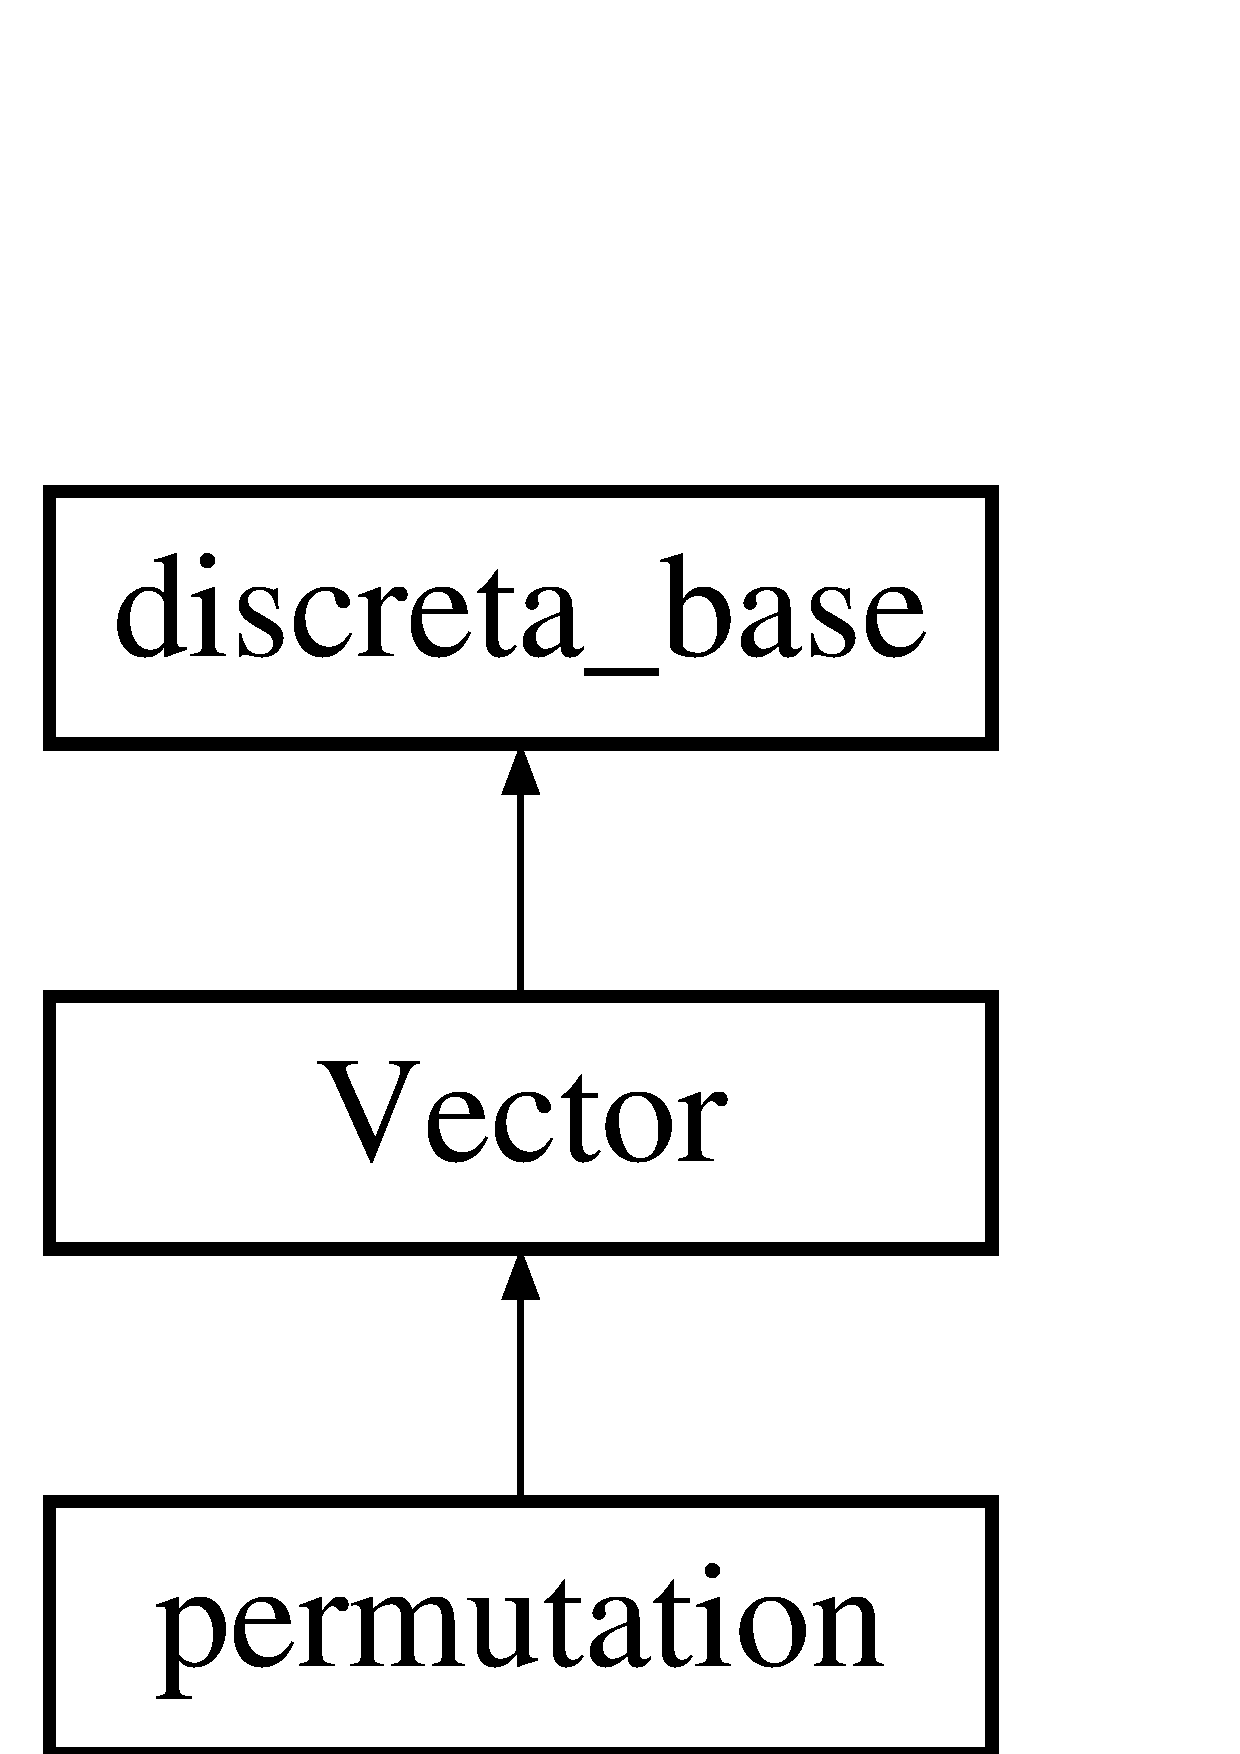
\includegraphics[height=3.000000cm]{classpermutation}
\end{center}
\end{figure}
\subsection*{Public Member Functions}
\begin{DoxyCompactItemize}
\item 
\mbox{\hyperlink{classpermutation_acb97f9398a52237f9f36f0ad5c8bf104}{permutation}} ()
\item 
\mbox{\hyperlink{classpermutation_a501f039c465ea7d47e6e0c0a165caa15}{permutation}} (const \mbox{\hyperlink{classdiscreta__base}{discreta\+\_\+base}} \&\mbox{\hyperlink{alphabet2_8_c_a6150e0515f7202e2fb518f7206ed97dc}{x}})
\item 
\mbox{\hyperlink{classpermutation}{permutation}} \& \mbox{\hyperlink{classpermutation_a7bc27f9f40363198e4f6b4c1d83ee3ba}{operator=}} (const \mbox{\hyperlink{classdiscreta__base}{discreta\+\_\+base}} \&\mbox{\hyperlink{alphabet2_8_c_a6150e0515f7202e2fb518f7206ed97dc}{x}})
\item 
void $\ast$ \mbox{\hyperlink{classpermutation_ac2a11ded23f8715f7b091d033d4a3eb0}{operator new}} (size\+\_\+t, void $\ast$\mbox{\hyperlink{alphabet2_8_c_a533391314665d6bf1b5575e9a9cd8552}{p}})
\item 
void \mbox{\hyperlink{classpermutation_af1eea29f86195cede9562e444664c28c}{settype\+\_\+permutation}} ()
\item 
\mbox{\hyperlink{discreta_8h_aaf25ee7e2306d78c74ec7bc48f092e81}{kind}} \mbox{\hyperlink{classpermutation_a2840be30bd1e636da5a955973c0c70b8}{s\+\_\+virtual\+\_\+kind}} ()
\item 
\mbox{\hyperlink{classpermutation_a006ecef14989dcf8539388d019e965e2}{$\sim$permutation}} ()
\item 
void \mbox{\hyperlink{classpermutation_a1f86343fa765d71c976d79e5ce372c12}{freeself\+\_\+permutation}} ()
\item 
void \mbox{\hyperlink{classpermutation_aed08e7ec26ec8ba0ed8c656a819ce43a}{copyobject\+\_\+to}} (\mbox{\hyperlink{classdiscreta__base}{discreta\+\_\+base}} \&\mbox{\hyperlink{alphabet2_8_c_a6150e0515f7202e2fb518f7206ed97dc}{x}})
\item 
ostream \& \mbox{\hyperlink{classpermutation_a3a4c219748ab79362fd440bea839c094}{print}} (ostream \&)
\item 
ostream \& \mbox{\hyperlink{classpermutation_a1732236cf59bbcaab008473f4917db3e}{print\+\_\+list}} (ostream \&ost)
\item 
ostream \& \mbox{\hyperlink{classpermutation_abf779232815eb4c16286cf642d214b50}{print\+\_\+cycle}} (ostream \&ost)
\item 
void \mbox{\hyperlink{classpermutation_a7074b329f809b23ba083e1a74b90bd03}{sscan}} (const char $\ast$s, \mbox{\hyperlink{galois_8h_a09fddde158a3a20bd2dcadb609de11dc}{I\+NT}} f\+\_\+v)
\item 
void \mbox{\hyperlink{classpermutation_a826e0fbc7234cbbff949d3e31a863d0a}{scan}} (istream \&is, \mbox{\hyperlink{galois_8h_a09fddde158a3a20bd2dcadb609de11dc}{I\+NT}} f\+\_\+v)
\item 
void \mbox{\hyperlink{classpermutation_a9cf73421f89b2c24cf2d08f002752030}{m\+\_\+l}} (\mbox{\hyperlink{galois_8h_a09fddde158a3a20bd2dcadb609de11dc}{I\+NT}} \mbox{\hyperlink{alphabet2_8_c_a89606eca6b563ec68d2da2e84657736f}{l}})
\item 
\mbox{\hyperlink{galois_8h_a09fddde158a3a20bd2dcadb609de11dc}{I\+NT}} \& \mbox{\hyperlink{classpermutation_ab8c74af5111dbf8808da04214b918873}{s\+\_\+i}} (\mbox{\hyperlink{galois_8h_a09fddde158a3a20bd2dcadb609de11dc}{I\+NT}} \mbox{\hyperlink{alphabet2_8_c_acb559820d9ca11295b4500f179ef6392}{i}})
\item 
\mbox{\hyperlink{galois_8h_a09fddde158a3a20bd2dcadb609de11dc}{I\+NT}} \& \mbox{\hyperlink{classpermutation_a447586a078cb487c97793a9d5d5ade28}{operator\mbox{[}$\,$\mbox{]}}} (\mbox{\hyperlink{galois_8h_a09fddde158a3a20bd2dcadb609de11dc}{I\+NT}} \mbox{\hyperlink{alphabet2_8_c_acb559820d9ca11295b4500f179ef6392}{i}})
\item 
void \mbox{\hyperlink{classpermutation_abbd320f211ed730261c31fecd5a567bb}{mult\+\_\+to}} (\mbox{\hyperlink{classdiscreta__base}{discreta\+\_\+base}} \&\mbox{\hyperlink{alphabet2_8_c_a6150e0515f7202e2fb518f7206ed97dc}{x}}, \mbox{\hyperlink{classdiscreta__base}{discreta\+\_\+base}} \&\mbox{\hyperlink{alphabet2_8_c_a0a2f84ed7838f07779ae24c5a9086d33}{y}})
\item 
\mbox{\hyperlink{galois_8h_a09fddde158a3a20bd2dcadb609de11dc}{I\+NT}} \mbox{\hyperlink{classpermutation_a1209ecbc8fdb0320a38218bd0c15c5fa}{invert\+\_\+to}} (\mbox{\hyperlink{classdiscreta__base}{discreta\+\_\+base}} \&\mbox{\hyperlink{alphabet2_8_c_a6150e0515f7202e2fb518f7206ed97dc}{x}})
\item 
void \mbox{\hyperlink{classpermutation_a358377181aea843bd774f0dfb3822b7f}{one}} ()
\item 
\mbox{\hyperlink{galois_8h_a09fddde158a3a20bd2dcadb609de11dc}{I\+NT}} \mbox{\hyperlink{classpermutation_ac86938f55c0b8af01d1f22c813310b97}{is\+\_\+one}} ()
\item 
\mbox{\hyperlink{galois_8h_a09fddde158a3a20bd2dcadb609de11dc}{I\+NT}} \mbox{\hyperlink{classpermutation_ae331b031f81647c88e72e966555c9c8f}{compare\+\_\+with}} (\mbox{\hyperlink{classdiscreta__base}{discreta\+\_\+base}} \&a)
\item 
void \mbox{\hyperlink{classpermutation_af4fd9ef2f599afdac92272358c4b8665}{write\+\_\+mem}} (\mbox{\hyperlink{classmemory}{memory}} \&m, \mbox{\hyperlink{galois_8h_a09fddde158a3a20bd2dcadb609de11dc}{I\+NT}} debug\+\_\+depth)
\item 
void \mbox{\hyperlink{classpermutation_ad3c756e8f0db2c95dfa7e6834c4bbaa3}{read\+\_\+mem}} (\mbox{\hyperlink{classmemory}{memory}} \&m, \mbox{\hyperlink{galois_8h_a09fddde158a3a20bd2dcadb609de11dc}{I\+NT}} debug\+\_\+depth)
\item 
\mbox{\hyperlink{galois_8h_a09fddde158a3a20bd2dcadb609de11dc}{I\+NT}} \mbox{\hyperlink{classpermutation_a121bb8f936f6e1e4101ef59d04c3998a}{csf}} ()
\item 
void \mbox{\hyperlink{classpermutation_ac4a8b92b8d658b8dbe8d3cf6791855f8}{get\+\_\+fixpoints}} (\mbox{\hyperlink{class_vector}{Vector}} \&\mbox{\hyperlink{alphabet2_8_c_a362077c979b0bb65159c603270e40f70}{f}})
\item 
void \mbox{\hyperlink{classpermutation_aa059d415966f85e6cf0753f20b80d4ab}{induce\+\_\+action\+\_\+on\+\_\+blocks}} (\mbox{\hyperlink{classpermutation}{permutation}} \&gg, \mbox{\hyperlink{class_vector}{Vector}} \&\mbox{\hyperlink{costas_8_c_ad1f767566c3189fb90e9cffcc5dd4680}{B}})
\item 
void \mbox{\hyperlink{classpermutation_a159dadce81dccf039f1a41825a0bb49e}{induce3}} (\mbox{\hyperlink{classpermutation}{permutation}} \&\mbox{\hyperlink{alphabet2_8_c_a148e3876077787926724625411d6e7a9}{b}})
\item 
void \mbox{\hyperlink{classpermutation_abfb30803652293a57f3cb1816b692153}{induce2}} (\mbox{\hyperlink{classpermutation}{permutation}} \&\mbox{\hyperlink{alphabet2_8_c_a148e3876077787926724625411d6e7a9}{b}})
\item 
void \mbox{\hyperlink{classpermutation_a55823b01d08ca0624a98d943da83245c}{induce\+\_\+on\+\_\+2tuples}} (\mbox{\hyperlink{classpermutation}{permutation}} \&\mbox{\hyperlink{alphabet2_8_c_a533391314665d6bf1b5575e9a9cd8552}{p}}, \mbox{\hyperlink{galois_8h_a09fddde158a3a20bd2dcadb609de11dc}{I\+NT}} f\+\_\+injective)
\item 
void \mbox{\hyperlink{classpermutation_a72b61b599c699c4db5d030970bf7534e}{add\+\_\+n\+\_\+fixpoints\+\_\+in\+\_\+front}} (\mbox{\hyperlink{classpermutation}{permutation}} \&\mbox{\hyperlink{alphabet2_8_c_a148e3876077787926724625411d6e7a9}{b}}, \mbox{\hyperlink{galois_8h_a09fddde158a3a20bd2dcadb609de11dc}{I\+NT}} \mbox{\hyperlink{simeon_8_c_a7f2cd26777ce0ff3fdaf8d02aacbddfb}{n}})
\item 
void \mbox{\hyperlink{classpermutation_af3c333fde02913f2042386a56e90b387}{add\+\_\+n\+\_\+fixpoints\+\_\+at\+\_\+end}} (\mbox{\hyperlink{classpermutation}{permutation}} \&\mbox{\hyperlink{alphabet2_8_c_a148e3876077787926724625411d6e7a9}{b}}, \mbox{\hyperlink{galois_8h_a09fddde158a3a20bd2dcadb609de11dc}{I\+NT}} \mbox{\hyperlink{simeon_8_c_a7f2cd26777ce0ff3fdaf8d02aacbddfb}{n}})
\item 
void \mbox{\hyperlink{classpermutation_a021494217208a3bacf9deba77484b70c}{add\+\_\+fixpoint\+\_\+in\+\_\+front}} (\mbox{\hyperlink{classpermutation}{permutation}} \&\mbox{\hyperlink{alphabet2_8_c_a148e3876077787926724625411d6e7a9}{b}})
\item 
void \mbox{\hyperlink{classpermutation_aefa5da43419a02c9cc0030715f8aa233}{embed\+\_\+at}} (\mbox{\hyperlink{classpermutation}{permutation}} \&\mbox{\hyperlink{alphabet2_8_c_a148e3876077787926724625411d6e7a9}{b}}, \mbox{\hyperlink{galois_8h_a09fddde158a3a20bd2dcadb609de11dc}{I\+NT}} \mbox{\hyperlink{simeon_8_c_a7f2cd26777ce0ff3fdaf8d02aacbddfb}{n}}, \mbox{\hyperlink{galois_8h_a09fddde158a3a20bd2dcadb609de11dc}{I\+NT}} at)
\item 
void \mbox{\hyperlink{classpermutation_aa7c3d0f95a13e5e3fef703c033e8f570}{remove\+\_\+fixpoint}} (\mbox{\hyperlink{classpermutation}{permutation}} \&\mbox{\hyperlink{alphabet2_8_c_a148e3876077787926724625411d6e7a9}{b}}, \mbox{\hyperlink{galois_8h_a09fddde158a3a20bd2dcadb609de11dc}{I\+NT}} \mbox{\hyperlink{alphabet2_8_c_acb559820d9ca11295b4500f179ef6392}{i}})
\item 
void \mbox{\hyperlink{classpermutation_a0a365befaed477cb76f21ed2b3f44d42}{join}} (\mbox{\hyperlink{classpermutation}{permutation}} \&a, \mbox{\hyperlink{classpermutation}{permutation}} \&\mbox{\hyperlink{alphabet2_8_c_a148e3876077787926724625411d6e7a9}{b}})
\item 
void \mbox{\hyperlink{classpermutation_ad4e25c696e47457b84481f528a4d4d8e}{cartesian\+\_\+product\+\_\+action}} (\mbox{\hyperlink{classpermutation}{permutation}} \&a, \mbox{\hyperlink{classpermutation}{permutation}} \&\mbox{\hyperlink{alphabet2_8_c_a148e3876077787926724625411d6e7a9}{b}})
\item 
void \mbox{\hyperlink{classpermutation_a1e3b6593fab78625b620820e0d61f1e0}{Add2\+Cycle}} (\mbox{\hyperlink{galois_8h_a09fddde158a3a20bd2dcadb609de11dc}{I\+NT}} i0, \mbox{\hyperlink{galois_8h_a09fddde158a3a20bd2dcadb609de11dc}{I\+NT}} i1)
\item 
void \mbox{\hyperlink{classpermutation_a89f7abdb4b6898acdc4f0425905dcf5f}{Add3\+Cycle}} (\mbox{\hyperlink{galois_8h_a09fddde158a3a20bd2dcadb609de11dc}{I\+NT}} i0, \mbox{\hyperlink{galois_8h_a09fddde158a3a20bd2dcadb609de11dc}{I\+NT}} i1, \mbox{\hyperlink{galois_8h_a09fddde158a3a20bd2dcadb609de11dc}{I\+NT}} i2)
\item 
void \mbox{\hyperlink{classpermutation_abe736e092eae50dfac474a510e51125f}{Add4\+Cycle}} (\mbox{\hyperlink{galois_8h_a09fddde158a3a20bd2dcadb609de11dc}{I\+NT}} i0, \mbox{\hyperlink{galois_8h_a09fddde158a3a20bd2dcadb609de11dc}{I\+NT}} i1, \mbox{\hyperlink{galois_8h_a09fddde158a3a20bd2dcadb609de11dc}{I\+NT}} i2, \mbox{\hyperlink{galois_8h_a09fddde158a3a20bd2dcadb609de11dc}{I\+NT}} i3)
\item 
void \mbox{\hyperlink{classpermutation_ac5767bfd7dbceb312865aff4a759d1a7}{Add5\+Cycle}} (\mbox{\hyperlink{galois_8h_a09fddde158a3a20bd2dcadb609de11dc}{I\+NT}} i0, \mbox{\hyperlink{galois_8h_a09fddde158a3a20bd2dcadb609de11dc}{I\+NT}} i1, \mbox{\hyperlink{galois_8h_a09fddde158a3a20bd2dcadb609de11dc}{I\+NT}} i2, \mbox{\hyperlink{galois_8h_a09fddde158a3a20bd2dcadb609de11dc}{I\+NT}} i3, \mbox{\hyperlink{galois_8h_a09fddde158a3a20bd2dcadb609de11dc}{I\+NT}} i4)
\item 
void \mbox{\hyperlink{classpermutation_a0228b471531a836ef8fa92998cd34c57}{Add\+N\+Cycle}} (\mbox{\hyperlink{galois_8h_a09fddde158a3a20bd2dcadb609de11dc}{I\+NT}} first, \mbox{\hyperlink{galois_8h_a09fddde158a3a20bd2dcadb609de11dc}{I\+NT}} len)
\item 
void \mbox{\hyperlink{classpermutation_ae382ff0da7bb6f39d93211b14661ff89}{set\+\_\+print\+\_\+type\+\_\+integer\+\_\+from\+\_\+zero}} ()
\item 
void \mbox{\hyperlink{classpermutation_a4950201b37c672151c1e18cc523199da}{set\+\_\+print\+\_\+type\+\_\+integer\+\_\+from\+\_\+one}} ()
\item 
void \mbox{\hyperlink{classpermutation_aba7249c360858552c8e134f33c921aba}{set\+\_\+print\+\_\+type\+\_\+\+P\+G\+\_\+1\+\_\+q\+\_\+element}} (\mbox{\hyperlink{classdomain}{domain}} $\ast$dom)
\item 
void \mbox{\hyperlink{classpermutation_ae1ab11a87e70803c1cec31508a2c8c7f}{convert\+\_\+digit}} (\mbox{\hyperlink{galois_8h_a09fddde158a3a20bd2dcadb609de11dc}{I\+NT}} \mbox{\hyperlink{alphabet2_8_c_acb559820d9ca11295b4500f179ef6392}{i}}, \mbox{\hyperlink{classhollerith}{hollerith}} \&a)
\item 
void \mbox{\hyperlink{classpermutation_a5509600cbe40b5c6cdaff56d822b4de0}{cycle\+\_\+type}} (\mbox{\hyperlink{class_vector}{Vector}} \&\mbox{\hyperlink{_l_i_b_2_g_a_l_o_i_s_2dlx_8_c_ad241c8005abf9f323e9fffec67f55abf}{type}}, \mbox{\hyperlink{galois_8h_a09fddde158a3a20bd2dcadb609de11dc}{I\+NT}} f\+\_\+v)
\item 
\mbox{\hyperlink{galois_8h_a09fddde158a3a20bd2dcadb609de11dc}{I\+NT}} \mbox{\hyperlink{classpermutation_a5846c6cfd8d2d64f4cb906425744f73f}{nb\+\_\+of\+\_\+inversions}} (\mbox{\hyperlink{galois_8h_a09fddde158a3a20bd2dcadb609de11dc}{I\+NT}} f\+\_\+v)
\item 
\mbox{\hyperlink{galois_8h_a09fddde158a3a20bd2dcadb609de11dc}{I\+NT}} \mbox{\hyperlink{classpermutation_a51cfe6b579a1d45524f39096c22c4398}{signum}} (\mbox{\hyperlink{galois_8h_a09fddde158a3a20bd2dcadb609de11dc}{I\+NT}} f\+\_\+v)
\item 
\mbox{\hyperlink{galois_8h_a09fddde158a3a20bd2dcadb609de11dc}{I\+NT}} \mbox{\hyperlink{classpermutation_a7b410bb3cb56dfcb5e5f2976b1d1aa45}{is\+\_\+even}} (\mbox{\hyperlink{galois_8h_a09fddde158a3a20bd2dcadb609de11dc}{I\+NT}} f\+\_\+v)
\item 
void \mbox{\hyperlink{classpermutation_a88706cf2c683df70a29156f39b3e4895}{cycles}} (\mbox{\hyperlink{class_vector}{Vector}} \&cycles)
\item 
void \mbox{\hyperlink{classpermutation_a9d9fa353830f05cbfd2080e3e87260d2}{restrict\+\_\+to\+\_\+subset}} (\mbox{\hyperlink{classpermutation}{permutation}} \&\mbox{\hyperlink{simeon_8_c_a92cbb483a3b27ae1a0dbfcb125ce216f}{q}}, \mbox{\hyperlink{galois_8h_a09fddde158a3a20bd2dcadb609de11dc}{I\+NT}} first, \mbox{\hyperlink{galois_8h_a09fddde158a3a20bd2dcadb609de11dc}{I\+NT}} len)
\item 
void \mbox{\hyperlink{classpermutation_a3e01585ffb15282fc45a3158c5ad0b76}{induce\+\_\+on\+\_\+lines\+\_\+of\+\_\+\+P\+G\+\_\+k\+\_\+q}} (\mbox{\hyperlink{galois_8h_a09fddde158a3a20bd2dcadb609de11dc}{I\+NT}} \mbox{\hyperlink{classdiscreta__base_a6f7a0f7bdd115b9e4dde358cfa7ebf81}{k}}, \mbox{\hyperlink{galois_8h_a09fddde158a3a20bd2dcadb609de11dc}{I\+NT}} \mbox{\hyperlink{simeon_8_c_a92cbb483a3b27ae1a0dbfcb125ce216f}{q}}, \mbox{\hyperlink{classpermutation}{permutation}} \&per, \mbox{\hyperlink{galois_8h_a09fddde158a3a20bd2dcadb609de11dc}{I\+NT}} f\+\_\+v, \mbox{\hyperlink{galois_8h_a09fddde158a3a20bd2dcadb609de11dc}{I\+NT}} f\+\_\+vv)
\item 
void \mbox{\hyperlink{classpermutation_a013701d741e69609903a93f3874308f4}{singer\+\_\+cycle\+\_\+on\+\_\+points\+\_\+of\+\_\+projective\+\_\+plane}} (\mbox{\hyperlink{galois_8h_a09fddde158a3a20bd2dcadb609de11dc}{I\+NT}} \mbox{\hyperlink{alphabet2_8_c_a533391314665d6bf1b5575e9a9cd8552}{p}}, \mbox{\hyperlink{galois_8h_a09fddde158a3a20bd2dcadb609de11dc}{I\+NT}} f\+\_\+modified, \mbox{\hyperlink{galois_8h_a09fddde158a3a20bd2dcadb609de11dc}{I\+NT}} f\+\_\+v)
\item 
void \mbox{\hyperlink{classpermutation_a42c6adacfca83d855da8a2a38e300057}{Cn\+\_\+in\+\_\+\+Cnm}} (\mbox{\hyperlink{galois_8h_a09fddde158a3a20bd2dcadb609de11dc}{I\+NT}} \mbox{\hyperlink{simeon_8_c_a7f2cd26777ce0ff3fdaf8d02aacbddfb}{n}}, \mbox{\hyperlink{galois_8h_a09fddde158a3a20bd2dcadb609de11dc}{I\+NT}} m)
\item 
\mbox{\hyperlink{galois_8h_a09fddde158a3a20bd2dcadb609de11dc}{I\+NT}} \mbox{\hyperlink{classpermutation_a224e460e2d774a36a52b4d233d117988}{preimage}} (\mbox{\hyperlink{galois_8h_a09fddde158a3a20bd2dcadb609de11dc}{I\+NT}} \mbox{\hyperlink{alphabet2_8_c_acb559820d9ca11295b4500f179ef6392}{i}})
\end{DoxyCompactItemize}
\subsection*{Additional Inherited Members}


\subsection{Constructor \& Destructor Documentation}
\mbox{\Hypertarget{classpermutation_acb97f9398a52237f9f36f0ad5c8bf104}\label{classpermutation_acb97f9398a52237f9f36f0ad5c8bf104}} 
\index{permutation@{permutation}!permutation@{permutation}}
\index{permutation@{permutation}!permutation@{permutation}}
\subsubsection{\texorpdfstring{permutation()}{permutation()}\hspace{0.1cm}{\footnotesize\ttfamily [1/2]}}
{\footnotesize\ttfamily permutation\+::permutation (\begin{DoxyParamCaption}{ }\end{DoxyParamCaption})}

\mbox{\Hypertarget{classpermutation_a501f039c465ea7d47e6e0c0a165caa15}\label{classpermutation_a501f039c465ea7d47e6e0c0a165caa15}} 
\index{permutation@{permutation}!permutation@{permutation}}
\index{permutation@{permutation}!permutation@{permutation}}
\subsubsection{\texorpdfstring{permutation()}{permutation()}\hspace{0.1cm}{\footnotesize\ttfamily [2/2]}}
{\footnotesize\ttfamily permutation\+::permutation (\begin{DoxyParamCaption}\item[{const \mbox{\hyperlink{classdiscreta__base}{discreta\+\_\+base}} \&}]{x }\end{DoxyParamCaption})}

\mbox{\Hypertarget{classpermutation_a006ecef14989dcf8539388d019e965e2}\label{classpermutation_a006ecef14989dcf8539388d019e965e2}} 
\index{permutation@{permutation}!````~permutation@{$\sim$permutation}}
\index{````~permutation@{$\sim$permutation}!permutation@{permutation}}
\subsubsection{\texorpdfstring{$\sim$permutation()}{~permutation()}}
{\footnotesize\ttfamily permutation\+::$\sim$permutation (\begin{DoxyParamCaption}{ }\end{DoxyParamCaption})}



\subsection{Member Function Documentation}
\mbox{\Hypertarget{classpermutation_a1e3b6593fab78625b620820e0d61f1e0}\label{classpermutation_a1e3b6593fab78625b620820e0d61f1e0}} 
\index{permutation@{permutation}!Add2\+Cycle@{Add2\+Cycle}}
\index{Add2\+Cycle@{Add2\+Cycle}!permutation@{permutation}}
\subsubsection{\texorpdfstring{Add2\+Cycle()}{Add2Cycle()}}
{\footnotesize\ttfamily void permutation\+::\+Add2\+Cycle (\begin{DoxyParamCaption}\item[{\mbox{\hyperlink{galois_8h_a09fddde158a3a20bd2dcadb609de11dc}{I\+NT}}}]{i0,  }\item[{\mbox{\hyperlink{galois_8h_a09fddde158a3a20bd2dcadb609de11dc}{I\+NT}}}]{i1 }\end{DoxyParamCaption})}

\mbox{\Hypertarget{classpermutation_a89f7abdb4b6898acdc4f0425905dcf5f}\label{classpermutation_a89f7abdb4b6898acdc4f0425905dcf5f}} 
\index{permutation@{permutation}!Add3\+Cycle@{Add3\+Cycle}}
\index{Add3\+Cycle@{Add3\+Cycle}!permutation@{permutation}}
\subsubsection{\texorpdfstring{Add3\+Cycle()}{Add3Cycle()}}
{\footnotesize\ttfamily void permutation\+::\+Add3\+Cycle (\begin{DoxyParamCaption}\item[{\mbox{\hyperlink{galois_8h_a09fddde158a3a20bd2dcadb609de11dc}{I\+NT}}}]{i0,  }\item[{\mbox{\hyperlink{galois_8h_a09fddde158a3a20bd2dcadb609de11dc}{I\+NT}}}]{i1,  }\item[{\mbox{\hyperlink{galois_8h_a09fddde158a3a20bd2dcadb609de11dc}{I\+NT}}}]{i2 }\end{DoxyParamCaption})}

\mbox{\Hypertarget{classpermutation_abe736e092eae50dfac474a510e51125f}\label{classpermutation_abe736e092eae50dfac474a510e51125f}} 
\index{permutation@{permutation}!Add4\+Cycle@{Add4\+Cycle}}
\index{Add4\+Cycle@{Add4\+Cycle}!permutation@{permutation}}
\subsubsection{\texorpdfstring{Add4\+Cycle()}{Add4Cycle()}}
{\footnotesize\ttfamily void permutation\+::\+Add4\+Cycle (\begin{DoxyParamCaption}\item[{\mbox{\hyperlink{galois_8h_a09fddde158a3a20bd2dcadb609de11dc}{I\+NT}}}]{i0,  }\item[{\mbox{\hyperlink{galois_8h_a09fddde158a3a20bd2dcadb609de11dc}{I\+NT}}}]{i1,  }\item[{\mbox{\hyperlink{galois_8h_a09fddde158a3a20bd2dcadb609de11dc}{I\+NT}}}]{i2,  }\item[{\mbox{\hyperlink{galois_8h_a09fddde158a3a20bd2dcadb609de11dc}{I\+NT}}}]{i3 }\end{DoxyParamCaption})}

\mbox{\Hypertarget{classpermutation_ac5767bfd7dbceb312865aff4a759d1a7}\label{classpermutation_ac5767bfd7dbceb312865aff4a759d1a7}} 
\index{permutation@{permutation}!Add5\+Cycle@{Add5\+Cycle}}
\index{Add5\+Cycle@{Add5\+Cycle}!permutation@{permutation}}
\subsubsection{\texorpdfstring{Add5\+Cycle()}{Add5Cycle()}}
{\footnotesize\ttfamily void permutation\+::\+Add5\+Cycle (\begin{DoxyParamCaption}\item[{\mbox{\hyperlink{galois_8h_a09fddde158a3a20bd2dcadb609de11dc}{I\+NT}}}]{i0,  }\item[{\mbox{\hyperlink{galois_8h_a09fddde158a3a20bd2dcadb609de11dc}{I\+NT}}}]{i1,  }\item[{\mbox{\hyperlink{galois_8h_a09fddde158a3a20bd2dcadb609de11dc}{I\+NT}}}]{i2,  }\item[{\mbox{\hyperlink{galois_8h_a09fddde158a3a20bd2dcadb609de11dc}{I\+NT}}}]{i3,  }\item[{\mbox{\hyperlink{galois_8h_a09fddde158a3a20bd2dcadb609de11dc}{I\+NT}}}]{i4 }\end{DoxyParamCaption})}

\mbox{\Hypertarget{classpermutation_a021494217208a3bacf9deba77484b70c}\label{classpermutation_a021494217208a3bacf9deba77484b70c}} 
\index{permutation@{permutation}!add\+\_\+fixpoint\+\_\+in\+\_\+front@{add\+\_\+fixpoint\+\_\+in\+\_\+front}}
\index{add\+\_\+fixpoint\+\_\+in\+\_\+front@{add\+\_\+fixpoint\+\_\+in\+\_\+front}!permutation@{permutation}}
\subsubsection{\texorpdfstring{add\+\_\+fixpoint\+\_\+in\+\_\+front()}{add\_fixpoint\_in\_front()}}
{\footnotesize\ttfamily void permutation\+::add\+\_\+fixpoint\+\_\+in\+\_\+front (\begin{DoxyParamCaption}\item[{\mbox{\hyperlink{classpermutation}{permutation}} \&}]{b }\end{DoxyParamCaption})}

\mbox{\Hypertarget{classpermutation_af3c333fde02913f2042386a56e90b387}\label{classpermutation_af3c333fde02913f2042386a56e90b387}} 
\index{permutation@{permutation}!add\+\_\+n\+\_\+fixpoints\+\_\+at\+\_\+end@{add\+\_\+n\+\_\+fixpoints\+\_\+at\+\_\+end}}
\index{add\+\_\+n\+\_\+fixpoints\+\_\+at\+\_\+end@{add\+\_\+n\+\_\+fixpoints\+\_\+at\+\_\+end}!permutation@{permutation}}
\subsubsection{\texorpdfstring{add\+\_\+n\+\_\+fixpoints\+\_\+at\+\_\+end()}{add\_n\_fixpoints\_at\_end()}}
{\footnotesize\ttfamily void permutation\+::add\+\_\+n\+\_\+fixpoints\+\_\+at\+\_\+end (\begin{DoxyParamCaption}\item[{\mbox{\hyperlink{classpermutation}{permutation}} \&}]{b,  }\item[{\mbox{\hyperlink{galois_8h_a09fddde158a3a20bd2dcadb609de11dc}{I\+NT}}}]{n }\end{DoxyParamCaption})}

\mbox{\Hypertarget{classpermutation_a72b61b599c699c4db5d030970bf7534e}\label{classpermutation_a72b61b599c699c4db5d030970bf7534e}} 
\index{permutation@{permutation}!add\+\_\+n\+\_\+fixpoints\+\_\+in\+\_\+front@{add\+\_\+n\+\_\+fixpoints\+\_\+in\+\_\+front}}
\index{add\+\_\+n\+\_\+fixpoints\+\_\+in\+\_\+front@{add\+\_\+n\+\_\+fixpoints\+\_\+in\+\_\+front}!permutation@{permutation}}
\subsubsection{\texorpdfstring{add\+\_\+n\+\_\+fixpoints\+\_\+in\+\_\+front()}{add\_n\_fixpoints\_in\_front()}}
{\footnotesize\ttfamily void permutation\+::add\+\_\+n\+\_\+fixpoints\+\_\+in\+\_\+front (\begin{DoxyParamCaption}\item[{\mbox{\hyperlink{classpermutation}{permutation}} \&}]{b,  }\item[{\mbox{\hyperlink{galois_8h_a09fddde158a3a20bd2dcadb609de11dc}{I\+NT}}}]{n }\end{DoxyParamCaption})}

\mbox{\Hypertarget{classpermutation_a0228b471531a836ef8fa92998cd34c57}\label{classpermutation_a0228b471531a836ef8fa92998cd34c57}} 
\index{permutation@{permutation}!Add\+N\+Cycle@{Add\+N\+Cycle}}
\index{Add\+N\+Cycle@{Add\+N\+Cycle}!permutation@{permutation}}
\subsubsection{\texorpdfstring{Add\+N\+Cycle()}{AddNCycle()}}
{\footnotesize\ttfamily void permutation\+::\+Add\+N\+Cycle (\begin{DoxyParamCaption}\item[{\mbox{\hyperlink{galois_8h_a09fddde158a3a20bd2dcadb609de11dc}{I\+NT}}}]{first,  }\item[{\mbox{\hyperlink{galois_8h_a09fddde158a3a20bd2dcadb609de11dc}{I\+NT}}}]{len }\end{DoxyParamCaption})}

\mbox{\Hypertarget{classpermutation_ad4e25c696e47457b84481f528a4d4d8e}\label{classpermutation_ad4e25c696e47457b84481f528a4d4d8e}} 
\index{permutation@{permutation}!cartesian\+\_\+product\+\_\+action@{cartesian\+\_\+product\+\_\+action}}
\index{cartesian\+\_\+product\+\_\+action@{cartesian\+\_\+product\+\_\+action}!permutation@{permutation}}
\subsubsection{\texorpdfstring{cartesian\+\_\+product\+\_\+action()}{cartesian\_product\_action()}}
{\footnotesize\ttfamily void permutation\+::cartesian\+\_\+product\+\_\+action (\begin{DoxyParamCaption}\item[{\mbox{\hyperlink{classpermutation}{permutation}} \&}]{a,  }\item[{\mbox{\hyperlink{classpermutation}{permutation}} \&}]{b }\end{DoxyParamCaption})}

\mbox{\Hypertarget{classpermutation_a42c6adacfca83d855da8a2a38e300057}\label{classpermutation_a42c6adacfca83d855da8a2a38e300057}} 
\index{permutation@{permutation}!Cn\+\_\+in\+\_\+\+Cnm@{Cn\+\_\+in\+\_\+\+Cnm}}
\index{Cn\+\_\+in\+\_\+\+Cnm@{Cn\+\_\+in\+\_\+\+Cnm}!permutation@{permutation}}
\subsubsection{\texorpdfstring{Cn\+\_\+in\+\_\+\+Cnm()}{Cn\_in\_Cnm()}}
{\footnotesize\ttfamily void permutation\+::\+Cn\+\_\+in\+\_\+\+Cnm (\begin{DoxyParamCaption}\item[{\mbox{\hyperlink{galois_8h_a09fddde158a3a20bd2dcadb609de11dc}{I\+NT}}}]{n,  }\item[{\mbox{\hyperlink{galois_8h_a09fddde158a3a20bd2dcadb609de11dc}{I\+NT}}}]{m }\end{DoxyParamCaption})}

\mbox{\Hypertarget{classpermutation_ae331b031f81647c88e72e966555c9c8f}\label{classpermutation_ae331b031f81647c88e72e966555c9c8f}} 
\index{permutation@{permutation}!compare\+\_\+with@{compare\+\_\+with}}
\index{compare\+\_\+with@{compare\+\_\+with}!permutation@{permutation}}
\subsubsection{\texorpdfstring{compare\+\_\+with()}{compare\_with()}}
{\footnotesize\ttfamily \mbox{\hyperlink{galois_8h_a09fddde158a3a20bd2dcadb609de11dc}{I\+NT}} permutation\+::compare\+\_\+with (\begin{DoxyParamCaption}\item[{\mbox{\hyperlink{classdiscreta__base}{discreta\+\_\+base}} \&}]{a }\end{DoxyParamCaption})\hspace{0.3cm}{\ttfamily [virtual]}}



Reimplemented from \mbox{\hyperlink{class_vector_a5fc27308a2710188b16f92df56c79c55}{Vector}}.

\mbox{\Hypertarget{classpermutation_ae1ab11a87e70803c1cec31508a2c8c7f}\label{classpermutation_ae1ab11a87e70803c1cec31508a2c8c7f}} 
\index{permutation@{permutation}!convert\+\_\+digit@{convert\+\_\+digit}}
\index{convert\+\_\+digit@{convert\+\_\+digit}!permutation@{permutation}}
\subsubsection{\texorpdfstring{convert\+\_\+digit()}{convert\_digit()}}
{\footnotesize\ttfamily void permutation\+::convert\+\_\+digit (\begin{DoxyParamCaption}\item[{\mbox{\hyperlink{galois_8h_a09fddde158a3a20bd2dcadb609de11dc}{I\+NT}}}]{i,  }\item[{\mbox{\hyperlink{classhollerith}{hollerith}} \&}]{a }\end{DoxyParamCaption})}

\mbox{\Hypertarget{classpermutation_aed08e7ec26ec8ba0ed8c656a819ce43a}\label{classpermutation_aed08e7ec26ec8ba0ed8c656a819ce43a}} 
\index{permutation@{permutation}!copyobject\+\_\+to@{copyobject\+\_\+to}}
\index{copyobject\+\_\+to@{copyobject\+\_\+to}!permutation@{permutation}}
\subsubsection{\texorpdfstring{copyobject\+\_\+to()}{copyobject\_to()}}
{\footnotesize\ttfamily void permutation\+::copyobject\+\_\+to (\begin{DoxyParamCaption}\item[{\mbox{\hyperlink{classdiscreta__base}{discreta\+\_\+base}} \&}]{x }\end{DoxyParamCaption})\hspace{0.3cm}{\ttfamily [virtual]}}



Reimplemented from \mbox{\hyperlink{class_vector_af657307f3d344c8cef5d633335a5f484}{Vector}}.

\mbox{\Hypertarget{classpermutation_a121bb8f936f6e1e4101ef59d04c3998a}\label{classpermutation_a121bb8f936f6e1e4101ef59d04c3998a}} 
\index{permutation@{permutation}!csf@{csf}}
\index{csf@{csf}!permutation@{permutation}}
\subsubsection{\texorpdfstring{csf()}{csf()}}
{\footnotesize\ttfamily \mbox{\hyperlink{galois_8h_a09fddde158a3a20bd2dcadb609de11dc}{I\+NT}} permutation\+::csf (\begin{DoxyParamCaption}{ }\end{DoxyParamCaption})}

\mbox{\Hypertarget{classpermutation_a5509600cbe40b5c6cdaff56d822b4de0}\label{classpermutation_a5509600cbe40b5c6cdaff56d822b4de0}} 
\index{permutation@{permutation}!cycle\+\_\+type@{cycle\+\_\+type}}
\index{cycle\+\_\+type@{cycle\+\_\+type}!permutation@{permutation}}
\subsubsection{\texorpdfstring{cycle\+\_\+type()}{cycle\_type()}}
{\footnotesize\ttfamily void permutation\+::cycle\+\_\+type (\begin{DoxyParamCaption}\item[{\mbox{\hyperlink{class_vector}{Vector}} \&}]{type,  }\item[{\mbox{\hyperlink{galois_8h_a09fddde158a3a20bd2dcadb609de11dc}{I\+NT}}}]{f\+\_\+v }\end{DoxyParamCaption})}

\mbox{\Hypertarget{classpermutation_a88706cf2c683df70a29156f39b3e4895}\label{classpermutation_a88706cf2c683df70a29156f39b3e4895}} 
\index{permutation@{permutation}!cycles@{cycles}}
\index{cycles@{cycles}!permutation@{permutation}}
\subsubsection{\texorpdfstring{cycles()}{cycles()}}
{\footnotesize\ttfamily void permutation\+::cycles (\begin{DoxyParamCaption}\item[{\mbox{\hyperlink{class_vector}{Vector}} \&}]{cycles }\end{DoxyParamCaption})}

\mbox{\Hypertarget{classpermutation_aefa5da43419a02c9cc0030715f8aa233}\label{classpermutation_aefa5da43419a02c9cc0030715f8aa233}} 
\index{permutation@{permutation}!embed\+\_\+at@{embed\+\_\+at}}
\index{embed\+\_\+at@{embed\+\_\+at}!permutation@{permutation}}
\subsubsection{\texorpdfstring{embed\+\_\+at()}{embed\_at()}}
{\footnotesize\ttfamily void permutation\+::embed\+\_\+at (\begin{DoxyParamCaption}\item[{\mbox{\hyperlink{classpermutation}{permutation}} \&}]{b,  }\item[{\mbox{\hyperlink{galois_8h_a09fddde158a3a20bd2dcadb609de11dc}{I\+NT}}}]{n,  }\item[{\mbox{\hyperlink{galois_8h_a09fddde158a3a20bd2dcadb609de11dc}{I\+NT}}}]{at }\end{DoxyParamCaption})}

\mbox{\Hypertarget{classpermutation_a1f86343fa765d71c976d79e5ce372c12}\label{classpermutation_a1f86343fa765d71c976d79e5ce372c12}} 
\index{permutation@{permutation}!freeself\+\_\+permutation@{freeself\+\_\+permutation}}
\index{freeself\+\_\+permutation@{freeself\+\_\+permutation}!permutation@{permutation}}
\subsubsection{\texorpdfstring{freeself\+\_\+permutation()}{freeself\_permutation()}}
{\footnotesize\ttfamily void permutation\+::freeself\+\_\+permutation (\begin{DoxyParamCaption}{ }\end{DoxyParamCaption})}

\mbox{\Hypertarget{classpermutation_ac4a8b92b8d658b8dbe8d3cf6791855f8}\label{classpermutation_ac4a8b92b8d658b8dbe8d3cf6791855f8}} 
\index{permutation@{permutation}!get\+\_\+fixpoints@{get\+\_\+fixpoints}}
\index{get\+\_\+fixpoints@{get\+\_\+fixpoints}!permutation@{permutation}}
\subsubsection{\texorpdfstring{get\+\_\+fixpoints()}{get\_fixpoints()}}
{\footnotesize\ttfamily void permutation\+::get\+\_\+fixpoints (\begin{DoxyParamCaption}\item[{\mbox{\hyperlink{class_vector}{Vector}} \&}]{f }\end{DoxyParamCaption})}

\mbox{\Hypertarget{classpermutation_abfb30803652293a57f3cb1816b692153}\label{classpermutation_abfb30803652293a57f3cb1816b692153}} 
\index{permutation@{permutation}!induce2@{induce2}}
\index{induce2@{induce2}!permutation@{permutation}}
\subsubsection{\texorpdfstring{induce2()}{induce2()}}
{\footnotesize\ttfamily void permutation\+::induce2 (\begin{DoxyParamCaption}\item[{\mbox{\hyperlink{classpermutation}{permutation}} \&}]{b }\end{DoxyParamCaption})}

\mbox{\Hypertarget{classpermutation_a159dadce81dccf039f1a41825a0bb49e}\label{classpermutation_a159dadce81dccf039f1a41825a0bb49e}} 
\index{permutation@{permutation}!induce3@{induce3}}
\index{induce3@{induce3}!permutation@{permutation}}
\subsubsection{\texorpdfstring{induce3()}{induce3()}}
{\footnotesize\ttfamily void permutation\+::induce3 (\begin{DoxyParamCaption}\item[{\mbox{\hyperlink{classpermutation}{permutation}} \&}]{b }\end{DoxyParamCaption})}

\mbox{\Hypertarget{classpermutation_aa059d415966f85e6cf0753f20b80d4ab}\label{classpermutation_aa059d415966f85e6cf0753f20b80d4ab}} 
\index{permutation@{permutation}!induce\+\_\+action\+\_\+on\+\_\+blocks@{induce\+\_\+action\+\_\+on\+\_\+blocks}}
\index{induce\+\_\+action\+\_\+on\+\_\+blocks@{induce\+\_\+action\+\_\+on\+\_\+blocks}!permutation@{permutation}}
\subsubsection{\texorpdfstring{induce\+\_\+action\+\_\+on\+\_\+blocks()}{induce\_action\_on\_blocks()}}
{\footnotesize\ttfamily void permutation\+::induce\+\_\+action\+\_\+on\+\_\+blocks (\begin{DoxyParamCaption}\item[{\mbox{\hyperlink{classpermutation}{permutation}} \&}]{gg,  }\item[{\mbox{\hyperlink{class_vector}{Vector}} \&}]{B }\end{DoxyParamCaption})}

\mbox{\Hypertarget{classpermutation_a55823b01d08ca0624a98d943da83245c}\label{classpermutation_a55823b01d08ca0624a98d943da83245c}} 
\index{permutation@{permutation}!induce\+\_\+on\+\_\+2tuples@{induce\+\_\+on\+\_\+2tuples}}
\index{induce\+\_\+on\+\_\+2tuples@{induce\+\_\+on\+\_\+2tuples}!permutation@{permutation}}
\subsubsection{\texorpdfstring{induce\+\_\+on\+\_\+2tuples()}{induce\_on\_2tuples()}}
{\footnotesize\ttfamily void permutation\+::induce\+\_\+on\+\_\+2tuples (\begin{DoxyParamCaption}\item[{\mbox{\hyperlink{classpermutation}{permutation}} \&}]{p,  }\item[{\mbox{\hyperlink{galois_8h_a09fddde158a3a20bd2dcadb609de11dc}{I\+NT}}}]{f\+\_\+injective }\end{DoxyParamCaption})}

\mbox{\Hypertarget{classpermutation_a3e01585ffb15282fc45a3158c5ad0b76}\label{classpermutation_a3e01585ffb15282fc45a3158c5ad0b76}} 
\index{permutation@{permutation}!induce\+\_\+on\+\_\+lines\+\_\+of\+\_\+\+P\+G\+\_\+k\+\_\+q@{induce\+\_\+on\+\_\+lines\+\_\+of\+\_\+\+P\+G\+\_\+k\+\_\+q}}
\index{induce\+\_\+on\+\_\+lines\+\_\+of\+\_\+\+P\+G\+\_\+k\+\_\+q@{induce\+\_\+on\+\_\+lines\+\_\+of\+\_\+\+P\+G\+\_\+k\+\_\+q}!permutation@{permutation}}
\subsubsection{\texorpdfstring{induce\+\_\+on\+\_\+lines\+\_\+of\+\_\+\+P\+G\+\_\+k\+\_\+q()}{induce\_on\_lines\_of\_PG\_k\_q()}}
{\footnotesize\ttfamily void permutation\+::induce\+\_\+on\+\_\+lines\+\_\+of\+\_\+\+P\+G\+\_\+k\+\_\+q (\begin{DoxyParamCaption}\item[{\mbox{\hyperlink{galois_8h_a09fddde158a3a20bd2dcadb609de11dc}{I\+NT}}}]{k,  }\item[{\mbox{\hyperlink{galois_8h_a09fddde158a3a20bd2dcadb609de11dc}{I\+NT}}}]{q,  }\item[{\mbox{\hyperlink{classpermutation}{permutation}} \&}]{per,  }\item[{\mbox{\hyperlink{galois_8h_a09fddde158a3a20bd2dcadb609de11dc}{I\+NT}}}]{f\+\_\+v,  }\item[{\mbox{\hyperlink{galois_8h_a09fddde158a3a20bd2dcadb609de11dc}{I\+NT}}}]{f\+\_\+vv }\end{DoxyParamCaption})}

\mbox{\Hypertarget{classpermutation_a1209ecbc8fdb0320a38218bd0c15c5fa}\label{classpermutation_a1209ecbc8fdb0320a38218bd0c15c5fa}} 
\index{permutation@{permutation}!invert\+\_\+to@{invert\+\_\+to}}
\index{invert\+\_\+to@{invert\+\_\+to}!permutation@{permutation}}
\subsubsection{\texorpdfstring{invert\+\_\+to()}{invert\_to()}}
{\footnotesize\ttfamily \mbox{\hyperlink{galois_8h_a09fddde158a3a20bd2dcadb609de11dc}{I\+NT}} permutation\+::invert\+\_\+to (\begin{DoxyParamCaption}\item[{\mbox{\hyperlink{classdiscreta__base}{discreta\+\_\+base}} \&}]{x }\end{DoxyParamCaption})\hspace{0.3cm}{\ttfamily [virtual]}}



Reimplemented from \mbox{\hyperlink{classdiscreta__base_a874a5ffb467f3896604a3c9bdf0cca50}{discreta\+\_\+base}}.

\mbox{\Hypertarget{classpermutation_a7b410bb3cb56dfcb5e5f2976b1d1aa45}\label{classpermutation_a7b410bb3cb56dfcb5e5f2976b1d1aa45}} 
\index{permutation@{permutation}!is\+\_\+even@{is\+\_\+even}}
\index{is\+\_\+even@{is\+\_\+even}!permutation@{permutation}}
\subsubsection{\texorpdfstring{is\+\_\+even()}{is\_even()}}
{\footnotesize\ttfamily \mbox{\hyperlink{galois_8h_a09fddde158a3a20bd2dcadb609de11dc}{I\+NT}} permutation\+::is\+\_\+even (\begin{DoxyParamCaption}\item[{\mbox{\hyperlink{galois_8h_a09fddde158a3a20bd2dcadb609de11dc}{I\+NT}}}]{f\+\_\+v }\end{DoxyParamCaption})}

\mbox{\Hypertarget{classpermutation_ac86938f55c0b8af01d1f22c813310b97}\label{classpermutation_ac86938f55c0b8af01d1f22c813310b97}} 
\index{permutation@{permutation}!is\+\_\+one@{is\+\_\+one}}
\index{is\+\_\+one@{is\+\_\+one}!permutation@{permutation}}
\subsubsection{\texorpdfstring{is\+\_\+one()}{is\_one()}}
{\footnotesize\ttfamily \mbox{\hyperlink{galois_8h_a09fddde158a3a20bd2dcadb609de11dc}{I\+NT}} permutation\+::is\+\_\+one (\begin{DoxyParamCaption}{ }\end{DoxyParamCaption})\hspace{0.3cm}{\ttfamily [virtual]}}



Reimplemented from \mbox{\hyperlink{classdiscreta__base_a28fa37aac83194174888d34f07f43848}{discreta\+\_\+base}}.

\mbox{\Hypertarget{classpermutation_a0a365befaed477cb76f21ed2b3f44d42}\label{classpermutation_a0a365befaed477cb76f21ed2b3f44d42}} 
\index{permutation@{permutation}!join@{join}}
\index{join@{join}!permutation@{permutation}}
\subsubsection{\texorpdfstring{join()}{join()}}
{\footnotesize\ttfamily void permutation\+::join (\begin{DoxyParamCaption}\item[{\mbox{\hyperlink{classpermutation}{permutation}} \&}]{a,  }\item[{\mbox{\hyperlink{classpermutation}{permutation}} \&}]{b }\end{DoxyParamCaption})}

\mbox{\Hypertarget{classpermutation_a9cf73421f89b2c24cf2d08f002752030}\label{classpermutation_a9cf73421f89b2c24cf2d08f002752030}} 
\index{permutation@{permutation}!m\+\_\+l@{m\+\_\+l}}
\index{m\+\_\+l@{m\+\_\+l}!permutation@{permutation}}
\subsubsection{\texorpdfstring{m\+\_\+l()}{m\_l()}}
{\footnotesize\ttfamily void permutation\+::m\+\_\+l (\begin{DoxyParamCaption}\item[{\mbox{\hyperlink{galois_8h_a09fddde158a3a20bd2dcadb609de11dc}{I\+NT}}}]{l }\end{DoxyParamCaption})}

\mbox{\Hypertarget{classpermutation_abbd320f211ed730261c31fecd5a567bb}\label{classpermutation_abbd320f211ed730261c31fecd5a567bb}} 
\index{permutation@{permutation}!mult\+\_\+to@{mult\+\_\+to}}
\index{mult\+\_\+to@{mult\+\_\+to}!permutation@{permutation}}
\subsubsection{\texorpdfstring{mult\+\_\+to()}{mult\_to()}}
{\footnotesize\ttfamily void permutation\+::mult\+\_\+to (\begin{DoxyParamCaption}\item[{\mbox{\hyperlink{classdiscreta__base}{discreta\+\_\+base}} \&}]{x,  }\item[{\mbox{\hyperlink{classdiscreta__base}{discreta\+\_\+base}} \&}]{y }\end{DoxyParamCaption})\hspace{0.3cm}{\ttfamily [virtual]}}



Reimplemented from \mbox{\hyperlink{class_vector_a77dd4ded54124a6f928c411dc0960a73}{Vector}}.

\mbox{\Hypertarget{classpermutation_a5846c6cfd8d2d64f4cb906425744f73f}\label{classpermutation_a5846c6cfd8d2d64f4cb906425744f73f}} 
\index{permutation@{permutation}!nb\+\_\+of\+\_\+inversions@{nb\+\_\+of\+\_\+inversions}}
\index{nb\+\_\+of\+\_\+inversions@{nb\+\_\+of\+\_\+inversions}!permutation@{permutation}}
\subsubsection{\texorpdfstring{nb\+\_\+of\+\_\+inversions()}{nb\_of\_inversions()}}
{\footnotesize\ttfamily \mbox{\hyperlink{galois_8h_a09fddde158a3a20bd2dcadb609de11dc}{I\+NT}} permutation\+::nb\+\_\+of\+\_\+inversions (\begin{DoxyParamCaption}\item[{\mbox{\hyperlink{galois_8h_a09fddde158a3a20bd2dcadb609de11dc}{I\+NT}}}]{f\+\_\+v }\end{DoxyParamCaption})}

\mbox{\Hypertarget{classpermutation_a358377181aea843bd774f0dfb3822b7f}\label{classpermutation_a358377181aea843bd774f0dfb3822b7f}} 
\index{permutation@{permutation}!one@{one}}
\index{one@{one}!permutation@{permutation}}
\subsubsection{\texorpdfstring{one()}{one()}}
{\footnotesize\ttfamily void permutation\+::one (\begin{DoxyParamCaption}{ }\end{DoxyParamCaption})\hspace{0.3cm}{\ttfamily [virtual]}}



Reimplemented from \mbox{\hyperlink{classdiscreta__base_a6f5d6422a0040950415db30e39dafd19}{discreta\+\_\+base}}.

\mbox{\Hypertarget{classpermutation_ac2a11ded23f8715f7b091d033d4a3eb0}\label{classpermutation_ac2a11ded23f8715f7b091d033d4a3eb0}} 
\index{permutation@{permutation}!operator new@{operator new}}
\index{operator new@{operator new}!permutation@{permutation}}
\subsubsection{\texorpdfstring{operator new()}{operator new()}}
{\footnotesize\ttfamily void$\ast$ permutation\+::operator new (\begin{DoxyParamCaption}\item[{size\+\_\+t}]{,  }\item[{void $\ast$}]{p }\end{DoxyParamCaption})\hspace{0.3cm}{\ttfamily [inline]}}

\mbox{\Hypertarget{classpermutation_a7bc27f9f40363198e4f6b4c1d83ee3ba}\label{classpermutation_a7bc27f9f40363198e4f6b4c1d83ee3ba}} 
\index{permutation@{permutation}!operator=@{operator=}}
\index{operator=@{operator=}!permutation@{permutation}}
\subsubsection{\texorpdfstring{operator=()}{operator=()}}
{\footnotesize\ttfamily \mbox{\hyperlink{classpermutation}{permutation}} \& permutation\+::operator= (\begin{DoxyParamCaption}\item[{const \mbox{\hyperlink{classdiscreta__base}{discreta\+\_\+base}} \&}]{x }\end{DoxyParamCaption})}

\mbox{\Hypertarget{classpermutation_a447586a078cb487c97793a9d5d5ade28}\label{classpermutation_a447586a078cb487c97793a9d5d5ade28}} 
\index{permutation@{permutation}!operator\mbox{[}\mbox{]}@{operator[]}}
\index{operator\mbox{[}\mbox{]}@{operator[]}!permutation@{permutation}}
\subsubsection{\texorpdfstring{operator[]()}{operator[]()}}
{\footnotesize\ttfamily \mbox{\hyperlink{galois_8h_a09fddde158a3a20bd2dcadb609de11dc}{I\+NT}}\& permutation\+::operator\mbox{[}$\,$\mbox{]} (\begin{DoxyParamCaption}\item[{\mbox{\hyperlink{galois_8h_a09fddde158a3a20bd2dcadb609de11dc}{I\+NT}}}]{i }\end{DoxyParamCaption})\hspace{0.3cm}{\ttfamily [inline]}}

\mbox{\Hypertarget{classpermutation_a224e460e2d774a36a52b4d233d117988}\label{classpermutation_a224e460e2d774a36a52b4d233d117988}} 
\index{permutation@{permutation}!preimage@{preimage}}
\index{preimage@{preimage}!permutation@{permutation}}
\subsubsection{\texorpdfstring{preimage()}{preimage()}}
{\footnotesize\ttfamily \mbox{\hyperlink{galois_8h_a09fddde158a3a20bd2dcadb609de11dc}{I\+NT}} permutation\+::preimage (\begin{DoxyParamCaption}\item[{\mbox{\hyperlink{galois_8h_a09fddde158a3a20bd2dcadb609de11dc}{I\+NT}}}]{i }\end{DoxyParamCaption})}

\mbox{\Hypertarget{classpermutation_a3a4c219748ab79362fd440bea839c094}\label{classpermutation_a3a4c219748ab79362fd440bea839c094}} 
\index{permutation@{permutation}!print@{print}}
\index{print@{print}!permutation@{permutation}}
\subsubsection{\texorpdfstring{print()}{print()}}
{\footnotesize\ttfamily ostream \& permutation\+::print (\begin{DoxyParamCaption}\item[{ostream \&}]{ost }\end{DoxyParamCaption})\hspace{0.3cm}{\ttfamily [virtual]}}



Reimplemented from \mbox{\hyperlink{class_vector_a71d7e24bcfdfc69d4a2137360acb066c}{Vector}}.

\mbox{\Hypertarget{classpermutation_abf779232815eb4c16286cf642d214b50}\label{classpermutation_abf779232815eb4c16286cf642d214b50}} 
\index{permutation@{permutation}!print\+\_\+cycle@{print\+\_\+cycle}}
\index{print\+\_\+cycle@{print\+\_\+cycle}!permutation@{permutation}}
\subsubsection{\texorpdfstring{print\+\_\+cycle()}{print\_cycle()}}
{\footnotesize\ttfamily ostream \& permutation\+::print\+\_\+cycle (\begin{DoxyParamCaption}\item[{ostream \&}]{ost }\end{DoxyParamCaption})}

\mbox{\Hypertarget{classpermutation_a1732236cf59bbcaab008473f4917db3e}\label{classpermutation_a1732236cf59bbcaab008473f4917db3e}} 
\index{permutation@{permutation}!print\+\_\+list@{print\+\_\+list}}
\index{print\+\_\+list@{print\+\_\+list}!permutation@{permutation}}
\subsubsection{\texorpdfstring{print\+\_\+list()}{print\_list()}}
{\footnotesize\ttfamily ostream \& permutation\+::print\+\_\+list (\begin{DoxyParamCaption}\item[{ostream \&}]{ost }\end{DoxyParamCaption})}

\mbox{\Hypertarget{classpermutation_ad3c756e8f0db2c95dfa7e6834c4bbaa3}\label{classpermutation_ad3c756e8f0db2c95dfa7e6834c4bbaa3}} 
\index{permutation@{permutation}!read\+\_\+mem@{read\+\_\+mem}}
\index{read\+\_\+mem@{read\+\_\+mem}!permutation@{permutation}}
\subsubsection{\texorpdfstring{read\+\_\+mem()}{read\_mem()}}
{\footnotesize\ttfamily void permutation\+::read\+\_\+mem (\begin{DoxyParamCaption}\item[{\mbox{\hyperlink{classmemory}{memory}} \&}]{m,  }\item[{\mbox{\hyperlink{galois_8h_a09fddde158a3a20bd2dcadb609de11dc}{I\+NT}}}]{debug\+\_\+depth }\end{DoxyParamCaption})}

\mbox{\Hypertarget{classpermutation_aa7c3d0f95a13e5e3fef703c033e8f570}\label{classpermutation_aa7c3d0f95a13e5e3fef703c033e8f570}} 
\index{permutation@{permutation}!remove\+\_\+fixpoint@{remove\+\_\+fixpoint}}
\index{remove\+\_\+fixpoint@{remove\+\_\+fixpoint}!permutation@{permutation}}
\subsubsection{\texorpdfstring{remove\+\_\+fixpoint()}{remove\_fixpoint()}}
{\footnotesize\ttfamily void permutation\+::remove\+\_\+fixpoint (\begin{DoxyParamCaption}\item[{\mbox{\hyperlink{classpermutation}{permutation}} \&}]{b,  }\item[{\mbox{\hyperlink{galois_8h_a09fddde158a3a20bd2dcadb609de11dc}{I\+NT}}}]{i }\end{DoxyParamCaption})}

\mbox{\Hypertarget{classpermutation_a9d9fa353830f05cbfd2080e3e87260d2}\label{classpermutation_a9d9fa353830f05cbfd2080e3e87260d2}} 
\index{permutation@{permutation}!restrict\+\_\+to\+\_\+subset@{restrict\+\_\+to\+\_\+subset}}
\index{restrict\+\_\+to\+\_\+subset@{restrict\+\_\+to\+\_\+subset}!permutation@{permutation}}
\subsubsection{\texorpdfstring{restrict\+\_\+to\+\_\+subset()}{restrict\_to\_subset()}}
{\footnotesize\ttfamily void permutation\+::restrict\+\_\+to\+\_\+subset (\begin{DoxyParamCaption}\item[{\mbox{\hyperlink{classpermutation}{permutation}} \&}]{q,  }\item[{\mbox{\hyperlink{galois_8h_a09fddde158a3a20bd2dcadb609de11dc}{I\+NT}}}]{first,  }\item[{\mbox{\hyperlink{galois_8h_a09fddde158a3a20bd2dcadb609de11dc}{I\+NT}}}]{len }\end{DoxyParamCaption})}

\mbox{\Hypertarget{classpermutation_ab8c74af5111dbf8808da04214b918873}\label{classpermutation_ab8c74af5111dbf8808da04214b918873}} 
\index{permutation@{permutation}!s\+\_\+i@{s\+\_\+i}}
\index{s\+\_\+i@{s\+\_\+i}!permutation@{permutation}}
\subsubsection{\texorpdfstring{s\+\_\+i()}{s\_i()}}
{\footnotesize\ttfamily \mbox{\hyperlink{galois_8h_a09fddde158a3a20bd2dcadb609de11dc}{I\+NT}} \& permutation\+::s\+\_\+i (\begin{DoxyParamCaption}\item[{\mbox{\hyperlink{galois_8h_a09fddde158a3a20bd2dcadb609de11dc}{I\+NT}}}]{i }\end{DoxyParamCaption})}

\mbox{\Hypertarget{classpermutation_a2840be30bd1e636da5a955973c0c70b8}\label{classpermutation_a2840be30bd1e636da5a955973c0c70b8}} 
\index{permutation@{permutation}!s\+\_\+virtual\+\_\+kind@{s\+\_\+virtual\+\_\+kind}}
\index{s\+\_\+virtual\+\_\+kind@{s\+\_\+virtual\+\_\+kind}!permutation@{permutation}}
\subsubsection{\texorpdfstring{s\+\_\+virtual\+\_\+kind()}{s\_virtual\_kind()}}
{\footnotesize\ttfamily \mbox{\hyperlink{discreta_8h_aaf25ee7e2306d78c74ec7bc48f092e81}{kind}} permutation\+::s\+\_\+virtual\+\_\+kind (\begin{DoxyParamCaption}{ }\end{DoxyParamCaption})\hspace{0.3cm}{\ttfamily [virtual]}}



Reimplemented from \mbox{\hyperlink{class_vector_a20550e70d02cbe484032c7f6b0833a0f}{Vector}}.

\mbox{\Hypertarget{classpermutation_a826e0fbc7234cbbff949d3e31a863d0a}\label{classpermutation_a826e0fbc7234cbbff949d3e31a863d0a}} 
\index{permutation@{permutation}!scan@{scan}}
\index{scan@{scan}!permutation@{permutation}}
\subsubsection{\texorpdfstring{scan()}{scan()}}
{\footnotesize\ttfamily void permutation\+::scan (\begin{DoxyParamCaption}\item[{istream \&}]{is,  }\item[{\mbox{\hyperlink{galois_8h_a09fddde158a3a20bd2dcadb609de11dc}{I\+NT}}}]{f\+\_\+v }\end{DoxyParamCaption})}

\mbox{\Hypertarget{classpermutation_a4950201b37c672151c1e18cc523199da}\label{classpermutation_a4950201b37c672151c1e18cc523199da}} 
\index{permutation@{permutation}!set\+\_\+print\+\_\+type\+\_\+integer\+\_\+from\+\_\+one@{set\+\_\+print\+\_\+type\+\_\+integer\+\_\+from\+\_\+one}}
\index{set\+\_\+print\+\_\+type\+\_\+integer\+\_\+from\+\_\+one@{set\+\_\+print\+\_\+type\+\_\+integer\+\_\+from\+\_\+one}!permutation@{permutation}}
\subsubsection{\texorpdfstring{set\+\_\+print\+\_\+type\+\_\+integer\+\_\+from\+\_\+one()}{set\_print\_type\_integer\_from\_one()}}
{\footnotesize\ttfamily void permutation\+::set\+\_\+print\+\_\+type\+\_\+integer\+\_\+from\+\_\+one (\begin{DoxyParamCaption}{ }\end{DoxyParamCaption})}

\mbox{\Hypertarget{classpermutation_ae382ff0da7bb6f39d93211b14661ff89}\label{classpermutation_ae382ff0da7bb6f39d93211b14661ff89}} 
\index{permutation@{permutation}!set\+\_\+print\+\_\+type\+\_\+integer\+\_\+from\+\_\+zero@{set\+\_\+print\+\_\+type\+\_\+integer\+\_\+from\+\_\+zero}}
\index{set\+\_\+print\+\_\+type\+\_\+integer\+\_\+from\+\_\+zero@{set\+\_\+print\+\_\+type\+\_\+integer\+\_\+from\+\_\+zero}!permutation@{permutation}}
\subsubsection{\texorpdfstring{set\+\_\+print\+\_\+type\+\_\+integer\+\_\+from\+\_\+zero()}{set\_print\_type\_integer\_from\_zero()}}
{\footnotesize\ttfamily void permutation\+::set\+\_\+print\+\_\+type\+\_\+integer\+\_\+from\+\_\+zero (\begin{DoxyParamCaption}{ }\end{DoxyParamCaption})}

\mbox{\Hypertarget{classpermutation_aba7249c360858552c8e134f33c921aba}\label{classpermutation_aba7249c360858552c8e134f33c921aba}} 
\index{permutation@{permutation}!set\+\_\+print\+\_\+type\+\_\+\+P\+G\+\_\+1\+\_\+q\+\_\+element@{set\+\_\+print\+\_\+type\+\_\+\+P\+G\+\_\+1\+\_\+q\+\_\+element}}
\index{set\+\_\+print\+\_\+type\+\_\+\+P\+G\+\_\+1\+\_\+q\+\_\+element@{set\+\_\+print\+\_\+type\+\_\+\+P\+G\+\_\+1\+\_\+q\+\_\+element}!permutation@{permutation}}
\subsubsection{\texorpdfstring{set\+\_\+print\+\_\+type\+\_\+\+P\+G\+\_\+1\+\_\+q\+\_\+element()}{set\_print\_type\_PG\_1\_q\_element()}}
{\footnotesize\ttfamily void permutation\+::set\+\_\+print\+\_\+type\+\_\+\+P\+G\+\_\+1\+\_\+q\+\_\+element (\begin{DoxyParamCaption}\item[{\mbox{\hyperlink{classdomain}{domain}} $\ast$}]{dom }\end{DoxyParamCaption})}

\mbox{\Hypertarget{classpermutation_af1eea29f86195cede9562e444664c28c}\label{classpermutation_af1eea29f86195cede9562e444664c28c}} 
\index{permutation@{permutation}!settype\+\_\+permutation@{settype\+\_\+permutation}}
\index{settype\+\_\+permutation@{settype\+\_\+permutation}!permutation@{permutation}}
\subsubsection{\texorpdfstring{settype\+\_\+permutation()}{settype\_permutation()}}
{\footnotesize\ttfamily void permutation\+::settype\+\_\+permutation (\begin{DoxyParamCaption}{ }\end{DoxyParamCaption})}

\mbox{\Hypertarget{classpermutation_a51cfe6b579a1d45524f39096c22c4398}\label{classpermutation_a51cfe6b579a1d45524f39096c22c4398}} 
\index{permutation@{permutation}!signum@{signum}}
\index{signum@{signum}!permutation@{permutation}}
\subsubsection{\texorpdfstring{signum()}{signum()}}
{\footnotesize\ttfamily \mbox{\hyperlink{galois_8h_a09fddde158a3a20bd2dcadb609de11dc}{I\+NT}} permutation\+::signum (\begin{DoxyParamCaption}\item[{\mbox{\hyperlink{galois_8h_a09fddde158a3a20bd2dcadb609de11dc}{I\+NT}}}]{f\+\_\+v }\end{DoxyParamCaption})}

\mbox{\Hypertarget{classpermutation_a013701d741e69609903a93f3874308f4}\label{classpermutation_a013701d741e69609903a93f3874308f4}} 
\index{permutation@{permutation}!singer\+\_\+cycle\+\_\+on\+\_\+points\+\_\+of\+\_\+projective\+\_\+plane@{singer\+\_\+cycle\+\_\+on\+\_\+points\+\_\+of\+\_\+projective\+\_\+plane}}
\index{singer\+\_\+cycle\+\_\+on\+\_\+points\+\_\+of\+\_\+projective\+\_\+plane@{singer\+\_\+cycle\+\_\+on\+\_\+points\+\_\+of\+\_\+projective\+\_\+plane}!permutation@{permutation}}
\subsubsection{\texorpdfstring{singer\+\_\+cycle\+\_\+on\+\_\+points\+\_\+of\+\_\+projective\+\_\+plane()}{singer\_cycle\_on\_points\_of\_projective\_plane()}}
{\footnotesize\ttfamily void permutation\+::singer\+\_\+cycle\+\_\+on\+\_\+points\+\_\+of\+\_\+projective\+\_\+plane (\begin{DoxyParamCaption}\item[{\mbox{\hyperlink{galois_8h_a09fddde158a3a20bd2dcadb609de11dc}{I\+NT}}}]{p,  }\item[{\mbox{\hyperlink{galois_8h_a09fddde158a3a20bd2dcadb609de11dc}{I\+NT}}}]{f\+\_\+modified,  }\item[{\mbox{\hyperlink{galois_8h_a09fddde158a3a20bd2dcadb609de11dc}{I\+NT}}}]{f\+\_\+v }\end{DoxyParamCaption})}

\mbox{\Hypertarget{classpermutation_a7074b329f809b23ba083e1a74b90bd03}\label{classpermutation_a7074b329f809b23ba083e1a74b90bd03}} 
\index{permutation@{permutation}!sscan@{sscan}}
\index{sscan@{sscan}!permutation@{permutation}}
\subsubsection{\texorpdfstring{sscan()}{sscan()}}
{\footnotesize\ttfamily void permutation\+::sscan (\begin{DoxyParamCaption}\item[{const char $\ast$}]{s,  }\item[{\mbox{\hyperlink{galois_8h_a09fddde158a3a20bd2dcadb609de11dc}{I\+NT}}}]{f\+\_\+v }\end{DoxyParamCaption})}

\mbox{\Hypertarget{classpermutation_af4fd9ef2f599afdac92272358c4b8665}\label{classpermutation_af4fd9ef2f599afdac92272358c4b8665}} 
\index{permutation@{permutation}!write\+\_\+mem@{write\+\_\+mem}}
\index{write\+\_\+mem@{write\+\_\+mem}!permutation@{permutation}}
\subsubsection{\texorpdfstring{write\+\_\+mem()}{write\_mem()}}
{\footnotesize\ttfamily void permutation\+::write\+\_\+mem (\begin{DoxyParamCaption}\item[{\mbox{\hyperlink{classmemory}{memory}} \&}]{m,  }\item[{\mbox{\hyperlink{galois_8h_a09fddde158a3a20bd2dcadb609de11dc}{I\+NT}}}]{debug\+\_\+depth }\end{DoxyParamCaption})}



The documentation for this class was generated from the following files\+:\begin{DoxyCompactItemize}
\item 
S\+R\+C/\+L\+I\+B/\+D\+I\+S\+C\+R\+E\+T\+A/\mbox{\hyperlink{discreta_8h}{discreta.\+h}}\item 
S\+R\+C/\+L\+I\+B/\+D\+I\+S\+C\+R\+E\+T\+A/\mbox{\hyperlink{permutation_8_c}{permutation.\+C}}\end{DoxyCompactItemize}

\hypertarget{structplane__data}{}\section{plane\+\_\+data Struct Reference}
\label{structplane__data}\index{plane\+\_\+data@{plane\+\_\+data}}


{\ttfamily \#include $<$incidence.\+h$>$}

\subsection*{Public Attributes}
\begin{DoxyCompactItemize}
\item 
\mbox{\hyperlink{galois_8h_a09fddde158a3a20bd2dcadb609de11dc}{I\+NT}} $\ast$ \mbox{\hyperlink{structplane__data_a0d24e47f583b0be57f56718481b508c7}{points\+\_\+on\+\_\+lines}}
\item 
\mbox{\hyperlink{galois_8h_a09fddde158a3a20bd2dcadb609de11dc}{I\+NT}} $\ast$ \mbox{\hyperlink{structplane__data_ab3a9748aa30b54821ccfdef08d999d10}{line\+\_\+through\+\_\+two\+\_\+points}}
\end{DoxyCompactItemize}


\subsection{Member Data Documentation}
\mbox{\Hypertarget{structplane__data_ab3a9748aa30b54821ccfdef08d999d10}\label{structplane__data_ab3a9748aa30b54821ccfdef08d999d10}} 
\index{plane\+\_\+data@{plane\+\_\+data}!line\+\_\+through\+\_\+two\+\_\+points@{line\+\_\+through\+\_\+two\+\_\+points}}
\index{line\+\_\+through\+\_\+two\+\_\+points@{line\+\_\+through\+\_\+two\+\_\+points}!plane\+\_\+data@{plane\+\_\+data}}
\subsubsection{\texorpdfstring{line\+\_\+through\+\_\+two\+\_\+points}{line\_through\_two\_points}}
{\footnotesize\ttfamily \mbox{\hyperlink{galois_8h_a09fddde158a3a20bd2dcadb609de11dc}{I\+NT}}$\ast$ plane\+\_\+data\+::line\+\_\+through\+\_\+two\+\_\+points}

\mbox{\Hypertarget{structplane__data_a0d24e47f583b0be57f56718481b508c7}\label{structplane__data_a0d24e47f583b0be57f56718481b508c7}} 
\index{plane\+\_\+data@{plane\+\_\+data}!points\+\_\+on\+\_\+lines@{points\+\_\+on\+\_\+lines}}
\index{points\+\_\+on\+\_\+lines@{points\+\_\+on\+\_\+lines}!plane\+\_\+data@{plane\+\_\+data}}
\subsubsection{\texorpdfstring{points\+\_\+on\+\_\+lines}{points\_on\_lines}}
{\footnotesize\ttfamily \mbox{\hyperlink{galois_8h_a09fddde158a3a20bd2dcadb609de11dc}{I\+NT}}$\ast$ plane\+\_\+data\+::points\+\_\+on\+\_\+lines}



The documentation for this struct was generated from the following file\+:\begin{DoxyCompactItemize}
\item 
S\+R\+C/\+L\+I\+B/\+I\+N\+C\+I\+D\+E\+N\+C\+E/\mbox{\hyperlink{incidence_8h}{incidence.\+h}}\end{DoxyCompactItemize}

\hypertarget{classpoint__line}{}\section{point\+\_\+line Class Reference}
\label{classpoint__line}\index{point\+\_\+line@{point\+\_\+line}}


{\ttfamily \#include $<$incidence.\+h$>$}

\subsection*{Public Member Functions}
\begin{DoxyCompactItemize}
\item 
\mbox{\hyperlink{galois_8h_a09fddde158a3a20bd2dcadb609de11dc}{I\+NT}} \mbox{\hyperlink{classpoint__line_a664189dde33698267c4c82b1ee3aa401}{is\+\_\+desarguesian\+\_\+plane}} (\mbox{\hyperlink{galois_8h_a09fddde158a3a20bd2dcadb609de11dc}{I\+NT}} f\+\_\+v, \mbox{\hyperlink{galois_8h_a09fddde158a3a20bd2dcadb609de11dc}{I\+NT}} f\+\_\+vv)
\item 
\mbox{\hyperlink{galois_8h_a09fddde158a3a20bd2dcadb609de11dc}{I\+NT}} \mbox{\hyperlink{classpoint__line_aae394019ab60bbb77ee98aaf17c671f4}{identify\+\_\+field\+\_\+not\+\_\+of\+\_\+prime\+\_\+order}} (\mbox{\hyperlink{galois_8h_a09fddde158a3a20bd2dcadb609de11dc}{I\+NT}} f\+\_\+v, \mbox{\hyperlink{galois_8h_a09fddde158a3a20bd2dcadb609de11dc}{I\+NT}} f\+\_\+vv)
\item 
void \mbox{\hyperlink{classpoint__line_a48c51e9ec6c9a7c80847ecb9feffc03c}{init\+\_\+projective\+\_\+plane}} (\mbox{\hyperlink{galois_8h_a09fddde158a3a20bd2dcadb609de11dc}{I\+NT}} order, \mbox{\hyperlink{galois_8h_a09fddde158a3a20bd2dcadb609de11dc}{I\+NT}} f\+\_\+v)
\item 
void \mbox{\hyperlink{classpoint__line_aba056e804e457ed0c563b294169edac6}{free\+\_\+projective\+\_\+plane}} ()
\item 
void \mbox{\hyperlink{classpoint__line_aba3d273ac380fda6135d9376be29c1bc}{plane\+\_\+report}} (ostream \&ost)
\item 
\mbox{\hyperlink{galois_8h_a09fddde158a3a20bd2dcadb609de11dc}{I\+NT}} \mbox{\hyperlink{classpoint__line_af406b650e9e83872857248db151bac79}{plane\+\_\+line\+\_\+through\+\_\+two\+\_\+points}} (\mbox{\hyperlink{galois_8h_a09fddde158a3a20bd2dcadb609de11dc}{I\+NT}} \mbox{\hyperlink{clique__finder_8_c_ae170b0dc139c709e902c286671b94cba}{pt1}}, \mbox{\hyperlink{galois_8h_a09fddde158a3a20bd2dcadb609de11dc}{I\+NT}} \mbox{\hyperlink{clique__finder_8_c_a94324c2f74f64c974008fbc2faeda805}{pt2}})
\item 
\mbox{\hyperlink{galois_8h_a09fddde158a3a20bd2dcadb609de11dc}{I\+NT}} \mbox{\hyperlink{classpoint__line_a5be2add1c6769b010a0460db564e5393}{plane\+\_\+line\+\_\+intersection}} (\mbox{\hyperlink{galois_8h_a09fddde158a3a20bd2dcadb609de11dc}{I\+NT}} line1, \mbox{\hyperlink{galois_8h_a09fddde158a3a20bd2dcadb609de11dc}{I\+NT}} line2)
\item 
void \mbox{\hyperlink{classpoint__line_a451a4fb9b352dbb34c64cecc1f1341f4}{plane\+\_\+get\+\_\+points\+\_\+on\+\_\+line}} (\mbox{\hyperlink{galois_8h_a09fddde158a3a20bd2dcadb609de11dc}{I\+NT}} line, \mbox{\hyperlink{galois_8h_a09fddde158a3a20bd2dcadb609de11dc}{I\+NT}} $\ast$pts)
\item 
void \mbox{\hyperlink{classpoint__line_a658e08635a1479f58edc3f275ea9d28e}{plane\+\_\+get\+\_\+lines\+\_\+through\+\_\+point}} (\mbox{\hyperlink{galois_8h_a09fddde158a3a20bd2dcadb609de11dc}{I\+NT}} \mbox{\hyperlink{clique__finder_8_c_aec1f1a2b30fdca8844c2932384483145}{pt}}, \mbox{\hyperlink{galois_8h_a09fddde158a3a20bd2dcadb609de11dc}{I\+NT}} $\ast$lines)
\item 
\mbox{\hyperlink{galois_8h_a09fddde158a3a20bd2dcadb609de11dc}{I\+NT}} \mbox{\hyperlink{classpoint__line_a5cef2c3e46d7e904c2b80539af03f0a3}{plane\+\_\+points\+\_\+collinear}} (\mbox{\hyperlink{galois_8h_a09fddde158a3a20bd2dcadb609de11dc}{I\+NT}} \mbox{\hyperlink{clique__finder_8_c_ae170b0dc139c709e902c286671b94cba}{pt1}}, \mbox{\hyperlink{galois_8h_a09fddde158a3a20bd2dcadb609de11dc}{I\+NT}} \mbox{\hyperlink{clique__finder_8_c_a94324c2f74f64c974008fbc2faeda805}{pt2}}, \mbox{\hyperlink{galois_8h_a09fddde158a3a20bd2dcadb609de11dc}{I\+NT}} pt3)
\item 
\mbox{\hyperlink{galois_8h_a09fddde158a3a20bd2dcadb609de11dc}{I\+NT}} \mbox{\hyperlink{classpoint__line_a11c77fefb10829a293fea2c09b1c22e7}{plane\+\_\+lines\+\_\+concurrent}} (\mbox{\hyperlink{galois_8h_a09fddde158a3a20bd2dcadb609de11dc}{I\+NT}} line1, \mbox{\hyperlink{galois_8h_a09fddde158a3a20bd2dcadb609de11dc}{I\+NT}} line2, \mbox{\hyperlink{galois_8h_a09fddde158a3a20bd2dcadb609de11dc}{I\+NT}} line3)
\item 
\mbox{\hyperlink{galois_8h_a09fddde158a3a20bd2dcadb609de11dc}{I\+NT}} \mbox{\hyperlink{classpoint__line_a55b03935dbca4629616563978c88ba2c}{plane\+\_\+first\+\_\+quadrangle}} (\mbox{\hyperlink{galois_8h_a09fddde158a3a20bd2dcadb609de11dc}{I\+NT}} \&\mbox{\hyperlink{clique__finder_8_c_ae170b0dc139c709e902c286671b94cba}{pt1}}, \mbox{\hyperlink{galois_8h_a09fddde158a3a20bd2dcadb609de11dc}{I\+NT}} \&\mbox{\hyperlink{clique__finder_8_c_a94324c2f74f64c974008fbc2faeda805}{pt2}}, \mbox{\hyperlink{galois_8h_a09fddde158a3a20bd2dcadb609de11dc}{I\+NT}} \&pt3, \mbox{\hyperlink{galois_8h_a09fddde158a3a20bd2dcadb609de11dc}{I\+NT}} \&pt4)
\item 
\mbox{\hyperlink{galois_8h_a09fddde158a3a20bd2dcadb609de11dc}{I\+NT}} \mbox{\hyperlink{classpoint__line_a55a4dc7b433732a85d56f7370c534b90}{plane\+\_\+next\+\_\+quadrangle}} (\mbox{\hyperlink{galois_8h_a09fddde158a3a20bd2dcadb609de11dc}{I\+NT}} \&\mbox{\hyperlink{clique__finder_8_c_ae170b0dc139c709e902c286671b94cba}{pt1}}, \mbox{\hyperlink{galois_8h_a09fddde158a3a20bd2dcadb609de11dc}{I\+NT}} \&\mbox{\hyperlink{clique__finder_8_c_a94324c2f74f64c974008fbc2faeda805}{pt2}}, \mbox{\hyperlink{galois_8h_a09fddde158a3a20bd2dcadb609de11dc}{I\+NT}} \&pt3, \mbox{\hyperlink{galois_8h_a09fddde158a3a20bd2dcadb609de11dc}{I\+NT}} \&pt4)
\item 
\mbox{\hyperlink{galois_8h_a09fddde158a3a20bd2dcadb609de11dc}{I\+NT}} \mbox{\hyperlink{classpoint__line_a112db572dd7ed8ef94f5bcf82240c410}{plane\+\_\+quadrangle\+\_\+first\+\_\+i}} (\mbox{\hyperlink{galois_8h_a09fddde158a3a20bd2dcadb609de11dc}{I\+NT}} $\ast$\mbox{\hyperlink{clique__finder_8_c_aec1f1a2b30fdca8844c2932384483145}{pt}}, \mbox{\hyperlink{galois_8h_a09fddde158a3a20bd2dcadb609de11dc}{I\+NT}} \mbox{\hyperlink{alphabet2_8_c_acb559820d9ca11295b4500f179ef6392}{i}})
\item 
\mbox{\hyperlink{galois_8h_a09fddde158a3a20bd2dcadb609de11dc}{I\+NT}} \mbox{\hyperlink{classpoint__line_a8a007873e6f93cb7bde36848ecaa50bf}{plane\+\_\+quadrangle\+\_\+next\+\_\+i}} (\mbox{\hyperlink{galois_8h_a09fddde158a3a20bd2dcadb609de11dc}{I\+NT}} $\ast$\mbox{\hyperlink{clique__finder_8_c_aec1f1a2b30fdca8844c2932384483145}{pt}}, \mbox{\hyperlink{galois_8h_a09fddde158a3a20bd2dcadb609de11dc}{I\+NT}} \mbox{\hyperlink{alphabet2_8_c_acb559820d9ca11295b4500f179ef6392}{i}})
\item 
void \mbox{\hyperlink{classpoint__line_a121d61db202b5bbd07f33a148a2df735}{coordinatize\+\_\+plane}} (\mbox{\hyperlink{galois_8h_a09fddde158a3a20bd2dcadb609de11dc}{I\+NT}} \mbox{\hyperlink{pentomino__5x5_8_c_a0824fca46b94fc0ff4ae72f3c56481aa}{O}}, \mbox{\hyperlink{galois_8h_a09fddde158a3a20bd2dcadb609de11dc}{I\+NT}} I, \mbox{\hyperlink{galois_8h_a09fddde158a3a20bd2dcadb609de11dc}{I\+NT}} X, \mbox{\hyperlink{galois_8h_a09fddde158a3a20bd2dcadb609de11dc}{I\+NT}} Y, \mbox{\hyperlink{galois_8h_a09fddde158a3a20bd2dcadb609de11dc}{I\+NT}} $\ast$\mbox{\hyperlink{classpoint__line_aa4033d5369b106927e3465ca7dfeea66}{M\+O\+LS}}, \mbox{\hyperlink{galois_8h_a09fddde158a3a20bd2dcadb609de11dc}{I\+NT}} f\+\_\+v)
\item 
\mbox{\hyperlink{galois_8h_a09fddde158a3a20bd2dcadb609de11dc}{I\+NT}} \& \mbox{\hyperlink{classpoint__line_ae4d23004dc4a9cd50b3ed317e1fb8009}{M\+O\+L\+Ssxb}} (\mbox{\hyperlink{galois_8h_a09fddde158a3a20bd2dcadb609de11dc}{I\+NT}} s, \mbox{\hyperlink{galois_8h_a09fddde158a3a20bd2dcadb609de11dc}{I\+NT}} \mbox{\hyperlink{alphabet2_8_c_a6150e0515f7202e2fb518f7206ed97dc}{x}}, \mbox{\hyperlink{galois_8h_a09fddde158a3a20bd2dcadb609de11dc}{I\+NT}} \mbox{\hyperlink{alphabet2_8_c_a148e3876077787926724625411d6e7a9}{b}})
\item 
\mbox{\hyperlink{galois_8h_a09fddde158a3a20bd2dcadb609de11dc}{I\+NT}} \& \mbox{\hyperlink{classpoint__line_a86d6a058b994f296c769ff01c985af2d}{M\+O\+L\+Saddition}} (\mbox{\hyperlink{galois_8h_a09fddde158a3a20bd2dcadb609de11dc}{I\+NT}} \mbox{\hyperlink{classpoint__line_af6f3f31d462677727e21d28dc2e83e5b}{a}}, \mbox{\hyperlink{galois_8h_a09fddde158a3a20bd2dcadb609de11dc}{I\+NT}} \mbox{\hyperlink{alphabet2_8_c_a148e3876077787926724625411d6e7a9}{b}})
\item 
\mbox{\hyperlink{galois_8h_a09fddde158a3a20bd2dcadb609de11dc}{I\+NT}} \& \mbox{\hyperlink{classpoint__line_a0779a8ab6911ee509bd1b947733cde3b}{M\+O\+L\+Smultiplication}} (\mbox{\hyperlink{galois_8h_a09fddde158a3a20bd2dcadb609de11dc}{I\+NT}} \mbox{\hyperlink{classpoint__line_af6f3f31d462677727e21d28dc2e83e5b}{a}}, \mbox{\hyperlink{galois_8h_a09fddde158a3a20bd2dcadb609de11dc}{I\+NT}} \mbox{\hyperlink{alphabet2_8_c_a148e3876077787926724625411d6e7a9}{b}})
\item 
\mbox{\hyperlink{galois_8h_a09fddde158a3a20bd2dcadb609de11dc}{I\+NT}} \mbox{\hyperlink{classpoint__line_a40fe8e6d51480cd04dbaf1764ac96682}{ternary\+\_\+field\+\_\+is\+\_\+linear}} (\mbox{\hyperlink{galois_8h_a09fddde158a3a20bd2dcadb609de11dc}{I\+NT}} $\ast$\mbox{\hyperlink{classpoint__line_aa4033d5369b106927e3465ca7dfeea66}{M\+O\+LS}}, \mbox{\hyperlink{galois_8h_a09fddde158a3a20bd2dcadb609de11dc}{I\+NT}} f\+\_\+v)
\item 
void \mbox{\hyperlink{classpoint__line_a65de2085e42965a52469de420274c372}{print\+\_\+\+M\+O\+LS}} (ostream \&ost)
\item 
\mbox{\hyperlink{galois_8h_a09fddde158a3a20bd2dcadb609de11dc}{I\+NT}} \mbox{\hyperlink{classpoint__line_a9119e95354478c77512dd1b02e2e7d7e}{is\+\_\+projective\+\_\+plane}} (\mbox{\hyperlink{classpartitionstack}{partitionstack}} \&\mbox{\hyperlink{classpoint__line_a4b0739b685ecf93e5adea65beb4273d2}{P}}, \mbox{\hyperlink{galois_8h_a09fddde158a3a20bd2dcadb609de11dc}{I\+NT}} \&order, \mbox{\hyperlink{galois_8h_a09fddde158a3a20bd2dcadb609de11dc}{I\+NT}} f\+\_\+v, \mbox{\hyperlink{galois_8h_a09fddde158a3a20bd2dcadb609de11dc}{I\+NT}} f\+\_\+vv)
\item 
\mbox{\hyperlink{galois_8h_a09fddde158a3a20bd2dcadb609de11dc}{I\+NT}} \mbox{\hyperlink{classpoint__line_a5097ce8459b0cdbe78ea175cfb49a05c}{count\+\_\+\+RC}} (\mbox{\hyperlink{classpartitionstack}{partitionstack}} \&\mbox{\hyperlink{classpoint__line_a4b0739b685ecf93e5adea65beb4273d2}{P}}, \mbox{\hyperlink{galois_8h_a09fddde158a3a20bd2dcadb609de11dc}{I\+NT}} row\+\_\+cell, \mbox{\hyperlink{galois_8h_a09fddde158a3a20bd2dcadb609de11dc}{I\+NT}} col\+\_\+cell)
\item 
\mbox{\hyperlink{galois_8h_a09fddde158a3a20bd2dcadb609de11dc}{I\+NT}} \mbox{\hyperlink{classpoint__line_a8f0244123fc08497e33a58c8e78bec6a}{count\+\_\+\+CR}} (\mbox{\hyperlink{classpartitionstack}{partitionstack}} \&\mbox{\hyperlink{classpoint__line_a4b0739b685ecf93e5adea65beb4273d2}{P}}, \mbox{\hyperlink{galois_8h_a09fddde158a3a20bd2dcadb609de11dc}{I\+NT}} col\+\_\+cell, \mbox{\hyperlink{galois_8h_a09fddde158a3a20bd2dcadb609de11dc}{I\+NT}} row\+\_\+cell)
\item 
\mbox{\hyperlink{galois_8h_a09fddde158a3a20bd2dcadb609de11dc}{I\+NT}} \mbox{\hyperlink{classpoint__line_aed7c3bbb2fcced09f3a7cb102d682693}{count\+\_\+\+R\+C\+\_\+representative}} (\mbox{\hyperlink{classpartitionstack}{partitionstack}} \&\mbox{\hyperlink{classpoint__line_a4b0739b685ecf93e5adea65beb4273d2}{P}}, \mbox{\hyperlink{galois_8h_a09fddde158a3a20bd2dcadb609de11dc}{I\+NT}} row\+\_\+cell, \mbox{\hyperlink{galois_8h_a09fddde158a3a20bd2dcadb609de11dc}{I\+NT}} row\+\_\+cell\+\_\+pt, \mbox{\hyperlink{galois_8h_a09fddde158a3a20bd2dcadb609de11dc}{I\+NT}} col\+\_\+cell)
\item 
\mbox{\hyperlink{galois_8h_a09fddde158a3a20bd2dcadb609de11dc}{I\+NT}} \mbox{\hyperlink{classpoint__line_a96c2f5347f6454d721114f4c118fa900}{count\+\_\+\+C\+R\+\_\+representative}} (\mbox{\hyperlink{classpartitionstack}{partitionstack}} \&\mbox{\hyperlink{classpoint__line_a4b0739b685ecf93e5adea65beb4273d2}{P}}, \mbox{\hyperlink{galois_8h_a09fddde158a3a20bd2dcadb609de11dc}{I\+NT}} col\+\_\+cell, \mbox{\hyperlink{galois_8h_a09fddde158a3a20bd2dcadb609de11dc}{I\+NT}} col\+\_\+cell\+\_\+pt, \mbox{\hyperlink{galois_8h_a09fddde158a3a20bd2dcadb609de11dc}{I\+NT}} row\+\_\+cell)
\item 
\mbox{\hyperlink{galois_8h_a09fddde158a3a20bd2dcadb609de11dc}{I\+NT}} \mbox{\hyperlink{classpoint__line_a9ca1a17c458a29704d5d4efbb9b9a948}{count\+\_\+pairs\+\_\+\+R\+RC}} (\mbox{\hyperlink{classpartitionstack}{partitionstack}} \&\mbox{\hyperlink{classpoint__line_a4b0739b685ecf93e5adea65beb4273d2}{P}}, \mbox{\hyperlink{galois_8h_a09fddde158a3a20bd2dcadb609de11dc}{I\+NT}} row\+\_\+cell1, \mbox{\hyperlink{galois_8h_a09fddde158a3a20bd2dcadb609de11dc}{I\+NT}} row\+\_\+cell2, \mbox{\hyperlink{galois_8h_a09fddde158a3a20bd2dcadb609de11dc}{I\+NT}} col\+\_\+cell)
\item 
\mbox{\hyperlink{galois_8h_a09fddde158a3a20bd2dcadb609de11dc}{I\+NT}} \mbox{\hyperlink{classpoint__line_ae8fefa4ca65597460be67505c0706eb1}{count\+\_\+pairs\+\_\+\+C\+CR}} (\mbox{\hyperlink{classpartitionstack}{partitionstack}} \&\mbox{\hyperlink{classpoint__line_a4b0739b685ecf93e5adea65beb4273d2}{P}}, \mbox{\hyperlink{galois_8h_a09fddde158a3a20bd2dcadb609de11dc}{I\+NT}} col\+\_\+cell1, \mbox{\hyperlink{galois_8h_a09fddde158a3a20bd2dcadb609de11dc}{I\+NT}} col\+\_\+cell2, \mbox{\hyperlink{galois_8h_a09fddde158a3a20bd2dcadb609de11dc}{I\+NT}} row\+\_\+cell)
\item 
\mbox{\hyperlink{galois_8h_a09fddde158a3a20bd2dcadb609de11dc}{I\+NT}} \mbox{\hyperlink{classpoint__line_a7d7f715852b55fff2670b138a3eff978}{count\+\_\+pairs\+\_\+\+R\+R\+C\+\_\+representative}} (\mbox{\hyperlink{classpartitionstack}{partitionstack}} \&\mbox{\hyperlink{classpoint__line_a4b0739b685ecf93e5adea65beb4273d2}{P}}, \mbox{\hyperlink{galois_8h_a09fddde158a3a20bd2dcadb609de11dc}{I\+NT}} row\+\_\+cell1, \mbox{\hyperlink{galois_8h_a09fddde158a3a20bd2dcadb609de11dc}{I\+NT}} row\+\_\+cell\+\_\+pt, \mbox{\hyperlink{galois_8h_a09fddde158a3a20bd2dcadb609de11dc}{I\+NT}} row\+\_\+cell2, \mbox{\hyperlink{galois_8h_a09fddde158a3a20bd2dcadb609de11dc}{I\+NT}} col\+\_\+cell)
\item 
\mbox{\hyperlink{galois_8h_a09fddde158a3a20bd2dcadb609de11dc}{I\+NT}} \mbox{\hyperlink{classpoint__line_aeb80b29d50e5d9c9dfb77926bbd5c0d3}{count\+\_\+pairs\+\_\+\+C\+C\+R\+\_\+representative}} (\mbox{\hyperlink{classpartitionstack}{partitionstack}} \&\mbox{\hyperlink{classpoint__line_a4b0739b685ecf93e5adea65beb4273d2}{P}}, \mbox{\hyperlink{galois_8h_a09fddde158a3a20bd2dcadb609de11dc}{I\+NT}} col\+\_\+cell1, \mbox{\hyperlink{galois_8h_a09fddde158a3a20bd2dcadb609de11dc}{I\+NT}} col\+\_\+cell\+\_\+pt, \mbox{\hyperlink{galois_8h_a09fddde158a3a20bd2dcadb609de11dc}{I\+NT}} col\+\_\+cell2, \mbox{\hyperlink{galois_8h_a09fddde158a3a20bd2dcadb609de11dc}{I\+NT}} row\+\_\+cell)
\end{DoxyCompactItemize}
\subsection*{Public Attributes}
\begin{DoxyCompactItemize}
\item 
\mbox{\hyperlink{classpartitionstack}{partitionstack}} $\ast$ \mbox{\hyperlink{classpoint__line_a4b0739b685ecf93e5adea65beb4273d2}{P}}
\item 
\mbox{\hyperlink{galois_8h_a09fddde158a3a20bd2dcadb609de11dc}{I\+NT}} \mbox{\hyperlink{classpoint__line_ac6adf3376e6e934780d370cd339dd9b4}{m}}
\item 
\mbox{\hyperlink{galois_8h_a09fddde158a3a20bd2dcadb609de11dc}{I\+NT}} \mbox{\hyperlink{classpoint__line_a33a2acf01fef81dd98753038c6cbd890}{n}}
\item 
int $\ast$ \mbox{\hyperlink{classpoint__line_af6f3f31d462677727e21d28dc2e83e5b}{a}}
\item 
\mbox{\hyperlink{galois_8h_a09fddde158a3a20bd2dcadb609de11dc}{I\+NT}} \mbox{\hyperlink{classpoint__line_ab019ae409ff073fd0a280cd6cb1b8f0b}{f\+\_\+projective\+\_\+plane}}
\item 
\mbox{\hyperlink{galois_8h_a09fddde158a3a20bd2dcadb609de11dc}{I\+NT}} \mbox{\hyperlink{classpoint__line_a0a8f10f156717155a5ab0d55cfd6fe02}{plane\+\_\+order}}
\item 
\mbox{\hyperlink{galois_8h_a09fddde158a3a20bd2dcadb609de11dc}{I\+NT}} \mbox{\hyperlink{classpoint__line_a91ab043ca4b86a392c41f60349280ae2}{plane\+\_\+prime}}
\item 
\mbox{\hyperlink{galois_8h_a09fddde158a3a20bd2dcadb609de11dc}{I\+NT}} \mbox{\hyperlink{classpoint__line_abb5d9a5a614f0f161d3e11813fa74659}{plane\+\_\+exponent}}
\item 
\mbox{\hyperlink{galois_8h_a09fddde158a3a20bd2dcadb609de11dc}{I\+NT}} \mbox{\hyperlink{classpoint__line_a4bb61c2ccafcf454744fce9302624215}{nb\+\_\+pts}}
\item 
\mbox{\hyperlink{galois_8h_a09fddde158a3a20bd2dcadb609de11dc}{I\+NT}} \mbox{\hyperlink{classpoint__line_affca8486be846f83bf78f07f0c94c80c}{f\+\_\+plane\+\_\+data\+\_\+computed}}
\item 
\mbox{\hyperlink{incidence_8h_a31e7f5c4dba7bb67b3975bac9f8003c7}{P\+L\+A\+N\+E\+\_\+\+D\+A\+TA}} \mbox{\hyperlink{classpoint__line_a8fe6db044f0866b3271265fe049358c6}{plane}}
\item 
\mbox{\hyperlink{incidence_8h_a31e7f5c4dba7bb67b3975bac9f8003c7}{P\+L\+A\+N\+E\+\_\+\+D\+A\+TA}} \mbox{\hyperlink{classpoint__line_a1ff0a8e475dfbac24c086924f4ff38ac}{dual\+\_\+plane}}
\item 
\mbox{\hyperlink{galois_8h_a09fddde158a3a20bd2dcadb609de11dc}{I\+NT}} \mbox{\hyperlink{classpoint__line_a2e120880968e9b5aaee75671bb231b4c}{line\+\_\+x\+\_\+eq\+\_\+y}}
\item 
\mbox{\hyperlink{galois_8h_a09fddde158a3a20bd2dcadb609de11dc}{I\+NT}} \mbox{\hyperlink{classpoint__line_a006c12e8239fd9f9eb0366d201f77b77}{line\+\_\+infty}}
\item 
\mbox{\hyperlink{galois_8h_a09fddde158a3a20bd2dcadb609de11dc}{I\+NT}} \mbox{\hyperlink{classpoint__line_a29e46d3d5bb4e89f9cad66091befa42f}{line\+\_\+x\+\_\+eq\+\_\+0}}
\item 
\mbox{\hyperlink{galois_8h_a09fddde158a3a20bd2dcadb609de11dc}{I\+NT}} \mbox{\hyperlink{classpoint__line_ad068c87120f27d94ec6b81aaf49619d0}{line\+\_\+y\+\_\+eq\+\_\+0}}
\item 
\mbox{\hyperlink{galois_8h_a09fddde158a3a20bd2dcadb609de11dc}{I\+NT}} \mbox{\hyperlink{classpoint__line_a3a8bd353e12fceddb3052fd355c07dd9}{quad\+\_\+I}}
\item 
\mbox{\hyperlink{galois_8h_a09fddde158a3a20bd2dcadb609de11dc}{I\+NT}} \mbox{\hyperlink{classpoint__line_a7f1507beaadb38e84e410d21c3155b71}{quad\+\_\+O}}
\item 
\mbox{\hyperlink{galois_8h_a09fddde158a3a20bd2dcadb609de11dc}{I\+NT}} \mbox{\hyperlink{classpoint__line_a944d382ae5b600be7d9e50f2f61fdf92}{quad\+\_\+X}}
\item 
\mbox{\hyperlink{galois_8h_a09fddde158a3a20bd2dcadb609de11dc}{I\+NT}} \mbox{\hyperlink{classpoint__line_af9dd8d5d79e08b689aad694edfb96398}{quad\+\_\+Y}}
\item 
\mbox{\hyperlink{galois_8h_a09fddde158a3a20bd2dcadb609de11dc}{I\+NT}} \mbox{\hyperlink{classpoint__line_a2dbf133a15dbee0e1d38f03ba37ec8f5}{quad\+\_\+C}}
\item 
\mbox{\hyperlink{galois_8h_a09fddde158a3a20bd2dcadb609de11dc}{I\+NT}} $\ast$ \mbox{\hyperlink{classpoint__line_a4ab48082e0e0cfdb4516cbfdd815ab58}{pt\+\_\+labels}}
\item 
\mbox{\hyperlink{galois_8h_a09fddde158a3a20bd2dcadb609de11dc}{I\+NT}} $\ast$ \mbox{\hyperlink{classpoint__line_aa0de8aceb499f12c48180ac84e914656}{points}}
\item 
\mbox{\hyperlink{galois_8h_a09fddde158a3a20bd2dcadb609de11dc}{I\+NT}} $\ast$ \mbox{\hyperlink{classpoint__line_aa6f9c960d1e63457d3179230e5f368bd}{pts\+\_\+on\+\_\+line\+\_\+x\+\_\+eq\+\_\+y}}
\item 
\mbox{\hyperlink{galois_8h_a09fddde158a3a20bd2dcadb609de11dc}{I\+NT}} $\ast$ \mbox{\hyperlink{classpoint__line_a81473afa4f0e4e95b231c0fc02425d31}{pts\+\_\+on\+\_\+line\+\_\+x\+\_\+eq\+\_\+y\+\_\+labels}}
\item 
\mbox{\hyperlink{galois_8h_a09fddde158a3a20bd2dcadb609de11dc}{I\+NT}} $\ast$ \mbox{\hyperlink{classpoint__line_a532245b9a155a6168b6d031206885a79}{lines\+\_\+through\+\_\+X}}
\item 
\mbox{\hyperlink{galois_8h_a09fddde158a3a20bd2dcadb609de11dc}{I\+NT}} $\ast$ \mbox{\hyperlink{classpoint__line_adf4820c5c73e7826961845f25a79eadc}{lines\+\_\+through\+\_\+Y}}
\item 
\mbox{\hyperlink{galois_8h_a09fddde158a3a20bd2dcadb609de11dc}{I\+NT}} $\ast$ \mbox{\hyperlink{classpoint__line_a4c82f63b3446d8e9f371a364128fc9d9}{pts\+\_\+on\+\_\+line}}
\item 
\mbox{\hyperlink{galois_8h_a09fddde158a3a20bd2dcadb609de11dc}{I\+NT}} $\ast$ \mbox{\hyperlink{classpoint__line_aa4033d5369b106927e3465ca7dfeea66}{M\+O\+LS}}
\item 
\mbox{\hyperlink{galois_8h_a09fddde158a3a20bd2dcadb609de11dc}{I\+NT}} $\ast$ \mbox{\hyperlink{classpoint__line_a4bb5fd900d13c0a1d7a994c68630736f}{field\+\_\+element}}
\item 
\mbox{\hyperlink{galois_8h_a09fddde158a3a20bd2dcadb609de11dc}{I\+NT}} $\ast$ \mbox{\hyperlink{classpoint__line_a3c823d887a434ec7ab5b6bca7c854876}{field\+\_\+element\+\_\+inv}}
\end{DoxyCompactItemize}


\subsection{Member Function Documentation}
\mbox{\Hypertarget{classpoint__line_a121d61db202b5bbd07f33a148a2df735}\label{classpoint__line_a121d61db202b5bbd07f33a148a2df735}} 
\index{point\+\_\+line@{point\+\_\+line}!coordinatize\+\_\+plane@{coordinatize\+\_\+plane}}
\index{coordinatize\+\_\+plane@{coordinatize\+\_\+plane}!point\+\_\+line@{point\+\_\+line}}
\subsubsection{\texorpdfstring{coordinatize\+\_\+plane()}{coordinatize\_plane()}}
{\footnotesize\ttfamily void point\+\_\+line\+::coordinatize\+\_\+plane (\begin{DoxyParamCaption}\item[{\mbox{\hyperlink{galois_8h_a09fddde158a3a20bd2dcadb609de11dc}{I\+NT}}}]{O,  }\item[{\mbox{\hyperlink{galois_8h_a09fddde158a3a20bd2dcadb609de11dc}{I\+NT}}}]{I,  }\item[{\mbox{\hyperlink{galois_8h_a09fddde158a3a20bd2dcadb609de11dc}{I\+NT}}}]{X,  }\item[{\mbox{\hyperlink{galois_8h_a09fddde158a3a20bd2dcadb609de11dc}{I\+NT}}}]{Y,  }\item[{\mbox{\hyperlink{galois_8h_a09fddde158a3a20bd2dcadb609de11dc}{I\+NT}} $\ast$}]{M\+O\+LS,  }\item[{\mbox{\hyperlink{galois_8h_a09fddde158a3a20bd2dcadb609de11dc}{I\+NT}}}]{f\+\_\+v }\end{DoxyParamCaption})}

\mbox{\Hypertarget{classpoint__line_a8f0244123fc08497e33a58c8e78bec6a}\label{classpoint__line_a8f0244123fc08497e33a58c8e78bec6a}} 
\index{point\+\_\+line@{point\+\_\+line}!count\+\_\+\+CR@{count\+\_\+\+CR}}
\index{count\+\_\+\+CR@{count\+\_\+\+CR}!point\+\_\+line@{point\+\_\+line}}
\subsubsection{\texorpdfstring{count\+\_\+\+C\+R()}{count\_CR()}}
{\footnotesize\ttfamily \mbox{\hyperlink{galois_8h_a09fddde158a3a20bd2dcadb609de11dc}{I\+NT}} point\+\_\+line\+::count\+\_\+\+CR (\begin{DoxyParamCaption}\item[{\mbox{\hyperlink{classpartitionstack}{partitionstack}} \&}]{P,  }\item[{\mbox{\hyperlink{galois_8h_a09fddde158a3a20bd2dcadb609de11dc}{I\+NT}}}]{col\+\_\+cell,  }\item[{\mbox{\hyperlink{galois_8h_a09fddde158a3a20bd2dcadb609de11dc}{I\+NT}}}]{row\+\_\+cell }\end{DoxyParamCaption})}

\mbox{\Hypertarget{classpoint__line_a96c2f5347f6454d721114f4c118fa900}\label{classpoint__line_a96c2f5347f6454d721114f4c118fa900}} 
\index{point\+\_\+line@{point\+\_\+line}!count\+\_\+\+C\+R\+\_\+representative@{count\+\_\+\+C\+R\+\_\+representative}}
\index{count\+\_\+\+C\+R\+\_\+representative@{count\+\_\+\+C\+R\+\_\+representative}!point\+\_\+line@{point\+\_\+line}}
\subsubsection{\texorpdfstring{count\+\_\+\+C\+R\+\_\+representative()}{count\_CR\_representative()}}
{\footnotesize\ttfamily \mbox{\hyperlink{galois_8h_a09fddde158a3a20bd2dcadb609de11dc}{I\+NT}} point\+\_\+line\+::count\+\_\+\+C\+R\+\_\+representative (\begin{DoxyParamCaption}\item[{\mbox{\hyperlink{classpartitionstack}{partitionstack}} \&}]{P,  }\item[{\mbox{\hyperlink{galois_8h_a09fddde158a3a20bd2dcadb609de11dc}{I\+NT}}}]{col\+\_\+cell,  }\item[{\mbox{\hyperlink{galois_8h_a09fddde158a3a20bd2dcadb609de11dc}{I\+NT}}}]{col\+\_\+cell\+\_\+pt,  }\item[{\mbox{\hyperlink{galois_8h_a09fddde158a3a20bd2dcadb609de11dc}{I\+NT}}}]{row\+\_\+cell }\end{DoxyParamCaption})}

\mbox{\Hypertarget{classpoint__line_ae8fefa4ca65597460be67505c0706eb1}\label{classpoint__line_ae8fefa4ca65597460be67505c0706eb1}} 
\index{point\+\_\+line@{point\+\_\+line}!count\+\_\+pairs\+\_\+\+C\+CR@{count\+\_\+pairs\+\_\+\+C\+CR}}
\index{count\+\_\+pairs\+\_\+\+C\+CR@{count\+\_\+pairs\+\_\+\+C\+CR}!point\+\_\+line@{point\+\_\+line}}
\subsubsection{\texorpdfstring{count\+\_\+pairs\+\_\+\+C\+C\+R()}{count\_pairs\_CCR()}}
{\footnotesize\ttfamily \mbox{\hyperlink{galois_8h_a09fddde158a3a20bd2dcadb609de11dc}{I\+NT}} point\+\_\+line\+::count\+\_\+pairs\+\_\+\+C\+CR (\begin{DoxyParamCaption}\item[{\mbox{\hyperlink{classpartitionstack}{partitionstack}} \&}]{P,  }\item[{\mbox{\hyperlink{galois_8h_a09fddde158a3a20bd2dcadb609de11dc}{I\+NT}}}]{col\+\_\+cell1,  }\item[{\mbox{\hyperlink{galois_8h_a09fddde158a3a20bd2dcadb609de11dc}{I\+NT}}}]{col\+\_\+cell2,  }\item[{\mbox{\hyperlink{galois_8h_a09fddde158a3a20bd2dcadb609de11dc}{I\+NT}}}]{row\+\_\+cell }\end{DoxyParamCaption})}

\mbox{\Hypertarget{classpoint__line_aeb80b29d50e5d9c9dfb77926bbd5c0d3}\label{classpoint__line_aeb80b29d50e5d9c9dfb77926bbd5c0d3}} 
\index{point\+\_\+line@{point\+\_\+line}!count\+\_\+pairs\+\_\+\+C\+C\+R\+\_\+representative@{count\+\_\+pairs\+\_\+\+C\+C\+R\+\_\+representative}}
\index{count\+\_\+pairs\+\_\+\+C\+C\+R\+\_\+representative@{count\+\_\+pairs\+\_\+\+C\+C\+R\+\_\+representative}!point\+\_\+line@{point\+\_\+line}}
\subsubsection{\texorpdfstring{count\+\_\+pairs\+\_\+\+C\+C\+R\+\_\+representative()}{count\_pairs\_CCR\_representative()}}
{\footnotesize\ttfamily \mbox{\hyperlink{galois_8h_a09fddde158a3a20bd2dcadb609de11dc}{I\+NT}} point\+\_\+line\+::count\+\_\+pairs\+\_\+\+C\+C\+R\+\_\+representative (\begin{DoxyParamCaption}\item[{\mbox{\hyperlink{classpartitionstack}{partitionstack}} \&}]{P,  }\item[{\mbox{\hyperlink{galois_8h_a09fddde158a3a20bd2dcadb609de11dc}{I\+NT}}}]{col\+\_\+cell1,  }\item[{\mbox{\hyperlink{galois_8h_a09fddde158a3a20bd2dcadb609de11dc}{I\+NT}}}]{col\+\_\+cell\+\_\+pt,  }\item[{\mbox{\hyperlink{galois_8h_a09fddde158a3a20bd2dcadb609de11dc}{I\+NT}}}]{col\+\_\+cell2,  }\item[{\mbox{\hyperlink{galois_8h_a09fddde158a3a20bd2dcadb609de11dc}{I\+NT}}}]{row\+\_\+cell }\end{DoxyParamCaption})}

\mbox{\Hypertarget{classpoint__line_a9ca1a17c458a29704d5d4efbb9b9a948}\label{classpoint__line_a9ca1a17c458a29704d5d4efbb9b9a948}} 
\index{point\+\_\+line@{point\+\_\+line}!count\+\_\+pairs\+\_\+\+R\+RC@{count\+\_\+pairs\+\_\+\+R\+RC}}
\index{count\+\_\+pairs\+\_\+\+R\+RC@{count\+\_\+pairs\+\_\+\+R\+RC}!point\+\_\+line@{point\+\_\+line}}
\subsubsection{\texorpdfstring{count\+\_\+pairs\+\_\+\+R\+R\+C()}{count\_pairs\_RRC()}}
{\footnotesize\ttfamily \mbox{\hyperlink{galois_8h_a09fddde158a3a20bd2dcadb609de11dc}{I\+NT}} point\+\_\+line\+::count\+\_\+pairs\+\_\+\+R\+RC (\begin{DoxyParamCaption}\item[{\mbox{\hyperlink{classpartitionstack}{partitionstack}} \&}]{P,  }\item[{\mbox{\hyperlink{galois_8h_a09fddde158a3a20bd2dcadb609de11dc}{I\+NT}}}]{row\+\_\+cell1,  }\item[{\mbox{\hyperlink{galois_8h_a09fddde158a3a20bd2dcadb609de11dc}{I\+NT}}}]{row\+\_\+cell2,  }\item[{\mbox{\hyperlink{galois_8h_a09fddde158a3a20bd2dcadb609de11dc}{I\+NT}}}]{col\+\_\+cell }\end{DoxyParamCaption})}

\mbox{\Hypertarget{classpoint__line_a7d7f715852b55fff2670b138a3eff978}\label{classpoint__line_a7d7f715852b55fff2670b138a3eff978}} 
\index{point\+\_\+line@{point\+\_\+line}!count\+\_\+pairs\+\_\+\+R\+R\+C\+\_\+representative@{count\+\_\+pairs\+\_\+\+R\+R\+C\+\_\+representative}}
\index{count\+\_\+pairs\+\_\+\+R\+R\+C\+\_\+representative@{count\+\_\+pairs\+\_\+\+R\+R\+C\+\_\+representative}!point\+\_\+line@{point\+\_\+line}}
\subsubsection{\texorpdfstring{count\+\_\+pairs\+\_\+\+R\+R\+C\+\_\+representative()}{count\_pairs\_RRC\_representative()}}
{\footnotesize\ttfamily \mbox{\hyperlink{galois_8h_a09fddde158a3a20bd2dcadb609de11dc}{I\+NT}} point\+\_\+line\+::count\+\_\+pairs\+\_\+\+R\+R\+C\+\_\+representative (\begin{DoxyParamCaption}\item[{\mbox{\hyperlink{classpartitionstack}{partitionstack}} \&}]{P,  }\item[{\mbox{\hyperlink{galois_8h_a09fddde158a3a20bd2dcadb609de11dc}{I\+NT}}}]{row\+\_\+cell1,  }\item[{\mbox{\hyperlink{galois_8h_a09fddde158a3a20bd2dcadb609de11dc}{I\+NT}}}]{row\+\_\+cell\+\_\+pt,  }\item[{\mbox{\hyperlink{galois_8h_a09fddde158a3a20bd2dcadb609de11dc}{I\+NT}}}]{row\+\_\+cell2,  }\item[{\mbox{\hyperlink{galois_8h_a09fddde158a3a20bd2dcadb609de11dc}{I\+NT}}}]{col\+\_\+cell }\end{DoxyParamCaption})}

\mbox{\Hypertarget{classpoint__line_a5097ce8459b0cdbe78ea175cfb49a05c}\label{classpoint__line_a5097ce8459b0cdbe78ea175cfb49a05c}} 
\index{point\+\_\+line@{point\+\_\+line}!count\+\_\+\+RC@{count\+\_\+\+RC}}
\index{count\+\_\+\+RC@{count\+\_\+\+RC}!point\+\_\+line@{point\+\_\+line}}
\subsubsection{\texorpdfstring{count\+\_\+\+R\+C()}{count\_RC()}}
{\footnotesize\ttfamily \mbox{\hyperlink{galois_8h_a09fddde158a3a20bd2dcadb609de11dc}{I\+NT}} point\+\_\+line\+::count\+\_\+\+RC (\begin{DoxyParamCaption}\item[{\mbox{\hyperlink{classpartitionstack}{partitionstack}} \&}]{P,  }\item[{\mbox{\hyperlink{galois_8h_a09fddde158a3a20bd2dcadb609de11dc}{I\+NT}}}]{row\+\_\+cell,  }\item[{\mbox{\hyperlink{galois_8h_a09fddde158a3a20bd2dcadb609de11dc}{I\+NT}}}]{col\+\_\+cell }\end{DoxyParamCaption})}

\mbox{\Hypertarget{classpoint__line_aed7c3bbb2fcced09f3a7cb102d682693}\label{classpoint__line_aed7c3bbb2fcced09f3a7cb102d682693}} 
\index{point\+\_\+line@{point\+\_\+line}!count\+\_\+\+R\+C\+\_\+representative@{count\+\_\+\+R\+C\+\_\+representative}}
\index{count\+\_\+\+R\+C\+\_\+representative@{count\+\_\+\+R\+C\+\_\+representative}!point\+\_\+line@{point\+\_\+line}}
\subsubsection{\texorpdfstring{count\+\_\+\+R\+C\+\_\+representative()}{count\_RC\_representative()}}
{\footnotesize\ttfamily \mbox{\hyperlink{galois_8h_a09fddde158a3a20bd2dcadb609de11dc}{I\+NT}} point\+\_\+line\+::count\+\_\+\+R\+C\+\_\+representative (\begin{DoxyParamCaption}\item[{\mbox{\hyperlink{classpartitionstack}{partitionstack}} \&}]{P,  }\item[{\mbox{\hyperlink{galois_8h_a09fddde158a3a20bd2dcadb609de11dc}{I\+NT}}}]{row\+\_\+cell,  }\item[{\mbox{\hyperlink{galois_8h_a09fddde158a3a20bd2dcadb609de11dc}{I\+NT}}}]{row\+\_\+cell\+\_\+pt,  }\item[{\mbox{\hyperlink{galois_8h_a09fddde158a3a20bd2dcadb609de11dc}{I\+NT}}}]{col\+\_\+cell }\end{DoxyParamCaption})}

\mbox{\Hypertarget{classpoint__line_aba056e804e457ed0c563b294169edac6}\label{classpoint__line_aba056e804e457ed0c563b294169edac6}} 
\index{point\+\_\+line@{point\+\_\+line}!free\+\_\+projective\+\_\+plane@{free\+\_\+projective\+\_\+plane}}
\index{free\+\_\+projective\+\_\+plane@{free\+\_\+projective\+\_\+plane}!point\+\_\+line@{point\+\_\+line}}
\subsubsection{\texorpdfstring{free\+\_\+projective\+\_\+plane()}{free\_projective\_plane()}}
{\footnotesize\ttfamily void point\+\_\+line\+::free\+\_\+projective\+\_\+plane (\begin{DoxyParamCaption}{ }\end{DoxyParamCaption})}

\mbox{\Hypertarget{classpoint__line_aae394019ab60bbb77ee98aaf17c671f4}\label{classpoint__line_aae394019ab60bbb77ee98aaf17c671f4}} 
\index{point\+\_\+line@{point\+\_\+line}!identify\+\_\+field\+\_\+not\+\_\+of\+\_\+prime\+\_\+order@{identify\+\_\+field\+\_\+not\+\_\+of\+\_\+prime\+\_\+order}}
\index{identify\+\_\+field\+\_\+not\+\_\+of\+\_\+prime\+\_\+order@{identify\+\_\+field\+\_\+not\+\_\+of\+\_\+prime\+\_\+order}!point\+\_\+line@{point\+\_\+line}}
\subsubsection{\texorpdfstring{identify\+\_\+field\+\_\+not\+\_\+of\+\_\+prime\+\_\+order()}{identify\_field\_not\_of\_prime\_order()}}
{\footnotesize\ttfamily \mbox{\hyperlink{galois_8h_a09fddde158a3a20bd2dcadb609de11dc}{I\+NT}} point\+\_\+line\+::identify\+\_\+field\+\_\+not\+\_\+of\+\_\+prime\+\_\+order (\begin{DoxyParamCaption}\item[{\mbox{\hyperlink{galois_8h_a09fddde158a3a20bd2dcadb609de11dc}{I\+NT}}}]{f\+\_\+v,  }\item[{\mbox{\hyperlink{galois_8h_a09fddde158a3a20bd2dcadb609de11dc}{I\+NT}}}]{f\+\_\+vv }\end{DoxyParamCaption})}

\mbox{\Hypertarget{classpoint__line_a48c51e9ec6c9a7c80847ecb9feffc03c}\label{classpoint__line_a48c51e9ec6c9a7c80847ecb9feffc03c}} 
\index{point\+\_\+line@{point\+\_\+line}!init\+\_\+projective\+\_\+plane@{init\+\_\+projective\+\_\+plane}}
\index{init\+\_\+projective\+\_\+plane@{init\+\_\+projective\+\_\+plane}!point\+\_\+line@{point\+\_\+line}}
\subsubsection{\texorpdfstring{init\+\_\+projective\+\_\+plane()}{init\_projective\_plane()}}
{\footnotesize\ttfamily void point\+\_\+line\+::init\+\_\+projective\+\_\+plane (\begin{DoxyParamCaption}\item[{\mbox{\hyperlink{galois_8h_a09fddde158a3a20bd2dcadb609de11dc}{I\+NT}}}]{order,  }\item[{\mbox{\hyperlink{galois_8h_a09fddde158a3a20bd2dcadb609de11dc}{I\+NT}}}]{f\+\_\+v }\end{DoxyParamCaption})}

\mbox{\Hypertarget{classpoint__line_a664189dde33698267c4c82b1ee3aa401}\label{classpoint__line_a664189dde33698267c4c82b1ee3aa401}} 
\index{point\+\_\+line@{point\+\_\+line}!is\+\_\+desarguesian\+\_\+plane@{is\+\_\+desarguesian\+\_\+plane}}
\index{is\+\_\+desarguesian\+\_\+plane@{is\+\_\+desarguesian\+\_\+plane}!point\+\_\+line@{point\+\_\+line}}
\subsubsection{\texorpdfstring{is\+\_\+desarguesian\+\_\+plane()}{is\_desarguesian\_plane()}}
{\footnotesize\ttfamily \mbox{\hyperlink{galois_8h_a09fddde158a3a20bd2dcadb609de11dc}{I\+NT}} point\+\_\+line\+::is\+\_\+desarguesian\+\_\+plane (\begin{DoxyParamCaption}\item[{\mbox{\hyperlink{galois_8h_a09fddde158a3a20bd2dcadb609de11dc}{I\+NT}}}]{f\+\_\+v,  }\item[{\mbox{\hyperlink{galois_8h_a09fddde158a3a20bd2dcadb609de11dc}{I\+NT}}}]{f\+\_\+vv }\end{DoxyParamCaption})}

\mbox{\Hypertarget{classpoint__line_a9119e95354478c77512dd1b02e2e7d7e}\label{classpoint__line_a9119e95354478c77512dd1b02e2e7d7e}} 
\index{point\+\_\+line@{point\+\_\+line}!is\+\_\+projective\+\_\+plane@{is\+\_\+projective\+\_\+plane}}
\index{is\+\_\+projective\+\_\+plane@{is\+\_\+projective\+\_\+plane}!point\+\_\+line@{point\+\_\+line}}
\subsubsection{\texorpdfstring{is\+\_\+projective\+\_\+plane()}{is\_projective\_plane()}}
{\footnotesize\ttfamily \mbox{\hyperlink{galois_8h_a09fddde158a3a20bd2dcadb609de11dc}{I\+NT}} point\+\_\+line\+::is\+\_\+projective\+\_\+plane (\begin{DoxyParamCaption}\item[{\mbox{\hyperlink{classpartitionstack}{partitionstack}} \&}]{P,  }\item[{\mbox{\hyperlink{galois_8h_a09fddde158a3a20bd2dcadb609de11dc}{I\+NT}} \&}]{order,  }\item[{\mbox{\hyperlink{galois_8h_a09fddde158a3a20bd2dcadb609de11dc}{I\+NT}}}]{f\+\_\+v,  }\item[{\mbox{\hyperlink{galois_8h_a09fddde158a3a20bd2dcadb609de11dc}{I\+NT}}}]{f\+\_\+vv }\end{DoxyParamCaption})}

\mbox{\Hypertarget{classpoint__line_a86d6a058b994f296c769ff01c985af2d}\label{classpoint__line_a86d6a058b994f296c769ff01c985af2d}} 
\index{point\+\_\+line@{point\+\_\+line}!M\+O\+L\+Saddition@{M\+O\+L\+Saddition}}
\index{M\+O\+L\+Saddition@{M\+O\+L\+Saddition}!point\+\_\+line@{point\+\_\+line}}
\subsubsection{\texorpdfstring{M\+O\+L\+Saddition()}{MOLSaddition()}}
{\footnotesize\ttfamily \mbox{\hyperlink{galois_8h_a09fddde158a3a20bd2dcadb609de11dc}{I\+NT}} \& point\+\_\+line\+::\+M\+O\+L\+Saddition (\begin{DoxyParamCaption}\item[{\mbox{\hyperlink{galois_8h_a09fddde158a3a20bd2dcadb609de11dc}{I\+NT}}}]{a,  }\item[{\mbox{\hyperlink{galois_8h_a09fddde158a3a20bd2dcadb609de11dc}{I\+NT}}}]{b }\end{DoxyParamCaption})}

\mbox{\Hypertarget{classpoint__line_a0779a8ab6911ee509bd1b947733cde3b}\label{classpoint__line_a0779a8ab6911ee509bd1b947733cde3b}} 
\index{point\+\_\+line@{point\+\_\+line}!M\+O\+L\+Smultiplication@{M\+O\+L\+Smultiplication}}
\index{M\+O\+L\+Smultiplication@{M\+O\+L\+Smultiplication}!point\+\_\+line@{point\+\_\+line}}
\subsubsection{\texorpdfstring{M\+O\+L\+Smultiplication()}{MOLSmultiplication()}}
{\footnotesize\ttfamily \mbox{\hyperlink{galois_8h_a09fddde158a3a20bd2dcadb609de11dc}{I\+NT}} \& point\+\_\+line\+::\+M\+O\+L\+Smultiplication (\begin{DoxyParamCaption}\item[{\mbox{\hyperlink{galois_8h_a09fddde158a3a20bd2dcadb609de11dc}{I\+NT}}}]{a,  }\item[{\mbox{\hyperlink{galois_8h_a09fddde158a3a20bd2dcadb609de11dc}{I\+NT}}}]{b }\end{DoxyParamCaption})}

\mbox{\Hypertarget{classpoint__line_ae4d23004dc4a9cd50b3ed317e1fb8009}\label{classpoint__line_ae4d23004dc4a9cd50b3ed317e1fb8009}} 
\index{point\+\_\+line@{point\+\_\+line}!M\+O\+L\+Ssxb@{M\+O\+L\+Ssxb}}
\index{M\+O\+L\+Ssxb@{M\+O\+L\+Ssxb}!point\+\_\+line@{point\+\_\+line}}
\subsubsection{\texorpdfstring{M\+O\+L\+Ssxb()}{MOLSsxb()}}
{\footnotesize\ttfamily \mbox{\hyperlink{galois_8h_a09fddde158a3a20bd2dcadb609de11dc}{I\+NT}} \& point\+\_\+line\+::\+M\+O\+L\+Ssxb (\begin{DoxyParamCaption}\item[{\mbox{\hyperlink{galois_8h_a09fddde158a3a20bd2dcadb609de11dc}{I\+NT}}}]{s,  }\item[{\mbox{\hyperlink{galois_8h_a09fddde158a3a20bd2dcadb609de11dc}{I\+NT}}}]{x,  }\item[{\mbox{\hyperlink{galois_8h_a09fddde158a3a20bd2dcadb609de11dc}{I\+NT}}}]{b }\end{DoxyParamCaption})}

\mbox{\Hypertarget{classpoint__line_a55b03935dbca4629616563978c88ba2c}\label{classpoint__line_a55b03935dbca4629616563978c88ba2c}} 
\index{point\+\_\+line@{point\+\_\+line}!plane\+\_\+first\+\_\+quadrangle@{plane\+\_\+first\+\_\+quadrangle}}
\index{plane\+\_\+first\+\_\+quadrangle@{plane\+\_\+first\+\_\+quadrangle}!point\+\_\+line@{point\+\_\+line}}
\subsubsection{\texorpdfstring{plane\+\_\+first\+\_\+quadrangle()}{plane\_first\_quadrangle()}}
{\footnotesize\ttfamily \mbox{\hyperlink{galois_8h_a09fddde158a3a20bd2dcadb609de11dc}{I\+NT}} point\+\_\+line\+::plane\+\_\+first\+\_\+quadrangle (\begin{DoxyParamCaption}\item[{\mbox{\hyperlink{galois_8h_a09fddde158a3a20bd2dcadb609de11dc}{I\+NT}} \&}]{pt1,  }\item[{\mbox{\hyperlink{galois_8h_a09fddde158a3a20bd2dcadb609de11dc}{I\+NT}} \&}]{pt2,  }\item[{\mbox{\hyperlink{galois_8h_a09fddde158a3a20bd2dcadb609de11dc}{I\+NT}} \&}]{pt3,  }\item[{\mbox{\hyperlink{galois_8h_a09fddde158a3a20bd2dcadb609de11dc}{I\+NT}} \&}]{pt4 }\end{DoxyParamCaption})}

\mbox{\Hypertarget{classpoint__line_a658e08635a1479f58edc3f275ea9d28e}\label{classpoint__line_a658e08635a1479f58edc3f275ea9d28e}} 
\index{point\+\_\+line@{point\+\_\+line}!plane\+\_\+get\+\_\+lines\+\_\+through\+\_\+point@{plane\+\_\+get\+\_\+lines\+\_\+through\+\_\+point}}
\index{plane\+\_\+get\+\_\+lines\+\_\+through\+\_\+point@{plane\+\_\+get\+\_\+lines\+\_\+through\+\_\+point}!point\+\_\+line@{point\+\_\+line}}
\subsubsection{\texorpdfstring{plane\+\_\+get\+\_\+lines\+\_\+through\+\_\+point()}{plane\_get\_lines\_through\_point()}}
{\footnotesize\ttfamily void point\+\_\+line\+::plane\+\_\+get\+\_\+lines\+\_\+through\+\_\+point (\begin{DoxyParamCaption}\item[{\mbox{\hyperlink{galois_8h_a09fddde158a3a20bd2dcadb609de11dc}{I\+NT}}}]{pt,  }\item[{\mbox{\hyperlink{galois_8h_a09fddde158a3a20bd2dcadb609de11dc}{I\+NT}} $\ast$}]{lines }\end{DoxyParamCaption})}

\mbox{\Hypertarget{classpoint__line_a451a4fb9b352dbb34c64cecc1f1341f4}\label{classpoint__line_a451a4fb9b352dbb34c64cecc1f1341f4}} 
\index{point\+\_\+line@{point\+\_\+line}!plane\+\_\+get\+\_\+points\+\_\+on\+\_\+line@{plane\+\_\+get\+\_\+points\+\_\+on\+\_\+line}}
\index{plane\+\_\+get\+\_\+points\+\_\+on\+\_\+line@{plane\+\_\+get\+\_\+points\+\_\+on\+\_\+line}!point\+\_\+line@{point\+\_\+line}}
\subsubsection{\texorpdfstring{plane\+\_\+get\+\_\+points\+\_\+on\+\_\+line()}{plane\_get\_points\_on\_line()}}
{\footnotesize\ttfamily void point\+\_\+line\+::plane\+\_\+get\+\_\+points\+\_\+on\+\_\+line (\begin{DoxyParamCaption}\item[{\mbox{\hyperlink{galois_8h_a09fddde158a3a20bd2dcadb609de11dc}{I\+NT}}}]{line,  }\item[{\mbox{\hyperlink{galois_8h_a09fddde158a3a20bd2dcadb609de11dc}{I\+NT}} $\ast$}]{pts }\end{DoxyParamCaption})}

\mbox{\Hypertarget{classpoint__line_a5be2add1c6769b010a0460db564e5393}\label{classpoint__line_a5be2add1c6769b010a0460db564e5393}} 
\index{point\+\_\+line@{point\+\_\+line}!plane\+\_\+line\+\_\+intersection@{plane\+\_\+line\+\_\+intersection}}
\index{plane\+\_\+line\+\_\+intersection@{plane\+\_\+line\+\_\+intersection}!point\+\_\+line@{point\+\_\+line}}
\subsubsection{\texorpdfstring{plane\+\_\+line\+\_\+intersection()}{plane\_line\_intersection()}}
{\footnotesize\ttfamily \mbox{\hyperlink{galois_8h_a09fddde158a3a20bd2dcadb609de11dc}{I\+NT}} point\+\_\+line\+::plane\+\_\+line\+\_\+intersection (\begin{DoxyParamCaption}\item[{\mbox{\hyperlink{galois_8h_a09fddde158a3a20bd2dcadb609de11dc}{I\+NT}}}]{line1,  }\item[{\mbox{\hyperlink{galois_8h_a09fddde158a3a20bd2dcadb609de11dc}{I\+NT}}}]{line2 }\end{DoxyParamCaption})}

\mbox{\Hypertarget{classpoint__line_af406b650e9e83872857248db151bac79}\label{classpoint__line_af406b650e9e83872857248db151bac79}} 
\index{point\+\_\+line@{point\+\_\+line}!plane\+\_\+line\+\_\+through\+\_\+two\+\_\+points@{plane\+\_\+line\+\_\+through\+\_\+two\+\_\+points}}
\index{plane\+\_\+line\+\_\+through\+\_\+two\+\_\+points@{plane\+\_\+line\+\_\+through\+\_\+two\+\_\+points}!point\+\_\+line@{point\+\_\+line}}
\subsubsection{\texorpdfstring{plane\+\_\+line\+\_\+through\+\_\+two\+\_\+points()}{plane\_line\_through\_two\_points()}}
{\footnotesize\ttfamily \mbox{\hyperlink{galois_8h_a09fddde158a3a20bd2dcadb609de11dc}{I\+NT}} point\+\_\+line\+::plane\+\_\+line\+\_\+through\+\_\+two\+\_\+points (\begin{DoxyParamCaption}\item[{\mbox{\hyperlink{galois_8h_a09fddde158a3a20bd2dcadb609de11dc}{I\+NT}}}]{pt1,  }\item[{\mbox{\hyperlink{galois_8h_a09fddde158a3a20bd2dcadb609de11dc}{I\+NT}}}]{pt2 }\end{DoxyParamCaption})}

\mbox{\Hypertarget{classpoint__line_a11c77fefb10829a293fea2c09b1c22e7}\label{classpoint__line_a11c77fefb10829a293fea2c09b1c22e7}} 
\index{point\+\_\+line@{point\+\_\+line}!plane\+\_\+lines\+\_\+concurrent@{plane\+\_\+lines\+\_\+concurrent}}
\index{plane\+\_\+lines\+\_\+concurrent@{plane\+\_\+lines\+\_\+concurrent}!point\+\_\+line@{point\+\_\+line}}
\subsubsection{\texorpdfstring{plane\+\_\+lines\+\_\+concurrent()}{plane\_lines\_concurrent()}}
{\footnotesize\ttfamily \mbox{\hyperlink{galois_8h_a09fddde158a3a20bd2dcadb609de11dc}{I\+NT}} point\+\_\+line\+::plane\+\_\+lines\+\_\+concurrent (\begin{DoxyParamCaption}\item[{\mbox{\hyperlink{galois_8h_a09fddde158a3a20bd2dcadb609de11dc}{I\+NT}}}]{line1,  }\item[{\mbox{\hyperlink{galois_8h_a09fddde158a3a20bd2dcadb609de11dc}{I\+NT}}}]{line2,  }\item[{\mbox{\hyperlink{galois_8h_a09fddde158a3a20bd2dcadb609de11dc}{I\+NT}}}]{line3 }\end{DoxyParamCaption})}

\mbox{\Hypertarget{classpoint__line_a55a4dc7b433732a85d56f7370c534b90}\label{classpoint__line_a55a4dc7b433732a85d56f7370c534b90}} 
\index{point\+\_\+line@{point\+\_\+line}!plane\+\_\+next\+\_\+quadrangle@{plane\+\_\+next\+\_\+quadrangle}}
\index{plane\+\_\+next\+\_\+quadrangle@{plane\+\_\+next\+\_\+quadrangle}!point\+\_\+line@{point\+\_\+line}}
\subsubsection{\texorpdfstring{plane\+\_\+next\+\_\+quadrangle()}{plane\_next\_quadrangle()}}
{\footnotesize\ttfamily \mbox{\hyperlink{galois_8h_a09fddde158a3a20bd2dcadb609de11dc}{I\+NT}} point\+\_\+line\+::plane\+\_\+next\+\_\+quadrangle (\begin{DoxyParamCaption}\item[{\mbox{\hyperlink{galois_8h_a09fddde158a3a20bd2dcadb609de11dc}{I\+NT}} \&}]{pt1,  }\item[{\mbox{\hyperlink{galois_8h_a09fddde158a3a20bd2dcadb609de11dc}{I\+NT}} \&}]{pt2,  }\item[{\mbox{\hyperlink{galois_8h_a09fddde158a3a20bd2dcadb609de11dc}{I\+NT}} \&}]{pt3,  }\item[{\mbox{\hyperlink{galois_8h_a09fddde158a3a20bd2dcadb609de11dc}{I\+NT}} \&}]{pt4 }\end{DoxyParamCaption})}

\mbox{\Hypertarget{classpoint__line_a5cef2c3e46d7e904c2b80539af03f0a3}\label{classpoint__line_a5cef2c3e46d7e904c2b80539af03f0a3}} 
\index{point\+\_\+line@{point\+\_\+line}!plane\+\_\+points\+\_\+collinear@{plane\+\_\+points\+\_\+collinear}}
\index{plane\+\_\+points\+\_\+collinear@{plane\+\_\+points\+\_\+collinear}!point\+\_\+line@{point\+\_\+line}}
\subsubsection{\texorpdfstring{plane\+\_\+points\+\_\+collinear()}{plane\_points\_collinear()}}
{\footnotesize\ttfamily \mbox{\hyperlink{galois_8h_a09fddde158a3a20bd2dcadb609de11dc}{I\+NT}} point\+\_\+line\+::plane\+\_\+points\+\_\+collinear (\begin{DoxyParamCaption}\item[{\mbox{\hyperlink{galois_8h_a09fddde158a3a20bd2dcadb609de11dc}{I\+NT}}}]{pt1,  }\item[{\mbox{\hyperlink{galois_8h_a09fddde158a3a20bd2dcadb609de11dc}{I\+NT}}}]{pt2,  }\item[{\mbox{\hyperlink{galois_8h_a09fddde158a3a20bd2dcadb609de11dc}{I\+NT}}}]{pt3 }\end{DoxyParamCaption})}

\mbox{\Hypertarget{classpoint__line_a112db572dd7ed8ef94f5bcf82240c410}\label{classpoint__line_a112db572dd7ed8ef94f5bcf82240c410}} 
\index{point\+\_\+line@{point\+\_\+line}!plane\+\_\+quadrangle\+\_\+first\+\_\+i@{plane\+\_\+quadrangle\+\_\+first\+\_\+i}}
\index{plane\+\_\+quadrangle\+\_\+first\+\_\+i@{plane\+\_\+quadrangle\+\_\+first\+\_\+i}!point\+\_\+line@{point\+\_\+line}}
\subsubsection{\texorpdfstring{plane\+\_\+quadrangle\+\_\+first\+\_\+i()}{plane\_quadrangle\_first\_i()}}
{\footnotesize\ttfamily \mbox{\hyperlink{galois_8h_a09fddde158a3a20bd2dcadb609de11dc}{I\+NT}} point\+\_\+line\+::plane\+\_\+quadrangle\+\_\+first\+\_\+i (\begin{DoxyParamCaption}\item[{\mbox{\hyperlink{galois_8h_a09fddde158a3a20bd2dcadb609de11dc}{I\+NT}} $\ast$}]{pt,  }\item[{\mbox{\hyperlink{galois_8h_a09fddde158a3a20bd2dcadb609de11dc}{I\+NT}}}]{i }\end{DoxyParamCaption})}

\mbox{\Hypertarget{classpoint__line_a8a007873e6f93cb7bde36848ecaa50bf}\label{classpoint__line_a8a007873e6f93cb7bde36848ecaa50bf}} 
\index{point\+\_\+line@{point\+\_\+line}!plane\+\_\+quadrangle\+\_\+next\+\_\+i@{plane\+\_\+quadrangle\+\_\+next\+\_\+i}}
\index{plane\+\_\+quadrangle\+\_\+next\+\_\+i@{plane\+\_\+quadrangle\+\_\+next\+\_\+i}!point\+\_\+line@{point\+\_\+line}}
\subsubsection{\texorpdfstring{plane\+\_\+quadrangle\+\_\+next\+\_\+i()}{plane\_quadrangle\_next\_i()}}
{\footnotesize\ttfamily \mbox{\hyperlink{galois_8h_a09fddde158a3a20bd2dcadb609de11dc}{I\+NT}} point\+\_\+line\+::plane\+\_\+quadrangle\+\_\+next\+\_\+i (\begin{DoxyParamCaption}\item[{\mbox{\hyperlink{galois_8h_a09fddde158a3a20bd2dcadb609de11dc}{I\+NT}} $\ast$}]{pt,  }\item[{\mbox{\hyperlink{galois_8h_a09fddde158a3a20bd2dcadb609de11dc}{I\+NT}}}]{i }\end{DoxyParamCaption})}

\mbox{\Hypertarget{classpoint__line_aba3d273ac380fda6135d9376be29c1bc}\label{classpoint__line_aba3d273ac380fda6135d9376be29c1bc}} 
\index{point\+\_\+line@{point\+\_\+line}!plane\+\_\+report@{plane\+\_\+report}}
\index{plane\+\_\+report@{plane\+\_\+report}!point\+\_\+line@{point\+\_\+line}}
\subsubsection{\texorpdfstring{plane\+\_\+report()}{plane\_report()}}
{\footnotesize\ttfamily void point\+\_\+line\+::plane\+\_\+report (\begin{DoxyParamCaption}\item[{ostream \&}]{ost }\end{DoxyParamCaption})}

\mbox{\Hypertarget{classpoint__line_a65de2085e42965a52469de420274c372}\label{classpoint__line_a65de2085e42965a52469de420274c372}} 
\index{point\+\_\+line@{point\+\_\+line}!print\+\_\+\+M\+O\+LS@{print\+\_\+\+M\+O\+LS}}
\index{print\+\_\+\+M\+O\+LS@{print\+\_\+\+M\+O\+LS}!point\+\_\+line@{point\+\_\+line}}
\subsubsection{\texorpdfstring{print\+\_\+\+M\+O\+L\+S()}{print\_MOLS()}}
{\footnotesize\ttfamily void point\+\_\+line\+::print\+\_\+\+M\+O\+LS (\begin{DoxyParamCaption}\item[{ostream \&}]{ost }\end{DoxyParamCaption})}

\mbox{\Hypertarget{classpoint__line_a40fe8e6d51480cd04dbaf1764ac96682}\label{classpoint__line_a40fe8e6d51480cd04dbaf1764ac96682}} 
\index{point\+\_\+line@{point\+\_\+line}!ternary\+\_\+field\+\_\+is\+\_\+linear@{ternary\+\_\+field\+\_\+is\+\_\+linear}}
\index{ternary\+\_\+field\+\_\+is\+\_\+linear@{ternary\+\_\+field\+\_\+is\+\_\+linear}!point\+\_\+line@{point\+\_\+line}}
\subsubsection{\texorpdfstring{ternary\+\_\+field\+\_\+is\+\_\+linear()}{ternary\_field\_is\_linear()}}
{\footnotesize\ttfamily \mbox{\hyperlink{galois_8h_a09fddde158a3a20bd2dcadb609de11dc}{I\+NT}} point\+\_\+line\+::ternary\+\_\+field\+\_\+is\+\_\+linear (\begin{DoxyParamCaption}\item[{\mbox{\hyperlink{galois_8h_a09fddde158a3a20bd2dcadb609de11dc}{I\+NT}} $\ast$}]{M\+O\+LS,  }\item[{\mbox{\hyperlink{galois_8h_a09fddde158a3a20bd2dcadb609de11dc}{I\+NT}}}]{f\+\_\+v }\end{DoxyParamCaption})}



\subsection{Member Data Documentation}
\mbox{\Hypertarget{classpoint__line_af6f3f31d462677727e21d28dc2e83e5b}\label{classpoint__line_af6f3f31d462677727e21d28dc2e83e5b}} 
\index{point\+\_\+line@{point\+\_\+line}!a@{a}}
\index{a@{a}!point\+\_\+line@{point\+\_\+line}}
\subsubsection{\texorpdfstring{a}{a}}
{\footnotesize\ttfamily int$\ast$ point\+\_\+line\+::a}

\mbox{\Hypertarget{classpoint__line_a1ff0a8e475dfbac24c086924f4ff38ac}\label{classpoint__line_a1ff0a8e475dfbac24c086924f4ff38ac}} 
\index{point\+\_\+line@{point\+\_\+line}!dual\+\_\+plane@{dual\+\_\+plane}}
\index{dual\+\_\+plane@{dual\+\_\+plane}!point\+\_\+line@{point\+\_\+line}}
\subsubsection{\texorpdfstring{dual\+\_\+plane}{dual\_plane}}
{\footnotesize\ttfamily \mbox{\hyperlink{incidence_8h_a31e7f5c4dba7bb67b3975bac9f8003c7}{P\+L\+A\+N\+E\+\_\+\+D\+A\+TA}} point\+\_\+line\+::dual\+\_\+plane}

\mbox{\Hypertarget{classpoint__line_affca8486be846f83bf78f07f0c94c80c}\label{classpoint__line_affca8486be846f83bf78f07f0c94c80c}} 
\index{point\+\_\+line@{point\+\_\+line}!f\+\_\+plane\+\_\+data\+\_\+computed@{f\+\_\+plane\+\_\+data\+\_\+computed}}
\index{f\+\_\+plane\+\_\+data\+\_\+computed@{f\+\_\+plane\+\_\+data\+\_\+computed}!point\+\_\+line@{point\+\_\+line}}
\subsubsection{\texorpdfstring{f\+\_\+plane\+\_\+data\+\_\+computed}{f\_plane\_data\_computed}}
{\footnotesize\ttfamily \mbox{\hyperlink{galois_8h_a09fddde158a3a20bd2dcadb609de11dc}{I\+NT}} point\+\_\+line\+::f\+\_\+plane\+\_\+data\+\_\+computed}

\mbox{\Hypertarget{classpoint__line_ab019ae409ff073fd0a280cd6cb1b8f0b}\label{classpoint__line_ab019ae409ff073fd0a280cd6cb1b8f0b}} 
\index{point\+\_\+line@{point\+\_\+line}!f\+\_\+projective\+\_\+plane@{f\+\_\+projective\+\_\+plane}}
\index{f\+\_\+projective\+\_\+plane@{f\+\_\+projective\+\_\+plane}!point\+\_\+line@{point\+\_\+line}}
\subsubsection{\texorpdfstring{f\+\_\+projective\+\_\+plane}{f\_projective\_plane}}
{\footnotesize\ttfamily \mbox{\hyperlink{galois_8h_a09fddde158a3a20bd2dcadb609de11dc}{I\+NT}} point\+\_\+line\+::f\+\_\+projective\+\_\+plane}

\mbox{\Hypertarget{classpoint__line_a4bb5fd900d13c0a1d7a994c68630736f}\label{classpoint__line_a4bb5fd900d13c0a1d7a994c68630736f}} 
\index{point\+\_\+line@{point\+\_\+line}!field\+\_\+element@{field\+\_\+element}}
\index{field\+\_\+element@{field\+\_\+element}!point\+\_\+line@{point\+\_\+line}}
\subsubsection{\texorpdfstring{field\+\_\+element}{field\_element}}
{\footnotesize\ttfamily \mbox{\hyperlink{galois_8h_a09fddde158a3a20bd2dcadb609de11dc}{I\+NT}}$\ast$ point\+\_\+line\+::field\+\_\+element}

\mbox{\Hypertarget{classpoint__line_a3c823d887a434ec7ab5b6bca7c854876}\label{classpoint__line_a3c823d887a434ec7ab5b6bca7c854876}} 
\index{point\+\_\+line@{point\+\_\+line}!field\+\_\+element\+\_\+inv@{field\+\_\+element\+\_\+inv}}
\index{field\+\_\+element\+\_\+inv@{field\+\_\+element\+\_\+inv}!point\+\_\+line@{point\+\_\+line}}
\subsubsection{\texorpdfstring{field\+\_\+element\+\_\+inv}{field\_element\_inv}}
{\footnotesize\ttfamily \mbox{\hyperlink{galois_8h_a09fddde158a3a20bd2dcadb609de11dc}{I\+NT}}$\ast$ point\+\_\+line\+::field\+\_\+element\+\_\+inv}

\mbox{\Hypertarget{classpoint__line_a006c12e8239fd9f9eb0366d201f77b77}\label{classpoint__line_a006c12e8239fd9f9eb0366d201f77b77}} 
\index{point\+\_\+line@{point\+\_\+line}!line\+\_\+infty@{line\+\_\+infty}}
\index{line\+\_\+infty@{line\+\_\+infty}!point\+\_\+line@{point\+\_\+line}}
\subsubsection{\texorpdfstring{line\+\_\+infty}{line\_infty}}
{\footnotesize\ttfamily \mbox{\hyperlink{galois_8h_a09fddde158a3a20bd2dcadb609de11dc}{I\+NT}} point\+\_\+line\+::line\+\_\+infty}

\mbox{\Hypertarget{classpoint__line_a29e46d3d5bb4e89f9cad66091befa42f}\label{classpoint__line_a29e46d3d5bb4e89f9cad66091befa42f}} 
\index{point\+\_\+line@{point\+\_\+line}!line\+\_\+x\+\_\+eq\+\_\+0@{line\+\_\+x\+\_\+eq\+\_\+0}}
\index{line\+\_\+x\+\_\+eq\+\_\+0@{line\+\_\+x\+\_\+eq\+\_\+0}!point\+\_\+line@{point\+\_\+line}}
\subsubsection{\texorpdfstring{line\+\_\+x\+\_\+eq\+\_\+0}{line\_x\_eq\_0}}
{\footnotesize\ttfamily \mbox{\hyperlink{galois_8h_a09fddde158a3a20bd2dcadb609de11dc}{I\+NT}} point\+\_\+line\+::line\+\_\+x\+\_\+eq\+\_\+0}

\mbox{\Hypertarget{classpoint__line_a2e120880968e9b5aaee75671bb231b4c}\label{classpoint__line_a2e120880968e9b5aaee75671bb231b4c}} 
\index{point\+\_\+line@{point\+\_\+line}!line\+\_\+x\+\_\+eq\+\_\+y@{line\+\_\+x\+\_\+eq\+\_\+y}}
\index{line\+\_\+x\+\_\+eq\+\_\+y@{line\+\_\+x\+\_\+eq\+\_\+y}!point\+\_\+line@{point\+\_\+line}}
\subsubsection{\texorpdfstring{line\+\_\+x\+\_\+eq\+\_\+y}{line\_x\_eq\_y}}
{\footnotesize\ttfamily \mbox{\hyperlink{galois_8h_a09fddde158a3a20bd2dcadb609de11dc}{I\+NT}} point\+\_\+line\+::line\+\_\+x\+\_\+eq\+\_\+y}

\mbox{\Hypertarget{classpoint__line_ad068c87120f27d94ec6b81aaf49619d0}\label{classpoint__line_ad068c87120f27d94ec6b81aaf49619d0}} 
\index{point\+\_\+line@{point\+\_\+line}!line\+\_\+y\+\_\+eq\+\_\+0@{line\+\_\+y\+\_\+eq\+\_\+0}}
\index{line\+\_\+y\+\_\+eq\+\_\+0@{line\+\_\+y\+\_\+eq\+\_\+0}!point\+\_\+line@{point\+\_\+line}}
\subsubsection{\texorpdfstring{line\+\_\+y\+\_\+eq\+\_\+0}{line\_y\_eq\_0}}
{\footnotesize\ttfamily \mbox{\hyperlink{galois_8h_a09fddde158a3a20bd2dcadb609de11dc}{I\+NT}} point\+\_\+line\+::line\+\_\+y\+\_\+eq\+\_\+0}

\mbox{\Hypertarget{classpoint__line_a532245b9a155a6168b6d031206885a79}\label{classpoint__line_a532245b9a155a6168b6d031206885a79}} 
\index{point\+\_\+line@{point\+\_\+line}!lines\+\_\+through\+\_\+X@{lines\+\_\+through\+\_\+X}}
\index{lines\+\_\+through\+\_\+X@{lines\+\_\+through\+\_\+X}!point\+\_\+line@{point\+\_\+line}}
\subsubsection{\texorpdfstring{lines\+\_\+through\+\_\+X}{lines\_through\_X}}
{\footnotesize\ttfamily \mbox{\hyperlink{galois_8h_a09fddde158a3a20bd2dcadb609de11dc}{I\+NT}}$\ast$ point\+\_\+line\+::lines\+\_\+through\+\_\+X}

\mbox{\Hypertarget{classpoint__line_adf4820c5c73e7826961845f25a79eadc}\label{classpoint__line_adf4820c5c73e7826961845f25a79eadc}} 
\index{point\+\_\+line@{point\+\_\+line}!lines\+\_\+through\+\_\+Y@{lines\+\_\+through\+\_\+Y}}
\index{lines\+\_\+through\+\_\+Y@{lines\+\_\+through\+\_\+Y}!point\+\_\+line@{point\+\_\+line}}
\subsubsection{\texorpdfstring{lines\+\_\+through\+\_\+Y}{lines\_through\_Y}}
{\footnotesize\ttfamily \mbox{\hyperlink{galois_8h_a09fddde158a3a20bd2dcadb609de11dc}{I\+NT}}$\ast$ point\+\_\+line\+::lines\+\_\+through\+\_\+Y}

\mbox{\Hypertarget{classpoint__line_ac6adf3376e6e934780d370cd339dd9b4}\label{classpoint__line_ac6adf3376e6e934780d370cd339dd9b4}} 
\index{point\+\_\+line@{point\+\_\+line}!m@{m}}
\index{m@{m}!point\+\_\+line@{point\+\_\+line}}
\subsubsection{\texorpdfstring{m}{m}}
{\footnotesize\ttfamily \mbox{\hyperlink{galois_8h_a09fddde158a3a20bd2dcadb609de11dc}{I\+NT}} point\+\_\+line\+::m}

\mbox{\Hypertarget{classpoint__line_aa4033d5369b106927e3465ca7dfeea66}\label{classpoint__line_aa4033d5369b106927e3465ca7dfeea66}} 
\index{point\+\_\+line@{point\+\_\+line}!M\+O\+LS@{M\+O\+LS}}
\index{M\+O\+LS@{M\+O\+LS}!point\+\_\+line@{point\+\_\+line}}
\subsubsection{\texorpdfstring{M\+O\+LS}{MOLS}}
{\footnotesize\ttfamily \mbox{\hyperlink{galois_8h_a09fddde158a3a20bd2dcadb609de11dc}{I\+NT}}$\ast$ point\+\_\+line\+::\+M\+O\+LS}

\mbox{\Hypertarget{classpoint__line_a33a2acf01fef81dd98753038c6cbd890}\label{classpoint__line_a33a2acf01fef81dd98753038c6cbd890}} 
\index{point\+\_\+line@{point\+\_\+line}!n@{n}}
\index{n@{n}!point\+\_\+line@{point\+\_\+line}}
\subsubsection{\texorpdfstring{n}{n}}
{\footnotesize\ttfamily \mbox{\hyperlink{galois_8h_a09fddde158a3a20bd2dcadb609de11dc}{I\+NT}} point\+\_\+line\+::n}

\mbox{\Hypertarget{classpoint__line_a4bb61c2ccafcf454744fce9302624215}\label{classpoint__line_a4bb61c2ccafcf454744fce9302624215}} 
\index{point\+\_\+line@{point\+\_\+line}!nb\+\_\+pts@{nb\+\_\+pts}}
\index{nb\+\_\+pts@{nb\+\_\+pts}!point\+\_\+line@{point\+\_\+line}}
\subsubsection{\texorpdfstring{nb\+\_\+pts}{nb\_pts}}
{\footnotesize\ttfamily \mbox{\hyperlink{galois_8h_a09fddde158a3a20bd2dcadb609de11dc}{I\+NT}} point\+\_\+line\+::nb\+\_\+pts}

\mbox{\Hypertarget{classpoint__line_a4b0739b685ecf93e5adea65beb4273d2}\label{classpoint__line_a4b0739b685ecf93e5adea65beb4273d2}} 
\index{point\+\_\+line@{point\+\_\+line}!P@{P}}
\index{P@{P}!point\+\_\+line@{point\+\_\+line}}
\subsubsection{\texorpdfstring{P}{P}}
{\footnotesize\ttfamily \mbox{\hyperlink{classpartitionstack}{partitionstack}}$\ast$ point\+\_\+line\+::P}

\mbox{\Hypertarget{classpoint__line_a8fe6db044f0866b3271265fe049358c6}\label{classpoint__line_a8fe6db044f0866b3271265fe049358c6}} 
\index{point\+\_\+line@{point\+\_\+line}!plane@{plane}}
\index{plane@{plane}!point\+\_\+line@{point\+\_\+line}}
\subsubsection{\texorpdfstring{plane}{plane}}
{\footnotesize\ttfamily \mbox{\hyperlink{incidence_8h_a31e7f5c4dba7bb67b3975bac9f8003c7}{P\+L\+A\+N\+E\+\_\+\+D\+A\+TA}} point\+\_\+line\+::plane}

\mbox{\Hypertarget{classpoint__line_abb5d9a5a614f0f161d3e11813fa74659}\label{classpoint__line_abb5d9a5a614f0f161d3e11813fa74659}} 
\index{point\+\_\+line@{point\+\_\+line}!plane\+\_\+exponent@{plane\+\_\+exponent}}
\index{plane\+\_\+exponent@{plane\+\_\+exponent}!point\+\_\+line@{point\+\_\+line}}
\subsubsection{\texorpdfstring{plane\+\_\+exponent}{plane\_exponent}}
{\footnotesize\ttfamily \mbox{\hyperlink{galois_8h_a09fddde158a3a20bd2dcadb609de11dc}{I\+NT}} point\+\_\+line\+::plane\+\_\+exponent}

\mbox{\Hypertarget{classpoint__line_a0a8f10f156717155a5ab0d55cfd6fe02}\label{classpoint__line_a0a8f10f156717155a5ab0d55cfd6fe02}} 
\index{point\+\_\+line@{point\+\_\+line}!plane\+\_\+order@{plane\+\_\+order}}
\index{plane\+\_\+order@{plane\+\_\+order}!point\+\_\+line@{point\+\_\+line}}
\subsubsection{\texorpdfstring{plane\+\_\+order}{plane\_order}}
{\footnotesize\ttfamily \mbox{\hyperlink{galois_8h_a09fddde158a3a20bd2dcadb609de11dc}{I\+NT}} point\+\_\+line\+::plane\+\_\+order}

\mbox{\Hypertarget{classpoint__line_a91ab043ca4b86a392c41f60349280ae2}\label{classpoint__line_a91ab043ca4b86a392c41f60349280ae2}} 
\index{point\+\_\+line@{point\+\_\+line}!plane\+\_\+prime@{plane\+\_\+prime}}
\index{plane\+\_\+prime@{plane\+\_\+prime}!point\+\_\+line@{point\+\_\+line}}
\subsubsection{\texorpdfstring{plane\+\_\+prime}{plane\_prime}}
{\footnotesize\ttfamily \mbox{\hyperlink{galois_8h_a09fddde158a3a20bd2dcadb609de11dc}{I\+NT}} point\+\_\+line\+::plane\+\_\+prime}

\mbox{\Hypertarget{classpoint__line_aa0de8aceb499f12c48180ac84e914656}\label{classpoint__line_aa0de8aceb499f12c48180ac84e914656}} 
\index{point\+\_\+line@{point\+\_\+line}!points@{points}}
\index{points@{points}!point\+\_\+line@{point\+\_\+line}}
\subsubsection{\texorpdfstring{points}{points}}
{\footnotesize\ttfamily \mbox{\hyperlink{galois_8h_a09fddde158a3a20bd2dcadb609de11dc}{I\+NT}}$\ast$ point\+\_\+line\+::points}

\mbox{\Hypertarget{classpoint__line_a4ab48082e0e0cfdb4516cbfdd815ab58}\label{classpoint__line_a4ab48082e0e0cfdb4516cbfdd815ab58}} 
\index{point\+\_\+line@{point\+\_\+line}!pt\+\_\+labels@{pt\+\_\+labels}}
\index{pt\+\_\+labels@{pt\+\_\+labels}!point\+\_\+line@{point\+\_\+line}}
\subsubsection{\texorpdfstring{pt\+\_\+labels}{pt\_labels}}
{\footnotesize\ttfamily \mbox{\hyperlink{galois_8h_a09fddde158a3a20bd2dcadb609de11dc}{I\+NT}}$\ast$ point\+\_\+line\+::pt\+\_\+labels}

\mbox{\Hypertarget{classpoint__line_a4c82f63b3446d8e9f371a364128fc9d9}\label{classpoint__line_a4c82f63b3446d8e9f371a364128fc9d9}} 
\index{point\+\_\+line@{point\+\_\+line}!pts\+\_\+on\+\_\+line@{pts\+\_\+on\+\_\+line}}
\index{pts\+\_\+on\+\_\+line@{pts\+\_\+on\+\_\+line}!point\+\_\+line@{point\+\_\+line}}
\subsubsection{\texorpdfstring{pts\+\_\+on\+\_\+line}{pts\_on\_line}}
{\footnotesize\ttfamily \mbox{\hyperlink{galois_8h_a09fddde158a3a20bd2dcadb609de11dc}{I\+NT}}$\ast$ point\+\_\+line\+::pts\+\_\+on\+\_\+line}

\mbox{\Hypertarget{classpoint__line_aa6f9c960d1e63457d3179230e5f368bd}\label{classpoint__line_aa6f9c960d1e63457d3179230e5f368bd}} 
\index{point\+\_\+line@{point\+\_\+line}!pts\+\_\+on\+\_\+line\+\_\+x\+\_\+eq\+\_\+y@{pts\+\_\+on\+\_\+line\+\_\+x\+\_\+eq\+\_\+y}}
\index{pts\+\_\+on\+\_\+line\+\_\+x\+\_\+eq\+\_\+y@{pts\+\_\+on\+\_\+line\+\_\+x\+\_\+eq\+\_\+y}!point\+\_\+line@{point\+\_\+line}}
\subsubsection{\texorpdfstring{pts\+\_\+on\+\_\+line\+\_\+x\+\_\+eq\+\_\+y}{pts\_on\_line\_x\_eq\_y}}
{\footnotesize\ttfamily \mbox{\hyperlink{galois_8h_a09fddde158a3a20bd2dcadb609de11dc}{I\+NT}}$\ast$ point\+\_\+line\+::pts\+\_\+on\+\_\+line\+\_\+x\+\_\+eq\+\_\+y}

\mbox{\Hypertarget{classpoint__line_a81473afa4f0e4e95b231c0fc02425d31}\label{classpoint__line_a81473afa4f0e4e95b231c0fc02425d31}} 
\index{point\+\_\+line@{point\+\_\+line}!pts\+\_\+on\+\_\+line\+\_\+x\+\_\+eq\+\_\+y\+\_\+labels@{pts\+\_\+on\+\_\+line\+\_\+x\+\_\+eq\+\_\+y\+\_\+labels}}
\index{pts\+\_\+on\+\_\+line\+\_\+x\+\_\+eq\+\_\+y\+\_\+labels@{pts\+\_\+on\+\_\+line\+\_\+x\+\_\+eq\+\_\+y\+\_\+labels}!point\+\_\+line@{point\+\_\+line}}
\subsubsection{\texorpdfstring{pts\+\_\+on\+\_\+line\+\_\+x\+\_\+eq\+\_\+y\+\_\+labels}{pts\_on\_line\_x\_eq\_y\_labels}}
{\footnotesize\ttfamily \mbox{\hyperlink{galois_8h_a09fddde158a3a20bd2dcadb609de11dc}{I\+NT}}$\ast$ point\+\_\+line\+::pts\+\_\+on\+\_\+line\+\_\+x\+\_\+eq\+\_\+y\+\_\+labels}

\mbox{\Hypertarget{classpoint__line_a2dbf133a15dbee0e1d38f03ba37ec8f5}\label{classpoint__line_a2dbf133a15dbee0e1d38f03ba37ec8f5}} 
\index{point\+\_\+line@{point\+\_\+line}!quad\+\_\+C@{quad\+\_\+C}}
\index{quad\+\_\+C@{quad\+\_\+C}!point\+\_\+line@{point\+\_\+line}}
\subsubsection{\texorpdfstring{quad\+\_\+C}{quad\_C}}
{\footnotesize\ttfamily \mbox{\hyperlink{galois_8h_a09fddde158a3a20bd2dcadb609de11dc}{I\+NT}} point\+\_\+line\+::quad\+\_\+C}

\mbox{\Hypertarget{classpoint__line_a3a8bd353e12fceddb3052fd355c07dd9}\label{classpoint__line_a3a8bd353e12fceddb3052fd355c07dd9}} 
\index{point\+\_\+line@{point\+\_\+line}!quad\+\_\+I@{quad\+\_\+I}}
\index{quad\+\_\+I@{quad\+\_\+I}!point\+\_\+line@{point\+\_\+line}}
\subsubsection{\texorpdfstring{quad\+\_\+I}{quad\_I}}
{\footnotesize\ttfamily \mbox{\hyperlink{galois_8h_a09fddde158a3a20bd2dcadb609de11dc}{I\+NT}} point\+\_\+line\+::quad\+\_\+I}

\mbox{\Hypertarget{classpoint__line_a7f1507beaadb38e84e410d21c3155b71}\label{classpoint__line_a7f1507beaadb38e84e410d21c3155b71}} 
\index{point\+\_\+line@{point\+\_\+line}!quad\+\_\+O@{quad\+\_\+O}}
\index{quad\+\_\+O@{quad\+\_\+O}!point\+\_\+line@{point\+\_\+line}}
\subsubsection{\texorpdfstring{quad\+\_\+O}{quad\_O}}
{\footnotesize\ttfamily \mbox{\hyperlink{galois_8h_a09fddde158a3a20bd2dcadb609de11dc}{I\+NT}} point\+\_\+line\+::quad\+\_\+O}

\mbox{\Hypertarget{classpoint__line_a944d382ae5b600be7d9e50f2f61fdf92}\label{classpoint__line_a944d382ae5b600be7d9e50f2f61fdf92}} 
\index{point\+\_\+line@{point\+\_\+line}!quad\+\_\+X@{quad\+\_\+X}}
\index{quad\+\_\+X@{quad\+\_\+X}!point\+\_\+line@{point\+\_\+line}}
\subsubsection{\texorpdfstring{quad\+\_\+X}{quad\_X}}
{\footnotesize\ttfamily \mbox{\hyperlink{galois_8h_a09fddde158a3a20bd2dcadb609de11dc}{I\+NT}} point\+\_\+line\+::quad\+\_\+X}

\mbox{\Hypertarget{classpoint__line_af9dd8d5d79e08b689aad694edfb96398}\label{classpoint__line_af9dd8d5d79e08b689aad694edfb96398}} 
\index{point\+\_\+line@{point\+\_\+line}!quad\+\_\+Y@{quad\+\_\+Y}}
\index{quad\+\_\+Y@{quad\+\_\+Y}!point\+\_\+line@{point\+\_\+line}}
\subsubsection{\texorpdfstring{quad\+\_\+Y}{quad\_Y}}
{\footnotesize\ttfamily \mbox{\hyperlink{galois_8h_a09fddde158a3a20bd2dcadb609de11dc}{I\+NT}} point\+\_\+line\+::quad\+\_\+Y}



The documentation for this class was generated from the following files\+:\begin{DoxyCompactItemize}
\item 
S\+R\+C/\+L\+I\+B/\+I\+N\+C\+I\+D\+E\+N\+C\+E/\mbox{\hyperlink{incidence_8h}{incidence.\+h}}\item 
S\+R\+C/\+L\+I\+B/\+I\+N\+C\+I\+D\+E\+N\+C\+E/\mbox{\hyperlink{point__line_8_c}{point\+\_\+line.\+C}}\end{DoxyCompactItemize}

\hypertarget{classpolar}{}\section{polar Class Reference}
\label{classpolar}\index{polar@{polar}}


{\ttfamily \#include $<$top\+\_\+level.\+h$>$}

\subsection*{Public Member Functions}
\begin{DoxyCompactItemize}
\item 
\mbox{\hyperlink{classpolar_a26d3263474b5702ee2083e39decd8aa5}{polar}} ()
\item 
\mbox{\hyperlink{classpolar_a0259a52095fc622c3ba59292a4848f1a}{$\sim$polar}} ()
\item 
void \mbox{\hyperlink{classpolar_aab2c4c97ea76d9d06cbbbf61dd9e76bd}{init\+\_\+group\+\_\+by\+\_\+base\+\_\+images}} (\mbox{\hyperlink{galois_8h_a09fddde158a3a20bd2dcadb609de11dc}{I\+NT}} $\ast$group\+\_\+generator\+\_\+data, \mbox{\hyperlink{galois_8h_a09fddde158a3a20bd2dcadb609de11dc}{I\+NT}} group\+\_\+generator\+\_\+size, \mbox{\hyperlink{galois_8h_a09fddde158a3a20bd2dcadb609de11dc}{I\+NT}} f\+\_\+group\+\_\+order\+\_\+target, const \mbox{\hyperlink{galois_8h_ab6cc7b4aeb6ea31aba2b3fbfc83ff5e6}{B\+Y\+TE}} $\ast$group\+\_\+order\+\_\+target, \mbox{\hyperlink{galois_8h_a09fddde158a3a20bd2dcadb609de11dc}{I\+NT}} \mbox{\hyperlink{simeon_8_c_a818073fbcc2f439e7c56952f67386122}{verbose\+\_\+level}})
\item 
void \mbox{\hyperlink{classpolar_a72edbe4cf3d44b38de4038fa89270c69}{init\+\_\+group}} (\mbox{\hyperlink{galois_8h_a09fddde158a3a20bd2dcadb609de11dc}{I\+NT}} $\ast$group\+\_\+generator\+\_\+data, \mbox{\hyperlink{galois_8h_a09fddde158a3a20bd2dcadb609de11dc}{I\+NT}} group\+\_\+generator\+\_\+size, \mbox{\hyperlink{galois_8h_a09fddde158a3a20bd2dcadb609de11dc}{I\+NT}} f\+\_\+group\+\_\+order\+\_\+target, const \mbox{\hyperlink{galois_8h_ab6cc7b4aeb6ea31aba2b3fbfc83ff5e6}{B\+Y\+TE}} $\ast$group\+\_\+order\+\_\+target, \mbox{\hyperlink{galois_8h_a09fddde158a3a20bd2dcadb609de11dc}{I\+NT}} \mbox{\hyperlink{simeon_8_c_a818073fbcc2f439e7c56952f67386122}{verbose\+\_\+level}})
\item 
void \mbox{\hyperlink{classpolar_a5cbd03feabd36e3bc7505b65a71fe7a9}{init}} (int argc, const char $\ast$$\ast$argv, \mbox{\hyperlink{classaction}{action}} $\ast$\mbox{\hyperlink{classpolar_ae4527a218b7c5f8d48466036e765f54b}{A}}, \mbox{\hyperlink{classorthogonal}{orthogonal}} $\ast$\mbox{\hyperlink{classpolar_a6c73f461c6d761d94c6657953e6cddf8}{O}}, \mbox{\hyperlink{galois_8h_a09fddde158a3a20bd2dcadb609de11dc}{I\+NT}} \mbox{\hyperlink{classpolar_ad130d95a664e916e0731e1ccf97e0ba9}{epsilon}}, \mbox{\hyperlink{galois_8h_a09fddde158a3a20bd2dcadb609de11dc}{I\+NT}} \mbox{\hyperlink{classpolar_af29b4ac62d2c71db216f2875fddf29a5}{n}}, \mbox{\hyperlink{galois_8h_a09fddde158a3a20bd2dcadb609de11dc}{I\+NT}} \mbox{\hyperlink{classpolar_a960076c858fc9eed3167ca3c8caf7eaa}{k}}, \mbox{\hyperlink{classfinite__field}{finite\+\_\+field}} $\ast$\mbox{\hyperlink{classpolar_aaa9e42afe43d749e5dd101f15c264791}{F}}, \mbox{\hyperlink{galois_8h_a09fddde158a3a20bd2dcadb609de11dc}{I\+NT}} \mbox{\hyperlink{classpolar_aba640afc6544afd704f9fd8bd4ad74f6}{depth}}, \mbox{\hyperlink{galois_8h_a09fddde158a3a20bd2dcadb609de11dc}{I\+NT}} \mbox{\hyperlink{simeon_8_c_a818073fbcc2f439e7c56952f67386122}{verbose\+\_\+level}})
\item 
void \mbox{\hyperlink{classpolar_adfb0b408d3e1b033c59ea1da4b832ba0}{init2}} (\mbox{\hyperlink{galois_8h_a09fddde158a3a20bd2dcadb609de11dc}{I\+NT}} \mbox{\hyperlink{simeon_8_c_a818073fbcc2f439e7c56952f67386122}{verbose\+\_\+level}})
\item 
void \mbox{\hyperlink{classpolar_ac4c3c4f95d14c74ff4a3ec3f3479a1da}{compute\+\_\+orbits}} (\mbox{\hyperlink{galois_8h_a09fddde158a3a20bd2dcadb609de11dc}{I\+NT}} \mbox{\hyperlink{translation__plane__main_8_c_a4268f4fe222ffb119218a0199f5e1904}{t0}}, \mbox{\hyperlink{galois_8h_a09fddde158a3a20bd2dcadb609de11dc}{I\+NT}} \mbox{\hyperlink{simeon_8_c_a818073fbcc2f439e7c56952f67386122}{verbose\+\_\+level}})
\item 
void \mbox{\hyperlink{classpolar_a1fae83636607982bad299fd84380fc40}{compute\+\_\+cosets}} (\mbox{\hyperlink{galois_8h_a09fddde158a3a20bd2dcadb609de11dc}{I\+NT}} \mbox{\hyperlink{classpolar_aba640afc6544afd704f9fd8bd4ad74f6}{depth}}, \mbox{\hyperlink{galois_8h_a09fddde158a3a20bd2dcadb609de11dc}{I\+NT}} orbit\+\_\+idx, \mbox{\hyperlink{galois_8h_a09fddde158a3a20bd2dcadb609de11dc}{I\+NT}} \mbox{\hyperlink{simeon_8_c_a818073fbcc2f439e7c56952f67386122}{verbose\+\_\+level}})
\item 
void \mbox{\hyperlink{classpolar_a6e5e2b0d9d3447cac72cb82ce3d2e9e5}{dual\+\_\+polar\+\_\+graph}} (\mbox{\hyperlink{galois_8h_a09fddde158a3a20bd2dcadb609de11dc}{I\+NT}} \mbox{\hyperlink{classpolar_aba640afc6544afd704f9fd8bd4ad74f6}{depth}}, \mbox{\hyperlink{galois_8h_a09fddde158a3a20bd2dcadb609de11dc}{I\+NT}} orbit\+\_\+idx, \mbox{\hyperlink{classlonginteger__object}{longinteger\+\_\+object}} $\ast$\&Rank\+\_\+table, \mbox{\hyperlink{galois_8h_a09fddde158a3a20bd2dcadb609de11dc}{I\+NT}} \&nb\+\_\+maximals, \mbox{\hyperlink{galois_8h_a09fddde158a3a20bd2dcadb609de11dc}{I\+NT}} \mbox{\hyperlink{simeon_8_c_a818073fbcc2f439e7c56952f67386122}{verbose\+\_\+level}})
\item 
void \mbox{\hyperlink{classpolar_a24c5eb95c94171766c5fdc098db90581}{show\+\_\+stabilizer}} (\mbox{\hyperlink{galois_8h_a09fddde158a3a20bd2dcadb609de11dc}{I\+NT}} \mbox{\hyperlink{classpolar_aba640afc6544afd704f9fd8bd4ad74f6}{depth}}, \mbox{\hyperlink{galois_8h_a09fddde158a3a20bd2dcadb609de11dc}{I\+NT}} orbit\+\_\+idx, \mbox{\hyperlink{galois_8h_a09fddde158a3a20bd2dcadb609de11dc}{I\+NT}} \mbox{\hyperlink{simeon_8_c_a818073fbcc2f439e7c56952f67386122}{verbose\+\_\+level}})
\item 
void \mbox{\hyperlink{classpolar_ad558a87988ec31179ccfde947e490381}{compute\+\_\+\+Kramer\+\_\+\+Mesner\+\_\+matrix}} (\mbox{\hyperlink{galois_8h_a09fddde158a3a20bd2dcadb609de11dc}{I\+NT}} \mbox{\hyperlink{alphabet2_8_c_ac310d9181e916ba43604099aee272c71}{t}}, \mbox{\hyperlink{galois_8h_a09fddde158a3a20bd2dcadb609de11dc}{I\+NT}} \mbox{\hyperlink{classpolar_a960076c858fc9eed3167ca3c8caf7eaa}{k}}, \mbox{\hyperlink{galois_8h_a09fddde158a3a20bd2dcadb609de11dc}{I\+NT}} \mbox{\hyperlink{simeon_8_c_a818073fbcc2f439e7c56952f67386122}{verbose\+\_\+level}})
\item 
\mbox{\hyperlink{galois_8h_a09fddde158a3a20bd2dcadb609de11dc}{I\+NT}} \mbox{\hyperlink{classpolar_a572e42f92cd6a03dc1b12a1371024958}{test}} (\mbox{\hyperlink{galois_8h_a09fddde158a3a20bd2dcadb609de11dc}{I\+NT}} $\ast$\mbox{\hyperlink{simeon_8_c_adab47f8243f1b5a2c31df2535d6b37d0}{S}}, \mbox{\hyperlink{galois_8h_a09fddde158a3a20bd2dcadb609de11dc}{I\+NT}} len, \mbox{\hyperlink{galois_8h_a09fddde158a3a20bd2dcadb609de11dc}{I\+NT}} \mbox{\hyperlink{simeon_8_c_a818073fbcc2f439e7c56952f67386122}{verbose\+\_\+level}})
\item 
void \mbox{\hyperlink{classpolar_a6e400ec31bb2c7ab36b3b19da84139a8}{test\+\_\+if\+\_\+in\+\_\+perp}} (\mbox{\hyperlink{galois_8h_a09fddde158a3a20bd2dcadb609de11dc}{I\+NT}} $\ast$\mbox{\hyperlink{simeon_8_c_adab47f8243f1b5a2c31df2535d6b37d0}{S}}, \mbox{\hyperlink{galois_8h_a09fddde158a3a20bd2dcadb609de11dc}{I\+NT}} len, \mbox{\hyperlink{galois_8h_a09fddde158a3a20bd2dcadb609de11dc}{I\+NT}} $\ast$candidates, \mbox{\hyperlink{galois_8h_a09fddde158a3a20bd2dcadb609de11dc}{I\+NT}} nb\+\_\+candidates, \mbox{\hyperlink{galois_8h_a09fddde158a3a20bd2dcadb609de11dc}{I\+NT}} $\ast$good\+\_\+candidates, \mbox{\hyperlink{galois_8h_a09fddde158a3a20bd2dcadb609de11dc}{I\+NT}} \&nb\+\_\+good\+\_\+candidates, \mbox{\hyperlink{galois_8h_a09fddde158a3a20bd2dcadb609de11dc}{I\+NT}} \mbox{\hyperlink{simeon_8_c_a818073fbcc2f439e7c56952f67386122}{verbose\+\_\+level}})
\item 
void \mbox{\hyperlink{classpolar_ac138ccb36cf30d262a8d8eb55e74486f}{test\+\_\+if\+\_\+closed\+\_\+under\+\_\+cosets}} (\mbox{\hyperlink{galois_8h_a09fddde158a3a20bd2dcadb609de11dc}{I\+NT}} $\ast$\mbox{\hyperlink{simeon_8_c_adab47f8243f1b5a2c31df2535d6b37d0}{S}}, \mbox{\hyperlink{galois_8h_a09fddde158a3a20bd2dcadb609de11dc}{I\+NT}} len, \mbox{\hyperlink{galois_8h_a09fddde158a3a20bd2dcadb609de11dc}{I\+NT}} $\ast$candidates, \mbox{\hyperlink{galois_8h_a09fddde158a3a20bd2dcadb609de11dc}{I\+NT}} nb\+\_\+candidates, \mbox{\hyperlink{galois_8h_a09fddde158a3a20bd2dcadb609de11dc}{I\+NT}} $\ast$good\+\_\+candidates, \mbox{\hyperlink{galois_8h_a09fddde158a3a20bd2dcadb609de11dc}{I\+NT}} \&nb\+\_\+good\+\_\+candidates, \mbox{\hyperlink{galois_8h_a09fddde158a3a20bd2dcadb609de11dc}{I\+NT}} \mbox{\hyperlink{simeon_8_c_a818073fbcc2f439e7c56952f67386122}{verbose\+\_\+level}})
\item 
void \mbox{\hyperlink{classpolar_a02d21f42aa46c13add56aa88fb33ed81}{get\+\_\+stabilizer}} (\mbox{\hyperlink{galois_8h_a09fddde158a3a20bd2dcadb609de11dc}{I\+NT}} orbit\+\_\+idx, \mbox{\hyperlink{classgroup}{group}} \&G, \mbox{\hyperlink{classlonginteger__object}{longinteger\+\_\+object}} \&go\+\_\+G)
\item 
void \mbox{\hyperlink{classpolar_a71a043abbfbafb684996d7ca7e14ac52}{get\+\_\+orbit\+\_\+length}} (\mbox{\hyperlink{galois_8h_a09fddde158a3a20bd2dcadb609de11dc}{I\+NT}} orbit\+\_\+idx, \mbox{\hyperlink{classlonginteger__object}{longinteger\+\_\+object}} \&length)
\item 
\mbox{\hyperlink{galois_8h_a09fddde158a3a20bd2dcadb609de11dc}{I\+NT}} \mbox{\hyperlink{classpolar_ae8574de93d217b3fb710406683d1f102}{get\+\_\+orbit\+\_\+length\+\_\+as\+\_\+\+I\+NT}} (\mbox{\hyperlink{galois_8h_a09fddde158a3a20bd2dcadb609de11dc}{I\+NT}} orbit\+\_\+idx)
\item 
void \mbox{\hyperlink{classpolar_abcc67b841c60f84478e531f9facf0b82}{orbit\+\_\+element\+\_\+unrank}} (\mbox{\hyperlink{galois_8h_a09fddde158a3a20bd2dcadb609de11dc}{I\+NT}} orbit\+\_\+idx, \mbox{\hyperlink{galois_8h_a09fddde158a3a20bd2dcadb609de11dc}{I\+NT}} rank, \mbox{\hyperlink{galois_8h_a09fddde158a3a20bd2dcadb609de11dc}{I\+NT}} $\ast$\mbox{\hyperlink{nauty_8h_a9690bea211101f22a5e154087590c3da}{set}}, \mbox{\hyperlink{galois_8h_a09fddde158a3a20bd2dcadb609de11dc}{I\+NT}} \mbox{\hyperlink{simeon_8_c_a818073fbcc2f439e7c56952f67386122}{verbose\+\_\+level}})
\item 
void \mbox{\hyperlink{classpolar_a70551ff23175b280b66bce27fe200275}{orbit\+\_\+element\+\_\+rank}} (\mbox{\hyperlink{galois_8h_a09fddde158a3a20bd2dcadb609de11dc}{I\+NT}} \&orbit\+\_\+idx, \mbox{\hyperlink{galois_8h_a09fddde158a3a20bd2dcadb609de11dc}{I\+NT}} \&rank, \mbox{\hyperlink{galois_8h_a09fddde158a3a20bd2dcadb609de11dc}{I\+NT}} $\ast$\mbox{\hyperlink{nauty_8h_a9690bea211101f22a5e154087590c3da}{set}}, \mbox{\hyperlink{galois_8h_a09fddde158a3a20bd2dcadb609de11dc}{I\+NT}} \mbox{\hyperlink{simeon_8_c_a818073fbcc2f439e7c56952f67386122}{verbose\+\_\+level}})
\item 
void \mbox{\hyperlink{classpolar_a6a356ccd3b33226fa934bac414bfebd2}{unrank\+\_\+point}} (\mbox{\hyperlink{galois_8h_a09fddde158a3a20bd2dcadb609de11dc}{I\+NT}} $\ast$\mbox{\hyperlink{simeon_8_c_aeb3f3030944801b163bc3b829a7f6710}{v}}, \mbox{\hyperlink{galois_8h_a09fddde158a3a20bd2dcadb609de11dc}{I\+NT}} rk)
\item 
\mbox{\hyperlink{galois_8h_a09fddde158a3a20bd2dcadb609de11dc}{I\+NT}} \mbox{\hyperlink{classpolar_afab76dc36a35368c19a944d63e9f679c}{rank\+\_\+point}} (\mbox{\hyperlink{galois_8h_a09fddde158a3a20bd2dcadb609de11dc}{I\+NT}} $\ast$\mbox{\hyperlink{simeon_8_c_aeb3f3030944801b163bc3b829a7f6710}{v}})
\item 
void \mbox{\hyperlink{classpolar_a26f04b7c75e45604ab772931ed2916fd}{list\+\_\+whole\+\_\+orbit}} (\mbox{\hyperlink{galois_8h_a09fddde158a3a20bd2dcadb609de11dc}{I\+NT}} \mbox{\hyperlink{classpolar_aba640afc6544afd704f9fd8bd4ad74f6}{depth}}, \mbox{\hyperlink{galois_8h_a09fddde158a3a20bd2dcadb609de11dc}{I\+NT}} orbit\+\_\+idx, \mbox{\hyperlink{galois_8h_a09fddde158a3a20bd2dcadb609de11dc}{I\+NT}} f\+\_\+limit, \mbox{\hyperlink{galois_8h_a09fddde158a3a20bd2dcadb609de11dc}{I\+NT}} limit)
\end{DoxyCompactItemize}
\subsection*{Public Attributes}
\begin{DoxyCompactItemize}
\item 
\mbox{\hyperlink{galois_8h_a09fddde158a3a20bd2dcadb609de11dc}{I\+NT}} \mbox{\hyperlink{classpolar_ad130d95a664e916e0731e1ccf97e0ba9}{epsilon}}
\item 
\mbox{\hyperlink{galois_8h_a09fddde158a3a20bd2dcadb609de11dc}{I\+NT}} \mbox{\hyperlink{classpolar_af29b4ac62d2c71db216f2875fddf29a5}{n}}
\item 
\mbox{\hyperlink{galois_8h_a09fddde158a3a20bd2dcadb609de11dc}{I\+NT}} \mbox{\hyperlink{classpolar_a960076c858fc9eed3167ca3c8caf7eaa}{k}}
\item 
\mbox{\hyperlink{galois_8h_a09fddde158a3a20bd2dcadb609de11dc}{I\+NT}} \mbox{\hyperlink{classpolar_aca30c530eb840315f0f886f18c88fe42}{q}}
\item 
\mbox{\hyperlink{galois_8h_a09fddde158a3a20bd2dcadb609de11dc}{I\+NT}} \mbox{\hyperlink{classpolar_aba640afc6544afd704f9fd8bd4ad74f6}{depth}}
\item 
\mbox{\hyperlink{galois_8h_a09fddde158a3a20bd2dcadb609de11dc}{I\+NT}} \mbox{\hyperlink{classpolar_a5ce90304a234781178d02ef328c8d37a}{f\+\_\+print\+\_\+generators}}
\item 
\mbox{\hyperlink{classaction}{action}} $\ast$ \mbox{\hyperlink{classpolar_ae4527a218b7c5f8d48466036e765f54b}{A}}
\item 
\mbox{\hyperlink{classmatrix__group}{matrix\+\_\+group}} $\ast$ \mbox{\hyperlink{classpolar_ab8607dd4ef248b3f6082dac22b52e96e}{Mtx}}
\item 
\mbox{\hyperlink{classorthogonal}{orthogonal}} $\ast$ \mbox{\hyperlink{classpolar_a6c73f461c6d761d94c6657953e6cddf8}{O}}
\item 
\mbox{\hyperlink{classfinite__field}{finite\+\_\+field}} $\ast$ \mbox{\hyperlink{classpolar_aaa9e42afe43d749e5dd101f15c264791}{F}}
\item 
\mbox{\hyperlink{galois_8h_a09fddde158a3a20bd2dcadb609de11dc}{I\+NT}} $\ast$ \mbox{\hyperlink{classpolar_a448b162510d88e48d71557da45b48a5f}{tmp\+\_\+M}}
\item 
\mbox{\hyperlink{galois_8h_a09fddde158a3a20bd2dcadb609de11dc}{I\+NT}} $\ast$ \mbox{\hyperlink{classpolar_a4e6b171c90dffd5689d72f8a6e74a527}{base\+\_\+cols}}
\item 
\mbox{\hyperlink{classgenerator}{generator}} $\ast$ \mbox{\hyperlink{classpolar_a765ba3e8f44219738acab2c53a606315}{Gen}}
\item 
\mbox{\hyperlink{galois_8h_a09fddde158a3a20bd2dcadb609de11dc}{I\+NT}} \mbox{\hyperlink{classpolar_a60ff5ac445ba413eecd4aaea181ad1c2}{schreier\+\_\+depth}}
\item 
\mbox{\hyperlink{galois_8h_a09fddde158a3a20bd2dcadb609de11dc}{I\+NT}} \mbox{\hyperlink{classpolar_a78a781749e1cf3990b5ac194194514ab}{f\+\_\+use\+\_\+invariant\+\_\+subset\+\_\+if\+\_\+available}}
\item 
\mbox{\hyperlink{galois_8h_a09fddde158a3a20bd2dcadb609de11dc}{I\+NT}} \mbox{\hyperlink{classpolar_aec0978513fbf17be8e2933e2886c59a0}{f\+\_\+debug}}
\item 
\mbox{\hyperlink{galois_8h_a09fddde158a3a20bd2dcadb609de11dc}{I\+NT}} \mbox{\hyperlink{classpolar_a2f4ba65c27eb6c6ec9c43db8f7162dfb}{f\+\_\+has\+\_\+strong\+\_\+generators}}
\item 
\mbox{\hyperlink{galois_8h_a09fddde158a3a20bd2dcadb609de11dc}{I\+NT}} \mbox{\hyperlink{classpolar_a4f264a09ad8f9436c0c03c414b1ce8d5}{f\+\_\+has\+\_\+strong\+\_\+generators\+\_\+allocated}}
\item 
\mbox{\hyperlink{classstrong__generators}{strong\+\_\+generators}} $\ast$ \mbox{\hyperlink{classpolar_aa8a062b61564a2d8c859e8ea9f54efa9}{Strong\+\_\+gens}}
\item 
\mbox{\hyperlink{galois_8h_a09fddde158a3a20bd2dcadb609de11dc}{I\+NT}} \mbox{\hyperlink{classpolar_a294033afe0a9a4fddad79ea366c864f8}{first\+\_\+node}}
\item 
\mbox{\hyperlink{galois_8h_a09fddde158a3a20bd2dcadb609de11dc}{I\+NT}} \mbox{\hyperlink{classpolar_a516ad1db4c822f72ecfdced61d63258e}{nb\+\_\+orbits}}
\item 
\mbox{\hyperlink{galois_8h_a09fddde158a3a20bd2dcadb609de11dc}{I\+NT}} \mbox{\hyperlink{classpolar_a3078c99a8796a894bdd4cdb20d576d58}{nb\+\_\+elements}}
\end{DoxyCompactItemize}


\subsection{Constructor \& Destructor Documentation}
\mbox{\Hypertarget{classpolar_a26d3263474b5702ee2083e39decd8aa5}\label{classpolar_a26d3263474b5702ee2083e39decd8aa5}} 
\index{polar@{polar}!polar@{polar}}
\index{polar@{polar}!polar@{polar}}
\subsubsection{\texorpdfstring{polar()}{polar()}}
{\footnotesize\ttfamily polar\+::polar (\begin{DoxyParamCaption}{ }\end{DoxyParamCaption})}

\mbox{\Hypertarget{classpolar_a0259a52095fc622c3ba59292a4848f1a}\label{classpolar_a0259a52095fc622c3ba59292a4848f1a}} 
\index{polar@{polar}!````~polar@{$\sim$polar}}
\index{````~polar@{$\sim$polar}!polar@{polar}}
\subsubsection{\texorpdfstring{$\sim$polar()}{~polar()}}
{\footnotesize\ttfamily polar\+::$\sim$polar (\begin{DoxyParamCaption}{ }\end{DoxyParamCaption})}



\subsection{Member Function Documentation}
\mbox{\Hypertarget{classpolar_a1fae83636607982bad299fd84380fc40}\label{classpolar_a1fae83636607982bad299fd84380fc40}} 
\index{polar@{polar}!compute\+\_\+cosets@{compute\+\_\+cosets}}
\index{compute\+\_\+cosets@{compute\+\_\+cosets}!polar@{polar}}
\subsubsection{\texorpdfstring{compute\+\_\+cosets()}{compute\_cosets()}}
{\footnotesize\ttfamily void polar\+::compute\+\_\+cosets (\begin{DoxyParamCaption}\item[{\mbox{\hyperlink{galois_8h_a09fddde158a3a20bd2dcadb609de11dc}{I\+NT}}}]{depth,  }\item[{\mbox{\hyperlink{galois_8h_a09fddde158a3a20bd2dcadb609de11dc}{I\+NT}}}]{orbit\+\_\+idx,  }\item[{\mbox{\hyperlink{galois_8h_a09fddde158a3a20bd2dcadb609de11dc}{I\+NT}}}]{verbose\+\_\+level }\end{DoxyParamCaption})}

\mbox{\Hypertarget{classpolar_ad558a87988ec31179ccfde947e490381}\label{classpolar_ad558a87988ec31179ccfde947e490381}} 
\index{polar@{polar}!compute\+\_\+\+Kramer\+\_\+\+Mesner\+\_\+matrix@{compute\+\_\+\+Kramer\+\_\+\+Mesner\+\_\+matrix}}
\index{compute\+\_\+\+Kramer\+\_\+\+Mesner\+\_\+matrix@{compute\+\_\+\+Kramer\+\_\+\+Mesner\+\_\+matrix}!polar@{polar}}
\subsubsection{\texorpdfstring{compute\+\_\+\+Kramer\+\_\+\+Mesner\+\_\+matrix()}{compute\_Kramer\_Mesner\_matrix()}}
{\footnotesize\ttfamily void polar\+::compute\+\_\+\+Kramer\+\_\+\+Mesner\+\_\+matrix (\begin{DoxyParamCaption}\item[{\mbox{\hyperlink{galois_8h_a09fddde158a3a20bd2dcadb609de11dc}{I\+NT}}}]{t,  }\item[{\mbox{\hyperlink{galois_8h_a09fddde158a3a20bd2dcadb609de11dc}{I\+NT}}}]{k,  }\item[{\mbox{\hyperlink{galois_8h_a09fddde158a3a20bd2dcadb609de11dc}{I\+NT}}}]{verbose\+\_\+level }\end{DoxyParamCaption})}

\mbox{\Hypertarget{classpolar_ac4c3c4f95d14c74ff4a3ec3f3479a1da}\label{classpolar_ac4c3c4f95d14c74ff4a3ec3f3479a1da}} 
\index{polar@{polar}!compute\+\_\+orbits@{compute\+\_\+orbits}}
\index{compute\+\_\+orbits@{compute\+\_\+orbits}!polar@{polar}}
\subsubsection{\texorpdfstring{compute\+\_\+orbits()}{compute\_orbits()}}
{\footnotesize\ttfamily void polar\+::compute\+\_\+orbits (\begin{DoxyParamCaption}\item[{\mbox{\hyperlink{galois_8h_a09fddde158a3a20bd2dcadb609de11dc}{I\+NT}}}]{t0,  }\item[{\mbox{\hyperlink{galois_8h_a09fddde158a3a20bd2dcadb609de11dc}{I\+NT}}}]{verbose\+\_\+level }\end{DoxyParamCaption})}

\mbox{\Hypertarget{classpolar_a6e5e2b0d9d3447cac72cb82ce3d2e9e5}\label{classpolar_a6e5e2b0d9d3447cac72cb82ce3d2e9e5}} 
\index{polar@{polar}!dual\+\_\+polar\+\_\+graph@{dual\+\_\+polar\+\_\+graph}}
\index{dual\+\_\+polar\+\_\+graph@{dual\+\_\+polar\+\_\+graph}!polar@{polar}}
\subsubsection{\texorpdfstring{dual\+\_\+polar\+\_\+graph()}{dual\_polar\_graph()}}
{\footnotesize\ttfamily void polar\+::dual\+\_\+polar\+\_\+graph (\begin{DoxyParamCaption}\item[{\mbox{\hyperlink{galois_8h_a09fddde158a3a20bd2dcadb609de11dc}{I\+NT}}}]{depth,  }\item[{\mbox{\hyperlink{galois_8h_a09fddde158a3a20bd2dcadb609de11dc}{I\+NT}}}]{orbit\+\_\+idx,  }\item[{\mbox{\hyperlink{classlonginteger__object}{longinteger\+\_\+object}} $\ast$\&}]{Rank\+\_\+table,  }\item[{\mbox{\hyperlink{galois_8h_a09fddde158a3a20bd2dcadb609de11dc}{I\+NT}} \&}]{nb\+\_\+maximals,  }\item[{\mbox{\hyperlink{galois_8h_a09fddde158a3a20bd2dcadb609de11dc}{I\+NT}}}]{verbose\+\_\+level }\end{DoxyParamCaption})}

\mbox{\Hypertarget{classpolar_a71a043abbfbafb684996d7ca7e14ac52}\label{classpolar_a71a043abbfbafb684996d7ca7e14ac52}} 
\index{polar@{polar}!get\+\_\+orbit\+\_\+length@{get\+\_\+orbit\+\_\+length}}
\index{get\+\_\+orbit\+\_\+length@{get\+\_\+orbit\+\_\+length}!polar@{polar}}
\subsubsection{\texorpdfstring{get\+\_\+orbit\+\_\+length()}{get\_orbit\_length()}}
{\footnotesize\ttfamily void polar\+::get\+\_\+orbit\+\_\+length (\begin{DoxyParamCaption}\item[{\mbox{\hyperlink{galois_8h_a09fddde158a3a20bd2dcadb609de11dc}{I\+NT}}}]{orbit\+\_\+idx,  }\item[{\mbox{\hyperlink{classlonginteger__object}{longinteger\+\_\+object}} \&}]{length }\end{DoxyParamCaption})}

\mbox{\Hypertarget{classpolar_ae8574de93d217b3fb710406683d1f102}\label{classpolar_ae8574de93d217b3fb710406683d1f102}} 
\index{polar@{polar}!get\+\_\+orbit\+\_\+length\+\_\+as\+\_\+\+I\+NT@{get\+\_\+orbit\+\_\+length\+\_\+as\+\_\+\+I\+NT}}
\index{get\+\_\+orbit\+\_\+length\+\_\+as\+\_\+\+I\+NT@{get\+\_\+orbit\+\_\+length\+\_\+as\+\_\+\+I\+NT}!polar@{polar}}
\subsubsection{\texorpdfstring{get\+\_\+orbit\+\_\+length\+\_\+as\+\_\+\+I\+N\+T()}{get\_orbit\_length\_as\_INT()}}
{\footnotesize\ttfamily \mbox{\hyperlink{galois_8h_a09fddde158a3a20bd2dcadb609de11dc}{I\+NT}} polar\+::get\+\_\+orbit\+\_\+length\+\_\+as\+\_\+\+I\+NT (\begin{DoxyParamCaption}\item[{\mbox{\hyperlink{galois_8h_a09fddde158a3a20bd2dcadb609de11dc}{I\+NT}}}]{orbit\+\_\+idx }\end{DoxyParamCaption})}

\mbox{\Hypertarget{classpolar_a02d21f42aa46c13add56aa88fb33ed81}\label{classpolar_a02d21f42aa46c13add56aa88fb33ed81}} 
\index{polar@{polar}!get\+\_\+stabilizer@{get\+\_\+stabilizer}}
\index{get\+\_\+stabilizer@{get\+\_\+stabilizer}!polar@{polar}}
\subsubsection{\texorpdfstring{get\+\_\+stabilizer()}{get\_stabilizer()}}
{\footnotesize\ttfamily void polar\+::get\+\_\+stabilizer (\begin{DoxyParamCaption}\item[{\mbox{\hyperlink{galois_8h_a09fddde158a3a20bd2dcadb609de11dc}{I\+NT}}}]{orbit\+\_\+idx,  }\item[{\mbox{\hyperlink{classgroup}{group}} \&}]{G,  }\item[{\mbox{\hyperlink{classlonginteger__object}{longinteger\+\_\+object}} \&}]{go\+\_\+G }\end{DoxyParamCaption})}

\mbox{\Hypertarget{classpolar_a5cbd03feabd36e3bc7505b65a71fe7a9}\label{classpolar_a5cbd03feabd36e3bc7505b65a71fe7a9}} 
\index{polar@{polar}!init@{init}}
\index{init@{init}!polar@{polar}}
\subsubsection{\texorpdfstring{init()}{init()}}
{\footnotesize\ttfamily void polar\+::init (\begin{DoxyParamCaption}\item[{int}]{argc,  }\item[{const char $\ast$$\ast$}]{argv,  }\item[{\mbox{\hyperlink{classaction}{action}} $\ast$}]{A,  }\item[{\mbox{\hyperlink{classorthogonal}{orthogonal}} $\ast$}]{O,  }\item[{\mbox{\hyperlink{galois_8h_a09fddde158a3a20bd2dcadb609de11dc}{I\+NT}}}]{epsilon,  }\item[{\mbox{\hyperlink{galois_8h_a09fddde158a3a20bd2dcadb609de11dc}{I\+NT}}}]{n,  }\item[{\mbox{\hyperlink{galois_8h_a09fddde158a3a20bd2dcadb609de11dc}{I\+NT}}}]{k,  }\item[{\mbox{\hyperlink{classfinite__field}{finite\+\_\+field}} $\ast$}]{F,  }\item[{\mbox{\hyperlink{galois_8h_a09fddde158a3a20bd2dcadb609de11dc}{I\+NT}}}]{depth,  }\item[{\mbox{\hyperlink{galois_8h_a09fddde158a3a20bd2dcadb609de11dc}{I\+NT}}}]{verbose\+\_\+level }\end{DoxyParamCaption})}

\mbox{\Hypertarget{classpolar_adfb0b408d3e1b033c59ea1da4b832ba0}\label{classpolar_adfb0b408d3e1b033c59ea1da4b832ba0}} 
\index{polar@{polar}!init2@{init2}}
\index{init2@{init2}!polar@{polar}}
\subsubsection{\texorpdfstring{init2()}{init2()}}
{\footnotesize\ttfamily void polar\+::init2 (\begin{DoxyParamCaption}\item[{\mbox{\hyperlink{galois_8h_a09fddde158a3a20bd2dcadb609de11dc}{I\+NT}}}]{verbose\+\_\+level }\end{DoxyParamCaption})}

\mbox{\Hypertarget{classpolar_a72edbe4cf3d44b38de4038fa89270c69}\label{classpolar_a72edbe4cf3d44b38de4038fa89270c69}} 
\index{polar@{polar}!init\+\_\+group@{init\+\_\+group}}
\index{init\+\_\+group@{init\+\_\+group}!polar@{polar}}
\subsubsection{\texorpdfstring{init\+\_\+group()}{init\_group()}}
{\footnotesize\ttfamily void polar\+::init\+\_\+group (\begin{DoxyParamCaption}\item[{\mbox{\hyperlink{galois_8h_a09fddde158a3a20bd2dcadb609de11dc}{I\+NT}} $\ast$}]{group\+\_\+generator\+\_\+data,  }\item[{\mbox{\hyperlink{galois_8h_a09fddde158a3a20bd2dcadb609de11dc}{I\+NT}}}]{group\+\_\+generator\+\_\+size,  }\item[{\mbox{\hyperlink{galois_8h_a09fddde158a3a20bd2dcadb609de11dc}{I\+NT}}}]{f\+\_\+group\+\_\+order\+\_\+target,  }\item[{const \mbox{\hyperlink{galois_8h_ab6cc7b4aeb6ea31aba2b3fbfc83ff5e6}{B\+Y\+TE}} $\ast$}]{group\+\_\+order\+\_\+target,  }\item[{\mbox{\hyperlink{galois_8h_a09fddde158a3a20bd2dcadb609de11dc}{I\+NT}}}]{verbose\+\_\+level }\end{DoxyParamCaption})}

\mbox{\Hypertarget{classpolar_aab2c4c97ea76d9d06cbbbf61dd9e76bd}\label{classpolar_aab2c4c97ea76d9d06cbbbf61dd9e76bd}} 
\index{polar@{polar}!init\+\_\+group\+\_\+by\+\_\+base\+\_\+images@{init\+\_\+group\+\_\+by\+\_\+base\+\_\+images}}
\index{init\+\_\+group\+\_\+by\+\_\+base\+\_\+images@{init\+\_\+group\+\_\+by\+\_\+base\+\_\+images}!polar@{polar}}
\subsubsection{\texorpdfstring{init\+\_\+group\+\_\+by\+\_\+base\+\_\+images()}{init\_group\_by\_base\_images()}}
{\footnotesize\ttfamily void polar\+::init\+\_\+group\+\_\+by\+\_\+base\+\_\+images (\begin{DoxyParamCaption}\item[{\mbox{\hyperlink{galois_8h_a09fddde158a3a20bd2dcadb609de11dc}{I\+NT}} $\ast$}]{group\+\_\+generator\+\_\+data,  }\item[{\mbox{\hyperlink{galois_8h_a09fddde158a3a20bd2dcadb609de11dc}{I\+NT}}}]{group\+\_\+generator\+\_\+size,  }\item[{\mbox{\hyperlink{galois_8h_a09fddde158a3a20bd2dcadb609de11dc}{I\+NT}}}]{f\+\_\+group\+\_\+order\+\_\+target,  }\item[{const \mbox{\hyperlink{galois_8h_ab6cc7b4aeb6ea31aba2b3fbfc83ff5e6}{B\+Y\+TE}} $\ast$}]{group\+\_\+order\+\_\+target,  }\item[{\mbox{\hyperlink{galois_8h_a09fddde158a3a20bd2dcadb609de11dc}{I\+NT}}}]{verbose\+\_\+level }\end{DoxyParamCaption})}

\mbox{\Hypertarget{classpolar_a26f04b7c75e45604ab772931ed2916fd}\label{classpolar_a26f04b7c75e45604ab772931ed2916fd}} 
\index{polar@{polar}!list\+\_\+whole\+\_\+orbit@{list\+\_\+whole\+\_\+orbit}}
\index{list\+\_\+whole\+\_\+orbit@{list\+\_\+whole\+\_\+orbit}!polar@{polar}}
\subsubsection{\texorpdfstring{list\+\_\+whole\+\_\+orbit()}{list\_whole\_orbit()}}
{\footnotesize\ttfamily void polar\+::list\+\_\+whole\+\_\+orbit (\begin{DoxyParamCaption}\item[{\mbox{\hyperlink{galois_8h_a09fddde158a3a20bd2dcadb609de11dc}{I\+NT}}}]{depth,  }\item[{\mbox{\hyperlink{galois_8h_a09fddde158a3a20bd2dcadb609de11dc}{I\+NT}}}]{orbit\+\_\+idx,  }\item[{\mbox{\hyperlink{galois_8h_a09fddde158a3a20bd2dcadb609de11dc}{I\+NT}}}]{f\+\_\+limit,  }\item[{\mbox{\hyperlink{galois_8h_a09fddde158a3a20bd2dcadb609de11dc}{I\+NT}}}]{limit }\end{DoxyParamCaption})}

\mbox{\Hypertarget{classpolar_a70551ff23175b280b66bce27fe200275}\label{classpolar_a70551ff23175b280b66bce27fe200275}} 
\index{polar@{polar}!orbit\+\_\+element\+\_\+rank@{orbit\+\_\+element\+\_\+rank}}
\index{orbit\+\_\+element\+\_\+rank@{orbit\+\_\+element\+\_\+rank}!polar@{polar}}
\subsubsection{\texorpdfstring{orbit\+\_\+element\+\_\+rank()}{orbit\_element\_rank()}}
{\footnotesize\ttfamily void polar\+::orbit\+\_\+element\+\_\+rank (\begin{DoxyParamCaption}\item[{\mbox{\hyperlink{galois_8h_a09fddde158a3a20bd2dcadb609de11dc}{I\+NT}} \&}]{orbit\+\_\+idx,  }\item[{\mbox{\hyperlink{galois_8h_a09fddde158a3a20bd2dcadb609de11dc}{I\+NT}} \&}]{rank,  }\item[{\mbox{\hyperlink{galois_8h_a09fddde158a3a20bd2dcadb609de11dc}{I\+NT}} $\ast$}]{set,  }\item[{\mbox{\hyperlink{galois_8h_a09fddde158a3a20bd2dcadb609de11dc}{I\+NT}}}]{verbose\+\_\+level }\end{DoxyParamCaption})}

\mbox{\Hypertarget{classpolar_abcc67b841c60f84478e531f9facf0b82}\label{classpolar_abcc67b841c60f84478e531f9facf0b82}} 
\index{polar@{polar}!orbit\+\_\+element\+\_\+unrank@{orbit\+\_\+element\+\_\+unrank}}
\index{orbit\+\_\+element\+\_\+unrank@{orbit\+\_\+element\+\_\+unrank}!polar@{polar}}
\subsubsection{\texorpdfstring{orbit\+\_\+element\+\_\+unrank()}{orbit\_element\_unrank()}}
{\footnotesize\ttfamily void polar\+::orbit\+\_\+element\+\_\+unrank (\begin{DoxyParamCaption}\item[{\mbox{\hyperlink{galois_8h_a09fddde158a3a20bd2dcadb609de11dc}{I\+NT}}}]{orbit\+\_\+idx,  }\item[{\mbox{\hyperlink{galois_8h_a09fddde158a3a20bd2dcadb609de11dc}{I\+NT}}}]{rank,  }\item[{\mbox{\hyperlink{galois_8h_a09fddde158a3a20bd2dcadb609de11dc}{I\+NT}} $\ast$}]{set,  }\item[{\mbox{\hyperlink{galois_8h_a09fddde158a3a20bd2dcadb609de11dc}{I\+NT}}}]{verbose\+\_\+level }\end{DoxyParamCaption})}

\mbox{\Hypertarget{classpolar_afab76dc36a35368c19a944d63e9f679c}\label{classpolar_afab76dc36a35368c19a944d63e9f679c}} 
\index{polar@{polar}!rank\+\_\+point@{rank\+\_\+point}}
\index{rank\+\_\+point@{rank\+\_\+point}!polar@{polar}}
\subsubsection{\texorpdfstring{rank\+\_\+point()}{rank\_point()}}
{\footnotesize\ttfamily \mbox{\hyperlink{galois_8h_a09fddde158a3a20bd2dcadb609de11dc}{I\+NT}} polar\+::rank\+\_\+point (\begin{DoxyParamCaption}\item[{\mbox{\hyperlink{galois_8h_a09fddde158a3a20bd2dcadb609de11dc}{I\+NT}} $\ast$}]{v }\end{DoxyParamCaption})}

\mbox{\Hypertarget{classpolar_a24c5eb95c94171766c5fdc098db90581}\label{classpolar_a24c5eb95c94171766c5fdc098db90581}} 
\index{polar@{polar}!show\+\_\+stabilizer@{show\+\_\+stabilizer}}
\index{show\+\_\+stabilizer@{show\+\_\+stabilizer}!polar@{polar}}
\subsubsection{\texorpdfstring{show\+\_\+stabilizer()}{show\_stabilizer()}}
{\footnotesize\ttfamily void polar\+::show\+\_\+stabilizer (\begin{DoxyParamCaption}\item[{\mbox{\hyperlink{galois_8h_a09fddde158a3a20bd2dcadb609de11dc}{I\+NT}}}]{depth,  }\item[{\mbox{\hyperlink{galois_8h_a09fddde158a3a20bd2dcadb609de11dc}{I\+NT}}}]{orbit\+\_\+idx,  }\item[{\mbox{\hyperlink{galois_8h_a09fddde158a3a20bd2dcadb609de11dc}{I\+NT}}}]{verbose\+\_\+level }\end{DoxyParamCaption})}

\mbox{\Hypertarget{classpolar_a572e42f92cd6a03dc1b12a1371024958}\label{classpolar_a572e42f92cd6a03dc1b12a1371024958}} 
\index{polar@{polar}!test@{test}}
\index{test@{test}!polar@{polar}}
\subsubsection{\texorpdfstring{test()}{test()}}
{\footnotesize\ttfamily \mbox{\hyperlink{galois_8h_a09fddde158a3a20bd2dcadb609de11dc}{I\+NT}} polar\+::test (\begin{DoxyParamCaption}\item[{\mbox{\hyperlink{galois_8h_a09fddde158a3a20bd2dcadb609de11dc}{I\+NT}} $\ast$}]{S,  }\item[{\mbox{\hyperlink{galois_8h_a09fddde158a3a20bd2dcadb609de11dc}{I\+NT}}}]{len,  }\item[{\mbox{\hyperlink{galois_8h_a09fddde158a3a20bd2dcadb609de11dc}{I\+NT}}}]{verbose\+\_\+level }\end{DoxyParamCaption})}

\mbox{\Hypertarget{classpolar_ac138ccb36cf30d262a8d8eb55e74486f}\label{classpolar_ac138ccb36cf30d262a8d8eb55e74486f}} 
\index{polar@{polar}!test\+\_\+if\+\_\+closed\+\_\+under\+\_\+cosets@{test\+\_\+if\+\_\+closed\+\_\+under\+\_\+cosets}}
\index{test\+\_\+if\+\_\+closed\+\_\+under\+\_\+cosets@{test\+\_\+if\+\_\+closed\+\_\+under\+\_\+cosets}!polar@{polar}}
\subsubsection{\texorpdfstring{test\+\_\+if\+\_\+closed\+\_\+under\+\_\+cosets()}{test\_if\_closed\_under\_cosets()}}
{\footnotesize\ttfamily void polar\+::test\+\_\+if\+\_\+closed\+\_\+under\+\_\+cosets (\begin{DoxyParamCaption}\item[{\mbox{\hyperlink{galois_8h_a09fddde158a3a20bd2dcadb609de11dc}{I\+NT}} $\ast$}]{S,  }\item[{\mbox{\hyperlink{galois_8h_a09fddde158a3a20bd2dcadb609de11dc}{I\+NT}}}]{len,  }\item[{\mbox{\hyperlink{galois_8h_a09fddde158a3a20bd2dcadb609de11dc}{I\+NT}} $\ast$}]{candidates,  }\item[{\mbox{\hyperlink{galois_8h_a09fddde158a3a20bd2dcadb609de11dc}{I\+NT}}}]{nb\+\_\+candidates,  }\item[{\mbox{\hyperlink{galois_8h_a09fddde158a3a20bd2dcadb609de11dc}{I\+NT}} $\ast$}]{good\+\_\+candidates,  }\item[{\mbox{\hyperlink{galois_8h_a09fddde158a3a20bd2dcadb609de11dc}{I\+NT}} \&}]{nb\+\_\+good\+\_\+candidates,  }\item[{\mbox{\hyperlink{galois_8h_a09fddde158a3a20bd2dcadb609de11dc}{I\+NT}}}]{verbose\+\_\+level }\end{DoxyParamCaption})}

\mbox{\Hypertarget{classpolar_a6e400ec31bb2c7ab36b3b19da84139a8}\label{classpolar_a6e400ec31bb2c7ab36b3b19da84139a8}} 
\index{polar@{polar}!test\+\_\+if\+\_\+in\+\_\+perp@{test\+\_\+if\+\_\+in\+\_\+perp}}
\index{test\+\_\+if\+\_\+in\+\_\+perp@{test\+\_\+if\+\_\+in\+\_\+perp}!polar@{polar}}
\subsubsection{\texorpdfstring{test\+\_\+if\+\_\+in\+\_\+perp()}{test\_if\_in\_perp()}}
{\footnotesize\ttfamily void polar\+::test\+\_\+if\+\_\+in\+\_\+perp (\begin{DoxyParamCaption}\item[{\mbox{\hyperlink{galois_8h_a09fddde158a3a20bd2dcadb609de11dc}{I\+NT}} $\ast$}]{S,  }\item[{\mbox{\hyperlink{galois_8h_a09fddde158a3a20bd2dcadb609de11dc}{I\+NT}}}]{len,  }\item[{\mbox{\hyperlink{galois_8h_a09fddde158a3a20bd2dcadb609de11dc}{I\+NT}} $\ast$}]{candidates,  }\item[{\mbox{\hyperlink{galois_8h_a09fddde158a3a20bd2dcadb609de11dc}{I\+NT}}}]{nb\+\_\+candidates,  }\item[{\mbox{\hyperlink{galois_8h_a09fddde158a3a20bd2dcadb609de11dc}{I\+NT}} $\ast$}]{good\+\_\+candidates,  }\item[{\mbox{\hyperlink{galois_8h_a09fddde158a3a20bd2dcadb609de11dc}{I\+NT}} \&}]{nb\+\_\+good\+\_\+candidates,  }\item[{\mbox{\hyperlink{galois_8h_a09fddde158a3a20bd2dcadb609de11dc}{I\+NT}}}]{verbose\+\_\+level }\end{DoxyParamCaption})}

\mbox{\Hypertarget{classpolar_a6a356ccd3b33226fa934bac414bfebd2}\label{classpolar_a6a356ccd3b33226fa934bac414bfebd2}} 
\index{polar@{polar}!unrank\+\_\+point@{unrank\+\_\+point}}
\index{unrank\+\_\+point@{unrank\+\_\+point}!polar@{polar}}
\subsubsection{\texorpdfstring{unrank\+\_\+point()}{unrank\_point()}}
{\footnotesize\ttfamily void polar\+::unrank\+\_\+point (\begin{DoxyParamCaption}\item[{\mbox{\hyperlink{galois_8h_a09fddde158a3a20bd2dcadb609de11dc}{I\+NT}} $\ast$}]{v,  }\item[{\mbox{\hyperlink{galois_8h_a09fddde158a3a20bd2dcadb609de11dc}{I\+NT}}}]{rk }\end{DoxyParamCaption})}



\subsection{Member Data Documentation}
\mbox{\Hypertarget{classpolar_ae4527a218b7c5f8d48466036e765f54b}\label{classpolar_ae4527a218b7c5f8d48466036e765f54b}} 
\index{polar@{polar}!A@{A}}
\index{A@{A}!polar@{polar}}
\subsubsection{\texorpdfstring{A}{A}}
{\footnotesize\ttfamily \mbox{\hyperlink{classaction}{action}}$\ast$ polar\+::A}

\mbox{\Hypertarget{classpolar_a4e6b171c90dffd5689d72f8a6e74a527}\label{classpolar_a4e6b171c90dffd5689d72f8a6e74a527}} 
\index{polar@{polar}!base\+\_\+cols@{base\+\_\+cols}}
\index{base\+\_\+cols@{base\+\_\+cols}!polar@{polar}}
\subsubsection{\texorpdfstring{base\+\_\+cols}{base\_cols}}
{\footnotesize\ttfamily \mbox{\hyperlink{galois_8h_a09fddde158a3a20bd2dcadb609de11dc}{I\+NT}}$\ast$ polar\+::base\+\_\+cols}

\mbox{\Hypertarget{classpolar_aba640afc6544afd704f9fd8bd4ad74f6}\label{classpolar_aba640afc6544afd704f9fd8bd4ad74f6}} 
\index{polar@{polar}!depth@{depth}}
\index{depth@{depth}!polar@{polar}}
\subsubsection{\texorpdfstring{depth}{depth}}
{\footnotesize\ttfamily \mbox{\hyperlink{galois_8h_a09fddde158a3a20bd2dcadb609de11dc}{I\+NT}} polar\+::depth}

\mbox{\Hypertarget{classpolar_ad130d95a664e916e0731e1ccf97e0ba9}\label{classpolar_ad130d95a664e916e0731e1ccf97e0ba9}} 
\index{polar@{polar}!epsilon@{epsilon}}
\index{epsilon@{epsilon}!polar@{polar}}
\subsubsection{\texorpdfstring{epsilon}{epsilon}}
{\footnotesize\ttfamily \mbox{\hyperlink{galois_8h_a09fddde158a3a20bd2dcadb609de11dc}{I\+NT}} polar\+::epsilon}

\mbox{\Hypertarget{classpolar_aaa9e42afe43d749e5dd101f15c264791}\label{classpolar_aaa9e42afe43d749e5dd101f15c264791}} 
\index{polar@{polar}!F@{F}}
\index{F@{F}!polar@{polar}}
\subsubsection{\texorpdfstring{F}{F}}
{\footnotesize\ttfamily \mbox{\hyperlink{classfinite__field}{finite\+\_\+field}}$\ast$ polar\+::F}

\mbox{\Hypertarget{classpolar_aec0978513fbf17be8e2933e2886c59a0}\label{classpolar_aec0978513fbf17be8e2933e2886c59a0}} 
\index{polar@{polar}!f\+\_\+debug@{f\+\_\+debug}}
\index{f\+\_\+debug@{f\+\_\+debug}!polar@{polar}}
\subsubsection{\texorpdfstring{f\+\_\+debug}{f\_debug}}
{\footnotesize\ttfamily \mbox{\hyperlink{galois_8h_a09fddde158a3a20bd2dcadb609de11dc}{I\+NT}} polar\+::f\+\_\+debug}

\mbox{\Hypertarget{classpolar_a2f4ba65c27eb6c6ec9c43db8f7162dfb}\label{classpolar_a2f4ba65c27eb6c6ec9c43db8f7162dfb}} 
\index{polar@{polar}!f\+\_\+has\+\_\+strong\+\_\+generators@{f\+\_\+has\+\_\+strong\+\_\+generators}}
\index{f\+\_\+has\+\_\+strong\+\_\+generators@{f\+\_\+has\+\_\+strong\+\_\+generators}!polar@{polar}}
\subsubsection{\texorpdfstring{f\+\_\+has\+\_\+strong\+\_\+generators}{f\_has\_strong\_generators}}
{\footnotesize\ttfamily \mbox{\hyperlink{galois_8h_a09fddde158a3a20bd2dcadb609de11dc}{I\+NT}} polar\+::f\+\_\+has\+\_\+strong\+\_\+generators}

\mbox{\Hypertarget{classpolar_a4f264a09ad8f9436c0c03c414b1ce8d5}\label{classpolar_a4f264a09ad8f9436c0c03c414b1ce8d5}} 
\index{polar@{polar}!f\+\_\+has\+\_\+strong\+\_\+generators\+\_\+allocated@{f\+\_\+has\+\_\+strong\+\_\+generators\+\_\+allocated}}
\index{f\+\_\+has\+\_\+strong\+\_\+generators\+\_\+allocated@{f\+\_\+has\+\_\+strong\+\_\+generators\+\_\+allocated}!polar@{polar}}
\subsubsection{\texorpdfstring{f\+\_\+has\+\_\+strong\+\_\+generators\+\_\+allocated}{f\_has\_strong\_generators\_allocated}}
{\footnotesize\ttfamily \mbox{\hyperlink{galois_8h_a09fddde158a3a20bd2dcadb609de11dc}{I\+NT}} polar\+::f\+\_\+has\+\_\+strong\+\_\+generators\+\_\+allocated}

\mbox{\Hypertarget{classpolar_a5ce90304a234781178d02ef328c8d37a}\label{classpolar_a5ce90304a234781178d02ef328c8d37a}} 
\index{polar@{polar}!f\+\_\+print\+\_\+generators@{f\+\_\+print\+\_\+generators}}
\index{f\+\_\+print\+\_\+generators@{f\+\_\+print\+\_\+generators}!polar@{polar}}
\subsubsection{\texorpdfstring{f\+\_\+print\+\_\+generators}{f\_print\_generators}}
{\footnotesize\ttfamily \mbox{\hyperlink{galois_8h_a09fddde158a3a20bd2dcadb609de11dc}{I\+NT}} polar\+::f\+\_\+print\+\_\+generators}

\mbox{\Hypertarget{classpolar_a78a781749e1cf3990b5ac194194514ab}\label{classpolar_a78a781749e1cf3990b5ac194194514ab}} 
\index{polar@{polar}!f\+\_\+use\+\_\+invariant\+\_\+subset\+\_\+if\+\_\+available@{f\+\_\+use\+\_\+invariant\+\_\+subset\+\_\+if\+\_\+available}}
\index{f\+\_\+use\+\_\+invariant\+\_\+subset\+\_\+if\+\_\+available@{f\+\_\+use\+\_\+invariant\+\_\+subset\+\_\+if\+\_\+available}!polar@{polar}}
\subsubsection{\texorpdfstring{f\+\_\+use\+\_\+invariant\+\_\+subset\+\_\+if\+\_\+available}{f\_use\_invariant\_subset\_if\_available}}
{\footnotesize\ttfamily \mbox{\hyperlink{galois_8h_a09fddde158a3a20bd2dcadb609de11dc}{I\+NT}} polar\+::f\+\_\+use\+\_\+invariant\+\_\+subset\+\_\+if\+\_\+available}

\mbox{\Hypertarget{classpolar_a294033afe0a9a4fddad79ea366c864f8}\label{classpolar_a294033afe0a9a4fddad79ea366c864f8}} 
\index{polar@{polar}!first\+\_\+node@{first\+\_\+node}}
\index{first\+\_\+node@{first\+\_\+node}!polar@{polar}}
\subsubsection{\texorpdfstring{first\+\_\+node}{first\_node}}
{\footnotesize\ttfamily \mbox{\hyperlink{galois_8h_a09fddde158a3a20bd2dcadb609de11dc}{I\+NT}} polar\+::first\+\_\+node}

\mbox{\Hypertarget{classpolar_a765ba3e8f44219738acab2c53a606315}\label{classpolar_a765ba3e8f44219738acab2c53a606315}} 
\index{polar@{polar}!Gen@{Gen}}
\index{Gen@{Gen}!polar@{polar}}
\subsubsection{\texorpdfstring{Gen}{Gen}}
{\footnotesize\ttfamily \mbox{\hyperlink{classgenerator}{generator}}$\ast$ polar\+::\+Gen}

\mbox{\Hypertarget{classpolar_a960076c858fc9eed3167ca3c8caf7eaa}\label{classpolar_a960076c858fc9eed3167ca3c8caf7eaa}} 
\index{polar@{polar}!k@{k}}
\index{k@{k}!polar@{polar}}
\subsubsection{\texorpdfstring{k}{k}}
{\footnotesize\ttfamily \mbox{\hyperlink{galois_8h_a09fddde158a3a20bd2dcadb609de11dc}{I\+NT}} polar\+::k}

\mbox{\Hypertarget{classpolar_ab8607dd4ef248b3f6082dac22b52e96e}\label{classpolar_ab8607dd4ef248b3f6082dac22b52e96e}} 
\index{polar@{polar}!Mtx@{Mtx}}
\index{Mtx@{Mtx}!polar@{polar}}
\subsubsection{\texorpdfstring{Mtx}{Mtx}}
{\footnotesize\ttfamily \mbox{\hyperlink{classmatrix__group}{matrix\+\_\+group}}$\ast$ polar\+::\+Mtx}

\mbox{\Hypertarget{classpolar_af29b4ac62d2c71db216f2875fddf29a5}\label{classpolar_af29b4ac62d2c71db216f2875fddf29a5}} 
\index{polar@{polar}!n@{n}}
\index{n@{n}!polar@{polar}}
\subsubsection{\texorpdfstring{n}{n}}
{\footnotesize\ttfamily \mbox{\hyperlink{galois_8h_a09fddde158a3a20bd2dcadb609de11dc}{I\+NT}} polar\+::n}

\mbox{\Hypertarget{classpolar_a3078c99a8796a894bdd4cdb20d576d58}\label{classpolar_a3078c99a8796a894bdd4cdb20d576d58}} 
\index{polar@{polar}!nb\+\_\+elements@{nb\+\_\+elements}}
\index{nb\+\_\+elements@{nb\+\_\+elements}!polar@{polar}}
\subsubsection{\texorpdfstring{nb\+\_\+elements}{nb\_elements}}
{\footnotesize\ttfamily \mbox{\hyperlink{galois_8h_a09fddde158a3a20bd2dcadb609de11dc}{I\+NT}} polar\+::nb\+\_\+elements}

\mbox{\Hypertarget{classpolar_a516ad1db4c822f72ecfdced61d63258e}\label{classpolar_a516ad1db4c822f72ecfdced61d63258e}} 
\index{polar@{polar}!nb\+\_\+orbits@{nb\+\_\+orbits}}
\index{nb\+\_\+orbits@{nb\+\_\+orbits}!polar@{polar}}
\subsubsection{\texorpdfstring{nb\+\_\+orbits}{nb\_orbits}}
{\footnotesize\ttfamily \mbox{\hyperlink{galois_8h_a09fddde158a3a20bd2dcadb609de11dc}{I\+NT}} polar\+::nb\+\_\+orbits}

\mbox{\Hypertarget{classpolar_a6c73f461c6d761d94c6657953e6cddf8}\label{classpolar_a6c73f461c6d761d94c6657953e6cddf8}} 
\index{polar@{polar}!O@{O}}
\index{O@{O}!polar@{polar}}
\subsubsection{\texorpdfstring{O}{O}}
{\footnotesize\ttfamily \mbox{\hyperlink{classorthogonal}{orthogonal}}$\ast$ polar\+::O}

\mbox{\Hypertarget{classpolar_aca30c530eb840315f0f886f18c88fe42}\label{classpolar_aca30c530eb840315f0f886f18c88fe42}} 
\index{polar@{polar}!q@{q}}
\index{q@{q}!polar@{polar}}
\subsubsection{\texorpdfstring{q}{q}}
{\footnotesize\ttfamily \mbox{\hyperlink{galois_8h_a09fddde158a3a20bd2dcadb609de11dc}{I\+NT}} polar\+::q}

\mbox{\Hypertarget{classpolar_a60ff5ac445ba413eecd4aaea181ad1c2}\label{classpolar_a60ff5ac445ba413eecd4aaea181ad1c2}} 
\index{polar@{polar}!schreier\+\_\+depth@{schreier\+\_\+depth}}
\index{schreier\+\_\+depth@{schreier\+\_\+depth}!polar@{polar}}
\subsubsection{\texorpdfstring{schreier\+\_\+depth}{schreier\_depth}}
{\footnotesize\ttfamily \mbox{\hyperlink{galois_8h_a09fddde158a3a20bd2dcadb609de11dc}{I\+NT}} polar\+::schreier\+\_\+depth}

\mbox{\Hypertarget{classpolar_aa8a062b61564a2d8c859e8ea9f54efa9}\label{classpolar_aa8a062b61564a2d8c859e8ea9f54efa9}} 
\index{polar@{polar}!Strong\+\_\+gens@{Strong\+\_\+gens}}
\index{Strong\+\_\+gens@{Strong\+\_\+gens}!polar@{polar}}
\subsubsection{\texorpdfstring{Strong\+\_\+gens}{Strong\_gens}}
{\footnotesize\ttfamily \mbox{\hyperlink{classstrong__generators}{strong\+\_\+generators}}$\ast$ polar\+::\+Strong\+\_\+gens}

\mbox{\Hypertarget{classpolar_a448b162510d88e48d71557da45b48a5f}\label{classpolar_a448b162510d88e48d71557da45b48a5f}} 
\index{polar@{polar}!tmp\+\_\+M@{tmp\+\_\+M}}
\index{tmp\+\_\+M@{tmp\+\_\+M}!polar@{polar}}
\subsubsection{\texorpdfstring{tmp\+\_\+M}{tmp\_M}}
{\footnotesize\ttfamily \mbox{\hyperlink{galois_8h_a09fddde158a3a20bd2dcadb609de11dc}{I\+NT}}$\ast$ polar\+::tmp\+\_\+M}



The documentation for this class was generated from the following files\+:\begin{DoxyCompactItemize}
\item 
S\+R\+C/\+L\+I\+B/\+T\+O\+P\+\_\+\+L\+E\+V\+E\+L/\mbox{\hyperlink{top__level_8h}{top\+\_\+level.\+h}}\item 
S\+R\+C/\+L\+I\+B/\+T\+O\+P\+\_\+\+L\+E\+V\+E\+L/\mbox{\hyperlink{_l_i_b_2_t_o_p___l_e_v_e_l_2polar_8_c}{polar.\+C}}\end{DoxyCompactItemize}

\hypertarget{classprinting__mode}{}\section{printing\+\_\+mode Class Reference}
\label{classprinting__mode}\index{printing\+\_\+mode@{printing\+\_\+mode}}


{\ttfamily \#include $<$discreta.\+h$>$}

\subsection*{Public Member Functions}
\begin{DoxyCompactItemize}
\item 
\mbox{\hyperlink{classprinting__mode_ac0fa2e92e83b0546c2c8b2be9d66227d}{printing\+\_\+mode}} (enum \mbox{\hyperlink{discreta_8h_abd5a972aa69cb9eb5e94093a5ab1bf86}{printing\+\_\+mode\+\_\+enum}} \mbox{\hyperlink{classprinting__mode}{printing\+\_\+mode}})
\item 
\mbox{\hyperlink{classprinting__mode_a25479afef234155b2279526cf35b804b}{$\sim$printing\+\_\+mode}} ()
\end{DoxyCompactItemize}


\subsection{Constructor \& Destructor Documentation}
\mbox{\Hypertarget{classprinting__mode_ac0fa2e92e83b0546c2c8b2be9d66227d}\label{classprinting__mode_ac0fa2e92e83b0546c2c8b2be9d66227d}} 
\index{printing\+\_\+mode@{printing\+\_\+mode}!printing\+\_\+mode@{printing\+\_\+mode}}
\index{printing\+\_\+mode@{printing\+\_\+mode}!printing\+\_\+mode@{printing\+\_\+mode}}
\subsubsection{\texorpdfstring{printing\+\_\+mode()}{printing\_mode()}}
{\footnotesize\ttfamily printing\+\_\+mode\+::printing\+\_\+mode (\begin{DoxyParamCaption}\item[{enum \mbox{\hyperlink{discreta_8h_abd5a972aa69cb9eb5e94093a5ab1bf86}{printing\+\_\+mode\+\_\+enum}}}]{printing\+\_\+mode }\end{DoxyParamCaption})}

\mbox{\Hypertarget{classprinting__mode_a25479afef234155b2279526cf35b804b}\label{classprinting__mode_a25479afef234155b2279526cf35b804b}} 
\index{printing\+\_\+mode@{printing\+\_\+mode}!````~printing\+\_\+mode@{$\sim$printing\+\_\+mode}}
\index{````~printing\+\_\+mode@{$\sim$printing\+\_\+mode}!printing\+\_\+mode@{printing\+\_\+mode}}
\subsubsection{\texorpdfstring{$\sim$printing\+\_\+mode()}{~printing\_mode()}}
{\footnotesize\ttfamily printing\+\_\+mode\+::$\sim$printing\+\_\+mode (\begin{DoxyParamCaption}{ }\end{DoxyParamCaption})}



The documentation for this class was generated from the following files\+:\begin{DoxyCompactItemize}
\item 
S\+R\+C/\+L\+I\+B/\+D\+I\+S\+C\+R\+E\+T\+A/\mbox{\hyperlink{discreta_8h}{discreta.\+h}}\item 
S\+R\+C/\+L\+I\+B/\+D\+I\+S\+C\+R\+E\+T\+A/\mbox{\hyperlink{global_8_c}{global.\+C}}\end{DoxyCompactItemize}

\hypertarget{classproduct__action}{}\section{product\+\_\+action Class Reference}
\label{classproduct__action}\index{product\+\_\+action@{product\+\_\+action}}


{\ttfamily \#include $<$action.\+h$>$}

\subsection*{Public Member Functions}
\begin{DoxyCompactItemize}
\item 
void $\ast$ \mbox{\hyperlink{classproduct__action_a6159036a9eb9bcbbbe29cf476f1ed66f}{operator new}} (size\+\_\+t bytes)
\item 
void $\ast$ \mbox{\hyperlink{classproduct__action_a94963beab8d937869d5b8f1bcbdbe2b8}{operator new\mbox{[}$\,$\mbox{]}}} (size\+\_\+t bytes)
\item 
void \mbox{\hyperlink{classproduct__action_a576a86e22cae457ec3b34f5f7e927d13}{operator delete}} (void $\ast$ptr, size\+\_\+t bytes)
\item 
void \mbox{\hyperlink{classproduct__action_af67890630daacde603c8a369c41434b0}{operator delete\mbox{[}$\,$\mbox{]}}} (void $\ast$ptr, size\+\_\+t bytes)
\item 
\mbox{\hyperlink{classproduct__action_abdcf790efa2de925d1ba0eef9848b262}{product\+\_\+action}} ()
\item 
\mbox{\hyperlink{classproduct__action_aa5fb126203c10f2559805ff1567d2dbc}{$\sim$product\+\_\+action}} ()
\item 
void \mbox{\hyperlink{classproduct__action_a5a8a4c983398ab1ff4fcd6bd30d17a31}{null}} ()
\item 
void \mbox{\hyperlink{classproduct__action_afa357e78243f8b567d117f6e37ab037e}{free}} ()
\item 
void \mbox{\hyperlink{classproduct__action_a3a84ca69f8b7e903eac0dd787cfa1cf9}{init}} (\mbox{\hyperlink{classaction}{action}} $\ast$\mbox{\hyperlink{classproduct__action_a04d3b3147350bc8abafa2011979d36be}{A1}}, \mbox{\hyperlink{classaction}{action}} $\ast$\mbox{\hyperlink{classproduct__action_a55e81e988b24be63adb758016760af3e}{A2}}, \mbox{\hyperlink{galois_8h_a09fddde158a3a20bd2dcadb609de11dc}{I\+NT}} \mbox{\hyperlink{classproduct__action_ac2cdcc17f994aa2b9022e043120fb192}{f\+\_\+use\+\_\+projections}}, \mbox{\hyperlink{galois_8h_a09fddde158a3a20bd2dcadb609de11dc}{I\+NT}} \mbox{\hyperlink{simeon_8_c_a818073fbcc2f439e7c56952f67386122}{verbose\+\_\+level}})
\item 
\mbox{\hyperlink{galois_8h_a09fddde158a3a20bd2dcadb609de11dc}{I\+NT}} \mbox{\hyperlink{classproduct__action_a0fe5c6d4c44c698b9c47f1122173a702}{compute\+\_\+image}} (\mbox{\hyperlink{classaction}{action}} $\ast$\mbox{\hyperlink{simeon_8_c_a97833f04c3a9c008df5521a2fc291bb4}{A}}, \mbox{\hyperlink{galois_8h_a09fddde158a3a20bd2dcadb609de11dc}{I\+NT}} $\ast$\mbox{\hyperlink{simeon_8_c_aec1406935bdb1fee3561fcb840964100}{Elt}}, \mbox{\hyperlink{galois_8h_a09fddde158a3a20bd2dcadb609de11dc}{I\+NT}} \mbox{\hyperlink{alphabet2_8_c_acb559820d9ca11295b4500f179ef6392}{i}}, \mbox{\hyperlink{galois_8h_a09fddde158a3a20bd2dcadb609de11dc}{I\+NT}} \mbox{\hyperlink{simeon_8_c_a818073fbcc2f439e7c56952f67386122}{verbose\+\_\+level}})
\item 
void \mbox{\hyperlink{classproduct__action_a3b367662c854bb83763d5347c193f203}{element\+\_\+one}} (\mbox{\hyperlink{classaction}{action}} $\ast$\mbox{\hyperlink{simeon_8_c_a97833f04c3a9c008df5521a2fc291bb4}{A}}, \mbox{\hyperlink{galois_8h_a09fddde158a3a20bd2dcadb609de11dc}{I\+NT}} $\ast$\mbox{\hyperlink{simeon_8_c_aec1406935bdb1fee3561fcb840964100}{Elt}}, \mbox{\hyperlink{galois_8h_a09fddde158a3a20bd2dcadb609de11dc}{I\+NT}} \mbox{\hyperlink{simeon_8_c_a818073fbcc2f439e7c56952f67386122}{verbose\+\_\+level}})
\item 
\mbox{\hyperlink{galois_8h_a09fddde158a3a20bd2dcadb609de11dc}{I\+NT}} \mbox{\hyperlink{classproduct__action_ab1c6c2798ca1b38b880b65c23a9c7d0f}{element\+\_\+is\+\_\+one}} (\mbox{\hyperlink{classaction}{action}} $\ast$\mbox{\hyperlink{simeon_8_c_a97833f04c3a9c008df5521a2fc291bb4}{A}}, \mbox{\hyperlink{galois_8h_a09fddde158a3a20bd2dcadb609de11dc}{I\+NT}} $\ast$\mbox{\hyperlink{simeon_8_c_aec1406935bdb1fee3561fcb840964100}{Elt}}, \mbox{\hyperlink{galois_8h_a09fddde158a3a20bd2dcadb609de11dc}{I\+NT}} \mbox{\hyperlink{simeon_8_c_a818073fbcc2f439e7c56952f67386122}{verbose\+\_\+level}})
\item 
void \mbox{\hyperlink{classproduct__action_a1abc32fd5b63be67d5480c977ae357b4}{element\+\_\+unpack}} (\mbox{\hyperlink{galois_8h_a122c4acf389c050379f00341fdcd5812}{U\+B\+Y\+TE}} $\ast$elt, \mbox{\hyperlink{galois_8h_a09fddde158a3a20bd2dcadb609de11dc}{I\+NT}} $\ast$\mbox{\hyperlink{simeon_8_c_aec1406935bdb1fee3561fcb840964100}{Elt}}, \mbox{\hyperlink{galois_8h_a09fddde158a3a20bd2dcadb609de11dc}{I\+NT}} \mbox{\hyperlink{simeon_8_c_a818073fbcc2f439e7c56952f67386122}{verbose\+\_\+level}})
\item 
void \mbox{\hyperlink{classproduct__action_aa8d2b4985e4ffdec180f8617ddc5fa9a}{element\+\_\+pack}} (\mbox{\hyperlink{galois_8h_a09fddde158a3a20bd2dcadb609de11dc}{I\+NT}} $\ast$\mbox{\hyperlink{simeon_8_c_aec1406935bdb1fee3561fcb840964100}{Elt}}, \mbox{\hyperlink{galois_8h_a122c4acf389c050379f00341fdcd5812}{U\+B\+Y\+TE}} $\ast$elt, \mbox{\hyperlink{galois_8h_a09fddde158a3a20bd2dcadb609de11dc}{I\+NT}} \mbox{\hyperlink{simeon_8_c_a818073fbcc2f439e7c56952f67386122}{verbose\+\_\+level}})
\item 
void \mbox{\hyperlink{classproduct__action_a041a4664ba3099321a2aaf0e9c70a8a2}{element\+\_\+retrieve}} (\mbox{\hyperlink{classaction}{action}} $\ast$\mbox{\hyperlink{simeon_8_c_a97833f04c3a9c008df5521a2fc291bb4}{A}}, \mbox{\hyperlink{galois_8h_a09fddde158a3a20bd2dcadb609de11dc}{I\+NT}} hdl, \mbox{\hyperlink{galois_8h_a09fddde158a3a20bd2dcadb609de11dc}{I\+NT}} $\ast$\mbox{\hyperlink{simeon_8_c_aec1406935bdb1fee3561fcb840964100}{Elt}}, \mbox{\hyperlink{galois_8h_a09fddde158a3a20bd2dcadb609de11dc}{I\+NT}} \mbox{\hyperlink{simeon_8_c_a818073fbcc2f439e7c56952f67386122}{verbose\+\_\+level}})
\item 
\mbox{\hyperlink{galois_8h_a09fddde158a3a20bd2dcadb609de11dc}{I\+NT}} \mbox{\hyperlink{classproduct__action_af09e17711565cdfb825fa56a8ee06809}{element\+\_\+store}} (\mbox{\hyperlink{classaction}{action}} $\ast$\mbox{\hyperlink{simeon_8_c_a97833f04c3a9c008df5521a2fc291bb4}{A}}, \mbox{\hyperlink{galois_8h_a09fddde158a3a20bd2dcadb609de11dc}{I\+NT}} $\ast$\mbox{\hyperlink{simeon_8_c_aec1406935bdb1fee3561fcb840964100}{Elt}}, \mbox{\hyperlink{galois_8h_a09fddde158a3a20bd2dcadb609de11dc}{I\+NT}} \mbox{\hyperlink{simeon_8_c_a818073fbcc2f439e7c56952f67386122}{verbose\+\_\+level}})
\item 
void \mbox{\hyperlink{classproduct__action_a9305e43d88bef0395674839dea1f8ea6}{element\+\_\+mult}} (\mbox{\hyperlink{galois_8h_a09fddde158a3a20bd2dcadb609de11dc}{I\+NT}} $\ast$\mbox{\hyperlink{simeon_8_c_a97833f04c3a9c008df5521a2fc291bb4}{A}}, \mbox{\hyperlink{galois_8h_a09fddde158a3a20bd2dcadb609de11dc}{I\+NT}} $\ast$\mbox{\hyperlink{costas_8_c_ad1f767566c3189fb90e9cffcc5dd4680}{B}}, \mbox{\hyperlink{galois_8h_a09fddde158a3a20bd2dcadb609de11dc}{I\+NT}} $\ast$AB, \mbox{\hyperlink{galois_8h_a09fddde158a3a20bd2dcadb609de11dc}{I\+NT}} \mbox{\hyperlink{simeon_8_c_a818073fbcc2f439e7c56952f67386122}{verbose\+\_\+level}})
\item 
void \mbox{\hyperlink{classproduct__action_ae7aff4ee19365e0e9a271377b45ce6d4}{element\+\_\+invert}} (\mbox{\hyperlink{galois_8h_a09fddde158a3a20bd2dcadb609de11dc}{I\+NT}} $\ast$\mbox{\hyperlink{simeon_8_c_a97833f04c3a9c008df5521a2fc291bb4}{A}}, \mbox{\hyperlink{galois_8h_a09fddde158a3a20bd2dcadb609de11dc}{I\+NT}} $\ast$Av, \mbox{\hyperlink{galois_8h_a09fddde158a3a20bd2dcadb609de11dc}{I\+NT}} \mbox{\hyperlink{simeon_8_c_a818073fbcc2f439e7c56952f67386122}{verbose\+\_\+level}})
\item 
void \mbox{\hyperlink{classproduct__action_aa84df17c662d1a9944325d9bfba37069}{element\+\_\+transpose}} (\mbox{\hyperlink{galois_8h_a09fddde158a3a20bd2dcadb609de11dc}{I\+NT}} $\ast$\mbox{\hyperlink{simeon_8_c_a97833f04c3a9c008df5521a2fc291bb4}{A}}, \mbox{\hyperlink{galois_8h_a09fddde158a3a20bd2dcadb609de11dc}{I\+NT}} $\ast$At, \mbox{\hyperlink{galois_8h_a09fddde158a3a20bd2dcadb609de11dc}{I\+NT}} \mbox{\hyperlink{simeon_8_c_a818073fbcc2f439e7c56952f67386122}{verbose\+\_\+level}})
\item 
void \mbox{\hyperlink{classproduct__action_a050d5d2cdc731733429973f5a619cfeb}{element\+\_\+move}} (\mbox{\hyperlink{galois_8h_a09fddde158a3a20bd2dcadb609de11dc}{I\+NT}} $\ast$\mbox{\hyperlink{simeon_8_c_a97833f04c3a9c008df5521a2fc291bb4}{A}}, \mbox{\hyperlink{galois_8h_a09fddde158a3a20bd2dcadb609de11dc}{I\+NT}} $\ast$\mbox{\hyperlink{costas_8_c_ad1f767566c3189fb90e9cffcc5dd4680}{B}}, \mbox{\hyperlink{galois_8h_a09fddde158a3a20bd2dcadb609de11dc}{I\+NT}} \mbox{\hyperlink{simeon_8_c_a818073fbcc2f439e7c56952f67386122}{verbose\+\_\+level}})
\item 
void \mbox{\hyperlink{classproduct__action_af6ab3c458fef73b32a1467b90d1ec0bf}{element\+\_\+print}} (\mbox{\hyperlink{galois_8h_a09fddde158a3a20bd2dcadb609de11dc}{I\+NT}} $\ast$\mbox{\hyperlink{simeon_8_c_a97833f04c3a9c008df5521a2fc291bb4}{A}}, ostream \&ost)
\item 
void \mbox{\hyperlink{classproduct__action_a0eb7bf3402a065cf45ed8fc2fa22474e}{element\+\_\+print\+\_\+latex}} (\mbox{\hyperlink{galois_8h_a09fddde158a3a20bd2dcadb609de11dc}{I\+NT}} $\ast$\mbox{\hyperlink{simeon_8_c_a97833f04c3a9c008df5521a2fc291bb4}{A}}, ostream \&ost)
\item 
void \mbox{\hyperlink{classproduct__action_a1d16f9f3a4be7b3ed6ce0825612a3cd8}{make\+\_\+element}} (\mbox{\hyperlink{galois_8h_a09fddde158a3a20bd2dcadb609de11dc}{I\+NT}} $\ast$\mbox{\hyperlink{simeon_8_c_aec1406935bdb1fee3561fcb840964100}{Elt}}, \mbox{\hyperlink{galois_8h_a09fddde158a3a20bd2dcadb609de11dc}{I\+NT}} $\ast$data, \mbox{\hyperlink{galois_8h_a09fddde158a3a20bd2dcadb609de11dc}{I\+NT}} \mbox{\hyperlink{simeon_8_c_a818073fbcc2f439e7c56952f67386122}{verbose\+\_\+level}})
\end{DoxyCompactItemize}
\subsection*{Public Attributes}
\begin{DoxyCompactItemize}
\item 
\mbox{\hyperlink{classaction}{action}} $\ast$ \mbox{\hyperlink{classproduct__action_a04d3b3147350bc8abafa2011979d36be}{A1}}
\item 
\mbox{\hyperlink{classaction}{action}} $\ast$ \mbox{\hyperlink{classproduct__action_a55e81e988b24be63adb758016760af3e}{A2}}
\item 
\mbox{\hyperlink{galois_8h_a09fddde158a3a20bd2dcadb609de11dc}{I\+NT}} \mbox{\hyperlink{classproduct__action_ac2cdcc17f994aa2b9022e043120fb192}{f\+\_\+use\+\_\+projections}}
\item 
\mbox{\hyperlink{galois_8h_a09fddde158a3a20bd2dcadb609de11dc}{I\+NT}} \mbox{\hyperlink{classproduct__action_ae96c015ad5b35f847209afc87d728f11}{offset}}
\item 
\mbox{\hyperlink{galois_8h_a09fddde158a3a20bd2dcadb609de11dc}{I\+NT}} \mbox{\hyperlink{classproduct__action_aa6c958b8a7008c436f66de020df5968b}{degree}}
\item 
\mbox{\hyperlink{galois_8h_a09fddde158a3a20bd2dcadb609de11dc}{I\+NT}} \mbox{\hyperlink{classproduct__action_a336f63f7c648f28dbb418ae103d49082}{elt\+\_\+size\+\_\+in\+\_\+\+I\+NT}}
\item 
\mbox{\hyperlink{galois_8h_a09fddde158a3a20bd2dcadb609de11dc}{I\+NT}} \mbox{\hyperlink{classproduct__action_a4ad5769f204b8342c905106e112376b7}{coded\+\_\+elt\+\_\+size\+\_\+in\+\_\+char}}
\item 
\mbox{\hyperlink{galois_8h_a09fddde158a3a20bd2dcadb609de11dc}{I\+NT}} $\ast$ \mbox{\hyperlink{classproduct__action_a373a7257998f7937528cf6ea710b1669}{Elt1}}
\item 
\mbox{\hyperlink{galois_8h_a09fddde158a3a20bd2dcadb609de11dc}{I\+NT}} $\ast$ \mbox{\hyperlink{classproduct__action_aa94725bc52ef1c62462a86cc9df1ad8b}{Elt2}}
\item 
\mbox{\hyperlink{galois_8h_a09fddde158a3a20bd2dcadb609de11dc}{I\+NT}} $\ast$ \mbox{\hyperlink{classproduct__action_a5e09229d2551730a9300534b537e59c4}{Elt3}}
\item 
\mbox{\hyperlink{galois_8h_a122c4acf389c050379f00341fdcd5812}{U\+B\+Y\+TE}} $\ast$ \mbox{\hyperlink{classproduct__action_acf5c3d02e210c8a1e5e33c679c94a51c}{elt1}}
\item 
\mbox{\hyperlink{galois_8h_a122c4acf389c050379f00341fdcd5812}{U\+B\+Y\+TE}} $\ast$ \mbox{\hyperlink{classproduct__action_a2190bc75e0b57a22f4e4ed296cad0c1c}{elt2}}
\item 
\mbox{\hyperlink{galois_8h_a122c4acf389c050379f00341fdcd5812}{U\+B\+Y\+TE}} $\ast$ \mbox{\hyperlink{classproduct__action_aec996bc12b17467155a19eaf3ad6c781}{elt3}}
\item 
\mbox{\hyperlink{classpage__storage}{page\+\_\+storage}} $\ast$ \mbox{\hyperlink{classproduct__action_a239666d3db58ebaeeae86330082177b4}{Elts}}
\end{DoxyCompactItemize}
\subsection*{Static Public Attributes}
\begin{DoxyCompactItemize}
\item 
static \mbox{\hyperlink{galois_8h_a09fddde158a3a20bd2dcadb609de11dc}{I\+NT}} \mbox{\hyperlink{classproduct__action_ab8ca959eea3be77b534221f08f452c2d}{cntr\+\_\+new}} = 0
\item 
static \mbox{\hyperlink{galois_8h_a09fddde158a3a20bd2dcadb609de11dc}{I\+NT}} \mbox{\hyperlink{classproduct__action_a27dda08daecb3d76a7a136318ab5d141}{cntr\+\_\+objects}} = 0
\item 
static \mbox{\hyperlink{galois_8h_a09fddde158a3a20bd2dcadb609de11dc}{I\+NT}} \mbox{\hyperlink{classproduct__action_a3a59e72914ec87b5cd7b8d93ee5d2b66}{f\+\_\+debug\+\_\+memory}} = \mbox{\hyperlink{nauty_8h_aa93f0eb578d23995850d61f7d61c55c1}{F\+A\+L\+SE}}
\end{DoxyCompactItemize}


\subsection{Constructor \& Destructor Documentation}
\mbox{\Hypertarget{classproduct__action_abdcf790efa2de925d1ba0eef9848b262}\label{classproduct__action_abdcf790efa2de925d1ba0eef9848b262}} 
\index{product\+\_\+action@{product\+\_\+action}!product\+\_\+action@{product\+\_\+action}}
\index{product\+\_\+action@{product\+\_\+action}!product\+\_\+action@{product\+\_\+action}}
\subsubsection{\texorpdfstring{product\+\_\+action()}{product\_action()}}
{\footnotesize\ttfamily product\+\_\+action\+::product\+\_\+action (\begin{DoxyParamCaption}{ }\end{DoxyParamCaption})}

\mbox{\Hypertarget{classproduct__action_aa5fb126203c10f2559805ff1567d2dbc}\label{classproduct__action_aa5fb126203c10f2559805ff1567d2dbc}} 
\index{product\+\_\+action@{product\+\_\+action}!````~product\+\_\+action@{$\sim$product\+\_\+action}}
\index{````~product\+\_\+action@{$\sim$product\+\_\+action}!product\+\_\+action@{product\+\_\+action}}
\subsubsection{\texorpdfstring{$\sim$product\+\_\+action()}{~product\_action()}}
{\footnotesize\ttfamily product\+\_\+action\+::$\sim$product\+\_\+action (\begin{DoxyParamCaption}{ }\end{DoxyParamCaption})}



\subsection{Member Function Documentation}
\mbox{\Hypertarget{classproduct__action_a0fe5c6d4c44c698b9c47f1122173a702}\label{classproduct__action_a0fe5c6d4c44c698b9c47f1122173a702}} 
\index{product\+\_\+action@{product\+\_\+action}!compute\+\_\+image@{compute\+\_\+image}}
\index{compute\+\_\+image@{compute\+\_\+image}!product\+\_\+action@{product\+\_\+action}}
\subsubsection{\texorpdfstring{compute\+\_\+image()}{compute\_image()}}
{\footnotesize\ttfamily \mbox{\hyperlink{galois_8h_a09fddde158a3a20bd2dcadb609de11dc}{I\+NT}} product\+\_\+action\+::compute\+\_\+image (\begin{DoxyParamCaption}\item[{\mbox{\hyperlink{classaction}{action}} $\ast$}]{A,  }\item[{\mbox{\hyperlink{galois_8h_a09fddde158a3a20bd2dcadb609de11dc}{I\+NT}} $\ast$}]{Elt,  }\item[{\mbox{\hyperlink{galois_8h_a09fddde158a3a20bd2dcadb609de11dc}{I\+NT}}}]{i,  }\item[{\mbox{\hyperlink{galois_8h_a09fddde158a3a20bd2dcadb609de11dc}{I\+NT}}}]{verbose\+\_\+level }\end{DoxyParamCaption})}

\mbox{\Hypertarget{classproduct__action_ae7aff4ee19365e0e9a271377b45ce6d4}\label{classproduct__action_ae7aff4ee19365e0e9a271377b45ce6d4}} 
\index{product\+\_\+action@{product\+\_\+action}!element\+\_\+invert@{element\+\_\+invert}}
\index{element\+\_\+invert@{element\+\_\+invert}!product\+\_\+action@{product\+\_\+action}}
\subsubsection{\texorpdfstring{element\+\_\+invert()}{element\_invert()}}
{\footnotesize\ttfamily void product\+\_\+action\+::element\+\_\+invert (\begin{DoxyParamCaption}\item[{\mbox{\hyperlink{galois_8h_a09fddde158a3a20bd2dcadb609de11dc}{I\+NT}} $\ast$}]{A,  }\item[{\mbox{\hyperlink{galois_8h_a09fddde158a3a20bd2dcadb609de11dc}{I\+NT}} $\ast$}]{Av,  }\item[{\mbox{\hyperlink{galois_8h_a09fddde158a3a20bd2dcadb609de11dc}{I\+NT}}}]{verbose\+\_\+level }\end{DoxyParamCaption})}

\mbox{\Hypertarget{classproduct__action_ab1c6c2798ca1b38b880b65c23a9c7d0f}\label{classproduct__action_ab1c6c2798ca1b38b880b65c23a9c7d0f}} 
\index{product\+\_\+action@{product\+\_\+action}!element\+\_\+is\+\_\+one@{element\+\_\+is\+\_\+one}}
\index{element\+\_\+is\+\_\+one@{element\+\_\+is\+\_\+one}!product\+\_\+action@{product\+\_\+action}}
\subsubsection{\texorpdfstring{element\+\_\+is\+\_\+one()}{element\_is\_one()}}
{\footnotesize\ttfamily \mbox{\hyperlink{galois_8h_a09fddde158a3a20bd2dcadb609de11dc}{I\+NT}} product\+\_\+action\+::element\+\_\+is\+\_\+one (\begin{DoxyParamCaption}\item[{\mbox{\hyperlink{classaction}{action}} $\ast$}]{A,  }\item[{\mbox{\hyperlink{galois_8h_a09fddde158a3a20bd2dcadb609de11dc}{I\+NT}} $\ast$}]{Elt,  }\item[{\mbox{\hyperlink{galois_8h_a09fddde158a3a20bd2dcadb609de11dc}{I\+NT}}}]{verbose\+\_\+level }\end{DoxyParamCaption})}

\mbox{\Hypertarget{classproduct__action_a050d5d2cdc731733429973f5a619cfeb}\label{classproduct__action_a050d5d2cdc731733429973f5a619cfeb}} 
\index{product\+\_\+action@{product\+\_\+action}!element\+\_\+move@{element\+\_\+move}}
\index{element\+\_\+move@{element\+\_\+move}!product\+\_\+action@{product\+\_\+action}}
\subsubsection{\texorpdfstring{element\+\_\+move()}{element\_move()}}
{\footnotesize\ttfamily void product\+\_\+action\+::element\+\_\+move (\begin{DoxyParamCaption}\item[{\mbox{\hyperlink{galois_8h_a09fddde158a3a20bd2dcadb609de11dc}{I\+NT}} $\ast$}]{A,  }\item[{\mbox{\hyperlink{galois_8h_a09fddde158a3a20bd2dcadb609de11dc}{I\+NT}} $\ast$}]{B,  }\item[{\mbox{\hyperlink{galois_8h_a09fddde158a3a20bd2dcadb609de11dc}{I\+NT}}}]{verbose\+\_\+level }\end{DoxyParamCaption})}

\mbox{\Hypertarget{classproduct__action_a9305e43d88bef0395674839dea1f8ea6}\label{classproduct__action_a9305e43d88bef0395674839dea1f8ea6}} 
\index{product\+\_\+action@{product\+\_\+action}!element\+\_\+mult@{element\+\_\+mult}}
\index{element\+\_\+mult@{element\+\_\+mult}!product\+\_\+action@{product\+\_\+action}}
\subsubsection{\texorpdfstring{element\+\_\+mult()}{element\_mult()}}
{\footnotesize\ttfamily void product\+\_\+action\+::element\+\_\+mult (\begin{DoxyParamCaption}\item[{\mbox{\hyperlink{galois_8h_a09fddde158a3a20bd2dcadb609de11dc}{I\+NT}} $\ast$}]{A,  }\item[{\mbox{\hyperlink{galois_8h_a09fddde158a3a20bd2dcadb609de11dc}{I\+NT}} $\ast$}]{B,  }\item[{\mbox{\hyperlink{galois_8h_a09fddde158a3a20bd2dcadb609de11dc}{I\+NT}} $\ast$}]{AB,  }\item[{\mbox{\hyperlink{galois_8h_a09fddde158a3a20bd2dcadb609de11dc}{I\+NT}}}]{verbose\+\_\+level }\end{DoxyParamCaption})}

\mbox{\Hypertarget{classproduct__action_a3b367662c854bb83763d5347c193f203}\label{classproduct__action_a3b367662c854bb83763d5347c193f203}} 
\index{product\+\_\+action@{product\+\_\+action}!element\+\_\+one@{element\+\_\+one}}
\index{element\+\_\+one@{element\+\_\+one}!product\+\_\+action@{product\+\_\+action}}
\subsubsection{\texorpdfstring{element\+\_\+one()}{element\_one()}}
{\footnotesize\ttfamily void product\+\_\+action\+::element\+\_\+one (\begin{DoxyParamCaption}\item[{\mbox{\hyperlink{classaction}{action}} $\ast$}]{A,  }\item[{\mbox{\hyperlink{galois_8h_a09fddde158a3a20bd2dcadb609de11dc}{I\+NT}} $\ast$}]{Elt,  }\item[{\mbox{\hyperlink{galois_8h_a09fddde158a3a20bd2dcadb609de11dc}{I\+NT}}}]{verbose\+\_\+level }\end{DoxyParamCaption})}

\mbox{\Hypertarget{classproduct__action_aa8d2b4985e4ffdec180f8617ddc5fa9a}\label{classproduct__action_aa8d2b4985e4ffdec180f8617ddc5fa9a}} 
\index{product\+\_\+action@{product\+\_\+action}!element\+\_\+pack@{element\+\_\+pack}}
\index{element\+\_\+pack@{element\+\_\+pack}!product\+\_\+action@{product\+\_\+action}}
\subsubsection{\texorpdfstring{element\+\_\+pack()}{element\_pack()}}
{\footnotesize\ttfamily void product\+\_\+action\+::element\+\_\+pack (\begin{DoxyParamCaption}\item[{\mbox{\hyperlink{galois_8h_a09fddde158a3a20bd2dcadb609de11dc}{I\+NT}} $\ast$}]{Elt,  }\item[{\mbox{\hyperlink{galois_8h_a122c4acf389c050379f00341fdcd5812}{U\+B\+Y\+TE}} $\ast$}]{elt,  }\item[{\mbox{\hyperlink{galois_8h_a09fddde158a3a20bd2dcadb609de11dc}{I\+NT}}}]{verbose\+\_\+level }\end{DoxyParamCaption})}

\mbox{\Hypertarget{classproduct__action_af6ab3c458fef73b32a1467b90d1ec0bf}\label{classproduct__action_af6ab3c458fef73b32a1467b90d1ec0bf}} 
\index{product\+\_\+action@{product\+\_\+action}!element\+\_\+print@{element\+\_\+print}}
\index{element\+\_\+print@{element\+\_\+print}!product\+\_\+action@{product\+\_\+action}}
\subsubsection{\texorpdfstring{element\+\_\+print()}{element\_print()}}
{\footnotesize\ttfamily void product\+\_\+action\+::element\+\_\+print (\begin{DoxyParamCaption}\item[{\mbox{\hyperlink{galois_8h_a09fddde158a3a20bd2dcadb609de11dc}{I\+NT}} $\ast$}]{A,  }\item[{ostream \&}]{ost }\end{DoxyParamCaption})}

\mbox{\Hypertarget{classproduct__action_a0eb7bf3402a065cf45ed8fc2fa22474e}\label{classproduct__action_a0eb7bf3402a065cf45ed8fc2fa22474e}} 
\index{product\+\_\+action@{product\+\_\+action}!element\+\_\+print\+\_\+latex@{element\+\_\+print\+\_\+latex}}
\index{element\+\_\+print\+\_\+latex@{element\+\_\+print\+\_\+latex}!product\+\_\+action@{product\+\_\+action}}
\subsubsection{\texorpdfstring{element\+\_\+print\+\_\+latex()}{element\_print\_latex()}}
{\footnotesize\ttfamily void product\+\_\+action\+::element\+\_\+print\+\_\+latex (\begin{DoxyParamCaption}\item[{\mbox{\hyperlink{galois_8h_a09fddde158a3a20bd2dcadb609de11dc}{I\+NT}} $\ast$}]{A,  }\item[{ostream \&}]{ost }\end{DoxyParamCaption})}

\mbox{\Hypertarget{classproduct__action_a041a4664ba3099321a2aaf0e9c70a8a2}\label{classproduct__action_a041a4664ba3099321a2aaf0e9c70a8a2}} 
\index{product\+\_\+action@{product\+\_\+action}!element\+\_\+retrieve@{element\+\_\+retrieve}}
\index{element\+\_\+retrieve@{element\+\_\+retrieve}!product\+\_\+action@{product\+\_\+action}}
\subsubsection{\texorpdfstring{element\+\_\+retrieve()}{element\_retrieve()}}
{\footnotesize\ttfamily void product\+\_\+action\+::element\+\_\+retrieve (\begin{DoxyParamCaption}\item[{\mbox{\hyperlink{classaction}{action}} $\ast$}]{A,  }\item[{\mbox{\hyperlink{galois_8h_a09fddde158a3a20bd2dcadb609de11dc}{I\+NT}}}]{hdl,  }\item[{\mbox{\hyperlink{galois_8h_a09fddde158a3a20bd2dcadb609de11dc}{I\+NT}} $\ast$}]{Elt,  }\item[{\mbox{\hyperlink{galois_8h_a09fddde158a3a20bd2dcadb609de11dc}{I\+NT}}}]{verbose\+\_\+level }\end{DoxyParamCaption})}

\mbox{\Hypertarget{classproduct__action_af09e17711565cdfb825fa56a8ee06809}\label{classproduct__action_af09e17711565cdfb825fa56a8ee06809}} 
\index{product\+\_\+action@{product\+\_\+action}!element\+\_\+store@{element\+\_\+store}}
\index{element\+\_\+store@{element\+\_\+store}!product\+\_\+action@{product\+\_\+action}}
\subsubsection{\texorpdfstring{element\+\_\+store()}{element\_store()}}
{\footnotesize\ttfamily \mbox{\hyperlink{galois_8h_a09fddde158a3a20bd2dcadb609de11dc}{I\+NT}} product\+\_\+action\+::element\+\_\+store (\begin{DoxyParamCaption}\item[{\mbox{\hyperlink{classaction}{action}} $\ast$}]{A,  }\item[{\mbox{\hyperlink{galois_8h_a09fddde158a3a20bd2dcadb609de11dc}{I\+NT}} $\ast$}]{Elt,  }\item[{\mbox{\hyperlink{galois_8h_a09fddde158a3a20bd2dcadb609de11dc}{I\+NT}}}]{verbose\+\_\+level }\end{DoxyParamCaption})}

\mbox{\Hypertarget{classproduct__action_aa84df17c662d1a9944325d9bfba37069}\label{classproduct__action_aa84df17c662d1a9944325d9bfba37069}} 
\index{product\+\_\+action@{product\+\_\+action}!element\+\_\+transpose@{element\+\_\+transpose}}
\index{element\+\_\+transpose@{element\+\_\+transpose}!product\+\_\+action@{product\+\_\+action}}
\subsubsection{\texorpdfstring{element\+\_\+transpose()}{element\_transpose()}}
{\footnotesize\ttfamily void product\+\_\+action\+::element\+\_\+transpose (\begin{DoxyParamCaption}\item[{\mbox{\hyperlink{galois_8h_a09fddde158a3a20bd2dcadb609de11dc}{I\+NT}} $\ast$}]{A,  }\item[{\mbox{\hyperlink{galois_8h_a09fddde158a3a20bd2dcadb609de11dc}{I\+NT}} $\ast$}]{At,  }\item[{\mbox{\hyperlink{galois_8h_a09fddde158a3a20bd2dcadb609de11dc}{I\+NT}}}]{verbose\+\_\+level }\end{DoxyParamCaption})}

\mbox{\Hypertarget{classproduct__action_a1abc32fd5b63be67d5480c977ae357b4}\label{classproduct__action_a1abc32fd5b63be67d5480c977ae357b4}} 
\index{product\+\_\+action@{product\+\_\+action}!element\+\_\+unpack@{element\+\_\+unpack}}
\index{element\+\_\+unpack@{element\+\_\+unpack}!product\+\_\+action@{product\+\_\+action}}
\subsubsection{\texorpdfstring{element\+\_\+unpack()}{element\_unpack()}}
{\footnotesize\ttfamily void product\+\_\+action\+::element\+\_\+unpack (\begin{DoxyParamCaption}\item[{\mbox{\hyperlink{galois_8h_a122c4acf389c050379f00341fdcd5812}{U\+B\+Y\+TE}} $\ast$}]{elt,  }\item[{\mbox{\hyperlink{galois_8h_a09fddde158a3a20bd2dcadb609de11dc}{I\+NT}} $\ast$}]{Elt,  }\item[{\mbox{\hyperlink{galois_8h_a09fddde158a3a20bd2dcadb609de11dc}{I\+NT}}}]{verbose\+\_\+level }\end{DoxyParamCaption})}

\mbox{\Hypertarget{classproduct__action_afa357e78243f8b567d117f6e37ab037e}\label{classproduct__action_afa357e78243f8b567d117f6e37ab037e}} 
\index{product\+\_\+action@{product\+\_\+action}!free@{free}}
\index{free@{free}!product\+\_\+action@{product\+\_\+action}}
\subsubsection{\texorpdfstring{free()}{free()}}
{\footnotesize\ttfamily void product\+\_\+action\+::free (\begin{DoxyParamCaption}{ }\end{DoxyParamCaption})}

\mbox{\Hypertarget{classproduct__action_a3a84ca69f8b7e903eac0dd787cfa1cf9}\label{classproduct__action_a3a84ca69f8b7e903eac0dd787cfa1cf9}} 
\index{product\+\_\+action@{product\+\_\+action}!init@{init}}
\index{init@{init}!product\+\_\+action@{product\+\_\+action}}
\subsubsection{\texorpdfstring{init()}{init()}}
{\footnotesize\ttfamily void product\+\_\+action\+::init (\begin{DoxyParamCaption}\item[{\mbox{\hyperlink{classaction}{action}} $\ast$}]{A1,  }\item[{\mbox{\hyperlink{classaction}{action}} $\ast$}]{A2,  }\item[{\mbox{\hyperlink{galois_8h_a09fddde158a3a20bd2dcadb609de11dc}{I\+NT}}}]{f\+\_\+use\+\_\+projections,  }\item[{\mbox{\hyperlink{galois_8h_a09fddde158a3a20bd2dcadb609de11dc}{I\+NT}}}]{verbose\+\_\+level }\end{DoxyParamCaption})}

\mbox{\Hypertarget{classproduct__action_a1d16f9f3a4be7b3ed6ce0825612a3cd8}\label{classproduct__action_a1d16f9f3a4be7b3ed6ce0825612a3cd8}} 
\index{product\+\_\+action@{product\+\_\+action}!make\+\_\+element@{make\+\_\+element}}
\index{make\+\_\+element@{make\+\_\+element}!product\+\_\+action@{product\+\_\+action}}
\subsubsection{\texorpdfstring{make\+\_\+element()}{make\_element()}}
{\footnotesize\ttfamily void product\+\_\+action\+::make\+\_\+element (\begin{DoxyParamCaption}\item[{\mbox{\hyperlink{galois_8h_a09fddde158a3a20bd2dcadb609de11dc}{I\+NT}} $\ast$}]{Elt,  }\item[{\mbox{\hyperlink{galois_8h_a09fddde158a3a20bd2dcadb609de11dc}{I\+NT}} $\ast$}]{data,  }\item[{\mbox{\hyperlink{galois_8h_a09fddde158a3a20bd2dcadb609de11dc}{I\+NT}}}]{verbose\+\_\+level }\end{DoxyParamCaption})}

\mbox{\Hypertarget{classproduct__action_a5a8a4c983398ab1ff4fcd6bd30d17a31}\label{classproduct__action_a5a8a4c983398ab1ff4fcd6bd30d17a31}} 
\index{product\+\_\+action@{product\+\_\+action}!null@{null}}
\index{null@{null}!product\+\_\+action@{product\+\_\+action}}
\subsubsection{\texorpdfstring{null()}{null()}}
{\footnotesize\ttfamily void product\+\_\+action\+::null (\begin{DoxyParamCaption}{ }\end{DoxyParamCaption})}

\mbox{\Hypertarget{classproduct__action_a576a86e22cae457ec3b34f5f7e927d13}\label{classproduct__action_a576a86e22cae457ec3b34f5f7e927d13}} 
\index{product\+\_\+action@{product\+\_\+action}!operator delete@{operator delete}}
\index{operator delete@{operator delete}!product\+\_\+action@{product\+\_\+action}}
\subsubsection{\texorpdfstring{operator delete()}{operator delete()}}
{\footnotesize\ttfamily void product\+\_\+action\+::operator delete (\begin{DoxyParamCaption}\item[{void $\ast$}]{ptr,  }\item[{size\+\_\+t}]{bytes }\end{DoxyParamCaption})}

\mbox{\Hypertarget{classproduct__action_af67890630daacde603c8a369c41434b0}\label{classproduct__action_af67890630daacde603c8a369c41434b0}} 
\index{product\+\_\+action@{product\+\_\+action}!operator delete\mbox{[}\mbox{]}@{operator delete[]}}
\index{operator delete\mbox{[}\mbox{]}@{operator delete[]}!product\+\_\+action@{product\+\_\+action}}
\subsubsection{\texorpdfstring{operator delete[]()}{operator delete[]()}}
{\footnotesize\ttfamily void product\+\_\+action\+::operator delete\mbox{[}$\,$\mbox{]} (\begin{DoxyParamCaption}\item[{void $\ast$}]{ptr,  }\item[{size\+\_\+t}]{bytes }\end{DoxyParamCaption})}

\mbox{\Hypertarget{classproduct__action_a6159036a9eb9bcbbbe29cf476f1ed66f}\label{classproduct__action_a6159036a9eb9bcbbbe29cf476f1ed66f}} 
\index{product\+\_\+action@{product\+\_\+action}!operator new@{operator new}}
\index{operator new@{operator new}!product\+\_\+action@{product\+\_\+action}}
\subsubsection{\texorpdfstring{operator new()}{operator new()}}
{\footnotesize\ttfamily void $\ast$ product\+\_\+action\+::operator new (\begin{DoxyParamCaption}\item[{size\+\_\+t}]{bytes }\end{DoxyParamCaption})}

\mbox{\Hypertarget{classproduct__action_a94963beab8d937869d5b8f1bcbdbe2b8}\label{classproduct__action_a94963beab8d937869d5b8f1bcbdbe2b8}} 
\index{product\+\_\+action@{product\+\_\+action}!operator new\mbox{[}\mbox{]}@{operator new[]}}
\index{operator new\mbox{[}\mbox{]}@{operator new[]}!product\+\_\+action@{product\+\_\+action}}
\subsubsection{\texorpdfstring{operator new[]()}{operator new[]()}}
{\footnotesize\ttfamily void $\ast$ product\+\_\+action\+::operator new\mbox{[}$\,$\mbox{]} (\begin{DoxyParamCaption}\item[{size\+\_\+t}]{bytes }\end{DoxyParamCaption})}



\subsection{Member Data Documentation}
\mbox{\Hypertarget{classproduct__action_a04d3b3147350bc8abafa2011979d36be}\label{classproduct__action_a04d3b3147350bc8abafa2011979d36be}} 
\index{product\+\_\+action@{product\+\_\+action}!A1@{A1}}
\index{A1@{A1}!product\+\_\+action@{product\+\_\+action}}
\subsubsection{\texorpdfstring{A1}{A1}}
{\footnotesize\ttfamily \mbox{\hyperlink{classaction}{action}}$\ast$ product\+\_\+action\+::\+A1}

\mbox{\Hypertarget{classproduct__action_a55e81e988b24be63adb758016760af3e}\label{classproduct__action_a55e81e988b24be63adb758016760af3e}} 
\index{product\+\_\+action@{product\+\_\+action}!A2@{A2}}
\index{A2@{A2}!product\+\_\+action@{product\+\_\+action}}
\subsubsection{\texorpdfstring{A2}{A2}}
{\footnotesize\ttfamily \mbox{\hyperlink{classaction}{action}}$\ast$ product\+\_\+action\+::\+A2}

\mbox{\Hypertarget{classproduct__action_ab8ca959eea3be77b534221f08f452c2d}\label{classproduct__action_ab8ca959eea3be77b534221f08f452c2d}} 
\index{product\+\_\+action@{product\+\_\+action}!cntr\+\_\+new@{cntr\+\_\+new}}
\index{cntr\+\_\+new@{cntr\+\_\+new}!product\+\_\+action@{product\+\_\+action}}
\subsubsection{\texorpdfstring{cntr\+\_\+new}{cntr\_new}}
{\footnotesize\ttfamily \mbox{\hyperlink{galois_8h_a09fddde158a3a20bd2dcadb609de11dc}{I\+NT}} product\+\_\+action\+::cntr\+\_\+new = 0\hspace{0.3cm}{\ttfamily [static]}}

\mbox{\Hypertarget{classproduct__action_a27dda08daecb3d76a7a136318ab5d141}\label{classproduct__action_a27dda08daecb3d76a7a136318ab5d141}} 
\index{product\+\_\+action@{product\+\_\+action}!cntr\+\_\+objects@{cntr\+\_\+objects}}
\index{cntr\+\_\+objects@{cntr\+\_\+objects}!product\+\_\+action@{product\+\_\+action}}
\subsubsection{\texorpdfstring{cntr\+\_\+objects}{cntr\_objects}}
{\footnotesize\ttfamily \mbox{\hyperlink{galois_8h_a09fddde158a3a20bd2dcadb609de11dc}{I\+NT}} product\+\_\+action\+::cntr\+\_\+objects = 0\hspace{0.3cm}{\ttfamily [static]}}

\mbox{\Hypertarget{classproduct__action_a4ad5769f204b8342c905106e112376b7}\label{classproduct__action_a4ad5769f204b8342c905106e112376b7}} 
\index{product\+\_\+action@{product\+\_\+action}!coded\+\_\+elt\+\_\+size\+\_\+in\+\_\+char@{coded\+\_\+elt\+\_\+size\+\_\+in\+\_\+char}}
\index{coded\+\_\+elt\+\_\+size\+\_\+in\+\_\+char@{coded\+\_\+elt\+\_\+size\+\_\+in\+\_\+char}!product\+\_\+action@{product\+\_\+action}}
\subsubsection{\texorpdfstring{coded\+\_\+elt\+\_\+size\+\_\+in\+\_\+char}{coded\_elt\_size\_in\_char}}
{\footnotesize\ttfamily \mbox{\hyperlink{galois_8h_a09fddde158a3a20bd2dcadb609de11dc}{I\+NT}} product\+\_\+action\+::coded\+\_\+elt\+\_\+size\+\_\+in\+\_\+char}

\mbox{\Hypertarget{classproduct__action_aa6c958b8a7008c436f66de020df5968b}\label{classproduct__action_aa6c958b8a7008c436f66de020df5968b}} 
\index{product\+\_\+action@{product\+\_\+action}!degree@{degree}}
\index{degree@{degree}!product\+\_\+action@{product\+\_\+action}}
\subsubsection{\texorpdfstring{degree}{degree}}
{\footnotesize\ttfamily \mbox{\hyperlink{galois_8h_a09fddde158a3a20bd2dcadb609de11dc}{I\+NT}} product\+\_\+action\+::degree}

\mbox{\Hypertarget{classproduct__action_a373a7257998f7937528cf6ea710b1669}\label{classproduct__action_a373a7257998f7937528cf6ea710b1669}} 
\index{product\+\_\+action@{product\+\_\+action}!Elt1@{Elt1}}
\index{Elt1@{Elt1}!product\+\_\+action@{product\+\_\+action}}
\subsubsection{\texorpdfstring{Elt1}{Elt1}}
{\footnotesize\ttfamily \mbox{\hyperlink{galois_8h_a09fddde158a3a20bd2dcadb609de11dc}{I\+NT}}$\ast$ product\+\_\+action\+::\+Elt1}

\mbox{\Hypertarget{classproduct__action_acf5c3d02e210c8a1e5e33c679c94a51c}\label{classproduct__action_acf5c3d02e210c8a1e5e33c679c94a51c}} 
\index{product\+\_\+action@{product\+\_\+action}!elt1@{elt1}}
\index{elt1@{elt1}!product\+\_\+action@{product\+\_\+action}}
\subsubsection{\texorpdfstring{elt1}{elt1}}
{\footnotesize\ttfamily \mbox{\hyperlink{galois_8h_a122c4acf389c050379f00341fdcd5812}{U\+B\+Y\+TE}}$\ast$ product\+\_\+action\+::elt1}

\mbox{\Hypertarget{classproduct__action_aa94725bc52ef1c62462a86cc9df1ad8b}\label{classproduct__action_aa94725bc52ef1c62462a86cc9df1ad8b}} 
\index{product\+\_\+action@{product\+\_\+action}!Elt2@{Elt2}}
\index{Elt2@{Elt2}!product\+\_\+action@{product\+\_\+action}}
\subsubsection{\texorpdfstring{Elt2}{Elt2}}
{\footnotesize\ttfamily \mbox{\hyperlink{galois_8h_a09fddde158a3a20bd2dcadb609de11dc}{I\+NT}} $\ast$ product\+\_\+action\+::\+Elt2}

\mbox{\Hypertarget{classproduct__action_a2190bc75e0b57a22f4e4ed296cad0c1c}\label{classproduct__action_a2190bc75e0b57a22f4e4ed296cad0c1c}} 
\index{product\+\_\+action@{product\+\_\+action}!elt2@{elt2}}
\index{elt2@{elt2}!product\+\_\+action@{product\+\_\+action}}
\subsubsection{\texorpdfstring{elt2}{elt2}}
{\footnotesize\ttfamily \mbox{\hyperlink{galois_8h_a122c4acf389c050379f00341fdcd5812}{U\+B\+Y\+TE}} $\ast$ product\+\_\+action\+::elt2}

\mbox{\Hypertarget{classproduct__action_a5e09229d2551730a9300534b537e59c4}\label{classproduct__action_a5e09229d2551730a9300534b537e59c4}} 
\index{product\+\_\+action@{product\+\_\+action}!Elt3@{Elt3}}
\index{Elt3@{Elt3}!product\+\_\+action@{product\+\_\+action}}
\subsubsection{\texorpdfstring{Elt3}{Elt3}}
{\footnotesize\ttfamily \mbox{\hyperlink{galois_8h_a09fddde158a3a20bd2dcadb609de11dc}{I\+NT}} $\ast$ product\+\_\+action\+::\+Elt3}

\mbox{\Hypertarget{classproduct__action_aec996bc12b17467155a19eaf3ad6c781}\label{classproduct__action_aec996bc12b17467155a19eaf3ad6c781}} 
\index{product\+\_\+action@{product\+\_\+action}!elt3@{elt3}}
\index{elt3@{elt3}!product\+\_\+action@{product\+\_\+action}}
\subsubsection{\texorpdfstring{elt3}{elt3}}
{\footnotesize\ttfamily \mbox{\hyperlink{galois_8h_a122c4acf389c050379f00341fdcd5812}{U\+B\+Y\+TE}} $\ast$ product\+\_\+action\+::elt3}

\mbox{\Hypertarget{classproduct__action_a336f63f7c648f28dbb418ae103d49082}\label{classproduct__action_a336f63f7c648f28dbb418ae103d49082}} 
\index{product\+\_\+action@{product\+\_\+action}!elt\+\_\+size\+\_\+in\+\_\+\+I\+NT@{elt\+\_\+size\+\_\+in\+\_\+\+I\+NT}}
\index{elt\+\_\+size\+\_\+in\+\_\+\+I\+NT@{elt\+\_\+size\+\_\+in\+\_\+\+I\+NT}!product\+\_\+action@{product\+\_\+action}}
\subsubsection{\texorpdfstring{elt\+\_\+size\+\_\+in\+\_\+\+I\+NT}{elt\_size\_in\_INT}}
{\footnotesize\ttfamily \mbox{\hyperlink{galois_8h_a09fddde158a3a20bd2dcadb609de11dc}{I\+NT}} product\+\_\+action\+::elt\+\_\+size\+\_\+in\+\_\+\+I\+NT}

\mbox{\Hypertarget{classproduct__action_a239666d3db58ebaeeae86330082177b4}\label{classproduct__action_a239666d3db58ebaeeae86330082177b4}} 
\index{product\+\_\+action@{product\+\_\+action}!Elts@{Elts}}
\index{Elts@{Elts}!product\+\_\+action@{product\+\_\+action}}
\subsubsection{\texorpdfstring{Elts}{Elts}}
{\footnotesize\ttfamily \mbox{\hyperlink{classpage__storage}{page\+\_\+storage}}$\ast$ product\+\_\+action\+::\+Elts}

\mbox{\Hypertarget{classproduct__action_a3a59e72914ec87b5cd7b8d93ee5d2b66}\label{classproduct__action_a3a59e72914ec87b5cd7b8d93ee5d2b66}} 
\index{product\+\_\+action@{product\+\_\+action}!f\+\_\+debug\+\_\+memory@{f\+\_\+debug\+\_\+memory}}
\index{f\+\_\+debug\+\_\+memory@{f\+\_\+debug\+\_\+memory}!product\+\_\+action@{product\+\_\+action}}
\subsubsection{\texorpdfstring{f\+\_\+debug\+\_\+memory}{f\_debug\_memory}}
{\footnotesize\ttfamily \mbox{\hyperlink{galois_8h_a09fddde158a3a20bd2dcadb609de11dc}{I\+NT}} product\+\_\+action\+::f\+\_\+debug\+\_\+memory = \mbox{\hyperlink{nauty_8h_aa93f0eb578d23995850d61f7d61c55c1}{F\+A\+L\+SE}}\hspace{0.3cm}{\ttfamily [static]}}

\mbox{\Hypertarget{classproduct__action_ac2cdcc17f994aa2b9022e043120fb192}\label{classproduct__action_ac2cdcc17f994aa2b9022e043120fb192}} 
\index{product\+\_\+action@{product\+\_\+action}!f\+\_\+use\+\_\+projections@{f\+\_\+use\+\_\+projections}}
\index{f\+\_\+use\+\_\+projections@{f\+\_\+use\+\_\+projections}!product\+\_\+action@{product\+\_\+action}}
\subsubsection{\texorpdfstring{f\+\_\+use\+\_\+projections}{f\_use\_projections}}
{\footnotesize\ttfamily \mbox{\hyperlink{galois_8h_a09fddde158a3a20bd2dcadb609de11dc}{I\+NT}} product\+\_\+action\+::f\+\_\+use\+\_\+projections}

\mbox{\Hypertarget{classproduct__action_ae96c015ad5b35f847209afc87d728f11}\label{classproduct__action_ae96c015ad5b35f847209afc87d728f11}} 
\index{product\+\_\+action@{product\+\_\+action}!offset@{offset}}
\index{offset@{offset}!product\+\_\+action@{product\+\_\+action}}
\subsubsection{\texorpdfstring{offset}{offset}}
{\footnotesize\ttfamily \mbox{\hyperlink{galois_8h_a09fddde158a3a20bd2dcadb609de11dc}{I\+NT}} product\+\_\+action\+::offset}



The documentation for this class was generated from the following files\+:\begin{DoxyCompactItemize}
\item 
S\+R\+C/\+L\+I\+B/\+A\+C\+T\+I\+O\+N/\mbox{\hyperlink{action_8h}{action.\+h}}\item 
S\+R\+C/\+L\+I\+B/\+A\+C\+T\+I\+O\+N/\mbox{\hyperlink{product__action_8_c}{product\+\_\+action.\+C}}\end{DoxyCompactItemize}

\hypertarget{classprojective__space}{}\section{projective\+\_\+space Class Reference}
\label{classprojective__space}\index{projective\+\_\+space@{projective\+\_\+space}}


{\ttfamily \#include $<$galois.\+h$>$}

\subsection*{Public Member Functions}
\begin{DoxyCompactItemize}
\item 
void $\ast$ \mbox{\hyperlink{classprojective__space_a6a556a26a50498705956caad572ed94a}{operator new}} (size\+\_\+t bytes)
\item 
void $\ast$ \mbox{\hyperlink{classprojective__space_a6e04ae556be0ec6d0fea84e7453a1607}{operator new\mbox{[}$\,$\mbox{]}}} (size\+\_\+t bytes)
\item 
void \mbox{\hyperlink{classprojective__space_a0a28ea31df3e389ad094400573d89b9c}{operator delete}} (void $\ast$ptr, size\+\_\+t bytes)
\item 
void \mbox{\hyperlink{classprojective__space_ab967c3597c91ed70cd9b3d44fab45c7c}{operator delete\mbox{[}$\,$\mbox{]}}} (void $\ast$ptr, size\+\_\+t bytes)
\item 
\mbox{\hyperlink{classprojective__space_afc915202d40e4ee5ed3ace7412c5de09}{projective\+\_\+space}} ()
\item 
\mbox{\hyperlink{classprojective__space_acd0bc9e42e979091ca31bd9b98cccf3c}{$\sim$projective\+\_\+space}} ()
\item 
void \mbox{\hyperlink{classprojective__space_a62345678b9dd4294a070135065bccf58}{null}} ()
\item 
void \mbox{\hyperlink{classprojective__space_af08838fa7ca54726d791a8333af0a293}{freeself}} ()
\item 
void \mbox{\hyperlink{classprojective__space_a8a1efa40df92744519365f82e4740dab}{init}} (\mbox{\hyperlink{galois_8h_a09fddde158a3a20bd2dcadb609de11dc}{I\+NT}} \mbox{\hyperlink{classprojective__space_abe307ea9427f119c2f054d85196e9655}{n}}, \mbox{\hyperlink{classfinite__field}{finite\+\_\+field}} $\ast$\mbox{\hyperlink{classprojective__space_ab635000d4ce6ba131855377e4dce177d}{F}}, \mbox{\hyperlink{galois_8h_a09fddde158a3a20bd2dcadb609de11dc}{I\+NT}} f\+\_\+init\+\_\+incidence\+\_\+structure, \mbox{\hyperlink{galois_8h_a09fddde158a3a20bd2dcadb609de11dc}{I\+NT}} \mbox{\hyperlink{simeon_8_c_a818073fbcc2f439e7c56952f67386122}{verbose\+\_\+level}})
\item 
void \mbox{\hyperlink{classprojective__space_a1e59490325e045cc52674a3706780aed}{init\+\_\+incidence\+\_\+structure}} (\mbox{\hyperlink{galois_8h_a09fddde158a3a20bd2dcadb609de11dc}{I\+NT}} \mbox{\hyperlink{simeon_8_c_a818073fbcc2f439e7c56952f67386122}{verbose\+\_\+level}})
\item 
void \mbox{\hyperlink{classprojective__space_ab1b2ffcefe646e6d9d9ae435dfedd29e}{create\+\_\+points\+\_\+on\+\_\+line}} (\mbox{\hyperlink{galois_8h_a09fddde158a3a20bd2dcadb609de11dc}{I\+NT}} line\+\_\+rk, \mbox{\hyperlink{galois_8h_a09fddde158a3a20bd2dcadb609de11dc}{I\+NT}} $\ast$line, \mbox{\hyperlink{galois_8h_a09fddde158a3a20bd2dcadb609de11dc}{I\+NT}} \mbox{\hyperlink{simeon_8_c_a818073fbcc2f439e7c56952f67386122}{verbose\+\_\+level}})
\item 
void \mbox{\hyperlink{classprojective__space_a9694e996af68a7d3640d1c56ce591db2}{make\+\_\+incidence\+\_\+matrix}} (\mbox{\hyperlink{galois_8h_a09fddde158a3a20bd2dcadb609de11dc}{I\+NT}} \&m, \mbox{\hyperlink{galois_8h_a09fddde158a3a20bd2dcadb609de11dc}{I\+NT}} \&\mbox{\hyperlink{classprojective__space_abe307ea9427f119c2f054d85196e9655}{n}}, \mbox{\hyperlink{galois_8h_a09fddde158a3a20bd2dcadb609de11dc}{I\+NT}} $\ast$\&Inc, \mbox{\hyperlink{galois_8h_a09fddde158a3a20bd2dcadb609de11dc}{I\+NT}} \mbox{\hyperlink{simeon_8_c_a818073fbcc2f439e7c56952f67386122}{verbose\+\_\+level}})
\item 
\mbox{\hyperlink{galois_8h_a09fddde158a3a20bd2dcadb609de11dc}{I\+NT}} \mbox{\hyperlink{classprojective__space_a225780a9f3d266bc425b3be0cf5bc0ff}{is\+\_\+incident}} (\mbox{\hyperlink{galois_8h_a09fddde158a3a20bd2dcadb609de11dc}{I\+NT}} \mbox{\hyperlink{clique__finder_8_c_aec1f1a2b30fdca8844c2932384483145}{pt}}, \mbox{\hyperlink{galois_8h_a09fddde158a3a20bd2dcadb609de11dc}{I\+NT}} line)
\item 
void \mbox{\hyperlink{classprojective__space_adafef534cb822f51289101e7d465ede2}{incidence\+\_\+m\+\_\+ii}} (\mbox{\hyperlink{galois_8h_a09fddde158a3a20bd2dcadb609de11dc}{I\+NT}} \mbox{\hyperlink{clique__finder_8_c_aec1f1a2b30fdca8844c2932384483145}{pt}}, \mbox{\hyperlink{galois_8h_a09fddde158a3a20bd2dcadb609de11dc}{I\+NT}} line, \mbox{\hyperlink{galois_8h_a09fddde158a3a20bd2dcadb609de11dc}{I\+NT}} a)
\item 
void \mbox{\hyperlink{classprojective__space_a40b8d8590d6612a33a930e9c75b45774}{make\+\_\+incidence\+\_\+structure\+\_\+and\+\_\+partition}} (\mbox{\hyperlink{classincidence__structure}{incidence\+\_\+structure}} $\ast$\&Inc, \mbox{\hyperlink{classpartitionstack}{partitionstack}} $\ast$\&Stack, \mbox{\hyperlink{galois_8h_a09fddde158a3a20bd2dcadb609de11dc}{I\+NT}} \mbox{\hyperlink{simeon_8_c_a818073fbcc2f439e7c56952f67386122}{verbose\+\_\+level}})
\item 
\mbox{\hyperlink{galois_8h_a09fddde158a3a20bd2dcadb609de11dc}{I\+NT}} \mbox{\hyperlink{classprojective__space_a204d5a7b13f58e7a9e0f6a1f33c81c2d}{nb\+\_\+rk\+\_\+k\+\_\+subspaces\+\_\+as\+\_\+\+I\+NT}} (\mbox{\hyperlink{galois_8h_a09fddde158a3a20bd2dcadb609de11dc}{I\+NT}} \mbox{\hyperlink{classprojective__space_a2221567d161ce39afe4c54584f99183c}{k}})
\item 
void \mbox{\hyperlink{classprojective__space_a8dd00f07bcae41b321bc694a58d32a44}{print\+\_\+all\+\_\+points}} ()
\item 
\mbox{\hyperlink{galois_8h_a09fddde158a3a20bd2dcadb609de11dc}{I\+NT}} \mbox{\hyperlink{classprojective__space_ae99e357b4a0ada3d5dcd07e13e65326a}{rank\+\_\+point}} (\mbox{\hyperlink{galois_8h_a09fddde158a3a20bd2dcadb609de11dc}{I\+NT}} $\ast$\mbox{\hyperlink{classprojective__space_a127fffa4c5b0ce4e440bfc09fed5c12d}{v}})
\item 
void \mbox{\hyperlink{classprojective__space_a3cb7917af4c5f1590b660d4bf907e0fa}{unrank\+\_\+point}} (\mbox{\hyperlink{galois_8h_a09fddde158a3a20bd2dcadb609de11dc}{I\+NT}} $\ast$\mbox{\hyperlink{classprojective__space_a127fffa4c5b0ce4e440bfc09fed5c12d}{v}}, \mbox{\hyperlink{galois_8h_a09fddde158a3a20bd2dcadb609de11dc}{I\+NT}} rk)
\item 
\mbox{\hyperlink{galois_8h_a09fddde158a3a20bd2dcadb609de11dc}{I\+NT}} \mbox{\hyperlink{classprojective__space_a13922a8a1d53b619956470bd7e0b04ab}{rank\+\_\+line}} (\mbox{\hyperlink{galois_8h_a09fddde158a3a20bd2dcadb609de11dc}{I\+NT}} $\ast$basis)
\item 
void \mbox{\hyperlink{classprojective__space_abdc61b40bc8adc18628e1d3a1755dcae}{unrank\+\_\+line}} (\mbox{\hyperlink{galois_8h_a09fddde158a3a20bd2dcadb609de11dc}{I\+NT}} $\ast$basis, \mbox{\hyperlink{galois_8h_a09fddde158a3a20bd2dcadb609de11dc}{I\+NT}} rk)
\item 
void \mbox{\hyperlink{classprojective__space_a9c508a38a1aa17b5b4c9dc7dbbc97be9}{unrank\+\_\+lines}} (\mbox{\hyperlink{galois_8h_a09fddde158a3a20bd2dcadb609de11dc}{I\+NT}} $\ast$\mbox{\hyperlink{classprojective__space_a127fffa4c5b0ce4e440bfc09fed5c12d}{v}}, \mbox{\hyperlink{galois_8h_a09fddde158a3a20bd2dcadb609de11dc}{I\+NT}} $\ast$Rk, \mbox{\hyperlink{galois_8h_a09fddde158a3a20bd2dcadb609de11dc}{I\+NT}} nb)
\item 
\mbox{\hyperlink{galois_8h_a09fddde158a3a20bd2dcadb609de11dc}{I\+NT}} \mbox{\hyperlink{classprojective__space_a176d8dc08b2874862320e79109005acd}{rank\+\_\+plane}} (\mbox{\hyperlink{galois_8h_a09fddde158a3a20bd2dcadb609de11dc}{I\+NT}} $\ast$basis)
\item 
void \mbox{\hyperlink{classprojective__space_ad88f7ed5193abc598e2436b4bca8c7e3}{unrank\+\_\+plane}} (\mbox{\hyperlink{galois_8h_a09fddde158a3a20bd2dcadb609de11dc}{I\+NT}} $\ast$basis, \mbox{\hyperlink{galois_8h_a09fddde158a3a20bd2dcadb609de11dc}{I\+NT}} rk)
\item 
\mbox{\hyperlink{galois_8h_a09fddde158a3a20bd2dcadb609de11dc}{I\+NT}} \mbox{\hyperlink{classprojective__space_abbf3151422696b42f4c4b0b4090495d6}{line\+\_\+through\+\_\+two\+\_\+points}} (\mbox{\hyperlink{galois_8h_a09fddde158a3a20bd2dcadb609de11dc}{I\+NT}} p1, \mbox{\hyperlink{galois_8h_a09fddde158a3a20bd2dcadb609de11dc}{I\+NT}} p2)
\item 
\mbox{\hyperlink{galois_8h_a09fddde158a3a20bd2dcadb609de11dc}{I\+NT}} \mbox{\hyperlink{classprojective__space_a159c852080d3cb54bcf5b38b9d687137}{test\+\_\+if\+\_\+lines\+\_\+are\+\_\+disjoint}} (\mbox{\hyperlink{galois_8h_a09fddde158a3a20bd2dcadb609de11dc}{I\+NT}} l1, \mbox{\hyperlink{galois_8h_a09fddde158a3a20bd2dcadb609de11dc}{I\+NT}} l2)
\item 
\mbox{\hyperlink{galois_8h_a09fddde158a3a20bd2dcadb609de11dc}{I\+NT}} \mbox{\hyperlink{classprojective__space_ae2f9dc4292da2b164992717dfe079632}{test\+\_\+if\+\_\+lines\+\_\+are\+\_\+disjoint\+\_\+from\+\_\+scratch}} (\mbox{\hyperlink{galois_8h_a09fddde158a3a20bd2dcadb609de11dc}{I\+NT}} l1, \mbox{\hyperlink{galois_8h_a09fddde158a3a20bd2dcadb609de11dc}{I\+NT}} l2)
\item 
\mbox{\hyperlink{galois_8h_a09fddde158a3a20bd2dcadb609de11dc}{I\+NT}} \mbox{\hyperlink{classprojective__space_addb4eb5baf4a1396e1b3f490bc5e7b9b}{line\+\_\+intersection}} (\mbox{\hyperlink{galois_8h_a09fddde158a3a20bd2dcadb609de11dc}{I\+NT}} l1, \mbox{\hyperlink{galois_8h_a09fddde158a3a20bd2dcadb609de11dc}{I\+NT}} l2)
\item 
\mbox{\hyperlink{galois_8h_a09fddde158a3a20bd2dcadb609de11dc}{I\+NT}} \mbox{\hyperlink{classprojective__space_a065c2c15235080040332e0b5ea5b5a60}{arc\+\_\+test}} (\mbox{\hyperlink{galois_8h_a09fddde158a3a20bd2dcadb609de11dc}{I\+NT}} $\ast$input\+\_\+pts, \mbox{\hyperlink{galois_8h_a09fddde158a3a20bd2dcadb609de11dc}{I\+NT}} nb\+\_\+pts, \mbox{\hyperlink{galois_8h_a09fddde158a3a20bd2dcadb609de11dc}{I\+NT}} \mbox{\hyperlink{simeon_8_c_a818073fbcc2f439e7c56952f67386122}{verbose\+\_\+level}})
\item 
\mbox{\hyperlink{galois_8h_a09fddde158a3a20bd2dcadb609de11dc}{I\+NT}} \mbox{\hyperlink{classprojective__space_ae7e8e26c331028d5996f7dc4b6a1d7b2}{determine\+\_\+line\+\_\+in\+\_\+plane}} (\mbox{\hyperlink{galois_8h_a09fddde158a3a20bd2dcadb609de11dc}{I\+NT}} $\ast$two\+\_\+input\+\_\+pts, \mbox{\hyperlink{galois_8h_a09fddde158a3a20bd2dcadb609de11dc}{I\+NT}} $\ast$three\+\_\+coeffs, \mbox{\hyperlink{galois_8h_a09fddde158a3a20bd2dcadb609de11dc}{I\+NT}} \mbox{\hyperlink{simeon_8_c_a818073fbcc2f439e7c56952f67386122}{verbose\+\_\+level}})
\item 
\mbox{\hyperlink{galois_8h_a09fddde158a3a20bd2dcadb609de11dc}{I\+NT}} \mbox{\hyperlink{classprojective__space_ad37dfe343cac13cc6c90e1fabf77ce14}{determine\+\_\+conic\+\_\+in\+\_\+plane}} (\mbox{\hyperlink{galois_8h_a09fddde158a3a20bd2dcadb609de11dc}{I\+NT}} $\ast$input\+\_\+pts, \mbox{\hyperlink{galois_8h_a09fddde158a3a20bd2dcadb609de11dc}{I\+NT}} nb\+\_\+pts, \mbox{\hyperlink{galois_8h_a09fddde158a3a20bd2dcadb609de11dc}{I\+NT}} $\ast$six\+\_\+coeffs, \mbox{\hyperlink{galois_8h_a09fddde158a3a20bd2dcadb609de11dc}{I\+NT}} \mbox{\hyperlink{simeon_8_c_a818073fbcc2f439e7c56952f67386122}{verbose\+\_\+level}})
\item 
void \mbox{\hyperlink{classprojective__space_ae8af1e9ad085a0bfb9233967b3a4a8a0}{determine\+\_\+quadric\+\_\+in\+\_\+solid}} (\mbox{\hyperlink{galois_8h_a09fddde158a3a20bd2dcadb609de11dc}{I\+NT}} $\ast$nine\+\_\+pts\+\_\+or\+\_\+more, \mbox{\hyperlink{galois_8h_a09fddde158a3a20bd2dcadb609de11dc}{I\+NT}} nb\+\_\+pts, \mbox{\hyperlink{galois_8h_a09fddde158a3a20bd2dcadb609de11dc}{I\+NT}} $\ast$ten\+\_\+coeffs, \mbox{\hyperlink{galois_8h_a09fddde158a3a20bd2dcadb609de11dc}{I\+NT}} \mbox{\hyperlink{simeon_8_c_a818073fbcc2f439e7c56952f67386122}{verbose\+\_\+level}})
\item 
void \mbox{\hyperlink{classprojective__space_af4a32fbd4850227dd2dd12b095d4967f}{conic\+\_\+points\+\_\+brute\+\_\+force}} (\mbox{\hyperlink{galois_8h_a09fddde158a3a20bd2dcadb609de11dc}{I\+NT}} $\ast$six\+\_\+coeffs, \mbox{\hyperlink{galois_8h_a09fddde158a3a20bd2dcadb609de11dc}{I\+NT}} $\ast$\mbox{\hyperlink{points_8_c_a8a498513b4415e1a4628a70fb6b26817}{points}}, \mbox{\hyperlink{galois_8h_a09fddde158a3a20bd2dcadb609de11dc}{I\+NT}} \&\mbox{\hyperlink{hamming_8_c_ad8ae9bd69df4346f4f3130a6ae6d036b}{nb\+\_\+points}}, \mbox{\hyperlink{galois_8h_a09fddde158a3a20bd2dcadb609de11dc}{I\+NT}} \mbox{\hyperlink{simeon_8_c_a818073fbcc2f439e7c56952f67386122}{verbose\+\_\+level}})
\item 
void \mbox{\hyperlink{classprojective__space_af86e94e537f6a36d08b546152178687e}{quadric\+\_\+points\+\_\+brute\+\_\+force}} (\mbox{\hyperlink{galois_8h_a09fddde158a3a20bd2dcadb609de11dc}{I\+NT}} $\ast$ten\+\_\+coeffs, \mbox{\hyperlink{galois_8h_a09fddde158a3a20bd2dcadb609de11dc}{I\+NT}} $\ast$\mbox{\hyperlink{points_8_c_a8a498513b4415e1a4628a70fb6b26817}{points}}, \mbox{\hyperlink{galois_8h_a09fddde158a3a20bd2dcadb609de11dc}{I\+NT}} \&\mbox{\hyperlink{hamming_8_c_ad8ae9bd69df4346f4f3130a6ae6d036b}{nb\+\_\+points}}, \mbox{\hyperlink{galois_8h_a09fddde158a3a20bd2dcadb609de11dc}{I\+NT}} \mbox{\hyperlink{simeon_8_c_a818073fbcc2f439e7c56952f67386122}{verbose\+\_\+level}})
\item 
void \mbox{\hyperlink{classprojective__space_ac89e189c57d38120fd83fec078fd59e8}{conic\+\_\+points}} (\mbox{\hyperlink{galois_8h_a09fddde158a3a20bd2dcadb609de11dc}{I\+NT}} $\ast$five\+\_\+pts, \mbox{\hyperlink{galois_8h_a09fddde158a3a20bd2dcadb609de11dc}{I\+NT}} $\ast$six\+\_\+coeffs, \mbox{\hyperlink{galois_8h_a09fddde158a3a20bd2dcadb609de11dc}{I\+NT}} $\ast$\mbox{\hyperlink{points_8_c_a8a498513b4415e1a4628a70fb6b26817}{points}}, \mbox{\hyperlink{galois_8h_a09fddde158a3a20bd2dcadb609de11dc}{I\+NT}} \&\mbox{\hyperlink{hamming_8_c_ad8ae9bd69df4346f4f3130a6ae6d036b}{nb\+\_\+points}}, \mbox{\hyperlink{galois_8h_a09fddde158a3a20bd2dcadb609de11dc}{I\+NT}} \mbox{\hyperlink{simeon_8_c_a818073fbcc2f439e7c56952f67386122}{verbose\+\_\+level}})
\item 
void \mbox{\hyperlink{classprojective__space_a5466280662eb757e4361e5b91e9a3b0b}{find\+\_\+tangent\+\_\+lines\+\_\+to\+\_\+conic}} (\mbox{\hyperlink{galois_8h_a09fddde158a3a20bd2dcadb609de11dc}{I\+NT}} $\ast$six\+\_\+coeffs, \mbox{\hyperlink{galois_8h_a09fddde158a3a20bd2dcadb609de11dc}{I\+NT}} $\ast$\mbox{\hyperlink{points_8_c_a8a498513b4415e1a4628a70fb6b26817}{points}}, \mbox{\hyperlink{galois_8h_a09fddde158a3a20bd2dcadb609de11dc}{I\+NT}} \mbox{\hyperlink{hamming_8_c_ad8ae9bd69df4346f4f3130a6ae6d036b}{nb\+\_\+points}}, \mbox{\hyperlink{galois_8h_a09fddde158a3a20bd2dcadb609de11dc}{I\+NT}} $\ast$tangents, \mbox{\hyperlink{galois_8h_a09fddde158a3a20bd2dcadb609de11dc}{I\+NT}} \mbox{\hyperlink{simeon_8_c_a818073fbcc2f439e7c56952f67386122}{verbose\+\_\+level}})
\item 
void \mbox{\hyperlink{classprojective__space_ac91b6a0aba755991c572d8d00b4b8560}{compute\+\_\+bisecants\+\_\+and\+\_\+conics}} (\mbox{\hyperlink{galois_8h_a09fddde158a3a20bd2dcadb609de11dc}{I\+NT}} $\ast$arc6, \mbox{\hyperlink{galois_8h_a09fddde158a3a20bd2dcadb609de11dc}{I\+NT}} $\ast$\&bisecants, \mbox{\hyperlink{galois_8h_a09fddde158a3a20bd2dcadb609de11dc}{I\+NT}} $\ast$\&conics, \mbox{\hyperlink{galois_8h_a09fddde158a3a20bd2dcadb609de11dc}{I\+NT}} \mbox{\hyperlink{simeon_8_c_a818073fbcc2f439e7c56952f67386122}{verbose\+\_\+level}})
\item 
void \mbox{\hyperlink{classprojective__space_a3b4fbef8fbbeee1af542b6f7c969ed79}{find\+\_\+\+Eckardt\+\_\+points\+\_\+from\+\_\+arc\+\_\+not\+\_\+on\+\_\+conic}} (\mbox{\hyperlink{galois_8h_a09fddde158a3a20bd2dcadb609de11dc}{I\+NT}} $\ast$arc6, \mbox{\hyperlink{classeckardt__point}{eckardt\+\_\+point}} $\ast$\&E, \mbox{\hyperlink{galois_8h_a09fddde158a3a20bd2dcadb609de11dc}{I\+NT}} \&nb\+\_\+E, \mbox{\hyperlink{galois_8h_a09fddde158a3a20bd2dcadb609de11dc}{I\+NT}} \mbox{\hyperlink{simeon_8_c_a818073fbcc2f439e7c56952f67386122}{verbose\+\_\+level}})
\item 
void \mbox{\hyperlink{classprojective__space_a0fc1d9c2df818d2ffa6750c2cb63c54c}{find\+\_\+\+Eckardt\+\_\+points\+\_\+from\+\_\+arc\+\_\+not\+\_\+on\+\_\+conic\+\_\+prepare\+\_\+data}} (\mbox{\hyperlink{galois_8h_a09fddde158a3a20bd2dcadb609de11dc}{I\+NT}} $\ast$arc6, \mbox{\hyperlink{galois_8h_a09fddde158a3a20bd2dcadb609de11dc}{I\+NT}} $\ast$\&bisecants, \mbox{\hyperlink{galois_8h_a09fddde158a3a20bd2dcadb609de11dc}{I\+NT}} $\ast$\&Intersections, \mbox{\hyperlink{galois_8h_a09fddde158a3a20bd2dcadb609de11dc}{I\+NT}} $\ast$\&B\+\_\+pts, \mbox{\hyperlink{galois_8h_a09fddde158a3a20bd2dcadb609de11dc}{I\+NT}} $\ast$\&B\+\_\+pts\+\_\+label, \mbox{\hyperlink{galois_8h_a09fddde158a3a20bd2dcadb609de11dc}{I\+NT}} \&nb\+\_\+\+B\+\_\+pts, \mbox{\hyperlink{galois_8h_a09fddde158a3a20bd2dcadb609de11dc}{I\+NT}} $\ast$\&E2, \mbox{\hyperlink{galois_8h_a09fddde158a3a20bd2dcadb609de11dc}{I\+NT}} \&nb\+\_\+\+E2, \mbox{\hyperlink{galois_8h_a09fddde158a3a20bd2dcadb609de11dc}{I\+NT}} $\ast$\&conic\+\_\+coefficients, \mbox{\hyperlink{classeckardt__point}{eckardt\+\_\+point}} $\ast$\&E, \mbox{\hyperlink{galois_8h_a09fddde158a3a20bd2dcadb609de11dc}{I\+NT}} \&nb\+\_\+E, \mbox{\hyperlink{galois_8h_a09fddde158a3a20bd2dcadb609de11dc}{I\+NT}} \mbox{\hyperlink{simeon_8_c_a818073fbcc2f439e7c56952f67386122}{verbose\+\_\+level}})
\item 
void \mbox{\hyperlink{classprojective__space_a9132a544b2bc603f886f9cf358346cf6}{P\+G\+\_\+2\+\_\+8\+\_\+create\+\_\+conic\+\_\+plus\+\_\+nucleus\+\_\+arc\+\_\+1}} (\mbox{\hyperlink{galois_8h_a09fddde158a3a20bd2dcadb609de11dc}{I\+NT}} $\ast$the\+\_\+arc, \mbox{\hyperlink{galois_8h_a09fddde158a3a20bd2dcadb609de11dc}{I\+NT}} \&size, \mbox{\hyperlink{galois_8h_a09fddde158a3a20bd2dcadb609de11dc}{I\+NT}} \mbox{\hyperlink{simeon_8_c_a818073fbcc2f439e7c56952f67386122}{verbose\+\_\+level}})
\item 
void \mbox{\hyperlink{classprojective__space_ac62af97d3b119c3ba8a619d08b2f1e0f}{P\+G\+\_\+2\+\_\+8\+\_\+create\+\_\+conic\+\_\+plus\+\_\+nucleus\+\_\+arc\+\_\+2}} (\mbox{\hyperlink{galois_8h_a09fddde158a3a20bd2dcadb609de11dc}{I\+NT}} $\ast$the\+\_\+arc, \mbox{\hyperlink{galois_8h_a09fddde158a3a20bd2dcadb609de11dc}{I\+NT}} \&size, \mbox{\hyperlink{galois_8h_a09fddde158a3a20bd2dcadb609de11dc}{I\+NT}} \mbox{\hyperlink{simeon_8_c_a818073fbcc2f439e7c56952f67386122}{verbose\+\_\+level}})
\item 
void \mbox{\hyperlink{classprojective__space_a0139fefceb87bdff7eca4947f6ded89b}{create\+\_\+\+Maruta\+\_\+\+Hamada\+\_\+arc}} (\mbox{\hyperlink{galois_8h_a09fddde158a3a20bd2dcadb609de11dc}{I\+NT}} $\ast$the\+\_\+arc, \mbox{\hyperlink{galois_8h_a09fddde158a3a20bd2dcadb609de11dc}{I\+NT}} \&size, \mbox{\hyperlink{galois_8h_a09fddde158a3a20bd2dcadb609de11dc}{I\+NT}} \mbox{\hyperlink{simeon_8_c_a818073fbcc2f439e7c56952f67386122}{verbose\+\_\+level}})
\item 
void \mbox{\hyperlink{classprojective__space_a93c6b6aabfa555ff94fbbcc89d2735be}{create\+\_\+\+Maruta\+\_\+\+Hamada\+\_\+arc2}} (\mbox{\hyperlink{galois_8h_a09fddde158a3a20bd2dcadb609de11dc}{I\+NT}} $\ast$the\+\_\+arc, \mbox{\hyperlink{galois_8h_a09fddde158a3a20bd2dcadb609de11dc}{I\+NT}} \&size, \mbox{\hyperlink{galois_8h_a09fddde158a3a20bd2dcadb609de11dc}{I\+NT}} \mbox{\hyperlink{simeon_8_c_a818073fbcc2f439e7c56952f67386122}{verbose\+\_\+level}})
\item 
void \mbox{\hyperlink{classprojective__space_ac61f379ca24cdefee7b080f894c36c58}{create\+\_\+pasch\+\_\+arc}} (\mbox{\hyperlink{galois_8h_a09fddde158a3a20bd2dcadb609de11dc}{I\+NT}} $\ast$the\+\_\+arc, \mbox{\hyperlink{galois_8h_a09fddde158a3a20bd2dcadb609de11dc}{I\+NT}} \&size, \mbox{\hyperlink{galois_8h_a09fddde158a3a20bd2dcadb609de11dc}{I\+NT}} \mbox{\hyperlink{simeon_8_c_a818073fbcc2f439e7c56952f67386122}{verbose\+\_\+level}})
\item 
void \mbox{\hyperlink{classprojective__space_a9ffb7668f46e1a8ef0f11c65520cf615}{create\+\_\+\+Cheon\+\_\+arc}} (\mbox{\hyperlink{galois_8h_a09fddde158a3a20bd2dcadb609de11dc}{I\+NT}} $\ast$the\+\_\+arc, \mbox{\hyperlink{galois_8h_a09fddde158a3a20bd2dcadb609de11dc}{I\+NT}} \&size, \mbox{\hyperlink{galois_8h_a09fddde158a3a20bd2dcadb609de11dc}{I\+NT}} \mbox{\hyperlink{simeon_8_c_a818073fbcc2f439e7c56952f67386122}{verbose\+\_\+level}})
\item 
void \mbox{\hyperlink{classprojective__space_a5c2f001253952e715762f4e860e6286a}{create\+\_\+regular\+\_\+hyperoval}} (\mbox{\hyperlink{galois_8h_a09fddde158a3a20bd2dcadb609de11dc}{I\+NT}} $\ast$the\+\_\+arc, \mbox{\hyperlink{galois_8h_a09fddde158a3a20bd2dcadb609de11dc}{I\+NT}} \&size, \mbox{\hyperlink{galois_8h_a09fddde158a3a20bd2dcadb609de11dc}{I\+NT}} \mbox{\hyperlink{simeon_8_c_a818073fbcc2f439e7c56952f67386122}{verbose\+\_\+level}})
\item 
void \mbox{\hyperlink{classprojective__space_a3eff9f0e686ce38a82b3bf0f2c1a1e6f}{create\+\_\+translation\+\_\+hyperoval}} (\mbox{\hyperlink{galois_8h_a09fddde158a3a20bd2dcadb609de11dc}{I\+NT}} $\ast$the\+\_\+arc, \mbox{\hyperlink{galois_8h_a09fddde158a3a20bd2dcadb609de11dc}{I\+NT}} \&size, \mbox{\hyperlink{galois_8h_a09fddde158a3a20bd2dcadb609de11dc}{I\+NT}} exponent, \mbox{\hyperlink{galois_8h_a09fddde158a3a20bd2dcadb609de11dc}{I\+NT}} \mbox{\hyperlink{simeon_8_c_a818073fbcc2f439e7c56952f67386122}{verbose\+\_\+level}})
\item 
void \mbox{\hyperlink{classprojective__space_a20718b70827d7208f5e4a4c6a07b426a}{create\+\_\+\+Segre\+\_\+hyperoval}} (\mbox{\hyperlink{galois_8h_a09fddde158a3a20bd2dcadb609de11dc}{I\+NT}} $\ast$the\+\_\+arc, \mbox{\hyperlink{galois_8h_a09fddde158a3a20bd2dcadb609de11dc}{I\+NT}} \&size, \mbox{\hyperlink{galois_8h_a09fddde158a3a20bd2dcadb609de11dc}{I\+NT}} \mbox{\hyperlink{simeon_8_c_a818073fbcc2f439e7c56952f67386122}{verbose\+\_\+level}})
\item 
void \mbox{\hyperlink{classprojective__space_a212d13099740e836268bcf470ec5aadc}{create\+\_\+\+Payne\+\_\+hyperoval}} (\mbox{\hyperlink{galois_8h_a09fddde158a3a20bd2dcadb609de11dc}{I\+NT}} $\ast$the\+\_\+arc, \mbox{\hyperlink{galois_8h_a09fddde158a3a20bd2dcadb609de11dc}{I\+NT}} \&size, \mbox{\hyperlink{galois_8h_a09fddde158a3a20bd2dcadb609de11dc}{I\+NT}} \mbox{\hyperlink{simeon_8_c_a818073fbcc2f439e7c56952f67386122}{verbose\+\_\+level}})
\item 
void \mbox{\hyperlink{classprojective__space_a6301b003d406b0917651ed0f27e9b17b}{create\+\_\+\+Cherowitzo\+\_\+hyperoval}} (\mbox{\hyperlink{galois_8h_a09fddde158a3a20bd2dcadb609de11dc}{I\+NT}} $\ast$the\+\_\+arc, \mbox{\hyperlink{galois_8h_a09fddde158a3a20bd2dcadb609de11dc}{I\+NT}} \&size, \mbox{\hyperlink{galois_8h_a09fddde158a3a20bd2dcadb609de11dc}{I\+NT}} \mbox{\hyperlink{simeon_8_c_a818073fbcc2f439e7c56952f67386122}{verbose\+\_\+level}})
\item 
void \mbox{\hyperlink{classprojective__space_a4d9a5bb0a19db29dfe77bb3f9f1b8df2}{create\+\_\+\+O\+Keefe\+\_\+\+Penttila\+\_\+hyperoval\+\_\+32}} (\mbox{\hyperlink{galois_8h_a09fddde158a3a20bd2dcadb609de11dc}{I\+NT}} $\ast$the\+\_\+arc, \mbox{\hyperlink{galois_8h_a09fddde158a3a20bd2dcadb609de11dc}{I\+NT}} \&size, \mbox{\hyperlink{galois_8h_a09fddde158a3a20bd2dcadb609de11dc}{I\+NT}} \mbox{\hyperlink{simeon_8_c_a818073fbcc2f439e7c56952f67386122}{verbose\+\_\+level}})
\item 
void \mbox{\hyperlink{classprojective__space_af35b6d402c45793a77b8ebc9e7c3985e}{line\+\_\+intersection\+\_\+type}} (\mbox{\hyperlink{galois_8h_a09fddde158a3a20bd2dcadb609de11dc}{I\+NT}} $\ast$\mbox{\hyperlink{nauty_8h_a9690bea211101f22a5e154087590c3da}{set}}, \mbox{\hyperlink{galois_8h_a09fddde158a3a20bd2dcadb609de11dc}{I\+NT}} set\+\_\+size, \mbox{\hyperlink{galois_8h_a09fddde158a3a20bd2dcadb609de11dc}{I\+NT}} $\ast$\mbox{\hyperlink{_l_i_b_2_g_a_l_o_i_s_2dlx_8_c_ad241c8005abf9f323e9fffec67f55abf}{type}}, \mbox{\hyperlink{galois_8h_a09fddde158a3a20bd2dcadb609de11dc}{I\+NT}} \mbox{\hyperlink{simeon_8_c_a818073fbcc2f439e7c56952f67386122}{verbose\+\_\+level}})
\item 
void \mbox{\hyperlink{classprojective__space_ad9a11792e1a91a598976cf41ebdd8bd3}{line\+\_\+intersection\+\_\+type\+\_\+basic}} (\mbox{\hyperlink{galois_8h_a09fddde158a3a20bd2dcadb609de11dc}{I\+NT}} $\ast$\mbox{\hyperlink{nauty_8h_a9690bea211101f22a5e154087590c3da}{set}}, \mbox{\hyperlink{galois_8h_a09fddde158a3a20bd2dcadb609de11dc}{I\+NT}} set\+\_\+size, \mbox{\hyperlink{galois_8h_a09fddde158a3a20bd2dcadb609de11dc}{I\+NT}} $\ast$\mbox{\hyperlink{_l_i_b_2_g_a_l_o_i_s_2dlx_8_c_ad241c8005abf9f323e9fffec67f55abf}{type}}, \mbox{\hyperlink{galois_8h_a09fddde158a3a20bd2dcadb609de11dc}{I\+NT}} \mbox{\hyperlink{simeon_8_c_a818073fbcc2f439e7c56952f67386122}{verbose\+\_\+level}})
\item 
void \mbox{\hyperlink{classprojective__space_abf3cf01a1bbb77cd0296b051d86c842a}{line\+\_\+intersection\+\_\+type\+\_\+through\+\_\+hyperplane}} (\mbox{\hyperlink{galois_8h_a09fddde158a3a20bd2dcadb609de11dc}{I\+NT}} $\ast$\mbox{\hyperlink{nauty_8h_a9690bea211101f22a5e154087590c3da}{set}}, \mbox{\hyperlink{galois_8h_a09fddde158a3a20bd2dcadb609de11dc}{I\+NT}} set\+\_\+size, \mbox{\hyperlink{galois_8h_a09fddde158a3a20bd2dcadb609de11dc}{I\+NT}} $\ast$\mbox{\hyperlink{_l_i_b_2_g_a_l_o_i_s_2dlx_8_c_ad241c8005abf9f323e9fffec67f55abf}{type}}, \mbox{\hyperlink{galois_8h_a09fddde158a3a20bd2dcadb609de11dc}{I\+NT}} \mbox{\hyperlink{simeon_8_c_a818073fbcc2f439e7c56952f67386122}{verbose\+\_\+level}})
\item 
void \mbox{\hyperlink{classprojective__space_a0c55a77fc37bdb5ee06a33436811afde}{find\+\_\+secant\+\_\+lines}} (\mbox{\hyperlink{galois_8h_a09fddde158a3a20bd2dcadb609de11dc}{I\+NT}} $\ast$\mbox{\hyperlink{nauty_8h_a9690bea211101f22a5e154087590c3da}{set}}, \mbox{\hyperlink{galois_8h_a09fddde158a3a20bd2dcadb609de11dc}{I\+NT}} set\+\_\+size, \mbox{\hyperlink{galois_8h_a09fddde158a3a20bd2dcadb609de11dc}{I\+NT}} $\ast$lines, \mbox{\hyperlink{galois_8h_a09fddde158a3a20bd2dcadb609de11dc}{I\+NT}} \&\mbox{\hyperlink{hamming_8_c_ac0679276a2483f153f00d12bd590f382}{nb\+\_\+lines}}, \mbox{\hyperlink{galois_8h_a09fddde158a3a20bd2dcadb609de11dc}{I\+NT}} max\+\_\+lines, \mbox{\hyperlink{galois_8h_a09fddde158a3a20bd2dcadb609de11dc}{I\+NT}} \mbox{\hyperlink{simeon_8_c_a818073fbcc2f439e7c56952f67386122}{verbose\+\_\+level}})
\item 
void \mbox{\hyperlink{classprojective__space_a4d8db4eb359b80d73170a82b9ebe47ae}{find\+\_\+lines\+\_\+which\+\_\+are\+\_\+contained}} (\mbox{\hyperlink{galois_8h_a09fddde158a3a20bd2dcadb609de11dc}{I\+NT}} $\ast$\mbox{\hyperlink{nauty_8h_a9690bea211101f22a5e154087590c3da}{set}}, \mbox{\hyperlink{galois_8h_a09fddde158a3a20bd2dcadb609de11dc}{I\+NT}} set\+\_\+size, \mbox{\hyperlink{galois_8h_a09fddde158a3a20bd2dcadb609de11dc}{I\+NT}} $\ast$lines, \mbox{\hyperlink{galois_8h_a09fddde158a3a20bd2dcadb609de11dc}{I\+NT}} \&\mbox{\hyperlink{hamming_8_c_ac0679276a2483f153f00d12bd590f382}{nb\+\_\+lines}}, \mbox{\hyperlink{galois_8h_a09fddde158a3a20bd2dcadb609de11dc}{I\+NT}} max\+\_\+lines, \mbox{\hyperlink{galois_8h_a09fddde158a3a20bd2dcadb609de11dc}{I\+NT}} \mbox{\hyperlink{simeon_8_c_a818073fbcc2f439e7c56952f67386122}{verbose\+\_\+level}})
\item 
void \mbox{\hyperlink{classprojective__space_a4aa1e4b6e6c767dbab64cc21aceafd3c}{plane\+\_\+intersection\+\_\+type\+\_\+basic}} (\mbox{\hyperlink{galois_8h_a09fddde158a3a20bd2dcadb609de11dc}{I\+NT}} $\ast$\mbox{\hyperlink{nauty_8h_a9690bea211101f22a5e154087590c3da}{set}}, \mbox{\hyperlink{galois_8h_a09fddde158a3a20bd2dcadb609de11dc}{I\+NT}} set\+\_\+size, \mbox{\hyperlink{galois_8h_a09fddde158a3a20bd2dcadb609de11dc}{I\+NT}} $\ast$\mbox{\hyperlink{_l_i_b_2_g_a_l_o_i_s_2dlx_8_c_ad241c8005abf9f323e9fffec67f55abf}{type}}, \mbox{\hyperlink{galois_8h_a09fddde158a3a20bd2dcadb609de11dc}{I\+NT}} \mbox{\hyperlink{simeon_8_c_a818073fbcc2f439e7c56952f67386122}{verbose\+\_\+level}})
\item 
void \mbox{\hyperlink{classprojective__space_ac2a88aaab23b53c01b5ca11f75356b11}{hyperplane\+\_\+intersection\+\_\+type\+\_\+basic}} (\mbox{\hyperlink{galois_8h_a09fddde158a3a20bd2dcadb609de11dc}{I\+NT}} $\ast$\mbox{\hyperlink{nauty_8h_a9690bea211101f22a5e154087590c3da}{set}}, \mbox{\hyperlink{galois_8h_a09fddde158a3a20bd2dcadb609de11dc}{I\+NT}} set\+\_\+size, \mbox{\hyperlink{galois_8h_a09fddde158a3a20bd2dcadb609de11dc}{I\+NT}} $\ast$\mbox{\hyperlink{_l_i_b_2_g_a_l_o_i_s_2dlx_8_c_ad241c8005abf9f323e9fffec67f55abf}{type}}, \mbox{\hyperlink{galois_8h_a09fddde158a3a20bd2dcadb609de11dc}{I\+NT}} \mbox{\hyperlink{simeon_8_c_a818073fbcc2f439e7c56952f67386122}{verbose\+\_\+level}})
\item 
void \mbox{\hyperlink{classprojective__space_a398b73262a1b45e1e8e786afea64a7ec}{line\+\_\+intersection\+\_\+type\+\_\+collected}} (\mbox{\hyperlink{galois_8h_a09fddde158a3a20bd2dcadb609de11dc}{I\+NT}} $\ast$\mbox{\hyperlink{nauty_8h_a9690bea211101f22a5e154087590c3da}{set}}, \mbox{\hyperlink{galois_8h_a09fddde158a3a20bd2dcadb609de11dc}{I\+NT}} set\+\_\+size, \mbox{\hyperlink{galois_8h_a09fddde158a3a20bd2dcadb609de11dc}{I\+NT}} $\ast$type\+\_\+collected, \mbox{\hyperlink{galois_8h_a09fddde158a3a20bd2dcadb609de11dc}{I\+NT}} \mbox{\hyperlink{simeon_8_c_a818073fbcc2f439e7c56952f67386122}{verbose\+\_\+level}})
\item 
void \mbox{\hyperlink{classprojective__space_ae0509908cd8e3d14945da54ccb6c7e33}{point\+\_\+types}} (\mbox{\hyperlink{galois_8h_a09fddde158a3a20bd2dcadb609de11dc}{I\+NT}} $\ast$set\+\_\+of\+\_\+lines, \mbox{\hyperlink{galois_8h_a09fddde158a3a20bd2dcadb609de11dc}{I\+NT}} set\+\_\+size, \mbox{\hyperlink{galois_8h_a09fddde158a3a20bd2dcadb609de11dc}{I\+NT}} $\ast$\mbox{\hyperlink{_l_i_b_2_g_a_l_o_i_s_2dlx_8_c_ad241c8005abf9f323e9fffec67f55abf}{type}}, \mbox{\hyperlink{galois_8h_a09fddde158a3a20bd2dcadb609de11dc}{I\+NT}} \mbox{\hyperlink{simeon_8_c_a818073fbcc2f439e7c56952f67386122}{verbose\+\_\+level}})
\item 
void \mbox{\hyperlink{classprojective__space_a2adc12b7ccc61af67d59406a8cb0cb31}{find\+\_\+external\+\_\+lines}} (\mbox{\hyperlink{galois_8h_a09fddde158a3a20bd2dcadb609de11dc}{I\+NT}} $\ast$\mbox{\hyperlink{nauty_8h_a9690bea211101f22a5e154087590c3da}{set}}, \mbox{\hyperlink{galois_8h_a09fddde158a3a20bd2dcadb609de11dc}{I\+NT}} set\+\_\+size, \mbox{\hyperlink{galois_8h_a09fddde158a3a20bd2dcadb609de11dc}{I\+NT}} $\ast$external\+\_\+lines, \mbox{\hyperlink{galois_8h_a09fddde158a3a20bd2dcadb609de11dc}{I\+NT}} \&nb\+\_\+external\+\_\+lines, \mbox{\hyperlink{galois_8h_a09fddde158a3a20bd2dcadb609de11dc}{I\+NT}} \mbox{\hyperlink{simeon_8_c_a818073fbcc2f439e7c56952f67386122}{verbose\+\_\+level}})
\item 
void \mbox{\hyperlink{classprojective__space_aafad8f113cd484b5af556546c9159b8d}{find\+\_\+tangent\+\_\+lines}} (\mbox{\hyperlink{galois_8h_a09fddde158a3a20bd2dcadb609de11dc}{I\+NT}} $\ast$\mbox{\hyperlink{nauty_8h_a9690bea211101f22a5e154087590c3da}{set}}, \mbox{\hyperlink{galois_8h_a09fddde158a3a20bd2dcadb609de11dc}{I\+NT}} set\+\_\+size, \mbox{\hyperlink{galois_8h_a09fddde158a3a20bd2dcadb609de11dc}{I\+NT}} $\ast$tangent\+\_\+lines, \mbox{\hyperlink{galois_8h_a09fddde158a3a20bd2dcadb609de11dc}{I\+NT}} \&nb\+\_\+tangent\+\_\+lines, \mbox{\hyperlink{galois_8h_a09fddde158a3a20bd2dcadb609de11dc}{I\+NT}} \mbox{\hyperlink{simeon_8_c_a818073fbcc2f439e7c56952f67386122}{verbose\+\_\+level}})
\item 
void \mbox{\hyperlink{classprojective__space_aeea055d57a5df64b2a2038c68f456d45}{find\+\_\+secant\+\_\+lines}} (\mbox{\hyperlink{galois_8h_a09fddde158a3a20bd2dcadb609de11dc}{I\+NT}} $\ast$\mbox{\hyperlink{nauty_8h_a9690bea211101f22a5e154087590c3da}{set}}, \mbox{\hyperlink{galois_8h_a09fddde158a3a20bd2dcadb609de11dc}{I\+NT}} set\+\_\+size, \mbox{\hyperlink{galois_8h_a09fddde158a3a20bd2dcadb609de11dc}{I\+NT}} $\ast$secant\+\_\+lines, \mbox{\hyperlink{galois_8h_a09fddde158a3a20bd2dcadb609de11dc}{I\+NT}} \&nb\+\_\+secant\+\_\+lines, \mbox{\hyperlink{galois_8h_a09fddde158a3a20bd2dcadb609de11dc}{I\+NT}} \mbox{\hyperlink{simeon_8_c_a818073fbcc2f439e7c56952f67386122}{verbose\+\_\+level}})
\item 
void \mbox{\hyperlink{classprojective__space_afe69446156086fa463ffa93676f00f91}{find\+\_\+k\+\_\+secant\+\_\+lines}} (\mbox{\hyperlink{galois_8h_a09fddde158a3a20bd2dcadb609de11dc}{I\+NT}} $\ast$\mbox{\hyperlink{nauty_8h_a9690bea211101f22a5e154087590c3da}{set}}, \mbox{\hyperlink{galois_8h_a09fddde158a3a20bd2dcadb609de11dc}{I\+NT}} set\+\_\+size, \mbox{\hyperlink{galois_8h_a09fddde158a3a20bd2dcadb609de11dc}{I\+NT}} \mbox{\hyperlink{classprojective__space_a2221567d161ce39afe4c54584f99183c}{k}}, \mbox{\hyperlink{galois_8h_a09fddde158a3a20bd2dcadb609de11dc}{I\+NT}} $\ast$secant\+\_\+lines, \mbox{\hyperlink{galois_8h_a09fddde158a3a20bd2dcadb609de11dc}{I\+NT}} \&nb\+\_\+secant\+\_\+lines, \mbox{\hyperlink{galois_8h_a09fddde158a3a20bd2dcadb609de11dc}{I\+NT}} \mbox{\hyperlink{simeon_8_c_a818073fbcc2f439e7c56952f67386122}{verbose\+\_\+level}})
\item 
void \mbox{\hyperlink{classprojective__space_a7a49e87d5fede7d6264dccca3aa3b8fa}{Baer\+\_\+subline}} (\mbox{\hyperlink{galois_8h_a09fddde158a3a20bd2dcadb609de11dc}{I\+NT}} $\ast$pts3, \mbox{\hyperlink{galois_8h_a09fddde158a3a20bd2dcadb609de11dc}{I\+NT}} $\ast$\&pts, \mbox{\hyperlink{galois_8h_a09fddde158a3a20bd2dcadb609de11dc}{I\+NT}} \&nb\+\_\+pts, \mbox{\hyperlink{galois_8h_a09fddde158a3a20bd2dcadb609de11dc}{I\+NT}} \mbox{\hyperlink{simeon_8_c_a818073fbcc2f439e7c56952f67386122}{verbose\+\_\+level}})
\item 
\mbox{\hyperlink{galois_8h_a09fddde158a3a20bd2dcadb609de11dc}{I\+NT}} \mbox{\hyperlink{classprojective__space_a6730e59a3a7c1f50d671671c628144be}{is\+\_\+contained\+\_\+in\+\_\+\+Baer\+\_\+subline}} (\mbox{\hyperlink{galois_8h_a09fddde158a3a20bd2dcadb609de11dc}{I\+NT}} $\ast$pts, \mbox{\hyperlink{galois_8h_a09fddde158a3a20bd2dcadb609de11dc}{I\+NT}} nb\+\_\+pts, \mbox{\hyperlink{galois_8h_a09fddde158a3a20bd2dcadb609de11dc}{I\+NT}} \mbox{\hyperlink{simeon_8_c_a818073fbcc2f439e7c56952f67386122}{verbose\+\_\+level}})
\item 
void \mbox{\hyperlink{classprojective__space_ac6ee25b30e3fbe635750d0f0924e0bba}{print\+\_\+set\+\_\+numerical}} (\mbox{\hyperlink{galois_8h_a09fddde158a3a20bd2dcadb609de11dc}{I\+NT}} $\ast$\mbox{\hyperlink{nauty_8h_a9690bea211101f22a5e154087590c3da}{set}}, \mbox{\hyperlink{galois_8h_a09fddde158a3a20bd2dcadb609de11dc}{I\+NT}} set\+\_\+size)
\item 
void \mbox{\hyperlink{classprojective__space_aebfbb6d02bd979dc902c65a1d826b7f8}{print\+\_\+set}} (\mbox{\hyperlink{galois_8h_a09fddde158a3a20bd2dcadb609de11dc}{I\+NT}} $\ast$\mbox{\hyperlink{nauty_8h_a9690bea211101f22a5e154087590c3da}{set}}, \mbox{\hyperlink{galois_8h_a09fddde158a3a20bd2dcadb609de11dc}{I\+NT}} set\+\_\+size)
\item 
void \mbox{\hyperlink{classprojective__space_a060f17c760f893a94701a971d3cb4a64}{print\+\_\+line\+\_\+set\+\_\+numerical}} (\mbox{\hyperlink{galois_8h_a09fddde158a3a20bd2dcadb609de11dc}{I\+NT}} $\ast$\mbox{\hyperlink{nauty_8h_a9690bea211101f22a5e154087590c3da}{set}}, \mbox{\hyperlink{galois_8h_a09fddde158a3a20bd2dcadb609de11dc}{I\+NT}} set\+\_\+size)
\item 
\mbox{\hyperlink{galois_8h_a09fddde158a3a20bd2dcadb609de11dc}{I\+NT}} \mbox{\hyperlink{classprojective__space_a20267bad9f354993ddc8b1c36220a874}{determine\+\_\+hermitian\+\_\+form\+\_\+in\+\_\+plane}} (\mbox{\hyperlink{galois_8h_a09fddde158a3a20bd2dcadb609de11dc}{I\+NT}} $\ast$pts, \mbox{\hyperlink{galois_8h_a09fddde158a3a20bd2dcadb609de11dc}{I\+NT}} nb\+\_\+pts, \mbox{\hyperlink{galois_8h_a09fddde158a3a20bd2dcadb609de11dc}{I\+NT}} $\ast$six\+\_\+coeffs, \mbox{\hyperlink{galois_8h_a09fddde158a3a20bd2dcadb609de11dc}{I\+NT}} \mbox{\hyperlink{simeon_8_c_a818073fbcc2f439e7c56952f67386122}{verbose\+\_\+level}})
\item 
void \mbox{\hyperlink{classprojective__space_ab736c4232b0839af699950c8933be60e}{circle\+\_\+type\+\_\+of\+\_\+line\+\_\+subset}} (\mbox{\hyperlink{galois_8h_a09fddde158a3a20bd2dcadb609de11dc}{I\+NT}} $\ast$pts, \mbox{\hyperlink{galois_8h_a09fddde158a3a20bd2dcadb609de11dc}{I\+NT}} nb\+\_\+pts, \mbox{\hyperlink{galois_8h_a09fddde158a3a20bd2dcadb609de11dc}{I\+NT}} $\ast$circle\+\_\+type, \mbox{\hyperlink{galois_8h_a09fddde158a3a20bd2dcadb609de11dc}{I\+NT}} \mbox{\hyperlink{simeon_8_c_a818073fbcc2f439e7c56952f67386122}{verbose\+\_\+level}})
\item 
void \mbox{\hyperlink{classprojective__space_ab2caba5024959bb9db75d3cb711c2f30}{create\+\_\+unital\+\_\+\+X\+Xq\+\_\+\+Y\+Zq\+\_\+\+Z\+Yq}} (\mbox{\hyperlink{galois_8h_a09fddde158a3a20bd2dcadb609de11dc}{I\+NT}} $\ast$U, \mbox{\hyperlink{galois_8h_a09fddde158a3a20bd2dcadb609de11dc}{I\+NT}} \&sz, \mbox{\hyperlink{galois_8h_a09fddde158a3a20bd2dcadb609de11dc}{I\+NT}} \mbox{\hyperlink{simeon_8_c_a818073fbcc2f439e7c56952f67386122}{verbose\+\_\+level}})
\item 
void \mbox{\hyperlink{classprojective__space_a6bc7d77bb5676fd0ff22065ed6253d8b}{intersection\+\_\+of\+\_\+subspace\+\_\+with\+\_\+point\+\_\+set}} (\mbox{\hyperlink{classgrassmann}{grassmann}} $\ast$G, \mbox{\hyperlink{galois_8h_a09fddde158a3a20bd2dcadb609de11dc}{I\+NT}} rk, \mbox{\hyperlink{galois_8h_a09fddde158a3a20bd2dcadb609de11dc}{I\+NT}} $\ast$\mbox{\hyperlink{nauty_8h_a9690bea211101f22a5e154087590c3da}{set}}, \mbox{\hyperlink{galois_8h_a09fddde158a3a20bd2dcadb609de11dc}{I\+NT}} set\+\_\+size, \mbox{\hyperlink{galois_8h_a09fddde158a3a20bd2dcadb609de11dc}{I\+NT}} $\ast$\&intersection\+\_\+set, \mbox{\hyperlink{galois_8h_a09fddde158a3a20bd2dcadb609de11dc}{I\+NT}} \&intersection\+\_\+set\+\_\+size, \mbox{\hyperlink{galois_8h_a09fddde158a3a20bd2dcadb609de11dc}{I\+NT}} \mbox{\hyperlink{simeon_8_c_a818073fbcc2f439e7c56952f67386122}{verbose\+\_\+level}})
\item 
void \mbox{\hyperlink{classprojective__space_afd482c5fb30b0367fe9b0463dc085282}{intersection\+\_\+of\+\_\+subspace\+\_\+with\+\_\+point\+\_\+set\+\_\+rank\+\_\+is\+\_\+longinteger}} (\mbox{\hyperlink{classgrassmann}{grassmann}} $\ast$G, \mbox{\hyperlink{classlonginteger__object}{longinteger\+\_\+object}} \&rk, \mbox{\hyperlink{galois_8h_a09fddde158a3a20bd2dcadb609de11dc}{I\+NT}} $\ast$\mbox{\hyperlink{nauty_8h_a9690bea211101f22a5e154087590c3da}{set}}, \mbox{\hyperlink{galois_8h_a09fddde158a3a20bd2dcadb609de11dc}{I\+NT}} set\+\_\+size, \mbox{\hyperlink{galois_8h_a09fddde158a3a20bd2dcadb609de11dc}{I\+NT}} $\ast$\&intersection\+\_\+set, \mbox{\hyperlink{galois_8h_a09fddde158a3a20bd2dcadb609de11dc}{I\+NT}} \&intersection\+\_\+set\+\_\+size, \mbox{\hyperlink{galois_8h_a09fddde158a3a20bd2dcadb609de11dc}{I\+NT}} \mbox{\hyperlink{simeon_8_c_a818073fbcc2f439e7c56952f67386122}{verbose\+\_\+level}})
\item 
void \mbox{\hyperlink{classprojective__space_ae4ac1e0ff5c8c72ddb504b8931a43e79}{plane\+\_\+intersection\+\_\+invariant}} (\mbox{\hyperlink{classgrassmann}{grassmann}} $\ast$G, \mbox{\hyperlink{galois_8h_a09fddde158a3a20bd2dcadb609de11dc}{I\+NT}} $\ast$\mbox{\hyperlink{nauty_8h_a9690bea211101f22a5e154087590c3da}{set}}, \mbox{\hyperlink{galois_8h_a09fddde158a3a20bd2dcadb609de11dc}{I\+NT}} set\+\_\+size, \mbox{\hyperlink{galois_8h_a09fddde158a3a20bd2dcadb609de11dc}{I\+NT}} $\ast$\&intersection\+\_\+type, \mbox{\hyperlink{galois_8h_a09fddde158a3a20bd2dcadb609de11dc}{I\+NT}} \&highest\+\_\+intersection\+\_\+number, \mbox{\hyperlink{galois_8h_a09fddde158a3a20bd2dcadb609de11dc}{I\+NT}} $\ast$\&intersection\+\_\+matrix, \mbox{\hyperlink{galois_8h_a09fddde158a3a20bd2dcadb609de11dc}{I\+NT}} \&\mbox{\hyperlink{hamming_8_c_a91ce15bbcb035246151f54bb92118e70}{nb\+\_\+planes}}, \mbox{\hyperlink{galois_8h_a09fddde158a3a20bd2dcadb609de11dc}{I\+NT}} \mbox{\hyperlink{simeon_8_c_a818073fbcc2f439e7c56952f67386122}{verbose\+\_\+level}})
\item 
void \mbox{\hyperlink{classprojective__space_a56e1a6fec768ec2e052bf609872e229b}{plane\+\_\+intersection\+\_\+type}} (\mbox{\hyperlink{classgrassmann}{grassmann}} $\ast$G, \mbox{\hyperlink{galois_8h_a09fddde158a3a20bd2dcadb609de11dc}{I\+NT}} $\ast$\mbox{\hyperlink{nauty_8h_a9690bea211101f22a5e154087590c3da}{set}}, \mbox{\hyperlink{galois_8h_a09fddde158a3a20bd2dcadb609de11dc}{I\+NT}} set\+\_\+size, \mbox{\hyperlink{galois_8h_a09fddde158a3a20bd2dcadb609de11dc}{I\+NT}} $\ast$\&intersection\+\_\+type, \mbox{\hyperlink{galois_8h_a09fddde158a3a20bd2dcadb609de11dc}{I\+NT}} \&highest\+\_\+intersection\+\_\+number, \mbox{\hyperlink{galois_8h_a09fddde158a3a20bd2dcadb609de11dc}{I\+NT}} \mbox{\hyperlink{simeon_8_c_a818073fbcc2f439e7c56952f67386122}{verbose\+\_\+level}})
\item 
void \mbox{\hyperlink{classprojective__space_a22f16785983fa60d7c91051e54cd7e7b}{plane\+\_\+intersections}} (\mbox{\hyperlink{classgrassmann}{grassmann}} $\ast$G, \mbox{\hyperlink{galois_8h_a09fddde158a3a20bd2dcadb609de11dc}{I\+NT}} $\ast$\mbox{\hyperlink{nauty_8h_a9690bea211101f22a5e154087590c3da}{set}}, \mbox{\hyperlink{galois_8h_a09fddde158a3a20bd2dcadb609de11dc}{I\+NT}} set\+\_\+size, \mbox{\hyperlink{classlonginteger__object}{longinteger\+\_\+object}} $\ast$\&\mbox{\hyperlink{pentomino__5x5_8_c_a9e6c5a8291295bd0292db81cc90cb2cf}{R}}, \mbox{\hyperlink{classset__of__sets}{set\+\_\+of\+\_\+sets}} \&SoS, \mbox{\hyperlink{galois_8h_a09fddde158a3a20bd2dcadb609de11dc}{I\+NT}} \mbox{\hyperlink{simeon_8_c_a818073fbcc2f439e7c56952f67386122}{verbose\+\_\+level}})
\item 
void \mbox{\hyperlink{classprojective__space_aaa6ad6d1120268b5abd1ac2c01150b76}{plane\+\_\+intersection\+\_\+type\+\_\+slow}} (\mbox{\hyperlink{classgrassmann}{grassmann}} $\ast$G, \mbox{\hyperlink{galois_8h_a09fddde158a3a20bd2dcadb609de11dc}{I\+NT}} $\ast$\mbox{\hyperlink{nauty_8h_a9690bea211101f22a5e154087590c3da}{set}}, \mbox{\hyperlink{galois_8h_a09fddde158a3a20bd2dcadb609de11dc}{I\+NT}} set\+\_\+size, \mbox{\hyperlink{classlonginteger__object}{longinteger\+\_\+object}} $\ast$\&\mbox{\hyperlink{pentomino__5x5_8_c_a9e6c5a8291295bd0292db81cc90cb2cf}{R}}, \mbox{\hyperlink{galois_8h_a09fddde158a3a20bd2dcadb609de11dc}{I\+NT}} $\ast$$\ast$\&Pts\+\_\+on\+\_\+plane, \mbox{\hyperlink{galois_8h_a09fddde158a3a20bd2dcadb609de11dc}{I\+NT}} $\ast$\&nb\+\_\+pts\+\_\+on\+\_\+plane, \mbox{\hyperlink{galois_8h_a09fddde158a3a20bd2dcadb609de11dc}{I\+NT}} \&len, \mbox{\hyperlink{galois_8h_a09fddde158a3a20bd2dcadb609de11dc}{I\+NT}} \mbox{\hyperlink{simeon_8_c_a818073fbcc2f439e7c56952f67386122}{verbose\+\_\+level}})
\item 
void \mbox{\hyperlink{classprojective__space_ac67be7eb594ae22dc8f1e5235f341d2d}{plane\+\_\+intersection\+\_\+type\+\_\+fast}} (\mbox{\hyperlink{classgrassmann}{grassmann}} $\ast$G, \mbox{\hyperlink{galois_8h_a09fddde158a3a20bd2dcadb609de11dc}{I\+NT}} $\ast$\mbox{\hyperlink{nauty_8h_a9690bea211101f22a5e154087590c3da}{set}}, \mbox{\hyperlink{galois_8h_a09fddde158a3a20bd2dcadb609de11dc}{I\+NT}} set\+\_\+size, \mbox{\hyperlink{classlonginteger__object}{longinteger\+\_\+object}} $\ast$\&\mbox{\hyperlink{pentomino__5x5_8_c_a9e6c5a8291295bd0292db81cc90cb2cf}{R}}, \mbox{\hyperlink{galois_8h_a09fddde158a3a20bd2dcadb609de11dc}{I\+NT}} $\ast$$\ast$\&Pts\+\_\+on\+\_\+plane, \mbox{\hyperlink{galois_8h_a09fddde158a3a20bd2dcadb609de11dc}{I\+NT}} $\ast$\&nb\+\_\+pts\+\_\+on\+\_\+plane, \mbox{\hyperlink{galois_8h_a09fddde158a3a20bd2dcadb609de11dc}{I\+NT}} \&len, \mbox{\hyperlink{galois_8h_a09fddde158a3a20bd2dcadb609de11dc}{I\+NT}} \mbox{\hyperlink{simeon_8_c_a818073fbcc2f439e7c56952f67386122}{verbose\+\_\+level}})
\item 
void \mbox{\hyperlink{classprojective__space_a2712ead7fd87ca75ac227a8ade786508}{klein\+\_\+correspondence}} (\mbox{\hyperlink{classprojective__space}{projective\+\_\+space}} $\ast$P5, \mbox{\hyperlink{galois_8h_a09fddde158a3a20bd2dcadb609de11dc}{I\+NT}} $\ast$set\+\_\+in, \mbox{\hyperlink{galois_8h_a09fddde158a3a20bd2dcadb609de11dc}{I\+NT}} set\+\_\+size, \mbox{\hyperlink{galois_8h_a09fddde158a3a20bd2dcadb609de11dc}{I\+NT}} $\ast$set\+\_\+out, \mbox{\hyperlink{galois_8h_a09fddde158a3a20bd2dcadb609de11dc}{I\+NT}} \mbox{\hyperlink{simeon_8_c_a818073fbcc2f439e7c56952f67386122}{verbose\+\_\+level}})
\item 
void \mbox{\hyperlink{classprojective__space_a3de51df7c58c1f2575bdfbd383fb171e}{Pluecker\+\_\+coordinates}} (\mbox{\hyperlink{galois_8h_a09fddde158a3a20bd2dcadb609de11dc}{I\+NT}} line\+\_\+rk, \mbox{\hyperlink{galois_8h_a09fddde158a3a20bd2dcadb609de11dc}{I\+NT}} $\ast$v6, \mbox{\hyperlink{galois_8h_a09fddde158a3a20bd2dcadb609de11dc}{I\+NT}} \mbox{\hyperlink{simeon_8_c_a818073fbcc2f439e7c56952f67386122}{verbose\+\_\+level}})
\item 
void \mbox{\hyperlink{classprojective__space_a0460ef9dd2799f85fee962d142d20eea}{klein\+\_\+correspondence\+\_\+special\+\_\+model}} (\mbox{\hyperlink{classprojective__space}{projective\+\_\+space}} $\ast$P5, \mbox{\hyperlink{galois_8h_a09fddde158a3a20bd2dcadb609de11dc}{I\+NT}} $\ast$table, \mbox{\hyperlink{galois_8h_a09fddde158a3a20bd2dcadb609de11dc}{I\+NT}} \mbox{\hyperlink{simeon_8_c_a818073fbcc2f439e7c56952f67386122}{verbose\+\_\+level}})
\item 
void \mbox{\hyperlink{classprojective__space_afad07ce0528c10014933e72daf13a9fc}{cheat\+\_\+sheet\+\_\+points}} (ostream \&\mbox{\hyperlink{alphabet2_8_c_a362077c979b0bb65159c603270e40f70}{f}}, \mbox{\hyperlink{galois_8h_a09fddde158a3a20bd2dcadb609de11dc}{I\+NT}} \mbox{\hyperlink{simeon_8_c_a818073fbcc2f439e7c56952f67386122}{verbose\+\_\+level}})
\item 
void \mbox{\hyperlink{classprojective__space_ae44c67ab0cf3a4d0d902b5537349e3d6}{cheat\+\_\+sheet\+\_\+points\+\_\+on\+\_\+lines}} (ostream \&\mbox{\hyperlink{alphabet2_8_c_a362077c979b0bb65159c603270e40f70}{f}}, \mbox{\hyperlink{galois_8h_a09fddde158a3a20bd2dcadb609de11dc}{I\+NT}} \mbox{\hyperlink{simeon_8_c_a818073fbcc2f439e7c56952f67386122}{verbose\+\_\+level}})
\item 
void \mbox{\hyperlink{classprojective__space_affbae8779512f163e27a817ad7f7d973}{cheat\+\_\+sheet\+\_\+lines\+\_\+on\+\_\+points}} (ostream \&\mbox{\hyperlink{alphabet2_8_c_a362077c979b0bb65159c603270e40f70}{f}}, \mbox{\hyperlink{galois_8h_a09fddde158a3a20bd2dcadb609de11dc}{I\+NT}} \mbox{\hyperlink{simeon_8_c_a818073fbcc2f439e7c56952f67386122}{verbose\+\_\+level}})
\item 
void \mbox{\hyperlink{classprojective__space_a29d74f45865aaee58ab5cd50806d8baf}{cheat\+\_\+sheet\+\_\+subspaces}} (ostream \&\mbox{\hyperlink{alphabet2_8_c_a362077c979b0bb65159c603270e40f70}{f}}, \mbox{\hyperlink{galois_8h_a09fddde158a3a20bd2dcadb609de11dc}{I\+NT}} \mbox{\hyperlink{classprojective__space_a2221567d161ce39afe4c54584f99183c}{k}}, \mbox{\hyperlink{galois_8h_a09fddde158a3a20bd2dcadb609de11dc}{I\+NT}} \mbox{\hyperlink{simeon_8_c_a818073fbcc2f439e7c56952f67386122}{verbose\+\_\+level}})
\item 
void \mbox{\hyperlink{classprojective__space_ae7304708c585227749050c67ef83895e}{cheat\+\_\+sheet\+\_\+line\+\_\+intersection}} (ostream \&\mbox{\hyperlink{alphabet2_8_c_a362077c979b0bb65159c603270e40f70}{f}}, \mbox{\hyperlink{galois_8h_a09fddde158a3a20bd2dcadb609de11dc}{I\+NT}} \mbox{\hyperlink{simeon_8_c_a818073fbcc2f439e7c56952f67386122}{verbose\+\_\+level}})
\item 
void \mbox{\hyperlink{classprojective__space_af25dcea7b5a3338552a10faabc711c78}{cheat\+\_\+sheet\+\_\+line\+\_\+through\+\_\+pairs\+\_\+of\+\_\+points}} (ostream \&\mbox{\hyperlink{alphabet2_8_c_a362077c979b0bb65159c603270e40f70}{f}}, \mbox{\hyperlink{galois_8h_a09fddde158a3a20bd2dcadb609de11dc}{I\+NT}} \mbox{\hyperlink{simeon_8_c_a818073fbcc2f439e7c56952f67386122}{verbose\+\_\+level}})
\item 
void \mbox{\hyperlink{classprojective__space_af486b51daa10b4de0c8b50fb5c1c2ee7}{conic\+\_\+type\+\_\+randomized}} (\mbox{\hyperlink{galois_8h_a09fddde158a3a20bd2dcadb609de11dc}{I\+NT}} nb\+\_\+times, \mbox{\hyperlink{galois_8h_a09fddde158a3a20bd2dcadb609de11dc}{I\+NT}} $\ast$\mbox{\hyperlink{nauty_8h_a9690bea211101f22a5e154087590c3da}{set}}, \mbox{\hyperlink{galois_8h_a09fddde158a3a20bd2dcadb609de11dc}{I\+NT}} set\+\_\+size, \mbox{\hyperlink{galois_8h_a09fddde158a3a20bd2dcadb609de11dc}{I\+NT}} $\ast$$\ast$\&Pts\+\_\+on\+\_\+conic, \mbox{\hyperlink{galois_8h_a09fddde158a3a20bd2dcadb609de11dc}{I\+NT}} $\ast$\&nb\+\_\+pts\+\_\+on\+\_\+conic, \mbox{\hyperlink{galois_8h_a09fddde158a3a20bd2dcadb609de11dc}{I\+NT}} \&len, \mbox{\hyperlink{galois_8h_a09fddde158a3a20bd2dcadb609de11dc}{I\+NT}} \mbox{\hyperlink{simeon_8_c_a818073fbcc2f439e7c56952f67386122}{verbose\+\_\+level}})
\item 
void \mbox{\hyperlink{classprojective__space_a8f3472a2e9af4ac7874a5195ec6e0d58}{conic\+\_\+intersection\+\_\+type}} (\mbox{\hyperlink{galois_8h_a09fddde158a3a20bd2dcadb609de11dc}{I\+NT}} f\+\_\+randomized, \mbox{\hyperlink{galois_8h_a09fddde158a3a20bd2dcadb609de11dc}{I\+NT}} nb\+\_\+times, \mbox{\hyperlink{galois_8h_a09fddde158a3a20bd2dcadb609de11dc}{I\+NT}} $\ast$\mbox{\hyperlink{nauty_8h_a9690bea211101f22a5e154087590c3da}{set}}, \mbox{\hyperlink{galois_8h_a09fddde158a3a20bd2dcadb609de11dc}{I\+NT}} set\+\_\+size, \mbox{\hyperlink{galois_8h_a09fddde158a3a20bd2dcadb609de11dc}{I\+NT}} $\ast$\&intersection\+\_\+type, \mbox{\hyperlink{galois_8h_a09fddde158a3a20bd2dcadb609de11dc}{I\+NT}} \&highest\+\_\+intersection\+\_\+number, \mbox{\hyperlink{galois_8h_a09fddde158a3a20bd2dcadb609de11dc}{I\+NT}} f\+\_\+save\+\_\+largest\+\_\+sets, \mbox{\hyperlink{classset__of__sets}{set\+\_\+of\+\_\+sets}} $\ast$\&largest\+\_\+sets, \mbox{\hyperlink{galois_8h_a09fddde158a3a20bd2dcadb609de11dc}{I\+NT}} \mbox{\hyperlink{simeon_8_c_a818073fbcc2f439e7c56952f67386122}{verbose\+\_\+level}})
\item 
void \mbox{\hyperlink{classprojective__space_af5a8dcbc4bbe1638c3037b949b3b3306}{conic\+\_\+type}} (\mbox{\hyperlink{galois_8h_a09fddde158a3a20bd2dcadb609de11dc}{I\+NT}} $\ast$\mbox{\hyperlink{nauty_8h_a9690bea211101f22a5e154087590c3da}{set}}, \mbox{\hyperlink{galois_8h_a09fddde158a3a20bd2dcadb609de11dc}{I\+NT}} set\+\_\+size, \mbox{\hyperlink{galois_8h_a09fddde158a3a20bd2dcadb609de11dc}{I\+NT}} $\ast$$\ast$\&Pts\+\_\+on\+\_\+conic, \mbox{\hyperlink{galois_8h_a09fddde158a3a20bd2dcadb609de11dc}{I\+NT}} $\ast$\&nb\+\_\+pts\+\_\+on\+\_\+conic, \mbox{\hyperlink{galois_8h_a09fddde158a3a20bd2dcadb609de11dc}{I\+NT}} \&len, \mbox{\hyperlink{galois_8h_a09fddde158a3a20bd2dcadb609de11dc}{I\+NT}} \mbox{\hyperlink{simeon_8_c_a818073fbcc2f439e7c56952f67386122}{verbose\+\_\+level}})
\item 
void \mbox{\hyperlink{classprojective__space_ab4caadd4ae0323c37cc2f26cfb1194cc}{find\+\_\+nucleus}} (\mbox{\hyperlink{galois_8h_a09fddde158a3a20bd2dcadb609de11dc}{I\+NT}} $\ast$\mbox{\hyperlink{nauty_8h_a9690bea211101f22a5e154087590c3da}{set}}, \mbox{\hyperlink{galois_8h_a09fddde158a3a20bd2dcadb609de11dc}{I\+NT}} set\+\_\+size, \mbox{\hyperlink{galois_8h_a09fddde158a3a20bd2dcadb609de11dc}{I\+NT}} \&nucleus, \mbox{\hyperlink{galois_8h_a09fddde158a3a20bd2dcadb609de11dc}{I\+NT}} \mbox{\hyperlink{simeon_8_c_a818073fbcc2f439e7c56952f67386122}{verbose\+\_\+level}})
\item 
void \mbox{\hyperlink{classprojective__space_ab4a3f0b9d0329a4ff74ac5f69d4910b9}{points\+\_\+on\+\_\+projective\+\_\+triangle}} (\mbox{\hyperlink{galois_8h_a09fddde158a3a20bd2dcadb609de11dc}{I\+NT}} $\ast$\&\mbox{\hyperlink{nauty_8h_a9690bea211101f22a5e154087590c3da}{set}}, \mbox{\hyperlink{galois_8h_a09fddde158a3a20bd2dcadb609de11dc}{I\+NT}} \&set\+\_\+size, \mbox{\hyperlink{galois_8h_a09fddde158a3a20bd2dcadb609de11dc}{I\+NT}} $\ast$three\+\_\+points, \mbox{\hyperlink{galois_8h_a09fddde158a3a20bd2dcadb609de11dc}{I\+NT}} \mbox{\hyperlink{simeon_8_c_a818073fbcc2f439e7c56952f67386122}{verbose\+\_\+level}})
\item 
void \mbox{\hyperlink{classprojective__space_adb3ed668723c9509c7033fdf92a5831b}{elliptic\+\_\+curve\+\_\+addition\+\_\+table}} (\mbox{\hyperlink{galois_8h_a09fddde158a3a20bd2dcadb609de11dc}{I\+NT}} $\ast$A6, \mbox{\hyperlink{galois_8h_a09fddde158a3a20bd2dcadb609de11dc}{I\+NT}} $\ast$Pts, \mbox{\hyperlink{galois_8h_a09fddde158a3a20bd2dcadb609de11dc}{I\+NT}} nb\+\_\+pts, \mbox{\hyperlink{galois_8h_a09fddde158a3a20bd2dcadb609de11dc}{I\+NT}} $\ast$\&Table, \mbox{\hyperlink{galois_8h_a09fddde158a3a20bd2dcadb609de11dc}{I\+NT}} \mbox{\hyperlink{simeon_8_c_a818073fbcc2f439e7c56952f67386122}{verbose\+\_\+level}})
\item 
\mbox{\hyperlink{galois_8h_a09fddde158a3a20bd2dcadb609de11dc}{I\+NT}} \mbox{\hyperlink{classprojective__space_a8467d469b4b77005ddb537766a0818a4}{elliptic\+\_\+curve\+\_\+addition}} (\mbox{\hyperlink{galois_8h_a09fddde158a3a20bd2dcadb609de11dc}{I\+NT}} $\ast$A6, \mbox{\hyperlink{galois_8h_a09fddde158a3a20bd2dcadb609de11dc}{I\+NT}} p1\+\_\+rk, \mbox{\hyperlink{galois_8h_a09fddde158a3a20bd2dcadb609de11dc}{I\+NT}} p2\+\_\+rk, \mbox{\hyperlink{galois_8h_a09fddde158a3a20bd2dcadb609de11dc}{I\+NT}} \mbox{\hyperlink{simeon_8_c_a818073fbcc2f439e7c56952f67386122}{verbose\+\_\+level}})
\item 
void \mbox{\hyperlink{classprojective__space_af7dec07dbcf71124f145629e719454f0}{draw\+\_\+point\+\_\+set\+\_\+in\+\_\+plane}} (const char $\ast$fname, \mbox{\hyperlink{galois_8h_a09fddde158a3a20bd2dcadb609de11dc}{I\+NT}} $\ast$Pts, \mbox{\hyperlink{galois_8h_a09fddde158a3a20bd2dcadb609de11dc}{I\+NT}} nb\+\_\+pts, \mbox{\hyperlink{galois_8h_a09fddde158a3a20bd2dcadb609de11dc}{I\+NT}} f\+\_\+with\+\_\+points, \mbox{\hyperlink{galois_8h_a09fddde158a3a20bd2dcadb609de11dc}{I\+NT}} f\+\_\+point\+\_\+labels, \mbox{\hyperlink{galois_8h_a09fddde158a3a20bd2dcadb609de11dc}{I\+NT}} f\+\_\+embedded, \mbox{\hyperlink{galois_8h_a09fddde158a3a20bd2dcadb609de11dc}{I\+NT}} f\+\_\+sideways, \mbox{\hyperlink{galois_8h_a09fddde158a3a20bd2dcadb609de11dc}{I\+NT}} rad, \mbox{\hyperlink{galois_8h_a09fddde158a3a20bd2dcadb609de11dc}{I\+NT}} \mbox{\hyperlink{simeon_8_c_a818073fbcc2f439e7c56952f67386122}{verbose\+\_\+level}})
\item 
void \mbox{\hyperlink{classprojective__space_aea493b37a2e5bc9e098706c87af84198}{line\+\_\+plane\+\_\+incidence\+\_\+matrix\+\_\+restricted}} (\mbox{\hyperlink{galois_8h_a09fddde158a3a20bd2dcadb609de11dc}{I\+NT}} $\ast$\mbox{\hyperlink{classprojective__space_a13b4aa186b917c8ccecd93ed89034af2}{Lines}}, \mbox{\hyperlink{galois_8h_a09fddde158a3a20bd2dcadb609de11dc}{I\+NT}} \mbox{\hyperlink{hamming_8_c_ac0679276a2483f153f00d12bd590f382}{nb\+\_\+lines}}, \mbox{\hyperlink{galois_8h_a09fddde158a3a20bd2dcadb609de11dc}{I\+NT}} $\ast$\&\mbox{\hyperlink{plane__search_8_c_ad2d23ebd03187a91edd45b1d5e496265}{M}}, \mbox{\hyperlink{galois_8h_a09fddde158a3a20bd2dcadb609de11dc}{I\+NT}} \&\mbox{\hyperlink{hamming_8_c_a91ce15bbcb035246151f54bb92118e70}{nb\+\_\+planes}}, \mbox{\hyperlink{galois_8h_a09fddde158a3a20bd2dcadb609de11dc}{I\+NT}} \mbox{\hyperlink{simeon_8_c_a818073fbcc2f439e7c56952f67386122}{verbose\+\_\+level}})
\item 
\mbox{\hyperlink{galois_8h_a09fddde158a3a20bd2dcadb609de11dc}{I\+NT}} \mbox{\hyperlink{classprojective__space_a457f5ec2cc5848dd96f8936d9e33186b}{test\+\_\+if\+\_\+lines\+\_\+are\+\_\+skew}} (\mbox{\hyperlink{galois_8h_a09fddde158a3a20bd2dcadb609de11dc}{I\+NT}} line1, \mbox{\hyperlink{galois_8h_a09fddde158a3a20bd2dcadb609de11dc}{I\+NT}} line2, \mbox{\hyperlink{galois_8h_a09fddde158a3a20bd2dcadb609de11dc}{I\+NT}} \mbox{\hyperlink{simeon_8_c_a818073fbcc2f439e7c56952f67386122}{verbose\+\_\+level}})
\item 
\mbox{\hyperlink{galois_8h_a09fddde158a3a20bd2dcadb609de11dc}{I\+NT}} \mbox{\hyperlink{classprojective__space_a305ed998300ced29ba09ca5071160a99}{point\+\_\+of\+\_\+intersection\+\_\+of\+\_\+a\+\_\+line\+\_\+and\+\_\+a\+\_\+line\+\_\+in\+\_\+three\+\_\+space}} (\mbox{\hyperlink{galois_8h_a09fddde158a3a20bd2dcadb609de11dc}{I\+NT}} line1, \mbox{\hyperlink{galois_8h_a09fddde158a3a20bd2dcadb609de11dc}{I\+NT}} line2, \mbox{\hyperlink{galois_8h_a09fddde158a3a20bd2dcadb609de11dc}{I\+NT}} \mbox{\hyperlink{simeon_8_c_a818073fbcc2f439e7c56952f67386122}{verbose\+\_\+level}})
\item 
\mbox{\hyperlink{galois_8h_a09fddde158a3a20bd2dcadb609de11dc}{I\+NT}} \mbox{\hyperlink{classprojective__space_ac43301e2e6d9e5d77c2730271b11cb66}{point\+\_\+of\+\_\+intersection\+\_\+of\+\_\+a\+\_\+line\+\_\+and\+\_\+a\+\_\+plane\+\_\+in\+\_\+three\+\_\+space}} (\mbox{\hyperlink{galois_8h_a09fddde158a3a20bd2dcadb609de11dc}{I\+NT}} line, \mbox{\hyperlink{galois_8h_a09fddde158a3a20bd2dcadb609de11dc}{I\+NT}} plane, \mbox{\hyperlink{galois_8h_a09fddde158a3a20bd2dcadb609de11dc}{I\+NT}} \mbox{\hyperlink{simeon_8_c_a818073fbcc2f439e7c56952f67386122}{verbose\+\_\+level}})
\item 
\mbox{\hyperlink{galois_8h_a09fddde158a3a20bd2dcadb609de11dc}{I\+NT}} \mbox{\hyperlink{classprojective__space_a3880f6e83ae3714be79786a3a4cb881e}{line\+\_\+of\+\_\+intersection\+\_\+of\+\_\+two\+\_\+planes\+\_\+in\+\_\+three\+\_\+space}} (\mbox{\hyperlink{galois_8h_a09fddde158a3a20bd2dcadb609de11dc}{I\+NT}} plane1, \mbox{\hyperlink{galois_8h_a09fddde158a3a20bd2dcadb609de11dc}{I\+NT}} plane2, \mbox{\hyperlink{galois_8h_a09fddde158a3a20bd2dcadb609de11dc}{I\+NT}} \mbox{\hyperlink{simeon_8_c_a818073fbcc2f439e7c56952f67386122}{verbose\+\_\+level}})
\item 
\mbox{\hyperlink{galois_8h_a09fddde158a3a20bd2dcadb609de11dc}{I\+NT}} \mbox{\hyperlink{classprojective__space_a78bdbe289a9f502cb69b6fdaac6df61a}{line\+\_\+of\+\_\+intersection\+\_\+of\+\_\+two\+\_\+planes\+\_\+in\+\_\+three\+\_\+space\+\_\+using\+\_\+dual\+\_\+coordinates}} (\mbox{\hyperlink{galois_8h_a09fddde158a3a20bd2dcadb609de11dc}{I\+NT}} plane1, \mbox{\hyperlink{galois_8h_a09fddde158a3a20bd2dcadb609de11dc}{I\+NT}} plane2, \mbox{\hyperlink{galois_8h_a09fddde158a3a20bd2dcadb609de11dc}{I\+NT}} \mbox{\hyperlink{simeon_8_c_a818073fbcc2f439e7c56952f67386122}{verbose\+\_\+level}})
\item 
void \mbox{\hyperlink{classprojective__space_aa4e6a1f8f4297e5b3098e548fd7e2696}{plane\+\_\+intersection\+\_\+matrix\+\_\+in\+\_\+three\+\_\+space}} (\mbox{\hyperlink{galois_8h_a09fddde158a3a20bd2dcadb609de11dc}{I\+NT}} $\ast$Planes, \mbox{\hyperlink{galois_8h_a09fddde158a3a20bd2dcadb609de11dc}{I\+NT}} \mbox{\hyperlink{hamming_8_c_a91ce15bbcb035246151f54bb92118e70}{nb\+\_\+planes}}, \mbox{\hyperlink{galois_8h_a09fddde158a3a20bd2dcadb609de11dc}{I\+NT}} $\ast$\&Intersection\+\_\+matrix, \mbox{\hyperlink{galois_8h_a09fddde158a3a20bd2dcadb609de11dc}{I\+NT}} \mbox{\hyperlink{simeon_8_c_a818073fbcc2f439e7c56952f67386122}{verbose\+\_\+level}})
\item 
\mbox{\hyperlink{galois_8h_a09fddde158a3a20bd2dcadb609de11dc}{I\+NT}} \mbox{\hyperlink{classprojective__space_aec560e1265b1b700f47c369c4df07c7c}{dual\+\_\+rank\+\_\+of\+\_\+plane\+\_\+in\+\_\+three\+\_\+space}} (\mbox{\hyperlink{galois_8h_a09fddde158a3a20bd2dcadb609de11dc}{I\+NT}} \mbox{\hyperlink{hamming_8_c_acfecf66be342ea15d6ee6117385e506e}{plane\+\_\+rank}}, \mbox{\hyperlink{galois_8h_a09fddde158a3a20bd2dcadb609de11dc}{I\+NT}} \mbox{\hyperlink{simeon_8_c_a818073fbcc2f439e7c56952f67386122}{verbose\+\_\+level}})
\item 
void \mbox{\hyperlink{classprojective__space_a173dd43f3b5720f46ab372c370f4687c}{plane\+\_\+equation\+\_\+from\+\_\+three\+\_\+lines\+\_\+in\+\_\+three\+\_\+space}} (\mbox{\hyperlink{galois_8h_a09fddde158a3a20bd2dcadb609de11dc}{I\+NT}} $\ast$three\+\_\+lines, \mbox{\hyperlink{galois_8h_a09fddde158a3a20bd2dcadb609de11dc}{I\+NT}} $\ast$plane\+\_\+eqn4, \mbox{\hyperlink{galois_8h_a09fddde158a3a20bd2dcadb609de11dc}{I\+NT}} \mbox{\hyperlink{simeon_8_c_a818073fbcc2f439e7c56952f67386122}{verbose\+\_\+level}})
\item 
void \mbox{\hyperlink{classprojective__space_ae060ee525e7a974bce04d78be7f6dd51}{decomposition}} (\mbox{\hyperlink{galois_8h_a09fddde158a3a20bd2dcadb609de11dc}{I\+NT}} nb\+\_\+subsets, \mbox{\hyperlink{galois_8h_a09fddde158a3a20bd2dcadb609de11dc}{I\+NT}} $\ast$sz, \mbox{\hyperlink{galois_8h_a09fddde158a3a20bd2dcadb609de11dc}{I\+NT}} $\ast$$\ast$subsets, \mbox{\hyperlink{classincidence__structure}{incidence\+\_\+structure}} $\ast$\&Inc, \mbox{\hyperlink{classpartitionstack}{partitionstack}} $\ast$\&Stack, \mbox{\hyperlink{galois_8h_a09fddde158a3a20bd2dcadb609de11dc}{I\+NT}} \mbox{\hyperlink{simeon_8_c_a818073fbcc2f439e7c56952f67386122}{verbose\+\_\+level}})
\end{DoxyCompactItemize}
\subsection*{Public Attributes}
\begin{DoxyCompactItemize}
\item 
\mbox{\hyperlink{classgrassmann}{grassmann}} $\ast$ \mbox{\hyperlink{classprojective__space_ae5cdf860890e6974499ce4ea7ed8bb77}{Grass\+\_\+lines}}
\item 
\mbox{\hyperlink{classgrassmann}{grassmann}} $\ast$ \mbox{\hyperlink{classprojective__space_add29014e44ba3a4066dc0405de11a5ad}{Grass\+\_\+planes}}
\item 
\mbox{\hyperlink{classfinite__field}{finite\+\_\+field}} $\ast$ \mbox{\hyperlink{classprojective__space_ab635000d4ce6ba131855377e4dce177d}{F}}
\item 
\mbox{\hyperlink{classlonginteger__object}{longinteger\+\_\+object}} $\ast$ \mbox{\hyperlink{classprojective__space_ae621b8c9021a20a04434d59eaabbb45f}{Go}}
\item 
\mbox{\hyperlink{galois_8h_a09fddde158a3a20bd2dcadb609de11dc}{I\+NT}} \mbox{\hyperlink{classprojective__space_abe307ea9427f119c2f054d85196e9655}{n}}
\item 
\mbox{\hyperlink{galois_8h_a09fddde158a3a20bd2dcadb609de11dc}{I\+NT}} \mbox{\hyperlink{classprojective__space_a2876762a0bcaa16ef28163969e0036c1}{q}}
\item 
\mbox{\hyperlink{galois_8h_a09fddde158a3a20bd2dcadb609de11dc}{I\+NT}} \mbox{\hyperlink{classprojective__space_afe5b5f945adfba43b22e5f0b1f6ae6ea}{N\+\_\+points}}
\item 
\mbox{\hyperlink{galois_8h_a09fddde158a3a20bd2dcadb609de11dc}{I\+NT}} \mbox{\hyperlink{classprojective__space_a7223b17e7c004e5259c49088ad5c2cbe}{N\+\_\+lines}}
\item 
\mbox{\hyperlink{galois_8h_a09fddde158a3a20bd2dcadb609de11dc}{I\+NT}} $\ast$ \mbox{\hyperlink{classprojective__space_a410bedca6f26e81d65e7e161d24dcbda}{Nb\+\_\+subspaces}}
\item 
\mbox{\hyperlink{galois_8h_a09fddde158a3a20bd2dcadb609de11dc}{I\+NT}} \mbox{\hyperlink{classprojective__space_a0da329ce9aa52977db526425b744544c}{r}}
\item 
\mbox{\hyperlink{galois_8h_a09fddde158a3a20bd2dcadb609de11dc}{I\+NT}} \mbox{\hyperlink{classprojective__space_a2221567d161ce39afe4c54584f99183c}{k}}
\item 
\mbox{\hyperlink{galois_8h_a122c4acf389c050379f00341fdcd5812}{U\+B\+Y\+TE}} $\ast$ \mbox{\hyperlink{classprojective__space_a2bed37a47350b0f958d1f099e2af6385}{incidence\+\_\+bitvec}}
\item 
\mbox{\hyperlink{galois_8h_a09fddde158a3a20bd2dcadb609de11dc}{I\+NT}} $\ast$ \mbox{\hyperlink{classprojective__space_a13b4aa186b917c8ccecd93ed89034af2}{Lines}}
\item 
\mbox{\hyperlink{galois_8h_a09fddde158a3a20bd2dcadb609de11dc}{I\+NT}} $\ast$ \mbox{\hyperlink{classprojective__space_aa4d18c4b9b51bd605b77b52959f1e5db}{Lines\+\_\+on\+\_\+point}}
\item 
\mbox{\hyperlink{galois_8h_a09fddde158a3a20bd2dcadb609de11dc}{I\+NT}} $\ast$ \mbox{\hyperlink{classprojective__space_ab5e1312a85c00b8a074e946b4b21f90e}{Line\+\_\+through\+\_\+two\+\_\+points}}
\item 
\mbox{\hyperlink{galois_8h_a09fddde158a3a20bd2dcadb609de11dc}{I\+NT}} $\ast$ \mbox{\hyperlink{classprojective__space_a83e3a27a23af523bc30ab2a57f87acf1}{Line\+\_\+intersection}}
\item 
\mbox{\hyperlink{galois_8h_a09fddde158a3a20bd2dcadb609de11dc}{I\+NT}} $\ast$ \mbox{\hyperlink{classprojective__space_aa41b85a103d042993884e7bff21e690b}{Polarity\+\_\+point\+\_\+to\+\_\+hyperplane}}
\item 
\mbox{\hyperlink{galois_8h_a09fddde158a3a20bd2dcadb609de11dc}{I\+NT}} $\ast$ \mbox{\hyperlink{classprojective__space_a2796b9c4dc2d0d5a4fb78d696366b590}{Polarity\+\_\+hyperplane\+\_\+to\+\_\+point}}
\item 
\mbox{\hyperlink{galois_8h_a09fddde158a3a20bd2dcadb609de11dc}{I\+NT}} $\ast$ \mbox{\hyperlink{classprojective__space_a127fffa4c5b0ce4e440bfc09fed5c12d}{v}}
\item 
\mbox{\hyperlink{galois_8h_a09fddde158a3a20bd2dcadb609de11dc}{I\+NT}} $\ast$ \mbox{\hyperlink{classprojective__space_af2cc6c48f25e83b456bc0a3fbbfcfb6c}{w}}
\end{DoxyCompactItemize}
\subsection*{Static Public Attributes}
\begin{DoxyCompactItemize}
\item 
static \mbox{\hyperlink{galois_8h_a09fddde158a3a20bd2dcadb609de11dc}{I\+NT}} \mbox{\hyperlink{classprojective__space_a9aa71c592e2ab69083b38b713e011e3f}{cntr\+\_\+new}} = 0
\item 
static \mbox{\hyperlink{galois_8h_a09fddde158a3a20bd2dcadb609de11dc}{I\+NT}} \mbox{\hyperlink{classprojective__space_a0cbb7d0c7ac186170c4f51e847c7072c}{cntr\+\_\+objects}} = 0
\item 
static \mbox{\hyperlink{galois_8h_a09fddde158a3a20bd2dcadb609de11dc}{I\+NT}} \mbox{\hyperlink{classprojective__space_add65237a18b78a482612ddb918bbb696}{f\+\_\+debug\+\_\+memory}} = \mbox{\hyperlink{nauty_8h_aa93f0eb578d23995850d61f7d61c55c1}{F\+A\+L\+SE}}
\end{DoxyCompactItemize}


\subsection{Constructor \& Destructor Documentation}
\mbox{\Hypertarget{classprojective__space_afc915202d40e4ee5ed3ace7412c5de09}\label{classprojective__space_afc915202d40e4ee5ed3ace7412c5de09}} 
\index{projective\+\_\+space@{projective\+\_\+space}!projective\+\_\+space@{projective\+\_\+space}}
\index{projective\+\_\+space@{projective\+\_\+space}!projective\+\_\+space@{projective\+\_\+space}}
\subsubsection{\texorpdfstring{projective\+\_\+space()}{projective\_space()}}
{\footnotesize\ttfamily projective\+\_\+space\+::projective\+\_\+space (\begin{DoxyParamCaption}{ }\end{DoxyParamCaption})}

\mbox{\Hypertarget{classprojective__space_acd0bc9e42e979091ca31bd9b98cccf3c}\label{classprojective__space_acd0bc9e42e979091ca31bd9b98cccf3c}} 
\index{projective\+\_\+space@{projective\+\_\+space}!````~projective\+\_\+space@{$\sim$projective\+\_\+space}}
\index{````~projective\+\_\+space@{$\sim$projective\+\_\+space}!projective\+\_\+space@{projective\+\_\+space}}
\subsubsection{\texorpdfstring{$\sim$projective\+\_\+space()}{~projective\_space()}}
{\footnotesize\ttfamily projective\+\_\+space\+::$\sim$projective\+\_\+space (\begin{DoxyParamCaption}{ }\end{DoxyParamCaption})}



\subsection{Member Function Documentation}
\mbox{\Hypertarget{classprojective__space_a065c2c15235080040332e0b5ea5b5a60}\label{classprojective__space_a065c2c15235080040332e0b5ea5b5a60}} 
\index{projective\+\_\+space@{projective\+\_\+space}!arc\+\_\+test@{arc\+\_\+test}}
\index{arc\+\_\+test@{arc\+\_\+test}!projective\+\_\+space@{projective\+\_\+space}}
\subsubsection{\texorpdfstring{arc\+\_\+test()}{arc\_test()}}
{\footnotesize\ttfamily \mbox{\hyperlink{galois_8h_a09fddde158a3a20bd2dcadb609de11dc}{I\+NT}} projective\+\_\+space\+::arc\+\_\+test (\begin{DoxyParamCaption}\item[{\mbox{\hyperlink{galois_8h_a09fddde158a3a20bd2dcadb609de11dc}{I\+NT}} $\ast$}]{input\+\_\+pts,  }\item[{\mbox{\hyperlink{galois_8h_a09fddde158a3a20bd2dcadb609de11dc}{I\+NT}}}]{nb\+\_\+pts,  }\item[{\mbox{\hyperlink{galois_8h_a09fddde158a3a20bd2dcadb609de11dc}{I\+NT}}}]{verbose\+\_\+level }\end{DoxyParamCaption})}

\mbox{\Hypertarget{classprojective__space_a7a49e87d5fede7d6264dccca3aa3b8fa}\label{classprojective__space_a7a49e87d5fede7d6264dccca3aa3b8fa}} 
\index{projective\+\_\+space@{projective\+\_\+space}!Baer\+\_\+subline@{Baer\+\_\+subline}}
\index{Baer\+\_\+subline@{Baer\+\_\+subline}!projective\+\_\+space@{projective\+\_\+space}}
\subsubsection{\texorpdfstring{Baer\+\_\+subline()}{Baer\_subline()}}
{\footnotesize\ttfamily void projective\+\_\+space\+::\+Baer\+\_\+subline (\begin{DoxyParamCaption}\item[{\mbox{\hyperlink{galois_8h_a09fddde158a3a20bd2dcadb609de11dc}{I\+NT}} $\ast$}]{pts3,  }\item[{\mbox{\hyperlink{galois_8h_a09fddde158a3a20bd2dcadb609de11dc}{I\+NT}} $\ast$\&}]{pts,  }\item[{\mbox{\hyperlink{galois_8h_a09fddde158a3a20bd2dcadb609de11dc}{I\+NT}} \&}]{nb\+\_\+pts,  }\item[{\mbox{\hyperlink{galois_8h_a09fddde158a3a20bd2dcadb609de11dc}{I\+NT}}}]{verbose\+\_\+level }\end{DoxyParamCaption})}

\mbox{\Hypertarget{classprojective__space_ae7304708c585227749050c67ef83895e}\label{classprojective__space_ae7304708c585227749050c67ef83895e}} 
\index{projective\+\_\+space@{projective\+\_\+space}!cheat\+\_\+sheet\+\_\+line\+\_\+intersection@{cheat\+\_\+sheet\+\_\+line\+\_\+intersection}}
\index{cheat\+\_\+sheet\+\_\+line\+\_\+intersection@{cheat\+\_\+sheet\+\_\+line\+\_\+intersection}!projective\+\_\+space@{projective\+\_\+space}}
\subsubsection{\texorpdfstring{cheat\+\_\+sheet\+\_\+line\+\_\+intersection()}{cheat\_sheet\_line\_intersection()}}
{\footnotesize\ttfamily void projective\+\_\+space\+::cheat\+\_\+sheet\+\_\+line\+\_\+intersection (\begin{DoxyParamCaption}\item[{ostream \&}]{f,  }\item[{\mbox{\hyperlink{galois_8h_a09fddde158a3a20bd2dcadb609de11dc}{I\+NT}}}]{verbose\+\_\+level }\end{DoxyParamCaption})}

\mbox{\Hypertarget{classprojective__space_af25dcea7b5a3338552a10faabc711c78}\label{classprojective__space_af25dcea7b5a3338552a10faabc711c78}} 
\index{projective\+\_\+space@{projective\+\_\+space}!cheat\+\_\+sheet\+\_\+line\+\_\+through\+\_\+pairs\+\_\+of\+\_\+points@{cheat\+\_\+sheet\+\_\+line\+\_\+through\+\_\+pairs\+\_\+of\+\_\+points}}
\index{cheat\+\_\+sheet\+\_\+line\+\_\+through\+\_\+pairs\+\_\+of\+\_\+points@{cheat\+\_\+sheet\+\_\+line\+\_\+through\+\_\+pairs\+\_\+of\+\_\+points}!projective\+\_\+space@{projective\+\_\+space}}
\subsubsection{\texorpdfstring{cheat\+\_\+sheet\+\_\+line\+\_\+through\+\_\+pairs\+\_\+of\+\_\+points()}{cheat\_sheet\_line\_through\_pairs\_of\_points()}}
{\footnotesize\ttfamily void projective\+\_\+space\+::cheat\+\_\+sheet\+\_\+line\+\_\+through\+\_\+pairs\+\_\+of\+\_\+points (\begin{DoxyParamCaption}\item[{ostream \&}]{f,  }\item[{\mbox{\hyperlink{galois_8h_a09fddde158a3a20bd2dcadb609de11dc}{I\+NT}}}]{verbose\+\_\+level }\end{DoxyParamCaption})}

\mbox{\Hypertarget{classprojective__space_affbae8779512f163e27a817ad7f7d973}\label{classprojective__space_affbae8779512f163e27a817ad7f7d973}} 
\index{projective\+\_\+space@{projective\+\_\+space}!cheat\+\_\+sheet\+\_\+lines\+\_\+on\+\_\+points@{cheat\+\_\+sheet\+\_\+lines\+\_\+on\+\_\+points}}
\index{cheat\+\_\+sheet\+\_\+lines\+\_\+on\+\_\+points@{cheat\+\_\+sheet\+\_\+lines\+\_\+on\+\_\+points}!projective\+\_\+space@{projective\+\_\+space}}
\subsubsection{\texorpdfstring{cheat\+\_\+sheet\+\_\+lines\+\_\+on\+\_\+points()}{cheat\_sheet\_lines\_on\_points()}}
{\footnotesize\ttfamily void projective\+\_\+space\+::cheat\+\_\+sheet\+\_\+lines\+\_\+on\+\_\+points (\begin{DoxyParamCaption}\item[{ostream \&}]{f,  }\item[{\mbox{\hyperlink{galois_8h_a09fddde158a3a20bd2dcadb609de11dc}{I\+NT}}}]{verbose\+\_\+level }\end{DoxyParamCaption})}

\mbox{\Hypertarget{classprojective__space_afad07ce0528c10014933e72daf13a9fc}\label{classprojective__space_afad07ce0528c10014933e72daf13a9fc}} 
\index{projective\+\_\+space@{projective\+\_\+space}!cheat\+\_\+sheet\+\_\+points@{cheat\+\_\+sheet\+\_\+points}}
\index{cheat\+\_\+sheet\+\_\+points@{cheat\+\_\+sheet\+\_\+points}!projective\+\_\+space@{projective\+\_\+space}}
\subsubsection{\texorpdfstring{cheat\+\_\+sheet\+\_\+points()}{cheat\_sheet\_points()}}
{\footnotesize\ttfamily void projective\+\_\+space\+::cheat\+\_\+sheet\+\_\+points (\begin{DoxyParamCaption}\item[{ostream \&}]{f,  }\item[{\mbox{\hyperlink{galois_8h_a09fddde158a3a20bd2dcadb609de11dc}{I\+NT}}}]{verbose\+\_\+level }\end{DoxyParamCaption})}

\mbox{\Hypertarget{classprojective__space_ae44c67ab0cf3a4d0d902b5537349e3d6}\label{classprojective__space_ae44c67ab0cf3a4d0d902b5537349e3d6}} 
\index{projective\+\_\+space@{projective\+\_\+space}!cheat\+\_\+sheet\+\_\+points\+\_\+on\+\_\+lines@{cheat\+\_\+sheet\+\_\+points\+\_\+on\+\_\+lines}}
\index{cheat\+\_\+sheet\+\_\+points\+\_\+on\+\_\+lines@{cheat\+\_\+sheet\+\_\+points\+\_\+on\+\_\+lines}!projective\+\_\+space@{projective\+\_\+space}}
\subsubsection{\texorpdfstring{cheat\+\_\+sheet\+\_\+points\+\_\+on\+\_\+lines()}{cheat\_sheet\_points\_on\_lines()}}
{\footnotesize\ttfamily void projective\+\_\+space\+::cheat\+\_\+sheet\+\_\+points\+\_\+on\+\_\+lines (\begin{DoxyParamCaption}\item[{ostream \&}]{f,  }\item[{\mbox{\hyperlink{galois_8h_a09fddde158a3a20bd2dcadb609de11dc}{I\+NT}}}]{verbose\+\_\+level }\end{DoxyParamCaption})}

\mbox{\Hypertarget{classprojective__space_a29d74f45865aaee58ab5cd50806d8baf}\label{classprojective__space_a29d74f45865aaee58ab5cd50806d8baf}} 
\index{projective\+\_\+space@{projective\+\_\+space}!cheat\+\_\+sheet\+\_\+subspaces@{cheat\+\_\+sheet\+\_\+subspaces}}
\index{cheat\+\_\+sheet\+\_\+subspaces@{cheat\+\_\+sheet\+\_\+subspaces}!projective\+\_\+space@{projective\+\_\+space}}
\subsubsection{\texorpdfstring{cheat\+\_\+sheet\+\_\+subspaces()}{cheat\_sheet\_subspaces()}}
{\footnotesize\ttfamily void projective\+\_\+space\+::cheat\+\_\+sheet\+\_\+subspaces (\begin{DoxyParamCaption}\item[{ostream \&}]{f,  }\item[{\mbox{\hyperlink{galois_8h_a09fddde158a3a20bd2dcadb609de11dc}{I\+NT}}}]{k,  }\item[{\mbox{\hyperlink{galois_8h_a09fddde158a3a20bd2dcadb609de11dc}{I\+NT}}}]{verbose\+\_\+level }\end{DoxyParamCaption})}

\mbox{\Hypertarget{classprojective__space_ab736c4232b0839af699950c8933be60e}\label{classprojective__space_ab736c4232b0839af699950c8933be60e}} 
\index{projective\+\_\+space@{projective\+\_\+space}!circle\+\_\+type\+\_\+of\+\_\+line\+\_\+subset@{circle\+\_\+type\+\_\+of\+\_\+line\+\_\+subset}}
\index{circle\+\_\+type\+\_\+of\+\_\+line\+\_\+subset@{circle\+\_\+type\+\_\+of\+\_\+line\+\_\+subset}!projective\+\_\+space@{projective\+\_\+space}}
\subsubsection{\texorpdfstring{circle\+\_\+type\+\_\+of\+\_\+line\+\_\+subset()}{circle\_type\_of\_line\_subset()}}
{\footnotesize\ttfamily void projective\+\_\+space\+::circle\+\_\+type\+\_\+of\+\_\+line\+\_\+subset (\begin{DoxyParamCaption}\item[{\mbox{\hyperlink{galois_8h_a09fddde158a3a20bd2dcadb609de11dc}{I\+NT}} $\ast$}]{pts,  }\item[{\mbox{\hyperlink{galois_8h_a09fddde158a3a20bd2dcadb609de11dc}{I\+NT}}}]{nb\+\_\+pts,  }\item[{\mbox{\hyperlink{galois_8h_a09fddde158a3a20bd2dcadb609de11dc}{I\+NT}} $\ast$}]{circle\+\_\+type,  }\item[{\mbox{\hyperlink{galois_8h_a09fddde158a3a20bd2dcadb609de11dc}{I\+NT}}}]{verbose\+\_\+level }\end{DoxyParamCaption})}

\mbox{\Hypertarget{classprojective__space_ac91b6a0aba755991c572d8d00b4b8560}\label{classprojective__space_ac91b6a0aba755991c572d8d00b4b8560}} 
\index{projective\+\_\+space@{projective\+\_\+space}!compute\+\_\+bisecants\+\_\+and\+\_\+conics@{compute\+\_\+bisecants\+\_\+and\+\_\+conics}}
\index{compute\+\_\+bisecants\+\_\+and\+\_\+conics@{compute\+\_\+bisecants\+\_\+and\+\_\+conics}!projective\+\_\+space@{projective\+\_\+space}}
\subsubsection{\texorpdfstring{compute\+\_\+bisecants\+\_\+and\+\_\+conics()}{compute\_bisecants\_and\_conics()}}
{\footnotesize\ttfamily void projective\+\_\+space\+::compute\+\_\+bisecants\+\_\+and\+\_\+conics (\begin{DoxyParamCaption}\item[{\mbox{\hyperlink{galois_8h_a09fddde158a3a20bd2dcadb609de11dc}{I\+NT}} $\ast$}]{arc6,  }\item[{\mbox{\hyperlink{galois_8h_a09fddde158a3a20bd2dcadb609de11dc}{I\+NT}} $\ast$\&}]{bisecants,  }\item[{\mbox{\hyperlink{galois_8h_a09fddde158a3a20bd2dcadb609de11dc}{I\+NT}} $\ast$\&}]{conics,  }\item[{\mbox{\hyperlink{galois_8h_a09fddde158a3a20bd2dcadb609de11dc}{I\+NT}}}]{verbose\+\_\+level }\end{DoxyParamCaption})}

\mbox{\Hypertarget{classprojective__space_a8f3472a2e9af4ac7874a5195ec6e0d58}\label{classprojective__space_a8f3472a2e9af4ac7874a5195ec6e0d58}} 
\index{projective\+\_\+space@{projective\+\_\+space}!conic\+\_\+intersection\+\_\+type@{conic\+\_\+intersection\+\_\+type}}
\index{conic\+\_\+intersection\+\_\+type@{conic\+\_\+intersection\+\_\+type}!projective\+\_\+space@{projective\+\_\+space}}
\subsubsection{\texorpdfstring{conic\+\_\+intersection\+\_\+type()}{conic\_intersection\_type()}}
{\footnotesize\ttfamily void projective\+\_\+space\+::conic\+\_\+intersection\+\_\+type (\begin{DoxyParamCaption}\item[{\mbox{\hyperlink{galois_8h_a09fddde158a3a20bd2dcadb609de11dc}{I\+NT}}}]{f\+\_\+randomized,  }\item[{\mbox{\hyperlink{galois_8h_a09fddde158a3a20bd2dcadb609de11dc}{I\+NT}}}]{nb\+\_\+times,  }\item[{\mbox{\hyperlink{galois_8h_a09fddde158a3a20bd2dcadb609de11dc}{I\+NT}} $\ast$}]{set,  }\item[{\mbox{\hyperlink{galois_8h_a09fddde158a3a20bd2dcadb609de11dc}{I\+NT}}}]{set\+\_\+size,  }\item[{\mbox{\hyperlink{galois_8h_a09fddde158a3a20bd2dcadb609de11dc}{I\+NT}} $\ast$\&}]{intersection\+\_\+type,  }\item[{\mbox{\hyperlink{galois_8h_a09fddde158a3a20bd2dcadb609de11dc}{I\+NT}} \&}]{highest\+\_\+intersection\+\_\+number,  }\item[{\mbox{\hyperlink{galois_8h_a09fddde158a3a20bd2dcadb609de11dc}{I\+NT}}}]{f\+\_\+save\+\_\+largest\+\_\+sets,  }\item[{\mbox{\hyperlink{classset__of__sets}{set\+\_\+of\+\_\+sets}} $\ast$\&}]{largest\+\_\+sets,  }\item[{\mbox{\hyperlink{galois_8h_a09fddde158a3a20bd2dcadb609de11dc}{I\+NT}}}]{verbose\+\_\+level }\end{DoxyParamCaption})}

\mbox{\Hypertarget{classprojective__space_ac89e189c57d38120fd83fec078fd59e8}\label{classprojective__space_ac89e189c57d38120fd83fec078fd59e8}} 
\index{projective\+\_\+space@{projective\+\_\+space}!conic\+\_\+points@{conic\+\_\+points}}
\index{conic\+\_\+points@{conic\+\_\+points}!projective\+\_\+space@{projective\+\_\+space}}
\subsubsection{\texorpdfstring{conic\+\_\+points()}{conic\_points()}}
{\footnotesize\ttfamily void projective\+\_\+space\+::conic\+\_\+points (\begin{DoxyParamCaption}\item[{\mbox{\hyperlink{galois_8h_a09fddde158a3a20bd2dcadb609de11dc}{I\+NT}} $\ast$}]{five\+\_\+pts,  }\item[{\mbox{\hyperlink{galois_8h_a09fddde158a3a20bd2dcadb609de11dc}{I\+NT}} $\ast$}]{six\+\_\+coeffs,  }\item[{\mbox{\hyperlink{galois_8h_a09fddde158a3a20bd2dcadb609de11dc}{I\+NT}} $\ast$}]{points,  }\item[{\mbox{\hyperlink{galois_8h_a09fddde158a3a20bd2dcadb609de11dc}{I\+NT}} \&}]{nb\+\_\+points,  }\item[{\mbox{\hyperlink{galois_8h_a09fddde158a3a20bd2dcadb609de11dc}{I\+NT}}}]{verbose\+\_\+level }\end{DoxyParamCaption})}

\mbox{\Hypertarget{classprojective__space_af4a32fbd4850227dd2dd12b095d4967f}\label{classprojective__space_af4a32fbd4850227dd2dd12b095d4967f}} 
\index{projective\+\_\+space@{projective\+\_\+space}!conic\+\_\+points\+\_\+brute\+\_\+force@{conic\+\_\+points\+\_\+brute\+\_\+force}}
\index{conic\+\_\+points\+\_\+brute\+\_\+force@{conic\+\_\+points\+\_\+brute\+\_\+force}!projective\+\_\+space@{projective\+\_\+space}}
\subsubsection{\texorpdfstring{conic\+\_\+points\+\_\+brute\+\_\+force()}{conic\_points\_brute\_force()}}
{\footnotesize\ttfamily void projective\+\_\+space\+::conic\+\_\+points\+\_\+brute\+\_\+force (\begin{DoxyParamCaption}\item[{\mbox{\hyperlink{galois_8h_a09fddde158a3a20bd2dcadb609de11dc}{I\+NT}} $\ast$}]{six\+\_\+coeffs,  }\item[{\mbox{\hyperlink{galois_8h_a09fddde158a3a20bd2dcadb609de11dc}{I\+NT}} $\ast$}]{points,  }\item[{\mbox{\hyperlink{galois_8h_a09fddde158a3a20bd2dcadb609de11dc}{I\+NT}} \&}]{nb\+\_\+points,  }\item[{\mbox{\hyperlink{galois_8h_a09fddde158a3a20bd2dcadb609de11dc}{I\+NT}}}]{verbose\+\_\+level }\end{DoxyParamCaption})}

\mbox{\Hypertarget{classprojective__space_af5a8dcbc4bbe1638c3037b949b3b3306}\label{classprojective__space_af5a8dcbc4bbe1638c3037b949b3b3306}} 
\index{projective\+\_\+space@{projective\+\_\+space}!conic\+\_\+type@{conic\+\_\+type}}
\index{conic\+\_\+type@{conic\+\_\+type}!projective\+\_\+space@{projective\+\_\+space}}
\subsubsection{\texorpdfstring{conic\+\_\+type()}{conic\_type()}}
{\footnotesize\ttfamily void projective\+\_\+space\+::conic\+\_\+type (\begin{DoxyParamCaption}\item[{\mbox{\hyperlink{galois_8h_a09fddde158a3a20bd2dcadb609de11dc}{I\+NT}} $\ast$}]{set,  }\item[{\mbox{\hyperlink{galois_8h_a09fddde158a3a20bd2dcadb609de11dc}{I\+NT}}}]{set\+\_\+size,  }\item[{\mbox{\hyperlink{galois_8h_a09fddde158a3a20bd2dcadb609de11dc}{I\+NT}} $\ast$$\ast$\&}]{Pts\+\_\+on\+\_\+conic,  }\item[{\mbox{\hyperlink{galois_8h_a09fddde158a3a20bd2dcadb609de11dc}{I\+NT}} $\ast$\&}]{nb\+\_\+pts\+\_\+on\+\_\+conic,  }\item[{\mbox{\hyperlink{galois_8h_a09fddde158a3a20bd2dcadb609de11dc}{I\+NT}} \&}]{len,  }\item[{\mbox{\hyperlink{galois_8h_a09fddde158a3a20bd2dcadb609de11dc}{I\+NT}}}]{verbose\+\_\+level }\end{DoxyParamCaption})}

\mbox{\Hypertarget{classprojective__space_af486b51daa10b4de0c8b50fb5c1c2ee7}\label{classprojective__space_af486b51daa10b4de0c8b50fb5c1c2ee7}} 
\index{projective\+\_\+space@{projective\+\_\+space}!conic\+\_\+type\+\_\+randomized@{conic\+\_\+type\+\_\+randomized}}
\index{conic\+\_\+type\+\_\+randomized@{conic\+\_\+type\+\_\+randomized}!projective\+\_\+space@{projective\+\_\+space}}
\subsubsection{\texorpdfstring{conic\+\_\+type\+\_\+randomized()}{conic\_type\_randomized()}}
{\footnotesize\ttfamily void projective\+\_\+space\+::conic\+\_\+type\+\_\+randomized (\begin{DoxyParamCaption}\item[{\mbox{\hyperlink{galois_8h_a09fddde158a3a20bd2dcadb609de11dc}{I\+NT}}}]{nb\+\_\+times,  }\item[{\mbox{\hyperlink{galois_8h_a09fddde158a3a20bd2dcadb609de11dc}{I\+NT}} $\ast$}]{set,  }\item[{\mbox{\hyperlink{galois_8h_a09fddde158a3a20bd2dcadb609de11dc}{I\+NT}}}]{set\+\_\+size,  }\item[{\mbox{\hyperlink{galois_8h_a09fddde158a3a20bd2dcadb609de11dc}{I\+NT}} $\ast$$\ast$\&}]{Pts\+\_\+on\+\_\+conic,  }\item[{\mbox{\hyperlink{galois_8h_a09fddde158a3a20bd2dcadb609de11dc}{I\+NT}} $\ast$\&}]{nb\+\_\+pts\+\_\+on\+\_\+conic,  }\item[{\mbox{\hyperlink{galois_8h_a09fddde158a3a20bd2dcadb609de11dc}{I\+NT}} \&}]{len,  }\item[{\mbox{\hyperlink{galois_8h_a09fddde158a3a20bd2dcadb609de11dc}{I\+NT}}}]{verbose\+\_\+level }\end{DoxyParamCaption})}

\mbox{\Hypertarget{classprojective__space_a9ffb7668f46e1a8ef0f11c65520cf615}\label{classprojective__space_a9ffb7668f46e1a8ef0f11c65520cf615}} 
\index{projective\+\_\+space@{projective\+\_\+space}!create\+\_\+\+Cheon\+\_\+arc@{create\+\_\+\+Cheon\+\_\+arc}}
\index{create\+\_\+\+Cheon\+\_\+arc@{create\+\_\+\+Cheon\+\_\+arc}!projective\+\_\+space@{projective\+\_\+space}}
\subsubsection{\texorpdfstring{create\+\_\+\+Cheon\+\_\+arc()}{create\_Cheon\_arc()}}
{\footnotesize\ttfamily void projective\+\_\+space\+::create\+\_\+\+Cheon\+\_\+arc (\begin{DoxyParamCaption}\item[{\mbox{\hyperlink{galois_8h_a09fddde158a3a20bd2dcadb609de11dc}{I\+NT}} $\ast$}]{the\+\_\+arc,  }\item[{\mbox{\hyperlink{galois_8h_a09fddde158a3a20bd2dcadb609de11dc}{I\+NT}} \&}]{size,  }\item[{\mbox{\hyperlink{galois_8h_a09fddde158a3a20bd2dcadb609de11dc}{I\+NT}}}]{verbose\+\_\+level }\end{DoxyParamCaption})}

\mbox{\Hypertarget{classprojective__space_a6301b003d406b0917651ed0f27e9b17b}\label{classprojective__space_a6301b003d406b0917651ed0f27e9b17b}} 
\index{projective\+\_\+space@{projective\+\_\+space}!create\+\_\+\+Cherowitzo\+\_\+hyperoval@{create\+\_\+\+Cherowitzo\+\_\+hyperoval}}
\index{create\+\_\+\+Cherowitzo\+\_\+hyperoval@{create\+\_\+\+Cherowitzo\+\_\+hyperoval}!projective\+\_\+space@{projective\+\_\+space}}
\subsubsection{\texorpdfstring{create\+\_\+\+Cherowitzo\+\_\+hyperoval()}{create\_Cherowitzo\_hyperoval()}}
{\footnotesize\ttfamily void projective\+\_\+space\+::create\+\_\+\+Cherowitzo\+\_\+hyperoval (\begin{DoxyParamCaption}\item[{\mbox{\hyperlink{galois_8h_a09fddde158a3a20bd2dcadb609de11dc}{I\+NT}} $\ast$}]{the\+\_\+arc,  }\item[{\mbox{\hyperlink{galois_8h_a09fddde158a3a20bd2dcadb609de11dc}{I\+NT}} \&}]{size,  }\item[{\mbox{\hyperlink{galois_8h_a09fddde158a3a20bd2dcadb609de11dc}{I\+NT}}}]{verbose\+\_\+level }\end{DoxyParamCaption})}

\mbox{\Hypertarget{classprojective__space_a0139fefceb87bdff7eca4947f6ded89b}\label{classprojective__space_a0139fefceb87bdff7eca4947f6ded89b}} 
\index{projective\+\_\+space@{projective\+\_\+space}!create\+\_\+\+Maruta\+\_\+\+Hamada\+\_\+arc@{create\+\_\+\+Maruta\+\_\+\+Hamada\+\_\+arc}}
\index{create\+\_\+\+Maruta\+\_\+\+Hamada\+\_\+arc@{create\+\_\+\+Maruta\+\_\+\+Hamada\+\_\+arc}!projective\+\_\+space@{projective\+\_\+space}}
\subsubsection{\texorpdfstring{create\+\_\+\+Maruta\+\_\+\+Hamada\+\_\+arc()}{create\_Maruta\_Hamada\_arc()}}
{\footnotesize\ttfamily void projective\+\_\+space\+::create\+\_\+\+Maruta\+\_\+\+Hamada\+\_\+arc (\begin{DoxyParamCaption}\item[{\mbox{\hyperlink{galois_8h_a09fddde158a3a20bd2dcadb609de11dc}{I\+NT}} $\ast$}]{the\+\_\+arc,  }\item[{\mbox{\hyperlink{galois_8h_a09fddde158a3a20bd2dcadb609de11dc}{I\+NT}} \&}]{size,  }\item[{\mbox{\hyperlink{galois_8h_a09fddde158a3a20bd2dcadb609de11dc}{I\+NT}}}]{verbose\+\_\+level }\end{DoxyParamCaption})}

\mbox{\Hypertarget{classprojective__space_a93c6b6aabfa555ff94fbbcc89d2735be}\label{classprojective__space_a93c6b6aabfa555ff94fbbcc89d2735be}} 
\index{projective\+\_\+space@{projective\+\_\+space}!create\+\_\+\+Maruta\+\_\+\+Hamada\+\_\+arc2@{create\+\_\+\+Maruta\+\_\+\+Hamada\+\_\+arc2}}
\index{create\+\_\+\+Maruta\+\_\+\+Hamada\+\_\+arc2@{create\+\_\+\+Maruta\+\_\+\+Hamada\+\_\+arc2}!projective\+\_\+space@{projective\+\_\+space}}
\subsubsection{\texorpdfstring{create\+\_\+\+Maruta\+\_\+\+Hamada\+\_\+arc2()}{create\_Maruta\_Hamada\_arc2()}}
{\footnotesize\ttfamily void projective\+\_\+space\+::create\+\_\+\+Maruta\+\_\+\+Hamada\+\_\+arc2 (\begin{DoxyParamCaption}\item[{\mbox{\hyperlink{galois_8h_a09fddde158a3a20bd2dcadb609de11dc}{I\+NT}} $\ast$}]{the\+\_\+arc,  }\item[{\mbox{\hyperlink{galois_8h_a09fddde158a3a20bd2dcadb609de11dc}{I\+NT}} \&}]{size,  }\item[{\mbox{\hyperlink{galois_8h_a09fddde158a3a20bd2dcadb609de11dc}{I\+NT}}}]{verbose\+\_\+level }\end{DoxyParamCaption})}

\mbox{\Hypertarget{classprojective__space_a4d9a5bb0a19db29dfe77bb3f9f1b8df2}\label{classprojective__space_a4d9a5bb0a19db29dfe77bb3f9f1b8df2}} 
\index{projective\+\_\+space@{projective\+\_\+space}!create\+\_\+\+O\+Keefe\+\_\+\+Penttila\+\_\+hyperoval\+\_\+32@{create\+\_\+\+O\+Keefe\+\_\+\+Penttila\+\_\+hyperoval\+\_\+32}}
\index{create\+\_\+\+O\+Keefe\+\_\+\+Penttila\+\_\+hyperoval\+\_\+32@{create\+\_\+\+O\+Keefe\+\_\+\+Penttila\+\_\+hyperoval\+\_\+32}!projective\+\_\+space@{projective\+\_\+space}}
\subsubsection{\texorpdfstring{create\+\_\+\+O\+Keefe\+\_\+\+Penttila\+\_\+hyperoval\+\_\+32()}{create\_OKeefe\_Penttila\_hyperoval\_32()}}
{\footnotesize\ttfamily void projective\+\_\+space\+::create\+\_\+\+O\+Keefe\+\_\+\+Penttila\+\_\+hyperoval\+\_\+32 (\begin{DoxyParamCaption}\item[{\mbox{\hyperlink{galois_8h_a09fddde158a3a20bd2dcadb609de11dc}{I\+NT}} $\ast$}]{the\+\_\+arc,  }\item[{\mbox{\hyperlink{galois_8h_a09fddde158a3a20bd2dcadb609de11dc}{I\+NT}} \&}]{size,  }\item[{\mbox{\hyperlink{galois_8h_a09fddde158a3a20bd2dcadb609de11dc}{I\+NT}}}]{verbose\+\_\+level }\end{DoxyParamCaption})}

\mbox{\Hypertarget{classprojective__space_ac61f379ca24cdefee7b080f894c36c58}\label{classprojective__space_ac61f379ca24cdefee7b080f894c36c58}} 
\index{projective\+\_\+space@{projective\+\_\+space}!create\+\_\+pasch\+\_\+arc@{create\+\_\+pasch\+\_\+arc}}
\index{create\+\_\+pasch\+\_\+arc@{create\+\_\+pasch\+\_\+arc}!projective\+\_\+space@{projective\+\_\+space}}
\subsubsection{\texorpdfstring{create\+\_\+pasch\+\_\+arc()}{create\_pasch\_arc()}}
{\footnotesize\ttfamily void projective\+\_\+space\+::create\+\_\+pasch\+\_\+arc (\begin{DoxyParamCaption}\item[{\mbox{\hyperlink{galois_8h_a09fddde158a3a20bd2dcadb609de11dc}{I\+NT}} $\ast$}]{the\+\_\+arc,  }\item[{\mbox{\hyperlink{galois_8h_a09fddde158a3a20bd2dcadb609de11dc}{I\+NT}} \&}]{size,  }\item[{\mbox{\hyperlink{galois_8h_a09fddde158a3a20bd2dcadb609de11dc}{I\+NT}}}]{verbose\+\_\+level }\end{DoxyParamCaption})}

\mbox{\Hypertarget{classprojective__space_a212d13099740e836268bcf470ec5aadc}\label{classprojective__space_a212d13099740e836268bcf470ec5aadc}} 
\index{projective\+\_\+space@{projective\+\_\+space}!create\+\_\+\+Payne\+\_\+hyperoval@{create\+\_\+\+Payne\+\_\+hyperoval}}
\index{create\+\_\+\+Payne\+\_\+hyperoval@{create\+\_\+\+Payne\+\_\+hyperoval}!projective\+\_\+space@{projective\+\_\+space}}
\subsubsection{\texorpdfstring{create\+\_\+\+Payne\+\_\+hyperoval()}{create\_Payne\_hyperoval()}}
{\footnotesize\ttfamily void projective\+\_\+space\+::create\+\_\+\+Payne\+\_\+hyperoval (\begin{DoxyParamCaption}\item[{\mbox{\hyperlink{galois_8h_a09fddde158a3a20bd2dcadb609de11dc}{I\+NT}} $\ast$}]{the\+\_\+arc,  }\item[{\mbox{\hyperlink{galois_8h_a09fddde158a3a20bd2dcadb609de11dc}{I\+NT}} \&}]{size,  }\item[{\mbox{\hyperlink{galois_8h_a09fddde158a3a20bd2dcadb609de11dc}{I\+NT}}}]{verbose\+\_\+level }\end{DoxyParamCaption})}

\mbox{\Hypertarget{classprojective__space_ab1b2ffcefe646e6d9d9ae435dfedd29e}\label{classprojective__space_ab1b2ffcefe646e6d9d9ae435dfedd29e}} 
\index{projective\+\_\+space@{projective\+\_\+space}!create\+\_\+points\+\_\+on\+\_\+line@{create\+\_\+points\+\_\+on\+\_\+line}}
\index{create\+\_\+points\+\_\+on\+\_\+line@{create\+\_\+points\+\_\+on\+\_\+line}!projective\+\_\+space@{projective\+\_\+space}}
\subsubsection{\texorpdfstring{create\+\_\+points\+\_\+on\+\_\+line()}{create\_points\_on\_line()}}
{\footnotesize\ttfamily void projective\+\_\+space\+::create\+\_\+points\+\_\+on\+\_\+line (\begin{DoxyParamCaption}\item[{\mbox{\hyperlink{galois_8h_a09fddde158a3a20bd2dcadb609de11dc}{I\+NT}}}]{line\+\_\+rk,  }\item[{\mbox{\hyperlink{galois_8h_a09fddde158a3a20bd2dcadb609de11dc}{I\+NT}} $\ast$}]{line,  }\item[{\mbox{\hyperlink{galois_8h_a09fddde158a3a20bd2dcadb609de11dc}{I\+NT}}}]{verbose\+\_\+level }\end{DoxyParamCaption})}

\mbox{\Hypertarget{classprojective__space_a5c2f001253952e715762f4e860e6286a}\label{classprojective__space_a5c2f001253952e715762f4e860e6286a}} 
\index{projective\+\_\+space@{projective\+\_\+space}!create\+\_\+regular\+\_\+hyperoval@{create\+\_\+regular\+\_\+hyperoval}}
\index{create\+\_\+regular\+\_\+hyperoval@{create\+\_\+regular\+\_\+hyperoval}!projective\+\_\+space@{projective\+\_\+space}}
\subsubsection{\texorpdfstring{create\+\_\+regular\+\_\+hyperoval()}{create\_regular\_hyperoval()}}
{\footnotesize\ttfamily void projective\+\_\+space\+::create\+\_\+regular\+\_\+hyperoval (\begin{DoxyParamCaption}\item[{\mbox{\hyperlink{galois_8h_a09fddde158a3a20bd2dcadb609de11dc}{I\+NT}} $\ast$}]{the\+\_\+arc,  }\item[{\mbox{\hyperlink{galois_8h_a09fddde158a3a20bd2dcadb609de11dc}{I\+NT}} \&}]{size,  }\item[{\mbox{\hyperlink{galois_8h_a09fddde158a3a20bd2dcadb609de11dc}{I\+NT}}}]{verbose\+\_\+level }\end{DoxyParamCaption})}

\mbox{\Hypertarget{classprojective__space_a20718b70827d7208f5e4a4c6a07b426a}\label{classprojective__space_a20718b70827d7208f5e4a4c6a07b426a}} 
\index{projective\+\_\+space@{projective\+\_\+space}!create\+\_\+\+Segre\+\_\+hyperoval@{create\+\_\+\+Segre\+\_\+hyperoval}}
\index{create\+\_\+\+Segre\+\_\+hyperoval@{create\+\_\+\+Segre\+\_\+hyperoval}!projective\+\_\+space@{projective\+\_\+space}}
\subsubsection{\texorpdfstring{create\+\_\+\+Segre\+\_\+hyperoval()}{create\_Segre\_hyperoval()}}
{\footnotesize\ttfamily void projective\+\_\+space\+::create\+\_\+\+Segre\+\_\+hyperoval (\begin{DoxyParamCaption}\item[{\mbox{\hyperlink{galois_8h_a09fddde158a3a20bd2dcadb609de11dc}{I\+NT}} $\ast$}]{the\+\_\+arc,  }\item[{\mbox{\hyperlink{galois_8h_a09fddde158a3a20bd2dcadb609de11dc}{I\+NT}} \&}]{size,  }\item[{\mbox{\hyperlink{galois_8h_a09fddde158a3a20bd2dcadb609de11dc}{I\+NT}}}]{verbose\+\_\+level }\end{DoxyParamCaption})}

\mbox{\Hypertarget{classprojective__space_a3eff9f0e686ce38a82b3bf0f2c1a1e6f}\label{classprojective__space_a3eff9f0e686ce38a82b3bf0f2c1a1e6f}} 
\index{projective\+\_\+space@{projective\+\_\+space}!create\+\_\+translation\+\_\+hyperoval@{create\+\_\+translation\+\_\+hyperoval}}
\index{create\+\_\+translation\+\_\+hyperoval@{create\+\_\+translation\+\_\+hyperoval}!projective\+\_\+space@{projective\+\_\+space}}
\subsubsection{\texorpdfstring{create\+\_\+translation\+\_\+hyperoval()}{create\_translation\_hyperoval()}}
{\footnotesize\ttfamily void projective\+\_\+space\+::create\+\_\+translation\+\_\+hyperoval (\begin{DoxyParamCaption}\item[{\mbox{\hyperlink{galois_8h_a09fddde158a3a20bd2dcadb609de11dc}{I\+NT}} $\ast$}]{the\+\_\+arc,  }\item[{\mbox{\hyperlink{galois_8h_a09fddde158a3a20bd2dcadb609de11dc}{I\+NT}} \&}]{size,  }\item[{\mbox{\hyperlink{galois_8h_a09fddde158a3a20bd2dcadb609de11dc}{I\+NT}}}]{exponent,  }\item[{\mbox{\hyperlink{galois_8h_a09fddde158a3a20bd2dcadb609de11dc}{I\+NT}}}]{verbose\+\_\+level }\end{DoxyParamCaption})}

\mbox{\Hypertarget{classprojective__space_ab2caba5024959bb9db75d3cb711c2f30}\label{classprojective__space_ab2caba5024959bb9db75d3cb711c2f30}} 
\index{projective\+\_\+space@{projective\+\_\+space}!create\+\_\+unital\+\_\+\+X\+Xq\+\_\+\+Y\+Zq\+\_\+\+Z\+Yq@{create\+\_\+unital\+\_\+\+X\+Xq\+\_\+\+Y\+Zq\+\_\+\+Z\+Yq}}
\index{create\+\_\+unital\+\_\+\+X\+Xq\+\_\+\+Y\+Zq\+\_\+\+Z\+Yq@{create\+\_\+unital\+\_\+\+X\+Xq\+\_\+\+Y\+Zq\+\_\+\+Z\+Yq}!projective\+\_\+space@{projective\+\_\+space}}
\subsubsection{\texorpdfstring{create\+\_\+unital\+\_\+\+X\+Xq\+\_\+\+Y\+Zq\+\_\+\+Z\+Yq()}{create\_unital\_XXq\_YZq\_ZYq()}}
{\footnotesize\ttfamily void projective\+\_\+space\+::create\+\_\+unital\+\_\+\+X\+Xq\+\_\+\+Y\+Zq\+\_\+\+Z\+Yq (\begin{DoxyParamCaption}\item[{\mbox{\hyperlink{galois_8h_a09fddde158a3a20bd2dcadb609de11dc}{I\+NT}} $\ast$}]{U,  }\item[{\mbox{\hyperlink{galois_8h_a09fddde158a3a20bd2dcadb609de11dc}{I\+NT}} \&}]{sz,  }\item[{\mbox{\hyperlink{galois_8h_a09fddde158a3a20bd2dcadb609de11dc}{I\+NT}}}]{verbose\+\_\+level }\end{DoxyParamCaption})}

\mbox{\Hypertarget{classprojective__space_ae060ee525e7a974bce04d78be7f6dd51}\label{classprojective__space_ae060ee525e7a974bce04d78be7f6dd51}} 
\index{projective\+\_\+space@{projective\+\_\+space}!decomposition@{decomposition}}
\index{decomposition@{decomposition}!projective\+\_\+space@{projective\+\_\+space}}
\subsubsection{\texorpdfstring{decomposition()}{decomposition()}}
{\footnotesize\ttfamily void projective\+\_\+space\+::decomposition (\begin{DoxyParamCaption}\item[{\mbox{\hyperlink{galois_8h_a09fddde158a3a20bd2dcadb609de11dc}{I\+NT}}}]{nb\+\_\+subsets,  }\item[{\mbox{\hyperlink{galois_8h_a09fddde158a3a20bd2dcadb609de11dc}{I\+NT}} $\ast$}]{sz,  }\item[{\mbox{\hyperlink{galois_8h_a09fddde158a3a20bd2dcadb609de11dc}{I\+NT}} $\ast$$\ast$}]{subsets,  }\item[{\mbox{\hyperlink{classincidence__structure}{incidence\+\_\+structure}} $\ast$\&}]{Inc,  }\item[{\mbox{\hyperlink{classpartitionstack}{partitionstack}} $\ast$\&}]{Stack,  }\item[{\mbox{\hyperlink{galois_8h_a09fddde158a3a20bd2dcadb609de11dc}{I\+NT}}}]{verbose\+\_\+level }\end{DoxyParamCaption})}

\mbox{\Hypertarget{classprojective__space_ad37dfe343cac13cc6c90e1fabf77ce14}\label{classprojective__space_ad37dfe343cac13cc6c90e1fabf77ce14}} 
\index{projective\+\_\+space@{projective\+\_\+space}!determine\+\_\+conic\+\_\+in\+\_\+plane@{determine\+\_\+conic\+\_\+in\+\_\+plane}}
\index{determine\+\_\+conic\+\_\+in\+\_\+plane@{determine\+\_\+conic\+\_\+in\+\_\+plane}!projective\+\_\+space@{projective\+\_\+space}}
\subsubsection{\texorpdfstring{determine\+\_\+conic\+\_\+in\+\_\+plane()}{determine\_conic\_in\_plane()}}
{\footnotesize\ttfamily \mbox{\hyperlink{galois_8h_a09fddde158a3a20bd2dcadb609de11dc}{I\+NT}} projective\+\_\+space\+::determine\+\_\+conic\+\_\+in\+\_\+plane (\begin{DoxyParamCaption}\item[{\mbox{\hyperlink{galois_8h_a09fddde158a3a20bd2dcadb609de11dc}{I\+NT}} $\ast$}]{input\+\_\+pts,  }\item[{\mbox{\hyperlink{galois_8h_a09fddde158a3a20bd2dcadb609de11dc}{I\+NT}}}]{nb\+\_\+pts,  }\item[{\mbox{\hyperlink{galois_8h_a09fddde158a3a20bd2dcadb609de11dc}{I\+NT}} $\ast$}]{six\+\_\+coeffs,  }\item[{\mbox{\hyperlink{galois_8h_a09fddde158a3a20bd2dcadb609de11dc}{I\+NT}}}]{verbose\+\_\+level }\end{DoxyParamCaption})}

\mbox{\Hypertarget{classprojective__space_a20267bad9f354993ddc8b1c36220a874}\label{classprojective__space_a20267bad9f354993ddc8b1c36220a874}} 
\index{projective\+\_\+space@{projective\+\_\+space}!determine\+\_\+hermitian\+\_\+form\+\_\+in\+\_\+plane@{determine\+\_\+hermitian\+\_\+form\+\_\+in\+\_\+plane}}
\index{determine\+\_\+hermitian\+\_\+form\+\_\+in\+\_\+plane@{determine\+\_\+hermitian\+\_\+form\+\_\+in\+\_\+plane}!projective\+\_\+space@{projective\+\_\+space}}
\subsubsection{\texorpdfstring{determine\+\_\+hermitian\+\_\+form\+\_\+in\+\_\+plane()}{determine\_hermitian\_form\_in\_plane()}}
{\footnotesize\ttfamily \mbox{\hyperlink{galois_8h_a09fddde158a3a20bd2dcadb609de11dc}{I\+NT}} projective\+\_\+space\+::determine\+\_\+hermitian\+\_\+form\+\_\+in\+\_\+plane (\begin{DoxyParamCaption}\item[{\mbox{\hyperlink{galois_8h_a09fddde158a3a20bd2dcadb609de11dc}{I\+NT}} $\ast$}]{pts,  }\item[{\mbox{\hyperlink{galois_8h_a09fddde158a3a20bd2dcadb609de11dc}{I\+NT}}}]{nb\+\_\+pts,  }\item[{\mbox{\hyperlink{galois_8h_a09fddde158a3a20bd2dcadb609de11dc}{I\+NT}} $\ast$}]{six\+\_\+coeffs,  }\item[{\mbox{\hyperlink{galois_8h_a09fddde158a3a20bd2dcadb609de11dc}{I\+NT}}}]{verbose\+\_\+level }\end{DoxyParamCaption})}

\mbox{\Hypertarget{classprojective__space_ae7e8e26c331028d5996f7dc4b6a1d7b2}\label{classprojective__space_ae7e8e26c331028d5996f7dc4b6a1d7b2}} 
\index{projective\+\_\+space@{projective\+\_\+space}!determine\+\_\+line\+\_\+in\+\_\+plane@{determine\+\_\+line\+\_\+in\+\_\+plane}}
\index{determine\+\_\+line\+\_\+in\+\_\+plane@{determine\+\_\+line\+\_\+in\+\_\+plane}!projective\+\_\+space@{projective\+\_\+space}}
\subsubsection{\texorpdfstring{determine\+\_\+line\+\_\+in\+\_\+plane()}{determine\_line\_in\_plane()}}
{\footnotesize\ttfamily \mbox{\hyperlink{galois_8h_a09fddde158a3a20bd2dcadb609de11dc}{I\+NT}} projective\+\_\+space\+::determine\+\_\+line\+\_\+in\+\_\+plane (\begin{DoxyParamCaption}\item[{\mbox{\hyperlink{galois_8h_a09fddde158a3a20bd2dcadb609de11dc}{I\+NT}} $\ast$}]{two\+\_\+input\+\_\+pts,  }\item[{\mbox{\hyperlink{galois_8h_a09fddde158a3a20bd2dcadb609de11dc}{I\+NT}} $\ast$}]{three\+\_\+coeffs,  }\item[{\mbox{\hyperlink{galois_8h_a09fddde158a3a20bd2dcadb609de11dc}{I\+NT}}}]{verbose\+\_\+level }\end{DoxyParamCaption})}

\mbox{\Hypertarget{classprojective__space_ae8af1e9ad085a0bfb9233967b3a4a8a0}\label{classprojective__space_ae8af1e9ad085a0bfb9233967b3a4a8a0}} 
\index{projective\+\_\+space@{projective\+\_\+space}!determine\+\_\+quadric\+\_\+in\+\_\+solid@{determine\+\_\+quadric\+\_\+in\+\_\+solid}}
\index{determine\+\_\+quadric\+\_\+in\+\_\+solid@{determine\+\_\+quadric\+\_\+in\+\_\+solid}!projective\+\_\+space@{projective\+\_\+space}}
\subsubsection{\texorpdfstring{determine\+\_\+quadric\+\_\+in\+\_\+solid()}{determine\_quadric\_in\_solid()}}
{\footnotesize\ttfamily void projective\+\_\+space\+::determine\+\_\+quadric\+\_\+in\+\_\+solid (\begin{DoxyParamCaption}\item[{\mbox{\hyperlink{galois_8h_a09fddde158a3a20bd2dcadb609de11dc}{I\+NT}} $\ast$}]{nine\+\_\+pts\+\_\+or\+\_\+more,  }\item[{\mbox{\hyperlink{galois_8h_a09fddde158a3a20bd2dcadb609de11dc}{I\+NT}}}]{nb\+\_\+pts,  }\item[{\mbox{\hyperlink{galois_8h_a09fddde158a3a20bd2dcadb609de11dc}{I\+NT}} $\ast$}]{ten\+\_\+coeffs,  }\item[{\mbox{\hyperlink{galois_8h_a09fddde158a3a20bd2dcadb609de11dc}{I\+NT}}}]{verbose\+\_\+level }\end{DoxyParamCaption})}

\mbox{\Hypertarget{classprojective__space_af7dec07dbcf71124f145629e719454f0}\label{classprojective__space_af7dec07dbcf71124f145629e719454f0}} 
\index{projective\+\_\+space@{projective\+\_\+space}!draw\+\_\+point\+\_\+set\+\_\+in\+\_\+plane@{draw\+\_\+point\+\_\+set\+\_\+in\+\_\+plane}}
\index{draw\+\_\+point\+\_\+set\+\_\+in\+\_\+plane@{draw\+\_\+point\+\_\+set\+\_\+in\+\_\+plane}!projective\+\_\+space@{projective\+\_\+space}}
\subsubsection{\texorpdfstring{draw\+\_\+point\+\_\+set\+\_\+in\+\_\+plane()}{draw\_point\_set\_in\_plane()}}
{\footnotesize\ttfamily void projective\+\_\+space\+::draw\+\_\+point\+\_\+set\+\_\+in\+\_\+plane (\begin{DoxyParamCaption}\item[{const char $\ast$}]{fname,  }\item[{\mbox{\hyperlink{galois_8h_a09fddde158a3a20bd2dcadb609de11dc}{I\+NT}} $\ast$}]{Pts,  }\item[{\mbox{\hyperlink{galois_8h_a09fddde158a3a20bd2dcadb609de11dc}{I\+NT}}}]{nb\+\_\+pts,  }\item[{\mbox{\hyperlink{galois_8h_a09fddde158a3a20bd2dcadb609de11dc}{I\+NT}}}]{f\+\_\+with\+\_\+points,  }\item[{\mbox{\hyperlink{galois_8h_a09fddde158a3a20bd2dcadb609de11dc}{I\+NT}}}]{f\+\_\+point\+\_\+labels,  }\item[{\mbox{\hyperlink{galois_8h_a09fddde158a3a20bd2dcadb609de11dc}{I\+NT}}}]{f\+\_\+embedded,  }\item[{\mbox{\hyperlink{galois_8h_a09fddde158a3a20bd2dcadb609de11dc}{I\+NT}}}]{f\+\_\+sideways,  }\item[{\mbox{\hyperlink{galois_8h_a09fddde158a3a20bd2dcadb609de11dc}{I\+NT}}}]{rad,  }\item[{\mbox{\hyperlink{galois_8h_a09fddde158a3a20bd2dcadb609de11dc}{I\+NT}}}]{verbose\+\_\+level }\end{DoxyParamCaption})}

\mbox{\Hypertarget{classprojective__space_aec560e1265b1b700f47c369c4df07c7c}\label{classprojective__space_aec560e1265b1b700f47c369c4df07c7c}} 
\index{projective\+\_\+space@{projective\+\_\+space}!dual\+\_\+rank\+\_\+of\+\_\+plane\+\_\+in\+\_\+three\+\_\+space@{dual\+\_\+rank\+\_\+of\+\_\+plane\+\_\+in\+\_\+three\+\_\+space}}
\index{dual\+\_\+rank\+\_\+of\+\_\+plane\+\_\+in\+\_\+three\+\_\+space@{dual\+\_\+rank\+\_\+of\+\_\+plane\+\_\+in\+\_\+three\+\_\+space}!projective\+\_\+space@{projective\+\_\+space}}
\subsubsection{\texorpdfstring{dual\+\_\+rank\+\_\+of\+\_\+plane\+\_\+in\+\_\+three\+\_\+space()}{dual\_rank\_of\_plane\_in\_three\_space()}}
{\footnotesize\ttfamily \mbox{\hyperlink{galois_8h_a09fddde158a3a20bd2dcadb609de11dc}{I\+NT}} projective\+\_\+space\+::dual\+\_\+rank\+\_\+of\+\_\+plane\+\_\+in\+\_\+three\+\_\+space (\begin{DoxyParamCaption}\item[{\mbox{\hyperlink{galois_8h_a09fddde158a3a20bd2dcadb609de11dc}{I\+NT}}}]{plane\+\_\+rank,  }\item[{\mbox{\hyperlink{galois_8h_a09fddde158a3a20bd2dcadb609de11dc}{I\+NT}}}]{verbose\+\_\+level }\end{DoxyParamCaption})}

\mbox{\Hypertarget{classprojective__space_a8467d469b4b77005ddb537766a0818a4}\label{classprojective__space_a8467d469b4b77005ddb537766a0818a4}} 
\index{projective\+\_\+space@{projective\+\_\+space}!elliptic\+\_\+curve\+\_\+addition@{elliptic\+\_\+curve\+\_\+addition}}
\index{elliptic\+\_\+curve\+\_\+addition@{elliptic\+\_\+curve\+\_\+addition}!projective\+\_\+space@{projective\+\_\+space}}
\subsubsection{\texorpdfstring{elliptic\+\_\+curve\+\_\+addition()}{elliptic\_curve\_addition()}}
{\footnotesize\ttfamily \mbox{\hyperlink{galois_8h_a09fddde158a3a20bd2dcadb609de11dc}{I\+NT}} projective\+\_\+space\+::elliptic\+\_\+curve\+\_\+addition (\begin{DoxyParamCaption}\item[{\mbox{\hyperlink{galois_8h_a09fddde158a3a20bd2dcadb609de11dc}{I\+NT}} $\ast$}]{A6,  }\item[{\mbox{\hyperlink{galois_8h_a09fddde158a3a20bd2dcadb609de11dc}{I\+NT}}}]{p1\+\_\+rk,  }\item[{\mbox{\hyperlink{galois_8h_a09fddde158a3a20bd2dcadb609de11dc}{I\+NT}}}]{p2\+\_\+rk,  }\item[{\mbox{\hyperlink{galois_8h_a09fddde158a3a20bd2dcadb609de11dc}{I\+NT}}}]{verbose\+\_\+level }\end{DoxyParamCaption})}

\mbox{\Hypertarget{classprojective__space_adb3ed668723c9509c7033fdf92a5831b}\label{classprojective__space_adb3ed668723c9509c7033fdf92a5831b}} 
\index{projective\+\_\+space@{projective\+\_\+space}!elliptic\+\_\+curve\+\_\+addition\+\_\+table@{elliptic\+\_\+curve\+\_\+addition\+\_\+table}}
\index{elliptic\+\_\+curve\+\_\+addition\+\_\+table@{elliptic\+\_\+curve\+\_\+addition\+\_\+table}!projective\+\_\+space@{projective\+\_\+space}}
\subsubsection{\texorpdfstring{elliptic\+\_\+curve\+\_\+addition\+\_\+table()}{elliptic\_curve\_addition\_table()}}
{\footnotesize\ttfamily void projective\+\_\+space\+::elliptic\+\_\+curve\+\_\+addition\+\_\+table (\begin{DoxyParamCaption}\item[{\mbox{\hyperlink{galois_8h_a09fddde158a3a20bd2dcadb609de11dc}{I\+NT}} $\ast$}]{A6,  }\item[{\mbox{\hyperlink{galois_8h_a09fddde158a3a20bd2dcadb609de11dc}{I\+NT}} $\ast$}]{Pts,  }\item[{\mbox{\hyperlink{galois_8h_a09fddde158a3a20bd2dcadb609de11dc}{I\+NT}}}]{nb\+\_\+pts,  }\item[{\mbox{\hyperlink{galois_8h_a09fddde158a3a20bd2dcadb609de11dc}{I\+NT}} $\ast$\&}]{Table,  }\item[{\mbox{\hyperlink{galois_8h_a09fddde158a3a20bd2dcadb609de11dc}{I\+NT}}}]{verbose\+\_\+level }\end{DoxyParamCaption})}

\mbox{\Hypertarget{classprojective__space_a3b4fbef8fbbeee1af542b6f7c969ed79}\label{classprojective__space_a3b4fbef8fbbeee1af542b6f7c969ed79}} 
\index{projective\+\_\+space@{projective\+\_\+space}!find\+\_\+\+Eckardt\+\_\+points\+\_\+from\+\_\+arc\+\_\+not\+\_\+on\+\_\+conic@{find\+\_\+\+Eckardt\+\_\+points\+\_\+from\+\_\+arc\+\_\+not\+\_\+on\+\_\+conic}}
\index{find\+\_\+\+Eckardt\+\_\+points\+\_\+from\+\_\+arc\+\_\+not\+\_\+on\+\_\+conic@{find\+\_\+\+Eckardt\+\_\+points\+\_\+from\+\_\+arc\+\_\+not\+\_\+on\+\_\+conic}!projective\+\_\+space@{projective\+\_\+space}}
\subsubsection{\texorpdfstring{find\+\_\+\+Eckardt\+\_\+points\+\_\+from\+\_\+arc\+\_\+not\+\_\+on\+\_\+conic()}{find\_Eckardt\_points\_from\_arc\_not\_on\_conic()}}
{\footnotesize\ttfamily void projective\+\_\+space\+::find\+\_\+\+Eckardt\+\_\+points\+\_\+from\+\_\+arc\+\_\+not\+\_\+on\+\_\+conic (\begin{DoxyParamCaption}\item[{\mbox{\hyperlink{galois_8h_a09fddde158a3a20bd2dcadb609de11dc}{I\+NT}} $\ast$}]{arc6,  }\item[{\mbox{\hyperlink{classeckardt__point}{eckardt\+\_\+point}} $\ast$\&}]{E,  }\item[{\mbox{\hyperlink{galois_8h_a09fddde158a3a20bd2dcadb609de11dc}{I\+NT}} \&}]{nb\+\_\+E,  }\item[{\mbox{\hyperlink{galois_8h_a09fddde158a3a20bd2dcadb609de11dc}{I\+NT}}}]{verbose\+\_\+level }\end{DoxyParamCaption})}

\mbox{\Hypertarget{classprojective__space_a0fc1d9c2df818d2ffa6750c2cb63c54c}\label{classprojective__space_a0fc1d9c2df818d2ffa6750c2cb63c54c}} 
\index{projective\+\_\+space@{projective\+\_\+space}!find\+\_\+\+Eckardt\+\_\+points\+\_\+from\+\_\+arc\+\_\+not\+\_\+on\+\_\+conic\+\_\+prepare\+\_\+data@{find\+\_\+\+Eckardt\+\_\+points\+\_\+from\+\_\+arc\+\_\+not\+\_\+on\+\_\+conic\+\_\+prepare\+\_\+data}}
\index{find\+\_\+\+Eckardt\+\_\+points\+\_\+from\+\_\+arc\+\_\+not\+\_\+on\+\_\+conic\+\_\+prepare\+\_\+data@{find\+\_\+\+Eckardt\+\_\+points\+\_\+from\+\_\+arc\+\_\+not\+\_\+on\+\_\+conic\+\_\+prepare\+\_\+data}!projective\+\_\+space@{projective\+\_\+space}}
\subsubsection{\texorpdfstring{find\+\_\+\+Eckardt\+\_\+points\+\_\+from\+\_\+arc\+\_\+not\+\_\+on\+\_\+conic\+\_\+prepare\+\_\+data()}{find\_Eckardt\_points\_from\_arc\_not\_on\_conic\_prepare\_data()}}
{\footnotesize\ttfamily void projective\+\_\+space\+::find\+\_\+\+Eckardt\+\_\+points\+\_\+from\+\_\+arc\+\_\+not\+\_\+on\+\_\+conic\+\_\+prepare\+\_\+data (\begin{DoxyParamCaption}\item[{\mbox{\hyperlink{galois_8h_a09fddde158a3a20bd2dcadb609de11dc}{I\+NT}} $\ast$}]{arc6,  }\item[{\mbox{\hyperlink{galois_8h_a09fddde158a3a20bd2dcadb609de11dc}{I\+NT}} $\ast$\&}]{bisecants,  }\item[{\mbox{\hyperlink{galois_8h_a09fddde158a3a20bd2dcadb609de11dc}{I\+NT}} $\ast$\&}]{Intersections,  }\item[{\mbox{\hyperlink{galois_8h_a09fddde158a3a20bd2dcadb609de11dc}{I\+NT}} $\ast$\&}]{B\+\_\+pts,  }\item[{\mbox{\hyperlink{galois_8h_a09fddde158a3a20bd2dcadb609de11dc}{I\+NT}} $\ast$\&}]{B\+\_\+pts\+\_\+label,  }\item[{\mbox{\hyperlink{galois_8h_a09fddde158a3a20bd2dcadb609de11dc}{I\+NT}} \&}]{nb\+\_\+\+B\+\_\+pts,  }\item[{\mbox{\hyperlink{galois_8h_a09fddde158a3a20bd2dcadb609de11dc}{I\+NT}} $\ast$\&}]{E2,  }\item[{\mbox{\hyperlink{galois_8h_a09fddde158a3a20bd2dcadb609de11dc}{I\+NT}} \&}]{nb\+\_\+\+E2,  }\item[{\mbox{\hyperlink{galois_8h_a09fddde158a3a20bd2dcadb609de11dc}{I\+NT}} $\ast$\&}]{conic\+\_\+coefficients,  }\item[{\mbox{\hyperlink{classeckardt__point}{eckardt\+\_\+point}} $\ast$\&}]{E,  }\item[{\mbox{\hyperlink{galois_8h_a09fddde158a3a20bd2dcadb609de11dc}{I\+NT}} \&}]{nb\+\_\+E,  }\item[{\mbox{\hyperlink{galois_8h_a09fddde158a3a20bd2dcadb609de11dc}{I\+NT}}}]{verbose\+\_\+level }\end{DoxyParamCaption})}

\mbox{\Hypertarget{classprojective__space_a2adc12b7ccc61af67d59406a8cb0cb31}\label{classprojective__space_a2adc12b7ccc61af67d59406a8cb0cb31}} 
\index{projective\+\_\+space@{projective\+\_\+space}!find\+\_\+external\+\_\+lines@{find\+\_\+external\+\_\+lines}}
\index{find\+\_\+external\+\_\+lines@{find\+\_\+external\+\_\+lines}!projective\+\_\+space@{projective\+\_\+space}}
\subsubsection{\texorpdfstring{find\+\_\+external\+\_\+lines()}{find\_external\_lines()}}
{\footnotesize\ttfamily void projective\+\_\+space\+::find\+\_\+external\+\_\+lines (\begin{DoxyParamCaption}\item[{\mbox{\hyperlink{galois_8h_a09fddde158a3a20bd2dcadb609de11dc}{I\+NT}} $\ast$}]{set,  }\item[{\mbox{\hyperlink{galois_8h_a09fddde158a3a20bd2dcadb609de11dc}{I\+NT}}}]{set\+\_\+size,  }\item[{\mbox{\hyperlink{galois_8h_a09fddde158a3a20bd2dcadb609de11dc}{I\+NT}} $\ast$}]{external\+\_\+lines,  }\item[{\mbox{\hyperlink{galois_8h_a09fddde158a3a20bd2dcadb609de11dc}{I\+NT}} \&}]{nb\+\_\+external\+\_\+lines,  }\item[{\mbox{\hyperlink{galois_8h_a09fddde158a3a20bd2dcadb609de11dc}{I\+NT}}}]{verbose\+\_\+level }\end{DoxyParamCaption})}

\mbox{\Hypertarget{classprojective__space_afe69446156086fa463ffa93676f00f91}\label{classprojective__space_afe69446156086fa463ffa93676f00f91}} 
\index{projective\+\_\+space@{projective\+\_\+space}!find\+\_\+k\+\_\+secant\+\_\+lines@{find\+\_\+k\+\_\+secant\+\_\+lines}}
\index{find\+\_\+k\+\_\+secant\+\_\+lines@{find\+\_\+k\+\_\+secant\+\_\+lines}!projective\+\_\+space@{projective\+\_\+space}}
\subsubsection{\texorpdfstring{find\+\_\+k\+\_\+secant\+\_\+lines()}{find\_k\_secant\_lines()}}
{\footnotesize\ttfamily void projective\+\_\+space\+::find\+\_\+k\+\_\+secant\+\_\+lines (\begin{DoxyParamCaption}\item[{\mbox{\hyperlink{galois_8h_a09fddde158a3a20bd2dcadb609de11dc}{I\+NT}} $\ast$}]{set,  }\item[{\mbox{\hyperlink{galois_8h_a09fddde158a3a20bd2dcadb609de11dc}{I\+NT}}}]{set\+\_\+size,  }\item[{\mbox{\hyperlink{galois_8h_a09fddde158a3a20bd2dcadb609de11dc}{I\+NT}}}]{k,  }\item[{\mbox{\hyperlink{galois_8h_a09fddde158a3a20bd2dcadb609de11dc}{I\+NT}} $\ast$}]{secant\+\_\+lines,  }\item[{\mbox{\hyperlink{galois_8h_a09fddde158a3a20bd2dcadb609de11dc}{I\+NT}} \&}]{nb\+\_\+secant\+\_\+lines,  }\item[{\mbox{\hyperlink{galois_8h_a09fddde158a3a20bd2dcadb609de11dc}{I\+NT}}}]{verbose\+\_\+level }\end{DoxyParamCaption})}

\mbox{\Hypertarget{classprojective__space_a4d8db4eb359b80d73170a82b9ebe47ae}\label{classprojective__space_a4d8db4eb359b80d73170a82b9ebe47ae}} 
\index{projective\+\_\+space@{projective\+\_\+space}!find\+\_\+lines\+\_\+which\+\_\+are\+\_\+contained@{find\+\_\+lines\+\_\+which\+\_\+are\+\_\+contained}}
\index{find\+\_\+lines\+\_\+which\+\_\+are\+\_\+contained@{find\+\_\+lines\+\_\+which\+\_\+are\+\_\+contained}!projective\+\_\+space@{projective\+\_\+space}}
\subsubsection{\texorpdfstring{find\+\_\+lines\+\_\+which\+\_\+are\+\_\+contained()}{find\_lines\_which\_are\_contained()}}
{\footnotesize\ttfamily void projective\+\_\+space\+::find\+\_\+lines\+\_\+which\+\_\+are\+\_\+contained (\begin{DoxyParamCaption}\item[{\mbox{\hyperlink{galois_8h_a09fddde158a3a20bd2dcadb609de11dc}{I\+NT}} $\ast$}]{set,  }\item[{\mbox{\hyperlink{galois_8h_a09fddde158a3a20bd2dcadb609de11dc}{I\+NT}}}]{set\+\_\+size,  }\item[{\mbox{\hyperlink{galois_8h_a09fddde158a3a20bd2dcadb609de11dc}{I\+NT}} $\ast$}]{lines,  }\item[{\mbox{\hyperlink{galois_8h_a09fddde158a3a20bd2dcadb609de11dc}{I\+NT}} \&}]{nb\+\_\+lines,  }\item[{\mbox{\hyperlink{galois_8h_a09fddde158a3a20bd2dcadb609de11dc}{I\+NT}}}]{max\+\_\+lines,  }\item[{\mbox{\hyperlink{galois_8h_a09fddde158a3a20bd2dcadb609de11dc}{I\+NT}}}]{verbose\+\_\+level }\end{DoxyParamCaption})}

\mbox{\Hypertarget{classprojective__space_ab4caadd4ae0323c37cc2f26cfb1194cc}\label{classprojective__space_ab4caadd4ae0323c37cc2f26cfb1194cc}} 
\index{projective\+\_\+space@{projective\+\_\+space}!find\+\_\+nucleus@{find\+\_\+nucleus}}
\index{find\+\_\+nucleus@{find\+\_\+nucleus}!projective\+\_\+space@{projective\+\_\+space}}
\subsubsection{\texorpdfstring{find\+\_\+nucleus()}{find\_nucleus()}}
{\footnotesize\ttfamily void projective\+\_\+space\+::find\+\_\+nucleus (\begin{DoxyParamCaption}\item[{\mbox{\hyperlink{galois_8h_a09fddde158a3a20bd2dcadb609de11dc}{I\+NT}} $\ast$}]{set,  }\item[{\mbox{\hyperlink{galois_8h_a09fddde158a3a20bd2dcadb609de11dc}{I\+NT}}}]{set\+\_\+size,  }\item[{\mbox{\hyperlink{galois_8h_a09fddde158a3a20bd2dcadb609de11dc}{I\+NT}} \&}]{nucleus,  }\item[{\mbox{\hyperlink{galois_8h_a09fddde158a3a20bd2dcadb609de11dc}{I\+NT}}}]{verbose\+\_\+level }\end{DoxyParamCaption})}

\mbox{\Hypertarget{classprojective__space_a0c55a77fc37bdb5ee06a33436811afde}\label{classprojective__space_a0c55a77fc37bdb5ee06a33436811afde}} 
\index{projective\+\_\+space@{projective\+\_\+space}!find\+\_\+secant\+\_\+lines@{find\+\_\+secant\+\_\+lines}}
\index{find\+\_\+secant\+\_\+lines@{find\+\_\+secant\+\_\+lines}!projective\+\_\+space@{projective\+\_\+space}}
\subsubsection{\texorpdfstring{find\+\_\+secant\+\_\+lines()}{find\_secant\_lines()}\hspace{0.1cm}{\footnotesize\ttfamily [1/2]}}
{\footnotesize\ttfamily void projective\+\_\+space\+::find\+\_\+secant\+\_\+lines (\begin{DoxyParamCaption}\item[{\mbox{\hyperlink{galois_8h_a09fddde158a3a20bd2dcadb609de11dc}{I\+NT}} $\ast$}]{set,  }\item[{\mbox{\hyperlink{galois_8h_a09fddde158a3a20bd2dcadb609de11dc}{I\+NT}}}]{set\+\_\+size,  }\item[{\mbox{\hyperlink{galois_8h_a09fddde158a3a20bd2dcadb609de11dc}{I\+NT}} $\ast$}]{lines,  }\item[{\mbox{\hyperlink{galois_8h_a09fddde158a3a20bd2dcadb609de11dc}{I\+NT}} \&}]{nb\+\_\+lines,  }\item[{\mbox{\hyperlink{galois_8h_a09fddde158a3a20bd2dcadb609de11dc}{I\+NT}}}]{max\+\_\+lines,  }\item[{\mbox{\hyperlink{galois_8h_a09fddde158a3a20bd2dcadb609de11dc}{I\+NT}}}]{verbose\+\_\+level }\end{DoxyParamCaption})}

\mbox{\Hypertarget{classprojective__space_aeea055d57a5df64b2a2038c68f456d45}\label{classprojective__space_aeea055d57a5df64b2a2038c68f456d45}} 
\index{projective\+\_\+space@{projective\+\_\+space}!find\+\_\+secant\+\_\+lines@{find\+\_\+secant\+\_\+lines}}
\index{find\+\_\+secant\+\_\+lines@{find\+\_\+secant\+\_\+lines}!projective\+\_\+space@{projective\+\_\+space}}
\subsubsection{\texorpdfstring{find\+\_\+secant\+\_\+lines()}{find\_secant\_lines()}\hspace{0.1cm}{\footnotesize\ttfamily [2/2]}}
{\footnotesize\ttfamily void projective\+\_\+space\+::find\+\_\+secant\+\_\+lines (\begin{DoxyParamCaption}\item[{\mbox{\hyperlink{galois_8h_a09fddde158a3a20bd2dcadb609de11dc}{I\+NT}} $\ast$}]{set,  }\item[{\mbox{\hyperlink{galois_8h_a09fddde158a3a20bd2dcadb609de11dc}{I\+NT}}}]{set\+\_\+size,  }\item[{\mbox{\hyperlink{galois_8h_a09fddde158a3a20bd2dcadb609de11dc}{I\+NT}} $\ast$}]{secant\+\_\+lines,  }\item[{\mbox{\hyperlink{galois_8h_a09fddde158a3a20bd2dcadb609de11dc}{I\+NT}} \&}]{nb\+\_\+secant\+\_\+lines,  }\item[{\mbox{\hyperlink{galois_8h_a09fddde158a3a20bd2dcadb609de11dc}{I\+NT}}}]{verbose\+\_\+level }\end{DoxyParamCaption})}

\mbox{\Hypertarget{classprojective__space_aafad8f113cd484b5af556546c9159b8d}\label{classprojective__space_aafad8f113cd484b5af556546c9159b8d}} 
\index{projective\+\_\+space@{projective\+\_\+space}!find\+\_\+tangent\+\_\+lines@{find\+\_\+tangent\+\_\+lines}}
\index{find\+\_\+tangent\+\_\+lines@{find\+\_\+tangent\+\_\+lines}!projective\+\_\+space@{projective\+\_\+space}}
\subsubsection{\texorpdfstring{find\+\_\+tangent\+\_\+lines()}{find\_tangent\_lines()}}
{\footnotesize\ttfamily void projective\+\_\+space\+::find\+\_\+tangent\+\_\+lines (\begin{DoxyParamCaption}\item[{\mbox{\hyperlink{galois_8h_a09fddde158a3a20bd2dcadb609de11dc}{I\+NT}} $\ast$}]{set,  }\item[{\mbox{\hyperlink{galois_8h_a09fddde158a3a20bd2dcadb609de11dc}{I\+NT}}}]{set\+\_\+size,  }\item[{\mbox{\hyperlink{galois_8h_a09fddde158a3a20bd2dcadb609de11dc}{I\+NT}} $\ast$}]{tangent\+\_\+lines,  }\item[{\mbox{\hyperlink{galois_8h_a09fddde158a3a20bd2dcadb609de11dc}{I\+NT}} \&}]{nb\+\_\+tangent\+\_\+lines,  }\item[{\mbox{\hyperlink{galois_8h_a09fddde158a3a20bd2dcadb609de11dc}{I\+NT}}}]{verbose\+\_\+level }\end{DoxyParamCaption})}

\mbox{\Hypertarget{classprojective__space_a5466280662eb757e4361e5b91e9a3b0b}\label{classprojective__space_a5466280662eb757e4361e5b91e9a3b0b}} 
\index{projective\+\_\+space@{projective\+\_\+space}!find\+\_\+tangent\+\_\+lines\+\_\+to\+\_\+conic@{find\+\_\+tangent\+\_\+lines\+\_\+to\+\_\+conic}}
\index{find\+\_\+tangent\+\_\+lines\+\_\+to\+\_\+conic@{find\+\_\+tangent\+\_\+lines\+\_\+to\+\_\+conic}!projective\+\_\+space@{projective\+\_\+space}}
\subsubsection{\texorpdfstring{find\+\_\+tangent\+\_\+lines\+\_\+to\+\_\+conic()}{find\_tangent\_lines\_to\_conic()}}
{\footnotesize\ttfamily void projective\+\_\+space\+::find\+\_\+tangent\+\_\+lines\+\_\+to\+\_\+conic (\begin{DoxyParamCaption}\item[{\mbox{\hyperlink{galois_8h_a09fddde158a3a20bd2dcadb609de11dc}{I\+NT}} $\ast$}]{six\+\_\+coeffs,  }\item[{\mbox{\hyperlink{galois_8h_a09fddde158a3a20bd2dcadb609de11dc}{I\+NT}} $\ast$}]{points,  }\item[{\mbox{\hyperlink{galois_8h_a09fddde158a3a20bd2dcadb609de11dc}{I\+NT}}}]{nb\+\_\+points,  }\item[{\mbox{\hyperlink{galois_8h_a09fddde158a3a20bd2dcadb609de11dc}{I\+NT}} $\ast$}]{tangents,  }\item[{\mbox{\hyperlink{galois_8h_a09fddde158a3a20bd2dcadb609de11dc}{I\+NT}}}]{verbose\+\_\+level }\end{DoxyParamCaption})}

\mbox{\Hypertarget{classprojective__space_af08838fa7ca54726d791a8333af0a293}\label{classprojective__space_af08838fa7ca54726d791a8333af0a293}} 
\index{projective\+\_\+space@{projective\+\_\+space}!freeself@{freeself}}
\index{freeself@{freeself}!projective\+\_\+space@{projective\+\_\+space}}
\subsubsection{\texorpdfstring{freeself()}{freeself()}}
{\footnotesize\ttfamily void projective\+\_\+space\+::freeself (\begin{DoxyParamCaption}{ }\end{DoxyParamCaption})}

\mbox{\Hypertarget{classprojective__space_ac2a88aaab23b53c01b5ca11f75356b11}\label{classprojective__space_ac2a88aaab23b53c01b5ca11f75356b11}} 
\index{projective\+\_\+space@{projective\+\_\+space}!hyperplane\+\_\+intersection\+\_\+type\+\_\+basic@{hyperplane\+\_\+intersection\+\_\+type\+\_\+basic}}
\index{hyperplane\+\_\+intersection\+\_\+type\+\_\+basic@{hyperplane\+\_\+intersection\+\_\+type\+\_\+basic}!projective\+\_\+space@{projective\+\_\+space}}
\subsubsection{\texorpdfstring{hyperplane\+\_\+intersection\+\_\+type\+\_\+basic()}{hyperplane\_intersection\_type\_basic()}}
{\footnotesize\ttfamily void projective\+\_\+space\+::hyperplane\+\_\+intersection\+\_\+type\+\_\+basic (\begin{DoxyParamCaption}\item[{\mbox{\hyperlink{galois_8h_a09fddde158a3a20bd2dcadb609de11dc}{I\+NT}} $\ast$}]{set,  }\item[{\mbox{\hyperlink{galois_8h_a09fddde158a3a20bd2dcadb609de11dc}{I\+NT}}}]{set\+\_\+size,  }\item[{\mbox{\hyperlink{galois_8h_a09fddde158a3a20bd2dcadb609de11dc}{I\+NT}} $\ast$}]{type,  }\item[{\mbox{\hyperlink{galois_8h_a09fddde158a3a20bd2dcadb609de11dc}{I\+NT}}}]{verbose\+\_\+level }\end{DoxyParamCaption})}

\mbox{\Hypertarget{classprojective__space_adafef534cb822f51289101e7d465ede2}\label{classprojective__space_adafef534cb822f51289101e7d465ede2}} 
\index{projective\+\_\+space@{projective\+\_\+space}!incidence\+\_\+m\+\_\+ii@{incidence\+\_\+m\+\_\+ii}}
\index{incidence\+\_\+m\+\_\+ii@{incidence\+\_\+m\+\_\+ii}!projective\+\_\+space@{projective\+\_\+space}}
\subsubsection{\texorpdfstring{incidence\+\_\+m\+\_\+ii()}{incidence\_m\_ii()}}
{\footnotesize\ttfamily void projective\+\_\+space\+::incidence\+\_\+m\+\_\+ii (\begin{DoxyParamCaption}\item[{\mbox{\hyperlink{galois_8h_a09fddde158a3a20bd2dcadb609de11dc}{I\+NT}}}]{pt,  }\item[{\mbox{\hyperlink{galois_8h_a09fddde158a3a20bd2dcadb609de11dc}{I\+NT}}}]{line,  }\item[{\mbox{\hyperlink{galois_8h_a09fddde158a3a20bd2dcadb609de11dc}{I\+NT}}}]{a }\end{DoxyParamCaption})}

\mbox{\Hypertarget{classprojective__space_a8a1efa40df92744519365f82e4740dab}\label{classprojective__space_a8a1efa40df92744519365f82e4740dab}} 
\index{projective\+\_\+space@{projective\+\_\+space}!init@{init}}
\index{init@{init}!projective\+\_\+space@{projective\+\_\+space}}
\subsubsection{\texorpdfstring{init()}{init()}}
{\footnotesize\ttfamily void projective\+\_\+space\+::init (\begin{DoxyParamCaption}\item[{\mbox{\hyperlink{galois_8h_a09fddde158a3a20bd2dcadb609de11dc}{I\+NT}}}]{n,  }\item[{\mbox{\hyperlink{classfinite__field}{finite\+\_\+field}} $\ast$}]{F,  }\item[{\mbox{\hyperlink{galois_8h_a09fddde158a3a20bd2dcadb609de11dc}{I\+NT}}}]{f\+\_\+init\+\_\+incidence\+\_\+structure,  }\item[{\mbox{\hyperlink{galois_8h_a09fddde158a3a20bd2dcadb609de11dc}{I\+NT}}}]{verbose\+\_\+level }\end{DoxyParamCaption})}

\mbox{\Hypertarget{classprojective__space_a1e59490325e045cc52674a3706780aed}\label{classprojective__space_a1e59490325e045cc52674a3706780aed}} 
\index{projective\+\_\+space@{projective\+\_\+space}!init\+\_\+incidence\+\_\+structure@{init\+\_\+incidence\+\_\+structure}}
\index{init\+\_\+incidence\+\_\+structure@{init\+\_\+incidence\+\_\+structure}!projective\+\_\+space@{projective\+\_\+space}}
\subsubsection{\texorpdfstring{init\+\_\+incidence\+\_\+structure()}{init\_incidence\_structure()}}
{\footnotesize\ttfamily void projective\+\_\+space\+::init\+\_\+incidence\+\_\+structure (\begin{DoxyParamCaption}\item[{\mbox{\hyperlink{galois_8h_a09fddde158a3a20bd2dcadb609de11dc}{I\+NT}}}]{verbose\+\_\+level }\end{DoxyParamCaption})}

\mbox{\Hypertarget{classprojective__space_a6bc7d77bb5676fd0ff22065ed6253d8b}\label{classprojective__space_a6bc7d77bb5676fd0ff22065ed6253d8b}} 
\index{projective\+\_\+space@{projective\+\_\+space}!intersection\+\_\+of\+\_\+subspace\+\_\+with\+\_\+point\+\_\+set@{intersection\+\_\+of\+\_\+subspace\+\_\+with\+\_\+point\+\_\+set}}
\index{intersection\+\_\+of\+\_\+subspace\+\_\+with\+\_\+point\+\_\+set@{intersection\+\_\+of\+\_\+subspace\+\_\+with\+\_\+point\+\_\+set}!projective\+\_\+space@{projective\+\_\+space}}
\subsubsection{\texorpdfstring{intersection\+\_\+of\+\_\+subspace\+\_\+with\+\_\+point\+\_\+set()}{intersection\_of\_subspace\_with\_point\_set()}}
{\footnotesize\ttfamily void projective\+\_\+space\+::intersection\+\_\+of\+\_\+subspace\+\_\+with\+\_\+point\+\_\+set (\begin{DoxyParamCaption}\item[{\mbox{\hyperlink{classgrassmann}{grassmann}} $\ast$}]{G,  }\item[{\mbox{\hyperlink{galois_8h_a09fddde158a3a20bd2dcadb609de11dc}{I\+NT}}}]{rk,  }\item[{\mbox{\hyperlink{galois_8h_a09fddde158a3a20bd2dcadb609de11dc}{I\+NT}} $\ast$}]{set,  }\item[{\mbox{\hyperlink{galois_8h_a09fddde158a3a20bd2dcadb609de11dc}{I\+NT}}}]{set\+\_\+size,  }\item[{\mbox{\hyperlink{galois_8h_a09fddde158a3a20bd2dcadb609de11dc}{I\+NT}} $\ast$\&}]{intersection\+\_\+set,  }\item[{\mbox{\hyperlink{galois_8h_a09fddde158a3a20bd2dcadb609de11dc}{I\+NT}} \&}]{intersection\+\_\+set\+\_\+size,  }\item[{\mbox{\hyperlink{galois_8h_a09fddde158a3a20bd2dcadb609de11dc}{I\+NT}}}]{verbose\+\_\+level }\end{DoxyParamCaption})}

\mbox{\Hypertarget{classprojective__space_afd482c5fb30b0367fe9b0463dc085282}\label{classprojective__space_afd482c5fb30b0367fe9b0463dc085282}} 
\index{projective\+\_\+space@{projective\+\_\+space}!intersection\+\_\+of\+\_\+subspace\+\_\+with\+\_\+point\+\_\+set\+\_\+rank\+\_\+is\+\_\+longinteger@{intersection\+\_\+of\+\_\+subspace\+\_\+with\+\_\+point\+\_\+set\+\_\+rank\+\_\+is\+\_\+longinteger}}
\index{intersection\+\_\+of\+\_\+subspace\+\_\+with\+\_\+point\+\_\+set\+\_\+rank\+\_\+is\+\_\+longinteger@{intersection\+\_\+of\+\_\+subspace\+\_\+with\+\_\+point\+\_\+set\+\_\+rank\+\_\+is\+\_\+longinteger}!projective\+\_\+space@{projective\+\_\+space}}
\subsubsection{\texorpdfstring{intersection\+\_\+of\+\_\+subspace\+\_\+with\+\_\+point\+\_\+set\+\_\+rank\+\_\+is\+\_\+longinteger()}{intersection\_of\_subspace\_with\_point\_set\_rank\_is\_longinteger()}}
{\footnotesize\ttfamily void projective\+\_\+space\+::intersection\+\_\+of\+\_\+subspace\+\_\+with\+\_\+point\+\_\+set\+\_\+rank\+\_\+is\+\_\+longinteger (\begin{DoxyParamCaption}\item[{\mbox{\hyperlink{classgrassmann}{grassmann}} $\ast$}]{G,  }\item[{\mbox{\hyperlink{classlonginteger__object}{longinteger\+\_\+object}} \&}]{rk,  }\item[{\mbox{\hyperlink{galois_8h_a09fddde158a3a20bd2dcadb609de11dc}{I\+NT}} $\ast$}]{set,  }\item[{\mbox{\hyperlink{galois_8h_a09fddde158a3a20bd2dcadb609de11dc}{I\+NT}}}]{set\+\_\+size,  }\item[{\mbox{\hyperlink{galois_8h_a09fddde158a3a20bd2dcadb609de11dc}{I\+NT}} $\ast$\&}]{intersection\+\_\+set,  }\item[{\mbox{\hyperlink{galois_8h_a09fddde158a3a20bd2dcadb609de11dc}{I\+NT}} \&}]{intersection\+\_\+set\+\_\+size,  }\item[{\mbox{\hyperlink{galois_8h_a09fddde158a3a20bd2dcadb609de11dc}{I\+NT}}}]{verbose\+\_\+level }\end{DoxyParamCaption})}

\mbox{\Hypertarget{classprojective__space_a6730e59a3a7c1f50d671671c628144be}\label{classprojective__space_a6730e59a3a7c1f50d671671c628144be}} 
\index{projective\+\_\+space@{projective\+\_\+space}!is\+\_\+contained\+\_\+in\+\_\+\+Baer\+\_\+subline@{is\+\_\+contained\+\_\+in\+\_\+\+Baer\+\_\+subline}}
\index{is\+\_\+contained\+\_\+in\+\_\+\+Baer\+\_\+subline@{is\+\_\+contained\+\_\+in\+\_\+\+Baer\+\_\+subline}!projective\+\_\+space@{projective\+\_\+space}}
\subsubsection{\texorpdfstring{is\+\_\+contained\+\_\+in\+\_\+\+Baer\+\_\+subline()}{is\_contained\_in\_Baer\_subline()}}
{\footnotesize\ttfamily \mbox{\hyperlink{galois_8h_a09fddde158a3a20bd2dcadb609de11dc}{I\+NT}} projective\+\_\+space\+::is\+\_\+contained\+\_\+in\+\_\+\+Baer\+\_\+subline (\begin{DoxyParamCaption}\item[{\mbox{\hyperlink{galois_8h_a09fddde158a3a20bd2dcadb609de11dc}{I\+NT}} $\ast$}]{pts,  }\item[{\mbox{\hyperlink{galois_8h_a09fddde158a3a20bd2dcadb609de11dc}{I\+NT}}}]{nb\+\_\+pts,  }\item[{\mbox{\hyperlink{galois_8h_a09fddde158a3a20bd2dcadb609de11dc}{I\+NT}}}]{verbose\+\_\+level }\end{DoxyParamCaption})}

\mbox{\Hypertarget{classprojective__space_a225780a9f3d266bc425b3be0cf5bc0ff}\label{classprojective__space_a225780a9f3d266bc425b3be0cf5bc0ff}} 
\index{projective\+\_\+space@{projective\+\_\+space}!is\+\_\+incident@{is\+\_\+incident}}
\index{is\+\_\+incident@{is\+\_\+incident}!projective\+\_\+space@{projective\+\_\+space}}
\subsubsection{\texorpdfstring{is\+\_\+incident()}{is\_incident()}}
{\footnotesize\ttfamily \mbox{\hyperlink{galois_8h_a09fddde158a3a20bd2dcadb609de11dc}{I\+NT}} projective\+\_\+space\+::is\+\_\+incident (\begin{DoxyParamCaption}\item[{\mbox{\hyperlink{galois_8h_a09fddde158a3a20bd2dcadb609de11dc}{I\+NT}}}]{pt,  }\item[{\mbox{\hyperlink{galois_8h_a09fddde158a3a20bd2dcadb609de11dc}{I\+NT}}}]{line }\end{DoxyParamCaption})}

\mbox{\Hypertarget{classprojective__space_a2712ead7fd87ca75ac227a8ade786508}\label{classprojective__space_a2712ead7fd87ca75ac227a8ade786508}} 
\index{projective\+\_\+space@{projective\+\_\+space}!klein\+\_\+correspondence@{klein\+\_\+correspondence}}
\index{klein\+\_\+correspondence@{klein\+\_\+correspondence}!projective\+\_\+space@{projective\+\_\+space}}
\subsubsection{\texorpdfstring{klein\+\_\+correspondence()}{klein\_correspondence()}}
{\footnotesize\ttfamily void projective\+\_\+space\+::klein\+\_\+correspondence (\begin{DoxyParamCaption}\item[{\mbox{\hyperlink{classprojective__space}{projective\+\_\+space}} $\ast$}]{P5,  }\item[{\mbox{\hyperlink{galois_8h_a09fddde158a3a20bd2dcadb609de11dc}{I\+NT}} $\ast$}]{set\+\_\+in,  }\item[{\mbox{\hyperlink{galois_8h_a09fddde158a3a20bd2dcadb609de11dc}{I\+NT}}}]{set\+\_\+size,  }\item[{\mbox{\hyperlink{galois_8h_a09fddde158a3a20bd2dcadb609de11dc}{I\+NT}} $\ast$}]{set\+\_\+out,  }\item[{\mbox{\hyperlink{galois_8h_a09fddde158a3a20bd2dcadb609de11dc}{I\+NT}}}]{verbose\+\_\+level }\end{DoxyParamCaption})}

\mbox{\Hypertarget{classprojective__space_a0460ef9dd2799f85fee962d142d20eea}\label{classprojective__space_a0460ef9dd2799f85fee962d142d20eea}} 
\index{projective\+\_\+space@{projective\+\_\+space}!klein\+\_\+correspondence\+\_\+special\+\_\+model@{klein\+\_\+correspondence\+\_\+special\+\_\+model}}
\index{klein\+\_\+correspondence\+\_\+special\+\_\+model@{klein\+\_\+correspondence\+\_\+special\+\_\+model}!projective\+\_\+space@{projective\+\_\+space}}
\subsubsection{\texorpdfstring{klein\+\_\+correspondence\+\_\+special\+\_\+model()}{klein\_correspondence\_special\_model()}}
{\footnotesize\ttfamily void projective\+\_\+space\+::klein\+\_\+correspondence\+\_\+special\+\_\+model (\begin{DoxyParamCaption}\item[{\mbox{\hyperlink{classprojective__space}{projective\+\_\+space}} $\ast$}]{P5,  }\item[{\mbox{\hyperlink{galois_8h_a09fddde158a3a20bd2dcadb609de11dc}{I\+NT}} $\ast$}]{table,  }\item[{\mbox{\hyperlink{galois_8h_a09fddde158a3a20bd2dcadb609de11dc}{I\+NT}}}]{verbose\+\_\+level }\end{DoxyParamCaption})}

\mbox{\Hypertarget{classprojective__space_addb4eb5baf4a1396e1b3f490bc5e7b9b}\label{classprojective__space_addb4eb5baf4a1396e1b3f490bc5e7b9b}} 
\index{projective\+\_\+space@{projective\+\_\+space}!line\+\_\+intersection@{line\+\_\+intersection}}
\index{line\+\_\+intersection@{line\+\_\+intersection}!projective\+\_\+space@{projective\+\_\+space}}
\subsubsection{\texorpdfstring{line\+\_\+intersection()}{line\_intersection()}}
{\footnotesize\ttfamily \mbox{\hyperlink{galois_8h_a09fddde158a3a20bd2dcadb609de11dc}{I\+NT}} projective\+\_\+space\+::line\+\_\+intersection (\begin{DoxyParamCaption}\item[{\mbox{\hyperlink{galois_8h_a09fddde158a3a20bd2dcadb609de11dc}{I\+NT}}}]{l1,  }\item[{\mbox{\hyperlink{galois_8h_a09fddde158a3a20bd2dcadb609de11dc}{I\+NT}}}]{l2 }\end{DoxyParamCaption})}

\mbox{\Hypertarget{classprojective__space_af35b6d402c45793a77b8ebc9e7c3985e}\label{classprojective__space_af35b6d402c45793a77b8ebc9e7c3985e}} 
\index{projective\+\_\+space@{projective\+\_\+space}!line\+\_\+intersection\+\_\+type@{line\+\_\+intersection\+\_\+type}}
\index{line\+\_\+intersection\+\_\+type@{line\+\_\+intersection\+\_\+type}!projective\+\_\+space@{projective\+\_\+space}}
\subsubsection{\texorpdfstring{line\+\_\+intersection\+\_\+type()}{line\_intersection\_type()}}
{\footnotesize\ttfamily void projective\+\_\+space\+::line\+\_\+intersection\+\_\+type (\begin{DoxyParamCaption}\item[{\mbox{\hyperlink{galois_8h_a09fddde158a3a20bd2dcadb609de11dc}{I\+NT}} $\ast$}]{set,  }\item[{\mbox{\hyperlink{galois_8h_a09fddde158a3a20bd2dcadb609de11dc}{I\+NT}}}]{set\+\_\+size,  }\item[{\mbox{\hyperlink{galois_8h_a09fddde158a3a20bd2dcadb609de11dc}{I\+NT}} $\ast$}]{type,  }\item[{\mbox{\hyperlink{galois_8h_a09fddde158a3a20bd2dcadb609de11dc}{I\+NT}}}]{verbose\+\_\+level }\end{DoxyParamCaption})}

\mbox{\Hypertarget{classprojective__space_ad9a11792e1a91a598976cf41ebdd8bd3}\label{classprojective__space_ad9a11792e1a91a598976cf41ebdd8bd3}} 
\index{projective\+\_\+space@{projective\+\_\+space}!line\+\_\+intersection\+\_\+type\+\_\+basic@{line\+\_\+intersection\+\_\+type\+\_\+basic}}
\index{line\+\_\+intersection\+\_\+type\+\_\+basic@{line\+\_\+intersection\+\_\+type\+\_\+basic}!projective\+\_\+space@{projective\+\_\+space}}
\subsubsection{\texorpdfstring{line\+\_\+intersection\+\_\+type\+\_\+basic()}{line\_intersection\_type\_basic()}}
{\footnotesize\ttfamily void projective\+\_\+space\+::line\+\_\+intersection\+\_\+type\+\_\+basic (\begin{DoxyParamCaption}\item[{\mbox{\hyperlink{galois_8h_a09fddde158a3a20bd2dcadb609de11dc}{I\+NT}} $\ast$}]{set,  }\item[{\mbox{\hyperlink{galois_8h_a09fddde158a3a20bd2dcadb609de11dc}{I\+NT}}}]{set\+\_\+size,  }\item[{\mbox{\hyperlink{galois_8h_a09fddde158a3a20bd2dcadb609de11dc}{I\+NT}} $\ast$}]{type,  }\item[{\mbox{\hyperlink{galois_8h_a09fddde158a3a20bd2dcadb609de11dc}{I\+NT}}}]{verbose\+\_\+level }\end{DoxyParamCaption})}

\mbox{\Hypertarget{classprojective__space_a398b73262a1b45e1e8e786afea64a7ec}\label{classprojective__space_a398b73262a1b45e1e8e786afea64a7ec}} 
\index{projective\+\_\+space@{projective\+\_\+space}!line\+\_\+intersection\+\_\+type\+\_\+collected@{line\+\_\+intersection\+\_\+type\+\_\+collected}}
\index{line\+\_\+intersection\+\_\+type\+\_\+collected@{line\+\_\+intersection\+\_\+type\+\_\+collected}!projective\+\_\+space@{projective\+\_\+space}}
\subsubsection{\texorpdfstring{line\+\_\+intersection\+\_\+type\+\_\+collected()}{line\_intersection\_type\_collected()}}
{\footnotesize\ttfamily void projective\+\_\+space\+::line\+\_\+intersection\+\_\+type\+\_\+collected (\begin{DoxyParamCaption}\item[{\mbox{\hyperlink{galois_8h_a09fddde158a3a20bd2dcadb609de11dc}{I\+NT}} $\ast$}]{set,  }\item[{\mbox{\hyperlink{galois_8h_a09fddde158a3a20bd2dcadb609de11dc}{I\+NT}}}]{set\+\_\+size,  }\item[{\mbox{\hyperlink{galois_8h_a09fddde158a3a20bd2dcadb609de11dc}{I\+NT}} $\ast$}]{type\+\_\+collected,  }\item[{\mbox{\hyperlink{galois_8h_a09fddde158a3a20bd2dcadb609de11dc}{I\+NT}}}]{verbose\+\_\+level }\end{DoxyParamCaption})}

\mbox{\Hypertarget{classprojective__space_abf3cf01a1bbb77cd0296b051d86c842a}\label{classprojective__space_abf3cf01a1bbb77cd0296b051d86c842a}} 
\index{projective\+\_\+space@{projective\+\_\+space}!line\+\_\+intersection\+\_\+type\+\_\+through\+\_\+hyperplane@{line\+\_\+intersection\+\_\+type\+\_\+through\+\_\+hyperplane}}
\index{line\+\_\+intersection\+\_\+type\+\_\+through\+\_\+hyperplane@{line\+\_\+intersection\+\_\+type\+\_\+through\+\_\+hyperplane}!projective\+\_\+space@{projective\+\_\+space}}
\subsubsection{\texorpdfstring{line\+\_\+intersection\+\_\+type\+\_\+through\+\_\+hyperplane()}{line\_intersection\_type\_through\_hyperplane()}}
{\footnotesize\ttfamily void projective\+\_\+space\+::line\+\_\+intersection\+\_\+type\+\_\+through\+\_\+hyperplane (\begin{DoxyParamCaption}\item[{\mbox{\hyperlink{galois_8h_a09fddde158a3a20bd2dcadb609de11dc}{I\+NT}} $\ast$}]{set,  }\item[{\mbox{\hyperlink{galois_8h_a09fddde158a3a20bd2dcadb609de11dc}{I\+NT}}}]{set\+\_\+size,  }\item[{\mbox{\hyperlink{galois_8h_a09fddde158a3a20bd2dcadb609de11dc}{I\+NT}} $\ast$}]{type,  }\item[{\mbox{\hyperlink{galois_8h_a09fddde158a3a20bd2dcadb609de11dc}{I\+NT}}}]{verbose\+\_\+level }\end{DoxyParamCaption})}

\mbox{\Hypertarget{classprojective__space_a3880f6e83ae3714be79786a3a4cb881e}\label{classprojective__space_a3880f6e83ae3714be79786a3a4cb881e}} 
\index{projective\+\_\+space@{projective\+\_\+space}!line\+\_\+of\+\_\+intersection\+\_\+of\+\_\+two\+\_\+planes\+\_\+in\+\_\+three\+\_\+space@{line\+\_\+of\+\_\+intersection\+\_\+of\+\_\+two\+\_\+planes\+\_\+in\+\_\+three\+\_\+space}}
\index{line\+\_\+of\+\_\+intersection\+\_\+of\+\_\+two\+\_\+planes\+\_\+in\+\_\+three\+\_\+space@{line\+\_\+of\+\_\+intersection\+\_\+of\+\_\+two\+\_\+planes\+\_\+in\+\_\+three\+\_\+space}!projective\+\_\+space@{projective\+\_\+space}}
\subsubsection{\texorpdfstring{line\+\_\+of\+\_\+intersection\+\_\+of\+\_\+two\+\_\+planes\+\_\+in\+\_\+three\+\_\+space()}{line\_of\_intersection\_of\_two\_planes\_in\_three\_space()}}
{\footnotesize\ttfamily \mbox{\hyperlink{galois_8h_a09fddde158a3a20bd2dcadb609de11dc}{I\+NT}} projective\+\_\+space\+::line\+\_\+of\+\_\+intersection\+\_\+of\+\_\+two\+\_\+planes\+\_\+in\+\_\+three\+\_\+space (\begin{DoxyParamCaption}\item[{\mbox{\hyperlink{galois_8h_a09fddde158a3a20bd2dcadb609de11dc}{I\+NT}}}]{plane1,  }\item[{\mbox{\hyperlink{galois_8h_a09fddde158a3a20bd2dcadb609de11dc}{I\+NT}}}]{plane2,  }\item[{\mbox{\hyperlink{galois_8h_a09fddde158a3a20bd2dcadb609de11dc}{I\+NT}}}]{verbose\+\_\+level }\end{DoxyParamCaption})}

\mbox{\Hypertarget{classprojective__space_a78bdbe289a9f502cb69b6fdaac6df61a}\label{classprojective__space_a78bdbe289a9f502cb69b6fdaac6df61a}} 
\index{projective\+\_\+space@{projective\+\_\+space}!line\+\_\+of\+\_\+intersection\+\_\+of\+\_\+two\+\_\+planes\+\_\+in\+\_\+three\+\_\+space\+\_\+using\+\_\+dual\+\_\+coordinates@{line\+\_\+of\+\_\+intersection\+\_\+of\+\_\+two\+\_\+planes\+\_\+in\+\_\+three\+\_\+space\+\_\+using\+\_\+dual\+\_\+coordinates}}
\index{line\+\_\+of\+\_\+intersection\+\_\+of\+\_\+two\+\_\+planes\+\_\+in\+\_\+three\+\_\+space\+\_\+using\+\_\+dual\+\_\+coordinates@{line\+\_\+of\+\_\+intersection\+\_\+of\+\_\+two\+\_\+planes\+\_\+in\+\_\+three\+\_\+space\+\_\+using\+\_\+dual\+\_\+coordinates}!projective\+\_\+space@{projective\+\_\+space}}
\subsubsection{\texorpdfstring{line\+\_\+of\+\_\+intersection\+\_\+of\+\_\+two\+\_\+planes\+\_\+in\+\_\+three\+\_\+space\+\_\+using\+\_\+dual\+\_\+coordinates()}{line\_of\_intersection\_of\_two\_planes\_in\_three\_space\_using\_dual\_coordinates()}}
{\footnotesize\ttfamily \mbox{\hyperlink{galois_8h_a09fddde158a3a20bd2dcadb609de11dc}{I\+NT}} projective\+\_\+space\+::line\+\_\+of\+\_\+intersection\+\_\+of\+\_\+two\+\_\+planes\+\_\+in\+\_\+three\+\_\+space\+\_\+using\+\_\+dual\+\_\+coordinates (\begin{DoxyParamCaption}\item[{\mbox{\hyperlink{galois_8h_a09fddde158a3a20bd2dcadb609de11dc}{I\+NT}}}]{plane1,  }\item[{\mbox{\hyperlink{galois_8h_a09fddde158a3a20bd2dcadb609de11dc}{I\+NT}}}]{plane2,  }\item[{\mbox{\hyperlink{galois_8h_a09fddde158a3a20bd2dcadb609de11dc}{I\+NT}}}]{verbose\+\_\+level }\end{DoxyParamCaption})}

\mbox{\Hypertarget{classprojective__space_aea493b37a2e5bc9e098706c87af84198}\label{classprojective__space_aea493b37a2e5bc9e098706c87af84198}} 
\index{projective\+\_\+space@{projective\+\_\+space}!line\+\_\+plane\+\_\+incidence\+\_\+matrix\+\_\+restricted@{line\+\_\+plane\+\_\+incidence\+\_\+matrix\+\_\+restricted}}
\index{line\+\_\+plane\+\_\+incidence\+\_\+matrix\+\_\+restricted@{line\+\_\+plane\+\_\+incidence\+\_\+matrix\+\_\+restricted}!projective\+\_\+space@{projective\+\_\+space}}
\subsubsection{\texorpdfstring{line\+\_\+plane\+\_\+incidence\+\_\+matrix\+\_\+restricted()}{line\_plane\_incidence\_matrix\_restricted()}}
{\footnotesize\ttfamily void projective\+\_\+space\+::line\+\_\+plane\+\_\+incidence\+\_\+matrix\+\_\+restricted (\begin{DoxyParamCaption}\item[{\mbox{\hyperlink{galois_8h_a09fddde158a3a20bd2dcadb609de11dc}{I\+NT}} $\ast$}]{Lines,  }\item[{\mbox{\hyperlink{galois_8h_a09fddde158a3a20bd2dcadb609de11dc}{I\+NT}}}]{nb\+\_\+lines,  }\item[{\mbox{\hyperlink{galois_8h_a09fddde158a3a20bd2dcadb609de11dc}{I\+NT}} $\ast$\&}]{M,  }\item[{\mbox{\hyperlink{galois_8h_a09fddde158a3a20bd2dcadb609de11dc}{I\+NT}} \&}]{nb\+\_\+planes,  }\item[{\mbox{\hyperlink{galois_8h_a09fddde158a3a20bd2dcadb609de11dc}{I\+NT}}}]{verbose\+\_\+level }\end{DoxyParamCaption})}

\mbox{\Hypertarget{classprojective__space_abbf3151422696b42f4c4b0b4090495d6}\label{classprojective__space_abbf3151422696b42f4c4b0b4090495d6}} 
\index{projective\+\_\+space@{projective\+\_\+space}!line\+\_\+through\+\_\+two\+\_\+points@{line\+\_\+through\+\_\+two\+\_\+points}}
\index{line\+\_\+through\+\_\+two\+\_\+points@{line\+\_\+through\+\_\+two\+\_\+points}!projective\+\_\+space@{projective\+\_\+space}}
\subsubsection{\texorpdfstring{line\+\_\+through\+\_\+two\+\_\+points()}{line\_through\_two\_points()}}
{\footnotesize\ttfamily \mbox{\hyperlink{galois_8h_a09fddde158a3a20bd2dcadb609de11dc}{I\+NT}} projective\+\_\+space\+::line\+\_\+through\+\_\+two\+\_\+points (\begin{DoxyParamCaption}\item[{\mbox{\hyperlink{galois_8h_a09fddde158a3a20bd2dcadb609de11dc}{I\+NT}}}]{p1,  }\item[{\mbox{\hyperlink{galois_8h_a09fddde158a3a20bd2dcadb609de11dc}{I\+NT}}}]{p2 }\end{DoxyParamCaption})}

\mbox{\Hypertarget{classprojective__space_a9694e996af68a7d3640d1c56ce591db2}\label{classprojective__space_a9694e996af68a7d3640d1c56ce591db2}} 
\index{projective\+\_\+space@{projective\+\_\+space}!make\+\_\+incidence\+\_\+matrix@{make\+\_\+incidence\+\_\+matrix}}
\index{make\+\_\+incidence\+\_\+matrix@{make\+\_\+incidence\+\_\+matrix}!projective\+\_\+space@{projective\+\_\+space}}
\subsubsection{\texorpdfstring{make\+\_\+incidence\+\_\+matrix()}{make\_incidence\_matrix()}}
{\footnotesize\ttfamily void projective\+\_\+space\+::make\+\_\+incidence\+\_\+matrix (\begin{DoxyParamCaption}\item[{\mbox{\hyperlink{galois_8h_a09fddde158a3a20bd2dcadb609de11dc}{I\+NT}} \&}]{m,  }\item[{\mbox{\hyperlink{galois_8h_a09fddde158a3a20bd2dcadb609de11dc}{I\+NT}} \&}]{n,  }\item[{\mbox{\hyperlink{galois_8h_a09fddde158a3a20bd2dcadb609de11dc}{I\+NT}} $\ast$\&}]{Inc,  }\item[{\mbox{\hyperlink{galois_8h_a09fddde158a3a20bd2dcadb609de11dc}{I\+NT}}}]{verbose\+\_\+level }\end{DoxyParamCaption})}

\mbox{\Hypertarget{classprojective__space_a40b8d8590d6612a33a930e9c75b45774}\label{classprojective__space_a40b8d8590d6612a33a930e9c75b45774}} 
\index{projective\+\_\+space@{projective\+\_\+space}!make\+\_\+incidence\+\_\+structure\+\_\+and\+\_\+partition@{make\+\_\+incidence\+\_\+structure\+\_\+and\+\_\+partition}}
\index{make\+\_\+incidence\+\_\+structure\+\_\+and\+\_\+partition@{make\+\_\+incidence\+\_\+structure\+\_\+and\+\_\+partition}!projective\+\_\+space@{projective\+\_\+space}}
\subsubsection{\texorpdfstring{make\+\_\+incidence\+\_\+structure\+\_\+and\+\_\+partition()}{make\_incidence\_structure\_and\_partition()}}
{\footnotesize\ttfamily void projective\+\_\+space\+::make\+\_\+incidence\+\_\+structure\+\_\+and\+\_\+partition (\begin{DoxyParamCaption}\item[{\mbox{\hyperlink{classincidence__structure}{incidence\+\_\+structure}} $\ast$\&}]{Inc,  }\item[{\mbox{\hyperlink{classpartitionstack}{partitionstack}} $\ast$\&}]{Stack,  }\item[{\mbox{\hyperlink{galois_8h_a09fddde158a3a20bd2dcadb609de11dc}{I\+NT}}}]{verbose\+\_\+level }\end{DoxyParamCaption})}

\mbox{\Hypertarget{classprojective__space_a204d5a7b13f58e7a9e0f6a1f33c81c2d}\label{classprojective__space_a204d5a7b13f58e7a9e0f6a1f33c81c2d}} 
\index{projective\+\_\+space@{projective\+\_\+space}!nb\+\_\+rk\+\_\+k\+\_\+subspaces\+\_\+as\+\_\+\+I\+NT@{nb\+\_\+rk\+\_\+k\+\_\+subspaces\+\_\+as\+\_\+\+I\+NT}}
\index{nb\+\_\+rk\+\_\+k\+\_\+subspaces\+\_\+as\+\_\+\+I\+NT@{nb\+\_\+rk\+\_\+k\+\_\+subspaces\+\_\+as\+\_\+\+I\+NT}!projective\+\_\+space@{projective\+\_\+space}}
\subsubsection{\texorpdfstring{nb\+\_\+rk\+\_\+k\+\_\+subspaces\+\_\+as\+\_\+\+I\+N\+T()}{nb\_rk\_k\_subspaces\_as\_INT()}}
{\footnotesize\ttfamily \mbox{\hyperlink{galois_8h_a09fddde158a3a20bd2dcadb609de11dc}{I\+NT}} projective\+\_\+space\+::nb\+\_\+rk\+\_\+k\+\_\+subspaces\+\_\+as\+\_\+\+I\+NT (\begin{DoxyParamCaption}\item[{\mbox{\hyperlink{galois_8h_a09fddde158a3a20bd2dcadb609de11dc}{I\+NT}}}]{k }\end{DoxyParamCaption})}

\mbox{\Hypertarget{classprojective__space_a62345678b9dd4294a070135065bccf58}\label{classprojective__space_a62345678b9dd4294a070135065bccf58}} 
\index{projective\+\_\+space@{projective\+\_\+space}!null@{null}}
\index{null@{null}!projective\+\_\+space@{projective\+\_\+space}}
\subsubsection{\texorpdfstring{null()}{null()}}
{\footnotesize\ttfamily void projective\+\_\+space\+::null (\begin{DoxyParamCaption}{ }\end{DoxyParamCaption})}

\mbox{\Hypertarget{classprojective__space_a0a28ea31df3e389ad094400573d89b9c}\label{classprojective__space_a0a28ea31df3e389ad094400573d89b9c}} 
\index{projective\+\_\+space@{projective\+\_\+space}!operator delete@{operator delete}}
\index{operator delete@{operator delete}!projective\+\_\+space@{projective\+\_\+space}}
\subsubsection{\texorpdfstring{operator delete()}{operator delete()}}
{\footnotesize\ttfamily void projective\+\_\+space\+::operator delete (\begin{DoxyParamCaption}\item[{void $\ast$}]{ptr,  }\item[{size\+\_\+t}]{bytes }\end{DoxyParamCaption})}

\mbox{\Hypertarget{classprojective__space_ab967c3597c91ed70cd9b3d44fab45c7c}\label{classprojective__space_ab967c3597c91ed70cd9b3d44fab45c7c}} 
\index{projective\+\_\+space@{projective\+\_\+space}!operator delete\mbox{[}\mbox{]}@{operator delete[]}}
\index{operator delete\mbox{[}\mbox{]}@{operator delete[]}!projective\+\_\+space@{projective\+\_\+space}}
\subsubsection{\texorpdfstring{operator delete[]()}{operator delete[]()}}
{\footnotesize\ttfamily void projective\+\_\+space\+::operator delete\mbox{[}$\,$\mbox{]} (\begin{DoxyParamCaption}\item[{void $\ast$}]{ptr,  }\item[{size\+\_\+t}]{bytes }\end{DoxyParamCaption})}

\mbox{\Hypertarget{classprojective__space_a6a556a26a50498705956caad572ed94a}\label{classprojective__space_a6a556a26a50498705956caad572ed94a}} 
\index{projective\+\_\+space@{projective\+\_\+space}!operator new@{operator new}}
\index{operator new@{operator new}!projective\+\_\+space@{projective\+\_\+space}}
\subsubsection{\texorpdfstring{operator new()}{operator new()}}
{\footnotesize\ttfamily void $\ast$ projective\+\_\+space\+::operator new (\begin{DoxyParamCaption}\item[{size\+\_\+t}]{bytes }\end{DoxyParamCaption})}

\mbox{\Hypertarget{classprojective__space_a6e04ae556be0ec6d0fea84e7453a1607}\label{classprojective__space_a6e04ae556be0ec6d0fea84e7453a1607}} 
\index{projective\+\_\+space@{projective\+\_\+space}!operator new\mbox{[}\mbox{]}@{operator new[]}}
\index{operator new\mbox{[}\mbox{]}@{operator new[]}!projective\+\_\+space@{projective\+\_\+space}}
\subsubsection{\texorpdfstring{operator new[]()}{operator new[]()}}
{\footnotesize\ttfamily void $\ast$ projective\+\_\+space\+::operator new\mbox{[}$\,$\mbox{]} (\begin{DoxyParamCaption}\item[{size\+\_\+t}]{bytes }\end{DoxyParamCaption})}

\mbox{\Hypertarget{classprojective__space_a9132a544b2bc603f886f9cf358346cf6}\label{classprojective__space_a9132a544b2bc603f886f9cf358346cf6}} 
\index{projective\+\_\+space@{projective\+\_\+space}!P\+G\+\_\+2\+\_\+8\+\_\+create\+\_\+conic\+\_\+plus\+\_\+nucleus\+\_\+arc\+\_\+1@{P\+G\+\_\+2\+\_\+8\+\_\+create\+\_\+conic\+\_\+plus\+\_\+nucleus\+\_\+arc\+\_\+1}}
\index{P\+G\+\_\+2\+\_\+8\+\_\+create\+\_\+conic\+\_\+plus\+\_\+nucleus\+\_\+arc\+\_\+1@{P\+G\+\_\+2\+\_\+8\+\_\+create\+\_\+conic\+\_\+plus\+\_\+nucleus\+\_\+arc\+\_\+1}!projective\+\_\+space@{projective\+\_\+space}}
\subsubsection{\texorpdfstring{P\+G\+\_\+2\+\_\+8\+\_\+create\+\_\+conic\+\_\+plus\+\_\+nucleus\+\_\+arc\+\_\+1()}{PG\_2\_8\_create\_conic\_plus\_nucleus\_arc\_1()}}
{\footnotesize\ttfamily void projective\+\_\+space\+::\+P\+G\+\_\+2\+\_\+8\+\_\+create\+\_\+conic\+\_\+plus\+\_\+nucleus\+\_\+arc\+\_\+1 (\begin{DoxyParamCaption}\item[{\mbox{\hyperlink{galois_8h_a09fddde158a3a20bd2dcadb609de11dc}{I\+NT}} $\ast$}]{the\+\_\+arc,  }\item[{\mbox{\hyperlink{galois_8h_a09fddde158a3a20bd2dcadb609de11dc}{I\+NT}} \&}]{size,  }\item[{\mbox{\hyperlink{galois_8h_a09fddde158a3a20bd2dcadb609de11dc}{I\+NT}}}]{verbose\+\_\+level }\end{DoxyParamCaption})}

\mbox{\Hypertarget{classprojective__space_ac62af97d3b119c3ba8a619d08b2f1e0f}\label{classprojective__space_ac62af97d3b119c3ba8a619d08b2f1e0f}} 
\index{projective\+\_\+space@{projective\+\_\+space}!P\+G\+\_\+2\+\_\+8\+\_\+create\+\_\+conic\+\_\+plus\+\_\+nucleus\+\_\+arc\+\_\+2@{P\+G\+\_\+2\+\_\+8\+\_\+create\+\_\+conic\+\_\+plus\+\_\+nucleus\+\_\+arc\+\_\+2}}
\index{P\+G\+\_\+2\+\_\+8\+\_\+create\+\_\+conic\+\_\+plus\+\_\+nucleus\+\_\+arc\+\_\+2@{P\+G\+\_\+2\+\_\+8\+\_\+create\+\_\+conic\+\_\+plus\+\_\+nucleus\+\_\+arc\+\_\+2}!projective\+\_\+space@{projective\+\_\+space}}
\subsubsection{\texorpdfstring{P\+G\+\_\+2\+\_\+8\+\_\+create\+\_\+conic\+\_\+plus\+\_\+nucleus\+\_\+arc\+\_\+2()}{PG\_2\_8\_create\_conic\_plus\_nucleus\_arc\_2()}}
{\footnotesize\ttfamily void projective\+\_\+space\+::\+P\+G\+\_\+2\+\_\+8\+\_\+create\+\_\+conic\+\_\+plus\+\_\+nucleus\+\_\+arc\+\_\+2 (\begin{DoxyParamCaption}\item[{\mbox{\hyperlink{galois_8h_a09fddde158a3a20bd2dcadb609de11dc}{I\+NT}} $\ast$}]{the\+\_\+arc,  }\item[{\mbox{\hyperlink{galois_8h_a09fddde158a3a20bd2dcadb609de11dc}{I\+NT}} \&}]{size,  }\item[{\mbox{\hyperlink{galois_8h_a09fddde158a3a20bd2dcadb609de11dc}{I\+NT}}}]{verbose\+\_\+level }\end{DoxyParamCaption})}

\mbox{\Hypertarget{classprojective__space_a173dd43f3b5720f46ab372c370f4687c}\label{classprojective__space_a173dd43f3b5720f46ab372c370f4687c}} 
\index{projective\+\_\+space@{projective\+\_\+space}!plane\+\_\+equation\+\_\+from\+\_\+three\+\_\+lines\+\_\+in\+\_\+three\+\_\+space@{plane\+\_\+equation\+\_\+from\+\_\+three\+\_\+lines\+\_\+in\+\_\+three\+\_\+space}}
\index{plane\+\_\+equation\+\_\+from\+\_\+three\+\_\+lines\+\_\+in\+\_\+three\+\_\+space@{plane\+\_\+equation\+\_\+from\+\_\+three\+\_\+lines\+\_\+in\+\_\+three\+\_\+space}!projective\+\_\+space@{projective\+\_\+space}}
\subsubsection{\texorpdfstring{plane\+\_\+equation\+\_\+from\+\_\+three\+\_\+lines\+\_\+in\+\_\+three\+\_\+space()}{plane\_equation\_from\_three\_lines\_in\_three\_space()}}
{\footnotesize\ttfamily void projective\+\_\+space\+::plane\+\_\+equation\+\_\+from\+\_\+three\+\_\+lines\+\_\+in\+\_\+three\+\_\+space (\begin{DoxyParamCaption}\item[{\mbox{\hyperlink{galois_8h_a09fddde158a3a20bd2dcadb609de11dc}{I\+NT}} $\ast$}]{three\+\_\+lines,  }\item[{\mbox{\hyperlink{galois_8h_a09fddde158a3a20bd2dcadb609de11dc}{I\+NT}} $\ast$}]{plane\+\_\+eqn4,  }\item[{\mbox{\hyperlink{galois_8h_a09fddde158a3a20bd2dcadb609de11dc}{I\+NT}}}]{verbose\+\_\+level }\end{DoxyParamCaption})}

\mbox{\Hypertarget{classprojective__space_ae4ac1e0ff5c8c72ddb504b8931a43e79}\label{classprojective__space_ae4ac1e0ff5c8c72ddb504b8931a43e79}} 
\index{projective\+\_\+space@{projective\+\_\+space}!plane\+\_\+intersection\+\_\+invariant@{plane\+\_\+intersection\+\_\+invariant}}
\index{plane\+\_\+intersection\+\_\+invariant@{plane\+\_\+intersection\+\_\+invariant}!projective\+\_\+space@{projective\+\_\+space}}
\subsubsection{\texorpdfstring{plane\+\_\+intersection\+\_\+invariant()}{plane\_intersection\_invariant()}}
{\footnotesize\ttfamily void projective\+\_\+space\+::plane\+\_\+intersection\+\_\+invariant (\begin{DoxyParamCaption}\item[{\mbox{\hyperlink{classgrassmann}{grassmann}} $\ast$}]{G,  }\item[{\mbox{\hyperlink{galois_8h_a09fddde158a3a20bd2dcadb609de11dc}{I\+NT}} $\ast$}]{set,  }\item[{\mbox{\hyperlink{galois_8h_a09fddde158a3a20bd2dcadb609de11dc}{I\+NT}}}]{set\+\_\+size,  }\item[{\mbox{\hyperlink{galois_8h_a09fddde158a3a20bd2dcadb609de11dc}{I\+NT}} $\ast$\&}]{intersection\+\_\+type,  }\item[{\mbox{\hyperlink{galois_8h_a09fddde158a3a20bd2dcadb609de11dc}{I\+NT}} \&}]{highest\+\_\+intersection\+\_\+number,  }\item[{\mbox{\hyperlink{galois_8h_a09fddde158a3a20bd2dcadb609de11dc}{I\+NT}} $\ast$\&}]{intersection\+\_\+matrix,  }\item[{\mbox{\hyperlink{galois_8h_a09fddde158a3a20bd2dcadb609de11dc}{I\+NT}} \&}]{nb\+\_\+planes,  }\item[{\mbox{\hyperlink{galois_8h_a09fddde158a3a20bd2dcadb609de11dc}{I\+NT}}}]{verbose\+\_\+level }\end{DoxyParamCaption})}

\mbox{\Hypertarget{classprojective__space_aa4e6a1f8f4297e5b3098e548fd7e2696}\label{classprojective__space_aa4e6a1f8f4297e5b3098e548fd7e2696}} 
\index{projective\+\_\+space@{projective\+\_\+space}!plane\+\_\+intersection\+\_\+matrix\+\_\+in\+\_\+three\+\_\+space@{plane\+\_\+intersection\+\_\+matrix\+\_\+in\+\_\+three\+\_\+space}}
\index{plane\+\_\+intersection\+\_\+matrix\+\_\+in\+\_\+three\+\_\+space@{plane\+\_\+intersection\+\_\+matrix\+\_\+in\+\_\+three\+\_\+space}!projective\+\_\+space@{projective\+\_\+space}}
\subsubsection{\texorpdfstring{plane\+\_\+intersection\+\_\+matrix\+\_\+in\+\_\+three\+\_\+space()}{plane\_intersection\_matrix\_in\_three\_space()}}
{\footnotesize\ttfamily void projective\+\_\+space\+::plane\+\_\+intersection\+\_\+matrix\+\_\+in\+\_\+three\+\_\+space (\begin{DoxyParamCaption}\item[{\mbox{\hyperlink{galois_8h_a09fddde158a3a20bd2dcadb609de11dc}{I\+NT}} $\ast$}]{Planes,  }\item[{\mbox{\hyperlink{galois_8h_a09fddde158a3a20bd2dcadb609de11dc}{I\+NT}}}]{nb\+\_\+planes,  }\item[{\mbox{\hyperlink{galois_8h_a09fddde158a3a20bd2dcadb609de11dc}{I\+NT}} $\ast$\&}]{Intersection\+\_\+matrix,  }\item[{\mbox{\hyperlink{galois_8h_a09fddde158a3a20bd2dcadb609de11dc}{I\+NT}}}]{verbose\+\_\+level }\end{DoxyParamCaption})}

\mbox{\Hypertarget{classprojective__space_a56e1a6fec768ec2e052bf609872e229b}\label{classprojective__space_a56e1a6fec768ec2e052bf609872e229b}} 
\index{projective\+\_\+space@{projective\+\_\+space}!plane\+\_\+intersection\+\_\+type@{plane\+\_\+intersection\+\_\+type}}
\index{plane\+\_\+intersection\+\_\+type@{plane\+\_\+intersection\+\_\+type}!projective\+\_\+space@{projective\+\_\+space}}
\subsubsection{\texorpdfstring{plane\+\_\+intersection\+\_\+type()}{plane\_intersection\_type()}}
{\footnotesize\ttfamily void projective\+\_\+space\+::plane\+\_\+intersection\+\_\+type (\begin{DoxyParamCaption}\item[{\mbox{\hyperlink{classgrassmann}{grassmann}} $\ast$}]{G,  }\item[{\mbox{\hyperlink{galois_8h_a09fddde158a3a20bd2dcadb609de11dc}{I\+NT}} $\ast$}]{set,  }\item[{\mbox{\hyperlink{galois_8h_a09fddde158a3a20bd2dcadb609de11dc}{I\+NT}}}]{set\+\_\+size,  }\item[{\mbox{\hyperlink{galois_8h_a09fddde158a3a20bd2dcadb609de11dc}{I\+NT}} $\ast$\&}]{intersection\+\_\+type,  }\item[{\mbox{\hyperlink{galois_8h_a09fddde158a3a20bd2dcadb609de11dc}{I\+NT}} \&}]{highest\+\_\+intersection\+\_\+number,  }\item[{\mbox{\hyperlink{galois_8h_a09fddde158a3a20bd2dcadb609de11dc}{I\+NT}}}]{verbose\+\_\+level }\end{DoxyParamCaption})}

\mbox{\Hypertarget{classprojective__space_a4aa1e4b6e6c767dbab64cc21aceafd3c}\label{classprojective__space_a4aa1e4b6e6c767dbab64cc21aceafd3c}} 
\index{projective\+\_\+space@{projective\+\_\+space}!plane\+\_\+intersection\+\_\+type\+\_\+basic@{plane\+\_\+intersection\+\_\+type\+\_\+basic}}
\index{plane\+\_\+intersection\+\_\+type\+\_\+basic@{plane\+\_\+intersection\+\_\+type\+\_\+basic}!projective\+\_\+space@{projective\+\_\+space}}
\subsubsection{\texorpdfstring{plane\+\_\+intersection\+\_\+type\+\_\+basic()}{plane\_intersection\_type\_basic()}}
{\footnotesize\ttfamily void projective\+\_\+space\+::plane\+\_\+intersection\+\_\+type\+\_\+basic (\begin{DoxyParamCaption}\item[{\mbox{\hyperlink{galois_8h_a09fddde158a3a20bd2dcadb609de11dc}{I\+NT}} $\ast$}]{set,  }\item[{\mbox{\hyperlink{galois_8h_a09fddde158a3a20bd2dcadb609de11dc}{I\+NT}}}]{set\+\_\+size,  }\item[{\mbox{\hyperlink{galois_8h_a09fddde158a3a20bd2dcadb609de11dc}{I\+NT}} $\ast$}]{type,  }\item[{\mbox{\hyperlink{galois_8h_a09fddde158a3a20bd2dcadb609de11dc}{I\+NT}}}]{verbose\+\_\+level }\end{DoxyParamCaption})}

\mbox{\Hypertarget{classprojective__space_ac67be7eb594ae22dc8f1e5235f341d2d}\label{classprojective__space_ac67be7eb594ae22dc8f1e5235f341d2d}} 
\index{projective\+\_\+space@{projective\+\_\+space}!plane\+\_\+intersection\+\_\+type\+\_\+fast@{plane\+\_\+intersection\+\_\+type\+\_\+fast}}
\index{plane\+\_\+intersection\+\_\+type\+\_\+fast@{plane\+\_\+intersection\+\_\+type\+\_\+fast}!projective\+\_\+space@{projective\+\_\+space}}
\subsubsection{\texorpdfstring{plane\+\_\+intersection\+\_\+type\+\_\+fast()}{plane\_intersection\_type\_fast()}}
{\footnotesize\ttfamily void projective\+\_\+space\+::plane\+\_\+intersection\+\_\+type\+\_\+fast (\begin{DoxyParamCaption}\item[{\mbox{\hyperlink{classgrassmann}{grassmann}} $\ast$}]{G,  }\item[{\mbox{\hyperlink{galois_8h_a09fddde158a3a20bd2dcadb609de11dc}{I\+NT}} $\ast$}]{set,  }\item[{\mbox{\hyperlink{galois_8h_a09fddde158a3a20bd2dcadb609de11dc}{I\+NT}}}]{set\+\_\+size,  }\item[{\mbox{\hyperlink{classlonginteger__object}{longinteger\+\_\+object}} $\ast$\&}]{R,  }\item[{\mbox{\hyperlink{galois_8h_a09fddde158a3a20bd2dcadb609de11dc}{I\+NT}} $\ast$$\ast$\&}]{Pts\+\_\+on\+\_\+plane,  }\item[{\mbox{\hyperlink{galois_8h_a09fddde158a3a20bd2dcadb609de11dc}{I\+NT}} $\ast$\&}]{nb\+\_\+pts\+\_\+on\+\_\+plane,  }\item[{\mbox{\hyperlink{galois_8h_a09fddde158a3a20bd2dcadb609de11dc}{I\+NT}} \&}]{len,  }\item[{\mbox{\hyperlink{galois_8h_a09fddde158a3a20bd2dcadb609de11dc}{I\+NT}}}]{verbose\+\_\+level }\end{DoxyParamCaption})}

\mbox{\Hypertarget{classprojective__space_aaa6ad6d1120268b5abd1ac2c01150b76}\label{classprojective__space_aaa6ad6d1120268b5abd1ac2c01150b76}} 
\index{projective\+\_\+space@{projective\+\_\+space}!plane\+\_\+intersection\+\_\+type\+\_\+slow@{plane\+\_\+intersection\+\_\+type\+\_\+slow}}
\index{plane\+\_\+intersection\+\_\+type\+\_\+slow@{plane\+\_\+intersection\+\_\+type\+\_\+slow}!projective\+\_\+space@{projective\+\_\+space}}
\subsubsection{\texorpdfstring{plane\+\_\+intersection\+\_\+type\+\_\+slow()}{plane\_intersection\_type\_slow()}}
{\footnotesize\ttfamily void projective\+\_\+space\+::plane\+\_\+intersection\+\_\+type\+\_\+slow (\begin{DoxyParamCaption}\item[{\mbox{\hyperlink{classgrassmann}{grassmann}} $\ast$}]{G,  }\item[{\mbox{\hyperlink{galois_8h_a09fddde158a3a20bd2dcadb609de11dc}{I\+NT}} $\ast$}]{set,  }\item[{\mbox{\hyperlink{galois_8h_a09fddde158a3a20bd2dcadb609de11dc}{I\+NT}}}]{set\+\_\+size,  }\item[{\mbox{\hyperlink{classlonginteger__object}{longinteger\+\_\+object}} $\ast$\&}]{R,  }\item[{\mbox{\hyperlink{galois_8h_a09fddde158a3a20bd2dcadb609de11dc}{I\+NT}} $\ast$$\ast$\&}]{Pts\+\_\+on\+\_\+plane,  }\item[{\mbox{\hyperlink{galois_8h_a09fddde158a3a20bd2dcadb609de11dc}{I\+NT}} $\ast$\&}]{nb\+\_\+pts\+\_\+on\+\_\+plane,  }\item[{\mbox{\hyperlink{galois_8h_a09fddde158a3a20bd2dcadb609de11dc}{I\+NT}} \&}]{len,  }\item[{\mbox{\hyperlink{galois_8h_a09fddde158a3a20bd2dcadb609de11dc}{I\+NT}}}]{verbose\+\_\+level }\end{DoxyParamCaption})}

\mbox{\Hypertarget{classprojective__space_a22f16785983fa60d7c91051e54cd7e7b}\label{classprojective__space_a22f16785983fa60d7c91051e54cd7e7b}} 
\index{projective\+\_\+space@{projective\+\_\+space}!plane\+\_\+intersections@{plane\+\_\+intersections}}
\index{plane\+\_\+intersections@{plane\+\_\+intersections}!projective\+\_\+space@{projective\+\_\+space}}
\subsubsection{\texorpdfstring{plane\+\_\+intersections()}{plane\_intersections()}}
{\footnotesize\ttfamily void projective\+\_\+space\+::plane\+\_\+intersections (\begin{DoxyParamCaption}\item[{\mbox{\hyperlink{classgrassmann}{grassmann}} $\ast$}]{G,  }\item[{\mbox{\hyperlink{galois_8h_a09fddde158a3a20bd2dcadb609de11dc}{I\+NT}} $\ast$}]{set,  }\item[{\mbox{\hyperlink{galois_8h_a09fddde158a3a20bd2dcadb609de11dc}{I\+NT}}}]{set\+\_\+size,  }\item[{\mbox{\hyperlink{classlonginteger__object}{longinteger\+\_\+object}} $\ast$\&}]{R,  }\item[{\mbox{\hyperlink{classset__of__sets}{set\+\_\+of\+\_\+sets}} \&}]{SoS,  }\item[{\mbox{\hyperlink{galois_8h_a09fddde158a3a20bd2dcadb609de11dc}{I\+NT}}}]{verbose\+\_\+level }\end{DoxyParamCaption})}

\mbox{\Hypertarget{classprojective__space_a3de51df7c58c1f2575bdfbd383fb171e}\label{classprojective__space_a3de51df7c58c1f2575bdfbd383fb171e}} 
\index{projective\+\_\+space@{projective\+\_\+space}!Pluecker\+\_\+coordinates@{Pluecker\+\_\+coordinates}}
\index{Pluecker\+\_\+coordinates@{Pluecker\+\_\+coordinates}!projective\+\_\+space@{projective\+\_\+space}}
\subsubsection{\texorpdfstring{Pluecker\+\_\+coordinates()}{Pluecker\_coordinates()}}
{\footnotesize\ttfamily void projective\+\_\+space\+::\+Pluecker\+\_\+coordinates (\begin{DoxyParamCaption}\item[{\mbox{\hyperlink{galois_8h_a09fddde158a3a20bd2dcadb609de11dc}{I\+NT}}}]{line\+\_\+rk,  }\item[{\mbox{\hyperlink{galois_8h_a09fddde158a3a20bd2dcadb609de11dc}{I\+NT}} $\ast$}]{v6,  }\item[{\mbox{\hyperlink{galois_8h_a09fddde158a3a20bd2dcadb609de11dc}{I\+NT}}}]{verbose\+\_\+level }\end{DoxyParamCaption})}

\mbox{\Hypertarget{classprojective__space_a305ed998300ced29ba09ca5071160a99}\label{classprojective__space_a305ed998300ced29ba09ca5071160a99}} 
\index{projective\+\_\+space@{projective\+\_\+space}!point\+\_\+of\+\_\+intersection\+\_\+of\+\_\+a\+\_\+line\+\_\+and\+\_\+a\+\_\+line\+\_\+in\+\_\+three\+\_\+space@{point\+\_\+of\+\_\+intersection\+\_\+of\+\_\+a\+\_\+line\+\_\+and\+\_\+a\+\_\+line\+\_\+in\+\_\+three\+\_\+space}}
\index{point\+\_\+of\+\_\+intersection\+\_\+of\+\_\+a\+\_\+line\+\_\+and\+\_\+a\+\_\+line\+\_\+in\+\_\+three\+\_\+space@{point\+\_\+of\+\_\+intersection\+\_\+of\+\_\+a\+\_\+line\+\_\+and\+\_\+a\+\_\+line\+\_\+in\+\_\+three\+\_\+space}!projective\+\_\+space@{projective\+\_\+space}}
\subsubsection{\texorpdfstring{point\+\_\+of\+\_\+intersection\+\_\+of\+\_\+a\+\_\+line\+\_\+and\+\_\+a\+\_\+line\+\_\+in\+\_\+three\+\_\+space()}{point\_of\_intersection\_of\_a\_line\_and\_a\_line\_in\_three\_space()}}
{\footnotesize\ttfamily \mbox{\hyperlink{galois_8h_a09fddde158a3a20bd2dcadb609de11dc}{I\+NT}} projective\+\_\+space\+::point\+\_\+of\+\_\+intersection\+\_\+of\+\_\+a\+\_\+line\+\_\+and\+\_\+a\+\_\+line\+\_\+in\+\_\+three\+\_\+space (\begin{DoxyParamCaption}\item[{\mbox{\hyperlink{galois_8h_a09fddde158a3a20bd2dcadb609de11dc}{I\+NT}}}]{line1,  }\item[{\mbox{\hyperlink{galois_8h_a09fddde158a3a20bd2dcadb609de11dc}{I\+NT}}}]{line2,  }\item[{\mbox{\hyperlink{galois_8h_a09fddde158a3a20bd2dcadb609de11dc}{I\+NT}}}]{verbose\+\_\+level }\end{DoxyParamCaption})}

\mbox{\Hypertarget{classprojective__space_ac43301e2e6d9e5d77c2730271b11cb66}\label{classprojective__space_ac43301e2e6d9e5d77c2730271b11cb66}} 
\index{projective\+\_\+space@{projective\+\_\+space}!point\+\_\+of\+\_\+intersection\+\_\+of\+\_\+a\+\_\+line\+\_\+and\+\_\+a\+\_\+plane\+\_\+in\+\_\+three\+\_\+space@{point\+\_\+of\+\_\+intersection\+\_\+of\+\_\+a\+\_\+line\+\_\+and\+\_\+a\+\_\+plane\+\_\+in\+\_\+three\+\_\+space}}
\index{point\+\_\+of\+\_\+intersection\+\_\+of\+\_\+a\+\_\+line\+\_\+and\+\_\+a\+\_\+plane\+\_\+in\+\_\+three\+\_\+space@{point\+\_\+of\+\_\+intersection\+\_\+of\+\_\+a\+\_\+line\+\_\+and\+\_\+a\+\_\+plane\+\_\+in\+\_\+three\+\_\+space}!projective\+\_\+space@{projective\+\_\+space}}
\subsubsection{\texorpdfstring{point\+\_\+of\+\_\+intersection\+\_\+of\+\_\+a\+\_\+line\+\_\+and\+\_\+a\+\_\+plane\+\_\+in\+\_\+three\+\_\+space()}{point\_of\_intersection\_of\_a\_line\_and\_a\_plane\_in\_three\_space()}}
{\footnotesize\ttfamily \mbox{\hyperlink{galois_8h_a09fddde158a3a20bd2dcadb609de11dc}{I\+NT}} projective\+\_\+space\+::point\+\_\+of\+\_\+intersection\+\_\+of\+\_\+a\+\_\+line\+\_\+and\+\_\+a\+\_\+plane\+\_\+in\+\_\+three\+\_\+space (\begin{DoxyParamCaption}\item[{\mbox{\hyperlink{galois_8h_a09fddde158a3a20bd2dcadb609de11dc}{I\+NT}}}]{line,  }\item[{\mbox{\hyperlink{galois_8h_a09fddde158a3a20bd2dcadb609de11dc}{I\+NT}}}]{plane,  }\item[{\mbox{\hyperlink{galois_8h_a09fddde158a3a20bd2dcadb609de11dc}{I\+NT}}}]{verbose\+\_\+level }\end{DoxyParamCaption})}

\mbox{\Hypertarget{classprojective__space_ae0509908cd8e3d14945da54ccb6c7e33}\label{classprojective__space_ae0509908cd8e3d14945da54ccb6c7e33}} 
\index{projective\+\_\+space@{projective\+\_\+space}!point\+\_\+types@{point\+\_\+types}}
\index{point\+\_\+types@{point\+\_\+types}!projective\+\_\+space@{projective\+\_\+space}}
\subsubsection{\texorpdfstring{point\+\_\+types()}{point\_types()}}
{\footnotesize\ttfamily void projective\+\_\+space\+::point\+\_\+types (\begin{DoxyParamCaption}\item[{\mbox{\hyperlink{galois_8h_a09fddde158a3a20bd2dcadb609de11dc}{I\+NT}} $\ast$}]{set\+\_\+of\+\_\+lines,  }\item[{\mbox{\hyperlink{galois_8h_a09fddde158a3a20bd2dcadb609de11dc}{I\+NT}}}]{set\+\_\+size,  }\item[{\mbox{\hyperlink{galois_8h_a09fddde158a3a20bd2dcadb609de11dc}{I\+NT}} $\ast$}]{type,  }\item[{\mbox{\hyperlink{galois_8h_a09fddde158a3a20bd2dcadb609de11dc}{I\+NT}}}]{verbose\+\_\+level }\end{DoxyParamCaption})}

\mbox{\Hypertarget{classprojective__space_ab4a3f0b9d0329a4ff74ac5f69d4910b9}\label{classprojective__space_ab4a3f0b9d0329a4ff74ac5f69d4910b9}} 
\index{projective\+\_\+space@{projective\+\_\+space}!points\+\_\+on\+\_\+projective\+\_\+triangle@{points\+\_\+on\+\_\+projective\+\_\+triangle}}
\index{points\+\_\+on\+\_\+projective\+\_\+triangle@{points\+\_\+on\+\_\+projective\+\_\+triangle}!projective\+\_\+space@{projective\+\_\+space}}
\subsubsection{\texorpdfstring{points\+\_\+on\+\_\+projective\+\_\+triangle()}{points\_on\_projective\_triangle()}}
{\footnotesize\ttfamily void projective\+\_\+space\+::points\+\_\+on\+\_\+projective\+\_\+triangle (\begin{DoxyParamCaption}\item[{\mbox{\hyperlink{galois_8h_a09fddde158a3a20bd2dcadb609de11dc}{I\+NT}} $\ast$\&}]{set,  }\item[{\mbox{\hyperlink{galois_8h_a09fddde158a3a20bd2dcadb609de11dc}{I\+NT}} \&}]{set\+\_\+size,  }\item[{\mbox{\hyperlink{galois_8h_a09fddde158a3a20bd2dcadb609de11dc}{I\+NT}} $\ast$}]{three\+\_\+points,  }\item[{\mbox{\hyperlink{galois_8h_a09fddde158a3a20bd2dcadb609de11dc}{I\+NT}}}]{verbose\+\_\+level }\end{DoxyParamCaption})}

\mbox{\Hypertarget{classprojective__space_a8dd00f07bcae41b321bc694a58d32a44}\label{classprojective__space_a8dd00f07bcae41b321bc694a58d32a44}} 
\index{projective\+\_\+space@{projective\+\_\+space}!print\+\_\+all\+\_\+points@{print\+\_\+all\+\_\+points}}
\index{print\+\_\+all\+\_\+points@{print\+\_\+all\+\_\+points}!projective\+\_\+space@{projective\+\_\+space}}
\subsubsection{\texorpdfstring{print\+\_\+all\+\_\+points()}{print\_all\_points()}}
{\footnotesize\ttfamily void projective\+\_\+space\+::print\+\_\+all\+\_\+points (\begin{DoxyParamCaption}{ }\end{DoxyParamCaption})}

\mbox{\Hypertarget{classprojective__space_a060f17c760f893a94701a971d3cb4a64}\label{classprojective__space_a060f17c760f893a94701a971d3cb4a64}} 
\index{projective\+\_\+space@{projective\+\_\+space}!print\+\_\+line\+\_\+set\+\_\+numerical@{print\+\_\+line\+\_\+set\+\_\+numerical}}
\index{print\+\_\+line\+\_\+set\+\_\+numerical@{print\+\_\+line\+\_\+set\+\_\+numerical}!projective\+\_\+space@{projective\+\_\+space}}
\subsubsection{\texorpdfstring{print\+\_\+line\+\_\+set\+\_\+numerical()}{print\_line\_set\_numerical()}}
{\footnotesize\ttfamily void projective\+\_\+space\+::print\+\_\+line\+\_\+set\+\_\+numerical (\begin{DoxyParamCaption}\item[{\mbox{\hyperlink{galois_8h_a09fddde158a3a20bd2dcadb609de11dc}{I\+NT}} $\ast$}]{set,  }\item[{\mbox{\hyperlink{galois_8h_a09fddde158a3a20bd2dcadb609de11dc}{I\+NT}}}]{set\+\_\+size }\end{DoxyParamCaption})}

\mbox{\Hypertarget{classprojective__space_aebfbb6d02bd979dc902c65a1d826b7f8}\label{classprojective__space_aebfbb6d02bd979dc902c65a1d826b7f8}} 
\index{projective\+\_\+space@{projective\+\_\+space}!print\+\_\+set@{print\+\_\+set}}
\index{print\+\_\+set@{print\+\_\+set}!projective\+\_\+space@{projective\+\_\+space}}
\subsubsection{\texorpdfstring{print\+\_\+set()}{print\_set()}}
{\footnotesize\ttfamily void projective\+\_\+space\+::print\+\_\+set (\begin{DoxyParamCaption}\item[{\mbox{\hyperlink{galois_8h_a09fddde158a3a20bd2dcadb609de11dc}{I\+NT}} $\ast$}]{set,  }\item[{\mbox{\hyperlink{galois_8h_a09fddde158a3a20bd2dcadb609de11dc}{I\+NT}}}]{set\+\_\+size }\end{DoxyParamCaption})}

\mbox{\Hypertarget{classprojective__space_ac6ee25b30e3fbe635750d0f0924e0bba}\label{classprojective__space_ac6ee25b30e3fbe635750d0f0924e0bba}} 
\index{projective\+\_\+space@{projective\+\_\+space}!print\+\_\+set\+\_\+numerical@{print\+\_\+set\+\_\+numerical}}
\index{print\+\_\+set\+\_\+numerical@{print\+\_\+set\+\_\+numerical}!projective\+\_\+space@{projective\+\_\+space}}
\subsubsection{\texorpdfstring{print\+\_\+set\+\_\+numerical()}{print\_set\_numerical()}}
{\footnotesize\ttfamily void projective\+\_\+space\+::print\+\_\+set\+\_\+numerical (\begin{DoxyParamCaption}\item[{\mbox{\hyperlink{galois_8h_a09fddde158a3a20bd2dcadb609de11dc}{I\+NT}} $\ast$}]{set,  }\item[{\mbox{\hyperlink{galois_8h_a09fddde158a3a20bd2dcadb609de11dc}{I\+NT}}}]{set\+\_\+size }\end{DoxyParamCaption})}

\mbox{\Hypertarget{classprojective__space_af86e94e537f6a36d08b546152178687e}\label{classprojective__space_af86e94e537f6a36d08b546152178687e}} 
\index{projective\+\_\+space@{projective\+\_\+space}!quadric\+\_\+points\+\_\+brute\+\_\+force@{quadric\+\_\+points\+\_\+brute\+\_\+force}}
\index{quadric\+\_\+points\+\_\+brute\+\_\+force@{quadric\+\_\+points\+\_\+brute\+\_\+force}!projective\+\_\+space@{projective\+\_\+space}}
\subsubsection{\texorpdfstring{quadric\+\_\+points\+\_\+brute\+\_\+force()}{quadric\_points\_brute\_force()}}
{\footnotesize\ttfamily void projective\+\_\+space\+::quadric\+\_\+points\+\_\+brute\+\_\+force (\begin{DoxyParamCaption}\item[{\mbox{\hyperlink{galois_8h_a09fddde158a3a20bd2dcadb609de11dc}{I\+NT}} $\ast$}]{ten\+\_\+coeffs,  }\item[{\mbox{\hyperlink{galois_8h_a09fddde158a3a20bd2dcadb609de11dc}{I\+NT}} $\ast$}]{points,  }\item[{\mbox{\hyperlink{galois_8h_a09fddde158a3a20bd2dcadb609de11dc}{I\+NT}} \&}]{nb\+\_\+points,  }\item[{\mbox{\hyperlink{galois_8h_a09fddde158a3a20bd2dcadb609de11dc}{I\+NT}}}]{verbose\+\_\+level }\end{DoxyParamCaption})}

\mbox{\Hypertarget{classprojective__space_a13922a8a1d53b619956470bd7e0b04ab}\label{classprojective__space_a13922a8a1d53b619956470bd7e0b04ab}} 
\index{projective\+\_\+space@{projective\+\_\+space}!rank\+\_\+line@{rank\+\_\+line}}
\index{rank\+\_\+line@{rank\+\_\+line}!projective\+\_\+space@{projective\+\_\+space}}
\subsubsection{\texorpdfstring{rank\+\_\+line()}{rank\_line()}}
{\footnotesize\ttfamily \mbox{\hyperlink{galois_8h_a09fddde158a3a20bd2dcadb609de11dc}{I\+NT}} projective\+\_\+space\+::rank\+\_\+line (\begin{DoxyParamCaption}\item[{\mbox{\hyperlink{galois_8h_a09fddde158a3a20bd2dcadb609de11dc}{I\+NT}} $\ast$}]{basis }\end{DoxyParamCaption})}

\mbox{\Hypertarget{classprojective__space_a176d8dc08b2874862320e79109005acd}\label{classprojective__space_a176d8dc08b2874862320e79109005acd}} 
\index{projective\+\_\+space@{projective\+\_\+space}!rank\+\_\+plane@{rank\+\_\+plane}}
\index{rank\+\_\+plane@{rank\+\_\+plane}!projective\+\_\+space@{projective\+\_\+space}}
\subsubsection{\texorpdfstring{rank\+\_\+plane()}{rank\_plane()}}
{\footnotesize\ttfamily \mbox{\hyperlink{galois_8h_a09fddde158a3a20bd2dcadb609de11dc}{I\+NT}} projective\+\_\+space\+::rank\+\_\+plane (\begin{DoxyParamCaption}\item[{\mbox{\hyperlink{galois_8h_a09fddde158a3a20bd2dcadb609de11dc}{I\+NT}} $\ast$}]{basis }\end{DoxyParamCaption})}

\mbox{\Hypertarget{classprojective__space_ae99e357b4a0ada3d5dcd07e13e65326a}\label{classprojective__space_ae99e357b4a0ada3d5dcd07e13e65326a}} 
\index{projective\+\_\+space@{projective\+\_\+space}!rank\+\_\+point@{rank\+\_\+point}}
\index{rank\+\_\+point@{rank\+\_\+point}!projective\+\_\+space@{projective\+\_\+space}}
\subsubsection{\texorpdfstring{rank\+\_\+point()}{rank\_point()}}
{\footnotesize\ttfamily \mbox{\hyperlink{galois_8h_a09fddde158a3a20bd2dcadb609de11dc}{I\+NT}} projective\+\_\+space\+::rank\+\_\+point (\begin{DoxyParamCaption}\item[{\mbox{\hyperlink{galois_8h_a09fddde158a3a20bd2dcadb609de11dc}{I\+NT}} $\ast$}]{v }\end{DoxyParamCaption})}

\mbox{\Hypertarget{classprojective__space_a159c852080d3cb54bcf5b38b9d687137}\label{classprojective__space_a159c852080d3cb54bcf5b38b9d687137}} 
\index{projective\+\_\+space@{projective\+\_\+space}!test\+\_\+if\+\_\+lines\+\_\+are\+\_\+disjoint@{test\+\_\+if\+\_\+lines\+\_\+are\+\_\+disjoint}}
\index{test\+\_\+if\+\_\+lines\+\_\+are\+\_\+disjoint@{test\+\_\+if\+\_\+lines\+\_\+are\+\_\+disjoint}!projective\+\_\+space@{projective\+\_\+space}}
\subsubsection{\texorpdfstring{test\+\_\+if\+\_\+lines\+\_\+are\+\_\+disjoint()}{test\_if\_lines\_are\_disjoint()}}
{\footnotesize\ttfamily \mbox{\hyperlink{galois_8h_a09fddde158a3a20bd2dcadb609de11dc}{I\+NT}} projective\+\_\+space\+::test\+\_\+if\+\_\+lines\+\_\+are\+\_\+disjoint (\begin{DoxyParamCaption}\item[{\mbox{\hyperlink{galois_8h_a09fddde158a3a20bd2dcadb609de11dc}{I\+NT}}}]{l1,  }\item[{\mbox{\hyperlink{galois_8h_a09fddde158a3a20bd2dcadb609de11dc}{I\+NT}}}]{l2 }\end{DoxyParamCaption})}

\mbox{\Hypertarget{classprojective__space_ae2f9dc4292da2b164992717dfe079632}\label{classprojective__space_ae2f9dc4292da2b164992717dfe079632}} 
\index{projective\+\_\+space@{projective\+\_\+space}!test\+\_\+if\+\_\+lines\+\_\+are\+\_\+disjoint\+\_\+from\+\_\+scratch@{test\+\_\+if\+\_\+lines\+\_\+are\+\_\+disjoint\+\_\+from\+\_\+scratch}}
\index{test\+\_\+if\+\_\+lines\+\_\+are\+\_\+disjoint\+\_\+from\+\_\+scratch@{test\+\_\+if\+\_\+lines\+\_\+are\+\_\+disjoint\+\_\+from\+\_\+scratch}!projective\+\_\+space@{projective\+\_\+space}}
\subsubsection{\texorpdfstring{test\+\_\+if\+\_\+lines\+\_\+are\+\_\+disjoint\+\_\+from\+\_\+scratch()}{test\_if\_lines\_are\_disjoint\_from\_scratch()}}
{\footnotesize\ttfamily \mbox{\hyperlink{galois_8h_a09fddde158a3a20bd2dcadb609de11dc}{I\+NT}} projective\+\_\+space\+::test\+\_\+if\+\_\+lines\+\_\+are\+\_\+disjoint\+\_\+from\+\_\+scratch (\begin{DoxyParamCaption}\item[{\mbox{\hyperlink{galois_8h_a09fddde158a3a20bd2dcadb609de11dc}{I\+NT}}}]{l1,  }\item[{\mbox{\hyperlink{galois_8h_a09fddde158a3a20bd2dcadb609de11dc}{I\+NT}}}]{l2 }\end{DoxyParamCaption})}

\mbox{\Hypertarget{classprojective__space_a457f5ec2cc5848dd96f8936d9e33186b}\label{classprojective__space_a457f5ec2cc5848dd96f8936d9e33186b}} 
\index{projective\+\_\+space@{projective\+\_\+space}!test\+\_\+if\+\_\+lines\+\_\+are\+\_\+skew@{test\+\_\+if\+\_\+lines\+\_\+are\+\_\+skew}}
\index{test\+\_\+if\+\_\+lines\+\_\+are\+\_\+skew@{test\+\_\+if\+\_\+lines\+\_\+are\+\_\+skew}!projective\+\_\+space@{projective\+\_\+space}}
\subsubsection{\texorpdfstring{test\+\_\+if\+\_\+lines\+\_\+are\+\_\+skew()}{test\_if\_lines\_are\_skew()}}
{\footnotesize\ttfamily \mbox{\hyperlink{galois_8h_a09fddde158a3a20bd2dcadb609de11dc}{I\+NT}} projective\+\_\+space\+::test\+\_\+if\+\_\+lines\+\_\+are\+\_\+skew (\begin{DoxyParamCaption}\item[{\mbox{\hyperlink{galois_8h_a09fddde158a3a20bd2dcadb609de11dc}{I\+NT}}}]{line1,  }\item[{\mbox{\hyperlink{galois_8h_a09fddde158a3a20bd2dcadb609de11dc}{I\+NT}}}]{line2,  }\item[{\mbox{\hyperlink{galois_8h_a09fddde158a3a20bd2dcadb609de11dc}{I\+NT}}}]{verbose\+\_\+level }\end{DoxyParamCaption})}

\mbox{\Hypertarget{classprojective__space_abdc61b40bc8adc18628e1d3a1755dcae}\label{classprojective__space_abdc61b40bc8adc18628e1d3a1755dcae}} 
\index{projective\+\_\+space@{projective\+\_\+space}!unrank\+\_\+line@{unrank\+\_\+line}}
\index{unrank\+\_\+line@{unrank\+\_\+line}!projective\+\_\+space@{projective\+\_\+space}}
\subsubsection{\texorpdfstring{unrank\+\_\+line()}{unrank\_line()}}
{\footnotesize\ttfamily void projective\+\_\+space\+::unrank\+\_\+line (\begin{DoxyParamCaption}\item[{\mbox{\hyperlink{galois_8h_a09fddde158a3a20bd2dcadb609de11dc}{I\+NT}} $\ast$}]{basis,  }\item[{\mbox{\hyperlink{galois_8h_a09fddde158a3a20bd2dcadb609de11dc}{I\+NT}}}]{rk }\end{DoxyParamCaption})}

\mbox{\Hypertarget{classprojective__space_a9c508a38a1aa17b5b4c9dc7dbbc97be9}\label{classprojective__space_a9c508a38a1aa17b5b4c9dc7dbbc97be9}} 
\index{projective\+\_\+space@{projective\+\_\+space}!unrank\+\_\+lines@{unrank\+\_\+lines}}
\index{unrank\+\_\+lines@{unrank\+\_\+lines}!projective\+\_\+space@{projective\+\_\+space}}
\subsubsection{\texorpdfstring{unrank\+\_\+lines()}{unrank\_lines()}}
{\footnotesize\ttfamily void projective\+\_\+space\+::unrank\+\_\+lines (\begin{DoxyParamCaption}\item[{\mbox{\hyperlink{galois_8h_a09fddde158a3a20bd2dcadb609de11dc}{I\+NT}} $\ast$}]{v,  }\item[{\mbox{\hyperlink{galois_8h_a09fddde158a3a20bd2dcadb609de11dc}{I\+NT}} $\ast$}]{Rk,  }\item[{\mbox{\hyperlink{galois_8h_a09fddde158a3a20bd2dcadb609de11dc}{I\+NT}}}]{nb }\end{DoxyParamCaption})}

\mbox{\Hypertarget{classprojective__space_ad88f7ed5193abc598e2436b4bca8c7e3}\label{classprojective__space_ad88f7ed5193abc598e2436b4bca8c7e3}} 
\index{projective\+\_\+space@{projective\+\_\+space}!unrank\+\_\+plane@{unrank\+\_\+plane}}
\index{unrank\+\_\+plane@{unrank\+\_\+plane}!projective\+\_\+space@{projective\+\_\+space}}
\subsubsection{\texorpdfstring{unrank\+\_\+plane()}{unrank\_plane()}}
{\footnotesize\ttfamily void projective\+\_\+space\+::unrank\+\_\+plane (\begin{DoxyParamCaption}\item[{\mbox{\hyperlink{galois_8h_a09fddde158a3a20bd2dcadb609de11dc}{I\+NT}} $\ast$}]{basis,  }\item[{\mbox{\hyperlink{galois_8h_a09fddde158a3a20bd2dcadb609de11dc}{I\+NT}}}]{rk }\end{DoxyParamCaption})}

\mbox{\Hypertarget{classprojective__space_a3cb7917af4c5f1590b660d4bf907e0fa}\label{classprojective__space_a3cb7917af4c5f1590b660d4bf907e0fa}} 
\index{projective\+\_\+space@{projective\+\_\+space}!unrank\+\_\+point@{unrank\+\_\+point}}
\index{unrank\+\_\+point@{unrank\+\_\+point}!projective\+\_\+space@{projective\+\_\+space}}
\subsubsection{\texorpdfstring{unrank\+\_\+point()}{unrank\_point()}}
{\footnotesize\ttfamily void projective\+\_\+space\+::unrank\+\_\+point (\begin{DoxyParamCaption}\item[{\mbox{\hyperlink{galois_8h_a09fddde158a3a20bd2dcadb609de11dc}{I\+NT}} $\ast$}]{v,  }\item[{\mbox{\hyperlink{galois_8h_a09fddde158a3a20bd2dcadb609de11dc}{I\+NT}}}]{rk }\end{DoxyParamCaption})}



\subsection{Member Data Documentation}
\mbox{\Hypertarget{classprojective__space_a9aa71c592e2ab69083b38b713e011e3f}\label{classprojective__space_a9aa71c592e2ab69083b38b713e011e3f}} 
\index{projective\+\_\+space@{projective\+\_\+space}!cntr\+\_\+new@{cntr\+\_\+new}}
\index{cntr\+\_\+new@{cntr\+\_\+new}!projective\+\_\+space@{projective\+\_\+space}}
\subsubsection{\texorpdfstring{cntr\+\_\+new}{cntr\_new}}
{\footnotesize\ttfamily \mbox{\hyperlink{galois_8h_a09fddde158a3a20bd2dcadb609de11dc}{I\+NT}} projective\+\_\+space\+::cntr\+\_\+new = 0\hspace{0.3cm}{\ttfamily [static]}}

\mbox{\Hypertarget{classprojective__space_a0cbb7d0c7ac186170c4f51e847c7072c}\label{classprojective__space_a0cbb7d0c7ac186170c4f51e847c7072c}} 
\index{projective\+\_\+space@{projective\+\_\+space}!cntr\+\_\+objects@{cntr\+\_\+objects}}
\index{cntr\+\_\+objects@{cntr\+\_\+objects}!projective\+\_\+space@{projective\+\_\+space}}
\subsubsection{\texorpdfstring{cntr\+\_\+objects}{cntr\_objects}}
{\footnotesize\ttfamily \mbox{\hyperlink{galois_8h_a09fddde158a3a20bd2dcadb609de11dc}{I\+NT}} projective\+\_\+space\+::cntr\+\_\+objects = 0\hspace{0.3cm}{\ttfamily [static]}}

\mbox{\Hypertarget{classprojective__space_ab635000d4ce6ba131855377e4dce177d}\label{classprojective__space_ab635000d4ce6ba131855377e4dce177d}} 
\index{projective\+\_\+space@{projective\+\_\+space}!F@{F}}
\index{F@{F}!projective\+\_\+space@{projective\+\_\+space}}
\subsubsection{\texorpdfstring{F}{F}}
{\footnotesize\ttfamily \mbox{\hyperlink{classfinite__field}{finite\+\_\+field}}$\ast$ projective\+\_\+space\+::F}

\mbox{\Hypertarget{classprojective__space_add65237a18b78a482612ddb918bbb696}\label{classprojective__space_add65237a18b78a482612ddb918bbb696}} 
\index{projective\+\_\+space@{projective\+\_\+space}!f\+\_\+debug\+\_\+memory@{f\+\_\+debug\+\_\+memory}}
\index{f\+\_\+debug\+\_\+memory@{f\+\_\+debug\+\_\+memory}!projective\+\_\+space@{projective\+\_\+space}}
\subsubsection{\texorpdfstring{f\+\_\+debug\+\_\+memory}{f\_debug\_memory}}
{\footnotesize\ttfamily \mbox{\hyperlink{galois_8h_a09fddde158a3a20bd2dcadb609de11dc}{I\+NT}} projective\+\_\+space\+::f\+\_\+debug\+\_\+memory = \mbox{\hyperlink{nauty_8h_aa93f0eb578d23995850d61f7d61c55c1}{F\+A\+L\+SE}}\hspace{0.3cm}{\ttfamily [static]}}

\mbox{\Hypertarget{classprojective__space_ae621b8c9021a20a04434d59eaabbb45f}\label{classprojective__space_ae621b8c9021a20a04434d59eaabbb45f}} 
\index{projective\+\_\+space@{projective\+\_\+space}!Go@{Go}}
\index{Go@{Go}!projective\+\_\+space@{projective\+\_\+space}}
\subsubsection{\texorpdfstring{Go}{Go}}
{\footnotesize\ttfamily \mbox{\hyperlink{classlonginteger__object}{longinteger\+\_\+object}}$\ast$ projective\+\_\+space\+::\+Go}

\mbox{\Hypertarget{classprojective__space_ae5cdf860890e6974499ce4ea7ed8bb77}\label{classprojective__space_ae5cdf860890e6974499ce4ea7ed8bb77}} 
\index{projective\+\_\+space@{projective\+\_\+space}!Grass\+\_\+lines@{Grass\+\_\+lines}}
\index{Grass\+\_\+lines@{Grass\+\_\+lines}!projective\+\_\+space@{projective\+\_\+space}}
\subsubsection{\texorpdfstring{Grass\+\_\+lines}{Grass\_lines}}
{\footnotesize\ttfamily \mbox{\hyperlink{classgrassmann}{grassmann}}$\ast$ projective\+\_\+space\+::\+Grass\+\_\+lines}

\mbox{\Hypertarget{classprojective__space_add29014e44ba3a4066dc0405de11a5ad}\label{classprojective__space_add29014e44ba3a4066dc0405de11a5ad}} 
\index{projective\+\_\+space@{projective\+\_\+space}!Grass\+\_\+planes@{Grass\+\_\+planes}}
\index{Grass\+\_\+planes@{Grass\+\_\+planes}!projective\+\_\+space@{projective\+\_\+space}}
\subsubsection{\texorpdfstring{Grass\+\_\+planes}{Grass\_planes}}
{\footnotesize\ttfamily \mbox{\hyperlink{classgrassmann}{grassmann}}$\ast$ projective\+\_\+space\+::\+Grass\+\_\+planes}

\mbox{\Hypertarget{classprojective__space_a2bed37a47350b0f958d1f099e2af6385}\label{classprojective__space_a2bed37a47350b0f958d1f099e2af6385}} 
\index{projective\+\_\+space@{projective\+\_\+space}!incidence\+\_\+bitvec@{incidence\+\_\+bitvec}}
\index{incidence\+\_\+bitvec@{incidence\+\_\+bitvec}!projective\+\_\+space@{projective\+\_\+space}}
\subsubsection{\texorpdfstring{incidence\+\_\+bitvec}{incidence\_bitvec}}
{\footnotesize\ttfamily \mbox{\hyperlink{galois_8h_a122c4acf389c050379f00341fdcd5812}{U\+B\+Y\+TE}}$\ast$ projective\+\_\+space\+::incidence\+\_\+bitvec}

\mbox{\Hypertarget{classprojective__space_a2221567d161ce39afe4c54584f99183c}\label{classprojective__space_a2221567d161ce39afe4c54584f99183c}} 
\index{projective\+\_\+space@{projective\+\_\+space}!k@{k}}
\index{k@{k}!projective\+\_\+space@{projective\+\_\+space}}
\subsubsection{\texorpdfstring{k}{k}}
{\footnotesize\ttfamily \mbox{\hyperlink{galois_8h_a09fddde158a3a20bd2dcadb609de11dc}{I\+NT}} projective\+\_\+space\+::k}

\mbox{\Hypertarget{classprojective__space_a83e3a27a23af523bc30ab2a57f87acf1}\label{classprojective__space_a83e3a27a23af523bc30ab2a57f87acf1}} 
\index{projective\+\_\+space@{projective\+\_\+space}!Line\+\_\+intersection@{Line\+\_\+intersection}}
\index{Line\+\_\+intersection@{Line\+\_\+intersection}!projective\+\_\+space@{projective\+\_\+space}}
\subsubsection{\texorpdfstring{Line\+\_\+intersection}{Line\_intersection}}
{\footnotesize\ttfamily \mbox{\hyperlink{galois_8h_a09fddde158a3a20bd2dcadb609de11dc}{I\+NT}}$\ast$ projective\+\_\+space\+::\+Line\+\_\+intersection}

\mbox{\Hypertarget{classprojective__space_ab5e1312a85c00b8a074e946b4b21f90e}\label{classprojective__space_ab5e1312a85c00b8a074e946b4b21f90e}} 
\index{projective\+\_\+space@{projective\+\_\+space}!Line\+\_\+through\+\_\+two\+\_\+points@{Line\+\_\+through\+\_\+two\+\_\+points}}
\index{Line\+\_\+through\+\_\+two\+\_\+points@{Line\+\_\+through\+\_\+two\+\_\+points}!projective\+\_\+space@{projective\+\_\+space}}
\subsubsection{\texorpdfstring{Line\+\_\+through\+\_\+two\+\_\+points}{Line\_through\_two\_points}}
{\footnotesize\ttfamily \mbox{\hyperlink{galois_8h_a09fddde158a3a20bd2dcadb609de11dc}{I\+NT}}$\ast$ projective\+\_\+space\+::\+Line\+\_\+through\+\_\+two\+\_\+points}

\mbox{\Hypertarget{classprojective__space_a13b4aa186b917c8ccecd93ed89034af2}\label{classprojective__space_a13b4aa186b917c8ccecd93ed89034af2}} 
\index{projective\+\_\+space@{projective\+\_\+space}!Lines@{Lines}}
\index{Lines@{Lines}!projective\+\_\+space@{projective\+\_\+space}}
\subsubsection{\texorpdfstring{Lines}{Lines}}
{\footnotesize\ttfamily \mbox{\hyperlink{galois_8h_a09fddde158a3a20bd2dcadb609de11dc}{I\+NT}}$\ast$ projective\+\_\+space\+::\+Lines}

\mbox{\Hypertarget{classprojective__space_aa4d18c4b9b51bd605b77b52959f1e5db}\label{classprojective__space_aa4d18c4b9b51bd605b77b52959f1e5db}} 
\index{projective\+\_\+space@{projective\+\_\+space}!Lines\+\_\+on\+\_\+point@{Lines\+\_\+on\+\_\+point}}
\index{Lines\+\_\+on\+\_\+point@{Lines\+\_\+on\+\_\+point}!projective\+\_\+space@{projective\+\_\+space}}
\subsubsection{\texorpdfstring{Lines\+\_\+on\+\_\+point}{Lines\_on\_point}}
{\footnotesize\ttfamily \mbox{\hyperlink{galois_8h_a09fddde158a3a20bd2dcadb609de11dc}{I\+NT}}$\ast$ projective\+\_\+space\+::\+Lines\+\_\+on\+\_\+point}

\mbox{\Hypertarget{classprojective__space_abe307ea9427f119c2f054d85196e9655}\label{classprojective__space_abe307ea9427f119c2f054d85196e9655}} 
\index{projective\+\_\+space@{projective\+\_\+space}!n@{n}}
\index{n@{n}!projective\+\_\+space@{projective\+\_\+space}}
\subsubsection{\texorpdfstring{n}{n}}
{\footnotesize\ttfamily \mbox{\hyperlink{galois_8h_a09fddde158a3a20bd2dcadb609de11dc}{I\+NT}} projective\+\_\+space\+::n}

\mbox{\Hypertarget{classprojective__space_a7223b17e7c004e5259c49088ad5c2cbe}\label{classprojective__space_a7223b17e7c004e5259c49088ad5c2cbe}} 
\index{projective\+\_\+space@{projective\+\_\+space}!N\+\_\+lines@{N\+\_\+lines}}
\index{N\+\_\+lines@{N\+\_\+lines}!projective\+\_\+space@{projective\+\_\+space}}
\subsubsection{\texorpdfstring{N\+\_\+lines}{N\_lines}}
{\footnotesize\ttfamily \mbox{\hyperlink{galois_8h_a09fddde158a3a20bd2dcadb609de11dc}{I\+NT}} projective\+\_\+space\+::\+N\+\_\+lines}

\mbox{\Hypertarget{classprojective__space_afe5b5f945adfba43b22e5f0b1f6ae6ea}\label{classprojective__space_afe5b5f945adfba43b22e5f0b1f6ae6ea}} 
\index{projective\+\_\+space@{projective\+\_\+space}!N\+\_\+points@{N\+\_\+points}}
\index{N\+\_\+points@{N\+\_\+points}!projective\+\_\+space@{projective\+\_\+space}}
\subsubsection{\texorpdfstring{N\+\_\+points}{N\_points}}
{\footnotesize\ttfamily \mbox{\hyperlink{galois_8h_a09fddde158a3a20bd2dcadb609de11dc}{I\+NT}} projective\+\_\+space\+::\+N\+\_\+points}

\mbox{\Hypertarget{classprojective__space_a410bedca6f26e81d65e7e161d24dcbda}\label{classprojective__space_a410bedca6f26e81d65e7e161d24dcbda}} 
\index{projective\+\_\+space@{projective\+\_\+space}!Nb\+\_\+subspaces@{Nb\+\_\+subspaces}}
\index{Nb\+\_\+subspaces@{Nb\+\_\+subspaces}!projective\+\_\+space@{projective\+\_\+space}}
\subsubsection{\texorpdfstring{Nb\+\_\+subspaces}{Nb\_subspaces}}
{\footnotesize\ttfamily \mbox{\hyperlink{galois_8h_a09fddde158a3a20bd2dcadb609de11dc}{I\+NT}}$\ast$ projective\+\_\+space\+::\+Nb\+\_\+subspaces}

\mbox{\Hypertarget{classprojective__space_a2796b9c4dc2d0d5a4fb78d696366b590}\label{classprojective__space_a2796b9c4dc2d0d5a4fb78d696366b590}} 
\index{projective\+\_\+space@{projective\+\_\+space}!Polarity\+\_\+hyperplane\+\_\+to\+\_\+point@{Polarity\+\_\+hyperplane\+\_\+to\+\_\+point}}
\index{Polarity\+\_\+hyperplane\+\_\+to\+\_\+point@{Polarity\+\_\+hyperplane\+\_\+to\+\_\+point}!projective\+\_\+space@{projective\+\_\+space}}
\subsubsection{\texorpdfstring{Polarity\+\_\+hyperplane\+\_\+to\+\_\+point}{Polarity\_hyperplane\_to\_point}}
{\footnotesize\ttfamily \mbox{\hyperlink{galois_8h_a09fddde158a3a20bd2dcadb609de11dc}{I\+NT}}$\ast$ projective\+\_\+space\+::\+Polarity\+\_\+hyperplane\+\_\+to\+\_\+point}

\mbox{\Hypertarget{classprojective__space_aa41b85a103d042993884e7bff21e690b}\label{classprojective__space_aa41b85a103d042993884e7bff21e690b}} 
\index{projective\+\_\+space@{projective\+\_\+space}!Polarity\+\_\+point\+\_\+to\+\_\+hyperplane@{Polarity\+\_\+point\+\_\+to\+\_\+hyperplane}}
\index{Polarity\+\_\+point\+\_\+to\+\_\+hyperplane@{Polarity\+\_\+point\+\_\+to\+\_\+hyperplane}!projective\+\_\+space@{projective\+\_\+space}}
\subsubsection{\texorpdfstring{Polarity\+\_\+point\+\_\+to\+\_\+hyperplane}{Polarity\_point\_to\_hyperplane}}
{\footnotesize\ttfamily \mbox{\hyperlink{galois_8h_a09fddde158a3a20bd2dcadb609de11dc}{I\+NT}}$\ast$ projective\+\_\+space\+::\+Polarity\+\_\+point\+\_\+to\+\_\+hyperplane}

\mbox{\Hypertarget{classprojective__space_a2876762a0bcaa16ef28163969e0036c1}\label{classprojective__space_a2876762a0bcaa16ef28163969e0036c1}} 
\index{projective\+\_\+space@{projective\+\_\+space}!q@{q}}
\index{q@{q}!projective\+\_\+space@{projective\+\_\+space}}
\subsubsection{\texorpdfstring{q}{q}}
{\footnotesize\ttfamily \mbox{\hyperlink{galois_8h_a09fddde158a3a20bd2dcadb609de11dc}{I\+NT}} projective\+\_\+space\+::q}

\mbox{\Hypertarget{classprojective__space_a0da329ce9aa52977db526425b744544c}\label{classprojective__space_a0da329ce9aa52977db526425b744544c}} 
\index{projective\+\_\+space@{projective\+\_\+space}!r@{r}}
\index{r@{r}!projective\+\_\+space@{projective\+\_\+space}}
\subsubsection{\texorpdfstring{r}{r}}
{\footnotesize\ttfamily \mbox{\hyperlink{galois_8h_a09fddde158a3a20bd2dcadb609de11dc}{I\+NT}} projective\+\_\+space\+::r}

\mbox{\Hypertarget{classprojective__space_a127fffa4c5b0ce4e440bfc09fed5c12d}\label{classprojective__space_a127fffa4c5b0ce4e440bfc09fed5c12d}} 
\index{projective\+\_\+space@{projective\+\_\+space}!v@{v}}
\index{v@{v}!projective\+\_\+space@{projective\+\_\+space}}
\subsubsection{\texorpdfstring{v}{v}}
{\footnotesize\ttfamily \mbox{\hyperlink{galois_8h_a09fddde158a3a20bd2dcadb609de11dc}{I\+NT}}$\ast$ projective\+\_\+space\+::v}

\mbox{\Hypertarget{classprojective__space_af2cc6c48f25e83b456bc0a3fbbfcfb6c}\label{classprojective__space_af2cc6c48f25e83b456bc0a3fbbfcfb6c}} 
\index{projective\+\_\+space@{projective\+\_\+space}!w@{w}}
\index{w@{w}!projective\+\_\+space@{projective\+\_\+space}}
\subsubsection{\texorpdfstring{w}{w}}
{\footnotesize\ttfamily \mbox{\hyperlink{galois_8h_a09fddde158a3a20bd2dcadb609de11dc}{I\+NT}}$\ast$ projective\+\_\+space\+::w}



The documentation for this class was generated from the following files\+:\begin{DoxyCompactItemize}
\item 
S\+R\+C/\+L\+I\+B/\+G\+A\+L\+O\+I\+S/\mbox{\hyperlink{galois_8h}{galois.\+h}}\item 
S\+R\+C/\+L\+I\+B/\+G\+A\+L\+O\+I\+S/\mbox{\hyperlink{_g_a_l_o_i_s_2projective__space_8_c}{projective\+\_\+space.\+C}}\end{DoxyCompactItemize}

\hypertarget{classprojective__space__with__action}{}\section{projective\+\_\+space\+\_\+with\+\_\+action Class Reference}
\label{classprojective__space__with__action}\index{projective\+\_\+space\+\_\+with\+\_\+action@{projective\+\_\+space\+\_\+with\+\_\+action}}


{\ttfamily \#include $<$action.\+h$>$}

\subsection*{Public Member Functions}
\begin{DoxyCompactItemize}
\item 
\mbox{\hyperlink{classprojective__space__with__action_a43239d32913be90e91e6263bb0e71eaa}{projective\+\_\+space\+\_\+with\+\_\+action}} ()
\item 
\mbox{\hyperlink{classprojective__space__with__action_af7d944126c94da25c8c348cc5921099f}{$\sim$projective\+\_\+space\+\_\+with\+\_\+action}} ()
\item 
void \mbox{\hyperlink{classprojective__space__with__action_a3b7293e9760710a6b3bf462e92a4200c}{null}} ()
\item 
void \mbox{\hyperlink{classprojective__space__with__action_aef92eed72366b556a51c46c7f0e096ba}{freeself}} ()
\item 
void \mbox{\hyperlink{classprojective__space__with__action_a10163a9ca20415bd9a9d4370470143ba}{init}} (\mbox{\hyperlink{classfinite__field}{finite\+\_\+field}} $\ast$\mbox{\hyperlink{classprojective__space__with__action_ad08b5f89f664d8df95bbb8cf18077f03}{F}}, \mbox{\hyperlink{galois_8h_a09fddde158a3a20bd2dcadb609de11dc}{I\+NT}} \mbox{\hyperlink{classprojective__space__with__action_aa438c34f24f61c86c06546e95945fdf6}{n}}, \mbox{\hyperlink{galois_8h_a09fddde158a3a20bd2dcadb609de11dc}{I\+NT}} \mbox{\hyperlink{classprojective__space__with__action_a2426720440383541ff6b5aa868c368bb}{f\+\_\+semilinear}}, \mbox{\hyperlink{galois_8h_a09fddde158a3a20bd2dcadb609de11dc}{I\+NT}} \mbox{\hyperlink{classprojective__space__with__action_acaf0ac596355e7d61c940a0517e4a419}{f\+\_\+init\+\_\+incidence\+\_\+structure}}, \mbox{\hyperlink{galois_8h_a09fddde158a3a20bd2dcadb609de11dc}{I\+NT}} \mbox{\hyperlink{simeon_8_c_a818073fbcc2f439e7c56952f67386122}{verbose\+\_\+level}})
\item 
void \mbox{\hyperlink{classprojective__space__with__action_a1f23de4057fa97f038b1ec977c9d42c4}{init\+\_\+group}} (\mbox{\hyperlink{galois_8h_a09fddde158a3a20bd2dcadb609de11dc}{I\+NT}} \mbox{\hyperlink{classprojective__space__with__action_a2426720440383541ff6b5aa868c368bb}{f\+\_\+semilinear}}, \mbox{\hyperlink{galois_8h_a09fddde158a3a20bd2dcadb609de11dc}{I\+NT}} \mbox{\hyperlink{simeon_8_c_a818073fbcc2f439e7c56952f67386122}{verbose\+\_\+level}})
\item 
\mbox{\hyperlink{classstrong__generators}{strong\+\_\+generators}} $\ast$ \mbox{\hyperlink{classprojective__space__with__action_a58331d151bff0e9efa57f772530643fc}{set\+\_\+stabilizer}} (\mbox{\hyperlink{galois_8h_a09fddde158a3a20bd2dcadb609de11dc}{I\+NT}} $\ast$\mbox{\hyperlink{nauty_8h_a9690bea211101f22a5e154087590c3da}{set}}, \mbox{\hyperlink{galois_8h_a09fddde158a3a20bd2dcadb609de11dc}{I\+NT}} set\+\_\+size, \mbox{\hyperlink{galois_8h_a09fddde158a3a20bd2dcadb609de11dc}{I\+NT}} \&canonical\+\_\+pt, \mbox{\hyperlink{galois_8h_a09fddde158a3a20bd2dcadb609de11dc}{I\+NT}} $\ast$canonical\+\_\+set\+\_\+or\+\_\+\+N\+U\+LL, \mbox{\hyperlink{galois_8h_a09fddde158a3a20bd2dcadb609de11dc}{I\+NT}} f\+\_\+save\+\_\+incma\+\_\+in\+\_\+and\+\_\+out, const \mbox{\hyperlink{galois_8h_ab6cc7b4aeb6ea31aba2b3fbfc83ff5e6}{B\+Y\+TE}} $\ast$save\+\_\+incma\+\_\+in\+\_\+and\+\_\+out\+\_\+prefix, \mbox{\hyperlink{galois_8h_a09fddde158a3a20bd2dcadb609de11dc}{I\+NT}} f\+\_\+compute\+\_\+canonical\+\_\+form, \mbox{\hyperlink{galois_8h_a122c4acf389c050379f00341fdcd5812}{U\+B\+Y\+TE}} $\ast$\&\mbox{\hyperlink{projective__space__main_8_c_a5f0f6b71cd402c5b41240c420e533e60}{canonical\+\_\+form}}, \mbox{\hyperlink{galois_8h_a09fddde158a3a20bd2dcadb609de11dc}{I\+NT}} \&canonical\+\_\+form\+\_\+len, \mbox{\hyperlink{galois_8h_a09fddde158a3a20bd2dcadb609de11dc}{I\+NT}} \mbox{\hyperlink{simeon_8_c_a818073fbcc2f439e7c56952f67386122}{verbose\+\_\+level}})
\item 
\mbox{\hyperlink{classstrong__generators}{strong\+\_\+generators}} $\ast$ \mbox{\hyperlink{classprojective__space__with__action_afe03a07856b7e7f99c806fcd00c75efe}{set\+\_\+stabilizer\+\_\+of\+\_\+object}} (\mbox{\hyperlink{classobject__in__projective__space}{object\+\_\+in\+\_\+projective\+\_\+space}} $\ast$OiP, \mbox{\hyperlink{galois_8h_a09fddde158a3a20bd2dcadb609de11dc}{I\+NT}} f\+\_\+save\+\_\+incma\+\_\+in\+\_\+and\+\_\+out, const \mbox{\hyperlink{galois_8h_ab6cc7b4aeb6ea31aba2b3fbfc83ff5e6}{B\+Y\+TE}} $\ast$save\+\_\+incma\+\_\+in\+\_\+and\+\_\+out\+\_\+prefix, \mbox{\hyperlink{galois_8h_a09fddde158a3a20bd2dcadb609de11dc}{I\+NT}} f\+\_\+compute\+\_\+canonical\+\_\+form, \mbox{\hyperlink{galois_8h_a122c4acf389c050379f00341fdcd5812}{U\+B\+Y\+TE}} $\ast$\&\mbox{\hyperlink{projective__space__main_8_c_a5f0f6b71cd402c5b41240c420e533e60}{canonical\+\_\+form}}, \mbox{\hyperlink{galois_8h_a09fddde158a3a20bd2dcadb609de11dc}{I\+NT}} \&canonical\+\_\+form\+\_\+len, \mbox{\hyperlink{galois_8h_a09fddde158a3a20bd2dcadb609de11dc}{I\+NT}} \mbox{\hyperlink{simeon_8_c_a818073fbcc2f439e7c56952f67386122}{verbose\+\_\+level}})
\item 
void \mbox{\hyperlink{classprojective__space__with__action_a0210dc9b61e8f1df5f4198806f2fee2e}{report\+\_\+fixed\+\_\+objects\+\_\+in\+\_\+\+P\+G\+\_\+3\+\_\+tex}} (\mbox{\hyperlink{galois_8h_a09fddde158a3a20bd2dcadb609de11dc}{I\+NT}} $\ast$\mbox{\hyperlink{simeon_8_c_aec1406935bdb1fee3561fcb840964100}{Elt}}, ostream \&ost, \mbox{\hyperlink{galois_8h_a09fddde158a3a20bd2dcadb609de11dc}{I\+NT}} \mbox{\hyperlink{simeon_8_c_a818073fbcc2f439e7c56952f67386122}{verbose\+\_\+level}})
\end{DoxyCompactItemize}
\subsection*{Public Attributes}
\begin{DoxyCompactItemize}
\item 
\mbox{\hyperlink{galois_8h_a09fddde158a3a20bd2dcadb609de11dc}{I\+NT}} \mbox{\hyperlink{classprojective__space__with__action_aa438c34f24f61c86c06546e95945fdf6}{n}}
\item 
\mbox{\hyperlink{galois_8h_a09fddde158a3a20bd2dcadb609de11dc}{I\+NT}} \mbox{\hyperlink{classprojective__space__with__action_ae7716f2994f5f1afca274f5e6dc4540d}{d}}
\item 
\mbox{\hyperlink{galois_8h_a09fddde158a3a20bd2dcadb609de11dc}{I\+NT}} \mbox{\hyperlink{classprojective__space__with__action_abcc53716430d9ceb986f8385196d3d05}{q}}
\item 
\mbox{\hyperlink{classfinite__field}{finite\+\_\+field}} $\ast$ \mbox{\hyperlink{classprojective__space__with__action_ad08b5f89f664d8df95bbb8cf18077f03}{F}}
\item 
\mbox{\hyperlink{galois_8h_a09fddde158a3a20bd2dcadb609de11dc}{I\+NT}} \mbox{\hyperlink{classprojective__space__with__action_a2426720440383541ff6b5aa868c368bb}{f\+\_\+semilinear}}
\item 
\mbox{\hyperlink{galois_8h_a09fddde158a3a20bd2dcadb609de11dc}{I\+NT}} \mbox{\hyperlink{classprojective__space__with__action_acaf0ac596355e7d61c940a0517e4a419}{f\+\_\+init\+\_\+incidence\+\_\+structure}}
\item 
\mbox{\hyperlink{classprojective__space}{projective\+\_\+space}} $\ast$ \mbox{\hyperlink{classprojective__space__with__action_a3371a6d9c721634d8ee1361324b9a16e}{P}}
\item 
\mbox{\hyperlink{classaction}{action}} $\ast$ \mbox{\hyperlink{classprojective__space__with__action_a43fc7fe18c196843574a7cef81cd5064}{A}}
\item 
\mbox{\hyperlink{classaction}{action}} $\ast$ \mbox{\hyperlink{classprojective__space__with__action_ae371b6dcc54bc0471384b75fe8c3542f}{A\+\_\+on\+\_\+lines}}
\item 
\mbox{\hyperlink{classsims}{sims}} $\ast$ \mbox{\hyperlink{classprojective__space__with__action_ac3254548af04948de40d67263edbc0dc}{S}}
\item 
\mbox{\hyperlink{galois_8h_a09fddde158a3a20bd2dcadb609de11dc}{I\+NT}} $\ast$ \mbox{\hyperlink{classprojective__space__with__action_ad90cba5b396206bb4696950b6fabc404}{Elt1}}
\end{DoxyCompactItemize}


\subsection{Constructor \& Destructor Documentation}
\mbox{\Hypertarget{classprojective__space__with__action_a43239d32913be90e91e6263bb0e71eaa}\label{classprojective__space__with__action_a43239d32913be90e91e6263bb0e71eaa}} 
\index{projective\+\_\+space\+\_\+with\+\_\+action@{projective\+\_\+space\+\_\+with\+\_\+action}!projective\+\_\+space\+\_\+with\+\_\+action@{projective\+\_\+space\+\_\+with\+\_\+action}}
\index{projective\+\_\+space\+\_\+with\+\_\+action@{projective\+\_\+space\+\_\+with\+\_\+action}!projective\+\_\+space\+\_\+with\+\_\+action@{projective\+\_\+space\+\_\+with\+\_\+action}}
\subsubsection{\texorpdfstring{projective\+\_\+space\+\_\+with\+\_\+action()}{projective\_space\_with\_action()}}
{\footnotesize\ttfamily projective\+\_\+space\+\_\+with\+\_\+action\+::projective\+\_\+space\+\_\+with\+\_\+action (\begin{DoxyParamCaption}{ }\end{DoxyParamCaption})}

\mbox{\Hypertarget{classprojective__space__with__action_af7d944126c94da25c8c348cc5921099f}\label{classprojective__space__with__action_af7d944126c94da25c8c348cc5921099f}} 
\index{projective\+\_\+space\+\_\+with\+\_\+action@{projective\+\_\+space\+\_\+with\+\_\+action}!````~projective\+\_\+space\+\_\+with\+\_\+action@{$\sim$projective\+\_\+space\+\_\+with\+\_\+action}}
\index{````~projective\+\_\+space\+\_\+with\+\_\+action@{$\sim$projective\+\_\+space\+\_\+with\+\_\+action}!projective\+\_\+space\+\_\+with\+\_\+action@{projective\+\_\+space\+\_\+with\+\_\+action}}
\subsubsection{\texorpdfstring{$\sim$projective\+\_\+space\+\_\+with\+\_\+action()}{~projective\_space\_with\_action()}}
{\footnotesize\ttfamily projective\+\_\+space\+\_\+with\+\_\+action\+::$\sim$projective\+\_\+space\+\_\+with\+\_\+action (\begin{DoxyParamCaption}{ }\end{DoxyParamCaption})}



\subsection{Member Function Documentation}
\mbox{\Hypertarget{classprojective__space__with__action_aef92eed72366b556a51c46c7f0e096ba}\label{classprojective__space__with__action_aef92eed72366b556a51c46c7f0e096ba}} 
\index{projective\+\_\+space\+\_\+with\+\_\+action@{projective\+\_\+space\+\_\+with\+\_\+action}!freeself@{freeself}}
\index{freeself@{freeself}!projective\+\_\+space\+\_\+with\+\_\+action@{projective\+\_\+space\+\_\+with\+\_\+action}}
\subsubsection{\texorpdfstring{freeself()}{freeself()}}
{\footnotesize\ttfamily void projective\+\_\+space\+\_\+with\+\_\+action\+::freeself (\begin{DoxyParamCaption}{ }\end{DoxyParamCaption})}

\mbox{\Hypertarget{classprojective__space__with__action_a10163a9ca20415bd9a9d4370470143ba}\label{classprojective__space__with__action_a10163a9ca20415bd9a9d4370470143ba}} 
\index{projective\+\_\+space\+\_\+with\+\_\+action@{projective\+\_\+space\+\_\+with\+\_\+action}!init@{init}}
\index{init@{init}!projective\+\_\+space\+\_\+with\+\_\+action@{projective\+\_\+space\+\_\+with\+\_\+action}}
\subsubsection{\texorpdfstring{init()}{init()}}
{\footnotesize\ttfamily void projective\+\_\+space\+\_\+with\+\_\+action\+::init (\begin{DoxyParamCaption}\item[{\mbox{\hyperlink{classfinite__field}{finite\+\_\+field}} $\ast$}]{F,  }\item[{\mbox{\hyperlink{galois_8h_a09fddde158a3a20bd2dcadb609de11dc}{I\+NT}}}]{n,  }\item[{\mbox{\hyperlink{galois_8h_a09fddde158a3a20bd2dcadb609de11dc}{I\+NT}}}]{f\+\_\+semilinear,  }\item[{\mbox{\hyperlink{galois_8h_a09fddde158a3a20bd2dcadb609de11dc}{I\+NT}}}]{f\+\_\+init\+\_\+incidence\+\_\+structure,  }\item[{\mbox{\hyperlink{galois_8h_a09fddde158a3a20bd2dcadb609de11dc}{I\+NT}}}]{verbose\+\_\+level }\end{DoxyParamCaption})}

\mbox{\Hypertarget{classprojective__space__with__action_a1f23de4057fa97f038b1ec977c9d42c4}\label{classprojective__space__with__action_a1f23de4057fa97f038b1ec977c9d42c4}} 
\index{projective\+\_\+space\+\_\+with\+\_\+action@{projective\+\_\+space\+\_\+with\+\_\+action}!init\+\_\+group@{init\+\_\+group}}
\index{init\+\_\+group@{init\+\_\+group}!projective\+\_\+space\+\_\+with\+\_\+action@{projective\+\_\+space\+\_\+with\+\_\+action}}
\subsubsection{\texorpdfstring{init\+\_\+group()}{init\_group()}}
{\footnotesize\ttfamily void projective\+\_\+space\+\_\+with\+\_\+action\+::init\+\_\+group (\begin{DoxyParamCaption}\item[{\mbox{\hyperlink{galois_8h_a09fddde158a3a20bd2dcadb609de11dc}{I\+NT}}}]{f\+\_\+semilinear,  }\item[{\mbox{\hyperlink{galois_8h_a09fddde158a3a20bd2dcadb609de11dc}{I\+NT}}}]{verbose\+\_\+level }\end{DoxyParamCaption})}

\mbox{\Hypertarget{classprojective__space__with__action_a3b7293e9760710a6b3bf462e92a4200c}\label{classprojective__space__with__action_a3b7293e9760710a6b3bf462e92a4200c}} 
\index{projective\+\_\+space\+\_\+with\+\_\+action@{projective\+\_\+space\+\_\+with\+\_\+action}!null@{null}}
\index{null@{null}!projective\+\_\+space\+\_\+with\+\_\+action@{projective\+\_\+space\+\_\+with\+\_\+action}}
\subsubsection{\texorpdfstring{null()}{null()}}
{\footnotesize\ttfamily void projective\+\_\+space\+\_\+with\+\_\+action\+::null (\begin{DoxyParamCaption}{ }\end{DoxyParamCaption})}

\mbox{\Hypertarget{classprojective__space__with__action_a0210dc9b61e8f1df5f4198806f2fee2e}\label{classprojective__space__with__action_a0210dc9b61e8f1df5f4198806f2fee2e}} 
\index{projective\+\_\+space\+\_\+with\+\_\+action@{projective\+\_\+space\+\_\+with\+\_\+action}!report\+\_\+fixed\+\_\+objects\+\_\+in\+\_\+\+P\+G\+\_\+3\+\_\+tex@{report\+\_\+fixed\+\_\+objects\+\_\+in\+\_\+\+P\+G\+\_\+3\+\_\+tex}}
\index{report\+\_\+fixed\+\_\+objects\+\_\+in\+\_\+\+P\+G\+\_\+3\+\_\+tex@{report\+\_\+fixed\+\_\+objects\+\_\+in\+\_\+\+P\+G\+\_\+3\+\_\+tex}!projective\+\_\+space\+\_\+with\+\_\+action@{projective\+\_\+space\+\_\+with\+\_\+action}}
\subsubsection{\texorpdfstring{report\+\_\+fixed\+\_\+objects\+\_\+in\+\_\+\+P\+G\+\_\+3\+\_\+tex()}{report\_fixed\_objects\_in\_PG\_3\_tex()}}
{\footnotesize\ttfamily void projective\+\_\+space\+\_\+with\+\_\+action\+::report\+\_\+fixed\+\_\+objects\+\_\+in\+\_\+\+P\+G\+\_\+3\+\_\+tex (\begin{DoxyParamCaption}\item[{\mbox{\hyperlink{galois_8h_a09fddde158a3a20bd2dcadb609de11dc}{I\+NT}} $\ast$}]{Elt,  }\item[{ostream \&}]{ost,  }\item[{\mbox{\hyperlink{galois_8h_a09fddde158a3a20bd2dcadb609de11dc}{I\+NT}}}]{verbose\+\_\+level }\end{DoxyParamCaption})}

\mbox{\Hypertarget{classprojective__space__with__action_a58331d151bff0e9efa57f772530643fc}\label{classprojective__space__with__action_a58331d151bff0e9efa57f772530643fc}} 
\index{projective\+\_\+space\+\_\+with\+\_\+action@{projective\+\_\+space\+\_\+with\+\_\+action}!set\+\_\+stabilizer@{set\+\_\+stabilizer}}
\index{set\+\_\+stabilizer@{set\+\_\+stabilizer}!projective\+\_\+space\+\_\+with\+\_\+action@{projective\+\_\+space\+\_\+with\+\_\+action}}
\subsubsection{\texorpdfstring{set\+\_\+stabilizer()}{set\_stabilizer()}}
{\footnotesize\ttfamily \mbox{\hyperlink{classstrong__generators}{strong\+\_\+generators}} $\ast$ projective\+\_\+space\+\_\+with\+\_\+action\+::set\+\_\+stabilizer (\begin{DoxyParamCaption}\item[{\mbox{\hyperlink{galois_8h_a09fddde158a3a20bd2dcadb609de11dc}{I\+NT}} $\ast$}]{set,  }\item[{\mbox{\hyperlink{galois_8h_a09fddde158a3a20bd2dcadb609de11dc}{I\+NT}}}]{set\+\_\+size,  }\item[{\mbox{\hyperlink{galois_8h_a09fddde158a3a20bd2dcadb609de11dc}{I\+NT}} \&}]{canonical\+\_\+pt,  }\item[{\mbox{\hyperlink{galois_8h_a09fddde158a3a20bd2dcadb609de11dc}{I\+NT}} $\ast$}]{canonical\+\_\+set\+\_\+or\+\_\+\+N\+U\+LL,  }\item[{\mbox{\hyperlink{galois_8h_a09fddde158a3a20bd2dcadb609de11dc}{I\+NT}}}]{f\+\_\+save\+\_\+incma\+\_\+in\+\_\+and\+\_\+out,  }\item[{const \mbox{\hyperlink{galois_8h_ab6cc7b4aeb6ea31aba2b3fbfc83ff5e6}{B\+Y\+TE}} $\ast$}]{save\+\_\+incma\+\_\+in\+\_\+and\+\_\+out\+\_\+prefix,  }\item[{\mbox{\hyperlink{galois_8h_a09fddde158a3a20bd2dcadb609de11dc}{I\+NT}}}]{f\+\_\+compute\+\_\+canonical\+\_\+form,  }\item[{\mbox{\hyperlink{galois_8h_a122c4acf389c050379f00341fdcd5812}{U\+B\+Y\+TE}} $\ast$\&}]{canonical\+\_\+form,  }\item[{\mbox{\hyperlink{galois_8h_a09fddde158a3a20bd2dcadb609de11dc}{I\+NT}} \&}]{canonical\+\_\+form\+\_\+len,  }\item[{\mbox{\hyperlink{galois_8h_a09fddde158a3a20bd2dcadb609de11dc}{I\+NT}}}]{verbose\+\_\+level }\end{DoxyParamCaption})}

\mbox{\Hypertarget{classprojective__space__with__action_afe03a07856b7e7f99c806fcd00c75efe}\label{classprojective__space__with__action_afe03a07856b7e7f99c806fcd00c75efe}} 
\index{projective\+\_\+space\+\_\+with\+\_\+action@{projective\+\_\+space\+\_\+with\+\_\+action}!set\+\_\+stabilizer\+\_\+of\+\_\+object@{set\+\_\+stabilizer\+\_\+of\+\_\+object}}
\index{set\+\_\+stabilizer\+\_\+of\+\_\+object@{set\+\_\+stabilizer\+\_\+of\+\_\+object}!projective\+\_\+space\+\_\+with\+\_\+action@{projective\+\_\+space\+\_\+with\+\_\+action}}
\subsubsection{\texorpdfstring{set\+\_\+stabilizer\+\_\+of\+\_\+object()}{set\_stabilizer\_of\_object()}}
{\footnotesize\ttfamily \mbox{\hyperlink{classstrong__generators}{strong\+\_\+generators}} $\ast$ projective\+\_\+space\+\_\+with\+\_\+action\+::set\+\_\+stabilizer\+\_\+of\+\_\+object (\begin{DoxyParamCaption}\item[{\mbox{\hyperlink{classobject__in__projective__space}{object\+\_\+in\+\_\+projective\+\_\+space}} $\ast$}]{OiP,  }\item[{\mbox{\hyperlink{galois_8h_a09fddde158a3a20bd2dcadb609de11dc}{I\+NT}}}]{f\+\_\+save\+\_\+incma\+\_\+in\+\_\+and\+\_\+out,  }\item[{const \mbox{\hyperlink{galois_8h_ab6cc7b4aeb6ea31aba2b3fbfc83ff5e6}{B\+Y\+TE}} $\ast$}]{save\+\_\+incma\+\_\+in\+\_\+and\+\_\+out\+\_\+prefix,  }\item[{\mbox{\hyperlink{galois_8h_a09fddde158a3a20bd2dcadb609de11dc}{I\+NT}}}]{f\+\_\+compute\+\_\+canonical\+\_\+form,  }\item[{\mbox{\hyperlink{galois_8h_a122c4acf389c050379f00341fdcd5812}{U\+B\+Y\+TE}} $\ast$\&}]{canonical\+\_\+form,  }\item[{\mbox{\hyperlink{galois_8h_a09fddde158a3a20bd2dcadb609de11dc}{I\+NT}} \&}]{canonical\+\_\+form\+\_\+len,  }\item[{\mbox{\hyperlink{galois_8h_a09fddde158a3a20bd2dcadb609de11dc}{I\+NT}}}]{verbose\+\_\+level }\end{DoxyParamCaption})}



\subsection{Member Data Documentation}
\mbox{\Hypertarget{classprojective__space__with__action_a43fc7fe18c196843574a7cef81cd5064}\label{classprojective__space__with__action_a43fc7fe18c196843574a7cef81cd5064}} 
\index{projective\+\_\+space\+\_\+with\+\_\+action@{projective\+\_\+space\+\_\+with\+\_\+action}!A@{A}}
\index{A@{A}!projective\+\_\+space\+\_\+with\+\_\+action@{projective\+\_\+space\+\_\+with\+\_\+action}}
\subsubsection{\texorpdfstring{A}{A}}
{\footnotesize\ttfamily \mbox{\hyperlink{classaction}{action}}$\ast$ projective\+\_\+space\+\_\+with\+\_\+action\+::A}

\mbox{\Hypertarget{classprojective__space__with__action_ae371b6dcc54bc0471384b75fe8c3542f}\label{classprojective__space__with__action_ae371b6dcc54bc0471384b75fe8c3542f}} 
\index{projective\+\_\+space\+\_\+with\+\_\+action@{projective\+\_\+space\+\_\+with\+\_\+action}!A\+\_\+on\+\_\+lines@{A\+\_\+on\+\_\+lines}}
\index{A\+\_\+on\+\_\+lines@{A\+\_\+on\+\_\+lines}!projective\+\_\+space\+\_\+with\+\_\+action@{projective\+\_\+space\+\_\+with\+\_\+action}}
\subsubsection{\texorpdfstring{A\+\_\+on\+\_\+lines}{A\_on\_lines}}
{\footnotesize\ttfamily \mbox{\hyperlink{classaction}{action}}$\ast$ projective\+\_\+space\+\_\+with\+\_\+action\+::\+A\+\_\+on\+\_\+lines}

\mbox{\Hypertarget{classprojective__space__with__action_ae7716f2994f5f1afca274f5e6dc4540d}\label{classprojective__space__with__action_ae7716f2994f5f1afca274f5e6dc4540d}} 
\index{projective\+\_\+space\+\_\+with\+\_\+action@{projective\+\_\+space\+\_\+with\+\_\+action}!d@{d}}
\index{d@{d}!projective\+\_\+space\+\_\+with\+\_\+action@{projective\+\_\+space\+\_\+with\+\_\+action}}
\subsubsection{\texorpdfstring{d}{d}}
{\footnotesize\ttfamily \mbox{\hyperlink{galois_8h_a09fddde158a3a20bd2dcadb609de11dc}{I\+NT}} projective\+\_\+space\+\_\+with\+\_\+action\+::d}

\mbox{\Hypertarget{classprojective__space__with__action_ad90cba5b396206bb4696950b6fabc404}\label{classprojective__space__with__action_ad90cba5b396206bb4696950b6fabc404}} 
\index{projective\+\_\+space\+\_\+with\+\_\+action@{projective\+\_\+space\+\_\+with\+\_\+action}!Elt1@{Elt1}}
\index{Elt1@{Elt1}!projective\+\_\+space\+\_\+with\+\_\+action@{projective\+\_\+space\+\_\+with\+\_\+action}}
\subsubsection{\texorpdfstring{Elt1}{Elt1}}
{\footnotesize\ttfamily \mbox{\hyperlink{galois_8h_a09fddde158a3a20bd2dcadb609de11dc}{I\+NT}}$\ast$ projective\+\_\+space\+\_\+with\+\_\+action\+::\+Elt1}

\mbox{\Hypertarget{classprojective__space__with__action_ad08b5f89f664d8df95bbb8cf18077f03}\label{classprojective__space__with__action_ad08b5f89f664d8df95bbb8cf18077f03}} 
\index{projective\+\_\+space\+\_\+with\+\_\+action@{projective\+\_\+space\+\_\+with\+\_\+action}!F@{F}}
\index{F@{F}!projective\+\_\+space\+\_\+with\+\_\+action@{projective\+\_\+space\+\_\+with\+\_\+action}}
\subsubsection{\texorpdfstring{F}{F}}
{\footnotesize\ttfamily \mbox{\hyperlink{classfinite__field}{finite\+\_\+field}}$\ast$ projective\+\_\+space\+\_\+with\+\_\+action\+::F}

\mbox{\Hypertarget{classprojective__space__with__action_acaf0ac596355e7d61c940a0517e4a419}\label{classprojective__space__with__action_acaf0ac596355e7d61c940a0517e4a419}} 
\index{projective\+\_\+space\+\_\+with\+\_\+action@{projective\+\_\+space\+\_\+with\+\_\+action}!f\+\_\+init\+\_\+incidence\+\_\+structure@{f\+\_\+init\+\_\+incidence\+\_\+structure}}
\index{f\+\_\+init\+\_\+incidence\+\_\+structure@{f\+\_\+init\+\_\+incidence\+\_\+structure}!projective\+\_\+space\+\_\+with\+\_\+action@{projective\+\_\+space\+\_\+with\+\_\+action}}
\subsubsection{\texorpdfstring{f\+\_\+init\+\_\+incidence\+\_\+structure}{f\_init\_incidence\_structure}}
{\footnotesize\ttfamily \mbox{\hyperlink{galois_8h_a09fddde158a3a20bd2dcadb609de11dc}{I\+NT}} projective\+\_\+space\+\_\+with\+\_\+action\+::f\+\_\+init\+\_\+incidence\+\_\+structure}

\mbox{\Hypertarget{classprojective__space__with__action_a2426720440383541ff6b5aa868c368bb}\label{classprojective__space__with__action_a2426720440383541ff6b5aa868c368bb}} 
\index{projective\+\_\+space\+\_\+with\+\_\+action@{projective\+\_\+space\+\_\+with\+\_\+action}!f\+\_\+semilinear@{f\+\_\+semilinear}}
\index{f\+\_\+semilinear@{f\+\_\+semilinear}!projective\+\_\+space\+\_\+with\+\_\+action@{projective\+\_\+space\+\_\+with\+\_\+action}}
\subsubsection{\texorpdfstring{f\+\_\+semilinear}{f\_semilinear}}
{\footnotesize\ttfamily \mbox{\hyperlink{galois_8h_a09fddde158a3a20bd2dcadb609de11dc}{I\+NT}} projective\+\_\+space\+\_\+with\+\_\+action\+::f\+\_\+semilinear}

\mbox{\Hypertarget{classprojective__space__with__action_aa438c34f24f61c86c06546e95945fdf6}\label{classprojective__space__with__action_aa438c34f24f61c86c06546e95945fdf6}} 
\index{projective\+\_\+space\+\_\+with\+\_\+action@{projective\+\_\+space\+\_\+with\+\_\+action}!n@{n}}
\index{n@{n}!projective\+\_\+space\+\_\+with\+\_\+action@{projective\+\_\+space\+\_\+with\+\_\+action}}
\subsubsection{\texorpdfstring{n}{n}}
{\footnotesize\ttfamily \mbox{\hyperlink{galois_8h_a09fddde158a3a20bd2dcadb609de11dc}{I\+NT}} projective\+\_\+space\+\_\+with\+\_\+action\+::n}

\mbox{\Hypertarget{classprojective__space__with__action_a3371a6d9c721634d8ee1361324b9a16e}\label{classprojective__space__with__action_a3371a6d9c721634d8ee1361324b9a16e}} 
\index{projective\+\_\+space\+\_\+with\+\_\+action@{projective\+\_\+space\+\_\+with\+\_\+action}!P@{P}}
\index{P@{P}!projective\+\_\+space\+\_\+with\+\_\+action@{projective\+\_\+space\+\_\+with\+\_\+action}}
\subsubsection{\texorpdfstring{P}{P}}
{\footnotesize\ttfamily \mbox{\hyperlink{classprojective__space}{projective\+\_\+space}}$\ast$ projective\+\_\+space\+\_\+with\+\_\+action\+::P}

\mbox{\Hypertarget{classprojective__space__with__action_abcc53716430d9ceb986f8385196d3d05}\label{classprojective__space__with__action_abcc53716430d9ceb986f8385196d3d05}} 
\index{projective\+\_\+space\+\_\+with\+\_\+action@{projective\+\_\+space\+\_\+with\+\_\+action}!q@{q}}
\index{q@{q}!projective\+\_\+space\+\_\+with\+\_\+action@{projective\+\_\+space\+\_\+with\+\_\+action}}
\subsubsection{\texorpdfstring{q}{q}}
{\footnotesize\ttfamily \mbox{\hyperlink{galois_8h_a09fddde158a3a20bd2dcadb609de11dc}{I\+NT}} projective\+\_\+space\+\_\+with\+\_\+action\+::q}

\mbox{\Hypertarget{classprojective__space__with__action_ac3254548af04948de40d67263edbc0dc}\label{classprojective__space__with__action_ac3254548af04948de40d67263edbc0dc}} 
\index{projective\+\_\+space\+\_\+with\+\_\+action@{projective\+\_\+space\+\_\+with\+\_\+action}!S@{S}}
\index{S@{S}!projective\+\_\+space\+\_\+with\+\_\+action@{projective\+\_\+space\+\_\+with\+\_\+action}}
\subsubsection{\texorpdfstring{S}{S}}
{\footnotesize\ttfamily \mbox{\hyperlink{classsims}{sims}}$\ast$ projective\+\_\+space\+\_\+with\+\_\+action\+::S}



The documentation for this class was generated from the following files\+:\begin{DoxyCompactItemize}
\item 
S\+R\+C/\+L\+I\+B/\+A\+C\+T\+I\+O\+N/\mbox{\hyperlink{action_8h}{action.\+h}}\item 
S\+R\+C/\+L\+I\+B/\+A\+C\+T\+I\+O\+N/\mbox{\hyperlink{projective__space__with__action_8_c}{projective\+\_\+space\+\_\+with\+\_\+action.\+C}}\end{DoxyCompactItemize}

\hypertarget{classrainbow__cliques}{}\section{rainbow\+\_\+cliques Class Reference}
\label{classrainbow__cliques}\index{rainbow\+\_\+cliques@{rainbow\+\_\+cliques}}


{\ttfamily \#include $<$galois.\+h$>$}

\subsection*{Public Member Functions}
\begin{DoxyCompactItemize}
\item 
\mbox{\hyperlink{classrainbow__cliques_a3f32ee079bfabaf45bcb85f25c5427b6}{rainbow\+\_\+cliques}} ()
\item 
\mbox{\hyperlink{classrainbow__cliques_aff48865648d653cb9a0b3ca93c294ff7}{$\sim$rainbow\+\_\+cliques}} ()
\item 
void \mbox{\hyperlink{classrainbow__cliques_a3b0ab87c2529f70e1a59a2a85b97701b}{null}} ()
\item 
void \mbox{\hyperlink{classrainbow__cliques_ad80bc5cd0e763b021717dffdeeeb3982}{freeself}} ()
\item 
void \mbox{\hyperlink{classrainbow__cliques_a068ae8a136fca21b0e5bfe6d7605d3d6}{search}} (\mbox{\hyperlink{classcolored__graph}{colored\+\_\+graph}} $\ast$\mbox{\hyperlink{nauty_8h_a28c08db7c5948ab173e0f0497773f2f1}{graph}}, ofstream $\ast$\mbox{\hyperlink{classrainbow__cliques_a72f4548c18f89f9bf06435b9c351fc96}{fp\+\_\+sol}}, \mbox{\hyperlink{galois_8h_a09fddde158a3a20bd2dcadb609de11dc}{I\+NT}} \mbox{\hyperlink{classrainbow__cliques_a11c5b24cf5386c87b7e968fcf42b18ee}{f\+\_\+output\+\_\+solution\+\_\+raw}}, \mbox{\hyperlink{galois_8h_a09fddde158a3a20bd2dcadb609de11dc}{I\+NT}} f\+\_\+maxdepth, \mbox{\hyperlink{galois_8h_a09fddde158a3a20bd2dcadb609de11dc}{I\+NT}} maxdepth, \mbox{\hyperlink{galois_8h_a09fddde158a3a20bd2dcadb609de11dc}{I\+NT}} f\+\_\+restrictions, \mbox{\hyperlink{galois_8h_a09fddde158a3a20bd2dcadb609de11dc}{I\+NT}} $\ast$restrictions, \mbox{\hyperlink{galois_8h_a09fddde158a3a20bd2dcadb609de11dc}{I\+NT}} f\+\_\+tree, \mbox{\hyperlink{galois_8h_a09fddde158a3a20bd2dcadb609de11dc}{I\+NT}} f\+\_\+decision\+\_\+nodes\+\_\+only, const \mbox{\hyperlink{galois_8h_ab6cc7b4aeb6ea31aba2b3fbfc83ff5e6}{B\+Y\+TE}} $\ast$fname\+\_\+tree, \mbox{\hyperlink{galois_8h_a09fddde158a3a20bd2dcadb609de11dc}{I\+NT}} print\+\_\+interval, \mbox{\hyperlink{galois_8h_a09fddde158a3a20bd2dcadb609de11dc}{I\+NT}} \&search\+\_\+steps, \mbox{\hyperlink{galois_8h_a09fddde158a3a20bd2dcadb609de11dc}{I\+NT}} \&decision\+\_\+steps, \mbox{\hyperlink{galois_8h_a09fddde158a3a20bd2dcadb609de11dc}{I\+NT}} \&\mbox{\hyperlink{plane__search_8_c_a0029b734487624c93c3a72d74a8f2bf9}{nb\+\_\+sol}}, \mbox{\hyperlink{galois_8h_a09fddde158a3a20bd2dcadb609de11dc}{I\+NT}} \&dt, \mbox{\hyperlink{galois_8h_a09fddde158a3a20bd2dcadb609de11dc}{I\+NT}} \mbox{\hyperlink{simeon_8_c_a818073fbcc2f439e7c56952f67386122}{verbose\+\_\+level}})
\item 
void \mbox{\hyperlink{classrainbow__cliques_a38487c306d689486602968412f851b98}{search\+\_\+with\+\_\+additional\+\_\+test\+\_\+function}} (\mbox{\hyperlink{classcolored__graph}{colored\+\_\+graph}} $\ast$\mbox{\hyperlink{nauty_8h_a28c08db7c5948ab173e0f0497773f2f1}{graph}}, ofstream $\ast$\mbox{\hyperlink{classrainbow__cliques_a72f4548c18f89f9bf06435b9c351fc96}{fp\+\_\+sol}}, \mbox{\hyperlink{galois_8h_a09fddde158a3a20bd2dcadb609de11dc}{I\+NT}} \mbox{\hyperlink{classrainbow__cliques_a11c5b24cf5386c87b7e968fcf42b18ee}{f\+\_\+output\+\_\+solution\+\_\+raw}}, \mbox{\hyperlink{galois_8h_a09fddde158a3a20bd2dcadb609de11dc}{I\+NT}} f\+\_\+maxdepth, \mbox{\hyperlink{galois_8h_a09fddde158a3a20bd2dcadb609de11dc}{I\+NT}} maxdepth, \mbox{\hyperlink{galois_8h_a09fddde158a3a20bd2dcadb609de11dc}{I\+NT}} f\+\_\+restrictions, \mbox{\hyperlink{galois_8h_a09fddde158a3a20bd2dcadb609de11dc}{I\+NT}} $\ast$restrictions, \mbox{\hyperlink{galois_8h_a09fddde158a3a20bd2dcadb609de11dc}{I\+NT}} f\+\_\+tree, \mbox{\hyperlink{galois_8h_a09fddde158a3a20bd2dcadb609de11dc}{I\+NT}} f\+\_\+decision\+\_\+nodes\+\_\+only, const \mbox{\hyperlink{galois_8h_ab6cc7b4aeb6ea31aba2b3fbfc83ff5e6}{B\+Y\+TE}} $\ast$fname\+\_\+tree, \mbox{\hyperlink{galois_8h_a09fddde158a3a20bd2dcadb609de11dc}{I\+NT}} print\+\_\+interval, \mbox{\hyperlink{galois_8h_a09fddde158a3a20bd2dcadb609de11dc}{I\+NT}} \mbox{\hyperlink{classrainbow__cliques_a77159df961ea16141e4972186f50b80e}{f\+\_\+has\+\_\+additional\+\_\+test\+\_\+function}}, void($\ast$\mbox{\hyperlink{classrainbow__cliques_a48cd3761f2194d754fceb35e43f86a82}{call\+\_\+back\+\_\+additional\+\_\+test\+\_\+function}})(\mbox{\hyperlink{classrainbow__cliques}{rainbow\+\_\+cliques}} $\ast$\mbox{\hyperlink{pentomino__5x5_8_c_a9e6c5a8291295bd0292db81cc90cb2cf}{R}}, void $\ast$\mbox{\hyperlink{classrainbow__cliques_a97f8b8a5deca9becc327c69640f66ecc}{user\+\_\+data}}, \mbox{\hyperlink{galois_8h_a09fddde158a3a20bd2dcadb609de11dc}{I\+NT}} current\+\_\+clique\+\_\+size, \mbox{\hyperlink{galois_8h_a09fddde158a3a20bd2dcadb609de11dc}{I\+NT}} $\ast$current\+\_\+clique, \mbox{\hyperlink{galois_8h_a09fddde158a3a20bd2dcadb609de11dc}{I\+NT}} nb\+\_\+pts, \mbox{\hyperlink{galois_8h_a09fddde158a3a20bd2dcadb609de11dc}{I\+NT}} \&reduced\+\_\+nb\+\_\+pts, \mbox{\hyperlink{galois_8h_a09fddde158a3a20bd2dcadb609de11dc}{I\+NT}} $\ast$pt\+\_\+list, \mbox{\hyperlink{galois_8h_a09fddde158a3a20bd2dcadb609de11dc}{I\+NT}} $\ast$pt\+\_\+list\+\_\+inv, \mbox{\hyperlink{galois_8h_a09fddde158a3a20bd2dcadb609de11dc}{I\+NT}} \mbox{\hyperlink{simeon_8_c_a818073fbcc2f439e7c56952f67386122}{verbose\+\_\+level}}), \mbox{\hyperlink{galois_8h_a09fddde158a3a20bd2dcadb609de11dc}{I\+NT}} f\+\_\+has\+\_\+print\+\_\+current\+\_\+choice\+\_\+function, void($\ast$call\+\_\+back\+\_\+print\+\_\+current\+\_\+choice)(\mbox{\hyperlink{classclique__finder}{clique\+\_\+finder}} $\ast$\mbox{\hyperlink{classrainbow__cliques_a0c492e1c1a81606e92a40e6172221663}{CF}}, \mbox{\hyperlink{galois_8h_a09fddde158a3a20bd2dcadb609de11dc}{I\+NT}} depth, void $\ast$\mbox{\hyperlink{classrainbow__cliques_a97f8b8a5deca9becc327c69640f66ecc}{user\+\_\+data}}, \mbox{\hyperlink{galois_8h_a09fddde158a3a20bd2dcadb609de11dc}{I\+NT}} \mbox{\hyperlink{simeon_8_c_a818073fbcc2f439e7c56952f67386122}{verbose\+\_\+level}}), void $\ast$\mbox{\hyperlink{classrainbow__cliques_a97f8b8a5deca9becc327c69640f66ecc}{user\+\_\+data}}, \mbox{\hyperlink{galois_8h_a09fddde158a3a20bd2dcadb609de11dc}{I\+NT}} \&search\+\_\+steps, \mbox{\hyperlink{galois_8h_a09fddde158a3a20bd2dcadb609de11dc}{I\+NT}} \&decision\+\_\+steps, \mbox{\hyperlink{galois_8h_a09fddde158a3a20bd2dcadb609de11dc}{I\+NT}} \&\mbox{\hyperlink{plane__search_8_c_a0029b734487624c93c3a72d74a8f2bf9}{nb\+\_\+sol}}, \mbox{\hyperlink{galois_8h_a09fddde158a3a20bd2dcadb609de11dc}{I\+NT}} \&dt, \mbox{\hyperlink{galois_8h_a09fddde158a3a20bd2dcadb609de11dc}{I\+NT}} \mbox{\hyperlink{simeon_8_c_a818073fbcc2f439e7c56952f67386122}{verbose\+\_\+level}})
\item 
\mbox{\hyperlink{galois_8h_a09fddde158a3a20bd2dcadb609de11dc}{I\+NT}} \mbox{\hyperlink{classrainbow__cliques_a9c88c580e819f9de09006f473575a642}{find\+\_\+candidates}} (\mbox{\hyperlink{galois_8h_a09fddde158a3a20bd2dcadb609de11dc}{I\+NT}} current\+\_\+clique\+\_\+size, \mbox{\hyperlink{galois_8h_a09fddde158a3a20bd2dcadb609de11dc}{I\+NT}} $\ast$current\+\_\+clique, \mbox{\hyperlink{galois_8h_a09fddde158a3a20bd2dcadb609de11dc}{I\+NT}} nb\+\_\+pts, \mbox{\hyperlink{galois_8h_a09fddde158a3a20bd2dcadb609de11dc}{I\+NT}} \&reduced\+\_\+nb\+\_\+pts, \mbox{\hyperlink{galois_8h_a09fddde158a3a20bd2dcadb609de11dc}{I\+NT}} $\ast$pt\+\_\+list, \mbox{\hyperlink{galois_8h_a09fddde158a3a20bd2dcadb609de11dc}{I\+NT}} $\ast$pt\+\_\+list\+\_\+inv, \mbox{\hyperlink{galois_8h_a09fddde158a3a20bd2dcadb609de11dc}{I\+NT}} $\ast$candidates, \mbox{\hyperlink{galois_8h_a09fddde158a3a20bd2dcadb609de11dc}{I\+NT}} \mbox{\hyperlink{simeon_8_c_a818073fbcc2f439e7c56952f67386122}{verbose\+\_\+level}})
\item 
void \mbox{\hyperlink{classrainbow__cliques_ac6dbbdba534414cafe7559f8ff56869c}{clique\+\_\+found}} (\mbox{\hyperlink{galois_8h_a09fddde158a3a20bd2dcadb609de11dc}{I\+NT}} $\ast$current\+\_\+clique, \mbox{\hyperlink{galois_8h_a09fddde158a3a20bd2dcadb609de11dc}{I\+NT}} \mbox{\hyperlink{simeon_8_c_a818073fbcc2f439e7c56952f67386122}{verbose\+\_\+level}})
\item 
void \mbox{\hyperlink{classrainbow__cliques_a7234e4e8830961bfa4834bb31f0d102e}{clique\+\_\+found\+\_\+record\+\_\+in\+\_\+original\+\_\+labels}} (\mbox{\hyperlink{galois_8h_a09fddde158a3a20bd2dcadb609de11dc}{I\+NT}} $\ast$current\+\_\+clique, \mbox{\hyperlink{galois_8h_a09fddde158a3a20bd2dcadb609de11dc}{I\+NT}} \mbox{\hyperlink{simeon_8_c_a818073fbcc2f439e7c56952f67386122}{verbose\+\_\+level}})
\end{DoxyCompactItemize}
\subsection*{Public Attributes}
\begin{DoxyCompactItemize}
\item 
ofstream $\ast$ \mbox{\hyperlink{classrainbow__cliques_a72f4548c18f89f9bf06435b9c351fc96}{fp\+\_\+sol}}
\item 
\mbox{\hyperlink{galois_8h_a09fddde158a3a20bd2dcadb609de11dc}{I\+NT}} \mbox{\hyperlink{classrainbow__cliques_a11c5b24cf5386c87b7e968fcf42b18ee}{f\+\_\+output\+\_\+solution\+\_\+raw}}
\item 
\mbox{\hyperlink{classcolored__graph}{colored\+\_\+graph}} $\ast$ \mbox{\hyperlink{classrainbow__cliques_aca596736e48ace9524dc66e067d52884}{graph}}
\item 
\mbox{\hyperlink{classclique__finder}{clique\+\_\+finder}} $\ast$ \mbox{\hyperlink{classrainbow__cliques_a0c492e1c1a81606e92a40e6172221663}{CF}}
\item 
\mbox{\hyperlink{galois_8h_a09fddde158a3a20bd2dcadb609de11dc}{I\+NT}} $\ast$ \mbox{\hyperlink{classrainbow__cliques_a7f4fa7523619d3085e7cf193fc04ce63}{f\+\_\+color\+\_\+satisfied}}
\item 
\mbox{\hyperlink{galois_8h_a09fddde158a3a20bd2dcadb609de11dc}{I\+NT}} $\ast$ \mbox{\hyperlink{classrainbow__cliques_ad5f45258d50fbefcf6fdfd4b5ceb2bc4}{color\+\_\+chosen\+\_\+at\+\_\+depth}}
\item 
\mbox{\hyperlink{galois_8h_a09fddde158a3a20bd2dcadb609de11dc}{I\+NT}} $\ast$ \mbox{\hyperlink{classrainbow__cliques_acf5bbaa5ac97dc5ec70963f52e2ae7dd}{color\+\_\+frequency}}
\item 
\mbox{\hyperlink{galois_8h_a09fddde158a3a20bd2dcadb609de11dc}{I\+NT}} \mbox{\hyperlink{classrainbow__cliques_aea0dd49783560846859917829174e616}{target\+\_\+depth}}
\item 
\mbox{\hyperlink{galois_8h_a09fddde158a3a20bd2dcadb609de11dc}{I\+NT}} \mbox{\hyperlink{classrainbow__cliques_a77159df961ea16141e4972186f50b80e}{f\+\_\+has\+\_\+additional\+\_\+test\+\_\+function}}
\item 
void($\ast$ \mbox{\hyperlink{classrainbow__cliques_a48cd3761f2194d754fceb35e43f86a82}{call\+\_\+back\+\_\+additional\+\_\+test\+\_\+function}} )(\mbox{\hyperlink{classrainbow__cliques}{rainbow\+\_\+cliques}} $\ast$\mbox{\hyperlink{pentomino__5x5_8_c_a9e6c5a8291295bd0292db81cc90cb2cf}{R}}, void $\ast$\mbox{\hyperlink{classrainbow__cliques_a97f8b8a5deca9becc327c69640f66ecc}{user\+\_\+data}}, \mbox{\hyperlink{galois_8h_a09fddde158a3a20bd2dcadb609de11dc}{I\+NT}} current\+\_\+clique\+\_\+size, \mbox{\hyperlink{galois_8h_a09fddde158a3a20bd2dcadb609de11dc}{I\+NT}} $\ast$current\+\_\+clique, \mbox{\hyperlink{galois_8h_a09fddde158a3a20bd2dcadb609de11dc}{I\+NT}} nb\+\_\+pts, \mbox{\hyperlink{galois_8h_a09fddde158a3a20bd2dcadb609de11dc}{I\+NT}} \&reduced\+\_\+nb\+\_\+pts, \mbox{\hyperlink{galois_8h_a09fddde158a3a20bd2dcadb609de11dc}{I\+NT}} $\ast$pt\+\_\+list, \mbox{\hyperlink{galois_8h_a09fddde158a3a20bd2dcadb609de11dc}{I\+NT}} $\ast$pt\+\_\+list\+\_\+inv, \mbox{\hyperlink{galois_8h_a09fddde158a3a20bd2dcadb609de11dc}{I\+NT}} \mbox{\hyperlink{simeon_8_c_a818073fbcc2f439e7c56952f67386122}{verbose\+\_\+level}})
\item 
void $\ast$ \mbox{\hyperlink{classrainbow__cliques_a97f8b8a5deca9becc327c69640f66ecc}{user\+\_\+data}}
\end{DoxyCompactItemize}


\subsection{Constructor \& Destructor Documentation}
\mbox{\Hypertarget{classrainbow__cliques_a3f32ee079bfabaf45bcb85f25c5427b6}\label{classrainbow__cliques_a3f32ee079bfabaf45bcb85f25c5427b6}} 
\index{rainbow\+\_\+cliques@{rainbow\+\_\+cliques}!rainbow\+\_\+cliques@{rainbow\+\_\+cliques}}
\index{rainbow\+\_\+cliques@{rainbow\+\_\+cliques}!rainbow\+\_\+cliques@{rainbow\+\_\+cliques}}
\subsubsection{\texorpdfstring{rainbow\+\_\+cliques()}{rainbow\_cliques()}}
{\footnotesize\ttfamily rainbow\+\_\+cliques\+::rainbow\+\_\+cliques (\begin{DoxyParamCaption}{ }\end{DoxyParamCaption})}

\mbox{\Hypertarget{classrainbow__cliques_aff48865648d653cb9a0b3ca93c294ff7}\label{classrainbow__cliques_aff48865648d653cb9a0b3ca93c294ff7}} 
\index{rainbow\+\_\+cliques@{rainbow\+\_\+cliques}!````~rainbow\+\_\+cliques@{$\sim$rainbow\+\_\+cliques}}
\index{````~rainbow\+\_\+cliques@{$\sim$rainbow\+\_\+cliques}!rainbow\+\_\+cliques@{rainbow\+\_\+cliques}}
\subsubsection{\texorpdfstring{$\sim$rainbow\+\_\+cliques()}{~rainbow\_cliques()}}
{\footnotesize\ttfamily rainbow\+\_\+cliques\+::$\sim$rainbow\+\_\+cliques (\begin{DoxyParamCaption}{ }\end{DoxyParamCaption})}



\subsection{Member Function Documentation}
\mbox{\Hypertarget{classrainbow__cliques_ac6dbbdba534414cafe7559f8ff56869c}\label{classrainbow__cliques_ac6dbbdba534414cafe7559f8ff56869c}} 
\index{rainbow\+\_\+cliques@{rainbow\+\_\+cliques}!clique\+\_\+found@{clique\+\_\+found}}
\index{clique\+\_\+found@{clique\+\_\+found}!rainbow\+\_\+cliques@{rainbow\+\_\+cliques}}
\subsubsection{\texorpdfstring{clique\+\_\+found()}{clique\_found()}}
{\footnotesize\ttfamily void rainbow\+\_\+cliques\+::clique\+\_\+found (\begin{DoxyParamCaption}\item[{\mbox{\hyperlink{galois_8h_a09fddde158a3a20bd2dcadb609de11dc}{I\+NT}} $\ast$}]{current\+\_\+clique,  }\item[{\mbox{\hyperlink{galois_8h_a09fddde158a3a20bd2dcadb609de11dc}{I\+NT}}}]{verbose\+\_\+level }\end{DoxyParamCaption})}

\mbox{\Hypertarget{classrainbow__cliques_a7234e4e8830961bfa4834bb31f0d102e}\label{classrainbow__cliques_a7234e4e8830961bfa4834bb31f0d102e}} 
\index{rainbow\+\_\+cliques@{rainbow\+\_\+cliques}!clique\+\_\+found\+\_\+record\+\_\+in\+\_\+original\+\_\+labels@{clique\+\_\+found\+\_\+record\+\_\+in\+\_\+original\+\_\+labels}}
\index{clique\+\_\+found\+\_\+record\+\_\+in\+\_\+original\+\_\+labels@{clique\+\_\+found\+\_\+record\+\_\+in\+\_\+original\+\_\+labels}!rainbow\+\_\+cliques@{rainbow\+\_\+cliques}}
\subsubsection{\texorpdfstring{clique\+\_\+found\+\_\+record\+\_\+in\+\_\+original\+\_\+labels()}{clique\_found\_record\_in\_original\_labels()}}
{\footnotesize\ttfamily void rainbow\+\_\+cliques\+::clique\+\_\+found\+\_\+record\+\_\+in\+\_\+original\+\_\+labels (\begin{DoxyParamCaption}\item[{\mbox{\hyperlink{galois_8h_a09fddde158a3a20bd2dcadb609de11dc}{I\+NT}} $\ast$}]{current\+\_\+clique,  }\item[{\mbox{\hyperlink{galois_8h_a09fddde158a3a20bd2dcadb609de11dc}{I\+NT}}}]{verbose\+\_\+level }\end{DoxyParamCaption})}

\mbox{\Hypertarget{classrainbow__cliques_a9c88c580e819f9de09006f473575a642}\label{classrainbow__cliques_a9c88c580e819f9de09006f473575a642}} 
\index{rainbow\+\_\+cliques@{rainbow\+\_\+cliques}!find\+\_\+candidates@{find\+\_\+candidates}}
\index{find\+\_\+candidates@{find\+\_\+candidates}!rainbow\+\_\+cliques@{rainbow\+\_\+cliques}}
\subsubsection{\texorpdfstring{find\+\_\+candidates()}{find\_candidates()}}
{\footnotesize\ttfamily \mbox{\hyperlink{galois_8h_a09fddde158a3a20bd2dcadb609de11dc}{I\+NT}} rainbow\+\_\+cliques\+::find\+\_\+candidates (\begin{DoxyParamCaption}\item[{\mbox{\hyperlink{galois_8h_a09fddde158a3a20bd2dcadb609de11dc}{I\+NT}}}]{current\+\_\+clique\+\_\+size,  }\item[{\mbox{\hyperlink{galois_8h_a09fddde158a3a20bd2dcadb609de11dc}{I\+NT}} $\ast$}]{current\+\_\+clique,  }\item[{\mbox{\hyperlink{galois_8h_a09fddde158a3a20bd2dcadb609de11dc}{I\+NT}}}]{nb\+\_\+pts,  }\item[{\mbox{\hyperlink{galois_8h_a09fddde158a3a20bd2dcadb609de11dc}{I\+NT}} \&}]{reduced\+\_\+nb\+\_\+pts,  }\item[{\mbox{\hyperlink{galois_8h_a09fddde158a3a20bd2dcadb609de11dc}{I\+NT}} $\ast$}]{pt\+\_\+list,  }\item[{\mbox{\hyperlink{galois_8h_a09fddde158a3a20bd2dcadb609de11dc}{I\+NT}} $\ast$}]{pt\+\_\+list\+\_\+inv,  }\item[{\mbox{\hyperlink{galois_8h_a09fddde158a3a20bd2dcadb609de11dc}{I\+NT}} $\ast$}]{candidates,  }\item[{\mbox{\hyperlink{galois_8h_a09fddde158a3a20bd2dcadb609de11dc}{I\+NT}}}]{verbose\+\_\+level }\end{DoxyParamCaption})}

\mbox{\Hypertarget{classrainbow__cliques_ad80bc5cd0e763b021717dffdeeeb3982}\label{classrainbow__cliques_ad80bc5cd0e763b021717dffdeeeb3982}} 
\index{rainbow\+\_\+cliques@{rainbow\+\_\+cliques}!freeself@{freeself}}
\index{freeself@{freeself}!rainbow\+\_\+cliques@{rainbow\+\_\+cliques}}
\subsubsection{\texorpdfstring{freeself()}{freeself()}}
{\footnotesize\ttfamily void rainbow\+\_\+cliques\+::freeself (\begin{DoxyParamCaption}{ }\end{DoxyParamCaption})}

\mbox{\Hypertarget{classrainbow__cliques_a3b0ab87c2529f70e1a59a2a85b97701b}\label{classrainbow__cliques_a3b0ab87c2529f70e1a59a2a85b97701b}} 
\index{rainbow\+\_\+cliques@{rainbow\+\_\+cliques}!null@{null}}
\index{null@{null}!rainbow\+\_\+cliques@{rainbow\+\_\+cliques}}
\subsubsection{\texorpdfstring{null()}{null()}}
{\footnotesize\ttfamily void rainbow\+\_\+cliques\+::null (\begin{DoxyParamCaption}{ }\end{DoxyParamCaption})}

\mbox{\Hypertarget{classrainbow__cliques_a068ae8a136fca21b0e5bfe6d7605d3d6}\label{classrainbow__cliques_a068ae8a136fca21b0e5bfe6d7605d3d6}} 
\index{rainbow\+\_\+cliques@{rainbow\+\_\+cliques}!search@{search}}
\index{search@{search}!rainbow\+\_\+cliques@{rainbow\+\_\+cliques}}
\subsubsection{\texorpdfstring{search()}{search()}}
{\footnotesize\ttfamily void rainbow\+\_\+cliques\+::search (\begin{DoxyParamCaption}\item[{\mbox{\hyperlink{classcolored__graph}{colored\+\_\+graph}} $\ast$}]{graph,  }\item[{ofstream $\ast$}]{fp\+\_\+sol,  }\item[{\mbox{\hyperlink{galois_8h_a09fddde158a3a20bd2dcadb609de11dc}{I\+NT}}}]{f\+\_\+output\+\_\+solution\+\_\+raw,  }\item[{\mbox{\hyperlink{galois_8h_a09fddde158a3a20bd2dcadb609de11dc}{I\+NT}}}]{f\+\_\+maxdepth,  }\item[{\mbox{\hyperlink{galois_8h_a09fddde158a3a20bd2dcadb609de11dc}{I\+NT}}}]{maxdepth,  }\item[{\mbox{\hyperlink{galois_8h_a09fddde158a3a20bd2dcadb609de11dc}{I\+NT}}}]{f\+\_\+restrictions,  }\item[{\mbox{\hyperlink{galois_8h_a09fddde158a3a20bd2dcadb609de11dc}{I\+NT}} $\ast$}]{restrictions,  }\item[{\mbox{\hyperlink{galois_8h_a09fddde158a3a20bd2dcadb609de11dc}{I\+NT}}}]{f\+\_\+tree,  }\item[{\mbox{\hyperlink{galois_8h_a09fddde158a3a20bd2dcadb609de11dc}{I\+NT}}}]{f\+\_\+decision\+\_\+nodes\+\_\+only,  }\item[{const \mbox{\hyperlink{galois_8h_ab6cc7b4aeb6ea31aba2b3fbfc83ff5e6}{B\+Y\+TE}} $\ast$}]{fname\+\_\+tree,  }\item[{\mbox{\hyperlink{galois_8h_a09fddde158a3a20bd2dcadb609de11dc}{I\+NT}}}]{print\+\_\+interval,  }\item[{\mbox{\hyperlink{galois_8h_a09fddde158a3a20bd2dcadb609de11dc}{I\+NT}} \&}]{search\+\_\+steps,  }\item[{\mbox{\hyperlink{galois_8h_a09fddde158a3a20bd2dcadb609de11dc}{I\+NT}} \&}]{decision\+\_\+steps,  }\item[{\mbox{\hyperlink{galois_8h_a09fddde158a3a20bd2dcadb609de11dc}{I\+NT}} \&}]{nb\+\_\+sol,  }\item[{\mbox{\hyperlink{galois_8h_a09fddde158a3a20bd2dcadb609de11dc}{I\+NT}} \&}]{dt,  }\item[{\mbox{\hyperlink{galois_8h_a09fddde158a3a20bd2dcadb609de11dc}{I\+NT}}}]{verbose\+\_\+level }\end{DoxyParamCaption})}

\mbox{\Hypertarget{classrainbow__cliques_a38487c306d689486602968412f851b98}\label{classrainbow__cliques_a38487c306d689486602968412f851b98}} 
\index{rainbow\+\_\+cliques@{rainbow\+\_\+cliques}!search\+\_\+with\+\_\+additional\+\_\+test\+\_\+function@{search\+\_\+with\+\_\+additional\+\_\+test\+\_\+function}}
\index{search\+\_\+with\+\_\+additional\+\_\+test\+\_\+function@{search\+\_\+with\+\_\+additional\+\_\+test\+\_\+function}!rainbow\+\_\+cliques@{rainbow\+\_\+cliques}}
\subsubsection{\texorpdfstring{search\+\_\+with\+\_\+additional\+\_\+test\+\_\+function()}{search\_with\_additional\_test\_function()}}
{\footnotesize\ttfamily void rainbow\+\_\+cliques\+::search\+\_\+with\+\_\+additional\+\_\+test\+\_\+function (\begin{DoxyParamCaption}\item[{\mbox{\hyperlink{classcolored__graph}{colored\+\_\+graph}} $\ast$}]{graph,  }\item[{ofstream $\ast$}]{fp\+\_\+sol,  }\item[{\mbox{\hyperlink{galois_8h_a09fddde158a3a20bd2dcadb609de11dc}{I\+NT}}}]{f\+\_\+output\+\_\+solution\+\_\+raw,  }\item[{\mbox{\hyperlink{galois_8h_a09fddde158a3a20bd2dcadb609de11dc}{I\+NT}}}]{f\+\_\+maxdepth,  }\item[{\mbox{\hyperlink{galois_8h_a09fddde158a3a20bd2dcadb609de11dc}{I\+NT}}}]{maxdepth,  }\item[{\mbox{\hyperlink{galois_8h_a09fddde158a3a20bd2dcadb609de11dc}{I\+NT}}}]{f\+\_\+restrictions,  }\item[{\mbox{\hyperlink{galois_8h_a09fddde158a3a20bd2dcadb609de11dc}{I\+NT}} $\ast$}]{restrictions,  }\item[{\mbox{\hyperlink{galois_8h_a09fddde158a3a20bd2dcadb609de11dc}{I\+NT}}}]{f\+\_\+tree,  }\item[{\mbox{\hyperlink{galois_8h_a09fddde158a3a20bd2dcadb609de11dc}{I\+NT}}}]{f\+\_\+decision\+\_\+nodes\+\_\+only,  }\item[{const \mbox{\hyperlink{galois_8h_ab6cc7b4aeb6ea31aba2b3fbfc83ff5e6}{B\+Y\+TE}} $\ast$}]{fname\+\_\+tree,  }\item[{\mbox{\hyperlink{galois_8h_a09fddde158a3a20bd2dcadb609de11dc}{I\+NT}}}]{print\+\_\+interval,  }\item[{\mbox{\hyperlink{galois_8h_a09fddde158a3a20bd2dcadb609de11dc}{I\+NT}}}]{f\+\_\+has\+\_\+additional\+\_\+test\+\_\+function,  }\item[{void($\ast$)(\mbox{\hyperlink{classrainbow__cliques}{rainbow\+\_\+cliques}} $\ast$\mbox{\hyperlink{pentomino__5x5_8_c_a9e6c5a8291295bd0292db81cc90cb2cf}{R}}, void $\ast$\mbox{\hyperlink{classrainbow__cliques_a97f8b8a5deca9becc327c69640f66ecc}{user\+\_\+data}}, \mbox{\hyperlink{galois_8h_a09fddde158a3a20bd2dcadb609de11dc}{I\+NT}} current\+\_\+clique\+\_\+size, \mbox{\hyperlink{galois_8h_a09fddde158a3a20bd2dcadb609de11dc}{I\+NT}} $\ast$current\+\_\+clique, \mbox{\hyperlink{galois_8h_a09fddde158a3a20bd2dcadb609de11dc}{I\+NT}} nb\+\_\+pts, \mbox{\hyperlink{galois_8h_a09fddde158a3a20bd2dcadb609de11dc}{I\+NT}} \&reduced\+\_\+nb\+\_\+pts, \mbox{\hyperlink{galois_8h_a09fddde158a3a20bd2dcadb609de11dc}{I\+NT}} $\ast$pt\+\_\+list, \mbox{\hyperlink{galois_8h_a09fddde158a3a20bd2dcadb609de11dc}{I\+NT}} $\ast$pt\+\_\+list\+\_\+inv, \mbox{\hyperlink{galois_8h_a09fddde158a3a20bd2dcadb609de11dc}{I\+NT}} \mbox{\hyperlink{simeon_8_c_a818073fbcc2f439e7c56952f67386122}{verbose\+\_\+level}})}]{call\+\_\+back\+\_\+additional\+\_\+test\+\_\+function,  }\item[{\mbox{\hyperlink{galois_8h_a09fddde158a3a20bd2dcadb609de11dc}{I\+NT}}}]{f\+\_\+has\+\_\+print\+\_\+current\+\_\+choice\+\_\+function,  }\item[{void($\ast$)(\mbox{\hyperlink{classclique__finder}{clique\+\_\+finder}} $\ast$\mbox{\hyperlink{classrainbow__cliques_a0c492e1c1a81606e92a40e6172221663}{CF}}, \mbox{\hyperlink{galois_8h_a09fddde158a3a20bd2dcadb609de11dc}{I\+NT}} depth, void $\ast$\mbox{\hyperlink{classrainbow__cliques_a97f8b8a5deca9becc327c69640f66ecc}{user\+\_\+data}}, \mbox{\hyperlink{galois_8h_a09fddde158a3a20bd2dcadb609de11dc}{I\+NT}} \mbox{\hyperlink{simeon_8_c_a818073fbcc2f439e7c56952f67386122}{verbose\+\_\+level}})}]{call\+\_\+back\+\_\+print\+\_\+current\+\_\+choice,  }\item[{void $\ast$}]{user\+\_\+data,  }\item[{\mbox{\hyperlink{galois_8h_a09fddde158a3a20bd2dcadb609de11dc}{I\+NT}} \&}]{search\+\_\+steps,  }\item[{\mbox{\hyperlink{galois_8h_a09fddde158a3a20bd2dcadb609de11dc}{I\+NT}} \&}]{decision\+\_\+steps,  }\item[{\mbox{\hyperlink{galois_8h_a09fddde158a3a20bd2dcadb609de11dc}{I\+NT}} \&}]{nb\+\_\+sol,  }\item[{\mbox{\hyperlink{galois_8h_a09fddde158a3a20bd2dcadb609de11dc}{I\+NT}} \&}]{dt,  }\item[{\mbox{\hyperlink{galois_8h_a09fddde158a3a20bd2dcadb609de11dc}{I\+NT}}}]{verbose\+\_\+level }\end{DoxyParamCaption})}



\subsection{Member Data Documentation}
\mbox{\Hypertarget{classrainbow__cliques_a48cd3761f2194d754fceb35e43f86a82}\label{classrainbow__cliques_a48cd3761f2194d754fceb35e43f86a82}} 
\index{rainbow\+\_\+cliques@{rainbow\+\_\+cliques}!call\+\_\+back\+\_\+additional\+\_\+test\+\_\+function@{call\+\_\+back\+\_\+additional\+\_\+test\+\_\+function}}
\index{call\+\_\+back\+\_\+additional\+\_\+test\+\_\+function@{call\+\_\+back\+\_\+additional\+\_\+test\+\_\+function}!rainbow\+\_\+cliques@{rainbow\+\_\+cliques}}
\subsubsection{\texorpdfstring{call\+\_\+back\+\_\+additional\+\_\+test\+\_\+function}{call\_back\_additional\_test\_function}}
{\footnotesize\ttfamily void($\ast$ rainbow\+\_\+cliques\+::call\+\_\+back\+\_\+additional\+\_\+test\+\_\+function) (\mbox{\hyperlink{classrainbow__cliques}{rainbow\+\_\+cliques}} $\ast$\mbox{\hyperlink{pentomino__5x5_8_c_a9e6c5a8291295bd0292db81cc90cb2cf}{R}}, void $\ast$\mbox{\hyperlink{classrainbow__cliques_a97f8b8a5deca9becc327c69640f66ecc}{user\+\_\+data}}, \mbox{\hyperlink{galois_8h_a09fddde158a3a20bd2dcadb609de11dc}{I\+NT}} current\+\_\+clique\+\_\+size, \mbox{\hyperlink{galois_8h_a09fddde158a3a20bd2dcadb609de11dc}{I\+NT}} $\ast$current\+\_\+clique, \mbox{\hyperlink{galois_8h_a09fddde158a3a20bd2dcadb609de11dc}{I\+NT}} nb\+\_\+pts, \mbox{\hyperlink{galois_8h_a09fddde158a3a20bd2dcadb609de11dc}{I\+NT}} \&reduced\+\_\+nb\+\_\+pts, \mbox{\hyperlink{galois_8h_a09fddde158a3a20bd2dcadb609de11dc}{I\+NT}} $\ast$pt\+\_\+list, \mbox{\hyperlink{galois_8h_a09fddde158a3a20bd2dcadb609de11dc}{I\+NT}} $\ast$pt\+\_\+list\+\_\+inv, \mbox{\hyperlink{galois_8h_a09fddde158a3a20bd2dcadb609de11dc}{I\+NT}} \mbox{\hyperlink{simeon_8_c_a818073fbcc2f439e7c56952f67386122}{verbose\+\_\+level}})}

\mbox{\Hypertarget{classrainbow__cliques_a0c492e1c1a81606e92a40e6172221663}\label{classrainbow__cliques_a0c492e1c1a81606e92a40e6172221663}} 
\index{rainbow\+\_\+cliques@{rainbow\+\_\+cliques}!CF@{CF}}
\index{CF@{CF}!rainbow\+\_\+cliques@{rainbow\+\_\+cliques}}
\subsubsection{\texorpdfstring{CF}{CF}}
{\footnotesize\ttfamily \mbox{\hyperlink{classclique__finder}{clique\+\_\+finder}}$\ast$ rainbow\+\_\+cliques\+::\+CF}

\mbox{\Hypertarget{classrainbow__cliques_ad5f45258d50fbefcf6fdfd4b5ceb2bc4}\label{classrainbow__cliques_ad5f45258d50fbefcf6fdfd4b5ceb2bc4}} 
\index{rainbow\+\_\+cliques@{rainbow\+\_\+cliques}!color\+\_\+chosen\+\_\+at\+\_\+depth@{color\+\_\+chosen\+\_\+at\+\_\+depth}}
\index{color\+\_\+chosen\+\_\+at\+\_\+depth@{color\+\_\+chosen\+\_\+at\+\_\+depth}!rainbow\+\_\+cliques@{rainbow\+\_\+cliques}}
\subsubsection{\texorpdfstring{color\+\_\+chosen\+\_\+at\+\_\+depth}{color\_chosen\_at\_depth}}
{\footnotesize\ttfamily \mbox{\hyperlink{galois_8h_a09fddde158a3a20bd2dcadb609de11dc}{I\+NT}}$\ast$ rainbow\+\_\+cliques\+::color\+\_\+chosen\+\_\+at\+\_\+depth}

\mbox{\Hypertarget{classrainbow__cliques_acf5bbaa5ac97dc5ec70963f52e2ae7dd}\label{classrainbow__cliques_acf5bbaa5ac97dc5ec70963f52e2ae7dd}} 
\index{rainbow\+\_\+cliques@{rainbow\+\_\+cliques}!color\+\_\+frequency@{color\+\_\+frequency}}
\index{color\+\_\+frequency@{color\+\_\+frequency}!rainbow\+\_\+cliques@{rainbow\+\_\+cliques}}
\subsubsection{\texorpdfstring{color\+\_\+frequency}{color\_frequency}}
{\footnotesize\ttfamily \mbox{\hyperlink{galois_8h_a09fddde158a3a20bd2dcadb609de11dc}{I\+NT}}$\ast$ rainbow\+\_\+cliques\+::color\+\_\+frequency}

\mbox{\Hypertarget{classrainbow__cliques_a7f4fa7523619d3085e7cf193fc04ce63}\label{classrainbow__cliques_a7f4fa7523619d3085e7cf193fc04ce63}} 
\index{rainbow\+\_\+cliques@{rainbow\+\_\+cliques}!f\+\_\+color\+\_\+satisfied@{f\+\_\+color\+\_\+satisfied}}
\index{f\+\_\+color\+\_\+satisfied@{f\+\_\+color\+\_\+satisfied}!rainbow\+\_\+cliques@{rainbow\+\_\+cliques}}
\subsubsection{\texorpdfstring{f\+\_\+color\+\_\+satisfied}{f\_color\_satisfied}}
{\footnotesize\ttfamily \mbox{\hyperlink{galois_8h_a09fddde158a3a20bd2dcadb609de11dc}{I\+NT}}$\ast$ rainbow\+\_\+cliques\+::f\+\_\+color\+\_\+satisfied}

\mbox{\Hypertarget{classrainbow__cliques_a77159df961ea16141e4972186f50b80e}\label{classrainbow__cliques_a77159df961ea16141e4972186f50b80e}} 
\index{rainbow\+\_\+cliques@{rainbow\+\_\+cliques}!f\+\_\+has\+\_\+additional\+\_\+test\+\_\+function@{f\+\_\+has\+\_\+additional\+\_\+test\+\_\+function}}
\index{f\+\_\+has\+\_\+additional\+\_\+test\+\_\+function@{f\+\_\+has\+\_\+additional\+\_\+test\+\_\+function}!rainbow\+\_\+cliques@{rainbow\+\_\+cliques}}
\subsubsection{\texorpdfstring{f\+\_\+has\+\_\+additional\+\_\+test\+\_\+function}{f\_has\_additional\_test\_function}}
{\footnotesize\ttfamily \mbox{\hyperlink{galois_8h_a09fddde158a3a20bd2dcadb609de11dc}{I\+NT}} rainbow\+\_\+cliques\+::f\+\_\+has\+\_\+additional\+\_\+test\+\_\+function}

\mbox{\Hypertarget{classrainbow__cliques_a11c5b24cf5386c87b7e968fcf42b18ee}\label{classrainbow__cliques_a11c5b24cf5386c87b7e968fcf42b18ee}} 
\index{rainbow\+\_\+cliques@{rainbow\+\_\+cliques}!f\+\_\+output\+\_\+solution\+\_\+raw@{f\+\_\+output\+\_\+solution\+\_\+raw}}
\index{f\+\_\+output\+\_\+solution\+\_\+raw@{f\+\_\+output\+\_\+solution\+\_\+raw}!rainbow\+\_\+cliques@{rainbow\+\_\+cliques}}
\subsubsection{\texorpdfstring{f\+\_\+output\+\_\+solution\+\_\+raw}{f\_output\_solution\_raw}}
{\footnotesize\ttfamily \mbox{\hyperlink{galois_8h_a09fddde158a3a20bd2dcadb609de11dc}{I\+NT}} rainbow\+\_\+cliques\+::f\+\_\+output\+\_\+solution\+\_\+raw}

\mbox{\Hypertarget{classrainbow__cliques_a72f4548c18f89f9bf06435b9c351fc96}\label{classrainbow__cliques_a72f4548c18f89f9bf06435b9c351fc96}} 
\index{rainbow\+\_\+cliques@{rainbow\+\_\+cliques}!fp\+\_\+sol@{fp\+\_\+sol}}
\index{fp\+\_\+sol@{fp\+\_\+sol}!rainbow\+\_\+cliques@{rainbow\+\_\+cliques}}
\subsubsection{\texorpdfstring{fp\+\_\+sol}{fp\_sol}}
{\footnotesize\ttfamily ofstream$\ast$ rainbow\+\_\+cliques\+::fp\+\_\+sol}

\mbox{\Hypertarget{classrainbow__cliques_aca596736e48ace9524dc66e067d52884}\label{classrainbow__cliques_aca596736e48ace9524dc66e067d52884}} 
\index{rainbow\+\_\+cliques@{rainbow\+\_\+cliques}!graph@{graph}}
\index{graph@{graph}!rainbow\+\_\+cliques@{rainbow\+\_\+cliques}}
\subsubsection{\texorpdfstring{graph}{graph}}
{\footnotesize\ttfamily \mbox{\hyperlink{classcolored__graph}{colored\+\_\+graph}}$\ast$ rainbow\+\_\+cliques\+::graph}

\mbox{\Hypertarget{classrainbow__cliques_aea0dd49783560846859917829174e616}\label{classrainbow__cliques_aea0dd49783560846859917829174e616}} 
\index{rainbow\+\_\+cliques@{rainbow\+\_\+cliques}!target\+\_\+depth@{target\+\_\+depth}}
\index{target\+\_\+depth@{target\+\_\+depth}!rainbow\+\_\+cliques@{rainbow\+\_\+cliques}}
\subsubsection{\texorpdfstring{target\+\_\+depth}{target\_depth}}
{\footnotesize\ttfamily \mbox{\hyperlink{galois_8h_a09fddde158a3a20bd2dcadb609de11dc}{I\+NT}} rainbow\+\_\+cliques\+::target\+\_\+depth}

\mbox{\Hypertarget{classrainbow__cliques_a97f8b8a5deca9becc327c69640f66ecc}\label{classrainbow__cliques_a97f8b8a5deca9becc327c69640f66ecc}} 
\index{rainbow\+\_\+cliques@{rainbow\+\_\+cliques}!user\+\_\+data@{user\+\_\+data}}
\index{user\+\_\+data@{user\+\_\+data}!rainbow\+\_\+cliques@{rainbow\+\_\+cliques}}
\subsubsection{\texorpdfstring{user\+\_\+data}{user\_data}}
{\footnotesize\ttfamily void$\ast$ rainbow\+\_\+cliques\+::user\+\_\+data}



The documentation for this class was generated from the following files\+:\begin{DoxyCompactItemize}
\item 
S\+R\+C/\+L\+I\+B/\+G\+A\+L\+O\+I\+S/\mbox{\hyperlink{galois_8h}{galois.\+h}}\item 
S\+R\+C/\+L\+I\+B/\+G\+A\+L\+O\+I\+S/\mbox{\hyperlink{rainbow__cliques_8_c}{rainbow\+\_\+cliques.\+C}}\end{DoxyCompactItemize}

\hypertarget{classrank__checker}{}\section{rank\+\_\+checker Class Reference}
\label{classrank__checker}\index{rank\+\_\+checker@{rank\+\_\+checker}}


{\ttfamily \#include $<$galois.\+h$>$}

\subsection*{Public Member Functions}
\begin{DoxyCompactItemize}
\item 
void $\ast$ \mbox{\hyperlink{classrank__checker_aa762828c0e99fba787d1c67f40e9cb66}{operator new}} (size\+\_\+t bytes)
\item 
void $\ast$ \mbox{\hyperlink{classrank__checker_a7045b968cbee8c76a301052812c8f60e}{operator new\mbox{[}$\,$\mbox{]}}} (size\+\_\+t bytes)
\item 
void \mbox{\hyperlink{classrank__checker_aec5863002e43a21f998ecd0694174ebf}{operator delete}} (void $\ast$ptr, size\+\_\+t bytes)
\item 
void \mbox{\hyperlink{classrank__checker_a014143cb4f95e2be4160ad9ff2a0a0d5}{operator delete\mbox{[}$\,$\mbox{]}}} (void $\ast$ptr, size\+\_\+t bytes)
\item 
\mbox{\hyperlink{classrank__checker_aaad4380d7b7c9e078f48ae8bbf90537d}{rank\+\_\+checker}} ()
\item 
\mbox{\hyperlink{classrank__checker_a16f5e6c28f1382c31e3fc0ddd12f67fb}{$\sim$rank\+\_\+checker}} ()
\item 
void \mbox{\hyperlink{classrank__checker_a0fa39180d8de36ca46fd2cacdad914e2}{init}} (\mbox{\hyperlink{classfinite__field}{finite\+\_\+field}} $\ast$\mbox{\hyperlink{classrank__checker_a0478b884d4dd788e0240ffebe96b58b0}{G\+Fq}}, \mbox{\hyperlink{galois_8h_a09fddde158a3a20bd2dcadb609de11dc}{I\+NT}} \mbox{\hyperlink{classrank__checker_a3c584524970de26ecd182d426299661d}{m}}, \mbox{\hyperlink{galois_8h_a09fddde158a3a20bd2dcadb609de11dc}{I\+NT}} \mbox{\hyperlink{classrank__checker_a86416945933e955d430e95c30446cb60}{n}}, \mbox{\hyperlink{galois_8h_a09fddde158a3a20bd2dcadb609de11dc}{I\+NT}} \mbox{\hyperlink{classrank__checker_a7e17ed13389454e5738b06169b366386}{d}})
\item 
\mbox{\hyperlink{galois_8h_a09fddde158a3a20bd2dcadb609de11dc}{I\+NT}} \mbox{\hyperlink{classrank__checker_a5f0fd559a91a39c81268699c8ecadada}{check\+\_\+rank}} (\mbox{\hyperlink{galois_8h_a09fddde158a3a20bd2dcadb609de11dc}{I\+NT}} len, \mbox{\hyperlink{galois_8h_a09fddde158a3a20bd2dcadb609de11dc}{I\+NT}} $\ast$\mbox{\hyperlink{simeon_8_c_adab47f8243f1b5a2c31df2535d6b37d0}{S}}, \mbox{\hyperlink{galois_8h_a09fddde158a3a20bd2dcadb609de11dc}{I\+NT}} \mbox{\hyperlink{simeon_8_c_a818073fbcc2f439e7c56952f67386122}{verbose\+\_\+level}})
\item 
\mbox{\hyperlink{galois_8h_a09fddde158a3a20bd2dcadb609de11dc}{I\+NT}} \mbox{\hyperlink{classrank__checker_a09f9f9d8674b33f9e0c00a129347a2be}{check\+\_\+rank\+\_\+matrix\+\_\+input}} (\mbox{\hyperlink{galois_8h_a09fddde158a3a20bd2dcadb609de11dc}{I\+NT}} len, \mbox{\hyperlink{galois_8h_a09fddde158a3a20bd2dcadb609de11dc}{I\+NT}} $\ast$\mbox{\hyperlink{simeon_8_c_adab47f8243f1b5a2c31df2535d6b37d0}{S}}, \mbox{\hyperlink{galois_8h_a09fddde158a3a20bd2dcadb609de11dc}{I\+NT}} dim\+\_\+S, \mbox{\hyperlink{galois_8h_a09fddde158a3a20bd2dcadb609de11dc}{I\+NT}} \mbox{\hyperlink{simeon_8_c_a818073fbcc2f439e7c56952f67386122}{verbose\+\_\+level}})
\item 
\mbox{\hyperlink{galois_8h_a09fddde158a3a20bd2dcadb609de11dc}{I\+NT}} \mbox{\hyperlink{classrank__checker_a1a55c9b22e1891e820e475e9e97daf12}{check\+\_\+rank\+\_\+last\+\_\+two\+\_\+are\+\_\+fixed}} (\mbox{\hyperlink{galois_8h_a09fddde158a3a20bd2dcadb609de11dc}{I\+NT}} len, \mbox{\hyperlink{galois_8h_a09fddde158a3a20bd2dcadb609de11dc}{I\+NT}} $\ast$\mbox{\hyperlink{simeon_8_c_adab47f8243f1b5a2c31df2535d6b37d0}{S}}, \mbox{\hyperlink{galois_8h_a09fddde158a3a20bd2dcadb609de11dc}{I\+NT}} \mbox{\hyperlink{simeon_8_c_a818073fbcc2f439e7c56952f67386122}{verbose\+\_\+level}})
\item 
\mbox{\hyperlink{galois_8h_a09fddde158a3a20bd2dcadb609de11dc}{I\+NT}} \mbox{\hyperlink{classrank__checker_ac627a6357e987db80fc5325481b747e2}{compute\+\_\+rank}} (\mbox{\hyperlink{galois_8h_a09fddde158a3a20bd2dcadb609de11dc}{I\+NT}} len, \mbox{\hyperlink{galois_8h_a09fddde158a3a20bd2dcadb609de11dc}{I\+NT}} $\ast$\mbox{\hyperlink{simeon_8_c_adab47f8243f1b5a2c31df2535d6b37d0}{S}}, \mbox{\hyperlink{galois_8h_a09fddde158a3a20bd2dcadb609de11dc}{I\+NT}} \mbox{\hyperlink{simeon_8_c_aa700953930747c9c9ec1202f5f746a23}{f\+\_\+projective}}, \mbox{\hyperlink{galois_8h_a09fddde158a3a20bd2dcadb609de11dc}{I\+NT}} \mbox{\hyperlink{simeon_8_c_a818073fbcc2f439e7c56952f67386122}{verbose\+\_\+level}})
\item 
\mbox{\hyperlink{galois_8h_a09fddde158a3a20bd2dcadb609de11dc}{I\+NT}} \mbox{\hyperlink{classrank__checker_a3f95a435c05d3762563ff0009c7a648c}{compute\+\_\+rank\+\_\+row\+\_\+vectors}} (\mbox{\hyperlink{galois_8h_a09fddde158a3a20bd2dcadb609de11dc}{I\+NT}} len, \mbox{\hyperlink{galois_8h_a09fddde158a3a20bd2dcadb609de11dc}{I\+NT}} $\ast$\mbox{\hyperlink{simeon_8_c_adab47f8243f1b5a2c31df2535d6b37d0}{S}}, \mbox{\hyperlink{galois_8h_a09fddde158a3a20bd2dcadb609de11dc}{I\+NT}} \mbox{\hyperlink{simeon_8_c_aa700953930747c9c9ec1202f5f746a23}{f\+\_\+projective}}, \mbox{\hyperlink{galois_8h_a09fddde158a3a20bd2dcadb609de11dc}{I\+NT}} \mbox{\hyperlink{simeon_8_c_a818073fbcc2f439e7c56952f67386122}{verbose\+\_\+level}})
\end{DoxyCompactItemize}
\subsection*{Public Attributes}
\begin{DoxyCompactItemize}
\item 
\mbox{\hyperlink{classfinite__field}{finite\+\_\+field}} $\ast$ \mbox{\hyperlink{classrank__checker_a0478b884d4dd788e0240ffebe96b58b0}{G\+Fq}}
\item 
\mbox{\hyperlink{galois_8h_a09fddde158a3a20bd2dcadb609de11dc}{I\+NT}} \mbox{\hyperlink{classrank__checker_a3c584524970de26ecd182d426299661d}{m}}
\item 
\mbox{\hyperlink{galois_8h_a09fddde158a3a20bd2dcadb609de11dc}{I\+NT}} \mbox{\hyperlink{classrank__checker_a86416945933e955d430e95c30446cb60}{n}}
\item 
\mbox{\hyperlink{galois_8h_a09fddde158a3a20bd2dcadb609de11dc}{I\+NT}} \mbox{\hyperlink{classrank__checker_a7e17ed13389454e5738b06169b366386}{d}}
\item 
\mbox{\hyperlink{galois_8h_a09fddde158a3a20bd2dcadb609de11dc}{I\+NT}} $\ast$ \mbox{\hyperlink{classrank__checker_a09ae7106229c5d5619f33beb1cb696e2}{M1}}
\item 
\mbox{\hyperlink{galois_8h_a09fddde158a3a20bd2dcadb609de11dc}{I\+NT}} $\ast$ \mbox{\hyperlink{classrank__checker_aec2b5fe29fe63d2abb928b13611a132d}{M2}}
\item 
\mbox{\hyperlink{galois_8h_a09fddde158a3a20bd2dcadb609de11dc}{I\+NT}} $\ast$ \mbox{\hyperlink{classrank__checker_aa53343a0d2862dfbbc41de8952d7bc81}{base\+\_\+cols}}
\item 
\mbox{\hyperlink{galois_8h_a09fddde158a3a20bd2dcadb609de11dc}{I\+NT}} $\ast$ \mbox{\hyperlink{classrank__checker_adb8e9d43e5242320d64755c191d7412b}{set}}
\end{DoxyCompactItemize}
\subsection*{Static Public Attributes}
\begin{DoxyCompactItemize}
\item 
static \mbox{\hyperlink{galois_8h_a09fddde158a3a20bd2dcadb609de11dc}{I\+NT}} \mbox{\hyperlink{classrank__checker_a49a0cacfafa74b3912078f894e72e84e}{cntr\+\_\+new}} = 0
\item 
static \mbox{\hyperlink{galois_8h_a09fddde158a3a20bd2dcadb609de11dc}{I\+NT}} \mbox{\hyperlink{classrank__checker_a5c646fb838907d980a8b4a089ab96f32}{cntr\+\_\+objects}} = 0
\item 
static \mbox{\hyperlink{galois_8h_a09fddde158a3a20bd2dcadb609de11dc}{I\+NT}} \mbox{\hyperlink{classrank__checker_abdcf049fd170d2a99bbef7de4af741da}{f\+\_\+debug\+\_\+memory}} = \mbox{\hyperlink{nauty_8h_aa93f0eb578d23995850d61f7d61c55c1}{F\+A\+L\+SE}}
\end{DoxyCompactItemize}


\subsection{Constructor \& Destructor Documentation}
\mbox{\Hypertarget{classrank__checker_aaad4380d7b7c9e078f48ae8bbf90537d}\label{classrank__checker_aaad4380d7b7c9e078f48ae8bbf90537d}} 
\index{rank\+\_\+checker@{rank\+\_\+checker}!rank\+\_\+checker@{rank\+\_\+checker}}
\index{rank\+\_\+checker@{rank\+\_\+checker}!rank\+\_\+checker@{rank\+\_\+checker}}
\subsubsection{\texorpdfstring{rank\+\_\+checker()}{rank\_checker()}}
{\footnotesize\ttfamily rank\+\_\+checker\+::rank\+\_\+checker (\begin{DoxyParamCaption}{ }\end{DoxyParamCaption})}

\mbox{\Hypertarget{classrank__checker_a16f5e6c28f1382c31e3fc0ddd12f67fb}\label{classrank__checker_a16f5e6c28f1382c31e3fc0ddd12f67fb}} 
\index{rank\+\_\+checker@{rank\+\_\+checker}!````~rank\+\_\+checker@{$\sim$rank\+\_\+checker}}
\index{````~rank\+\_\+checker@{$\sim$rank\+\_\+checker}!rank\+\_\+checker@{rank\+\_\+checker}}
\subsubsection{\texorpdfstring{$\sim$rank\+\_\+checker()}{~rank\_checker()}}
{\footnotesize\ttfamily rank\+\_\+checker\+::$\sim$rank\+\_\+checker (\begin{DoxyParamCaption}{ }\end{DoxyParamCaption})}



\subsection{Member Function Documentation}
\mbox{\Hypertarget{classrank__checker_a5f0fd559a91a39c81268699c8ecadada}\label{classrank__checker_a5f0fd559a91a39c81268699c8ecadada}} 
\index{rank\+\_\+checker@{rank\+\_\+checker}!check\+\_\+rank@{check\+\_\+rank}}
\index{check\+\_\+rank@{check\+\_\+rank}!rank\+\_\+checker@{rank\+\_\+checker}}
\subsubsection{\texorpdfstring{check\+\_\+rank()}{check\_rank()}}
{\footnotesize\ttfamily \mbox{\hyperlink{galois_8h_a09fddde158a3a20bd2dcadb609de11dc}{I\+NT}} rank\+\_\+checker\+::check\+\_\+rank (\begin{DoxyParamCaption}\item[{\mbox{\hyperlink{galois_8h_a09fddde158a3a20bd2dcadb609de11dc}{I\+NT}}}]{len,  }\item[{\mbox{\hyperlink{galois_8h_a09fddde158a3a20bd2dcadb609de11dc}{I\+NT}} $\ast$}]{S,  }\item[{\mbox{\hyperlink{galois_8h_a09fddde158a3a20bd2dcadb609de11dc}{I\+NT}}}]{verbose\+\_\+level }\end{DoxyParamCaption})}

\mbox{\Hypertarget{classrank__checker_a1a55c9b22e1891e820e475e9e97daf12}\label{classrank__checker_a1a55c9b22e1891e820e475e9e97daf12}} 
\index{rank\+\_\+checker@{rank\+\_\+checker}!check\+\_\+rank\+\_\+last\+\_\+two\+\_\+are\+\_\+fixed@{check\+\_\+rank\+\_\+last\+\_\+two\+\_\+are\+\_\+fixed}}
\index{check\+\_\+rank\+\_\+last\+\_\+two\+\_\+are\+\_\+fixed@{check\+\_\+rank\+\_\+last\+\_\+two\+\_\+are\+\_\+fixed}!rank\+\_\+checker@{rank\+\_\+checker}}
\subsubsection{\texorpdfstring{check\+\_\+rank\+\_\+last\+\_\+two\+\_\+are\+\_\+fixed()}{check\_rank\_last\_two\_are\_fixed()}}
{\footnotesize\ttfamily \mbox{\hyperlink{galois_8h_a09fddde158a3a20bd2dcadb609de11dc}{I\+NT}} rank\+\_\+checker\+::check\+\_\+rank\+\_\+last\+\_\+two\+\_\+are\+\_\+fixed (\begin{DoxyParamCaption}\item[{\mbox{\hyperlink{galois_8h_a09fddde158a3a20bd2dcadb609de11dc}{I\+NT}}}]{len,  }\item[{\mbox{\hyperlink{galois_8h_a09fddde158a3a20bd2dcadb609de11dc}{I\+NT}} $\ast$}]{S,  }\item[{\mbox{\hyperlink{galois_8h_a09fddde158a3a20bd2dcadb609de11dc}{I\+NT}}}]{verbose\+\_\+level }\end{DoxyParamCaption})}

\mbox{\Hypertarget{classrank__checker_a09f9f9d8674b33f9e0c00a129347a2be}\label{classrank__checker_a09f9f9d8674b33f9e0c00a129347a2be}} 
\index{rank\+\_\+checker@{rank\+\_\+checker}!check\+\_\+rank\+\_\+matrix\+\_\+input@{check\+\_\+rank\+\_\+matrix\+\_\+input}}
\index{check\+\_\+rank\+\_\+matrix\+\_\+input@{check\+\_\+rank\+\_\+matrix\+\_\+input}!rank\+\_\+checker@{rank\+\_\+checker}}
\subsubsection{\texorpdfstring{check\+\_\+rank\+\_\+matrix\+\_\+input()}{check\_rank\_matrix\_input()}}
{\footnotesize\ttfamily \mbox{\hyperlink{galois_8h_a09fddde158a3a20bd2dcadb609de11dc}{I\+NT}} rank\+\_\+checker\+::check\+\_\+rank\+\_\+matrix\+\_\+input (\begin{DoxyParamCaption}\item[{\mbox{\hyperlink{galois_8h_a09fddde158a3a20bd2dcadb609de11dc}{I\+NT}}}]{len,  }\item[{\mbox{\hyperlink{galois_8h_a09fddde158a3a20bd2dcadb609de11dc}{I\+NT}} $\ast$}]{S,  }\item[{\mbox{\hyperlink{galois_8h_a09fddde158a3a20bd2dcadb609de11dc}{I\+NT}}}]{dim\+\_\+S,  }\item[{\mbox{\hyperlink{galois_8h_a09fddde158a3a20bd2dcadb609de11dc}{I\+NT}}}]{verbose\+\_\+level }\end{DoxyParamCaption})}

\mbox{\Hypertarget{classrank__checker_ac627a6357e987db80fc5325481b747e2}\label{classrank__checker_ac627a6357e987db80fc5325481b747e2}} 
\index{rank\+\_\+checker@{rank\+\_\+checker}!compute\+\_\+rank@{compute\+\_\+rank}}
\index{compute\+\_\+rank@{compute\+\_\+rank}!rank\+\_\+checker@{rank\+\_\+checker}}
\subsubsection{\texorpdfstring{compute\+\_\+rank()}{compute\_rank()}}
{\footnotesize\ttfamily \mbox{\hyperlink{galois_8h_a09fddde158a3a20bd2dcadb609de11dc}{I\+NT}} rank\+\_\+checker\+::compute\+\_\+rank (\begin{DoxyParamCaption}\item[{\mbox{\hyperlink{galois_8h_a09fddde158a3a20bd2dcadb609de11dc}{I\+NT}}}]{len,  }\item[{\mbox{\hyperlink{galois_8h_a09fddde158a3a20bd2dcadb609de11dc}{I\+NT}} $\ast$}]{S,  }\item[{\mbox{\hyperlink{galois_8h_a09fddde158a3a20bd2dcadb609de11dc}{I\+NT}}}]{f\+\_\+projective,  }\item[{\mbox{\hyperlink{galois_8h_a09fddde158a3a20bd2dcadb609de11dc}{I\+NT}}}]{verbose\+\_\+level }\end{DoxyParamCaption})}

\mbox{\Hypertarget{classrank__checker_a3f95a435c05d3762563ff0009c7a648c}\label{classrank__checker_a3f95a435c05d3762563ff0009c7a648c}} 
\index{rank\+\_\+checker@{rank\+\_\+checker}!compute\+\_\+rank\+\_\+row\+\_\+vectors@{compute\+\_\+rank\+\_\+row\+\_\+vectors}}
\index{compute\+\_\+rank\+\_\+row\+\_\+vectors@{compute\+\_\+rank\+\_\+row\+\_\+vectors}!rank\+\_\+checker@{rank\+\_\+checker}}
\subsubsection{\texorpdfstring{compute\+\_\+rank\+\_\+row\+\_\+vectors()}{compute\_rank\_row\_vectors()}}
{\footnotesize\ttfamily \mbox{\hyperlink{galois_8h_a09fddde158a3a20bd2dcadb609de11dc}{I\+NT}} rank\+\_\+checker\+::compute\+\_\+rank\+\_\+row\+\_\+vectors (\begin{DoxyParamCaption}\item[{\mbox{\hyperlink{galois_8h_a09fddde158a3a20bd2dcadb609de11dc}{I\+NT}}}]{len,  }\item[{\mbox{\hyperlink{galois_8h_a09fddde158a3a20bd2dcadb609de11dc}{I\+NT}} $\ast$}]{S,  }\item[{\mbox{\hyperlink{galois_8h_a09fddde158a3a20bd2dcadb609de11dc}{I\+NT}}}]{f\+\_\+projective,  }\item[{\mbox{\hyperlink{galois_8h_a09fddde158a3a20bd2dcadb609de11dc}{I\+NT}}}]{verbose\+\_\+level }\end{DoxyParamCaption})}

\mbox{\Hypertarget{classrank__checker_a0fa39180d8de36ca46fd2cacdad914e2}\label{classrank__checker_a0fa39180d8de36ca46fd2cacdad914e2}} 
\index{rank\+\_\+checker@{rank\+\_\+checker}!init@{init}}
\index{init@{init}!rank\+\_\+checker@{rank\+\_\+checker}}
\subsubsection{\texorpdfstring{init()}{init()}}
{\footnotesize\ttfamily void rank\+\_\+checker\+::init (\begin{DoxyParamCaption}\item[{\mbox{\hyperlink{classfinite__field}{finite\+\_\+field}} $\ast$}]{G\+Fq,  }\item[{\mbox{\hyperlink{galois_8h_a09fddde158a3a20bd2dcadb609de11dc}{I\+NT}}}]{m,  }\item[{\mbox{\hyperlink{galois_8h_a09fddde158a3a20bd2dcadb609de11dc}{I\+NT}}}]{n,  }\item[{\mbox{\hyperlink{galois_8h_a09fddde158a3a20bd2dcadb609de11dc}{I\+NT}}}]{d }\end{DoxyParamCaption})}

\mbox{\Hypertarget{classrank__checker_aec5863002e43a21f998ecd0694174ebf}\label{classrank__checker_aec5863002e43a21f998ecd0694174ebf}} 
\index{rank\+\_\+checker@{rank\+\_\+checker}!operator delete@{operator delete}}
\index{operator delete@{operator delete}!rank\+\_\+checker@{rank\+\_\+checker}}
\subsubsection{\texorpdfstring{operator delete()}{operator delete()}}
{\footnotesize\ttfamily void rank\+\_\+checker\+::operator delete (\begin{DoxyParamCaption}\item[{void $\ast$}]{ptr,  }\item[{size\+\_\+t}]{bytes }\end{DoxyParamCaption})}

\mbox{\Hypertarget{classrank__checker_a014143cb4f95e2be4160ad9ff2a0a0d5}\label{classrank__checker_a014143cb4f95e2be4160ad9ff2a0a0d5}} 
\index{rank\+\_\+checker@{rank\+\_\+checker}!operator delete\mbox{[}\mbox{]}@{operator delete[]}}
\index{operator delete\mbox{[}\mbox{]}@{operator delete[]}!rank\+\_\+checker@{rank\+\_\+checker}}
\subsubsection{\texorpdfstring{operator delete[]()}{operator delete[]()}}
{\footnotesize\ttfamily void rank\+\_\+checker\+::operator delete\mbox{[}$\,$\mbox{]} (\begin{DoxyParamCaption}\item[{void $\ast$}]{ptr,  }\item[{size\+\_\+t}]{bytes }\end{DoxyParamCaption})}

\mbox{\Hypertarget{classrank__checker_aa762828c0e99fba787d1c67f40e9cb66}\label{classrank__checker_aa762828c0e99fba787d1c67f40e9cb66}} 
\index{rank\+\_\+checker@{rank\+\_\+checker}!operator new@{operator new}}
\index{operator new@{operator new}!rank\+\_\+checker@{rank\+\_\+checker}}
\subsubsection{\texorpdfstring{operator new()}{operator new()}}
{\footnotesize\ttfamily void $\ast$ rank\+\_\+checker\+::operator new (\begin{DoxyParamCaption}\item[{size\+\_\+t}]{bytes }\end{DoxyParamCaption})}

\mbox{\Hypertarget{classrank__checker_a7045b968cbee8c76a301052812c8f60e}\label{classrank__checker_a7045b968cbee8c76a301052812c8f60e}} 
\index{rank\+\_\+checker@{rank\+\_\+checker}!operator new\mbox{[}\mbox{]}@{operator new[]}}
\index{operator new\mbox{[}\mbox{]}@{operator new[]}!rank\+\_\+checker@{rank\+\_\+checker}}
\subsubsection{\texorpdfstring{operator new[]()}{operator new[]()}}
{\footnotesize\ttfamily void $\ast$ rank\+\_\+checker\+::operator new\mbox{[}$\,$\mbox{]} (\begin{DoxyParamCaption}\item[{size\+\_\+t}]{bytes }\end{DoxyParamCaption})}



\subsection{Member Data Documentation}
\mbox{\Hypertarget{classrank__checker_aa53343a0d2862dfbbc41de8952d7bc81}\label{classrank__checker_aa53343a0d2862dfbbc41de8952d7bc81}} 
\index{rank\+\_\+checker@{rank\+\_\+checker}!base\+\_\+cols@{base\+\_\+cols}}
\index{base\+\_\+cols@{base\+\_\+cols}!rank\+\_\+checker@{rank\+\_\+checker}}
\subsubsection{\texorpdfstring{base\+\_\+cols}{base\_cols}}
{\footnotesize\ttfamily \mbox{\hyperlink{galois_8h_a09fddde158a3a20bd2dcadb609de11dc}{I\+NT}}$\ast$ rank\+\_\+checker\+::base\+\_\+cols}

\mbox{\Hypertarget{classrank__checker_a49a0cacfafa74b3912078f894e72e84e}\label{classrank__checker_a49a0cacfafa74b3912078f894e72e84e}} 
\index{rank\+\_\+checker@{rank\+\_\+checker}!cntr\+\_\+new@{cntr\+\_\+new}}
\index{cntr\+\_\+new@{cntr\+\_\+new}!rank\+\_\+checker@{rank\+\_\+checker}}
\subsubsection{\texorpdfstring{cntr\+\_\+new}{cntr\_new}}
{\footnotesize\ttfamily \mbox{\hyperlink{galois_8h_a09fddde158a3a20bd2dcadb609de11dc}{I\+NT}} rank\+\_\+checker\+::cntr\+\_\+new = 0\hspace{0.3cm}{\ttfamily [static]}}

\mbox{\Hypertarget{classrank__checker_a5c646fb838907d980a8b4a089ab96f32}\label{classrank__checker_a5c646fb838907d980a8b4a089ab96f32}} 
\index{rank\+\_\+checker@{rank\+\_\+checker}!cntr\+\_\+objects@{cntr\+\_\+objects}}
\index{cntr\+\_\+objects@{cntr\+\_\+objects}!rank\+\_\+checker@{rank\+\_\+checker}}
\subsubsection{\texorpdfstring{cntr\+\_\+objects}{cntr\_objects}}
{\footnotesize\ttfamily \mbox{\hyperlink{galois_8h_a09fddde158a3a20bd2dcadb609de11dc}{I\+NT}} rank\+\_\+checker\+::cntr\+\_\+objects = 0\hspace{0.3cm}{\ttfamily [static]}}

\mbox{\Hypertarget{classrank__checker_a7e17ed13389454e5738b06169b366386}\label{classrank__checker_a7e17ed13389454e5738b06169b366386}} 
\index{rank\+\_\+checker@{rank\+\_\+checker}!d@{d}}
\index{d@{d}!rank\+\_\+checker@{rank\+\_\+checker}}
\subsubsection{\texorpdfstring{d}{d}}
{\footnotesize\ttfamily \mbox{\hyperlink{galois_8h_a09fddde158a3a20bd2dcadb609de11dc}{I\+NT}} rank\+\_\+checker\+::d}

\mbox{\Hypertarget{classrank__checker_abdcf049fd170d2a99bbef7de4af741da}\label{classrank__checker_abdcf049fd170d2a99bbef7de4af741da}} 
\index{rank\+\_\+checker@{rank\+\_\+checker}!f\+\_\+debug\+\_\+memory@{f\+\_\+debug\+\_\+memory}}
\index{f\+\_\+debug\+\_\+memory@{f\+\_\+debug\+\_\+memory}!rank\+\_\+checker@{rank\+\_\+checker}}
\subsubsection{\texorpdfstring{f\+\_\+debug\+\_\+memory}{f\_debug\_memory}}
{\footnotesize\ttfamily \mbox{\hyperlink{galois_8h_a09fddde158a3a20bd2dcadb609de11dc}{I\+NT}} rank\+\_\+checker\+::f\+\_\+debug\+\_\+memory = \mbox{\hyperlink{nauty_8h_aa93f0eb578d23995850d61f7d61c55c1}{F\+A\+L\+SE}}\hspace{0.3cm}{\ttfamily [static]}}

\mbox{\Hypertarget{classrank__checker_a0478b884d4dd788e0240ffebe96b58b0}\label{classrank__checker_a0478b884d4dd788e0240ffebe96b58b0}} 
\index{rank\+\_\+checker@{rank\+\_\+checker}!G\+Fq@{G\+Fq}}
\index{G\+Fq@{G\+Fq}!rank\+\_\+checker@{rank\+\_\+checker}}
\subsubsection{\texorpdfstring{G\+Fq}{GFq}}
{\footnotesize\ttfamily \mbox{\hyperlink{classfinite__field}{finite\+\_\+field}}$\ast$ rank\+\_\+checker\+::\+G\+Fq}

\mbox{\Hypertarget{classrank__checker_a3c584524970de26ecd182d426299661d}\label{classrank__checker_a3c584524970de26ecd182d426299661d}} 
\index{rank\+\_\+checker@{rank\+\_\+checker}!m@{m}}
\index{m@{m}!rank\+\_\+checker@{rank\+\_\+checker}}
\subsubsection{\texorpdfstring{m}{m}}
{\footnotesize\ttfamily \mbox{\hyperlink{galois_8h_a09fddde158a3a20bd2dcadb609de11dc}{I\+NT}} rank\+\_\+checker\+::m}

\mbox{\Hypertarget{classrank__checker_a09ae7106229c5d5619f33beb1cb696e2}\label{classrank__checker_a09ae7106229c5d5619f33beb1cb696e2}} 
\index{rank\+\_\+checker@{rank\+\_\+checker}!M1@{M1}}
\index{M1@{M1}!rank\+\_\+checker@{rank\+\_\+checker}}
\subsubsection{\texorpdfstring{M1}{M1}}
{\footnotesize\ttfamily \mbox{\hyperlink{galois_8h_a09fddde158a3a20bd2dcadb609de11dc}{I\+NT}}$\ast$ rank\+\_\+checker\+::\+M1}

\mbox{\Hypertarget{classrank__checker_aec2b5fe29fe63d2abb928b13611a132d}\label{classrank__checker_aec2b5fe29fe63d2abb928b13611a132d}} 
\index{rank\+\_\+checker@{rank\+\_\+checker}!M2@{M2}}
\index{M2@{M2}!rank\+\_\+checker@{rank\+\_\+checker}}
\subsubsection{\texorpdfstring{M2}{M2}}
{\footnotesize\ttfamily \mbox{\hyperlink{galois_8h_a09fddde158a3a20bd2dcadb609de11dc}{I\+NT}}$\ast$ rank\+\_\+checker\+::\+M2}

\mbox{\Hypertarget{classrank__checker_a86416945933e955d430e95c30446cb60}\label{classrank__checker_a86416945933e955d430e95c30446cb60}} 
\index{rank\+\_\+checker@{rank\+\_\+checker}!n@{n}}
\index{n@{n}!rank\+\_\+checker@{rank\+\_\+checker}}
\subsubsection{\texorpdfstring{n}{n}}
{\footnotesize\ttfamily \mbox{\hyperlink{galois_8h_a09fddde158a3a20bd2dcadb609de11dc}{I\+NT}} rank\+\_\+checker\+::n}

\mbox{\Hypertarget{classrank__checker_adb8e9d43e5242320d64755c191d7412b}\label{classrank__checker_adb8e9d43e5242320d64755c191d7412b}} 
\index{rank\+\_\+checker@{rank\+\_\+checker}!set@{set}}
\index{set@{set}!rank\+\_\+checker@{rank\+\_\+checker}}
\subsubsection{\texorpdfstring{set}{set}}
{\footnotesize\ttfamily \mbox{\hyperlink{galois_8h_a09fddde158a3a20bd2dcadb609de11dc}{I\+NT}}$\ast$ rank\+\_\+checker\+::set}



The documentation for this class was generated from the following files\+:\begin{DoxyCompactItemize}
\item 
S\+R\+C/\+L\+I\+B/\+G\+A\+L\+O\+I\+S/\mbox{\hyperlink{galois_8h}{galois.\+h}}\item 
S\+R\+C/\+L\+I\+B/\+G\+A\+L\+O\+I\+S/\mbox{\hyperlink{rank__checker_8_c}{rank\+\_\+checker.\+C}}\end{DoxyCompactItemize}

\hypertarget{classrecoordinatize}{}\section{recoordinatize Class Reference}
\label{classrecoordinatize}\index{recoordinatize@{recoordinatize}}


{\ttfamily \#include $<$top\+\_\+level.\+h$>$}

\subsection*{Public Member Functions}
\begin{DoxyCompactItemize}
\item 
\mbox{\hyperlink{classrecoordinatize_a91e9ab3b29a54e13c3845aa840d4308b}{recoordinatize}} ()
\item 
\mbox{\hyperlink{classrecoordinatize_a3dffd2980a9c6a971d4a45f9c7e5fa6f}{$\sim$recoordinatize}} ()
\item 
void \mbox{\hyperlink{classrecoordinatize_a64a3ae223d272051c4ab32ceba842f24}{null}} ()
\item 
void \mbox{\hyperlink{classrecoordinatize_a54a3826523ae73370a2f4bee913e4cd0}{freeself}} ()
\item 
void \mbox{\hyperlink{classrecoordinatize_ad4edc74b3a89f905b85f0fee7e9f3993}{init}} (\mbox{\hyperlink{galois_8h_a09fddde158a3a20bd2dcadb609de11dc}{I\+NT}} \mbox{\hyperlink{classrecoordinatize_a66f2e404660a832d6bb41a7db3f04d0b}{n}}, \mbox{\hyperlink{galois_8h_a09fddde158a3a20bd2dcadb609de11dc}{I\+NT}} \mbox{\hyperlink{classrecoordinatize_a11e589b124f4ce5fa81019ac2cb34e54}{k}}, \mbox{\hyperlink{classfinite__field}{finite\+\_\+field}} $\ast$\mbox{\hyperlink{classrecoordinatize_a7c80bdb5ce471ec0d6b674c6066210a6}{F}}, \mbox{\hyperlink{classgrassmann}{grassmann}} $\ast$\mbox{\hyperlink{classrecoordinatize_aba1ff907c0ca8f0dae8a92e899da87d9}{Grass}}, \mbox{\hyperlink{classaction}{action}} $\ast$\mbox{\hyperlink{classrecoordinatize_ad68c7a09b50796df51135e032bc048f6}{A}}, \mbox{\hyperlink{classaction}{action}} $\ast$\mbox{\hyperlink{classrecoordinatize_a56e47746603335e7e9c0394913c6d673}{A2}}, \mbox{\hyperlink{galois_8h_a09fddde158a3a20bd2dcadb609de11dc}{I\+NT}} \mbox{\hyperlink{classrecoordinatize_a81e2a23f6eed7edc0c192f600273e601}{f\+\_\+projective}}, \mbox{\hyperlink{galois_8h_a09fddde158a3a20bd2dcadb609de11dc}{I\+NT}} \mbox{\hyperlink{classrecoordinatize_a1fe3905f35316f512da66bb635f84df3}{f\+\_\+semilinear}}, \mbox{\hyperlink{galois_8h_a09fddde158a3a20bd2dcadb609de11dc}{I\+NT}}($\ast$\mbox{\hyperlink{classrecoordinatize_a994ef4e40c05d5994ac7316df7c3a52b}{check\+\_\+function\+\_\+incremental}})(\mbox{\hyperlink{galois_8h_a09fddde158a3a20bd2dcadb609de11dc}{I\+NT}} len, \mbox{\hyperlink{galois_8h_a09fddde158a3a20bd2dcadb609de11dc}{I\+NT}} $\ast$\mbox{\hyperlink{simeon_8_c_adab47f8243f1b5a2c31df2535d6b37d0}{S}}, void $\ast$data, \mbox{\hyperlink{galois_8h_a09fddde158a3a20bd2dcadb609de11dc}{I\+NT}} \mbox{\hyperlink{simeon_8_c_a818073fbcc2f439e7c56952f67386122}{verbose\+\_\+level}}), void $\ast$\mbox{\hyperlink{classrecoordinatize_acbac3a8d02e4356dcaa0c0af45180ed5}{check\+\_\+function\+\_\+incremental\+\_\+data}}, \mbox{\hyperlink{galois_8h_a09fddde158a3a20bd2dcadb609de11dc}{I\+NT}} \mbox{\hyperlink{simeon_8_c_a818073fbcc2f439e7c56952f67386122}{verbose\+\_\+level}})
\item 
void \mbox{\hyperlink{classrecoordinatize_ae667d36625d30c780af10da96e26ab04}{do\+\_\+recoordinatize}} (\mbox{\hyperlink{galois_8h_a09fddde158a3a20bd2dcadb609de11dc}{I\+NT}} i1, \mbox{\hyperlink{galois_8h_a09fddde158a3a20bd2dcadb609de11dc}{I\+NT}} i2, \mbox{\hyperlink{galois_8h_a09fddde158a3a20bd2dcadb609de11dc}{I\+NT}} i3, \mbox{\hyperlink{galois_8h_a09fddde158a3a20bd2dcadb609de11dc}{I\+NT}} \mbox{\hyperlink{simeon_8_c_a818073fbcc2f439e7c56952f67386122}{verbose\+\_\+level}})
\item 
void \mbox{\hyperlink{classrecoordinatize_a274b399821488e5f6fb1adfbc8f8ebac}{compute\+\_\+starter}} (\mbox{\hyperlink{galois_8h_a09fddde158a3a20bd2dcadb609de11dc}{I\+NT}} $\ast$\&\mbox{\hyperlink{simeon_8_c_adab47f8243f1b5a2c31df2535d6b37d0}{S}}, \mbox{\hyperlink{galois_8h_a09fddde158a3a20bd2dcadb609de11dc}{I\+NT}} \&size, \mbox{\hyperlink{classstrong__generators}{strong\+\_\+generators}} $\ast$\&Strong\+\_\+gens, \mbox{\hyperlink{galois_8h_a09fddde158a3a20bd2dcadb609de11dc}{I\+NT}} \mbox{\hyperlink{simeon_8_c_a818073fbcc2f439e7c56952f67386122}{verbose\+\_\+level}})
\item 
void \mbox{\hyperlink{classrecoordinatize_ae8a24e776a57f0ac4923f6ed1d1db6e6}{stabilizer\+\_\+of\+\_\+first\+\_\+three}} (\mbox{\hyperlink{classstrong__generators}{strong\+\_\+generators}} $\ast$\&Strong\+\_\+gens, \mbox{\hyperlink{galois_8h_a09fddde158a3a20bd2dcadb609de11dc}{I\+NT}} \mbox{\hyperlink{simeon_8_c_a818073fbcc2f439e7c56952f67386122}{verbose\+\_\+level}})
\item 
void \mbox{\hyperlink{classrecoordinatize_afa52f45535215f825be7e620bc44b7d7}{compute\+\_\+live\+\_\+points}} (\mbox{\hyperlink{galois_8h_a09fddde158a3a20bd2dcadb609de11dc}{I\+NT}} \mbox{\hyperlink{simeon_8_c_a818073fbcc2f439e7c56952f67386122}{verbose\+\_\+level}})
\item 
void \mbox{\hyperlink{classrecoordinatize_ac87da537e6ac771351b530475278253e}{compute\+\_\+live\+\_\+points\+\_\+low\+\_\+level}} (\mbox{\hyperlink{galois_8h_a09fddde158a3a20bd2dcadb609de11dc}{I\+NT}} $\ast$\&\mbox{\hyperlink{classrecoordinatize_aeb68174bcf3297e6972d2e825cd0a24e}{live\+\_\+points}}, \mbox{\hyperlink{galois_8h_a09fddde158a3a20bd2dcadb609de11dc}{I\+NT}} \&\mbox{\hyperlink{classrecoordinatize_a7d60c59e96944c7f8e8ff1c5c8da3d72}{nb\+\_\+live\+\_\+points}}, \mbox{\hyperlink{galois_8h_a09fddde158a3a20bd2dcadb609de11dc}{I\+NT}} \mbox{\hyperlink{simeon_8_c_a818073fbcc2f439e7c56952f67386122}{verbose\+\_\+level}})
\item 
void \mbox{\hyperlink{classrecoordinatize_ad84ccf8f6e33a887fbd460b87df278bd}{make\+\_\+first\+\_\+three}} (\mbox{\hyperlink{galois_8h_a09fddde158a3a20bd2dcadb609de11dc}{I\+NT}} \&j1, \mbox{\hyperlink{galois_8h_a09fddde158a3a20bd2dcadb609de11dc}{I\+NT}} \&j2, \mbox{\hyperlink{galois_8h_a09fddde158a3a20bd2dcadb609de11dc}{I\+NT}} \&j3, \mbox{\hyperlink{galois_8h_a09fddde158a3a20bd2dcadb609de11dc}{I\+NT}} \mbox{\hyperlink{simeon_8_c_a818073fbcc2f439e7c56952f67386122}{verbose\+\_\+level}})
\end{DoxyCompactItemize}
\subsection*{Public Attributes}
\begin{DoxyCompactItemize}
\item 
\mbox{\hyperlink{galois_8h_a09fddde158a3a20bd2dcadb609de11dc}{I\+NT}} \mbox{\hyperlink{classrecoordinatize_a66f2e404660a832d6bb41a7db3f04d0b}{n}}
\item 
\mbox{\hyperlink{galois_8h_a09fddde158a3a20bd2dcadb609de11dc}{I\+NT}} \mbox{\hyperlink{classrecoordinatize_a11e589b124f4ce5fa81019ac2cb34e54}{k}}
\item 
\mbox{\hyperlink{galois_8h_a09fddde158a3a20bd2dcadb609de11dc}{I\+NT}} \mbox{\hyperlink{classrecoordinatize_a411e94c36548c5b65fde9f255eb7c564}{q}}
\item 
\mbox{\hyperlink{classgrassmann}{grassmann}} $\ast$ \mbox{\hyperlink{classrecoordinatize_aba1ff907c0ca8f0dae8a92e899da87d9}{Grass}}
\item 
\mbox{\hyperlink{classfinite__field}{finite\+\_\+field}} $\ast$ \mbox{\hyperlink{classrecoordinatize_a7c80bdb5ce471ec0d6b674c6066210a6}{F}}
\item 
\mbox{\hyperlink{classaction}{action}} $\ast$ \mbox{\hyperlink{classrecoordinatize_ad68c7a09b50796df51135e032bc048f6}{A}}
\item 
\mbox{\hyperlink{classaction}{action}} $\ast$ \mbox{\hyperlink{classrecoordinatize_a56e47746603335e7e9c0394913c6d673}{A2}}
\item 
\mbox{\hyperlink{galois_8h_a09fddde158a3a20bd2dcadb609de11dc}{I\+NT}} \mbox{\hyperlink{classrecoordinatize_a81e2a23f6eed7edc0c192f600273e601}{f\+\_\+projective}}
\item 
\mbox{\hyperlink{galois_8h_a09fddde158a3a20bd2dcadb609de11dc}{I\+NT}} \mbox{\hyperlink{classrecoordinatize_a1fe3905f35316f512da66bb635f84df3}{f\+\_\+semilinear}}
\item 
\mbox{\hyperlink{galois_8h_a09fddde158a3a20bd2dcadb609de11dc}{I\+NT}} \mbox{\hyperlink{classrecoordinatize_adff12426f7a440cc9cd539d7fab9ae03}{n\+Ckq}}
\item 
\mbox{\hyperlink{galois_8h_a09fddde158a3a20bd2dcadb609de11dc}{I\+NT}}($\ast$ \mbox{\hyperlink{classrecoordinatize_a994ef4e40c05d5994ac7316df7c3a52b}{check\+\_\+function\+\_\+incremental}} )(\mbox{\hyperlink{galois_8h_a09fddde158a3a20bd2dcadb609de11dc}{I\+NT}} len, \mbox{\hyperlink{galois_8h_a09fddde158a3a20bd2dcadb609de11dc}{I\+NT}} $\ast$\mbox{\hyperlink{simeon_8_c_adab47f8243f1b5a2c31df2535d6b37d0}{S}}, void $\ast$\mbox{\hyperlink{classrecoordinatize_acbac3a8d02e4356dcaa0c0af45180ed5}{check\+\_\+function\+\_\+incremental\+\_\+data}}, \mbox{\hyperlink{galois_8h_a09fddde158a3a20bd2dcadb609de11dc}{I\+NT}} \mbox{\hyperlink{simeon_8_c_a818073fbcc2f439e7c56952f67386122}{verbose\+\_\+level}})
\item 
void $\ast$ \mbox{\hyperlink{classrecoordinatize_acbac3a8d02e4356dcaa0c0af45180ed5}{check\+\_\+function\+\_\+incremental\+\_\+data}}
\item 
\mbox{\hyperlink{galois_8h_a09fddde158a3a20bd2dcadb609de11dc}{I\+NT}} \mbox{\hyperlink{classrecoordinatize_a6274c4c742e643740bb3e5f80ef9f573}{f\+\_\+data\+\_\+is\+\_\+allocated}}
\item 
\mbox{\hyperlink{galois_8h_a09fddde158a3a20bd2dcadb609de11dc}{I\+NT}} $\ast$ \mbox{\hyperlink{classrecoordinatize_a5afb3edbd0364ec3dcaef359c7aba3d7}{M}}
\item 
\mbox{\hyperlink{galois_8h_a09fddde158a3a20bd2dcadb609de11dc}{I\+NT}} $\ast$ \mbox{\hyperlink{classrecoordinatize_aee3de1146079a51f10d7e8bfd5006744}{M1}}
\item 
\mbox{\hyperlink{galois_8h_a09fddde158a3a20bd2dcadb609de11dc}{I\+NT}} $\ast$ \mbox{\hyperlink{classrecoordinatize_a42ff7e3d9df08e1bdaea9e3001a58152}{AA}}
\item 
\mbox{\hyperlink{galois_8h_a09fddde158a3a20bd2dcadb609de11dc}{I\+NT}} $\ast$ \mbox{\hyperlink{classrecoordinatize_a39aeb49e5e889044b47754c62ac9810d}{A\+Av}}
\item 
\mbox{\hyperlink{galois_8h_a09fddde158a3a20bd2dcadb609de11dc}{I\+NT}} $\ast$ \mbox{\hyperlink{classrecoordinatize_a753a299deacf9bfab4a5f2b63223f53f}{TT}}
\item 
\mbox{\hyperlink{galois_8h_a09fddde158a3a20bd2dcadb609de11dc}{I\+NT}} $\ast$ \mbox{\hyperlink{classrecoordinatize_ad4d777c81681afe914bed0daa1ba5370}{T\+Tv}}
\item 
\mbox{\hyperlink{galois_8h_a09fddde158a3a20bd2dcadb609de11dc}{I\+NT}} $\ast$ \mbox{\hyperlink{classrecoordinatize_aa9483bc545f6807c89d3ff51f3dd956b}{B}}
\item 
\mbox{\hyperlink{galois_8h_a09fddde158a3a20bd2dcadb609de11dc}{I\+NT}} $\ast$ \mbox{\hyperlink{classrecoordinatize_a9bc4143e827cfa834694cc825f2f9407}{C}}
\item 
\mbox{\hyperlink{galois_8h_a09fddde158a3a20bd2dcadb609de11dc}{I\+NT}} $\ast$ \mbox{\hyperlink{classrecoordinatize_aefec54fcfbdeec8bce96954abf0388a6}{N}}
\item 
\mbox{\hyperlink{galois_8h_a09fddde158a3a20bd2dcadb609de11dc}{I\+NT}} $\ast$ \mbox{\hyperlink{classrecoordinatize_a89f01f4e5cd89189d13028c97b6e656b}{Elt}}
\item 
\mbox{\hyperlink{galois_8h_a09fddde158a3a20bd2dcadb609de11dc}{I\+NT}} \mbox{\hyperlink{classrecoordinatize_a258adcfebecc4074effce912a0305419}{starter\+\_\+j1}}
\item 
\mbox{\hyperlink{galois_8h_a09fddde158a3a20bd2dcadb609de11dc}{I\+NT}} \mbox{\hyperlink{classrecoordinatize_addc82f25377059dd4bdba288287e2aa5}{starter\+\_\+j2}}
\item 
\mbox{\hyperlink{galois_8h_a09fddde158a3a20bd2dcadb609de11dc}{I\+NT}} \mbox{\hyperlink{classrecoordinatize_ab1f6956f684e3dff8da508dc1e745bb2}{starter\+\_\+j3}}
\item 
\mbox{\hyperlink{classaction}{action}} $\ast$ \mbox{\hyperlink{classrecoordinatize_ac9dc9f91eea10bd3ac7143f90fbcf8dc}{A0}}
\item 
\mbox{\hyperlink{classaction}{action}} $\ast$ \mbox{\hyperlink{classrecoordinatize_aeb1f44ca8cd109df01cbcead258a1f5a}{A0\+\_\+linear}}
\item 
\mbox{\hyperlink{classvector__ge}{vector\+\_\+ge}} $\ast$ \mbox{\hyperlink{classrecoordinatize_a6cb9e68705fb7a9402426181820e0aff}{gens2}}
\item 
\mbox{\hyperlink{galois_8h_a09fddde158a3a20bd2dcadb609de11dc}{I\+NT}} $\ast$ \mbox{\hyperlink{classrecoordinatize_aeb68174bcf3297e6972d2e825cd0a24e}{live\+\_\+points}}
\item 
\mbox{\hyperlink{galois_8h_a09fddde158a3a20bd2dcadb609de11dc}{I\+NT}} \mbox{\hyperlink{classrecoordinatize_a7d60c59e96944c7f8e8ff1c5c8da3d72}{nb\+\_\+live\+\_\+points}}
\end{DoxyCompactItemize}


\subsection{Constructor \& Destructor Documentation}
\mbox{\Hypertarget{classrecoordinatize_a91e9ab3b29a54e13c3845aa840d4308b}\label{classrecoordinatize_a91e9ab3b29a54e13c3845aa840d4308b}} 
\index{recoordinatize@{recoordinatize}!recoordinatize@{recoordinatize}}
\index{recoordinatize@{recoordinatize}!recoordinatize@{recoordinatize}}
\subsubsection{\texorpdfstring{recoordinatize()}{recoordinatize()}}
{\footnotesize\ttfamily recoordinatize\+::recoordinatize (\begin{DoxyParamCaption}{ }\end{DoxyParamCaption})}

\mbox{\Hypertarget{classrecoordinatize_a3dffd2980a9c6a971d4a45f9c7e5fa6f}\label{classrecoordinatize_a3dffd2980a9c6a971d4a45f9c7e5fa6f}} 
\index{recoordinatize@{recoordinatize}!````~recoordinatize@{$\sim$recoordinatize}}
\index{````~recoordinatize@{$\sim$recoordinatize}!recoordinatize@{recoordinatize}}
\subsubsection{\texorpdfstring{$\sim$recoordinatize()}{~recoordinatize()}}
{\footnotesize\ttfamily recoordinatize\+::$\sim$recoordinatize (\begin{DoxyParamCaption}{ }\end{DoxyParamCaption})}



\subsection{Member Function Documentation}
\mbox{\Hypertarget{classrecoordinatize_afa52f45535215f825be7e620bc44b7d7}\label{classrecoordinatize_afa52f45535215f825be7e620bc44b7d7}} 
\index{recoordinatize@{recoordinatize}!compute\+\_\+live\+\_\+points@{compute\+\_\+live\+\_\+points}}
\index{compute\+\_\+live\+\_\+points@{compute\+\_\+live\+\_\+points}!recoordinatize@{recoordinatize}}
\subsubsection{\texorpdfstring{compute\+\_\+live\+\_\+points()}{compute\_live\_points()}}
{\footnotesize\ttfamily void recoordinatize\+::compute\+\_\+live\+\_\+points (\begin{DoxyParamCaption}\item[{\mbox{\hyperlink{galois_8h_a09fddde158a3a20bd2dcadb609de11dc}{I\+NT}}}]{verbose\+\_\+level }\end{DoxyParamCaption})}

\mbox{\Hypertarget{classrecoordinatize_ac87da537e6ac771351b530475278253e}\label{classrecoordinatize_ac87da537e6ac771351b530475278253e}} 
\index{recoordinatize@{recoordinatize}!compute\+\_\+live\+\_\+points\+\_\+low\+\_\+level@{compute\+\_\+live\+\_\+points\+\_\+low\+\_\+level}}
\index{compute\+\_\+live\+\_\+points\+\_\+low\+\_\+level@{compute\+\_\+live\+\_\+points\+\_\+low\+\_\+level}!recoordinatize@{recoordinatize}}
\subsubsection{\texorpdfstring{compute\+\_\+live\+\_\+points\+\_\+low\+\_\+level()}{compute\_live\_points\_low\_level()}}
{\footnotesize\ttfamily void recoordinatize\+::compute\+\_\+live\+\_\+points\+\_\+low\+\_\+level (\begin{DoxyParamCaption}\item[{\mbox{\hyperlink{galois_8h_a09fddde158a3a20bd2dcadb609de11dc}{I\+NT}} $\ast$\&}]{live\+\_\+points,  }\item[{\mbox{\hyperlink{galois_8h_a09fddde158a3a20bd2dcadb609de11dc}{I\+NT}} \&}]{nb\+\_\+live\+\_\+points,  }\item[{\mbox{\hyperlink{galois_8h_a09fddde158a3a20bd2dcadb609de11dc}{I\+NT}}}]{verbose\+\_\+level }\end{DoxyParamCaption})}

\mbox{\Hypertarget{classrecoordinatize_a274b399821488e5f6fb1adfbc8f8ebac}\label{classrecoordinatize_a274b399821488e5f6fb1adfbc8f8ebac}} 
\index{recoordinatize@{recoordinatize}!compute\+\_\+starter@{compute\+\_\+starter}}
\index{compute\+\_\+starter@{compute\+\_\+starter}!recoordinatize@{recoordinatize}}
\subsubsection{\texorpdfstring{compute\+\_\+starter()}{compute\_starter()}}
{\footnotesize\ttfamily void recoordinatize\+::compute\+\_\+starter (\begin{DoxyParamCaption}\item[{\mbox{\hyperlink{galois_8h_a09fddde158a3a20bd2dcadb609de11dc}{I\+NT}} $\ast$\&}]{S,  }\item[{\mbox{\hyperlink{galois_8h_a09fddde158a3a20bd2dcadb609de11dc}{I\+NT}} \&}]{size,  }\item[{\mbox{\hyperlink{classstrong__generators}{strong\+\_\+generators}} $\ast$\&}]{Strong\+\_\+gens,  }\item[{\mbox{\hyperlink{galois_8h_a09fddde158a3a20bd2dcadb609de11dc}{I\+NT}}}]{verbose\+\_\+level }\end{DoxyParamCaption})}

\mbox{\Hypertarget{classrecoordinatize_ae667d36625d30c780af10da96e26ab04}\label{classrecoordinatize_ae667d36625d30c780af10da96e26ab04}} 
\index{recoordinatize@{recoordinatize}!do\+\_\+recoordinatize@{do\+\_\+recoordinatize}}
\index{do\+\_\+recoordinatize@{do\+\_\+recoordinatize}!recoordinatize@{recoordinatize}}
\subsubsection{\texorpdfstring{do\+\_\+recoordinatize()}{do\_recoordinatize()}}
{\footnotesize\ttfamily void recoordinatize\+::do\+\_\+recoordinatize (\begin{DoxyParamCaption}\item[{\mbox{\hyperlink{galois_8h_a09fddde158a3a20bd2dcadb609de11dc}{I\+NT}}}]{i1,  }\item[{\mbox{\hyperlink{galois_8h_a09fddde158a3a20bd2dcadb609de11dc}{I\+NT}}}]{i2,  }\item[{\mbox{\hyperlink{galois_8h_a09fddde158a3a20bd2dcadb609de11dc}{I\+NT}}}]{i3,  }\item[{\mbox{\hyperlink{galois_8h_a09fddde158a3a20bd2dcadb609de11dc}{I\+NT}}}]{verbose\+\_\+level }\end{DoxyParamCaption})}

\mbox{\Hypertarget{classrecoordinatize_a54a3826523ae73370a2f4bee913e4cd0}\label{classrecoordinatize_a54a3826523ae73370a2f4bee913e4cd0}} 
\index{recoordinatize@{recoordinatize}!freeself@{freeself}}
\index{freeself@{freeself}!recoordinatize@{recoordinatize}}
\subsubsection{\texorpdfstring{freeself()}{freeself()}}
{\footnotesize\ttfamily void recoordinatize\+::freeself (\begin{DoxyParamCaption}{ }\end{DoxyParamCaption})}

\mbox{\Hypertarget{classrecoordinatize_ad4edc74b3a89f905b85f0fee7e9f3993}\label{classrecoordinatize_ad4edc74b3a89f905b85f0fee7e9f3993}} 
\index{recoordinatize@{recoordinatize}!init@{init}}
\index{init@{init}!recoordinatize@{recoordinatize}}
\subsubsection{\texorpdfstring{init()}{init()}}
{\footnotesize\ttfamily void recoordinatize\+::init (\begin{DoxyParamCaption}\item[{\mbox{\hyperlink{galois_8h_a09fddde158a3a20bd2dcadb609de11dc}{I\+NT}}}]{n,  }\item[{\mbox{\hyperlink{galois_8h_a09fddde158a3a20bd2dcadb609de11dc}{I\+NT}}}]{k,  }\item[{\mbox{\hyperlink{classfinite__field}{finite\+\_\+field}} $\ast$}]{F,  }\item[{\mbox{\hyperlink{classgrassmann}{grassmann}} $\ast$}]{Grass,  }\item[{\mbox{\hyperlink{classaction}{action}} $\ast$}]{A,  }\item[{\mbox{\hyperlink{classaction}{action}} $\ast$}]{A2,  }\item[{\mbox{\hyperlink{galois_8h_a09fddde158a3a20bd2dcadb609de11dc}{I\+NT}}}]{f\+\_\+projective,  }\item[{\mbox{\hyperlink{galois_8h_a09fddde158a3a20bd2dcadb609de11dc}{I\+NT}}}]{f\+\_\+semilinear,  }\item[{\mbox{\hyperlink{galois_8h_a09fddde158a3a20bd2dcadb609de11dc}{I\+NT}}($\ast$)(\mbox{\hyperlink{galois_8h_a09fddde158a3a20bd2dcadb609de11dc}{I\+NT}} len, \mbox{\hyperlink{galois_8h_a09fddde158a3a20bd2dcadb609de11dc}{I\+NT}} $\ast$\mbox{\hyperlink{simeon_8_c_adab47f8243f1b5a2c31df2535d6b37d0}{S}}, void $\ast$data, \mbox{\hyperlink{galois_8h_a09fddde158a3a20bd2dcadb609de11dc}{I\+NT}} \mbox{\hyperlink{simeon_8_c_a818073fbcc2f439e7c56952f67386122}{verbose\+\_\+level}})}]{check\+\_\+function\+\_\+incremental,  }\item[{void $\ast$}]{check\+\_\+function\+\_\+incremental\+\_\+data,  }\item[{\mbox{\hyperlink{galois_8h_a09fddde158a3a20bd2dcadb609de11dc}{I\+NT}}}]{verbose\+\_\+level }\end{DoxyParamCaption})}

\mbox{\Hypertarget{classrecoordinatize_ad84ccf8f6e33a887fbd460b87df278bd}\label{classrecoordinatize_ad84ccf8f6e33a887fbd460b87df278bd}} 
\index{recoordinatize@{recoordinatize}!make\+\_\+first\+\_\+three@{make\+\_\+first\+\_\+three}}
\index{make\+\_\+first\+\_\+three@{make\+\_\+first\+\_\+three}!recoordinatize@{recoordinatize}}
\subsubsection{\texorpdfstring{make\+\_\+first\+\_\+three()}{make\_first\_three()}}
{\footnotesize\ttfamily void recoordinatize\+::make\+\_\+first\+\_\+three (\begin{DoxyParamCaption}\item[{\mbox{\hyperlink{galois_8h_a09fddde158a3a20bd2dcadb609de11dc}{I\+NT}} \&}]{j1,  }\item[{\mbox{\hyperlink{galois_8h_a09fddde158a3a20bd2dcadb609de11dc}{I\+NT}} \&}]{j2,  }\item[{\mbox{\hyperlink{galois_8h_a09fddde158a3a20bd2dcadb609de11dc}{I\+NT}} \&}]{j3,  }\item[{\mbox{\hyperlink{galois_8h_a09fddde158a3a20bd2dcadb609de11dc}{I\+NT}}}]{verbose\+\_\+level }\end{DoxyParamCaption})}

\mbox{\Hypertarget{classrecoordinatize_a64a3ae223d272051c4ab32ceba842f24}\label{classrecoordinatize_a64a3ae223d272051c4ab32ceba842f24}} 
\index{recoordinatize@{recoordinatize}!null@{null}}
\index{null@{null}!recoordinatize@{recoordinatize}}
\subsubsection{\texorpdfstring{null()}{null()}}
{\footnotesize\ttfamily void recoordinatize\+::null (\begin{DoxyParamCaption}{ }\end{DoxyParamCaption})}

\mbox{\Hypertarget{classrecoordinatize_ae8a24e776a57f0ac4923f6ed1d1db6e6}\label{classrecoordinatize_ae8a24e776a57f0ac4923f6ed1d1db6e6}} 
\index{recoordinatize@{recoordinatize}!stabilizer\+\_\+of\+\_\+first\+\_\+three@{stabilizer\+\_\+of\+\_\+first\+\_\+three}}
\index{stabilizer\+\_\+of\+\_\+first\+\_\+three@{stabilizer\+\_\+of\+\_\+first\+\_\+three}!recoordinatize@{recoordinatize}}
\subsubsection{\texorpdfstring{stabilizer\+\_\+of\+\_\+first\+\_\+three()}{stabilizer\_of\_first\_three()}}
{\footnotesize\ttfamily void recoordinatize\+::stabilizer\+\_\+of\+\_\+first\+\_\+three (\begin{DoxyParamCaption}\item[{\mbox{\hyperlink{classstrong__generators}{strong\+\_\+generators}} $\ast$\&}]{Strong\+\_\+gens,  }\item[{\mbox{\hyperlink{galois_8h_a09fddde158a3a20bd2dcadb609de11dc}{I\+NT}}}]{verbose\+\_\+level }\end{DoxyParamCaption})}



\subsection{Member Data Documentation}
\mbox{\Hypertarget{classrecoordinatize_ad68c7a09b50796df51135e032bc048f6}\label{classrecoordinatize_ad68c7a09b50796df51135e032bc048f6}} 
\index{recoordinatize@{recoordinatize}!A@{A}}
\index{A@{A}!recoordinatize@{recoordinatize}}
\subsubsection{\texorpdfstring{A}{A}}
{\footnotesize\ttfamily \mbox{\hyperlink{classaction}{action}}$\ast$ recoordinatize\+::A}

\mbox{\Hypertarget{classrecoordinatize_ac9dc9f91eea10bd3ac7143f90fbcf8dc}\label{classrecoordinatize_ac9dc9f91eea10bd3ac7143f90fbcf8dc}} 
\index{recoordinatize@{recoordinatize}!A0@{A0}}
\index{A0@{A0}!recoordinatize@{recoordinatize}}
\subsubsection{\texorpdfstring{A0}{A0}}
{\footnotesize\ttfamily \mbox{\hyperlink{classaction}{action}}$\ast$ recoordinatize\+::\+A0}

\mbox{\Hypertarget{classrecoordinatize_aeb1f44ca8cd109df01cbcead258a1f5a}\label{classrecoordinatize_aeb1f44ca8cd109df01cbcead258a1f5a}} 
\index{recoordinatize@{recoordinatize}!A0\+\_\+linear@{A0\+\_\+linear}}
\index{A0\+\_\+linear@{A0\+\_\+linear}!recoordinatize@{recoordinatize}}
\subsubsection{\texorpdfstring{A0\+\_\+linear}{A0\_linear}}
{\footnotesize\ttfamily \mbox{\hyperlink{classaction}{action}}$\ast$ recoordinatize\+::\+A0\+\_\+linear}

\mbox{\Hypertarget{classrecoordinatize_a56e47746603335e7e9c0394913c6d673}\label{classrecoordinatize_a56e47746603335e7e9c0394913c6d673}} 
\index{recoordinatize@{recoordinatize}!A2@{A2}}
\index{A2@{A2}!recoordinatize@{recoordinatize}}
\subsubsection{\texorpdfstring{A2}{A2}}
{\footnotesize\ttfamily \mbox{\hyperlink{classaction}{action}}$\ast$ recoordinatize\+::\+A2}

\mbox{\Hypertarget{classrecoordinatize_a42ff7e3d9df08e1bdaea9e3001a58152}\label{classrecoordinatize_a42ff7e3d9df08e1bdaea9e3001a58152}} 
\index{recoordinatize@{recoordinatize}!AA@{AA}}
\index{AA@{AA}!recoordinatize@{recoordinatize}}
\subsubsection{\texorpdfstring{AA}{AA}}
{\footnotesize\ttfamily \mbox{\hyperlink{galois_8h_a09fddde158a3a20bd2dcadb609de11dc}{I\+NT}}$\ast$ recoordinatize\+::\+AA}

\mbox{\Hypertarget{classrecoordinatize_a39aeb49e5e889044b47754c62ac9810d}\label{classrecoordinatize_a39aeb49e5e889044b47754c62ac9810d}} 
\index{recoordinatize@{recoordinatize}!A\+Av@{A\+Av}}
\index{A\+Av@{A\+Av}!recoordinatize@{recoordinatize}}
\subsubsection{\texorpdfstring{A\+Av}{AAv}}
{\footnotesize\ttfamily \mbox{\hyperlink{galois_8h_a09fddde158a3a20bd2dcadb609de11dc}{I\+NT}}$\ast$ recoordinatize\+::\+A\+Av}

\mbox{\Hypertarget{classrecoordinatize_aa9483bc545f6807c89d3ff51f3dd956b}\label{classrecoordinatize_aa9483bc545f6807c89d3ff51f3dd956b}} 
\index{recoordinatize@{recoordinatize}!B@{B}}
\index{B@{B}!recoordinatize@{recoordinatize}}
\subsubsection{\texorpdfstring{B}{B}}
{\footnotesize\ttfamily \mbox{\hyperlink{galois_8h_a09fddde158a3a20bd2dcadb609de11dc}{I\+NT}}$\ast$ recoordinatize\+::B}

\mbox{\Hypertarget{classrecoordinatize_a9bc4143e827cfa834694cc825f2f9407}\label{classrecoordinatize_a9bc4143e827cfa834694cc825f2f9407}} 
\index{recoordinatize@{recoordinatize}!C@{C}}
\index{C@{C}!recoordinatize@{recoordinatize}}
\subsubsection{\texorpdfstring{C}{C}}
{\footnotesize\ttfamily \mbox{\hyperlink{galois_8h_a09fddde158a3a20bd2dcadb609de11dc}{I\+NT}}$\ast$ recoordinatize\+::C}

\mbox{\Hypertarget{classrecoordinatize_a994ef4e40c05d5994ac7316df7c3a52b}\label{classrecoordinatize_a994ef4e40c05d5994ac7316df7c3a52b}} 
\index{recoordinatize@{recoordinatize}!check\+\_\+function\+\_\+incremental@{check\+\_\+function\+\_\+incremental}}
\index{check\+\_\+function\+\_\+incremental@{check\+\_\+function\+\_\+incremental}!recoordinatize@{recoordinatize}}
\subsubsection{\texorpdfstring{check\+\_\+function\+\_\+incremental}{check\_function\_incremental}}
{\footnotesize\ttfamily \mbox{\hyperlink{galois_8h_a09fddde158a3a20bd2dcadb609de11dc}{I\+NT}}($\ast$ recoordinatize\+::check\+\_\+function\+\_\+incremental) (\mbox{\hyperlink{galois_8h_a09fddde158a3a20bd2dcadb609de11dc}{I\+NT}} len, \mbox{\hyperlink{galois_8h_a09fddde158a3a20bd2dcadb609de11dc}{I\+NT}} $\ast$\mbox{\hyperlink{simeon_8_c_adab47f8243f1b5a2c31df2535d6b37d0}{S}}, void $\ast$\mbox{\hyperlink{classrecoordinatize_acbac3a8d02e4356dcaa0c0af45180ed5}{check\+\_\+function\+\_\+incremental\+\_\+data}}, \mbox{\hyperlink{galois_8h_a09fddde158a3a20bd2dcadb609de11dc}{I\+NT}} \mbox{\hyperlink{simeon_8_c_a818073fbcc2f439e7c56952f67386122}{verbose\+\_\+level}})}

\mbox{\Hypertarget{classrecoordinatize_acbac3a8d02e4356dcaa0c0af45180ed5}\label{classrecoordinatize_acbac3a8d02e4356dcaa0c0af45180ed5}} 
\index{recoordinatize@{recoordinatize}!check\+\_\+function\+\_\+incremental\+\_\+data@{check\+\_\+function\+\_\+incremental\+\_\+data}}
\index{check\+\_\+function\+\_\+incremental\+\_\+data@{check\+\_\+function\+\_\+incremental\+\_\+data}!recoordinatize@{recoordinatize}}
\subsubsection{\texorpdfstring{check\+\_\+function\+\_\+incremental\+\_\+data}{check\_function\_incremental\_data}}
{\footnotesize\ttfamily void$\ast$ recoordinatize\+::check\+\_\+function\+\_\+incremental\+\_\+data}

\mbox{\Hypertarget{classrecoordinatize_a89f01f4e5cd89189d13028c97b6e656b}\label{classrecoordinatize_a89f01f4e5cd89189d13028c97b6e656b}} 
\index{recoordinatize@{recoordinatize}!Elt@{Elt}}
\index{Elt@{Elt}!recoordinatize@{recoordinatize}}
\subsubsection{\texorpdfstring{Elt}{Elt}}
{\footnotesize\ttfamily \mbox{\hyperlink{galois_8h_a09fddde158a3a20bd2dcadb609de11dc}{I\+NT}}$\ast$ recoordinatize\+::\+Elt}

\mbox{\Hypertarget{classrecoordinatize_a7c80bdb5ce471ec0d6b674c6066210a6}\label{classrecoordinatize_a7c80bdb5ce471ec0d6b674c6066210a6}} 
\index{recoordinatize@{recoordinatize}!F@{F}}
\index{F@{F}!recoordinatize@{recoordinatize}}
\subsubsection{\texorpdfstring{F}{F}}
{\footnotesize\ttfamily \mbox{\hyperlink{classfinite__field}{finite\+\_\+field}}$\ast$ recoordinatize\+::F}

\mbox{\Hypertarget{classrecoordinatize_a6274c4c742e643740bb3e5f80ef9f573}\label{classrecoordinatize_a6274c4c742e643740bb3e5f80ef9f573}} 
\index{recoordinatize@{recoordinatize}!f\+\_\+data\+\_\+is\+\_\+allocated@{f\+\_\+data\+\_\+is\+\_\+allocated}}
\index{f\+\_\+data\+\_\+is\+\_\+allocated@{f\+\_\+data\+\_\+is\+\_\+allocated}!recoordinatize@{recoordinatize}}
\subsubsection{\texorpdfstring{f\+\_\+data\+\_\+is\+\_\+allocated}{f\_data\_is\_allocated}}
{\footnotesize\ttfamily \mbox{\hyperlink{galois_8h_a09fddde158a3a20bd2dcadb609de11dc}{I\+NT}} recoordinatize\+::f\+\_\+data\+\_\+is\+\_\+allocated}

\mbox{\Hypertarget{classrecoordinatize_a81e2a23f6eed7edc0c192f600273e601}\label{classrecoordinatize_a81e2a23f6eed7edc0c192f600273e601}} 
\index{recoordinatize@{recoordinatize}!f\+\_\+projective@{f\+\_\+projective}}
\index{f\+\_\+projective@{f\+\_\+projective}!recoordinatize@{recoordinatize}}
\subsubsection{\texorpdfstring{f\+\_\+projective}{f\_projective}}
{\footnotesize\ttfamily \mbox{\hyperlink{galois_8h_a09fddde158a3a20bd2dcadb609de11dc}{I\+NT}} recoordinatize\+::f\+\_\+projective}

\mbox{\Hypertarget{classrecoordinatize_a1fe3905f35316f512da66bb635f84df3}\label{classrecoordinatize_a1fe3905f35316f512da66bb635f84df3}} 
\index{recoordinatize@{recoordinatize}!f\+\_\+semilinear@{f\+\_\+semilinear}}
\index{f\+\_\+semilinear@{f\+\_\+semilinear}!recoordinatize@{recoordinatize}}
\subsubsection{\texorpdfstring{f\+\_\+semilinear}{f\_semilinear}}
{\footnotesize\ttfamily \mbox{\hyperlink{galois_8h_a09fddde158a3a20bd2dcadb609de11dc}{I\+NT}} recoordinatize\+::f\+\_\+semilinear}

\mbox{\Hypertarget{classrecoordinatize_a6cb9e68705fb7a9402426181820e0aff}\label{classrecoordinatize_a6cb9e68705fb7a9402426181820e0aff}} 
\index{recoordinatize@{recoordinatize}!gens2@{gens2}}
\index{gens2@{gens2}!recoordinatize@{recoordinatize}}
\subsubsection{\texorpdfstring{gens2}{gens2}}
{\footnotesize\ttfamily \mbox{\hyperlink{classvector__ge}{vector\+\_\+ge}}$\ast$ recoordinatize\+::gens2}

\mbox{\Hypertarget{classrecoordinatize_aba1ff907c0ca8f0dae8a92e899da87d9}\label{classrecoordinatize_aba1ff907c0ca8f0dae8a92e899da87d9}} 
\index{recoordinatize@{recoordinatize}!Grass@{Grass}}
\index{Grass@{Grass}!recoordinatize@{recoordinatize}}
\subsubsection{\texorpdfstring{Grass}{Grass}}
{\footnotesize\ttfamily \mbox{\hyperlink{classgrassmann}{grassmann}}$\ast$ recoordinatize\+::\+Grass}

\mbox{\Hypertarget{classrecoordinatize_a11e589b124f4ce5fa81019ac2cb34e54}\label{classrecoordinatize_a11e589b124f4ce5fa81019ac2cb34e54}} 
\index{recoordinatize@{recoordinatize}!k@{k}}
\index{k@{k}!recoordinatize@{recoordinatize}}
\subsubsection{\texorpdfstring{k}{k}}
{\footnotesize\ttfamily \mbox{\hyperlink{galois_8h_a09fddde158a3a20bd2dcadb609de11dc}{I\+NT}} recoordinatize\+::k}

\mbox{\Hypertarget{classrecoordinatize_aeb68174bcf3297e6972d2e825cd0a24e}\label{classrecoordinatize_aeb68174bcf3297e6972d2e825cd0a24e}} 
\index{recoordinatize@{recoordinatize}!live\+\_\+points@{live\+\_\+points}}
\index{live\+\_\+points@{live\+\_\+points}!recoordinatize@{recoordinatize}}
\subsubsection{\texorpdfstring{live\+\_\+points}{live\_points}}
{\footnotesize\ttfamily \mbox{\hyperlink{galois_8h_a09fddde158a3a20bd2dcadb609de11dc}{I\+NT}}$\ast$ recoordinatize\+::live\+\_\+points}

\mbox{\Hypertarget{classrecoordinatize_a5afb3edbd0364ec3dcaef359c7aba3d7}\label{classrecoordinatize_a5afb3edbd0364ec3dcaef359c7aba3d7}} 
\index{recoordinatize@{recoordinatize}!M@{M}}
\index{M@{M}!recoordinatize@{recoordinatize}}
\subsubsection{\texorpdfstring{M}{M}}
{\footnotesize\ttfamily \mbox{\hyperlink{galois_8h_a09fddde158a3a20bd2dcadb609de11dc}{I\+NT}}$\ast$ recoordinatize\+::M}

\mbox{\Hypertarget{classrecoordinatize_aee3de1146079a51f10d7e8bfd5006744}\label{classrecoordinatize_aee3de1146079a51f10d7e8bfd5006744}} 
\index{recoordinatize@{recoordinatize}!M1@{M1}}
\index{M1@{M1}!recoordinatize@{recoordinatize}}
\subsubsection{\texorpdfstring{M1}{M1}}
{\footnotesize\ttfamily \mbox{\hyperlink{galois_8h_a09fddde158a3a20bd2dcadb609de11dc}{I\+NT}}$\ast$ recoordinatize\+::\+M1}

\mbox{\Hypertarget{classrecoordinatize_a66f2e404660a832d6bb41a7db3f04d0b}\label{classrecoordinatize_a66f2e404660a832d6bb41a7db3f04d0b}} 
\index{recoordinatize@{recoordinatize}!n@{n}}
\index{n@{n}!recoordinatize@{recoordinatize}}
\subsubsection{\texorpdfstring{n}{n}}
{\footnotesize\ttfamily \mbox{\hyperlink{galois_8h_a09fddde158a3a20bd2dcadb609de11dc}{I\+NT}} recoordinatize\+::n}

\mbox{\Hypertarget{classrecoordinatize_aefec54fcfbdeec8bce96954abf0388a6}\label{classrecoordinatize_aefec54fcfbdeec8bce96954abf0388a6}} 
\index{recoordinatize@{recoordinatize}!N@{N}}
\index{N@{N}!recoordinatize@{recoordinatize}}
\subsubsection{\texorpdfstring{N}{N}}
{\footnotesize\ttfamily \mbox{\hyperlink{galois_8h_a09fddde158a3a20bd2dcadb609de11dc}{I\+NT}}$\ast$ recoordinatize\+::N}

\mbox{\Hypertarget{classrecoordinatize_a7d60c59e96944c7f8e8ff1c5c8da3d72}\label{classrecoordinatize_a7d60c59e96944c7f8e8ff1c5c8da3d72}} 
\index{recoordinatize@{recoordinatize}!nb\+\_\+live\+\_\+points@{nb\+\_\+live\+\_\+points}}
\index{nb\+\_\+live\+\_\+points@{nb\+\_\+live\+\_\+points}!recoordinatize@{recoordinatize}}
\subsubsection{\texorpdfstring{nb\+\_\+live\+\_\+points}{nb\_live\_points}}
{\footnotesize\ttfamily \mbox{\hyperlink{galois_8h_a09fddde158a3a20bd2dcadb609de11dc}{I\+NT}} recoordinatize\+::nb\+\_\+live\+\_\+points}

\mbox{\Hypertarget{classrecoordinatize_adff12426f7a440cc9cd539d7fab9ae03}\label{classrecoordinatize_adff12426f7a440cc9cd539d7fab9ae03}} 
\index{recoordinatize@{recoordinatize}!n\+Ckq@{n\+Ckq}}
\index{n\+Ckq@{n\+Ckq}!recoordinatize@{recoordinatize}}
\subsubsection{\texorpdfstring{n\+Ckq}{nCkq}}
{\footnotesize\ttfamily \mbox{\hyperlink{galois_8h_a09fddde158a3a20bd2dcadb609de11dc}{I\+NT}} recoordinatize\+::n\+Ckq}

\mbox{\Hypertarget{classrecoordinatize_a411e94c36548c5b65fde9f255eb7c564}\label{classrecoordinatize_a411e94c36548c5b65fde9f255eb7c564}} 
\index{recoordinatize@{recoordinatize}!q@{q}}
\index{q@{q}!recoordinatize@{recoordinatize}}
\subsubsection{\texorpdfstring{q}{q}}
{\footnotesize\ttfamily \mbox{\hyperlink{galois_8h_a09fddde158a3a20bd2dcadb609de11dc}{I\+NT}} recoordinatize\+::q}

\mbox{\Hypertarget{classrecoordinatize_a258adcfebecc4074effce912a0305419}\label{classrecoordinatize_a258adcfebecc4074effce912a0305419}} 
\index{recoordinatize@{recoordinatize}!starter\+\_\+j1@{starter\+\_\+j1}}
\index{starter\+\_\+j1@{starter\+\_\+j1}!recoordinatize@{recoordinatize}}
\subsubsection{\texorpdfstring{starter\+\_\+j1}{starter\_j1}}
{\footnotesize\ttfamily \mbox{\hyperlink{galois_8h_a09fddde158a3a20bd2dcadb609de11dc}{I\+NT}} recoordinatize\+::starter\+\_\+j1}

\mbox{\Hypertarget{classrecoordinatize_addc82f25377059dd4bdba288287e2aa5}\label{classrecoordinatize_addc82f25377059dd4bdba288287e2aa5}} 
\index{recoordinatize@{recoordinatize}!starter\+\_\+j2@{starter\+\_\+j2}}
\index{starter\+\_\+j2@{starter\+\_\+j2}!recoordinatize@{recoordinatize}}
\subsubsection{\texorpdfstring{starter\+\_\+j2}{starter\_j2}}
{\footnotesize\ttfamily \mbox{\hyperlink{galois_8h_a09fddde158a3a20bd2dcadb609de11dc}{I\+NT}} recoordinatize\+::starter\+\_\+j2}

\mbox{\Hypertarget{classrecoordinatize_ab1f6956f684e3dff8da508dc1e745bb2}\label{classrecoordinatize_ab1f6956f684e3dff8da508dc1e745bb2}} 
\index{recoordinatize@{recoordinatize}!starter\+\_\+j3@{starter\+\_\+j3}}
\index{starter\+\_\+j3@{starter\+\_\+j3}!recoordinatize@{recoordinatize}}
\subsubsection{\texorpdfstring{starter\+\_\+j3}{starter\_j3}}
{\footnotesize\ttfamily \mbox{\hyperlink{galois_8h_a09fddde158a3a20bd2dcadb609de11dc}{I\+NT}} recoordinatize\+::starter\+\_\+j3}

\mbox{\Hypertarget{classrecoordinatize_a753a299deacf9bfab4a5f2b63223f53f}\label{classrecoordinatize_a753a299deacf9bfab4a5f2b63223f53f}} 
\index{recoordinatize@{recoordinatize}!TT@{TT}}
\index{TT@{TT}!recoordinatize@{recoordinatize}}
\subsubsection{\texorpdfstring{TT}{TT}}
{\footnotesize\ttfamily \mbox{\hyperlink{galois_8h_a09fddde158a3a20bd2dcadb609de11dc}{I\+NT}}$\ast$ recoordinatize\+::\+TT}

\mbox{\Hypertarget{classrecoordinatize_ad4d777c81681afe914bed0daa1ba5370}\label{classrecoordinatize_ad4d777c81681afe914bed0daa1ba5370}} 
\index{recoordinatize@{recoordinatize}!T\+Tv@{T\+Tv}}
\index{T\+Tv@{T\+Tv}!recoordinatize@{recoordinatize}}
\subsubsection{\texorpdfstring{T\+Tv}{TTv}}
{\footnotesize\ttfamily \mbox{\hyperlink{galois_8h_a09fddde158a3a20bd2dcadb609de11dc}{I\+NT}}$\ast$ recoordinatize\+::\+T\+Tv}



The documentation for this class was generated from the following files\+:\begin{DoxyCompactItemize}
\item 
S\+R\+C/\+L\+I\+B/\+T\+O\+P\+\_\+\+L\+E\+V\+E\+L/\mbox{\hyperlink{top__level_8h}{top\+\_\+level.\+h}}\item 
S\+R\+C/\+L\+I\+B/\+T\+O\+P\+\_\+\+L\+E\+V\+E\+L/\mbox{\hyperlink{recoordinatize_8_c}{recoordinatize.\+C}}\end{DoxyCompactItemize}

\hypertarget{structregistry__key__pair}{}\section{registry\+\_\+key\+\_\+pair Struct Reference}
\label{structregistry__key__pair}\index{registry\+\_\+key\+\_\+pair@{registry\+\_\+key\+\_\+pair}}
\subsection*{Public Attributes}
\begin{DoxyCompactItemize}
\item 
const \mbox{\hyperlink{galois_8h_ab6cc7b4aeb6ea31aba2b3fbfc83ff5e6}{B\+Y\+TE}} $\ast$ \mbox{\hyperlink{structregistry__key__pair_a9326374e2cb55c341b93d84dacffad15}{file}}
\item 
\mbox{\hyperlink{galois_8h_a09fddde158a3a20bd2dcadb609de11dc}{I\+NT}} \mbox{\hyperlink{structregistry__key__pair_ad98d25e4748e98dd357d85c646d3f11c}{line}}
\item 
\mbox{\hyperlink{galois_8h_a09fddde158a3a20bd2dcadb609de11dc}{I\+NT}} \mbox{\hyperlink{structregistry__key__pair_aa7f879a2ddbf01d1f19d2b12a9b14c88}{idx}}
\item 
\mbox{\hyperlink{galois_8h_a09fddde158a3a20bd2dcadb609de11dc}{I\+NT}} \mbox{\hyperlink{structregistry__key__pair_a0a6af774d4bb1546462d33d24ee99433}{sz}}
\end{DoxyCompactItemize}


\subsection{Member Data Documentation}
\mbox{\Hypertarget{structregistry__key__pair_a9326374e2cb55c341b93d84dacffad15}\label{structregistry__key__pair_a9326374e2cb55c341b93d84dacffad15}} 
\index{registry\+\_\+key\+\_\+pair@{registry\+\_\+key\+\_\+pair}!file@{file}}
\index{file@{file}!registry\+\_\+key\+\_\+pair@{registry\+\_\+key\+\_\+pair}}
\subsubsection{\texorpdfstring{file}{file}}
{\footnotesize\ttfamily const \mbox{\hyperlink{galois_8h_ab6cc7b4aeb6ea31aba2b3fbfc83ff5e6}{B\+Y\+TE}}$\ast$ registry\+\_\+key\+\_\+pair\+::file}

\mbox{\Hypertarget{structregistry__key__pair_aa7f879a2ddbf01d1f19d2b12a9b14c88}\label{structregistry__key__pair_aa7f879a2ddbf01d1f19d2b12a9b14c88}} 
\index{registry\+\_\+key\+\_\+pair@{registry\+\_\+key\+\_\+pair}!idx@{idx}}
\index{idx@{idx}!registry\+\_\+key\+\_\+pair@{registry\+\_\+key\+\_\+pair}}
\subsubsection{\texorpdfstring{idx}{idx}}
{\footnotesize\ttfamily \mbox{\hyperlink{galois_8h_a09fddde158a3a20bd2dcadb609de11dc}{I\+NT}} registry\+\_\+key\+\_\+pair\+::idx}

\mbox{\Hypertarget{structregistry__key__pair_ad98d25e4748e98dd357d85c646d3f11c}\label{structregistry__key__pair_ad98d25e4748e98dd357d85c646d3f11c}} 
\index{registry\+\_\+key\+\_\+pair@{registry\+\_\+key\+\_\+pair}!line@{line}}
\index{line@{line}!registry\+\_\+key\+\_\+pair@{registry\+\_\+key\+\_\+pair}}
\subsubsection{\texorpdfstring{line}{line}}
{\footnotesize\ttfamily \mbox{\hyperlink{galois_8h_a09fddde158a3a20bd2dcadb609de11dc}{I\+NT}} registry\+\_\+key\+\_\+pair\+::line}

\mbox{\Hypertarget{structregistry__key__pair_a0a6af774d4bb1546462d33d24ee99433}\label{structregistry__key__pair_a0a6af774d4bb1546462d33d24ee99433}} 
\index{registry\+\_\+key\+\_\+pair@{registry\+\_\+key\+\_\+pair}!sz@{sz}}
\index{sz@{sz}!registry\+\_\+key\+\_\+pair@{registry\+\_\+key\+\_\+pair}}
\subsubsection{\texorpdfstring{sz}{sz}}
{\footnotesize\ttfamily \mbox{\hyperlink{galois_8h_a09fddde158a3a20bd2dcadb609de11dc}{I\+NT}} registry\+\_\+key\+\_\+pair\+::sz}



The documentation for this struct was generated from the following file\+:\begin{DoxyCompactItemize}
\item 
S\+R\+C/\+L\+I\+B/\+G\+A\+L\+O\+I\+S/\mbox{\hyperlink{_g_a_l_o_i_s_2memory_8_c}{memory.\+C}}\end{DoxyCompactItemize}

\hypertarget{classregular__ls__generator}{}\section{regular\+\_\+ls\+\_\+generator Class Reference}
\label{classregular__ls__generator}\index{regular\+\_\+ls\+\_\+generator@{regular\+\_\+ls\+\_\+generator}}


{\ttfamily \#include $<$regular\+\_\+ls.\+h$>$}

\subsection*{Public Member Functions}
\begin{DoxyCompactItemize}
\item 
void \mbox{\hyperlink{classregular__ls__generator_a2524357da0ab4acaa6cac1f128ad7992}{init\+\_\+basic}} (int argc, const char $\ast$$\ast$argv, const \mbox{\hyperlink{galois_8h_ab6cc7b4aeb6ea31aba2b3fbfc83ff5e6}{B\+Y\+TE}} $\ast$input\+\_\+prefix, const \mbox{\hyperlink{galois_8h_ab6cc7b4aeb6ea31aba2b3fbfc83ff5e6}{B\+Y\+TE}} $\ast$base\+\_\+fname, \mbox{\hyperlink{galois_8h_a09fddde158a3a20bd2dcadb609de11dc}{I\+NT}} \mbox{\hyperlink{classregular__ls__generator_af90ca8c8cc46427e1cae8c44f967c847}{starter\+\_\+size}}, \mbox{\hyperlink{galois_8h_a09fddde158a3a20bd2dcadb609de11dc}{I\+NT}} \mbox{\hyperlink{simeon_8_c_a818073fbcc2f439e7c56952f67386122}{verbose\+\_\+level}})
\item 
void \mbox{\hyperlink{classregular__ls__generator_a34ea8e77554ca5fdde71d28e1d78a4e5}{read\+\_\+arguments}} (int argc, const char $\ast$$\ast$argv)
\item 
\mbox{\hyperlink{classregular__ls__generator_a8463dab676426e77dfef3718d3de389d}{regular\+\_\+ls\+\_\+generator}} ()
\item 
\mbox{\hyperlink{classregular__ls__generator_a60eb6fcbda75c2882bf5625ebbfdf965}{$\sim$regular\+\_\+ls\+\_\+generator}} ()
\item 
void \mbox{\hyperlink{classregular__ls__generator_affba5c26b9354a220b8be161cb1da5b4}{null}} ()
\item 
void \mbox{\hyperlink{classregular__ls__generator_afb4921511c596c2fc97e981217701be4}{freeself}} ()
\item 
void \mbox{\hyperlink{classregular__ls__generator_a6fabc31cfdaa11bccf11d4076265fe51}{init\+\_\+group}} (\mbox{\hyperlink{galois_8h_a09fddde158a3a20bd2dcadb609de11dc}{I\+NT}} \mbox{\hyperlink{simeon_8_c_a818073fbcc2f439e7c56952f67386122}{verbose\+\_\+level}})
\item 
void \mbox{\hyperlink{classregular__ls__generator_a376756328833fe79990f30dd77f66b38}{init\+\_\+action\+\_\+on\+\_\+k\+\_\+subsets}} (\mbox{\hyperlink{galois_8h_a09fddde158a3a20bd2dcadb609de11dc}{I\+NT}} onk, \mbox{\hyperlink{galois_8h_a09fddde158a3a20bd2dcadb609de11dc}{I\+NT}} \mbox{\hyperlink{simeon_8_c_a818073fbcc2f439e7c56952f67386122}{verbose\+\_\+level}})
\item 
void \mbox{\hyperlink{classregular__ls__generator_ad2d853778456c12a007b975c38f60ab3}{init\+\_\+generator}} (\mbox{\hyperlink{galois_8h_a09fddde158a3a20bd2dcadb609de11dc}{I\+NT}} f\+\_\+has\+\_\+initial\+\_\+pair\+\_\+covering, \mbox{\hyperlink{galois_8h_a09fddde158a3a20bd2dcadb609de11dc}{I\+NT}} $\ast$\mbox{\hyperlink{classregular__ls__generator_a1a66af9866cdef7579e1db0a12e8c417}{initial\+\_\+pair\+\_\+covering}}, \mbox{\hyperlink{classstrong__generators}{strong\+\_\+generators}} $\ast$Strong\+\_\+gens, \mbox{\hyperlink{galois_8h_a09fddde158a3a20bd2dcadb609de11dc}{I\+NT}} \mbox{\hyperlink{simeon_8_c_a818073fbcc2f439e7c56952f67386122}{verbose\+\_\+level}})
\item 
void \mbox{\hyperlink{classregular__ls__generator_aa38907741058694a73194b02ceb4a53d}{compute\+\_\+starter}} (\mbox{\hyperlink{galois_8h_a09fddde158a3a20bd2dcadb609de11dc}{I\+NT}} f\+\_\+write\+\_\+candidate\+\_\+file, \mbox{\hyperlink{galois_8h_a09fddde158a3a20bd2dcadb609de11dc}{I\+NT}} f\+\_\+draw\+\_\+poset, \mbox{\hyperlink{galois_8h_a09fddde158a3a20bd2dcadb609de11dc}{I\+NT}} f\+\_\+embedded, \mbox{\hyperlink{galois_8h_a09fddde158a3a20bd2dcadb609de11dc}{I\+NT}} f\+\_\+sideways, \mbox{\hyperlink{galois_8h_a09fddde158a3a20bd2dcadb609de11dc}{I\+NT}} \mbox{\hyperlink{simeon_8_c_a818073fbcc2f439e7c56952f67386122}{verbose\+\_\+level}})
\item 
void \mbox{\hyperlink{classregular__ls__generator_ab657f1b183fe45c4dd6e51bf0d21280a}{early\+\_\+test\+\_\+func}} (\mbox{\hyperlink{galois_8h_a09fddde158a3a20bd2dcadb609de11dc}{I\+NT}} $\ast$\mbox{\hyperlink{simeon_8_c_adab47f8243f1b5a2c31df2535d6b37d0}{S}}, \mbox{\hyperlink{galois_8h_a09fddde158a3a20bd2dcadb609de11dc}{I\+NT}} len, \mbox{\hyperlink{galois_8h_a09fddde158a3a20bd2dcadb609de11dc}{I\+NT}} $\ast$candidates, \mbox{\hyperlink{galois_8h_a09fddde158a3a20bd2dcadb609de11dc}{I\+NT}} nb\+\_\+candidates, \mbox{\hyperlink{galois_8h_a09fddde158a3a20bd2dcadb609de11dc}{I\+NT}} $\ast$good\+\_\+candidates, \mbox{\hyperlink{galois_8h_a09fddde158a3a20bd2dcadb609de11dc}{I\+NT}} \&nb\+\_\+good\+\_\+candidates, \mbox{\hyperlink{galois_8h_a09fddde158a3a20bd2dcadb609de11dc}{I\+NT}} \mbox{\hyperlink{simeon_8_c_a818073fbcc2f439e7c56952f67386122}{verbose\+\_\+level}})
\item 
\mbox{\hyperlink{galois_8h_a09fddde158a3a20bd2dcadb609de11dc}{I\+NT}} \mbox{\hyperlink{classregular__ls__generator_a3ce4a3259efd50dfc514f286d498428e}{check\+\_\+function\+\_\+incremental}} (\mbox{\hyperlink{galois_8h_a09fddde158a3a20bd2dcadb609de11dc}{I\+NT}} len, \mbox{\hyperlink{galois_8h_a09fddde158a3a20bd2dcadb609de11dc}{I\+NT}} $\ast$\mbox{\hyperlink{simeon_8_c_adab47f8243f1b5a2c31df2535d6b37d0}{S}}, \mbox{\hyperlink{galois_8h_a09fddde158a3a20bd2dcadb609de11dc}{I\+NT}} \mbox{\hyperlink{simeon_8_c_a818073fbcc2f439e7c56952f67386122}{verbose\+\_\+level}})
\item 
void \mbox{\hyperlink{classregular__ls__generator_a3de40efbd193d8021e7182ff8fbbf6b7}{print}} (\mbox{\hyperlink{galois_8h_a09fddde158a3a20bd2dcadb609de11dc}{I\+NT}} $\ast$\mbox{\hyperlink{simeon_8_c_adab47f8243f1b5a2c31df2535d6b37d0}{S}}, \mbox{\hyperlink{galois_8h_a09fddde158a3a20bd2dcadb609de11dc}{I\+NT}} len)
\item 
void \mbox{\hyperlink{classregular__ls__generator_a5d4a720722a5db9aa0bb151b785db5e5}{lifting\+\_\+prepare\+\_\+function\+\_\+new}} (\mbox{\hyperlink{classexact__cover}{exact\+\_\+cover}} $\ast$E, \mbox{\hyperlink{galois_8h_a09fddde158a3a20bd2dcadb609de11dc}{I\+NT}} starter\+\_\+case, \mbox{\hyperlink{galois_8h_a09fddde158a3a20bd2dcadb609de11dc}{I\+NT}} $\ast$candidates, \mbox{\hyperlink{galois_8h_a09fddde158a3a20bd2dcadb609de11dc}{I\+NT}} nb\+\_\+candidates, \mbox{\hyperlink{classstrong__generators}{strong\+\_\+generators}} $\ast$Strong\+\_\+gens, \mbox{\hyperlink{classdiophant}{diophant}} $\ast$\&Dio, \mbox{\hyperlink{galois_8h_a09fddde158a3a20bd2dcadb609de11dc}{I\+NT}} $\ast$\&col\+\_\+labels, \mbox{\hyperlink{galois_8h_a09fddde158a3a20bd2dcadb609de11dc}{I\+NT}} \&f\+\_\+ruled\+\_\+out, \mbox{\hyperlink{galois_8h_a09fddde158a3a20bd2dcadb609de11dc}{I\+NT}} \mbox{\hyperlink{simeon_8_c_a818073fbcc2f439e7c56952f67386122}{verbose\+\_\+level}})
\end{DoxyCompactItemize}
\subsection*{Public Attributes}
\begin{DoxyCompactItemize}
\item 
\mbox{\hyperlink{galois_8h_a09fddde158a3a20bd2dcadb609de11dc}{I\+NT}} \mbox{\hyperlink{classregular__ls__generator_a3c48789f544f1a5c2de8e1e0a0abc22f}{m}}
\item 
\mbox{\hyperlink{galois_8h_a09fddde158a3a20bd2dcadb609de11dc}{I\+NT}} \mbox{\hyperlink{classregular__ls__generator_ab917fedcd5646499e352e02712210f44}{n}}
\item 
\mbox{\hyperlink{galois_8h_a09fddde158a3a20bd2dcadb609de11dc}{I\+NT}} \mbox{\hyperlink{classregular__ls__generator_a86b0d1fc1f6c60c928a0c2af210ffc4e}{k}}
\item 
\mbox{\hyperlink{galois_8h_a09fddde158a3a20bd2dcadb609de11dc}{I\+NT}} \mbox{\hyperlink{classregular__ls__generator_ae2db262dc99c80039fb31a76b6d44525}{r}}
\item 
\mbox{\hyperlink{galois_8h_a09fddde158a3a20bd2dcadb609de11dc}{I\+NT}} \mbox{\hyperlink{classregular__ls__generator_af90ca8c8cc46427e1cae8c44f967c847}{starter\+\_\+size}}
\item 
\mbox{\hyperlink{galois_8h_a09fddde158a3a20bd2dcadb609de11dc}{I\+NT}} \mbox{\hyperlink{classregular__ls__generator_a7cf78c612a26e7a4f5b4e917ecf56fee}{target\+\_\+size}}
\item 
\mbox{\hyperlink{galois_8h_a09fddde158a3a20bd2dcadb609de11dc}{I\+NT}} $\ast$ \mbox{\hyperlink{classregular__ls__generator_a1a66af9866cdef7579e1db0a12e8c417}{initial\+\_\+pair\+\_\+covering}}
\item 
\mbox{\hyperlink{galois_8h_ab6cc7b4aeb6ea31aba2b3fbfc83ff5e6}{B\+Y\+TE}} \mbox{\hyperlink{classregular__ls__generator_a1b07c4dc09e1d7ae0e62c651688360d0}{starter\+\_\+directory\+\_\+name}} \mbox{[}1000\mbox{]}
\item 
\mbox{\hyperlink{galois_8h_ab6cc7b4aeb6ea31aba2b3fbfc83ff5e6}{B\+Y\+TE}} \mbox{\hyperlink{classregular__ls__generator_a7137b520941e40395a636ae443a1159b}{prefix}} \mbox{[}1000\mbox{]}
\item 
\mbox{\hyperlink{galois_8h_ab6cc7b4aeb6ea31aba2b3fbfc83ff5e6}{B\+Y\+TE}} \mbox{\hyperlink{classregular__ls__generator_a85d008e8d42228cf5f12f2519d1a7568}{prefix\+\_\+with\+\_\+directory}} \mbox{[}1000\mbox{]}
\item 
\mbox{\hyperlink{galois_8h_a09fddde158a3a20bd2dcadb609de11dc}{I\+NT}} \mbox{\hyperlink{classregular__ls__generator_ae308504e1c0c7b87b1455ce767a2ae00}{m2}}
\item 
\mbox{\hyperlink{galois_8h_a09fddde158a3a20bd2dcadb609de11dc}{I\+NT}} $\ast$ \mbox{\hyperlink{classregular__ls__generator_afed92ea43d113c07963c550a7ac187d3}{v1}}
\item 
\mbox{\hyperlink{classgenerator}{generator}} $\ast$ \mbox{\hyperlink{classregular__ls__generator_a2be2893f203cb7484f1f52abaf418533}{gen}}
\item 
\mbox{\hyperlink{classaction}{action}} $\ast$ \mbox{\hyperlink{classregular__ls__generator_a10a7ab35cdbe6ac99666fadf6f1b82e9}{A}}
\item 
\mbox{\hyperlink{classaction}{action}} $\ast$ \mbox{\hyperlink{classregular__ls__generator_acb16ed83e605a3bb4395baeb7c6b50b1}{A2}}
\item 
\mbox{\hyperlink{classaction__on__k__subsets}{action\+\_\+on\+\_\+k\+\_\+subsets}} $\ast$ \mbox{\hyperlink{classregular__ls__generator_a138dd58bb67492760f336257a7bdc646}{Aonk}}
\item 
\mbox{\hyperlink{galois_8h_a09fddde158a3a20bd2dcadb609de11dc}{I\+NT}} $\ast$ \mbox{\hyperlink{classregular__ls__generator_a5002f538fc2be47074cfc476441495b3}{row\+\_\+sum}}
\item 
\mbox{\hyperlink{galois_8h_a09fddde158a3a20bd2dcadb609de11dc}{I\+NT}} $\ast$ \mbox{\hyperlink{classregular__ls__generator_a65fd901b7e57c14b5cd4832f71bab962}{pairs}}
\item 
\mbox{\hyperlink{galois_8h_a09fddde158a3a20bd2dcadb609de11dc}{I\+NT}} $\ast$ \mbox{\hyperlink{classregular__ls__generator_a3a9fb377c922660e49fb2d07c1cd8ed2}{open\+\_\+rows}}
\item 
\mbox{\hyperlink{galois_8h_a09fddde158a3a20bd2dcadb609de11dc}{I\+NT}} $\ast$ \mbox{\hyperlink{classregular__ls__generator_ae3433fed218b63a96704000e835c7135}{open\+\_\+row\+\_\+idx}}
\item 
\mbox{\hyperlink{galois_8h_a09fddde158a3a20bd2dcadb609de11dc}{I\+NT}} $\ast$ \mbox{\hyperlink{classregular__ls__generator_a93449dd11c952d79b392ab13cd577b7e}{open\+\_\+pairs}}
\item 
\mbox{\hyperlink{galois_8h_a09fddde158a3a20bd2dcadb609de11dc}{I\+NT}} $\ast$ \mbox{\hyperlink{classregular__ls__generator_ac1874b305e29033a730f66d2f3e2aec0}{open\+\_\+pair\+\_\+idx}}
\end{DoxyCompactItemize}


\subsection{Constructor \& Destructor Documentation}
\mbox{\Hypertarget{classregular__ls__generator_a8463dab676426e77dfef3718d3de389d}\label{classregular__ls__generator_a8463dab676426e77dfef3718d3de389d}} 
\index{regular\+\_\+ls\+\_\+generator@{regular\+\_\+ls\+\_\+generator}!regular\+\_\+ls\+\_\+generator@{regular\+\_\+ls\+\_\+generator}}
\index{regular\+\_\+ls\+\_\+generator@{regular\+\_\+ls\+\_\+generator}!regular\+\_\+ls\+\_\+generator@{regular\+\_\+ls\+\_\+generator}}
\subsubsection{\texorpdfstring{regular\+\_\+ls\+\_\+generator()}{regular\_ls\_generator()}}
{\footnotesize\ttfamily regular\+\_\+ls\+\_\+generator\+::regular\+\_\+ls\+\_\+generator (\begin{DoxyParamCaption}{ }\end{DoxyParamCaption})}

\mbox{\Hypertarget{classregular__ls__generator_a60eb6fcbda75c2882bf5625ebbfdf965}\label{classregular__ls__generator_a60eb6fcbda75c2882bf5625ebbfdf965}} 
\index{regular\+\_\+ls\+\_\+generator@{regular\+\_\+ls\+\_\+generator}!````~regular\+\_\+ls\+\_\+generator@{$\sim$regular\+\_\+ls\+\_\+generator}}
\index{````~regular\+\_\+ls\+\_\+generator@{$\sim$regular\+\_\+ls\+\_\+generator}!regular\+\_\+ls\+\_\+generator@{regular\+\_\+ls\+\_\+generator}}
\subsubsection{\texorpdfstring{$\sim$regular\+\_\+ls\+\_\+generator()}{~regular\_ls\_generator()}}
{\footnotesize\ttfamily regular\+\_\+ls\+\_\+generator\+::$\sim$regular\+\_\+ls\+\_\+generator (\begin{DoxyParamCaption}{ }\end{DoxyParamCaption})}



\subsection{Member Function Documentation}
\mbox{\Hypertarget{classregular__ls__generator_a3ce4a3259efd50dfc514f286d498428e}\label{classregular__ls__generator_a3ce4a3259efd50dfc514f286d498428e}} 
\index{regular\+\_\+ls\+\_\+generator@{regular\+\_\+ls\+\_\+generator}!check\+\_\+function\+\_\+incremental@{check\+\_\+function\+\_\+incremental}}
\index{check\+\_\+function\+\_\+incremental@{check\+\_\+function\+\_\+incremental}!regular\+\_\+ls\+\_\+generator@{regular\+\_\+ls\+\_\+generator}}
\subsubsection{\texorpdfstring{check\+\_\+function\+\_\+incremental()}{check\_function\_incremental()}}
{\footnotesize\ttfamily \mbox{\hyperlink{galois_8h_a09fddde158a3a20bd2dcadb609de11dc}{I\+NT}} regular\+\_\+ls\+\_\+generator\+::check\+\_\+function\+\_\+incremental (\begin{DoxyParamCaption}\item[{\mbox{\hyperlink{galois_8h_a09fddde158a3a20bd2dcadb609de11dc}{I\+NT}}}]{len,  }\item[{\mbox{\hyperlink{galois_8h_a09fddde158a3a20bd2dcadb609de11dc}{I\+NT}} $\ast$}]{S,  }\item[{\mbox{\hyperlink{galois_8h_a09fddde158a3a20bd2dcadb609de11dc}{I\+NT}}}]{verbose\+\_\+level }\end{DoxyParamCaption})}

\mbox{\Hypertarget{classregular__ls__generator_aa38907741058694a73194b02ceb4a53d}\label{classregular__ls__generator_aa38907741058694a73194b02ceb4a53d}} 
\index{regular\+\_\+ls\+\_\+generator@{regular\+\_\+ls\+\_\+generator}!compute\+\_\+starter@{compute\+\_\+starter}}
\index{compute\+\_\+starter@{compute\+\_\+starter}!regular\+\_\+ls\+\_\+generator@{regular\+\_\+ls\+\_\+generator}}
\subsubsection{\texorpdfstring{compute\+\_\+starter()}{compute\_starter()}}
{\footnotesize\ttfamily void regular\+\_\+ls\+\_\+generator\+::compute\+\_\+starter (\begin{DoxyParamCaption}\item[{\mbox{\hyperlink{galois_8h_a09fddde158a3a20bd2dcadb609de11dc}{I\+NT}}}]{f\+\_\+write\+\_\+candidate\+\_\+file,  }\item[{\mbox{\hyperlink{galois_8h_a09fddde158a3a20bd2dcadb609de11dc}{I\+NT}}}]{f\+\_\+draw\+\_\+poset,  }\item[{\mbox{\hyperlink{galois_8h_a09fddde158a3a20bd2dcadb609de11dc}{I\+NT}}}]{f\+\_\+embedded,  }\item[{\mbox{\hyperlink{galois_8h_a09fddde158a3a20bd2dcadb609de11dc}{I\+NT}}}]{f\+\_\+sideways,  }\item[{\mbox{\hyperlink{galois_8h_a09fddde158a3a20bd2dcadb609de11dc}{I\+NT}}}]{verbose\+\_\+level }\end{DoxyParamCaption})}

\mbox{\Hypertarget{classregular__ls__generator_ab657f1b183fe45c4dd6e51bf0d21280a}\label{classregular__ls__generator_ab657f1b183fe45c4dd6e51bf0d21280a}} 
\index{regular\+\_\+ls\+\_\+generator@{regular\+\_\+ls\+\_\+generator}!early\+\_\+test\+\_\+func@{early\+\_\+test\+\_\+func}}
\index{early\+\_\+test\+\_\+func@{early\+\_\+test\+\_\+func}!regular\+\_\+ls\+\_\+generator@{regular\+\_\+ls\+\_\+generator}}
\subsubsection{\texorpdfstring{early\+\_\+test\+\_\+func()}{early\_test\_func()}}
{\footnotesize\ttfamily void regular\+\_\+ls\+\_\+generator\+::early\+\_\+test\+\_\+func (\begin{DoxyParamCaption}\item[{\mbox{\hyperlink{galois_8h_a09fddde158a3a20bd2dcadb609de11dc}{I\+NT}} $\ast$}]{S,  }\item[{\mbox{\hyperlink{galois_8h_a09fddde158a3a20bd2dcadb609de11dc}{I\+NT}}}]{len,  }\item[{\mbox{\hyperlink{galois_8h_a09fddde158a3a20bd2dcadb609de11dc}{I\+NT}} $\ast$}]{candidates,  }\item[{\mbox{\hyperlink{galois_8h_a09fddde158a3a20bd2dcadb609de11dc}{I\+NT}}}]{nb\+\_\+candidates,  }\item[{\mbox{\hyperlink{galois_8h_a09fddde158a3a20bd2dcadb609de11dc}{I\+NT}} $\ast$}]{good\+\_\+candidates,  }\item[{\mbox{\hyperlink{galois_8h_a09fddde158a3a20bd2dcadb609de11dc}{I\+NT}} \&}]{nb\+\_\+good\+\_\+candidates,  }\item[{\mbox{\hyperlink{galois_8h_a09fddde158a3a20bd2dcadb609de11dc}{I\+NT}}}]{verbose\+\_\+level }\end{DoxyParamCaption})}

\mbox{\Hypertarget{classregular__ls__generator_afb4921511c596c2fc97e981217701be4}\label{classregular__ls__generator_afb4921511c596c2fc97e981217701be4}} 
\index{regular\+\_\+ls\+\_\+generator@{regular\+\_\+ls\+\_\+generator}!freeself@{freeself}}
\index{freeself@{freeself}!regular\+\_\+ls\+\_\+generator@{regular\+\_\+ls\+\_\+generator}}
\subsubsection{\texorpdfstring{freeself()}{freeself()}}
{\footnotesize\ttfamily void regular\+\_\+ls\+\_\+generator\+::freeself (\begin{DoxyParamCaption}{ }\end{DoxyParamCaption})}

\mbox{\Hypertarget{classregular__ls__generator_a376756328833fe79990f30dd77f66b38}\label{classregular__ls__generator_a376756328833fe79990f30dd77f66b38}} 
\index{regular\+\_\+ls\+\_\+generator@{regular\+\_\+ls\+\_\+generator}!init\+\_\+action\+\_\+on\+\_\+k\+\_\+subsets@{init\+\_\+action\+\_\+on\+\_\+k\+\_\+subsets}}
\index{init\+\_\+action\+\_\+on\+\_\+k\+\_\+subsets@{init\+\_\+action\+\_\+on\+\_\+k\+\_\+subsets}!regular\+\_\+ls\+\_\+generator@{regular\+\_\+ls\+\_\+generator}}
\subsubsection{\texorpdfstring{init\+\_\+action\+\_\+on\+\_\+k\+\_\+subsets()}{init\_action\_on\_k\_subsets()}}
{\footnotesize\ttfamily void regular\+\_\+ls\+\_\+generator\+::init\+\_\+action\+\_\+on\+\_\+k\+\_\+subsets (\begin{DoxyParamCaption}\item[{\mbox{\hyperlink{galois_8h_a09fddde158a3a20bd2dcadb609de11dc}{I\+NT}}}]{onk,  }\item[{\mbox{\hyperlink{galois_8h_a09fddde158a3a20bd2dcadb609de11dc}{I\+NT}}}]{verbose\+\_\+level }\end{DoxyParamCaption})}

\mbox{\Hypertarget{classregular__ls__generator_a2524357da0ab4acaa6cac1f128ad7992}\label{classregular__ls__generator_a2524357da0ab4acaa6cac1f128ad7992}} 
\index{regular\+\_\+ls\+\_\+generator@{regular\+\_\+ls\+\_\+generator}!init\+\_\+basic@{init\+\_\+basic}}
\index{init\+\_\+basic@{init\+\_\+basic}!regular\+\_\+ls\+\_\+generator@{regular\+\_\+ls\+\_\+generator}}
\subsubsection{\texorpdfstring{init\+\_\+basic()}{init\_basic()}}
{\footnotesize\ttfamily void regular\+\_\+ls\+\_\+generator\+::init\+\_\+basic (\begin{DoxyParamCaption}\item[{int}]{argc,  }\item[{const char $\ast$$\ast$}]{argv,  }\item[{const \mbox{\hyperlink{galois_8h_ab6cc7b4aeb6ea31aba2b3fbfc83ff5e6}{B\+Y\+TE}} $\ast$}]{input\+\_\+prefix,  }\item[{const \mbox{\hyperlink{galois_8h_ab6cc7b4aeb6ea31aba2b3fbfc83ff5e6}{B\+Y\+TE}} $\ast$}]{base\+\_\+fname,  }\item[{\mbox{\hyperlink{galois_8h_a09fddde158a3a20bd2dcadb609de11dc}{I\+NT}}}]{starter\+\_\+size,  }\item[{\mbox{\hyperlink{galois_8h_a09fddde158a3a20bd2dcadb609de11dc}{I\+NT}}}]{verbose\+\_\+level }\end{DoxyParamCaption})}

\mbox{\Hypertarget{classregular__ls__generator_ad2d853778456c12a007b975c38f60ab3}\label{classregular__ls__generator_ad2d853778456c12a007b975c38f60ab3}} 
\index{regular\+\_\+ls\+\_\+generator@{regular\+\_\+ls\+\_\+generator}!init\+\_\+generator@{init\+\_\+generator}}
\index{init\+\_\+generator@{init\+\_\+generator}!regular\+\_\+ls\+\_\+generator@{regular\+\_\+ls\+\_\+generator}}
\subsubsection{\texorpdfstring{init\+\_\+generator()}{init\_generator()}}
{\footnotesize\ttfamily void regular\+\_\+ls\+\_\+generator\+::init\+\_\+generator (\begin{DoxyParamCaption}\item[{\mbox{\hyperlink{galois_8h_a09fddde158a3a20bd2dcadb609de11dc}{I\+NT}}}]{f\+\_\+has\+\_\+initial\+\_\+pair\+\_\+covering,  }\item[{\mbox{\hyperlink{galois_8h_a09fddde158a3a20bd2dcadb609de11dc}{I\+NT}} $\ast$}]{initial\+\_\+pair\+\_\+covering,  }\item[{\mbox{\hyperlink{classstrong__generators}{strong\+\_\+generators}} $\ast$}]{Strong\+\_\+gens,  }\item[{\mbox{\hyperlink{galois_8h_a09fddde158a3a20bd2dcadb609de11dc}{I\+NT}}}]{verbose\+\_\+level }\end{DoxyParamCaption})}

\mbox{\Hypertarget{classregular__ls__generator_a6fabc31cfdaa11bccf11d4076265fe51}\label{classregular__ls__generator_a6fabc31cfdaa11bccf11d4076265fe51}} 
\index{regular\+\_\+ls\+\_\+generator@{regular\+\_\+ls\+\_\+generator}!init\+\_\+group@{init\+\_\+group}}
\index{init\+\_\+group@{init\+\_\+group}!regular\+\_\+ls\+\_\+generator@{regular\+\_\+ls\+\_\+generator}}
\subsubsection{\texorpdfstring{init\+\_\+group()}{init\_group()}}
{\footnotesize\ttfamily void regular\+\_\+ls\+\_\+generator\+::init\+\_\+group (\begin{DoxyParamCaption}\item[{\mbox{\hyperlink{galois_8h_a09fddde158a3a20bd2dcadb609de11dc}{I\+NT}}}]{verbose\+\_\+level }\end{DoxyParamCaption})}

\mbox{\Hypertarget{classregular__ls__generator_a5d4a720722a5db9aa0bb151b785db5e5}\label{classregular__ls__generator_a5d4a720722a5db9aa0bb151b785db5e5}} 
\index{regular\+\_\+ls\+\_\+generator@{regular\+\_\+ls\+\_\+generator}!lifting\+\_\+prepare\+\_\+function\+\_\+new@{lifting\+\_\+prepare\+\_\+function\+\_\+new}}
\index{lifting\+\_\+prepare\+\_\+function\+\_\+new@{lifting\+\_\+prepare\+\_\+function\+\_\+new}!regular\+\_\+ls\+\_\+generator@{regular\+\_\+ls\+\_\+generator}}
\subsubsection{\texorpdfstring{lifting\+\_\+prepare\+\_\+function\+\_\+new()}{lifting\_prepare\_function\_new()}}
{\footnotesize\ttfamily void regular\+\_\+ls\+\_\+generator\+::lifting\+\_\+prepare\+\_\+function\+\_\+new (\begin{DoxyParamCaption}\item[{\mbox{\hyperlink{classexact__cover}{exact\+\_\+cover}} $\ast$}]{E,  }\item[{\mbox{\hyperlink{galois_8h_a09fddde158a3a20bd2dcadb609de11dc}{I\+NT}}}]{starter\+\_\+case,  }\item[{\mbox{\hyperlink{galois_8h_a09fddde158a3a20bd2dcadb609de11dc}{I\+NT}} $\ast$}]{candidates,  }\item[{\mbox{\hyperlink{galois_8h_a09fddde158a3a20bd2dcadb609de11dc}{I\+NT}}}]{nb\+\_\+candidates,  }\item[{\mbox{\hyperlink{classstrong__generators}{strong\+\_\+generators}} $\ast$}]{Strong\+\_\+gens,  }\item[{\mbox{\hyperlink{classdiophant}{diophant}} $\ast$\&}]{Dio,  }\item[{\mbox{\hyperlink{galois_8h_a09fddde158a3a20bd2dcadb609de11dc}{I\+NT}} $\ast$\&}]{col\+\_\+labels,  }\item[{\mbox{\hyperlink{galois_8h_a09fddde158a3a20bd2dcadb609de11dc}{I\+NT}} \&}]{f\+\_\+ruled\+\_\+out,  }\item[{\mbox{\hyperlink{galois_8h_a09fddde158a3a20bd2dcadb609de11dc}{I\+NT}}}]{verbose\+\_\+level }\end{DoxyParamCaption})}

\mbox{\Hypertarget{classregular__ls__generator_affba5c26b9354a220b8be161cb1da5b4}\label{classregular__ls__generator_affba5c26b9354a220b8be161cb1da5b4}} 
\index{regular\+\_\+ls\+\_\+generator@{regular\+\_\+ls\+\_\+generator}!null@{null}}
\index{null@{null}!regular\+\_\+ls\+\_\+generator@{regular\+\_\+ls\+\_\+generator}}
\subsubsection{\texorpdfstring{null()}{null()}}
{\footnotesize\ttfamily void regular\+\_\+ls\+\_\+generator\+::null (\begin{DoxyParamCaption}{ }\end{DoxyParamCaption})}

\mbox{\Hypertarget{classregular__ls__generator_a3de40efbd193d8021e7182ff8fbbf6b7}\label{classregular__ls__generator_a3de40efbd193d8021e7182ff8fbbf6b7}} 
\index{regular\+\_\+ls\+\_\+generator@{regular\+\_\+ls\+\_\+generator}!print@{print}}
\index{print@{print}!regular\+\_\+ls\+\_\+generator@{regular\+\_\+ls\+\_\+generator}}
\subsubsection{\texorpdfstring{print()}{print()}}
{\footnotesize\ttfamily void regular\+\_\+ls\+\_\+generator\+::print (\begin{DoxyParamCaption}\item[{\mbox{\hyperlink{galois_8h_a09fddde158a3a20bd2dcadb609de11dc}{I\+NT}} $\ast$}]{S,  }\item[{\mbox{\hyperlink{galois_8h_a09fddde158a3a20bd2dcadb609de11dc}{I\+NT}}}]{len }\end{DoxyParamCaption})}

\mbox{\Hypertarget{classregular__ls__generator_a34ea8e77554ca5fdde71d28e1d78a4e5}\label{classregular__ls__generator_a34ea8e77554ca5fdde71d28e1d78a4e5}} 
\index{regular\+\_\+ls\+\_\+generator@{regular\+\_\+ls\+\_\+generator}!read\+\_\+arguments@{read\+\_\+arguments}}
\index{read\+\_\+arguments@{read\+\_\+arguments}!regular\+\_\+ls\+\_\+generator@{regular\+\_\+ls\+\_\+generator}}
\subsubsection{\texorpdfstring{read\+\_\+arguments()}{read\_arguments()}}
{\footnotesize\ttfamily void regular\+\_\+ls\+\_\+generator\+::read\+\_\+arguments (\begin{DoxyParamCaption}\item[{int}]{argc,  }\item[{const char $\ast$$\ast$}]{argv }\end{DoxyParamCaption})}



\subsection{Member Data Documentation}
\mbox{\Hypertarget{classregular__ls__generator_a10a7ab35cdbe6ac99666fadf6f1b82e9}\label{classregular__ls__generator_a10a7ab35cdbe6ac99666fadf6f1b82e9}} 
\index{regular\+\_\+ls\+\_\+generator@{regular\+\_\+ls\+\_\+generator}!A@{A}}
\index{A@{A}!regular\+\_\+ls\+\_\+generator@{regular\+\_\+ls\+\_\+generator}}
\subsubsection{\texorpdfstring{A}{A}}
{\footnotesize\ttfamily \mbox{\hyperlink{classaction}{action}}$\ast$ regular\+\_\+ls\+\_\+generator\+::A}

\mbox{\Hypertarget{classregular__ls__generator_acb16ed83e605a3bb4395baeb7c6b50b1}\label{classregular__ls__generator_acb16ed83e605a3bb4395baeb7c6b50b1}} 
\index{regular\+\_\+ls\+\_\+generator@{regular\+\_\+ls\+\_\+generator}!A2@{A2}}
\index{A2@{A2}!regular\+\_\+ls\+\_\+generator@{regular\+\_\+ls\+\_\+generator}}
\subsubsection{\texorpdfstring{A2}{A2}}
{\footnotesize\ttfamily \mbox{\hyperlink{classaction}{action}}$\ast$ regular\+\_\+ls\+\_\+generator\+::\+A2}

\mbox{\Hypertarget{classregular__ls__generator_a138dd58bb67492760f336257a7bdc646}\label{classregular__ls__generator_a138dd58bb67492760f336257a7bdc646}} 
\index{regular\+\_\+ls\+\_\+generator@{regular\+\_\+ls\+\_\+generator}!Aonk@{Aonk}}
\index{Aonk@{Aonk}!regular\+\_\+ls\+\_\+generator@{regular\+\_\+ls\+\_\+generator}}
\subsubsection{\texorpdfstring{Aonk}{Aonk}}
{\footnotesize\ttfamily \mbox{\hyperlink{classaction__on__k__subsets}{action\+\_\+on\+\_\+k\+\_\+subsets}}$\ast$ regular\+\_\+ls\+\_\+generator\+::\+Aonk}

\mbox{\Hypertarget{classregular__ls__generator_a2be2893f203cb7484f1f52abaf418533}\label{classregular__ls__generator_a2be2893f203cb7484f1f52abaf418533}} 
\index{regular\+\_\+ls\+\_\+generator@{regular\+\_\+ls\+\_\+generator}!gen@{gen}}
\index{gen@{gen}!regular\+\_\+ls\+\_\+generator@{regular\+\_\+ls\+\_\+generator}}
\subsubsection{\texorpdfstring{gen}{gen}}
{\footnotesize\ttfamily \mbox{\hyperlink{classgenerator}{generator}}$\ast$ regular\+\_\+ls\+\_\+generator\+::gen}

\mbox{\Hypertarget{classregular__ls__generator_a1a66af9866cdef7579e1db0a12e8c417}\label{classregular__ls__generator_a1a66af9866cdef7579e1db0a12e8c417}} 
\index{regular\+\_\+ls\+\_\+generator@{regular\+\_\+ls\+\_\+generator}!initial\+\_\+pair\+\_\+covering@{initial\+\_\+pair\+\_\+covering}}
\index{initial\+\_\+pair\+\_\+covering@{initial\+\_\+pair\+\_\+covering}!regular\+\_\+ls\+\_\+generator@{regular\+\_\+ls\+\_\+generator}}
\subsubsection{\texorpdfstring{initial\+\_\+pair\+\_\+covering}{initial\_pair\_covering}}
{\footnotesize\ttfamily \mbox{\hyperlink{galois_8h_a09fddde158a3a20bd2dcadb609de11dc}{I\+NT}}$\ast$ regular\+\_\+ls\+\_\+generator\+::initial\+\_\+pair\+\_\+covering}

\mbox{\Hypertarget{classregular__ls__generator_a86b0d1fc1f6c60c928a0c2af210ffc4e}\label{classregular__ls__generator_a86b0d1fc1f6c60c928a0c2af210ffc4e}} 
\index{regular\+\_\+ls\+\_\+generator@{regular\+\_\+ls\+\_\+generator}!k@{k}}
\index{k@{k}!regular\+\_\+ls\+\_\+generator@{regular\+\_\+ls\+\_\+generator}}
\subsubsection{\texorpdfstring{k}{k}}
{\footnotesize\ttfamily \mbox{\hyperlink{galois_8h_a09fddde158a3a20bd2dcadb609de11dc}{I\+NT}} regular\+\_\+ls\+\_\+generator\+::k}

\mbox{\Hypertarget{classregular__ls__generator_a3c48789f544f1a5c2de8e1e0a0abc22f}\label{classregular__ls__generator_a3c48789f544f1a5c2de8e1e0a0abc22f}} 
\index{regular\+\_\+ls\+\_\+generator@{regular\+\_\+ls\+\_\+generator}!m@{m}}
\index{m@{m}!regular\+\_\+ls\+\_\+generator@{regular\+\_\+ls\+\_\+generator}}
\subsubsection{\texorpdfstring{m}{m}}
{\footnotesize\ttfamily \mbox{\hyperlink{galois_8h_a09fddde158a3a20bd2dcadb609de11dc}{I\+NT}} regular\+\_\+ls\+\_\+generator\+::m}

\mbox{\Hypertarget{classregular__ls__generator_ae308504e1c0c7b87b1455ce767a2ae00}\label{classregular__ls__generator_ae308504e1c0c7b87b1455ce767a2ae00}} 
\index{regular\+\_\+ls\+\_\+generator@{regular\+\_\+ls\+\_\+generator}!m2@{m2}}
\index{m2@{m2}!regular\+\_\+ls\+\_\+generator@{regular\+\_\+ls\+\_\+generator}}
\subsubsection{\texorpdfstring{m2}{m2}}
{\footnotesize\ttfamily \mbox{\hyperlink{galois_8h_a09fddde158a3a20bd2dcadb609de11dc}{I\+NT}} regular\+\_\+ls\+\_\+generator\+::m2}

\mbox{\Hypertarget{classregular__ls__generator_ab917fedcd5646499e352e02712210f44}\label{classregular__ls__generator_ab917fedcd5646499e352e02712210f44}} 
\index{regular\+\_\+ls\+\_\+generator@{regular\+\_\+ls\+\_\+generator}!n@{n}}
\index{n@{n}!regular\+\_\+ls\+\_\+generator@{regular\+\_\+ls\+\_\+generator}}
\subsubsection{\texorpdfstring{n}{n}}
{\footnotesize\ttfamily \mbox{\hyperlink{galois_8h_a09fddde158a3a20bd2dcadb609de11dc}{I\+NT}} regular\+\_\+ls\+\_\+generator\+::n}

\mbox{\Hypertarget{classregular__ls__generator_ac1874b305e29033a730f66d2f3e2aec0}\label{classregular__ls__generator_ac1874b305e29033a730f66d2f3e2aec0}} 
\index{regular\+\_\+ls\+\_\+generator@{regular\+\_\+ls\+\_\+generator}!open\+\_\+pair\+\_\+idx@{open\+\_\+pair\+\_\+idx}}
\index{open\+\_\+pair\+\_\+idx@{open\+\_\+pair\+\_\+idx}!regular\+\_\+ls\+\_\+generator@{regular\+\_\+ls\+\_\+generator}}
\subsubsection{\texorpdfstring{open\+\_\+pair\+\_\+idx}{open\_pair\_idx}}
{\footnotesize\ttfamily \mbox{\hyperlink{galois_8h_a09fddde158a3a20bd2dcadb609de11dc}{I\+NT}}$\ast$ regular\+\_\+ls\+\_\+generator\+::open\+\_\+pair\+\_\+idx}

\mbox{\Hypertarget{classregular__ls__generator_a93449dd11c952d79b392ab13cd577b7e}\label{classregular__ls__generator_a93449dd11c952d79b392ab13cd577b7e}} 
\index{regular\+\_\+ls\+\_\+generator@{regular\+\_\+ls\+\_\+generator}!open\+\_\+pairs@{open\+\_\+pairs}}
\index{open\+\_\+pairs@{open\+\_\+pairs}!regular\+\_\+ls\+\_\+generator@{regular\+\_\+ls\+\_\+generator}}
\subsubsection{\texorpdfstring{open\+\_\+pairs}{open\_pairs}}
{\footnotesize\ttfamily \mbox{\hyperlink{galois_8h_a09fddde158a3a20bd2dcadb609de11dc}{I\+NT}}$\ast$ regular\+\_\+ls\+\_\+generator\+::open\+\_\+pairs}

\mbox{\Hypertarget{classregular__ls__generator_ae3433fed218b63a96704000e835c7135}\label{classregular__ls__generator_ae3433fed218b63a96704000e835c7135}} 
\index{regular\+\_\+ls\+\_\+generator@{regular\+\_\+ls\+\_\+generator}!open\+\_\+row\+\_\+idx@{open\+\_\+row\+\_\+idx}}
\index{open\+\_\+row\+\_\+idx@{open\+\_\+row\+\_\+idx}!regular\+\_\+ls\+\_\+generator@{regular\+\_\+ls\+\_\+generator}}
\subsubsection{\texorpdfstring{open\+\_\+row\+\_\+idx}{open\_row\_idx}}
{\footnotesize\ttfamily \mbox{\hyperlink{galois_8h_a09fddde158a3a20bd2dcadb609de11dc}{I\+NT}}$\ast$ regular\+\_\+ls\+\_\+generator\+::open\+\_\+row\+\_\+idx}

\mbox{\Hypertarget{classregular__ls__generator_a3a9fb377c922660e49fb2d07c1cd8ed2}\label{classregular__ls__generator_a3a9fb377c922660e49fb2d07c1cd8ed2}} 
\index{regular\+\_\+ls\+\_\+generator@{regular\+\_\+ls\+\_\+generator}!open\+\_\+rows@{open\+\_\+rows}}
\index{open\+\_\+rows@{open\+\_\+rows}!regular\+\_\+ls\+\_\+generator@{regular\+\_\+ls\+\_\+generator}}
\subsubsection{\texorpdfstring{open\+\_\+rows}{open\_rows}}
{\footnotesize\ttfamily \mbox{\hyperlink{galois_8h_a09fddde158a3a20bd2dcadb609de11dc}{I\+NT}}$\ast$ regular\+\_\+ls\+\_\+generator\+::open\+\_\+rows}

\mbox{\Hypertarget{classregular__ls__generator_a65fd901b7e57c14b5cd4832f71bab962}\label{classregular__ls__generator_a65fd901b7e57c14b5cd4832f71bab962}} 
\index{regular\+\_\+ls\+\_\+generator@{regular\+\_\+ls\+\_\+generator}!pairs@{pairs}}
\index{pairs@{pairs}!regular\+\_\+ls\+\_\+generator@{regular\+\_\+ls\+\_\+generator}}
\subsubsection{\texorpdfstring{pairs}{pairs}}
{\footnotesize\ttfamily \mbox{\hyperlink{galois_8h_a09fddde158a3a20bd2dcadb609de11dc}{I\+NT}}$\ast$ regular\+\_\+ls\+\_\+generator\+::pairs}

\mbox{\Hypertarget{classregular__ls__generator_a7137b520941e40395a636ae443a1159b}\label{classregular__ls__generator_a7137b520941e40395a636ae443a1159b}} 
\index{regular\+\_\+ls\+\_\+generator@{regular\+\_\+ls\+\_\+generator}!prefix@{prefix}}
\index{prefix@{prefix}!regular\+\_\+ls\+\_\+generator@{regular\+\_\+ls\+\_\+generator}}
\subsubsection{\texorpdfstring{prefix}{prefix}}
{\footnotesize\ttfamily \mbox{\hyperlink{galois_8h_ab6cc7b4aeb6ea31aba2b3fbfc83ff5e6}{B\+Y\+TE}} regular\+\_\+ls\+\_\+generator\+::prefix\mbox{[}1000\mbox{]}}

\mbox{\Hypertarget{classregular__ls__generator_a85d008e8d42228cf5f12f2519d1a7568}\label{classregular__ls__generator_a85d008e8d42228cf5f12f2519d1a7568}} 
\index{regular\+\_\+ls\+\_\+generator@{regular\+\_\+ls\+\_\+generator}!prefix\+\_\+with\+\_\+directory@{prefix\+\_\+with\+\_\+directory}}
\index{prefix\+\_\+with\+\_\+directory@{prefix\+\_\+with\+\_\+directory}!regular\+\_\+ls\+\_\+generator@{regular\+\_\+ls\+\_\+generator}}
\subsubsection{\texorpdfstring{prefix\+\_\+with\+\_\+directory}{prefix\_with\_directory}}
{\footnotesize\ttfamily \mbox{\hyperlink{galois_8h_ab6cc7b4aeb6ea31aba2b3fbfc83ff5e6}{B\+Y\+TE}} regular\+\_\+ls\+\_\+generator\+::prefix\+\_\+with\+\_\+directory\mbox{[}1000\mbox{]}}

\mbox{\Hypertarget{classregular__ls__generator_ae2db262dc99c80039fb31a76b6d44525}\label{classregular__ls__generator_ae2db262dc99c80039fb31a76b6d44525}} 
\index{regular\+\_\+ls\+\_\+generator@{regular\+\_\+ls\+\_\+generator}!r@{r}}
\index{r@{r}!regular\+\_\+ls\+\_\+generator@{regular\+\_\+ls\+\_\+generator}}
\subsubsection{\texorpdfstring{r}{r}}
{\footnotesize\ttfamily \mbox{\hyperlink{galois_8h_a09fddde158a3a20bd2dcadb609de11dc}{I\+NT}} regular\+\_\+ls\+\_\+generator\+::r}

\mbox{\Hypertarget{classregular__ls__generator_a5002f538fc2be47074cfc476441495b3}\label{classregular__ls__generator_a5002f538fc2be47074cfc476441495b3}} 
\index{regular\+\_\+ls\+\_\+generator@{regular\+\_\+ls\+\_\+generator}!row\+\_\+sum@{row\+\_\+sum}}
\index{row\+\_\+sum@{row\+\_\+sum}!regular\+\_\+ls\+\_\+generator@{regular\+\_\+ls\+\_\+generator}}
\subsubsection{\texorpdfstring{row\+\_\+sum}{row\_sum}}
{\footnotesize\ttfamily \mbox{\hyperlink{galois_8h_a09fddde158a3a20bd2dcadb609de11dc}{I\+NT}}$\ast$ regular\+\_\+ls\+\_\+generator\+::row\+\_\+sum}

\mbox{\Hypertarget{classregular__ls__generator_a1b07c4dc09e1d7ae0e62c651688360d0}\label{classregular__ls__generator_a1b07c4dc09e1d7ae0e62c651688360d0}} 
\index{regular\+\_\+ls\+\_\+generator@{regular\+\_\+ls\+\_\+generator}!starter\+\_\+directory\+\_\+name@{starter\+\_\+directory\+\_\+name}}
\index{starter\+\_\+directory\+\_\+name@{starter\+\_\+directory\+\_\+name}!regular\+\_\+ls\+\_\+generator@{regular\+\_\+ls\+\_\+generator}}
\subsubsection{\texorpdfstring{starter\+\_\+directory\+\_\+name}{starter\_directory\_name}}
{\footnotesize\ttfamily \mbox{\hyperlink{galois_8h_ab6cc7b4aeb6ea31aba2b3fbfc83ff5e6}{B\+Y\+TE}} regular\+\_\+ls\+\_\+generator\+::starter\+\_\+directory\+\_\+name\mbox{[}1000\mbox{]}}

\mbox{\Hypertarget{classregular__ls__generator_af90ca8c8cc46427e1cae8c44f967c847}\label{classregular__ls__generator_af90ca8c8cc46427e1cae8c44f967c847}} 
\index{regular\+\_\+ls\+\_\+generator@{regular\+\_\+ls\+\_\+generator}!starter\+\_\+size@{starter\+\_\+size}}
\index{starter\+\_\+size@{starter\+\_\+size}!regular\+\_\+ls\+\_\+generator@{regular\+\_\+ls\+\_\+generator}}
\subsubsection{\texorpdfstring{starter\+\_\+size}{starter\_size}}
{\footnotesize\ttfamily \mbox{\hyperlink{galois_8h_a09fddde158a3a20bd2dcadb609de11dc}{I\+NT}} regular\+\_\+ls\+\_\+generator\+::starter\+\_\+size}

\mbox{\Hypertarget{classregular__ls__generator_a7cf78c612a26e7a4f5b4e917ecf56fee}\label{classregular__ls__generator_a7cf78c612a26e7a4f5b4e917ecf56fee}} 
\index{regular\+\_\+ls\+\_\+generator@{regular\+\_\+ls\+\_\+generator}!target\+\_\+size@{target\+\_\+size}}
\index{target\+\_\+size@{target\+\_\+size}!regular\+\_\+ls\+\_\+generator@{regular\+\_\+ls\+\_\+generator}}
\subsubsection{\texorpdfstring{target\+\_\+size}{target\_size}}
{\footnotesize\ttfamily \mbox{\hyperlink{galois_8h_a09fddde158a3a20bd2dcadb609de11dc}{I\+NT}} regular\+\_\+ls\+\_\+generator\+::target\+\_\+size}

\mbox{\Hypertarget{classregular__ls__generator_afed92ea43d113c07963c550a7ac187d3}\label{classregular__ls__generator_afed92ea43d113c07963c550a7ac187d3}} 
\index{regular\+\_\+ls\+\_\+generator@{regular\+\_\+ls\+\_\+generator}!v1@{v1}}
\index{v1@{v1}!regular\+\_\+ls\+\_\+generator@{regular\+\_\+ls\+\_\+generator}}
\subsubsection{\texorpdfstring{v1}{v1}}
{\footnotesize\ttfamily \mbox{\hyperlink{galois_8h_a09fddde158a3a20bd2dcadb609de11dc}{I\+NT}}$\ast$ regular\+\_\+ls\+\_\+generator\+::v1}



The documentation for this class was generated from the following files\+:\begin{DoxyCompactItemize}
\item 
S\+R\+C/\+A\+P\+P\+S/\+R\+E\+G\+U\+L\+A\+R\+\_\+\+L\+S/\mbox{\hyperlink{regular__ls_8h}{regular\+\_\+ls.\+h}}\item 
S\+R\+C/\+A\+P\+P\+S/\+R\+E\+G\+U\+L\+A\+R\+\_\+\+L\+S/\mbox{\hyperlink{regular__ls__generator_8_c}{regular\+\_\+ls\+\_\+generator.\+C}}\end{DoxyCompactItemize}

\hypertarget{classrepresentatives}{}\section{representatives Class Reference}
\label{classrepresentatives}\index{representatives@{representatives}}


{\ttfamily \#include $<$top\+\_\+level.\+h$>$}

\subsection*{Public Member Functions}
\begin{DoxyCompactItemize}
\item 
\mbox{\hyperlink{classrepresentatives_a1048087011f3c333bee9e6b263ee5032}{representatives}} ()
\item 
void \mbox{\hyperlink{classrepresentatives_aee4c6aa01c4907a044ba4d3034962e85}{null}} ()
\item 
\mbox{\hyperlink{classrepresentatives_a982ee727309ddc7b76dd09a804ff4da3}{$\sim$representatives}} ()
\item 
void \mbox{\hyperlink{classrepresentatives_a224f85f22dd0406a97e626551beb9445}{free}} ()
\item 
void \mbox{\hyperlink{classrepresentatives_ae3d1d5911e48bb0086264840f942370e}{init}} (\mbox{\hyperlink{classaction}{action}} $\ast$\mbox{\hyperlink{classrepresentatives_a5451180b2d127fa44513c16490dca7ac}{A}}, \mbox{\hyperlink{galois_8h_a09fddde158a3a20bd2dcadb609de11dc}{I\+NT}} \mbox{\hyperlink{classrepresentatives_a1084b592bbd5f51427c222ff1e414f71}{nb\+\_\+objects}}, \mbox{\hyperlink{galois_8h_ab6cc7b4aeb6ea31aba2b3fbfc83ff5e6}{B\+Y\+TE}} $\ast$\mbox{\hyperlink{classrepresentatives_a455a6a25f9bcfb0e49a16dc03b13c1d9}{prefix}}, \mbox{\hyperlink{galois_8h_a09fddde158a3a20bd2dcadb609de11dc}{I\+NT}} \mbox{\hyperlink{simeon_8_c_a818073fbcc2f439e7c56952f67386122}{verbose\+\_\+level}})
\item 
void \mbox{\hyperlink{classrepresentatives_a0f72413543cd660254b19cc5a49bfc39}{write\+\_\+fusion}} (\mbox{\hyperlink{galois_8h_a09fddde158a3a20bd2dcadb609de11dc}{I\+NT}} \mbox{\hyperlink{simeon_8_c_a818073fbcc2f439e7c56952f67386122}{verbose\+\_\+level}})
\item 
void \mbox{\hyperlink{classrepresentatives_a5ced64d9af0c5e0ad46b9ba6244ac332}{read\+\_\+fusion}} (\mbox{\hyperlink{galois_8h_a09fddde158a3a20bd2dcadb609de11dc}{I\+NT}} \mbox{\hyperlink{simeon_8_c_a818073fbcc2f439e7c56952f67386122}{verbose\+\_\+level}})
\item 
void \mbox{\hyperlink{classrepresentatives_a63e383a197b4f354b1226db6b67414df}{write\+\_\+representatives\+\_\+and\+\_\+stabilizers}} (\mbox{\hyperlink{galois_8h_a09fddde158a3a20bd2dcadb609de11dc}{I\+NT}} \mbox{\hyperlink{simeon_8_c_a818073fbcc2f439e7c56952f67386122}{verbose\+\_\+level}})
\item 
void \mbox{\hyperlink{classrepresentatives_a265f9011bf89e9be28e9627ad127f0f4}{read\+\_\+representatives\+\_\+and\+\_\+stabilizers}} (\mbox{\hyperlink{galois_8h_a09fddde158a3a20bd2dcadb609de11dc}{I\+NT}} \mbox{\hyperlink{simeon_8_c_a818073fbcc2f439e7c56952f67386122}{verbose\+\_\+level}})
\item 
void \mbox{\hyperlink{classrepresentatives_a55b82caf4dcd8c5f717ceb448104c95b}{save}} (\mbox{\hyperlink{galois_8h_a09fddde158a3a20bd2dcadb609de11dc}{I\+NT}} \mbox{\hyperlink{simeon_8_c_a818073fbcc2f439e7c56952f67386122}{verbose\+\_\+level}})
\item 
void \mbox{\hyperlink{classrepresentatives_af9a82206de511896846f35ea46d29515}{load}} (\mbox{\hyperlink{galois_8h_a09fddde158a3a20bd2dcadb609de11dc}{I\+NT}} \mbox{\hyperlink{simeon_8_c_a818073fbcc2f439e7c56952f67386122}{verbose\+\_\+level}})
\item 
void \mbox{\hyperlink{classrepresentatives_ac776d4e7be572086b4daed9addafe785}{calc\+\_\+fusion\+\_\+statistics}} ()
\item 
void \mbox{\hyperlink{classrepresentatives_a9bdb780751cf68579922dba75250b2c5}{print\+\_\+fusion\+\_\+statistics}} ()
\end{DoxyCompactItemize}
\subsection*{Public Attributes}
\begin{DoxyCompactItemize}
\item 
\mbox{\hyperlink{classaction}{action}} $\ast$ \mbox{\hyperlink{classrepresentatives_a5451180b2d127fa44513c16490dca7ac}{A}}
\item 
\mbox{\hyperlink{galois_8h_ab6cc7b4aeb6ea31aba2b3fbfc83ff5e6}{B\+Y\+TE}} \mbox{\hyperlink{classrepresentatives_a455a6a25f9bcfb0e49a16dc03b13c1d9}{prefix}} \mbox{[}1000\mbox{]}
\item 
\mbox{\hyperlink{galois_8h_ab6cc7b4aeb6ea31aba2b3fbfc83ff5e6}{B\+Y\+TE}} \mbox{\hyperlink{classrepresentatives_aca8ed5ed3e57633c59d90c378b9a48c6}{fname\+\_\+rep}} \mbox{[}1000\mbox{]}
\item 
\mbox{\hyperlink{galois_8h_ab6cc7b4aeb6ea31aba2b3fbfc83ff5e6}{B\+Y\+TE}} \mbox{\hyperlink{classrepresentatives_acc5a2cde6b1fe4ec471670b4ca0c4a16}{fname\+\_\+stabgens}} \mbox{[}1000\mbox{]}
\item 
\mbox{\hyperlink{galois_8h_ab6cc7b4aeb6ea31aba2b3fbfc83ff5e6}{B\+Y\+TE}} \mbox{\hyperlink{classrepresentatives_aa863809fce69354a0e08ce98455f774a}{fname\+\_\+fusion}} \mbox{[}1000\mbox{]}
\item 
\mbox{\hyperlink{galois_8h_ab6cc7b4aeb6ea31aba2b3fbfc83ff5e6}{B\+Y\+TE}} \mbox{\hyperlink{classrepresentatives_a8312498373b7f018b4557d78bfe1f0ca}{fname\+\_\+fusion\+\_\+ge}} \mbox{[}1000\mbox{]}
\item 
\mbox{\hyperlink{galois_8h_a09fddde158a3a20bd2dcadb609de11dc}{I\+NT}} \mbox{\hyperlink{classrepresentatives_a1084b592bbd5f51427c222ff1e414f71}{nb\+\_\+objects}}
\item 
\mbox{\hyperlink{galois_8h_a09fddde158a3a20bd2dcadb609de11dc}{I\+NT}} $\ast$ \mbox{\hyperlink{classrepresentatives_ab8e821db22a72cc54ab2e1d565526b6a}{fusion}}
\item 
\mbox{\hyperlink{galois_8h_a09fddde158a3a20bd2dcadb609de11dc}{I\+NT}} $\ast$ \mbox{\hyperlink{classrepresentatives_aa86bed15eee8d7d17b70cdf25ad11580}{handle}}
\item 
\mbox{\hyperlink{galois_8h_a09fddde158a3a20bd2dcadb609de11dc}{I\+NT}} \mbox{\hyperlink{classrepresentatives_af2e856b05c4318e77c3abb8ae6b72fff}{count}}
\item 
\mbox{\hyperlink{galois_8h_a09fddde158a3a20bd2dcadb609de11dc}{I\+NT}} $\ast$ \mbox{\hyperlink{classrepresentatives_a54606fec73e1e752da9a0b232129436e}{rep}}
\item 
\mbox{\hyperlink{classsims}{sims}} $\ast$$\ast$ \mbox{\hyperlink{classrepresentatives_a1a4987be45c045b41b9cbfb7c8a3f067}{stab}}
\item 
\mbox{\hyperlink{galois_8h_a09fddde158a3a20bd2dcadb609de11dc}{I\+NT}} $\ast$ \mbox{\hyperlink{classrepresentatives_a86b9f3b48cb8474599520d12e3f067f5}{Elt1}}
\item 
\mbox{\hyperlink{galois_8h_a09fddde158a3a20bd2dcadb609de11dc}{I\+NT}} $\ast$ \mbox{\hyperlink{classrepresentatives_a2e5a34807e1b69ead55daabafa2554e1}{tl}}
\item 
\mbox{\hyperlink{galois_8h_a09fddde158a3a20bd2dcadb609de11dc}{I\+NT}} \mbox{\hyperlink{classrepresentatives_a498c031555a8a96041a749fdf30a8907}{nb\+\_\+open}}
\item 
\mbox{\hyperlink{galois_8h_a09fddde158a3a20bd2dcadb609de11dc}{I\+NT}} \mbox{\hyperlink{classrepresentatives_a2ca52bc883cf56b08cbeb417fe55ba53}{nb\+\_\+reps}}
\item 
\mbox{\hyperlink{galois_8h_a09fddde158a3a20bd2dcadb609de11dc}{I\+NT}} \mbox{\hyperlink{classrepresentatives_afb4af68df7ac88138f9b652964af27bd}{nb\+\_\+fused}}
\end{DoxyCompactItemize}


\subsection{Constructor \& Destructor Documentation}
\mbox{\Hypertarget{classrepresentatives_a1048087011f3c333bee9e6b263ee5032}\label{classrepresentatives_a1048087011f3c333bee9e6b263ee5032}} 
\index{representatives@{representatives}!representatives@{representatives}}
\index{representatives@{representatives}!representatives@{representatives}}
\subsubsection{\texorpdfstring{representatives()}{representatives()}}
{\footnotesize\ttfamily representatives\+::representatives (\begin{DoxyParamCaption}{ }\end{DoxyParamCaption})}

\mbox{\Hypertarget{classrepresentatives_a982ee727309ddc7b76dd09a804ff4da3}\label{classrepresentatives_a982ee727309ddc7b76dd09a804ff4da3}} 
\index{representatives@{representatives}!````~representatives@{$\sim$representatives}}
\index{````~representatives@{$\sim$representatives}!representatives@{representatives}}
\subsubsection{\texorpdfstring{$\sim$representatives()}{~representatives()}}
{\footnotesize\ttfamily representatives\+::$\sim$representatives (\begin{DoxyParamCaption}{ }\end{DoxyParamCaption})}



\subsection{Member Function Documentation}
\mbox{\Hypertarget{classrepresentatives_ac776d4e7be572086b4daed9addafe785}\label{classrepresentatives_ac776d4e7be572086b4daed9addafe785}} 
\index{representatives@{representatives}!calc\+\_\+fusion\+\_\+statistics@{calc\+\_\+fusion\+\_\+statistics}}
\index{calc\+\_\+fusion\+\_\+statistics@{calc\+\_\+fusion\+\_\+statistics}!representatives@{representatives}}
\subsubsection{\texorpdfstring{calc\+\_\+fusion\+\_\+statistics()}{calc\_fusion\_statistics()}}
{\footnotesize\ttfamily void representatives\+::calc\+\_\+fusion\+\_\+statistics (\begin{DoxyParamCaption}{ }\end{DoxyParamCaption})}

\mbox{\Hypertarget{classrepresentatives_a224f85f22dd0406a97e626551beb9445}\label{classrepresentatives_a224f85f22dd0406a97e626551beb9445}} 
\index{representatives@{representatives}!free@{free}}
\index{free@{free}!representatives@{representatives}}
\subsubsection{\texorpdfstring{free()}{free()}}
{\footnotesize\ttfamily void representatives\+::free (\begin{DoxyParamCaption}{ }\end{DoxyParamCaption})}

\mbox{\Hypertarget{classrepresentatives_ae3d1d5911e48bb0086264840f942370e}\label{classrepresentatives_ae3d1d5911e48bb0086264840f942370e}} 
\index{representatives@{representatives}!init@{init}}
\index{init@{init}!representatives@{representatives}}
\subsubsection{\texorpdfstring{init()}{init()}}
{\footnotesize\ttfamily void representatives\+::init (\begin{DoxyParamCaption}\item[{\mbox{\hyperlink{classaction}{action}} $\ast$}]{A,  }\item[{\mbox{\hyperlink{galois_8h_a09fddde158a3a20bd2dcadb609de11dc}{I\+NT}}}]{nb\+\_\+objects,  }\item[{\mbox{\hyperlink{galois_8h_ab6cc7b4aeb6ea31aba2b3fbfc83ff5e6}{B\+Y\+TE}} $\ast$}]{prefix,  }\item[{\mbox{\hyperlink{galois_8h_a09fddde158a3a20bd2dcadb609de11dc}{I\+NT}}}]{verbose\+\_\+level }\end{DoxyParamCaption})}

\mbox{\Hypertarget{classrepresentatives_af9a82206de511896846f35ea46d29515}\label{classrepresentatives_af9a82206de511896846f35ea46d29515}} 
\index{representatives@{representatives}!load@{load}}
\index{load@{load}!representatives@{representatives}}
\subsubsection{\texorpdfstring{load()}{load()}}
{\footnotesize\ttfamily void representatives\+::load (\begin{DoxyParamCaption}\item[{\mbox{\hyperlink{galois_8h_a09fddde158a3a20bd2dcadb609de11dc}{I\+NT}}}]{verbose\+\_\+level }\end{DoxyParamCaption})}

\mbox{\Hypertarget{classrepresentatives_aee4c6aa01c4907a044ba4d3034962e85}\label{classrepresentatives_aee4c6aa01c4907a044ba4d3034962e85}} 
\index{representatives@{representatives}!null@{null}}
\index{null@{null}!representatives@{representatives}}
\subsubsection{\texorpdfstring{null()}{null()}}
{\footnotesize\ttfamily void representatives\+::null (\begin{DoxyParamCaption}{ }\end{DoxyParamCaption})}

\mbox{\Hypertarget{classrepresentatives_a9bdb780751cf68579922dba75250b2c5}\label{classrepresentatives_a9bdb780751cf68579922dba75250b2c5}} 
\index{representatives@{representatives}!print\+\_\+fusion\+\_\+statistics@{print\+\_\+fusion\+\_\+statistics}}
\index{print\+\_\+fusion\+\_\+statistics@{print\+\_\+fusion\+\_\+statistics}!representatives@{representatives}}
\subsubsection{\texorpdfstring{print\+\_\+fusion\+\_\+statistics()}{print\_fusion\_statistics()}}
{\footnotesize\ttfamily void representatives\+::print\+\_\+fusion\+\_\+statistics (\begin{DoxyParamCaption}{ }\end{DoxyParamCaption})}

\mbox{\Hypertarget{classrepresentatives_a5ced64d9af0c5e0ad46b9ba6244ac332}\label{classrepresentatives_a5ced64d9af0c5e0ad46b9ba6244ac332}} 
\index{representatives@{representatives}!read\+\_\+fusion@{read\+\_\+fusion}}
\index{read\+\_\+fusion@{read\+\_\+fusion}!representatives@{representatives}}
\subsubsection{\texorpdfstring{read\+\_\+fusion()}{read\_fusion()}}
{\footnotesize\ttfamily void representatives\+::read\+\_\+fusion (\begin{DoxyParamCaption}\item[{\mbox{\hyperlink{galois_8h_a09fddde158a3a20bd2dcadb609de11dc}{I\+NT}}}]{verbose\+\_\+level }\end{DoxyParamCaption})}

\mbox{\Hypertarget{classrepresentatives_a265f9011bf89e9be28e9627ad127f0f4}\label{classrepresentatives_a265f9011bf89e9be28e9627ad127f0f4}} 
\index{representatives@{representatives}!read\+\_\+representatives\+\_\+and\+\_\+stabilizers@{read\+\_\+representatives\+\_\+and\+\_\+stabilizers}}
\index{read\+\_\+representatives\+\_\+and\+\_\+stabilizers@{read\+\_\+representatives\+\_\+and\+\_\+stabilizers}!representatives@{representatives}}
\subsubsection{\texorpdfstring{read\+\_\+representatives\+\_\+and\+\_\+stabilizers()}{read\_representatives\_and\_stabilizers()}}
{\footnotesize\ttfamily void representatives\+::read\+\_\+representatives\+\_\+and\+\_\+stabilizers (\begin{DoxyParamCaption}\item[{\mbox{\hyperlink{galois_8h_a09fddde158a3a20bd2dcadb609de11dc}{I\+NT}}}]{verbose\+\_\+level }\end{DoxyParamCaption})}

\mbox{\Hypertarget{classrepresentatives_a55b82caf4dcd8c5f717ceb448104c95b}\label{classrepresentatives_a55b82caf4dcd8c5f717ceb448104c95b}} 
\index{representatives@{representatives}!save@{save}}
\index{save@{save}!representatives@{representatives}}
\subsubsection{\texorpdfstring{save()}{save()}}
{\footnotesize\ttfamily void representatives\+::save (\begin{DoxyParamCaption}\item[{\mbox{\hyperlink{galois_8h_a09fddde158a3a20bd2dcadb609de11dc}{I\+NT}}}]{verbose\+\_\+level }\end{DoxyParamCaption})}

\mbox{\Hypertarget{classrepresentatives_a0f72413543cd660254b19cc5a49bfc39}\label{classrepresentatives_a0f72413543cd660254b19cc5a49bfc39}} 
\index{representatives@{representatives}!write\+\_\+fusion@{write\+\_\+fusion}}
\index{write\+\_\+fusion@{write\+\_\+fusion}!representatives@{representatives}}
\subsubsection{\texorpdfstring{write\+\_\+fusion()}{write\_fusion()}}
{\footnotesize\ttfamily void representatives\+::write\+\_\+fusion (\begin{DoxyParamCaption}\item[{\mbox{\hyperlink{galois_8h_a09fddde158a3a20bd2dcadb609de11dc}{I\+NT}}}]{verbose\+\_\+level }\end{DoxyParamCaption})}

\mbox{\Hypertarget{classrepresentatives_a63e383a197b4f354b1226db6b67414df}\label{classrepresentatives_a63e383a197b4f354b1226db6b67414df}} 
\index{representatives@{representatives}!write\+\_\+representatives\+\_\+and\+\_\+stabilizers@{write\+\_\+representatives\+\_\+and\+\_\+stabilizers}}
\index{write\+\_\+representatives\+\_\+and\+\_\+stabilizers@{write\+\_\+representatives\+\_\+and\+\_\+stabilizers}!representatives@{representatives}}
\subsubsection{\texorpdfstring{write\+\_\+representatives\+\_\+and\+\_\+stabilizers()}{write\_representatives\_and\_stabilizers()}}
{\footnotesize\ttfamily void representatives\+::write\+\_\+representatives\+\_\+and\+\_\+stabilizers (\begin{DoxyParamCaption}\item[{\mbox{\hyperlink{galois_8h_a09fddde158a3a20bd2dcadb609de11dc}{I\+NT}}}]{verbose\+\_\+level }\end{DoxyParamCaption})}



\subsection{Member Data Documentation}
\mbox{\Hypertarget{classrepresentatives_a5451180b2d127fa44513c16490dca7ac}\label{classrepresentatives_a5451180b2d127fa44513c16490dca7ac}} 
\index{representatives@{representatives}!A@{A}}
\index{A@{A}!representatives@{representatives}}
\subsubsection{\texorpdfstring{A}{A}}
{\footnotesize\ttfamily \mbox{\hyperlink{classaction}{action}}$\ast$ representatives\+::A}

\mbox{\Hypertarget{classrepresentatives_af2e856b05c4318e77c3abb8ae6b72fff}\label{classrepresentatives_af2e856b05c4318e77c3abb8ae6b72fff}} 
\index{representatives@{representatives}!count@{count}}
\index{count@{count}!representatives@{representatives}}
\subsubsection{\texorpdfstring{count}{count}}
{\footnotesize\ttfamily \mbox{\hyperlink{galois_8h_a09fddde158a3a20bd2dcadb609de11dc}{I\+NT}} representatives\+::count}

\mbox{\Hypertarget{classrepresentatives_a86b9f3b48cb8474599520d12e3f067f5}\label{classrepresentatives_a86b9f3b48cb8474599520d12e3f067f5}} 
\index{representatives@{representatives}!Elt1@{Elt1}}
\index{Elt1@{Elt1}!representatives@{representatives}}
\subsubsection{\texorpdfstring{Elt1}{Elt1}}
{\footnotesize\ttfamily \mbox{\hyperlink{galois_8h_a09fddde158a3a20bd2dcadb609de11dc}{I\+NT}}$\ast$ representatives\+::\+Elt1}

\mbox{\Hypertarget{classrepresentatives_aa863809fce69354a0e08ce98455f774a}\label{classrepresentatives_aa863809fce69354a0e08ce98455f774a}} 
\index{representatives@{representatives}!fname\+\_\+fusion@{fname\+\_\+fusion}}
\index{fname\+\_\+fusion@{fname\+\_\+fusion}!representatives@{representatives}}
\subsubsection{\texorpdfstring{fname\+\_\+fusion}{fname\_fusion}}
{\footnotesize\ttfamily \mbox{\hyperlink{galois_8h_ab6cc7b4aeb6ea31aba2b3fbfc83ff5e6}{B\+Y\+TE}} representatives\+::fname\+\_\+fusion\mbox{[}1000\mbox{]}}

\mbox{\Hypertarget{classrepresentatives_a8312498373b7f018b4557d78bfe1f0ca}\label{classrepresentatives_a8312498373b7f018b4557d78bfe1f0ca}} 
\index{representatives@{representatives}!fname\+\_\+fusion\+\_\+ge@{fname\+\_\+fusion\+\_\+ge}}
\index{fname\+\_\+fusion\+\_\+ge@{fname\+\_\+fusion\+\_\+ge}!representatives@{representatives}}
\subsubsection{\texorpdfstring{fname\+\_\+fusion\+\_\+ge}{fname\_fusion\_ge}}
{\footnotesize\ttfamily \mbox{\hyperlink{galois_8h_ab6cc7b4aeb6ea31aba2b3fbfc83ff5e6}{B\+Y\+TE}} representatives\+::fname\+\_\+fusion\+\_\+ge\mbox{[}1000\mbox{]}}

\mbox{\Hypertarget{classrepresentatives_aca8ed5ed3e57633c59d90c378b9a48c6}\label{classrepresentatives_aca8ed5ed3e57633c59d90c378b9a48c6}} 
\index{representatives@{representatives}!fname\+\_\+rep@{fname\+\_\+rep}}
\index{fname\+\_\+rep@{fname\+\_\+rep}!representatives@{representatives}}
\subsubsection{\texorpdfstring{fname\+\_\+rep}{fname\_rep}}
{\footnotesize\ttfamily \mbox{\hyperlink{galois_8h_ab6cc7b4aeb6ea31aba2b3fbfc83ff5e6}{B\+Y\+TE}} representatives\+::fname\+\_\+rep\mbox{[}1000\mbox{]}}

\mbox{\Hypertarget{classrepresentatives_acc5a2cde6b1fe4ec471670b4ca0c4a16}\label{classrepresentatives_acc5a2cde6b1fe4ec471670b4ca0c4a16}} 
\index{representatives@{representatives}!fname\+\_\+stabgens@{fname\+\_\+stabgens}}
\index{fname\+\_\+stabgens@{fname\+\_\+stabgens}!representatives@{representatives}}
\subsubsection{\texorpdfstring{fname\+\_\+stabgens}{fname\_stabgens}}
{\footnotesize\ttfamily \mbox{\hyperlink{galois_8h_ab6cc7b4aeb6ea31aba2b3fbfc83ff5e6}{B\+Y\+TE}} representatives\+::fname\+\_\+stabgens\mbox{[}1000\mbox{]}}

\mbox{\Hypertarget{classrepresentatives_ab8e821db22a72cc54ab2e1d565526b6a}\label{classrepresentatives_ab8e821db22a72cc54ab2e1d565526b6a}} 
\index{representatives@{representatives}!fusion@{fusion}}
\index{fusion@{fusion}!representatives@{representatives}}
\subsubsection{\texorpdfstring{fusion}{fusion}}
{\footnotesize\ttfamily \mbox{\hyperlink{galois_8h_a09fddde158a3a20bd2dcadb609de11dc}{I\+NT}}$\ast$ representatives\+::fusion}

\mbox{\Hypertarget{classrepresentatives_aa86bed15eee8d7d17b70cdf25ad11580}\label{classrepresentatives_aa86bed15eee8d7d17b70cdf25ad11580}} 
\index{representatives@{representatives}!handle@{handle}}
\index{handle@{handle}!representatives@{representatives}}
\subsubsection{\texorpdfstring{handle}{handle}}
{\footnotesize\ttfamily \mbox{\hyperlink{galois_8h_a09fddde158a3a20bd2dcadb609de11dc}{I\+NT}}$\ast$ representatives\+::handle}

\mbox{\Hypertarget{classrepresentatives_afb4af68df7ac88138f9b652964af27bd}\label{classrepresentatives_afb4af68df7ac88138f9b652964af27bd}} 
\index{representatives@{representatives}!nb\+\_\+fused@{nb\+\_\+fused}}
\index{nb\+\_\+fused@{nb\+\_\+fused}!representatives@{representatives}}
\subsubsection{\texorpdfstring{nb\+\_\+fused}{nb\_fused}}
{\footnotesize\ttfamily \mbox{\hyperlink{galois_8h_a09fddde158a3a20bd2dcadb609de11dc}{I\+NT}} representatives\+::nb\+\_\+fused}

\mbox{\Hypertarget{classrepresentatives_a1084b592bbd5f51427c222ff1e414f71}\label{classrepresentatives_a1084b592bbd5f51427c222ff1e414f71}} 
\index{representatives@{representatives}!nb\+\_\+objects@{nb\+\_\+objects}}
\index{nb\+\_\+objects@{nb\+\_\+objects}!representatives@{representatives}}
\subsubsection{\texorpdfstring{nb\+\_\+objects}{nb\_objects}}
{\footnotesize\ttfamily \mbox{\hyperlink{galois_8h_a09fddde158a3a20bd2dcadb609de11dc}{I\+NT}} representatives\+::nb\+\_\+objects}

\mbox{\Hypertarget{classrepresentatives_a498c031555a8a96041a749fdf30a8907}\label{classrepresentatives_a498c031555a8a96041a749fdf30a8907}} 
\index{representatives@{representatives}!nb\+\_\+open@{nb\+\_\+open}}
\index{nb\+\_\+open@{nb\+\_\+open}!representatives@{representatives}}
\subsubsection{\texorpdfstring{nb\+\_\+open}{nb\_open}}
{\footnotesize\ttfamily \mbox{\hyperlink{galois_8h_a09fddde158a3a20bd2dcadb609de11dc}{I\+NT}} representatives\+::nb\+\_\+open}

\mbox{\Hypertarget{classrepresentatives_a2ca52bc883cf56b08cbeb417fe55ba53}\label{classrepresentatives_a2ca52bc883cf56b08cbeb417fe55ba53}} 
\index{representatives@{representatives}!nb\+\_\+reps@{nb\+\_\+reps}}
\index{nb\+\_\+reps@{nb\+\_\+reps}!representatives@{representatives}}
\subsubsection{\texorpdfstring{nb\+\_\+reps}{nb\_reps}}
{\footnotesize\ttfamily \mbox{\hyperlink{galois_8h_a09fddde158a3a20bd2dcadb609de11dc}{I\+NT}} representatives\+::nb\+\_\+reps}

\mbox{\Hypertarget{classrepresentatives_a455a6a25f9bcfb0e49a16dc03b13c1d9}\label{classrepresentatives_a455a6a25f9bcfb0e49a16dc03b13c1d9}} 
\index{representatives@{representatives}!prefix@{prefix}}
\index{prefix@{prefix}!representatives@{representatives}}
\subsubsection{\texorpdfstring{prefix}{prefix}}
{\footnotesize\ttfamily \mbox{\hyperlink{galois_8h_ab6cc7b4aeb6ea31aba2b3fbfc83ff5e6}{B\+Y\+TE}} representatives\+::prefix\mbox{[}1000\mbox{]}}

\mbox{\Hypertarget{classrepresentatives_a54606fec73e1e752da9a0b232129436e}\label{classrepresentatives_a54606fec73e1e752da9a0b232129436e}} 
\index{representatives@{representatives}!rep@{rep}}
\index{rep@{rep}!representatives@{representatives}}
\subsubsection{\texorpdfstring{rep}{rep}}
{\footnotesize\ttfamily \mbox{\hyperlink{galois_8h_a09fddde158a3a20bd2dcadb609de11dc}{I\+NT}}$\ast$ representatives\+::rep}

\mbox{\Hypertarget{classrepresentatives_a1a4987be45c045b41b9cbfb7c8a3f067}\label{classrepresentatives_a1a4987be45c045b41b9cbfb7c8a3f067}} 
\index{representatives@{representatives}!stab@{stab}}
\index{stab@{stab}!representatives@{representatives}}
\subsubsection{\texorpdfstring{stab}{stab}}
{\footnotesize\ttfamily \mbox{\hyperlink{classsims}{sims}}$\ast$$\ast$ representatives\+::stab}

\mbox{\Hypertarget{classrepresentatives_a2e5a34807e1b69ead55daabafa2554e1}\label{classrepresentatives_a2e5a34807e1b69ead55daabafa2554e1}} 
\index{representatives@{representatives}!tl@{tl}}
\index{tl@{tl}!representatives@{representatives}}
\subsubsection{\texorpdfstring{tl}{tl}}
{\footnotesize\ttfamily \mbox{\hyperlink{galois_8h_a09fddde158a3a20bd2dcadb609de11dc}{I\+NT}}$\ast$ representatives\+::tl}



The documentation for this class was generated from the following files\+:\begin{DoxyCompactItemize}
\item 
S\+R\+C/\+L\+I\+B/\+T\+O\+P\+\_\+\+L\+E\+V\+E\+L/\mbox{\hyperlink{top__level_8h}{top\+\_\+level.\+h}}\item 
S\+R\+C/\+L\+I\+B/\+T\+O\+P\+\_\+\+L\+E\+V\+E\+L/\mbox{\hyperlink{representatives_8_c}{representatives.\+C}}\end{DoxyCompactItemize}

\hypertarget{classschreier}{}\section{schreier Class Reference}
\label{classschreier}\index{schreier@{schreier}}


{\ttfamily \#include $<$action.\+h$>$}

\subsection*{Public Member Functions}
\begin{DoxyCompactItemize}
\item 
void $\ast$ \mbox{\hyperlink{classschreier_a37f34367973fd790fac4a4e8d5aafff5}{operator new}} (size\+\_\+t bytes)
\item 
void $\ast$ \mbox{\hyperlink{classschreier_a9cfbb1bf282b35b534502fbdf0973b44}{operator new\mbox{[}$\,$\mbox{]}}} (size\+\_\+t bytes)
\item 
void \mbox{\hyperlink{classschreier_a4a23798df88ed8876770faedc091b858}{operator delete}} (void $\ast$ptr, size\+\_\+t bytes)
\item 
void \mbox{\hyperlink{classschreier_a402c6bf337fe87c2729220776020d2f1}{operator delete\mbox{[}$\,$\mbox{]}}} (void $\ast$ptr, size\+\_\+t bytes)
\item 
\mbox{\hyperlink{classschreier_ab0e866eee2f4ed304d7c1ca79ba68c3c}{schreier}} ()
\item 
\mbox{\hyperlink{classschreier_a3731bbef958ef47b0f67f6a5c97c0daf}{schreier}} (\mbox{\hyperlink{classaction}{action}} $\ast$\mbox{\hyperlink{classschreier_a1a33e8aaeb25635fbb26da7730bff499}{A}})
\item 
\mbox{\hyperlink{classschreier_ad4f73b9123bc16978b4ab4d75f915d65}{$\sim$schreier}} ()
\item 
void \mbox{\hyperlink{classschreier_aa3e8a3de78a5bb08b1035e5a793b4129}{freeself}} ()
\item 
void \mbox{\hyperlink{classschreier_abdd236da6354b3a5a8e83532e41f7fc3}{delete\+\_\+images}} ()
\item 
void \mbox{\hyperlink{classschreier_a18706665fcf3e66a503373f2eef8fe21}{init\+\_\+images}} (\mbox{\hyperlink{galois_8h_a09fddde158a3a20bd2dcadb609de11dc}{I\+NT}} \mbox{\hyperlink{classschreier_a3bf9949b18b9c360998bdd75beff2cd9}{nb\+\_\+images}}, \mbox{\hyperlink{galois_8h_a09fddde158a3a20bd2dcadb609de11dc}{I\+NT}} \mbox{\hyperlink{simeon_8_c_a818073fbcc2f439e7c56952f67386122}{verbose\+\_\+level}})
\item 
void \mbox{\hyperlink{classschreier_a0bf31525b834e2e488ce77b72fcce502}{images\+\_\+append}} ()
\item 
void \mbox{\hyperlink{classschreier_a7443bebde2aa08acae16c0ff29c9abcf}{init}} (\mbox{\hyperlink{classaction}{action}} $\ast$\mbox{\hyperlink{classschreier_a1a33e8aaeb25635fbb26da7730bff499}{A}})
\item 
void \mbox{\hyperlink{classschreier_aef6a65e2f39bd9e14c61139c4f97f4c3}{init2}} ()
\item 
void \mbox{\hyperlink{classschreier_acccc16670f88b14ddc69856cd5c0b36d}{initialize\+\_\+tables}} ()
\item 
void \mbox{\hyperlink{classschreier_a6f04f2e67ec0f25135b064579a0fad32}{init\+\_\+single\+\_\+generator}} (\mbox{\hyperlink{galois_8h_a09fddde158a3a20bd2dcadb609de11dc}{I\+NT}} $\ast$elt)
\item 
void \mbox{\hyperlink{classschreier_a04fd581636085a7414e1b5d1004e44e0}{init\+\_\+generators}} (\mbox{\hyperlink{classvector__ge}{vector\+\_\+ge}} \&generators)
\item 
void \mbox{\hyperlink{classschreier_a30ddd571fd95302f1b7d757d5a0b5745}{init\+\_\+generators}} (\mbox{\hyperlink{galois_8h_a09fddde158a3a20bd2dcadb609de11dc}{I\+NT}} nb, \mbox{\hyperlink{galois_8h_a09fddde158a3a20bd2dcadb609de11dc}{I\+NT}} $\ast$elt)
\item 
void \mbox{\hyperlink{classschreier_a9adf1976cee6d540a36d3a0a1bd887ba}{init\+\_\+generators\+\_\+by\+\_\+hdl}} (\mbox{\hyperlink{galois_8h_a09fddde158a3a20bd2dcadb609de11dc}{I\+NT}} nb\+\_\+gen, \mbox{\hyperlink{galois_8h_a09fddde158a3a20bd2dcadb609de11dc}{I\+NT}} $\ast$gen\+\_\+hdl, \mbox{\hyperlink{galois_8h_a09fddde158a3a20bd2dcadb609de11dc}{I\+NT}} \mbox{\hyperlink{simeon_8_c_a818073fbcc2f439e7c56952f67386122}{verbose\+\_\+level}})
\item 
\mbox{\hyperlink{galois_8h_a09fddde158a3a20bd2dcadb609de11dc}{I\+NT}} \mbox{\hyperlink{classschreier_a1fd2d08cb31c9e4357e124554ca2773f}{get\+\_\+image}} (\mbox{\hyperlink{galois_8h_a09fddde158a3a20bd2dcadb609de11dc}{I\+NT}} \mbox{\hyperlink{alphabet2_8_c_acb559820d9ca11295b4500f179ef6392}{i}}, \mbox{\hyperlink{galois_8h_a09fddde158a3a20bd2dcadb609de11dc}{I\+NT}} gen\+\_\+idx, \mbox{\hyperlink{galois_8h_a09fddde158a3a20bd2dcadb609de11dc}{I\+NT}} \mbox{\hyperlink{simeon_8_c_a818073fbcc2f439e7c56952f67386122}{verbose\+\_\+level}})
\item 
void \mbox{\hyperlink{classschreier_a8c7409ed71c0d8f234555eec3bc028a3}{print\+\_\+orbit\+\_\+lengths}} (ostream \&ost)
\item 
void \mbox{\hyperlink{classschreier_a0464626aa62056d355b34898518c4589}{print\+\_\+orbit\+\_\+length\+\_\+distribution}} (ostream \&ost)
\item 
void \mbox{\hyperlink{classschreier_aa0c08a86ca9fac0ae4fce8bffd3c7161}{print\+\_\+orbit\+\_\+reps}} (ostream \&ost)
\item 
void \mbox{\hyperlink{classschreier_a7b5a4341c51edb58100384ce87700749}{print}} (ostream \&ost)
\item 
void \mbox{\hyperlink{classschreier_a601f9c08d5a6f37f849d22fa4e89d892}{print\+\_\+and\+\_\+list\+\_\+orbits}} (ostream \&ost)
\item 
void \mbox{\hyperlink{classschreier_a7f8765a19e7c786b37d252fcd2c37a35}{print\+\_\+and\+\_\+list\+\_\+orbits\+\_\+tex}} (ostream \&ost)
\item 
void \mbox{\hyperlink{classschreier_a96dec1cd546348e961cc1f6750d152ed}{print\+\_\+and\+\_\+list\+\_\+orbits\+\_\+of\+\_\+given\+\_\+length}} (ostream \&ost, \mbox{\hyperlink{galois_8h_a09fddde158a3a20bd2dcadb609de11dc}{I\+NT}} len)
\item 
void \mbox{\hyperlink{classschreier_ad6b4fa4094b8c359f67b73fa73d7a159}{print\+\_\+and\+\_\+list\+\_\+orbits\+\_\+and\+\_\+stabilizer}} (ostream \&ost, \mbox{\hyperlink{classaction}{action}} $\ast$default\+\_\+action, \mbox{\hyperlink{classlonginteger__object}{longinteger\+\_\+object}} \&\mbox{\hyperlink{simeon_8_c_a1516b736c8ebbfb03a9dd7d8826cd9a6}{go}}, void($\ast$\mbox{\hyperlink{top__level_8h_a2bde441010b814b154aea558c1272280}{print\+\_\+point}})(ostream \&ost, \mbox{\hyperlink{galois_8h_a09fddde158a3a20bd2dcadb609de11dc}{I\+NT}} \mbox{\hyperlink{clique__finder_8_c_aec1f1a2b30fdca8844c2932384483145}{pt}}, void $\ast$data), void $\ast$data)
\item 
void \mbox{\hyperlink{classschreier_acd69bf19aa5ce441c7cd0c3fdc32ad44}{print\+\_\+and\+\_\+list\+\_\+orbits\+\_\+using\+\_\+labels}} (ostream \&ost, \mbox{\hyperlink{galois_8h_a09fddde158a3a20bd2dcadb609de11dc}{I\+NT}} $\ast$labels)
\item 
void \mbox{\hyperlink{classschreier_a5716ca3378149c1f21f642395d7831fb}{print\+\_\+tables}} (ostream \&ost, \mbox{\hyperlink{galois_8h_a09fddde158a3a20bd2dcadb609de11dc}{I\+NT}} f\+\_\+with\+\_\+cosetrep)
\item 
void \mbox{\hyperlink{classschreier_ae93a81953cef362ac7cec6f33b39eb6a}{print\+\_\+tables\+\_\+latex}} (ostream \&ost, \mbox{\hyperlink{galois_8h_a09fddde158a3a20bd2dcadb609de11dc}{I\+NT}} f\+\_\+with\+\_\+cosetrep)
\item 
void \mbox{\hyperlink{classschreier_ac9fce8f85082d0bc5b4f5b8b18a99bab}{print\+\_\+generators}} ()
\item 
void \mbox{\hyperlink{classschreier_ac30bbfe09706ff8ccaf27c2cf8074594}{print\+\_\+orbit}} (\mbox{\hyperlink{galois_8h_a09fddde158a3a20bd2dcadb609de11dc}{I\+NT}} orbit\+\_\+no)
\item 
void \mbox{\hyperlink{classschreier_ac8caf93e9b865d690e01b3faf74d0200}{print\+\_\+orbit\+\_\+using\+\_\+labels}} (\mbox{\hyperlink{galois_8h_a09fddde158a3a20bd2dcadb609de11dc}{I\+NT}} orbit\+\_\+no, \mbox{\hyperlink{galois_8h_a09fddde158a3a20bd2dcadb609de11dc}{I\+NT}} $\ast$labels)
\item 
void \mbox{\hyperlink{classschreier_af169ab35e35d07487771103a78e57222}{print\+\_\+orbit}} (ostream \&ost, \mbox{\hyperlink{galois_8h_a09fddde158a3a20bd2dcadb609de11dc}{I\+NT}} orbit\+\_\+no)
\item 
void \mbox{\hyperlink{classschreier_a9a93cee225ebf0f971afb10255422158}{print\+\_\+orbit\+\_\+tex}} (ostream \&ost, \mbox{\hyperlink{galois_8h_a09fddde158a3a20bd2dcadb609de11dc}{I\+NT}} orbit\+\_\+no)
\item 
void \mbox{\hyperlink{classschreier_a52098502f3919b9b57e1ebb4feba42bb}{print\+\_\+and\+\_\+list\+\_\+orbit\+\_\+and\+\_\+stabilizer\+\_\+tex}} (\mbox{\hyperlink{galois_8h_a09fddde158a3a20bd2dcadb609de11dc}{I\+NT}} \mbox{\hyperlink{alphabet2_8_c_acb559820d9ca11295b4500f179ef6392}{i}}, \mbox{\hyperlink{classaction}{action}} $\ast$default\+\_\+action, \mbox{\hyperlink{classlonginteger__object}{longinteger\+\_\+object}} \&full\+\_\+group\+\_\+order, ostream \&ost)
\item 
void \mbox{\hyperlink{classschreier_a6e37f40487e0dc0941ebb36d9250a4c5}{print\+\_\+and\+\_\+list\+\_\+orbit\+\_\+and\+\_\+stabilizer\+\_\+with\+\_\+list\+\_\+of\+\_\+elements\+\_\+tex}} (\mbox{\hyperlink{galois_8h_a09fddde158a3a20bd2dcadb609de11dc}{I\+NT}} \mbox{\hyperlink{alphabet2_8_c_acb559820d9ca11295b4500f179ef6392}{i}}, \mbox{\hyperlink{classaction}{action}} $\ast$default\+\_\+action, \mbox{\hyperlink{classstrong__generators}{strong\+\_\+generators}} $\ast$\mbox{\hyperlink{classschreier_af3dfc4e56f55faa3981755aec24bde82}{gens}}, ostream \&ost)
\item 
void \mbox{\hyperlink{classschreier_a6b87dc5584850a7397821f144c1598d6}{print\+\_\+and\+\_\+list\+\_\+orbit\+\_\+tex}} (\mbox{\hyperlink{galois_8h_a09fddde158a3a20bd2dcadb609de11dc}{I\+NT}} \mbox{\hyperlink{alphabet2_8_c_acb559820d9ca11295b4500f179ef6392}{i}}, ostream \&ost)
\item 
void \mbox{\hyperlink{classschreier_a8ea6634afbd63695d64bb0a4237f28d5}{print\+\_\+and\+\_\+list\+\_\+orbits\+\_\+sorted\+\_\+by\+\_\+length\+\_\+tex}} (ostream \&ost)
\item 
void \mbox{\hyperlink{classschreier_ab8afe2cb22f49ac1baae07143a6bb3fb}{print\+\_\+and\+\_\+list\+\_\+orbits\+\_\+and\+\_\+stabilizer\+\_\+sorted\+\_\+by\+\_\+length}} (ostream \&ost, \mbox{\hyperlink{galois_8h_a09fddde158a3a20bd2dcadb609de11dc}{I\+NT}} f\+\_\+tex, \mbox{\hyperlink{classaction}{action}} $\ast$default\+\_\+action, \mbox{\hyperlink{classlonginteger__object}{longinteger\+\_\+object}} \&full\+\_\+group\+\_\+order)
\item 
void \mbox{\hyperlink{classschreier_a345d0b1a6837fd248e1785e45323c1fa}{print\+\_\+and\+\_\+list\+\_\+orbits\+\_\+and\+\_\+stabilizer\+\_\+sorted\+\_\+by\+\_\+length\+\_\+and\+\_\+list\+\_\+stabilizer\+\_\+elements}} (ostream \&ost, \mbox{\hyperlink{galois_8h_a09fddde158a3a20bd2dcadb609de11dc}{I\+NT}} f\+\_\+tex, \mbox{\hyperlink{classaction}{action}} $\ast$default\+\_\+action, \mbox{\hyperlink{classstrong__generators}{strong\+\_\+generators}} $\ast$gens\+\_\+full\+\_\+group)
\item 
void \mbox{\hyperlink{classschreier_a28b773e6bc98fe2171eb77f2c73bcc4e}{print\+\_\+and\+\_\+list\+\_\+orbits\+\_\+sorted\+\_\+by\+\_\+length}} (ostream \&ost)
\item 
void \mbox{\hyperlink{classschreier_a4c4ebf752711c6058e313fa3cfeb55df}{print\+\_\+and\+\_\+list\+\_\+orbits\+\_\+sorted\+\_\+by\+\_\+length}} (ostream \&ost, \mbox{\hyperlink{galois_8h_a09fddde158a3a20bd2dcadb609de11dc}{I\+NT}} f\+\_\+tex)
\item 
void \mbox{\hyperlink{classschreier_a6d9debe3b65c697b510549aa198b7bc6}{print\+\_\+orbit\+\_\+using\+\_\+labels}} (ostream \&ost, \mbox{\hyperlink{galois_8h_a09fddde158a3a20bd2dcadb609de11dc}{I\+NT}} orbit\+\_\+no, \mbox{\hyperlink{galois_8h_a09fddde158a3a20bd2dcadb609de11dc}{I\+NT}} $\ast$labels)
\item 
void \mbox{\hyperlink{classschreier_a573cd3887d210fb71d71b2cec9cd8713}{print\+\_\+orbit\+\_\+using\+\_\+callback}} (ostream \&ost, \mbox{\hyperlink{galois_8h_a09fddde158a3a20bd2dcadb609de11dc}{I\+NT}} orbit\+\_\+no, void($\ast$\mbox{\hyperlink{top__level_8h_a2bde441010b814b154aea558c1272280}{print\+\_\+point}})(ostream \&ost, \mbox{\hyperlink{galois_8h_a09fddde158a3a20bd2dcadb609de11dc}{I\+NT}} \mbox{\hyperlink{clique__finder_8_c_aec1f1a2b30fdca8844c2932384483145}{pt}}, void $\ast$data), void $\ast$data)
\item 
void \mbox{\hyperlink{classschreier_a1005845546e5146419a644016bc9b869}{print\+\_\+orbit\+\_\+type}} (\mbox{\hyperlink{galois_8h_a09fddde158a3a20bd2dcadb609de11dc}{I\+NT}} f\+\_\+backwards)
\item 
void \mbox{\hyperlink{classschreier_ab75c2415d4b4afa3a1a713f08ec6e5f6}{list\+\_\+all\+\_\+orbits\+\_\+tex}} (ostream \&ost)
\item 
void \mbox{\hyperlink{classschreier_a49b95cdd68410b614ed74dc7ddf72fe3}{print\+\_\+orbit\+\_\+through\+\_\+labels}} (ostream \&ost, \mbox{\hyperlink{galois_8h_a09fddde158a3a20bd2dcadb609de11dc}{I\+NT}} orbit\+\_\+no, \mbox{\hyperlink{galois_8h_a09fddde158a3a20bd2dcadb609de11dc}{I\+NT}} $\ast$point\+\_\+labels)
\item 
void \mbox{\hyperlink{classschreier_a8bd8fc10c3d25da9ac28af1f3aeb3c05}{print\+\_\+orbit\+\_\+sorted}} (ostream \&ost, \mbox{\hyperlink{galois_8h_a09fddde158a3a20bd2dcadb609de11dc}{I\+NT}} orbit\+\_\+no)
\item 
void \mbox{\hyperlink{classschreier_ab8236b64028fe047d681ca0d6435cf82}{print\+\_\+orbit}} (\mbox{\hyperlink{galois_8h_a09fddde158a3a20bd2dcadb609de11dc}{I\+NT}} cur, \mbox{\hyperlink{galois_8h_a09fddde158a3a20bd2dcadb609de11dc}{I\+NT}} last)
\item 
void \mbox{\hyperlink{classschreier_a2ffcc9098873cfbd14eca34ab4827db7}{swap\+\_\+points}} (\mbox{\hyperlink{galois_8h_a09fddde158a3a20bd2dcadb609de11dc}{I\+NT}} \mbox{\hyperlink{alphabet2_8_c_acb559820d9ca11295b4500f179ef6392}{i}}, \mbox{\hyperlink{galois_8h_a09fddde158a3a20bd2dcadb609de11dc}{I\+NT}} \mbox{\hyperlink{alphabet2_8_c_a37d972ae0b47b9099e30983131d31916}{j}})
\item 
void \mbox{\hyperlink{classschreier_a1df8fa2329898d26266aecd51363e89b}{move\+\_\+point\+\_\+here}} (\mbox{\hyperlink{galois_8h_a09fddde158a3a20bd2dcadb609de11dc}{I\+NT}} here, \mbox{\hyperlink{galois_8h_a09fddde158a3a20bd2dcadb609de11dc}{I\+NT}} \mbox{\hyperlink{clique__finder_8_c_aec1f1a2b30fdca8844c2932384483145}{pt}})
\item 
\mbox{\hyperlink{galois_8h_a09fddde158a3a20bd2dcadb609de11dc}{I\+NT}} \mbox{\hyperlink{classschreier_afef40c06c5de554ed97106fec2387494}{orbit\+\_\+representative}} (\mbox{\hyperlink{galois_8h_a09fddde158a3a20bd2dcadb609de11dc}{I\+NT}} \mbox{\hyperlink{clique__finder_8_c_aec1f1a2b30fdca8844c2932384483145}{pt}})
\item 
\mbox{\hyperlink{galois_8h_a09fddde158a3a20bd2dcadb609de11dc}{I\+NT}} \mbox{\hyperlink{classschreier_a1967bab729b91dfe70d514f820d13772}{depth\+\_\+in\+\_\+tree}} (\mbox{\hyperlink{galois_8h_a09fddde158a3a20bd2dcadb609de11dc}{I\+NT}} \mbox{\hyperlink{alphabet2_8_c_a37d972ae0b47b9099e30983131d31916}{j}})
\item 
void \mbox{\hyperlink{classschreier_af3b4f9632d21b92be2dc87c98f8429f3}{transporter\+\_\+from\+\_\+orbit\+\_\+rep\+\_\+to\+\_\+point}} (\mbox{\hyperlink{galois_8h_a09fddde158a3a20bd2dcadb609de11dc}{I\+NT}} \mbox{\hyperlink{clique__finder_8_c_aec1f1a2b30fdca8844c2932384483145}{pt}}, \mbox{\hyperlink{galois_8h_a09fddde158a3a20bd2dcadb609de11dc}{I\+NT}} \&orbit\+\_\+idx, \mbox{\hyperlink{galois_8h_a09fddde158a3a20bd2dcadb609de11dc}{I\+NT}} $\ast$\mbox{\hyperlink{simeon_8_c_aec1406935bdb1fee3561fcb840964100}{Elt}}, \mbox{\hyperlink{galois_8h_a09fddde158a3a20bd2dcadb609de11dc}{I\+NT}} \mbox{\hyperlink{simeon_8_c_a818073fbcc2f439e7c56952f67386122}{verbose\+\_\+level}})
\item 
void \mbox{\hyperlink{classschreier_a744c4deba9028908bc955ddfbfd6f424}{transporter\+\_\+from\+\_\+point\+\_\+to\+\_\+orbit\+\_\+rep}} (\mbox{\hyperlink{galois_8h_a09fddde158a3a20bd2dcadb609de11dc}{I\+NT}} \mbox{\hyperlink{clique__finder_8_c_aec1f1a2b30fdca8844c2932384483145}{pt}}, \mbox{\hyperlink{galois_8h_a09fddde158a3a20bd2dcadb609de11dc}{I\+NT}} \&orbit\+\_\+idx, \mbox{\hyperlink{galois_8h_a09fddde158a3a20bd2dcadb609de11dc}{I\+NT}} $\ast$\mbox{\hyperlink{simeon_8_c_aec1406935bdb1fee3561fcb840964100}{Elt}}, \mbox{\hyperlink{galois_8h_a09fddde158a3a20bd2dcadb609de11dc}{I\+NT}} \mbox{\hyperlink{simeon_8_c_a818073fbcc2f439e7c56952f67386122}{verbose\+\_\+level}})
\item 
void \mbox{\hyperlink{classschreier_a7889b8702372092df4fd05150ee8fdda}{coset\+\_\+rep}} (\mbox{\hyperlink{galois_8h_a09fddde158a3a20bd2dcadb609de11dc}{I\+NT}} \mbox{\hyperlink{alphabet2_8_c_a37d972ae0b47b9099e30983131d31916}{j}})
\item 
void \mbox{\hyperlink{classschreier_a963c4a208adb3b94fd3283dde080b4ef}{coset\+\_\+rep\+\_\+with\+\_\+verbosity}} (\mbox{\hyperlink{galois_8h_a09fddde158a3a20bd2dcadb609de11dc}{I\+NT}} \mbox{\hyperlink{alphabet2_8_c_a37d972ae0b47b9099e30983131d31916}{j}}, \mbox{\hyperlink{galois_8h_a09fddde158a3a20bd2dcadb609de11dc}{I\+NT}} \mbox{\hyperlink{simeon_8_c_a818073fbcc2f439e7c56952f67386122}{verbose\+\_\+level}})
\item 
void \mbox{\hyperlink{classschreier_a4b3a4e60ff456f94f3acf7c96acc40cc}{coset\+\_\+rep\+\_\+inv}} (\mbox{\hyperlink{galois_8h_a09fddde158a3a20bd2dcadb609de11dc}{I\+NT}} \mbox{\hyperlink{alphabet2_8_c_a37d972ae0b47b9099e30983131d31916}{j}})
\item 
void \mbox{\hyperlink{classschreier_af16e96532b2a169f72b0f926c2bba898}{get\+\_\+schreier\+\_\+vector}} (\mbox{\hyperlink{galois_8h_a09fddde158a3a20bd2dcadb609de11dc}{I\+NT}} $\ast$\&sv, \mbox{\hyperlink{galois_8h_a09fddde158a3a20bd2dcadb609de11dc}{I\+NT}} f\+\_\+trivial\+\_\+group, \mbox{\hyperlink{galois_8h_a09fddde158a3a20bd2dcadb609de11dc}{I\+NT}} f\+\_\+compact)
\item 
void \mbox{\hyperlink{classschreier_acea7499a4f501c208e22bfd2aacabc90}{get\+\_\+schreier\+\_\+vector\+\_\+compact}} (\mbox{\hyperlink{galois_8h_a09fddde158a3a20bd2dcadb609de11dc}{I\+NT}} $\ast$\&sv, \mbox{\hyperlink{galois_8h_a09fddde158a3a20bd2dcadb609de11dc}{I\+NT}} f\+\_\+trivial\+\_\+group)
\item 
void \mbox{\hyperlink{classschreier_ae08fe34b58703c0e4f2039b4f839c3ca}{get\+\_\+schreier\+\_\+vector\+\_\+ordinary}} (\mbox{\hyperlink{galois_8h_a09fddde158a3a20bd2dcadb609de11dc}{I\+NT}} $\ast$\&sv)
\item 
void \mbox{\hyperlink{classschreier_aa466ebd594d89c13454cd4be50bb3a8f}{extend\+\_\+orbit}} (\mbox{\hyperlink{galois_8h_a09fddde158a3a20bd2dcadb609de11dc}{I\+NT}} $\ast$elt, \mbox{\hyperlink{galois_8h_a09fddde158a3a20bd2dcadb609de11dc}{I\+NT}} \mbox{\hyperlink{simeon_8_c_a818073fbcc2f439e7c56952f67386122}{verbose\+\_\+level}})
\item 
void \mbox{\hyperlink{classschreier_a1deec048f51f380bc3476d4cd4d95e94}{compute\+\_\+all\+\_\+point\+\_\+orbits}} (\mbox{\hyperlink{galois_8h_a09fddde158a3a20bd2dcadb609de11dc}{I\+NT}} \mbox{\hyperlink{simeon_8_c_a818073fbcc2f439e7c56952f67386122}{verbose\+\_\+level}})
\item 
void \mbox{\hyperlink{classschreier_a3669602ae33fc6fcd516b13ac32cf152}{compute\+\_\+all\+\_\+point\+\_\+orbits\+\_\+with\+\_\+prefered\+\_\+reps}} (\mbox{\hyperlink{galois_8h_a09fddde158a3a20bd2dcadb609de11dc}{I\+NT}} $\ast$prefered\+\_\+reps, \mbox{\hyperlink{galois_8h_a09fddde158a3a20bd2dcadb609de11dc}{I\+NT}} nb\+\_\+prefered\+\_\+reps, \mbox{\hyperlink{galois_8h_a09fddde158a3a20bd2dcadb609de11dc}{I\+NT}} \mbox{\hyperlink{simeon_8_c_a818073fbcc2f439e7c56952f67386122}{verbose\+\_\+level}})
\item 
void \mbox{\hyperlink{classschreier_ab607b80f0184cd504f62d5c6852fb3d0}{compute\+\_\+all\+\_\+point\+\_\+orbits\+\_\+with\+\_\+preferred\+\_\+labels}} (\mbox{\hyperlink{galois_8h_a09fddde158a3a20bd2dcadb609de11dc}{I\+NT}} $\ast$preferred\+\_\+labels, \mbox{\hyperlink{galois_8h_a09fddde158a3a20bd2dcadb609de11dc}{I\+NT}} \mbox{\hyperlink{simeon_8_c_a818073fbcc2f439e7c56952f67386122}{verbose\+\_\+level}})
\item 
void \mbox{\hyperlink{classschreier_ab5d7df97773f59ded1e98ba1abfa957c}{compute\+\_\+all\+\_\+orbits\+\_\+on\+\_\+invariant\+\_\+subset}} (\mbox{\hyperlink{galois_8h_a09fddde158a3a20bd2dcadb609de11dc}{I\+NT}} len, \mbox{\hyperlink{galois_8h_a09fddde158a3a20bd2dcadb609de11dc}{I\+NT}} $\ast$subset, \mbox{\hyperlink{galois_8h_a09fddde158a3a20bd2dcadb609de11dc}{I\+NT}} \mbox{\hyperlink{simeon_8_c_a818073fbcc2f439e7c56952f67386122}{verbose\+\_\+level}})
\item 
\mbox{\hyperlink{galois_8h_a09fddde158a3a20bd2dcadb609de11dc}{I\+NT}} \mbox{\hyperlink{classschreier_a120472d378feabec676062f84b23fc8e}{sum\+\_\+up\+\_\+orbit\+\_\+lengths}} ()
\item 
void \mbox{\hyperlink{classschreier_a429138e463c8c25dddd8557340ed9edd}{compute\+\_\+point\+\_\+orbit}} (\mbox{\hyperlink{galois_8h_a09fddde158a3a20bd2dcadb609de11dc}{I\+NT}} \mbox{\hyperlink{clique__finder_8_c_aec1f1a2b30fdca8844c2932384483145}{pt}}, \mbox{\hyperlink{galois_8h_a09fddde158a3a20bd2dcadb609de11dc}{I\+NT}} \mbox{\hyperlink{simeon_8_c_a818073fbcc2f439e7c56952f67386122}{verbose\+\_\+level}})
\item 
void \mbox{\hyperlink{classschreier_a9077ff6a0c61629d6e73aeb56b39a6a0}{non\+\_\+trivial\+\_\+random\+\_\+schreier\+\_\+generator}} (\mbox{\hyperlink{classaction}{action}} $\ast$A\+\_\+original, \mbox{\hyperlink{galois_8h_a09fddde158a3a20bd2dcadb609de11dc}{I\+NT}} \mbox{\hyperlink{simeon_8_c_a818073fbcc2f439e7c56952f67386122}{verbose\+\_\+level}})
\item 
void \mbox{\hyperlink{classschreier_a285786eaa8f7e8d50d59c2335c549044}{random\+\_\+schreier\+\_\+generator\+\_\+ith\+\_\+orbit}} (\mbox{\hyperlink{galois_8h_a09fddde158a3a20bd2dcadb609de11dc}{I\+NT}} orbit\+\_\+no, \mbox{\hyperlink{galois_8h_a09fddde158a3a20bd2dcadb609de11dc}{I\+NT}} \mbox{\hyperlink{simeon_8_c_a818073fbcc2f439e7c56952f67386122}{verbose\+\_\+level}})
\item 
void \mbox{\hyperlink{classschreier_a0f5d195438630963accd737f56c1214f}{random\+\_\+schreier\+\_\+generator}} (\mbox{\hyperlink{galois_8h_a09fddde158a3a20bd2dcadb609de11dc}{I\+NT}} \mbox{\hyperlink{simeon_8_c_a818073fbcc2f439e7c56952f67386122}{verbose\+\_\+level}})
\item 
void \mbox{\hyperlink{classschreier_a584db152dcbed43b5d2e036bb8146b94}{trace\+\_\+back}} (\mbox{\hyperlink{galois_8h_a09fddde158a3a20bd2dcadb609de11dc}{I\+NT}} $\ast$path, \mbox{\hyperlink{galois_8h_a09fddde158a3a20bd2dcadb609de11dc}{I\+NT}} \mbox{\hyperlink{alphabet2_8_c_acb559820d9ca11295b4500f179ef6392}{i}}, \mbox{\hyperlink{galois_8h_a09fddde158a3a20bd2dcadb609de11dc}{I\+NT}} \&\mbox{\hyperlink{alphabet2_8_c_a37d972ae0b47b9099e30983131d31916}{j}})
\item 
void \mbox{\hyperlink{classschreier_a061ee745522fd39eef92cdd519869c99}{print\+\_\+tree}} (\mbox{\hyperlink{galois_8h_a09fddde158a3a20bd2dcadb609de11dc}{I\+NT}} orbit\+\_\+no)
\item 
void \mbox{\hyperlink{classschreier_a999055bc6d08109060d71d9811240891}{draw\+\_\+tree}} (char $\ast$\mbox{\hyperlink{classschreier_a88c4f6950e428de464f0f3e6531dbef3}{label}}, \mbox{\hyperlink{galois_8h_a09fddde158a3a20bd2dcadb609de11dc}{I\+NT}} orbit\+\_\+no, \mbox{\hyperlink{galois_8h_a09fddde158a3a20bd2dcadb609de11dc}{I\+NT}} xmax, \mbox{\hyperlink{galois_8h_a09fddde158a3a20bd2dcadb609de11dc}{I\+NT}} ymax, \mbox{\hyperlink{galois_8h_a09fddde158a3a20bd2dcadb609de11dc}{I\+NT}} f\+\_\+circletext, \mbox{\hyperlink{galois_8h_a09fddde158a3a20bd2dcadb609de11dc}{I\+NT}} rad, \mbox{\hyperlink{galois_8h_a09fddde158a3a20bd2dcadb609de11dc}{I\+NT}} f\+\_\+embedded, \mbox{\hyperlink{galois_8h_a09fddde158a3a20bd2dcadb609de11dc}{I\+NT}} f\+\_\+sideways, double scale, double line\+\_\+width, \mbox{\hyperlink{galois_8h_a09fddde158a3a20bd2dcadb609de11dc}{I\+NT}} f\+\_\+has\+\_\+point\+\_\+labels, \mbox{\hyperlink{galois_8h_a09fddde158a3a20bd2dcadb609de11dc}{I\+NT}} $\ast$point\+\_\+labels, \mbox{\hyperlink{galois_8h_a09fddde158a3a20bd2dcadb609de11dc}{I\+NT}} \mbox{\hyperlink{simeon_8_c_a818073fbcc2f439e7c56952f67386122}{verbose\+\_\+level}})
\item 
void \mbox{\hyperlink{classschreier_a14e8c3fab2da3d45f1602daf0ca2b3f0}{draw\+\_\+tree2}} (char $\ast$fname, \mbox{\hyperlink{galois_8h_a09fddde158a3a20bd2dcadb609de11dc}{I\+NT}} xmax, \mbox{\hyperlink{galois_8h_a09fddde158a3a20bd2dcadb609de11dc}{I\+NT}} ymax, \mbox{\hyperlink{galois_8h_a09fddde158a3a20bd2dcadb609de11dc}{I\+NT}} f\+\_\+circletext, \mbox{\hyperlink{galois_8h_a09fddde158a3a20bd2dcadb609de11dc}{I\+NT}} $\ast$weight, \mbox{\hyperlink{galois_8h_a09fddde158a3a20bd2dcadb609de11dc}{I\+NT}} $\ast$placement\+\_\+x, \mbox{\hyperlink{galois_8h_a09fddde158a3a20bd2dcadb609de11dc}{I\+NT}} max\+\_\+depth, \mbox{\hyperlink{galois_8h_a09fddde158a3a20bd2dcadb609de11dc}{I\+NT}} \mbox{\hyperlink{alphabet2_8_c_acb559820d9ca11295b4500f179ef6392}{i}}, \mbox{\hyperlink{galois_8h_a09fddde158a3a20bd2dcadb609de11dc}{I\+NT}} last, \mbox{\hyperlink{galois_8h_a09fddde158a3a20bd2dcadb609de11dc}{I\+NT}} rad, \mbox{\hyperlink{galois_8h_a09fddde158a3a20bd2dcadb609de11dc}{I\+NT}} f\+\_\+embedded, \mbox{\hyperlink{galois_8h_a09fddde158a3a20bd2dcadb609de11dc}{I\+NT}} f\+\_\+sideways, double scale, double line\+\_\+width, \mbox{\hyperlink{galois_8h_a09fddde158a3a20bd2dcadb609de11dc}{I\+NT}} f\+\_\+has\+\_\+point\+\_\+labels, \mbox{\hyperlink{galois_8h_a09fddde158a3a20bd2dcadb609de11dc}{I\+NT}} $\ast$point\+\_\+labels, \mbox{\hyperlink{galois_8h_a09fddde158a3a20bd2dcadb609de11dc}{I\+NT}} \mbox{\hyperlink{simeon_8_c_a818073fbcc2f439e7c56952f67386122}{verbose\+\_\+level}})
\item 
void \mbox{\hyperlink{classschreier_a9da8319f33b4a042e13709356e9d9922}{subtree\+\_\+draw\+\_\+lines}} (\mbox{\hyperlink{classmp__graphics}{mp\+\_\+graphics}} \&G, \mbox{\hyperlink{galois_8h_a09fddde158a3a20bd2dcadb609de11dc}{I\+NT}} f\+\_\+circletext, \mbox{\hyperlink{galois_8h_a09fddde158a3a20bd2dcadb609de11dc}{I\+NT}} parent\+\_\+x, \mbox{\hyperlink{galois_8h_a09fddde158a3a20bd2dcadb609de11dc}{I\+NT}} parent\+\_\+y, \mbox{\hyperlink{galois_8h_a09fddde158a3a20bd2dcadb609de11dc}{I\+NT}} $\ast$weight, \mbox{\hyperlink{galois_8h_a09fddde158a3a20bd2dcadb609de11dc}{I\+NT}} $\ast$placement\+\_\+x, \mbox{\hyperlink{galois_8h_a09fddde158a3a20bd2dcadb609de11dc}{I\+NT}} max\+\_\+depth, \mbox{\hyperlink{galois_8h_a09fddde158a3a20bd2dcadb609de11dc}{I\+NT}} \mbox{\hyperlink{alphabet2_8_c_acb559820d9ca11295b4500f179ef6392}{i}}, \mbox{\hyperlink{galois_8h_a09fddde158a3a20bd2dcadb609de11dc}{I\+NT}} last, \mbox{\hyperlink{galois_8h_a09fddde158a3a20bd2dcadb609de11dc}{I\+NT}} \mbox{\hyperlink{simeon_8_c_a818073fbcc2f439e7c56952f67386122}{verbose\+\_\+level}})
\item 
void \mbox{\hyperlink{classschreier_a701e784ca7d14860c2ce71b3671e7814}{subtree\+\_\+draw\+\_\+vertices}} (\mbox{\hyperlink{classmp__graphics}{mp\+\_\+graphics}} \&G, \mbox{\hyperlink{galois_8h_a09fddde158a3a20bd2dcadb609de11dc}{I\+NT}} f\+\_\+circletext, \mbox{\hyperlink{galois_8h_a09fddde158a3a20bd2dcadb609de11dc}{I\+NT}} parent\+\_\+x, \mbox{\hyperlink{galois_8h_a09fddde158a3a20bd2dcadb609de11dc}{I\+NT}} parent\+\_\+y, \mbox{\hyperlink{galois_8h_a09fddde158a3a20bd2dcadb609de11dc}{I\+NT}} $\ast$weight, \mbox{\hyperlink{galois_8h_a09fddde158a3a20bd2dcadb609de11dc}{I\+NT}} $\ast$placement\+\_\+x, \mbox{\hyperlink{galois_8h_a09fddde158a3a20bd2dcadb609de11dc}{I\+NT}} max\+\_\+depth, \mbox{\hyperlink{galois_8h_a09fddde158a3a20bd2dcadb609de11dc}{I\+NT}} \mbox{\hyperlink{alphabet2_8_c_acb559820d9ca11295b4500f179ef6392}{i}}, \mbox{\hyperlink{galois_8h_a09fddde158a3a20bd2dcadb609de11dc}{I\+NT}} last, \mbox{\hyperlink{galois_8h_a09fddde158a3a20bd2dcadb609de11dc}{I\+NT}} rad, \mbox{\hyperlink{galois_8h_a09fddde158a3a20bd2dcadb609de11dc}{I\+NT}} f\+\_\+has\+\_\+point\+\_\+labels, \mbox{\hyperlink{galois_8h_a09fddde158a3a20bd2dcadb609de11dc}{I\+NT}} $\ast$point\+\_\+labels, \mbox{\hyperlink{galois_8h_a09fddde158a3a20bd2dcadb609de11dc}{I\+NT}} \mbox{\hyperlink{simeon_8_c_a818073fbcc2f439e7c56952f67386122}{verbose\+\_\+level}})
\item 
void \mbox{\hyperlink{classschreier_a329904a694d26f47e62ef2d3583c50d1}{subtree\+\_\+place}} (\mbox{\hyperlink{galois_8h_a09fddde158a3a20bd2dcadb609de11dc}{I\+NT}} $\ast$weight, \mbox{\hyperlink{galois_8h_a09fddde158a3a20bd2dcadb609de11dc}{I\+NT}} $\ast$placement\+\_\+x, \mbox{\hyperlink{galois_8h_a09fddde158a3a20bd2dcadb609de11dc}{I\+NT}} left, \mbox{\hyperlink{galois_8h_a09fddde158a3a20bd2dcadb609de11dc}{I\+NT}} right, \mbox{\hyperlink{galois_8h_a09fddde158a3a20bd2dcadb609de11dc}{I\+NT}} \mbox{\hyperlink{alphabet2_8_c_acb559820d9ca11295b4500f179ef6392}{i}}, \mbox{\hyperlink{galois_8h_a09fddde158a3a20bd2dcadb609de11dc}{I\+NT}} last)
\item 
\mbox{\hyperlink{galois_8h_a09fddde158a3a20bd2dcadb609de11dc}{I\+NT}} \mbox{\hyperlink{classschreier_ad76c4b53e517ff33c2d3ee7bbc15a10d}{subtree\+\_\+calc\+\_\+weight}} (\mbox{\hyperlink{galois_8h_a09fddde158a3a20bd2dcadb609de11dc}{I\+NT}} $\ast$weight, \mbox{\hyperlink{galois_8h_a09fddde158a3a20bd2dcadb609de11dc}{I\+NT}} \&max\+\_\+depth, \mbox{\hyperlink{galois_8h_a09fddde158a3a20bd2dcadb609de11dc}{I\+NT}} \mbox{\hyperlink{alphabet2_8_c_acb559820d9ca11295b4500f179ef6392}{i}}, \mbox{\hyperlink{galois_8h_a09fddde158a3a20bd2dcadb609de11dc}{I\+NT}} last)
\item 
\mbox{\hyperlink{galois_8h_a09fddde158a3a20bd2dcadb609de11dc}{I\+NT}} \mbox{\hyperlink{classschreier_a7999505b1f9db756bdb99abd0effba3a}{subtree\+\_\+depth\+\_\+first}} (ostream \&ost, \mbox{\hyperlink{galois_8h_a09fddde158a3a20bd2dcadb609de11dc}{I\+NT}} $\ast$path, \mbox{\hyperlink{galois_8h_a09fddde158a3a20bd2dcadb609de11dc}{I\+NT}} \mbox{\hyperlink{alphabet2_8_c_acb559820d9ca11295b4500f179ef6392}{i}}, \mbox{\hyperlink{galois_8h_a09fddde158a3a20bd2dcadb609de11dc}{I\+NT}} last)
\item 
void \mbox{\hyperlink{classschreier_afc535cd4ad0beb7f8b120a2094e129a5}{print\+\_\+path}} (ostream \&ost, \mbox{\hyperlink{galois_8h_a09fddde158a3a20bd2dcadb609de11dc}{I\+NT}} $\ast$path, \mbox{\hyperlink{galois_8h_a09fddde158a3a20bd2dcadb609de11dc}{I\+NT}} \mbox{\hyperlink{alphabet2_8_c_a89606eca6b563ec68d2da2e84657736f}{l}})
\item 
void \mbox{\hyperlink{classschreier_ad3eb33470da4e9e011f2ddf2c46f06a8}{intersection\+\_\+vector}} (\mbox{\hyperlink{galois_8h_a09fddde158a3a20bd2dcadb609de11dc}{I\+NT}} $\ast$\mbox{\hyperlink{nauty_8h_a9690bea211101f22a5e154087590c3da}{set}}, \mbox{\hyperlink{galois_8h_a09fddde158a3a20bd2dcadb609de11dc}{I\+NT}} len, \mbox{\hyperlink{galois_8h_a09fddde158a3a20bd2dcadb609de11dc}{I\+NT}} $\ast$intersection\+\_\+cnt)
\item 
void \mbox{\hyperlink{classschreier_ada89df0b995b15f149a9aa3b2f571861}{orbits\+\_\+on\+\_\+invariant\+\_\+subset\+\_\+fast}} (\mbox{\hyperlink{galois_8h_a09fddde158a3a20bd2dcadb609de11dc}{I\+NT}} len, \mbox{\hyperlink{galois_8h_a09fddde158a3a20bd2dcadb609de11dc}{I\+NT}} $\ast$subset, \mbox{\hyperlink{galois_8h_a09fddde158a3a20bd2dcadb609de11dc}{I\+NT}} \mbox{\hyperlink{simeon_8_c_a818073fbcc2f439e7c56952f67386122}{verbose\+\_\+level}})
\item 
void \mbox{\hyperlink{classschreier_a852787d7b3448fd7c05b481b9ee95bdc}{orbits\+\_\+on\+\_\+invariant\+\_\+subset}} (\mbox{\hyperlink{galois_8h_a09fddde158a3a20bd2dcadb609de11dc}{I\+NT}} len, \mbox{\hyperlink{galois_8h_a09fddde158a3a20bd2dcadb609de11dc}{I\+NT}} $\ast$subset, \mbox{\hyperlink{galois_8h_a09fddde158a3a20bd2dcadb609de11dc}{I\+NT}} \&nb\+\_\+orbits\+\_\+on\+\_\+subset, \mbox{\hyperlink{galois_8h_a09fddde158a3a20bd2dcadb609de11dc}{I\+NT}} $\ast$\&orbit\+\_\+perm, \mbox{\hyperlink{galois_8h_a09fddde158a3a20bd2dcadb609de11dc}{I\+NT}} $\ast$\&orbit\+\_\+perm\+\_\+inv)
\item 
void \mbox{\hyperlink{classschreier_a21f20632d1ca65c28fb89d53e5cba55a}{get\+\_\+orbit\+\_\+partition\+\_\+of\+\_\+points\+\_\+and\+\_\+lines}} (\mbox{\hyperlink{classpartitionstack}{partitionstack}} \&\mbox{\hyperlink{simeon_8_c_adab47f8243f1b5a2c31df2535d6b37d0}{S}}, \mbox{\hyperlink{galois_8h_a09fddde158a3a20bd2dcadb609de11dc}{I\+NT}} \mbox{\hyperlink{simeon_8_c_a818073fbcc2f439e7c56952f67386122}{verbose\+\_\+level}})
\item 
void \mbox{\hyperlink{classschreier_a9d7ef5f2db9c8828ed80f33409810bc3}{get\+\_\+orbit\+\_\+partition}} (\mbox{\hyperlink{classpartitionstack}{partitionstack}} \&\mbox{\hyperlink{simeon_8_c_adab47f8243f1b5a2c31df2535d6b37d0}{S}}, \mbox{\hyperlink{galois_8h_a09fddde158a3a20bd2dcadb609de11dc}{I\+NT}} \mbox{\hyperlink{simeon_8_c_a818073fbcc2f439e7c56952f67386122}{verbose\+\_\+level}})
\item 
\mbox{\hyperlink{classstrong__generators}{strong\+\_\+generators}} $\ast$ \mbox{\hyperlink{classschreier_a63e4acebeefabb5a5dd6f4c2a60398f5}{generators\+\_\+for\+\_\+stabilizer\+\_\+of\+\_\+arbitrary\+\_\+point\+\_\+and\+\_\+transversal}} (\mbox{\hyperlink{classaction}{action}} $\ast$default\+\_\+action, \mbox{\hyperlink{classlonginteger__object}{longinteger\+\_\+object}} \&full\+\_\+group\+\_\+order, \mbox{\hyperlink{galois_8h_a09fddde158a3a20bd2dcadb609de11dc}{I\+NT}} \mbox{\hyperlink{clique__finder_8_c_aec1f1a2b30fdca8844c2932384483145}{pt}}, \mbox{\hyperlink{classvector__ge}{vector\+\_\+ge}} $\ast$\&cosets, \mbox{\hyperlink{galois_8h_a09fddde158a3a20bd2dcadb609de11dc}{I\+NT}} \mbox{\hyperlink{simeon_8_c_a818073fbcc2f439e7c56952f67386122}{verbose\+\_\+level}})
\item 
\mbox{\hyperlink{classstrong__generators}{strong\+\_\+generators}} $\ast$ \mbox{\hyperlink{classschreier_aa6cc932d095c7acfbc2f764828fde3f8}{generators\+\_\+for\+\_\+stabilizer\+\_\+of\+\_\+arbitrary\+\_\+point}} (\mbox{\hyperlink{classaction}{action}} $\ast$default\+\_\+action, \mbox{\hyperlink{classlonginteger__object}{longinteger\+\_\+object}} \&full\+\_\+group\+\_\+order, \mbox{\hyperlink{galois_8h_a09fddde158a3a20bd2dcadb609de11dc}{I\+NT}} \mbox{\hyperlink{clique__finder_8_c_aec1f1a2b30fdca8844c2932384483145}{pt}}, \mbox{\hyperlink{galois_8h_a09fddde158a3a20bd2dcadb609de11dc}{I\+NT}} \mbox{\hyperlink{simeon_8_c_a818073fbcc2f439e7c56952f67386122}{verbose\+\_\+level}})
\item 
\mbox{\hyperlink{classstrong__generators}{strong\+\_\+generators}} $\ast$ \mbox{\hyperlink{classschreier_afd6fcc50900894e183d838f09e840da6}{generators\+\_\+for\+\_\+stabilizer\+\_\+of\+\_\+orbit\+\_\+rep}} (\mbox{\hyperlink{classaction}{action}} $\ast$default\+\_\+action, \mbox{\hyperlink{classlonginteger__object}{longinteger\+\_\+object}} \&full\+\_\+group\+\_\+order, \mbox{\hyperlink{galois_8h_a09fddde158a3a20bd2dcadb609de11dc}{I\+NT}} orbit\+\_\+idx, \mbox{\hyperlink{galois_8h_a09fddde158a3a20bd2dcadb609de11dc}{I\+NT}} \mbox{\hyperlink{simeon_8_c_a818073fbcc2f439e7c56952f67386122}{verbose\+\_\+level}})
\item 
void \mbox{\hyperlink{classschreier_a976a31dfe3238284d96fc200532c7077}{point\+\_\+stabilizer}} (\mbox{\hyperlink{classaction}{action}} $\ast$default\+\_\+action, \mbox{\hyperlink{classlonginteger__object}{longinteger\+\_\+object}} \&\mbox{\hyperlink{simeon_8_c_a1516b736c8ebbfb03a9dd7d8826cd9a6}{go}}, \mbox{\hyperlink{classsims}{sims}} $\ast$\&Stab, \mbox{\hyperlink{galois_8h_a09fddde158a3a20bd2dcadb609de11dc}{I\+NT}} orbit\+\_\+no, \mbox{\hyperlink{galois_8h_a09fddde158a3a20bd2dcadb609de11dc}{I\+NT}} \mbox{\hyperlink{simeon_8_c_a818073fbcc2f439e7c56952f67386122}{verbose\+\_\+level}})
\item 
void \mbox{\hyperlink{classschreier_a9ce0f7c68a27a0703043bcc4a325cd54}{get\+\_\+orbit}} (\mbox{\hyperlink{galois_8h_a09fddde158a3a20bd2dcadb609de11dc}{I\+NT}} orbit\+\_\+idx, \mbox{\hyperlink{galois_8h_a09fddde158a3a20bd2dcadb609de11dc}{I\+NT}} $\ast$\mbox{\hyperlink{nauty_8h_a9690bea211101f22a5e154087590c3da}{set}}, \mbox{\hyperlink{galois_8h_a09fddde158a3a20bd2dcadb609de11dc}{I\+NT}} \&len, \mbox{\hyperlink{galois_8h_a09fddde158a3a20bd2dcadb609de11dc}{I\+NT}} \mbox{\hyperlink{simeon_8_c_a818073fbcc2f439e7c56952f67386122}{verbose\+\_\+level}})
\item 
void \mbox{\hyperlink{classschreier_aa3624e59df28a3283e48a300fcfcd62f}{compute\+\_\+orbit\+\_\+statistic}} (\mbox{\hyperlink{galois_8h_a09fddde158a3a20bd2dcadb609de11dc}{I\+NT}} $\ast$\mbox{\hyperlink{nauty_8h_a9690bea211101f22a5e154087590c3da}{set}}, \mbox{\hyperlink{galois_8h_a09fddde158a3a20bd2dcadb609de11dc}{I\+NT}} set\+\_\+size, \mbox{\hyperlink{galois_8h_a09fddde158a3a20bd2dcadb609de11dc}{I\+NT}} $\ast$orbit\+\_\+count, \mbox{\hyperlink{galois_8h_a09fddde158a3a20bd2dcadb609de11dc}{I\+NT}} \mbox{\hyperlink{simeon_8_c_a818073fbcc2f439e7c56952f67386122}{verbose\+\_\+level}})
\item 
void \mbox{\hyperlink{classschreier_a3126deca325fbd23f1b7f03a1ef89dae}{test\+\_\+sv}} (\mbox{\hyperlink{classaction}{action}} $\ast$\mbox{\hyperlink{classschreier_a1a33e8aaeb25635fbb26da7730bff499}{A}}, \mbox{\hyperlink{galois_8h_a09fddde158a3a20bd2dcadb609de11dc}{I\+NT}} $\ast$hdl\+\_\+strong\+\_\+generators, \mbox{\hyperlink{galois_8h_a09fddde158a3a20bd2dcadb609de11dc}{I\+NT}} $\ast$sv, \mbox{\hyperlink{galois_8h_a09fddde158a3a20bd2dcadb609de11dc}{I\+NT}} f\+\_\+trivial\+\_\+group, \mbox{\hyperlink{galois_8h_a09fddde158a3a20bd2dcadb609de11dc}{I\+NT}} f\+\_\+compact, \mbox{\hyperlink{galois_8h_a09fddde158a3a20bd2dcadb609de11dc}{I\+NT}} \mbox{\hyperlink{simeon_8_c_a818073fbcc2f439e7c56952f67386122}{verbose\+\_\+level}})
\item 
void \mbox{\hyperlink{classschreier_a4141ea5feabccb90c4c08cffa5a2ceb5}{write\+\_\+to\+\_\+memory\+\_\+object}} (\mbox{\hyperlink{classmemory__object}{memory\+\_\+object}} $\ast$m, \mbox{\hyperlink{galois_8h_a09fddde158a3a20bd2dcadb609de11dc}{I\+NT}} \mbox{\hyperlink{simeon_8_c_a818073fbcc2f439e7c56952f67386122}{verbose\+\_\+level}})
\item 
void \mbox{\hyperlink{classschreier_af1ad7743eec45e9a1723027f96a05457}{read\+\_\+from\+\_\+memory\+\_\+object}} (\mbox{\hyperlink{classmemory__object}{memory\+\_\+object}} $\ast$m, \mbox{\hyperlink{galois_8h_a09fddde158a3a20bd2dcadb609de11dc}{I\+NT}} \mbox{\hyperlink{simeon_8_c_a818073fbcc2f439e7c56952f67386122}{verbose\+\_\+level}})
\item 
void \mbox{\hyperlink{classschreier_a4b094c9217263aae3d58dc090f9e7867}{write\+\_\+file}} (\mbox{\hyperlink{galois_8h_ab6cc7b4aeb6ea31aba2b3fbfc83ff5e6}{B\+Y\+TE}} $\ast$fname, \mbox{\hyperlink{galois_8h_a09fddde158a3a20bd2dcadb609de11dc}{I\+NT}} \mbox{\hyperlink{simeon_8_c_a818073fbcc2f439e7c56952f67386122}{verbose\+\_\+level}})
\item 
void \mbox{\hyperlink{classschreier_aceec223ba035fba0702ee8f7877abe97}{read\+\_\+file}} (const \mbox{\hyperlink{galois_8h_ab6cc7b4aeb6ea31aba2b3fbfc83ff5e6}{B\+Y\+TE}} $\ast$fname, \mbox{\hyperlink{galois_8h_a09fddde158a3a20bd2dcadb609de11dc}{I\+NT}} \mbox{\hyperlink{simeon_8_c_a818073fbcc2f439e7c56952f67386122}{verbose\+\_\+level}})
\item 
void \mbox{\hyperlink{classschreier_af78e9fd5b26e8840b1cf5ba70c44cbbd}{write\+\_\+to\+\_\+file\+\_\+binary}} (ofstream \&\mbox{\hyperlink{k__arc__lifting_8_c_a67cc9fbd0817c2d140368e5ed1f2a44d}{fp}}, \mbox{\hyperlink{galois_8h_a09fddde158a3a20bd2dcadb609de11dc}{I\+NT}} \mbox{\hyperlink{simeon_8_c_a818073fbcc2f439e7c56952f67386122}{verbose\+\_\+level}})
\item 
void \mbox{\hyperlink{classschreier_a603a093c7147f1ae21d5755bc7848267}{read\+\_\+from\+\_\+file\+\_\+binary}} (ifstream \&\mbox{\hyperlink{k__arc__lifting_8_c_a67cc9fbd0817c2d140368e5ed1f2a44d}{fp}}, \mbox{\hyperlink{galois_8h_a09fddde158a3a20bd2dcadb609de11dc}{I\+NT}} \mbox{\hyperlink{simeon_8_c_a818073fbcc2f439e7c56952f67386122}{verbose\+\_\+level}})
\item 
void \mbox{\hyperlink{classschreier_ab72cab9ab2322675d1a1ad601b556332}{write\+\_\+file\+\_\+binary}} (\mbox{\hyperlink{galois_8h_ab6cc7b4aeb6ea31aba2b3fbfc83ff5e6}{B\+Y\+TE}} $\ast$fname, \mbox{\hyperlink{galois_8h_a09fddde158a3a20bd2dcadb609de11dc}{I\+NT}} \mbox{\hyperlink{simeon_8_c_a818073fbcc2f439e7c56952f67386122}{verbose\+\_\+level}})
\item 
void \mbox{\hyperlink{classschreier_abd32d044d2691866632d246bd5b9c3d4}{read\+\_\+file\+\_\+binary}} (const \mbox{\hyperlink{galois_8h_ab6cc7b4aeb6ea31aba2b3fbfc83ff5e6}{B\+Y\+TE}} $\ast$fname, \mbox{\hyperlink{galois_8h_a09fddde158a3a20bd2dcadb609de11dc}{I\+NT}} \mbox{\hyperlink{simeon_8_c_a818073fbcc2f439e7c56952f67386122}{verbose\+\_\+level}})
\item 
void \mbox{\hyperlink{classschreier_ad8db2ddbc6f202bab0440e22f59bd6d5}{orbits\+\_\+as\+\_\+set\+\_\+of\+\_\+sets}} (\mbox{\hyperlink{classset__of__sets}{set\+\_\+of\+\_\+sets}} $\ast$\&\mbox{\hyperlink{simeon_8_c_adab47f8243f1b5a2c31df2535d6b37d0}{S}}, \mbox{\hyperlink{galois_8h_a09fddde158a3a20bd2dcadb609de11dc}{I\+NT}} \mbox{\hyperlink{simeon_8_c_a818073fbcc2f439e7c56952f67386122}{verbose\+\_\+level}})
\item 
void \mbox{\hyperlink{classschreier_a4436afe460eedb9b88dda0f4f6613479}{get\+\_\+orbit\+\_\+reps}} (\mbox{\hyperlink{galois_8h_a09fddde158a3a20bd2dcadb609de11dc}{I\+NT}} $\ast$\&Reps, \mbox{\hyperlink{galois_8h_a09fddde158a3a20bd2dcadb609de11dc}{I\+NT}} \&nb\+\_\+reps, \mbox{\hyperlink{galois_8h_a09fddde158a3a20bd2dcadb609de11dc}{I\+NT}} \mbox{\hyperlink{simeon_8_c_a818073fbcc2f439e7c56952f67386122}{verbose\+\_\+level}})
\item 
\mbox{\hyperlink{galois_8h_a09fddde158a3a20bd2dcadb609de11dc}{I\+NT}} \mbox{\hyperlink{classschreier_a91978aa7871c57d3e1d7b185b9cd688b}{find\+\_\+shortest\+\_\+orbit\+\_\+if\+\_\+unique}} (\mbox{\hyperlink{galois_8h_a09fddde158a3a20bd2dcadb609de11dc}{I\+NT}} \&idx)
\item 
void \mbox{\hyperlink{classschreier_a50c0574448d65644e0d408b718662132}{elements\+\_\+in\+\_\+orbit\+\_\+of}} (\mbox{\hyperlink{galois_8h_a09fddde158a3a20bd2dcadb609de11dc}{I\+NT}} \mbox{\hyperlink{clique__finder_8_c_aec1f1a2b30fdca8844c2932384483145}{pt}}, \mbox{\hyperlink{galois_8h_a09fddde158a3a20bd2dcadb609de11dc}{I\+NT}} $\ast$orb, \mbox{\hyperlink{galois_8h_a09fddde158a3a20bd2dcadb609de11dc}{I\+NT}} \&nb, \mbox{\hyperlink{galois_8h_a09fddde158a3a20bd2dcadb609de11dc}{I\+NT}} \mbox{\hyperlink{simeon_8_c_a818073fbcc2f439e7c56952f67386122}{verbose\+\_\+level}})
\item 
void \mbox{\hyperlink{classschreier_a9f86e98688bf04c7210ccba5ffe23bd7}{get\+\_\+orbit\+\_\+lengths\+\_\+once\+\_\+each}} (\mbox{\hyperlink{galois_8h_a09fddde158a3a20bd2dcadb609de11dc}{I\+NT}} $\ast$\&orbit\+\_\+lengths, \mbox{\hyperlink{galois_8h_a09fddde158a3a20bd2dcadb609de11dc}{I\+NT}} \&nb\+\_\+orbit\+\_\+lengths)
\item 
\mbox{\hyperlink{galois_8h_a09fddde158a3a20bd2dcadb609de11dc}{I\+NT}} \mbox{\hyperlink{classschreier_a65ae0e0466545deba181b987c27feb58}{orbit\+\_\+number}} (\mbox{\hyperlink{galois_8h_a09fddde158a3a20bd2dcadb609de11dc}{I\+NT}} \mbox{\hyperlink{clique__finder_8_c_aec1f1a2b30fdca8844c2932384483145}{pt}})
\item 
void \mbox{\hyperlink{classschreier_aff94ed06d8ca33cb26accd435d525ea2}{latex}} (const \mbox{\hyperlink{galois_8h_ab6cc7b4aeb6ea31aba2b3fbfc83ff5e6}{B\+Y\+TE}} $\ast$fname)
\item 
void \mbox{\hyperlink{classschreier_afe5e69fc0b320432e9d93e94853b22d2}{get\+\_\+orbit\+\_\+decomposition\+\_\+scheme\+\_\+of\+\_\+graph}} (\mbox{\hyperlink{galois_8h_a09fddde158a3a20bd2dcadb609de11dc}{I\+NT}} $\ast$Adj, \mbox{\hyperlink{galois_8h_a09fddde158a3a20bd2dcadb609de11dc}{I\+NT}} \mbox{\hyperlink{simeon_8_c_a7f2cd26777ce0ff3fdaf8d02aacbddfb}{n}}, \mbox{\hyperlink{galois_8h_a09fddde158a3a20bd2dcadb609de11dc}{I\+NT}} $\ast$\&Decomp\+\_\+scheme, \mbox{\hyperlink{galois_8h_a09fddde158a3a20bd2dcadb609de11dc}{I\+NT}} \mbox{\hyperlink{simeon_8_c_a818073fbcc2f439e7c56952f67386122}{verbose\+\_\+level}})
\end{DoxyCompactItemize}
\subsection*{Public Attributes}
\begin{DoxyCompactItemize}
\item 
\mbox{\hyperlink{classaction}{action}} $\ast$ \mbox{\hyperlink{classschreier_a1a33e8aaeb25635fbb26da7730bff499}{A}}
\item 
\mbox{\hyperlink{classvector__ge}{vector\+\_\+ge}} \mbox{\hyperlink{classschreier_af3dfc4e56f55faa3981755aec24bde82}{gens}}
\item 
\mbox{\hyperlink{classvector__ge}{vector\+\_\+ge}} \mbox{\hyperlink{classschreier_afeb872288b800fb77995b615ffb2d394}{gens\+\_\+inv}}
\item 
\mbox{\hyperlink{galois_8h_a09fddde158a3a20bd2dcadb609de11dc}{I\+NT}} \mbox{\hyperlink{classschreier_a3bf9949b18b9c360998bdd75beff2cd9}{nb\+\_\+images}}
\item 
\mbox{\hyperlink{galois_8h_a09fddde158a3a20bd2dcadb609de11dc}{I\+NT}} $\ast$$\ast$ \mbox{\hyperlink{classschreier_a8741aef0bd0b09a1345d885ceaccce04}{images}}
\item 
\mbox{\hyperlink{galois_8h_a09fddde158a3a20bd2dcadb609de11dc}{I\+NT}} $\ast$ \mbox{\hyperlink{classschreier_a642c5b67e7646e34c88149f32f0db815}{orbit}}
\item 
\mbox{\hyperlink{galois_8h_a09fddde158a3a20bd2dcadb609de11dc}{I\+NT}} $\ast$ \mbox{\hyperlink{classschreier_a4bc82f7c547fc02d90d63cedbe5f0a80}{orbit\+\_\+inv}}
\item 
\mbox{\hyperlink{galois_8h_a09fddde158a3a20bd2dcadb609de11dc}{I\+NT}} $\ast$ \mbox{\hyperlink{classschreier_ae542cd9edea071ce80c57b3d1eff42d2}{prev}}
\item 
\mbox{\hyperlink{galois_8h_a09fddde158a3a20bd2dcadb609de11dc}{I\+NT}} $\ast$ \mbox{\hyperlink{classschreier_a88c4f6950e428de464f0f3e6531dbef3}{label}}
\item 
\mbox{\hyperlink{galois_8h_a09fddde158a3a20bd2dcadb609de11dc}{I\+NT}} $\ast$ \mbox{\hyperlink{classschreier_a36ed672dc0071102b40cf49af1a05935}{orbit\+\_\+first}}
\item 
\mbox{\hyperlink{galois_8h_a09fddde158a3a20bd2dcadb609de11dc}{I\+NT}} $\ast$ \mbox{\hyperlink{classschreier_a7561d8c36ffe1500ae72101a6fd4736a}{orbit\+\_\+len}}
\item 
\mbox{\hyperlink{galois_8h_a09fddde158a3a20bd2dcadb609de11dc}{I\+NT}} \mbox{\hyperlink{classschreier_a1a901de868e1e501316598841732b238}{nb\+\_\+orbits}}
\item 
\mbox{\hyperlink{galois_8h_a09fddde158a3a20bd2dcadb609de11dc}{I\+NT}} $\ast$ \mbox{\hyperlink{classschreier_ae3da4a3a244676c1b9b1b9c927475951}{Elt1}}
\item 
\mbox{\hyperlink{galois_8h_a09fddde158a3a20bd2dcadb609de11dc}{I\+NT}} $\ast$ \mbox{\hyperlink{classschreier_a43ffffe6663024c7690b38e95efec968}{Elt2}}
\item 
\mbox{\hyperlink{galois_8h_a09fddde158a3a20bd2dcadb609de11dc}{I\+NT}} $\ast$ \mbox{\hyperlink{classschreier_a1f8df4737547ac2b3dc39cd202f86c16}{Elt3}}
\item 
\mbox{\hyperlink{galois_8h_a09fddde158a3a20bd2dcadb609de11dc}{I\+NT}} $\ast$ \mbox{\hyperlink{classschreier_a52d46160cf70f55df70d39e825f3008b}{schreier\+\_\+gen}}
\item 
\mbox{\hyperlink{galois_8h_a09fddde158a3a20bd2dcadb609de11dc}{I\+NT}} $\ast$ \mbox{\hyperlink{classschreier_a853ca7789811354847e5f91eddb0b41f}{schreier\+\_\+gen1}}
\item 
\mbox{\hyperlink{galois_8h_a09fddde158a3a20bd2dcadb609de11dc}{I\+NT}} $\ast$ \mbox{\hyperlink{classschreier_ad9f8726a9f58f398d59cc1713176a861}{cosetrep}}
\item 
\mbox{\hyperlink{galois_8h_a09fddde158a3a20bd2dcadb609de11dc}{I\+NT}} $\ast$ \mbox{\hyperlink{classschreier_af34b3c094cd7a4800084239ccaa8cbe4}{cosetrep\+\_\+tmp}}
\item 
\mbox{\hyperlink{galois_8h_a09fddde158a3a20bd2dcadb609de11dc}{I\+NT}} \mbox{\hyperlink{classschreier_a3872ca317d38031e67bee055263866e1}{f\+\_\+print\+\_\+function}}
\item 
void($\ast$ \mbox{\hyperlink{classschreier_a18a47a5aedd4f1b1117f86996e73d231}{print\+\_\+function}} )(ostream \&ost, \mbox{\hyperlink{galois_8h_a09fddde158a3a20bd2dcadb609de11dc}{I\+NT}} \mbox{\hyperlink{clique__finder_8_c_aec1f1a2b30fdca8844c2932384483145}{pt}}, void $\ast$data)
\item 
void $\ast$ \mbox{\hyperlink{classschreier_a16651f51c7ef31b291b4d739cbae8700}{print\+\_\+function\+\_\+data}}
\end{DoxyCompactItemize}
\subsection*{Static Public Attributes}
\begin{DoxyCompactItemize}
\item 
static \mbox{\hyperlink{galois_8h_a09fddde158a3a20bd2dcadb609de11dc}{I\+NT}} \mbox{\hyperlink{classschreier_abc719a9ccbb9410ed70c2f1b6b56a528}{cntr\+\_\+new}} = 0
\item 
static \mbox{\hyperlink{galois_8h_a09fddde158a3a20bd2dcadb609de11dc}{I\+NT}} \mbox{\hyperlink{classschreier_add71b9bdce790db0b7f83968df7c716a}{cntr\+\_\+objects}} = 0
\item 
static \mbox{\hyperlink{galois_8h_a09fddde158a3a20bd2dcadb609de11dc}{I\+NT}} \mbox{\hyperlink{classschreier_a3b068ae62e10c843a0d0aa23192b4c4b}{f\+\_\+debug\+\_\+memory}} = \mbox{\hyperlink{nauty_8h_aa93f0eb578d23995850d61f7d61c55c1}{F\+A\+L\+SE}}
\end{DoxyCompactItemize}


\subsection{Constructor \& Destructor Documentation}
\mbox{\Hypertarget{classschreier_ab0e866eee2f4ed304d7c1ca79ba68c3c}\label{classschreier_ab0e866eee2f4ed304d7c1ca79ba68c3c}} 
\index{schreier@{schreier}!schreier@{schreier}}
\index{schreier@{schreier}!schreier@{schreier}}
\subsubsection{\texorpdfstring{schreier()}{schreier()}\hspace{0.1cm}{\footnotesize\ttfamily [1/2]}}
{\footnotesize\ttfamily schreier\+::schreier (\begin{DoxyParamCaption}{ }\end{DoxyParamCaption})}

\mbox{\Hypertarget{classschreier_a3731bbef958ef47b0f67f6a5c97c0daf}\label{classschreier_a3731bbef958ef47b0f67f6a5c97c0daf}} 
\index{schreier@{schreier}!schreier@{schreier}}
\index{schreier@{schreier}!schreier@{schreier}}
\subsubsection{\texorpdfstring{schreier()}{schreier()}\hspace{0.1cm}{\footnotesize\ttfamily [2/2]}}
{\footnotesize\ttfamily schreier\+::schreier (\begin{DoxyParamCaption}\item[{\mbox{\hyperlink{classaction}{action}} $\ast$}]{A }\end{DoxyParamCaption})}

\mbox{\Hypertarget{classschreier_ad4f73b9123bc16978b4ab4d75f915d65}\label{classschreier_ad4f73b9123bc16978b4ab4d75f915d65}} 
\index{schreier@{schreier}!````~schreier@{$\sim$schreier}}
\index{````~schreier@{$\sim$schreier}!schreier@{schreier}}
\subsubsection{\texorpdfstring{$\sim$schreier()}{~schreier()}}
{\footnotesize\ttfamily schreier\+::$\sim$schreier (\begin{DoxyParamCaption}{ }\end{DoxyParamCaption})}



\subsection{Member Function Documentation}
\mbox{\Hypertarget{classschreier_ab5d7df97773f59ded1e98ba1abfa957c}\label{classschreier_ab5d7df97773f59ded1e98ba1abfa957c}} 
\index{schreier@{schreier}!compute\+\_\+all\+\_\+orbits\+\_\+on\+\_\+invariant\+\_\+subset@{compute\+\_\+all\+\_\+orbits\+\_\+on\+\_\+invariant\+\_\+subset}}
\index{compute\+\_\+all\+\_\+orbits\+\_\+on\+\_\+invariant\+\_\+subset@{compute\+\_\+all\+\_\+orbits\+\_\+on\+\_\+invariant\+\_\+subset}!schreier@{schreier}}
\subsubsection{\texorpdfstring{compute\+\_\+all\+\_\+orbits\+\_\+on\+\_\+invariant\+\_\+subset()}{compute\_all\_orbits\_on\_invariant\_subset()}}
{\footnotesize\ttfamily void schreier\+::compute\+\_\+all\+\_\+orbits\+\_\+on\+\_\+invariant\+\_\+subset (\begin{DoxyParamCaption}\item[{\mbox{\hyperlink{galois_8h_a09fddde158a3a20bd2dcadb609de11dc}{I\+NT}}}]{len,  }\item[{\mbox{\hyperlink{galois_8h_a09fddde158a3a20bd2dcadb609de11dc}{I\+NT}} $\ast$}]{subset,  }\item[{\mbox{\hyperlink{galois_8h_a09fddde158a3a20bd2dcadb609de11dc}{I\+NT}}}]{verbose\+\_\+level }\end{DoxyParamCaption})}

\mbox{\Hypertarget{classschreier_a1deec048f51f380bc3476d4cd4d95e94}\label{classschreier_a1deec048f51f380bc3476d4cd4d95e94}} 
\index{schreier@{schreier}!compute\+\_\+all\+\_\+point\+\_\+orbits@{compute\+\_\+all\+\_\+point\+\_\+orbits}}
\index{compute\+\_\+all\+\_\+point\+\_\+orbits@{compute\+\_\+all\+\_\+point\+\_\+orbits}!schreier@{schreier}}
\subsubsection{\texorpdfstring{compute\+\_\+all\+\_\+point\+\_\+orbits()}{compute\_all\_point\_orbits()}}
{\footnotesize\ttfamily void schreier\+::compute\+\_\+all\+\_\+point\+\_\+orbits (\begin{DoxyParamCaption}\item[{\mbox{\hyperlink{galois_8h_a09fddde158a3a20bd2dcadb609de11dc}{I\+NT}}}]{verbose\+\_\+level }\end{DoxyParamCaption})}

\mbox{\Hypertarget{classschreier_a3669602ae33fc6fcd516b13ac32cf152}\label{classschreier_a3669602ae33fc6fcd516b13ac32cf152}} 
\index{schreier@{schreier}!compute\+\_\+all\+\_\+point\+\_\+orbits\+\_\+with\+\_\+prefered\+\_\+reps@{compute\+\_\+all\+\_\+point\+\_\+orbits\+\_\+with\+\_\+prefered\+\_\+reps}}
\index{compute\+\_\+all\+\_\+point\+\_\+orbits\+\_\+with\+\_\+prefered\+\_\+reps@{compute\+\_\+all\+\_\+point\+\_\+orbits\+\_\+with\+\_\+prefered\+\_\+reps}!schreier@{schreier}}
\subsubsection{\texorpdfstring{compute\+\_\+all\+\_\+point\+\_\+orbits\+\_\+with\+\_\+prefered\+\_\+reps()}{compute\_all\_point\_orbits\_with\_prefered\_reps()}}
{\footnotesize\ttfamily void schreier\+::compute\+\_\+all\+\_\+point\+\_\+orbits\+\_\+with\+\_\+prefered\+\_\+reps (\begin{DoxyParamCaption}\item[{\mbox{\hyperlink{galois_8h_a09fddde158a3a20bd2dcadb609de11dc}{I\+NT}} $\ast$}]{prefered\+\_\+reps,  }\item[{\mbox{\hyperlink{galois_8h_a09fddde158a3a20bd2dcadb609de11dc}{I\+NT}}}]{nb\+\_\+prefered\+\_\+reps,  }\item[{\mbox{\hyperlink{galois_8h_a09fddde158a3a20bd2dcadb609de11dc}{I\+NT}}}]{verbose\+\_\+level }\end{DoxyParamCaption})}

\mbox{\Hypertarget{classschreier_ab607b80f0184cd504f62d5c6852fb3d0}\label{classschreier_ab607b80f0184cd504f62d5c6852fb3d0}} 
\index{schreier@{schreier}!compute\+\_\+all\+\_\+point\+\_\+orbits\+\_\+with\+\_\+preferred\+\_\+labels@{compute\+\_\+all\+\_\+point\+\_\+orbits\+\_\+with\+\_\+preferred\+\_\+labels}}
\index{compute\+\_\+all\+\_\+point\+\_\+orbits\+\_\+with\+\_\+preferred\+\_\+labels@{compute\+\_\+all\+\_\+point\+\_\+orbits\+\_\+with\+\_\+preferred\+\_\+labels}!schreier@{schreier}}
\subsubsection{\texorpdfstring{compute\+\_\+all\+\_\+point\+\_\+orbits\+\_\+with\+\_\+preferred\+\_\+labels()}{compute\_all\_point\_orbits\_with\_preferred\_labels()}}
{\footnotesize\ttfamily void schreier\+::compute\+\_\+all\+\_\+point\+\_\+orbits\+\_\+with\+\_\+preferred\+\_\+labels (\begin{DoxyParamCaption}\item[{\mbox{\hyperlink{galois_8h_a09fddde158a3a20bd2dcadb609de11dc}{I\+NT}} $\ast$}]{preferred\+\_\+labels,  }\item[{\mbox{\hyperlink{galois_8h_a09fddde158a3a20bd2dcadb609de11dc}{I\+NT}}}]{verbose\+\_\+level }\end{DoxyParamCaption})}

\mbox{\Hypertarget{classschreier_aa3624e59df28a3283e48a300fcfcd62f}\label{classschreier_aa3624e59df28a3283e48a300fcfcd62f}} 
\index{schreier@{schreier}!compute\+\_\+orbit\+\_\+statistic@{compute\+\_\+orbit\+\_\+statistic}}
\index{compute\+\_\+orbit\+\_\+statistic@{compute\+\_\+orbit\+\_\+statistic}!schreier@{schreier}}
\subsubsection{\texorpdfstring{compute\+\_\+orbit\+\_\+statistic()}{compute\_orbit\_statistic()}}
{\footnotesize\ttfamily void schreier\+::compute\+\_\+orbit\+\_\+statistic (\begin{DoxyParamCaption}\item[{\mbox{\hyperlink{galois_8h_a09fddde158a3a20bd2dcadb609de11dc}{I\+NT}} $\ast$}]{set,  }\item[{\mbox{\hyperlink{galois_8h_a09fddde158a3a20bd2dcadb609de11dc}{I\+NT}}}]{set\+\_\+size,  }\item[{\mbox{\hyperlink{galois_8h_a09fddde158a3a20bd2dcadb609de11dc}{I\+NT}} $\ast$}]{orbit\+\_\+count,  }\item[{\mbox{\hyperlink{galois_8h_a09fddde158a3a20bd2dcadb609de11dc}{I\+NT}}}]{verbose\+\_\+level }\end{DoxyParamCaption})}

\mbox{\Hypertarget{classschreier_a429138e463c8c25dddd8557340ed9edd}\label{classschreier_a429138e463c8c25dddd8557340ed9edd}} 
\index{schreier@{schreier}!compute\+\_\+point\+\_\+orbit@{compute\+\_\+point\+\_\+orbit}}
\index{compute\+\_\+point\+\_\+orbit@{compute\+\_\+point\+\_\+orbit}!schreier@{schreier}}
\subsubsection{\texorpdfstring{compute\+\_\+point\+\_\+orbit()}{compute\_point\_orbit()}}
{\footnotesize\ttfamily void schreier\+::compute\+\_\+point\+\_\+orbit (\begin{DoxyParamCaption}\item[{\mbox{\hyperlink{galois_8h_a09fddde158a3a20bd2dcadb609de11dc}{I\+NT}}}]{pt,  }\item[{\mbox{\hyperlink{galois_8h_a09fddde158a3a20bd2dcadb609de11dc}{I\+NT}}}]{verbose\+\_\+level }\end{DoxyParamCaption})}

\mbox{\Hypertarget{classschreier_a7889b8702372092df4fd05150ee8fdda}\label{classschreier_a7889b8702372092df4fd05150ee8fdda}} 
\index{schreier@{schreier}!coset\+\_\+rep@{coset\+\_\+rep}}
\index{coset\+\_\+rep@{coset\+\_\+rep}!schreier@{schreier}}
\subsubsection{\texorpdfstring{coset\+\_\+rep()}{coset\_rep()}}
{\footnotesize\ttfamily void schreier\+::coset\+\_\+rep (\begin{DoxyParamCaption}\item[{\mbox{\hyperlink{galois_8h_a09fddde158a3a20bd2dcadb609de11dc}{I\+NT}}}]{j }\end{DoxyParamCaption})}

\mbox{\Hypertarget{classschreier_a4b3a4e60ff456f94f3acf7c96acc40cc}\label{classschreier_a4b3a4e60ff456f94f3acf7c96acc40cc}} 
\index{schreier@{schreier}!coset\+\_\+rep\+\_\+inv@{coset\+\_\+rep\+\_\+inv}}
\index{coset\+\_\+rep\+\_\+inv@{coset\+\_\+rep\+\_\+inv}!schreier@{schreier}}
\subsubsection{\texorpdfstring{coset\+\_\+rep\+\_\+inv()}{coset\_rep\_inv()}}
{\footnotesize\ttfamily void schreier\+::coset\+\_\+rep\+\_\+inv (\begin{DoxyParamCaption}\item[{\mbox{\hyperlink{galois_8h_a09fddde158a3a20bd2dcadb609de11dc}{I\+NT}}}]{j }\end{DoxyParamCaption})}

\mbox{\Hypertarget{classschreier_a963c4a208adb3b94fd3283dde080b4ef}\label{classschreier_a963c4a208adb3b94fd3283dde080b4ef}} 
\index{schreier@{schreier}!coset\+\_\+rep\+\_\+with\+\_\+verbosity@{coset\+\_\+rep\+\_\+with\+\_\+verbosity}}
\index{coset\+\_\+rep\+\_\+with\+\_\+verbosity@{coset\+\_\+rep\+\_\+with\+\_\+verbosity}!schreier@{schreier}}
\subsubsection{\texorpdfstring{coset\+\_\+rep\+\_\+with\+\_\+verbosity()}{coset\_rep\_with\_verbosity()}}
{\footnotesize\ttfamily void schreier\+::coset\+\_\+rep\+\_\+with\+\_\+verbosity (\begin{DoxyParamCaption}\item[{\mbox{\hyperlink{galois_8h_a09fddde158a3a20bd2dcadb609de11dc}{I\+NT}}}]{j,  }\item[{\mbox{\hyperlink{galois_8h_a09fddde158a3a20bd2dcadb609de11dc}{I\+NT}}}]{verbose\+\_\+level }\end{DoxyParamCaption})}

\mbox{\Hypertarget{classschreier_abdd236da6354b3a5a8e83532e41f7fc3}\label{classschreier_abdd236da6354b3a5a8e83532e41f7fc3}} 
\index{schreier@{schreier}!delete\+\_\+images@{delete\+\_\+images}}
\index{delete\+\_\+images@{delete\+\_\+images}!schreier@{schreier}}
\subsubsection{\texorpdfstring{delete\+\_\+images()}{delete\_images()}}
{\footnotesize\ttfamily void schreier\+::delete\+\_\+images (\begin{DoxyParamCaption}{ }\end{DoxyParamCaption})}

\mbox{\Hypertarget{classschreier_a1967bab729b91dfe70d514f820d13772}\label{classschreier_a1967bab729b91dfe70d514f820d13772}} 
\index{schreier@{schreier}!depth\+\_\+in\+\_\+tree@{depth\+\_\+in\+\_\+tree}}
\index{depth\+\_\+in\+\_\+tree@{depth\+\_\+in\+\_\+tree}!schreier@{schreier}}
\subsubsection{\texorpdfstring{depth\+\_\+in\+\_\+tree()}{depth\_in\_tree()}}
{\footnotesize\ttfamily \mbox{\hyperlink{galois_8h_a09fddde158a3a20bd2dcadb609de11dc}{I\+NT}} schreier\+::depth\+\_\+in\+\_\+tree (\begin{DoxyParamCaption}\item[{\mbox{\hyperlink{galois_8h_a09fddde158a3a20bd2dcadb609de11dc}{I\+NT}}}]{j }\end{DoxyParamCaption})}

\mbox{\Hypertarget{classschreier_a999055bc6d08109060d71d9811240891}\label{classschreier_a999055bc6d08109060d71d9811240891}} 
\index{schreier@{schreier}!draw\+\_\+tree@{draw\+\_\+tree}}
\index{draw\+\_\+tree@{draw\+\_\+tree}!schreier@{schreier}}
\subsubsection{\texorpdfstring{draw\+\_\+tree()}{draw\_tree()}}
{\footnotesize\ttfamily void schreier\+::draw\+\_\+tree (\begin{DoxyParamCaption}\item[{char $\ast$}]{label,  }\item[{\mbox{\hyperlink{galois_8h_a09fddde158a3a20bd2dcadb609de11dc}{I\+NT}}}]{orbit\+\_\+no,  }\item[{\mbox{\hyperlink{galois_8h_a09fddde158a3a20bd2dcadb609de11dc}{I\+NT}}}]{xmax,  }\item[{\mbox{\hyperlink{galois_8h_a09fddde158a3a20bd2dcadb609de11dc}{I\+NT}}}]{ymax,  }\item[{\mbox{\hyperlink{galois_8h_a09fddde158a3a20bd2dcadb609de11dc}{I\+NT}}}]{f\+\_\+circletext,  }\item[{\mbox{\hyperlink{galois_8h_a09fddde158a3a20bd2dcadb609de11dc}{I\+NT}}}]{rad,  }\item[{\mbox{\hyperlink{galois_8h_a09fddde158a3a20bd2dcadb609de11dc}{I\+NT}}}]{f\+\_\+embedded,  }\item[{\mbox{\hyperlink{galois_8h_a09fddde158a3a20bd2dcadb609de11dc}{I\+NT}}}]{f\+\_\+sideways,  }\item[{double}]{scale,  }\item[{double}]{line\+\_\+width,  }\item[{\mbox{\hyperlink{galois_8h_a09fddde158a3a20bd2dcadb609de11dc}{I\+NT}}}]{f\+\_\+has\+\_\+point\+\_\+labels,  }\item[{\mbox{\hyperlink{galois_8h_a09fddde158a3a20bd2dcadb609de11dc}{I\+NT}} $\ast$}]{point\+\_\+labels,  }\item[{\mbox{\hyperlink{galois_8h_a09fddde158a3a20bd2dcadb609de11dc}{I\+NT}}}]{verbose\+\_\+level }\end{DoxyParamCaption})}

\mbox{\Hypertarget{classschreier_a14e8c3fab2da3d45f1602daf0ca2b3f0}\label{classschreier_a14e8c3fab2da3d45f1602daf0ca2b3f0}} 
\index{schreier@{schreier}!draw\+\_\+tree2@{draw\+\_\+tree2}}
\index{draw\+\_\+tree2@{draw\+\_\+tree2}!schreier@{schreier}}
\subsubsection{\texorpdfstring{draw\+\_\+tree2()}{draw\_tree2()}}
{\footnotesize\ttfamily void schreier\+::draw\+\_\+tree2 (\begin{DoxyParamCaption}\item[{char $\ast$}]{fname,  }\item[{\mbox{\hyperlink{galois_8h_a09fddde158a3a20bd2dcadb609de11dc}{I\+NT}}}]{xmax,  }\item[{\mbox{\hyperlink{galois_8h_a09fddde158a3a20bd2dcadb609de11dc}{I\+NT}}}]{ymax,  }\item[{\mbox{\hyperlink{galois_8h_a09fddde158a3a20bd2dcadb609de11dc}{I\+NT}}}]{f\+\_\+circletext,  }\item[{\mbox{\hyperlink{galois_8h_a09fddde158a3a20bd2dcadb609de11dc}{I\+NT}} $\ast$}]{weight,  }\item[{\mbox{\hyperlink{galois_8h_a09fddde158a3a20bd2dcadb609de11dc}{I\+NT}} $\ast$}]{placement\+\_\+x,  }\item[{\mbox{\hyperlink{galois_8h_a09fddde158a3a20bd2dcadb609de11dc}{I\+NT}}}]{max\+\_\+depth,  }\item[{\mbox{\hyperlink{galois_8h_a09fddde158a3a20bd2dcadb609de11dc}{I\+NT}}}]{i,  }\item[{\mbox{\hyperlink{galois_8h_a09fddde158a3a20bd2dcadb609de11dc}{I\+NT}}}]{last,  }\item[{\mbox{\hyperlink{galois_8h_a09fddde158a3a20bd2dcadb609de11dc}{I\+NT}}}]{rad,  }\item[{\mbox{\hyperlink{galois_8h_a09fddde158a3a20bd2dcadb609de11dc}{I\+NT}}}]{f\+\_\+embedded,  }\item[{\mbox{\hyperlink{galois_8h_a09fddde158a3a20bd2dcadb609de11dc}{I\+NT}}}]{f\+\_\+sideways,  }\item[{double}]{scale,  }\item[{double}]{line\+\_\+width,  }\item[{\mbox{\hyperlink{galois_8h_a09fddde158a3a20bd2dcadb609de11dc}{I\+NT}}}]{f\+\_\+has\+\_\+point\+\_\+labels,  }\item[{\mbox{\hyperlink{galois_8h_a09fddde158a3a20bd2dcadb609de11dc}{I\+NT}} $\ast$}]{point\+\_\+labels,  }\item[{\mbox{\hyperlink{galois_8h_a09fddde158a3a20bd2dcadb609de11dc}{I\+NT}}}]{verbose\+\_\+level }\end{DoxyParamCaption})}

\mbox{\Hypertarget{classschreier_a50c0574448d65644e0d408b718662132}\label{classschreier_a50c0574448d65644e0d408b718662132}} 
\index{schreier@{schreier}!elements\+\_\+in\+\_\+orbit\+\_\+of@{elements\+\_\+in\+\_\+orbit\+\_\+of}}
\index{elements\+\_\+in\+\_\+orbit\+\_\+of@{elements\+\_\+in\+\_\+orbit\+\_\+of}!schreier@{schreier}}
\subsubsection{\texorpdfstring{elements\+\_\+in\+\_\+orbit\+\_\+of()}{elements\_in\_orbit\_of()}}
{\footnotesize\ttfamily void schreier\+::elements\+\_\+in\+\_\+orbit\+\_\+of (\begin{DoxyParamCaption}\item[{\mbox{\hyperlink{galois_8h_a09fddde158a3a20bd2dcadb609de11dc}{I\+NT}}}]{pt,  }\item[{\mbox{\hyperlink{galois_8h_a09fddde158a3a20bd2dcadb609de11dc}{I\+NT}} $\ast$}]{orb,  }\item[{\mbox{\hyperlink{galois_8h_a09fddde158a3a20bd2dcadb609de11dc}{I\+NT}} \&}]{nb,  }\item[{\mbox{\hyperlink{galois_8h_a09fddde158a3a20bd2dcadb609de11dc}{I\+NT}}}]{verbose\+\_\+level }\end{DoxyParamCaption})}

\mbox{\Hypertarget{classschreier_aa466ebd594d89c13454cd4be50bb3a8f}\label{classschreier_aa466ebd594d89c13454cd4be50bb3a8f}} 
\index{schreier@{schreier}!extend\+\_\+orbit@{extend\+\_\+orbit}}
\index{extend\+\_\+orbit@{extend\+\_\+orbit}!schreier@{schreier}}
\subsubsection{\texorpdfstring{extend\+\_\+orbit()}{extend\_orbit()}}
{\footnotesize\ttfamily void schreier\+::extend\+\_\+orbit (\begin{DoxyParamCaption}\item[{\mbox{\hyperlink{galois_8h_a09fddde158a3a20bd2dcadb609de11dc}{I\+NT}} $\ast$}]{elt,  }\item[{\mbox{\hyperlink{galois_8h_a09fddde158a3a20bd2dcadb609de11dc}{I\+NT}}}]{verbose\+\_\+level }\end{DoxyParamCaption})}

\mbox{\Hypertarget{classschreier_a91978aa7871c57d3e1d7b185b9cd688b}\label{classschreier_a91978aa7871c57d3e1d7b185b9cd688b}} 
\index{schreier@{schreier}!find\+\_\+shortest\+\_\+orbit\+\_\+if\+\_\+unique@{find\+\_\+shortest\+\_\+orbit\+\_\+if\+\_\+unique}}
\index{find\+\_\+shortest\+\_\+orbit\+\_\+if\+\_\+unique@{find\+\_\+shortest\+\_\+orbit\+\_\+if\+\_\+unique}!schreier@{schreier}}
\subsubsection{\texorpdfstring{find\+\_\+shortest\+\_\+orbit\+\_\+if\+\_\+unique()}{find\_shortest\_orbit\_if\_unique()}}
{\footnotesize\ttfamily \mbox{\hyperlink{galois_8h_a09fddde158a3a20bd2dcadb609de11dc}{I\+NT}} schreier\+::find\+\_\+shortest\+\_\+orbit\+\_\+if\+\_\+unique (\begin{DoxyParamCaption}\item[{\mbox{\hyperlink{galois_8h_a09fddde158a3a20bd2dcadb609de11dc}{I\+NT}} \&}]{idx }\end{DoxyParamCaption})}

\mbox{\Hypertarget{classschreier_aa3e8a3de78a5bb08b1035e5a793b4129}\label{classschreier_aa3e8a3de78a5bb08b1035e5a793b4129}} 
\index{schreier@{schreier}!freeself@{freeself}}
\index{freeself@{freeself}!schreier@{schreier}}
\subsubsection{\texorpdfstring{freeself()}{freeself()}}
{\footnotesize\ttfamily void schreier\+::freeself (\begin{DoxyParamCaption}{ }\end{DoxyParamCaption})}

\mbox{\Hypertarget{classschreier_aa6cc932d095c7acfbc2f764828fde3f8}\label{classschreier_aa6cc932d095c7acfbc2f764828fde3f8}} 
\index{schreier@{schreier}!generators\+\_\+for\+\_\+stabilizer\+\_\+of\+\_\+arbitrary\+\_\+point@{generators\+\_\+for\+\_\+stabilizer\+\_\+of\+\_\+arbitrary\+\_\+point}}
\index{generators\+\_\+for\+\_\+stabilizer\+\_\+of\+\_\+arbitrary\+\_\+point@{generators\+\_\+for\+\_\+stabilizer\+\_\+of\+\_\+arbitrary\+\_\+point}!schreier@{schreier}}
\subsubsection{\texorpdfstring{generators\+\_\+for\+\_\+stabilizer\+\_\+of\+\_\+arbitrary\+\_\+point()}{generators\_for\_stabilizer\_of\_arbitrary\_point()}}
{\footnotesize\ttfamily \mbox{\hyperlink{classstrong__generators}{strong\+\_\+generators}} $\ast$ schreier\+::generators\+\_\+for\+\_\+stabilizer\+\_\+of\+\_\+arbitrary\+\_\+point (\begin{DoxyParamCaption}\item[{\mbox{\hyperlink{classaction}{action}} $\ast$}]{default\+\_\+action,  }\item[{\mbox{\hyperlink{classlonginteger__object}{longinteger\+\_\+object}} \&}]{full\+\_\+group\+\_\+order,  }\item[{\mbox{\hyperlink{galois_8h_a09fddde158a3a20bd2dcadb609de11dc}{I\+NT}}}]{pt,  }\item[{\mbox{\hyperlink{galois_8h_a09fddde158a3a20bd2dcadb609de11dc}{I\+NT}}}]{verbose\+\_\+level }\end{DoxyParamCaption})}

\mbox{\Hypertarget{classschreier_a63e4acebeefabb5a5dd6f4c2a60398f5}\label{classschreier_a63e4acebeefabb5a5dd6f4c2a60398f5}} 
\index{schreier@{schreier}!generators\+\_\+for\+\_\+stabilizer\+\_\+of\+\_\+arbitrary\+\_\+point\+\_\+and\+\_\+transversal@{generators\+\_\+for\+\_\+stabilizer\+\_\+of\+\_\+arbitrary\+\_\+point\+\_\+and\+\_\+transversal}}
\index{generators\+\_\+for\+\_\+stabilizer\+\_\+of\+\_\+arbitrary\+\_\+point\+\_\+and\+\_\+transversal@{generators\+\_\+for\+\_\+stabilizer\+\_\+of\+\_\+arbitrary\+\_\+point\+\_\+and\+\_\+transversal}!schreier@{schreier}}
\subsubsection{\texorpdfstring{generators\+\_\+for\+\_\+stabilizer\+\_\+of\+\_\+arbitrary\+\_\+point\+\_\+and\+\_\+transversal()}{generators\_for\_stabilizer\_of\_arbitrary\_point\_and\_transversal()}}
{\footnotesize\ttfamily \mbox{\hyperlink{classstrong__generators}{strong\+\_\+generators}} $\ast$ schreier\+::generators\+\_\+for\+\_\+stabilizer\+\_\+of\+\_\+arbitrary\+\_\+point\+\_\+and\+\_\+transversal (\begin{DoxyParamCaption}\item[{\mbox{\hyperlink{classaction}{action}} $\ast$}]{default\+\_\+action,  }\item[{\mbox{\hyperlink{classlonginteger__object}{longinteger\+\_\+object}} \&}]{full\+\_\+group\+\_\+order,  }\item[{\mbox{\hyperlink{galois_8h_a09fddde158a3a20bd2dcadb609de11dc}{I\+NT}}}]{pt,  }\item[{\mbox{\hyperlink{classvector__ge}{vector\+\_\+ge}} $\ast$\&}]{cosets,  }\item[{\mbox{\hyperlink{galois_8h_a09fddde158a3a20bd2dcadb609de11dc}{I\+NT}}}]{verbose\+\_\+level }\end{DoxyParamCaption})}

\mbox{\Hypertarget{classschreier_afd6fcc50900894e183d838f09e840da6}\label{classschreier_afd6fcc50900894e183d838f09e840da6}} 
\index{schreier@{schreier}!generators\+\_\+for\+\_\+stabilizer\+\_\+of\+\_\+orbit\+\_\+rep@{generators\+\_\+for\+\_\+stabilizer\+\_\+of\+\_\+orbit\+\_\+rep}}
\index{generators\+\_\+for\+\_\+stabilizer\+\_\+of\+\_\+orbit\+\_\+rep@{generators\+\_\+for\+\_\+stabilizer\+\_\+of\+\_\+orbit\+\_\+rep}!schreier@{schreier}}
\subsubsection{\texorpdfstring{generators\+\_\+for\+\_\+stabilizer\+\_\+of\+\_\+orbit\+\_\+rep()}{generators\_for\_stabilizer\_of\_orbit\_rep()}}
{\footnotesize\ttfamily \mbox{\hyperlink{classstrong__generators}{strong\+\_\+generators}} $\ast$ schreier\+::generators\+\_\+for\+\_\+stabilizer\+\_\+of\+\_\+orbit\+\_\+rep (\begin{DoxyParamCaption}\item[{\mbox{\hyperlink{classaction}{action}} $\ast$}]{default\+\_\+action,  }\item[{\mbox{\hyperlink{classlonginteger__object}{longinteger\+\_\+object}} \&}]{full\+\_\+group\+\_\+order,  }\item[{\mbox{\hyperlink{galois_8h_a09fddde158a3a20bd2dcadb609de11dc}{I\+NT}}}]{orbit\+\_\+idx,  }\item[{\mbox{\hyperlink{galois_8h_a09fddde158a3a20bd2dcadb609de11dc}{I\+NT}}}]{verbose\+\_\+level }\end{DoxyParamCaption})}

\mbox{\Hypertarget{classschreier_a1fd2d08cb31c9e4357e124554ca2773f}\label{classschreier_a1fd2d08cb31c9e4357e124554ca2773f}} 
\index{schreier@{schreier}!get\+\_\+image@{get\+\_\+image}}
\index{get\+\_\+image@{get\+\_\+image}!schreier@{schreier}}
\subsubsection{\texorpdfstring{get\+\_\+image()}{get\_image()}}
{\footnotesize\ttfamily \mbox{\hyperlink{galois_8h_a09fddde158a3a20bd2dcadb609de11dc}{I\+NT}} schreier\+::get\+\_\+image (\begin{DoxyParamCaption}\item[{\mbox{\hyperlink{galois_8h_a09fddde158a3a20bd2dcadb609de11dc}{I\+NT}}}]{i,  }\item[{\mbox{\hyperlink{galois_8h_a09fddde158a3a20bd2dcadb609de11dc}{I\+NT}}}]{gen\+\_\+idx,  }\item[{\mbox{\hyperlink{galois_8h_a09fddde158a3a20bd2dcadb609de11dc}{I\+NT}}}]{verbose\+\_\+level }\end{DoxyParamCaption})}

\mbox{\Hypertarget{classschreier_a9ce0f7c68a27a0703043bcc4a325cd54}\label{classschreier_a9ce0f7c68a27a0703043bcc4a325cd54}} 
\index{schreier@{schreier}!get\+\_\+orbit@{get\+\_\+orbit}}
\index{get\+\_\+orbit@{get\+\_\+orbit}!schreier@{schreier}}
\subsubsection{\texorpdfstring{get\+\_\+orbit()}{get\_orbit()}}
{\footnotesize\ttfamily void schreier\+::get\+\_\+orbit (\begin{DoxyParamCaption}\item[{\mbox{\hyperlink{galois_8h_a09fddde158a3a20bd2dcadb609de11dc}{I\+NT}}}]{orbit\+\_\+idx,  }\item[{\mbox{\hyperlink{galois_8h_a09fddde158a3a20bd2dcadb609de11dc}{I\+NT}} $\ast$}]{set,  }\item[{\mbox{\hyperlink{galois_8h_a09fddde158a3a20bd2dcadb609de11dc}{I\+NT}} \&}]{len,  }\item[{\mbox{\hyperlink{galois_8h_a09fddde158a3a20bd2dcadb609de11dc}{I\+NT}}}]{verbose\+\_\+level }\end{DoxyParamCaption})}

\mbox{\Hypertarget{classschreier_afe5e69fc0b320432e9d93e94853b22d2}\label{classschreier_afe5e69fc0b320432e9d93e94853b22d2}} 
\index{schreier@{schreier}!get\+\_\+orbit\+\_\+decomposition\+\_\+scheme\+\_\+of\+\_\+graph@{get\+\_\+orbit\+\_\+decomposition\+\_\+scheme\+\_\+of\+\_\+graph}}
\index{get\+\_\+orbit\+\_\+decomposition\+\_\+scheme\+\_\+of\+\_\+graph@{get\+\_\+orbit\+\_\+decomposition\+\_\+scheme\+\_\+of\+\_\+graph}!schreier@{schreier}}
\subsubsection{\texorpdfstring{get\+\_\+orbit\+\_\+decomposition\+\_\+scheme\+\_\+of\+\_\+graph()}{get\_orbit\_decomposition\_scheme\_of\_graph()}}
{\footnotesize\ttfamily void schreier\+::get\+\_\+orbit\+\_\+decomposition\+\_\+scheme\+\_\+of\+\_\+graph (\begin{DoxyParamCaption}\item[{\mbox{\hyperlink{galois_8h_a09fddde158a3a20bd2dcadb609de11dc}{I\+NT}} $\ast$}]{Adj,  }\item[{\mbox{\hyperlink{galois_8h_a09fddde158a3a20bd2dcadb609de11dc}{I\+NT}}}]{n,  }\item[{\mbox{\hyperlink{galois_8h_a09fddde158a3a20bd2dcadb609de11dc}{I\+NT}} $\ast$\&}]{Decomp\+\_\+scheme,  }\item[{\mbox{\hyperlink{galois_8h_a09fddde158a3a20bd2dcadb609de11dc}{I\+NT}}}]{verbose\+\_\+level }\end{DoxyParamCaption})}

\mbox{\Hypertarget{classschreier_a9f86e98688bf04c7210ccba5ffe23bd7}\label{classschreier_a9f86e98688bf04c7210ccba5ffe23bd7}} 
\index{schreier@{schreier}!get\+\_\+orbit\+\_\+lengths\+\_\+once\+\_\+each@{get\+\_\+orbit\+\_\+lengths\+\_\+once\+\_\+each}}
\index{get\+\_\+orbit\+\_\+lengths\+\_\+once\+\_\+each@{get\+\_\+orbit\+\_\+lengths\+\_\+once\+\_\+each}!schreier@{schreier}}
\subsubsection{\texorpdfstring{get\+\_\+orbit\+\_\+lengths\+\_\+once\+\_\+each()}{get\_orbit\_lengths\_once\_each()}}
{\footnotesize\ttfamily void schreier\+::get\+\_\+orbit\+\_\+lengths\+\_\+once\+\_\+each (\begin{DoxyParamCaption}\item[{\mbox{\hyperlink{galois_8h_a09fddde158a3a20bd2dcadb609de11dc}{I\+NT}} $\ast$\&}]{orbit\+\_\+lengths,  }\item[{\mbox{\hyperlink{galois_8h_a09fddde158a3a20bd2dcadb609de11dc}{I\+NT}} \&}]{nb\+\_\+orbit\+\_\+lengths }\end{DoxyParamCaption})}

\mbox{\Hypertarget{classschreier_a9d7ef5f2db9c8828ed80f33409810bc3}\label{classschreier_a9d7ef5f2db9c8828ed80f33409810bc3}} 
\index{schreier@{schreier}!get\+\_\+orbit\+\_\+partition@{get\+\_\+orbit\+\_\+partition}}
\index{get\+\_\+orbit\+\_\+partition@{get\+\_\+orbit\+\_\+partition}!schreier@{schreier}}
\subsubsection{\texorpdfstring{get\+\_\+orbit\+\_\+partition()}{get\_orbit\_partition()}}
{\footnotesize\ttfamily void schreier\+::get\+\_\+orbit\+\_\+partition (\begin{DoxyParamCaption}\item[{\mbox{\hyperlink{classpartitionstack}{partitionstack}} \&}]{S,  }\item[{\mbox{\hyperlink{galois_8h_a09fddde158a3a20bd2dcadb609de11dc}{I\+NT}}}]{verbose\+\_\+level }\end{DoxyParamCaption})}

\mbox{\Hypertarget{classschreier_a21f20632d1ca65c28fb89d53e5cba55a}\label{classschreier_a21f20632d1ca65c28fb89d53e5cba55a}} 
\index{schreier@{schreier}!get\+\_\+orbit\+\_\+partition\+\_\+of\+\_\+points\+\_\+and\+\_\+lines@{get\+\_\+orbit\+\_\+partition\+\_\+of\+\_\+points\+\_\+and\+\_\+lines}}
\index{get\+\_\+orbit\+\_\+partition\+\_\+of\+\_\+points\+\_\+and\+\_\+lines@{get\+\_\+orbit\+\_\+partition\+\_\+of\+\_\+points\+\_\+and\+\_\+lines}!schreier@{schreier}}
\subsubsection{\texorpdfstring{get\+\_\+orbit\+\_\+partition\+\_\+of\+\_\+points\+\_\+and\+\_\+lines()}{get\_orbit\_partition\_of\_points\_and\_lines()}}
{\footnotesize\ttfamily void schreier\+::get\+\_\+orbit\+\_\+partition\+\_\+of\+\_\+points\+\_\+and\+\_\+lines (\begin{DoxyParamCaption}\item[{\mbox{\hyperlink{classpartitionstack}{partitionstack}} \&}]{S,  }\item[{\mbox{\hyperlink{galois_8h_a09fddde158a3a20bd2dcadb609de11dc}{I\+NT}}}]{verbose\+\_\+level }\end{DoxyParamCaption})}

\mbox{\Hypertarget{classschreier_a4436afe460eedb9b88dda0f4f6613479}\label{classschreier_a4436afe460eedb9b88dda0f4f6613479}} 
\index{schreier@{schreier}!get\+\_\+orbit\+\_\+reps@{get\+\_\+orbit\+\_\+reps}}
\index{get\+\_\+orbit\+\_\+reps@{get\+\_\+orbit\+\_\+reps}!schreier@{schreier}}
\subsubsection{\texorpdfstring{get\+\_\+orbit\+\_\+reps()}{get\_orbit\_reps()}}
{\footnotesize\ttfamily void schreier\+::get\+\_\+orbit\+\_\+reps (\begin{DoxyParamCaption}\item[{\mbox{\hyperlink{galois_8h_a09fddde158a3a20bd2dcadb609de11dc}{I\+NT}} $\ast$\&}]{Reps,  }\item[{\mbox{\hyperlink{galois_8h_a09fddde158a3a20bd2dcadb609de11dc}{I\+NT}} \&}]{nb\+\_\+reps,  }\item[{\mbox{\hyperlink{galois_8h_a09fddde158a3a20bd2dcadb609de11dc}{I\+NT}}}]{verbose\+\_\+level }\end{DoxyParamCaption})}

\mbox{\Hypertarget{classschreier_af16e96532b2a169f72b0f926c2bba898}\label{classschreier_af16e96532b2a169f72b0f926c2bba898}} 
\index{schreier@{schreier}!get\+\_\+schreier\+\_\+vector@{get\+\_\+schreier\+\_\+vector}}
\index{get\+\_\+schreier\+\_\+vector@{get\+\_\+schreier\+\_\+vector}!schreier@{schreier}}
\subsubsection{\texorpdfstring{get\+\_\+schreier\+\_\+vector()}{get\_schreier\_vector()}}
{\footnotesize\ttfamily void schreier\+::get\+\_\+schreier\+\_\+vector (\begin{DoxyParamCaption}\item[{\mbox{\hyperlink{galois_8h_a09fddde158a3a20bd2dcadb609de11dc}{I\+NT}} $\ast$\&}]{sv,  }\item[{\mbox{\hyperlink{galois_8h_a09fddde158a3a20bd2dcadb609de11dc}{I\+NT}}}]{f\+\_\+trivial\+\_\+group,  }\item[{\mbox{\hyperlink{galois_8h_a09fddde158a3a20bd2dcadb609de11dc}{I\+NT}}}]{f\+\_\+compact }\end{DoxyParamCaption})}

\mbox{\Hypertarget{classschreier_acea7499a4f501c208e22bfd2aacabc90}\label{classschreier_acea7499a4f501c208e22bfd2aacabc90}} 
\index{schreier@{schreier}!get\+\_\+schreier\+\_\+vector\+\_\+compact@{get\+\_\+schreier\+\_\+vector\+\_\+compact}}
\index{get\+\_\+schreier\+\_\+vector\+\_\+compact@{get\+\_\+schreier\+\_\+vector\+\_\+compact}!schreier@{schreier}}
\subsubsection{\texorpdfstring{get\+\_\+schreier\+\_\+vector\+\_\+compact()}{get\_schreier\_vector\_compact()}}
{\footnotesize\ttfamily void schreier\+::get\+\_\+schreier\+\_\+vector\+\_\+compact (\begin{DoxyParamCaption}\item[{\mbox{\hyperlink{galois_8h_a09fddde158a3a20bd2dcadb609de11dc}{I\+NT}} $\ast$\&}]{sv,  }\item[{\mbox{\hyperlink{galois_8h_a09fddde158a3a20bd2dcadb609de11dc}{I\+NT}}}]{f\+\_\+trivial\+\_\+group }\end{DoxyParamCaption})}

\mbox{\Hypertarget{classschreier_ae08fe34b58703c0e4f2039b4f839c3ca}\label{classschreier_ae08fe34b58703c0e4f2039b4f839c3ca}} 
\index{schreier@{schreier}!get\+\_\+schreier\+\_\+vector\+\_\+ordinary@{get\+\_\+schreier\+\_\+vector\+\_\+ordinary}}
\index{get\+\_\+schreier\+\_\+vector\+\_\+ordinary@{get\+\_\+schreier\+\_\+vector\+\_\+ordinary}!schreier@{schreier}}
\subsubsection{\texorpdfstring{get\+\_\+schreier\+\_\+vector\+\_\+ordinary()}{get\_schreier\_vector\_ordinary()}}
{\footnotesize\ttfamily void schreier\+::get\+\_\+schreier\+\_\+vector\+\_\+ordinary (\begin{DoxyParamCaption}\item[{\mbox{\hyperlink{galois_8h_a09fddde158a3a20bd2dcadb609de11dc}{I\+NT}} $\ast$\&}]{sv }\end{DoxyParamCaption})}

\mbox{\Hypertarget{classschreier_a0bf31525b834e2e488ce77b72fcce502}\label{classschreier_a0bf31525b834e2e488ce77b72fcce502}} 
\index{schreier@{schreier}!images\+\_\+append@{images\+\_\+append}}
\index{images\+\_\+append@{images\+\_\+append}!schreier@{schreier}}
\subsubsection{\texorpdfstring{images\+\_\+append()}{images\_append()}}
{\footnotesize\ttfamily void schreier\+::images\+\_\+append (\begin{DoxyParamCaption}{ }\end{DoxyParamCaption})}

\mbox{\Hypertarget{classschreier_a7443bebde2aa08acae16c0ff29c9abcf}\label{classschreier_a7443bebde2aa08acae16c0ff29c9abcf}} 
\index{schreier@{schreier}!init@{init}}
\index{init@{init}!schreier@{schreier}}
\subsubsection{\texorpdfstring{init()}{init()}}
{\footnotesize\ttfamily void schreier\+::init (\begin{DoxyParamCaption}\item[{\mbox{\hyperlink{classaction}{action}} $\ast$}]{A }\end{DoxyParamCaption})}

\mbox{\Hypertarget{classschreier_aef6a65e2f39bd9e14c61139c4f97f4c3}\label{classschreier_aef6a65e2f39bd9e14c61139c4f97f4c3}} 
\index{schreier@{schreier}!init2@{init2}}
\index{init2@{init2}!schreier@{schreier}}
\subsubsection{\texorpdfstring{init2()}{init2()}}
{\footnotesize\ttfamily void schreier\+::init2 (\begin{DoxyParamCaption}{ }\end{DoxyParamCaption})}

\mbox{\Hypertarget{classschreier_a04fd581636085a7414e1b5d1004e44e0}\label{classschreier_a04fd581636085a7414e1b5d1004e44e0}} 
\index{schreier@{schreier}!init\+\_\+generators@{init\+\_\+generators}}
\index{init\+\_\+generators@{init\+\_\+generators}!schreier@{schreier}}
\subsubsection{\texorpdfstring{init\+\_\+generators()}{init\_generators()}\hspace{0.1cm}{\footnotesize\ttfamily [1/2]}}
{\footnotesize\ttfamily void schreier\+::init\+\_\+generators (\begin{DoxyParamCaption}\item[{\mbox{\hyperlink{classvector__ge}{vector\+\_\+ge}} \&}]{generators }\end{DoxyParamCaption})}

\mbox{\Hypertarget{classschreier_a30ddd571fd95302f1b7d757d5a0b5745}\label{classschreier_a30ddd571fd95302f1b7d757d5a0b5745}} 
\index{schreier@{schreier}!init\+\_\+generators@{init\+\_\+generators}}
\index{init\+\_\+generators@{init\+\_\+generators}!schreier@{schreier}}
\subsubsection{\texorpdfstring{init\+\_\+generators()}{init\_generators()}\hspace{0.1cm}{\footnotesize\ttfamily [2/2]}}
{\footnotesize\ttfamily void schreier\+::init\+\_\+generators (\begin{DoxyParamCaption}\item[{\mbox{\hyperlink{galois_8h_a09fddde158a3a20bd2dcadb609de11dc}{I\+NT}}}]{nb,  }\item[{\mbox{\hyperlink{galois_8h_a09fddde158a3a20bd2dcadb609de11dc}{I\+NT}} $\ast$}]{elt }\end{DoxyParamCaption})}

\mbox{\Hypertarget{classschreier_a9adf1976cee6d540a36d3a0a1bd887ba}\label{classschreier_a9adf1976cee6d540a36d3a0a1bd887ba}} 
\index{schreier@{schreier}!init\+\_\+generators\+\_\+by\+\_\+hdl@{init\+\_\+generators\+\_\+by\+\_\+hdl}}
\index{init\+\_\+generators\+\_\+by\+\_\+hdl@{init\+\_\+generators\+\_\+by\+\_\+hdl}!schreier@{schreier}}
\subsubsection{\texorpdfstring{init\+\_\+generators\+\_\+by\+\_\+hdl()}{init\_generators\_by\_hdl()}}
{\footnotesize\ttfamily void schreier\+::init\+\_\+generators\+\_\+by\+\_\+hdl (\begin{DoxyParamCaption}\item[{\mbox{\hyperlink{galois_8h_a09fddde158a3a20bd2dcadb609de11dc}{I\+NT}}}]{nb\+\_\+gen,  }\item[{\mbox{\hyperlink{galois_8h_a09fddde158a3a20bd2dcadb609de11dc}{I\+NT}} $\ast$}]{gen\+\_\+hdl,  }\item[{\mbox{\hyperlink{galois_8h_a09fddde158a3a20bd2dcadb609de11dc}{I\+NT}}}]{verbose\+\_\+level }\end{DoxyParamCaption})}

\mbox{\Hypertarget{classschreier_a18706665fcf3e66a503373f2eef8fe21}\label{classschreier_a18706665fcf3e66a503373f2eef8fe21}} 
\index{schreier@{schreier}!init\+\_\+images@{init\+\_\+images}}
\index{init\+\_\+images@{init\+\_\+images}!schreier@{schreier}}
\subsubsection{\texorpdfstring{init\+\_\+images()}{init\_images()}}
{\footnotesize\ttfamily void schreier\+::init\+\_\+images (\begin{DoxyParamCaption}\item[{\mbox{\hyperlink{galois_8h_a09fddde158a3a20bd2dcadb609de11dc}{I\+NT}}}]{nb\+\_\+images,  }\item[{\mbox{\hyperlink{galois_8h_a09fddde158a3a20bd2dcadb609de11dc}{I\+NT}}}]{verbose\+\_\+level }\end{DoxyParamCaption})}

\mbox{\Hypertarget{classschreier_a6f04f2e67ec0f25135b064579a0fad32}\label{classschreier_a6f04f2e67ec0f25135b064579a0fad32}} 
\index{schreier@{schreier}!init\+\_\+single\+\_\+generator@{init\+\_\+single\+\_\+generator}}
\index{init\+\_\+single\+\_\+generator@{init\+\_\+single\+\_\+generator}!schreier@{schreier}}
\subsubsection{\texorpdfstring{init\+\_\+single\+\_\+generator()}{init\_single\_generator()}}
{\footnotesize\ttfamily void schreier\+::init\+\_\+single\+\_\+generator (\begin{DoxyParamCaption}\item[{\mbox{\hyperlink{galois_8h_a09fddde158a3a20bd2dcadb609de11dc}{I\+NT}} $\ast$}]{elt }\end{DoxyParamCaption})}

\mbox{\Hypertarget{classschreier_acccc16670f88b14ddc69856cd5c0b36d}\label{classschreier_acccc16670f88b14ddc69856cd5c0b36d}} 
\index{schreier@{schreier}!initialize\+\_\+tables@{initialize\+\_\+tables}}
\index{initialize\+\_\+tables@{initialize\+\_\+tables}!schreier@{schreier}}
\subsubsection{\texorpdfstring{initialize\+\_\+tables()}{initialize\_tables()}}
{\footnotesize\ttfamily void schreier\+::initialize\+\_\+tables (\begin{DoxyParamCaption}{ }\end{DoxyParamCaption})}

\mbox{\Hypertarget{classschreier_ad3eb33470da4e9e011f2ddf2c46f06a8}\label{classschreier_ad3eb33470da4e9e011f2ddf2c46f06a8}} 
\index{schreier@{schreier}!intersection\+\_\+vector@{intersection\+\_\+vector}}
\index{intersection\+\_\+vector@{intersection\+\_\+vector}!schreier@{schreier}}
\subsubsection{\texorpdfstring{intersection\+\_\+vector()}{intersection\_vector()}}
{\footnotesize\ttfamily void schreier\+::intersection\+\_\+vector (\begin{DoxyParamCaption}\item[{\mbox{\hyperlink{galois_8h_a09fddde158a3a20bd2dcadb609de11dc}{I\+NT}} $\ast$}]{set,  }\item[{\mbox{\hyperlink{galois_8h_a09fddde158a3a20bd2dcadb609de11dc}{I\+NT}}}]{len,  }\item[{\mbox{\hyperlink{galois_8h_a09fddde158a3a20bd2dcadb609de11dc}{I\+NT}} $\ast$}]{intersection\+\_\+cnt }\end{DoxyParamCaption})}

\mbox{\Hypertarget{classschreier_aff94ed06d8ca33cb26accd435d525ea2}\label{classschreier_aff94ed06d8ca33cb26accd435d525ea2}} 
\index{schreier@{schreier}!latex@{latex}}
\index{latex@{latex}!schreier@{schreier}}
\subsubsection{\texorpdfstring{latex()}{latex()}}
{\footnotesize\ttfamily void schreier\+::latex (\begin{DoxyParamCaption}\item[{const \mbox{\hyperlink{galois_8h_ab6cc7b4aeb6ea31aba2b3fbfc83ff5e6}{B\+Y\+TE}} $\ast$}]{fname }\end{DoxyParamCaption})}

\mbox{\Hypertarget{classschreier_ab75c2415d4b4afa3a1a713f08ec6e5f6}\label{classschreier_ab75c2415d4b4afa3a1a713f08ec6e5f6}} 
\index{schreier@{schreier}!list\+\_\+all\+\_\+orbits\+\_\+tex@{list\+\_\+all\+\_\+orbits\+\_\+tex}}
\index{list\+\_\+all\+\_\+orbits\+\_\+tex@{list\+\_\+all\+\_\+orbits\+\_\+tex}!schreier@{schreier}}
\subsubsection{\texorpdfstring{list\+\_\+all\+\_\+orbits\+\_\+tex()}{list\_all\_orbits\_tex()}}
{\footnotesize\ttfamily void schreier\+::list\+\_\+all\+\_\+orbits\+\_\+tex (\begin{DoxyParamCaption}\item[{ostream \&}]{ost }\end{DoxyParamCaption})}

\mbox{\Hypertarget{classschreier_a1df8fa2329898d26266aecd51363e89b}\label{classschreier_a1df8fa2329898d26266aecd51363e89b}} 
\index{schreier@{schreier}!move\+\_\+point\+\_\+here@{move\+\_\+point\+\_\+here}}
\index{move\+\_\+point\+\_\+here@{move\+\_\+point\+\_\+here}!schreier@{schreier}}
\subsubsection{\texorpdfstring{move\+\_\+point\+\_\+here()}{move\_point\_here()}}
{\footnotesize\ttfamily void schreier\+::move\+\_\+point\+\_\+here (\begin{DoxyParamCaption}\item[{\mbox{\hyperlink{galois_8h_a09fddde158a3a20bd2dcadb609de11dc}{I\+NT}}}]{here,  }\item[{\mbox{\hyperlink{galois_8h_a09fddde158a3a20bd2dcadb609de11dc}{I\+NT}}}]{pt }\end{DoxyParamCaption})}

\mbox{\Hypertarget{classschreier_a9077ff6a0c61629d6e73aeb56b39a6a0}\label{classschreier_a9077ff6a0c61629d6e73aeb56b39a6a0}} 
\index{schreier@{schreier}!non\+\_\+trivial\+\_\+random\+\_\+schreier\+\_\+generator@{non\+\_\+trivial\+\_\+random\+\_\+schreier\+\_\+generator}}
\index{non\+\_\+trivial\+\_\+random\+\_\+schreier\+\_\+generator@{non\+\_\+trivial\+\_\+random\+\_\+schreier\+\_\+generator}!schreier@{schreier}}
\subsubsection{\texorpdfstring{non\+\_\+trivial\+\_\+random\+\_\+schreier\+\_\+generator()}{non\_trivial\_random\_schreier\_generator()}}
{\footnotesize\ttfamily void schreier\+::non\+\_\+trivial\+\_\+random\+\_\+schreier\+\_\+generator (\begin{DoxyParamCaption}\item[{\mbox{\hyperlink{classaction}{action}} $\ast$}]{A\+\_\+original,  }\item[{\mbox{\hyperlink{galois_8h_a09fddde158a3a20bd2dcadb609de11dc}{I\+NT}}}]{verbose\+\_\+level }\end{DoxyParamCaption})}

\mbox{\Hypertarget{classschreier_a4a23798df88ed8876770faedc091b858}\label{classschreier_a4a23798df88ed8876770faedc091b858}} 
\index{schreier@{schreier}!operator delete@{operator delete}}
\index{operator delete@{operator delete}!schreier@{schreier}}
\subsubsection{\texorpdfstring{operator delete()}{operator delete()}}
{\footnotesize\ttfamily void schreier\+::operator delete (\begin{DoxyParamCaption}\item[{void $\ast$}]{ptr,  }\item[{size\+\_\+t}]{bytes }\end{DoxyParamCaption})}

\mbox{\Hypertarget{classschreier_a402c6bf337fe87c2729220776020d2f1}\label{classschreier_a402c6bf337fe87c2729220776020d2f1}} 
\index{schreier@{schreier}!operator delete\mbox{[}\mbox{]}@{operator delete[]}}
\index{operator delete\mbox{[}\mbox{]}@{operator delete[]}!schreier@{schreier}}
\subsubsection{\texorpdfstring{operator delete[]()}{operator delete[]()}}
{\footnotesize\ttfamily void schreier\+::operator delete\mbox{[}$\,$\mbox{]} (\begin{DoxyParamCaption}\item[{void $\ast$}]{ptr,  }\item[{size\+\_\+t}]{bytes }\end{DoxyParamCaption})}

\mbox{\Hypertarget{classschreier_a37f34367973fd790fac4a4e8d5aafff5}\label{classschreier_a37f34367973fd790fac4a4e8d5aafff5}} 
\index{schreier@{schreier}!operator new@{operator new}}
\index{operator new@{operator new}!schreier@{schreier}}
\subsubsection{\texorpdfstring{operator new()}{operator new()}}
{\footnotesize\ttfamily void $\ast$ schreier\+::operator new (\begin{DoxyParamCaption}\item[{size\+\_\+t}]{bytes }\end{DoxyParamCaption})}

\mbox{\Hypertarget{classschreier_a9cfbb1bf282b35b534502fbdf0973b44}\label{classschreier_a9cfbb1bf282b35b534502fbdf0973b44}} 
\index{schreier@{schreier}!operator new\mbox{[}\mbox{]}@{operator new[]}}
\index{operator new\mbox{[}\mbox{]}@{operator new[]}!schreier@{schreier}}
\subsubsection{\texorpdfstring{operator new[]()}{operator new[]()}}
{\footnotesize\ttfamily void $\ast$ schreier\+::operator new\mbox{[}$\,$\mbox{]} (\begin{DoxyParamCaption}\item[{size\+\_\+t}]{bytes }\end{DoxyParamCaption})}

\mbox{\Hypertarget{classschreier_a65ae0e0466545deba181b987c27feb58}\label{classschreier_a65ae0e0466545deba181b987c27feb58}} 
\index{schreier@{schreier}!orbit\+\_\+number@{orbit\+\_\+number}}
\index{orbit\+\_\+number@{orbit\+\_\+number}!schreier@{schreier}}
\subsubsection{\texorpdfstring{orbit\+\_\+number()}{orbit\_number()}}
{\footnotesize\ttfamily \mbox{\hyperlink{galois_8h_a09fddde158a3a20bd2dcadb609de11dc}{I\+NT}} schreier\+::orbit\+\_\+number (\begin{DoxyParamCaption}\item[{\mbox{\hyperlink{galois_8h_a09fddde158a3a20bd2dcadb609de11dc}{I\+NT}}}]{pt }\end{DoxyParamCaption})}

\mbox{\Hypertarget{classschreier_afef40c06c5de554ed97106fec2387494}\label{classschreier_afef40c06c5de554ed97106fec2387494}} 
\index{schreier@{schreier}!orbit\+\_\+representative@{orbit\+\_\+representative}}
\index{orbit\+\_\+representative@{orbit\+\_\+representative}!schreier@{schreier}}
\subsubsection{\texorpdfstring{orbit\+\_\+representative()}{orbit\_representative()}}
{\footnotesize\ttfamily \mbox{\hyperlink{galois_8h_a09fddde158a3a20bd2dcadb609de11dc}{I\+NT}} schreier\+::orbit\+\_\+representative (\begin{DoxyParamCaption}\item[{\mbox{\hyperlink{galois_8h_a09fddde158a3a20bd2dcadb609de11dc}{I\+NT}}}]{pt }\end{DoxyParamCaption})}

\mbox{\Hypertarget{classschreier_ad8db2ddbc6f202bab0440e22f59bd6d5}\label{classschreier_ad8db2ddbc6f202bab0440e22f59bd6d5}} 
\index{schreier@{schreier}!orbits\+\_\+as\+\_\+set\+\_\+of\+\_\+sets@{orbits\+\_\+as\+\_\+set\+\_\+of\+\_\+sets}}
\index{orbits\+\_\+as\+\_\+set\+\_\+of\+\_\+sets@{orbits\+\_\+as\+\_\+set\+\_\+of\+\_\+sets}!schreier@{schreier}}
\subsubsection{\texorpdfstring{orbits\+\_\+as\+\_\+set\+\_\+of\+\_\+sets()}{orbits\_as\_set\_of\_sets()}}
{\footnotesize\ttfamily void schreier\+::orbits\+\_\+as\+\_\+set\+\_\+of\+\_\+sets (\begin{DoxyParamCaption}\item[{\mbox{\hyperlink{classset__of__sets}{set\+\_\+of\+\_\+sets}} $\ast$\&}]{S,  }\item[{\mbox{\hyperlink{galois_8h_a09fddde158a3a20bd2dcadb609de11dc}{I\+NT}}}]{verbose\+\_\+level }\end{DoxyParamCaption})}

\mbox{\Hypertarget{classschreier_a852787d7b3448fd7c05b481b9ee95bdc}\label{classschreier_a852787d7b3448fd7c05b481b9ee95bdc}} 
\index{schreier@{schreier}!orbits\+\_\+on\+\_\+invariant\+\_\+subset@{orbits\+\_\+on\+\_\+invariant\+\_\+subset}}
\index{orbits\+\_\+on\+\_\+invariant\+\_\+subset@{orbits\+\_\+on\+\_\+invariant\+\_\+subset}!schreier@{schreier}}
\subsubsection{\texorpdfstring{orbits\+\_\+on\+\_\+invariant\+\_\+subset()}{orbits\_on\_invariant\_subset()}}
{\footnotesize\ttfamily void schreier\+::orbits\+\_\+on\+\_\+invariant\+\_\+subset (\begin{DoxyParamCaption}\item[{\mbox{\hyperlink{galois_8h_a09fddde158a3a20bd2dcadb609de11dc}{I\+NT}}}]{len,  }\item[{\mbox{\hyperlink{galois_8h_a09fddde158a3a20bd2dcadb609de11dc}{I\+NT}} $\ast$}]{subset,  }\item[{\mbox{\hyperlink{galois_8h_a09fddde158a3a20bd2dcadb609de11dc}{I\+NT}} \&}]{nb\+\_\+orbits\+\_\+on\+\_\+subset,  }\item[{\mbox{\hyperlink{galois_8h_a09fddde158a3a20bd2dcadb609de11dc}{I\+NT}} $\ast$\&}]{orbit\+\_\+perm,  }\item[{\mbox{\hyperlink{galois_8h_a09fddde158a3a20bd2dcadb609de11dc}{I\+NT}} $\ast$\&}]{orbit\+\_\+perm\+\_\+inv }\end{DoxyParamCaption})}

\mbox{\Hypertarget{classschreier_ada89df0b995b15f149a9aa3b2f571861}\label{classschreier_ada89df0b995b15f149a9aa3b2f571861}} 
\index{schreier@{schreier}!orbits\+\_\+on\+\_\+invariant\+\_\+subset\+\_\+fast@{orbits\+\_\+on\+\_\+invariant\+\_\+subset\+\_\+fast}}
\index{orbits\+\_\+on\+\_\+invariant\+\_\+subset\+\_\+fast@{orbits\+\_\+on\+\_\+invariant\+\_\+subset\+\_\+fast}!schreier@{schreier}}
\subsubsection{\texorpdfstring{orbits\+\_\+on\+\_\+invariant\+\_\+subset\+\_\+fast()}{orbits\_on\_invariant\_subset\_fast()}}
{\footnotesize\ttfamily void schreier\+::orbits\+\_\+on\+\_\+invariant\+\_\+subset\+\_\+fast (\begin{DoxyParamCaption}\item[{\mbox{\hyperlink{galois_8h_a09fddde158a3a20bd2dcadb609de11dc}{I\+NT}}}]{len,  }\item[{\mbox{\hyperlink{galois_8h_a09fddde158a3a20bd2dcadb609de11dc}{I\+NT}} $\ast$}]{subset,  }\item[{\mbox{\hyperlink{galois_8h_a09fddde158a3a20bd2dcadb609de11dc}{I\+NT}}}]{verbose\+\_\+level }\end{DoxyParamCaption})}

\mbox{\Hypertarget{classschreier_a976a31dfe3238284d96fc200532c7077}\label{classschreier_a976a31dfe3238284d96fc200532c7077}} 
\index{schreier@{schreier}!point\+\_\+stabilizer@{point\+\_\+stabilizer}}
\index{point\+\_\+stabilizer@{point\+\_\+stabilizer}!schreier@{schreier}}
\subsubsection{\texorpdfstring{point\+\_\+stabilizer()}{point\_stabilizer()}}
{\footnotesize\ttfamily void schreier\+::point\+\_\+stabilizer (\begin{DoxyParamCaption}\item[{\mbox{\hyperlink{classaction}{action}} $\ast$}]{default\+\_\+action,  }\item[{\mbox{\hyperlink{classlonginteger__object}{longinteger\+\_\+object}} \&}]{go,  }\item[{\mbox{\hyperlink{classsims}{sims}} $\ast$\&}]{Stab,  }\item[{\mbox{\hyperlink{galois_8h_a09fddde158a3a20bd2dcadb609de11dc}{I\+NT}}}]{orbit\+\_\+no,  }\item[{\mbox{\hyperlink{galois_8h_a09fddde158a3a20bd2dcadb609de11dc}{I\+NT}}}]{verbose\+\_\+level }\end{DoxyParamCaption})}

\mbox{\Hypertarget{classschreier_a7b5a4341c51edb58100384ce87700749}\label{classschreier_a7b5a4341c51edb58100384ce87700749}} 
\index{schreier@{schreier}!print@{print}}
\index{print@{print}!schreier@{schreier}}
\subsubsection{\texorpdfstring{print()}{print()}}
{\footnotesize\ttfamily void schreier\+::print (\begin{DoxyParamCaption}\item[{ostream \&}]{ost }\end{DoxyParamCaption})}

\mbox{\Hypertarget{classschreier_a52098502f3919b9b57e1ebb4feba42bb}\label{classschreier_a52098502f3919b9b57e1ebb4feba42bb}} 
\index{schreier@{schreier}!print\+\_\+and\+\_\+list\+\_\+orbit\+\_\+and\+\_\+stabilizer\+\_\+tex@{print\+\_\+and\+\_\+list\+\_\+orbit\+\_\+and\+\_\+stabilizer\+\_\+tex}}
\index{print\+\_\+and\+\_\+list\+\_\+orbit\+\_\+and\+\_\+stabilizer\+\_\+tex@{print\+\_\+and\+\_\+list\+\_\+orbit\+\_\+and\+\_\+stabilizer\+\_\+tex}!schreier@{schreier}}
\subsubsection{\texorpdfstring{print\+\_\+and\+\_\+list\+\_\+orbit\+\_\+and\+\_\+stabilizer\+\_\+tex()}{print\_and\_list\_orbit\_and\_stabilizer\_tex()}}
{\footnotesize\ttfamily void schreier\+::print\+\_\+and\+\_\+list\+\_\+orbit\+\_\+and\+\_\+stabilizer\+\_\+tex (\begin{DoxyParamCaption}\item[{\mbox{\hyperlink{galois_8h_a09fddde158a3a20bd2dcadb609de11dc}{I\+NT}}}]{i,  }\item[{\mbox{\hyperlink{classaction}{action}} $\ast$}]{default\+\_\+action,  }\item[{\mbox{\hyperlink{classlonginteger__object}{longinteger\+\_\+object}} \&}]{full\+\_\+group\+\_\+order,  }\item[{ostream \&}]{ost }\end{DoxyParamCaption})}

\mbox{\Hypertarget{classschreier_a6e37f40487e0dc0941ebb36d9250a4c5}\label{classschreier_a6e37f40487e0dc0941ebb36d9250a4c5}} 
\index{schreier@{schreier}!print\+\_\+and\+\_\+list\+\_\+orbit\+\_\+and\+\_\+stabilizer\+\_\+with\+\_\+list\+\_\+of\+\_\+elements\+\_\+tex@{print\+\_\+and\+\_\+list\+\_\+orbit\+\_\+and\+\_\+stabilizer\+\_\+with\+\_\+list\+\_\+of\+\_\+elements\+\_\+tex}}
\index{print\+\_\+and\+\_\+list\+\_\+orbit\+\_\+and\+\_\+stabilizer\+\_\+with\+\_\+list\+\_\+of\+\_\+elements\+\_\+tex@{print\+\_\+and\+\_\+list\+\_\+orbit\+\_\+and\+\_\+stabilizer\+\_\+with\+\_\+list\+\_\+of\+\_\+elements\+\_\+tex}!schreier@{schreier}}
\subsubsection{\texorpdfstring{print\+\_\+and\+\_\+list\+\_\+orbit\+\_\+and\+\_\+stabilizer\+\_\+with\+\_\+list\+\_\+of\+\_\+elements\+\_\+tex()}{print\_and\_list\_orbit\_and\_stabilizer\_with\_list\_of\_elements\_tex()}}
{\footnotesize\ttfamily void schreier\+::print\+\_\+and\+\_\+list\+\_\+orbit\+\_\+and\+\_\+stabilizer\+\_\+with\+\_\+list\+\_\+of\+\_\+elements\+\_\+tex (\begin{DoxyParamCaption}\item[{\mbox{\hyperlink{galois_8h_a09fddde158a3a20bd2dcadb609de11dc}{I\+NT}}}]{i,  }\item[{\mbox{\hyperlink{classaction}{action}} $\ast$}]{default\+\_\+action,  }\item[{\mbox{\hyperlink{classstrong__generators}{strong\+\_\+generators}} $\ast$}]{gens,  }\item[{ostream \&}]{ost }\end{DoxyParamCaption})}

\mbox{\Hypertarget{classschreier_a6b87dc5584850a7397821f144c1598d6}\label{classschreier_a6b87dc5584850a7397821f144c1598d6}} 
\index{schreier@{schreier}!print\+\_\+and\+\_\+list\+\_\+orbit\+\_\+tex@{print\+\_\+and\+\_\+list\+\_\+orbit\+\_\+tex}}
\index{print\+\_\+and\+\_\+list\+\_\+orbit\+\_\+tex@{print\+\_\+and\+\_\+list\+\_\+orbit\+\_\+tex}!schreier@{schreier}}
\subsubsection{\texorpdfstring{print\+\_\+and\+\_\+list\+\_\+orbit\+\_\+tex()}{print\_and\_list\_orbit\_tex()}}
{\footnotesize\ttfamily void schreier\+::print\+\_\+and\+\_\+list\+\_\+orbit\+\_\+tex (\begin{DoxyParamCaption}\item[{\mbox{\hyperlink{galois_8h_a09fddde158a3a20bd2dcadb609de11dc}{I\+NT}}}]{i,  }\item[{ostream \&}]{ost }\end{DoxyParamCaption})}

\mbox{\Hypertarget{classschreier_a601f9c08d5a6f37f849d22fa4e89d892}\label{classschreier_a601f9c08d5a6f37f849d22fa4e89d892}} 
\index{schreier@{schreier}!print\+\_\+and\+\_\+list\+\_\+orbits@{print\+\_\+and\+\_\+list\+\_\+orbits}}
\index{print\+\_\+and\+\_\+list\+\_\+orbits@{print\+\_\+and\+\_\+list\+\_\+orbits}!schreier@{schreier}}
\subsubsection{\texorpdfstring{print\+\_\+and\+\_\+list\+\_\+orbits()}{print\_and\_list\_orbits()}}
{\footnotesize\ttfamily void schreier\+::print\+\_\+and\+\_\+list\+\_\+orbits (\begin{DoxyParamCaption}\item[{ostream \&}]{ost }\end{DoxyParamCaption})}

\mbox{\Hypertarget{classschreier_ad6b4fa4094b8c359f67b73fa73d7a159}\label{classschreier_ad6b4fa4094b8c359f67b73fa73d7a159}} 
\index{schreier@{schreier}!print\+\_\+and\+\_\+list\+\_\+orbits\+\_\+and\+\_\+stabilizer@{print\+\_\+and\+\_\+list\+\_\+orbits\+\_\+and\+\_\+stabilizer}}
\index{print\+\_\+and\+\_\+list\+\_\+orbits\+\_\+and\+\_\+stabilizer@{print\+\_\+and\+\_\+list\+\_\+orbits\+\_\+and\+\_\+stabilizer}!schreier@{schreier}}
\subsubsection{\texorpdfstring{print\+\_\+and\+\_\+list\+\_\+orbits\+\_\+and\+\_\+stabilizer()}{print\_and\_list\_orbits\_and\_stabilizer()}}
{\footnotesize\ttfamily void schreier\+::print\+\_\+and\+\_\+list\+\_\+orbits\+\_\+and\+\_\+stabilizer (\begin{DoxyParamCaption}\item[{ostream \&}]{ost,  }\item[{\mbox{\hyperlink{classaction}{action}} $\ast$}]{default\+\_\+action,  }\item[{\mbox{\hyperlink{classlonginteger__object}{longinteger\+\_\+object}} \&}]{go,  }\item[{void($\ast$)(ostream \&ost, \mbox{\hyperlink{galois_8h_a09fddde158a3a20bd2dcadb609de11dc}{I\+NT}} \mbox{\hyperlink{clique__finder_8_c_aec1f1a2b30fdca8844c2932384483145}{pt}}, void $\ast$data)}]{print\+\_\+point,  }\item[{void $\ast$}]{data }\end{DoxyParamCaption})}

\mbox{\Hypertarget{classschreier_ab8afe2cb22f49ac1baae07143a6bb3fb}\label{classschreier_ab8afe2cb22f49ac1baae07143a6bb3fb}} 
\index{schreier@{schreier}!print\+\_\+and\+\_\+list\+\_\+orbits\+\_\+and\+\_\+stabilizer\+\_\+sorted\+\_\+by\+\_\+length@{print\+\_\+and\+\_\+list\+\_\+orbits\+\_\+and\+\_\+stabilizer\+\_\+sorted\+\_\+by\+\_\+length}}
\index{print\+\_\+and\+\_\+list\+\_\+orbits\+\_\+and\+\_\+stabilizer\+\_\+sorted\+\_\+by\+\_\+length@{print\+\_\+and\+\_\+list\+\_\+orbits\+\_\+and\+\_\+stabilizer\+\_\+sorted\+\_\+by\+\_\+length}!schreier@{schreier}}
\subsubsection{\texorpdfstring{print\+\_\+and\+\_\+list\+\_\+orbits\+\_\+and\+\_\+stabilizer\+\_\+sorted\+\_\+by\+\_\+length()}{print\_and\_list\_orbits\_and\_stabilizer\_sorted\_by\_length()}}
{\footnotesize\ttfamily void schreier\+::print\+\_\+and\+\_\+list\+\_\+orbits\+\_\+and\+\_\+stabilizer\+\_\+sorted\+\_\+by\+\_\+length (\begin{DoxyParamCaption}\item[{ostream \&}]{ost,  }\item[{\mbox{\hyperlink{galois_8h_a09fddde158a3a20bd2dcadb609de11dc}{I\+NT}}}]{f\+\_\+tex,  }\item[{\mbox{\hyperlink{classaction}{action}} $\ast$}]{default\+\_\+action,  }\item[{\mbox{\hyperlink{classlonginteger__object}{longinteger\+\_\+object}} \&}]{full\+\_\+group\+\_\+order }\end{DoxyParamCaption})}

\mbox{\Hypertarget{classschreier_a345d0b1a6837fd248e1785e45323c1fa}\label{classschreier_a345d0b1a6837fd248e1785e45323c1fa}} 
\index{schreier@{schreier}!print\+\_\+and\+\_\+list\+\_\+orbits\+\_\+and\+\_\+stabilizer\+\_\+sorted\+\_\+by\+\_\+length\+\_\+and\+\_\+list\+\_\+stabilizer\+\_\+elements@{print\+\_\+and\+\_\+list\+\_\+orbits\+\_\+and\+\_\+stabilizer\+\_\+sorted\+\_\+by\+\_\+length\+\_\+and\+\_\+list\+\_\+stabilizer\+\_\+elements}}
\index{print\+\_\+and\+\_\+list\+\_\+orbits\+\_\+and\+\_\+stabilizer\+\_\+sorted\+\_\+by\+\_\+length\+\_\+and\+\_\+list\+\_\+stabilizer\+\_\+elements@{print\+\_\+and\+\_\+list\+\_\+orbits\+\_\+and\+\_\+stabilizer\+\_\+sorted\+\_\+by\+\_\+length\+\_\+and\+\_\+list\+\_\+stabilizer\+\_\+elements}!schreier@{schreier}}
\subsubsection{\texorpdfstring{print\+\_\+and\+\_\+list\+\_\+orbits\+\_\+and\+\_\+stabilizer\+\_\+sorted\+\_\+by\+\_\+length\+\_\+and\+\_\+list\+\_\+stabilizer\+\_\+elements()}{print\_and\_list\_orbits\_and\_stabilizer\_sorted\_by\_length\_and\_list\_stabilizer\_elements()}}
{\footnotesize\ttfamily void schreier\+::print\+\_\+and\+\_\+list\+\_\+orbits\+\_\+and\+\_\+stabilizer\+\_\+sorted\+\_\+by\+\_\+length\+\_\+and\+\_\+list\+\_\+stabilizer\+\_\+elements (\begin{DoxyParamCaption}\item[{ostream \&}]{ost,  }\item[{\mbox{\hyperlink{galois_8h_a09fddde158a3a20bd2dcadb609de11dc}{I\+NT}}}]{f\+\_\+tex,  }\item[{\mbox{\hyperlink{classaction}{action}} $\ast$}]{default\+\_\+action,  }\item[{\mbox{\hyperlink{classstrong__generators}{strong\+\_\+generators}} $\ast$}]{gens\+\_\+full\+\_\+group }\end{DoxyParamCaption})}

\mbox{\Hypertarget{classschreier_a96dec1cd546348e961cc1f6750d152ed}\label{classschreier_a96dec1cd546348e961cc1f6750d152ed}} 
\index{schreier@{schreier}!print\+\_\+and\+\_\+list\+\_\+orbits\+\_\+of\+\_\+given\+\_\+length@{print\+\_\+and\+\_\+list\+\_\+orbits\+\_\+of\+\_\+given\+\_\+length}}
\index{print\+\_\+and\+\_\+list\+\_\+orbits\+\_\+of\+\_\+given\+\_\+length@{print\+\_\+and\+\_\+list\+\_\+orbits\+\_\+of\+\_\+given\+\_\+length}!schreier@{schreier}}
\subsubsection{\texorpdfstring{print\+\_\+and\+\_\+list\+\_\+orbits\+\_\+of\+\_\+given\+\_\+length()}{print\_and\_list\_orbits\_of\_given\_length()}}
{\footnotesize\ttfamily void schreier\+::print\+\_\+and\+\_\+list\+\_\+orbits\+\_\+of\+\_\+given\+\_\+length (\begin{DoxyParamCaption}\item[{ostream \&}]{ost,  }\item[{\mbox{\hyperlink{galois_8h_a09fddde158a3a20bd2dcadb609de11dc}{I\+NT}}}]{len }\end{DoxyParamCaption})}

\mbox{\Hypertarget{classschreier_a28b773e6bc98fe2171eb77f2c73bcc4e}\label{classschreier_a28b773e6bc98fe2171eb77f2c73bcc4e}} 
\index{schreier@{schreier}!print\+\_\+and\+\_\+list\+\_\+orbits\+\_\+sorted\+\_\+by\+\_\+length@{print\+\_\+and\+\_\+list\+\_\+orbits\+\_\+sorted\+\_\+by\+\_\+length}}
\index{print\+\_\+and\+\_\+list\+\_\+orbits\+\_\+sorted\+\_\+by\+\_\+length@{print\+\_\+and\+\_\+list\+\_\+orbits\+\_\+sorted\+\_\+by\+\_\+length}!schreier@{schreier}}
\subsubsection{\texorpdfstring{print\+\_\+and\+\_\+list\+\_\+orbits\+\_\+sorted\+\_\+by\+\_\+length()}{print\_and\_list\_orbits\_sorted\_by\_length()}\hspace{0.1cm}{\footnotesize\ttfamily [1/2]}}
{\footnotesize\ttfamily void schreier\+::print\+\_\+and\+\_\+list\+\_\+orbits\+\_\+sorted\+\_\+by\+\_\+length (\begin{DoxyParamCaption}\item[{ostream \&}]{ost }\end{DoxyParamCaption})}

\mbox{\Hypertarget{classschreier_a4c4ebf752711c6058e313fa3cfeb55df}\label{classschreier_a4c4ebf752711c6058e313fa3cfeb55df}} 
\index{schreier@{schreier}!print\+\_\+and\+\_\+list\+\_\+orbits\+\_\+sorted\+\_\+by\+\_\+length@{print\+\_\+and\+\_\+list\+\_\+orbits\+\_\+sorted\+\_\+by\+\_\+length}}
\index{print\+\_\+and\+\_\+list\+\_\+orbits\+\_\+sorted\+\_\+by\+\_\+length@{print\+\_\+and\+\_\+list\+\_\+orbits\+\_\+sorted\+\_\+by\+\_\+length}!schreier@{schreier}}
\subsubsection{\texorpdfstring{print\+\_\+and\+\_\+list\+\_\+orbits\+\_\+sorted\+\_\+by\+\_\+length()}{print\_and\_list\_orbits\_sorted\_by\_length()}\hspace{0.1cm}{\footnotesize\ttfamily [2/2]}}
{\footnotesize\ttfamily void schreier\+::print\+\_\+and\+\_\+list\+\_\+orbits\+\_\+sorted\+\_\+by\+\_\+length (\begin{DoxyParamCaption}\item[{ostream \&}]{ost,  }\item[{\mbox{\hyperlink{galois_8h_a09fddde158a3a20bd2dcadb609de11dc}{I\+NT}}}]{f\+\_\+tex }\end{DoxyParamCaption})}

\mbox{\Hypertarget{classschreier_a8ea6634afbd63695d64bb0a4237f28d5}\label{classschreier_a8ea6634afbd63695d64bb0a4237f28d5}} 
\index{schreier@{schreier}!print\+\_\+and\+\_\+list\+\_\+orbits\+\_\+sorted\+\_\+by\+\_\+length\+\_\+tex@{print\+\_\+and\+\_\+list\+\_\+orbits\+\_\+sorted\+\_\+by\+\_\+length\+\_\+tex}}
\index{print\+\_\+and\+\_\+list\+\_\+orbits\+\_\+sorted\+\_\+by\+\_\+length\+\_\+tex@{print\+\_\+and\+\_\+list\+\_\+orbits\+\_\+sorted\+\_\+by\+\_\+length\+\_\+tex}!schreier@{schreier}}
\subsubsection{\texorpdfstring{print\+\_\+and\+\_\+list\+\_\+orbits\+\_\+sorted\+\_\+by\+\_\+length\+\_\+tex()}{print\_and\_list\_orbits\_sorted\_by\_length\_tex()}}
{\footnotesize\ttfamily void schreier\+::print\+\_\+and\+\_\+list\+\_\+orbits\+\_\+sorted\+\_\+by\+\_\+length\+\_\+tex (\begin{DoxyParamCaption}\item[{ostream \&}]{ost }\end{DoxyParamCaption})}

\mbox{\Hypertarget{classschreier_a7f8765a19e7c786b37d252fcd2c37a35}\label{classschreier_a7f8765a19e7c786b37d252fcd2c37a35}} 
\index{schreier@{schreier}!print\+\_\+and\+\_\+list\+\_\+orbits\+\_\+tex@{print\+\_\+and\+\_\+list\+\_\+orbits\+\_\+tex}}
\index{print\+\_\+and\+\_\+list\+\_\+orbits\+\_\+tex@{print\+\_\+and\+\_\+list\+\_\+orbits\+\_\+tex}!schreier@{schreier}}
\subsubsection{\texorpdfstring{print\+\_\+and\+\_\+list\+\_\+orbits\+\_\+tex()}{print\_and\_list\_orbits\_tex()}}
{\footnotesize\ttfamily void schreier\+::print\+\_\+and\+\_\+list\+\_\+orbits\+\_\+tex (\begin{DoxyParamCaption}\item[{ostream \&}]{ost }\end{DoxyParamCaption})}

\mbox{\Hypertarget{classschreier_acd69bf19aa5ce441c7cd0c3fdc32ad44}\label{classschreier_acd69bf19aa5ce441c7cd0c3fdc32ad44}} 
\index{schreier@{schreier}!print\+\_\+and\+\_\+list\+\_\+orbits\+\_\+using\+\_\+labels@{print\+\_\+and\+\_\+list\+\_\+orbits\+\_\+using\+\_\+labels}}
\index{print\+\_\+and\+\_\+list\+\_\+orbits\+\_\+using\+\_\+labels@{print\+\_\+and\+\_\+list\+\_\+orbits\+\_\+using\+\_\+labels}!schreier@{schreier}}
\subsubsection{\texorpdfstring{print\+\_\+and\+\_\+list\+\_\+orbits\+\_\+using\+\_\+labels()}{print\_and\_list\_orbits\_using\_labels()}}
{\footnotesize\ttfamily void schreier\+::print\+\_\+and\+\_\+list\+\_\+orbits\+\_\+using\+\_\+labels (\begin{DoxyParamCaption}\item[{ostream \&}]{ost,  }\item[{\mbox{\hyperlink{galois_8h_a09fddde158a3a20bd2dcadb609de11dc}{I\+NT}} $\ast$}]{labels }\end{DoxyParamCaption})}

\mbox{\Hypertarget{classschreier_ac9fce8f85082d0bc5b4f5b8b18a99bab}\label{classschreier_ac9fce8f85082d0bc5b4f5b8b18a99bab}} 
\index{schreier@{schreier}!print\+\_\+generators@{print\+\_\+generators}}
\index{print\+\_\+generators@{print\+\_\+generators}!schreier@{schreier}}
\subsubsection{\texorpdfstring{print\+\_\+generators()}{print\_generators()}}
{\footnotesize\ttfamily void schreier\+::print\+\_\+generators (\begin{DoxyParamCaption}{ }\end{DoxyParamCaption})}

\mbox{\Hypertarget{classschreier_ac30bbfe09706ff8ccaf27c2cf8074594}\label{classschreier_ac30bbfe09706ff8ccaf27c2cf8074594}} 
\index{schreier@{schreier}!print\+\_\+orbit@{print\+\_\+orbit}}
\index{print\+\_\+orbit@{print\+\_\+orbit}!schreier@{schreier}}
\subsubsection{\texorpdfstring{print\+\_\+orbit()}{print\_orbit()}\hspace{0.1cm}{\footnotesize\ttfamily [1/3]}}
{\footnotesize\ttfamily void schreier\+::print\+\_\+orbit (\begin{DoxyParamCaption}\item[{\mbox{\hyperlink{galois_8h_a09fddde158a3a20bd2dcadb609de11dc}{I\+NT}}}]{orbit\+\_\+no }\end{DoxyParamCaption})}

\mbox{\Hypertarget{classschreier_af169ab35e35d07487771103a78e57222}\label{classschreier_af169ab35e35d07487771103a78e57222}} 
\index{schreier@{schreier}!print\+\_\+orbit@{print\+\_\+orbit}}
\index{print\+\_\+orbit@{print\+\_\+orbit}!schreier@{schreier}}
\subsubsection{\texorpdfstring{print\+\_\+orbit()}{print\_orbit()}\hspace{0.1cm}{\footnotesize\ttfamily [2/3]}}
{\footnotesize\ttfamily void schreier\+::print\+\_\+orbit (\begin{DoxyParamCaption}\item[{ostream \&}]{ost,  }\item[{\mbox{\hyperlink{galois_8h_a09fddde158a3a20bd2dcadb609de11dc}{I\+NT}}}]{orbit\+\_\+no }\end{DoxyParamCaption})}

\mbox{\Hypertarget{classschreier_ab8236b64028fe047d681ca0d6435cf82}\label{classschreier_ab8236b64028fe047d681ca0d6435cf82}} 
\index{schreier@{schreier}!print\+\_\+orbit@{print\+\_\+orbit}}
\index{print\+\_\+orbit@{print\+\_\+orbit}!schreier@{schreier}}
\subsubsection{\texorpdfstring{print\+\_\+orbit()}{print\_orbit()}\hspace{0.1cm}{\footnotesize\ttfamily [3/3]}}
{\footnotesize\ttfamily void schreier\+::print\+\_\+orbit (\begin{DoxyParamCaption}\item[{\mbox{\hyperlink{galois_8h_a09fddde158a3a20bd2dcadb609de11dc}{I\+NT}}}]{cur,  }\item[{\mbox{\hyperlink{galois_8h_a09fddde158a3a20bd2dcadb609de11dc}{I\+NT}}}]{last }\end{DoxyParamCaption})}

\mbox{\Hypertarget{classschreier_a0464626aa62056d355b34898518c4589}\label{classschreier_a0464626aa62056d355b34898518c4589}} 
\index{schreier@{schreier}!print\+\_\+orbit\+\_\+length\+\_\+distribution@{print\+\_\+orbit\+\_\+length\+\_\+distribution}}
\index{print\+\_\+orbit\+\_\+length\+\_\+distribution@{print\+\_\+orbit\+\_\+length\+\_\+distribution}!schreier@{schreier}}
\subsubsection{\texorpdfstring{print\+\_\+orbit\+\_\+length\+\_\+distribution()}{print\_orbit\_length\_distribution()}}
{\footnotesize\ttfamily void schreier\+::print\+\_\+orbit\+\_\+length\+\_\+distribution (\begin{DoxyParamCaption}\item[{ostream \&}]{ost }\end{DoxyParamCaption})}

\mbox{\Hypertarget{classschreier_a8c7409ed71c0d8f234555eec3bc028a3}\label{classschreier_a8c7409ed71c0d8f234555eec3bc028a3}} 
\index{schreier@{schreier}!print\+\_\+orbit\+\_\+lengths@{print\+\_\+orbit\+\_\+lengths}}
\index{print\+\_\+orbit\+\_\+lengths@{print\+\_\+orbit\+\_\+lengths}!schreier@{schreier}}
\subsubsection{\texorpdfstring{print\+\_\+orbit\+\_\+lengths()}{print\_orbit\_lengths()}}
{\footnotesize\ttfamily void schreier\+::print\+\_\+orbit\+\_\+lengths (\begin{DoxyParamCaption}\item[{ostream \&}]{ost }\end{DoxyParamCaption})}

\mbox{\Hypertarget{classschreier_aa0c08a86ca9fac0ae4fce8bffd3c7161}\label{classschreier_aa0c08a86ca9fac0ae4fce8bffd3c7161}} 
\index{schreier@{schreier}!print\+\_\+orbit\+\_\+reps@{print\+\_\+orbit\+\_\+reps}}
\index{print\+\_\+orbit\+\_\+reps@{print\+\_\+orbit\+\_\+reps}!schreier@{schreier}}
\subsubsection{\texorpdfstring{print\+\_\+orbit\+\_\+reps()}{print\_orbit\_reps()}}
{\footnotesize\ttfamily void schreier\+::print\+\_\+orbit\+\_\+reps (\begin{DoxyParamCaption}\item[{ostream \&}]{ost }\end{DoxyParamCaption})}

\mbox{\Hypertarget{classschreier_a8bd8fc10c3d25da9ac28af1f3aeb3c05}\label{classschreier_a8bd8fc10c3d25da9ac28af1f3aeb3c05}} 
\index{schreier@{schreier}!print\+\_\+orbit\+\_\+sorted@{print\+\_\+orbit\+\_\+sorted}}
\index{print\+\_\+orbit\+\_\+sorted@{print\+\_\+orbit\+\_\+sorted}!schreier@{schreier}}
\subsubsection{\texorpdfstring{print\+\_\+orbit\+\_\+sorted()}{print\_orbit\_sorted()}}
{\footnotesize\ttfamily void schreier\+::print\+\_\+orbit\+\_\+sorted (\begin{DoxyParamCaption}\item[{ostream \&}]{ost,  }\item[{\mbox{\hyperlink{galois_8h_a09fddde158a3a20bd2dcadb609de11dc}{I\+NT}}}]{orbit\+\_\+no }\end{DoxyParamCaption})}

\mbox{\Hypertarget{classschreier_a9a93cee225ebf0f971afb10255422158}\label{classschreier_a9a93cee225ebf0f971afb10255422158}} 
\index{schreier@{schreier}!print\+\_\+orbit\+\_\+tex@{print\+\_\+orbit\+\_\+tex}}
\index{print\+\_\+orbit\+\_\+tex@{print\+\_\+orbit\+\_\+tex}!schreier@{schreier}}
\subsubsection{\texorpdfstring{print\+\_\+orbit\+\_\+tex()}{print\_orbit\_tex()}}
{\footnotesize\ttfamily void schreier\+::print\+\_\+orbit\+\_\+tex (\begin{DoxyParamCaption}\item[{ostream \&}]{ost,  }\item[{\mbox{\hyperlink{galois_8h_a09fddde158a3a20bd2dcadb609de11dc}{I\+NT}}}]{orbit\+\_\+no }\end{DoxyParamCaption})}

\mbox{\Hypertarget{classschreier_a49b95cdd68410b614ed74dc7ddf72fe3}\label{classschreier_a49b95cdd68410b614ed74dc7ddf72fe3}} 
\index{schreier@{schreier}!print\+\_\+orbit\+\_\+through\+\_\+labels@{print\+\_\+orbit\+\_\+through\+\_\+labels}}
\index{print\+\_\+orbit\+\_\+through\+\_\+labels@{print\+\_\+orbit\+\_\+through\+\_\+labels}!schreier@{schreier}}
\subsubsection{\texorpdfstring{print\+\_\+orbit\+\_\+through\+\_\+labels()}{print\_orbit\_through\_labels()}}
{\footnotesize\ttfamily void schreier\+::print\+\_\+orbit\+\_\+through\+\_\+labels (\begin{DoxyParamCaption}\item[{ostream \&}]{ost,  }\item[{\mbox{\hyperlink{galois_8h_a09fddde158a3a20bd2dcadb609de11dc}{I\+NT}}}]{orbit\+\_\+no,  }\item[{\mbox{\hyperlink{galois_8h_a09fddde158a3a20bd2dcadb609de11dc}{I\+NT}} $\ast$}]{point\+\_\+labels }\end{DoxyParamCaption})}

\mbox{\Hypertarget{classschreier_a1005845546e5146419a644016bc9b869}\label{classschreier_a1005845546e5146419a644016bc9b869}} 
\index{schreier@{schreier}!print\+\_\+orbit\+\_\+type@{print\+\_\+orbit\+\_\+type}}
\index{print\+\_\+orbit\+\_\+type@{print\+\_\+orbit\+\_\+type}!schreier@{schreier}}
\subsubsection{\texorpdfstring{print\+\_\+orbit\+\_\+type()}{print\_orbit\_type()}}
{\footnotesize\ttfamily void schreier\+::print\+\_\+orbit\+\_\+type (\begin{DoxyParamCaption}\item[{\mbox{\hyperlink{galois_8h_a09fddde158a3a20bd2dcadb609de11dc}{I\+NT}}}]{f\+\_\+backwards }\end{DoxyParamCaption})}

\mbox{\Hypertarget{classschreier_a573cd3887d210fb71d71b2cec9cd8713}\label{classschreier_a573cd3887d210fb71d71b2cec9cd8713}} 
\index{schreier@{schreier}!print\+\_\+orbit\+\_\+using\+\_\+callback@{print\+\_\+orbit\+\_\+using\+\_\+callback}}
\index{print\+\_\+orbit\+\_\+using\+\_\+callback@{print\+\_\+orbit\+\_\+using\+\_\+callback}!schreier@{schreier}}
\subsubsection{\texorpdfstring{print\+\_\+orbit\+\_\+using\+\_\+callback()}{print\_orbit\_using\_callback()}}
{\footnotesize\ttfamily void schreier\+::print\+\_\+orbit\+\_\+using\+\_\+callback (\begin{DoxyParamCaption}\item[{ostream \&}]{ost,  }\item[{\mbox{\hyperlink{galois_8h_a09fddde158a3a20bd2dcadb609de11dc}{I\+NT}}}]{orbit\+\_\+no,  }\item[{void($\ast$)(ostream \&ost, \mbox{\hyperlink{galois_8h_a09fddde158a3a20bd2dcadb609de11dc}{I\+NT}} \mbox{\hyperlink{clique__finder_8_c_aec1f1a2b30fdca8844c2932384483145}{pt}}, void $\ast$data)}]{print\+\_\+point,  }\item[{void $\ast$}]{data }\end{DoxyParamCaption})}

\mbox{\Hypertarget{classschreier_ac8caf93e9b865d690e01b3faf74d0200}\label{classschreier_ac8caf93e9b865d690e01b3faf74d0200}} 
\index{schreier@{schreier}!print\+\_\+orbit\+\_\+using\+\_\+labels@{print\+\_\+orbit\+\_\+using\+\_\+labels}}
\index{print\+\_\+orbit\+\_\+using\+\_\+labels@{print\+\_\+orbit\+\_\+using\+\_\+labels}!schreier@{schreier}}
\subsubsection{\texorpdfstring{print\+\_\+orbit\+\_\+using\+\_\+labels()}{print\_orbit\_using\_labels()}\hspace{0.1cm}{\footnotesize\ttfamily [1/2]}}
{\footnotesize\ttfamily void schreier\+::print\+\_\+orbit\+\_\+using\+\_\+labels (\begin{DoxyParamCaption}\item[{\mbox{\hyperlink{galois_8h_a09fddde158a3a20bd2dcadb609de11dc}{I\+NT}}}]{orbit\+\_\+no,  }\item[{\mbox{\hyperlink{galois_8h_a09fddde158a3a20bd2dcadb609de11dc}{I\+NT}} $\ast$}]{labels }\end{DoxyParamCaption})}

\mbox{\Hypertarget{classschreier_a6d9debe3b65c697b510549aa198b7bc6}\label{classschreier_a6d9debe3b65c697b510549aa198b7bc6}} 
\index{schreier@{schreier}!print\+\_\+orbit\+\_\+using\+\_\+labels@{print\+\_\+orbit\+\_\+using\+\_\+labels}}
\index{print\+\_\+orbit\+\_\+using\+\_\+labels@{print\+\_\+orbit\+\_\+using\+\_\+labels}!schreier@{schreier}}
\subsubsection{\texorpdfstring{print\+\_\+orbit\+\_\+using\+\_\+labels()}{print\_orbit\_using\_labels()}\hspace{0.1cm}{\footnotesize\ttfamily [2/2]}}
{\footnotesize\ttfamily void schreier\+::print\+\_\+orbit\+\_\+using\+\_\+labels (\begin{DoxyParamCaption}\item[{ostream \&}]{ost,  }\item[{\mbox{\hyperlink{galois_8h_a09fddde158a3a20bd2dcadb609de11dc}{I\+NT}}}]{orbit\+\_\+no,  }\item[{\mbox{\hyperlink{galois_8h_a09fddde158a3a20bd2dcadb609de11dc}{I\+NT}} $\ast$}]{labels }\end{DoxyParamCaption})}

\mbox{\Hypertarget{classschreier_afc535cd4ad0beb7f8b120a2094e129a5}\label{classschreier_afc535cd4ad0beb7f8b120a2094e129a5}} 
\index{schreier@{schreier}!print\+\_\+path@{print\+\_\+path}}
\index{print\+\_\+path@{print\+\_\+path}!schreier@{schreier}}
\subsubsection{\texorpdfstring{print\+\_\+path()}{print\_path()}}
{\footnotesize\ttfamily void schreier\+::print\+\_\+path (\begin{DoxyParamCaption}\item[{ostream \&}]{ost,  }\item[{\mbox{\hyperlink{galois_8h_a09fddde158a3a20bd2dcadb609de11dc}{I\+NT}} $\ast$}]{path,  }\item[{\mbox{\hyperlink{galois_8h_a09fddde158a3a20bd2dcadb609de11dc}{I\+NT}}}]{l }\end{DoxyParamCaption})}

\mbox{\Hypertarget{classschreier_a5716ca3378149c1f21f642395d7831fb}\label{classschreier_a5716ca3378149c1f21f642395d7831fb}} 
\index{schreier@{schreier}!print\+\_\+tables@{print\+\_\+tables}}
\index{print\+\_\+tables@{print\+\_\+tables}!schreier@{schreier}}
\subsubsection{\texorpdfstring{print\+\_\+tables()}{print\_tables()}}
{\footnotesize\ttfamily void schreier\+::print\+\_\+tables (\begin{DoxyParamCaption}\item[{ostream \&}]{ost,  }\item[{\mbox{\hyperlink{galois_8h_a09fddde158a3a20bd2dcadb609de11dc}{I\+NT}}}]{f\+\_\+with\+\_\+cosetrep }\end{DoxyParamCaption})}

\mbox{\Hypertarget{classschreier_ae93a81953cef362ac7cec6f33b39eb6a}\label{classschreier_ae93a81953cef362ac7cec6f33b39eb6a}} 
\index{schreier@{schreier}!print\+\_\+tables\+\_\+latex@{print\+\_\+tables\+\_\+latex}}
\index{print\+\_\+tables\+\_\+latex@{print\+\_\+tables\+\_\+latex}!schreier@{schreier}}
\subsubsection{\texorpdfstring{print\+\_\+tables\+\_\+latex()}{print\_tables\_latex()}}
{\footnotesize\ttfamily void schreier\+::print\+\_\+tables\+\_\+latex (\begin{DoxyParamCaption}\item[{ostream \&}]{ost,  }\item[{\mbox{\hyperlink{galois_8h_a09fddde158a3a20bd2dcadb609de11dc}{I\+NT}}}]{f\+\_\+with\+\_\+cosetrep }\end{DoxyParamCaption})}

\mbox{\Hypertarget{classschreier_a061ee745522fd39eef92cdd519869c99}\label{classschreier_a061ee745522fd39eef92cdd519869c99}} 
\index{schreier@{schreier}!print\+\_\+tree@{print\+\_\+tree}}
\index{print\+\_\+tree@{print\+\_\+tree}!schreier@{schreier}}
\subsubsection{\texorpdfstring{print\+\_\+tree()}{print\_tree()}}
{\footnotesize\ttfamily void schreier\+::print\+\_\+tree (\begin{DoxyParamCaption}\item[{\mbox{\hyperlink{galois_8h_a09fddde158a3a20bd2dcadb609de11dc}{I\+NT}}}]{orbit\+\_\+no }\end{DoxyParamCaption})}

\mbox{\Hypertarget{classschreier_a0f5d195438630963accd737f56c1214f}\label{classschreier_a0f5d195438630963accd737f56c1214f}} 
\index{schreier@{schreier}!random\+\_\+schreier\+\_\+generator@{random\+\_\+schreier\+\_\+generator}}
\index{random\+\_\+schreier\+\_\+generator@{random\+\_\+schreier\+\_\+generator}!schreier@{schreier}}
\subsubsection{\texorpdfstring{random\+\_\+schreier\+\_\+generator()}{random\_schreier\_generator()}}
{\footnotesize\ttfamily void schreier\+::random\+\_\+schreier\+\_\+generator (\begin{DoxyParamCaption}\item[{\mbox{\hyperlink{galois_8h_a09fddde158a3a20bd2dcadb609de11dc}{I\+NT}}}]{verbose\+\_\+level }\end{DoxyParamCaption})}

\mbox{\Hypertarget{classschreier_a285786eaa8f7e8d50d59c2335c549044}\label{classschreier_a285786eaa8f7e8d50d59c2335c549044}} 
\index{schreier@{schreier}!random\+\_\+schreier\+\_\+generator\+\_\+ith\+\_\+orbit@{random\+\_\+schreier\+\_\+generator\+\_\+ith\+\_\+orbit}}
\index{random\+\_\+schreier\+\_\+generator\+\_\+ith\+\_\+orbit@{random\+\_\+schreier\+\_\+generator\+\_\+ith\+\_\+orbit}!schreier@{schreier}}
\subsubsection{\texorpdfstring{random\+\_\+schreier\+\_\+generator\+\_\+ith\+\_\+orbit()}{random\_schreier\_generator\_ith\_orbit()}}
{\footnotesize\ttfamily void schreier\+::random\+\_\+schreier\+\_\+generator\+\_\+ith\+\_\+orbit (\begin{DoxyParamCaption}\item[{\mbox{\hyperlink{galois_8h_a09fddde158a3a20bd2dcadb609de11dc}{I\+NT}}}]{orbit\+\_\+no,  }\item[{\mbox{\hyperlink{galois_8h_a09fddde158a3a20bd2dcadb609de11dc}{I\+NT}}}]{verbose\+\_\+level }\end{DoxyParamCaption})}

\mbox{\Hypertarget{classschreier_aceec223ba035fba0702ee8f7877abe97}\label{classschreier_aceec223ba035fba0702ee8f7877abe97}} 
\index{schreier@{schreier}!read\+\_\+file@{read\+\_\+file}}
\index{read\+\_\+file@{read\+\_\+file}!schreier@{schreier}}
\subsubsection{\texorpdfstring{read\+\_\+file()}{read\_file()}}
{\footnotesize\ttfamily void schreier\+::read\+\_\+file (\begin{DoxyParamCaption}\item[{const \mbox{\hyperlink{galois_8h_ab6cc7b4aeb6ea31aba2b3fbfc83ff5e6}{B\+Y\+TE}} $\ast$}]{fname,  }\item[{\mbox{\hyperlink{galois_8h_a09fddde158a3a20bd2dcadb609de11dc}{I\+NT}}}]{verbose\+\_\+level }\end{DoxyParamCaption})}

\mbox{\Hypertarget{classschreier_abd32d044d2691866632d246bd5b9c3d4}\label{classschreier_abd32d044d2691866632d246bd5b9c3d4}} 
\index{schreier@{schreier}!read\+\_\+file\+\_\+binary@{read\+\_\+file\+\_\+binary}}
\index{read\+\_\+file\+\_\+binary@{read\+\_\+file\+\_\+binary}!schreier@{schreier}}
\subsubsection{\texorpdfstring{read\+\_\+file\+\_\+binary()}{read\_file\_binary()}}
{\footnotesize\ttfamily void schreier\+::read\+\_\+file\+\_\+binary (\begin{DoxyParamCaption}\item[{const \mbox{\hyperlink{galois_8h_ab6cc7b4aeb6ea31aba2b3fbfc83ff5e6}{B\+Y\+TE}} $\ast$}]{fname,  }\item[{\mbox{\hyperlink{galois_8h_a09fddde158a3a20bd2dcadb609de11dc}{I\+NT}}}]{verbose\+\_\+level }\end{DoxyParamCaption})}

\mbox{\Hypertarget{classschreier_a603a093c7147f1ae21d5755bc7848267}\label{classschreier_a603a093c7147f1ae21d5755bc7848267}} 
\index{schreier@{schreier}!read\+\_\+from\+\_\+file\+\_\+binary@{read\+\_\+from\+\_\+file\+\_\+binary}}
\index{read\+\_\+from\+\_\+file\+\_\+binary@{read\+\_\+from\+\_\+file\+\_\+binary}!schreier@{schreier}}
\subsubsection{\texorpdfstring{read\+\_\+from\+\_\+file\+\_\+binary()}{read\_from\_file\_binary()}}
{\footnotesize\ttfamily void schreier\+::read\+\_\+from\+\_\+file\+\_\+binary (\begin{DoxyParamCaption}\item[{ifstream \&}]{fp,  }\item[{\mbox{\hyperlink{galois_8h_a09fddde158a3a20bd2dcadb609de11dc}{I\+NT}}}]{verbose\+\_\+level }\end{DoxyParamCaption})}

\mbox{\Hypertarget{classschreier_af1ad7743eec45e9a1723027f96a05457}\label{classschreier_af1ad7743eec45e9a1723027f96a05457}} 
\index{schreier@{schreier}!read\+\_\+from\+\_\+memory\+\_\+object@{read\+\_\+from\+\_\+memory\+\_\+object}}
\index{read\+\_\+from\+\_\+memory\+\_\+object@{read\+\_\+from\+\_\+memory\+\_\+object}!schreier@{schreier}}
\subsubsection{\texorpdfstring{read\+\_\+from\+\_\+memory\+\_\+object()}{read\_from\_memory\_object()}}
{\footnotesize\ttfamily void schreier\+::read\+\_\+from\+\_\+memory\+\_\+object (\begin{DoxyParamCaption}\item[{\mbox{\hyperlink{classmemory__object}{memory\+\_\+object}} $\ast$}]{m,  }\item[{\mbox{\hyperlink{galois_8h_a09fddde158a3a20bd2dcadb609de11dc}{I\+NT}}}]{verbose\+\_\+level }\end{DoxyParamCaption})}

\mbox{\Hypertarget{classschreier_ad76c4b53e517ff33c2d3ee7bbc15a10d}\label{classschreier_ad76c4b53e517ff33c2d3ee7bbc15a10d}} 
\index{schreier@{schreier}!subtree\+\_\+calc\+\_\+weight@{subtree\+\_\+calc\+\_\+weight}}
\index{subtree\+\_\+calc\+\_\+weight@{subtree\+\_\+calc\+\_\+weight}!schreier@{schreier}}
\subsubsection{\texorpdfstring{subtree\+\_\+calc\+\_\+weight()}{subtree\_calc\_weight()}}
{\footnotesize\ttfamily \mbox{\hyperlink{galois_8h_a09fddde158a3a20bd2dcadb609de11dc}{I\+NT}} schreier\+::subtree\+\_\+calc\+\_\+weight (\begin{DoxyParamCaption}\item[{\mbox{\hyperlink{galois_8h_a09fddde158a3a20bd2dcadb609de11dc}{I\+NT}} $\ast$}]{weight,  }\item[{\mbox{\hyperlink{galois_8h_a09fddde158a3a20bd2dcadb609de11dc}{I\+NT}} \&}]{max\+\_\+depth,  }\item[{\mbox{\hyperlink{galois_8h_a09fddde158a3a20bd2dcadb609de11dc}{I\+NT}}}]{i,  }\item[{\mbox{\hyperlink{galois_8h_a09fddde158a3a20bd2dcadb609de11dc}{I\+NT}}}]{last }\end{DoxyParamCaption})}

\mbox{\Hypertarget{classschreier_a7999505b1f9db756bdb99abd0effba3a}\label{classschreier_a7999505b1f9db756bdb99abd0effba3a}} 
\index{schreier@{schreier}!subtree\+\_\+depth\+\_\+first@{subtree\+\_\+depth\+\_\+first}}
\index{subtree\+\_\+depth\+\_\+first@{subtree\+\_\+depth\+\_\+first}!schreier@{schreier}}
\subsubsection{\texorpdfstring{subtree\+\_\+depth\+\_\+first()}{subtree\_depth\_first()}}
{\footnotesize\ttfamily \mbox{\hyperlink{galois_8h_a09fddde158a3a20bd2dcadb609de11dc}{I\+NT}} schreier\+::subtree\+\_\+depth\+\_\+first (\begin{DoxyParamCaption}\item[{ostream \&}]{ost,  }\item[{\mbox{\hyperlink{galois_8h_a09fddde158a3a20bd2dcadb609de11dc}{I\+NT}} $\ast$}]{path,  }\item[{\mbox{\hyperlink{galois_8h_a09fddde158a3a20bd2dcadb609de11dc}{I\+NT}}}]{i,  }\item[{\mbox{\hyperlink{galois_8h_a09fddde158a3a20bd2dcadb609de11dc}{I\+NT}}}]{last }\end{DoxyParamCaption})}

\mbox{\Hypertarget{classschreier_a9da8319f33b4a042e13709356e9d9922}\label{classschreier_a9da8319f33b4a042e13709356e9d9922}} 
\index{schreier@{schreier}!subtree\+\_\+draw\+\_\+lines@{subtree\+\_\+draw\+\_\+lines}}
\index{subtree\+\_\+draw\+\_\+lines@{subtree\+\_\+draw\+\_\+lines}!schreier@{schreier}}
\subsubsection{\texorpdfstring{subtree\+\_\+draw\+\_\+lines()}{subtree\_draw\_lines()}}
{\footnotesize\ttfamily void schreier\+::subtree\+\_\+draw\+\_\+lines (\begin{DoxyParamCaption}\item[{\mbox{\hyperlink{classmp__graphics}{mp\+\_\+graphics}} \&}]{G,  }\item[{\mbox{\hyperlink{galois_8h_a09fddde158a3a20bd2dcadb609de11dc}{I\+NT}}}]{f\+\_\+circletext,  }\item[{\mbox{\hyperlink{galois_8h_a09fddde158a3a20bd2dcadb609de11dc}{I\+NT}}}]{parent\+\_\+x,  }\item[{\mbox{\hyperlink{galois_8h_a09fddde158a3a20bd2dcadb609de11dc}{I\+NT}}}]{parent\+\_\+y,  }\item[{\mbox{\hyperlink{galois_8h_a09fddde158a3a20bd2dcadb609de11dc}{I\+NT}} $\ast$}]{weight,  }\item[{\mbox{\hyperlink{galois_8h_a09fddde158a3a20bd2dcadb609de11dc}{I\+NT}} $\ast$}]{placement\+\_\+x,  }\item[{\mbox{\hyperlink{galois_8h_a09fddde158a3a20bd2dcadb609de11dc}{I\+NT}}}]{max\+\_\+depth,  }\item[{\mbox{\hyperlink{galois_8h_a09fddde158a3a20bd2dcadb609de11dc}{I\+NT}}}]{i,  }\item[{\mbox{\hyperlink{galois_8h_a09fddde158a3a20bd2dcadb609de11dc}{I\+NT}}}]{last,  }\item[{\mbox{\hyperlink{galois_8h_a09fddde158a3a20bd2dcadb609de11dc}{I\+NT}}}]{verbose\+\_\+level }\end{DoxyParamCaption})}

\mbox{\Hypertarget{classschreier_a701e784ca7d14860c2ce71b3671e7814}\label{classschreier_a701e784ca7d14860c2ce71b3671e7814}} 
\index{schreier@{schreier}!subtree\+\_\+draw\+\_\+vertices@{subtree\+\_\+draw\+\_\+vertices}}
\index{subtree\+\_\+draw\+\_\+vertices@{subtree\+\_\+draw\+\_\+vertices}!schreier@{schreier}}
\subsubsection{\texorpdfstring{subtree\+\_\+draw\+\_\+vertices()}{subtree\_draw\_vertices()}}
{\footnotesize\ttfamily void schreier\+::subtree\+\_\+draw\+\_\+vertices (\begin{DoxyParamCaption}\item[{\mbox{\hyperlink{classmp__graphics}{mp\+\_\+graphics}} \&}]{G,  }\item[{\mbox{\hyperlink{galois_8h_a09fddde158a3a20bd2dcadb609de11dc}{I\+NT}}}]{f\+\_\+circletext,  }\item[{\mbox{\hyperlink{galois_8h_a09fddde158a3a20bd2dcadb609de11dc}{I\+NT}}}]{parent\+\_\+x,  }\item[{\mbox{\hyperlink{galois_8h_a09fddde158a3a20bd2dcadb609de11dc}{I\+NT}}}]{parent\+\_\+y,  }\item[{\mbox{\hyperlink{galois_8h_a09fddde158a3a20bd2dcadb609de11dc}{I\+NT}} $\ast$}]{weight,  }\item[{\mbox{\hyperlink{galois_8h_a09fddde158a3a20bd2dcadb609de11dc}{I\+NT}} $\ast$}]{placement\+\_\+x,  }\item[{\mbox{\hyperlink{galois_8h_a09fddde158a3a20bd2dcadb609de11dc}{I\+NT}}}]{max\+\_\+depth,  }\item[{\mbox{\hyperlink{galois_8h_a09fddde158a3a20bd2dcadb609de11dc}{I\+NT}}}]{i,  }\item[{\mbox{\hyperlink{galois_8h_a09fddde158a3a20bd2dcadb609de11dc}{I\+NT}}}]{last,  }\item[{\mbox{\hyperlink{galois_8h_a09fddde158a3a20bd2dcadb609de11dc}{I\+NT}}}]{rad,  }\item[{\mbox{\hyperlink{galois_8h_a09fddde158a3a20bd2dcadb609de11dc}{I\+NT}}}]{f\+\_\+has\+\_\+point\+\_\+labels,  }\item[{\mbox{\hyperlink{galois_8h_a09fddde158a3a20bd2dcadb609de11dc}{I\+NT}} $\ast$}]{point\+\_\+labels,  }\item[{\mbox{\hyperlink{galois_8h_a09fddde158a3a20bd2dcadb609de11dc}{I\+NT}}}]{verbose\+\_\+level }\end{DoxyParamCaption})}

\mbox{\Hypertarget{classschreier_a329904a694d26f47e62ef2d3583c50d1}\label{classschreier_a329904a694d26f47e62ef2d3583c50d1}} 
\index{schreier@{schreier}!subtree\+\_\+place@{subtree\+\_\+place}}
\index{subtree\+\_\+place@{subtree\+\_\+place}!schreier@{schreier}}
\subsubsection{\texorpdfstring{subtree\+\_\+place()}{subtree\_place()}}
{\footnotesize\ttfamily void schreier\+::subtree\+\_\+place (\begin{DoxyParamCaption}\item[{\mbox{\hyperlink{galois_8h_a09fddde158a3a20bd2dcadb609de11dc}{I\+NT}} $\ast$}]{weight,  }\item[{\mbox{\hyperlink{galois_8h_a09fddde158a3a20bd2dcadb609de11dc}{I\+NT}} $\ast$}]{placement\+\_\+x,  }\item[{\mbox{\hyperlink{galois_8h_a09fddde158a3a20bd2dcadb609de11dc}{I\+NT}}}]{left,  }\item[{\mbox{\hyperlink{galois_8h_a09fddde158a3a20bd2dcadb609de11dc}{I\+NT}}}]{right,  }\item[{\mbox{\hyperlink{galois_8h_a09fddde158a3a20bd2dcadb609de11dc}{I\+NT}}}]{i,  }\item[{\mbox{\hyperlink{galois_8h_a09fddde158a3a20bd2dcadb609de11dc}{I\+NT}}}]{last }\end{DoxyParamCaption})}

\mbox{\Hypertarget{classschreier_a120472d378feabec676062f84b23fc8e}\label{classschreier_a120472d378feabec676062f84b23fc8e}} 
\index{schreier@{schreier}!sum\+\_\+up\+\_\+orbit\+\_\+lengths@{sum\+\_\+up\+\_\+orbit\+\_\+lengths}}
\index{sum\+\_\+up\+\_\+orbit\+\_\+lengths@{sum\+\_\+up\+\_\+orbit\+\_\+lengths}!schreier@{schreier}}
\subsubsection{\texorpdfstring{sum\+\_\+up\+\_\+orbit\+\_\+lengths()}{sum\_up\_orbit\_lengths()}}
{\footnotesize\ttfamily \mbox{\hyperlink{galois_8h_a09fddde158a3a20bd2dcadb609de11dc}{I\+NT}} schreier\+::sum\+\_\+up\+\_\+orbit\+\_\+lengths (\begin{DoxyParamCaption}{ }\end{DoxyParamCaption})}

\mbox{\Hypertarget{classschreier_a2ffcc9098873cfbd14eca34ab4827db7}\label{classschreier_a2ffcc9098873cfbd14eca34ab4827db7}} 
\index{schreier@{schreier}!swap\+\_\+points@{swap\+\_\+points}}
\index{swap\+\_\+points@{swap\+\_\+points}!schreier@{schreier}}
\subsubsection{\texorpdfstring{swap\+\_\+points()}{swap\_points()}}
{\footnotesize\ttfamily void schreier\+::swap\+\_\+points (\begin{DoxyParamCaption}\item[{\mbox{\hyperlink{galois_8h_a09fddde158a3a20bd2dcadb609de11dc}{I\+NT}}}]{i,  }\item[{\mbox{\hyperlink{galois_8h_a09fddde158a3a20bd2dcadb609de11dc}{I\+NT}}}]{j }\end{DoxyParamCaption})}

\mbox{\Hypertarget{classschreier_a3126deca325fbd23f1b7f03a1ef89dae}\label{classschreier_a3126deca325fbd23f1b7f03a1ef89dae}} 
\index{schreier@{schreier}!test\+\_\+sv@{test\+\_\+sv}}
\index{test\+\_\+sv@{test\+\_\+sv}!schreier@{schreier}}
\subsubsection{\texorpdfstring{test\+\_\+sv()}{test\_sv()}}
{\footnotesize\ttfamily void schreier\+::test\+\_\+sv (\begin{DoxyParamCaption}\item[{\mbox{\hyperlink{classaction}{action}} $\ast$}]{A,  }\item[{\mbox{\hyperlink{galois_8h_a09fddde158a3a20bd2dcadb609de11dc}{I\+NT}} $\ast$}]{hdl\+\_\+strong\+\_\+generators,  }\item[{\mbox{\hyperlink{galois_8h_a09fddde158a3a20bd2dcadb609de11dc}{I\+NT}} $\ast$}]{sv,  }\item[{\mbox{\hyperlink{galois_8h_a09fddde158a3a20bd2dcadb609de11dc}{I\+NT}}}]{f\+\_\+trivial\+\_\+group,  }\item[{\mbox{\hyperlink{galois_8h_a09fddde158a3a20bd2dcadb609de11dc}{I\+NT}}}]{f\+\_\+compact,  }\item[{\mbox{\hyperlink{galois_8h_a09fddde158a3a20bd2dcadb609de11dc}{I\+NT}}}]{verbose\+\_\+level }\end{DoxyParamCaption})}

\mbox{\Hypertarget{classschreier_a584db152dcbed43b5d2e036bb8146b94}\label{classschreier_a584db152dcbed43b5d2e036bb8146b94}} 
\index{schreier@{schreier}!trace\+\_\+back@{trace\+\_\+back}}
\index{trace\+\_\+back@{trace\+\_\+back}!schreier@{schreier}}
\subsubsection{\texorpdfstring{trace\+\_\+back()}{trace\_back()}}
{\footnotesize\ttfamily void schreier\+::trace\+\_\+back (\begin{DoxyParamCaption}\item[{\mbox{\hyperlink{galois_8h_a09fddde158a3a20bd2dcadb609de11dc}{I\+NT}} $\ast$}]{path,  }\item[{\mbox{\hyperlink{galois_8h_a09fddde158a3a20bd2dcadb609de11dc}{I\+NT}}}]{i,  }\item[{\mbox{\hyperlink{galois_8h_a09fddde158a3a20bd2dcadb609de11dc}{I\+NT}} \&}]{j }\end{DoxyParamCaption})}

\mbox{\Hypertarget{classschreier_af3b4f9632d21b92be2dc87c98f8429f3}\label{classschreier_af3b4f9632d21b92be2dc87c98f8429f3}} 
\index{schreier@{schreier}!transporter\+\_\+from\+\_\+orbit\+\_\+rep\+\_\+to\+\_\+point@{transporter\+\_\+from\+\_\+orbit\+\_\+rep\+\_\+to\+\_\+point}}
\index{transporter\+\_\+from\+\_\+orbit\+\_\+rep\+\_\+to\+\_\+point@{transporter\+\_\+from\+\_\+orbit\+\_\+rep\+\_\+to\+\_\+point}!schreier@{schreier}}
\subsubsection{\texorpdfstring{transporter\+\_\+from\+\_\+orbit\+\_\+rep\+\_\+to\+\_\+point()}{transporter\_from\_orbit\_rep\_to\_point()}}
{\footnotesize\ttfamily void schreier\+::transporter\+\_\+from\+\_\+orbit\+\_\+rep\+\_\+to\+\_\+point (\begin{DoxyParamCaption}\item[{\mbox{\hyperlink{galois_8h_a09fddde158a3a20bd2dcadb609de11dc}{I\+NT}}}]{pt,  }\item[{\mbox{\hyperlink{galois_8h_a09fddde158a3a20bd2dcadb609de11dc}{I\+NT}} \&}]{orbit\+\_\+idx,  }\item[{\mbox{\hyperlink{galois_8h_a09fddde158a3a20bd2dcadb609de11dc}{I\+NT}} $\ast$}]{Elt,  }\item[{\mbox{\hyperlink{galois_8h_a09fddde158a3a20bd2dcadb609de11dc}{I\+NT}}}]{verbose\+\_\+level }\end{DoxyParamCaption})}

\mbox{\Hypertarget{classschreier_a744c4deba9028908bc955ddfbfd6f424}\label{classschreier_a744c4deba9028908bc955ddfbfd6f424}} 
\index{schreier@{schreier}!transporter\+\_\+from\+\_\+point\+\_\+to\+\_\+orbit\+\_\+rep@{transporter\+\_\+from\+\_\+point\+\_\+to\+\_\+orbit\+\_\+rep}}
\index{transporter\+\_\+from\+\_\+point\+\_\+to\+\_\+orbit\+\_\+rep@{transporter\+\_\+from\+\_\+point\+\_\+to\+\_\+orbit\+\_\+rep}!schreier@{schreier}}
\subsubsection{\texorpdfstring{transporter\+\_\+from\+\_\+point\+\_\+to\+\_\+orbit\+\_\+rep()}{transporter\_from\_point\_to\_orbit\_rep()}}
{\footnotesize\ttfamily void schreier\+::transporter\+\_\+from\+\_\+point\+\_\+to\+\_\+orbit\+\_\+rep (\begin{DoxyParamCaption}\item[{\mbox{\hyperlink{galois_8h_a09fddde158a3a20bd2dcadb609de11dc}{I\+NT}}}]{pt,  }\item[{\mbox{\hyperlink{galois_8h_a09fddde158a3a20bd2dcadb609de11dc}{I\+NT}} \&}]{orbit\+\_\+idx,  }\item[{\mbox{\hyperlink{galois_8h_a09fddde158a3a20bd2dcadb609de11dc}{I\+NT}} $\ast$}]{Elt,  }\item[{\mbox{\hyperlink{galois_8h_a09fddde158a3a20bd2dcadb609de11dc}{I\+NT}}}]{verbose\+\_\+level }\end{DoxyParamCaption})}

\mbox{\Hypertarget{classschreier_a4b094c9217263aae3d58dc090f9e7867}\label{classschreier_a4b094c9217263aae3d58dc090f9e7867}} 
\index{schreier@{schreier}!write\+\_\+file@{write\+\_\+file}}
\index{write\+\_\+file@{write\+\_\+file}!schreier@{schreier}}
\subsubsection{\texorpdfstring{write\+\_\+file()}{write\_file()}}
{\footnotesize\ttfamily void schreier\+::write\+\_\+file (\begin{DoxyParamCaption}\item[{\mbox{\hyperlink{galois_8h_ab6cc7b4aeb6ea31aba2b3fbfc83ff5e6}{B\+Y\+TE}} $\ast$}]{fname,  }\item[{\mbox{\hyperlink{galois_8h_a09fddde158a3a20bd2dcadb609de11dc}{I\+NT}}}]{verbose\+\_\+level }\end{DoxyParamCaption})}

\mbox{\Hypertarget{classschreier_ab72cab9ab2322675d1a1ad601b556332}\label{classschreier_ab72cab9ab2322675d1a1ad601b556332}} 
\index{schreier@{schreier}!write\+\_\+file\+\_\+binary@{write\+\_\+file\+\_\+binary}}
\index{write\+\_\+file\+\_\+binary@{write\+\_\+file\+\_\+binary}!schreier@{schreier}}
\subsubsection{\texorpdfstring{write\+\_\+file\+\_\+binary()}{write\_file\_binary()}}
{\footnotesize\ttfamily void schreier\+::write\+\_\+file\+\_\+binary (\begin{DoxyParamCaption}\item[{\mbox{\hyperlink{galois_8h_ab6cc7b4aeb6ea31aba2b3fbfc83ff5e6}{B\+Y\+TE}} $\ast$}]{fname,  }\item[{\mbox{\hyperlink{galois_8h_a09fddde158a3a20bd2dcadb609de11dc}{I\+NT}}}]{verbose\+\_\+level }\end{DoxyParamCaption})}

\mbox{\Hypertarget{classschreier_af78e9fd5b26e8840b1cf5ba70c44cbbd}\label{classschreier_af78e9fd5b26e8840b1cf5ba70c44cbbd}} 
\index{schreier@{schreier}!write\+\_\+to\+\_\+file\+\_\+binary@{write\+\_\+to\+\_\+file\+\_\+binary}}
\index{write\+\_\+to\+\_\+file\+\_\+binary@{write\+\_\+to\+\_\+file\+\_\+binary}!schreier@{schreier}}
\subsubsection{\texorpdfstring{write\+\_\+to\+\_\+file\+\_\+binary()}{write\_to\_file\_binary()}}
{\footnotesize\ttfamily void schreier\+::write\+\_\+to\+\_\+file\+\_\+binary (\begin{DoxyParamCaption}\item[{ofstream \&}]{fp,  }\item[{\mbox{\hyperlink{galois_8h_a09fddde158a3a20bd2dcadb609de11dc}{I\+NT}}}]{verbose\+\_\+level }\end{DoxyParamCaption})}

\mbox{\Hypertarget{classschreier_a4141ea5feabccb90c4c08cffa5a2ceb5}\label{classschreier_a4141ea5feabccb90c4c08cffa5a2ceb5}} 
\index{schreier@{schreier}!write\+\_\+to\+\_\+memory\+\_\+object@{write\+\_\+to\+\_\+memory\+\_\+object}}
\index{write\+\_\+to\+\_\+memory\+\_\+object@{write\+\_\+to\+\_\+memory\+\_\+object}!schreier@{schreier}}
\subsubsection{\texorpdfstring{write\+\_\+to\+\_\+memory\+\_\+object()}{write\_to\_memory\_object()}}
{\footnotesize\ttfamily void schreier\+::write\+\_\+to\+\_\+memory\+\_\+object (\begin{DoxyParamCaption}\item[{\mbox{\hyperlink{classmemory__object}{memory\+\_\+object}} $\ast$}]{m,  }\item[{\mbox{\hyperlink{galois_8h_a09fddde158a3a20bd2dcadb609de11dc}{I\+NT}}}]{verbose\+\_\+level }\end{DoxyParamCaption})}



\subsection{Member Data Documentation}
\mbox{\Hypertarget{classschreier_a1a33e8aaeb25635fbb26da7730bff499}\label{classschreier_a1a33e8aaeb25635fbb26da7730bff499}} 
\index{schreier@{schreier}!A@{A}}
\index{A@{A}!schreier@{schreier}}
\subsubsection{\texorpdfstring{A}{A}}
{\footnotesize\ttfamily \mbox{\hyperlink{classaction}{action}}$\ast$ schreier\+::A}

\mbox{\Hypertarget{classschreier_abc719a9ccbb9410ed70c2f1b6b56a528}\label{classschreier_abc719a9ccbb9410ed70c2f1b6b56a528}} 
\index{schreier@{schreier}!cntr\+\_\+new@{cntr\+\_\+new}}
\index{cntr\+\_\+new@{cntr\+\_\+new}!schreier@{schreier}}
\subsubsection{\texorpdfstring{cntr\+\_\+new}{cntr\_new}}
{\footnotesize\ttfamily \mbox{\hyperlink{galois_8h_a09fddde158a3a20bd2dcadb609de11dc}{I\+NT}} schreier\+::cntr\+\_\+new = 0\hspace{0.3cm}{\ttfamily [static]}}

\mbox{\Hypertarget{classschreier_add71b9bdce790db0b7f83968df7c716a}\label{classschreier_add71b9bdce790db0b7f83968df7c716a}} 
\index{schreier@{schreier}!cntr\+\_\+objects@{cntr\+\_\+objects}}
\index{cntr\+\_\+objects@{cntr\+\_\+objects}!schreier@{schreier}}
\subsubsection{\texorpdfstring{cntr\+\_\+objects}{cntr\_objects}}
{\footnotesize\ttfamily \mbox{\hyperlink{galois_8h_a09fddde158a3a20bd2dcadb609de11dc}{I\+NT}} schreier\+::cntr\+\_\+objects = 0\hspace{0.3cm}{\ttfamily [static]}}

\mbox{\Hypertarget{classschreier_ad9f8726a9f58f398d59cc1713176a861}\label{classschreier_ad9f8726a9f58f398d59cc1713176a861}} 
\index{schreier@{schreier}!cosetrep@{cosetrep}}
\index{cosetrep@{cosetrep}!schreier@{schreier}}
\subsubsection{\texorpdfstring{cosetrep}{cosetrep}}
{\footnotesize\ttfamily \mbox{\hyperlink{galois_8h_a09fddde158a3a20bd2dcadb609de11dc}{I\+NT}}$\ast$ schreier\+::cosetrep}

\mbox{\Hypertarget{classschreier_af34b3c094cd7a4800084239ccaa8cbe4}\label{classschreier_af34b3c094cd7a4800084239ccaa8cbe4}} 
\index{schreier@{schreier}!cosetrep\+\_\+tmp@{cosetrep\+\_\+tmp}}
\index{cosetrep\+\_\+tmp@{cosetrep\+\_\+tmp}!schreier@{schreier}}
\subsubsection{\texorpdfstring{cosetrep\+\_\+tmp}{cosetrep\_tmp}}
{\footnotesize\ttfamily \mbox{\hyperlink{galois_8h_a09fddde158a3a20bd2dcadb609de11dc}{I\+NT}} $\ast$ schreier\+::cosetrep\+\_\+tmp}

\mbox{\Hypertarget{classschreier_ae3da4a3a244676c1b9b1b9c927475951}\label{classschreier_ae3da4a3a244676c1b9b1b9c927475951}} 
\index{schreier@{schreier}!Elt1@{Elt1}}
\index{Elt1@{Elt1}!schreier@{schreier}}
\subsubsection{\texorpdfstring{Elt1}{Elt1}}
{\footnotesize\ttfamily \mbox{\hyperlink{galois_8h_a09fddde158a3a20bd2dcadb609de11dc}{I\+NT}}$\ast$ schreier\+::\+Elt1}

\mbox{\Hypertarget{classschreier_a43ffffe6663024c7690b38e95efec968}\label{classschreier_a43ffffe6663024c7690b38e95efec968}} 
\index{schreier@{schreier}!Elt2@{Elt2}}
\index{Elt2@{Elt2}!schreier@{schreier}}
\subsubsection{\texorpdfstring{Elt2}{Elt2}}
{\footnotesize\ttfamily \mbox{\hyperlink{galois_8h_a09fddde158a3a20bd2dcadb609de11dc}{I\+NT}} $\ast$ schreier\+::\+Elt2}

\mbox{\Hypertarget{classschreier_a1f8df4737547ac2b3dc39cd202f86c16}\label{classschreier_a1f8df4737547ac2b3dc39cd202f86c16}} 
\index{schreier@{schreier}!Elt3@{Elt3}}
\index{Elt3@{Elt3}!schreier@{schreier}}
\subsubsection{\texorpdfstring{Elt3}{Elt3}}
{\footnotesize\ttfamily \mbox{\hyperlink{galois_8h_a09fddde158a3a20bd2dcadb609de11dc}{I\+NT}} $\ast$ schreier\+::\+Elt3}

\mbox{\Hypertarget{classschreier_a3b068ae62e10c843a0d0aa23192b4c4b}\label{classschreier_a3b068ae62e10c843a0d0aa23192b4c4b}} 
\index{schreier@{schreier}!f\+\_\+debug\+\_\+memory@{f\+\_\+debug\+\_\+memory}}
\index{f\+\_\+debug\+\_\+memory@{f\+\_\+debug\+\_\+memory}!schreier@{schreier}}
\subsubsection{\texorpdfstring{f\+\_\+debug\+\_\+memory}{f\_debug\_memory}}
{\footnotesize\ttfamily \mbox{\hyperlink{galois_8h_a09fddde158a3a20bd2dcadb609de11dc}{I\+NT}} schreier\+::f\+\_\+debug\+\_\+memory = \mbox{\hyperlink{nauty_8h_aa93f0eb578d23995850d61f7d61c55c1}{F\+A\+L\+SE}}\hspace{0.3cm}{\ttfamily [static]}}

\mbox{\Hypertarget{classschreier_a3872ca317d38031e67bee055263866e1}\label{classschreier_a3872ca317d38031e67bee055263866e1}} 
\index{schreier@{schreier}!f\+\_\+print\+\_\+function@{f\+\_\+print\+\_\+function}}
\index{f\+\_\+print\+\_\+function@{f\+\_\+print\+\_\+function}!schreier@{schreier}}
\subsubsection{\texorpdfstring{f\+\_\+print\+\_\+function}{f\_print\_function}}
{\footnotesize\ttfamily \mbox{\hyperlink{galois_8h_a09fddde158a3a20bd2dcadb609de11dc}{I\+NT}} schreier\+::f\+\_\+print\+\_\+function}

\mbox{\Hypertarget{classschreier_af3dfc4e56f55faa3981755aec24bde82}\label{classschreier_af3dfc4e56f55faa3981755aec24bde82}} 
\index{schreier@{schreier}!gens@{gens}}
\index{gens@{gens}!schreier@{schreier}}
\subsubsection{\texorpdfstring{gens}{gens}}
{\footnotesize\ttfamily \mbox{\hyperlink{classvector__ge}{vector\+\_\+ge}} schreier\+::gens}

\mbox{\Hypertarget{classschreier_afeb872288b800fb77995b615ffb2d394}\label{classschreier_afeb872288b800fb77995b615ffb2d394}} 
\index{schreier@{schreier}!gens\+\_\+inv@{gens\+\_\+inv}}
\index{gens\+\_\+inv@{gens\+\_\+inv}!schreier@{schreier}}
\subsubsection{\texorpdfstring{gens\+\_\+inv}{gens\_inv}}
{\footnotesize\ttfamily \mbox{\hyperlink{classvector__ge}{vector\+\_\+ge}} schreier\+::gens\+\_\+inv}

\mbox{\Hypertarget{classschreier_a8741aef0bd0b09a1345d885ceaccce04}\label{classschreier_a8741aef0bd0b09a1345d885ceaccce04}} 
\index{schreier@{schreier}!images@{images}}
\index{images@{images}!schreier@{schreier}}
\subsubsection{\texorpdfstring{images}{images}}
{\footnotesize\ttfamily \mbox{\hyperlink{galois_8h_a09fddde158a3a20bd2dcadb609de11dc}{I\+NT}}$\ast$$\ast$ schreier\+::images}

\mbox{\Hypertarget{classschreier_a88c4f6950e428de464f0f3e6531dbef3}\label{classschreier_a88c4f6950e428de464f0f3e6531dbef3}} 
\index{schreier@{schreier}!label@{label}}
\index{label@{label}!schreier@{schreier}}
\subsubsection{\texorpdfstring{label}{label}}
{\footnotesize\ttfamily \mbox{\hyperlink{galois_8h_a09fddde158a3a20bd2dcadb609de11dc}{I\+NT}}$\ast$ schreier\+::label}

\mbox{\Hypertarget{classschreier_a3bf9949b18b9c360998bdd75beff2cd9}\label{classschreier_a3bf9949b18b9c360998bdd75beff2cd9}} 
\index{schreier@{schreier}!nb\+\_\+images@{nb\+\_\+images}}
\index{nb\+\_\+images@{nb\+\_\+images}!schreier@{schreier}}
\subsubsection{\texorpdfstring{nb\+\_\+images}{nb\_images}}
{\footnotesize\ttfamily \mbox{\hyperlink{galois_8h_a09fddde158a3a20bd2dcadb609de11dc}{I\+NT}} schreier\+::nb\+\_\+images}

\mbox{\Hypertarget{classschreier_a1a901de868e1e501316598841732b238}\label{classschreier_a1a901de868e1e501316598841732b238}} 
\index{schreier@{schreier}!nb\+\_\+orbits@{nb\+\_\+orbits}}
\index{nb\+\_\+orbits@{nb\+\_\+orbits}!schreier@{schreier}}
\subsubsection{\texorpdfstring{nb\+\_\+orbits}{nb\_orbits}}
{\footnotesize\ttfamily \mbox{\hyperlink{galois_8h_a09fddde158a3a20bd2dcadb609de11dc}{I\+NT}} schreier\+::nb\+\_\+orbits}

\mbox{\Hypertarget{classschreier_a642c5b67e7646e34c88149f32f0db815}\label{classschreier_a642c5b67e7646e34c88149f32f0db815}} 
\index{schreier@{schreier}!orbit@{orbit}}
\index{orbit@{orbit}!schreier@{schreier}}
\subsubsection{\texorpdfstring{orbit}{orbit}}
{\footnotesize\ttfamily \mbox{\hyperlink{galois_8h_a09fddde158a3a20bd2dcadb609de11dc}{I\+NT}}$\ast$ schreier\+::orbit}

\mbox{\Hypertarget{classschreier_a36ed672dc0071102b40cf49af1a05935}\label{classschreier_a36ed672dc0071102b40cf49af1a05935}} 
\index{schreier@{schreier}!orbit\+\_\+first@{orbit\+\_\+first}}
\index{orbit\+\_\+first@{orbit\+\_\+first}!schreier@{schreier}}
\subsubsection{\texorpdfstring{orbit\+\_\+first}{orbit\_first}}
{\footnotesize\ttfamily \mbox{\hyperlink{galois_8h_a09fddde158a3a20bd2dcadb609de11dc}{I\+NT}}$\ast$ schreier\+::orbit\+\_\+first}

\mbox{\Hypertarget{classschreier_a4bc82f7c547fc02d90d63cedbe5f0a80}\label{classschreier_a4bc82f7c547fc02d90d63cedbe5f0a80}} 
\index{schreier@{schreier}!orbit\+\_\+inv@{orbit\+\_\+inv}}
\index{orbit\+\_\+inv@{orbit\+\_\+inv}!schreier@{schreier}}
\subsubsection{\texorpdfstring{orbit\+\_\+inv}{orbit\_inv}}
{\footnotesize\ttfamily \mbox{\hyperlink{galois_8h_a09fddde158a3a20bd2dcadb609de11dc}{I\+NT}}$\ast$ schreier\+::orbit\+\_\+inv}

\mbox{\Hypertarget{classschreier_a7561d8c36ffe1500ae72101a6fd4736a}\label{classschreier_a7561d8c36ffe1500ae72101a6fd4736a}} 
\index{schreier@{schreier}!orbit\+\_\+len@{orbit\+\_\+len}}
\index{orbit\+\_\+len@{orbit\+\_\+len}!schreier@{schreier}}
\subsubsection{\texorpdfstring{orbit\+\_\+len}{orbit\_len}}
{\footnotesize\ttfamily \mbox{\hyperlink{galois_8h_a09fddde158a3a20bd2dcadb609de11dc}{I\+NT}}$\ast$ schreier\+::orbit\+\_\+len}

\mbox{\Hypertarget{classschreier_ae542cd9edea071ce80c57b3d1eff42d2}\label{classschreier_ae542cd9edea071ce80c57b3d1eff42d2}} 
\index{schreier@{schreier}!prev@{prev}}
\index{prev@{prev}!schreier@{schreier}}
\subsubsection{\texorpdfstring{prev}{prev}}
{\footnotesize\ttfamily \mbox{\hyperlink{galois_8h_a09fddde158a3a20bd2dcadb609de11dc}{I\+NT}}$\ast$ schreier\+::prev}

\mbox{\Hypertarget{classschreier_a18a47a5aedd4f1b1117f86996e73d231}\label{classschreier_a18a47a5aedd4f1b1117f86996e73d231}} 
\index{schreier@{schreier}!print\+\_\+function@{print\+\_\+function}}
\index{print\+\_\+function@{print\+\_\+function}!schreier@{schreier}}
\subsubsection{\texorpdfstring{print\+\_\+function}{print\_function}}
{\footnotesize\ttfamily void($\ast$ schreier\+::print\+\_\+function) (ostream \&ost, \mbox{\hyperlink{galois_8h_a09fddde158a3a20bd2dcadb609de11dc}{I\+NT}} \mbox{\hyperlink{clique__finder_8_c_aec1f1a2b30fdca8844c2932384483145}{pt}}, void $\ast$data)}

\mbox{\Hypertarget{classschreier_a16651f51c7ef31b291b4d739cbae8700}\label{classschreier_a16651f51c7ef31b291b4d739cbae8700}} 
\index{schreier@{schreier}!print\+\_\+function\+\_\+data@{print\+\_\+function\+\_\+data}}
\index{print\+\_\+function\+\_\+data@{print\+\_\+function\+\_\+data}!schreier@{schreier}}
\subsubsection{\texorpdfstring{print\+\_\+function\+\_\+data}{print\_function\_data}}
{\footnotesize\ttfamily void$\ast$ schreier\+::print\+\_\+function\+\_\+data}

\mbox{\Hypertarget{classschreier_a52d46160cf70f55df70d39e825f3008b}\label{classschreier_a52d46160cf70f55df70d39e825f3008b}} 
\index{schreier@{schreier}!schreier\+\_\+gen@{schreier\+\_\+gen}}
\index{schreier\+\_\+gen@{schreier\+\_\+gen}!schreier@{schreier}}
\subsubsection{\texorpdfstring{schreier\+\_\+gen}{schreier\_gen}}
{\footnotesize\ttfamily \mbox{\hyperlink{galois_8h_a09fddde158a3a20bd2dcadb609de11dc}{I\+NT}}$\ast$ schreier\+::schreier\+\_\+gen}

\mbox{\Hypertarget{classschreier_a853ca7789811354847e5f91eddb0b41f}\label{classschreier_a853ca7789811354847e5f91eddb0b41f}} 
\index{schreier@{schreier}!schreier\+\_\+gen1@{schreier\+\_\+gen1}}
\index{schreier\+\_\+gen1@{schreier\+\_\+gen1}!schreier@{schreier}}
\subsubsection{\texorpdfstring{schreier\+\_\+gen1}{schreier\_gen1}}
{\footnotesize\ttfamily \mbox{\hyperlink{galois_8h_a09fddde158a3a20bd2dcadb609de11dc}{I\+NT}} $\ast$ schreier\+::schreier\+\_\+gen1}



The documentation for this class was generated from the following files\+:\begin{DoxyCompactItemize}
\item 
S\+R\+C/\+L\+I\+B/\+A\+C\+T\+I\+O\+N/\mbox{\hyperlink{action_8h}{action.\+h}}\item 
S\+R\+C/\+L\+I\+B/\+A\+C\+T\+I\+O\+N/\mbox{\hyperlink{schreier_8_c}{schreier.\+C}}\end{DoxyCompactItemize}

\hypertarget{classschreier__sims}{}\section{schreier\+\_\+sims Class Reference}
\label{classschreier__sims}\index{schreier\+\_\+sims@{schreier\+\_\+sims}}


{\ttfamily \#include $<$action.\+h$>$}

\subsection*{Public Member Functions}
\begin{DoxyCompactItemize}
\item 
\mbox{\hyperlink{classschreier__sims_adf64ea1ff0b44a980b7fa5a3ddd9f2db}{schreier\+\_\+sims}} ()
\item 
\mbox{\hyperlink{classschreier__sims_a1b5c79f11ed6b9f0e7a7fe5f4d2f6baf}{$\sim$schreier\+\_\+sims}} ()
\item 
void \mbox{\hyperlink{classschreier__sims_a395d07da6c3092bba6c4b3c43a5d84f0}{null}} ()
\item 
void \mbox{\hyperlink{classschreier__sims_ad3d72b681146b81d506f5e23048a0bff}{freeself}} ()
\item 
void \mbox{\hyperlink{classschreier__sims_a360464a9d986401870264e415f132c67}{init}} (\mbox{\hyperlink{classaction}{action}} $\ast$\mbox{\hyperlink{simeon_8_c_a97833f04c3a9c008df5521a2fc291bb4}{A}}, \mbox{\hyperlink{galois_8h_a09fddde158a3a20bd2dcadb609de11dc}{I\+NT}} \mbox{\hyperlink{simeon_8_c_a818073fbcc2f439e7c56952f67386122}{verbose\+\_\+level}})
\item 
void \mbox{\hyperlink{classschreier__sims_ae16c57c3e24bb0c2d2d5c8d8e73e4b95}{interested\+\_\+in\+\_\+kernel}} (\mbox{\hyperlink{classaction}{action}} $\ast$\mbox{\hyperlink{classschreier__sims_a4de4f2f51ed18ce36dbcbaf1b8ab794f}{KA}}, \mbox{\hyperlink{galois_8h_a09fddde158a3a20bd2dcadb609de11dc}{I\+NT}} \mbox{\hyperlink{simeon_8_c_a818073fbcc2f439e7c56952f67386122}{verbose\+\_\+level}})
\item 
void \mbox{\hyperlink{classschreier__sims_af495ce69982ff0d5ceb09b40db328f60}{init\+\_\+target\+\_\+group\+\_\+order}} (\mbox{\hyperlink{classlonginteger__object}{longinteger\+\_\+object}} \&\mbox{\hyperlink{classschreier__sims_ab817cde1a270fbb3fef176d433b4b090}{tgo}}, \mbox{\hyperlink{galois_8h_a09fddde158a3a20bd2dcadb609de11dc}{I\+NT}} \mbox{\hyperlink{simeon_8_c_a818073fbcc2f439e7c56952f67386122}{verbose\+\_\+level}})
\item 
void \mbox{\hyperlink{classschreier__sims_a5bc8e5c9341f1c2a0aa393a55bcdc3f3}{init\+\_\+generators}} (\mbox{\hyperlink{classvector__ge}{vector\+\_\+ge}} $\ast$\mbox{\hyperlink{classschreier__sims_a3cfa5bb6659aa4aa26079c6f30148570}{gens}}, \mbox{\hyperlink{galois_8h_a09fddde158a3a20bd2dcadb609de11dc}{I\+NT}} \mbox{\hyperlink{simeon_8_c_a818073fbcc2f439e7c56952f67386122}{verbose\+\_\+level}})
\item 
void \mbox{\hyperlink{classschreier__sims_a66ca3a0d4c0aba614240af7a665bdfac}{init\+\_\+random\+\_\+process}} (void($\ast$\mbox{\hyperlink{classschreier__sims_a31b141e23452438d7db65f104ca8e1ee}{callback\+\_\+choose\+\_\+random\+\_\+generator}})(\mbox{\hyperlink{galois_8h_a09fddde158a3a20bd2dcadb609de11dc}{I\+NT}} \mbox{\hyperlink{classschreier__sims_a11b719a35db207e78f21da7c98d67d18}{iteration}}, \mbox{\hyperlink{galois_8h_a09fddde158a3a20bd2dcadb609de11dc}{I\+NT}} $\ast$\mbox{\hyperlink{simeon_8_c_aec1406935bdb1fee3561fcb840964100}{Elt}}, void $\ast$data, \mbox{\hyperlink{galois_8h_a09fddde158a3a20bd2dcadb609de11dc}{I\+NT}} \mbox{\hyperlink{simeon_8_c_a818073fbcc2f439e7c56952f67386122}{verbose\+\_\+level}}), void $\ast$\mbox{\hyperlink{classschreier__sims_ac50eb5360fae2c322a7e4b2af83389b1}{callback\+\_\+choose\+\_\+random\+\_\+generator\+\_\+data}}, \mbox{\hyperlink{galois_8h_a09fddde158a3a20bd2dcadb609de11dc}{I\+NT}} \mbox{\hyperlink{simeon_8_c_a818073fbcc2f439e7c56952f67386122}{verbose\+\_\+level}})
\item 
void \mbox{\hyperlink{classschreier__sims_a0b5617c79c706ebb5ed74549bde6586e}{init\+\_\+old\+\_\+G}} (\mbox{\hyperlink{classsims}{sims}} $\ast$\mbox{\hyperlink{classschreier__sims_ad7bd24f58d0a1360bc0250cdad2cddf2}{old\+\_\+G}}, \mbox{\hyperlink{galois_8h_a09fddde158a3a20bd2dcadb609de11dc}{I\+NT}} \mbox{\hyperlink{simeon_8_c_a818073fbcc2f439e7c56952f67386122}{verbose\+\_\+level}})
\item 
void \mbox{\hyperlink{classschreier__sims_adadc90eee3226f73fea23aa25575c3bc}{init\+\_\+base\+\_\+of\+\_\+choice}} (\mbox{\hyperlink{galois_8h_a09fddde158a3a20bd2dcadb609de11dc}{I\+NT}} \mbox{\hyperlink{classschreier__sims_a12707cc1e744ca9f9f78e6b0b37f55cb}{base\+\_\+of\+\_\+choice\+\_\+len}}, \mbox{\hyperlink{galois_8h_a09fddde158a3a20bd2dcadb609de11dc}{I\+NT}} $\ast$\mbox{\hyperlink{classschreier__sims_a48bf8140c25d70a5b0b9de77695f310b}{base\+\_\+of\+\_\+choice}}, \mbox{\hyperlink{galois_8h_a09fddde158a3a20bd2dcadb609de11dc}{I\+NT}} \mbox{\hyperlink{simeon_8_c_a818073fbcc2f439e7c56952f67386122}{verbose\+\_\+level}})
\item 
void \mbox{\hyperlink{classschreier__sims_a530cf960bf3ce36746fb3c8644d2601f}{init\+\_\+choose\+\_\+next\+\_\+base\+\_\+point\+\_\+method}} (\mbox{\hyperlink{galois_8h_a09fddde158a3a20bd2dcadb609de11dc}{I\+NT}}($\ast$\mbox{\hyperlink{classschreier__sims_a8639b48a416a69dc88c6a1d89aafdc26}{choose\+\_\+next\+\_\+base\+\_\+point\+\_\+method}})(\mbox{\hyperlink{classaction}{action}} $\ast$\mbox{\hyperlink{simeon_8_c_a97833f04c3a9c008df5521a2fc291bb4}{A}}, \mbox{\hyperlink{galois_8h_a09fddde158a3a20bd2dcadb609de11dc}{I\+NT}} $\ast$\mbox{\hyperlink{simeon_8_c_aec1406935bdb1fee3561fcb840964100}{Elt}}, \mbox{\hyperlink{galois_8h_a09fddde158a3a20bd2dcadb609de11dc}{I\+NT}} \mbox{\hyperlink{simeon_8_c_a818073fbcc2f439e7c56952f67386122}{verbose\+\_\+level}}), \mbox{\hyperlink{galois_8h_a09fddde158a3a20bd2dcadb609de11dc}{I\+NT}} \mbox{\hyperlink{simeon_8_c_a818073fbcc2f439e7c56952f67386122}{verbose\+\_\+level}})
\item 
void \mbox{\hyperlink{classschreier__sims_a2a6c775290e7dd8fd4404816dcc23421}{compute\+\_\+group\+\_\+orders}} ()
\item 
void \mbox{\hyperlink{classschreier__sims_ae4e882d0ce297dfede06520229e1de50}{print\+\_\+group\+\_\+orders}} ()
\item 
void \mbox{\hyperlink{classschreier__sims_a8d2feedf9ac36e320ec0999b868a8f7b}{get\+\_\+generator\+\_\+internal}} (\mbox{\hyperlink{galois_8h_a09fddde158a3a20bd2dcadb609de11dc}{I\+NT}} $\ast$\mbox{\hyperlink{simeon_8_c_aec1406935bdb1fee3561fcb840964100}{Elt}}, \mbox{\hyperlink{galois_8h_a09fddde158a3a20bd2dcadb609de11dc}{I\+NT}} \mbox{\hyperlink{simeon_8_c_a818073fbcc2f439e7c56952f67386122}{verbose\+\_\+level}})
\item 
void \mbox{\hyperlink{classschreier__sims_a00f7c9c83b92d582c9a103787b39f1d4}{get\+\_\+generator\+\_\+external}} (\mbox{\hyperlink{galois_8h_a09fddde158a3a20bd2dcadb609de11dc}{I\+NT}} $\ast$\mbox{\hyperlink{simeon_8_c_aec1406935bdb1fee3561fcb840964100}{Elt}}, \mbox{\hyperlink{galois_8h_a09fddde158a3a20bd2dcadb609de11dc}{I\+NT}} \mbox{\hyperlink{simeon_8_c_a818073fbcc2f439e7c56952f67386122}{verbose\+\_\+level}})
\item 
void \mbox{\hyperlink{classschreier__sims_aa8e231e521286bc3e81f42ad850514df}{get\+\_\+generator\+\_\+external\+\_\+from\+\_\+generators}} (\mbox{\hyperlink{galois_8h_a09fddde158a3a20bd2dcadb609de11dc}{I\+NT}} $\ast$\mbox{\hyperlink{simeon_8_c_aec1406935bdb1fee3561fcb840964100}{Elt}}, \mbox{\hyperlink{galois_8h_a09fddde158a3a20bd2dcadb609de11dc}{I\+NT}} \mbox{\hyperlink{simeon_8_c_a818073fbcc2f439e7c56952f67386122}{verbose\+\_\+level}})
\item 
void \mbox{\hyperlink{classschreier__sims_a127c4918ec3f023f615044840fa67d93}{get\+\_\+generator\+\_\+external\+\_\+random\+\_\+process}} (\mbox{\hyperlink{galois_8h_a09fddde158a3a20bd2dcadb609de11dc}{I\+NT}} $\ast$\mbox{\hyperlink{simeon_8_c_aec1406935bdb1fee3561fcb840964100}{Elt}}, \mbox{\hyperlink{galois_8h_a09fddde158a3a20bd2dcadb609de11dc}{I\+NT}} \mbox{\hyperlink{simeon_8_c_a818073fbcc2f439e7c56952f67386122}{verbose\+\_\+level}})
\item 
void \mbox{\hyperlink{classschreier__sims_a9962956dcd3680b201020afd75f0e24b}{get\+\_\+generator\+\_\+external\+\_\+old\+\_\+G}} (\mbox{\hyperlink{galois_8h_a09fddde158a3a20bd2dcadb609de11dc}{I\+NT}} $\ast$\mbox{\hyperlink{simeon_8_c_aec1406935bdb1fee3561fcb840964100}{Elt}}, \mbox{\hyperlink{galois_8h_a09fddde158a3a20bd2dcadb609de11dc}{I\+NT}} \mbox{\hyperlink{simeon_8_c_a818073fbcc2f439e7c56952f67386122}{verbose\+\_\+level}})
\item 
void \mbox{\hyperlink{classschreier__sims_ab8cc956f8a60d3a28ff2418973a4ca58}{get\+\_\+generator}} (\mbox{\hyperlink{galois_8h_a09fddde158a3a20bd2dcadb609de11dc}{I\+NT}} $\ast$\mbox{\hyperlink{simeon_8_c_aec1406935bdb1fee3561fcb840964100}{Elt}}, \mbox{\hyperlink{galois_8h_a09fddde158a3a20bd2dcadb609de11dc}{I\+NT}} \mbox{\hyperlink{simeon_8_c_a818073fbcc2f439e7c56952f67386122}{verbose\+\_\+level}})
\item 
void \mbox{\hyperlink{classschreier__sims_ab7b5e8db97b550983b0213f713365feb}{closure\+\_\+group}} (\mbox{\hyperlink{galois_8h_a09fddde158a3a20bd2dcadb609de11dc}{I\+NT}} \mbox{\hyperlink{simeon_8_c_a818073fbcc2f439e7c56952f67386122}{verbose\+\_\+level}})
\item 
void \mbox{\hyperlink{classschreier__sims_a1423aec8f5f7f69d0518cd4e69e29b07}{create\+\_\+group}} (\mbox{\hyperlink{galois_8h_a09fddde158a3a20bd2dcadb609de11dc}{I\+NT}} \mbox{\hyperlink{simeon_8_c_a818073fbcc2f439e7c56952f67386122}{verbose\+\_\+level}})
\end{DoxyCompactItemize}
\subsection*{Public Attributes}
\begin{DoxyCompactItemize}
\item 
\mbox{\hyperlink{classaction}{action}} $\ast$ \mbox{\hyperlink{classschreier__sims_a8474d2873bad522392cafaf40fd3ca90}{GA}}
\item 
\mbox{\hyperlink{classsims}{sims}} $\ast$ \mbox{\hyperlink{classschreier__sims_a3172d6aff76da760b43ed9c8c14c1be4}{G}}
\item 
\mbox{\hyperlink{galois_8h_a09fddde158a3a20bd2dcadb609de11dc}{I\+NT}} \mbox{\hyperlink{classschreier__sims_a1adef1bc9f47afb64b2c50dde54a1025}{f\+\_\+interested\+\_\+in\+\_\+kernel}}
\item 
\mbox{\hyperlink{classaction}{action}} $\ast$ \mbox{\hyperlink{classschreier__sims_a4de4f2f51ed18ce36dbcbaf1b8ab794f}{KA}}
\item 
\mbox{\hyperlink{classsims}{sims}} $\ast$ \mbox{\hyperlink{classschreier__sims_a77d51a03c5f55a13a043a0601df80e24}{K}}
\item 
\mbox{\hyperlink{classlonginteger__object}{longinteger\+\_\+object}} \mbox{\hyperlink{classschreier__sims_a085fa53aa227628e0f4010ac7fc11f90}{G\+\_\+order}}
\item 
\mbox{\hyperlink{classlonginteger__object}{longinteger\+\_\+object}} \mbox{\hyperlink{classschreier__sims_add579e8f04908e8f2940161ec5bdda38}{K\+\_\+order}}
\item 
\mbox{\hyperlink{classlonginteger__object}{longinteger\+\_\+object}} \mbox{\hyperlink{classschreier__sims_ae27bf6d98b01f4990ce54ec124ea06d2}{K\+G\+\_\+order}}
\item 
\mbox{\hyperlink{galois_8h_a09fddde158a3a20bd2dcadb609de11dc}{I\+NT}} $\ast$ \mbox{\hyperlink{classschreier__sims_a96702aa4fe1cc0d2e225de54c451e2d8}{Elt1}}
\item 
\mbox{\hyperlink{galois_8h_a09fddde158a3a20bd2dcadb609de11dc}{I\+NT}} $\ast$ \mbox{\hyperlink{classschreier__sims_a99141364981c07557ee0b24fa5dd0a95}{Elt2}}
\item 
\mbox{\hyperlink{galois_8h_a09fddde158a3a20bd2dcadb609de11dc}{I\+NT}} $\ast$ \mbox{\hyperlink{classschreier__sims_a8a1be7e0d71f7b27fbcef187a3a46571}{Elt3}}
\item 
\mbox{\hyperlink{galois_8h_a09fddde158a3a20bd2dcadb609de11dc}{I\+NT}} \mbox{\hyperlink{classschreier__sims_a8b48f8ee2d6b30fd019e86db3b4b2210}{f\+\_\+has\+\_\+target\+\_\+group\+\_\+order}}
\item 
\mbox{\hyperlink{classlonginteger__object}{longinteger\+\_\+object}} \mbox{\hyperlink{classschreier__sims_ab817cde1a270fbb3fef176d433b4b090}{tgo}}
\item 
\mbox{\hyperlink{galois_8h_a09fddde158a3a20bd2dcadb609de11dc}{I\+NT}} \mbox{\hyperlink{classschreier__sims_a19fae3b3be9bf8bedddbef406ab5a5c5}{f\+\_\+from\+\_\+generators}}
\item 
\mbox{\hyperlink{classvector__ge}{vector\+\_\+ge}} $\ast$ \mbox{\hyperlink{classschreier__sims_a3cfa5bb6659aa4aa26079c6f30148570}{gens}}
\item 
\mbox{\hyperlink{galois_8h_a09fddde158a3a20bd2dcadb609de11dc}{I\+NT}} \mbox{\hyperlink{classschreier__sims_a907df2af2fa169317d4d50f2c725fd49}{f\+\_\+from\+\_\+random\+\_\+process}}
\item 
void($\ast$ \mbox{\hyperlink{classschreier__sims_a31b141e23452438d7db65f104ca8e1ee}{callback\+\_\+choose\+\_\+random\+\_\+generator}} )(\mbox{\hyperlink{galois_8h_a09fddde158a3a20bd2dcadb609de11dc}{I\+NT}} \mbox{\hyperlink{classschreier__sims_a11b719a35db207e78f21da7c98d67d18}{iteration}}, \mbox{\hyperlink{galois_8h_a09fddde158a3a20bd2dcadb609de11dc}{I\+NT}} $\ast$\mbox{\hyperlink{simeon_8_c_aec1406935bdb1fee3561fcb840964100}{Elt}}, void $\ast$data, \mbox{\hyperlink{galois_8h_a09fddde158a3a20bd2dcadb609de11dc}{I\+NT}} \mbox{\hyperlink{simeon_8_c_a818073fbcc2f439e7c56952f67386122}{verbose\+\_\+level}})
\item 
void $\ast$ \mbox{\hyperlink{classschreier__sims_ac50eb5360fae2c322a7e4b2af83389b1}{callback\+\_\+choose\+\_\+random\+\_\+generator\+\_\+data}}
\item 
\mbox{\hyperlink{galois_8h_a09fddde158a3a20bd2dcadb609de11dc}{I\+NT}} \mbox{\hyperlink{classschreier__sims_a7e330179ac3705b2a6629ce870bcc144}{f\+\_\+from\+\_\+old\+\_\+G}}
\item 
\mbox{\hyperlink{classsims}{sims}} $\ast$ \mbox{\hyperlink{classschreier__sims_ad7bd24f58d0a1360bc0250cdad2cddf2}{old\+\_\+G}}
\item 
\mbox{\hyperlink{galois_8h_a09fddde158a3a20bd2dcadb609de11dc}{I\+NT}} \mbox{\hyperlink{classschreier__sims_a0e1aca783c403d80863d67fb4fb402d6}{f\+\_\+has\+\_\+base\+\_\+of\+\_\+choice}}
\item 
\mbox{\hyperlink{galois_8h_a09fddde158a3a20bd2dcadb609de11dc}{I\+NT}} \mbox{\hyperlink{classschreier__sims_a12707cc1e744ca9f9f78e6b0b37f55cb}{base\+\_\+of\+\_\+choice\+\_\+len}}
\item 
\mbox{\hyperlink{galois_8h_a09fddde158a3a20bd2dcadb609de11dc}{I\+NT}} $\ast$ \mbox{\hyperlink{classschreier__sims_a48bf8140c25d70a5b0b9de77695f310b}{base\+\_\+of\+\_\+choice}}
\item 
\mbox{\hyperlink{galois_8h_a09fddde158a3a20bd2dcadb609de11dc}{I\+NT}} \mbox{\hyperlink{classschreier__sims_a0c07ea14a339d0349749522580786cc8}{f\+\_\+override\+\_\+choose\+\_\+next\+\_\+base\+\_\+point\+\_\+method}}
\item 
\mbox{\hyperlink{galois_8h_a09fddde158a3a20bd2dcadb609de11dc}{I\+NT}}($\ast$ \mbox{\hyperlink{classschreier__sims_a8639b48a416a69dc88c6a1d89aafdc26}{choose\+\_\+next\+\_\+base\+\_\+point\+\_\+method}} )(\mbox{\hyperlink{classaction}{action}} $\ast$\mbox{\hyperlink{simeon_8_c_a97833f04c3a9c008df5521a2fc291bb4}{A}}, \mbox{\hyperlink{galois_8h_a09fddde158a3a20bd2dcadb609de11dc}{I\+NT}} $\ast$\mbox{\hyperlink{simeon_8_c_aec1406935bdb1fee3561fcb840964100}{Elt}}, \mbox{\hyperlink{galois_8h_a09fddde158a3a20bd2dcadb609de11dc}{I\+NT}} \mbox{\hyperlink{simeon_8_c_a818073fbcc2f439e7c56952f67386122}{verbose\+\_\+level}})
\item 
\mbox{\hyperlink{galois_8h_a09fddde158a3a20bd2dcadb609de11dc}{I\+NT}} \mbox{\hyperlink{classschreier__sims_a11b719a35db207e78f21da7c98d67d18}{iteration}}
\end{DoxyCompactItemize}


\subsection{Constructor \& Destructor Documentation}
\mbox{\Hypertarget{classschreier__sims_adf64ea1ff0b44a980b7fa5a3ddd9f2db}\label{classschreier__sims_adf64ea1ff0b44a980b7fa5a3ddd9f2db}} 
\index{schreier\+\_\+sims@{schreier\+\_\+sims}!schreier\+\_\+sims@{schreier\+\_\+sims}}
\index{schreier\+\_\+sims@{schreier\+\_\+sims}!schreier\+\_\+sims@{schreier\+\_\+sims}}
\subsubsection{\texorpdfstring{schreier\+\_\+sims()}{schreier\_sims()}}
{\footnotesize\ttfamily schreier\+\_\+sims\+::schreier\+\_\+sims (\begin{DoxyParamCaption}{ }\end{DoxyParamCaption})}

\mbox{\Hypertarget{classschreier__sims_a1b5c79f11ed6b9f0e7a7fe5f4d2f6baf}\label{classschreier__sims_a1b5c79f11ed6b9f0e7a7fe5f4d2f6baf}} 
\index{schreier\+\_\+sims@{schreier\+\_\+sims}!````~schreier\+\_\+sims@{$\sim$schreier\+\_\+sims}}
\index{````~schreier\+\_\+sims@{$\sim$schreier\+\_\+sims}!schreier\+\_\+sims@{schreier\+\_\+sims}}
\subsubsection{\texorpdfstring{$\sim$schreier\+\_\+sims()}{~schreier\_sims()}}
{\footnotesize\ttfamily schreier\+\_\+sims\+::$\sim$schreier\+\_\+sims (\begin{DoxyParamCaption}{ }\end{DoxyParamCaption})}



\subsection{Member Function Documentation}
\mbox{\Hypertarget{classschreier__sims_ab7b5e8db97b550983b0213f713365feb}\label{classschreier__sims_ab7b5e8db97b550983b0213f713365feb}} 
\index{schreier\+\_\+sims@{schreier\+\_\+sims}!closure\+\_\+group@{closure\+\_\+group}}
\index{closure\+\_\+group@{closure\+\_\+group}!schreier\+\_\+sims@{schreier\+\_\+sims}}
\subsubsection{\texorpdfstring{closure\+\_\+group()}{closure\_group()}}
{\footnotesize\ttfamily void schreier\+\_\+sims\+::closure\+\_\+group (\begin{DoxyParamCaption}\item[{\mbox{\hyperlink{galois_8h_a09fddde158a3a20bd2dcadb609de11dc}{I\+NT}}}]{verbose\+\_\+level }\end{DoxyParamCaption})}

\mbox{\Hypertarget{classschreier__sims_a2a6c775290e7dd8fd4404816dcc23421}\label{classschreier__sims_a2a6c775290e7dd8fd4404816dcc23421}} 
\index{schreier\+\_\+sims@{schreier\+\_\+sims}!compute\+\_\+group\+\_\+orders@{compute\+\_\+group\+\_\+orders}}
\index{compute\+\_\+group\+\_\+orders@{compute\+\_\+group\+\_\+orders}!schreier\+\_\+sims@{schreier\+\_\+sims}}
\subsubsection{\texorpdfstring{compute\+\_\+group\+\_\+orders()}{compute\_group\_orders()}}
{\footnotesize\ttfamily void schreier\+\_\+sims\+::compute\+\_\+group\+\_\+orders (\begin{DoxyParamCaption}{ }\end{DoxyParamCaption})}

\mbox{\Hypertarget{classschreier__sims_a1423aec8f5f7f69d0518cd4e69e29b07}\label{classschreier__sims_a1423aec8f5f7f69d0518cd4e69e29b07}} 
\index{schreier\+\_\+sims@{schreier\+\_\+sims}!create\+\_\+group@{create\+\_\+group}}
\index{create\+\_\+group@{create\+\_\+group}!schreier\+\_\+sims@{schreier\+\_\+sims}}
\subsubsection{\texorpdfstring{create\+\_\+group()}{create\_group()}}
{\footnotesize\ttfamily void schreier\+\_\+sims\+::create\+\_\+group (\begin{DoxyParamCaption}\item[{\mbox{\hyperlink{galois_8h_a09fddde158a3a20bd2dcadb609de11dc}{I\+NT}}}]{verbose\+\_\+level }\end{DoxyParamCaption})}

\mbox{\Hypertarget{classschreier__sims_ad3d72b681146b81d506f5e23048a0bff}\label{classschreier__sims_ad3d72b681146b81d506f5e23048a0bff}} 
\index{schreier\+\_\+sims@{schreier\+\_\+sims}!freeself@{freeself}}
\index{freeself@{freeself}!schreier\+\_\+sims@{schreier\+\_\+sims}}
\subsubsection{\texorpdfstring{freeself()}{freeself()}}
{\footnotesize\ttfamily void schreier\+\_\+sims\+::freeself (\begin{DoxyParamCaption}{ }\end{DoxyParamCaption})}

\mbox{\Hypertarget{classschreier__sims_ab8cc956f8a60d3a28ff2418973a4ca58}\label{classschreier__sims_ab8cc956f8a60d3a28ff2418973a4ca58}} 
\index{schreier\+\_\+sims@{schreier\+\_\+sims}!get\+\_\+generator@{get\+\_\+generator}}
\index{get\+\_\+generator@{get\+\_\+generator}!schreier\+\_\+sims@{schreier\+\_\+sims}}
\subsubsection{\texorpdfstring{get\+\_\+generator()}{get\_generator()}}
{\footnotesize\ttfamily void schreier\+\_\+sims\+::get\+\_\+generator (\begin{DoxyParamCaption}\item[{\mbox{\hyperlink{galois_8h_a09fddde158a3a20bd2dcadb609de11dc}{I\+NT}} $\ast$}]{Elt,  }\item[{\mbox{\hyperlink{galois_8h_a09fddde158a3a20bd2dcadb609de11dc}{I\+NT}}}]{verbose\+\_\+level }\end{DoxyParamCaption})}

\mbox{\Hypertarget{classschreier__sims_a00f7c9c83b92d582c9a103787b39f1d4}\label{classschreier__sims_a00f7c9c83b92d582c9a103787b39f1d4}} 
\index{schreier\+\_\+sims@{schreier\+\_\+sims}!get\+\_\+generator\+\_\+external@{get\+\_\+generator\+\_\+external}}
\index{get\+\_\+generator\+\_\+external@{get\+\_\+generator\+\_\+external}!schreier\+\_\+sims@{schreier\+\_\+sims}}
\subsubsection{\texorpdfstring{get\+\_\+generator\+\_\+external()}{get\_generator\_external()}}
{\footnotesize\ttfamily void schreier\+\_\+sims\+::get\+\_\+generator\+\_\+external (\begin{DoxyParamCaption}\item[{\mbox{\hyperlink{galois_8h_a09fddde158a3a20bd2dcadb609de11dc}{I\+NT}} $\ast$}]{Elt,  }\item[{\mbox{\hyperlink{galois_8h_a09fddde158a3a20bd2dcadb609de11dc}{I\+NT}}}]{verbose\+\_\+level }\end{DoxyParamCaption})}

\mbox{\Hypertarget{classschreier__sims_aa8e231e521286bc3e81f42ad850514df}\label{classschreier__sims_aa8e231e521286bc3e81f42ad850514df}} 
\index{schreier\+\_\+sims@{schreier\+\_\+sims}!get\+\_\+generator\+\_\+external\+\_\+from\+\_\+generators@{get\+\_\+generator\+\_\+external\+\_\+from\+\_\+generators}}
\index{get\+\_\+generator\+\_\+external\+\_\+from\+\_\+generators@{get\+\_\+generator\+\_\+external\+\_\+from\+\_\+generators}!schreier\+\_\+sims@{schreier\+\_\+sims}}
\subsubsection{\texorpdfstring{get\+\_\+generator\+\_\+external\+\_\+from\+\_\+generators()}{get\_generator\_external\_from\_generators()}}
{\footnotesize\ttfamily void schreier\+\_\+sims\+::get\+\_\+generator\+\_\+external\+\_\+from\+\_\+generators (\begin{DoxyParamCaption}\item[{\mbox{\hyperlink{galois_8h_a09fddde158a3a20bd2dcadb609de11dc}{I\+NT}} $\ast$}]{Elt,  }\item[{\mbox{\hyperlink{galois_8h_a09fddde158a3a20bd2dcadb609de11dc}{I\+NT}}}]{verbose\+\_\+level }\end{DoxyParamCaption})}

\mbox{\Hypertarget{classschreier__sims_a9962956dcd3680b201020afd75f0e24b}\label{classschreier__sims_a9962956dcd3680b201020afd75f0e24b}} 
\index{schreier\+\_\+sims@{schreier\+\_\+sims}!get\+\_\+generator\+\_\+external\+\_\+old\+\_\+G@{get\+\_\+generator\+\_\+external\+\_\+old\+\_\+G}}
\index{get\+\_\+generator\+\_\+external\+\_\+old\+\_\+G@{get\+\_\+generator\+\_\+external\+\_\+old\+\_\+G}!schreier\+\_\+sims@{schreier\+\_\+sims}}
\subsubsection{\texorpdfstring{get\+\_\+generator\+\_\+external\+\_\+old\+\_\+\+G()}{get\_generator\_external\_old\_G()}}
{\footnotesize\ttfamily void schreier\+\_\+sims\+::get\+\_\+generator\+\_\+external\+\_\+old\+\_\+G (\begin{DoxyParamCaption}\item[{\mbox{\hyperlink{galois_8h_a09fddde158a3a20bd2dcadb609de11dc}{I\+NT}} $\ast$}]{Elt,  }\item[{\mbox{\hyperlink{galois_8h_a09fddde158a3a20bd2dcadb609de11dc}{I\+NT}}}]{verbose\+\_\+level }\end{DoxyParamCaption})}

\mbox{\Hypertarget{classschreier__sims_a127c4918ec3f023f615044840fa67d93}\label{classschreier__sims_a127c4918ec3f023f615044840fa67d93}} 
\index{schreier\+\_\+sims@{schreier\+\_\+sims}!get\+\_\+generator\+\_\+external\+\_\+random\+\_\+process@{get\+\_\+generator\+\_\+external\+\_\+random\+\_\+process}}
\index{get\+\_\+generator\+\_\+external\+\_\+random\+\_\+process@{get\+\_\+generator\+\_\+external\+\_\+random\+\_\+process}!schreier\+\_\+sims@{schreier\+\_\+sims}}
\subsubsection{\texorpdfstring{get\+\_\+generator\+\_\+external\+\_\+random\+\_\+process()}{get\_generator\_external\_random\_process()}}
{\footnotesize\ttfamily void schreier\+\_\+sims\+::get\+\_\+generator\+\_\+external\+\_\+random\+\_\+process (\begin{DoxyParamCaption}\item[{\mbox{\hyperlink{galois_8h_a09fddde158a3a20bd2dcadb609de11dc}{I\+NT}} $\ast$}]{Elt,  }\item[{\mbox{\hyperlink{galois_8h_a09fddde158a3a20bd2dcadb609de11dc}{I\+NT}}}]{verbose\+\_\+level }\end{DoxyParamCaption})}

\mbox{\Hypertarget{classschreier__sims_a8d2feedf9ac36e320ec0999b868a8f7b}\label{classschreier__sims_a8d2feedf9ac36e320ec0999b868a8f7b}} 
\index{schreier\+\_\+sims@{schreier\+\_\+sims}!get\+\_\+generator\+\_\+internal@{get\+\_\+generator\+\_\+internal}}
\index{get\+\_\+generator\+\_\+internal@{get\+\_\+generator\+\_\+internal}!schreier\+\_\+sims@{schreier\+\_\+sims}}
\subsubsection{\texorpdfstring{get\+\_\+generator\+\_\+internal()}{get\_generator\_internal()}}
{\footnotesize\ttfamily void schreier\+\_\+sims\+::get\+\_\+generator\+\_\+internal (\begin{DoxyParamCaption}\item[{\mbox{\hyperlink{galois_8h_a09fddde158a3a20bd2dcadb609de11dc}{I\+NT}} $\ast$}]{Elt,  }\item[{\mbox{\hyperlink{galois_8h_a09fddde158a3a20bd2dcadb609de11dc}{I\+NT}}}]{verbose\+\_\+level }\end{DoxyParamCaption})}

\mbox{\Hypertarget{classschreier__sims_a360464a9d986401870264e415f132c67}\label{classschreier__sims_a360464a9d986401870264e415f132c67}} 
\index{schreier\+\_\+sims@{schreier\+\_\+sims}!init@{init}}
\index{init@{init}!schreier\+\_\+sims@{schreier\+\_\+sims}}
\subsubsection{\texorpdfstring{init()}{init()}}
{\footnotesize\ttfamily void schreier\+\_\+sims\+::init (\begin{DoxyParamCaption}\item[{\mbox{\hyperlink{classaction}{action}} $\ast$}]{A,  }\item[{\mbox{\hyperlink{galois_8h_a09fddde158a3a20bd2dcadb609de11dc}{I\+NT}}}]{verbose\+\_\+level }\end{DoxyParamCaption})}

\mbox{\Hypertarget{classschreier__sims_adadc90eee3226f73fea23aa25575c3bc}\label{classschreier__sims_adadc90eee3226f73fea23aa25575c3bc}} 
\index{schreier\+\_\+sims@{schreier\+\_\+sims}!init\+\_\+base\+\_\+of\+\_\+choice@{init\+\_\+base\+\_\+of\+\_\+choice}}
\index{init\+\_\+base\+\_\+of\+\_\+choice@{init\+\_\+base\+\_\+of\+\_\+choice}!schreier\+\_\+sims@{schreier\+\_\+sims}}
\subsubsection{\texorpdfstring{init\+\_\+base\+\_\+of\+\_\+choice()}{init\_base\_of\_choice()}}
{\footnotesize\ttfamily void schreier\+\_\+sims\+::init\+\_\+base\+\_\+of\+\_\+choice (\begin{DoxyParamCaption}\item[{\mbox{\hyperlink{galois_8h_a09fddde158a3a20bd2dcadb609de11dc}{I\+NT}}}]{base\+\_\+of\+\_\+choice\+\_\+len,  }\item[{\mbox{\hyperlink{galois_8h_a09fddde158a3a20bd2dcadb609de11dc}{I\+NT}} $\ast$}]{base\+\_\+of\+\_\+choice,  }\item[{\mbox{\hyperlink{galois_8h_a09fddde158a3a20bd2dcadb609de11dc}{I\+NT}}}]{verbose\+\_\+level }\end{DoxyParamCaption})}

\mbox{\Hypertarget{classschreier__sims_a530cf960bf3ce36746fb3c8644d2601f}\label{classschreier__sims_a530cf960bf3ce36746fb3c8644d2601f}} 
\index{schreier\+\_\+sims@{schreier\+\_\+sims}!init\+\_\+choose\+\_\+next\+\_\+base\+\_\+point\+\_\+method@{init\+\_\+choose\+\_\+next\+\_\+base\+\_\+point\+\_\+method}}
\index{init\+\_\+choose\+\_\+next\+\_\+base\+\_\+point\+\_\+method@{init\+\_\+choose\+\_\+next\+\_\+base\+\_\+point\+\_\+method}!schreier\+\_\+sims@{schreier\+\_\+sims}}
\subsubsection{\texorpdfstring{init\+\_\+choose\+\_\+next\+\_\+base\+\_\+point\+\_\+method()}{init\_choose\_next\_base\_point\_method()}}
{\footnotesize\ttfamily void schreier\+\_\+sims\+::init\+\_\+choose\+\_\+next\+\_\+base\+\_\+point\+\_\+method (\begin{DoxyParamCaption}\item[{\mbox{\hyperlink{galois_8h_a09fddde158a3a20bd2dcadb609de11dc}{I\+NT}}($\ast$)(\mbox{\hyperlink{classaction}{action}} $\ast$\mbox{\hyperlink{simeon_8_c_a97833f04c3a9c008df5521a2fc291bb4}{A}}, \mbox{\hyperlink{galois_8h_a09fddde158a3a20bd2dcadb609de11dc}{I\+NT}} $\ast$\mbox{\hyperlink{simeon_8_c_aec1406935bdb1fee3561fcb840964100}{Elt}}, \mbox{\hyperlink{galois_8h_a09fddde158a3a20bd2dcadb609de11dc}{I\+NT}} \mbox{\hyperlink{simeon_8_c_a818073fbcc2f439e7c56952f67386122}{verbose\+\_\+level}})}]{choose\+\_\+next\+\_\+base\+\_\+point\+\_\+method,  }\item[{\mbox{\hyperlink{galois_8h_a09fddde158a3a20bd2dcadb609de11dc}{I\+NT}}}]{verbose\+\_\+level }\end{DoxyParamCaption})}

\mbox{\Hypertarget{classschreier__sims_a5bc8e5c9341f1c2a0aa393a55bcdc3f3}\label{classschreier__sims_a5bc8e5c9341f1c2a0aa393a55bcdc3f3}} 
\index{schreier\+\_\+sims@{schreier\+\_\+sims}!init\+\_\+generators@{init\+\_\+generators}}
\index{init\+\_\+generators@{init\+\_\+generators}!schreier\+\_\+sims@{schreier\+\_\+sims}}
\subsubsection{\texorpdfstring{init\+\_\+generators()}{init\_generators()}}
{\footnotesize\ttfamily void schreier\+\_\+sims\+::init\+\_\+generators (\begin{DoxyParamCaption}\item[{\mbox{\hyperlink{classvector__ge}{vector\+\_\+ge}} $\ast$}]{gens,  }\item[{\mbox{\hyperlink{galois_8h_a09fddde158a3a20bd2dcadb609de11dc}{I\+NT}}}]{verbose\+\_\+level }\end{DoxyParamCaption})}

\mbox{\Hypertarget{classschreier__sims_a0b5617c79c706ebb5ed74549bde6586e}\label{classschreier__sims_a0b5617c79c706ebb5ed74549bde6586e}} 
\index{schreier\+\_\+sims@{schreier\+\_\+sims}!init\+\_\+old\+\_\+G@{init\+\_\+old\+\_\+G}}
\index{init\+\_\+old\+\_\+G@{init\+\_\+old\+\_\+G}!schreier\+\_\+sims@{schreier\+\_\+sims}}
\subsubsection{\texorpdfstring{init\+\_\+old\+\_\+\+G()}{init\_old\_G()}}
{\footnotesize\ttfamily void schreier\+\_\+sims\+::init\+\_\+old\+\_\+G (\begin{DoxyParamCaption}\item[{\mbox{\hyperlink{classsims}{sims}} $\ast$}]{old\+\_\+G,  }\item[{\mbox{\hyperlink{galois_8h_a09fddde158a3a20bd2dcadb609de11dc}{I\+NT}}}]{verbose\+\_\+level }\end{DoxyParamCaption})}

\mbox{\Hypertarget{classschreier__sims_a66ca3a0d4c0aba614240af7a665bdfac}\label{classschreier__sims_a66ca3a0d4c0aba614240af7a665bdfac}} 
\index{schreier\+\_\+sims@{schreier\+\_\+sims}!init\+\_\+random\+\_\+process@{init\+\_\+random\+\_\+process}}
\index{init\+\_\+random\+\_\+process@{init\+\_\+random\+\_\+process}!schreier\+\_\+sims@{schreier\+\_\+sims}}
\subsubsection{\texorpdfstring{init\+\_\+random\+\_\+process()}{init\_random\_process()}}
{\footnotesize\ttfamily void schreier\+\_\+sims\+::init\+\_\+random\+\_\+process (\begin{DoxyParamCaption}\item[{void($\ast$)(\mbox{\hyperlink{galois_8h_a09fddde158a3a20bd2dcadb609de11dc}{I\+NT}} \mbox{\hyperlink{classschreier__sims_a11b719a35db207e78f21da7c98d67d18}{iteration}}, \mbox{\hyperlink{galois_8h_a09fddde158a3a20bd2dcadb609de11dc}{I\+NT}} $\ast$\mbox{\hyperlink{simeon_8_c_aec1406935bdb1fee3561fcb840964100}{Elt}}, void $\ast$data, \mbox{\hyperlink{galois_8h_a09fddde158a3a20bd2dcadb609de11dc}{I\+NT}} \mbox{\hyperlink{simeon_8_c_a818073fbcc2f439e7c56952f67386122}{verbose\+\_\+level}})}]{callback\+\_\+choose\+\_\+random\+\_\+generator,  }\item[{void $\ast$}]{callback\+\_\+choose\+\_\+random\+\_\+generator\+\_\+data,  }\item[{\mbox{\hyperlink{galois_8h_a09fddde158a3a20bd2dcadb609de11dc}{I\+NT}}}]{verbose\+\_\+level }\end{DoxyParamCaption})}

\mbox{\Hypertarget{classschreier__sims_af495ce69982ff0d5ceb09b40db328f60}\label{classschreier__sims_af495ce69982ff0d5ceb09b40db328f60}} 
\index{schreier\+\_\+sims@{schreier\+\_\+sims}!init\+\_\+target\+\_\+group\+\_\+order@{init\+\_\+target\+\_\+group\+\_\+order}}
\index{init\+\_\+target\+\_\+group\+\_\+order@{init\+\_\+target\+\_\+group\+\_\+order}!schreier\+\_\+sims@{schreier\+\_\+sims}}
\subsubsection{\texorpdfstring{init\+\_\+target\+\_\+group\+\_\+order()}{init\_target\_group\_order()}}
{\footnotesize\ttfamily void schreier\+\_\+sims\+::init\+\_\+target\+\_\+group\+\_\+order (\begin{DoxyParamCaption}\item[{\mbox{\hyperlink{classlonginteger__object}{longinteger\+\_\+object}} \&}]{tgo,  }\item[{\mbox{\hyperlink{galois_8h_a09fddde158a3a20bd2dcadb609de11dc}{I\+NT}}}]{verbose\+\_\+level }\end{DoxyParamCaption})}

\mbox{\Hypertarget{classschreier__sims_ae16c57c3e24bb0c2d2d5c8d8e73e4b95}\label{classschreier__sims_ae16c57c3e24bb0c2d2d5c8d8e73e4b95}} 
\index{schreier\+\_\+sims@{schreier\+\_\+sims}!interested\+\_\+in\+\_\+kernel@{interested\+\_\+in\+\_\+kernel}}
\index{interested\+\_\+in\+\_\+kernel@{interested\+\_\+in\+\_\+kernel}!schreier\+\_\+sims@{schreier\+\_\+sims}}
\subsubsection{\texorpdfstring{interested\+\_\+in\+\_\+kernel()}{interested\_in\_kernel()}}
{\footnotesize\ttfamily void schreier\+\_\+sims\+::interested\+\_\+in\+\_\+kernel (\begin{DoxyParamCaption}\item[{\mbox{\hyperlink{classaction}{action}} $\ast$}]{KA,  }\item[{\mbox{\hyperlink{galois_8h_a09fddde158a3a20bd2dcadb609de11dc}{I\+NT}}}]{verbose\+\_\+level }\end{DoxyParamCaption})}

\mbox{\Hypertarget{classschreier__sims_a395d07da6c3092bba6c4b3c43a5d84f0}\label{classschreier__sims_a395d07da6c3092bba6c4b3c43a5d84f0}} 
\index{schreier\+\_\+sims@{schreier\+\_\+sims}!null@{null}}
\index{null@{null}!schreier\+\_\+sims@{schreier\+\_\+sims}}
\subsubsection{\texorpdfstring{null()}{null()}}
{\footnotesize\ttfamily void schreier\+\_\+sims\+::null (\begin{DoxyParamCaption}{ }\end{DoxyParamCaption})}

\mbox{\Hypertarget{classschreier__sims_ae4e882d0ce297dfede06520229e1de50}\label{classschreier__sims_ae4e882d0ce297dfede06520229e1de50}} 
\index{schreier\+\_\+sims@{schreier\+\_\+sims}!print\+\_\+group\+\_\+orders@{print\+\_\+group\+\_\+orders}}
\index{print\+\_\+group\+\_\+orders@{print\+\_\+group\+\_\+orders}!schreier\+\_\+sims@{schreier\+\_\+sims}}
\subsubsection{\texorpdfstring{print\+\_\+group\+\_\+orders()}{print\_group\_orders()}}
{\footnotesize\ttfamily void schreier\+\_\+sims\+::print\+\_\+group\+\_\+orders (\begin{DoxyParamCaption}{ }\end{DoxyParamCaption})}



\subsection{Member Data Documentation}
\mbox{\Hypertarget{classschreier__sims_a48bf8140c25d70a5b0b9de77695f310b}\label{classschreier__sims_a48bf8140c25d70a5b0b9de77695f310b}} 
\index{schreier\+\_\+sims@{schreier\+\_\+sims}!base\+\_\+of\+\_\+choice@{base\+\_\+of\+\_\+choice}}
\index{base\+\_\+of\+\_\+choice@{base\+\_\+of\+\_\+choice}!schreier\+\_\+sims@{schreier\+\_\+sims}}
\subsubsection{\texorpdfstring{base\+\_\+of\+\_\+choice}{base\_of\_choice}}
{\footnotesize\ttfamily \mbox{\hyperlink{galois_8h_a09fddde158a3a20bd2dcadb609de11dc}{I\+NT}}$\ast$ schreier\+\_\+sims\+::base\+\_\+of\+\_\+choice}

\mbox{\Hypertarget{classschreier__sims_a12707cc1e744ca9f9f78e6b0b37f55cb}\label{classschreier__sims_a12707cc1e744ca9f9f78e6b0b37f55cb}} 
\index{schreier\+\_\+sims@{schreier\+\_\+sims}!base\+\_\+of\+\_\+choice\+\_\+len@{base\+\_\+of\+\_\+choice\+\_\+len}}
\index{base\+\_\+of\+\_\+choice\+\_\+len@{base\+\_\+of\+\_\+choice\+\_\+len}!schreier\+\_\+sims@{schreier\+\_\+sims}}
\subsubsection{\texorpdfstring{base\+\_\+of\+\_\+choice\+\_\+len}{base\_of\_choice\_len}}
{\footnotesize\ttfamily \mbox{\hyperlink{galois_8h_a09fddde158a3a20bd2dcadb609de11dc}{I\+NT}} schreier\+\_\+sims\+::base\+\_\+of\+\_\+choice\+\_\+len}

\mbox{\Hypertarget{classschreier__sims_a31b141e23452438d7db65f104ca8e1ee}\label{classschreier__sims_a31b141e23452438d7db65f104ca8e1ee}} 
\index{schreier\+\_\+sims@{schreier\+\_\+sims}!callback\+\_\+choose\+\_\+random\+\_\+generator@{callback\+\_\+choose\+\_\+random\+\_\+generator}}
\index{callback\+\_\+choose\+\_\+random\+\_\+generator@{callback\+\_\+choose\+\_\+random\+\_\+generator}!schreier\+\_\+sims@{schreier\+\_\+sims}}
\subsubsection{\texorpdfstring{callback\+\_\+choose\+\_\+random\+\_\+generator}{callback\_choose\_random\_generator}}
{\footnotesize\ttfamily void($\ast$ schreier\+\_\+sims\+::callback\+\_\+choose\+\_\+random\+\_\+generator) (\mbox{\hyperlink{galois_8h_a09fddde158a3a20bd2dcadb609de11dc}{I\+NT}} \mbox{\hyperlink{classschreier__sims_a11b719a35db207e78f21da7c98d67d18}{iteration}}, \mbox{\hyperlink{galois_8h_a09fddde158a3a20bd2dcadb609de11dc}{I\+NT}} $\ast$\mbox{\hyperlink{simeon_8_c_aec1406935bdb1fee3561fcb840964100}{Elt}}, void $\ast$data, \mbox{\hyperlink{galois_8h_a09fddde158a3a20bd2dcadb609de11dc}{I\+NT}} \mbox{\hyperlink{simeon_8_c_a818073fbcc2f439e7c56952f67386122}{verbose\+\_\+level}})}

\mbox{\Hypertarget{classschreier__sims_ac50eb5360fae2c322a7e4b2af83389b1}\label{classschreier__sims_ac50eb5360fae2c322a7e4b2af83389b1}} 
\index{schreier\+\_\+sims@{schreier\+\_\+sims}!callback\+\_\+choose\+\_\+random\+\_\+generator\+\_\+data@{callback\+\_\+choose\+\_\+random\+\_\+generator\+\_\+data}}
\index{callback\+\_\+choose\+\_\+random\+\_\+generator\+\_\+data@{callback\+\_\+choose\+\_\+random\+\_\+generator\+\_\+data}!schreier\+\_\+sims@{schreier\+\_\+sims}}
\subsubsection{\texorpdfstring{callback\+\_\+choose\+\_\+random\+\_\+generator\+\_\+data}{callback\_choose\_random\_generator\_data}}
{\footnotesize\ttfamily void$\ast$ schreier\+\_\+sims\+::callback\+\_\+choose\+\_\+random\+\_\+generator\+\_\+data}

\mbox{\Hypertarget{classschreier__sims_a8639b48a416a69dc88c6a1d89aafdc26}\label{classschreier__sims_a8639b48a416a69dc88c6a1d89aafdc26}} 
\index{schreier\+\_\+sims@{schreier\+\_\+sims}!choose\+\_\+next\+\_\+base\+\_\+point\+\_\+method@{choose\+\_\+next\+\_\+base\+\_\+point\+\_\+method}}
\index{choose\+\_\+next\+\_\+base\+\_\+point\+\_\+method@{choose\+\_\+next\+\_\+base\+\_\+point\+\_\+method}!schreier\+\_\+sims@{schreier\+\_\+sims}}
\subsubsection{\texorpdfstring{choose\+\_\+next\+\_\+base\+\_\+point\+\_\+method}{choose\_next\_base\_point\_method}}
{\footnotesize\ttfamily \mbox{\hyperlink{galois_8h_a09fddde158a3a20bd2dcadb609de11dc}{I\+NT}}($\ast$ schreier\+\_\+sims\+::choose\+\_\+next\+\_\+base\+\_\+point\+\_\+method) (\mbox{\hyperlink{classaction}{action}} $\ast$\mbox{\hyperlink{simeon_8_c_a97833f04c3a9c008df5521a2fc291bb4}{A}}, \mbox{\hyperlink{galois_8h_a09fddde158a3a20bd2dcadb609de11dc}{I\+NT}} $\ast$\mbox{\hyperlink{simeon_8_c_aec1406935bdb1fee3561fcb840964100}{Elt}}, \mbox{\hyperlink{galois_8h_a09fddde158a3a20bd2dcadb609de11dc}{I\+NT}} \mbox{\hyperlink{simeon_8_c_a818073fbcc2f439e7c56952f67386122}{verbose\+\_\+level}})}

\mbox{\Hypertarget{classschreier__sims_a96702aa4fe1cc0d2e225de54c451e2d8}\label{classschreier__sims_a96702aa4fe1cc0d2e225de54c451e2d8}} 
\index{schreier\+\_\+sims@{schreier\+\_\+sims}!Elt1@{Elt1}}
\index{Elt1@{Elt1}!schreier\+\_\+sims@{schreier\+\_\+sims}}
\subsubsection{\texorpdfstring{Elt1}{Elt1}}
{\footnotesize\ttfamily \mbox{\hyperlink{galois_8h_a09fddde158a3a20bd2dcadb609de11dc}{I\+NT}}$\ast$ schreier\+\_\+sims\+::\+Elt1}

\mbox{\Hypertarget{classschreier__sims_a99141364981c07557ee0b24fa5dd0a95}\label{classschreier__sims_a99141364981c07557ee0b24fa5dd0a95}} 
\index{schreier\+\_\+sims@{schreier\+\_\+sims}!Elt2@{Elt2}}
\index{Elt2@{Elt2}!schreier\+\_\+sims@{schreier\+\_\+sims}}
\subsubsection{\texorpdfstring{Elt2}{Elt2}}
{\footnotesize\ttfamily \mbox{\hyperlink{galois_8h_a09fddde158a3a20bd2dcadb609de11dc}{I\+NT}}$\ast$ schreier\+\_\+sims\+::\+Elt2}

\mbox{\Hypertarget{classschreier__sims_a8a1be7e0d71f7b27fbcef187a3a46571}\label{classschreier__sims_a8a1be7e0d71f7b27fbcef187a3a46571}} 
\index{schreier\+\_\+sims@{schreier\+\_\+sims}!Elt3@{Elt3}}
\index{Elt3@{Elt3}!schreier\+\_\+sims@{schreier\+\_\+sims}}
\subsubsection{\texorpdfstring{Elt3}{Elt3}}
{\footnotesize\ttfamily \mbox{\hyperlink{galois_8h_a09fddde158a3a20bd2dcadb609de11dc}{I\+NT}}$\ast$ schreier\+\_\+sims\+::\+Elt3}

\mbox{\Hypertarget{classschreier__sims_a19fae3b3be9bf8bedddbef406ab5a5c5}\label{classschreier__sims_a19fae3b3be9bf8bedddbef406ab5a5c5}} 
\index{schreier\+\_\+sims@{schreier\+\_\+sims}!f\+\_\+from\+\_\+generators@{f\+\_\+from\+\_\+generators}}
\index{f\+\_\+from\+\_\+generators@{f\+\_\+from\+\_\+generators}!schreier\+\_\+sims@{schreier\+\_\+sims}}
\subsubsection{\texorpdfstring{f\+\_\+from\+\_\+generators}{f\_from\_generators}}
{\footnotesize\ttfamily \mbox{\hyperlink{galois_8h_a09fddde158a3a20bd2dcadb609de11dc}{I\+NT}} schreier\+\_\+sims\+::f\+\_\+from\+\_\+generators}

\mbox{\Hypertarget{classschreier__sims_a7e330179ac3705b2a6629ce870bcc144}\label{classschreier__sims_a7e330179ac3705b2a6629ce870bcc144}} 
\index{schreier\+\_\+sims@{schreier\+\_\+sims}!f\+\_\+from\+\_\+old\+\_\+G@{f\+\_\+from\+\_\+old\+\_\+G}}
\index{f\+\_\+from\+\_\+old\+\_\+G@{f\+\_\+from\+\_\+old\+\_\+G}!schreier\+\_\+sims@{schreier\+\_\+sims}}
\subsubsection{\texorpdfstring{f\+\_\+from\+\_\+old\+\_\+G}{f\_from\_old\_G}}
{\footnotesize\ttfamily \mbox{\hyperlink{galois_8h_a09fddde158a3a20bd2dcadb609de11dc}{I\+NT}} schreier\+\_\+sims\+::f\+\_\+from\+\_\+old\+\_\+G}

\mbox{\Hypertarget{classschreier__sims_a907df2af2fa169317d4d50f2c725fd49}\label{classschreier__sims_a907df2af2fa169317d4d50f2c725fd49}} 
\index{schreier\+\_\+sims@{schreier\+\_\+sims}!f\+\_\+from\+\_\+random\+\_\+process@{f\+\_\+from\+\_\+random\+\_\+process}}
\index{f\+\_\+from\+\_\+random\+\_\+process@{f\+\_\+from\+\_\+random\+\_\+process}!schreier\+\_\+sims@{schreier\+\_\+sims}}
\subsubsection{\texorpdfstring{f\+\_\+from\+\_\+random\+\_\+process}{f\_from\_random\_process}}
{\footnotesize\ttfamily \mbox{\hyperlink{galois_8h_a09fddde158a3a20bd2dcadb609de11dc}{I\+NT}} schreier\+\_\+sims\+::f\+\_\+from\+\_\+random\+\_\+process}

\mbox{\Hypertarget{classschreier__sims_a0e1aca783c403d80863d67fb4fb402d6}\label{classschreier__sims_a0e1aca783c403d80863d67fb4fb402d6}} 
\index{schreier\+\_\+sims@{schreier\+\_\+sims}!f\+\_\+has\+\_\+base\+\_\+of\+\_\+choice@{f\+\_\+has\+\_\+base\+\_\+of\+\_\+choice}}
\index{f\+\_\+has\+\_\+base\+\_\+of\+\_\+choice@{f\+\_\+has\+\_\+base\+\_\+of\+\_\+choice}!schreier\+\_\+sims@{schreier\+\_\+sims}}
\subsubsection{\texorpdfstring{f\+\_\+has\+\_\+base\+\_\+of\+\_\+choice}{f\_has\_base\_of\_choice}}
{\footnotesize\ttfamily \mbox{\hyperlink{galois_8h_a09fddde158a3a20bd2dcadb609de11dc}{I\+NT}} schreier\+\_\+sims\+::f\+\_\+has\+\_\+base\+\_\+of\+\_\+choice}

\mbox{\Hypertarget{classschreier__sims_a8b48f8ee2d6b30fd019e86db3b4b2210}\label{classschreier__sims_a8b48f8ee2d6b30fd019e86db3b4b2210}} 
\index{schreier\+\_\+sims@{schreier\+\_\+sims}!f\+\_\+has\+\_\+target\+\_\+group\+\_\+order@{f\+\_\+has\+\_\+target\+\_\+group\+\_\+order}}
\index{f\+\_\+has\+\_\+target\+\_\+group\+\_\+order@{f\+\_\+has\+\_\+target\+\_\+group\+\_\+order}!schreier\+\_\+sims@{schreier\+\_\+sims}}
\subsubsection{\texorpdfstring{f\+\_\+has\+\_\+target\+\_\+group\+\_\+order}{f\_has\_target\_group\_order}}
{\footnotesize\ttfamily \mbox{\hyperlink{galois_8h_a09fddde158a3a20bd2dcadb609de11dc}{I\+NT}} schreier\+\_\+sims\+::f\+\_\+has\+\_\+target\+\_\+group\+\_\+order}

\mbox{\Hypertarget{classschreier__sims_a1adef1bc9f47afb64b2c50dde54a1025}\label{classschreier__sims_a1adef1bc9f47afb64b2c50dde54a1025}} 
\index{schreier\+\_\+sims@{schreier\+\_\+sims}!f\+\_\+interested\+\_\+in\+\_\+kernel@{f\+\_\+interested\+\_\+in\+\_\+kernel}}
\index{f\+\_\+interested\+\_\+in\+\_\+kernel@{f\+\_\+interested\+\_\+in\+\_\+kernel}!schreier\+\_\+sims@{schreier\+\_\+sims}}
\subsubsection{\texorpdfstring{f\+\_\+interested\+\_\+in\+\_\+kernel}{f\_interested\_in\_kernel}}
{\footnotesize\ttfamily \mbox{\hyperlink{galois_8h_a09fddde158a3a20bd2dcadb609de11dc}{I\+NT}} schreier\+\_\+sims\+::f\+\_\+interested\+\_\+in\+\_\+kernel}

\mbox{\Hypertarget{classschreier__sims_a0c07ea14a339d0349749522580786cc8}\label{classschreier__sims_a0c07ea14a339d0349749522580786cc8}} 
\index{schreier\+\_\+sims@{schreier\+\_\+sims}!f\+\_\+override\+\_\+choose\+\_\+next\+\_\+base\+\_\+point\+\_\+method@{f\+\_\+override\+\_\+choose\+\_\+next\+\_\+base\+\_\+point\+\_\+method}}
\index{f\+\_\+override\+\_\+choose\+\_\+next\+\_\+base\+\_\+point\+\_\+method@{f\+\_\+override\+\_\+choose\+\_\+next\+\_\+base\+\_\+point\+\_\+method}!schreier\+\_\+sims@{schreier\+\_\+sims}}
\subsubsection{\texorpdfstring{f\+\_\+override\+\_\+choose\+\_\+next\+\_\+base\+\_\+point\+\_\+method}{f\_override\_choose\_next\_base\_point\_method}}
{\footnotesize\ttfamily \mbox{\hyperlink{galois_8h_a09fddde158a3a20bd2dcadb609de11dc}{I\+NT}} schreier\+\_\+sims\+::f\+\_\+override\+\_\+choose\+\_\+next\+\_\+base\+\_\+point\+\_\+method}

\mbox{\Hypertarget{classschreier__sims_a3172d6aff76da760b43ed9c8c14c1be4}\label{classschreier__sims_a3172d6aff76da760b43ed9c8c14c1be4}} 
\index{schreier\+\_\+sims@{schreier\+\_\+sims}!G@{G}}
\index{G@{G}!schreier\+\_\+sims@{schreier\+\_\+sims}}
\subsubsection{\texorpdfstring{G}{G}}
{\footnotesize\ttfamily \mbox{\hyperlink{classsims}{sims}}$\ast$ schreier\+\_\+sims\+::G}

\mbox{\Hypertarget{classschreier__sims_a085fa53aa227628e0f4010ac7fc11f90}\label{classschreier__sims_a085fa53aa227628e0f4010ac7fc11f90}} 
\index{schreier\+\_\+sims@{schreier\+\_\+sims}!G\+\_\+order@{G\+\_\+order}}
\index{G\+\_\+order@{G\+\_\+order}!schreier\+\_\+sims@{schreier\+\_\+sims}}
\subsubsection{\texorpdfstring{G\+\_\+order}{G\_order}}
{\footnotesize\ttfamily \mbox{\hyperlink{classlonginteger__object}{longinteger\+\_\+object}} schreier\+\_\+sims\+::\+G\+\_\+order}

\mbox{\Hypertarget{classschreier__sims_a8474d2873bad522392cafaf40fd3ca90}\label{classschreier__sims_a8474d2873bad522392cafaf40fd3ca90}} 
\index{schreier\+\_\+sims@{schreier\+\_\+sims}!GA@{GA}}
\index{GA@{GA}!schreier\+\_\+sims@{schreier\+\_\+sims}}
\subsubsection{\texorpdfstring{GA}{GA}}
{\footnotesize\ttfamily \mbox{\hyperlink{classaction}{action}}$\ast$ schreier\+\_\+sims\+::\+GA}

\mbox{\Hypertarget{classschreier__sims_a3cfa5bb6659aa4aa26079c6f30148570}\label{classschreier__sims_a3cfa5bb6659aa4aa26079c6f30148570}} 
\index{schreier\+\_\+sims@{schreier\+\_\+sims}!gens@{gens}}
\index{gens@{gens}!schreier\+\_\+sims@{schreier\+\_\+sims}}
\subsubsection{\texorpdfstring{gens}{gens}}
{\footnotesize\ttfamily \mbox{\hyperlink{classvector__ge}{vector\+\_\+ge}}$\ast$ schreier\+\_\+sims\+::gens}

\mbox{\Hypertarget{classschreier__sims_a11b719a35db207e78f21da7c98d67d18}\label{classschreier__sims_a11b719a35db207e78f21da7c98d67d18}} 
\index{schreier\+\_\+sims@{schreier\+\_\+sims}!iteration@{iteration}}
\index{iteration@{iteration}!schreier\+\_\+sims@{schreier\+\_\+sims}}
\subsubsection{\texorpdfstring{iteration}{iteration}}
{\footnotesize\ttfamily \mbox{\hyperlink{galois_8h_a09fddde158a3a20bd2dcadb609de11dc}{I\+NT}} schreier\+\_\+sims\+::iteration}

\mbox{\Hypertarget{classschreier__sims_a77d51a03c5f55a13a043a0601df80e24}\label{classschreier__sims_a77d51a03c5f55a13a043a0601df80e24}} 
\index{schreier\+\_\+sims@{schreier\+\_\+sims}!K@{K}}
\index{K@{K}!schreier\+\_\+sims@{schreier\+\_\+sims}}
\subsubsection{\texorpdfstring{K}{K}}
{\footnotesize\ttfamily \mbox{\hyperlink{classsims}{sims}}$\ast$ schreier\+\_\+sims\+::K}

\mbox{\Hypertarget{classschreier__sims_add579e8f04908e8f2940161ec5bdda38}\label{classschreier__sims_add579e8f04908e8f2940161ec5bdda38}} 
\index{schreier\+\_\+sims@{schreier\+\_\+sims}!K\+\_\+order@{K\+\_\+order}}
\index{K\+\_\+order@{K\+\_\+order}!schreier\+\_\+sims@{schreier\+\_\+sims}}
\subsubsection{\texorpdfstring{K\+\_\+order}{K\_order}}
{\footnotesize\ttfamily \mbox{\hyperlink{classlonginteger__object}{longinteger\+\_\+object}} schreier\+\_\+sims\+::\+K\+\_\+order}

\mbox{\Hypertarget{classschreier__sims_a4de4f2f51ed18ce36dbcbaf1b8ab794f}\label{classschreier__sims_a4de4f2f51ed18ce36dbcbaf1b8ab794f}} 
\index{schreier\+\_\+sims@{schreier\+\_\+sims}!KA@{KA}}
\index{KA@{KA}!schreier\+\_\+sims@{schreier\+\_\+sims}}
\subsubsection{\texorpdfstring{KA}{KA}}
{\footnotesize\ttfamily \mbox{\hyperlink{classaction}{action}}$\ast$ schreier\+\_\+sims\+::\+KA}

\mbox{\Hypertarget{classschreier__sims_ae27bf6d98b01f4990ce54ec124ea06d2}\label{classschreier__sims_ae27bf6d98b01f4990ce54ec124ea06d2}} 
\index{schreier\+\_\+sims@{schreier\+\_\+sims}!K\+G\+\_\+order@{K\+G\+\_\+order}}
\index{K\+G\+\_\+order@{K\+G\+\_\+order}!schreier\+\_\+sims@{schreier\+\_\+sims}}
\subsubsection{\texorpdfstring{K\+G\+\_\+order}{KG\_order}}
{\footnotesize\ttfamily \mbox{\hyperlink{classlonginteger__object}{longinteger\+\_\+object}} schreier\+\_\+sims\+::\+K\+G\+\_\+order}

\mbox{\Hypertarget{classschreier__sims_ad7bd24f58d0a1360bc0250cdad2cddf2}\label{classschreier__sims_ad7bd24f58d0a1360bc0250cdad2cddf2}} 
\index{schreier\+\_\+sims@{schreier\+\_\+sims}!old\+\_\+G@{old\+\_\+G}}
\index{old\+\_\+G@{old\+\_\+G}!schreier\+\_\+sims@{schreier\+\_\+sims}}
\subsubsection{\texorpdfstring{old\+\_\+G}{old\_G}}
{\footnotesize\ttfamily \mbox{\hyperlink{classsims}{sims}}$\ast$ schreier\+\_\+sims\+::old\+\_\+G}

\mbox{\Hypertarget{classschreier__sims_ab817cde1a270fbb3fef176d433b4b090}\label{classschreier__sims_ab817cde1a270fbb3fef176d433b4b090}} 
\index{schreier\+\_\+sims@{schreier\+\_\+sims}!tgo@{tgo}}
\index{tgo@{tgo}!schreier\+\_\+sims@{schreier\+\_\+sims}}
\subsubsection{\texorpdfstring{tgo}{tgo}}
{\footnotesize\ttfamily \mbox{\hyperlink{classlonginteger__object}{longinteger\+\_\+object}} schreier\+\_\+sims\+::tgo}



The documentation for this class was generated from the following files\+:\begin{DoxyCompactItemize}
\item 
S\+R\+C/\+L\+I\+B/\+A\+C\+T\+I\+O\+N/\mbox{\hyperlink{action_8h}{action.\+h}}\item 
S\+R\+C/\+L\+I\+B/\+A\+C\+T\+I\+O\+N/\mbox{\hyperlink{schreier__sims_8_c}{schreier\+\_\+sims.\+C}}\end{DoxyCompactItemize}

\hypertarget{classsearch__blocking__set}{}\section{search\+\_\+blocking\+\_\+set Class Reference}
\label{classsearch__blocking__set}\index{search\+\_\+blocking\+\_\+set@{search\+\_\+blocking\+\_\+set}}


{\ttfamily \#include $<$top\+\_\+level.\+h$>$}

\subsection*{Public Member Functions}
\begin{DoxyCompactItemize}
\item 
\mbox{\hyperlink{classsearch__blocking__set_a6076edc87a45e46e63906c624e16f71d}{search\+\_\+blocking\+\_\+set}} ()
\item 
\mbox{\hyperlink{classsearch__blocking__set_a4b1331adc5c666c6a4712e81bba39f5a}{$\sim$search\+\_\+blocking\+\_\+set}} ()
\item 
void \mbox{\hyperlink{classsearch__blocking__set_a3fec3d8470f2bf29fa5d67f575ef8e2d}{null}} ()
\item 
void \mbox{\hyperlink{classsearch__blocking__set_ab58badb2d8f9653216be9510be9f4873}{freeself}} ()
\item 
void \mbox{\hyperlink{classsearch__blocking__set_aac1efd7849b1b2597653d2a409144356}{init}} (\mbox{\hyperlink{classincidence__structure}{incidence\+\_\+structure}} $\ast$\mbox{\hyperlink{classsearch__blocking__set_a93fa339b01d40f2ef959837b194dc8a8}{Inc}}, \mbox{\hyperlink{classaction}{action}} $\ast$\mbox{\hyperlink{classsearch__blocking__set_a491c18c26a74e9a4d6d6ac3874fb1ed3}{A}}, \mbox{\hyperlink{galois_8h_a09fddde158a3a20bd2dcadb609de11dc}{I\+NT}} \mbox{\hyperlink{simeon_8_c_a818073fbcc2f439e7c56952f67386122}{verbose\+\_\+level}})
\item 
void \mbox{\hyperlink{classsearch__blocking__set_ad3fdb3d356db75a02c406bc9d4e9e9b6}{find\+\_\+partial\+\_\+blocking\+\_\+sets}} (\mbox{\hyperlink{galois_8h_a09fddde158a3a20bd2dcadb609de11dc}{I\+NT}} depth, \mbox{\hyperlink{galois_8h_a09fddde158a3a20bd2dcadb609de11dc}{I\+NT}} \mbox{\hyperlink{simeon_8_c_a818073fbcc2f439e7c56952f67386122}{verbose\+\_\+level}})
\item 
\mbox{\hyperlink{galois_8h_a09fddde158a3a20bd2dcadb609de11dc}{I\+NT}} \mbox{\hyperlink{classsearch__blocking__set_a438d1a418dc20c5ad05b533fa881729d}{test\+\_\+level}} (\mbox{\hyperlink{galois_8h_a09fddde158a3a20bd2dcadb609de11dc}{I\+NT}} depth, \mbox{\hyperlink{galois_8h_a09fddde158a3a20bd2dcadb609de11dc}{I\+NT}} \mbox{\hyperlink{simeon_8_c_a818073fbcc2f439e7c56952f67386122}{verbose\+\_\+level}})
\item 
\mbox{\hyperlink{galois_8h_a09fddde158a3a20bd2dcadb609de11dc}{I\+NT}} \mbox{\hyperlink{classsearch__blocking__set_a40f8e6200ebf133284aef437dfc4204e}{test\+\_\+blocking\+\_\+set}} (\mbox{\hyperlink{galois_8h_a09fddde158a3a20bd2dcadb609de11dc}{I\+NT}} len, \mbox{\hyperlink{galois_8h_a09fddde158a3a20bd2dcadb609de11dc}{I\+NT}} $\ast$\mbox{\hyperlink{simeon_8_c_adab47f8243f1b5a2c31df2535d6b37d0}{S}}, \mbox{\hyperlink{galois_8h_a09fddde158a3a20bd2dcadb609de11dc}{I\+NT}} \mbox{\hyperlink{simeon_8_c_a818073fbcc2f439e7c56952f67386122}{verbose\+\_\+level}})
\item 
\mbox{\hyperlink{galois_8h_a09fddde158a3a20bd2dcadb609de11dc}{I\+NT}} \mbox{\hyperlink{classsearch__blocking__set_ae1ec331b4fa4715c79a22bac0a71f146}{test\+\_\+blocking\+\_\+set\+\_\+upper\+\_\+bound\+\_\+only}} (\mbox{\hyperlink{galois_8h_a09fddde158a3a20bd2dcadb609de11dc}{I\+NT}} len, \mbox{\hyperlink{galois_8h_a09fddde158a3a20bd2dcadb609de11dc}{I\+NT}} $\ast$\mbox{\hyperlink{simeon_8_c_adab47f8243f1b5a2c31df2535d6b37d0}{S}}, \mbox{\hyperlink{galois_8h_a09fddde158a3a20bd2dcadb609de11dc}{I\+NT}} \mbox{\hyperlink{simeon_8_c_a818073fbcc2f439e7c56952f67386122}{verbose\+\_\+level}})
\item 
void \mbox{\hyperlink{classsearch__blocking__set_aea252e95af01eb415908fafbe1875a52}{search\+\_\+for\+\_\+blocking\+\_\+set}} (\mbox{\hyperlink{galois_8h_a09fddde158a3a20bd2dcadb609de11dc}{I\+NT}} input\+\_\+no, \mbox{\hyperlink{galois_8h_a09fddde158a3a20bd2dcadb609de11dc}{I\+NT}} level, \mbox{\hyperlink{galois_8h_a09fddde158a3a20bd2dcadb609de11dc}{I\+NT}} f\+\_\+all, \mbox{\hyperlink{galois_8h_a09fddde158a3a20bd2dcadb609de11dc}{I\+NT}} \mbox{\hyperlink{simeon_8_c_a818073fbcc2f439e7c56952f67386122}{verbose\+\_\+level}})
\item 
\mbox{\hyperlink{galois_8h_a09fddde158a3a20bd2dcadb609de11dc}{I\+NT}} \mbox{\hyperlink{classsearch__blocking__set_a3e93fae9b44b862b29070a42fa8c48ef}{recursive\+\_\+search\+\_\+for\+\_\+blocking\+\_\+set}} (\mbox{\hyperlink{galois_8h_a09fddde158a3a20bd2dcadb609de11dc}{I\+NT}} input\+\_\+no, \mbox{\hyperlink{galois_8h_a09fddde158a3a20bd2dcadb609de11dc}{I\+NT}} starter\+\_\+level, \mbox{\hyperlink{galois_8h_a09fddde158a3a20bd2dcadb609de11dc}{I\+NT}} level, \mbox{\hyperlink{galois_8h_a09fddde158a3a20bd2dcadb609de11dc}{I\+NT}} \mbox{\hyperlink{simeon_8_c_a818073fbcc2f439e7c56952f67386122}{verbose\+\_\+level}})
\item 
void \mbox{\hyperlink{classsearch__blocking__set_ac6fb0a4694346d742cf11919c6de8e6a}{save\+\_\+line\+\_\+intersection\+\_\+size}} (\mbox{\hyperlink{galois_8h_a09fddde158a3a20bd2dcadb609de11dc}{I\+NT}} level)
\item 
void \mbox{\hyperlink{classsearch__blocking__set_a3c0e544bb6b87094c33144f742a8d0c2}{restore\+\_\+line\+\_\+intersection\+\_\+size}} (\mbox{\hyperlink{galois_8h_a09fddde158a3a20bd2dcadb609de11dc}{I\+NT}} level)
\end{DoxyCompactItemize}
\subsection*{Public Attributes}
\begin{DoxyCompactItemize}
\item 
\mbox{\hyperlink{classincidence__structure}{incidence\+\_\+structure}} $\ast$ \mbox{\hyperlink{classsearch__blocking__set_a93fa339b01d40f2ef959837b194dc8a8}{Inc}}
\item 
\mbox{\hyperlink{classaction}{action}} $\ast$ \mbox{\hyperlink{classsearch__blocking__set_a491c18c26a74e9a4d6d6ac3874fb1ed3}{A}}
\item 
\mbox{\hyperlink{classgenerator}{generator}} $\ast$ \mbox{\hyperlink{classsearch__blocking__set_a7e80148330f7bcfd2001de92c1f5ca1a}{gen}}
\item 
\mbox{\hyperlink{classfancy__set}{fancy\+\_\+set}} $\ast$ \mbox{\hyperlink{classsearch__blocking__set_a53668dbf4f0af3c3c268570d92b1b0ba}{Line\+\_\+intersections}}
\item 
\mbox{\hyperlink{galois_8h_a09fddde158a3a20bd2dcadb609de11dc}{I\+NT}} $\ast$ \mbox{\hyperlink{classsearch__blocking__set_a130817f753392f7ea5f1f0bfc6aa7d5c}{blocking\+\_\+set}}
\item 
\mbox{\hyperlink{galois_8h_a09fddde158a3a20bd2dcadb609de11dc}{I\+NT}} \mbox{\hyperlink{classsearch__blocking__set_a2d48af341341f3dbb054a49805690b17}{blocking\+\_\+set\+\_\+len}}
\item 
\mbox{\hyperlink{galois_8h_a09fddde158a3a20bd2dcadb609de11dc}{I\+NT}} $\ast$ \mbox{\hyperlink{classsearch__blocking__set_aafe272ad3370592d9dffde7e5cbbe116}{sz}}
\item 
\mbox{\hyperlink{classfancy__set}{fancy\+\_\+set}} $\ast$ \mbox{\hyperlink{classsearch__blocking__set_a8df720fcc3fced1737fbddbb7910bf4f}{active\+\_\+set}}
\item 
\mbox{\hyperlink{galois_8h_a09fddde158a3a20bd2dcadb609de11dc}{I\+NT}} $\ast$ \mbox{\hyperlink{classsearch__blocking__set_afead95cfc57413691d88d3388f5205c2}{sz\+\_\+active\+\_\+set}}
\item 
deque$<$ vector$<$ int $>$ $>$ \mbox{\hyperlink{classsearch__blocking__set_ab2e3c228a9e1aabf4de7a560b4d3a224}{solutions}}
\item 
\mbox{\hyperlink{galois_8h_a09fddde158a3a20bd2dcadb609de11dc}{I\+NT}} \mbox{\hyperlink{classsearch__blocking__set_a55acb18f57d750ad7c616b782af94ddd}{nb\+\_\+solutions}}
\item 
\mbox{\hyperlink{galois_8h_a09fddde158a3a20bd2dcadb609de11dc}{I\+NT}} \mbox{\hyperlink{classsearch__blocking__set_aac1d58231518c1897beca6b89b73c720}{f\+\_\+find\+\_\+only\+\_\+one}}
\item 
\mbox{\hyperlink{galois_8h_a09fddde158a3a20bd2dcadb609de11dc}{I\+NT}} \mbox{\hyperlink{classsearch__blocking__set_a910d7923a2f95b63b58eb3f9583be10f}{f\+\_\+blocking\+\_\+set\+\_\+size\+\_\+desired}}
\item 
\mbox{\hyperlink{galois_8h_a09fddde158a3a20bd2dcadb609de11dc}{I\+NT}} \mbox{\hyperlink{classsearch__blocking__set_a06bff4a14ece669ddc0436e9cb669518}{blocking\+\_\+set\+\_\+size\+\_\+desired}}
\item 
\mbox{\hyperlink{galois_8h_a09fddde158a3a20bd2dcadb609de11dc}{I\+NT}} \mbox{\hyperlink{classsearch__blocking__set_a26963e97e5cccdbe0c481c9f68c14816}{max\+\_\+search\+\_\+depth}}
\item 
\mbox{\hyperlink{galois_8h_a09fddde158a3a20bd2dcadb609de11dc}{I\+NT}} $\ast$ \mbox{\hyperlink{classsearch__blocking__set_ab6b6124fd3145e9c8455bc9857022487}{search\+\_\+nb\+\_\+candidates}}
\item 
\mbox{\hyperlink{galois_8h_a09fddde158a3a20bd2dcadb609de11dc}{I\+NT}} $\ast$ \mbox{\hyperlink{classsearch__blocking__set_af954ba3fdde96c2f21ad24a43c6b6795}{search\+\_\+cur}}
\item 
\mbox{\hyperlink{galois_8h_a09fddde158a3a20bd2dcadb609de11dc}{I\+NT}} $\ast$$\ast$ \mbox{\hyperlink{classsearch__blocking__set_a0e5e7f290834817d48b029b2684bee79}{search\+\_\+candidates}}
\item 
\mbox{\hyperlink{galois_8h_a09fddde158a3a20bd2dcadb609de11dc}{I\+NT}} $\ast$$\ast$ \mbox{\hyperlink{classsearch__blocking__set_ace59f1c412c7c3a2e855c487bfcfb9b1}{save\+\_\+sz}}
\end{DoxyCompactItemize}


\subsection{Constructor \& Destructor Documentation}
\mbox{\Hypertarget{classsearch__blocking__set_a6076edc87a45e46e63906c624e16f71d}\label{classsearch__blocking__set_a6076edc87a45e46e63906c624e16f71d}} 
\index{search\+\_\+blocking\+\_\+set@{search\+\_\+blocking\+\_\+set}!search\+\_\+blocking\+\_\+set@{search\+\_\+blocking\+\_\+set}}
\index{search\+\_\+blocking\+\_\+set@{search\+\_\+blocking\+\_\+set}!search\+\_\+blocking\+\_\+set@{search\+\_\+blocking\+\_\+set}}
\subsubsection{\texorpdfstring{search\+\_\+blocking\+\_\+set()}{search\_blocking\_set()}}
{\footnotesize\ttfamily search\+\_\+blocking\+\_\+set\+::search\+\_\+blocking\+\_\+set (\begin{DoxyParamCaption}{ }\end{DoxyParamCaption})}

\mbox{\Hypertarget{classsearch__blocking__set_a4b1331adc5c666c6a4712e81bba39f5a}\label{classsearch__blocking__set_a4b1331adc5c666c6a4712e81bba39f5a}} 
\index{search\+\_\+blocking\+\_\+set@{search\+\_\+blocking\+\_\+set}!````~search\+\_\+blocking\+\_\+set@{$\sim$search\+\_\+blocking\+\_\+set}}
\index{````~search\+\_\+blocking\+\_\+set@{$\sim$search\+\_\+blocking\+\_\+set}!search\+\_\+blocking\+\_\+set@{search\+\_\+blocking\+\_\+set}}
\subsubsection{\texorpdfstring{$\sim$search\+\_\+blocking\+\_\+set()}{~search\_blocking\_set()}}
{\footnotesize\ttfamily search\+\_\+blocking\+\_\+set\+::$\sim$search\+\_\+blocking\+\_\+set (\begin{DoxyParamCaption}{ }\end{DoxyParamCaption})}



\subsection{Member Function Documentation}
\mbox{\Hypertarget{classsearch__blocking__set_ad3fdb3d356db75a02c406bc9d4e9e9b6}\label{classsearch__blocking__set_ad3fdb3d356db75a02c406bc9d4e9e9b6}} 
\index{search\+\_\+blocking\+\_\+set@{search\+\_\+blocking\+\_\+set}!find\+\_\+partial\+\_\+blocking\+\_\+sets@{find\+\_\+partial\+\_\+blocking\+\_\+sets}}
\index{find\+\_\+partial\+\_\+blocking\+\_\+sets@{find\+\_\+partial\+\_\+blocking\+\_\+sets}!search\+\_\+blocking\+\_\+set@{search\+\_\+blocking\+\_\+set}}
\subsubsection{\texorpdfstring{find\+\_\+partial\+\_\+blocking\+\_\+sets()}{find\_partial\_blocking\_sets()}}
{\footnotesize\ttfamily void search\+\_\+blocking\+\_\+set\+::find\+\_\+partial\+\_\+blocking\+\_\+sets (\begin{DoxyParamCaption}\item[{\mbox{\hyperlink{galois_8h_a09fddde158a3a20bd2dcadb609de11dc}{I\+NT}}}]{depth,  }\item[{\mbox{\hyperlink{galois_8h_a09fddde158a3a20bd2dcadb609de11dc}{I\+NT}}}]{verbose\+\_\+level }\end{DoxyParamCaption})}

\mbox{\Hypertarget{classsearch__blocking__set_ab58badb2d8f9653216be9510be9f4873}\label{classsearch__blocking__set_ab58badb2d8f9653216be9510be9f4873}} 
\index{search\+\_\+blocking\+\_\+set@{search\+\_\+blocking\+\_\+set}!freeself@{freeself}}
\index{freeself@{freeself}!search\+\_\+blocking\+\_\+set@{search\+\_\+blocking\+\_\+set}}
\subsubsection{\texorpdfstring{freeself()}{freeself()}}
{\footnotesize\ttfamily void search\+\_\+blocking\+\_\+set\+::freeself (\begin{DoxyParamCaption}{ }\end{DoxyParamCaption})}

\mbox{\Hypertarget{classsearch__blocking__set_aac1efd7849b1b2597653d2a409144356}\label{classsearch__blocking__set_aac1efd7849b1b2597653d2a409144356}} 
\index{search\+\_\+blocking\+\_\+set@{search\+\_\+blocking\+\_\+set}!init@{init}}
\index{init@{init}!search\+\_\+blocking\+\_\+set@{search\+\_\+blocking\+\_\+set}}
\subsubsection{\texorpdfstring{init()}{init()}}
{\footnotesize\ttfamily void search\+\_\+blocking\+\_\+set\+::init (\begin{DoxyParamCaption}\item[{\mbox{\hyperlink{classincidence__structure}{incidence\+\_\+structure}} $\ast$}]{Inc,  }\item[{\mbox{\hyperlink{classaction}{action}} $\ast$}]{A,  }\item[{\mbox{\hyperlink{galois_8h_a09fddde158a3a20bd2dcadb609de11dc}{I\+NT}}}]{verbose\+\_\+level }\end{DoxyParamCaption})}

\mbox{\Hypertarget{classsearch__blocking__set_a3fec3d8470f2bf29fa5d67f575ef8e2d}\label{classsearch__blocking__set_a3fec3d8470f2bf29fa5d67f575ef8e2d}} 
\index{search\+\_\+blocking\+\_\+set@{search\+\_\+blocking\+\_\+set}!null@{null}}
\index{null@{null}!search\+\_\+blocking\+\_\+set@{search\+\_\+blocking\+\_\+set}}
\subsubsection{\texorpdfstring{null()}{null()}}
{\footnotesize\ttfamily void search\+\_\+blocking\+\_\+set\+::null (\begin{DoxyParamCaption}{ }\end{DoxyParamCaption})}

\mbox{\Hypertarget{classsearch__blocking__set_a3e93fae9b44b862b29070a42fa8c48ef}\label{classsearch__blocking__set_a3e93fae9b44b862b29070a42fa8c48ef}} 
\index{search\+\_\+blocking\+\_\+set@{search\+\_\+blocking\+\_\+set}!recursive\+\_\+search\+\_\+for\+\_\+blocking\+\_\+set@{recursive\+\_\+search\+\_\+for\+\_\+blocking\+\_\+set}}
\index{recursive\+\_\+search\+\_\+for\+\_\+blocking\+\_\+set@{recursive\+\_\+search\+\_\+for\+\_\+blocking\+\_\+set}!search\+\_\+blocking\+\_\+set@{search\+\_\+blocking\+\_\+set}}
\subsubsection{\texorpdfstring{recursive\+\_\+search\+\_\+for\+\_\+blocking\+\_\+set()}{recursive\_search\_for\_blocking\_set()}}
{\footnotesize\ttfamily \mbox{\hyperlink{galois_8h_a09fddde158a3a20bd2dcadb609de11dc}{I\+NT}} search\+\_\+blocking\+\_\+set\+::recursive\+\_\+search\+\_\+for\+\_\+blocking\+\_\+set (\begin{DoxyParamCaption}\item[{\mbox{\hyperlink{galois_8h_a09fddde158a3a20bd2dcadb609de11dc}{I\+NT}}}]{input\+\_\+no,  }\item[{\mbox{\hyperlink{galois_8h_a09fddde158a3a20bd2dcadb609de11dc}{I\+NT}}}]{starter\+\_\+level,  }\item[{\mbox{\hyperlink{galois_8h_a09fddde158a3a20bd2dcadb609de11dc}{I\+NT}}}]{level,  }\item[{\mbox{\hyperlink{galois_8h_a09fddde158a3a20bd2dcadb609de11dc}{I\+NT}}}]{verbose\+\_\+level }\end{DoxyParamCaption})}

\mbox{\Hypertarget{classsearch__blocking__set_a3c0e544bb6b87094c33144f742a8d0c2}\label{classsearch__blocking__set_a3c0e544bb6b87094c33144f742a8d0c2}} 
\index{search\+\_\+blocking\+\_\+set@{search\+\_\+blocking\+\_\+set}!restore\+\_\+line\+\_\+intersection\+\_\+size@{restore\+\_\+line\+\_\+intersection\+\_\+size}}
\index{restore\+\_\+line\+\_\+intersection\+\_\+size@{restore\+\_\+line\+\_\+intersection\+\_\+size}!search\+\_\+blocking\+\_\+set@{search\+\_\+blocking\+\_\+set}}
\subsubsection{\texorpdfstring{restore\+\_\+line\+\_\+intersection\+\_\+size()}{restore\_line\_intersection\_size()}}
{\footnotesize\ttfamily void search\+\_\+blocking\+\_\+set\+::restore\+\_\+line\+\_\+intersection\+\_\+size (\begin{DoxyParamCaption}\item[{\mbox{\hyperlink{galois_8h_a09fddde158a3a20bd2dcadb609de11dc}{I\+NT}}}]{level }\end{DoxyParamCaption})}

\mbox{\Hypertarget{classsearch__blocking__set_ac6fb0a4694346d742cf11919c6de8e6a}\label{classsearch__blocking__set_ac6fb0a4694346d742cf11919c6de8e6a}} 
\index{search\+\_\+blocking\+\_\+set@{search\+\_\+blocking\+\_\+set}!save\+\_\+line\+\_\+intersection\+\_\+size@{save\+\_\+line\+\_\+intersection\+\_\+size}}
\index{save\+\_\+line\+\_\+intersection\+\_\+size@{save\+\_\+line\+\_\+intersection\+\_\+size}!search\+\_\+blocking\+\_\+set@{search\+\_\+blocking\+\_\+set}}
\subsubsection{\texorpdfstring{save\+\_\+line\+\_\+intersection\+\_\+size()}{save\_line\_intersection\_size()}}
{\footnotesize\ttfamily void search\+\_\+blocking\+\_\+set\+::save\+\_\+line\+\_\+intersection\+\_\+size (\begin{DoxyParamCaption}\item[{\mbox{\hyperlink{galois_8h_a09fddde158a3a20bd2dcadb609de11dc}{I\+NT}}}]{level }\end{DoxyParamCaption})}

\mbox{\Hypertarget{classsearch__blocking__set_aea252e95af01eb415908fafbe1875a52}\label{classsearch__blocking__set_aea252e95af01eb415908fafbe1875a52}} 
\index{search\+\_\+blocking\+\_\+set@{search\+\_\+blocking\+\_\+set}!search\+\_\+for\+\_\+blocking\+\_\+set@{search\+\_\+for\+\_\+blocking\+\_\+set}}
\index{search\+\_\+for\+\_\+blocking\+\_\+set@{search\+\_\+for\+\_\+blocking\+\_\+set}!search\+\_\+blocking\+\_\+set@{search\+\_\+blocking\+\_\+set}}
\subsubsection{\texorpdfstring{search\+\_\+for\+\_\+blocking\+\_\+set()}{search\_for\_blocking\_set()}}
{\footnotesize\ttfamily void search\+\_\+blocking\+\_\+set\+::search\+\_\+for\+\_\+blocking\+\_\+set (\begin{DoxyParamCaption}\item[{\mbox{\hyperlink{galois_8h_a09fddde158a3a20bd2dcadb609de11dc}{I\+NT}}}]{input\+\_\+no,  }\item[{\mbox{\hyperlink{galois_8h_a09fddde158a3a20bd2dcadb609de11dc}{I\+NT}}}]{level,  }\item[{\mbox{\hyperlink{galois_8h_a09fddde158a3a20bd2dcadb609de11dc}{I\+NT}}}]{f\+\_\+all,  }\item[{\mbox{\hyperlink{galois_8h_a09fddde158a3a20bd2dcadb609de11dc}{I\+NT}}}]{verbose\+\_\+level }\end{DoxyParamCaption})}

\mbox{\Hypertarget{classsearch__blocking__set_a40f8e6200ebf133284aef437dfc4204e}\label{classsearch__blocking__set_a40f8e6200ebf133284aef437dfc4204e}} 
\index{search\+\_\+blocking\+\_\+set@{search\+\_\+blocking\+\_\+set}!test\+\_\+blocking\+\_\+set@{test\+\_\+blocking\+\_\+set}}
\index{test\+\_\+blocking\+\_\+set@{test\+\_\+blocking\+\_\+set}!search\+\_\+blocking\+\_\+set@{search\+\_\+blocking\+\_\+set}}
\subsubsection{\texorpdfstring{test\+\_\+blocking\+\_\+set()}{test\_blocking\_set()}}
{\footnotesize\ttfamily \mbox{\hyperlink{galois_8h_a09fddde158a3a20bd2dcadb609de11dc}{I\+NT}} search\+\_\+blocking\+\_\+set\+::test\+\_\+blocking\+\_\+set (\begin{DoxyParamCaption}\item[{\mbox{\hyperlink{galois_8h_a09fddde158a3a20bd2dcadb609de11dc}{I\+NT}}}]{len,  }\item[{\mbox{\hyperlink{galois_8h_a09fddde158a3a20bd2dcadb609de11dc}{I\+NT}} $\ast$}]{S,  }\item[{\mbox{\hyperlink{galois_8h_a09fddde158a3a20bd2dcadb609de11dc}{I\+NT}}}]{verbose\+\_\+level }\end{DoxyParamCaption})}

\mbox{\Hypertarget{classsearch__blocking__set_ae1ec331b4fa4715c79a22bac0a71f146}\label{classsearch__blocking__set_ae1ec331b4fa4715c79a22bac0a71f146}} 
\index{search\+\_\+blocking\+\_\+set@{search\+\_\+blocking\+\_\+set}!test\+\_\+blocking\+\_\+set\+\_\+upper\+\_\+bound\+\_\+only@{test\+\_\+blocking\+\_\+set\+\_\+upper\+\_\+bound\+\_\+only}}
\index{test\+\_\+blocking\+\_\+set\+\_\+upper\+\_\+bound\+\_\+only@{test\+\_\+blocking\+\_\+set\+\_\+upper\+\_\+bound\+\_\+only}!search\+\_\+blocking\+\_\+set@{search\+\_\+blocking\+\_\+set}}
\subsubsection{\texorpdfstring{test\+\_\+blocking\+\_\+set\+\_\+upper\+\_\+bound\+\_\+only()}{test\_blocking\_set\_upper\_bound\_only()}}
{\footnotesize\ttfamily \mbox{\hyperlink{galois_8h_a09fddde158a3a20bd2dcadb609de11dc}{I\+NT}} search\+\_\+blocking\+\_\+set\+::test\+\_\+blocking\+\_\+set\+\_\+upper\+\_\+bound\+\_\+only (\begin{DoxyParamCaption}\item[{\mbox{\hyperlink{galois_8h_a09fddde158a3a20bd2dcadb609de11dc}{I\+NT}}}]{len,  }\item[{\mbox{\hyperlink{galois_8h_a09fddde158a3a20bd2dcadb609de11dc}{I\+NT}} $\ast$}]{S,  }\item[{\mbox{\hyperlink{galois_8h_a09fddde158a3a20bd2dcadb609de11dc}{I\+NT}}}]{verbose\+\_\+level }\end{DoxyParamCaption})}

\mbox{\Hypertarget{classsearch__blocking__set_a438d1a418dc20c5ad05b533fa881729d}\label{classsearch__blocking__set_a438d1a418dc20c5ad05b533fa881729d}} 
\index{search\+\_\+blocking\+\_\+set@{search\+\_\+blocking\+\_\+set}!test\+\_\+level@{test\+\_\+level}}
\index{test\+\_\+level@{test\+\_\+level}!search\+\_\+blocking\+\_\+set@{search\+\_\+blocking\+\_\+set}}
\subsubsection{\texorpdfstring{test\+\_\+level()}{test\_level()}}
{\footnotesize\ttfamily \mbox{\hyperlink{galois_8h_a09fddde158a3a20bd2dcadb609de11dc}{I\+NT}} search\+\_\+blocking\+\_\+set\+::test\+\_\+level (\begin{DoxyParamCaption}\item[{\mbox{\hyperlink{galois_8h_a09fddde158a3a20bd2dcadb609de11dc}{I\+NT}}}]{depth,  }\item[{\mbox{\hyperlink{galois_8h_a09fddde158a3a20bd2dcadb609de11dc}{I\+NT}}}]{verbose\+\_\+level }\end{DoxyParamCaption})}



\subsection{Member Data Documentation}
\mbox{\Hypertarget{classsearch__blocking__set_a491c18c26a74e9a4d6d6ac3874fb1ed3}\label{classsearch__blocking__set_a491c18c26a74e9a4d6d6ac3874fb1ed3}} 
\index{search\+\_\+blocking\+\_\+set@{search\+\_\+blocking\+\_\+set}!A@{A}}
\index{A@{A}!search\+\_\+blocking\+\_\+set@{search\+\_\+blocking\+\_\+set}}
\subsubsection{\texorpdfstring{A}{A}}
{\footnotesize\ttfamily \mbox{\hyperlink{classaction}{action}}$\ast$ search\+\_\+blocking\+\_\+set\+::A}

\mbox{\Hypertarget{classsearch__blocking__set_a8df720fcc3fced1737fbddbb7910bf4f}\label{classsearch__blocking__set_a8df720fcc3fced1737fbddbb7910bf4f}} 
\index{search\+\_\+blocking\+\_\+set@{search\+\_\+blocking\+\_\+set}!active\+\_\+set@{active\+\_\+set}}
\index{active\+\_\+set@{active\+\_\+set}!search\+\_\+blocking\+\_\+set@{search\+\_\+blocking\+\_\+set}}
\subsubsection{\texorpdfstring{active\+\_\+set}{active\_set}}
{\footnotesize\ttfamily \mbox{\hyperlink{classfancy__set}{fancy\+\_\+set}}$\ast$ search\+\_\+blocking\+\_\+set\+::active\+\_\+set}

\mbox{\Hypertarget{classsearch__blocking__set_a130817f753392f7ea5f1f0bfc6aa7d5c}\label{classsearch__blocking__set_a130817f753392f7ea5f1f0bfc6aa7d5c}} 
\index{search\+\_\+blocking\+\_\+set@{search\+\_\+blocking\+\_\+set}!blocking\+\_\+set@{blocking\+\_\+set}}
\index{blocking\+\_\+set@{blocking\+\_\+set}!search\+\_\+blocking\+\_\+set@{search\+\_\+blocking\+\_\+set}}
\subsubsection{\texorpdfstring{blocking\+\_\+set}{blocking\_set}}
{\footnotesize\ttfamily \mbox{\hyperlink{galois_8h_a09fddde158a3a20bd2dcadb609de11dc}{I\+NT}}$\ast$ search\+\_\+blocking\+\_\+set\+::blocking\+\_\+set}

\mbox{\Hypertarget{classsearch__blocking__set_a2d48af341341f3dbb054a49805690b17}\label{classsearch__blocking__set_a2d48af341341f3dbb054a49805690b17}} 
\index{search\+\_\+blocking\+\_\+set@{search\+\_\+blocking\+\_\+set}!blocking\+\_\+set\+\_\+len@{blocking\+\_\+set\+\_\+len}}
\index{blocking\+\_\+set\+\_\+len@{blocking\+\_\+set\+\_\+len}!search\+\_\+blocking\+\_\+set@{search\+\_\+blocking\+\_\+set}}
\subsubsection{\texorpdfstring{blocking\+\_\+set\+\_\+len}{blocking\_set\_len}}
{\footnotesize\ttfamily \mbox{\hyperlink{galois_8h_a09fddde158a3a20bd2dcadb609de11dc}{I\+NT}} search\+\_\+blocking\+\_\+set\+::blocking\+\_\+set\+\_\+len}

\mbox{\Hypertarget{classsearch__blocking__set_a06bff4a14ece669ddc0436e9cb669518}\label{classsearch__blocking__set_a06bff4a14ece669ddc0436e9cb669518}} 
\index{search\+\_\+blocking\+\_\+set@{search\+\_\+blocking\+\_\+set}!blocking\+\_\+set\+\_\+size\+\_\+desired@{blocking\+\_\+set\+\_\+size\+\_\+desired}}
\index{blocking\+\_\+set\+\_\+size\+\_\+desired@{blocking\+\_\+set\+\_\+size\+\_\+desired}!search\+\_\+blocking\+\_\+set@{search\+\_\+blocking\+\_\+set}}
\subsubsection{\texorpdfstring{blocking\+\_\+set\+\_\+size\+\_\+desired}{blocking\_set\_size\_desired}}
{\footnotesize\ttfamily \mbox{\hyperlink{galois_8h_a09fddde158a3a20bd2dcadb609de11dc}{I\+NT}} search\+\_\+blocking\+\_\+set\+::blocking\+\_\+set\+\_\+size\+\_\+desired}

\mbox{\Hypertarget{classsearch__blocking__set_a910d7923a2f95b63b58eb3f9583be10f}\label{classsearch__blocking__set_a910d7923a2f95b63b58eb3f9583be10f}} 
\index{search\+\_\+blocking\+\_\+set@{search\+\_\+blocking\+\_\+set}!f\+\_\+blocking\+\_\+set\+\_\+size\+\_\+desired@{f\+\_\+blocking\+\_\+set\+\_\+size\+\_\+desired}}
\index{f\+\_\+blocking\+\_\+set\+\_\+size\+\_\+desired@{f\+\_\+blocking\+\_\+set\+\_\+size\+\_\+desired}!search\+\_\+blocking\+\_\+set@{search\+\_\+blocking\+\_\+set}}
\subsubsection{\texorpdfstring{f\+\_\+blocking\+\_\+set\+\_\+size\+\_\+desired}{f\_blocking\_set\_size\_desired}}
{\footnotesize\ttfamily \mbox{\hyperlink{galois_8h_a09fddde158a3a20bd2dcadb609de11dc}{I\+NT}} search\+\_\+blocking\+\_\+set\+::f\+\_\+blocking\+\_\+set\+\_\+size\+\_\+desired}

\mbox{\Hypertarget{classsearch__blocking__set_aac1d58231518c1897beca6b89b73c720}\label{classsearch__blocking__set_aac1d58231518c1897beca6b89b73c720}} 
\index{search\+\_\+blocking\+\_\+set@{search\+\_\+blocking\+\_\+set}!f\+\_\+find\+\_\+only\+\_\+one@{f\+\_\+find\+\_\+only\+\_\+one}}
\index{f\+\_\+find\+\_\+only\+\_\+one@{f\+\_\+find\+\_\+only\+\_\+one}!search\+\_\+blocking\+\_\+set@{search\+\_\+blocking\+\_\+set}}
\subsubsection{\texorpdfstring{f\+\_\+find\+\_\+only\+\_\+one}{f\_find\_only\_one}}
{\footnotesize\ttfamily \mbox{\hyperlink{galois_8h_a09fddde158a3a20bd2dcadb609de11dc}{I\+NT}} search\+\_\+blocking\+\_\+set\+::f\+\_\+find\+\_\+only\+\_\+one}

\mbox{\Hypertarget{classsearch__blocking__set_a7e80148330f7bcfd2001de92c1f5ca1a}\label{classsearch__blocking__set_a7e80148330f7bcfd2001de92c1f5ca1a}} 
\index{search\+\_\+blocking\+\_\+set@{search\+\_\+blocking\+\_\+set}!gen@{gen}}
\index{gen@{gen}!search\+\_\+blocking\+\_\+set@{search\+\_\+blocking\+\_\+set}}
\subsubsection{\texorpdfstring{gen}{gen}}
{\footnotesize\ttfamily \mbox{\hyperlink{classgenerator}{generator}}$\ast$ search\+\_\+blocking\+\_\+set\+::gen}

\mbox{\Hypertarget{classsearch__blocking__set_a93fa339b01d40f2ef959837b194dc8a8}\label{classsearch__blocking__set_a93fa339b01d40f2ef959837b194dc8a8}} 
\index{search\+\_\+blocking\+\_\+set@{search\+\_\+blocking\+\_\+set}!Inc@{Inc}}
\index{Inc@{Inc}!search\+\_\+blocking\+\_\+set@{search\+\_\+blocking\+\_\+set}}
\subsubsection{\texorpdfstring{Inc}{Inc}}
{\footnotesize\ttfamily \mbox{\hyperlink{classincidence__structure}{incidence\+\_\+structure}}$\ast$ search\+\_\+blocking\+\_\+set\+::\+Inc}

\mbox{\Hypertarget{classsearch__blocking__set_a53668dbf4f0af3c3c268570d92b1b0ba}\label{classsearch__blocking__set_a53668dbf4f0af3c3c268570d92b1b0ba}} 
\index{search\+\_\+blocking\+\_\+set@{search\+\_\+blocking\+\_\+set}!Line\+\_\+intersections@{Line\+\_\+intersections}}
\index{Line\+\_\+intersections@{Line\+\_\+intersections}!search\+\_\+blocking\+\_\+set@{search\+\_\+blocking\+\_\+set}}
\subsubsection{\texorpdfstring{Line\+\_\+intersections}{Line\_intersections}}
{\footnotesize\ttfamily \mbox{\hyperlink{classfancy__set}{fancy\+\_\+set}}$\ast$ search\+\_\+blocking\+\_\+set\+::\+Line\+\_\+intersections}

\mbox{\Hypertarget{classsearch__blocking__set_a26963e97e5cccdbe0c481c9f68c14816}\label{classsearch__blocking__set_a26963e97e5cccdbe0c481c9f68c14816}} 
\index{search\+\_\+blocking\+\_\+set@{search\+\_\+blocking\+\_\+set}!max\+\_\+search\+\_\+depth@{max\+\_\+search\+\_\+depth}}
\index{max\+\_\+search\+\_\+depth@{max\+\_\+search\+\_\+depth}!search\+\_\+blocking\+\_\+set@{search\+\_\+blocking\+\_\+set}}
\subsubsection{\texorpdfstring{max\+\_\+search\+\_\+depth}{max\_search\_depth}}
{\footnotesize\ttfamily \mbox{\hyperlink{galois_8h_a09fddde158a3a20bd2dcadb609de11dc}{I\+NT}} search\+\_\+blocking\+\_\+set\+::max\+\_\+search\+\_\+depth}

\mbox{\Hypertarget{classsearch__blocking__set_a55acb18f57d750ad7c616b782af94ddd}\label{classsearch__blocking__set_a55acb18f57d750ad7c616b782af94ddd}} 
\index{search\+\_\+blocking\+\_\+set@{search\+\_\+blocking\+\_\+set}!nb\+\_\+solutions@{nb\+\_\+solutions}}
\index{nb\+\_\+solutions@{nb\+\_\+solutions}!search\+\_\+blocking\+\_\+set@{search\+\_\+blocking\+\_\+set}}
\subsubsection{\texorpdfstring{nb\+\_\+solutions}{nb\_solutions}}
{\footnotesize\ttfamily \mbox{\hyperlink{galois_8h_a09fddde158a3a20bd2dcadb609de11dc}{I\+NT}} search\+\_\+blocking\+\_\+set\+::nb\+\_\+solutions}

\mbox{\Hypertarget{classsearch__blocking__set_ace59f1c412c7c3a2e855c487bfcfb9b1}\label{classsearch__blocking__set_ace59f1c412c7c3a2e855c487bfcfb9b1}} 
\index{search\+\_\+blocking\+\_\+set@{search\+\_\+blocking\+\_\+set}!save\+\_\+sz@{save\+\_\+sz}}
\index{save\+\_\+sz@{save\+\_\+sz}!search\+\_\+blocking\+\_\+set@{search\+\_\+blocking\+\_\+set}}
\subsubsection{\texorpdfstring{save\+\_\+sz}{save\_sz}}
{\footnotesize\ttfamily \mbox{\hyperlink{galois_8h_a09fddde158a3a20bd2dcadb609de11dc}{I\+NT}}$\ast$$\ast$ search\+\_\+blocking\+\_\+set\+::save\+\_\+sz}

\mbox{\Hypertarget{classsearch__blocking__set_a0e5e7f290834817d48b029b2684bee79}\label{classsearch__blocking__set_a0e5e7f290834817d48b029b2684bee79}} 
\index{search\+\_\+blocking\+\_\+set@{search\+\_\+blocking\+\_\+set}!search\+\_\+candidates@{search\+\_\+candidates}}
\index{search\+\_\+candidates@{search\+\_\+candidates}!search\+\_\+blocking\+\_\+set@{search\+\_\+blocking\+\_\+set}}
\subsubsection{\texorpdfstring{search\+\_\+candidates}{search\_candidates}}
{\footnotesize\ttfamily \mbox{\hyperlink{galois_8h_a09fddde158a3a20bd2dcadb609de11dc}{I\+NT}}$\ast$$\ast$ search\+\_\+blocking\+\_\+set\+::search\+\_\+candidates}

\mbox{\Hypertarget{classsearch__blocking__set_af954ba3fdde96c2f21ad24a43c6b6795}\label{classsearch__blocking__set_af954ba3fdde96c2f21ad24a43c6b6795}} 
\index{search\+\_\+blocking\+\_\+set@{search\+\_\+blocking\+\_\+set}!search\+\_\+cur@{search\+\_\+cur}}
\index{search\+\_\+cur@{search\+\_\+cur}!search\+\_\+blocking\+\_\+set@{search\+\_\+blocking\+\_\+set}}
\subsubsection{\texorpdfstring{search\+\_\+cur}{search\_cur}}
{\footnotesize\ttfamily \mbox{\hyperlink{galois_8h_a09fddde158a3a20bd2dcadb609de11dc}{I\+NT}}$\ast$ search\+\_\+blocking\+\_\+set\+::search\+\_\+cur}

\mbox{\Hypertarget{classsearch__blocking__set_ab6b6124fd3145e9c8455bc9857022487}\label{classsearch__blocking__set_ab6b6124fd3145e9c8455bc9857022487}} 
\index{search\+\_\+blocking\+\_\+set@{search\+\_\+blocking\+\_\+set}!search\+\_\+nb\+\_\+candidates@{search\+\_\+nb\+\_\+candidates}}
\index{search\+\_\+nb\+\_\+candidates@{search\+\_\+nb\+\_\+candidates}!search\+\_\+blocking\+\_\+set@{search\+\_\+blocking\+\_\+set}}
\subsubsection{\texorpdfstring{search\+\_\+nb\+\_\+candidates}{search\_nb\_candidates}}
{\footnotesize\ttfamily \mbox{\hyperlink{galois_8h_a09fddde158a3a20bd2dcadb609de11dc}{I\+NT}}$\ast$ search\+\_\+blocking\+\_\+set\+::search\+\_\+nb\+\_\+candidates}

\mbox{\Hypertarget{classsearch__blocking__set_ab2e3c228a9e1aabf4de7a560b4d3a224}\label{classsearch__blocking__set_ab2e3c228a9e1aabf4de7a560b4d3a224}} 
\index{search\+\_\+blocking\+\_\+set@{search\+\_\+blocking\+\_\+set}!solutions@{solutions}}
\index{solutions@{solutions}!search\+\_\+blocking\+\_\+set@{search\+\_\+blocking\+\_\+set}}
\subsubsection{\texorpdfstring{solutions}{solutions}}
{\footnotesize\ttfamily deque$<$vector$<$int$>$ $>$ search\+\_\+blocking\+\_\+set\+::solutions}

\mbox{\Hypertarget{classsearch__blocking__set_aafe272ad3370592d9dffde7e5cbbe116}\label{classsearch__blocking__set_aafe272ad3370592d9dffde7e5cbbe116}} 
\index{search\+\_\+blocking\+\_\+set@{search\+\_\+blocking\+\_\+set}!sz@{sz}}
\index{sz@{sz}!search\+\_\+blocking\+\_\+set@{search\+\_\+blocking\+\_\+set}}
\subsubsection{\texorpdfstring{sz}{sz}}
{\footnotesize\ttfamily \mbox{\hyperlink{galois_8h_a09fddde158a3a20bd2dcadb609de11dc}{I\+NT}}$\ast$ search\+\_\+blocking\+\_\+set\+::sz}

\mbox{\Hypertarget{classsearch__blocking__set_afead95cfc57413691d88d3388f5205c2}\label{classsearch__blocking__set_afead95cfc57413691d88d3388f5205c2}} 
\index{search\+\_\+blocking\+\_\+set@{search\+\_\+blocking\+\_\+set}!sz\+\_\+active\+\_\+set@{sz\+\_\+active\+\_\+set}}
\index{sz\+\_\+active\+\_\+set@{sz\+\_\+active\+\_\+set}!search\+\_\+blocking\+\_\+set@{search\+\_\+blocking\+\_\+set}}
\subsubsection{\texorpdfstring{sz\+\_\+active\+\_\+set}{sz\_active\_set}}
{\footnotesize\ttfamily \mbox{\hyperlink{galois_8h_a09fddde158a3a20bd2dcadb609de11dc}{I\+NT}}$\ast$ search\+\_\+blocking\+\_\+set\+::sz\+\_\+active\+\_\+set}



The documentation for this class was generated from the following files\+:\begin{DoxyCompactItemize}
\item 
S\+R\+C/\+L\+I\+B/\+T\+O\+P\+\_\+\+L\+E\+V\+E\+L/\mbox{\hyperlink{top__level_8h}{top\+\_\+level.\+h}}\item 
S\+R\+C/\+L\+I\+B/\+T\+O\+P\+\_\+\+L\+E\+V\+E\+L/\mbox{\hyperlink{search__blocking__set_8_c}{search\+\_\+blocking\+\_\+set.\+C}}\end{DoxyCompactItemize}

\hypertarget{classset__and__stabilizer}{}\section{set\+\_\+and\+\_\+stabilizer Class Reference}
\label{classset__and__stabilizer}\index{set\+\_\+and\+\_\+stabilizer@{set\+\_\+and\+\_\+stabilizer}}


{\ttfamily \#include $<$action.\+h$>$}

\subsection*{Public Member Functions}
\begin{DoxyCompactItemize}
\item 
\mbox{\hyperlink{classset__and__stabilizer_a3874b55426db380af242fcd3f75fbc34}{set\+\_\+and\+\_\+stabilizer}} ()
\item 
\mbox{\hyperlink{classset__and__stabilizer_a81839e1899f804e68f8ec45955a7d718}{$\sim$set\+\_\+and\+\_\+stabilizer}} ()
\item 
void \mbox{\hyperlink{classset__and__stabilizer_a12200f44a3715b3bd07970fc4cedbc6b}{null}} ()
\item 
void \mbox{\hyperlink{classset__and__stabilizer_a5be7372aa149d76d3d15aba5d12b1e48}{freeself}} ()
\item 
void \mbox{\hyperlink{classset__and__stabilizer_a9824acdea41591e8086e76aa8b2e4b53}{init}} (\mbox{\hyperlink{classaction}{action}} $\ast$\mbox{\hyperlink{classset__and__stabilizer_a01e42608b1227afa8f50b8c779a70631}{A}}, \mbox{\hyperlink{classaction}{action}} $\ast$\mbox{\hyperlink{classset__and__stabilizer_ac955d7310c2a85963290539b5f7b3b6f}{A2}}, \mbox{\hyperlink{galois_8h_a09fddde158a3a20bd2dcadb609de11dc}{I\+NT}} \mbox{\hyperlink{simeon_8_c_a818073fbcc2f439e7c56952f67386122}{verbose\+\_\+level}})
\item 
void \mbox{\hyperlink{classset__and__stabilizer_af069e038d8a67a93a89f05a690ca4b04}{init\+\_\+everything}} (\mbox{\hyperlink{classaction}{action}} $\ast$\mbox{\hyperlink{classset__and__stabilizer_a01e42608b1227afa8f50b8c779a70631}{A}}, \mbox{\hyperlink{classaction}{action}} $\ast$\mbox{\hyperlink{classset__and__stabilizer_ac955d7310c2a85963290539b5f7b3b6f}{A2}}, \mbox{\hyperlink{galois_8h_a09fddde158a3a20bd2dcadb609de11dc}{I\+NT}} $\ast$Set, \mbox{\hyperlink{galois_8h_a09fddde158a3a20bd2dcadb609de11dc}{I\+NT}} set\+\_\+sz, \mbox{\hyperlink{classstrong__generators}{strong\+\_\+generators}} $\ast$gens, \mbox{\hyperlink{galois_8h_a09fddde158a3a20bd2dcadb609de11dc}{I\+NT}} \mbox{\hyperlink{simeon_8_c_a818073fbcc2f439e7c56952f67386122}{verbose\+\_\+level}})
\item 
void \mbox{\hyperlink{classset__and__stabilizer_ad5d7e012c6bc6fc25f491fe680aa32fa}{allocate\+\_\+data}} (\mbox{\hyperlink{galois_8h_a09fddde158a3a20bd2dcadb609de11dc}{I\+NT}} \mbox{\hyperlink{classset__and__stabilizer_a5b416393c4d6db291c35d6e831ffbf4a}{sz}}, \mbox{\hyperlink{galois_8h_a09fddde158a3a20bd2dcadb609de11dc}{I\+NT}} \mbox{\hyperlink{simeon_8_c_a818073fbcc2f439e7c56952f67386122}{verbose\+\_\+level}})
\item 
\mbox{\hyperlink{classset__and__stabilizer}{set\+\_\+and\+\_\+stabilizer}} $\ast$ \mbox{\hyperlink{classset__and__stabilizer_a18a850b9c8a562a79f78a8bed6357acc}{create\+\_\+copy}} (\mbox{\hyperlink{galois_8h_a09fddde158a3a20bd2dcadb609de11dc}{I\+NT}} \mbox{\hyperlink{simeon_8_c_a818073fbcc2f439e7c56952f67386122}{verbose\+\_\+level}})
\item 
void \mbox{\hyperlink{classset__and__stabilizer_a5de18b17f71641c3decb7b5f57e663bd}{init\+\_\+data}} (\mbox{\hyperlink{galois_8h_a09fddde158a3a20bd2dcadb609de11dc}{I\+NT}} $\ast$\mbox{\hyperlink{classset__and__stabilizer_af2753d24bd8d6065ea19a46d3175cf1e}{data}}, \mbox{\hyperlink{galois_8h_a09fddde158a3a20bd2dcadb609de11dc}{I\+NT}} \mbox{\hyperlink{classset__and__stabilizer_a5b416393c4d6db291c35d6e831ffbf4a}{sz}}, \mbox{\hyperlink{galois_8h_a09fddde158a3a20bd2dcadb609de11dc}{I\+NT}} \mbox{\hyperlink{simeon_8_c_a818073fbcc2f439e7c56952f67386122}{verbose\+\_\+level}})
\item 
void \mbox{\hyperlink{classset__and__stabilizer_a535362673abcb92e323b26daf7f6042a}{init\+\_\+stab\+\_\+from\+\_\+data}} (\mbox{\hyperlink{galois_8h_a09fddde158a3a20bd2dcadb609de11dc}{I\+NT}} $\ast$data\+\_\+gens, \mbox{\hyperlink{galois_8h_a09fddde158a3a20bd2dcadb609de11dc}{I\+NT}} data\+\_\+gens\+\_\+size, \mbox{\hyperlink{galois_8h_a09fddde158a3a20bd2dcadb609de11dc}{I\+NT}} nb\+\_\+gens, const \mbox{\hyperlink{galois_8h_ab6cc7b4aeb6ea31aba2b3fbfc83ff5e6}{B\+Y\+TE}} $\ast$ascii\+\_\+target\+\_\+go, \mbox{\hyperlink{galois_8h_a09fddde158a3a20bd2dcadb609de11dc}{I\+NT}} \mbox{\hyperlink{simeon_8_c_a818073fbcc2f439e7c56952f67386122}{verbose\+\_\+level}})
\item 
void \mbox{\hyperlink{classset__and__stabilizer_af7fa2f6348b350072e8d9278e795cdbb}{init\+\_\+stab\+\_\+from\+\_\+file}} (const \mbox{\hyperlink{galois_8h_ab6cc7b4aeb6ea31aba2b3fbfc83ff5e6}{B\+Y\+TE}} $\ast$fname\+\_\+gens, \mbox{\hyperlink{galois_8h_a09fddde158a3a20bd2dcadb609de11dc}{I\+NT}} \mbox{\hyperlink{simeon_8_c_a818073fbcc2f439e7c56952f67386122}{verbose\+\_\+level}})
\item 
void \mbox{\hyperlink{classset__and__stabilizer_a691a961365c213993a7f9f4b899457d9}{print\+\_\+set\+\_\+tex}} (ostream \&ost)
\item 
void \mbox{\hyperlink{classset__and__stabilizer_abded22948be28aa60b8ef9942d7b8198}{print\+\_\+set\+\_\+tex\+\_\+for\+\_\+inline\+\_\+text}} (ostream \&ost)
\item 
void \mbox{\hyperlink{classset__and__stabilizer_acbaae72aef6863f689fa377652cadb3e}{print\+\_\+generators\+\_\+tex}} (ostream \&ost)
\item 
void \mbox{\hyperlink{classset__and__stabilizer_a5d98982a4367ca2866d91da9ff48f095}{apply\+\_\+to\+\_\+self}} (\mbox{\hyperlink{galois_8h_a09fddde158a3a20bd2dcadb609de11dc}{I\+NT}} $\ast$\mbox{\hyperlink{simeon_8_c_aec1406935bdb1fee3561fcb840964100}{Elt}}, \mbox{\hyperlink{galois_8h_a09fddde158a3a20bd2dcadb609de11dc}{I\+NT}} \mbox{\hyperlink{simeon_8_c_a818073fbcc2f439e7c56952f67386122}{verbose\+\_\+level}})
\item 
void \mbox{\hyperlink{classset__and__stabilizer_a6e18b805c0f6dfe0c8dd9762411d9e41}{apply\+\_\+to\+\_\+self\+\_\+inverse}} (\mbox{\hyperlink{galois_8h_a09fddde158a3a20bd2dcadb609de11dc}{I\+NT}} $\ast$\mbox{\hyperlink{simeon_8_c_aec1406935bdb1fee3561fcb840964100}{Elt}}, \mbox{\hyperlink{galois_8h_a09fddde158a3a20bd2dcadb609de11dc}{I\+NT}} \mbox{\hyperlink{simeon_8_c_a818073fbcc2f439e7c56952f67386122}{verbose\+\_\+level}})
\item 
void \mbox{\hyperlink{classset__and__stabilizer_aa7730cf2de0ea01c59c1fe9e3beeb550}{apply\+\_\+to\+\_\+self\+\_\+element\+\_\+raw}} (\mbox{\hyperlink{galois_8h_a09fddde158a3a20bd2dcadb609de11dc}{I\+NT}} $\ast$Elt\+\_\+data, \mbox{\hyperlink{galois_8h_a09fddde158a3a20bd2dcadb609de11dc}{I\+NT}} \mbox{\hyperlink{simeon_8_c_a818073fbcc2f439e7c56952f67386122}{verbose\+\_\+level}})
\item 
void \mbox{\hyperlink{classset__and__stabilizer_aefacb2c9fef9d9ae8224b38185e4eeda}{apply\+\_\+to\+\_\+self\+\_\+inverse\+\_\+element\+\_\+raw}} (\mbox{\hyperlink{galois_8h_a09fddde158a3a20bd2dcadb609de11dc}{I\+NT}} $\ast$Elt\+\_\+data, \mbox{\hyperlink{galois_8h_a09fddde158a3a20bd2dcadb609de11dc}{I\+NT}} \mbox{\hyperlink{simeon_8_c_a818073fbcc2f439e7c56952f67386122}{verbose\+\_\+level}})
\item 
void \mbox{\hyperlink{classset__and__stabilizer_acfc35aa1163712215848fab02017b28d}{rearrange\+\_\+by\+\_\+orbits}} (\mbox{\hyperlink{galois_8h_a09fddde158a3a20bd2dcadb609de11dc}{I\+NT}} $\ast$\&orbit\+\_\+first, \mbox{\hyperlink{galois_8h_a09fddde158a3a20bd2dcadb609de11dc}{I\+NT}} $\ast$\&orbit\+\_\+length, \mbox{\hyperlink{galois_8h_a09fddde158a3a20bd2dcadb609de11dc}{I\+NT}} $\ast$\&orbit, \mbox{\hyperlink{galois_8h_a09fddde158a3a20bd2dcadb609de11dc}{I\+NT}} \&nb\+\_\+orbits, \mbox{\hyperlink{galois_8h_a09fddde158a3a20bd2dcadb609de11dc}{I\+NT}} \mbox{\hyperlink{simeon_8_c_a818073fbcc2f439e7c56952f67386122}{verbose\+\_\+level}})
\item 
\mbox{\hyperlink{classaction}{action}} $\ast$ \mbox{\hyperlink{classset__and__stabilizer_ab5cfac83b54ceb1571c874104fe2c35e}{create\+\_\+restricted\+\_\+action\+\_\+on\+\_\+the\+\_\+set}} (\mbox{\hyperlink{galois_8h_a09fddde158a3a20bd2dcadb609de11dc}{I\+NT}} \mbox{\hyperlink{simeon_8_c_a818073fbcc2f439e7c56952f67386122}{verbose\+\_\+level}})
\item 
void \mbox{\hyperlink{classset__and__stabilizer_aa802ca2f1a88616a36ca30562019c6f2}{print\+\_\+restricted\+\_\+action\+\_\+on\+\_\+the\+\_\+set}} (\mbox{\hyperlink{galois_8h_a09fddde158a3a20bd2dcadb609de11dc}{I\+NT}} \mbox{\hyperlink{simeon_8_c_a818073fbcc2f439e7c56952f67386122}{verbose\+\_\+level}})
\item 
void \mbox{\hyperlink{classset__and__stabilizer_a2180895d7b70bd977588e65513f7d061}{test\+\_\+if\+\_\+group\+\_\+acts}} (\mbox{\hyperlink{galois_8h_a09fddde158a3a20bd2dcadb609de11dc}{I\+NT}} \mbox{\hyperlink{simeon_8_c_a818073fbcc2f439e7c56952f67386122}{verbose\+\_\+level}})
\item 
void \mbox{\hyperlink{classset__and__stabilizer_aac2cff4e770a86c6d40e55478e33b6b5}{init\+\_\+surface}} (\mbox{\hyperlink{classsurface}{surface}} $\ast$Surf, \mbox{\hyperlink{classaction}{action}} $\ast$\mbox{\hyperlink{classset__and__stabilizer_a01e42608b1227afa8f50b8c779a70631}{A}}, \mbox{\hyperlink{classaction}{action}} $\ast$\mbox{\hyperlink{classset__and__stabilizer_ac955d7310c2a85963290539b5f7b3b6f}{A2}}, \mbox{\hyperlink{galois_8h_a09fddde158a3a20bd2dcadb609de11dc}{I\+NT}} \mbox{\hyperlink{simeon_8_c_a92cbb483a3b27ae1a0dbfcb125ce216f}{q}}, \mbox{\hyperlink{galois_8h_a09fddde158a3a20bd2dcadb609de11dc}{I\+NT}} no, \mbox{\hyperlink{galois_8h_a09fddde158a3a20bd2dcadb609de11dc}{I\+NT}} \mbox{\hyperlink{simeon_8_c_a818073fbcc2f439e7c56952f67386122}{verbose\+\_\+level}})
\end{DoxyCompactItemize}
\subsection*{Public Attributes}
\begin{DoxyCompactItemize}
\item 
\mbox{\hyperlink{classaction}{action}} $\ast$ \mbox{\hyperlink{classset__and__stabilizer_a01e42608b1227afa8f50b8c779a70631}{A}}
\item 
\mbox{\hyperlink{classaction}{action}} $\ast$ \mbox{\hyperlink{classset__and__stabilizer_ac955d7310c2a85963290539b5f7b3b6f}{A2}}
\item 
\mbox{\hyperlink{galois_8h_a09fddde158a3a20bd2dcadb609de11dc}{I\+NT}} $\ast$ \mbox{\hyperlink{classset__and__stabilizer_af2753d24bd8d6065ea19a46d3175cf1e}{data}}
\item 
\mbox{\hyperlink{galois_8h_a09fddde158a3a20bd2dcadb609de11dc}{I\+NT}} \mbox{\hyperlink{classset__and__stabilizer_a5b416393c4d6db291c35d6e831ffbf4a}{sz}}
\item 
\mbox{\hyperlink{classlonginteger__object}{longinteger\+\_\+object}} \mbox{\hyperlink{classset__and__stabilizer_add16044e2efa05779e8a80366780d787}{target\+\_\+go}}
\item 
\mbox{\hyperlink{classstrong__generators}{strong\+\_\+generators}} $\ast$ \mbox{\hyperlink{classset__and__stabilizer_a6fbc7f8fefa40ac232a33f8d16807778}{Strong\+\_\+gens}}
\item 
\mbox{\hyperlink{classsims}{sims}} $\ast$ \mbox{\hyperlink{classset__and__stabilizer_a98b839ea868913eb9658b74a7d992ed3}{Stab}}
\end{DoxyCompactItemize}


\subsection{Constructor \& Destructor Documentation}
\mbox{\Hypertarget{classset__and__stabilizer_a3874b55426db380af242fcd3f75fbc34}\label{classset__and__stabilizer_a3874b55426db380af242fcd3f75fbc34}} 
\index{set\+\_\+and\+\_\+stabilizer@{set\+\_\+and\+\_\+stabilizer}!set\+\_\+and\+\_\+stabilizer@{set\+\_\+and\+\_\+stabilizer}}
\index{set\+\_\+and\+\_\+stabilizer@{set\+\_\+and\+\_\+stabilizer}!set\+\_\+and\+\_\+stabilizer@{set\+\_\+and\+\_\+stabilizer}}
\subsubsection{\texorpdfstring{set\+\_\+and\+\_\+stabilizer()}{set\_and\_stabilizer()}}
{\footnotesize\ttfamily set\+\_\+and\+\_\+stabilizer\+::set\+\_\+and\+\_\+stabilizer (\begin{DoxyParamCaption}{ }\end{DoxyParamCaption})}

\mbox{\Hypertarget{classset__and__stabilizer_a81839e1899f804e68f8ec45955a7d718}\label{classset__and__stabilizer_a81839e1899f804e68f8ec45955a7d718}} 
\index{set\+\_\+and\+\_\+stabilizer@{set\+\_\+and\+\_\+stabilizer}!````~set\+\_\+and\+\_\+stabilizer@{$\sim$set\+\_\+and\+\_\+stabilizer}}
\index{````~set\+\_\+and\+\_\+stabilizer@{$\sim$set\+\_\+and\+\_\+stabilizer}!set\+\_\+and\+\_\+stabilizer@{set\+\_\+and\+\_\+stabilizer}}
\subsubsection{\texorpdfstring{$\sim$set\+\_\+and\+\_\+stabilizer()}{~set\_and\_stabilizer()}}
{\footnotesize\ttfamily set\+\_\+and\+\_\+stabilizer\+::$\sim$set\+\_\+and\+\_\+stabilizer (\begin{DoxyParamCaption}{ }\end{DoxyParamCaption})}



\subsection{Member Function Documentation}
\mbox{\Hypertarget{classset__and__stabilizer_ad5d7e012c6bc6fc25f491fe680aa32fa}\label{classset__and__stabilizer_ad5d7e012c6bc6fc25f491fe680aa32fa}} 
\index{set\+\_\+and\+\_\+stabilizer@{set\+\_\+and\+\_\+stabilizer}!allocate\+\_\+data@{allocate\+\_\+data}}
\index{allocate\+\_\+data@{allocate\+\_\+data}!set\+\_\+and\+\_\+stabilizer@{set\+\_\+and\+\_\+stabilizer}}
\subsubsection{\texorpdfstring{allocate\+\_\+data()}{allocate\_data()}}
{\footnotesize\ttfamily void set\+\_\+and\+\_\+stabilizer\+::allocate\+\_\+data (\begin{DoxyParamCaption}\item[{\mbox{\hyperlink{galois_8h_a09fddde158a3a20bd2dcadb609de11dc}{I\+NT}}}]{sz,  }\item[{\mbox{\hyperlink{galois_8h_a09fddde158a3a20bd2dcadb609de11dc}{I\+NT}}}]{verbose\+\_\+level }\end{DoxyParamCaption})}

\mbox{\Hypertarget{classset__and__stabilizer_a5d98982a4367ca2866d91da9ff48f095}\label{classset__and__stabilizer_a5d98982a4367ca2866d91da9ff48f095}} 
\index{set\+\_\+and\+\_\+stabilizer@{set\+\_\+and\+\_\+stabilizer}!apply\+\_\+to\+\_\+self@{apply\+\_\+to\+\_\+self}}
\index{apply\+\_\+to\+\_\+self@{apply\+\_\+to\+\_\+self}!set\+\_\+and\+\_\+stabilizer@{set\+\_\+and\+\_\+stabilizer}}
\subsubsection{\texorpdfstring{apply\+\_\+to\+\_\+self()}{apply\_to\_self()}}
{\footnotesize\ttfamily void set\+\_\+and\+\_\+stabilizer\+::apply\+\_\+to\+\_\+self (\begin{DoxyParamCaption}\item[{\mbox{\hyperlink{galois_8h_a09fddde158a3a20bd2dcadb609de11dc}{I\+NT}} $\ast$}]{Elt,  }\item[{\mbox{\hyperlink{galois_8h_a09fddde158a3a20bd2dcadb609de11dc}{I\+NT}}}]{verbose\+\_\+level }\end{DoxyParamCaption})}

\mbox{\Hypertarget{classset__and__stabilizer_aa7730cf2de0ea01c59c1fe9e3beeb550}\label{classset__and__stabilizer_aa7730cf2de0ea01c59c1fe9e3beeb550}} 
\index{set\+\_\+and\+\_\+stabilizer@{set\+\_\+and\+\_\+stabilizer}!apply\+\_\+to\+\_\+self\+\_\+element\+\_\+raw@{apply\+\_\+to\+\_\+self\+\_\+element\+\_\+raw}}
\index{apply\+\_\+to\+\_\+self\+\_\+element\+\_\+raw@{apply\+\_\+to\+\_\+self\+\_\+element\+\_\+raw}!set\+\_\+and\+\_\+stabilizer@{set\+\_\+and\+\_\+stabilizer}}
\subsubsection{\texorpdfstring{apply\+\_\+to\+\_\+self\+\_\+element\+\_\+raw()}{apply\_to\_self\_element\_raw()}}
{\footnotesize\ttfamily void set\+\_\+and\+\_\+stabilizer\+::apply\+\_\+to\+\_\+self\+\_\+element\+\_\+raw (\begin{DoxyParamCaption}\item[{\mbox{\hyperlink{galois_8h_a09fddde158a3a20bd2dcadb609de11dc}{I\+NT}} $\ast$}]{Elt\+\_\+data,  }\item[{\mbox{\hyperlink{galois_8h_a09fddde158a3a20bd2dcadb609de11dc}{I\+NT}}}]{verbose\+\_\+level }\end{DoxyParamCaption})}

\mbox{\Hypertarget{classset__and__stabilizer_a6e18b805c0f6dfe0c8dd9762411d9e41}\label{classset__and__stabilizer_a6e18b805c0f6dfe0c8dd9762411d9e41}} 
\index{set\+\_\+and\+\_\+stabilizer@{set\+\_\+and\+\_\+stabilizer}!apply\+\_\+to\+\_\+self\+\_\+inverse@{apply\+\_\+to\+\_\+self\+\_\+inverse}}
\index{apply\+\_\+to\+\_\+self\+\_\+inverse@{apply\+\_\+to\+\_\+self\+\_\+inverse}!set\+\_\+and\+\_\+stabilizer@{set\+\_\+and\+\_\+stabilizer}}
\subsubsection{\texorpdfstring{apply\+\_\+to\+\_\+self\+\_\+inverse()}{apply\_to\_self\_inverse()}}
{\footnotesize\ttfamily void set\+\_\+and\+\_\+stabilizer\+::apply\+\_\+to\+\_\+self\+\_\+inverse (\begin{DoxyParamCaption}\item[{\mbox{\hyperlink{galois_8h_a09fddde158a3a20bd2dcadb609de11dc}{I\+NT}} $\ast$}]{Elt,  }\item[{\mbox{\hyperlink{galois_8h_a09fddde158a3a20bd2dcadb609de11dc}{I\+NT}}}]{verbose\+\_\+level }\end{DoxyParamCaption})}

\mbox{\Hypertarget{classset__and__stabilizer_aefacb2c9fef9d9ae8224b38185e4eeda}\label{classset__and__stabilizer_aefacb2c9fef9d9ae8224b38185e4eeda}} 
\index{set\+\_\+and\+\_\+stabilizer@{set\+\_\+and\+\_\+stabilizer}!apply\+\_\+to\+\_\+self\+\_\+inverse\+\_\+element\+\_\+raw@{apply\+\_\+to\+\_\+self\+\_\+inverse\+\_\+element\+\_\+raw}}
\index{apply\+\_\+to\+\_\+self\+\_\+inverse\+\_\+element\+\_\+raw@{apply\+\_\+to\+\_\+self\+\_\+inverse\+\_\+element\+\_\+raw}!set\+\_\+and\+\_\+stabilizer@{set\+\_\+and\+\_\+stabilizer}}
\subsubsection{\texorpdfstring{apply\+\_\+to\+\_\+self\+\_\+inverse\+\_\+element\+\_\+raw()}{apply\_to\_self\_inverse\_element\_raw()}}
{\footnotesize\ttfamily void set\+\_\+and\+\_\+stabilizer\+::apply\+\_\+to\+\_\+self\+\_\+inverse\+\_\+element\+\_\+raw (\begin{DoxyParamCaption}\item[{\mbox{\hyperlink{galois_8h_a09fddde158a3a20bd2dcadb609de11dc}{I\+NT}} $\ast$}]{Elt\+\_\+data,  }\item[{\mbox{\hyperlink{galois_8h_a09fddde158a3a20bd2dcadb609de11dc}{I\+NT}}}]{verbose\+\_\+level }\end{DoxyParamCaption})}

\mbox{\Hypertarget{classset__and__stabilizer_a18a850b9c8a562a79f78a8bed6357acc}\label{classset__and__stabilizer_a18a850b9c8a562a79f78a8bed6357acc}} 
\index{set\+\_\+and\+\_\+stabilizer@{set\+\_\+and\+\_\+stabilizer}!create\+\_\+copy@{create\+\_\+copy}}
\index{create\+\_\+copy@{create\+\_\+copy}!set\+\_\+and\+\_\+stabilizer@{set\+\_\+and\+\_\+stabilizer}}
\subsubsection{\texorpdfstring{create\+\_\+copy()}{create\_copy()}}
{\footnotesize\ttfamily \mbox{\hyperlink{classset__and__stabilizer}{set\+\_\+and\+\_\+stabilizer}} $\ast$ set\+\_\+and\+\_\+stabilizer\+::create\+\_\+copy (\begin{DoxyParamCaption}\item[{\mbox{\hyperlink{galois_8h_a09fddde158a3a20bd2dcadb609de11dc}{I\+NT}}}]{verbose\+\_\+level }\end{DoxyParamCaption})}

\mbox{\Hypertarget{classset__and__stabilizer_ab5cfac83b54ceb1571c874104fe2c35e}\label{classset__and__stabilizer_ab5cfac83b54ceb1571c874104fe2c35e}} 
\index{set\+\_\+and\+\_\+stabilizer@{set\+\_\+and\+\_\+stabilizer}!create\+\_\+restricted\+\_\+action\+\_\+on\+\_\+the\+\_\+set@{create\+\_\+restricted\+\_\+action\+\_\+on\+\_\+the\+\_\+set}}
\index{create\+\_\+restricted\+\_\+action\+\_\+on\+\_\+the\+\_\+set@{create\+\_\+restricted\+\_\+action\+\_\+on\+\_\+the\+\_\+set}!set\+\_\+and\+\_\+stabilizer@{set\+\_\+and\+\_\+stabilizer}}
\subsubsection{\texorpdfstring{create\+\_\+restricted\+\_\+action\+\_\+on\+\_\+the\+\_\+set()}{create\_restricted\_action\_on\_the\_set()}}
{\footnotesize\ttfamily \mbox{\hyperlink{classaction}{action}} $\ast$ set\+\_\+and\+\_\+stabilizer\+::create\+\_\+restricted\+\_\+action\+\_\+on\+\_\+the\+\_\+set (\begin{DoxyParamCaption}\item[{\mbox{\hyperlink{galois_8h_a09fddde158a3a20bd2dcadb609de11dc}{I\+NT}}}]{verbose\+\_\+level }\end{DoxyParamCaption})}

\mbox{\Hypertarget{classset__and__stabilizer_a5be7372aa149d76d3d15aba5d12b1e48}\label{classset__and__stabilizer_a5be7372aa149d76d3d15aba5d12b1e48}} 
\index{set\+\_\+and\+\_\+stabilizer@{set\+\_\+and\+\_\+stabilizer}!freeself@{freeself}}
\index{freeself@{freeself}!set\+\_\+and\+\_\+stabilizer@{set\+\_\+and\+\_\+stabilizer}}
\subsubsection{\texorpdfstring{freeself()}{freeself()}}
{\footnotesize\ttfamily void set\+\_\+and\+\_\+stabilizer\+::freeself (\begin{DoxyParamCaption}{ }\end{DoxyParamCaption})}

\mbox{\Hypertarget{classset__and__stabilizer_a9824acdea41591e8086e76aa8b2e4b53}\label{classset__and__stabilizer_a9824acdea41591e8086e76aa8b2e4b53}} 
\index{set\+\_\+and\+\_\+stabilizer@{set\+\_\+and\+\_\+stabilizer}!init@{init}}
\index{init@{init}!set\+\_\+and\+\_\+stabilizer@{set\+\_\+and\+\_\+stabilizer}}
\subsubsection{\texorpdfstring{init()}{init()}}
{\footnotesize\ttfamily void set\+\_\+and\+\_\+stabilizer\+::init (\begin{DoxyParamCaption}\item[{\mbox{\hyperlink{classaction}{action}} $\ast$}]{A,  }\item[{\mbox{\hyperlink{classaction}{action}} $\ast$}]{A2,  }\item[{\mbox{\hyperlink{galois_8h_a09fddde158a3a20bd2dcadb609de11dc}{I\+NT}}}]{verbose\+\_\+level }\end{DoxyParamCaption})}

\mbox{\Hypertarget{classset__and__stabilizer_a5de18b17f71641c3decb7b5f57e663bd}\label{classset__and__stabilizer_a5de18b17f71641c3decb7b5f57e663bd}} 
\index{set\+\_\+and\+\_\+stabilizer@{set\+\_\+and\+\_\+stabilizer}!init\+\_\+data@{init\+\_\+data}}
\index{init\+\_\+data@{init\+\_\+data}!set\+\_\+and\+\_\+stabilizer@{set\+\_\+and\+\_\+stabilizer}}
\subsubsection{\texorpdfstring{init\+\_\+data()}{init\_data()}}
{\footnotesize\ttfamily void set\+\_\+and\+\_\+stabilizer\+::init\+\_\+data (\begin{DoxyParamCaption}\item[{\mbox{\hyperlink{galois_8h_a09fddde158a3a20bd2dcadb609de11dc}{I\+NT}} $\ast$}]{data,  }\item[{\mbox{\hyperlink{galois_8h_a09fddde158a3a20bd2dcadb609de11dc}{I\+NT}}}]{sz,  }\item[{\mbox{\hyperlink{galois_8h_a09fddde158a3a20bd2dcadb609de11dc}{I\+NT}}}]{verbose\+\_\+level }\end{DoxyParamCaption})}

\mbox{\Hypertarget{classset__and__stabilizer_af069e038d8a67a93a89f05a690ca4b04}\label{classset__and__stabilizer_af069e038d8a67a93a89f05a690ca4b04}} 
\index{set\+\_\+and\+\_\+stabilizer@{set\+\_\+and\+\_\+stabilizer}!init\+\_\+everything@{init\+\_\+everything}}
\index{init\+\_\+everything@{init\+\_\+everything}!set\+\_\+and\+\_\+stabilizer@{set\+\_\+and\+\_\+stabilizer}}
\subsubsection{\texorpdfstring{init\+\_\+everything()}{init\_everything()}}
{\footnotesize\ttfamily void set\+\_\+and\+\_\+stabilizer\+::init\+\_\+everything (\begin{DoxyParamCaption}\item[{\mbox{\hyperlink{classaction}{action}} $\ast$}]{A,  }\item[{\mbox{\hyperlink{classaction}{action}} $\ast$}]{A2,  }\item[{\mbox{\hyperlink{galois_8h_a09fddde158a3a20bd2dcadb609de11dc}{I\+NT}} $\ast$}]{Set,  }\item[{\mbox{\hyperlink{galois_8h_a09fddde158a3a20bd2dcadb609de11dc}{I\+NT}}}]{set\+\_\+sz,  }\item[{\mbox{\hyperlink{classstrong__generators}{strong\+\_\+generators}} $\ast$}]{gens,  }\item[{\mbox{\hyperlink{galois_8h_a09fddde158a3a20bd2dcadb609de11dc}{I\+NT}}}]{verbose\+\_\+level }\end{DoxyParamCaption})}

\mbox{\Hypertarget{classset__and__stabilizer_a535362673abcb92e323b26daf7f6042a}\label{classset__and__stabilizer_a535362673abcb92e323b26daf7f6042a}} 
\index{set\+\_\+and\+\_\+stabilizer@{set\+\_\+and\+\_\+stabilizer}!init\+\_\+stab\+\_\+from\+\_\+data@{init\+\_\+stab\+\_\+from\+\_\+data}}
\index{init\+\_\+stab\+\_\+from\+\_\+data@{init\+\_\+stab\+\_\+from\+\_\+data}!set\+\_\+and\+\_\+stabilizer@{set\+\_\+and\+\_\+stabilizer}}
\subsubsection{\texorpdfstring{init\+\_\+stab\+\_\+from\+\_\+data()}{init\_stab\_from\_data()}}
{\footnotesize\ttfamily void set\+\_\+and\+\_\+stabilizer\+::init\+\_\+stab\+\_\+from\+\_\+data (\begin{DoxyParamCaption}\item[{\mbox{\hyperlink{galois_8h_a09fddde158a3a20bd2dcadb609de11dc}{I\+NT}} $\ast$}]{data\+\_\+gens,  }\item[{\mbox{\hyperlink{galois_8h_a09fddde158a3a20bd2dcadb609de11dc}{I\+NT}}}]{data\+\_\+gens\+\_\+size,  }\item[{\mbox{\hyperlink{galois_8h_a09fddde158a3a20bd2dcadb609de11dc}{I\+NT}}}]{nb\+\_\+gens,  }\item[{const \mbox{\hyperlink{galois_8h_ab6cc7b4aeb6ea31aba2b3fbfc83ff5e6}{B\+Y\+TE}} $\ast$}]{ascii\+\_\+target\+\_\+go,  }\item[{\mbox{\hyperlink{galois_8h_a09fddde158a3a20bd2dcadb609de11dc}{I\+NT}}}]{verbose\+\_\+level }\end{DoxyParamCaption})}

\mbox{\Hypertarget{classset__and__stabilizer_af7fa2f6348b350072e8d9278e795cdbb}\label{classset__and__stabilizer_af7fa2f6348b350072e8d9278e795cdbb}} 
\index{set\+\_\+and\+\_\+stabilizer@{set\+\_\+and\+\_\+stabilizer}!init\+\_\+stab\+\_\+from\+\_\+file@{init\+\_\+stab\+\_\+from\+\_\+file}}
\index{init\+\_\+stab\+\_\+from\+\_\+file@{init\+\_\+stab\+\_\+from\+\_\+file}!set\+\_\+and\+\_\+stabilizer@{set\+\_\+and\+\_\+stabilizer}}
\subsubsection{\texorpdfstring{init\+\_\+stab\+\_\+from\+\_\+file()}{init\_stab\_from\_file()}}
{\footnotesize\ttfamily void set\+\_\+and\+\_\+stabilizer\+::init\+\_\+stab\+\_\+from\+\_\+file (\begin{DoxyParamCaption}\item[{const \mbox{\hyperlink{galois_8h_ab6cc7b4aeb6ea31aba2b3fbfc83ff5e6}{B\+Y\+TE}} $\ast$}]{fname\+\_\+gens,  }\item[{\mbox{\hyperlink{galois_8h_a09fddde158a3a20bd2dcadb609de11dc}{I\+NT}}}]{verbose\+\_\+level }\end{DoxyParamCaption})}

\mbox{\Hypertarget{classset__and__stabilizer_aac2cff4e770a86c6d40e55478e33b6b5}\label{classset__and__stabilizer_aac2cff4e770a86c6d40e55478e33b6b5}} 
\index{set\+\_\+and\+\_\+stabilizer@{set\+\_\+and\+\_\+stabilizer}!init\+\_\+surface@{init\+\_\+surface}}
\index{init\+\_\+surface@{init\+\_\+surface}!set\+\_\+and\+\_\+stabilizer@{set\+\_\+and\+\_\+stabilizer}}
\subsubsection{\texorpdfstring{init\+\_\+surface()}{init\_surface()}}
{\footnotesize\ttfamily void set\+\_\+and\+\_\+stabilizer\+::init\+\_\+surface (\begin{DoxyParamCaption}\item[{\mbox{\hyperlink{classsurface}{surface}} $\ast$}]{Surf,  }\item[{\mbox{\hyperlink{classaction}{action}} $\ast$}]{A,  }\item[{\mbox{\hyperlink{classaction}{action}} $\ast$}]{A2,  }\item[{\mbox{\hyperlink{galois_8h_a09fddde158a3a20bd2dcadb609de11dc}{I\+NT}}}]{q,  }\item[{\mbox{\hyperlink{galois_8h_a09fddde158a3a20bd2dcadb609de11dc}{I\+NT}}}]{no,  }\item[{\mbox{\hyperlink{galois_8h_a09fddde158a3a20bd2dcadb609de11dc}{I\+NT}}}]{verbose\+\_\+level }\end{DoxyParamCaption})}

\mbox{\Hypertarget{classset__and__stabilizer_a12200f44a3715b3bd07970fc4cedbc6b}\label{classset__and__stabilizer_a12200f44a3715b3bd07970fc4cedbc6b}} 
\index{set\+\_\+and\+\_\+stabilizer@{set\+\_\+and\+\_\+stabilizer}!null@{null}}
\index{null@{null}!set\+\_\+and\+\_\+stabilizer@{set\+\_\+and\+\_\+stabilizer}}
\subsubsection{\texorpdfstring{null()}{null()}}
{\footnotesize\ttfamily void set\+\_\+and\+\_\+stabilizer\+::null (\begin{DoxyParamCaption}{ }\end{DoxyParamCaption})}

\mbox{\Hypertarget{classset__and__stabilizer_acbaae72aef6863f689fa377652cadb3e}\label{classset__and__stabilizer_acbaae72aef6863f689fa377652cadb3e}} 
\index{set\+\_\+and\+\_\+stabilizer@{set\+\_\+and\+\_\+stabilizer}!print\+\_\+generators\+\_\+tex@{print\+\_\+generators\+\_\+tex}}
\index{print\+\_\+generators\+\_\+tex@{print\+\_\+generators\+\_\+tex}!set\+\_\+and\+\_\+stabilizer@{set\+\_\+and\+\_\+stabilizer}}
\subsubsection{\texorpdfstring{print\+\_\+generators\+\_\+tex()}{print\_generators\_tex()}}
{\footnotesize\ttfamily void set\+\_\+and\+\_\+stabilizer\+::print\+\_\+generators\+\_\+tex (\begin{DoxyParamCaption}\item[{ostream \&}]{ost }\end{DoxyParamCaption})}

\mbox{\Hypertarget{classset__and__stabilizer_aa802ca2f1a88616a36ca30562019c6f2}\label{classset__and__stabilizer_aa802ca2f1a88616a36ca30562019c6f2}} 
\index{set\+\_\+and\+\_\+stabilizer@{set\+\_\+and\+\_\+stabilizer}!print\+\_\+restricted\+\_\+action\+\_\+on\+\_\+the\+\_\+set@{print\+\_\+restricted\+\_\+action\+\_\+on\+\_\+the\+\_\+set}}
\index{print\+\_\+restricted\+\_\+action\+\_\+on\+\_\+the\+\_\+set@{print\+\_\+restricted\+\_\+action\+\_\+on\+\_\+the\+\_\+set}!set\+\_\+and\+\_\+stabilizer@{set\+\_\+and\+\_\+stabilizer}}
\subsubsection{\texorpdfstring{print\+\_\+restricted\+\_\+action\+\_\+on\+\_\+the\+\_\+set()}{print\_restricted\_action\_on\_the\_set()}}
{\footnotesize\ttfamily void set\+\_\+and\+\_\+stabilizer\+::print\+\_\+restricted\+\_\+action\+\_\+on\+\_\+the\+\_\+set (\begin{DoxyParamCaption}\item[{\mbox{\hyperlink{galois_8h_a09fddde158a3a20bd2dcadb609de11dc}{I\+NT}}}]{verbose\+\_\+level }\end{DoxyParamCaption})}

\mbox{\Hypertarget{classset__and__stabilizer_a691a961365c213993a7f9f4b899457d9}\label{classset__and__stabilizer_a691a961365c213993a7f9f4b899457d9}} 
\index{set\+\_\+and\+\_\+stabilizer@{set\+\_\+and\+\_\+stabilizer}!print\+\_\+set\+\_\+tex@{print\+\_\+set\+\_\+tex}}
\index{print\+\_\+set\+\_\+tex@{print\+\_\+set\+\_\+tex}!set\+\_\+and\+\_\+stabilizer@{set\+\_\+and\+\_\+stabilizer}}
\subsubsection{\texorpdfstring{print\+\_\+set\+\_\+tex()}{print\_set\_tex()}}
{\footnotesize\ttfamily void set\+\_\+and\+\_\+stabilizer\+::print\+\_\+set\+\_\+tex (\begin{DoxyParamCaption}\item[{ostream \&}]{ost }\end{DoxyParamCaption})}

\mbox{\Hypertarget{classset__and__stabilizer_abded22948be28aa60b8ef9942d7b8198}\label{classset__and__stabilizer_abded22948be28aa60b8ef9942d7b8198}} 
\index{set\+\_\+and\+\_\+stabilizer@{set\+\_\+and\+\_\+stabilizer}!print\+\_\+set\+\_\+tex\+\_\+for\+\_\+inline\+\_\+text@{print\+\_\+set\+\_\+tex\+\_\+for\+\_\+inline\+\_\+text}}
\index{print\+\_\+set\+\_\+tex\+\_\+for\+\_\+inline\+\_\+text@{print\+\_\+set\+\_\+tex\+\_\+for\+\_\+inline\+\_\+text}!set\+\_\+and\+\_\+stabilizer@{set\+\_\+and\+\_\+stabilizer}}
\subsubsection{\texorpdfstring{print\+\_\+set\+\_\+tex\+\_\+for\+\_\+inline\+\_\+text()}{print\_set\_tex\_for\_inline\_text()}}
{\footnotesize\ttfamily void set\+\_\+and\+\_\+stabilizer\+::print\+\_\+set\+\_\+tex\+\_\+for\+\_\+inline\+\_\+text (\begin{DoxyParamCaption}\item[{ostream \&}]{ost }\end{DoxyParamCaption})}

\mbox{\Hypertarget{classset__and__stabilizer_acfc35aa1163712215848fab02017b28d}\label{classset__and__stabilizer_acfc35aa1163712215848fab02017b28d}} 
\index{set\+\_\+and\+\_\+stabilizer@{set\+\_\+and\+\_\+stabilizer}!rearrange\+\_\+by\+\_\+orbits@{rearrange\+\_\+by\+\_\+orbits}}
\index{rearrange\+\_\+by\+\_\+orbits@{rearrange\+\_\+by\+\_\+orbits}!set\+\_\+and\+\_\+stabilizer@{set\+\_\+and\+\_\+stabilizer}}
\subsubsection{\texorpdfstring{rearrange\+\_\+by\+\_\+orbits()}{rearrange\_by\_orbits()}}
{\footnotesize\ttfamily void set\+\_\+and\+\_\+stabilizer\+::rearrange\+\_\+by\+\_\+orbits (\begin{DoxyParamCaption}\item[{\mbox{\hyperlink{galois_8h_a09fddde158a3a20bd2dcadb609de11dc}{I\+NT}} $\ast$\&}]{orbit\+\_\+first,  }\item[{\mbox{\hyperlink{galois_8h_a09fddde158a3a20bd2dcadb609de11dc}{I\+NT}} $\ast$\&}]{orbit\+\_\+length,  }\item[{\mbox{\hyperlink{galois_8h_a09fddde158a3a20bd2dcadb609de11dc}{I\+NT}} $\ast$\&}]{orbit,  }\item[{\mbox{\hyperlink{galois_8h_a09fddde158a3a20bd2dcadb609de11dc}{I\+NT}} \&}]{nb\+\_\+orbits,  }\item[{\mbox{\hyperlink{galois_8h_a09fddde158a3a20bd2dcadb609de11dc}{I\+NT}}}]{verbose\+\_\+level }\end{DoxyParamCaption})}

\mbox{\Hypertarget{classset__and__stabilizer_a2180895d7b70bd977588e65513f7d061}\label{classset__and__stabilizer_a2180895d7b70bd977588e65513f7d061}} 
\index{set\+\_\+and\+\_\+stabilizer@{set\+\_\+and\+\_\+stabilizer}!test\+\_\+if\+\_\+group\+\_\+acts@{test\+\_\+if\+\_\+group\+\_\+acts}}
\index{test\+\_\+if\+\_\+group\+\_\+acts@{test\+\_\+if\+\_\+group\+\_\+acts}!set\+\_\+and\+\_\+stabilizer@{set\+\_\+and\+\_\+stabilizer}}
\subsubsection{\texorpdfstring{test\+\_\+if\+\_\+group\+\_\+acts()}{test\_if\_group\_acts()}}
{\footnotesize\ttfamily void set\+\_\+and\+\_\+stabilizer\+::test\+\_\+if\+\_\+group\+\_\+acts (\begin{DoxyParamCaption}\item[{\mbox{\hyperlink{galois_8h_a09fddde158a3a20bd2dcadb609de11dc}{I\+NT}}}]{verbose\+\_\+level }\end{DoxyParamCaption})}



\subsection{Member Data Documentation}
\mbox{\Hypertarget{classset__and__stabilizer_a01e42608b1227afa8f50b8c779a70631}\label{classset__and__stabilizer_a01e42608b1227afa8f50b8c779a70631}} 
\index{set\+\_\+and\+\_\+stabilizer@{set\+\_\+and\+\_\+stabilizer}!A@{A}}
\index{A@{A}!set\+\_\+and\+\_\+stabilizer@{set\+\_\+and\+\_\+stabilizer}}
\subsubsection{\texorpdfstring{A}{A}}
{\footnotesize\ttfamily \mbox{\hyperlink{classaction}{action}}$\ast$ set\+\_\+and\+\_\+stabilizer\+::A}

\mbox{\Hypertarget{classset__and__stabilizer_ac955d7310c2a85963290539b5f7b3b6f}\label{classset__and__stabilizer_ac955d7310c2a85963290539b5f7b3b6f}} 
\index{set\+\_\+and\+\_\+stabilizer@{set\+\_\+and\+\_\+stabilizer}!A2@{A2}}
\index{A2@{A2}!set\+\_\+and\+\_\+stabilizer@{set\+\_\+and\+\_\+stabilizer}}
\subsubsection{\texorpdfstring{A2}{A2}}
{\footnotesize\ttfamily \mbox{\hyperlink{classaction}{action}}$\ast$ set\+\_\+and\+\_\+stabilizer\+::\+A2}

\mbox{\Hypertarget{classset__and__stabilizer_af2753d24bd8d6065ea19a46d3175cf1e}\label{classset__and__stabilizer_af2753d24bd8d6065ea19a46d3175cf1e}} 
\index{set\+\_\+and\+\_\+stabilizer@{set\+\_\+and\+\_\+stabilizer}!data@{data}}
\index{data@{data}!set\+\_\+and\+\_\+stabilizer@{set\+\_\+and\+\_\+stabilizer}}
\subsubsection{\texorpdfstring{data}{data}}
{\footnotesize\ttfamily \mbox{\hyperlink{galois_8h_a09fddde158a3a20bd2dcadb609de11dc}{I\+NT}}$\ast$ set\+\_\+and\+\_\+stabilizer\+::data}

\mbox{\Hypertarget{classset__and__stabilizer_a98b839ea868913eb9658b74a7d992ed3}\label{classset__and__stabilizer_a98b839ea868913eb9658b74a7d992ed3}} 
\index{set\+\_\+and\+\_\+stabilizer@{set\+\_\+and\+\_\+stabilizer}!Stab@{Stab}}
\index{Stab@{Stab}!set\+\_\+and\+\_\+stabilizer@{set\+\_\+and\+\_\+stabilizer}}
\subsubsection{\texorpdfstring{Stab}{Stab}}
{\footnotesize\ttfamily \mbox{\hyperlink{classsims}{sims}}$\ast$ set\+\_\+and\+\_\+stabilizer\+::\+Stab}

\mbox{\Hypertarget{classset__and__stabilizer_a6fbc7f8fefa40ac232a33f8d16807778}\label{classset__and__stabilizer_a6fbc7f8fefa40ac232a33f8d16807778}} 
\index{set\+\_\+and\+\_\+stabilizer@{set\+\_\+and\+\_\+stabilizer}!Strong\+\_\+gens@{Strong\+\_\+gens}}
\index{Strong\+\_\+gens@{Strong\+\_\+gens}!set\+\_\+and\+\_\+stabilizer@{set\+\_\+and\+\_\+stabilizer}}
\subsubsection{\texorpdfstring{Strong\+\_\+gens}{Strong\_gens}}
{\footnotesize\ttfamily \mbox{\hyperlink{classstrong__generators}{strong\+\_\+generators}}$\ast$ set\+\_\+and\+\_\+stabilizer\+::\+Strong\+\_\+gens}

\mbox{\Hypertarget{classset__and__stabilizer_a5b416393c4d6db291c35d6e831ffbf4a}\label{classset__and__stabilizer_a5b416393c4d6db291c35d6e831ffbf4a}} 
\index{set\+\_\+and\+\_\+stabilizer@{set\+\_\+and\+\_\+stabilizer}!sz@{sz}}
\index{sz@{sz}!set\+\_\+and\+\_\+stabilizer@{set\+\_\+and\+\_\+stabilizer}}
\subsubsection{\texorpdfstring{sz}{sz}}
{\footnotesize\ttfamily \mbox{\hyperlink{galois_8h_a09fddde158a3a20bd2dcadb609de11dc}{I\+NT}} set\+\_\+and\+\_\+stabilizer\+::sz}

\mbox{\Hypertarget{classset__and__stabilizer_add16044e2efa05779e8a80366780d787}\label{classset__and__stabilizer_add16044e2efa05779e8a80366780d787}} 
\index{set\+\_\+and\+\_\+stabilizer@{set\+\_\+and\+\_\+stabilizer}!target\+\_\+go@{target\+\_\+go}}
\index{target\+\_\+go@{target\+\_\+go}!set\+\_\+and\+\_\+stabilizer@{set\+\_\+and\+\_\+stabilizer}}
\subsubsection{\texorpdfstring{target\+\_\+go}{target\_go}}
{\footnotesize\ttfamily \mbox{\hyperlink{classlonginteger__object}{longinteger\+\_\+object}} set\+\_\+and\+\_\+stabilizer\+::target\+\_\+go}



The documentation for this class was generated from the following files\+:\begin{DoxyCompactItemize}
\item 
S\+R\+C/\+L\+I\+B/\+A\+C\+T\+I\+O\+N/\mbox{\hyperlink{action_8h}{action.\+h}}\item 
S\+R\+C/\+L\+I\+B/\+A\+C\+T\+I\+O\+N/\mbox{\hyperlink{set__and__stabilizer_8_c}{set\+\_\+and\+\_\+stabilizer.\+C}}\end{DoxyCompactItemize}

\hypertarget{classset__of__sets}{}\section{set\+\_\+of\+\_\+sets Class Reference}
\label{classset__of__sets}\index{set\+\_\+of\+\_\+sets@{set\+\_\+of\+\_\+sets}}


{\ttfamily \#include $<$galois.\+h$>$}

\subsection*{Public Member Functions}
\begin{DoxyCompactItemize}
\item 
\mbox{\hyperlink{classset__of__sets_ad07d3908a5f6972e2defe4db643dcb1e}{set\+\_\+of\+\_\+sets}} ()
\item 
\mbox{\hyperlink{classset__of__sets_ab91749ac773a8686f9372652c1d7d43e}{$\sim$set\+\_\+of\+\_\+sets}} ()
\item 
void \mbox{\hyperlink{classset__of__sets_a0781046b5156beb68e73fc3794df0b57}{null}} ()
\item 
void \mbox{\hyperlink{classset__of__sets_a7beb89198bccadbc37ac231ba7213e48}{freeself}} ()
\item 
\mbox{\hyperlink{classset__of__sets}{set\+\_\+of\+\_\+sets}} $\ast$ \mbox{\hyperlink{classset__of__sets_aebe21c52c36edd9b2439f3e0c9c3f333}{copy}} ()
\item 
void \mbox{\hyperlink{classset__of__sets_a0c90576a42f3cf82abb307fa8dd97162}{init\+\_\+simple}} (\mbox{\hyperlink{galois_8h_a09fddde158a3a20bd2dcadb609de11dc}{I\+NT}} \mbox{\hyperlink{classset__of__sets_a5af40b6f333f35f29c948c252043bfc0}{underlying\+\_\+set\+\_\+size}}, \mbox{\hyperlink{galois_8h_a09fddde158a3a20bd2dcadb609de11dc}{I\+NT}} \mbox{\hyperlink{classset__of__sets_a2930f0f9f4726f78dd91990cb26bcf28}{nb\+\_\+sets}}, \mbox{\hyperlink{galois_8h_a09fddde158a3a20bd2dcadb609de11dc}{I\+NT}} \mbox{\hyperlink{simeon_8_c_a818073fbcc2f439e7c56952f67386122}{verbose\+\_\+level}})
\item 
void \mbox{\hyperlink{classset__of__sets_ace9a38e27dd42625a10cf9682e01392a}{init\+\_\+from\+\_\+adjacency\+\_\+matrix}} (\mbox{\hyperlink{galois_8h_a09fddde158a3a20bd2dcadb609de11dc}{I\+NT}} \mbox{\hyperlink{simeon_8_c_a7f2cd26777ce0ff3fdaf8d02aacbddfb}{n}}, \mbox{\hyperlink{galois_8h_a09fddde158a3a20bd2dcadb609de11dc}{I\+NT}} $\ast$Adj, \mbox{\hyperlink{galois_8h_a09fddde158a3a20bd2dcadb609de11dc}{I\+NT}} \mbox{\hyperlink{simeon_8_c_a818073fbcc2f439e7c56952f67386122}{verbose\+\_\+level}})
\item 
void \mbox{\hyperlink{classset__of__sets_a6801510e52b5d426350058ee0da5ed41}{init}} (\mbox{\hyperlink{galois_8h_a09fddde158a3a20bd2dcadb609de11dc}{I\+NT}} \mbox{\hyperlink{classset__of__sets_a5af40b6f333f35f29c948c252043bfc0}{underlying\+\_\+set\+\_\+size}}, \mbox{\hyperlink{galois_8h_a09fddde158a3a20bd2dcadb609de11dc}{I\+NT}} \mbox{\hyperlink{classset__of__sets_a2930f0f9f4726f78dd91990cb26bcf28}{nb\+\_\+sets}}, \mbox{\hyperlink{galois_8h_a09fddde158a3a20bd2dcadb609de11dc}{I\+NT}} $\ast$$\ast$Pts, \mbox{\hyperlink{galois_8h_a09fddde158a3a20bd2dcadb609de11dc}{I\+NT}} $\ast$Sz, \mbox{\hyperlink{galois_8h_a09fddde158a3a20bd2dcadb609de11dc}{I\+NT}} \mbox{\hyperlink{simeon_8_c_a818073fbcc2f439e7c56952f67386122}{verbose\+\_\+level}})
\item 
void \mbox{\hyperlink{classset__of__sets_ae9b4f064df3c95d1aaec58ca6eeeb0ed}{init\+\_\+basic}} (\mbox{\hyperlink{galois_8h_a09fddde158a3a20bd2dcadb609de11dc}{I\+NT}} \mbox{\hyperlink{classset__of__sets_a5af40b6f333f35f29c948c252043bfc0}{underlying\+\_\+set\+\_\+size}}, \mbox{\hyperlink{galois_8h_a09fddde158a3a20bd2dcadb609de11dc}{I\+NT}} \mbox{\hyperlink{classset__of__sets_a2930f0f9f4726f78dd91990cb26bcf28}{nb\+\_\+sets}}, \mbox{\hyperlink{galois_8h_a09fddde158a3a20bd2dcadb609de11dc}{I\+NT}} $\ast$Sz, \mbox{\hyperlink{galois_8h_a09fddde158a3a20bd2dcadb609de11dc}{I\+NT}} \mbox{\hyperlink{simeon_8_c_a818073fbcc2f439e7c56952f67386122}{verbose\+\_\+level}})
\item 
void \mbox{\hyperlink{classset__of__sets_a3d2bcfc5db1101cef8d5d436cca51182}{init\+\_\+basic\+\_\+constant\+\_\+size}} (\mbox{\hyperlink{galois_8h_a09fddde158a3a20bd2dcadb609de11dc}{I\+NT}} \mbox{\hyperlink{classset__of__sets_a5af40b6f333f35f29c948c252043bfc0}{underlying\+\_\+set\+\_\+size}}, \mbox{\hyperlink{galois_8h_a09fddde158a3a20bd2dcadb609de11dc}{I\+NT}} \mbox{\hyperlink{classset__of__sets_a2930f0f9f4726f78dd91990cb26bcf28}{nb\+\_\+sets}}, \mbox{\hyperlink{galois_8h_a09fddde158a3a20bd2dcadb609de11dc}{I\+NT}} constant\+\_\+size, \mbox{\hyperlink{galois_8h_a09fddde158a3a20bd2dcadb609de11dc}{I\+NT}} \mbox{\hyperlink{simeon_8_c_a818073fbcc2f439e7c56952f67386122}{verbose\+\_\+level}})
\item 
void \mbox{\hyperlink{classset__of__sets_af1a1e4d1f577a86ff3a89b70d0f08f16}{init\+\_\+from\+\_\+file}} (\mbox{\hyperlink{galois_8h_a09fddde158a3a20bd2dcadb609de11dc}{I\+NT}} \mbox{\hyperlink{classset__of__sets_a5af40b6f333f35f29c948c252043bfc0}{underlying\+\_\+set\+\_\+size}}, const \mbox{\hyperlink{galois_8h_ab6cc7b4aeb6ea31aba2b3fbfc83ff5e6}{B\+Y\+TE}} $\ast$fname, \mbox{\hyperlink{galois_8h_a09fddde158a3a20bd2dcadb609de11dc}{I\+NT}} \mbox{\hyperlink{simeon_8_c_a818073fbcc2f439e7c56952f67386122}{verbose\+\_\+level}})
\item 
void \mbox{\hyperlink{classset__of__sets_ad8d229458a678f6e39a65c478d3d3bda}{init\+\_\+from\+\_\+csv\+\_\+file}} (\mbox{\hyperlink{galois_8h_a09fddde158a3a20bd2dcadb609de11dc}{I\+NT}} \mbox{\hyperlink{classset__of__sets_a5af40b6f333f35f29c948c252043bfc0}{underlying\+\_\+set\+\_\+size}}, const \mbox{\hyperlink{galois_8h_ab6cc7b4aeb6ea31aba2b3fbfc83ff5e6}{B\+Y\+TE}} $\ast$fname, \mbox{\hyperlink{galois_8h_a09fddde158a3a20bd2dcadb609de11dc}{I\+NT}} \mbox{\hyperlink{simeon_8_c_a818073fbcc2f439e7c56952f67386122}{verbose\+\_\+level}})
\item 
void \mbox{\hyperlink{classset__of__sets_a0659335f54a3b9109b4986483b53470b}{init\+\_\+from\+\_\+orbiter\+\_\+file}} (\mbox{\hyperlink{galois_8h_a09fddde158a3a20bd2dcadb609de11dc}{I\+NT}} \mbox{\hyperlink{classset__of__sets_a5af40b6f333f35f29c948c252043bfc0}{underlying\+\_\+set\+\_\+size}}, const \mbox{\hyperlink{galois_8h_ab6cc7b4aeb6ea31aba2b3fbfc83ff5e6}{B\+Y\+TE}} $\ast$fname, \mbox{\hyperlink{galois_8h_a09fddde158a3a20bd2dcadb609de11dc}{I\+NT}} \mbox{\hyperlink{simeon_8_c_a818073fbcc2f439e7c56952f67386122}{verbose\+\_\+level}})
\item 
void \mbox{\hyperlink{classset__of__sets_a2a0f2c45614a495e4d1f06fd23410279}{init\+\_\+set}} (\mbox{\hyperlink{galois_8h_a09fddde158a3a20bd2dcadb609de11dc}{I\+NT}} idx\+\_\+of\+\_\+set, \mbox{\hyperlink{galois_8h_a09fddde158a3a20bd2dcadb609de11dc}{I\+NT}} $\ast$\mbox{\hyperlink{nauty_8h_a9690bea211101f22a5e154087590c3da}{set}}, \mbox{\hyperlink{galois_8h_a09fddde158a3a20bd2dcadb609de11dc}{I\+NT}} sz, \mbox{\hyperlink{galois_8h_a09fddde158a3a20bd2dcadb609de11dc}{I\+NT}} \mbox{\hyperlink{simeon_8_c_a818073fbcc2f439e7c56952f67386122}{verbose\+\_\+level}})
\item 
void \mbox{\hyperlink{classset__of__sets_aca5e0830e593269e3ee301a8a5344f15}{init\+\_\+cycle\+\_\+structure}} (\mbox{\hyperlink{galois_8h_a09fddde158a3a20bd2dcadb609de11dc}{I\+NT}} $\ast$perm, \mbox{\hyperlink{galois_8h_a09fddde158a3a20bd2dcadb609de11dc}{I\+NT}} \mbox{\hyperlink{simeon_8_c_a7f2cd26777ce0ff3fdaf8d02aacbddfb}{n}}, \mbox{\hyperlink{galois_8h_a09fddde158a3a20bd2dcadb609de11dc}{I\+NT}} \mbox{\hyperlink{simeon_8_c_a818073fbcc2f439e7c56952f67386122}{verbose\+\_\+level}})
\item 
\mbox{\hyperlink{galois_8h_a09fddde158a3a20bd2dcadb609de11dc}{I\+NT}} \mbox{\hyperlink{classset__of__sets_af96cd6c538107806b02d19defb54059e}{total\+\_\+size}} ()
\item 
\mbox{\hyperlink{galois_8h_a09fddde158a3a20bd2dcadb609de11dc}{I\+NT}} \& \mbox{\hyperlink{classset__of__sets_a34da967641e2ffb410328da3c70b9fd1}{element}} (\mbox{\hyperlink{galois_8h_a09fddde158a3a20bd2dcadb609de11dc}{I\+NT}} \mbox{\hyperlink{alphabet2_8_c_acb559820d9ca11295b4500f179ef6392}{i}}, \mbox{\hyperlink{galois_8h_a09fddde158a3a20bd2dcadb609de11dc}{I\+NT}} \mbox{\hyperlink{alphabet2_8_c_a37d972ae0b47b9099e30983131d31916}{j}})
\item 
void \mbox{\hyperlink{classset__of__sets_a82b6e2beb8098928ebef3e4433990a3c}{add\+\_\+element}} (\mbox{\hyperlink{galois_8h_a09fddde158a3a20bd2dcadb609de11dc}{I\+NT}} \mbox{\hyperlink{alphabet2_8_c_acb559820d9ca11295b4500f179ef6392}{i}}, \mbox{\hyperlink{galois_8h_a09fddde158a3a20bd2dcadb609de11dc}{I\+NT}} a)
\item 
void \mbox{\hyperlink{classset__of__sets_a2da4eef3013824a9c1453ca7cdb98a9c}{print}} ()
\item 
void \mbox{\hyperlink{classset__of__sets_a5439014d55aa760a4313ff7307fed5a6}{print\+\_\+table}} ()
\item 
void \mbox{\hyperlink{classset__of__sets_ad9e8a969374e6e8e9d8d5fa719a59627}{print\+\_\+table\+\_\+tex}} (ostream \&ost)
\item 
void \mbox{\hyperlink{classset__of__sets_adc842e32ff036a78e0b86e68f92759e1}{dualize}} (\mbox{\hyperlink{classset__of__sets}{set\+\_\+of\+\_\+sets}} $\ast$\&\mbox{\hyperlink{simeon_8_c_adab47f8243f1b5a2c31df2535d6b37d0}{S}}, \mbox{\hyperlink{galois_8h_a09fddde158a3a20bd2dcadb609de11dc}{I\+NT}} \mbox{\hyperlink{simeon_8_c_a818073fbcc2f439e7c56952f67386122}{verbose\+\_\+level}})
\item 
void \mbox{\hyperlink{classset__of__sets_a8e55511dd74f19062772a5707a590a1d}{remove\+\_\+sets\+\_\+of\+\_\+given\+\_\+size}} (\mbox{\hyperlink{galois_8h_a09fddde158a3a20bd2dcadb609de11dc}{I\+NT}} \mbox{\hyperlink{simeon_8_c_a43fa990200c3ddd47c35f151bd4d66bf}{k}}, \mbox{\hyperlink{classset__of__sets}{set\+\_\+of\+\_\+sets}} \&\mbox{\hyperlink{simeon_8_c_adab47f8243f1b5a2c31df2535d6b37d0}{S}}, \mbox{\hyperlink{galois_8h_a09fddde158a3a20bd2dcadb609de11dc}{I\+NT}} $\ast$\&Idx, \mbox{\hyperlink{galois_8h_a09fddde158a3a20bd2dcadb609de11dc}{I\+NT}} \mbox{\hyperlink{simeon_8_c_a818073fbcc2f439e7c56952f67386122}{verbose\+\_\+level}})
\item 
void \mbox{\hyperlink{classset__of__sets_a36c696c5b0a1f89a1214665b343dd551}{extract\+\_\+largest\+\_\+sets}} (\mbox{\hyperlink{classset__of__sets}{set\+\_\+of\+\_\+sets}} \&\mbox{\hyperlink{simeon_8_c_adab47f8243f1b5a2c31df2535d6b37d0}{S}}, \mbox{\hyperlink{galois_8h_a09fddde158a3a20bd2dcadb609de11dc}{I\+NT}} $\ast$\&Idx, \mbox{\hyperlink{galois_8h_a09fddde158a3a20bd2dcadb609de11dc}{I\+NT}} \mbox{\hyperlink{simeon_8_c_a818073fbcc2f439e7c56952f67386122}{verbose\+\_\+level}})
\item 
void \mbox{\hyperlink{classset__of__sets_ad9f9417382b24bd910d1f3bb203f1431}{intersection\+\_\+matrix}} (\mbox{\hyperlink{galois_8h_a09fddde158a3a20bd2dcadb609de11dc}{I\+NT}} $\ast$\&intersection\+\_\+type, \mbox{\hyperlink{galois_8h_a09fddde158a3a20bd2dcadb609de11dc}{I\+NT}} \&highest\+\_\+intersection\+\_\+number, \mbox{\hyperlink{galois_8h_a09fddde158a3a20bd2dcadb609de11dc}{I\+NT}} $\ast$\&intersection\+\_\+matrix, \mbox{\hyperlink{galois_8h_a09fddde158a3a20bd2dcadb609de11dc}{I\+NT}} \&nb\+\_\+big\+\_\+sets, \mbox{\hyperlink{galois_8h_a09fddde158a3a20bd2dcadb609de11dc}{I\+NT}} \mbox{\hyperlink{simeon_8_c_a818073fbcc2f439e7c56952f67386122}{verbose\+\_\+level}})
\item 
void \mbox{\hyperlink{classset__of__sets_a9c9123ae231d922469ac939b42567433}{compute\+\_\+incidence\+\_\+matrix}} (\mbox{\hyperlink{galois_8h_a09fddde158a3a20bd2dcadb609de11dc}{I\+NT}} $\ast$\&Inc, \mbox{\hyperlink{galois_8h_a09fddde158a3a20bd2dcadb609de11dc}{I\+NT}} \&m, \mbox{\hyperlink{galois_8h_a09fddde158a3a20bd2dcadb609de11dc}{I\+NT}} \&\mbox{\hyperlink{simeon_8_c_a7f2cd26777ce0ff3fdaf8d02aacbddfb}{n}}, \mbox{\hyperlink{galois_8h_a09fddde158a3a20bd2dcadb609de11dc}{I\+NT}} \mbox{\hyperlink{simeon_8_c_a818073fbcc2f439e7c56952f67386122}{verbose\+\_\+level}})
\item 
void \mbox{\hyperlink{classset__of__sets_a4f4a0a209697442ef414d2687c9faadc}{compute\+\_\+and\+\_\+print\+\_\+tdo\+\_\+row\+\_\+scheme}} (ofstream \&file, \mbox{\hyperlink{galois_8h_a09fddde158a3a20bd2dcadb609de11dc}{I\+NT}} \mbox{\hyperlink{simeon_8_c_a818073fbcc2f439e7c56952f67386122}{verbose\+\_\+level}})
\item 
void \mbox{\hyperlink{classset__of__sets_a1b9fcc06eca06e73bf58c733263c9dcb}{compute\+\_\+and\+\_\+print\+\_\+tdo\+\_\+col\+\_\+scheme}} (ofstream \&file, \mbox{\hyperlink{galois_8h_a09fddde158a3a20bd2dcadb609de11dc}{I\+NT}} \mbox{\hyperlink{simeon_8_c_a818073fbcc2f439e7c56952f67386122}{verbose\+\_\+level}})
\item 
void \mbox{\hyperlink{classset__of__sets_a6f4ff05e8dff907775cd00ba39352593}{init\+\_\+decomposition}} (\mbox{\hyperlink{classdecomposition}{decomposition}} $\ast$\&\mbox{\hyperlink{costas_8_c_af13967e8da5ae214c112fd612639beaa}{D}}, \mbox{\hyperlink{galois_8h_a09fddde158a3a20bd2dcadb609de11dc}{I\+NT}} \mbox{\hyperlink{simeon_8_c_a818073fbcc2f439e7c56952f67386122}{verbose\+\_\+level}})
\item 
void \mbox{\hyperlink{classset__of__sets_a9d585c2d3505ece51cbf917c4da9cd98}{compute\+\_\+tdo\+\_\+decomposition}} (\mbox{\hyperlink{classdecomposition}{decomposition}} \&\mbox{\hyperlink{costas_8_c_af13967e8da5ae214c112fd612639beaa}{D}}, \mbox{\hyperlink{galois_8h_a09fddde158a3a20bd2dcadb609de11dc}{I\+NT}} \mbox{\hyperlink{simeon_8_c_a818073fbcc2f439e7c56952f67386122}{verbose\+\_\+level}})
\item 
\mbox{\hyperlink{galois_8h_a09fddde158a3a20bd2dcadb609de11dc}{I\+NT}} \mbox{\hyperlink{classset__of__sets_a141f3da201152cb143216fe3d5d7fe89}{is\+\_\+member}} (\mbox{\hyperlink{galois_8h_a09fddde158a3a20bd2dcadb609de11dc}{I\+NT}} \mbox{\hyperlink{alphabet2_8_c_acb559820d9ca11295b4500f179ef6392}{i}}, \mbox{\hyperlink{galois_8h_a09fddde158a3a20bd2dcadb609de11dc}{I\+NT}} a, \mbox{\hyperlink{galois_8h_a09fddde158a3a20bd2dcadb609de11dc}{I\+NT}} \mbox{\hyperlink{simeon_8_c_a818073fbcc2f439e7c56952f67386122}{verbose\+\_\+level}})
\item 
void \mbox{\hyperlink{classset__of__sets_ac8897050f1478c7cb9b15627acad7876}{sort\+\_\+all}} (\mbox{\hyperlink{galois_8h_a09fddde158a3a20bd2dcadb609de11dc}{I\+NT}} \mbox{\hyperlink{simeon_8_c_a818073fbcc2f439e7c56952f67386122}{verbose\+\_\+level}})
\item 
void \mbox{\hyperlink{classset__of__sets_ad4bd9ef19f5db68c7b55eed69aa1716b}{all\+\_\+pairwise\+\_\+intersections}} (\mbox{\hyperlink{classset__of__sets}{set\+\_\+of\+\_\+sets}} $\ast$\&Intersections, \mbox{\hyperlink{galois_8h_a09fddde158a3a20bd2dcadb609de11dc}{I\+NT}} \mbox{\hyperlink{simeon_8_c_a818073fbcc2f439e7c56952f67386122}{verbose\+\_\+level}})
\item 
void \mbox{\hyperlink{classset__of__sets_ad866d8c98dd9d92b17b800d67050abb7}{pairwise\+\_\+intersection\+\_\+matrix}} (\mbox{\hyperlink{galois_8h_a09fddde158a3a20bd2dcadb609de11dc}{I\+NT}} $\ast$\&\mbox{\hyperlink{plane__search_8_c_ad2d23ebd03187a91edd45b1d5e496265}{M}}, \mbox{\hyperlink{galois_8h_a09fddde158a3a20bd2dcadb609de11dc}{I\+NT}} \mbox{\hyperlink{simeon_8_c_a818073fbcc2f439e7c56952f67386122}{verbose\+\_\+level}})
\item 
void \mbox{\hyperlink{classset__of__sets_aec727ebd1a06dfa3307b07179770d4bf}{all\+\_\+triple\+\_\+intersections}} (\mbox{\hyperlink{classset__of__sets}{set\+\_\+of\+\_\+sets}} $\ast$\&Intersections, \mbox{\hyperlink{galois_8h_a09fddde158a3a20bd2dcadb609de11dc}{I\+NT}} \mbox{\hyperlink{simeon_8_c_a818073fbcc2f439e7c56952f67386122}{verbose\+\_\+level}})
\item 
\mbox{\hyperlink{galois_8h_a09fddde158a3a20bd2dcadb609de11dc}{I\+NT}} \mbox{\hyperlink{classset__of__sets_a20446ba8c654822d460fd99c6cbabc09}{has\+\_\+constant\+\_\+size\+\_\+property}} ()
\item 
\mbox{\hyperlink{galois_8h_a09fddde158a3a20bd2dcadb609de11dc}{I\+NT}} \mbox{\hyperlink{classset__of__sets_a1132e0c3351bf61684c0eff88f40ace8}{largest\+\_\+set\+\_\+size}} ()
\item 
void \mbox{\hyperlink{classset__of__sets_aa934b6fc955ed6b23419168bd0a71ec9}{save\+\_\+csv}} (const \mbox{\hyperlink{galois_8h_ab6cc7b4aeb6ea31aba2b3fbfc83ff5e6}{B\+Y\+TE}} $\ast$fname, \mbox{\hyperlink{galois_8h_a09fddde158a3a20bd2dcadb609de11dc}{I\+NT}} f\+\_\+make\+\_\+heading, \mbox{\hyperlink{galois_8h_a09fddde158a3a20bd2dcadb609de11dc}{I\+NT}} \mbox{\hyperlink{simeon_8_c_a818073fbcc2f439e7c56952f67386122}{verbose\+\_\+level}})
\item 
\mbox{\hyperlink{galois_8h_a09fddde158a3a20bd2dcadb609de11dc}{I\+NT}} \mbox{\hyperlink{classset__of__sets_a51cb48385d3208c1c709393a7c32299d}{find\+\_\+common\+\_\+element\+\_\+in\+\_\+two\+\_\+sets}} (\mbox{\hyperlink{galois_8h_a09fddde158a3a20bd2dcadb609de11dc}{I\+NT}} idx1, \mbox{\hyperlink{galois_8h_a09fddde158a3a20bd2dcadb609de11dc}{I\+NT}} idx2, \mbox{\hyperlink{galois_8h_a09fddde158a3a20bd2dcadb609de11dc}{I\+NT}} \&common\+\_\+elt)
\item 
void \mbox{\hyperlink{classset__of__sets_a9636a136d5ac921d380cb27cf9cf277b}{sort}} ()
\item 
void \mbox{\hyperlink{classset__of__sets_af85e50a6cc8807b67cea6feea7e64474}{sort\+\_\+big}} (\mbox{\hyperlink{galois_8h_a09fddde158a3a20bd2dcadb609de11dc}{I\+NT}} \mbox{\hyperlink{simeon_8_c_a818073fbcc2f439e7c56952f67386122}{verbose\+\_\+level}})
\item 
void \mbox{\hyperlink{classset__of__sets_a309468ec81c5428e047804244fb7b2f4}{compute\+\_\+orbits}} (\mbox{\hyperlink{galois_8h_a09fddde158a3a20bd2dcadb609de11dc}{I\+NT}} \&nb\+\_\+orbits, \mbox{\hyperlink{galois_8h_a09fddde158a3a20bd2dcadb609de11dc}{I\+NT}} $\ast$\&orbit, \mbox{\hyperlink{galois_8h_a09fddde158a3a20bd2dcadb609de11dc}{I\+NT}} $\ast$\&orbit\+\_\+inv, \mbox{\hyperlink{galois_8h_a09fddde158a3a20bd2dcadb609de11dc}{I\+NT}} $\ast$\&orbit\+\_\+first, \mbox{\hyperlink{galois_8h_a09fddde158a3a20bd2dcadb609de11dc}{I\+NT}} $\ast$\&orbit\+\_\+len, void($\ast$\mbox{\hyperlink{pentomino__5x5_8_c_aaefa22897e89567d877f6b1316586a5a}{compute\+\_\+image\+\_\+function}})(\mbox{\hyperlink{classset__of__sets}{set\+\_\+of\+\_\+sets}} $\ast$\mbox{\hyperlink{simeon_8_c_adab47f8243f1b5a2c31df2535d6b37d0}{S}}, void $\ast$compute\+\_\+image\+\_\+data, \mbox{\hyperlink{galois_8h_a09fddde158a3a20bd2dcadb609de11dc}{I\+NT}} elt\+\_\+idx, \mbox{\hyperlink{galois_8h_a09fddde158a3a20bd2dcadb609de11dc}{I\+NT}} gen\+\_\+idx, \mbox{\hyperlink{galois_8h_a09fddde158a3a20bd2dcadb609de11dc}{I\+NT}} \&idx\+\_\+of\+\_\+image, \mbox{\hyperlink{galois_8h_a09fddde158a3a20bd2dcadb609de11dc}{I\+NT}} \mbox{\hyperlink{simeon_8_c_a818073fbcc2f439e7c56952f67386122}{verbose\+\_\+level}}), void $\ast$compute\+\_\+image\+\_\+data, \mbox{\hyperlink{galois_8h_a09fddde158a3a20bd2dcadb609de11dc}{I\+NT}} nb\+\_\+gens, \mbox{\hyperlink{galois_8h_a09fddde158a3a20bd2dcadb609de11dc}{I\+NT}} \mbox{\hyperlink{simeon_8_c_a818073fbcc2f439e7c56952f67386122}{verbose\+\_\+level}})
\item 
\mbox{\hyperlink{galois_8h_a09fddde158a3a20bd2dcadb609de11dc}{I\+NT}} \mbox{\hyperlink{classset__of__sets_acf1d8689cc8ef9c4987d86c78be68302}{number\+\_\+of\+\_\+eckardt\+\_\+points}} (\mbox{\hyperlink{galois_8h_a09fddde158a3a20bd2dcadb609de11dc}{I\+NT}} \mbox{\hyperlink{simeon_8_c_a818073fbcc2f439e7c56952f67386122}{verbose\+\_\+level}})
\item 
void \mbox{\hyperlink{classset__of__sets_af6713e71ef5a1b7cc7892d78900166c4}{get\+\_\+eckardt\+\_\+points}} (\mbox{\hyperlink{galois_8h_a09fddde158a3a20bd2dcadb609de11dc}{I\+NT}} $\ast$\&E, \mbox{\hyperlink{galois_8h_a09fddde158a3a20bd2dcadb609de11dc}{I\+NT}} \&nb\+\_\+E, \mbox{\hyperlink{galois_8h_a09fddde158a3a20bd2dcadb609de11dc}{I\+NT}} \mbox{\hyperlink{simeon_8_c_a818073fbcc2f439e7c56952f67386122}{verbose\+\_\+level}})
\end{DoxyCompactItemize}
\subsection*{Public Attributes}
\begin{DoxyCompactItemize}
\item 
\mbox{\hyperlink{galois_8h_a09fddde158a3a20bd2dcadb609de11dc}{I\+NT}} \mbox{\hyperlink{classset__of__sets_a5af40b6f333f35f29c948c252043bfc0}{underlying\+\_\+set\+\_\+size}}
\item 
\mbox{\hyperlink{galois_8h_a09fddde158a3a20bd2dcadb609de11dc}{I\+NT}} \mbox{\hyperlink{classset__of__sets_a2930f0f9f4726f78dd91990cb26bcf28}{nb\+\_\+sets}}
\item 
\mbox{\hyperlink{galois_8h_a09fddde158a3a20bd2dcadb609de11dc}{I\+NT}} $\ast$$\ast$ \mbox{\hyperlink{classset__of__sets_a096b0783ca4a716ced8d178f4b363125}{Sets}}
\item 
\mbox{\hyperlink{galois_8h_a09fddde158a3a20bd2dcadb609de11dc}{I\+NT}} $\ast$ \mbox{\hyperlink{classset__of__sets_a49ccda4912e38ea41d88acf4bff1cb33}{Set\+\_\+size}}
\end{DoxyCompactItemize}


\subsection{Constructor \& Destructor Documentation}
\mbox{\Hypertarget{classset__of__sets_ad07d3908a5f6972e2defe4db643dcb1e}\label{classset__of__sets_ad07d3908a5f6972e2defe4db643dcb1e}} 
\index{set\+\_\+of\+\_\+sets@{set\+\_\+of\+\_\+sets}!set\+\_\+of\+\_\+sets@{set\+\_\+of\+\_\+sets}}
\index{set\+\_\+of\+\_\+sets@{set\+\_\+of\+\_\+sets}!set\+\_\+of\+\_\+sets@{set\+\_\+of\+\_\+sets}}
\subsubsection{\texorpdfstring{set\+\_\+of\+\_\+sets()}{set\_of\_sets()}}
{\footnotesize\ttfamily set\+\_\+of\+\_\+sets\+::set\+\_\+of\+\_\+sets (\begin{DoxyParamCaption}{ }\end{DoxyParamCaption})}

\mbox{\Hypertarget{classset__of__sets_ab91749ac773a8686f9372652c1d7d43e}\label{classset__of__sets_ab91749ac773a8686f9372652c1d7d43e}} 
\index{set\+\_\+of\+\_\+sets@{set\+\_\+of\+\_\+sets}!````~set\+\_\+of\+\_\+sets@{$\sim$set\+\_\+of\+\_\+sets}}
\index{````~set\+\_\+of\+\_\+sets@{$\sim$set\+\_\+of\+\_\+sets}!set\+\_\+of\+\_\+sets@{set\+\_\+of\+\_\+sets}}
\subsubsection{\texorpdfstring{$\sim$set\+\_\+of\+\_\+sets()}{~set\_of\_sets()}}
{\footnotesize\ttfamily set\+\_\+of\+\_\+sets\+::$\sim$set\+\_\+of\+\_\+sets (\begin{DoxyParamCaption}{ }\end{DoxyParamCaption})}



\subsection{Member Function Documentation}
\mbox{\Hypertarget{classset__of__sets_a82b6e2beb8098928ebef3e4433990a3c}\label{classset__of__sets_a82b6e2beb8098928ebef3e4433990a3c}} 
\index{set\+\_\+of\+\_\+sets@{set\+\_\+of\+\_\+sets}!add\+\_\+element@{add\+\_\+element}}
\index{add\+\_\+element@{add\+\_\+element}!set\+\_\+of\+\_\+sets@{set\+\_\+of\+\_\+sets}}
\subsubsection{\texorpdfstring{add\+\_\+element()}{add\_element()}}
{\footnotesize\ttfamily void set\+\_\+of\+\_\+sets\+::add\+\_\+element (\begin{DoxyParamCaption}\item[{\mbox{\hyperlink{galois_8h_a09fddde158a3a20bd2dcadb609de11dc}{I\+NT}}}]{i,  }\item[{\mbox{\hyperlink{galois_8h_a09fddde158a3a20bd2dcadb609de11dc}{I\+NT}}}]{a }\end{DoxyParamCaption})}

\mbox{\Hypertarget{classset__of__sets_ad4bd9ef19f5db68c7b55eed69aa1716b}\label{classset__of__sets_ad4bd9ef19f5db68c7b55eed69aa1716b}} 
\index{set\+\_\+of\+\_\+sets@{set\+\_\+of\+\_\+sets}!all\+\_\+pairwise\+\_\+intersections@{all\+\_\+pairwise\+\_\+intersections}}
\index{all\+\_\+pairwise\+\_\+intersections@{all\+\_\+pairwise\+\_\+intersections}!set\+\_\+of\+\_\+sets@{set\+\_\+of\+\_\+sets}}
\subsubsection{\texorpdfstring{all\+\_\+pairwise\+\_\+intersections()}{all\_pairwise\_intersections()}}
{\footnotesize\ttfamily void set\+\_\+of\+\_\+sets\+::all\+\_\+pairwise\+\_\+intersections (\begin{DoxyParamCaption}\item[{\mbox{\hyperlink{classset__of__sets}{set\+\_\+of\+\_\+sets}} $\ast$\&}]{Intersections,  }\item[{\mbox{\hyperlink{galois_8h_a09fddde158a3a20bd2dcadb609de11dc}{I\+NT}}}]{verbose\+\_\+level }\end{DoxyParamCaption})}

\mbox{\Hypertarget{classset__of__sets_aec727ebd1a06dfa3307b07179770d4bf}\label{classset__of__sets_aec727ebd1a06dfa3307b07179770d4bf}} 
\index{set\+\_\+of\+\_\+sets@{set\+\_\+of\+\_\+sets}!all\+\_\+triple\+\_\+intersections@{all\+\_\+triple\+\_\+intersections}}
\index{all\+\_\+triple\+\_\+intersections@{all\+\_\+triple\+\_\+intersections}!set\+\_\+of\+\_\+sets@{set\+\_\+of\+\_\+sets}}
\subsubsection{\texorpdfstring{all\+\_\+triple\+\_\+intersections()}{all\_triple\_intersections()}}
{\footnotesize\ttfamily void set\+\_\+of\+\_\+sets\+::all\+\_\+triple\+\_\+intersections (\begin{DoxyParamCaption}\item[{\mbox{\hyperlink{classset__of__sets}{set\+\_\+of\+\_\+sets}} $\ast$\&}]{Intersections,  }\item[{\mbox{\hyperlink{galois_8h_a09fddde158a3a20bd2dcadb609de11dc}{I\+NT}}}]{verbose\+\_\+level }\end{DoxyParamCaption})}

\mbox{\Hypertarget{classset__of__sets_a1b9fcc06eca06e73bf58c733263c9dcb}\label{classset__of__sets_a1b9fcc06eca06e73bf58c733263c9dcb}} 
\index{set\+\_\+of\+\_\+sets@{set\+\_\+of\+\_\+sets}!compute\+\_\+and\+\_\+print\+\_\+tdo\+\_\+col\+\_\+scheme@{compute\+\_\+and\+\_\+print\+\_\+tdo\+\_\+col\+\_\+scheme}}
\index{compute\+\_\+and\+\_\+print\+\_\+tdo\+\_\+col\+\_\+scheme@{compute\+\_\+and\+\_\+print\+\_\+tdo\+\_\+col\+\_\+scheme}!set\+\_\+of\+\_\+sets@{set\+\_\+of\+\_\+sets}}
\subsubsection{\texorpdfstring{compute\+\_\+and\+\_\+print\+\_\+tdo\+\_\+col\+\_\+scheme()}{compute\_and\_print\_tdo\_col\_scheme()}}
{\footnotesize\ttfamily void set\+\_\+of\+\_\+sets\+::compute\+\_\+and\+\_\+print\+\_\+tdo\+\_\+col\+\_\+scheme (\begin{DoxyParamCaption}\item[{ofstream \&}]{file,  }\item[{\mbox{\hyperlink{galois_8h_a09fddde158a3a20bd2dcadb609de11dc}{I\+NT}}}]{verbose\+\_\+level }\end{DoxyParamCaption})}

\mbox{\Hypertarget{classset__of__sets_a4f4a0a209697442ef414d2687c9faadc}\label{classset__of__sets_a4f4a0a209697442ef414d2687c9faadc}} 
\index{set\+\_\+of\+\_\+sets@{set\+\_\+of\+\_\+sets}!compute\+\_\+and\+\_\+print\+\_\+tdo\+\_\+row\+\_\+scheme@{compute\+\_\+and\+\_\+print\+\_\+tdo\+\_\+row\+\_\+scheme}}
\index{compute\+\_\+and\+\_\+print\+\_\+tdo\+\_\+row\+\_\+scheme@{compute\+\_\+and\+\_\+print\+\_\+tdo\+\_\+row\+\_\+scheme}!set\+\_\+of\+\_\+sets@{set\+\_\+of\+\_\+sets}}
\subsubsection{\texorpdfstring{compute\+\_\+and\+\_\+print\+\_\+tdo\+\_\+row\+\_\+scheme()}{compute\_and\_print\_tdo\_row\_scheme()}}
{\footnotesize\ttfamily void set\+\_\+of\+\_\+sets\+::compute\+\_\+and\+\_\+print\+\_\+tdo\+\_\+row\+\_\+scheme (\begin{DoxyParamCaption}\item[{ofstream \&}]{file,  }\item[{\mbox{\hyperlink{galois_8h_a09fddde158a3a20bd2dcadb609de11dc}{I\+NT}}}]{verbose\+\_\+level }\end{DoxyParamCaption})}

\mbox{\Hypertarget{classset__of__sets_a9c9123ae231d922469ac939b42567433}\label{classset__of__sets_a9c9123ae231d922469ac939b42567433}} 
\index{set\+\_\+of\+\_\+sets@{set\+\_\+of\+\_\+sets}!compute\+\_\+incidence\+\_\+matrix@{compute\+\_\+incidence\+\_\+matrix}}
\index{compute\+\_\+incidence\+\_\+matrix@{compute\+\_\+incidence\+\_\+matrix}!set\+\_\+of\+\_\+sets@{set\+\_\+of\+\_\+sets}}
\subsubsection{\texorpdfstring{compute\+\_\+incidence\+\_\+matrix()}{compute\_incidence\_matrix()}}
{\footnotesize\ttfamily void set\+\_\+of\+\_\+sets\+::compute\+\_\+incidence\+\_\+matrix (\begin{DoxyParamCaption}\item[{\mbox{\hyperlink{galois_8h_a09fddde158a3a20bd2dcadb609de11dc}{I\+NT}} $\ast$\&}]{Inc,  }\item[{\mbox{\hyperlink{galois_8h_a09fddde158a3a20bd2dcadb609de11dc}{I\+NT}} \&}]{m,  }\item[{\mbox{\hyperlink{galois_8h_a09fddde158a3a20bd2dcadb609de11dc}{I\+NT}} \&}]{n,  }\item[{\mbox{\hyperlink{galois_8h_a09fddde158a3a20bd2dcadb609de11dc}{I\+NT}}}]{verbose\+\_\+level }\end{DoxyParamCaption})}

\mbox{\Hypertarget{classset__of__sets_a309468ec81c5428e047804244fb7b2f4}\label{classset__of__sets_a309468ec81c5428e047804244fb7b2f4}} 
\index{set\+\_\+of\+\_\+sets@{set\+\_\+of\+\_\+sets}!compute\+\_\+orbits@{compute\+\_\+orbits}}
\index{compute\+\_\+orbits@{compute\+\_\+orbits}!set\+\_\+of\+\_\+sets@{set\+\_\+of\+\_\+sets}}
\subsubsection{\texorpdfstring{compute\+\_\+orbits()}{compute\_orbits()}}
{\footnotesize\ttfamily void set\+\_\+of\+\_\+sets\+::compute\+\_\+orbits (\begin{DoxyParamCaption}\item[{\mbox{\hyperlink{galois_8h_a09fddde158a3a20bd2dcadb609de11dc}{I\+NT}} \&}]{nb\+\_\+orbits,  }\item[{\mbox{\hyperlink{galois_8h_a09fddde158a3a20bd2dcadb609de11dc}{I\+NT}} $\ast$\&}]{orbit,  }\item[{\mbox{\hyperlink{galois_8h_a09fddde158a3a20bd2dcadb609de11dc}{I\+NT}} $\ast$\&}]{orbit\+\_\+inv,  }\item[{\mbox{\hyperlink{galois_8h_a09fddde158a3a20bd2dcadb609de11dc}{I\+NT}} $\ast$\&}]{orbit\+\_\+first,  }\item[{\mbox{\hyperlink{galois_8h_a09fddde158a3a20bd2dcadb609de11dc}{I\+NT}} $\ast$\&}]{orbit\+\_\+len,  }\item[{void($\ast$)(\mbox{\hyperlink{classset__of__sets}{set\+\_\+of\+\_\+sets}} $\ast$\mbox{\hyperlink{simeon_8_c_adab47f8243f1b5a2c31df2535d6b37d0}{S}}, void $\ast$compute\+\_\+image\+\_\+data, \mbox{\hyperlink{galois_8h_a09fddde158a3a20bd2dcadb609de11dc}{I\+NT}} elt\+\_\+idx, \mbox{\hyperlink{galois_8h_a09fddde158a3a20bd2dcadb609de11dc}{I\+NT}} gen\+\_\+idx, \mbox{\hyperlink{galois_8h_a09fddde158a3a20bd2dcadb609de11dc}{I\+NT}} \&idx\+\_\+of\+\_\+image, \mbox{\hyperlink{galois_8h_a09fddde158a3a20bd2dcadb609de11dc}{I\+NT}} \mbox{\hyperlink{simeon_8_c_a818073fbcc2f439e7c56952f67386122}{verbose\+\_\+level}})}]{compute\+\_\+image\+\_\+function,  }\item[{void $\ast$}]{compute\+\_\+image\+\_\+data,  }\item[{\mbox{\hyperlink{galois_8h_a09fddde158a3a20bd2dcadb609de11dc}{I\+NT}}}]{nb\+\_\+gens,  }\item[{\mbox{\hyperlink{galois_8h_a09fddde158a3a20bd2dcadb609de11dc}{I\+NT}}}]{verbose\+\_\+level }\end{DoxyParamCaption})}

\mbox{\Hypertarget{classset__of__sets_a9d585c2d3505ece51cbf917c4da9cd98}\label{classset__of__sets_a9d585c2d3505ece51cbf917c4da9cd98}} 
\index{set\+\_\+of\+\_\+sets@{set\+\_\+of\+\_\+sets}!compute\+\_\+tdo\+\_\+decomposition@{compute\+\_\+tdo\+\_\+decomposition}}
\index{compute\+\_\+tdo\+\_\+decomposition@{compute\+\_\+tdo\+\_\+decomposition}!set\+\_\+of\+\_\+sets@{set\+\_\+of\+\_\+sets}}
\subsubsection{\texorpdfstring{compute\+\_\+tdo\+\_\+decomposition()}{compute\_tdo\_decomposition()}}
{\footnotesize\ttfamily void set\+\_\+of\+\_\+sets\+::compute\+\_\+tdo\+\_\+decomposition (\begin{DoxyParamCaption}\item[{\mbox{\hyperlink{classdecomposition}{decomposition}} \&}]{D,  }\item[{\mbox{\hyperlink{galois_8h_a09fddde158a3a20bd2dcadb609de11dc}{I\+NT}}}]{verbose\+\_\+level }\end{DoxyParamCaption})}

\mbox{\Hypertarget{classset__of__sets_aebe21c52c36edd9b2439f3e0c9c3f333}\label{classset__of__sets_aebe21c52c36edd9b2439f3e0c9c3f333}} 
\index{set\+\_\+of\+\_\+sets@{set\+\_\+of\+\_\+sets}!copy@{copy}}
\index{copy@{copy}!set\+\_\+of\+\_\+sets@{set\+\_\+of\+\_\+sets}}
\subsubsection{\texorpdfstring{copy()}{copy()}}
{\footnotesize\ttfamily \mbox{\hyperlink{classset__of__sets}{set\+\_\+of\+\_\+sets}} $\ast$ set\+\_\+of\+\_\+sets\+::copy (\begin{DoxyParamCaption}{ }\end{DoxyParamCaption})}

\mbox{\Hypertarget{classset__of__sets_adc842e32ff036a78e0b86e68f92759e1}\label{classset__of__sets_adc842e32ff036a78e0b86e68f92759e1}} 
\index{set\+\_\+of\+\_\+sets@{set\+\_\+of\+\_\+sets}!dualize@{dualize}}
\index{dualize@{dualize}!set\+\_\+of\+\_\+sets@{set\+\_\+of\+\_\+sets}}
\subsubsection{\texorpdfstring{dualize()}{dualize()}}
{\footnotesize\ttfamily void set\+\_\+of\+\_\+sets\+::dualize (\begin{DoxyParamCaption}\item[{\mbox{\hyperlink{classset__of__sets}{set\+\_\+of\+\_\+sets}} $\ast$\&}]{S,  }\item[{\mbox{\hyperlink{galois_8h_a09fddde158a3a20bd2dcadb609de11dc}{I\+NT}}}]{verbose\+\_\+level }\end{DoxyParamCaption})}

\mbox{\Hypertarget{classset__of__sets_a34da967641e2ffb410328da3c70b9fd1}\label{classset__of__sets_a34da967641e2ffb410328da3c70b9fd1}} 
\index{set\+\_\+of\+\_\+sets@{set\+\_\+of\+\_\+sets}!element@{element}}
\index{element@{element}!set\+\_\+of\+\_\+sets@{set\+\_\+of\+\_\+sets}}
\subsubsection{\texorpdfstring{element()}{element()}}
{\footnotesize\ttfamily \mbox{\hyperlink{galois_8h_a09fddde158a3a20bd2dcadb609de11dc}{I\+NT}} \& set\+\_\+of\+\_\+sets\+::element (\begin{DoxyParamCaption}\item[{\mbox{\hyperlink{galois_8h_a09fddde158a3a20bd2dcadb609de11dc}{I\+NT}}}]{i,  }\item[{\mbox{\hyperlink{galois_8h_a09fddde158a3a20bd2dcadb609de11dc}{I\+NT}}}]{j }\end{DoxyParamCaption})}

\mbox{\Hypertarget{classset__of__sets_a36c696c5b0a1f89a1214665b343dd551}\label{classset__of__sets_a36c696c5b0a1f89a1214665b343dd551}} 
\index{set\+\_\+of\+\_\+sets@{set\+\_\+of\+\_\+sets}!extract\+\_\+largest\+\_\+sets@{extract\+\_\+largest\+\_\+sets}}
\index{extract\+\_\+largest\+\_\+sets@{extract\+\_\+largest\+\_\+sets}!set\+\_\+of\+\_\+sets@{set\+\_\+of\+\_\+sets}}
\subsubsection{\texorpdfstring{extract\+\_\+largest\+\_\+sets()}{extract\_largest\_sets()}}
{\footnotesize\ttfamily void set\+\_\+of\+\_\+sets\+::extract\+\_\+largest\+\_\+sets (\begin{DoxyParamCaption}\item[{\mbox{\hyperlink{classset__of__sets}{set\+\_\+of\+\_\+sets}} \&}]{S,  }\item[{\mbox{\hyperlink{galois_8h_a09fddde158a3a20bd2dcadb609de11dc}{I\+NT}} $\ast$\&}]{Idx,  }\item[{\mbox{\hyperlink{galois_8h_a09fddde158a3a20bd2dcadb609de11dc}{I\+NT}}}]{verbose\+\_\+level }\end{DoxyParamCaption})}

\mbox{\Hypertarget{classset__of__sets_a51cb48385d3208c1c709393a7c32299d}\label{classset__of__sets_a51cb48385d3208c1c709393a7c32299d}} 
\index{set\+\_\+of\+\_\+sets@{set\+\_\+of\+\_\+sets}!find\+\_\+common\+\_\+element\+\_\+in\+\_\+two\+\_\+sets@{find\+\_\+common\+\_\+element\+\_\+in\+\_\+two\+\_\+sets}}
\index{find\+\_\+common\+\_\+element\+\_\+in\+\_\+two\+\_\+sets@{find\+\_\+common\+\_\+element\+\_\+in\+\_\+two\+\_\+sets}!set\+\_\+of\+\_\+sets@{set\+\_\+of\+\_\+sets}}
\subsubsection{\texorpdfstring{find\+\_\+common\+\_\+element\+\_\+in\+\_\+two\+\_\+sets()}{find\_common\_element\_in\_two\_sets()}}
{\footnotesize\ttfamily \mbox{\hyperlink{galois_8h_a09fddde158a3a20bd2dcadb609de11dc}{I\+NT}} set\+\_\+of\+\_\+sets\+::find\+\_\+common\+\_\+element\+\_\+in\+\_\+two\+\_\+sets (\begin{DoxyParamCaption}\item[{\mbox{\hyperlink{galois_8h_a09fddde158a3a20bd2dcadb609de11dc}{I\+NT}}}]{idx1,  }\item[{\mbox{\hyperlink{galois_8h_a09fddde158a3a20bd2dcadb609de11dc}{I\+NT}}}]{idx2,  }\item[{\mbox{\hyperlink{galois_8h_a09fddde158a3a20bd2dcadb609de11dc}{I\+NT}} \&}]{common\+\_\+elt }\end{DoxyParamCaption})}

\mbox{\Hypertarget{classset__of__sets_a7beb89198bccadbc37ac231ba7213e48}\label{classset__of__sets_a7beb89198bccadbc37ac231ba7213e48}} 
\index{set\+\_\+of\+\_\+sets@{set\+\_\+of\+\_\+sets}!freeself@{freeself}}
\index{freeself@{freeself}!set\+\_\+of\+\_\+sets@{set\+\_\+of\+\_\+sets}}
\subsubsection{\texorpdfstring{freeself()}{freeself()}}
{\footnotesize\ttfamily void set\+\_\+of\+\_\+sets\+::freeself (\begin{DoxyParamCaption}{ }\end{DoxyParamCaption})}

\mbox{\Hypertarget{classset__of__sets_af6713e71ef5a1b7cc7892d78900166c4}\label{classset__of__sets_af6713e71ef5a1b7cc7892d78900166c4}} 
\index{set\+\_\+of\+\_\+sets@{set\+\_\+of\+\_\+sets}!get\+\_\+eckardt\+\_\+points@{get\+\_\+eckardt\+\_\+points}}
\index{get\+\_\+eckardt\+\_\+points@{get\+\_\+eckardt\+\_\+points}!set\+\_\+of\+\_\+sets@{set\+\_\+of\+\_\+sets}}
\subsubsection{\texorpdfstring{get\+\_\+eckardt\+\_\+points()}{get\_eckardt\_points()}}
{\footnotesize\ttfamily void set\+\_\+of\+\_\+sets\+::get\+\_\+eckardt\+\_\+points (\begin{DoxyParamCaption}\item[{\mbox{\hyperlink{galois_8h_a09fddde158a3a20bd2dcadb609de11dc}{I\+NT}} $\ast$\&}]{E,  }\item[{\mbox{\hyperlink{galois_8h_a09fddde158a3a20bd2dcadb609de11dc}{I\+NT}} \&}]{nb\+\_\+E,  }\item[{\mbox{\hyperlink{galois_8h_a09fddde158a3a20bd2dcadb609de11dc}{I\+NT}}}]{verbose\+\_\+level }\end{DoxyParamCaption})}

\mbox{\Hypertarget{classset__of__sets_a20446ba8c654822d460fd99c6cbabc09}\label{classset__of__sets_a20446ba8c654822d460fd99c6cbabc09}} 
\index{set\+\_\+of\+\_\+sets@{set\+\_\+of\+\_\+sets}!has\+\_\+constant\+\_\+size\+\_\+property@{has\+\_\+constant\+\_\+size\+\_\+property}}
\index{has\+\_\+constant\+\_\+size\+\_\+property@{has\+\_\+constant\+\_\+size\+\_\+property}!set\+\_\+of\+\_\+sets@{set\+\_\+of\+\_\+sets}}
\subsubsection{\texorpdfstring{has\+\_\+constant\+\_\+size\+\_\+property()}{has\_constant\_size\_property()}}
{\footnotesize\ttfamily \mbox{\hyperlink{galois_8h_a09fddde158a3a20bd2dcadb609de11dc}{I\+NT}} set\+\_\+of\+\_\+sets\+::has\+\_\+constant\+\_\+size\+\_\+property (\begin{DoxyParamCaption}{ }\end{DoxyParamCaption})}

\mbox{\Hypertarget{classset__of__sets_a6801510e52b5d426350058ee0da5ed41}\label{classset__of__sets_a6801510e52b5d426350058ee0da5ed41}} 
\index{set\+\_\+of\+\_\+sets@{set\+\_\+of\+\_\+sets}!init@{init}}
\index{init@{init}!set\+\_\+of\+\_\+sets@{set\+\_\+of\+\_\+sets}}
\subsubsection{\texorpdfstring{init()}{init()}}
{\footnotesize\ttfamily void set\+\_\+of\+\_\+sets\+::init (\begin{DoxyParamCaption}\item[{\mbox{\hyperlink{galois_8h_a09fddde158a3a20bd2dcadb609de11dc}{I\+NT}}}]{underlying\+\_\+set\+\_\+size,  }\item[{\mbox{\hyperlink{galois_8h_a09fddde158a3a20bd2dcadb609de11dc}{I\+NT}}}]{nb\+\_\+sets,  }\item[{\mbox{\hyperlink{galois_8h_a09fddde158a3a20bd2dcadb609de11dc}{I\+NT}} $\ast$$\ast$}]{Pts,  }\item[{\mbox{\hyperlink{galois_8h_a09fddde158a3a20bd2dcadb609de11dc}{I\+NT}} $\ast$}]{Sz,  }\item[{\mbox{\hyperlink{galois_8h_a09fddde158a3a20bd2dcadb609de11dc}{I\+NT}}}]{verbose\+\_\+level }\end{DoxyParamCaption})}

\mbox{\Hypertarget{classset__of__sets_ae9b4f064df3c95d1aaec58ca6eeeb0ed}\label{classset__of__sets_ae9b4f064df3c95d1aaec58ca6eeeb0ed}} 
\index{set\+\_\+of\+\_\+sets@{set\+\_\+of\+\_\+sets}!init\+\_\+basic@{init\+\_\+basic}}
\index{init\+\_\+basic@{init\+\_\+basic}!set\+\_\+of\+\_\+sets@{set\+\_\+of\+\_\+sets}}
\subsubsection{\texorpdfstring{init\+\_\+basic()}{init\_basic()}}
{\footnotesize\ttfamily void set\+\_\+of\+\_\+sets\+::init\+\_\+basic (\begin{DoxyParamCaption}\item[{\mbox{\hyperlink{galois_8h_a09fddde158a3a20bd2dcadb609de11dc}{I\+NT}}}]{underlying\+\_\+set\+\_\+size,  }\item[{\mbox{\hyperlink{galois_8h_a09fddde158a3a20bd2dcadb609de11dc}{I\+NT}}}]{nb\+\_\+sets,  }\item[{\mbox{\hyperlink{galois_8h_a09fddde158a3a20bd2dcadb609de11dc}{I\+NT}} $\ast$}]{Sz,  }\item[{\mbox{\hyperlink{galois_8h_a09fddde158a3a20bd2dcadb609de11dc}{I\+NT}}}]{verbose\+\_\+level }\end{DoxyParamCaption})}

\mbox{\Hypertarget{classset__of__sets_a3d2bcfc5db1101cef8d5d436cca51182}\label{classset__of__sets_a3d2bcfc5db1101cef8d5d436cca51182}} 
\index{set\+\_\+of\+\_\+sets@{set\+\_\+of\+\_\+sets}!init\+\_\+basic\+\_\+constant\+\_\+size@{init\+\_\+basic\+\_\+constant\+\_\+size}}
\index{init\+\_\+basic\+\_\+constant\+\_\+size@{init\+\_\+basic\+\_\+constant\+\_\+size}!set\+\_\+of\+\_\+sets@{set\+\_\+of\+\_\+sets}}
\subsubsection{\texorpdfstring{init\+\_\+basic\+\_\+constant\+\_\+size()}{init\_basic\_constant\_size()}}
{\footnotesize\ttfamily void set\+\_\+of\+\_\+sets\+::init\+\_\+basic\+\_\+constant\+\_\+size (\begin{DoxyParamCaption}\item[{\mbox{\hyperlink{galois_8h_a09fddde158a3a20bd2dcadb609de11dc}{I\+NT}}}]{underlying\+\_\+set\+\_\+size,  }\item[{\mbox{\hyperlink{galois_8h_a09fddde158a3a20bd2dcadb609de11dc}{I\+NT}}}]{nb\+\_\+sets,  }\item[{\mbox{\hyperlink{galois_8h_a09fddde158a3a20bd2dcadb609de11dc}{I\+NT}}}]{constant\+\_\+size,  }\item[{\mbox{\hyperlink{galois_8h_a09fddde158a3a20bd2dcadb609de11dc}{I\+NT}}}]{verbose\+\_\+level }\end{DoxyParamCaption})}

\mbox{\Hypertarget{classset__of__sets_aca5e0830e593269e3ee301a8a5344f15}\label{classset__of__sets_aca5e0830e593269e3ee301a8a5344f15}} 
\index{set\+\_\+of\+\_\+sets@{set\+\_\+of\+\_\+sets}!init\+\_\+cycle\+\_\+structure@{init\+\_\+cycle\+\_\+structure}}
\index{init\+\_\+cycle\+\_\+structure@{init\+\_\+cycle\+\_\+structure}!set\+\_\+of\+\_\+sets@{set\+\_\+of\+\_\+sets}}
\subsubsection{\texorpdfstring{init\+\_\+cycle\+\_\+structure()}{init\_cycle\_structure()}}
{\footnotesize\ttfamily void set\+\_\+of\+\_\+sets\+::init\+\_\+cycle\+\_\+structure (\begin{DoxyParamCaption}\item[{\mbox{\hyperlink{galois_8h_a09fddde158a3a20bd2dcadb609de11dc}{I\+NT}} $\ast$}]{perm,  }\item[{\mbox{\hyperlink{galois_8h_a09fddde158a3a20bd2dcadb609de11dc}{I\+NT}}}]{n,  }\item[{\mbox{\hyperlink{galois_8h_a09fddde158a3a20bd2dcadb609de11dc}{I\+NT}}}]{verbose\+\_\+level }\end{DoxyParamCaption})}

\mbox{\Hypertarget{classset__of__sets_a6f4ff05e8dff907775cd00ba39352593}\label{classset__of__sets_a6f4ff05e8dff907775cd00ba39352593}} 
\index{set\+\_\+of\+\_\+sets@{set\+\_\+of\+\_\+sets}!init\+\_\+decomposition@{init\+\_\+decomposition}}
\index{init\+\_\+decomposition@{init\+\_\+decomposition}!set\+\_\+of\+\_\+sets@{set\+\_\+of\+\_\+sets}}
\subsubsection{\texorpdfstring{init\+\_\+decomposition()}{init\_decomposition()}}
{\footnotesize\ttfamily void set\+\_\+of\+\_\+sets\+::init\+\_\+decomposition (\begin{DoxyParamCaption}\item[{\mbox{\hyperlink{classdecomposition}{decomposition}} $\ast$\&}]{D,  }\item[{\mbox{\hyperlink{galois_8h_a09fddde158a3a20bd2dcadb609de11dc}{I\+NT}}}]{verbose\+\_\+level }\end{DoxyParamCaption})}

\mbox{\Hypertarget{classset__of__sets_ace9a38e27dd42625a10cf9682e01392a}\label{classset__of__sets_ace9a38e27dd42625a10cf9682e01392a}} 
\index{set\+\_\+of\+\_\+sets@{set\+\_\+of\+\_\+sets}!init\+\_\+from\+\_\+adjacency\+\_\+matrix@{init\+\_\+from\+\_\+adjacency\+\_\+matrix}}
\index{init\+\_\+from\+\_\+adjacency\+\_\+matrix@{init\+\_\+from\+\_\+adjacency\+\_\+matrix}!set\+\_\+of\+\_\+sets@{set\+\_\+of\+\_\+sets}}
\subsubsection{\texorpdfstring{init\+\_\+from\+\_\+adjacency\+\_\+matrix()}{init\_from\_adjacency\_matrix()}}
{\footnotesize\ttfamily void set\+\_\+of\+\_\+sets\+::init\+\_\+from\+\_\+adjacency\+\_\+matrix (\begin{DoxyParamCaption}\item[{\mbox{\hyperlink{galois_8h_a09fddde158a3a20bd2dcadb609de11dc}{I\+NT}}}]{n,  }\item[{\mbox{\hyperlink{galois_8h_a09fddde158a3a20bd2dcadb609de11dc}{I\+NT}} $\ast$}]{Adj,  }\item[{\mbox{\hyperlink{galois_8h_a09fddde158a3a20bd2dcadb609de11dc}{I\+NT}}}]{verbose\+\_\+level }\end{DoxyParamCaption})}

\mbox{\Hypertarget{classset__of__sets_ad8d229458a678f6e39a65c478d3d3bda}\label{classset__of__sets_ad8d229458a678f6e39a65c478d3d3bda}} 
\index{set\+\_\+of\+\_\+sets@{set\+\_\+of\+\_\+sets}!init\+\_\+from\+\_\+csv\+\_\+file@{init\+\_\+from\+\_\+csv\+\_\+file}}
\index{init\+\_\+from\+\_\+csv\+\_\+file@{init\+\_\+from\+\_\+csv\+\_\+file}!set\+\_\+of\+\_\+sets@{set\+\_\+of\+\_\+sets}}
\subsubsection{\texorpdfstring{init\+\_\+from\+\_\+csv\+\_\+file()}{init\_from\_csv\_file()}}
{\footnotesize\ttfamily void set\+\_\+of\+\_\+sets\+::init\+\_\+from\+\_\+csv\+\_\+file (\begin{DoxyParamCaption}\item[{\mbox{\hyperlink{galois_8h_a09fddde158a3a20bd2dcadb609de11dc}{I\+NT}}}]{underlying\+\_\+set\+\_\+size,  }\item[{const \mbox{\hyperlink{galois_8h_ab6cc7b4aeb6ea31aba2b3fbfc83ff5e6}{B\+Y\+TE}} $\ast$}]{fname,  }\item[{\mbox{\hyperlink{galois_8h_a09fddde158a3a20bd2dcadb609de11dc}{I\+NT}}}]{verbose\+\_\+level }\end{DoxyParamCaption})}

\mbox{\Hypertarget{classset__of__sets_af1a1e4d1f577a86ff3a89b70d0f08f16}\label{classset__of__sets_af1a1e4d1f577a86ff3a89b70d0f08f16}} 
\index{set\+\_\+of\+\_\+sets@{set\+\_\+of\+\_\+sets}!init\+\_\+from\+\_\+file@{init\+\_\+from\+\_\+file}}
\index{init\+\_\+from\+\_\+file@{init\+\_\+from\+\_\+file}!set\+\_\+of\+\_\+sets@{set\+\_\+of\+\_\+sets}}
\subsubsection{\texorpdfstring{init\+\_\+from\+\_\+file()}{init\_from\_file()}}
{\footnotesize\ttfamily void set\+\_\+of\+\_\+sets\+::init\+\_\+from\+\_\+file (\begin{DoxyParamCaption}\item[{\mbox{\hyperlink{galois_8h_a09fddde158a3a20bd2dcadb609de11dc}{I\+NT}}}]{underlying\+\_\+set\+\_\+size,  }\item[{const \mbox{\hyperlink{galois_8h_ab6cc7b4aeb6ea31aba2b3fbfc83ff5e6}{B\+Y\+TE}} $\ast$}]{fname,  }\item[{\mbox{\hyperlink{galois_8h_a09fddde158a3a20bd2dcadb609de11dc}{I\+NT}}}]{verbose\+\_\+level }\end{DoxyParamCaption})}

\mbox{\Hypertarget{classset__of__sets_a0659335f54a3b9109b4986483b53470b}\label{classset__of__sets_a0659335f54a3b9109b4986483b53470b}} 
\index{set\+\_\+of\+\_\+sets@{set\+\_\+of\+\_\+sets}!init\+\_\+from\+\_\+orbiter\+\_\+file@{init\+\_\+from\+\_\+orbiter\+\_\+file}}
\index{init\+\_\+from\+\_\+orbiter\+\_\+file@{init\+\_\+from\+\_\+orbiter\+\_\+file}!set\+\_\+of\+\_\+sets@{set\+\_\+of\+\_\+sets}}
\subsubsection{\texorpdfstring{init\+\_\+from\+\_\+orbiter\+\_\+file()}{init\_from\_orbiter\_file()}}
{\footnotesize\ttfamily void set\+\_\+of\+\_\+sets\+::init\+\_\+from\+\_\+orbiter\+\_\+file (\begin{DoxyParamCaption}\item[{\mbox{\hyperlink{galois_8h_a09fddde158a3a20bd2dcadb609de11dc}{I\+NT}}}]{underlying\+\_\+set\+\_\+size,  }\item[{const \mbox{\hyperlink{galois_8h_ab6cc7b4aeb6ea31aba2b3fbfc83ff5e6}{B\+Y\+TE}} $\ast$}]{fname,  }\item[{\mbox{\hyperlink{galois_8h_a09fddde158a3a20bd2dcadb609de11dc}{I\+NT}}}]{verbose\+\_\+level }\end{DoxyParamCaption})}

\mbox{\Hypertarget{classset__of__sets_a2a0f2c45614a495e4d1f06fd23410279}\label{classset__of__sets_a2a0f2c45614a495e4d1f06fd23410279}} 
\index{set\+\_\+of\+\_\+sets@{set\+\_\+of\+\_\+sets}!init\+\_\+set@{init\+\_\+set}}
\index{init\+\_\+set@{init\+\_\+set}!set\+\_\+of\+\_\+sets@{set\+\_\+of\+\_\+sets}}
\subsubsection{\texorpdfstring{init\+\_\+set()}{init\_set()}}
{\footnotesize\ttfamily void set\+\_\+of\+\_\+sets\+::init\+\_\+set (\begin{DoxyParamCaption}\item[{\mbox{\hyperlink{galois_8h_a09fddde158a3a20bd2dcadb609de11dc}{I\+NT}}}]{idx\+\_\+of\+\_\+set,  }\item[{\mbox{\hyperlink{galois_8h_a09fddde158a3a20bd2dcadb609de11dc}{I\+NT}} $\ast$}]{set,  }\item[{\mbox{\hyperlink{galois_8h_a09fddde158a3a20bd2dcadb609de11dc}{I\+NT}}}]{sz,  }\item[{\mbox{\hyperlink{galois_8h_a09fddde158a3a20bd2dcadb609de11dc}{I\+NT}}}]{verbose\+\_\+level }\end{DoxyParamCaption})}

\mbox{\Hypertarget{classset__of__sets_a0c90576a42f3cf82abb307fa8dd97162}\label{classset__of__sets_a0c90576a42f3cf82abb307fa8dd97162}} 
\index{set\+\_\+of\+\_\+sets@{set\+\_\+of\+\_\+sets}!init\+\_\+simple@{init\+\_\+simple}}
\index{init\+\_\+simple@{init\+\_\+simple}!set\+\_\+of\+\_\+sets@{set\+\_\+of\+\_\+sets}}
\subsubsection{\texorpdfstring{init\+\_\+simple()}{init\_simple()}}
{\footnotesize\ttfamily void set\+\_\+of\+\_\+sets\+::init\+\_\+simple (\begin{DoxyParamCaption}\item[{\mbox{\hyperlink{galois_8h_a09fddde158a3a20bd2dcadb609de11dc}{I\+NT}}}]{underlying\+\_\+set\+\_\+size,  }\item[{\mbox{\hyperlink{galois_8h_a09fddde158a3a20bd2dcadb609de11dc}{I\+NT}}}]{nb\+\_\+sets,  }\item[{\mbox{\hyperlink{galois_8h_a09fddde158a3a20bd2dcadb609de11dc}{I\+NT}}}]{verbose\+\_\+level }\end{DoxyParamCaption})}

\mbox{\Hypertarget{classset__of__sets_ad9f9417382b24bd910d1f3bb203f1431}\label{classset__of__sets_ad9f9417382b24bd910d1f3bb203f1431}} 
\index{set\+\_\+of\+\_\+sets@{set\+\_\+of\+\_\+sets}!intersection\+\_\+matrix@{intersection\+\_\+matrix}}
\index{intersection\+\_\+matrix@{intersection\+\_\+matrix}!set\+\_\+of\+\_\+sets@{set\+\_\+of\+\_\+sets}}
\subsubsection{\texorpdfstring{intersection\+\_\+matrix()}{intersection\_matrix()}}
{\footnotesize\ttfamily void set\+\_\+of\+\_\+sets\+::intersection\+\_\+matrix (\begin{DoxyParamCaption}\item[{\mbox{\hyperlink{galois_8h_a09fddde158a3a20bd2dcadb609de11dc}{I\+NT}} $\ast$\&}]{intersection\+\_\+type,  }\item[{\mbox{\hyperlink{galois_8h_a09fddde158a3a20bd2dcadb609de11dc}{I\+NT}} \&}]{highest\+\_\+intersection\+\_\+number,  }\item[{\mbox{\hyperlink{galois_8h_a09fddde158a3a20bd2dcadb609de11dc}{I\+NT}} $\ast$\&}]{intersection\+\_\+matrix,  }\item[{\mbox{\hyperlink{galois_8h_a09fddde158a3a20bd2dcadb609de11dc}{I\+NT}} \&}]{nb\+\_\+big\+\_\+sets,  }\item[{\mbox{\hyperlink{galois_8h_a09fddde158a3a20bd2dcadb609de11dc}{I\+NT}}}]{verbose\+\_\+level }\end{DoxyParamCaption})}

\mbox{\Hypertarget{classset__of__sets_a141f3da201152cb143216fe3d5d7fe89}\label{classset__of__sets_a141f3da201152cb143216fe3d5d7fe89}} 
\index{set\+\_\+of\+\_\+sets@{set\+\_\+of\+\_\+sets}!is\+\_\+member@{is\+\_\+member}}
\index{is\+\_\+member@{is\+\_\+member}!set\+\_\+of\+\_\+sets@{set\+\_\+of\+\_\+sets}}
\subsubsection{\texorpdfstring{is\+\_\+member()}{is\_member()}}
{\footnotesize\ttfamily \mbox{\hyperlink{galois_8h_a09fddde158a3a20bd2dcadb609de11dc}{I\+NT}} set\+\_\+of\+\_\+sets\+::is\+\_\+member (\begin{DoxyParamCaption}\item[{\mbox{\hyperlink{galois_8h_a09fddde158a3a20bd2dcadb609de11dc}{I\+NT}}}]{i,  }\item[{\mbox{\hyperlink{galois_8h_a09fddde158a3a20bd2dcadb609de11dc}{I\+NT}}}]{a,  }\item[{\mbox{\hyperlink{galois_8h_a09fddde158a3a20bd2dcadb609de11dc}{I\+NT}}}]{verbose\+\_\+level }\end{DoxyParamCaption})}

\mbox{\Hypertarget{classset__of__sets_a1132e0c3351bf61684c0eff88f40ace8}\label{classset__of__sets_a1132e0c3351bf61684c0eff88f40ace8}} 
\index{set\+\_\+of\+\_\+sets@{set\+\_\+of\+\_\+sets}!largest\+\_\+set\+\_\+size@{largest\+\_\+set\+\_\+size}}
\index{largest\+\_\+set\+\_\+size@{largest\+\_\+set\+\_\+size}!set\+\_\+of\+\_\+sets@{set\+\_\+of\+\_\+sets}}
\subsubsection{\texorpdfstring{largest\+\_\+set\+\_\+size()}{largest\_set\_size()}}
{\footnotesize\ttfamily \mbox{\hyperlink{galois_8h_a09fddde158a3a20bd2dcadb609de11dc}{I\+NT}} set\+\_\+of\+\_\+sets\+::largest\+\_\+set\+\_\+size (\begin{DoxyParamCaption}{ }\end{DoxyParamCaption})}

\mbox{\Hypertarget{classset__of__sets_a0781046b5156beb68e73fc3794df0b57}\label{classset__of__sets_a0781046b5156beb68e73fc3794df0b57}} 
\index{set\+\_\+of\+\_\+sets@{set\+\_\+of\+\_\+sets}!null@{null}}
\index{null@{null}!set\+\_\+of\+\_\+sets@{set\+\_\+of\+\_\+sets}}
\subsubsection{\texorpdfstring{null()}{null()}}
{\footnotesize\ttfamily void set\+\_\+of\+\_\+sets\+::null (\begin{DoxyParamCaption}{ }\end{DoxyParamCaption})}

\mbox{\Hypertarget{classset__of__sets_acf1d8689cc8ef9c4987d86c78be68302}\label{classset__of__sets_acf1d8689cc8ef9c4987d86c78be68302}} 
\index{set\+\_\+of\+\_\+sets@{set\+\_\+of\+\_\+sets}!number\+\_\+of\+\_\+eckardt\+\_\+points@{number\+\_\+of\+\_\+eckardt\+\_\+points}}
\index{number\+\_\+of\+\_\+eckardt\+\_\+points@{number\+\_\+of\+\_\+eckardt\+\_\+points}!set\+\_\+of\+\_\+sets@{set\+\_\+of\+\_\+sets}}
\subsubsection{\texorpdfstring{number\+\_\+of\+\_\+eckardt\+\_\+points()}{number\_of\_eckardt\_points()}}
{\footnotesize\ttfamily \mbox{\hyperlink{galois_8h_a09fddde158a3a20bd2dcadb609de11dc}{I\+NT}} set\+\_\+of\+\_\+sets\+::number\+\_\+of\+\_\+eckardt\+\_\+points (\begin{DoxyParamCaption}\item[{\mbox{\hyperlink{galois_8h_a09fddde158a3a20bd2dcadb609de11dc}{I\+NT}}}]{verbose\+\_\+level }\end{DoxyParamCaption})}

\mbox{\Hypertarget{classset__of__sets_ad866d8c98dd9d92b17b800d67050abb7}\label{classset__of__sets_ad866d8c98dd9d92b17b800d67050abb7}} 
\index{set\+\_\+of\+\_\+sets@{set\+\_\+of\+\_\+sets}!pairwise\+\_\+intersection\+\_\+matrix@{pairwise\+\_\+intersection\+\_\+matrix}}
\index{pairwise\+\_\+intersection\+\_\+matrix@{pairwise\+\_\+intersection\+\_\+matrix}!set\+\_\+of\+\_\+sets@{set\+\_\+of\+\_\+sets}}
\subsubsection{\texorpdfstring{pairwise\+\_\+intersection\+\_\+matrix()}{pairwise\_intersection\_matrix()}}
{\footnotesize\ttfamily void set\+\_\+of\+\_\+sets\+::pairwise\+\_\+intersection\+\_\+matrix (\begin{DoxyParamCaption}\item[{\mbox{\hyperlink{galois_8h_a09fddde158a3a20bd2dcadb609de11dc}{I\+NT}} $\ast$\&}]{M,  }\item[{\mbox{\hyperlink{galois_8h_a09fddde158a3a20bd2dcadb609de11dc}{I\+NT}}}]{verbose\+\_\+level }\end{DoxyParamCaption})}

\mbox{\Hypertarget{classset__of__sets_a2da4eef3013824a9c1453ca7cdb98a9c}\label{classset__of__sets_a2da4eef3013824a9c1453ca7cdb98a9c}} 
\index{set\+\_\+of\+\_\+sets@{set\+\_\+of\+\_\+sets}!print@{print}}
\index{print@{print}!set\+\_\+of\+\_\+sets@{set\+\_\+of\+\_\+sets}}
\subsubsection{\texorpdfstring{print()}{print()}}
{\footnotesize\ttfamily void set\+\_\+of\+\_\+sets\+::print (\begin{DoxyParamCaption}{ }\end{DoxyParamCaption})}

\mbox{\Hypertarget{classset__of__sets_a5439014d55aa760a4313ff7307fed5a6}\label{classset__of__sets_a5439014d55aa760a4313ff7307fed5a6}} 
\index{set\+\_\+of\+\_\+sets@{set\+\_\+of\+\_\+sets}!print\+\_\+table@{print\+\_\+table}}
\index{print\+\_\+table@{print\+\_\+table}!set\+\_\+of\+\_\+sets@{set\+\_\+of\+\_\+sets}}
\subsubsection{\texorpdfstring{print\+\_\+table()}{print\_table()}}
{\footnotesize\ttfamily void set\+\_\+of\+\_\+sets\+::print\+\_\+table (\begin{DoxyParamCaption}{ }\end{DoxyParamCaption})}

\mbox{\Hypertarget{classset__of__sets_ad9e8a969374e6e8e9d8d5fa719a59627}\label{classset__of__sets_ad9e8a969374e6e8e9d8d5fa719a59627}} 
\index{set\+\_\+of\+\_\+sets@{set\+\_\+of\+\_\+sets}!print\+\_\+table\+\_\+tex@{print\+\_\+table\+\_\+tex}}
\index{print\+\_\+table\+\_\+tex@{print\+\_\+table\+\_\+tex}!set\+\_\+of\+\_\+sets@{set\+\_\+of\+\_\+sets}}
\subsubsection{\texorpdfstring{print\+\_\+table\+\_\+tex()}{print\_table\_tex()}}
{\footnotesize\ttfamily void set\+\_\+of\+\_\+sets\+::print\+\_\+table\+\_\+tex (\begin{DoxyParamCaption}\item[{ostream \&}]{ost }\end{DoxyParamCaption})}

\mbox{\Hypertarget{classset__of__sets_a8e55511dd74f19062772a5707a590a1d}\label{classset__of__sets_a8e55511dd74f19062772a5707a590a1d}} 
\index{set\+\_\+of\+\_\+sets@{set\+\_\+of\+\_\+sets}!remove\+\_\+sets\+\_\+of\+\_\+given\+\_\+size@{remove\+\_\+sets\+\_\+of\+\_\+given\+\_\+size}}
\index{remove\+\_\+sets\+\_\+of\+\_\+given\+\_\+size@{remove\+\_\+sets\+\_\+of\+\_\+given\+\_\+size}!set\+\_\+of\+\_\+sets@{set\+\_\+of\+\_\+sets}}
\subsubsection{\texorpdfstring{remove\+\_\+sets\+\_\+of\+\_\+given\+\_\+size()}{remove\_sets\_of\_given\_size()}}
{\footnotesize\ttfamily void set\+\_\+of\+\_\+sets\+::remove\+\_\+sets\+\_\+of\+\_\+given\+\_\+size (\begin{DoxyParamCaption}\item[{\mbox{\hyperlink{galois_8h_a09fddde158a3a20bd2dcadb609de11dc}{I\+NT}}}]{k,  }\item[{\mbox{\hyperlink{classset__of__sets}{set\+\_\+of\+\_\+sets}} \&}]{S,  }\item[{\mbox{\hyperlink{galois_8h_a09fddde158a3a20bd2dcadb609de11dc}{I\+NT}} $\ast$\&}]{Idx,  }\item[{\mbox{\hyperlink{galois_8h_a09fddde158a3a20bd2dcadb609de11dc}{I\+NT}}}]{verbose\+\_\+level }\end{DoxyParamCaption})}

\mbox{\Hypertarget{classset__of__sets_aa934b6fc955ed6b23419168bd0a71ec9}\label{classset__of__sets_aa934b6fc955ed6b23419168bd0a71ec9}} 
\index{set\+\_\+of\+\_\+sets@{set\+\_\+of\+\_\+sets}!save\+\_\+csv@{save\+\_\+csv}}
\index{save\+\_\+csv@{save\+\_\+csv}!set\+\_\+of\+\_\+sets@{set\+\_\+of\+\_\+sets}}
\subsubsection{\texorpdfstring{save\+\_\+csv()}{save\_csv()}}
{\footnotesize\ttfamily void set\+\_\+of\+\_\+sets\+::save\+\_\+csv (\begin{DoxyParamCaption}\item[{const \mbox{\hyperlink{galois_8h_ab6cc7b4aeb6ea31aba2b3fbfc83ff5e6}{B\+Y\+TE}} $\ast$}]{fname,  }\item[{\mbox{\hyperlink{galois_8h_a09fddde158a3a20bd2dcadb609de11dc}{I\+NT}}}]{f\+\_\+make\+\_\+heading,  }\item[{\mbox{\hyperlink{galois_8h_a09fddde158a3a20bd2dcadb609de11dc}{I\+NT}}}]{verbose\+\_\+level }\end{DoxyParamCaption})}

\mbox{\Hypertarget{classset__of__sets_a9636a136d5ac921d380cb27cf9cf277b}\label{classset__of__sets_a9636a136d5ac921d380cb27cf9cf277b}} 
\index{set\+\_\+of\+\_\+sets@{set\+\_\+of\+\_\+sets}!sort@{sort}}
\index{sort@{sort}!set\+\_\+of\+\_\+sets@{set\+\_\+of\+\_\+sets}}
\subsubsection{\texorpdfstring{sort()}{sort()}}
{\footnotesize\ttfamily void set\+\_\+of\+\_\+sets\+::sort (\begin{DoxyParamCaption}{ }\end{DoxyParamCaption})}

\mbox{\Hypertarget{classset__of__sets_ac8897050f1478c7cb9b15627acad7876}\label{classset__of__sets_ac8897050f1478c7cb9b15627acad7876}} 
\index{set\+\_\+of\+\_\+sets@{set\+\_\+of\+\_\+sets}!sort\+\_\+all@{sort\+\_\+all}}
\index{sort\+\_\+all@{sort\+\_\+all}!set\+\_\+of\+\_\+sets@{set\+\_\+of\+\_\+sets}}
\subsubsection{\texorpdfstring{sort\+\_\+all()}{sort\_all()}}
{\footnotesize\ttfamily void set\+\_\+of\+\_\+sets\+::sort\+\_\+all (\begin{DoxyParamCaption}\item[{\mbox{\hyperlink{galois_8h_a09fddde158a3a20bd2dcadb609de11dc}{I\+NT}}}]{verbose\+\_\+level }\end{DoxyParamCaption})}

\mbox{\Hypertarget{classset__of__sets_af85e50a6cc8807b67cea6feea7e64474}\label{classset__of__sets_af85e50a6cc8807b67cea6feea7e64474}} 
\index{set\+\_\+of\+\_\+sets@{set\+\_\+of\+\_\+sets}!sort\+\_\+big@{sort\+\_\+big}}
\index{sort\+\_\+big@{sort\+\_\+big}!set\+\_\+of\+\_\+sets@{set\+\_\+of\+\_\+sets}}
\subsubsection{\texorpdfstring{sort\+\_\+big()}{sort\_big()}}
{\footnotesize\ttfamily void set\+\_\+of\+\_\+sets\+::sort\+\_\+big (\begin{DoxyParamCaption}\item[{\mbox{\hyperlink{galois_8h_a09fddde158a3a20bd2dcadb609de11dc}{I\+NT}}}]{verbose\+\_\+level }\end{DoxyParamCaption})}

\mbox{\Hypertarget{classset__of__sets_af96cd6c538107806b02d19defb54059e}\label{classset__of__sets_af96cd6c538107806b02d19defb54059e}} 
\index{set\+\_\+of\+\_\+sets@{set\+\_\+of\+\_\+sets}!total\+\_\+size@{total\+\_\+size}}
\index{total\+\_\+size@{total\+\_\+size}!set\+\_\+of\+\_\+sets@{set\+\_\+of\+\_\+sets}}
\subsubsection{\texorpdfstring{total\+\_\+size()}{total\_size()}}
{\footnotesize\ttfamily \mbox{\hyperlink{galois_8h_a09fddde158a3a20bd2dcadb609de11dc}{I\+NT}} set\+\_\+of\+\_\+sets\+::total\+\_\+size (\begin{DoxyParamCaption}{ }\end{DoxyParamCaption})}



\subsection{Member Data Documentation}
\mbox{\Hypertarget{classset__of__sets_a2930f0f9f4726f78dd91990cb26bcf28}\label{classset__of__sets_a2930f0f9f4726f78dd91990cb26bcf28}} 
\index{set\+\_\+of\+\_\+sets@{set\+\_\+of\+\_\+sets}!nb\+\_\+sets@{nb\+\_\+sets}}
\index{nb\+\_\+sets@{nb\+\_\+sets}!set\+\_\+of\+\_\+sets@{set\+\_\+of\+\_\+sets}}
\subsubsection{\texorpdfstring{nb\+\_\+sets}{nb\_sets}}
{\footnotesize\ttfamily \mbox{\hyperlink{galois_8h_a09fddde158a3a20bd2dcadb609de11dc}{I\+NT}} set\+\_\+of\+\_\+sets\+::nb\+\_\+sets}

\mbox{\Hypertarget{classset__of__sets_a49ccda4912e38ea41d88acf4bff1cb33}\label{classset__of__sets_a49ccda4912e38ea41d88acf4bff1cb33}} 
\index{set\+\_\+of\+\_\+sets@{set\+\_\+of\+\_\+sets}!Set\+\_\+size@{Set\+\_\+size}}
\index{Set\+\_\+size@{Set\+\_\+size}!set\+\_\+of\+\_\+sets@{set\+\_\+of\+\_\+sets}}
\subsubsection{\texorpdfstring{Set\+\_\+size}{Set\_size}}
{\footnotesize\ttfamily \mbox{\hyperlink{galois_8h_a09fddde158a3a20bd2dcadb609de11dc}{I\+NT}}$\ast$ set\+\_\+of\+\_\+sets\+::\+Set\+\_\+size}

\mbox{\Hypertarget{classset__of__sets_a096b0783ca4a716ced8d178f4b363125}\label{classset__of__sets_a096b0783ca4a716ced8d178f4b363125}} 
\index{set\+\_\+of\+\_\+sets@{set\+\_\+of\+\_\+sets}!Sets@{Sets}}
\index{Sets@{Sets}!set\+\_\+of\+\_\+sets@{set\+\_\+of\+\_\+sets}}
\subsubsection{\texorpdfstring{Sets}{Sets}}
{\footnotesize\ttfamily \mbox{\hyperlink{galois_8h_a09fddde158a3a20bd2dcadb609de11dc}{I\+NT}}$\ast$$\ast$ set\+\_\+of\+\_\+sets\+::\+Sets}

\mbox{\Hypertarget{classset__of__sets_a5af40b6f333f35f29c948c252043bfc0}\label{classset__of__sets_a5af40b6f333f35f29c948c252043bfc0}} 
\index{set\+\_\+of\+\_\+sets@{set\+\_\+of\+\_\+sets}!underlying\+\_\+set\+\_\+size@{underlying\+\_\+set\+\_\+size}}
\index{underlying\+\_\+set\+\_\+size@{underlying\+\_\+set\+\_\+size}!set\+\_\+of\+\_\+sets@{set\+\_\+of\+\_\+sets}}
\subsubsection{\texorpdfstring{underlying\+\_\+set\+\_\+size}{underlying\_set\_size}}
{\footnotesize\ttfamily \mbox{\hyperlink{galois_8h_a09fddde158a3a20bd2dcadb609de11dc}{I\+NT}} set\+\_\+of\+\_\+sets\+::underlying\+\_\+set\+\_\+size}



The documentation for this class was generated from the following files\+:\begin{DoxyCompactItemize}
\item 
S\+R\+C/\+L\+I\+B/\+G\+A\+L\+O\+I\+S/\mbox{\hyperlink{galois_8h}{galois.\+h}}\item 
S\+R\+C/\+L\+I\+B/\+G\+A\+L\+O\+I\+S/\mbox{\hyperlink{set__of__sets_8_c}{set\+\_\+of\+\_\+sets.\+C}}\end{DoxyCompactItemize}

\hypertarget{classset__stabilizer__compute}{}\section{set\+\_\+stabilizer\+\_\+compute Class Reference}
\label{classset__stabilizer__compute}\index{set\+\_\+stabilizer\+\_\+compute@{set\+\_\+stabilizer\+\_\+compute}}


{\ttfamily \#include $<$snakesandladders.\+h$>$}

\subsection*{Public Member Functions}
\begin{DoxyCompactItemize}
\item 
\mbox{\hyperlink{classset__stabilizer__compute_a92626effc4df71a9244bc786d7cd3fef}{set\+\_\+stabilizer\+\_\+compute}} ()
\item 
\mbox{\hyperlink{classset__stabilizer__compute_a8ff0d758abfdb9605d9c59e003bc46b9}{$\sim$set\+\_\+stabilizer\+\_\+compute}} ()
\item 
void \mbox{\hyperlink{classset__stabilizer__compute_a3ffab71fb628fd1c25694c1bb69a65fe}{init}} (\mbox{\hyperlink{classaction}{action}} $\ast$\mbox{\hyperlink{classset__stabilizer__compute_a2d64c5c51d63999c9904b79b8d5dd7bf}{A}}, \mbox{\hyperlink{galois_8h_a09fddde158a3a20bd2dcadb609de11dc}{I\+NT}} $\ast$\mbox{\hyperlink{nauty_8h_a9690bea211101f22a5e154087590c3da}{set}}, \mbox{\hyperlink{galois_8h_a09fddde158a3a20bd2dcadb609de11dc}{I\+NT}} size, \mbox{\hyperlink{galois_8h_a09fddde158a3a20bd2dcadb609de11dc}{I\+NT}} \mbox{\hyperlink{simeon_8_c_a818073fbcc2f439e7c56952f67386122}{verbose\+\_\+level}})
\item 
void \mbox{\hyperlink{classset__stabilizer__compute_ad6def8c34e1eba080f0383038cd76016}{init\+\_\+with\+\_\+strong\+\_\+generators}} (\mbox{\hyperlink{classaction}{action}} $\ast$\mbox{\hyperlink{classset__stabilizer__compute_a2d64c5c51d63999c9904b79b8d5dd7bf}{A}}, \mbox{\hyperlink{classaction}{action}} $\ast$A0, \mbox{\hyperlink{classstrong__generators}{strong\+\_\+generators}} $\ast$Strong\+\_\+gens, \mbox{\hyperlink{galois_8h_a09fddde158a3a20bd2dcadb609de11dc}{I\+NT}} $\ast$\mbox{\hyperlink{nauty_8h_a9690bea211101f22a5e154087590c3da}{set}}, \mbox{\hyperlink{galois_8h_a09fddde158a3a20bd2dcadb609de11dc}{I\+NT}} size, \mbox{\hyperlink{galois_8h_a09fddde158a3a20bd2dcadb609de11dc}{I\+NT}} \mbox{\hyperlink{simeon_8_c_a818073fbcc2f439e7c56952f67386122}{verbose\+\_\+level}})
\item 
void \mbox{\hyperlink{classset__stabilizer__compute_ad4f92074322e98c7cd0ed5d4f8486b76}{compute\+\_\+set\+\_\+stabilizer}} (\mbox{\hyperlink{galois_8h_a09fddde158a3a20bd2dcadb609de11dc}{I\+NT}} \mbox{\hyperlink{translation__plane__main_8_c_a4268f4fe222ffb119218a0199f5e1904}{t0}}, \mbox{\hyperlink{galois_8h_a09fddde158a3a20bd2dcadb609de11dc}{I\+NT}} \&nb\+\_\+backtrack\+\_\+nodes, \mbox{\hyperlink{classstrong__generators}{strong\+\_\+generators}} $\ast$\&Aut\+\_\+gens, \mbox{\hyperlink{galois_8h_a09fddde158a3a20bd2dcadb609de11dc}{I\+NT}} \mbox{\hyperlink{simeon_8_c_a818073fbcc2f439e7c56952f67386122}{verbose\+\_\+level}})
\item 
void \mbox{\hyperlink{classset__stabilizer__compute_aaa16ded0007c24b61d16b8ba65c51283}{print\+\_\+frequencies}} (\mbox{\hyperlink{galois_8h_a09fddde158a3a20bd2dcadb609de11dc}{I\+NT}} lvl, \mbox{\hyperlink{galois_8h_a09fddde158a3a20bd2dcadb609de11dc}{I\+NT}} $\ast$frequency, \mbox{\hyperlink{galois_8h_a09fddde158a3a20bd2dcadb609de11dc}{I\+NT}} nb\+\_\+orbits)
\item 
\mbox{\hyperlink{galois_8h_a09fddde158a3a20bd2dcadb609de11dc}{I\+NT}} \mbox{\hyperlink{classset__stabilizer__compute_a247c31bc3f19f22dadbfd7607cbaaa78}{handle\+\_\+frequencies}} (\mbox{\hyperlink{galois_8h_a09fddde158a3a20bd2dcadb609de11dc}{I\+NT}} lvl, \mbox{\hyperlink{galois_8h_a09fddde158a3a20bd2dcadb609de11dc}{I\+NT}} $\ast$frequency, \mbox{\hyperlink{galois_8h_a09fddde158a3a20bd2dcadb609de11dc}{I\+NT}} nb\+\_\+orbits, \mbox{\hyperlink{galois_8h_a09fddde158a3a20bd2dcadb609de11dc}{I\+NT}} $\ast$isomorphism\+\_\+type\+\_\+of\+\_\+subset, \mbox{\hyperlink{galois_8h_a09fddde158a3a20bd2dcadb609de11dc}{I\+NT}} \&counter, \mbox{\hyperlink{galois_8h_a09fddde158a3a20bd2dcadb609de11dc}{I\+NT}} n\+\_\+choose\+\_\+k, \mbox{\hyperlink{classstrong__generators}{strong\+\_\+generators}} $\ast$\&Aut\+\_\+gens, \mbox{\hyperlink{galois_8h_a09fddde158a3a20bd2dcadb609de11dc}{I\+NT}} \mbox{\hyperlink{simeon_8_c_a818073fbcc2f439e7c56952f67386122}{verbose\+\_\+level}})
\item 
void \mbox{\hyperlink{classset__stabilizer__compute_a467904f3d5afaea39660548c8d8bf120}{print\+\_\+interesting\+\_\+subsets}} (\mbox{\hyperlink{galois_8h_a09fddde158a3a20bd2dcadb609de11dc}{I\+NT}} lvl, \mbox{\hyperlink{galois_8h_a09fddde158a3a20bd2dcadb609de11dc}{I\+NT}} nb\+\_\+interesting\+\_\+subsets, \mbox{\hyperlink{galois_8h_a09fddde158a3a20bd2dcadb609de11dc}{I\+NT}} $\ast$interesting\+\_\+subsets)
\item 
void \mbox{\hyperlink{classset__stabilizer__compute_a459b73693d4f42700e03475f378c7e55}{compute\+\_\+frequencies}} (\mbox{\hyperlink{galois_8h_a09fddde158a3a20bd2dcadb609de11dc}{I\+NT}} level, \mbox{\hyperlink{galois_8h_a09fddde158a3a20bd2dcadb609de11dc}{I\+NT}} $\ast$\&frequency, \mbox{\hyperlink{galois_8h_a09fddde158a3a20bd2dcadb609de11dc}{I\+NT}} \&nb\+\_\+orbits, \mbox{\hyperlink{galois_8h_a09fddde158a3a20bd2dcadb609de11dc}{I\+NT}} $\ast$\&isomorphism\+\_\+type\+\_\+of\+\_\+subset, \mbox{\hyperlink{galois_8h_a09fddde158a3a20bd2dcadb609de11dc}{I\+NT}} \&n\+\_\+choose\+\_\+k, \mbox{\hyperlink{galois_8h_a09fddde158a3a20bd2dcadb609de11dc}{I\+NT}} \mbox{\hyperlink{simeon_8_c_a818073fbcc2f439e7c56952f67386122}{verbose\+\_\+level}})
\end{DoxyCompactItemize}
\subsection*{Public Attributes}
\begin{DoxyCompactItemize}
\item 
\mbox{\hyperlink{classaction}{action}} $\ast$ \mbox{\hyperlink{classset__stabilizer__compute_a2d64c5c51d63999c9904b79b8d5dd7bf}{A}}
\item 
\mbox{\hyperlink{classaction}{action}} $\ast$ \mbox{\hyperlink{classset__stabilizer__compute_a903121f8202760ad84c96cc46a9ac1b2}{A2}}
\item 
\mbox{\hyperlink{galois_8h_a09fddde158a3a20bd2dcadb609de11dc}{I\+NT}} \mbox{\hyperlink{classset__stabilizer__compute_a03e43056f6968c46565e693a6788f24e}{set\+\_\+size}}
\item 
\mbox{\hyperlink{galois_8h_a09fddde158a3a20bd2dcadb609de11dc}{I\+NT}} $\ast$ \mbox{\hyperlink{classset__stabilizer__compute_a71c532d0589c53dcc166c061cffa171c}{the\+\_\+set}}
\item 
\mbox{\hyperlink{galois_8h_a09fddde158a3a20bd2dcadb609de11dc}{I\+NT}} $\ast$ \mbox{\hyperlink{classset__stabilizer__compute_a4e17cf5cd65318a15865edb1d323e655}{the\+\_\+set\+\_\+sorted}}
\item 
\mbox{\hyperlink{galois_8h_a09fddde158a3a20bd2dcadb609de11dc}{I\+NT}} $\ast$ \mbox{\hyperlink{classset__stabilizer__compute_a546dfc50866c57d9ce02efdebb494055}{the\+\_\+set\+\_\+sorting\+\_\+perm}}
\item 
\mbox{\hyperlink{galois_8h_a09fddde158a3a20bd2dcadb609de11dc}{I\+NT}} $\ast$ \mbox{\hyperlink{classset__stabilizer__compute_aead7ef45aa343878a07f518be02c70aa}{the\+\_\+set\+\_\+sorting\+\_\+perm\+\_\+inv}}
\item 
\mbox{\hyperlink{classgenerator}{generator}} $\ast$ \mbox{\hyperlink{classset__stabilizer__compute_a3f37f5aa70190264741e4648cb85abfb}{gen}}
\item 
\mbox{\hyperlink{galois_8h_a09fddde158a3a20bd2dcadb609de11dc}{I\+NT}} \mbox{\hyperlink{classset__stabilizer__compute_ae2bf302d2447d28990650b28de07b7ef}{overall\+\_\+backtrack\+\_\+nodes}}
\end{DoxyCompactItemize}


\subsection{Constructor \& Destructor Documentation}
\mbox{\Hypertarget{classset__stabilizer__compute_a92626effc4df71a9244bc786d7cd3fef}\label{classset__stabilizer__compute_a92626effc4df71a9244bc786d7cd3fef}} 
\index{set\+\_\+stabilizer\+\_\+compute@{set\+\_\+stabilizer\+\_\+compute}!set\+\_\+stabilizer\+\_\+compute@{set\+\_\+stabilizer\+\_\+compute}}
\index{set\+\_\+stabilizer\+\_\+compute@{set\+\_\+stabilizer\+\_\+compute}!set\+\_\+stabilizer\+\_\+compute@{set\+\_\+stabilizer\+\_\+compute}}
\subsubsection{\texorpdfstring{set\+\_\+stabilizer\+\_\+compute()}{set\_stabilizer\_compute()}}
{\footnotesize\ttfamily set\+\_\+stabilizer\+\_\+compute\+::set\+\_\+stabilizer\+\_\+compute (\begin{DoxyParamCaption}{ }\end{DoxyParamCaption})}

\mbox{\Hypertarget{classset__stabilizer__compute_a8ff0d758abfdb9605d9c59e003bc46b9}\label{classset__stabilizer__compute_a8ff0d758abfdb9605d9c59e003bc46b9}} 
\index{set\+\_\+stabilizer\+\_\+compute@{set\+\_\+stabilizer\+\_\+compute}!````~set\+\_\+stabilizer\+\_\+compute@{$\sim$set\+\_\+stabilizer\+\_\+compute}}
\index{````~set\+\_\+stabilizer\+\_\+compute@{$\sim$set\+\_\+stabilizer\+\_\+compute}!set\+\_\+stabilizer\+\_\+compute@{set\+\_\+stabilizer\+\_\+compute}}
\subsubsection{\texorpdfstring{$\sim$set\+\_\+stabilizer\+\_\+compute()}{~set\_stabilizer\_compute()}}
{\footnotesize\ttfamily set\+\_\+stabilizer\+\_\+compute\+::$\sim$set\+\_\+stabilizer\+\_\+compute (\begin{DoxyParamCaption}{ }\end{DoxyParamCaption})}



\subsection{Member Function Documentation}
\mbox{\Hypertarget{classset__stabilizer__compute_a459b73693d4f42700e03475f378c7e55}\label{classset__stabilizer__compute_a459b73693d4f42700e03475f378c7e55}} 
\index{set\+\_\+stabilizer\+\_\+compute@{set\+\_\+stabilizer\+\_\+compute}!compute\+\_\+frequencies@{compute\+\_\+frequencies}}
\index{compute\+\_\+frequencies@{compute\+\_\+frequencies}!set\+\_\+stabilizer\+\_\+compute@{set\+\_\+stabilizer\+\_\+compute}}
\subsubsection{\texorpdfstring{compute\+\_\+frequencies()}{compute\_frequencies()}}
{\footnotesize\ttfamily void set\+\_\+stabilizer\+\_\+compute\+::compute\+\_\+frequencies (\begin{DoxyParamCaption}\item[{\mbox{\hyperlink{galois_8h_a09fddde158a3a20bd2dcadb609de11dc}{I\+NT}}}]{level,  }\item[{\mbox{\hyperlink{galois_8h_a09fddde158a3a20bd2dcadb609de11dc}{I\+NT}} $\ast$\&}]{frequency,  }\item[{\mbox{\hyperlink{galois_8h_a09fddde158a3a20bd2dcadb609de11dc}{I\+NT}} \&}]{nb\+\_\+orbits,  }\item[{\mbox{\hyperlink{galois_8h_a09fddde158a3a20bd2dcadb609de11dc}{I\+NT}} $\ast$\&}]{isomorphism\+\_\+type\+\_\+of\+\_\+subset,  }\item[{\mbox{\hyperlink{galois_8h_a09fddde158a3a20bd2dcadb609de11dc}{I\+NT}} \&}]{n\+\_\+choose\+\_\+k,  }\item[{\mbox{\hyperlink{galois_8h_a09fddde158a3a20bd2dcadb609de11dc}{I\+NT}}}]{verbose\+\_\+level }\end{DoxyParamCaption})}

\mbox{\Hypertarget{classset__stabilizer__compute_ad4f92074322e98c7cd0ed5d4f8486b76}\label{classset__stabilizer__compute_ad4f92074322e98c7cd0ed5d4f8486b76}} 
\index{set\+\_\+stabilizer\+\_\+compute@{set\+\_\+stabilizer\+\_\+compute}!compute\+\_\+set\+\_\+stabilizer@{compute\+\_\+set\+\_\+stabilizer}}
\index{compute\+\_\+set\+\_\+stabilizer@{compute\+\_\+set\+\_\+stabilizer}!set\+\_\+stabilizer\+\_\+compute@{set\+\_\+stabilizer\+\_\+compute}}
\subsubsection{\texorpdfstring{compute\+\_\+set\+\_\+stabilizer()}{compute\_set\_stabilizer()}}
{\footnotesize\ttfamily void set\+\_\+stabilizer\+\_\+compute\+::compute\+\_\+set\+\_\+stabilizer (\begin{DoxyParamCaption}\item[{\mbox{\hyperlink{galois_8h_a09fddde158a3a20bd2dcadb609de11dc}{I\+NT}}}]{t0,  }\item[{\mbox{\hyperlink{galois_8h_a09fddde158a3a20bd2dcadb609de11dc}{I\+NT}} \&}]{nb\+\_\+backtrack\+\_\+nodes,  }\item[{\mbox{\hyperlink{classstrong__generators}{strong\+\_\+generators}} $\ast$\&}]{Aut\+\_\+gens,  }\item[{\mbox{\hyperlink{galois_8h_a09fddde158a3a20bd2dcadb609de11dc}{I\+NT}}}]{verbose\+\_\+level }\end{DoxyParamCaption})}

\mbox{\Hypertarget{classset__stabilizer__compute_a247c31bc3f19f22dadbfd7607cbaaa78}\label{classset__stabilizer__compute_a247c31bc3f19f22dadbfd7607cbaaa78}} 
\index{set\+\_\+stabilizer\+\_\+compute@{set\+\_\+stabilizer\+\_\+compute}!handle\+\_\+frequencies@{handle\+\_\+frequencies}}
\index{handle\+\_\+frequencies@{handle\+\_\+frequencies}!set\+\_\+stabilizer\+\_\+compute@{set\+\_\+stabilizer\+\_\+compute}}
\subsubsection{\texorpdfstring{handle\+\_\+frequencies()}{handle\_frequencies()}}
{\footnotesize\ttfamily \mbox{\hyperlink{galois_8h_a09fddde158a3a20bd2dcadb609de11dc}{I\+NT}} set\+\_\+stabilizer\+\_\+compute\+::handle\+\_\+frequencies (\begin{DoxyParamCaption}\item[{\mbox{\hyperlink{galois_8h_a09fddde158a3a20bd2dcadb609de11dc}{I\+NT}}}]{lvl,  }\item[{\mbox{\hyperlink{galois_8h_a09fddde158a3a20bd2dcadb609de11dc}{I\+NT}} $\ast$}]{frequency,  }\item[{\mbox{\hyperlink{galois_8h_a09fddde158a3a20bd2dcadb609de11dc}{I\+NT}}}]{nb\+\_\+orbits,  }\item[{\mbox{\hyperlink{galois_8h_a09fddde158a3a20bd2dcadb609de11dc}{I\+NT}} $\ast$}]{isomorphism\+\_\+type\+\_\+of\+\_\+subset,  }\item[{\mbox{\hyperlink{galois_8h_a09fddde158a3a20bd2dcadb609de11dc}{I\+NT}} \&}]{counter,  }\item[{\mbox{\hyperlink{galois_8h_a09fddde158a3a20bd2dcadb609de11dc}{I\+NT}}}]{n\+\_\+choose\+\_\+k,  }\item[{\mbox{\hyperlink{classstrong__generators}{strong\+\_\+generators}} $\ast$\&}]{Aut\+\_\+gens,  }\item[{\mbox{\hyperlink{galois_8h_a09fddde158a3a20bd2dcadb609de11dc}{I\+NT}}}]{verbose\+\_\+level }\end{DoxyParamCaption})}

\mbox{\Hypertarget{classset__stabilizer__compute_a3ffab71fb628fd1c25694c1bb69a65fe}\label{classset__stabilizer__compute_a3ffab71fb628fd1c25694c1bb69a65fe}} 
\index{set\+\_\+stabilizer\+\_\+compute@{set\+\_\+stabilizer\+\_\+compute}!init@{init}}
\index{init@{init}!set\+\_\+stabilizer\+\_\+compute@{set\+\_\+stabilizer\+\_\+compute}}
\subsubsection{\texorpdfstring{init()}{init()}}
{\footnotesize\ttfamily void set\+\_\+stabilizer\+\_\+compute\+::init (\begin{DoxyParamCaption}\item[{\mbox{\hyperlink{classaction}{action}} $\ast$}]{A,  }\item[{\mbox{\hyperlink{galois_8h_a09fddde158a3a20bd2dcadb609de11dc}{I\+NT}} $\ast$}]{set,  }\item[{\mbox{\hyperlink{galois_8h_a09fddde158a3a20bd2dcadb609de11dc}{I\+NT}}}]{size,  }\item[{\mbox{\hyperlink{galois_8h_a09fddde158a3a20bd2dcadb609de11dc}{I\+NT}}}]{verbose\+\_\+level }\end{DoxyParamCaption})}

\mbox{\Hypertarget{classset__stabilizer__compute_ad6def8c34e1eba080f0383038cd76016}\label{classset__stabilizer__compute_ad6def8c34e1eba080f0383038cd76016}} 
\index{set\+\_\+stabilizer\+\_\+compute@{set\+\_\+stabilizer\+\_\+compute}!init\+\_\+with\+\_\+strong\+\_\+generators@{init\+\_\+with\+\_\+strong\+\_\+generators}}
\index{init\+\_\+with\+\_\+strong\+\_\+generators@{init\+\_\+with\+\_\+strong\+\_\+generators}!set\+\_\+stabilizer\+\_\+compute@{set\+\_\+stabilizer\+\_\+compute}}
\subsubsection{\texorpdfstring{init\+\_\+with\+\_\+strong\+\_\+generators()}{init\_with\_strong\_generators()}}
{\footnotesize\ttfamily void set\+\_\+stabilizer\+\_\+compute\+::init\+\_\+with\+\_\+strong\+\_\+generators (\begin{DoxyParamCaption}\item[{\mbox{\hyperlink{classaction}{action}} $\ast$}]{A,  }\item[{\mbox{\hyperlink{classaction}{action}} $\ast$}]{A0,  }\item[{\mbox{\hyperlink{classstrong__generators}{strong\+\_\+generators}} $\ast$}]{Strong\+\_\+gens,  }\item[{\mbox{\hyperlink{galois_8h_a09fddde158a3a20bd2dcadb609de11dc}{I\+NT}} $\ast$}]{set,  }\item[{\mbox{\hyperlink{galois_8h_a09fddde158a3a20bd2dcadb609de11dc}{I\+NT}}}]{size,  }\item[{\mbox{\hyperlink{galois_8h_a09fddde158a3a20bd2dcadb609de11dc}{I\+NT}}}]{verbose\+\_\+level }\end{DoxyParamCaption})}

\mbox{\Hypertarget{classset__stabilizer__compute_aaa16ded0007c24b61d16b8ba65c51283}\label{classset__stabilizer__compute_aaa16ded0007c24b61d16b8ba65c51283}} 
\index{set\+\_\+stabilizer\+\_\+compute@{set\+\_\+stabilizer\+\_\+compute}!print\+\_\+frequencies@{print\+\_\+frequencies}}
\index{print\+\_\+frequencies@{print\+\_\+frequencies}!set\+\_\+stabilizer\+\_\+compute@{set\+\_\+stabilizer\+\_\+compute}}
\subsubsection{\texorpdfstring{print\+\_\+frequencies()}{print\_frequencies()}}
{\footnotesize\ttfamily void set\+\_\+stabilizer\+\_\+compute\+::print\+\_\+frequencies (\begin{DoxyParamCaption}\item[{\mbox{\hyperlink{galois_8h_a09fddde158a3a20bd2dcadb609de11dc}{I\+NT}}}]{lvl,  }\item[{\mbox{\hyperlink{galois_8h_a09fddde158a3a20bd2dcadb609de11dc}{I\+NT}} $\ast$}]{frequency,  }\item[{\mbox{\hyperlink{galois_8h_a09fddde158a3a20bd2dcadb609de11dc}{I\+NT}}}]{nb\+\_\+orbits }\end{DoxyParamCaption})}

\mbox{\Hypertarget{classset__stabilizer__compute_a467904f3d5afaea39660548c8d8bf120}\label{classset__stabilizer__compute_a467904f3d5afaea39660548c8d8bf120}} 
\index{set\+\_\+stabilizer\+\_\+compute@{set\+\_\+stabilizer\+\_\+compute}!print\+\_\+interesting\+\_\+subsets@{print\+\_\+interesting\+\_\+subsets}}
\index{print\+\_\+interesting\+\_\+subsets@{print\+\_\+interesting\+\_\+subsets}!set\+\_\+stabilizer\+\_\+compute@{set\+\_\+stabilizer\+\_\+compute}}
\subsubsection{\texorpdfstring{print\+\_\+interesting\+\_\+subsets()}{print\_interesting\_subsets()}}
{\footnotesize\ttfamily void set\+\_\+stabilizer\+\_\+compute\+::print\+\_\+interesting\+\_\+subsets (\begin{DoxyParamCaption}\item[{\mbox{\hyperlink{galois_8h_a09fddde158a3a20bd2dcadb609de11dc}{I\+NT}}}]{lvl,  }\item[{\mbox{\hyperlink{galois_8h_a09fddde158a3a20bd2dcadb609de11dc}{I\+NT}}}]{nb\+\_\+interesting\+\_\+subsets,  }\item[{\mbox{\hyperlink{galois_8h_a09fddde158a3a20bd2dcadb609de11dc}{I\+NT}} $\ast$}]{interesting\+\_\+subsets }\end{DoxyParamCaption})}



\subsection{Member Data Documentation}
\mbox{\Hypertarget{classset__stabilizer__compute_a2d64c5c51d63999c9904b79b8d5dd7bf}\label{classset__stabilizer__compute_a2d64c5c51d63999c9904b79b8d5dd7bf}} 
\index{set\+\_\+stabilizer\+\_\+compute@{set\+\_\+stabilizer\+\_\+compute}!A@{A}}
\index{A@{A}!set\+\_\+stabilizer\+\_\+compute@{set\+\_\+stabilizer\+\_\+compute}}
\subsubsection{\texorpdfstring{A}{A}}
{\footnotesize\ttfamily \mbox{\hyperlink{classaction}{action}}$\ast$ set\+\_\+stabilizer\+\_\+compute\+::A}

\mbox{\Hypertarget{classset__stabilizer__compute_a903121f8202760ad84c96cc46a9ac1b2}\label{classset__stabilizer__compute_a903121f8202760ad84c96cc46a9ac1b2}} 
\index{set\+\_\+stabilizer\+\_\+compute@{set\+\_\+stabilizer\+\_\+compute}!A2@{A2}}
\index{A2@{A2}!set\+\_\+stabilizer\+\_\+compute@{set\+\_\+stabilizer\+\_\+compute}}
\subsubsection{\texorpdfstring{A2}{A2}}
{\footnotesize\ttfamily \mbox{\hyperlink{classaction}{action}}$\ast$ set\+\_\+stabilizer\+\_\+compute\+::\+A2}

\mbox{\Hypertarget{classset__stabilizer__compute_a3f37f5aa70190264741e4648cb85abfb}\label{classset__stabilizer__compute_a3f37f5aa70190264741e4648cb85abfb}} 
\index{set\+\_\+stabilizer\+\_\+compute@{set\+\_\+stabilizer\+\_\+compute}!gen@{gen}}
\index{gen@{gen}!set\+\_\+stabilizer\+\_\+compute@{set\+\_\+stabilizer\+\_\+compute}}
\subsubsection{\texorpdfstring{gen}{gen}}
{\footnotesize\ttfamily \mbox{\hyperlink{classgenerator}{generator}}$\ast$ set\+\_\+stabilizer\+\_\+compute\+::gen}

\mbox{\Hypertarget{classset__stabilizer__compute_ae2bf302d2447d28990650b28de07b7ef}\label{classset__stabilizer__compute_ae2bf302d2447d28990650b28de07b7ef}} 
\index{set\+\_\+stabilizer\+\_\+compute@{set\+\_\+stabilizer\+\_\+compute}!overall\+\_\+backtrack\+\_\+nodes@{overall\+\_\+backtrack\+\_\+nodes}}
\index{overall\+\_\+backtrack\+\_\+nodes@{overall\+\_\+backtrack\+\_\+nodes}!set\+\_\+stabilizer\+\_\+compute@{set\+\_\+stabilizer\+\_\+compute}}
\subsubsection{\texorpdfstring{overall\+\_\+backtrack\+\_\+nodes}{overall\_backtrack\_nodes}}
{\footnotesize\ttfamily \mbox{\hyperlink{galois_8h_a09fddde158a3a20bd2dcadb609de11dc}{I\+NT}} set\+\_\+stabilizer\+\_\+compute\+::overall\+\_\+backtrack\+\_\+nodes}

\mbox{\Hypertarget{classset__stabilizer__compute_a03e43056f6968c46565e693a6788f24e}\label{classset__stabilizer__compute_a03e43056f6968c46565e693a6788f24e}} 
\index{set\+\_\+stabilizer\+\_\+compute@{set\+\_\+stabilizer\+\_\+compute}!set\+\_\+size@{set\+\_\+size}}
\index{set\+\_\+size@{set\+\_\+size}!set\+\_\+stabilizer\+\_\+compute@{set\+\_\+stabilizer\+\_\+compute}}
\subsubsection{\texorpdfstring{set\+\_\+size}{set\_size}}
{\footnotesize\ttfamily \mbox{\hyperlink{galois_8h_a09fddde158a3a20bd2dcadb609de11dc}{I\+NT}} set\+\_\+stabilizer\+\_\+compute\+::set\+\_\+size}

\mbox{\Hypertarget{classset__stabilizer__compute_a71c532d0589c53dcc166c061cffa171c}\label{classset__stabilizer__compute_a71c532d0589c53dcc166c061cffa171c}} 
\index{set\+\_\+stabilizer\+\_\+compute@{set\+\_\+stabilizer\+\_\+compute}!the\+\_\+set@{the\+\_\+set}}
\index{the\+\_\+set@{the\+\_\+set}!set\+\_\+stabilizer\+\_\+compute@{set\+\_\+stabilizer\+\_\+compute}}
\subsubsection{\texorpdfstring{the\+\_\+set}{the\_set}}
{\footnotesize\ttfamily \mbox{\hyperlink{galois_8h_a09fddde158a3a20bd2dcadb609de11dc}{I\+NT}}$\ast$ set\+\_\+stabilizer\+\_\+compute\+::the\+\_\+set}

\mbox{\Hypertarget{classset__stabilizer__compute_a4e17cf5cd65318a15865edb1d323e655}\label{classset__stabilizer__compute_a4e17cf5cd65318a15865edb1d323e655}} 
\index{set\+\_\+stabilizer\+\_\+compute@{set\+\_\+stabilizer\+\_\+compute}!the\+\_\+set\+\_\+sorted@{the\+\_\+set\+\_\+sorted}}
\index{the\+\_\+set\+\_\+sorted@{the\+\_\+set\+\_\+sorted}!set\+\_\+stabilizer\+\_\+compute@{set\+\_\+stabilizer\+\_\+compute}}
\subsubsection{\texorpdfstring{the\+\_\+set\+\_\+sorted}{the\_set\_sorted}}
{\footnotesize\ttfamily \mbox{\hyperlink{galois_8h_a09fddde158a3a20bd2dcadb609de11dc}{I\+NT}}$\ast$ set\+\_\+stabilizer\+\_\+compute\+::the\+\_\+set\+\_\+sorted}

\mbox{\Hypertarget{classset__stabilizer__compute_a546dfc50866c57d9ce02efdebb494055}\label{classset__stabilizer__compute_a546dfc50866c57d9ce02efdebb494055}} 
\index{set\+\_\+stabilizer\+\_\+compute@{set\+\_\+stabilizer\+\_\+compute}!the\+\_\+set\+\_\+sorting\+\_\+perm@{the\+\_\+set\+\_\+sorting\+\_\+perm}}
\index{the\+\_\+set\+\_\+sorting\+\_\+perm@{the\+\_\+set\+\_\+sorting\+\_\+perm}!set\+\_\+stabilizer\+\_\+compute@{set\+\_\+stabilizer\+\_\+compute}}
\subsubsection{\texorpdfstring{the\+\_\+set\+\_\+sorting\+\_\+perm}{the\_set\_sorting\_perm}}
{\footnotesize\ttfamily \mbox{\hyperlink{galois_8h_a09fddde158a3a20bd2dcadb609de11dc}{I\+NT}}$\ast$ set\+\_\+stabilizer\+\_\+compute\+::the\+\_\+set\+\_\+sorting\+\_\+perm}

\mbox{\Hypertarget{classset__stabilizer__compute_aead7ef45aa343878a07f518be02c70aa}\label{classset__stabilizer__compute_aead7ef45aa343878a07f518be02c70aa}} 
\index{set\+\_\+stabilizer\+\_\+compute@{set\+\_\+stabilizer\+\_\+compute}!the\+\_\+set\+\_\+sorting\+\_\+perm\+\_\+inv@{the\+\_\+set\+\_\+sorting\+\_\+perm\+\_\+inv}}
\index{the\+\_\+set\+\_\+sorting\+\_\+perm\+\_\+inv@{the\+\_\+set\+\_\+sorting\+\_\+perm\+\_\+inv}!set\+\_\+stabilizer\+\_\+compute@{set\+\_\+stabilizer\+\_\+compute}}
\subsubsection{\texorpdfstring{the\+\_\+set\+\_\+sorting\+\_\+perm\+\_\+inv}{the\_set\_sorting\_perm\_inv}}
{\footnotesize\ttfamily \mbox{\hyperlink{galois_8h_a09fddde158a3a20bd2dcadb609de11dc}{I\+NT}}$\ast$ set\+\_\+stabilizer\+\_\+compute\+::the\+\_\+set\+\_\+sorting\+\_\+perm\+\_\+inv}



The documentation for this class was generated from the following files\+:\begin{DoxyCompactItemize}
\item 
S\+R\+C/\+L\+I\+B/\+S\+N\+A\+K\+E\+S\+\_\+\+A\+N\+D\+\_\+\+L\+A\+D\+D\+E\+R\+S/\mbox{\hyperlink{snakesandladders_8h}{snakesandladders.\+h}}\item 
S\+R\+C/\+L\+I\+B/\+S\+N\+A\+K\+E\+S\+\_\+\+A\+N\+D\+\_\+\+L\+A\+D\+D\+E\+R\+S/\mbox{\hyperlink{set__stabilizer__compute_8_c}{set\+\_\+stabilizer\+\_\+compute.\+C}}\end{DoxyCompactItemize}

\hypertarget{classsims}{}\section{sims Class Reference}
\label{classsims}\index{sims@{sims}}


{\ttfamily \#include $<$action.\+h$>$}

\subsection*{Public Member Functions}
\begin{DoxyCompactItemize}
\item 
void $\ast$ \mbox{\hyperlink{classsims_a6aeefc9697cb10f60e76c2b0e69e48ef}{operator new}} (size\+\_\+t bytes)
\item 
void $\ast$ \mbox{\hyperlink{classsims_a32921b09a44038da87de06573e9cdc17}{operator new\mbox{[}$\,$\mbox{]}}} (size\+\_\+t bytes)
\item 
void \mbox{\hyperlink{classsims_ad613390ec8ecb625454785ccc222d1d2}{operator delete}} (void $\ast$ptr, size\+\_\+t bytes)
\item 
void \mbox{\hyperlink{classsims_a5eaebf678ba04cf9022bceb41b643455}{operator delete\mbox{[}$\,$\mbox{]}}} (void $\ast$ptr, size\+\_\+t bytes)
\item 
\mbox{\hyperlink{classsims_ab96260ec513fe30c37c7a1933f4d6e7f}{sims}} ()
\item 
void \mbox{\hyperlink{classsims_a47d4aacfa330b9a59d87fb6bf7529e08}{null}} ()
\item 
\mbox{\hyperlink{classsims_a2eada2ad0e325eabb600f63769400b27}{sims}} (\mbox{\hyperlink{classaction}{action}} $\ast$\mbox{\hyperlink{classsims_a3311c97dc08837220191985b1c7ee73f}{A}})
\item 
\mbox{\hyperlink{classsims_a7cc925349e00203fae2e4a54ca3788b3}{$\sim$sims}} ()
\item 
void \mbox{\hyperlink{classsims_ab596438fd94e1fcafbf69d32024e93bf}{freeself}} ()
\item 
void \mbox{\hyperlink{classsims_a5a4fd410f399c81c847052861e3bc3ff}{delete\+\_\+images}} ()
\item 
void \mbox{\hyperlink{classsims_a7fb1a9d3c6355c551f495d3d79e2303e}{init\+\_\+images}} (\mbox{\hyperlink{galois_8h_a09fddde158a3a20bd2dcadb609de11dc}{I\+NT}} \mbox{\hyperlink{classsims_af6b4c88343d7529f126a8256cdaeb8fe}{nb\+\_\+images}})
\item 
void \mbox{\hyperlink{classsims_a2eedbb17ba9644f7d57d81dafab0eb01}{images\+\_\+append}} ()
\item 
void \mbox{\hyperlink{classsims_a02eb61ed14f75cfe4dc0770142c1bff0}{init}} (\mbox{\hyperlink{classaction}{action}} $\ast$\mbox{\hyperlink{classsims_a3311c97dc08837220191985b1c7ee73f}{A}})
\item 
void \mbox{\hyperlink{classsims_a1010f2dc330b7c5ae10128c0b7dcbefd}{init\+\_\+without\+\_\+base}} (\mbox{\hyperlink{classaction}{action}} $\ast$\mbox{\hyperlink{classsims_a3311c97dc08837220191985b1c7ee73f}{A}})
\item 
void \mbox{\hyperlink{classsims_a9768b0070683ba04b4211aa8d0de7fbd}{reallocate\+\_\+base}} (\mbox{\hyperlink{galois_8h_a09fddde158a3a20bd2dcadb609de11dc}{I\+NT}} old\+\_\+base\+\_\+len, \mbox{\hyperlink{galois_8h_a09fddde158a3a20bd2dcadb609de11dc}{I\+NT}} \mbox{\hyperlink{simeon_8_c_a818073fbcc2f439e7c56952f67386122}{verbose\+\_\+level}})
\item 
void \mbox{\hyperlink{classsims_abe36dd0812bde20447f5aaa8384596a7}{initialize\+\_\+table}} (\mbox{\hyperlink{galois_8h_a09fddde158a3a20bd2dcadb609de11dc}{I\+NT}} \mbox{\hyperlink{alphabet2_8_c_acb559820d9ca11295b4500f179ef6392}{i}})
\item 
void \mbox{\hyperlink{classsims_a6a55a0a4e5124654f999933fd635334a}{init\+\_\+trivial\+\_\+group}} (\mbox{\hyperlink{galois_8h_a09fddde158a3a20bd2dcadb609de11dc}{I\+NT}} \mbox{\hyperlink{simeon_8_c_a818073fbcc2f439e7c56952f67386122}{verbose\+\_\+level}})
\item 
void \mbox{\hyperlink{classsims_ac55702550a4671a721f78345dd9bff70}{init\+\_\+trivial\+\_\+orbit}} (\mbox{\hyperlink{galois_8h_a09fddde158a3a20bd2dcadb609de11dc}{I\+NT}} \mbox{\hyperlink{alphabet2_8_c_acb559820d9ca11295b4500f179ef6392}{i}})
\item 
void \mbox{\hyperlink{classsims_aa2a7908389727bdfa05d034e8d53a818}{init\+\_\+generators}} (\mbox{\hyperlink{classvector__ge}{vector\+\_\+ge}} \&generators, \mbox{\hyperlink{galois_8h_a09fddde158a3a20bd2dcadb609de11dc}{I\+NT}} \mbox{\hyperlink{simeon_8_c_a818073fbcc2f439e7c56952f67386122}{verbose\+\_\+level}})
\item 
void \mbox{\hyperlink{classsims_a2917ebf2dc37af6cfa39310549994d98}{init\+\_\+generators}} (\mbox{\hyperlink{galois_8h_a09fddde158a3a20bd2dcadb609de11dc}{I\+NT}} nb, \mbox{\hyperlink{galois_8h_a09fddde158a3a20bd2dcadb609de11dc}{I\+NT}} $\ast$elt, \mbox{\hyperlink{galois_8h_a09fddde158a3a20bd2dcadb609de11dc}{I\+NT}} \mbox{\hyperlink{simeon_8_c_a818073fbcc2f439e7c56952f67386122}{verbose\+\_\+level}})
\item 
void \mbox{\hyperlink{classsims_a116abb02245f99c0152d867e0e640c77}{init\+\_\+generators\+\_\+by\+\_\+hdl}} (\mbox{\hyperlink{galois_8h_a09fddde158a3a20bd2dcadb609de11dc}{I\+NT}} \mbox{\hyperlink{classsims_a9adf5e45bd4cd2a32df14e1d756535d0}{nb\+\_\+gen}}, \mbox{\hyperlink{galois_8h_a09fddde158a3a20bd2dcadb609de11dc}{I\+NT}} $\ast$gen\+\_\+hdl)
\item 
void \mbox{\hyperlink{classsims_af8c21505bf172665ba503cf3138f38cd}{init\+\_\+generator\+\_\+depth\+\_\+and\+\_\+perm}} (\mbox{\hyperlink{galois_8h_a09fddde158a3a20bd2dcadb609de11dc}{I\+NT}} \mbox{\hyperlink{simeon_8_c_a818073fbcc2f439e7c56952f67386122}{verbose\+\_\+level}})
\item 
void \mbox{\hyperlink{classsims_add28c3fa3ed9825c7ccb4b1fb7ac22d4}{add\+\_\+generator}} (\mbox{\hyperlink{galois_8h_a09fddde158a3a20bd2dcadb609de11dc}{I\+NT}} $\ast$elt, \mbox{\hyperlink{galois_8h_a09fddde158a3a20bd2dcadb609de11dc}{I\+NT}} \mbox{\hyperlink{simeon_8_c_a818073fbcc2f439e7c56952f67386122}{verbose\+\_\+level}})
\item 
void \mbox{\hyperlink{classsims_a10ac0f054b6366025465e6775cb9983a}{create\+\_\+group\+\_\+tree}} (const \mbox{\hyperlink{galois_8h_ab6cc7b4aeb6ea31aba2b3fbfc83ff5e6}{B\+Y\+TE}} $\ast$fname, \mbox{\hyperlink{galois_8h_a09fddde158a3a20bd2dcadb609de11dc}{I\+NT}} f\+\_\+full, \mbox{\hyperlink{galois_8h_a09fddde158a3a20bd2dcadb609de11dc}{I\+NT}} \mbox{\hyperlink{simeon_8_c_a818073fbcc2f439e7c56952f67386122}{verbose\+\_\+level}})
\item 
void \mbox{\hyperlink{classsims_a77dbb9429e40ca83098f314bf0e3c44a}{print\+\_\+transversals}} ()
\item 
void \mbox{\hyperlink{classsims_a817d3d28dddde6291dd166eed121057e}{print\+\_\+transversals\+\_\+short}} ()
\item 
void \mbox{\hyperlink{classsims_a122d9276cad4b4fbb8ea6f7831d43020}{print\+\_\+transversal\+\_\+lengths}} ()
\item 
void \mbox{\hyperlink{classsims_aafae664e1594cffd4317cf881748cf0b}{print\+\_\+orbit\+\_\+len}} ()
\item 
void \mbox{\hyperlink{classsims_a93c3d22dc3ac6d78acc60bad65234944}{print}} (\mbox{\hyperlink{galois_8h_a09fddde158a3a20bd2dcadb609de11dc}{I\+NT}} \mbox{\hyperlink{simeon_8_c_a818073fbcc2f439e7c56952f67386122}{verbose\+\_\+level}})
\item 
void \mbox{\hyperlink{classsims_a49dfebd7ef9b23cb3c1264bc462f2233}{print\+\_\+generators}} ()
\item 
void \mbox{\hyperlink{classsims_ab1db48a4211b1bc26bf45af9f38b1613}{print\+\_\+generators\+\_\+tex}} (ostream \&ost)
\item 
void \mbox{\hyperlink{classsims_ae46e51d796b88c621c497fc1cb7cf90e}{print\+\_\+generators\+\_\+as\+\_\+permutations}} ()
\item 
void \mbox{\hyperlink{classsims_adead6abd4ac7a6a90073271c4fee5671}{print\+\_\+generators\+\_\+as\+\_\+permutations\+\_\+override\+\_\+action}} (\mbox{\hyperlink{classaction}{action}} $\ast$\mbox{\hyperlink{classsims_a3311c97dc08837220191985b1c7ee73f}{A}})
\item 
void \mbox{\hyperlink{classsims_ab26955fba9bb5a6fe176b4f12d0a6c5a}{print\+\_\+basic\+\_\+orbits}} ()
\item 
void \mbox{\hyperlink{classsims_ae777e80bb7cef4f757c701173f924a6d}{print\+\_\+basic\+\_\+orbit}} (\mbox{\hyperlink{galois_8h_a09fddde158a3a20bd2dcadb609de11dc}{I\+NT}} \mbox{\hyperlink{alphabet2_8_c_acb559820d9ca11295b4500f179ef6392}{i}})
\item 
void \mbox{\hyperlink{classsims_a4630b82437f49635da45c5fc1953d919}{print\+\_\+generator\+\_\+depth\+\_\+and\+\_\+perm}} ()
\item 
\mbox{\hyperlink{galois_8h_a09fddde158a3a20bd2dcadb609de11dc}{I\+NT}} \mbox{\hyperlink{classsims_acdcef5adbae43ca98568ba1e6aa5b6a2}{generator\+\_\+depth}} (\mbox{\hyperlink{galois_8h_a09fddde158a3a20bd2dcadb609de11dc}{I\+NT}} gen\+\_\+idx)
\item 
\mbox{\hyperlink{galois_8h_a09fddde158a3a20bd2dcadb609de11dc}{I\+NT}} \mbox{\hyperlink{classsims_a0cc71edeac2341268435d5bbeb73fb8d}{generator\+\_\+depth}} (\mbox{\hyperlink{galois_8h_a09fddde158a3a20bd2dcadb609de11dc}{I\+NT}} $\ast$elt)
\item 
void \mbox{\hyperlink{classsims_aa442445175656570fa35febbe790efad}{group\+\_\+order}} (\mbox{\hyperlink{classlonginteger__object}{longinteger\+\_\+object}} \&\mbox{\hyperlink{simeon_8_c_a1516b736c8ebbfb03a9dd7d8826cd9a6}{go}})
\item 
\mbox{\hyperlink{galois_8h_a09fddde158a3a20bd2dcadb609de11dc}{I\+NT}} \mbox{\hyperlink{classsims_a26f7773de3c1fafc2230349ea3e3bfcb}{group\+\_\+order\+\_\+\+I\+NT}} ()
\item 
void \mbox{\hyperlink{classsims_a2fc3bfc40a993e0a6902374465304c0c}{print\+\_\+group\+\_\+order}} (ostream \&ost)
\item 
void \mbox{\hyperlink{classsims_a15c45e963bcaa8e2e073dc48b7c24aca}{print\+\_\+group\+\_\+order\+\_\+factored}} (ostream \&ost)
\item 
\mbox{\hyperlink{galois_8h_a09fddde158a3a20bd2dcadb609de11dc}{I\+NT}} \mbox{\hyperlink{classsims_a2ce587ea215dec9f0f30db8fe3ebfee1}{is\+\_\+trivial\+\_\+group}} ()
\item 
\mbox{\hyperlink{galois_8h_a09fddde158a3a20bd2dcadb609de11dc}{I\+NT}} \mbox{\hyperlink{classsims_ab7549d6212df09ad5fdcc8b5edbe8806}{last\+\_\+moved\+\_\+base\+\_\+point}} ()
\item 
\mbox{\hyperlink{galois_8h_a09fddde158a3a20bd2dcadb609de11dc}{I\+NT}} \mbox{\hyperlink{classsims_ae649dbf5a9440550c1ca4e402c4b4b16}{get\+\_\+image}} (\mbox{\hyperlink{galois_8h_a09fddde158a3a20bd2dcadb609de11dc}{I\+NT}} \mbox{\hyperlink{alphabet2_8_c_acb559820d9ca11295b4500f179ef6392}{i}}, \mbox{\hyperlink{galois_8h_a09fddde158a3a20bd2dcadb609de11dc}{I\+NT}} gen\+\_\+idx)
\item 
\mbox{\hyperlink{galois_8h_a09fddde158a3a20bd2dcadb609de11dc}{I\+NT}} \mbox{\hyperlink{classsims_a7edd11da196628bd8f070786625e359d}{get\+\_\+image}} (\mbox{\hyperlink{galois_8h_a09fddde158a3a20bd2dcadb609de11dc}{I\+NT}} \mbox{\hyperlink{alphabet2_8_c_acb559820d9ca11295b4500f179ef6392}{i}}, \mbox{\hyperlink{galois_8h_a09fddde158a3a20bd2dcadb609de11dc}{I\+NT}} $\ast$elt)
\item 
void \mbox{\hyperlink{classsims_a3443b4bbfb5573864c29b627562819d2}{swap\+\_\+points}} (\mbox{\hyperlink{galois_8h_a09fddde158a3a20bd2dcadb609de11dc}{I\+NT}} lvl, \mbox{\hyperlink{galois_8h_a09fddde158a3a20bd2dcadb609de11dc}{I\+NT}} \mbox{\hyperlink{alphabet2_8_c_acb559820d9ca11295b4500f179ef6392}{i}}, \mbox{\hyperlink{galois_8h_a09fddde158a3a20bd2dcadb609de11dc}{I\+NT}} \mbox{\hyperlink{alphabet2_8_c_a37d972ae0b47b9099e30983131d31916}{j}})
\item 
void \mbox{\hyperlink{classsims_a28e72977652add0bb45a5f703243fd33}{random\+\_\+element}} (\mbox{\hyperlink{galois_8h_a09fddde158a3a20bd2dcadb609de11dc}{I\+NT}} $\ast$elt, \mbox{\hyperlink{galois_8h_a09fddde158a3a20bd2dcadb609de11dc}{I\+NT}} \mbox{\hyperlink{simeon_8_c_a818073fbcc2f439e7c56952f67386122}{verbose\+\_\+level}})
\item 
void \mbox{\hyperlink{classsims_a5813a13a4b5685f8bab7d248fb12cf57}{random\+\_\+element\+\_\+of\+\_\+order}} (\mbox{\hyperlink{galois_8h_a09fddde158a3a20bd2dcadb609de11dc}{I\+NT}} $\ast$elt, \mbox{\hyperlink{galois_8h_a09fddde158a3a20bd2dcadb609de11dc}{I\+NT}} order, \mbox{\hyperlink{galois_8h_a09fddde158a3a20bd2dcadb609de11dc}{I\+NT}} \mbox{\hyperlink{simeon_8_c_a818073fbcc2f439e7c56952f67386122}{verbose\+\_\+level}})
\item 
void \mbox{\hyperlink{classsims_af5aeca809be7c10df8493c1b9ef9e980}{random\+\_\+elements\+\_\+of\+\_\+order}} (\mbox{\hyperlink{classvector__ge}{vector\+\_\+ge}} $\ast$elts, \mbox{\hyperlink{galois_8h_a09fddde158a3a20bd2dcadb609de11dc}{I\+NT}} $\ast$orders, \mbox{\hyperlink{galois_8h_a09fddde158a3a20bd2dcadb609de11dc}{I\+NT}} nb, \mbox{\hyperlink{galois_8h_a09fddde158a3a20bd2dcadb609de11dc}{I\+NT}} \mbox{\hyperlink{simeon_8_c_a818073fbcc2f439e7c56952f67386122}{verbose\+\_\+level}})
\item 
void \mbox{\hyperlink{classsims_a8ae2ffa971c2aac809d83c18e4e91926}{path\+\_\+unrank\+\_\+\+I\+NT}} (\mbox{\hyperlink{galois_8h_a09fddde158a3a20bd2dcadb609de11dc}{I\+NT}} a)
\item 
\mbox{\hyperlink{galois_8h_a09fddde158a3a20bd2dcadb609de11dc}{I\+NT}} \mbox{\hyperlink{classsims_ad4cae0247047e591881fb8b8be40b540}{path\+\_\+rank\+\_\+\+I\+NT}} ()
\item 
void \mbox{\hyperlink{classsims_a4a9bc25b1b8e61ba34d6d3d9f9fb8ab8}{element\+\_\+from\+\_\+path}} (\mbox{\hyperlink{galois_8h_a09fddde158a3a20bd2dcadb609de11dc}{I\+NT}} $\ast$elt, \mbox{\hyperlink{galois_8h_a09fddde158a3a20bd2dcadb609de11dc}{I\+NT}} \mbox{\hyperlink{simeon_8_c_a818073fbcc2f439e7c56952f67386122}{verbose\+\_\+level}})
\item 
void \mbox{\hyperlink{classsims_affad99d2bb7ef403201daefaeccb4f79}{element\+\_\+from\+\_\+path\+\_\+inv}} (\mbox{\hyperlink{galois_8h_a09fddde158a3a20bd2dcadb609de11dc}{I\+NT}} $\ast$elt)
\item 
void \mbox{\hyperlink{classsims_ae7e72ffe2204f17d3e4d19360c59f147}{element\+\_\+unrank}} (\mbox{\hyperlink{classlonginteger__object}{longinteger\+\_\+object}} \&a, \mbox{\hyperlink{galois_8h_a09fddde158a3a20bd2dcadb609de11dc}{I\+NT}} $\ast$elt, \mbox{\hyperlink{galois_8h_a09fddde158a3a20bd2dcadb609de11dc}{I\+NT}} \mbox{\hyperlink{simeon_8_c_a818073fbcc2f439e7c56952f67386122}{verbose\+\_\+level}})
\item 
void \mbox{\hyperlink{classsims_ae4ed39ddd4f985a306c6edae4d9f167e}{element\+\_\+unrank}} (\mbox{\hyperlink{classlonginteger__object}{longinteger\+\_\+object}} \&a, \mbox{\hyperlink{galois_8h_a09fddde158a3a20bd2dcadb609de11dc}{I\+NT}} $\ast$elt)
\item 
void \mbox{\hyperlink{classsims_a00fb332192d01becb17b6a059482fc8d}{element\+\_\+rank}} (\mbox{\hyperlink{classlonginteger__object}{longinteger\+\_\+object}} \&a, \mbox{\hyperlink{galois_8h_a09fddde158a3a20bd2dcadb609de11dc}{I\+NT}} $\ast$elt)
\item 
void \mbox{\hyperlink{classsims_a435d84bb7bf7292f14593b2a4344151f}{element\+\_\+unrank\+\_\+\+I\+NT}} (\mbox{\hyperlink{galois_8h_a09fddde158a3a20bd2dcadb609de11dc}{I\+NT}} rk, \mbox{\hyperlink{galois_8h_a09fddde158a3a20bd2dcadb609de11dc}{I\+NT}} $\ast$\mbox{\hyperlink{simeon_8_c_aec1406935bdb1fee3561fcb840964100}{Elt}}, \mbox{\hyperlink{galois_8h_a09fddde158a3a20bd2dcadb609de11dc}{I\+NT}} \mbox{\hyperlink{simeon_8_c_a818073fbcc2f439e7c56952f67386122}{verbose\+\_\+level}})
\item 
void \mbox{\hyperlink{classsims_aac07b378ca225ec7f6f992ad08f31869}{element\+\_\+unrank\+\_\+\+I\+NT}} (\mbox{\hyperlink{galois_8h_a09fddde158a3a20bd2dcadb609de11dc}{I\+NT}} rk, \mbox{\hyperlink{galois_8h_a09fddde158a3a20bd2dcadb609de11dc}{I\+NT}} $\ast$\mbox{\hyperlink{simeon_8_c_aec1406935bdb1fee3561fcb840964100}{Elt}})
\item 
\mbox{\hyperlink{galois_8h_a09fddde158a3a20bd2dcadb609de11dc}{I\+NT}} \mbox{\hyperlink{classsims_a8ff29017c518c9ed459a7ea9eade2974}{element\+\_\+rank\+\_\+\+I\+NT}} (\mbox{\hyperlink{galois_8h_a09fddde158a3a20bd2dcadb609de11dc}{I\+NT}} $\ast$\mbox{\hyperlink{simeon_8_c_aec1406935bdb1fee3561fcb840964100}{Elt}})
\item 
\mbox{\hyperlink{galois_8h_a09fddde158a3a20bd2dcadb609de11dc}{I\+NT}} \mbox{\hyperlink{classsims_a110f6a1c3b27159d76726309fb0bd748}{is\+\_\+element\+\_\+of}} (\mbox{\hyperlink{galois_8h_a09fddde158a3a20bd2dcadb609de11dc}{I\+NT}} $\ast$elt)
\item 
void \mbox{\hyperlink{classsims_af0dc692d7920ab6e6cd4a79778faa6e0}{test\+\_\+element\+\_\+rank\+\_\+unrank}} ()
\item 
void \mbox{\hyperlink{classsims_a3d669dba4d005cd2399388f27f44cd04}{coset\+\_\+rep}} (\mbox{\hyperlink{galois_8h_a09fddde158a3a20bd2dcadb609de11dc}{I\+NT}} \mbox{\hyperlink{alphabet2_8_c_acb559820d9ca11295b4500f179ef6392}{i}}, \mbox{\hyperlink{galois_8h_a09fddde158a3a20bd2dcadb609de11dc}{I\+NT}} \mbox{\hyperlink{alphabet2_8_c_a37d972ae0b47b9099e30983131d31916}{j}}, \mbox{\hyperlink{galois_8h_a09fddde158a3a20bd2dcadb609de11dc}{I\+NT}} \mbox{\hyperlink{simeon_8_c_a818073fbcc2f439e7c56952f67386122}{verbose\+\_\+level}})
\item 
\mbox{\hyperlink{galois_8h_a09fddde158a3a20bd2dcadb609de11dc}{I\+NT}} \mbox{\hyperlink{classsims_abfeb782bd253f1df5253486afb120f6f}{compute\+\_\+coset\+\_\+rep\+\_\+depth}} (\mbox{\hyperlink{galois_8h_a09fddde158a3a20bd2dcadb609de11dc}{I\+NT}} \mbox{\hyperlink{alphabet2_8_c_acb559820d9ca11295b4500f179ef6392}{i}}, \mbox{\hyperlink{galois_8h_a09fddde158a3a20bd2dcadb609de11dc}{I\+NT}} \mbox{\hyperlink{alphabet2_8_c_a37d972ae0b47b9099e30983131d31916}{j}}, \mbox{\hyperlink{galois_8h_a09fddde158a3a20bd2dcadb609de11dc}{I\+NT}} \mbox{\hyperlink{simeon_8_c_a818073fbcc2f439e7c56952f67386122}{verbose\+\_\+level}})
\item 
void \mbox{\hyperlink{classsims_a22a53a24eb86dcfe54cb3588776a4d96}{compute\+\_\+coset\+\_\+rep\+\_\+path}} (\mbox{\hyperlink{galois_8h_a09fddde158a3a20bd2dcadb609de11dc}{I\+NT}} \mbox{\hyperlink{alphabet2_8_c_acb559820d9ca11295b4500f179ef6392}{i}}, \mbox{\hyperlink{galois_8h_a09fddde158a3a20bd2dcadb609de11dc}{I\+NT}} \mbox{\hyperlink{alphabet2_8_c_a37d972ae0b47b9099e30983131d31916}{j}}, \mbox{\hyperlink{galois_8h_a09fddde158a3a20bd2dcadb609de11dc}{I\+NT}} $\ast$\&Path, \mbox{\hyperlink{galois_8h_a09fddde158a3a20bd2dcadb609de11dc}{I\+NT}} $\ast$\&Label, \mbox{\hyperlink{galois_8h_a09fddde158a3a20bd2dcadb609de11dc}{I\+NT}} \&depth, \mbox{\hyperlink{galois_8h_a09fddde158a3a20bd2dcadb609de11dc}{I\+NT}} \mbox{\hyperlink{simeon_8_c_a818073fbcc2f439e7c56952f67386122}{verbose\+\_\+level}})
\item 
void \mbox{\hyperlink{classsims_a388f523d4ec997fce4e9ede924de99b9}{coset\+\_\+rep\+\_\+inv}} (\mbox{\hyperlink{galois_8h_a09fddde158a3a20bd2dcadb609de11dc}{I\+NT}} \mbox{\hyperlink{alphabet2_8_c_acb559820d9ca11295b4500f179ef6392}{i}}, \mbox{\hyperlink{galois_8h_a09fddde158a3a20bd2dcadb609de11dc}{I\+NT}} \mbox{\hyperlink{alphabet2_8_c_a37d972ae0b47b9099e30983131d31916}{j}}, \mbox{\hyperlink{galois_8h_a09fddde158a3a20bd2dcadb609de11dc}{I\+NT}} verbose\+\_\+level\+\_\+le)
\item 
void \mbox{\hyperlink{classsims_ad39d4ca10a1cf40a440f92d948802388}{compute\+\_\+base\+\_\+orbits}} (\mbox{\hyperlink{galois_8h_a09fddde158a3a20bd2dcadb609de11dc}{I\+NT}} \mbox{\hyperlink{simeon_8_c_a818073fbcc2f439e7c56952f67386122}{verbose\+\_\+level}})
\item 
void \mbox{\hyperlink{classsims_a7f6b55695e29ce46f965ac4c87c31a06}{compute\+\_\+base\+\_\+orbits\+\_\+known\+\_\+length}} (\mbox{\hyperlink{galois_8h_a09fddde158a3a20bd2dcadb609de11dc}{I\+NT}} $\ast$tl, \mbox{\hyperlink{galois_8h_a09fddde158a3a20bd2dcadb609de11dc}{I\+NT}} \mbox{\hyperlink{simeon_8_c_a818073fbcc2f439e7c56952f67386122}{verbose\+\_\+level}})
\item 
void \mbox{\hyperlink{classsims_a1ded039dbe83239f4e116fe5b84fdcea}{extend\+\_\+base\+\_\+orbit}} (\mbox{\hyperlink{galois_8h_a09fddde158a3a20bd2dcadb609de11dc}{I\+NT}} new\+\_\+gen\+\_\+idx, \mbox{\hyperlink{galois_8h_a09fddde158a3a20bd2dcadb609de11dc}{I\+NT}} lvl, \mbox{\hyperlink{galois_8h_a09fddde158a3a20bd2dcadb609de11dc}{I\+NT}} \mbox{\hyperlink{simeon_8_c_a818073fbcc2f439e7c56952f67386122}{verbose\+\_\+level}})
\item 
void \mbox{\hyperlink{classsims_aabf4d450355421818e97e614bbfe2e91}{compute\+\_\+base\+\_\+orbit}} (\mbox{\hyperlink{galois_8h_a09fddde158a3a20bd2dcadb609de11dc}{I\+NT}} lvl, \mbox{\hyperlink{galois_8h_a09fddde158a3a20bd2dcadb609de11dc}{I\+NT}} \mbox{\hyperlink{simeon_8_c_a818073fbcc2f439e7c56952f67386122}{verbose\+\_\+level}})
\item 
void \mbox{\hyperlink{classsims_af93aba6d77ea121ff5e1dec9fefa0002}{compute\+\_\+base\+\_\+orbit\+\_\+known\+\_\+length}} (\mbox{\hyperlink{galois_8h_a09fddde158a3a20bd2dcadb609de11dc}{I\+NT}} lvl, \mbox{\hyperlink{galois_8h_a09fddde158a3a20bd2dcadb609de11dc}{I\+NT}} target\+\_\+length, \mbox{\hyperlink{galois_8h_a09fddde158a3a20bd2dcadb609de11dc}{I\+NT}} \mbox{\hyperlink{simeon_8_c_a818073fbcc2f439e7c56952f67386122}{verbose\+\_\+level}})
\item 
void \mbox{\hyperlink{classsims_aeaf4ae6bb916342a66470730af69923a}{extract\+\_\+strong\+\_\+generators\+\_\+in\+\_\+order}} (\mbox{\hyperlink{classvector__ge}{vector\+\_\+ge}} \&SG, \mbox{\hyperlink{galois_8h_a09fddde158a3a20bd2dcadb609de11dc}{I\+NT}} $\ast$tl, \mbox{\hyperlink{galois_8h_a09fddde158a3a20bd2dcadb609de11dc}{I\+NT}} \mbox{\hyperlink{simeon_8_c_a818073fbcc2f439e7c56952f67386122}{verbose\+\_\+level}})
\item 
void \mbox{\hyperlink{classsims_a325b6193239b8d4c8798a47ec1b834ac}{transitive\+\_\+extension}} (\mbox{\hyperlink{classschreier}{schreier}} \&\mbox{\hyperlink{pentomino__5x5_8_c_a0824fca46b94fc0ff4ae72f3c56481aa}{O}}, \mbox{\hyperlink{classvector__ge}{vector\+\_\+ge}} \&SG, \mbox{\hyperlink{galois_8h_a09fddde158a3a20bd2dcadb609de11dc}{I\+NT}} $\ast$tl, \mbox{\hyperlink{galois_8h_a09fddde158a3a20bd2dcadb609de11dc}{I\+NT}} \mbox{\hyperlink{simeon_8_c_a818073fbcc2f439e7c56952f67386122}{verbose\+\_\+level}})
\item 
\mbox{\hyperlink{galois_8h_a09fddde158a3a20bd2dcadb609de11dc}{I\+NT}} \mbox{\hyperlink{classsims_a826450b2a9f6edb57f02dd84cb43dd28}{transitive\+\_\+extension\+\_\+tolerant}} (\mbox{\hyperlink{classschreier}{schreier}} \&\mbox{\hyperlink{pentomino__5x5_8_c_a0824fca46b94fc0ff4ae72f3c56481aa}{O}}, \mbox{\hyperlink{classvector__ge}{vector\+\_\+ge}} \&SG, \mbox{\hyperlink{galois_8h_a09fddde158a3a20bd2dcadb609de11dc}{I\+NT}} $\ast$tl, \mbox{\hyperlink{galois_8h_a09fddde158a3a20bd2dcadb609de11dc}{I\+NT}} f\+\_\+tolerant, \mbox{\hyperlink{galois_8h_a09fddde158a3a20bd2dcadb609de11dc}{I\+NT}} \mbox{\hyperlink{simeon_8_c_a818073fbcc2f439e7c56952f67386122}{verbose\+\_\+level}})
\item 
void \mbox{\hyperlink{classsims_a7c93eb6a31f9111fb72df52ae8bf909e}{transitive\+\_\+extension\+\_\+using\+\_\+coset\+\_\+representatives\+\_\+extract\+\_\+generators}} (\mbox{\hyperlink{galois_8h_a09fddde158a3a20bd2dcadb609de11dc}{I\+NT}} $\ast$coset\+\_\+reps, \mbox{\hyperlink{galois_8h_a09fddde158a3a20bd2dcadb609de11dc}{I\+NT}} nb\+\_\+cosets, \mbox{\hyperlink{classvector__ge}{vector\+\_\+ge}} \&SG, \mbox{\hyperlink{galois_8h_a09fddde158a3a20bd2dcadb609de11dc}{I\+NT}} $\ast$tl, \mbox{\hyperlink{galois_8h_a09fddde158a3a20bd2dcadb609de11dc}{I\+NT}} \mbox{\hyperlink{simeon_8_c_a818073fbcc2f439e7c56952f67386122}{verbose\+\_\+level}})
\item 
void \mbox{\hyperlink{classsims_a16b0c199eba22eaf54b3900896725c44}{transitive\+\_\+extension\+\_\+using\+\_\+coset\+\_\+representatives}} (\mbox{\hyperlink{galois_8h_a09fddde158a3a20bd2dcadb609de11dc}{I\+NT}} $\ast$coset\+\_\+reps, \mbox{\hyperlink{galois_8h_a09fddde158a3a20bd2dcadb609de11dc}{I\+NT}} nb\+\_\+cosets, \mbox{\hyperlink{galois_8h_a09fddde158a3a20bd2dcadb609de11dc}{I\+NT}} \mbox{\hyperlink{simeon_8_c_a818073fbcc2f439e7c56952f67386122}{verbose\+\_\+level}})
\item 
void \mbox{\hyperlink{classsims_abe87d351a703b4966c4a7dc23b7bcdc3}{transitive\+\_\+extension\+\_\+using\+\_\+generators}} (\mbox{\hyperlink{galois_8h_a09fddde158a3a20bd2dcadb609de11dc}{I\+NT}} $\ast$Elt\+\_\+gens, \mbox{\hyperlink{galois_8h_a09fddde158a3a20bd2dcadb609de11dc}{I\+NT}} nb\+\_\+gens, \mbox{\hyperlink{galois_8h_a09fddde158a3a20bd2dcadb609de11dc}{I\+NT}} subgroup\+\_\+index, \mbox{\hyperlink{classvector__ge}{vector\+\_\+ge}} \&SG, \mbox{\hyperlink{galois_8h_a09fddde158a3a20bd2dcadb609de11dc}{I\+NT}} $\ast$tl, \mbox{\hyperlink{galois_8h_a09fddde158a3a20bd2dcadb609de11dc}{I\+NT}} \mbox{\hyperlink{simeon_8_c_a818073fbcc2f439e7c56952f67386122}{verbose\+\_\+level}})
\item 
void \mbox{\hyperlink{classsims_a3ab0527c4d7d0647f8f442f3cfb4c1be}{point\+\_\+stabilizer\+\_\+stabchain\+\_\+with\+\_\+action}} (\mbox{\hyperlink{classaction}{action}} $\ast$\mbox{\hyperlink{simeon_8_c_a13fda35b8976a20080ec22b9d9e44e5b}{A2}}, \mbox{\hyperlink{classsims}{sims}} \&\mbox{\hyperlink{simeon_8_c_adab47f8243f1b5a2c31df2535d6b37d0}{S}}, \mbox{\hyperlink{galois_8h_a09fddde158a3a20bd2dcadb609de11dc}{I\+NT}} \mbox{\hyperlink{clique__finder_8_c_aec1f1a2b30fdca8844c2932384483145}{pt}}, \mbox{\hyperlink{galois_8h_a09fddde158a3a20bd2dcadb609de11dc}{I\+NT}} \mbox{\hyperlink{simeon_8_c_a818073fbcc2f439e7c56952f67386122}{verbose\+\_\+level}})
\item 
void \mbox{\hyperlink{classsims_ae1e1893dffa372d76135b05dcb0aa700}{point\+\_\+stabilizer}} (\mbox{\hyperlink{classvector__ge}{vector\+\_\+ge}} \&SG, \mbox{\hyperlink{galois_8h_a09fddde158a3a20bd2dcadb609de11dc}{I\+NT}} $\ast$tl, \mbox{\hyperlink{galois_8h_a09fddde158a3a20bd2dcadb609de11dc}{I\+NT}} \mbox{\hyperlink{clique__finder_8_c_aec1f1a2b30fdca8844c2932384483145}{pt}}, \mbox{\hyperlink{galois_8h_a09fddde158a3a20bd2dcadb609de11dc}{I\+NT}} \mbox{\hyperlink{simeon_8_c_a818073fbcc2f439e7c56952f67386122}{verbose\+\_\+level}})
\item 
void \mbox{\hyperlink{classsims_a3c07d7fe18b848f6c62bc4f9616747ed}{point\+\_\+stabilizer\+\_\+with\+\_\+action}} (\mbox{\hyperlink{classaction}{action}} $\ast$\mbox{\hyperlink{simeon_8_c_a13fda35b8976a20080ec22b9d9e44e5b}{A2}}, \mbox{\hyperlink{classvector__ge}{vector\+\_\+ge}} \&SG, \mbox{\hyperlink{galois_8h_a09fddde158a3a20bd2dcadb609de11dc}{I\+NT}} $\ast$tl, \mbox{\hyperlink{galois_8h_a09fddde158a3a20bd2dcadb609de11dc}{I\+NT}} \mbox{\hyperlink{clique__finder_8_c_aec1f1a2b30fdca8844c2932384483145}{pt}}, \mbox{\hyperlink{galois_8h_a09fddde158a3a20bd2dcadb609de11dc}{I\+NT}} \mbox{\hyperlink{simeon_8_c_a818073fbcc2f439e7c56952f67386122}{verbose\+\_\+level}})
\item 
\mbox{\hyperlink{galois_8h_a09fddde158a3a20bd2dcadb609de11dc}{I\+NT}} \mbox{\hyperlink{classsims_a9b8596883351af7ca772a7b0866a4027}{strip\+\_\+and\+\_\+add}} (\mbox{\hyperlink{galois_8h_a09fddde158a3a20bd2dcadb609de11dc}{I\+NT}} $\ast$elt, \mbox{\hyperlink{galois_8h_a09fddde158a3a20bd2dcadb609de11dc}{I\+NT}} $\ast$residue, \mbox{\hyperlink{galois_8h_a09fddde158a3a20bd2dcadb609de11dc}{I\+NT}} \mbox{\hyperlink{simeon_8_c_a818073fbcc2f439e7c56952f67386122}{verbose\+\_\+level}})
\item 
\mbox{\hyperlink{galois_8h_a09fddde158a3a20bd2dcadb609de11dc}{I\+NT}} \mbox{\hyperlink{classsims_a4d902cab732ddf9f60788dda85b0a775}{strip}} (\mbox{\hyperlink{galois_8h_a09fddde158a3a20bd2dcadb609de11dc}{I\+NT}} $\ast$elt, \mbox{\hyperlink{galois_8h_a09fddde158a3a20bd2dcadb609de11dc}{I\+NT}} $\ast$residue, \mbox{\hyperlink{galois_8h_a09fddde158a3a20bd2dcadb609de11dc}{I\+NT}} \&drop\+\_\+out\+\_\+level, \mbox{\hyperlink{galois_8h_a09fddde158a3a20bd2dcadb609de11dc}{I\+NT}} \&image, \mbox{\hyperlink{galois_8h_a09fddde158a3a20bd2dcadb609de11dc}{I\+NT}} \mbox{\hyperlink{simeon_8_c_a818073fbcc2f439e7c56952f67386122}{verbose\+\_\+level}})
\item 
void \mbox{\hyperlink{classsims_ac9f0f17058381524d70645e9d6893e4d}{add\+\_\+generator\+\_\+at\+\_\+level}} (\mbox{\hyperlink{galois_8h_a09fddde158a3a20bd2dcadb609de11dc}{I\+NT}} $\ast$elt, \mbox{\hyperlink{galois_8h_a09fddde158a3a20bd2dcadb609de11dc}{I\+NT}} lvl, \mbox{\hyperlink{galois_8h_a09fddde158a3a20bd2dcadb609de11dc}{I\+NT}} \mbox{\hyperlink{simeon_8_c_a818073fbcc2f439e7c56952f67386122}{verbose\+\_\+level}})
\item 
void \mbox{\hyperlink{classsims_aed07e3f4041b31d62479ed90c4cc88c8}{add\+\_\+generator\+\_\+at\+\_\+level\+\_\+only}} (\mbox{\hyperlink{galois_8h_a09fddde158a3a20bd2dcadb609de11dc}{I\+NT}} $\ast$elt, \mbox{\hyperlink{galois_8h_a09fddde158a3a20bd2dcadb609de11dc}{I\+NT}} lvl, \mbox{\hyperlink{galois_8h_a09fddde158a3a20bd2dcadb609de11dc}{I\+NT}} \mbox{\hyperlink{simeon_8_c_a818073fbcc2f439e7c56952f67386122}{verbose\+\_\+level}})
\item 
void \mbox{\hyperlink{classsims_aaa77048e586c36a7639fa61ff66e0a23}{random\+\_\+schreier\+\_\+generator}} (\mbox{\hyperlink{galois_8h_a09fddde158a3a20bd2dcadb609de11dc}{I\+NT}} \mbox{\hyperlink{simeon_8_c_a818073fbcc2f439e7c56952f67386122}{verbose\+\_\+level}})
\item 
void \mbox{\hyperlink{classsims_a33747471a3e1ebdee59aff4edde62669}{build\+\_\+up\+\_\+group\+\_\+random\+\_\+process\+\_\+no\+\_\+kernel}} (\mbox{\hyperlink{classsims}{sims}} $\ast$old\+\_\+G, \mbox{\hyperlink{galois_8h_a09fddde158a3a20bd2dcadb609de11dc}{I\+NT}} \mbox{\hyperlink{simeon_8_c_a818073fbcc2f439e7c56952f67386122}{verbose\+\_\+level}})
\item 
void \mbox{\hyperlink{classsims_a20958fd83e43b33c009e873b9df2fa11}{extend\+\_\+group\+\_\+random\+\_\+process\+\_\+no\+\_\+kernel}} (\mbox{\hyperlink{classsims}{sims}} $\ast$extending\+\_\+by\+\_\+G, \mbox{\hyperlink{classlonginteger__object}{longinteger\+\_\+object}} \&target\+\_\+go, \mbox{\hyperlink{galois_8h_a09fddde158a3a20bd2dcadb609de11dc}{I\+NT}} \mbox{\hyperlink{simeon_8_c_a818073fbcc2f439e7c56952f67386122}{verbose\+\_\+level}})
\item 
void \mbox{\hyperlink{classsims_ae5fdcadcb51929b4f5c02347384d8b8d}{conjugate}} (\mbox{\hyperlink{classaction}{action}} $\ast$\mbox{\hyperlink{classsims_a3311c97dc08837220191985b1c7ee73f}{A}}, \mbox{\hyperlink{classsims}{sims}} $\ast$old\+\_\+G, \mbox{\hyperlink{galois_8h_a09fddde158a3a20bd2dcadb609de11dc}{I\+NT}} $\ast$\mbox{\hyperlink{simeon_8_c_aec1406935bdb1fee3561fcb840964100}{Elt}}, \mbox{\hyperlink{galois_8h_a09fddde158a3a20bd2dcadb609de11dc}{I\+NT}} f\+\_\+overshooting\+\_\+\+OK, \mbox{\hyperlink{galois_8h_a09fddde158a3a20bd2dcadb609de11dc}{I\+NT}} \mbox{\hyperlink{simeon_8_c_a818073fbcc2f439e7c56952f67386122}{verbose\+\_\+level}})
\item 
\mbox{\hyperlink{galois_8h_a09fddde158a3a20bd2dcadb609de11dc}{I\+NT}} \mbox{\hyperlink{classsims_abe588043fe8f4e073169e80ad696b3ea}{test\+\_\+if\+\_\+in\+\_\+set\+\_\+stabilizer}} (\mbox{\hyperlink{classaction}{action}} $\ast$\mbox{\hyperlink{classsims_a3311c97dc08837220191985b1c7ee73f}{A}}, \mbox{\hyperlink{galois_8h_a09fddde158a3a20bd2dcadb609de11dc}{I\+NT}} $\ast$\mbox{\hyperlink{nauty_8h_a9690bea211101f22a5e154087590c3da}{set}}, \mbox{\hyperlink{galois_8h_a09fddde158a3a20bd2dcadb609de11dc}{I\+NT}} size, \mbox{\hyperlink{galois_8h_a09fddde158a3a20bd2dcadb609de11dc}{I\+NT}} \mbox{\hyperlink{simeon_8_c_a818073fbcc2f439e7c56952f67386122}{verbose\+\_\+level}})
\item 
\mbox{\hyperlink{galois_8h_a09fddde158a3a20bd2dcadb609de11dc}{I\+NT}} \mbox{\hyperlink{classsims_a60f53e947f3a0949805cf0e422749bf5}{test\+\_\+if\+\_\+subgroup}} (\mbox{\hyperlink{classsims}{sims}} $\ast$old\+\_\+G, \mbox{\hyperlink{galois_8h_a09fddde158a3a20bd2dcadb609de11dc}{I\+NT}} \mbox{\hyperlink{simeon_8_c_a818073fbcc2f439e7c56952f67386122}{verbose\+\_\+level}})
\item 
void \mbox{\hyperlink{classsims_afde54d656304b5a92459615f2690ea64}{build\+\_\+up\+\_\+group\+\_\+random\+\_\+process}} (\mbox{\hyperlink{classsims}{sims}} $\ast$K, \mbox{\hyperlink{classsims}{sims}} $\ast$old\+\_\+G, \mbox{\hyperlink{classlonginteger__object}{longinteger\+\_\+object}} \&target\+\_\+go, \mbox{\hyperlink{galois_8h_a09fddde158a3a20bd2dcadb609de11dc}{I\+NT}} f\+\_\+override\+\_\+choose\+\_\+next\+\_\+base\+\_\+point, \mbox{\hyperlink{galois_8h_a09fddde158a3a20bd2dcadb609de11dc}{I\+NT}}($\ast$choose\+\_\+next\+\_\+base\+\_\+point\+\_\+method)(\mbox{\hyperlink{classaction}{action}} $\ast$\mbox{\hyperlink{classsims_a3311c97dc08837220191985b1c7ee73f}{A}}, \mbox{\hyperlink{galois_8h_a09fddde158a3a20bd2dcadb609de11dc}{I\+NT}} $\ast$\mbox{\hyperlink{simeon_8_c_aec1406935bdb1fee3561fcb840964100}{Elt}}, \mbox{\hyperlink{galois_8h_a09fddde158a3a20bd2dcadb609de11dc}{I\+NT}} \mbox{\hyperlink{simeon_8_c_a818073fbcc2f439e7c56952f67386122}{verbose\+\_\+level}}), \mbox{\hyperlink{galois_8h_a09fddde158a3a20bd2dcadb609de11dc}{I\+NT}} \mbox{\hyperlink{simeon_8_c_a818073fbcc2f439e7c56952f67386122}{verbose\+\_\+level}})
\item 
void \mbox{\hyperlink{classsims_ae172f57a02f7c9f6e41163897ccbdb4c}{build\+\_\+up\+\_\+group\+\_\+from\+\_\+generators}} (\mbox{\hyperlink{classsims}{sims}} $\ast$K, \mbox{\hyperlink{classvector__ge}{vector\+\_\+ge}} $\ast$\mbox{\hyperlink{classsims_ac1db131c547341a79a8955526bf8cdf6}{gens}}, \mbox{\hyperlink{galois_8h_a09fddde158a3a20bd2dcadb609de11dc}{I\+NT}} f\+\_\+target\+\_\+go, \mbox{\hyperlink{classlonginteger__object}{longinteger\+\_\+object}} $\ast$target\+\_\+go, \mbox{\hyperlink{galois_8h_a09fddde158a3a20bd2dcadb609de11dc}{I\+NT}} f\+\_\+override\+\_\+choose\+\_\+next\+\_\+base\+\_\+point, \mbox{\hyperlink{galois_8h_a09fddde158a3a20bd2dcadb609de11dc}{I\+NT}}($\ast$choose\+\_\+next\+\_\+base\+\_\+point\+\_\+method)(\mbox{\hyperlink{classaction}{action}} $\ast$\mbox{\hyperlink{classsims_a3311c97dc08837220191985b1c7ee73f}{A}}, \mbox{\hyperlink{galois_8h_a09fddde158a3a20bd2dcadb609de11dc}{I\+NT}} $\ast$\mbox{\hyperlink{simeon_8_c_aec1406935bdb1fee3561fcb840964100}{Elt}}, \mbox{\hyperlink{galois_8h_a09fddde158a3a20bd2dcadb609de11dc}{I\+NT}} \mbox{\hyperlink{simeon_8_c_a818073fbcc2f439e7c56952f67386122}{verbose\+\_\+level}}), \mbox{\hyperlink{galois_8h_a09fddde158a3a20bd2dcadb609de11dc}{I\+NT}} \mbox{\hyperlink{simeon_8_c_a818073fbcc2f439e7c56952f67386122}{verbose\+\_\+level}})
\item 
\mbox{\hyperlink{galois_8h_a09fddde158a3a20bd2dcadb609de11dc}{I\+NT}} \mbox{\hyperlink{classsims_a7ecab5d843b1960ba9386e1b5dd41b95}{closure\+\_\+group}} (\mbox{\hyperlink{galois_8h_a09fddde158a3a20bd2dcadb609de11dc}{I\+NT}} nb\+\_\+times, \mbox{\hyperlink{galois_8h_a09fddde158a3a20bd2dcadb609de11dc}{I\+NT}} \mbox{\hyperlink{simeon_8_c_a818073fbcc2f439e7c56952f67386122}{verbose\+\_\+level}})
\item 
void \mbox{\hyperlink{classsims_ace25b785e118af45ce824503c303d03b}{write\+\_\+all\+\_\+group\+\_\+elements}} (\mbox{\hyperlink{galois_8h_ab6cc7b4aeb6ea31aba2b3fbfc83ff5e6}{B\+Y\+TE}} $\ast$fname, \mbox{\hyperlink{galois_8h_a09fddde158a3a20bd2dcadb609de11dc}{I\+NT}} \mbox{\hyperlink{simeon_8_c_a818073fbcc2f439e7c56952f67386122}{verbose\+\_\+level}})
\item 
void \mbox{\hyperlink{classsims_a2cbbf659341abe6196dba5ee638a976e}{print\+\_\+all\+\_\+group\+\_\+elements\+\_\+to\+\_\+file}} (\mbox{\hyperlink{galois_8h_ab6cc7b4aeb6ea31aba2b3fbfc83ff5e6}{B\+Y\+TE}} $\ast$fname, \mbox{\hyperlink{galois_8h_a09fddde158a3a20bd2dcadb609de11dc}{I\+NT}} \mbox{\hyperlink{simeon_8_c_a818073fbcc2f439e7c56952f67386122}{verbose\+\_\+level}})
\item 
void \mbox{\hyperlink{classsims_a000c1f285c6678fe7f591ced343588aa}{print\+\_\+all\+\_\+group\+\_\+elements}} ()
\item 
void \mbox{\hyperlink{classsims_ad3c082db18cfacc6d11206ccb984ef25}{print\+\_\+all\+\_\+group\+\_\+elements\+\_\+as\+\_\+permutations}} ()
\item 
void \mbox{\hyperlink{classsims_aa117d84d5f8814bb566e170113355791}{print\+\_\+all\+\_\+group\+\_\+elements\+\_\+as\+\_\+permutations\+\_\+in\+\_\+special\+\_\+action}} (\mbox{\hyperlink{classaction}{action}} $\ast$A\+\_\+special)
\item 
void \mbox{\hyperlink{classsims_ac8dc8f09ae341b1b858b14221bb7646b}{print\+\_\+all\+\_\+transversal\+\_\+elements}} ()
\item 
void \mbox{\hyperlink{classsims_ad0740e3e94b3e417dbedf96666cd9add}{element\+\_\+as\+\_\+permutation}} (\mbox{\hyperlink{classaction}{action}} $\ast$A\+\_\+special, \mbox{\hyperlink{galois_8h_a09fddde158a3a20bd2dcadb609de11dc}{I\+NT}} elt\+\_\+rk, \mbox{\hyperlink{galois_8h_a09fddde158a3a20bd2dcadb609de11dc}{I\+NT}} $\ast$perm, \mbox{\hyperlink{galois_8h_a09fddde158a3a20bd2dcadb609de11dc}{I\+NT}} \mbox{\hyperlink{simeon_8_c_a818073fbcc2f439e7c56952f67386122}{verbose\+\_\+level}})
\item 
void \mbox{\hyperlink{classsims_a311a6a637777448f31209da4f9c2d8e3}{table\+\_\+of\+\_\+group\+\_\+elements\+\_\+in\+\_\+data\+\_\+form}} (\mbox{\hyperlink{galois_8h_a09fddde158a3a20bd2dcadb609de11dc}{I\+NT}} $\ast$\&Table, \mbox{\hyperlink{galois_8h_a09fddde158a3a20bd2dcadb609de11dc}{I\+NT}} \&len, \mbox{\hyperlink{galois_8h_a09fddde158a3a20bd2dcadb609de11dc}{I\+NT}} \&sz, \mbox{\hyperlink{galois_8h_a09fddde158a3a20bd2dcadb609de11dc}{I\+NT}} \mbox{\hyperlink{simeon_8_c_a818073fbcc2f439e7c56952f67386122}{verbose\+\_\+level}})
\item 
void \mbox{\hyperlink{classsims_ac445ae3fa3933272cbc36a711a1de17f}{regular\+\_\+representation}} (\mbox{\hyperlink{galois_8h_a09fddde158a3a20bd2dcadb609de11dc}{I\+NT}} $\ast$\mbox{\hyperlink{simeon_8_c_aec1406935bdb1fee3561fcb840964100}{Elt}}, \mbox{\hyperlink{galois_8h_a09fddde158a3a20bd2dcadb609de11dc}{I\+NT}} $\ast$perm, \mbox{\hyperlink{galois_8h_a09fddde158a3a20bd2dcadb609de11dc}{I\+NT}} \mbox{\hyperlink{simeon_8_c_a818073fbcc2f439e7c56952f67386122}{verbose\+\_\+level}})
\item 
void \mbox{\hyperlink{classsims_a86c7915d8d90083fd46b4019bd6c26c3}{center}} (\mbox{\hyperlink{classvector__ge}{vector\+\_\+ge}} \&\mbox{\hyperlink{classsims_ac1db131c547341a79a8955526bf8cdf6}{gens}}, \mbox{\hyperlink{galois_8h_a09fddde158a3a20bd2dcadb609de11dc}{I\+NT}} $\ast$center\+\_\+element\+\_\+ranks, \mbox{\hyperlink{galois_8h_a09fddde158a3a20bd2dcadb609de11dc}{I\+NT}} \&nb\+\_\+elements, \mbox{\hyperlink{galois_8h_a09fddde158a3a20bd2dcadb609de11dc}{I\+NT}} \mbox{\hyperlink{simeon_8_c_a818073fbcc2f439e7c56952f67386122}{verbose\+\_\+level}})
\item 
void \mbox{\hyperlink{classsims_a55ca54637b837b2c84ca79851d857429}{all\+\_\+cosets}} (\mbox{\hyperlink{galois_8h_a09fddde158a3a20bd2dcadb609de11dc}{I\+NT}} $\ast$subset, \mbox{\hyperlink{galois_8h_a09fddde158a3a20bd2dcadb609de11dc}{I\+NT}} size, \mbox{\hyperlink{galois_8h_a09fddde158a3a20bd2dcadb609de11dc}{I\+NT}} $\ast$all\+\_\+cosets, \mbox{\hyperlink{galois_8h_a09fddde158a3a20bd2dcadb609de11dc}{I\+NT}} \mbox{\hyperlink{simeon_8_c_a818073fbcc2f439e7c56952f67386122}{verbose\+\_\+level}})
\item 
void \mbox{\hyperlink{classsims_ad683b221a956be18edb47de57bf8821a}{element\+\_\+ranks\+\_\+subgroup}} (\mbox{\hyperlink{classsims}{sims}} $\ast$\mbox{\hyperlink{classsubgroup}{subgroup}}, \mbox{\hyperlink{galois_8h_a09fddde158a3a20bd2dcadb609de11dc}{I\+NT}} $\ast$element\+\_\+ranks, \mbox{\hyperlink{galois_8h_a09fddde158a3a20bd2dcadb609de11dc}{I\+NT}} \mbox{\hyperlink{simeon_8_c_a818073fbcc2f439e7c56952f67386122}{verbose\+\_\+level}})
\item 
void \mbox{\hyperlink{classsims_a76b4729b133fb5d7e1edaffe98a6eb5a}{find\+\_\+standard\+\_\+generators\+\_\+\+I\+NT}} (\mbox{\hyperlink{galois_8h_a09fddde158a3a20bd2dcadb609de11dc}{I\+NT}} ord\+\_\+a, \mbox{\hyperlink{galois_8h_a09fddde158a3a20bd2dcadb609de11dc}{I\+NT}} ord\+\_\+b, \mbox{\hyperlink{galois_8h_a09fddde158a3a20bd2dcadb609de11dc}{I\+NT}} ord\+\_\+ab, \mbox{\hyperlink{galois_8h_a09fddde158a3a20bd2dcadb609de11dc}{I\+NT}} \&a, \mbox{\hyperlink{galois_8h_a09fddde158a3a20bd2dcadb609de11dc}{I\+NT}} \&\mbox{\hyperlink{alphabet2_8_c_a148e3876077787926724625411d6e7a9}{b}}, \mbox{\hyperlink{galois_8h_a09fddde158a3a20bd2dcadb609de11dc}{I\+NT}} \&nb\+\_\+trials, \mbox{\hyperlink{galois_8h_a09fddde158a3a20bd2dcadb609de11dc}{I\+NT}} \mbox{\hyperlink{simeon_8_c_a818073fbcc2f439e7c56952f67386122}{verbose\+\_\+level}})
\item 
\mbox{\hyperlink{galois_8h_a09fddde158a3a20bd2dcadb609de11dc}{I\+NT}} \mbox{\hyperlink{classsims_a2747368b290225e639103bff8e32ffc9}{find\+\_\+element\+\_\+of\+\_\+given\+\_\+order\+\_\+\+I\+NT}} (\mbox{\hyperlink{galois_8h_a09fddde158a3a20bd2dcadb609de11dc}{I\+NT}} ord, \mbox{\hyperlink{galois_8h_a09fddde158a3a20bd2dcadb609de11dc}{I\+NT}} \&nb\+\_\+trials, \mbox{\hyperlink{galois_8h_a09fddde158a3a20bd2dcadb609de11dc}{I\+NT}} \mbox{\hyperlink{simeon_8_c_a818073fbcc2f439e7c56952f67386122}{verbose\+\_\+level}})
\item 
\mbox{\hyperlink{galois_8h_a09fddde158a3a20bd2dcadb609de11dc}{I\+NT}} \mbox{\hyperlink{classsims_afea49ca2608d83a8e0fa9989e0730199}{find\+\_\+element\+\_\+of\+\_\+given\+\_\+order\+\_\+\+I\+NT}} (\mbox{\hyperlink{galois_8h_a09fddde158a3a20bd2dcadb609de11dc}{I\+NT}} $\ast$\mbox{\hyperlink{simeon_8_c_aec1406935bdb1fee3561fcb840964100}{Elt}}, \mbox{\hyperlink{galois_8h_a09fddde158a3a20bd2dcadb609de11dc}{I\+NT}} ord, \mbox{\hyperlink{galois_8h_a09fddde158a3a20bd2dcadb609de11dc}{I\+NT}} \&nb\+\_\+trials, \mbox{\hyperlink{galois_8h_a09fddde158a3a20bd2dcadb609de11dc}{I\+NT}} max\+\_\+trials, \mbox{\hyperlink{galois_8h_a09fddde158a3a20bd2dcadb609de11dc}{I\+NT}} \mbox{\hyperlink{simeon_8_c_a818073fbcc2f439e7c56952f67386122}{verbose\+\_\+level}})
\item 
void \mbox{\hyperlink{classsims_aaa2d4a5f8ebb39fab9149d99b4d38fbc}{find\+\_\+element\+\_\+of\+\_\+prime\+\_\+power\+\_\+order}} (\mbox{\hyperlink{galois_8h_a09fddde158a3a20bd2dcadb609de11dc}{I\+NT}} \mbox{\hyperlink{alphabet2_8_c_a533391314665d6bf1b5575e9a9cd8552}{p}}, \mbox{\hyperlink{galois_8h_a09fddde158a3a20bd2dcadb609de11dc}{I\+NT}} $\ast$\mbox{\hyperlink{simeon_8_c_aec1406935bdb1fee3561fcb840964100}{Elt}}, \mbox{\hyperlink{galois_8h_a09fddde158a3a20bd2dcadb609de11dc}{I\+NT}} \&\mbox{\hyperlink{alphabet2_8_c_a88859ce72faebb79ea0a2bca00a0f46b}{e}}, \mbox{\hyperlink{galois_8h_a09fddde158a3a20bd2dcadb609de11dc}{I\+NT}} \&nb\+\_\+trials, \mbox{\hyperlink{galois_8h_a09fddde158a3a20bd2dcadb609de11dc}{I\+NT}} \mbox{\hyperlink{simeon_8_c_a818073fbcc2f439e7c56952f67386122}{verbose\+\_\+level}})
\item 
void \mbox{\hyperlink{classsims_aa0b6be1174d616f816b74076ba8b1edd}{save\+\_\+list\+\_\+of\+\_\+elements}} (\mbox{\hyperlink{galois_8h_ab6cc7b4aeb6ea31aba2b3fbfc83ff5e6}{B\+Y\+TE}} $\ast$fname, \mbox{\hyperlink{galois_8h_a09fddde158a3a20bd2dcadb609de11dc}{I\+NT}} \mbox{\hyperlink{simeon_8_c_a818073fbcc2f439e7c56952f67386122}{verbose\+\_\+level}})
\item 
void \mbox{\hyperlink{classsims_ab7bb352911a48cf5c83b943be651f747}{read\+\_\+list\+\_\+of\+\_\+elements}} (\mbox{\hyperlink{classaction}{action}} $\ast$\mbox{\hyperlink{classsims_a3311c97dc08837220191985b1c7ee73f}{A}}, \mbox{\hyperlink{galois_8h_ab6cc7b4aeb6ea31aba2b3fbfc83ff5e6}{B\+Y\+TE}} $\ast$fname, \mbox{\hyperlink{galois_8h_a09fddde158a3a20bd2dcadb609de11dc}{I\+NT}} \mbox{\hyperlink{simeon_8_c_a818073fbcc2f439e7c56952f67386122}{verbose\+\_\+level}})
\item 
void \mbox{\hyperlink{classsims_aac8aa3cabbbd4180db8c647156d0f7d4}{evaluate\+\_\+word\+\_\+\+I\+NT}} (\mbox{\hyperlink{galois_8h_a09fddde158a3a20bd2dcadb609de11dc}{I\+NT}} word\+\_\+len, \mbox{\hyperlink{galois_8h_a09fddde158a3a20bd2dcadb609de11dc}{I\+NT}} $\ast$word, \mbox{\hyperlink{galois_8h_a09fddde158a3a20bd2dcadb609de11dc}{I\+NT}} $\ast$\mbox{\hyperlink{simeon_8_c_aec1406935bdb1fee3561fcb840964100}{Elt}}, \mbox{\hyperlink{galois_8h_a09fddde158a3a20bd2dcadb609de11dc}{I\+NT}} \mbox{\hyperlink{simeon_8_c_a818073fbcc2f439e7c56952f67386122}{verbose\+\_\+level}})
\item 
void \mbox{\hyperlink{classsims_a525dbabfc86ad1da634566d10b29c1c1}{write\+\_\+sgs}} (const \mbox{\hyperlink{galois_8h_ab6cc7b4aeb6ea31aba2b3fbfc83ff5e6}{B\+Y\+TE}} $\ast$fname, \mbox{\hyperlink{galois_8h_a09fddde158a3a20bd2dcadb609de11dc}{I\+NT}} \mbox{\hyperlink{simeon_8_c_a818073fbcc2f439e7c56952f67386122}{verbose\+\_\+level}})
\item 
void \mbox{\hyperlink{classsims_acc819864b418090e81b8a060cdc384df}{read\+\_\+sgs}} (const \mbox{\hyperlink{galois_8h_ab6cc7b4aeb6ea31aba2b3fbfc83ff5e6}{B\+Y\+TE}} $\ast$fname, \mbox{\hyperlink{classvector__ge}{vector\+\_\+ge}} $\ast$SG, \mbox{\hyperlink{galois_8h_a09fddde158a3a20bd2dcadb609de11dc}{I\+NT}} \mbox{\hyperlink{simeon_8_c_a818073fbcc2f439e7c56952f67386122}{verbose\+\_\+level}})
\item 
\mbox{\hyperlink{galois_8h_a09fddde158a3a20bd2dcadb609de11dc}{I\+NT}} \mbox{\hyperlink{classsims_adfd9026256dd9d0ace0ebb56eff33498}{least\+\_\+moved\+\_\+point\+\_\+at\+\_\+level}} (\mbox{\hyperlink{galois_8h_a09fddde158a3a20bd2dcadb609de11dc}{I\+NT}} lvl, \mbox{\hyperlink{galois_8h_a09fddde158a3a20bd2dcadb609de11dc}{I\+NT}} \mbox{\hyperlink{simeon_8_c_a818073fbcc2f439e7c56952f67386122}{verbose\+\_\+level}})
\item 
\mbox{\hyperlink{galois_8h_a09fddde158a3a20bd2dcadb609de11dc}{I\+NT}} \mbox{\hyperlink{classsims_a4fd5eb5cfb71c206a57ac1205141a826}{mult\+\_\+by\+\_\+rank}} (\mbox{\hyperlink{galois_8h_a09fddde158a3a20bd2dcadb609de11dc}{I\+NT}} rk\+\_\+a, \mbox{\hyperlink{galois_8h_a09fddde158a3a20bd2dcadb609de11dc}{I\+NT}} rk\+\_\+b, \mbox{\hyperlink{galois_8h_a09fddde158a3a20bd2dcadb609de11dc}{I\+NT}} \mbox{\hyperlink{simeon_8_c_a818073fbcc2f439e7c56952f67386122}{verbose\+\_\+level}})
\item 
\mbox{\hyperlink{galois_8h_a09fddde158a3a20bd2dcadb609de11dc}{I\+NT}} \mbox{\hyperlink{classsims_ae38ce1b88c558e4bb4f8baa9cae54dab}{mult\+\_\+by\+\_\+rank}} (\mbox{\hyperlink{galois_8h_a09fddde158a3a20bd2dcadb609de11dc}{I\+NT}} rk\+\_\+a, \mbox{\hyperlink{galois_8h_a09fddde158a3a20bd2dcadb609de11dc}{I\+NT}} rk\+\_\+b)
\item 
\mbox{\hyperlink{galois_8h_a09fddde158a3a20bd2dcadb609de11dc}{I\+NT}} \mbox{\hyperlink{classsims_ae32c573c1c21293477e84964571e4621}{invert\+\_\+by\+\_\+rank}} (\mbox{\hyperlink{galois_8h_a09fddde158a3a20bd2dcadb609de11dc}{I\+NT}} rk\+\_\+a, \mbox{\hyperlink{galois_8h_a09fddde158a3a20bd2dcadb609de11dc}{I\+NT}} \mbox{\hyperlink{simeon_8_c_a818073fbcc2f439e7c56952f67386122}{verbose\+\_\+level}})
\item 
\mbox{\hyperlink{galois_8h_a09fddde158a3a20bd2dcadb609de11dc}{I\+NT}} \mbox{\hyperlink{classsims_aa160a4a48cab8dc42e68ef955c98b17c}{conjugate\+\_\+by\+\_\+rank}} (\mbox{\hyperlink{galois_8h_a09fddde158a3a20bd2dcadb609de11dc}{I\+NT}} rk\+\_\+a, \mbox{\hyperlink{galois_8h_a09fddde158a3a20bd2dcadb609de11dc}{I\+NT}} rk\+\_\+b, \mbox{\hyperlink{galois_8h_a09fddde158a3a20bd2dcadb609de11dc}{I\+NT}} \mbox{\hyperlink{simeon_8_c_a818073fbcc2f439e7c56952f67386122}{verbose\+\_\+level}})
\item 
\mbox{\hyperlink{galois_8h_a09fddde158a3a20bd2dcadb609de11dc}{I\+NT}} \mbox{\hyperlink{classsims_ab5d31beb4b697e7c5cb05c530caae96a}{conjugate\+\_\+by\+\_\+rank\+\_\+b\+\_\+bv\+\_\+given}} (\mbox{\hyperlink{galois_8h_a09fddde158a3a20bd2dcadb609de11dc}{I\+NT}} rk\+\_\+a, \mbox{\hyperlink{galois_8h_a09fddde158a3a20bd2dcadb609de11dc}{I\+NT}} $\ast$Elt\+\_\+b, \mbox{\hyperlink{galois_8h_a09fddde158a3a20bd2dcadb609de11dc}{I\+NT}} $\ast$Elt\+\_\+bv, \mbox{\hyperlink{galois_8h_a09fddde158a3a20bd2dcadb609de11dc}{I\+NT}} \mbox{\hyperlink{simeon_8_c_a818073fbcc2f439e7c56952f67386122}{verbose\+\_\+level}})
\item 
void \mbox{\hyperlink{classsims_addc6f348759a62efab9c5d5b58ad3f61}{sylow\+\_\+subgroup}} (\mbox{\hyperlink{galois_8h_a09fddde158a3a20bd2dcadb609de11dc}{I\+NT}} \mbox{\hyperlink{alphabet2_8_c_a533391314665d6bf1b5575e9a9cd8552}{p}}, \mbox{\hyperlink{classsims}{sims}} $\ast$\mbox{\hyperlink{simeon_8_c_a7fa15551e800919e93401fbbcd8e71e8}{P}}, \mbox{\hyperlink{galois_8h_a09fddde158a3a20bd2dcadb609de11dc}{I\+NT}} \mbox{\hyperlink{simeon_8_c_a818073fbcc2f439e7c56952f67386122}{verbose\+\_\+level}})
\item 
\mbox{\hyperlink{galois_8h_a09fddde158a3a20bd2dcadb609de11dc}{I\+NT}} \mbox{\hyperlink{classsims_a765233f627c6040b47d07b65ccb5529b}{is\+\_\+normalizing}} (\mbox{\hyperlink{galois_8h_a09fddde158a3a20bd2dcadb609de11dc}{I\+NT}} $\ast$\mbox{\hyperlink{simeon_8_c_aec1406935bdb1fee3561fcb840964100}{Elt}}, \mbox{\hyperlink{galois_8h_a09fddde158a3a20bd2dcadb609de11dc}{I\+NT}} \mbox{\hyperlink{simeon_8_c_a818073fbcc2f439e7c56952f67386122}{verbose\+\_\+level}})
\item 
void \mbox{\hyperlink{classsims_a239905009eec41ca1ca7ed9b794e1d0f}{create\+\_\+\+Cayley\+\_\+graph}} (\mbox{\hyperlink{classvector__ge}{vector\+\_\+ge}} $\ast$\mbox{\hyperlink{classsims_ac1db131c547341a79a8955526bf8cdf6}{gens}}, \mbox{\hyperlink{galois_8h_a09fddde158a3a20bd2dcadb609de11dc}{I\+NT}} $\ast$\&Adj, \mbox{\hyperlink{galois_8h_a09fddde158a3a20bd2dcadb609de11dc}{I\+NT}} \&\mbox{\hyperlink{simeon_8_c_a7f2cd26777ce0ff3fdaf8d02aacbddfb}{n}}, \mbox{\hyperlink{galois_8h_a09fddde158a3a20bd2dcadb609de11dc}{I\+NT}} \mbox{\hyperlink{simeon_8_c_a818073fbcc2f439e7c56952f67386122}{verbose\+\_\+level}})
\item 
void \mbox{\hyperlink{classsims_a300c4eeca13fe79bca4145c63da09142}{create\+\_\+group\+\_\+table}} (\mbox{\hyperlink{galois_8h_a09fddde158a3a20bd2dcadb609de11dc}{I\+NT}} $\ast$\&Table, \mbox{\hyperlink{galois_8h_a09fddde158a3a20bd2dcadb609de11dc}{I\+NT}} \&\mbox{\hyperlink{simeon_8_c_a7f2cd26777ce0ff3fdaf8d02aacbddfb}{n}}, \mbox{\hyperlink{galois_8h_a09fddde158a3a20bd2dcadb609de11dc}{I\+NT}} \mbox{\hyperlink{simeon_8_c_a818073fbcc2f439e7c56952f67386122}{verbose\+\_\+level}})
\item 
void \mbox{\hyperlink{classsims_a6621d6ec45449ab1aa7bed5d72e5a829}{write\+\_\+as\+\_\+magma\+\_\+permutation\+\_\+group}} (const \mbox{\hyperlink{galois_8h_ab6cc7b4aeb6ea31aba2b3fbfc83ff5e6}{B\+Y\+TE}} $\ast$fname\+\_\+base, \mbox{\hyperlink{classvector__ge}{vector\+\_\+ge}} $\ast$\mbox{\hyperlink{classsims_ac1db131c547341a79a8955526bf8cdf6}{gens}}, \mbox{\hyperlink{galois_8h_a09fddde158a3a20bd2dcadb609de11dc}{I\+NT}} \mbox{\hyperlink{simeon_8_c_a818073fbcc2f439e7c56952f67386122}{verbose\+\_\+level}})
\item 
void \mbox{\hyperlink{classsims_abd2e45239922c514c61c6ac523b72af0}{build\+\_\+up\+\_\+subgroup\+\_\+random\+\_\+process}} (\mbox{\hyperlink{classsims}{sims}} $\ast$G, void($\ast$choose\+\_\+random\+\_\+generator\+\_\+for\+\_\+subgroup)(\mbox{\hyperlink{classsims}{sims}} $\ast$G, \mbox{\hyperlink{galois_8h_a09fddde158a3a20bd2dcadb609de11dc}{I\+NT}} $\ast$\mbox{\hyperlink{simeon_8_c_aec1406935bdb1fee3561fcb840964100}{Elt}}, \mbox{\hyperlink{galois_8h_a09fddde158a3a20bd2dcadb609de11dc}{I\+NT}} \mbox{\hyperlink{simeon_8_c_a818073fbcc2f439e7c56952f67386122}{verbose\+\_\+level}}), \mbox{\hyperlink{galois_8h_a09fddde158a3a20bd2dcadb609de11dc}{I\+NT}} \mbox{\hyperlink{simeon_8_c_a818073fbcc2f439e7c56952f67386122}{verbose\+\_\+level}})
\item 
void \mbox{\hyperlink{classsims_a8abb8f266671da3862c8bc60294c23e8}{subgroup\+\_\+make\+\_\+characteristic\+\_\+vector}} (\mbox{\hyperlink{classsims}{sims}} $\ast$Sub, \mbox{\hyperlink{galois_8h_a09fddde158a3a20bd2dcadb609de11dc}{I\+NT}} $\ast$\mbox{\hyperlink{costas_8_c_aacbbb35f36efadbb40803bfb5480b737}{C}}, \mbox{\hyperlink{galois_8h_a09fddde158a3a20bd2dcadb609de11dc}{I\+NT}} \mbox{\hyperlink{simeon_8_c_a818073fbcc2f439e7c56952f67386122}{verbose\+\_\+level}})
\item 
void \mbox{\hyperlink{classsims_af81961f706ea98f0afd845146274a394}{normalizer\+\_\+based\+\_\+on\+\_\+characteristic\+\_\+vector}} (\mbox{\hyperlink{galois_8h_a09fddde158a3a20bd2dcadb609de11dc}{I\+NT}} $\ast$C\+\_\+sub, \mbox{\hyperlink{galois_8h_a09fddde158a3a20bd2dcadb609de11dc}{I\+NT}} $\ast$Gen\+\_\+idx, \mbox{\hyperlink{galois_8h_a09fddde158a3a20bd2dcadb609de11dc}{I\+NT}} nb\+\_\+gens, \mbox{\hyperlink{galois_8h_a09fddde158a3a20bd2dcadb609de11dc}{I\+NT}} $\ast$\mbox{\hyperlink{_a_p_p_s_2_t_d_o_2packing_8_c_a0240ac851181b84ac374872dc5434ee4}{N}}, \mbox{\hyperlink{galois_8h_a09fddde158a3a20bd2dcadb609de11dc}{I\+NT}} \&N\+\_\+go, \mbox{\hyperlink{galois_8h_a09fddde158a3a20bd2dcadb609de11dc}{I\+NT}} \mbox{\hyperlink{simeon_8_c_a818073fbcc2f439e7c56952f67386122}{verbose\+\_\+level}})
\item 
void \mbox{\hyperlink{classsims_a50d22de4969a10d88c7e7eece0ea0e3c}{order\+\_\+structure\+\_\+relative\+\_\+to\+\_\+subgroup}} (\mbox{\hyperlink{galois_8h_a09fddde158a3a20bd2dcadb609de11dc}{I\+NT}} $\ast$C\+\_\+sub, \mbox{\hyperlink{galois_8h_a09fddde158a3a20bd2dcadb609de11dc}{I\+NT}} $\ast$Order, \mbox{\hyperlink{galois_8h_a09fddde158a3a20bd2dcadb609de11dc}{I\+NT}} $\ast$Residue, \mbox{\hyperlink{galois_8h_a09fddde158a3a20bd2dcadb609de11dc}{I\+NT}} \mbox{\hyperlink{simeon_8_c_a818073fbcc2f439e7c56952f67386122}{verbose\+\_\+level}})
\end{DoxyCompactItemize}
\subsection*{Public Attributes}
\begin{DoxyCompactItemize}
\item 
\mbox{\hyperlink{classaction}{action}} $\ast$ \mbox{\hyperlink{classsims_a3311c97dc08837220191985b1c7ee73f}{A}}
\item 
\mbox{\hyperlink{galois_8h_a09fddde158a3a20bd2dcadb609de11dc}{I\+NT}} \mbox{\hyperlink{classsims_a7495cb739606c584f678924d603e0c94}{my\+\_\+base\+\_\+len}}
\item 
\mbox{\hyperlink{classvector__ge}{vector\+\_\+ge}} \mbox{\hyperlink{classsims_ac1db131c547341a79a8955526bf8cdf6}{gens}}
\item 
\mbox{\hyperlink{classvector__ge}{vector\+\_\+ge}} \mbox{\hyperlink{classsims_a41d51199993a167db302ab9d1a7253cb}{gens\+\_\+inv}}
\item 
\mbox{\hyperlink{galois_8h_a09fddde158a3a20bd2dcadb609de11dc}{I\+NT}} $\ast$ \mbox{\hyperlink{classsims_ad8fc021408c0dacd697f8bd9ea647456}{gen\+\_\+depth}}
\item 
\mbox{\hyperlink{galois_8h_a09fddde158a3a20bd2dcadb609de11dc}{I\+NT}} $\ast$ \mbox{\hyperlink{classsims_a411c00c78023dd47f7dc3324ff21a6a4}{gen\+\_\+perm}}
\item 
\mbox{\hyperlink{galois_8h_a09fddde158a3a20bd2dcadb609de11dc}{I\+NT}} $\ast$ \mbox{\hyperlink{classsims_a9adf5e45bd4cd2a32df14e1d756535d0}{nb\+\_\+gen}}
\item 
\mbox{\hyperlink{galois_8h_a09fddde158a3a20bd2dcadb609de11dc}{I\+NT}} $\ast$ \mbox{\hyperlink{classsims_a335f7f86ddd03bce4f414c53120e38e6}{path}}
\item 
\mbox{\hyperlink{galois_8h_a09fddde158a3a20bd2dcadb609de11dc}{I\+NT}} \mbox{\hyperlink{classsims_af6b4c88343d7529f126a8256cdaeb8fe}{nb\+\_\+images}}
\item 
\mbox{\hyperlink{galois_8h_a09fddde158a3a20bd2dcadb609de11dc}{I\+NT}} $\ast$$\ast$ \mbox{\hyperlink{classsims_a1aca76aefaabba3ac26c1fa36403ac55}{images}}
\item 
\mbox{\hyperlink{galois_8h_a09fddde158a3a20bd2dcadb609de11dc}{I\+NT}} $\ast$ \mbox{\hyperlink{classsims_a63f4bc56c6b99fbcfaaa66e5d4beb0ad}{orbit\+\_\+len}}
\item 
\mbox{\hyperlink{galois_8h_a09fddde158a3a20bd2dcadb609de11dc}{I\+NT}} $\ast$$\ast$ \mbox{\hyperlink{classsims_afec20a4a686695d3df964733f905a3c7}{orbit}}
\item 
\mbox{\hyperlink{galois_8h_a09fddde158a3a20bd2dcadb609de11dc}{I\+NT}} $\ast$$\ast$ \mbox{\hyperlink{classsims_a82bf253b175af9a895da101f0c185e73}{orbit\+\_\+inv}}
\item 
\mbox{\hyperlink{galois_8h_a09fddde158a3a20bd2dcadb609de11dc}{I\+NT}} $\ast$$\ast$ \mbox{\hyperlink{classsims_a6ac0c65a6cec7d2e915ba54b55760786}{prev}}
\item 
\mbox{\hyperlink{galois_8h_a09fddde158a3a20bd2dcadb609de11dc}{I\+NT}} $\ast$$\ast$ \mbox{\hyperlink{classsims_a82f87c491aad777273eb7585830f1ce5}{label}}
\item 
\mbox{\hyperlink{galois_8h_a09fddde158a3a20bd2dcadb609de11dc}{I\+NT}} $\ast$ \mbox{\hyperlink{classsims_a261196d994dd065ef67a5e587528983e}{Elt1}}
\item 
\mbox{\hyperlink{galois_8h_a09fddde158a3a20bd2dcadb609de11dc}{I\+NT}} $\ast$ \mbox{\hyperlink{classsims_aa75ddb6f722f9fa49d8614475326dc82}{Elt2}}
\item 
\mbox{\hyperlink{galois_8h_a09fddde158a3a20bd2dcadb609de11dc}{I\+NT}} $\ast$ \mbox{\hyperlink{classsims_a43b1a6ba376d740f171381acf3eb4294}{Elt3}}
\item 
\mbox{\hyperlink{galois_8h_a09fddde158a3a20bd2dcadb609de11dc}{I\+NT}} $\ast$ \mbox{\hyperlink{classsims_afa6e528d6605cf6f260100ee99548421}{Elt4}}
\item 
\mbox{\hyperlink{galois_8h_a09fddde158a3a20bd2dcadb609de11dc}{I\+NT}} $\ast$ \mbox{\hyperlink{classsims_a59d83b753c0961acba332b805008128f}{strip1}}
\item 
\mbox{\hyperlink{galois_8h_a09fddde158a3a20bd2dcadb609de11dc}{I\+NT}} $\ast$ \mbox{\hyperlink{classsims_a8122c8a7cfc2ddd6af534379761c1926}{strip2}}
\item 
\mbox{\hyperlink{galois_8h_a09fddde158a3a20bd2dcadb609de11dc}{I\+NT}} $\ast$ \mbox{\hyperlink{classsims_a19fa4ca8899a61c97941470ca11f2120}{eltrk1}}
\item 
\mbox{\hyperlink{galois_8h_a09fddde158a3a20bd2dcadb609de11dc}{I\+NT}} $\ast$ \mbox{\hyperlink{classsims_a2c2c6545af6d7f6ca7c263a4617b1300}{eltrk2}}
\item 
\mbox{\hyperlink{galois_8h_a09fddde158a3a20bd2dcadb609de11dc}{I\+NT}} $\ast$ \mbox{\hyperlink{classsims_aa58db04aa694c5d1a525c740a620a852}{cosetrep}}
\item 
\mbox{\hyperlink{galois_8h_a09fddde158a3a20bd2dcadb609de11dc}{I\+NT}} $\ast$ \mbox{\hyperlink{classsims_a9a6207f17375b33ce63169ac66b86033}{cosetrep\+\_\+tmp}}
\item 
\mbox{\hyperlink{galois_8h_a09fddde158a3a20bd2dcadb609de11dc}{I\+NT}} $\ast$ \mbox{\hyperlink{classsims_aa99e196230a728c31c574fb68f9e3c0e}{schreier\+\_\+gen}}
\item 
\mbox{\hyperlink{galois_8h_a09fddde158a3a20bd2dcadb609de11dc}{I\+NT}} $\ast$ \mbox{\hyperlink{classsims_a0fa86605b005dc9bf7150d392ec804e5}{schreier\+\_\+gen1}}
\end{DoxyCompactItemize}
\subsection*{Static Public Attributes}
\begin{DoxyCompactItemize}
\item 
static \mbox{\hyperlink{galois_8h_a09fddde158a3a20bd2dcadb609de11dc}{I\+NT}} \mbox{\hyperlink{classsims_a5a4fcca6f8e8ce09f1871329c7e51fc4}{cntr\+\_\+new}} = 0
\item 
static \mbox{\hyperlink{galois_8h_a09fddde158a3a20bd2dcadb609de11dc}{I\+NT}} \mbox{\hyperlink{classsims_a1b551ca3bc8411d979e64b65a67855c9}{cntr\+\_\+objects}} = 0
\item 
static \mbox{\hyperlink{galois_8h_a09fddde158a3a20bd2dcadb609de11dc}{I\+NT}} \mbox{\hyperlink{classsims_a903d1be5cbcbfdcaabf491fb30bb2e54}{f\+\_\+debug\+\_\+memory}} = \mbox{\hyperlink{nauty_8h_aa93f0eb578d23995850d61f7d61c55c1}{F\+A\+L\+SE}}
\end{DoxyCompactItemize}


\subsection{Constructor \& Destructor Documentation}
\mbox{\Hypertarget{classsims_ab96260ec513fe30c37c7a1933f4d6e7f}\label{classsims_ab96260ec513fe30c37c7a1933f4d6e7f}} 
\index{sims@{sims}!sims@{sims}}
\index{sims@{sims}!sims@{sims}}
\subsubsection{\texorpdfstring{sims()}{sims()}\hspace{0.1cm}{\footnotesize\ttfamily [1/2]}}
{\footnotesize\ttfamily sims\+::sims (\begin{DoxyParamCaption}{ }\end{DoxyParamCaption})}

\mbox{\Hypertarget{classsims_a2eada2ad0e325eabb600f63769400b27}\label{classsims_a2eada2ad0e325eabb600f63769400b27}} 
\index{sims@{sims}!sims@{sims}}
\index{sims@{sims}!sims@{sims}}
\subsubsection{\texorpdfstring{sims()}{sims()}\hspace{0.1cm}{\footnotesize\ttfamily [2/2]}}
{\footnotesize\ttfamily sims\+::sims (\begin{DoxyParamCaption}\item[{\mbox{\hyperlink{classaction}{action}} $\ast$}]{A }\end{DoxyParamCaption})}

\mbox{\Hypertarget{classsims_a7cc925349e00203fae2e4a54ca3788b3}\label{classsims_a7cc925349e00203fae2e4a54ca3788b3}} 
\index{sims@{sims}!````~sims@{$\sim$sims}}
\index{````~sims@{$\sim$sims}!sims@{sims}}
\subsubsection{\texorpdfstring{$\sim$sims()}{~sims()}}
{\footnotesize\ttfamily sims\+::$\sim$sims (\begin{DoxyParamCaption}{ }\end{DoxyParamCaption})}



\subsection{Member Function Documentation}
\mbox{\Hypertarget{classsims_add28c3fa3ed9825c7ccb4b1fb7ac22d4}\label{classsims_add28c3fa3ed9825c7ccb4b1fb7ac22d4}} 
\index{sims@{sims}!add\+\_\+generator@{add\+\_\+generator}}
\index{add\+\_\+generator@{add\+\_\+generator}!sims@{sims}}
\subsubsection{\texorpdfstring{add\+\_\+generator()}{add\_generator()}}
{\footnotesize\ttfamily void sims\+::add\+\_\+generator (\begin{DoxyParamCaption}\item[{\mbox{\hyperlink{galois_8h_a09fddde158a3a20bd2dcadb609de11dc}{I\+NT}} $\ast$}]{elt,  }\item[{\mbox{\hyperlink{galois_8h_a09fddde158a3a20bd2dcadb609de11dc}{I\+NT}}}]{verbose\+\_\+level }\end{DoxyParamCaption})}

\mbox{\Hypertarget{classsims_ac9f0f17058381524d70645e9d6893e4d}\label{classsims_ac9f0f17058381524d70645e9d6893e4d}} 
\index{sims@{sims}!add\+\_\+generator\+\_\+at\+\_\+level@{add\+\_\+generator\+\_\+at\+\_\+level}}
\index{add\+\_\+generator\+\_\+at\+\_\+level@{add\+\_\+generator\+\_\+at\+\_\+level}!sims@{sims}}
\subsubsection{\texorpdfstring{add\+\_\+generator\+\_\+at\+\_\+level()}{add\_generator\_at\_level()}}
{\footnotesize\ttfamily void sims\+::add\+\_\+generator\+\_\+at\+\_\+level (\begin{DoxyParamCaption}\item[{\mbox{\hyperlink{galois_8h_a09fddde158a3a20bd2dcadb609de11dc}{I\+NT}} $\ast$}]{elt,  }\item[{\mbox{\hyperlink{galois_8h_a09fddde158a3a20bd2dcadb609de11dc}{I\+NT}}}]{lvl,  }\item[{\mbox{\hyperlink{galois_8h_a09fddde158a3a20bd2dcadb609de11dc}{I\+NT}}}]{verbose\+\_\+level }\end{DoxyParamCaption})}

\mbox{\Hypertarget{classsims_aed07e3f4041b31d62479ed90c4cc88c8}\label{classsims_aed07e3f4041b31d62479ed90c4cc88c8}} 
\index{sims@{sims}!add\+\_\+generator\+\_\+at\+\_\+level\+\_\+only@{add\+\_\+generator\+\_\+at\+\_\+level\+\_\+only}}
\index{add\+\_\+generator\+\_\+at\+\_\+level\+\_\+only@{add\+\_\+generator\+\_\+at\+\_\+level\+\_\+only}!sims@{sims}}
\subsubsection{\texorpdfstring{add\+\_\+generator\+\_\+at\+\_\+level\+\_\+only()}{add\_generator\_at\_level\_only()}}
{\footnotesize\ttfamily void sims\+::add\+\_\+generator\+\_\+at\+\_\+level\+\_\+only (\begin{DoxyParamCaption}\item[{\mbox{\hyperlink{galois_8h_a09fddde158a3a20bd2dcadb609de11dc}{I\+NT}} $\ast$}]{elt,  }\item[{\mbox{\hyperlink{galois_8h_a09fddde158a3a20bd2dcadb609de11dc}{I\+NT}}}]{lvl,  }\item[{\mbox{\hyperlink{galois_8h_a09fddde158a3a20bd2dcadb609de11dc}{I\+NT}}}]{verbose\+\_\+level }\end{DoxyParamCaption})}

\mbox{\Hypertarget{classsims_a55ca54637b837b2c84ca79851d857429}\label{classsims_a55ca54637b837b2c84ca79851d857429}} 
\index{sims@{sims}!all\+\_\+cosets@{all\+\_\+cosets}}
\index{all\+\_\+cosets@{all\+\_\+cosets}!sims@{sims}}
\subsubsection{\texorpdfstring{all\+\_\+cosets()}{all\_cosets()}}
{\footnotesize\ttfamily void sims\+::all\+\_\+cosets (\begin{DoxyParamCaption}\item[{\mbox{\hyperlink{galois_8h_a09fddde158a3a20bd2dcadb609de11dc}{I\+NT}} $\ast$}]{subset,  }\item[{\mbox{\hyperlink{galois_8h_a09fddde158a3a20bd2dcadb609de11dc}{I\+NT}}}]{size,  }\item[{\mbox{\hyperlink{galois_8h_a09fddde158a3a20bd2dcadb609de11dc}{I\+NT}} $\ast$}]{all\+\_\+cosets,  }\item[{\mbox{\hyperlink{galois_8h_a09fddde158a3a20bd2dcadb609de11dc}{I\+NT}}}]{verbose\+\_\+level }\end{DoxyParamCaption})}

\mbox{\Hypertarget{classsims_ae172f57a02f7c9f6e41163897ccbdb4c}\label{classsims_ae172f57a02f7c9f6e41163897ccbdb4c}} 
\index{sims@{sims}!build\+\_\+up\+\_\+group\+\_\+from\+\_\+generators@{build\+\_\+up\+\_\+group\+\_\+from\+\_\+generators}}
\index{build\+\_\+up\+\_\+group\+\_\+from\+\_\+generators@{build\+\_\+up\+\_\+group\+\_\+from\+\_\+generators}!sims@{sims}}
\subsubsection{\texorpdfstring{build\+\_\+up\+\_\+group\+\_\+from\+\_\+generators()}{build\_up\_group\_from\_generators()}}
{\footnotesize\ttfamily void sims\+::build\+\_\+up\+\_\+group\+\_\+from\+\_\+generators (\begin{DoxyParamCaption}\item[{\mbox{\hyperlink{classsims}{sims}} $\ast$}]{K,  }\item[{\mbox{\hyperlink{classvector__ge}{vector\+\_\+ge}} $\ast$}]{gens,  }\item[{\mbox{\hyperlink{galois_8h_a09fddde158a3a20bd2dcadb609de11dc}{I\+NT}}}]{f\+\_\+target\+\_\+go,  }\item[{\mbox{\hyperlink{classlonginteger__object}{longinteger\+\_\+object}} $\ast$}]{target\+\_\+go,  }\item[{\mbox{\hyperlink{galois_8h_a09fddde158a3a20bd2dcadb609de11dc}{I\+NT}}}]{f\+\_\+override\+\_\+choose\+\_\+next\+\_\+base\+\_\+point,  }\item[{\mbox{\hyperlink{galois_8h_a09fddde158a3a20bd2dcadb609de11dc}{I\+NT}}($\ast$)(\mbox{\hyperlink{classaction}{action}} $\ast$\mbox{\hyperlink{classsims_a3311c97dc08837220191985b1c7ee73f}{A}}, \mbox{\hyperlink{galois_8h_a09fddde158a3a20bd2dcadb609de11dc}{I\+NT}} $\ast$\mbox{\hyperlink{simeon_8_c_aec1406935bdb1fee3561fcb840964100}{Elt}}, \mbox{\hyperlink{galois_8h_a09fddde158a3a20bd2dcadb609de11dc}{I\+NT}} \mbox{\hyperlink{simeon_8_c_a818073fbcc2f439e7c56952f67386122}{verbose\+\_\+level}})}]{choose\+\_\+next\+\_\+base\+\_\+point\+\_\+method,  }\item[{\mbox{\hyperlink{galois_8h_a09fddde158a3a20bd2dcadb609de11dc}{I\+NT}}}]{verbose\+\_\+level }\end{DoxyParamCaption})}

\mbox{\Hypertarget{classsims_afde54d656304b5a92459615f2690ea64}\label{classsims_afde54d656304b5a92459615f2690ea64}} 
\index{sims@{sims}!build\+\_\+up\+\_\+group\+\_\+random\+\_\+process@{build\+\_\+up\+\_\+group\+\_\+random\+\_\+process}}
\index{build\+\_\+up\+\_\+group\+\_\+random\+\_\+process@{build\+\_\+up\+\_\+group\+\_\+random\+\_\+process}!sims@{sims}}
\subsubsection{\texorpdfstring{build\+\_\+up\+\_\+group\+\_\+random\+\_\+process()}{build\_up\_group\_random\_process()}}
{\footnotesize\ttfamily void sims\+::build\+\_\+up\+\_\+group\+\_\+random\+\_\+process (\begin{DoxyParamCaption}\item[{\mbox{\hyperlink{classsims}{sims}} $\ast$}]{K,  }\item[{\mbox{\hyperlink{classsims}{sims}} $\ast$}]{old\+\_\+G,  }\item[{\mbox{\hyperlink{classlonginteger__object}{longinteger\+\_\+object}} \&}]{target\+\_\+go,  }\item[{\mbox{\hyperlink{galois_8h_a09fddde158a3a20bd2dcadb609de11dc}{I\+NT}}}]{f\+\_\+override\+\_\+choose\+\_\+next\+\_\+base\+\_\+point,  }\item[{\mbox{\hyperlink{galois_8h_a09fddde158a3a20bd2dcadb609de11dc}{I\+NT}}($\ast$)(\mbox{\hyperlink{classaction}{action}} $\ast$\mbox{\hyperlink{classsims_a3311c97dc08837220191985b1c7ee73f}{A}}, \mbox{\hyperlink{galois_8h_a09fddde158a3a20bd2dcadb609de11dc}{I\+NT}} $\ast$\mbox{\hyperlink{simeon_8_c_aec1406935bdb1fee3561fcb840964100}{Elt}}, \mbox{\hyperlink{galois_8h_a09fddde158a3a20bd2dcadb609de11dc}{I\+NT}} \mbox{\hyperlink{simeon_8_c_a818073fbcc2f439e7c56952f67386122}{verbose\+\_\+level}})}]{choose\+\_\+next\+\_\+base\+\_\+point\+\_\+method,  }\item[{\mbox{\hyperlink{galois_8h_a09fddde158a3a20bd2dcadb609de11dc}{I\+NT}}}]{verbose\+\_\+level }\end{DoxyParamCaption})}

\mbox{\Hypertarget{classsims_a33747471a3e1ebdee59aff4edde62669}\label{classsims_a33747471a3e1ebdee59aff4edde62669}} 
\index{sims@{sims}!build\+\_\+up\+\_\+group\+\_\+random\+\_\+process\+\_\+no\+\_\+kernel@{build\+\_\+up\+\_\+group\+\_\+random\+\_\+process\+\_\+no\+\_\+kernel}}
\index{build\+\_\+up\+\_\+group\+\_\+random\+\_\+process\+\_\+no\+\_\+kernel@{build\+\_\+up\+\_\+group\+\_\+random\+\_\+process\+\_\+no\+\_\+kernel}!sims@{sims}}
\subsubsection{\texorpdfstring{build\+\_\+up\+\_\+group\+\_\+random\+\_\+process\+\_\+no\+\_\+kernel()}{build\_up\_group\_random\_process\_no\_kernel()}}
{\footnotesize\ttfamily void sims\+::build\+\_\+up\+\_\+group\+\_\+random\+\_\+process\+\_\+no\+\_\+kernel (\begin{DoxyParamCaption}\item[{\mbox{\hyperlink{classsims}{sims}} $\ast$}]{old\+\_\+G,  }\item[{\mbox{\hyperlink{galois_8h_a09fddde158a3a20bd2dcadb609de11dc}{I\+NT}}}]{verbose\+\_\+level }\end{DoxyParamCaption})}

\mbox{\Hypertarget{classsims_abd2e45239922c514c61c6ac523b72af0}\label{classsims_abd2e45239922c514c61c6ac523b72af0}} 
\index{sims@{sims}!build\+\_\+up\+\_\+subgroup\+\_\+random\+\_\+process@{build\+\_\+up\+\_\+subgroup\+\_\+random\+\_\+process}}
\index{build\+\_\+up\+\_\+subgroup\+\_\+random\+\_\+process@{build\+\_\+up\+\_\+subgroup\+\_\+random\+\_\+process}!sims@{sims}}
\subsubsection{\texorpdfstring{build\+\_\+up\+\_\+subgroup\+\_\+random\+\_\+process()}{build\_up\_subgroup\_random\_process()}}
{\footnotesize\ttfamily void sims\+::build\+\_\+up\+\_\+subgroup\+\_\+random\+\_\+process (\begin{DoxyParamCaption}\item[{\mbox{\hyperlink{classsims}{sims}} $\ast$}]{G,  }\item[{void($\ast$)(\mbox{\hyperlink{classsims}{sims}} $\ast$G, \mbox{\hyperlink{galois_8h_a09fddde158a3a20bd2dcadb609de11dc}{I\+NT}} $\ast$\mbox{\hyperlink{simeon_8_c_aec1406935bdb1fee3561fcb840964100}{Elt}}, \mbox{\hyperlink{galois_8h_a09fddde158a3a20bd2dcadb609de11dc}{I\+NT}} \mbox{\hyperlink{simeon_8_c_a818073fbcc2f439e7c56952f67386122}{verbose\+\_\+level}})}]{choose\+\_\+random\+\_\+generator\+\_\+for\+\_\+subgroup,  }\item[{\mbox{\hyperlink{galois_8h_a09fddde158a3a20bd2dcadb609de11dc}{I\+NT}}}]{verbose\+\_\+level }\end{DoxyParamCaption})}

\mbox{\Hypertarget{classsims_a86c7915d8d90083fd46b4019bd6c26c3}\label{classsims_a86c7915d8d90083fd46b4019bd6c26c3}} 
\index{sims@{sims}!center@{center}}
\index{center@{center}!sims@{sims}}
\subsubsection{\texorpdfstring{center()}{center()}}
{\footnotesize\ttfamily void sims\+::center (\begin{DoxyParamCaption}\item[{\mbox{\hyperlink{classvector__ge}{vector\+\_\+ge}} \&}]{gens,  }\item[{\mbox{\hyperlink{galois_8h_a09fddde158a3a20bd2dcadb609de11dc}{I\+NT}} $\ast$}]{center\+\_\+element\+\_\+ranks,  }\item[{\mbox{\hyperlink{galois_8h_a09fddde158a3a20bd2dcadb609de11dc}{I\+NT}} \&}]{nb\+\_\+elements,  }\item[{\mbox{\hyperlink{galois_8h_a09fddde158a3a20bd2dcadb609de11dc}{I\+NT}}}]{verbose\+\_\+level }\end{DoxyParamCaption})}

\mbox{\Hypertarget{classsims_a7ecab5d843b1960ba9386e1b5dd41b95}\label{classsims_a7ecab5d843b1960ba9386e1b5dd41b95}} 
\index{sims@{sims}!closure\+\_\+group@{closure\+\_\+group}}
\index{closure\+\_\+group@{closure\+\_\+group}!sims@{sims}}
\subsubsection{\texorpdfstring{closure\+\_\+group()}{closure\_group()}}
{\footnotesize\ttfamily \mbox{\hyperlink{galois_8h_a09fddde158a3a20bd2dcadb609de11dc}{I\+NT}} sims\+::closure\+\_\+group (\begin{DoxyParamCaption}\item[{\mbox{\hyperlink{galois_8h_a09fddde158a3a20bd2dcadb609de11dc}{I\+NT}}}]{nb\+\_\+times,  }\item[{\mbox{\hyperlink{galois_8h_a09fddde158a3a20bd2dcadb609de11dc}{I\+NT}}}]{verbose\+\_\+level }\end{DoxyParamCaption})}

\mbox{\Hypertarget{classsims_aabf4d450355421818e97e614bbfe2e91}\label{classsims_aabf4d450355421818e97e614bbfe2e91}} 
\index{sims@{sims}!compute\+\_\+base\+\_\+orbit@{compute\+\_\+base\+\_\+orbit}}
\index{compute\+\_\+base\+\_\+orbit@{compute\+\_\+base\+\_\+orbit}!sims@{sims}}
\subsubsection{\texorpdfstring{compute\+\_\+base\+\_\+orbit()}{compute\_base\_orbit()}}
{\footnotesize\ttfamily void sims\+::compute\+\_\+base\+\_\+orbit (\begin{DoxyParamCaption}\item[{\mbox{\hyperlink{galois_8h_a09fddde158a3a20bd2dcadb609de11dc}{I\+NT}}}]{lvl,  }\item[{\mbox{\hyperlink{galois_8h_a09fddde158a3a20bd2dcadb609de11dc}{I\+NT}}}]{verbose\+\_\+level }\end{DoxyParamCaption})}

\mbox{\Hypertarget{classsims_af93aba6d77ea121ff5e1dec9fefa0002}\label{classsims_af93aba6d77ea121ff5e1dec9fefa0002}} 
\index{sims@{sims}!compute\+\_\+base\+\_\+orbit\+\_\+known\+\_\+length@{compute\+\_\+base\+\_\+orbit\+\_\+known\+\_\+length}}
\index{compute\+\_\+base\+\_\+orbit\+\_\+known\+\_\+length@{compute\+\_\+base\+\_\+orbit\+\_\+known\+\_\+length}!sims@{sims}}
\subsubsection{\texorpdfstring{compute\+\_\+base\+\_\+orbit\+\_\+known\+\_\+length()}{compute\_base\_orbit\_known\_length()}}
{\footnotesize\ttfamily void sims\+::compute\+\_\+base\+\_\+orbit\+\_\+known\+\_\+length (\begin{DoxyParamCaption}\item[{\mbox{\hyperlink{galois_8h_a09fddde158a3a20bd2dcadb609de11dc}{I\+NT}}}]{lvl,  }\item[{\mbox{\hyperlink{galois_8h_a09fddde158a3a20bd2dcadb609de11dc}{I\+NT}}}]{target\+\_\+length,  }\item[{\mbox{\hyperlink{galois_8h_a09fddde158a3a20bd2dcadb609de11dc}{I\+NT}}}]{verbose\+\_\+level }\end{DoxyParamCaption})}

\mbox{\Hypertarget{classsims_ad39d4ca10a1cf40a440f92d948802388}\label{classsims_ad39d4ca10a1cf40a440f92d948802388}} 
\index{sims@{sims}!compute\+\_\+base\+\_\+orbits@{compute\+\_\+base\+\_\+orbits}}
\index{compute\+\_\+base\+\_\+orbits@{compute\+\_\+base\+\_\+orbits}!sims@{sims}}
\subsubsection{\texorpdfstring{compute\+\_\+base\+\_\+orbits()}{compute\_base\_orbits()}}
{\footnotesize\ttfamily void sims\+::compute\+\_\+base\+\_\+orbits (\begin{DoxyParamCaption}\item[{\mbox{\hyperlink{galois_8h_a09fddde158a3a20bd2dcadb609de11dc}{I\+NT}}}]{verbose\+\_\+level }\end{DoxyParamCaption})}

\mbox{\Hypertarget{classsims_a7f6b55695e29ce46f965ac4c87c31a06}\label{classsims_a7f6b55695e29ce46f965ac4c87c31a06}} 
\index{sims@{sims}!compute\+\_\+base\+\_\+orbits\+\_\+known\+\_\+length@{compute\+\_\+base\+\_\+orbits\+\_\+known\+\_\+length}}
\index{compute\+\_\+base\+\_\+orbits\+\_\+known\+\_\+length@{compute\+\_\+base\+\_\+orbits\+\_\+known\+\_\+length}!sims@{sims}}
\subsubsection{\texorpdfstring{compute\+\_\+base\+\_\+orbits\+\_\+known\+\_\+length()}{compute\_base\_orbits\_known\_length()}}
{\footnotesize\ttfamily void sims\+::compute\+\_\+base\+\_\+orbits\+\_\+known\+\_\+length (\begin{DoxyParamCaption}\item[{\mbox{\hyperlink{galois_8h_a09fddde158a3a20bd2dcadb609de11dc}{I\+NT}} $\ast$}]{tl,  }\item[{\mbox{\hyperlink{galois_8h_a09fddde158a3a20bd2dcadb609de11dc}{I\+NT}}}]{verbose\+\_\+level }\end{DoxyParamCaption})}

\mbox{\Hypertarget{classsims_abfeb782bd253f1df5253486afb120f6f}\label{classsims_abfeb782bd253f1df5253486afb120f6f}} 
\index{sims@{sims}!compute\+\_\+coset\+\_\+rep\+\_\+depth@{compute\+\_\+coset\+\_\+rep\+\_\+depth}}
\index{compute\+\_\+coset\+\_\+rep\+\_\+depth@{compute\+\_\+coset\+\_\+rep\+\_\+depth}!sims@{sims}}
\subsubsection{\texorpdfstring{compute\+\_\+coset\+\_\+rep\+\_\+depth()}{compute\_coset\_rep\_depth()}}
{\footnotesize\ttfamily \mbox{\hyperlink{galois_8h_a09fddde158a3a20bd2dcadb609de11dc}{I\+NT}} sims\+::compute\+\_\+coset\+\_\+rep\+\_\+depth (\begin{DoxyParamCaption}\item[{\mbox{\hyperlink{galois_8h_a09fddde158a3a20bd2dcadb609de11dc}{I\+NT}}}]{i,  }\item[{\mbox{\hyperlink{galois_8h_a09fddde158a3a20bd2dcadb609de11dc}{I\+NT}}}]{j,  }\item[{\mbox{\hyperlink{galois_8h_a09fddde158a3a20bd2dcadb609de11dc}{I\+NT}}}]{verbose\+\_\+level }\end{DoxyParamCaption})}

\mbox{\Hypertarget{classsims_a22a53a24eb86dcfe54cb3588776a4d96}\label{classsims_a22a53a24eb86dcfe54cb3588776a4d96}} 
\index{sims@{sims}!compute\+\_\+coset\+\_\+rep\+\_\+path@{compute\+\_\+coset\+\_\+rep\+\_\+path}}
\index{compute\+\_\+coset\+\_\+rep\+\_\+path@{compute\+\_\+coset\+\_\+rep\+\_\+path}!sims@{sims}}
\subsubsection{\texorpdfstring{compute\+\_\+coset\+\_\+rep\+\_\+path()}{compute\_coset\_rep\_path()}}
{\footnotesize\ttfamily void sims\+::compute\+\_\+coset\+\_\+rep\+\_\+path (\begin{DoxyParamCaption}\item[{\mbox{\hyperlink{galois_8h_a09fddde158a3a20bd2dcadb609de11dc}{I\+NT}}}]{i,  }\item[{\mbox{\hyperlink{galois_8h_a09fddde158a3a20bd2dcadb609de11dc}{I\+NT}}}]{j,  }\item[{\mbox{\hyperlink{galois_8h_a09fddde158a3a20bd2dcadb609de11dc}{I\+NT}} $\ast$\&}]{Path,  }\item[{\mbox{\hyperlink{galois_8h_a09fddde158a3a20bd2dcadb609de11dc}{I\+NT}} $\ast$\&}]{Label,  }\item[{\mbox{\hyperlink{galois_8h_a09fddde158a3a20bd2dcadb609de11dc}{I\+NT}} \&}]{depth,  }\item[{\mbox{\hyperlink{galois_8h_a09fddde158a3a20bd2dcadb609de11dc}{I\+NT}}}]{verbose\+\_\+level }\end{DoxyParamCaption})}

\mbox{\Hypertarget{classsims_ae5fdcadcb51929b4f5c02347384d8b8d}\label{classsims_ae5fdcadcb51929b4f5c02347384d8b8d}} 
\index{sims@{sims}!conjugate@{conjugate}}
\index{conjugate@{conjugate}!sims@{sims}}
\subsubsection{\texorpdfstring{conjugate()}{conjugate()}}
{\footnotesize\ttfamily void sims\+::conjugate (\begin{DoxyParamCaption}\item[{\mbox{\hyperlink{classaction}{action}} $\ast$}]{A,  }\item[{\mbox{\hyperlink{classsims}{sims}} $\ast$}]{old\+\_\+G,  }\item[{\mbox{\hyperlink{galois_8h_a09fddde158a3a20bd2dcadb609de11dc}{I\+NT}} $\ast$}]{Elt,  }\item[{\mbox{\hyperlink{galois_8h_a09fddde158a3a20bd2dcadb609de11dc}{I\+NT}}}]{f\+\_\+overshooting\+\_\+\+OK,  }\item[{\mbox{\hyperlink{galois_8h_a09fddde158a3a20bd2dcadb609de11dc}{I\+NT}}}]{verbose\+\_\+level }\end{DoxyParamCaption})}

\mbox{\Hypertarget{classsims_aa160a4a48cab8dc42e68ef955c98b17c}\label{classsims_aa160a4a48cab8dc42e68ef955c98b17c}} 
\index{sims@{sims}!conjugate\+\_\+by\+\_\+rank@{conjugate\+\_\+by\+\_\+rank}}
\index{conjugate\+\_\+by\+\_\+rank@{conjugate\+\_\+by\+\_\+rank}!sims@{sims}}
\subsubsection{\texorpdfstring{conjugate\+\_\+by\+\_\+rank()}{conjugate\_by\_rank()}}
{\footnotesize\ttfamily \mbox{\hyperlink{galois_8h_a09fddde158a3a20bd2dcadb609de11dc}{I\+NT}} sims\+::conjugate\+\_\+by\+\_\+rank (\begin{DoxyParamCaption}\item[{\mbox{\hyperlink{galois_8h_a09fddde158a3a20bd2dcadb609de11dc}{I\+NT}}}]{rk\+\_\+a,  }\item[{\mbox{\hyperlink{galois_8h_a09fddde158a3a20bd2dcadb609de11dc}{I\+NT}}}]{rk\+\_\+b,  }\item[{\mbox{\hyperlink{galois_8h_a09fddde158a3a20bd2dcadb609de11dc}{I\+NT}}}]{verbose\+\_\+level }\end{DoxyParamCaption})}

\mbox{\Hypertarget{classsims_ab5d31beb4b697e7c5cb05c530caae96a}\label{classsims_ab5d31beb4b697e7c5cb05c530caae96a}} 
\index{sims@{sims}!conjugate\+\_\+by\+\_\+rank\+\_\+b\+\_\+bv\+\_\+given@{conjugate\+\_\+by\+\_\+rank\+\_\+b\+\_\+bv\+\_\+given}}
\index{conjugate\+\_\+by\+\_\+rank\+\_\+b\+\_\+bv\+\_\+given@{conjugate\+\_\+by\+\_\+rank\+\_\+b\+\_\+bv\+\_\+given}!sims@{sims}}
\subsubsection{\texorpdfstring{conjugate\+\_\+by\+\_\+rank\+\_\+b\+\_\+bv\+\_\+given()}{conjugate\_by\_rank\_b\_bv\_given()}}
{\footnotesize\ttfamily \mbox{\hyperlink{galois_8h_a09fddde158a3a20bd2dcadb609de11dc}{I\+NT}} sims\+::conjugate\+\_\+by\+\_\+rank\+\_\+b\+\_\+bv\+\_\+given (\begin{DoxyParamCaption}\item[{\mbox{\hyperlink{galois_8h_a09fddde158a3a20bd2dcadb609de11dc}{I\+NT}}}]{rk\+\_\+a,  }\item[{\mbox{\hyperlink{galois_8h_a09fddde158a3a20bd2dcadb609de11dc}{I\+NT}} $\ast$}]{Elt\+\_\+b,  }\item[{\mbox{\hyperlink{galois_8h_a09fddde158a3a20bd2dcadb609de11dc}{I\+NT}} $\ast$}]{Elt\+\_\+bv,  }\item[{\mbox{\hyperlink{galois_8h_a09fddde158a3a20bd2dcadb609de11dc}{I\+NT}}}]{verbose\+\_\+level }\end{DoxyParamCaption})}

\mbox{\Hypertarget{classsims_a3d669dba4d005cd2399388f27f44cd04}\label{classsims_a3d669dba4d005cd2399388f27f44cd04}} 
\index{sims@{sims}!coset\+\_\+rep@{coset\+\_\+rep}}
\index{coset\+\_\+rep@{coset\+\_\+rep}!sims@{sims}}
\subsubsection{\texorpdfstring{coset\+\_\+rep()}{coset\_rep()}}
{\footnotesize\ttfamily void sims\+::coset\+\_\+rep (\begin{DoxyParamCaption}\item[{\mbox{\hyperlink{galois_8h_a09fddde158a3a20bd2dcadb609de11dc}{I\+NT}}}]{i,  }\item[{\mbox{\hyperlink{galois_8h_a09fddde158a3a20bd2dcadb609de11dc}{I\+NT}}}]{j,  }\item[{\mbox{\hyperlink{galois_8h_a09fddde158a3a20bd2dcadb609de11dc}{I\+NT}}}]{verbose\+\_\+level }\end{DoxyParamCaption})}

\mbox{\Hypertarget{classsims_a388f523d4ec997fce4e9ede924de99b9}\label{classsims_a388f523d4ec997fce4e9ede924de99b9}} 
\index{sims@{sims}!coset\+\_\+rep\+\_\+inv@{coset\+\_\+rep\+\_\+inv}}
\index{coset\+\_\+rep\+\_\+inv@{coset\+\_\+rep\+\_\+inv}!sims@{sims}}
\subsubsection{\texorpdfstring{coset\+\_\+rep\+\_\+inv()}{coset\_rep\_inv()}}
{\footnotesize\ttfamily void sims\+::coset\+\_\+rep\+\_\+inv (\begin{DoxyParamCaption}\item[{\mbox{\hyperlink{galois_8h_a09fddde158a3a20bd2dcadb609de11dc}{I\+NT}}}]{i,  }\item[{\mbox{\hyperlink{galois_8h_a09fddde158a3a20bd2dcadb609de11dc}{I\+NT}}}]{j,  }\item[{\mbox{\hyperlink{galois_8h_a09fddde158a3a20bd2dcadb609de11dc}{I\+NT}}}]{verbose\+\_\+level\+\_\+le }\end{DoxyParamCaption})}

\mbox{\Hypertarget{classsims_a239905009eec41ca1ca7ed9b794e1d0f}\label{classsims_a239905009eec41ca1ca7ed9b794e1d0f}} 
\index{sims@{sims}!create\+\_\+\+Cayley\+\_\+graph@{create\+\_\+\+Cayley\+\_\+graph}}
\index{create\+\_\+\+Cayley\+\_\+graph@{create\+\_\+\+Cayley\+\_\+graph}!sims@{sims}}
\subsubsection{\texorpdfstring{create\+\_\+\+Cayley\+\_\+graph()}{create\_Cayley\_graph()}}
{\footnotesize\ttfamily void sims\+::create\+\_\+\+Cayley\+\_\+graph (\begin{DoxyParamCaption}\item[{\mbox{\hyperlink{classvector__ge}{vector\+\_\+ge}} $\ast$}]{gens,  }\item[{\mbox{\hyperlink{galois_8h_a09fddde158a3a20bd2dcadb609de11dc}{I\+NT}} $\ast$\&}]{Adj,  }\item[{\mbox{\hyperlink{galois_8h_a09fddde158a3a20bd2dcadb609de11dc}{I\+NT}} \&}]{n,  }\item[{\mbox{\hyperlink{galois_8h_a09fddde158a3a20bd2dcadb609de11dc}{I\+NT}}}]{verbose\+\_\+level }\end{DoxyParamCaption})}

\mbox{\Hypertarget{classsims_a300c4eeca13fe79bca4145c63da09142}\label{classsims_a300c4eeca13fe79bca4145c63da09142}} 
\index{sims@{sims}!create\+\_\+group\+\_\+table@{create\+\_\+group\+\_\+table}}
\index{create\+\_\+group\+\_\+table@{create\+\_\+group\+\_\+table}!sims@{sims}}
\subsubsection{\texorpdfstring{create\+\_\+group\+\_\+table()}{create\_group\_table()}}
{\footnotesize\ttfamily void sims\+::create\+\_\+group\+\_\+table (\begin{DoxyParamCaption}\item[{\mbox{\hyperlink{galois_8h_a09fddde158a3a20bd2dcadb609de11dc}{I\+NT}} $\ast$\&}]{Table,  }\item[{\mbox{\hyperlink{galois_8h_a09fddde158a3a20bd2dcadb609de11dc}{I\+NT}} \&}]{n,  }\item[{\mbox{\hyperlink{galois_8h_a09fddde158a3a20bd2dcadb609de11dc}{I\+NT}}}]{verbose\+\_\+level }\end{DoxyParamCaption})}

\mbox{\Hypertarget{classsims_a10ac0f054b6366025465e6775cb9983a}\label{classsims_a10ac0f054b6366025465e6775cb9983a}} 
\index{sims@{sims}!create\+\_\+group\+\_\+tree@{create\+\_\+group\+\_\+tree}}
\index{create\+\_\+group\+\_\+tree@{create\+\_\+group\+\_\+tree}!sims@{sims}}
\subsubsection{\texorpdfstring{create\+\_\+group\+\_\+tree()}{create\_group\_tree()}}
{\footnotesize\ttfamily void sims\+::create\+\_\+group\+\_\+tree (\begin{DoxyParamCaption}\item[{const \mbox{\hyperlink{galois_8h_ab6cc7b4aeb6ea31aba2b3fbfc83ff5e6}{B\+Y\+TE}} $\ast$}]{fname,  }\item[{\mbox{\hyperlink{galois_8h_a09fddde158a3a20bd2dcadb609de11dc}{I\+NT}}}]{f\+\_\+full,  }\item[{\mbox{\hyperlink{galois_8h_a09fddde158a3a20bd2dcadb609de11dc}{I\+NT}}}]{verbose\+\_\+level }\end{DoxyParamCaption})}

\mbox{\Hypertarget{classsims_a5a4fd410f399c81c847052861e3bc3ff}\label{classsims_a5a4fd410f399c81c847052861e3bc3ff}} 
\index{sims@{sims}!delete\+\_\+images@{delete\+\_\+images}}
\index{delete\+\_\+images@{delete\+\_\+images}!sims@{sims}}
\subsubsection{\texorpdfstring{delete\+\_\+images()}{delete\_images()}}
{\footnotesize\ttfamily void sims\+::delete\+\_\+images (\begin{DoxyParamCaption}{ }\end{DoxyParamCaption})}

\mbox{\Hypertarget{classsims_ad0740e3e94b3e417dbedf96666cd9add}\label{classsims_ad0740e3e94b3e417dbedf96666cd9add}} 
\index{sims@{sims}!element\+\_\+as\+\_\+permutation@{element\+\_\+as\+\_\+permutation}}
\index{element\+\_\+as\+\_\+permutation@{element\+\_\+as\+\_\+permutation}!sims@{sims}}
\subsubsection{\texorpdfstring{element\+\_\+as\+\_\+permutation()}{element\_as\_permutation()}}
{\footnotesize\ttfamily void sims\+::element\+\_\+as\+\_\+permutation (\begin{DoxyParamCaption}\item[{\mbox{\hyperlink{classaction}{action}} $\ast$}]{A\+\_\+special,  }\item[{\mbox{\hyperlink{galois_8h_a09fddde158a3a20bd2dcadb609de11dc}{I\+NT}}}]{elt\+\_\+rk,  }\item[{\mbox{\hyperlink{galois_8h_a09fddde158a3a20bd2dcadb609de11dc}{I\+NT}} $\ast$}]{perm,  }\item[{\mbox{\hyperlink{galois_8h_a09fddde158a3a20bd2dcadb609de11dc}{I\+NT}}}]{verbose\+\_\+level }\end{DoxyParamCaption})}

\mbox{\Hypertarget{classsims_a4a9bc25b1b8e61ba34d6d3d9f9fb8ab8}\label{classsims_a4a9bc25b1b8e61ba34d6d3d9f9fb8ab8}} 
\index{sims@{sims}!element\+\_\+from\+\_\+path@{element\+\_\+from\+\_\+path}}
\index{element\+\_\+from\+\_\+path@{element\+\_\+from\+\_\+path}!sims@{sims}}
\subsubsection{\texorpdfstring{element\+\_\+from\+\_\+path()}{element\_from\_path()}}
{\footnotesize\ttfamily void sims\+::element\+\_\+from\+\_\+path (\begin{DoxyParamCaption}\item[{\mbox{\hyperlink{galois_8h_a09fddde158a3a20bd2dcadb609de11dc}{I\+NT}} $\ast$}]{elt,  }\item[{\mbox{\hyperlink{galois_8h_a09fddde158a3a20bd2dcadb609de11dc}{I\+NT}}}]{verbose\+\_\+level }\end{DoxyParamCaption})}

\mbox{\Hypertarget{classsims_affad99d2bb7ef403201daefaeccb4f79}\label{classsims_affad99d2bb7ef403201daefaeccb4f79}} 
\index{sims@{sims}!element\+\_\+from\+\_\+path\+\_\+inv@{element\+\_\+from\+\_\+path\+\_\+inv}}
\index{element\+\_\+from\+\_\+path\+\_\+inv@{element\+\_\+from\+\_\+path\+\_\+inv}!sims@{sims}}
\subsubsection{\texorpdfstring{element\+\_\+from\+\_\+path\+\_\+inv()}{element\_from\_path\_inv()}}
{\footnotesize\ttfamily void sims\+::element\+\_\+from\+\_\+path\+\_\+inv (\begin{DoxyParamCaption}\item[{\mbox{\hyperlink{galois_8h_a09fddde158a3a20bd2dcadb609de11dc}{I\+NT}} $\ast$}]{elt }\end{DoxyParamCaption})}

\mbox{\Hypertarget{classsims_a00fb332192d01becb17b6a059482fc8d}\label{classsims_a00fb332192d01becb17b6a059482fc8d}} 
\index{sims@{sims}!element\+\_\+rank@{element\+\_\+rank}}
\index{element\+\_\+rank@{element\+\_\+rank}!sims@{sims}}
\subsubsection{\texorpdfstring{element\+\_\+rank()}{element\_rank()}}
{\footnotesize\ttfamily void sims\+::element\+\_\+rank (\begin{DoxyParamCaption}\item[{\mbox{\hyperlink{classlonginteger__object}{longinteger\+\_\+object}} \&}]{a,  }\item[{\mbox{\hyperlink{galois_8h_a09fddde158a3a20bd2dcadb609de11dc}{I\+NT}} $\ast$}]{elt }\end{DoxyParamCaption})}

\mbox{\Hypertarget{classsims_a8ff29017c518c9ed459a7ea9eade2974}\label{classsims_a8ff29017c518c9ed459a7ea9eade2974}} 
\index{sims@{sims}!element\+\_\+rank\+\_\+\+I\+NT@{element\+\_\+rank\+\_\+\+I\+NT}}
\index{element\+\_\+rank\+\_\+\+I\+NT@{element\+\_\+rank\+\_\+\+I\+NT}!sims@{sims}}
\subsubsection{\texorpdfstring{element\+\_\+rank\+\_\+\+I\+N\+T()}{element\_rank\_INT()}}
{\footnotesize\ttfamily \mbox{\hyperlink{galois_8h_a09fddde158a3a20bd2dcadb609de11dc}{I\+NT}} sims\+::element\+\_\+rank\+\_\+\+I\+NT (\begin{DoxyParamCaption}\item[{\mbox{\hyperlink{galois_8h_a09fddde158a3a20bd2dcadb609de11dc}{I\+NT}} $\ast$}]{Elt }\end{DoxyParamCaption})}

\mbox{\Hypertarget{classsims_ad683b221a956be18edb47de57bf8821a}\label{classsims_ad683b221a956be18edb47de57bf8821a}} 
\index{sims@{sims}!element\+\_\+ranks\+\_\+subgroup@{element\+\_\+ranks\+\_\+subgroup}}
\index{element\+\_\+ranks\+\_\+subgroup@{element\+\_\+ranks\+\_\+subgroup}!sims@{sims}}
\subsubsection{\texorpdfstring{element\+\_\+ranks\+\_\+subgroup()}{element\_ranks\_subgroup()}}
{\footnotesize\ttfamily void sims\+::element\+\_\+ranks\+\_\+subgroup (\begin{DoxyParamCaption}\item[{\mbox{\hyperlink{classsims}{sims}} $\ast$}]{subgroup,  }\item[{\mbox{\hyperlink{galois_8h_a09fddde158a3a20bd2dcadb609de11dc}{I\+NT}} $\ast$}]{element\+\_\+ranks,  }\item[{\mbox{\hyperlink{galois_8h_a09fddde158a3a20bd2dcadb609de11dc}{I\+NT}}}]{verbose\+\_\+level }\end{DoxyParamCaption})}

\mbox{\Hypertarget{classsims_ae7e72ffe2204f17d3e4d19360c59f147}\label{classsims_ae7e72ffe2204f17d3e4d19360c59f147}} 
\index{sims@{sims}!element\+\_\+unrank@{element\+\_\+unrank}}
\index{element\+\_\+unrank@{element\+\_\+unrank}!sims@{sims}}
\subsubsection{\texorpdfstring{element\+\_\+unrank()}{element\_unrank()}\hspace{0.1cm}{\footnotesize\ttfamily [1/2]}}
{\footnotesize\ttfamily void sims\+::element\+\_\+unrank (\begin{DoxyParamCaption}\item[{\mbox{\hyperlink{classlonginteger__object}{longinteger\+\_\+object}} \&}]{a,  }\item[{\mbox{\hyperlink{galois_8h_a09fddde158a3a20bd2dcadb609de11dc}{I\+NT}} $\ast$}]{elt,  }\item[{\mbox{\hyperlink{galois_8h_a09fddde158a3a20bd2dcadb609de11dc}{I\+NT}}}]{verbose\+\_\+level }\end{DoxyParamCaption})}

\mbox{\Hypertarget{classsims_ae4ed39ddd4f985a306c6edae4d9f167e}\label{classsims_ae4ed39ddd4f985a306c6edae4d9f167e}} 
\index{sims@{sims}!element\+\_\+unrank@{element\+\_\+unrank}}
\index{element\+\_\+unrank@{element\+\_\+unrank}!sims@{sims}}
\subsubsection{\texorpdfstring{element\+\_\+unrank()}{element\_unrank()}\hspace{0.1cm}{\footnotesize\ttfamily [2/2]}}
{\footnotesize\ttfamily void sims\+::element\+\_\+unrank (\begin{DoxyParamCaption}\item[{\mbox{\hyperlink{classlonginteger__object}{longinteger\+\_\+object}} \&}]{a,  }\item[{\mbox{\hyperlink{galois_8h_a09fddde158a3a20bd2dcadb609de11dc}{I\+NT}} $\ast$}]{elt }\end{DoxyParamCaption})}

\mbox{\Hypertarget{classsims_a435d84bb7bf7292f14593b2a4344151f}\label{classsims_a435d84bb7bf7292f14593b2a4344151f}} 
\index{sims@{sims}!element\+\_\+unrank\+\_\+\+I\+NT@{element\+\_\+unrank\+\_\+\+I\+NT}}
\index{element\+\_\+unrank\+\_\+\+I\+NT@{element\+\_\+unrank\+\_\+\+I\+NT}!sims@{sims}}
\subsubsection{\texorpdfstring{element\+\_\+unrank\+\_\+\+I\+N\+T()}{element\_unrank\_INT()}\hspace{0.1cm}{\footnotesize\ttfamily [1/2]}}
{\footnotesize\ttfamily void sims\+::element\+\_\+unrank\+\_\+\+I\+NT (\begin{DoxyParamCaption}\item[{\mbox{\hyperlink{galois_8h_a09fddde158a3a20bd2dcadb609de11dc}{I\+NT}}}]{rk,  }\item[{\mbox{\hyperlink{galois_8h_a09fddde158a3a20bd2dcadb609de11dc}{I\+NT}} $\ast$}]{Elt,  }\item[{\mbox{\hyperlink{galois_8h_a09fddde158a3a20bd2dcadb609de11dc}{I\+NT}}}]{verbose\+\_\+level }\end{DoxyParamCaption})}

\mbox{\Hypertarget{classsims_aac07b378ca225ec7f6f992ad08f31869}\label{classsims_aac07b378ca225ec7f6f992ad08f31869}} 
\index{sims@{sims}!element\+\_\+unrank\+\_\+\+I\+NT@{element\+\_\+unrank\+\_\+\+I\+NT}}
\index{element\+\_\+unrank\+\_\+\+I\+NT@{element\+\_\+unrank\+\_\+\+I\+NT}!sims@{sims}}
\subsubsection{\texorpdfstring{element\+\_\+unrank\+\_\+\+I\+N\+T()}{element\_unrank\_INT()}\hspace{0.1cm}{\footnotesize\ttfamily [2/2]}}
{\footnotesize\ttfamily void sims\+::element\+\_\+unrank\+\_\+\+I\+NT (\begin{DoxyParamCaption}\item[{\mbox{\hyperlink{galois_8h_a09fddde158a3a20bd2dcadb609de11dc}{I\+NT}}}]{rk,  }\item[{\mbox{\hyperlink{galois_8h_a09fddde158a3a20bd2dcadb609de11dc}{I\+NT}} $\ast$}]{Elt }\end{DoxyParamCaption})}

\mbox{\Hypertarget{classsims_aac8aa3cabbbd4180db8c647156d0f7d4}\label{classsims_aac8aa3cabbbd4180db8c647156d0f7d4}} 
\index{sims@{sims}!evaluate\+\_\+word\+\_\+\+I\+NT@{evaluate\+\_\+word\+\_\+\+I\+NT}}
\index{evaluate\+\_\+word\+\_\+\+I\+NT@{evaluate\+\_\+word\+\_\+\+I\+NT}!sims@{sims}}
\subsubsection{\texorpdfstring{evaluate\+\_\+word\+\_\+\+I\+N\+T()}{evaluate\_word\_INT()}}
{\footnotesize\ttfamily void sims\+::evaluate\+\_\+word\+\_\+\+I\+NT (\begin{DoxyParamCaption}\item[{\mbox{\hyperlink{galois_8h_a09fddde158a3a20bd2dcadb609de11dc}{I\+NT}}}]{word\+\_\+len,  }\item[{\mbox{\hyperlink{galois_8h_a09fddde158a3a20bd2dcadb609de11dc}{I\+NT}} $\ast$}]{word,  }\item[{\mbox{\hyperlink{galois_8h_a09fddde158a3a20bd2dcadb609de11dc}{I\+NT}} $\ast$}]{Elt,  }\item[{\mbox{\hyperlink{galois_8h_a09fddde158a3a20bd2dcadb609de11dc}{I\+NT}}}]{verbose\+\_\+level }\end{DoxyParamCaption})}

\mbox{\Hypertarget{classsims_a1ded039dbe83239f4e116fe5b84fdcea}\label{classsims_a1ded039dbe83239f4e116fe5b84fdcea}} 
\index{sims@{sims}!extend\+\_\+base\+\_\+orbit@{extend\+\_\+base\+\_\+orbit}}
\index{extend\+\_\+base\+\_\+orbit@{extend\+\_\+base\+\_\+orbit}!sims@{sims}}
\subsubsection{\texorpdfstring{extend\+\_\+base\+\_\+orbit()}{extend\_base\_orbit()}}
{\footnotesize\ttfamily void sims\+::extend\+\_\+base\+\_\+orbit (\begin{DoxyParamCaption}\item[{\mbox{\hyperlink{galois_8h_a09fddde158a3a20bd2dcadb609de11dc}{I\+NT}}}]{new\+\_\+gen\+\_\+idx,  }\item[{\mbox{\hyperlink{galois_8h_a09fddde158a3a20bd2dcadb609de11dc}{I\+NT}}}]{lvl,  }\item[{\mbox{\hyperlink{galois_8h_a09fddde158a3a20bd2dcadb609de11dc}{I\+NT}}}]{verbose\+\_\+level }\end{DoxyParamCaption})}

\mbox{\Hypertarget{classsims_a20958fd83e43b33c009e873b9df2fa11}\label{classsims_a20958fd83e43b33c009e873b9df2fa11}} 
\index{sims@{sims}!extend\+\_\+group\+\_\+random\+\_\+process\+\_\+no\+\_\+kernel@{extend\+\_\+group\+\_\+random\+\_\+process\+\_\+no\+\_\+kernel}}
\index{extend\+\_\+group\+\_\+random\+\_\+process\+\_\+no\+\_\+kernel@{extend\+\_\+group\+\_\+random\+\_\+process\+\_\+no\+\_\+kernel}!sims@{sims}}
\subsubsection{\texorpdfstring{extend\+\_\+group\+\_\+random\+\_\+process\+\_\+no\+\_\+kernel()}{extend\_group\_random\_process\_no\_kernel()}}
{\footnotesize\ttfamily void sims\+::extend\+\_\+group\+\_\+random\+\_\+process\+\_\+no\+\_\+kernel (\begin{DoxyParamCaption}\item[{\mbox{\hyperlink{classsims}{sims}} $\ast$}]{extending\+\_\+by\+\_\+G,  }\item[{\mbox{\hyperlink{classlonginteger__object}{longinteger\+\_\+object}} \&}]{target\+\_\+go,  }\item[{\mbox{\hyperlink{galois_8h_a09fddde158a3a20bd2dcadb609de11dc}{I\+NT}}}]{verbose\+\_\+level }\end{DoxyParamCaption})}

\mbox{\Hypertarget{classsims_aeaf4ae6bb916342a66470730af69923a}\label{classsims_aeaf4ae6bb916342a66470730af69923a}} 
\index{sims@{sims}!extract\+\_\+strong\+\_\+generators\+\_\+in\+\_\+order@{extract\+\_\+strong\+\_\+generators\+\_\+in\+\_\+order}}
\index{extract\+\_\+strong\+\_\+generators\+\_\+in\+\_\+order@{extract\+\_\+strong\+\_\+generators\+\_\+in\+\_\+order}!sims@{sims}}
\subsubsection{\texorpdfstring{extract\+\_\+strong\+\_\+generators\+\_\+in\+\_\+order()}{extract\_strong\_generators\_in\_order()}}
{\footnotesize\ttfamily void sims\+::extract\+\_\+strong\+\_\+generators\+\_\+in\+\_\+order (\begin{DoxyParamCaption}\item[{\mbox{\hyperlink{classvector__ge}{vector\+\_\+ge}} \&}]{SG,  }\item[{\mbox{\hyperlink{galois_8h_a09fddde158a3a20bd2dcadb609de11dc}{I\+NT}} $\ast$}]{tl,  }\item[{\mbox{\hyperlink{galois_8h_a09fddde158a3a20bd2dcadb609de11dc}{I\+NT}}}]{verbose\+\_\+level }\end{DoxyParamCaption})}

\mbox{\Hypertarget{classsims_a2747368b290225e639103bff8e32ffc9}\label{classsims_a2747368b290225e639103bff8e32ffc9}} 
\index{sims@{sims}!find\+\_\+element\+\_\+of\+\_\+given\+\_\+order\+\_\+\+I\+NT@{find\+\_\+element\+\_\+of\+\_\+given\+\_\+order\+\_\+\+I\+NT}}
\index{find\+\_\+element\+\_\+of\+\_\+given\+\_\+order\+\_\+\+I\+NT@{find\+\_\+element\+\_\+of\+\_\+given\+\_\+order\+\_\+\+I\+NT}!sims@{sims}}
\subsubsection{\texorpdfstring{find\+\_\+element\+\_\+of\+\_\+given\+\_\+order\+\_\+\+I\+N\+T()}{find\_element\_of\_given\_order\_INT()}\hspace{0.1cm}{\footnotesize\ttfamily [1/2]}}
{\footnotesize\ttfamily \mbox{\hyperlink{galois_8h_a09fddde158a3a20bd2dcadb609de11dc}{I\+NT}} sims\+::find\+\_\+element\+\_\+of\+\_\+given\+\_\+order\+\_\+\+I\+NT (\begin{DoxyParamCaption}\item[{\mbox{\hyperlink{galois_8h_a09fddde158a3a20bd2dcadb609de11dc}{I\+NT}}}]{ord,  }\item[{\mbox{\hyperlink{galois_8h_a09fddde158a3a20bd2dcadb609de11dc}{I\+NT}} \&}]{nb\+\_\+trials,  }\item[{\mbox{\hyperlink{galois_8h_a09fddde158a3a20bd2dcadb609de11dc}{I\+NT}}}]{verbose\+\_\+level }\end{DoxyParamCaption})}

\mbox{\Hypertarget{classsims_afea49ca2608d83a8e0fa9989e0730199}\label{classsims_afea49ca2608d83a8e0fa9989e0730199}} 
\index{sims@{sims}!find\+\_\+element\+\_\+of\+\_\+given\+\_\+order\+\_\+\+I\+NT@{find\+\_\+element\+\_\+of\+\_\+given\+\_\+order\+\_\+\+I\+NT}}
\index{find\+\_\+element\+\_\+of\+\_\+given\+\_\+order\+\_\+\+I\+NT@{find\+\_\+element\+\_\+of\+\_\+given\+\_\+order\+\_\+\+I\+NT}!sims@{sims}}
\subsubsection{\texorpdfstring{find\+\_\+element\+\_\+of\+\_\+given\+\_\+order\+\_\+\+I\+N\+T()}{find\_element\_of\_given\_order\_INT()}\hspace{0.1cm}{\footnotesize\ttfamily [2/2]}}
{\footnotesize\ttfamily \mbox{\hyperlink{galois_8h_a09fddde158a3a20bd2dcadb609de11dc}{I\+NT}} sims\+::find\+\_\+element\+\_\+of\+\_\+given\+\_\+order\+\_\+\+I\+NT (\begin{DoxyParamCaption}\item[{\mbox{\hyperlink{galois_8h_a09fddde158a3a20bd2dcadb609de11dc}{I\+NT}} $\ast$}]{Elt,  }\item[{\mbox{\hyperlink{galois_8h_a09fddde158a3a20bd2dcadb609de11dc}{I\+NT}}}]{ord,  }\item[{\mbox{\hyperlink{galois_8h_a09fddde158a3a20bd2dcadb609de11dc}{I\+NT}} \&}]{nb\+\_\+trials,  }\item[{\mbox{\hyperlink{galois_8h_a09fddde158a3a20bd2dcadb609de11dc}{I\+NT}}}]{max\+\_\+trials,  }\item[{\mbox{\hyperlink{galois_8h_a09fddde158a3a20bd2dcadb609de11dc}{I\+NT}}}]{verbose\+\_\+level }\end{DoxyParamCaption})}

\mbox{\Hypertarget{classsims_aaa2d4a5f8ebb39fab9149d99b4d38fbc}\label{classsims_aaa2d4a5f8ebb39fab9149d99b4d38fbc}} 
\index{sims@{sims}!find\+\_\+element\+\_\+of\+\_\+prime\+\_\+power\+\_\+order@{find\+\_\+element\+\_\+of\+\_\+prime\+\_\+power\+\_\+order}}
\index{find\+\_\+element\+\_\+of\+\_\+prime\+\_\+power\+\_\+order@{find\+\_\+element\+\_\+of\+\_\+prime\+\_\+power\+\_\+order}!sims@{sims}}
\subsubsection{\texorpdfstring{find\+\_\+element\+\_\+of\+\_\+prime\+\_\+power\+\_\+order()}{find\_element\_of\_prime\_power\_order()}}
{\footnotesize\ttfamily void sims\+::find\+\_\+element\+\_\+of\+\_\+prime\+\_\+power\+\_\+order (\begin{DoxyParamCaption}\item[{\mbox{\hyperlink{galois_8h_a09fddde158a3a20bd2dcadb609de11dc}{I\+NT}}}]{p,  }\item[{\mbox{\hyperlink{galois_8h_a09fddde158a3a20bd2dcadb609de11dc}{I\+NT}} $\ast$}]{Elt,  }\item[{\mbox{\hyperlink{galois_8h_a09fddde158a3a20bd2dcadb609de11dc}{I\+NT}} \&}]{e,  }\item[{\mbox{\hyperlink{galois_8h_a09fddde158a3a20bd2dcadb609de11dc}{I\+NT}} \&}]{nb\+\_\+trials,  }\item[{\mbox{\hyperlink{galois_8h_a09fddde158a3a20bd2dcadb609de11dc}{I\+NT}}}]{verbose\+\_\+level }\end{DoxyParamCaption})}

\mbox{\Hypertarget{classsims_a76b4729b133fb5d7e1edaffe98a6eb5a}\label{classsims_a76b4729b133fb5d7e1edaffe98a6eb5a}} 
\index{sims@{sims}!find\+\_\+standard\+\_\+generators\+\_\+\+I\+NT@{find\+\_\+standard\+\_\+generators\+\_\+\+I\+NT}}
\index{find\+\_\+standard\+\_\+generators\+\_\+\+I\+NT@{find\+\_\+standard\+\_\+generators\+\_\+\+I\+NT}!sims@{sims}}
\subsubsection{\texorpdfstring{find\+\_\+standard\+\_\+generators\+\_\+\+I\+N\+T()}{find\_standard\_generators\_INT()}}
{\footnotesize\ttfamily void sims\+::find\+\_\+standard\+\_\+generators\+\_\+\+I\+NT (\begin{DoxyParamCaption}\item[{\mbox{\hyperlink{galois_8h_a09fddde158a3a20bd2dcadb609de11dc}{I\+NT}}}]{ord\+\_\+a,  }\item[{\mbox{\hyperlink{galois_8h_a09fddde158a3a20bd2dcadb609de11dc}{I\+NT}}}]{ord\+\_\+b,  }\item[{\mbox{\hyperlink{galois_8h_a09fddde158a3a20bd2dcadb609de11dc}{I\+NT}}}]{ord\+\_\+ab,  }\item[{\mbox{\hyperlink{galois_8h_a09fddde158a3a20bd2dcadb609de11dc}{I\+NT}} \&}]{a,  }\item[{\mbox{\hyperlink{galois_8h_a09fddde158a3a20bd2dcadb609de11dc}{I\+NT}} \&}]{b,  }\item[{\mbox{\hyperlink{galois_8h_a09fddde158a3a20bd2dcadb609de11dc}{I\+NT}} \&}]{nb\+\_\+trials,  }\item[{\mbox{\hyperlink{galois_8h_a09fddde158a3a20bd2dcadb609de11dc}{I\+NT}}}]{verbose\+\_\+level }\end{DoxyParamCaption})}

\mbox{\Hypertarget{classsims_ab596438fd94e1fcafbf69d32024e93bf}\label{classsims_ab596438fd94e1fcafbf69d32024e93bf}} 
\index{sims@{sims}!freeself@{freeself}}
\index{freeself@{freeself}!sims@{sims}}
\subsubsection{\texorpdfstring{freeself()}{freeself()}}
{\footnotesize\ttfamily void sims\+::freeself (\begin{DoxyParamCaption}{ }\end{DoxyParamCaption})}

\mbox{\Hypertarget{classsims_acdcef5adbae43ca98568ba1e6aa5b6a2}\label{classsims_acdcef5adbae43ca98568ba1e6aa5b6a2}} 
\index{sims@{sims}!generator\+\_\+depth@{generator\+\_\+depth}}
\index{generator\+\_\+depth@{generator\+\_\+depth}!sims@{sims}}
\subsubsection{\texorpdfstring{generator\+\_\+depth()}{generator\_depth()}\hspace{0.1cm}{\footnotesize\ttfamily [1/2]}}
{\footnotesize\ttfamily \mbox{\hyperlink{galois_8h_a09fddde158a3a20bd2dcadb609de11dc}{I\+NT}} sims\+::generator\+\_\+depth (\begin{DoxyParamCaption}\item[{\mbox{\hyperlink{galois_8h_a09fddde158a3a20bd2dcadb609de11dc}{I\+NT}}}]{gen\+\_\+idx }\end{DoxyParamCaption})}

\mbox{\Hypertarget{classsims_a0cc71edeac2341268435d5bbeb73fb8d}\label{classsims_a0cc71edeac2341268435d5bbeb73fb8d}} 
\index{sims@{sims}!generator\+\_\+depth@{generator\+\_\+depth}}
\index{generator\+\_\+depth@{generator\+\_\+depth}!sims@{sims}}
\subsubsection{\texorpdfstring{generator\+\_\+depth()}{generator\_depth()}\hspace{0.1cm}{\footnotesize\ttfamily [2/2]}}
{\footnotesize\ttfamily \mbox{\hyperlink{galois_8h_a09fddde158a3a20bd2dcadb609de11dc}{I\+NT}} sims\+::generator\+\_\+depth (\begin{DoxyParamCaption}\item[{\mbox{\hyperlink{galois_8h_a09fddde158a3a20bd2dcadb609de11dc}{I\+NT}} $\ast$}]{elt }\end{DoxyParamCaption})}

\mbox{\Hypertarget{classsims_ae649dbf5a9440550c1ca4e402c4b4b16}\label{classsims_ae649dbf5a9440550c1ca4e402c4b4b16}} 
\index{sims@{sims}!get\+\_\+image@{get\+\_\+image}}
\index{get\+\_\+image@{get\+\_\+image}!sims@{sims}}
\subsubsection{\texorpdfstring{get\+\_\+image()}{get\_image()}\hspace{0.1cm}{\footnotesize\ttfamily [1/2]}}
{\footnotesize\ttfamily \mbox{\hyperlink{galois_8h_a09fddde158a3a20bd2dcadb609de11dc}{I\+NT}} sims\+::get\+\_\+image (\begin{DoxyParamCaption}\item[{\mbox{\hyperlink{galois_8h_a09fddde158a3a20bd2dcadb609de11dc}{I\+NT}}}]{i,  }\item[{\mbox{\hyperlink{galois_8h_a09fddde158a3a20bd2dcadb609de11dc}{I\+NT}}}]{gen\+\_\+idx }\end{DoxyParamCaption})}

\mbox{\Hypertarget{classsims_a7edd11da196628bd8f070786625e359d}\label{classsims_a7edd11da196628bd8f070786625e359d}} 
\index{sims@{sims}!get\+\_\+image@{get\+\_\+image}}
\index{get\+\_\+image@{get\+\_\+image}!sims@{sims}}
\subsubsection{\texorpdfstring{get\+\_\+image()}{get\_image()}\hspace{0.1cm}{\footnotesize\ttfamily [2/2]}}
{\footnotesize\ttfamily \mbox{\hyperlink{galois_8h_a09fddde158a3a20bd2dcadb609de11dc}{I\+NT}} sims\+::get\+\_\+image (\begin{DoxyParamCaption}\item[{\mbox{\hyperlink{galois_8h_a09fddde158a3a20bd2dcadb609de11dc}{I\+NT}}}]{i,  }\item[{\mbox{\hyperlink{galois_8h_a09fddde158a3a20bd2dcadb609de11dc}{I\+NT}} $\ast$}]{elt }\end{DoxyParamCaption})}

\mbox{\Hypertarget{classsims_aa442445175656570fa35febbe790efad}\label{classsims_aa442445175656570fa35febbe790efad}} 
\index{sims@{sims}!group\+\_\+order@{group\+\_\+order}}
\index{group\+\_\+order@{group\+\_\+order}!sims@{sims}}
\subsubsection{\texorpdfstring{group\+\_\+order()}{group\_order()}}
{\footnotesize\ttfamily void sims\+::group\+\_\+order (\begin{DoxyParamCaption}\item[{\mbox{\hyperlink{classlonginteger__object}{longinteger\+\_\+object}} \&}]{go }\end{DoxyParamCaption})}

\mbox{\Hypertarget{classsims_a26f7773de3c1fafc2230349ea3e3bfcb}\label{classsims_a26f7773de3c1fafc2230349ea3e3bfcb}} 
\index{sims@{sims}!group\+\_\+order\+\_\+\+I\+NT@{group\+\_\+order\+\_\+\+I\+NT}}
\index{group\+\_\+order\+\_\+\+I\+NT@{group\+\_\+order\+\_\+\+I\+NT}!sims@{sims}}
\subsubsection{\texorpdfstring{group\+\_\+order\+\_\+\+I\+N\+T()}{group\_order\_INT()}}
{\footnotesize\ttfamily \mbox{\hyperlink{galois_8h_a09fddde158a3a20bd2dcadb609de11dc}{I\+NT}} sims\+::group\+\_\+order\+\_\+\+I\+NT (\begin{DoxyParamCaption}{ }\end{DoxyParamCaption})}

\mbox{\Hypertarget{classsims_a2eedbb17ba9644f7d57d81dafab0eb01}\label{classsims_a2eedbb17ba9644f7d57d81dafab0eb01}} 
\index{sims@{sims}!images\+\_\+append@{images\+\_\+append}}
\index{images\+\_\+append@{images\+\_\+append}!sims@{sims}}
\subsubsection{\texorpdfstring{images\+\_\+append()}{images\_append()}}
{\footnotesize\ttfamily void sims\+::images\+\_\+append (\begin{DoxyParamCaption}{ }\end{DoxyParamCaption})}

\mbox{\Hypertarget{classsims_a02eb61ed14f75cfe4dc0770142c1bff0}\label{classsims_a02eb61ed14f75cfe4dc0770142c1bff0}} 
\index{sims@{sims}!init@{init}}
\index{init@{init}!sims@{sims}}
\subsubsection{\texorpdfstring{init()}{init()}}
{\footnotesize\ttfamily void sims\+::init (\begin{DoxyParamCaption}\item[{\mbox{\hyperlink{classaction}{action}} $\ast$}]{A }\end{DoxyParamCaption})}

\mbox{\Hypertarget{classsims_af8c21505bf172665ba503cf3138f38cd}\label{classsims_af8c21505bf172665ba503cf3138f38cd}} 
\index{sims@{sims}!init\+\_\+generator\+\_\+depth\+\_\+and\+\_\+perm@{init\+\_\+generator\+\_\+depth\+\_\+and\+\_\+perm}}
\index{init\+\_\+generator\+\_\+depth\+\_\+and\+\_\+perm@{init\+\_\+generator\+\_\+depth\+\_\+and\+\_\+perm}!sims@{sims}}
\subsubsection{\texorpdfstring{init\+\_\+generator\+\_\+depth\+\_\+and\+\_\+perm()}{init\_generator\_depth\_and\_perm()}}
{\footnotesize\ttfamily void sims\+::init\+\_\+generator\+\_\+depth\+\_\+and\+\_\+perm (\begin{DoxyParamCaption}\item[{\mbox{\hyperlink{galois_8h_a09fddde158a3a20bd2dcadb609de11dc}{I\+NT}}}]{verbose\+\_\+level }\end{DoxyParamCaption})}

\mbox{\Hypertarget{classsims_aa2a7908389727bdfa05d034e8d53a818}\label{classsims_aa2a7908389727bdfa05d034e8d53a818}} 
\index{sims@{sims}!init\+\_\+generators@{init\+\_\+generators}}
\index{init\+\_\+generators@{init\+\_\+generators}!sims@{sims}}
\subsubsection{\texorpdfstring{init\+\_\+generators()}{init\_generators()}\hspace{0.1cm}{\footnotesize\ttfamily [1/2]}}
{\footnotesize\ttfamily void sims\+::init\+\_\+generators (\begin{DoxyParamCaption}\item[{\mbox{\hyperlink{classvector__ge}{vector\+\_\+ge}} \&}]{generators,  }\item[{\mbox{\hyperlink{galois_8h_a09fddde158a3a20bd2dcadb609de11dc}{I\+NT}}}]{verbose\+\_\+level }\end{DoxyParamCaption})}

\mbox{\Hypertarget{classsims_a2917ebf2dc37af6cfa39310549994d98}\label{classsims_a2917ebf2dc37af6cfa39310549994d98}} 
\index{sims@{sims}!init\+\_\+generators@{init\+\_\+generators}}
\index{init\+\_\+generators@{init\+\_\+generators}!sims@{sims}}
\subsubsection{\texorpdfstring{init\+\_\+generators()}{init\_generators()}\hspace{0.1cm}{\footnotesize\ttfamily [2/2]}}
{\footnotesize\ttfamily void sims\+::init\+\_\+generators (\begin{DoxyParamCaption}\item[{\mbox{\hyperlink{galois_8h_a09fddde158a3a20bd2dcadb609de11dc}{I\+NT}}}]{nb,  }\item[{\mbox{\hyperlink{galois_8h_a09fddde158a3a20bd2dcadb609de11dc}{I\+NT}} $\ast$}]{elt,  }\item[{\mbox{\hyperlink{galois_8h_a09fddde158a3a20bd2dcadb609de11dc}{I\+NT}}}]{verbose\+\_\+level }\end{DoxyParamCaption})}

\mbox{\Hypertarget{classsims_a116abb02245f99c0152d867e0e640c77}\label{classsims_a116abb02245f99c0152d867e0e640c77}} 
\index{sims@{sims}!init\+\_\+generators\+\_\+by\+\_\+hdl@{init\+\_\+generators\+\_\+by\+\_\+hdl}}
\index{init\+\_\+generators\+\_\+by\+\_\+hdl@{init\+\_\+generators\+\_\+by\+\_\+hdl}!sims@{sims}}
\subsubsection{\texorpdfstring{init\+\_\+generators\+\_\+by\+\_\+hdl()}{init\_generators\_by\_hdl()}}
{\footnotesize\ttfamily void sims\+::init\+\_\+generators\+\_\+by\+\_\+hdl (\begin{DoxyParamCaption}\item[{\mbox{\hyperlink{galois_8h_a09fddde158a3a20bd2dcadb609de11dc}{I\+NT}}}]{nb\+\_\+gen,  }\item[{\mbox{\hyperlink{galois_8h_a09fddde158a3a20bd2dcadb609de11dc}{I\+NT}} $\ast$}]{gen\+\_\+hdl }\end{DoxyParamCaption})}

\mbox{\Hypertarget{classsims_a7fb1a9d3c6355c551f495d3d79e2303e}\label{classsims_a7fb1a9d3c6355c551f495d3d79e2303e}} 
\index{sims@{sims}!init\+\_\+images@{init\+\_\+images}}
\index{init\+\_\+images@{init\+\_\+images}!sims@{sims}}
\subsubsection{\texorpdfstring{init\+\_\+images()}{init\_images()}}
{\footnotesize\ttfamily void sims\+::init\+\_\+images (\begin{DoxyParamCaption}\item[{\mbox{\hyperlink{galois_8h_a09fddde158a3a20bd2dcadb609de11dc}{I\+NT}}}]{nb\+\_\+images }\end{DoxyParamCaption})}

\mbox{\Hypertarget{classsims_a6a55a0a4e5124654f999933fd635334a}\label{classsims_a6a55a0a4e5124654f999933fd635334a}} 
\index{sims@{sims}!init\+\_\+trivial\+\_\+group@{init\+\_\+trivial\+\_\+group}}
\index{init\+\_\+trivial\+\_\+group@{init\+\_\+trivial\+\_\+group}!sims@{sims}}
\subsubsection{\texorpdfstring{init\+\_\+trivial\+\_\+group()}{init\_trivial\_group()}}
{\footnotesize\ttfamily void sims\+::init\+\_\+trivial\+\_\+group (\begin{DoxyParamCaption}\item[{\mbox{\hyperlink{galois_8h_a09fddde158a3a20bd2dcadb609de11dc}{I\+NT}}}]{verbose\+\_\+level }\end{DoxyParamCaption})}

\mbox{\Hypertarget{classsims_ac55702550a4671a721f78345dd9bff70}\label{classsims_ac55702550a4671a721f78345dd9bff70}} 
\index{sims@{sims}!init\+\_\+trivial\+\_\+orbit@{init\+\_\+trivial\+\_\+orbit}}
\index{init\+\_\+trivial\+\_\+orbit@{init\+\_\+trivial\+\_\+orbit}!sims@{sims}}
\subsubsection{\texorpdfstring{init\+\_\+trivial\+\_\+orbit()}{init\_trivial\_orbit()}}
{\footnotesize\ttfamily void sims\+::init\+\_\+trivial\+\_\+orbit (\begin{DoxyParamCaption}\item[{\mbox{\hyperlink{galois_8h_a09fddde158a3a20bd2dcadb609de11dc}{I\+NT}}}]{i }\end{DoxyParamCaption})}

\mbox{\Hypertarget{classsims_a1010f2dc330b7c5ae10128c0b7dcbefd}\label{classsims_a1010f2dc330b7c5ae10128c0b7dcbefd}} 
\index{sims@{sims}!init\+\_\+without\+\_\+base@{init\+\_\+without\+\_\+base}}
\index{init\+\_\+without\+\_\+base@{init\+\_\+without\+\_\+base}!sims@{sims}}
\subsubsection{\texorpdfstring{init\+\_\+without\+\_\+base()}{init\_without\_base()}}
{\footnotesize\ttfamily void sims\+::init\+\_\+without\+\_\+base (\begin{DoxyParamCaption}\item[{\mbox{\hyperlink{classaction}{action}} $\ast$}]{A }\end{DoxyParamCaption})}

\mbox{\Hypertarget{classsims_abe36dd0812bde20447f5aaa8384596a7}\label{classsims_abe36dd0812bde20447f5aaa8384596a7}} 
\index{sims@{sims}!initialize\+\_\+table@{initialize\+\_\+table}}
\index{initialize\+\_\+table@{initialize\+\_\+table}!sims@{sims}}
\subsubsection{\texorpdfstring{initialize\+\_\+table()}{initialize\_table()}}
{\footnotesize\ttfamily void sims\+::initialize\+\_\+table (\begin{DoxyParamCaption}\item[{\mbox{\hyperlink{galois_8h_a09fddde158a3a20bd2dcadb609de11dc}{I\+NT}}}]{i }\end{DoxyParamCaption})}

\mbox{\Hypertarget{classsims_ae32c573c1c21293477e84964571e4621}\label{classsims_ae32c573c1c21293477e84964571e4621}} 
\index{sims@{sims}!invert\+\_\+by\+\_\+rank@{invert\+\_\+by\+\_\+rank}}
\index{invert\+\_\+by\+\_\+rank@{invert\+\_\+by\+\_\+rank}!sims@{sims}}
\subsubsection{\texorpdfstring{invert\+\_\+by\+\_\+rank()}{invert\_by\_rank()}}
{\footnotesize\ttfamily \mbox{\hyperlink{galois_8h_a09fddde158a3a20bd2dcadb609de11dc}{I\+NT}} sims\+::invert\+\_\+by\+\_\+rank (\begin{DoxyParamCaption}\item[{\mbox{\hyperlink{galois_8h_a09fddde158a3a20bd2dcadb609de11dc}{I\+NT}}}]{rk\+\_\+a,  }\item[{\mbox{\hyperlink{galois_8h_a09fddde158a3a20bd2dcadb609de11dc}{I\+NT}}}]{verbose\+\_\+level }\end{DoxyParamCaption})}

\mbox{\Hypertarget{classsims_a110f6a1c3b27159d76726309fb0bd748}\label{classsims_a110f6a1c3b27159d76726309fb0bd748}} 
\index{sims@{sims}!is\+\_\+element\+\_\+of@{is\+\_\+element\+\_\+of}}
\index{is\+\_\+element\+\_\+of@{is\+\_\+element\+\_\+of}!sims@{sims}}
\subsubsection{\texorpdfstring{is\+\_\+element\+\_\+of()}{is\_element\_of()}}
{\footnotesize\ttfamily \mbox{\hyperlink{galois_8h_a09fddde158a3a20bd2dcadb609de11dc}{I\+NT}} sims\+::is\+\_\+element\+\_\+of (\begin{DoxyParamCaption}\item[{\mbox{\hyperlink{galois_8h_a09fddde158a3a20bd2dcadb609de11dc}{I\+NT}} $\ast$}]{elt }\end{DoxyParamCaption})}

\mbox{\Hypertarget{classsims_a765233f627c6040b47d07b65ccb5529b}\label{classsims_a765233f627c6040b47d07b65ccb5529b}} 
\index{sims@{sims}!is\+\_\+normalizing@{is\+\_\+normalizing}}
\index{is\+\_\+normalizing@{is\+\_\+normalizing}!sims@{sims}}
\subsubsection{\texorpdfstring{is\+\_\+normalizing()}{is\_normalizing()}}
{\footnotesize\ttfamily \mbox{\hyperlink{galois_8h_a09fddde158a3a20bd2dcadb609de11dc}{I\+NT}} sims\+::is\+\_\+normalizing (\begin{DoxyParamCaption}\item[{\mbox{\hyperlink{galois_8h_a09fddde158a3a20bd2dcadb609de11dc}{I\+NT}} $\ast$}]{Elt,  }\item[{\mbox{\hyperlink{galois_8h_a09fddde158a3a20bd2dcadb609de11dc}{I\+NT}}}]{verbose\+\_\+level }\end{DoxyParamCaption})}

\mbox{\Hypertarget{classsims_a2ce587ea215dec9f0f30db8fe3ebfee1}\label{classsims_a2ce587ea215dec9f0f30db8fe3ebfee1}} 
\index{sims@{sims}!is\+\_\+trivial\+\_\+group@{is\+\_\+trivial\+\_\+group}}
\index{is\+\_\+trivial\+\_\+group@{is\+\_\+trivial\+\_\+group}!sims@{sims}}
\subsubsection{\texorpdfstring{is\+\_\+trivial\+\_\+group()}{is\_trivial\_group()}}
{\footnotesize\ttfamily \mbox{\hyperlink{galois_8h_a09fddde158a3a20bd2dcadb609de11dc}{I\+NT}} sims\+::is\+\_\+trivial\+\_\+group (\begin{DoxyParamCaption}{ }\end{DoxyParamCaption})}

\mbox{\Hypertarget{classsims_ab7549d6212df09ad5fdcc8b5edbe8806}\label{classsims_ab7549d6212df09ad5fdcc8b5edbe8806}} 
\index{sims@{sims}!last\+\_\+moved\+\_\+base\+\_\+point@{last\+\_\+moved\+\_\+base\+\_\+point}}
\index{last\+\_\+moved\+\_\+base\+\_\+point@{last\+\_\+moved\+\_\+base\+\_\+point}!sims@{sims}}
\subsubsection{\texorpdfstring{last\+\_\+moved\+\_\+base\+\_\+point()}{last\_moved\_base\_point()}}
{\footnotesize\ttfamily \mbox{\hyperlink{galois_8h_a09fddde158a3a20bd2dcadb609de11dc}{I\+NT}} sims\+::last\+\_\+moved\+\_\+base\+\_\+point (\begin{DoxyParamCaption}{ }\end{DoxyParamCaption})}

\mbox{\Hypertarget{classsims_adfd9026256dd9d0ace0ebb56eff33498}\label{classsims_adfd9026256dd9d0ace0ebb56eff33498}} 
\index{sims@{sims}!least\+\_\+moved\+\_\+point\+\_\+at\+\_\+level@{least\+\_\+moved\+\_\+point\+\_\+at\+\_\+level}}
\index{least\+\_\+moved\+\_\+point\+\_\+at\+\_\+level@{least\+\_\+moved\+\_\+point\+\_\+at\+\_\+level}!sims@{sims}}
\subsubsection{\texorpdfstring{least\+\_\+moved\+\_\+point\+\_\+at\+\_\+level()}{least\_moved\_point\_at\_level()}}
{\footnotesize\ttfamily \mbox{\hyperlink{galois_8h_a09fddde158a3a20bd2dcadb609de11dc}{I\+NT}} sims\+::least\+\_\+moved\+\_\+point\+\_\+at\+\_\+level (\begin{DoxyParamCaption}\item[{\mbox{\hyperlink{galois_8h_a09fddde158a3a20bd2dcadb609de11dc}{I\+NT}}}]{lvl,  }\item[{\mbox{\hyperlink{galois_8h_a09fddde158a3a20bd2dcadb609de11dc}{I\+NT}}}]{verbose\+\_\+level }\end{DoxyParamCaption})}

\mbox{\Hypertarget{classsims_a4fd5eb5cfb71c206a57ac1205141a826}\label{classsims_a4fd5eb5cfb71c206a57ac1205141a826}} 
\index{sims@{sims}!mult\+\_\+by\+\_\+rank@{mult\+\_\+by\+\_\+rank}}
\index{mult\+\_\+by\+\_\+rank@{mult\+\_\+by\+\_\+rank}!sims@{sims}}
\subsubsection{\texorpdfstring{mult\+\_\+by\+\_\+rank()}{mult\_by\_rank()}\hspace{0.1cm}{\footnotesize\ttfamily [1/2]}}
{\footnotesize\ttfamily \mbox{\hyperlink{galois_8h_a09fddde158a3a20bd2dcadb609de11dc}{I\+NT}} sims\+::mult\+\_\+by\+\_\+rank (\begin{DoxyParamCaption}\item[{\mbox{\hyperlink{galois_8h_a09fddde158a3a20bd2dcadb609de11dc}{I\+NT}}}]{rk\+\_\+a,  }\item[{\mbox{\hyperlink{galois_8h_a09fddde158a3a20bd2dcadb609de11dc}{I\+NT}}}]{rk\+\_\+b,  }\item[{\mbox{\hyperlink{galois_8h_a09fddde158a3a20bd2dcadb609de11dc}{I\+NT}}}]{verbose\+\_\+level }\end{DoxyParamCaption})}

\mbox{\Hypertarget{classsims_ae38ce1b88c558e4bb4f8baa9cae54dab}\label{classsims_ae38ce1b88c558e4bb4f8baa9cae54dab}} 
\index{sims@{sims}!mult\+\_\+by\+\_\+rank@{mult\+\_\+by\+\_\+rank}}
\index{mult\+\_\+by\+\_\+rank@{mult\+\_\+by\+\_\+rank}!sims@{sims}}
\subsubsection{\texorpdfstring{mult\+\_\+by\+\_\+rank()}{mult\_by\_rank()}\hspace{0.1cm}{\footnotesize\ttfamily [2/2]}}
{\footnotesize\ttfamily \mbox{\hyperlink{galois_8h_a09fddde158a3a20bd2dcadb609de11dc}{I\+NT}} sims\+::mult\+\_\+by\+\_\+rank (\begin{DoxyParamCaption}\item[{\mbox{\hyperlink{galois_8h_a09fddde158a3a20bd2dcadb609de11dc}{I\+NT}}}]{rk\+\_\+a,  }\item[{\mbox{\hyperlink{galois_8h_a09fddde158a3a20bd2dcadb609de11dc}{I\+NT}}}]{rk\+\_\+b }\end{DoxyParamCaption})}

\mbox{\Hypertarget{classsims_af81961f706ea98f0afd845146274a394}\label{classsims_af81961f706ea98f0afd845146274a394}} 
\index{sims@{sims}!normalizer\+\_\+based\+\_\+on\+\_\+characteristic\+\_\+vector@{normalizer\+\_\+based\+\_\+on\+\_\+characteristic\+\_\+vector}}
\index{normalizer\+\_\+based\+\_\+on\+\_\+characteristic\+\_\+vector@{normalizer\+\_\+based\+\_\+on\+\_\+characteristic\+\_\+vector}!sims@{sims}}
\subsubsection{\texorpdfstring{normalizer\+\_\+based\+\_\+on\+\_\+characteristic\+\_\+vector()}{normalizer\_based\_on\_characteristic\_vector()}}
{\footnotesize\ttfamily void sims\+::normalizer\+\_\+based\+\_\+on\+\_\+characteristic\+\_\+vector (\begin{DoxyParamCaption}\item[{\mbox{\hyperlink{galois_8h_a09fddde158a3a20bd2dcadb609de11dc}{I\+NT}} $\ast$}]{C\+\_\+sub,  }\item[{\mbox{\hyperlink{galois_8h_a09fddde158a3a20bd2dcadb609de11dc}{I\+NT}} $\ast$}]{Gen\+\_\+idx,  }\item[{\mbox{\hyperlink{galois_8h_a09fddde158a3a20bd2dcadb609de11dc}{I\+NT}}}]{nb\+\_\+gens,  }\item[{\mbox{\hyperlink{galois_8h_a09fddde158a3a20bd2dcadb609de11dc}{I\+NT}} $\ast$}]{N,  }\item[{\mbox{\hyperlink{galois_8h_a09fddde158a3a20bd2dcadb609de11dc}{I\+NT}} \&}]{N\+\_\+go,  }\item[{\mbox{\hyperlink{galois_8h_a09fddde158a3a20bd2dcadb609de11dc}{I\+NT}}}]{verbose\+\_\+level }\end{DoxyParamCaption})}

\mbox{\Hypertarget{classsims_a47d4aacfa330b9a59d87fb6bf7529e08}\label{classsims_a47d4aacfa330b9a59d87fb6bf7529e08}} 
\index{sims@{sims}!null@{null}}
\index{null@{null}!sims@{sims}}
\subsubsection{\texorpdfstring{null()}{null()}}
{\footnotesize\ttfamily void sims\+::null (\begin{DoxyParamCaption}{ }\end{DoxyParamCaption})}

\mbox{\Hypertarget{classsims_ad613390ec8ecb625454785ccc222d1d2}\label{classsims_ad613390ec8ecb625454785ccc222d1d2}} 
\index{sims@{sims}!operator delete@{operator delete}}
\index{operator delete@{operator delete}!sims@{sims}}
\subsubsection{\texorpdfstring{operator delete()}{operator delete()}}
{\footnotesize\ttfamily void sims\+::operator delete (\begin{DoxyParamCaption}\item[{void $\ast$}]{ptr,  }\item[{size\+\_\+t}]{bytes }\end{DoxyParamCaption})}

\mbox{\Hypertarget{classsims_a5eaebf678ba04cf9022bceb41b643455}\label{classsims_a5eaebf678ba04cf9022bceb41b643455}} 
\index{sims@{sims}!operator delete\mbox{[}\mbox{]}@{operator delete[]}}
\index{operator delete\mbox{[}\mbox{]}@{operator delete[]}!sims@{sims}}
\subsubsection{\texorpdfstring{operator delete[]()}{operator delete[]()}}
{\footnotesize\ttfamily void sims\+::operator delete\mbox{[}$\,$\mbox{]} (\begin{DoxyParamCaption}\item[{void $\ast$}]{ptr,  }\item[{size\+\_\+t}]{bytes }\end{DoxyParamCaption})}

\mbox{\Hypertarget{classsims_a6aeefc9697cb10f60e76c2b0e69e48ef}\label{classsims_a6aeefc9697cb10f60e76c2b0e69e48ef}} 
\index{sims@{sims}!operator new@{operator new}}
\index{operator new@{operator new}!sims@{sims}}
\subsubsection{\texorpdfstring{operator new()}{operator new()}}
{\footnotesize\ttfamily void $\ast$ sims\+::operator new (\begin{DoxyParamCaption}\item[{size\+\_\+t}]{bytes }\end{DoxyParamCaption})}

\mbox{\Hypertarget{classsims_a32921b09a44038da87de06573e9cdc17}\label{classsims_a32921b09a44038da87de06573e9cdc17}} 
\index{sims@{sims}!operator new\mbox{[}\mbox{]}@{operator new[]}}
\index{operator new\mbox{[}\mbox{]}@{operator new[]}!sims@{sims}}
\subsubsection{\texorpdfstring{operator new[]()}{operator new[]()}}
{\footnotesize\ttfamily void $\ast$ sims\+::operator new\mbox{[}$\,$\mbox{]} (\begin{DoxyParamCaption}\item[{size\+\_\+t}]{bytes }\end{DoxyParamCaption})}

\mbox{\Hypertarget{classsims_a50d22de4969a10d88c7e7eece0ea0e3c}\label{classsims_a50d22de4969a10d88c7e7eece0ea0e3c}} 
\index{sims@{sims}!order\+\_\+structure\+\_\+relative\+\_\+to\+\_\+subgroup@{order\+\_\+structure\+\_\+relative\+\_\+to\+\_\+subgroup}}
\index{order\+\_\+structure\+\_\+relative\+\_\+to\+\_\+subgroup@{order\+\_\+structure\+\_\+relative\+\_\+to\+\_\+subgroup}!sims@{sims}}
\subsubsection{\texorpdfstring{order\+\_\+structure\+\_\+relative\+\_\+to\+\_\+subgroup()}{order\_structure\_relative\_to\_subgroup()}}
{\footnotesize\ttfamily void sims\+::order\+\_\+structure\+\_\+relative\+\_\+to\+\_\+subgroup (\begin{DoxyParamCaption}\item[{\mbox{\hyperlink{galois_8h_a09fddde158a3a20bd2dcadb609de11dc}{I\+NT}} $\ast$}]{C\+\_\+sub,  }\item[{\mbox{\hyperlink{galois_8h_a09fddde158a3a20bd2dcadb609de11dc}{I\+NT}} $\ast$}]{Order,  }\item[{\mbox{\hyperlink{galois_8h_a09fddde158a3a20bd2dcadb609de11dc}{I\+NT}} $\ast$}]{Residue,  }\item[{\mbox{\hyperlink{galois_8h_a09fddde158a3a20bd2dcadb609de11dc}{I\+NT}}}]{verbose\+\_\+level }\end{DoxyParamCaption})}

\mbox{\Hypertarget{classsims_ad4cae0247047e591881fb8b8be40b540}\label{classsims_ad4cae0247047e591881fb8b8be40b540}} 
\index{sims@{sims}!path\+\_\+rank\+\_\+\+I\+NT@{path\+\_\+rank\+\_\+\+I\+NT}}
\index{path\+\_\+rank\+\_\+\+I\+NT@{path\+\_\+rank\+\_\+\+I\+NT}!sims@{sims}}
\subsubsection{\texorpdfstring{path\+\_\+rank\+\_\+\+I\+N\+T()}{path\_rank\_INT()}}
{\footnotesize\ttfamily \mbox{\hyperlink{galois_8h_a09fddde158a3a20bd2dcadb609de11dc}{I\+NT}} sims\+::path\+\_\+rank\+\_\+\+I\+NT (\begin{DoxyParamCaption}{ }\end{DoxyParamCaption})}

\mbox{\Hypertarget{classsims_a8ae2ffa971c2aac809d83c18e4e91926}\label{classsims_a8ae2ffa971c2aac809d83c18e4e91926}} 
\index{sims@{sims}!path\+\_\+unrank\+\_\+\+I\+NT@{path\+\_\+unrank\+\_\+\+I\+NT}}
\index{path\+\_\+unrank\+\_\+\+I\+NT@{path\+\_\+unrank\+\_\+\+I\+NT}!sims@{sims}}
\subsubsection{\texorpdfstring{path\+\_\+unrank\+\_\+\+I\+N\+T()}{path\_unrank\_INT()}}
{\footnotesize\ttfamily void sims\+::path\+\_\+unrank\+\_\+\+I\+NT (\begin{DoxyParamCaption}\item[{\mbox{\hyperlink{galois_8h_a09fddde158a3a20bd2dcadb609de11dc}{I\+NT}}}]{a }\end{DoxyParamCaption})}

\mbox{\Hypertarget{classsims_ae1e1893dffa372d76135b05dcb0aa700}\label{classsims_ae1e1893dffa372d76135b05dcb0aa700}} 
\index{sims@{sims}!point\+\_\+stabilizer@{point\+\_\+stabilizer}}
\index{point\+\_\+stabilizer@{point\+\_\+stabilizer}!sims@{sims}}
\subsubsection{\texorpdfstring{point\+\_\+stabilizer()}{point\_stabilizer()}}
{\footnotesize\ttfamily void sims\+::point\+\_\+stabilizer (\begin{DoxyParamCaption}\item[{\mbox{\hyperlink{classvector__ge}{vector\+\_\+ge}} \&}]{SG,  }\item[{\mbox{\hyperlink{galois_8h_a09fddde158a3a20bd2dcadb609de11dc}{I\+NT}} $\ast$}]{tl,  }\item[{\mbox{\hyperlink{galois_8h_a09fddde158a3a20bd2dcadb609de11dc}{I\+NT}}}]{pt,  }\item[{\mbox{\hyperlink{galois_8h_a09fddde158a3a20bd2dcadb609de11dc}{I\+NT}}}]{verbose\+\_\+level }\end{DoxyParamCaption})}

\mbox{\Hypertarget{classsims_a3ab0527c4d7d0647f8f442f3cfb4c1be}\label{classsims_a3ab0527c4d7d0647f8f442f3cfb4c1be}} 
\index{sims@{sims}!point\+\_\+stabilizer\+\_\+stabchain\+\_\+with\+\_\+action@{point\+\_\+stabilizer\+\_\+stabchain\+\_\+with\+\_\+action}}
\index{point\+\_\+stabilizer\+\_\+stabchain\+\_\+with\+\_\+action@{point\+\_\+stabilizer\+\_\+stabchain\+\_\+with\+\_\+action}!sims@{sims}}
\subsubsection{\texorpdfstring{point\+\_\+stabilizer\+\_\+stabchain\+\_\+with\+\_\+action()}{point\_stabilizer\_stabchain\_with\_action()}}
{\footnotesize\ttfamily void sims\+::point\+\_\+stabilizer\+\_\+stabchain\+\_\+with\+\_\+action (\begin{DoxyParamCaption}\item[{\mbox{\hyperlink{classaction}{action}} $\ast$}]{A2,  }\item[{\mbox{\hyperlink{classsims}{sims}} \&}]{S,  }\item[{\mbox{\hyperlink{galois_8h_a09fddde158a3a20bd2dcadb609de11dc}{I\+NT}}}]{pt,  }\item[{\mbox{\hyperlink{galois_8h_a09fddde158a3a20bd2dcadb609de11dc}{I\+NT}}}]{verbose\+\_\+level }\end{DoxyParamCaption})}

\mbox{\Hypertarget{classsims_a3c07d7fe18b848f6c62bc4f9616747ed}\label{classsims_a3c07d7fe18b848f6c62bc4f9616747ed}} 
\index{sims@{sims}!point\+\_\+stabilizer\+\_\+with\+\_\+action@{point\+\_\+stabilizer\+\_\+with\+\_\+action}}
\index{point\+\_\+stabilizer\+\_\+with\+\_\+action@{point\+\_\+stabilizer\+\_\+with\+\_\+action}!sims@{sims}}
\subsubsection{\texorpdfstring{point\+\_\+stabilizer\+\_\+with\+\_\+action()}{point\_stabilizer\_with\_action()}}
{\footnotesize\ttfamily void sims\+::point\+\_\+stabilizer\+\_\+with\+\_\+action (\begin{DoxyParamCaption}\item[{\mbox{\hyperlink{classaction}{action}} $\ast$}]{A2,  }\item[{\mbox{\hyperlink{classvector__ge}{vector\+\_\+ge}} \&}]{SG,  }\item[{\mbox{\hyperlink{galois_8h_a09fddde158a3a20bd2dcadb609de11dc}{I\+NT}} $\ast$}]{tl,  }\item[{\mbox{\hyperlink{galois_8h_a09fddde158a3a20bd2dcadb609de11dc}{I\+NT}}}]{pt,  }\item[{\mbox{\hyperlink{galois_8h_a09fddde158a3a20bd2dcadb609de11dc}{I\+NT}}}]{verbose\+\_\+level }\end{DoxyParamCaption})}

\mbox{\Hypertarget{classsims_a93c3d22dc3ac6d78acc60bad65234944}\label{classsims_a93c3d22dc3ac6d78acc60bad65234944}} 
\index{sims@{sims}!print@{print}}
\index{print@{print}!sims@{sims}}
\subsubsection{\texorpdfstring{print()}{print()}}
{\footnotesize\ttfamily void sims\+::print (\begin{DoxyParamCaption}\item[{\mbox{\hyperlink{galois_8h_a09fddde158a3a20bd2dcadb609de11dc}{I\+NT}}}]{verbose\+\_\+level }\end{DoxyParamCaption})}

\mbox{\Hypertarget{classsims_a000c1f285c6678fe7f591ced343588aa}\label{classsims_a000c1f285c6678fe7f591ced343588aa}} 
\index{sims@{sims}!print\+\_\+all\+\_\+group\+\_\+elements@{print\+\_\+all\+\_\+group\+\_\+elements}}
\index{print\+\_\+all\+\_\+group\+\_\+elements@{print\+\_\+all\+\_\+group\+\_\+elements}!sims@{sims}}
\subsubsection{\texorpdfstring{print\+\_\+all\+\_\+group\+\_\+elements()}{print\_all\_group\_elements()}}
{\footnotesize\ttfamily void sims\+::print\+\_\+all\+\_\+group\+\_\+elements (\begin{DoxyParamCaption}{ }\end{DoxyParamCaption})}

\mbox{\Hypertarget{classsims_ad3c082db18cfacc6d11206ccb984ef25}\label{classsims_ad3c082db18cfacc6d11206ccb984ef25}} 
\index{sims@{sims}!print\+\_\+all\+\_\+group\+\_\+elements\+\_\+as\+\_\+permutations@{print\+\_\+all\+\_\+group\+\_\+elements\+\_\+as\+\_\+permutations}}
\index{print\+\_\+all\+\_\+group\+\_\+elements\+\_\+as\+\_\+permutations@{print\+\_\+all\+\_\+group\+\_\+elements\+\_\+as\+\_\+permutations}!sims@{sims}}
\subsubsection{\texorpdfstring{print\+\_\+all\+\_\+group\+\_\+elements\+\_\+as\+\_\+permutations()}{print\_all\_group\_elements\_as\_permutations()}}
{\footnotesize\ttfamily void sims\+::print\+\_\+all\+\_\+group\+\_\+elements\+\_\+as\+\_\+permutations (\begin{DoxyParamCaption}{ }\end{DoxyParamCaption})}

\mbox{\Hypertarget{classsims_aa117d84d5f8814bb566e170113355791}\label{classsims_aa117d84d5f8814bb566e170113355791}} 
\index{sims@{sims}!print\+\_\+all\+\_\+group\+\_\+elements\+\_\+as\+\_\+permutations\+\_\+in\+\_\+special\+\_\+action@{print\+\_\+all\+\_\+group\+\_\+elements\+\_\+as\+\_\+permutations\+\_\+in\+\_\+special\+\_\+action}}
\index{print\+\_\+all\+\_\+group\+\_\+elements\+\_\+as\+\_\+permutations\+\_\+in\+\_\+special\+\_\+action@{print\+\_\+all\+\_\+group\+\_\+elements\+\_\+as\+\_\+permutations\+\_\+in\+\_\+special\+\_\+action}!sims@{sims}}
\subsubsection{\texorpdfstring{print\+\_\+all\+\_\+group\+\_\+elements\+\_\+as\+\_\+permutations\+\_\+in\+\_\+special\+\_\+action()}{print\_all\_group\_elements\_as\_permutations\_in\_special\_action()}}
{\footnotesize\ttfamily void sims\+::print\+\_\+all\+\_\+group\+\_\+elements\+\_\+as\+\_\+permutations\+\_\+in\+\_\+special\+\_\+action (\begin{DoxyParamCaption}\item[{\mbox{\hyperlink{classaction}{action}} $\ast$}]{A\+\_\+special }\end{DoxyParamCaption})}

\mbox{\Hypertarget{classsims_a2cbbf659341abe6196dba5ee638a976e}\label{classsims_a2cbbf659341abe6196dba5ee638a976e}} 
\index{sims@{sims}!print\+\_\+all\+\_\+group\+\_\+elements\+\_\+to\+\_\+file@{print\+\_\+all\+\_\+group\+\_\+elements\+\_\+to\+\_\+file}}
\index{print\+\_\+all\+\_\+group\+\_\+elements\+\_\+to\+\_\+file@{print\+\_\+all\+\_\+group\+\_\+elements\+\_\+to\+\_\+file}!sims@{sims}}
\subsubsection{\texorpdfstring{print\+\_\+all\+\_\+group\+\_\+elements\+\_\+to\+\_\+file()}{print\_all\_group\_elements\_to\_file()}}
{\footnotesize\ttfamily void sims\+::print\+\_\+all\+\_\+group\+\_\+elements\+\_\+to\+\_\+file (\begin{DoxyParamCaption}\item[{\mbox{\hyperlink{galois_8h_ab6cc7b4aeb6ea31aba2b3fbfc83ff5e6}{B\+Y\+TE}} $\ast$}]{fname,  }\item[{\mbox{\hyperlink{galois_8h_a09fddde158a3a20bd2dcadb609de11dc}{I\+NT}}}]{verbose\+\_\+level }\end{DoxyParamCaption})}

\mbox{\Hypertarget{classsims_ac8dc8f09ae341b1b858b14221bb7646b}\label{classsims_ac8dc8f09ae341b1b858b14221bb7646b}} 
\index{sims@{sims}!print\+\_\+all\+\_\+transversal\+\_\+elements@{print\+\_\+all\+\_\+transversal\+\_\+elements}}
\index{print\+\_\+all\+\_\+transversal\+\_\+elements@{print\+\_\+all\+\_\+transversal\+\_\+elements}!sims@{sims}}
\subsubsection{\texorpdfstring{print\+\_\+all\+\_\+transversal\+\_\+elements()}{print\_all\_transversal\_elements()}}
{\footnotesize\ttfamily void sims\+::print\+\_\+all\+\_\+transversal\+\_\+elements (\begin{DoxyParamCaption}{ }\end{DoxyParamCaption})}

\mbox{\Hypertarget{classsims_ae777e80bb7cef4f757c701173f924a6d}\label{classsims_ae777e80bb7cef4f757c701173f924a6d}} 
\index{sims@{sims}!print\+\_\+basic\+\_\+orbit@{print\+\_\+basic\+\_\+orbit}}
\index{print\+\_\+basic\+\_\+orbit@{print\+\_\+basic\+\_\+orbit}!sims@{sims}}
\subsubsection{\texorpdfstring{print\+\_\+basic\+\_\+orbit()}{print\_basic\_orbit()}}
{\footnotesize\ttfamily void sims\+::print\+\_\+basic\+\_\+orbit (\begin{DoxyParamCaption}\item[{\mbox{\hyperlink{galois_8h_a09fddde158a3a20bd2dcadb609de11dc}{I\+NT}}}]{i }\end{DoxyParamCaption})}

\mbox{\Hypertarget{classsims_ab26955fba9bb5a6fe176b4f12d0a6c5a}\label{classsims_ab26955fba9bb5a6fe176b4f12d0a6c5a}} 
\index{sims@{sims}!print\+\_\+basic\+\_\+orbits@{print\+\_\+basic\+\_\+orbits}}
\index{print\+\_\+basic\+\_\+orbits@{print\+\_\+basic\+\_\+orbits}!sims@{sims}}
\subsubsection{\texorpdfstring{print\+\_\+basic\+\_\+orbits()}{print\_basic\_orbits()}}
{\footnotesize\ttfamily void sims\+::print\+\_\+basic\+\_\+orbits (\begin{DoxyParamCaption}{ }\end{DoxyParamCaption})}

\mbox{\Hypertarget{classsims_a4630b82437f49635da45c5fc1953d919}\label{classsims_a4630b82437f49635da45c5fc1953d919}} 
\index{sims@{sims}!print\+\_\+generator\+\_\+depth\+\_\+and\+\_\+perm@{print\+\_\+generator\+\_\+depth\+\_\+and\+\_\+perm}}
\index{print\+\_\+generator\+\_\+depth\+\_\+and\+\_\+perm@{print\+\_\+generator\+\_\+depth\+\_\+and\+\_\+perm}!sims@{sims}}
\subsubsection{\texorpdfstring{print\+\_\+generator\+\_\+depth\+\_\+and\+\_\+perm()}{print\_generator\_depth\_and\_perm()}}
{\footnotesize\ttfamily void sims\+::print\+\_\+generator\+\_\+depth\+\_\+and\+\_\+perm (\begin{DoxyParamCaption}{ }\end{DoxyParamCaption})}

\mbox{\Hypertarget{classsims_a49dfebd7ef9b23cb3c1264bc462f2233}\label{classsims_a49dfebd7ef9b23cb3c1264bc462f2233}} 
\index{sims@{sims}!print\+\_\+generators@{print\+\_\+generators}}
\index{print\+\_\+generators@{print\+\_\+generators}!sims@{sims}}
\subsubsection{\texorpdfstring{print\+\_\+generators()}{print\_generators()}}
{\footnotesize\ttfamily void sims\+::print\+\_\+generators (\begin{DoxyParamCaption}{ }\end{DoxyParamCaption})}

\mbox{\Hypertarget{classsims_ae46e51d796b88c621c497fc1cb7cf90e}\label{classsims_ae46e51d796b88c621c497fc1cb7cf90e}} 
\index{sims@{sims}!print\+\_\+generators\+\_\+as\+\_\+permutations@{print\+\_\+generators\+\_\+as\+\_\+permutations}}
\index{print\+\_\+generators\+\_\+as\+\_\+permutations@{print\+\_\+generators\+\_\+as\+\_\+permutations}!sims@{sims}}
\subsubsection{\texorpdfstring{print\+\_\+generators\+\_\+as\+\_\+permutations()}{print\_generators\_as\_permutations()}}
{\footnotesize\ttfamily void sims\+::print\+\_\+generators\+\_\+as\+\_\+permutations (\begin{DoxyParamCaption}{ }\end{DoxyParamCaption})}

\mbox{\Hypertarget{classsims_adead6abd4ac7a6a90073271c4fee5671}\label{classsims_adead6abd4ac7a6a90073271c4fee5671}} 
\index{sims@{sims}!print\+\_\+generators\+\_\+as\+\_\+permutations\+\_\+override\+\_\+action@{print\+\_\+generators\+\_\+as\+\_\+permutations\+\_\+override\+\_\+action}}
\index{print\+\_\+generators\+\_\+as\+\_\+permutations\+\_\+override\+\_\+action@{print\+\_\+generators\+\_\+as\+\_\+permutations\+\_\+override\+\_\+action}!sims@{sims}}
\subsubsection{\texorpdfstring{print\+\_\+generators\+\_\+as\+\_\+permutations\+\_\+override\+\_\+action()}{print\_generators\_as\_permutations\_override\_action()}}
{\footnotesize\ttfamily void sims\+::print\+\_\+generators\+\_\+as\+\_\+permutations\+\_\+override\+\_\+action (\begin{DoxyParamCaption}\item[{\mbox{\hyperlink{classaction}{action}} $\ast$}]{A }\end{DoxyParamCaption})}

\mbox{\Hypertarget{classsims_ab1db48a4211b1bc26bf45af9f38b1613}\label{classsims_ab1db48a4211b1bc26bf45af9f38b1613}} 
\index{sims@{sims}!print\+\_\+generators\+\_\+tex@{print\+\_\+generators\+\_\+tex}}
\index{print\+\_\+generators\+\_\+tex@{print\+\_\+generators\+\_\+tex}!sims@{sims}}
\subsubsection{\texorpdfstring{print\+\_\+generators\+\_\+tex()}{print\_generators\_tex()}}
{\footnotesize\ttfamily void sims\+::print\+\_\+generators\+\_\+tex (\begin{DoxyParamCaption}\item[{ostream \&}]{ost }\end{DoxyParamCaption})}

\mbox{\Hypertarget{classsims_a2fc3bfc40a993e0a6902374465304c0c}\label{classsims_a2fc3bfc40a993e0a6902374465304c0c}} 
\index{sims@{sims}!print\+\_\+group\+\_\+order@{print\+\_\+group\+\_\+order}}
\index{print\+\_\+group\+\_\+order@{print\+\_\+group\+\_\+order}!sims@{sims}}
\subsubsection{\texorpdfstring{print\+\_\+group\+\_\+order()}{print\_group\_order()}}
{\footnotesize\ttfamily void sims\+::print\+\_\+group\+\_\+order (\begin{DoxyParamCaption}\item[{ostream \&}]{ost }\end{DoxyParamCaption})}

\mbox{\Hypertarget{classsims_a15c45e963bcaa8e2e073dc48b7c24aca}\label{classsims_a15c45e963bcaa8e2e073dc48b7c24aca}} 
\index{sims@{sims}!print\+\_\+group\+\_\+order\+\_\+factored@{print\+\_\+group\+\_\+order\+\_\+factored}}
\index{print\+\_\+group\+\_\+order\+\_\+factored@{print\+\_\+group\+\_\+order\+\_\+factored}!sims@{sims}}
\subsubsection{\texorpdfstring{print\+\_\+group\+\_\+order\+\_\+factored()}{print\_group\_order\_factored()}}
{\footnotesize\ttfamily void sims\+::print\+\_\+group\+\_\+order\+\_\+factored (\begin{DoxyParamCaption}\item[{ostream \&}]{ost }\end{DoxyParamCaption})}

\mbox{\Hypertarget{classsims_aafae664e1594cffd4317cf881748cf0b}\label{classsims_aafae664e1594cffd4317cf881748cf0b}} 
\index{sims@{sims}!print\+\_\+orbit\+\_\+len@{print\+\_\+orbit\+\_\+len}}
\index{print\+\_\+orbit\+\_\+len@{print\+\_\+orbit\+\_\+len}!sims@{sims}}
\subsubsection{\texorpdfstring{print\+\_\+orbit\+\_\+len()}{print\_orbit\_len()}}
{\footnotesize\ttfamily void sims\+::print\+\_\+orbit\+\_\+len (\begin{DoxyParamCaption}{ }\end{DoxyParamCaption})}

\mbox{\Hypertarget{classsims_a122d9276cad4b4fbb8ea6f7831d43020}\label{classsims_a122d9276cad4b4fbb8ea6f7831d43020}} 
\index{sims@{sims}!print\+\_\+transversal\+\_\+lengths@{print\+\_\+transversal\+\_\+lengths}}
\index{print\+\_\+transversal\+\_\+lengths@{print\+\_\+transversal\+\_\+lengths}!sims@{sims}}
\subsubsection{\texorpdfstring{print\+\_\+transversal\+\_\+lengths()}{print\_transversal\_lengths()}}
{\footnotesize\ttfamily void sims\+::print\+\_\+transversal\+\_\+lengths (\begin{DoxyParamCaption}{ }\end{DoxyParamCaption})}

\mbox{\Hypertarget{classsims_a77dbb9429e40ca83098f314bf0e3c44a}\label{classsims_a77dbb9429e40ca83098f314bf0e3c44a}} 
\index{sims@{sims}!print\+\_\+transversals@{print\+\_\+transversals}}
\index{print\+\_\+transversals@{print\+\_\+transversals}!sims@{sims}}
\subsubsection{\texorpdfstring{print\+\_\+transversals()}{print\_transversals()}}
{\footnotesize\ttfamily void sims\+::print\+\_\+transversals (\begin{DoxyParamCaption}{ }\end{DoxyParamCaption})}

\mbox{\Hypertarget{classsims_a817d3d28dddde6291dd166eed121057e}\label{classsims_a817d3d28dddde6291dd166eed121057e}} 
\index{sims@{sims}!print\+\_\+transversals\+\_\+short@{print\+\_\+transversals\+\_\+short}}
\index{print\+\_\+transversals\+\_\+short@{print\+\_\+transversals\+\_\+short}!sims@{sims}}
\subsubsection{\texorpdfstring{print\+\_\+transversals\+\_\+short()}{print\_transversals\_short()}}
{\footnotesize\ttfamily void sims\+::print\+\_\+transversals\+\_\+short (\begin{DoxyParamCaption}{ }\end{DoxyParamCaption})}

\mbox{\Hypertarget{classsims_a28e72977652add0bb45a5f703243fd33}\label{classsims_a28e72977652add0bb45a5f703243fd33}} 
\index{sims@{sims}!random\+\_\+element@{random\+\_\+element}}
\index{random\+\_\+element@{random\+\_\+element}!sims@{sims}}
\subsubsection{\texorpdfstring{random\+\_\+element()}{random\_element()}}
{\footnotesize\ttfamily void sims\+::random\+\_\+element (\begin{DoxyParamCaption}\item[{\mbox{\hyperlink{galois_8h_a09fddde158a3a20bd2dcadb609de11dc}{I\+NT}} $\ast$}]{elt,  }\item[{\mbox{\hyperlink{galois_8h_a09fddde158a3a20bd2dcadb609de11dc}{I\+NT}}}]{verbose\+\_\+level }\end{DoxyParamCaption})}

\mbox{\Hypertarget{classsims_a5813a13a4b5685f8bab7d248fb12cf57}\label{classsims_a5813a13a4b5685f8bab7d248fb12cf57}} 
\index{sims@{sims}!random\+\_\+element\+\_\+of\+\_\+order@{random\+\_\+element\+\_\+of\+\_\+order}}
\index{random\+\_\+element\+\_\+of\+\_\+order@{random\+\_\+element\+\_\+of\+\_\+order}!sims@{sims}}
\subsubsection{\texorpdfstring{random\+\_\+element\+\_\+of\+\_\+order()}{random\_element\_of\_order()}}
{\footnotesize\ttfamily void sims\+::random\+\_\+element\+\_\+of\+\_\+order (\begin{DoxyParamCaption}\item[{\mbox{\hyperlink{galois_8h_a09fddde158a3a20bd2dcadb609de11dc}{I\+NT}} $\ast$}]{elt,  }\item[{\mbox{\hyperlink{galois_8h_a09fddde158a3a20bd2dcadb609de11dc}{I\+NT}}}]{order,  }\item[{\mbox{\hyperlink{galois_8h_a09fddde158a3a20bd2dcadb609de11dc}{I\+NT}}}]{verbose\+\_\+level }\end{DoxyParamCaption})}

\mbox{\Hypertarget{classsims_af5aeca809be7c10df8493c1b9ef9e980}\label{classsims_af5aeca809be7c10df8493c1b9ef9e980}} 
\index{sims@{sims}!random\+\_\+elements\+\_\+of\+\_\+order@{random\+\_\+elements\+\_\+of\+\_\+order}}
\index{random\+\_\+elements\+\_\+of\+\_\+order@{random\+\_\+elements\+\_\+of\+\_\+order}!sims@{sims}}
\subsubsection{\texorpdfstring{random\+\_\+elements\+\_\+of\+\_\+order()}{random\_elements\_of\_order()}}
{\footnotesize\ttfamily void sims\+::random\+\_\+elements\+\_\+of\+\_\+order (\begin{DoxyParamCaption}\item[{\mbox{\hyperlink{classvector__ge}{vector\+\_\+ge}} $\ast$}]{elts,  }\item[{\mbox{\hyperlink{galois_8h_a09fddde158a3a20bd2dcadb609de11dc}{I\+NT}} $\ast$}]{orders,  }\item[{\mbox{\hyperlink{galois_8h_a09fddde158a3a20bd2dcadb609de11dc}{I\+NT}}}]{nb,  }\item[{\mbox{\hyperlink{galois_8h_a09fddde158a3a20bd2dcadb609de11dc}{I\+NT}}}]{verbose\+\_\+level }\end{DoxyParamCaption})}

\mbox{\Hypertarget{classsims_aaa77048e586c36a7639fa61ff66e0a23}\label{classsims_aaa77048e586c36a7639fa61ff66e0a23}} 
\index{sims@{sims}!random\+\_\+schreier\+\_\+generator@{random\+\_\+schreier\+\_\+generator}}
\index{random\+\_\+schreier\+\_\+generator@{random\+\_\+schreier\+\_\+generator}!sims@{sims}}
\subsubsection{\texorpdfstring{random\+\_\+schreier\+\_\+generator()}{random\_schreier\_generator()}}
{\footnotesize\ttfamily void sims\+::random\+\_\+schreier\+\_\+generator (\begin{DoxyParamCaption}\item[{\mbox{\hyperlink{galois_8h_a09fddde158a3a20bd2dcadb609de11dc}{I\+NT}}}]{verbose\+\_\+level }\end{DoxyParamCaption})}

\mbox{\Hypertarget{classsims_ab7bb352911a48cf5c83b943be651f747}\label{classsims_ab7bb352911a48cf5c83b943be651f747}} 
\index{sims@{sims}!read\+\_\+list\+\_\+of\+\_\+elements@{read\+\_\+list\+\_\+of\+\_\+elements}}
\index{read\+\_\+list\+\_\+of\+\_\+elements@{read\+\_\+list\+\_\+of\+\_\+elements}!sims@{sims}}
\subsubsection{\texorpdfstring{read\+\_\+list\+\_\+of\+\_\+elements()}{read\_list\_of\_elements()}}
{\footnotesize\ttfamily void sims\+::read\+\_\+list\+\_\+of\+\_\+elements (\begin{DoxyParamCaption}\item[{\mbox{\hyperlink{classaction}{action}} $\ast$}]{A,  }\item[{\mbox{\hyperlink{galois_8h_ab6cc7b4aeb6ea31aba2b3fbfc83ff5e6}{B\+Y\+TE}} $\ast$}]{fname,  }\item[{\mbox{\hyperlink{galois_8h_a09fddde158a3a20bd2dcadb609de11dc}{I\+NT}}}]{verbose\+\_\+level }\end{DoxyParamCaption})}

\mbox{\Hypertarget{classsims_acc819864b418090e81b8a060cdc384df}\label{classsims_acc819864b418090e81b8a060cdc384df}} 
\index{sims@{sims}!read\+\_\+sgs@{read\+\_\+sgs}}
\index{read\+\_\+sgs@{read\+\_\+sgs}!sims@{sims}}
\subsubsection{\texorpdfstring{read\+\_\+sgs()}{read\_sgs()}}
{\footnotesize\ttfamily void sims\+::read\+\_\+sgs (\begin{DoxyParamCaption}\item[{const \mbox{\hyperlink{galois_8h_ab6cc7b4aeb6ea31aba2b3fbfc83ff5e6}{B\+Y\+TE}} $\ast$}]{fname,  }\item[{\mbox{\hyperlink{classvector__ge}{vector\+\_\+ge}} $\ast$}]{SG,  }\item[{\mbox{\hyperlink{galois_8h_a09fddde158a3a20bd2dcadb609de11dc}{I\+NT}}}]{verbose\+\_\+level }\end{DoxyParamCaption})}

\mbox{\Hypertarget{classsims_a9768b0070683ba04b4211aa8d0de7fbd}\label{classsims_a9768b0070683ba04b4211aa8d0de7fbd}} 
\index{sims@{sims}!reallocate\+\_\+base@{reallocate\+\_\+base}}
\index{reallocate\+\_\+base@{reallocate\+\_\+base}!sims@{sims}}
\subsubsection{\texorpdfstring{reallocate\+\_\+base()}{reallocate\_base()}}
{\footnotesize\ttfamily void sims\+::reallocate\+\_\+base (\begin{DoxyParamCaption}\item[{\mbox{\hyperlink{galois_8h_a09fddde158a3a20bd2dcadb609de11dc}{I\+NT}}}]{old\+\_\+base\+\_\+len,  }\item[{\mbox{\hyperlink{galois_8h_a09fddde158a3a20bd2dcadb609de11dc}{I\+NT}}}]{verbose\+\_\+level }\end{DoxyParamCaption})}

\mbox{\Hypertarget{classsims_ac445ae3fa3933272cbc36a711a1de17f}\label{classsims_ac445ae3fa3933272cbc36a711a1de17f}} 
\index{sims@{sims}!regular\+\_\+representation@{regular\+\_\+representation}}
\index{regular\+\_\+representation@{regular\+\_\+representation}!sims@{sims}}
\subsubsection{\texorpdfstring{regular\+\_\+representation()}{regular\_representation()}}
{\footnotesize\ttfamily void sims\+::regular\+\_\+representation (\begin{DoxyParamCaption}\item[{\mbox{\hyperlink{galois_8h_a09fddde158a3a20bd2dcadb609de11dc}{I\+NT}} $\ast$}]{Elt,  }\item[{\mbox{\hyperlink{galois_8h_a09fddde158a3a20bd2dcadb609de11dc}{I\+NT}} $\ast$}]{perm,  }\item[{\mbox{\hyperlink{galois_8h_a09fddde158a3a20bd2dcadb609de11dc}{I\+NT}}}]{verbose\+\_\+level }\end{DoxyParamCaption})}

\mbox{\Hypertarget{classsims_aa0b6be1174d616f816b74076ba8b1edd}\label{classsims_aa0b6be1174d616f816b74076ba8b1edd}} 
\index{sims@{sims}!save\+\_\+list\+\_\+of\+\_\+elements@{save\+\_\+list\+\_\+of\+\_\+elements}}
\index{save\+\_\+list\+\_\+of\+\_\+elements@{save\+\_\+list\+\_\+of\+\_\+elements}!sims@{sims}}
\subsubsection{\texorpdfstring{save\+\_\+list\+\_\+of\+\_\+elements()}{save\_list\_of\_elements()}}
{\footnotesize\ttfamily void sims\+::save\+\_\+list\+\_\+of\+\_\+elements (\begin{DoxyParamCaption}\item[{\mbox{\hyperlink{galois_8h_ab6cc7b4aeb6ea31aba2b3fbfc83ff5e6}{B\+Y\+TE}} $\ast$}]{fname,  }\item[{\mbox{\hyperlink{galois_8h_a09fddde158a3a20bd2dcadb609de11dc}{I\+NT}}}]{verbose\+\_\+level }\end{DoxyParamCaption})}

\mbox{\Hypertarget{classsims_a4d902cab732ddf9f60788dda85b0a775}\label{classsims_a4d902cab732ddf9f60788dda85b0a775}} 
\index{sims@{sims}!strip@{strip}}
\index{strip@{strip}!sims@{sims}}
\subsubsection{\texorpdfstring{strip()}{strip()}}
{\footnotesize\ttfamily \mbox{\hyperlink{galois_8h_a09fddde158a3a20bd2dcadb609de11dc}{I\+NT}} sims\+::strip (\begin{DoxyParamCaption}\item[{\mbox{\hyperlink{galois_8h_a09fddde158a3a20bd2dcadb609de11dc}{I\+NT}} $\ast$}]{elt,  }\item[{\mbox{\hyperlink{galois_8h_a09fddde158a3a20bd2dcadb609de11dc}{I\+NT}} $\ast$}]{residue,  }\item[{\mbox{\hyperlink{galois_8h_a09fddde158a3a20bd2dcadb609de11dc}{I\+NT}} \&}]{drop\+\_\+out\+\_\+level,  }\item[{\mbox{\hyperlink{galois_8h_a09fddde158a3a20bd2dcadb609de11dc}{I\+NT}} \&}]{image,  }\item[{\mbox{\hyperlink{galois_8h_a09fddde158a3a20bd2dcadb609de11dc}{I\+NT}}}]{verbose\+\_\+level }\end{DoxyParamCaption})}

\mbox{\Hypertarget{classsims_a9b8596883351af7ca772a7b0866a4027}\label{classsims_a9b8596883351af7ca772a7b0866a4027}} 
\index{sims@{sims}!strip\+\_\+and\+\_\+add@{strip\+\_\+and\+\_\+add}}
\index{strip\+\_\+and\+\_\+add@{strip\+\_\+and\+\_\+add}!sims@{sims}}
\subsubsection{\texorpdfstring{strip\+\_\+and\+\_\+add()}{strip\_and\_add()}}
{\footnotesize\ttfamily \mbox{\hyperlink{galois_8h_a09fddde158a3a20bd2dcadb609de11dc}{I\+NT}} sims\+::strip\+\_\+and\+\_\+add (\begin{DoxyParamCaption}\item[{\mbox{\hyperlink{galois_8h_a09fddde158a3a20bd2dcadb609de11dc}{I\+NT}} $\ast$}]{elt,  }\item[{\mbox{\hyperlink{galois_8h_a09fddde158a3a20bd2dcadb609de11dc}{I\+NT}} $\ast$}]{residue,  }\item[{\mbox{\hyperlink{galois_8h_a09fddde158a3a20bd2dcadb609de11dc}{I\+NT}}}]{verbose\+\_\+level }\end{DoxyParamCaption})}

\mbox{\Hypertarget{classsims_a8abb8f266671da3862c8bc60294c23e8}\label{classsims_a8abb8f266671da3862c8bc60294c23e8}} 
\index{sims@{sims}!subgroup\+\_\+make\+\_\+characteristic\+\_\+vector@{subgroup\+\_\+make\+\_\+characteristic\+\_\+vector}}
\index{subgroup\+\_\+make\+\_\+characteristic\+\_\+vector@{subgroup\+\_\+make\+\_\+characteristic\+\_\+vector}!sims@{sims}}
\subsubsection{\texorpdfstring{subgroup\+\_\+make\+\_\+characteristic\+\_\+vector()}{subgroup\_make\_characteristic\_vector()}}
{\footnotesize\ttfamily void sims\+::subgroup\+\_\+make\+\_\+characteristic\+\_\+vector (\begin{DoxyParamCaption}\item[{\mbox{\hyperlink{classsims}{sims}} $\ast$}]{Sub,  }\item[{\mbox{\hyperlink{galois_8h_a09fddde158a3a20bd2dcadb609de11dc}{I\+NT}} $\ast$}]{C,  }\item[{\mbox{\hyperlink{galois_8h_a09fddde158a3a20bd2dcadb609de11dc}{I\+NT}}}]{verbose\+\_\+level }\end{DoxyParamCaption})}

\mbox{\Hypertarget{classsims_a3443b4bbfb5573864c29b627562819d2}\label{classsims_a3443b4bbfb5573864c29b627562819d2}} 
\index{sims@{sims}!swap\+\_\+points@{swap\+\_\+points}}
\index{swap\+\_\+points@{swap\+\_\+points}!sims@{sims}}
\subsubsection{\texorpdfstring{swap\+\_\+points()}{swap\_points()}}
{\footnotesize\ttfamily void sims\+::swap\+\_\+points (\begin{DoxyParamCaption}\item[{\mbox{\hyperlink{galois_8h_a09fddde158a3a20bd2dcadb609de11dc}{I\+NT}}}]{lvl,  }\item[{\mbox{\hyperlink{galois_8h_a09fddde158a3a20bd2dcadb609de11dc}{I\+NT}}}]{i,  }\item[{\mbox{\hyperlink{galois_8h_a09fddde158a3a20bd2dcadb609de11dc}{I\+NT}}}]{j }\end{DoxyParamCaption})}

\mbox{\Hypertarget{classsims_addc6f348759a62efab9c5d5b58ad3f61}\label{classsims_addc6f348759a62efab9c5d5b58ad3f61}} 
\index{sims@{sims}!sylow\+\_\+subgroup@{sylow\+\_\+subgroup}}
\index{sylow\+\_\+subgroup@{sylow\+\_\+subgroup}!sims@{sims}}
\subsubsection{\texorpdfstring{sylow\+\_\+subgroup()}{sylow\_subgroup()}}
{\footnotesize\ttfamily void sims\+::sylow\+\_\+subgroup (\begin{DoxyParamCaption}\item[{\mbox{\hyperlink{galois_8h_a09fddde158a3a20bd2dcadb609de11dc}{I\+NT}}}]{p,  }\item[{\mbox{\hyperlink{classsims}{sims}} $\ast$}]{P,  }\item[{\mbox{\hyperlink{galois_8h_a09fddde158a3a20bd2dcadb609de11dc}{I\+NT}}}]{verbose\+\_\+level }\end{DoxyParamCaption})}

\mbox{\Hypertarget{classsims_a311a6a637777448f31209da4f9c2d8e3}\label{classsims_a311a6a637777448f31209da4f9c2d8e3}} 
\index{sims@{sims}!table\+\_\+of\+\_\+group\+\_\+elements\+\_\+in\+\_\+data\+\_\+form@{table\+\_\+of\+\_\+group\+\_\+elements\+\_\+in\+\_\+data\+\_\+form}}
\index{table\+\_\+of\+\_\+group\+\_\+elements\+\_\+in\+\_\+data\+\_\+form@{table\+\_\+of\+\_\+group\+\_\+elements\+\_\+in\+\_\+data\+\_\+form}!sims@{sims}}
\subsubsection{\texorpdfstring{table\+\_\+of\+\_\+group\+\_\+elements\+\_\+in\+\_\+data\+\_\+form()}{table\_of\_group\_elements\_in\_data\_form()}}
{\footnotesize\ttfamily void sims\+::table\+\_\+of\+\_\+group\+\_\+elements\+\_\+in\+\_\+data\+\_\+form (\begin{DoxyParamCaption}\item[{\mbox{\hyperlink{galois_8h_a09fddde158a3a20bd2dcadb609de11dc}{I\+NT}} $\ast$\&}]{Table,  }\item[{\mbox{\hyperlink{galois_8h_a09fddde158a3a20bd2dcadb609de11dc}{I\+NT}} \&}]{len,  }\item[{\mbox{\hyperlink{galois_8h_a09fddde158a3a20bd2dcadb609de11dc}{I\+NT}} \&}]{sz,  }\item[{\mbox{\hyperlink{galois_8h_a09fddde158a3a20bd2dcadb609de11dc}{I\+NT}}}]{verbose\+\_\+level }\end{DoxyParamCaption})}

\mbox{\Hypertarget{classsims_af0dc692d7920ab6e6cd4a79778faa6e0}\label{classsims_af0dc692d7920ab6e6cd4a79778faa6e0}} 
\index{sims@{sims}!test\+\_\+element\+\_\+rank\+\_\+unrank@{test\+\_\+element\+\_\+rank\+\_\+unrank}}
\index{test\+\_\+element\+\_\+rank\+\_\+unrank@{test\+\_\+element\+\_\+rank\+\_\+unrank}!sims@{sims}}
\subsubsection{\texorpdfstring{test\+\_\+element\+\_\+rank\+\_\+unrank()}{test\_element\_rank\_unrank()}}
{\footnotesize\ttfamily void sims\+::test\+\_\+element\+\_\+rank\+\_\+unrank (\begin{DoxyParamCaption}{ }\end{DoxyParamCaption})}

\mbox{\Hypertarget{classsims_abe588043fe8f4e073169e80ad696b3ea}\label{classsims_abe588043fe8f4e073169e80ad696b3ea}} 
\index{sims@{sims}!test\+\_\+if\+\_\+in\+\_\+set\+\_\+stabilizer@{test\+\_\+if\+\_\+in\+\_\+set\+\_\+stabilizer}}
\index{test\+\_\+if\+\_\+in\+\_\+set\+\_\+stabilizer@{test\+\_\+if\+\_\+in\+\_\+set\+\_\+stabilizer}!sims@{sims}}
\subsubsection{\texorpdfstring{test\+\_\+if\+\_\+in\+\_\+set\+\_\+stabilizer()}{test\_if\_in\_set\_stabilizer()}}
{\footnotesize\ttfamily \mbox{\hyperlink{galois_8h_a09fddde158a3a20bd2dcadb609de11dc}{I\+NT}} sims\+::test\+\_\+if\+\_\+in\+\_\+set\+\_\+stabilizer (\begin{DoxyParamCaption}\item[{\mbox{\hyperlink{classaction}{action}} $\ast$}]{A,  }\item[{\mbox{\hyperlink{galois_8h_a09fddde158a3a20bd2dcadb609de11dc}{I\+NT}} $\ast$}]{set,  }\item[{\mbox{\hyperlink{galois_8h_a09fddde158a3a20bd2dcadb609de11dc}{I\+NT}}}]{size,  }\item[{\mbox{\hyperlink{galois_8h_a09fddde158a3a20bd2dcadb609de11dc}{I\+NT}}}]{verbose\+\_\+level }\end{DoxyParamCaption})}

\mbox{\Hypertarget{classsims_a60f53e947f3a0949805cf0e422749bf5}\label{classsims_a60f53e947f3a0949805cf0e422749bf5}} 
\index{sims@{sims}!test\+\_\+if\+\_\+subgroup@{test\+\_\+if\+\_\+subgroup}}
\index{test\+\_\+if\+\_\+subgroup@{test\+\_\+if\+\_\+subgroup}!sims@{sims}}
\subsubsection{\texorpdfstring{test\+\_\+if\+\_\+subgroup()}{test\_if\_subgroup()}}
{\footnotesize\ttfamily \mbox{\hyperlink{galois_8h_a09fddde158a3a20bd2dcadb609de11dc}{I\+NT}} sims\+::test\+\_\+if\+\_\+subgroup (\begin{DoxyParamCaption}\item[{\mbox{\hyperlink{classsims}{sims}} $\ast$}]{old\+\_\+G,  }\item[{\mbox{\hyperlink{galois_8h_a09fddde158a3a20bd2dcadb609de11dc}{I\+NT}}}]{verbose\+\_\+level }\end{DoxyParamCaption})}

\mbox{\Hypertarget{classsims_a325b6193239b8d4c8798a47ec1b834ac}\label{classsims_a325b6193239b8d4c8798a47ec1b834ac}} 
\index{sims@{sims}!transitive\+\_\+extension@{transitive\+\_\+extension}}
\index{transitive\+\_\+extension@{transitive\+\_\+extension}!sims@{sims}}
\subsubsection{\texorpdfstring{transitive\+\_\+extension()}{transitive\_extension()}}
{\footnotesize\ttfamily void sims\+::transitive\+\_\+extension (\begin{DoxyParamCaption}\item[{\mbox{\hyperlink{classschreier}{schreier}} \&}]{O,  }\item[{\mbox{\hyperlink{classvector__ge}{vector\+\_\+ge}} \&}]{SG,  }\item[{\mbox{\hyperlink{galois_8h_a09fddde158a3a20bd2dcadb609de11dc}{I\+NT}} $\ast$}]{tl,  }\item[{\mbox{\hyperlink{galois_8h_a09fddde158a3a20bd2dcadb609de11dc}{I\+NT}}}]{verbose\+\_\+level }\end{DoxyParamCaption})}

\mbox{\Hypertarget{classsims_a826450b2a9f6edb57f02dd84cb43dd28}\label{classsims_a826450b2a9f6edb57f02dd84cb43dd28}} 
\index{sims@{sims}!transitive\+\_\+extension\+\_\+tolerant@{transitive\+\_\+extension\+\_\+tolerant}}
\index{transitive\+\_\+extension\+\_\+tolerant@{transitive\+\_\+extension\+\_\+tolerant}!sims@{sims}}
\subsubsection{\texorpdfstring{transitive\+\_\+extension\+\_\+tolerant()}{transitive\_extension\_tolerant()}}
{\footnotesize\ttfamily \mbox{\hyperlink{galois_8h_a09fddde158a3a20bd2dcadb609de11dc}{I\+NT}} sims\+::transitive\+\_\+extension\+\_\+tolerant (\begin{DoxyParamCaption}\item[{\mbox{\hyperlink{classschreier}{schreier}} \&}]{O,  }\item[{\mbox{\hyperlink{classvector__ge}{vector\+\_\+ge}} \&}]{SG,  }\item[{\mbox{\hyperlink{galois_8h_a09fddde158a3a20bd2dcadb609de11dc}{I\+NT}} $\ast$}]{tl,  }\item[{\mbox{\hyperlink{galois_8h_a09fddde158a3a20bd2dcadb609de11dc}{I\+NT}}}]{f\+\_\+tolerant,  }\item[{\mbox{\hyperlink{galois_8h_a09fddde158a3a20bd2dcadb609de11dc}{I\+NT}}}]{verbose\+\_\+level }\end{DoxyParamCaption})}

\mbox{\Hypertarget{classsims_a16b0c199eba22eaf54b3900896725c44}\label{classsims_a16b0c199eba22eaf54b3900896725c44}} 
\index{sims@{sims}!transitive\+\_\+extension\+\_\+using\+\_\+coset\+\_\+representatives@{transitive\+\_\+extension\+\_\+using\+\_\+coset\+\_\+representatives}}
\index{transitive\+\_\+extension\+\_\+using\+\_\+coset\+\_\+representatives@{transitive\+\_\+extension\+\_\+using\+\_\+coset\+\_\+representatives}!sims@{sims}}
\subsubsection{\texorpdfstring{transitive\+\_\+extension\+\_\+using\+\_\+coset\+\_\+representatives()}{transitive\_extension\_using\_coset\_representatives()}}
{\footnotesize\ttfamily void sims\+::transitive\+\_\+extension\+\_\+using\+\_\+coset\+\_\+representatives (\begin{DoxyParamCaption}\item[{\mbox{\hyperlink{galois_8h_a09fddde158a3a20bd2dcadb609de11dc}{I\+NT}} $\ast$}]{coset\+\_\+reps,  }\item[{\mbox{\hyperlink{galois_8h_a09fddde158a3a20bd2dcadb609de11dc}{I\+NT}}}]{nb\+\_\+cosets,  }\item[{\mbox{\hyperlink{galois_8h_a09fddde158a3a20bd2dcadb609de11dc}{I\+NT}}}]{verbose\+\_\+level }\end{DoxyParamCaption})}

\mbox{\Hypertarget{classsims_a7c93eb6a31f9111fb72df52ae8bf909e}\label{classsims_a7c93eb6a31f9111fb72df52ae8bf909e}} 
\index{sims@{sims}!transitive\+\_\+extension\+\_\+using\+\_\+coset\+\_\+representatives\+\_\+extract\+\_\+generators@{transitive\+\_\+extension\+\_\+using\+\_\+coset\+\_\+representatives\+\_\+extract\+\_\+generators}}
\index{transitive\+\_\+extension\+\_\+using\+\_\+coset\+\_\+representatives\+\_\+extract\+\_\+generators@{transitive\+\_\+extension\+\_\+using\+\_\+coset\+\_\+representatives\+\_\+extract\+\_\+generators}!sims@{sims}}
\subsubsection{\texorpdfstring{transitive\+\_\+extension\+\_\+using\+\_\+coset\+\_\+representatives\+\_\+extract\+\_\+generators()}{transitive\_extension\_using\_coset\_representatives\_extract\_generators()}}
{\footnotesize\ttfamily void sims\+::transitive\+\_\+extension\+\_\+using\+\_\+coset\+\_\+representatives\+\_\+extract\+\_\+generators (\begin{DoxyParamCaption}\item[{\mbox{\hyperlink{galois_8h_a09fddde158a3a20bd2dcadb609de11dc}{I\+NT}} $\ast$}]{coset\+\_\+reps,  }\item[{\mbox{\hyperlink{galois_8h_a09fddde158a3a20bd2dcadb609de11dc}{I\+NT}}}]{nb\+\_\+cosets,  }\item[{\mbox{\hyperlink{classvector__ge}{vector\+\_\+ge}} \&}]{SG,  }\item[{\mbox{\hyperlink{galois_8h_a09fddde158a3a20bd2dcadb609de11dc}{I\+NT}} $\ast$}]{tl,  }\item[{\mbox{\hyperlink{galois_8h_a09fddde158a3a20bd2dcadb609de11dc}{I\+NT}}}]{verbose\+\_\+level }\end{DoxyParamCaption})}

\mbox{\Hypertarget{classsims_abe87d351a703b4966c4a7dc23b7bcdc3}\label{classsims_abe87d351a703b4966c4a7dc23b7bcdc3}} 
\index{sims@{sims}!transitive\+\_\+extension\+\_\+using\+\_\+generators@{transitive\+\_\+extension\+\_\+using\+\_\+generators}}
\index{transitive\+\_\+extension\+\_\+using\+\_\+generators@{transitive\+\_\+extension\+\_\+using\+\_\+generators}!sims@{sims}}
\subsubsection{\texorpdfstring{transitive\+\_\+extension\+\_\+using\+\_\+generators()}{transitive\_extension\_using\_generators()}}
{\footnotesize\ttfamily void sims\+::transitive\+\_\+extension\+\_\+using\+\_\+generators (\begin{DoxyParamCaption}\item[{\mbox{\hyperlink{galois_8h_a09fddde158a3a20bd2dcadb609de11dc}{I\+NT}} $\ast$}]{Elt\+\_\+gens,  }\item[{\mbox{\hyperlink{galois_8h_a09fddde158a3a20bd2dcadb609de11dc}{I\+NT}}}]{nb\+\_\+gens,  }\item[{\mbox{\hyperlink{galois_8h_a09fddde158a3a20bd2dcadb609de11dc}{I\+NT}}}]{subgroup\+\_\+index,  }\item[{\mbox{\hyperlink{classvector__ge}{vector\+\_\+ge}} \&}]{SG,  }\item[{\mbox{\hyperlink{galois_8h_a09fddde158a3a20bd2dcadb609de11dc}{I\+NT}} $\ast$}]{tl,  }\item[{\mbox{\hyperlink{galois_8h_a09fddde158a3a20bd2dcadb609de11dc}{I\+NT}}}]{verbose\+\_\+level }\end{DoxyParamCaption})}

\mbox{\Hypertarget{classsims_ace25b785e118af45ce824503c303d03b}\label{classsims_ace25b785e118af45ce824503c303d03b}} 
\index{sims@{sims}!write\+\_\+all\+\_\+group\+\_\+elements@{write\+\_\+all\+\_\+group\+\_\+elements}}
\index{write\+\_\+all\+\_\+group\+\_\+elements@{write\+\_\+all\+\_\+group\+\_\+elements}!sims@{sims}}
\subsubsection{\texorpdfstring{write\+\_\+all\+\_\+group\+\_\+elements()}{write\_all\_group\_elements()}}
{\footnotesize\ttfamily void sims\+::write\+\_\+all\+\_\+group\+\_\+elements (\begin{DoxyParamCaption}\item[{\mbox{\hyperlink{galois_8h_ab6cc7b4aeb6ea31aba2b3fbfc83ff5e6}{B\+Y\+TE}} $\ast$}]{fname,  }\item[{\mbox{\hyperlink{galois_8h_a09fddde158a3a20bd2dcadb609de11dc}{I\+NT}}}]{verbose\+\_\+level }\end{DoxyParamCaption})}

\mbox{\Hypertarget{classsims_a6621d6ec45449ab1aa7bed5d72e5a829}\label{classsims_a6621d6ec45449ab1aa7bed5d72e5a829}} 
\index{sims@{sims}!write\+\_\+as\+\_\+magma\+\_\+permutation\+\_\+group@{write\+\_\+as\+\_\+magma\+\_\+permutation\+\_\+group}}
\index{write\+\_\+as\+\_\+magma\+\_\+permutation\+\_\+group@{write\+\_\+as\+\_\+magma\+\_\+permutation\+\_\+group}!sims@{sims}}
\subsubsection{\texorpdfstring{write\+\_\+as\+\_\+magma\+\_\+permutation\+\_\+group()}{write\_as\_magma\_permutation\_group()}}
{\footnotesize\ttfamily void sims\+::write\+\_\+as\+\_\+magma\+\_\+permutation\+\_\+group (\begin{DoxyParamCaption}\item[{const \mbox{\hyperlink{galois_8h_ab6cc7b4aeb6ea31aba2b3fbfc83ff5e6}{B\+Y\+TE}} $\ast$}]{fname\+\_\+base,  }\item[{\mbox{\hyperlink{classvector__ge}{vector\+\_\+ge}} $\ast$}]{gens,  }\item[{\mbox{\hyperlink{galois_8h_a09fddde158a3a20bd2dcadb609de11dc}{I\+NT}}}]{verbose\+\_\+level }\end{DoxyParamCaption})}

\mbox{\Hypertarget{classsims_a525dbabfc86ad1da634566d10b29c1c1}\label{classsims_a525dbabfc86ad1da634566d10b29c1c1}} 
\index{sims@{sims}!write\+\_\+sgs@{write\+\_\+sgs}}
\index{write\+\_\+sgs@{write\+\_\+sgs}!sims@{sims}}
\subsubsection{\texorpdfstring{write\+\_\+sgs()}{write\_sgs()}}
{\footnotesize\ttfamily void sims\+::write\+\_\+sgs (\begin{DoxyParamCaption}\item[{const \mbox{\hyperlink{galois_8h_ab6cc7b4aeb6ea31aba2b3fbfc83ff5e6}{B\+Y\+TE}} $\ast$}]{fname,  }\item[{\mbox{\hyperlink{galois_8h_a09fddde158a3a20bd2dcadb609de11dc}{I\+NT}}}]{verbose\+\_\+level }\end{DoxyParamCaption})}



\subsection{Member Data Documentation}
\mbox{\Hypertarget{classsims_a3311c97dc08837220191985b1c7ee73f}\label{classsims_a3311c97dc08837220191985b1c7ee73f}} 
\index{sims@{sims}!A@{A}}
\index{A@{A}!sims@{sims}}
\subsubsection{\texorpdfstring{A}{A}}
{\footnotesize\ttfamily \mbox{\hyperlink{classaction}{action}}$\ast$ sims\+::A}

\mbox{\Hypertarget{classsims_a5a4fcca6f8e8ce09f1871329c7e51fc4}\label{classsims_a5a4fcca6f8e8ce09f1871329c7e51fc4}} 
\index{sims@{sims}!cntr\+\_\+new@{cntr\+\_\+new}}
\index{cntr\+\_\+new@{cntr\+\_\+new}!sims@{sims}}
\subsubsection{\texorpdfstring{cntr\+\_\+new}{cntr\_new}}
{\footnotesize\ttfamily \mbox{\hyperlink{galois_8h_a09fddde158a3a20bd2dcadb609de11dc}{I\+NT}} sims\+::cntr\+\_\+new = 0\hspace{0.3cm}{\ttfamily [static]}}

\mbox{\Hypertarget{classsims_a1b551ca3bc8411d979e64b65a67855c9}\label{classsims_a1b551ca3bc8411d979e64b65a67855c9}} 
\index{sims@{sims}!cntr\+\_\+objects@{cntr\+\_\+objects}}
\index{cntr\+\_\+objects@{cntr\+\_\+objects}!sims@{sims}}
\subsubsection{\texorpdfstring{cntr\+\_\+objects}{cntr\_objects}}
{\footnotesize\ttfamily \mbox{\hyperlink{galois_8h_a09fddde158a3a20bd2dcadb609de11dc}{I\+NT}} sims\+::cntr\+\_\+objects = 0\hspace{0.3cm}{\ttfamily [static]}}

\mbox{\Hypertarget{classsims_aa58db04aa694c5d1a525c740a620a852}\label{classsims_aa58db04aa694c5d1a525c740a620a852}} 
\index{sims@{sims}!cosetrep@{cosetrep}}
\index{cosetrep@{cosetrep}!sims@{sims}}
\subsubsection{\texorpdfstring{cosetrep}{cosetrep}}
{\footnotesize\ttfamily \mbox{\hyperlink{galois_8h_a09fddde158a3a20bd2dcadb609de11dc}{I\+NT}}$\ast$ sims\+::cosetrep}

\mbox{\Hypertarget{classsims_a9a6207f17375b33ce63169ac66b86033}\label{classsims_a9a6207f17375b33ce63169ac66b86033}} 
\index{sims@{sims}!cosetrep\+\_\+tmp@{cosetrep\+\_\+tmp}}
\index{cosetrep\+\_\+tmp@{cosetrep\+\_\+tmp}!sims@{sims}}
\subsubsection{\texorpdfstring{cosetrep\+\_\+tmp}{cosetrep\_tmp}}
{\footnotesize\ttfamily \mbox{\hyperlink{galois_8h_a09fddde158a3a20bd2dcadb609de11dc}{I\+NT}} $\ast$ sims\+::cosetrep\+\_\+tmp}

\mbox{\Hypertarget{classsims_a261196d994dd065ef67a5e587528983e}\label{classsims_a261196d994dd065ef67a5e587528983e}} 
\index{sims@{sims}!Elt1@{Elt1}}
\index{Elt1@{Elt1}!sims@{sims}}
\subsubsection{\texorpdfstring{Elt1}{Elt1}}
{\footnotesize\ttfamily \mbox{\hyperlink{galois_8h_a09fddde158a3a20bd2dcadb609de11dc}{I\+NT}}$\ast$ sims\+::\+Elt1}

\mbox{\Hypertarget{classsims_aa75ddb6f722f9fa49d8614475326dc82}\label{classsims_aa75ddb6f722f9fa49d8614475326dc82}} 
\index{sims@{sims}!Elt2@{Elt2}}
\index{Elt2@{Elt2}!sims@{sims}}
\subsubsection{\texorpdfstring{Elt2}{Elt2}}
{\footnotesize\ttfamily \mbox{\hyperlink{galois_8h_a09fddde158a3a20bd2dcadb609de11dc}{I\+NT}} $\ast$ sims\+::\+Elt2}

\mbox{\Hypertarget{classsims_a43b1a6ba376d740f171381acf3eb4294}\label{classsims_a43b1a6ba376d740f171381acf3eb4294}} 
\index{sims@{sims}!Elt3@{Elt3}}
\index{Elt3@{Elt3}!sims@{sims}}
\subsubsection{\texorpdfstring{Elt3}{Elt3}}
{\footnotesize\ttfamily \mbox{\hyperlink{galois_8h_a09fddde158a3a20bd2dcadb609de11dc}{I\+NT}} $\ast$ sims\+::\+Elt3}

\mbox{\Hypertarget{classsims_afa6e528d6605cf6f260100ee99548421}\label{classsims_afa6e528d6605cf6f260100ee99548421}} 
\index{sims@{sims}!Elt4@{Elt4}}
\index{Elt4@{Elt4}!sims@{sims}}
\subsubsection{\texorpdfstring{Elt4}{Elt4}}
{\footnotesize\ttfamily \mbox{\hyperlink{galois_8h_a09fddde158a3a20bd2dcadb609de11dc}{I\+NT}} $\ast$ sims\+::\+Elt4}

\mbox{\Hypertarget{classsims_a19fa4ca8899a61c97941470ca11f2120}\label{classsims_a19fa4ca8899a61c97941470ca11f2120}} 
\index{sims@{sims}!eltrk1@{eltrk1}}
\index{eltrk1@{eltrk1}!sims@{sims}}
\subsubsection{\texorpdfstring{eltrk1}{eltrk1}}
{\footnotesize\ttfamily \mbox{\hyperlink{galois_8h_a09fddde158a3a20bd2dcadb609de11dc}{I\+NT}}$\ast$ sims\+::eltrk1}

\mbox{\Hypertarget{classsims_a2c2c6545af6d7f6ca7c263a4617b1300}\label{classsims_a2c2c6545af6d7f6ca7c263a4617b1300}} 
\index{sims@{sims}!eltrk2@{eltrk2}}
\index{eltrk2@{eltrk2}!sims@{sims}}
\subsubsection{\texorpdfstring{eltrk2}{eltrk2}}
{\footnotesize\ttfamily \mbox{\hyperlink{galois_8h_a09fddde158a3a20bd2dcadb609de11dc}{I\+NT}} $\ast$ sims\+::eltrk2}

\mbox{\Hypertarget{classsims_a903d1be5cbcbfdcaabf491fb30bb2e54}\label{classsims_a903d1be5cbcbfdcaabf491fb30bb2e54}} 
\index{sims@{sims}!f\+\_\+debug\+\_\+memory@{f\+\_\+debug\+\_\+memory}}
\index{f\+\_\+debug\+\_\+memory@{f\+\_\+debug\+\_\+memory}!sims@{sims}}
\subsubsection{\texorpdfstring{f\+\_\+debug\+\_\+memory}{f\_debug\_memory}}
{\footnotesize\ttfamily \mbox{\hyperlink{galois_8h_a09fddde158a3a20bd2dcadb609de11dc}{I\+NT}} sims\+::f\+\_\+debug\+\_\+memory = \mbox{\hyperlink{nauty_8h_aa93f0eb578d23995850d61f7d61c55c1}{F\+A\+L\+SE}}\hspace{0.3cm}{\ttfamily [static]}}

\mbox{\Hypertarget{classsims_ad8fc021408c0dacd697f8bd9ea647456}\label{classsims_ad8fc021408c0dacd697f8bd9ea647456}} 
\index{sims@{sims}!gen\+\_\+depth@{gen\+\_\+depth}}
\index{gen\+\_\+depth@{gen\+\_\+depth}!sims@{sims}}
\subsubsection{\texorpdfstring{gen\+\_\+depth}{gen\_depth}}
{\footnotesize\ttfamily \mbox{\hyperlink{galois_8h_a09fddde158a3a20bd2dcadb609de11dc}{I\+NT}}$\ast$ sims\+::gen\+\_\+depth}

\mbox{\Hypertarget{classsims_a411c00c78023dd47f7dc3324ff21a6a4}\label{classsims_a411c00c78023dd47f7dc3324ff21a6a4}} 
\index{sims@{sims}!gen\+\_\+perm@{gen\+\_\+perm}}
\index{gen\+\_\+perm@{gen\+\_\+perm}!sims@{sims}}
\subsubsection{\texorpdfstring{gen\+\_\+perm}{gen\_perm}}
{\footnotesize\ttfamily \mbox{\hyperlink{galois_8h_a09fddde158a3a20bd2dcadb609de11dc}{I\+NT}}$\ast$ sims\+::gen\+\_\+perm}

\mbox{\Hypertarget{classsims_ac1db131c547341a79a8955526bf8cdf6}\label{classsims_ac1db131c547341a79a8955526bf8cdf6}} 
\index{sims@{sims}!gens@{gens}}
\index{gens@{gens}!sims@{sims}}
\subsubsection{\texorpdfstring{gens}{gens}}
{\footnotesize\ttfamily \mbox{\hyperlink{classvector__ge}{vector\+\_\+ge}} sims\+::gens}

\mbox{\Hypertarget{classsims_a41d51199993a167db302ab9d1a7253cb}\label{classsims_a41d51199993a167db302ab9d1a7253cb}} 
\index{sims@{sims}!gens\+\_\+inv@{gens\+\_\+inv}}
\index{gens\+\_\+inv@{gens\+\_\+inv}!sims@{sims}}
\subsubsection{\texorpdfstring{gens\+\_\+inv}{gens\_inv}}
{\footnotesize\ttfamily \mbox{\hyperlink{classvector__ge}{vector\+\_\+ge}} sims\+::gens\+\_\+inv}

\mbox{\Hypertarget{classsims_a1aca76aefaabba3ac26c1fa36403ac55}\label{classsims_a1aca76aefaabba3ac26c1fa36403ac55}} 
\index{sims@{sims}!images@{images}}
\index{images@{images}!sims@{sims}}
\subsubsection{\texorpdfstring{images}{images}}
{\footnotesize\ttfamily \mbox{\hyperlink{galois_8h_a09fddde158a3a20bd2dcadb609de11dc}{I\+NT}}$\ast$$\ast$ sims\+::images}

\mbox{\Hypertarget{classsims_a82f87c491aad777273eb7585830f1ce5}\label{classsims_a82f87c491aad777273eb7585830f1ce5}} 
\index{sims@{sims}!label@{label}}
\index{label@{label}!sims@{sims}}
\subsubsection{\texorpdfstring{label}{label}}
{\footnotesize\ttfamily \mbox{\hyperlink{galois_8h_a09fddde158a3a20bd2dcadb609de11dc}{I\+NT}}$\ast$$\ast$ sims\+::label}

\mbox{\Hypertarget{classsims_a7495cb739606c584f678924d603e0c94}\label{classsims_a7495cb739606c584f678924d603e0c94}} 
\index{sims@{sims}!my\+\_\+base\+\_\+len@{my\+\_\+base\+\_\+len}}
\index{my\+\_\+base\+\_\+len@{my\+\_\+base\+\_\+len}!sims@{sims}}
\subsubsection{\texorpdfstring{my\+\_\+base\+\_\+len}{my\_base\_len}}
{\footnotesize\ttfamily \mbox{\hyperlink{galois_8h_a09fddde158a3a20bd2dcadb609de11dc}{I\+NT}} sims\+::my\+\_\+base\+\_\+len}

\mbox{\Hypertarget{classsims_a9adf5e45bd4cd2a32df14e1d756535d0}\label{classsims_a9adf5e45bd4cd2a32df14e1d756535d0}} 
\index{sims@{sims}!nb\+\_\+gen@{nb\+\_\+gen}}
\index{nb\+\_\+gen@{nb\+\_\+gen}!sims@{sims}}
\subsubsection{\texorpdfstring{nb\+\_\+gen}{nb\_gen}}
{\footnotesize\ttfamily \mbox{\hyperlink{galois_8h_a09fddde158a3a20bd2dcadb609de11dc}{I\+NT}}$\ast$ sims\+::nb\+\_\+gen}

\mbox{\Hypertarget{classsims_af6b4c88343d7529f126a8256cdaeb8fe}\label{classsims_af6b4c88343d7529f126a8256cdaeb8fe}} 
\index{sims@{sims}!nb\+\_\+images@{nb\+\_\+images}}
\index{nb\+\_\+images@{nb\+\_\+images}!sims@{sims}}
\subsubsection{\texorpdfstring{nb\+\_\+images}{nb\_images}}
{\footnotesize\ttfamily \mbox{\hyperlink{galois_8h_a09fddde158a3a20bd2dcadb609de11dc}{I\+NT}} sims\+::nb\+\_\+images}

\mbox{\Hypertarget{classsims_afec20a4a686695d3df964733f905a3c7}\label{classsims_afec20a4a686695d3df964733f905a3c7}} 
\index{sims@{sims}!orbit@{orbit}}
\index{orbit@{orbit}!sims@{sims}}
\subsubsection{\texorpdfstring{orbit}{orbit}}
{\footnotesize\ttfamily \mbox{\hyperlink{galois_8h_a09fddde158a3a20bd2dcadb609de11dc}{I\+NT}}$\ast$$\ast$ sims\+::orbit}

\mbox{\Hypertarget{classsims_a82bf253b175af9a895da101f0c185e73}\label{classsims_a82bf253b175af9a895da101f0c185e73}} 
\index{sims@{sims}!orbit\+\_\+inv@{orbit\+\_\+inv}}
\index{orbit\+\_\+inv@{orbit\+\_\+inv}!sims@{sims}}
\subsubsection{\texorpdfstring{orbit\+\_\+inv}{orbit\_inv}}
{\footnotesize\ttfamily \mbox{\hyperlink{galois_8h_a09fddde158a3a20bd2dcadb609de11dc}{I\+NT}}$\ast$$\ast$ sims\+::orbit\+\_\+inv}

\mbox{\Hypertarget{classsims_a63f4bc56c6b99fbcfaaa66e5d4beb0ad}\label{classsims_a63f4bc56c6b99fbcfaaa66e5d4beb0ad}} 
\index{sims@{sims}!orbit\+\_\+len@{orbit\+\_\+len}}
\index{orbit\+\_\+len@{orbit\+\_\+len}!sims@{sims}}
\subsubsection{\texorpdfstring{orbit\+\_\+len}{orbit\_len}}
{\footnotesize\ttfamily \mbox{\hyperlink{galois_8h_a09fddde158a3a20bd2dcadb609de11dc}{I\+NT}}$\ast$ sims\+::orbit\+\_\+len}

\mbox{\Hypertarget{classsims_a335f7f86ddd03bce4f414c53120e38e6}\label{classsims_a335f7f86ddd03bce4f414c53120e38e6}} 
\index{sims@{sims}!path@{path}}
\index{path@{path}!sims@{sims}}
\subsubsection{\texorpdfstring{path}{path}}
{\footnotesize\ttfamily \mbox{\hyperlink{galois_8h_a09fddde158a3a20bd2dcadb609de11dc}{I\+NT}}$\ast$ sims\+::path}

\mbox{\Hypertarget{classsims_a6ac0c65a6cec7d2e915ba54b55760786}\label{classsims_a6ac0c65a6cec7d2e915ba54b55760786}} 
\index{sims@{sims}!prev@{prev}}
\index{prev@{prev}!sims@{sims}}
\subsubsection{\texorpdfstring{prev}{prev}}
{\footnotesize\ttfamily \mbox{\hyperlink{galois_8h_a09fddde158a3a20bd2dcadb609de11dc}{I\+NT}}$\ast$$\ast$ sims\+::prev}

\mbox{\Hypertarget{classsims_aa99e196230a728c31c574fb68f9e3c0e}\label{classsims_aa99e196230a728c31c574fb68f9e3c0e}} 
\index{sims@{sims}!schreier\+\_\+gen@{schreier\+\_\+gen}}
\index{schreier\+\_\+gen@{schreier\+\_\+gen}!sims@{sims}}
\subsubsection{\texorpdfstring{schreier\+\_\+gen}{schreier\_gen}}
{\footnotesize\ttfamily \mbox{\hyperlink{galois_8h_a09fddde158a3a20bd2dcadb609de11dc}{I\+NT}}$\ast$ sims\+::schreier\+\_\+gen}

\mbox{\Hypertarget{classsims_a0fa86605b005dc9bf7150d392ec804e5}\label{classsims_a0fa86605b005dc9bf7150d392ec804e5}} 
\index{sims@{sims}!schreier\+\_\+gen1@{schreier\+\_\+gen1}}
\index{schreier\+\_\+gen1@{schreier\+\_\+gen1}!sims@{sims}}
\subsubsection{\texorpdfstring{schreier\+\_\+gen1}{schreier\_gen1}}
{\footnotesize\ttfamily \mbox{\hyperlink{galois_8h_a09fddde158a3a20bd2dcadb609de11dc}{I\+NT}} $\ast$ sims\+::schreier\+\_\+gen1}

\mbox{\Hypertarget{classsims_a59d83b753c0961acba332b805008128f}\label{classsims_a59d83b753c0961acba332b805008128f}} 
\index{sims@{sims}!strip1@{strip1}}
\index{strip1@{strip1}!sims@{sims}}
\subsubsection{\texorpdfstring{strip1}{strip1}}
{\footnotesize\ttfamily \mbox{\hyperlink{galois_8h_a09fddde158a3a20bd2dcadb609de11dc}{I\+NT}}$\ast$ sims\+::strip1}

\mbox{\Hypertarget{classsims_a8122c8a7cfc2ddd6af534379761c1926}\label{classsims_a8122c8a7cfc2ddd6af534379761c1926}} 
\index{sims@{sims}!strip2@{strip2}}
\index{strip2@{strip2}!sims@{sims}}
\subsubsection{\texorpdfstring{strip2}{strip2}}
{\footnotesize\ttfamily \mbox{\hyperlink{galois_8h_a09fddde158a3a20bd2dcadb609de11dc}{I\+NT}} $\ast$ sims\+::strip2}



The documentation for this class was generated from the following files\+:\begin{DoxyCompactItemize}
\item 
S\+R\+C/\+L\+I\+B/\+A\+C\+T\+I\+O\+N/\mbox{\hyperlink{action_8h}{action.\+h}}\item 
S\+R\+C/\+L\+I\+B/\+A\+C\+T\+I\+O\+N/\mbox{\hyperlink{sims_8_c}{sims.\+C}}\item 
S\+R\+C/\+L\+I\+B/\+A\+C\+T\+I\+O\+N/\mbox{\hyperlink{sims2_8_c}{sims2.\+C}}\item 
S\+R\+C/\+L\+I\+B/\+A\+C\+T\+I\+O\+N/\mbox{\hyperlink{sims3_8_c}{sims3.\+C}}\end{DoxyCompactItemize}

\hypertarget{classsinger__cycle}{}\section{singer\+\_\+cycle Class Reference}
\label{classsinger__cycle}\index{singer\+\_\+cycle@{singer\+\_\+cycle}}


{\ttfamily \#include $<$top\+\_\+level.\+h$>$}

\subsection*{Public Member Functions}
\begin{DoxyCompactItemize}
\item 
\mbox{\hyperlink{classsinger__cycle_af1bad5ac4c9d96a726c59c131d69689e}{singer\+\_\+cycle}} ()
\item 
\mbox{\hyperlink{classsinger__cycle_a6bb69cd5e023ec4f8d5bb44ebba09d5b}{$\sim$singer\+\_\+cycle}} ()
\item 
void \mbox{\hyperlink{classsinger__cycle_ad982115b1ef4bd276a045d2ca939934d}{null}} ()
\item 
void \mbox{\hyperlink{classsinger__cycle_a5c42f269d17c204e0c7944220818b3cd}{freeself}} ()
\item 
void \mbox{\hyperlink{classsinger__cycle_a81f4ff6af04557deb4e65cf559e2c91d}{init}} (\mbox{\hyperlink{galois_8h_a09fddde158a3a20bd2dcadb609de11dc}{I\+NT}} \mbox{\hyperlink{classsinger__cycle_aaec1b564faa026e9aae152723757b6dc}{n}}, \mbox{\hyperlink{classfinite__field}{finite\+\_\+field}} $\ast$\mbox{\hyperlink{classsinger__cycle_a863c648286d6bec6fb09c10f642aa5e7}{F}}, \mbox{\hyperlink{classaction}{action}} $\ast$\mbox{\hyperlink{classsinger__cycle_a5713ae53a0be8a6f6511cad8be752350}{A}}, \mbox{\hyperlink{classaction}{action}} $\ast$\mbox{\hyperlink{classsinger__cycle_a022567c51585251ed3c122a16d4fe156}{A2}}, \mbox{\hyperlink{galois_8h_a09fddde158a3a20bd2dcadb609de11dc}{I\+NT}} \mbox{\hyperlink{simeon_8_c_a818073fbcc2f439e7c56952f67386122}{verbose\+\_\+level}})
\item 
void \mbox{\hyperlink{classsinger__cycle_a817cbf613596d5db2cf5e926db8fa328}{init\+\_\+lines}} (\mbox{\hyperlink{galois_8h_a09fddde158a3a20bd2dcadb609de11dc}{I\+NT}} \mbox{\hyperlink{simeon_8_c_a818073fbcc2f439e7c56952f67386122}{verbose\+\_\+level}})
\end{DoxyCompactItemize}
\subsection*{Public Attributes}
\begin{DoxyCompactItemize}
\item 
\mbox{\hyperlink{classfinite__field}{finite\+\_\+field}} $\ast$ \mbox{\hyperlink{classsinger__cycle_a863c648286d6bec6fb09c10f642aa5e7}{F}}
\item 
\mbox{\hyperlink{classaction}{action}} $\ast$ \mbox{\hyperlink{classsinger__cycle_a5713ae53a0be8a6f6511cad8be752350}{A}}
\item 
\mbox{\hyperlink{classaction}{action}} $\ast$ \mbox{\hyperlink{classsinger__cycle_a022567c51585251ed3c122a16d4fe156}{A2}}
\item 
\mbox{\hyperlink{galois_8h_a09fddde158a3a20bd2dcadb609de11dc}{I\+NT}} \mbox{\hyperlink{classsinger__cycle_aaec1b564faa026e9aae152723757b6dc}{n}}
\item 
\mbox{\hyperlink{galois_8h_a09fddde158a3a20bd2dcadb609de11dc}{I\+NT}} \mbox{\hyperlink{classsinger__cycle_acf43c91893a248fa744ba90c825fbfbf}{q}}
\item 
\mbox{\hyperlink{galois_8h_a09fddde158a3a20bd2dcadb609de11dc}{I\+NT}} $\ast$ \mbox{\hyperlink{classsinger__cycle_a46b9867155974b6c1c9e97260a7dd23f}{poly\+\_\+coeffs}}
\item 
\mbox{\hyperlink{galois_8h_a09fddde158a3a20bd2dcadb609de11dc}{I\+NT}} $\ast$ \mbox{\hyperlink{classsinger__cycle_a79a1251fba22d6caaaf82a9550cb1b28}{Singer\+\_\+matrix}}
\item 
\mbox{\hyperlink{galois_8h_a09fddde158a3a20bd2dcadb609de11dc}{I\+NT}} $\ast$ \mbox{\hyperlink{classsinger__cycle_a426be1a26d15a84a7b0eaf2843167793}{Elt}}
\item 
\mbox{\hyperlink{classvector__ge}{vector\+\_\+ge}} $\ast$ \mbox{\hyperlink{classsinger__cycle_adcd7f7917c64a66ce8d26ea27d91e378}{gens}}
\item 
\mbox{\hyperlink{classprojective__space}{projective\+\_\+space}} $\ast$ \mbox{\hyperlink{classsinger__cycle_a756303bf8d6a7ee315e2638e9eaf40d2}{P}}
\item 
\mbox{\hyperlink{galois_8h_a09fddde158a3a20bd2dcadb609de11dc}{I\+NT}} $\ast$ \mbox{\hyperlink{classsinger__cycle_a854718c99bfab8003620c18be530a7a9}{singer\+\_\+point\+\_\+list}}
\item 
\mbox{\hyperlink{galois_8h_a09fddde158a3a20bd2dcadb609de11dc}{I\+NT}} $\ast$ \mbox{\hyperlink{classsinger__cycle_a0b4243bb7c407eb2e6d8aad287360c6b}{singer\+\_\+point\+\_\+list\+\_\+inv}}
\item 
\mbox{\hyperlink{classschreier}{schreier}} $\ast$ \mbox{\hyperlink{classsinger__cycle_af6d99668472f183eb6274efdad83d84e}{Sch}}
\item 
\mbox{\hyperlink{galois_8h_a09fddde158a3a20bd2dcadb609de11dc}{I\+NT}} \mbox{\hyperlink{classsinger__cycle_a5cabf8e5643903585edb861126eafa8e}{nb\+\_\+line\+\_\+orbits}}
\item 
\mbox{\hyperlink{galois_8h_a09fddde158a3a20bd2dcadb609de11dc}{I\+NT}} $\ast$ \mbox{\hyperlink{classsinger__cycle_a0676aeb1db96701a6b999fb130f4f9e7}{line\+\_\+orbit\+\_\+reps}}
\item 
\mbox{\hyperlink{galois_8h_a09fddde158a3a20bd2dcadb609de11dc}{I\+NT}} $\ast$ \mbox{\hyperlink{classsinger__cycle_ac1188376c85857862a1e7c6e2f024d0a}{line\+\_\+orbit\+\_\+len}}
\item 
\mbox{\hyperlink{galois_8h_a09fddde158a3a20bd2dcadb609de11dc}{I\+NT}} $\ast$ \mbox{\hyperlink{classsinger__cycle_a98a52fa7d1447fcf20cc8801de163425}{line\+\_\+orbit\+\_\+first}}
\item 
\mbox{\hyperlink{galois_8h_ab6cc7b4aeb6ea31aba2b3fbfc83ff5e6}{B\+Y\+TE}} $\ast$$\ast$ \mbox{\hyperlink{classsinger__cycle_a9379975b53159ede0c8bcce809c51ced}{line\+\_\+orbit\+\_\+label}}
\item 
\mbox{\hyperlink{galois_8h_ab6cc7b4aeb6ea31aba2b3fbfc83ff5e6}{B\+Y\+TE}} $\ast$$\ast$ \mbox{\hyperlink{classsinger__cycle_af846d1a45a8697257a09d4cb8306dbfc}{line\+\_\+orbit\+\_\+label\+\_\+tex}}
\item 
\mbox{\hyperlink{galois_8h_a09fddde158a3a20bd2dcadb609de11dc}{I\+NT}} $\ast$ \mbox{\hyperlink{classsinger__cycle_a5ddac941e1ab9b75065416843c6c4e37}{line\+\_\+orbit}}
\item 
\mbox{\hyperlink{galois_8h_a09fddde158a3a20bd2dcadb609de11dc}{I\+NT}} $\ast$ \mbox{\hyperlink{classsinger__cycle_aa7dff5afb1aec0a0981f24576953341b}{line\+\_\+orbit\+\_\+inv}}
\end{DoxyCompactItemize}


\subsection{Constructor \& Destructor Documentation}
\mbox{\Hypertarget{classsinger__cycle_af1bad5ac4c9d96a726c59c131d69689e}\label{classsinger__cycle_af1bad5ac4c9d96a726c59c131d69689e}} 
\index{singer\+\_\+cycle@{singer\+\_\+cycle}!singer\+\_\+cycle@{singer\+\_\+cycle}}
\index{singer\+\_\+cycle@{singer\+\_\+cycle}!singer\+\_\+cycle@{singer\+\_\+cycle}}
\subsubsection{\texorpdfstring{singer\+\_\+cycle()}{singer\_cycle()}}
{\footnotesize\ttfamily singer\+\_\+cycle\+::singer\+\_\+cycle (\begin{DoxyParamCaption}{ }\end{DoxyParamCaption})}

\mbox{\Hypertarget{classsinger__cycle_a6bb69cd5e023ec4f8d5bb44ebba09d5b}\label{classsinger__cycle_a6bb69cd5e023ec4f8d5bb44ebba09d5b}} 
\index{singer\+\_\+cycle@{singer\+\_\+cycle}!````~singer\+\_\+cycle@{$\sim$singer\+\_\+cycle}}
\index{````~singer\+\_\+cycle@{$\sim$singer\+\_\+cycle}!singer\+\_\+cycle@{singer\+\_\+cycle}}
\subsubsection{\texorpdfstring{$\sim$singer\+\_\+cycle()}{~singer\_cycle()}}
{\footnotesize\ttfamily singer\+\_\+cycle\+::$\sim$singer\+\_\+cycle (\begin{DoxyParamCaption}{ }\end{DoxyParamCaption})}



\subsection{Member Function Documentation}
\mbox{\Hypertarget{classsinger__cycle_a5c42f269d17c204e0c7944220818b3cd}\label{classsinger__cycle_a5c42f269d17c204e0c7944220818b3cd}} 
\index{singer\+\_\+cycle@{singer\+\_\+cycle}!freeself@{freeself}}
\index{freeself@{freeself}!singer\+\_\+cycle@{singer\+\_\+cycle}}
\subsubsection{\texorpdfstring{freeself()}{freeself()}}
{\footnotesize\ttfamily void singer\+\_\+cycle\+::freeself (\begin{DoxyParamCaption}{ }\end{DoxyParamCaption})}

\mbox{\Hypertarget{classsinger__cycle_a81f4ff6af04557deb4e65cf559e2c91d}\label{classsinger__cycle_a81f4ff6af04557deb4e65cf559e2c91d}} 
\index{singer\+\_\+cycle@{singer\+\_\+cycle}!init@{init}}
\index{init@{init}!singer\+\_\+cycle@{singer\+\_\+cycle}}
\subsubsection{\texorpdfstring{init()}{init()}}
{\footnotesize\ttfamily void singer\+\_\+cycle\+::init (\begin{DoxyParamCaption}\item[{\mbox{\hyperlink{galois_8h_a09fddde158a3a20bd2dcadb609de11dc}{I\+NT}}}]{n,  }\item[{\mbox{\hyperlink{classfinite__field}{finite\+\_\+field}} $\ast$}]{F,  }\item[{\mbox{\hyperlink{classaction}{action}} $\ast$}]{A,  }\item[{\mbox{\hyperlink{classaction}{action}} $\ast$}]{A2,  }\item[{\mbox{\hyperlink{galois_8h_a09fddde158a3a20bd2dcadb609de11dc}{I\+NT}}}]{verbose\+\_\+level }\end{DoxyParamCaption})}

\mbox{\Hypertarget{classsinger__cycle_a817cbf613596d5db2cf5e926db8fa328}\label{classsinger__cycle_a817cbf613596d5db2cf5e926db8fa328}} 
\index{singer\+\_\+cycle@{singer\+\_\+cycle}!init\+\_\+lines@{init\+\_\+lines}}
\index{init\+\_\+lines@{init\+\_\+lines}!singer\+\_\+cycle@{singer\+\_\+cycle}}
\subsubsection{\texorpdfstring{init\+\_\+lines()}{init\_lines()}}
{\footnotesize\ttfamily void singer\+\_\+cycle\+::init\+\_\+lines (\begin{DoxyParamCaption}\item[{\mbox{\hyperlink{galois_8h_a09fddde158a3a20bd2dcadb609de11dc}{I\+NT}}}]{verbose\+\_\+level }\end{DoxyParamCaption})}

\mbox{\Hypertarget{classsinger__cycle_ad982115b1ef4bd276a045d2ca939934d}\label{classsinger__cycle_ad982115b1ef4bd276a045d2ca939934d}} 
\index{singer\+\_\+cycle@{singer\+\_\+cycle}!null@{null}}
\index{null@{null}!singer\+\_\+cycle@{singer\+\_\+cycle}}
\subsubsection{\texorpdfstring{null()}{null()}}
{\footnotesize\ttfamily void singer\+\_\+cycle\+::null (\begin{DoxyParamCaption}{ }\end{DoxyParamCaption})}



\subsection{Member Data Documentation}
\mbox{\Hypertarget{classsinger__cycle_a5713ae53a0be8a6f6511cad8be752350}\label{classsinger__cycle_a5713ae53a0be8a6f6511cad8be752350}} 
\index{singer\+\_\+cycle@{singer\+\_\+cycle}!A@{A}}
\index{A@{A}!singer\+\_\+cycle@{singer\+\_\+cycle}}
\subsubsection{\texorpdfstring{A}{A}}
{\footnotesize\ttfamily \mbox{\hyperlink{classaction}{action}}$\ast$ singer\+\_\+cycle\+::A}

\mbox{\Hypertarget{classsinger__cycle_a022567c51585251ed3c122a16d4fe156}\label{classsinger__cycle_a022567c51585251ed3c122a16d4fe156}} 
\index{singer\+\_\+cycle@{singer\+\_\+cycle}!A2@{A2}}
\index{A2@{A2}!singer\+\_\+cycle@{singer\+\_\+cycle}}
\subsubsection{\texorpdfstring{A2}{A2}}
{\footnotesize\ttfamily \mbox{\hyperlink{classaction}{action}}$\ast$ singer\+\_\+cycle\+::\+A2}

\mbox{\Hypertarget{classsinger__cycle_a426be1a26d15a84a7b0eaf2843167793}\label{classsinger__cycle_a426be1a26d15a84a7b0eaf2843167793}} 
\index{singer\+\_\+cycle@{singer\+\_\+cycle}!Elt@{Elt}}
\index{Elt@{Elt}!singer\+\_\+cycle@{singer\+\_\+cycle}}
\subsubsection{\texorpdfstring{Elt}{Elt}}
{\footnotesize\ttfamily \mbox{\hyperlink{galois_8h_a09fddde158a3a20bd2dcadb609de11dc}{I\+NT}}$\ast$ singer\+\_\+cycle\+::\+Elt}

\mbox{\Hypertarget{classsinger__cycle_a863c648286d6bec6fb09c10f642aa5e7}\label{classsinger__cycle_a863c648286d6bec6fb09c10f642aa5e7}} 
\index{singer\+\_\+cycle@{singer\+\_\+cycle}!F@{F}}
\index{F@{F}!singer\+\_\+cycle@{singer\+\_\+cycle}}
\subsubsection{\texorpdfstring{F}{F}}
{\footnotesize\ttfamily \mbox{\hyperlink{classfinite__field}{finite\+\_\+field}}$\ast$ singer\+\_\+cycle\+::F}

\mbox{\Hypertarget{classsinger__cycle_adcd7f7917c64a66ce8d26ea27d91e378}\label{classsinger__cycle_adcd7f7917c64a66ce8d26ea27d91e378}} 
\index{singer\+\_\+cycle@{singer\+\_\+cycle}!gens@{gens}}
\index{gens@{gens}!singer\+\_\+cycle@{singer\+\_\+cycle}}
\subsubsection{\texorpdfstring{gens}{gens}}
{\footnotesize\ttfamily \mbox{\hyperlink{classvector__ge}{vector\+\_\+ge}}$\ast$ singer\+\_\+cycle\+::gens}

\mbox{\Hypertarget{classsinger__cycle_a5ddac941e1ab9b75065416843c6c4e37}\label{classsinger__cycle_a5ddac941e1ab9b75065416843c6c4e37}} 
\index{singer\+\_\+cycle@{singer\+\_\+cycle}!line\+\_\+orbit@{line\+\_\+orbit}}
\index{line\+\_\+orbit@{line\+\_\+orbit}!singer\+\_\+cycle@{singer\+\_\+cycle}}
\subsubsection{\texorpdfstring{line\+\_\+orbit}{line\_orbit}}
{\footnotesize\ttfamily \mbox{\hyperlink{galois_8h_a09fddde158a3a20bd2dcadb609de11dc}{I\+NT}}$\ast$ singer\+\_\+cycle\+::line\+\_\+orbit}

\mbox{\Hypertarget{classsinger__cycle_a98a52fa7d1447fcf20cc8801de163425}\label{classsinger__cycle_a98a52fa7d1447fcf20cc8801de163425}} 
\index{singer\+\_\+cycle@{singer\+\_\+cycle}!line\+\_\+orbit\+\_\+first@{line\+\_\+orbit\+\_\+first}}
\index{line\+\_\+orbit\+\_\+first@{line\+\_\+orbit\+\_\+first}!singer\+\_\+cycle@{singer\+\_\+cycle}}
\subsubsection{\texorpdfstring{line\+\_\+orbit\+\_\+first}{line\_orbit\_first}}
{\footnotesize\ttfamily \mbox{\hyperlink{galois_8h_a09fddde158a3a20bd2dcadb609de11dc}{I\+NT}}$\ast$ singer\+\_\+cycle\+::line\+\_\+orbit\+\_\+first}

\mbox{\Hypertarget{classsinger__cycle_aa7dff5afb1aec0a0981f24576953341b}\label{classsinger__cycle_aa7dff5afb1aec0a0981f24576953341b}} 
\index{singer\+\_\+cycle@{singer\+\_\+cycle}!line\+\_\+orbit\+\_\+inv@{line\+\_\+orbit\+\_\+inv}}
\index{line\+\_\+orbit\+\_\+inv@{line\+\_\+orbit\+\_\+inv}!singer\+\_\+cycle@{singer\+\_\+cycle}}
\subsubsection{\texorpdfstring{line\+\_\+orbit\+\_\+inv}{line\_orbit\_inv}}
{\footnotesize\ttfamily \mbox{\hyperlink{galois_8h_a09fddde158a3a20bd2dcadb609de11dc}{I\+NT}}$\ast$ singer\+\_\+cycle\+::line\+\_\+orbit\+\_\+inv}

\mbox{\Hypertarget{classsinger__cycle_a9379975b53159ede0c8bcce809c51ced}\label{classsinger__cycle_a9379975b53159ede0c8bcce809c51ced}} 
\index{singer\+\_\+cycle@{singer\+\_\+cycle}!line\+\_\+orbit\+\_\+label@{line\+\_\+orbit\+\_\+label}}
\index{line\+\_\+orbit\+\_\+label@{line\+\_\+orbit\+\_\+label}!singer\+\_\+cycle@{singer\+\_\+cycle}}
\subsubsection{\texorpdfstring{line\+\_\+orbit\+\_\+label}{line\_orbit\_label}}
{\footnotesize\ttfamily \mbox{\hyperlink{galois_8h_ab6cc7b4aeb6ea31aba2b3fbfc83ff5e6}{B\+Y\+TE}}$\ast$$\ast$ singer\+\_\+cycle\+::line\+\_\+orbit\+\_\+label}

\mbox{\Hypertarget{classsinger__cycle_af846d1a45a8697257a09d4cb8306dbfc}\label{classsinger__cycle_af846d1a45a8697257a09d4cb8306dbfc}} 
\index{singer\+\_\+cycle@{singer\+\_\+cycle}!line\+\_\+orbit\+\_\+label\+\_\+tex@{line\+\_\+orbit\+\_\+label\+\_\+tex}}
\index{line\+\_\+orbit\+\_\+label\+\_\+tex@{line\+\_\+orbit\+\_\+label\+\_\+tex}!singer\+\_\+cycle@{singer\+\_\+cycle}}
\subsubsection{\texorpdfstring{line\+\_\+orbit\+\_\+label\+\_\+tex}{line\_orbit\_label\_tex}}
{\footnotesize\ttfamily \mbox{\hyperlink{galois_8h_ab6cc7b4aeb6ea31aba2b3fbfc83ff5e6}{B\+Y\+TE}}$\ast$$\ast$ singer\+\_\+cycle\+::line\+\_\+orbit\+\_\+label\+\_\+tex}

\mbox{\Hypertarget{classsinger__cycle_ac1188376c85857862a1e7c6e2f024d0a}\label{classsinger__cycle_ac1188376c85857862a1e7c6e2f024d0a}} 
\index{singer\+\_\+cycle@{singer\+\_\+cycle}!line\+\_\+orbit\+\_\+len@{line\+\_\+orbit\+\_\+len}}
\index{line\+\_\+orbit\+\_\+len@{line\+\_\+orbit\+\_\+len}!singer\+\_\+cycle@{singer\+\_\+cycle}}
\subsubsection{\texorpdfstring{line\+\_\+orbit\+\_\+len}{line\_orbit\_len}}
{\footnotesize\ttfamily \mbox{\hyperlink{galois_8h_a09fddde158a3a20bd2dcadb609de11dc}{I\+NT}}$\ast$ singer\+\_\+cycle\+::line\+\_\+orbit\+\_\+len}

\mbox{\Hypertarget{classsinger__cycle_a0676aeb1db96701a6b999fb130f4f9e7}\label{classsinger__cycle_a0676aeb1db96701a6b999fb130f4f9e7}} 
\index{singer\+\_\+cycle@{singer\+\_\+cycle}!line\+\_\+orbit\+\_\+reps@{line\+\_\+orbit\+\_\+reps}}
\index{line\+\_\+orbit\+\_\+reps@{line\+\_\+orbit\+\_\+reps}!singer\+\_\+cycle@{singer\+\_\+cycle}}
\subsubsection{\texorpdfstring{line\+\_\+orbit\+\_\+reps}{line\_orbit\_reps}}
{\footnotesize\ttfamily \mbox{\hyperlink{galois_8h_a09fddde158a3a20bd2dcadb609de11dc}{I\+NT}}$\ast$ singer\+\_\+cycle\+::line\+\_\+orbit\+\_\+reps}

\mbox{\Hypertarget{classsinger__cycle_aaec1b564faa026e9aae152723757b6dc}\label{classsinger__cycle_aaec1b564faa026e9aae152723757b6dc}} 
\index{singer\+\_\+cycle@{singer\+\_\+cycle}!n@{n}}
\index{n@{n}!singer\+\_\+cycle@{singer\+\_\+cycle}}
\subsubsection{\texorpdfstring{n}{n}}
{\footnotesize\ttfamily \mbox{\hyperlink{galois_8h_a09fddde158a3a20bd2dcadb609de11dc}{I\+NT}} singer\+\_\+cycle\+::n}

\mbox{\Hypertarget{classsinger__cycle_a5cabf8e5643903585edb861126eafa8e}\label{classsinger__cycle_a5cabf8e5643903585edb861126eafa8e}} 
\index{singer\+\_\+cycle@{singer\+\_\+cycle}!nb\+\_\+line\+\_\+orbits@{nb\+\_\+line\+\_\+orbits}}
\index{nb\+\_\+line\+\_\+orbits@{nb\+\_\+line\+\_\+orbits}!singer\+\_\+cycle@{singer\+\_\+cycle}}
\subsubsection{\texorpdfstring{nb\+\_\+line\+\_\+orbits}{nb\_line\_orbits}}
{\footnotesize\ttfamily \mbox{\hyperlink{galois_8h_a09fddde158a3a20bd2dcadb609de11dc}{I\+NT}} singer\+\_\+cycle\+::nb\+\_\+line\+\_\+orbits}

\mbox{\Hypertarget{classsinger__cycle_a756303bf8d6a7ee315e2638e9eaf40d2}\label{classsinger__cycle_a756303bf8d6a7ee315e2638e9eaf40d2}} 
\index{singer\+\_\+cycle@{singer\+\_\+cycle}!P@{P}}
\index{P@{P}!singer\+\_\+cycle@{singer\+\_\+cycle}}
\subsubsection{\texorpdfstring{P}{P}}
{\footnotesize\ttfamily \mbox{\hyperlink{classprojective__space}{projective\+\_\+space}}$\ast$ singer\+\_\+cycle\+::P}

\mbox{\Hypertarget{classsinger__cycle_a46b9867155974b6c1c9e97260a7dd23f}\label{classsinger__cycle_a46b9867155974b6c1c9e97260a7dd23f}} 
\index{singer\+\_\+cycle@{singer\+\_\+cycle}!poly\+\_\+coeffs@{poly\+\_\+coeffs}}
\index{poly\+\_\+coeffs@{poly\+\_\+coeffs}!singer\+\_\+cycle@{singer\+\_\+cycle}}
\subsubsection{\texorpdfstring{poly\+\_\+coeffs}{poly\_coeffs}}
{\footnotesize\ttfamily \mbox{\hyperlink{galois_8h_a09fddde158a3a20bd2dcadb609de11dc}{I\+NT}}$\ast$ singer\+\_\+cycle\+::poly\+\_\+coeffs}

\mbox{\Hypertarget{classsinger__cycle_acf43c91893a248fa744ba90c825fbfbf}\label{classsinger__cycle_acf43c91893a248fa744ba90c825fbfbf}} 
\index{singer\+\_\+cycle@{singer\+\_\+cycle}!q@{q}}
\index{q@{q}!singer\+\_\+cycle@{singer\+\_\+cycle}}
\subsubsection{\texorpdfstring{q}{q}}
{\footnotesize\ttfamily \mbox{\hyperlink{galois_8h_a09fddde158a3a20bd2dcadb609de11dc}{I\+NT}} singer\+\_\+cycle\+::q}

\mbox{\Hypertarget{classsinger__cycle_af6d99668472f183eb6274efdad83d84e}\label{classsinger__cycle_af6d99668472f183eb6274efdad83d84e}} 
\index{singer\+\_\+cycle@{singer\+\_\+cycle}!Sch@{Sch}}
\index{Sch@{Sch}!singer\+\_\+cycle@{singer\+\_\+cycle}}
\subsubsection{\texorpdfstring{Sch}{Sch}}
{\footnotesize\ttfamily \mbox{\hyperlink{classschreier}{schreier}}$\ast$ singer\+\_\+cycle\+::\+Sch}

\mbox{\Hypertarget{classsinger__cycle_a79a1251fba22d6caaaf82a9550cb1b28}\label{classsinger__cycle_a79a1251fba22d6caaaf82a9550cb1b28}} 
\index{singer\+\_\+cycle@{singer\+\_\+cycle}!Singer\+\_\+matrix@{Singer\+\_\+matrix}}
\index{Singer\+\_\+matrix@{Singer\+\_\+matrix}!singer\+\_\+cycle@{singer\+\_\+cycle}}
\subsubsection{\texorpdfstring{Singer\+\_\+matrix}{Singer\_matrix}}
{\footnotesize\ttfamily \mbox{\hyperlink{galois_8h_a09fddde158a3a20bd2dcadb609de11dc}{I\+NT}}$\ast$ singer\+\_\+cycle\+::\+Singer\+\_\+matrix}

\mbox{\Hypertarget{classsinger__cycle_a854718c99bfab8003620c18be530a7a9}\label{classsinger__cycle_a854718c99bfab8003620c18be530a7a9}} 
\index{singer\+\_\+cycle@{singer\+\_\+cycle}!singer\+\_\+point\+\_\+list@{singer\+\_\+point\+\_\+list}}
\index{singer\+\_\+point\+\_\+list@{singer\+\_\+point\+\_\+list}!singer\+\_\+cycle@{singer\+\_\+cycle}}
\subsubsection{\texorpdfstring{singer\+\_\+point\+\_\+list}{singer\_point\_list}}
{\footnotesize\ttfamily \mbox{\hyperlink{galois_8h_a09fddde158a3a20bd2dcadb609de11dc}{I\+NT}}$\ast$ singer\+\_\+cycle\+::singer\+\_\+point\+\_\+list}

\mbox{\Hypertarget{classsinger__cycle_a0b4243bb7c407eb2e6d8aad287360c6b}\label{classsinger__cycle_a0b4243bb7c407eb2e6d8aad287360c6b}} 
\index{singer\+\_\+cycle@{singer\+\_\+cycle}!singer\+\_\+point\+\_\+list\+\_\+inv@{singer\+\_\+point\+\_\+list\+\_\+inv}}
\index{singer\+\_\+point\+\_\+list\+\_\+inv@{singer\+\_\+point\+\_\+list\+\_\+inv}!singer\+\_\+cycle@{singer\+\_\+cycle}}
\subsubsection{\texorpdfstring{singer\+\_\+point\+\_\+list\+\_\+inv}{singer\_point\_list\_inv}}
{\footnotesize\ttfamily \mbox{\hyperlink{galois_8h_a09fddde158a3a20bd2dcadb609de11dc}{I\+NT}}$\ast$ singer\+\_\+cycle\+::singer\+\_\+point\+\_\+list\+\_\+inv}



The documentation for this class was generated from the following files\+:\begin{DoxyCompactItemize}
\item 
S\+R\+C/\+L\+I\+B/\+T\+O\+P\+\_\+\+L\+E\+V\+E\+L/\mbox{\hyperlink{top__level_8h}{top\+\_\+level.\+h}}\item 
S\+R\+C/\+L\+I\+B/\+T\+O\+P\+\_\+\+L\+E\+V\+E\+L/\mbox{\hyperlink{singer__cycle_8_c}{singer\+\_\+cycle.\+C}}\end{DoxyCompactItemize}

\hypertarget{classsolid}{}\section{solid Class Reference}
\label{classsolid}\index{solid@{solid}}


{\ttfamily \#include $<$discreta.\+h$>$}

Inheritance diagram for solid\+:\begin{figure}[H]
\begin{center}
\leavevmode
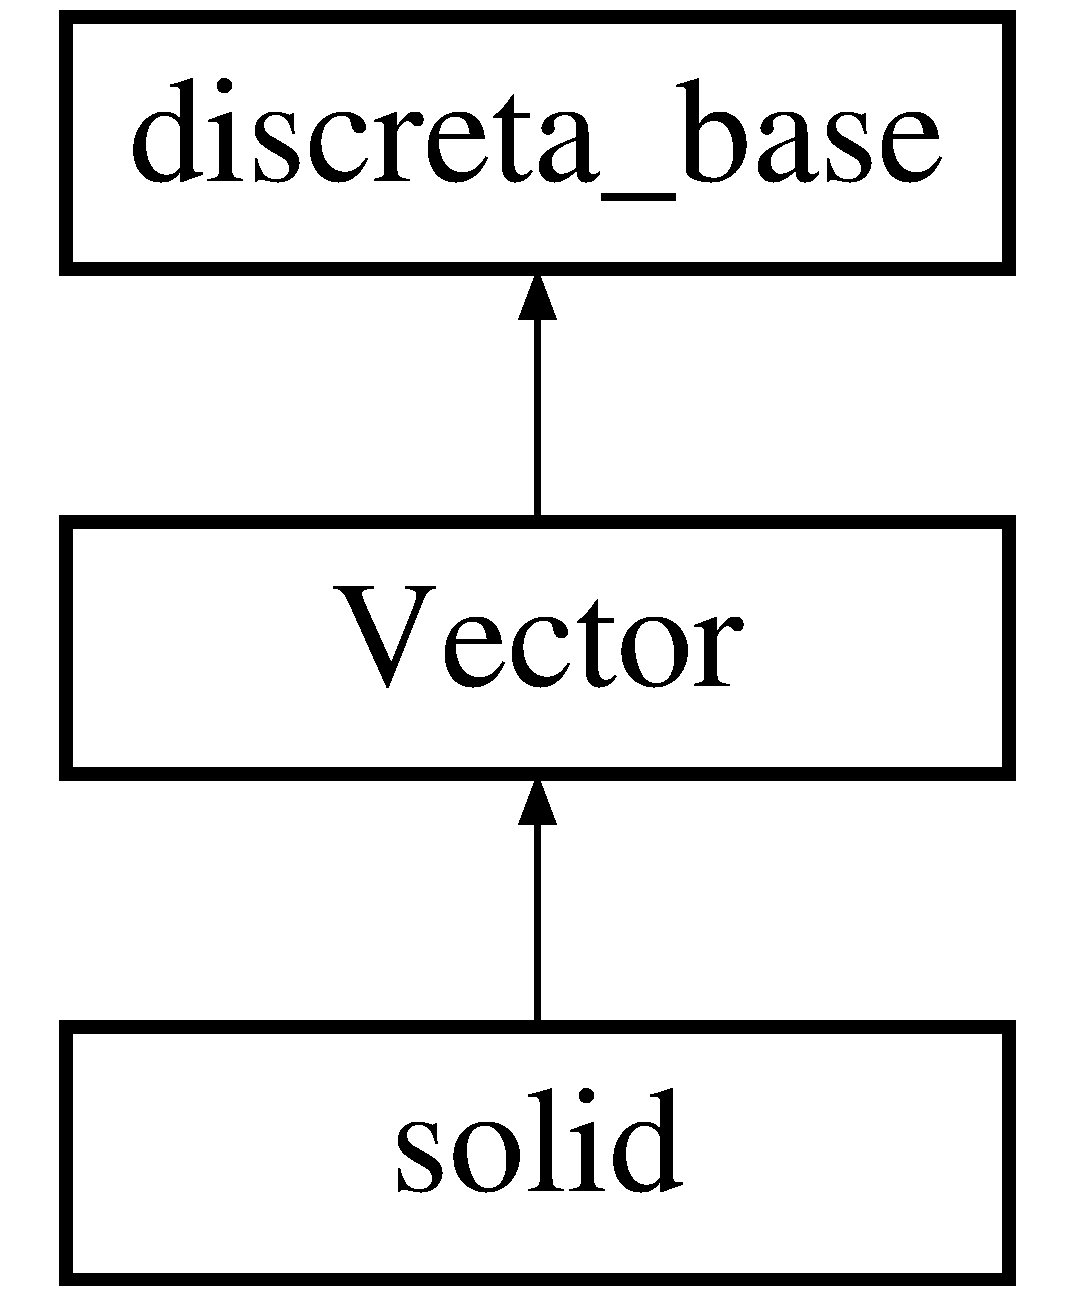
\includegraphics[height=3.000000cm]{classsolid}
\end{center}
\end{figure}
\subsection*{Public Member Functions}
\begin{DoxyCompactItemize}
\item 
\mbox{\hyperlink{classsolid_a27e2f13966fd3b10b34b42c07b3a0e90}{solid}} ()
\item 
void \mbox{\hyperlink{classsolid_afc711954316958b35630fbc8542bcd05}{init}} ()
\item 
\mbox{\hyperlink{class_vector}{Vector}} \& \mbox{\hyperlink{classsolid_a3ec669f29fac875a8a05882714e8a896}{group\+\_\+generators}} ()
\item 
\mbox{\hyperlink{classpermutation}{permutation}} \& \mbox{\hyperlink{classsolid_a3736981de8dcd03683b4392a94c54a5c}{group\+\_\+generators\+\_\+i}} (\mbox{\hyperlink{galois_8h_a09fddde158a3a20bd2dcadb609de11dc}{I\+NT}} \mbox{\hyperlink{alphabet2_8_c_acb559820d9ca11295b4500f179ef6392}{i}})
\item 
\mbox{\hyperlink{galois_8h_a09fddde158a3a20bd2dcadb609de11dc}{I\+NT}} \& \mbox{\hyperlink{classsolid_aca646d2fdafa24105634c4959caa88c8}{nb\+\_\+V}} ()
\item 
\mbox{\hyperlink{galois_8h_a09fddde158a3a20bd2dcadb609de11dc}{I\+NT}} \& \mbox{\hyperlink{classsolid_abf4c4af23b0746c618d03d63b32a9e7e}{nb\+\_\+E}} ()
\item 
\mbox{\hyperlink{galois_8h_a09fddde158a3a20bd2dcadb609de11dc}{I\+NT}} \& \mbox{\hyperlink{classsolid_a476fed0721c9fb1532618dd96db251d6}{nb\+\_\+F}} ()
\item 
\mbox{\hyperlink{class_vector}{Vector}} \& \mbox{\hyperlink{classsolid_ac06c1e06d6dc5c6f43b1c850892548c8}{placement}} ()
\item 
\mbox{\hyperlink{class_vector}{Vector}} \& \mbox{\hyperlink{classsolid_ab9c0f7598fe0b626a7f819d04b935996}{x}} ()
\item 
\mbox{\hyperlink{galois_8h_a09fddde158a3a20bd2dcadb609de11dc}{I\+NT}} \& \mbox{\hyperlink{classsolid_a701de0f753ff85c6e3e05fbd5ffcf8b4}{x\+\_\+i}} (\mbox{\hyperlink{galois_8h_a09fddde158a3a20bd2dcadb609de11dc}{I\+NT}} \mbox{\hyperlink{alphabet2_8_c_acb559820d9ca11295b4500f179ef6392}{i}})
\item 
\mbox{\hyperlink{class_vector}{Vector}} \& \mbox{\hyperlink{classsolid_a3573a3af71aa86cf6d609442f19ca4b0}{y}} ()
\item 
\mbox{\hyperlink{galois_8h_a09fddde158a3a20bd2dcadb609de11dc}{I\+NT}} \& \mbox{\hyperlink{classsolid_a962e53cd90bf6f5bd8128ac940b2ffa9}{y\+\_\+i}} (\mbox{\hyperlink{galois_8h_a09fddde158a3a20bd2dcadb609de11dc}{I\+NT}} \mbox{\hyperlink{alphabet2_8_c_acb559820d9ca11295b4500f179ef6392}{i}})
\item 
\mbox{\hyperlink{class_vector}{Vector}} \& \mbox{\hyperlink{classsolid_af8ab1d698896be2233691447b1107dcb}{z}} ()
\item 
\mbox{\hyperlink{galois_8h_a09fddde158a3a20bd2dcadb609de11dc}{I\+NT}} \& \mbox{\hyperlink{classsolid_af3764c9cbc0eaef0cc13ca062b87e1bf}{z\+\_\+i}} (\mbox{\hyperlink{galois_8h_a09fddde158a3a20bd2dcadb609de11dc}{I\+NT}} \mbox{\hyperlink{alphabet2_8_c_acb559820d9ca11295b4500f179ef6392}{i}})
\item 
\mbox{\hyperlink{class_vector}{Vector}} \& \mbox{\hyperlink{classsolid_a9f4ad6a7821b9be2f0f1e19cdb23933c}{v1}} ()
\item 
\mbox{\hyperlink{galois_8h_a09fddde158a3a20bd2dcadb609de11dc}{I\+NT}} \& \mbox{\hyperlink{classsolid_a1e0894ad230270e0a74f49e4cc8bde8f}{v1\+\_\+i}} (\mbox{\hyperlink{galois_8h_a09fddde158a3a20bd2dcadb609de11dc}{I\+NT}} \mbox{\hyperlink{alphabet2_8_c_acb559820d9ca11295b4500f179ef6392}{i}})
\item 
\mbox{\hyperlink{class_vector}{Vector}} \& \mbox{\hyperlink{classsolid_a49eb435004424f5d9fa17d55489a9a94}{v2}} ()
\item 
\mbox{\hyperlink{galois_8h_a09fddde158a3a20bd2dcadb609de11dc}{I\+NT}} \& \mbox{\hyperlink{classsolid_a762c91ec8b487c2cacde991fb1c9fed4}{v2\+\_\+i}} (\mbox{\hyperlink{galois_8h_a09fddde158a3a20bd2dcadb609de11dc}{I\+NT}} \mbox{\hyperlink{alphabet2_8_c_acb559820d9ca11295b4500f179ef6392}{i}})
\item 
\mbox{\hyperlink{class_vector}{Vector}} \& \mbox{\hyperlink{classsolid_a496eea5cdbcc2e61784e736bb4e06d1d}{f1}} ()
\item 
\mbox{\hyperlink{galois_8h_a09fddde158a3a20bd2dcadb609de11dc}{I\+NT}} \& \mbox{\hyperlink{classsolid_a9de0f986df432ff4f33109ea4f1cc97c}{f1\+\_\+i}} (\mbox{\hyperlink{galois_8h_a09fddde158a3a20bd2dcadb609de11dc}{I\+NT}} \mbox{\hyperlink{alphabet2_8_c_acb559820d9ca11295b4500f179ef6392}{i}})
\item 
\mbox{\hyperlink{class_vector}{Vector}} \& \mbox{\hyperlink{classsolid_a52b43d36c47cf4f57fd277c408d33d58}{f2}} ()
\item 
\mbox{\hyperlink{galois_8h_a09fddde158a3a20bd2dcadb609de11dc}{I\+NT}} \& \mbox{\hyperlink{classsolid_a173015a2b945e995448d50dda299c068}{f2\+\_\+i}} (\mbox{\hyperlink{galois_8h_a09fddde158a3a20bd2dcadb609de11dc}{I\+NT}} \mbox{\hyperlink{alphabet2_8_c_acb559820d9ca11295b4500f179ef6392}{i}})
\item 
\mbox{\hyperlink{class_vector}{Vector}} \& \mbox{\hyperlink{classsolid_aeb3bd7332f1a39cdb44db6be83cca3f5}{nb\+\_\+e}} ()
\item 
\mbox{\hyperlink{galois_8h_a09fddde158a3a20bd2dcadb609de11dc}{I\+NT}} \& \mbox{\hyperlink{classsolid_a941bebd6096f96336f896093d14167b1}{nb\+\_\+e\+\_\+i}} (\mbox{\hyperlink{galois_8h_a09fddde158a3a20bd2dcadb609de11dc}{I\+NT}} \mbox{\hyperlink{alphabet2_8_c_acb559820d9ca11295b4500f179ef6392}{i}})
\item 
\mbox{\hyperlink{class_vector}{Vector}} \& \mbox{\hyperlink{classsolid_a703b914bee212828ebb65d3d5313460e}{edge}} ()
\item 
\mbox{\hyperlink{class_vector}{Vector}} \& \mbox{\hyperlink{classsolid_af5ed0a914a62d73b448c3546d9bb0e0c}{edge\+\_\+i}} (\mbox{\hyperlink{galois_8h_a09fddde158a3a20bd2dcadb609de11dc}{I\+NT}} \mbox{\hyperlink{alphabet2_8_c_acb559820d9ca11295b4500f179ef6392}{i}})
\item 
\mbox{\hyperlink{galois_8h_a09fddde158a3a20bd2dcadb609de11dc}{I\+NT}} \& \mbox{\hyperlink{classsolid_a7fe7ff45f9406a6959ff27c5a7cbb067}{edge\+\_\+ij}} (\mbox{\hyperlink{galois_8h_a09fddde158a3a20bd2dcadb609de11dc}{I\+NT}} \mbox{\hyperlink{alphabet2_8_c_acb559820d9ca11295b4500f179ef6392}{i}}, \mbox{\hyperlink{galois_8h_a09fddde158a3a20bd2dcadb609de11dc}{I\+NT}} \mbox{\hyperlink{alphabet2_8_c_a37d972ae0b47b9099e30983131d31916}{j}})
\item 
\mbox{\hyperlink{class_vector}{Vector}} \& \mbox{\hyperlink{classsolid_aa679392983420946e8f1db13b0fc40b0}{neighbour\+\_\+faces}} ()
\item 
\mbox{\hyperlink{class_vector}{Vector}} \& \mbox{\hyperlink{classsolid_a5f8389874c5134f2ccb46a93c2335937}{neighbour\+\_\+faces\+\_\+i}} (\mbox{\hyperlink{galois_8h_a09fddde158a3a20bd2dcadb609de11dc}{I\+NT}} \mbox{\hyperlink{alphabet2_8_c_acb559820d9ca11295b4500f179ef6392}{i}})
\item 
\mbox{\hyperlink{galois_8h_a09fddde158a3a20bd2dcadb609de11dc}{I\+NT}} \& \mbox{\hyperlink{classsolid_ad4a9463c16700ba259cdd6e62b183e23}{neighbour\+\_\+faces\+\_\+ij}} (\mbox{\hyperlink{galois_8h_a09fddde158a3a20bd2dcadb609de11dc}{I\+NT}} \mbox{\hyperlink{alphabet2_8_c_acb559820d9ca11295b4500f179ef6392}{i}}, \mbox{\hyperlink{galois_8h_a09fddde158a3a20bd2dcadb609de11dc}{I\+NT}} \mbox{\hyperlink{alphabet2_8_c_a37d972ae0b47b9099e30983131d31916}{j}})
\item 
\mbox{\hyperlink{galois_8h_a09fddde158a3a20bd2dcadb609de11dc}{I\+NT}} \& \mbox{\hyperlink{classsolid_a4dfce820a08af20da6f8b3b1455073bf}{f\+\_\+vertex\+\_\+labels}} ()
\item 
\mbox{\hyperlink{class_vector}{Vector}} \& \mbox{\hyperlink{classsolid_aae289e59c901d56ec8b87d4adc8b87e8}{vertex\+\_\+labels}} ()
\item 
\mbox{\hyperlink{classhollerith}{hollerith}} \& \mbox{\hyperlink{classsolid_a241640bc2eeb9da14f2d5d2861be42c0}{vertex\+\_\+labels\+\_\+i}} (\mbox{\hyperlink{galois_8h_a09fddde158a3a20bd2dcadb609de11dc}{I\+NT}} \mbox{\hyperlink{alphabet2_8_c_acb559820d9ca11295b4500f179ef6392}{i}})
\item 
\mbox{\hyperlink{class_vector}{Vector}} \& \mbox{\hyperlink{classsolid_abe722d1a7fab5631f0ec7188a99ec2e3}{vertex\+\_\+labels\+\_\+numeric}} ()
\item 
\mbox{\hyperlink{galois_8h_a09fddde158a3a20bd2dcadb609de11dc}{I\+NT}} \& \mbox{\hyperlink{classsolid_ae9f701f7a29acb2f9b86ed6bd202b653}{vertex\+\_\+labels\+\_\+numeric\+\_\+i}} (\mbox{\hyperlink{galois_8h_a09fddde158a3a20bd2dcadb609de11dc}{I\+NT}} \mbox{\hyperlink{alphabet2_8_c_acb559820d9ca11295b4500f179ef6392}{i}})
\item 
\mbox{\hyperlink{galois_8h_a09fddde158a3a20bd2dcadb609de11dc}{I\+NT}} \& \mbox{\hyperlink{classsolid_a15413691d9cc9da76be150702e22d43a}{f\+\_\+oriented}} ()
\item 
void \mbox{\hyperlink{classsolid_a0b156ca77a137dc8aa94ab22d048e542}{init\+\_\+V}} (\mbox{\hyperlink{galois_8h_a09fddde158a3a20bd2dcadb609de11dc}{I\+NT}} \mbox{\hyperlink{classsolid_aca646d2fdafa24105634c4959caa88c8}{nb\+\_\+V}})
\item 
void \mbox{\hyperlink{classsolid_ae57764803455bb12c6f59a623b595b7d}{init\+\_\+E}} (\mbox{\hyperlink{galois_8h_a09fddde158a3a20bd2dcadb609de11dc}{I\+NT}} \mbox{\hyperlink{classsolid_abf4c4af23b0746c618d03d63b32a9e7e}{nb\+\_\+E}})
\item 
void \mbox{\hyperlink{classsolid_ab61e6cc032b5370f77857fe1fc10222d}{init\+\_\+F}} (\mbox{\hyperlink{galois_8h_a09fddde158a3a20bd2dcadb609de11dc}{I\+NT}} \mbox{\hyperlink{classsolid_a476fed0721c9fb1532618dd96db251d6}{nb\+\_\+F}})
\item 
\mbox{\hyperlink{classsolid_a5cbfb36f813a28289bda9739e562af19}{solid}} (const \mbox{\hyperlink{classdiscreta__base}{discreta\+\_\+base}} \&\mbox{\hyperlink{classsolid_ab9c0f7598fe0b626a7f819d04b935996}{x}})
\item 
\mbox{\hyperlink{classsolid}{solid}} \& \mbox{\hyperlink{classsolid_aadc9b68f1704979feefa95bb74455ad5}{operator=}} (const \mbox{\hyperlink{classdiscreta__base}{discreta\+\_\+base}} \&\mbox{\hyperlink{classsolid_ab9c0f7598fe0b626a7f819d04b935996}{x}})
\item 
void $\ast$ \mbox{\hyperlink{classsolid_aef1c3984bce8c97f1a15690ec4340efe}{operator new}} (size\+\_\+t, void $\ast$\mbox{\hyperlink{alphabet2_8_c_a533391314665d6bf1b5575e9a9cd8552}{p}})
\item 
void \mbox{\hyperlink{classsolid_a775bd4821f75a8aee4ea3d4335ff90e0}{settype\+\_\+solid}} ()
\item 
\mbox{\hyperlink{discreta_8h_aaf25ee7e2306d78c74ec7bc48f092e81}{kind}} \mbox{\hyperlink{classsolid_aae18938e9f7d9784734fe72e8d3223a7}{s\+\_\+virtual\+\_\+kind}} ()
\item 
\mbox{\hyperlink{classsolid_a9c9476c0078fe49bf5e19c4297b2f16d}{$\sim$solid}} ()
\item 
void \mbox{\hyperlink{classsolid_a84c2f0abd7b24b1cf2ccefa9c99567fe}{freeself\+\_\+solid}} ()
\item 
void \mbox{\hyperlink{classsolid_a7f35a904885ef626d1a74663fe2cad62}{copyobject\+\_\+to}} (\mbox{\hyperlink{classdiscreta__base}{discreta\+\_\+base}} \&\mbox{\hyperlink{classsolid_ab9c0f7598fe0b626a7f819d04b935996}{x}})
\item 
ostream \& \mbox{\hyperlink{classsolid_a2a8cb93b481e1876260e7b8739cf4695}{print\+\_\+list}} (ostream \&ost)
\item 
ostream \& \mbox{\hyperlink{classsolid_a0afe4403778d31d092e2a66c13a9a365}{print}} (ostream \&ost)
\item 
void \mbox{\hyperlink{classsolid_abd47abc26a30fdb78e452b0a519b3076}{standard\+\_\+vertex\+\_\+labels}} (\mbox{\hyperlink{galois_8h_a09fddde158a3a20bd2dcadb609de11dc}{I\+NT}} f\+\_\+start\+\_\+with\+\_\+zero)
\item 
void \mbox{\hyperlink{classsolid_ad6bcabc7a3e9082b4baef371e7828c27}{determine\+\_\+neighbours}} ()
\item 
void \mbox{\hyperlink{classsolid_af71537b1f01c068f1d1517c523a72544}{find\+\_\+face}} (\mbox{\hyperlink{galois_8h_a09fddde158a3a20bd2dcadb609de11dc}{I\+NT}} \mbox{\hyperlink{alphabet2_8_c_a88859ce72faebb79ea0a2bca00a0f46b}{e}}, \mbox{\hyperlink{galois_8h_a09fddde158a3a20bd2dcadb609de11dc}{I\+NT}} \&\mbox{\hyperlink{classsolid_a496eea5cdbcc2e61784e736bb4e06d1d}{f1}}, \mbox{\hyperlink{galois_8h_a09fddde158a3a20bd2dcadb609de11dc}{I\+NT}} \&j1, \mbox{\hyperlink{galois_8h_a09fddde158a3a20bd2dcadb609de11dc}{I\+NT}} \&\mbox{\hyperlink{classsolid_a52b43d36c47cf4f57fd277c408d33d58}{f2}}, \mbox{\hyperlink{galois_8h_a09fddde158a3a20bd2dcadb609de11dc}{I\+NT}} \&j2)
\item 
\mbox{\hyperlink{galois_8h_a09fddde158a3a20bd2dcadb609de11dc}{I\+NT}} \mbox{\hyperlink{classsolid_af5173d277b17d5fe76c6dc39c3b863b7}{find\+\_\+face\+\_\+2}} (\mbox{\hyperlink{galois_8h_a09fddde158a3a20bd2dcadb609de11dc}{I\+NT}} e1, \mbox{\hyperlink{galois_8h_a09fddde158a3a20bd2dcadb609de11dc}{I\+NT}} e2)
\item 
\mbox{\hyperlink{galois_8h_a09fddde158a3a20bd2dcadb609de11dc}{I\+NT}} \mbox{\hyperlink{classsolid_a83a357e708d7da429afe714dc40a5930}{find\+\_\+face\+\_\+by\+\_\+two\+\_\+edges}} (\mbox{\hyperlink{galois_8h_a09fddde158a3a20bd2dcadb609de11dc}{I\+NT}} e1, \mbox{\hyperlink{galois_8h_a09fddde158a3a20bd2dcadb609de11dc}{I\+NT}} e2)
\item 
void \mbox{\hyperlink{classsolid_ae6339a607e15cbfaa028063296ed9767}{find\+\_\+faces\+\_\+at\+\_\+edge}} (\mbox{\hyperlink{galois_8h_a09fddde158a3a20bd2dcadb609de11dc}{I\+NT}} \mbox{\hyperlink{alphabet2_8_c_a88859ce72faebb79ea0a2bca00a0f46b}{e}}, \mbox{\hyperlink{galois_8h_a09fddde158a3a20bd2dcadb609de11dc}{I\+NT}} \&\mbox{\hyperlink{classsolid_a496eea5cdbcc2e61784e736bb4e06d1d}{f1}}, \mbox{\hyperlink{galois_8h_a09fddde158a3a20bd2dcadb609de11dc}{I\+NT}} \&\mbox{\hyperlink{classsolid_a52b43d36c47cf4f57fd277c408d33d58}{f2}})
\item 
\mbox{\hyperlink{galois_8h_a09fddde158a3a20bd2dcadb609de11dc}{I\+NT}} \mbox{\hyperlink{classsolid_a4e6e784df5bac1fcd8398f5e6c7df493}{find\+\_\+edge}} (\mbox{\hyperlink{galois_8h_a09fddde158a3a20bd2dcadb609de11dc}{I\+NT}} \mbox{\hyperlink{classsolid_a9f4ad6a7821b9be2f0f1e19cdb23933c}{v1}}, \mbox{\hyperlink{galois_8h_a09fddde158a3a20bd2dcadb609de11dc}{I\+NT}} \mbox{\hyperlink{classsolid_a49eb435004424f5d9fa17d55489a9a94}{v2}})
\item 
void \mbox{\hyperlink{classsolid_a972d36c69f629d8f78d3a7fccb5b75ba}{add\+\_\+edge}} (\mbox{\hyperlink{galois_8h_a09fddde158a3a20bd2dcadb609de11dc}{I\+NT}} \mbox{\hyperlink{classsolid_a9f4ad6a7821b9be2f0f1e19cdb23933c}{v1}}, \mbox{\hyperlink{galois_8h_a09fddde158a3a20bd2dcadb609de11dc}{I\+NT}} \mbox{\hyperlink{classsolid_a49eb435004424f5d9fa17d55489a9a94}{v2}}, \mbox{\hyperlink{galois_8h_a09fddde158a3a20bd2dcadb609de11dc}{I\+NT}} \mbox{\hyperlink{classsolid_a496eea5cdbcc2e61784e736bb4e06d1d}{f1}}, \mbox{\hyperlink{galois_8h_a09fddde158a3a20bd2dcadb609de11dc}{I\+NT}} \mbox{\hyperlink{classsolid_a52b43d36c47cf4f57fd277c408d33d58}{f2}})
\item 
\mbox{\hyperlink{galois_8h_a09fddde158a3a20bd2dcadb609de11dc}{I\+NT}} \mbox{\hyperlink{classsolid_a915c83080299c3787b78805fd670470e}{add\+\_\+edge}} (\mbox{\hyperlink{galois_8h_a09fddde158a3a20bd2dcadb609de11dc}{I\+NT}} \mbox{\hyperlink{classsolid_a9f4ad6a7821b9be2f0f1e19cdb23933c}{v1}}, \mbox{\hyperlink{galois_8h_a09fddde158a3a20bd2dcadb609de11dc}{I\+NT}} \mbox{\hyperlink{classsolid_a49eb435004424f5d9fa17d55489a9a94}{v2}})
\item 
\mbox{\hyperlink{galois_8h_a09fddde158a3a20bd2dcadb609de11dc}{I\+NT}} \mbox{\hyperlink{classsolid_a91c02de4312c4942c0f6642154d97047}{find\+\_\+and\+\_\+add\+\_\+edge}} (\mbox{\hyperlink{galois_8h_a09fddde158a3a20bd2dcadb609de11dc}{I\+NT}} i1, \mbox{\hyperlink{galois_8h_a09fddde158a3a20bd2dcadb609de11dc}{I\+NT}} i2, \mbox{\hyperlink{galois_8h_a09fddde158a3a20bd2dcadb609de11dc}{I\+NT}} f\+\_\+v)
\item 
void \mbox{\hyperlink{classsolid_a6875ab7d3238826f030bae684137f789}{add\+\_\+face3}} (\mbox{\hyperlink{galois_8h_a09fddde158a3a20bd2dcadb609de11dc}{I\+NT}} e1, \mbox{\hyperlink{galois_8h_a09fddde158a3a20bd2dcadb609de11dc}{I\+NT}} e2, \mbox{\hyperlink{galois_8h_a09fddde158a3a20bd2dcadb609de11dc}{I\+NT}} e3, \mbox{\hyperlink{galois_8h_a09fddde158a3a20bd2dcadb609de11dc}{I\+NT}} i1, \mbox{\hyperlink{galois_8h_a09fddde158a3a20bd2dcadb609de11dc}{I\+NT}} i2, \mbox{\hyperlink{galois_8h_a09fddde158a3a20bd2dcadb609de11dc}{I\+NT}} i3)
\item 
void \mbox{\hyperlink{classsolid_ae0c74bc52056d190e54a60c78c1858a2}{add\+\_\+face4}} (\mbox{\hyperlink{galois_8h_a09fddde158a3a20bd2dcadb609de11dc}{I\+NT}} i1, \mbox{\hyperlink{galois_8h_a09fddde158a3a20bd2dcadb609de11dc}{I\+NT}} i2, \mbox{\hyperlink{galois_8h_a09fddde158a3a20bd2dcadb609de11dc}{I\+NT}} i3, \mbox{\hyperlink{galois_8h_a09fddde158a3a20bd2dcadb609de11dc}{I\+NT}} i4)
\item 
void \mbox{\hyperlink{classsolid_a56243f48f4573b2989154be1dca68713}{add\+\_\+face5}} (\mbox{\hyperlink{galois_8h_a09fddde158a3a20bd2dcadb609de11dc}{I\+NT}} i1, \mbox{\hyperlink{galois_8h_a09fddde158a3a20bd2dcadb609de11dc}{I\+NT}} i2, \mbox{\hyperlink{galois_8h_a09fddde158a3a20bd2dcadb609de11dc}{I\+NT}} i3, \mbox{\hyperlink{galois_8h_a09fddde158a3a20bd2dcadb609de11dc}{I\+NT}} i4, \mbox{\hyperlink{galois_8h_a09fddde158a3a20bd2dcadb609de11dc}{I\+NT}} i5)
\item 
void \mbox{\hyperlink{classsolid_adbadfbdd46abe10cb56f041d2408b001}{add\+\_\+face\+\_\+n}} (\mbox{\hyperlink{class_vector}{Vector}} \&vertices)
\item 
void \mbox{\hyperlink{classsolid_af0ad596c4fd4b091118dd0d6e3e3bf67}{adjacency\+\_\+list}} (\mbox{\hyperlink{galois_8h_a09fddde158a3a20bd2dcadb609de11dc}{I\+NT}} vertex, \mbox{\hyperlink{galois_8h_a09fddde158a3a20bd2dcadb609de11dc}{I\+NT}} $\ast$adj, \mbox{\hyperlink{galois_8h_a09fddde158a3a20bd2dcadb609de11dc}{I\+NT}} $\ast$nb\+\_\+adj)
\item 
void \mbox{\hyperlink{classsolid_ae58752f7dd02eda7e0bac1d69b551db2}{center}} (\mbox{\hyperlink{galois_8h_a09fddde158a3a20bd2dcadb609de11dc}{I\+NT}} \mbox{\hyperlink{alphabet2_8_c_a362077c979b0bb65159c603270e40f70}{f}}, \mbox{\hyperlink{class_vector}{Vector}} \&Px, \mbox{\hyperlink{class_vector}{Vector}} \&Py, \mbox{\hyperlink{class_vector}{Vector}} \&Pz)
\item 
void \mbox{\hyperlink{classsolid_a939ce1ac4b1d7e7ad6164ce0376ff173}{vertices\+\_\+of\+\_\+face}} (\mbox{\hyperlink{galois_8h_a09fddde158a3a20bd2dcadb609de11dc}{I\+NT}} \mbox{\hyperlink{alphabet2_8_c_acb559820d9ca11295b4500f179ef6392}{i}}, \mbox{\hyperlink{class_vector}{Vector}} \&\mbox{\hyperlink{srg_8_c_af40a326b23c68a27cebe60f16634a2cb}{V}})
\item 
void \mbox{\hyperlink{classsolid_aef1749a5d84c62c43d2d1196d4ebec08}{Ratio}} (\mbox{\hyperlink{galois_8h_a09fddde158a3a20bd2dcadb609de11dc}{I\+NT}} \mbox{\hyperlink{alphabet2_8_c_a88859ce72faebb79ea0a2bca00a0f46b}{e}}, double \mbox{\hyperlink{alphabet2_8_c_acab531abaa74a7e664e3986f2522b33a}{r}}, \mbox{\hyperlink{galois_8h_a09fddde158a3a20bd2dcadb609de11dc}{I\+NT}} \&\mbox{\hyperlink{classsolid_ab9c0f7598fe0b626a7f819d04b935996}{x}}, \mbox{\hyperlink{galois_8h_a09fddde158a3a20bd2dcadb609de11dc}{I\+NT}} \&\mbox{\hyperlink{classsolid_a3573a3af71aa86cf6d609442f19ca4b0}{y}}, \mbox{\hyperlink{galois_8h_a09fddde158a3a20bd2dcadb609de11dc}{I\+NT}} \&\mbox{\hyperlink{classsolid_af8ab1d698896be2233691447b1107dcb}{z}})
\item 
\mbox{\hyperlink{galois_8h_a09fddde158a3a20bd2dcadb609de11dc}{I\+NT}} \mbox{\hyperlink{classsolid_a187d6dfd122f2745345813a763e97fd7}{find\+\_\+common\+\_\+face}} (\mbox{\hyperlink{galois_8h_a09fddde158a3a20bd2dcadb609de11dc}{I\+NT}} e1, \mbox{\hyperlink{galois_8h_a09fddde158a3a20bd2dcadb609de11dc}{I\+NT}} e2, \mbox{\hyperlink{galois_8h_a09fddde158a3a20bd2dcadb609de11dc}{I\+NT}} \&\mbox{\hyperlink{alphabet2_8_c_a362077c979b0bb65159c603270e40f70}{f}})
\item 
void \mbox{\hyperlink{classsolid_a0147bd21fc7bfed44a10f3b5eca66757}{dual}} (\mbox{\hyperlink{classsolid}{solid}} \&\mbox{\hyperlink{simeon_8_c_a97833f04c3a9c008df5521a2fc291bb4}{A}})
\item 
void \mbox{\hyperlink{classsolid_a286d7bb090878dfbdc2fcd0dcf4739ce}{cut\+\_\+vertices}} (double \mbox{\hyperlink{alphabet2_8_c_acab531abaa74a7e664e3986f2522b33a}{r}}, \mbox{\hyperlink{classsolid}{solid}} \&\mbox{\hyperlink{simeon_8_c_a97833f04c3a9c008df5521a2fc291bb4}{A}})
\item 
void \mbox{\hyperlink{classsolid_a00f043a4986f0eec6ed05c14d64919dc}{edge\+\_\+midpoints}} (\mbox{\hyperlink{classsolid}{solid}} \&\mbox{\hyperlink{simeon_8_c_a97833f04c3a9c008df5521a2fc291bb4}{A}})
\item 
void \mbox{\hyperlink{classsolid_ac3c7868e3b650b7112309c7ad15a394c}{join\+\_\+disjoint}} (\mbox{\hyperlink{classsolid}{solid}} \&\mbox{\hyperlink{simeon_8_c_a97833f04c3a9c008df5521a2fc291bb4}{A}}, \mbox{\hyperlink{classsolid}{solid}} \&J, \mbox{\hyperlink{galois_8h_a09fddde158a3a20bd2dcadb609de11dc}{I\+NT}} f\+\_\+v)
\item 
void \mbox{\hyperlink{classsolid_a2045d572bdbd493c541c69624baeedbf}{direct\+\_\+sum}} (\mbox{\hyperlink{classsolid}{solid}} \&\mbox{\hyperlink{costas_8_c_ad1f767566c3189fb90e9cffcc5dd4680}{B}}, \mbox{\hyperlink{classsolid}{solid}} \&J, \mbox{\hyperlink{galois_8h_a09fddde158a3a20bd2dcadb609de11dc}{I\+NT}} f\+\_\+v)
\item 
void \mbox{\hyperlink{classsolid_a8b4527c066bcebd2e6542fe158c607b0}{direct\+\_\+product}} (\mbox{\hyperlink{class_vector}{Vector}} \&gen, \mbox{\hyperlink{classsolid}{solid}} \&J, \mbox{\hyperlink{galois_8h_a09fddde158a3a20bd2dcadb609de11dc}{I\+NT}} f\+\_\+v)
\item 
void \mbox{\hyperlink{classsolid_a26c0fc360080e87361451aaec9faa98c}{scale}} (double \mbox{\hyperlink{alphabet2_8_c_a362077c979b0bb65159c603270e40f70}{f}})
\item 
void \mbox{\hyperlink{classsolid_abec108e749250b1fbab7c8dcf98b96ae}{add\+\_\+central\+\_\+point}} (\mbox{\hyperlink{classsolid}{solid}} \&\mbox{\hyperlink{simeon_8_c_a97833f04c3a9c008df5521a2fc291bb4}{A}})
\item 
void \mbox{\hyperlink{classsolid_a372d0459fd74de947a5cb0d53ddbd6f0}{induced\+\_\+action\+\_\+on\+\_\+edges}} (\mbox{\hyperlink{classpermutation}{permutation}} \&\mbox{\hyperlink{alphabet2_8_c_a533391314665d6bf1b5575e9a9cd8552}{p}}, \mbox{\hyperlink{classpermutation}{permutation}} \&\mbox{\hyperlink{simeon_8_c_a92cbb483a3b27ae1a0dbfcb125ce216f}{q}})
\item 
void \mbox{\hyperlink{classsolid_a081dd519a288f5bf2e406ce9dc76348d}{induced\+\_\+group\+\_\+on\+\_\+edges}} (\mbox{\hyperlink{class_vector}{Vector}} \&gen, \mbox{\hyperlink{class_vector}{Vector}} \&gen\+\_\+e)
\item 
void \mbox{\hyperlink{classsolid_ad40cf6e9d27be77f0a01528442e04682}{tetrahedron}} (\mbox{\hyperlink{galois_8h_a09fddde158a3a20bd2dcadb609de11dc}{I\+NT}} \mbox{\hyperlink{alphabet2_8_c_acab531abaa74a7e664e3986f2522b33a}{r}})
\item 
void \mbox{\hyperlink{classsolid_a308e6888759550da489397527ed89137}{cube}} (\mbox{\hyperlink{galois_8h_a09fddde158a3a20bd2dcadb609de11dc}{I\+NT}} \mbox{\hyperlink{alphabet2_8_c_acab531abaa74a7e664e3986f2522b33a}{r}})
\item 
void \mbox{\hyperlink{classsolid_ab6c85f8f130a3f4409ce5fe5340fb852}{cube4D}} (\mbox{\hyperlink{galois_8h_a09fddde158a3a20bd2dcadb609de11dc}{I\+NT}} r1, \mbox{\hyperlink{galois_8h_a09fddde158a3a20bd2dcadb609de11dc}{I\+NT}} r2)
\item 
void \mbox{\hyperlink{classsolid_a9c1c4015737b992fc935a05e6748f824}{octahedron}} (\mbox{\hyperlink{galois_8h_a09fddde158a3a20bd2dcadb609de11dc}{I\+NT}} \mbox{\hyperlink{alphabet2_8_c_acab531abaa74a7e664e3986f2522b33a}{r}})
\item 
void \mbox{\hyperlink{classsolid_a514072d4dfd0f82ba24b0df1ac302d6f}{dodecahedron}} (\mbox{\hyperlink{galois_8h_a09fddde158a3a20bd2dcadb609de11dc}{I\+NT}} \mbox{\hyperlink{alphabet2_8_c_acab531abaa74a7e664e3986f2522b33a}{r}})
\item 
void \mbox{\hyperlink{classsolid_a70240006a1198bfeebac8d11923ee372}{icosahedron}} (\mbox{\hyperlink{galois_8h_a09fddde158a3a20bd2dcadb609de11dc}{I\+NT}} \mbox{\hyperlink{alphabet2_8_c_acab531abaa74a7e664e3986f2522b33a}{r}})
\item 
void \mbox{\hyperlink{classsolid_a67a153cfb0673d8b90e81cb45064626c}{make\+\_\+placed\+\_\+graph}} (\mbox{\hyperlink{classmatrix}{matrix}} \&incma, \mbox{\hyperlink{class_vector}{Vector}} \&aut\+\_\+gens, \mbox{\hyperlink{class_vector}{Vector}} \&cycles)
\item 
void \mbox{\hyperlink{classsolid_ab21f3d7cb562fa9ce61b1a1cb2e5a411}{write\+\_\+graphfile}} (\mbox{\hyperlink{galois_8h_ab6cc7b4aeb6ea31aba2b3fbfc83ff5e6}{B\+Y\+TE}} $\ast$fname)
\item 
void \mbox{\hyperlink{classsolid_a60865c3210ff835fe2bd528f2396686d}{write\+\_\+solidfile}} (\mbox{\hyperlink{galois_8h_ab6cc7b4aeb6ea31aba2b3fbfc83ff5e6}{B\+Y\+TE}} $\ast$fname)
\end{DoxyCompactItemize}
\subsection*{Additional Inherited Members}


\subsection{Constructor \& Destructor Documentation}
\mbox{\Hypertarget{classsolid_a27e2f13966fd3b10b34b42c07b3a0e90}\label{classsolid_a27e2f13966fd3b10b34b42c07b3a0e90}} 
\index{solid@{solid}!solid@{solid}}
\index{solid@{solid}!solid@{solid}}
\subsubsection{\texorpdfstring{solid()}{solid()}\hspace{0.1cm}{\footnotesize\ttfamily [1/2]}}
{\footnotesize\ttfamily solid\+::solid (\begin{DoxyParamCaption}{ }\end{DoxyParamCaption})}

\mbox{\Hypertarget{classsolid_a5cbfb36f813a28289bda9739e562af19}\label{classsolid_a5cbfb36f813a28289bda9739e562af19}} 
\index{solid@{solid}!solid@{solid}}
\index{solid@{solid}!solid@{solid}}
\subsubsection{\texorpdfstring{solid()}{solid()}\hspace{0.1cm}{\footnotesize\ttfamily [2/2]}}
{\footnotesize\ttfamily solid\+::solid (\begin{DoxyParamCaption}\item[{const \mbox{\hyperlink{classdiscreta__base}{discreta\+\_\+base}} \&}]{x }\end{DoxyParamCaption})}

\mbox{\Hypertarget{classsolid_a9c9476c0078fe49bf5e19c4297b2f16d}\label{classsolid_a9c9476c0078fe49bf5e19c4297b2f16d}} 
\index{solid@{solid}!````~solid@{$\sim$solid}}
\index{````~solid@{$\sim$solid}!solid@{solid}}
\subsubsection{\texorpdfstring{$\sim$solid()}{~solid()}}
{\footnotesize\ttfamily solid\+::$\sim$solid (\begin{DoxyParamCaption}{ }\end{DoxyParamCaption})}



\subsection{Member Function Documentation}
\mbox{\Hypertarget{classsolid_abec108e749250b1fbab7c8dcf98b96ae}\label{classsolid_abec108e749250b1fbab7c8dcf98b96ae}} 
\index{solid@{solid}!add\+\_\+central\+\_\+point@{add\+\_\+central\+\_\+point}}
\index{add\+\_\+central\+\_\+point@{add\+\_\+central\+\_\+point}!solid@{solid}}
\subsubsection{\texorpdfstring{add\+\_\+central\+\_\+point()}{add\_central\_point()}}
{\footnotesize\ttfamily void solid\+::add\+\_\+central\+\_\+point (\begin{DoxyParamCaption}\item[{\mbox{\hyperlink{classsolid}{solid}} \&}]{A }\end{DoxyParamCaption})}

\mbox{\Hypertarget{classsolid_a972d36c69f629d8f78d3a7fccb5b75ba}\label{classsolid_a972d36c69f629d8f78d3a7fccb5b75ba}} 
\index{solid@{solid}!add\+\_\+edge@{add\+\_\+edge}}
\index{add\+\_\+edge@{add\+\_\+edge}!solid@{solid}}
\subsubsection{\texorpdfstring{add\+\_\+edge()}{add\_edge()}\hspace{0.1cm}{\footnotesize\ttfamily [1/2]}}
{\footnotesize\ttfamily void solid\+::add\+\_\+edge (\begin{DoxyParamCaption}\item[{\mbox{\hyperlink{galois_8h_a09fddde158a3a20bd2dcadb609de11dc}{I\+NT}}}]{v1,  }\item[{\mbox{\hyperlink{galois_8h_a09fddde158a3a20bd2dcadb609de11dc}{I\+NT}}}]{v2,  }\item[{\mbox{\hyperlink{galois_8h_a09fddde158a3a20bd2dcadb609de11dc}{I\+NT}}}]{f1,  }\item[{\mbox{\hyperlink{galois_8h_a09fddde158a3a20bd2dcadb609de11dc}{I\+NT}}}]{f2 }\end{DoxyParamCaption})}

\mbox{\Hypertarget{classsolid_a915c83080299c3787b78805fd670470e}\label{classsolid_a915c83080299c3787b78805fd670470e}} 
\index{solid@{solid}!add\+\_\+edge@{add\+\_\+edge}}
\index{add\+\_\+edge@{add\+\_\+edge}!solid@{solid}}
\subsubsection{\texorpdfstring{add\+\_\+edge()}{add\_edge()}\hspace{0.1cm}{\footnotesize\ttfamily [2/2]}}
{\footnotesize\ttfamily \mbox{\hyperlink{galois_8h_a09fddde158a3a20bd2dcadb609de11dc}{I\+NT}} solid\+::add\+\_\+edge (\begin{DoxyParamCaption}\item[{\mbox{\hyperlink{galois_8h_a09fddde158a3a20bd2dcadb609de11dc}{I\+NT}}}]{v1,  }\item[{\mbox{\hyperlink{galois_8h_a09fddde158a3a20bd2dcadb609de11dc}{I\+NT}}}]{v2 }\end{DoxyParamCaption})}

\mbox{\Hypertarget{classsolid_a6875ab7d3238826f030bae684137f789}\label{classsolid_a6875ab7d3238826f030bae684137f789}} 
\index{solid@{solid}!add\+\_\+face3@{add\+\_\+face3}}
\index{add\+\_\+face3@{add\+\_\+face3}!solid@{solid}}
\subsubsection{\texorpdfstring{add\+\_\+face3()}{add\_face3()}}
{\footnotesize\ttfamily void solid\+::add\+\_\+face3 (\begin{DoxyParamCaption}\item[{\mbox{\hyperlink{galois_8h_a09fddde158a3a20bd2dcadb609de11dc}{I\+NT}}}]{e1,  }\item[{\mbox{\hyperlink{galois_8h_a09fddde158a3a20bd2dcadb609de11dc}{I\+NT}}}]{e2,  }\item[{\mbox{\hyperlink{galois_8h_a09fddde158a3a20bd2dcadb609de11dc}{I\+NT}}}]{e3,  }\item[{\mbox{\hyperlink{galois_8h_a09fddde158a3a20bd2dcadb609de11dc}{I\+NT}}}]{i1,  }\item[{\mbox{\hyperlink{galois_8h_a09fddde158a3a20bd2dcadb609de11dc}{I\+NT}}}]{i2,  }\item[{\mbox{\hyperlink{galois_8h_a09fddde158a3a20bd2dcadb609de11dc}{I\+NT}}}]{i3 }\end{DoxyParamCaption})}

\mbox{\Hypertarget{classsolid_ae0c74bc52056d190e54a60c78c1858a2}\label{classsolid_ae0c74bc52056d190e54a60c78c1858a2}} 
\index{solid@{solid}!add\+\_\+face4@{add\+\_\+face4}}
\index{add\+\_\+face4@{add\+\_\+face4}!solid@{solid}}
\subsubsection{\texorpdfstring{add\+\_\+face4()}{add\_face4()}}
{\footnotesize\ttfamily void solid\+::add\+\_\+face4 (\begin{DoxyParamCaption}\item[{\mbox{\hyperlink{galois_8h_a09fddde158a3a20bd2dcadb609de11dc}{I\+NT}}}]{i1,  }\item[{\mbox{\hyperlink{galois_8h_a09fddde158a3a20bd2dcadb609de11dc}{I\+NT}}}]{i2,  }\item[{\mbox{\hyperlink{galois_8h_a09fddde158a3a20bd2dcadb609de11dc}{I\+NT}}}]{i3,  }\item[{\mbox{\hyperlink{galois_8h_a09fddde158a3a20bd2dcadb609de11dc}{I\+NT}}}]{i4 }\end{DoxyParamCaption})}

\mbox{\Hypertarget{classsolid_a56243f48f4573b2989154be1dca68713}\label{classsolid_a56243f48f4573b2989154be1dca68713}} 
\index{solid@{solid}!add\+\_\+face5@{add\+\_\+face5}}
\index{add\+\_\+face5@{add\+\_\+face5}!solid@{solid}}
\subsubsection{\texorpdfstring{add\+\_\+face5()}{add\_face5()}}
{\footnotesize\ttfamily void solid\+::add\+\_\+face5 (\begin{DoxyParamCaption}\item[{\mbox{\hyperlink{galois_8h_a09fddde158a3a20bd2dcadb609de11dc}{I\+NT}}}]{i1,  }\item[{\mbox{\hyperlink{galois_8h_a09fddde158a3a20bd2dcadb609de11dc}{I\+NT}}}]{i2,  }\item[{\mbox{\hyperlink{galois_8h_a09fddde158a3a20bd2dcadb609de11dc}{I\+NT}}}]{i3,  }\item[{\mbox{\hyperlink{galois_8h_a09fddde158a3a20bd2dcadb609de11dc}{I\+NT}}}]{i4,  }\item[{\mbox{\hyperlink{galois_8h_a09fddde158a3a20bd2dcadb609de11dc}{I\+NT}}}]{i5 }\end{DoxyParamCaption})}

\mbox{\Hypertarget{classsolid_adbadfbdd46abe10cb56f041d2408b001}\label{classsolid_adbadfbdd46abe10cb56f041d2408b001}} 
\index{solid@{solid}!add\+\_\+face\+\_\+n@{add\+\_\+face\+\_\+n}}
\index{add\+\_\+face\+\_\+n@{add\+\_\+face\+\_\+n}!solid@{solid}}
\subsubsection{\texorpdfstring{add\+\_\+face\+\_\+n()}{add\_face\_n()}}
{\footnotesize\ttfamily void solid\+::add\+\_\+face\+\_\+n (\begin{DoxyParamCaption}\item[{\mbox{\hyperlink{class_vector}{Vector}} \&}]{vertices }\end{DoxyParamCaption})}

\mbox{\Hypertarget{classsolid_af0ad596c4fd4b091118dd0d6e3e3bf67}\label{classsolid_af0ad596c4fd4b091118dd0d6e3e3bf67}} 
\index{solid@{solid}!adjacency\+\_\+list@{adjacency\+\_\+list}}
\index{adjacency\+\_\+list@{adjacency\+\_\+list}!solid@{solid}}
\subsubsection{\texorpdfstring{adjacency\+\_\+list()}{adjacency\_list()}}
{\footnotesize\ttfamily void solid\+::adjacency\+\_\+list (\begin{DoxyParamCaption}\item[{\mbox{\hyperlink{galois_8h_a09fddde158a3a20bd2dcadb609de11dc}{I\+NT}}}]{vertex,  }\item[{\mbox{\hyperlink{galois_8h_a09fddde158a3a20bd2dcadb609de11dc}{I\+NT}} $\ast$}]{adj,  }\item[{\mbox{\hyperlink{galois_8h_a09fddde158a3a20bd2dcadb609de11dc}{I\+NT}} $\ast$}]{nb\+\_\+adj }\end{DoxyParamCaption})}

\mbox{\Hypertarget{classsolid_ae58752f7dd02eda7e0bac1d69b551db2}\label{classsolid_ae58752f7dd02eda7e0bac1d69b551db2}} 
\index{solid@{solid}!center@{center}}
\index{center@{center}!solid@{solid}}
\subsubsection{\texorpdfstring{center()}{center()}}
{\footnotesize\ttfamily void solid\+::center (\begin{DoxyParamCaption}\item[{\mbox{\hyperlink{galois_8h_a09fddde158a3a20bd2dcadb609de11dc}{I\+NT}}}]{f,  }\item[{\mbox{\hyperlink{class_vector}{Vector}} \&}]{Px,  }\item[{\mbox{\hyperlink{class_vector}{Vector}} \&}]{Py,  }\item[{\mbox{\hyperlink{class_vector}{Vector}} \&}]{Pz }\end{DoxyParamCaption})}

\mbox{\Hypertarget{classsolid_a7f35a904885ef626d1a74663fe2cad62}\label{classsolid_a7f35a904885ef626d1a74663fe2cad62}} 
\index{solid@{solid}!copyobject\+\_\+to@{copyobject\+\_\+to}}
\index{copyobject\+\_\+to@{copyobject\+\_\+to}!solid@{solid}}
\subsubsection{\texorpdfstring{copyobject\+\_\+to()}{copyobject\_to()}}
{\footnotesize\ttfamily void solid\+::copyobject\+\_\+to (\begin{DoxyParamCaption}\item[{\mbox{\hyperlink{classdiscreta__base}{discreta\+\_\+base}} \&}]{x }\end{DoxyParamCaption})\hspace{0.3cm}{\ttfamily [virtual]}}



Reimplemented from \mbox{\hyperlink{class_vector_af657307f3d344c8cef5d633335a5f484}{Vector}}.

\mbox{\Hypertarget{classsolid_a308e6888759550da489397527ed89137}\label{classsolid_a308e6888759550da489397527ed89137}} 
\index{solid@{solid}!cube@{cube}}
\index{cube@{cube}!solid@{solid}}
\subsubsection{\texorpdfstring{cube()}{cube()}}
{\footnotesize\ttfamily void solid\+::cube (\begin{DoxyParamCaption}\item[{\mbox{\hyperlink{galois_8h_a09fddde158a3a20bd2dcadb609de11dc}{I\+NT}}}]{r }\end{DoxyParamCaption})}

\mbox{\Hypertarget{classsolid_ab6c85f8f130a3f4409ce5fe5340fb852}\label{classsolid_ab6c85f8f130a3f4409ce5fe5340fb852}} 
\index{solid@{solid}!cube4D@{cube4D}}
\index{cube4D@{cube4D}!solid@{solid}}
\subsubsection{\texorpdfstring{cube4\+D()}{cube4D()}}
{\footnotesize\ttfamily void solid\+::cube4D (\begin{DoxyParamCaption}\item[{\mbox{\hyperlink{galois_8h_a09fddde158a3a20bd2dcadb609de11dc}{I\+NT}}}]{r1,  }\item[{\mbox{\hyperlink{galois_8h_a09fddde158a3a20bd2dcadb609de11dc}{I\+NT}}}]{r2 }\end{DoxyParamCaption})}

\mbox{\Hypertarget{classsolid_a286d7bb090878dfbdc2fcd0dcf4739ce}\label{classsolid_a286d7bb090878dfbdc2fcd0dcf4739ce}} 
\index{solid@{solid}!cut\+\_\+vertices@{cut\+\_\+vertices}}
\index{cut\+\_\+vertices@{cut\+\_\+vertices}!solid@{solid}}
\subsubsection{\texorpdfstring{cut\+\_\+vertices()}{cut\_vertices()}}
{\footnotesize\ttfamily void solid\+::cut\+\_\+vertices (\begin{DoxyParamCaption}\item[{double}]{r,  }\item[{\mbox{\hyperlink{classsolid}{solid}} \&}]{A }\end{DoxyParamCaption})}

\mbox{\Hypertarget{classsolid_ad6bcabc7a3e9082b4baef371e7828c27}\label{classsolid_ad6bcabc7a3e9082b4baef371e7828c27}} 
\index{solid@{solid}!determine\+\_\+neighbours@{determine\+\_\+neighbours}}
\index{determine\+\_\+neighbours@{determine\+\_\+neighbours}!solid@{solid}}
\subsubsection{\texorpdfstring{determine\+\_\+neighbours()}{determine\_neighbours()}}
{\footnotesize\ttfamily void solid\+::determine\+\_\+neighbours (\begin{DoxyParamCaption}{ }\end{DoxyParamCaption})}

\mbox{\Hypertarget{classsolid_a8b4527c066bcebd2e6542fe158c607b0}\label{classsolid_a8b4527c066bcebd2e6542fe158c607b0}} 
\index{solid@{solid}!direct\+\_\+product@{direct\+\_\+product}}
\index{direct\+\_\+product@{direct\+\_\+product}!solid@{solid}}
\subsubsection{\texorpdfstring{direct\+\_\+product()}{direct\_product()}}
{\footnotesize\ttfamily void solid\+::direct\+\_\+product (\begin{DoxyParamCaption}\item[{\mbox{\hyperlink{class_vector}{Vector}} \&}]{gen,  }\item[{\mbox{\hyperlink{classsolid}{solid}} \&}]{J,  }\item[{\mbox{\hyperlink{galois_8h_a09fddde158a3a20bd2dcadb609de11dc}{I\+NT}}}]{f\+\_\+v }\end{DoxyParamCaption})}

\mbox{\Hypertarget{classsolid_a2045d572bdbd493c541c69624baeedbf}\label{classsolid_a2045d572bdbd493c541c69624baeedbf}} 
\index{solid@{solid}!direct\+\_\+sum@{direct\+\_\+sum}}
\index{direct\+\_\+sum@{direct\+\_\+sum}!solid@{solid}}
\subsubsection{\texorpdfstring{direct\+\_\+sum()}{direct\_sum()}}
{\footnotesize\ttfamily void solid\+::direct\+\_\+sum (\begin{DoxyParamCaption}\item[{\mbox{\hyperlink{classsolid}{solid}} \&}]{B,  }\item[{\mbox{\hyperlink{classsolid}{solid}} \&}]{J,  }\item[{\mbox{\hyperlink{galois_8h_a09fddde158a3a20bd2dcadb609de11dc}{I\+NT}}}]{f\+\_\+v }\end{DoxyParamCaption})}

\mbox{\Hypertarget{classsolid_a514072d4dfd0f82ba24b0df1ac302d6f}\label{classsolid_a514072d4dfd0f82ba24b0df1ac302d6f}} 
\index{solid@{solid}!dodecahedron@{dodecahedron}}
\index{dodecahedron@{dodecahedron}!solid@{solid}}
\subsubsection{\texorpdfstring{dodecahedron()}{dodecahedron()}}
{\footnotesize\ttfamily void solid\+::dodecahedron (\begin{DoxyParamCaption}\item[{\mbox{\hyperlink{galois_8h_a09fddde158a3a20bd2dcadb609de11dc}{I\+NT}}}]{r }\end{DoxyParamCaption})}

\mbox{\Hypertarget{classsolid_a0147bd21fc7bfed44a10f3b5eca66757}\label{classsolid_a0147bd21fc7bfed44a10f3b5eca66757}} 
\index{solid@{solid}!dual@{dual}}
\index{dual@{dual}!solid@{solid}}
\subsubsection{\texorpdfstring{dual()}{dual()}}
{\footnotesize\ttfamily void solid\+::dual (\begin{DoxyParamCaption}\item[{\mbox{\hyperlink{classsolid}{solid}} \&}]{A }\end{DoxyParamCaption})}

\mbox{\Hypertarget{classsolid_a703b914bee212828ebb65d3d5313460e}\label{classsolid_a703b914bee212828ebb65d3d5313460e}} 
\index{solid@{solid}!edge@{edge}}
\index{edge@{edge}!solid@{solid}}
\subsubsection{\texorpdfstring{edge()}{edge()}}
{\footnotesize\ttfamily \mbox{\hyperlink{class_vector}{Vector}}\& solid\+::edge (\begin{DoxyParamCaption}{ }\end{DoxyParamCaption})\hspace{0.3cm}{\ttfamily [inline]}}

\mbox{\Hypertarget{classsolid_af5ed0a914a62d73b448c3546d9bb0e0c}\label{classsolid_af5ed0a914a62d73b448c3546d9bb0e0c}} 
\index{solid@{solid}!edge\+\_\+i@{edge\+\_\+i}}
\index{edge\+\_\+i@{edge\+\_\+i}!solid@{solid}}
\subsubsection{\texorpdfstring{edge\+\_\+i()}{edge\_i()}}
{\footnotesize\ttfamily \mbox{\hyperlink{class_vector}{Vector}}\& solid\+::edge\+\_\+i (\begin{DoxyParamCaption}\item[{\mbox{\hyperlink{galois_8h_a09fddde158a3a20bd2dcadb609de11dc}{I\+NT}}}]{i }\end{DoxyParamCaption})\hspace{0.3cm}{\ttfamily [inline]}}

\mbox{\Hypertarget{classsolid_a7fe7ff45f9406a6959ff27c5a7cbb067}\label{classsolid_a7fe7ff45f9406a6959ff27c5a7cbb067}} 
\index{solid@{solid}!edge\+\_\+ij@{edge\+\_\+ij}}
\index{edge\+\_\+ij@{edge\+\_\+ij}!solid@{solid}}
\subsubsection{\texorpdfstring{edge\+\_\+ij()}{edge\_ij()}}
{\footnotesize\ttfamily \mbox{\hyperlink{galois_8h_a09fddde158a3a20bd2dcadb609de11dc}{I\+NT}}\& solid\+::edge\+\_\+ij (\begin{DoxyParamCaption}\item[{\mbox{\hyperlink{galois_8h_a09fddde158a3a20bd2dcadb609de11dc}{I\+NT}}}]{i,  }\item[{\mbox{\hyperlink{galois_8h_a09fddde158a3a20bd2dcadb609de11dc}{I\+NT}}}]{j }\end{DoxyParamCaption})\hspace{0.3cm}{\ttfamily [inline]}}

\mbox{\Hypertarget{classsolid_a00f043a4986f0eec6ed05c14d64919dc}\label{classsolid_a00f043a4986f0eec6ed05c14d64919dc}} 
\index{solid@{solid}!edge\+\_\+midpoints@{edge\+\_\+midpoints}}
\index{edge\+\_\+midpoints@{edge\+\_\+midpoints}!solid@{solid}}
\subsubsection{\texorpdfstring{edge\+\_\+midpoints()}{edge\_midpoints()}}
{\footnotesize\ttfamily void solid\+::edge\+\_\+midpoints (\begin{DoxyParamCaption}\item[{\mbox{\hyperlink{classsolid}{solid}} \&}]{A }\end{DoxyParamCaption})}

\mbox{\Hypertarget{classsolid_a496eea5cdbcc2e61784e736bb4e06d1d}\label{classsolid_a496eea5cdbcc2e61784e736bb4e06d1d}} 
\index{solid@{solid}!f1@{f1}}
\index{f1@{f1}!solid@{solid}}
\subsubsection{\texorpdfstring{f1()}{f1()}}
{\footnotesize\ttfamily \mbox{\hyperlink{class_vector}{Vector}}\& solid\+::f1 (\begin{DoxyParamCaption}{ }\end{DoxyParamCaption})\hspace{0.3cm}{\ttfamily [inline]}}

\mbox{\Hypertarget{classsolid_a9de0f986df432ff4f33109ea4f1cc97c}\label{classsolid_a9de0f986df432ff4f33109ea4f1cc97c}} 
\index{solid@{solid}!f1\+\_\+i@{f1\+\_\+i}}
\index{f1\+\_\+i@{f1\+\_\+i}!solid@{solid}}
\subsubsection{\texorpdfstring{f1\+\_\+i()}{f1\_i()}}
{\footnotesize\ttfamily \mbox{\hyperlink{galois_8h_a09fddde158a3a20bd2dcadb609de11dc}{I\+NT}}\& solid\+::f1\+\_\+i (\begin{DoxyParamCaption}\item[{\mbox{\hyperlink{galois_8h_a09fddde158a3a20bd2dcadb609de11dc}{I\+NT}}}]{i }\end{DoxyParamCaption})\hspace{0.3cm}{\ttfamily [inline]}}

\mbox{\Hypertarget{classsolid_a52b43d36c47cf4f57fd277c408d33d58}\label{classsolid_a52b43d36c47cf4f57fd277c408d33d58}} 
\index{solid@{solid}!f2@{f2}}
\index{f2@{f2}!solid@{solid}}
\subsubsection{\texorpdfstring{f2()}{f2()}}
{\footnotesize\ttfamily \mbox{\hyperlink{class_vector}{Vector}}\& solid\+::f2 (\begin{DoxyParamCaption}{ }\end{DoxyParamCaption})\hspace{0.3cm}{\ttfamily [inline]}}

\mbox{\Hypertarget{classsolid_a173015a2b945e995448d50dda299c068}\label{classsolid_a173015a2b945e995448d50dda299c068}} 
\index{solid@{solid}!f2\+\_\+i@{f2\+\_\+i}}
\index{f2\+\_\+i@{f2\+\_\+i}!solid@{solid}}
\subsubsection{\texorpdfstring{f2\+\_\+i()}{f2\_i()}}
{\footnotesize\ttfamily \mbox{\hyperlink{galois_8h_a09fddde158a3a20bd2dcadb609de11dc}{I\+NT}}\& solid\+::f2\+\_\+i (\begin{DoxyParamCaption}\item[{\mbox{\hyperlink{galois_8h_a09fddde158a3a20bd2dcadb609de11dc}{I\+NT}}}]{i }\end{DoxyParamCaption})\hspace{0.3cm}{\ttfamily [inline]}}

\mbox{\Hypertarget{classsolid_a15413691d9cc9da76be150702e22d43a}\label{classsolid_a15413691d9cc9da76be150702e22d43a}} 
\index{solid@{solid}!f\+\_\+oriented@{f\+\_\+oriented}}
\index{f\+\_\+oriented@{f\+\_\+oriented}!solid@{solid}}
\subsubsection{\texorpdfstring{f\+\_\+oriented()}{f\_oriented()}}
{\footnotesize\ttfamily \mbox{\hyperlink{galois_8h_a09fddde158a3a20bd2dcadb609de11dc}{I\+NT}}\& solid\+::f\+\_\+oriented (\begin{DoxyParamCaption}{ }\end{DoxyParamCaption})\hspace{0.3cm}{\ttfamily [inline]}}

\mbox{\Hypertarget{classsolid_a4dfce820a08af20da6f8b3b1455073bf}\label{classsolid_a4dfce820a08af20da6f8b3b1455073bf}} 
\index{solid@{solid}!f\+\_\+vertex\+\_\+labels@{f\+\_\+vertex\+\_\+labels}}
\index{f\+\_\+vertex\+\_\+labels@{f\+\_\+vertex\+\_\+labels}!solid@{solid}}
\subsubsection{\texorpdfstring{f\+\_\+vertex\+\_\+labels()}{f\_vertex\_labels()}}
{\footnotesize\ttfamily \mbox{\hyperlink{galois_8h_a09fddde158a3a20bd2dcadb609de11dc}{I\+NT}}\& solid\+::f\+\_\+vertex\+\_\+labels (\begin{DoxyParamCaption}{ }\end{DoxyParamCaption})\hspace{0.3cm}{\ttfamily [inline]}}

\mbox{\Hypertarget{classsolid_a91c02de4312c4942c0f6642154d97047}\label{classsolid_a91c02de4312c4942c0f6642154d97047}} 
\index{solid@{solid}!find\+\_\+and\+\_\+add\+\_\+edge@{find\+\_\+and\+\_\+add\+\_\+edge}}
\index{find\+\_\+and\+\_\+add\+\_\+edge@{find\+\_\+and\+\_\+add\+\_\+edge}!solid@{solid}}
\subsubsection{\texorpdfstring{find\+\_\+and\+\_\+add\+\_\+edge()}{find\_and\_add\_edge()}}
{\footnotesize\ttfamily \mbox{\hyperlink{galois_8h_a09fddde158a3a20bd2dcadb609de11dc}{I\+NT}} solid\+::find\+\_\+and\+\_\+add\+\_\+edge (\begin{DoxyParamCaption}\item[{\mbox{\hyperlink{galois_8h_a09fddde158a3a20bd2dcadb609de11dc}{I\+NT}}}]{i1,  }\item[{\mbox{\hyperlink{galois_8h_a09fddde158a3a20bd2dcadb609de11dc}{I\+NT}}}]{i2,  }\item[{\mbox{\hyperlink{galois_8h_a09fddde158a3a20bd2dcadb609de11dc}{I\+NT}}}]{f\+\_\+v }\end{DoxyParamCaption})}

\mbox{\Hypertarget{classsolid_a187d6dfd122f2745345813a763e97fd7}\label{classsolid_a187d6dfd122f2745345813a763e97fd7}} 
\index{solid@{solid}!find\+\_\+common\+\_\+face@{find\+\_\+common\+\_\+face}}
\index{find\+\_\+common\+\_\+face@{find\+\_\+common\+\_\+face}!solid@{solid}}
\subsubsection{\texorpdfstring{find\+\_\+common\+\_\+face()}{find\_common\_face()}}
{\footnotesize\ttfamily \mbox{\hyperlink{galois_8h_a09fddde158a3a20bd2dcadb609de11dc}{I\+NT}} solid\+::find\+\_\+common\+\_\+face (\begin{DoxyParamCaption}\item[{\mbox{\hyperlink{galois_8h_a09fddde158a3a20bd2dcadb609de11dc}{I\+NT}}}]{e1,  }\item[{\mbox{\hyperlink{galois_8h_a09fddde158a3a20bd2dcadb609de11dc}{I\+NT}}}]{e2,  }\item[{\mbox{\hyperlink{galois_8h_a09fddde158a3a20bd2dcadb609de11dc}{I\+NT}} \&}]{f }\end{DoxyParamCaption})}

\mbox{\Hypertarget{classsolid_a4e6e784df5bac1fcd8398f5e6c7df493}\label{classsolid_a4e6e784df5bac1fcd8398f5e6c7df493}} 
\index{solid@{solid}!find\+\_\+edge@{find\+\_\+edge}}
\index{find\+\_\+edge@{find\+\_\+edge}!solid@{solid}}
\subsubsection{\texorpdfstring{find\+\_\+edge()}{find\_edge()}}
{\footnotesize\ttfamily \mbox{\hyperlink{galois_8h_a09fddde158a3a20bd2dcadb609de11dc}{I\+NT}} solid\+::find\+\_\+edge (\begin{DoxyParamCaption}\item[{\mbox{\hyperlink{galois_8h_a09fddde158a3a20bd2dcadb609de11dc}{I\+NT}}}]{v1,  }\item[{\mbox{\hyperlink{galois_8h_a09fddde158a3a20bd2dcadb609de11dc}{I\+NT}}}]{v2 }\end{DoxyParamCaption})}

\mbox{\Hypertarget{classsolid_af71537b1f01c068f1d1517c523a72544}\label{classsolid_af71537b1f01c068f1d1517c523a72544}} 
\index{solid@{solid}!find\+\_\+face@{find\+\_\+face}}
\index{find\+\_\+face@{find\+\_\+face}!solid@{solid}}
\subsubsection{\texorpdfstring{find\+\_\+face()}{find\_face()}}
{\footnotesize\ttfamily void solid\+::find\+\_\+face (\begin{DoxyParamCaption}\item[{\mbox{\hyperlink{galois_8h_a09fddde158a3a20bd2dcadb609de11dc}{I\+NT}}}]{e,  }\item[{\mbox{\hyperlink{galois_8h_a09fddde158a3a20bd2dcadb609de11dc}{I\+NT}} \&}]{f1,  }\item[{\mbox{\hyperlink{galois_8h_a09fddde158a3a20bd2dcadb609de11dc}{I\+NT}} \&}]{j1,  }\item[{\mbox{\hyperlink{galois_8h_a09fddde158a3a20bd2dcadb609de11dc}{I\+NT}} \&}]{f2,  }\item[{\mbox{\hyperlink{galois_8h_a09fddde158a3a20bd2dcadb609de11dc}{I\+NT}} \&}]{j2 }\end{DoxyParamCaption})}

\mbox{\Hypertarget{classsolid_af5173d277b17d5fe76c6dc39c3b863b7}\label{classsolid_af5173d277b17d5fe76c6dc39c3b863b7}} 
\index{solid@{solid}!find\+\_\+face\+\_\+2@{find\+\_\+face\+\_\+2}}
\index{find\+\_\+face\+\_\+2@{find\+\_\+face\+\_\+2}!solid@{solid}}
\subsubsection{\texorpdfstring{find\+\_\+face\+\_\+2()}{find\_face\_2()}}
{\footnotesize\ttfamily \mbox{\hyperlink{galois_8h_a09fddde158a3a20bd2dcadb609de11dc}{I\+NT}} solid\+::find\+\_\+face\+\_\+2 (\begin{DoxyParamCaption}\item[{\mbox{\hyperlink{galois_8h_a09fddde158a3a20bd2dcadb609de11dc}{I\+NT}}}]{e1,  }\item[{\mbox{\hyperlink{galois_8h_a09fddde158a3a20bd2dcadb609de11dc}{I\+NT}}}]{e2 }\end{DoxyParamCaption})}

\mbox{\Hypertarget{classsolid_a83a357e708d7da429afe714dc40a5930}\label{classsolid_a83a357e708d7da429afe714dc40a5930}} 
\index{solid@{solid}!find\+\_\+face\+\_\+by\+\_\+two\+\_\+edges@{find\+\_\+face\+\_\+by\+\_\+two\+\_\+edges}}
\index{find\+\_\+face\+\_\+by\+\_\+two\+\_\+edges@{find\+\_\+face\+\_\+by\+\_\+two\+\_\+edges}!solid@{solid}}
\subsubsection{\texorpdfstring{find\+\_\+face\+\_\+by\+\_\+two\+\_\+edges()}{find\_face\_by\_two\_edges()}}
{\footnotesize\ttfamily \mbox{\hyperlink{galois_8h_a09fddde158a3a20bd2dcadb609de11dc}{I\+NT}} solid\+::find\+\_\+face\+\_\+by\+\_\+two\+\_\+edges (\begin{DoxyParamCaption}\item[{\mbox{\hyperlink{galois_8h_a09fddde158a3a20bd2dcadb609de11dc}{I\+NT}}}]{e1,  }\item[{\mbox{\hyperlink{galois_8h_a09fddde158a3a20bd2dcadb609de11dc}{I\+NT}}}]{e2 }\end{DoxyParamCaption})}

\mbox{\Hypertarget{classsolid_ae6339a607e15cbfaa028063296ed9767}\label{classsolid_ae6339a607e15cbfaa028063296ed9767}} 
\index{solid@{solid}!find\+\_\+faces\+\_\+at\+\_\+edge@{find\+\_\+faces\+\_\+at\+\_\+edge}}
\index{find\+\_\+faces\+\_\+at\+\_\+edge@{find\+\_\+faces\+\_\+at\+\_\+edge}!solid@{solid}}
\subsubsection{\texorpdfstring{find\+\_\+faces\+\_\+at\+\_\+edge()}{find\_faces\_at\_edge()}}
{\footnotesize\ttfamily void solid\+::find\+\_\+faces\+\_\+at\+\_\+edge (\begin{DoxyParamCaption}\item[{\mbox{\hyperlink{galois_8h_a09fddde158a3a20bd2dcadb609de11dc}{I\+NT}}}]{e,  }\item[{\mbox{\hyperlink{galois_8h_a09fddde158a3a20bd2dcadb609de11dc}{I\+NT}} \&}]{f1,  }\item[{\mbox{\hyperlink{galois_8h_a09fddde158a3a20bd2dcadb609de11dc}{I\+NT}} \&}]{f2 }\end{DoxyParamCaption})}

\mbox{\Hypertarget{classsolid_a84c2f0abd7b24b1cf2ccefa9c99567fe}\label{classsolid_a84c2f0abd7b24b1cf2ccefa9c99567fe}} 
\index{solid@{solid}!freeself\+\_\+solid@{freeself\+\_\+solid}}
\index{freeself\+\_\+solid@{freeself\+\_\+solid}!solid@{solid}}
\subsubsection{\texorpdfstring{freeself\+\_\+solid()}{freeself\_solid()}}
{\footnotesize\ttfamily void solid\+::freeself\+\_\+solid (\begin{DoxyParamCaption}{ }\end{DoxyParamCaption})}

\mbox{\Hypertarget{classsolid_a3ec669f29fac875a8a05882714e8a896}\label{classsolid_a3ec669f29fac875a8a05882714e8a896}} 
\index{solid@{solid}!group\+\_\+generators@{group\+\_\+generators}}
\index{group\+\_\+generators@{group\+\_\+generators}!solid@{solid}}
\subsubsection{\texorpdfstring{group\+\_\+generators()}{group\_generators()}}
{\footnotesize\ttfamily \mbox{\hyperlink{class_vector}{Vector}}\& solid\+::group\+\_\+generators (\begin{DoxyParamCaption}{ }\end{DoxyParamCaption})\hspace{0.3cm}{\ttfamily [inline]}}

\mbox{\Hypertarget{classsolid_a3736981de8dcd03683b4392a94c54a5c}\label{classsolid_a3736981de8dcd03683b4392a94c54a5c}} 
\index{solid@{solid}!group\+\_\+generators\+\_\+i@{group\+\_\+generators\+\_\+i}}
\index{group\+\_\+generators\+\_\+i@{group\+\_\+generators\+\_\+i}!solid@{solid}}
\subsubsection{\texorpdfstring{group\+\_\+generators\+\_\+i()}{group\_generators\_i()}}
{\footnotesize\ttfamily \mbox{\hyperlink{classpermutation}{permutation}}\& solid\+::group\+\_\+generators\+\_\+i (\begin{DoxyParamCaption}\item[{\mbox{\hyperlink{galois_8h_a09fddde158a3a20bd2dcadb609de11dc}{I\+NT}}}]{i }\end{DoxyParamCaption})\hspace{0.3cm}{\ttfamily [inline]}}

\mbox{\Hypertarget{classsolid_a70240006a1198bfeebac8d11923ee372}\label{classsolid_a70240006a1198bfeebac8d11923ee372}} 
\index{solid@{solid}!icosahedron@{icosahedron}}
\index{icosahedron@{icosahedron}!solid@{solid}}
\subsubsection{\texorpdfstring{icosahedron()}{icosahedron()}}
{\footnotesize\ttfamily void solid\+::icosahedron (\begin{DoxyParamCaption}\item[{\mbox{\hyperlink{galois_8h_a09fddde158a3a20bd2dcadb609de11dc}{I\+NT}}}]{r }\end{DoxyParamCaption})}

\mbox{\Hypertarget{classsolid_a372d0459fd74de947a5cb0d53ddbd6f0}\label{classsolid_a372d0459fd74de947a5cb0d53ddbd6f0}} 
\index{solid@{solid}!induced\+\_\+action\+\_\+on\+\_\+edges@{induced\+\_\+action\+\_\+on\+\_\+edges}}
\index{induced\+\_\+action\+\_\+on\+\_\+edges@{induced\+\_\+action\+\_\+on\+\_\+edges}!solid@{solid}}
\subsubsection{\texorpdfstring{induced\+\_\+action\+\_\+on\+\_\+edges()}{induced\_action\_on\_edges()}}
{\footnotesize\ttfamily void solid\+::induced\+\_\+action\+\_\+on\+\_\+edges (\begin{DoxyParamCaption}\item[{\mbox{\hyperlink{classpermutation}{permutation}} \&}]{p,  }\item[{\mbox{\hyperlink{classpermutation}{permutation}} \&}]{q }\end{DoxyParamCaption})}

\mbox{\Hypertarget{classsolid_a081dd519a288f5bf2e406ce9dc76348d}\label{classsolid_a081dd519a288f5bf2e406ce9dc76348d}} 
\index{solid@{solid}!induced\+\_\+group\+\_\+on\+\_\+edges@{induced\+\_\+group\+\_\+on\+\_\+edges}}
\index{induced\+\_\+group\+\_\+on\+\_\+edges@{induced\+\_\+group\+\_\+on\+\_\+edges}!solid@{solid}}
\subsubsection{\texorpdfstring{induced\+\_\+group\+\_\+on\+\_\+edges()}{induced\_group\_on\_edges()}}
{\footnotesize\ttfamily void solid\+::induced\+\_\+group\+\_\+on\+\_\+edges (\begin{DoxyParamCaption}\item[{\mbox{\hyperlink{class_vector}{Vector}} \&}]{gen,  }\item[{\mbox{\hyperlink{class_vector}{Vector}} \&}]{gen\+\_\+e }\end{DoxyParamCaption})}

\mbox{\Hypertarget{classsolid_afc711954316958b35630fbc8542bcd05}\label{classsolid_afc711954316958b35630fbc8542bcd05}} 
\index{solid@{solid}!init@{init}}
\index{init@{init}!solid@{solid}}
\subsubsection{\texorpdfstring{init()}{init()}}
{\footnotesize\ttfamily void solid\+::init (\begin{DoxyParamCaption}{ }\end{DoxyParamCaption})}

\mbox{\Hypertarget{classsolid_ae57764803455bb12c6f59a623b595b7d}\label{classsolid_ae57764803455bb12c6f59a623b595b7d}} 
\index{solid@{solid}!init\+\_\+E@{init\+\_\+E}}
\index{init\+\_\+E@{init\+\_\+E}!solid@{solid}}
\subsubsection{\texorpdfstring{init\+\_\+\+E()}{init\_E()}}
{\footnotesize\ttfamily void solid\+::init\+\_\+E (\begin{DoxyParamCaption}\item[{\mbox{\hyperlink{galois_8h_a09fddde158a3a20bd2dcadb609de11dc}{I\+NT}}}]{nb\+\_\+E }\end{DoxyParamCaption})}

\mbox{\Hypertarget{classsolid_ab61e6cc032b5370f77857fe1fc10222d}\label{classsolid_ab61e6cc032b5370f77857fe1fc10222d}} 
\index{solid@{solid}!init\+\_\+F@{init\+\_\+F}}
\index{init\+\_\+F@{init\+\_\+F}!solid@{solid}}
\subsubsection{\texorpdfstring{init\+\_\+\+F()}{init\_F()}}
{\footnotesize\ttfamily void solid\+::init\+\_\+F (\begin{DoxyParamCaption}\item[{\mbox{\hyperlink{galois_8h_a09fddde158a3a20bd2dcadb609de11dc}{I\+NT}}}]{nb\+\_\+F }\end{DoxyParamCaption})}

\mbox{\Hypertarget{classsolid_a0b156ca77a137dc8aa94ab22d048e542}\label{classsolid_a0b156ca77a137dc8aa94ab22d048e542}} 
\index{solid@{solid}!init\+\_\+V@{init\+\_\+V}}
\index{init\+\_\+V@{init\+\_\+V}!solid@{solid}}
\subsubsection{\texorpdfstring{init\+\_\+\+V()}{init\_V()}}
{\footnotesize\ttfamily void solid\+::init\+\_\+V (\begin{DoxyParamCaption}\item[{\mbox{\hyperlink{galois_8h_a09fddde158a3a20bd2dcadb609de11dc}{I\+NT}}}]{nb\+\_\+V }\end{DoxyParamCaption})}

\mbox{\Hypertarget{classsolid_ac3c7868e3b650b7112309c7ad15a394c}\label{classsolid_ac3c7868e3b650b7112309c7ad15a394c}} 
\index{solid@{solid}!join\+\_\+disjoint@{join\+\_\+disjoint}}
\index{join\+\_\+disjoint@{join\+\_\+disjoint}!solid@{solid}}
\subsubsection{\texorpdfstring{join\+\_\+disjoint()}{join\_disjoint()}}
{\footnotesize\ttfamily void solid\+::join\+\_\+disjoint (\begin{DoxyParamCaption}\item[{\mbox{\hyperlink{classsolid}{solid}} \&}]{A,  }\item[{\mbox{\hyperlink{classsolid}{solid}} \&}]{J,  }\item[{\mbox{\hyperlink{galois_8h_a09fddde158a3a20bd2dcadb609de11dc}{I\+NT}}}]{f\+\_\+v }\end{DoxyParamCaption})}

\mbox{\Hypertarget{classsolid_a67a153cfb0673d8b90e81cb45064626c}\label{classsolid_a67a153cfb0673d8b90e81cb45064626c}} 
\index{solid@{solid}!make\+\_\+placed\+\_\+graph@{make\+\_\+placed\+\_\+graph}}
\index{make\+\_\+placed\+\_\+graph@{make\+\_\+placed\+\_\+graph}!solid@{solid}}
\subsubsection{\texorpdfstring{make\+\_\+placed\+\_\+graph()}{make\_placed\_graph()}}
{\footnotesize\ttfamily void solid\+::make\+\_\+placed\+\_\+graph (\begin{DoxyParamCaption}\item[{\mbox{\hyperlink{classmatrix}{matrix}} \&}]{incma,  }\item[{\mbox{\hyperlink{class_vector}{Vector}} \&}]{aut\+\_\+gens,  }\item[{\mbox{\hyperlink{class_vector}{Vector}} \&}]{cycles }\end{DoxyParamCaption})}

\mbox{\Hypertarget{classsolid_abf4c4af23b0746c618d03d63b32a9e7e}\label{classsolid_abf4c4af23b0746c618d03d63b32a9e7e}} 
\index{solid@{solid}!nb\+\_\+E@{nb\+\_\+E}}
\index{nb\+\_\+E@{nb\+\_\+E}!solid@{solid}}
\subsubsection{\texorpdfstring{nb\+\_\+\+E()}{nb\_E()}}
{\footnotesize\ttfamily \mbox{\hyperlink{galois_8h_a09fddde158a3a20bd2dcadb609de11dc}{I\+NT}}\& solid\+::nb\+\_\+E (\begin{DoxyParamCaption}{ }\end{DoxyParamCaption})\hspace{0.3cm}{\ttfamily [inline]}}

\mbox{\Hypertarget{classsolid_aeb3bd7332f1a39cdb44db6be83cca3f5}\label{classsolid_aeb3bd7332f1a39cdb44db6be83cca3f5}} 
\index{solid@{solid}!nb\+\_\+e@{nb\+\_\+e}}
\index{nb\+\_\+e@{nb\+\_\+e}!solid@{solid}}
\subsubsection{\texorpdfstring{nb\+\_\+e()}{nb\_e()}}
{\footnotesize\ttfamily \mbox{\hyperlink{class_vector}{Vector}}\& solid\+::nb\+\_\+e (\begin{DoxyParamCaption}{ }\end{DoxyParamCaption})\hspace{0.3cm}{\ttfamily [inline]}}

\mbox{\Hypertarget{classsolid_a941bebd6096f96336f896093d14167b1}\label{classsolid_a941bebd6096f96336f896093d14167b1}} 
\index{solid@{solid}!nb\+\_\+e\+\_\+i@{nb\+\_\+e\+\_\+i}}
\index{nb\+\_\+e\+\_\+i@{nb\+\_\+e\+\_\+i}!solid@{solid}}
\subsubsection{\texorpdfstring{nb\+\_\+e\+\_\+i()}{nb\_e\_i()}}
{\footnotesize\ttfamily \mbox{\hyperlink{galois_8h_a09fddde158a3a20bd2dcadb609de11dc}{I\+NT}}\& solid\+::nb\+\_\+e\+\_\+i (\begin{DoxyParamCaption}\item[{\mbox{\hyperlink{galois_8h_a09fddde158a3a20bd2dcadb609de11dc}{I\+NT}}}]{i }\end{DoxyParamCaption})\hspace{0.3cm}{\ttfamily [inline]}}

\mbox{\Hypertarget{classsolid_a476fed0721c9fb1532618dd96db251d6}\label{classsolid_a476fed0721c9fb1532618dd96db251d6}} 
\index{solid@{solid}!nb\+\_\+F@{nb\+\_\+F}}
\index{nb\+\_\+F@{nb\+\_\+F}!solid@{solid}}
\subsubsection{\texorpdfstring{nb\+\_\+\+F()}{nb\_F()}}
{\footnotesize\ttfamily \mbox{\hyperlink{galois_8h_a09fddde158a3a20bd2dcadb609de11dc}{I\+NT}}\& solid\+::nb\+\_\+F (\begin{DoxyParamCaption}{ }\end{DoxyParamCaption})\hspace{0.3cm}{\ttfamily [inline]}}

\mbox{\Hypertarget{classsolid_aca646d2fdafa24105634c4959caa88c8}\label{classsolid_aca646d2fdafa24105634c4959caa88c8}} 
\index{solid@{solid}!nb\+\_\+V@{nb\+\_\+V}}
\index{nb\+\_\+V@{nb\+\_\+V}!solid@{solid}}
\subsubsection{\texorpdfstring{nb\+\_\+\+V()}{nb\_V()}}
{\footnotesize\ttfamily \mbox{\hyperlink{galois_8h_a09fddde158a3a20bd2dcadb609de11dc}{I\+NT}}\& solid\+::nb\+\_\+V (\begin{DoxyParamCaption}{ }\end{DoxyParamCaption})\hspace{0.3cm}{\ttfamily [inline]}}

\mbox{\Hypertarget{classsolid_aa679392983420946e8f1db13b0fc40b0}\label{classsolid_aa679392983420946e8f1db13b0fc40b0}} 
\index{solid@{solid}!neighbour\+\_\+faces@{neighbour\+\_\+faces}}
\index{neighbour\+\_\+faces@{neighbour\+\_\+faces}!solid@{solid}}
\subsubsection{\texorpdfstring{neighbour\+\_\+faces()}{neighbour\_faces()}}
{\footnotesize\ttfamily \mbox{\hyperlink{class_vector}{Vector}}\& solid\+::neighbour\+\_\+faces (\begin{DoxyParamCaption}{ }\end{DoxyParamCaption})\hspace{0.3cm}{\ttfamily [inline]}}

\mbox{\Hypertarget{classsolid_a5f8389874c5134f2ccb46a93c2335937}\label{classsolid_a5f8389874c5134f2ccb46a93c2335937}} 
\index{solid@{solid}!neighbour\+\_\+faces\+\_\+i@{neighbour\+\_\+faces\+\_\+i}}
\index{neighbour\+\_\+faces\+\_\+i@{neighbour\+\_\+faces\+\_\+i}!solid@{solid}}
\subsubsection{\texorpdfstring{neighbour\+\_\+faces\+\_\+i()}{neighbour\_faces\_i()}}
{\footnotesize\ttfamily \mbox{\hyperlink{class_vector}{Vector}}\& solid\+::neighbour\+\_\+faces\+\_\+i (\begin{DoxyParamCaption}\item[{\mbox{\hyperlink{galois_8h_a09fddde158a3a20bd2dcadb609de11dc}{I\+NT}}}]{i }\end{DoxyParamCaption})\hspace{0.3cm}{\ttfamily [inline]}}

\mbox{\Hypertarget{classsolid_ad4a9463c16700ba259cdd6e62b183e23}\label{classsolid_ad4a9463c16700ba259cdd6e62b183e23}} 
\index{solid@{solid}!neighbour\+\_\+faces\+\_\+ij@{neighbour\+\_\+faces\+\_\+ij}}
\index{neighbour\+\_\+faces\+\_\+ij@{neighbour\+\_\+faces\+\_\+ij}!solid@{solid}}
\subsubsection{\texorpdfstring{neighbour\+\_\+faces\+\_\+ij()}{neighbour\_faces\_ij()}}
{\footnotesize\ttfamily \mbox{\hyperlink{galois_8h_a09fddde158a3a20bd2dcadb609de11dc}{I\+NT}}\& solid\+::neighbour\+\_\+faces\+\_\+ij (\begin{DoxyParamCaption}\item[{\mbox{\hyperlink{galois_8h_a09fddde158a3a20bd2dcadb609de11dc}{I\+NT}}}]{i,  }\item[{\mbox{\hyperlink{galois_8h_a09fddde158a3a20bd2dcadb609de11dc}{I\+NT}}}]{j }\end{DoxyParamCaption})\hspace{0.3cm}{\ttfamily [inline]}}

\mbox{\Hypertarget{classsolid_a9c1c4015737b992fc935a05e6748f824}\label{classsolid_a9c1c4015737b992fc935a05e6748f824}} 
\index{solid@{solid}!octahedron@{octahedron}}
\index{octahedron@{octahedron}!solid@{solid}}
\subsubsection{\texorpdfstring{octahedron()}{octahedron()}}
{\footnotesize\ttfamily void solid\+::octahedron (\begin{DoxyParamCaption}\item[{\mbox{\hyperlink{galois_8h_a09fddde158a3a20bd2dcadb609de11dc}{I\+NT}}}]{r }\end{DoxyParamCaption})}

\mbox{\Hypertarget{classsolid_aef1c3984bce8c97f1a15690ec4340efe}\label{classsolid_aef1c3984bce8c97f1a15690ec4340efe}} 
\index{solid@{solid}!operator new@{operator new}}
\index{operator new@{operator new}!solid@{solid}}
\subsubsection{\texorpdfstring{operator new()}{operator new()}}
{\footnotesize\ttfamily void$\ast$ solid\+::operator new (\begin{DoxyParamCaption}\item[{size\+\_\+t}]{,  }\item[{void $\ast$}]{p }\end{DoxyParamCaption})\hspace{0.3cm}{\ttfamily [inline]}}

\mbox{\Hypertarget{classsolid_aadc9b68f1704979feefa95bb74455ad5}\label{classsolid_aadc9b68f1704979feefa95bb74455ad5}} 
\index{solid@{solid}!operator=@{operator=}}
\index{operator=@{operator=}!solid@{solid}}
\subsubsection{\texorpdfstring{operator=()}{operator=()}}
{\footnotesize\ttfamily \mbox{\hyperlink{classsolid}{solid}} \& solid\+::operator= (\begin{DoxyParamCaption}\item[{const \mbox{\hyperlink{classdiscreta__base}{discreta\+\_\+base}} \&}]{x }\end{DoxyParamCaption})}

\mbox{\Hypertarget{classsolid_ac06c1e06d6dc5c6f43b1c850892548c8}\label{classsolid_ac06c1e06d6dc5c6f43b1c850892548c8}} 
\index{solid@{solid}!placement@{placement}}
\index{placement@{placement}!solid@{solid}}
\subsubsection{\texorpdfstring{placement()}{placement()}}
{\footnotesize\ttfamily \mbox{\hyperlink{class_vector}{Vector}}\& solid\+::placement (\begin{DoxyParamCaption}{ }\end{DoxyParamCaption})\hspace{0.3cm}{\ttfamily [inline]}}

\mbox{\Hypertarget{classsolid_a0afe4403778d31d092e2a66c13a9a365}\label{classsolid_a0afe4403778d31d092e2a66c13a9a365}} 
\index{solid@{solid}!print@{print}}
\index{print@{print}!solid@{solid}}
\subsubsection{\texorpdfstring{print()}{print()}}
{\footnotesize\ttfamily ostream \& solid\+::print (\begin{DoxyParamCaption}\item[{ostream \&}]{ost }\end{DoxyParamCaption})\hspace{0.3cm}{\ttfamily [virtual]}}



Reimplemented from \mbox{\hyperlink{class_vector_a71d7e24bcfdfc69d4a2137360acb066c}{Vector}}.

\mbox{\Hypertarget{classsolid_a2a8cb93b481e1876260e7b8739cf4695}\label{classsolid_a2a8cb93b481e1876260e7b8739cf4695}} 
\index{solid@{solid}!print\+\_\+list@{print\+\_\+list}}
\index{print\+\_\+list@{print\+\_\+list}!solid@{solid}}
\subsubsection{\texorpdfstring{print\+\_\+list()}{print\_list()}}
{\footnotesize\ttfamily ostream \& solid\+::print\+\_\+list (\begin{DoxyParamCaption}\item[{ostream \&}]{ost }\end{DoxyParamCaption})}

\mbox{\Hypertarget{classsolid_aef1749a5d84c62c43d2d1196d4ebec08}\label{classsolid_aef1749a5d84c62c43d2d1196d4ebec08}} 
\index{solid@{solid}!Ratio@{Ratio}}
\index{Ratio@{Ratio}!solid@{solid}}
\subsubsection{\texorpdfstring{Ratio()}{Ratio()}}
{\footnotesize\ttfamily void solid\+::\+Ratio (\begin{DoxyParamCaption}\item[{\mbox{\hyperlink{galois_8h_a09fddde158a3a20bd2dcadb609de11dc}{I\+NT}}}]{e,  }\item[{double}]{r,  }\item[{\mbox{\hyperlink{galois_8h_a09fddde158a3a20bd2dcadb609de11dc}{I\+NT}} \&}]{x,  }\item[{\mbox{\hyperlink{galois_8h_a09fddde158a3a20bd2dcadb609de11dc}{I\+NT}} \&}]{y,  }\item[{\mbox{\hyperlink{galois_8h_a09fddde158a3a20bd2dcadb609de11dc}{I\+NT}} \&}]{z }\end{DoxyParamCaption})}

\mbox{\Hypertarget{classsolid_aae18938e9f7d9784734fe72e8d3223a7}\label{classsolid_aae18938e9f7d9784734fe72e8d3223a7}} 
\index{solid@{solid}!s\+\_\+virtual\+\_\+kind@{s\+\_\+virtual\+\_\+kind}}
\index{s\+\_\+virtual\+\_\+kind@{s\+\_\+virtual\+\_\+kind}!solid@{solid}}
\subsubsection{\texorpdfstring{s\+\_\+virtual\+\_\+kind()}{s\_virtual\_kind()}}
{\footnotesize\ttfamily \mbox{\hyperlink{discreta_8h_aaf25ee7e2306d78c74ec7bc48f092e81}{kind}} solid\+::s\+\_\+virtual\+\_\+kind (\begin{DoxyParamCaption}{ }\end{DoxyParamCaption})\hspace{0.3cm}{\ttfamily [virtual]}}



Reimplemented from \mbox{\hyperlink{class_vector_a20550e70d02cbe484032c7f6b0833a0f}{Vector}}.

\mbox{\Hypertarget{classsolid_a26c0fc360080e87361451aaec9faa98c}\label{classsolid_a26c0fc360080e87361451aaec9faa98c}} 
\index{solid@{solid}!scale@{scale}}
\index{scale@{scale}!solid@{solid}}
\subsubsection{\texorpdfstring{scale()}{scale()}}
{\footnotesize\ttfamily void solid\+::scale (\begin{DoxyParamCaption}\item[{double}]{f }\end{DoxyParamCaption})}

\mbox{\Hypertarget{classsolid_a775bd4821f75a8aee4ea3d4335ff90e0}\label{classsolid_a775bd4821f75a8aee4ea3d4335ff90e0}} 
\index{solid@{solid}!settype\+\_\+solid@{settype\+\_\+solid}}
\index{settype\+\_\+solid@{settype\+\_\+solid}!solid@{solid}}
\subsubsection{\texorpdfstring{settype\+\_\+solid()}{settype\_solid()}}
{\footnotesize\ttfamily void solid\+::settype\+\_\+solid (\begin{DoxyParamCaption}{ }\end{DoxyParamCaption})}

\mbox{\Hypertarget{classsolid_abd47abc26a30fdb78e452b0a519b3076}\label{classsolid_abd47abc26a30fdb78e452b0a519b3076}} 
\index{solid@{solid}!standard\+\_\+vertex\+\_\+labels@{standard\+\_\+vertex\+\_\+labels}}
\index{standard\+\_\+vertex\+\_\+labels@{standard\+\_\+vertex\+\_\+labels}!solid@{solid}}
\subsubsection{\texorpdfstring{standard\+\_\+vertex\+\_\+labels()}{standard\_vertex\_labels()}}
{\footnotesize\ttfamily void solid\+::standard\+\_\+vertex\+\_\+labels (\begin{DoxyParamCaption}\item[{\mbox{\hyperlink{galois_8h_a09fddde158a3a20bd2dcadb609de11dc}{I\+NT}}}]{f\+\_\+start\+\_\+with\+\_\+zero }\end{DoxyParamCaption})}

\mbox{\Hypertarget{classsolid_ad40cf6e9d27be77f0a01528442e04682}\label{classsolid_ad40cf6e9d27be77f0a01528442e04682}} 
\index{solid@{solid}!tetrahedron@{tetrahedron}}
\index{tetrahedron@{tetrahedron}!solid@{solid}}
\subsubsection{\texorpdfstring{tetrahedron()}{tetrahedron()}}
{\footnotesize\ttfamily void solid\+::tetrahedron (\begin{DoxyParamCaption}\item[{\mbox{\hyperlink{galois_8h_a09fddde158a3a20bd2dcadb609de11dc}{I\+NT}}}]{r }\end{DoxyParamCaption})}

\mbox{\Hypertarget{classsolid_a9f4ad6a7821b9be2f0f1e19cdb23933c}\label{classsolid_a9f4ad6a7821b9be2f0f1e19cdb23933c}} 
\index{solid@{solid}!v1@{v1}}
\index{v1@{v1}!solid@{solid}}
\subsubsection{\texorpdfstring{v1()}{v1()}}
{\footnotesize\ttfamily \mbox{\hyperlink{class_vector}{Vector}}\& solid\+::v1 (\begin{DoxyParamCaption}{ }\end{DoxyParamCaption})\hspace{0.3cm}{\ttfamily [inline]}}

\mbox{\Hypertarget{classsolid_a1e0894ad230270e0a74f49e4cc8bde8f}\label{classsolid_a1e0894ad230270e0a74f49e4cc8bde8f}} 
\index{solid@{solid}!v1\+\_\+i@{v1\+\_\+i}}
\index{v1\+\_\+i@{v1\+\_\+i}!solid@{solid}}
\subsubsection{\texorpdfstring{v1\+\_\+i()}{v1\_i()}}
{\footnotesize\ttfamily \mbox{\hyperlink{galois_8h_a09fddde158a3a20bd2dcadb609de11dc}{I\+NT}}\& solid\+::v1\+\_\+i (\begin{DoxyParamCaption}\item[{\mbox{\hyperlink{galois_8h_a09fddde158a3a20bd2dcadb609de11dc}{I\+NT}}}]{i }\end{DoxyParamCaption})\hspace{0.3cm}{\ttfamily [inline]}}

\mbox{\Hypertarget{classsolid_a49eb435004424f5d9fa17d55489a9a94}\label{classsolid_a49eb435004424f5d9fa17d55489a9a94}} 
\index{solid@{solid}!v2@{v2}}
\index{v2@{v2}!solid@{solid}}
\subsubsection{\texorpdfstring{v2()}{v2()}}
{\footnotesize\ttfamily \mbox{\hyperlink{class_vector}{Vector}}\& solid\+::v2 (\begin{DoxyParamCaption}{ }\end{DoxyParamCaption})\hspace{0.3cm}{\ttfamily [inline]}}

\mbox{\Hypertarget{classsolid_a762c91ec8b487c2cacde991fb1c9fed4}\label{classsolid_a762c91ec8b487c2cacde991fb1c9fed4}} 
\index{solid@{solid}!v2\+\_\+i@{v2\+\_\+i}}
\index{v2\+\_\+i@{v2\+\_\+i}!solid@{solid}}
\subsubsection{\texorpdfstring{v2\+\_\+i()}{v2\_i()}}
{\footnotesize\ttfamily \mbox{\hyperlink{galois_8h_a09fddde158a3a20bd2dcadb609de11dc}{I\+NT}}\& solid\+::v2\+\_\+i (\begin{DoxyParamCaption}\item[{\mbox{\hyperlink{galois_8h_a09fddde158a3a20bd2dcadb609de11dc}{I\+NT}}}]{i }\end{DoxyParamCaption})\hspace{0.3cm}{\ttfamily [inline]}}

\mbox{\Hypertarget{classsolid_aae289e59c901d56ec8b87d4adc8b87e8}\label{classsolid_aae289e59c901d56ec8b87d4adc8b87e8}} 
\index{solid@{solid}!vertex\+\_\+labels@{vertex\+\_\+labels}}
\index{vertex\+\_\+labels@{vertex\+\_\+labels}!solid@{solid}}
\subsubsection{\texorpdfstring{vertex\+\_\+labels()}{vertex\_labels()}}
{\footnotesize\ttfamily \mbox{\hyperlink{class_vector}{Vector}}\& solid\+::vertex\+\_\+labels (\begin{DoxyParamCaption}{ }\end{DoxyParamCaption})\hspace{0.3cm}{\ttfamily [inline]}}

\mbox{\Hypertarget{classsolid_a241640bc2eeb9da14f2d5d2861be42c0}\label{classsolid_a241640bc2eeb9da14f2d5d2861be42c0}} 
\index{solid@{solid}!vertex\+\_\+labels\+\_\+i@{vertex\+\_\+labels\+\_\+i}}
\index{vertex\+\_\+labels\+\_\+i@{vertex\+\_\+labels\+\_\+i}!solid@{solid}}
\subsubsection{\texorpdfstring{vertex\+\_\+labels\+\_\+i()}{vertex\_labels\_i()}}
{\footnotesize\ttfamily \mbox{\hyperlink{classhollerith}{hollerith}}\& solid\+::vertex\+\_\+labels\+\_\+i (\begin{DoxyParamCaption}\item[{\mbox{\hyperlink{galois_8h_a09fddde158a3a20bd2dcadb609de11dc}{I\+NT}}}]{i }\end{DoxyParamCaption})\hspace{0.3cm}{\ttfamily [inline]}}

\mbox{\Hypertarget{classsolid_abe722d1a7fab5631f0ec7188a99ec2e3}\label{classsolid_abe722d1a7fab5631f0ec7188a99ec2e3}} 
\index{solid@{solid}!vertex\+\_\+labels\+\_\+numeric@{vertex\+\_\+labels\+\_\+numeric}}
\index{vertex\+\_\+labels\+\_\+numeric@{vertex\+\_\+labels\+\_\+numeric}!solid@{solid}}
\subsubsection{\texorpdfstring{vertex\+\_\+labels\+\_\+numeric()}{vertex\_labels\_numeric()}}
{\footnotesize\ttfamily \mbox{\hyperlink{class_vector}{Vector}}\& solid\+::vertex\+\_\+labels\+\_\+numeric (\begin{DoxyParamCaption}{ }\end{DoxyParamCaption})\hspace{0.3cm}{\ttfamily [inline]}}

\mbox{\Hypertarget{classsolid_ae9f701f7a29acb2f9b86ed6bd202b653}\label{classsolid_ae9f701f7a29acb2f9b86ed6bd202b653}} 
\index{solid@{solid}!vertex\+\_\+labels\+\_\+numeric\+\_\+i@{vertex\+\_\+labels\+\_\+numeric\+\_\+i}}
\index{vertex\+\_\+labels\+\_\+numeric\+\_\+i@{vertex\+\_\+labels\+\_\+numeric\+\_\+i}!solid@{solid}}
\subsubsection{\texorpdfstring{vertex\+\_\+labels\+\_\+numeric\+\_\+i()}{vertex\_labels\_numeric\_i()}}
{\footnotesize\ttfamily \mbox{\hyperlink{galois_8h_a09fddde158a3a20bd2dcadb609de11dc}{I\+NT}}\& solid\+::vertex\+\_\+labels\+\_\+numeric\+\_\+i (\begin{DoxyParamCaption}\item[{\mbox{\hyperlink{galois_8h_a09fddde158a3a20bd2dcadb609de11dc}{I\+NT}}}]{i }\end{DoxyParamCaption})\hspace{0.3cm}{\ttfamily [inline]}}

\mbox{\Hypertarget{classsolid_a939ce1ac4b1d7e7ad6164ce0376ff173}\label{classsolid_a939ce1ac4b1d7e7ad6164ce0376ff173}} 
\index{solid@{solid}!vertices\+\_\+of\+\_\+face@{vertices\+\_\+of\+\_\+face}}
\index{vertices\+\_\+of\+\_\+face@{vertices\+\_\+of\+\_\+face}!solid@{solid}}
\subsubsection{\texorpdfstring{vertices\+\_\+of\+\_\+face()}{vertices\_of\_face()}}
{\footnotesize\ttfamily void solid\+::vertices\+\_\+of\+\_\+face (\begin{DoxyParamCaption}\item[{\mbox{\hyperlink{galois_8h_a09fddde158a3a20bd2dcadb609de11dc}{I\+NT}}}]{i,  }\item[{\mbox{\hyperlink{class_vector}{Vector}} \&}]{V }\end{DoxyParamCaption})}

\mbox{\Hypertarget{classsolid_ab21f3d7cb562fa9ce61b1a1cb2e5a411}\label{classsolid_ab21f3d7cb562fa9ce61b1a1cb2e5a411}} 
\index{solid@{solid}!write\+\_\+graphfile@{write\+\_\+graphfile}}
\index{write\+\_\+graphfile@{write\+\_\+graphfile}!solid@{solid}}
\subsubsection{\texorpdfstring{write\+\_\+graphfile()}{write\_graphfile()}}
{\footnotesize\ttfamily void solid\+::write\+\_\+graphfile (\begin{DoxyParamCaption}\item[{\mbox{\hyperlink{galois_8h_ab6cc7b4aeb6ea31aba2b3fbfc83ff5e6}{B\+Y\+TE}} $\ast$}]{fname }\end{DoxyParamCaption})}

\mbox{\Hypertarget{classsolid_a60865c3210ff835fe2bd528f2396686d}\label{classsolid_a60865c3210ff835fe2bd528f2396686d}} 
\index{solid@{solid}!write\+\_\+solidfile@{write\+\_\+solidfile}}
\index{write\+\_\+solidfile@{write\+\_\+solidfile}!solid@{solid}}
\subsubsection{\texorpdfstring{write\+\_\+solidfile()}{write\_solidfile()}}
{\footnotesize\ttfamily void solid\+::write\+\_\+solidfile (\begin{DoxyParamCaption}\item[{\mbox{\hyperlink{galois_8h_ab6cc7b4aeb6ea31aba2b3fbfc83ff5e6}{B\+Y\+TE}} $\ast$}]{fname }\end{DoxyParamCaption})}

\mbox{\Hypertarget{classsolid_ab9c0f7598fe0b626a7f819d04b935996}\label{classsolid_ab9c0f7598fe0b626a7f819d04b935996}} 
\index{solid@{solid}!x@{x}}
\index{x@{x}!solid@{solid}}
\subsubsection{\texorpdfstring{x()}{x()}}
{\footnotesize\ttfamily \mbox{\hyperlink{class_vector}{Vector}}\& solid\+::x (\begin{DoxyParamCaption}{ }\end{DoxyParamCaption})\hspace{0.3cm}{\ttfamily [inline]}}

\mbox{\Hypertarget{classsolid_a701de0f753ff85c6e3e05fbd5ffcf8b4}\label{classsolid_a701de0f753ff85c6e3e05fbd5ffcf8b4}} 
\index{solid@{solid}!x\+\_\+i@{x\+\_\+i}}
\index{x\+\_\+i@{x\+\_\+i}!solid@{solid}}
\subsubsection{\texorpdfstring{x\+\_\+i()}{x\_i()}}
{\footnotesize\ttfamily \mbox{\hyperlink{galois_8h_a09fddde158a3a20bd2dcadb609de11dc}{I\+NT}}\& solid\+::x\+\_\+i (\begin{DoxyParamCaption}\item[{\mbox{\hyperlink{galois_8h_a09fddde158a3a20bd2dcadb609de11dc}{I\+NT}}}]{i }\end{DoxyParamCaption})\hspace{0.3cm}{\ttfamily [inline]}}

\mbox{\Hypertarget{classsolid_a3573a3af71aa86cf6d609442f19ca4b0}\label{classsolid_a3573a3af71aa86cf6d609442f19ca4b0}} 
\index{solid@{solid}!y@{y}}
\index{y@{y}!solid@{solid}}
\subsubsection{\texorpdfstring{y()}{y()}}
{\footnotesize\ttfamily \mbox{\hyperlink{class_vector}{Vector}}\& solid\+::y (\begin{DoxyParamCaption}{ }\end{DoxyParamCaption})\hspace{0.3cm}{\ttfamily [inline]}}

\mbox{\Hypertarget{classsolid_a962e53cd90bf6f5bd8128ac940b2ffa9}\label{classsolid_a962e53cd90bf6f5bd8128ac940b2ffa9}} 
\index{solid@{solid}!y\+\_\+i@{y\+\_\+i}}
\index{y\+\_\+i@{y\+\_\+i}!solid@{solid}}
\subsubsection{\texorpdfstring{y\+\_\+i()}{y\_i()}}
{\footnotesize\ttfamily \mbox{\hyperlink{galois_8h_a09fddde158a3a20bd2dcadb609de11dc}{I\+NT}}\& solid\+::y\+\_\+i (\begin{DoxyParamCaption}\item[{\mbox{\hyperlink{galois_8h_a09fddde158a3a20bd2dcadb609de11dc}{I\+NT}}}]{i }\end{DoxyParamCaption})\hspace{0.3cm}{\ttfamily [inline]}}

\mbox{\Hypertarget{classsolid_af8ab1d698896be2233691447b1107dcb}\label{classsolid_af8ab1d698896be2233691447b1107dcb}} 
\index{solid@{solid}!z@{z}}
\index{z@{z}!solid@{solid}}
\subsubsection{\texorpdfstring{z()}{z()}}
{\footnotesize\ttfamily \mbox{\hyperlink{class_vector}{Vector}}\& solid\+::z (\begin{DoxyParamCaption}{ }\end{DoxyParamCaption})\hspace{0.3cm}{\ttfamily [inline]}}

\mbox{\Hypertarget{classsolid_af3764c9cbc0eaef0cc13ca062b87e1bf}\label{classsolid_af3764c9cbc0eaef0cc13ca062b87e1bf}} 
\index{solid@{solid}!z\+\_\+i@{z\+\_\+i}}
\index{z\+\_\+i@{z\+\_\+i}!solid@{solid}}
\subsubsection{\texorpdfstring{z\+\_\+i()}{z\_i()}}
{\footnotesize\ttfamily \mbox{\hyperlink{galois_8h_a09fddde158a3a20bd2dcadb609de11dc}{I\+NT}}\& solid\+::z\+\_\+i (\begin{DoxyParamCaption}\item[{\mbox{\hyperlink{galois_8h_a09fddde158a3a20bd2dcadb609de11dc}{I\+NT}}}]{i }\end{DoxyParamCaption})\hspace{0.3cm}{\ttfamily [inline]}}



The documentation for this class was generated from the following files\+:\begin{DoxyCompactItemize}
\item 
S\+R\+C/\+L\+I\+B/\+D\+I\+S\+C\+R\+E\+T\+A/\mbox{\hyperlink{discreta_8h}{discreta.\+h}}\item 
S\+R\+C/\+L\+I\+B/\+D\+I\+S\+C\+R\+E\+T\+A/\mbox{\hyperlink{solid_8_c}{solid.\+C}}\end{DoxyCompactItemize}

\hypertarget{structsolution__file__data}{}\section{solution\+\_\+file\+\_\+data Struct Reference}
\label{structsolution__file__data}\index{solution\+\_\+file\+\_\+data@{solution\+\_\+file\+\_\+data}}


{\ttfamily \#include $<$incidence.\+h$>$}

\subsection*{Public Attributes}
\begin{DoxyCompactItemize}
\item 
\mbox{\hyperlink{galois_8h_a09fddde158a3a20bd2dcadb609de11dc}{I\+NT}} \mbox{\hyperlink{structsolution__file__data_a47ef5e80b8f7788653de808157553949}{nb\+\_\+solution\+\_\+files}}
\item 
\mbox{\hyperlink{galois_8h_a09fddde158a3a20bd2dcadb609de11dc}{I\+NT}} \mbox{\hyperlink{structsolution__file__data_a2a87003e4de87213c91d4921ad3277c0}{system\+\_\+no}} \mbox{[}\mbox{\hyperlink{incidence_8h_a079de7c96ad5c6ac9d5b822a943460f7}{M\+A\+X\+\_\+\+S\+O\+L\+U\+T\+I\+O\+N\+\_\+\+F\+I\+LE}}\mbox{]}
\item 
\mbox{\hyperlink{galois_8h_ab6cc7b4aeb6ea31aba2b3fbfc83ff5e6}{B\+Y\+TE}} $\ast$ \mbox{\hyperlink{structsolution__file__data_a82f0ae0a469889fb85a8526613585ef8}{solution\+\_\+file}} \mbox{[}\mbox{\hyperlink{incidence_8h_a079de7c96ad5c6ac9d5b822a943460f7}{M\+A\+X\+\_\+\+S\+O\+L\+U\+T\+I\+O\+N\+\_\+\+F\+I\+LE}}\mbox{]}
\end{DoxyCompactItemize}


\subsection{Member Data Documentation}
\mbox{\Hypertarget{structsolution__file__data_a47ef5e80b8f7788653de808157553949}\label{structsolution__file__data_a47ef5e80b8f7788653de808157553949}} 
\index{solution\+\_\+file\+\_\+data@{solution\+\_\+file\+\_\+data}!nb\+\_\+solution\+\_\+files@{nb\+\_\+solution\+\_\+files}}
\index{nb\+\_\+solution\+\_\+files@{nb\+\_\+solution\+\_\+files}!solution\+\_\+file\+\_\+data@{solution\+\_\+file\+\_\+data}}
\subsubsection{\texorpdfstring{nb\+\_\+solution\+\_\+files}{nb\_solution\_files}}
{\footnotesize\ttfamily \mbox{\hyperlink{galois_8h_a09fddde158a3a20bd2dcadb609de11dc}{I\+NT}} solution\+\_\+file\+\_\+data\+::nb\+\_\+solution\+\_\+files}

\mbox{\Hypertarget{structsolution__file__data_a82f0ae0a469889fb85a8526613585ef8}\label{structsolution__file__data_a82f0ae0a469889fb85a8526613585ef8}} 
\index{solution\+\_\+file\+\_\+data@{solution\+\_\+file\+\_\+data}!solution\+\_\+file@{solution\+\_\+file}}
\index{solution\+\_\+file@{solution\+\_\+file}!solution\+\_\+file\+\_\+data@{solution\+\_\+file\+\_\+data}}
\subsubsection{\texorpdfstring{solution\+\_\+file}{solution\_file}}
{\footnotesize\ttfamily \mbox{\hyperlink{galois_8h_ab6cc7b4aeb6ea31aba2b3fbfc83ff5e6}{B\+Y\+TE}}$\ast$ solution\+\_\+file\+\_\+data\+::solution\+\_\+file\mbox{[}\mbox{\hyperlink{incidence_8h_a079de7c96ad5c6ac9d5b822a943460f7}{M\+A\+X\+\_\+\+S\+O\+L\+U\+T\+I\+O\+N\+\_\+\+F\+I\+LE}}\mbox{]}}

\mbox{\Hypertarget{structsolution__file__data_a2a87003e4de87213c91d4921ad3277c0}\label{structsolution__file__data_a2a87003e4de87213c91d4921ad3277c0}} 
\index{solution\+\_\+file\+\_\+data@{solution\+\_\+file\+\_\+data}!system\+\_\+no@{system\+\_\+no}}
\index{system\+\_\+no@{system\+\_\+no}!solution\+\_\+file\+\_\+data@{solution\+\_\+file\+\_\+data}}
\subsubsection{\texorpdfstring{system\+\_\+no}{system\_no}}
{\footnotesize\ttfamily \mbox{\hyperlink{galois_8h_a09fddde158a3a20bd2dcadb609de11dc}{I\+NT}} solution\+\_\+file\+\_\+data\+::system\+\_\+no\mbox{[}\mbox{\hyperlink{incidence_8h_a079de7c96ad5c6ac9d5b822a943460f7}{M\+A\+X\+\_\+\+S\+O\+L\+U\+T\+I\+O\+N\+\_\+\+F\+I\+LE}}\mbox{]}}



The documentation for this struct was generated from the following file\+:\begin{DoxyCompactItemize}
\item 
S\+R\+C/\+L\+I\+B/\+I\+N\+C\+I\+D\+E\+N\+C\+E/\mbox{\hyperlink{incidence_8h}{incidence.\+h}}\end{DoxyCompactItemize}

\hypertarget{classspreadsheet}{}\section{spreadsheet Class Reference}
\label{classspreadsheet}\index{spreadsheet@{spreadsheet}}


{\ttfamily \#include $<$galois.\+h$>$}

\subsection*{Public Member Functions}
\begin{DoxyCompactItemize}
\item 
\mbox{\hyperlink{classspreadsheet_a7b5f23e44aff5488302e827e33a1fad5}{spreadsheet}} ()
\item 
\mbox{\hyperlink{classspreadsheet_af22fe49defeebe5eac29e6fe3f2579cf}{$\sim$spreadsheet}} ()
\item 
void \mbox{\hyperlink{classspreadsheet_a69de03c34f8556d93388fe8c6233189c}{null}} ()
\item 
void \mbox{\hyperlink{classspreadsheet_a33d573e9994adb36c53e6ff673db9766}{freeself}} ()
\item 
void \mbox{\hyperlink{classspreadsheet_a4c201d5841da9152b0b08cc3f562f303}{init\+\_\+set\+\_\+of\+\_\+sets}} (\mbox{\hyperlink{classset__of__sets}{set\+\_\+of\+\_\+sets}} $\ast$\mbox{\hyperlink{simeon_8_c_adab47f8243f1b5a2c31df2535d6b37d0}{S}}, \mbox{\hyperlink{galois_8h_a09fddde158a3a20bd2dcadb609de11dc}{I\+NT}} f\+\_\+make\+\_\+heading)
\item 
void \mbox{\hyperlink{classspreadsheet_adfbf0142e2e06f810de8d6d6f0cfcebf}{init\+\_\+\+I\+N\+T\+\_\+matrix}} (\mbox{\hyperlink{galois_8h_a09fddde158a3a20bd2dcadb609de11dc}{I\+NT}} \mbox{\hyperlink{classspreadsheet_ab45da267ca261169cd72a7f7a8195efe}{nb\+\_\+rows}}, \mbox{\hyperlink{galois_8h_a09fddde158a3a20bd2dcadb609de11dc}{I\+NT}} \mbox{\hyperlink{classspreadsheet_a7914db2e3cf1e0a361e52107c4890ad1}{nb\+\_\+cols}}, \mbox{\hyperlink{galois_8h_a09fddde158a3a20bd2dcadb609de11dc}{I\+NT}} $\ast$\mbox{\hyperlink{simeon_8_c_a97833f04c3a9c008df5521a2fc291bb4}{A}})
\item 
void \mbox{\hyperlink{classspreadsheet_ad941232fa1d9ccf29fcebb8e56c15681}{init\+\_\+empty\+\_\+table}} (\mbox{\hyperlink{galois_8h_a09fddde158a3a20bd2dcadb609de11dc}{I\+NT}} \mbox{\hyperlink{classspreadsheet_ab45da267ca261169cd72a7f7a8195efe}{nb\+\_\+rows}}, \mbox{\hyperlink{galois_8h_a09fddde158a3a20bd2dcadb609de11dc}{I\+NT}} \mbox{\hyperlink{classspreadsheet_a7914db2e3cf1e0a361e52107c4890ad1}{nb\+\_\+cols}})
\item 
void \mbox{\hyperlink{classspreadsheet_a566b10f622f02ea407a41f00942d9d03}{fill\+\_\+entry\+\_\+with\+\_\+text}} (\mbox{\hyperlink{galois_8h_a09fddde158a3a20bd2dcadb609de11dc}{I\+NT}} row\+\_\+idx, \mbox{\hyperlink{galois_8h_a09fddde158a3a20bd2dcadb609de11dc}{I\+NT}} col\+\_\+idx, const \mbox{\hyperlink{galois_8h_ab6cc7b4aeb6ea31aba2b3fbfc83ff5e6}{B\+Y\+TE}} $\ast$text)
\item 
void \mbox{\hyperlink{classspreadsheet_a7b49e3dfb10f5cdd57bacd4d21a60e3c}{fill\+\_\+column\+\_\+with\+\_\+text}} (\mbox{\hyperlink{galois_8h_a09fddde158a3a20bd2dcadb609de11dc}{I\+NT}} col\+\_\+idx, const \mbox{\hyperlink{galois_8h_ab6cc7b4aeb6ea31aba2b3fbfc83ff5e6}{B\+Y\+TE}} $\ast$$\ast$text, const \mbox{\hyperlink{galois_8h_ab6cc7b4aeb6ea31aba2b3fbfc83ff5e6}{B\+Y\+TE}} $\ast$heading)
\item 
void \mbox{\hyperlink{classspreadsheet_aab09e262f663de456c6a1ff9fc2b977c}{fill\+\_\+column\+\_\+with\+\_\+\+I\+NT}} (\mbox{\hyperlink{galois_8h_a09fddde158a3a20bd2dcadb609de11dc}{I\+NT}} col\+\_\+idx, \mbox{\hyperlink{galois_8h_a09fddde158a3a20bd2dcadb609de11dc}{I\+NT}} $\ast$data, const \mbox{\hyperlink{galois_8h_ab6cc7b4aeb6ea31aba2b3fbfc83ff5e6}{B\+Y\+TE}} $\ast$heading)
\item 
void \mbox{\hyperlink{classspreadsheet_a24ffe3a895380385eb9d60c1a4389157}{fill\+\_\+column\+\_\+with\+\_\+row\+\_\+index}} (\mbox{\hyperlink{galois_8h_a09fddde158a3a20bd2dcadb609de11dc}{I\+NT}} col\+\_\+idx, const \mbox{\hyperlink{galois_8h_ab6cc7b4aeb6ea31aba2b3fbfc83ff5e6}{B\+Y\+TE}} $\ast$heading)
\item 
void \mbox{\hyperlink{classspreadsheet_afa02f0e15b3053c03b22e131bb9982fe}{add\+\_\+token}} (\mbox{\hyperlink{galois_8h_ab6cc7b4aeb6ea31aba2b3fbfc83ff5e6}{B\+Y\+TE}} $\ast$label)
\item 
void \mbox{\hyperlink{classspreadsheet_ac8744dac17eef1474584aae9551927f6}{save}} (const \mbox{\hyperlink{galois_8h_ab6cc7b4aeb6ea31aba2b3fbfc83ff5e6}{B\+Y\+TE}} $\ast$fname, \mbox{\hyperlink{galois_8h_a09fddde158a3a20bd2dcadb609de11dc}{I\+NT}} \mbox{\hyperlink{simeon_8_c_a818073fbcc2f439e7c56952f67386122}{verbose\+\_\+level}})
\item 
void \mbox{\hyperlink{classspreadsheet_a83fe5093941eaa79509b66a7f235d6aa}{read\+\_\+spreadsheet}} (const \mbox{\hyperlink{galois_8h_ab6cc7b4aeb6ea31aba2b3fbfc83ff5e6}{B\+Y\+TE}} $\ast$fname, \mbox{\hyperlink{galois_8h_a09fddde158a3a20bd2dcadb609de11dc}{I\+NT}} \mbox{\hyperlink{simeon_8_c_a818073fbcc2f439e7c56952f67386122}{verbose\+\_\+level}})
\item 
void \mbox{\hyperlink{classspreadsheet_a0760eae2a96ee698fef84cd8f2655197}{print\+\_\+table}} (ostream \&ost, \mbox{\hyperlink{galois_8h_a09fddde158a3a20bd2dcadb609de11dc}{I\+NT}} f\+\_\+enclose\+\_\+in\+\_\+parentheses)
\item 
void \mbox{\hyperlink{classspreadsheet_a076a383a8c52718d6c3aa60aa0f2da0c}{print\+\_\+table\+\_\+latex\+\_\+all\+\_\+columns}} (ostream \&ost, \mbox{\hyperlink{galois_8h_a09fddde158a3a20bd2dcadb609de11dc}{I\+NT}} f\+\_\+enclose\+\_\+in\+\_\+parentheses)
\item 
void \mbox{\hyperlink{classspreadsheet_a382f1b41cd82aeec9dc7865cad0989c0}{print\+\_\+table\+\_\+latex}} (ostream \&ost, \mbox{\hyperlink{galois_8h_a09fddde158a3a20bd2dcadb609de11dc}{I\+NT}} $\ast$f\+\_\+column\+\_\+select, \mbox{\hyperlink{galois_8h_a09fddde158a3a20bd2dcadb609de11dc}{I\+NT}} f\+\_\+enclose\+\_\+in\+\_\+parentheses)
\item 
void \mbox{\hyperlink{classspreadsheet_a4ce933b94f321f9eb1c4b212e44c5461}{print\+\_\+table\+\_\+row}} (\mbox{\hyperlink{galois_8h_a09fddde158a3a20bd2dcadb609de11dc}{I\+NT}} \mbox{\hyperlink{k__arc__lifting_8_c_a08f320aaf2bdf98a334241375f7ce1e7}{row}}, \mbox{\hyperlink{galois_8h_a09fddde158a3a20bd2dcadb609de11dc}{I\+NT}} f\+\_\+enclose\+\_\+in\+\_\+parentheses, ostream \&ost)
\item 
void \mbox{\hyperlink{classspreadsheet_a87286eb1458e0f1a27fc1dcef52dd8fe}{print\+\_\+table\+\_\+row\+\_\+latex}} (\mbox{\hyperlink{galois_8h_a09fddde158a3a20bd2dcadb609de11dc}{I\+NT}} \mbox{\hyperlink{k__arc__lifting_8_c_a08f320aaf2bdf98a334241375f7ce1e7}{row}}, \mbox{\hyperlink{galois_8h_a09fddde158a3a20bd2dcadb609de11dc}{I\+NT}} $\ast$f\+\_\+column\+\_\+select, \mbox{\hyperlink{galois_8h_a09fddde158a3a20bd2dcadb609de11dc}{I\+NT}} f\+\_\+enclose\+\_\+in\+\_\+parentheses, ostream \&ost)
\item 
void \mbox{\hyperlink{classspreadsheet_a41f4f67132bed364fded7a94e9e5bc95}{print\+\_\+table\+\_\+row\+\_\+detailed}} (\mbox{\hyperlink{galois_8h_a09fddde158a3a20bd2dcadb609de11dc}{I\+NT}} \mbox{\hyperlink{k__arc__lifting_8_c_a08f320aaf2bdf98a334241375f7ce1e7}{row}}, ostream \&ost)
\item 
void \mbox{\hyperlink{classspreadsheet_a3aa06208e17db09764a716398533ffb8}{print\+\_\+table\+\_\+with\+\_\+row\+\_\+selection}} (\mbox{\hyperlink{galois_8h_a09fddde158a3a20bd2dcadb609de11dc}{I\+NT}} $\ast$f\+\_\+selected, ostream \&ost)
\item 
void \mbox{\hyperlink{classspreadsheet_ab1449d4cae40dd8c52d92f7edf95433a}{print\+\_\+table\+\_\+sorted}} (ostream \&ost, const \mbox{\hyperlink{galois_8h_ab6cc7b4aeb6ea31aba2b3fbfc83ff5e6}{B\+Y\+TE}} $\ast$sort\+\_\+by)
\item 
void \mbox{\hyperlink{classspreadsheet_a783da00dedc0787e8c4a707dbe1f0823}{add\+\_\+column\+\_\+with\+\_\+constant\+\_\+value}} (\mbox{\hyperlink{galois_8h_ab6cc7b4aeb6ea31aba2b3fbfc83ff5e6}{B\+Y\+TE}} $\ast$label, \mbox{\hyperlink{galois_8h_ab6cc7b4aeb6ea31aba2b3fbfc83ff5e6}{B\+Y\+TE}} $\ast$value)
\item 
void \mbox{\hyperlink{classspreadsheet_a4422ede910f726e38b35548794152f62}{reallocate\+\_\+table}} ()
\item 
void \mbox{\hyperlink{classspreadsheet_a5538f9ac245f978199f4f940adb050b9}{reallocate\+\_\+table\+\_\+add\+\_\+row}} ()
\item 
\mbox{\hyperlink{galois_8h_a09fddde158a3a20bd2dcadb609de11dc}{I\+NT}} \mbox{\hyperlink{classspreadsheet_ab4331f5b9d533ced7946faec1cb61cff}{find\+\_\+by\+\_\+column}} (const \mbox{\hyperlink{galois_8h_ab6cc7b4aeb6ea31aba2b3fbfc83ff5e6}{B\+Y\+TE}} $\ast$join\+\_\+by)
\item 
void \mbox{\hyperlink{classspreadsheet_a679506767b79d3d4b53b416fbcb79b1c}{tokenize}} (const \mbox{\hyperlink{galois_8h_ab6cc7b4aeb6ea31aba2b3fbfc83ff5e6}{B\+Y\+TE}} $\ast$fname, \mbox{\hyperlink{galois_8h_ab6cc7b4aeb6ea31aba2b3fbfc83ff5e6}{B\+Y\+TE}} $\ast$$\ast$\&\mbox{\hyperlink{classspreadsheet_a8acb382067a33659e785e31966efedcf}{tokens}}, \mbox{\hyperlink{galois_8h_a09fddde158a3a20bd2dcadb609de11dc}{I\+NT}} \&\mbox{\hyperlink{classspreadsheet_a6226efe57e0906c34ba532bf4634112a}{nb\+\_\+tokens}}, \mbox{\hyperlink{galois_8h_a09fddde158a3a20bd2dcadb609de11dc}{I\+NT}} \mbox{\hyperlink{simeon_8_c_a818073fbcc2f439e7c56952f67386122}{verbose\+\_\+level}})
\item 
void \mbox{\hyperlink{classspreadsheet_a35daf3aff9d9d042bca05e2ebaf4ec84}{remove\+\_\+quotes}} (\mbox{\hyperlink{galois_8h_a09fddde158a3a20bd2dcadb609de11dc}{I\+NT}} \mbox{\hyperlink{simeon_8_c_a818073fbcc2f439e7c56952f67386122}{verbose\+\_\+level}})
\item 
void \mbox{\hyperlink{classspreadsheet_a1c8aeaa2284bf61c8ca2ca58ec04e73f}{remove\+\_\+rows}} (const \mbox{\hyperlink{galois_8h_ab6cc7b4aeb6ea31aba2b3fbfc83ff5e6}{B\+Y\+TE}} $\ast$drop\+\_\+column, const \mbox{\hyperlink{galois_8h_ab6cc7b4aeb6ea31aba2b3fbfc83ff5e6}{B\+Y\+TE}} $\ast$drop\+\_\+label, \mbox{\hyperlink{galois_8h_a09fddde158a3a20bd2dcadb609de11dc}{I\+NT}} \mbox{\hyperlink{simeon_8_c_a818073fbcc2f439e7c56952f67386122}{verbose\+\_\+level}})
\item 
void \mbox{\hyperlink{classspreadsheet_a7d63405ab5c5ac22c86449e5ca5d5be1}{remove\+\_\+rows\+\_\+where\+\_\+field\+\_\+is\+\_\+empty}} (const \mbox{\hyperlink{galois_8h_ab6cc7b4aeb6ea31aba2b3fbfc83ff5e6}{B\+Y\+TE}} $\ast$drop\+\_\+column, \mbox{\hyperlink{galois_8h_a09fddde158a3a20bd2dcadb609de11dc}{I\+NT}} \mbox{\hyperlink{simeon_8_c_a818073fbcc2f439e7c56952f67386122}{verbose\+\_\+level}})
\item 
void \mbox{\hyperlink{classspreadsheet_aa7ecb515e7ca85800342d643a72d8de6}{find\+\_\+rows}} (\mbox{\hyperlink{galois_8h_a09fddde158a3a20bd2dcadb609de11dc}{I\+NT}} \mbox{\hyperlink{simeon_8_c_a818073fbcc2f439e7c56952f67386122}{verbose\+\_\+level}})
\item 
\mbox{\hyperlink{galois_8h_ab6cc7b4aeb6ea31aba2b3fbfc83ff5e6}{B\+Y\+TE}} $\ast$ \mbox{\hyperlink{classspreadsheet_a4b8b158f6dd85e6cdb3cdc919954d6be}{get\+\_\+string}} (\mbox{\hyperlink{galois_8h_a09fddde158a3a20bd2dcadb609de11dc}{I\+NT}} \mbox{\hyperlink{alphabet2_8_c_acb559820d9ca11295b4500f179ef6392}{i}}, \mbox{\hyperlink{galois_8h_a09fddde158a3a20bd2dcadb609de11dc}{I\+NT}} \mbox{\hyperlink{alphabet2_8_c_a37d972ae0b47b9099e30983131d31916}{j}})
\item 
\mbox{\hyperlink{galois_8h_a09fddde158a3a20bd2dcadb609de11dc}{I\+NT}} \mbox{\hyperlink{classspreadsheet_a422d6b89bbb68079efdc93dd1b6debe9}{get\+\_\+\+I\+NT}} (\mbox{\hyperlink{galois_8h_a09fddde158a3a20bd2dcadb609de11dc}{I\+NT}} \mbox{\hyperlink{alphabet2_8_c_acb559820d9ca11295b4500f179ef6392}{i}}, \mbox{\hyperlink{galois_8h_a09fddde158a3a20bd2dcadb609de11dc}{I\+NT}} \mbox{\hyperlink{alphabet2_8_c_a37d972ae0b47b9099e30983131d31916}{j}})
\item 
double \mbox{\hyperlink{classspreadsheet_ade9efc4ea0410de71199768c266ddeed}{get\+\_\+double}} (\mbox{\hyperlink{galois_8h_a09fddde158a3a20bd2dcadb609de11dc}{I\+NT}} \mbox{\hyperlink{alphabet2_8_c_acb559820d9ca11295b4500f179ef6392}{i}}, \mbox{\hyperlink{galois_8h_a09fddde158a3a20bd2dcadb609de11dc}{I\+NT}} \mbox{\hyperlink{alphabet2_8_c_a37d972ae0b47b9099e30983131d31916}{j}})
\item 
void \mbox{\hyperlink{classspreadsheet_acc04b0c07a3f45262eb7accf78d411d4}{join\+\_\+with}} (\mbox{\hyperlink{classspreadsheet}{spreadsheet}} $\ast$S2, \mbox{\hyperlink{galois_8h_a09fddde158a3a20bd2dcadb609de11dc}{I\+NT}} by1, \mbox{\hyperlink{galois_8h_a09fddde158a3a20bd2dcadb609de11dc}{I\+NT}} by2, \mbox{\hyperlink{galois_8h_a09fddde158a3a20bd2dcadb609de11dc}{I\+NT}} \mbox{\hyperlink{simeon_8_c_a818073fbcc2f439e7c56952f67386122}{verbose\+\_\+level}})
\item 
void \mbox{\hyperlink{classspreadsheet_a6da34f3003f060fbe97e8661b7ead5bc}{patch\+\_\+with}} (\mbox{\hyperlink{classspreadsheet}{spreadsheet}} $\ast$S2, \mbox{\hyperlink{galois_8h_ab6cc7b4aeb6ea31aba2b3fbfc83ff5e6}{B\+Y\+TE}} $\ast$join\+\_\+by)
\end{DoxyCompactItemize}
\subsection*{Public Attributes}
\begin{DoxyCompactItemize}
\item 
\mbox{\hyperlink{galois_8h_ab6cc7b4aeb6ea31aba2b3fbfc83ff5e6}{B\+Y\+TE}} $\ast$$\ast$ \mbox{\hyperlink{classspreadsheet_a8acb382067a33659e785e31966efedcf}{tokens}}
\item 
\mbox{\hyperlink{galois_8h_a09fddde158a3a20bd2dcadb609de11dc}{I\+NT}} \mbox{\hyperlink{classspreadsheet_a6226efe57e0906c34ba532bf4634112a}{nb\+\_\+tokens}}
\item 
\mbox{\hyperlink{galois_8h_a09fddde158a3a20bd2dcadb609de11dc}{I\+NT}} $\ast$ \mbox{\hyperlink{classspreadsheet_a3ac952c24eabd55d15e725d608c5e8c9}{line\+\_\+start}}
\item 
\mbox{\hyperlink{galois_8h_a09fddde158a3a20bd2dcadb609de11dc}{I\+NT}} $\ast$ \mbox{\hyperlink{classspreadsheet_a40d427b8b590bd243db17fedddb7667e}{line\+\_\+size}}
\item 
\mbox{\hyperlink{galois_8h_a09fddde158a3a20bd2dcadb609de11dc}{I\+NT}} \mbox{\hyperlink{classspreadsheet_aca305195cc23be3cc05cd28c9112814c}{nb\+\_\+lines}}
\item 
\mbox{\hyperlink{galois_8h_a09fddde158a3a20bd2dcadb609de11dc}{I\+NT}} \mbox{\hyperlink{classspreadsheet_ab45da267ca261169cd72a7f7a8195efe}{nb\+\_\+rows}}
\item 
\mbox{\hyperlink{galois_8h_a09fddde158a3a20bd2dcadb609de11dc}{I\+NT}} \mbox{\hyperlink{classspreadsheet_a7914db2e3cf1e0a361e52107c4890ad1}{nb\+\_\+cols}}
\item 
\mbox{\hyperlink{galois_8h_a09fddde158a3a20bd2dcadb609de11dc}{I\+NT}} $\ast$ \mbox{\hyperlink{classspreadsheet_a8b3b507fc2767371b443b9fe380804cb}{Table}}
\end{DoxyCompactItemize}


\subsection{Constructor \& Destructor Documentation}
\mbox{\Hypertarget{classspreadsheet_a7b5f23e44aff5488302e827e33a1fad5}\label{classspreadsheet_a7b5f23e44aff5488302e827e33a1fad5}} 
\index{spreadsheet@{spreadsheet}!spreadsheet@{spreadsheet}}
\index{spreadsheet@{spreadsheet}!spreadsheet@{spreadsheet}}
\subsubsection{\texorpdfstring{spreadsheet()}{spreadsheet()}}
{\footnotesize\ttfamily spreadsheet\+::spreadsheet (\begin{DoxyParamCaption}{ }\end{DoxyParamCaption})}

\mbox{\Hypertarget{classspreadsheet_af22fe49defeebe5eac29e6fe3f2579cf}\label{classspreadsheet_af22fe49defeebe5eac29e6fe3f2579cf}} 
\index{spreadsheet@{spreadsheet}!````~spreadsheet@{$\sim$spreadsheet}}
\index{````~spreadsheet@{$\sim$spreadsheet}!spreadsheet@{spreadsheet}}
\subsubsection{\texorpdfstring{$\sim$spreadsheet()}{~spreadsheet()}}
{\footnotesize\ttfamily spreadsheet\+::$\sim$spreadsheet (\begin{DoxyParamCaption}{ }\end{DoxyParamCaption})}



\subsection{Member Function Documentation}
\mbox{\Hypertarget{classspreadsheet_a783da00dedc0787e8c4a707dbe1f0823}\label{classspreadsheet_a783da00dedc0787e8c4a707dbe1f0823}} 
\index{spreadsheet@{spreadsheet}!add\+\_\+column\+\_\+with\+\_\+constant\+\_\+value@{add\+\_\+column\+\_\+with\+\_\+constant\+\_\+value}}
\index{add\+\_\+column\+\_\+with\+\_\+constant\+\_\+value@{add\+\_\+column\+\_\+with\+\_\+constant\+\_\+value}!spreadsheet@{spreadsheet}}
\subsubsection{\texorpdfstring{add\+\_\+column\+\_\+with\+\_\+constant\+\_\+value()}{add\_column\_with\_constant\_value()}}
{\footnotesize\ttfamily void spreadsheet\+::add\+\_\+column\+\_\+with\+\_\+constant\+\_\+value (\begin{DoxyParamCaption}\item[{\mbox{\hyperlink{galois_8h_ab6cc7b4aeb6ea31aba2b3fbfc83ff5e6}{B\+Y\+TE}} $\ast$}]{label,  }\item[{\mbox{\hyperlink{galois_8h_ab6cc7b4aeb6ea31aba2b3fbfc83ff5e6}{B\+Y\+TE}} $\ast$}]{value }\end{DoxyParamCaption})}

\mbox{\Hypertarget{classspreadsheet_afa02f0e15b3053c03b22e131bb9982fe}\label{classspreadsheet_afa02f0e15b3053c03b22e131bb9982fe}} 
\index{spreadsheet@{spreadsheet}!add\+\_\+token@{add\+\_\+token}}
\index{add\+\_\+token@{add\+\_\+token}!spreadsheet@{spreadsheet}}
\subsubsection{\texorpdfstring{add\+\_\+token()}{add\_token()}}
{\footnotesize\ttfamily void spreadsheet\+::add\+\_\+token (\begin{DoxyParamCaption}\item[{\mbox{\hyperlink{galois_8h_ab6cc7b4aeb6ea31aba2b3fbfc83ff5e6}{B\+Y\+TE}} $\ast$}]{label }\end{DoxyParamCaption})}

\mbox{\Hypertarget{classspreadsheet_aab09e262f663de456c6a1ff9fc2b977c}\label{classspreadsheet_aab09e262f663de456c6a1ff9fc2b977c}} 
\index{spreadsheet@{spreadsheet}!fill\+\_\+column\+\_\+with\+\_\+\+I\+NT@{fill\+\_\+column\+\_\+with\+\_\+\+I\+NT}}
\index{fill\+\_\+column\+\_\+with\+\_\+\+I\+NT@{fill\+\_\+column\+\_\+with\+\_\+\+I\+NT}!spreadsheet@{spreadsheet}}
\subsubsection{\texorpdfstring{fill\+\_\+column\+\_\+with\+\_\+\+I\+N\+T()}{fill\_column\_with\_INT()}}
{\footnotesize\ttfamily void spreadsheet\+::fill\+\_\+column\+\_\+with\+\_\+\+I\+NT (\begin{DoxyParamCaption}\item[{\mbox{\hyperlink{galois_8h_a09fddde158a3a20bd2dcadb609de11dc}{I\+NT}}}]{col\+\_\+idx,  }\item[{\mbox{\hyperlink{galois_8h_a09fddde158a3a20bd2dcadb609de11dc}{I\+NT}} $\ast$}]{data,  }\item[{const \mbox{\hyperlink{galois_8h_ab6cc7b4aeb6ea31aba2b3fbfc83ff5e6}{B\+Y\+TE}} $\ast$}]{heading }\end{DoxyParamCaption})}

\mbox{\Hypertarget{classspreadsheet_a24ffe3a895380385eb9d60c1a4389157}\label{classspreadsheet_a24ffe3a895380385eb9d60c1a4389157}} 
\index{spreadsheet@{spreadsheet}!fill\+\_\+column\+\_\+with\+\_\+row\+\_\+index@{fill\+\_\+column\+\_\+with\+\_\+row\+\_\+index}}
\index{fill\+\_\+column\+\_\+with\+\_\+row\+\_\+index@{fill\+\_\+column\+\_\+with\+\_\+row\+\_\+index}!spreadsheet@{spreadsheet}}
\subsubsection{\texorpdfstring{fill\+\_\+column\+\_\+with\+\_\+row\+\_\+index()}{fill\_column\_with\_row\_index()}}
{\footnotesize\ttfamily void spreadsheet\+::fill\+\_\+column\+\_\+with\+\_\+row\+\_\+index (\begin{DoxyParamCaption}\item[{\mbox{\hyperlink{galois_8h_a09fddde158a3a20bd2dcadb609de11dc}{I\+NT}}}]{col\+\_\+idx,  }\item[{const \mbox{\hyperlink{galois_8h_ab6cc7b4aeb6ea31aba2b3fbfc83ff5e6}{B\+Y\+TE}} $\ast$}]{heading }\end{DoxyParamCaption})}

\mbox{\Hypertarget{classspreadsheet_a7b49e3dfb10f5cdd57bacd4d21a60e3c}\label{classspreadsheet_a7b49e3dfb10f5cdd57bacd4d21a60e3c}} 
\index{spreadsheet@{spreadsheet}!fill\+\_\+column\+\_\+with\+\_\+text@{fill\+\_\+column\+\_\+with\+\_\+text}}
\index{fill\+\_\+column\+\_\+with\+\_\+text@{fill\+\_\+column\+\_\+with\+\_\+text}!spreadsheet@{spreadsheet}}
\subsubsection{\texorpdfstring{fill\+\_\+column\+\_\+with\+\_\+text()}{fill\_column\_with\_text()}}
{\footnotesize\ttfamily void spreadsheet\+::fill\+\_\+column\+\_\+with\+\_\+text (\begin{DoxyParamCaption}\item[{\mbox{\hyperlink{galois_8h_a09fddde158a3a20bd2dcadb609de11dc}{I\+NT}}}]{col\+\_\+idx,  }\item[{const \mbox{\hyperlink{galois_8h_ab6cc7b4aeb6ea31aba2b3fbfc83ff5e6}{B\+Y\+TE}} $\ast$$\ast$}]{text,  }\item[{const \mbox{\hyperlink{galois_8h_ab6cc7b4aeb6ea31aba2b3fbfc83ff5e6}{B\+Y\+TE}} $\ast$}]{heading }\end{DoxyParamCaption})}

\mbox{\Hypertarget{classspreadsheet_a566b10f622f02ea407a41f00942d9d03}\label{classspreadsheet_a566b10f622f02ea407a41f00942d9d03}} 
\index{spreadsheet@{spreadsheet}!fill\+\_\+entry\+\_\+with\+\_\+text@{fill\+\_\+entry\+\_\+with\+\_\+text}}
\index{fill\+\_\+entry\+\_\+with\+\_\+text@{fill\+\_\+entry\+\_\+with\+\_\+text}!spreadsheet@{spreadsheet}}
\subsubsection{\texorpdfstring{fill\+\_\+entry\+\_\+with\+\_\+text()}{fill\_entry\_with\_text()}}
{\footnotesize\ttfamily void spreadsheet\+::fill\+\_\+entry\+\_\+with\+\_\+text (\begin{DoxyParamCaption}\item[{\mbox{\hyperlink{galois_8h_a09fddde158a3a20bd2dcadb609de11dc}{I\+NT}}}]{row\+\_\+idx,  }\item[{\mbox{\hyperlink{galois_8h_a09fddde158a3a20bd2dcadb609de11dc}{I\+NT}}}]{col\+\_\+idx,  }\item[{const \mbox{\hyperlink{galois_8h_ab6cc7b4aeb6ea31aba2b3fbfc83ff5e6}{B\+Y\+TE}} $\ast$}]{text }\end{DoxyParamCaption})}

\mbox{\Hypertarget{classspreadsheet_ab4331f5b9d533ced7946faec1cb61cff}\label{classspreadsheet_ab4331f5b9d533ced7946faec1cb61cff}} 
\index{spreadsheet@{spreadsheet}!find\+\_\+by\+\_\+column@{find\+\_\+by\+\_\+column}}
\index{find\+\_\+by\+\_\+column@{find\+\_\+by\+\_\+column}!spreadsheet@{spreadsheet}}
\subsubsection{\texorpdfstring{find\+\_\+by\+\_\+column()}{find\_by\_column()}}
{\footnotesize\ttfamily \mbox{\hyperlink{galois_8h_a09fddde158a3a20bd2dcadb609de11dc}{I\+NT}} spreadsheet\+::find\+\_\+by\+\_\+column (\begin{DoxyParamCaption}\item[{const \mbox{\hyperlink{galois_8h_ab6cc7b4aeb6ea31aba2b3fbfc83ff5e6}{B\+Y\+TE}} $\ast$}]{join\+\_\+by }\end{DoxyParamCaption})}

\mbox{\Hypertarget{classspreadsheet_aa7ecb515e7ca85800342d643a72d8de6}\label{classspreadsheet_aa7ecb515e7ca85800342d643a72d8de6}} 
\index{spreadsheet@{spreadsheet}!find\+\_\+rows@{find\+\_\+rows}}
\index{find\+\_\+rows@{find\+\_\+rows}!spreadsheet@{spreadsheet}}
\subsubsection{\texorpdfstring{find\+\_\+rows()}{find\_rows()}}
{\footnotesize\ttfamily void spreadsheet\+::find\+\_\+rows (\begin{DoxyParamCaption}\item[{\mbox{\hyperlink{galois_8h_a09fddde158a3a20bd2dcadb609de11dc}{I\+NT}}}]{verbose\+\_\+level }\end{DoxyParamCaption})}

\mbox{\Hypertarget{classspreadsheet_a33d573e9994adb36c53e6ff673db9766}\label{classspreadsheet_a33d573e9994adb36c53e6ff673db9766}} 
\index{spreadsheet@{spreadsheet}!freeself@{freeself}}
\index{freeself@{freeself}!spreadsheet@{spreadsheet}}
\subsubsection{\texorpdfstring{freeself()}{freeself()}}
{\footnotesize\ttfamily void spreadsheet\+::freeself (\begin{DoxyParamCaption}{ }\end{DoxyParamCaption})}

\mbox{\Hypertarget{classspreadsheet_ade9efc4ea0410de71199768c266ddeed}\label{classspreadsheet_ade9efc4ea0410de71199768c266ddeed}} 
\index{spreadsheet@{spreadsheet}!get\+\_\+double@{get\+\_\+double}}
\index{get\+\_\+double@{get\+\_\+double}!spreadsheet@{spreadsheet}}
\subsubsection{\texorpdfstring{get\+\_\+double()}{get\_double()}}
{\footnotesize\ttfamily double spreadsheet\+::get\+\_\+double (\begin{DoxyParamCaption}\item[{\mbox{\hyperlink{galois_8h_a09fddde158a3a20bd2dcadb609de11dc}{I\+NT}}}]{i,  }\item[{\mbox{\hyperlink{galois_8h_a09fddde158a3a20bd2dcadb609de11dc}{I\+NT}}}]{j }\end{DoxyParamCaption})}

\mbox{\Hypertarget{classspreadsheet_a422d6b89bbb68079efdc93dd1b6debe9}\label{classspreadsheet_a422d6b89bbb68079efdc93dd1b6debe9}} 
\index{spreadsheet@{spreadsheet}!get\+\_\+\+I\+NT@{get\+\_\+\+I\+NT}}
\index{get\+\_\+\+I\+NT@{get\+\_\+\+I\+NT}!spreadsheet@{spreadsheet}}
\subsubsection{\texorpdfstring{get\+\_\+\+I\+N\+T()}{get\_INT()}}
{\footnotesize\ttfamily \mbox{\hyperlink{galois_8h_a09fddde158a3a20bd2dcadb609de11dc}{I\+NT}} spreadsheet\+::get\+\_\+\+I\+NT (\begin{DoxyParamCaption}\item[{\mbox{\hyperlink{galois_8h_a09fddde158a3a20bd2dcadb609de11dc}{I\+NT}}}]{i,  }\item[{\mbox{\hyperlink{galois_8h_a09fddde158a3a20bd2dcadb609de11dc}{I\+NT}}}]{j }\end{DoxyParamCaption})}

\mbox{\Hypertarget{classspreadsheet_a4b8b158f6dd85e6cdb3cdc919954d6be}\label{classspreadsheet_a4b8b158f6dd85e6cdb3cdc919954d6be}} 
\index{spreadsheet@{spreadsheet}!get\+\_\+string@{get\+\_\+string}}
\index{get\+\_\+string@{get\+\_\+string}!spreadsheet@{spreadsheet}}
\subsubsection{\texorpdfstring{get\+\_\+string()}{get\_string()}}
{\footnotesize\ttfamily \mbox{\hyperlink{galois_8h_ab6cc7b4aeb6ea31aba2b3fbfc83ff5e6}{B\+Y\+TE}} $\ast$ spreadsheet\+::get\+\_\+string (\begin{DoxyParamCaption}\item[{\mbox{\hyperlink{galois_8h_a09fddde158a3a20bd2dcadb609de11dc}{I\+NT}}}]{i,  }\item[{\mbox{\hyperlink{galois_8h_a09fddde158a3a20bd2dcadb609de11dc}{I\+NT}}}]{j }\end{DoxyParamCaption})}

\mbox{\Hypertarget{classspreadsheet_ad941232fa1d9ccf29fcebb8e56c15681}\label{classspreadsheet_ad941232fa1d9ccf29fcebb8e56c15681}} 
\index{spreadsheet@{spreadsheet}!init\+\_\+empty\+\_\+table@{init\+\_\+empty\+\_\+table}}
\index{init\+\_\+empty\+\_\+table@{init\+\_\+empty\+\_\+table}!spreadsheet@{spreadsheet}}
\subsubsection{\texorpdfstring{init\+\_\+empty\+\_\+table()}{init\_empty\_table()}}
{\footnotesize\ttfamily void spreadsheet\+::init\+\_\+empty\+\_\+table (\begin{DoxyParamCaption}\item[{\mbox{\hyperlink{galois_8h_a09fddde158a3a20bd2dcadb609de11dc}{I\+NT}}}]{nb\+\_\+rows,  }\item[{\mbox{\hyperlink{galois_8h_a09fddde158a3a20bd2dcadb609de11dc}{I\+NT}}}]{nb\+\_\+cols }\end{DoxyParamCaption})}

\mbox{\Hypertarget{classspreadsheet_adfbf0142e2e06f810de8d6d6f0cfcebf}\label{classspreadsheet_adfbf0142e2e06f810de8d6d6f0cfcebf}} 
\index{spreadsheet@{spreadsheet}!init\+\_\+\+I\+N\+T\+\_\+matrix@{init\+\_\+\+I\+N\+T\+\_\+matrix}}
\index{init\+\_\+\+I\+N\+T\+\_\+matrix@{init\+\_\+\+I\+N\+T\+\_\+matrix}!spreadsheet@{spreadsheet}}
\subsubsection{\texorpdfstring{init\+\_\+\+I\+N\+T\+\_\+matrix()}{init\_INT\_matrix()}}
{\footnotesize\ttfamily void spreadsheet\+::init\+\_\+\+I\+N\+T\+\_\+matrix (\begin{DoxyParamCaption}\item[{\mbox{\hyperlink{galois_8h_a09fddde158a3a20bd2dcadb609de11dc}{I\+NT}}}]{nb\+\_\+rows,  }\item[{\mbox{\hyperlink{galois_8h_a09fddde158a3a20bd2dcadb609de11dc}{I\+NT}}}]{nb\+\_\+cols,  }\item[{\mbox{\hyperlink{galois_8h_a09fddde158a3a20bd2dcadb609de11dc}{I\+NT}} $\ast$}]{A }\end{DoxyParamCaption})}

\mbox{\Hypertarget{classspreadsheet_a4c201d5841da9152b0b08cc3f562f303}\label{classspreadsheet_a4c201d5841da9152b0b08cc3f562f303}} 
\index{spreadsheet@{spreadsheet}!init\+\_\+set\+\_\+of\+\_\+sets@{init\+\_\+set\+\_\+of\+\_\+sets}}
\index{init\+\_\+set\+\_\+of\+\_\+sets@{init\+\_\+set\+\_\+of\+\_\+sets}!spreadsheet@{spreadsheet}}
\subsubsection{\texorpdfstring{init\+\_\+set\+\_\+of\+\_\+sets()}{init\_set\_of\_sets()}}
{\footnotesize\ttfamily void spreadsheet\+::init\+\_\+set\+\_\+of\+\_\+sets (\begin{DoxyParamCaption}\item[{\mbox{\hyperlink{classset__of__sets}{set\+\_\+of\+\_\+sets}} $\ast$}]{S,  }\item[{\mbox{\hyperlink{galois_8h_a09fddde158a3a20bd2dcadb609de11dc}{I\+NT}}}]{f\+\_\+make\+\_\+heading }\end{DoxyParamCaption})}

\mbox{\Hypertarget{classspreadsheet_acc04b0c07a3f45262eb7accf78d411d4}\label{classspreadsheet_acc04b0c07a3f45262eb7accf78d411d4}} 
\index{spreadsheet@{spreadsheet}!join\+\_\+with@{join\+\_\+with}}
\index{join\+\_\+with@{join\+\_\+with}!spreadsheet@{spreadsheet}}
\subsubsection{\texorpdfstring{join\+\_\+with()}{join\_with()}}
{\footnotesize\ttfamily void spreadsheet\+::join\+\_\+with (\begin{DoxyParamCaption}\item[{\mbox{\hyperlink{classspreadsheet}{spreadsheet}} $\ast$}]{S2,  }\item[{\mbox{\hyperlink{galois_8h_a09fddde158a3a20bd2dcadb609de11dc}{I\+NT}}}]{by1,  }\item[{\mbox{\hyperlink{galois_8h_a09fddde158a3a20bd2dcadb609de11dc}{I\+NT}}}]{by2,  }\item[{\mbox{\hyperlink{galois_8h_a09fddde158a3a20bd2dcadb609de11dc}{I\+NT}}}]{verbose\+\_\+level }\end{DoxyParamCaption})}

\mbox{\Hypertarget{classspreadsheet_a69de03c34f8556d93388fe8c6233189c}\label{classspreadsheet_a69de03c34f8556d93388fe8c6233189c}} 
\index{spreadsheet@{spreadsheet}!null@{null}}
\index{null@{null}!spreadsheet@{spreadsheet}}
\subsubsection{\texorpdfstring{null()}{null()}}
{\footnotesize\ttfamily void spreadsheet\+::null (\begin{DoxyParamCaption}{ }\end{DoxyParamCaption})}

\mbox{\Hypertarget{classspreadsheet_a6da34f3003f060fbe97e8661b7ead5bc}\label{classspreadsheet_a6da34f3003f060fbe97e8661b7ead5bc}} 
\index{spreadsheet@{spreadsheet}!patch\+\_\+with@{patch\+\_\+with}}
\index{patch\+\_\+with@{patch\+\_\+with}!spreadsheet@{spreadsheet}}
\subsubsection{\texorpdfstring{patch\+\_\+with()}{patch\_with()}}
{\footnotesize\ttfamily void spreadsheet\+::patch\+\_\+with (\begin{DoxyParamCaption}\item[{\mbox{\hyperlink{classspreadsheet}{spreadsheet}} $\ast$}]{S2,  }\item[{\mbox{\hyperlink{galois_8h_ab6cc7b4aeb6ea31aba2b3fbfc83ff5e6}{B\+Y\+TE}} $\ast$}]{join\+\_\+by }\end{DoxyParamCaption})}

\mbox{\Hypertarget{classspreadsheet_a0760eae2a96ee698fef84cd8f2655197}\label{classspreadsheet_a0760eae2a96ee698fef84cd8f2655197}} 
\index{spreadsheet@{spreadsheet}!print\+\_\+table@{print\+\_\+table}}
\index{print\+\_\+table@{print\+\_\+table}!spreadsheet@{spreadsheet}}
\subsubsection{\texorpdfstring{print\+\_\+table()}{print\_table()}}
{\footnotesize\ttfamily void spreadsheet\+::print\+\_\+table (\begin{DoxyParamCaption}\item[{ostream \&}]{ost,  }\item[{\mbox{\hyperlink{galois_8h_a09fddde158a3a20bd2dcadb609de11dc}{I\+NT}}}]{f\+\_\+enclose\+\_\+in\+\_\+parentheses }\end{DoxyParamCaption})}

\mbox{\Hypertarget{classspreadsheet_a382f1b41cd82aeec9dc7865cad0989c0}\label{classspreadsheet_a382f1b41cd82aeec9dc7865cad0989c0}} 
\index{spreadsheet@{spreadsheet}!print\+\_\+table\+\_\+latex@{print\+\_\+table\+\_\+latex}}
\index{print\+\_\+table\+\_\+latex@{print\+\_\+table\+\_\+latex}!spreadsheet@{spreadsheet}}
\subsubsection{\texorpdfstring{print\+\_\+table\+\_\+latex()}{print\_table\_latex()}}
{\footnotesize\ttfamily void spreadsheet\+::print\+\_\+table\+\_\+latex (\begin{DoxyParamCaption}\item[{ostream \&}]{ost,  }\item[{\mbox{\hyperlink{galois_8h_a09fddde158a3a20bd2dcadb609de11dc}{I\+NT}} $\ast$}]{f\+\_\+column\+\_\+select,  }\item[{\mbox{\hyperlink{galois_8h_a09fddde158a3a20bd2dcadb609de11dc}{I\+NT}}}]{f\+\_\+enclose\+\_\+in\+\_\+parentheses }\end{DoxyParamCaption})}

\mbox{\Hypertarget{classspreadsheet_a076a383a8c52718d6c3aa60aa0f2da0c}\label{classspreadsheet_a076a383a8c52718d6c3aa60aa0f2da0c}} 
\index{spreadsheet@{spreadsheet}!print\+\_\+table\+\_\+latex\+\_\+all\+\_\+columns@{print\+\_\+table\+\_\+latex\+\_\+all\+\_\+columns}}
\index{print\+\_\+table\+\_\+latex\+\_\+all\+\_\+columns@{print\+\_\+table\+\_\+latex\+\_\+all\+\_\+columns}!spreadsheet@{spreadsheet}}
\subsubsection{\texorpdfstring{print\+\_\+table\+\_\+latex\+\_\+all\+\_\+columns()}{print\_table\_latex\_all\_columns()}}
{\footnotesize\ttfamily void spreadsheet\+::print\+\_\+table\+\_\+latex\+\_\+all\+\_\+columns (\begin{DoxyParamCaption}\item[{ostream \&}]{ost,  }\item[{\mbox{\hyperlink{galois_8h_a09fddde158a3a20bd2dcadb609de11dc}{I\+NT}}}]{f\+\_\+enclose\+\_\+in\+\_\+parentheses }\end{DoxyParamCaption})}

\mbox{\Hypertarget{classspreadsheet_a4ce933b94f321f9eb1c4b212e44c5461}\label{classspreadsheet_a4ce933b94f321f9eb1c4b212e44c5461}} 
\index{spreadsheet@{spreadsheet}!print\+\_\+table\+\_\+row@{print\+\_\+table\+\_\+row}}
\index{print\+\_\+table\+\_\+row@{print\+\_\+table\+\_\+row}!spreadsheet@{spreadsheet}}
\subsubsection{\texorpdfstring{print\+\_\+table\+\_\+row()}{print\_table\_row()}}
{\footnotesize\ttfamily void spreadsheet\+::print\+\_\+table\+\_\+row (\begin{DoxyParamCaption}\item[{\mbox{\hyperlink{galois_8h_a09fddde158a3a20bd2dcadb609de11dc}{I\+NT}}}]{row,  }\item[{\mbox{\hyperlink{galois_8h_a09fddde158a3a20bd2dcadb609de11dc}{I\+NT}}}]{f\+\_\+enclose\+\_\+in\+\_\+parentheses,  }\item[{ostream \&}]{ost }\end{DoxyParamCaption})}

\mbox{\Hypertarget{classspreadsheet_a41f4f67132bed364fded7a94e9e5bc95}\label{classspreadsheet_a41f4f67132bed364fded7a94e9e5bc95}} 
\index{spreadsheet@{spreadsheet}!print\+\_\+table\+\_\+row\+\_\+detailed@{print\+\_\+table\+\_\+row\+\_\+detailed}}
\index{print\+\_\+table\+\_\+row\+\_\+detailed@{print\+\_\+table\+\_\+row\+\_\+detailed}!spreadsheet@{spreadsheet}}
\subsubsection{\texorpdfstring{print\+\_\+table\+\_\+row\+\_\+detailed()}{print\_table\_row\_detailed()}}
{\footnotesize\ttfamily void spreadsheet\+::print\+\_\+table\+\_\+row\+\_\+detailed (\begin{DoxyParamCaption}\item[{\mbox{\hyperlink{galois_8h_a09fddde158a3a20bd2dcadb609de11dc}{I\+NT}}}]{row,  }\item[{ostream \&}]{ost }\end{DoxyParamCaption})}

\mbox{\Hypertarget{classspreadsheet_a87286eb1458e0f1a27fc1dcef52dd8fe}\label{classspreadsheet_a87286eb1458e0f1a27fc1dcef52dd8fe}} 
\index{spreadsheet@{spreadsheet}!print\+\_\+table\+\_\+row\+\_\+latex@{print\+\_\+table\+\_\+row\+\_\+latex}}
\index{print\+\_\+table\+\_\+row\+\_\+latex@{print\+\_\+table\+\_\+row\+\_\+latex}!spreadsheet@{spreadsheet}}
\subsubsection{\texorpdfstring{print\+\_\+table\+\_\+row\+\_\+latex()}{print\_table\_row\_latex()}}
{\footnotesize\ttfamily void spreadsheet\+::print\+\_\+table\+\_\+row\+\_\+latex (\begin{DoxyParamCaption}\item[{\mbox{\hyperlink{galois_8h_a09fddde158a3a20bd2dcadb609de11dc}{I\+NT}}}]{row,  }\item[{\mbox{\hyperlink{galois_8h_a09fddde158a3a20bd2dcadb609de11dc}{I\+NT}} $\ast$}]{f\+\_\+column\+\_\+select,  }\item[{\mbox{\hyperlink{galois_8h_a09fddde158a3a20bd2dcadb609de11dc}{I\+NT}}}]{f\+\_\+enclose\+\_\+in\+\_\+parentheses,  }\item[{ostream \&}]{ost }\end{DoxyParamCaption})}

\mbox{\Hypertarget{classspreadsheet_ab1449d4cae40dd8c52d92f7edf95433a}\label{classspreadsheet_ab1449d4cae40dd8c52d92f7edf95433a}} 
\index{spreadsheet@{spreadsheet}!print\+\_\+table\+\_\+sorted@{print\+\_\+table\+\_\+sorted}}
\index{print\+\_\+table\+\_\+sorted@{print\+\_\+table\+\_\+sorted}!spreadsheet@{spreadsheet}}
\subsubsection{\texorpdfstring{print\+\_\+table\+\_\+sorted()}{print\_table\_sorted()}}
{\footnotesize\ttfamily void spreadsheet\+::print\+\_\+table\+\_\+sorted (\begin{DoxyParamCaption}\item[{ostream \&}]{ost,  }\item[{const \mbox{\hyperlink{galois_8h_ab6cc7b4aeb6ea31aba2b3fbfc83ff5e6}{B\+Y\+TE}} $\ast$}]{sort\+\_\+by }\end{DoxyParamCaption})}

\mbox{\Hypertarget{classspreadsheet_a3aa06208e17db09764a716398533ffb8}\label{classspreadsheet_a3aa06208e17db09764a716398533ffb8}} 
\index{spreadsheet@{spreadsheet}!print\+\_\+table\+\_\+with\+\_\+row\+\_\+selection@{print\+\_\+table\+\_\+with\+\_\+row\+\_\+selection}}
\index{print\+\_\+table\+\_\+with\+\_\+row\+\_\+selection@{print\+\_\+table\+\_\+with\+\_\+row\+\_\+selection}!spreadsheet@{spreadsheet}}
\subsubsection{\texorpdfstring{print\+\_\+table\+\_\+with\+\_\+row\+\_\+selection()}{print\_table\_with\_row\_selection()}}
{\footnotesize\ttfamily void spreadsheet\+::print\+\_\+table\+\_\+with\+\_\+row\+\_\+selection (\begin{DoxyParamCaption}\item[{\mbox{\hyperlink{galois_8h_a09fddde158a3a20bd2dcadb609de11dc}{I\+NT}} $\ast$}]{f\+\_\+selected,  }\item[{ostream \&}]{ost }\end{DoxyParamCaption})}

\mbox{\Hypertarget{classspreadsheet_a83fe5093941eaa79509b66a7f235d6aa}\label{classspreadsheet_a83fe5093941eaa79509b66a7f235d6aa}} 
\index{spreadsheet@{spreadsheet}!read\+\_\+spreadsheet@{read\+\_\+spreadsheet}}
\index{read\+\_\+spreadsheet@{read\+\_\+spreadsheet}!spreadsheet@{spreadsheet}}
\subsubsection{\texorpdfstring{read\+\_\+spreadsheet()}{read\_spreadsheet()}}
{\footnotesize\ttfamily void spreadsheet\+::read\+\_\+spreadsheet (\begin{DoxyParamCaption}\item[{const \mbox{\hyperlink{galois_8h_ab6cc7b4aeb6ea31aba2b3fbfc83ff5e6}{B\+Y\+TE}} $\ast$}]{fname,  }\item[{\mbox{\hyperlink{galois_8h_a09fddde158a3a20bd2dcadb609de11dc}{I\+NT}}}]{verbose\+\_\+level }\end{DoxyParamCaption})}

\mbox{\Hypertarget{classspreadsheet_a4422ede910f726e38b35548794152f62}\label{classspreadsheet_a4422ede910f726e38b35548794152f62}} 
\index{spreadsheet@{spreadsheet}!reallocate\+\_\+table@{reallocate\+\_\+table}}
\index{reallocate\+\_\+table@{reallocate\+\_\+table}!spreadsheet@{spreadsheet}}
\subsubsection{\texorpdfstring{reallocate\+\_\+table()}{reallocate\_table()}}
{\footnotesize\ttfamily void spreadsheet\+::reallocate\+\_\+table (\begin{DoxyParamCaption}{ }\end{DoxyParamCaption})}

\mbox{\Hypertarget{classspreadsheet_a5538f9ac245f978199f4f940adb050b9}\label{classspreadsheet_a5538f9ac245f978199f4f940adb050b9}} 
\index{spreadsheet@{spreadsheet}!reallocate\+\_\+table\+\_\+add\+\_\+row@{reallocate\+\_\+table\+\_\+add\+\_\+row}}
\index{reallocate\+\_\+table\+\_\+add\+\_\+row@{reallocate\+\_\+table\+\_\+add\+\_\+row}!spreadsheet@{spreadsheet}}
\subsubsection{\texorpdfstring{reallocate\+\_\+table\+\_\+add\+\_\+row()}{reallocate\_table\_add\_row()}}
{\footnotesize\ttfamily void spreadsheet\+::reallocate\+\_\+table\+\_\+add\+\_\+row (\begin{DoxyParamCaption}{ }\end{DoxyParamCaption})}

\mbox{\Hypertarget{classspreadsheet_a35daf3aff9d9d042bca05e2ebaf4ec84}\label{classspreadsheet_a35daf3aff9d9d042bca05e2ebaf4ec84}} 
\index{spreadsheet@{spreadsheet}!remove\+\_\+quotes@{remove\+\_\+quotes}}
\index{remove\+\_\+quotes@{remove\+\_\+quotes}!spreadsheet@{spreadsheet}}
\subsubsection{\texorpdfstring{remove\+\_\+quotes()}{remove\_quotes()}}
{\footnotesize\ttfamily void spreadsheet\+::remove\+\_\+quotes (\begin{DoxyParamCaption}\item[{\mbox{\hyperlink{galois_8h_a09fddde158a3a20bd2dcadb609de11dc}{I\+NT}}}]{verbose\+\_\+level }\end{DoxyParamCaption})}

\mbox{\Hypertarget{classspreadsheet_a1c8aeaa2284bf61c8ca2ca58ec04e73f}\label{classspreadsheet_a1c8aeaa2284bf61c8ca2ca58ec04e73f}} 
\index{spreadsheet@{spreadsheet}!remove\+\_\+rows@{remove\+\_\+rows}}
\index{remove\+\_\+rows@{remove\+\_\+rows}!spreadsheet@{spreadsheet}}
\subsubsection{\texorpdfstring{remove\+\_\+rows()}{remove\_rows()}}
{\footnotesize\ttfamily void spreadsheet\+::remove\+\_\+rows (\begin{DoxyParamCaption}\item[{const \mbox{\hyperlink{galois_8h_ab6cc7b4aeb6ea31aba2b3fbfc83ff5e6}{B\+Y\+TE}} $\ast$}]{drop\+\_\+column,  }\item[{const \mbox{\hyperlink{galois_8h_ab6cc7b4aeb6ea31aba2b3fbfc83ff5e6}{B\+Y\+TE}} $\ast$}]{drop\+\_\+label,  }\item[{\mbox{\hyperlink{galois_8h_a09fddde158a3a20bd2dcadb609de11dc}{I\+NT}}}]{verbose\+\_\+level }\end{DoxyParamCaption})}

\mbox{\Hypertarget{classspreadsheet_a7d63405ab5c5ac22c86449e5ca5d5be1}\label{classspreadsheet_a7d63405ab5c5ac22c86449e5ca5d5be1}} 
\index{spreadsheet@{spreadsheet}!remove\+\_\+rows\+\_\+where\+\_\+field\+\_\+is\+\_\+empty@{remove\+\_\+rows\+\_\+where\+\_\+field\+\_\+is\+\_\+empty}}
\index{remove\+\_\+rows\+\_\+where\+\_\+field\+\_\+is\+\_\+empty@{remove\+\_\+rows\+\_\+where\+\_\+field\+\_\+is\+\_\+empty}!spreadsheet@{spreadsheet}}
\subsubsection{\texorpdfstring{remove\+\_\+rows\+\_\+where\+\_\+field\+\_\+is\+\_\+empty()}{remove\_rows\_where\_field\_is\_empty()}}
{\footnotesize\ttfamily void spreadsheet\+::remove\+\_\+rows\+\_\+where\+\_\+field\+\_\+is\+\_\+empty (\begin{DoxyParamCaption}\item[{const \mbox{\hyperlink{galois_8h_ab6cc7b4aeb6ea31aba2b3fbfc83ff5e6}{B\+Y\+TE}} $\ast$}]{drop\+\_\+column,  }\item[{\mbox{\hyperlink{galois_8h_a09fddde158a3a20bd2dcadb609de11dc}{I\+NT}}}]{verbose\+\_\+level }\end{DoxyParamCaption})}

\mbox{\Hypertarget{classspreadsheet_ac8744dac17eef1474584aae9551927f6}\label{classspreadsheet_ac8744dac17eef1474584aae9551927f6}} 
\index{spreadsheet@{spreadsheet}!save@{save}}
\index{save@{save}!spreadsheet@{spreadsheet}}
\subsubsection{\texorpdfstring{save()}{save()}}
{\footnotesize\ttfamily void spreadsheet\+::save (\begin{DoxyParamCaption}\item[{const \mbox{\hyperlink{galois_8h_ab6cc7b4aeb6ea31aba2b3fbfc83ff5e6}{B\+Y\+TE}} $\ast$}]{fname,  }\item[{\mbox{\hyperlink{galois_8h_a09fddde158a3a20bd2dcadb609de11dc}{I\+NT}}}]{verbose\+\_\+level }\end{DoxyParamCaption})}

\mbox{\Hypertarget{classspreadsheet_a679506767b79d3d4b53b416fbcb79b1c}\label{classspreadsheet_a679506767b79d3d4b53b416fbcb79b1c}} 
\index{spreadsheet@{spreadsheet}!tokenize@{tokenize}}
\index{tokenize@{tokenize}!spreadsheet@{spreadsheet}}
\subsubsection{\texorpdfstring{tokenize()}{tokenize()}}
{\footnotesize\ttfamily void spreadsheet\+::tokenize (\begin{DoxyParamCaption}\item[{const \mbox{\hyperlink{galois_8h_ab6cc7b4aeb6ea31aba2b3fbfc83ff5e6}{B\+Y\+TE}} $\ast$}]{fname,  }\item[{\mbox{\hyperlink{galois_8h_ab6cc7b4aeb6ea31aba2b3fbfc83ff5e6}{B\+Y\+TE}} $\ast$$\ast$\&}]{tokens,  }\item[{\mbox{\hyperlink{galois_8h_a09fddde158a3a20bd2dcadb609de11dc}{I\+NT}} \&}]{nb\+\_\+tokens,  }\item[{\mbox{\hyperlink{galois_8h_a09fddde158a3a20bd2dcadb609de11dc}{I\+NT}}}]{verbose\+\_\+level }\end{DoxyParamCaption})}



\subsection{Member Data Documentation}
\mbox{\Hypertarget{classspreadsheet_a40d427b8b590bd243db17fedddb7667e}\label{classspreadsheet_a40d427b8b590bd243db17fedddb7667e}} 
\index{spreadsheet@{spreadsheet}!line\+\_\+size@{line\+\_\+size}}
\index{line\+\_\+size@{line\+\_\+size}!spreadsheet@{spreadsheet}}
\subsubsection{\texorpdfstring{line\+\_\+size}{line\_size}}
{\footnotesize\ttfamily \mbox{\hyperlink{galois_8h_a09fddde158a3a20bd2dcadb609de11dc}{I\+NT}} $\ast$ spreadsheet\+::line\+\_\+size}

\mbox{\Hypertarget{classspreadsheet_a3ac952c24eabd55d15e725d608c5e8c9}\label{classspreadsheet_a3ac952c24eabd55d15e725d608c5e8c9}} 
\index{spreadsheet@{spreadsheet}!line\+\_\+start@{line\+\_\+start}}
\index{line\+\_\+start@{line\+\_\+start}!spreadsheet@{spreadsheet}}
\subsubsection{\texorpdfstring{line\+\_\+start}{line\_start}}
{\footnotesize\ttfamily \mbox{\hyperlink{galois_8h_a09fddde158a3a20bd2dcadb609de11dc}{I\+NT}}$\ast$ spreadsheet\+::line\+\_\+start}

\mbox{\Hypertarget{classspreadsheet_a7914db2e3cf1e0a361e52107c4890ad1}\label{classspreadsheet_a7914db2e3cf1e0a361e52107c4890ad1}} 
\index{spreadsheet@{spreadsheet}!nb\+\_\+cols@{nb\+\_\+cols}}
\index{nb\+\_\+cols@{nb\+\_\+cols}!spreadsheet@{spreadsheet}}
\subsubsection{\texorpdfstring{nb\+\_\+cols}{nb\_cols}}
{\footnotesize\ttfamily \mbox{\hyperlink{galois_8h_a09fddde158a3a20bd2dcadb609de11dc}{I\+NT}} spreadsheet\+::nb\+\_\+cols}

\mbox{\Hypertarget{classspreadsheet_aca305195cc23be3cc05cd28c9112814c}\label{classspreadsheet_aca305195cc23be3cc05cd28c9112814c}} 
\index{spreadsheet@{spreadsheet}!nb\+\_\+lines@{nb\+\_\+lines}}
\index{nb\+\_\+lines@{nb\+\_\+lines}!spreadsheet@{spreadsheet}}
\subsubsection{\texorpdfstring{nb\+\_\+lines}{nb\_lines}}
{\footnotesize\ttfamily \mbox{\hyperlink{galois_8h_a09fddde158a3a20bd2dcadb609de11dc}{I\+NT}} spreadsheet\+::nb\+\_\+lines}

\mbox{\Hypertarget{classspreadsheet_ab45da267ca261169cd72a7f7a8195efe}\label{classspreadsheet_ab45da267ca261169cd72a7f7a8195efe}} 
\index{spreadsheet@{spreadsheet}!nb\+\_\+rows@{nb\+\_\+rows}}
\index{nb\+\_\+rows@{nb\+\_\+rows}!spreadsheet@{spreadsheet}}
\subsubsection{\texorpdfstring{nb\+\_\+rows}{nb\_rows}}
{\footnotesize\ttfamily \mbox{\hyperlink{galois_8h_a09fddde158a3a20bd2dcadb609de11dc}{I\+NT}} spreadsheet\+::nb\+\_\+rows}

\mbox{\Hypertarget{classspreadsheet_a6226efe57e0906c34ba532bf4634112a}\label{classspreadsheet_a6226efe57e0906c34ba532bf4634112a}} 
\index{spreadsheet@{spreadsheet}!nb\+\_\+tokens@{nb\+\_\+tokens}}
\index{nb\+\_\+tokens@{nb\+\_\+tokens}!spreadsheet@{spreadsheet}}
\subsubsection{\texorpdfstring{nb\+\_\+tokens}{nb\_tokens}}
{\footnotesize\ttfamily \mbox{\hyperlink{galois_8h_a09fddde158a3a20bd2dcadb609de11dc}{I\+NT}} spreadsheet\+::nb\+\_\+tokens}

\mbox{\Hypertarget{classspreadsheet_a8b3b507fc2767371b443b9fe380804cb}\label{classspreadsheet_a8b3b507fc2767371b443b9fe380804cb}} 
\index{spreadsheet@{spreadsheet}!Table@{Table}}
\index{Table@{Table}!spreadsheet@{spreadsheet}}
\subsubsection{\texorpdfstring{Table}{Table}}
{\footnotesize\ttfamily \mbox{\hyperlink{galois_8h_a09fddde158a3a20bd2dcadb609de11dc}{I\+NT}}$\ast$ spreadsheet\+::\+Table}

\mbox{\Hypertarget{classspreadsheet_a8acb382067a33659e785e31966efedcf}\label{classspreadsheet_a8acb382067a33659e785e31966efedcf}} 
\index{spreadsheet@{spreadsheet}!tokens@{tokens}}
\index{tokens@{tokens}!spreadsheet@{spreadsheet}}
\subsubsection{\texorpdfstring{tokens}{tokens}}
{\footnotesize\ttfamily \mbox{\hyperlink{galois_8h_ab6cc7b4aeb6ea31aba2b3fbfc83ff5e6}{B\+Y\+TE}}$\ast$$\ast$ spreadsheet\+::tokens}



The documentation for this class was generated from the following files\+:\begin{DoxyCompactItemize}
\item 
S\+R\+C/\+L\+I\+B/\+G\+A\+L\+O\+I\+S/\mbox{\hyperlink{galois_8h}{galois.\+h}}\item 
S\+R\+C/\+L\+I\+B/\+G\+A\+L\+O\+I\+S/\mbox{\hyperlink{spreadsheet_8_c}{spreadsheet.\+C}}\end{DoxyCompactItemize}

\hypertarget{structstatsblk}{}\section{statsblk Struct Reference}
\label{structstatsblk}\index{statsblk@{statsblk}}


{\ttfamily \#include $<$nauty.\+h$>$}

\subsection*{Public Attributes}
\begin{DoxyCompactItemize}
\item 
double \mbox{\hyperlink{structstatsblk_a7cc3aa4e6d190b1a56f35a529d2bf9be}{grpsize1}}
\item 
int \mbox{\hyperlink{structstatsblk_a627ae30348213b64304633b339248d40}{grpsize2}}
\item 
int \mbox{\hyperlink{structstatsblk_afc318992d3550eca8a81d77443346b0a}{numorbits}}
\item 
int \mbox{\hyperlink{structstatsblk_ab4319f64706bd392bfc3889bd9962403}{numgenerators}}
\item 
int \mbox{\hyperlink{structstatsblk_aee079f79e0fc9369694d3475f716ff66}{errstatus}}
\item 
long \mbox{\hyperlink{structstatsblk_a0273b46d848cf64f57399fefe64ed5c0}{numnodes}}
\item 
long \mbox{\hyperlink{structstatsblk_a01b2a224befc2a426222f83e06767424}{numbadleaves}}
\item 
int \mbox{\hyperlink{structstatsblk_a5c78ed629084cbae00962a086a3f9993}{maxlevel}}
\item 
long \mbox{\hyperlink{structstatsblk_a05839dbfbfd5887c2498d46d39586bf4}{tctotal}}
\item 
long \mbox{\hyperlink{structstatsblk_a4838f48eb964a2cca0dcd80b0573e876}{canupdates}}
\item 
long \mbox{\hyperlink{structstatsblk_a3c7fe8b64763ebce4f403d1865f6715b}{invapplics}}
\item 
long \mbox{\hyperlink{structstatsblk_a0072871052cc21235c850648720f86aa}{invsuccesses}}
\item 
int \mbox{\hyperlink{structstatsblk_a97c6db6a2b9ac99cf33f302252139e70}{invarsuclevel}}
\end{DoxyCompactItemize}


\subsection{Member Data Documentation}
\mbox{\Hypertarget{structstatsblk_a4838f48eb964a2cca0dcd80b0573e876}\label{structstatsblk_a4838f48eb964a2cca0dcd80b0573e876}} 
\index{statsblk@{statsblk}!canupdates@{canupdates}}
\index{canupdates@{canupdates}!statsblk@{statsblk}}
\subsubsection{\texorpdfstring{canupdates}{canupdates}}
{\footnotesize\ttfamily long statsblk\+::canupdates}

\mbox{\Hypertarget{structstatsblk_aee079f79e0fc9369694d3475f716ff66}\label{structstatsblk_aee079f79e0fc9369694d3475f716ff66}} 
\index{statsblk@{statsblk}!errstatus@{errstatus}}
\index{errstatus@{errstatus}!statsblk@{statsblk}}
\subsubsection{\texorpdfstring{errstatus}{errstatus}}
{\footnotesize\ttfamily int statsblk\+::errstatus}

\mbox{\Hypertarget{structstatsblk_a7cc3aa4e6d190b1a56f35a529d2bf9be}\label{structstatsblk_a7cc3aa4e6d190b1a56f35a529d2bf9be}} 
\index{statsblk@{statsblk}!grpsize1@{grpsize1}}
\index{grpsize1@{grpsize1}!statsblk@{statsblk}}
\subsubsection{\texorpdfstring{grpsize1}{grpsize1}}
{\footnotesize\ttfamily double statsblk\+::grpsize1}

\mbox{\Hypertarget{structstatsblk_a627ae30348213b64304633b339248d40}\label{structstatsblk_a627ae30348213b64304633b339248d40}} 
\index{statsblk@{statsblk}!grpsize2@{grpsize2}}
\index{grpsize2@{grpsize2}!statsblk@{statsblk}}
\subsubsection{\texorpdfstring{grpsize2}{grpsize2}}
{\footnotesize\ttfamily int statsblk\+::grpsize2}

\mbox{\Hypertarget{structstatsblk_a3c7fe8b64763ebce4f403d1865f6715b}\label{structstatsblk_a3c7fe8b64763ebce4f403d1865f6715b}} 
\index{statsblk@{statsblk}!invapplics@{invapplics}}
\index{invapplics@{invapplics}!statsblk@{statsblk}}
\subsubsection{\texorpdfstring{invapplics}{invapplics}}
{\footnotesize\ttfamily long statsblk\+::invapplics}

\mbox{\Hypertarget{structstatsblk_a97c6db6a2b9ac99cf33f302252139e70}\label{structstatsblk_a97c6db6a2b9ac99cf33f302252139e70}} 
\index{statsblk@{statsblk}!invarsuclevel@{invarsuclevel}}
\index{invarsuclevel@{invarsuclevel}!statsblk@{statsblk}}
\subsubsection{\texorpdfstring{invarsuclevel}{invarsuclevel}}
{\footnotesize\ttfamily int statsblk\+::invarsuclevel}

\mbox{\Hypertarget{structstatsblk_a0072871052cc21235c850648720f86aa}\label{structstatsblk_a0072871052cc21235c850648720f86aa}} 
\index{statsblk@{statsblk}!invsuccesses@{invsuccesses}}
\index{invsuccesses@{invsuccesses}!statsblk@{statsblk}}
\subsubsection{\texorpdfstring{invsuccesses}{invsuccesses}}
{\footnotesize\ttfamily long statsblk\+::invsuccesses}

\mbox{\Hypertarget{structstatsblk_a5c78ed629084cbae00962a086a3f9993}\label{structstatsblk_a5c78ed629084cbae00962a086a3f9993}} 
\index{statsblk@{statsblk}!maxlevel@{maxlevel}}
\index{maxlevel@{maxlevel}!statsblk@{statsblk}}
\subsubsection{\texorpdfstring{maxlevel}{maxlevel}}
{\footnotesize\ttfamily int statsblk\+::maxlevel}

\mbox{\Hypertarget{structstatsblk_a01b2a224befc2a426222f83e06767424}\label{structstatsblk_a01b2a224befc2a426222f83e06767424}} 
\index{statsblk@{statsblk}!numbadleaves@{numbadleaves}}
\index{numbadleaves@{numbadleaves}!statsblk@{statsblk}}
\subsubsection{\texorpdfstring{numbadleaves}{numbadleaves}}
{\footnotesize\ttfamily long statsblk\+::numbadleaves}

\mbox{\Hypertarget{structstatsblk_ab4319f64706bd392bfc3889bd9962403}\label{structstatsblk_ab4319f64706bd392bfc3889bd9962403}} 
\index{statsblk@{statsblk}!numgenerators@{numgenerators}}
\index{numgenerators@{numgenerators}!statsblk@{statsblk}}
\subsubsection{\texorpdfstring{numgenerators}{numgenerators}}
{\footnotesize\ttfamily int statsblk\+::numgenerators}

\mbox{\Hypertarget{structstatsblk_a0273b46d848cf64f57399fefe64ed5c0}\label{structstatsblk_a0273b46d848cf64f57399fefe64ed5c0}} 
\index{statsblk@{statsblk}!numnodes@{numnodes}}
\index{numnodes@{numnodes}!statsblk@{statsblk}}
\subsubsection{\texorpdfstring{numnodes}{numnodes}}
{\footnotesize\ttfamily long statsblk\+::numnodes}

\mbox{\Hypertarget{structstatsblk_afc318992d3550eca8a81d77443346b0a}\label{structstatsblk_afc318992d3550eca8a81d77443346b0a}} 
\index{statsblk@{statsblk}!numorbits@{numorbits}}
\index{numorbits@{numorbits}!statsblk@{statsblk}}
\subsubsection{\texorpdfstring{numorbits}{numorbits}}
{\footnotesize\ttfamily int statsblk\+::numorbits}

\mbox{\Hypertarget{structstatsblk_a05839dbfbfd5887c2498d46d39586bf4}\label{structstatsblk_a05839dbfbfd5887c2498d46d39586bf4}} 
\index{statsblk@{statsblk}!tctotal@{tctotal}}
\index{tctotal@{tctotal}!statsblk@{statsblk}}
\subsubsection{\texorpdfstring{tctotal}{tctotal}}
{\footnotesize\ttfamily long statsblk\+::tctotal}



The documentation for this struct was generated from the following file\+:\begin{DoxyCompactItemize}
\item 
S\+R\+C/\+L\+I\+B/\+G\+A\+L\+O\+I\+S/\mbox{\hyperlink{nauty_8h}{nauty.\+h}}\end{DoxyCompactItemize}

\hypertarget{classstrong__generators}{}\section{strong\+\_\+generators Class Reference}
\label{classstrong__generators}\index{strong\+\_\+generators@{strong\+\_\+generators}}


{\ttfamily \#include $<$action.\+h$>$}

\subsection*{Public Member Functions}
\begin{DoxyCompactItemize}
\item 
\mbox{\hyperlink{classstrong__generators_a21fe01627384464cd600bd858acb6c40}{strong\+\_\+generators}} ()
\item 
\mbox{\hyperlink{classstrong__generators_afced418ea8f5d6ed5828d8cbc423f0db}{$\sim$strong\+\_\+generators}} ()
\item 
void \mbox{\hyperlink{classstrong__generators_a6c749e2b2e07381b291f76a3841334f0}{null}} ()
\item 
void \mbox{\hyperlink{classstrong__generators_a309e40051da4400f423b8085f0de7728}{freeself}} ()
\item 
void \mbox{\hyperlink{classstrong__generators_ae012a4e28138a5f193c659ca34d359f3}{swap\+\_\+with}} (\mbox{\hyperlink{classstrong__generators}{strong\+\_\+generators}} $\ast$SG)
\item 
void \mbox{\hyperlink{classstrong__generators_ab7d37035d3b2ea516c4e989715f91ad5}{init}} (\mbox{\hyperlink{classaction}{action}} $\ast$\mbox{\hyperlink{classstrong__generators_af0347a92942f8996e71d97b9a8df5069}{A}})
\item 
void \mbox{\hyperlink{classstrong__generators_ab9a63a79f7db8718b03a3e3e7bd6bb59}{init}} (\mbox{\hyperlink{classaction}{action}} $\ast$\mbox{\hyperlink{classstrong__generators_af0347a92942f8996e71d97b9a8df5069}{A}}, \mbox{\hyperlink{galois_8h_a09fddde158a3a20bd2dcadb609de11dc}{I\+NT}} \mbox{\hyperlink{simeon_8_c_a818073fbcc2f439e7c56952f67386122}{verbose\+\_\+level}})
\item 
void \mbox{\hyperlink{classstrong__generators_a2b997decdab82e889c1151f29a846a66}{init\+\_\+from\+\_\+sims}} (\mbox{\hyperlink{classsims}{sims}} $\ast$\mbox{\hyperlink{simeon_8_c_adab47f8243f1b5a2c31df2535d6b37d0}{S}}, \mbox{\hyperlink{galois_8h_a09fddde158a3a20bd2dcadb609de11dc}{I\+NT}} \mbox{\hyperlink{simeon_8_c_a818073fbcc2f439e7c56952f67386122}{verbose\+\_\+level}})
\item 
void \mbox{\hyperlink{classstrong__generators_affe2c3088c70cdb7b5b67b5d9a6b5375}{init\+\_\+from\+\_\+ascii\+\_\+coding}} (\mbox{\hyperlink{classaction}{action}} $\ast$\mbox{\hyperlink{classstrong__generators_af0347a92942f8996e71d97b9a8df5069}{A}}, \mbox{\hyperlink{galois_8h_ab6cc7b4aeb6ea31aba2b3fbfc83ff5e6}{B\+Y\+TE}} $\ast$ascii\+\_\+coding, \mbox{\hyperlink{galois_8h_a09fddde158a3a20bd2dcadb609de11dc}{I\+NT}} \mbox{\hyperlink{simeon_8_c_a818073fbcc2f439e7c56952f67386122}{verbose\+\_\+level}})
\item 
\mbox{\hyperlink{classstrong__generators}{strong\+\_\+generators}} $\ast$ \mbox{\hyperlink{classstrong__generators_ae8c60a4267aedfe7ba379fb939bd9853}{create\+\_\+copy}} ()
\item 
void \mbox{\hyperlink{classstrong__generators_a52fade445eb96d43f47e1772b1b1219e}{init\+\_\+copy}} (\mbox{\hyperlink{classstrong__generators}{strong\+\_\+generators}} $\ast$\mbox{\hyperlink{simeon_8_c_adab47f8243f1b5a2c31df2535d6b37d0}{S}}, \mbox{\hyperlink{galois_8h_a09fddde158a3a20bd2dcadb609de11dc}{I\+NT}} \mbox{\hyperlink{simeon_8_c_a818073fbcc2f439e7c56952f67386122}{verbose\+\_\+level}})
\item 
void \mbox{\hyperlink{classstrong__generators_abe6e1f35365f6d69d230bf0869c32596}{init\+\_\+by\+\_\+hdl}} (\mbox{\hyperlink{classaction}{action}} $\ast$\mbox{\hyperlink{classstrong__generators_af0347a92942f8996e71d97b9a8df5069}{A}}, \mbox{\hyperlink{galois_8h_a09fddde158a3a20bd2dcadb609de11dc}{I\+NT}} $\ast$gen\+\_\+hdl, \mbox{\hyperlink{galois_8h_a09fddde158a3a20bd2dcadb609de11dc}{I\+NT}} nb\+\_\+gen, \mbox{\hyperlink{galois_8h_a09fddde158a3a20bd2dcadb609de11dc}{I\+NT}} \mbox{\hyperlink{simeon_8_c_a818073fbcc2f439e7c56952f67386122}{verbose\+\_\+level}})
\item 
void \mbox{\hyperlink{classstrong__generators_a709dd6fd8aed3f80b1f9873753132bc4}{init\+\_\+from\+\_\+permutation\+\_\+representation}} (\mbox{\hyperlink{classaction}{action}} $\ast$\mbox{\hyperlink{classstrong__generators_af0347a92942f8996e71d97b9a8df5069}{A}}, \mbox{\hyperlink{galois_8h_a09fddde158a3a20bd2dcadb609de11dc}{I\+NT}} $\ast$data, \mbox{\hyperlink{galois_8h_a09fddde158a3a20bd2dcadb609de11dc}{I\+NT}} nb\+\_\+elements, \mbox{\hyperlink{galois_8h_a09fddde158a3a20bd2dcadb609de11dc}{I\+NT}} \mbox{\hyperlink{classstrong__generators_a91f453c2bfd6502b96f4b4eed16beb20}{group\+\_\+order}}, \mbox{\hyperlink{galois_8h_a09fddde158a3a20bd2dcadb609de11dc}{I\+NT}} \mbox{\hyperlink{simeon_8_c_a818073fbcc2f439e7c56952f67386122}{verbose\+\_\+level}})
\item 
void \mbox{\hyperlink{classstrong__generators_a9424d2f1794baf506746d25e9f9fefda}{init\+\_\+from\+\_\+data}} (\mbox{\hyperlink{classaction}{action}} $\ast$\mbox{\hyperlink{classstrong__generators_af0347a92942f8996e71d97b9a8df5069}{A}}, \mbox{\hyperlink{galois_8h_a09fddde158a3a20bd2dcadb609de11dc}{I\+NT}} $\ast$data, \mbox{\hyperlink{galois_8h_a09fddde158a3a20bd2dcadb609de11dc}{I\+NT}} nb\+\_\+elements, \mbox{\hyperlink{galois_8h_a09fddde158a3a20bd2dcadb609de11dc}{I\+NT}} elt\+\_\+size, \mbox{\hyperlink{galois_8h_a09fddde158a3a20bd2dcadb609de11dc}{I\+NT}} $\ast$\mbox{\hyperlink{nauty_8h_a5bf01bb16be28d88eadec2175676737a}{transversal\+\_\+length}}, \mbox{\hyperlink{galois_8h_a09fddde158a3a20bd2dcadb609de11dc}{I\+NT}} \mbox{\hyperlink{simeon_8_c_a818073fbcc2f439e7c56952f67386122}{verbose\+\_\+level}})
\item 
void \mbox{\hyperlink{classstrong__generators_aa6b5e7283747279143bd6f45d3ba854e}{init\+\_\+from\+\_\+data\+\_\+with\+\_\+target\+\_\+go\+\_\+ascii}} (\mbox{\hyperlink{classaction}{action}} $\ast$\mbox{\hyperlink{classstrong__generators_af0347a92942f8996e71d97b9a8df5069}{A}}, \mbox{\hyperlink{galois_8h_a09fddde158a3a20bd2dcadb609de11dc}{I\+NT}} $\ast$data, \mbox{\hyperlink{galois_8h_a09fddde158a3a20bd2dcadb609de11dc}{I\+NT}} nb\+\_\+elements, \mbox{\hyperlink{galois_8h_a09fddde158a3a20bd2dcadb609de11dc}{I\+NT}} elt\+\_\+size, const \mbox{\hyperlink{galois_8h_ab6cc7b4aeb6ea31aba2b3fbfc83ff5e6}{B\+Y\+TE}} $\ast$ascii\+\_\+target\+\_\+go, \mbox{\hyperlink{galois_8h_a09fddde158a3a20bd2dcadb609de11dc}{I\+NT}} \mbox{\hyperlink{simeon_8_c_a818073fbcc2f439e7c56952f67386122}{verbose\+\_\+level}})
\item 
void \mbox{\hyperlink{classstrong__generators_a026182fcca35e7a95aa7583e716585e0}{init\+\_\+from\+\_\+data\+\_\+with\+\_\+target\+\_\+go}} (\mbox{\hyperlink{classaction}{action}} $\ast$\mbox{\hyperlink{classstrong__generators_af0347a92942f8996e71d97b9a8df5069}{A}}, \mbox{\hyperlink{galois_8h_a09fddde158a3a20bd2dcadb609de11dc}{I\+NT}} $\ast$data\+\_\+gens, \mbox{\hyperlink{galois_8h_a09fddde158a3a20bd2dcadb609de11dc}{I\+NT}} data\+\_\+gens\+\_\+size, \mbox{\hyperlink{galois_8h_a09fddde158a3a20bd2dcadb609de11dc}{I\+NT}} nb\+\_\+gens, \mbox{\hyperlink{classlonginteger__object}{longinteger\+\_\+object}} \&target\+\_\+go, \mbox{\hyperlink{galois_8h_a09fddde158a3a20bd2dcadb609de11dc}{I\+NT}} \mbox{\hyperlink{simeon_8_c_a818073fbcc2f439e7c56952f67386122}{verbose\+\_\+level}})
\item 
void \mbox{\hyperlink{classstrong__generators_a51fbf5e2eeb7ad0c700315ccb4001781}{init\+\_\+point\+\_\+stabilizer\+\_\+of\+\_\+arbitrary\+\_\+point\+\_\+through\+\_\+schreier}} (\mbox{\hyperlink{classschreier}{schreier}} $\ast$\mbox{\hyperlink{simeon_8_c_acbdfb9c3c18b898a9750f161e7255a6c}{Sch}}, \mbox{\hyperlink{galois_8h_a09fddde158a3a20bd2dcadb609de11dc}{I\+NT}} \mbox{\hyperlink{clique__finder_8_c_aec1f1a2b30fdca8844c2932384483145}{pt}}, \mbox{\hyperlink{galois_8h_a09fddde158a3a20bd2dcadb609de11dc}{I\+NT}} \&orbit\+\_\+idx, \mbox{\hyperlink{classlonginteger__object}{longinteger\+\_\+object}} \&full\+\_\+group\+\_\+order, \mbox{\hyperlink{galois_8h_a09fddde158a3a20bd2dcadb609de11dc}{I\+NT}} \mbox{\hyperlink{simeon_8_c_a818073fbcc2f439e7c56952f67386122}{verbose\+\_\+level}})
\item 
void \mbox{\hyperlink{classstrong__generators_abca7016c4618063c8c65a62c4ca889b9}{init\+\_\+point\+\_\+stabilizer\+\_\+orbit\+\_\+rep\+\_\+schreier}} (\mbox{\hyperlink{classschreier}{schreier}} $\ast$\mbox{\hyperlink{simeon_8_c_acbdfb9c3c18b898a9750f161e7255a6c}{Sch}}, \mbox{\hyperlink{galois_8h_a09fddde158a3a20bd2dcadb609de11dc}{I\+NT}} orbit\+\_\+idx, \mbox{\hyperlink{classlonginteger__object}{longinteger\+\_\+object}} \&full\+\_\+group\+\_\+order, \mbox{\hyperlink{galois_8h_a09fddde158a3a20bd2dcadb609de11dc}{I\+NT}} \mbox{\hyperlink{simeon_8_c_a818073fbcc2f439e7c56952f67386122}{verbose\+\_\+level}})
\item 
void \mbox{\hyperlink{classstrong__generators_afc51616fda5a1814d0671585a28cd718}{init\+\_\+generators\+\_\+for\+\_\+the\+\_\+conjugate\+\_\+group\+\_\+av\+Ga}} (\mbox{\hyperlink{classstrong__generators}{strong\+\_\+generators}} $\ast$SG, \mbox{\hyperlink{galois_8h_a09fddde158a3a20bd2dcadb609de11dc}{I\+NT}} $\ast$Elt\+\_\+a, \mbox{\hyperlink{galois_8h_a09fddde158a3a20bd2dcadb609de11dc}{I\+NT}} \mbox{\hyperlink{simeon_8_c_a818073fbcc2f439e7c56952f67386122}{verbose\+\_\+level}})
\item 
void \mbox{\hyperlink{classstrong__generators_af398bc7eb2c325ffd594d339dd1869b4}{init\+\_\+generators\+\_\+for\+\_\+the\+\_\+conjugate\+\_\+group\+\_\+a\+Gav}} (\mbox{\hyperlink{classstrong__generators}{strong\+\_\+generators}} $\ast$SG, \mbox{\hyperlink{galois_8h_a09fddde158a3a20bd2dcadb609de11dc}{I\+NT}} $\ast$Elt\+\_\+a, \mbox{\hyperlink{galois_8h_a09fddde158a3a20bd2dcadb609de11dc}{I\+NT}} \mbox{\hyperlink{simeon_8_c_a818073fbcc2f439e7c56952f67386122}{verbose\+\_\+level}})
\item 
void \mbox{\hyperlink{classstrong__generators_a596b2ad93f3c3f4ea76af81ef8fd831c}{init\+\_\+transposed\+\_\+group}} (\mbox{\hyperlink{classstrong__generators}{strong\+\_\+generators}} $\ast$SG, \mbox{\hyperlink{galois_8h_a09fddde158a3a20bd2dcadb609de11dc}{I\+NT}} \mbox{\hyperlink{simeon_8_c_a818073fbcc2f439e7c56952f67386122}{verbose\+\_\+level}})
\item 
void \mbox{\hyperlink{classstrong__generators_a5e889497cab5e9c522c8c4610ebb8328}{init\+\_\+group\+\_\+extension}} (\mbox{\hyperlink{classstrong__generators}{strong\+\_\+generators}} $\ast$\mbox{\hyperlink{classsubgroup}{subgroup}}, \mbox{\hyperlink{galois_8h_a09fddde158a3a20bd2dcadb609de11dc}{I\+NT}} $\ast$data, \mbox{\hyperlink{galois_8h_a09fddde158a3a20bd2dcadb609de11dc}{I\+NT}} index, \mbox{\hyperlink{galois_8h_a09fddde158a3a20bd2dcadb609de11dc}{I\+NT}} \mbox{\hyperlink{simeon_8_c_a818073fbcc2f439e7c56952f67386122}{verbose\+\_\+level}})
\item 
void \mbox{\hyperlink{classstrong__generators_aacee10b325c9b3ee4af1805a1b62044c}{init\+\_\+group\+\_\+extension}} (\mbox{\hyperlink{classstrong__generators}{strong\+\_\+generators}} $\ast$\mbox{\hyperlink{classsubgroup}{subgroup}}, \mbox{\hyperlink{classvector__ge}{vector\+\_\+ge}} $\ast$new\+\_\+gens, \mbox{\hyperlink{galois_8h_a09fddde158a3a20bd2dcadb609de11dc}{I\+NT}} index, \mbox{\hyperlink{galois_8h_a09fddde158a3a20bd2dcadb609de11dc}{I\+NT}} \mbox{\hyperlink{simeon_8_c_a818073fbcc2f439e7c56952f67386122}{verbose\+\_\+level}})
\item 
void \mbox{\hyperlink{classstrong__generators_ac08fd2bdfc8603376339c9590e43bdfb}{switch\+\_\+to\+\_\+subgroup}} (const \mbox{\hyperlink{galois_8h_ab6cc7b4aeb6ea31aba2b3fbfc83ff5e6}{B\+Y\+TE}} $\ast$rank\+\_\+vector\+\_\+text, const \mbox{\hyperlink{galois_8h_ab6cc7b4aeb6ea31aba2b3fbfc83ff5e6}{B\+Y\+TE}} $\ast$subgroup\+\_\+order\+\_\+text, \mbox{\hyperlink{classsims}{sims}} $\ast$\mbox{\hyperlink{simeon_8_c_adab47f8243f1b5a2c31df2535d6b37d0}{S}}, \mbox{\hyperlink{galois_8h_a09fddde158a3a20bd2dcadb609de11dc}{I\+NT}} $\ast$\&subgroup\+\_\+gens\+\_\+idx, \mbox{\hyperlink{galois_8h_a09fddde158a3a20bd2dcadb609de11dc}{I\+NT}} \&nb\+\_\+subgroup\+\_\+gens, \mbox{\hyperlink{galois_8h_a09fddde158a3a20bd2dcadb609de11dc}{I\+NT}} \mbox{\hyperlink{simeon_8_c_a818073fbcc2f439e7c56952f67386122}{verbose\+\_\+level}})
\item 
void \mbox{\hyperlink{classstrong__generators_ae6e516c1240181e1ea5e1968c2073b0f}{init\+\_\+subgroup}} (\mbox{\hyperlink{classaction}{action}} $\ast$\mbox{\hyperlink{classstrong__generators_af0347a92942f8996e71d97b9a8df5069}{A}}, \mbox{\hyperlink{galois_8h_a09fddde158a3a20bd2dcadb609de11dc}{I\+NT}} $\ast$subgroup\+\_\+gens\+\_\+idx, \mbox{\hyperlink{galois_8h_a09fddde158a3a20bd2dcadb609de11dc}{I\+NT}} nb\+\_\+subgroup\+\_\+gens, const \mbox{\hyperlink{galois_8h_ab6cc7b4aeb6ea31aba2b3fbfc83ff5e6}{B\+Y\+TE}} $\ast$subgroup\+\_\+order\+\_\+text, \mbox{\hyperlink{classsims}{sims}} $\ast$\mbox{\hyperlink{simeon_8_c_adab47f8243f1b5a2c31df2535d6b37d0}{S}}, \mbox{\hyperlink{galois_8h_a09fddde158a3a20bd2dcadb609de11dc}{I\+NT}} \mbox{\hyperlink{simeon_8_c_a818073fbcc2f439e7c56952f67386122}{verbose\+\_\+level}})
\item 
\mbox{\hyperlink{classsims}{sims}} $\ast$ \mbox{\hyperlink{classstrong__generators_afca700d50772a39eeb74239355ae67e1}{create\+\_\+sims}} (\mbox{\hyperlink{galois_8h_a09fddde158a3a20bd2dcadb609de11dc}{I\+NT}} \mbox{\hyperlink{simeon_8_c_a818073fbcc2f439e7c56952f67386122}{verbose\+\_\+level}})
\item 
\mbox{\hyperlink{classsims}{sims}} $\ast$ \mbox{\hyperlink{classstrong__generators_a03628c036a640593674adce3b15b3c7d}{create\+\_\+sims\+\_\+in\+\_\+different\+\_\+action}} (\mbox{\hyperlink{classaction}{action}} $\ast$A\+\_\+given, \mbox{\hyperlink{galois_8h_a09fddde158a3a20bd2dcadb609de11dc}{I\+NT}} \mbox{\hyperlink{simeon_8_c_a818073fbcc2f439e7c56952f67386122}{verbose\+\_\+level}})
\item 
void \mbox{\hyperlink{classstrong__generators_a75299be04feeb9809ebc0bc9c809410e}{add\+\_\+generators}} (\mbox{\hyperlink{classvector__ge}{vector\+\_\+ge}} $\ast$coset\+\_\+reps, \mbox{\hyperlink{galois_8h_a09fddde158a3a20bd2dcadb609de11dc}{I\+NT}} group\+\_\+index, \mbox{\hyperlink{galois_8h_a09fddde158a3a20bd2dcadb609de11dc}{I\+NT}} \mbox{\hyperlink{simeon_8_c_a818073fbcc2f439e7c56952f67386122}{verbose\+\_\+level}})
\item 
void \mbox{\hyperlink{classstrong__generators_a962faa508bd0743eca2be812957df7cc}{add\+\_\+single\+\_\+generator}} (\mbox{\hyperlink{galois_8h_a09fddde158a3a20bd2dcadb609de11dc}{I\+NT}} $\ast$\mbox{\hyperlink{simeon_8_c_aec1406935bdb1fee3561fcb840964100}{Elt}}, \mbox{\hyperlink{galois_8h_a09fddde158a3a20bd2dcadb609de11dc}{I\+NT}} group\+\_\+index, \mbox{\hyperlink{galois_8h_a09fddde158a3a20bd2dcadb609de11dc}{I\+NT}} \mbox{\hyperlink{simeon_8_c_a818073fbcc2f439e7c56952f67386122}{verbose\+\_\+level}})
\item 
void \mbox{\hyperlink{classstrong__generators_a91f453c2bfd6502b96f4b4eed16beb20}{group\+\_\+order}} (\mbox{\hyperlink{classlonginteger__object}{longinteger\+\_\+object}} \&\mbox{\hyperlink{simeon_8_c_a1516b736c8ebbfb03a9dd7d8826cd9a6}{go}})
\item 
\mbox{\hyperlink{galois_8h_a09fddde158a3a20bd2dcadb609de11dc}{I\+NT}} \mbox{\hyperlink{classstrong__generators_affe9b7cbb7c05b58545303065a26a2cc}{group\+\_\+order\+\_\+as\+\_\+\+I\+NT}} ()
\item 
void \mbox{\hyperlink{classstrong__generators_adccd259b435afd96d89cd664daa6c897}{print\+\_\+generators}} ()
\item 
void \mbox{\hyperlink{classstrong__generators_a7d93ea4f786018272e813207f3c124b4}{print\+\_\+generators\+\_\+ost}} (ostream \&ost)
\item 
void \mbox{\hyperlink{classstrong__generators_abacd0b02d1f3595d3357ac942c1148a5}{print\+\_\+generators\+\_\+in\+\_\+source\+\_\+code}} ()
\item 
void \mbox{\hyperlink{classstrong__generators_a7e9e23f8407f28f208a32d1b1d031f57}{print\+\_\+generators\+\_\+in\+\_\+source\+\_\+code\+\_\+to\+\_\+file}} (const \mbox{\hyperlink{galois_8h_ab6cc7b4aeb6ea31aba2b3fbfc83ff5e6}{B\+Y\+TE}} $\ast$fname)
\item 
void \mbox{\hyperlink{classstrong__generators_a377bd16671ec85f61cfacd46500db60a}{print\+\_\+generators\+\_\+even\+\_\+odd}} ()
\item 
void \mbox{\hyperlink{classstrong__generators_aa0adfb61a4fcb1b219f5be44a42ef141}{print\+\_\+generators\+\_\+\+M\+A\+G\+MA}} (\mbox{\hyperlink{classaction}{action}} $\ast$\mbox{\hyperlink{classstrong__generators_af0347a92942f8996e71d97b9a8df5069}{A}}, ostream \&ost)
\item 
void \mbox{\hyperlink{classstrong__generators_a5ec5e1048119097985c01a56f427d873}{print\+\_\+generators\+\_\+tex}} ()
\item 
void \mbox{\hyperlink{classstrong__generators_ae4d81315ba881e7adb846b079fa9f0d8}{print\+\_\+generators\+\_\+tex}} (ostream \&ost)
\item 
void \mbox{\hyperlink{classstrong__generators_ab08a961b1e23ea15b4a28f1d3102dab0}{print\+\_\+generators\+\_\+as\+\_\+permutations}} ()
\item 
void \mbox{\hyperlink{classstrong__generators_a6f470676cb12740c515471ed98e7f0de}{print\+\_\+with\+\_\+given\+\_\+action}} (ostream \&ost, \mbox{\hyperlink{classaction}{action}} $\ast$\mbox{\hyperlink{simeon_8_c_a13fda35b8976a20080ec22b9d9e44e5b}{A2}})
\item 
void \mbox{\hyperlink{classstrong__generators_a592bfe2b3b7acdca7afa13f0777bef37}{print\+\_\+elements\+\_\+ost}} (ostream \&ost)
\item 
void \mbox{\hyperlink{classstrong__generators_ac0c6cadbf23c3fc63d002975a8d13cef}{print\+\_\+elements\+\_\+latex\+\_\+ost}} (ostream \&ost)
\item 
void \mbox{\hyperlink{classstrong__generators_a71a070c14d4a951cbf7de836e5d8d1be}{create\+\_\+group\+\_\+table}} (\mbox{\hyperlink{galois_8h_a09fddde158a3a20bd2dcadb609de11dc}{I\+NT}} $\ast$\&Table, \mbox{\hyperlink{galois_8h_a09fddde158a3a20bd2dcadb609de11dc}{I\+NT}} \&\mbox{\hyperlink{simeon_8_c_a1516b736c8ebbfb03a9dd7d8826cd9a6}{go}}, \mbox{\hyperlink{galois_8h_a09fddde158a3a20bd2dcadb609de11dc}{I\+NT}} \mbox{\hyperlink{simeon_8_c_a818073fbcc2f439e7c56952f67386122}{verbose\+\_\+level}})
\item 
void \mbox{\hyperlink{classstrong__generators_a9b584457f4dcbd964a4603ee219cc771}{list\+\_\+of\+\_\+elements\+\_\+of\+\_\+subgroup}} (\mbox{\hyperlink{classstrong__generators}{strong\+\_\+generators}} $\ast$gens\+\_\+subgroup, \mbox{\hyperlink{galois_8h_a09fddde158a3a20bd2dcadb609de11dc}{I\+NT}} $\ast$\&Subgroup\+\_\+elements\+\_\+by\+\_\+index, \mbox{\hyperlink{galois_8h_a09fddde158a3a20bd2dcadb609de11dc}{I\+NT}} \&sz\+\_\+subgroup, \mbox{\hyperlink{galois_8h_a09fddde158a3a20bd2dcadb609de11dc}{I\+NT}} \mbox{\hyperlink{simeon_8_c_a818073fbcc2f439e7c56952f67386122}{verbose\+\_\+level}})
\item 
void \mbox{\hyperlink{classstrong__generators_a4124e0060db9e45c8f698c9fab00d946}{compute\+\_\+schreier\+\_\+with\+\_\+given\+\_\+action}} (\mbox{\hyperlink{classaction}{action}} $\ast$A\+\_\+given, \mbox{\hyperlink{classschreier}{schreier}} $\ast$\&\mbox{\hyperlink{simeon_8_c_acbdfb9c3c18b898a9750f161e7255a6c}{Sch}}, \mbox{\hyperlink{galois_8h_a09fddde158a3a20bd2dcadb609de11dc}{I\+NT}} \mbox{\hyperlink{simeon_8_c_a818073fbcc2f439e7c56952f67386122}{verbose\+\_\+level}})
\item 
void \mbox{\hyperlink{classstrong__generators_aa051afe7d56819e4ebfb45c3f8506a72}{compute\+\_\+schreier\+\_\+with\+\_\+given\+\_\+action\+\_\+on\+\_\+a\+\_\+given\+\_\+set}} (\mbox{\hyperlink{classaction}{action}} $\ast$A\+\_\+given, \mbox{\hyperlink{classschreier}{schreier}} $\ast$\&\mbox{\hyperlink{simeon_8_c_acbdfb9c3c18b898a9750f161e7255a6c}{Sch}}, \mbox{\hyperlink{galois_8h_a09fddde158a3a20bd2dcadb609de11dc}{I\+NT}} $\ast$\mbox{\hyperlink{nauty_8h_a9690bea211101f22a5e154087590c3da}{set}}, \mbox{\hyperlink{galois_8h_a09fddde158a3a20bd2dcadb609de11dc}{I\+NT}} len, \mbox{\hyperlink{galois_8h_a09fddde158a3a20bd2dcadb609de11dc}{I\+NT}} \mbox{\hyperlink{simeon_8_c_a818073fbcc2f439e7c56952f67386122}{verbose\+\_\+level}})
\item 
void \mbox{\hyperlink{classstrong__generators_a0db41e5d931067f14ae1066e89988fba}{orbits\+\_\+on\+\_\+points}} (\mbox{\hyperlink{galois_8h_a09fddde158a3a20bd2dcadb609de11dc}{I\+NT}} \&nb\+\_\+orbits, \mbox{\hyperlink{galois_8h_a09fddde158a3a20bd2dcadb609de11dc}{I\+NT}} $\ast$\&orbit\+\_\+reps, \mbox{\hyperlink{galois_8h_a09fddde158a3a20bd2dcadb609de11dc}{I\+NT}} \mbox{\hyperlink{simeon_8_c_a818073fbcc2f439e7c56952f67386122}{verbose\+\_\+level}})
\item 
void \mbox{\hyperlink{classstrong__generators_ab903661b1847f798b7833035f2d2950c}{orbits\+\_\+on\+\_\+points\+\_\+with\+\_\+given\+\_\+action}} (\mbox{\hyperlink{classaction}{action}} $\ast$A\+\_\+given, \mbox{\hyperlink{galois_8h_a09fddde158a3a20bd2dcadb609de11dc}{I\+NT}} \&nb\+\_\+orbits, \mbox{\hyperlink{galois_8h_a09fddde158a3a20bd2dcadb609de11dc}{I\+NT}} $\ast$\&orbit\+\_\+reps, \mbox{\hyperlink{galois_8h_a09fddde158a3a20bd2dcadb609de11dc}{I\+NT}} \mbox{\hyperlink{simeon_8_c_a818073fbcc2f439e7c56952f67386122}{verbose\+\_\+level}})
\item 
\mbox{\hyperlink{classschreier}{schreier}} $\ast$ \mbox{\hyperlink{classstrong__generators_adf3f35989ff7ac9fdbcf0a4e241eef9f}{orbits\+\_\+on\+\_\+points\+\_\+schreier}} (\mbox{\hyperlink{classaction}{action}} $\ast$A\+\_\+given, \mbox{\hyperlink{galois_8h_a09fddde158a3a20bd2dcadb609de11dc}{I\+NT}} \mbox{\hyperlink{simeon_8_c_a818073fbcc2f439e7c56952f67386122}{verbose\+\_\+level}})
\item 
\mbox{\hyperlink{classschreier}{schreier}} $\ast$ \mbox{\hyperlink{classstrong__generators_aff6b604139d48c44f724f1056da5e66e}{orbit\+\_\+of\+\_\+one\+\_\+point\+\_\+schreier}} (\mbox{\hyperlink{classaction}{action}} $\ast$A\+\_\+given, \mbox{\hyperlink{galois_8h_a09fddde158a3a20bd2dcadb609de11dc}{I\+NT}} \mbox{\hyperlink{clique__finder_8_c_aec1f1a2b30fdca8844c2932384483145}{pt}}, \mbox{\hyperlink{galois_8h_a09fddde158a3a20bd2dcadb609de11dc}{I\+NT}} \mbox{\hyperlink{simeon_8_c_a818073fbcc2f439e7c56952f67386122}{verbose\+\_\+level}})
\item 
void \mbox{\hyperlink{classstrong__generators_aea6b67ded330adf1b74fe916707c9b0e}{orbits\+\_\+light}} (\mbox{\hyperlink{classaction}{action}} $\ast$A\+\_\+given, \mbox{\hyperlink{galois_8h_a09fddde158a3a20bd2dcadb609de11dc}{I\+NT}} $\ast$\&Orbit\+\_\+reps, \mbox{\hyperlink{galois_8h_a09fddde158a3a20bd2dcadb609de11dc}{I\+NT}} $\ast$\&Orbit\+\_\+lengths, \mbox{\hyperlink{galois_8h_a09fddde158a3a20bd2dcadb609de11dc}{I\+NT}} \&nb\+\_\+orbits, \mbox{\hyperlink{galois_8h_a09fddde158a3a20bd2dcadb609de11dc}{I\+NT}} $\ast$$\ast$\&Pts\+\_\+per\+\_\+generator, \mbox{\hyperlink{galois_8h_a09fddde158a3a20bd2dcadb609de11dc}{I\+NT}} $\ast$\&Nb\+\_\+per\+\_\+generator, \mbox{\hyperlink{galois_8h_a09fddde158a3a20bd2dcadb609de11dc}{I\+NT}} \mbox{\hyperlink{simeon_8_c_a818073fbcc2f439e7c56952f67386122}{verbose\+\_\+level}})
\item 
void \mbox{\hyperlink{classstrong__generators_a04fc01097cf580dced1e46779b20a1b3}{write\+\_\+to\+\_\+memory\+\_\+object}} (\mbox{\hyperlink{classmemory__object}{memory\+\_\+object}} $\ast$m, \mbox{\hyperlink{galois_8h_a09fddde158a3a20bd2dcadb609de11dc}{I\+NT}} \mbox{\hyperlink{simeon_8_c_a818073fbcc2f439e7c56952f67386122}{verbose\+\_\+level}})
\item 
void \mbox{\hyperlink{classstrong__generators_a2cc8e0c6f0525f8840bbf77ae23f7716}{read\+\_\+from\+\_\+memory\+\_\+object}} (\mbox{\hyperlink{classmemory__object}{memory\+\_\+object}} $\ast$m, \mbox{\hyperlink{galois_8h_a09fddde158a3a20bd2dcadb609de11dc}{I\+NT}} \mbox{\hyperlink{simeon_8_c_a818073fbcc2f439e7c56952f67386122}{verbose\+\_\+level}})
\item 
void \mbox{\hyperlink{classstrong__generators_a117f4cebaf24e4b4ceb7fb1582a7955e}{write\+\_\+to\+\_\+file\+\_\+binary}} (ofstream \&\mbox{\hyperlink{k__arc__lifting_8_c_a67cc9fbd0817c2d140368e5ed1f2a44d}{fp}}, \mbox{\hyperlink{galois_8h_a09fddde158a3a20bd2dcadb609de11dc}{I\+NT}} \mbox{\hyperlink{simeon_8_c_a818073fbcc2f439e7c56952f67386122}{verbose\+\_\+level}})
\item 
void \mbox{\hyperlink{classstrong__generators_a2e0e07b3f0ac104178984a1ecf8d0328}{read\+\_\+from\+\_\+file\+\_\+binary}} (\mbox{\hyperlink{classaction}{action}} $\ast$\mbox{\hyperlink{classstrong__generators_af0347a92942f8996e71d97b9a8df5069}{A}}, ifstream \&\mbox{\hyperlink{k__arc__lifting_8_c_a67cc9fbd0817c2d140368e5ed1f2a44d}{fp}}, \mbox{\hyperlink{galois_8h_a09fddde158a3a20bd2dcadb609de11dc}{I\+NT}} \mbox{\hyperlink{simeon_8_c_a818073fbcc2f439e7c56952f67386122}{verbose\+\_\+level}})
\item 
void \mbox{\hyperlink{classstrong__generators_a7b5e779858a9ac75debf79b3830714d6}{write\+\_\+file}} (const \mbox{\hyperlink{galois_8h_ab6cc7b4aeb6ea31aba2b3fbfc83ff5e6}{B\+Y\+TE}} $\ast$fname, \mbox{\hyperlink{galois_8h_a09fddde158a3a20bd2dcadb609de11dc}{I\+NT}} \mbox{\hyperlink{simeon_8_c_a818073fbcc2f439e7c56952f67386122}{verbose\+\_\+level}})
\item 
void \mbox{\hyperlink{classstrong__generators_ab051e503d66f5287ea59d5bf2e75fa3b}{read\+\_\+file}} (\mbox{\hyperlink{classaction}{action}} $\ast$\mbox{\hyperlink{classstrong__generators_af0347a92942f8996e71d97b9a8df5069}{A}}, const \mbox{\hyperlink{galois_8h_ab6cc7b4aeb6ea31aba2b3fbfc83ff5e6}{B\+Y\+TE}} $\ast$fname, \mbox{\hyperlink{galois_8h_a09fddde158a3a20bd2dcadb609de11dc}{I\+NT}} \mbox{\hyperlink{simeon_8_c_a818073fbcc2f439e7c56952f67386122}{verbose\+\_\+level}})
\item 
void \mbox{\hyperlink{classstrong__generators_a5d093b23261ef710325614ad5c497dbc}{generators\+\_\+for\+\_\+shallow\+\_\+schreier\+\_\+tree}} (\mbox{\hyperlink{galois_8h_ab6cc7b4aeb6ea31aba2b3fbfc83ff5e6}{B\+Y\+TE}} $\ast$label, \mbox{\hyperlink{classvector__ge}{vector\+\_\+ge}} $\ast$chosen\+\_\+gens, \mbox{\hyperlink{galois_8h_a09fddde158a3a20bd2dcadb609de11dc}{I\+NT}} \mbox{\hyperlink{simeon_8_c_a818073fbcc2f439e7c56952f67386122}{verbose\+\_\+level}})
\item 
void \mbox{\hyperlink{classstrong__generators_aa3b81051f6c52b43b7ff188e22a9da6b}{compute\+\_\+ascii\+\_\+coding}} (\mbox{\hyperlink{galois_8h_ab6cc7b4aeb6ea31aba2b3fbfc83ff5e6}{B\+Y\+TE}} $\ast$\&ascii\+\_\+coding, \mbox{\hyperlink{galois_8h_a09fddde158a3a20bd2dcadb609de11dc}{I\+NT}} \mbox{\hyperlink{simeon_8_c_a818073fbcc2f439e7c56952f67386122}{verbose\+\_\+level}})
\item 
void \mbox{\hyperlink{classstrong__generators_a5e609ccd692b77119281889456326701}{decode\+\_\+ascii\+\_\+coding}} (\mbox{\hyperlink{galois_8h_ab6cc7b4aeb6ea31aba2b3fbfc83ff5e6}{B\+Y\+TE}} $\ast$ascii\+\_\+coding, \mbox{\hyperlink{galois_8h_a09fddde158a3a20bd2dcadb609de11dc}{I\+NT}} \mbox{\hyperlink{simeon_8_c_a818073fbcc2f439e7c56952f67386122}{verbose\+\_\+level}})
\item 
void \mbox{\hyperlink{classstrong__generators_ad3bc816d85d318aabb02c40862bceb27}{export\+\_\+permutation\+\_\+group\+\_\+to\+\_\+magma}} (const \mbox{\hyperlink{galois_8h_ab6cc7b4aeb6ea31aba2b3fbfc83ff5e6}{B\+Y\+TE}} $\ast$fname, \mbox{\hyperlink{galois_8h_a09fddde158a3a20bd2dcadb609de11dc}{I\+NT}} \mbox{\hyperlink{simeon_8_c_a818073fbcc2f439e7c56952f67386122}{verbose\+\_\+level}})
\item 
void \mbox{\hyperlink{classstrong__generators_a0fe43a7a27a1413b3bd675a9bda202b1}{compute\+\_\+and\+\_\+print\+\_\+orbits\+\_\+on\+\_\+a\+\_\+given\+\_\+set}} (\mbox{\hyperlink{classaction}{action}} $\ast$A\+\_\+given, \mbox{\hyperlink{galois_8h_a09fddde158a3a20bd2dcadb609de11dc}{I\+NT}} $\ast$\mbox{\hyperlink{nauty_8h_a9690bea211101f22a5e154087590c3da}{set}}, \mbox{\hyperlink{galois_8h_a09fddde158a3a20bd2dcadb609de11dc}{I\+NT}} len, \mbox{\hyperlink{galois_8h_a09fddde158a3a20bd2dcadb609de11dc}{I\+NT}} \mbox{\hyperlink{simeon_8_c_a818073fbcc2f439e7c56952f67386122}{verbose\+\_\+level}})
\item 
void \mbox{\hyperlink{classstrong__generators_aff9b042c0430f65b53ebbf51b32db09b}{compute\+\_\+and\+\_\+print\+\_\+orbits}} (\mbox{\hyperlink{classaction}{action}} $\ast$A\+\_\+given, \mbox{\hyperlink{galois_8h_a09fddde158a3a20bd2dcadb609de11dc}{I\+NT}} \mbox{\hyperlink{simeon_8_c_a818073fbcc2f439e7c56952f67386122}{verbose\+\_\+level}})
\item 
\mbox{\hyperlink{galois_8h_a09fddde158a3a20bd2dcadb609de11dc}{I\+NT}} \mbox{\hyperlink{classstrong__generators_a472494f5bfd24266ade4ad4c0d072be1}{test\+\_\+if\+\_\+normalizing}} (\mbox{\hyperlink{classsims}{sims}} $\ast$\mbox{\hyperlink{simeon_8_c_adab47f8243f1b5a2c31df2535d6b37d0}{S}}, \mbox{\hyperlink{galois_8h_a09fddde158a3a20bd2dcadb609de11dc}{I\+NT}} \mbox{\hyperlink{simeon_8_c_a818073fbcc2f439e7c56952f67386122}{verbose\+\_\+level}})
\item 
void \mbox{\hyperlink{classstrong__generators_ac38d27cd666ff5e47ccedd819de73209}{test\+\_\+if\+\_\+set\+\_\+is\+\_\+invariant\+\_\+under\+\_\+given\+\_\+action}} (\mbox{\hyperlink{classaction}{action}} $\ast$A\+\_\+given, \mbox{\hyperlink{galois_8h_a09fddde158a3a20bd2dcadb609de11dc}{I\+NT}} $\ast$\mbox{\hyperlink{nauty_8h_a9690bea211101f22a5e154087590c3da}{set}}, \mbox{\hyperlink{galois_8h_a09fddde158a3a20bd2dcadb609de11dc}{I\+NT}} set\+\_\+sz, \mbox{\hyperlink{galois_8h_a09fddde158a3a20bd2dcadb609de11dc}{I\+NT}} \mbox{\hyperlink{simeon_8_c_a818073fbcc2f439e7c56952f67386122}{verbose\+\_\+level}})
\item 
\mbox{\hyperlink{classstrong__generators}{strong\+\_\+generators}} $\ast$ \mbox{\hyperlink{classstrong__generators_ad7ce398640e75836a6a4dde4e305e9e0}{point\+\_\+stabilizer}} (\mbox{\hyperlink{galois_8h_a09fddde158a3a20bd2dcadb609de11dc}{I\+NT}} \mbox{\hyperlink{clique__finder_8_c_aec1f1a2b30fdca8844c2932384483145}{pt}}, \mbox{\hyperlink{galois_8h_a09fddde158a3a20bd2dcadb609de11dc}{I\+NT}} \mbox{\hyperlink{simeon_8_c_a818073fbcc2f439e7c56952f67386122}{verbose\+\_\+level}})
\item 
void \mbox{\hyperlink{classstrong__generators_a79373238f3c6236b063333312b2564a8}{make\+\_\+element\+\_\+which\+\_\+moves\+\_\+a\+\_\+point\+\_\+from\+\_\+\+A\+\_\+to\+\_\+B}} (\mbox{\hyperlink{classaction}{action}} $\ast$A\+\_\+given, \mbox{\hyperlink{galois_8h_a09fddde158a3a20bd2dcadb609de11dc}{I\+NT}} pt\+\_\+A, \mbox{\hyperlink{galois_8h_a09fddde158a3a20bd2dcadb609de11dc}{I\+NT}} pt\+\_\+B, \mbox{\hyperlink{galois_8h_a09fddde158a3a20bd2dcadb609de11dc}{I\+NT}} $\ast$\mbox{\hyperlink{simeon_8_c_aec1406935bdb1fee3561fcb840964100}{Elt}}, \mbox{\hyperlink{galois_8h_a09fddde158a3a20bd2dcadb609de11dc}{I\+NT}} \mbox{\hyperlink{simeon_8_c_a818073fbcc2f439e7c56952f67386122}{verbose\+\_\+level}})
\item 
void \mbox{\hyperlink{classstrong__generators_ad47ecfb9c141b65ed6aca34231d5a0d2}{init\+\_\+linear\+\_\+group\+\_\+from\+\_\+scratch}} (\mbox{\hyperlink{classaction}{action}} $\ast$\&\mbox{\hyperlink{classstrong__generators_af0347a92942f8996e71d97b9a8df5069}{A}}, \mbox{\hyperlink{classfinite__field}{finite\+\_\+field}} $\ast$\mbox{\hyperlink{simeon_8_c_a21a61c535ff7d9d4b674461d3b19fffa}{F}}, \mbox{\hyperlink{galois_8h_a09fddde158a3a20bd2dcadb609de11dc}{I\+NT}} \mbox{\hyperlink{simeon_8_c_a7f2cd26777ce0ff3fdaf8d02aacbddfb}{n}}, \mbox{\hyperlink{galois_8h_a09fddde158a3a20bd2dcadb609de11dc}{I\+NT}} \mbox{\hyperlink{simeon_8_c_aa700953930747c9c9ec1202f5f746a23}{f\+\_\+projective}}, \mbox{\hyperlink{galois_8h_a09fddde158a3a20bd2dcadb609de11dc}{I\+NT}} \mbox{\hyperlink{simeon_8_c_acdff936645f55fa6d367c21b75128181}{f\+\_\+general}}, \mbox{\hyperlink{galois_8h_a09fddde158a3a20bd2dcadb609de11dc}{I\+NT}} \mbox{\hyperlink{simeon_8_c_af0d85ac2f9ec44c7401cbecbdc23a5a7}{f\+\_\+affine}}, \mbox{\hyperlink{galois_8h_a09fddde158a3a20bd2dcadb609de11dc}{I\+NT}} \mbox{\hyperlink{simeon_8_c_abe9d1351be10f92305ed7533cd3a3c08}{f\+\_\+semilinear}}, \mbox{\hyperlink{galois_8h_a09fddde158a3a20bd2dcadb609de11dc}{I\+NT}} \mbox{\hyperlink{simeon_8_c_a5c9bb19da4c942e41c1d5cfc81f4cfd7}{f\+\_\+special}}, \mbox{\hyperlink{galois_8h_a09fddde158a3a20bd2dcadb609de11dc}{I\+NT}} \mbox{\hyperlink{simeon_8_c_a818073fbcc2f439e7c56952f67386122}{verbose\+\_\+level}})
\item 
void \mbox{\hyperlink{classstrong__generators_a78e9e4d012bb440194e2874c40ca9e29}{special\+\_\+subgroup}} (\mbox{\hyperlink{galois_8h_a09fddde158a3a20bd2dcadb609de11dc}{I\+NT}} \mbox{\hyperlink{simeon_8_c_a818073fbcc2f439e7c56952f67386122}{verbose\+\_\+level}})
\item 
void \mbox{\hyperlink{classstrong__generators_a8c1a171968f012ec245b0487a6af66e0}{even\+\_\+subgroup}} (\mbox{\hyperlink{galois_8h_a09fddde158a3a20bd2dcadb609de11dc}{I\+NT}} \mbox{\hyperlink{simeon_8_c_a818073fbcc2f439e7c56952f67386122}{verbose\+\_\+level}})
\item 
void \mbox{\hyperlink{classstrong__generators_a771c304a77ca04b9b784c8abc41a0c84}{init\+\_\+single}} (\mbox{\hyperlink{classaction}{action}} $\ast$\mbox{\hyperlink{classstrong__generators_af0347a92942f8996e71d97b9a8df5069}{A}}, \mbox{\hyperlink{galois_8h_a09fddde158a3a20bd2dcadb609de11dc}{I\+NT}} $\ast$\mbox{\hyperlink{simeon_8_c_aec1406935bdb1fee3561fcb840964100}{Elt}}, \mbox{\hyperlink{galois_8h_a09fddde158a3a20bd2dcadb609de11dc}{I\+NT}} \mbox{\hyperlink{simeon_8_c_a818073fbcc2f439e7c56952f67386122}{verbose\+\_\+level}})
\item 
void \mbox{\hyperlink{classstrong__generators_a715e6728066404944a5e9a6456f7ef03}{init\+\_\+trivial\+\_\+group}} (\mbox{\hyperlink{classaction}{action}} $\ast$\mbox{\hyperlink{classstrong__generators_af0347a92942f8996e71d97b9a8df5069}{A}}, \mbox{\hyperlink{galois_8h_a09fddde158a3a20bd2dcadb609de11dc}{I\+NT}} \mbox{\hyperlink{simeon_8_c_a818073fbcc2f439e7c56952f67386122}{verbose\+\_\+level}})
\item 
void \mbox{\hyperlink{classstrong__generators_a504b7cefda70b646b2064f80784d7f8a}{generators\+\_\+for\+\_\+the\+\_\+monomial\+\_\+group}} (\mbox{\hyperlink{classaction}{action}} $\ast$\mbox{\hyperlink{classstrong__generators_af0347a92942f8996e71d97b9a8df5069}{A}}, \mbox{\hyperlink{classmatrix__group}{matrix\+\_\+group}} $\ast$Mtx, \mbox{\hyperlink{galois_8h_a09fddde158a3a20bd2dcadb609de11dc}{I\+NT}} \mbox{\hyperlink{simeon_8_c_a818073fbcc2f439e7c56952f67386122}{verbose\+\_\+level}})
\item 
void \mbox{\hyperlink{classstrong__generators_a560ff860f139f7f02f293fa7f5f01aff}{generators\+\_\+for\+\_\+the\+\_\+diagonal\+\_\+group}} (\mbox{\hyperlink{classaction}{action}} $\ast$\mbox{\hyperlink{classstrong__generators_af0347a92942f8996e71d97b9a8df5069}{A}}, \mbox{\hyperlink{classmatrix__group}{matrix\+\_\+group}} $\ast$Mtx, \mbox{\hyperlink{galois_8h_a09fddde158a3a20bd2dcadb609de11dc}{I\+NT}} \mbox{\hyperlink{simeon_8_c_a818073fbcc2f439e7c56952f67386122}{verbose\+\_\+level}})
\item 
void \mbox{\hyperlink{classstrong__generators_a8b83b58ea8203e08a69ae6f7b4239db9}{generators\+\_\+for\+\_\+the\+\_\+singer\+\_\+cycle}} (\mbox{\hyperlink{classaction}{action}} $\ast$\mbox{\hyperlink{classstrong__generators_af0347a92942f8996e71d97b9a8df5069}{A}}, \mbox{\hyperlink{classmatrix__group}{matrix\+\_\+group}} $\ast$Mtx, \mbox{\hyperlink{galois_8h_a09fddde158a3a20bd2dcadb609de11dc}{I\+NT}} power\+\_\+of\+\_\+singer, \mbox{\hyperlink{galois_8h_a09fddde158a3a20bd2dcadb609de11dc}{I\+NT}} \mbox{\hyperlink{simeon_8_c_a818073fbcc2f439e7c56952f67386122}{verbose\+\_\+level}})
\item 
void \mbox{\hyperlink{classstrong__generators_ab770f76f9a55c339f9a43b293d86e2f1}{generators\+\_\+for\+\_\+the\+\_\+null\+\_\+polarity\+\_\+group}} (\mbox{\hyperlink{classaction}{action}} $\ast$\mbox{\hyperlink{classstrong__generators_af0347a92942f8996e71d97b9a8df5069}{A}}, \mbox{\hyperlink{classmatrix__group}{matrix\+\_\+group}} $\ast$Mtx, \mbox{\hyperlink{galois_8h_a09fddde158a3a20bd2dcadb609de11dc}{I\+NT}} \mbox{\hyperlink{simeon_8_c_a818073fbcc2f439e7c56952f67386122}{verbose\+\_\+level}})
\item 
void \mbox{\hyperlink{classstrong__generators_adcbe973abc9644190864940be0030a2d}{generators\+\_\+for\+\_\+symplectic\+\_\+group}} (\mbox{\hyperlink{classaction}{action}} $\ast$\mbox{\hyperlink{classstrong__generators_af0347a92942f8996e71d97b9a8df5069}{A}}, \mbox{\hyperlink{classmatrix__group}{matrix\+\_\+group}} $\ast$Mtx, \mbox{\hyperlink{galois_8h_a09fddde158a3a20bd2dcadb609de11dc}{I\+NT}} \mbox{\hyperlink{simeon_8_c_a818073fbcc2f439e7c56952f67386122}{verbose\+\_\+level}})
\item 
void \mbox{\hyperlink{classstrong__generators_a7add760852a370c0aaf53d9852a84fac}{init\+\_\+centralizer\+\_\+of\+\_\+matrix}} (\mbox{\hyperlink{classaction}{action}} $\ast$\mbox{\hyperlink{classstrong__generators_af0347a92942f8996e71d97b9a8df5069}{A}}, \mbox{\hyperlink{galois_8h_a09fddde158a3a20bd2dcadb609de11dc}{I\+NT}} $\ast$Mtx, \mbox{\hyperlink{galois_8h_a09fddde158a3a20bd2dcadb609de11dc}{I\+NT}} \mbox{\hyperlink{simeon_8_c_a818073fbcc2f439e7c56952f67386122}{verbose\+\_\+level}})
\item 
void \mbox{\hyperlink{classstrong__generators_a32d3dac9a96e73497b2e8f822d7e0038}{init\+\_\+centralizer\+\_\+of\+\_\+matrix\+\_\+general\+\_\+linear}} (\mbox{\hyperlink{classaction}{action}} $\ast$A\+\_\+projective, \mbox{\hyperlink{classaction}{action}} $\ast$A\+\_\+general\+\_\+linear, \mbox{\hyperlink{galois_8h_a09fddde158a3a20bd2dcadb609de11dc}{I\+NT}} $\ast$Mtx, \mbox{\hyperlink{galois_8h_a09fddde158a3a20bd2dcadb609de11dc}{I\+NT}} \mbox{\hyperlink{simeon_8_c_a818073fbcc2f439e7c56952f67386122}{verbose\+\_\+level}})
\item 
void \mbox{\hyperlink{classstrong__generators_a1be4403b37e1f5821578d8015a9c60ae}{field\+\_\+reduction}} (\mbox{\hyperlink{classaction}{action}} $\ast$Aq, \mbox{\hyperlink{galois_8h_a09fddde158a3a20bd2dcadb609de11dc}{I\+NT}} \mbox{\hyperlink{simeon_8_c_a7f2cd26777ce0ff3fdaf8d02aacbddfb}{n}}, \mbox{\hyperlink{galois_8h_a09fddde158a3a20bd2dcadb609de11dc}{I\+NT}} s, \mbox{\hyperlink{classfinite__field}{finite\+\_\+field}} $\ast$Fq, \mbox{\hyperlink{galois_8h_a09fddde158a3a20bd2dcadb609de11dc}{I\+NT}} \mbox{\hyperlink{simeon_8_c_a818073fbcc2f439e7c56952f67386122}{verbose\+\_\+level}})
\item 
void \mbox{\hyperlink{classstrong__generators_aceefa8f4e00918ef0c4e9899a6d892ac}{generators\+\_\+for\+\_\+translation\+\_\+plane\+\_\+in\+\_\+andre\+\_\+model}} (\mbox{\hyperlink{classaction}{action}} $\ast$A\+\_\+\+P\+G\+L\+\_\+n1\+\_\+q, \mbox{\hyperlink{classaction}{action}} $\ast$A\+\_\+\+P\+G\+L\+\_\+n\+\_\+q, \mbox{\hyperlink{classmatrix__group}{matrix\+\_\+group}} $\ast$Mtx\+\_\+n1, \mbox{\hyperlink{classmatrix__group}{matrix\+\_\+group}} $\ast$Mtx\+\_\+n, \mbox{\hyperlink{classvector__ge}{vector\+\_\+ge}} $\ast$spread\+\_\+stab\+\_\+gens, \mbox{\hyperlink{classlonginteger__object}{longinteger\+\_\+object}} \&spread\+\_\+stab\+\_\+go, \mbox{\hyperlink{galois_8h_a09fddde158a3a20bd2dcadb609de11dc}{I\+NT}} \mbox{\hyperlink{simeon_8_c_a818073fbcc2f439e7c56952f67386122}{verbose\+\_\+level}})
\item 
void \mbox{\hyperlink{classstrong__generators_acd9ddc5b768e4cf3f2398383d5a8f3b2}{generators\+\_\+for\+\_\+the\+\_\+stabilizer\+\_\+of\+\_\+two\+\_\+components}} (\mbox{\hyperlink{classaction}{action}} $\ast$A\+\_\+\+P\+G\+L\+\_\+n\+\_\+q, \mbox{\hyperlink{classmatrix__group}{matrix\+\_\+group}} $\ast$Mtx, \mbox{\hyperlink{galois_8h_a09fddde158a3a20bd2dcadb609de11dc}{I\+NT}} \mbox{\hyperlink{simeon_8_c_a818073fbcc2f439e7c56952f67386122}{verbose\+\_\+level}})
\item 
void \mbox{\hyperlink{classstrong__generators_a32e999d14b4168695f2e775ddf2ed7e7}{regulus\+\_\+stabilizer}} (\mbox{\hyperlink{classaction}{action}} $\ast$A\+\_\+\+P\+G\+L\+\_\+n\+\_\+q, \mbox{\hyperlink{classmatrix__group}{matrix\+\_\+group}} $\ast$Mtx, \mbox{\hyperlink{galois_8h_a09fddde158a3a20bd2dcadb609de11dc}{I\+NT}} \mbox{\hyperlink{simeon_8_c_a818073fbcc2f439e7c56952f67386122}{verbose\+\_\+level}})
\item 
void \mbox{\hyperlink{classstrong__generators_ad2b78850e421039116d2ba4bb4939729}{generators\+\_\+for\+\_\+the\+\_\+borel\+\_\+subgroup\+\_\+upper}} (\mbox{\hyperlink{classaction}{action}} $\ast$\mbox{\hyperlink{k__arc__lifting_8_c_a5be1fc588239ad04e9d2a3d7f9d2a25e}{A\+\_\+linear}}, \mbox{\hyperlink{classmatrix__group}{matrix\+\_\+group}} $\ast$Mtx, \mbox{\hyperlink{galois_8h_a09fddde158a3a20bd2dcadb609de11dc}{I\+NT}} \mbox{\hyperlink{simeon_8_c_a818073fbcc2f439e7c56952f67386122}{verbose\+\_\+level}})
\item 
void \mbox{\hyperlink{classstrong__generators_acdadd5e5c979289f36fdaaf6a96d6243}{generators\+\_\+for\+\_\+the\+\_\+borel\+\_\+subgroup\+\_\+lower}} (\mbox{\hyperlink{classaction}{action}} $\ast$\mbox{\hyperlink{k__arc__lifting_8_c_a5be1fc588239ad04e9d2a3d7f9d2a25e}{A\+\_\+linear}}, \mbox{\hyperlink{classmatrix__group}{matrix\+\_\+group}} $\ast$Mtx, \mbox{\hyperlink{galois_8h_a09fddde158a3a20bd2dcadb609de11dc}{I\+NT}} \mbox{\hyperlink{simeon_8_c_a818073fbcc2f439e7c56952f67386122}{verbose\+\_\+level}})
\item 
void \mbox{\hyperlink{classstrong__generators_a6af2f0c5e1700eefbaf90ff38892eecc}{generators\+\_\+for\+\_\+the\+\_\+identity\+\_\+subgroup}} (\mbox{\hyperlink{classaction}{action}} $\ast$\mbox{\hyperlink{k__arc__lifting_8_c_a5be1fc588239ad04e9d2a3d7f9d2a25e}{A\+\_\+linear}}, \mbox{\hyperlink{classmatrix__group}{matrix\+\_\+group}} $\ast$Mtx, \mbox{\hyperlink{galois_8h_a09fddde158a3a20bd2dcadb609de11dc}{I\+NT}} \mbox{\hyperlink{simeon_8_c_a818073fbcc2f439e7c56952f67386122}{verbose\+\_\+level}})
\item 
void \mbox{\hyperlink{classstrong__generators_a5c5c460bc6bc949e865c7e634720847a}{generators\+\_\+for\+\_\+parabolic\+\_\+subgroup}} (\mbox{\hyperlink{classaction}{action}} $\ast$A\+\_\+\+P\+G\+L\+\_\+n\+\_\+q, \mbox{\hyperlink{classmatrix__group}{matrix\+\_\+group}} $\ast$Mtx, \mbox{\hyperlink{galois_8h_a09fddde158a3a20bd2dcadb609de11dc}{I\+NT}} \mbox{\hyperlink{simeon_8_c_a43fa990200c3ddd47c35f151bd4d66bf}{k}}, \mbox{\hyperlink{galois_8h_a09fddde158a3a20bd2dcadb609de11dc}{I\+NT}} \mbox{\hyperlink{simeon_8_c_a818073fbcc2f439e7c56952f67386122}{verbose\+\_\+level}})
\item 
void \mbox{\hyperlink{classstrong__generators_a59efd3b79710ccb1dce194a779ebf26e}{generators\+\_\+for\+\_\+stabilizer\+\_\+of\+\_\+three\+\_\+collinear\+\_\+points\+\_\+in\+\_\+\+P\+G\+L4}} (\mbox{\hyperlink{classaction}{action}} $\ast$A\+\_\+\+P\+G\+L\+\_\+4\+\_\+q, \mbox{\hyperlink{classmatrix__group}{matrix\+\_\+group}} $\ast$Mtx, \mbox{\hyperlink{galois_8h_a09fddde158a3a20bd2dcadb609de11dc}{I\+NT}} \mbox{\hyperlink{simeon_8_c_a818073fbcc2f439e7c56952f67386122}{verbose\+\_\+level}})
\item 
void \mbox{\hyperlink{classstrong__generators_ad83abfc0148c2cacdfd34d122e579b0c}{generators\+\_\+for\+\_\+stabilizer\+\_\+of\+\_\+triangle\+\_\+in\+\_\+\+P\+G\+L4}} (\mbox{\hyperlink{classaction}{action}} $\ast$A\+\_\+\+P\+G\+L\+\_\+4\+\_\+q, \mbox{\hyperlink{classmatrix__group}{matrix\+\_\+group}} $\ast$Mtx, \mbox{\hyperlink{galois_8h_a09fddde158a3a20bd2dcadb609de11dc}{I\+NT}} \mbox{\hyperlink{simeon_8_c_a818073fbcc2f439e7c56952f67386122}{verbose\+\_\+level}})
\item 
void \mbox{\hyperlink{classstrong__generators_a7c3cfb8607758df9116cf33336ef151d}{generators\+\_\+for\+\_\+the\+\_\+orthogonal\+\_\+group}} (\mbox{\hyperlink{classaction}{action}} $\ast$\mbox{\hyperlink{classstrong__generators_af0347a92942f8996e71d97b9a8df5069}{A}}, \mbox{\hyperlink{classfinite__field}{finite\+\_\+field}} $\ast$\mbox{\hyperlink{simeon_8_c_a21a61c535ff7d9d4b674461d3b19fffa}{F}}, \mbox{\hyperlink{galois_8h_a09fddde158a3a20bd2dcadb609de11dc}{I\+NT}} \mbox{\hyperlink{simeon_8_c_a7f2cd26777ce0ff3fdaf8d02aacbddfb}{n}}, \mbox{\hyperlink{galois_8h_a09fddde158a3a20bd2dcadb609de11dc}{I\+NT}} epsilon, \mbox{\hyperlink{galois_8h_a09fddde158a3a20bd2dcadb609de11dc}{I\+NT}} \mbox{\hyperlink{simeon_8_c_abe9d1351be10f92305ed7533cd3a3c08}{f\+\_\+semilinear}}, \mbox{\hyperlink{galois_8h_a09fddde158a3a20bd2dcadb609de11dc}{I\+NT}} \mbox{\hyperlink{simeon_8_c_a818073fbcc2f439e7c56952f67386122}{verbose\+\_\+level}})
\item 
void \mbox{\hyperlink{classstrong__generators_a606282c1c7c6d98a03ad1f896d9ae4c0}{generators\+\_\+for\+\_\+the\+\_\+stabilizer\+\_\+of\+\_\+the\+\_\+cubic\+\_\+surface}} (\mbox{\hyperlink{classaction}{action}} $\ast$\mbox{\hyperlink{classstrong__generators_af0347a92942f8996e71d97b9a8df5069}{A}}, \mbox{\hyperlink{classfinite__field}{finite\+\_\+field}} $\ast$\mbox{\hyperlink{simeon_8_c_a21a61c535ff7d9d4b674461d3b19fffa}{F}}, \mbox{\hyperlink{galois_8h_a09fddde158a3a20bd2dcadb609de11dc}{I\+NT}} iso, \mbox{\hyperlink{galois_8h_a09fddde158a3a20bd2dcadb609de11dc}{I\+NT}} \mbox{\hyperlink{simeon_8_c_a818073fbcc2f439e7c56952f67386122}{verbose\+\_\+level}})
\end{DoxyCompactItemize}
\subsection*{Public Attributes}
\begin{DoxyCompactItemize}
\item 
\mbox{\hyperlink{classaction}{action}} $\ast$ \mbox{\hyperlink{classstrong__generators_af0347a92942f8996e71d97b9a8df5069}{A}}
\item 
\mbox{\hyperlink{galois_8h_a09fddde158a3a20bd2dcadb609de11dc}{I\+NT}} $\ast$ \mbox{\hyperlink{classstrong__generators_a185626ce6dd382027712395900c47c6d}{tl}}
\item 
\mbox{\hyperlink{classvector__ge}{vector\+\_\+ge}} $\ast$ \mbox{\hyperlink{classstrong__generators_a7ef80c63fd292c3dd5ee61ffb93cafe6}{gens}}
\end{DoxyCompactItemize}


\subsection{Constructor \& Destructor Documentation}
\mbox{\Hypertarget{classstrong__generators_a21fe01627384464cd600bd858acb6c40}\label{classstrong__generators_a21fe01627384464cd600bd858acb6c40}} 
\index{strong\+\_\+generators@{strong\+\_\+generators}!strong\+\_\+generators@{strong\+\_\+generators}}
\index{strong\+\_\+generators@{strong\+\_\+generators}!strong\+\_\+generators@{strong\+\_\+generators}}
\subsubsection{\texorpdfstring{strong\+\_\+generators()}{strong\_generators()}}
{\footnotesize\ttfamily strong\+\_\+generators\+::strong\+\_\+generators (\begin{DoxyParamCaption}{ }\end{DoxyParamCaption})}

\mbox{\Hypertarget{classstrong__generators_afced418ea8f5d6ed5828d8cbc423f0db}\label{classstrong__generators_afced418ea8f5d6ed5828d8cbc423f0db}} 
\index{strong\+\_\+generators@{strong\+\_\+generators}!````~strong\+\_\+generators@{$\sim$strong\+\_\+generators}}
\index{````~strong\+\_\+generators@{$\sim$strong\+\_\+generators}!strong\+\_\+generators@{strong\+\_\+generators}}
\subsubsection{\texorpdfstring{$\sim$strong\+\_\+generators()}{~strong\_generators()}}
{\footnotesize\ttfamily strong\+\_\+generators\+::$\sim$strong\+\_\+generators (\begin{DoxyParamCaption}{ }\end{DoxyParamCaption})}



\subsection{Member Function Documentation}
\mbox{\Hypertarget{classstrong__generators_a75299be04feeb9809ebc0bc9c809410e}\label{classstrong__generators_a75299be04feeb9809ebc0bc9c809410e}} 
\index{strong\+\_\+generators@{strong\+\_\+generators}!add\+\_\+generators@{add\+\_\+generators}}
\index{add\+\_\+generators@{add\+\_\+generators}!strong\+\_\+generators@{strong\+\_\+generators}}
\subsubsection{\texorpdfstring{add\+\_\+generators()}{add\_generators()}}
{\footnotesize\ttfamily void strong\+\_\+generators\+::add\+\_\+generators (\begin{DoxyParamCaption}\item[{\mbox{\hyperlink{classvector__ge}{vector\+\_\+ge}} $\ast$}]{coset\+\_\+reps,  }\item[{\mbox{\hyperlink{galois_8h_a09fddde158a3a20bd2dcadb609de11dc}{I\+NT}}}]{group\+\_\+index,  }\item[{\mbox{\hyperlink{galois_8h_a09fddde158a3a20bd2dcadb609de11dc}{I\+NT}}}]{verbose\+\_\+level }\end{DoxyParamCaption})}

\mbox{\Hypertarget{classstrong__generators_a962faa508bd0743eca2be812957df7cc}\label{classstrong__generators_a962faa508bd0743eca2be812957df7cc}} 
\index{strong\+\_\+generators@{strong\+\_\+generators}!add\+\_\+single\+\_\+generator@{add\+\_\+single\+\_\+generator}}
\index{add\+\_\+single\+\_\+generator@{add\+\_\+single\+\_\+generator}!strong\+\_\+generators@{strong\+\_\+generators}}
\subsubsection{\texorpdfstring{add\+\_\+single\+\_\+generator()}{add\_single\_generator()}}
{\footnotesize\ttfamily void strong\+\_\+generators\+::add\+\_\+single\+\_\+generator (\begin{DoxyParamCaption}\item[{\mbox{\hyperlink{galois_8h_a09fddde158a3a20bd2dcadb609de11dc}{I\+NT}} $\ast$}]{Elt,  }\item[{\mbox{\hyperlink{galois_8h_a09fddde158a3a20bd2dcadb609de11dc}{I\+NT}}}]{group\+\_\+index,  }\item[{\mbox{\hyperlink{galois_8h_a09fddde158a3a20bd2dcadb609de11dc}{I\+NT}}}]{verbose\+\_\+level }\end{DoxyParamCaption})}

\mbox{\Hypertarget{classstrong__generators_aff9b042c0430f65b53ebbf51b32db09b}\label{classstrong__generators_aff9b042c0430f65b53ebbf51b32db09b}} 
\index{strong\+\_\+generators@{strong\+\_\+generators}!compute\+\_\+and\+\_\+print\+\_\+orbits@{compute\+\_\+and\+\_\+print\+\_\+orbits}}
\index{compute\+\_\+and\+\_\+print\+\_\+orbits@{compute\+\_\+and\+\_\+print\+\_\+orbits}!strong\+\_\+generators@{strong\+\_\+generators}}
\subsubsection{\texorpdfstring{compute\+\_\+and\+\_\+print\+\_\+orbits()}{compute\_and\_print\_orbits()}}
{\footnotesize\ttfamily void strong\+\_\+generators\+::compute\+\_\+and\+\_\+print\+\_\+orbits (\begin{DoxyParamCaption}\item[{\mbox{\hyperlink{classaction}{action}} $\ast$}]{A\+\_\+given,  }\item[{\mbox{\hyperlink{galois_8h_a09fddde158a3a20bd2dcadb609de11dc}{I\+NT}}}]{verbose\+\_\+level }\end{DoxyParamCaption})}

\mbox{\Hypertarget{classstrong__generators_a0fe43a7a27a1413b3bd675a9bda202b1}\label{classstrong__generators_a0fe43a7a27a1413b3bd675a9bda202b1}} 
\index{strong\+\_\+generators@{strong\+\_\+generators}!compute\+\_\+and\+\_\+print\+\_\+orbits\+\_\+on\+\_\+a\+\_\+given\+\_\+set@{compute\+\_\+and\+\_\+print\+\_\+orbits\+\_\+on\+\_\+a\+\_\+given\+\_\+set}}
\index{compute\+\_\+and\+\_\+print\+\_\+orbits\+\_\+on\+\_\+a\+\_\+given\+\_\+set@{compute\+\_\+and\+\_\+print\+\_\+orbits\+\_\+on\+\_\+a\+\_\+given\+\_\+set}!strong\+\_\+generators@{strong\+\_\+generators}}
\subsubsection{\texorpdfstring{compute\+\_\+and\+\_\+print\+\_\+orbits\+\_\+on\+\_\+a\+\_\+given\+\_\+set()}{compute\_and\_print\_orbits\_on\_a\_given\_set()}}
{\footnotesize\ttfamily void strong\+\_\+generators\+::compute\+\_\+and\+\_\+print\+\_\+orbits\+\_\+on\+\_\+a\+\_\+given\+\_\+set (\begin{DoxyParamCaption}\item[{\mbox{\hyperlink{classaction}{action}} $\ast$}]{A\+\_\+given,  }\item[{\mbox{\hyperlink{galois_8h_a09fddde158a3a20bd2dcadb609de11dc}{I\+NT}} $\ast$}]{set,  }\item[{\mbox{\hyperlink{galois_8h_a09fddde158a3a20bd2dcadb609de11dc}{I\+NT}}}]{len,  }\item[{\mbox{\hyperlink{galois_8h_a09fddde158a3a20bd2dcadb609de11dc}{I\+NT}}}]{verbose\+\_\+level }\end{DoxyParamCaption})}

\mbox{\Hypertarget{classstrong__generators_aa3b81051f6c52b43b7ff188e22a9da6b}\label{classstrong__generators_aa3b81051f6c52b43b7ff188e22a9da6b}} 
\index{strong\+\_\+generators@{strong\+\_\+generators}!compute\+\_\+ascii\+\_\+coding@{compute\+\_\+ascii\+\_\+coding}}
\index{compute\+\_\+ascii\+\_\+coding@{compute\+\_\+ascii\+\_\+coding}!strong\+\_\+generators@{strong\+\_\+generators}}
\subsubsection{\texorpdfstring{compute\+\_\+ascii\+\_\+coding()}{compute\_ascii\_coding()}}
{\footnotesize\ttfamily void strong\+\_\+generators\+::compute\+\_\+ascii\+\_\+coding (\begin{DoxyParamCaption}\item[{\mbox{\hyperlink{galois_8h_ab6cc7b4aeb6ea31aba2b3fbfc83ff5e6}{B\+Y\+TE}} $\ast$\&}]{ascii\+\_\+coding,  }\item[{\mbox{\hyperlink{galois_8h_a09fddde158a3a20bd2dcadb609de11dc}{I\+NT}}}]{verbose\+\_\+level }\end{DoxyParamCaption})}

\mbox{\Hypertarget{classstrong__generators_a4124e0060db9e45c8f698c9fab00d946}\label{classstrong__generators_a4124e0060db9e45c8f698c9fab00d946}} 
\index{strong\+\_\+generators@{strong\+\_\+generators}!compute\+\_\+schreier\+\_\+with\+\_\+given\+\_\+action@{compute\+\_\+schreier\+\_\+with\+\_\+given\+\_\+action}}
\index{compute\+\_\+schreier\+\_\+with\+\_\+given\+\_\+action@{compute\+\_\+schreier\+\_\+with\+\_\+given\+\_\+action}!strong\+\_\+generators@{strong\+\_\+generators}}
\subsubsection{\texorpdfstring{compute\+\_\+schreier\+\_\+with\+\_\+given\+\_\+action()}{compute\_schreier\_with\_given\_action()}}
{\footnotesize\ttfamily void strong\+\_\+generators\+::compute\+\_\+schreier\+\_\+with\+\_\+given\+\_\+action (\begin{DoxyParamCaption}\item[{\mbox{\hyperlink{classaction}{action}} $\ast$}]{A\+\_\+given,  }\item[{\mbox{\hyperlink{classschreier}{schreier}} $\ast$\&}]{Sch,  }\item[{\mbox{\hyperlink{galois_8h_a09fddde158a3a20bd2dcadb609de11dc}{I\+NT}}}]{verbose\+\_\+level }\end{DoxyParamCaption})}

\mbox{\Hypertarget{classstrong__generators_aa051afe7d56819e4ebfb45c3f8506a72}\label{classstrong__generators_aa051afe7d56819e4ebfb45c3f8506a72}} 
\index{strong\+\_\+generators@{strong\+\_\+generators}!compute\+\_\+schreier\+\_\+with\+\_\+given\+\_\+action\+\_\+on\+\_\+a\+\_\+given\+\_\+set@{compute\+\_\+schreier\+\_\+with\+\_\+given\+\_\+action\+\_\+on\+\_\+a\+\_\+given\+\_\+set}}
\index{compute\+\_\+schreier\+\_\+with\+\_\+given\+\_\+action\+\_\+on\+\_\+a\+\_\+given\+\_\+set@{compute\+\_\+schreier\+\_\+with\+\_\+given\+\_\+action\+\_\+on\+\_\+a\+\_\+given\+\_\+set}!strong\+\_\+generators@{strong\+\_\+generators}}
\subsubsection{\texorpdfstring{compute\+\_\+schreier\+\_\+with\+\_\+given\+\_\+action\+\_\+on\+\_\+a\+\_\+given\+\_\+set()}{compute\_schreier\_with\_given\_action\_on\_a\_given\_set()}}
{\footnotesize\ttfamily void strong\+\_\+generators\+::compute\+\_\+schreier\+\_\+with\+\_\+given\+\_\+action\+\_\+on\+\_\+a\+\_\+given\+\_\+set (\begin{DoxyParamCaption}\item[{\mbox{\hyperlink{classaction}{action}} $\ast$}]{A\+\_\+given,  }\item[{\mbox{\hyperlink{classschreier}{schreier}} $\ast$\&}]{Sch,  }\item[{\mbox{\hyperlink{galois_8h_a09fddde158a3a20bd2dcadb609de11dc}{I\+NT}} $\ast$}]{set,  }\item[{\mbox{\hyperlink{galois_8h_a09fddde158a3a20bd2dcadb609de11dc}{I\+NT}}}]{len,  }\item[{\mbox{\hyperlink{galois_8h_a09fddde158a3a20bd2dcadb609de11dc}{I\+NT}}}]{verbose\+\_\+level }\end{DoxyParamCaption})}

\mbox{\Hypertarget{classstrong__generators_ae8c60a4267aedfe7ba379fb939bd9853}\label{classstrong__generators_ae8c60a4267aedfe7ba379fb939bd9853}} 
\index{strong\+\_\+generators@{strong\+\_\+generators}!create\+\_\+copy@{create\+\_\+copy}}
\index{create\+\_\+copy@{create\+\_\+copy}!strong\+\_\+generators@{strong\+\_\+generators}}
\subsubsection{\texorpdfstring{create\+\_\+copy()}{create\_copy()}}
{\footnotesize\ttfamily \mbox{\hyperlink{classstrong__generators}{strong\+\_\+generators}} $\ast$ strong\+\_\+generators\+::create\+\_\+copy (\begin{DoxyParamCaption}{ }\end{DoxyParamCaption})}

\mbox{\Hypertarget{classstrong__generators_a71a070c14d4a951cbf7de836e5d8d1be}\label{classstrong__generators_a71a070c14d4a951cbf7de836e5d8d1be}} 
\index{strong\+\_\+generators@{strong\+\_\+generators}!create\+\_\+group\+\_\+table@{create\+\_\+group\+\_\+table}}
\index{create\+\_\+group\+\_\+table@{create\+\_\+group\+\_\+table}!strong\+\_\+generators@{strong\+\_\+generators}}
\subsubsection{\texorpdfstring{create\+\_\+group\+\_\+table()}{create\_group\_table()}}
{\footnotesize\ttfamily void strong\+\_\+generators\+::create\+\_\+group\+\_\+table (\begin{DoxyParamCaption}\item[{\mbox{\hyperlink{galois_8h_a09fddde158a3a20bd2dcadb609de11dc}{I\+NT}} $\ast$\&}]{Table,  }\item[{\mbox{\hyperlink{galois_8h_a09fddde158a3a20bd2dcadb609de11dc}{I\+NT}} \&}]{go,  }\item[{\mbox{\hyperlink{galois_8h_a09fddde158a3a20bd2dcadb609de11dc}{I\+NT}}}]{verbose\+\_\+level }\end{DoxyParamCaption})}

\mbox{\Hypertarget{classstrong__generators_afca700d50772a39eeb74239355ae67e1}\label{classstrong__generators_afca700d50772a39eeb74239355ae67e1}} 
\index{strong\+\_\+generators@{strong\+\_\+generators}!create\+\_\+sims@{create\+\_\+sims}}
\index{create\+\_\+sims@{create\+\_\+sims}!strong\+\_\+generators@{strong\+\_\+generators}}
\subsubsection{\texorpdfstring{create\+\_\+sims()}{create\_sims()}}
{\footnotesize\ttfamily \mbox{\hyperlink{classsims}{sims}} $\ast$ strong\+\_\+generators\+::create\+\_\+sims (\begin{DoxyParamCaption}\item[{\mbox{\hyperlink{galois_8h_a09fddde158a3a20bd2dcadb609de11dc}{I\+NT}}}]{verbose\+\_\+level }\end{DoxyParamCaption})}

\mbox{\Hypertarget{classstrong__generators_a03628c036a640593674adce3b15b3c7d}\label{classstrong__generators_a03628c036a640593674adce3b15b3c7d}} 
\index{strong\+\_\+generators@{strong\+\_\+generators}!create\+\_\+sims\+\_\+in\+\_\+different\+\_\+action@{create\+\_\+sims\+\_\+in\+\_\+different\+\_\+action}}
\index{create\+\_\+sims\+\_\+in\+\_\+different\+\_\+action@{create\+\_\+sims\+\_\+in\+\_\+different\+\_\+action}!strong\+\_\+generators@{strong\+\_\+generators}}
\subsubsection{\texorpdfstring{create\+\_\+sims\+\_\+in\+\_\+different\+\_\+action()}{create\_sims\_in\_different\_action()}}
{\footnotesize\ttfamily \mbox{\hyperlink{classsims}{sims}} $\ast$ strong\+\_\+generators\+::create\+\_\+sims\+\_\+in\+\_\+different\+\_\+action (\begin{DoxyParamCaption}\item[{\mbox{\hyperlink{classaction}{action}} $\ast$}]{A\+\_\+given,  }\item[{\mbox{\hyperlink{galois_8h_a09fddde158a3a20bd2dcadb609de11dc}{I\+NT}}}]{verbose\+\_\+level }\end{DoxyParamCaption})}

\mbox{\Hypertarget{classstrong__generators_a5e609ccd692b77119281889456326701}\label{classstrong__generators_a5e609ccd692b77119281889456326701}} 
\index{strong\+\_\+generators@{strong\+\_\+generators}!decode\+\_\+ascii\+\_\+coding@{decode\+\_\+ascii\+\_\+coding}}
\index{decode\+\_\+ascii\+\_\+coding@{decode\+\_\+ascii\+\_\+coding}!strong\+\_\+generators@{strong\+\_\+generators}}
\subsubsection{\texorpdfstring{decode\+\_\+ascii\+\_\+coding()}{decode\_ascii\_coding()}}
{\footnotesize\ttfamily void strong\+\_\+generators\+::decode\+\_\+ascii\+\_\+coding (\begin{DoxyParamCaption}\item[{\mbox{\hyperlink{galois_8h_ab6cc7b4aeb6ea31aba2b3fbfc83ff5e6}{B\+Y\+TE}} $\ast$}]{ascii\+\_\+coding,  }\item[{\mbox{\hyperlink{galois_8h_a09fddde158a3a20bd2dcadb609de11dc}{I\+NT}}}]{verbose\+\_\+level }\end{DoxyParamCaption})}

\mbox{\Hypertarget{classstrong__generators_a8c1a171968f012ec245b0487a6af66e0}\label{classstrong__generators_a8c1a171968f012ec245b0487a6af66e0}} 
\index{strong\+\_\+generators@{strong\+\_\+generators}!even\+\_\+subgroup@{even\+\_\+subgroup}}
\index{even\+\_\+subgroup@{even\+\_\+subgroup}!strong\+\_\+generators@{strong\+\_\+generators}}
\subsubsection{\texorpdfstring{even\+\_\+subgroup()}{even\_subgroup()}}
{\footnotesize\ttfamily void strong\+\_\+generators\+::even\+\_\+subgroup (\begin{DoxyParamCaption}\item[{\mbox{\hyperlink{galois_8h_a09fddde158a3a20bd2dcadb609de11dc}{I\+NT}}}]{verbose\+\_\+level }\end{DoxyParamCaption})}

\mbox{\Hypertarget{classstrong__generators_ad3bc816d85d318aabb02c40862bceb27}\label{classstrong__generators_ad3bc816d85d318aabb02c40862bceb27}} 
\index{strong\+\_\+generators@{strong\+\_\+generators}!export\+\_\+permutation\+\_\+group\+\_\+to\+\_\+magma@{export\+\_\+permutation\+\_\+group\+\_\+to\+\_\+magma}}
\index{export\+\_\+permutation\+\_\+group\+\_\+to\+\_\+magma@{export\+\_\+permutation\+\_\+group\+\_\+to\+\_\+magma}!strong\+\_\+generators@{strong\+\_\+generators}}
\subsubsection{\texorpdfstring{export\+\_\+permutation\+\_\+group\+\_\+to\+\_\+magma()}{export\_permutation\_group\_to\_magma()}}
{\footnotesize\ttfamily void strong\+\_\+generators\+::export\+\_\+permutation\+\_\+group\+\_\+to\+\_\+magma (\begin{DoxyParamCaption}\item[{const \mbox{\hyperlink{galois_8h_ab6cc7b4aeb6ea31aba2b3fbfc83ff5e6}{B\+Y\+TE}} $\ast$}]{fname,  }\item[{\mbox{\hyperlink{galois_8h_a09fddde158a3a20bd2dcadb609de11dc}{I\+NT}}}]{verbose\+\_\+level }\end{DoxyParamCaption})}

\mbox{\Hypertarget{classstrong__generators_a1be4403b37e1f5821578d8015a9c60ae}\label{classstrong__generators_a1be4403b37e1f5821578d8015a9c60ae}} 
\index{strong\+\_\+generators@{strong\+\_\+generators}!field\+\_\+reduction@{field\+\_\+reduction}}
\index{field\+\_\+reduction@{field\+\_\+reduction}!strong\+\_\+generators@{strong\+\_\+generators}}
\subsubsection{\texorpdfstring{field\+\_\+reduction()}{field\_reduction()}}
{\footnotesize\ttfamily void strong\+\_\+generators\+::field\+\_\+reduction (\begin{DoxyParamCaption}\item[{\mbox{\hyperlink{classaction}{action}} $\ast$}]{Aq,  }\item[{\mbox{\hyperlink{galois_8h_a09fddde158a3a20bd2dcadb609de11dc}{I\+NT}}}]{n,  }\item[{\mbox{\hyperlink{galois_8h_a09fddde158a3a20bd2dcadb609de11dc}{I\+NT}}}]{s,  }\item[{\mbox{\hyperlink{classfinite__field}{finite\+\_\+field}} $\ast$}]{Fq,  }\item[{\mbox{\hyperlink{galois_8h_a09fddde158a3a20bd2dcadb609de11dc}{I\+NT}}}]{verbose\+\_\+level }\end{DoxyParamCaption})}

\mbox{\Hypertarget{classstrong__generators_a309e40051da4400f423b8085f0de7728}\label{classstrong__generators_a309e40051da4400f423b8085f0de7728}} 
\index{strong\+\_\+generators@{strong\+\_\+generators}!freeself@{freeself}}
\index{freeself@{freeself}!strong\+\_\+generators@{strong\+\_\+generators}}
\subsubsection{\texorpdfstring{freeself()}{freeself()}}
{\footnotesize\ttfamily void strong\+\_\+generators\+::freeself (\begin{DoxyParamCaption}{ }\end{DoxyParamCaption})}

\mbox{\Hypertarget{classstrong__generators_a5c5c460bc6bc949e865c7e634720847a}\label{classstrong__generators_a5c5c460bc6bc949e865c7e634720847a}} 
\index{strong\+\_\+generators@{strong\+\_\+generators}!generators\+\_\+for\+\_\+parabolic\+\_\+subgroup@{generators\+\_\+for\+\_\+parabolic\+\_\+subgroup}}
\index{generators\+\_\+for\+\_\+parabolic\+\_\+subgroup@{generators\+\_\+for\+\_\+parabolic\+\_\+subgroup}!strong\+\_\+generators@{strong\+\_\+generators}}
\subsubsection{\texorpdfstring{generators\+\_\+for\+\_\+parabolic\+\_\+subgroup()}{generators\_for\_parabolic\_subgroup()}}
{\footnotesize\ttfamily void strong\+\_\+generators\+::generators\+\_\+for\+\_\+parabolic\+\_\+subgroup (\begin{DoxyParamCaption}\item[{\mbox{\hyperlink{classaction}{action}} $\ast$}]{A\+\_\+\+P\+G\+L\+\_\+n\+\_\+q,  }\item[{\mbox{\hyperlink{classmatrix__group}{matrix\+\_\+group}} $\ast$}]{Mtx,  }\item[{\mbox{\hyperlink{galois_8h_a09fddde158a3a20bd2dcadb609de11dc}{I\+NT}}}]{k,  }\item[{\mbox{\hyperlink{galois_8h_a09fddde158a3a20bd2dcadb609de11dc}{I\+NT}}}]{verbose\+\_\+level }\end{DoxyParamCaption})}

\mbox{\Hypertarget{classstrong__generators_a5d093b23261ef710325614ad5c497dbc}\label{classstrong__generators_a5d093b23261ef710325614ad5c497dbc}} 
\index{strong\+\_\+generators@{strong\+\_\+generators}!generators\+\_\+for\+\_\+shallow\+\_\+schreier\+\_\+tree@{generators\+\_\+for\+\_\+shallow\+\_\+schreier\+\_\+tree}}
\index{generators\+\_\+for\+\_\+shallow\+\_\+schreier\+\_\+tree@{generators\+\_\+for\+\_\+shallow\+\_\+schreier\+\_\+tree}!strong\+\_\+generators@{strong\+\_\+generators}}
\subsubsection{\texorpdfstring{generators\+\_\+for\+\_\+shallow\+\_\+schreier\+\_\+tree()}{generators\_for\_shallow\_schreier\_tree()}}
{\footnotesize\ttfamily void strong\+\_\+generators\+::generators\+\_\+for\+\_\+shallow\+\_\+schreier\+\_\+tree (\begin{DoxyParamCaption}\item[{\mbox{\hyperlink{galois_8h_ab6cc7b4aeb6ea31aba2b3fbfc83ff5e6}{B\+Y\+TE}} $\ast$}]{label,  }\item[{\mbox{\hyperlink{classvector__ge}{vector\+\_\+ge}} $\ast$}]{chosen\+\_\+gens,  }\item[{\mbox{\hyperlink{galois_8h_a09fddde158a3a20bd2dcadb609de11dc}{I\+NT}}}]{verbose\+\_\+level }\end{DoxyParamCaption})}

\mbox{\Hypertarget{classstrong__generators_a59efd3b79710ccb1dce194a779ebf26e}\label{classstrong__generators_a59efd3b79710ccb1dce194a779ebf26e}} 
\index{strong\+\_\+generators@{strong\+\_\+generators}!generators\+\_\+for\+\_\+stabilizer\+\_\+of\+\_\+three\+\_\+collinear\+\_\+points\+\_\+in\+\_\+\+P\+G\+L4@{generators\+\_\+for\+\_\+stabilizer\+\_\+of\+\_\+three\+\_\+collinear\+\_\+points\+\_\+in\+\_\+\+P\+G\+L4}}
\index{generators\+\_\+for\+\_\+stabilizer\+\_\+of\+\_\+three\+\_\+collinear\+\_\+points\+\_\+in\+\_\+\+P\+G\+L4@{generators\+\_\+for\+\_\+stabilizer\+\_\+of\+\_\+three\+\_\+collinear\+\_\+points\+\_\+in\+\_\+\+P\+G\+L4}!strong\+\_\+generators@{strong\+\_\+generators}}
\subsubsection{\texorpdfstring{generators\+\_\+for\+\_\+stabilizer\+\_\+of\+\_\+three\+\_\+collinear\+\_\+points\+\_\+in\+\_\+\+P\+G\+L4()}{generators\_for\_stabilizer\_of\_three\_collinear\_points\_in\_PGL4()}}
{\footnotesize\ttfamily void strong\+\_\+generators\+::generators\+\_\+for\+\_\+stabilizer\+\_\+of\+\_\+three\+\_\+collinear\+\_\+points\+\_\+in\+\_\+\+P\+G\+L4 (\begin{DoxyParamCaption}\item[{\mbox{\hyperlink{classaction}{action}} $\ast$}]{A\+\_\+\+P\+G\+L\+\_\+4\+\_\+q,  }\item[{\mbox{\hyperlink{classmatrix__group}{matrix\+\_\+group}} $\ast$}]{Mtx,  }\item[{\mbox{\hyperlink{galois_8h_a09fddde158a3a20bd2dcadb609de11dc}{I\+NT}}}]{verbose\+\_\+level }\end{DoxyParamCaption})}

\mbox{\Hypertarget{classstrong__generators_ad83abfc0148c2cacdfd34d122e579b0c}\label{classstrong__generators_ad83abfc0148c2cacdfd34d122e579b0c}} 
\index{strong\+\_\+generators@{strong\+\_\+generators}!generators\+\_\+for\+\_\+stabilizer\+\_\+of\+\_\+triangle\+\_\+in\+\_\+\+P\+G\+L4@{generators\+\_\+for\+\_\+stabilizer\+\_\+of\+\_\+triangle\+\_\+in\+\_\+\+P\+G\+L4}}
\index{generators\+\_\+for\+\_\+stabilizer\+\_\+of\+\_\+triangle\+\_\+in\+\_\+\+P\+G\+L4@{generators\+\_\+for\+\_\+stabilizer\+\_\+of\+\_\+triangle\+\_\+in\+\_\+\+P\+G\+L4}!strong\+\_\+generators@{strong\+\_\+generators}}
\subsubsection{\texorpdfstring{generators\+\_\+for\+\_\+stabilizer\+\_\+of\+\_\+triangle\+\_\+in\+\_\+\+P\+G\+L4()}{generators\_for\_stabilizer\_of\_triangle\_in\_PGL4()}}
{\footnotesize\ttfamily void strong\+\_\+generators\+::generators\+\_\+for\+\_\+stabilizer\+\_\+of\+\_\+triangle\+\_\+in\+\_\+\+P\+G\+L4 (\begin{DoxyParamCaption}\item[{\mbox{\hyperlink{classaction}{action}} $\ast$}]{A\+\_\+\+P\+G\+L\+\_\+4\+\_\+q,  }\item[{\mbox{\hyperlink{classmatrix__group}{matrix\+\_\+group}} $\ast$}]{Mtx,  }\item[{\mbox{\hyperlink{galois_8h_a09fddde158a3a20bd2dcadb609de11dc}{I\+NT}}}]{verbose\+\_\+level }\end{DoxyParamCaption})}

\mbox{\Hypertarget{classstrong__generators_adcbe973abc9644190864940be0030a2d}\label{classstrong__generators_adcbe973abc9644190864940be0030a2d}} 
\index{strong\+\_\+generators@{strong\+\_\+generators}!generators\+\_\+for\+\_\+symplectic\+\_\+group@{generators\+\_\+for\+\_\+symplectic\+\_\+group}}
\index{generators\+\_\+for\+\_\+symplectic\+\_\+group@{generators\+\_\+for\+\_\+symplectic\+\_\+group}!strong\+\_\+generators@{strong\+\_\+generators}}
\subsubsection{\texorpdfstring{generators\+\_\+for\+\_\+symplectic\+\_\+group()}{generators\_for\_symplectic\_group()}}
{\footnotesize\ttfamily void strong\+\_\+generators\+::generators\+\_\+for\+\_\+symplectic\+\_\+group (\begin{DoxyParamCaption}\item[{\mbox{\hyperlink{classaction}{action}} $\ast$}]{A,  }\item[{\mbox{\hyperlink{classmatrix__group}{matrix\+\_\+group}} $\ast$}]{Mtx,  }\item[{\mbox{\hyperlink{galois_8h_a09fddde158a3a20bd2dcadb609de11dc}{I\+NT}}}]{verbose\+\_\+level }\end{DoxyParamCaption})}

\mbox{\Hypertarget{classstrong__generators_acdadd5e5c979289f36fdaaf6a96d6243}\label{classstrong__generators_acdadd5e5c979289f36fdaaf6a96d6243}} 
\index{strong\+\_\+generators@{strong\+\_\+generators}!generators\+\_\+for\+\_\+the\+\_\+borel\+\_\+subgroup\+\_\+lower@{generators\+\_\+for\+\_\+the\+\_\+borel\+\_\+subgroup\+\_\+lower}}
\index{generators\+\_\+for\+\_\+the\+\_\+borel\+\_\+subgroup\+\_\+lower@{generators\+\_\+for\+\_\+the\+\_\+borel\+\_\+subgroup\+\_\+lower}!strong\+\_\+generators@{strong\+\_\+generators}}
\subsubsection{\texorpdfstring{generators\+\_\+for\+\_\+the\+\_\+borel\+\_\+subgroup\+\_\+lower()}{generators\_for\_the\_borel\_subgroup\_lower()}}
{\footnotesize\ttfamily void strong\+\_\+generators\+::generators\+\_\+for\+\_\+the\+\_\+borel\+\_\+subgroup\+\_\+lower (\begin{DoxyParamCaption}\item[{\mbox{\hyperlink{classaction}{action}} $\ast$}]{A\+\_\+linear,  }\item[{\mbox{\hyperlink{classmatrix__group}{matrix\+\_\+group}} $\ast$}]{Mtx,  }\item[{\mbox{\hyperlink{galois_8h_a09fddde158a3a20bd2dcadb609de11dc}{I\+NT}}}]{verbose\+\_\+level }\end{DoxyParamCaption})}

\mbox{\Hypertarget{classstrong__generators_ad2b78850e421039116d2ba4bb4939729}\label{classstrong__generators_ad2b78850e421039116d2ba4bb4939729}} 
\index{strong\+\_\+generators@{strong\+\_\+generators}!generators\+\_\+for\+\_\+the\+\_\+borel\+\_\+subgroup\+\_\+upper@{generators\+\_\+for\+\_\+the\+\_\+borel\+\_\+subgroup\+\_\+upper}}
\index{generators\+\_\+for\+\_\+the\+\_\+borel\+\_\+subgroup\+\_\+upper@{generators\+\_\+for\+\_\+the\+\_\+borel\+\_\+subgroup\+\_\+upper}!strong\+\_\+generators@{strong\+\_\+generators}}
\subsubsection{\texorpdfstring{generators\+\_\+for\+\_\+the\+\_\+borel\+\_\+subgroup\+\_\+upper()}{generators\_for\_the\_borel\_subgroup\_upper()}}
{\footnotesize\ttfamily void strong\+\_\+generators\+::generators\+\_\+for\+\_\+the\+\_\+borel\+\_\+subgroup\+\_\+upper (\begin{DoxyParamCaption}\item[{\mbox{\hyperlink{classaction}{action}} $\ast$}]{A\+\_\+linear,  }\item[{\mbox{\hyperlink{classmatrix__group}{matrix\+\_\+group}} $\ast$}]{Mtx,  }\item[{\mbox{\hyperlink{galois_8h_a09fddde158a3a20bd2dcadb609de11dc}{I\+NT}}}]{verbose\+\_\+level }\end{DoxyParamCaption})}

\mbox{\Hypertarget{classstrong__generators_a560ff860f139f7f02f293fa7f5f01aff}\label{classstrong__generators_a560ff860f139f7f02f293fa7f5f01aff}} 
\index{strong\+\_\+generators@{strong\+\_\+generators}!generators\+\_\+for\+\_\+the\+\_\+diagonal\+\_\+group@{generators\+\_\+for\+\_\+the\+\_\+diagonal\+\_\+group}}
\index{generators\+\_\+for\+\_\+the\+\_\+diagonal\+\_\+group@{generators\+\_\+for\+\_\+the\+\_\+diagonal\+\_\+group}!strong\+\_\+generators@{strong\+\_\+generators}}
\subsubsection{\texorpdfstring{generators\+\_\+for\+\_\+the\+\_\+diagonal\+\_\+group()}{generators\_for\_the\_diagonal\_group()}}
{\footnotesize\ttfamily void strong\+\_\+generators\+::generators\+\_\+for\+\_\+the\+\_\+diagonal\+\_\+group (\begin{DoxyParamCaption}\item[{\mbox{\hyperlink{classaction}{action}} $\ast$}]{A,  }\item[{\mbox{\hyperlink{classmatrix__group}{matrix\+\_\+group}} $\ast$}]{Mtx,  }\item[{\mbox{\hyperlink{galois_8h_a09fddde158a3a20bd2dcadb609de11dc}{I\+NT}}}]{verbose\+\_\+level }\end{DoxyParamCaption})}

\mbox{\Hypertarget{classstrong__generators_a6af2f0c5e1700eefbaf90ff38892eecc}\label{classstrong__generators_a6af2f0c5e1700eefbaf90ff38892eecc}} 
\index{strong\+\_\+generators@{strong\+\_\+generators}!generators\+\_\+for\+\_\+the\+\_\+identity\+\_\+subgroup@{generators\+\_\+for\+\_\+the\+\_\+identity\+\_\+subgroup}}
\index{generators\+\_\+for\+\_\+the\+\_\+identity\+\_\+subgroup@{generators\+\_\+for\+\_\+the\+\_\+identity\+\_\+subgroup}!strong\+\_\+generators@{strong\+\_\+generators}}
\subsubsection{\texorpdfstring{generators\+\_\+for\+\_\+the\+\_\+identity\+\_\+subgroup()}{generators\_for\_the\_identity\_subgroup()}}
{\footnotesize\ttfamily void strong\+\_\+generators\+::generators\+\_\+for\+\_\+the\+\_\+identity\+\_\+subgroup (\begin{DoxyParamCaption}\item[{\mbox{\hyperlink{classaction}{action}} $\ast$}]{A\+\_\+linear,  }\item[{\mbox{\hyperlink{classmatrix__group}{matrix\+\_\+group}} $\ast$}]{Mtx,  }\item[{\mbox{\hyperlink{galois_8h_a09fddde158a3a20bd2dcadb609de11dc}{I\+NT}}}]{verbose\+\_\+level }\end{DoxyParamCaption})}

\mbox{\Hypertarget{classstrong__generators_a504b7cefda70b646b2064f80784d7f8a}\label{classstrong__generators_a504b7cefda70b646b2064f80784d7f8a}} 
\index{strong\+\_\+generators@{strong\+\_\+generators}!generators\+\_\+for\+\_\+the\+\_\+monomial\+\_\+group@{generators\+\_\+for\+\_\+the\+\_\+monomial\+\_\+group}}
\index{generators\+\_\+for\+\_\+the\+\_\+monomial\+\_\+group@{generators\+\_\+for\+\_\+the\+\_\+monomial\+\_\+group}!strong\+\_\+generators@{strong\+\_\+generators}}
\subsubsection{\texorpdfstring{generators\+\_\+for\+\_\+the\+\_\+monomial\+\_\+group()}{generators\_for\_the\_monomial\_group()}}
{\footnotesize\ttfamily void strong\+\_\+generators\+::generators\+\_\+for\+\_\+the\+\_\+monomial\+\_\+group (\begin{DoxyParamCaption}\item[{\mbox{\hyperlink{classaction}{action}} $\ast$}]{A,  }\item[{\mbox{\hyperlink{classmatrix__group}{matrix\+\_\+group}} $\ast$}]{Mtx,  }\item[{\mbox{\hyperlink{galois_8h_a09fddde158a3a20bd2dcadb609de11dc}{I\+NT}}}]{verbose\+\_\+level }\end{DoxyParamCaption})}

\mbox{\Hypertarget{classstrong__generators_ab770f76f9a55c339f9a43b293d86e2f1}\label{classstrong__generators_ab770f76f9a55c339f9a43b293d86e2f1}} 
\index{strong\+\_\+generators@{strong\+\_\+generators}!generators\+\_\+for\+\_\+the\+\_\+null\+\_\+polarity\+\_\+group@{generators\+\_\+for\+\_\+the\+\_\+null\+\_\+polarity\+\_\+group}}
\index{generators\+\_\+for\+\_\+the\+\_\+null\+\_\+polarity\+\_\+group@{generators\+\_\+for\+\_\+the\+\_\+null\+\_\+polarity\+\_\+group}!strong\+\_\+generators@{strong\+\_\+generators}}
\subsubsection{\texorpdfstring{generators\+\_\+for\+\_\+the\+\_\+null\+\_\+polarity\+\_\+group()}{generators\_for\_the\_null\_polarity\_group()}}
{\footnotesize\ttfamily void strong\+\_\+generators\+::generators\+\_\+for\+\_\+the\+\_\+null\+\_\+polarity\+\_\+group (\begin{DoxyParamCaption}\item[{\mbox{\hyperlink{classaction}{action}} $\ast$}]{A,  }\item[{\mbox{\hyperlink{classmatrix__group}{matrix\+\_\+group}} $\ast$}]{Mtx,  }\item[{\mbox{\hyperlink{galois_8h_a09fddde158a3a20bd2dcadb609de11dc}{I\+NT}}}]{verbose\+\_\+level }\end{DoxyParamCaption})}

\mbox{\Hypertarget{classstrong__generators_a7c3cfb8607758df9116cf33336ef151d}\label{classstrong__generators_a7c3cfb8607758df9116cf33336ef151d}} 
\index{strong\+\_\+generators@{strong\+\_\+generators}!generators\+\_\+for\+\_\+the\+\_\+orthogonal\+\_\+group@{generators\+\_\+for\+\_\+the\+\_\+orthogonal\+\_\+group}}
\index{generators\+\_\+for\+\_\+the\+\_\+orthogonal\+\_\+group@{generators\+\_\+for\+\_\+the\+\_\+orthogonal\+\_\+group}!strong\+\_\+generators@{strong\+\_\+generators}}
\subsubsection{\texorpdfstring{generators\+\_\+for\+\_\+the\+\_\+orthogonal\+\_\+group()}{generators\_for\_the\_orthogonal\_group()}}
{\footnotesize\ttfamily void strong\+\_\+generators\+::generators\+\_\+for\+\_\+the\+\_\+orthogonal\+\_\+group (\begin{DoxyParamCaption}\item[{\mbox{\hyperlink{classaction}{action}} $\ast$}]{A,  }\item[{\mbox{\hyperlink{classfinite__field}{finite\+\_\+field}} $\ast$}]{F,  }\item[{\mbox{\hyperlink{galois_8h_a09fddde158a3a20bd2dcadb609de11dc}{I\+NT}}}]{n,  }\item[{\mbox{\hyperlink{galois_8h_a09fddde158a3a20bd2dcadb609de11dc}{I\+NT}}}]{epsilon,  }\item[{\mbox{\hyperlink{galois_8h_a09fddde158a3a20bd2dcadb609de11dc}{I\+NT}}}]{f\+\_\+semilinear,  }\item[{\mbox{\hyperlink{galois_8h_a09fddde158a3a20bd2dcadb609de11dc}{I\+NT}}}]{verbose\+\_\+level }\end{DoxyParamCaption})}

\mbox{\Hypertarget{classstrong__generators_a8b83b58ea8203e08a69ae6f7b4239db9}\label{classstrong__generators_a8b83b58ea8203e08a69ae6f7b4239db9}} 
\index{strong\+\_\+generators@{strong\+\_\+generators}!generators\+\_\+for\+\_\+the\+\_\+singer\+\_\+cycle@{generators\+\_\+for\+\_\+the\+\_\+singer\+\_\+cycle}}
\index{generators\+\_\+for\+\_\+the\+\_\+singer\+\_\+cycle@{generators\+\_\+for\+\_\+the\+\_\+singer\+\_\+cycle}!strong\+\_\+generators@{strong\+\_\+generators}}
\subsubsection{\texorpdfstring{generators\+\_\+for\+\_\+the\+\_\+singer\+\_\+cycle()}{generators\_for\_the\_singer\_cycle()}}
{\footnotesize\ttfamily void strong\+\_\+generators\+::generators\+\_\+for\+\_\+the\+\_\+singer\+\_\+cycle (\begin{DoxyParamCaption}\item[{\mbox{\hyperlink{classaction}{action}} $\ast$}]{A,  }\item[{\mbox{\hyperlink{classmatrix__group}{matrix\+\_\+group}} $\ast$}]{Mtx,  }\item[{\mbox{\hyperlink{galois_8h_a09fddde158a3a20bd2dcadb609de11dc}{I\+NT}}}]{power\+\_\+of\+\_\+singer,  }\item[{\mbox{\hyperlink{galois_8h_a09fddde158a3a20bd2dcadb609de11dc}{I\+NT}}}]{verbose\+\_\+level }\end{DoxyParamCaption})}

\mbox{\Hypertarget{classstrong__generators_a606282c1c7c6d98a03ad1f896d9ae4c0}\label{classstrong__generators_a606282c1c7c6d98a03ad1f896d9ae4c0}} 
\index{strong\+\_\+generators@{strong\+\_\+generators}!generators\+\_\+for\+\_\+the\+\_\+stabilizer\+\_\+of\+\_\+the\+\_\+cubic\+\_\+surface@{generators\+\_\+for\+\_\+the\+\_\+stabilizer\+\_\+of\+\_\+the\+\_\+cubic\+\_\+surface}}
\index{generators\+\_\+for\+\_\+the\+\_\+stabilizer\+\_\+of\+\_\+the\+\_\+cubic\+\_\+surface@{generators\+\_\+for\+\_\+the\+\_\+stabilizer\+\_\+of\+\_\+the\+\_\+cubic\+\_\+surface}!strong\+\_\+generators@{strong\+\_\+generators}}
\subsubsection{\texorpdfstring{generators\+\_\+for\+\_\+the\+\_\+stabilizer\+\_\+of\+\_\+the\+\_\+cubic\+\_\+surface()}{generators\_for\_the\_stabilizer\_of\_the\_cubic\_surface()}}
{\footnotesize\ttfamily void strong\+\_\+generators\+::generators\+\_\+for\+\_\+the\+\_\+stabilizer\+\_\+of\+\_\+the\+\_\+cubic\+\_\+surface (\begin{DoxyParamCaption}\item[{\mbox{\hyperlink{classaction}{action}} $\ast$}]{A,  }\item[{\mbox{\hyperlink{classfinite__field}{finite\+\_\+field}} $\ast$}]{F,  }\item[{\mbox{\hyperlink{galois_8h_a09fddde158a3a20bd2dcadb609de11dc}{I\+NT}}}]{iso,  }\item[{\mbox{\hyperlink{galois_8h_a09fddde158a3a20bd2dcadb609de11dc}{I\+NT}}}]{verbose\+\_\+level }\end{DoxyParamCaption})}

\mbox{\Hypertarget{classstrong__generators_acd9ddc5b768e4cf3f2398383d5a8f3b2}\label{classstrong__generators_acd9ddc5b768e4cf3f2398383d5a8f3b2}} 
\index{strong\+\_\+generators@{strong\+\_\+generators}!generators\+\_\+for\+\_\+the\+\_\+stabilizer\+\_\+of\+\_\+two\+\_\+components@{generators\+\_\+for\+\_\+the\+\_\+stabilizer\+\_\+of\+\_\+two\+\_\+components}}
\index{generators\+\_\+for\+\_\+the\+\_\+stabilizer\+\_\+of\+\_\+two\+\_\+components@{generators\+\_\+for\+\_\+the\+\_\+stabilizer\+\_\+of\+\_\+two\+\_\+components}!strong\+\_\+generators@{strong\+\_\+generators}}
\subsubsection{\texorpdfstring{generators\+\_\+for\+\_\+the\+\_\+stabilizer\+\_\+of\+\_\+two\+\_\+components()}{generators\_for\_the\_stabilizer\_of\_two\_components()}}
{\footnotesize\ttfamily void strong\+\_\+generators\+::generators\+\_\+for\+\_\+the\+\_\+stabilizer\+\_\+of\+\_\+two\+\_\+components (\begin{DoxyParamCaption}\item[{\mbox{\hyperlink{classaction}{action}} $\ast$}]{A\+\_\+\+P\+G\+L\+\_\+n\+\_\+q,  }\item[{\mbox{\hyperlink{classmatrix__group}{matrix\+\_\+group}} $\ast$}]{Mtx,  }\item[{\mbox{\hyperlink{galois_8h_a09fddde158a3a20bd2dcadb609de11dc}{I\+NT}}}]{verbose\+\_\+level }\end{DoxyParamCaption})}

\mbox{\Hypertarget{classstrong__generators_aceefa8f4e00918ef0c4e9899a6d892ac}\label{classstrong__generators_aceefa8f4e00918ef0c4e9899a6d892ac}} 
\index{strong\+\_\+generators@{strong\+\_\+generators}!generators\+\_\+for\+\_\+translation\+\_\+plane\+\_\+in\+\_\+andre\+\_\+model@{generators\+\_\+for\+\_\+translation\+\_\+plane\+\_\+in\+\_\+andre\+\_\+model}}
\index{generators\+\_\+for\+\_\+translation\+\_\+plane\+\_\+in\+\_\+andre\+\_\+model@{generators\+\_\+for\+\_\+translation\+\_\+plane\+\_\+in\+\_\+andre\+\_\+model}!strong\+\_\+generators@{strong\+\_\+generators}}
\subsubsection{\texorpdfstring{generators\+\_\+for\+\_\+translation\+\_\+plane\+\_\+in\+\_\+andre\+\_\+model()}{generators\_for\_translation\_plane\_in\_andre\_model()}}
{\footnotesize\ttfamily void strong\+\_\+generators\+::generators\+\_\+for\+\_\+translation\+\_\+plane\+\_\+in\+\_\+andre\+\_\+model (\begin{DoxyParamCaption}\item[{\mbox{\hyperlink{classaction}{action}} $\ast$}]{A\+\_\+\+P\+G\+L\+\_\+n1\+\_\+q,  }\item[{\mbox{\hyperlink{classaction}{action}} $\ast$}]{A\+\_\+\+P\+G\+L\+\_\+n\+\_\+q,  }\item[{\mbox{\hyperlink{classmatrix__group}{matrix\+\_\+group}} $\ast$}]{Mtx\+\_\+n1,  }\item[{\mbox{\hyperlink{classmatrix__group}{matrix\+\_\+group}} $\ast$}]{Mtx\+\_\+n,  }\item[{\mbox{\hyperlink{classvector__ge}{vector\+\_\+ge}} $\ast$}]{spread\+\_\+stab\+\_\+gens,  }\item[{\mbox{\hyperlink{classlonginteger__object}{longinteger\+\_\+object}} \&}]{spread\+\_\+stab\+\_\+go,  }\item[{\mbox{\hyperlink{galois_8h_a09fddde158a3a20bd2dcadb609de11dc}{I\+NT}}}]{verbose\+\_\+level }\end{DoxyParamCaption})}

\mbox{\Hypertarget{classstrong__generators_a91f453c2bfd6502b96f4b4eed16beb20}\label{classstrong__generators_a91f453c2bfd6502b96f4b4eed16beb20}} 
\index{strong\+\_\+generators@{strong\+\_\+generators}!group\+\_\+order@{group\+\_\+order}}
\index{group\+\_\+order@{group\+\_\+order}!strong\+\_\+generators@{strong\+\_\+generators}}
\subsubsection{\texorpdfstring{group\+\_\+order()}{group\_order()}}
{\footnotesize\ttfamily void strong\+\_\+generators\+::group\+\_\+order (\begin{DoxyParamCaption}\item[{\mbox{\hyperlink{classlonginteger__object}{longinteger\+\_\+object}} \&}]{go }\end{DoxyParamCaption})}

\mbox{\Hypertarget{classstrong__generators_affe9b7cbb7c05b58545303065a26a2cc}\label{classstrong__generators_affe9b7cbb7c05b58545303065a26a2cc}} 
\index{strong\+\_\+generators@{strong\+\_\+generators}!group\+\_\+order\+\_\+as\+\_\+\+I\+NT@{group\+\_\+order\+\_\+as\+\_\+\+I\+NT}}
\index{group\+\_\+order\+\_\+as\+\_\+\+I\+NT@{group\+\_\+order\+\_\+as\+\_\+\+I\+NT}!strong\+\_\+generators@{strong\+\_\+generators}}
\subsubsection{\texorpdfstring{group\+\_\+order\+\_\+as\+\_\+\+I\+N\+T()}{group\_order\_as\_INT()}}
{\footnotesize\ttfamily \mbox{\hyperlink{galois_8h_a09fddde158a3a20bd2dcadb609de11dc}{I\+NT}} strong\+\_\+generators\+::group\+\_\+order\+\_\+as\+\_\+\+I\+NT (\begin{DoxyParamCaption}{ }\end{DoxyParamCaption})}

\mbox{\Hypertarget{classstrong__generators_ab7d37035d3b2ea516c4e989715f91ad5}\label{classstrong__generators_ab7d37035d3b2ea516c4e989715f91ad5}} 
\index{strong\+\_\+generators@{strong\+\_\+generators}!init@{init}}
\index{init@{init}!strong\+\_\+generators@{strong\+\_\+generators}}
\subsubsection{\texorpdfstring{init()}{init()}\hspace{0.1cm}{\footnotesize\ttfamily [1/2]}}
{\footnotesize\ttfamily void strong\+\_\+generators\+::init (\begin{DoxyParamCaption}\item[{\mbox{\hyperlink{classaction}{action}} $\ast$}]{A }\end{DoxyParamCaption})}

\mbox{\Hypertarget{classstrong__generators_ab9a63a79f7db8718b03a3e3e7bd6bb59}\label{classstrong__generators_ab9a63a79f7db8718b03a3e3e7bd6bb59}} 
\index{strong\+\_\+generators@{strong\+\_\+generators}!init@{init}}
\index{init@{init}!strong\+\_\+generators@{strong\+\_\+generators}}
\subsubsection{\texorpdfstring{init()}{init()}\hspace{0.1cm}{\footnotesize\ttfamily [2/2]}}
{\footnotesize\ttfamily void strong\+\_\+generators\+::init (\begin{DoxyParamCaption}\item[{\mbox{\hyperlink{classaction}{action}} $\ast$}]{A,  }\item[{\mbox{\hyperlink{galois_8h_a09fddde158a3a20bd2dcadb609de11dc}{I\+NT}}}]{verbose\+\_\+level }\end{DoxyParamCaption})}

\mbox{\Hypertarget{classstrong__generators_abe6e1f35365f6d69d230bf0869c32596}\label{classstrong__generators_abe6e1f35365f6d69d230bf0869c32596}} 
\index{strong\+\_\+generators@{strong\+\_\+generators}!init\+\_\+by\+\_\+hdl@{init\+\_\+by\+\_\+hdl}}
\index{init\+\_\+by\+\_\+hdl@{init\+\_\+by\+\_\+hdl}!strong\+\_\+generators@{strong\+\_\+generators}}
\subsubsection{\texorpdfstring{init\+\_\+by\+\_\+hdl()}{init\_by\_hdl()}}
{\footnotesize\ttfamily void strong\+\_\+generators\+::init\+\_\+by\+\_\+hdl (\begin{DoxyParamCaption}\item[{\mbox{\hyperlink{classaction}{action}} $\ast$}]{A,  }\item[{\mbox{\hyperlink{galois_8h_a09fddde158a3a20bd2dcadb609de11dc}{I\+NT}} $\ast$}]{gen\+\_\+hdl,  }\item[{\mbox{\hyperlink{galois_8h_a09fddde158a3a20bd2dcadb609de11dc}{I\+NT}}}]{nb\+\_\+gen,  }\item[{\mbox{\hyperlink{galois_8h_a09fddde158a3a20bd2dcadb609de11dc}{I\+NT}}}]{verbose\+\_\+level }\end{DoxyParamCaption})}

\mbox{\Hypertarget{classstrong__generators_a7add760852a370c0aaf53d9852a84fac}\label{classstrong__generators_a7add760852a370c0aaf53d9852a84fac}} 
\index{strong\+\_\+generators@{strong\+\_\+generators}!init\+\_\+centralizer\+\_\+of\+\_\+matrix@{init\+\_\+centralizer\+\_\+of\+\_\+matrix}}
\index{init\+\_\+centralizer\+\_\+of\+\_\+matrix@{init\+\_\+centralizer\+\_\+of\+\_\+matrix}!strong\+\_\+generators@{strong\+\_\+generators}}
\subsubsection{\texorpdfstring{init\+\_\+centralizer\+\_\+of\+\_\+matrix()}{init\_centralizer\_of\_matrix()}}
{\footnotesize\ttfamily void strong\+\_\+generators\+::init\+\_\+centralizer\+\_\+of\+\_\+matrix (\begin{DoxyParamCaption}\item[{\mbox{\hyperlink{classaction}{action}} $\ast$}]{A,  }\item[{\mbox{\hyperlink{galois_8h_a09fddde158a3a20bd2dcadb609de11dc}{I\+NT}} $\ast$}]{Mtx,  }\item[{\mbox{\hyperlink{galois_8h_a09fddde158a3a20bd2dcadb609de11dc}{I\+NT}}}]{verbose\+\_\+level }\end{DoxyParamCaption})}

\mbox{\Hypertarget{classstrong__generators_a32d3dac9a96e73497b2e8f822d7e0038}\label{classstrong__generators_a32d3dac9a96e73497b2e8f822d7e0038}} 
\index{strong\+\_\+generators@{strong\+\_\+generators}!init\+\_\+centralizer\+\_\+of\+\_\+matrix\+\_\+general\+\_\+linear@{init\+\_\+centralizer\+\_\+of\+\_\+matrix\+\_\+general\+\_\+linear}}
\index{init\+\_\+centralizer\+\_\+of\+\_\+matrix\+\_\+general\+\_\+linear@{init\+\_\+centralizer\+\_\+of\+\_\+matrix\+\_\+general\+\_\+linear}!strong\+\_\+generators@{strong\+\_\+generators}}
\subsubsection{\texorpdfstring{init\+\_\+centralizer\+\_\+of\+\_\+matrix\+\_\+general\+\_\+linear()}{init\_centralizer\_of\_matrix\_general\_linear()}}
{\footnotesize\ttfamily void strong\+\_\+generators\+::init\+\_\+centralizer\+\_\+of\+\_\+matrix\+\_\+general\+\_\+linear (\begin{DoxyParamCaption}\item[{\mbox{\hyperlink{classaction}{action}} $\ast$}]{A\+\_\+projective,  }\item[{\mbox{\hyperlink{classaction}{action}} $\ast$}]{A\+\_\+general\+\_\+linear,  }\item[{\mbox{\hyperlink{galois_8h_a09fddde158a3a20bd2dcadb609de11dc}{I\+NT}} $\ast$}]{Mtx,  }\item[{\mbox{\hyperlink{galois_8h_a09fddde158a3a20bd2dcadb609de11dc}{I\+NT}}}]{verbose\+\_\+level }\end{DoxyParamCaption})}

\mbox{\Hypertarget{classstrong__generators_a52fade445eb96d43f47e1772b1b1219e}\label{classstrong__generators_a52fade445eb96d43f47e1772b1b1219e}} 
\index{strong\+\_\+generators@{strong\+\_\+generators}!init\+\_\+copy@{init\+\_\+copy}}
\index{init\+\_\+copy@{init\+\_\+copy}!strong\+\_\+generators@{strong\+\_\+generators}}
\subsubsection{\texorpdfstring{init\+\_\+copy()}{init\_copy()}}
{\footnotesize\ttfamily void strong\+\_\+generators\+::init\+\_\+copy (\begin{DoxyParamCaption}\item[{\mbox{\hyperlink{classstrong__generators}{strong\+\_\+generators}} $\ast$}]{S,  }\item[{\mbox{\hyperlink{galois_8h_a09fddde158a3a20bd2dcadb609de11dc}{I\+NT}}}]{verbose\+\_\+level }\end{DoxyParamCaption})}

\mbox{\Hypertarget{classstrong__generators_affe2c3088c70cdb7b5b67b5d9a6b5375}\label{classstrong__generators_affe2c3088c70cdb7b5b67b5d9a6b5375}} 
\index{strong\+\_\+generators@{strong\+\_\+generators}!init\+\_\+from\+\_\+ascii\+\_\+coding@{init\+\_\+from\+\_\+ascii\+\_\+coding}}
\index{init\+\_\+from\+\_\+ascii\+\_\+coding@{init\+\_\+from\+\_\+ascii\+\_\+coding}!strong\+\_\+generators@{strong\+\_\+generators}}
\subsubsection{\texorpdfstring{init\+\_\+from\+\_\+ascii\+\_\+coding()}{init\_from\_ascii\_coding()}}
{\footnotesize\ttfamily void strong\+\_\+generators\+::init\+\_\+from\+\_\+ascii\+\_\+coding (\begin{DoxyParamCaption}\item[{\mbox{\hyperlink{classaction}{action}} $\ast$}]{A,  }\item[{\mbox{\hyperlink{galois_8h_ab6cc7b4aeb6ea31aba2b3fbfc83ff5e6}{B\+Y\+TE}} $\ast$}]{ascii\+\_\+coding,  }\item[{\mbox{\hyperlink{galois_8h_a09fddde158a3a20bd2dcadb609de11dc}{I\+NT}}}]{verbose\+\_\+level }\end{DoxyParamCaption})}

\mbox{\Hypertarget{classstrong__generators_a9424d2f1794baf506746d25e9f9fefda}\label{classstrong__generators_a9424d2f1794baf506746d25e9f9fefda}} 
\index{strong\+\_\+generators@{strong\+\_\+generators}!init\+\_\+from\+\_\+data@{init\+\_\+from\+\_\+data}}
\index{init\+\_\+from\+\_\+data@{init\+\_\+from\+\_\+data}!strong\+\_\+generators@{strong\+\_\+generators}}
\subsubsection{\texorpdfstring{init\+\_\+from\+\_\+data()}{init\_from\_data()}}
{\footnotesize\ttfamily void strong\+\_\+generators\+::init\+\_\+from\+\_\+data (\begin{DoxyParamCaption}\item[{\mbox{\hyperlink{classaction}{action}} $\ast$}]{A,  }\item[{\mbox{\hyperlink{galois_8h_a09fddde158a3a20bd2dcadb609de11dc}{I\+NT}} $\ast$}]{data,  }\item[{\mbox{\hyperlink{galois_8h_a09fddde158a3a20bd2dcadb609de11dc}{I\+NT}}}]{nb\+\_\+elements,  }\item[{\mbox{\hyperlink{galois_8h_a09fddde158a3a20bd2dcadb609de11dc}{I\+NT}}}]{elt\+\_\+size,  }\item[{\mbox{\hyperlink{galois_8h_a09fddde158a3a20bd2dcadb609de11dc}{I\+NT}} $\ast$}]{transversal\+\_\+length,  }\item[{\mbox{\hyperlink{galois_8h_a09fddde158a3a20bd2dcadb609de11dc}{I\+NT}}}]{verbose\+\_\+level }\end{DoxyParamCaption})}

\mbox{\Hypertarget{classstrong__generators_a026182fcca35e7a95aa7583e716585e0}\label{classstrong__generators_a026182fcca35e7a95aa7583e716585e0}} 
\index{strong\+\_\+generators@{strong\+\_\+generators}!init\+\_\+from\+\_\+data\+\_\+with\+\_\+target\+\_\+go@{init\+\_\+from\+\_\+data\+\_\+with\+\_\+target\+\_\+go}}
\index{init\+\_\+from\+\_\+data\+\_\+with\+\_\+target\+\_\+go@{init\+\_\+from\+\_\+data\+\_\+with\+\_\+target\+\_\+go}!strong\+\_\+generators@{strong\+\_\+generators}}
\subsubsection{\texorpdfstring{init\+\_\+from\+\_\+data\+\_\+with\+\_\+target\+\_\+go()}{init\_from\_data\_with\_target\_go()}}
{\footnotesize\ttfamily void strong\+\_\+generators\+::init\+\_\+from\+\_\+data\+\_\+with\+\_\+target\+\_\+go (\begin{DoxyParamCaption}\item[{\mbox{\hyperlink{classaction}{action}} $\ast$}]{A,  }\item[{\mbox{\hyperlink{galois_8h_a09fddde158a3a20bd2dcadb609de11dc}{I\+NT}} $\ast$}]{data\+\_\+gens,  }\item[{\mbox{\hyperlink{galois_8h_a09fddde158a3a20bd2dcadb609de11dc}{I\+NT}}}]{data\+\_\+gens\+\_\+size,  }\item[{\mbox{\hyperlink{galois_8h_a09fddde158a3a20bd2dcadb609de11dc}{I\+NT}}}]{nb\+\_\+gens,  }\item[{\mbox{\hyperlink{classlonginteger__object}{longinteger\+\_\+object}} \&}]{target\+\_\+go,  }\item[{\mbox{\hyperlink{galois_8h_a09fddde158a3a20bd2dcadb609de11dc}{I\+NT}}}]{verbose\+\_\+level }\end{DoxyParamCaption})}

\mbox{\Hypertarget{classstrong__generators_aa6b5e7283747279143bd6f45d3ba854e}\label{classstrong__generators_aa6b5e7283747279143bd6f45d3ba854e}} 
\index{strong\+\_\+generators@{strong\+\_\+generators}!init\+\_\+from\+\_\+data\+\_\+with\+\_\+target\+\_\+go\+\_\+ascii@{init\+\_\+from\+\_\+data\+\_\+with\+\_\+target\+\_\+go\+\_\+ascii}}
\index{init\+\_\+from\+\_\+data\+\_\+with\+\_\+target\+\_\+go\+\_\+ascii@{init\+\_\+from\+\_\+data\+\_\+with\+\_\+target\+\_\+go\+\_\+ascii}!strong\+\_\+generators@{strong\+\_\+generators}}
\subsubsection{\texorpdfstring{init\+\_\+from\+\_\+data\+\_\+with\+\_\+target\+\_\+go\+\_\+ascii()}{init\_from\_data\_with\_target\_go\_ascii()}}
{\footnotesize\ttfamily void strong\+\_\+generators\+::init\+\_\+from\+\_\+data\+\_\+with\+\_\+target\+\_\+go\+\_\+ascii (\begin{DoxyParamCaption}\item[{\mbox{\hyperlink{classaction}{action}} $\ast$}]{A,  }\item[{\mbox{\hyperlink{galois_8h_a09fddde158a3a20bd2dcadb609de11dc}{I\+NT}} $\ast$}]{data,  }\item[{\mbox{\hyperlink{galois_8h_a09fddde158a3a20bd2dcadb609de11dc}{I\+NT}}}]{nb\+\_\+elements,  }\item[{\mbox{\hyperlink{galois_8h_a09fddde158a3a20bd2dcadb609de11dc}{I\+NT}}}]{elt\+\_\+size,  }\item[{const \mbox{\hyperlink{galois_8h_ab6cc7b4aeb6ea31aba2b3fbfc83ff5e6}{B\+Y\+TE}} $\ast$}]{ascii\+\_\+target\+\_\+go,  }\item[{\mbox{\hyperlink{galois_8h_a09fddde158a3a20bd2dcadb609de11dc}{I\+NT}}}]{verbose\+\_\+level }\end{DoxyParamCaption})}

\mbox{\Hypertarget{classstrong__generators_a709dd6fd8aed3f80b1f9873753132bc4}\label{classstrong__generators_a709dd6fd8aed3f80b1f9873753132bc4}} 
\index{strong\+\_\+generators@{strong\+\_\+generators}!init\+\_\+from\+\_\+permutation\+\_\+representation@{init\+\_\+from\+\_\+permutation\+\_\+representation}}
\index{init\+\_\+from\+\_\+permutation\+\_\+representation@{init\+\_\+from\+\_\+permutation\+\_\+representation}!strong\+\_\+generators@{strong\+\_\+generators}}
\subsubsection{\texorpdfstring{init\+\_\+from\+\_\+permutation\+\_\+representation()}{init\_from\_permutation\_representation()}}
{\footnotesize\ttfamily void strong\+\_\+generators\+::init\+\_\+from\+\_\+permutation\+\_\+representation (\begin{DoxyParamCaption}\item[{\mbox{\hyperlink{classaction}{action}} $\ast$}]{A,  }\item[{\mbox{\hyperlink{galois_8h_a09fddde158a3a20bd2dcadb609de11dc}{I\+NT}} $\ast$}]{data,  }\item[{\mbox{\hyperlink{galois_8h_a09fddde158a3a20bd2dcadb609de11dc}{I\+NT}}}]{nb\+\_\+elements,  }\item[{\mbox{\hyperlink{galois_8h_a09fddde158a3a20bd2dcadb609de11dc}{I\+NT}}}]{group\+\_\+order,  }\item[{\mbox{\hyperlink{galois_8h_a09fddde158a3a20bd2dcadb609de11dc}{I\+NT}}}]{verbose\+\_\+level }\end{DoxyParamCaption})}

\mbox{\Hypertarget{classstrong__generators_a2b997decdab82e889c1151f29a846a66}\label{classstrong__generators_a2b997decdab82e889c1151f29a846a66}} 
\index{strong\+\_\+generators@{strong\+\_\+generators}!init\+\_\+from\+\_\+sims@{init\+\_\+from\+\_\+sims}}
\index{init\+\_\+from\+\_\+sims@{init\+\_\+from\+\_\+sims}!strong\+\_\+generators@{strong\+\_\+generators}}
\subsubsection{\texorpdfstring{init\+\_\+from\+\_\+sims()}{init\_from\_sims()}}
{\footnotesize\ttfamily void strong\+\_\+generators\+::init\+\_\+from\+\_\+sims (\begin{DoxyParamCaption}\item[{\mbox{\hyperlink{classsims}{sims}} $\ast$}]{S,  }\item[{\mbox{\hyperlink{galois_8h_a09fddde158a3a20bd2dcadb609de11dc}{I\+NT}}}]{verbose\+\_\+level }\end{DoxyParamCaption})}

\mbox{\Hypertarget{classstrong__generators_af398bc7eb2c325ffd594d339dd1869b4}\label{classstrong__generators_af398bc7eb2c325ffd594d339dd1869b4}} 
\index{strong\+\_\+generators@{strong\+\_\+generators}!init\+\_\+generators\+\_\+for\+\_\+the\+\_\+conjugate\+\_\+group\+\_\+a\+Gav@{init\+\_\+generators\+\_\+for\+\_\+the\+\_\+conjugate\+\_\+group\+\_\+a\+Gav}}
\index{init\+\_\+generators\+\_\+for\+\_\+the\+\_\+conjugate\+\_\+group\+\_\+a\+Gav@{init\+\_\+generators\+\_\+for\+\_\+the\+\_\+conjugate\+\_\+group\+\_\+a\+Gav}!strong\+\_\+generators@{strong\+\_\+generators}}
\subsubsection{\texorpdfstring{init\+\_\+generators\+\_\+for\+\_\+the\+\_\+conjugate\+\_\+group\+\_\+a\+Gav()}{init\_generators\_for\_the\_conjugate\_group\_aGav()}}
{\footnotesize\ttfamily void strong\+\_\+generators\+::init\+\_\+generators\+\_\+for\+\_\+the\+\_\+conjugate\+\_\+group\+\_\+a\+Gav (\begin{DoxyParamCaption}\item[{\mbox{\hyperlink{classstrong__generators}{strong\+\_\+generators}} $\ast$}]{SG,  }\item[{\mbox{\hyperlink{galois_8h_a09fddde158a3a20bd2dcadb609de11dc}{I\+NT}} $\ast$}]{Elt\+\_\+a,  }\item[{\mbox{\hyperlink{galois_8h_a09fddde158a3a20bd2dcadb609de11dc}{I\+NT}}}]{verbose\+\_\+level }\end{DoxyParamCaption})}

\mbox{\Hypertarget{classstrong__generators_afc51616fda5a1814d0671585a28cd718}\label{classstrong__generators_afc51616fda5a1814d0671585a28cd718}} 
\index{strong\+\_\+generators@{strong\+\_\+generators}!init\+\_\+generators\+\_\+for\+\_\+the\+\_\+conjugate\+\_\+group\+\_\+av\+Ga@{init\+\_\+generators\+\_\+for\+\_\+the\+\_\+conjugate\+\_\+group\+\_\+av\+Ga}}
\index{init\+\_\+generators\+\_\+for\+\_\+the\+\_\+conjugate\+\_\+group\+\_\+av\+Ga@{init\+\_\+generators\+\_\+for\+\_\+the\+\_\+conjugate\+\_\+group\+\_\+av\+Ga}!strong\+\_\+generators@{strong\+\_\+generators}}
\subsubsection{\texorpdfstring{init\+\_\+generators\+\_\+for\+\_\+the\+\_\+conjugate\+\_\+group\+\_\+av\+Ga()}{init\_generators\_for\_the\_conjugate\_group\_avGa()}}
{\footnotesize\ttfamily void strong\+\_\+generators\+::init\+\_\+generators\+\_\+for\+\_\+the\+\_\+conjugate\+\_\+group\+\_\+av\+Ga (\begin{DoxyParamCaption}\item[{\mbox{\hyperlink{classstrong__generators}{strong\+\_\+generators}} $\ast$}]{SG,  }\item[{\mbox{\hyperlink{galois_8h_a09fddde158a3a20bd2dcadb609de11dc}{I\+NT}} $\ast$}]{Elt\+\_\+a,  }\item[{\mbox{\hyperlink{galois_8h_a09fddde158a3a20bd2dcadb609de11dc}{I\+NT}}}]{verbose\+\_\+level }\end{DoxyParamCaption})}

\mbox{\Hypertarget{classstrong__generators_a5e889497cab5e9c522c8c4610ebb8328}\label{classstrong__generators_a5e889497cab5e9c522c8c4610ebb8328}} 
\index{strong\+\_\+generators@{strong\+\_\+generators}!init\+\_\+group\+\_\+extension@{init\+\_\+group\+\_\+extension}}
\index{init\+\_\+group\+\_\+extension@{init\+\_\+group\+\_\+extension}!strong\+\_\+generators@{strong\+\_\+generators}}
\subsubsection{\texorpdfstring{init\+\_\+group\+\_\+extension()}{init\_group\_extension()}\hspace{0.1cm}{\footnotesize\ttfamily [1/2]}}
{\footnotesize\ttfamily void strong\+\_\+generators\+::init\+\_\+group\+\_\+extension (\begin{DoxyParamCaption}\item[{\mbox{\hyperlink{classstrong__generators}{strong\+\_\+generators}} $\ast$}]{subgroup,  }\item[{\mbox{\hyperlink{galois_8h_a09fddde158a3a20bd2dcadb609de11dc}{I\+NT}} $\ast$}]{data,  }\item[{\mbox{\hyperlink{galois_8h_a09fddde158a3a20bd2dcadb609de11dc}{I\+NT}}}]{index,  }\item[{\mbox{\hyperlink{galois_8h_a09fddde158a3a20bd2dcadb609de11dc}{I\+NT}}}]{verbose\+\_\+level }\end{DoxyParamCaption})}

\mbox{\Hypertarget{classstrong__generators_aacee10b325c9b3ee4af1805a1b62044c}\label{classstrong__generators_aacee10b325c9b3ee4af1805a1b62044c}} 
\index{strong\+\_\+generators@{strong\+\_\+generators}!init\+\_\+group\+\_\+extension@{init\+\_\+group\+\_\+extension}}
\index{init\+\_\+group\+\_\+extension@{init\+\_\+group\+\_\+extension}!strong\+\_\+generators@{strong\+\_\+generators}}
\subsubsection{\texorpdfstring{init\+\_\+group\+\_\+extension()}{init\_group\_extension()}\hspace{0.1cm}{\footnotesize\ttfamily [2/2]}}
{\footnotesize\ttfamily void strong\+\_\+generators\+::init\+\_\+group\+\_\+extension (\begin{DoxyParamCaption}\item[{\mbox{\hyperlink{classstrong__generators}{strong\+\_\+generators}} $\ast$}]{subgroup,  }\item[{\mbox{\hyperlink{classvector__ge}{vector\+\_\+ge}} $\ast$}]{new\+\_\+gens,  }\item[{\mbox{\hyperlink{galois_8h_a09fddde158a3a20bd2dcadb609de11dc}{I\+NT}}}]{index,  }\item[{\mbox{\hyperlink{galois_8h_a09fddde158a3a20bd2dcadb609de11dc}{I\+NT}}}]{verbose\+\_\+level }\end{DoxyParamCaption})}

\mbox{\Hypertarget{classstrong__generators_ad47ecfb9c141b65ed6aca34231d5a0d2}\label{classstrong__generators_ad47ecfb9c141b65ed6aca34231d5a0d2}} 
\index{strong\+\_\+generators@{strong\+\_\+generators}!init\+\_\+linear\+\_\+group\+\_\+from\+\_\+scratch@{init\+\_\+linear\+\_\+group\+\_\+from\+\_\+scratch}}
\index{init\+\_\+linear\+\_\+group\+\_\+from\+\_\+scratch@{init\+\_\+linear\+\_\+group\+\_\+from\+\_\+scratch}!strong\+\_\+generators@{strong\+\_\+generators}}
\subsubsection{\texorpdfstring{init\+\_\+linear\+\_\+group\+\_\+from\+\_\+scratch()}{init\_linear\_group\_from\_scratch()}}
{\footnotesize\ttfamily void strong\+\_\+generators\+::init\+\_\+linear\+\_\+group\+\_\+from\+\_\+scratch (\begin{DoxyParamCaption}\item[{\mbox{\hyperlink{classaction}{action}} $\ast$\&}]{A,  }\item[{\mbox{\hyperlink{classfinite__field}{finite\+\_\+field}} $\ast$}]{F,  }\item[{\mbox{\hyperlink{galois_8h_a09fddde158a3a20bd2dcadb609de11dc}{I\+NT}}}]{n,  }\item[{\mbox{\hyperlink{galois_8h_a09fddde158a3a20bd2dcadb609de11dc}{I\+NT}}}]{f\+\_\+projective,  }\item[{\mbox{\hyperlink{galois_8h_a09fddde158a3a20bd2dcadb609de11dc}{I\+NT}}}]{f\+\_\+general,  }\item[{\mbox{\hyperlink{galois_8h_a09fddde158a3a20bd2dcadb609de11dc}{I\+NT}}}]{f\+\_\+affine,  }\item[{\mbox{\hyperlink{galois_8h_a09fddde158a3a20bd2dcadb609de11dc}{I\+NT}}}]{f\+\_\+semilinear,  }\item[{\mbox{\hyperlink{galois_8h_a09fddde158a3a20bd2dcadb609de11dc}{I\+NT}}}]{f\+\_\+special,  }\item[{\mbox{\hyperlink{galois_8h_a09fddde158a3a20bd2dcadb609de11dc}{I\+NT}}}]{verbose\+\_\+level }\end{DoxyParamCaption})}

\mbox{\Hypertarget{classstrong__generators_a51fbf5e2eeb7ad0c700315ccb4001781}\label{classstrong__generators_a51fbf5e2eeb7ad0c700315ccb4001781}} 
\index{strong\+\_\+generators@{strong\+\_\+generators}!init\+\_\+point\+\_\+stabilizer\+\_\+of\+\_\+arbitrary\+\_\+point\+\_\+through\+\_\+schreier@{init\+\_\+point\+\_\+stabilizer\+\_\+of\+\_\+arbitrary\+\_\+point\+\_\+through\+\_\+schreier}}
\index{init\+\_\+point\+\_\+stabilizer\+\_\+of\+\_\+arbitrary\+\_\+point\+\_\+through\+\_\+schreier@{init\+\_\+point\+\_\+stabilizer\+\_\+of\+\_\+arbitrary\+\_\+point\+\_\+through\+\_\+schreier}!strong\+\_\+generators@{strong\+\_\+generators}}
\subsubsection{\texorpdfstring{init\+\_\+point\+\_\+stabilizer\+\_\+of\+\_\+arbitrary\+\_\+point\+\_\+through\+\_\+schreier()}{init\_point\_stabilizer\_of\_arbitrary\_point\_through\_schreier()}}
{\footnotesize\ttfamily void strong\+\_\+generators\+::init\+\_\+point\+\_\+stabilizer\+\_\+of\+\_\+arbitrary\+\_\+point\+\_\+through\+\_\+schreier (\begin{DoxyParamCaption}\item[{\mbox{\hyperlink{classschreier}{schreier}} $\ast$}]{Sch,  }\item[{\mbox{\hyperlink{galois_8h_a09fddde158a3a20bd2dcadb609de11dc}{I\+NT}}}]{pt,  }\item[{\mbox{\hyperlink{galois_8h_a09fddde158a3a20bd2dcadb609de11dc}{I\+NT}} \&}]{orbit\+\_\+idx,  }\item[{\mbox{\hyperlink{classlonginteger__object}{longinteger\+\_\+object}} \&}]{full\+\_\+group\+\_\+order,  }\item[{\mbox{\hyperlink{galois_8h_a09fddde158a3a20bd2dcadb609de11dc}{I\+NT}}}]{verbose\+\_\+level }\end{DoxyParamCaption})}

\mbox{\Hypertarget{classstrong__generators_abca7016c4618063c8c65a62c4ca889b9}\label{classstrong__generators_abca7016c4618063c8c65a62c4ca889b9}} 
\index{strong\+\_\+generators@{strong\+\_\+generators}!init\+\_\+point\+\_\+stabilizer\+\_\+orbit\+\_\+rep\+\_\+schreier@{init\+\_\+point\+\_\+stabilizer\+\_\+orbit\+\_\+rep\+\_\+schreier}}
\index{init\+\_\+point\+\_\+stabilizer\+\_\+orbit\+\_\+rep\+\_\+schreier@{init\+\_\+point\+\_\+stabilizer\+\_\+orbit\+\_\+rep\+\_\+schreier}!strong\+\_\+generators@{strong\+\_\+generators}}
\subsubsection{\texorpdfstring{init\+\_\+point\+\_\+stabilizer\+\_\+orbit\+\_\+rep\+\_\+schreier()}{init\_point\_stabilizer\_orbit\_rep\_schreier()}}
{\footnotesize\ttfamily void strong\+\_\+generators\+::init\+\_\+point\+\_\+stabilizer\+\_\+orbit\+\_\+rep\+\_\+schreier (\begin{DoxyParamCaption}\item[{\mbox{\hyperlink{classschreier}{schreier}} $\ast$}]{Sch,  }\item[{\mbox{\hyperlink{galois_8h_a09fddde158a3a20bd2dcadb609de11dc}{I\+NT}}}]{orbit\+\_\+idx,  }\item[{\mbox{\hyperlink{classlonginteger__object}{longinteger\+\_\+object}} \&}]{full\+\_\+group\+\_\+order,  }\item[{\mbox{\hyperlink{galois_8h_a09fddde158a3a20bd2dcadb609de11dc}{I\+NT}}}]{verbose\+\_\+level }\end{DoxyParamCaption})}

\mbox{\Hypertarget{classstrong__generators_a771c304a77ca04b9b784c8abc41a0c84}\label{classstrong__generators_a771c304a77ca04b9b784c8abc41a0c84}} 
\index{strong\+\_\+generators@{strong\+\_\+generators}!init\+\_\+single@{init\+\_\+single}}
\index{init\+\_\+single@{init\+\_\+single}!strong\+\_\+generators@{strong\+\_\+generators}}
\subsubsection{\texorpdfstring{init\+\_\+single()}{init\_single()}}
{\footnotesize\ttfamily void strong\+\_\+generators\+::init\+\_\+single (\begin{DoxyParamCaption}\item[{\mbox{\hyperlink{classaction}{action}} $\ast$}]{A,  }\item[{\mbox{\hyperlink{galois_8h_a09fddde158a3a20bd2dcadb609de11dc}{I\+NT}} $\ast$}]{Elt,  }\item[{\mbox{\hyperlink{galois_8h_a09fddde158a3a20bd2dcadb609de11dc}{I\+NT}}}]{verbose\+\_\+level }\end{DoxyParamCaption})}

\mbox{\Hypertarget{classstrong__generators_ae6e516c1240181e1ea5e1968c2073b0f}\label{classstrong__generators_ae6e516c1240181e1ea5e1968c2073b0f}} 
\index{strong\+\_\+generators@{strong\+\_\+generators}!init\+\_\+subgroup@{init\+\_\+subgroup}}
\index{init\+\_\+subgroup@{init\+\_\+subgroup}!strong\+\_\+generators@{strong\+\_\+generators}}
\subsubsection{\texorpdfstring{init\+\_\+subgroup()}{init\_subgroup()}}
{\footnotesize\ttfamily void strong\+\_\+generators\+::init\+\_\+subgroup (\begin{DoxyParamCaption}\item[{\mbox{\hyperlink{classaction}{action}} $\ast$}]{A,  }\item[{\mbox{\hyperlink{galois_8h_a09fddde158a3a20bd2dcadb609de11dc}{I\+NT}} $\ast$}]{subgroup\+\_\+gens\+\_\+idx,  }\item[{\mbox{\hyperlink{galois_8h_a09fddde158a3a20bd2dcadb609de11dc}{I\+NT}}}]{nb\+\_\+subgroup\+\_\+gens,  }\item[{const \mbox{\hyperlink{galois_8h_ab6cc7b4aeb6ea31aba2b3fbfc83ff5e6}{B\+Y\+TE}} $\ast$}]{subgroup\+\_\+order\+\_\+text,  }\item[{\mbox{\hyperlink{classsims}{sims}} $\ast$}]{S,  }\item[{\mbox{\hyperlink{galois_8h_a09fddde158a3a20bd2dcadb609de11dc}{I\+NT}}}]{verbose\+\_\+level }\end{DoxyParamCaption})}

\mbox{\Hypertarget{classstrong__generators_a596b2ad93f3c3f4ea76af81ef8fd831c}\label{classstrong__generators_a596b2ad93f3c3f4ea76af81ef8fd831c}} 
\index{strong\+\_\+generators@{strong\+\_\+generators}!init\+\_\+transposed\+\_\+group@{init\+\_\+transposed\+\_\+group}}
\index{init\+\_\+transposed\+\_\+group@{init\+\_\+transposed\+\_\+group}!strong\+\_\+generators@{strong\+\_\+generators}}
\subsubsection{\texorpdfstring{init\+\_\+transposed\+\_\+group()}{init\_transposed\_group()}}
{\footnotesize\ttfamily void strong\+\_\+generators\+::init\+\_\+transposed\+\_\+group (\begin{DoxyParamCaption}\item[{\mbox{\hyperlink{classstrong__generators}{strong\+\_\+generators}} $\ast$}]{SG,  }\item[{\mbox{\hyperlink{galois_8h_a09fddde158a3a20bd2dcadb609de11dc}{I\+NT}}}]{verbose\+\_\+level }\end{DoxyParamCaption})}

\mbox{\Hypertarget{classstrong__generators_a715e6728066404944a5e9a6456f7ef03}\label{classstrong__generators_a715e6728066404944a5e9a6456f7ef03}} 
\index{strong\+\_\+generators@{strong\+\_\+generators}!init\+\_\+trivial\+\_\+group@{init\+\_\+trivial\+\_\+group}}
\index{init\+\_\+trivial\+\_\+group@{init\+\_\+trivial\+\_\+group}!strong\+\_\+generators@{strong\+\_\+generators}}
\subsubsection{\texorpdfstring{init\+\_\+trivial\+\_\+group()}{init\_trivial\_group()}}
{\footnotesize\ttfamily void strong\+\_\+generators\+::init\+\_\+trivial\+\_\+group (\begin{DoxyParamCaption}\item[{\mbox{\hyperlink{classaction}{action}} $\ast$}]{A,  }\item[{\mbox{\hyperlink{galois_8h_a09fddde158a3a20bd2dcadb609de11dc}{I\+NT}}}]{verbose\+\_\+level }\end{DoxyParamCaption})}

\mbox{\Hypertarget{classstrong__generators_a9b584457f4dcbd964a4603ee219cc771}\label{classstrong__generators_a9b584457f4dcbd964a4603ee219cc771}} 
\index{strong\+\_\+generators@{strong\+\_\+generators}!list\+\_\+of\+\_\+elements\+\_\+of\+\_\+subgroup@{list\+\_\+of\+\_\+elements\+\_\+of\+\_\+subgroup}}
\index{list\+\_\+of\+\_\+elements\+\_\+of\+\_\+subgroup@{list\+\_\+of\+\_\+elements\+\_\+of\+\_\+subgroup}!strong\+\_\+generators@{strong\+\_\+generators}}
\subsubsection{\texorpdfstring{list\+\_\+of\+\_\+elements\+\_\+of\+\_\+subgroup()}{list\_of\_elements\_of\_subgroup()}}
{\footnotesize\ttfamily void strong\+\_\+generators\+::list\+\_\+of\+\_\+elements\+\_\+of\+\_\+subgroup (\begin{DoxyParamCaption}\item[{\mbox{\hyperlink{classstrong__generators}{strong\+\_\+generators}} $\ast$}]{gens\+\_\+subgroup,  }\item[{\mbox{\hyperlink{galois_8h_a09fddde158a3a20bd2dcadb609de11dc}{I\+NT}} $\ast$\&}]{Subgroup\+\_\+elements\+\_\+by\+\_\+index,  }\item[{\mbox{\hyperlink{galois_8h_a09fddde158a3a20bd2dcadb609de11dc}{I\+NT}} \&}]{sz\+\_\+subgroup,  }\item[{\mbox{\hyperlink{galois_8h_a09fddde158a3a20bd2dcadb609de11dc}{I\+NT}}}]{verbose\+\_\+level }\end{DoxyParamCaption})}

\mbox{\Hypertarget{classstrong__generators_a79373238f3c6236b063333312b2564a8}\label{classstrong__generators_a79373238f3c6236b063333312b2564a8}} 
\index{strong\+\_\+generators@{strong\+\_\+generators}!make\+\_\+element\+\_\+which\+\_\+moves\+\_\+a\+\_\+point\+\_\+from\+\_\+\+A\+\_\+to\+\_\+B@{make\+\_\+element\+\_\+which\+\_\+moves\+\_\+a\+\_\+point\+\_\+from\+\_\+\+A\+\_\+to\+\_\+B}}
\index{make\+\_\+element\+\_\+which\+\_\+moves\+\_\+a\+\_\+point\+\_\+from\+\_\+\+A\+\_\+to\+\_\+B@{make\+\_\+element\+\_\+which\+\_\+moves\+\_\+a\+\_\+point\+\_\+from\+\_\+\+A\+\_\+to\+\_\+B}!strong\+\_\+generators@{strong\+\_\+generators}}
\subsubsection{\texorpdfstring{make\+\_\+element\+\_\+which\+\_\+moves\+\_\+a\+\_\+point\+\_\+from\+\_\+\+A\+\_\+to\+\_\+\+B()}{make\_element\_which\_moves\_a\_point\_from\_A\_to\_B()}}
{\footnotesize\ttfamily void strong\+\_\+generators\+::make\+\_\+element\+\_\+which\+\_\+moves\+\_\+a\+\_\+point\+\_\+from\+\_\+\+A\+\_\+to\+\_\+B (\begin{DoxyParamCaption}\item[{\mbox{\hyperlink{classaction}{action}} $\ast$}]{A\+\_\+given,  }\item[{\mbox{\hyperlink{galois_8h_a09fddde158a3a20bd2dcadb609de11dc}{I\+NT}}}]{pt\+\_\+A,  }\item[{\mbox{\hyperlink{galois_8h_a09fddde158a3a20bd2dcadb609de11dc}{I\+NT}}}]{pt\+\_\+B,  }\item[{\mbox{\hyperlink{galois_8h_a09fddde158a3a20bd2dcadb609de11dc}{I\+NT}} $\ast$}]{Elt,  }\item[{\mbox{\hyperlink{galois_8h_a09fddde158a3a20bd2dcadb609de11dc}{I\+NT}}}]{verbose\+\_\+level }\end{DoxyParamCaption})}

\mbox{\Hypertarget{classstrong__generators_a6c749e2b2e07381b291f76a3841334f0}\label{classstrong__generators_a6c749e2b2e07381b291f76a3841334f0}} 
\index{strong\+\_\+generators@{strong\+\_\+generators}!null@{null}}
\index{null@{null}!strong\+\_\+generators@{strong\+\_\+generators}}
\subsubsection{\texorpdfstring{null()}{null()}}
{\footnotesize\ttfamily void strong\+\_\+generators\+::null (\begin{DoxyParamCaption}{ }\end{DoxyParamCaption})}

\mbox{\Hypertarget{classstrong__generators_aff6b604139d48c44f724f1056da5e66e}\label{classstrong__generators_aff6b604139d48c44f724f1056da5e66e}} 
\index{strong\+\_\+generators@{strong\+\_\+generators}!orbit\+\_\+of\+\_\+one\+\_\+point\+\_\+schreier@{orbit\+\_\+of\+\_\+one\+\_\+point\+\_\+schreier}}
\index{orbit\+\_\+of\+\_\+one\+\_\+point\+\_\+schreier@{orbit\+\_\+of\+\_\+one\+\_\+point\+\_\+schreier}!strong\+\_\+generators@{strong\+\_\+generators}}
\subsubsection{\texorpdfstring{orbit\+\_\+of\+\_\+one\+\_\+point\+\_\+schreier()}{orbit\_of\_one\_point\_schreier()}}
{\footnotesize\ttfamily \mbox{\hyperlink{classschreier}{schreier}} $\ast$ strong\+\_\+generators\+::orbit\+\_\+of\+\_\+one\+\_\+point\+\_\+schreier (\begin{DoxyParamCaption}\item[{\mbox{\hyperlink{classaction}{action}} $\ast$}]{A\+\_\+given,  }\item[{\mbox{\hyperlink{galois_8h_a09fddde158a3a20bd2dcadb609de11dc}{I\+NT}}}]{pt,  }\item[{\mbox{\hyperlink{galois_8h_a09fddde158a3a20bd2dcadb609de11dc}{I\+NT}}}]{verbose\+\_\+level }\end{DoxyParamCaption})}

\mbox{\Hypertarget{classstrong__generators_aea6b67ded330adf1b74fe916707c9b0e}\label{classstrong__generators_aea6b67ded330adf1b74fe916707c9b0e}} 
\index{strong\+\_\+generators@{strong\+\_\+generators}!orbits\+\_\+light@{orbits\+\_\+light}}
\index{orbits\+\_\+light@{orbits\+\_\+light}!strong\+\_\+generators@{strong\+\_\+generators}}
\subsubsection{\texorpdfstring{orbits\+\_\+light()}{orbits\_light()}}
{\footnotesize\ttfamily void strong\+\_\+generators\+::orbits\+\_\+light (\begin{DoxyParamCaption}\item[{\mbox{\hyperlink{classaction}{action}} $\ast$}]{A\+\_\+given,  }\item[{\mbox{\hyperlink{galois_8h_a09fddde158a3a20bd2dcadb609de11dc}{I\+NT}} $\ast$\&}]{Orbit\+\_\+reps,  }\item[{\mbox{\hyperlink{galois_8h_a09fddde158a3a20bd2dcadb609de11dc}{I\+NT}} $\ast$\&}]{Orbit\+\_\+lengths,  }\item[{\mbox{\hyperlink{galois_8h_a09fddde158a3a20bd2dcadb609de11dc}{I\+NT}} \&}]{nb\+\_\+orbits,  }\item[{\mbox{\hyperlink{galois_8h_a09fddde158a3a20bd2dcadb609de11dc}{I\+NT}} $\ast$$\ast$\&}]{Pts\+\_\+per\+\_\+generator,  }\item[{\mbox{\hyperlink{galois_8h_a09fddde158a3a20bd2dcadb609de11dc}{I\+NT}} $\ast$\&}]{Nb\+\_\+per\+\_\+generator,  }\item[{\mbox{\hyperlink{galois_8h_a09fddde158a3a20bd2dcadb609de11dc}{I\+NT}}}]{verbose\+\_\+level }\end{DoxyParamCaption})}

\mbox{\Hypertarget{classstrong__generators_a0db41e5d931067f14ae1066e89988fba}\label{classstrong__generators_a0db41e5d931067f14ae1066e89988fba}} 
\index{strong\+\_\+generators@{strong\+\_\+generators}!orbits\+\_\+on\+\_\+points@{orbits\+\_\+on\+\_\+points}}
\index{orbits\+\_\+on\+\_\+points@{orbits\+\_\+on\+\_\+points}!strong\+\_\+generators@{strong\+\_\+generators}}
\subsubsection{\texorpdfstring{orbits\+\_\+on\+\_\+points()}{orbits\_on\_points()}}
{\footnotesize\ttfamily void strong\+\_\+generators\+::orbits\+\_\+on\+\_\+points (\begin{DoxyParamCaption}\item[{\mbox{\hyperlink{galois_8h_a09fddde158a3a20bd2dcadb609de11dc}{I\+NT}} \&}]{nb\+\_\+orbits,  }\item[{\mbox{\hyperlink{galois_8h_a09fddde158a3a20bd2dcadb609de11dc}{I\+NT}} $\ast$\&}]{orbit\+\_\+reps,  }\item[{\mbox{\hyperlink{galois_8h_a09fddde158a3a20bd2dcadb609de11dc}{I\+NT}}}]{verbose\+\_\+level }\end{DoxyParamCaption})}

\mbox{\Hypertarget{classstrong__generators_adf3f35989ff7ac9fdbcf0a4e241eef9f}\label{classstrong__generators_adf3f35989ff7ac9fdbcf0a4e241eef9f}} 
\index{strong\+\_\+generators@{strong\+\_\+generators}!orbits\+\_\+on\+\_\+points\+\_\+schreier@{orbits\+\_\+on\+\_\+points\+\_\+schreier}}
\index{orbits\+\_\+on\+\_\+points\+\_\+schreier@{orbits\+\_\+on\+\_\+points\+\_\+schreier}!strong\+\_\+generators@{strong\+\_\+generators}}
\subsubsection{\texorpdfstring{orbits\+\_\+on\+\_\+points\+\_\+schreier()}{orbits\_on\_points\_schreier()}}
{\footnotesize\ttfamily \mbox{\hyperlink{classschreier}{schreier}} $\ast$ strong\+\_\+generators\+::orbits\+\_\+on\+\_\+points\+\_\+schreier (\begin{DoxyParamCaption}\item[{\mbox{\hyperlink{classaction}{action}} $\ast$}]{A\+\_\+given,  }\item[{\mbox{\hyperlink{galois_8h_a09fddde158a3a20bd2dcadb609de11dc}{I\+NT}}}]{verbose\+\_\+level }\end{DoxyParamCaption})}

\mbox{\Hypertarget{classstrong__generators_ab903661b1847f798b7833035f2d2950c}\label{classstrong__generators_ab903661b1847f798b7833035f2d2950c}} 
\index{strong\+\_\+generators@{strong\+\_\+generators}!orbits\+\_\+on\+\_\+points\+\_\+with\+\_\+given\+\_\+action@{orbits\+\_\+on\+\_\+points\+\_\+with\+\_\+given\+\_\+action}}
\index{orbits\+\_\+on\+\_\+points\+\_\+with\+\_\+given\+\_\+action@{orbits\+\_\+on\+\_\+points\+\_\+with\+\_\+given\+\_\+action}!strong\+\_\+generators@{strong\+\_\+generators}}
\subsubsection{\texorpdfstring{orbits\+\_\+on\+\_\+points\+\_\+with\+\_\+given\+\_\+action()}{orbits\_on\_points\_with\_given\_action()}}
{\footnotesize\ttfamily void strong\+\_\+generators\+::orbits\+\_\+on\+\_\+points\+\_\+with\+\_\+given\+\_\+action (\begin{DoxyParamCaption}\item[{\mbox{\hyperlink{classaction}{action}} $\ast$}]{A\+\_\+given,  }\item[{\mbox{\hyperlink{galois_8h_a09fddde158a3a20bd2dcadb609de11dc}{I\+NT}} \&}]{nb\+\_\+orbits,  }\item[{\mbox{\hyperlink{galois_8h_a09fddde158a3a20bd2dcadb609de11dc}{I\+NT}} $\ast$\&}]{orbit\+\_\+reps,  }\item[{\mbox{\hyperlink{galois_8h_a09fddde158a3a20bd2dcadb609de11dc}{I\+NT}}}]{verbose\+\_\+level }\end{DoxyParamCaption})}

\mbox{\Hypertarget{classstrong__generators_ad7ce398640e75836a6a4dde4e305e9e0}\label{classstrong__generators_ad7ce398640e75836a6a4dde4e305e9e0}} 
\index{strong\+\_\+generators@{strong\+\_\+generators}!point\+\_\+stabilizer@{point\+\_\+stabilizer}}
\index{point\+\_\+stabilizer@{point\+\_\+stabilizer}!strong\+\_\+generators@{strong\+\_\+generators}}
\subsubsection{\texorpdfstring{point\+\_\+stabilizer()}{point\_stabilizer()}}
{\footnotesize\ttfamily \mbox{\hyperlink{classstrong__generators}{strong\+\_\+generators}} $\ast$ strong\+\_\+generators\+::point\+\_\+stabilizer (\begin{DoxyParamCaption}\item[{\mbox{\hyperlink{galois_8h_a09fddde158a3a20bd2dcadb609de11dc}{I\+NT}}}]{pt,  }\item[{\mbox{\hyperlink{galois_8h_a09fddde158a3a20bd2dcadb609de11dc}{I\+NT}}}]{verbose\+\_\+level }\end{DoxyParamCaption})}

\mbox{\Hypertarget{classstrong__generators_ac0c6cadbf23c3fc63d002975a8d13cef}\label{classstrong__generators_ac0c6cadbf23c3fc63d002975a8d13cef}} 
\index{strong\+\_\+generators@{strong\+\_\+generators}!print\+\_\+elements\+\_\+latex\+\_\+ost@{print\+\_\+elements\+\_\+latex\+\_\+ost}}
\index{print\+\_\+elements\+\_\+latex\+\_\+ost@{print\+\_\+elements\+\_\+latex\+\_\+ost}!strong\+\_\+generators@{strong\+\_\+generators}}
\subsubsection{\texorpdfstring{print\+\_\+elements\+\_\+latex\+\_\+ost()}{print\_elements\_latex\_ost()}}
{\footnotesize\ttfamily void strong\+\_\+generators\+::print\+\_\+elements\+\_\+latex\+\_\+ost (\begin{DoxyParamCaption}\item[{ostream \&}]{ost }\end{DoxyParamCaption})}

\mbox{\Hypertarget{classstrong__generators_a592bfe2b3b7acdca7afa13f0777bef37}\label{classstrong__generators_a592bfe2b3b7acdca7afa13f0777bef37}} 
\index{strong\+\_\+generators@{strong\+\_\+generators}!print\+\_\+elements\+\_\+ost@{print\+\_\+elements\+\_\+ost}}
\index{print\+\_\+elements\+\_\+ost@{print\+\_\+elements\+\_\+ost}!strong\+\_\+generators@{strong\+\_\+generators}}
\subsubsection{\texorpdfstring{print\+\_\+elements\+\_\+ost()}{print\_elements\_ost()}}
{\footnotesize\ttfamily void strong\+\_\+generators\+::print\+\_\+elements\+\_\+ost (\begin{DoxyParamCaption}\item[{ostream \&}]{ost }\end{DoxyParamCaption})}

\mbox{\Hypertarget{classstrong__generators_adccd259b435afd96d89cd664daa6c897}\label{classstrong__generators_adccd259b435afd96d89cd664daa6c897}} 
\index{strong\+\_\+generators@{strong\+\_\+generators}!print\+\_\+generators@{print\+\_\+generators}}
\index{print\+\_\+generators@{print\+\_\+generators}!strong\+\_\+generators@{strong\+\_\+generators}}
\subsubsection{\texorpdfstring{print\+\_\+generators()}{print\_generators()}}
{\footnotesize\ttfamily void strong\+\_\+generators\+::print\+\_\+generators (\begin{DoxyParamCaption}{ }\end{DoxyParamCaption})}

\mbox{\Hypertarget{classstrong__generators_ab08a961b1e23ea15b4a28f1d3102dab0}\label{classstrong__generators_ab08a961b1e23ea15b4a28f1d3102dab0}} 
\index{strong\+\_\+generators@{strong\+\_\+generators}!print\+\_\+generators\+\_\+as\+\_\+permutations@{print\+\_\+generators\+\_\+as\+\_\+permutations}}
\index{print\+\_\+generators\+\_\+as\+\_\+permutations@{print\+\_\+generators\+\_\+as\+\_\+permutations}!strong\+\_\+generators@{strong\+\_\+generators}}
\subsubsection{\texorpdfstring{print\+\_\+generators\+\_\+as\+\_\+permutations()}{print\_generators\_as\_permutations()}}
{\footnotesize\ttfamily void strong\+\_\+generators\+::print\+\_\+generators\+\_\+as\+\_\+permutations (\begin{DoxyParamCaption}{ }\end{DoxyParamCaption})}

\mbox{\Hypertarget{classstrong__generators_a377bd16671ec85f61cfacd46500db60a}\label{classstrong__generators_a377bd16671ec85f61cfacd46500db60a}} 
\index{strong\+\_\+generators@{strong\+\_\+generators}!print\+\_\+generators\+\_\+even\+\_\+odd@{print\+\_\+generators\+\_\+even\+\_\+odd}}
\index{print\+\_\+generators\+\_\+even\+\_\+odd@{print\+\_\+generators\+\_\+even\+\_\+odd}!strong\+\_\+generators@{strong\+\_\+generators}}
\subsubsection{\texorpdfstring{print\+\_\+generators\+\_\+even\+\_\+odd()}{print\_generators\_even\_odd()}}
{\footnotesize\ttfamily void strong\+\_\+generators\+::print\+\_\+generators\+\_\+even\+\_\+odd (\begin{DoxyParamCaption}{ }\end{DoxyParamCaption})}

\mbox{\Hypertarget{classstrong__generators_abacd0b02d1f3595d3357ac942c1148a5}\label{classstrong__generators_abacd0b02d1f3595d3357ac942c1148a5}} 
\index{strong\+\_\+generators@{strong\+\_\+generators}!print\+\_\+generators\+\_\+in\+\_\+source\+\_\+code@{print\+\_\+generators\+\_\+in\+\_\+source\+\_\+code}}
\index{print\+\_\+generators\+\_\+in\+\_\+source\+\_\+code@{print\+\_\+generators\+\_\+in\+\_\+source\+\_\+code}!strong\+\_\+generators@{strong\+\_\+generators}}
\subsubsection{\texorpdfstring{print\+\_\+generators\+\_\+in\+\_\+source\+\_\+code()}{print\_generators\_in\_source\_code()}}
{\footnotesize\ttfamily void strong\+\_\+generators\+::print\+\_\+generators\+\_\+in\+\_\+source\+\_\+code (\begin{DoxyParamCaption}{ }\end{DoxyParamCaption})}

\mbox{\Hypertarget{classstrong__generators_a7e9e23f8407f28f208a32d1b1d031f57}\label{classstrong__generators_a7e9e23f8407f28f208a32d1b1d031f57}} 
\index{strong\+\_\+generators@{strong\+\_\+generators}!print\+\_\+generators\+\_\+in\+\_\+source\+\_\+code\+\_\+to\+\_\+file@{print\+\_\+generators\+\_\+in\+\_\+source\+\_\+code\+\_\+to\+\_\+file}}
\index{print\+\_\+generators\+\_\+in\+\_\+source\+\_\+code\+\_\+to\+\_\+file@{print\+\_\+generators\+\_\+in\+\_\+source\+\_\+code\+\_\+to\+\_\+file}!strong\+\_\+generators@{strong\+\_\+generators}}
\subsubsection{\texorpdfstring{print\+\_\+generators\+\_\+in\+\_\+source\+\_\+code\+\_\+to\+\_\+file()}{print\_generators\_in\_source\_code\_to\_file()}}
{\footnotesize\ttfamily void strong\+\_\+generators\+::print\+\_\+generators\+\_\+in\+\_\+source\+\_\+code\+\_\+to\+\_\+file (\begin{DoxyParamCaption}\item[{const \mbox{\hyperlink{galois_8h_ab6cc7b4aeb6ea31aba2b3fbfc83ff5e6}{B\+Y\+TE}} $\ast$}]{fname }\end{DoxyParamCaption})}

\mbox{\Hypertarget{classstrong__generators_aa0adfb61a4fcb1b219f5be44a42ef141}\label{classstrong__generators_aa0adfb61a4fcb1b219f5be44a42ef141}} 
\index{strong\+\_\+generators@{strong\+\_\+generators}!print\+\_\+generators\+\_\+\+M\+A\+G\+MA@{print\+\_\+generators\+\_\+\+M\+A\+G\+MA}}
\index{print\+\_\+generators\+\_\+\+M\+A\+G\+MA@{print\+\_\+generators\+\_\+\+M\+A\+G\+MA}!strong\+\_\+generators@{strong\+\_\+generators}}
\subsubsection{\texorpdfstring{print\+\_\+generators\+\_\+\+M\+A\+G\+M\+A()}{print\_generators\_MAGMA()}}
{\footnotesize\ttfamily void strong\+\_\+generators\+::print\+\_\+generators\+\_\+\+M\+A\+G\+MA (\begin{DoxyParamCaption}\item[{\mbox{\hyperlink{classaction}{action}} $\ast$}]{A,  }\item[{ostream \&}]{ost }\end{DoxyParamCaption})}

\mbox{\Hypertarget{classstrong__generators_a7d93ea4f786018272e813207f3c124b4}\label{classstrong__generators_a7d93ea4f786018272e813207f3c124b4}} 
\index{strong\+\_\+generators@{strong\+\_\+generators}!print\+\_\+generators\+\_\+ost@{print\+\_\+generators\+\_\+ost}}
\index{print\+\_\+generators\+\_\+ost@{print\+\_\+generators\+\_\+ost}!strong\+\_\+generators@{strong\+\_\+generators}}
\subsubsection{\texorpdfstring{print\+\_\+generators\+\_\+ost()}{print\_generators\_ost()}}
{\footnotesize\ttfamily void strong\+\_\+generators\+::print\+\_\+generators\+\_\+ost (\begin{DoxyParamCaption}\item[{ostream \&}]{ost }\end{DoxyParamCaption})}

\mbox{\Hypertarget{classstrong__generators_a5ec5e1048119097985c01a56f427d873}\label{classstrong__generators_a5ec5e1048119097985c01a56f427d873}} 
\index{strong\+\_\+generators@{strong\+\_\+generators}!print\+\_\+generators\+\_\+tex@{print\+\_\+generators\+\_\+tex}}
\index{print\+\_\+generators\+\_\+tex@{print\+\_\+generators\+\_\+tex}!strong\+\_\+generators@{strong\+\_\+generators}}
\subsubsection{\texorpdfstring{print\+\_\+generators\+\_\+tex()}{print\_generators\_tex()}\hspace{0.1cm}{\footnotesize\ttfamily [1/2]}}
{\footnotesize\ttfamily void strong\+\_\+generators\+::print\+\_\+generators\+\_\+tex (\begin{DoxyParamCaption}{ }\end{DoxyParamCaption})}

\mbox{\Hypertarget{classstrong__generators_ae4d81315ba881e7adb846b079fa9f0d8}\label{classstrong__generators_ae4d81315ba881e7adb846b079fa9f0d8}} 
\index{strong\+\_\+generators@{strong\+\_\+generators}!print\+\_\+generators\+\_\+tex@{print\+\_\+generators\+\_\+tex}}
\index{print\+\_\+generators\+\_\+tex@{print\+\_\+generators\+\_\+tex}!strong\+\_\+generators@{strong\+\_\+generators}}
\subsubsection{\texorpdfstring{print\+\_\+generators\+\_\+tex()}{print\_generators\_tex()}\hspace{0.1cm}{\footnotesize\ttfamily [2/2]}}
{\footnotesize\ttfamily void strong\+\_\+generators\+::print\+\_\+generators\+\_\+tex (\begin{DoxyParamCaption}\item[{ostream \&}]{ost }\end{DoxyParamCaption})}

\mbox{\Hypertarget{classstrong__generators_a6f470676cb12740c515471ed98e7f0de}\label{classstrong__generators_a6f470676cb12740c515471ed98e7f0de}} 
\index{strong\+\_\+generators@{strong\+\_\+generators}!print\+\_\+with\+\_\+given\+\_\+action@{print\+\_\+with\+\_\+given\+\_\+action}}
\index{print\+\_\+with\+\_\+given\+\_\+action@{print\+\_\+with\+\_\+given\+\_\+action}!strong\+\_\+generators@{strong\+\_\+generators}}
\subsubsection{\texorpdfstring{print\+\_\+with\+\_\+given\+\_\+action()}{print\_with\_given\_action()}}
{\footnotesize\ttfamily void strong\+\_\+generators\+::print\+\_\+with\+\_\+given\+\_\+action (\begin{DoxyParamCaption}\item[{ostream \&}]{ost,  }\item[{\mbox{\hyperlink{classaction}{action}} $\ast$}]{A2 }\end{DoxyParamCaption})}

\mbox{\Hypertarget{classstrong__generators_ab051e503d66f5287ea59d5bf2e75fa3b}\label{classstrong__generators_ab051e503d66f5287ea59d5bf2e75fa3b}} 
\index{strong\+\_\+generators@{strong\+\_\+generators}!read\+\_\+file@{read\+\_\+file}}
\index{read\+\_\+file@{read\+\_\+file}!strong\+\_\+generators@{strong\+\_\+generators}}
\subsubsection{\texorpdfstring{read\+\_\+file()}{read\_file()}}
{\footnotesize\ttfamily void strong\+\_\+generators\+::read\+\_\+file (\begin{DoxyParamCaption}\item[{\mbox{\hyperlink{classaction}{action}} $\ast$}]{A,  }\item[{const \mbox{\hyperlink{galois_8h_ab6cc7b4aeb6ea31aba2b3fbfc83ff5e6}{B\+Y\+TE}} $\ast$}]{fname,  }\item[{\mbox{\hyperlink{galois_8h_a09fddde158a3a20bd2dcadb609de11dc}{I\+NT}}}]{verbose\+\_\+level }\end{DoxyParamCaption})}

\mbox{\Hypertarget{classstrong__generators_a2e0e07b3f0ac104178984a1ecf8d0328}\label{classstrong__generators_a2e0e07b3f0ac104178984a1ecf8d0328}} 
\index{strong\+\_\+generators@{strong\+\_\+generators}!read\+\_\+from\+\_\+file\+\_\+binary@{read\+\_\+from\+\_\+file\+\_\+binary}}
\index{read\+\_\+from\+\_\+file\+\_\+binary@{read\+\_\+from\+\_\+file\+\_\+binary}!strong\+\_\+generators@{strong\+\_\+generators}}
\subsubsection{\texorpdfstring{read\+\_\+from\+\_\+file\+\_\+binary()}{read\_from\_file\_binary()}}
{\footnotesize\ttfamily void strong\+\_\+generators\+::read\+\_\+from\+\_\+file\+\_\+binary (\begin{DoxyParamCaption}\item[{\mbox{\hyperlink{classaction}{action}} $\ast$}]{A,  }\item[{ifstream \&}]{fp,  }\item[{\mbox{\hyperlink{galois_8h_a09fddde158a3a20bd2dcadb609de11dc}{I\+NT}}}]{verbose\+\_\+level }\end{DoxyParamCaption})}

\mbox{\Hypertarget{classstrong__generators_a2cc8e0c6f0525f8840bbf77ae23f7716}\label{classstrong__generators_a2cc8e0c6f0525f8840bbf77ae23f7716}} 
\index{strong\+\_\+generators@{strong\+\_\+generators}!read\+\_\+from\+\_\+memory\+\_\+object@{read\+\_\+from\+\_\+memory\+\_\+object}}
\index{read\+\_\+from\+\_\+memory\+\_\+object@{read\+\_\+from\+\_\+memory\+\_\+object}!strong\+\_\+generators@{strong\+\_\+generators}}
\subsubsection{\texorpdfstring{read\+\_\+from\+\_\+memory\+\_\+object()}{read\_from\_memory\_object()}}
{\footnotesize\ttfamily void strong\+\_\+generators\+::read\+\_\+from\+\_\+memory\+\_\+object (\begin{DoxyParamCaption}\item[{\mbox{\hyperlink{classmemory__object}{memory\+\_\+object}} $\ast$}]{m,  }\item[{\mbox{\hyperlink{galois_8h_a09fddde158a3a20bd2dcadb609de11dc}{I\+NT}}}]{verbose\+\_\+level }\end{DoxyParamCaption})}

\mbox{\Hypertarget{classstrong__generators_a32e999d14b4168695f2e775ddf2ed7e7}\label{classstrong__generators_a32e999d14b4168695f2e775ddf2ed7e7}} 
\index{strong\+\_\+generators@{strong\+\_\+generators}!regulus\+\_\+stabilizer@{regulus\+\_\+stabilizer}}
\index{regulus\+\_\+stabilizer@{regulus\+\_\+stabilizer}!strong\+\_\+generators@{strong\+\_\+generators}}
\subsubsection{\texorpdfstring{regulus\+\_\+stabilizer()}{regulus\_stabilizer()}}
{\footnotesize\ttfamily void strong\+\_\+generators\+::regulus\+\_\+stabilizer (\begin{DoxyParamCaption}\item[{\mbox{\hyperlink{classaction}{action}} $\ast$}]{A\+\_\+\+P\+G\+L\+\_\+n\+\_\+q,  }\item[{\mbox{\hyperlink{classmatrix__group}{matrix\+\_\+group}} $\ast$}]{Mtx,  }\item[{\mbox{\hyperlink{galois_8h_a09fddde158a3a20bd2dcadb609de11dc}{I\+NT}}}]{verbose\+\_\+level }\end{DoxyParamCaption})}

\mbox{\Hypertarget{classstrong__generators_a78e9e4d012bb440194e2874c40ca9e29}\label{classstrong__generators_a78e9e4d012bb440194e2874c40ca9e29}} 
\index{strong\+\_\+generators@{strong\+\_\+generators}!special\+\_\+subgroup@{special\+\_\+subgroup}}
\index{special\+\_\+subgroup@{special\+\_\+subgroup}!strong\+\_\+generators@{strong\+\_\+generators}}
\subsubsection{\texorpdfstring{special\+\_\+subgroup()}{special\_subgroup()}}
{\footnotesize\ttfamily void strong\+\_\+generators\+::special\+\_\+subgroup (\begin{DoxyParamCaption}\item[{\mbox{\hyperlink{galois_8h_a09fddde158a3a20bd2dcadb609de11dc}{I\+NT}}}]{verbose\+\_\+level }\end{DoxyParamCaption})}

\mbox{\Hypertarget{classstrong__generators_ae012a4e28138a5f193c659ca34d359f3}\label{classstrong__generators_ae012a4e28138a5f193c659ca34d359f3}} 
\index{strong\+\_\+generators@{strong\+\_\+generators}!swap\+\_\+with@{swap\+\_\+with}}
\index{swap\+\_\+with@{swap\+\_\+with}!strong\+\_\+generators@{strong\+\_\+generators}}
\subsubsection{\texorpdfstring{swap\+\_\+with()}{swap\_with()}}
{\footnotesize\ttfamily void strong\+\_\+generators\+::swap\+\_\+with (\begin{DoxyParamCaption}\item[{\mbox{\hyperlink{classstrong__generators}{strong\+\_\+generators}} $\ast$}]{SG }\end{DoxyParamCaption})}

\mbox{\Hypertarget{classstrong__generators_ac08fd2bdfc8603376339c9590e43bdfb}\label{classstrong__generators_ac08fd2bdfc8603376339c9590e43bdfb}} 
\index{strong\+\_\+generators@{strong\+\_\+generators}!switch\+\_\+to\+\_\+subgroup@{switch\+\_\+to\+\_\+subgroup}}
\index{switch\+\_\+to\+\_\+subgroup@{switch\+\_\+to\+\_\+subgroup}!strong\+\_\+generators@{strong\+\_\+generators}}
\subsubsection{\texorpdfstring{switch\+\_\+to\+\_\+subgroup()}{switch\_to\_subgroup()}}
{\footnotesize\ttfamily void strong\+\_\+generators\+::switch\+\_\+to\+\_\+subgroup (\begin{DoxyParamCaption}\item[{const \mbox{\hyperlink{galois_8h_ab6cc7b4aeb6ea31aba2b3fbfc83ff5e6}{B\+Y\+TE}} $\ast$}]{rank\+\_\+vector\+\_\+text,  }\item[{const \mbox{\hyperlink{galois_8h_ab6cc7b4aeb6ea31aba2b3fbfc83ff5e6}{B\+Y\+TE}} $\ast$}]{subgroup\+\_\+order\+\_\+text,  }\item[{\mbox{\hyperlink{classsims}{sims}} $\ast$}]{S,  }\item[{\mbox{\hyperlink{galois_8h_a09fddde158a3a20bd2dcadb609de11dc}{I\+NT}} $\ast$\&}]{subgroup\+\_\+gens\+\_\+idx,  }\item[{\mbox{\hyperlink{galois_8h_a09fddde158a3a20bd2dcadb609de11dc}{I\+NT}} \&}]{nb\+\_\+subgroup\+\_\+gens,  }\item[{\mbox{\hyperlink{galois_8h_a09fddde158a3a20bd2dcadb609de11dc}{I\+NT}}}]{verbose\+\_\+level }\end{DoxyParamCaption})}

\mbox{\Hypertarget{classstrong__generators_a472494f5bfd24266ade4ad4c0d072be1}\label{classstrong__generators_a472494f5bfd24266ade4ad4c0d072be1}} 
\index{strong\+\_\+generators@{strong\+\_\+generators}!test\+\_\+if\+\_\+normalizing@{test\+\_\+if\+\_\+normalizing}}
\index{test\+\_\+if\+\_\+normalizing@{test\+\_\+if\+\_\+normalizing}!strong\+\_\+generators@{strong\+\_\+generators}}
\subsubsection{\texorpdfstring{test\+\_\+if\+\_\+normalizing()}{test\_if\_normalizing()}}
{\footnotesize\ttfamily \mbox{\hyperlink{galois_8h_a09fddde158a3a20bd2dcadb609de11dc}{I\+NT}} strong\+\_\+generators\+::test\+\_\+if\+\_\+normalizing (\begin{DoxyParamCaption}\item[{\mbox{\hyperlink{classsims}{sims}} $\ast$}]{S,  }\item[{\mbox{\hyperlink{galois_8h_a09fddde158a3a20bd2dcadb609de11dc}{I\+NT}}}]{verbose\+\_\+level }\end{DoxyParamCaption})}

\mbox{\Hypertarget{classstrong__generators_ac38d27cd666ff5e47ccedd819de73209}\label{classstrong__generators_ac38d27cd666ff5e47ccedd819de73209}} 
\index{strong\+\_\+generators@{strong\+\_\+generators}!test\+\_\+if\+\_\+set\+\_\+is\+\_\+invariant\+\_\+under\+\_\+given\+\_\+action@{test\+\_\+if\+\_\+set\+\_\+is\+\_\+invariant\+\_\+under\+\_\+given\+\_\+action}}
\index{test\+\_\+if\+\_\+set\+\_\+is\+\_\+invariant\+\_\+under\+\_\+given\+\_\+action@{test\+\_\+if\+\_\+set\+\_\+is\+\_\+invariant\+\_\+under\+\_\+given\+\_\+action}!strong\+\_\+generators@{strong\+\_\+generators}}
\subsubsection{\texorpdfstring{test\+\_\+if\+\_\+set\+\_\+is\+\_\+invariant\+\_\+under\+\_\+given\+\_\+action()}{test\_if\_set\_is\_invariant\_under\_given\_action()}}
{\footnotesize\ttfamily void strong\+\_\+generators\+::test\+\_\+if\+\_\+set\+\_\+is\+\_\+invariant\+\_\+under\+\_\+given\+\_\+action (\begin{DoxyParamCaption}\item[{\mbox{\hyperlink{classaction}{action}} $\ast$}]{A\+\_\+given,  }\item[{\mbox{\hyperlink{galois_8h_a09fddde158a3a20bd2dcadb609de11dc}{I\+NT}} $\ast$}]{set,  }\item[{\mbox{\hyperlink{galois_8h_a09fddde158a3a20bd2dcadb609de11dc}{I\+NT}}}]{set\+\_\+sz,  }\item[{\mbox{\hyperlink{galois_8h_a09fddde158a3a20bd2dcadb609de11dc}{I\+NT}}}]{verbose\+\_\+level }\end{DoxyParamCaption})}

\mbox{\Hypertarget{classstrong__generators_a7b5e779858a9ac75debf79b3830714d6}\label{classstrong__generators_a7b5e779858a9ac75debf79b3830714d6}} 
\index{strong\+\_\+generators@{strong\+\_\+generators}!write\+\_\+file@{write\+\_\+file}}
\index{write\+\_\+file@{write\+\_\+file}!strong\+\_\+generators@{strong\+\_\+generators}}
\subsubsection{\texorpdfstring{write\+\_\+file()}{write\_file()}}
{\footnotesize\ttfamily void strong\+\_\+generators\+::write\+\_\+file (\begin{DoxyParamCaption}\item[{const \mbox{\hyperlink{galois_8h_ab6cc7b4aeb6ea31aba2b3fbfc83ff5e6}{B\+Y\+TE}} $\ast$}]{fname,  }\item[{\mbox{\hyperlink{galois_8h_a09fddde158a3a20bd2dcadb609de11dc}{I\+NT}}}]{verbose\+\_\+level }\end{DoxyParamCaption})}

\mbox{\Hypertarget{classstrong__generators_a117f4cebaf24e4b4ceb7fb1582a7955e}\label{classstrong__generators_a117f4cebaf24e4b4ceb7fb1582a7955e}} 
\index{strong\+\_\+generators@{strong\+\_\+generators}!write\+\_\+to\+\_\+file\+\_\+binary@{write\+\_\+to\+\_\+file\+\_\+binary}}
\index{write\+\_\+to\+\_\+file\+\_\+binary@{write\+\_\+to\+\_\+file\+\_\+binary}!strong\+\_\+generators@{strong\+\_\+generators}}
\subsubsection{\texorpdfstring{write\+\_\+to\+\_\+file\+\_\+binary()}{write\_to\_file\_binary()}}
{\footnotesize\ttfamily void strong\+\_\+generators\+::write\+\_\+to\+\_\+file\+\_\+binary (\begin{DoxyParamCaption}\item[{ofstream \&}]{fp,  }\item[{\mbox{\hyperlink{galois_8h_a09fddde158a3a20bd2dcadb609de11dc}{I\+NT}}}]{verbose\+\_\+level }\end{DoxyParamCaption})}

\mbox{\Hypertarget{classstrong__generators_a04fc01097cf580dced1e46779b20a1b3}\label{classstrong__generators_a04fc01097cf580dced1e46779b20a1b3}} 
\index{strong\+\_\+generators@{strong\+\_\+generators}!write\+\_\+to\+\_\+memory\+\_\+object@{write\+\_\+to\+\_\+memory\+\_\+object}}
\index{write\+\_\+to\+\_\+memory\+\_\+object@{write\+\_\+to\+\_\+memory\+\_\+object}!strong\+\_\+generators@{strong\+\_\+generators}}
\subsubsection{\texorpdfstring{write\+\_\+to\+\_\+memory\+\_\+object()}{write\_to\_memory\_object()}}
{\footnotesize\ttfamily void strong\+\_\+generators\+::write\+\_\+to\+\_\+memory\+\_\+object (\begin{DoxyParamCaption}\item[{\mbox{\hyperlink{classmemory__object}{memory\+\_\+object}} $\ast$}]{m,  }\item[{\mbox{\hyperlink{galois_8h_a09fddde158a3a20bd2dcadb609de11dc}{I\+NT}}}]{verbose\+\_\+level }\end{DoxyParamCaption})}



\subsection{Member Data Documentation}
\mbox{\Hypertarget{classstrong__generators_af0347a92942f8996e71d97b9a8df5069}\label{classstrong__generators_af0347a92942f8996e71d97b9a8df5069}} 
\index{strong\+\_\+generators@{strong\+\_\+generators}!A@{A}}
\index{A@{A}!strong\+\_\+generators@{strong\+\_\+generators}}
\subsubsection{\texorpdfstring{A}{A}}
{\footnotesize\ttfamily \mbox{\hyperlink{classaction}{action}}$\ast$ strong\+\_\+generators\+::A}

\mbox{\Hypertarget{classstrong__generators_a7ef80c63fd292c3dd5ee61ffb93cafe6}\label{classstrong__generators_a7ef80c63fd292c3dd5ee61ffb93cafe6}} 
\index{strong\+\_\+generators@{strong\+\_\+generators}!gens@{gens}}
\index{gens@{gens}!strong\+\_\+generators@{strong\+\_\+generators}}
\subsubsection{\texorpdfstring{gens}{gens}}
{\footnotesize\ttfamily \mbox{\hyperlink{classvector__ge}{vector\+\_\+ge}}$\ast$ strong\+\_\+generators\+::gens}

\mbox{\Hypertarget{classstrong__generators_a185626ce6dd382027712395900c47c6d}\label{classstrong__generators_a185626ce6dd382027712395900c47c6d}} 
\index{strong\+\_\+generators@{strong\+\_\+generators}!tl@{tl}}
\index{tl@{tl}!strong\+\_\+generators@{strong\+\_\+generators}}
\subsubsection{\texorpdfstring{tl}{tl}}
{\footnotesize\ttfamily \mbox{\hyperlink{galois_8h_a09fddde158a3a20bd2dcadb609de11dc}{I\+NT}}$\ast$ strong\+\_\+generators\+::tl}



The documentation for this class was generated from the following files\+:\begin{DoxyCompactItemize}
\item 
S\+R\+C/\+L\+I\+B/\+A\+C\+T\+I\+O\+N/\mbox{\hyperlink{action_8h}{action.\+h}}\item 
S\+R\+C/\+L\+I\+B/\+A\+C\+T\+I\+O\+N/\mbox{\hyperlink{strong__generators_8_c}{strong\+\_\+generators.\+C}}\item 
S\+R\+C/\+L\+I\+B/\+A\+C\+T\+I\+O\+N/\mbox{\hyperlink{strong__generators__groups_8_c}{strong\+\_\+generators\+\_\+groups.\+C}}\end{DoxyCompactItemize}

\hypertarget{classsubfield__structure}{}\section{subfield\+\_\+structure Class Reference}
\label{classsubfield__structure}\index{subfield\+\_\+structure@{subfield\+\_\+structure}}


{\ttfamily \#include $<$galois.\+h$>$}

\subsection*{Public Member Functions}
\begin{DoxyCompactItemize}
\item 
\mbox{\hyperlink{classsubfield__structure_a8dae6eee2359083b8ebf4b492edcdec1}{subfield\+\_\+structure}} ()
\item 
\mbox{\hyperlink{classsubfield__structure_a278621ea2ea96d59611987a570dd6bc5}{$\sim$subfield\+\_\+structure}} ()
\item 
void \mbox{\hyperlink{classsubfield__structure_a055260480ba8b8d9ec922824f57e7de2}{null}} ()
\item 
void \mbox{\hyperlink{classsubfield__structure_a6a9725c48929a32427696af14ef69440}{freeself}} ()
\item 
void \mbox{\hyperlink{classsubfield__structure_a726b7657e56b87f2003a18392fa687a4}{init}} (\mbox{\hyperlink{classfinite__field}{finite\+\_\+field}} $\ast$\mbox{\hyperlink{classsubfield__structure_a91f0dd50b7b9398cc86c931c4a71ca80}{FQ}}, \mbox{\hyperlink{classfinite__field}{finite\+\_\+field}} $\ast$\mbox{\hyperlink{classsubfield__structure_a65d0344e1060380d3484f19147683dba}{Fq}}, \mbox{\hyperlink{galois_8h_a09fddde158a3a20bd2dcadb609de11dc}{I\+NT}} \mbox{\hyperlink{simeon_8_c_a818073fbcc2f439e7c56952f67386122}{verbose\+\_\+level}})
\item 
void \mbox{\hyperlink{classsubfield__structure_ac6d44abb857dd6eb3a2d34d750f061a9}{init\+\_\+with\+\_\+given\+\_\+basis}} (\mbox{\hyperlink{classfinite__field}{finite\+\_\+field}} $\ast$\mbox{\hyperlink{classsubfield__structure_a91f0dd50b7b9398cc86c931c4a71ca80}{FQ}}, \mbox{\hyperlink{classfinite__field}{finite\+\_\+field}} $\ast$\mbox{\hyperlink{classsubfield__structure_a65d0344e1060380d3484f19147683dba}{Fq}}, \mbox{\hyperlink{galois_8h_a09fddde158a3a20bd2dcadb609de11dc}{I\+NT}} $\ast$given\+\_\+basis, \mbox{\hyperlink{galois_8h_a09fddde158a3a20bd2dcadb609de11dc}{I\+NT}} \mbox{\hyperlink{simeon_8_c_a818073fbcc2f439e7c56952f67386122}{verbose\+\_\+level}})
\item 
void \mbox{\hyperlink{classsubfield__structure_a5bcae8711147955f252614a1bf8d1eea}{print\+\_\+embedding}} ()
\item 
\mbox{\hyperlink{galois_8h_a09fddde158a3a20bd2dcadb609de11dc}{I\+NT}} \mbox{\hyperlink{classsubfield__structure_a7ecc935b715bfaf2569c96bda1cf48ce}{evaluate\+\_\+over\+\_\+\+FQ}} (\mbox{\hyperlink{galois_8h_a09fddde158a3a20bd2dcadb609de11dc}{I\+NT}} $\ast$\mbox{\hyperlink{classsubfield__structure_a0122c0ce66f4de729a23625e77fc0275}{v}})
\item 
\mbox{\hyperlink{galois_8h_a09fddde158a3a20bd2dcadb609de11dc}{I\+NT}} \mbox{\hyperlink{classsubfield__structure_a0215597004a289fbfdf29d8e2643a725}{evaluate\+\_\+over\+\_\+\+Fq}} (\mbox{\hyperlink{galois_8h_a09fddde158a3a20bd2dcadb609de11dc}{I\+NT}} $\ast$\mbox{\hyperlink{classsubfield__structure_a0122c0ce66f4de729a23625e77fc0275}{v}})
\item 
void \mbox{\hyperlink{classsubfield__structure_aaebeb29f45ee9b8c43568fef05475c48}{lift\+\_\+matrix}} (\mbox{\hyperlink{galois_8h_a09fddde158a3a20bd2dcadb609de11dc}{I\+NT}} $\ast$MQ, \mbox{\hyperlink{galois_8h_a09fddde158a3a20bd2dcadb609de11dc}{I\+NT}} m, \mbox{\hyperlink{galois_8h_a09fddde158a3a20bd2dcadb609de11dc}{I\+NT}} $\ast$Mq, \mbox{\hyperlink{galois_8h_a09fddde158a3a20bd2dcadb609de11dc}{I\+NT}} \mbox{\hyperlink{simeon_8_c_a818073fbcc2f439e7c56952f67386122}{verbose\+\_\+level}})
\item 
void \mbox{\hyperlink{classsubfield__structure_a4413bf5b9f9c9652b6f50b1b3024a7df}{retract\+\_\+matrix}} (\mbox{\hyperlink{galois_8h_a09fddde158a3a20bd2dcadb609de11dc}{I\+NT}} $\ast$Mq, \mbox{\hyperlink{galois_8h_a09fddde158a3a20bd2dcadb609de11dc}{I\+NT}} \mbox{\hyperlink{simeon_8_c_a7f2cd26777ce0ff3fdaf8d02aacbddfb}{n}}, \mbox{\hyperlink{galois_8h_a09fddde158a3a20bd2dcadb609de11dc}{I\+NT}} $\ast$MQ, \mbox{\hyperlink{galois_8h_a09fddde158a3a20bd2dcadb609de11dc}{I\+NT}} m, \mbox{\hyperlink{galois_8h_a09fddde158a3a20bd2dcadb609de11dc}{I\+NT}} \mbox{\hyperlink{simeon_8_c_a818073fbcc2f439e7c56952f67386122}{verbose\+\_\+level}})
\end{DoxyCompactItemize}
\subsection*{Public Attributes}
\begin{DoxyCompactItemize}
\item 
\mbox{\hyperlink{classfinite__field}{finite\+\_\+field}} $\ast$ \mbox{\hyperlink{classsubfield__structure_a91f0dd50b7b9398cc86c931c4a71ca80}{FQ}}
\item 
\mbox{\hyperlink{classfinite__field}{finite\+\_\+field}} $\ast$ \mbox{\hyperlink{classsubfield__structure_a65d0344e1060380d3484f19147683dba}{Fq}}
\item 
\mbox{\hyperlink{galois_8h_a09fddde158a3a20bd2dcadb609de11dc}{I\+NT}} \mbox{\hyperlink{classsubfield__structure_a3ef6a873091975d3f4343cf931e7d5d9}{Q}}
\item 
\mbox{\hyperlink{galois_8h_a09fddde158a3a20bd2dcadb609de11dc}{I\+NT}} \mbox{\hyperlink{classsubfield__structure_a3bc8faddad8b5c5e9e721dcecab5a1d4}{q}}
\item 
\mbox{\hyperlink{galois_8h_a09fddde158a3a20bd2dcadb609de11dc}{I\+NT}} \mbox{\hyperlink{classsubfield__structure_a2fef7c9f56b465d408cb7bd6ba67cdfe}{s}}
\item 
\mbox{\hyperlink{galois_8h_a09fddde158a3a20bd2dcadb609de11dc}{I\+NT}} $\ast$ \mbox{\hyperlink{classsubfield__structure_ab9386a8b7b5564b494c9db83a27f9121}{Basis}}
\item 
\mbox{\hyperlink{galois_8h_a09fddde158a3a20bd2dcadb609de11dc}{I\+NT}} $\ast$ \mbox{\hyperlink{classsubfield__structure_a845cc611049fad29631d07d050a39a11}{embedding}}
\item 
\mbox{\hyperlink{galois_8h_a09fddde158a3a20bd2dcadb609de11dc}{I\+NT}} $\ast$ \mbox{\hyperlink{classsubfield__structure_ada1f194b1e4d5885c5c0444205f2901f}{embedding\+\_\+inv}}
\item 
\mbox{\hyperlink{galois_8h_a09fddde158a3a20bd2dcadb609de11dc}{I\+NT}} $\ast$ \mbox{\hyperlink{classsubfield__structure_a799567cefce3966f67f2c54588845c4d}{components}}
\item 
\mbox{\hyperlink{galois_8h_a09fddde158a3a20bd2dcadb609de11dc}{I\+NT}} $\ast$ \mbox{\hyperlink{classsubfield__structure_a12a59fb88ef9877f267b27ae1f4d0884}{F\+Q\+\_\+embedding}}
\item 
\mbox{\hyperlink{galois_8h_a09fddde158a3a20bd2dcadb609de11dc}{I\+NT}} $\ast$ \mbox{\hyperlink{classsubfield__structure_a7d4493aaca806f83ed40b6e011c21b6a}{Fq\+\_\+element}}
\item 
\mbox{\hyperlink{galois_8h_a09fddde158a3a20bd2dcadb609de11dc}{I\+NT}} $\ast$ \mbox{\hyperlink{classsubfield__structure_a0122c0ce66f4de729a23625e77fc0275}{v}}
\end{DoxyCompactItemize}


\subsection{Constructor \& Destructor Documentation}
\mbox{\Hypertarget{classsubfield__structure_a8dae6eee2359083b8ebf4b492edcdec1}\label{classsubfield__structure_a8dae6eee2359083b8ebf4b492edcdec1}} 
\index{subfield\+\_\+structure@{subfield\+\_\+structure}!subfield\+\_\+structure@{subfield\+\_\+structure}}
\index{subfield\+\_\+structure@{subfield\+\_\+structure}!subfield\+\_\+structure@{subfield\+\_\+structure}}
\subsubsection{\texorpdfstring{subfield\+\_\+structure()}{subfield\_structure()}}
{\footnotesize\ttfamily subfield\+\_\+structure\+::subfield\+\_\+structure (\begin{DoxyParamCaption}{ }\end{DoxyParamCaption})}

\mbox{\Hypertarget{classsubfield__structure_a278621ea2ea96d59611987a570dd6bc5}\label{classsubfield__structure_a278621ea2ea96d59611987a570dd6bc5}} 
\index{subfield\+\_\+structure@{subfield\+\_\+structure}!````~subfield\+\_\+structure@{$\sim$subfield\+\_\+structure}}
\index{````~subfield\+\_\+structure@{$\sim$subfield\+\_\+structure}!subfield\+\_\+structure@{subfield\+\_\+structure}}
\subsubsection{\texorpdfstring{$\sim$subfield\+\_\+structure()}{~subfield\_structure()}}
{\footnotesize\ttfamily subfield\+\_\+structure\+::$\sim$subfield\+\_\+structure (\begin{DoxyParamCaption}{ }\end{DoxyParamCaption})}



\subsection{Member Function Documentation}
\mbox{\Hypertarget{classsubfield__structure_a7ecc935b715bfaf2569c96bda1cf48ce}\label{classsubfield__structure_a7ecc935b715bfaf2569c96bda1cf48ce}} 
\index{subfield\+\_\+structure@{subfield\+\_\+structure}!evaluate\+\_\+over\+\_\+\+FQ@{evaluate\+\_\+over\+\_\+\+FQ}}
\index{evaluate\+\_\+over\+\_\+\+FQ@{evaluate\+\_\+over\+\_\+\+FQ}!subfield\+\_\+structure@{subfield\+\_\+structure}}
\subsubsection{\texorpdfstring{evaluate\+\_\+over\+\_\+\+F\+Q()}{evaluate\_over\_FQ()}}
{\footnotesize\ttfamily \mbox{\hyperlink{galois_8h_a09fddde158a3a20bd2dcadb609de11dc}{I\+NT}} subfield\+\_\+structure\+::evaluate\+\_\+over\+\_\+\+FQ (\begin{DoxyParamCaption}\item[{\mbox{\hyperlink{galois_8h_a09fddde158a3a20bd2dcadb609de11dc}{I\+NT}} $\ast$}]{v }\end{DoxyParamCaption})}

\mbox{\Hypertarget{classsubfield__structure_a0215597004a289fbfdf29d8e2643a725}\label{classsubfield__structure_a0215597004a289fbfdf29d8e2643a725}} 
\index{subfield\+\_\+structure@{subfield\+\_\+structure}!evaluate\+\_\+over\+\_\+\+Fq@{evaluate\+\_\+over\+\_\+\+Fq}}
\index{evaluate\+\_\+over\+\_\+\+Fq@{evaluate\+\_\+over\+\_\+\+Fq}!subfield\+\_\+structure@{subfield\+\_\+structure}}
\subsubsection{\texorpdfstring{evaluate\+\_\+over\+\_\+\+Fq()}{evaluate\_over\_Fq()}}
{\footnotesize\ttfamily \mbox{\hyperlink{galois_8h_a09fddde158a3a20bd2dcadb609de11dc}{I\+NT}} subfield\+\_\+structure\+::evaluate\+\_\+over\+\_\+\+Fq (\begin{DoxyParamCaption}\item[{\mbox{\hyperlink{galois_8h_a09fddde158a3a20bd2dcadb609de11dc}{I\+NT}} $\ast$}]{v }\end{DoxyParamCaption})}

\mbox{\Hypertarget{classsubfield__structure_a6a9725c48929a32427696af14ef69440}\label{classsubfield__structure_a6a9725c48929a32427696af14ef69440}} 
\index{subfield\+\_\+structure@{subfield\+\_\+structure}!freeself@{freeself}}
\index{freeself@{freeself}!subfield\+\_\+structure@{subfield\+\_\+structure}}
\subsubsection{\texorpdfstring{freeself()}{freeself()}}
{\footnotesize\ttfamily void subfield\+\_\+structure\+::freeself (\begin{DoxyParamCaption}{ }\end{DoxyParamCaption})}

\mbox{\Hypertarget{classsubfield__structure_a726b7657e56b87f2003a18392fa687a4}\label{classsubfield__structure_a726b7657e56b87f2003a18392fa687a4}} 
\index{subfield\+\_\+structure@{subfield\+\_\+structure}!init@{init}}
\index{init@{init}!subfield\+\_\+structure@{subfield\+\_\+structure}}
\subsubsection{\texorpdfstring{init()}{init()}}
{\footnotesize\ttfamily void subfield\+\_\+structure\+::init (\begin{DoxyParamCaption}\item[{\mbox{\hyperlink{classfinite__field}{finite\+\_\+field}} $\ast$}]{FQ,  }\item[{\mbox{\hyperlink{classfinite__field}{finite\+\_\+field}} $\ast$}]{Fq,  }\item[{\mbox{\hyperlink{galois_8h_a09fddde158a3a20bd2dcadb609de11dc}{I\+NT}}}]{verbose\+\_\+level }\end{DoxyParamCaption})}

\mbox{\Hypertarget{classsubfield__structure_ac6d44abb857dd6eb3a2d34d750f061a9}\label{classsubfield__structure_ac6d44abb857dd6eb3a2d34d750f061a9}} 
\index{subfield\+\_\+structure@{subfield\+\_\+structure}!init\+\_\+with\+\_\+given\+\_\+basis@{init\+\_\+with\+\_\+given\+\_\+basis}}
\index{init\+\_\+with\+\_\+given\+\_\+basis@{init\+\_\+with\+\_\+given\+\_\+basis}!subfield\+\_\+structure@{subfield\+\_\+structure}}
\subsubsection{\texorpdfstring{init\+\_\+with\+\_\+given\+\_\+basis()}{init\_with\_given\_basis()}}
{\footnotesize\ttfamily void subfield\+\_\+structure\+::init\+\_\+with\+\_\+given\+\_\+basis (\begin{DoxyParamCaption}\item[{\mbox{\hyperlink{classfinite__field}{finite\+\_\+field}} $\ast$}]{FQ,  }\item[{\mbox{\hyperlink{classfinite__field}{finite\+\_\+field}} $\ast$}]{Fq,  }\item[{\mbox{\hyperlink{galois_8h_a09fddde158a3a20bd2dcadb609de11dc}{I\+NT}} $\ast$}]{given\+\_\+basis,  }\item[{\mbox{\hyperlink{galois_8h_a09fddde158a3a20bd2dcadb609de11dc}{I\+NT}}}]{verbose\+\_\+level }\end{DoxyParamCaption})}

\mbox{\Hypertarget{classsubfield__structure_aaebeb29f45ee9b8c43568fef05475c48}\label{classsubfield__structure_aaebeb29f45ee9b8c43568fef05475c48}} 
\index{subfield\+\_\+structure@{subfield\+\_\+structure}!lift\+\_\+matrix@{lift\+\_\+matrix}}
\index{lift\+\_\+matrix@{lift\+\_\+matrix}!subfield\+\_\+structure@{subfield\+\_\+structure}}
\subsubsection{\texorpdfstring{lift\+\_\+matrix()}{lift\_matrix()}}
{\footnotesize\ttfamily void subfield\+\_\+structure\+::lift\+\_\+matrix (\begin{DoxyParamCaption}\item[{\mbox{\hyperlink{galois_8h_a09fddde158a3a20bd2dcadb609de11dc}{I\+NT}} $\ast$}]{MQ,  }\item[{\mbox{\hyperlink{galois_8h_a09fddde158a3a20bd2dcadb609de11dc}{I\+NT}}}]{m,  }\item[{\mbox{\hyperlink{galois_8h_a09fddde158a3a20bd2dcadb609de11dc}{I\+NT}} $\ast$}]{Mq,  }\item[{\mbox{\hyperlink{galois_8h_a09fddde158a3a20bd2dcadb609de11dc}{I\+NT}}}]{verbose\+\_\+level }\end{DoxyParamCaption})}

\mbox{\Hypertarget{classsubfield__structure_a055260480ba8b8d9ec922824f57e7de2}\label{classsubfield__structure_a055260480ba8b8d9ec922824f57e7de2}} 
\index{subfield\+\_\+structure@{subfield\+\_\+structure}!null@{null}}
\index{null@{null}!subfield\+\_\+structure@{subfield\+\_\+structure}}
\subsubsection{\texorpdfstring{null()}{null()}}
{\footnotesize\ttfamily void subfield\+\_\+structure\+::null (\begin{DoxyParamCaption}{ }\end{DoxyParamCaption})}

\mbox{\Hypertarget{classsubfield__structure_a5bcae8711147955f252614a1bf8d1eea}\label{classsubfield__structure_a5bcae8711147955f252614a1bf8d1eea}} 
\index{subfield\+\_\+structure@{subfield\+\_\+structure}!print\+\_\+embedding@{print\+\_\+embedding}}
\index{print\+\_\+embedding@{print\+\_\+embedding}!subfield\+\_\+structure@{subfield\+\_\+structure}}
\subsubsection{\texorpdfstring{print\+\_\+embedding()}{print\_embedding()}}
{\footnotesize\ttfamily void subfield\+\_\+structure\+::print\+\_\+embedding (\begin{DoxyParamCaption}{ }\end{DoxyParamCaption})}

\mbox{\Hypertarget{classsubfield__structure_a4413bf5b9f9c9652b6f50b1b3024a7df}\label{classsubfield__structure_a4413bf5b9f9c9652b6f50b1b3024a7df}} 
\index{subfield\+\_\+structure@{subfield\+\_\+structure}!retract\+\_\+matrix@{retract\+\_\+matrix}}
\index{retract\+\_\+matrix@{retract\+\_\+matrix}!subfield\+\_\+structure@{subfield\+\_\+structure}}
\subsubsection{\texorpdfstring{retract\+\_\+matrix()}{retract\_matrix()}}
{\footnotesize\ttfamily void subfield\+\_\+structure\+::retract\+\_\+matrix (\begin{DoxyParamCaption}\item[{\mbox{\hyperlink{galois_8h_a09fddde158a3a20bd2dcadb609de11dc}{I\+NT}} $\ast$}]{Mq,  }\item[{\mbox{\hyperlink{galois_8h_a09fddde158a3a20bd2dcadb609de11dc}{I\+NT}}}]{n,  }\item[{\mbox{\hyperlink{galois_8h_a09fddde158a3a20bd2dcadb609de11dc}{I\+NT}} $\ast$}]{MQ,  }\item[{\mbox{\hyperlink{galois_8h_a09fddde158a3a20bd2dcadb609de11dc}{I\+NT}}}]{m,  }\item[{\mbox{\hyperlink{galois_8h_a09fddde158a3a20bd2dcadb609de11dc}{I\+NT}}}]{verbose\+\_\+level }\end{DoxyParamCaption})}



\subsection{Member Data Documentation}
\mbox{\Hypertarget{classsubfield__structure_ab9386a8b7b5564b494c9db83a27f9121}\label{classsubfield__structure_ab9386a8b7b5564b494c9db83a27f9121}} 
\index{subfield\+\_\+structure@{subfield\+\_\+structure}!Basis@{Basis}}
\index{Basis@{Basis}!subfield\+\_\+structure@{subfield\+\_\+structure}}
\subsubsection{\texorpdfstring{Basis}{Basis}}
{\footnotesize\ttfamily \mbox{\hyperlink{galois_8h_a09fddde158a3a20bd2dcadb609de11dc}{I\+NT}}$\ast$ subfield\+\_\+structure\+::\+Basis}

\mbox{\Hypertarget{classsubfield__structure_a799567cefce3966f67f2c54588845c4d}\label{classsubfield__structure_a799567cefce3966f67f2c54588845c4d}} 
\index{subfield\+\_\+structure@{subfield\+\_\+structure}!components@{components}}
\index{components@{components}!subfield\+\_\+structure@{subfield\+\_\+structure}}
\subsubsection{\texorpdfstring{components}{components}}
{\footnotesize\ttfamily \mbox{\hyperlink{galois_8h_a09fddde158a3a20bd2dcadb609de11dc}{I\+NT}}$\ast$ subfield\+\_\+structure\+::components}

\mbox{\Hypertarget{classsubfield__structure_a845cc611049fad29631d07d050a39a11}\label{classsubfield__structure_a845cc611049fad29631d07d050a39a11}} 
\index{subfield\+\_\+structure@{subfield\+\_\+structure}!embedding@{embedding}}
\index{embedding@{embedding}!subfield\+\_\+structure@{subfield\+\_\+structure}}
\subsubsection{\texorpdfstring{embedding}{embedding}}
{\footnotesize\ttfamily \mbox{\hyperlink{galois_8h_a09fddde158a3a20bd2dcadb609de11dc}{I\+NT}}$\ast$ subfield\+\_\+structure\+::embedding}

\mbox{\Hypertarget{classsubfield__structure_ada1f194b1e4d5885c5c0444205f2901f}\label{classsubfield__structure_ada1f194b1e4d5885c5c0444205f2901f}} 
\index{subfield\+\_\+structure@{subfield\+\_\+structure}!embedding\+\_\+inv@{embedding\+\_\+inv}}
\index{embedding\+\_\+inv@{embedding\+\_\+inv}!subfield\+\_\+structure@{subfield\+\_\+structure}}
\subsubsection{\texorpdfstring{embedding\+\_\+inv}{embedding\_inv}}
{\footnotesize\ttfamily \mbox{\hyperlink{galois_8h_a09fddde158a3a20bd2dcadb609de11dc}{I\+NT}}$\ast$ subfield\+\_\+structure\+::embedding\+\_\+inv}

\mbox{\Hypertarget{classsubfield__structure_a91f0dd50b7b9398cc86c931c4a71ca80}\label{classsubfield__structure_a91f0dd50b7b9398cc86c931c4a71ca80}} 
\index{subfield\+\_\+structure@{subfield\+\_\+structure}!FQ@{FQ}}
\index{FQ@{FQ}!subfield\+\_\+structure@{subfield\+\_\+structure}}
\subsubsection{\texorpdfstring{FQ}{FQ}}
{\footnotesize\ttfamily \mbox{\hyperlink{classfinite__field}{finite\+\_\+field}}$\ast$ subfield\+\_\+structure\+::\+FQ}

\mbox{\Hypertarget{classsubfield__structure_a65d0344e1060380d3484f19147683dba}\label{classsubfield__structure_a65d0344e1060380d3484f19147683dba}} 
\index{subfield\+\_\+structure@{subfield\+\_\+structure}!Fq@{Fq}}
\index{Fq@{Fq}!subfield\+\_\+structure@{subfield\+\_\+structure}}
\subsubsection{\texorpdfstring{Fq}{Fq}}
{\footnotesize\ttfamily \mbox{\hyperlink{classfinite__field}{finite\+\_\+field}}$\ast$ subfield\+\_\+structure\+::\+Fq}

\mbox{\Hypertarget{classsubfield__structure_a7d4493aaca806f83ed40b6e011c21b6a}\label{classsubfield__structure_a7d4493aaca806f83ed40b6e011c21b6a}} 
\index{subfield\+\_\+structure@{subfield\+\_\+structure}!Fq\+\_\+element@{Fq\+\_\+element}}
\index{Fq\+\_\+element@{Fq\+\_\+element}!subfield\+\_\+structure@{subfield\+\_\+structure}}
\subsubsection{\texorpdfstring{Fq\+\_\+element}{Fq\_element}}
{\footnotesize\ttfamily \mbox{\hyperlink{galois_8h_a09fddde158a3a20bd2dcadb609de11dc}{I\+NT}}$\ast$ subfield\+\_\+structure\+::\+Fq\+\_\+element}

\mbox{\Hypertarget{classsubfield__structure_a12a59fb88ef9877f267b27ae1f4d0884}\label{classsubfield__structure_a12a59fb88ef9877f267b27ae1f4d0884}} 
\index{subfield\+\_\+structure@{subfield\+\_\+structure}!F\+Q\+\_\+embedding@{F\+Q\+\_\+embedding}}
\index{F\+Q\+\_\+embedding@{F\+Q\+\_\+embedding}!subfield\+\_\+structure@{subfield\+\_\+structure}}
\subsubsection{\texorpdfstring{F\+Q\+\_\+embedding}{FQ\_embedding}}
{\footnotesize\ttfamily \mbox{\hyperlink{galois_8h_a09fddde158a3a20bd2dcadb609de11dc}{I\+NT}}$\ast$ subfield\+\_\+structure\+::\+F\+Q\+\_\+embedding}

\mbox{\Hypertarget{classsubfield__structure_a3ef6a873091975d3f4343cf931e7d5d9}\label{classsubfield__structure_a3ef6a873091975d3f4343cf931e7d5d9}} 
\index{subfield\+\_\+structure@{subfield\+\_\+structure}!Q@{Q}}
\index{Q@{Q}!subfield\+\_\+structure@{subfield\+\_\+structure}}
\subsubsection{\texorpdfstring{Q}{Q}}
{\footnotesize\ttfamily \mbox{\hyperlink{galois_8h_a09fddde158a3a20bd2dcadb609de11dc}{I\+NT}} subfield\+\_\+structure\+::Q}

\mbox{\Hypertarget{classsubfield__structure_a3bc8faddad8b5c5e9e721dcecab5a1d4}\label{classsubfield__structure_a3bc8faddad8b5c5e9e721dcecab5a1d4}} 
\index{subfield\+\_\+structure@{subfield\+\_\+structure}!q@{q}}
\index{q@{q}!subfield\+\_\+structure@{subfield\+\_\+structure}}
\subsubsection{\texorpdfstring{q}{q}}
{\footnotesize\ttfamily \mbox{\hyperlink{galois_8h_a09fddde158a3a20bd2dcadb609de11dc}{I\+NT}} subfield\+\_\+structure\+::q}

\mbox{\Hypertarget{classsubfield__structure_a2fef7c9f56b465d408cb7bd6ba67cdfe}\label{classsubfield__structure_a2fef7c9f56b465d408cb7bd6ba67cdfe}} 
\index{subfield\+\_\+structure@{subfield\+\_\+structure}!s@{s}}
\index{s@{s}!subfield\+\_\+structure@{subfield\+\_\+structure}}
\subsubsection{\texorpdfstring{s}{s}}
{\footnotesize\ttfamily \mbox{\hyperlink{galois_8h_a09fddde158a3a20bd2dcadb609de11dc}{I\+NT}} subfield\+\_\+structure\+::s}

\mbox{\Hypertarget{classsubfield__structure_a0122c0ce66f4de729a23625e77fc0275}\label{classsubfield__structure_a0122c0ce66f4de729a23625e77fc0275}} 
\index{subfield\+\_\+structure@{subfield\+\_\+structure}!v@{v}}
\index{v@{v}!subfield\+\_\+structure@{subfield\+\_\+structure}}
\subsubsection{\texorpdfstring{v}{v}}
{\footnotesize\ttfamily \mbox{\hyperlink{galois_8h_a09fddde158a3a20bd2dcadb609de11dc}{I\+NT}}$\ast$ subfield\+\_\+structure\+::v}



The documentation for this class was generated from the following files\+:\begin{DoxyCompactItemize}
\item 
S\+R\+C/\+L\+I\+B/\+G\+A\+L\+O\+I\+S/\mbox{\hyperlink{galois_8h}{galois.\+h}}\item 
S\+R\+C/\+L\+I\+B/\+G\+A\+L\+O\+I\+S/\mbox{\hyperlink{subfield__structure_8_c}{subfield\+\_\+structure.\+C}}\end{DoxyCompactItemize}

\hypertarget{classsubgroup}{}\section{subgroup Class Reference}
\label{classsubgroup}\index{subgroup@{subgroup}}


{\ttfamily \#include $<$action.\+h$>$}

\subsection*{Public Member Functions}
\begin{DoxyCompactItemize}
\item 
\mbox{\hyperlink{classsubgroup_ad39c9ae2b8141ef1edbd4e1dd9bf6ae3}{subgroup}} ()
\item 
\mbox{\hyperlink{classsubgroup_adbfc6bedf6bf5fa72e94852b4647b0c5}{$\sim$subgroup}} ()
\item 
void \mbox{\hyperlink{classsubgroup_a2ed11b774ef317eecda224471524f313}{null}} ()
\item 
void \mbox{\hyperlink{classsubgroup_a5e5396760b656084451289909587e28f}{freeself}} ()
\item 
void \mbox{\hyperlink{classsubgroup_a2e5ada6e3fcdcbb7ee77cf66f92694a0}{init}} (\mbox{\hyperlink{galois_8h_a09fddde158a3a20bd2dcadb609de11dc}{I\+NT}} $\ast$\mbox{\hyperlink{classsubgroup_a82c231e10723e796ad47411c8948cdbb}{Elements}}, \mbox{\hyperlink{galois_8h_a09fddde158a3a20bd2dcadb609de11dc}{I\+NT}} \mbox{\hyperlink{classsubgroup_acb55a787275d4983e8a3f9ae5a1007fb}{group\+\_\+order}}, \mbox{\hyperlink{galois_8h_a09fddde158a3a20bd2dcadb609de11dc}{I\+NT}} $\ast$\mbox{\hyperlink{classsubgroup_a8210a28fdd7e9f648f8b7ea37b84ade5}{gens}}, \mbox{\hyperlink{galois_8h_a09fddde158a3a20bd2dcadb609de11dc}{I\+NT}} \mbox{\hyperlink{classsubgroup_aff3a1e4d5c8dd46d159296a5c49e86e4}{nb\+\_\+gens}})
\item 
void \mbox{\hyperlink{classsubgroup_a45eec97b9961a7ebe6046eb458c45974}{print}} ()
\item 
\mbox{\hyperlink{galois_8h_a09fddde158a3a20bd2dcadb609de11dc}{I\+NT}} \mbox{\hyperlink{classsubgroup_a10e5ed8ed6d22d291a05ccb800333b88}{contains\+\_\+this\+\_\+element}} (\mbox{\hyperlink{galois_8h_a09fddde158a3a20bd2dcadb609de11dc}{I\+NT}} elt)
\end{DoxyCompactItemize}
\subsection*{Public Attributes}
\begin{DoxyCompactItemize}
\item 
\mbox{\hyperlink{galois_8h_a09fddde158a3a20bd2dcadb609de11dc}{I\+NT}} $\ast$ \mbox{\hyperlink{classsubgroup_a82c231e10723e796ad47411c8948cdbb}{Elements}}
\item 
\mbox{\hyperlink{galois_8h_a09fddde158a3a20bd2dcadb609de11dc}{I\+NT}} \mbox{\hyperlink{classsubgroup_acb55a787275d4983e8a3f9ae5a1007fb}{group\+\_\+order}}
\item 
\mbox{\hyperlink{galois_8h_a09fddde158a3a20bd2dcadb609de11dc}{I\+NT}} $\ast$ \mbox{\hyperlink{classsubgroup_a8210a28fdd7e9f648f8b7ea37b84ade5}{gens}}
\item 
\mbox{\hyperlink{galois_8h_a09fddde158a3a20bd2dcadb609de11dc}{I\+NT}} \mbox{\hyperlink{classsubgroup_aff3a1e4d5c8dd46d159296a5c49e86e4}{nb\+\_\+gens}}
\end{DoxyCompactItemize}


\subsection{Constructor \& Destructor Documentation}
\mbox{\Hypertarget{classsubgroup_ad39c9ae2b8141ef1edbd4e1dd9bf6ae3}\label{classsubgroup_ad39c9ae2b8141ef1edbd4e1dd9bf6ae3}} 
\index{subgroup@{subgroup}!subgroup@{subgroup}}
\index{subgroup@{subgroup}!subgroup@{subgroup}}
\subsubsection{\texorpdfstring{subgroup()}{subgroup()}}
{\footnotesize\ttfamily subgroup\+::subgroup (\begin{DoxyParamCaption}{ }\end{DoxyParamCaption})}

\mbox{\Hypertarget{classsubgroup_adbfc6bedf6bf5fa72e94852b4647b0c5}\label{classsubgroup_adbfc6bedf6bf5fa72e94852b4647b0c5}} 
\index{subgroup@{subgroup}!````~subgroup@{$\sim$subgroup}}
\index{````~subgroup@{$\sim$subgroup}!subgroup@{subgroup}}
\subsubsection{\texorpdfstring{$\sim$subgroup()}{~subgroup()}}
{\footnotesize\ttfamily subgroup\+::$\sim$subgroup (\begin{DoxyParamCaption}{ }\end{DoxyParamCaption})}



\subsection{Member Function Documentation}
\mbox{\Hypertarget{classsubgroup_a10e5ed8ed6d22d291a05ccb800333b88}\label{classsubgroup_a10e5ed8ed6d22d291a05ccb800333b88}} 
\index{subgroup@{subgroup}!contains\+\_\+this\+\_\+element@{contains\+\_\+this\+\_\+element}}
\index{contains\+\_\+this\+\_\+element@{contains\+\_\+this\+\_\+element}!subgroup@{subgroup}}
\subsubsection{\texorpdfstring{contains\+\_\+this\+\_\+element()}{contains\_this\_element()}}
{\footnotesize\ttfamily \mbox{\hyperlink{galois_8h_a09fddde158a3a20bd2dcadb609de11dc}{I\+NT}} subgroup\+::contains\+\_\+this\+\_\+element (\begin{DoxyParamCaption}\item[{\mbox{\hyperlink{galois_8h_a09fddde158a3a20bd2dcadb609de11dc}{I\+NT}}}]{elt }\end{DoxyParamCaption})}

\mbox{\Hypertarget{classsubgroup_a5e5396760b656084451289909587e28f}\label{classsubgroup_a5e5396760b656084451289909587e28f}} 
\index{subgroup@{subgroup}!freeself@{freeself}}
\index{freeself@{freeself}!subgroup@{subgroup}}
\subsubsection{\texorpdfstring{freeself()}{freeself()}}
{\footnotesize\ttfamily void subgroup\+::freeself (\begin{DoxyParamCaption}{ }\end{DoxyParamCaption})}

\mbox{\Hypertarget{classsubgroup_a2e5ada6e3fcdcbb7ee77cf66f92694a0}\label{classsubgroup_a2e5ada6e3fcdcbb7ee77cf66f92694a0}} 
\index{subgroup@{subgroup}!init@{init}}
\index{init@{init}!subgroup@{subgroup}}
\subsubsection{\texorpdfstring{init()}{init()}}
{\footnotesize\ttfamily void subgroup\+::init (\begin{DoxyParamCaption}\item[{\mbox{\hyperlink{galois_8h_a09fddde158a3a20bd2dcadb609de11dc}{I\+NT}} $\ast$}]{Elements,  }\item[{\mbox{\hyperlink{galois_8h_a09fddde158a3a20bd2dcadb609de11dc}{I\+NT}}}]{group\+\_\+order,  }\item[{\mbox{\hyperlink{galois_8h_a09fddde158a3a20bd2dcadb609de11dc}{I\+NT}} $\ast$}]{gens,  }\item[{\mbox{\hyperlink{galois_8h_a09fddde158a3a20bd2dcadb609de11dc}{I\+NT}}}]{nb\+\_\+gens }\end{DoxyParamCaption})}

\mbox{\Hypertarget{classsubgroup_a2ed11b774ef317eecda224471524f313}\label{classsubgroup_a2ed11b774ef317eecda224471524f313}} 
\index{subgroup@{subgroup}!null@{null}}
\index{null@{null}!subgroup@{subgroup}}
\subsubsection{\texorpdfstring{null()}{null()}}
{\footnotesize\ttfamily void subgroup\+::null (\begin{DoxyParamCaption}{ }\end{DoxyParamCaption})}

\mbox{\Hypertarget{classsubgroup_a45eec97b9961a7ebe6046eb458c45974}\label{classsubgroup_a45eec97b9961a7ebe6046eb458c45974}} 
\index{subgroup@{subgroup}!print@{print}}
\index{print@{print}!subgroup@{subgroup}}
\subsubsection{\texorpdfstring{print()}{print()}}
{\footnotesize\ttfamily void subgroup\+::print (\begin{DoxyParamCaption}{ }\end{DoxyParamCaption})}



\subsection{Member Data Documentation}
\mbox{\Hypertarget{classsubgroup_a82c231e10723e796ad47411c8948cdbb}\label{classsubgroup_a82c231e10723e796ad47411c8948cdbb}} 
\index{subgroup@{subgroup}!Elements@{Elements}}
\index{Elements@{Elements}!subgroup@{subgroup}}
\subsubsection{\texorpdfstring{Elements}{Elements}}
{\footnotesize\ttfamily \mbox{\hyperlink{galois_8h_a09fddde158a3a20bd2dcadb609de11dc}{I\+NT}}$\ast$ subgroup\+::\+Elements}

\mbox{\Hypertarget{classsubgroup_a8210a28fdd7e9f648f8b7ea37b84ade5}\label{classsubgroup_a8210a28fdd7e9f648f8b7ea37b84ade5}} 
\index{subgroup@{subgroup}!gens@{gens}}
\index{gens@{gens}!subgroup@{subgroup}}
\subsubsection{\texorpdfstring{gens}{gens}}
{\footnotesize\ttfamily \mbox{\hyperlink{galois_8h_a09fddde158a3a20bd2dcadb609de11dc}{I\+NT}}$\ast$ subgroup\+::gens}

\mbox{\Hypertarget{classsubgroup_acb55a787275d4983e8a3f9ae5a1007fb}\label{classsubgroup_acb55a787275d4983e8a3f9ae5a1007fb}} 
\index{subgroup@{subgroup}!group\+\_\+order@{group\+\_\+order}}
\index{group\+\_\+order@{group\+\_\+order}!subgroup@{subgroup}}
\subsubsection{\texorpdfstring{group\+\_\+order}{group\_order}}
{\footnotesize\ttfamily \mbox{\hyperlink{galois_8h_a09fddde158a3a20bd2dcadb609de11dc}{I\+NT}} subgroup\+::group\+\_\+order}

\mbox{\Hypertarget{classsubgroup_aff3a1e4d5c8dd46d159296a5c49e86e4}\label{classsubgroup_aff3a1e4d5c8dd46d159296a5c49e86e4}} 
\index{subgroup@{subgroup}!nb\+\_\+gens@{nb\+\_\+gens}}
\index{nb\+\_\+gens@{nb\+\_\+gens}!subgroup@{subgroup}}
\subsubsection{\texorpdfstring{nb\+\_\+gens}{nb\_gens}}
{\footnotesize\ttfamily \mbox{\hyperlink{galois_8h_a09fddde158a3a20bd2dcadb609de11dc}{I\+NT}} subgroup\+::nb\+\_\+gens}



The documentation for this class was generated from the following files\+:\begin{DoxyCompactItemize}
\item 
S\+R\+C/\+L\+I\+B/\+A\+C\+T\+I\+O\+N/\mbox{\hyperlink{action_8h}{action.\+h}}\item 
S\+R\+C/\+L\+I\+B/\+A\+C\+T\+I\+O\+N/\mbox{\hyperlink{subgroup_8_c}{subgroup.\+C}}\end{DoxyCompactItemize}

\hypertarget{classsubspace__orbits}{}\section{subspace\+\_\+orbits Class Reference}
\label{classsubspace__orbits}\index{subspace\+\_\+orbits@{subspace\+\_\+orbits}}


{\ttfamily \#include $<$top\+\_\+level.\+h$>$}

\subsection*{Public Member Functions}
\begin{DoxyCompactItemize}
\item 
\mbox{\hyperlink{classsubspace__orbits_a80622ec286b1fbdc91dd97da0eb8c318}{subspace\+\_\+orbits}} ()
\item 
\mbox{\hyperlink{classsubspace__orbits_af72dac3eb8591f49c8d82e0ea3e75743}{$\sim$subspace\+\_\+orbits}} ()
\item 
void \mbox{\hyperlink{classsubspace__orbits_ac4bc50572798a6f0bc86fb99b181b66d}{init}} (int argc, const char $\ast$$\ast$argv, \mbox{\hyperlink{classlinear__group}{linear\+\_\+group}} $\ast$\mbox{\hyperlink{classsubspace__orbits_a4bb40dcf4638d7d27da887b19685beea}{LG}}, \mbox{\hyperlink{galois_8h_a09fddde158a3a20bd2dcadb609de11dc}{I\+NT}} \mbox{\hyperlink{classsubspace__orbits_a956f599626b814169a93e8a8d9d05951}{depth}}, \mbox{\hyperlink{galois_8h_a09fddde158a3a20bd2dcadb609de11dc}{I\+NT}} \mbox{\hyperlink{simeon_8_c_a818073fbcc2f439e7c56952f67386122}{verbose\+\_\+level}})
\item 
void \mbox{\hyperlink{classsubspace__orbits_ad7dfe4f51cd3eea6ccfd5318e23d36c3}{init\+\_\+group}} (\mbox{\hyperlink{galois_8h_a09fddde158a3a20bd2dcadb609de11dc}{I\+NT}} \mbox{\hyperlink{simeon_8_c_a818073fbcc2f439e7c56952f67386122}{verbose\+\_\+level}})
\item 
void \mbox{\hyperlink{classsubspace__orbits_a2778f8d49cde1675de1ef6acfe180b63}{compute\+\_\+orbits}} (\mbox{\hyperlink{galois_8h_a09fddde158a3a20bd2dcadb609de11dc}{I\+NT}} \mbox{\hyperlink{simeon_8_c_a818073fbcc2f439e7c56952f67386122}{verbose\+\_\+level}})
\item 
void \mbox{\hyperlink{classsubspace__orbits_a9440573e13ae98d29694664bf23bad83}{unrank\+\_\+set\+\_\+to\+\_\+M}} (\mbox{\hyperlink{galois_8h_a09fddde158a3a20bd2dcadb609de11dc}{I\+NT}} len, \mbox{\hyperlink{galois_8h_a09fddde158a3a20bd2dcadb609de11dc}{I\+NT}} $\ast$\mbox{\hyperlink{simeon_8_c_adab47f8243f1b5a2c31df2535d6b37d0}{S}})
\item 
void \mbox{\hyperlink{classsubspace__orbits_aaa0e34dafb23d81af5275348122ada17}{unrank\+\_\+set\+\_\+to\+\_\+matrix}} (\mbox{\hyperlink{galois_8h_a09fddde158a3a20bd2dcadb609de11dc}{I\+NT}} len, \mbox{\hyperlink{galois_8h_a09fddde158a3a20bd2dcadb609de11dc}{I\+NT}} $\ast$\mbox{\hyperlink{simeon_8_c_adab47f8243f1b5a2c31df2535d6b37d0}{S}}, \mbox{\hyperlink{galois_8h_a09fddde158a3a20bd2dcadb609de11dc}{I\+NT}} $\ast$\mbox{\hyperlink{plane__search_8_c_ad2d23ebd03187a91edd45b1d5e496265}{M}})
\item 
void \mbox{\hyperlink{classsubspace__orbits_a41ec18eff0efa076f385ea3e85aa6da0}{rank\+\_\+set\+\_\+from\+\_\+matrix}} (\mbox{\hyperlink{galois_8h_a09fddde158a3a20bd2dcadb609de11dc}{I\+NT}} len, \mbox{\hyperlink{galois_8h_a09fddde158a3a20bd2dcadb609de11dc}{I\+NT}} $\ast$\mbox{\hyperlink{simeon_8_c_adab47f8243f1b5a2c31df2535d6b37d0}{S}}, \mbox{\hyperlink{galois_8h_a09fddde158a3a20bd2dcadb609de11dc}{I\+NT}} $\ast$\mbox{\hyperlink{plane__search_8_c_ad2d23ebd03187a91edd45b1d5e496265}{M}})
\item 
void \mbox{\hyperlink{classsubspace__orbits_ac1870a5a3ac41a256517c9d03b5ab6bc}{Kramer\+\_\+\+Mesner\+\_\+matrix}} (\mbox{\hyperlink{galois_8h_a09fddde158a3a20bd2dcadb609de11dc}{I\+NT}} \mbox{\hyperlink{alphabet2_8_c_ac310d9181e916ba43604099aee272c71}{t}}, \mbox{\hyperlink{galois_8h_a09fddde158a3a20bd2dcadb609de11dc}{I\+NT}} \mbox{\hyperlink{simeon_8_c_a43fa990200c3ddd47c35f151bd4d66bf}{k}}, \mbox{\hyperlink{galois_8h_a09fddde158a3a20bd2dcadb609de11dc}{I\+NT}} f\+\_\+print\+\_\+matrix, \mbox{\hyperlink{galois_8h_a09fddde158a3a20bd2dcadb609de11dc}{I\+NT}} f\+\_\+read\+\_\+solutions, const \mbox{\hyperlink{galois_8h_ab6cc7b4aeb6ea31aba2b3fbfc83ff5e6}{B\+Y\+TE}} $\ast$solution\+\_\+fname, \mbox{\hyperlink{galois_8h_a09fddde158a3a20bd2dcadb609de11dc}{I\+NT}} \mbox{\hyperlink{simeon_8_c_a818073fbcc2f439e7c56952f67386122}{verbose\+\_\+level}})
\item 
void \mbox{\hyperlink{classsubspace__orbits_ab3b725a940c2efd222746887c266d9de}{print\+\_\+all\+\_\+solutions}} (\mbox{\hyperlink{classdiophant}{diophant}} $\ast$\mbox{\hyperlink{costas_8_c_af13967e8da5ae214c112fd612639beaa}{D}}, \mbox{\hyperlink{galois_8h_a09fddde158a3a20bd2dcadb609de11dc}{I\+NT}} \mbox{\hyperlink{simeon_8_c_a43fa990200c3ddd47c35f151bd4d66bf}{k}}, \mbox{\hyperlink{galois_8h_a09fddde158a3a20bd2dcadb609de11dc}{I\+NT}} $\ast$Sol, \mbox{\hyperlink{galois_8h_a09fddde158a3a20bd2dcadb609de11dc}{I\+NT}} \mbox{\hyperlink{plane__search_8_c_a0029b734487624c93c3a72d74a8f2bf9}{nb\+\_\+sol}}, \mbox{\hyperlink{galois_8h_a09fddde158a3a20bd2dcadb609de11dc}{I\+NT}} $\ast$$\ast$Subspace\+\_\+ranks, \mbox{\hyperlink{galois_8h_a09fddde158a3a20bd2dcadb609de11dc}{I\+NT}} \&nb\+\_\+subspaces, \mbox{\hyperlink{galois_8h_a09fddde158a3a20bd2dcadb609de11dc}{I\+NT}} \mbox{\hyperlink{simeon_8_c_a818073fbcc2f439e7c56952f67386122}{verbose\+\_\+level}})
\item 
void \mbox{\hyperlink{classsubspace__orbits_a9047cdfdfc64339f714ffe5e12a4b35f}{print\+\_\+one\+\_\+solution}} (\mbox{\hyperlink{classdiophant}{diophant}} $\ast$\mbox{\hyperlink{costas_8_c_af13967e8da5ae214c112fd612639beaa}{D}}, \mbox{\hyperlink{galois_8h_a09fddde158a3a20bd2dcadb609de11dc}{I\+NT}} \mbox{\hyperlink{simeon_8_c_a43fa990200c3ddd47c35f151bd4d66bf}{k}}, \mbox{\hyperlink{galois_8h_a09fddde158a3a20bd2dcadb609de11dc}{I\+NT}} $\ast$sol, \mbox{\hyperlink{galois_8h_a09fddde158a3a20bd2dcadb609de11dc}{I\+NT}} $\ast$\&subspace\+\_\+ranks, \mbox{\hyperlink{galois_8h_a09fddde158a3a20bd2dcadb609de11dc}{I\+NT}} \&nb\+\_\+subspaces, \mbox{\hyperlink{galois_8h_a09fddde158a3a20bd2dcadb609de11dc}{I\+NT}} \mbox{\hyperlink{simeon_8_c_a818073fbcc2f439e7c56952f67386122}{verbose\+\_\+level}})
\item 
\mbox{\hyperlink{galois_8h_a09fddde158a3a20bd2dcadb609de11dc}{I\+NT}} \mbox{\hyperlink{classsubspace__orbits_a2f933d2f60e7a9462aef44162f3125e4}{test\+\_\+dim\+\_\+\+C\+\_\+cap\+\_\+\+Cperp\+\_\+property}} (\mbox{\hyperlink{galois_8h_a09fddde158a3a20bd2dcadb609de11dc}{I\+NT}} len, \mbox{\hyperlink{galois_8h_a09fddde158a3a20bd2dcadb609de11dc}{I\+NT}} $\ast$\mbox{\hyperlink{simeon_8_c_adab47f8243f1b5a2c31df2535d6b37d0}{S}}, \mbox{\hyperlink{galois_8h_a09fddde158a3a20bd2dcadb609de11dc}{I\+NT}} \mbox{\hyperlink{simeon_8_c_a4339ca06fa882e69473d37bd6d7917d1}{d}})
\item 
\mbox{\hyperlink{galois_8h_a09fddde158a3a20bd2dcadb609de11dc}{I\+NT}} \mbox{\hyperlink{classsubspace__orbits_a5737a3a8a3aad0ac5befc191f91cae3d}{compute\+\_\+minimum\+\_\+distance}} (\mbox{\hyperlink{galois_8h_a09fddde158a3a20bd2dcadb609de11dc}{I\+NT}} len, \mbox{\hyperlink{galois_8h_a09fddde158a3a20bd2dcadb609de11dc}{I\+NT}} $\ast$\mbox{\hyperlink{simeon_8_c_adab47f8243f1b5a2c31df2535d6b37d0}{S}})
\item 
void \mbox{\hyperlink{classsubspace__orbits_a25e7fad26b5e83ab2464bcfeb50572aa}{print\+\_\+set}} (\mbox{\hyperlink{galois_8h_a09fddde158a3a20bd2dcadb609de11dc}{I\+NT}} len, \mbox{\hyperlink{galois_8h_a09fddde158a3a20bd2dcadb609de11dc}{I\+NT}} $\ast$\mbox{\hyperlink{simeon_8_c_adab47f8243f1b5a2c31df2535d6b37d0}{S}})
\item 
\mbox{\hyperlink{galois_8h_a09fddde158a3a20bd2dcadb609de11dc}{I\+NT}} \mbox{\hyperlink{classsubspace__orbits_a31ec857a81db70159ff826c5a4da7c4e}{test\+\_\+set}} (\mbox{\hyperlink{galois_8h_a09fddde158a3a20bd2dcadb609de11dc}{I\+NT}} len, \mbox{\hyperlink{galois_8h_a09fddde158a3a20bd2dcadb609de11dc}{I\+NT}} $\ast$\mbox{\hyperlink{simeon_8_c_adab47f8243f1b5a2c31df2535d6b37d0}{S}}, \mbox{\hyperlink{galois_8h_a09fddde158a3a20bd2dcadb609de11dc}{I\+NT}} \mbox{\hyperlink{simeon_8_c_a818073fbcc2f439e7c56952f67386122}{verbose\+\_\+level}})
\item 
\mbox{\hyperlink{galois_8h_a09fddde158a3a20bd2dcadb609de11dc}{I\+NT}} \mbox{\hyperlink{classsubspace__orbits_a1f2db8939222a53a430d7239d02bd07c}{test\+\_\+minimum\+\_\+distance}} (\mbox{\hyperlink{galois_8h_a09fddde158a3a20bd2dcadb609de11dc}{I\+NT}} len, \mbox{\hyperlink{galois_8h_a09fddde158a3a20bd2dcadb609de11dc}{I\+NT}} $\ast$\mbox{\hyperlink{simeon_8_c_adab47f8243f1b5a2c31df2535d6b37d0}{S}}, \mbox{\hyperlink{galois_8h_a09fddde158a3a20bd2dcadb609de11dc}{I\+NT}} \mbox{\hyperlink{structmindist}{mindist}}, \mbox{\hyperlink{galois_8h_a09fddde158a3a20bd2dcadb609de11dc}{I\+NT}} \mbox{\hyperlink{simeon_8_c_a818073fbcc2f439e7c56952f67386122}{verbose\+\_\+level}})
\item 
\mbox{\hyperlink{galois_8h_a09fddde158a3a20bd2dcadb609de11dc}{I\+NT}} \mbox{\hyperlink{classsubspace__orbits_a865c2e94829c9c3b90a4edb9aabefc26}{test\+\_\+if\+\_\+self\+\_\+orthogonal}} (\mbox{\hyperlink{galois_8h_a09fddde158a3a20bd2dcadb609de11dc}{I\+NT}} len, \mbox{\hyperlink{galois_8h_a09fddde158a3a20bd2dcadb609de11dc}{I\+NT}} $\ast$\mbox{\hyperlink{simeon_8_c_adab47f8243f1b5a2c31df2535d6b37d0}{S}}, \mbox{\hyperlink{galois_8h_a09fddde158a3a20bd2dcadb609de11dc}{I\+NT}} \mbox{\hyperlink{subspace__orbits__main_8_c_a05f384e95d541f5e5dc58d360739ba99}{f\+\_\+doubly\+\_\+even}}, \mbox{\hyperlink{galois_8h_a09fddde158a3a20bd2dcadb609de11dc}{I\+NT}} \mbox{\hyperlink{simeon_8_c_a818073fbcc2f439e7c56952f67386122}{verbose\+\_\+level}})
\end{DoxyCompactItemize}
\subsection*{Public Attributes}
\begin{DoxyCompactItemize}
\item 
\mbox{\hyperlink{classlinear__group}{linear\+\_\+group}} $\ast$ \mbox{\hyperlink{classsubspace__orbits_a4bb40dcf4638d7d27da887b19685beea}{LG}}
\item 
\mbox{\hyperlink{galois_8h_a09fddde158a3a20bd2dcadb609de11dc}{I\+NT}} \mbox{\hyperlink{classsubspace__orbits_ac20cac172fe91f97866b180ff5f7f5ee}{n}}
\item 
\mbox{\hyperlink{classfinite__field}{finite\+\_\+field}} $\ast$ \mbox{\hyperlink{classsubspace__orbits_a940d78e294f15939ace21aa00a460817}{F}}
\item 
\mbox{\hyperlink{galois_8h_a09fddde158a3a20bd2dcadb609de11dc}{I\+NT}} \mbox{\hyperlink{classsubspace__orbits_a0a562f066b509b6ea2cfd9e09ac9d22f}{q}}
\item 
\mbox{\hyperlink{galois_8h_a09fddde158a3a20bd2dcadb609de11dc}{I\+NT}} \mbox{\hyperlink{classsubspace__orbits_a956f599626b814169a93e8a8d9d05951}{depth}}
\item 
\mbox{\hyperlink{galois_8h_a09fddde158a3a20bd2dcadb609de11dc}{I\+NT}} \mbox{\hyperlink{classsubspace__orbits_a015c2baf4fbf9ae637db531953e56828}{f\+\_\+print\+\_\+generators}}
\item 
\mbox{\hyperlink{galois_8h_a09fddde158a3a20bd2dcadb609de11dc}{I\+NT}} $\ast$ \mbox{\hyperlink{classsubspace__orbits_a582867f083c6db29109bf4f538b8a472}{tmp\+\_\+M}}
\item 
\mbox{\hyperlink{galois_8h_a09fddde158a3a20bd2dcadb609de11dc}{I\+NT}} $\ast$ \mbox{\hyperlink{classsubspace__orbits_a0f051f935712ee7986b0639f17c7e761}{tmp\+\_\+\+M2}}
\item 
\mbox{\hyperlink{galois_8h_a09fddde158a3a20bd2dcadb609de11dc}{I\+NT}} $\ast$ \mbox{\hyperlink{classsubspace__orbits_a3cd7a59e998d0d076578fd751494067e}{tmp\+\_\+\+M3}}
\item 
\mbox{\hyperlink{galois_8h_a09fddde158a3a20bd2dcadb609de11dc}{I\+NT}} $\ast$ \mbox{\hyperlink{classsubspace__orbits_a64e1c9019d8dcf39f16528038aebb31a}{base\+\_\+cols}}
\item 
\mbox{\hyperlink{galois_8h_a09fddde158a3a20bd2dcadb609de11dc}{I\+NT}} $\ast$ \mbox{\hyperlink{classsubspace__orbits_a1f790f3b9504f0924185e3407814ff89}{v}}
\item 
\mbox{\hyperlink{galois_8h_a09fddde158a3a20bd2dcadb609de11dc}{I\+NT}} $\ast$ \mbox{\hyperlink{classsubspace__orbits_a9686ea4704791e10bc3672bd2df5e8a3}{w}}
\item 
\mbox{\hyperlink{galois_8h_a09fddde158a3a20bd2dcadb609de11dc}{I\+NT}} $\ast$ \mbox{\hyperlink{classsubspace__orbits_a4022b3078b346c376be07a41dace3ae9}{weights}}
\item 
\mbox{\hyperlink{classgenerator}{generator}} $\ast$ \mbox{\hyperlink{classsubspace__orbits_ad36f3c4b79988b75567f243ac9b8beb3}{Gen}}
\item 
\mbox{\hyperlink{galois_8h_a09fddde158a3a20bd2dcadb609de11dc}{I\+NT}} \mbox{\hyperlink{classsubspace__orbits_ab2de892b251e3d98cfc18cd3a3aff713}{schreier\+\_\+depth}}
\item 
\mbox{\hyperlink{galois_8h_a09fddde158a3a20bd2dcadb609de11dc}{I\+NT}} \mbox{\hyperlink{classsubspace__orbits_ae523dcf404b2b5730c67c832e999d2df}{f\+\_\+use\+\_\+invariant\+\_\+subset\+\_\+if\+\_\+available}}
\item 
\mbox{\hyperlink{galois_8h_a09fddde158a3a20bd2dcadb609de11dc}{I\+NT}} \mbox{\hyperlink{classsubspace__orbits_a8a1968bac13ccd7a104ee0ad19143c5a}{f\+\_\+implicit\+\_\+fusion}}
\item 
\mbox{\hyperlink{galois_8h_a09fddde158a3a20bd2dcadb609de11dc}{I\+NT}} \mbox{\hyperlink{classsubspace__orbits_a143eb24ed00a6038b11ebd4c1b7e611e}{f\+\_\+debug}}
\item 
\mbox{\hyperlink{galois_8h_a09fddde158a3a20bd2dcadb609de11dc}{I\+NT}} \mbox{\hyperlink{classsubspace__orbits_af8263faabf94b08316eb19a2d54bd052}{f\+\_\+has\+\_\+strong\+\_\+generators}}
\item 
\mbox{\hyperlink{classstrong__generators}{strong\+\_\+generators}} $\ast$ \mbox{\hyperlink{classsubspace__orbits_ac50cd2979cfb5cdbfc0b3c1fc751609f}{Strong\+\_\+gens}}
\item 
\mbox{\hyperlink{galois_8h_a09fddde158a3a20bd2dcadb609de11dc}{I\+NT}} \mbox{\hyperlink{classsubspace__orbits_abf6cf38b70e72928d3d8cd12b92bc806}{f\+\_\+has\+\_\+extra\+\_\+test\+\_\+func}}
\item 
\mbox{\hyperlink{galois_8h_a09fddde158a3a20bd2dcadb609de11dc}{I\+NT}}($\ast$ \mbox{\hyperlink{classsubspace__orbits_ad8a14be0379de2f5b2ac5e652a460dd8}{extra\+\_\+test\+\_\+func}} )(\mbox{\hyperlink{classsubspace__orbits}{subspace\+\_\+orbits}} $\ast$Sub\+Orb, \mbox{\hyperlink{galois_8h_a09fddde158a3a20bd2dcadb609de11dc}{I\+NT}} len, \mbox{\hyperlink{galois_8h_a09fddde158a3a20bd2dcadb609de11dc}{I\+NT}} $\ast$\mbox{\hyperlink{simeon_8_c_adab47f8243f1b5a2c31df2535d6b37d0}{S}}, void $\ast$data, \mbox{\hyperlink{galois_8h_a09fddde158a3a20bd2dcadb609de11dc}{I\+NT}} \mbox{\hyperlink{simeon_8_c_a818073fbcc2f439e7c56952f67386122}{verbose\+\_\+level}})
\item 
void $\ast$ \mbox{\hyperlink{classsubspace__orbits_a8a125bc042a277c38af19df5346ca5ff}{extra\+\_\+test\+\_\+func\+\_\+data}}
\item 
\mbox{\hyperlink{galois_8h_a09fddde158a3a20bd2dcadb609de11dc}{I\+NT}} \mbox{\hyperlink{classsubspace__orbits_a66889e8a616ee713381dc9b7c0676b3e}{test\+\_\+dim}}
\end{DoxyCompactItemize}


\subsection{Constructor \& Destructor Documentation}
\mbox{\Hypertarget{classsubspace__orbits_a80622ec286b1fbdc91dd97da0eb8c318}\label{classsubspace__orbits_a80622ec286b1fbdc91dd97da0eb8c318}} 
\index{subspace\+\_\+orbits@{subspace\+\_\+orbits}!subspace\+\_\+orbits@{subspace\+\_\+orbits}}
\index{subspace\+\_\+orbits@{subspace\+\_\+orbits}!subspace\+\_\+orbits@{subspace\+\_\+orbits}}
\subsubsection{\texorpdfstring{subspace\+\_\+orbits()}{subspace\_orbits()}}
{\footnotesize\ttfamily subspace\+\_\+orbits\+::subspace\+\_\+orbits (\begin{DoxyParamCaption}{ }\end{DoxyParamCaption})}

\mbox{\Hypertarget{classsubspace__orbits_af72dac3eb8591f49c8d82e0ea3e75743}\label{classsubspace__orbits_af72dac3eb8591f49c8d82e0ea3e75743}} 
\index{subspace\+\_\+orbits@{subspace\+\_\+orbits}!````~subspace\+\_\+orbits@{$\sim$subspace\+\_\+orbits}}
\index{````~subspace\+\_\+orbits@{$\sim$subspace\+\_\+orbits}!subspace\+\_\+orbits@{subspace\+\_\+orbits}}
\subsubsection{\texorpdfstring{$\sim$subspace\+\_\+orbits()}{~subspace\_orbits()}}
{\footnotesize\ttfamily subspace\+\_\+orbits\+::$\sim$subspace\+\_\+orbits (\begin{DoxyParamCaption}{ }\end{DoxyParamCaption})}



\subsection{Member Function Documentation}
\mbox{\Hypertarget{classsubspace__orbits_a5737a3a8a3aad0ac5befc191f91cae3d}\label{classsubspace__orbits_a5737a3a8a3aad0ac5befc191f91cae3d}} 
\index{subspace\+\_\+orbits@{subspace\+\_\+orbits}!compute\+\_\+minimum\+\_\+distance@{compute\+\_\+minimum\+\_\+distance}}
\index{compute\+\_\+minimum\+\_\+distance@{compute\+\_\+minimum\+\_\+distance}!subspace\+\_\+orbits@{subspace\+\_\+orbits}}
\subsubsection{\texorpdfstring{compute\+\_\+minimum\+\_\+distance()}{compute\_minimum\_distance()}}
{\footnotesize\ttfamily \mbox{\hyperlink{galois_8h_a09fddde158a3a20bd2dcadb609de11dc}{I\+NT}} subspace\+\_\+orbits\+::compute\+\_\+minimum\+\_\+distance (\begin{DoxyParamCaption}\item[{\mbox{\hyperlink{galois_8h_a09fddde158a3a20bd2dcadb609de11dc}{I\+NT}}}]{len,  }\item[{\mbox{\hyperlink{galois_8h_a09fddde158a3a20bd2dcadb609de11dc}{I\+NT}} $\ast$}]{S }\end{DoxyParamCaption})}

\mbox{\Hypertarget{classsubspace__orbits_a2778f8d49cde1675de1ef6acfe180b63}\label{classsubspace__orbits_a2778f8d49cde1675de1ef6acfe180b63}} 
\index{subspace\+\_\+orbits@{subspace\+\_\+orbits}!compute\+\_\+orbits@{compute\+\_\+orbits}}
\index{compute\+\_\+orbits@{compute\+\_\+orbits}!subspace\+\_\+orbits@{subspace\+\_\+orbits}}
\subsubsection{\texorpdfstring{compute\+\_\+orbits()}{compute\_orbits()}}
{\footnotesize\ttfamily void subspace\+\_\+orbits\+::compute\+\_\+orbits (\begin{DoxyParamCaption}\item[{\mbox{\hyperlink{galois_8h_a09fddde158a3a20bd2dcadb609de11dc}{I\+NT}}}]{verbose\+\_\+level }\end{DoxyParamCaption})}

\mbox{\Hypertarget{classsubspace__orbits_ac4bc50572798a6f0bc86fb99b181b66d}\label{classsubspace__orbits_ac4bc50572798a6f0bc86fb99b181b66d}} 
\index{subspace\+\_\+orbits@{subspace\+\_\+orbits}!init@{init}}
\index{init@{init}!subspace\+\_\+orbits@{subspace\+\_\+orbits}}
\subsubsection{\texorpdfstring{init()}{init()}}
{\footnotesize\ttfamily void subspace\+\_\+orbits\+::init (\begin{DoxyParamCaption}\item[{int}]{argc,  }\item[{const char $\ast$$\ast$}]{argv,  }\item[{\mbox{\hyperlink{classlinear__group}{linear\+\_\+group}} $\ast$}]{LG,  }\item[{\mbox{\hyperlink{galois_8h_a09fddde158a3a20bd2dcadb609de11dc}{I\+NT}}}]{depth,  }\item[{\mbox{\hyperlink{galois_8h_a09fddde158a3a20bd2dcadb609de11dc}{I\+NT}}}]{verbose\+\_\+level }\end{DoxyParamCaption})}

\mbox{\Hypertarget{classsubspace__orbits_ad7dfe4f51cd3eea6ccfd5318e23d36c3}\label{classsubspace__orbits_ad7dfe4f51cd3eea6ccfd5318e23d36c3}} 
\index{subspace\+\_\+orbits@{subspace\+\_\+orbits}!init\+\_\+group@{init\+\_\+group}}
\index{init\+\_\+group@{init\+\_\+group}!subspace\+\_\+orbits@{subspace\+\_\+orbits}}
\subsubsection{\texorpdfstring{init\+\_\+group()}{init\_group()}}
{\footnotesize\ttfamily void subspace\+\_\+orbits\+::init\+\_\+group (\begin{DoxyParamCaption}\item[{\mbox{\hyperlink{galois_8h_a09fddde158a3a20bd2dcadb609de11dc}{I\+NT}}}]{verbose\+\_\+level }\end{DoxyParamCaption})}

\mbox{\Hypertarget{classsubspace__orbits_ac1870a5a3ac41a256517c9d03b5ab6bc}\label{classsubspace__orbits_ac1870a5a3ac41a256517c9d03b5ab6bc}} 
\index{subspace\+\_\+orbits@{subspace\+\_\+orbits}!Kramer\+\_\+\+Mesner\+\_\+matrix@{Kramer\+\_\+\+Mesner\+\_\+matrix}}
\index{Kramer\+\_\+\+Mesner\+\_\+matrix@{Kramer\+\_\+\+Mesner\+\_\+matrix}!subspace\+\_\+orbits@{subspace\+\_\+orbits}}
\subsubsection{\texorpdfstring{Kramer\+\_\+\+Mesner\+\_\+matrix()}{Kramer\_Mesner\_matrix()}}
{\footnotesize\ttfamily void subspace\+\_\+orbits\+::\+Kramer\+\_\+\+Mesner\+\_\+matrix (\begin{DoxyParamCaption}\item[{\mbox{\hyperlink{galois_8h_a09fddde158a3a20bd2dcadb609de11dc}{I\+NT}}}]{t,  }\item[{\mbox{\hyperlink{galois_8h_a09fddde158a3a20bd2dcadb609de11dc}{I\+NT}}}]{k,  }\item[{\mbox{\hyperlink{galois_8h_a09fddde158a3a20bd2dcadb609de11dc}{I\+NT}}}]{f\+\_\+print\+\_\+matrix,  }\item[{\mbox{\hyperlink{galois_8h_a09fddde158a3a20bd2dcadb609de11dc}{I\+NT}}}]{f\+\_\+read\+\_\+solutions,  }\item[{const \mbox{\hyperlink{galois_8h_ab6cc7b4aeb6ea31aba2b3fbfc83ff5e6}{B\+Y\+TE}} $\ast$}]{solution\+\_\+fname,  }\item[{\mbox{\hyperlink{galois_8h_a09fddde158a3a20bd2dcadb609de11dc}{I\+NT}}}]{verbose\+\_\+level }\end{DoxyParamCaption})}

\mbox{\Hypertarget{classsubspace__orbits_ab3b725a940c2efd222746887c266d9de}\label{classsubspace__orbits_ab3b725a940c2efd222746887c266d9de}} 
\index{subspace\+\_\+orbits@{subspace\+\_\+orbits}!print\+\_\+all\+\_\+solutions@{print\+\_\+all\+\_\+solutions}}
\index{print\+\_\+all\+\_\+solutions@{print\+\_\+all\+\_\+solutions}!subspace\+\_\+orbits@{subspace\+\_\+orbits}}
\subsubsection{\texorpdfstring{print\+\_\+all\+\_\+solutions()}{print\_all\_solutions()}}
{\footnotesize\ttfamily void subspace\+\_\+orbits\+::print\+\_\+all\+\_\+solutions (\begin{DoxyParamCaption}\item[{\mbox{\hyperlink{classdiophant}{diophant}} $\ast$}]{D,  }\item[{\mbox{\hyperlink{galois_8h_a09fddde158a3a20bd2dcadb609de11dc}{I\+NT}}}]{k,  }\item[{\mbox{\hyperlink{galois_8h_a09fddde158a3a20bd2dcadb609de11dc}{I\+NT}} $\ast$}]{Sol,  }\item[{\mbox{\hyperlink{galois_8h_a09fddde158a3a20bd2dcadb609de11dc}{I\+NT}}}]{nb\+\_\+sol,  }\item[{\mbox{\hyperlink{galois_8h_a09fddde158a3a20bd2dcadb609de11dc}{I\+NT}} $\ast$$\ast$}]{Subspace\+\_\+ranks,  }\item[{\mbox{\hyperlink{galois_8h_a09fddde158a3a20bd2dcadb609de11dc}{I\+NT}} \&}]{nb\+\_\+subspaces,  }\item[{\mbox{\hyperlink{galois_8h_a09fddde158a3a20bd2dcadb609de11dc}{I\+NT}}}]{verbose\+\_\+level }\end{DoxyParamCaption})}

\mbox{\Hypertarget{classsubspace__orbits_a9047cdfdfc64339f714ffe5e12a4b35f}\label{classsubspace__orbits_a9047cdfdfc64339f714ffe5e12a4b35f}} 
\index{subspace\+\_\+orbits@{subspace\+\_\+orbits}!print\+\_\+one\+\_\+solution@{print\+\_\+one\+\_\+solution}}
\index{print\+\_\+one\+\_\+solution@{print\+\_\+one\+\_\+solution}!subspace\+\_\+orbits@{subspace\+\_\+orbits}}
\subsubsection{\texorpdfstring{print\+\_\+one\+\_\+solution()}{print\_one\_solution()}}
{\footnotesize\ttfamily void subspace\+\_\+orbits\+::print\+\_\+one\+\_\+solution (\begin{DoxyParamCaption}\item[{\mbox{\hyperlink{classdiophant}{diophant}} $\ast$}]{D,  }\item[{\mbox{\hyperlink{galois_8h_a09fddde158a3a20bd2dcadb609de11dc}{I\+NT}}}]{k,  }\item[{\mbox{\hyperlink{galois_8h_a09fddde158a3a20bd2dcadb609de11dc}{I\+NT}} $\ast$}]{sol,  }\item[{\mbox{\hyperlink{galois_8h_a09fddde158a3a20bd2dcadb609de11dc}{I\+NT}} $\ast$\&}]{subspace\+\_\+ranks,  }\item[{\mbox{\hyperlink{galois_8h_a09fddde158a3a20bd2dcadb609de11dc}{I\+NT}} \&}]{nb\+\_\+subspaces,  }\item[{\mbox{\hyperlink{galois_8h_a09fddde158a3a20bd2dcadb609de11dc}{I\+NT}}}]{verbose\+\_\+level }\end{DoxyParamCaption})}

\mbox{\Hypertarget{classsubspace__orbits_a25e7fad26b5e83ab2464bcfeb50572aa}\label{classsubspace__orbits_a25e7fad26b5e83ab2464bcfeb50572aa}} 
\index{subspace\+\_\+orbits@{subspace\+\_\+orbits}!print\+\_\+set@{print\+\_\+set}}
\index{print\+\_\+set@{print\+\_\+set}!subspace\+\_\+orbits@{subspace\+\_\+orbits}}
\subsubsection{\texorpdfstring{print\+\_\+set()}{print\_set()}}
{\footnotesize\ttfamily void subspace\+\_\+orbits\+::print\+\_\+set (\begin{DoxyParamCaption}\item[{\mbox{\hyperlink{galois_8h_a09fddde158a3a20bd2dcadb609de11dc}{I\+NT}}}]{len,  }\item[{\mbox{\hyperlink{galois_8h_a09fddde158a3a20bd2dcadb609de11dc}{I\+NT}} $\ast$}]{S }\end{DoxyParamCaption})}

\mbox{\Hypertarget{classsubspace__orbits_a41ec18eff0efa076f385ea3e85aa6da0}\label{classsubspace__orbits_a41ec18eff0efa076f385ea3e85aa6da0}} 
\index{subspace\+\_\+orbits@{subspace\+\_\+orbits}!rank\+\_\+set\+\_\+from\+\_\+matrix@{rank\+\_\+set\+\_\+from\+\_\+matrix}}
\index{rank\+\_\+set\+\_\+from\+\_\+matrix@{rank\+\_\+set\+\_\+from\+\_\+matrix}!subspace\+\_\+orbits@{subspace\+\_\+orbits}}
\subsubsection{\texorpdfstring{rank\+\_\+set\+\_\+from\+\_\+matrix()}{rank\_set\_from\_matrix()}}
{\footnotesize\ttfamily void subspace\+\_\+orbits\+::rank\+\_\+set\+\_\+from\+\_\+matrix (\begin{DoxyParamCaption}\item[{\mbox{\hyperlink{galois_8h_a09fddde158a3a20bd2dcadb609de11dc}{I\+NT}}}]{len,  }\item[{\mbox{\hyperlink{galois_8h_a09fddde158a3a20bd2dcadb609de11dc}{I\+NT}} $\ast$}]{S,  }\item[{\mbox{\hyperlink{galois_8h_a09fddde158a3a20bd2dcadb609de11dc}{I\+NT}} $\ast$}]{M }\end{DoxyParamCaption})}

\mbox{\Hypertarget{classsubspace__orbits_a2f933d2f60e7a9462aef44162f3125e4}\label{classsubspace__orbits_a2f933d2f60e7a9462aef44162f3125e4}} 
\index{subspace\+\_\+orbits@{subspace\+\_\+orbits}!test\+\_\+dim\+\_\+\+C\+\_\+cap\+\_\+\+Cperp\+\_\+property@{test\+\_\+dim\+\_\+\+C\+\_\+cap\+\_\+\+Cperp\+\_\+property}}
\index{test\+\_\+dim\+\_\+\+C\+\_\+cap\+\_\+\+Cperp\+\_\+property@{test\+\_\+dim\+\_\+\+C\+\_\+cap\+\_\+\+Cperp\+\_\+property}!subspace\+\_\+orbits@{subspace\+\_\+orbits}}
\subsubsection{\texorpdfstring{test\+\_\+dim\+\_\+\+C\+\_\+cap\+\_\+\+Cperp\+\_\+property()}{test\_dim\_C\_cap\_Cperp\_property()}}
{\footnotesize\ttfamily \mbox{\hyperlink{galois_8h_a09fddde158a3a20bd2dcadb609de11dc}{I\+NT}} subspace\+\_\+orbits\+::test\+\_\+dim\+\_\+\+C\+\_\+cap\+\_\+\+Cperp\+\_\+property (\begin{DoxyParamCaption}\item[{\mbox{\hyperlink{galois_8h_a09fddde158a3a20bd2dcadb609de11dc}{I\+NT}}}]{len,  }\item[{\mbox{\hyperlink{galois_8h_a09fddde158a3a20bd2dcadb609de11dc}{I\+NT}} $\ast$}]{S,  }\item[{\mbox{\hyperlink{galois_8h_a09fddde158a3a20bd2dcadb609de11dc}{I\+NT}}}]{d }\end{DoxyParamCaption})}

\mbox{\Hypertarget{classsubspace__orbits_a865c2e94829c9c3b90a4edb9aabefc26}\label{classsubspace__orbits_a865c2e94829c9c3b90a4edb9aabefc26}} 
\index{subspace\+\_\+orbits@{subspace\+\_\+orbits}!test\+\_\+if\+\_\+self\+\_\+orthogonal@{test\+\_\+if\+\_\+self\+\_\+orthogonal}}
\index{test\+\_\+if\+\_\+self\+\_\+orthogonal@{test\+\_\+if\+\_\+self\+\_\+orthogonal}!subspace\+\_\+orbits@{subspace\+\_\+orbits}}
\subsubsection{\texorpdfstring{test\+\_\+if\+\_\+self\+\_\+orthogonal()}{test\_if\_self\_orthogonal()}}
{\footnotesize\ttfamily \mbox{\hyperlink{galois_8h_a09fddde158a3a20bd2dcadb609de11dc}{I\+NT}} subspace\+\_\+orbits\+::test\+\_\+if\+\_\+self\+\_\+orthogonal (\begin{DoxyParamCaption}\item[{\mbox{\hyperlink{galois_8h_a09fddde158a3a20bd2dcadb609de11dc}{I\+NT}}}]{len,  }\item[{\mbox{\hyperlink{galois_8h_a09fddde158a3a20bd2dcadb609de11dc}{I\+NT}} $\ast$}]{S,  }\item[{\mbox{\hyperlink{galois_8h_a09fddde158a3a20bd2dcadb609de11dc}{I\+NT}}}]{f\+\_\+doubly\+\_\+even,  }\item[{\mbox{\hyperlink{galois_8h_a09fddde158a3a20bd2dcadb609de11dc}{I\+NT}}}]{verbose\+\_\+level }\end{DoxyParamCaption})}

check if each row of the generator matrix has weight divisible by 4\+: \mbox{\Hypertarget{classsubspace__orbits_a1f2db8939222a53a430d7239d02bd07c}\label{classsubspace__orbits_a1f2db8939222a53a430d7239d02bd07c}} 
\index{subspace\+\_\+orbits@{subspace\+\_\+orbits}!test\+\_\+minimum\+\_\+distance@{test\+\_\+minimum\+\_\+distance}}
\index{test\+\_\+minimum\+\_\+distance@{test\+\_\+minimum\+\_\+distance}!subspace\+\_\+orbits@{subspace\+\_\+orbits}}
\subsubsection{\texorpdfstring{test\+\_\+minimum\+\_\+distance()}{test\_minimum\_distance()}}
{\footnotesize\ttfamily \mbox{\hyperlink{galois_8h_a09fddde158a3a20bd2dcadb609de11dc}{I\+NT}} subspace\+\_\+orbits\+::test\+\_\+minimum\+\_\+distance (\begin{DoxyParamCaption}\item[{\mbox{\hyperlink{galois_8h_a09fddde158a3a20bd2dcadb609de11dc}{I\+NT}}}]{len,  }\item[{\mbox{\hyperlink{galois_8h_a09fddde158a3a20bd2dcadb609de11dc}{I\+NT}} $\ast$}]{S,  }\item[{\mbox{\hyperlink{galois_8h_a09fddde158a3a20bd2dcadb609de11dc}{I\+NT}}}]{mindist,  }\item[{\mbox{\hyperlink{galois_8h_a09fddde158a3a20bd2dcadb609de11dc}{I\+NT}}}]{verbose\+\_\+level }\end{DoxyParamCaption})}

\mbox{\Hypertarget{classsubspace__orbits_a31ec857a81db70159ff826c5a4da7c4e}\label{classsubspace__orbits_a31ec857a81db70159ff826c5a4da7c4e}} 
\index{subspace\+\_\+orbits@{subspace\+\_\+orbits}!test\+\_\+set@{test\+\_\+set}}
\index{test\+\_\+set@{test\+\_\+set}!subspace\+\_\+orbits@{subspace\+\_\+orbits}}
\subsubsection{\texorpdfstring{test\+\_\+set()}{test\_set()}}
{\footnotesize\ttfamily \mbox{\hyperlink{galois_8h_a09fddde158a3a20bd2dcadb609de11dc}{I\+NT}} subspace\+\_\+orbits\+::test\+\_\+set (\begin{DoxyParamCaption}\item[{\mbox{\hyperlink{galois_8h_a09fddde158a3a20bd2dcadb609de11dc}{I\+NT}}}]{len,  }\item[{\mbox{\hyperlink{galois_8h_a09fddde158a3a20bd2dcadb609de11dc}{I\+NT}} $\ast$}]{S,  }\item[{\mbox{\hyperlink{galois_8h_a09fddde158a3a20bd2dcadb609de11dc}{I\+NT}}}]{verbose\+\_\+level }\end{DoxyParamCaption})}

\mbox{\Hypertarget{classsubspace__orbits_a9440573e13ae98d29694664bf23bad83}\label{classsubspace__orbits_a9440573e13ae98d29694664bf23bad83}} 
\index{subspace\+\_\+orbits@{subspace\+\_\+orbits}!unrank\+\_\+set\+\_\+to\+\_\+M@{unrank\+\_\+set\+\_\+to\+\_\+M}}
\index{unrank\+\_\+set\+\_\+to\+\_\+M@{unrank\+\_\+set\+\_\+to\+\_\+M}!subspace\+\_\+orbits@{subspace\+\_\+orbits}}
\subsubsection{\texorpdfstring{unrank\+\_\+set\+\_\+to\+\_\+\+M()}{unrank\_set\_to\_M()}}
{\footnotesize\ttfamily void subspace\+\_\+orbits\+::unrank\+\_\+set\+\_\+to\+\_\+M (\begin{DoxyParamCaption}\item[{\mbox{\hyperlink{galois_8h_a09fddde158a3a20bd2dcadb609de11dc}{I\+NT}}}]{len,  }\item[{\mbox{\hyperlink{galois_8h_a09fddde158a3a20bd2dcadb609de11dc}{I\+NT}} $\ast$}]{S }\end{DoxyParamCaption})}

\mbox{\Hypertarget{classsubspace__orbits_aaa0e34dafb23d81af5275348122ada17}\label{classsubspace__orbits_aaa0e34dafb23d81af5275348122ada17}} 
\index{subspace\+\_\+orbits@{subspace\+\_\+orbits}!unrank\+\_\+set\+\_\+to\+\_\+matrix@{unrank\+\_\+set\+\_\+to\+\_\+matrix}}
\index{unrank\+\_\+set\+\_\+to\+\_\+matrix@{unrank\+\_\+set\+\_\+to\+\_\+matrix}!subspace\+\_\+orbits@{subspace\+\_\+orbits}}
\subsubsection{\texorpdfstring{unrank\+\_\+set\+\_\+to\+\_\+matrix()}{unrank\_set\_to\_matrix()}}
{\footnotesize\ttfamily void subspace\+\_\+orbits\+::unrank\+\_\+set\+\_\+to\+\_\+matrix (\begin{DoxyParamCaption}\item[{\mbox{\hyperlink{galois_8h_a09fddde158a3a20bd2dcadb609de11dc}{I\+NT}}}]{len,  }\item[{\mbox{\hyperlink{galois_8h_a09fddde158a3a20bd2dcadb609de11dc}{I\+NT}} $\ast$}]{S,  }\item[{\mbox{\hyperlink{galois_8h_a09fddde158a3a20bd2dcadb609de11dc}{I\+NT}} $\ast$}]{M }\end{DoxyParamCaption})}



\subsection{Member Data Documentation}
\mbox{\Hypertarget{classsubspace__orbits_a64e1c9019d8dcf39f16528038aebb31a}\label{classsubspace__orbits_a64e1c9019d8dcf39f16528038aebb31a}} 
\index{subspace\+\_\+orbits@{subspace\+\_\+orbits}!base\+\_\+cols@{base\+\_\+cols}}
\index{base\+\_\+cols@{base\+\_\+cols}!subspace\+\_\+orbits@{subspace\+\_\+orbits}}
\subsubsection{\texorpdfstring{base\+\_\+cols}{base\_cols}}
{\footnotesize\ttfamily \mbox{\hyperlink{galois_8h_a09fddde158a3a20bd2dcadb609de11dc}{I\+NT}}$\ast$ subspace\+\_\+orbits\+::base\+\_\+cols}

\mbox{\Hypertarget{classsubspace__orbits_a956f599626b814169a93e8a8d9d05951}\label{classsubspace__orbits_a956f599626b814169a93e8a8d9d05951}} 
\index{subspace\+\_\+orbits@{subspace\+\_\+orbits}!depth@{depth}}
\index{depth@{depth}!subspace\+\_\+orbits@{subspace\+\_\+orbits}}
\subsubsection{\texorpdfstring{depth}{depth}}
{\footnotesize\ttfamily \mbox{\hyperlink{galois_8h_a09fddde158a3a20bd2dcadb609de11dc}{I\+NT}} subspace\+\_\+orbits\+::depth}

\mbox{\Hypertarget{classsubspace__orbits_ad8a14be0379de2f5b2ac5e652a460dd8}\label{classsubspace__orbits_ad8a14be0379de2f5b2ac5e652a460dd8}} 
\index{subspace\+\_\+orbits@{subspace\+\_\+orbits}!extra\+\_\+test\+\_\+func@{extra\+\_\+test\+\_\+func}}
\index{extra\+\_\+test\+\_\+func@{extra\+\_\+test\+\_\+func}!subspace\+\_\+orbits@{subspace\+\_\+orbits}}
\subsubsection{\texorpdfstring{extra\+\_\+test\+\_\+func}{extra\_test\_func}}
{\footnotesize\ttfamily \mbox{\hyperlink{galois_8h_a09fddde158a3a20bd2dcadb609de11dc}{I\+NT}}($\ast$ subspace\+\_\+orbits\+::extra\+\_\+test\+\_\+func) (\mbox{\hyperlink{classsubspace__orbits}{subspace\+\_\+orbits}} $\ast$Sub\+Orb, \mbox{\hyperlink{galois_8h_a09fddde158a3a20bd2dcadb609de11dc}{I\+NT}} len, \mbox{\hyperlink{galois_8h_a09fddde158a3a20bd2dcadb609de11dc}{I\+NT}} $\ast$\mbox{\hyperlink{simeon_8_c_adab47f8243f1b5a2c31df2535d6b37d0}{S}}, void $\ast$data, \mbox{\hyperlink{galois_8h_a09fddde158a3a20bd2dcadb609de11dc}{I\+NT}} \mbox{\hyperlink{simeon_8_c_a818073fbcc2f439e7c56952f67386122}{verbose\+\_\+level}})}

\mbox{\Hypertarget{classsubspace__orbits_a8a125bc042a277c38af19df5346ca5ff}\label{classsubspace__orbits_a8a125bc042a277c38af19df5346ca5ff}} 
\index{subspace\+\_\+orbits@{subspace\+\_\+orbits}!extra\+\_\+test\+\_\+func\+\_\+data@{extra\+\_\+test\+\_\+func\+\_\+data}}
\index{extra\+\_\+test\+\_\+func\+\_\+data@{extra\+\_\+test\+\_\+func\+\_\+data}!subspace\+\_\+orbits@{subspace\+\_\+orbits}}
\subsubsection{\texorpdfstring{extra\+\_\+test\+\_\+func\+\_\+data}{extra\_test\_func\_data}}
{\footnotesize\ttfamily void$\ast$ subspace\+\_\+orbits\+::extra\+\_\+test\+\_\+func\+\_\+data}

\mbox{\Hypertarget{classsubspace__orbits_a940d78e294f15939ace21aa00a460817}\label{classsubspace__orbits_a940d78e294f15939ace21aa00a460817}} 
\index{subspace\+\_\+orbits@{subspace\+\_\+orbits}!F@{F}}
\index{F@{F}!subspace\+\_\+orbits@{subspace\+\_\+orbits}}
\subsubsection{\texorpdfstring{F}{F}}
{\footnotesize\ttfamily \mbox{\hyperlink{classfinite__field}{finite\+\_\+field}}$\ast$ subspace\+\_\+orbits\+::F}

\mbox{\Hypertarget{classsubspace__orbits_a143eb24ed00a6038b11ebd4c1b7e611e}\label{classsubspace__orbits_a143eb24ed00a6038b11ebd4c1b7e611e}} 
\index{subspace\+\_\+orbits@{subspace\+\_\+orbits}!f\+\_\+debug@{f\+\_\+debug}}
\index{f\+\_\+debug@{f\+\_\+debug}!subspace\+\_\+orbits@{subspace\+\_\+orbits}}
\subsubsection{\texorpdfstring{f\+\_\+debug}{f\_debug}}
{\footnotesize\ttfamily \mbox{\hyperlink{galois_8h_a09fddde158a3a20bd2dcadb609de11dc}{I\+NT}} subspace\+\_\+orbits\+::f\+\_\+debug}

\mbox{\Hypertarget{classsubspace__orbits_abf6cf38b70e72928d3d8cd12b92bc806}\label{classsubspace__orbits_abf6cf38b70e72928d3d8cd12b92bc806}} 
\index{subspace\+\_\+orbits@{subspace\+\_\+orbits}!f\+\_\+has\+\_\+extra\+\_\+test\+\_\+func@{f\+\_\+has\+\_\+extra\+\_\+test\+\_\+func}}
\index{f\+\_\+has\+\_\+extra\+\_\+test\+\_\+func@{f\+\_\+has\+\_\+extra\+\_\+test\+\_\+func}!subspace\+\_\+orbits@{subspace\+\_\+orbits}}
\subsubsection{\texorpdfstring{f\+\_\+has\+\_\+extra\+\_\+test\+\_\+func}{f\_has\_extra\_test\_func}}
{\footnotesize\ttfamily \mbox{\hyperlink{galois_8h_a09fddde158a3a20bd2dcadb609de11dc}{I\+NT}} subspace\+\_\+orbits\+::f\+\_\+has\+\_\+extra\+\_\+test\+\_\+func}

\mbox{\Hypertarget{classsubspace__orbits_af8263faabf94b08316eb19a2d54bd052}\label{classsubspace__orbits_af8263faabf94b08316eb19a2d54bd052}} 
\index{subspace\+\_\+orbits@{subspace\+\_\+orbits}!f\+\_\+has\+\_\+strong\+\_\+generators@{f\+\_\+has\+\_\+strong\+\_\+generators}}
\index{f\+\_\+has\+\_\+strong\+\_\+generators@{f\+\_\+has\+\_\+strong\+\_\+generators}!subspace\+\_\+orbits@{subspace\+\_\+orbits}}
\subsubsection{\texorpdfstring{f\+\_\+has\+\_\+strong\+\_\+generators}{f\_has\_strong\_generators}}
{\footnotesize\ttfamily \mbox{\hyperlink{galois_8h_a09fddde158a3a20bd2dcadb609de11dc}{I\+NT}} subspace\+\_\+orbits\+::f\+\_\+has\+\_\+strong\+\_\+generators}

\mbox{\Hypertarget{classsubspace__orbits_a8a1968bac13ccd7a104ee0ad19143c5a}\label{classsubspace__orbits_a8a1968bac13ccd7a104ee0ad19143c5a}} 
\index{subspace\+\_\+orbits@{subspace\+\_\+orbits}!f\+\_\+implicit\+\_\+fusion@{f\+\_\+implicit\+\_\+fusion}}
\index{f\+\_\+implicit\+\_\+fusion@{f\+\_\+implicit\+\_\+fusion}!subspace\+\_\+orbits@{subspace\+\_\+orbits}}
\subsubsection{\texorpdfstring{f\+\_\+implicit\+\_\+fusion}{f\_implicit\_fusion}}
{\footnotesize\ttfamily \mbox{\hyperlink{galois_8h_a09fddde158a3a20bd2dcadb609de11dc}{I\+NT}} subspace\+\_\+orbits\+::f\+\_\+implicit\+\_\+fusion}

\mbox{\Hypertarget{classsubspace__orbits_a015c2baf4fbf9ae637db531953e56828}\label{classsubspace__orbits_a015c2baf4fbf9ae637db531953e56828}} 
\index{subspace\+\_\+orbits@{subspace\+\_\+orbits}!f\+\_\+print\+\_\+generators@{f\+\_\+print\+\_\+generators}}
\index{f\+\_\+print\+\_\+generators@{f\+\_\+print\+\_\+generators}!subspace\+\_\+orbits@{subspace\+\_\+orbits}}
\subsubsection{\texorpdfstring{f\+\_\+print\+\_\+generators}{f\_print\_generators}}
{\footnotesize\ttfamily \mbox{\hyperlink{galois_8h_a09fddde158a3a20bd2dcadb609de11dc}{I\+NT}} subspace\+\_\+orbits\+::f\+\_\+print\+\_\+generators}

\mbox{\Hypertarget{classsubspace__orbits_ae523dcf404b2b5730c67c832e999d2df}\label{classsubspace__orbits_ae523dcf404b2b5730c67c832e999d2df}} 
\index{subspace\+\_\+orbits@{subspace\+\_\+orbits}!f\+\_\+use\+\_\+invariant\+\_\+subset\+\_\+if\+\_\+available@{f\+\_\+use\+\_\+invariant\+\_\+subset\+\_\+if\+\_\+available}}
\index{f\+\_\+use\+\_\+invariant\+\_\+subset\+\_\+if\+\_\+available@{f\+\_\+use\+\_\+invariant\+\_\+subset\+\_\+if\+\_\+available}!subspace\+\_\+orbits@{subspace\+\_\+orbits}}
\subsubsection{\texorpdfstring{f\+\_\+use\+\_\+invariant\+\_\+subset\+\_\+if\+\_\+available}{f\_use\_invariant\_subset\_if\_available}}
{\footnotesize\ttfamily \mbox{\hyperlink{galois_8h_a09fddde158a3a20bd2dcadb609de11dc}{I\+NT}} subspace\+\_\+orbits\+::f\+\_\+use\+\_\+invariant\+\_\+subset\+\_\+if\+\_\+available}

\mbox{\Hypertarget{classsubspace__orbits_ad36f3c4b79988b75567f243ac9b8beb3}\label{classsubspace__orbits_ad36f3c4b79988b75567f243ac9b8beb3}} 
\index{subspace\+\_\+orbits@{subspace\+\_\+orbits}!Gen@{Gen}}
\index{Gen@{Gen}!subspace\+\_\+orbits@{subspace\+\_\+orbits}}
\subsubsection{\texorpdfstring{Gen}{Gen}}
{\footnotesize\ttfamily \mbox{\hyperlink{classgenerator}{generator}}$\ast$ subspace\+\_\+orbits\+::\+Gen}

\mbox{\Hypertarget{classsubspace__orbits_a4bb40dcf4638d7d27da887b19685beea}\label{classsubspace__orbits_a4bb40dcf4638d7d27da887b19685beea}} 
\index{subspace\+\_\+orbits@{subspace\+\_\+orbits}!LG@{LG}}
\index{LG@{LG}!subspace\+\_\+orbits@{subspace\+\_\+orbits}}
\subsubsection{\texorpdfstring{LG}{LG}}
{\footnotesize\ttfamily \mbox{\hyperlink{classlinear__group}{linear\+\_\+group}}$\ast$ subspace\+\_\+orbits\+::\+LG}

\mbox{\Hypertarget{classsubspace__orbits_ac20cac172fe91f97866b180ff5f7f5ee}\label{classsubspace__orbits_ac20cac172fe91f97866b180ff5f7f5ee}} 
\index{subspace\+\_\+orbits@{subspace\+\_\+orbits}!n@{n}}
\index{n@{n}!subspace\+\_\+orbits@{subspace\+\_\+orbits}}
\subsubsection{\texorpdfstring{n}{n}}
{\footnotesize\ttfamily \mbox{\hyperlink{galois_8h_a09fddde158a3a20bd2dcadb609de11dc}{I\+NT}} subspace\+\_\+orbits\+::n}

\mbox{\Hypertarget{classsubspace__orbits_a0a562f066b509b6ea2cfd9e09ac9d22f}\label{classsubspace__orbits_a0a562f066b509b6ea2cfd9e09ac9d22f}} 
\index{subspace\+\_\+orbits@{subspace\+\_\+orbits}!q@{q}}
\index{q@{q}!subspace\+\_\+orbits@{subspace\+\_\+orbits}}
\subsubsection{\texorpdfstring{q}{q}}
{\footnotesize\ttfamily \mbox{\hyperlink{galois_8h_a09fddde158a3a20bd2dcadb609de11dc}{I\+NT}} subspace\+\_\+orbits\+::q}

\mbox{\Hypertarget{classsubspace__orbits_ab2de892b251e3d98cfc18cd3a3aff713}\label{classsubspace__orbits_ab2de892b251e3d98cfc18cd3a3aff713}} 
\index{subspace\+\_\+orbits@{subspace\+\_\+orbits}!schreier\+\_\+depth@{schreier\+\_\+depth}}
\index{schreier\+\_\+depth@{schreier\+\_\+depth}!subspace\+\_\+orbits@{subspace\+\_\+orbits}}
\subsubsection{\texorpdfstring{schreier\+\_\+depth}{schreier\_depth}}
{\footnotesize\ttfamily \mbox{\hyperlink{galois_8h_a09fddde158a3a20bd2dcadb609de11dc}{I\+NT}} subspace\+\_\+orbits\+::schreier\+\_\+depth}

\mbox{\Hypertarget{classsubspace__orbits_ac50cd2979cfb5cdbfc0b3c1fc751609f}\label{classsubspace__orbits_ac50cd2979cfb5cdbfc0b3c1fc751609f}} 
\index{subspace\+\_\+orbits@{subspace\+\_\+orbits}!Strong\+\_\+gens@{Strong\+\_\+gens}}
\index{Strong\+\_\+gens@{Strong\+\_\+gens}!subspace\+\_\+orbits@{subspace\+\_\+orbits}}
\subsubsection{\texorpdfstring{Strong\+\_\+gens}{Strong\_gens}}
{\footnotesize\ttfamily \mbox{\hyperlink{classstrong__generators}{strong\+\_\+generators}}$\ast$ subspace\+\_\+orbits\+::\+Strong\+\_\+gens}

\mbox{\Hypertarget{classsubspace__orbits_a66889e8a616ee713381dc9b7c0676b3e}\label{classsubspace__orbits_a66889e8a616ee713381dc9b7c0676b3e}} 
\index{subspace\+\_\+orbits@{subspace\+\_\+orbits}!test\+\_\+dim@{test\+\_\+dim}}
\index{test\+\_\+dim@{test\+\_\+dim}!subspace\+\_\+orbits@{subspace\+\_\+orbits}}
\subsubsection{\texorpdfstring{test\+\_\+dim}{test\_dim}}
{\footnotesize\ttfamily \mbox{\hyperlink{galois_8h_a09fddde158a3a20bd2dcadb609de11dc}{I\+NT}} subspace\+\_\+orbits\+::test\+\_\+dim}

\mbox{\Hypertarget{classsubspace__orbits_a582867f083c6db29109bf4f538b8a472}\label{classsubspace__orbits_a582867f083c6db29109bf4f538b8a472}} 
\index{subspace\+\_\+orbits@{subspace\+\_\+orbits}!tmp\+\_\+M@{tmp\+\_\+M}}
\index{tmp\+\_\+M@{tmp\+\_\+M}!subspace\+\_\+orbits@{subspace\+\_\+orbits}}
\subsubsection{\texorpdfstring{tmp\+\_\+M}{tmp\_M}}
{\footnotesize\ttfamily \mbox{\hyperlink{galois_8h_a09fddde158a3a20bd2dcadb609de11dc}{I\+NT}}$\ast$ subspace\+\_\+orbits\+::tmp\+\_\+M}

\mbox{\Hypertarget{classsubspace__orbits_a0f051f935712ee7986b0639f17c7e761}\label{classsubspace__orbits_a0f051f935712ee7986b0639f17c7e761}} 
\index{subspace\+\_\+orbits@{subspace\+\_\+orbits}!tmp\+\_\+\+M2@{tmp\+\_\+\+M2}}
\index{tmp\+\_\+\+M2@{tmp\+\_\+\+M2}!subspace\+\_\+orbits@{subspace\+\_\+orbits}}
\subsubsection{\texorpdfstring{tmp\+\_\+\+M2}{tmp\_M2}}
{\footnotesize\ttfamily \mbox{\hyperlink{galois_8h_a09fddde158a3a20bd2dcadb609de11dc}{I\+NT}}$\ast$ subspace\+\_\+orbits\+::tmp\+\_\+\+M2}

\mbox{\Hypertarget{classsubspace__orbits_a3cd7a59e998d0d076578fd751494067e}\label{classsubspace__orbits_a3cd7a59e998d0d076578fd751494067e}} 
\index{subspace\+\_\+orbits@{subspace\+\_\+orbits}!tmp\+\_\+\+M3@{tmp\+\_\+\+M3}}
\index{tmp\+\_\+\+M3@{tmp\+\_\+\+M3}!subspace\+\_\+orbits@{subspace\+\_\+orbits}}
\subsubsection{\texorpdfstring{tmp\+\_\+\+M3}{tmp\_M3}}
{\footnotesize\ttfamily \mbox{\hyperlink{galois_8h_a09fddde158a3a20bd2dcadb609de11dc}{I\+NT}}$\ast$ subspace\+\_\+orbits\+::tmp\+\_\+\+M3}

\mbox{\Hypertarget{classsubspace__orbits_a1f790f3b9504f0924185e3407814ff89}\label{classsubspace__orbits_a1f790f3b9504f0924185e3407814ff89}} 
\index{subspace\+\_\+orbits@{subspace\+\_\+orbits}!v@{v}}
\index{v@{v}!subspace\+\_\+orbits@{subspace\+\_\+orbits}}
\subsubsection{\texorpdfstring{v}{v}}
{\footnotesize\ttfamily \mbox{\hyperlink{galois_8h_a09fddde158a3a20bd2dcadb609de11dc}{I\+NT}}$\ast$ subspace\+\_\+orbits\+::v}

\mbox{\Hypertarget{classsubspace__orbits_a9686ea4704791e10bc3672bd2df5e8a3}\label{classsubspace__orbits_a9686ea4704791e10bc3672bd2df5e8a3}} 
\index{subspace\+\_\+orbits@{subspace\+\_\+orbits}!w@{w}}
\index{w@{w}!subspace\+\_\+orbits@{subspace\+\_\+orbits}}
\subsubsection{\texorpdfstring{w}{w}}
{\footnotesize\ttfamily \mbox{\hyperlink{galois_8h_a09fddde158a3a20bd2dcadb609de11dc}{I\+NT}}$\ast$ subspace\+\_\+orbits\+::w}

\mbox{\Hypertarget{classsubspace__orbits_a4022b3078b346c376be07a41dace3ae9}\label{classsubspace__orbits_a4022b3078b346c376be07a41dace3ae9}} 
\index{subspace\+\_\+orbits@{subspace\+\_\+orbits}!weights@{weights}}
\index{weights@{weights}!subspace\+\_\+orbits@{subspace\+\_\+orbits}}
\subsubsection{\texorpdfstring{weights}{weights}}
{\footnotesize\ttfamily \mbox{\hyperlink{galois_8h_a09fddde158a3a20bd2dcadb609de11dc}{I\+NT}}$\ast$ subspace\+\_\+orbits\+::weights}



The documentation for this class was generated from the following files\+:\begin{DoxyCompactItemize}
\item 
S\+R\+C/\+L\+I\+B/\+T\+O\+P\+\_\+\+L\+E\+V\+E\+L/\mbox{\hyperlink{top__level_8h}{top\+\_\+level.\+h}}\item 
S\+R\+C/\+L\+I\+B/\+T\+O\+P\+\_\+\+L\+E\+V\+E\+L/\mbox{\hyperlink{subspace__orbits_8_c}{subspace\+\_\+orbits.\+C}}\end{DoxyCompactItemize}

\hypertarget{classsurface}{}\section{surface Class Reference}
\label{classsurface}\index{surface@{surface}}


{\ttfamily \#include $<$galois.\+h$>$}

\subsection*{Public Member Functions}
\begin{DoxyCompactItemize}
\item 
\mbox{\hyperlink{classsurface_ab5fc521a35b0534321d79457e76e0f85}{surface}} ()
\item 
\mbox{\hyperlink{classsurface_a0d468eb3f6583074c61925c838ab7e42}{$\sim$surface}} ()
\item 
void \mbox{\hyperlink{classsurface_a454920a44ae0760e82aa7f8a40268df3}{freeself}} ()
\item 
void \mbox{\hyperlink{classsurface_a5511d97327063a0ef3cbc7c27f33eede}{null}} ()
\item 
void \mbox{\hyperlink{classsurface_a90570b0ca6ab02988159f2c40cb27308}{init}} (\mbox{\hyperlink{classfinite__field}{finite\+\_\+field}} $\ast$\mbox{\hyperlink{classsurface_a8ed6552162af114042077e109abf87f0}{F}}, \mbox{\hyperlink{galois_8h_a09fddde158a3a20bd2dcadb609de11dc}{I\+NT}} \mbox{\hyperlink{simeon_8_c_a818073fbcc2f439e7c56952f67386122}{verbose\+\_\+level}})
\item 
void \mbox{\hyperlink{classsurface_a1f13f4c6bdc98d14920a2644a52f8bb6}{init\+\_\+polynomial\+\_\+domains}} (\mbox{\hyperlink{galois_8h_a09fddde158a3a20bd2dcadb609de11dc}{I\+NT}} \mbox{\hyperlink{simeon_8_c_a818073fbcc2f439e7c56952f67386122}{verbose\+\_\+level}})
\item 
void \mbox{\hyperlink{classsurface_a4bed81f2918efe941518ab28d9a695d2}{init\+\_\+large\+\_\+polynomial\+\_\+domains}} (\mbox{\hyperlink{galois_8h_a09fddde158a3a20bd2dcadb609de11dc}{I\+NT}} \mbox{\hyperlink{simeon_8_c_a818073fbcc2f439e7c56952f67386122}{verbose\+\_\+level}})
\item 
void \mbox{\hyperlink{classsurface_adff9ddc650565dbcef50377e654e36e0}{label\+\_\+variables\+\_\+3}} (\mbox{\hyperlink{classhomogeneous__polynomial__domain}{homogeneous\+\_\+polynomial\+\_\+domain}} $\ast$H\+PD, \mbox{\hyperlink{galois_8h_a09fddde158a3a20bd2dcadb609de11dc}{I\+NT}} \mbox{\hyperlink{simeon_8_c_a818073fbcc2f439e7c56952f67386122}{verbose\+\_\+level}})
\item 
void \mbox{\hyperlink{classsurface_a65aacff743fcb36c0457fc936edfabd2}{label\+\_\+variables\+\_\+x123}} (\mbox{\hyperlink{classhomogeneous__polynomial__domain}{homogeneous\+\_\+polynomial\+\_\+domain}} $\ast$H\+PD, \mbox{\hyperlink{galois_8h_a09fddde158a3a20bd2dcadb609de11dc}{I\+NT}} \mbox{\hyperlink{simeon_8_c_a818073fbcc2f439e7c56952f67386122}{verbose\+\_\+level}})
\item 
void \mbox{\hyperlink{classsurface_a84f8ff28e4d214a8ead89e25e623df3f}{label\+\_\+variables\+\_\+4}} (\mbox{\hyperlink{classhomogeneous__polynomial__domain}{homogeneous\+\_\+polynomial\+\_\+domain}} $\ast$H\+PD, \mbox{\hyperlink{galois_8h_a09fddde158a3a20bd2dcadb609de11dc}{I\+NT}} \mbox{\hyperlink{simeon_8_c_a818073fbcc2f439e7c56952f67386122}{verbose\+\_\+level}})
\item 
void \mbox{\hyperlink{classsurface_a060c114ceb886a5218fc1bb3ff39aeda}{label\+\_\+variables\+\_\+27}} (\mbox{\hyperlink{classhomogeneous__polynomial__domain}{homogeneous\+\_\+polynomial\+\_\+domain}} $\ast$H\+PD, \mbox{\hyperlink{galois_8h_a09fddde158a3a20bd2dcadb609de11dc}{I\+NT}} \mbox{\hyperlink{simeon_8_c_a818073fbcc2f439e7c56952f67386122}{verbose\+\_\+level}})
\item 
void \mbox{\hyperlink{classsurface_ac29ccad78752c1f010b5991b5f4c5209}{label\+\_\+variables\+\_\+24}} (\mbox{\hyperlink{classhomogeneous__polynomial__domain}{homogeneous\+\_\+polynomial\+\_\+domain}} $\ast$H\+PD, \mbox{\hyperlink{galois_8h_a09fddde158a3a20bd2dcadb609de11dc}{I\+NT}} \mbox{\hyperlink{simeon_8_c_a818073fbcc2f439e7c56952f67386122}{verbose\+\_\+level}})
\item 
void \mbox{\hyperlink{classsurface_a7fbcf60eff1b8fcf85459e8ee821fe36}{init\+\_\+system}} (\mbox{\hyperlink{galois_8h_a09fddde158a3a20bd2dcadb609de11dc}{I\+NT}} \mbox{\hyperlink{simeon_8_c_a818073fbcc2f439e7c56952f67386122}{verbose\+\_\+level}})
\item 
void \mbox{\hyperlink{classsurface_a2d9e24e666ca96960e7215f759e899de}{init\+\_\+line\+\_\+data}} (\mbox{\hyperlink{galois_8h_a09fddde158a3a20bd2dcadb609de11dc}{I\+NT}} \mbox{\hyperlink{simeon_8_c_a818073fbcc2f439e7c56952f67386122}{verbose\+\_\+level}})
\item 
\mbox{\hyperlink{galois_8h_a09fddde158a3a20bd2dcadb609de11dc}{I\+NT}} \mbox{\hyperlink{classsurface_a121f8ba1f05712475aa758f7152f4ce5}{index\+\_\+of\+\_\+monomial}} (\mbox{\hyperlink{galois_8h_a09fddde158a3a20bd2dcadb609de11dc}{I\+NT}} $\ast$\mbox{\hyperlink{classsurface_a954b79421836692cdd415861d7b6398c}{v}})
\item 
void \mbox{\hyperlink{classsurface_a4c7be78ebc2a599c08f5a27c50da518b}{print\+\_\+equation}} (ostream \&ost, \mbox{\hyperlink{galois_8h_a09fddde158a3a20bd2dcadb609de11dc}{I\+NT}} $\ast$coeffs)
\item 
void \mbox{\hyperlink{classsurface_aa34415699d6d3ac6e6e8c76fa9a01259}{print\+\_\+equation\+\_\+tex}} (ostream \&ost, \mbox{\hyperlink{galois_8h_a09fddde158a3a20bd2dcadb609de11dc}{I\+NT}} $\ast$coeffs)
\item 
void \mbox{\hyperlink{classsurface_a69c1875a5c1c69b9ad81a277dd99a0b3}{unrank\+\_\+point}} (\mbox{\hyperlink{galois_8h_a09fddde158a3a20bd2dcadb609de11dc}{I\+NT}} $\ast$\mbox{\hyperlink{classsurface_a954b79421836692cdd415861d7b6398c}{v}}, \mbox{\hyperlink{galois_8h_a09fddde158a3a20bd2dcadb609de11dc}{I\+NT}} rk)
\item 
\mbox{\hyperlink{galois_8h_a09fddde158a3a20bd2dcadb609de11dc}{I\+NT}} \mbox{\hyperlink{classsurface_aab3e1eb5e20622f583b53c21b740a0b8}{rank\+\_\+point}} (\mbox{\hyperlink{galois_8h_a09fddde158a3a20bd2dcadb609de11dc}{I\+NT}} $\ast$\mbox{\hyperlink{classsurface_a954b79421836692cdd415861d7b6398c}{v}})
\item 
void \mbox{\hyperlink{classsurface_ade50f5b8b4ca454e83f7dc04bd87e456}{unrank\+\_\+line}} (\mbox{\hyperlink{galois_8h_a09fddde158a3a20bd2dcadb609de11dc}{I\+NT}} $\ast$\mbox{\hyperlink{classsurface_a954b79421836692cdd415861d7b6398c}{v}}, \mbox{\hyperlink{galois_8h_a09fddde158a3a20bd2dcadb609de11dc}{I\+NT}} rk)
\item 
void \mbox{\hyperlink{classsurface_abd11ba9db0eefe9502870877dab699c6}{unrank\+\_\+lines}} (\mbox{\hyperlink{galois_8h_a09fddde158a3a20bd2dcadb609de11dc}{I\+NT}} $\ast$\mbox{\hyperlink{classsurface_a954b79421836692cdd415861d7b6398c}{v}}, \mbox{\hyperlink{galois_8h_a09fddde158a3a20bd2dcadb609de11dc}{I\+NT}} $\ast$Rk, \mbox{\hyperlink{galois_8h_a09fddde158a3a20bd2dcadb609de11dc}{I\+NT}} nb)
\item 
\mbox{\hyperlink{galois_8h_a09fddde158a3a20bd2dcadb609de11dc}{I\+NT}} \mbox{\hyperlink{classsurface_aedf6471c5c53f876530a1cc8db65b5b0}{rank\+\_\+line}} (\mbox{\hyperlink{galois_8h_a09fddde158a3a20bd2dcadb609de11dc}{I\+NT}} $\ast$\mbox{\hyperlink{classsurface_a954b79421836692cdd415861d7b6398c}{v}})
\item 
void \mbox{\hyperlink{classsurface_a3c4983538ccf54ee3dda464f5c12536b}{unrank\+\_\+plane}} (\mbox{\hyperlink{galois_8h_a09fddde158a3a20bd2dcadb609de11dc}{I\+NT}} $\ast$\mbox{\hyperlink{classsurface_a954b79421836692cdd415861d7b6398c}{v}}, \mbox{\hyperlink{galois_8h_a09fddde158a3a20bd2dcadb609de11dc}{I\+NT}} rk)
\item 
\mbox{\hyperlink{galois_8h_a09fddde158a3a20bd2dcadb609de11dc}{I\+NT}} \mbox{\hyperlink{classsurface_abb51d291297b29510b2a780b1ffc6cce}{rank\+\_\+plane}} (\mbox{\hyperlink{galois_8h_a09fddde158a3a20bd2dcadb609de11dc}{I\+NT}} $\ast$\mbox{\hyperlink{classsurface_a954b79421836692cdd415861d7b6398c}{v}})
\item 
void \mbox{\hyperlink{classsurface_a95e15e44b3f97a1d83b878b31751a0a2}{build\+\_\+cubic\+\_\+surface\+\_\+from\+\_\+lines}} (\mbox{\hyperlink{galois_8h_a09fddde158a3a20bd2dcadb609de11dc}{I\+NT}} len, \mbox{\hyperlink{galois_8h_a09fddde158a3a20bd2dcadb609de11dc}{I\+NT}} $\ast$\mbox{\hyperlink{simeon_8_c_adab47f8243f1b5a2c31df2535d6b37d0}{S}}, \mbox{\hyperlink{galois_8h_a09fddde158a3a20bd2dcadb609de11dc}{I\+NT}} $\ast$coeff, \mbox{\hyperlink{galois_8h_a09fddde158a3a20bd2dcadb609de11dc}{I\+NT}} \mbox{\hyperlink{simeon_8_c_a818073fbcc2f439e7c56952f67386122}{verbose\+\_\+level}})
\item 
\mbox{\hyperlink{galois_8h_a09fddde158a3a20bd2dcadb609de11dc}{I\+NT}} \mbox{\hyperlink{classsurface_ac9feb8f85c4de01b183428fdbd874e71}{compute\+\_\+system\+\_\+in\+\_\+\+R\+R\+EF}} (\mbox{\hyperlink{galois_8h_a09fddde158a3a20bd2dcadb609de11dc}{I\+NT}} len, \mbox{\hyperlink{galois_8h_a09fddde158a3a20bd2dcadb609de11dc}{I\+NT}} $\ast$\mbox{\hyperlink{simeon_8_c_adab47f8243f1b5a2c31df2535d6b37d0}{S}}, \mbox{\hyperlink{galois_8h_a09fddde158a3a20bd2dcadb609de11dc}{I\+NT}} \mbox{\hyperlink{simeon_8_c_a818073fbcc2f439e7c56952f67386122}{verbose\+\_\+level}})
\item 
\mbox{\hyperlink{galois_8h_a09fddde158a3a20bd2dcadb609de11dc}{I\+NT}} \mbox{\hyperlink{classsurface_a8eabf9029a80a2b10651455a56b7e5f0}{test}} (\mbox{\hyperlink{galois_8h_a09fddde158a3a20bd2dcadb609de11dc}{I\+NT}} len, \mbox{\hyperlink{galois_8h_a09fddde158a3a20bd2dcadb609de11dc}{I\+NT}} $\ast$\mbox{\hyperlink{simeon_8_c_adab47f8243f1b5a2c31df2535d6b37d0}{S}}, \mbox{\hyperlink{galois_8h_a09fddde158a3a20bd2dcadb609de11dc}{I\+NT}} \mbox{\hyperlink{simeon_8_c_a818073fbcc2f439e7c56952f67386122}{verbose\+\_\+level}})
\item 
void \mbox{\hyperlink{classsurface_adc79cf9249a0bd3350b35a9c6bdd94d8}{enumerate\+\_\+points}} (\mbox{\hyperlink{galois_8h_a09fddde158a3a20bd2dcadb609de11dc}{I\+NT}} $\ast$coeff, \mbox{\hyperlink{galois_8h_a09fddde158a3a20bd2dcadb609de11dc}{I\+NT}} $\ast$\mbox{\hyperlink{classsurface_a13925335617088bbe1c62ec739b3ed6b}{Pts}}, \mbox{\hyperlink{galois_8h_a09fddde158a3a20bd2dcadb609de11dc}{I\+NT}} \&nb\+\_\+pts, \mbox{\hyperlink{galois_8h_a09fddde158a3a20bd2dcadb609de11dc}{I\+NT}} \mbox{\hyperlink{simeon_8_c_a818073fbcc2f439e7c56952f67386122}{verbose\+\_\+level}})
\item 
void \mbox{\hyperlink{classsurface_a7b34e4c561adbe664a4b0ba6711df457}{substitute\+\_\+semilinear}} (\mbox{\hyperlink{galois_8h_a09fddde158a3a20bd2dcadb609de11dc}{I\+NT}} $\ast$coeff\+\_\+in, \mbox{\hyperlink{galois_8h_a09fddde158a3a20bd2dcadb609de11dc}{I\+NT}} $\ast$coeff\+\_\+out, \mbox{\hyperlink{galois_8h_a09fddde158a3a20bd2dcadb609de11dc}{I\+NT}} \mbox{\hyperlink{simeon_8_c_abe9d1351be10f92305ed7533cd3a3c08}{f\+\_\+semilinear}}, \mbox{\hyperlink{galois_8h_a09fddde158a3a20bd2dcadb609de11dc}{I\+NT}} frob, \mbox{\hyperlink{galois_8h_a09fddde158a3a20bd2dcadb609de11dc}{I\+NT}} $\ast$Mtx\+\_\+inv, \mbox{\hyperlink{galois_8h_a09fddde158a3a20bd2dcadb609de11dc}{I\+NT}} \mbox{\hyperlink{simeon_8_c_a818073fbcc2f439e7c56952f67386122}{verbose\+\_\+level}})
\item 
void \mbox{\hyperlink{classsurface_a496b99c021b2546b0e610105d56bb549}{compute\+\_\+intersection\+\_\+points}} (\mbox{\hyperlink{galois_8h_a09fddde158a3a20bd2dcadb609de11dc}{I\+NT}} $\ast$Adj, \mbox{\hyperlink{galois_8h_a09fddde158a3a20bd2dcadb609de11dc}{I\+NT}} $\ast$Lines, \mbox{\hyperlink{galois_8h_a09fddde158a3a20bd2dcadb609de11dc}{I\+NT}} \mbox{\hyperlink{hamming_8_c_ac0679276a2483f153f00d12bd590f382}{nb\+\_\+lines}}, \mbox{\hyperlink{galois_8h_a09fddde158a3a20bd2dcadb609de11dc}{I\+NT}} $\ast$\&Intersection\+\_\+pt, \mbox{\hyperlink{galois_8h_a09fddde158a3a20bd2dcadb609de11dc}{I\+NT}} \mbox{\hyperlink{simeon_8_c_a818073fbcc2f439e7c56952f67386122}{verbose\+\_\+level}})
\item 
void \mbox{\hyperlink{classsurface_a620b43a69ca1fa49eb92fea7b6d098a3}{compute\+\_\+intersection\+\_\+points\+\_\+and\+\_\+indices}} (\mbox{\hyperlink{galois_8h_a09fddde158a3a20bd2dcadb609de11dc}{I\+NT}} $\ast$Adj, \mbox{\hyperlink{galois_8h_a09fddde158a3a20bd2dcadb609de11dc}{I\+NT}} $\ast$Points, \mbox{\hyperlink{galois_8h_a09fddde158a3a20bd2dcadb609de11dc}{I\+NT}} \mbox{\hyperlink{hamming_8_c_ad8ae9bd69df4346f4f3130a6ae6d036b}{nb\+\_\+points}}, \mbox{\hyperlink{galois_8h_a09fddde158a3a20bd2dcadb609de11dc}{I\+NT}} $\ast$Lines, \mbox{\hyperlink{galois_8h_a09fddde158a3a20bd2dcadb609de11dc}{I\+NT}} \mbox{\hyperlink{hamming_8_c_ac0679276a2483f153f00d12bd590f382}{nb\+\_\+lines}}, \mbox{\hyperlink{galois_8h_a09fddde158a3a20bd2dcadb609de11dc}{I\+NT}} $\ast$\&Intersection\+\_\+pt, \mbox{\hyperlink{galois_8h_a09fddde158a3a20bd2dcadb609de11dc}{I\+NT}} $\ast$\&Intersection\+\_\+pt\+\_\+idx, \mbox{\hyperlink{galois_8h_a09fddde158a3a20bd2dcadb609de11dc}{I\+NT}} \mbox{\hyperlink{simeon_8_c_a818073fbcc2f439e7c56952f67386122}{verbose\+\_\+level}})
\item 
\mbox{\hyperlink{galois_8h_a09fddde158a3a20bd2dcadb609de11dc}{I\+NT}} \mbox{\hyperlink{classsurface_a4c44f0a33d709edee71537547880dd87}{create\+\_\+double\+\_\+six\+\_\+from\+\_\+six\+\_\+disjoint\+\_\+lines}} (\mbox{\hyperlink{galois_8h_a09fddde158a3a20bd2dcadb609de11dc}{I\+NT}} $\ast$single\+\_\+six, \mbox{\hyperlink{galois_8h_a09fddde158a3a20bd2dcadb609de11dc}{I\+NT}} $\ast$double\+\_\+six, \mbox{\hyperlink{galois_8h_a09fddde158a3a20bd2dcadb609de11dc}{I\+NT}} \mbox{\hyperlink{simeon_8_c_a818073fbcc2f439e7c56952f67386122}{verbose\+\_\+level}})
\item 
void \mbox{\hyperlink{classsurface_a76d9d68a0475c09538a68ce7acf9cdf9}{latex\+\_\+double\+\_\+six}} (ostream \&ost, \mbox{\hyperlink{galois_8h_a09fddde158a3a20bd2dcadb609de11dc}{I\+NT}} $\ast$double\+\_\+six)
\item 
void \mbox{\hyperlink{classsurface_acd575eb608647685ff637b14f7ce82d8}{create\+\_\+the\+\_\+fifteen\+\_\+other\+\_\+lines}} (\mbox{\hyperlink{galois_8h_a09fddde158a3a20bd2dcadb609de11dc}{I\+NT}} $\ast$double\+\_\+six, \mbox{\hyperlink{galois_8h_a09fddde158a3a20bd2dcadb609de11dc}{I\+NT}} $\ast$fifteen\+\_\+other\+\_\+lines, \mbox{\hyperlink{galois_8h_a09fddde158a3a20bd2dcadb609de11dc}{I\+NT}} \mbox{\hyperlink{simeon_8_c_a818073fbcc2f439e7c56952f67386122}{verbose\+\_\+level}})
\item 
void \mbox{\hyperlink{classsurface_ac5787faa49029a5d56971271bb59f9f1}{compute\+\_\+adjacency\+\_\+matrix\+\_\+of\+\_\+line\+\_\+intersection\+\_\+graph}} (\mbox{\hyperlink{galois_8h_a09fddde158a3a20bd2dcadb609de11dc}{I\+NT}} $\ast$\&Adj, \mbox{\hyperlink{galois_8h_a09fddde158a3a20bd2dcadb609de11dc}{I\+NT}} $\ast$\mbox{\hyperlink{simeon_8_c_adab47f8243f1b5a2c31df2535d6b37d0}{S}}, \mbox{\hyperlink{galois_8h_a09fddde158a3a20bd2dcadb609de11dc}{I\+NT}} \mbox{\hyperlink{classsurface_ae1914ab225ba1a719395e88f67dd0d8c}{n}}, \mbox{\hyperlink{galois_8h_a09fddde158a3a20bd2dcadb609de11dc}{I\+NT}} \mbox{\hyperlink{simeon_8_c_a818073fbcc2f439e7c56952f67386122}{verbose\+\_\+level}})
\item 
void \mbox{\hyperlink{classsurface_ae647f9893e4d2161281845529e7bb0f5}{compute\+\_\+adjacency\+\_\+matrix\+\_\+of\+\_\+line\+\_\+disjointness\+\_\+graph}} (\mbox{\hyperlink{galois_8h_a09fddde158a3a20bd2dcadb609de11dc}{I\+NT}} $\ast$\&Adj, \mbox{\hyperlink{galois_8h_a09fddde158a3a20bd2dcadb609de11dc}{I\+NT}} $\ast$\mbox{\hyperlink{simeon_8_c_adab47f8243f1b5a2c31df2535d6b37d0}{S}}, \mbox{\hyperlink{galois_8h_a09fddde158a3a20bd2dcadb609de11dc}{I\+NT}} \mbox{\hyperlink{classsurface_ae1914ab225ba1a719395e88f67dd0d8c}{n}}, \mbox{\hyperlink{galois_8h_a09fddde158a3a20bd2dcadb609de11dc}{I\+NT}} \mbox{\hyperlink{simeon_8_c_a818073fbcc2f439e7c56952f67386122}{verbose\+\_\+level}})
\item 
void \mbox{\hyperlink{classsurface_a5d2684ccddd35781211c364a2d5980e5}{compute\+\_\+points\+\_\+on\+\_\+lines}} (\mbox{\hyperlink{galois_8h_a09fddde158a3a20bd2dcadb609de11dc}{I\+NT}} $\ast$Pts\+\_\+on\+\_\+surface, \mbox{\hyperlink{galois_8h_a09fddde158a3a20bd2dcadb609de11dc}{I\+NT}} nb\+\_\+points\+\_\+on\+\_\+surface, \mbox{\hyperlink{galois_8h_a09fddde158a3a20bd2dcadb609de11dc}{I\+NT}} $\ast$Lines, \mbox{\hyperlink{galois_8h_a09fddde158a3a20bd2dcadb609de11dc}{I\+NT}} \mbox{\hyperlink{hamming_8_c_ac0679276a2483f153f00d12bd590f382}{nb\+\_\+lines}}, \mbox{\hyperlink{classset__of__sets}{set\+\_\+of\+\_\+sets}} $\ast$\&pts\+\_\+on\+\_\+lines, \mbox{\hyperlink{galois_8h_a09fddde158a3a20bd2dcadb609de11dc}{I\+NT}} \mbox{\hyperlink{simeon_8_c_a818073fbcc2f439e7c56952f67386122}{verbose\+\_\+level}})
\item 
void \mbox{\hyperlink{classsurface_af87ed9d20b980a89342f20c206ae5790}{lines\+\_\+meet3\+\_\+and\+\_\+skew3}} (\mbox{\hyperlink{galois_8h_a09fddde158a3a20bd2dcadb609de11dc}{I\+NT}} $\ast$lines\+\_\+meet3, \mbox{\hyperlink{galois_8h_a09fddde158a3a20bd2dcadb609de11dc}{I\+NT}} $\ast$lines\+\_\+skew3, \mbox{\hyperlink{galois_8h_a09fddde158a3a20bd2dcadb609de11dc}{I\+NT}} $\ast$\&lines, \mbox{\hyperlink{galois_8h_a09fddde158a3a20bd2dcadb609de11dc}{I\+NT}} \&\mbox{\hyperlink{hamming_8_c_ac0679276a2483f153f00d12bd590f382}{nb\+\_\+lines}}, \mbox{\hyperlink{galois_8h_a09fddde158a3a20bd2dcadb609de11dc}{I\+NT}} \mbox{\hyperlink{simeon_8_c_a818073fbcc2f439e7c56952f67386122}{verbose\+\_\+level}})
\item 
void \mbox{\hyperlink{classsurface_aaa43449a367799d405821a1cd5a7e644}{perp\+\_\+of\+\_\+three\+\_\+lines}} (\mbox{\hyperlink{galois_8h_a09fddde158a3a20bd2dcadb609de11dc}{I\+NT}} $\ast$three\+\_\+lines, \mbox{\hyperlink{galois_8h_a09fddde158a3a20bd2dcadb609de11dc}{I\+NT}} $\ast$\&perp, \mbox{\hyperlink{galois_8h_a09fddde158a3a20bd2dcadb609de11dc}{I\+NT}} \&perp\+\_\+sz, \mbox{\hyperlink{galois_8h_a09fddde158a3a20bd2dcadb609de11dc}{I\+NT}} \mbox{\hyperlink{simeon_8_c_a818073fbcc2f439e7c56952f67386122}{verbose\+\_\+level}})
\item 
\mbox{\hyperlink{galois_8h_a09fddde158a3a20bd2dcadb609de11dc}{I\+NT}} \mbox{\hyperlink{classsurface_a8da8a93f1fcbf344eb943869b0d488f1}{perp\+\_\+of\+\_\+four\+\_\+lines}} (\mbox{\hyperlink{galois_8h_a09fddde158a3a20bd2dcadb609de11dc}{I\+NT}} $\ast$four\+\_\+lines, \mbox{\hyperlink{galois_8h_a09fddde158a3a20bd2dcadb609de11dc}{I\+NT}} $\ast$trans12, \mbox{\hyperlink{galois_8h_a09fddde158a3a20bd2dcadb609de11dc}{I\+NT}} \&perp\+\_\+sz, \mbox{\hyperlink{galois_8h_a09fddde158a3a20bd2dcadb609de11dc}{I\+NT}} \mbox{\hyperlink{simeon_8_c_a818073fbcc2f439e7c56952f67386122}{verbose\+\_\+level}})
\item 
\mbox{\hyperlink{galois_8h_a09fddde158a3a20bd2dcadb609de11dc}{I\+NT}} \mbox{\hyperlink{classsurface_a2b9332dcfebfb4be2cdea56cebd1639d}{rank\+\_\+of\+\_\+four\+\_\+lines\+\_\+on\+\_\+\+Klein\+\_\+quadric}} (\mbox{\hyperlink{galois_8h_a09fddde158a3a20bd2dcadb609de11dc}{I\+NT}} $\ast$four\+\_\+lines, \mbox{\hyperlink{galois_8h_a09fddde158a3a20bd2dcadb609de11dc}{I\+NT}} \mbox{\hyperlink{simeon_8_c_a818073fbcc2f439e7c56952f67386122}{verbose\+\_\+level}})
\item 
\mbox{\hyperlink{galois_8h_a09fddde158a3a20bd2dcadb609de11dc}{I\+NT}} \mbox{\hyperlink{classsurface_a6d8fafa386893521305e016011d55673}{create\+\_\+double\+\_\+six\+\_\+from\+\_\+five\+\_\+lines\+\_\+with\+\_\+a\+\_\+common\+\_\+transversal}} (\mbox{\hyperlink{galois_8h_a09fddde158a3a20bd2dcadb609de11dc}{I\+NT}} $\ast$five\+\_\+pts, \mbox{\hyperlink{galois_8h_a09fddde158a3a20bd2dcadb609de11dc}{I\+NT}} $\ast$double\+\_\+six, \mbox{\hyperlink{galois_8h_a09fddde158a3a20bd2dcadb609de11dc}{I\+NT}} \mbox{\hyperlink{simeon_8_c_a818073fbcc2f439e7c56952f67386122}{verbose\+\_\+level}})
\item 
\mbox{\hyperlink{galois_8h_a09fddde158a3a20bd2dcadb609de11dc}{I\+NT}} \mbox{\hyperlink{classsurface_a21334591495270e78a3b248ada1fe8ff}{test\+\_\+special\+\_\+form\+\_\+alpha\+\_\+beta}} (\mbox{\hyperlink{galois_8h_a09fddde158a3a20bd2dcadb609de11dc}{I\+NT}} $\ast$coeff, \mbox{\hyperlink{galois_8h_a09fddde158a3a20bd2dcadb609de11dc}{I\+NT}} \&alpha, \mbox{\hyperlink{galois_8h_a09fddde158a3a20bd2dcadb609de11dc}{I\+NT}} \&beta, \mbox{\hyperlink{galois_8h_a09fddde158a3a20bd2dcadb609de11dc}{I\+NT}} \mbox{\hyperlink{simeon_8_c_a818073fbcc2f439e7c56952f67386122}{verbose\+\_\+level}})
\item 
void \mbox{\hyperlink{classsurface_a3b0ad8a2c8ee8bebc531782c56161985}{create\+\_\+special\+\_\+double\+\_\+six}} (\mbox{\hyperlink{galois_8h_a09fddde158a3a20bd2dcadb609de11dc}{I\+NT}} $\ast$double\+\_\+six, \mbox{\hyperlink{galois_8h_a09fddde158a3a20bd2dcadb609de11dc}{I\+NT}} a, \mbox{\hyperlink{galois_8h_a09fddde158a3a20bd2dcadb609de11dc}{I\+NT}} \mbox{\hyperlink{alphabet2_8_c_a148e3876077787926724625411d6e7a9}{b}}, \mbox{\hyperlink{galois_8h_a09fddde158a3a20bd2dcadb609de11dc}{I\+NT}} \mbox{\hyperlink{simeon_8_c_a818073fbcc2f439e7c56952f67386122}{verbose\+\_\+level}})
\item 
void \mbox{\hyperlink{classsurface_a8017b4bd4b6558b80689021b146ae32f}{create\+\_\+special\+\_\+fifteen\+\_\+lines}} (\mbox{\hyperlink{galois_8h_a09fddde158a3a20bd2dcadb609de11dc}{I\+NT}} $\ast$fifteen\+\_\+lines, \mbox{\hyperlink{galois_8h_a09fddde158a3a20bd2dcadb609de11dc}{I\+NT}} a, \mbox{\hyperlink{galois_8h_a09fddde158a3a20bd2dcadb609de11dc}{I\+NT}} \mbox{\hyperlink{alphabet2_8_c_a148e3876077787926724625411d6e7a9}{b}}, \mbox{\hyperlink{galois_8h_a09fddde158a3a20bd2dcadb609de11dc}{I\+NT}} \mbox{\hyperlink{simeon_8_c_a818073fbcc2f439e7c56952f67386122}{verbose\+\_\+level}})
\item 
void \mbox{\hyperlink{classsurface_a8c9b2380670ce7cd1e143d98d30b60d4}{create\+\_\+remaining\+\_\+fifteen\+\_\+lines}} (\mbox{\hyperlink{galois_8h_a09fddde158a3a20bd2dcadb609de11dc}{I\+NT}} $\ast$double\+\_\+six, \mbox{\hyperlink{galois_8h_a09fddde158a3a20bd2dcadb609de11dc}{I\+NT}} $\ast$fifteen\+\_\+lines, \mbox{\hyperlink{galois_8h_a09fddde158a3a20bd2dcadb609de11dc}{I\+NT}} \mbox{\hyperlink{simeon_8_c_a818073fbcc2f439e7c56952f67386122}{verbose\+\_\+level}})
\item 
\mbox{\hyperlink{galois_8h_a09fddde158a3a20bd2dcadb609de11dc}{I\+NT}} \mbox{\hyperlink{classsurface_af0252079b6ee1d7d1aa97514ab1f2650}{compute\+\_\+cij}} (\mbox{\hyperlink{galois_8h_a09fddde158a3a20bd2dcadb609de11dc}{I\+NT}} $\ast$double\+\_\+six, \mbox{\hyperlink{galois_8h_a09fddde158a3a20bd2dcadb609de11dc}{I\+NT}} \mbox{\hyperlink{alphabet2_8_c_acb559820d9ca11295b4500f179ef6392}{i}}, \mbox{\hyperlink{galois_8h_a09fddde158a3a20bd2dcadb609de11dc}{I\+NT}} \mbox{\hyperlink{alphabet2_8_c_a37d972ae0b47b9099e30983131d31916}{j}}, \mbox{\hyperlink{galois_8h_a09fddde158a3a20bd2dcadb609de11dc}{I\+NT}} \mbox{\hyperlink{simeon_8_c_a818073fbcc2f439e7c56952f67386122}{verbose\+\_\+level}})
\item 
\mbox{\hyperlink{galois_8h_a09fddde158a3a20bd2dcadb609de11dc}{I\+NT}} \mbox{\hyperlink{classsurface_a8023ace5ba7640932b77f1d54a792614}{compute\+\_\+transversals\+\_\+of\+\_\+any\+\_\+four}} (\mbox{\hyperlink{galois_8h_a09fddde158a3a20bd2dcadb609de11dc}{I\+NT}} $\ast$\&Trans, \mbox{\hyperlink{galois_8h_a09fddde158a3a20bd2dcadb609de11dc}{I\+NT}} \&nb\+\_\+subsets, \mbox{\hyperlink{galois_8h_a09fddde158a3a20bd2dcadb609de11dc}{I\+NT}} $\ast$lines, \mbox{\hyperlink{galois_8h_a09fddde158a3a20bd2dcadb609de11dc}{I\+NT}} sz, \mbox{\hyperlink{galois_8h_a09fddde158a3a20bd2dcadb609de11dc}{I\+NT}} \mbox{\hyperlink{simeon_8_c_a818073fbcc2f439e7c56952f67386122}{verbose\+\_\+level}})
\item 
\mbox{\hyperlink{galois_8h_a09fddde158a3a20bd2dcadb609de11dc}{I\+NT}} \mbox{\hyperlink{classsurface_ae3236300d48c6b9129fcc63fd6979fc1}{compute\+\_\+rank\+\_\+of\+\_\+any\+\_\+four}} (\mbox{\hyperlink{galois_8h_a09fddde158a3a20bd2dcadb609de11dc}{I\+NT}} $\ast$\&Rk, \mbox{\hyperlink{galois_8h_a09fddde158a3a20bd2dcadb609de11dc}{I\+NT}} \&nb\+\_\+subsets, \mbox{\hyperlink{galois_8h_a09fddde158a3a20bd2dcadb609de11dc}{I\+NT}} $\ast$lines, \mbox{\hyperlink{galois_8h_a09fddde158a3a20bd2dcadb609de11dc}{I\+NT}} sz, \mbox{\hyperlink{galois_8h_a09fddde158a3a20bd2dcadb609de11dc}{I\+NT}} \mbox{\hyperlink{simeon_8_c_a818073fbcc2f439e7c56952f67386122}{verbose\+\_\+level}})
\item 
void \mbox{\hyperlink{classsurface_a8c521871432b1c3144d8af3dae119c5f}{create\+\_\+equation\+\_\+\+Sab}} (\mbox{\hyperlink{galois_8h_a09fddde158a3a20bd2dcadb609de11dc}{I\+NT}} a, \mbox{\hyperlink{galois_8h_a09fddde158a3a20bd2dcadb609de11dc}{I\+NT}} \mbox{\hyperlink{alphabet2_8_c_a148e3876077787926724625411d6e7a9}{b}}, \mbox{\hyperlink{galois_8h_a09fddde158a3a20bd2dcadb609de11dc}{I\+NT}} $\ast$coeff, \mbox{\hyperlink{galois_8h_a09fddde158a3a20bd2dcadb609de11dc}{I\+NT}} \mbox{\hyperlink{simeon_8_c_a818073fbcc2f439e7c56952f67386122}{verbose\+\_\+level}})
\item 
\mbox{\hyperlink{galois_8h_a09fddde158a3a20bd2dcadb609de11dc}{I\+NT}} \mbox{\hyperlink{classsurface_a9e0834d9fd3ea14957df1944ac40c847}{create\+\_\+surface\+\_\+ab}} (\mbox{\hyperlink{galois_8h_a09fddde158a3a20bd2dcadb609de11dc}{I\+NT}} a, \mbox{\hyperlink{galois_8h_a09fddde158a3a20bd2dcadb609de11dc}{I\+NT}} \mbox{\hyperlink{alphabet2_8_c_a148e3876077787926724625411d6e7a9}{b}}, \mbox{\hyperlink{galois_8h_a09fddde158a3a20bd2dcadb609de11dc}{I\+NT}} $\ast$Lines, \mbox{\hyperlink{galois_8h_a09fddde158a3a20bd2dcadb609de11dc}{I\+NT}} \&alpha, \mbox{\hyperlink{galois_8h_a09fddde158a3a20bd2dcadb609de11dc}{I\+NT}} \&beta, \mbox{\hyperlink{galois_8h_a09fddde158a3a20bd2dcadb609de11dc}{I\+NT}} \&nb\+\_\+E, \mbox{\hyperlink{galois_8h_a09fddde158a3a20bd2dcadb609de11dc}{I\+NT}} \mbox{\hyperlink{simeon_8_c_a818073fbcc2f439e7c56952f67386122}{verbose\+\_\+level}})
\item 
void \mbox{\hyperlink{classsurface_a55328e9de25d908fa823cc78633fdda1}{list\+\_\+starter\+\_\+configurations}} (\mbox{\hyperlink{galois_8h_a09fddde158a3a20bd2dcadb609de11dc}{I\+NT}} $\ast$Lines, \mbox{\hyperlink{galois_8h_a09fddde158a3a20bd2dcadb609de11dc}{I\+NT}} \mbox{\hyperlink{hamming_8_c_ac0679276a2483f153f00d12bd590f382}{nb\+\_\+lines}}, \mbox{\hyperlink{classset__of__sets}{set\+\_\+of\+\_\+sets}} $\ast$line\+\_\+intersections, \mbox{\hyperlink{galois_8h_a09fddde158a3a20bd2dcadb609de11dc}{I\+NT}} $\ast$\&Table, \mbox{\hyperlink{galois_8h_a09fddde158a3a20bd2dcadb609de11dc}{I\+NT}} \&\mbox{\hyperlink{_a_p_p_s_2_t_d_o_2packing_8_c_a0240ac851181b84ac374872dc5434ee4}{N}}, \mbox{\hyperlink{galois_8h_a09fddde158a3a20bd2dcadb609de11dc}{I\+NT}} \mbox{\hyperlink{simeon_8_c_a818073fbcc2f439e7c56952f67386122}{verbose\+\_\+level}})
\item 
void \mbox{\hyperlink{classsurface_a4c5ed7de553c336243364e7ec045fffb}{create\+\_\+starter\+\_\+configuration}} (\mbox{\hyperlink{galois_8h_a09fddde158a3a20bd2dcadb609de11dc}{I\+NT}} line\+\_\+idx, \mbox{\hyperlink{galois_8h_a09fddde158a3a20bd2dcadb609de11dc}{I\+NT}} subset\+\_\+idx, \mbox{\hyperlink{classset__of__sets}{set\+\_\+of\+\_\+sets}} $\ast$line\+\_\+neighbors, \mbox{\hyperlink{galois_8h_a09fddde158a3a20bd2dcadb609de11dc}{I\+NT}} $\ast$Lines, \mbox{\hyperlink{galois_8h_a09fddde158a3a20bd2dcadb609de11dc}{I\+NT}} $\ast$\mbox{\hyperlink{simeon_8_c_adab47f8243f1b5a2c31df2535d6b37d0}{S}}, \mbox{\hyperlink{galois_8h_a09fddde158a3a20bd2dcadb609de11dc}{I\+NT}} \mbox{\hyperlink{simeon_8_c_a818073fbcc2f439e7c56952f67386122}{verbose\+\_\+level}})
\item 
void \mbox{\hyperlink{classsurface_aa6fb4daa3a79dc65bbb30239076a87a5}{wedge\+\_\+to\+\_\+klein}} (\mbox{\hyperlink{galois_8h_a09fddde158a3a20bd2dcadb609de11dc}{I\+NT}} $\ast$W, \mbox{\hyperlink{galois_8h_a09fddde158a3a20bd2dcadb609de11dc}{I\+NT}} $\ast$K)
\item 
void \mbox{\hyperlink{classsurface_afe0396f2f4912d7b975c3c7f4bc5853b}{klein\+\_\+to\+\_\+wedge}} (\mbox{\hyperlink{galois_8h_a09fddde158a3a20bd2dcadb609de11dc}{I\+NT}} $\ast$K, \mbox{\hyperlink{galois_8h_a09fddde158a3a20bd2dcadb609de11dc}{I\+NT}} $\ast$W)
\item 
\mbox{\hyperlink{galois_8h_a09fddde158a3a20bd2dcadb609de11dc}{I\+NT}} \mbox{\hyperlink{classsurface_aea15853e991bf9a363abf647f8bcb70c}{line\+\_\+to\+\_\+wedge}} (\mbox{\hyperlink{galois_8h_a09fddde158a3a20bd2dcadb609de11dc}{I\+NT}} line\+\_\+rk)
\item 
void \mbox{\hyperlink{classsurface_a994181d5df6a966940ad798411f21fe8}{line\+\_\+to\+\_\+wedge\+\_\+vec}} (\mbox{\hyperlink{galois_8h_a09fddde158a3a20bd2dcadb609de11dc}{I\+NT}} $\ast$Line\+\_\+rk, \mbox{\hyperlink{galois_8h_a09fddde158a3a20bd2dcadb609de11dc}{I\+NT}} $\ast$Wedge\+\_\+rk, \mbox{\hyperlink{galois_8h_a09fddde158a3a20bd2dcadb609de11dc}{I\+NT}} len)
\item 
void \mbox{\hyperlink{classsurface_a8b1782041fccd2d147fdeef4fe08e3a6}{line\+\_\+to\+\_\+klein\+\_\+vec}} (\mbox{\hyperlink{galois_8h_a09fddde158a3a20bd2dcadb609de11dc}{I\+NT}} $\ast$Line\+\_\+rk, \mbox{\hyperlink{galois_8h_a09fddde158a3a20bd2dcadb609de11dc}{I\+NT}} $\ast$Klein\+\_\+rk, \mbox{\hyperlink{galois_8h_a09fddde158a3a20bd2dcadb609de11dc}{I\+NT}} len)
\item 
\mbox{\hyperlink{galois_8h_a09fddde158a3a20bd2dcadb609de11dc}{I\+NT}} \mbox{\hyperlink{classsurface_a3c8c160b16bc586f45d0c23e6b2e3e00}{klein\+\_\+to\+\_\+wedge}} (\mbox{\hyperlink{galois_8h_a09fddde158a3a20bd2dcadb609de11dc}{I\+NT}} klein\+\_\+rk)
\item 
void \mbox{\hyperlink{classsurface_a975f69ead008c4869721ae32f92d70d8}{klein\+\_\+to\+\_\+wedge\+\_\+vec}} (\mbox{\hyperlink{galois_8h_a09fddde158a3a20bd2dcadb609de11dc}{I\+NT}} $\ast$Klein\+\_\+rk, \mbox{\hyperlink{galois_8h_a09fddde158a3a20bd2dcadb609de11dc}{I\+NT}} $\ast$Wedge\+\_\+rk, \mbox{\hyperlink{galois_8h_a09fddde158a3a20bd2dcadb609de11dc}{I\+NT}} len)
\item 
\mbox{\hyperlink{galois_8h_a09fddde158a3a20bd2dcadb609de11dc}{I\+NT}} \mbox{\hyperlink{classsurface_a1417ffd697aae87bf0301d8bbe475dfd}{identify\+\_\+two\+\_\+lines}} (\mbox{\hyperlink{galois_8h_a09fddde158a3a20bd2dcadb609de11dc}{I\+NT}} $\ast$lines, \mbox{\hyperlink{galois_8h_a09fddde158a3a20bd2dcadb609de11dc}{I\+NT}} \mbox{\hyperlink{simeon_8_c_a818073fbcc2f439e7c56952f67386122}{verbose\+\_\+level}})
\item 
\mbox{\hyperlink{galois_8h_a09fddde158a3a20bd2dcadb609de11dc}{I\+NT}} \mbox{\hyperlink{classsurface_a0fcc6b1b40c0be423e45efbef7ee52c6}{identify\+\_\+three\+\_\+lines}} (\mbox{\hyperlink{galois_8h_a09fddde158a3a20bd2dcadb609de11dc}{I\+NT}} $\ast$lines, \mbox{\hyperlink{galois_8h_a09fddde158a3a20bd2dcadb609de11dc}{I\+NT}} \mbox{\hyperlink{simeon_8_c_a818073fbcc2f439e7c56952f67386122}{verbose\+\_\+level}})
\item 
void \mbox{\hyperlink{classsurface_a2e3a3b2bdee605584b0538e0659e98a4}{make\+\_\+spreadsheet\+\_\+of\+\_\+lines\+\_\+in\+\_\+three\+\_\+kinds}} (\mbox{\hyperlink{classspreadsheet}{spreadsheet}} $\ast$\&Sp, \mbox{\hyperlink{galois_8h_a09fddde158a3a20bd2dcadb609de11dc}{I\+NT}} $\ast$Wedge\+\_\+rk, \mbox{\hyperlink{galois_8h_a09fddde158a3a20bd2dcadb609de11dc}{I\+NT}} $\ast$Line\+\_\+rk, \mbox{\hyperlink{galois_8h_a09fddde158a3a20bd2dcadb609de11dc}{I\+NT}} $\ast$Klein\+\_\+rk, \mbox{\hyperlink{galois_8h_a09fddde158a3a20bd2dcadb609de11dc}{I\+NT}} \mbox{\hyperlink{hamming_8_c_ac0679276a2483f153f00d12bd590f382}{nb\+\_\+lines}}, \mbox{\hyperlink{galois_8h_a09fddde158a3a20bd2dcadb609de11dc}{I\+NT}} \mbox{\hyperlink{simeon_8_c_a818073fbcc2f439e7c56952f67386122}{verbose\+\_\+level}})
\item 
void \mbox{\hyperlink{classsurface_ad8794c6be4f15f91112cd9b716357400}{save\+\_\+lines\+\_\+in\+\_\+three\+\_\+kinds}} (const \mbox{\hyperlink{galois_8h_ab6cc7b4aeb6ea31aba2b3fbfc83ff5e6}{B\+Y\+TE}} $\ast$fname\+\_\+csv, \mbox{\hyperlink{galois_8h_a09fddde158a3a20bd2dcadb609de11dc}{I\+NT}} $\ast$Lines\+\_\+wedge, \mbox{\hyperlink{galois_8h_a09fddde158a3a20bd2dcadb609de11dc}{I\+NT}} $\ast$Lines, \mbox{\hyperlink{galois_8h_a09fddde158a3a20bd2dcadb609de11dc}{I\+NT}} $\ast$Lines\+\_\+klein, \mbox{\hyperlink{galois_8h_a09fddde158a3a20bd2dcadb609de11dc}{I\+NT}} \mbox{\hyperlink{hamming_8_c_ac0679276a2483f153f00d12bd590f382}{nb\+\_\+lines}})
\item 
\mbox{\hyperlink{galois_8h_a09fddde158a3a20bd2dcadb609de11dc}{I\+NT}} \mbox{\hyperlink{classsurface_ad28d80755d532c127c2cb50e4f94b8d2}{line\+\_\+ai}} (\mbox{\hyperlink{galois_8h_a09fddde158a3a20bd2dcadb609de11dc}{I\+NT}} \mbox{\hyperlink{alphabet2_8_c_acb559820d9ca11295b4500f179ef6392}{i}})
\item 
\mbox{\hyperlink{galois_8h_a09fddde158a3a20bd2dcadb609de11dc}{I\+NT}} \mbox{\hyperlink{classsurface_a134329f3e9cbf3162fe8a48259927050}{line\+\_\+bi}} (\mbox{\hyperlink{galois_8h_a09fddde158a3a20bd2dcadb609de11dc}{I\+NT}} \mbox{\hyperlink{alphabet2_8_c_acb559820d9ca11295b4500f179ef6392}{i}})
\item 
\mbox{\hyperlink{galois_8h_a09fddde158a3a20bd2dcadb609de11dc}{I\+NT}} \mbox{\hyperlink{classsurface_accbf5729de8322d1e230f40144308218}{line\+\_\+cij}} (\mbox{\hyperlink{galois_8h_a09fddde158a3a20bd2dcadb609de11dc}{I\+NT}} \mbox{\hyperlink{alphabet2_8_c_acb559820d9ca11295b4500f179ef6392}{i}}, \mbox{\hyperlink{galois_8h_a09fddde158a3a20bd2dcadb609de11dc}{I\+NT}} \mbox{\hyperlink{alphabet2_8_c_a37d972ae0b47b9099e30983131d31916}{j}})
\item 
void \mbox{\hyperlink{classsurface_a3c3b2848519e60d214db736b4e397789}{print\+\_\+line}} (ostream \&ost, \mbox{\hyperlink{galois_8h_a09fddde158a3a20bd2dcadb609de11dc}{I\+NT}} rk)
\item 
void \mbox{\hyperlink{classsurface_a67161b031df3fdd60989e73ec3a9213e}{latex\+\_\+abstract\+\_\+trihedral\+\_\+pair}} (ostream \&ost, \mbox{\hyperlink{galois_8h_a09fddde158a3a20bd2dcadb609de11dc}{I\+NT}} t\+\_\+idx)
\item 
void \mbox{\hyperlink{classsurface_af05aa0ba4420eee9f859ac13010137ac}{latex\+\_\+trihedral\+\_\+pair}} (ostream \&ost, \mbox{\hyperlink{galois_8h_a09fddde158a3a20bd2dcadb609de11dc}{I\+NT}} $\ast$\mbox{\hyperlink{pentomino__5x5_8_c_a2b44a927c3e8a68f69f9f943c32c696d}{T}}, \mbox{\hyperlink{galois_8h_a09fddde158a3a20bd2dcadb609de11dc}{I\+NT}} $\ast$TE)
\item 
void \mbox{\hyperlink{classsurface_a4bf576800eeba169776d5c199a836cd4}{latex\+\_\+table\+\_\+of\+\_\+trihedral\+\_\+pairs}} (ostream \&ost)
\item 
void \mbox{\hyperlink{classsurface_a3af89c1a0ce86c3d68b5683493c7d919}{print\+\_\+trihedral\+\_\+pairs}} (ostream \&ost)
\item 
void \mbox{\hyperlink{classsurface_aacb80c9a1f6a77de3ab2bad12150c39a}{latex\+\_\+table\+\_\+of\+\_\+\+Eckardt\+\_\+points}} (ostream \&ost)
\item 
void \mbox{\hyperlink{classsurface_a36e371faec8bb246f04400307148744c}{latex\+\_\+table\+\_\+of\+\_\+tritangent\+\_\+planes}} (ostream \&ost)
\item 
void \mbox{\hyperlink{classsurface_ac2ec562235cc6d25620aa5244bd32260}{find\+\_\+tritangent\+\_\+planes\+\_\+intersecting\+\_\+in\+\_\+a\+\_\+line}} (\mbox{\hyperlink{galois_8h_a09fddde158a3a20bd2dcadb609de11dc}{I\+NT}} line\+\_\+idx, \mbox{\hyperlink{galois_8h_a09fddde158a3a20bd2dcadb609de11dc}{I\+NT}} \&plane1, \mbox{\hyperlink{galois_8h_a09fddde158a3a20bd2dcadb609de11dc}{I\+NT}} \&plane2, \mbox{\hyperlink{galois_8h_a09fddde158a3a20bd2dcadb609de11dc}{I\+NT}} \mbox{\hyperlink{simeon_8_c_a818073fbcc2f439e7c56952f67386122}{verbose\+\_\+level}})
\item 
void \mbox{\hyperlink{classsurface_ad5643c9ea75032122ba52e24d1fc23c4}{make\+\_\+trihedral\+\_\+pairs}} (\mbox{\hyperlink{galois_8h_a09fddde158a3a20bd2dcadb609de11dc}{I\+NT}} $\ast$\&\mbox{\hyperlink{pentomino__5x5_8_c_a2b44a927c3e8a68f69f9f943c32c696d}{T}}, \mbox{\hyperlink{galois_8h_ab6cc7b4aeb6ea31aba2b3fbfc83ff5e6}{B\+Y\+TE}} $\ast$$\ast$\&T\+\_\+label, \mbox{\hyperlink{galois_8h_a09fddde158a3a20bd2dcadb609de11dc}{I\+NT}} \&\mbox{\hyperlink{classsurface_a4de6c1873251bd19f16221b8a009c9b7}{nb\+\_\+trihedral\+\_\+pairs}}, \mbox{\hyperlink{galois_8h_a09fddde158a3a20bd2dcadb609de11dc}{I\+NT}} \mbox{\hyperlink{simeon_8_c_a818073fbcc2f439e7c56952f67386122}{verbose\+\_\+level}})
\item 
void \mbox{\hyperlink{classsurface_a94cd90088cd556805d058d0a72c2f372}{process\+\_\+trihedral\+\_\+pairs}} (\mbox{\hyperlink{galois_8h_a09fddde158a3a20bd2dcadb609de11dc}{I\+NT}} \mbox{\hyperlink{simeon_8_c_a818073fbcc2f439e7c56952f67386122}{verbose\+\_\+level}})
\item 
void \mbox{\hyperlink{classsurface_a07d7b3ebddf5c688ed650d0c20e452e2}{make\+\_\+\+Tijk}} (\mbox{\hyperlink{galois_8h_a09fddde158a3a20bd2dcadb609de11dc}{I\+NT}} $\ast$\mbox{\hyperlink{pentomino__5x5_8_c_a2b44a927c3e8a68f69f9f943c32c696d}{T}}, \mbox{\hyperlink{galois_8h_a09fddde158a3a20bd2dcadb609de11dc}{I\+NT}} \mbox{\hyperlink{alphabet2_8_c_acb559820d9ca11295b4500f179ef6392}{i}}, \mbox{\hyperlink{galois_8h_a09fddde158a3a20bd2dcadb609de11dc}{I\+NT}} \mbox{\hyperlink{alphabet2_8_c_a37d972ae0b47b9099e30983131d31916}{j}}, \mbox{\hyperlink{galois_8h_a09fddde158a3a20bd2dcadb609de11dc}{I\+NT}} \mbox{\hyperlink{simeon_8_c_a43fa990200c3ddd47c35f151bd4d66bf}{k}})
\item 
void \mbox{\hyperlink{classsurface_a677b8ef6b4829f4848651c21ee7c741e}{make\+\_\+\+Tlmnp}} (\mbox{\hyperlink{galois_8h_a09fddde158a3a20bd2dcadb609de11dc}{I\+NT}} $\ast$\mbox{\hyperlink{pentomino__5x5_8_c_a2b44a927c3e8a68f69f9f943c32c696d}{T}}, \mbox{\hyperlink{galois_8h_a09fddde158a3a20bd2dcadb609de11dc}{I\+NT}} \mbox{\hyperlink{alphabet2_8_c_a89606eca6b563ec68d2da2e84657736f}{l}}, \mbox{\hyperlink{galois_8h_a09fddde158a3a20bd2dcadb609de11dc}{I\+NT}} m, \mbox{\hyperlink{galois_8h_a09fddde158a3a20bd2dcadb609de11dc}{I\+NT}} \mbox{\hyperlink{classsurface_ae1914ab225ba1a719395e88f67dd0d8c}{n}}, \mbox{\hyperlink{galois_8h_a09fddde158a3a20bd2dcadb609de11dc}{I\+NT}} \mbox{\hyperlink{alphabet2_8_c_a533391314665d6bf1b5575e9a9cd8552}{p}})
\item 
void \mbox{\hyperlink{classsurface_af28732c1a6d01d57d18ac79632d63d69}{make\+\_\+\+Tdefght}} (\mbox{\hyperlink{galois_8h_a09fddde158a3a20bd2dcadb609de11dc}{I\+NT}} $\ast$\mbox{\hyperlink{pentomino__5x5_8_c_a2b44a927c3e8a68f69f9f943c32c696d}{T}}, \mbox{\hyperlink{galois_8h_a09fddde158a3a20bd2dcadb609de11dc}{I\+NT}} \mbox{\hyperlink{simeon_8_c_a4339ca06fa882e69473d37bd6d7917d1}{d}}, \mbox{\hyperlink{galois_8h_a09fddde158a3a20bd2dcadb609de11dc}{I\+NT}} \mbox{\hyperlink{alphabet2_8_c_a88859ce72faebb79ea0a2bca00a0f46b}{e}}, \mbox{\hyperlink{galois_8h_a09fddde158a3a20bd2dcadb609de11dc}{I\+NT}} \mbox{\hyperlink{alphabet2_8_c_a362077c979b0bb65159c603270e40f70}{f}}, \mbox{\hyperlink{galois_8h_a09fddde158a3a20bd2dcadb609de11dc}{I\+NT}} g, \mbox{\hyperlink{galois_8h_a09fddde158a3a20bd2dcadb609de11dc}{I\+NT}} \mbox{\hyperlink{alphabet2_8_c_a16611451551e3d15916bae723c3f59f7}{h}}, \mbox{\hyperlink{galois_8h_a09fddde158a3a20bd2dcadb609de11dc}{I\+NT}} \mbox{\hyperlink{alphabet2_8_c_ac310d9181e916ba43604099aee272c71}{t}})
\item 
void \mbox{\hyperlink{classsurface_a12becb7be3c15fbff264368f79bd2f1b}{make\+\_\+\+Eckardt\+\_\+points}} (\mbox{\hyperlink{galois_8h_a09fddde158a3a20bd2dcadb609de11dc}{I\+NT}} \mbox{\hyperlink{simeon_8_c_a818073fbcc2f439e7c56952f67386122}{verbose\+\_\+level}})
\item 
void \mbox{\hyperlink{classsurface_ab67446d49aa095b11b6aac17091a846f}{print\+\_\+\+Steiner\+\_\+and\+\_\+\+Eckardt}} (ostream \&ost)
\item 
void \mbox{\hyperlink{classsurface_a1148e4fd151382344a4a7cc76f8197d4}{init\+\_\+\+Trihedral\+\_\+to\+\_\+\+Eckardt}} (\mbox{\hyperlink{galois_8h_a09fddde158a3a20bd2dcadb609de11dc}{I\+NT}} \mbox{\hyperlink{simeon_8_c_a818073fbcc2f439e7c56952f67386122}{verbose\+\_\+level}})
\item 
\mbox{\hyperlink{galois_8h_a09fddde158a3a20bd2dcadb609de11dc}{I\+NT}} \mbox{\hyperlink{classsurface_a98178b6ac99b77aebc0d79a32d43df26}{Eckardt\+\_\+point\+\_\+from\+\_\+tritangent\+\_\+plane}} (\mbox{\hyperlink{galois_8h_a09fddde158a3a20bd2dcadb609de11dc}{I\+NT}} $\ast$tritangent\+\_\+plane)
\item 
void \mbox{\hyperlink{classsurface_a7b53d7cad5ba4901e57cac31a364ac47}{init\+\_\+collinear\+\_\+\+Eckardt\+\_\+triples}} (\mbox{\hyperlink{galois_8h_a09fddde158a3a20bd2dcadb609de11dc}{I\+NT}} \mbox{\hyperlink{simeon_8_c_a818073fbcc2f439e7c56952f67386122}{verbose\+\_\+level}})
\item 
void \mbox{\hyperlink{classsurface_ae321c6ed8608a8e87d579fe1f5689f35}{find\+\_\+trihedral\+\_\+pairs\+\_\+from\+\_\+collinear\+\_\+triples\+\_\+of\+\_\+\+Eckardt\+\_\+points}} (\mbox{\hyperlink{galois_8h_a09fddde158a3a20bd2dcadb609de11dc}{I\+NT}} $\ast$E\+\_\+idx, \mbox{\hyperlink{galois_8h_a09fddde158a3a20bd2dcadb609de11dc}{I\+NT}} nb\+\_\+E, \mbox{\hyperlink{galois_8h_a09fddde158a3a20bd2dcadb609de11dc}{I\+NT}} $\ast$\&T\+\_\+idx, \mbox{\hyperlink{galois_8h_a09fddde158a3a20bd2dcadb609de11dc}{I\+NT}} \&nb\+\_\+T, \mbox{\hyperlink{galois_8h_a09fddde158a3a20bd2dcadb609de11dc}{I\+NT}} \mbox{\hyperlink{simeon_8_c_a818073fbcc2f439e7c56952f67386122}{verbose\+\_\+level}})
\item 
void \mbox{\hyperlink{classsurface_a916614262f53278058e7108aeaf145dc}{multiply\+\_\+conic\+\_\+times\+\_\+linear}} (\mbox{\hyperlink{galois_8h_a09fddde158a3a20bd2dcadb609de11dc}{I\+NT}} $\ast$six\+\_\+coeff, \mbox{\hyperlink{galois_8h_a09fddde158a3a20bd2dcadb609de11dc}{I\+NT}} $\ast$three\+\_\+coeff, \mbox{\hyperlink{galois_8h_a09fddde158a3a20bd2dcadb609de11dc}{I\+NT}} $\ast$ten\+\_\+coeff, \mbox{\hyperlink{galois_8h_a09fddde158a3a20bd2dcadb609de11dc}{I\+NT}} \mbox{\hyperlink{simeon_8_c_a818073fbcc2f439e7c56952f67386122}{verbose\+\_\+level}})
\item 
void \mbox{\hyperlink{classsurface_a452f6857968bb85f49f2f204680fb8e5}{multiply\+\_\+linear\+\_\+times\+\_\+linear\+\_\+times\+\_\+linear}} (\mbox{\hyperlink{galois_8h_a09fddde158a3a20bd2dcadb609de11dc}{I\+NT}} $\ast$three\+\_\+coeff1, \mbox{\hyperlink{galois_8h_a09fddde158a3a20bd2dcadb609de11dc}{I\+NT}} $\ast$three\+\_\+coeff2, \mbox{\hyperlink{galois_8h_a09fddde158a3a20bd2dcadb609de11dc}{I\+NT}} $\ast$three\+\_\+coeff3, \mbox{\hyperlink{galois_8h_a09fddde158a3a20bd2dcadb609de11dc}{I\+NT}} $\ast$ten\+\_\+coeff, \mbox{\hyperlink{galois_8h_a09fddde158a3a20bd2dcadb609de11dc}{I\+NT}} \mbox{\hyperlink{simeon_8_c_a818073fbcc2f439e7c56952f67386122}{verbose\+\_\+level}})
\item 
void \mbox{\hyperlink{classsurface_abcbac4f9bd652897db85be7bf17abf62}{multiply\+\_\+linear\+\_\+times\+\_\+linear\+\_\+times\+\_\+linear\+\_\+in\+\_\+space}} (\mbox{\hyperlink{galois_8h_a09fddde158a3a20bd2dcadb609de11dc}{I\+NT}} $\ast$four\+\_\+coeff1, \mbox{\hyperlink{galois_8h_a09fddde158a3a20bd2dcadb609de11dc}{I\+NT}} $\ast$four\+\_\+coeff2, \mbox{\hyperlink{galois_8h_a09fddde158a3a20bd2dcadb609de11dc}{I\+NT}} $\ast$four\+\_\+coeff3, \mbox{\hyperlink{galois_8h_a09fddde158a3a20bd2dcadb609de11dc}{I\+NT}} $\ast$twenty\+\_\+coeff, \mbox{\hyperlink{galois_8h_a09fddde158a3a20bd2dcadb609de11dc}{I\+NT}} \mbox{\hyperlink{simeon_8_c_a818073fbcc2f439e7c56952f67386122}{verbose\+\_\+level}})
\item 
void \mbox{\hyperlink{classsurface_adb65ce8845726835c206e4476f5a80d3}{multiply\+\_\+\+Poly2\+\_\+3\+\_\+times\+\_\+\+Poly2\+\_\+3}} (\mbox{\hyperlink{galois_8h_a09fddde158a3a20bd2dcadb609de11dc}{I\+NT}} $\ast$input1, \mbox{\hyperlink{galois_8h_a09fddde158a3a20bd2dcadb609de11dc}{I\+NT}} $\ast$input2, \mbox{\hyperlink{galois_8h_a09fddde158a3a20bd2dcadb609de11dc}{I\+NT}} $\ast$result, \mbox{\hyperlink{galois_8h_a09fddde158a3a20bd2dcadb609de11dc}{I\+NT}} \mbox{\hyperlink{simeon_8_c_a818073fbcc2f439e7c56952f67386122}{verbose\+\_\+level}})
\item 
void \mbox{\hyperlink{classsurface_a917115f60a2e692c83431909e504dfd9}{multiply\+\_\+\+Poly1\+\_\+3\+\_\+times\+\_\+\+Poly3\+\_\+3}} (\mbox{\hyperlink{galois_8h_a09fddde158a3a20bd2dcadb609de11dc}{I\+NT}} $\ast$input1, \mbox{\hyperlink{galois_8h_a09fddde158a3a20bd2dcadb609de11dc}{I\+NT}} $\ast$input2, \mbox{\hyperlink{galois_8h_a09fddde158a3a20bd2dcadb609de11dc}{I\+NT}} $\ast$result, \mbox{\hyperlink{galois_8h_a09fddde158a3a20bd2dcadb609de11dc}{I\+NT}} \mbox{\hyperlink{simeon_8_c_a818073fbcc2f439e7c56952f67386122}{verbose\+\_\+level}})
\item 
void \mbox{\hyperlink{classsurface_a1d3f87488282639824a97159d935e068}{web\+\_\+of\+\_\+cubic\+\_\+curves}} (\mbox{\hyperlink{galois_8h_a09fddde158a3a20bd2dcadb609de11dc}{I\+NT}} $\ast$arc6, \mbox{\hyperlink{galois_8h_a09fddde158a3a20bd2dcadb609de11dc}{I\+NT}} $\ast$\&curves, \mbox{\hyperlink{galois_8h_a09fddde158a3a20bd2dcadb609de11dc}{I\+NT}} \mbox{\hyperlink{simeon_8_c_a818073fbcc2f439e7c56952f67386122}{verbose\+\_\+level}})
\item 
void \mbox{\hyperlink{classsurface_ad10e58c699fb8e3bc9def13dbf9d44c8}{print\+\_\+web\+\_\+of\+\_\+cubic\+\_\+curves}} (ostream \&ost, \mbox{\hyperlink{galois_8h_a09fddde158a3a20bd2dcadb609de11dc}{I\+NT}} $\ast$Web\+\_\+of\+\_\+cubic\+\_\+curves)
\item 
void \mbox{\hyperlink{classsurface_a28da2c8268ecf7fa33c032dc818479bc}{create\+\_\+lines\+\_\+from\+\_\+plane\+\_\+equations}} (\mbox{\hyperlink{galois_8h_a09fddde158a3a20bd2dcadb609de11dc}{I\+NT}} $\ast$The\+\_\+plane\+\_\+equations, \mbox{\hyperlink{galois_8h_a09fddde158a3a20bd2dcadb609de11dc}{I\+NT}} $\ast$Lines, \mbox{\hyperlink{galois_8h_a09fddde158a3a20bd2dcadb609de11dc}{I\+NT}} \mbox{\hyperlink{simeon_8_c_a818073fbcc2f439e7c56952f67386122}{verbose\+\_\+level}})
\item 
void \mbox{\hyperlink{classsurface_a9ba8b20664778a91d860650c3bb67d28}{create\+\_\+web\+\_\+of\+\_\+cubic\+\_\+curves\+\_\+and\+\_\+equations\+\_\+based\+\_\+on\+\_\+four\+\_\+tritangent\+\_\+planes}} (\mbox{\hyperlink{galois_8h_a09fddde158a3a20bd2dcadb609de11dc}{I\+NT}} $\ast$arc6, \mbox{\hyperlink{galois_8h_a09fddde158a3a20bd2dcadb609de11dc}{I\+NT}} $\ast$base\+\_\+curves4, \mbox{\hyperlink{galois_8h_a09fddde158a3a20bd2dcadb609de11dc}{I\+NT}} $\ast$\&Web\+\_\+of\+\_\+cubic\+\_\+curves, \mbox{\hyperlink{galois_8h_a09fddde158a3a20bd2dcadb609de11dc}{I\+NT}} $\ast$\&The\+\_\+plane\+\_\+equations, \mbox{\hyperlink{galois_8h_a09fddde158a3a20bd2dcadb609de11dc}{I\+NT}} \mbox{\hyperlink{simeon_8_c_a818073fbcc2f439e7c56952f67386122}{verbose\+\_\+level}})
\item 
void \mbox{\hyperlink{classsurface_a9e0d320e0f9b9616ed552cd8243a7866}{print\+\_\+equation\+\_\+in\+\_\+trihedral\+\_\+form}} (ostream \&ost, \mbox{\hyperlink{galois_8h_a09fddde158a3a20bd2dcadb609de11dc}{I\+NT}} $\ast$the\+\_\+six\+\_\+plane\+\_\+equations, \mbox{\hyperlink{galois_8h_a09fddde158a3a20bd2dcadb609de11dc}{I\+NT}} \mbox{\hyperlink{plane__search_8_c_ae2170c3116b1f345ee7505695206555e}{lambda}}, \mbox{\hyperlink{galois_8h_a09fddde158a3a20bd2dcadb609de11dc}{I\+NT}} $\ast$the\+\_\+equation)
\item 
void \mbox{\hyperlink{classsurface_add5ce9397ddae1367f5d10ad8c19aeab}{print\+\_\+equation\+\_\+wrapped}} (ostream \&ost, \mbox{\hyperlink{galois_8h_a09fddde158a3a20bd2dcadb609de11dc}{I\+NT}} $\ast$the\+\_\+equation)
\item 
void \mbox{\hyperlink{classsurface_a3bdfac2b8808cb00eb11e54d38e45039}{create\+\_\+equations\+\_\+for\+\_\+pencil\+\_\+of\+\_\+surfaces\+\_\+from\+\_\+trihedral\+\_\+pair}} (\mbox{\hyperlink{galois_8h_a09fddde158a3a20bd2dcadb609de11dc}{I\+NT}} $\ast$The\+\_\+six\+\_\+plane\+\_\+equations, \mbox{\hyperlink{galois_8h_a09fddde158a3a20bd2dcadb609de11dc}{I\+NT}} $\ast$The\+\_\+surface\+\_\+equations, \mbox{\hyperlink{galois_8h_a09fddde158a3a20bd2dcadb609de11dc}{I\+NT}} \mbox{\hyperlink{simeon_8_c_a818073fbcc2f439e7c56952f67386122}{verbose\+\_\+level}})
\item 
void \mbox{\hyperlink{classsurface_adb7f42b89cea8b8b3b63e0b02f925e59}{create\+\_\+lambda\+\_\+from\+\_\+trihedral\+\_\+pair\+\_\+and\+\_\+arc}} (\mbox{\hyperlink{galois_8h_a09fddde158a3a20bd2dcadb609de11dc}{I\+NT}} $\ast$arc6, \mbox{\hyperlink{galois_8h_a09fddde158a3a20bd2dcadb609de11dc}{I\+NT}} $\ast$Web\+\_\+of\+\_\+cubic\+\_\+curves, \mbox{\hyperlink{galois_8h_a09fddde158a3a20bd2dcadb609de11dc}{I\+NT}} $\ast$The\+\_\+plane\+\_\+equations, \mbox{\hyperlink{galois_8h_a09fddde158a3a20bd2dcadb609de11dc}{I\+NT}} t\+\_\+idx, \mbox{\hyperlink{galois_8h_a09fddde158a3a20bd2dcadb609de11dc}{I\+NT}} \&\mbox{\hyperlink{plane__search_8_c_ae2170c3116b1f345ee7505695206555e}{lambda}}, \mbox{\hyperlink{galois_8h_a09fddde158a3a20bd2dcadb609de11dc}{I\+NT}} \&lambda\+\_\+rk, \mbox{\hyperlink{galois_8h_a09fddde158a3a20bd2dcadb609de11dc}{I\+NT}} \mbox{\hyperlink{simeon_8_c_a818073fbcc2f439e7c56952f67386122}{verbose\+\_\+level}})
\item 
void \mbox{\hyperlink{classsurface_a39c89c2c3826d0d79d54ec69fb35a35e}{create\+\_\+surface\+\_\+equation\+\_\+from\+\_\+trihedral\+\_\+pair}} (\mbox{\hyperlink{galois_8h_a09fddde158a3a20bd2dcadb609de11dc}{I\+NT}} $\ast$arc6, \mbox{\hyperlink{galois_8h_a09fddde158a3a20bd2dcadb609de11dc}{I\+NT}} $\ast$Web\+\_\+of\+\_\+cubic\+\_\+curves, \mbox{\hyperlink{galois_8h_a09fddde158a3a20bd2dcadb609de11dc}{I\+NT}} $\ast$The\+\_\+plane\+\_\+equations, \mbox{\hyperlink{galois_8h_a09fddde158a3a20bd2dcadb609de11dc}{I\+NT}} t\+\_\+idx, \mbox{\hyperlink{galois_8h_a09fddde158a3a20bd2dcadb609de11dc}{I\+NT}} $\ast$surface\+\_\+equation, \mbox{\hyperlink{galois_8h_a09fddde158a3a20bd2dcadb609de11dc}{I\+NT}} \&\mbox{\hyperlink{plane__search_8_c_ae2170c3116b1f345ee7505695206555e}{lambda}}, \mbox{\hyperlink{galois_8h_a09fddde158a3a20bd2dcadb609de11dc}{I\+NT}} \mbox{\hyperlink{simeon_8_c_a818073fbcc2f439e7c56952f67386122}{verbose\+\_\+level}})
\item 
void \mbox{\hyperlink{classsurface_ab63c4de0ad29b4a09b27d6945faae295}{extract\+\_\+six\+\_\+curves\+\_\+from\+\_\+web}} (\mbox{\hyperlink{galois_8h_a09fddde158a3a20bd2dcadb609de11dc}{I\+NT}} $\ast$Web\+\_\+of\+\_\+cubic\+\_\+curves, \mbox{\hyperlink{galois_8h_a09fddde158a3a20bd2dcadb609de11dc}{I\+NT}} $\ast$row\+\_\+col\+\_\+\+Eckardt\+\_\+points, \mbox{\hyperlink{galois_8h_a09fddde158a3a20bd2dcadb609de11dc}{I\+NT}} $\ast$six\+\_\+curves, \mbox{\hyperlink{galois_8h_a09fddde158a3a20bd2dcadb609de11dc}{I\+NT}} \mbox{\hyperlink{simeon_8_c_a818073fbcc2f439e7c56952f67386122}{verbose\+\_\+level}})
\item 
void \mbox{\hyperlink{classsurface_af88fb1ad052ac4c860b78a285f9c7b61}{find\+\_\+point\+\_\+not\+\_\+on\+\_\+six\+\_\+curves}} (\mbox{\hyperlink{galois_8h_a09fddde158a3a20bd2dcadb609de11dc}{I\+NT}} $\ast$arc6, \mbox{\hyperlink{galois_8h_a09fddde158a3a20bd2dcadb609de11dc}{I\+NT}} $\ast$six\+\_\+curves, \mbox{\hyperlink{galois_8h_a09fddde158a3a20bd2dcadb609de11dc}{I\+NT}} \&\mbox{\hyperlink{clique__finder_8_c_aec1f1a2b30fdca8844c2932384483145}{pt}}, \mbox{\hyperlink{galois_8h_a09fddde158a3a20bd2dcadb609de11dc}{I\+NT}} \&f\+\_\+point\+\_\+was\+\_\+found, \mbox{\hyperlink{galois_8h_a09fddde158a3a20bd2dcadb609de11dc}{I\+NT}} \mbox{\hyperlink{simeon_8_c_a818073fbcc2f439e7c56952f67386122}{verbose\+\_\+level}})
\item 
\mbox{\hyperlink{galois_8h_a09fddde158a3a20bd2dcadb609de11dc}{I\+NT}} \mbox{\hyperlink{classsurface_a64422316672eff36c60020cb6b5b0642}{plane\+\_\+from\+\_\+three\+\_\+lines}} (\mbox{\hyperlink{galois_8h_a09fddde158a3a20bd2dcadb609de11dc}{I\+NT}} $\ast$three\+\_\+lines, \mbox{\hyperlink{galois_8h_a09fddde158a3a20bd2dcadb609de11dc}{I\+NT}} \mbox{\hyperlink{simeon_8_c_a818073fbcc2f439e7c56952f67386122}{verbose\+\_\+level}})
\item 
void \mbox{\hyperlink{classsurface_a1bfa6633e9cabf8cba5acbaab05137c5}{Trihedral\+\_\+pairs\+\_\+to\+\_\+planes}} (\mbox{\hyperlink{galois_8h_a09fddde158a3a20bd2dcadb609de11dc}{I\+NT}} $\ast$Lines, \mbox{\hyperlink{galois_8h_a09fddde158a3a20bd2dcadb609de11dc}{I\+NT}} $\ast$Planes, \mbox{\hyperlink{galois_8h_a09fddde158a3a20bd2dcadb609de11dc}{I\+NT}} \mbox{\hyperlink{simeon_8_c_a818073fbcc2f439e7c56952f67386122}{verbose\+\_\+level}})
\item 
void \mbox{\hyperlink{classsurface_a8deb9b16536ddcc8646ef71151c5319b}{rearrange\+\_\+lines\+\_\+according\+\_\+to\+\_\+double\+\_\+six}} (\mbox{\hyperlink{galois_8h_a09fddde158a3a20bd2dcadb609de11dc}{I\+NT}} $\ast$Lines, \mbox{\hyperlink{galois_8h_a09fddde158a3a20bd2dcadb609de11dc}{I\+NT}} \mbox{\hyperlink{simeon_8_c_a818073fbcc2f439e7c56952f67386122}{verbose\+\_\+level}})
\item 
void \mbox{\hyperlink{classsurface_a3525fa80708d41bb6cbd5d5c14639c53}{rearrange\+\_\+lines\+\_\+according\+\_\+to\+\_\+starter\+\_\+configuration}} (\mbox{\hyperlink{galois_8h_a09fddde158a3a20bd2dcadb609de11dc}{I\+NT}} $\ast$Lines, \mbox{\hyperlink{galois_8h_a09fddde158a3a20bd2dcadb609de11dc}{I\+NT}} $\ast$New\+\_\+lines, \mbox{\hyperlink{galois_8h_a09fddde158a3a20bd2dcadb609de11dc}{I\+NT}} line\+\_\+idx, \mbox{\hyperlink{galois_8h_a09fddde158a3a20bd2dcadb609de11dc}{I\+NT}} subset\+\_\+idx, \mbox{\hyperlink{galois_8h_a09fddde158a3a20bd2dcadb609de11dc}{I\+NT}} $\ast$Adj, \mbox{\hyperlink{classset__of__sets}{set\+\_\+of\+\_\+sets}} $\ast$line\+\_\+intersections, \mbox{\hyperlink{galois_8h_a09fddde158a3a20bd2dcadb609de11dc}{I\+NT}} \mbox{\hyperlink{simeon_8_c_a818073fbcc2f439e7c56952f67386122}{verbose\+\_\+level}})
\item 
\mbox{\hyperlink{galois_8h_a09fddde158a3a20bd2dcadb609de11dc}{I\+NT}} \mbox{\hyperlink{classsurface_acf23708424714c52dc92c80ce5bb88b7}{intersection\+\_\+of\+\_\+four\+\_\+lines\+\_\+but\+\_\+not\+\_\+b6}} (\mbox{\hyperlink{galois_8h_a09fddde158a3a20bd2dcadb609de11dc}{I\+NT}} $\ast$Adj, \mbox{\hyperlink{galois_8h_a09fddde158a3a20bd2dcadb609de11dc}{I\+NT}} $\ast$four\+\_\+lines\+\_\+idx, \mbox{\hyperlink{galois_8h_a09fddde158a3a20bd2dcadb609de11dc}{I\+NT}} b6, \mbox{\hyperlink{galois_8h_a09fddde158a3a20bd2dcadb609de11dc}{I\+NT}} \mbox{\hyperlink{simeon_8_c_a818073fbcc2f439e7c56952f67386122}{verbose\+\_\+level}})
\item 
\mbox{\hyperlink{galois_8h_a09fddde158a3a20bd2dcadb609de11dc}{I\+NT}} \mbox{\hyperlink{classsurface_a994c8b2a2d1030dd5dd4c485ca74deca}{intersection\+\_\+of\+\_\+five\+\_\+lines}} (\mbox{\hyperlink{galois_8h_a09fddde158a3a20bd2dcadb609de11dc}{I\+NT}} $\ast$Adj, \mbox{\hyperlink{galois_8h_a09fddde158a3a20bd2dcadb609de11dc}{I\+NT}} $\ast$five\+\_\+lines\+\_\+idx, \mbox{\hyperlink{galois_8h_a09fddde158a3a20bd2dcadb609de11dc}{I\+NT}} \mbox{\hyperlink{simeon_8_c_a818073fbcc2f439e7c56952f67386122}{verbose\+\_\+level}})
\item 
void \mbox{\hyperlink{classsurface_a820199c4eab279fad1085a308550fa8f}{create\+\_\+surface\+\_\+family\+\_\+S}} (\mbox{\hyperlink{galois_8h_a09fddde158a3a20bd2dcadb609de11dc}{I\+NT}} a, \mbox{\hyperlink{galois_8h_a09fddde158a3a20bd2dcadb609de11dc}{I\+NT}} $\ast$Lines27, \mbox{\hyperlink{galois_8h_a09fddde158a3a20bd2dcadb609de11dc}{I\+NT}} $\ast$equation20, \mbox{\hyperlink{galois_8h_a09fddde158a3a20bd2dcadb609de11dc}{I\+NT}} \mbox{\hyperlink{simeon_8_c_a818073fbcc2f439e7c56952f67386122}{verbose\+\_\+level}})
\item 
void \mbox{\hyperlink{classsurface_a95764a797ea10aff342dd8fa62b42d22}{rearrange\+\_\+lines\+\_\+according\+\_\+to\+\_\+a\+\_\+given\+\_\+double\+\_\+six}} (\mbox{\hyperlink{galois_8h_a09fddde158a3a20bd2dcadb609de11dc}{I\+NT}} $\ast$Lines, \mbox{\hyperlink{galois_8h_a09fddde158a3a20bd2dcadb609de11dc}{I\+NT}} $\ast$New\+\_\+lines, \mbox{\hyperlink{galois_8h_a09fddde158a3a20bd2dcadb609de11dc}{I\+NT}} $\ast$double\+\_\+six, \mbox{\hyperlink{galois_8h_a09fddde158a3a20bd2dcadb609de11dc}{I\+NT}} \mbox{\hyperlink{simeon_8_c_a818073fbcc2f439e7c56952f67386122}{verbose\+\_\+level}})
\item 
void \mbox{\hyperlink{classsurface_a7d760a4c2f956e943fce323171ad5c6b}{compute\+\_\+tritangent\+\_\+planes}} (\mbox{\hyperlink{galois_8h_a09fddde158a3a20bd2dcadb609de11dc}{I\+NT}} $\ast$Lines, \mbox{\hyperlink{galois_8h_a09fddde158a3a20bd2dcadb609de11dc}{I\+NT}} $\ast$\&Tritangent\+\_\+planes, \mbox{\hyperlink{galois_8h_a09fddde158a3a20bd2dcadb609de11dc}{I\+NT}} \&nb\+\_\+tritangent\+\_\+planes, \mbox{\hyperlink{galois_8h_a09fddde158a3a20bd2dcadb609de11dc}{I\+NT}} $\ast$\&Unitangent\+\_\+planes, \mbox{\hyperlink{galois_8h_a09fddde158a3a20bd2dcadb609de11dc}{I\+NT}} \&nb\+\_\+unitangent\+\_\+planes, \mbox{\hyperlink{galois_8h_a09fddde158a3a20bd2dcadb609de11dc}{I\+NT}} $\ast$\&Lines\+\_\+in\+\_\+tritangent\+\_\+plane, \mbox{\hyperlink{galois_8h_a09fddde158a3a20bd2dcadb609de11dc}{I\+NT}} $\ast$\&Line\+\_\+in\+\_\+unitangent\+\_\+plane, \mbox{\hyperlink{galois_8h_a09fddde158a3a20bd2dcadb609de11dc}{I\+NT}} \mbox{\hyperlink{simeon_8_c_a818073fbcc2f439e7c56952f67386122}{verbose\+\_\+level}})
\item 
void \mbox{\hyperlink{classsurface_ac7678771ed61c488809ea26825484bed}{compute\+\_\+external\+\_\+lines\+\_\+on\+\_\+three\+\_\+tritangent\+\_\+planes}} (\mbox{\hyperlink{galois_8h_a09fddde158a3a20bd2dcadb609de11dc}{I\+NT}} $\ast$Lines, \mbox{\hyperlink{galois_8h_a09fddde158a3a20bd2dcadb609de11dc}{I\+NT}} $\ast$\&External\+\_\+lines, \mbox{\hyperlink{galois_8h_a09fddde158a3a20bd2dcadb609de11dc}{I\+NT}} \&nb\+\_\+external\+\_\+lines, \mbox{\hyperlink{galois_8h_a09fddde158a3a20bd2dcadb609de11dc}{I\+NT}} \mbox{\hyperlink{simeon_8_c_a818073fbcc2f439e7c56952f67386122}{verbose\+\_\+level}})
\item 
void \mbox{\hyperlink{classsurface_ae0c2231c8e8e070224d8f56bf6dbad80}{init\+\_\+double\+\_\+sixes}} (\mbox{\hyperlink{galois_8h_a09fddde158a3a20bd2dcadb609de11dc}{I\+NT}} \mbox{\hyperlink{simeon_8_c_a818073fbcc2f439e7c56952f67386122}{verbose\+\_\+level}})
\item 
void \mbox{\hyperlink{classsurface_abd6272010fb4ce46c941bb3e99c38799}{create\+\_\+half\+\_\+double\+\_\+sixes}} (\mbox{\hyperlink{galois_8h_a09fddde158a3a20bd2dcadb609de11dc}{I\+NT}} \mbox{\hyperlink{simeon_8_c_a818073fbcc2f439e7c56952f67386122}{verbose\+\_\+level}})
\item 
\mbox{\hyperlink{galois_8h_a09fddde158a3a20bd2dcadb609de11dc}{I\+NT}} \mbox{\hyperlink{classsurface_a7d8a3f6d14e2cc5b5dac8cf8d14f6226}{find\+\_\+half\+\_\+double\+\_\+six}} (\mbox{\hyperlink{galois_8h_a09fddde158a3a20bd2dcadb609de11dc}{I\+NT}} $\ast$half\+\_\+double\+\_\+six)
\item 
void \mbox{\hyperlink{classsurface_a161049e1f375321e5774c913b3b34ac6}{prepare\+\_\+clebsch\+\_\+map}} (\mbox{\hyperlink{galois_8h_a09fddde158a3a20bd2dcadb609de11dc}{I\+NT}} ds, \mbox{\hyperlink{galois_8h_a09fddde158a3a20bd2dcadb609de11dc}{I\+NT}} ds\+\_\+row, \mbox{\hyperlink{galois_8h_a09fddde158a3a20bd2dcadb609de11dc}{I\+NT}} \&line1, \mbox{\hyperlink{galois_8h_a09fddde158a3a20bd2dcadb609de11dc}{I\+NT}} \&line2, \mbox{\hyperlink{galois_8h_a09fddde158a3a20bd2dcadb609de11dc}{I\+NT}} \&transversal, \mbox{\hyperlink{galois_8h_a09fddde158a3a20bd2dcadb609de11dc}{I\+NT}} \mbox{\hyperlink{simeon_8_c_a818073fbcc2f439e7c56952f67386122}{verbose\+\_\+level}})
\item 
\mbox{\hyperlink{galois_8h_a09fddde158a3a20bd2dcadb609de11dc}{I\+NT}} \mbox{\hyperlink{classsurface_ab69c3741436f4346b54e86e5d65118ca}{clebsch\+\_\+map}} (\mbox{\hyperlink{galois_8h_a09fddde158a3a20bd2dcadb609de11dc}{I\+NT}} $\ast$Lines, \mbox{\hyperlink{galois_8h_a09fddde158a3a20bd2dcadb609de11dc}{I\+NT}} $\ast$\mbox{\hyperlink{classsurface_a13925335617088bbe1c62ec739b3ed6b}{Pts}}, \mbox{\hyperlink{galois_8h_a09fddde158a3a20bd2dcadb609de11dc}{I\+NT}} nb\+\_\+pts, \mbox{\hyperlink{galois_8h_a09fddde158a3a20bd2dcadb609de11dc}{I\+NT}} line\+\_\+idx\mbox{[}2\mbox{]}, \mbox{\hyperlink{galois_8h_a09fddde158a3a20bd2dcadb609de11dc}{I\+NT}} plane\+\_\+rk, \mbox{\hyperlink{galois_8h_a09fddde158a3a20bd2dcadb609de11dc}{I\+NT}} $\ast$Image\+\_\+rk, \mbox{\hyperlink{galois_8h_a09fddde158a3a20bd2dcadb609de11dc}{I\+NT}} $\ast$Image\+\_\+coeff, \mbox{\hyperlink{galois_8h_a09fddde158a3a20bd2dcadb609de11dc}{I\+NT}} \mbox{\hyperlink{simeon_8_c_a818073fbcc2f439e7c56952f67386122}{verbose\+\_\+level}})
\item 
void \mbox{\hyperlink{classsurface_a88812cb4944301429541a3328ba11ac6}{print\+\_\+lines\+\_\+tex}} (ostream \&ost, \mbox{\hyperlink{galois_8h_a09fddde158a3a20bd2dcadb609de11dc}{I\+NT}} $\ast$Lines)
\item 
void \mbox{\hyperlink{classsurface_aac49a34b771fffc48f3650861c3684ab}{clebsch\+\_\+cubics}} (\mbox{\hyperlink{galois_8h_a09fddde158a3a20bd2dcadb609de11dc}{I\+NT}} \mbox{\hyperlink{simeon_8_c_a818073fbcc2f439e7c56952f67386122}{verbose\+\_\+level}})
\item 
void \mbox{\hyperlink{classsurface_a03826c4caeaabe0dc068ca6e1a07cf79}{print\+\_\+clebsch\+\_\+P}} (ostream \&ost)
\item 
void \mbox{\hyperlink{classsurface_a38b901facf5122e9676375891edc34ff}{print\+\_\+clebsch\+\_\+\+P\+\_\+matrix\+\_\+only}} (ostream \&ost)
\item 
void \mbox{\hyperlink{classsurface_a57b6dbcb5c8827ce0e745824c0cc6511}{print\+\_\+clebsch\+\_\+cubics}} (ostream \&ost)
\item 
\mbox{\hyperlink{galois_8h_a09fddde158a3a20bd2dcadb609de11dc}{I\+NT}} \mbox{\hyperlink{classsurface_a256bf8ccc90e48eca4f4f785a9c5e187}{evaluate\+\_\+general\+\_\+cubics}} (\mbox{\hyperlink{galois_8h_a09fddde158a3a20bd2dcadb609de11dc}{I\+NT}} $\ast$clebsch\+\_\+coeffs\+\_\+polynomial, \mbox{\hyperlink{galois_8h_a09fddde158a3a20bd2dcadb609de11dc}{I\+NT}} $\ast$variables24, \mbox{\hyperlink{galois_8h_a09fddde158a3a20bd2dcadb609de11dc}{I\+NT}} $\ast$clebsch\+\_\+coeffs\+\_\+constant, \mbox{\hyperlink{galois_8h_a09fddde158a3a20bd2dcadb609de11dc}{I\+NT}} \mbox{\hyperlink{simeon_8_c_a818073fbcc2f439e7c56952f67386122}{verbose\+\_\+level}})
\item 
void \mbox{\hyperlink{classsurface_ae55d550aa63616f48c1b6348ae0fdfab}{multiply\+\_\+222\+\_\+27\+\_\+and\+\_\+add}} (\mbox{\hyperlink{galois_8h_a09fddde158a3a20bd2dcadb609de11dc}{I\+NT}} $\ast$M1, \mbox{\hyperlink{galois_8h_a09fddde158a3a20bd2dcadb609de11dc}{I\+NT}} $\ast$M2, \mbox{\hyperlink{galois_8h_a09fddde158a3a20bd2dcadb609de11dc}{I\+NT}} $\ast$M3, \mbox{\hyperlink{galois_8h_a09fddde158a3a20bd2dcadb609de11dc}{I\+NT}} scalar, \mbox{\hyperlink{galois_8h_a09fddde158a3a20bd2dcadb609de11dc}{I\+NT}} $\ast$MM, \mbox{\hyperlink{galois_8h_a09fddde158a3a20bd2dcadb609de11dc}{I\+NT}} \mbox{\hyperlink{simeon_8_c_a818073fbcc2f439e7c56952f67386122}{verbose\+\_\+level}})
\item 
void \mbox{\hyperlink{classsurface_a92bcacad9efa59d8a6afc68d5b3312f9}{minor22}} (\mbox{\hyperlink{galois_8h_a09fddde158a3a20bd2dcadb609de11dc}{I\+NT}} $\ast$$\ast$P3, \mbox{\hyperlink{galois_8h_a09fddde158a3a20bd2dcadb609de11dc}{I\+NT}} i1, \mbox{\hyperlink{galois_8h_a09fddde158a3a20bd2dcadb609de11dc}{I\+NT}} i2, \mbox{\hyperlink{galois_8h_a09fddde158a3a20bd2dcadb609de11dc}{I\+NT}} j1, \mbox{\hyperlink{galois_8h_a09fddde158a3a20bd2dcadb609de11dc}{I\+NT}} j2, \mbox{\hyperlink{galois_8h_a09fddde158a3a20bd2dcadb609de11dc}{I\+NT}} scalar, \mbox{\hyperlink{galois_8h_a09fddde158a3a20bd2dcadb609de11dc}{I\+NT}} $\ast$Ad, \mbox{\hyperlink{galois_8h_a09fddde158a3a20bd2dcadb609de11dc}{I\+NT}} \mbox{\hyperlink{simeon_8_c_a818073fbcc2f439e7c56952f67386122}{verbose\+\_\+level}})
\item 
void \mbox{\hyperlink{classsurface_a3556917614250f9150bdf69f525a18d2}{multiply42\+\_\+and\+\_\+add}} (\mbox{\hyperlink{galois_8h_a09fddde158a3a20bd2dcadb609de11dc}{I\+NT}} $\ast$M1, \mbox{\hyperlink{galois_8h_a09fddde158a3a20bd2dcadb609de11dc}{I\+NT}} $\ast$M2, \mbox{\hyperlink{galois_8h_a09fddde158a3a20bd2dcadb609de11dc}{I\+NT}} $\ast$MM, \mbox{\hyperlink{galois_8h_a09fddde158a3a20bd2dcadb609de11dc}{I\+NT}} \mbox{\hyperlink{simeon_8_c_a818073fbcc2f439e7c56952f67386122}{verbose\+\_\+level}})
\item 
void \mbox{\hyperlink{classsurface_ae1ba711bbcd929ba49cb9729f37c0300}{prepare\+\_\+system\+\_\+from\+\_\+\+FG}} (\mbox{\hyperlink{galois_8h_a09fddde158a3a20bd2dcadb609de11dc}{I\+NT}} $\ast$F\+\_\+planes, \mbox{\hyperlink{galois_8h_a09fddde158a3a20bd2dcadb609de11dc}{I\+NT}} $\ast$G\+\_\+planes, \mbox{\hyperlink{galois_8h_a09fddde158a3a20bd2dcadb609de11dc}{I\+NT}} \mbox{\hyperlink{plane__search_8_c_ae2170c3116b1f345ee7505695206555e}{lambda}}, \mbox{\hyperlink{galois_8h_a09fddde158a3a20bd2dcadb609de11dc}{I\+NT}} $\ast$\&system, \mbox{\hyperlink{galois_8h_a09fddde158a3a20bd2dcadb609de11dc}{I\+NT}} \mbox{\hyperlink{simeon_8_c_a818073fbcc2f439e7c56952f67386122}{verbose\+\_\+level}})
\item 
void \mbox{\hyperlink{classsurface_a179752dc9ab8fed4cad7efe79fa5aa09}{print\+\_\+system}} (ostream \&ost, \mbox{\hyperlink{galois_8h_a09fddde158a3a20bd2dcadb609de11dc}{I\+NT}} $\ast$system)
\item 
void \mbox{\hyperlink{classsurface_a40ea6e0f443770fb5cb766a2ef20b878}{compute\+\_\+nine\+\_\+lines}} (\mbox{\hyperlink{galois_8h_a09fddde158a3a20bd2dcadb609de11dc}{I\+NT}} $\ast$F\+\_\+planes, \mbox{\hyperlink{galois_8h_a09fddde158a3a20bd2dcadb609de11dc}{I\+NT}} $\ast$G\+\_\+planes, \mbox{\hyperlink{galois_8h_a09fddde158a3a20bd2dcadb609de11dc}{I\+NT}} $\ast$nine\+\_\+lines, \mbox{\hyperlink{galois_8h_a09fddde158a3a20bd2dcadb609de11dc}{I\+NT}} \mbox{\hyperlink{simeon_8_c_a818073fbcc2f439e7c56952f67386122}{verbose\+\_\+level}})
\item 
void \mbox{\hyperlink{classsurface_aa83b3b78278e3a0846e188a7694beb17}{compute\+\_\+nine\+\_\+lines\+\_\+by\+\_\+dual\+\_\+point\+\_\+ranks}} (\mbox{\hyperlink{galois_8h_a09fddde158a3a20bd2dcadb609de11dc}{I\+NT}} $\ast$F\+\_\+planes\+\_\+rank, \mbox{\hyperlink{galois_8h_a09fddde158a3a20bd2dcadb609de11dc}{I\+NT}} $\ast$G\+\_\+planes\+\_\+rank, \mbox{\hyperlink{galois_8h_a09fddde158a3a20bd2dcadb609de11dc}{I\+NT}} $\ast$nine\+\_\+lines, \mbox{\hyperlink{galois_8h_a09fddde158a3a20bd2dcadb609de11dc}{I\+NT}} \mbox{\hyperlink{simeon_8_c_a818073fbcc2f439e7c56952f67386122}{verbose\+\_\+level}})
\item 
void \mbox{\hyperlink{classsurface_a8cb36b5098a585e239fe65f93b60e961}{print\+\_\+trihedral\+\_\+pair\+\_\+in\+\_\+dual\+\_\+coordinates\+\_\+in\+\_\+\+G\+AP}} (\mbox{\hyperlink{galois_8h_a09fddde158a3a20bd2dcadb609de11dc}{I\+NT}} $\ast$F\+\_\+planes\+\_\+rank, \mbox{\hyperlink{galois_8h_a09fddde158a3a20bd2dcadb609de11dc}{I\+NT}} $\ast$G\+\_\+planes\+\_\+rank)
\item 
void \mbox{\hyperlink{classsurface_a5d670fff3513ca4261aeb0fe95b6771c}{split\+\_\+nice\+\_\+equation}} (\mbox{\hyperlink{galois_8h_a09fddde158a3a20bd2dcadb609de11dc}{I\+NT}} $\ast$nice\+\_\+equation, \mbox{\hyperlink{galois_8h_a09fddde158a3a20bd2dcadb609de11dc}{I\+NT}} $\ast$\&f1, \mbox{\hyperlink{galois_8h_a09fddde158a3a20bd2dcadb609de11dc}{I\+NT}} $\ast$\&f2, \mbox{\hyperlink{galois_8h_a09fddde158a3a20bd2dcadb609de11dc}{I\+NT}} $\ast$\&f3, \mbox{\hyperlink{galois_8h_a09fddde158a3a20bd2dcadb609de11dc}{I\+NT}} \mbox{\hyperlink{simeon_8_c_a818073fbcc2f439e7c56952f67386122}{verbose\+\_\+level}})
\item 
void \mbox{\hyperlink{classsurface_ae14b94847bf8bd92bc6af58b31884cdc}{assemble\+\_\+tangent\+\_\+quadric}} (\mbox{\hyperlink{galois_8h_a09fddde158a3a20bd2dcadb609de11dc}{I\+NT}} $\ast$f1, \mbox{\hyperlink{galois_8h_a09fddde158a3a20bd2dcadb609de11dc}{I\+NT}} $\ast$f2, \mbox{\hyperlink{galois_8h_a09fddde158a3a20bd2dcadb609de11dc}{I\+NT}} $\ast$f3, \mbox{\hyperlink{galois_8h_a09fddde158a3a20bd2dcadb609de11dc}{I\+NT}} $\ast$\&tangent\+\_\+quadric, \mbox{\hyperlink{galois_8h_a09fddde158a3a20bd2dcadb609de11dc}{I\+NT}} \mbox{\hyperlink{simeon_8_c_a818073fbcc2f439e7c56952f67386122}{verbose\+\_\+level}})
\item 
void \mbox{\hyperlink{classsurface_a4be62ffec9d7c0445f2a6bebfaa4f585}{print\+\_\+polynomial\+\_\+domains}} (ostream \&ost)
\item 
void \mbox{\hyperlink{classsurface_afeef78615e64039d71631765309d518e}{print\+\_\+line\+\_\+labelling}} (ostream \&ost)
\end{DoxyCompactItemize}
\subsection*{Public Attributes}
\begin{DoxyCompactItemize}
\item 
\mbox{\hyperlink{galois_8h_a09fddde158a3a20bd2dcadb609de11dc}{I\+NT}} \mbox{\hyperlink{classsurface_ad17ba400ff738e8f88938723bc09eba0}{q}}
\item 
\mbox{\hyperlink{galois_8h_a09fddde158a3a20bd2dcadb609de11dc}{I\+NT}} \mbox{\hyperlink{classsurface_ae1914ab225ba1a719395e88f67dd0d8c}{n}}
\item 
\mbox{\hyperlink{galois_8h_a09fddde158a3a20bd2dcadb609de11dc}{I\+NT}} \mbox{\hyperlink{classsurface_a2738edc2db856f38fbd86c7f97ea3cdf}{n2}}
\item 
\mbox{\hyperlink{classfinite__field}{finite\+\_\+field}} $\ast$ \mbox{\hyperlink{classsurface_a8ed6552162af114042077e109abf87f0}{F}}
\item 
\mbox{\hyperlink{classprojective__space}{projective\+\_\+space}} $\ast$ \mbox{\hyperlink{classsurface_a90a72158e9c87d4700c84815916a3f1e}{P}}
\item 
\mbox{\hyperlink{classprojective__space}{projective\+\_\+space}} $\ast$ \mbox{\hyperlink{classsurface_a369a004b26d006408ca0878b1e9b5c59}{P2}}
\item 
\mbox{\hyperlink{classgrassmann}{grassmann}} $\ast$ \mbox{\hyperlink{classsurface_a0bdb5c013ada07156132dabaf8644d7c}{Gr}}
\item 
\mbox{\hyperlink{classgrassmann}{grassmann}} $\ast$ \mbox{\hyperlink{classsurface_a9f6c0b80ab817e9869b8f64217a84121}{Gr3}}
\item 
\mbox{\hyperlink{galois_8h_a09fddde158a3a20bd2dcadb609de11dc}{I\+NT}} \mbox{\hyperlink{classsurface_ae95c0421237e1572cd1b530649d3e734}{nb\+\_\+lines\+\_\+\+P\+G\+\_\+3}}
\item 
\mbox{\hyperlink{galois_8h_a09fddde158a3a20bd2dcadb609de11dc}{I\+NT}} \mbox{\hyperlink{classsurface_a0c74da9898d840b369433de6c4f85a06}{nb\+\_\+pts\+\_\+on\+\_\+surface}}
\item 
\mbox{\hyperlink{classorthogonal}{orthogonal}} $\ast$ \mbox{\hyperlink{classsurface_a4c9aaa2df55dd1787b29419f8e2bc7d9}{O}}
\item 
\mbox{\hyperlink{classklein__correspondence}{klein\+\_\+correspondence}} $\ast$ \mbox{\hyperlink{classsurface_acb954b01adc100059e007854d231a0e7}{Klein}}
\item 
\mbox{\hyperlink{galois_8h_a09fddde158a3a20bd2dcadb609de11dc}{I\+NT}} $\ast$ \mbox{\hyperlink{classsurface_a7a687dc42d8401ba0cc564894b420215}{Sets}}
\item 
\mbox{\hyperlink{galois_8h_a09fddde158a3a20bd2dcadb609de11dc}{I\+NT}} $\ast$ \mbox{\hyperlink{classsurface_a5e49a031d7c0e2eb9350eabce11b3245}{M}}
\item 
\mbox{\hyperlink{galois_8h_a09fddde158a3a20bd2dcadb609de11dc}{I\+NT}} $\ast$ \mbox{\hyperlink{classsurface_ad2e3caad2d50f5fc5e2ca8c7d4e5bea7}{Sets2}}
\item 
\mbox{\hyperlink{galois_8h_a09fddde158a3a20bd2dcadb609de11dc}{I\+NT}} \mbox{\hyperlink{classsurface_a2344c514b6935202228f029c5cbb3d00}{Basis0}} \mbox{[}16\mbox{]}
\item 
\mbox{\hyperlink{galois_8h_a09fddde158a3a20bd2dcadb609de11dc}{I\+NT}} \mbox{\hyperlink{classsurface_a48f9039fd37177e42fedc013c112b9c0}{Basis1}} \mbox{[}16\mbox{]}
\item 
\mbox{\hyperlink{galois_8h_a09fddde158a3a20bd2dcadb609de11dc}{I\+NT}} \mbox{\hyperlink{classsurface_a7fb5fdb9e32c46d3bf28d59e3c3d19f9}{Basis2}} \mbox{[}16\mbox{]}
\item 
\mbox{\hyperlink{galois_8h_a09fddde158a3a20bd2dcadb609de11dc}{I\+NT}} \mbox{\hyperlink{classsurface_a5c77c7749b27e218ff4c1c9ef5372ed4}{o\+\_\+rank}} \mbox{[}27\mbox{]}
\item 
\mbox{\hyperlink{galois_8h_a09fddde158a3a20bd2dcadb609de11dc}{I\+NT}} $\ast$ \mbox{\hyperlink{classsurface_a954b79421836692cdd415861d7b6398c}{v}}
\item 
\mbox{\hyperlink{galois_8h_a09fddde158a3a20bd2dcadb609de11dc}{I\+NT}} $\ast$ \mbox{\hyperlink{classsurface_a8cb014511d85b3faed9057b886965eba}{v2}}
\item 
\mbox{\hyperlink{galois_8h_a09fddde158a3a20bd2dcadb609de11dc}{I\+NT}} $\ast$ \mbox{\hyperlink{classsurface_ada297a727a4b72924172c38319131e5f}{w2}}
\item 
\mbox{\hyperlink{galois_8h_a09fddde158a3a20bd2dcadb609de11dc}{I\+NT}} \mbox{\hyperlink{classsurface_aac8688cd7981d73f26e748a25b5658f8}{nb\+\_\+monomials}}
\item 
\mbox{\hyperlink{galois_8h_a09fddde158a3a20bd2dcadb609de11dc}{I\+NT}} \mbox{\hyperlink{classsurface_a3fc82490c00fbd3e210f087200e7a947}{max\+\_\+pts}}
\item 
\mbox{\hyperlink{galois_8h_a09fddde158a3a20bd2dcadb609de11dc}{I\+NT}} $\ast$ \mbox{\hyperlink{classsurface_a13925335617088bbe1c62ec739b3ed6b}{Pts}}
\item 
\mbox{\hyperlink{galois_8h_a09fddde158a3a20bd2dcadb609de11dc}{I\+NT}} $\ast$ \mbox{\hyperlink{classsurface_a1411bbaae820358d934f2a13f62521cd}{pt\+\_\+list}}
\item 
\mbox{\hyperlink{galois_8h_a09fddde158a3a20bd2dcadb609de11dc}{I\+NT}} $\ast$ \mbox{\hyperlink{classsurface_a9dc97d85696e4ddc481ff2e8c758f249}{System}}
\item 
\mbox{\hyperlink{galois_8h_a09fddde158a3a20bd2dcadb609de11dc}{I\+NT}} $\ast$ \mbox{\hyperlink{classsurface_a9b3361daceaf2e36149537590658c298}{base\+\_\+cols}}
\item 
\mbox{\hyperlink{galois_8h_ab6cc7b4aeb6ea31aba2b3fbfc83ff5e6}{B\+Y\+TE}} $\ast$$\ast$ \mbox{\hyperlink{classsurface_a351a4541808c9906ecf63a5a94e98084}{Line\+\_\+label}}
\item 
\mbox{\hyperlink{galois_8h_ab6cc7b4aeb6ea31aba2b3fbfc83ff5e6}{B\+Y\+TE}} $\ast$$\ast$ \mbox{\hyperlink{classsurface_ae6d4aed426c13bcd35a91717c30b58c6}{Line\+\_\+label\+\_\+tex}}
\item 
\mbox{\hyperlink{galois_8h_a09fddde158a3a20bd2dcadb609de11dc}{I\+NT}} $\ast$ \mbox{\hyperlink{classsurface_a3aa583b486ea40f0b8781baddb6e497c}{Trihedral\+\_\+pairs}}
\item 
\mbox{\hyperlink{galois_8h_ab6cc7b4aeb6ea31aba2b3fbfc83ff5e6}{B\+Y\+TE}} $\ast$$\ast$ \mbox{\hyperlink{classsurface_a02cf3afe395c992041eddc480c5f8454}{Trihedral\+\_\+pair\+\_\+labels}}
\item 
\mbox{\hyperlink{galois_8h_a09fddde158a3a20bd2dcadb609de11dc}{I\+NT}} $\ast$ \mbox{\hyperlink{classsurface_a6cc163ecbd5948767c4db598b79a662f}{Trihedral\+\_\+pairs\+\_\+row\+\_\+sets}}
\item 
\mbox{\hyperlink{galois_8h_a09fddde158a3a20bd2dcadb609de11dc}{I\+NT}} $\ast$ \mbox{\hyperlink{classsurface_a9be6d4b7cd6575ed384c04b7f7e13baf}{Trihedral\+\_\+pairs\+\_\+col\+\_\+sets}}
\item 
\mbox{\hyperlink{galois_8h_a09fddde158a3a20bd2dcadb609de11dc}{I\+NT}} \mbox{\hyperlink{classsurface_a4de6c1873251bd19f16221b8a009c9b7}{nb\+\_\+trihedral\+\_\+pairs}}
\item 
\mbox{\hyperlink{classclassify}{classify}} $\ast$ \mbox{\hyperlink{classsurface_a5ff9ce8d3e1dd09b8833efdef3e6ebbd}{Classify\+\_\+trihedral\+\_\+pairs\+\_\+row\+\_\+values}}
\item 
\mbox{\hyperlink{classclassify}{classify}} $\ast$ \mbox{\hyperlink{classsurface_a6fe19bf162fbbc38674dcc481ae9320b}{Classify\+\_\+trihedral\+\_\+pairs\+\_\+col\+\_\+values}}
\item 
\mbox{\hyperlink{galois_8h_a09fddde158a3a20bd2dcadb609de11dc}{I\+NT}} \mbox{\hyperlink{classsurface_a932f57599cbb027981a3f05329e80b4a}{nb\+\_\+\+Eckardt\+\_\+points}}
\item 
\mbox{\hyperlink{classeckardt__point}{eckardt\+\_\+point}} $\ast$ \mbox{\hyperlink{classsurface_a07e58156d99c29911029e99598670a67}{Eckardt\+\_\+points}}
\item 
\mbox{\hyperlink{galois_8h_ab6cc7b4aeb6ea31aba2b3fbfc83ff5e6}{B\+Y\+TE}} $\ast$$\ast$ \mbox{\hyperlink{classsurface_a7f969ca4bdf10ebc17b2a91bed2811a5}{Eckard\+\_\+point\+\_\+label}}
\item 
\mbox{\hyperlink{galois_8h_ab6cc7b4aeb6ea31aba2b3fbfc83ff5e6}{B\+Y\+TE}} $\ast$$\ast$ \mbox{\hyperlink{classsurface_a5f61c43df79609661fda74fa4a994a93}{Eckard\+\_\+point\+\_\+label\+\_\+tex}}
\item 
\mbox{\hyperlink{galois_8h_a09fddde158a3a20bd2dcadb609de11dc}{I\+NT}} \mbox{\hyperlink{classsurface_afd39cf47e7adfddd462b0930d582be00}{nb\+\_\+trihedral\+\_\+to\+\_\+\+Eckardt}}
\item 
\mbox{\hyperlink{galois_8h_a09fddde158a3a20bd2dcadb609de11dc}{I\+NT}} $\ast$ \mbox{\hyperlink{classsurface_accbc50f7a714f4c2cb7f84f99b85dda5}{Trihedral\+\_\+to\+\_\+\+Eckardt}}
\item 
\mbox{\hyperlink{galois_8h_a09fddde158a3a20bd2dcadb609de11dc}{I\+NT}} \mbox{\hyperlink{classsurface_a4f87f59b86f090c76bf00dd5383aad17}{nb\+\_\+collinear\+\_\+\+Eckardt\+\_\+triples}}
\item 
\mbox{\hyperlink{galois_8h_a09fddde158a3a20bd2dcadb609de11dc}{I\+NT}} $\ast$ \mbox{\hyperlink{classsurface_abb68234da6d29c16a6c613be9c5fd036}{collinear\+\_\+\+Eckardt\+\_\+triples\+\_\+rank}}
\item 
\mbox{\hyperlink{classclassify}{classify}} $\ast$ \mbox{\hyperlink{classsurface_a410f7bbcc86c91a786a41c2e7f35f33f}{Classify\+\_\+collinear\+\_\+\+Eckardt\+\_\+triples}}
\item 
\mbox{\hyperlink{classhomogeneous__polynomial__domain}{homogeneous\+\_\+polynomial\+\_\+domain}} $\ast$ \mbox{\hyperlink{classsurface_a2b3e2e0e798e9323a1cb90e5e7de3c55}{Poly1}}
\item 
\mbox{\hyperlink{classhomogeneous__polynomial__domain}{homogeneous\+\_\+polynomial\+\_\+domain}} $\ast$ \mbox{\hyperlink{classsurface_a8e37afc8de78f3ea96266e32a1782db8}{Poly2}}
\item 
\mbox{\hyperlink{classhomogeneous__polynomial__domain}{homogeneous\+\_\+polynomial\+\_\+domain}} $\ast$ \mbox{\hyperlink{classsurface_a066b04346d79de2bdc91b8ad6ff40774}{Poly3}}
\item 
\mbox{\hyperlink{classhomogeneous__polynomial__domain}{homogeneous\+\_\+polynomial\+\_\+domain}} $\ast$ \mbox{\hyperlink{classsurface_a023602f77dc46859ef73f60f5bececfb}{Poly1\+\_\+x123}}
\item 
\mbox{\hyperlink{classhomogeneous__polynomial__domain}{homogeneous\+\_\+polynomial\+\_\+domain}} $\ast$ \mbox{\hyperlink{classsurface_ae9dd86a5e17da3e0aba1b298ef2f5c62}{Poly2\+\_\+x123}}
\item 
\mbox{\hyperlink{classhomogeneous__polynomial__domain}{homogeneous\+\_\+polynomial\+\_\+domain}} $\ast$ \mbox{\hyperlink{classsurface_a257ae7f8b530b0585ffede9506e43994}{Poly3\+\_\+x123}}
\item 
\mbox{\hyperlink{classhomogeneous__polynomial__domain}{homogeneous\+\_\+polynomial\+\_\+domain}} $\ast$ \mbox{\hyperlink{classsurface_ad241e0fd82159d205a356bc8c8510f33}{Poly4\+\_\+x123}}
\item 
\mbox{\hyperlink{classhomogeneous__polynomial__domain}{homogeneous\+\_\+polynomial\+\_\+domain}} $\ast$ \mbox{\hyperlink{classsurface_a623f0731b7a1dc82f8b76c468eabdf24}{Poly1\+\_\+4}}
\item 
\mbox{\hyperlink{classhomogeneous__polynomial__domain}{homogeneous\+\_\+polynomial\+\_\+domain}} $\ast$ \mbox{\hyperlink{classsurface_a2f98ba6f08c315698f7028e624c1f3c7}{Poly2\+\_\+4}}
\item 
\mbox{\hyperlink{classhomogeneous__polynomial__domain}{homogeneous\+\_\+polynomial\+\_\+domain}} $\ast$ \mbox{\hyperlink{classsurface_abbe56a49f6f4c9d8333b94774da661a3}{Poly3\+\_\+4}}
\item 
\mbox{\hyperlink{galois_8h_a09fddde158a3a20bd2dcadb609de11dc}{I\+NT}} $\ast$ \mbox{\hyperlink{classsurface_a495824ea1541fa0f6a4ef3aa64d19ed5}{Double\+\_\+six}}
\item 
\mbox{\hyperlink{galois_8h_ab6cc7b4aeb6ea31aba2b3fbfc83ff5e6}{B\+Y\+TE}} $\ast$$\ast$ \mbox{\hyperlink{classsurface_a7067018c685b971f320c0ef8fcf29ac6}{Double\+\_\+six\+\_\+label\+\_\+tex}}
\item 
\mbox{\hyperlink{galois_8h_a09fddde158a3a20bd2dcadb609de11dc}{I\+NT}} $\ast$ \mbox{\hyperlink{classsurface_ad53e6b6267befa95639b1d8104cdabec}{Half\+\_\+double\+\_\+sixes}}
\item 
\mbox{\hyperlink{galois_8h_ab6cc7b4aeb6ea31aba2b3fbfc83ff5e6}{B\+Y\+TE}} $\ast$$\ast$ \mbox{\hyperlink{classsurface_a3fb3177855d9c88cfba7321d3652a48c}{Half\+\_\+double\+\_\+six\+\_\+label\+\_\+tex}}
\item 
\mbox{\hyperlink{galois_8h_a09fddde158a3a20bd2dcadb609de11dc}{I\+NT}} $\ast$ \mbox{\hyperlink{classsurface_afab58b61e67e9ea9031264c63ba7575a}{Half\+\_\+double\+\_\+six\+\_\+to\+\_\+double\+\_\+six}}
\item 
\mbox{\hyperlink{galois_8h_a09fddde158a3a20bd2dcadb609de11dc}{I\+NT}} $\ast$ \mbox{\hyperlink{classsurface_aaf890cebd38563ca9eb3860662ad41df}{Half\+\_\+double\+\_\+six\+\_\+to\+\_\+double\+\_\+six\+\_\+row}}
\item 
\mbox{\hyperlink{galois_8h_a09fddde158a3a20bd2dcadb609de11dc}{I\+NT}} \mbox{\hyperlink{classsurface_ae375e5ee498a7ed042be7c16408748c1}{f\+\_\+has\+\_\+large\+\_\+polynomial\+\_\+domains}}
\item 
\mbox{\hyperlink{classhomogeneous__polynomial__domain}{homogeneous\+\_\+polynomial\+\_\+domain}} $\ast$ \mbox{\hyperlink{classsurface_a948770603a29603068ff9f4a0e3c2182}{Poly2\+\_\+27}}
\item 
\mbox{\hyperlink{classhomogeneous__polynomial__domain}{homogeneous\+\_\+polynomial\+\_\+domain}} $\ast$ \mbox{\hyperlink{classsurface_ae57807db7a213e7bdbe3b4a3513772e3}{Poly4\+\_\+27}}
\item 
\mbox{\hyperlink{classhomogeneous__polynomial__domain}{homogeneous\+\_\+polynomial\+\_\+domain}} $\ast$ \mbox{\hyperlink{classsurface_a5409899ab2e333194b0828f61b8a21b7}{Poly6\+\_\+27}}
\item 
\mbox{\hyperlink{classhomogeneous__polynomial__domain}{homogeneous\+\_\+polynomial\+\_\+domain}} $\ast$ \mbox{\hyperlink{classsurface_a5f83d7e46884410b616f6d2505d9db37}{Poly3\+\_\+24}}
\item 
\mbox{\hyperlink{galois_8h_a09fddde158a3a20bd2dcadb609de11dc}{I\+NT}} \mbox{\hyperlink{classsurface_a5104af67d5b52eb31a891b2e3faa30c9}{nb\+\_\+monomials2}}
\item 
\mbox{\hyperlink{galois_8h_a09fddde158a3a20bd2dcadb609de11dc}{I\+NT}} \mbox{\hyperlink{classsurface_ab6832478b0ae743af328eb929e7a2eed}{nb\+\_\+monomials4}}
\item 
\mbox{\hyperlink{galois_8h_a09fddde158a3a20bd2dcadb609de11dc}{I\+NT}} \mbox{\hyperlink{classsurface_abba9fcac1dbe9c37789bab9cb85072bc}{nb\+\_\+monomials6}}
\item 
\mbox{\hyperlink{galois_8h_a09fddde158a3a20bd2dcadb609de11dc}{I\+NT}} \mbox{\hyperlink{classsurface_aabd217dcd9bb0a35b6cedab0b77e7d52}{nb\+\_\+monomials3}}
\item 
\mbox{\hyperlink{galois_8h_a09fddde158a3a20bd2dcadb609de11dc}{I\+NT}} $\ast$ \mbox{\hyperlink{classsurface_a44dbd9b710700b808f6096fc8da1d867}{Clebsch\+\_\+\+Pij}}
\item 
\mbox{\hyperlink{galois_8h_a09fddde158a3a20bd2dcadb609de11dc}{I\+NT}} $\ast$$\ast$ \mbox{\hyperlink{classsurface_af52a371c2279cbe5c9b197e599731c63}{Clebsch\+\_\+P}}
\item 
\mbox{\hyperlink{galois_8h_a09fddde158a3a20bd2dcadb609de11dc}{I\+NT}} $\ast$$\ast$ \mbox{\hyperlink{classsurface_a8db89d5d9c6c2099fb2ebdf9f362e75e}{Clebsch\+\_\+\+P3}}
\item 
\mbox{\hyperlink{galois_8h_a09fddde158a3a20bd2dcadb609de11dc}{I\+NT}} $\ast$ \mbox{\hyperlink{classsurface_a62c16c031da5b53ff62be265579ac6c4}{Clebsch\+\_\+coeffs}}
\item 
\mbox{\hyperlink{galois_8h_a09fddde158a3a20bd2dcadb609de11dc}{I\+NT}} $\ast$$\ast$ \mbox{\hyperlink{classsurface_a8cf442cb4d0d4919e83ab4695b9e849a}{CC}}
\end{DoxyCompactItemize}


\subsection{Constructor \& Destructor Documentation}
\mbox{\Hypertarget{classsurface_ab5fc521a35b0534321d79457e76e0f85}\label{classsurface_ab5fc521a35b0534321d79457e76e0f85}} 
\index{surface@{surface}!surface@{surface}}
\index{surface@{surface}!surface@{surface}}
\subsubsection{\texorpdfstring{surface()}{surface()}}
{\footnotesize\ttfamily surface\+::surface (\begin{DoxyParamCaption}{ }\end{DoxyParamCaption})}

\mbox{\Hypertarget{classsurface_a0d468eb3f6583074c61925c838ab7e42}\label{classsurface_a0d468eb3f6583074c61925c838ab7e42}} 
\index{surface@{surface}!````~surface@{$\sim$surface}}
\index{````~surface@{$\sim$surface}!surface@{surface}}
\subsubsection{\texorpdfstring{$\sim$surface()}{~surface()}}
{\footnotesize\ttfamily surface\+::$\sim$surface (\begin{DoxyParamCaption}{ }\end{DoxyParamCaption})}



\subsection{Member Function Documentation}
\mbox{\Hypertarget{classsurface_ae14b94847bf8bd92bc6af58b31884cdc}\label{classsurface_ae14b94847bf8bd92bc6af58b31884cdc}} 
\index{surface@{surface}!assemble\+\_\+tangent\+\_\+quadric@{assemble\+\_\+tangent\+\_\+quadric}}
\index{assemble\+\_\+tangent\+\_\+quadric@{assemble\+\_\+tangent\+\_\+quadric}!surface@{surface}}
\subsubsection{\texorpdfstring{assemble\+\_\+tangent\+\_\+quadric()}{assemble\_tangent\_quadric()}}
{\footnotesize\ttfamily void surface\+::assemble\+\_\+tangent\+\_\+quadric (\begin{DoxyParamCaption}\item[{\mbox{\hyperlink{galois_8h_a09fddde158a3a20bd2dcadb609de11dc}{I\+NT}} $\ast$}]{f1,  }\item[{\mbox{\hyperlink{galois_8h_a09fddde158a3a20bd2dcadb609de11dc}{I\+NT}} $\ast$}]{f2,  }\item[{\mbox{\hyperlink{galois_8h_a09fddde158a3a20bd2dcadb609de11dc}{I\+NT}} $\ast$}]{f3,  }\item[{\mbox{\hyperlink{galois_8h_a09fddde158a3a20bd2dcadb609de11dc}{I\+NT}} $\ast$\&}]{tangent\+\_\+quadric,  }\item[{\mbox{\hyperlink{galois_8h_a09fddde158a3a20bd2dcadb609de11dc}{I\+NT}}}]{verbose\+\_\+level }\end{DoxyParamCaption})}

\mbox{\Hypertarget{classsurface_a95e15e44b3f97a1d83b878b31751a0a2}\label{classsurface_a95e15e44b3f97a1d83b878b31751a0a2}} 
\index{surface@{surface}!build\+\_\+cubic\+\_\+surface\+\_\+from\+\_\+lines@{build\+\_\+cubic\+\_\+surface\+\_\+from\+\_\+lines}}
\index{build\+\_\+cubic\+\_\+surface\+\_\+from\+\_\+lines@{build\+\_\+cubic\+\_\+surface\+\_\+from\+\_\+lines}!surface@{surface}}
\subsubsection{\texorpdfstring{build\+\_\+cubic\+\_\+surface\+\_\+from\+\_\+lines()}{build\_cubic\_surface\_from\_lines()}}
{\footnotesize\ttfamily void surface\+::build\+\_\+cubic\+\_\+surface\+\_\+from\+\_\+lines (\begin{DoxyParamCaption}\item[{\mbox{\hyperlink{galois_8h_a09fddde158a3a20bd2dcadb609de11dc}{I\+NT}}}]{len,  }\item[{\mbox{\hyperlink{galois_8h_a09fddde158a3a20bd2dcadb609de11dc}{I\+NT}} $\ast$}]{S,  }\item[{\mbox{\hyperlink{galois_8h_a09fddde158a3a20bd2dcadb609de11dc}{I\+NT}} $\ast$}]{coeff,  }\item[{\mbox{\hyperlink{galois_8h_a09fddde158a3a20bd2dcadb609de11dc}{I\+NT}}}]{verbose\+\_\+level }\end{DoxyParamCaption})}

\mbox{\Hypertarget{classsurface_aac49a34b771fffc48f3650861c3684ab}\label{classsurface_aac49a34b771fffc48f3650861c3684ab}} 
\index{surface@{surface}!clebsch\+\_\+cubics@{clebsch\+\_\+cubics}}
\index{clebsch\+\_\+cubics@{clebsch\+\_\+cubics}!surface@{surface}}
\subsubsection{\texorpdfstring{clebsch\+\_\+cubics()}{clebsch\_cubics()}}
{\footnotesize\ttfamily void surface\+::clebsch\+\_\+cubics (\begin{DoxyParamCaption}\item[{\mbox{\hyperlink{galois_8h_a09fddde158a3a20bd2dcadb609de11dc}{I\+NT}}}]{verbose\+\_\+level }\end{DoxyParamCaption})}

\mbox{\Hypertarget{classsurface_ab69c3741436f4346b54e86e5d65118ca}\label{classsurface_ab69c3741436f4346b54e86e5d65118ca}} 
\index{surface@{surface}!clebsch\+\_\+map@{clebsch\+\_\+map}}
\index{clebsch\+\_\+map@{clebsch\+\_\+map}!surface@{surface}}
\subsubsection{\texorpdfstring{clebsch\+\_\+map()}{clebsch\_map()}}
{\footnotesize\ttfamily \mbox{\hyperlink{galois_8h_a09fddde158a3a20bd2dcadb609de11dc}{I\+NT}} surface\+::clebsch\+\_\+map (\begin{DoxyParamCaption}\item[{\mbox{\hyperlink{galois_8h_a09fddde158a3a20bd2dcadb609de11dc}{I\+NT}} $\ast$}]{Lines,  }\item[{\mbox{\hyperlink{galois_8h_a09fddde158a3a20bd2dcadb609de11dc}{I\+NT}} $\ast$}]{Pts,  }\item[{\mbox{\hyperlink{galois_8h_a09fddde158a3a20bd2dcadb609de11dc}{I\+NT}}}]{nb\+\_\+pts,  }\item[{\mbox{\hyperlink{galois_8h_a09fddde158a3a20bd2dcadb609de11dc}{I\+NT}}}]{line\+\_\+idx\mbox{[}2\mbox{]},  }\item[{\mbox{\hyperlink{galois_8h_a09fddde158a3a20bd2dcadb609de11dc}{I\+NT}}}]{plane\+\_\+rk,  }\item[{\mbox{\hyperlink{galois_8h_a09fddde158a3a20bd2dcadb609de11dc}{I\+NT}} $\ast$}]{Image\+\_\+rk,  }\item[{\mbox{\hyperlink{galois_8h_a09fddde158a3a20bd2dcadb609de11dc}{I\+NT}} $\ast$}]{Image\+\_\+coeff,  }\item[{\mbox{\hyperlink{galois_8h_a09fddde158a3a20bd2dcadb609de11dc}{I\+NT}}}]{verbose\+\_\+level }\end{DoxyParamCaption})}

\mbox{\Hypertarget{classsurface_ae647f9893e4d2161281845529e7bb0f5}\label{classsurface_ae647f9893e4d2161281845529e7bb0f5}} 
\index{surface@{surface}!compute\+\_\+adjacency\+\_\+matrix\+\_\+of\+\_\+line\+\_\+disjointness\+\_\+graph@{compute\+\_\+adjacency\+\_\+matrix\+\_\+of\+\_\+line\+\_\+disjointness\+\_\+graph}}
\index{compute\+\_\+adjacency\+\_\+matrix\+\_\+of\+\_\+line\+\_\+disjointness\+\_\+graph@{compute\+\_\+adjacency\+\_\+matrix\+\_\+of\+\_\+line\+\_\+disjointness\+\_\+graph}!surface@{surface}}
\subsubsection{\texorpdfstring{compute\+\_\+adjacency\+\_\+matrix\+\_\+of\+\_\+line\+\_\+disjointness\+\_\+graph()}{compute\_adjacency\_matrix\_of\_line\_disjointness\_graph()}}
{\footnotesize\ttfamily void surface\+::compute\+\_\+adjacency\+\_\+matrix\+\_\+of\+\_\+line\+\_\+disjointness\+\_\+graph (\begin{DoxyParamCaption}\item[{\mbox{\hyperlink{galois_8h_a09fddde158a3a20bd2dcadb609de11dc}{I\+NT}} $\ast$\&}]{Adj,  }\item[{\mbox{\hyperlink{galois_8h_a09fddde158a3a20bd2dcadb609de11dc}{I\+NT}} $\ast$}]{S,  }\item[{\mbox{\hyperlink{galois_8h_a09fddde158a3a20bd2dcadb609de11dc}{I\+NT}}}]{n,  }\item[{\mbox{\hyperlink{galois_8h_a09fddde158a3a20bd2dcadb609de11dc}{I\+NT}}}]{verbose\+\_\+level }\end{DoxyParamCaption})}

\mbox{\Hypertarget{classsurface_ac5787faa49029a5d56971271bb59f9f1}\label{classsurface_ac5787faa49029a5d56971271bb59f9f1}} 
\index{surface@{surface}!compute\+\_\+adjacency\+\_\+matrix\+\_\+of\+\_\+line\+\_\+intersection\+\_\+graph@{compute\+\_\+adjacency\+\_\+matrix\+\_\+of\+\_\+line\+\_\+intersection\+\_\+graph}}
\index{compute\+\_\+adjacency\+\_\+matrix\+\_\+of\+\_\+line\+\_\+intersection\+\_\+graph@{compute\+\_\+adjacency\+\_\+matrix\+\_\+of\+\_\+line\+\_\+intersection\+\_\+graph}!surface@{surface}}
\subsubsection{\texorpdfstring{compute\+\_\+adjacency\+\_\+matrix\+\_\+of\+\_\+line\+\_\+intersection\+\_\+graph()}{compute\_adjacency\_matrix\_of\_line\_intersection\_graph()}}
{\footnotesize\ttfamily void surface\+::compute\+\_\+adjacency\+\_\+matrix\+\_\+of\+\_\+line\+\_\+intersection\+\_\+graph (\begin{DoxyParamCaption}\item[{\mbox{\hyperlink{galois_8h_a09fddde158a3a20bd2dcadb609de11dc}{I\+NT}} $\ast$\&}]{Adj,  }\item[{\mbox{\hyperlink{galois_8h_a09fddde158a3a20bd2dcadb609de11dc}{I\+NT}} $\ast$}]{S,  }\item[{\mbox{\hyperlink{galois_8h_a09fddde158a3a20bd2dcadb609de11dc}{I\+NT}}}]{n,  }\item[{\mbox{\hyperlink{galois_8h_a09fddde158a3a20bd2dcadb609de11dc}{I\+NT}}}]{verbose\+\_\+level }\end{DoxyParamCaption})}

\mbox{\Hypertarget{classsurface_af0252079b6ee1d7d1aa97514ab1f2650}\label{classsurface_af0252079b6ee1d7d1aa97514ab1f2650}} 
\index{surface@{surface}!compute\+\_\+cij@{compute\+\_\+cij}}
\index{compute\+\_\+cij@{compute\+\_\+cij}!surface@{surface}}
\subsubsection{\texorpdfstring{compute\+\_\+cij()}{compute\_cij()}}
{\footnotesize\ttfamily \mbox{\hyperlink{galois_8h_a09fddde158a3a20bd2dcadb609de11dc}{I\+NT}} surface\+::compute\+\_\+cij (\begin{DoxyParamCaption}\item[{\mbox{\hyperlink{galois_8h_a09fddde158a3a20bd2dcadb609de11dc}{I\+NT}} $\ast$}]{double\+\_\+six,  }\item[{\mbox{\hyperlink{galois_8h_a09fddde158a3a20bd2dcadb609de11dc}{I\+NT}}}]{i,  }\item[{\mbox{\hyperlink{galois_8h_a09fddde158a3a20bd2dcadb609de11dc}{I\+NT}}}]{j,  }\item[{\mbox{\hyperlink{galois_8h_a09fddde158a3a20bd2dcadb609de11dc}{I\+NT}}}]{verbose\+\_\+level }\end{DoxyParamCaption})}

\mbox{\Hypertarget{classsurface_ac7678771ed61c488809ea26825484bed}\label{classsurface_ac7678771ed61c488809ea26825484bed}} 
\index{surface@{surface}!compute\+\_\+external\+\_\+lines\+\_\+on\+\_\+three\+\_\+tritangent\+\_\+planes@{compute\+\_\+external\+\_\+lines\+\_\+on\+\_\+three\+\_\+tritangent\+\_\+planes}}
\index{compute\+\_\+external\+\_\+lines\+\_\+on\+\_\+three\+\_\+tritangent\+\_\+planes@{compute\+\_\+external\+\_\+lines\+\_\+on\+\_\+three\+\_\+tritangent\+\_\+planes}!surface@{surface}}
\subsubsection{\texorpdfstring{compute\+\_\+external\+\_\+lines\+\_\+on\+\_\+three\+\_\+tritangent\+\_\+planes()}{compute\_external\_lines\_on\_three\_tritangent\_planes()}}
{\footnotesize\ttfamily void surface\+::compute\+\_\+external\+\_\+lines\+\_\+on\+\_\+three\+\_\+tritangent\+\_\+planes (\begin{DoxyParamCaption}\item[{\mbox{\hyperlink{galois_8h_a09fddde158a3a20bd2dcadb609de11dc}{I\+NT}} $\ast$}]{Lines,  }\item[{\mbox{\hyperlink{galois_8h_a09fddde158a3a20bd2dcadb609de11dc}{I\+NT}} $\ast$\&}]{External\+\_\+lines,  }\item[{\mbox{\hyperlink{galois_8h_a09fddde158a3a20bd2dcadb609de11dc}{I\+NT}} \&}]{nb\+\_\+external\+\_\+lines,  }\item[{\mbox{\hyperlink{galois_8h_a09fddde158a3a20bd2dcadb609de11dc}{I\+NT}}}]{verbose\+\_\+level }\end{DoxyParamCaption})}

\mbox{\Hypertarget{classsurface_a496b99c021b2546b0e610105d56bb549}\label{classsurface_a496b99c021b2546b0e610105d56bb549}} 
\index{surface@{surface}!compute\+\_\+intersection\+\_\+points@{compute\+\_\+intersection\+\_\+points}}
\index{compute\+\_\+intersection\+\_\+points@{compute\+\_\+intersection\+\_\+points}!surface@{surface}}
\subsubsection{\texorpdfstring{compute\+\_\+intersection\+\_\+points()}{compute\_intersection\_points()}}
{\footnotesize\ttfamily void surface\+::compute\+\_\+intersection\+\_\+points (\begin{DoxyParamCaption}\item[{\mbox{\hyperlink{galois_8h_a09fddde158a3a20bd2dcadb609de11dc}{I\+NT}} $\ast$}]{Adj,  }\item[{\mbox{\hyperlink{galois_8h_a09fddde158a3a20bd2dcadb609de11dc}{I\+NT}} $\ast$}]{Lines,  }\item[{\mbox{\hyperlink{galois_8h_a09fddde158a3a20bd2dcadb609de11dc}{I\+NT}}}]{nb\+\_\+lines,  }\item[{\mbox{\hyperlink{galois_8h_a09fddde158a3a20bd2dcadb609de11dc}{I\+NT}} $\ast$\&}]{Intersection\+\_\+pt,  }\item[{\mbox{\hyperlink{galois_8h_a09fddde158a3a20bd2dcadb609de11dc}{I\+NT}}}]{verbose\+\_\+level }\end{DoxyParamCaption})}

\mbox{\Hypertarget{classsurface_a620b43a69ca1fa49eb92fea7b6d098a3}\label{classsurface_a620b43a69ca1fa49eb92fea7b6d098a3}} 
\index{surface@{surface}!compute\+\_\+intersection\+\_\+points\+\_\+and\+\_\+indices@{compute\+\_\+intersection\+\_\+points\+\_\+and\+\_\+indices}}
\index{compute\+\_\+intersection\+\_\+points\+\_\+and\+\_\+indices@{compute\+\_\+intersection\+\_\+points\+\_\+and\+\_\+indices}!surface@{surface}}
\subsubsection{\texorpdfstring{compute\+\_\+intersection\+\_\+points\+\_\+and\+\_\+indices()}{compute\_intersection\_points\_and\_indices()}}
{\footnotesize\ttfamily void surface\+::compute\+\_\+intersection\+\_\+points\+\_\+and\+\_\+indices (\begin{DoxyParamCaption}\item[{\mbox{\hyperlink{galois_8h_a09fddde158a3a20bd2dcadb609de11dc}{I\+NT}} $\ast$}]{Adj,  }\item[{\mbox{\hyperlink{galois_8h_a09fddde158a3a20bd2dcadb609de11dc}{I\+NT}} $\ast$}]{Points,  }\item[{\mbox{\hyperlink{galois_8h_a09fddde158a3a20bd2dcadb609de11dc}{I\+NT}}}]{nb\+\_\+points,  }\item[{\mbox{\hyperlink{galois_8h_a09fddde158a3a20bd2dcadb609de11dc}{I\+NT}} $\ast$}]{Lines,  }\item[{\mbox{\hyperlink{galois_8h_a09fddde158a3a20bd2dcadb609de11dc}{I\+NT}}}]{nb\+\_\+lines,  }\item[{\mbox{\hyperlink{galois_8h_a09fddde158a3a20bd2dcadb609de11dc}{I\+NT}} $\ast$\&}]{Intersection\+\_\+pt,  }\item[{\mbox{\hyperlink{galois_8h_a09fddde158a3a20bd2dcadb609de11dc}{I\+NT}} $\ast$\&}]{Intersection\+\_\+pt\+\_\+idx,  }\item[{\mbox{\hyperlink{galois_8h_a09fddde158a3a20bd2dcadb609de11dc}{I\+NT}}}]{verbose\+\_\+level }\end{DoxyParamCaption})}

\mbox{\Hypertarget{classsurface_a40ea6e0f443770fb5cb766a2ef20b878}\label{classsurface_a40ea6e0f443770fb5cb766a2ef20b878}} 
\index{surface@{surface}!compute\+\_\+nine\+\_\+lines@{compute\+\_\+nine\+\_\+lines}}
\index{compute\+\_\+nine\+\_\+lines@{compute\+\_\+nine\+\_\+lines}!surface@{surface}}
\subsubsection{\texorpdfstring{compute\+\_\+nine\+\_\+lines()}{compute\_nine\_lines()}}
{\footnotesize\ttfamily void surface\+::compute\+\_\+nine\+\_\+lines (\begin{DoxyParamCaption}\item[{\mbox{\hyperlink{galois_8h_a09fddde158a3a20bd2dcadb609de11dc}{I\+NT}} $\ast$}]{F\+\_\+planes,  }\item[{\mbox{\hyperlink{galois_8h_a09fddde158a3a20bd2dcadb609de11dc}{I\+NT}} $\ast$}]{G\+\_\+planes,  }\item[{\mbox{\hyperlink{galois_8h_a09fddde158a3a20bd2dcadb609de11dc}{I\+NT}} $\ast$}]{nine\+\_\+lines,  }\item[{\mbox{\hyperlink{galois_8h_a09fddde158a3a20bd2dcadb609de11dc}{I\+NT}}}]{verbose\+\_\+level }\end{DoxyParamCaption})}

\mbox{\Hypertarget{classsurface_aa83b3b78278e3a0846e188a7694beb17}\label{classsurface_aa83b3b78278e3a0846e188a7694beb17}} 
\index{surface@{surface}!compute\+\_\+nine\+\_\+lines\+\_\+by\+\_\+dual\+\_\+point\+\_\+ranks@{compute\+\_\+nine\+\_\+lines\+\_\+by\+\_\+dual\+\_\+point\+\_\+ranks}}
\index{compute\+\_\+nine\+\_\+lines\+\_\+by\+\_\+dual\+\_\+point\+\_\+ranks@{compute\+\_\+nine\+\_\+lines\+\_\+by\+\_\+dual\+\_\+point\+\_\+ranks}!surface@{surface}}
\subsubsection{\texorpdfstring{compute\+\_\+nine\+\_\+lines\+\_\+by\+\_\+dual\+\_\+point\+\_\+ranks()}{compute\_nine\_lines\_by\_dual\_point\_ranks()}}
{\footnotesize\ttfamily void surface\+::compute\+\_\+nine\+\_\+lines\+\_\+by\+\_\+dual\+\_\+point\+\_\+ranks (\begin{DoxyParamCaption}\item[{\mbox{\hyperlink{galois_8h_a09fddde158a3a20bd2dcadb609de11dc}{I\+NT}} $\ast$}]{F\+\_\+planes\+\_\+rank,  }\item[{\mbox{\hyperlink{galois_8h_a09fddde158a3a20bd2dcadb609de11dc}{I\+NT}} $\ast$}]{G\+\_\+planes\+\_\+rank,  }\item[{\mbox{\hyperlink{galois_8h_a09fddde158a3a20bd2dcadb609de11dc}{I\+NT}} $\ast$}]{nine\+\_\+lines,  }\item[{\mbox{\hyperlink{galois_8h_a09fddde158a3a20bd2dcadb609de11dc}{I\+NT}}}]{verbose\+\_\+level }\end{DoxyParamCaption})}

\mbox{\Hypertarget{classsurface_a5d2684ccddd35781211c364a2d5980e5}\label{classsurface_a5d2684ccddd35781211c364a2d5980e5}} 
\index{surface@{surface}!compute\+\_\+points\+\_\+on\+\_\+lines@{compute\+\_\+points\+\_\+on\+\_\+lines}}
\index{compute\+\_\+points\+\_\+on\+\_\+lines@{compute\+\_\+points\+\_\+on\+\_\+lines}!surface@{surface}}
\subsubsection{\texorpdfstring{compute\+\_\+points\+\_\+on\+\_\+lines()}{compute\_points\_on\_lines()}}
{\footnotesize\ttfamily void surface\+::compute\+\_\+points\+\_\+on\+\_\+lines (\begin{DoxyParamCaption}\item[{\mbox{\hyperlink{galois_8h_a09fddde158a3a20bd2dcadb609de11dc}{I\+NT}} $\ast$}]{Pts\+\_\+on\+\_\+surface,  }\item[{\mbox{\hyperlink{galois_8h_a09fddde158a3a20bd2dcadb609de11dc}{I\+NT}}}]{nb\+\_\+points\+\_\+on\+\_\+surface,  }\item[{\mbox{\hyperlink{galois_8h_a09fddde158a3a20bd2dcadb609de11dc}{I\+NT}} $\ast$}]{Lines,  }\item[{\mbox{\hyperlink{galois_8h_a09fddde158a3a20bd2dcadb609de11dc}{I\+NT}}}]{nb\+\_\+lines,  }\item[{\mbox{\hyperlink{classset__of__sets}{set\+\_\+of\+\_\+sets}} $\ast$\&}]{pts\+\_\+on\+\_\+lines,  }\item[{\mbox{\hyperlink{galois_8h_a09fddde158a3a20bd2dcadb609de11dc}{I\+NT}}}]{verbose\+\_\+level }\end{DoxyParamCaption})}

\mbox{\Hypertarget{classsurface_ae3236300d48c6b9129fcc63fd6979fc1}\label{classsurface_ae3236300d48c6b9129fcc63fd6979fc1}} 
\index{surface@{surface}!compute\+\_\+rank\+\_\+of\+\_\+any\+\_\+four@{compute\+\_\+rank\+\_\+of\+\_\+any\+\_\+four}}
\index{compute\+\_\+rank\+\_\+of\+\_\+any\+\_\+four@{compute\+\_\+rank\+\_\+of\+\_\+any\+\_\+four}!surface@{surface}}
\subsubsection{\texorpdfstring{compute\+\_\+rank\+\_\+of\+\_\+any\+\_\+four()}{compute\_rank\_of\_any\_four()}}
{\footnotesize\ttfamily \mbox{\hyperlink{galois_8h_a09fddde158a3a20bd2dcadb609de11dc}{I\+NT}} surface\+::compute\+\_\+rank\+\_\+of\+\_\+any\+\_\+four (\begin{DoxyParamCaption}\item[{\mbox{\hyperlink{galois_8h_a09fddde158a3a20bd2dcadb609de11dc}{I\+NT}} $\ast$\&}]{Rk,  }\item[{\mbox{\hyperlink{galois_8h_a09fddde158a3a20bd2dcadb609de11dc}{I\+NT}} \&}]{nb\+\_\+subsets,  }\item[{\mbox{\hyperlink{galois_8h_a09fddde158a3a20bd2dcadb609de11dc}{I\+NT}} $\ast$}]{lines,  }\item[{\mbox{\hyperlink{galois_8h_a09fddde158a3a20bd2dcadb609de11dc}{I\+NT}}}]{sz,  }\item[{\mbox{\hyperlink{galois_8h_a09fddde158a3a20bd2dcadb609de11dc}{I\+NT}}}]{verbose\+\_\+level }\end{DoxyParamCaption})}

\mbox{\Hypertarget{classsurface_ac9feb8f85c4de01b183428fdbd874e71}\label{classsurface_ac9feb8f85c4de01b183428fdbd874e71}} 
\index{surface@{surface}!compute\+\_\+system\+\_\+in\+\_\+\+R\+R\+EF@{compute\+\_\+system\+\_\+in\+\_\+\+R\+R\+EF}}
\index{compute\+\_\+system\+\_\+in\+\_\+\+R\+R\+EF@{compute\+\_\+system\+\_\+in\+\_\+\+R\+R\+EF}!surface@{surface}}
\subsubsection{\texorpdfstring{compute\+\_\+system\+\_\+in\+\_\+\+R\+R\+E\+F()}{compute\_system\_in\_RREF()}}
{\footnotesize\ttfamily \mbox{\hyperlink{galois_8h_a09fddde158a3a20bd2dcadb609de11dc}{I\+NT}} surface\+::compute\+\_\+system\+\_\+in\+\_\+\+R\+R\+EF (\begin{DoxyParamCaption}\item[{\mbox{\hyperlink{galois_8h_a09fddde158a3a20bd2dcadb609de11dc}{I\+NT}}}]{len,  }\item[{\mbox{\hyperlink{galois_8h_a09fddde158a3a20bd2dcadb609de11dc}{I\+NT}} $\ast$}]{S,  }\item[{\mbox{\hyperlink{galois_8h_a09fddde158a3a20bd2dcadb609de11dc}{I\+NT}}}]{verbose\+\_\+level }\end{DoxyParamCaption})}

\mbox{\Hypertarget{classsurface_a8023ace5ba7640932b77f1d54a792614}\label{classsurface_a8023ace5ba7640932b77f1d54a792614}} 
\index{surface@{surface}!compute\+\_\+transversals\+\_\+of\+\_\+any\+\_\+four@{compute\+\_\+transversals\+\_\+of\+\_\+any\+\_\+four}}
\index{compute\+\_\+transversals\+\_\+of\+\_\+any\+\_\+four@{compute\+\_\+transversals\+\_\+of\+\_\+any\+\_\+four}!surface@{surface}}
\subsubsection{\texorpdfstring{compute\+\_\+transversals\+\_\+of\+\_\+any\+\_\+four()}{compute\_transversals\_of\_any\_four()}}
{\footnotesize\ttfamily \mbox{\hyperlink{galois_8h_a09fddde158a3a20bd2dcadb609de11dc}{I\+NT}} surface\+::compute\+\_\+transversals\+\_\+of\+\_\+any\+\_\+four (\begin{DoxyParamCaption}\item[{\mbox{\hyperlink{galois_8h_a09fddde158a3a20bd2dcadb609de11dc}{I\+NT}} $\ast$\&}]{Trans,  }\item[{\mbox{\hyperlink{galois_8h_a09fddde158a3a20bd2dcadb609de11dc}{I\+NT}} \&}]{nb\+\_\+subsets,  }\item[{\mbox{\hyperlink{galois_8h_a09fddde158a3a20bd2dcadb609de11dc}{I\+NT}} $\ast$}]{lines,  }\item[{\mbox{\hyperlink{galois_8h_a09fddde158a3a20bd2dcadb609de11dc}{I\+NT}}}]{sz,  }\item[{\mbox{\hyperlink{galois_8h_a09fddde158a3a20bd2dcadb609de11dc}{I\+NT}}}]{verbose\+\_\+level }\end{DoxyParamCaption})}

\mbox{\Hypertarget{classsurface_a7d760a4c2f956e943fce323171ad5c6b}\label{classsurface_a7d760a4c2f956e943fce323171ad5c6b}} 
\index{surface@{surface}!compute\+\_\+tritangent\+\_\+planes@{compute\+\_\+tritangent\+\_\+planes}}
\index{compute\+\_\+tritangent\+\_\+planes@{compute\+\_\+tritangent\+\_\+planes}!surface@{surface}}
\subsubsection{\texorpdfstring{compute\+\_\+tritangent\+\_\+planes()}{compute\_tritangent\_planes()}}
{\footnotesize\ttfamily void surface\+::compute\+\_\+tritangent\+\_\+planes (\begin{DoxyParamCaption}\item[{\mbox{\hyperlink{galois_8h_a09fddde158a3a20bd2dcadb609de11dc}{I\+NT}} $\ast$}]{Lines,  }\item[{\mbox{\hyperlink{galois_8h_a09fddde158a3a20bd2dcadb609de11dc}{I\+NT}} $\ast$\&}]{Tritangent\+\_\+planes,  }\item[{\mbox{\hyperlink{galois_8h_a09fddde158a3a20bd2dcadb609de11dc}{I\+NT}} \&}]{nb\+\_\+tritangent\+\_\+planes,  }\item[{\mbox{\hyperlink{galois_8h_a09fddde158a3a20bd2dcadb609de11dc}{I\+NT}} $\ast$\&}]{Unitangent\+\_\+planes,  }\item[{\mbox{\hyperlink{galois_8h_a09fddde158a3a20bd2dcadb609de11dc}{I\+NT}} \&}]{nb\+\_\+unitangent\+\_\+planes,  }\item[{\mbox{\hyperlink{galois_8h_a09fddde158a3a20bd2dcadb609de11dc}{I\+NT}} $\ast$\&}]{Lines\+\_\+in\+\_\+tritangent\+\_\+plane,  }\item[{\mbox{\hyperlink{galois_8h_a09fddde158a3a20bd2dcadb609de11dc}{I\+NT}} $\ast$\&}]{Line\+\_\+in\+\_\+unitangent\+\_\+plane,  }\item[{\mbox{\hyperlink{galois_8h_a09fddde158a3a20bd2dcadb609de11dc}{I\+NT}}}]{verbose\+\_\+level }\end{DoxyParamCaption})}

\mbox{\Hypertarget{classsurface_a6d8fafa386893521305e016011d55673}\label{classsurface_a6d8fafa386893521305e016011d55673}} 
\index{surface@{surface}!create\+\_\+double\+\_\+six\+\_\+from\+\_\+five\+\_\+lines\+\_\+with\+\_\+a\+\_\+common\+\_\+transversal@{create\+\_\+double\+\_\+six\+\_\+from\+\_\+five\+\_\+lines\+\_\+with\+\_\+a\+\_\+common\+\_\+transversal}}
\index{create\+\_\+double\+\_\+six\+\_\+from\+\_\+five\+\_\+lines\+\_\+with\+\_\+a\+\_\+common\+\_\+transversal@{create\+\_\+double\+\_\+six\+\_\+from\+\_\+five\+\_\+lines\+\_\+with\+\_\+a\+\_\+common\+\_\+transversal}!surface@{surface}}
\subsubsection{\texorpdfstring{create\+\_\+double\+\_\+six\+\_\+from\+\_\+five\+\_\+lines\+\_\+with\+\_\+a\+\_\+common\+\_\+transversal()}{create\_double\_six\_from\_five\_lines\_with\_a\_common\_transversal()}}
{\footnotesize\ttfamily \mbox{\hyperlink{galois_8h_a09fddde158a3a20bd2dcadb609de11dc}{I\+NT}} surface\+::create\+\_\+double\+\_\+six\+\_\+from\+\_\+five\+\_\+lines\+\_\+with\+\_\+a\+\_\+common\+\_\+transversal (\begin{DoxyParamCaption}\item[{\mbox{\hyperlink{galois_8h_a09fddde158a3a20bd2dcadb609de11dc}{I\+NT}} $\ast$}]{five\+\_\+pts,  }\item[{\mbox{\hyperlink{galois_8h_a09fddde158a3a20bd2dcadb609de11dc}{I\+NT}} $\ast$}]{double\+\_\+six,  }\item[{\mbox{\hyperlink{galois_8h_a09fddde158a3a20bd2dcadb609de11dc}{I\+NT}}}]{verbose\+\_\+level }\end{DoxyParamCaption})}

\mbox{\Hypertarget{classsurface_a4c44f0a33d709edee71537547880dd87}\label{classsurface_a4c44f0a33d709edee71537547880dd87}} 
\index{surface@{surface}!create\+\_\+double\+\_\+six\+\_\+from\+\_\+six\+\_\+disjoint\+\_\+lines@{create\+\_\+double\+\_\+six\+\_\+from\+\_\+six\+\_\+disjoint\+\_\+lines}}
\index{create\+\_\+double\+\_\+six\+\_\+from\+\_\+six\+\_\+disjoint\+\_\+lines@{create\+\_\+double\+\_\+six\+\_\+from\+\_\+six\+\_\+disjoint\+\_\+lines}!surface@{surface}}
\subsubsection{\texorpdfstring{create\+\_\+double\+\_\+six\+\_\+from\+\_\+six\+\_\+disjoint\+\_\+lines()}{create\_double\_six\_from\_six\_disjoint\_lines()}}
{\footnotesize\ttfamily \mbox{\hyperlink{galois_8h_a09fddde158a3a20bd2dcadb609de11dc}{I\+NT}} surface\+::create\+\_\+double\+\_\+six\+\_\+from\+\_\+six\+\_\+disjoint\+\_\+lines (\begin{DoxyParamCaption}\item[{\mbox{\hyperlink{galois_8h_a09fddde158a3a20bd2dcadb609de11dc}{I\+NT}} $\ast$}]{single\+\_\+six,  }\item[{\mbox{\hyperlink{galois_8h_a09fddde158a3a20bd2dcadb609de11dc}{I\+NT}} $\ast$}]{double\+\_\+six,  }\item[{\mbox{\hyperlink{galois_8h_a09fddde158a3a20bd2dcadb609de11dc}{I\+NT}}}]{verbose\+\_\+level }\end{DoxyParamCaption})}

\mbox{\Hypertarget{classsurface_a8c521871432b1c3144d8af3dae119c5f}\label{classsurface_a8c521871432b1c3144d8af3dae119c5f}} 
\index{surface@{surface}!create\+\_\+equation\+\_\+\+Sab@{create\+\_\+equation\+\_\+\+Sab}}
\index{create\+\_\+equation\+\_\+\+Sab@{create\+\_\+equation\+\_\+\+Sab}!surface@{surface}}
\subsubsection{\texorpdfstring{create\+\_\+equation\+\_\+\+Sab()}{create\_equation\_Sab()}}
{\footnotesize\ttfamily void surface\+::create\+\_\+equation\+\_\+\+Sab (\begin{DoxyParamCaption}\item[{\mbox{\hyperlink{galois_8h_a09fddde158a3a20bd2dcadb609de11dc}{I\+NT}}}]{a,  }\item[{\mbox{\hyperlink{galois_8h_a09fddde158a3a20bd2dcadb609de11dc}{I\+NT}}}]{b,  }\item[{\mbox{\hyperlink{galois_8h_a09fddde158a3a20bd2dcadb609de11dc}{I\+NT}} $\ast$}]{coeff,  }\item[{\mbox{\hyperlink{galois_8h_a09fddde158a3a20bd2dcadb609de11dc}{I\+NT}}}]{verbose\+\_\+level }\end{DoxyParamCaption})}

\mbox{\Hypertarget{classsurface_a3bdfac2b8808cb00eb11e54d38e45039}\label{classsurface_a3bdfac2b8808cb00eb11e54d38e45039}} 
\index{surface@{surface}!create\+\_\+equations\+\_\+for\+\_\+pencil\+\_\+of\+\_\+surfaces\+\_\+from\+\_\+trihedral\+\_\+pair@{create\+\_\+equations\+\_\+for\+\_\+pencil\+\_\+of\+\_\+surfaces\+\_\+from\+\_\+trihedral\+\_\+pair}}
\index{create\+\_\+equations\+\_\+for\+\_\+pencil\+\_\+of\+\_\+surfaces\+\_\+from\+\_\+trihedral\+\_\+pair@{create\+\_\+equations\+\_\+for\+\_\+pencil\+\_\+of\+\_\+surfaces\+\_\+from\+\_\+trihedral\+\_\+pair}!surface@{surface}}
\subsubsection{\texorpdfstring{create\+\_\+equations\+\_\+for\+\_\+pencil\+\_\+of\+\_\+surfaces\+\_\+from\+\_\+trihedral\+\_\+pair()}{create\_equations\_for\_pencil\_of\_surfaces\_from\_trihedral\_pair()}}
{\footnotesize\ttfamily void surface\+::create\+\_\+equations\+\_\+for\+\_\+pencil\+\_\+of\+\_\+surfaces\+\_\+from\+\_\+trihedral\+\_\+pair (\begin{DoxyParamCaption}\item[{\mbox{\hyperlink{galois_8h_a09fddde158a3a20bd2dcadb609de11dc}{I\+NT}} $\ast$}]{The\+\_\+six\+\_\+plane\+\_\+equations,  }\item[{\mbox{\hyperlink{galois_8h_a09fddde158a3a20bd2dcadb609de11dc}{I\+NT}} $\ast$}]{The\+\_\+surface\+\_\+equations,  }\item[{\mbox{\hyperlink{galois_8h_a09fddde158a3a20bd2dcadb609de11dc}{I\+NT}}}]{verbose\+\_\+level }\end{DoxyParamCaption})}

\mbox{\Hypertarget{classsurface_abd6272010fb4ce46c941bb3e99c38799}\label{classsurface_abd6272010fb4ce46c941bb3e99c38799}} 
\index{surface@{surface}!create\+\_\+half\+\_\+double\+\_\+sixes@{create\+\_\+half\+\_\+double\+\_\+sixes}}
\index{create\+\_\+half\+\_\+double\+\_\+sixes@{create\+\_\+half\+\_\+double\+\_\+sixes}!surface@{surface}}
\subsubsection{\texorpdfstring{create\+\_\+half\+\_\+double\+\_\+sixes()}{create\_half\_double\_sixes()}}
{\footnotesize\ttfamily void surface\+::create\+\_\+half\+\_\+double\+\_\+sixes (\begin{DoxyParamCaption}\item[{\mbox{\hyperlink{galois_8h_a09fddde158a3a20bd2dcadb609de11dc}{I\+NT}}}]{verbose\+\_\+level }\end{DoxyParamCaption})}

\mbox{\Hypertarget{classsurface_adb7f42b89cea8b8b3b63e0b02f925e59}\label{classsurface_adb7f42b89cea8b8b3b63e0b02f925e59}} 
\index{surface@{surface}!create\+\_\+lambda\+\_\+from\+\_\+trihedral\+\_\+pair\+\_\+and\+\_\+arc@{create\+\_\+lambda\+\_\+from\+\_\+trihedral\+\_\+pair\+\_\+and\+\_\+arc}}
\index{create\+\_\+lambda\+\_\+from\+\_\+trihedral\+\_\+pair\+\_\+and\+\_\+arc@{create\+\_\+lambda\+\_\+from\+\_\+trihedral\+\_\+pair\+\_\+and\+\_\+arc}!surface@{surface}}
\subsubsection{\texorpdfstring{create\+\_\+lambda\+\_\+from\+\_\+trihedral\+\_\+pair\+\_\+and\+\_\+arc()}{create\_lambda\_from\_trihedral\_pair\_and\_arc()}}
{\footnotesize\ttfamily void surface\+::create\+\_\+lambda\+\_\+from\+\_\+trihedral\+\_\+pair\+\_\+and\+\_\+arc (\begin{DoxyParamCaption}\item[{\mbox{\hyperlink{galois_8h_a09fddde158a3a20bd2dcadb609de11dc}{I\+NT}} $\ast$}]{arc6,  }\item[{\mbox{\hyperlink{galois_8h_a09fddde158a3a20bd2dcadb609de11dc}{I\+NT}} $\ast$}]{Web\+\_\+of\+\_\+cubic\+\_\+curves,  }\item[{\mbox{\hyperlink{galois_8h_a09fddde158a3a20bd2dcadb609de11dc}{I\+NT}} $\ast$}]{The\+\_\+plane\+\_\+equations,  }\item[{\mbox{\hyperlink{galois_8h_a09fddde158a3a20bd2dcadb609de11dc}{I\+NT}}}]{t\+\_\+idx,  }\item[{\mbox{\hyperlink{galois_8h_a09fddde158a3a20bd2dcadb609de11dc}{I\+NT}} \&}]{lambda,  }\item[{\mbox{\hyperlink{galois_8h_a09fddde158a3a20bd2dcadb609de11dc}{I\+NT}} \&}]{lambda\+\_\+rk,  }\item[{\mbox{\hyperlink{galois_8h_a09fddde158a3a20bd2dcadb609de11dc}{I\+NT}}}]{verbose\+\_\+level }\end{DoxyParamCaption})}

\mbox{\Hypertarget{classsurface_a28da2c8268ecf7fa33c032dc818479bc}\label{classsurface_a28da2c8268ecf7fa33c032dc818479bc}} 
\index{surface@{surface}!create\+\_\+lines\+\_\+from\+\_\+plane\+\_\+equations@{create\+\_\+lines\+\_\+from\+\_\+plane\+\_\+equations}}
\index{create\+\_\+lines\+\_\+from\+\_\+plane\+\_\+equations@{create\+\_\+lines\+\_\+from\+\_\+plane\+\_\+equations}!surface@{surface}}
\subsubsection{\texorpdfstring{create\+\_\+lines\+\_\+from\+\_\+plane\+\_\+equations()}{create\_lines\_from\_plane\_equations()}}
{\footnotesize\ttfamily void surface\+::create\+\_\+lines\+\_\+from\+\_\+plane\+\_\+equations (\begin{DoxyParamCaption}\item[{\mbox{\hyperlink{galois_8h_a09fddde158a3a20bd2dcadb609de11dc}{I\+NT}} $\ast$}]{The\+\_\+plane\+\_\+equations,  }\item[{\mbox{\hyperlink{galois_8h_a09fddde158a3a20bd2dcadb609de11dc}{I\+NT}} $\ast$}]{Lines,  }\item[{\mbox{\hyperlink{galois_8h_a09fddde158a3a20bd2dcadb609de11dc}{I\+NT}}}]{verbose\+\_\+level }\end{DoxyParamCaption})}

\mbox{\Hypertarget{classsurface_a8c9b2380670ce7cd1e143d98d30b60d4}\label{classsurface_a8c9b2380670ce7cd1e143d98d30b60d4}} 
\index{surface@{surface}!create\+\_\+remaining\+\_\+fifteen\+\_\+lines@{create\+\_\+remaining\+\_\+fifteen\+\_\+lines}}
\index{create\+\_\+remaining\+\_\+fifteen\+\_\+lines@{create\+\_\+remaining\+\_\+fifteen\+\_\+lines}!surface@{surface}}
\subsubsection{\texorpdfstring{create\+\_\+remaining\+\_\+fifteen\+\_\+lines()}{create\_remaining\_fifteen\_lines()}}
{\footnotesize\ttfamily void surface\+::create\+\_\+remaining\+\_\+fifteen\+\_\+lines (\begin{DoxyParamCaption}\item[{\mbox{\hyperlink{galois_8h_a09fddde158a3a20bd2dcadb609de11dc}{I\+NT}} $\ast$}]{double\+\_\+six,  }\item[{\mbox{\hyperlink{galois_8h_a09fddde158a3a20bd2dcadb609de11dc}{I\+NT}} $\ast$}]{fifteen\+\_\+lines,  }\item[{\mbox{\hyperlink{galois_8h_a09fddde158a3a20bd2dcadb609de11dc}{I\+NT}}}]{verbose\+\_\+level }\end{DoxyParamCaption})}

\mbox{\Hypertarget{classsurface_a3b0ad8a2c8ee8bebc531782c56161985}\label{classsurface_a3b0ad8a2c8ee8bebc531782c56161985}} 
\index{surface@{surface}!create\+\_\+special\+\_\+double\+\_\+six@{create\+\_\+special\+\_\+double\+\_\+six}}
\index{create\+\_\+special\+\_\+double\+\_\+six@{create\+\_\+special\+\_\+double\+\_\+six}!surface@{surface}}
\subsubsection{\texorpdfstring{create\+\_\+special\+\_\+double\+\_\+six()}{create\_special\_double\_six()}}
{\footnotesize\ttfamily void surface\+::create\+\_\+special\+\_\+double\+\_\+six (\begin{DoxyParamCaption}\item[{\mbox{\hyperlink{galois_8h_a09fddde158a3a20bd2dcadb609de11dc}{I\+NT}} $\ast$}]{double\+\_\+six,  }\item[{\mbox{\hyperlink{galois_8h_a09fddde158a3a20bd2dcadb609de11dc}{I\+NT}}}]{a,  }\item[{\mbox{\hyperlink{galois_8h_a09fddde158a3a20bd2dcadb609de11dc}{I\+NT}}}]{b,  }\item[{\mbox{\hyperlink{galois_8h_a09fddde158a3a20bd2dcadb609de11dc}{I\+NT}}}]{verbose\+\_\+level }\end{DoxyParamCaption})}

\mbox{\Hypertarget{classsurface_a8017b4bd4b6558b80689021b146ae32f}\label{classsurface_a8017b4bd4b6558b80689021b146ae32f}} 
\index{surface@{surface}!create\+\_\+special\+\_\+fifteen\+\_\+lines@{create\+\_\+special\+\_\+fifteen\+\_\+lines}}
\index{create\+\_\+special\+\_\+fifteen\+\_\+lines@{create\+\_\+special\+\_\+fifteen\+\_\+lines}!surface@{surface}}
\subsubsection{\texorpdfstring{create\+\_\+special\+\_\+fifteen\+\_\+lines()}{create\_special\_fifteen\_lines()}}
{\footnotesize\ttfamily void surface\+::create\+\_\+special\+\_\+fifteen\+\_\+lines (\begin{DoxyParamCaption}\item[{\mbox{\hyperlink{galois_8h_a09fddde158a3a20bd2dcadb609de11dc}{I\+NT}} $\ast$}]{fifteen\+\_\+lines,  }\item[{\mbox{\hyperlink{galois_8h_a09fddde158a3a20bd2dcadb609de11dc}{I\+NT}}}]{a,  }\item[{\mbox{\hyperlink{galois_8h_a09fddde158a3a20bd2dcadb609de11dc}{I\+NT}}}]{b,  }\item[{\mbox{\hyperlink{galois_8h_a09fddde158a3a20bd2dcadb609de11dc}{I\+NT}}}]{verbose\+\_\+level }\end{DoxyParamCaption})}

\mbox{\Hypertarget{classsurface_a4c5ed7de553c336243364e7ec045fffb}\label{classsurface_a4c5ed7de553c336243364e7ec045fffb}} 
\index{surface@{surface}!create\+\_\+starter\+\_\+configuration@{create\+\_\+starter\+\_\+configuration}}
\index{create\+\_\+starter\+\_\+configuration@{create\+\_\+starter\+\_\+configuration}!surface@{surface}}
\subsubsection{\texorpdfstring{create\+\_\+starter\+\_\+configuration()}{create\_starter\_configuration()}}
{\footnotesize\ttfamily void surface\+::create\+\_\+starter\+\_\+configuration (\begin{DoxyParamCaption}\item[{\mbox{\hyperlink{galois_8h_a09fddde158a3a20bd2dcadb609de11dc}{I\+NT}}}]{line\+\_\+idx,  }\item[{\mbox{\hyperlink{galois_8h_a09fddde158a3a20bd2dcadb609de11dc}{I\+NT}}}]{subset\+\_\+idx,  }\item[{\mbox{\hyperlink{classset__of__sets}{set\+\_\+of\+\_\+sets}} $\ast$}]{line\+\_\+neighbors,  }\item[{\mbox{\hyperlink{galois_8h_a09fddde158a3a20bd2dcadb609de11dc}{I\+NT}} $\ast$}]{Lines,  }\item[{\mbox{\hyperlink{galois_8h_a09fddde158a3a20bd2dcadb609de11dc}{I\+NT}} $\ast$}]{S,  }\item[{\mbox{\hyperlink{galois_8h_a09fddde158a3a20bd2dcadb609de11dc}{I\+NT}}}]{verbose\+\_\+level }\end{DoxyParamCaption})}

\mbox{\Hypertarget{classsurface_a9e0834d9fd3ea14957df1944ac40c847}\label{classsurface_a9e0834d9fd3ea14957df1944ac40c847}} 
\index{surface@{surface}!create\+\_\+surface\+\_\+ab@{create\+\_\+surface\+\_\+ab}}
\index{create\+\_\+surface\+\_\+ab@{create\+\_\+surface\+\_\+ab}!surface@{surface}}
\subsubsection{\texorpdfstring{create\+\_\+surface\+\_\+ab()}{create\_surface\_ab()}}
{\footnotesize\ttfamily \mbox{\hyperlink{galois_8h_a09fddde158a3a20bd2dcadb609de11dc}{I\+NT}} surface\+::create\+\_\+surface\+\_\+ab (\begin{DoxyParamCaption}\item[{\mbox{\hyperlink{galois_8h_a09fddde158a3a20bd2dcadb609de11dc}{I\+NT}}}]{a,  }\item[{\mbox{\hyperlink{galois_8h_a09fddde158a3a20bd2dcadb609de11dc}{I\+NT}}}]{b,  }\item[{\mbox{\hyperlink{galois_8h_a09fddde158a3a20bd2dcadb609de11dc}{I\+NT}} $\ast$}]{Lines,  }\item[{\mbox{\hyperlink{galois_8h_a09fddde158a3a20bd2dcadb609de11dc}{I\+NT}} \&}]{alpha,  }\item[{\mbox{\hyperlink{galois_8h_a09fddde158a3a20bd2dcadb609de11dc}{I\+NT}} \&}]{beta,  }\item[{\mbox{\hyperlink{galois_8h_a09fddde158a3a20bd2dcadb609de11dc}{I\+NT}} \&}]{nb\+\_\+E,  }\item[{\mbox{\hyperlink{galois_8h_a09fddde158a3a20bd2dcadb609de11dc}{I\+NT}}}]{verbose\+\_\+level }\end{DoxyParamCaption})}

\mbox{\Hypertarget{classsurface_a39c89c2c3826d0d79d54ec69fb35a35e}\label{classsurface_a39c89c2c3826d0d79d54ec69fb35a35e}} 
\index{surface@{surface}!create\+\_\+surface\+\_\+equation\+\_\+from\+\_\+trihedral\+\_\+pair@{create\+\_\+surface\+\_\+equation\+\_\+from\+\_\+trihedral\+\_\+pair}}
\index{create\+\_\+surface\+\_\+equation\+\_\+from\+\_\+trihedral\+\_\+pair@{create\+\_\+surface\+\_\+equation\+\_\+from\+\_\+trihedral\+\_\+pair}!surface@{surface}}
\subsubsection{\texorpdfstring{create\+\_\+surface\+\_\+equation\+\_\+from\+\_\+trihedral\+\_\+pair()}{create\_surface\_equation\_from\_trihedral\_pair()}}
{\footnotesize\ttfamily void surface\+::create\+\_\+surface\+\_\+equation\+\_\+from\+\_\+trihedral\+\_\+pair (\begin{DoxyParamCaption}\item[{\mbox{\hyperlink{galois_8h_a09fddde158a3a20bd2dcadb609de11dc}{I\+NT}} $\ast$}]{arc6,  }\item[{\mbox{\hyperlink{galois_8h_a09fddde158a3a20bd2dcadb609de11dc}{I\+NT}} $\ast$}]{Web\+\_\+of\+\_\+cubic\+\_\+curves,  }\item[{\mbox{\hyperlink{galois_8h_a09fddde158a3a20bd2dcadb609de11dc}{I\+NT}} $\ast$}]{The\+\_\+plane\+\_\+equations,  }\item[{\mbox{\hyperlink{galois_8h_a09fddde158a3a20bd2dcadb609de11dc}{I\+NT}}}]{t\+\_\+idx,  }\item[{\mbox{\hyperlink{galois_8h_a09fddde158a3a20bd2dcadb609de11dc}{I\+NT}} $\ast$}]{surface\+\_\+equation,  }\item[{\mbox{\hyperlink{galois_8h_a09fddde158a3a20bd2dcadb609de11dc}{I\+NT}} \&}]{lambda,  }\item[{\mbox{\hyperlink{galois_8h_a09fddde158a3a20bd2dcadb609de11dc}{I\+NT}}}]{verbose\+\_\+level }\end{DoxyParamCaption})}

\mbox{\Hypertarget{classsurface_a820199c4eab279fad1085a308550fa8f}\label{classsurface_a820199c4eab279fad1085a308550fa8f}} 
\index{surface@{surface}!create\+\_\+surface\+\_\+family\+\_\+S@{create\+\_\+surface\+\_\+family\+\_\+S}}
\index{create\+\_\+surface\+\_\+family\+\_\+S@{create\+\_\+surface\+\_\+family\+\_\+S}!surface@{surface}}
\subsubsection{\texorpdfstring{create\+\_\+surface\+\_\+family\+\_\+\+S()}{create\_surface\_family\_S()}}
{\footnotesize\ttfamily void surface\+::create\+\_\+surface\+\_\+family\+\_\+S (\begin{DoxyParamCaption}\item[{\mbox{\hyperlink{galois_8h_a09fddde158a3a20bd2dcadb609de11dc}{I\+NT}}}]{a,  }\item[{\mbox{\hyperlink{galois_8h_a09fddde158a3a20bd2dcadb609de11dc}{I\+NT}} $\ast$}]{Lines27,  }\item[{\mbox{\hyperlink{galois_8h_a09fddde158a3a20bd2dcadb609de11dc}{I\+NT}} $\ast$}]{equation20,  }\item[{\mbox{\hyperlink{galois_8h_a09fddde158a3a20bd2dcadb609de11dc}{I\+NT}}}]{verbose\+\_\+level }\end{DoxyParamCaption})}

\mbox{\Hypertarget{classsurface_acd575eb608647685ff637b14f7ce82d8}\label{classsurface_acd575eb608647685ff637b14f7ce82d8}} 
\index{surface@{surface}!create\+\_\+the\+\_\+fifteen\+\_\+other\+\_\+lines@{create\+\_\+the\+\_\+fifteen\+\_\+other\+\_\+lines}}
\index{create\+\_\+the\+\_\+fifteen\+\_\+other\+\_\+lines@{create\+\_\+the\+\_\+fifteen\+\_\+other\+\_\+lines}!surface@{surface}}
\subsubsection{\texorpdfstring{create\+\_\+the\+\_\+fifteen\+\_\+other\+\_\+lines()}{create\_the\_fifteen\_other\_lines()}}
{\footnotesize\ttfamily void surface\+::create\+\_\+the\+\_\+fifteen\+\_\+other\+\_\+lines (\begin{DoxyParamCaption}\item[{\mbox{\hyperlink{galois_8h_a09fddde158a3a20bd2dcadb609de11dc}{I\+NT}} $\ast$}]{double\+\_\+six,  }\item[{\mbox{\hyperlink{galois_8h_a09fddde158a3a20bd2dcadb609de11dc}{I\+NT}} $\ast$}]{fifteen\+\_\+other\+\_\+lines,  }\item[{\mbox{\hyperlink{galois_8h_a09fddde158a3a20bd2dcadb609de11dc}{I\+NT}}}]{verbose\+\_\+level }\end{DoxyParamCaption})}

\mbox{\Hypertarget{classsurface_a9ba8b20664778a91d860650c3bb67d28}\label{classsurface_a9ba8b20664778a91d860650c3bb67d28}} 
\index{surface@{surface}!create\+\_\+web\+\_\+of\+\_\+cubic\+\_\+curves\+\_\+and\+\_\+equations\+\_\+based\+\_\+on\+\_\+four\+\_\+tritangent\+\_\+planes@{create\+\_\+web\+\_\+of\+\_\+cubic\+\_\+curves\+\_\+and\+\_\+equations\+\_\+based\+\_\+on\+\_\+four\+\_\+tritangent\+\_\+planes}}
\index{create\+\_\+web\+\_\+of\+\_\+cubic\+\_\+curves\+\_\+and\+\_\+equations\+\_\+based\+\_\+on\+\_\+four\+\_\+tritangent\+\_\+planes@{create\+\_\+web\+\_\+of\+\_\+cubic\+\_\+curves\+\_\+and\+\_\+equations\+\_\+based\+\_\+on\+\_\+four\+\_\+tritangent\+\_\+planes}!surface@{surface}}
\subsubsection{\texorpdfstring{create\+\_\+web\+\_\+of\+\_\+cubic\+\_\+curves\+\_\+and\+\_\+equations\+\_\+based\+\_\+on\+\_\+four\+\_\+tritangent\+\_\+planes()}{create\_web\_of\_cubic\_curves\_and\_equations\_based\_on\_four\_tritangent\_planes()}}
{\footnotesize\ttfamily void surface\+::create\+\_\+web\+\_\+of\+\_\+cubic\+\_\+curves\+\_\+and\+\_\+equations\+\_\+based\+\_\+on\+\_\+four\+\_\+tritangent\+\_\+planes (\begin{DoxyParamCaption}\item[{\mbox{\hyperlink{galois_8h_a09fddde158a3a20bd2dcadb609de11dc}{I\+NT}} $\ast$}]{arc6,  }\item[{\mbox{\hyperlink{galois_8h_a09fddde158a3a20bd2dcadb609de11dc}{I\+NT}} $\ast$}]{base\+\_\+curves4,  }\item[{\mbox{\hyperlink{galois_8h_a09fddde158a3a20bd2dcadb609de11dc}{I\+NT}} $\ast$\&}]{Web\+\_\+of\+\_\+cubic\+\_\+curves,  }\item[{\mbox{\hyperlink{galois_8h_a09fddde158a3a20bd2dcadb609de11dc}{I\+NT}} $\ast$\&}]{The\+\_\+plane\+\_\+equations,  }\item[{\mbox{\hyperlink{galois_8h_a09fddde158a3a20bd2dcadb609de11dc}{I\+NT}}}]{verbose\+\_\+level }\end{DoxyParamCaption})}

\mbox{\Hypertarget{classsurface_a98178b6ac99b77aebc0d79a32d43df26}\label{classsurface_a98178b6ac99b77aebc0d79a32d43df26}} 
\index{surface@{surface}!Eckardt\+\_\+point\+\_\+from\+\_\+tritangent\+\_\+plane@{Eckardt\+\_\+point\+\_\+from\+\_\+tritangent\+\_\+plane}}
\index{Eckardt\+\_\+point\+\_\+from\+\_\+tritangent\+\_\+plane@{Eckardt\+\_\+point\+\_\+from\+\_\+tritangent\+\_\+plane}!surface@{surface}}
\subsubsection{\texorpdfstring{Eckardt\+\_\+point\+\_\+from\+\_\+tritangent\+\_\+plane()}{Eckardt\_point\_from\_tritangent\_plane()}}
{\footnotesize\ttfamily \mbox{\hyperlink{galois_8h_a09fddde158a3a20bd2dcadb609de11dc}{I\+NT}} surface\+::\+Eckardt\+\_\+point\+\_\+from\+\_\+tritangent\+\_\+plane (\begin{DoxyParamCaption}\item[{\mbox{\hyperlink{galois_8h_a09fddde158a3a20bd2dcadb609de11dc}{I\+NT}} $\ast$}]{tritangent\+\_\+plane }\end{DoxyParamCaption})}

\mbox{\Hypertarget{classsurface_adc79cf9249a0bd3350b35a9c6bdd94d8}\label{classsurface_adc79cf9249a0bd3350b35a9c6bdd94d8}} 
\index{surface@{surface}!enumerate\+\_\+points@{enumerate\+\_\+points}}
\index{enumerate\+\_\+points@{enumerate\+\_\+points}!surface@{surface}}
\subsubsection{\texorpdfstring{enumerate\+\_\+points()}{enumerate\_points()}}
{\footnotesize\ttfamily void surface\+::enumerate\+\_\+points (\begin{DoxyParamCaption}\item[{\mbox{\hyperlink{galois_8h_a09fddde158a3a20bd2dcadb609de11dc}{I\+NT}} $\ast$}]{coeff,  }\item[{\mbox{\hyperlink{galois_8h_a09fddde158a3a20bd2dcadb609de11dc}{I\+NT}} $\ast$}]{Pts,  }\item[{\mbox{\hyperlink{galois_8h_a09fddde158a3a20bd2dcadb609de11dc}{I\+NT}} \&}]{nb\+\_\+pts,  }\item[{\mbox{\hyperlink{galois_8h_a09fddde158a3a20bd2dcadb609de11dc}{I\+NT}}}]{verbose\+\_\+level }\end{DoxyParamCaption})}

\mbox{\Hypertarget{classsurface_a256bf8ccc90e48eca4f4f785a9c5e187}\label{classsurface_a256bf8ccc90e48eca4f4f785a9c5e187}} 
\index{surface@{surface}!evaluate\+\_\+general\+\_\+cubics@{evaluate\+\_\+general\+\_\+cubics}}
\index{evaluate\+\_\+general\+\_\+cubics@{evaluate\+\_\+general\+\_\+cubics}!surface@{surface}}
\subsubsection{\texorpdfstring{evaluate\+\_\+general\+\_\+cubics()}{evaluate\_general\_cubics()}}
{\footnotesize\ttfamily \mbox{\hyperlink{galois_8h_a09fddde158a3a20bd2dcadb609de11dc}{I\+NT}} surface\+::evaluate\+\_\+general\+\_\+cubics (\begin{DoxyParamCaption}\item[{\mbox{\hyperlink{galois_8h_a09fddde158a3a20bd2dcadb609de11dc}{I\+NT}} $\ast$}]{clebsch\+\_\+coeffs\+\_\+polynomial,  }\item[{\mbox{\hyperlink{galois_8h_a09fddde158a3a20bd2dcadb609de11dc}{I\+NT}} $\ast$}]{variables24,  }\item[{\mbox{\hyperlink{galois_8h_a09fddde158a3a20bd2dcadb609de11dc}{I\+NT}} $\ast$}]{clebsch\+\_\+coeffs\+\_\+constant,  }\item[{\mbox{\hyperlink{galois_8h_a09fddde158a3a20bd2dcadb609de11dc}{I\+NT}}}]{verbose\+\_\+level }\end{DoxyParamCaption})}

\mbox{\Hypertarget{classsurface_ab63c4de0ad29b4a09b27d6945faae295}\label{classsurface_ab63c4de0ad29b4a09b27d6945faae295}} 
\index{surface@{surface}!extract\+\_\+six\+\_\+curves\+\_\+from\+\_\+web@{extract\+\_\+six\+\_\+curves\+\_\+from\+\_\+web}}
\index{extract\+\_\+six\+\_\+curves\+\_\+from\+\_\+web@{extract\+\_\+six\+\_\+curves\+\_\+from\+\_\+web}!surface@{surface}}
\subsubsection{\texorpdfstring{extract\+\_\+six\+\_\+curves\+\_\+from\+\_\+web()}{extract\_six\_curves\_from\_web()}}
{\footnotesize\ttfamily void surface\+::extract\+\_\+six\+\_\+curves\+\_\+from\+\_\+web (\begin{DoxyParamCaption}\item[{\mbox{\hyperlink{galois_8h_a09fddde158a3a20bd2dcadb609de11dc}{I\+NT}} $\ast$}]{Web\+\_\+of\+\_\+cubic\+\_\+curves,  }\item[{\mbox{\hyperlink{galois_8h_a09fddde158a3a20bd2dcadb609de11dc}{I\+NT}} $\ast$}]{row\+\_\+col\+\_\+\+Eckardt\+\_\+points,  }\item[{\mbox{\hyperlink{galois_8h_a09fddde158a3a20bd2dcadb609de11dc}{I\+NT}} $\ast$}]{six\+\_\+curves,  }\item[{\mbox{\hyperlink{galois_8h_a09fddde158a3a20bd2dcadb609de11dc}{I\+NT}}}]{verbose\+\_\+level }\end{DoxyParamCaption})}

\mbox{\Hypertarget{classsurface_a7d8a3f6d14e2cc5b5dac8cf8d14f6226}\label{classsurface_a7d8a3f6d14e2cc5b5dac8cf8d14f6226}} 
\index{surface@{surface}!find\+\_\+half\+\_\+double\+\_\+six@{find\+\_\+half\+\_\+double\+\_\+six}}
\index{find\+\_\+half\+\_\+double\+\_\+six@{find\+\_\+half\+\_\+double\+\_\+six}!surface@{surface}}
\subsubsection{\texorpdfstring{find\+\_\+half\+\_\+double\+\_\+six()}{find\_half\_double\_six()}}
{\footnotesize\ttfamily \mbox{\hyperlink{galois_8h_a09fddde158a3a20bd2dcadb609de11dc}{I\+NT}} surface\+::find\+\_\+half\+\_\+double\+\_\+six (\begin{DoxyParamCaption}\item[{\mbox{\hyperlink{galois_8h_a09fddde158a3a20bd2dcadb609de11dc}{I\+NT}} $\ast$}]{half\+\_\+double\+\_\+six }\end{DoxyParamCaption})}

\mbox{\Hypertarget{classsurface_af88fb1ad052ac4c860b78a285f9c7b61}\label{classsurface_af88fb1ad052ac4c860b78a285f9c7b61}} 
\index{surface@{surface}!find\+\_\+point\+\_\+not\+\_\+on\+\_\+six\+\_\+curves@{find\+\_\+point\+\_\+not\+\_\+on\+\_\+six\+\_\+curves}}
\index{find\+\_\+point\+\_\+not\+\_\+on\+\_\+six\+\_\+curves@{find\+\_\+point\+\_\+not\+\_\+on\+\_\+six\+\_\+curves}!surface@{surface}}
\subsubsection{\texorpdfstring{find\+\_\+point\+\_\+not\+\_\+on\+\_\+six\+\_\+curves()}{find\_point\_not\_on\_six\_curves()}}
{\footnotesize\ttfamily void surface\+::find\+\_\+point\+\_\+not\+\_\+on\+\_\+six\+\_\+curves (\begin{DoxyParamCaption}\item[{\mbox{\hyperlink{galois_8h_a09fddde158a3a20bd2dcadb609de11dc}{I\+NT}} $\ast$}]{arc6,  }\item[{\mbox{\hyperlink{galois_8h_a09fddde158a3a20bd2dcadb609de11dc}{I\+NT}} $\ast$}]{six\+\_\+curves,  }\item[{\mbox{\hyperlink{galois_8h_a09fddde158a3a20bd2dcadb609de11dc}{I\+NT}} \&}]{pt,  }\item[{\mbox{\hyperlink{galois_8h_a09fddde158a3a20bd2dcadb609de11dc}{I\+NT}} \&}]{f\+\_\+point\+\_\+was\+\_\+found,  }\item[{\mbox{\hyperlink{galois_8h_a09fddde158a3a20bd2dcadb609de11dc}{I\+NT}}}]{verbose\+\_\+level }\end{DoxyParamCaption})}

\mbox{\Hypertarget{classsurface_ae321c6ed8608a8e87d579fe1f5689f35}\label{classsurface_ae321c6ed8608a8e87d579fe1f5689f35}} 
\index{surface@{surface}!find\+\_\+trihedral\+\_\+pairs\+\_\+from\+\_\+collinear\+\_\+triples\+\_\+of\+\_\+\+Eckardt\+\_\+points@{find\+\_\+trihedral\+\_\+pairs\+\_\+from\+\_\+collinear\+\_\+triples\+\_\+of\+\_\+\+Eckardt\+\_\+points}}
\index{find\+\_\+trihedral\+\_\+pairs\+\_\+from\+\_\+collinear\+\_\+triples\+\_\+of\+\_\+\+Eckardt\+\_\+points@{find\+\_\+trihedral\+\_\+pairs\+\_\+from\+\_\+collinear\+\_\+triples\+\_\+of\+\_\+\+Eckardt\+\_\+points}!surface@{surface}}
\subsubsection{\texorpdfstring{find\+\_\+trihedral\+\_\+pairs\+\_\+from\+\_\+collinear\+\_\+triples\+\_\+of\+\_\+\+Eckardt\+\_\+points()}{find\_trihedral\_pairs\_from\_collinear\_triples\_of\_Eckardt\_points()}}
{\footnotesize\ttfamily void surface\+::find\+\_\+trihedral\+\_\+pairs\+\_\+from\+\_\+collinear\+\_\+triples\+\_\+of\+\_\+\+Eckardt\+\_\+points (\begin{DoxyParamCaption}\item[{\mbox{\hyperlink{galois_8h_a09fddde158a3a20bd2dcadb609de11dc}{I\+NT}} $\ast$}]{E\+\_\+idx,  }\item[{\mbox{\hyperlink{galois_8h_a09fddde158a3a20bd2dcadb609de11dc}{I\+NT}}}]{nb\+\_\+E,  }\item[{\mbox{\hyperlink{galois_8h_a09fddde158a3a20bd2dcadb609de11dc}{I\+NT}} $\ast$\&}]{T\+\_\+idx,  }\item[{\mbox{\hyperlink{galois_8h_a09fddde158a3a20bd2dcadb609de11dc}{I\+NT}} \&}]{nb\+\_\+T,  }\item[{\mbox{\hyperlink{galois_8h_a09fddde158a3a20bd2dcadb609de11dc}{I\+NT}}}]{verbose\+\_\+level }\end{DoxyParamCaption})}

\mbox{\Hypertarget{classsurface_ac2ec562235cc6d25620aa5244bd32260}\label{classsurface_ac2ec562235cc6d25620aa5244bd32260}} 
\index{surface@{surface}!find\+\_\+tritangent\+\_\+planes\+\_\+intersecting\+\_\+in\+\_\+a\+\_\+line@{find\+\_\+tritangent\+\_\+planes\+\_\+intersecting\+\_\+in\+\_\+a\+\_\+line}}
\index{find\+\_\+tritangent\+\_\+planes\+\_\+intersecting\+\_\+in\+\_\+a\+\_\+line@{find\+\_\+tritangent\+\_\+planes\+\_\+intersecting\+\_\+in\+\_\+a\+\_\+line}!surface@{surface}}
\subsubsection{\texorpdfstring{find\+\_\+tritangent\+\_\+planes\+\_\+intersecting\+\_\+in\+\_\+a\+\_\+line()}{find\_tritangent\_planes\_intersecting\_in\_a\_line()}}
{\footnotesize\ttfamily void surface\+::find\+\_\+tritangent\+\_\+planes\+\_\+intersecting\+\_\+in\+\_\+a\+\_\+line (\begin{DoxyParamCaption}\item[{\mbox{\hyperlink{galois_8h_a09fddde158a3a20bd2dcadb609de11dc}{I\+NT}}}]{line\+\_\+idx,  }\item[{\mbox{\hyperlink{galois_8h_a09fddde158a3a20bd2dcadb609de11dc}{I\+NT}} \&}]{plane1,  }\item[{\mbox{\hyperlink{galois_8h_a09fddde158a3a20bd2dcadb609de11dc}{I\+NT}} \&}]{plane2,  }\item[{\mbox{\hyperlink{galois_8h_a09fddde158a3a20bd2dcadb609de11dc}{I\+NT}}}]{verbose\+\_\+level }\end{DoxyParamCaption})}

\mbox{\Hypertarget{classsurface_a454920a44ae0760e82aa7f8a40268df3}\label{classsurface_a454920a44ae0760e82aa7f8a40268df3}} 
\index{surface@{surface}!freeself@{freeself}}
\index{freeself@{freeself}!surface@{surface}}
\subsubsection{\texorpdfstring{freeself()}{freeself()}}
{\footnotesize\ttfamily void surface\+::freeself (\begin{DoxyParamCaption}{ }\end{DoxyParamCaption})}

\mbox{\Hypertarget{classsurface_a0fcc6b1b40c0be423e45efbef7ee52c6}\label{classsurface_a0fcc6b1b40c0be423e45efbef7ee52c6}} 
\index{surface@{surface}!identify\+\_\+three\+\_\+lines@{identify\+\_\+three\+\_\+lines}}
\index{identify\+\_\+three\+\_\+lines@{identify\+\_\+three\+\_\+lines}!surface@{surface}}
\subsubsection{\texorpdfstring{identify\+\_\+three\+\_\+lines()}{identify\_three\_lines()}}
{\footnotesize\ttfamily \mbox{\hyperlink{galois_8h_a09fddde158a3a20bd2dcadb609de11dc}{I\+NT}} surface\+::identify\+\_\+three\+\_\+lines (\begin{DoxyParamCaption}\item[{\mbox{\hyperlink{galois_8h_a09fddde158a3a20bd2dcadb609de11dc}{I\+NT}} $\ast$}]{lines,  }\item[{\mbox{\hyperlink{galois_8h_a09fddde158a3a20bd2dcadb609de11dc}{I\+NT}}}]{verbose\+\_\+level }\end{DoxyParamCaption})}

\mbox{\Hypertarget{classsurface_a1417ffd697aae87bf0301d8bbe475dfd}\label{classsurface_a1417ffd697aae87bf0301d8bbe475dfd}} 
\index{surface@{surface}!identify\+\_\+two\+\_\+lines@{identify\+\_\+two\+\_\+lines}}
\index{identify\+\_\+two\+\_\+lines@{identify\+\_\+two\+\_\+lines}!surface@{surface}}
\subsubsection{\texorpdfstring{identify\+\_\+two\+\_\+lines()}{identify\_two\_lines()}}
{\footnotesize\ttfamily \mbox{\hyperlink{galois_8h_a09fddde158a3a20bd2dcadb609de11dc}{I\+NT}} surface\+::identify\+\_\+two\+\_\+lines (\begin{DoxyParamCaption}\item[{\mbox{\hyperlink{galois_8h_a09fddde158a3a20bd2dcadb609de11dc}{I\+NT}} $\ast$}]{lines,  }\item[{\mbox{\hyperlink{galois_8h_a09fddde158a3a20bd2dcadb609de11dc}{I\+NT}}}]{verbose\+\_\+level }\end{DoxyParamCaption})}

\mbox{\Hypertarget{classsurface_a121f8ba1f05712475aa758f7152f4ce5}\label{classsurface_a121f8ba1f05712475aa758f7152f4ce5}} 
\index{surface@{surface}!index\+\_\+of\+\_\+monomial@{index\+\_\+of\+\_\+monomial}}
\index{index\+\_\+of\+\_\+monomial@{index\+\_\+of\+\_\+monomial}!surface@{surface}}
\subsubsection{\texorpdfstring{index\+\_\+of\+\_\+monomial()}{index\_of\_monomial()}}
{\footnotesize\ttfamily \mbox{\hyperlink{galois_8h_a09fddde158a3a20bd2dcadb609de11dc}{I\+NT}} surface\+::index\+\_\+of\+\_\+monomial (\begin{DoxyParamCaption}\item[{\mbox{\hyperlink{galois_8h_a09fddde158a3a20bd2dcadb609de11dc}{I\+NT}} $\ast$}]{v }\end{DoxyParamCaption})}

\mbox{\Hypertarget{classsurface_a90570b0ca6ab02988159f2c40cb27308}\label{classsurface_a90570b0ca6ab02988159f2c40cb27308}} 
\index{surface@{surface}!init@{init}}
\index{init@{init}!surface@{surface}}
\subsubsection{\texorpdfstring{init()}{init()}}
{\footnotesize\ttfamily void surface\+::init (\begin{DoxyParamCaption}\item[{\mbox{\hyperlink{classfinite__field}{finite\+\_\+field}} $\ast$}]{F,  }\item[{\mbox{\hyperlink{galois_8h_a09fddde158a3a20bd2dcadb609de11dc}{I\+NT}}}]{verbose\+\_\+level }\end{DoxyParamCaption})}

\mbox{\Hypertarget{classsurface_a7b53d7cad5ba4901e57cac31a364ac47}\label{classsurface_a7b53d7cad5ba4901e57cac31a364ac47}} 
\index{surface@{surface}!init\+\_\+collinear\+\_\+\+Eckardt\+\_\+triples@{init\+\_\+collinear\+\_\+\+Eckardt\+\_\+triples}}
\index{init\+\_\+collinear\+\_\+\+Eckardt\+\_\+triples@{init\+\_\+collinear\+\_\+\+Eckardt\+\_\+triples}!surface@{surface}}
\subsubsection{\texorpdfstring{init\+\_\+collinear\+\_\+\+Eckardt\+\_\+triples()}{init\_collinear\_Eckardt\_triples()}}
{\footnotesize\ttfamily void surface\+::init\+\_\+collinear\+\_\+\+Eckardt\+\_\+triples (\begin{DoxyParamCaption}\item[{\mbox{\hyperlink{galois_8h_a09fddde158a3a20bd2dcadb609de11dc}{I\+NT}}}]{verbose\+\_\+level }\end{DoxyParamCaption})}

\mbox{\Hypertarget{classsurface_ae0c2231c8e8e070224d8f56bf6dbad80}\label{classsurface_ae0c2231c8e8e070224d8f56bf6dbad80}} 
\index{surface@{surface}!init\+\_\+double\+\_\+sixes@{init\+\_\+double\+\_\+sixes}}
\index{init\+\_\+double\+\_\+sixes@{init\+\_\+double\+\_\+sixes}!surface@{surface}}
\subsubsection{\texorpdfstring{init\+\_\+double\+\_\+sixes()}{init\_double\_sixes()}}
{\footnotesize\ttfamily void surface\+::init\+\_\+double\+\_\+sixes (\begin{DoxyParamCaption}\item[{\mbox{\hyperlink{galois_8h_a09fddde158a3a20bd2dcadb609de11dc}{I\+NT}}}]{verbose\+\_\+level }\end{DoxyParamCaption})}

\mbox{\Hypertarget{classsurface_a4bed81f2918efe941518ab28d9a695d2}\label{classsurface_a4bed81f2918efe941518ab28d9a695d2}} 
\index{surface@{surface}!init\+\_\+large\+\_\+polynomial\+\_\+domains@{init\+\_\+large\+\_\+polynomial\+\_\+domains}}
\index{init\+\_\+large\+\_\+polynomial\+\_\+domains@{init\+\_\+large\+\_\+polynomial\+\_\+domains}!surface@{surface}}
\subsubsection{\texorpdfstring{init\+\_\+large\+\_\+polynomial\+\_\+domains()}{init\_large\_polynomial\_domains()}}
{\footnotesize\ttfamily void surface\+::init\+\_\+large\+\_\+polynomial\+\_\+domains (\begin{DoxyParamCaption}\item[{\mbox{\hyperlink{galois_8h_a09fddde158a3a20bd2dcadb609de11dc}{I\+NT}}}]{verbose\+\_\+level }\end{DoxyParamCaption})}

\mbox{\Hypertarget{classsurface_a2d9e24e666ca96960e7215f759e899de}\label{classsurface_a2d9e24e666ca96960e7215f759e899de}} 
\index{surface@{surface}!init\+\_\+line\+\_\+data@{init\+\_\+line\+\_\+data}}
\index{init\+\_\+line\+\_\+data@{init\+\_\+line\+\_\+data}!surface@{surface}}
\subsubsection{\texorpdfstring{init\+\_\+line\+\_\+data()}{init\_line\_data()}}
{\footnotesize\ttfamily void surface\+::init\+\_\+line\+\_\+data (\begin{DoxyParamCaption}\item[{\mbox{\hyperlink{galois_8h_a09fddde158a3a20bd2dcadb609de11dc}{I\+NT}}}]{verbose\+\_\+level }\end{DoxyParamCaption})}

\mbox{\Hypertarget{classsurface_a1f13f4c6bdc98d14920a2644a52f8bb6}\label{classsurface_a1f13f4c6bdc98d14920a2644a52f8bb6}} 
\index{surface@{surface}!init\+\_\+polynomial\+\_\+domains@{init\+\_\+polynomial\+\_\+domains}}
\index{init\+\_\+polynomial\+\_\+domains@{init\+\_\+polynomial\+\_\+domains}!surface@{surface}}
\subsubsection{\texorpdfstring{init\+\_\+polynomial\+\_\+domains()}{init\_polynomial\_domains()}}
{\footnotesize\ttfamily void surface\+::init\+\_\+polynomial\+\_\+domains (\begin{DoxyParamCaption}\item[{\mbox{\hyperlink{galois_8h_a09fddde158a3a20bd2dcadb609de11dc}{I\+NT}}}]{verbose\+\_\+level }\end{DoxyParamCaption})}

\mbox{\Hypertarget{classsurface_a7fbcf60eff1b8fcf85459e8ee821fe36}\label{classsurface_a7fbcf60eff1b8fcf85459e8ee821fe36}} 
\index{surface@{surface}!init\+\_\+system@{init\+\_\+system}}
\index{init\+\_\+system@{init\+\_\+system}!surface@{surface}}
\subsubsection{\texorpdfstring{init\+\_\+system()}{init\_system()}}
{\footnotesize\ttfamily void surface\+::init\+\_\+system (\begin{DoxyParamCaption}\item[{\mbox{\hyperlink{galois_8h_a09fddde158a3a20bd2dcadb609de11dc}{I\+NT}}}]{verbose\+\_\+level }\end{DoxyParamCaption})}

\mbox{\Hypertarget{classsurface_a1148e4fd151382344a4a7cc76f8197d4}\label{classsurface_a1148e4fd151382344a4a7cc76f8197d4}} 
\index{surface@{surface}!init\+\_\+\+Trihedral\+\_\+to\+\_\+\+Eckardt@{init\+\_\+\+Trihedral\+\_\+to\+\_\+\+Eckardt}}
\index{init\+\_\+\+Trihedral\+\_\+to\+\_\+\+Eckardt@{init\+\_\+\+Trihedral\+\_\+to\+\_\+\+Eckardt}!surface@{surface}}
\subsubsection{\texorpdfstring{init\+\_\+\+Trihedral\+\_\+to\+\_\+\+Eckardt()}{init\_Trihedral\_to\_Eckardt()}}
{\footnotesize\ttfamily void surface\+::init\+\_\+\+Trihedral\+\_\+to\+\_\+\+Eckardt (\begin{DoxyParamCaption}\item[{\mbox{\hyperlink{galois_8h_a09fddde158a3a20bd2dcadb609de11dc}{I\+NT}}}]{verbose\+\_\+level }\end{DoxyParamCaption})}

\mbox{\Hypertarget{classsurface_a994c8b2a2d1030dd5dd4c485ca74deca}\label{classsurface_a994c8b2a2d1030dd5dd4c485ca74deca}} 
\index{surface@{surface}!intersection\+\_\+of\+\_\+five\+\_\+lines@{intersection\+\_\+of\+\_\+five\+\_\+lines}}
\index{intersection\+\_\+of\+\_\+five\+\_\+lines@{intersection\+\_\+of\+\_\+five\+\_\+lines}!surface@{surface}}
\subsubsection{\texorpdfstring{intersection\+\_\+of\+\_\+five\+\_\+lines()}{intersection\_of\_five\_lines()}}
{\footnotesize\ttfamily \mbox{\hyperlink{galois_8h_a09fddde158a3a20bd2dcadb609de11dc}{I\+NT}} surface\+::intersection\+\_\+of\+\_\+five\+\_\+lines (\begin{DoxyParamCaption}\item[{\mbox{\hyperlink{galois_8h_a09fddde158a3a20bd2dcadb609de11dc}{I\+NT}} $\ast$}]{Adj,  }\item[{\mbox{\hyperlink{galois_8h_a09fddde158a3a20bd2dcadb609de11dc}{I\+NT}} $\ast$}]{five\+\_\+lines\+\_\+idx,  }\item[{\mbox{\hyperlink{galois_8h_a09fddde158a3a20bd2dcadb609de11dc}{I\+NT}}}]{verbose\+\_\+level }\end{DoxyParamCaption})}

\mbox{\Hypertarget{classsurface_acf23708424714c52dc92c80ce5bb88b7}\label{classsurface_acf23708424714c52dc92c80ce5bb88b7}} 
\index{surface@{surface}!intersection\+\_\+of\+\_\+four\+\_\+lines\+\_\+but\+\_\+not\+\_\+b6@{intersection\+\_\+of\+\_\+four\+\_\+lines\+\_\+but\+\_\+not\+\_\+b6}}
\index{intersection\+\_\+of\+\_\+four\+\_\+lines\+\_\+but\+\_\+not\+\_\+b6@{intersection\+\_\+of\+\_\+four\+\_\+lines\+\_\+but\+\_\+not\+\_\+b6}!surface@{surface}}
\subsubsection{\texorpdfstring{intersection\+\_\+of\+\_\+four\+\_\+lines\+\_\+but\+\_\+not\+\_\+b6()}{intersection\_of\_four\_lines\_but\_not\_b6()}}
{\footnotesize\ttfamily \mbox{\hyperlink{galois_8h_a09fddde158a3a20bd2dcadb609de11dc}{I\+NT}} surface\+::intersection\+\_\+of\+\_\+four\+\_\+lines\+\_\+but\+\_\+not\+\_\+b6 (\begin{DoxyParamCaption}\item[{\mbox{\hyperlink{galois_8h_a09fddde158a3a20bd2dcadb609de11dc}{I\+NT}} $\ast$}]{Adj,  }\item[{\mbox{\hyperlink{galois_8h_a09fddde158a3a20bd2dcadb609de11dc}{I\+NT}} $\ast$}]{four\+\_\+lines\+\_\+idx,  }\item[{\mbox{\hyperlink{galois_8h_a09fddde158a3a20bd2dcadb609de11dc}{I\+NT}}}]{b6,  }\item[{\mbox{\hyperlink{galois_8h_a09fddde158a3a20bd2dcadb609de11dc}{I\+NT}}}]{verbose\+\_\+level }\end{DoxyParamCaption})}

\mbox{\Hypertarget{classsurface_afe0396f2f4912d7b975c3c7f4bc5853b}\label{classsurface_afe0396f2f4912d7b975c3c7f4bc5853b}} 
\index{surface@{surface}!klein\+\_\+to\+\_\+wedge@{klein\+\_\+to\+\_\+wedge}}
\index{klein\+\_\+to\+\_\+wedge@{klein\+\_\+to\+\_\+wedge}!surface@{surface}}
\subsubsection{\texorpdfstring{klein\+\_\+to\+\_\+wedge()}{klein\_to\_wedge()}\hspace{0.1cm}{\footnotesize\ttfamily [1/2]}}
{\footnotesize\ttfamily void surface\+::klein\+\_\+to\+\_\+wedge (\begin{DoxyParamCaption}\item[{\mbox{\hyperlink{galois_8h_a09fddde158a3a20bd2dcadb609de11dc}{I\+NT}} $\ast$}]{K,  }\item[{\mbox{\hyperlink{galois_8h_a09fddde158a3a20bd2dcadb609de11dc}{I\+NT}} $\ast$}]{W }\end{DoxyParamCaption})}

\mbox{\Hypertarget{classsurface_a3c8c160b16bc586f45d0c23e6b2e3e00}\label{classsurface_a3c8c160b16bc586f45d0c23e6b2e3e00}} 
\index{surface@{surface}!klein\+\_\+to\+\_\+wedge@{klein\+\_\+to\+\_\+wedge}}
\index{klein\+\_\+to\+\_\+wedge@{klein\+\_\+to\+\_\+wedge}!surface@{surface}}
\subsubsection{\texorpdfstring{klein\+\_\+to\+\_\+wedge()}{klein\_to\_wedge()}\hspace{0.1cm}{\footnotesize\ttfamily [2/2]}}
{\footnotesize\ttfamily \mbox{\hyperlink{galois_8h_a09fddde158a3a20bd2dcadb609de11dc}{I\+NT}} surface\+::klein\+\_\+to\+\_\+wedge (\begin{DoxyParamCaption}\item[{\mbox{\hyperlink{galois_8h_a09fddde158a3a20bd2dcadb609de11dc}{I\+NT}}}]{klein\+\_\+rk }\end{DoxyParamCaption})}

\mbox{\Hypertarget{classsurface_a975f69ead008c4869721ae32f92d70d8}\label{classsurface_a975f69ead008c4869721ae32f92d70d8}} 
\index{surface@{surface}!klein\+\_\+to\+\_\+wedge\+\_\+vec@{klein\+\_\+to\+\_\+wedge\+\_\+vec}}
\index{klein\+\_\+to\+\_\+wedge\+\_\+vec@{klein\+\_\+to\+\_\+wedge\+\_\+vec}!surface@{surface}}
\subsubsection{\texorpdfstring{klein\+\_\+to\+\_\+wedge\+\_\+vec()}{klein\_to\_wedge\_vec()}}
{\footnotesize\ttfamily void surface\+::klein\+\_\+to\+\_\+wedge\+\_\+vec (\begin{DoxyParamCaption}\item[{\mbox{\hyperlink{galois_8h_a09fddde158a3a20bd2dcadb609de11dc}{I\+NT}} $\ast$}]{Klein\+\_\+rk,  }\item[{\mbox{\hyperlink{galois_8h_a09fddde158a3a20bd2dcadb609de11dc}{I\+NT}} $\ast$}]{Wedge\+\_\+rk,  }\item[{\mbox{\hyperlink{galois_8h_a09fddde158a3a20bd2dcadb609de11dc}{I\+NT}}}]{len }\end{DoxyParamCaption})}

\mbox{\Hypertarget{classsurface_ac29ccad78752c1f010b5991b5f4c5209}\label{classsurface_ac29ccad78752c1f010b5991b5f4c5209}} 
\index{surface@{surface}!label\+\_\+variables\+\_\+24@{label\+\_\+variables\+\_\+24}}
\index{label\+\_\+variables\+\_\+24@{label\+\_\+variables\+\_\+24}!surface@{surface}}
\subsubsection{\texorpdfstring{label\+\_\+variables\+\_\+24()}{label\_variables\_24()}}
{\footnotesize\ttfamily void surface\+::label\+\_\+variables\+\_\+24 (\begin{DoxyParamCaption}\item[{\mbox{\hyperlink{classhomogeneous__polynomial__domain}{homogeneous\+\_\+polynomial\+\_\+domain}} $\ast$}]{H\+PD,  }\item[{\mbox{\hyperlink{galois_8h_a09fddde158a3a20bd2dcadb609de11dc}{I\+NT}}}]{verbose\+\_\+level }\end{DoxyParamCaption})}

\mbox{\Hypertarget{classsurface_a060c114ceb886a5218fc1bb3ff39aeda}\label{classsurface_a060c114ceb886a5218fc1bb3ff39aeda}} 
\index{surface@{surface}!label\+\_\+variables\+\_\+27@{label\+\_\+variables\+\_\+27}}
\index{label\+\_\+variables\+\_\+27@{label\+\_\+variables\+\_\+27}!surface@{surface}}
\subsubsection{\texorpdfstring{label\+\_\+variables\+\_\+27()}{label\_variables\_27()}}
{\footnotesize\ttfamily void surface\+::label\+\_\+variables\+\_\+27 (\begin{DoxyParamCaption}\item[{\mbox{\hyperlink{classhomogeneous__polynomial__domain}{homogeneous\+\_\+polynomial\+\_\+domain}} $\ast$}]{H\+PD,  }\item[{\mbox{\hyperlink{galois_8h_a09fddde158a3a20bd2dcadb609de11dc}{I\+NT}}}]{verbose\+\_\+level }\end{DoxyParamCaption})}

\mbox{\Hypertarget{classsurface_adff9ddc650565dbcef50377e654e36e0}\label{classsurface_adff9ddc650565dbcef50377e654e36e0}} 
\index{surface@{surface}!label\+\_\+variables\+\_\+3@{label\+\_\+variables\+\_\+3}}
\index{label\+\_\+variables\+\_\+3@{label\+\_\+variables\+\_\+3}!surface@{surface}}
\subsubsection{\texorpdfstring{label\+\_\+variables\+\_\+3()}{label\_variables\_3()}}
{\footnotesize\ttfamily void surface\+::label\+\_\+variables\+\_\+3 (\begin{DoxyParamCaption}\item[{\mbox{\hyperlink{classhomogeneous__polynomial__domain}{homogeneous\+\_\+polynomial\+\_\+domain}} $\ast$}]{H\+PD,  }\item[{\mbox{\hyperlink{galois_8h_a09fddde158a3a20bd2dcadb609de11dc}{I\+NT}}}]{verbose\+\_\+level }\end{DoxyParamCaption})}

\mbox{\Hypertarget{classsurface_a84f8ff28e4d214a8ead89e25e623df3f}\label{classsurface_a84f8ff28e4d214a8ead89e25e623df3f}} 
\index{surface@{surface}!label\+\_\+variables\+\_\+4@{label\+\_\+variables\+\_\+4}}
\index{label\+\_\+variables\+\_\+4@{label\+\_\+variables\+\_\+4}!surface@{surface}}
\subsubsection{\texorpdfstring{label\+\_\+variables\+\_\+4()}{label\_variables\_4()}}
{\footnotesize\ttfamily void surface\+::label\+\_\+variables\+\_\+4 (\begin{DoxyParamCaption}\item[{\mbox{\hyperlink{classhomogeneous__polynomial__domain}{homogeneous\+\_\+polynomial\+\_\+domain}} $\ast$}]{H\+PD,  }\item[{\mbox{\hyperlink{galois_8h_a09fddde158a3a20bd2dcadb609de11dc}{I\+NT}}}]{verbose\+\_\+level }\end{DoxyParamCaption})}

\mbox{\Hypertarget{classsurface_a65aacff743fcb36c0457fc936edfabd2}\label{classsurface_a65aacff743fcb36c0457fc936edfabd2}} 
\index{surface@{surface}!label\+\_\+variables\+\_\+x123@{label\+\_\+variables\+\_\+x123}}
\index{label\+\_\+variables\+\_\+x123@{label\+\_\+variables\+\_\+x123}!surface@{surface}}
\subsubsection{\texorpdfstring{label\+\_\+variables\+\_\+x123()}{label\_variables\_x123()}}
{\footnotesize\ttfamily void surface\+::label\+\_\+variables\+\_\+x123 (\begin{DoxyParamCaption}\item[{\mbox{\hyperlink{classhomogeneous__polynomial__domain}{homogeneous\+\_\+polynomial\+\_\+domain}} $\ast$}]{H\+PD,  }\item[{\mbox{\hyperlink{galois_8h_a09fddde158a3a20bd2dcadb609de11dc}{I\+NT}}}]{verbose\+\_\+level }\end{DoxyParamCaption})}

\mbox{\Hypertarget{classsurface_a67161b031df3fdd60989e73ec3a9213e}\label{classsurface_a67161b031df3fdd60989e73ec3a9213e}} 
\index{surface@{surface}!latex\+\_\+abstract\+\_\+trihedral\+\_\+pair@{latex\+\_\+abstract\+\_\+trihedral\+\_\+pair}}
\index{latex\+\_\+abstract\+\_\+trihedral\+\_\+pair@{latex\+\_\+abstract\+\_\+trihedral\+\_\+pair}!surface@{surface}}
\subsubsection{\texorpdfstring{latex\+\_\+abstract\+\_\+trihedral\+\_\+pair()}{latex\_abstract\_trihedral\_pair()}}
{\footnotesize\ttfamily void surface\+::latex\+\_\+abstract\+\_\+trihedral\+\_\+pair (\begin{DoxyParamCaption}\item[{ostream \&}]{ost,  }\item[{\mbox{\hyperlink{galois_8h_a09fddde158a3a20bd2dcadb609de11dc}{I\+NT}}}]{t\+\_\+idx }\end{DoxyParamCaption})}

\mbox{\Hypertarget{classsurface_a76d9d68a0475c09538a68ce7acf9cdf9}\label{classsurface_a76d9d68a0475c09538a68ce7acf9cdf9}} 
\index{surface@{surface}!latex\+\_\+double\+\_\+six@{latex\+\_\+double\+\_\+six}}
\index{latex\+\_\+double\+\_\+six@{latex\+\_\+double\+\_\+six}!surface@{surface}}
\subsubsection{\texorpdfstring{latex\+\_\+double\+\_\+six()}{latex\_double\_six()}}
{\footnotesize\ttfamily void surface\+::latex\+\_\+double\+\_\+six (\begin{DoxyParamCaption}\item[{ostream \&}]{ost,  }\item[{\mbox{\hyperlink{galois_8h_a09fddde158a3a20bd2dcadb609de11dc}{I\+NT}} $\ast$}]{double\+\_\+six }\end{DoxyParamCaption})}

\mbox{\Hypertarget{classsurface_aacb80c9a1f6a77de3ab2bad12150c39a}\label{classsurface_aacb80c9a1f6a77de3ab2bad12150c39a}} 
\index{surface@{surface}!latex\+\_\+table\+\_\+of\+\_\+\+Eckardt\+\_\+points@{latex\+\_\+table\+\_\+of\+\_\+\+Eckardt\+\_\+points}}
\index{latex\+\_\+table\+\_\+of\+\_\+\+Eckardt\+\_\+points@{latex\+\_\+table\+\_\+of\+\_\+\+Eckardt\+\_\+points}!surface@{surface}}
\subsubsection{\texorpdfstring{latex\+\_\+table\+\_\+of\+\_\+\+Eckardt\+\_\+points()}{latex\_table\_of\_Eckardt\_points()}}
{\footnotesize\ttfamily void surface\+::latex\+\_\+table\+\_\+of\+\_\+\+Eckardt\+\_\+points (\begin{DoxyParamCaption}\item[{ostream \&}]{ost }\end{DoxyParamCaption})}

\mbox{\Hypertarget{classsurface_a4bf576800eeba169776d5c199a836cd4}\label{classsurface_a4bf576800eeba169776d5c199a836cd4}} 
\index{surface@{surface}!latex\+\_\+table\+\_\+of\+\_\+trihedral\+\_\+pairs@{latex\+\_\+table\+\_\+of\+\_\+trihedral\+\_\+pairs}}
\index{latex\+\_\+table\+\_\+of\+\_\+trihedral\+\_\+pairs@{latex\+\_\+table\+\_\+of\+\_\+trihedral\+\_\+pairs}!surface@{surface}}
\subsubsection{\texorpdfstring{latex\+\_\+table\+\_\+of\+\_\+trihedral\+\_\+pairs()}{latex\_table\_of\_trihedral\_pairs()}}
{\footnotesize\ttfamily void surface\+::latex\+\_\+table\+\_\+of\+\_\+trihedral\+\_\+pairs (\begin{DoxyParamCaption}\item[{ostream \&}]{ost }\end{DoxyParamCaption})}

\mbox{\Hypertarget{classsurface_a36e371faec8bb246f04400307148744c}\label{classsurface_a36e371faec8bb246f04400307148744c}} 
\index{surface@{surface}!latex\+\_\+table\+\_\+of\+\_\+tritangent\+\_\+planes@{latex\+\_\+table\+\_\+of\+\_\+tritangent\+\_\+planes}}
\index{latex\+\_\+table\+\_\+of\+\_\+tritangent\+\_\+planes@{latex\+\_\+table\+\_\+of\+\_\+tritangent\+\_\+planes}!surface@{surface}}
\subsubsection{\texorpdfstring{latex\+\_\+table\+\_\+of\+\_\+tritangent\+\_\+planes()}{latex\_table\_of\_tritangent\_planes()}}
{\footnotesize\ttfamily void surface\+::latex\+\_\+table\+\_\+of\+\_\+tritangent\+\_\+planes (\begin{DoxyParamCaption}\item[{ostream \&}]{ost }\end{DoxyParamCaption})}

\mbox{\Hypertarget{classsurface_af05aa0ba4420eee9f859ac13010137ac}\label{classsurface_af05aa0ba4420eee9f859ac13010137ac}} 
\index{surface@{surface}!latex\+\_\+trihedral\+\_\+pair@{latex\+\_\+trihedral\+\_\+pair}}
\index{latex\+\_\+trihedral\+\_\+pair@{latex\+\_\+trihedral\+\_\+pair}!surface@{surface}}
\subsubsection{\texorpdfstring{latex\+\_\+trihedral\+\_\+pair()}{latex\_trihedral\_pair()}}
{\footnotesize\ttfamily void surface\+::latex\+\_\+trihedral\+\_\+pair (\begin{DoxyParamCaption}\item[{ostream \&}]{ost,  }\item[{\mbox{\hyperlink{galois_8h_a09fddde158a3a20bd2dcadb609de11dc}{I\+NT}} $\ast$}]{T,  }\item[{\mbox{\hyperlink{galois_8h_a09fddde158a3a20bd2dcadb609de11dc}{I\+NT}} $\ast$}]{TE }\end{DoxyParamCaption})}

\mbox{\Hypertarget{classsurface_ad28d80755d532c127c2cb50e4f94b8d2}\label{classsurface_ad28d80755d532c127c2cb50e4f94b8d2}} 
\index{surface@{surface}!line\+\_\+ai@{line\+\_\+ai}}
\index{line\+\_\+ai@{line\+\_\+ai}!surface@{surface}}
\subsubsection{\texorpdfstring{line\+\_\+ai()}{line\_ai()}}
{\footnotesize\ttfamily \mbox{\hyperlink{galois_8h_a09fddde158a3a20bd2dcadb609de11dc}{I\+NT}} surface\+::line\+\_\+ai (\begin{DoxyParamCaption}\item[{\mbox{\hyperlink{galois_8h_a09fddde158a3a20bd2dcadb609de11dc}{I\+NT}}}]{i }\end{DoxyParamCaption})}

\mbox{\Hypertarget{classsurface_a134329f3e9cbf3162fe8a48259927050}\label{classsurface_a134329f3e9cbf3162fe8a48259927050}} 
\index{surface@{surface}!line\+\_\+bi@{line\+\_\+bi}}
\index{line\+\_\+bi@{line\+\_\+bi}!surface@{surface}}
\subsubsection{\texorpdfstring{line\+\_\+bi()}{line\_bi()}}
{\footnotesize\ttfamily \mbox{\hyperlink{galois_8h_a09fddde158a3a20bd2dcadb609de11dc}{I\+NT}} surface\+::line\+\_\+bi (\begin{DoxyParamCaption}\item[{\mbox{\hyperlink{galois_8h_a09fddde158a3a20bd2dcadb609de11dc}{I\+NT}}}]{i }\end{DoxyParamCaption})}

\mbox{\Hypertarget{classsurface_accbf5729de8322d1e230f40144308218}\label{classsurface_accbf5729de8322d1e230f40144308218}} 
\index{surface@{surface}!line\+\_\+cij@{line\+\_\+cij}}
\index{line\+\_\+cij@{line\+\_\+cij}!surface@{surface}}
\subsubsection{\texorpdfstring{line\+\_\+cij()}{line\_cij()}}
{\footnotesize\ttfamily \mbox{\hyperlink{galois_8h_a09fddde158a3a20bd2dcadb609de11dc}{I\+NT}} surface\+::line\+\_\+cij (\begin{DoxyParamCaption}\item[{\mbox{\hyperlink{galois_8h_a09fddde158a3a20bd2dcadb609de11dc}{I\+NT}}}]{i,  }\item[{\mbox{\hyperlink{galois_8h_a09fddde158a3a20bd2dcadb609de11dc}{I\+NT}}}]{j }\end{DoxyParamCaption})}

\mbox{\Hypertarget{classsurface_a8b1782041fccd2d147fdeef4fe08e3a6}\label{classsurface_a8b1782041fccd2d147fdeef4fe08e3a6}} 
\index{surface@{surface}!line\+\_\+to\+\_\+klein\+\_\+vec@{line\+\_\+to\+\_\+klein\+\_\+vec}}
\index{line\+\_\+to\+\_\+klein\+\_\+vec@{line\+\_\+to\+\_\+klein\+\_\+vec}!surface@{surface}}
\subsubsection{\texorpdfstring{line\+\_\+to\+\_\+klein\+\_\+vec()}{line\_to\_klein\_vec()}}
{\footnotesize\ttfamily void surface\+::line\+\_\+to\+\_\+klein\+\_\+vec (\begin{DoxyParamCaption}\item[{\mbox{\hyperlink{galois_8h_a09fddde158a3a20bd2dcadb609de11dc}{I\+NT}} $\ast$}]{Line\+\_\+rk,  }\item[{\mbox{\hyperlink{galois_8h_a09fddde158a3a20bd2dcadb609de11dc}{I\+NT}} $\ast$}]{Klein\+\_\+rk,  }\item[{\mbox{\hyperlink{galois_8h_a09fddde158a3a20bd2dcadb609de11dc}{I\+NT}}}]{len }\end{DoxyParamCaption})}

\mbox{\Hypertarget{classsurface_aea15853e991bf9a363abf647f8bcb70c}\label{classsurface_aea15853e991bf9a363abf647f8bcb70c}} 
\index{surface@{surface}!line\+\_\+to\+\_\+wedge@{line\+\_\+to\+\_\+wedge}}
\index{line\+\_\+to\+\_\+wedge@{line\+\_\+to\+\_\+wedge}!surface@{surface}}
\subsubsection{\texorpdfstring{line\+\_\+to\+\_\+wedge()}{line\_to\_wedge()}}
{\footnotesize\ttfamily \mbox{\hyperlink{galois_8h_a09fddde158a3a20bd2dcadb609de11dc}{I\+NT}} surface\+::line\+\_\+to\+\_\+wedge (\begin{DoxyParamCaption}\item[{\mbox{\hyperlink{galois_8h_a09fddde158a3a20bd2dcadb609de11dc}{I\+NT}}}]{line\+\_\+rk }\end{DoxyParamCaption})}

\mbox{\Hypertarget{classsurface_a994181d5df6a966940ad798411f21fe8}\label{classsurface_a994181d5df6a966940ad798411f21fe8}} 
\index{surface@{surface}!line\+\_\+to\+\_\+wedge\+\_\+vec@{line\+\_\+to\+\_\+wedge\+\_\+vec}}
\index{line\+\_\+to\+\_\+wedge\+\_\+vec@{line\+\_\+to\+\_\+wedge\+\_\+vec}!surface@{surface}}
\subsubsection{\texorpdfstring{line\+\_\+to\+\_\+wedge\+\_\+vec()}{line\_to\_wedge\_vec()}}
{\footnotesize\ttfamily void surface\+::line\+\_\+to\+\_\+wedge\+\_\+vec (\begin{DoxyParamCaption}\item[{\mbox{\hyperlink{galois_8h_a09fddde158a3a20bd2dcadb609de11dc}{I\+NT}} $\ast$}]{Line\+\_\+rk,  }\item[{\mbox{\hyperlink{galois_8h_a09fddde158a3a20bd2dcadb609de11dc}{I\+NT}} $\ast$}]{Wedge\+\_\+rk,  }\item[{\mbox{\hyperlink{galois_8h_a09fddde158a3a20bd2dcadb609de11dc}{I\+NT}}}]{len }\end{DoxyParamCaption})}

\mbox{\Hypertarget{classsurface_af87ed9d20b980a89342f20c206ae5790}\label{classsurface_af87ed9d20b980a89342f20c206ae5790}} 
\index{surface@{surface}!lines\+\_\+meet3\+\_\+and\+\_\+skew3@{lines\+\_\+meet3\+\_\+and\+\_\+skew3}}
\index{lines\+\_\+meet3\+\_\+and\+\_\+skew3@{lines\+\_\+meet3\+\_\+and\+\_\+skew3}!surface@{surface}}
\subsubsection{\texorpdfstring{lines\+\_\+meet3\+\_\+and\+\_\+skew3()}{lines\_meet3\_and\_skew3()}}
{\footnotesize\ttfamily void surface\+::lines\+\_\+meet3\+\_\+and\+\_\+skew3 (\begin{DoxyParamCaption}\item[{\mbox{\hyperlink{galois_8h_a09fddde158a3a20bd2dcadb609de11dc}{I\+NT}} $\ast$}]{lines\+\_\+meet3,  }\item[{\mbox{\hyperlink{galois_8h_a09fddde158a3a20bd2dcadb609de11dc}{I\+NT}} $\ast$}]{lines\+\_\+skew3,  }\item[{\mbox{\hyperlink{galois_8h_a09fddde158a3a20bd2dcadb609de11dc}{I\+NT}} $\ast$\&}]{lines,  }\item[{\mbox{\hyperlink{galois_8h_a09fddde158a3a20bd2dcadb609de11dc}{I\+NT}} \&}]{nb\+\_\+lines,  }\item[{\mbox{\hyperlink{galois_8h_a09fddde158a3a20bd2dcadb609de11dc}{I\+NT}}}]{verbose\+\_\+level }\end{DoxyParamCaption})}

\mbox{\Hypertarget{classsurface_a55328e9de25d908fa823cc78633fdda1}\label{classsurface_a55328e9de25d908fa823cc78633fdda1}} 
\index{surface@{surface}!list\+\_\+starter\+\_\+configurations@{list\+\_\+starter\+\_\+configurations}}
\index{list\+\_\+starter\+\_\+configurations@{list\+\_\+starter\+\_\+configurations}!surface@{surface}}
\subsubsection{\texorpdfstring{list\+\_\+starter\+\_\+configurations()}{list\_starter\_configurations()}}
{\footnotesize\ttfamily void surface\+::list\+\_\+starter\+\_\+configurations (\begin{DoxyParamCaption}\item[{\mbox{\hyperlink{galois_8h_a09fddde158a3a20bd2dcadb609de11dc}{I\+NT}} $\ast$}]{Lines,  }\item[{\mbox{\hyperlink{galois_8h_a09fddde158a3a20bd2dcadb609de11dc}{I\+NT}}}]{nb\+\_\+lines,  }\item[{\mbox{\hyperlink{classset__of__sets}{set\+\_\+of\+\_\+sets}} $\ast$}]{line\+\_\+intersections,  }\item[{\mbox{\hyperlink{galois_8h_a09fddde158a3a20bd2dcadb609de11dc}{I\+NT}} $\ast$\&}]{Table,  }\item[{\mbox{\hyperlink{galois_8h_a09fddde158a3a20bd2dcadb609de11dc}{I\+NT}} \&}]{N,  }\item[{\mbox{\hyperlink{galois_8h_a09fddde158a3a20bd2dcadb609de11dc}{I\+NT}}}]{verbose\+\_\+level }\end{DoxyParamCaption})}

\mbox{\Hypertarget{classsurface_a12becb7be3c15fbff264368f79bd2f1b}\label{classsurface_a12becb7be3c15fbff264368f79bd2f1b}} 
\index{surface@{surface}!make\+\_\+\+Eckardt\+\_\+points@{make\+\_\+\+Eckardt\+\_\+points}}
\index{make\+\_\+\+Eckardt\+\_\+points@{make\+\_\+\+Eckardt\+\_\+points}!surface@{surface}}
\subsubsection{\texorpdfstring{make\+\_\+\+Eckardt\+\_\+points()}{make\_Eckardt\_points()}}
{\footnotesize\ttfamily void surface\+::make\+\_\+\+Eckardt\+\_\+points (\begin{DoxyParamCaption}\item[{\mbox{\hyperlink{galois_8h_a09fddde158a3a20bd2dcadb609de11dc}{I\+NT}}}]{verbose\+\_\+level }\end{DoxyParamCaption})}

\mbox{\Hypertarget{classsurface_a2e3a3b2bdee605584b0538e0659e98a4}\label{classsurface_a2e3a3b2bdee605584b0538e0659e98a4}} 
\index{surface@{surface}!make\+\_\+spreadsheet\+\_\+of\+\_\+lines\+\_\+in\+\_\+three\+\_\+kinds@{make\+\_\+spreadsheet\+\_\+of\+\_\+lines\+\_\+in\+\_\+three\+\_\+kinds}}
\index{make\+\_\+spreadsheet\+\_\+of\+\_\+lines\+\_\+in\+\_\+three\+\_\+kinds@{make\+\_\+spreadsheet\+\_\+of\+\_\+lines\+\_\+in\+\_\+three\+\_\+kinds}!surface@{surface}}
\subsubsection{\texorpdfstring{make\+\_\+spreadsheet\+\_\+of\+\_\+lines\+\_\+in\+\_\+three\+\_\+kinds()}{make\_spreadsheet\_of\_lines\_in\_three\_kinds()}}
{\footnotesize\ttfamily void surface\+::make\+\_\+spreadsheet\+\_\+of\+\_\+lines\+\_\+in\+\_\+three\+\_\+kinds (\begin{DoxyParamCaption}\item[{\mbox{\hyperlink{classspreadsheet}{spreadsheet}} $\ast$\&}]{Sp,  }\item[{\mbox{\hyperlink{galois_8h_a09fddde158a3a20bd2dcadb609de11dc}{I\+NT}} $\ast$}]{Wedge\+\_\+rk,  }\item[{\mbox{\hyperlink{galois_8h_a09fddde158a3a20bd2dcadb609de11dc}{I\+NT}} $\ast$}]{Line\+\_\+rk,  }\item[{\mbox{\hyperlink{galois_8h_a09fddde158a3a20bd2dcadb609de11dc}{I\+NT}} $\ast$}]{Klein\+\_\+rk,  }\item[{\mbox{\hyperlink{galois_8h_a09fddde158a3a20bd2dcadb609de11dc}{I\+NT}}}]{nb\+\_\+lines,  }\item[{\mbox{\hyperlink{galois_8h_a09fddde158a3a20bd2dcadb609de11dc}{I\+NT}}}]{verbose\+\_\+level }\end{DoxyParamCaption})}

\mbox{\Hypertarget{classsurface_af28732c1a6d01d57d18ac79632d63d69}\label{classsurface_af28732c1a6d01d57d18ac79632d63d69}} 
\index{surface@{surface}!make\+\_\+\+Tdefght@{make\+\_\+\+Tdefght}}
\index{make\+\_\+\+Tdefght@{make\+\_\+\+Tdefght}!surface@{surface}}
\subsubsection{\texorpdfstring{make\+\_\+\+Tdefght()}{make\_Tdefght()}}
{\footnotesize\ttfamily void surface\+::make\+\_\+\+Tdefght (\begin{DoxyParamCaption}\item[{\mbox{\hyperlink{galois_8h_a09fddde158a3a20bd2dcadb609de11dc}{I\+NT}} $\ast$}]{T,  }\item[{\mbox{\hyperlink{galois_8h_a09fddde158a3a20bd2dcadb609de11dc}{I\+NT}}}]{d,  }\item[{\mbox{\hyperlink{galois_8h_a09fddde158a3a20bd2dcadb609de11dc}{I\+NT}}}]{e,  }\item[{\mbox{\hyperlink{galois_8h_a09fddde158a3a20bd2dcadb609de11dc}{I\+NT}}}]{f,  }\item[{\mbox{\hyperlink{galois_8h_a09fddde158a3a20bd2dcadb609de11dc}{I\+NT}}}]{g,  }\item[{\mbox{\hyperlink{galois_8h_a09fddde158a3a20bd2dcadb609de11dc}{I\+NT}}}]{h,  }\item[{\mbox{\hyperlink{galois_8h_a09fddde158a3a20bd2dcadb609de11dc}{I\+NT}}}]{t }\end{DoxyParamCaption})}

\mbox{\Hypertarget{classsurface_a07d7b3ebddf5c688ed650d0c20e452e2}\label{classsurface_a07d7b3ebddf5c688ed650d0c20e452e2}} 
\index{surface@{surface}!make\+\_\+\+Tijk@{make\+\_\+\+Tijk}}
\index{make\+\_\+\+Tijk@{make\+\_\+\+Tijk}!surface@{surface}}
\subsubsection{\texorpdfstring{make\+\_\+\+Tijk()}{make\_Tijk()}}
{\footnotesize\ttfamily void surface\+::make\+\_\+\+Tijk (\begin{DoxyParamCaption}\item[{\mbox{\hyperlink{galois_8h_a09fddde158a3a20bd2dcadb609de11dc}{I\+NT}} $\ast$}]{T,  }\item[{\mbox{\hyperlink{galois_8h_a09fddde158a3a20bd2dcadb609de11dc}{I\+NT}}}]{i,  }\item[{\mbox{\hyperlink{galois_8h_a09fddde158a3a20bd2dcadb609de11dc}{I\+NT}}}]{j,  }\item[{\mbox{\hyperlink{galois_8h_a09fddde158a3a20bd2dcadb609de11dc}{I\+NT}}}]{k }\end{DoxyParamCaption})}

\mbox{\Hypertarget{classsurface_a677b8ef6b4829f4848651c21ee7c741e}\label{classsurface_a677b8ef6b4829f4848651c21ee7c741e}} 
\index{surface@{surface}!make\+\_\+\+Tlmnp@{make\+\_\+\+Tlmnp}}
\index{make\+\_\+\+Tlmnp@{make\+\_\+\+Tlmnp}!surface@{surface}}
\subsubsection{\texorpdfstring{make\+\_\+\+Tlmnp()}{make\_Tlmnp()}}
{\footnotesize\ttfamily void surface\+::make\+\_\+\+Tlmnp (\begin{DoxyParamCaption}\item[{\mbox{\hyperlink{galois_8h_a09fddde158a3a20bd2dcadb609de11dc}{I\+NT}} $\ast$}]{T,  }\item[{\mbox{\hyperlink{galois_8h_a09fddde158a3a20bd2dcadb609de11dc}{I\+NT}}}]{l,  }\item[{\mbox{\hyperlink{galois_8h_a09fddde158a3a20bd2dcadb609de11dc}{I\+NT}}}]{m,  }\item[{\mbox{\hyperlink{galois_8h_a09fddde158a3a20bd2dcadb609de11dc}{I\+NT}}}]{n,  }\item[{\mbox{\hyperlink{galois_8h_a09fddde158a3a20bd2dcadb609de11dc}{I\+NT}}}]{p }\end{DoxyParamCaption})}

\mbox{\Hypertarget{classsurface_ad5643c9ea75032122ba52e24d1fc23c4}\label{classsurface_ad5643c9ea75032122ba52e24d1fc23c4}} 
\index{surface@{surface}!make\+\_\+trihedral\+\_\+pairs@{make\+\_\+trihedral\+\_\+pairs}}
\index{make\+\_\+trihedral\+\_\+pairs@{make\+\_\+trihedral\+\_\+pairs}!surface@{surface}}
\subsubsection{\texorpdfstring{make\+\_\+trihedral\+\_\+pairs()}{make\_trihedral\_pairs()}}
{\footnotesize\ttfamily void surface\+::make\+\_\+trihedral\+\_\+pairs (\begin{DoxyParamCaption}\item[{\mbox{\hyperlink{galois_8h_a09fddde158a3a20bd2dcadb609de11dc}{I\+NT}} $\ast$\&}]{T,  }\item[{\mbox{\hyperlink{galois_8h_ab6cc7b4aeb6ea31aba2b3fbfc83ff5e6}{B\+Y\+TE}} $\ast$$\ast$\&}]{T\+\_\+label,  }\item[{\mbox{\hyperlink{galois_8h_a09fddde158a3a20bd2dcadb609de11dc}{I\+NT}} \&}]{nb\+\_\+trihedral\+\_\+pairs,  }\item[{\mbox{\hyperlink{galois_8h_a09fddde158a3a20bd2dcadb609de11dc}{I\+NT}}}]{verbose\+\_\+level }\end{DoxyParamCaption})}

\mbox{\Hypertarget{classsurface_a92bcacad9efa59d8a6afc68d5b3312f9}\label{classsurface_a92bcacad9efa59d8a6afc68d5b3312f9}} 
\index{surface@{surface}!minor22@{minor22}}
\index{minor22@{minor22}!surface@{surface}}
\subsubsection{\texorpdfstring{minor22()}{minor22()}}
{\footnotesize\ttfamily void surface\+::minor22 (\begin{DoxyParamCaption}\item[{\mbox{\hyperlink{galois_8h_a09fddde158a3a20bd2dcadb609de11dc}{I\+NT}} $\ast$$\ast$}]{P3,  }\item[{\mbox{\hyperlink{galois_8h_a09fddde158a3a20bd2dcadb609de11dc}{I\+NT}}}]{i1,  }\item[{\mbox{\hyperlink{galois_8h_a09fddde158a3a20bd2dcadb609de11dc}{I\+NT}}}]{i2,  }\item[{\mbox{\hyperlink{galois_8h_a09fddde158a3a20bd2dcadb609de11dc}{I\+NT}}}]{j1,  }\item[{\mbox{\hyperlink{galois_8h_a09fddde158a3a20bd2dcadb609de11dc}{I\+NT}}}]{j2,  }\item[{\mbox{\hyperlink{galois_8h_a09fddde158a3a20bd2dcadb609de11dc}{I\+NT}}}]{scalar,  }\item[{\mbox{\hyperlink{galois_8h_a09fddde158a3a20bd2dcadb609de11dc}{I\+NT}} $\ast$}]{Ad,  }\item[{\mbox{\hyperlink{galois_8h_a09fddde158a3a20bd2dcadb609de11dc}{I\+NT}}}]{verbose\+\_\+level }\end{DoxyParamCaption})}

\mbox{\Hypertarget{classsurface_a3556917614250f9150bdf69f525a18d2}\label{classsurface_a3556917614250f9150bdf69f525a18d2}} 
\index{surface@{surface}!multiply42\+\_\+and\+\_\+add@{multiply42\+\_\+and\+\_\+add}}
\index{multiply42\+\_\+and\+\_\+add@{multiply42\+\_\+and\+\_\+add}!surface@{surface}}
\subsubsection{\texorpdfstring{multiply42\+\_\+and\+\_\+add()}{multiply42\_and\_add()}}
{\footnotesize\ttfamily void surface\+::multiply42\+\_\+and\+\_\+add (\begin{DoxyParamCaption}\item[{\mbox{\hyperlink{galois_8h_a09fddde158a3a20bd2dcadb609de11dc}{I\+NT}} $\ast$}]{M1,  }\item[{\mbox{\hyperlink{galois_8h_a09fddde158a3a20bd2dcadb609de11dc}{I\+NT}} $\ast$}]{M2,  }\item[{\mbox{\hyperlink{galois_8h_a09fddde158a3a20bd2dcadb609de11dc}{I\+NT}} $\ast$}]{MM,  }\item[{\mbox{\hyperlink{galois_8h_a09fddde158a3a20bd2dcadb609de11dc}{I\+NT}}}]{verbose\+\_\+level }\end{DoxyParamCaption})}

\mbox{\Hypertarget{classsurface_ae55d550aa63616f48c1b6348ae0fdfab}\label{classsurface_ae55d550aa63616f48c1b6348ae0fdfab}} 
\index{surface@{surface}!multiply\+\_\+222\+\_\+27\+\_\+and\+\_\+add@{multiply\+\_\+222\+\_\+27\+\_\+and\+\_\+add}}
\index{multiply\+\_\+222\+\_\+27\+\_\+and\+\_\+add@{multiply\+\_\+222\+\_\+27\+\_\+and\+\_\+add}!surface@{surface}}
\subsubsection{\texorpdfstring{multiply\+\_\+222\+\_\+27\+\_\+and\+\_\+add()}{multiply\_222\_27\_and\_add()}}
{\footnotesize\ttfamily void surface\+::multiply\+\_\+222\+\_\+27\+\_\+and\+\_\+add (\begin{DoxyParamCaption}\item[{\mbox{\hyperlink{galois_8h_a09fddde158a3a20bd2dcadb609de11dc}{I\+NT}} $\ast$}]{M1,  }\item[{\mbox{\hyperlink{galois_8h_a09fddde158a3a20bd2dcadb609de11dc}{I\+NT}} $\ast$}]{M2,  }\item[{\mbox{\hyperlink{galois_8h_a09fddde158a3a20bd2dcadb609de11dc}{I\+NT}} $\ast$}]{M3,  }\item[{\mbox{\hyperlink{galois_8h_a09fddde158a3a20bd2dcadb609de11dc}{I\+NT}}}]{scalar,  }\item[{\mbox{\hyperlink{galois_8h_a09fddde158a3a20bd2dcadb609de11dc}{I\+NT}} $\ast$}]{MM,  }\item[{\mbox{\hyperlink{galois_8h_a09fddde158a3a20bd2dcadb609de11dc}{I\+NT}}}]{verbose\+\_\+level }\end{DoxyParamCaption})}

\mbox{\Hypertarget{classsurface_a916614262f53278058e7108aeaf145dc}\label{classsurface_a916614262f53278058e7108aeaf145dc}} 
\index{surface@{surface}!multiply\+\_\+conic\+\_\+times\+\_\+linear@{multiply\+\_\+conic\+\_\+times\+\_\+linear}}
\index{multiply\+\_\+conic\+\_\+times\+\_\+linear@{multiply\+\_\+conic\+\_\+times\+\_\+linear}!surface@{surface}}
\subsubsection{\texorpdfstring{multiply\+\_\+conic\+\_\+times\+\_\+linear()}{multiply\_conic\_times\_linear()}}
{\footnotesize\ttfamily void surface\+::multiply\+\_\+conic\+\_\+times\+\_\+linear (\begin{DoxyParamCaption}\item[{\mbox{\hyperlink{galois_8h_a09fddde158a3a20bd2dcadb609de11dc}{I\+NT}} $\ast$}]{six\+\_\+coeff,  }\item[{\mbox{\hyperlink{galois_8h_a09fddde158a3a20bd2dcadb609de11dc}{I\+NT}} $\ast$}]{three\+\_\+coeff,  }\item[{\mbox{\hyperlink{galois_8h_a09fddde158a3a20bd2dcadb609de11dc}{I\+NT}} $\ast$}]{ten\+\_\+coeff,  }\item[{\mbox{\hyperlink{galois_8h_a09fddde158a3a20bd2dcadb609de11dc}{I\+NT}}}]{verbose\+\_\+level }\end{DoxyParamCaption})}

\mbox{\Hypertarget{classsurface_a452f6857968bb85f49f2f204680fb8e5}\label{classsurface_a452f6857968bb85f49f2f204680fb8e5}} 
\index{surface@{surface}!multiply\+\_\+linear\+\_\+times\+\_\+linear\+\_\+times\+\_\+linear@{multiply\+\_\+linear\+\_\+times\+\_\+linear\+\_\+times\+\_\+linear}}
\index{multiply\+\_\+linear\+\_\+times\+\_\+linear\+\_\+times\+\_\+linear@{multiply\+\_\+linear\+\_\+times\+\_\+linear\+\_\+times\+\_\+linear}!surface@{surface}}
\subsubsection{\texorpdfstring{multiply\+\_\+linear\+\_\+times\+\_\+linear\+\_\+times\+\_\+linear()}{multiply\_linear\_times\_linear\_times\_linear()}}
{\footnotesize\ttfamily void surface\+::multiply\+\_\+linear\+\_\+times\+\_\+linear\+\_\+times\+\_\+linear (\begin{DoxyParamCaption}\item[{\mbox{\hyperlink{galois_8h_a09fddde158a3a20bd2dcadb609de11dc}{I\+NT}} $\ast$}]{three\+\_\+coeff1,  }\item[{\mbox{\hyperlink{galois_8h_a09fddde158a3a20bd2dcadb609de11dc}{I\+NT}} $\ast$}]{three\+\_\+coeff2,  }\item[{\mbox{\hyperlink{galois_8h_a09fddde158a3a20bd2dcadb609de11dc}{I\+NT}} $\ast$}]{three\+\_\+coeff3,  }\item[{\mbox{\hyperlink{galois_8h_a09fddde158a3a20bd2dcadb609de11dc}{I\+NT}} $\ast$}]{ten\+\_\+coeff,  }\item[{\mbox{\hyperlink{galois_8h_a09fddde158a3a20bd2dcadb609de11dc}{I\+NT}}}]{verbose\+\_\+level }\end{DoxyParamCaption})}

\mbox{\Hypertarget{classsurface_abcbac4f9bd652897db85be7bf17abf62}\label{classsurface_abcbac4f9bd652897db85be7bf17abf62}} 
\index{surface@{surface}!multiply\+\_\+linear\+\_\+times\+\_\+linear\+\_\+times\+\_\+linear\+\_\+in\+\_\+space@{multiply\+\_\+linear\+\_\+times\+\_\+linear\+\_\+times\+\_\+linear\+\_\+in\+\_\+space}}
\index{multiply\+\_\+linear\+\_\+times\+\_\+linear\+\_\+times\+\_\+linear\+\_\+in\+\_\+space@{multiply\+\_\+linear\+\_\+times\+\_\+linear\+\_\+times\+\_\+linear\+\_\+in\+\_\+space}!surface@{surface}}
\subsubsection{\texorpdfstring{multiply\+\_\+linear\+\_\+times\+\_\+linear\+\_\+times\+\_\+linear\+\_\+in\+\_\+space()}{multiply\_linear\_times\_linear\_times\_linear\_in\_space()}}
{\footnotesize\ttfamily void surface\+::multiply\+\_\+linear\+\_\+times\+\_\+linear\+\_\+times\+\_\+linear\+\_\+in\+\_\+space (\begin{DoxyParamCaption}\item[{\mbox{\hyperlink{galois_8h_a09fddde158a3a20bd2dcadb609de11dc}{I\+NT}} $\ast$}]{four\+\_\+coeff1,  }\item[{\mbox{\hyperlink{galois_8h_a09fddde158a3a20bd2dcadb609de11dc}{I\+NT}} $\ast$}]{four\+\_\+coeff2,  }\item[{\mbox{\hyperlink{galois_8h_a09fddde158a3a20bd2dcadb609de11dc}{I\+NT}} $\ast$}]{four\+\_\+coeff3,  }\item[{\mbox{\hyperlink{galois_8h_a09fddde158a3a20bd2dcadb609de11dc}{I\+NT}} $\ast$}]{twenty\+\_\+coeff,  }\item[{\mbox{\hyperlink{galois_8h_a09fddde158a3a20bd2dcadb609de11dc}{I\+NT}}}]{verbose\+\_\+level }\end{DoxyParamCaption})}

\mbox{\Hypertarget{classsurface_a917115f60a2e692c83431909e504dfd9}\label{classsurface_a917115f60a2e692c83431909e504dfd9}} 
\index{surface@{surface}!multiply\+\_\+\+Poly1\+\_\+3\+\_\+times\+\_\+\+Poly3\+\_\+3@{multiply\+\_\+\+Poly1\+\_\+3\+\_\+times\+\_\+\+Poly3\+\_\+3}}
\index{multiply\+\_\+\+Poly1\+\_\+3\+\_\+times\+\_\+\+Poly3\+\_\+3@{multiply\+\_\+\+Poly1\+\_\+3\+\_\+times\+\_\+\+Poly3\+\_\+3}!surface@{surface}}
\subsubsection{\texorpdfstring{multiply\+\_\+\+Poly1\+\_\+3\+\_\+times\+\_\+\+Poly3\+\_\+3()}{multiply\_Poly1\_3\_times\_Poly3\_3()}}
{\footnotesize\ttfamily void surface\+::multiply\+\_\+\+Poly1\+\_\+3\+\_\+times\+\_\+\+Poly3\+\_\+3 (\begin{DoxyParamCaption}\item[{\mbox{\hyperlink{galois_8h_a09fddde158a3a20bd2dcadb609de11dc}{I\+NT}} $\ast$}]{input1,  }\item[{\mbox{\hyperlink{galois_8h_a09fddde158a3a20bd2dcadb609de11dc}{I\+NT}} $\ast$}]{input2,  }\item[{\mbox{\hyperlink{galois_8h_a09fddde158a3a20bd2dcadb609de11dc}{I\+NT}} $\ast$}]{result,  }\item[{\mbox{\hyperlink{galois_8h_a09fddde158a3a20bd2dcadb609de11dc}{I\+NT}}}]{verbose\+\_\+level }\end{DoxyParamCaption})}

\mbox{\Hypertarget{classsurface_adb65ce8845726835c206e4476f5a80d3}\label{classsurface_adb65ce8845726835c206e4476f5a80d3}} 
\index{surface@{surface}!multiply\+\_\+\+Poly2\+\_\+3\+\_\+times\+\_\+\+Poly2\+\_\+3@{multiply\+\_\+\+Poly2\+\_\+3\+\_\+times\+\_\+\+Poly2\+\_\+3}}
\index{multiply\+\_\+\+Poly2\+\_\+3\+\_\+times\+\_\+\+Poly2\+\_\+3@{multiply\+\_\+\+Poly2\+\_\+3\+\_\+times\+\_\+\+Poly2\+\_\+3}!surface@{surface}}
\subsubsection{\texorpdfstring{multiply\+\_\+\+Poly2\+\_\+3\+\_\+times\+\_\+\+Poly2\+\_\+3()}{multiply\_Poly2\_3\_times\_Poly2\_3()}}
{\footnotesize\ttfamily void surface\+::multiply\+\_\+\+Poly2\+\_\+3\+\_\+times\+\_\+\+Poly2\+\_\+3 (\begin{DoxyParamCaption}\item[{\mbox{\hyperlink{galois_8h_a09fddde158a3a20bd2dcadb609de11dc}{I\+NT}} $\ast$}]{input1,  }\item[{\mbox{\hyperlink{galois_8h_a09fddde158a3a20bd2dcadb609de11dc}{I\+NT}} $\ast$}]{input2,  }\item[{\mbox{\hyperlink{galois_8h_a09fddde158a3a20bd2dcadb609de11dc}{I\+NT}} $\ast$}]{result,  }\item[{\mbox{\hyperlink{galois_8h_a09fddde158a3a20bd2dcadb609de11dc}{I\+NT}}}]{verbose\+\_\+level }\end{DoxyParamCaption})}

\mbox{\Hypertarget{classsurface_a5511d97327063a0ef3cbc7c27f33eede}\label{classsurface_a5511d97327063a0ef3cbc7c27f33eede}} 
\index{surface@{surface}!null@{null}}
\index{null@{null}!surface@{surface}}
\subsubsection{\texorpdfstring{null()}{null()}}
{\footnotesize\ttfamily void surface\+::null (\begin{DoxyParamCaption}{ }\end{DoxyParamCaption})}

\mbox{\Hypertarget{classsurface_a8da8a93f1fcbf344eb943869b0d488f1}\label{classsurface_a8da8a93f1fcbf344eb943869b0d488f1}} 
\index{surface@{surface}!perp\+\_\+of\+\_\+four\+\_\+lines@{perp\+\_\+of\+\_\+four\+\_\+lines}}
\index{perp\+\_\+of\+\_\+four\+\_\+lines@{perp\+\_\+of\+\_\+four\+\_\+lines}!surface@{surface}}
\subsubsection{\texorpdfstring{perp\+\_\+of\+\_\+four\+\_\+lines()}{perp\_of\_four\_lines()}}
{\footnotesize\ttfamily \mbox{\hyperlink{galois_8h_a09fddde158a3a20bd2dcadb609de11dc}{I\+NT}} surface\+::perp\+\_\+of\+\_\+four\+\_\+lines (\begin{DoxyParamCaption}\item[{\mbox{\hyperlink{galois_8h_a09fddde158a3a20bd2dcadb609de11dc}{I\+NT}} $\ast$}]{four\+\_\+lines,  }\item[{\mbox{\hyperlink{galois_8h_a09fddde158a3a20bd2dcadb609de11dc}{I\+NT}} $\ast$}]{trans12,  }\item[{\mbox{\hyperlink{galois_8h_a09fddde158a3a20bd2dcadb609de11dc}{I\+NT}} \&}]{perp\+\_\+sz,  }\item[{\mbox{\hyperlink{galois_8h_a09fddde158a3a20bd2dcadb609de11dc}{I\+NT}}}]{verbose\+\_\+level }\end{DoxyParamCaption})}

\mbox{\Hypertarget{classsurface_aaa43449a367799d405821a1cd5a7e644}\label{classsurface_aaa43449a367799d405821a1cd5a7e644}} 
\index{surface@{surface}!perp\+\_\+of\+\_\+three\+\_\+lines@{perp\+\_\+of\+\_\+three\+\_\+lines}}
\index{perp\+\_\+of\+\_\+three\+\_\+lines@{perp\+\_\+of\+\_\+three\+\_\+lines}!surface@{surface}}
\subsubsection{\texorpdfstring{perp\+\_\+of\+\_\+three\+\_\+lines()}{perp\_of\_three\_lines()}}
{\footnotesize\ttfamily void surface\+::perp\+\_\+of\+\_\+three\+\_\+lines (\begin{DoxyParamCaption}\item[{\mbox{\hyperlink{galois_8h_a09fddde158a3a20bd2dcadb609de11dc}{I\+NT}} $\ast$}]{three\+\_\+lines,  }\item[{\mbox{\hyperlink{galois_8h_a09fddde158a3a20bd2dcadb609de11dc}{I\+NT}} $\ast$\&}]{perp,  }\item[{\mbox{\hyperlink{galois_8h_a09fddde158a3a20bd2dcadb609de11dc}{I\+NT}} \&}]{perp\+\_\+sz,  }\item[{\mbox{\hyperlink{galois_8h_a09fddde158a3a20bd2dcadb609de11dc}{I\+NT}}}]{verbose\+\_\+level }\end{DoxyParamCaption})}

\mbox{\Hypertarget{classsurface_a64422316672eff36c60020cb6b5b0642}\label{classsurface_a64422316672eff36c60020cb6b5b0642}} 
\index{surface@{surface}!plane\+\_\+from\+\_\+three\+\_\+lines@{plane\+\_\+from\+\_\+three\+\_\+lines}}
\index{plane\+\_\+from\+\_\+three\+\_\+lines@{plane\+\_\+from\+\_\+three\+\_\+lines}!surface@{surface}}
\subsubsection{\texorpdfstring{plane\+\_\+from\+\_\+three\+\_\+lines()}{plane\_from\_three\_lines()}}
{\footnotesize\ttfamily \mbox{\hyperlink{galois_8h_a09fddde158a3a20bd2dcadb609de11dc}{I\+NT}} surface\+::plane\+\_\+from\+\_\+three\+\_\+lines (\begin{DoxyParamCaption}\item[{\mbox{\hyperlink{galois_8h_a09fddde158a3a20bd2dcadb609de11dc}{I\+NT}} $\ast$}]{three\+\_\+lines,  }\item[{\mbox{\hyperlink{galois_8h_a09fddde158a3a20bd2dcadb609de11dc}{I\+NT}}}]{verbose\+\_\+level }\end{DoxyParamCaption})}

\mbox{\Hypertarget{classsurface_a161049e1f375321e5774c913b3b34ac6}\label{classsurface_a161049e1f375321e5774c913b3b34ac6}} 
\index{surface@{surface}!prepare\+\_\+clebsch\+\_\+map@{prepare\+\_\+clebsch\+\_\+map}}
\index{prepare\+\_\+clebsch\+\_\+map@{prepare\+\_\+clebsch\+\_\+map}!surface@{surface}}
\subsubsection{\texorpdfstring{prepare\+\_\+clebsch\+\_\+map()}{prepare\_clebsch\_map()}}
{\footnotesize\ttfamily void surface\+::prepare\+\_\+clebsch\+\_\+map (\begin{DoxyParamCaption}\item[{\mbox{\hyperlink{galois_8h_a09fddde158a3a20bd2dcadb609de11dc}{I\+NT}}}]{ds,  }\item[{\mbox{\hyperlink{galois_8h_a09fddde158a3a20bd2dcadb609de11dc}{I\+NT}}}]{ds\+\_\+row,  }\item[{\mbox{\hyperlink{galois_8h_a09fddde158a3a20bd2dcadb609de11dc}{I\+NT}} \&}]{line1,  }\item[{\mbox{\hyperlink{galois_8h_a09fddde158a3a20bd2dcadb609de11dc}{I\+NT}} \&}]{line2,  }\item[{\mbox{\hyperlink{galois_8h_a09fddde158a3a20bd2dcadb609de11dc}{I\+NT}} \&}]{transversal,  }\item[{\mbox{\hyperlink{galois_8h_a09fddde158a3a20bd2dcadb609de11dc}{I\+NT}}}]{verbose\+\_\+level }\end{DoxyParamCaption})}

\mbox{\Hypertarget{classsurface_ae1ba711bbcd929ba49cb9729f37c0300}\label{classsurface_ae1ba711bbcd929ba49cb9729f37c0300}} 
\index{surface@{surface}!prepare\+\_\+system\+\_\+from\+\_\+\+FG@{prepare\+\_\+system\+\_\+from\+\_\+\+FG}}
\index{prepare\+\_\+system\+\_\+from\+\_\+\+FG@{prepare\+\_\+system\+\_\+from\+\_\+\+FG}!surface@{surface}}
\subsubsection{\texorpdfstring{prepare\+\_\+system\+\_\+from\+\_\+\+F\+G()}{prepare\_system\_from\_FG()}}
{\footnotesize\ttfamily void surface\+::prepare\+\_\+system\+\_\+from\+\_\+\+FG (\begin{DoxyParamCaption}\item[{\mbox{\hyperlink{galois_8h_a09fddde158a3a20bd2dcadb609de11dc}{I\+NT}} $\ast$}]{F\+\_\+planes,  }\item[{\mbox{\hyperlink{galois_8h_a09fddde158a3a20bd2dcadb609de11dc}{I\+NT}} $\ast$}]{G\+\_\+planes,  }\item[{\mbox{\hyperlink{galois_8h_a09fddde158a3a20bd2dcadb609de11dc}{I\+NT}}}]{lambda,  }\item[{\mbox{\hyperlink{galois_8h_a09fddde158a3a20bd2dcadb609de11dc}{I\+NT}} $\ast$\&}]{system,  }\item[{\mbox{\hyperlink{galois_8h_a09fddde158a3a20bd2dcadb609de11dc}{I\+NT}}}]{verbose\+\_\+level }\end{DoxyParamCaption})}

\mbox{\Hypertarget{classsurface_a57b6dbcb5c8827ce0e745824c0cc6511}\label{classsurface_a57b6dbcb5c8827ce0e745824c0cc6511}} 
\index{surface@{surface}!print\+\_\+clebsch\+\_\+cubics@{print\+\_\+clebsch\+\_\+cubics}}
\index{print\+\_\+clebsch\+\_\+cubics@{print\+\_\+clebsch\+\_\+cubics}!surface@{surface}}
\subsubsection{\texorpdfstring{print\+\_\+clebsch\+\_\+cubics()}{print\_clebsch\_cubics()}}
{\footnotesize\ttfamily void surface\+::print\+\_\+clebsch\+\_\+cubics (\begin{DoxyParamCaption}\item[{ostream \&}]{ost }\end{DoxyParamCaption})}

\mbox{\Hypertarget{classsurface_a03826c4caeaabe0dc068ca6e1a07cf79}\label{classsurface_a03826c4caeaabe0dc068ca6e1a07cf79}} 
\index{surface@{surface}!print\+\_\+clebsch\+\_\+P@{print\+\_\+clebsch\+\_\+P}}
\index{print\+\_\+clebsch\+\_\+P@{print\+\_\+clebsch\+\_\+P}!surface@{surface}}
\subsubsection{\texorpdfstring{print\+\_\+clebsch\+\_\+\+P()}{print\_clebsch\_P()}}
{\footnotesize\ttfamily void surface\+::print\+\_\+clebsch\+\_\+P (\begin{DoxyParamCaption}\item[{ostream \&}]{ost }\end{DoxyParamCaption})}

\mbox{\Hypertarget{classsurface_a38b901facf5122e9676375891edc34ff}\label{classsurface_a38b901facf5122e9676375891edc34ff}} 
\index{surface@{surface}!print\+\_\+clebsch\+\_\+\+P\+\_\+matrix\+\_\+only@{print\+\_\+clebsch\+\_\+\+P\+\_\+matrix\+\_\+only}}
\index{print\+\_\+clebsch\+\_\+\+P\+\_\+matrix\+\_\+only@{print\+\_\+clebsch\+\_\+\+P\+\_\+matrix\+\_\+only}!surface@{surface}}
\subsubsection{\texorpdfstring{print\+\_\+clebsch\+\_\+\+P\+\_\+matrix\+\_\+only()}{print\_clebsch\_P\_matrix\_only()}}
{\footnotesize\ttfamily void surface\+::print\+\_\+clebsch\+\_\+\+P\+\_\+matrix\+\_\+only (\begin{DoxyParamCaption}\item[{ostream \&}]{ost }\end{DoxyParamCaption})}

\mbox{\Hypertarget{classsurface_a4c7be78ebc2a599c08f5a27c50da518b}\label{classsurface_a4c7be78ebc2a599c08f5a27c50da518b}} 
\index{surface@{surface}!print\+\_\+equation@{print\+\_\+equation}}
\index{print\+\_\+equation@{print\+\_\+equation}!surface@{surface}}
\subsubsection{\texorpdfstring{print\+\_\+equation()}{print\_equation()}}
{\footnotesize\ttfamily void surface\+::print\+\_\+equation (\begin{DoxyParamCaption}\item[{ostream \&}]{ost,  }\item[{\mbox{\hyperlink{galois_8h_a09fddde158a3a20bd2dcadb609de11dc}{I\+NT}} $\ast$}]{coeffs }\end{DoxyParamCaption})}

\mbox{\Hypertarget{classsurface_a9e0d320e0f9b9616ed552cd8243a7866}\label{classsurface_a9e0d320e0f9b9616ed552cd8243a7866}} 
\index{surface@{surface}!print\+\_\+equation\+\_\+in\+\_\+trihedral\+\_\+form@{print\+\_\+equation\+\_\+in\+\_\+trihedral\+\_\+form}}
\index{print\+\_\+equation\+\_\+in\+\_\+trihedral\+\_\+form@{print\+\_\+equation\+\_\+in\+\_\+trihedral\+\_\+form}!surface@{surface}}
\subsubsection{\texorpdfstring{print\+\_\+equation\+\_\+in\+\_\+trihedral\+\_\+form()}{print\_equation\_in\_trihedral\_form()}}
{\footnotesize\ttfamily void surface\+::print\+\_\+equation\+\_\+in\+\_\+trihedral\+\_\+form (\begin{DoxyParamCaption}\item[{ostream \&}]{ost,  }\item[{\mbox{\hyperlink{galois_8h_a09fddde158a3a20bd2dcadb609de11dc}{I\+NT}} $\ast$}]{the\+\_\+six\+\_\+plane\+\_\+equations,  }\item[{\mbox{\hyperlink{galois_8h_a09fddde158a3a20bd2dcadb609de11dc}{I\+NT}}}]{lambda,  }\item[{\mbox{\hyperlink{galois_8h_a09fddde158a3a20bd2dcadb609de11dc}{I\+NT}} $\ast$}]{the\+\_\+equation }\end{DoxyParamCaption})}

\mbox{\Hypertarget{classsurface_aa34415699d6d3ac6e6e8c76fa9a01259}\label{classsurface_aa34415699d6d3ac6e6e8c76fa9a01259}} 
\index{surface@{surface}!print\+\_\+equation\+\_\+tex@{print\+\_\+equation\+\_\+tex}}
\index{print\+\_\+equation\+\_\+tex@{print\+\_\+equation\+\_\+tex}!surface@{surface}}
\subsubsection{\texorpdfstring{print\+\_\+equation\+\_\+tex()}{print\_equation\_tex()}}
{\footnotesize\ttfamily void surface\+::print\+\_\+equation\+\_\+tex (\begin{DoxyParamCaption}\item[{ostream \&}]{ost,  }\item[{\mbox{\hyperlink{galois_8h_a09fddde158a3a20bd2dcadb609de11dc}{I\+NT}} $\ast$}]{coeffs }\end{DoxyParamCaption})}

\mbox{\Hypertarget{classsurface_add5ce9397ddae1367f5d10ad8c19aeab}\label{classsurface_add5ce9397ddae1367f5d10ad8c19aeab}} 
\index{surface@{surface}!print\+\_\+equation\+\_\+wrapped@{print\+\_\+equation\+\_\+wrapped}}
\index{print\+\_\+equation\+\_\+wrapped@{print\+\_\+equation\+\_\+wrapped}!surface@{surface}}
\subsubsection{\texorpdfstring{print\+\_\+equation\+\_\+wrapped()}{print\_equation\_wrapped()}}
{\footnotesize\ttfamily void surface\+::print\+\_\+equation\+\_\+wrapped (\begin{DoxyParamCaption}\item[{ostream \&}]{ost,  }\item[{\mbox{\hyperlink{galois_8h_a09fddde158a3a20bd2dcadb609de11dc}{I\+NT}} $\ast$}]{the\+\_\+equation }\end{DoxyParamCaption})}

\mbox{\Hypertarget{classsurface_a3c3b2848519e60d214db736b4e397789}\label{classsurface_a3c3b2848519e60d214db736b4e397789}} 
\index{surface@{surface}!print\+\_\+line@{print\+\_\+line}}
\index{print\+\_\+line@{print\+\_\+line}!surface@{surface}}
\subsubsection{\texorpdfstring{print\+\_\+line()}{print\_line()}}
{\footnotesize\ttfamily void surface\+::print\+\_\+line (\begin{DoxyParamCaption}\item[{ostream \&}]{ost,  }\item[{\mbox{\hyperlink{galois_8h_a09fddde158a3a20bd2dcadb609de11dc}{I\+NT}}}]{rk }\end{DoxyParamCaption})}

\mbox{\Hypertarget{classsurface_afeef78615e64039d71631765309d518e}\label{classsurface_afeef78615e64039d71631765309d518e}} 
\index{surface@{surface}!print\+\_\+line\+\_\+labelling@{print\+\_\+line\+\_\+labelling}}
\index{print\+\_\+line\+\_\+labelling@{print\+\_\+line\+\_\+labelling}!surface@{surface}}
\subsubsection{\texorpdfstring{print\+\_\+line\+\_\+labelling()}{print\_line\_labelling()}}
{\footnotesize\ttfamily void surface\+::print\+\_\+line\+\_\+labelling (\begin{DoxyParamCaption}\item[{ostream \&}]{ost }\end{DoxyParamCaption})}

\mbox{\Hypertarget{classsurface_a88812cb4944301429541a3328ba11ac6}\label{classsurface_a88812cb4944301429541a3328ba11ac6}} 
\index{surface@{surface}!print\+\_\+lines\+\_\+tex@{print\+\_\+lines\+\_\+tex}}
\index{print\+\_\+lines\+\_\+tex@{print\+\_\+lines\+\_\+tex}!surface@{surface}}
\subsubsection{\texorpdfstring{print\+\_\+lines\+\_\+tex()}{print\_lines\_tex()}}
{\footnotesize\ttfamily void surface\+::print\+\_\+lines\+\_\+tex (\begin{DoxyParamCaption}\item[{ostream \&}]{ost,  }\item[{\mbox{\hyperlink{galois_8h_a09fddde158a3a20bd2dcadb609de11dc}{I\+NT}} $\ast$}]{Lines }\end{DoxyParamCaption})}

\mbox{\Hypertarget{classsurface_a4be62ffec9d7c0445f2a6bebfaa4f585}\label{classsurface_a4be62ffec9d7c0445f2a6bebfaa4f585}} 
\index{surface@{surface}!print\+\_\+polynomial\+\_\+domains@{print\+\_\+polynomial\+\_\+domains}}
\index{print\+\_\+polynomial\+\_\+domains@{print\+\_\+polynomial\+\_\+domains}!surface@{surface}}
\subsubsection{\texorpdfstring{print\+\_\+polynomial\+\_\+domains()}{print\_polynomial\_domains()}}
{\footnotesize\ttfamily void surface\+::print\+\_\+polynomial\+\_\+domains (\begin{DoxyParamCaption}\item[{ostream \&}]{ost }\end{DoxyParamCaption})}

\mbox{\Hypertarget{classsurface_ab67446d49aa095b11b6aac17091a846f}\label{classsurface_ab67446d49aa095b11b6aac17091a846f}} 
\index{surface@{surface}!print\+\_\+\+Steiner\+\_\+and\+\_\+\+Eckardt@{print\+\_\+\+Steiner\+\_\+and\+\_\+\+Eckardt}}
\index{print\+\_\+\+Steiner\+\_\+and\+\_\+\+Eckardt@{print\+\_\+\+Steiner\+\_\+and\+\_\+\+Eckardt}!surface@{surface}}
\subsubsection{\texorpdfstring{print\+\_\+\+Steiner\+\_\+and\+\_\+\+Eckardt()}{print\_Steiner\_and\_Eckardt()}}
{\footnotesize\ttfamily void surface\+::print\+\_\+\+Steiner\+\_\+and\+\_\+\+Eckardt (\begin{DoxyParamCaption}\item[{ostream \&}]{ost }\end{DoxyParamCaption})}

\mbox{\Hypertarget{classsurface_a179752dc9ab8fed4cad7efe79fa5aa09}\label{classsurface_a179752dc9ab8fed4cad7efe79fa5aa09}} 
\index{surface@{surface}!print\+\_\+system@{print\+\_\+system}}
\index{print\+\_\+system@{print\+\_\+system}!surface@{surface}}
\subsubsection{\texorpdfstring{print\+\_\+system()}{print\_system()}}
{\footnotesize\ttfamily void surface\+::print\+\_\+system (\begin{DoxyParamCaption}\item[{ostream \&}]{ost,  }\item[{\mbox{\hyperlink{galois_8h_a09fddde158a3a20bd2dcadb609de11dc}{I\+NT}} $\ast$}]{system }\end{DoxyParamCaption})}

\mbox{\Hypertarget{classsurface_a8cb36b5098a585e239fe65f93b60e961}\label{classsurface_a8cb36b5098a585e239fe65f93b60e961}} 
\index{surface@{surface}!print\+\_\+trihedral\+\_\+pair\+\_\+in\+\_\+dual\+\_\+coordinates\+\_\+in\+\_\+\+G\+AP@{print\+\_\+trihedral\+\_\+pair\+\_\+in\+\_\+dual\+\_\+coordinates\+\_\+in\+\_\+\+G\+AP}}
\index{print\+\_\+trihedral\+\_\+pair\+\_\+in\+\_\+dual\+\_\+coordinates\+\_\+in\+\_\+\+G\+AP@{print\+\_\+trihedral\+\_\+pair\+\_\+in\+\_\+dual\+\_\+coordinates\+\_\+in\+\_\+\+G\+AP}!surface@{surface}}
\subsubsection{\texorpdfstring{print\+\_\+trihedral\+\_\+pair\+\_\+in\+\_\+dual\+\_\+coordinates\+\_\+in\+\_\+\+G\+A\+P()}{print\_trihedral\_pair\_in\_dual\_coordinates\_in\_GAP()}}
{\footnotesize\ttfamily void surface\+::print\+\_\+trihedral\+\_\+pair\+\_\+in\+\_\+dual\+\_\+coordinates\+\_\+in\+\_\+\+G\+AP (\begin{DoxyParamCaption}\item[{\mbox{\hyperlink{galois_8h_a09fddde158a3a20bd2dcadb609de11dc}{I\+NT}} $\ast$}]{F\+\_\+planes\+\_\+rank,  }\item[{\mbox{\hyperlink{galois_8h_a09fddde158a3a20bd2dcadb609de11dc}{I\+NT}} $\ast$}]{G\+\_\+planes\+\_\+rank }\end{DoxyParamCaption})}

\mbox{\Hypertarget{classsurface_a3af89c1a0ce86c3d68b5683493c7d919}\label{classsurface_a3af89c1a0ce86c3d68b5683493c7d919}} 
\index{surface@{surface}!print\+\_\+trihedral\+\_\+pairs@{print\+\_\+trihedral\+\_\+pairs}}
\index{print\+\_\+trihedral\+\_\+pairs@{print\+\_\+trihedral\+\_\+pairs}!surface@{surface}}
\subsubsection{\texorpdfstring{print\+\_\+trihedral\+\_\+pairs()}{print\_trihedral\_pairs()}}
{\footnotesize\ttfamily void surface\+::print\+\_\+trihedral\+\_\+pairs (\begin{DoxyParamCaption}\item[{ostream \&}]{ost }\end{DoxyParamCaption})}

\mbox{\Hypertarget{classsurface_ad10e58c699fb8e3bc9def13dbf9d44c8}\label{classsurface_ad10e58c699fb8e3bc9def13dbf9d44c8}} 
\index{surface@{surface}!print\+\_\+web\+\_\+of\+\_\+cubic\+\_\+curves@{print\+\_\+web\+\_\+of\+\_\+cubic\+\_\+curves}}
\index{print\+\_\+web\+\_\+of\+\_\+cubic\+\_\+curves@{print\+\_\+web\+\_\+of\+\_\+cubic\+\_\+curves}!surface@{surface}}
\subsubsection{\texorpdfstring{print\+\_\+web\+\_\+of\+\_\+cubic\+\_\+curves()}{print\_web\_of\_cubic\_curves()}}
{\footnotesize\ttfamily void surface\+::print\+\_\+web\+\_\+of\+\_\+cubic\+\_\+curves (\begin{DoxyParamCaption}\item[{ostream \&}]{ost,  }\item[{\mbox{\hyperlink{galois_8h_a09fddde158a3a20bd2dcadb609de11dc}{I\+NT}} $\ast$}]{Web\+\_\+of\+\_\+cubic\+\_\+curves }\end{DoxyParamCaption})}

\mbox{\Hypertarget{classsurface_a94cd90088cd556805d058d0a72c2f372}\label{classsurface_a94cd90088cd556805d058d0a72c2f372}} 
\index{surface@{surface}!process\+\_\+trihedral\+\_\+pairs@{process\+\_\+trihedral\+\_\+pairs}}
\index{process\+\_\+trihedral\+\_\+pairs@{process\+\_\+trihedral\+\_\+pairs}!surface@{surface}}
\subsubsection{\texorpdfstring{process\+\_\+trihedral\+\_\+pairs()}{process\_trihedral\_pairs()}}
{\footnotesize\ttfamily void surface\+::process\+\_\+trihedral\+\_\+pairs (\begin{DoxyParamCaption}\item[{\mbox{\hyperlink{galois_8h_a09fddde158a3a20bd2dcadb609de11dc}{I\+NT}}}]{verbose\+\_\+level }\end{DoxyParamCaption})}

\mbox{\Hypertarget{classsurface_aedf6471c5c53f876530a1cc8db65b5b0}\label{classsurface_aedf6471c5c53f876530a1cc8db65b5b0}} 
\index{surface@{surface}!rank\+\_\+line@{rank\+\_\+line}}
\index{rank\+\_\+line@{rank\+\_\+line}!surface@{surface}}
\subsubsection{\texorpdfstring{rank\+\_\+line()}{rank\_line()}}
{\footnotesize\ttfamily \mbox{\hyperlink{galois_8h_a09fddde158a3a20bd2dcadb609de11dc}{I\+NT}} surface\+::rank\+\_\+line (\begin{DoxyParamCaption}\item[{\mbox{\hyperlink{galois_8h_a09fddde158a3a20bd2dcadb609de11dc}{I\+NT}} $\ast$}]{v }\end{DoxyParamCaption})}

\mbox{\Hypertarget{classsurface_a2b9332dcfebfb4be2cdea56cebd1639d}\label{classsurface_a2b9332dcfebfb4be2cdea56cebd1639d}} 
\index{surface@{surface}!rank\+\_\+of\+\_\+four\+\_\+lines\+\_\+on\+\_\+\+Klein\+\_\+quadric@{rank\+\_\+of\+\_\+four\+\_\+lines\+\_\+on\+\_\+\+Klein\+\_\+quadric}}
\index{rank\+\_\+of\+\_\+four\+\_\+lines\+\_\+on\+\_\+\+Klein\+\_\+quadric@{rank\+\_\+of\+\_\+four\+\_\+lines\+\_\+on\+\_\+\+Klein\+\_\+quadric}!surface@{surface}}
\subsubsection{\texorpdfstring{rank\+\_\+of\+\_\+four\+\_\+lines\+\_\+on\+\_\+\+Klein\+\_\+quadric()}{rank\_of\_four\_lines\_on\_Klein\_quadric()}}
{\footnotesize\ttfamily \mbox{\hyperlink{galois_8h_a09fddde158a3a20bd2dcadb609de11dc}{I\+NT}} surface\+::rank\+\_\+of\+\_\+four\+\_\+lines\+\_\+on\+\_\+\+Klein\+\_\+quadric (\begin{DoxyParamCaption}\item[{\mbox{\hyperlink{galois_8h_a09fddde158a3a20bd2dcadb609de11dc}{I\+NT}} $\ast$}]{four\+\_\+lines,  }\item[{\mbox{\hyperlink{galois_8h_a09fddde158a3a20bd2dcadb609de11dc}{I\+NT}}}]{verbose\+\_\+level }\end{DoxyParamCaption})}

\mbox{\Hypertarget{classsurface_abb51d291297b29510b2a780b1ffc6cce}\label{classsurface_abb51d291297b29510b2a780b1ffc6cce}} 
\index{surface@{surface}!rank\+\_\+plane@{rank\+\_\+plane}}
\index{rank\+\_\+plane@{rank\+\_\+plane}!surface@{surface}}
\subsubsection{\texorpdfstring{rank\+\_\+plane()}{rank\_plane()}}
{\footnotesize\ttfamily \mbox{\hyperlink{galois_8h_a09fddde158a3a20bd2dcadb609de11dc}{I\+NT}} surface\+::rank\+\_\+plane (\begin{DoxyParamCaption}\item[{\mbox{\hyperlink{galois_8h_a09fddde158a3a20bd2dcadb609de11dc}{I\+NT}} $\ast$}]{v }\end{DoxyParamCaption})}

\mbox{\Hypertarget{classsurface_aab3e1eb5e20622f583b53c21b740a0b8}\label{classsurface_aab3e1eb5e20622f583b53c21b740a0b8}} 
\index{surface@{surface}!rank\+\_\+point@{rank\+\_\+point}}
\index{rank\+\_\+point@{rank\+\_\+point}!surface@{surface}}
\subsubsection{\texorpdfstring{rank\+\_\+point()}{rank\_point()}}
{\footnotesize\ttfamily \mbox{\hyperlink{galois_8h_a09fddde158a3a20bd2dcadb609de11dc}{I\+NT}} surface\+::rank\+\_\+point (\begin{DoxyParamCaption}\item[{\mbox{\hyperlink{galois_8h_a09fddde158a3a20bd2dcadb609de11dc}{I\+NT}} $\ast$}]{v }\end{DoxyParamCaption})}

\mbox{\Hypertarget{classsurface_a95764a797ea10aff342dd8fa62b42d22}\label{classsurface_a95764a797ea10aff342dd8fa62b42d22}} 
\index{surface@{surface}!rearrange\+\_\+lines\+\_\+according\+\_\+to\+\_\+a\+\_\+given\+\_\+double\+\_\+six@{rearrange\+\_\+lines\+\_\+according\+\_\+to\+\_\+a\+\_\+given\+\_\+double\+\_\+six}}
\index{rearrange\+\_\+lines\+\_\+according\+\_\+to\+\_\+a\+\_\+given\+\_\+double\+\_\+six@{rearrange\+\_\+lines\+\_\+according\+\_\+to\+\_\+a\+\_\+given\+\_\+double\+\_\+six}!surface@{surface}}
\subsubsection{\texorpdfstring{rearrange\+\_\+lines\+\_\+according\+\_\+to\+\_\+a\+\_\+given\+\_\+double\+\_\+six()}{rearrange\_lines\_according\_to\_a\_given\_double\_six()}}
{\footnotesize\ttfamily void surface\+::rearrange\+\_\+lines\+\_\+according\+\_\+to\+\_\+a\+\_\+given\+\_\+double\+\_\+six (\begin{DoxyParamCaption}\item[{\mbox{\hyperlink{galois_8h_a09fddde158a3a20bd2dcadb609de11dc}{I\+NT}} $\ast$}]{Lines,  }\item[{\mbox{\hyperlink{galois_8h_a09fddde158a3a20bd2dcadb609de11dc}{I\+NT}} $\ast$}]{New\+\_\+lines,  }\item[{\mbox{\hyperlink{galois_8h_a09fddde158a3a20bd2dcadb609de11dc}{I\+NT}} $\ast$}]{double\+\_\+six,  }\item[{\mbox{\hyperlink{galois_8h_a09fddde158a3a20bd2dcadb609de11dc}{I\+NT}}}]{verbose\+\_\+level }\end{DoxyParamCaption})}

\mbox{\Hypertarget{classsurface_a8deb9b16536ddcc8646ef71151c5319b}\label{classsurface_a8deb9b16536ddcc8646ef71151c5319b}} 
\index{surface@{surface}!rearrange\+\_\+lines\+\_\+according\+\_\+to\+\_\+double\+\_\+six@{rearrange\+\_\+lines\+\_\+according\+\_\+to\+\_\+double\+\_\+six}}
\index{rearrange\+\_\+lines\+\_\+according\+\_\+to\+\_\+double\+\_\+six@{rearrange\+\_\+lines\+\_\+according\+\_\+to\+\_\+double\+\_\+six}!surface@{surface}}
\subsubsection{\texorpdfstring{rearrange\+\_\+lines\+\_\+according\+\_\+to\+\_\+double\+\_\+six()}{rearrange\_lines\_according\_to\_double\_six()}}
{\footnotesize\ttfamily void surface\+::rearrange\+\_\+lines\+\_\+according\+\_\+to\+\_\+double\+\_\+six (\begin{DoxyParamCaption}\item[{\mbox{\hyperlink{galois_8h_a09fddde158a3a20bd2dcadb609de11dc}{I\+NT}} $\ast$}]{Lines,  }\item[{\mbox{\hyperlink{galois_8h_a09fddde158a3a20bd2dcadb609de11dc}{I\+NT}}}]{verbose\+\_\+level }\end{DoxyParamCaption})}

\mbox{\Hypertarget{classsurface_a3525fa80708d41bb6cbd5d5c14639c53}\label{classsurface_a3525fa80708d41bb6cbd5d5c14639c53}} 
\index{surface@{surface}!rearrange\+\_\+lines\+\_\+according\+\_\+to\+\_\+starter\+\_\+configuration@{rearrange\+\_\+lines\+\_\+according\+\_\+to\+\_\+starter\+\_\+configuration}}
\index{rearrange\+\_\+lines\+\_\+according\+\_\+to\+\_\+starter\+\_\+configuration@{rearrange\+\_\+lines\+\_\+according\+\_\+to\+\_\+starter\+\_\+configuration}!surface@{surface}}
\subsubsection{\texorpdfstring{rearrange\+\_\+lines\+\_\+according\+\_\+to\+\_\+starter\+\_\+configuration()}{rearrange\_lines\_according\_to\_starter\_configuration()}}
{\footnotesize\ttfamily void surface\+::rearrange\+\_\+lines\+\_\+according\+\_\+to\+\_\+starter\+\_\+configuration (\begin{DoxyParamCaption}\item[{\mbox{\hyperlink{galois_8h_a09fddde158a3a20bd2dcadb609de11dc}{I\+NT}} $\ast$}]{Lines,  }\item[{\mbox{\hyperlink{galois_8h_a09fddde158a3a20bd2dcadb609de11dc}{I\+NT}} $\ast$}]{New\+\_\+lines,  }\item[{\mbox{\hyperlink{galois_8h_a09fddde158a3a20bd2dcadb609de11dc}{I\+NT}}}]{line\+\_\+idx,  }\item[{\mbox{\hyperlink{galois_8h_a09fddde158a3a20bd2dcadb609de11dc}{I\+NT}}}]{subset\+\_\+idx,  }\item[{\mbox{\hyperlink{galois_8h_a09fddde158a3a20bd2dcadb609de11dc}{I\+NT}} $\ast$}]{Adj,  }\item[{\mbox{\hyperlink{classset__of__sets}{set\+\_\+of\+\_\+sets}} $\ast$}]{line\+\_\+intersections,  }\item[{\mbox{\hyperlink{galois_8h_a09fddde158a3a20bd2dcadb609de11dc}{I\+NT}}}]{verbose\+\_\+level }\end{DoxyParamCaption})}

\mbox{\Hypertarget{classsurface_ad8794c6be4f15f91112cd9b716357400}\label{classsurface_ad8794c6be4f15f91112cd9b716357400}} 
\index{surface@{surface}!save\+\_\+lines\+\_\+in\+\_\+three\+\_\+kinds@{save\+\_\+lines\+\_\+in\+\_\+three\+\_\+kinds}}
\index{save\+\_\+lines\+\_\+in\+\_\+three\+\_\+kinds@{save\+\_\+lines\+\_\+in\+\_\+three\+\_\+kinds}!surface@{surface}}
\subsubsection{\texorpdfstring{save\+\_\+lines\+\_\+in\+\_\+three\+\_\+kinds()}{save\_lines\_in\_three\_kinds()}}
{\footnotesize\ttfamily void surface\+::save\+\_\+lines\+\_\+in\+\_\+three\+\_\+kinds (\begin{DoxyParamCaption}\item[{const \mbox{\hyperlink{galois_8h_ab6cc7b4aeb6ea31aba2b3fbfc83ff5e6}{B\+Y\+TE}} $\ast$}]{fname\+\_\+csv,  }\item[{\mbox{\hyperlink{galois_8h_a09fddde158a3a20bd2dcadb609de11dc}{I\+NT}} $\ast$}]{Lines\+\_\+wedge,  }\item[{\mbox{\hyperlink{galois_8h_a09fddde158a3a20bd2dcadb609de11dc}{I\+NT}} $\ast$}]{Lines,  }\item[{\mbox{\hyperlink{galois_8h_a09fddde158a3a20bd2dcadb609de11dc}{I\+NT}} $\ast$}]{Lines\+\_\+klein,  }\item[{\mbox{\hyperlink{galois_8h_a09fddde158a3a20bd2dcadb609de11dc}{I\+NT}}}]{nb\+\_\+lines }\end{DoxyParamCaption})}

\mbox{\Hypertarget{classsurface_a5d670fff3513ca4261aeb0fe95b6771c}\label{classsurface_a5d670fff3513ca4261aeb0fe95b6771c}} 
\index{surface@{surface}!split\+\_\+nice\+\_\+equation@{split\+\_\+nice\+\_\+equation}}
\index{split\+\_\+nice\+\_\+equation@{split\+\_\+nice\+\_\+equation}!surface@{surface}}
\subsubsection{\texorpdfstring{split\+\_\+nice\+\_\+equation()}{split\_nice\_equation()}}
{\footnotesize\ttfamily void surface\+::split\+\_\+nice\+\_\+equation (\begin{DoxyParamCaption}\item[{\mbox{\hyperlink{galois_8h_a09fddde158a3a20bd2dcadb609de11dc}{I\+NT}} $\ast$}]{nice\+\_\+equation,  }\item[{\mbox{\hyperlink{galois_8h_a09fddde158a3a20bd2dcadb609de11dc}{I\+NT}} $\ast$\&}]{f1,  }\item[{\mbox{\hyperlink{galois_8h_a09fddde158a3a20bd2dcadb609de11dc}{I\+NT}} $\ast$\&}]{f2,  }\item[{\mbox{\hyperlink{galois_8h_a09fddde158a3a20bd2dcadb609de11dc}{I\+NT}} $\ast$\&}]{f3,  }\item[{\mbox{\hyperlink{galois_8h_a09fddde158a3a20bd2dcadb609de11dc}{I\+NT}}}]{verbose\+\_\+level }\end{DoxyParamCaption})}

\mbox{\Hypertarget{classsurface_a7b34e4c561adbe664a4b0ba6711df457}\label{classsurface_a7b34e4c561adbe664a4b0ba6711df457}} 
\index{surface@{surface}!substitute\+\_\+semilinear@{substitute\+\_\+semilinear}}
\index{substitute\+\_\+semilinear@{substitute\+\_\+semilinear}!surface@{surface}}
\subsubsection{\texorpdfstring{substitute\+\_\+semilinear()}{substitute\_semilinear()}}
{\footnotesize\ttfamily void surface\+::substitute\+\_\+semilinear (\begin{DoxyParamCaption}\item[{\mbox{\hyperlink{galois_8h_a09fddde158a3a20bd2dcadb609de11dc}{I\+NT}} $\ast$}]{coeff\+\_\+in,  }\item[{\mbox{\hyperlink{galois_8h_a09fddde158a3a20bd2dcadb609de11dc}{I\+NT}} $\ast$}]{coeff\+\_\+out,  }\item[{\mbox{\hyperlink{galois_8h_a09fddde158a3a20bd2dcadb609de11dc}{I\+NT}}}]{f\+\_\+semilinear,  }\item[{\mbox{\hyperlink{galois_8h_a09fddde158a3a20bd2dcadb609de11dc}{I\+NT}}}]{frob,  }\item[{\mbox{\hyperlink{galois_8h_a09fddde158a3a20bd2dcadb609de11dc}{I\+NT}} $\ast$}]{Mtx\+\_\+inv,  }\item[{\mbox{\hyperlink{galois_8h_a09fddde158a3a20bd2dcadb609de11dc}{I\+NT}}}]{verbose\+\_\+level }\end{DoxyParamCaption})}

\mbox{\Hypertarget{classsurface_a8eabf9029a80a2b10651455a56b7e5f0}\label{classsurface_a8eabf9029a80a2b10651455a56b7e5f0}} 
\index{surface@{surface}!test@{test}}
\index{test@{test}!surface@{surface}}
\subsubsection{\texorpdfstring{test()}{test()}}
{\footnotesize\ttfamily \mbox{\hyperlink{galois_8h_a09fddde158a3a20bd2dcadb609de11dc}{I\+NT}} surface\+::test (\begin{DoxyParamCaption}\item[{\mbox{\hyperlink{galois_8h_a09fddde158a3a20bd2dcadb609de11dc}{I\+NT}}}]{len,  }\item[{\mbox{\hyperlink{galois_8h_a09fddde158a3a20bd2dcadb609de11dc}{I\+NT}} $\ast$}]{S,  }\item[{\mbox{\hyperlink{galois_8h_a09fddde158a3a20bd2dcadb609de11dc}{I\+NT}}}]{verbose\+\_\+level }\end{DoxyParamCaption})}

\mbox{\Hypertarget{classsurface_a21334591495270e78a3b248ada1fe8ff}\label{classsurface_a21334591495270e78a3b248ada1fe8ff}} 
\index{surface@{surface}!test\+\_\+special\+\_\+form\+\_\+alpha\+\_\+beta@{test\+\_\+special\+\_\+form\+\_\+alpha\+\_\+beta}}
\index{test\+\_\+special\+\_\+form\+\_\+alpha\+\_\+beta@{test\+\_\+special\+\_\+form\+\_\+alpha\+\_\+beta}!surface@{surface}}
\subsubsection{\texorpdfstring{test\+\_\+special\+\_\+form\+\_\+alpha\+\_\+beta()}{test\_special\_form\_alpha\_beta()}}
{\footnotesize\ttfamily \mbox{\hyperlink{galois_8h_a09fddde158a3a20bd2dcadb609de11dc}{I\+NT}} surface\+::test\+\_\+special\+\_\+form\+\_\+alpha\+\_\+beta (\begin{DoxyParamCaption}\item[{\mbox{\hyperlink{galois_8h_a09fddde158a3a20bd2dcadb609de11dc}{I\+NT}} $\ast$}]{coeff,  }\item[{\mbox{\hyperlink{galois_8h_a09fddde158a3a20bd2dcadb609de11dc}{I\+NT}} \&}]{alpha,  }\item[{\mbox{\hyperlink{galois_8h_a09fddde158a3a20bd2dcadb609de11dc}{I\+NT}} \&}]{beta,  }\item[{\mbox{\hyperlink{galois_8h_a09fddde158a3a20bd2dcadb609de11dc}{I\+NT}}}]{verbose\+\_\+level }\end{DoxyParamCaption})}

\mbox{\Hypertarget{classsurface_a1bfa6633e9cabf8cba5acbaab05137c5}\label{classsurface_a1bfa6633e9cabf8cba5acbaab05137c5}} 
\index{surface@{surface}!Trihedral\+\_\+pairs\+\_\+to\+\_\+planes@{Trihedral\+\_\+pairs\+\_\+to\+\_\+planes}}
\index{Trihedral\+\_\+pairs\+\_\+to\+\_\+planes@{Trihedral\+\_\+pairs\+\_\+to\+\_\+planes}!surface@{surface}}
\subsubsection{\texorpdfstring{Trihedral\+\_\+pairs\+\_\+to\+\_\+planes()}{Trihedral\_pairs\_to\_planes()}}
{\footnotesize\ttfamily void surface\+::\+Trihedral\+\_\+pairs\+\_\+to\+\_\+planes (\begin{DoxyParamCaption}\item[{\mbox{\hyperlink{galois_8h_a09fddde158a3a20bd2dcadb609de11dc}{I\+NT}} $\ast$}]{Lines,  }\item[{\mbox{\hyperlink{galois_8h_a09fddde158a3a20bd2dcadb609de11dc}{I\+NT}} $\ast$}]{Planes,  }\item[{\mbox{\hyperlink{galois_8h_a09fddde158a3a20bd2dcadb609de11dc}{I\+NT}}}]{verbose\+\_\+level }\end{DoxyParamCaption})}

\mbox{\Hypertarget{classsurface_ade50f5b8b4ca454e83f7dc04bd87e456}\label{classsurface_ade50f5b8b4ca454e83f7dc04bd87e456}} 
\index{surface@{surface}!unrank\+\_\+line@{unrank\+\_\+line}}
\index{unrank\+\_\+line@{unrank\+\_\+line}!surface@{surface}}
\subsubsection{\texorpdfstring{unrank\+\_\+line()}{unrank\_line()}}
{\footnotesize\ttfamily void surface\+::unrank\+\_\+line (\begin{DoxyParamCaption}\item[{\mbox{\hyperlink{galois_8h_a09fddde158a3a20bd2dcadb609de11dc}{I\+NT}} $\ast$}]{v,  }\item[{\mbox{\hyperlink{galois_8h_a09fddde158a3a20bd2dcadb609de11dc}{I\+NT}}}]{rk }\end{DoxyParamCaption})}

\mbox{\Hypertarget{classsurface_abd11ba9db0eefe9502870877dab699c6}\label{classsurface_abd11ba9db0eefe9502870877dab699c6}} 
\index{surface@{surface}!unrank\+\_\+lines@{unrank\+\_\+lines}}
\index{unrank\+\_\+lines@{unrank\+\_\+lines}!surface@{surface}}
\subsubsection{\texorpdfstring{unrank\+\_\+lines()}{unrank\_lines()}}
{\footnotesize\ttfamily void surface\+::unrank\+\_\+lines (\begin{DoxyParamCaption}\item[{\mbox{\hyperlink{galois_8h_a09fddde158a3a20bd2dcadb609de11dc}{I\+NT}} $\ast$}]{v,  }\item[{\mbox{\hyperlink{galois_8h_a09fddde158a3a20bd2dcadb609de11dc}{I\+NT}} $\ast$}]{Rk,  }\item[{\mbox{\hyperlink{galois_8h_a09fddde158a3a20bd2dcadb609de11dc}{I\+NT}}}]{nb }\end{DoxyParamCaption})}

\mbox{\Hypertarget{classsurface_a3c4983538ccf54ee3dda464f5c12536b}\label{classsurface_a3c4983538ccf54ee3dda464f5c12536b}} 
\index{surface@{surface}!unrank\+\_\+plane@{unrank\+\_\+plane}}
\index{unrank\+\_\+plane@{unrank\+\_\+plane}!surface@{surface}}
\subsubsection{\texorpdfstring{unrank\+\_\+plane()}{unrank\_plane()}}
{\footnotesize\ttfamily void surface\+::unrank\+\_\+plane (\begin{DoxyParamCaption}\item[{\mbox{\hyperlink{galois_8h_a09fddde158a3a20bd2dcadb609de11dc}{I\+NT}} $\ast$}]{v,  }\item[{\mbox{\hyperlink{galois_8h_a09fddde158a3a20bd2dcadb609de11dc}{I\+NT}}}]{rk }\end{DoxyParamCaption})}

\mbox{\Hypertarget{classsurface_a69c1875a5c1c69b9ad81a277dd99a0b3}\label{classsurface_a69c1875a5c1c69b9ad81a277dd99a0b3}} 
\index{surface@{surface}!unrank\+\_\+point@{unrank\+\_\+point}}
\index{unrank\+\_\+point@{unrank\+\_\+point}!surface@{surface}}
\subsubsection{\texorpdfstring{unrank\+\_\+point()}{unrank\_point()}}
{\footnotesize\ttfamily void surface\+::unrank\+\_\+point (\begin{DoxyParamCaption}\item[{\mbox{\hyperlink{galois_8h_a09fddde158a3a20bd2dcadb609de11dc}{I\+NT}} $\ast$}]{v,  }\item[{\mbox{\hyperlink{galois_8h_a09fddde158a3a20bd2dcadb609de11dc}{I\+NT}}}]{rk }\end{DoxyParamCaption})}

\mbox{\Hypertarget{classsurface_a1d3f87488282639824a97159d935e068}\label{classsurface_a1d3f87488282639824a97159d935e068}} 
\index{surface@{surface}!web\+\_\+of\+\_\+cubic\+\_\+curves@{web\+\_\+of\+\_\+cubic\+\_\+curves}}
\index{web\+\_\+of\+\_\+cubic\+\_\+curves@{web\+\_\+of\+\_\+cubic\+\_\+curves}!surface@{surface}}
\subsubsection{\texorpdfstring{web\+\_\+of\+\_\+cubic\+\_\+curves()}{web\_of\_cubic\_curves()}}
{\footnotesize\ttfamily void surface\+::web\+\_\+of\+\_\+cubic\+\_\+curves (\begin{DoxyParamCaption}\item[{\mbox{\hyperlink{galois_8h_a09fddde158a3a20bd2dcadb609de11dc}{I\+NT}} $\ast$}]{arc6,  }\item[{\mbox{\hyperlink{galois_8h_a09fddde158a3a20bd2dcadb609de11dc}{I\+NT}} $\ast$\&}]{curves,  }\item[{\mbox{\hyperlink{galois_8h_a09fddde158a3a20bd2dcadb609de11dc}{I\+NT}}}]{verbose\+\_\+level }\end{DoxyParamCaption})}

\mbox{\Hypertarget{classsurface_aa6fb4daa3a79dc65bbb30239076a87a5}\label{classsurface_aa6fb4daa3a79dc65bbb30239076a87a5}} 
\index{surface@{surface}!wedge\+\_\+to\+\_\+klein@{wedge\+\_\+to\+\_\+klein}}
\index{wedge\+\_\+to\+\_\+klein@{wedge\+\_\+to\+\_\+klein}!surface@{surface}}
\subsubsection{\texorpdfstring{wedge\+\_\+to\+\_\+klein()}{wedge\_to\_klein()}}
{\footnotesize\ttfamily void surface\+::wedge\+\_\+to\+\_\+klein (\begin{DoxyParamCaption}\item[{\mbox{\hyperlink{galois_8h_a09fddde158a3a20bd2dcadb609de11dc}{I\+NT}} $\ast$}]{W,  }\item[{\mbox{\hyperlink{galois_8h_a09fddde158a3a20bd2dcadb609de11dc}{I\+NT}} $\ast$}]{K }\end{DoxyParamCaption})}



\subsection{Member Data Documentation}
\mbox{\Hypertarget{classsurface_a9b3361daceaf2e36149537590658c298}\label{classsurface_a9b3361daceaf2e36149537590658c298}} 
\index{surface@{surface}!base\+\_\+cols@{base\+\_\+cols}}
\index{base\+\_\+cols@{base\+\_\+cols}!surface@{surface}}
\subsubsection{\texorpdfstring{base\+\_\+cols}{base\_cols}}
{\footnotesize\ttfamily \mbox{\hyperlink{galois_8h_a09fddde158a3a20bd2dcadb609de11dc}{I\+NT}}$\ast$ surface\+::base\+\_\+cols}

\mbox{\Hypertarget{classsurface_a2344c514b6935202228f029c5cbb3d00}\label{classsurface_a2344c514b6935202228f029c5cbb3d00}} 
\index{surface@{surface}!Basis0@{Basis0}}
\index{Basis0@{Basis0}!surface@{surface}}
\subsubsection{\texorpdfstring{Basis0}{Basis0}}
{\footnotesize\ttfamily \mbox{\hyperlink{galois_8h_a09fddde158a3a20bd2dcadb609de11dc}{I\+NT}} surface\+::\+Basis0\mbox{[}16\mbox{]}}

\mbox{\Hypertarget{classsurface_a48f9039fd37177e42fedc013c112b9c0}\label{classsurface_a48f9039fd37177e42fedc013c112b9c0}} 
\index{surface@{surface}!Basis1@{Basis1}}
\index{Basis1@{Basis1}!surface@{surface}}
\subsubsection{\texorpdfstring{Basis1}{Basis1}}
{\footnotesize\ttfamily \mbox{\hyperlink{galois_8h_a09fddde158a3a20bd2dcadb609de11dc}{I\+NT}} surface\+::\+Basis1\mbox{[}16\mbox{]}}

\mbox{\Hypertarget{classsurface_a7fb5fdb9e32c46d3bf28d59e3c3d19f9}\label{classsurface_a7fb5fdb9e32c46d3bf28d59e3c3d19f9}} 
\index{surface@{surface}!Basis2@{Basis2}}
\index{Basis2@{Basis2}!surface@{surface}}
\subsubsection{\texorpdfstring{Basis2}{Basis2}}
{\footnotesize\ttfamily \mbox{\hyperlink{galois_8h_a09fddde158a3a20bd2dcadb609de11dc}{I\+NT}} surface\+::\+Basis2\mbox{[}16\mbox{]}}

\mbox{\Hypertarget{classsurface_a8cf442cb4d0d4919e83ab4695b9e849a}\label{classsurface_a8cf442cb4d0d4919e83ab4695b9e849a}} 
\index{surface@{surface}!CC@{CC}}
\index{CC@{CC}!surface@{surface}}
\subsubsection{\texorpdfstring{CC}{CC}}
{\footnotesize\ttfamily \mbox{\hyperlink{galois_8h_a09fddde158a3a20bd2dcadb609de11dc}{I\+NT}}$\ast$$\ast$ surface\+::\+CC}

\mbox{\Hypertarget{classsurface_a410f7bbcc86c91a786a41c2e7f35f33f}\label{classsurface_a410f7bbcc86c91a786a41c2e7f35f33f}} 
\index{surface@{surface}!Classify\+\_\+collinear\+\_\+\+Eckardt\+\_\+triples@{Classify\+\_\+collinear\+\_\+\+Eckardt\+\_\+triples}}
\index{Classify\+\_\+collinear\+\_\+\+Eckardt\+\_\+triples@{Classify\+\_\+collinear\+\_\+\+Eckardt\+\_\+triples}!surface@{surface}}
\subsubsection{\texorpdfstring{Classify\+\_\+collinear\+\_\+\+Eckardt\+\_\+triples}{Classify\_collinear\_Eckardt\_triples}}
{\footnotesize\ttfamily \mbox{\hyperlink{classclassify}{classify}}$\ast$ surface\+::\+Classify\+\_\+collinear\+\_\+\+Eckardt\+\_\+triples}

\mbox{\Hypertarget{classsurface_a6fe19bf162fbbc38674dcc481ae9320b}\label{classsurface_a6fe19bf162fbbc38674dcc481ae9320b}} 
\index{surface@{surface}!Classify\+\_\+trihedral\+\_\+pairs\+\_\+col\+\_\+values@{Classify\+\_\+trihedral\+\_\+pairs\+\_\+col\+\_\+values}}
\index{Classify\+\_\+trihedral\+\_\+pairs\+\_\+col\+\_\+values@{Classify\+\_\+trihedral\+\_\+pairs\+\_\+col\+\_\+values}!surface@{surface}}
\subsubsection{\texorpdfstring{Classify\+\_\+trihedral\+\_\+pairs\+\_\+col\+\_\+values}{Classify\_trihedral\_pairs\_col\_values}}
{\footnotesize\ttfamily \mbox{\hyperlink{classclassify}{classify}}$\ast$ surface\+::\+Classify\+\_\+trihedral\+\_\+pairs\+\_\+col\+\_\+values}

\mbox{\Hypertarget{classsurface_a5ff9ce8d3e1dd09b8833efdef3e6ebbd}\label{classsurface_a5ff9ce8d3e1dd09b8833efdef3e6ebbd}} 
\index{surface@{surface}!Classify\+\_\+trihedral\+\_\+pairs\+\_\+row\+\_\+values@{Classify\+\_\+trihedral\+\_\+pairs\+\_\+row\+\_\+values}}
\index{Classify\+\_\+trihedral\+\_\+pairs\+\_\+row\+\_\+values@{Classify\+\_\+trihedral\+\_\+pairs\+\_\+row\+\_\+values}!surface@{surface}}
\subsubsection{\texorpdfstring{Classify\+\_\+trihedral\+\_\+pairs\+\_\+row\+\_\+values}{Classify\_trihedral\_pairs\_row\_values}}
{\footnotesize\ttfamily \mbox{\hyperlink{classclassify}{classify}}$\ast$ surface\+::\+Classify\+\_\+trihedral\+\_\+pairs\+\_\+row\+\_\+values}

\mbox{\Hypertarget{classsurface_a62c16c031da5b53ff62be265579ac6c4}\label{classsurface_a62c16c031da5b53ff62be265579ac6c4}} 
\index{surface@{surface}!Clebsch\+\_\+coeffs@{Clebsch\+\_\+coeffs}}
\index{Clebsch\+\_\+coeffs@{Clebsch\+\_\+coeffs}!surface@{surface}}
\subsubsection{\texorpdfstring{Clebsch\+\_\+coeffs}{Clebsch\_coeffs}}
{\footnotesize\ttfamily \mbox{\hyperlink{galois_8h_a09fddde158a3a20bd2dcadb609de11dc}{I\+NT}}$\ast$ surface\+::\+Clebsch\+\_\+coeffs}

\mbox{\Hypertarget{classsurface_af52a371c2279cbe5c9b197e599731c63}\label{classsurface_af52a371c2279cbe5c9b197e599731c63}} 
\index{surface@{surface}!Clebsch\+\_\+P@{Clebsch\+\_\+P}}
\index{Clebsch\+\_\+P@{Clebsch\+\_\+P}!surface@{surface}}
\subsubsection{\texorpdfstring{Clebsch\+\_\+P}{Clebsch\_P}}
{\footnotesize\ttfamily \mbox{\hyperlink{galois_8h_a09fddde158a3a20bd2dcadb609de11dc}{I\+NT}}$\ast$$\ast$ surface\+::\+Clebsch\+\_\+P}

\mbox{\Hypertarget{classsurface_a8db89d5d9c6c2099fb2ebdf9f362e75e}\label{classsurface_a8db89d5d9c6c2099fb2ebdf9f362e75e}} 
\index{surface@{surface}!Clebsch\+\_\+\+P3@{Clebsch\+\_\+\+P3}}
\index{Clebsch\+\_\+\+P3@{Clebsch\+\_\+\+P3}!surface@{surface}}
\subsubsection{\texorpdfstring{Clebsch\+\_\+\+P3}{Clebsch\_P3}}
{\footnotesize\ttfamily \mbox{\hyperlink{galois_8h_a09fddde158a3a20bd2dcadb609de11dc}{I\+NT}}$\ast$$\ast$ surface\+::\+Clebsch\+\_\+\+P3}

\mbox{\Hypertarget{classsurface_a44dbd9b710700b808f6096fc8da1d867}\label{classsurface_a44dbd9b710700b808f6096fc8da1d867}} 
\index{surface@{surface}!Clebsch\+\_\+\+Pij@{Clebsch\+\_\+\+Pij}}
\index{Clebsch\+\_\+\+Pij@{Clebsch\+\_\+\+Pij}!surface@{surface}}
\subsubsection{\texorpdfstring{Clebsch\+\_\+\+Pij}{Clebsch\_Pij}}
{\footnotesize\ttfamily \mbox{\hyperlink{galois_8h_a09fddde158a3a20bd2dcadb609de11dc}{I\+NT}}$\ast$ surface\+::\+Clebsch\+\_\+\+Pij}

\mbox{\Hypertarget{classsurface_abb68234da6d29c16a6c613be9c5fd036}\label{classsurface_abb68234da6d29c16a6c613be9c5fd036}} 
\index{surface@{surface}!collinear\+\_\+\+Eckardt\+\_\+triples\+\_\+rank@{collinear\+\_\+\+Eckardt\+\_\+triples\+\_\+rank}}
\index{collinear\+\_\+\+Eckardt\+\_\+triples\+\_\+rank@{collinear\+\_\+\+Eckardt\+\_\+triples\+\_\+rank}!surface@{surface}}
\subsubsection{\texorpdfstring{collinear\+\_\+\+Eckardt\+\_\+triples\+\_\+rank}{collinear\_Eckardt\_triples\_rank}}
{\footnotesize\ttfamily \mbox{\hyperlink{galois_8h_a09fddde158a3a20bd2dcadb609de11dc}{I\+NT}}$\ast$ surface\+::collinear\+\_\+\+Eckardt\+\_\+triples\+\_\+rank}

\mbox{\Hypertarget{classsurface_a495824ea1541fa0f6a4ef3aa64d19ed5}\label{classsurface_a495824ea1541fa0f6a4ef3aa64d19ed5}} 
\index{surface@{surface}!Double\+\_\+six@{Double\+\_\+six}}
\index{Double\+\_\+six@{Double\+\_\+six}!surface@{surface}}
\subsubsection{\texorpdfstring{Double\+\_\+six}{Double\_six}}
{\footnotesize\ttfamily \mbox{\hyperlink{galois_8h_a09fddde158a3a20bd2dcadb609de11dc}{I\+NT}}$\ast$ surface\+::\+Double\+\_\+six}

\mbox{\Hypertarget{classsurface_a7067018c685b971f320c0ef8fcf29ac6}\label{classsurface_a7067018c685b971f320c0ef8fcf29ac6}} 
\index{surface@{surface}!Double\+\_\+six\+\_\+label\+\_\+tex@{Double\+\_\+six\+\_\+label\+\_\+tex}}
\index{Double\+\_\+six\+\_\+label\+\_\+tex@{Double\+\_\+six\+\_\+label\+\_\+tex}!surface@{surface}}
\subsubsection{\texorpdfstring{Double\+\_\+six\+\_\+label\+\_\+tex}{Double\_six\_label\_tex}}
{\footnotesize\ttfamily \mbox{\hyperlink{galois_8h_ab6cc7b4aeb6ea31aba2b3fbfc83ff5e6}{B\+Y\+TE}}$\ast$$\ast$ surface\+::\+Double\+\_\+six\+\_\+label\+\_\+tex}

\mbox{\Hypertarget{classsurface_a7f969ca4bdf10ebc17b2a91bed2811a5}\label{classsurface_a7f969ca4bdf10ebc17b2a91bed2811a5}} 
\index{surface@{surface}!Eckard\+\_\+point\+\_\+label@{Eckard\+\_\+point\+\_\+label}}
\index{Eckard\+\_\+point\+\_\+label@{Eckard\+\_\+point\+\_\+label}!surface@{surface}}
\subsubsection{\texorpdfstring{Eckard\+\_\+point\+\_\+label}{Eckard\_point\_label}}
{\footnotesize\ttfamily \mbox{\hyperlink{galois_8h_ab6cc7b4aeb6ea31aba2b3fbfc83ff5e6}{B\+Y\+TE}}$\ast$$\ast$ surface\+::\+Eckard\+\_\+point\+\_\+label}

\mbox{\Hypertarget{classsurface_a5f61c43df79609661fda74fa4a994a93}\label{classsurface_a5f61c43df79609661fda74fa4a994a93}} 
\index{surface@{surface}!Eckard\+\_\+point\+\_\+label\+\_\+tex@{Eckard\+\_\+point\+\_\+label\+\_\+tex}}
\index{Eckard\+\_\+point\+\_\+label\+\_\+tex@{Eckard\+\_\+point\+\_\+label\+\_\+tex}!surface@{surface}}
\subsubsection{\texorpdfstring{Eckard\+\_\+point\+\_\+label\+\_\+tex}{Eckard\_point\_label\_tex}}
{\footnotesize\ttfamily \mbox{\hyperlink{galois_8h_ab6cc7b4aeb6ea31aba2b3fbfc83ff5e6}{B\+Y\+TE}}$\ast$$\ast$ surface\+::\+Eckard\+\_\+point\+\_\+label\+\_\+tex}

\mbox{\Hypertarget{classsurface_a07e58156d99c29911029e99598670a67}\label{classsurface_a07e58156d99c29911029e99598670a67}} 
\index{surface@{surface}!Eckardt\+\_\+points@{Eckardt\+\_\+points}}
\index{Eckardt\+\_\+points@{Eckardt\+\_\+points}!surface@{surface}}
\subsubsection{\texorpdfstring{Eckardt\+\_\+points}{Eckardt\_points}}
{\footnotesize\ttfamily \mbox{\hyperlink{classeckardt__point}{eckardt\+\_\+point}}$\ast$ surface\+::\+Eckardt\+\_\+points}

\mbox{\Hypertarget{classsurface_a8ed6552162af114042077e109abf87f0}\label{classsurface_a8ed6552162af114042077e109abf87f0}} 
\index{surface@{surface}!F@{F}}
\index{F@{F}!surface@{surface}}
\subsubsection{\texorpdfstring{F}{F}}
{\footnotesize\ttfamily \mbox{\hyperlink{classfinite__field}{finite\+\_\+field}}$\ast$ surface\+::F}

\mbox{\Hypertarget{classsurface_ae375e5ee498a7ed042be7c16408748c1}\label{classsurface_ae375e5ee498a7ed042be7c16408748c1}} 
\index{surface@{surface}!f\+\_\+has\+\_\+large\+\_\+polynomial\+\_\+domains@{f\+\_\+has\+\_\+large\+\_\+polynomial\+\_\+domains}}
\index{f\+\_\+has\+\_\+large\+\_\+polynomial\+\_\+domains@{f\+\_\+has\+\_\+large\+\_\+polynomial\+\_\+domains}!surface@{surface}}
\subsubsection{\texorpdfstring{f\+\_\+has\+\_\+large\+\_\+polynomial\+\_\+domains}{f\_has\_large\_polynomial\_domains}}
{\footnotesize\ttfamily \mbox{\hyperlink{galois_8h_a09fddde158a3a20bd2dcadb609de11dc}{I\+NT}} surface\+::f\+\_\+has\+\_\+large\+\_\+polynomial\+\_\+domains}

\mbox{\Hypertarget{classsurface_a0bdb5c013ada07156132dabaf8644d7c}\label{classsurface_a0bdb5c013ada07156132dabaf8644d7c}} 
\index{surface@{surface}!Gr@{Gr}}
\index{Gr@{Gr}!surface@{surface}}
\subsubsection{\texorpdfstring{Gr}{Gr}}
{\footnotesize\ttfamily \mbox{\hyperlink{classgrassmann}{grassmann}}$\ast$ surface\+::\+Gr}

\mbox{\Hypertarget{classsurface_a9f6c0b80ab817e9869b8f64217a84121}\label{classsurface_a9f6c0b80ab817e9869b8f64217a84121}} 
\index{surface@{surface}!Gr3@{Gr3}}
\index{Gr3@{Gr3}!surface@{surface}}
\subsubsection{\texorpdfstring{Gr3}{Gr3}}
{\footnotesize\ttfamily \mbox{\hyperlink{classgrassmann}{grassmann}}$\ast$ surface\+::\+Gr3}

\mbox{\Hypertarget{classsurface_a3fb3177855d9c88cfba7321d3652a48c}\label{classsurface_a3fb3177855d9c88cfba7321d3652a48c}} 
\index{surface@{surface}!Half\+\_\+double\+\_\+six\+\_\+label\+\_\+tex@{Half\+\_\+double\+\_\+six\+\_\+label\+\_\+tex}}
\index{Half\+\_\+double\+\_\+six\+\_\+label\+\_\+tex@{Half\+\_\+double\+\_\+six\+\_\+label\+\_\+tex}!surface@{surface}}
\subsubsection{\texorpdfstring{Half\+\_\+double\+\_\+six\+\_\+label\+\_\+tex}{Half\_double\_six\_label\_tex}}
{\footnotesize\ttfamily \mbox{\hyperlink{galois_8h_ab6cc7b4aeb6ea31aba2b3fbfc83ff5e6}{B\+Y\+TE}}$\ast$$\ast$ surface\+::\+Half\+\_\+double\+\_\+six\+\_\+label\+\_\+tex}

\mbox{\Hypertarget{classsurface_afab58b61e67e9ea9031264c63ba7575a}\label{classsurface_afab58b61e67e9ea9031264c63ba7575a}} 
\index{surface@{surface}!Half\+\_\+double\+\_\+six\+\_\+to\+\_\+double\+\_\+six@{Half\+\_\+double\+\_\+six\+\_\+to\+\_\+double\+\_\+six}}
\index{Half\+\_\+double\+\_\+six\+\_\+to\+\_\+double\+\_\+six@{Half\+\_\+double\+\_\+six\+\_\+to\+\_\+double\+\_\+six}!surface@{surface}}
\subsubsection{\texorpdfstring{Half\+\_\+double\+\_\+six\+\_\+to\+\_\+double\+\_\+six}{Half\_double\_six\_to\_double\_six}}
{\footnotesize\ttfamily \mbox{\hyperlink{galois_8h_a09fddde158a3a20bd2dcadb609de11dc}{I\+NT}}$\ast$ surface\+::\+Half\+\_\+double\+\_\+six\+\_\+to\+\_\+double\+\_\+six}

\mbox{\Hypertarget{classsurface_aaf890cebd38563ca9eb3860662ad41df}\label{classsurface_aaf890cebd38563ca9eb3860662ad41df}} 
\index{surface@{surface}!Half\+\_\+double\+\_\+six\+\_\+to\+\_\+double\+\_\+six\+\_\+row@{Half\+\_\+double\+\_\+six\+\_\+to\+\_\+double\+\_\+six\+\_\+row}}
\index{Half\+\_\+double\+\_\+six\+\_\+to\+\_\+double\+\_\+six\+\_\+row@{Half\+\_\+double\+\_\+six\+\_\+to\+\_\+double\+\_\+six\+\_\+row}!surface@{surface}}
\subsubsection{\texorpdfstring{Half\+\_\+double\+\_\+six\+\_\+to\+\_\+double\+\_\+six\+\_\+row}{Half\_double\_six\_to\_double\_six\_row}}
{\footnotesize\ttfamily \mbox{\hyperlink{galois_8h_a09fddde158a3a20bd2dcadb609de11dc}{I\+NT}}$\ast$ surface\+::\+Half\+\_\+double\+\_\+six\+\_\+to\+\_\+double\+\_\+six\+\_\+row}

\mbox{\Hypertarget{classsurface_ad53e6b6267befa95639b1d8104cdabec}\label{classsurface_ad53e6b6267befa95639b1d8104cdabec}} 
\index{surface@{surface}!Half\+\_\+double\+\_\+sixes@{Half\+\_\+double\+\_\+sixes}}
\index{Half\+\_\+double\+\_\+sixes@{Half\+\_\+double\+\_\+sixes}!surface@{surface}}
\subsubsection{\texorpdfstring{Half\+\_\+double\+\_\+sixes}{Half\_double\_sixes}}
{\footnotesize\ttfamily \mbox{\hyperlink{galois_8h_a09fddde158a3a20bd2dcadb609de11dc}{I\+NT}}$\ast$ surface\+::\+Half\+\_\+double\+\_\+sixes}

\mbox{\Hypertarget{classsurface_acb954b01adc100059e007854d231a0e7}\label{classsurface_acb954b01adc100059e007854d231a0e7}} 
\index{surface@{surface}!Klein@{Klein}}
\index{Klein@{Klein}!surface@{surface}}
\subsubsection{\texorpdfstring{Klein}{Klein}}
{\footnotesize\ttfamily \mbox{\hyperlink{classklein__correspondence}{klein\+\_\+correspondence}}$\ast$ surface\+::\+Klein}

\mbox{\Hypertarget{classsurface_a351a4541808c9906ecf63a5a94e98084}\label{classsurface_a351a4541808c9906ecf63a5a94e98084}} 
\index{surface@{surface}!Line\+\_\+label@{Line\+\_\+label}}
\index{Line\+\_\+label@{Line\+\_\+label}!surface@{surface}}
\subsubsection{\texorpdfstring{Line\+\_\+label}{Line\_label}}
{\footnotesize\ttfamily \mbox{\hyperlink{galois_8h_ab6cc7b4aeb6ea31aba2b3fbfc83ff5e6}{B\+Y\+TE}}$\ast$$\ast$ surface\+::\+Line\+\_\+label}

\mbox{\Hypertarget{classsurface_ae6d4aed426c13bcd35a91717c30b58c6}\label{classsurface_ae6d4aed426c13bcd35a91717c30b58c6}} 
\index{surface@{surface}!Line\+\_\+label\+\_\+tex@{Line\+\_\+label\+\_\+tex}}
\index{Line\+\_\+label\+\_\+tex@{Line\+\_\+label\+\_\+tex}!surface@{surface}}
\subsubsection{\texorpdfstring{Line\+\_\+label\+\_\+tex}{Line\_label\_tex}}
{\footnotesize\ttfamily \mbox{\hyperlink{galois_8h_ab6cc7b4aeb6ea31aba2b3fbfc83ff5e6}{B\+Y\+TE}}$\ast$$\ast$ surface\+::\+Line\+\_\+label\+\_\+tex}

\mbox{\Hypertarget{classsurface_a5e49a031d7c0e2eb9350eabce11b3245}\label{classsurface_a5e49a031d7c0e2eb9350eabce11b3245}} 
\index{surface@{surface}!M@{M}}
\index{M@{M}!surface@{surface}}
\subsubsection{\texorpdfstring{M}{M}}
{\footnotesize\ttfamily \mbox{\hyperlink{galois_8h_a09fddde158a3a20bd2dcadb609de11dc}{I\+NT}}$\ast$ surface\+::M}

\mbox{\Hypertarget{classsurface_a3fc82490c00fbd3e210f087200e7a947}\label{classsurface_a3fc82490c00fbd3e210f087200e7a947}} 
\index{surface@{surface}!max\+\_\+pts@{max\+\_\+pts}}
\index{max\+\_\+pts@{max\+\_\+pts}!surface@{surface}}
\subsubsection{\texorpdfstring{max\+\_\+pts}{max\_pts}}
{\footnotesize\ttfamily \mbox{\hyperlink{galois_8h_a09fddde158a3a20bd2dcadb609de11dc}{I\+NT}} surface\+::max\+\_\+pts}

\mbox{\Hypertarget{classsurface_ae1914ab225ba1a719395e88f67dd0d8c}\label{classsurface_ae1914ab225ba1a719395e88f67dd0d8c}} 
\index{surface@{surface}!n@{n}}
\index{n@{n}!surface@{surface}}
\subsubsection{\texorpdfstring{n}{n}}
{\footnotesize\ttfamily \mbox{\hyperlink{galois_8h_a09fddde158a3a20bd2dcadb609de11dc}{I\+NT}} surface\+::n}

\mbox{\Hypertarget{classsurface_a2738edc2db856f38fbd86c7f97ea3cdf}\label{classsurface_a2738edc2db856f38fbd86c7f97ea3cdf}} 
\index{surface@{surface}!n2@{n2}}
\index{n2@{n2}!surface@{surface}}
\subsubsection{\texorpdfstring{n2}{n2}}
{\footnotesize\ttfamily \mbox{\hyperlink{galois_8h_a09fddde158a3a20bd2dcadb609de11dc}{I\+NT}} surface\+::n2}

\mbox{\Hypertarget{classsurface_a4f87f59b86f090c76bf00dd5383aad17}\label{classsurface_a4f87f59b86f090c76bf00dd5383aad17}} 
\index{surface@{surface}!nb\+\_\+collinear\+\_\+\+Eckardt\+\_\+triples@{nb\+\_\+collinear\+\_\+\+Eckardt\+\_\+triples}}
\index{nb\+\_\+collinear\+\_\+\+Eckardt\+\_\+triples@{nb\+\_\+collinear\+\_\+\+Eckardt\+\_\+triples}!surface@{surface}}
\subsubsection{\texorpdfstring{nb\+\_\+collinear\+\_\+\+Eckardt\+\_\+triples}{nb\_collinear\_Eckardt\_triples}}
{\footnotesize\ttfamily \mbox{\hyperlink{galois_8h_a09fddde158a3a20bd2dcadb609de11dc}{I\+NT}} surface\+::nb\+\_\+collinear\+\_\+\+Eckardt\+\_\+triples}

\mbox{\Hypertarget{classsurface_a932f57599cbb027981a3f05329e80b4a}\label{classsurface_a932f57599cbb027981a3f05329e80b4a}} 
\index{surface@{surface}!nb\+\_\+\+Eckardt\+\_\+points@{nb\+\_\+\+Eckardt\+\_\+points}}
\index{nb\+\_\+\+Eckardt\+\_\+points@{nb\+\_\+\+Eckardt\+\_\+points}!surface@{surface}}
\subsubsection{\texorpdfstring{nb\+\_\+\+Eckardt\+\_\+points}{nb\_Eckardt\_points}}
{\footnotesize\ttfamily \mbox{\hyperlink{galois_8h_a09fddde158a3a20bd2dcadb609de11dc}{I\+NT}} surface\+::nb\+\_\+\+Eckardt\+\_\+points}

\mbox{\Hypertarget{classsurface_ae95c0421237e1572cd1b530649d3e734}\label{classsurface_ae95c0421237e1572cd1b530649d3e734}} 
\index{surface@{surface}!nb\+\_\+lines\+\_\+\+P\+G\+\_\+3@{nb\+\_\+lines\+\_\+\+P\+G\+\_\+3}}
\index{nb\+\_\+lines\+\_\+\+P\+G\+\_\+3@{nb\+\_\+lines\+\_\+\+P\+G\+\_\+3}!surface@{surface}}
\subsubsection{\texorpdfstring{nb\+\_\+lines\+\_\+\+P\+G\+\_\+3}{nb\_lines\_PG\_3}}
{\footnotesize\ttfamily \mbox{\hyperlink{galois_8h_a09fddde158a3a20bd2dcadb609de11dc}{I\+NT}} surface\+::nb\+\_\+lines\+\_\+\+P\+G\+\_\+3}

\mbox{\Hypertarget{classsurface_aac8688cd7981d73f26e748a25b5658f8}\label{classsurface_aac8688cd7981d73f26e748a25b5658f8}} 
\index{surface@{surface}!nb\+\_\+monomials@{nb\+\_\+monomials}}
\index{nb\+\_\+monomials@{nb\+\_\+monomials}!surface@{surface}}
\subsubsection{\texorpdfstring{nb\+\_\+monomials}{nb\_monomials}}
{\footnotesize\ttfamily \mbox{\hyperlink{galois_8h_a09fddde158a3a20bd2dcadb609de11dc}{I\+NT}} surface\+::nb\+\_\+monomials}

\mbox{\Hypertarget{classsurface_a5104af67d5b52eb31a891b2e3faa30c9}\label{classsurface_a5104af67d5b52eb31a891b2e3faa30c9}} 
\index{surface@{surface}!nb\+\_\+monomials2@{nb\+\_\+monomials2}}
\index{nb\+\_\+monomials2@{nb\+\_\+monomials2}!surface@{surface}}
\subsubsection{\texorpdfstring{nb\+\_\+monomials2}{nb\_monomials2}}
{\footnotesize\ttfamily \mbox{\hyperlink{galois_8h_a09fddde158a3a20bd2dcadb609de11dc}{I\+NT}} surface\+::nb\+\_\+monomials2}

\mbox{\Hypertarget{classsurface_aabd217dcd9bb0a35b6cedab0b77e7d52}\label{classsurface_aabd217dcd9bb0a35b6cedab0b77e7d52}} 
\index{surface@{surface}!nb\+\_\+monomials3@{nb\+\_\+monomials3}}
\index{nb\+\_\+monomials3@{nb\+\_\+monomials3}!surface@{surface}}
\subsubsection{\texorpdfstring{nb\+\_\+monomials3}{nb\_monomials3}}
{\footnotesize\ttfamily \mbox{\hyperlink{galois_8h_a09fddde158a3a20bd2dcadb609de11dc}{I\+NT}} surface\+::nb\+\_\+monomials3}

\mbox{\Hypertarget{classsurface_ab6832478b0ae743af328eb929e7a2eed}\label{classsurface_ab6832478b0ae743af328eb929e7a2eed}} 
\index{surface@{surface}!nb\+\_\+monomials4@{nb\+\_\+monomials4}}
\index{nb\+\_\+monomials4@{nb\+\_\+monomials4}!surface@{surface}}
\subsubsection{\texorpdfstring{nb\+\_\+monomials4}{nb\_monomials4}}
{\footnotesize\ttfamily \mbox{\hyperlink{galois_8h_a09fddde158a3a20bd2dcadb609de11dc}{I\+NT}} surface\+::nb\+\_\+monomials4}

\mbox{\Hypertarget{classsurface_abba9fcac1dbe9c37789bab9cb85072bc}\label{classsurface_abba9fcac1dbe9c37789bab9cb85072bc}} 
\index{surface@{surface}!nb\+\_\+monomials6@{nb\+\_\+monomials6}}
\index{nb\+\_\+monomials6@{nb\+\_\+monomials6}!surface@{surface}}
\subsubsection{\texorpdfstring{nb\+\_\+monomials6}{nb\_monomials6}}
{\footnotesize\ttfamily \mbox{\hyperlink{galois_8h_a09fddde158a3a20bd2dcadb609de11dc}{I\+NT}} surface\+::nb\+\_\+monomials6}

\mbox{\Hypertarget{classsurface_a0c74da9898d840b369433de6c4f85a06}\label{classsurface_a0c74da9898d840b369433de6c4f85a06}} 
\index{surface@{surface}!nb\+\_\+pts\+\_\+on\+\_\+surface@{nb\+\_\+pts\+\_\+on\+\_\+surface}}
\index{nb\+\_\+pts\+\_\+on\+\_\+surface@{nb\+\_\+pts\+\_\+on\+\_\+surface}!surface@{surface}}
\subsubsection{\texorpdfstring{nb\+\_\+pts\+\_\+on\+\_\+surface}{nb\_pts\_on\_surface}}
{\footnotesize\ttfamily \mbox{\hyperlink{galois_8h_a09fddde158a3a20bd2dcadb609de11dc}{I\+NT}} surface\+::nb\+\_\+pts\+\_\+on\+\_\+surface}

\mbox{\Hypertarget{classsurface_a4de6c1873251bd19f16221b8a009c9b7}\label{classsurface_a4de6c1873251bd19f16221b8a009c9b7}} 
\index{surface@{surface}!nb\+\_\+trihedral\+\_\+pairs@{nb\+\_\+trihedral\+\_\+pairs}}
\index{nb\+\_\+trihedral\+\_\+pairs@{nb\+\_\+trihedral\+\_\+pairs}!surface@{surface}}
\subsubsection{\texorpdfstring{nb\+\_\+trihedral\+\_\+pairs}{nb\_trihedral\_pairs}}
{\footnotesize\ttfamily \mbox{\hyperlink{galois_8h_a09fddde158a3a20bd2dcadb609de11dc}{I\+NT}} surface\+::nb\+\_\+trihedral\+\_\+pairs}

\mbox{\Hypertarget{classsurface_afd39cf47e7adfddd462b0930d582be00}\label{classsurface_afd39cf47e7adfddd462b0930d582be00}} 
\index{surface@{surface}!nb\+\_\+trihedral\+\_\+to\+\_\+\+Eckardt@{nb\+\_\+trihedral\+\_\+to\+\_\+\+Eckardt}}
\index{nb\+\_\+trihedral\+\_\+to\+\_\+\+Eckardt@{nb\+\_\+trihedral\+\_\+to\+\_\+\+Eckardt}!surface@{surface}}
\subsubsection{\texorpdfstring{nb\+\_\+trihedral\+\_\+to\+\_\+\+Eckardt}{nb\_trihedral\_to\_Eckardt}}
{\footnotesize\ttfamily \mbox{\hyperlink{galois_8h_a09fddde158a3a20bd2dcadb609de11dc}{I\+NT}} surface\+::nb\+\_\+trihedral\+\_\+to\+\_\+\+Eckardt}

\mbox{\Hypertarget{classsurface_a4c9aaa2df55dd1787b29419f8e2bc7d9}\label{classsurface_a4c9aaa2df55dd1787b29419f8e2bc7d9}} 
\index{surface@{surface}!O@{O}}
\index{O@{O}!surface@{surface}}
\subsubsection{\texorpdfstring{O}{O}}
{\footnotesize\ttfamily \mbox{\hyperlink{classorthogonal}{orthogonal}}$\ast$ surface\+::O}

\mbox{\Hypertarget{classsurface_a5c77c7749b27e218ff4c1c9ef5372ed4}\label{classsurface_a5c77c7749b27e218ff4c1c9ef5372ed4}} 
\index{surface@{surface}!o\+\_\+rank@{o\+\_\+rank}}
\index{o\+\_\+rank@{o\+\_\+rank}!surface@{surface}}
\subsubsection{\texorpdfstring{o\+\_\+rank}{o\_rank}}
{\footnotesize\ttfamily \mbox{\hyperlink{galois_8h_a09fddde158a3a20bd2dcadb609de11dc}{I\+NT}} surface\+::o\+\_\+rank\mbox{[}27\mbox{]}}

\mbox{\Hypertarget{classsurface_a90a72158e9c87d4700c84815916a3f1e}\label{classsurface_a90a72158e9c87d4700c84815916a3f1e}} 
\index{surface@{surface}!P@{P}}
\index{P@{P}!surface@{surface}}
\subsubsection{\texorpdfstring{P}{P}}
{\footnotesize\ttfamily \mbox{\hyperlink{classprojective__space}{projective\+\_\+space}}$\ast$ surface\+::P}

\mbox{\Hypertarget{classsurface_a369a004b26d006408ca0878b1e9b5c59}\label{classsurface_a369a004b26d006408ca0878b1e9b5c59}} 
\index{surface@{surface}!P2@{P2}}
\index{P2@{P2}!surface@{surface}}
\subsubsection{\texorpdfstring{P2}{P2}}
{\footnotesize\ttfamily \mbox{\hyperlink{classprojective__space}{projective\+\_\+space}}$\ast$ surface\+::\+P2}

\mbox{\Hypertarget{classsurface_a2b3e2e0e798e9323a1cb90e5e7de3c55}\label{classsurface_a2b3e2e0e798e9323a1cb90e5e7de3c55}} 
\index{surface@{surface}!Poly1@{Poly1}}
\index{Poly1@{Poly1}!surface@{surface}}
\subsubsection{\texorpdfstring{Poly1}{Poly1}}
{\footnotesize\ttfamily \mbox{\hyperlink{classhomogeneous__polynomial__domain}{homogeneous\+\_\+polynomial\+\_\+domain}}$\ast$ surface\+::\+Poly1}

\mbox{\Hypertarget{classsurface_a623f0731b7a1dc82f8b76c468eabdf24}\label{classsurface_a623f0731b7a1dc82f8b76c468eabdf24}} 
\index{surface@{surface}!Poly1\+\_\+4@{Poly1\+\_\+4}}
\index{Poly1\+\_\+4@{Poly1\+\_\+4}!surface@{surface}}
\subsubsection{\texorpdfstring{Poly1\+\_\+4}{Poly1\_4}}
{\footnotesize\ttfamily \mbox{\hyperlink{classhomogeneous__polynomial__domain}{homogeneous\+\_\+polynomial\+\_\+domain}}$\ast$ surface\+::\+Poly1\+\_\+4}

\mbox{\Hypertarget{classsurface_a023602f77dc46859ef73f60f5bececfb}\label{classsurface_a023602f77dc46859ef73f60f5bececfb}} 
\index{surface@{surface}!Poly1\+\_\+x123@{Poly1\+\_\+x123}}
\index{Poly1\+\_\+x123@{Poly1\+\_\+x123}!surface@{surface}}
\subsubsection{\texorpdfstring{Poly1\+\_\+x123}{Poly1\_x123}}
{\footnotesize\ttfamily \mbox{\hyperlink{classhomogeneous__polynomial__domain}{homogeneous\+\_\+polynomial\+\_\+domain}}$\ast$ surface\+::\+Poly1\+\_\+x123}

\mbox{\Hypertarget{classsurface_a8e37afc8de78f3ea96266e32a1782db8}\label{classsurface_a8e37afc8de78f3ea96266e32a1782db8}} 
\index{surface@{surface}!Poly2@{Poly2}}
\index{Poly2@{Poly2}!surface@{surface}}
\subsubsection{\texorpdfstring{Poly2}{Poly2}}
{\footnotesize\ttfamily \mbox{\hyperlink{classhomogeneous__polynomial__domain}{homogeneous\+\_\+polynomial\+\_\+domain}}$\ast$ surface\+::\+Poly2}

\mbox{\Hypertarget{classsurface_a948770603a29603068ff9f4a0e3c2182}\label{classsurface_a948770603a29603068ff9f4a0e3c2182}} 
\index{surface@{surface}!Poly2\+\_\+27@{Poly2\+\_\+27}}
\index{Poly2\+\_\+27@{Poly2\+\_\+27}!surface@{surface}}
\subsubsection{\texorpdfstring{Poly2\+\_\+27}{Poly2\_27}}
{\footnotesize\ttfamily \mbox{\hyperlink{classhomogeneous__polynomial__domain}{homogeneous\+\_\+polynomial\+\_\+domain}}$\ast$ surface\+::\+Poly2\+\_\+27}

\mbox{\Hypertarget{classsurface_a2f98ba6f08c315698f7028e624c1f3c7}\label{classsurface_a2f98ba6f08c315698f7028e624c1f3c7}} 
\index{surface@{surface}!Poly2\+\_\+4@{Poly2\+\_\+4}}
\index{Poly2\+\_\+4@{Poly2\+\_\+4}!surface@{surface}}
\subsubsection{\texorpdfstring{Poly2\+\_\+4}{Poly2\_4}}
{\footnotesize\ttfamily \mbox{\hyperlink{classhomogeneous__polynomial__domain}{homogeneous\+\_\+polynomial\+\_\+domain}}$\ast$ surface\+::\+Poly2\+\_\+4}

\mbox{\Hypertarget{classsurface_ae9dd86a5e17da3e0aba1b298ef2f5c62}\label{classsurface_ae9dd86a5e17da3e0aba1b298ef2f5c62}} 
\index{surface@{surface}!Poly2\+\_\+x123@{Poly2\+\_\+x123}}
\index{Poly2\+\_\+x123@{Poly2\+\_\+x123}!surface@{surface}}
\subsubsection{\texorpdfstring{Poly2\+\_\+x123}{Poly2\_x123}}
{\footnotesize\ttfamily \mbox{\hyperlink{classhomogeneous__polynomial__domain}{homogeneous\+\_\+polynomial\+\_\+domain}}$\ast$ surface\+::\+Poly2\+\_\+x123}

\mbox{\Hypertarget{classsurface_a066b04346d79de2bdc91b8ad6ff40774}\label{classsurface_a066b04346d79de2bdc91b8ad6ff40774}} 
\index{surface@{surface}!Poly3@{Poly3}}
\index{Poly3@{Poly3}!surface@{surface}}
\subsubsection{\texorpdfstring{Poly3}{Poly3}}
{\footnotesize\ttfamily \mbox{\hyperlink{classhomogeneous__polynomial__domain}{homogeneous\+\_\+polynomial\+\_\+domain}}$\ast$ surface\+::\+Poly3}

\mbox{\Hypertarget{classsurface_a5f83d7e46884410b616f6d2505d9db37}\label{classsurface_a5f83d7e46884410b616f6d2505d9db37}} 
\index{surface@{surface}!Poly3\+\_\+24@{Poly3\+\_\+24}}
\index{Poly3\+\_\+24@{Poly3\+\_\+24}!surface@{surface}}
\subsubsection{\texorpdfstring{Poly3\+\_\+24}{Poly3\_24}}
{\footnotesize\ttfamily \mbox{\hyperlink{classhomogeneous__polynomial__domain}{homogeneous\+\_\+polynomial\+\_\+domain}}$\ast$ surface\+::\+Poly3\+\_\+24}

\mbox{\Hypertarget{classsurface_abbe56a49f6f4c9d8333b94774da661a3}\label{classsurface_abbe56a49f6f4c9d8333b94774da661a3}} 
\index{surface@{surface}!Poly3\+\_\+4@{Poly3\+\_\+4}}
\index{Poly3\+\_\+4@{Poly3\+\_\+4}!surface@{surface}}
\subsubsection{\texorpdfstring{Poly3\+\_\+4}{Poly3\_4}}
{\footnotesize\ttfamily \mbox{\hyperlink{classhomogeneous__polynomial__domain}{homogeneous\+\_\+polynomial\+\_\+domain}}$\ast$ surface\+::\+Poly3\+\_\+4}

\mbox{\Hypertarget{classsurface_a257ae7f8b530b0585ffede9506e43994}\label{classsurface_a257ae7f8b530b0585ffede9506e43994}} 
\index{surface@{surface}!Poly3\+\_\+x123@{Poly3\+\_\+x123}}
\index{Poly3\+\_\+x123@{Poly3\+\_\+x123}!surface@{surface}}
\subsubsection{\texorpdfstring{Poly3\+\_\+x123}{Poly3\_x123}}
{\footnotesize\ttfamily \mbox{\hyperlink{classhomogeneous__polynomial__domain}{homogeneous\+\_\+polynomial\+\_\+domain}}$\ast$ surface\+::\+Poly3\+\_\+x123}

\mbox{\Hypertarget{classsurface_ae57807db7a213e7bdbe3b4a3513772e3}\label{classsurface_ae57807db7a213e7bdbe3b4a3513772e3}} 
\index{surface@{surface}!Poly4\+\_\+27@{Poly4\+\_\+27}}
\index{Poly4\+\_\+27@{Poly4\+\_\+27}!surface@{surface}}
\subsubsection{\texorpdfstring{Poly4\+\_\+27}{Poly4\_27}}
{\footnotesize\ttfamily \mbox{\hyperlink{classhomogeneous__polynomial__domain}{homogeneous\+\_\+polynomial\+\_\+domain}}$\ast$ surface\+::\+Poly4\+\_\+27}

\mbox{\Hypertarget{classsurface_ad241e0fd82159d205a356bc8c8510f33}\label{classsurface_ad241e0fd82159d205a356bc8c8510f33}} 
\index{surface@{surface}!Poly4\+\_\+x123@{Poly4\+\_\+x123}}
\index{Poly4\+\_\+x123@{Poly4\+\_\+x123}!surface@{surface}}
\subsubsection{\texorpdfstring{Poly4\+\_\+x123}{Poly4\_x123}}
{\footnotesize\ttfamily \mbox{\hyperlink{classhomogeneous__polynomial__domain}{homogeneous\+\_\+polynomial\+\_\+domain}}$\ast$ surface\+::\+Poly4\+\_\+x123}

\mbox{\Hypertarget{classsurface_a5409899ab2e333194b0828f61b8a21b7}\label{classsurface_a5409899ab2e333194b0828f61b8a21b7}} 
\index{surface@{surface}!Poly6\+\_\+27@{Poly6\+\_\+27}}
\index{Poly6\+\_\+27@{Poly6\+\_\+27}!surface@{surface}}
\subsubsection{\texorpdfstring{Poly6\+\_\+27}{Poly6\_27}}
{\footnotesize\ttfamily \mbox{\hyperlink{classhomogeneous__polynomial__domain}{homogeneous\+\_\+polynomial\+\_\+domain}}$\ast$ surface\+::\+Poly6\+\_\+27}

\mbox{\Hypertarget{classsurface_a1411bbaae820358d934f2a13f62521cd}\label{classsurface_a1411bbaae820358d934f2a13f62521cd}} 
\index{surface@{surface}!pt\+\_\+list@{pt\+\_\+list}}
\index{pt\+\_\+list@{pt\+\_\+list}!surface@{surface}}
\subsubsection{\texorpdfstring{pt\+\_\+list}{pt\_list}}
{\footnotesize\ttfamily \mbox{\hyperlink{galois_8h_a09fddde158a3a20bd2dcadb609de11dc}{I\+NT}}$\ast$ surface\+::pt\+\_\+list}

\mbox{\Hypertarget{classsurface_a13925335617088bbe1c62ec739b3ed6b}\label{classsurface_a13925335617088bbe1c62ec739b3ed6b}} 
\index{surface@{surface}!Pts@{Pts}}
\index{Pts@{Pts}!surface@{surface}}
\subsubsection{\texorpdfstring{Pts}{Pts}}
{\footnotesize\ttfamily \mbox{\hyperlink{galois_8h_a09fddde158a3a20bd2dcadb609de11dc}{I\+NT}}$\ast$ surface\+::\+Pts}

\mbox{\Hypertarget{classsurface_ad17ba400ff738e8f88938723bc09eba0}\label{classsurface_ad17ba400ff738e8f88938723bc09eba0}} 
\index{surface@{surface}!q@{q}}
\index{q@{q}!surface@{surface}}
\subsubsection{\texorpdfstring{q}{q}}
{\footnotesize\ttfamily \mbox{\hyperlink{galois_8h_a09fddde158a3a20bd2dcadb609de11dc}{I\+NT}} surface\+::q}

\mbox{\Hypertarget{classsurface_a7a687dc42d8401ba0cc564894b420215}\label{classsurface_a7a687dc42d8401ba0cc564894b420215}} 
\index{surface@{surface}!Sets@{Sets}}
\index{Sets@{Sets}!surface@{surface}}
\subsubsection{\texorpdfstring{Sets}{Sets}}
{\footnotesize\ttfamily \mbox{\hyperlink{galois_8h_a09fddde158a3a20bd2dcadb609de11dc}{I\+NT}}$\ast$ surface\+::\+Sets}

\mbox{\Hypertarget{classsurface_ad2e3caad2d50f5fc5e2ca8c7d4e5bea7}\label{classsurface_ad2e3caad2d50f5fc5e2ca8c7d4e5bea7}} 
\index{surface@{surface}!Sets2@{Sets2}}
\index{Sets2@{Sets2}!surface@{surface}}
\subsubsection{\texorpdfstring{Sets2}{Sets2}}
{\footnotesize\ttfamily \mbox{\hyperlink{galois_8h_a09fddde158a3a20bd2dcadb609de11dc}{I\+NT}}$\ast$ surface\+::\+Sets2}

\mbox{\Hypertarget{classsurface_a9dc97d85696e4ddc481ff2e8c758f249}\label{classsurface_a9dc97d85696e4ddc481ff2e8c758f249}} 
\index{surface@{surface}!System@{System}}
\index{System@{System}!surface@{surface}}
\subsubsection{\texorpdfstring{System}{System}}
{\footnotesize\ttfamily \mbox{\hyperlink{galois_8h_a09fddde158a3a20bd2dcadb609de11dc}{I\+NT}}$\ast$ surface\+::\+System}

\mbox{\Hypertarget{classsurface_a02cf3afe395c992041eddc480c5f8454}\label{classsurface_a02cf3afe395c992041eddc480c5f8454}} 
\index{surface@{surface}!Trihedral\+\_\+pair\+\_\+labels@{Trihedral\+\_\+pair\+\_\+labels}}
\index{Trihedral\+\_\+pair\+\_\+labels@{Trihedral\+\_\+pair\+\_\+labels}!surface@{surface}}
\subsubsection{\texorpdfstring{Trihedral\+\_\+pair\+\_\+labels}{Trihedral\_pair\_labels}}
{\footnotesize\ttfamily \mbox{\hyperlink{galois_8h_ab6cc7b4aeb6ea31aba2b3fbfc83ff5e6}{B\+Y\+TE}}$\ast$$\ast$ surface\+::\+Trihedral\+\_\+pair\+\_\+labels}

\mbox{\Hypertarget{classsurface_a3aa583b486ea40f0b8781baddb6e497c}\label{classsurface_a3aa583b486ea40f0b8781baddb6e497c}} 
\index{surface@{surface}!Trihedral\+\_\+pairs@{Trihedral\+\_\+pairs}}
\index{Trihedral\+\_\+pairs@{Trihedral\+\_\+pairs}!surface@{surface}}
\subsubsection{\texorpdfstring{Trihedral\+\_\+pairs}{Trihedral\_pairs}}
{\footnotesize\ttfamily \mbox{\hyperlink{galois_8h_a09fddde158a3a20bd2dcadb609de11dc}{I\+NT}}$\ast$ surface\+::\+Trihedral\+\_\+pairs}

\mbox{\Hypertarget{classsurface_a9be6d4b7cd6575ed384c04b7f7e13baf}\label{classsurface_a9be6d4b7cd6575ed384c04b7f7e13baf}} 
\index{surface@{surface}!Trihedral\+\_\+pairs\+\_\+col\+\_\+sets@{Trihedral\+\_\+pairs\+\_\+col\+\_\+sets}}
\index{Trihedral\+\_\+pairs\+\_\+col\+\_\+sets@{Trihedral\+\_\+pairs\+\_\+col\+\_\+sets}!surface@{surface}}
\subsubsection{\texorpdfstring{Trihedral\+\_\+pairs\+\_\+col\+\_\+sets}{Trihedral\_pairs\_col\_sets}}
{\footnotesize\ttfamily \mbox{\hyperlink{galois_8h_a09fddde158a3a20bd2dcadb609de11dc}{I\+NT}}$\ast$ surface\+::\+Trihedral\+\_\+pairs\+\_\+col\+\_\+sets}

\mbox{\Hypertarget{classsurface_a6cc163ecbd5948767c4db598b79a662f}\label{classsurface_a6cc163ecbd5948767c4db598b79a662f}} 
\index{surface@{surface}!Trihedral\+\_\+pairs\+\_\+row\+\_\+sets@{Trihedral\+\_\+pairs\+\_\+row\+\_\+sets}}
\index{Trihedral\+\_\+pairs\+\_\+row\+\_\+sets@{Trihedral\+\_\+pairs\+\_\+row\+\_\+sets}!surface@{surface}}
\subsubsection{\texorpdfstring{Trihedral\+\_\+pairs\+\_\+row\+\_\+sets}{Trihedral\_pairs\_row\_sets}}
{\footnotesize\ttfamily \mbox{\hyperlink{galois_8h_a09fddde158a3a20bd2dcadb609de11dc}{I\+NT}}$\ast$ surface\+::\+Trihedral\+\_\+pairs\+\_\+row\+\_\+sets}

\mbox{\Hypertarget{classsurface_accbc50f7a714f4c2cb7f84f99b85dda5}\label{classsurface_accbc50f7a714f4c2cb7f84f99b85dda5}} 
\index{surface@{surface}!Trihedral\+\_\+to\+\_\+\+Eckardt@{Trihedral\+\_\+to\+\_\+\+Eckardt}}
\index{Trihedral\+\_\+to\+\_\+\+Eckardt@{Trihedral\+\_\+to\+\_\+\+Eckardt}!surface@{surface}}
\subsubsection{\texorpdfstring{Trihedral\+\_\+to\+\_\+\+Eckardt}{Trihedral\_to\_Eckardt}}
{\footnotesize\ttfamily \mbox{\hyperlink{galois_8h_a09fddde158a3a20bd2dcadb609de11dc}{I\+NT}}$\ast$ surface\+::\+Trihedral\+\_\+to\+\_\+\+Eckardt}

\mbox{\Hypertarget{classsurface_a954b79421836692cdd415861d7b6398c}\label{classsurface_a954b79421836692cdd415861d7b6398c}} 
\index{surface@{surface}!v@{v}}
\index{v@{v}!surface@{surface}}
\subsubsection{\texorpdfstring{v}{v}}
{\footnotesize\ttfamily \mbox{\hyperlink{galois_8h_a09fddde158a3a20bd2dcadb609de11dc}{I\+NT}}$\ast$ surface\+::v}

\mbox{\Hypertarget{classsurface_a8cb014511d85b3faed9057b886965eba}\label{classsurface_a8cb014511d85b3faed9057b886965eba}} 
\index{surface@{surface}!v2@{v2}}
\index{v2@{v2}!surface@{surface}}
\subsubsection{\texorpdfstring{v2}{v2}}
{\footnotesize\ttfamily \mbox{\hyperlink{galois_8h_a09fddde158a3a20bd2dcadb609de11dc}{I\+NT}}$\ast$ surface\+::v2}

\mbox{\Hypertarget{classsurface_ada297a727a4b72924172c38319131e5f}\label{classsurface_ada297a727a4b72924172c38319131e5f}} 
\index{surface@{surface}!w2@{w2}}
\index{w2@{w2}!surface@{surface}}
\subsubsection{\texorpdfstring{w2}{w2}}
{\footnotesize\ttfamily \mbox{\hyperlink{galois_8h_a09fddde158a3a20bd2dcadb609de11dc}{I\+NT}}$\ast$ surface\+::w2}



The documentation for this class was generated from the following files\+:\begin{DoxyCompactItemize}
\item 
S\+R\+C/\+L\+I\+B/\+G\+A\+L\+O\+I\+S/\mbox{\hyperlink{galois_8h}{galois.\+h}}\item 
S\+R\+C/\+L\+I\+B/\+G\+A\+L\+O\+I\+S/\mbox{\hyperlink{surface_8_c}{surface.\+C}}\end{DoxyCompactItemize}

\hypertarget{classsurface__classify__wedge}{}\section{surface\+\_\+classify\+\_\+wedge Class Reference}
\label{classsurface__classify__wedge}\index{surface\+\_\+classify\+\_\+wedge@{surface\+\_\+classify\+\_\+wedge}}


{\ttfamily \#include $<$top\+\_\+level.\+h$>$}

\subsection*{Public Member Functions}
\begin{DoxyCompactItemize}
\item 
\mbox{\hyperlink{classsurface__classify__wedge_a0b0a36d62045d315f7f26c7396a1cea4}{surface\+\_\+classify\+\_\+wedge}} ()
\item 
\mbox{\hyperlink{classsurface__classify__wedge_a9d776a6c1f3cadb40a583b76a36f4369}{$\sim$surface\+\_\+classify\+\_\+wedge}} ()
\item 
void \mbox{\hyperlink{classsurface__classify__wedge_a0fd17ba8e9d3c3c9e72d9a934089c9c8}{null}} ()
\item 
void \mbox{\hyperlink{classsurface__classify__wedge_ad3036c5f2150519a3e575539f1e9b410}{freeself}} ()
\item 
void \mbox{\hyperlink{classsurface__classify__wedge_a9b339bce60984d007d2057f3789aefd9}{read\+\_\+arguments}} (int argc, const char $\ast$$\ast$argv, \mbox{\hyperlink{galois_8h_a09fddde158a3a20bd2dcadb609de11dc}{I\+NT}} \mbox{\hyperlink{simeon_8_c_a818073fbcc2f439e7c56952f67386122}{verbose\+\_\+level}})
\item 
void \mbox{\hyperlink{classsurface__classify__wedge_a43302106663b307aa8274a5112a7010a}{init}} (\mbox{\hyperlink{classfinite__field}{finite\+\_\+field}} $\ast$\mbox{\hyperlink{classsurface__classify__wedge_a38b41859ac3267ab89c2e277a9353c6c}{F}}, \mbox{\hyperlink{classlinear__group}{linear\+\_\+group}} $\ast$\mbox{\hyperlink{classsurface__classify__wedge_a6e2ce116a90902d7ad534c5a9b90a57a}{LG}}, int argc, const char $\ast$$\ast$argv, \mbox{\hyperlink{galois_8h_a09fddde158a3a20bd2dcadb609de11dc}{I\+NT}} \mbox{\hyperlink{simeon_8_c_a818073fbcc2f439e7c56952f67386122}{verbose\+\_\+level}})
\item 
void \mbox{\hyperlink{classsurface__classify__wedge_a6b7ca70f2edff82c197221ee978a3641}{classify\+\_\+surfaces\+\_\+from\+\_\+double\+\_\+sixes}} (\mbox{\hyperlink{galois_8h_a09fddde158a3a20bd2dcadb609de11dc}{I\+NT}} \mbox{\hyperlink{simeon_8_c_a818073fbcc2f439e7c56952f67386122}{verbose\+\_\+level}})
\item 
void \mbox{\hyperlink{classsurface__classify__wedge_a4e2e87827c96bfb48e9aea0e246a6445}{downstep}} (\mbox{\hyperlink{galois_8h_a09fddde158a3a20bd2dcadb609de11dc}{I\+NT}} \mbox{\hyperlink{simeon_8_c_a818073fbcc2f439e7c56952f67386122}{verbose\+\_\+level}})
\item 
void \mbox{\hyperlink{classsurface__classify__wedge_a917a77e18ede81788ba0550d3f55f639}{upstep}} (\mbox{\hyperlink{galois_8h_a09fddde158a3a20bd2dcadb609de11dc}{I\+NT}} \mbox{\hyperlink{simeon_8_c_a818073fbcc2f439e7c56952f67386122}{verbose\+\_\+level}})
\item 
void \mbox{\hyperlink{classsurface__classify__wedge_ad159c83c84f17e92c52fafeea5e57ce4}{write\+\_\+file}} (ofstream \&\mbox{\hyperlink{k__arc__lifting_8_c_a67cc9fbd0817c2d140368e5ed1f2a44d}{fp}}, \mbox{\hyperlink{galois_8h_a09fddde158a3a20bd2dcadb609de11dc}{I\+NT}} \mbox{\hyperlink{simeon_8_c_a818073fbcc2f439e7c56952f67386122}{verbose\+\_\+level}})
\item 
void \mbox{\hyperlink{classsurface__classify__wedge_ae7f4241b6bbd5cd64c84a96fb613e8b6}{read\+\_\+file}} (ifstream \&\mbox{\hyperlink{k__arc__lifting_8_c_a67cc9fbd0817c2d140368e5ed1f2a44d}{fp}}, \mbox{\hyperlink{galois_8h_a09fddde158a3a20bd2dcadb609de11dc}{I\+NT}} \mbox{\hyperlink{simeon_8_c_a818073fbcc2f439e7c56952f67386122}{verbose\+\_\+level}})
\item 
void \mbox{\hyperlink{classsurface__classify__wedge_a4ce744fe35a045372035b0b998f852e5}{identify\+\_\+surfaces}} (\mbox{\hyperlink{galois_8h_a09fddde158a3a20bd2dcadb609de11dc}{I\+NT}} \mbox{\hyperlink{simeon_8_c_a818073fbcc2f439e7c56952f67386122}{verbose\+\_\+level}})
\item 
void \mbox{\hyperlink{classsurface__classify__wedge_a03f9844a500b2b984023075a35bee059}{identify}} (\mbox{\hyperlink{galois_8h_a09fddde158a3a20bd2dcadb609de11dc}{I\+NT}} \mbox{\hyperlink{classsurface__classify__wedge_a9ae219860cc348d52123795b8e44ae7f}{nb\+\_\+identify}}, \mbox{\hyperlink{galois_8h_ab6cc7b4aeb6ea31aba2b3fbfc83ff5e6}{B\+Y\+TE}} $\ast$$\ast$\mbox{\hyperlink{classsurface__classify__wedge_a640862805287593f84eab1671da7b095}{Identify\+\_\+label}}, \mbox{\hyperlink{galois_8h_a09fddde158a3a20bd2dcadb609de11dc}{I\+NT}} $\ast$$\ast$\mbox{\hyperlink{classsurface__classify__wedge_ac5042af8da45de161caef68946dc9731}{Identify\+\_\+coeff}}, \mbox{\hyperlink{galois_8h_a09fddde158a3a20bd2dcadb609de11dc}{I\+NT}} $\ast$$\ast$\mbox{\hyperlink{classsurface__classify__wedge_a771c9d3e7795a096e23dcc3dacf417bb}{Identify\+\_\+monomial}}, \mbox{\hyperlink{galois_8h_a09fddde158a3a20bd2dcadb609de11dc}{I\+NT}} $\ast$\mbox{\hyperlink{classsurface__classify__wedge_ab7181d8458e216bb1e92f1fc8b97fa47}{Identify\+\_\+length}}, \mbox{\hyperlink{galois_8h_a09fddde158a3a20bd2dcadb609de11dc}{I\+NT}} \mbox{\hyperlink{simeon_8_c_a818073fbcc2f439e7c56952f67386122}{verbose\+\_\+level}})
\item 
void \mbox{\hyperlink{classsurface__classify__wedge_a2b1d47a0781bd73da10d97c397d61da1}{identify\+\_\+surface\+\_\+command\+\_\+line}} (\mbox{\hyperlink{galois_8h_a09fddde158a3a20bd2dcadb609de11dc}{I\+NT}} \mbox{\hyperlink{subsets_8_c_a9cfbb269728dc4185236d28be58d9eab}{cnt}}, \mbox{\hyperlink{galois_8h_a09fddde158a3a20bd2dcadb609de11dc}{I\+NT}} \&isomorphic\+\_\+to, \mbox{\hyperlink{galois_8h_a09fddde158a3a20bd2dcadb609de11dc}{I\+NT}} $\ast$Elt\+\_\+isomorphism, \mbox{\hyperlink{galois_8h_a09fddde158a3a20bd2dcadb609de11dc}{I\+NT}} \mbox{\hyperlink{simeon_8_c_a818073fbcc2f439e7c56952f67386122}{verbose\+\_\+level}})
\item 
void \mbox{\hyperlink{classsurface__classify__wedge_ab6f123417bdb3f9c817082ca1b2e9e38}{identify\+\_\+\+Sa\+\_\+and\+\_\+print\+\_\+table}} (\mbox{\hyperlink{galois_8h_a09fddde158a3a20bd2dcadb609de11dc}{I\+NT}} \mbox{\hyperlink{simeon_8_c_a818073fbcc2f439e7c56952f67386122}{verbose\+\_\+level}})
\item 
void \mbox{\hyperlink{classsurface__classify__wedge_a8fdc22ea1850bd4da28ace84adb055a6}{identify\+\_\+\+Sa}} (\mbox{\hyperlink{galois_8h_a09fddde158a3a20bd2dcadb609de11dc}{I\+NT}} $\ast$Iso\+\_\+type, \mbox{\hyperlink{galois_8h_a09fddde158a3a20bd2dcadb609de11dc}{I\+NT}} $\ast$Nb\+\_\+E, \mbox{\hyperlink{galois_8h_a09fddde158a3a20bd2dcadb609de11dc}{I\+NT}} \mbox{\hyperlink{simeon_8_c_a818073fbcc2f439e7c56952f67386122}{verbose\+\_\+level}})
\item 
void \mbox{\hyperlink{classsurface__classify__wedge_a0ee820a0324434792bd5362b4606de80}{identify\+\_\+surface}} (\mbox{\hyperlink{galois_8h_a09fddde158a3a20bd2dcadb609de11dc}{I\+NT}} $\ast$coeff\+\_\+of\+\_\+given\+\_\+surface, \mbox{\hyperlink{galois_8h_a09fddde158a3a20bd2dcadb609de11dc}{I\+NT}} \&isomorphic\+\_\+to, \mbox{\hyperlink{galois_8h_a09fddde158a3a20bd2dcadb609de11dc}{I\+NT}} $\ast$Elt\+\_\+isomorphism, \mbox{\hyperlink{galois_8h_a09fddde158a3a20bd2dcadb609de11dc}{I\+NT}} \mbox{\hyperlink{simeon_8_c_a818073fbcc2f439e7c56952f67386122}{verbose\+\_\+level}})
\item 
void \mbox{\hyperlink{classsurface__classify__wedge_aaf5b820bb9479f692eaf24c7a8691c12}{latex\+\_\+surfaces}} (ostream \&ost)
\item 
void \mbox{\hyperlink{classsurface__classify__wedge_ad577d435c4726d0a35c10b2f8d4ed00c}{report\+\_\+surface}} (ostream \&ost, \mbox{\hyperlink{galois_8h_a09fddde158a3a20bd2dcadb609de11dc}{I\+NT}} orbit\+\_\+index, \mbox{\hyperlink{galois_8h_a09fddde158a3a20bd2dcadb609de11dc}{I\+NT}} \mbox{\hyperlink{simeon_8_c_a818073fbcc2f439e7c56952f67386122}{verbose\+\_\+level}})
\item 
void \mbox{\hyperlink{classsurface__classify__wedge_a4cb31d5e7747571177fbdedf79631fd9}{generate\+\_\+source\+\_\+code}} (\mbox{\hyperlink{galois_8h_a09fddde158a3a20bd2dcadb609de11dc}{I\+NT}} \mbox{\hyperlink{simeon_8_c_a818073fbcc2f439e7c56952f67386122}{verbose\+\_\+level}})
\end{DoxyCompactItemize}
\subsection*{Public Attributes}
\begin{DoxyCompactItemize}
\item 
\mbox{\hyperlink{classfinite__field}{finite\+\_\+field}} $\ast$ \mbox{\hyperlink{classsurface__classify__wedge_a38b41859ac3267ab89c2e277a9353c6c}{F}}
\item 
\mbox{\hyperlink{galois_8h_a09fddde158a3a20bd2dcadb609de11dc}{I\+NT}} \mbox{\hyperlink{classsurface__classify__wedge_aaaf0d5c091e37691475d81c720d64231}{q}}
\item 
\mbox{\hyperlink{classlinear__group}{linear\+\_\+group}} $\ast$ \mbox{\hyperlink{classsurface__classify__wedge_a6e2ce116a90902d7ad534c5a9b90a57a}{LG}}
\item 
\mbox{\hyperlink{galois_8h_a09fddde158a3a20bd2dcadb609de11dc}{I\+NT}} \mbox{\hyperlink{classsurface__classify__wedge_a07bff164634b636ba354e48a91c406b4}{f\+\_\+semilinear}}
\item 
\mbox{\hyperlink{galois_8h_ab6cc7b4aeb6ea31aba2b3fbfc83ff5e6}{B\+Y\+TE}} \mbox{\hyperlink{classsurface__classify__wedge_a42bf804f840009b0471463f8e0e9680e}{fname\+\_\+base}} \mbox{[}1000\mbox{]}
\item 
\mbox{\hyperlink{classaction}{action}} $\ast$ \mbox{\hyperlink{classsurface__classify__wedge_af9a53a8a9296da21a3e2477863d08003}{A}}
\item 
\mbox{\hyperlink{classaction}{action}} $\ast$ \mbox{\hyperlink{classsurface__classify__wedge_a4f77df3491454b22f6c2a401fd694c72}{A2}}
\item 
\mbox{\hyperlink{classsurface}{surface}} $\ast$ \mbox{\hyperlink{classsurface__classify__wedge_a4bcca19b5ed18fdb0ff566d13716ffe9}{Surf}}
\item 
\mbox{\hyperlink{classsurface__with__action}{surface\+\_\+with\+\_\+action}} $\ast$ \mbox{\hyperlink{classsurface__classify__wedge_a65049aa872e3414264a0ffcdc48d8d15}{Surf\+\_\+A}}
\item 
\mbox{\hyperlink{galois_8h_a09fddde158a3a20bd2dcadb609de11dc}{I\+NT}} $\ast$ \mbox{\hyperlink{classsurface__classify__wedge_a8070436724b2df0d5aa3a164f1c72dcc}{Elt0}}
\item 
\mbox{\hyperlink{galois_8h_a09fddde158a3a20bd2dcadb609de11dc}{I\+NT}} $\ast$ \mbox{\hyperlink{classsurface__classify__wedge_a7a439ac19e55c2759d42ba897e9a586d}{Elt1}}
\item 
\mbox{\hyperlink{galois_8h_a09fddde158a3a20bd2dcadb609de11dc}{I\+NT}} $\ast$ \mbox{\hyperlink{classsurface__classify__wedge_af6b63953555206045cf3e47a210927ca}{Elt2}}
\item 
\mbox{\hyperlink{galois_8h_a09fddde158a3a20bd2dcadb609de11dc}{I\+NT}} $\ast$ \mbox{\hyperlink{classsurface__classify__wedge_a690b45fed246b520e45bbd7c1924b2d0}{Elt3}}
\item 
\mbox{\hyperlink{classclassify__double__sixes}{classify\+\_\+double\+\_\+sixes}} $\ast$ \mbox{\hyperlink{classsurface__classify__wedge_acdd8050716a54847c4f1efc19af2ee33}{Classify\+\_\+double\+\_\+sixes}}
\item 
\mbox{\hyperlink{classflag__orbits}{flag\+\_\+orbits}} $\ast$ \mbox{\hyperlink{classsurface__classify__wedge_a0a86d5b25e337cd50f496f1b77c890e3}{Flag\+\_\+orbits}}
\item 
\mbox{\hyperlink{classclassification}{classification}} $\ast$ \mbox{\hyperlink{classsurface__classify__wedge_ab35862ead0d8bdaf51b6c98d143d4c7c}{Surfaces}}
\item 
\mbox{\hyperlink{galois_8h_a09fddde158a3a20bd2dcadb609de11dc}{I\+NT}} \mbox{\hyperlink{classsurface__classify__wedge_a9ae219860cc348d52123795b8e44ae7f}{nb\+\_\+identify}}
\item 
\mbox{\hyperlink{galois_8h_ab6cc7b4aeb6ea31aba2b3fbfc83ff5e6}{B\+Y\+TE}} $\ast$$\ast$ \mbox{\hyperlink{classsurface__classify__wedge_a640862805287593f84eab1671da7b095}{Identify\+\_\+label}}
\item 
\mbox{\hyperlink{galois_8h_a09fddde158a3a20bd2dcadb609de11dc}{I\+NT}} $\ast$$\ast$ \mbox{\hyperlink{classsurface__classify__wedge_ac5042af8da45de161caef68946dc9731}{Identify\+\_\+coeff}}
\item 
\mbox{\hyperlink{galois_8h_a09fddde158a3a20bd2dcadb609de11dc}{I\+NT}} $\ast$$\ast$ \mbox{\hyperlink{classsurface__classify__wedge_a771c9d3e7795a096e23dcc3dacf417bb}{Identify\+\_\+monomial}}
\item 
\mbox{\hyperlink{galois_8h_a09fddde158a3a20bd2dcadb609de11dc}{I\+NT}} $\ast$ \mbox{\hyperlink{classsurface__classify__wedge_ab7181d8458e216bb1e92f1fc8b97fa47}{Identify\+\_\+length}}
\end{DoxyCompactItemize}


\subsection{Constructor \& Destructor Documentation}
\mbox{\Hypertarget{classsurface__classify__wedge_a0b0a36d62045d315f7f26c7396a1cea4}\label{classsurface__classify__wedge_a0b0a36d62045d315f7f26c7396a1cea4}} 
\index{surface\+\_\+classify\+\_\+wedge@{surface\+\_\+classify\+\_\+wedge}!surface\+\_\+classify\+\_\+wedge@{surface\+\_\+classify\+\_\+wedge}}
\index{surface\+\_\+classify\+\_\+wedge@{surface\+\_\+classify\+\_\+wedge}!surface\+\_\+classify\+\_\+wedge@{surface\+\_\+classify\+\_\+wedge}}
\subsubsection{\texorpdfstring{surface\+\_\+classify\+\_\+wedge()}{surface\_classify\_wedge()}}
{\footnotesize\ttfamily surface\+\_\+classify\+\_\+wedge\+::surface\+\_\+classify\+\_\+wedge (\begin{DoxyParamCaption}{ }\end{DoxyParamCaption})}

\mbox{\Hypertarget{classsurface__classify__wedge_a9d776a6c1f3cadb40a583b76a36f4369}\label{classsurface__classify__wedge_a9d776a6c1f3cadb40a583b76a36f4369}} 
\index{surface\+\_\+classify\+\_\+wedge@{surface\+\_\+classify\+\_\+wedge}!````~surface\+\_\+classify\+\_\+wedge@{$\sim$surface\+\_\+classify\+\_\+wedge}}
\index{````~surface\+\_\+classify\+\_\+wedge@{$\sim$surface\+\_\+classify\+\_\+wedge}!surface\+\_\+classify\+\_\+wedge@{surface\+\_\+classify\+\_\+wedge}}
\subsubsection{\texorpdfstring{$\sim$surface\+\_\+classify\+\_\+wedge()}{~surface\_classify\_wedge()}}
{\footnotesize\ttfamily surface\+\_\+classify\+\_\+wedge\+::$\sim$surface\+\_\+classify\+\_\+wedge (\begin{DoxyParamCaption}{ }\end{DoxyParamCaption})}



\subsection{Member Function Documentation}
\mbox{\Hypertarget{classsurface__classify__wedge_a6b7ca70f2edff82c197221ee978a3641}\label{classsurface__classify__wedge_a6b7ca70f2edff82c197221ee978a3641}} 
\index{surface\+\_\+classify\+\_\+wedge@{surface\+\_\+classify\+\_\+wedge}!classify\+\_\+surfaces\+\_\+from\+\_\+double\+\_\+sixes@{classify\+\_\+surfaces\+\_\+from\+\_\+double\+\_\+sixes}}
\index{classify\+\_\+surfaces\+\_\+from\+\_\+double\+\_\+sixes@{classify\+\_\+surfaces\+\_\+from\+\_\+double\+\_\+sixes}!surface\+\_\+classify\+\_\+wedge@{surface\+\_\+classify\+\_\+wedge}}
\subsubsection{\texorpdfstring{classify\+\_\+surfaces\+\_\+from\+\_\+double\+\_\+sixes()}{classify\_surfaces\_from\_double\_sixes()}}
{\footnotesize\ttfamily void surface\+\_\+classify\+\_\+wedge\+::classify\+\_\+surfaces\+\_\+from\+\_\+double\+\_\+sixes (\begin{DoxyParamCaption}\item[{\mbox{\hyperlink{galois_8h_a09fddde158a3a20bd2dcadb609de11dc}{I\+NT}}}]{verbose\+\_\+level }\end{DoxyParamCaption})}

\mbox{\Hypertarget{classsurface__classify__wedge_a4e2e87827c96bfb48e9aea0e246a6445}\label{classsurface__classify__wedge_a4e2e87827c96bfb48e9aea0e246a6445}} 
\index{surface\+\_\+classify\+\_\+wedge@{surface\+\_\+classify\+\_\+wedge}!downstep@{downstep}}
\index{downstep@{downstep}!surface\+\_\+classify\+\_\+wedge@{surface\+\_\+classify\+\_\+wedge}}
\subsubsection{\texorpdfstring{downstep()}{downstep()}}
{\footnotesize\ttfamily void surface\+\_\+classify\+\_\+wedge\+::downstep (\begin{DoxyParamCaption}\item[{\mbox{\hyperlink{galois_8h_a09fddde158a3a20bd2dcadb609de11dc}{I\+NT}}}]{verbose\+\_\+level }\end{DoxyParamCaption})}

\mbox{\Hypertarget{classsurface__classify__wedge_ad3036c5f2150519a3e575539f1e9b410}\label{classsurface__classify__wedge_ad3036c5f2150519a3e575539f1e9b410}} 
\index{surface\+\_\+classify\+\_\+wedge@{surface\+\_\+classify\+\_\+wedge}!freeself@{freeself}}
\index{freeself@{freeself}!surface\+\_\+classify\+\_\+wedge@{surface\+\_\+classify\+\_\+wedge}}
\subsubsection{\texorpdfstring{freeself()}{freeself()}}
{\footnotesize\ttfamily void surface\+\_\+classify\+\_\+wedge\+::freeself (\begin{DoxyParamCaption}{ }\end{DoxyParamCaption})}

\mbox{\Hypertarget{classsurface__classify__wedge_a4cb31d5e7747571177fbdedf79631fd9}\label{classsurface__classify__wedge_a4cb31d5e7747571177fbdedf79631fd9}} 
\index{surface\+\_\+classify\+\_\+wedge@{surface\+\_\+classify\+\_\+wedge}!generate\+\_\+source\+\_\+code@{generate\+\_\+source\+\_\+code}}
\index{generate\+\_\+source\+\_\+code@{generate\+\_\+source\+\_\+code}!surface\+\_\+classify\+\_\+wedge@{surface\+\_\+classify\+\_\+wedge}}
\subsubsection{\texorpdfstring{generate\+\_\+source\+\_\+code()}{generate\_source\_code()}}
{\footnotesize\ttfamily void surface\+\_\+classify\+\_\+wedge\+::generate\+\_\+source\+\_\+code (\begin{DoxyParamCaption}\item[{\mbox{\hyperlink{galois_8h_a09fddde158a3a20bd2dcadb609de11dc}{I\+NT}}}]{verbose\+\_\+level }\end{DoxyParamCaption})}

\mbox{\Hypertarget{classsurface__classify__wedge_a03f9844a500b2b984023075a35bee059}\label{classsurface__classify__wedge_a03f9844a500b2b984023075a35bee059}} 
\index{surface\+\_\+classify\+\_\+wedge@{surface\+\_\+classify\+\_\+wedge}!identify@{identify}}
\index{identify@{identify}!surface\+\_\+classify\+\_\+wedge@{surface\+\_\+classify\+\_\+wedge}}
\subsubsection{\texorpdfstring{identify()}{identify()}}
{\footnotesize\ttfamily void surface\+\_\+classify\+\_\+wedge\+::identify (\begin{DoxyParamCaption}\item[{\mbox{\hyperlink{galois_8h_a09fddde158a3a20bd2dcadb609de11dc}{I\+NT}}}]{nb\+\_\+identify,  }\item[{\mbox{\hyperlink{galois_8h_ab6cc7b4aeb6ea31aba2b3fbfc83ff5e6}{B\+Y\+TE}} $\ast$$\ast$}]{Identify\+\_\+label,  }\item[{\mbox{\hyperlink{galois_8h_a09fddde158a3a20bd2dcadb609de11dc}{I\+NT}} $\ast$$\ast$}]{Identify\+\_\+coeff,  }\item[{\mbox{\hyperlink{galois_8h_a09fddde158a3a20bd2dcadb609de11dc}{I\+NT}} $\ast$$\ast$}]{Identify\+\_\+monomial,  }\item[{\mbox{\hyperlink{galois_8h_a09fddde158a3a20bd2dcadb609de11dc}{I\+NT}} $\ast$}]{Identify\+\_\+length,  }\item[{\mbox{\hyperlink{galois_8h_a09fddde158a3a20bd2dcadb609de11dc}{I\+NT}}}]{verbose\+\_\+level }\end{DoxyParamCaption})}

\mbox{\Hypertarget{classsurface__classify__wedge_a8fdc22ea1850bd4da28ace84adb055a6}\label{classsurface__classify__wedge_a8fdc22ea1850bd4da28ace84adb055a6}} 
\index{surface\+\_\+classify\+\_\+wedge@{surface\+\_\+classify\+\_\+wedge}!identify\+\_\+\+Sa@{identify\+\_\+\+Sa}}
\index{identify\+\_\+\+Sa@{identify\+\_\+\+Sa}!surface\+\_\+classify\+\_\+wedge@{surface\+\_\+classify\+\_\+wedge}}
\subsubsection{\texorpdfstring{identify\+\_\+\+Sa()}{identify\_Sa()}}
{\footnotesize\ttfamily void surface\+\_\+classify\+\_\+wedge\+::identify\+\_\+\+Sa (\begin{DoxyParamCaption}\item[{\mbox{\hyperlink{galois_8h_a09fddde158a3a20bd2dcadb609de11dc}{I\+NT}} $\ast$}]{Iso\+\_\+type,  }\item[{\mbox{\hyperlink{galois_8h_a09fddde158a3a20bd2dcadb609de11dc}{I\+NT}} $\ast$}]{Nb\+\_\+E,  }\item[{\mbox{\hyperlink{galois_8h_a09fddde158a3a20bd2dcadb609de11dc}{I\+NT}}}]{verbose\+\_\+level }\end{DoxyParamCaption})}

\mbox{\Hypertarget{classsurface__classify__wedge_ab6f123417bdb3f9c817082ca1b2e9e38}\label{classsurface__classify__wedge_ab6f123417bdb3f9c817082ca1b2e9e38}} 
\index{surface\+\_\+classify\+\_\+wedge@{surface\+\_\+classify\+\_\+wedge}!identify\+\_\+\+Sa\+\_\+and\+\_\+print\+\_\+table@{identify\+\_\+\+Sa\+\_\+and\+\_\+print\+\_\+table}}
\index{identify\+\_\+\+Sa\+\_\+and\+\_\+print\+\_\+table@{identify\+\_\+\+Sa\+\_\+and\+\_\+print\+\_\+table}!surface\+\_\+classify\+\_\+wedge@{surface\+\_\+classify\+\_\+wedge}}
\subsubsection{\texorpdfstring{identify\+\_\+\+Sa\+\_\+and\+\_\+print\+\_\+table()}{identify\_Sa\_and\_print\_table()}}
{\footnotesize\ttfamily void surface\+\_\+classify\+\_\+wedge\+::identify\+\_\+\+Sa\+\_\+and\+\_\+print\+\_\+table (\begin{DoxyParamCaption}\item[{\mbox{\hyperlink{galois_8h_a09fddde158a3a20bd2dcadb609de11dc}{I\+NT}}}]{verbose\+\_\+level }\end{DoxyParamCaption})}

\mbox{\Hypertarget{classsurface__classify__wedge_a0ee820a0324434792bd5362b4606de80}\label{classsurface__classify__wedge_a0ee820a0324434792bd5362b4606de80}} 
\index{surface\+\_\+classify\+\_\+wedge@{surface\+\_\+classify\+\_\+wedge}!identify\+\_\+surface@{identify\+\_\+surface}}
\index{identify\+\_\+surface@{identify\+\_\+surface}!surface\+\_\+classify\+\_\+wedge@{surface\+\_\+classify\+\_\+wedge}}
\subsubsection{\texorpdfstring{identify\+\_\+surface()}{identify\_surface()}}
{\footnotesize\ttfamily void surface\+\_\+classify\+\_\+wedge\+::identify\+\_\+surface (\begin{DoxyParamCaption}\item[{\mbox{\hyperlink{galois_8h_a09fddde158a3a20bd2dcadb609de11dc}{I\+NT}} $\ast$}]{coeff\+\_\+of\+\_\+given\+\_\+surface,  }\item[{\mbox{\hyperlink{galois_8h_a09fddde158a3a20bd2dcadb609de11dc}{I\+NT}} \&}]{isomorphic\+\_\+to,  }\item[{\mbox{\hyperlink{galois_8h_a09fddde158a3a20bd2dcadb609de11dc}{I\+NT}} $\ast$}]{Elt\+\_\+isomorphism,  }\item[{\mbox{\hyperlink{galois_8h_a09fddde158a3a20bd2dcadb609de11dc}{I\+NT}}}]{verbose\+\_\+level }\end{DoxyParamCaption})}

\mbox{\Hypertarget{classsurface__classify__wedge_a2b1d47a0781bd73da10d97c397d61da1}\label{classsurface__classify__wedge_a2b1d47a0781bd73da10d97c397d61da1}} 
\index{surface\+\_\+classify\+\_\+wedge@{surface\+\_\+classify\+\_\+wedge}!identify\+\_\+surface\+\_\+command\+\_\+line@{identify\+\_\+surface\+\_\+command\+\_\+line}}
\index{identify\+\_\+surface\+\_\+command\+\_\+line@{identify\+\_\+surface\+\_\+command\+\_\+line}!surface\+\_\+classify\+\_\+wedge@{surface\+\_\+classify\+\_\+wedge}}
\subsubsection{\texorpdfstring{identify\+\_\+surface\+\_\+command\+\_\+line()}{identify\_surface\_command\_line()}}
{\footnotesize\ttfamily void surface\+\_\+classify\+\_\+wedge\+::identify\+\_\+surface\+\_\+command\+\_\+line (\begin{DoxyParamCaption}\item[{\mbox{\hyperlink{galois_8h_a09fddde158a3a20bd2dcadb609de11dc}{I\+NT}}}]{cnt,  }\item[{\mbox{\hyperlink{galois_8h_a09fddde158a3a20bd2dcadb609de11dc}{I\+NT}} \&}]{isomorphic\+\_\+to,  }\item[{\mbox{\hyperlink{galois_8h_a09fddde158a3a20bd2dcadb609de11dc}{I\+NT}} $\ast$}]{Elt\+\_\+isomorphism,  }\item[{\mbox{\hyperlink{galois_8h_a09fddde158a3a20bd2dcadb609de11dc}{I\+NT}}}]{verbose\+\_\+level }\end{DoxyParamCaption})}

\mbox{\Hypertarget{classsurface__classify__wedge_a4ce744fe35a045372035b0b998f852e5}\label{classsurface__classify__wedge_a4ce744fe35a045372035b0b998f852e5}} 
\index{surface\+\_\+classify\+\_\+wedge@{surface\+\_\+classify\+\_\+wedge}!identify\+\_\+surfaces@{identify\+\_\+surfaces}}
\index{identify\+\_\+surfaces@{identify\+\_\+surfaces}!surface\+\_\+classify\+\_\+wedge@{surface\+\_\+classify\+\_\+wedge}}
\subsubsection{\texorpdfstring{identify\+\_\+surfaces()}{identify\_surfaces()}}
{\footnotesize\ttfamily void surface\+\_\+classify\+\_\+wedge\+::identify\+\_\+surfaces (\begin{DoxyParamCaption}\item[{\mbox{\hyperlink{galois_8h_a09fddde158a3a20bd2dcadb609de11dc}{I\+NT}}}]{verbose\+\_\+level }\end{DoxyParamCaption})}

\mbox{\Hypertarget{classsurface__classify__wedge_a43302106663b307aa8274a5112a7010a}\label{classsurface__classify__wedge_a43302106663b307aa8274a5112a7010a}} 
\index{surface\+\_\+classify\+\_\+wedge@{surface\+\_\+classify\+\_\+wedge}!init@{init}}
\index{init@{init}!surface\+\_\+classify\+\_\+wedge@{surface\+\_\+classify\+\_\+wedge}}
\subsubsection{\texorpdfstring{init()}{init()}}
{\footnotesize\ttfamily void surface\+\_\+classify\+\_\+wedge\+::init (\begin{DoxyParamCaption}\item[{\mbox{\hyperlink{classfinite__field}{finite\+\_\+field}} $\ast$}]{F,  }\item[{\mbox{\hyperlink{classlinear__group}{linear\+\_\+group}} $\ast$}]{LG,  }\item[{int}]{argc,  }\item[{const char $\ast$$\ast$}]{argv,  }\item[{\mbox{\hyperlink{galois_8h_a09fddde158a3a20bd2dcadb609de11dc}{I\+NT}}}]{verbose\+\_\+level }\end{DoxyParamCaption})}

\mbox{\Hypertarget{classsurface__classify__wedge_aaf5b820bb9479f692eaf24c7a8691c12}\label{classsurface__classify__wedge_aaf5b820bb9479f692eaf24c7a8691c12}} 
\index{surface\+\_\+classify\+\_\+wedge@{surface\+\_\+classify\+\_\+wedge}!latex\+\_\+surfaces@{latex\+\_\+surfaces}}
\index{latex\+\_\+surfaces@{latex\+\_\+surfaces}!surface\+\_\+classify\+\_\+wedge@{surface\+\_\+classify\+\_\+wedge}}
\subsubsection{\texorpdfstring{latex\+\_\+surfaces()}{latex\_surfaces()}}
{\footnotesize\ttfamily void surface\+\_\+classify\+\_\+wedge\+::latex\+\_\+surfaces (\begin{DoxyParamCaption}\item[{ostream \&}]{ost }\end{DoxyParamCaption})}

\mbox{\Hypertarget{classsurface__classify__wedge_a0fd17ba8e9d3c3c9e72d9a934089c9c8}\label{classsurface__classify__wedge_a0fd17ba8e9d3c3c9e72d9a934089c9c8}} 
\index{surface\+\_\+classify\+\_\+wedge@{surface\+\_\+classify\+\_\+wedge}!null@{null}}
\index{null@{null}!surface\+\_\+classify\+\_\+wedge@{surface\+\_\+classify\+\_\+wedge}}
\subsubsection{\texorpdfstring{null()}{null()}}
{\footnotesize\ttfamily void surface\+\_\+classify\+\_\+wedge\+::null (\begin{DoxyParamCaption}{ }\end{DoxyParamCaption})}

\mbox{\Hypertarget{classsurface__classify__wedge_a9b339bce60984d007d2057f3789aefd9}\label{classsurface__classify__wedge_a9b339bce60984d007d2057f3789aefd9}} 
\index{surface\+\_\+classify\+\_\+wedge@{surface\+\_\+classify\+\_\+wedge}!read\+\_\+arguments@{read\+\_\+arguments}}
\index{read\+\_\+arguments@{read\+\_\+arguments}!surface\+\_\+classify\+\_\+wedge@{surface\+\_\+classify\+\_\+wedge}}
\subsubsection{\texorpdfstring{read\+\_\+arguments()}{read\_arguments()}}
{\footnotesize\ttfamily void surface\+\_\+classify\+\_\+wedge\+::read\+\_\+arguments (\begin{DoxyParamCaption}\item[{int}]{argc,  }\item[{const char $\ast$$\ast$}]{argv,  }\item[{\mbox{\hyperlink{galois_8h_a09fddde158a3a20bd2dcadb609de11dc}{I\+NT}}}]{verbose\+\_\+level }\end{DoxyParamCaption})}

\mbox{\Hypertarget{classsurface__classify__wedge_ae7f4241b6bbd5cd64c84a96fb613e8b6}\label{classsurface__classify__wedge_ae7f4241b6bbd5cd64c84a96fb613e8b6}} 
\index{surface\+\_\+classify\+\_\+wedge@{surface\+\_\+classify\+\_\+wedge}!read\+\_\+file@{read\+\_\+file}}
\index{read\+\_\+file@{read\+\_\+file}!surface\+\_\+classify\+\_\+wedge@{surface\+\_\+classify\+\_\+wedge}}
\subsubsection{\texorpdfstring{read\+\_\+file()}{read\_file()}}
{\footnotesize\ttfamily void surface\+\_\+classify\+\_\+wedge\+::read\+\_\+file (\begin{DoxyParamCaption}\item[{ifstream \&}]{fp,  }\item[{\mbox{\hyperlink{galois_8h_a09fddde158a3a20bd2dcadb609de11dc}{I\+NT}}}]{verbose\+\_\+level }\end{DoxyParamCaption})}

\mbox{\Hypertarget{classsurface__classify__wedge_ad577d435c4726d0a35c10b2f8d4ed00c}\label{classsurface__classify__wedge_ad577d435c4726d0a35c10b2f8d4ed00c}} 
\index{surface\+\_\+classify\+\_\+wedge@{surface\+\_\+classify\+\_\+wedge}!report\+\_\+surface@{report\+\_\+surface}}
\index{report\+\_\+surface@{report\+\_\+surface}!surface\+\_\+classify\+\_\+wedge@{surface\+\_\+classify\+\_\+wedge}}
\subsubsection{\texorpdfstring{report\+\_\+surface()}{report\_surface()}}
{\footnotesize\ttfamily void surface\+\_\+classify\+\_\+wedge\+::report\+\_\+surface (\begin{DoxyParamCaption}\item[{ostream \&}]{ost,  }\item[{\mbox{\hyperlink{galois_8h_a09fddde158a3a20bd2dcadb609de11dc}{I\+NT}}}]{orbit\+\_\+index,  }\item[{\mbox{\hyperlink{galois_8h_a09fddde158a3a20bd2dcadb609de11dc}{I\+NT}}}]{verbose\+\_\+level }\end{DoxyParamCaption})}

\mbox{\Hypertarget{classsurface__classify__wedge_a917a77e18ede81788ba0550d3f55f639}\label{classsurface__classify__wedge_a917a77e18ede81788ba0550d3f55f639}} 
\index{surface\+\_\+classify\+\_\+wedge@{surface\+\_\+classify\+\_\+wedge}!upstep@{upstep}}
\index{upstep@{upstep}!surface\+\_\+classify\+\_\+wedge@{surface\+\_\+classify\+\_\+wedge}}
\subsubsection{\texorpdfstring{upstep()}{upstep()}}
{\footnotesize\ttfamily void surface\+\_\+classify\+\_\+wedge\+::upstep (\begin{DoxyParamCaption}\item[{\mbox{\hyperlink{galois_8h_a09fddde158a3a20bd2dcadb609de11dc}{I\+NT}}}]{verbose\+\_\+level }\end{DoxyParamCaption})}

\mbox{\Hypertarget{classsurface__classify__wedge_ad159c83c84f17e92c52fafeea5e57ce4}\label{classsurface__classify__wedge_ad159c83c84f17e92c52fafeea5e57ce4}} 
\index{surface\+\_\+classify\+\_\+wedge@{surface\+\_\+classify\+\_\+wedge}!write\+\_\+file@{write\+\_\+file}}
\index{write\+\_\+file@{write\+\_\+file}!surface\+\_\+classify\+\_\+wedge@{surface\+\_\+classify\+\_\+wedge}}
\subsubsection{\texorpdfstring{write\+\_\+file()}{write\_file()}}
{\footnotesize\ttfamily void surface\+\_\+classify\+\_\+wedge\+::write\+\_\+file (\begin{DoxyParamCaption}\item[{ofstream \&}]{fp,  }\item[{\mbox{\hyperlink{galois_8h_a09fddde158a3a20bd2dcadb609de11dc}{I\+NT}}}]{verbose\+\_\+level }\end{DoxyParamCaption})}



\subsection{Member Data Documentation}
\mbox{\Hypertarget{classsurface__classify__wedge_af9a53a8a9296da21a3e2477863d08003}\label{classsurface__classify__wedge_af9a53a8a9296da21a3e2477863d08003}} 
\index{surface\+\_\+classify\+\_\+wedge@{surface\+\_\+classify\+\_\+wedge}!A@{A}}
\index{A@{A}!surface\+\_\+classify\+\_\+wedge@{surface\+\_\+classify\+\_\+wedge}}
\subsubsection{\texorpdfstring{A}{A}}
{\footnotesize\ttfamily \mbox{\hyperlink{classaction}{action}}$\ast$ surface\+\_\+classify\+\_\+wedge\+::A}

\mbox{\Hypertarget{classsurface__classify__wedge_a4f77df3491454b22f6c2a401fd694c72}\label{classsurface__classify__wedge_a4f77df3491454b22f6c2a401fd694c72}} 
\index{surface\+\_\+classify\+\_\+wedge@{surface\+\_\+classify\+\_\+wedge}!A2@{A2}}
\index{A2@{A2}!surface\+\_\+classify\+\_\+wedge@{surface\+\_\+classify\+\_\+wedge}}
\subsubsection{\texorpdfstring{A2}{A2}}
{\footnotesize\ttfamily \mbox{\hyperlink{classaction}{action}}$\ast$ surface\+\_\+classify\+\_\+wedge\+::\+A2}

\mbox{\Hypertarget{classsurface__classify__wedge_acdd8050716a54847c4f1efc19af2ee33}\label{classsurface__classify__wedge_acdd8050716a54847c4f1efc19af2ee33}} 
\index{surface\+\_\+classify\+\_\+wedge@{surface\+\_\+classify\+\_\+wedge}!Classify\+\_\+double\+\_\+sixes@{Classify\+\_\+double\+\_\+sixes}}
\index{Classify\+\_\+double\+\_\+sixes@{Classify\+\_\+double\+\_\+sixes}!surface\+\_\+classify\+\_\+wedge@{surface\+\_\+classify\+\_\+wedge}}
\subsubsection{\texorpdfstring{Classify\+\_\+double\+\_\+sixes}{Classify\_double\_sixes}}
{\footnotesize\ttfamily \mbox{\hyperlink{classclassify__double__sixes}{classify\+\_\+double\+\_\+sixes}}$\ast$ surface\+\_\+classify\+\_\+wedge\+::\+Classify\+\_\+double\+\_\+sixes}

\mbox{\Hypertarget{classsurface__classify__wedge_a8070436724b2df0d5aa3a164f1c72dcc}\label{classsurface__classify__wedge_a8070436724b2df0d5aa3a164f1c72dcc}} 
\index{surface\+\_\+classify\+\_\+wedge@{surface\+\_\+classify\+\_\+wedge}!Elt0@{Elt0}}
\index{Elt0@{Elt0}!surface\+\_\+classify\+\_\+wedge@{surface\+\_\+classify\+\_\+wedge}}
\subsubsection{\texorpdfstring{Elt0}{Elt0}}
{\footnotesize\ttfamily \mbox{\hyperlink{galois_8h_a09fddde158a3a20bd2dcadb609de11dc}{I\+NT}}$\ast$ surface\+\_\+classify\+\_\+wedge\+::\+Elt0}

\mbox{\Hypertarget{classsurface__classify__wedge_a7a439ac19e55c2759d42ba897e9a586d}\label{classsurface__classify__wedge_a7a439ac19e55c2759d42ba897e9a586d}} 
\index{surface\+\_\+classify\+\_\+wedge@{surface\+\_\+classify\+\_\+wedge}!Elt1@{Elt1}}
\index{Elt1@{Elt1}!surface\+\_\+classify\+\_\+wedge@{surface\+\_\+classify\+\_\+wedge}}
\subsubsection{\texorpdfstring{Elt1}{Elt1}}
{\footnotesize\ttfamily \mbox{\hyperlink{galois_8h_a09fddde158a3a20bd2dcadb609de11dc}{I\+NT}}$\ast$ surface\+\_\+classify\+\_\+wedge\+::\+Elt1}

\mbox{\Hypertarget{classsurface__classify__wedge_af6b63953555206045cf3e47a210927ca}\label{classsurface__classify__wedge_af6b63953555206045cf3e47a210927ca}} 
\index{surface\+\_\+classify\+\_\+wedge@{surface\+\_\+classify\+\_\+wedge}!Elt2@{Elt2}}
\index{Elt2@{Elt2}!surface\+\_\+classify\+\_\+wedge@{surface\+\_\+classify\+\_\+wedge}}
\subsubsection{\texorpdfstring{Elt2}{Elt2}}
{\footnotesize\ttfamily \mbox{\hyperlink{galois_8h_a09fddde158a3a20bd2dcadb609de11dc}{I\+NT}}$\ast$ surface\+\_\+classify\+\_\+wedge\+::\+Elt2}

\mbox{\Hypertarget{classsurface__classify__wedge_a690b45fed246b520e45bbd7c1924b2d0}\label{classsurface__classify__wedge_a690b45fed246b520e45bbd7c1924b2d0}} 
\index{surface\+\_\+classify\+\_\+wedge@{surface\+\_\+classify\+\_\+wedge}!Elt3@{Elt3}}
\index{Elt3@{Elt3}!surface\+\_\+classify\+\_\+wedge@{surface\+\_\+classify\+\_\+wedge}}
\subsubsection{\texorpdfstring{Elt3}{Elt3}}
{\footnotesize\ttfamily \mbox{\hyperlink{galois_8h_a09fddde158a3a20bd2dcadb609de11dc}{I\+NT}}$\ast$ surface\+\_\+classify\+\_\+wedge\+::\+Elt3}

\mbox{\Hypertarget{classsurface__classify__wedge_a38b41859ac3267ab89c2e277a9353c6c}\label{classsurface__classify__wedge_a38b41859ac3267ab89c2e277a9353c6c}} 
\index{surface\+\_\+classify\+\_\+wedge@{surface\+\_\+classify\+\_\+wedge}!F@{F}}
\index{F@{F}!surface\+\_\+classify\+\_\+wedge@{surface\+\_\+classify\+\_\+wedge}}
\subsubsection{\texorpdfstring{F}{F}}
{\footnotesize\ttfamily \mbox{\hyperlink{classfinite__field}{finite\+\_\+field}}$\ast$ surface\+\_\+classify\+\_\+wedge\+::F}

\mbox{\Hypertarget{classsurface__classify__wedge_a07bff164634b636ba354e48a91c406b4}\label{classsurface__classify__wedge_a07bff164634b636ba354e48a91c406b4}} 
\index{surface\+\_\+classify\+\_\+wedge@{surface\+\_\+classify\+\_\+wedge}!f\+\_\+semilinear@{f\+\_\+semilinear}}
\index{f\+\_\+semilinear@{f\+\_\+semilinear}!surface\+\_\+classify\+\_\+wedge@{surface\+\_\+classify\+\_\+wedge}}
\subsubsection{\texorpdfstring{f\+\_\+semilinear}{f\_semilinear}}
{\footnotesize\ttfamily \mbox{\hyperlink{galois_8h_a09fddde158a3a20bd2dcadb609de11dc}{I\+NT}} surface\+\_\+classify\+\_\+wedge\+::f\+\_\+semilinear}

\mbox{\Hypertarget{classsurface__classify__wedge_a0a86d5b25e337cd50f496f1b77c890e3}\label{classsurface__classify__wedge_a0a86d5b25e337cd50f496f1b77c890e3}} 
\index{surface\+\_\+classify\+\_\+wedge@{surface\+\_\+classify\+\_\+wedge}!Flag\+\_\+orbits@{Flag\+\_\+orbits}}
\index{Flag\+\_\+orbits@{Flag\+\_\+orbits}!surface\+\_\+classify\+\_\+wedge@{surface\+\_\+classify\+\_\+wedge}}
\subsubsection{\texorpdfstring{Flag\+\_\+orbits}{Flag\_orbits}}
{\footnotesize\ttfamily \mbox{\hyperlink{classflag__orbits}{flag\+\_\+orbits}}$\ast$ surface\+\_\+classify\+\_\+wedge\+::\+Flag\+\_\+orbits}

\mbox{\Hypertarget{classsurface__classify__wedge_a42bf804f840009b0471463f8e0e9680e}\label{classsurface__classify__wedge_a42bf804f840009b0471463f8e0e9680e}} 
\index{surface\+\_\+classify\+\_\+wedge@{surface\+\_\+classify\+\_\+wedge}!fname\+\_\+base@{fname\+\_\+base}}
\index{fname\+\_\+base@{fname\+\_\+base}!surface\+\_\+classify\+\_\+wedge@{surface\+\_\+classify\+\_\+wedge}}
\subsubsection{\texorpdfstring{fname\+\_\+base}{fname\_base}}
{\footnotesize\ttfamily \mbox{\hyperlink{galois_8h_ab6cc7b4aeb6ea31aba2b3fbfc83ff5e6}{B\+Y\+TE}} surface\+\_\+classify\+\_\+wedge\+::fname\+\_\+base\mbox{[}1000\mbox{]}}

\mbox{\Hypertarget{classsurface__classify__wedge_ac5042af8da45de161caef68946dc9731}\label{classsurface__classify__wedge_ac5042af8da45de161caef68946dc9731}} 
\index{surface\+\_\+classify\+\_\+wedge@{surface\+\_\+classify\+\_\+wedge}!Identify\+\_\+coeff@{Identify\+\_\+coeff}}
\index{Identify\+\_\+coeff@{Identify\+\_\+coeff}!surface\+\_\+classify\+\_\+wedge@{surface\+\_\+classify\+\_\+wedge}}
\subsubsection{\texorpdfstring{Identify\+\_\+coeff}{Identify\_coeff}}
{\footnotesize\ttfamily \mbox{\hyperlink{galois_8h_a09fddde158a3a20bd2dcadb609de11dc}{I\+NT}}$\ast$$\ast$ surface\+\_\+classify\+\_\+wedge\+::\+Identify\+\_\+coeff}

\mbox{\Hypertarget{classsurface__classify__wedge_a640862805287593f84eab1671da7b095}\label{classsurface__classify__wedge_a640862805287593f84eab1671da7b095}} 
\index{surface\+\_\+classify\+\_\+wedge@{surface\+\_\+classify\+\_\+wedge}!Identify\+\_\+label@{Identify\+\_\+label}}
\index{Identify\+\_\+label@{Identify\+\_\+label}!surface\+\_\+classify\+\_\+wedge@{surface\+\_\+classify\+\_\+wedge}}
\subsubsection{\texorpdfstring{Identify\+\_\+label}{Identify\_label}}
{\footnotesize\ttfamily \mbox{\hyperlink{galois_8h_ab6cc7b4aeb6ea31aba2b3fbfc83ff5e6}{B\+Y\+TE}}$\ast$$\ast$ surface\+\_\+classify\+\_\+wedge\+::\+Identify\+\_\+label}

\mbox{\Hypertarget{classsurface__classify__wedge_ab7181d8458e216bb1e92f1fc8b97fa47}\label{classsurface__classify__wedge_ab7181d8458e216bb1e92f1fc8b97fa47}} 
\index{surface\+\_\+classify\+\_\+wedge@{surface\+\_\+classify\+\_\+wedge}!Identify\+\_\+length@{Identify\+\_\+length}}
\index{Identify\+\_\+length@{Identify\+\_\+length}!surface\+\_\+classify\+\_\+wedge@{surface\+\_\+classify\+\_\+wedge}}
\subsubsection{\texorpdfstring{Identify\+\_\+length}{Identify\_length}}
{\footnotesize\ttfamily \mbox{\hyperlink{galois_8h_a09fddde158a3a20bd2dcadb609de11dc}{I\+NT}}$\ast$ surface\+\_\+classify\+\_\+wedge\+::\+Identify\+\_\+length}

\mbox{\Hypertarget{classsurface__classify__wedge_a771c9d3e7795a096e23dcc3dacf417bb}\label{classsurface__classify__wedge_a771c9d3e7795a096e23dcc3dacf417bb}} 
\index{surface\+\_\+classify\+\_\+wedge@{surface\+\_\+classify\+\_\+wedge}!Identify\+\_\+monomial@{Identify\+\_\+monomial}}
\index{Identify\+\_\+monomial@{Identify\+\_\+monomial}!surface\+\_\+classify\+\_\+wedge@{surface\+\_\+classify\+\_\+wedge}}
\subsubsection{\texorpdfstring{Identify\+\_\+monomial}{Identify\_monomial}}
{\footnotesize\ttfamily \mbox{\hyperlink{galois_8h_a09fddde158a3a20bd2dcadb609de11dc}{I\+NT}}$\ast$$\ast$ surface\+\_\+classify\+\_\+wedge\+::\+Identify\+\_\+monomial}

\mbox{\Hypertarget{classsurface__classify__wedge_a6e2ce116a90902d7ad534c5a9b90a57a}\label{classsurface__classify__wedge_a6e2ce116a90902d7ad534c5a9b90a57a}} 
\index{surface\+\_\+classify\+\_\+wedge@{surface\+\_\+classify\+\_\+wedge}!LG@{LG}}
\index{LG@{LG}!surface\+\_\+classify\+\_\+wedge@{surface\+\_\+classify\+\_\+wedge}}
\subsubsection{\texorpdfstring{LG}{LG}}
{\footnotesize\ttfamily \mbox{\hyperlink{classlinear__group}{linear\+\_\+group}}$\ast$ surface\+\_\+classify\+\_\+wedge\+::\+LG}

\mbox{\Hypertarget{classsurface__classify__wedge_a9ae219860cc348d52123795b8e44ae7f}\label{classsurface__classify__wedge_a9ae219860cc348d52123795b8e44ae7f}} 
\index{surface\+\_\+classify\+\_\+wedge@{surface\+\_\+classify\+\_\+wedge}!nb\+\_\+identify@{nb\+\_\+identify}}
\index{nb\+\_\+identify@{nb\+\_\+identify}!surface\+\_\+classify\+\_\+wedge@{surface\+\_\+classify\+\_\+wedge}}
\subsubsection{\texorpdfstring{nb\+\_\+identify}{nb\_identify}}
{\footnotesize\ttfamily \mbox{\hyperlink{galois_8h_a09fddde158a3a20bd2dcadb609de11dc}{I\+NT}} surface\+\_\+classify\+\_\+wedge\+::nb\+\_\+identify}

\mbox{\Hypertarget{classsurface__classify__wedge_aaaf0d5c091e37691475d81c720d64231}\label{classsurface__classify__wedge_aaaf0d5c091e37691475d81c720d64231}} 
\index{surface\+\_\+classify\+\_\+wedge@{surface\+\_\+classify\+\_\+wedge}!q@{q}}
\index{q@{q}!surface\+\_\+classify\+\_\+wedge@{surface\+\_\+classify\+\_\+wedge}}
\subsubsection{\texorpdfstring{q}{q}}
{\footnotesize\ttfamily \mbox{\hyperlink{galois_8h_a09fddde158a3a20bd2dcadb609de11dc}{I\+NT}} surface\+\_\+classify\+\_\+wedge\+::q}

\mbox{\Hypertarget{classsurface__classify__wedge_a4bcca19b5ed18fdb0ff566d13716ffe9}\label{classsurface__classify__wedge_a4bcca19b5ed18fdb0ff566d13716ffe9}} 
\index{surface\+\_\+classify\+\_\+wedge@{surface\+\_\+classify\+\_\+wedge}!Surf@{Surf}}
\index{Surf@{Surf}!surface\+\_\+classify\+\_\+wedge@{surface\+\_\+classify\+\_\+wedge}}
\subsubsection{\texorpdfstring{Surf}{Surf}}
{\footnotesize\ttfamily \mbox{\hyperlink{classsurface}{surface}}$\ast$ surface\+\_\+classify\+\_\+wedge\+::\+Surf}

\mbox{\Hypertarget{classsurface__classify__wedge_a65049aa872e3414264a0ffcdc48d8d15}\label{classsurface__classify__wedge_a65049aa872e3414264a0ffcdc48d8d15}} 
\index{surface\+\_\+classify\+\_\+wedge@{surface\+\_\+classify\+\_\+wedge}!Surf\+\_\+A@{Surf\+\_\+A}}
\index{Surf\+\_\+A@{Surf\+\_\+A}!surface\+\_\+classify\+\_\+wedge@{surface\+\_\+classify\+\_\+wedge}}
\subsubsection{\texorpdfstring{Surf\+\_\+A}{Surf\_A}}
{\footnotesize\ttfamily \mbox{\hyperlink{classsurface__with__action}{surface\+\_\+with\+\_\+action}}$\ast$ surface\+\_\+classify\+\_\+wedge\+::\+Surf\+\_\+A}

\mbox{\Hypertarget{classsurface__classify__wedge_ab35862ead0d8bdaf51b6c98d143d4c7c}\label{classsurface__classify__wedge_ab35862ead0d8bdaf51b6c98d143d4c7c}} 
\index{surface\+\_\+classify\+\_\+wedge@{surface\+\_\+classify\+\_\+wedge}!Surfaces@{Surfaces}}
\index{Surfaces@{Surfaces}!surface\+\_\+classify\+\_\+wedge@{surface\+\_\+classify\+\_\+wedge}}
\subsubsection{\texorpdfstring{Surfaces}{Surfaces}}
{\footnotesize\ttfamily \mbox{\hyperlink{classclassification}{classification}}$\ast$ surface\+\_\+classify\+\_\+wedge\+::\+Surfaces}



The documentation for this class was generated from the following files\+:\begin{DoxyCompactItemize}
\item 
S\+R\+C/\+L\+I\+B/\+T\+O\+P\+\_\+\+L\+E\+V\+E\+L/\mbox{\hyperlink{top__level_8h}{top\+\_\+level.\+h}}\item 
S\+R\+C/\+L\+I\+B/\+T\+O\+P\+\_\+\+L\+E\+V\+E\+L/\mbox{\hyperlink{surface__classify__wedge_8_c}{surface\+\_\+classify\+\_\+wedge.\+C}}\end{DoxyCompactItemize}

\hypertarget{classsurface__create}{}\section{surface\+\_\+create Class Reference}
\label{classsurface__create}\index{surface\+\_\+create@{surface\+\_\+create}}


{\ttfamily \#include $<$top\+\_\+level.\+h$>$}

\subsection*{Public Member Functions}
\begin{DoxyCompactItemize}
\item 
\mbox{\hyperlink{classsurface__create_a62fb46d9347035ba43ce8cce05721927}{surface\+\_\+create}} ()
\item 
\mbox{\hyperlink{classsurface__create_a8d3e2661a30ab4177c01e25f7cdc01cb}{$\sim$surface\+\_\+create}} ()
\item 
void \mbox{\hyperlink{classsurface__create_ae2a62125aabf1ba9791bdd6455c1aa28}{null}} ()
\item 
void \mbox{\hyperlink{classsurface__create_a5a9aff32d0fff342dd6e09fdaba9fd82}{freeself}} ()
\item 
void \mbox{\hyperlink{classsurface__create_ab0db5c12825f778e3caf8aa4da02eb06}{init}} (\mbox{\hyperlink{classsurface__create__description}{surface\+\_\+create\+\_\+description}} $\ast$\mbox{\hyperlink{classsurface__create_ab552f7961d6954c8e3ead8cc9acb5ccf}{Descr}}, \mbox{\hyperlink{galois_8h_a09fddde158a3a20bd2dcadb609de11dc}{I\+NT}} \mbox{\hyperlink{simeon_8_c_a818073fbcc2f439e7c56952f67386122}{verbose\+\_\+level}})
\item 
void \mbox{\hyperlink{classsurface__create_a880646331f352cb7112dbd4c56e5ac57}{apply\+\_\+transformations}} (const \mbox{\hyperlink{galois_8h_ab6cc7b4aeb6ea31aba2b3fbfc83ff5e6}{B\+Y\+TE}} $\ast$$\ast$transform\+\_\+coeffs, \mbox{\hyperlink{galois_8h_a09fddde158a3a20bd2dcadb609de11dc}{I\+NT}} $\ast$f\+\_\+inverse\+\_\+transform, \mbox{\hyperlink{galois_8h_a09fddde158a3a20bd2dcadb609de11dc}{I\+NT}} nb\+\_\+transform, \mbox{\hyperlink{galois_8h_a09fddde158a3a20bd2dcadb609de11dc}{I\+NT}} \mbox{\hyperlink{simeon_8_c_a818073fbcc2f439e7c56952f67386122}{verbose\+\_\+level}})
\end{DoxyCompactItemize}
\subsection*{Public Attributes}
\begin{DoxyCompactItemize}
\item 
\mbox{\hyperlink{classsurface__create__description}{surface\+\_\+create\+\_\+description}} $\ast$ \mbox{\hyperlink{classsurface__create_ab552f7961d6954c8e3ead8cc9acb5ccf}{Descr}}
\item 
\mbox{\hyperlink{galois_8h_ab6cc7b4aeb6ea31aba2b3fbfc83ff5e6}{B\+Y\+TE}} \mbox{\hyperlink{classsurface__create_a3460a3c194ba5ce0141943c7077ae63c}{prefix}} \mbox{[}1000\mbox{]}
\item 
\mbox{\hyperlink{galois_8h_a09fddde158a3a20bd2dcadb609de11dc}{I\+NT}} \mbox{\hyperlink{classsurface__create_a17229ddab1ed1c363ad0e5162ce120ae}{q}}
\item 
\mbox{\hyperlink{classfinite__field}{finite\+\_\+field}} $\ast$ \mbox{\hyperlink{classsurface__create_aefb0009a8b510eb431dd83cb8b19b40e}{F}}
\item 
\mbox{\hyperlink{galois_8h_a09fddde158a3a20bd2dcadb609de11dc}{I\+NT}} \mbox{\hyperlink{classsurface__create_a125813e28467c5e25026d2017890bf06}{f\+\_\+semilinear}}
\item 
\mbox{\hyperlink{classsurface}{surface}} $\ast$ \mbox{\hyperlink{classsurface__create_af9e58744bf71a42a65b22fd1c1624adb}{Surf}}
\item 
\mbox{\hyperlink{classsurface__with__action}{surface\+\_\+with\+\_\+action}} $\ast$ \mbox{\hyperlink{classsurface__create_a2e70c5ea8c284723e7b77dca8023dd2a}{Surf\+\_\+A}}
\item 
\mbox{\hyperlink{galois_8h_a09fddde158a3a20bd2dcadb609de11dc}{I\+NT}} \mbox{\hyperlink{classsurface__create_ae16c66cb9cecc55e9e4b55d1c5fb0857}{coeffs}} \mbox{[}20\mbox{]}
\item 
\mbox{\hyperlink{galois_8h_a09fddde158a3a20bd2dcadb609de11dc}{I\+NT}} \mbox{\hyperlink{classsurface__create_a2732fa27ea25fa56772d58610f668e5a}{f\+\_\+has\+\_\+lines}}
\item 
\mbox{\hyperlink{galois_8h_a09fddde158a3a20bd2dcadb609de11dc}{I\+NT}} \mbox{\hyperlink{classsurface__create_afea24eb6d2bd4b56629607841cd31154}{Lines}} \mbox{[}27\mbox{]}
\item 
\mbox{\hyperlink{galois_8h_a09fddde158a3a20bd2dcadb609de11dc}{I\+NT}} \mbox{\hyperlink{classsurface__create_af1bc7557e7061e079d15aa3452c2bad8}{f\+\_\+has\+\_\+group}}
\item 
\mbox{\hyperlink{classstrong__generators}{strong\+\_\+generators}} $\ast$ \mbox{\hyperlink{classsurface__create_a4dd2966771b46e2195039f81316181d3}{Sg}}
\end{DoxyCompactItemize}


\subsection{Constructor \& Destructor Documentation}
\mbox{\Hypertarget{classsurface__create_a62fb46d9347035ba43ce8cce05721927}\label{classsurface__create_a62fb46d9347035ba43ce8cce05721927}} 
\index{surface\+\_\+create@{surface\+\_\+create}!surface\+\_\+create@{surface\+\_\+create}}
\index{surface\+\_\+create@{surface\+\_\+create}!surface\+\_\+create@{surface\+\_\+create}}
\subsubsection{\texorpdfstring{surface\+\_\+create()}{surface\_create()}}
{\footnotesize\ttfamily surface\+\_\+create\+::surface\+\_\+create (\begin{DoxyParamCaption}{ }\end{DoxyParamCaption})}

\mbox{\Hypertarget{classsurface__create_a8d3e2661a30ab4177c01e25f7cdc01cb}\label{classsurface__create_a8d3e2661a30ab4177c01e25f7cdc01cb}} 
\index{surface\+\_\+create@{surface\+\_\+create}!````~surface\+\_\+create@{$\sim$surface\+\_\+create}}
\index{````~surface\+\_\+create@{$\sim$surface\+\_\+create}!surface\+\_\+create@{surface\+\_\+create}}
\subsubsection{\texorpdfstring{$\sim$surface\+\_\+create()}{~surface\_create()}}
{\footnotesize\ttfamily surface\+\_\+create\+::$\sim$surface\+\_\+create (\begin{DoxyParamCaption}{ }\end{DoxyParamCaption})}



\subsection{Member Function Documentation}
\mbox{\Hypertarget{classsurface__create_a880646331f352cb7112dbd4c56e5ac57}\label{classsurface__create_a880646331f352cb7112dbd4c56e5ac57}} 
\index{surface\+\_\+create@{surface\+\_\+create}!apply\+\_\+transformations@{apply\+\_\+transformations}}
\index{apply\+\_\+transformations@{apply\+\_\+transformations}!surface\+\_\+create@{surface\+\_\+create}}
\subsubsection{\texorpdfstring{apply\+\_\+transformations()}{apply\_transformations()}}
{\footnotesize\ttfamily void surface\+\_\+create\+::apply\+\_\+transformations (\begin{DoxyParamCaption}\item[{const \mbox{\hyperlink{galois_8h_ab6cc7b4aeb6ea31aba2b3fbfc83ff5e6}{B\+Y\+TE}} $\ast$$\ast$}]{transform\+\_\+coeffs,  }\item[{\mbox{\hyperlink{galois_8h_a09fddde158a3a20bd2dcadb609de11dc}{I\+NT}} $\ast$}]{f\+\_\+inverse\+\_\+transform,  }\item[{\mbox{\hyperlink{galois_8h_a09fddde158a3a20bd2dcadb609de11dc}{I\+NT}}}]{nb\+\_\+transform,  }\item[{\mbox{\hyperlink{galois_8h_a09fddde158a3a20bd2dcadb609de11dc}{I\+NT}}}]{verbose\+\_\+level }\end{DoxyParamCaption})}

\mbox{\Hypertarget{classsurface__create_a5a9aff32d0fff342dd6e09fdaba9fd82}\label{classsurface__create_a5a9aff32d0fff342dd6e09fdaba9fd82}} 
\index{surface\+\_\+create@{surface\+\_\+create}!freeself@{freeself}}
\index{freeself@{freeself}!surface\+\_\+create@{surface\+\_\+create}}
\subsubsection{\texorpdfstring{freeself()}{freeself()}}
{\footnotesize\ttfamily void surface\+\_\+create\+::freeself (\begin{DoxyParamCaption}{ }\end{DoxyParamCaption})}

\mbox{\Hypertarget{classsurface__create_ab0db5c12825f778e3caf8aa4da02eb06}\label{classsurface__create_ab0db5c12825f778e3caf8aa4da02eb06}} 
\index{surface\+\_\+create@{surface\+\_\+create}!init@{init}}
\index{init@{init}!surface\+\_\+create@{surface\+\_\+create}}
\subsubsection{\texorpdfstring{init()}{init()}}
{\footnotesize\ttfamily void surface\+\_\+create\+::init (\begin{DoxyParamCaption}\item[{\mbox{\hyperlink{classsurface__create__description}{surface\+\_\+create\+\_\+description}} $\ast$}]{Descr,  }\item[{\mbox{\hyperlink{galois_8h_a09fddde158a3a20bd2dcadb609de11dc}{I\+NT}}}]{verbose\+\_\+level }\end{DoxyParamCaption})}

\mbox{\Hypertarget{classsurface__create_ae2a62125aabf1ba9791bdd6455c1aa28}\label{classsurface__create_ae2a62125aabf1ba9791bdd6455c1aa28}} 
\index{surface\+\_\+create@{surface\+\_\+create}!null@{null}}
\index{null@{null}!surface\+\_\+create@{surface\+\_\+create}}
\subsubsection{\texorpdfstring{null()}{null()}}
{\footnotesize\ttfamily void surface\+\_\+create\+::null (\begin{DoxyParamCaption}{ }\end{DoxyParamCaption})}



\subsection{Member Data Documentation}
\mbox{\Hypertarget{classsurface__create_ae16c66cb9cecc55e9e4b55d1c5fb0857}\label{classsurface__create_ae16c66cb9cecc55e9e4b55d1c5fb0857}} 
\index{surface\+\_\+create@{surface\+\_\+create}!coeffs@{coeffs}}
\index{coeffs@{coeffs}!surface\+\_\+create@{surface\+\_\+create}}
\subsubsection{\texorpdfstring{coeffs}{coeffs}}
{\footnotesize\ttfamily \mbox{\hyperlink{galois_8h_a09fddde158a3a20bd2dcadb609de11dc}{I\+NT}} surface\+\_\+create\+::coeffs\mbox{[}20\mbox{]}}

\mbox{\Hypertarget{classsurface__create_ab552f7961d6954c8e3ead8cc9acb5ccf}\label{classsurface__create_ab552f7961d6954c8e3ead8cc9acb5ccf}} 
\index{surface\+\_\+create@{surface\+\_\+create}!Descr@{Descr}}
\index{Descr@{Descr}!surface\+\_\+create@{surface\+\_\+create}}
\subsubsection{\texorpdfstring{Descr}{Descr}}
{\footnotesize\ttfamily \mbox{\hyperlink{classsurface__create__description}{surface\+\_\+create\+\_\+description}}$\ast$ surface\+\_\+create\+::\+Descr}

\mbox{\Hypertarget{classsurface__create_aefb0009a8b510eb431dd83cb8b19b40e}\label{classsurface__create_aefb0009a8b510eb431dd83cb8b19b40e}} 
\index{surface\+\_\+create@{surface\+\_\+create}!F@{F}}
\index{F@{F}!surface\+\_\+create@{surface\+\_\+create}}
\subsubsection{\texorpdfstring{F}{F}}
{\footnotesize\ttfamily \mbox{\hyperlink{classfinite__field}{finite\+\_\+field}}$\ast$ surface\+\_\+create\+::F}

\mbox{\Hypertarget{classsurface__create_af1bc7557e7061e079d15aa3452c2bad8}\label{classsurface__create_af1bc7557e7061e079d15aa3452c2bad8}} 
\index{surface\+\_\+create@{surface\+\_\+create}!f\+\_\+has\+\_\+group@{f\+\_\+has\+\_\+group}}
\index{f\+\_\+has\+\_\+group@{f\+\_\+has\+\_\+group}!surface\+\_\+create@{surface\+\_\+create}}
\subsubsection{\texorpdfstring{f\+\_\+has\+\_\+group}{f\_has\_group}}
{\footnotesize\ttfamily \mbox{\hyperlink{galois_8h_a09fddde158a3a20bd2dcadb609de11dc}{I\+NT}} surface\+\_\+create\+::f\+\_\+has\+\_\+group}

\mbox{\Hypertarget{classsurface__create_a2732fa27ea25fa56772d58610f668e5a}\label{classsurface__create_a2732fa27ea25fa56772d58610f668e5a}} 
\index{surface\+\_\+create@{surface\+\_\+create}!f\+\_\+has\+\_\+lines@{f\+\_\+has\+\_\+lines}}
\index{f\+\_\+has\+\_\+lines@{f\+\_\+has\+\_\+lines}!surface\+\_\+create@{surface\+\_\+create}}
\subsubsection{\texorpdfstring{f\+\_\+has\+\_\+lines}{f\_has\_lines}}
{\footnotesize\ttfamily \mbox{\hyperlink{galois_8h_a09fddde158a3a20bd2dcadb609de11dc}{I\+NT}} surface\+\_\+create\+::f\+\_\+has\+\_\+lines}

\mbox{\Hypertarget{classsurface__create_a125813e28467c5e25026d2017890bf06}\label{classsurface__create_a125813e28467c5e25026d2017890bf06}} 
\index{surface\+\_\+create@{surface\+\_\+create}!f\+\_\+semilinear@{f\+\_\+semilinear}}
\index{f\+\_\+semilinear@{f\+\_\+semilinear}!surface\+\_\+create@{surface\+\_\+create}}
\subsubsection{\texorpdfstring{f\+\_\+semilinear}{f\_semilinear}}
{\footnotesize\ttfamily \mbox{\hyperlink{galois_8h_a09fddde158a3a20bd2dcadb609de11dc}{I\+NT}} surface\+\_\+create\+::f\+\_\+semilinear}

\mbox{\Hypertarget{classsurface__create_afea24eb6d2bd4b56629607841cd31154}\label{classsurface__create_afea24eb6d2bd4b56629607841cd31154}} 
\index{surface\+\_\+create@{surface\+\_\+create}!Lines@{Lines}}
\index{Lines@{Lines}!surface\+\_\+create@{surface\+\_\+create}}
\subsubsection{\texorpdfstring{Lines}{Lines}}
{\footnotesize\ttfamily \mbox{\hyperlink{galois_8h_a09fddde158a3a20bd2dcadb609de11dc}{I\+NT}} surface\+\_\+create\+::\+Lines\mbox{[}27\mbox{]}}

\mbox{\Hypertarget{classsurface__create_a3460a3c194ba5ce0141943c7077ae63c}\label{classsurface__create_a3460a3c194ba5ce0141943c7077ae63c}} 
\index{surface\+\_\+create@{surface\+\_\+create}!prefix@{prefix}}
\index{prefix@{prefix}!surface\+\_\+create@{surface\+\_\+create}}
\subsubsection{\texorpdfstring{prefix}{prefix}}
{\footnotesize\ttfamily \mbox{\hyperlink{galois_8h_ab6cc7b4aeb6ea31aba2b3fbfc83ff5e6}{B\+Y\+TE}} surface\+\_\+create\+::prefix\mbox{[}1000\mbox{]}}

\mbox{\Hypertarget{classsurface__create_a17229ddab1ed1c363ad0e5162ce120ae}\label{classsurface__create_a17229ddab1ed1c363ad0e5162ce120ae}} 
\index{surface\+\_\+create@{surface\+\_\+create}!q@{q}}
\index{q@{q}!surface\+\_\+create@{surface\+\_\+create}}
\subsubsection{\texorpdfstring{q}{q}}
{\footnotesize\ttfamily \mbox{\hyperlink{galois_8h_a09fddde158a3a20bd2dcadb609de11dc}{I\+NT}} surface\+\_\+create\+::q}

\mbox{\Hypertarget{classsurface__create_a4dd2966771b46e2195039f81316181d3}\label{classsurface__create_a4dd2966771b46e2195039f81316181d3}} 
\index{surface\+\_\+create@{surface\+\_\+create}!Sg@{Sg}}
\index{Sg@{Sg}!surface\+\_\+create@{surface\+\_\+create}}
\subsubsection{\texorpdfstring{Sg}{Sg}}
{\footnotesize\ttfamily \mbox{\hyperlink{classstrong__generators}{strong\+\_\+generators}}$\ast$ surface\+\_\+create\+::\+Sg}

\mbox{\Hypertarget{classsurface__create_af9e58744bf71a42a65b22fd1c1624adb}\label{classsurface__create_af9e58744bf71a42a65b22fd1c1624adb}} 
\index{surface\+\_\+create@{surface\+\_\+create}!Surf@{Surf}}
\index{Surf@{Surf}!surface\+\_\+create@{surface\+\_\+create}}
\subsubsection{\texorpdfstring{Surf}{Surf}}
{\footnotesize\ttfamily \mbox{\hyperlink{classsurface}{surface}}$\ast$ surface\+\_\+create\+::\+Surf}

\mbox{\Hypertarget{classsurface__create_a2e70c5ea8c284723e7b77dca8023dd2a}\label{classsurface__create_a2e70c5ea8c284723e7b77dca8023dd2a}} 
\index{surface\+\_\+create@{surface\+\_\+create}!Surf\+\_\+A@{Surf\+\_\+A}}
\index{Surf\+\_\+A@{Surf\+\_\+A}!surface\+\_\+create@{surface\+\_\+create}}
\subsubsection{\texorpdfstring{Surf\+\_\+A}{Surf\_A}}
{\footnotesize\ttfamily \mbox{\hyperlink{classsurface__with__action}{surface\+\_\+with\+\_\+action}}$\ast$ surface\+\_\+create\+::\+Surf\+\_\+A}



The documentation for this class was generated from the following files\+:\begin{DoxyCompactItemize}
\item 
S\+R\+C/\+L\+I\+B/\+T\+O\+P\+\_\+\+L\+E\+V\+E\+L/\mbox{\hyperlink{top__level_8h}{top\+\_\+level.\+h}}\item 
S\+R\+C/\+L\+I\+B/\+T\+O\+P\+\_\+\+L\+E\+V\+E\+L/\mbox{\hyperlink{surface__create_8_c}{surface\+\_\+create.\+C}}\end{DoxyCompactItemize}

\hypertarget{classsurface__create__description}{}\section{surface\+\_\+create\+\_\+description Class Reference}
\label{classsurface__create__description}\index{surface\+\_\+create\+\_\+description@{surface\+\_\+create\+\_\+description}}


{\ttfamily \#include $<$top\+\_\+level.\+h$>$}

\subsection*{Public Member Functions}
\begin{DoxyCompactItemize}
\item 
\mbox{\hyperlink{classsurface__create__description_af1e23dea6456bec3bc94bf4f08261f87}{surface\+\_\+create\+\_\+description}} ()
\item 
\mbox{\hyperlink{classsurface__create__description_a7377865a78fd0a9afb3cc4bf1d912107}{$\sim$surface\+\_\+create\+\_\+description}} ()
\item 
void \mbox{\hyperlink{classsurface__create__description_a6733f00bd7a23ce919e848a0e6ebd062}{null}} ()
\item 
void \mbox{\hyperlink{classsurface__create__description_a0cc5e398865d8dd0b91d7decd0be0f07}{freeself}} ()
\item 
\mbox{\hyperlink{galois_8h_a09fddde158a3a20bd2dcadb609de11dc}{I\+NT}} \mbox{\hyperlink{classsurface__create__description_a1a70cb7ee8b7a05172c13eb40b167728}{read\+\_\+arguments}} (int argc, const char $\ast$$\ast$argv, \mbox{\hyperlink{galois_8h_a09fddde158a3a20bd2dcadb609de11dc}{I\+NT}} \mbox{\hyperlink{simeon_8_c_a818073fbcc2f439e7c56952f67386122}{verbose\+\_\+level}})
\end{DoxyCompactItemize}
\subsection*{Public Attributes}
\begin{DoxyCompactItemize}
\item 
\mbox{\hyperlink{galois_8h_a09fddde158a3a20bd2dcadb609de11dc}{I\+NT}} \mbox{\hyperlink{classsurface__create__description_a88b50d039737b6b568300a4d1cacb3f8}{f\+\_\+q}}
\item 
\mbox{\hyperlink{galois_8h_a09fddde158a3a20bd2dcadb609de11dc}{I\+NT}} \mbox{\hyperlink{classsurface__create__description_a5ddf7713ad98c28c0e81e253f557baa2}{q}}
\item 
\mbox{\hyperlink{galois_8h_a09fddde158a3a20bd2dcadb609de11dc}{I\+NT}} \mbox{\hyperlink{classsurface__create__description_a8104dbb069026d4613a44c9c0e248d3f}{f\+\_\+catalogue}}
\item 
\mbox{\hyperlink{galois_8h_a09fddde158a3a20bd2dcadb609de11dc}{I\+NT}} \mbox{\hyperlink{classsurface__create__description_a744c6b83d1cc4e7356b2e4c75f1a5900}{iso}}
\item 
\mbox{\hyperlink{galois_8h_a09fddde158a3a20bd2dcadb609de11dc}{I\+NT}} \mbox{\hyperlink{classsurface__create__description_a6ee6c34a413d7f4720819e66208c3aaa}{f\+\_\+by\+\_\+coefficients}}
\item 
const \mbox{\hyperlink{galois_8h_ab6cc7b4aeb6ea31aba2b3fbfc83ff5e6}{B\+Y\+TE}} $\ast$ \mbox{\hyperlink{classsurface__create__description_ac30488449f09df6b8337b9a2f812ec50}{coefficients\+\_\+text}}
\item 
\mbox{\hyperlink{galois_8h_a09fddde158a3a20bd2dcadb609de11dc}{I\+NT}} \mbox{\hyperlink{classsurface__create__description_a476415bc81bae4c7f76a4aed2bdda1c9}{f\+\_\+family\+\_\+S}}
\item 
\mbox{\hyperlink{galois_8h_a09fddde158a3a20bd2dcadb609de11dc}{I\+NT}} \mbox{\hyperlink{classsurface__create__description_ab75ad5010dd23b73dc3c1a9fd42052c7}{parameter\+\_\+a}}
\item 
\mbox{\hyperlink{galois_8h_a09fddde158a3a20bd2dcadb609de11dc}{I\+NT}} \mbox{\hyperlink{classsurface__create__description_a3ce4a633ea8af8658830100073dbc83f}{f\+\_\+arc\+\_\+lifting}}
\item 
const \mbox{\hyperlink{galois_8h_ab6cc7b4aeb6ea31aba2b3fbfc83ff5e6}{B\+Y\+TE}} $\ast$ \mbox{\hyperlink{classsurface__create__description_a74cd247a75ac57f128e6edd3c83140c5}{arc\+\_\+lifting\+\_\+text}}
\end{DoxyCompactItemize}


\subsection{Constructor \& Destructor Documentation}
\mbox{\Hypertarget{classsurface__create__description_af1e23dea6456bec3bc94bf4f08261f87}\label{classsurface__create__description_af1e23dea6456bec3bc94bf4f08261f87}} 
\index{surface\+\_\+create\+\_\+description@{surface\+\_\+create\+\_\+description}!surface\+\_\+create\+\_\+description@{surface\+\_\+create\+\_\+description}}
\index{surface\+\_\+create\+\_\+description@{surface\+\_\+create\+\_\+description}!surface\+\_\+create\+\_\+description@{surface\+\_\+create\+\_\+description}}
\subsubsection{\texorpdfstring{surface\+\_\+create\+\_\+description()}{surface\_create\_description()}}
{\footnotesize\ttfamily surface\+\_\+create\+\_\+description\+::surface\+\_\+create\+\_\+description (\begin{DoxyParamCaption}{ }\end{DoxyParamCaption})}

\mbox{\Hypertarget{classsurface__create__description_a7377865a78fd0a9afb3cc4bf1d912107}\label{classsurface__create__description_a7377865a78fd0a9afb3cc4bf1d912107}} 
\index{surface\+\_\+create\+\_\+description@{surface\+\_\+create\+\_\+description}!````~surface\+\_\+create\+\_\+description@{$\sim$surface\+\_\+create\+\_\+description}}
\index{````~surface\+\_\+create\+\_\+description@{$\sim$surface\+\_\+create\+\_\+description}!surface\+\_\+create\+\_\+description@{surface\+\_\+create\+\_\+description}}
\subsubsection{\texorpdfstring{$\sim$surface\+\_\+create\+\_\+description()}{~surface\_create\_description()}}
{\footnotesize\ttfamily surface\+\_\+create\+\_\+description\+::$\sim$surface\+\_\+create\+\_\+description (\begin{DoxyParamCaption}{ }\end{DoxyParamCaption})}



\subsection{Member Function Documentation}
\mbox{\Hypertarget{classsurface__create__description_a0cc5e398865d8dd0b91d7decd0be0f07}\label{classsurface__create__description_a0cc5e398865d8dd0b91d7decd0be0f07}} 
\index{surface\+\_\+create\+\_\+description@{surface\+\_\+create\+\_\+description}!freeself@{freeself}}
\index{freeself@{freeself}!surface\+\_\+create\+\_\+description@{surface\+\_\+create\+\_\+description}}
\subsubsection{\texorpdfstring{freeself()}{freeself()}}
{\footnotesize\ttfamily void surface\+\_\+create\+\_\+description\+::freeself (\begin{DoxyParamCaption}{ }\end{DoxyParamCaption})}

\mbox{\Hypertarget{classsurface__create__description_a6733f00bd7a23ce919e848a0e6ebd062}\label{classsurface__create__description_a6733f00bd7a23ce919e848a0e6ebd062}} 
\index{surface\+\_\+create\+\_\+description@{surface\+\_\+create\+\_\+description}!null@{null}}
\index{null@{null}!surface\+\_\+create\+\_\+description@{surface\+\_\+create\+\_\+description}}
\subsubsection{\texorpdfstring{null()}{null()}}
{\footnotesize\ttfamily void surface\+\_\+create\+\_\+description\+::null (\begin{DoxyParamCaption}{ }\end{DoxyParamCaption})}

\mbox{\Hypertarget{classsurface__create__description_a1a70cb7ee8b7a05172c13eb40b167728}\label{classsurface__create__description_a1a70cb7ee8b7a05172c13eb40b167728}} 
\index{surface\+\_\+create\+\_\+description@{surface\+\_\+create\+\_\+description}!read\+\_\+arguments@{read\+\_\+arguments}}
\index{read\+\_\+arguments@{read\+\_\+arguments}!surface\+\_\+create\+\_\+description@{surface\+\_\+create\+\_\+description}}
\subsubsection{\texorpdfstring{read\+\_\+arguments()}{read\_arguments()}}
{\footnotesize\ttfamily \mbox{\hyperlink{galois_8h_a09fddde158a3a20bd2dcadb609de11dc}{I\+NT}} surface\+\_\+create\+\_\+description\+::read\+\_\+arguments (\begin{DoxyParamCaption}\item[{int}]{argc,  }\item[{const char $\ast$$\ast$}]{argv,  }\item[{\mbox{\hyperlink{galois_8h_a09fddde158a3a20bd2dcadb609de11dc}{I\+NT}}}]{verbose\+\_\+level }\end{DoxyParamCaption})}



\subsection{Member Data Documentation}
\mbox{\Hypertarget{classsurface__create__description_a74cd247a75ac57f128e6edd3c83140c5}\label{classsurface__create__description_a74cd247a75ac57f128e6edd3c83140c5}} 
\index{surface\+\_\+create\+\_\+description@{surface\+\_\+create\+\_\+description}!arc\+\_\+lifting\+\_\+text@{arc\+\_\+lifting\+\_\+text}}
\index{arc\+\_\+lifting\+\_\+text@{arc\+\_\+lifting\+\_\+text}!surface\+\_\+create\+\_\+description@{surface\+\_\+create\+\_\+description}}
\subsubsection{\texorpdfstring{arc\+\_\+lifting\+\_\+text}{arc\_lifting\_text}}
{\footnotesize\ttfamily const \mbox{\hyperlink{galois_8h_ab6cc7b4aeb6ea31aba2b3fbfc83ff5e6}{B\+Y\+TE}}$\ast$ surface\+\_\+create\+\_\+description\+::arc\+\_\+lifting\+\_\+text}

\mbox{\Hypertarget{classsurface__create__description_ac30488449f09df6b8337b9a2f812ec50}\label{classsurface__create__description_ac30488449f09df6b8337b9a2f812ec50}} 
\index{surface\+\_\+create\+\_\+description@{surface\+\_\+create\+\_\+description}!coefficients\+\_\+text@{coefficients\+\_\+text}}
\index{coefficients\+\_\+text@{coefficients\+\_\+text}!surface\+\_\+create\+\_\+description@{surface\+\_\+create\+\_\+description}}
\subsubsection{\texorpdfstring{coefficients\+\_\+text}{coefficients\_text}}
{\footnotesize\ttfamily const \mbox{\hyperlink{galois_8h_ab6cc7b4aeb6ea31aba2b3fbfc83ff5e6}{B\+Y\+TE}}$\ast$ surface\+\_\+create\+\_\+description\+::coefficients\+\_\+text}

\mbox{\Hypertarget{classsurface__create__description_a3ce4a633ea8af8658830100073dbc83f}\label{classsurface__create__description_a3ce4a633ea8af8658830100073dbc83f}} 
\index{surface\+\_\+create\+\_\+description@{surface\+\_\+create\+\_\+description}!f\+\_\+arc\+\_\+lifting@{f\+\_\+arc\+\_\+lifting}}
\index{f\+\_\+arc\+\_\+lifting@{f\+\_\+arc\+\_\+lifting}!surface\+\_\+create\+\_\+description@{surface\+\_\+create\+\_\+description}}
\subsubsection{\texorpdfstring{f\+\_\+arc\+\_\+lifting}{f\_arc\_lifting}}
{\footnotesize\ttfamily \mbox{\hyperlink{galois_8h_a09fddde158a3a20bd2dcadb609de11dc}{I\+NT}} surface\+\_\+create\+\_\+description\+::f\+\_\+arc\+\_\+lifting}

\mbox{\Hypertarget{classsurface__create__description_a6ee6c34a413d7f4720819e66208c3aaa}\label{classsurface__create__description_a6ee6c34a413d7f4720819e66208c3aaa}} 
\index{surface\+\_\+create\+\_\+description@{surface\+\_\+create\+\_\+description}!f\+\_\+by\+\_\+coefficients@{f\+\_\+by\+\_\+coefficients}}
\index{f\+\_\+by\+\_\+coefficients@{f\+\_\+by\+\_\+coefficients}!surface\+\_\+create\+\_\+description@{surface\+\_\+create\+\_\+description}}
\subsubsection{\texorpdfstring{f\+\_\+by\+\_\+coefficients}{f\_by\_coefficients}}
{\footnotesize\ttfamily \mbox{\hyperlink{galois_8h_a09fddde158a3a20bd2dcadb609de11dc}{I\+NT}} surface\+\_\+create\+\_\+description\+::f\+\_\+by\+\_\+coefficients}

\mbox{\Hypertarget{classsurface__create__description_a8104dbb069026d4613a44c9c0e248d3f}\label{classsurface__create__description_a8104dbb069026d4613a44c9c0e248d3f}} 
\index{surface\+\_\+create\+\_\+description@{surface\+\_\+create\+\_\+description}!f\+\_\+catalogue@{f\+\_\+catalogue}}
\index{f\+\_\+catalogue@{f\+\_\+catalogue}!surface\+\_\+create\+\_\+description@{surface\+\_\+create\+\_\+description}}
\subsubsection{\texorpdfstring{f\+\_\+catalogue}{f\_catalogue}}
{\footnotesize\ttfamily \mbox{\hyperlink{galois_8h_a09fddde158a3a20bd2dcadb609de11dc}{I\+NT}} surface\+\_\+create\+\_\+description\+::f\+\_\+catalogue}

\mbox{\Hypertarget{classsurface__create__description_a476415bc81bae4c7f76a4aed2bdda1c9}\label{classsurface__create__description_a476415bc81bae4c7f76a4aed2bdda1c9}} 
\index{surface\+\_\+create\+\_\+description@{surface\+\_\+create\+\_\+description}!f\+\_\+family\+\_\+S@{f\+\_\+family\+\_\+S}}
\index{f\+\_\+family\+\_\+S@{f\+\_\+family\+\_\+S}!surface\+\_\+create\+\_\+description@{surface\+\_\+create\+\_\+description}}
\subsubsection{\texorpdfstring{f\+\_\+family\+\_\+S}{f\_family\_S}}
{\footnotesize\ttfamily \mbox{\hyperlink{galois_8h_a09fddde158a3a20bd2dcadb609de11dc}{I\+NT}} surface\+\_\+create\+\_\+description\+::f\+\_\+family\+\_\+S}

\mbox{\Hypertarget{classsurface__create__description_a88b50d039737b6b568300a4d1cacb3f8}\label{classsurface__create__description_a88b50d039737b6b568300a4d1cacb3f8}} 
\index{surface\+\_\+create\+\_\+description@{surface\+\_\+create\+\_\+description}!f\+\_\+q@{f\+\_\+q}}
\index{f\+\_\+q@{f\+\_\+q}!surface\+\_\+create\+\_\+description@{surface\+\_\+create\+\_\+description}}
\subsubsection{\texorpdfstring{f\+\_\+q}{f\_q}}
{\footnotesize\ttfamily \mbox{\hyperlink{galois_8h_a09fddde158a3a20bd2dcadb609de11dc}{I\+NT}} surface\+\_\+create\+\_\+description\+::f\+\_\+q}

\mbox{\Hypertarget{classsurface__create__description_a744c6b83d1cc4e7356b2e4c75f1a5900}\label{classsurface__create__description_a744c6b83d1cc4e7356b2e4c75f1a5900}} 
\index{surface\+\_\+create\+\_\+description@{surface\+\_\+create\+\_\+description}!iso@{iso}}
\index{iso@{iso}!surface\+\_\+create\+\_\+description@{surface\+\_\+create\+\_\+description}}
\subsubsection{\texorpdfstring{iso}{iso}}
{\footnotesize\ttfamily \mbox{\hyperlink{galois_8h_a09fddde158a3a20bd2dcadb609de11dc}{I\+NT}} surface\+\_\+create\+\_\+description\+::iso}

\mbox{\Hypertarget{classsurface__create__description_ab75ad5010dd23b73dc3c1a9fd42052c7}\label{classsurface__create__description_ab75ad5010dd23b73dc3c1a9fd42052c7}} 
\index{surface\+\_\+create\+\_\+description@{surface\+\_\+create\+\_\+description}!parameter\+\_\+a@{parameter\+\_\+a}}
\index{parameter\+\_\+a@{parameter\+\_\+a}!surface\+\_\+create\+\_\+description@{surface\+\_\+create\+\_\+description}}
\subsubsection{\texorpdfstring{parameter\+\_\+a}{parameter\_a}}
{\footnotesize\ttfamily \mbox{\hyperlink{galois_8h_a09fddde158a3a20bd2dcadb609de11dc}{I\+NT}} surface\+\_\+create\+\_\+description\+::parameter\+\_\+a}

\mbox{\Hypertarget{classsurface__create__description_a5ddf7713ad98c28c0e81e253f557baa2}\label{classsurface__create__description_a5ddf7713ad98c28c0e81e253f557baa2}} 
\index{surface\+\_\+create\+\_\+description@{surface\+\_\+create\+\_\+description}!q@{q}}
\index{q@{q}!surface\+\_\+create\+\_\+description@{surface\+\_\+create\+\_\+description}}
\subsubsection{\texorpdfstring{q}{q}}
{\footnotesize\ttfamily \mbox{\hyperlink{galois_8h_a09fddde158a3a20bd2dcadb609de11dc}{I\+NT}} surface\+\_\+create\+\_\+description\+::q}



The documentation for this class was generated from the following files\+:\begin{DoxyCompactItemize}
\item 
S\+R\+C/\+L\+I\+B/\+T\+O\+P\+\_\+\+L\+E\+V\+E\+L/\mbox{\hyperlink{top__level_8h}{top\+\_\+level.\+h}}\item 
S\+R\+C/\+L\+I\+B/\+T\+O\+P\+\_\+\+L\+E\+V\+E\+L/\mbox{\hyperlink{surface__create__description_8_c}{surface\+\_\+create\+\_\+description.\+C}}\end{DoxyCompactItemize}

\hypertarget{classsurface__object}{}\section{surface\+\_\+object Class Reference}
\label{classsurface__object}\index{surface\+\_\+object@{surface\+\_\+object}}


{\ttfamily \#include $<$galois.\+h$>$}

\subsection*{Public Member Functions}
\begin{DoxyCompactItemize}
\item 
\mbox{\hyperlink{classsurface__object_a73ac72eb094e7a6a72c3af701e2a4c6f}{surface\+\_\+object}} ()
\item 
\mbox{\hyperlink{classsurface__object_a880fa6d777c2bec7e7f01f1b667211c5}{$\sim$surface\+\_\+object}} ()
\item 
void \mbox{\hyperlink{classsurface__object_ada68e90aabf58a147af8daa60cf40e6a}{freeself}} ()
\item 
void \mbox{\hyperlink{classsurface__object_a8252a4bafc5b472c16387da74e1f9d0a}{null}} ()
\item 
\mbox{\hyperlink{galois_8h_a09fddde158a3a20bd2dcadb609de11dc}{I\+NT}} \mbox{\hyperlink{classsurface__object_afd4f4d1accbf361897374bd18d571913}{init\+\_\+equation}} (\mbox{\hyperlink{classsurface}{surface}} $\ast$\mbox{\hyperlink{classsurface__object_a23be3906bbf1ff7d8aab8a9b744595ba}{Surf}}, \mbox{\hyperlink{galois_8h_a09fddde158a3a20bd2dcadb609de11dc}{I\+NT}} $\ast$\mbox{\hyperlink{classsurface__object_a0fd2c77c27595731ee554e5b86a4b672}{eqn}}, \mbox{\hyperlink{galois_8h_a09fddde158a3a20bd2dcadb609de11dc}{I\+NT}} \mbox{\hyperlink{simeon_8_c_a818073fbcc2f439e7c56952f67386122}{verbose\+\_\+level}})
\item 
void \mbox{\hyperlink{classsurface__object_a078879fb001ac8384f2cc41d26049c81}{init}} (\mbox{\hyperlink{classsurface}{surface}} $\ast$\mbox{\hyperlink{classsurface__object_a23be3906bbf1ff7d8aab8a9b744595ba}{Surf}}, \mbox{\hyperlink{galois_8h_a09fddde158a3a20bd2dcadb609de11dc}{I\+NT}} $\ast$\mbox{\hyperlink{classsurface__object_a0fae2a45446843f691e91d58fb905afe}{Lines}}, \mbox{\hyperlink{galois_8h_a09fddde158a3a20bd2dcadb609de11dc}{I\+NT}} $\ast$\mbox{\hyperlink{classsurface__object_a0fd2c77c27595731ee554e5b86a4b672}{eqn}}, \mbox{\hyperlink{galois_8h_a09fddde158a3a20bd2dcadb609de11dc}{I\+NT}} \mbox{\hyperlink{simeon_8_c_a818073fbcc2f439e7c56952f67386122}{verbose\+\_\+level}})
\item 
void \mbox{\hyperlink{classsurface__object_ad6c02c3c1432f8adfe49932041ce1b20}{compute\+\_\+properties}} (\mbox{\hyperlink{galois_8h_a09fddde158a3a20bd2dcadb609de11dc}{I\+NT}} \mbox{\hyperlink{simeon_8_c_a818073fbcc2f439e7c56952f67386122}{verbose\+\_\+level}})
\item 
void \mbox{\hyperlink{classsurface__object_aa2fc4ff039e9f3a5ac29718e29b6b90c}{find\+\_\+double\+\_\+six\+\_\+and\+\_\+rearrange\+\_\+lines}} (\mbox{\hyperlink{galois_8h_a09fddde158a3a20bd2dcadb609de11dc}{I\+NT}} $\ast$\mbox{\hyperlink{classsurface__object_a0fae2a45446843f691e91d58fb905afe}{Lines}}, \mbox{\hyperlink{galois_8h_a09fddde158a3a20bd2dcadb609de11dc}{I\+NT}} \mbox{\hyperlink{simeon_8_c_a818073fbcc2f439e7c56952f67386122}{verbose\+\_\+level}})
\item 
void \mbox{\hyperlink{classsurface__object_a001a13b6ea34dbe559033af634203466}{enumerate\+\_\+points}} (\mbox{\hyperlink{galois_8h_a09fddde158a3a20bd2dcadb609de11dc}{I\+NT}} \mbox{\hyperlink{simeon_8_c_a818073fbcc2f439e7c56952f67386122}{verbose\+\_\+level}})
\item 
void \mbox{\hyperlink{classsurface__object_aeef0d278d1d82c7af525add5ae85d713}{compute\+\_\+adjacency\+\_\+matrix\+\_\+of\+\_\+line\+\_\+intersection\+\_\+graph}} (\mbox{\hyperlink{galois_8h_a09fddde158a3a20bd2dcadb609de11dc}{I\+NT}} \mbox{\hyperlink{simeon_8_c_a818073fbcc2f439e7c56952f67386122}{verbose\+\_\+level}})
\item 
void \mbox{\hyperlink{classsurface__object_abe0201b117e124fccff446f61b0faa47}{print\+\_\+neighbor\+\_\+sets}} (ostream \&ost)
\item 
void \mbox{\hyperlink{classsurface__object_a7ad585c88d5c8278850d5f4c9281798c}{compute\+\_\+plane\+\_\+type\+\_\+by\+\_\+points}} (\mbox{\hyperlink{galois_8h_a09fddde158a3a20bd2dcadb609de11dc}{I\+NT}} \mbox{\hyperlink{simeon_8_c_a818073fbcc2f439e7c56952f67386122}{verbose\+\_\+level}})
\item 
void \mbox{\hyperlink{classsurface__object_ae6d924af993146400e0e484e41def0ab}{compute\+\_\+tritangent\+\_\+planes}} (\mbox{\hyperlink{galois_8h_a09fddde158a3a20bd2dcadb609de11dc}{I\+NT}} \mbox{\hyperlink{simeon_8_c_a818073fbcc2f439e7c56952f67386122}{verbose\+\_\+level}})
\item 
void \mbox{\hyperlink{classsurface__object_a76f0933eada8322819007fb8670db6ee}{compute\+\_\+planes\+\_\+and\+\_\+dual\+\_\+point\+\_\+ranks}} (\mbox{\hyperlink{galois_8h_a09fddde158a3a20bd2dcadb609de11dc}{I\+NT}} \mbox{\hyperlink{simeon_8_c_a818073fbcc2f439e7c56952f67386122}{verbose\+\_\+level}})
\item 
void \mbox{\hyperlink{classsurface__object_a89500b9c84a04ba16f97c3f0f25f3f34}{print\+\_\+line\+\_\+intersection\+\_\+graph}} (ostream \&ost)
\item 
void \mbox{\hyperlink{classsurface__object_a559eff30b652887fdcfecb2f13f3718f}{print\+\_\+adjacency\+\_\+matrix}} (ostream \&ost)
\item 
void \mbox{\hyperlink{classsurface__object_a5bbd3a8c13107c326d8fda82374dbc4c}{print\+\_\+adjacency\+\_\+matrix\+\_\+with\+\_\+intersection\+\_\+points}} (ostream \&ost)
\item 
void \mbox{\hyperlink{classsurface__object_a0ef70b8d17e3add2cd9e8b95d7e56a28}{print\+\_\+planes\+\_\+in\+\_\+trihedral\+\_\+pairs}} (ostream \&ost)
\item 
void \mbox{\hyperlink{classsurface__object_adc569e1b86bec1e9eb1b13e08ae47c0d}{print\+\_\+tritangent\+\_\+planes}} (ostream \&ost)
\item 
void \mbox{\hyperlink{classsurface__object_ac2ed7e410aa63f30610284e9584c1a13}{print\+\_\+generalized\+\_\+quadrangle}} (ostream \&ost)
\item 
void \mbox{\hyperlink{classsurface__object_ad948559b08ec6d88a0138d943c4ecd3f}{print\+\_\+plane\+\_\+type\+\_\+by\+\_\+points}} (ostream \&ost)
\item 
void \mbox{\hyperlink{classsurface__object_a778d359240ca044debd3cca2d7f85762}{print\+\_\+lines}} (ostream \&ost)
\item 
void \mbox{\hyperlink{classsurface__object_a636657809582fe91c287bdf56c1b6cf3}{print\+\_\+equation}} (ostream \&ost)
\item 
void \mbox{\hyperlink{classsurface__object_ac8a03f56927e2db66b4012a17a2bb49f}{print\+\_\+general}} (ostream \&ost)
\item 
void \mbox{\hyperlink{classsurface__object_a80d7fdb3c014dcdad81ce942399f5770}{print\+\_\+points}} (ostream \&ost)
\item 
void \mbox{\hyperlink{classsurface__object_a96fc0de92fc676cd9ac857eb8dceba10}{print\+\_\+double\+\_\+sixes}} (ostream \&ost)
\item 
void \mbox{\hyperlink{classsurface__object_a5288bd5c7da32fc2a827c27f8e727486}{print\+\_\+trihedral\+\_\+pairs}} (ostream \&ost)
\item 
void \mbox{\hyperlink{classsurface__object_a174ac7ffea380b2c2593fbe540da38c4}{latex\+\_\+table\+\_\+of\+\_\+trihedral\+\_\+pairs\+\_\+and\+\_\+clebsch\+\_\+system}} (ostream \&ost, \mbox{\hyperlink{galois_8h_a09fddde158a3a20bd2dcadb609de11dc}{I\+NT}} $\ast$\mbox{\hyperlink{pentomino__5x5_8_c_a2b44a927c3e8a68f69f9f943c32c696d}{T}}, \mbox{\hyperlink{galois_8h_a09fddde158a3a20bd2dcadb609de11dc}{I\+NT}} nb\+\_\+T)
\item 
void \mbox{\hyperlink{classsurface__object_ae64b2ea950f99fb467960a0f2cbe7aa7}{latex\+\_\+table\+\_\+of\+\_\+trihedral\+\_\+pairs}} (ostream \&ost, \mbox{\hyperlink{galois_8h_a09fddde158a3a20bd2dcadb609de11dc}{I\+NT}} $\ast$\mbox{\hyperlink{pentomino__5x5_8_c_a2b44a927c3e8a68f69f9f943c32c696d}{T}}, \mbox{\hyperlink{galois_8h_a09fddde158a3a20bd2dcadb609de11dc}{I\+NT}} nb\+\_\+T)
\item 
void \mbox{\hyperlink{classsurface__object_ae5f992f6e9c83b63306dbec1ce0ea7b9}{latex\+\_\+trihedral\+\_\+pair}} (ostream \&ost, \mbox{\hyperlink{galois_8h_a09fddde158a3a20bd2dcadb609de11dc}{I\+NT}} t\+\_\+idx)
\item 
void \mbox{\hyperlink{classsurface__object_a27fe2b23c959d65da1c1cac88a38ca08}{make\+\_\+equation\+\_\+in\+\_\+trihedral\+\_\+form}} (\mbox{\hyperlink{galois_8h_a09fddde158a3a20bd2dcadb609de11dc}{I\+NT}} t\+\_\+idx, \mbox{\hyperlink{galois_8h_a09fddde158a3a20bd2dcadb609de11dc}{I\+NT}} $\ast$F\+\_\+planes, \mbox{\hyperlink{galois_8h_a09fddde158a3a20bd2dcadb609de11dc}{I\+NT}} $\ast$G\+\_\+planes, \mbox{\hyperlink{galois_8h_a09fddde158a3a20bd2dcadb609de11dc}{I\+NT}} \&\mbox{\hyperlink{plane__search_8_c_ae2170c3116b1f345ee7505695206555e}{lambda}}, \mbox{\hyperlink{galois_8h_a09fddde158a3a20bd2dcadb609de11dc}{I\+NT}} $\ast$equation, \mbox{\hyperlink{galois_8h_a09fddde158a3a20bd2dcadb609de11dc}{I\+NT}} \mbox{\hyperlink{simeon_8_c_a818073fbcc2f439e7c56952f67386122}{verbose\+\_\+level}})
\item 
void \mbox{\hyperlink{classsurface__object_ac0255c793ce4ffc32e1cecb06756dc6f}{print\+\_\+equation\+\_\+in\+\_\+trihedral\+\_\+form}} (ostream \&ost, \mbox{\hyperlink{galois_8h_a09fddde158a3a20bd2dcadb609de11dc}{I\+NT}} $\ast$F\+\_\+planes, \mbox{\hyperlink{galois_8h_a09fddde158a3a20bd2dcadb609de11dc}{I\+NT}} $\ast$G\+\_\+planes, \mbox{\hyperlink{galois_8h_a09fddde158a3a20bd2dcadb609de11dc}{I\+NT}} \mbox{\hyperlink{plane__search_8_c_ae2170c3116b1f345ee7505695206555e}{lambda}})
\item 
void \mbox{\hyperlink{classsurface__object_ae570775863861dbf2127f755b9c886bd}{print\+\_\+equation\+\_\+in\+\_\+trihedral\+\_\+form\+\_\+equation\+\_\+only}} (ostream \&ost, \mbox{\hyperlink{galois_8h_a09fddde158a3a20bd2dcadb609de11dc}{I\+NT}} $\ast$F\+\_\+planes, \mbox{\hyperlink{galois_8h_a09fddde158a3a20bd2dcadb609de11dc}{I\+NT}} $\ast$G\+\_\+planes, \mbox{\hyperlink{galois_8h_a09fddde158a3a20bd2dcadb609de11dc}{I\+NT}} \mbox{\hyperlink{plane__search_8_c_ae2170c3116b1f345ee7505695206555e}{lambda}})
\item 
void \mbox{\hyperlink{classsurface__object_a02b3921d146d4b171a0f5e45e08cd8fc}{make\+\_\+and\+\_\+print\+\_\+equation\+\_\+in\+\_\+trihedral\+\_\+form}} (ostream \&ost, \mbox{\hyperlink{galois_8h_a09fddde158a3a20bd2dcadb609de11dc}{I\+NT}} t\+\_\+idx)
\item 
void \mbox{\hyperlink{classsurface__object_a9e20745e8c7524828649a7e3988e166b}{identify\+\_\+double\+\_\+six\+\_\+from\+\_\+trihedral\+\_\+pair}} (\mbox{\hyperlink{galois_8h_a09fddde158a3a20bd2dcadb609de11dc}{I\+NT}} $\ast$\mbox{\hyperlink{classsurface__object_a0fae2a45446843f691e91d58fb905afe}{Lines}}, \mbox{\hyperlink{galois_8h_a09fddde158a3a20bd2dcadb609de11dc}{I\+NT}} t\+\_\+idx, \mbox{\hyperlink{galois_8h_a09fddde158a3a20bd2dcadb609de11dc}{I\+NT}} $\ast$nine\+\_\+lines, \mbox{\hyperlink{galois_8h_a09fddde158a3a20bd2dcadb609de11dc}{I\+NT}} $\ast$double\+\_\+sixes, \mbox{\hyperlink{galois_8h_a09fddde158a3a20bd2dcadb609de11dc}{I\+NT}} \mbox{\hyperlink{simeon_8_c_a818073fbcc2f439e7c56952f67386122}{verbose\+\_\+level}})
\item 
void \mbox{\hyperlink{classsurface__object_a651b603f3f6c59fc16cab70d07567a62}{identify\+\_\+double\+\_\+six\+\_\+from\+\_\+trihedral\+\_\+pair\+\_\+type\+\_\+one}} (\mbox{\hyperlink{galois_8h_a09fddde158a3a20bd2dcadb609de11dc}{I\+NT}} $\ast$\mbox{\hyperlink{classsurface__object_a0fae2a45446843f691e91d58fb905afe}{Lines}}, \mbox{\hyperlink{galois_8h_a09fddde158a3a20bd2dcadb609de11dc}{I\+NT}} t\+\_\+idx, \mbox{\hyperlink{galois_8h_a09fddde158a3a20bd2dcadb609de11dc}{I\+NT}} $\ast$nine\+\_\+line\+\_\+idx, \mbox{\hyperlink{galois_8h_a09fddde158a3a20bd2dcadb609de11dc}{I\+NT}} $\ast$double\+\_\+sixes, \mbox{\hyperlink{galois_8h_a09fddde158a3a20bd2dcadb609de11dc}{I\+NT}} \mbox{\hyperlink{simeon_8_c_a818073fbcc2f439e7c56952f67386122}{verbose\+\_\+level}})
\item 
void \mbox{\hyperlink{classsurface__object_a18aa0190feb8ab83910d5bdb7cc573c1}{identify\+\_\+double\+\_\+six\+\_\+from\+\_\+trihedral\+\_\+pair\+\_\+type\+\_\+two}} (\mbox{\hyperlink{galois_8h_a09fddde158a3a20bd2dcadb609de11dc}{I\+NT}} $\ast$\mbox{\hyperlink{classsurface__object_a0fae2a45446843f691e91d58fb905afe}{Lines}}, \mbox{\hyperlink{galois_8h_a09fddde158a3a20bd2dcadb609de11dc}{I\+NT}} t\+\_\+idx, \mbox{\hyperlink{galois_8h_a09fddde158a3a20bd2dcadb609de11dc}{I\+NT}} $\ast$nine\+\_\+line\+\_\+idx, \mbox{\hyperlink{galois_8h_a09fddde158a3a20bd2dcadb609de11dc}{I\+NT}} $\ast$double\+\_\+sixes, \mbox{\hyperlink{galois_8h_a09fddde158a3a20bd2dcadb609de11dc}{I\+NT}} \mbox{\hyperlink{simeon_8_c_a818073fbcc2f439e7c56952f67386122}{verbose\+\_\+level}})
\item 
void \mbox{\hyperlink{classsurface__object_a723aad2a111e80cbe2e64323331d7f34}{identify\+\_\+double\+\_\+six\+\_\+from\+\_\+trihedral\+\_\+pair\+\_\+type\+\_\+three}} (\mbox{\hyperlink{galois_8h_a09fddde158a3a20bd2dcadb609de11dc}{I\+NT}} $\ast$\mbox{\hyperlink{classsurface__object_a0fae2a45446843f691e91d58fb905afe}{Lines}}, \mbox{\hyperlink{galois_8h_a09fddde158a3a20bd2dcadb609de11dc}{I\+NT}} t\+\_\+idx, \mbox{\hyperlink{galois_8h_a09fddde158a3a20bd2dcadb609de11dc}{I\+NT}} $\ast$nine\+\_\+line\+\_\+idx, \mbox{\hyperlink{galois_8h_a09fddde158a3a20bd2dcadb609de11dc}{I\+NT}} $\ast$double\+\_\+sixes, \mbox{\hyperlink{galois_8h_a09fddde158a3a20bd2dcadb609de11dc}{I\+NT}} \mbox{\hyperlink{simeon_8_c_a818073fbcc2f439e7c56952f67386122}{verbose\+\_\+level}})
\item 
void \mbox{\hyperlink{classsurface__object_a04e29003af9e593bf04ccbe9e16e790e}{find\+\_\+common\+\_\+transversals\+\_\+to\+\_\+two\+\_\+disjoint\+\_\+lines}} (\mbox{\hyperlink{galois_8h_a09fddde158a3a20bd2dcadb609de11dc}{I\+NT}} a, \mbox{\hyperlink{galois_8h_a09fddde158a3a20bd2dcadb609de11dc}{I\+NT}} \mbox{\hyperlink{alphabet2_8_c_a148e3876077787926724625411d6e7a9}{b}}, \mbox{\hyperlink{galois_8h_a09fddde158a3a20bd2dcadb609de11dc}{I\+NT}} $\ast$transversals5)
\item 
void \mbox{\hyperlink{classsurface__object_a767a62191b48c97e6b8ffb7e1eaccb5d}{find\+\_\+common\+\_\+transversals\+\_\+to\+\_\+three\+\_\+disjoint\+\_\+lines}} (\mbox{\hyperlink{galois_8h_a09fddde158a3a20bd2dcadb609de11dc}{I\+NT}} a1, \mbox{\hyperlink{galois_8h_a09fddde158a3a20bd2dcadb609de11dc}{I\+NT}} a2, \mbox{\hyperlink{galois_8h_a09fddde158a3a20bd2dcadb609de11dc}{I\+NT}} a3, \mbox{\hyperlink{galois_8h_a09fddde158a3a20bd2dcadb609de11dc}{I\+NT}} $\ast$transversals3)
\item 
void \mbox{\hyperlink{classsurface__object_a64f5dd248a3f8d73be3422e00478a4bd}{find\+\_\+common\+\_\+transversals\+\_\+to\+\_\+four\+\_\+disjoint\+\_\+lines}} (\mbox{\hyperlink{galois_8h_a09fddde158a3a20bd2dcadb609de11dc}{I\+NT}} a1, \mbox{\hyperlink{galois_8h_a09fddde158a3a20bd2dcadb609de11dc}{I\+NT}} a2, \mbox{\hyperlink{galois_8h_a09fddde158a3a20bd2dcadb609de11dc}{I\+NT}} a3, \mbox{\hyperlink{galois_8h_a09fddde158a3a20bd2dcadb609de11dc}{I\+NT}} a4, \mbox{\hyperlink{galois_8h_a09fddde158a3a20bd2dcadb609de11dc}{I\+NT}} $\ast$transversals2)
\item 
\mbox{\hyperlink{galois_8h_a09fddde158a3a20bd2dcadb609de11dc}{I\+NT}} \mbox{\hyperlink{classsurface__object_a3208e9a0a373dccc4569bf14b618dc9d}{find\+\_\+tritangent\+\_\+plane\+\_\+through\+\_\+two\+\_\+lines}} (\mbox{\hyperlink{galois_8h_a09fddde158a3a20bd2dcadb609de11dc}{I\+NT}} line\+\_\+a, \mbox{\hyperlink{galois_8h_a09fddde158a3a20bd2dcadb609de11dc}{I\+NT}} line\+\_\+b)
\item 
void \mbox{\hyperlink{classsurface__object_a1e4cebe5104477253457ea2c0b86037e}{get\+\_\+planes\+\_\+through\+\_\+line}} (\mbox{\hyperlink{galois_8h_a09fddde158a3a20bd2dcadb609de11dc}{I\+NT}} $\ast$new\+\_\+lines, \mbox{\hyperlink{galois_8h_a09fddde158a3a20bd2dcadb609de11dc}{I\+NT}} line\+\_\+idx, \mbox{\hyperlink{galois_8h_a09fddde158a3a20bd2dcadb609de11dc}{I\+NT}} $\ast$planes5)
\item 
void \mbox{\hyperlink{classsurface__object_a7d84feab77fd5ee7bee51d6f0b20e997}{find\+\_\+two\+\_\+lines\+\_\+in\+\_\+plane}} (\mbox{\hyperlink{galois_8h_a09fddde158a3a20bd2dcadb609de11dc}{I\+NT}} plane\+\_\+idx, \mbox{\hyperlink{galois_8h_a09fddde158a3a20bd2dcadb609de11dc}{I\+NT}} forbidden\+\_\+line, \mbox{\hyperlink{galois_8h_a09fddde158a3a20bd2dcadb609de11dc}{I\+NT}} \&line1, \mbox{\hyperlink{galois_8h_a09fddde158a3a20bd2dcadb609de11dc}{I\+NT}} \&line2)
\item 
\mbox{\hyperlink{galois_8h_a09fddde158a3a20bd2dcadb609de11dc}{I\+NT}} \mbox{\hyperlink{classsurface__object_a4cc84ee3f85ee271c663be786e8be807}{find\+\_\+unique\+\_\+line\+\_\+in\+\_\+plane}} (\mbox{\hyperlink{galois_8h_a09fddde158a3a20bd2dcadb609de11dc}{I\+NT}} plane\+\_\+idx, \mbox{\hyperlink{galois_8h_a09fddde158a3a20bd2dcadb609de11dc}{I\+NT}} forbidden\+\_\+line1, \mbox{\hyperlink{galois_8h_a09fddde158a3a20bd2dcadb609de11dc}{I\+NT}} forbidden\+\_\+line2)
\item 
void \mbox{\hyperlink{classsurface__object_a42a024ed43efea97d8de9ed3493b5a8e}{identify\+\_\+lines}} (\mbox{\hyperlink{galois_8h_a09fddde158a3a20bd2dcadb609de11dc}{I\+NT}} $\ast$lines, \mbox{\hyperlink{galois_8h_a09fddde158a3a20bd2dcadb609de11dc}{I\+NT}} \mbox{\hyperlink{hamming_8_c_ac0679276a2483f153f00d12bd590f382}{nb\+\_\+lines}}, \mbox{\hyperlink{galois_8h_a09fddde158a3a20bd2dcadb609de11dc}{I\+NT}} $\ast$line\+\_\+idx, \mbox{\hyperlink{galois_8h_a09fddde158a3a20bd2dcadb609de11dc}{I\+NT}} \mbox{\hyperlink{simeon_8_c_a818073fbcc2f439e7c56952f67386122}{verbose\+\_\+level}})
\item 
void \mbox{\hyperlink{classsurface__object_ad1dea918afb2e6c9e19f575a851f776a}{print\+\_\+nine\+\_\+lines\+\_\+latex}} (ostream \&ost, \mbox{\hyperlink{galois_8h_a09fddde158a3a20bd2dcadb609de11dc}{I\+NT}} $\ast$nine\+\_\+lines, \mbox{\hyperlink{galois_8h_a09fddde158a3a20bd2dcadb609de11dc}{I\+NT}} $\ast$nine\+\_\+lines\+\_\+idx)
\item 
\mbox{\hyperlink{galois_8h_a09fddde158a3a20bd2dcadb609de11dc}{I\+NT}} \mbox{\hyperlink{classsurface__object_ab2ef53e96689bef3c028b381ef8d62e8}{choose\+\_\+tritangent\+\_\+plane}} (\mbox{\hyperlink{galois_8h_a09fddde158a3a20bd2dcadb609de11dc}{I\+NT}} line\+\_\+a, \mbox{\hyperlink{galois_8h_a09fddde158a3a20bd2dcadb609de11dc}{I\+NT}} line\+\_\+b, \mbox{\hyperlink{galois_8h_a09fddde158a3a20bd2dcadb609de11dc}{I\+NT}} transversal\+\_\+line, \mbox{\hyperlink{galois_8h_a09fddde158a3a20bd2dcadb609de11dc}{I\+NT}} \mbox{\hyperlink{simeon_8_c_a818073fbcc2f439e7c56952f67386122}{verbose\+\_\+level}})
\item 
\mbox{\hyperlink{galois_8h_a09fddde158a3a20bd2dcadb609de11dc}{I\+NT}} \mbox{\hyperlink{classsurface__object_a62a611022c607fc2a4adf7f5f8913a69}{compute\+\_\+transversal\+\_\+line}} (\mbox{\hyperlink{galois_8h_a09fddde158a3a20bd2dcadb609de11dc}{I\+NT}} line\+\_\+a, \mbox{\hyperlink{galois_8h_a09fddde158a3a20bd2dcadb609de11dc}{I\+NT}} line\+\_\+b, \mbox{\hyperlink{galois_8h_a09fddde158a3a20bd2dcadb609de11dc}{I\+NT}} \mbox{\hyperlink{simeon_8_c_a818073fbcc2f439e7c56952f67386122}{verbose\+\_\+level}})
\item 
void \mbox{\hyperlink{classsurface__object_ad69d8f44629ac7925c699c65e6214ec1}{clebsch\+\_\+map\+\_\+find\+\_\+arc\+\_\+and\+\_\+lines}} (\mbox{\hyperlink{galois_8h_a09fddde158a3a20bd2dcadb609de11dc}{I\+NT}} $\ast$Clebsch\+\_\+map, \mbox{\hyperlink{galois_8h_a09fddde158a3a20bd2dcadb609de11dc}{I\+NT}} $\ast$\mbox{\hyperlink{k__arc__lifting_8_c_a95284ca1ebfe74822e0c5a708e4b6bac}{Arc}}, \mbox{\hyperlink{galois_8h_a09fddde158a3a20bd2dcadb609de11dc}{I\+NT}} $\ast$Blown\+\_\+up\+\_\+lines, \mbox{\hyperlink{galois_8h_a09fddde158a3a20bd2dcadb609de11dc}{I\+NT}} \mbox{\hyperlink{simeon_8_c_a818073fbcc2f439e7c56952f67386122}{verbose\+\_\+level}})
\item 
void \mbox{\hyperlink{classsurface__object_aa1d1b9e23f5204624159f5acc325003b}{clebsch\+\_\+map\+\_\+print\+\_\+fibers}} (\mbox{\hyperlink{galois_8h_a09fddde158a3a20bd2dcadb609de11dc}{I\+NT}} $\ast$Clebsch\+\_\+map)
\item 
void \mbox{\hyperlink{classsurface__object_ad78297ade0f2cb687756f81ac18bc01e}{compute\+\_\+clebsch\+\_\+maps}} (\mbox{\hyperlink{galois_8h_a09fddde158a3a20bd2dcadb609de11dc}{I\+NT}} \mbox{\hyperlink{simeon_8_c_a818073fbcc2f439e7c56952f67386122}{verbose\+\_\+level}})
\end{DoxyCompactItemize}
\subsection*{Public Attributes}
\begin{DoxyCompactItemize}
\item 
\mbox{\hyperlink{galois_8h_a09fddde158a3a20bd2dcadb609de11dc}{I\+NT}} \mbox{\hyperlink{classsurface__object_a7a14a74403dd56a3ff5cf863aec676e3}{q}}
\item 
\mbox{\hyperlink{classfinite__field}{finite\+\_\+field}} $\ast$ \mbox{\hyperlink{classsurface__object_aa18a0d0dd0b756cc01a6056eb5b5a998}{F}}
\item 
\mbox{\hyperlink{classsurface}{surface}} $\ast$ \mbox{\hyperlink{classsurface__object_a23be3906bbf1ff7d8aab8a9b744595ba}{Surf}}
\item 
\mbox{\hyperlink{galois_8h_a09fddde158a3a20bd2dcadb609de11dc}{I\+NT}} \mbox{\hyperlink{classsurface__object_a0fae2a45446843f691e91d58fb905afe}{Lines}} \mbox{[}27\mbox{]}
\item 
\mbox{\hyperlink{galois_8h_a09fddde158a3a20bd2dcadb609de11dc}{I\+NT}} \mbox{\hyperlink{classsurface__object_a0fd2c77c27595731ee554e5b86a4b672}{eqn}} \mbox{[}20\mbox{]}
\item 
\mbox{\hyperlink{galois_8h_a09fddde158a3a20bd2dcadb609de11dc}{I\+NT}} $\ast$ \mbox{\hyperlink{classsurface__object_a02e013f97cf4f94ca5f530cc3130b2d3}{Pts}}
\item 
\mbox{\hyperlink{galois_8h_a09fddde158a3a20bd2dcadb609de11dc}{I\+NT}} \mbox{\hyperlink{classsurface__object_abbacd75913dba543f3c56e01dd55a7b6}{nb\+\_\+pts}}
\item 
\mbox{\hyperlink{galois_8h_a09fddde158a3a20bd2dcadb609de11dc}{I\+NT}} \mbox{\hyperlink{classsurface__object_aef238e7e7c79fa0b8d0f565a79f27edd}{nb\+\_\+planes}}
\item 
\mbox{\hyperlink{classset__of__sets}{set\+\_\+of\+\_\+sets}} $\ast$ \mbox{\hyperlink{classsurface__object_a3bd427a3ff539f8a74bf28cacd352187}{pts\+\_\+on\+\_\+lines}}
\item 
\mbox{\hyperlink{classset__of__sets}{set\+\_\+of\+\_\+sets}} $\ast$ \mbox{\hyperlink{classsurface__object_a5075e6de0d91435a7f63c2bfea3f9766}{lines\+\_\+on\+\_\+point}}
\item 
\mbox{\hyperlink{galois_8h_a09fddde158a3a20bd2dcadb609de11dc}{I\+NT}} $\ast$ \mbox{\hyperlink{classsurface__object_aec6c6124562954d320485fbdc20d2cf5}{Eckardt\+\_\+points}}
\item 
\mbox{\hyperlink{galois_8h_a09fddde158a3a20bd2dcadb609de11dc}{I\+NT}} $\ast$ \mbox{\hyperlink{classsurface__object_a0763705cdd9316e689a0fda66b38cf81}{Eckardt\+\_\+points\+\_\+index}}
\item 
\mbox{\hyperlink{galois_8h_a09fddde158a3a20bd2dcadb609de11dc}{I\+NT}} \mbox{\hyperlink{classsurface__object_a26375d6fb1195310d309c28b47dcbd72}{nb\+\_\+\+Eckardt\+\_\+points}}
\item 
\mbox{\hyperlink{galois_8h_a09fddde158a3a20bd2dcadb609de11dc}{I\+NT}} $\ast$ \mbox{\hyperlink{classsurface__object_a996a56d69d65da3477ac7e87d0f3def0}{Double\+\_\+points}}
\item 
\mbox{\hyperlink{galois_8h_a09fddde158a3a20bd2dcadb609de11dc}{I\+NT}} $\ast$ \mbox{\hyperlink{classsurface__object_a3a153a0199e5d721597f0474eccc18bb}{Double\+\_\+points\+\_\+index}}
\item 
\mbox{\hyperlink{galois_8h_a09fddde158a3a20bd2dcadb609de11dc}{I\+NT}} \mbox{\hyperlink{classsurface__object_a02c107359dfab111b38d38dd5e8dad5d}{nb\+\_\+\+Double\+\_\+points}}
\item 
\mbox{\hyperlink{galois_8h_a09fddde158a3a20bd2dcadb609de11dc}{I\+NT}} $\ast$ \mbox{\hyperlink{classsurface__object_acf56a8ed4faee4ba1cf0b22889df70d2}{Pts\+\_\+not\+\_\+on\+\_\+lines}}
\item 
\mbox{\hyperlink{galois_8h_a09fddde158a3a20bd2dcadb609de11dc}{I\+NT}} \mbox{\hyperlink{classsurface__object_abc79e4d403d07c4b9b8042ea1c57a078}{nb\+\_\+pts\+\_\+not\+\_\+on\+\_\+lines}}
\item 
\mbox{\hyperlink{galois_8h_a09fddde158a3a20bd2dcadb609de11dc}{I\+NT}} $\ast$ \mbox{\hyperlink{classsurface__object_a1970c960a6a67bfd3df36cfe814e35d4}{plane\+\_\+type\+\_\+by\+\_\+points}}
\item 
\mbox{\hyperlink{galois_8h_a09fddde158a3a20bd2dcadb609de11dc}{I\+NT}} $\ast$ \mbox{\hyperlink{classsurface__object_aca45161ecfdee5980838794d8f4caacc}{plane\+\_\+type\+\_\+by\+\_\+lines}}
\item 
\mbox{\hyperlink{classclassify}{classify}} $\ast$ \mbox{\hyperlink{classsurface__object_ae899e026c3a96402f63c4e5bcb6f0a53}{C\+\_\+plane\+\_\+type\+\_\+by\+\_\+points}}
\item 
\mbox{\hyperlink{classclassify}{classify}} $\ast$ \mbox{\hyperlink{classsurface__object_a676fd81765543f6198ee3e5acdc863ca}{Type\+\_\+pts\+\_\+on\+\_\+lines}}
\item 
\mbox{\hyperlink{classclassify}{classify}} $\ast$ \mbox{\hyperlink{classsurface__object_a0184e0304e880008fa802b4ea80d965d}{Type\+\_\+lines\+\_\+on\+\_\+point}}
\item 
\mbox{\hyperlink{galois_8h_a09fddde158a3a20bd2dcadb609de11dc}{I\+NT}} $\ast$ \mbox{\hyperlink{classsurface__object_a8e0217bf0f07b82f7524df4a355cfc39}{Tritangent\+\_\+planes}}
\item 
\mbox{\hyperlink{galois_8h_a09fddde158a3a20bd2dcadb609de11dc}{I\+NT}} \mbox{\hyperlink{classsurface__object_ad8a016d3e003c6b5c6a6dc86ffecd561}{nb\+\_\+tritangent\+\_\+planes}}
\item 
\mbox{\hyperlink{galois_8h_a09fddde158a3a20bd2dcadb609de11dc}{I\+NT}} $\ast$ \mbox{\hyperlink{classsurface__object_a6f01b349991bf46dfa2364dc7447cfa0}{Lines\+\_\+in\+\_\+tritangent\+\_\+plane}}
\item 
\mbox{\hyperlink{galois_8h_a09fddde158a3a20bd2dcadb609de11dc}{I\+NT}} $\ast$ \mbox{\hyperlink{classsurface__object_a2c29305002881c61bb026a883af6c799}{Tritangent\+\_\+plane\+\_\+dual}}
\item 
\mbox{\hyperlink{galois_8h_a09fddde158a3a20bd2dcadb609de11dc}{I\+NT}} $\ast$ \mbox{\hyperlink{classsurface__object_ae381706c522977d2487573b095d28d78}{iso\+\_\+type\+\_\+of\+\_\+tritangent\+\_\+plane}}
\item 
\mbox{\hyperlink{classclassify}{classify}} $\ast$ \mbox{\hyperlink{classsurface__object_ac5ebc23149afeda7ba0050ddd6db66a5}{Type\+\_\+iso\+\_\+tritangent\+\_\+planes}}
\item 
\mbox{\hyperlink{galois_8h_a09fddde158a3a20bd2dcadb609de11dc}{I\+NT}} $\ast$ \mbox{\hyperlink{classsurface__object_aaae7006183fe0337646f9419c0763674}{Unitangent\+\_\+planes}}
\item 
\mbox{\hyperlink{galois_8h_a09fddde158a3a20bd2dcadb609de11dc}{I\+NT}} \mbox{\hyperlink{classsurface__object_a7f965731f0cb6f96efb010cd10188db3}{nb\+\_\+unitangent\+\_\+planes}}
\item 
\mbox{\hyperlink{galois_8h_a09fddde158a3a20bd2dcadb609de11dc}{I\+NT}} $\ast$ \mbox{\hyperlink{classsurface__object_a7dbf925eb272f98a80d935d983a56e88}{Line\+\_\+in\+\_\+unitangent\+\_\+plane}}
\item 
\mbox{\hyperlink{galois_8h_a09fddde158a3a20bd2dcadb609de11dc}{I\+NT}} $\ast$ \mbox{\hyperlink{classsurface__object_a7ab6d77da7b7866dc06a0ecf69406ba6}{Tritangent\+\_\+planes\+\_\+on\+\_\+lines}}
\item 
\mbox{\hyperlink{galois_8h_a09fddde158a3a20bd2dcadb609de11dc}{I\+NT}} $\ast$ \mbox{\hyperlink{classsurface__object_a32c95a8cab9fc77ebbe6c97631107e47}{Tritangent\+\_\+plane\+\_\+to\+\_\+\+Eckardt}}
\item 
\mbox{\hyperlink{galois_8h_a09fddde158a3a20bd2dcadb609de11dc}{I\+NT}} $\ast$ \mbox{\hyperlink{classsurface__object_a770b41d9b789d7d03b2ab16ae5cddac5}{Eckardt\+\_\+to\+\_\+\+Tritangent\+\_\+plane}}
\item 
\mbox{\hyperlink{galois_8h_a09fddde158a3a20bd2dcadb609de11dc}{I\+NT}} $\ast$ \mbox{\hyperlink{classsurface__object_a83fcf91f80006b8bddf016c4b64dc0d5}{Trihedral\+\_\+pairs\+\_\+as\+\_\+tritangent\+\_\+planes}}
\item 
\mbox{\hyperlink{galois_8h_a09fddde158a3a20bd2dcadb609de11dc}{I\+NT}} $\ast$ \mbox{\hyperlink{classsurface__object_a8c481aad84aaad8ab805161a9d169429}{Unitangent\+\_\+planes\+\_\+on\+\_\+lines}}
\item 
\mbox{\hyperlink{galois_8h_a09fddde158a3a20bd2dcadb609de11dc}{I\+NT}} $\ast$ \mbox{\hyperlink{classsurface__object_a5daceb0f552a2bbcda9a13c3b1e6a3b4}{All\+\_\+\+Planes}}
\item 
\mbox{\hyperlink{galois_8h_a09fddde158a3a20bd2dcadb609de11dc}{I\+NT}} $\ast$ \mbox{\hyperlink{classsurface__object_a4b76e3446e0122f90ced48cc5b765ca3}{Dual\+\_\+point\+\_\+ranks}}
\item 
\mbox{\hyperlink{galois_8h_a09fddde158a3a20bd2dcadb609de11dc}{I\+NT}} $\ast$ \mbox{\hyperlink{classsurface__object_ace7b0b8dfb6ddb4b14cfce1f8cddeab1}{Adj\+\_\+line\+\_\+intersection\+\_\+graph}}
\item 
\mbox{\hyperlink{classset__of__sets}{set\+\_\+of\+\_\+sets}} $\ast$ \mbox{\hyperlink{classsurface__object_a06e62075f093e7b6c287ba6c11df8ea6}{Line\+\_\+neighbors}}
\item 
\mbox{\hyperlink{galois_8h_a09fddde158a3a20bd2dcadb609de11dc}{I\+NT}} $\ast$ \mbox{\hyperlink{classsurface__object_a3e07583d2134b589e9c4ca0988882061}{Line\+\_\+intersection\+\_\+pt}}
\item 
\mbox{\hyperlink{galois_8h_a09fddde158a3a20bd2dcadb609de11dc}{I\+NT}} $\ast$ \mbox{\hyperlink{classsurface__object_a7d8f5c7075dd8852209c9189e9bcfece}{Line\+\_\+intersection\+\_\+pt\+\_\+idx}}
\end{DoxyCompactItemize}


\subsection{Constructor \& Destructor Documentation}
\mbox{\Hypertarget{classsurface__object_a73ac72eb094e7a6a72c3af701e2a4c6f}\label{classsurface__object_a73ac72eb094e7a6a72c3af701e2a4c6f}} 
\index{surface\+\_\+object@{surface\+\_\+object}!surface\+\_\+object@{surface\+\_\+object}}
\index{surface\+\_\+object@{surface\+\_\+object}!surface\+\_\+object@{surface\+\_\+object}}
\subsubsection{\texorpdfstring{surface\+\_\+object()}{surface\_object()}}
{\footnotesize\ttfamily surface\+\_\+object\+::surface\+\_\+object (\begin{DoxyParamCaption}{ }\end{DoxyParamCaption})}

\mbox{\Hypertarget{classsurface__object_a880fa6d777c2bec7e7f01f1b667211c5}\label{classsurface__object_a880fa6d777c2bec7e7f01f1b667211c5}} 
\index{surface\+\_\+object@{surface\+\_\+object}!````~surface\+\_\+object@{$\sim$surface\+\_\+object}}
\index{````~surface\+\_\+object@{$\sim$surface\+\_\+object}!surface\+\_\+object@{surface\+\_\+object}}
\subsubsection{\texorpdfstring{$\sim$surface\+\_\+object()}{~surface\_object()}}
{\footnotesize\ttfamily surface\+\_\+object\+::$\sim$surface\+\_\+object (\begin{DoxyParamCaption}{ }\end{DoxyParamCaption})}



\subsection{Member Function Documentation}
\mbox{\Hypertarget{classsurface__object_ab2ef53e96689bef3c028b381ef8d62e8}\label{classsurface__object_ab2ef53e96689bef3c028b381ef8d62e8}} 
\index{surface\+\_\+object@{surface\+\_\+object}!choose\+\_\+tritangent\+\_\+plane@{choose\+\_\+tritangent\+\_\+plane}}
\index{choose\+\_\+tritangent\+\_\+plane@{choose\+\_\+tritangent\+\_\+plane}!surface\+\_\+object@{surface\+\_\+object}}
\subsubsection{\texorpdfstring{choose\+\_\+tritangent\+\_\+plane()}{choose\_tritangent\_plane()}}
{\footnotesize\ttfamily \mbox{\hyperlink{galois_8h_a09fddde158a3a20bd2dcadb609de11dc}{I\+NT}} surface\+\_\+object\+::choose\+\_\+tritangent\+\_\+plane (\begin{DoxyParamCaption}\item[{\mbox{\hyperlink{galois_8h_a09fddde158a3a20bd2dcadb609de11dc}{I\+NT}}}]{line\+\_\+a,  }\item[{\mbox{\hyperlink{galois_8h_a09fddde158a3a20bd2dcadb609de11dc}{I\+NT}}}]{line\+\_\+b,  }\item[{\mbox{\hyperlink{galois_8h_a09fddde158a3a20bd2dcadb609de11dc}{I\+NT}}}]{transversal\+\_\+line,  }\item[{\mbox{\hyperlink{galois_8h_a09fddde158a3a20bd2dcadb609de11dc}{I\+NT}}}]{verbose\+\_\+level }\end{DoxyParamCaption})}

\mbox{\Hypertarget{classsurface__object_ad69d8f44629ac7925c699c65e6214ec1}\label{classsurface__object_ad69d8f44629ac7925c699c65e6214ec1}} 
\index{surface\+\_\+object@{surface\+\_\+object}!clebsch\+\_\+map\+\_\+find\+\_\+arc\+\_\+and\+\_\+lines@{clebsch\+\_\+map\+\_\+find\+\_\+arc\+\_\+and\+\_\+lines}}
\index{clebsch\+\_\+map\+\_\+find\+\_\+arc\+\_\+and\+\_\+lines@{clebsch\+\_\+map\+\_\+find\+\_\+arc\+\_\+and\+\_\+lines}!surface\+\_\+object@{surface\+\_\+object}}
\subsubsection{\texorpdfstring{clebsch\+\_\+map\+\_\+find\+\_\+arc\+\_\+and\+\_\+lines()}{clebsch\_map\_find\_arc\_and\_lines()}}
{\footnotesize\ttfamily void surface\+\_\+object\+::clebsch\+\_\+map\+\_\+find\+\_\+arc\+\_\+and\+\_\+lines (\begin{DoxyParamCaption}\item[{\mbox{\hyperlink{galois_8h_a09fddde158a3a20bd2dcadb609de11dc}{I\+NT}} $\ast$}]{Clebsch\+\_\+map,  }\item[{\mbox{\hyperlink{galois_8h_a09fddde158a3a20bd2dcadb609de11dc}{I\+NT}} $\ast$}]{Arc,  }\item[{\mbox{\hyperlink{galois_8h_a09fddde158a3a20bd2dcadb609de11dc}{I\+NT}} $\ast$}]{Blown\+\_\+up\+\_\+lines,  }\item[{\mbox{\hyperlink{galois_8h_a09fddde158a3a20bd2dcadb609de11dc}{I\+NT}}}]{verbose\+\_\+level }\end{DoxyParamCaption})}

\mbox{\Hypertarget{classsurface__object_aa1d1b9e23f5204624159f5acc325003b}\label{classsurface__object_aa1d1b9e23f5204624159f5acc325003b}} 
\index{surface\+\_\+object@{surface\+\_\+object}!clebsch\+\_\+map\+\_\+print\+\_\+fibers@{clebsch\+\_\+map\+\_\+print\+\_\+fibers}}
\index{clebsch\+\_\+map\+\_\+print\+\_\+fibers@{clebsch\+\_\+map\+\_\+print\+\_\+fibers}!surface\+\_\+object@{surface\+\_\+object}}
\subsubsection{\texorpdfstring{clebsch\+\_\+map\+\_\+print\+\_\+fibers()}{clebsch\_map\_print\_fibers()}}
{\footnotesize\ttfamily void surface\+\_\+object\+::clebsch\+\_\+map\+\_\+print\+\_\+fibers (\begin{DoxyParamCaption}\item[{\mbox{\hyperlink{galois_8h_a09fddde158a3a20bd2dcadb609de11dc}{I\+NT}} $\ast$}]{Clebsch\+\_\+map }\end{DoxyParamCaption})}

\mbox{\Hypertarget{classsurface__object_aeef0d278d1d82c7af525add5ae85d713}\label{classsurface__object_aeef0d278d1d82c7af525add5ae85d713}} 
\index{surface\+\_\+object@{surface\+\_\+object}!compute\+\_\+adjacency\+\_\+matrix\+\_\+of\+\_\+line\+\_\+intersection\+\_\+graph@{compute\+\_\+adjacency\+\_\+matrix\+\_\+of\+\_\+line\+\_\+intersection\+\_\+graph}}
\index{compute\+\_\+adjacency\+\_\+matrix\+\_\+of\+\_\+line\+\_\+intersection\+\_\+graph@{compute\+\_\+adjacency\+\_\+matrix\+\_\+of\+\_\+line\+\_\+intersection\+\_\+graph}!surface\+\_\+object@{surface\+\_\+object}}
\subsubsection{\texorpdfstring{compute\+\_\+adjacency\+\_\+matrix\+\_\+of\+\_\+line\+\_\+intersection\+\_\+graph()}{compute\_adjacency\_matrix\_of\_line\_intersection\_graph()}}
{\footnotesize\ttfamily void surface\+\_\+object\+::compute\+\_\+adjacency\+\_\+matrix\+\_\+of\+\_\+line\+\_\+intersection\+\_\+graph (\begin{DoxyParamCaption}\item[{\mbox{\hyperlink{galois_8h_a09fddde158a3a20bd2dcadb609de11dc}{I\+NT}}}]{verbose\+\_\+level }\end{DoxyParamCaption})}

\mbox{\Hypertarget{classsurface__object_ad78297ade0f2cb687756f81ac18bc01e}\label{classsurface__object_ad78297ade0f2cb687756f81ac18bc01e}} 
\index{surface\+\_\+object@{surface\+\_\+object}!compute\+\_\+clebsch\+\_\+maps@{compute\+\_\+clebsch\+\_\+maps}}
\index{compute\+\_\+clebsch\+\_\+maps@{compute\+\_\+clebsch\+\_\+maps}!surface\+\_\+object@{surface\+\_\+object}}
\subsubsection{\texorpdfstring{compute\+\_\+clebsch\+\_\+maps()}{compute\_clebsch\_maps()}}
{\footnotesize\ttfamily void surface\+\_\+object\+::compute\+\_\+clebsch\+\_\+maps (\begin{DoxyParamCaption}\item[{\mbox{\hyperlink{galois_8h_a09fddde158a3a20bd2dcadb609de11dc}{I\+NT}}}]{verbose\+\_\+level }\end{DoxyParamCaption})}

\mbox{\Hypertarget{classsurface__object_a7ad585c88d5c8278850d5f4c9281798c}\label{classsurface__object_a7ad585c88d5c8278850d5f4c9281798c}} 
\index{surface\+\_\+object@{surface\+\_\+object}!compute\+\_\+plane\+\_\+type\+\_\+by\+\_\+points@{compute\+\_\+plane\+\_\+type\+\_\+by\+\_\+points}}
\index{compute\+\_\+plane\+\_\+type\+\_\+by\+\_\+points@{compute\+\_\+plane\+\_\+type\+\_\+by\+\_\+points}!surface\+\_\+object@{surface\+\_\+object}}
\subsubsection{\texorpdfstring{compute\+\_\+plane\+\_\+type\+\_\+by\+\_\+points()}{compute\_plane\_type\_by\_points()}}
{\footnotesize\ttfamily void surface\+\_\+object\+::compute\+\_\+plane\+\_\+type\+\_\+by\+\_\+points (\begin{DoxyParamCaption}\item[{\mbox{\hyperlink{galois_8h_a09fddde158a3a20bd2dcadb609de11dc}{I\+NT}}}]{verbose\+\_\+level }\end{DoxyParamCaption})}

\mbox{\Hypertarget{classsurface__object_a76f0933eada8322819007fb8670db6ee}\label{classsurface__object_a76f0933eada8322819007fb8670db6ee}} 
\index{surface\+\_\+object@{surface\+\_\+object}!compute\+\_\+planes\+\_\+and\+\_\+dual\+\_\+point\+\_\+ranks@{compute\+\_\+planes\+\_\+and\+\_\+dual\+\_\+point\+\_\+ranks}}
\index{compute\+\_\+planes\+\_\+and\+\_\+dual\+\_\+point\+\_\+ranks@{compute\+\_\+planes\+\_\+and\+\_\+dual\+\_\+point\+\_\+ranks}!surface\+\_\+object@{surface\+\_\+object}}
\subsubsection{\texorpdfstring{compute\+\_\+planes\+\_\+and\+\_\+dual\+\_\+point\+\_\+ranks()}{compute\_planes\_and\_dual\_point\_ranks()}}
{\footnotesize\ttfamily void surface\+\_\+object\+::compute\+\_\+planes\+\_\+and\+\_\+dual\+\_\+point\+\_\+ranks (\begin{DoxyParamCaption}\item[{\mbox{\hyperlink{galois_8h_a09fddde158a3a20bd2dcadb609de11dc}{I\+NT}}}]{verbose\+\_\+level }\end{DoxyParamCaption})}

\mbox{\Hypertarget{classsurface__object_ad6c02c3c1432f8adfe49932041ce1b20}\label{classsurface__object_ad6c02c3c1432f8adfe49932041ce1b20}} 
\index{surface\+\_\+object@{surface\+\_\+object}!compute\+\_\+properties@{compute\+\_\+properties}}
\index{compute\+\_\+properties@{compute\+\_\+properties}!surface\+\_\+object@{surface\+\_\+object}}
\subsubsection{\texorpdfstring{compute\+\_\+properties()}{compute\_properties()}}
{\footnotesize\ttfamily void surface\+\_\+object\+::compute\+\_\+properties (\begin{DoxyParamCaption}\item[{\mbox{\hyperlink{galois_8h_a09fddde158a3a20bd2dcadb609de11dc}{I\+NT}}}]{verbose\+\_\+level }\end{DoxyParamCaption})}

\mbox{\Hypertarget{classsurface__object_a62a611022c607fc2a4adf7f5f8913a69}\label{classsurface__object_a62a611022c607fc2a4adf7f5f8913a69}} 
\index{surface\+\_\+object@{surface\+\_\+object}!compute\+\_\+transversal\+\_\+line@{compute\+\_\+transversal\+\_\+line}}
\index{compute\+\_\+transversal\+\_\+line@{compute\+\_\+transversal\+\_\+line}!surface\+\_\+object@{surface\+\_\+object}}
\subsubsection{\texorpdfstring{compute\+\_\+transversal\+\_\+line()}{compute\_transversal\_line()}}
{\footnotesize\ttfamily \mbox{\hyperlink{galois_8h_a09fddde158a3a20bd2dcadb609de11dc}{I\+NT}} surface\+\_\+object\+::compute\+\_\+transversal\+\_\+line (\begin{DoxyParamCaption}\item[{\mbox{\hyperlink{galois_8h_a09fddde158a3a20bd2dcadb609de11dc}{I\+NT}}}]{line\+\_\+a,  }\item[{\mbox{\hyperlink{galois_8h_a09fddde158a3a20bd2dcadb609de11dc}{I\+NT}}}]{line\+\_\+b,  }\item[{\mbox{\hyperlink{galois_8h_a09fddde158a3a20bd2dcadb609de11dc}{I\+NT}}}]{verbose\+\_\+level }\end{DoxyParamCaption})}

\mbox{\Hypertarget{classsurface__object_ae6d924af993146400e0e484e41def0ab}\label{classsurface__object_ae6d924af993146400e0e484e41def0ab}} 
\index{surface\+\_\+object@{surface\+\_\+object}!compute\+\_\+tritangent\+\_\+planes@{compute\+\_\+tritangent\+\_\+planes}}
\index{compute\+\_\+tritangent\+\_\+planes@{compute\+\_\+tritangent\+\_\+planes}!surface\+\_\+object@{surface\+\_\+object}}
\subsubsection{\texorpdfstring{compute\+\_\+tritangent\+\_\+planes()}{compute\_tritangent\_planes()}}
{\footnotesize\ttfamily void surface\+\_\+object\+::compute\+\_\+tritangent\+\_\+planes (\begin{DoxyParamCaption}\item[{\mbox{\hyperlink{galois_8h_a09fddde158a3a20bd2dcadb609de11dc}{I\+NT}}}]{verbose\+\_\+level }\end{DoxyParamCaption})}

\mbox{\Hypertarget{classsurface__object_a001a13b6ea34dbe559033af634203466}\label{classsurface__object_a001a13b6ea34dbe559033af634203466}} 
\index{surface\+\_\+object@{surface\+\_\+object}!enumerate\+\_\+points@{enumerate\+\_\+points}}
\index{enumerate\+\_\+points@{enumerate\+\_\+points}!surface\+\_\+object@{surface\+\_\+object}}
\subsubsection{\texorpdfstring{enumerate\+\_\+points()}{enumerate\_points()}}
{\footnotesize\ttfamily void surface\+\_\+object\+::enumerate\+\_\+points (\begin{DoxyParamCaption}\item[{\mbox{\hyperlink{galois_8h_a09fddde158a3a20bd2dcadb609de11dc}{I\+NT}}}]{verbose\+\_\+level }\end{DoxyParamCaption})}

\mbox{\Hypertarget{classsurface__object_a64f5dd248a3f8d73be3422e00478a4bd}\label{classsurface__object_a64f5dd248a3f8d73be3422e00478a4bd}} 
\index{surface\+\_\+object@{surface\+\_\+object}!find\+\_\+common\+\_\+transversals\+\_\+to\+\_\+four\+\_\+disjoint\+\_\+lines@{find\+\_\+common\+\_\+transversals\+\_\+to\+\_\+four\+\_\+disjoint\+\_\+lines}}
\index{find\+\_\+common\+\_\+transversals\+\_\+to\+\_\+four\+\_\+disjoint\+\_\+lines@{find\+\_\+common\+\_\+transversals\+\_\+to\+\_\+four\+\_\+disjoint\+\_\+lines}!surface\+\_\+object@{surface\+\_\+object}}
\subsubsection{\texorpdfstring{find\+\_\+common\+\_\+transversals\+\_\+to\+\_\+four\+\_\+disjoint\+\_\+lines()}{find\_common\_transversals\_to\_four\_disjoint\_lines()}}
{\footnotesize\ttfamily void surface\+\_\+object\+::find\+\_\+common\+\_\+transversals\+\_\+to\+\_\+four\+\_\+disjoint\+\_\+lines (\begin{DoxyParamCaption}\item[{\mbox{\hyperlink{galois_8h_a09fddde158a3a20bd2dcadb609de11dc}{I\+NT}}}]{a1,  }\item[{\mbox{\hyperlink{galois_8h_a09fddde158a3a20bd2dcadb609de11dc}{I\+NT}}}]{a2,  }\item[{\mbox{\hyperlink{galois_8h_a09fddde158a3a20bd2dcadb609de11dc}{I\+NT}}}]{a3,  }\item[{\mbox{\hyperlink{galois_8h_a09fddde158a3a20bd2dcadb609de11dc}{I\+NT}}}]{a4,  }\item[{\mbox{\hyperlink{galois_8h_a09fddde158a3a20bd2dcadb609de11dc}{I\+NT}} $\ast$}]{transversals2 }\end{DoxyParamCaption})}

\mbox{\Hypertarget{classsurface__object_a767a62191b48c97e6b8ffb7e1eaccb5d}\label{classsurface__object_a767a62191b48c97e6b8ffb7e1eaccb5d}} 
\index{surface\+\_\+object@{surface\+\_\+object}!find\+\_\+common\+\_\+transversals\+\_\+to\+\_\+three\+\_\+disjoint\+\_\+lines@{find\+\_\+common\+\_\+transversals\+\_\+to\+\_\+three\+\_\+disjoint\+\_\+lines}}
\index{find\+\_\+common\+\_\+transversals\+\_\+to\+\_\+three\+\_\+disjoint\+\_\+lines@{find\+\_\+common\+\_\+transversals\+\_\+to\+\_\+three\+\_\+disjoint\+\_\+lines}!surface\+\_\+object@{surface\+\_\+object}}
\subsubsection{\texorpdfstring{find\+\_\+common\+\_\+transversals\+\_\+to\+\_\+three\+\_\+disjoint\+\_\+lines()}{find\_common\_transversals\_to\_three\_disjoint\_lines()}}
{\footnotesize\ttfamily void surface\+\_\+object\+::find\+\_\+common\+\_\+transversals\+\_\+to\+\_\+three\+\_\+disjoint\+\_\+lines (\begin{DoxyParamCaption}\item[{\mbox{\hyperlink{galois_8h_a09fddde158a3a20bd2dcadb609de11dc}{I\+NT}}}]{a1,  }\item[{\mbox{\hyperlink{galois_8h_a09fddde158a3a20bd2dcadb609de11dc}{I\+NT}}}]{a2,  }\item[{\mbox{\hyperlink{galois_8h_a09fddde158a3a20bd2dcadb609de11dc}{I\+NT}}}]{a3,  }\item[{\mbox{\hyperlink{galois_8h_a09fddde158a3a20bd2dcadb609de11dc}{I\+NT}} $\ast$}]{transversals3 }\end{DoxyParamCaption})}

\mbox{\Hypertarget{classsurface__object_a04e29003af9e593bf04ccbe9e16e790e}\label{classsurface__object_a04e29003af9e593bf04ccbe9e16e790e}} 
\index{surface\+\_\+object@{surface\+\_\+object}!find\+\_\+common\+\_\+transversals\+\_\+to\+\_\+two\+\_\+disjoint\+\_\+lines@{find\+\_\+common\+\_\+transversals\+\_\+to\+\_\+two\+\_\+disjoint\+\_\+lines}}
\index{find\+\_\+common\+\_\+transversals\+\_\+to\+\_\+two\+\_\+disjoint\+\_\+lines@{find\+\_\+common\+\_\+transversals\+\_\+to\+\_\+two\+\_\+disjoint\+\_\+lines}!surface\+\_\+object@{surface\+\_\+object}}
\subsubsection{\texorpdfstring{find\+\_\+common\+\_\+transversals\+\_\+to\+\_\+two\+\_\+disjoint\+\_\+lines()}{find\_common\_transversals\_to\_two\_disjoint\_lines()}}
{\footnotesize\ttfamily void surface\+\_\+object\+::find\+\_\+common\+\_\+transversals\+\_\+to\+\_\+two\+\_\+disjoint\+\_\+lines (\begin{DoxyParamCaption}\item[{\mbox{\hyperlink{galois_8h_a09fddde158a3a20bd2dcadb609de11dc}{I\+NT}}}]{a,  }\item[{\mbox{\hyperlink{galois_8h_a09fddde158a3a20bd2dcadb609de11dc}{I\+NT}}}]{b,  }\item[{\mbox{\hyperlink{galois_8h_a09fddde158a3a20bd2dcadb609de11dc}{I\+NT}} $\ast$}]{transversals5 }\end{DoxyParamCaption})}

\mbox{\Hypertarget{classsurface__object_aa2fc4ff039e9f3a5ac29718e29b6b90c}\label{classsurface__object_aa2fc4ff039e9f3a5ac29718e29b6b90c}} 
\index{surface\+\_\+object@{surface\+\_\+object}!find\+\_\+double\+\_\+six\+\_\+and\+\_\+rearrange\+\_\+lines@{find\+\_\+double\+\_\+six\+\_\+and\+\_\+rearrange\+\_\+lines}}
\index{find\+\_\+double\+\_\+six\+\_\+and\+\_\+rearrange\+\_\+lines@{find\+\_\+double\+\_\+six\+\_\+and\+\_\+rearrange\+\_\+lines}!surface\+\_\+object@{surface\+\_\+object}}
\subsubsection{\texorpdfstring{find\+\_\+double\+\_\+six\+\_\+and\+\_\+rearrange\+\_\+lines()}{find\_double\_six\_and\_rearrange\_lines()}}
{\footnotesize\ttfamily void surface\+\_\+object\+::find\+\_\+double\+\_\+six\+\_\+and\+\_\+rearrange\+\_\+lines (\begin{DoxyParamCaption}\item[{\mbox{\hyperlink{galois_8h_a09fddde158a3a20bd2dcadb609de11dc}{I\+NT}} $\ast$}]{Lines,  }\item[{\mbox{\hyperlink{galois_8h_a09fddde158a3a20bd2dcadb609de11dc}{I\+NT}}}]{verbose\+\_\+level }\end{DoxyParamCaption})}

\mbox{\Hypertarget{classsurface__object_a3208e9a0a373dccc4569bf14b618dc9d}\label{classsurface__object_a3208e9a0a373dccc4569bf14b618dc9d}} 
\index{surface\+\_\+object@{surface\+\_\+object}!find\+\_\+tritangent\+\_\+plane\+\_\+through\+\_\+two\+\_\+lines@{find\+\_\+tritangent\+\_\+plane\+\_\+through\+\_\+two\+\_\+lines}}
\index{find\+\_\+tritangent\+\_\+plane\+\_\+through\+\_\+two\+\_\+lines@{find\+\_\+tritangent\+\_\+plane\+\_\+through\+\_\+two\+\_\+lines}!surface\+\_\+object@{surface\+\_\+object}}
\subsubsection{\texorpdfstring{find\+\_\+tritangent\+\_\+plane\+\_\+through\+\_\+two\+\_\+lines()}{find\_tritangent\_plane\_through\_two\_lines()}}
{\footnotesize\ttfamily \mbox{\hyperlink{galois_8h_a09fddde158a3a20bd2dcadb609de11dc}{I\+NT}} surface\+\_\+object\+::find\+\_\+tritangent\+\_\+plane\+\_\+through\+\_\+two\+\_\+lines (\begin{DoxyParamCaption}\item[{\mbox{\hyperlink{galois_8h_a09fddde158a3a20bd2dcadb609de11dc}{I\+NT}}}]{line\+\_\+a,  }\item[{\mbox{\hyperlink{galois_8h_a09fddde158a3a20bd2dcadb609de11dc}{I\+NT}}}]{line\+\_\+b }\end{DoxyParamCaption})}

\mbox{\Hypertarget{classsurface__object_a7d84feab77fd5ee7bee51d6f0b20e997}\label{classsurface__object_a7d84feab77fd5ee7bee51d6f0b20e997}} 
\index{surface\+\_\+object@{surface\+\_\+object}!find\+\_\+two\+\_\+lines\+\_\+in\+\_\+plane@{find\+\_\+two\+\_\+lines\+\_\+in\+\_\+plane}}
\index{find\+\_\+two\+\_\+lines\+\_\+in\+\_\+plane@{find\+\_\+two\+\_\+lines\+\_\+in\+\_\+plane}!surface\+\_\+object@{surface\+\_\+object}}
\subsubsection{\texorpdfstring{find\+\_\+two\+\_\+lines\+\_\+in\+\_\+plane()}{find\_two\_lines\_in\_plane()}}
{\footnotesize\ttfamily void surface\+\_\+object\+::find\+\_\+two\+\_\+lines\+\_\+in\+\_\+plane (\begin{DoxyParamCaption}\item[{\mbox{\hyperlink{galois_8h_a09fddde158a3a20bd2dcadb609de11dc}{I\+NT}}}]{plane\+\_\+idx,  }\item[{\mbox{\hyperlink{galois_8h_a09fddde158a3a20bd2dcadb609de11dc}{I\+NT}}}]{forbidden\+\_\+line,  }\item[{\mbox{\hyperlink{galois_8h_a09fddde158a3a20bd2dcadb609de11dc}{I\+NT}} \&}]{line1,  }\item[{\mbox{\hyperlink{galois_8h_a09fddde158a3a20bd2dcadb609de11dc}{I\+NT}} \&}]{line2 }\end{DoxyParamCaption})}

\mbox{\Hypertarget{classsurface__object_a4cc84ee3f85ee271c663be786e8be807}\label{classsurface__object_a4cc84ee3f85ee271c663be786e8be807}} 
\index{surface\+\_\+object@{surface\+\_\+object}!find\+\_\+unique\+\_\+line\+\_\+in\+\_\+plane@{find\+\_\+unique\+\_\+line\+\_\+in\+\_\+plane}}
\index{find\+\_\+unique\+\_\+line\+\_\+in\+\_\+plane@{find\+\_\+unique\+\_\+line\+\_\+in\+\_\+plane}!surface\+\_\+object@{surface\+\_\+object}}
\subsubsection{\texorpdfstring{find\+\_\+unique\+\_\+line\+\_\+in\+\_\+plane()}{find\_unique\_line\_in\_plane()}}
{\footnotesize\ttfamily \mbox{\hyperlink{galois_8h_a09fddde158a3a20bd2dcadb609de11dc}{I\+NT}} surface\+\_\+object\+::find\+\_\+unique\+\_\+line\+\_\+in\+\_\+plane (\begin{DoxyParamCaption}\item[{\mbox{\hyperlink{galois_8h_a09fddde158a3a20bd2dcadb609de11dc}{I\+NT}}}]{plane\+\_\+idx,  }\item[{\mbox{\hyperlink{galois_8h_a09fddde158a3a20bd2dcadb609de11dc}{I\+NT}}}]{forbidden\+\_\+line1,  }\item[{\mbox{\hyperlink{galois_8h_a09fddde158a3a20bd2dcadb609de11dc}{I\+NT}}}]{forbidden\+\_\+line2 }\end{DoxyParamCaption})}

\mbox{\Hypertarget{classsurface__object_ada68e90aabf58a147af8daa60cf40e6a}\label{classsurface__object_ada68e90aabf58a147af8daa60cf40e6a}} 
\index{surface\+\_\+object@{surface\+\_\+object}!freeself@{freeself}}
\index{freeself@{freeself}!surface\+\_\+object@{surface\+\_\+object}}
\subsubsection{\texorpdfstring{freeself()}{freeself()}}
{\footnotesize\ttfamily void surface\+\_\+object\+::freeself (\begin{DoxyParamCaption}{ }\end{DoxyParamCaption})}

\mbox{\Hypertarget{classsurface__object_a1e4cebe5104477253457ea2c0b86037e}\label{classsurface__object_a1e4cebe5104477253457ea2c0b86037e}} 
\index{surface\+\_\+object@{surface\+\_\+object}!get\+\_\+planes\+\_\+through\+\_\+line@{get\+\_\+planes\+\_\+through\+\_\+line}}
\index{get\+\_\+planes\+\_\+through\+\_\+line@{get\+\_\+planes\+\_\+through\+\_\+line}!surface\+\_\+object@{surface\+\_\+object}}
\subsubsection{\texorpdfstring{get\+\_\+planes\+\_\+through\+\_\+line()}{get\_planes\_through\_line()}}
{\footnotesize\ttfamily void surface\+\_\+object\+::get\+\_\+planes\+\_\+through\+\_\+line (\begin{DoxyParamCaption}\item[{\mbox{\hyperlink{galois_8h_a09fddde158a3a20bd2dcadb609de11dc}{I\+NT}} $\ast$}]{new\+\_\+lines,  }\item[{\mbox{\hyperlink{galois_8h_a09fddde158a3a20bd2dcadb609de11dc}{I\+NT}}}]{line\+\_\+idx,  }\item[{\mbox{\hyperlink{galois_8h_a09fddde158a3a20bd2dcadb609de11dc}{I\+NT}} $\ast$}]{planes5 }\end{DoxyParamCaption})}

\mbox{\Hypertarget{classsurface__object_a9e20745e8c7524828649a7e3988e166b}\label{classsurface__object_a9e20745e8c7524828649a7e3988e166b}} 
\index{surface\+\_\+object@{surface\+\_\+object}!identify\+\_\+double\+\_\+six\+\_\+from\+\_\+trihedral\+\_\+pair@{identify\+\_\+double\+\_\+six\+\_\+from\+\_\+trihedral\+\_\+pair}}
\index{identify\+\_\+double\+\_\+six\+\_\+from\+\_\+trihedral\+\_\+pair@{identify\+\_\+double\+\_\+six\+\_\+from\+\_\+trihedral\+\_\+pair}!surface\+\_\+object@{surface\+\_\+object}}
\subsubsection{\texorpdfstring{identify\+\_\+double\+\_\+six\+\_\+from\+\_\+trihedral\+\_\+pair()}{identify\_double\_six\_from\_trihedral\_pair()}}
{\footnotesize\ttfamily void surface\+\_\+object\+::identify\+\_\+double\+\_\+six\+\_\+from\+\_\+trihedral\+\_\+pair (\begin{DoxyParamCaption}\item[{\mbox{\hyperlink{galois_8h_a09fddde158a3a20bd2dcadb609de11dc}{I\+NT}} $\ast$}]{Lines,  }\item[{\mbox{\hyperlink{galois_8h_a09fddde158a3a20bd2dcadb609de11dc}{I\+NT}}}]{t\+\_\+idx,  }\item[{\mbox{\hyperlink{galois_8h_a09fddde158a3a20bd2dcadb609de11dc}{I\+NT}} $\ast$}]{nine\+\_\+lines,  }\item[{\mbox{\hyperlink{galois_8h_a09fddde158a3a20bd2dcadb609de11dc}{I\+NT}} $\ast$}]{double\+\_\+sixes,  }\item[{\mbox{\hyperlink{galois_8h_a09fddde158a3a20bd2dcadb609de11dc}{I\+NT}}}]{verbose\+\_\+level }\end{DoxyParamCaption})}

\mbox{\Hypertarget{classsurface__object_a651b603f3f6c59fc16cab70d07567a62}\label{classsurface__object_a651b603f3f6c59fc16cab70d07567a62}} 
\index{surface\+\_\+object@{surface\+\_\+object}!identify\+\_\+double\+\_\+six\+\_\+from\+\_\+trihedral\+\_\+pair\+\_\+type\+\_\+one@{identify\+\_\+double\+\_\+six\+\_\+from\+\_\+trihedral\+\_\+pair\+\_\+type\+\_\+one}}
\index{identify\+\_\+double\+\_\+six\+\_\+from\+\_\+trihedral\+\_\+pair\+\_\+type\+\_\+one@{identify\+\_\+double\+\_\+six\+\_\+from\+\_\+trihedral\+\_\+pair\+\_\+type\+\_\+one}!surface\+\_\+object@{surface\+\_\+object}}
\subsubsection{\texorpdfstring{identify\+\_\+double\+\_\+six\+\_\+from\+\_\+trihedral\+\_\+pair\+\_\+type\+\_\+one()}{identify\_double\_six\_from\_trihedral\_pair\_type\_one()}}
{\footnotesize\ttfamily void surface\+\_\+object\+::identify\+\_\+double\+\_\+six\+\_\+from\+\_\+trihedral\+\_\+pair\+\_\+type\+\_\+one (\begin{DoxyParamCaption}\item[{\mbox{\hyperlink{galois_8h_a09fddde158a3a20bd2dcadb609de11dc}{I\+NT}} $\ast$}]{Lines,  }\item[{\mbox{\hyperlink{galois_8h_a09fddde158a3a20bd2dcadb609de11dc}{I\+NT}}}]{t\+\_\+idx,  }\item[{\mbox{\hyperlink{galois_8h_a09fddde158a3a20bd2dcadb609de11dc}{I\+NT}} $\ast$}]{nine\+\_\+line\+\_\+idx,  }\item[{\mbox{\hyperlink{galois_8h_a09fddde158a3a20bd2dcadb609de11dc}{I\+NT}} $\ast$}]{double\+\_\+sixes,  }\item[{\mbox{\hyperlink{galois_8h_a09fddde158a3a20bd2dcadb609de11dc}{I\+NT}}}]{verbose\+\_\+level }\end{DoxyParamCaption})}

\mbox{\Hypertarget{classsurface__object_a723aad2a111e80cbe2e64323331d7f34}\label{classsurface__object_a723aad2a111e80cbe2e64323331d7f34}} 
\index{surface\+\_\+object@{surface\+\_\+object}!identify\+\_\+double\+\_\+six\+\_\+from\+\_\+trihedral\+\_\+pair\+\_\+type\+\_\+three@{identify\+\_\+double\+\_\+six\+\_\+from\+\_\+trihedral\+\_\+pair\+\_\+type\+\_\+three}}
\index{identify\+\_\+double\+\_\+six\+\_\+from\+\_\+trihedral\+\_\+pair\+\_\+type\+\_\+three@{identify\+\_\+double\+\_\+six\+\_\+from\+\_\+trihedral\+\_\+pair\+\_\+type\+\_\+three}!surface\+\_\+object@{surface\+\_\+object}}
\subsubsection{\texorpdfstring{identify\+\_\+double\+\_\+six\+\_\+from\+\_\+trihedral\+\_\+pair\+\_\+type\+\_\+three()}{identify\_double\_six\_from\_trihedral\_pair\_type\_three()}}
{\footnotesize\ttfamily void surface\+\_\+object\+::identify\+\_\+double\+\_\+six\+\_\+from\+\_\+trihedral\+\_\+pair\+\_\+type\+\_\+three (\begin{DoxyParamCaption}\item[{\mbox{\hyperlink{galois_8h_a09fddde158a3a20bd2dcadb609de11dc}{I\+NT}} $\ast$}]{Lines,  }\item[{\mbox{\hyperlink{galois_8h_a09fddde158a3a20bd2dcadb609de11dc}{I\+NT}}}]{t\+\_\+idx,  }\item[{\mbox{\hyperlink{galois_8h_a09fddde158a3a20bd2dcadb609de11dc}{I\+NT}} $\ast$}]{nine\+\_\+line\+\_\+idx,  }\item[{\mbox{\hyperlink{galois_8h_a09fddde158a3a20bd2dcadb609de11dc}{I\+NT}} $\ast$}]{double\+\_\+sixes,  }\item[{\mbox{\hyperlink{galois_8h_a09fddde158a3a20bd2dcadb609de11dc}{I\+NT}}}]{verbose\+\_\+level }\end{DoxyParamCaption})}

\mbox{\Hypertarget{classsurface__object_a18aa0190feb8ab83910d5bdb7cc573c1}\label{classsurface__object_a18aa0190feb8ab83910d5bdb7cc573c1}} 
\index{surface\+\_\+object@{surface\+\_\+object}!identify\+\_\+double\+\_\+six\+\_\+from\+\_\+trihedral\+\_\+pair\+\_\+type\+\_\+two@{identify\+\_\+double\+\_\+six\+\_\+from\+\_\+trihedral\+\_\+pair\+\_\+type\+\_\+two}}
\index{identify\+\_\+double\+\_\+six\+\_\+from\+\_\+trihedral\+\_\+pair\+\_\+type\+\_\+two@{identify\+\_\+double\+\_\+six\+\_\+from\+\_\+trihedral\+\_\+pair\+\_\+type\+\_\+two}!surface\+\_\+object@{surface\+\_\+object}}
\subsubsection{\texorpdfstring{identify\+\_\+double\+\_\+six\+\_\+from\+\_\+trihedral\+\_\+pair\+\_\+type\+\_\+two()}{identify\_double\_six\_from\_trihedral\_pair\_type\_two()}}
{\footnotesize\ttfamily void surface\+\_\+object\+::identify\+\_\+double\+\_\+six\+\_\+from\+\_\+trihedral\+\_\+pair\+\_\+type\+\_\+two (\begin{DoxyParamCaption}\item[{\mbox{\hyperlink{galois_8h_a09fddde158a3a20bd2dcadb609de11dc}{I\+NT}} $\ast$}]{Lines,  }\item[{\mbox{\hyperlink{galois_8h_a09fddde158a3a20bd2dcadb609de11dc}{I\+NT}}}]{t\+\_\+idx,  }\item[{\mbox{\hyperlink{galois_8h_a09fddde158a3a20bd2dcadb609de11dc}{I\+NT}} $\ast$}]{nine\+\_\+line\+\_\+idx,  }\item[{\mbox{\hyperlink{galois_8h_a09fddde158a3a20bd2dcadb609de11dc}{I\+NT}} $\ast$}]{double\+\_\+sixes,  }\item[{\mbox{\hyperlink{galois_8h_a09fddde158a3a20bd2dcadb609de11dc}{I\+NT}}}]{verbose\+\_\+level }\end{DoxyParamCaption})}

\mbox{\Hypertarget{classsurface__object_a42a024ed43efea97d8de9ed3493b5a8e}\label{classsurface__object_a42a024ed43efea97d8de9ed3493b5a8e}} 
\index{surface\+\_\+object@{surface\+\_\+object}!identify\+\_\+lines@{identify\+\_\+lines}}
\index{identify\+\_\+lines@{identify\+\_\+lines}!surface\+\_\+object@{surface\+\_\+object}}
\subsubsection{\texorpdfstring{identify\+\_\+lines()}{identify\_lines()}}
{\footnotesize\ttfamily void surface\+\_\+object\+::identify\+\_\+lines (\begin{DoxyParamCaption}\item[{\mbox{\hyperlink{galois_8h_a09fddde158a3a20bd2dcadb609de11dc}{I\+NT}} $\ast$}]{lines,  }\item[{\mbox{\hyperlink{galois_8h_a09fddde158a3a20bd2dcadb609de11dc}{I\+NT}}}]{nb\+\_\+lines,  }\item[{\mbox{\hyperlink{galois_8h_a09fddde158a3a20bd2dcadb609de11dc}{I\+NT}} $\ast$}]{line\+\_\+idx,  }\item[{\mbox{\hyperlink{galois_8h_a09fddde158a3a20bd2dcadb609de11dc}{I\+NT}}}]{verbose\+\_\+level }\end{DoxyParamCaption})}

\mbox{\Hypertarget{classsurface__object_a078879fb001ac8384f2cc41d26049c81}\label{classsurface__object_a078879fb001ac8384f2cc41d26049c81}} 
\index{surface\+\_\+object@{surface\+\_\+object}!init@{init}}
\index{init@{init}!surface\+\_\+object@{surface\+\_\+object}}
\subsubsection{\texorpdfstring{init()}{init()}}
{\footnotesize\ttfamily void surface\+\_\+object\+::init (\begin{DoxyParamCaption}\item[{\mbox{\hyperlink{classsurface}{surface}} $\ast$}]{Surf,  }\item[{\mbox{\hyperlink{galois_8h_a09fddde158a3a20bd2dcadb609de11dc}{I\+NT}} $\ast$}]{Lines,  }\item[{\mbox{\hyperlink{galois_8h_a09fddde158a3a20bd2dcadb609de11dc}{I\+NT}} $\ast$}]{eqn,  }\item[{\mbox{\hyperlink{galois_8h_a09fddde158a3a20bd2dcadb609de11dc}{I\+NT}}}]{verbose\+\_\+level }\end{DoxyParamCaption})}

\mbox{\Hypertarget{classsurface__object_afd4f4d1accbf361897374bd18d571913}\label{classsurface__object_afd4f4d1accbf361897374bd18d571913}} 
\index{surface\+\_\+object@{surface\+\_\+object}!init\+\_\+equation@{init\+\_\+equation}}
\index{init\+\_\+equation@{init\+\_\+equation}!surface\+\_\+object@{surface\+\_\+object}}
\subsubsection{\texorpdfstring{init\+\_\+equation()}{init\_equation()}}
{\footnotesize\ttfamily \mbox{\hyperlink{galois_8h_a09fddde158a3a20bd2dcadb609de11dc}{I\+NT}} surface\+\_\+object\+::init\+\_\+equation (\begin{DoxyParamCaption}\item[{\mbox{\hyperlink{classsurface}{surface}} $\ast$}]{Surf,  }\item[{\mbox{\hyperlink{galois_8h_a09fddde158a3a20bd2dcadb609de11dc}{I\+NT}} $\ast$}]{eqn,  }\item[{\mbox{\hyperlink{galois_8h_a09fddde158a3a20bd2dcadb609de11dc}{I\+NT}}}]{verbose\+\_\+level }\end{DoxyParamCaption})}

\mbox{\Hypertarget{classsurface__object_ae64b2ea950f99fb467960a0f2cbe7aa7}\label{classsurface__object_ae64b2ea950f99fb467960a0f2cbe7aa7}} 
\index{surface\+\_\+object@{surface\+\_\+object}!latex\+\_\+table\+\_\+of\+\_\+trihedral\+\_\+pairs@{latex\+\_\+table\+\_\+of\+\_\+trihedral\+\_\+pairs}}
\index{latex\+\_\+table\+\_\+of\+\_\+trihedral\+\_\+pairs@{latex\+\_\+table\+\_\+of\+\_\+trihedral\+\_\+pairs}!surface\+\_\+object@{surface\+\_\+object}}
\subsubsection{\texorpdfstring{latex\+\_\+table\+\_\+of\+\_\+trihedral\+\_\+pairs()}{latex\_table\_of\_trihedral\_pairs()}}
{\footnotesize\ttfamily void surface\+\_\+object\+::latex\+\_\+table\+\_\+of\+\_\+trihedral\+\_\+pairs (\begin{DoxyParamCaption}\item[{ostream \&}]{ost,  }\item[{\mbox{\hyperlink{galois_8h_a09fddde158a3a20bd2dcadb609de11dc}{I\+NT}} $\ast$}]{T,  }\item[{\mbox{\hyperlink{galois_8h_a09fddde158a3a20bd2dcadb609de11dc}{I\+NT}}}]{nb\+\_\+T }\end{DoxyParamCaption})}

\mbox{\Hypertarget{classsurface__object_a174ac7ffea380b2c2593fbe540da38c4}\label{classsurface__object_a174ac7ffea380b2c2593fbe540da38c4}} 
\index{surface\+\_\+object@{surface\+\_\+object}!latex\+\_\+table\+\_\+of\+\_\+trihedral\+\_\+pairs\+\_\+and\+\_\+clebsch\+\_\+system@{latex\+\_\+table\+\_\+of\+\_\+trihedral\+\_\+pairs\+\_\+and\+\_\+clebsch\+\_\+system}}
\index{latex\+\_\+table\+\_\+of\+\_\+trihedral\+\_\+pairs\+\_\+and\+\_\+clebsch\+\_\+system@{latex\+\_\+table\+\_\+of\+\_\+trihedral\+\_\+pairs\+\_\+and\+\_\+clebsch\+\_\+system}!surface\+\_\+object@{surface\+\_\+object}}
\subsubsection{\texorpdfstring{latex\+\_\+table\+\_\+of\+\_\+trihedral\+\_\+pairs\+\_\+and\+\_\+clebsch\+\_\+system()}{latex\_table\_of\_trihedral\_pairs\_and\_clebsch\_system()}}
{\footnotesize\ttfamily void surface\+\_\+object\+::latex\+\_\+table\+\_\+of\+\_\+trihedral\+\_\+pairs\+\_\+and\+\_\+clebsch\+\_\+system (\begin{DoxyParamCaption}\item[{ostream \&}]{ost,  }\item[{\mbox{\hyperlink{galois_8h_a09fddde158a3a20bd2dcadb609de11dc}{I\+NT}} $\ast$}]{T,  }\item[{\mbox{\hyperlink{galois_8h_a09fddde158a3a20bd2dcadb609de11dc}{I\+NT}}}]{nb\+\_\+T }\end{DoxyParamCaption})}

\mbox{\Hypertarget{classsurface__object_ae5f992f6e9c83b63306dbec1ce0ea7b9}\label{classsurface__object_ae5f992f6e9c83b63306dbec1ce0ea7b9}} 
\index{surface\+\_\+object@{surface\+\_\+object}!latex\+\_\+trihedral\+\_\+pair@{latex\+\_\+trihedral\+\_\+pair}}
\index{latex\+\_\+trihedral\+\_\+pair@{latex\+\_\+trihedral\+\_\+pair}!surface\+\_\+object@{surface\+\_\+object}}
\subsubsection{\texorpdfstring{latex\+\_\+trihedral\+\_\+pair()}{latex\_trihedral\_pair()}}
{\footnotesize\ttfamily void surface\+\_\+object\+::latex\+\_\+trihedral\+\_\+pair (\begin{DoxyParamCaption}\item[{ostream \&}]{ost,  }\item[{\mbox{\hyperlink{galois_8h_a09fddde158a3a20bd2dcadb609de11dc}{I\+NT}}}]{t\+\_\+idx }\end{DoxyParamCaption})}

\mbox{\Hypertarget{classsurface__object_a02b3921d146d4b171a0f5e45e08cd8fc}\label{classsurface__object_a02b3921d146d4b171a0f5e45e08cd8fc}} 
\index{surface\+\_\+object@{surface\+\_\+object}!make\+\_\+and\+\_\+print\+\_\+equation\+\_\+in\+\_\+trihedral\+\_\+form@{make\+\_\+and\+\_\+print\+\_\+equation\+\_\+in\+\_\+trihedral\+\_\+form}}
\index{make\+\_\+and\+\_\+print\+\_\+equation\+\_\+in\+\_\+trihedral\+\_\+form@{make\+\_\+and\+\_\+print\+\_\+equation\+\_\+in\+\_\+trihedral\+\_\+form}!surface\+\_\+object@{surface\+\_\+object}}
\subsubsection{\texorpdfstring{make\+\_\+and\+\_\+print\+\_\+equation\+\_\+in\+\_\+trihedral\+\_\+form()}{make\_and\_print\_equation\_in\_trihedral\_form()}}
{\footnotesize\ttfamily void surface\+\_\+object\+::make\+\_\+and\+\_\+print\+\_\+equation\+\_\+in\+\_\+trihedral\+\_\+form (\begin{DoxyParamCaption}\item[{ostream \&}]{ost,  }\item[{\mbox{\hyperlink{galois_8h_a09fddde158a3a20bd2dcadb609de11dc}{I\+NT}}}]{t\+\_\+idx }\end{DoxyParamCaption})}

\mbox{\Hypertarget{classsurface__object_a27fe2b23c959d65da1c1cac88a38ca08}\label{classsurface__object_a27fe2b23c959d65da1c1cac88a38ca08}} 
\index{surface\+\_\+object@{surface\+\_\+object}!make\+\_\+equation\+\_\+in\+\_\+trihedral\+\_\+form@{make\+\_\+equation\+\_\+in\+\_\+trihedral\+\_\+form}}
\index{make\+\_\+equation\+\_\+in\+\_\+trihedral\+\_\+form@{make\+\_\+equation\+\_\+in\+\_\+trihedral\+\_\+form}!surface\+\_\+object@{surface\+\_\+object}}
\subsubsection{\texorpdfstring{make\+\_\+equation\+\_\+in\+\_\+trihedral\+\_\+form()}{make\_equation\_in\_trihedral\_form()}}
{\footnotesize\ttfamily void surface\+\_\+object\+::make\+\_\+equation\+\_\+in\+\_\+trihedral\+\_\+form (\begin{DoxyParamCaption}\item[{\mbox{\hyperlink{galois_8h_a09fddde158a3a20bd2dcadb609de11dc}{I\+NT}}}]{t\+\_\+idx,  }\item[{\mbox{\hyperlink{galois_8h_a09fddde158a3a20bd2dcadb609de11dc}{I\+NT}} $\ast$}]{F\+\_\+planes,  }\item[{\mbox{\hyperlink{galois_8h_a09fddde158a3a20bd2dcadb609de11dc}{I\+NT}} $\ast$}]{G\+\_\+planes,  }\item[{\mbox{\hyperlink{galois_8h_a09fddde158a3a20bd2dcadb609de11dc}{I\+NT}} \&}]{lambda,  }\item[{\mbox{\hyperlink{galois_8h_a09fddde158a3a20bd2dcadb609de11dc}{I\+NT}} $\ast$}]{equation,  }\item[{\mbox{\hyperlink{galois_8h_a09fddde158a3a20bd2dcadb609de11dc}{I\+NT}}}]{verbose\+\_\+level }\end{DoxyParamCaption})}

\mbox{\Hypertarget{classsurface__object_a8252a4bafc5b472c16387da74e1f9d0a}\label{classsurface__object_a8252a4bafc5b472c16387da74e1f9d0a}} 
\index{surface\+\_\+object@{surface\+\_\+object}!null@{null}}
\index{null@{null}!surface\+\_\+object@{surface\+\_\+object}}
\subsubsection{\texorpdfstring{null()}{null()}}
{\footnotesize\ttfamily void surface\+\_\+object\+::null (\begin{DoxyParamCaption}{ }\end{DoxyParamCaption})}

\mbox{\Hypertarget{classsurface__object_a559eff30b652887fdcfecb2f13f3718f}\label{classsurface__object_a559eff30b652887fdcfecb2f13f3718f}} 
\index{surface\+\_\+object@{surface\+\_\+object}!print\+\_\+adjacency\+\_\+matrix@{print\+\_\+adjacency\+\_\+matrix}}
\index{print\+\_\+adjacency\+\_\+matrix@{print\+\_\+adjacency\+\_\+matrix}!surface\+\_\+object@{surface\+\_\+object}}
\subsubsection{\texorpdfstring{print\+\_\+adjacency\+\_\+matrix()}{print\_adjacency\_matrix()}}
{\footnotesize\ttfamily void surface\+\_\+object\+::print\+\_\+adjacency\+\_\+matrix (\begin{DoxyParamCaption}\item[{ostream \&}]{ost }\end{DoxyParamCaption})}

\mbox{\Hypertarget{classsurface__object_a5bbd3a8c13107c326d8fda82374dbc4c}\label{classsurface__object_a5bbd3a8c13107c326d8fda82374dbc4c}} 
\index{surface\+\_\+object@{surface\+\_\+object}!print\+\_\+adjacency\+\_\+matrix\+\_\+with\+\_\+intersection\+\_\+points@{print\+\_\+adjacency\+\_\+matrix\+\_\+with\+\_\+intersection\+\_\+points}}
\index{print\+\_\+adjacency\+\_\+matrix\+\_\+with\+\_\+intersection\+\_\+points@{print\+\_\+adjacency\+\_\+matrix\+\_\+with\+\_\+intersection\+\_\+points}!surface\+\_\+object@{surface\+\_\+object}}
\subsubsection{\texorpdfstring{print\+\_\+adjacency\+\_\+matrix\+\_\+with\+\_\+intersection\+\_\+points()}{print\_adjacency\_matrix\_with\_intersection\_points()}}
{\footnotesize\ttfamily void surface\+\_\+object\+::print\+\_\+adjacency\+\_\+matrix\+\_\+with\+\_\+intersection\+\_\+points (\begin{DoxyParamCaption}\item[{ostream \&}]{ost }\end{DoxyParamCaption})}

\mbox{\Hypertarget{classsurface__object_a96fc0de92fc676cd9ac857eb8dceba10}\label{classsurface__object_a96fc0de92fc676cd9ac857eb8dceba10}} 
\index{surface\+\_\+object@{surface\+\_\+object}!print\+\_\+double\+\_\+sixes@{print\+\_\+double\+\_\+sixes}}
\index{print\+\_\+double\+\_\+sixes@{print\+\_\+double\+\_\+sixes}!surface\+\_\+object@{surface\+\_\+object}}
\subsubsection{\texorpdfstring{print\+\_\+double\+\_\+sixes()}{print\_double\_sixes()}}
{\footnotesize\ttfamily void surface\+\_\+object\+::print\+\_\+double\+\_\+sixes (\begin{DoxyParamCaption}\item[{ostream \&}]{ost }\end{DoxyParamCaption})}

\mbox{\Hypertarget{classsurface__object_a636657809582fe91c287bdf56c1b6cf3}\label{classsurface__object_a636657809582fe91c287bdf56c1b6cf3}} 
\index{surface\+\_\+object@{surface\+\_\+object}!print\+\_\+equation@{print\+\_\+equation}}
\index{print\+\_\+equation@{print\+\_\+equation}!surface\+\_\+object@{surface\+\_\+object}}
\subsubsection{\texorpdfstring{print\+\_\+equation()}{print\_equation()}}
{\footnotesize\ttfamily void surface\+\_\+object\+::print\+\_\+equation (\begin{DoxyParamCaption}\item[{ostream \&}]{ost }\end{DoxyParamCaption})}

\mbox{\Hypertarget{classsurface__object_ac0255c793ce4ffc32e1cecb06756dc6f}\label{classsurface__object_ac0255c793ce4ffc32e1cecb06756dc6f}} 
\index{surface\+\_\+object@{surface\+\_\+object}!print\+\_\+equation\+\_\+in\+\_\+trihedral\+\_\+form@{print\+\_\+equation\+\_\+in\+\_\+trihedral\+\_\+form}}
\index{print\+\_\+equation\+\_\+in\+\_\+trihedral\+\_\+form@{print\+\_\+equation\+\_\+in\+\_\+trihedral\+\_\+form}!surface\+\_\+object@{surface\+\_\+object}}
\subsubsection{\texorpdfstring{print\+\_\+equation\+\_\+in\+\_\+trihedral\+\_\+form()}{print\_equation\_in\_trihedral\_form()}}
{\footnotesize\ttfamily void surface\+\_\+object\+::print\+\_\+equation\+\_\+in\+\_\+trihedral\+\_\+form (\begin{DoxyParamCaption}\item[{ostream \&}]{ost,  }\item[{\mbox{\hyperlink{galois_8h_a09fddde158a3a20bd2dcadb609de11dc}{I\+NT}} $\ast$}]{F\+\_\+planes,  }\item[{\mbox{\hyperlink{galois_8h_a09fddde158a3a20bd2dcadb609de11dc}{I\+NT}} $\ast$}]{G\+\_\+planes,  }\item[{\mbox{\hyperlink{galois_8h_a09fddde158a3a20bd2dcadb609de11dc}{I\+NT}}}]{lambda }\end{DoxyParamCaption})}

\mbox{\Hypertarget{classsurface__object_ae570775863861dbf2127f755b9c886bd}\label{classsurface__object_ae570775863861dbf2127f755b9c886bd}} 
\index{surface\+\_\+object@{surface\+\_\+object}!print\+\_\+equation\+\_\+in\+\_\+trihedral\+\_\+form\+\_\+equation\+\_\+only@{print\+\_\+equation\+\_\+in\+\_\+trihedral\+\_\+form\+\_\+equation\+\_\+only}}
\index{print\+\_\+equation\+\_\+in\+\_\+trihedral\+\_\+form\+\_\+equation\+\_\+only@{print\+\_\+equation\+\_\+in\+\_\+trihedral\+\_\+form\+\_\+equation\+\_\+only}!surface\+\_\+object@{surface\+\_\+object}}
\subsubsection{\texorpdfstring{print\+\_\+equation\+\_\+in\+\_\+trihedral\+\_\+form\+\_\+equation\+\_\+only()}{print\_equation\_in\_trihedral\_form\_equation\_only()}}
{\footnotesize\ttfamily void surface\+\_\+object\+::print\+\_\+equation\+\_\+in\+\_\+trihedral\+\_\+form\+\_\+equation\+\_\+only (\begin{DoxyParamCaption}\item[{ostream \&}]{ost,  }\item[{\mbox{\hyperlink{galois_8h_a09fddde158a3a20bd2dcadb609de11dc}{I\+NT}} $\ast$}]{F\+\_\+planes,  }\item[{\mbox{\hyperlink{galois_8h_a09fddde158a3a20bd2dcadb609de11dc}{I\+NT}} $\ast$}]{G\+\_\+planes,  }\item[{\mbox{\hyperlink{galois_8h_a09fddde158a3a20bd2dcadb609de11dc}{I\+NT}}}]{lambda }\end{DoxyParamCaption})}

\mbox{\Hypertarget{classsurface__object_ac8a03f56927e2db66b4012a17a2bb49f}\label{classsurface__object_ac8a03f56927e2db66b4012a17a2bb49f}} 
\index{surface\+\_\+object@{surface\+\_\+object}!print\+\_\+general@{print\+\_\+general}}
\index{print\+\_\+general@{print\+\_\+general}!surface\+\_\+object@{surface\+\_\+object}}
\subsubsection{\texorpdfstring{print\+\_\+general()}{print\_general()}}
{\footnotesize\ttfamily void surface\+\_\+object\+::print\+\_\+general (\begin{DoxyParamCaption}\item[{ostream \&}]{ost }\end{DoxyParamCaption})}

\mbox{\Hypertarget{classsurface__object_ac2ed7e410aa63f30610284e9584c1a13}\label{classsurface__object_ac2ed7e410aa63f30610284e9584c1a13}} 
\index{surface\+\_\+object@{surface\+\_\+object}!print\+\_\+generalized\+\_\+quadrangle@{print\+\_\+generalized\+\_\+quadrangle}}
\index{print\+\_\+generalized\+\_\+quadrangle@{print\+\_\+generalized\+\_\+quadrangle}!surface\+\_\+object@{surface\+\_\+object}}
\subsubsection{\texorpdfstring{print\+\_\+generalized\+\_\+quadrangle()}{print\_generalized\_quadrangle()}}
{\footnotesize\ttfamily void surface\+\_\+object\+::print\+\_\+generalized\+\_\+quadrangle (\begin{DoxyParamCaption}\item[{ostream \&}]{ost }\end{DoxyParamCaption})}

\mbox{\Hypertarget{classsurface__object_a89500b9c84a04ba16f97c3f0f25f3f34}\label{classsurface__object_a89500b9c84a04ba16f97c3f0f25f3f34}} 
\index{surface\+\_\+object@{surface\+\_\+object}!print\+\_\+line\+\_\+intersection\+\_\+graph@{print\+\_\+line\+\_\+intersection\+\_\+graph}}
\index{print\+\_\+line\+\_\+intersection\+\_\+graph@{print\+\_\+line\+\_\+intersection\+\_\+graph}!surface\+\_\+object@{surface\+\_\+object}}
\subsubsection{\texorpdfstring{print\+\_\+line\+\_\+intersection\+\_\+graph()}{print\_line\_intersection\_graph()}}
{\footnotesize\ttfamily void surface\+\_\+object\+::print\+\_\+line\+\_\+intersection\+\_\+graph (\begin{DoxyParamCaption}\item[{ostream \&}]{ost }\end{DoxyParamCaption})}

\mbox{\Hypertarget{classsurface__object_a778d359240ca044debd3cca2d7f85762}\label{classsurface__object_a778d359240ca044debd3cca2d7f85762}} 
\index{surface\+\_\+object@{surface\+\_\+object}!print\+\_\+lines@{print\+\_\+lines}}
\index{print\+\_\+lines@{print\+\_\+lines}!surface\+\_\+object@{surface\+\_\+object}}
\subsubsection{\texorpdfstring{print\+\_\+lines()}{print\_lines()}}
{\footnotesize\ttfamily void surface\+\_\+object\+::print\+\_\+lines (\begin{DoxyParamCaption}\item[{ostream \&}]{ost }\end{DoxyParamCaption})}

\mbox{\Hypertarget{classsurface__object_abe0201b117e124fccff446f61b0faa47}\label{classsurface__object_abe0201b117e124fccff446f61b0faa47}} 
\index{surface\+\_\+object@{surface\+\_\+object}!print\+\_\+neighbor\+\_\+sets@{print\+\_\+neighbor\+\_\+sets}}
\index{print\+\_\+neighbor\+\_\+sets@{print\+\_\+neighbor\+\_\+sets}!surface\+\_\+object@{surface\+\_\+object}}
\subsubsection{\texorpdfstring{print\+\_\+neighbor\+\_\+sets()}{print\_neighbor\_sets()}}
{\footnotesize\ttfamily void surface\+\_\+object\+::print\+\_\+neighbor\+\_\+sets (\begin{DoxyParamCaption}\item[{ostream \&}]{ost }\end{DoxyParamCaption})}

\mbox{\Hypertarget{classsurface__object_ad1dea918afb2e6c9e19f575a851f776a}\label{classsurface__object_ad1dea918afb2e6c9e19f575a851f776a}} 
\index{surface\+\_\+object@{surface\+\_\+object}!print\+\_\+nine\+\_\+lines\+\_\+latex@{print\+\_\+nine\+\_\+lines\+\_\+latex}}
\index{print\+\_\+nine\+\_\+lines\+\_\+latex@{print\+\_\+nine\+\_\+lines\+\_\+latex}!surface\+\_\+object@{surface\+\_\+object}}
\subsubsection{\texorpdfstring{print\+\_\+nine\+\_\+lines\+\_\+latex()}{print\_nine\_lines\_latex()}}
{\footnotesize\ttfamily void surface\+\_\+object\+::print\+\_\+nine\+\_\+lines\+\_\+latex (\begin{DoxyParamCaption}\item[{ostream \&}]{ost,  }\item[{\mbox{\hyperlink{galois_8h_a09fddde158a3a20bd2dcadb609de11dc}{I\+NT}} $\ast$}]{nine\+\_\+lines,  }\item[{\mbox{\hyperlink{galois_8h_a09fddde158a3a20bd2dcadb609de11dc}{I\+NT}} $\ast$}]{nine\+\_\+lines\+\_\+idx }\end{DoxyParamCaption})}

\mbox{\Hypertarget{classsurface__object_ad948559b08ec6d88a0138d943c4ecd3f}\label{classsurface__object_ad948559b08ec6d88a0138d943c4ecd3f}} 
\index{surface\+\_\+object@{surface\+\_\+object}!print\+\_\+plane\+\_\+type\+\_\+by\+\_\+points@{print\+\_\+plane\+\_\+type\+\_\+by\+\_\+points}}
\index{print\+\_\+plane\+\_\+type\+\_\+by\+\_\+points@{print\+\_\+plane\+\_\+type\+\_\+by\+\_\+points}!surface\+\_\+object@{surface\+\_\+object}}
\subsubsection{\texorpdfstring{print\+\_\+plane\+\_\+type\+\_\+by\+\_\+points()}{print\_plane\_type\_by\_points()}}
{\footnotesize\ttfamily void surface\+\_\+object\+::print\+\_\+plane\+\_\+type\+\_\+by\+\_\+points (\begin{DoxyParamCaption}\item[{ostream \&}]{ost }\end{DoxyParamCaption})}

\mbox{\Hypertarget{classsurface__object_a0ef70b8d17e3add2cd9e8b95d7e56a28}\label{classsurface__object_a0ef70b8d17e3add2cd9e8b95d7e56a28}} 
\index{surface\+\_\+object@{surface\+\_\+object}!print\+\_\+planes\+\_\+in\+\_\+trihedral\+\_\+pairs@{print\+\_\+planes\+\_\+in\+\_\+trihedral\+\_\+pairs}}
\index{print\+\_\+planes\+\_\+in\+\_\+trihedral\+\_\+pairs@{print\+\_\+planes\+\_\+in\+\_\+trihedral\+\_\+pairs}!surface\+\_\+object@{surface\+\_\+object}}
\subsubsection{\texorpdfstring{print\+\_\+planes\+\_\+in\+\_\+trihedral\+\_\+pairs()}{print\_planes\_in\_trihedral\_pairs()}}
{\footnotesize\ttfamily void surface\+\_\+object\+::print\+\_\+planes\+\_\+in\+\_\+trihedral\+\_\+pairs (\begin{DoxyParamCaption}\item[{ostream \&}]{ost }\end{DoxyParamCaption})}

\mbox{\Hypertarget{classsurface__object_a80d7fdb3c014dcdad81ce942399f5770}\label{classsurface__object_a80d7fdb3c014dcdad81ce942399f5770}} 
\index{surface\+\_\+object@{surface\+\_\+object}!print\+\_\+points@{print\+\_\+points}}
\index{print\+\_\+points@{print\+\_\+points}!surface\+\_\+object@{surface\+\_\+object}}
\subsubsection{\texorpdfstring{print\+\_\+points()}{print\_points()}}
{\footnotesize\ttfamily void surface\+\_\+object\+::print\+\_\+points (\begin{DoxyParamCaption}\item[{ostream \&}]{ost }\end{DoxyParamCaption})}

\mbox{\Hypertarget{classsurface__object_a5288bd5c7da32fc2a827c27f8e727486}\label{classsurface__object_a5288bd5c7da32fc2a827c27f8e727486}} 
\index{surface\+\_\+object@{surface\+\_\+object}!print\+\_\+trihedral\+\_\+pairs@{print\+\_\+trihedral\+\_\+pairs}}
\index{print\+\_\+trihedral\+\_\+pairs@{print\+\_\+trihedral\+\_\+pairs}!surface\+\_\+object@{surface\+\_\+object}}
\subsubsection{\texorpdfstring{print\+\_\+trihedral\+\_\+pairs()}{print\_trihedral\_pairs()}}
{\footnotesize\ttfamily void surface\+\_\+object\+::print\+\_\+trihedral\+\_\+pairs (\begin{DoxyParamCaption}\item[{ostream \&}]{ost }\end{DoxyParamCaption})}

\mbox{\Hypertarget{classsurface__object_adc569e1b86bec1e9eb1b13e08ae47c0d}\label{classsurface__object_adc569e1b86bec1e9eb1b13e08ae47c0d}} 
\index{surface\+\_\+object@{surface\+\_\+object}!print\+\_\+tritangent\+\_\+planes@{print\+\_\+tritangent\+\_\+planes}}
\index{print\+\_\+tritangent\+\_\+planes@{print\+\_\+tritangent\+\_\+planes}!surface\+\_\+object@{surface\+\_\+object}}
\subsubsection{\texorpdfstring{print\+\_\+tritangent\+\_\+planes()}{print\_tritangent\_planes()}}
{\footnotesize\ttfamily void surface\+\_\+object\+::print\+\_\+tritangent\+\_\+planes (\begin{DoxyParamCaption}\item[{ostream \&}]{ost }\end{DoxyParamCaption})}



\subsection{Member Data Documentation}
\mbox{\Hypertarget{classsurface__object_ace7b0b8dfb6ddb4b14cfce1f8cddeab1}\label{classsurface__object_ace7b0b8dfb6ddb4b14cfce1f8cddeab1}} 
\index{surface\+\_\+object@{surface\+\_\+object}!Adj\+\_\+line\+\_\+intersection\+\_\+graph@{Adj\+\_\+line\+\_\+intersection\+\_\+graph}}
\index{Adj\+\_\+line\+\_\+intersection\+\_\+graph@{Adj\+\_\+line\+\_\+intersection\+\_\+graph}!surface\+\_\+object@{surface\+\_\+object}}
\subsubsection{\texorpdfstring{Adj\+\_\+line\+\_\+intersection\+\_\+graph}{Adj\_line\_intersection\_graph}}
{\footnotesize\ttfamily \mbox{\hyperlink{galois_8h_a09fddde158a3a20bd2dcadb609de11dc}{I\+NT}}$\ast$ surface\+\_\+object\+::\+Adj\+\_\+line\+\_\+intersection\+\_\+graph}

\mbox{\Hypertarget{classsurface__object_a5daceb0f552a2bbcda9a13c3b1e6a3b4}\label{classsurface__object_a5daceb0f552a2bbcda9a13c3b1e6a3b4}} 
\index{surface\+\_\+object@{surface\+\_\+object}!All\+\_\+\+Planes@{All\+\_\+\+Planes}}
\index{All\+\_\+\+Planes@{All\+\_\+\+Planes}!surface\+\_\+object@{surface\+\_\+object}}
\subsubsection{\texorpdfstring{All\+\_\+\+Planes}{All\_Planes}}
{\footnotesize\ttfamily \mbox{\hyperlink{galois_8h_a09fddde158a3a20bd2dcadb609de11dc}{I\+NT}}$\ast$ surface\+\_\+object\+::\+All\+\_\+\+Planes}

\mbox{\Hypertarget{classsurface__object_ae899e026c3a96402f63c4e5bcb6f0a53}\label{classsurface__object_ae899e026c3a96402f63c4e5bcb6f0a53}} 
\index{surface\+\_\+object@{surface\+\_\+object}!C\+\_\+plane\+\_\+type\+\_\+by\+\_\+points@{C\+\_\+plane\+\_\+type\+\_\+by\+\_\+points}}
\index{C\+\_\+plane\+\_\+type\+\_\+by\+\_\+points@{C\+\_\+plane\+\_\+type\+\_\+by\+\_\+points}!surface\+\_\+object@{surface\+\_\+object}}
\subsubsection{\texorpdfstring{C\+\_\+plane\+\_\+type\+\_\+by\+\_\+points}{C\_plane\_type\_by\_points}}
{\footnotesize\ttfamily \mbox{\hyperlink{classclassify}{classify}}$\ast$ surface\+\_\+object\+::\+C\+\_\+plane\+\_\+type\+\_\+by\+\_\+points}

\mbox{\Hypertarget{classsurface__object_a996a56d69d65da3477ac7e87d0f3def0}\label{classsurface__object_a996a56d69d65da3477ac7e87d0f3def0}} 
\index{surface\+\_\+object@{surface\+\_\+object}!Double\+\_\+points@{Double\+\_\+points}}
\index{Double\+\_\+points@{Double\+\_\+points}!surface\+\_\+object@{surface\+\_\+object}}
\subsubsection{\texorpdfstring{Double\+\_\+points}{Double\_points}}
{\footnotesize\ttfamily \mbox{\hyperlink{galois_8h_a09fddde158a3a20bd2dcadb609de11dc}{I\+NT}}$\ast$ surface\+\_\+object\+::\+Double\+\_\+points}

\mbox{\Hypertarget{classsurface__object_a3a153a0199e5d721597f0474eccc18bb}\label{classsurface__object_a3a153a0199e5d721597f0474eccc18bb}} 
\index{surface\+\_\+object@{surface\+\_\+object}!Double\+\_\+points\+\_\+index@{Double\+\_\+points\+\_\+index}}
\index{Double\+\_\+points\+\_\+index@{Double\+\_\+points\+\_\+index}!surface\+\_\+object@{surface\+\_\+object}}
\subsubsection{\texorpdfstring{Double\+\_\+points\+\_\+index}{Double\_points\_index}}
{\footnotesize\ttfamily \mbox{\hyperlink{galois_8h_a09fddde158a3a20bd2dcadb609de11dc}{I\+NT}}$\ast$ surface\+\_\+object\+::\+Double\+\_\+points\+\_\+index}

\mbox{\Hypertarget{classsurface__object_a4b76e3446e0122f90ced48cc5b765ca3}\label{classsurface__object_a4b76e3446e0122f90ced48cc5b765ca3}} 
\index{surface\+\_\+object@{surface\+\_\+object}!Dual\+\_\+point\+\_\+ranks@{Dual\+\_\+point\+\_\+ranks}}
\index{Dual\+\_\+point\+\_\+ranks@{Dual\+\_\+point\+\_\+ranks}!surface\+\_\+object@{surface\+\_\+object}}
\subsubsection{\texorpdfstring{Dual\+\_\+point\+\_\+ranks}{Dual\_point\_ranks}}
{\footnotesize\ttfamily \mbox{\hyperlink{galois_8h_a09fddde158a3a20bd2dcadb609de11dc}{I\+NT}}$\ast$ surface\+\_\+object\+::\+Dual\+\_\+point\+\_\+ranks}

\mbox{\Hypertarget{classsurface__object_aec6c6124562954d320485fbdc20d2cf5}\label{classsurface__object_aec6c6124562954d320485fbdc20d2cf5}} 
\index{surface\+\_\+object@{surface\+\_\+object}!Eckardt\+\_\+points@{Eckardt\+\_\+points}}
\index{Eckardt\+\_\+points@{Eckardt\+\_\+points}!surface\+\_\+object@{surface\+\_\+object}}
\subsubsection{\texorpdfstring{Eckardt\+\_\+points}{Eckardt\_points}}
{\footnotesize\ttfamily \mbox{\hyperlink{galois_8h_a09fddde158a3a20bd2dcadb609de11dc}{I\+NT}}$\ast$ surface\+\_\+object\+::\+Eckardt\+\_\+points}

\mbox{\Hypertarget{classsurface__object_a0763705cdd9316e689a0fda66b38cf81}\label{classsurface__object_a0763705cdd9316e689a0fda66b38cf81}} 
\index{surface\+\_\+object@{surface\+\_\+object}!Eckardt\+\_\+points\+\_\+index@{Eckardt\+\_\+points\+\_\+index}}
\index{Eckardt\+\_\+points\+\_\+index@{Eckardt\+\_\+points\+\_\+index}!surface\+\_\+object@{surface\+\_\+object}}
\subsubsection{\texorpdfstring{Eckardt\+\_\+points\+\_\+index}{Eckardt\_points\_index}}
{\footnotesize\ttfamily \mbox{\hyperlink{galois_8h_a09fddde158a3a20bd2dcadb609de11dc}{I\+NT}}$\ast$ surface\+\_\+object\+::\+Eckardt\+\_\+points\+\_\+index}

\mbox{\Hypertarget{classsurface__object_a770b41d9b789d7d03b2ab16ae5cddac5}\label{classsurface__object_a770b41d9b789d7d03b2ab16ae5cddac5}} 
\index{surface\+\_\+object@{surface\+\_\+object}!Eckardt\+\_\+to\+\_\+\+Tritangent\+\_\+plane@{Eckardt\+\_\+to\+\_\+\+Tritangent\+\_\+plane}}
\index{Eckardt\+\_\+to\+\_\+\+Tritangent\+\_\+plane@{Eckardt\+\_\+to\+\_\+\+Tritangent\+\_\+plane}!surface\+\_\+object@{surface\+\_\+object}}
\subsubsection{\texorpdfstring{Eckardt\+\_\+to\+\_\+\+Tritangent\+\_\+plane}{Eckardt\_to\_Tritangent\_plane}}
{\footnotesize\ttfamily \mbox{\hyperlink{galois_8h_a09fddde158a3a20bd2dcadb609de11dc}{I\+NT}}$\ast$ surface\+\_\+object\+::\+Eckardt\+\_\+to\+\_\+\+Tritangent\+\_\+plane}

\mbox{\Hypertarget{classsurface__object_a0fd2c77c27595731ee554e5b86a4b672}\label{classsurface__object_a0fd2c77c27595731ee554e5b86a4b672}} 
\index{surface\+\_\+object@{surface\+\_\+object}!eqn@{eqn}}
\index{eqn@{eqn}!surface\+\_\+object@{surface\+\_\+object}}
\subsubsection{\texorpdfstring{eqn}{eqn}}
{\footnotesize\ttfamily \mbox{\hyperlink{galois_8h_a09fddde158a3a20bd2dcadb609de11dc}{I\+NT}} surface\+\_\+object\+::eqn\mbox{[}20\mbox{]}}

\mbox{\Hypertarget{classsurface__object_aa18a0d0dd0b756cc01a6056eb5b5a998}\label{classsurface__object_aa18a0d0dd0b756cc01a6056eb5b5a998}} 
\index{surface\+\_\+object@{surface\+\_\+object}!F@{F}}
\index{F@{F}!surface\+\_\+object@{surface\+\_\+object}}
\subsubsection{\texorpdfstring{F}{F}}
{\footnotesize\ttfamily \mbox{\hyperlink{classfinite__field}{finite\+\_\+field}}$\ast$ surface\+\_\+object\+::F}

\mbox{\Hypertarget{classsurface__object_ae381706c522977d2487573b095d28d78}\label{classsurface__object_ae381706c522977d2487573b095d28d78}} 
\index{surface\+\_\+object@{surface\+\_\+object}!iso\+\_\+type\+\_\+of\+\_\+tritangent\+\_\+plane@{iso\+\_\+type\+\_\+of\+\_\+tritangent\+\_\+plane}}
\index{iso\+\_\+type\+\_\+of\+\_\+tritangent\+\_\+plane@{iso\+\_\+type\+\_\+of\+\_\+tritangent\+\_\+plane}!surface\+\_\+object@{surface\+\_\+object}}
\subsubsection{\texorpdfstring{iso\+\_\+type\+\_\+of\+\_\+tritangent\+\_\+plane}{iso\_type\_of\_tritangent\_plane}}
{\footnotesize\ttfamily \mbox{\hyperlink{galois_8h_a09fddde158a3a20bd2dcadb609de11dc}{I\+NT}}$\ast$ surface\+\_\+object\+::iso\+\_\+type\+\_\+of\+\_\+tritangent\+\_\+plane}

\mbox{\Hypertarget{classsurface__object_a7dbf925eb272f98a80d935d983a56e88}\label{classsurface__object_a7dbf925eb272f98a80d935d983a56e88}} 
\index{surface\+\_\+object@{surface\+\_\+object}!Line\+\_\+in\+\_\+unitangent\+\_\+plane@{Line\+\_\+in\+\_\+unitangent\+\_\+plane}}
\index{Line\+\_\+in\+\_\+unitangent\+\_\+plane@{Line\+\_\+in\+\_\+unitangent\+\_\+plane}!surface\+\_\+object@{surface\+\_\+object}}
\subsubsection{\texorpdfstring{Line\+\_\+in\+\_\+unitangent\+\_\+plane}{Line\_in\_unitangent\_plane}}
{\footnotesize\ttfamily \mbox{\hyperlink{galois_8h_a09fddde158a3a20bd2dcadb609de11dc}{I\+NT}}$\ast$ surface\+\_\+object\+::\+Line\+\_\+in\+\_\+unitangent\+\_\+plane}

\mbox{\Hypertarget{classsurface__object_a3e07583d2134b589e9c4ca0988882061}\label{classsurface__object_a3e07583d2134b589e9c4ca0988882061}} 
\index{surface\+\_\+object@{surface\+\_\+object}!Line\+\_\+intersection\+\_\+pt@{Line\+\_\+intersection\+\_\+pt}}
\index{Line\+\_\+intersection\+\_\+pt@{Line\+\_\+intersection\+\_\+pt}!surface\+\_\+object@{surface\+\_\+object}}
\subsubsection{\texorpdfstring{Line\+\_\+intersection\+\_\+pt}{Line\_intersection\_pt}}
{\footnotesize\ttfamily \mbox{\hyperlink{galois_8h_a09fddde158a3a20bd2dcadb609de11dc}{I\+NT}}$\ast$ surface\+\_\+object\+::\+Line\+\_\+intersection\+\_\+pt}

\mbox{\Hypertarget{classsurface__object_a7d8f5c7075dd8852209c9189e9bcfece}\label{classsurface__object_a7d8f5c7075dd8852209c9189e9bcfece}} 
\index{surface\+\_\+object@{surface\+\_\+object}!Line\+\_\+intersection\+\_\+pt\+\_\+idx@{Line\+\_\+intersection\+\_\+pt\+\_\+idx}}
\index{Line\+\_\+intersection\+\_\+pt\+\_\+idx@{Line\+\_\+intersection\+\_\+pt\+\_\+idx}!surface\+\_\+object@{surface\+\_\+object}}
\subsubsection{\texorpdfstring{Line\+\_\+intersection\+\_\+pt\+\_\+idx}{Line\_intersection\_pt\_idx}}
{\footnotesize\ttfamily \mbox{\hyperlink{galois_8h_a09fddde158a3a20bd2dcadb609de11dc}{I\+NT}}$\ast$ surface\+\_\+object\+::\+Line\+\_\+intersection\+\_\+pt\+\_\+idx}

\mbox{\Hypertarget{classsurface__object_a06e62075f093e7b6c287ba6c11df8ea6}\label{classsurface__object_a06e62075f093e7b6c287ba6c11df8ea6}} 
\index{surface\+\_\+object@{surface\+\_\+object}!Line\+\_\+neighbors@{Line\+\_\+neighbors}}
\index{Line\+\_\+neighbors@{Line\+\_\+neighbors}!surface\+\_\+object@{surface\+\_\+object}}
\subsubsection{\texorpdfstring{Line\+\_\+neighbors}{Line\_neighbors}}
{\footnotesize\ttfamily \mbox{\hyperlink{classset__of__sets}{set\+\_\+of\+\_\+sets}}$\ast$ surface\+\_\+object\+::\+Line\+\_\+neighbors}

\mbox{\Hypertarget{classsurface__object_a0fae2a45446843f691e91d58fb905afe}\label{classsurface__object_a0fae2a45446843f691e91d58fb905afe}} 
\index{surface\+\_\+object@{surface\+\_\+object}!Lines@{Lines}}
\index{Lines@{Lines}!surface\+\_\+object@{surface\+\_\+object}}
\subsubsection{\texorpdfstring{Lines}{Lines}}
{\footnotesize\ttfamily \mbox{\hyperlink{galois_8h_a09fddde158a3a20bd2dcadb609de11dc}{I\+NT}} surface\+\_\+object\+::\+Lines\mbox{[}27\mbox{]}}

\mbox{\Hypertarget{classsurface__object_a6f01b349991bf46dfa2364dc7447cfa0}\label{classsurface__object_a6f01b349991bf46dfa2364dc7447cfa0}} 
\index{surface\+\_\+object@{surface\+\_\+object}!Lines\+\_\+in\+\_\+tritangent\+\_\+plane@{Lines\+\_\+in\+\_\+tritangent\+\_\+plane}}
\index{Lines\+\_\+in\+\_\+tritangent\+\_\+plane@{Lines\+\_\+in\+\_\+tritangent\+\_\+plane}!surface\+\_\+object@{surface\+\_\+object}}
\subsubsection{\texorpdfstring{Lines\+\_\+in\+\_\+tritangent\+\_\+plane}{Lines\_in\_tritangent\_plane}}
{\footnotesize\ttfamily \mbox{\hyperlink{galois_8h_a09fddde158a3a20bd2dcadb609de11dc}{I\+NT}}$\ast$ surface\+\_\+object\+::\+Lines\+\_\+in\+\_\+tritangent\+\_\+plane}

\mbox{\Hypertarget{classsurface__object_a5075e6de0d91435a7f63c2bfea3f9766}\label{classsurface__object_a5075e6de0d91435a7f63c2bfea3f9766}} 
\index{surface\+\_\+object@{surface\+\_\+object}!lines\+\_\+on\+\_\+point@{lines\+\_\+on\+\_\+point}}
\index{lines\+\_\+on\+\_\+point@{lines\+\_\+on\+\_\+point}!surface\+\_\+object@{surface\+\_\+object}}
\subsubsection{\texorpdfstring{lines\+\_\+on\+\_\+point}{lines\_on\_point}}
{\footnotesize\ttfamily \mbox{\hyperlink{classset__of__sets}{set\+\_\+of\+\_\+sets}}$\ast$ surface\+\_\+object\+::lines\+\_\+on\+\_\+point}

\mbox{\Hypertarget{classsurface__object_a02c107359dfab111b38d38dd5e8dad5d}\label{classsurface__object_a02c107359dfab111b38d38dd5e8dad5d}} 
\index{surface\+\_\+object@{surface\+\_\+object}!nb\+\_\+\+Double\+\_\+points@{nb\+\_\+\+Double\+\_\+points}}
\index{nb\+\_\+\+Double\+\_\+points@{nb\+\_\+\+Double\+\_\+points}!surface\+\_\+object@{surface\+\_\+object}}
\subsubsection{\texorpdfstring{nb\+\_\+\+Double\+\_\+points}{nb\_Double\_points}}
{\footnotesize\ttfamily \mbox{\hyperlink{galois_8h_a09fddde158a3a20bd2dcadb609de11dc}{I\+NT}} surface\+\_\+object\+::nb\+\_\+\+Double\+\_\+points}

\mbox{\Hypertarget{classsurface__object_a26375d6fb1195310d309c28b47dcbd72}\label{classsurface__object_a26375d6fb1195310d309c28b47dcbd72}} 
\index{surface\+\_\+object@{surface\+\_\+object}!nb\+\_\+\+Eckardt\+\_\+points@{nb\+\_\+\+Eckardt\+\_\+points}}
\index{nb\+\_\+\+Eckardt\+\_\+points@{nb\+\_\+\+Eckardt\+\_\+points}!surface\+\_\+object@{surface\+\_\+object}}
\subsubsection{\texorpdfstring{nb\+\_\+\+Eckardt\+\_\+points}{nb\_Eckardt\_points}}
{\footnotesize\ttfamily \mbox{\hyperlink{galois_8h_a09fddde158a3a20bd2dcadb609de11dc}{I\+NT}} surface\+\_\+object\+::nb\+\_\+\+Eckardt\+\_\+points}

\mbox{\Hypertarget{classsurface__object_aef238e7e7c79fa0b8d0f565a79f27edd}\label{classsurface__object_aef238e7e7c79fa0b8d0f565a79f27edd}} 
\index{surface\+\_\+object@{surface\+\_\+object}!nb\+\_\+planes@{nb\+\_\+planes}}
\index{nb\+\_\+planes@{nb\+\_\+planes}!surface\+\_\+object@{surface\+\_\+object}}
\subsubsection{\texorpdfstring{nb\+\_\+planes}{nb\_planes}}
{\footnotesize\ttfamily \mbox{\hyperlink{galois_8h_a09fddde158a3a20bd2dcadb609de11dc}{I\+NT}} surface\+\_\+object\+::nb\+\_\+planes}

\mbox{\Hypertarget{classsurface__object_abbacd75913dba543f3c56e01dd55a7b6}\label{classsurface__object_abbacd75913dba543f3c56e01dd55a7b6}} 
\index{surface\+\_\+object@{surface\+\_\+object}!nb\+\_\+pts@{nb\+\_\+pts}}
\index{nb\+\_\+pts@{nb\+\_\+pts}!surface\+\_\+object@{surface\+\_\+object}}
\subsubsection{\texorpdfstring{nb\+\_\+pts}{nb\_pts}}
{\footnotesize\ttfamily \mbox{\hyperlink{galois_8h_a09fddde158a3a20bd2dcadb609de11dc}{I\+NT}} surface\+\_\+object\+::nb\+\_\+pts}

\mbox{\Hypertarget{classsurface__object_abc79e4d403d07c4b9b8042ea1c57a078}\label{classsurface__object_abc79e4d403d07c4b9b8042ea1c57a078}} 
\index{surface\+\_\+object@{surface\+\_\+object}!nb\+\_\+pts\+\_\+not\+\_\+on\+\_\+lines@{nb\+\_\+pts\+\_\+not\+\_\+on\+\_\+lines}}
\index{nb\+\_\+pts\+\_\+not\+\_\+on\+\_\+lines@{nb\+\_\+pts\+\_\+not\+\_\+on\+\_\+lines}!surface\+\_\+object@{surface\+\_\+object}}
\subsubsection{\texorpdfstring{nb\+\_\+pts\+\_\+not\+\_\+on\+\_\+lines}{nb\_pts\_not\_on\_lines}}
{\footnotesize\ttfamily \mbox{\hyperlink{galois_8h_a09fddde158a3a20bd2dcadb609de11dc}{I\+NT}} surface\+\_\+object\+::nb\+\_\+pts\+\_\+not\+\_\+on\+\_\+lines}

\mbox{\Hypertarget{classsurface__object_ad8a016d3e003c6b5c6a6dc86ffecd561}\label{classsurface__object_ad8a016d3e003c6b5c6a6dc86ffecd561}} 
\index{surface\+\_\+object@{surface\+\_\+object}!nb\+\_\+tritangent\+\_\+planes@{nb\+\_\+tritangent\+\_\+planes}}
\index{nb\+\_\+tritangent\+\_\+planes@{nb\+\_\+tritangent\+\_\+planes}!surface\+\_\+object@{surface\+\_\+object}}
\subsubsection{\texorpdfstring{nb\+\_\+tritangent\+\_\+planes}{nb\_tritangent\_planes}}
{\footnotesize\ttfamily \mbox{\hyperlink{galois_8h_a09fddde158a3a20bd2dcadb609de11dc}{I\+NT}} surface\+\_\+object\+::nb\+\_\+tritangent\+\_\+planes}

\mbox{\Hypertarget{classsurface__object_a7f965731f0cb6f96efb010cd10188db3}\label{classsurface__object_a7f965731f0cb6f96efb010cd10188db3}} 
\index{surface\+\_\+object@{surface\+\_\+object}!nb\+\_\+unitangent\+\_\+planes@{nb\+\_\+unitangent\+\_\+planes}}
\index{nb\+\_\+unitangent\+\_\+planes@{nb\+\_\+unitangent\+\_\+planes}!surface\+\_\+object@{surface\+\_\+object}}
\subsubsection{\texorpdfstring{nb\+\_\+unitangent\+\_\+planes}{nb\_unitangent\_planes}}
{\footnotesize\ttfamily \mbox{\hyperlink{galois_8h_a09fddde158a3a20bd2dcadb609de11dc}{I\+NT}} surface\+\_\+object\+::nb\+\_\+unitangent\+\_\+planes}

\mbox{\Hypertarget{classsurface__object_aca45161ecfdee5980838794d8f4caacc}\label{classsurface__object_aca45161ecfdee5980838794d8f4caacc}} 
\index{surface\+\_\+object@{surface\+\_\+object}!plane\+\_\+type\+\_\+by\+\_\+lines@{plane\+\_\+type\+\_\+by\+\_\+lines}}
\index{plane\+\_\+type\+\_\+by\+\_\+lines@{plane\+\_\+type\+\_\+by\+\_\+lines}!surface\+\_\+object@{surface\+\_\+object}}
\subsubsection{\texorpdfstring{plane\+\_\+type\+\_\+by\+\_\+lines}{plane\_type\_by\_lines}}
{\footnotesize\ttfamily \mbox{\hyperlink{galois_8h_a09fddde158a3a20bd2dcadb609de11dc}{I\+NT}}$\ast$ surface\+\_\+object\+::plane\+\_\+type\+\_\+by\+\_\+lines}

\mbox{\Hypertarget{classsurface__object_a1970c960a6a67bfd3df36cfe814e35d4}\label{classsurface__object_a1970c960a6a67bfd3df36cfe814e35d4}} 
\index{surface\+\_\+object@{surface\+\_\+object}!plane\+\_\+type\+\_\+by\+\_\+points@{plane\+\_\+type\+\_\+by\+\_\+points}}
\index{plane\+\_\+type\+\_\+by\+\_\+points@{plane\+\_\+type\+\_\+by\+\_\+points}!surface\+\_\+object@{surface\+\_\+object}}
\subsubsection{\texorpdfstring{plane\+\_\+type\+\_\+by\+\_\+points}{plane\_type\_by\_points}}
{\footnotesize\ttfamily \mbox{\hyperlink{galois_8h_a09fddde158a3a20bd2dcadb609de11dc}{I\+NT}}$\ast$ surface\+\_\+object\+::plane\+\_\+type\+\_\+by\+\_\+points}

\mbox{\Hypertarget{classsurface__object_a02e013f97cf4f94ca5f530cc3130b2d3}\label{classsurface__object_a02e013f97cf4f94ca5f530cc3130b2d3}} 
\index{surface\+\_\+object@{surface\+\_\+object}!Pts@{Pts}}
\index{Pts@{Pts}!surface\+\_\+object@{surface\+\_\+object}}
\subsubsection{\texorpdfstring{Pts}{Pts}}
{\footnotesize\ttfamily \mbox{\hyperlink{galois_8h_a09fddde158a3a20bd2dcadb609de11dc}{I\+NT}}$\ast$ surface\+\_\+object\+::\+Pts}

\mbox{\Hypertarget{classsurface__object_acf56a8ed4faee4ba1cf0b22889df70d2}\label{classsurface__object_acf56a8ed4faee4ba1cf0b22889df70d2}} 
\index{surface\+\_\+object@{surface\+\_\+object}!Pts\+\_\+not\+\_\+on\+\_\+lines@{Pts\+\_\+not\+\_\+on\+\_\+lines}}
\index{Pts\+\_\+not\+\_\+on\+\_\+lines@{Pts\+\_\+not\+\_\+on\+\_\+lines}!surface\+\_\+object@{surface\+\_\+object}}
\subsubsection{\texorpdfstring{Pts\+\_\+not\+\_\+on\+\_\+lines}{Pts\_not\_on\_lines}}
{\footnotesize\ttfamily \mbox{\hyperlink{galois_8h_a09fddde158a3a20bd2dcadb609de11dc}{I\+NT}}$\ast$ surface\+\_\+object\+::\+Pts\+\_\+not\+\_\+on\+\_\+lines}

\mbox{\Hypertarget{classsurface__object_a3bd427a3ff539f8a74bf28cacd352187}\label{classsurface__object_a3bd427a3ff539f8a74bf28cacd352187}} 
\index{surface\+\_\+object@{surface\+\_\+object}!pts\+\_\+on\+\_\+lines@{pts\+\_\+on\+\_\+lines}}
\index{pts\+\_\+on\+\_\+lines@{pts\+\_\+on\+\_\+lines}!surface\+\_\+object@{surface\+\_\+object}}
\subsubsection{\texorpdfstring{pts\+\_\+on\+\_\+lines}{pts\_on\_lines}}
{\footnotesize\ttfamily \mbox{\hyperlink{classset__of__sets}{set\+\_\+of\+\_\+sets}}$\ast$ surface\+\_\+object\+::pts\+\_\+on\+\_\+lines}

\mbox{\Hypertarget{classsurface__object_a7a14a74403dd56a3ff5cf863aec676e3}\label{classsurface__object_a7a14a74403dd56a3ff5cf863aec676e3}} 
\index{surface\+\_\+object@{surface\+\_\+object}!q@{q}}
\index{q@{q}!surface\+\_\+object@{surface\+\_\+object}}
\subsubsection{\texorpdfstring{q}{q}}
{\footnotesize\ttfamily \mbox{\hyperlink{galois_8h_a09fddde158a3a20bd2dcadb609de11dc}{I\+NT}} surface\+\_\+object\+::q}

\mbox{\Hypertarget{classsurface__object_a23be3906bbf1ff7d8aab8a9b744595ba}\label{classsurface__object_a23be3906bbf1ff7d8aab8a9b744595ba}} 
\index{surface\+\_\+object@{surface\+\_\+object}!Surf@{Surf}}
\index{Surf@{Surf}!surface\+\_\+object@{surface\+\_\+object}}
\subsubsection{\texorpdfstring{Surf}{Surf}}
{\footnotesize\ttfamily \mbox{\hyperlink{classsurface}{surface}}$\ast$ surface\+\_\+object\+::\+Surf}

\mbox{\Hypertarget{classsurface__object_a83fcf91f80006b8bddf016c4b64dc0d5}\label{classsurface__object_a83fcf91f80006b8bddf016c4b64dc0d5}} 
\index{surface\+\_\+object@{surface\+\_\+object}!Trihedral\+\_\+pairs\+\_\+as\+\_\+tritangent\+\_\+planes@{Trihedral\+\_\+pairs\+\_\+as\+\_\+tritangent\+\_\+planes}}
\index{Trihedral\+\_\+pairs\+\_\+as\+\_\+tritangent\+\_\+planes@{Trihedral\+\_\+pairs\+\_\+as\+\_\+tritangent\+\_\+planes}!surface\+\_\+object@{surface\+\_\+object}}
\subsubsection{\texorpdfstring{Trihedral\+\_\+pairs\+\_\+as\+\_\+tritangent\+\_\+planes}{Trihedral\_pairs\_as\_tritangent\_planes}}
{\footnotesize\ttfamily \mbox{\hyperlink{galois_8h_a09fddde158a3a20bd2dcadb609de11dc}{I\+NT}}$\ast$ surface\+\_\+object\+::\+Trihedral\+\_\+pairs\+\_\+as\+\_\+tritangent\+\_\+planes}

\mbox{\Hypertarget{classsurface__object_a2c29305002881c61bb026a883af6c799}\label{classsurface__object_a2c29305002881c61bb026a883af6c799}} 
\index{surface\+\_\+object@{surface\+\_\+object}!Tritangent\+\_\+plane\+\_\+dual@{Tritangent\+\_\+plane\+\_\+dual}}
\index{Tritangent\+\_\+plane\+\_\+dual@{Tritangent\+\_\+plane\+\_\+dual}!surface\+\_\+object@{surface\+\_\+object}}
\subsubsection{\texorpdfstring{Tritangent\+\_\+plane\+\_\+dual}{Tritangent\_plane\_dual}}
{\footnotesize\ttfamily \mbox{\hyperlink{galois_8h_a09fddde158a3a20bd2dcadb609de11dc}{I\+NT}}$\ast$ surface\+\_\+object\+::\+Tritangent\+\_\+plane\+\_\+dual}

\mbox{\Hypertarget{classsurface__object_a32c95a8cab9fc77ebbe6c97631107e47}\label{classsurface__object_a32c95a8cab9fc77ebbe6c97631107e47}} 
\index{surface\+\_\+object@{surface\+\_\+object}!Tritangent\+\_\+plane\+\_\+to\+\_\+\+Eckardt@{Tritangent\+\_\+plane\+\_\+to\+\_\+\+Eckardt}}
\index{Tritangent\+\_\+plane\+\_\+to\+\_\+\+Eckardt@{Tritangent\+\_\+plane\+\_\+to\+\_\+\+Eckardt}!surface\+\_\+object@{surface\+\_\+object}}
\subsubsection{\texorpdfstring{Tritangent\+\_\+plane\+\_\+to\+\_\+\+Eckardt}{Tritangent\_plane\_to\_Eckardt}}
{\footnotesize\ttfamily \mbox{\hyperlink{galois_8h_a09fddde158a3a20bd2dcadb609de11dc}{I\+NT}}$\ast$ surface\+\_\+object\+::\+Tritangent\+\_\+plane\+\_\+to\+\_\+\+Eckardt}

\mbox{\Hypertarget{classsurface__object_a8e0217bf0f07b82f7524df4a355cfc39}\label{classsurface__object_a8e0217bf0f07b82f7524df4a355cfc39}} 
\index{surface\+\_\+object@{surface\+\_\+object}!Tritangent\+\_\+planes@{Tritangent\+\_\+planes}}
\index{Tritangent\+\_\+planes@{Tritangent\+\_\+planes}!surface\+\_\+object@{surface\+\_\+object}}
\subsubsection{\texorpdfstring{Tritangent\+\_\+planes}{Tritangent\_planes}}
{\footnotesize\ttfamily \mbox{\hyperlink{galois_8h_a09fddde158a3a20bd2dcadb609de11dc}{I\+NT}}$\ast$ surface\+\_\+object\+::\+Tritangent\+\_\+planes}

\mbox{\Hypertarget{classsurface__object_a7ab6d77da7b7866dc06a0ecf69406ba6}\label{classsurface__object_a7ab6d77da7b7866dc06a0ecf69406ba6}} 
\index{surface\+\_\+object@{surface\+\_\+object}!Tritangent\+\_\+planes\+\_\+on\+\_\+lines@{Tritangent\+\_\+planes\+\_\+on\+\_\+lines}}
\index{Tritangent\+\_\+planes\+\_\+on\+\_\+lines@{Tritangent\+\_\+planes\+\_\+on\+\_\+lines}!surface\+\_\+object@{surface\+\_\+object}}
\subsubsection{\texorpdfstring{Tritangent\+\_\+planes\+\_\+on\+\_\+lines}{Tritangent\_planes\_on\_lines}}
{\footnotesize\ttfamily \mbox{\hyperlink{galois_8h_a09fddde158a3a20bd2dcadb609de11dc}{I\+NT}}$\ast$ surface\+\_\+object\+::\+Tritangent\+\_\+planes\+\_\+on\+\_\+lines}

\mbox{\Hypertarget{classsurface__object_ac5ebc23149afeda7ba0050ddd6db66a5}\label{classsurface__object_ac5ebc23149afeda7ba0050ddd6db66a5}} 
\index{surface\+\_\+object@{surface\+\_\+object}!Type\+\_\+iso\+\_\+tritangent\+\_\+planes@{Type\+\_\+iso\+\_\+tritangent\+\_\+planes}}
\index{Type\+\_\+iso\+\_\+tritangent\+\_\+planes@{Type\+\_\+iso\+\_\+tritangent\+\_\+planes}!surface\+\_\+object@{surface\+\_\+object}}
\subsubsection{\texorpdfstring{Type\+\_\+iso\+\_\+tritangent\+\_\+planes}{Type\_iso\_tritangent\_planes}}
{\footnotesize\ttfamily \mbox{\hyperlink{classclassify}{classify}}$\ast$ surface\+\_\+object\+::\+Type\+\_\+iso\+\_\+tritangent\+\_\+planes}

\mbox{\Hypertarget{classsurface__object_a0184e0304e880008fa802b4ea80d965d}\label{classsurface__object_a0184e0304e880008fa802b4ea80d965d}} 
\index{surface\+\_\+object@{surface\+\_\+object}!Type\+\_\+lines\+\_\+on\+\_\+point@{Type\+\_\+lines\+\_\+on\+\_\+point}}
\index{Type\+\_\+lines\+\_\+on\+\_\+point@{Type\+\_\+lines\+\_\+on\+\_\+point}!surface\+\_\+object@{surface\+\_\+object}}
\subsubsection{\texorpdfstring{Type\+\_\+lines\+\_\+on\+\_\+point}{Type\_lines\_on\_point}}
{\footnotesize\ttfamily \mbox{\hyperlink{classclassify}{classify}}$\ast$ surface\+\_\+object\+::\+Type\+\_\+lines\+\_\+on\+\_\+point}

\mbox{\Hypertarget{classsurface__object_a676fd81765543f6198ee3e5acdc863ca}\label{classsurface__object_a676fd81765543f6198ee3e5acdc863ca}} 
\index{surface\+\_\+object@{surface\+\_\+object}!Type\+\_\+pts\+\_\+on\+\_\+lines@{Type\+\_\+pts\+\_\+on\+\_\+lines}}
\index{Type\+\_\+pts\+\_\+on\+\_\+lines@{Type\+\_\+pts\+\_\+on\+\_\+lines}!surface\+\_\+object@{surface\+\_\+object}}
\subsubsection{\texorpdfstring{Type\+\_\+pts\+\_\+on\+\_\+lines}{Type\_pts\_on\_lines}}
{\footnotesize\ttfamily \mbox{\hyperlink{classclassify}{classify}}$\ast$ surface\+\_\+object\+::\+Type\+\_\+pts\+\_\+on\+\_\+lines}

\mbox{\Hypertarget{classsurface__object_aaae7006183fe0337646f9419c0763674}\label{classsurface__object_aaae7006183fe0337646f9419c0763674}} 
\index{surface\+\_\+object@{surface\+\_\+object}!Unitangent\+\_\+planes@{Unitangent\+\_\+planes}}
\index{Unitangent\+\_\+planes@{Unitangent\+\_\+planes}!surface\+\_\+object@{surface\+\_\+object}}
\subsubsection{\texorpdfstring{Unitangent\+\_\+planes}{Unitangent\_planes}}
{\footnotesize\ttfamily \mbox{\hyperlink{galois_8h_a09fddde158a3a20bd2dcadb609de11dc}{I\+NT}}$\ast$ surface\+\_\+object\+::\+Unitangent\+\_\+planes}

\mbox{\Hypertarget{classsurface__object_a8c481aad84aaad8ab805161a9d169429}\label{classsurface__object_a8c481aad84aaad8ab805161a9d169429}} 
\index{surface\+\_\+object@{surface\+\_\+object}!Unitangent\+\_\+planes\+\_\+on\+\_\+lines@{Unitangent\+\_\+planes\+\_\+on\+\_\+lines}}
\index{Unitangent\+\_\+planes\+\_\+on\+\_\+lines@{Unitangent\+\_\+planes\+\_\+on\+\_\+lines}!surface\+\_\+object@{surface\+\_\+object}}
\subsubsection{\texorpdfstring{Unitangent\+\_\+planes\+\_\+on\+\_\+lines}{Unitangent\_planes\_on\_lines}}
{\footnotesize\ttfamily \mbox{\hyperlink{galois_8h_a09fddde158a3a20bd2dcadb609de11dc}{I\+NT}}$\ast$ surface\+\_\+object\+::\+Unitangent\+\_\+planes\+\_\+on\+\_\+lines}



The documentation for this class was generated from the following files\+:\begin{DoxyCompactItemize}
\item 
S\+R\+C/\+L\+I\+B/\+G\+A\+L\+O\+I\+S/\mbox{\hyperlink{galois_8h}{galois.\+h}}\item 
S\+R\+C/\+L\+I\+B/\+G\+A\+L\+O\+I\+S/\mbox{\hyperlink{surface__object_8_c}{surface\+\_\+object.\+C}}\end{DoxyCompactItemize}

\hypertarget{classsurface__object__with__action}{}\section{surface\+\_\+object\+\_\+with\+\_\+action Class Reference}
\label{classsurface__object__with__action}\index{surface\+\_\+object\+\_\+with\+\_\+action@{surface\+\_\+object\+\_\+with\+\_\+action}}


{\ttfamily \#include $<$top\+\_\+level.\+h$>$}

\subsection*{Public Member Functions}
\begin{DoxyCompactItemize}
\item 
\mbox{\hyperlink{classsurface__object__with__action_a0bbd7fbace8f0057225b08c708c53d8d}{surface\+\_\+object\+\_\+with\+\_\+action}} ()
\item 
\mbox{\hyperlink{classsurface__object__with__action_a037d0d8b8dd76f7d37a827aef76b48eb}{$\sim$surface\+\_\+object\+\_\+with\+\_\+action}} ()
\item 
void \mbox{\hyperlink{classsurface__object__with__action_af479f5bae9a726bdc114648d0866a54f}{null}} ()
\item 
void \mbox{\hyperlink{classsurface__object__with__action_a736510cad6c3cd2dd2f554bcf05d5293}{freeself}} ()
\item 
\mbox{\hyperlink{galois_8h_a09fddde158a3a20bd2dcadb609de11dc}{I\+NT}} \mbox{\hyperlink{classsurface__object__with__action_a310ce4189e50545dd67fa3652b8fd160}{init\+\_\+equation}} (\mbox{\hyperlink{classsurface__with__action}{surface\+\_\+with\+\_\+action}} $\ast$\mbox{\hyperlink{classsurface__object__with__action_af67a9dfb692ea4ec1b68f77c76ee68d8}{Surf\+\_\+A}}, \mbox{\hyperlink{galois_8h_a09fddde158a3a20bd2dcadb609de11dc}{I\+NT}} $\ast$eqn, \mbox{\hyperlink{classstrong__generators}{strong\+\_\+generators}} $\ast$\mbox{\hyperlink{classsurface__object__with__action_ae839ddd92faa0cb8a5edf27505b3e43e}{Aut\+\_\+gens}}, \mbox{\hyperlink{galois_8h_a09fddde158a3a20bd2dcadb609de11dc}{I\+NT}} \mbox{\hyperlink{simeon_8_c_a818073fbcc2f439e7c56952f67386122}{verbose\+\_\+level}})
\item 
void \mbox{\hyperlink{classsurface__object__with__action_ad282ab47ac9623de9053b626c87ef44d}{init}} (\mbox{\hyperlink{classsurface__with__action}{surface\+\_\+with\+\_\+action}} $\ast$\mbox{\hyperlink{classsurface__object__with__action_af67a9dfb692ea4ec1b68f77c76ee68d8}{Surf\+\_\+A}}, \mbox{\hyperlink{galois_8h_a09fddde158a3a20bd2dcadb609de11dc}{I\+NT}} $\ast$Lines, \mbox{\hyperlink{galois_8h_a09fddde158a3a20bd2dcadb609de11dc}{I\+NT}} $\ast$eqn, \mbox{\hyperlink{classstrong__generators}{strong\+\_\+generators}} $\ast$\mbox{\hyperlink{classsurface__object__with__action_ae839ddd92faa0cb8a5edf27505b3e43e}{Aut\+\_\+gens}}, \mbox{\hyperlink{galois_8h_a09fddde158a3a20bd2dcadb609de11dc}{I\+NT}} \mbox{\hyperlink{simeon_8_c_a818073fbcc2f439e7c56952f67386122}{verbose\+\_\+level}})
\item 
void \mbox{\hyperlink{classsurface__object__with__action_addc93dd533dbceb5c024c66ee1936d35}{init\+\_\+surface\+\_\+object}} (\mbox{\hyperlink{classsurface__with__action}{surface\+\_\+with\+\_\+action}} $\ast$\mbox{\hyperlink{classsurface__object__with__action_af67a9dfb692ea4ec1b68f77c76ee68d8}{Surf\+\_\+A}}, \mbox{\hyperlink{classsurface__object}{surface\+\_\+object}} $\ast$\mbox{\hyperlink{classsurface__object__with__action_a7ff25cc66e0b5f1b8da7b18b7dff7e3f}{SO}}, \mbox{\hyperlink{classstrong__generators}{strong\+\_\+generators}} $\ast$\mbox{\hyperlink{classsurface__object__with__action_ae839ddd92faa0cb8a5edf27505b3e43e}{Aut\+\_\+gens}}, \mbox{\hyperlink{galois_8h_a09fddde158a3a20bd2dcadb609de11dc}{I\+NT}} \mbox{\hyperlink{simeon_8_c_a818073fbcc2f439e7c56952f67386122}{verbose\+\_\+level}})
\item 
void \mbox{\hyperlink{classsurface__object__with__action_a74fe6a01c7d28a4fd30e601824d62c27}{compute\+\_\+orbits\+\_\+of\+\_\+automorphism\+\_\+group}} (\mbox{\hyperlink{galois_8h_a09fddde158a3a20bd2dcadb609de11dc}{I\+NT}} \mbox{\hyperlink{simeon_8_c_a818073fbcc2f439e7c56952f67386122}{verbose\+\_\+level}})
\item 
void \mbox{\hyperlink{classsurface__object__with__action_af409fc1a4a148cb138ceac1bdedf3d8a}{init\+\_\+orbits\+\_\+on\+\_\+points}} (\mbox{\hyperlink{galois_8h_a09fddde158a3a20bd2dcadb609de11dc}{I\+NT}} \mbox{\hyperlink{simeon_8_c_a818073fbcc2f439e7c56952f67386122}{verbose\+\_\+level}})
\item 
void \mbox{\hyperlink{classsurface__object__with__action_adb4f53b56c7d046331cd6f7160c88199}{init\+\_\+orbits\+\_\+on\+\_\+\+Eckardt\+\_\+points}} (\mbox{\hyperlink{galois_8h_a09fddde158a3a20bd2dcadb609de11dc}{I\+NT}} \mbox{\hyperlink{simeon_8_c_a818073fbcc2f439e7c56952f67386122}{verbose\+\_\+level}})
\item 
void \mbox{\hyperlink{classsurface__object__with__action_ab1aa645b1dbce2a3cfbf1ec80194fb02}{init\+\_\+orbits\+\_\+on\+\_\+\+Double\+\_\+points}} (\mbox{\hyperlink{galois_8h_a09fddde158a3a20bd2dcadb609de11dc}{I\+NT}} \mbox{\hyperlink{simeon_8_c_a818073fbcc2f439e7c56952f67386122}{verbose\+\_\+level}})
\item 
void \mbox{\hyperlink{classsurface__object__with__action_a774d7cd436a671bafdf364400a233db5}{init\+\_\+orbits\+\_\+on\+\_\+lines}} (\mbox{\hyperlink{galois_8h_a09fddde158a3a20bd2dcadb609de11dc}{I\+NT}} \mbox{\hyperlink{simeon_8_c_a818073fbcc2f439e7c56952f67386122}{verbose\+\_\+level}})
\item 
void \mbox{\hyperlink{classsurface__object__with__action_ad3e74077b84f714c72a246ed751b47c5}{init\+\_\+orbits\+\_\+on\+\_\+half\+\_\+double\+\_\+sixes}} (\mbox{\hyperlink{galois_8h_a09fddde158a3a20bd2dcadb609de11dc}{I\+NT}} \mbox{\hyperlink{simeon_8_c_a818073fbcc2f439e7c56952f67386122}{verbose\+\_\+level}})
\item 
void \mbox{\hyperlink{classsurface__object__with__action_abbe5e8be1fa58b2f180ce99bb6a549d2}{init\+\_\+orbits\+\_\+on\+\_\+tritangent\+\_\+planes}} (\mbox{\hyperlink{galois_8h_a09fddde158a3a20bd2dcadb609de11dc}{I\+NT}} \mbox{\hyperlink{simeon_8_c_a818073fbcc2f439e7c56952f67386122}{verbose\+\_\+level}})
\item 
void \mbox{\hyperlink{classsurface__object__with__action_a3608821fb5d666515800c94ff7719b5f}{init\+\_\+orbits\+\_\+on\+\_\+trihedral\+\_\+pairs}} (\mbox{\hyperlink{galois_8h_a09fddde158a3a20bd2dcadb609de11dc}{I\+NT}} \mbox{\hyperlink{simeon_8_c_a818073fbcc2f439e7c56952f67386122}{verbose\+\_\+level}})
\item 
void \mbox{\hyperlink{classsurface__object__with__action_a02b2bba4ba3f1f8de5ee1c31d730d984}{init\+\_\+orbits\+\_\+on\+\_\+points\+\_\+not\+\_\+on\+\_\+lines}} (\mbox{\hyperlink{galois_8h_a09fddde158a3a20bd2dcadb609de11dc}{I\+NT}} \mbox{\hyperlink{simeon_8_c_a818073fbcc2f439e7c56952f67386122}{verbose\+\_\+level}})
\item 
void \mbox{\hyperlink{classsurface__object__with__action_a8f5fc1d0003bde7ffe4312d65d821ea5}{print\+\_\+automorphism\+\_\+group}} (ostream \&ost)
\item 
void \mbox{\hyperlink{classsurface__object__with__action_a81b56bce88b110aa6b38cfd4dce46122}{compute\+\_\+quartic}} (\mbox{\hyperlink{galois_8h_a09fddde158a3a20bd2dcadb609de11dc}{I\+NT}} pt\+\_\+orbit, \mbox{\hyperlink{galois_8h_a09fddde158a3a20bd2dcadb609de11dc}{I\+NT}} \&pt\+\_\+A, \mbox{\hyperlink{galois_8h_a09fddde158a3a20bd2dcadb609de11dc}{I\+NT}} \&pt\+\_\+B, \mbox{\hyperlink{galois_8h_a09fddde158a3a20bd2dcadb609de11dc}{I\+NT}} $\ast$transporter, \mbox{\hyperlink{galois_8h_a09fddde158a3a20bd2dcadb609de11dc}{I\+NT}} $\ast$equation, \mbox{\hyperlink{galois_8h_a09fddde158a3a20bd2dcadb609de11dc}{I\+NT}} $\ast$equation\+\_\+nice, \mbox{\hyperlink{galois_8h_a09fddde158a3a20bd2dcadb609de11dc}{I\+NT}} \mbox{\hyperlink{simeon_8_c_a818073fbcc2f439e7c56952f67386122}{verbose\+\_\+level}})
\item 
void \mbox{\hyperlink{classsurface__object__with__action_a0143b698eb050332a79ed95f7d274ada}{quartic}} (ostream \&ost, \mbox{\hyperlink{galois_8h_a09fddde158a3a20bd2dcadb609de11dc}{I\+NT}} \mbox{\hyperlink{simeon_8_c_a818073fbcc2f439e7c56952f67386122}{verbose\+\_\+level}})
\item 
void \mbox{\hyperlink{classsurface__object__with__action_a3607ebff13e6a32d719f5efb3b85fa8b}{cheat\+\_\+sheet}} (ostream \&ost, const \mbox{\hyperlink{galois_8h_ab6cc7b4aeb6ea31aba2b3fbfc83ff5e6}{B\+Y\+TE}} $\ast$label\+\_\+txt, const \mbox{\hyperlink{galois_8h_ab6cc7b4aeb6ea31aba2b3fbfc83ff5e6}{B\+Y\+TE}} $\ast$label\+\_\+tex, \mbox{\hyperlink{galois_8h_a09fddde158a3a20bd2dcadb609de11dc}{I\+NT}} \mbox{\hyperlink{simeon_8_c_a818073fbcc2f439e7c56952f67386122}{verbose\+\_\+level}})
\item 
void \mbox{\hyperlink{classsurface__object__with__action_a7f42e37fc76dd9b6b113e35c2b886b36}{cheat\+\_\+sheet\+\_\+quartic\+\_\+curve}} (ostream \&ost, const \mbox{\hyperlink{galois_8h_ab6cc7b4aeb6ea31aba2b3fbfc83ff5e6}{B\+Y\+TE}} $\ast$label\+\_\+txt, const \mbox{\hyperlink{galois_8h_ab6cc7b4aeb6ea31aba2b3fbfc83ff5e6}{B\+Y\+TE}} $\ast$label\+\_\+tex, \mbox{\hyperlink{galois_8h_a09fddde158a3a20bd2dcadb609de11dc}{I\+NT}} \mbox{\hyperlink{simeon_8_c_a818073fbcc2f439e7c56952f67386122}{verbose\+\_\+level}})
\end{DoxyCompactItemize}
\subsection*{Public Attributes}
\begin{DoxyCompactItemize}
\item 
\mbox{\hyperlink{galois_8h_a09fddde158a3a20bd2dcadb609de11dc}{I\+NT}} \mbox{\hyperlink{classsurface__object__with__action_a78d4c7381bbc6a751fa0b2875a7f0439}{q}}
\item 
\mbox{\hyperlink{classfinite__field}{finite\+\_\+field}} $\ast$ \mbox{\hyperlink{classsurface__object__with__action_ae29fa1f5a24fa0ed3babb4473d7eaf38}{F}}
\item 
\mbox{\hyperlink{classsurface}{surface}} $\ast$ \mbox{\hyperlink{classsurface__object__with__action_ae300d6b21d3058d39286aa95437a927e}{Surf}}
\item 
\mbox{\hyperlink{classsurface__with__action}{surface\+\_\+with\+\_\+action}} $\ast$ \mbox{\hyperlink{classsurface__object__with__action_af67a9dfb692ea4ec1b68f77c76ee68d8}{Surf\+\_\+A}}
\item 
\mbox{\hyperlink{classsurface__object}{surface\+\_\+object}} $\ast$ \mbox{\hyperlink{classsurface__object__with__action_a7ff25cc66e0b5f1b8da7b18b7dff7e3f}{SO}}
\item 
\mbox{\hyperlink{classstrong__generators}{strong\+\_\+generators}} $\ast$ \mbox{\hyperlink{classsurface__object__with__action_ae839ddd92faa0cb8a5edf27505b3e43e}{Aut\+\_\+gens}}
\item 
\mbox{\hyperlink{classaction}{action}} $\ast$ \mbox{\hyperlink{classsurface__object__with__action_aeb145aadb4d428d9a924bbfdcb515f8b}{A\+\_\+on\+\_\+points}}
\item 
\mbox{\hyperlink{classaction}{action}} $\ast$ \mbox{\hyperlink{classsurface__object__with__action_af79ea995a02609f110153a25e30fab68}{A\+\_\+on\+\_\+\+Eckardt\+\_\+points}}
\item 
\mbox{\hyperlink{classaction}{action}} $\ast$ \mbox{\hyperlink{classsurface__object__with__action_afbc8285699f90f035c5a914d21753c54}{A\+\_\+on\+\_\+\+Double\+\_\+points}}
\item 
\mbox{\hyperlink{classaction}{action}} $\ast$ \mbox{\hyperlink{classsurface__object__with__action_a5bb14643dfa97a456054b09f7f1b00d2}{A\+\_\+on\+\_\+the\+\_\+lines}}
\item 
\mbox{\hyperlink{classaction}{action}} $\ast$ \mbox{\hyperlink{classsurface__object__with__action_a4954b9e6941d65fddf060028c79cbbdc}{A\+\_\+single\+\_\+sixes}}
\item 
\mbox{\hyperlink{classaction}{action}} $\ast$ \mbox{\hyperlink{classsurface__object__with__action_a93093bb53fdcf5cc2639be1a0d287cf2}{A\+\_\+on\+\_\+tritangent\+\_\+planes}}
\item 
\mbox{\hyperlink{classaction}{action}} $\ast$ \mbox{\hyperlink{classsurface__object__with__action_a80dc0a837c67fcb1d43902dc2a02bb3a}{A\+\_\+on\+\_\+trihedral\+\_\+pairs}}
\item 
\mbox{\hyperlink{classaction}{action}} $\ast$ \mbox{\hyperlink{classsurface__object__with__action_a39f3bd9acf8421bd4209202e0162de1a}{A\+\_\+on\+\_\+pts\+\_\+not\+\_\+on\+\_\+lines}}
\item 
\mbox{\hyperlink{classschreier}{schreier}} $\ast$ \mbox{\hyperlink{classsurface__object__with__action_a3e30507c74d7c9245507c02445d94e17}{Orbits\+\_\+on\+\_\+points}}
\item 
\mbox{\hyperlink{classschreier}{schreier}} $\ast$ \mbox{\hyperlink{classsurface__object__with__action_a017c035a7908b80fadb9e9cfe198e23d}{Orbits\+\_\+on\+\_\+\+Eckardt\+\_\+points}}
\item 
\mbox{\hyperlink{classschreier}{schreier}} $\ast$ \mbox{\hyperlink{classsurface__object__with__action_a9b78d08dfd6ca1ddb63c8715d45fe8a7}{Orbits\+\_\+on\+\_\+\+Double\+\_\+points}}
\item 
\mbox{\hyperlink{classschreier}{schreier}} $\ast$ \mbox{\hyperlink{classsurface__object__with__action_aca122f3960d34227552fec1ca21de1ae}{Orbits\+\_\+on\+\_\+lines}}
\item 
\mbox{\hyperlink{classschreier}{schreier}} $\ast$ \mbox{\hyperlink{classsurface__object__with__action_a21c64a241b7658860453d1de11420ee7}{Orbits\+\_\+on\+\_\+single\+\_\+sixes}}
\item 
\mbox{\hyperlink{classschreier}{schreier}} $\ast$ \mbox{\hyperlink{classsurface__object__with__action_aa98a66b9ce4b64b7afa7bf35fb5b7b30}{Orbits\+\_\+on\+\_\+tritangent\+\_\+planes}}
\item 
\mbox{\hyperlink{classschreier}{schreier}} $\ast$ \mbox{\hyperlink{classsurface__object__with__action_acad61b6404b3e447e9d512dbce05bb84}{Orbits\+\_\+on\+\_\+trihedral\+\_\+pairs}}
\item 
\mbox{\hyperlink{classschreier}{schreier}} $\ast$ \mbox{\hyperlink{classsurface__object__with__action_aba9e76e8666032bb19b7a3f15c6847b6}{Orbits\+\_\+on\+\_\+points\+\_\+not\+\_\+on\+\_\+lines}}
\end{DoxyCompactItemize}


\subsection{Constructor \& Destructor Documentation}
\mbox{\Hypertarget{classsurface__object__with__action_a0bbd7fbace8f0057225b08c708c53d8d}\label{classsurface__object__with__action_a0bbd7fbace8f0057225b08c708c53d8d}} 
\index{surface\+\_\+object\+\_\+with\+\_\+action@{surface\+\_\+object\+\_\+with\+\_\+action}!surface\+\_\+object\+\_\+with\+\_\+action@{surface\+\_\+object\+\_\+with\+\_\+action}}
\index{surface\+\_\+object\+\_\+with\+\_\+action@{surface\+\_\+object\+\_\+with\+\_\+action}!surface\+\_\+object\+\_\+with\+\_\+action@{surface\+\_\+object\+\_\+with\+\_\+action}}
\subsubsection{\texorpdfstring{surface\+\_\+object\+\_\+with\+\_\+action()}{surface\_object\_with\_action()}}
{\footnotesize\ttfamily surface\+\_\+object\+\_\+with\+\_\+action\+::surface\+\_\+object\+\_\+with\+\_\+action (\begin{DoxyParamCaption}{ }\end{DoxyParamCaption})}

\mbox{\Hypertarget{classsurface__object__with__action_a037d0d8b8dd76f7d37a827aef76b48eb}\label{classsurface__object__with__action_a037d0d8b8dd76f7d37a827aef76b48eb}} 
\index{surface\+\_\+object\+\_\+with\+\_\+action@{surface\+\_\+object\+\_\+with\+\_\+action}!````~surface\+\_\+object\+\_\+with\+\_\+action@{$\sim$surface\+\_\+object\+\_\+with\+\_\+action}}
\index{````~surface\+\_\+object\+\_\+with\+\_\+action@{$\sim$surface\+\_\+object\+\_\+with\+\_\+action}!surface\+\_\+object\+\_\+with\+\_\+action@{surface\+\_\+object\+\_\+with\+\_\+action}}
\subsubsection{\texorpdfstring{$\sim$surface\+\_\+object\+\_\+with\+\_\+action()}{~surface\_object\_with\_action()}}
{\footnotesize\ttfamily surface\+\_\+object\+\_\+with\+\_\+action\+::$\sim$surface\+\_\+object\+\_\+with\+\_\+action (\begin{DoxyParamCaption}{ }\end{DoxyParamCaption})}



\subsection{Member Function Documentation}
\mbox{\Hypertarget{classsurface__object__with__action_a3607ebff13e6a32d719f5efb3b85fa8b}\label{classsurface__object__with__action_a3607ebff13e6a32d719f5efb3b85fa8b}} 
\index{surface\+\_\+object\+\_\+with\+\_\+action@{surface\+\_\+object\+\_\+with\+\_\+action}!cheat\+\_\+sheet@{cheat\+\_\+sheet}}
\index{cheat\+\_\+sheet@{cheat\+\_\+sheet}!surface\+\_\+object\+\_\+with\+\_\+action@{surface\+\_\+object\+\_\+with\+\_\+action}}
\subsubsection{\texorpdfstring{cheat\+\_\+sheet()}{cheat\_sheet()}}
{\footnotesize\ttfamily void surface\+\_\+object\+\_\+with\+\_\+action\+::cheat\+\_\+sheet (\begin{DoxyParamCaption}\item[{ostream \&}]{ost,  }\item[{const \mbox{\hyperlink{galois_8h_ab6cc7b4aeb6ea31aba2b3fbfc83ff5e6}{B\+Y\+TE}} $\ast$}]{label\+\_\+txt,  }\item[{const \mbox{\hyperlink{galois_8h_ab6cc7b4aeb6ea31aba2b3fbfc83ff5e6}{B\+Y\+TE}} $\ast$}]{label\+\_\+tex,  }\item[{\mbox{\hyperlink{galois_8h_a09fddde158a3a20bd2dcadb609de11dc}{I\+NT}}}]{verbose\+\_\+level }\end{DoxyParamCaption})}

\mbox{\Hypertarget{classsurface__object__with__action_a7f42e37fc76dd9b6b113e35c2b886b36}\label{classsurface__object__with__action_a7f42e37fc76dd9b6b113e35c2b886b36}} 
\index{surface\+\_\+object\+\_\+with\+\_\+action@{surface\+\_\+object\+\_\+with\+\_\+action}!cheat\+\_\+sheet\+\_\+quartic\+\_\+curve@{cheat\+\_\+sheet\+\_\+quartic\+\_\+curve}}
\index{cheat\+\_\+sheet\+\_\+quartic\+\_\+curve@{cheat\+\_\+sheet\+\_\+quartic\+\_\+curve}!surface\+\_\+object\+\_\+with\+\_\+action@{surface\+\_\+object\+\_\+with\+\_\+action}}
\subsubsection{\texorpdfstring{cheat\+\_\+sheet\+\_\+quartic\+\_\+curve()}{cheat\_sheet\_quartic\_curve()}}
{\footnotesize\ttfamily void surface\+\_\+object\+\_\+with\+\_\+action\+::cheat\+\_\+sheet\+\_\+quartic\+\_\+curve (\begin{DoxyParamCaption}\item[{ostream \&}]{ost,  }\item[{const \mbox{\hyperlink{galois_8h_ab6cc7b4aeb6ea31aba2b3fbfc83ff5e6}{B\+Y\+TE}} $\ast$}]{label\+\_\+txt,  }\item[{const \mbox{\hyperlink{galois_8h_ab6cc7b4aeb6ea31aba2b3fbfc83ff5e6}{B\+Y\+TE}} $\ast$}]{label\+\_\+tex,  }\item[{\mbox{\hyperlink{galois_8h_a09fddde158a3a20bd2dcadb609de11dc}{I\+NT}}}]{verbose\+\_\+level }\end{DoxyParamCaption})}

\mbox{\Hypertarget{classsurface__object__with__action_a74fe6a01c7d28a4fd30e601824d62c27}\label{classsurface__object__with__action_a74fe6a01c7d28a4fd30e601824d62c27}} 
\index{surface\+\_\+object\+\_\+with\+\_\+action@{surface\+\_\+object\+\_\+with\+\_\+action}!compute\+\_\+orbits\+\_\+of\+\_\+automorphism\+\_\+group@{compute\+\_\+orbits\+\_\+of\+\_\+automorphism\+\_\+group}}
\index{compute\+\_\+orbits\+\_\+of\+\_\+automorphism\+\_\+group@{compute\+\_\+orbits\+\_\+of\+\_\+automorphism\+\_\+group}!surface\+\_\+object\+\_\+with\+\_\+action@{surface\+\_\+object\+\_\+with\+\_\+action}}
\subsubsection{\texorpdfstring{compute\+\_\+orbits\+\_\+of\+\_\+automorphism\+\_\+group()}{compute\_orbits\_of\_automorphism\_group()}}
{\footnotesize\ttfamily void surface\+\_\+object\+\_\+with\+\_\+action\+::compute\+\_\+orbits\+\_\+of\+\_\+automorphism\+\_\+group (\begin{DoxyParamCaption}\item[{\mbox{\hyperlink{galois_8h_a09fddde158a3a20bd2dcadb609de11dc}{I\+NT}}}]{verbose\+\_\+level }\end{DoxyParamCaption})}

\mbox{\Hypertarget{classsurface__object__with__action_a81b56bce88b110aa6b38cfd4dce46122}\label{classsurface__object__with__action_a81b56bce88b110aa6b38cfd4dce46122}} 
\index{surface\+\_\+object\+\_\+with\+\_\+action@{surface\+\_\+object\+\_\+with\+\_\+action}!compute\+\_\+quartic@{compute\+\_\+quartic}}
\index{compute\+\_\+quartic@{compute\+\_\+quartic}!surface\+\_\+object\+\_\+with\+\_\+action@{surface\+\_\+object\+\_\+with\+\_\+action}}
\subsubsection{\texorpdfstring{compute\+\_\+quartic()}{compute\_quartic()}}
{\footnotesize\ttfamily void surface\+\_\+object\+\_\+with\+\_\+action\+::compute\+\_\+quartic (\begin{DoxyParamCaption}\item[{\mbox{\hyperlink{galois_8h_a09fddde158a3a20bd2dcadb609de11dc}{I\+NT}}}]{pt\+\_\+orbit,  }\item[{\mbox{\hyperlink{galois_8h_a09fddde158a3a20bd2dcadb609de11dc}{I\+NT}} \&}]{pt\+\_\+A,  }\item[{\mbox{\hyperlink{galois_8h_a09fddde158a3a20bd2dcadb609de11dc}{I\+NT}} \&}]{pt\+\_\+B,  }\item[{\mbox{\hyperlink{galois_8h_a09fddde158a3a20bd2dcadb609de11dc}{I\+NT}} $\ast$}]{transporter,  }\item[{\mbox{\hyperlink{galois_8h_a09fddde158a3a20bd2dcadb609de11dc}{I\+NT}} $\ast$}]{equation,  }\item[{\mbox{\hyperlink{galois_8h_a09fddde158a3a20bd2dcadb609de11dc}{I\+NT}} $\ast$}]{equation\+\_\+nice,  }\item[{\mbox{\hyperlink{galois_8h_a09fddde158a3a20bd2dcadb609de11dc}{I\+NT}}}]{verbose\+\_\+level }\end{DoxyParamCaption})}

\mbox{\Hypertarget{classsurface__object__with__action_a736510cad6c3cd2dd2f554bcf05d5293}\label{classsurface__object__with__action_a736510cad6c3cd2dd2f554bcf05d5293}} 
\index{surface\+\_\+object\+\_\+with\+\_\+action@{surface\+\_\+object\+\_\+with\+\_\+action}!freeself@{freeself}}
\index{freeself@{freeself}!surface\+\_\+object\+\_\+with\+\_\+action@{surface\+\_\+object\+\_\+with\+\_\+action}}
\subsubsection{\texorpdfstring{freeself()}{freeself()}}
{\footnotesize\ttfamily void surface\+\_\+object\+\_\+with\+\_\+action\+::freeself (\begin{DoxyParamCaption}{ }\end{DoxyParamCaption})}

\mbox{\Hypertarget{classsurface__object__with__action_ad282ab47ac9623de9053b626c87ef44d}\label{classsurface__object__with__action_ad282ab47ac9623de9053b626c87ef44d}} 
\index{surface\+\_\+object\+\_\+with\+\_\+action@{surface\+\_\+object\+\_\+with\+\_\+action}!init@{init}}
\index{init@{init}!surface\+\_\+object\+\_\+with\+\_\+action@{surface\+\_\+object\+\_\+with\+\_\+action}}
\subsubsection{\texorpdfstring{init()}{init()}}
{\footnotesize\ttfamily void surface\+\_\+object\+\_\+with\+\_\+action\+::init (\begin{DoxyParamCaption}\item[{\mbox{\hyperlink{classsurface__with__action}{surface\+\_\+with\+\_\+action}} $\ast$}]{Surf\+\_\+A,  }\item[{\mbox{\hyperlink{galois_8h_a09fddde158a3a20bd2dcadb609de11dc}{I\+NT}} $\ast$}]{Lines,  }\item[{\mbox{\hyperlink{galois_8h_a09fddde158a3a20bd2dcadb609de11dc}{I\+NT}} $\ast$}]{eqn,  }\item[{\mbox{\hyperlink{classstrong__generators}{strong\+\_\+generators}} $\ast$}]{Aut\+\_\+gens,  }\item[{\mbox{\hyperlink{galois_8h_a09fddde158a3a20bd2dcadb609de11dc}{I\+NT}}}]{verbose\+\_\+level }\end{DoxyParamCaption})}

\mbox{\Hypertarget{classsurface__object__with__action_a310ce4189e50545dd67fa3652b8fd160}\label{classsurface__object__with__action_a310ce4189e50545dd67fa3652b8fd160}} 
\index{surface\+\_\+object\+\_\+with\+\_\+action@{surface\+\_\+object\+\_\+with\+\_\+action}!init\+\_\+equation@{init\+\_\+equation}}
\index{init\+\_\+equation@{init\+\_\+equation}!surface\+\_\+object\+\_\+with\+\_\+action@{surface\+\_\+object\+\_\+with\+\_\+action}}
\subsubsection{\texorpdfstring{init\+\_\+equation()}{init\_equation()}}
{\footnotesize\ttfamily \mbox{\hyperlink{galois_8h_a09fddde158a3a20bd2dcadb609de11dc}{I\+NT}} surface\+\_\+object\+\_\+with\+\_\+action\+::init\+\_\+equation (\begin{DoxyParamCaption}\item[{\mbox{\hyperlink{classsurface__with__action}{surface\+\_\+with\+\_\+action}} $\ast$}]{Surf\+\_\+A,  }\item[{\mbox{\hyperlink{galois_8h_a09fddde158a3a20bd2dcadb609de11dc}{I\+NT}} $\ast$}]{eqn,  }\item[{\mbox{\hyperlink{classstrong__generators}{strong\+\_\+generators}} $\ast$}]{Aut\+\_\+gens,  }\item[{\mbox{\hyperlink{galois_8h_a09fddde158a3a20bd2dcadb609de11dc}{I\+NT}}}]{verbose\+\_\+level }\end{DoxyParamCaption})}

\mbox{\Hypertarget{classsurface__object__with__action_ab1aa645b1dbce2a3cfbf1ec80194fb02}\label{classsurface__object__with__action_ab1aa645b1dbce2a3cfbf1ec80194fb02}} 
\index{surface\+\_\+object\+\_\+with\+\_\+action@{surface\+\_\+object\+\_\+with\+\_\+action}!init\+\_\+orbits\+\_\+on\+\_\+\+Double\+\_\+points@{init\+\_\+orbits\+\_\+on\+\_\+\+Double\+\_\+points}}
\index{init\+\_\+orbits\+\_\+on\+\_\+\+Double\+\_\+points@{init\+\_\+orbits\+\_\+on\+\_\+\+Double\+\_\+points}!surface\+\_\+object\+\_\+with\+\_\+action@{surface\+\_\+object\+\_\+with\+\_\+action}}
\subsubsection{\texorpdfstring{init\+\_\+orbits\+\_\+on\+\_\+\+Double\+\_\+points()}{init\_orbits\_on\_Double\_points()}}
{\footnotesize\ttfamily void surface\+\_\+object\+\_\+with\+\_\+action\+::init\+\_\+orbits\+\_\+on\+\_\+\+Double\+\_\+points (\begin{DoxyParamCaption}\item[{\mbox{\hyperlink{galois_8h_a09fddde158a3a20bd2dcadb609de11dc}{I\+NT}}}]{verbose\+\_\+level }\end{DoxyParamCaption})}

\mbox{\Hypertarget{classsurface__object__with__action_adb4f53b56c7d046331cd6f7160c88199}\label{classsurface__object__with__action_adb4f53b56c7d046331cd6f7160c88199}} 
\index{surface\+\_\+object\+\_\+with\+\_\+action@{surface\+\_\+object\+\_\+with\+\_\+action}!init\+\_\+orbits\+\_\+on\+\_\+\+Eckardt\+\_\+points@{init\+\_\+orbits\+\_\+on\+\_\+\+Eckardt\+\_\+points}}
\index{init\+\_\+orbits\+\_\+on\+\_\+\+Eckardt\+\_\+points@{init\+\_\+orbits\+\_\+on\+\_\+\+Eckardt\+\_\+points}!surface\+\_\+object\+\_\+with\+\_\+action@{surface\+\_\+object\+\_\+with\+\_\+action}}
\subsubsection{\texorpdfstring{init\+\_\+orbits\+\_\+on\+\_\+\+Eckardt\+\_\+points()}{init\_orbits\_on\_Eckardt\_points()}}
{\footnotesize\ttfamily void surface\+\_\+object\+\_\+with\+\_\+action\+::init\+\_\+orbits\+\_\+on\+\_\+\+Eckardt\+\_\+points (\begin{DoxyParamCaption}\item[{\mbox{\hyperlink{galois_8h_a09fddde158a3a20bd2dcadb609de11dc}{I\+NT}}}]{verbose\+\_\+level }\end{DoxyParamCaption})}

\mbox{\Hypertarget{classsurface__object__with__action_ad3e74077b84f714c72a246ed751b47c5}\label{classsurface__object__with__action_ad3e74077b84f714c72a246ed751b47c5}} 
\index{surface\+\_\+object\+\_\+with\+\_\+action@{surface\+\_\+object\+\_\+with\+\_\+action}!init\+\_\+orbits\+\_\+on\+\_\+half\+\_\+double\+\_\+sixes@{init\+\_\+orbits\+\_\+on\+\_\+half\+\_\+double\+\_\+sixes}}
\index{init\+\_\+orbits\+\_\+on\+\_\+half\+\_\+double\+\_\+sixes@{init\+\_\+orbits\+\_\+on\+\_\+half\+\_\+double\+\_\+sixes}!surface\+\_\+object\+\_\+with\+\_\+action@{surface\+\_\+object\+\_\+with\+\_\+action}}
\subsubsection{\texorpdfstring{init\+\_\+orbits\+\_\+on\+\_\+half\+\_\+double\+\_\+sixes()}{init\_orbits\_on\_half\_double\_sixes()}}
{\footnotesize\ttfamily void surface\+\_\+object\+\_\+with\+\_\+action\+::init\+\_\+orbits\+\_\+on\+\_\+half\+\_\+double\+\_\+sixes (\begin{DoxyParamCaption}\item[{\mbox{\hyperlink{galois_8h_a09fddde158a3a20bd2dcadb609de11dc}{I\+NT}}}]{verbose\+\_\+level }\end{DoxyParamCaption})}

\mbox{\Hypertarget{classsurface__object__with__action_a774d7cd436a671bafdf364400a233db5}\label{classsurface__object__with__action_a774d7cd436a671bafdf364400a233db5}} 
\index{surface\+\_\+object\+\_\+with\+\_\+action@{surface\+\_\+object\+\_\+with\+\_\+action}!init\+\_\+orbits\+\_\+on\+\_\+lines@{init\+\_\+orbits\+\_\+on\+\_\+lines}}
\index{init\+\_\+orbits\+\_\+on\+\_\+lines@{init\+\_\+orbits\+\_\+on\+\_\+lines}!surface\+\_\+object\+\_\+with\+\_\+action@{surface\+\_\+object\+\_\+with\+\_\+action}}
\subsubsection{\texorpdfstring{init\+\_\+orbits\+\_\+on\+\_\+lines()}{init\_orbits\_on\_lines()}}
{\footnotesize\ttfamily void surface\+\_\+object\+\_\+with\+\_\+action\+::init\+\_\+orbits\+\_\+on\+\_\+lines (\begin{DoxyParamCaption}\item[{\mbox{\hyperlink{galois_8h_a09fddde158a3a20bd2dcadb609de11dc}{I\+NT}}}]{verbose\+\_\+level }\end{DoxyParamCaption})}

\mbox{\Hypertarget{classsurface__object__with__action_af409fc1a4a148cb138ceac1bdedf3d8a}\label{classsurface__object__with__action_af409fc1a4a148cb138ceac1bdedf3d8a}} 
\index{surface\+\_\+object\+\_\+with\+\_\+action@{surface\+\_\+object\+\_\+with\+\_\+action}!init\+\_\+orbits\+\_\+on\+\_\+points@{init\+\_\+orbits\+\_\+on\+\_\+points}}
\index{init\+\_\+orbits\+\_\+on\+\_\+points@{init\+\_\+orbits\+\_\+on\+\_\+points}!surface\+\_\+object\+\_\+with\+\_\+action@{surface\+\_\+object\+\_\+with\+\_\+action}}
\subsubsection{\texorpdfstring{init\+\_\+orbits\+\_\+on\+\_\+points()}{init\_orbits\_on\_points()}}
{\footnotesize\ttfamily void surface\+\_\+object\+\_\+with\+\_\+action\+::init\+\_\+orbits\+\_\+on\+\_\+points (\begin{DoxyParamCaption}\item[{\mbox{\hyperlink{galois_8h_a09fddde158a3a20bd2dcadb609de11dc}{I\+NT}}}]{verbose\+\_\+level }\end{DoxyParamCaption})}

\mbox{\Hypertarget{classsurface__object__with__action_a02b2bba4ba3f1f8de5ee1c31d730d984}\label{classsurface__object__with__action_a02b2bba4ba3f1f8de5ee1c31d730d984}} 
\index{surface\+\_\+object\+\_\+with\+\_\+action@{surface\+\_\+object\+\_\+with\+\_\+action}!init\+\_\+orbits\+\_\+on\+\_\+points\+\_\+not\+\_\+on\+\_\+lines@{init\+\_\+orbits\+\_\+on\+\_\+points\+\_\+not\+\_\+on\+\_\+lines}}
\index{init\+\_\+orbits\+\_\+on\+\_\+points\+\_\+not\+\_\+on\+\_\+lines@{init\+\_\+orbits\+\_\+on\+\_\+points\+\_\+not\+\_\+on\+\_\+lines}!surface\+\_\+object\+\_\+with\+\_\+action@{surface\+\_\+object\+\_\+with\+\_\+action}}
\subsubsection{\texorpdfstring{init\+\_\+orbits\+\_\+on\+\_\+points\+\_\+not\+\_\+on\+\_\+lines()}{init\_orbits\_on\_points\_not\_on\_lines()}}
{\footnotesize\ttfamily void surface\+\_\+object\+\_\+with\+\_\+action\+::init\+\_\+orbits\+\_\+on\+\_\+points\+\_\+not\+\_\+on\+\_\+lines (\begin{DoxyParamCaption}\item[{\mbox{\hyperlink{galois_8h_a09fddde158a3a20bd2dcadb609de11dc}{I\+NT}}}]{verbose\+\_\+level }\end{DoxyParamCaption})}

\mbox{\Hypertarget{classsurface__object__with__action_a3608821fb5d666515800c94ff7719b5f}\label{classsurface__object__with__action_a3608821fb5d666515800c94ff7719b5f}} 
\index{surface\+\_\+object\+\_\+with\+\_\+action@{surface\+\_\+object\+\_\+with\+\_\+action}!init\+\_\+orbits\+\_\+on\+\_\+trihedral\+\_\+pairs@{init\+\_\+orbits\+\_\+on\+\_\+trihedral\+\_\+pairs}}
\index{init\+\_\+orbits\+\_\+on\+\_\+trihedral\+\_\+pairs@{init\+\_\+orbits\+\_\+on\+\_\+trihedral\+\_\+pairs}!surface\+\_\+object\+\_\+with\+\_\+action@{surface\+\_\+object\+\_\+with\+\_\+action}}
\subsubsection{\texorpdfstring{init\+\_\+orbits\+\_\+on\+\_\+trihedral\+\_\+pairs()}{init\_orbits\_on\_trihedral\_pairs()}}
{\footnotesize\ttfamily void surface\+\_\+object\+\_\+with\+\_\+action\+::init\+\_\+orbits\+\_\+on\+\_\+trihedral\+\_\+pairs (\begin{DoxyParamCaption}\item[{\mbox{\hyperlink{galois_8h_a09fddde158a3a20bd2dcadb609de11dc}{I\+NT}}}]{verbose\+\_\+level }\end{DoxyParamCaption})}

\mbox{\Hypertarget{classsurface__object__with__action_abbe5e8be1fa58b2f180ce99bb6a549d2}\label{classsurface__object__with__action_abbe5e8be1fa58b2f180ce99bb6a549d2}} 
\index{surface\+\_\+object\+\_\+with\+\_\+action@{surface\+\_\+object\+\_\+with\+\_\+action}!init\+\_\+orbits\+\_\+on\+\_\+tritangent\+\_\+planes@{init\+\_\+orbits\+\_\+on\+\_\+tritangent\+\_\+planes}}
\index{init\+\_\+orbits\+\_\+on\+\_\+tritangent\+\_\+planes@{init\+\_\+orbits\+\_\+on\+\_\+tritangent\+\_\+planes}!surface\+\_\+object\+\_\+with\+\_\+action@{surface\+\_\+object\+\_\+with\+\_\+action}}
\subsubsection{\texorpdfstring{init\+\_\+orbits\+\_\+on\+\_\+tritangent\+\_\+planes()}{init\_orbits\_on\_tritangent\_planes()}}
{\footnotesize\ttfamily void surface\+\_\+object\+\_\+with\+\_\+action\+::init\+\_\+orbits\+\_\+on\+\_\+tritangent\+\_\+planes (\begin{DoxyParamCaption}\item[{\mbox{\hyperlink{galois_8h_a09fddde158a3a20bd2dcadb609de11dc}{I\+NT}}}]{verbose\+\_\+level }\end{DoxyParamCaption})}

\mbox{\Hypertarget{classsurface__object__with__action_addc93dd533dbceb5c024c66ee1936d35}\label{classsurface__object__with__action_addc93dd533dbceb5c024c66ee1936d35}} 
\index{surface\+\_\+object\+\_\+with\+\_\+action@{surface\+\_\+object\+\_\+with\+\_\+action}!init\+\_\+surface\+\_\+object@{init\+\_\+surface\+\_\+object}}
\index{init\+\_\+surface\+\_\+object@{init\+\_\+surface\+\_\+object}!surface\+\_\+object\+\_\+with\+\_\+action@{surface\+\_\+object\+\_\+with\+\_\+action}}
\subsubsection{\texorpdfstring{init\+\_\+surface\+\_\+object()}{init\_surface\_object()}}
{\footnotesize\ttfamily void surface\+\_\+object\+\_\+with\+\_\+action\+::init\+\_\+surface\+\_\+object (\begin{DoxyParamCaption}\item[{\mbox{\hyperlink{classsurface__with__action}{surface\+\_\+with\+\_\+action}} $\ast$}]{Surf\+\_\+A,  }\item[{\mbox{\hyperlink{classsurface__object}{surface\+\_\+object}} $\ast$}]{SO,  }\item[{\mbox{\hyperlink{classstrong__generators}{strong\+\_\+generators}} $\ast$}]{Aut\+\_\+gens,  }\item[{\mbox{\hyperlink{galois_8h_a09fddde158a3a20bd2dcadb609de11dc}{I\+NT}}}]{verbose\+\_\+level }\end{DoxyParamCaption})}

\mbox{\Hypertarget{classsurface__object__with__action_af479f5bae9a726bdc114648d0866a54f}\label{classsurface__object__with__action_af479f5bae9a726bdc114648d0866a54f}} 
\index{surface\+\_\+object\+\_\+with\+\_\+action@{surface\+\_\+object\+\_\+with\+\_\+action}!null@{null}}
\index{null@{null}!surface\+\_\+object\+\_\+with\+\_\+action@{surface\+\_\+object\+\_\+with\+\_\+action}}
\subsubsection{\texorpdfstring{null()}{null()}}
{\footnotesize\ttfamily void surface\+\_\+object\+\_\+with\+\_\+action\+::null (\begin{DoxyParamCaption}{ }\end{DoxyParamCaption})}

\mbox{\Hypertarget{classsurface__object__with__action_a8f5fc1d0003bde7ffe4312d65d821ea5}\label{classsurface__object__with__action_a8f5fc1d0003bde7ffe4312d65d821ea5}} 
\index{surface\+\_\+object\+\_\+with\+\_\+action@{surface\+\_\+object\+\_\+with\+\_\+action}!print\+\_\+automorphism\+\_\+group@{print\+\_\+automorphism\+\_\+group}}
\index{print\+\_\+automorphism\+\_\+group@{print\+\_\+automorphism\+\_\+group}!surface\+\_\+object\+\_\+with\+\_\+action@{surface\+\_\+object\+\_\+with\+\_\+action}}
\subsubsection{\texorpdfstring{print\+\_\+automorphism\+\_\+group()}{print\_automorphism\_group()}}
{\footnotesize\ttfamily void surface\+\_\+object\+\_\+with\+\_\+action\+::print\+\_\+automorphism\+\_\+group (\begin{DoxyParamCaption}\item[{ostream \&}]{ost }\end{DoxyParamCaption})}

\mbox{\Hypertarget{classsurface__object__with__action_a0143b698eb050332a79ed95f7d274ada}\label{classsurface__object__with__action_a0143b698eb050332a79ed95f7d274ada}} 
\index{surface\+\_\+object\+\_\+with\+\_\+action@{surface\+\_\+object\+\_\+with\+\_\+action}!quartic@{quartic}}
\index{quartic@{quartic}!surface\+\_\+object\+\_\+with\+\_\+action@{surface\+\_\+object\+\_\+with\+\_\+action}}
\subsubsection{\texorpdfstring{quartic()}{quartic()}}
{\footnotesize\ttfamily void surface\+\_\+object\+\_\+with\+\_\+action\+::quartic (\begin{DoxyParamCaption}\item[{ostream \&}]{ost,  }\item[{\mbox{\hyperlink{galois_8h_a09fddde158a3a20bd2dcadb609de11dc}{I\+NT}}}]{verbose\+\_\+level }\end{DoxyParamCaption})}



\subsection{Member Data Documentation}
\mbox{\Hypertarget{classsurface__object__with__action_afbc8285699f90f035c5a914d21753c54}\label{classsurface__object__with__action_afbc8285699f90f035c5a914d21753c54}} 
\index{surface\+\_\+object\+\_\+with\+\_\+action@{surface\+\_\+object\+\_\+with\+\_\+action}!A\+\_\+on\+\_\+\+Double\+\_\+points@{A\+\_\+on\+\_\+\+Double\+\_\+points}}
\index{A\+\_\+on\+\_\+\+Double\+\_\+points@{A\+\_\+on\+\_\+\+Double\+\_\+points}!surface\+\_\+object\+\_\+with\+\_\+action@{surface\+\_\+object\+\_\+with\+\_\+action}}
\subsubsection{\texorpdfstring{A\+\_\+on\+\_\+\+Double\+\_\+points}{A\_on\_Double\_points}}
{\footnotesize\ttfamily \mbox{\hyperlink{classaction}{action}}$\ast$ surface\+\_\+object\+\_\+with\+\_\+action\+::\+A\+\_\+on\+\_\+\+Double\+\_\+points}

\mbox{\Hypertarget{classsurface__object__with__action_af79ea995a02609f110153a25e30fab68}\label{classsurface__object__with__action_af79ea995a02609f110153a25e30fab68}} 
\index{surface\+\_\+object\+\_\+with\+\_\+action@{surface\+\_\+object\+\_\+with\+\_\+action}!A\+\_\+on\+\_\+\+Eckardt\+\_\+points@{A\+\_\+on\+\_\+\+Eckardt\+\_\+points}}
\index{A\+\_\+on\+\_\+\+Eckardt\+\_\+points@{A\+\_\+on\+\_\+\+Eckardt\+\_\+points}!surface\+\_\+object\+\_\+with\+\_\+action@{surface\+\_\+object\+\_\+with\+\_\+action}}
\subsubsection{\texorpdfstring{A\+\_\+on\+\_\+\+Eckardt\+\_\+points}{A\_on\_Eckardt\_points}}
{\footnotesize\ttfamily \mbox{\hyperlink{classaction}{action}}$\ast$ surface\+\_\+object\+\_\+with\+\_\+action\+::\+A\+\_\+on\+\_\+\+Eckardt\+\_\+points}

\mbox{\Hypertarget{classsurface__object__with__action_aeb145aadb4d428d9a924bbfdcb515f8b}\label{classsurface__object__with__action_aeb145aadb4d428d9a924bbfdcb515f8b}} 
\index{surface\+\_\+object\+\_\+with\+\_\+action@{surface\+\_\+object\+\_\+with\+\_\+action}!A\+\_\+on\+\_\+points@{A\+\_\+on\+\_\+points}}
\index{A\+\_\+on\+\_\+points@{A\+\_\+on\+\_\+points}!surface\+\_\+object\+\_\+with\+\_\+action@{surface\+\_\+object\+\_\+with\+\_\+action}}
\subsubsection{\texorpdfstring{A\+\_\+on\+\_\+points}{A\_on\_points}}
{\footnotesize\ttfamily \mbox{\hyperlink{classaction}{action}}$\ast$ surface\+\_\+object\+\_\+with\+\_\+action\+::\+A\+\_\+on\+\_\+points}

\mbox{\Hypertarget{classsurface__object__with__action_a39f3bd9acf8421bd4209202e0162de1a}\label{classsurface__object__with__action_a39f3bd9acf8421bd4209202e0162de1a}} 
\index{surface\+\_\+object\+\_\+with\+\_\+action@{surface\+\_\+object\+\_\+with\+\_\+action}!A\+\_\+on\+\_\+pts\+\_\+not\+\_\+on\+\_\+lines@{A\+\_\+on\+\_\+pts\+\_\+not\+\_\+on\+\_\+lines}}
\index{A\+\_\+on\+\_\+pts\+\_\+not\+\_\+on\+\_\+lines@{A\+\_\+on\+\_\+pts\+\_\+not\+\_\+on\+\_\+lines}!surface\+\_\+object\+\_\+with\+\_\+action@{surface\+\_\+object\+\_\+with\+\_\+action}}
\subsubsection{\texorpdfstring{A\+\_\+on\+\_\+pts\+\_\+not\+\_\+on\+\_\+lines}{A\_on\_pts\_not\_on\_lines}}
{\footnotesize\ttfamily \mbox{\hyperlink{classaction}{action}}$\ast$ surface\+\_\+object\+\_\+with\+\_\+action\+::\+A\+\_\+on\+\_\+pts\+\_\+not\+\_\+on\+\_\+lines}

\mbox{\Hypertarget{classsurface__object__with__action_a5bb14643dfa97a456054b09f7f1b00d2}\label{classsurface__object__with__action_a5bb14643dfa97a456054b09f7f1b00d2}} 
\index{surface\+\_\+object\+\_\+with\+\_\+action@{surface\+\_\+object\+\_\+with\+\_\+action}!A\+\_\+on\+\_\+the\+\_\+lines@{A\+\_\+on\+\_\+the\+\_\+lines}}
\index{A\+\_\+on\+\_\+the\+\_\+lines@{A\+\_\+on\+\_\+the\+\_\+lines}!surface\+\_\+object\+\_\+with\+\_\+action@{surface\+\_\+object\+\_\+with\+\_\+action}}
\subsubsection{\texorpdfstring{A\+\_\+on\+\_\+the\+\_\+lines}{A\_on\_the\_lines}}
{\footnotesize\ttfamily \mbox{\hyperlink{classaction}{action}}$\ast$ surface\+\_\+object\+\_\+with\+\_\+action\+::\+A\+\_\+on\+\_\+the\+\_\+lines}

\mbox{\Hypertarget{classsurface__object__with__action_a80dc0a837c67fcb1d43902dc2a02bb3a}\label{classsurface__object__with__action_a80dc0a837c67fcb1d43902dc2a02bb3a}} 
\index{surface\+\_\+object\+\_\+with\+\_\+action@{surface\+\_\+object\+\_\+with\+\_\+action}!A\+\_\+on\+\_\+trihedral\+\_\+pairs@{A\+\_\+on\+\_\+trihedral\+\_\+pairs}}
\index{A\+\_\+on\+\_\+trihedral\+\_\+pairs@{A\+\_\+on\+\_\+trihedral\+\_\+pairs}!surface\+\_\+object\+\_\+with\+\_\+action@{surface\+\_\+object\+\_\+with\+\_\+action}}
\subsubsection{\texorpdfstring{A\+\_\+on\+\_\+trihedral\+\_\+pairs}{A\_on\_trihedral\_pairs}}
{\footnotesize\ttfamily \mbox{\hyperlink{classaction}{action}}$\ast$ surface\+\_\+object\+\_\+with\+\_\+action\+::\+A\+\_\+on\+\_\+trihedral\+\_\+pairs}

\mbox{\Hypertarget{classsurface__object__with__action_a93093bb53fdcf5cc2639be1a0d287cf2}\label{classsurface__object__with__action_a93093bb53fdcf5cc2639be1a0d287cf2}} 
\index{surface\+\_\+object\+\_\+with\+\_\+action@{surface\+\_\+object\+\_\+with\+\_\+action}!A\+\_\+on\+\_\+tritangent\+\_\+planes@{A\+\_\+on\+\_\+tritangent\+\_\+planes}}
\index{A\+\_\+on\+\_\+tritangent\+\_\+planes@{A\+\_\+on\+\_\+tritangent\+\_\+planes}!surface\+\_\+object\+\_\+with\+\_\+action@{surface\+\_\+object\+\_\+with\+\_\+action}}
\subsubsection{\texorpdfstring{A\+\_\+on\+\_\+tritangent\+\_\+planes}{A\_on\_tritangent\_planes}}
{\footnotesize\ttfamily \mbox{\hyperlink{classaction}{action}}$\ast$ surface\+\_\+object\+\_\+with\+\_\+action\+::\+A\+\_\+on\+\_\+tritangent\+\_\+planes}

\mbox{\Hypertarget{classsurface__object__with__action_a4954b9e6941d65fddf060028c79cbbdc}\label{classsurface__object__with__action_a4954b9e6941d65fddf060028c79cbbdc}} 
\index{surface\+\_\+object\+\_\+with\+\_\+action@{surface\+\_\+object\+\_\+with\+\_\+action}!A\+\_\+single\+\_\+sixes@{A\+\_\+single\+\_\+sixes}}
\index{A\+\_\+single\+\_\+sixes@{A\+\_\+single\+\_\+sixes}!surface\+\_\+object\+\_\+with\+\_\+action@{surface\+\_\+object\+\_\+with\+\_\+action}}
\subsubsection{\texorpdfstring{A\+\_\+single\+\_\+sixes}{A\_single\_sixes}}
{\footnotesize\ttfamily \mbox{\hyperlink{classaction}{action}}$\ast$ surface\+\_\+object\+\_\+with\+\_\+action\+::\+A\+\_\+single\+\_\+sixes}

\mbox{\Hypertarget{classsurface__object__with__action_ae839ddd92faa0cb8a5edf27505b3e43e}\label{classsurface__object__with__action_ae839ddd92faa0cb8a5edf27505b3e43e}} 
\index{surface\+\_\+object\+\_\+with\+\_\+action@{surface\+\_\+object\+\_\+with\+\_\+action}!Aut\+\_\+gens@{Aut\+\_\+gens}}
\index{Aut\+\_\+gens@{Aut\+\_\+gens}!surface\+\_\+object\+\_\+with\+\_\+action@{surface\+\_\+object\+\_\+with\+\_\+action}}
\subsubsection{\texorpdfstring{Aut\+\_\+gens}{Aut\_gens}}
{\footnotesize\ttfamily \mbox{\hyperlink{classstrong__generators}{strong\+\_\+generators}}$\ast$ surface\+\_\+object\+\_\+with\+\_\+action\+::\+Aut\+\_\+gens}

\mbox{\Hypertarget{classsurface__object__with__action_ae29fa1f5a24fa0ed3babb4473d7eaf38}\label{classsurface__object__with__action_ae29fa1f5a24fa0ed3babb4473d7eaf38}} 
\index{surface\+\_\+object\+\_\+with\+\_\+action@{surface\+\_\+object\+\_\+with\+\_\+action}!F@{F}}
\index{F@{F}!surface\+\_\+object\+\_\+with\+\_\+action@{surface\+\_\+object\+\_\+with\+\_\+action}}
\subsubsection{\texorpdfstring{F}{F}}
{\footnotesize\ttfamily \mbox{\hyperlink{classfinite__field}{finite\+\_\+field}}$\ast$ surface\+\_\+object\+\_\+with\+\_\+action\+::F}

\mbox{\Hypertarget{classsurface__object__with__action_a9b78d08dfd6ca1ddb63c8715d45fe8a7}\label{classsurface__object__with__action_a9b78d08dfd6ca1ddb63c8715d45fe8a7}} 
\index{surface\+\_\+object\+\_\+with\+\_\+action@{surface\+\_\+object\+\_\+with\+\_\+action}!Orbits\+\_\+on\+\_\+\+Double\+\_\+points@{Orbits\+\_\+on\+\_\+\+Double\+\_\+points}}
\index{Orbits\+\_\+on\+\_\+\+Double\+\_\+points@{Orbits\+\_\+on\+\_\+\+Double\+\_\+points}!surface\+\_\+object\+\_\+with\+\_\+action@{surface\+\_\+object\+\_\+with\+\_\+action}}
\subsubsection{\texorpdfstring{Orbits\+\_\+on\+\_\+\+Double\+\_\+points}{Orbits\_on\_Double\_points}}
{\footnotesize\ttfamily \mbox{\hyperlink{classschreier}{schreier}}$\ast$ surface\+\_\+object\+\_\+with\+\_\+action\+::\+Orbits\+\_\+on\+\_\+\+Double\+\_\+points}

\mbox{\Hypertarget{classsurface__object__with__action_a017c035a7908b80fadb9e9cfe198e23d}\label{classsurface__object__with__action_a017c035a7908b80fadb9e9cfe198e23d}} 
\index{surface\+\_\+object\+\_\+with\+\_\+action@{surface\+\_\+object\+\_\+with\+\_\+action}!Orbits\+\_\+on\+\_\+\+Eckardt\+\_\+points@{Orbits\+\_\+on\+\_\+\+Eckardt\+\_\+points}}
\index{Orbits\+\_\+on\+\_\+\+Eckardt\+\_\+points@{Orbits\+\_\+on\+\_\+\+Eckardt\+\_\+points}!surface\+\_\+object\+\_\+with\+\_\+action@{surface\+\_\+object\+\_\+with\+\_\+action}}
\subsubsection{\texorpdfstring{Orbits\+\_\+on\+\_\+\+Eckardt\+\_\+points}{Orbits\_on\_Eckardt\_points}}
{\footnotesize\ttfamily \mbox{\hyperlink{classschreier}{schreier}}$\ast$ surface\+\_\+object\+\_\+with\+\_\+action\+::\+Orbits\+\_\+on\+\_\+\+Eckardt\+\_\+points}

\mbox{\Hypertarget{classsurface__object__with__action_aca122f3960d34227552fec1ca21de1ae}\label{classsurface__object__with__action_aca122f3960d34227552fec1ca21de1ae}} 
\index{surface\+\_\+object\+\_\+with\+\_\+action@{surface\+\_\+object\+\_\+with\+\_\+action}!Orbits\+\_\+on\+\_\+lines@{Orbits\+\_\+on\+\_\+lines}}
\index{Orbits\+\_\+on\+\_\+lines@{Orbits\+\_\+on\+\_\+lines}!surface\+\_\+object\+\_\+with\+\_\+action@{surface\+\_\+object\+\_\+with\+\_\+action}}
\subsubsection{\texorpdfstring{Orbits\+\_\+on\+\_\+lines}{Orbits\_on\_lines}}
{\footnotesize\ttfamily \mbox{\hyperlink{classschreier}{schreier}}$\ast$ surface\+\_\+object\+\_\+with\+\_\+action\+::\+Orbits\+\_\+on\+\_\+lines}

\mbox{\Hypertarget{classsurface__object__with__action_a3e30507c74d7c9245507c02445d94e17}\label{classsurface__object__with__action_a3e30507c74d7c9245507c02445d94e17}} 
\index{surface\+\_\+object\+\_\+with\+\_\+action@{surface\+\_\+object\+\_\+with\+\_\+action}!Orbits\+\_\+on\+\_\+points@{Orbits\+\_\+on\+\_\+points}}
\index{Orbits\+\_\+on\+\_\+points@{Orbits\+\_\+on\+\_\+points}!surface\+\_\+object\+\_\+with\+\_\+action@{surface\+\_\+object\+\_\+with\+\_\+action}}
\subsubsection{\texorpdfstring{Orbits\+\_\+on\+\_\+points}{Orbits\_on\_points}}
{\footnotesize\ttfamily \mbox{\hyperlink{classschreier}{schreier}}$\ast$ surface\+\_\+object\+\_\+with\+\_\+action\+::\+Orbits\+\_\+on\+\_\+points}

\mbox{\Hypertarget{classsurface__object__with__action_aba9e76e8666032bb19b7a3f15c6847b6}\label{classsurface__object__with__action_aba9e76e8666032bb19b7a3f15c6847b6}} 
\index{surface\+\_\+object\+\_\+with\+\_\+action@{surface\+\_\+object\+\_\+with\+\_\+action}!Orbits\+\_\+on\+\_\+points\+\_\+not\+\_\+on\+\_\+lines@{Orbits\+\_\+on\+\_\+points\+\_\+not\+\_\+on\+\_\+lines}}
\index{Orbits\+\_\+on\+\_\+points\+\_\+not\+\_\+on\+\_\+lines@{Orbits\+\_\+on\+\_\+points\+\_\+not\+\_\+on\+\_\+lines}!surface\+\_\+object\+\_\+with\+\_\+action@{surface\+\_\+object\+\_\+with\+\_\+action}}
\subsubsection{\texorpdfstring{Orbits\+\_\+on\+\_\+points\+\_\+not\+\_\+on\+\_\+lines}{Orbits\_on\_points\_not\_on\_lines}}
{\footnotesize\ttfamily \mbox{\hyperlink{classschreier}{schreier}}$\ast$ surface\+\_\+object\+\_\+with\+\_\+action\+::\+Orbits\+\_\+on\+\_\+points\+\_\+not\+\_\+on\+\_\+lines}

\mbox{\Hypertarget{classsurface__object__with__action_a21c64a241b7658860453d1de11420ee7}\label{classsurface__object__with__action_a21c64a241b7658860453d1de11420ee7}} 
\index{surface\+\_\+object\+\_\+with\+\_\+action@{surface\+\_\+object\+\_\+with\+\_\+action}!Orbits\+\_\+on\+\_\+single\+\_\+sixes@{Orbits\+\_\+on\+\_\+single\+\_\+sixes}}
\index{Orbits\+\_\+on\+\_\+single\+\_\+sixes@{Orbits\+\_\+on\+\_\+single\+\_\+sixes}!surface\+\_\+object\+\_\+with\+\_\+action@{surface\+\_\+object\+\_\+with\+\_\+action}}
\subsubsection{\texorpdfstring{Orbits\+\_\+on\+\_\+single\+\_\+sixes}{Orbits\_on\_single\_sixes}}
{\footnotesize\ttfamily \mbox{\hyperlink{classschreier}{schreier}}$\ast$ surface\+\_\+object\+\_\+with\+\_\+action\+::\+Orbits\+\_\+on\+\_\+single\+\_\+sixes}

\mbox{\Hypertarget{classsurface__object__with__action_acad61b6404b3e447e9d512dbce05bb84}\label{classsurface__object__with__action_acad61b6404b3e447e9d512dbce05bb84}} 
\index{surface\+\_\+object\+\_\+with\+\_\+action@{surface\+\_\+object\+\_\+with\+\_\+action}!Orbits\+\_\+on\+\_\+trihedral\+\_\+pairs@{Orbits\+\_\+on\+\_\+trihedral\+\_\+pairs}}
\index{Orbits\+\_\+on\+\_\+trihedral\+\_\+pairs@{Orbits\+\_\+on\+\_\+trihedral\+\_\+pairs}!surface\+\_\+object\+\_\+with\+\_\+action@{surface\+\_\+object\+\_\+with\+\_\+action}}
\subsubsection{\texorpdfstring{Orbits\+\_\+on\+\_\+trihedral\+\_\+pairs}{Orbits\_on\_trihedral\_pairs}}
{\footnotesize\ttfamily \mbox{\hyperlink{classschreier}{schreier}}$\ast$ surface\+\_\+object\+\_\+with\+\_\+action\+::\+Orbits\+\_\+on\+\_\+trihedral\+\_\+pairs}

\mbox{\Hypertarget{classsurface__object__with__action_aa98a66b9ce4b64b7afa7bf35fb5b7b30}\label{classsurface__object__with__action_aa98a66b9ce4b64b7afa7bf35fb5b7b30}} 
\index{surface\+\_\+object\+\_\+with\+\_\+action@{surface\+\_\+object\+\_\+with\+\_\+action}!Orbits\+\_\+on\+\_\+tritangent\+\_\+planes@{Orbits\+\_\+on\+\_\+tritangent\+\_\+planes}}
\index{Orbits\+\_\+on\+\_\+tritangent\+\_\+planes@{Orbits\+\_\+on\+\_\+tritangent\+\_\+planes}!surface\+\_\+object\+\_\+with\+\_\+action@{surface\+\_\+object\+\_\+with\+\_\+action}}
\subsubsection{\texorpdfstring{Orbits\+\_\+on\+\_\+tritangent\+\_\+planes}{Orbits\_on\_tritangent\_planes}}
{\footnotesize\ttfamily \mbox{\hyperlink{classschreier}{schreier}}$\ast$ surface\+\_\+object\+\_\+with\+\_\+action\+::\+Orbits\+\_\+on\+\_\+tritangent\+\_\+planes}

\mbox{\Hypertarget{classsurface__object__with__action_a78d4c7381bbc6a751fa0b2875a7f0439}\label{classsurface__object__with__action_a78d4c7381bbc6a751fa0b2875a7f0439}} 
\index{surface\+\_\+object\+\_\+with\+\_\+action@{surface\+\_\+object\+\_\+with\+\_\+action}!q@{q}}
\index{q@{q}!surface\+\_\+object\+\_\+with\+\_\+action@{surface\+\_\+object\+\_\+with\+\_\+action}}
\subsubsection{\texorpdfstring{q}{q}}
{\footnotesize\ttfamily \mbox{\hyperlink{galois_8h_a09fddde158a3a20bd2dcadb609de11dc}{I\+NT}} surface\+\_\+object\+\_\+with\+\_\+action\+::q}

\mbox{\Hypertarget{classsurface__object__with__action_a7ff25cc66e0b5f1b8da7b18b7dff7e3f}\label{classsurface__object__with__action_a7ff25cc66e0b5f1b8da7b18b7dff7e3f}} 
\index{surface\+\_\+object\+\_\+with\+\_\+action@{surface\+\_\+object\+\_\+with\+\_\+action}!SO@{SO}}
\index{SO@{SO}!surface\+\_\+object\+\_\+with\+\_\+action@{surface\+\_\+object\+\_\+with\+\_\+action}}
\subsubsection{\texorpdfstring{SO}{SO}}
{\footnotesize\ttfamily \mbox{\hyperlink{classsurface__object}{surface\+\_\+object}}$\ast$ surface\+\_\+object\+\_\+with\+\_\+action\+::\+SO}

\mbox{\Hypertarget{classsurface__object__with__action_ae300d6b21d3058d39286aa95437a927e}\label{classsurface__object__with__action_ae300d6b21d3058d39286aa95437a927e}} 
\index{surface\+\_\+object\+\_\+with\+\_\+action@{surface\+\_\+object\+\_\+with\+\_\+action}!Surf@{Surf}}
\index{Surf@{Surf}!surface\+\_\+object\+\_\+with\+\_\+action@{surface\+\_\+object\+\_\+with\+\_\+action}}
\subsubsection{\texorpdfstring{Surf}{Surf}}
{\footnotesize\ttfamily \mbox{\hyperlink{classsurface}{surface}}$\ast$ surface\+\_\+object\+\_\+with\+\_\+action\+::\+Surf}

\mbox{\Hypertarget{classsurface__object__with__action_af67a9dfb692ea4ec1b68f77c76ee68d8}\label{classsurface__object__with__action_af67a9dfb692ea4ec1b68f77c76ee68d8}} 
\index{surface\+\_\+object\+\_\+with\+\_\+action@{surface\+\_\+object\+\_\+with\+\_\+action}!Surf\+\_\+A@{Surf\+\_\+A}}
\index{Surf\+\_\+A@{Surf\+\_\+A}!surface\+\_\+object\+\_\+with\+\_\+action@{surface\+\_\+object\+\_\+with\+\_\+action}}
\subsubsection{\texorpdfstring{Surf\+\_\+A}{Surf\_A}}
{\footnotesize\ttfamily \mbox{\hyperlink{classsurface__with__action}{surface\+\_\+with\+\_\+action}}$\ast$ surface\+\_\+object\+\_\+with\+\_\+action\+::\+Surf\+\_\+A}



The documentation for this class was generated from the following files\+:\begin{DoxyCompactItemize}
\item 
S\+R\+C/\+L\+I\+B/\+T\+O\+P\+\_\+\+L\+E\+V\+E\+L/\mbox{\hyperlink{top__level_8h}{top\+\_\+level.\+h}}\item 
S\+R\+C/\+L\+I\+B/\+T\+O\+P\+\_\+\+L\+E\+V\+E\+L/\mbox{\hyperlink{surface__object__with__action_8_c}{surface\+\_\+object\+\_\+with\+\_\+action.\+C}}\end{DoxyCompactItemize}

\hypertarget{classsurface__with__action}{}\section{surface\+\_\+with\+\_\+action Class Reference}
\label{classsurface__with__action}\index{surface\+\_\+with\+\_\+action@{surface\+\_\+with\+\_\+action}}


{\ttfamily \#include $<$top\+\_\+level.\+h$>$}

\subsection*{Public Member Functions}
\begin{DoxyCompactItemize}
\item 
\mbox{\hyperlink{classsurface__with__action_aa6d83ae08348e8b146997e47a92078e3}{surface\+\_\+with\+\_\+action}} ()
\item 
\mbox{\hyperlink{classsurface__with__action_acc971eeecd7a30c46d9e2ac48d2ec400}{$\sim$surface\+\_\+with\+\_\+action}} ()
\item 
void \mbox{\hyperlink{classsurface__with__action_af5af15d7550135fbfb1d5211f69aa457}{null}} ()
\item 
void \mbox{\hyperlink{classsurface__with__action_a51a00cbb190080e05ff446634023a454}{freeself}} ()
\item 
void \mbox{\hyperlink{classsurface__with__action_a8e716ca96b2dd1833dbbb0e3711b9435}{init}} (\mbox{\hyperlink{classsurface}{surface}} $\ast$\mbox{\hyperlink{classsurface__with__action_a28f1189bfbd4aeca4a38ea6e8dffdecc}{Surf}}, \mbox{\hyperlink{galois_8h_a09fddde158a3a20bd2dcadb609de11dc}{I\+NT}} \mbox{\hyperlink{classsurface__with__action_a292234b69668cc2b04a3748a07d655fa}{f\+\_\+semilinear}}, \mbox{\hyperlink{galois_8h_a09fddde158a3a20bd2dcadb609de11dc}{I\+NT}} \mbox{\hyperlink{simeon_8_c_a818073fbcc2f439e7c56952f67386122}{verbose\+\_\+level}})
\item 
void \mbox{\hyperlink{classsurface__with__action_a8fc5e9fd211eaca0a5e4a922aa515d8b}{init\+\_\+group}} (\mbox{\hyperlink{galois_8h_a09fddde158a3a20bd2dcadb609de11dc}{I\+NT}} \mbox{\hyperlink{classsurface__with__action_a292234b69668cc2b04a3748a07d655fa}{f\+\_\+semilinear}}, \mbox{\hyperlink{galois_8h_a09fddde158a3a20bd2dcadb609de11dc}{I\+NT}} \mbox{\hyperlink{simeon_8_c_a818073fbcc2f439e7c56952f67386122}{verbose\+\_\+level}})
\item 
\mbox{\hyperlink{galois_8h_a09fddde158a3a20bd2dcadb609de11dc}{I\+NT}} \mbox{\hyperlink{classsurface__with__action_a5d151dc90786f5466eb08dc1e2939170}{create\+\_\+double\+\_\+six\+\_\+safely}} (\mbox{\hyperlink{galois_8h_a09fddde158a3a20bd2dcadb609de11dc}{I\+NT}} $\ast$five\+\_\+lines, \mbox{\hyperlink{galois_8h_a09fddde158a3a20bd2dcadb609de11dc}{I\+NT}} transversal\+\_\+line, \mbox{\hyperlink{galois_8h_a09fddde158a3a20bd2dcadb609de11dc}{I\+NT}} $\ast$double\+\_\+six, \mbox{\hyperlink{galois_8h_a09fddde158a3a20bd2dcadb609de11dc}{I\+NT}} \mbox{\hyperlink{simeon_8_c_a818073fbcc2f439e7c56952f67386122}{verbose\+\_\+level}})
\item 
\mbox{\hyperlink{galois_8h_a09fddde158a3a20bd2dcadb609de11dc}{I\+NT}} \mbox{\hyperlink{classsurface__with__action_a870db90931112560e814493c70f768ab}{create\+\_\+double\+\_\+six\+\_\+from\+\_\+five\+\_\+lines\+\_\+with\+\_\+a\+\_\+common\+\_\+transversal}} (\mbox{\hyperlink{galois_8h_a09fddde158a3a20bd2dcadb609de11dc}{I\+NT}} $\ast$five\+\_\+lines, \mbox{\hyperlink{galois_8h_a09fddde158a3a20bd2dcadb609de11dc}{I\+NT}} transversal\+\_\+line, \mbox{\hyperlink{galois_8h_a09fddde158a3a20bd2dcadb609de11dc}{I\+NT}} $\ast$double\+\_\+six, \mbox{\hyperlink{galois_8h_a09fddde158a3a20bd2dcadb609de11dc}{I\+NT}} \mbox{\hyperlink{simeon_8_c_a818073fbcc2f439e7c56952f67386122}{verbose\+\_\+level}})
\item 
void \mbox{\hyperlink{classsurface__with__action_aa1e05b520649f50bf0b84bbb6ff37d96}{arc\+\_\+lifting\+\_\+and\+\_\+classify}} (\mbox{\hyperlink{galois_8h_a09fddde158a3a20bd2dcadb609de11dc}{I\+NT}} f\+\_\+log\+\_\+fp, ofstream \&\mbox{\hyperlink{k__arc__lifting_8_c_a67cc9fbd0817c2d140368e5ed1f2a44d}{fp}}, \mbox{\hyperlink{galois_8h_a09fddde158a3a20bd2dcadb609de11dc}{I\+NT}} $\ast$Arc6, const \mbox{\hyperlink{galois_8h_ab6cc7b4aeb6ea31aba2b3fbfc83ff5e6}{B\+Y\+TE}} $\ast$arc\+\_\+label, const \mbox{\hyperlink{galois_8h_ab6cc7b4aeb6ea31aba2b3fbfc83ff5e6}{B\+Y\+TE}} $\ast$arc\+\_\+label\+\_\+short, \mbox{\hyperlink{galois_8h_a09fddde158a3a20bd2dcadb609de11dc}{I\+NT}} nb\+\_\+surfaces, \mbox{\hyperlink{classarc__generator}{arc\+\_\+generator}} $\ast$\mbox{\hyperlink{simeon_8_c_a77f431291e80a101f725d3a28a3f42c8}{Gen}}, \mbox{\hyperlink{galois_8h_a09fddde158a3a20bd2dcadb609de11dc}{I\+NT}} $\ast$Arc\+\_\+identify\+\_\+nb, \mbox{\hyperlink{galois_8h_a09fddde158a3a20bd2dcadb609de11dc}{I\+NT}} $\ast$Arc\+\_\+identify, \mbox{\hyperlink{galois_8h_a09fddde158a3a20bd2dcadb609de11dc}{I\+NT}} $\ast$f\+\_\+deleted, \mbox{\hyperlink{galois_8h_a09fddde158a3a20bd2dcadb609de11dc}{I\+NT}} $\ast$Not\+\_\+on\+\_\+conic\+\_\+idx, \mbox{\hyperlink{galois_8h_a09fddde158a3a20bd2dcadb609de11dc}{I\+NT}} nb\+\_\+arcs\+\_\+not\+\_\+on\+\_\+conic, \mbox{\hyperlink{galois_8h_a09fddde158a3a20bd2dcadb609de11dc}{I\+NT}} \mbox{\hyperlink{simeon_8_c_a818073fbcc2f439e7c56952f67386122}{verbose\+\_\+level}})
\end{DoxyCompactItemize}
\subsection*{Public Attributes}
\begin{DoxyCompactItemize}
\item 
\mbox{\hyperlink{galois_8h_a09fddde158a3a20bd2dcadb609de11dc}{I\+NT}} \mbox{\hyperlink{classsurface__with__action_ad76c0d129cee128327c4eb84b0943255}{q}}
\item 
\mbox{\hyperlink{classfinite__field}{finite\+\_\+field}} $\ast$ \mbox{\hyperlink{classsurface__with__action_ad9387d832b50fbcb93ca2cb84eec30a8}{F}}
\item 
\mbox{\hyperlink{galois_8h_a09fddde158a3a20bd2dcadb609de11dc}{I\+NT}} \mbox{\hyperlink{classsurface__with__action_a292234b69668cc2b04a3748a07d655fa}{f\+\_\+semilinear}}
\item 
\mbox{\hyperlink{classsurface}{surface}} $\ast$ \mbox{\hyperlink{classsurface__with__action_a28f1189bfbd4aeca4a38ea6e8dffdecc}{Surf}}
\item 
\mbox{\hyperlink{classaction}{action}} $\ast$ \mbox{\hyperlink{classsurface__with__action_a917c39611aca53009efb0cba5067de16}{A}}
\item 
\mbox{\hyperlink{classaction}{action}} $\ast$ \mbox{\hyperlink{classsurface__with__action_a3f56e203b7c502c7444cd3a25e43307f}{A2}}
\item 
\mbox{\hyperlink{classsims}{sims}} $\ast$ \mbox{\hyperlink{classsurface__with__action_aae9cc463b8b45bc730b746d2418c00a4}{S}}
\item 
\mbox{\hyperlink{galois_8h_a09fddde158a3a20bd2dcadb609de11dc}{I\+NT}} $\ast$ \mbox{\hyperlink{classsurface__with__action_a48da49b4e4eb51b1b23f5ac625dd772e}{Elt1}}
\item 
\mbox{\hyperlink{classaction__on__homogeneous__polynomials}{action\+\_\+on\+\_\+homogeneous\+\_\+polynomials}} $\ast$ \mbox{\hyperlink{classsurface__with__action_a7d9807f03ad5ae4f52d311daf339519b}{Aon\+H\+P\+D\+\_\+3\+\_\+4}}
\item 
\mbox{\hyperlink{classclassify__trihedral__pairs}{classify\+\_\+trihedral\+\_\+pairs}} $\ast$ \mbox{\hyperlink{classsurface__with__action_aa3df02c272e3f7e0ea2ae774a335927a}{Classify\+\_\+trihedral\+\_\+pairs}}
\item 
\mbox{\hyperlink{classrecoordinatize}{recoordinatize}} $\ast$ \mbox{\hyperlink{classsurface__with__action_a93f3d279e1fd3cd90ea6f258fb9470b3}{Recoordinatize}}
\item 
\mbox{\hyperlink{galois_8h_a09fddde158a3a20bd2dcadb609de11dc}{I\+NT}} $\ast$ \mbox{\hyperlink{classsurface__with__action_a70d65bc43edf131db6952ed0685f120d}{regulus}}
\item 
\mbox{\hyperlink{galois_8h_a09fddde158a3a20bd2dcadb609de11dc}{I\+NT}} \mbox{\hyperlink{classsurface__with__action_a3144f026aaf3cda6976ee6a0f6922481}{regulus\+\_\+size}}
\end{DoxyCompactItemize}


\subsection{Constructor \& Destructor Documentation}
\mbox{\Hypertarget{classsurface__with__action_aa6d83ae08348e8b146997e47a92078e3}\label{classsurface__with__action_aa6d83ae08348e8b146997e47a92078e3}} 
\index{surface\+\_\+with\+\_\+action@{surface\+\_\+with\+\_\+action}!surface\+\_\+with\+\_\+action@{surface\+\_\+with\+\_\+action}}
\index{surface\+\_\+with\+\_\+action@{surface\+\_\+with\+\_\+action}!surface\+\_\+with\+\_\+action@{surface\+\_\+with\+\_\+action}}
\subsubsection{\texorpdfstring{surface\+\_\+with\+\_\+action()}{surface\_with\_action()}}
{\footnotesize\ttfamily surface\+\_\+with\+\_\+action\+::surface\+\_\+with\+\_\+action (\begin{DoxyParamCaption}{ }\end{DoxyParamCaption})}

\mbox{\Hypertarget{classsurface__with__action_acc971eeecd7a30c46d9e2ac48d2ec400}\label{classsurface__with__action_acc971eeecd7a30c46d9e2ac48d2ec400}} 
\index{surface\+\_\+with\+\_\+action@{surface\+\_\+with\+\_\+action}!````~surface\+\_\+with\+\_\+action@{$\sim$surface\+\_\+with\+\_\+action}}
\index{````~surface\+\_\+with\+\_\+action@{$\sim$surface\+\_\+with\+\_\+action}!surface\+\_\+with\+\_\+action@{surface\+\_\+with\+\_\+action}}
\subsubsection{\texorpdfstring{$\sim$surface\+\_\+with\+\_\+action()}{~surface\_with\_action()}}
{\footnotesize\ttfamily surface\+\_\+with\+\_\+action\+::$\sim$surface\+\_\+with\+\_\+action (\begin{DoxyParamCaption}{ }\end{DoxyParamCaption})}



\subsection{Member Function Documentation}
\mbox{\Hypertarget{classsurface__with__action_aa1e05b520649f50bf0b84bbb6ff37d96}\label{classsurface__with__action_aa1e05b520649f50bf0b84bbb6ff37d96}} 
\index{surface\+\_\+with\+\_\+action@{surface\+\_\+with\+\_\+action}!arc\+\_\+lifting\+\_\+and\+\_\+classify@{arc\+\_\+lifting\+\_\+and\+\_\+classify}}
\index{arc\+\_\+lifting\+\_\+and\+\_\+classify@{arc\+\_\+lifting\+\_\+and\+\_\+classify}!surface\+\_\+with\+\_\+action@{surface\+\_\+with\+\_\+action}}
\subsubsection{\texorpdfstring{arc\+\_\+lifting\+\_\+and\+\_\+classify()}{arc\_lifting\_and\_classify()}}
{\footnotesize\ttfamily void surface\+\_\+with\+\_\+action\+::arc\+\_\+lifting\+\_\+and\+\_\+classify (\begin{DoxyParamCaption}\item[{\mbox{\hyperlink{galois_8h_a09fddde158a3a20bd2dcadb609de11dc}{I\+NT}}}]{f\+\_\+log\+\_\+fp,  }\item[{ofstream \&}]{fp,  }\item[{\mbox{\hyperlink{galois_8h_a09fddde158a3a20bd2dcadb609de11dc}{I\+NT}} $\ast$}]{Arc6,  }\item[{const \mbox{\hyperlink{galois_8h_ab6cc7b4aeb6ea31aba2b3fbfc83ff5e6}{B\+Y\+TE}} $\ast$}]{arc\+\_\+label,  }\item[{const \mbox{\hyperlink{galois_8h_ab6cc7b4aeb6ea31aba2b3fbfc83ff5e6}{B\+Y\+TE}} $\ast$}]{arc\+\_\+label\+\_\+short,  }\item[{\mbox{\hyperlink{galois_8h_a09fddde158a3a20bd2dcadb609de11dc}{I\+NT}}}]{nb\+\_\+surfaces,  }\item[{\mbox{\hyperlink{classarc__generator}{arc\+\_\+generator}} $\ast$}]{Gen,  }\item[{\mbox{\hyperlink{galois_8h_a09fddde158a3a20bd2dcadb609de11dc}{I\+NT}} $\ast$}]{Arc\+\_\+identify\+\_\+nb,  }\item[{\mbox{\hyperlink{galois_8h_a09fddde158a3a20bd2dcadb609de11dc}{I\+NT}} $\ast$}]{Arc\+\_\+identify,  }\item[{\mbox{\hyperlink{galois_8h_a09fddde158a3a20bd2dcadb609de11dc}{I\+NT}} $\ast$}]{f\+\_\+deleted,  }\item[{\mbox{\hyperlink{galois_8h_a09fddde158a3a20bd2dcadb609de11dc}{I\+NT}} $\ast$}]{Not\+\_\+on\+\_\+conic\+\_\+idx,  }\item[{\mbox{\hyperlink{galois_8h_a09fddde158a3a20bd2dcadb609de11dc}{I\+NT}}}]{nb\+\_\+arcs\+\_\+not\+\_\+on\+\_\+conic,  }\item[{\mbox{\hyperlink{galois_8h_a09fddde158a3a20bd2dcadb609de11dc}{I\+NT}}}]{verbose\+\_\+level }\end{DoxyParamCaption})}

\mbox{\Hypertarget{classsurface__with__action_a870db90931112560e814493c70f768ab}\label{classsurface__with__action_a870db90931112560e814493c70f768ab}} 
\index{surface\+\_\+with\+\_\+action@{surface\+\_\+with\+\_\+action}!create\+\_\+double\+\_\+six\+\_\+from\+\_\+five\+\_\+lines\+\_\+with\+\_\+a\+\_\+common\+\_\+transversal@{create\+\_\+double\+\_\+six\+\_\+from\+\_\+five\+\_\+lines\+\_\+with\+\_\+a\+\_\+common\+\_\+transversal}}
\index{create\+\_\+double\+\_\+six\+\_\+from\+\_\+five\+\_\+lines\+\_\+with\+\_\+a\+\_\+common\+\_\+transversal@{create\+\_\+double\+\_\+six\+\_\+from\+\_\+five\+\_\+lines\+\_\+with\+\_\+a\+\_\+common\+\_\+transversal}!surface\+\_\+with\+\_\+action@{surface\+\_\+with\+\_\+action}}
\subsubsection{\texorpdfstring{create\+\_\+double\+\_\+six\+\_\+from\+\_\+five\+\_\+lines\+\_\+with\+\_\+a\+\_\+common\+\_\+transversal()}{create\_double\_six\_from\_five\_lines\_with\_a\_common\_transversal()}}
{\footnotesize\ttfamily \mbox{\hyperlink{galois_8h_a09fddde158a3a20bd2dcadb609de11dc}{I\+NT}} surface\+\_\+with\+\_\+action\+::create\+\_\+double\+\_\+six\+\_\+from\+\_\+five\+\_\+lines\+\_\+with\+\_\+a\+\_\+common\+\_\+transversal (\begin{DoxyParamCaption}\item[{\mbox{\hyperlink{galois_8h_a09fddde158a3a20bd2dcadb609de11dc}{I\+NT}} $\ast$}]{five\+\_\+lines,  }\item[{\mbox{\hyperlink{galois_8h_a09fddde158a3a20bd2dcadb609de11dc}{I\+NT}}}]{transversal\+\_\+line,  }\item[{\mbox{\hyperlink{galois_8h_a09fddde158a3a20bd2dcadb609de11dc}{I\+NT}} $\ast$}]{double\+\_\+six,  }\item[{\mbox{\hyperlink{galois_8h_a09fddde158a3a20bd2dcadb609de11dc}{I\+NT}}}]{verbose\+\_\+level }\end{DoxyParamCaption})}

\mbox{\Hypertarget{classsurface__with__action_a5d151dc90786f5466eb08dc1e2939170}\label{classsurface__with__action_a5d151dc90786f5466eb08dc1e2939170}} 
\index{surface\+\_\+with\+\_\+action@{surface\+\_\+with\+\_\+action}!create\+\_\+double\+\_\+six\+\_\+safely@{create\+\_\+double\+\_\+six\+\_\+safely}}
\index{create\+\_\+double\+\_\+six\+\_\+safely@{create\+\_\+double\+\_\+six\+\_\+safely}!surface\+\_\+with\+\_\+action@{surface\+\_\+with\+\_\+action}}
\subsubsection{\texorpdfstring{create\+\_\+double\+\_\+six\+\_\+safely()}{create\_double\_six\_safely()}}
{\footnotesize\ttfamily \mbox{\hyperlink{galois_8h_a09fddde158a3a20bd2dcadb609de11dc}{I\+NT}} surface\+\_\+with\+\_\+action\+::create\+\_\+double\+\_\+six\+\_\+safely (\begin{DoxyParamCaption}\item[{\mbox{\hyperlink{galois_8h_a09fddde158a3a20bd2dcadb609de11dc}{I\+NT}} $\ast$}]{five\+\_\+lines,  }\item[{\mbox{\hyperlink{galois_8h_a09fddde158a3a20bd2dcadb609de11dc}{I\+NT}}}]{transversal\+\_\+line,  }\item[{\mbox{\hyperlink{galois_8h_a09fddde158a3a20bd2dcadb609de11dc}{I\+NT}} $\ast$}]{double\+\_\+six,  }\item[{\mbox{\hyperlink{galois_8h_a09fddde158a3a20bd2dcadb609de11dc}{I\+NT}}}]{verbose\+\_\+level }\end{DoxyParamCaption})}

\mbox{\Hypertarget{classsurface__with__action_a51a00cbb190080e05ff446634023a454}\label{classsurface__with__action_a51a00cbb190080e05ff446634023a454}} 
\index{surface\+\_\+with\+\_\+action@{surface\+\_\+with\+\_\+action}!freeself@{freeself}}
\index{freeself@{freeself}!surface\+\_\+with\+\_\+action@{surface\+\_\+with\+\_\+action}}
\subsubsection{\texorpdfstring{freeself()}{freeself()}}
{\footnotesize\ttfamily void surface\+\_\+with\+\_\+action\+::freeself (\begin{DoxyParamCaption}{ }\end{DoxyParamCaption})}

\mbox{\Hypertarget{classsurface__with__action_a8e716ca96b2dd1833dbbb0e3711b9435}\label{classsurface__with__action_a8e716ca96b2dd1833dbbb0e3711b9435}} 
\index{surface\+\_\+with\+\_\+action@{surface\+\_\+with\+\_\+action}!init@{init}}
\index{init@{init}!surface\+\_\+with\+\_\+action@{surface\+\_\+with\+\_\+action}}
\subsubsection{\texorpdfstring{init()}{init()}}
{\footnotesize\ttfamily void surface\+\_\+with\+\_\+action\+::init (\begin{DoxyParamCaption}\item[{\mbox{\hyperlink{classsurface}{surface}} $\ast$}]{Surf,  }\item[{\mbox{\hyperlink{galois_8h_a09fddde158a3a20bd2dcadb609de11dc}{I\+NT}}}]{f\+\_\+semilinear,  }\item[{\mbox{\hyperlink{galois_8h_a09fddde158a3a20bd2dcadb609de11dc}{I\+NT}}}]{verbose\+\_\+level }\end{DoxyParamCaption})}

\mbox{\Hypertarget{classsurface__with__action_a8fc5e9fd211eaca0a5e4a922aa515d8b}\label{classsurface__with__action_a8fc5e9fd211eaca0a5e4a922aa515d8b}} 
\index{surface\+\_\+with\+\_\+action@{surface\+\_\+with\+\_\+action}!init\+\_\+group@{init\+\_\+group}}
\index{init\+\_\+group@{init\+\_\+group}!surface\+\_\+with\+\_\+action@{surface\+\_\+with\+\_\+action}}
\subsubsection{\texorpdfstring{init\+\_\+group()}{init\_group()}}
{\footnotesize\ttfamily void surface\+\_\+with\+\_\+action\+::init\+\_\+group (\begin{DoxyParamCaption}\item[{\mbox{\hyperlink{galois_8h_a09fddde158a3a20bd2dcadb609de11dc}{I\+NT}}}]{f\+\_\+semilinear,  }\item[{\mbox{\hyperlink{galois_8h_a09fddde158a3a20bd2dcadb609de11dc}{I\+NT}}}]{verbose\+\_\+level }\end{DoxyParamCaption})}

\mbox{\Hypertarget{classsurface__with__action_af5af15d7550135fbfb1d5211f69aa457}\label{classsurface__with__action_af5af15d7550135fbfb1d5211f69aa457}} 
\index{surface\+\_\+with\+\_\+action@{surface\+\_\+with\+\_\+action}!null@{null}}
\index{null@{null}!surface\+\_\+with\+\_\+action@{surface\+\_\+with\+\_\+action}}
\subsubsection{\texorpdfstring{null()}{null()}}
{\footnotesize\ttfamily void surface\+\_\+with\+\_\+action\+::null (\begin{DoxyParamCaption}{ }\end{DoxyParamCaption})}



\subsection{Member Data Documentation}
\mbox{\Hypertarget{classsurface__with__action_a917c39611aca53009efb0cba5067de16}\label{classsurface__with__action_a917c39611aca53009efb0cba5067de16}} 
\index{surface\+\_\+with\+\_\+action@{surface\+\_\+with\+\_\+action}!A@{A}}
\index{A@{A}!surface\+\_\+with\+\_\+action@{surface\+\_\+with\+\_\+action}}
\subsubsection{\texorpdfstring{A}{A}}
{\footnotesize\ttfamily \mbox{\hyperlink{classaction}{action}}$\ast$ surface\+\_\+with\+\_\+action\+::A}

\mbox{\Hypertarget{classsurface__with__action_a3f56e203b7c502c7444cd3a25e43307f}\label{classsurface__with__action_a3f56e203b7c502c7444cd3a25e43307f}} 
\index{surface\+\_\+with\+\_\+action@{surface\+\_\+with\+\_\+action}!A2@{A2}}
\index{A2@{A2}!surface\+\_\+with\+\_\+action@{surface\+\_\+with\+\_\+action}}
\subsubsection{\texorpdfstring{A2}{A2}}
{\footnotesize\ttfamily \mbox{\hyperlink{classaction}{action}}$\ast$ surface\+\_\+with\+\_\+action\+::\+A2}

\mbox{\Hypertarget{classsurface__with__action_a7d9807f03ad5ae4f52d311daf339519b}\label{classsurface__with__action_a7d9807f03ad5ae4f52d311daf339519b}} 
\index{surface\+\_\+with\+\_\+action@{surface\+\_\+with\+\_\+action}!Aon\+H\+P\+D\+\_\+3\+\_\+4@{Aon\+H\+P\+D\+\_\+3\+\_\+4}}
\index{Aon\+H\+P\+D\+\_\+3\+\_\+4@{Aon\+H\+P\+D\+\_\+3\+\_\+4}!surface\+\_\+with\+\_\+action@{surface\+\_\+with\+\_\+action}}
\subsubsection{\texorpdfstring{Aon\+H\+P\+D\+\_\+3\+\_\+4}{AonHPD\_3\_4}}
{\footnotesize\ttfamily \mbox{\hyperlink{classaction__on__homogeneous__polynomials}{action\+\_\+on\+\_\+homogeneous\+\_\+polynomials}}$\ast$ surface\+\_\+with\+\_\+action\+::\+Aon\+H\+P\+D\+\_\+3\+\_\+4}

\mbox{\Hypertarget{classsurface__with__action_aa3df02c272e3f7e0ea2ae774a335927a}\label{classsurface__with__action_aa3df02c272e3f7e0ea2ae774a335927a}} 
\index{surface\+\_\+with\+\_\+action@{surface\+\_\+with\+\_\+action}!Classify\+\_\+trihedral\+\_\+pairs@{Classify\+\_\+trihedral\+\_\+pairs}}
\index{Classify\+\_\+trihedral\+\_\+pairs@{Classify\+\_\+trihedral\+\_\+pairs}!surface\+\_\+with\+\_\+action@{surface\+\_\+with\+\_\+action}}
\subsubsection{\texorpdfstring{Classify\+\_\+trihedral\+\_\+pairs}{Classify\_trihedral\_pairs}}
{\footnotesize\ttfamily \mbox{\hyperlink{classclassify__trihedral__pairs}{classify\+\_\+trihedral\+\_\+pairs}}$\ast$ surface\+\_\+with\+\_\+action\+::\+Classify\+\_\+trihedral\+\_\+pairs}

\mbox{\Hypertarget{classsurface__with__action_a48da49b4e4eb51b1b23f5ac625dd772e}\label{classsurface__with__action_a48da49b4e4eb51b1b23f5ac625dd772e}} 
\index{surface\+\_\+with\+\_\+action@{surface\+\_\+with\+\_\+action}!Elt1@{Elt1}}
\index{Elt1@{Elt1}!surface\+\_\+with\+\_\+action@{surface\+\_\+with\+\_\+action}}
\subsubsection{\texorpdfstring{Elt1}{Elt1}}
{\footnotesize\ttfamily \mbox{\hyperlink{galois_8h_a09fddde158a3a20bd2dcadb609de11dc}{I\+NT}}$\ast$ surface\+\_\+with\+\_\+action\+::\+Elt1}

\mbox{\Hypertarget{classsurface__with__action_ad9387d832b50fbcb93ca2cb84eec30a8}\label{classsurface__with__action_ad9387d832b50fbcb93ca2cb84eec30a8}} 
\index{surface\+\_\+with\+\_\+action@{surface\+\_\+with\+\_\+action}!F@{F}}
\index{F@{F}!surface\+\_\+with\+\_\+action@{surface\+\_\+with\+\_\+action}}
\subsubsection{\texorpdfstring{F}{F}}
{\footnotesize\ttfamily \mbox{\hyperlink{classfinite__field}{finite\+\_\+field}}$\ast$ surface\+\_\+with\+\_\+action\+::F}

\mbox{\Hypertarget{classsurface__with__action_a292234b69668cc2b04a3748a07d655fa}\label{classsurface__with__action_a292234b69668cc2b04a3748a07d655fa}} 
\index{surface\+\_\+with\+\_\+action@{surface\+\_\+with\+\_\+action}!f\+\_\+semilinear@{f\+\_\+semilinear}}
\index{f\+\_\+semilinear@{f\+\_\+semilinear}!surface\+\_\+with\+\_\+action@{surface\+\_\+with\+\_\+action}}
\subsubsection{\texorpdfstring{f\+\_\+semilinear}{f\_semilinear}}
{\footnotesize\ttfamily \mbox{\hyperlink{galois_8h_a09fddde158a3a20bd2dcadb609de11dc}{I\+NT}} surface\+\_\+with\+\_\+action\+::f\+\_\+semilinear}

\mbox{\Hypertarget{classsurface__with__action_ad76c0d129cee128327c4eb84b0943255}\label{classsurface__with__action_ad76c0d129cee128327c4eb84b0943255}} 
\index{surface\+\_\+with\+\_\+action@{surface\+\_\+with\+\_\+action}!q@{q}}
\index{q@{q}!surface\+\_\+with\+\_\+action@{surface\+\_\+with\+\_\+action}}
\subsubsection{\texorpdfstring{q}{q}}
{\footnotesize\ttfamily \mbox{\hyperlink{galois_8h_a09fddde158a3a20bd2dcadb609de11dc}{I\+NT}} surface\+\_\+with\+\_\+action\+::q}

\mbox{\Hypertarget{classsurface__with__action_a93f3d279e1fd3cd90ea6f258fb9470b3}\label{classsurface__with__action_a93f3d279e1fd3cd90ea6f258fb9470b3}} 
\index{surface\+\_\+with\+\_\+action@{surface\+\_\+with\+\_\+action}!Recoordinatize@{Recoordinatize}}
\index{Recoordinatize@{Recoordinatize}!surface\+\_\+with\+\_\+action@{surface\+\_\+with\+\_\+action}}
\subsubsection{\texorpdfstring{Recoordinatize}{Recoordinatize}}
{\footnotesize\ttfamily \mbox{\hyperlink{classrecoordinatize}{recoordinatize}}$\ast$ surface\+\_\+with\+\_\+action\+::\+Recoordinatize}

\mbox{\Hypertarget{classsurface__with__action_a70d65bc43edf131db6952ed0685f120d}\label{classsurface__with__action_a70d65bc43edf131db6952ed0685f120d}} 
\index{surface\+\_\+with\+\_\+action@{surface\+\_\+with\+\_\+action}!regulus@{regulus}}
\index{regulus@{regulus}!surface\+\_\+with\+\_\+action@{surface\+\_\+with\+\_\+action}}
\subsubsection{\texorpdfstring{regulus}{regulus}}
{\footnotesize\ttfamily \mbox{\hyperlink{galois_8h_a09fddde158a3a20bd2dcadb609de11dc}{I\+NT}}$\ast$ surface\+\_\+with\+\_\+action\+::regulus}

\mbox{\Hypertarget{classsurface__with__action_a3144f026aaf3cda6976ee6a0f6922481}\label{classsurface__with__action_a3144f026aaf3cda6976ee6a0f6922481}} 
\index{surface\+\_\+with\+\_\+action@{surface\+\_\+with\+\_\+action}!regulus\+\_\+size@{regulus\+\_\+size}}
\index{regulus\+\_\+size@{regulus\+\_\+size}!surface\+\_\+with\+\_\+action@{surface\+\_\+with\+\_\+action}}
\subsubsection{\texorpdfstring{regulus\+\_\+size}{regulus\_size}}
{\footnotesize\ttfamily \mbox{\hyperlink{galois_8h_a09fddde158a3a20bd2dcadb609de11dc}{I\+NT}} surface\+\_\+with\+\_\+action\+::regulus\+\_\+size}

\mbox{\Hypertarget{classsurface__with__action_aae9cc463b8b45bc730b746d2418c00a4}\label{classsurface__with__action_aae9cc463b8b45bc730b746d2418c00a4}} 
\index{surface\+\_\+with\+\_\+action@{surface\+\_\+with\+\_\+action}!S@{S}}
\index{S@{S}!surface\+\_\+with\+\_\+action@{surface\+\_\+with\+\_\+action}}
\subsubsection{\texorpdfstring{S}{S}}
{\footnotesize\ttfamily \mbox{\hyperlink{classsims}{sims}}$\ast$ surface\+\_\+with\+\_\+action\+::S}

\mbox{\Hypertarget{classsurface__with__action_a28f1189bfbd4aeca4a38ea6e8dffdecc}\label{classsurface__with__action_a28f1189bfbd4aeca4a38ea6e8dffdecc}} 
\index{surface\+\_\+with\+\_\+action@{surface\+\_\+with\+\_\+action}!Surf@{Surf}}
\index{Surf@{Surf}!surface\+\_\+with\+\_\+action@{surface\+\_\+with\+\_\+action}}
\subsubsection{\texorpdfstring{Surf}{Surf}}
{\footnotesize\ttfamily \mbox{\hyperlink{classsurface}{surface}}$\ast$ surface\+\_\+with\+\_\+action\+::\+Surf}



The documentation for this class was generated from the following files\+:\begin{DoxyCompactItemize}
\item 
S\+R\+C/\+L\+I\+B/\+T\+O\+P\+\_\+\+L\+E\+V\+E\+L/\mbox{\hyperlink{top__level_8h}{top\+\_\+level.\+h}}\item 
S\+R\+C/\+L\+I\+B/\+T\+O\+P\+\_\+\+L\+E\+V\+E\+L/\mbox{\hyperlink{surface__with__action_8_c}{surface\+\_\+with\+\_\+action.\+C}}\end{DoxyCompactItemize}

\hypertarget{unionsymmetry__group}{}\section{symmetry\+\_\+group Union Reference}
\label{unionsymmetry__group}\index{symmetry\+\_\+group@{symmetry\+\_\+group}}


{\ttfamily \#include $<$action.\+h$>$}

\subsection*{Public Attributes}
\begin{DoxyCompactItemize}
\item 
\mbox{\hyperlink{classmatrix__group}{matrix\+\_\+group}} $\ast$ \mbox{\hyperlink{unionsymmetry__group_a53ddf87af86ca2259b6db471a9d11809}{matrix\+\_\+grp}}
\item 
\mbox{\hyperlink{classperm__group}{perm\+\_\+group}} $\ast$ \mbox{\hyperlink{unionsymmetry__group_ada0baa1bfd77663e96d6c64747b76728}{perm\+\_\+grp}}
\item 
\mbox{\hyperlink{classaction__on__sets}{action\+\_\+on\+\_\+sets}} $\ast$ \mbox{\hyperlink{unionsymmetry__group_a694590693f0266184ffb69660aae0216}{on\+\_\+sets}}
\item 
\mbox{\hyperlink{classaction__on__subgroups}{action\+\_\+on\+\_\+subgroups}} $\ast$ \mbox{\hyperlink{unionsymmetry__group_ab0cf14ce800e1334fd883ed0b6337b46}{on\+\_\+subgroups}}
\item 
\mbox{\hyperlink{classaction__on__k__subsets}{action\+\_\+on\+\_\+k\+\_\+subsets}} $\ast$ \mbox{\hyperlink{unionsymmetry__group_afd8738c2c82454c94aa31ee39cf98285}{on\+\_\+k\+\_\+subsets}}
\item 
\mbox{\hyperlink{classproduct__action}{product\+\_\+action}} $\ast$ \mbox{\hyperlink{unionsymmetry__group_afea7c35f1a4a6c651e79cc803f28470b}{product\+\_\+action\+\_\+data}}
\item 
\mbox{\hyperlink{classaction__by__right__multiplication}{action\+\_\+by\+\_\+right\+\_\+multiplication}} $\ast$ \mbox{\hyperlink{unionsymmetry__group_ab873c5aa9ffc4dab6c542473841c71d3}{A\+B\+RM}}
\item 
\mbox{\hyperlink{classaction__by__restriction}{action\+\_\+by\+\_\+restriction}} $\ast$ \mbox{\hyperlink{unionsymmetry__group_a4b89b4123c703bda2164913dc8bd43ec}{A\+BR}}
\item 
\mbox{\hyperlink{classaction__by__conjugation}{action\+\_\+by\+\_\+conjugation}} $\ast$ \mbox{\hyperlink{unionsymmetry__group_a17f8687b4d15bc7c7ac0084648866306}{A\+BC}}
\item 
\mbox{\hyperlink{classaction__on__determinant}{action\+\_\+on\+\_\+determinant}} $\ast$ \mbox{\hyperlink{unionsymmetry__group_a3dea996d9e2207ac51cc5930dba87783}{AD}}
\item 
\mbox{\hyperlink{classaction__on__sign}{action\+\_\+on\+\_\+sign}} $\ast$ \mbox{\hyperlink{unionsymmetry__group_a8d4447e3d581992d2692a111fd466f34}{On\+Sign}}
\item 
\mbox{\hyperlink{classaction__on__grassmannian}{action\+\_\+on\+\_\+grassmannian}} $\ast$ \mbox{\hyperlink{unionsymmetry__group_a02855d06758510a5ee5be216af7306fc}{AG}}
\item 
\mbox{\hyperlink{classaction__on__spread__set}{action\+\_\+on\+\_\+spread\+\_\+set}} $\ast$ \mbox{\hyperlink{unionsymmetry__group_a893988c795fd8e3507bc49c9dc5e1342}{AS}}
\item 
\mbox{\hyperlink{classaction__on__orthogonal}{action\+\_\+on\+\_\+orthogonal}} $\ast$ \mbox{\hyperlink{unionsymmetry__group_a499e31ac2b9c85f682ef5cfdee082727}{AO}}
\item 
\mbox{\hyperlink{classaction__on__cosets}{action\+\_\+on\+\_\+cosets}} $\ast$ \mbox{\hyperlink{unionsymmetry__group_aa244b2a37456623d86a8b99031a01b05}{On\+Cosets}}
\item 
\mbox{\hyperlink{classaction__on__factor__space}{action\+\_\+on\+\_\+factor\+\_\+space}} $\ast$ \mbox{\hyperlink{unionsymmetry__group_a8852b3bde68acb310f75b5ef6d48e256}{AF}}
\item 
\mbox{\hyperlink{classaction__on__wedge__product}{action\+\_\+on\+\_\+wedge\+\_\+product}} $\ast$ \mbox{\hyperlink{unionsymmetry__group_abf8fcb026648b8496295db8de687467e}{AW}}
\item 
\mbox{\hyperlink{classaction__by__representation}{action\+\_\+by\+\_\+representation}} $\ast$ \mbox{\hyperlink{unionsymmetry__group_a00c94e782c17dd0bf0ab54e157c4fb6b}{Rep}}
\item 
\mbox{\hyperlink{classaction__by__subfield__structure}{action\+\_\+by\+\_\+subfield\+\_\+structure}} $\ast$ \mbox{\hyperlink{unionsymmetry__group_afc407ffaf00f69a548e568bb4275a48c}{Subfield\+Structure}}
\item 
\mbox{\hyperlink{classaction__on__bricks}{action\+\_\+on\+\_\+bricks}} $\ast$ \mbox{\hyperlink{unionsymmetry__group_a8ff2be5e6561dc91d3fd99fe231829fe}{On\+Bricks}}
\item 
\mbox{\hyperlink{classaction__on__andre}{action\+\_\+on\+\_\+andre}} $\ast$ \mbox{\hyperlink{unionsymmetry__group_a586917bb6f0bd4db13127b4eb06d57dc}{On\+Andre}}
\item 
\mbox{\hyperlink{classaction__on__orbits}{action\+\_\+on\+\_\+orbits}} $\ast$ \mbox{\hyperlink{unionsymmetry__group_aa36d8ab0db15a149683ba5110722456c}{On\+Orbits}}
\item 
\mbox{\hyperlink{classaction__on__flags}{action\+\_\+on\+\_\+flags}} $\ast$ \mbox{\hyperlink{unionsymmetry__group_aea37cdb36cac8fe0273547d81e07ce1d}{On\+Flags}}
\item 
\mbox{\hyperlink{classaction__on__homogeneous__polynomials}{action\+\_\+on\+\_\+homogeneous\+\_\+polynomials}} $\ast$ \mbox{\hyperlink{unionsymmetry__group_a711d31a9d09e6e560b6f3f53f52bf692}{On\+HP}}
\end{DoxyCompactItemize}


\subsection{Member Data Documentation}
\mbox{\Hypertarget{unionsymmetry__group_a17f8687b4d15bc7c7ac0084648866306}\label{unionsymmetry__group_a17f8687b4d15bc7c7ac0084648866306}} 
\index{symmetry\+\_\+group@{symmetry\+\_\+group}!A\+BC@{A\+BC}}
\index{A\+BC@{A\+BC}!symmetry\+\_\+group@{symmetry\+\_\+group}}
\subsubsection{\texorpdfstring{A\+BC}{ABC}}
{\footnotesize\ttfamily \mbox{\hyperlink{classaction__by__conjugation}{action\+\_\+by\+\_\+conjugation}}$\ast$ symmetry\+\_\+group\+::\+A\+BC}

\mbox{\Hypertarget{unionsymmetry__group_a4b89b4123c703bda2164913dc8bd43ec}\label{unionsymmetry__group_a4b89b4123c703bda2164913dc8bd43ec}} 
\index{symmetry\+\_\+group@{symmetry\+\_\+group}!A\+BR@{A\+BR}}
\index{A\+BR@{A\+BR}!symmetry\+\_\+group@{symmetry\+\_\+group}}
\subsubsection{\texorpdfstring{A\+BR}{ABR}}
{\footnotesize\ttfamily \mbox{\hyperlink{classaction__by__restriction}{action\+\_\+by\+\_\+restriction}}$\ast$ symmetry\+\_\+group\+::\+A\+BR}

\mbox{\Hypertarget{unionsymmetry__group_ab873c5aa9ffc4dab6c542473841c71d3}\label{unionsymmetry__group_ab873c5aa9ffc4dab6c542473841c71d3}} 
\index{symmetry\+\_\+group@{symmetry\+\_\+group}!A\+B\+RM@{A\+B\+RM}}
\index{A\+B\+RM@{A\+B\+RM}!symmetry\+\_\+group@{symmetry\+\_\+group}}
\subsubsection{\texorpdfstring{A\+B\+RM}{ABRM}}
{\footnotesize\ttfamily \mbox{\hyperlink{classaction__by__right__multiplication}{action\+\_\+by\+\_\+right\+\_\+multiplication}}$\ast$ symmetry\+\_\+group\+::\+A\+B\+RM}

\mbox{\Hypertarget{unionsymmetry__group_a3dea996d9e2207ac51cc5930dba87783}\label{unionsymmetry__group_a3dea996d9e2207ac51cc5930dba87783}} 
\index{symmetry\+\_\+group@{symmetry\+\_\+group}!AD@{AD}}
\index{AD@{AD}!symmetry\+\_\+group@{symmetry\+\_\+group}}
\subsubsection{\texorpdfstring{AD}{AD}}
{\footnotesize\ttfamily \mbox{\hyperlink{classaction__on__determinant}{action\+\_\+on\+\_\+determinant}}$\ast$ symmetry\+\_\+group\+::\+AD}

\mbox{\Hypertarget{unionsymmetry__group_a8852b3bde68acb310f75b5ef6d48e256}\label{unionsymmetry__group_a8852b3bde68acb310f75b5ef6d48e256}} 
\index{symmetry\+\_\+group@{symmetry\+\_\+group}!AF@{AF}}
\index{AF@{AF}!symmetry\+\_\+group@{symmetry\+\_\+group}}
\subsubsection{\texorpdfstring{AF}{AF}}
{\footnotesize\ttfamily \mbox{\hyperlink{classaction__on__factor__space}{action\+\_\+on\+\_\+factor\+\_\+space}}$\ast$ symmetry\+\_\+group\+::\+AF}

\mbox{\Hypertarget{unionsymmetry__group_a02855d06758510a5ee5be216af7306fc}\label{unionsymmetry__group_a02855d06758510a5ee5be216af7306fc}} 
\index{symmetry\+\_\+group@{symmetry\+\_\+group}!AG@{AG}}
\index{AG@{AG}!symmetry\+\_\+group@{symmetry\+\_\+group}}
\subsubsection{\texorpdfstring{AG}{AG}}
{\footnotesize\ttfamily \mbox{\hyperlink{classaction__on__grassmannian}{action\+\_\+on\+\_\+grassmannian}}$\ast$ symmetry\+\_\+group\+::\+AG}

\mbox{\Hypertarget{unionsymmetry__group_a499e31ac2b9c85f682ef5cfdee082727}\label{unionsymmetry__group_a499e31ac2b9c85f682ef5cfdee082727}} 
\index{symmetry\+\_\+group@{symmetry\+\_\+group}!AO@{AO}}
\index{AO@{AO}!symmetry\+\_\+group@{symmetry\+\_\+group}}
\subsubsection{\texorpdfstring{AO}{AO}}
{\footnotesize\ttfamily \mbox{\hyperlink{classaction__on__orthogonal}{action\+\_\+on\+\_\+orthogonal}}$\ast$ symmetry\+\_\+group\+::\+AO}

\mbox{\Hypertarget{unionsymmetry__group_a893988c795fd8e3507bc49c9dc5e1342}\label{unionsymmetry__group_a893988c795fd8e3507bc49c9dc5e1342}} 
\index{symmetry\+\_\+group@{symmetry\+\_\+group}!AS@{AS}}
\index{AS@{AS}!symmetry\+\_\+group@{symmetry\+\_\+group}}
\subsubsection{\texorpdfstring{AS}{AS}}
{\footnotesize\ttfamily \mbox{\hyperlink{classaction__on__spread__set}{action\+\_\+on\+\_\+spread\+\_\+set}}$\ast$ symmetry\+\_\+group\+::\+AS}

\mbox{\Hypertarget{unionsymmetry__group_abf8fcb026648b8496295db8de687467e}\label{unionsymmetry__group_abf8fcb026648b8496295db8de687467e}} 
\index{symmetry\+\_\+group@{symmetry\+\_\+group}!AW@{AW}}
\index{AW@{AW}!symmetry\+\_\+group@{symmetry\+\_\+group}}
\subsubsection{\texorpdfstring{AW}{AW}}
{\footnotesize\ttfamily \mbox{\hyperlink{classaction__on__wedge__product}{action\+\_\+on\+\_\+wedge\+\_\+product}}$\ast$ symmetry\+\_\+group\+::\+AW}

\mbox{\Hypertarget{unionsymmetry__group_a53ddf87af86ca2259b6db471a9d11809}\label{unionsymmetry__group_a53ddf87af86ca2259b6db471a9d11809}} 
\index{symmetry\+\_\+group@{symmetry\+\_\+group}!matrix\+\_\+grp@{matrix\+\_\+grp}}
\index{matrix\+\_\+grp@{matrix\+\_\+grp}!symmetry\+\_\+group@{symmetry\+\_\+group}}
\subsubsection{\texorpdfstring{matrix\+\_\+grp}{matrix\_grp}}
{\footnotesize\ttfamily \mbox{\hyperlink{classmatrix__group}{matrix\+\_\+group}}$\ast$ symmetry\+\_\+group\+::matrix\+\_\+grp}

\mbox{\Hypertarget{unionsymmetry__group_afd8738c2c82454c94aa31ee39cf98285}\label{unionsymmetry__group_afd8738c2c82454c94aa31ee39cf98285}} 
\index{symmetry\+\_\+group@{symmetry\+\_\+group}!on\+\_\+k\+\_\+subsets@{on\+\_\+k\+\_\+subsets}}
\index{on\+\_\+k\+\_\+subsets@{on\+\_\+k\+\_\+subsets}!symmetry\+\_\+group@{symmetry\+\_\+group}}
\subsubsection{\texorpdfstring{on\+\_\+k\+\_\+subsets}{on\_k\_subsets}}
{\footnotesize\ttfamily \mbox{\hyperlink{classaction__on__k__subsets}{action\+\_\+on\+\_\+k\+\_\+subsets}}$\ast$ symmetry\+\_\+group\+::on\+\_\+k\+\_\+subsets}

\mbox{\Hypertarget{unionsymmetry__group_a694590693f0266184ffb69660aae0216}\label{unionsymmetry__group_a694590693f0266184ffb69660aae0216}} 
\index{symmetry\+\_\+group@{symmetry\+\_\+group}!on\+\_\+sets@{on\+\_\+sets}}
\index{on\+\_\+sets@{on\+\_\+sets}!symmetry\+\_\+group@{symmetry\+\_\+group}}
\subsubsection{\texorpdfstring{on\+\_\+sets}{on\_sets}}
{\footnotesize\ttfamily \mbox{\hyperlink{classaction__on__sets}{action\+\_\+on\+\_\+sets}}$\ast$ symmetry\+\_\+group\+::on\+\_\+sets}

\mbox{\Hypertarget{unionsymmetry__group_ab0cf14ce800e1334fd883ed0b6337b46}\label{unionsymmetry__group_ab0cf14ce800e1334fd883ed0b6337b46}} 
\index{symmetry\+\_\+group@{symmetry\+\_\+group}!on\+\_\+subgroups@{on\+\_\+subgroups}}
\index{on\+\_\+subgroups@{on\+\_\+subgroups}!symmetry\+\_\+group@{symmetry\+\_\+group}}
\subsubsection{\texorpdfstring{on\+\_\+subgroups}{on\_subgroups}}
{\footnotesize\ttfamily \mbox{\hyperlink{classaction__on__subgroups}{action\+\_\+on\+\_\+subgroups}}$\ast$ symmetry\+\_\+group\+::on\+\_\+subgroups}

\mbox{\Hypertarget{unionsymmetry__group_a586917bb6f0bd4db13127b4eb06d57dc}\label{unionsymmetry__group_a586917bb6f0bd4db13127b4eb06d57dc}} 
\index{symmetry\+\_\+group@{symmetry\+\_\+group}!On\+Andre@{On\+Andre}}
\index{On\+Andre@{On\+Andre}!symmetry\+\_\+group@{symmetry\+\_\+group}}
\subsubsection{\texorpdfstring{On\+Andre}{OnAndre}}
{\footnotesize\ttfamily \mbox{\hyperlink{classaction__on__andre}{action\+\_\+on\+\_\+andre}}$\ast$ symmetry\+\_\+group\+::\+On\+Andre}

\mbox{\Hypertarget{unionsymmetry__group_a8ff2be5e6561dc91d3fd99fe231829fe}\label{unionsymmetry__group_a8ff2be5e6561dc91d3fd99fe231829fe}} 
\index{symmetry\+\_\+group@{symmetry\+\_\+group}!On\+Bricks@{On\+Bricks}}
\index{On\+Bricks@{On\+Bricks}!symmetry\+\_\+group@{symmetry\+\_\+group}}
\subsubsection{\texorpdfstring{On\+Bricks}{OnBricks}}
{\footnotesize\ttfamily \mbox{\hyperlink{classaction__on__bricks}{action\+\_\+on\+\_\+bricks}}$\ast$ symmetry\+\_\+group\+::\+On\+Bricks}

\mbox{\Hypertarget{unionsymmetry__group_aa244b2a37456623d86a8b99031a01b05}\label{unionsymmetry__group_aa244b2a37456623d86a8b99031a01b05}} 
\index{symmetry\+\_\+group@{symmetry\+\_\+group}!On\+Cosets@{On\+Cosets}}
\index{On\+Cosets@{On\+Cosets}!symmetry\+\_\+group@{symmetry\+\_\+group}}
\subsubsection{\texorpdfstring{On\+Cosets}{OnCosets}}
{\footnotesize\ttfamily \mbox{\hyperlink{classaction__on__cosets}{action\+\_\+on\+\_\+cosets}}$\ast$ symmetry\+\_\+group\+::\+On\+Cosets}

\mbox{\Hypertarget{unionsymmetry__group_aea37cdb36cac8fe0273547d81e07ce1d}\label{unionsymmetry__group_aea37cdb36cac8fe0273547d81e07ce1d}} 
\index{symmetry\+\_\+group@{symmetry\+\_\+group}!On\+Flags@{On\+Flags}}
\index{On\+Flags@{On\+Flags}!symmetry\+\_\+group@{symmetry\+\_\+group}}
\subsubsection{\texorpdfstring{On\+Flags}{OnFlags}}
{\footnotesize\ttfamily \mbox{\hyperlink{classaction__on__flags}{action\+\_\+on\+\_\+flags}}$\ast$ symmetry\+\_\+group\+::\+On\+Flags}

\mbox{\Hypertarget{unionsymmetry__group_a711d31a9d09e6e560b6f3f53f52bf692}\label{unionsymmetry__group_a711d31a9d09e6e560b6f3f53f52bf692}} 
\index{symmetry\+\_\+group@{symmetry\+\_\+group}!On\+HP@{On\+HP}}
\index{On\+HP@{On\+HP}!symmetry\+\_\+group@{symmetry\+\_\+group}}
\subsubsection{\texorpdfstring{On\+HP}{OnHP}}
{\footnotesize\ttfamily \mbox{\hyperlink{classaction__on__homogeneous__polynomials}{action\+\_\+on\+\_\+homogeneous\+\_\+polynomials}}$\ast$ symmetry\+\_\+group\+::\+On\+HP}

\mbox{\Hypertarget{unionsymmetry__group_aa36d8ab0db15a149683ba5110722456c}\label{unionsymmetry__group_aa36d8ab0db15a149683ba5110722456c}} 
\index{symmetry\+\_\+group@{symmetry\+\_\+group}!On\+Orbits@{On\+Orbits}}
\index{On\+Orbits@{On\+Orbits}!symmetry\+\_\+group@{symmetry\+\_\+group}}
\subsubsection{\texorpdfstring{On\+Orbits}{OnOrbits}}
{\footnotesize\ttfamily \mbox{\hyperlink{classaction__on__orbits}{action\+\_\+on\+\_\+orbits}}$\ast$ symmetry\+\_\+group\+::\+On\+Orbits}

\mbox{\Hypertarget{unionsymmetry__group_a8d4447e3d581992d2692a111fd466f34}\label{unionsymmetry__group_a8d4447e3d581992d2692a111fd466f34}} 
\index{symmetry\+\_\+group@{symmetry\+\_\+group}!On\+Sign@{On\+Sign}}
\index{On\+Sign@{On\+Sign}!symmetry\+\_\+group@{symmetry\+\_\+group}}
\subsubsection{\texorpdfstring{On\+Sign}{OnSign}}
{\footnotesize\ttfamily \mbox{\hyperlink{classaction__on__sign}{action\+\_\+on\+\_\+sign}}$\ast$ symmetry\+\_\+group\+::\+On\+Sign}

\mbox{\Hypertarget{unionsymmetry__group_ada0baa1bfd77663e96d6c64747b76728}\label{unionsymmetry__group_ada0baa1bfd77663e96d6c64747b76728}} 
\index{symmetry\+\_\+group@{symmetry\+\_\+group}!perm\+\_\+grp@{perm\+\_\+grp}}
\index{perm\+\_\+grp@{perm\+\_\+grp}!symmetry\+\_\+group@{symmetry\+\_\+group}}
\subsubsection{\texorpdfstring{perm\+\_\+grp}{perm\_grp}}
{\footnotesize\ttfamily \mbox{\hyperlink{classperm__group}{perm\+\_\+group}}$\ast$ symmetry\+\_\+group\+::perm\+\_\+grp}

\mbox{\Hypertarget{unionsymmetry__group_afea7c35f1a4a6c651e79cc803f28470b}\label{unionsymmetry__group_afea7c35f1a4a6c651e79cc803f28470b}} 
\index{symmetry\+\_\+group@{symmetry\+\_\+group}!product\+\_\+action\+\_\+data@{product\+\_\+action\+\_\+data}}
\index{product\+\_\+action\+\_\+data@{product\+\_\+action\+\_\+data}!symmetry\+\_\+group@{symmetry\+\_\+group}}
\subsubsection{\texorpdfstring{product\+\_\+action\+\_\+data}{product\_action\_data}}
{\footnotesize\ttfamily \mbox{\hyperlink{classproduct__action}{product\+\_\+action}}$\ast$ symmetry\+\_\+group\+::product\+\_\+action\+\_\+data}

\mbox{\Hypertarget{unionsymmetry__group_a00c94e782c17dd0bf0ab54e157c4fb6b}\label{unionsymmetry__group_a00c94e782c17dd0bf0ab54e157c4fb6b}} 
\index{symmetry\+\_\+group@{symmetry\+\_\+group}!Rep@{Rep}}
\index{Rep@{Rep}!symmetry\+\_\+group@{symmetry\+\_\+group}}
\subsubsection{\texorpdfstring{Rep}{Rep}}
{\footnotesize\ttfamily \mbox{\hyperlink{classaction__by__representation}{action\+\_\+by\+\_\+representation}}$\ast$ symmetry\+\_\+group\+::\+Rep}

\mbox{\Hypertarget{unionsymmetry__group_afc407ffaf00f69a548e568bb4275a48c}\label{unionsymmetry__group_afc407ffaf00f69a548e568bb4275a48c}} 
\index{symmetry\+\_\+group@{symmetry\+\_\+group}!Subfield\+Structure@{Subfield\+Structure}}
\index{Subfield\+Structure@{Subfield\+Structure}!symmetry\+\_\+group@{symmetry\+\_\+group}}
\subsubsection{\texorpdfstring{Subfield\+Structure}{SubfieldStructure}}
{\footnotesize\ttfamily \mbox{\hyperlink{classaction__by__subfield__structure}{action\+\_\+by\+\_\+subfield\+\_\+structure}}$\ast$ symmetry\+\_\+group\+::\+Subfield\+Structure}



The documentation for this union was generated from the following file\+:\begin{DoxyCompactItemize}
\item 
S\+R\+C/\+L\+I\+B/\+A\+C\+T\+I\+O\+N/\mbox{\hyperlink{action_8h}{action.\+h}}\end{DoxyCompactItemize}

\hypertarget{structtcnode__struct}{}\section{tcnode\+\_\+struct Struct Reference}
\label{structtcnode__struct}\index{tcnode\+\_\+struct@{tcnode\+\_\+struct}}
\subsection*{Public Attributes}
\begin{DoxyCompactItemize}
\item 
struct \mbox{\hyperlink{structtcnode__struct}{tcnode\+\_\+struct}} $\ast$ \mbox{\hyperlink{structtcnode__struct_ac202606469d841a0b042ddde58224620}{next}}
\item 
\mbox{\hyperlink{nauty_8h_a9690bea211101f22a5e154087590c3da}{set}} $\ast$ \mbox{\hyperlink{structtcnode__struct_a71faa1623910d0c22e9124b0e703d8e6}{tcellptr}}
\end{DoxyCompactItemize}


\subsection{Member Data Documentation}
\mbox{\Hypertarget{structtcnode__struct_ac202606469d841a0b042ddde58224620}\label{structtcnode__struct_ac202606469d841a0b042ddde58224620}} 
\index{tcnode\+\_\+struct@{tcnode\+\_\+struct}!next@{next}}
\index{next@{next}!tcnode\+\_\+struct@{tcnode\+\_\+struct}}
\subsubsection{\texorpdfstring{next}{next}}
{\footnotesize\ttfamily struct \mbox{\hyperlink{structtcnode__struct}{tcnode\+\_\+struct}}$\ast$ tcnode\+\_\+struct\+::next}

\mbox{\Hypertarget{structtcnode__struct_a71faa1623910d0c22e9124b0e703d8e6}\label{structtcnode__struct_a71faa1623910d0c22e9124b0e703d8e6}} 
\index{tcnode\+\_\+struct@{tcnode\+\_\+struct}!tcellptr@{tcellptr}}
\index{tcellptr@{tcellptr}!tcnode\+\_\+struct@{tcnode\+\_\+struct}}
\subsubsection{\texorpdfstring{tcellptr}{tcellptr}}
{\footnotesize\ttfamily \mbox{\hyperlink{nauty_8h_a9690bea211101f22a5e154087590c3da}{set}}$\ast$ tcnode\+\_\+struct\+::tcellptr}



The documentation for this struct was generated from the following file\+:\begin{DoxyCompactItemize}
\item 
S\+R\+C/\+L\+I\+B/\+G\+A\+L\+O\+I\+S/\mbox{\hyperlink{_l_i_b_2_g_a_l_o_i_s_2nauty_8_c}{nauty.\+c}}\end{DoxyCompactItemize}

\hypertarget{classtdo__data}{}\section{tdo\+\_\+data Class Reference}
\label{classtdo__data}\index{tdo\+\_\+data@{tdo\+\_\+data}}


{\ttfamily \#include $<$incidence.\+h$>$}

\subsection*{Public Member Functions}
\begin{DoxyCompactItemize}
\item 
\mbox{\hyperlink{classtdo__data_a7198b60c6ab85328d7bc41fc2ab679b4}{tdo\+\_\+data}} ()
\item 
\mbox{\hyperlink{classtdo__data_aa1befa7ab575f6456b51a2fa152a07de}{$\sim$tdo\+\_\+data}} ()
\item 
void \mbox{\hyperlink{classtdo__data_a351c38cc004470120f278d4ba938e98f}{free}} ()
\item 
void \mbox{\hyperlink{classtdo__data_a56fbeb13b7e63c64f087a02c6375e705}{allocate}} (\mbox{\hyperlink{galois_8h_a09fddde158a3a20bd2dcadb609de11dc}{I\+NT}} \mbox{\hyperlink{pentomino__5x5_8_c_a9e6c5a8291295bd0292db81cc90cb2cf}{R}})
\item 
\mbox{\hyperlink{galois_8h_a09fddde158a3a20bd2dcadb609de11dc}{I\+NT}} \mbox{\hyperlink{classtdo__data_aa62a57bd301396164352018141e4966e}{solve\+\_\+first\+\_\+system}} (\mbox{\hyperlink{galois_8h_a09fddde158a3a20bd2dcadb609de11dc}{I\+NT}} \mbox{\hyperlink{simeon_8_c_a818073fbcc2f439e7c56952f67386122}{verbose\+\_\+level}}, \mbox{\hyperlink{galois_8h_a09fddde158a3a20bd2dcadb609de11dc}{I\+NT}} $\ast$\&line\+\_\+types, \mbox{\hyperlink{galois_8h_a09fddde158a3a20bd2dcadb609de11dc}{I\+NT}} \&nb\+\_\+line\+\_\+types, \mbox{\hyperlink{galois_8h_a09fddde158a3a20bd2dcadb609de11dc}{I\+NT}} \&line\+\_\+types\+\_\+allocated)
\item 
void \mbox{\hyperlink{classtdo__data_a4feb5aa7d2fb44863579b0cf45502f44}{solve\+\_\+second\+\_\+system\+\_\+omit}} (\mbox{\hyperlink{galois_8h_a09fddde158a3a20bd2dcadb609de11dc}{I\+NT}} \mbox{\hyperlink{simeon_8_c_a818073fbcc2f439e7c56952f67386122}{verbose\+\_\+level}}, \mbox{\hyperlink{galois_8h_a09fddde158a3a20bd2dcadb609de11dc}{I\+NT}} $\ast$classes\+\_\+len, \mbox{\hyperlink{galois_8h_a09fddde158a3a20bd2dcadb609de11dc}{I\+NT}} $\ast$\&line\+\_\+types, \mbox{\hyperlink{galois_8h_a09fddde158a3a20bd2dcadb609de11dc}{I\+NT}} \&nb\+\_\+line\+\_\+types, \mbox{\hyperlink{galois_8h_a09fddde158a3a20bd2dcadb609de11dc}{I\+NT}} $\ast$\&distributions, \mbox{\hyperlink{galois_8h_a09fddde158a3a20bd2dcadb609de11dc}{I\+NT}} \&nb\+\_\+distributions, \mbox{\hyperlink{galois_8h_a09fddde158a3a20bd2dcadb609de11dc}{I\+NT}} omit)
\item 
void \mbox{\hyperlink{classtdo__data_a3586a50dcb7a01843a2aa3a4f5a8c35d}{solve\+\_\+second\+\_\+system\+\_\+with\+\_\+help}} (\mbox{\hyperlink{galois_8h_a09fddde158a3a20bd2dcadb609de11dc}{I\+NT}} \mbox{\hyperlink{simeon_8_c_a818073fbcc2f439e7c56952f67386122}{verbose\+\_\+level}}, \mbox{\hyperlink{galois_8h_a09fddde158a3a20bd2dcadb609de11dc}{I\+NT}} f\+\_\+use\+\_\+mckay\+\_\+solver, \mbox{\hyperlink{galois_8h_a09fddde158a3a20bd2dcadb609de11dc}{I\+NT}} f\+\_\+once, \mbox{\hyperlink{galois_8h_a09fddde158a3a20bd2dcadb609de11dc}{I\+NT}} $\ast$classes\+\_\+len, \mbox{\hyperlink{galois_8h_a09fddde158a3a20bd2dcadb609de11dc}{I\+NT}} f\+\_\+scale, \mbox{\hyperlink{galois_8h_a09fddde158a3a20bd2dcadb609de11dc}{I\+NT}} scaling, \mbox{\hyperlink{galois_8h_a09fddde158a3a20bd2dcadb609de11dc}{I\+NT}} $\ast$\&line\+\_\+types, \mbox{\hyperlink{galois_8h_a09fddde158a3a20bd2dcadb609de11dc}{I\+NT}} \&nb\+\_\+line\+\_\+types, \mbox{\hyperlink{galois_8h_a09fddde158a3a20bd2dcadb609de11dc}{I\+NT}} $\ast$\&distributions, \mbox{\hyperlink{galois_8h_a09fddde158a3a20bd2dcadb609de11dc}{I\+NT}} \&nb\+\_\+distributions, \mbox{\hyperlink{galois_8h_a09fddde158a3a20bd2dcadb609de11dc}{I\+NT}} cnt\+\_\+second\+\_\+system, \mbox{\hyperlink{structsolution__file__data}{solution\+\_\+file\+\_\+data}} $\ast$Sol)
\item 
void \mbox{\hyperlink{classtdo__data_a4376152d0929301f23a86753dd948650}{solve\+\_\+second\+\_\+system\+\_\+from\+\_\+file}} (\mbox{\hyperlink{galois_8h_a09fddde158a3a20bd2dcadb609de11dc}{I\+NT}} \mbox{\hyperlink{simeon_8_c_a818073fbcc2f439e7c56952f67386122}{verbose\+\_\+level}}, \mbox{\hyperlink{galois_8h_a09fddde158a3a20bd2dcadb609de11dc}{I\+NT}} $\ast$classes\+\_\+len, \mbox{\hyperlink{galois_8h_a09fddde158a3a20bd2dcadb609de11dc}{I\+NT}} f\+\_\+scale, \mbox{\hyperlink{galois_8h_a09fddde158a3a20bd2dcadb609de11dc}{I\+NT}} scaling, \mbox{\hyperlink{galois_8h_a09fddde158a3a20bd2dcadb609de11dc}{I\+NT}} $\ast$\&line\+\_\+types, \mbox{\hyperlink{galois_8h_a09fddde158a3a20bd2dcadb609de11dc}{I\+NT}} \&nb\+\_\+line\+\_\+types, \mbox{\hyperlink{galois_8h_a09fddde158a3a20bd2dcadb609de11dc}{I\+NT}} $\ast$\&distributions, \mbox{\hyperlink{galois_8h_a09fddde158a3a20bd2dcadb609de11dc}{I\+NT}} \&nb\+\_\+distributions, \mbox{\hyperlink{galois_8h_ab6cc7b4aeb6ea31aba2b3fbfc83ff5e6}{B\+Y\+TE}} $\ast$solution\+\_\+file\+\_\+name)
\item 
void \mbox{\hyperlink{classtdo__data_af722419adafb1c21a5f2a5b9fbadb0e3}{solve\+\_\+second\+\_\+system}} (\mbox{\hyperlink{galois_8h_a09fddde158a3a20bd2dcadb609de11dc}{I\+NT}} \mbox{\hyperlink{simeon_8_c_a818073fbcc2f439e7c56952f67386122}{verbose\+\_\+level}}, \mbox{\hyperlink{galois_8h_a09fddde158a3a20bd2dcadb609de11dc}{I\+NT}} f\+\_\+use\+\_\+mckay\+\_\+solver, \mbox{\hyperlink{galois_8h_a09fddde158a3a20bd2dcadb609de11dc}{I\+NT}} f\+\_\+once, \mbox{\hyperlink{galois_8h_a09fddde158a3a20bd2dcadb609de11dc}{I\+NT}} $\ast$classes\+\_\+len, \mbox{\hyperlink{galois_8h_a09fddde158a3a20bd2dcadb609de11dc}{I\+NT}} f\+\_\+scale, \mbox{\hyperlink{galois_8h_a09fddde158a3a20bd2dcadb609de11dc}{I\+NT}} scaling, \mbox{\hyperlink{galois_8h_a09fddde158a3a20bd2dcadb609de11dc}{I\+NT}} $\ast$\&line\+\_\+types, \mbox{\hyperlink{galois_8h_a09fddde158a3a20bd2dcadb609de11dc}{I\+NT}} \&nb\+\_\+line\+\_\+types, \mbox{\hyperlink{galois_8h_a09fddde158a3a20bd2dcadb609de11dc}{I\+NT}} $\ast$\&distributions, \mbox{\hyperlink{galois_8h_a09fddde158a3a20bd2dcadb609de11dc}{I\+NT}} \&nb\+\_\+distributions)
\end{DoxyCompactItemize}
\subsection*{Public Attributes}
\begin{DoxyCompactItemize}
\item 
\mbox{\hyperlink{galois_8h_a09fddde158a3a20bd2dcadb609de11dc}{I\+NT}} $\ast$ \mbox{\hyperlink{classtdo__data_ad077fc7fc1ba955a8f4c2ebc3c1df912}{types\+\_\+first}}
\item 
\mbox{\hyperlink{galois_8h_a09fddde158a3a20bd2dcadb609de11dc}{I\+NT}} $\ast$ \mbox{\hyperlink{classtdo__data_a5069e5a316303b8354c17f1fe949d2a7}{types\+\_\+len}}
\item 
\mbox{\hyperlink{galois_8h_a09fddde158a3a20bd2dcadb609de11dc}{I\+NT}} $\ast$ \mbox{\hyperlink{classtdo__data_a724905bae1523e6cfa205a41aee7f6ec}{only\+\_\+one\+\_\+type}}
\item 
\mbox{\hyperlink{galois_8h_a09fddde158a3a20bd2dcadb609de11dc}{I\+NT}} \mbox{\hyperlink{classtdo__data_a99c95163f1024426a1c3e8457c470f50}{nb\+\_\+only\+\_\+one\+\_\+type}}
\item 
\mbox{\hyperlink{galois_8h_a09fddde158a3a20bd2dcadb609de11dc}{I\+NT}} $\ast$ \mbox{\hyperlink{classtdo__data_aa374e59220bc0855f66540547833b272}{multiple\+\_\+types}}
\item 
\mbox{\hyperlink{galois_8h_a09fddde158a3a20bd2dcadb609de11dc}{I\+NT}} \mbox{\hyperlink{classtdo__data_afd015fc9347e57ef9f22f8e2cf108171}{nb\+\_\+multiple\+\_\+types}}
\item 
\mbox{\hyperlink{galois_8h_a09fddde158a3a20bd2dcadb609de11dc}{I\+NT}} $\ast$ \mbox{\hyperlink{classtdo__data_a2892e18bd434f93b26e93e856a0e0269}{types\+\_\+first2}}
\item 
\mbox{\hyperlink{classdiophant}{diophant}} $\ast$ \mbox{\hyperlink{classtdo__data_abf12b65f913a5c714085f198989e0d45}{D1}}
\item 
\mbox{\hyperlink{classdiophant}{diophant}} $\ast$ \mbox{\hyperlink{classtdo__data_ab601e5c35bcbdece5398fac652883a3d}{D2}}
\end{DoxyCompactItemize}


\subsection{Constructor \& Destructor Documentation}
\mbox{\Hypertarget{classtdo__data_a7198b60c6ab85328d7bc41fc2ab679b4}\label{classtdo__data_a7198b60c6ab85328d7bc41fc2ab679b4}} 
\index{tdo\+\_\+data@{tdo\+\_\+data}!tdo\+\_\+data@{tdo\+\_\+data}}
\index{tdo\+\_\+data@{tdo\+\_\+data}!tdo\+\_\+data@{tdo\+\_\+data}}
\subsubsection{\texorpdfstring{tdo\+\_\+data()}{tdo\_data()}}
{\footnotesize\ttfamily tdo\+\_\+data\+::tdo\+\_\+data (\begin{DoxyParamCaption}{ }\end{DoxyParamCaption})}

\mbox{\Hypertarget{classtdo__data_aa1befa7ab575f6456b51a2fa152a07de}\label{classtdo__data_aa1befa7ab575f6456b51a2fa152a07de}} 
\index{tdo\+\_\+data@{tdo\+\_\+data}!````~tdo\+\_\+data@{$\sim$tdo\+\_\+data}}
\index{````~tdo\+\_\+data@{$\sim$tdo\+\_\+data}!tdo\+\_\+data@{tdo\+\_\+data}}
\subsubsection{\texorpdfstring{$\sim$tdo\+\_\+data()}{~tdo\_data()}}
{\footnotesize\ttfamily tdo\+\_\+data\+::$\sim$tdo\+\_\+data (\begin{DoxyParamCaption}{ }\end{DoxyParamCaption})}



\subsection{Member Function Documentation}
\mbox{\Hypertarget{classtdo__data_a56fbeb13b7e63c64f087a02c6375e705}\label{classtdo__data_a56fbeb13b7e63c64f087a02c6375e705}} 
\index{tdo\+\_\+data@{tdo\+\_\+data}!allocate@{allocate}}
\index{allocate@{allocate}!tdo\+\_\+data@{tdo\+\_\+data}}
\subsubsection{\texorpdfstring{allocate()}{allocate()}}
{\footnotesize\ttfamily void tdo\+\_\+data\+::allocate (\begin{DoxyParamCaption}\item[{\mbox{\hyperlink{galois_8h_a09fddde158a3a20bd2dcadb609de11dc}{I\+NT}}}]{R }\end{DoxyParamCaption})}

\mbox{\Hypertarget{classtdo__data_a351c38cc004470120f278d4ba938e98f}\label{classtdo__data_a351c38cc004470120f278d4ba938e98f}} 
\index{tdo\+\_\+data@{tdo\+\_\+data}!free@{free}}
\index{free@{free}!tdo\+\_\+data@{tdo\+\_\+data}}
\subsubsection{\texorpdfstring{free()}{free()}}
{\footnotesize\ttfamily void tdo\+\_\+data\+::free (\begin{DoxyParamCaption}{ }\end{DoxyParamCaption})}

\mbox{\Hypertarget{classtdo__data_aa62a57bd301396164352018141e4966e}\label{classtdo__data_aa62a57bd301396164352018141e4966e}} 
\index{tdo\+\_\+data@{tdo\+\_\+data}!solve\+\_\+first\+\_\+system@{solve\+\_\+first\+\_\+system}}
\index{solve\+\_\+first\+\_\+system@{solve\+\_\+first\+\_\+system}!tdo\+\_\+data@{tdo\+\_\+data}}
\subsubsection{\texorpdfstring{solve\+\_\+first\+\_\+system()}{solve\_first\_system()}}
{\footnotesize\ttfamily \mbox{\hyperlink{galois_8h_a09fddde158a3a20bd2dcadb609de11dc}{I\+NT}} tdo\+\_\+data\+::solve\+\_\+first\+\_\+system (\begin{DoxyParamCaption}\item[{\mbox{\hyperlink{galois_8h_a09fddde158a3a20bd2dcadb609de11dc}{I\+NT}}}]{verbose\+\_\+level,  }\item[{\mbox{\hyperlink{galois_8h_a09fddde158a3a20bd2dcadb609de11dc}{I\+NT}} $\ast$\&}]{line\+\_\+types,  }\item[{\mbox{\hyperlink{galois_8h_a09fddde158a3a20bd2dcadb609de11dc}{I\+NT}} \&}]{nb\+\_\+line\+\_\+types,  }\item[{\mbox{\hyperlink{galois_8h_a09fddde158a3a20bd2dcadb609de11dc}{I\+NT}} \&}]{line\+\_\+types\+\_\+allocated }\end{DoxyParamCaption})}

\mbox{\Hypertarget{classtdo__data_af722419adafb1c21a5f2a5b9fbadb0e3}\label{classtdo__data_af722419adafb1c21a5f2a5b9fbadb0e3}} 
\index{tdo\+\_\+data@{tdo\+\_\+data}!solve\+\_\+second\+\_\+system@{solve\+\_\+second\+\_\+system}}
\index{solve\+\_\+second\+\_\+system@{solve\+\_\+second\+\_\+system}!tdo\+\_\+data@{tdo\+\_\+data}}
\subsubsection{\texorpdfstring{solve\+\_\+second\+\_\+system()}{solve\_second\_system()}}
{\footnotesize\ttfamily void tdo\+\_\+data\+::solve\+\_\+second\+\_\+system (\begin{DoxyParamCaption}\item[{\mbox{\hyperlink{galois_8h_a09fddde158a3a20bd2dcadb609de11dc}{I\+NT}}}]{verbose\+\_\+level,  }\item[{\mbox{\hyperlink{galois_8h_a09fddde158a3a20bd2dcadb609de11dc}{I\+NT}}}]{f\+\_\+use\+\_\+mckay\+\_\+solver,  }\item[{\mbox{\hyperlink{galois_8h_a09fddde158a3a20bd2dcadb609de11dc}{I\+NT}}}]{f\+\_\+once,  }\item[{\mbox{\hyperlink{galois_8h_a09fddde158a3a20bd2dcadb609de11dc}{I\+NT}} $\ast$}]{classes\+\_\+len,  }\item[{\mbox{\hyperlink{galois_8h_a09fddde158a3a20bd2dcadb609de11dc}{I\+NT}}}]{f\+\_\+scale,  }\item[{\mbox{\hyperlink{galois_8h_a09fddde158a3a20bd2dcadb609de11dc}{I\+NT}}}]{scaling,  }\item[{\mbox{\hyperlink{galois_8h_a09fddde158a3a20bd2dcadb609de11dc}{I\+NT}} $\ast$\&}]{line\+\_\+types,  }\item[{\mbox{\hyperlink{galois_8h_a09fddde158a3a20bd2dcadb609de11dc}{I\+NT}} \&}]{nb\+\_\+line\+\_\+types,  }\item[{\mbox{\hyperlink{galois_8h_a09fddde158a3a20bd2dcadb609de11dc}{I\+NT}} $\ast$\&}]{distributions,  }\item[{\mbox{\hyperlink{galois_8h_a09fddde158a3a20bd2dcadb609de11dc}{I\+NT}} \&}]{nb\+\_\+distributions }\end{DoxyParamCaption})}

\mbox{\Hypertarget{classtdo__data_a4376152d0929301f23a86753dd948650}\label{classtdo__data_a4376152d0929301f23a86753dd948650}} 
\index{tdo\+\_\+data@{tdo\+\_\+data}!solve\+\_\+second\+\_\+system\+\_\+from\+\_\+file@{solve\+\_\+second\+\_\+system\+\_\+from\+\_\+file}}
\index{solve\+\_\+second\+\_\+system\+\_\+from\+\_\+file@{solve\+\_\+second\+\_\+system\+\_\+from\+\_\+file}!tdo\+\_\+data@{tdo\+\_\+data}}
\subsubsection{\texorpdfstring{solve\+\_\+second\+\_\+system\+\_\+from\+\_\+file()}{solve\_second\_system\_from\_file()}}
{\footnotesize\ttfamily void tdo\+\_\+data\+::solve\+\_\+second\+\_\+system\+\_\+from\+\_\+file (\begin{DoxyParamCaption}\item[{\mbox{\hyperlink{galois_8h_a09fddde158a3a20bd2dcadb609de11dc}{I\+NT}}}]{verbose\+\_\+level,  }\item[{\mbox{\hyperlink{galois_8h_a09fddde158a3a20bd2dcadb609de11dc}{I\+NT}} $\ast$}]{classes\+\_\+len,  }\item[{\mbox{\hyperlink{galois_8h_a09fddde158a3a20bd2dcadb609de11dc}{I\+NT}}}]{f\+\_\+scale,  }\item[{\mbox{\hyperlink{galois_8h_a09fddde158a3a20bd2dcadb609de11dc}{I\+NT}}}]{scaling,  }\item[{\mbox{\hyperlink{galois_8h_a09fddde158a3a20bd2dcadb609de11dc}{I\+NT}} $\ast$\&}]{line\+\_\+types,  }\item[{\mbox{\hyperlink{galois_8h_a09fddde158a3a20bd2dcadb609de11dc}{I\+NT}} \&}]{nb\+\_\+line\+\_\+types,  }\item[{\mbox{\hyperlink{galois_8h_a09fddde158a3a20bd2dcadb609de11dc}{I\+NT}} $\ast$\&}]{distributions,  }\item[{\mbox{\hyperlink{galois_8h_a09fddde158a3a20bd2dcadb609de11dc}{I\+NT}} \&}]{nb\+\_\+distributions,  }\item[{\mbox{\hyperlink{galois_8h_ab6cc7b4aeb6ea31aba2b3fbfc83ff5e6}{B\+Y\+TE}} $\ast$}]{solution\+\_\+file\+\_\+name }\end{DoxyParamCaption})}

\mbox{\Hypertarget{classtdo__data_a4feb5aa7d2fb44863579b0cf45502f44}\label{classtdo__data_a4feb5aa7d2fb44863579b0cf45502f44}} 
\index{tdo\+\_\+data@{tdo\+\_\+data}!solve\+\_\+second\+\_\+system\+\_\+omit@{solve\+\_\+second\+\_\+system\+\_\+omit}}
\index{solve\+\_\+second\+\_\+system\+\_\+omit@{solve\+\_\+second\+\_\+system\+\_\+omit}!tdo\+\_\+data@{tdo\+\_\+data}}
\subsubsection{\texorpdfstring{solve\+\_\+second\+\_\+system\+\_\+omit()}{solve\_second\_system\_omit()}}
{\footnotesize\ttfamily void tdo\+\_\+data\+::solve\+\_\+second\+\_\+system\+\_\+omit (\begin{DoxyParamCaption}\item[{\mbox{\hyperlink{galois_8h_a09fddde158a3a20bd2dcadb609de11dc}{I\+NT}}}]{verbose\+\_\+level,  }\item[{\mbox{\hyperlink{galois_8h_a09fddde158a3a20bd2dcadb609de11dc}{I\+NT}} $\ast$}]{classes\+\_\+len,  }\item[{\mbox{\hyperlink{galois_8h_a09fddde158a3a20bd2dcadb609de11dc}{I\+NT}} $\ast$\&}]{line\+\_\+types,  }\item[{\mbox{\hyperlink{galois_8h_a09fddde158a3a20bd2dcadb609de11dc}{I\+NT}} \&}]{nb\+\_\+line\+\_\+types,  }\item[{\mbox{\hyperlink{galois_8h_a09fddde158a3a20bd2dcadb609de11dc}{I\+NT}} $\ast$\&}]{distributions,  }\item[{\mbox{\hyperlink{galois_8h_a09fddde158a3a20bd2dcadb609de11dc}{I\+NT}} \&}]{nb\+\_\+distributions,  }\item[{\mbox{\hyperlink{galois_8h_a09fddde158a3a20bd2dcadb609de11dc}{I\+NT}}}]{omit }\end{DoxyParamCaption})}

\mbox{\Hypertarget{classtdo__data_a3586a50dcb7a01843a2aa3a4f5a8c35d}\label{classtdo__data_a3586a50dcb7a01843a2aa3a4f5a8c35d}} 
\index{tdo\+\_\+data@{tdo\+\_\+data}!solve\+\_\+second\+\_\+system\+\_\+with\+\_\+help@{solve\+\_\+second\+\_\+system\+\_\+with\+\_\+help}}
\index{solve\+\_\+second\+\_\+system\+\_\+with\+\_\+help@{solve\+\_\+second\+\_\+system\+\_\+with\+\_\+help}!tdo\+\_\+data@{tdo\+\_\+data}}
\subsubsection{\texorpdfstring{solve\+\_\+second\+\_\+system\+\_\+with\+\_\+help()}{solve\_second\_system\_with\_help()}}
{\footnotesize\ttfamily void tdo\+\_\+data\+::solve\+\_\+second\+\_\+system\+\_\+with\+\_\+help (\begin{DoxyParamCaption}\item[{\mbox{\hyperlink{galois_8h_a09fddde158a3a20bd2dcadb609de11dc}{I\+NT}}}]{verbose\+\_\+level,  }\item[{\mbox{\hyperlink{galois_8h_a09fddde158a3a20bd2dcadb609de11dc}{I\+NT}}}]{f\+\_\+use\+\_\+mckay\+\_\+solver,  }\item[{\mbox{\hyperlink{galois_8h_a09fddde158a3a20bd2dcadb609de11dc}{I\+NT}}}]{f\+\_\+once,  }\item[{\mbox{\hyperlink{galois_8h_a09fddde158a3a20bd2dcadb609de11dc}{I\+NT}} $\ast$}]{classes\+\_\+len,  }\item[{\mbox{\hyperlink{galois_8h_a09fddde158a3a20bd2dcadb609de11dc}{I\+NT}}}]{f\+\_\+scale,  }\item[{\mbox{\hyperlink{galois_8h_a09fddde158a3a20bd2dcadb609de11dc}{I\+NT}}}]{scaling,  }\item[{\mbox{\hyperlink{galois_8h_a09fddde158a3a20bd2dcadb609de11dc}{I\+NT}} $\ast$\&}]{line\+\_\+types,  }\item[{\mbox{\hyperlink{galois_8h_a09fddde158a3a20bd2dcadb609de11dc}{I\+NT}} \&}]{nb\+\_\+line\+\_\+types,  }\item[{\mbox{\hyperlink{galois_8h_a09fddde158a3a20bd2dcadb609de11dc}{I\+NT}} $\ast$\&}]{distributions,  }\item[{\mbox{\hyperlink{galois_8h_a09fddde158a3a20bd2dcadb609de11dc}{I\+NT}} \&}]{nb\+\_\+distributions,  }\item[{\mbox{\hyperlink{galois_8h_a09fddde158a3a20bd2dcadb609de11dc}{I\+NT}}}]{cnt\+\_\+second\+\_\+system,  }\item[{\mbox{\hyperlink{structsolution__file__data}{solution\+\_\+file\+\_\+data}} $\ast$}]{Sol }\end{DoxyParamCaption})}



\subsection{Member Data Documentation}
\mbox{\Hypertarget{classtdo__data_abf12b65f913a5c714085f198989e0d45}\label{classtdo__data_abf12b65f913a5c714085f198989e0d45}} 
\index{tdo\+\_\+data@{tdo\+\_\+data}!D1@{D1}}
\index{D1@{D1}!tdo\+\_\+data@{tdo\+\_\+data}}
\subsubsection{\texorpdfstring{D1}{D1}}
{\footnotesize\ttfamily \mbox{\hyperlink{classdiophant}{diophant}}$\ast$ tdo\+\_\+data\+::\+D1}

\mbox{\Hypertarget{classtdo__data_ab601e5c35bcbdece5398fac652883a3d}\label{classtdo__data_ab601e5c35bcbdece5398fac652883a3d}} 
\index{tdo\+\_\+data@{tdo\+\_\+data}!D2@{D2}}
\index{D2@{D2}!tdo\+\_\+data@{tdo\+\_\+data}}
\subsubsection{\texorpdfstring{D2}{D2}}
{\footnotesize\ttfamily \mbox{\hyperlink{classdiophant}{diophant}}$\ast$ tdo\+\_\+data\+::\+D2}

\mbox{\Hypertarget{classtdo__data_aa374e59220bc0855f66540547833b272}\label{classtdo__data_aa374e59220bc0855f66540547833b272}} 
\index{tdo\+\_\+data@{tdo\+\_\+data}!multiple\+\_\+types@{multiple\+\_\+types}}
\index{multiple\+\_\+types@{multiple\+\_\+types}!tdo\+\_\+data@{tdo\+\_\+data}}
\subsubsection{\texorpdfstring{multiple\+\_\+types}{multiple\_types}}
{\footnotesize\ttfamily \mbox{\hyperlink{galois_8h_a09fddde158a3a20bd2dcadb609de11dc}{I\+NT}}$\ast$ tdo\+\_\+data\+::multiple\+\_\+types}

\mbox{\Hypertarget{classtdo__data_afd015fc9347e57ef9f22f8e2cf108171}\label{classtdo__data_afd015fc9347e57ef9f22f8e2cf108171}} 
\index{tdo\+\_\+data@{tdo\+\_\+data}!nb\+\_\+multiple\+\_\+types@{nb\+\_\+multiple\+\_\+types}}
\index{nb\+\_\+multiple\+\_\+types@{nb\+\_\+multiple\+\_\+types}!tdo\+\_\+data@{tdo\+\_\+data}}
\subsubsection{\texorpdfstring{nb\+\_\+multiple\+\_\+types}{nb\_multiple\_types}}
{\footnotesize\ttfamily \mbox{\hyperlink{galois_8h_a09fddde158a3a20bd2dcadb609de11dc}{I\+NT}} tdo\+\_\+data\+::nb\+\_\+multiple\+\_\+types}

\mbox{\Hypertarget{classtdo__data_a99c95163f1024426a1c3e8457c470f50}\label{classtdo__data_a99c95163f1024426a1c3e8457c470f50}} 
\index{tdo\+\_\+data@{tdo\+\_\+data}!nb\+\_\+only\+\_\+one\+\_\+type@{nb\+\_\+only\+\_\+one\+\_\+type}}
\index{nb\+\_\+only\+\_\+one\+\_\+type@{nb\+\_\+only\+\_\+one\+\_\+type}!tdo\+\_\+data@{tdo\+\_\+data}}
\subsubsection{\texorpdfstring{nb\+\_\+only\+\_\+one\+\_\+type}{nb\_only\_one\_type}}
{\footnotesize\ttfamily \mbox{\hyperlink{galois_8h_a09fddde158a3a20bd2dcadb609de11dc}{I\+NT}} tdo\+\_\+data\+::nb\+\_\+only\+\_\+one\+\_\+type}

\mbox{\Hypertarget{classtdo__data_a724905bae1523e6cfa205a41aee7f6ec}\label{classtdo__data_a724905bae1523e6cfa205a41aee7f6ec}} 
\index{tdo\+\_\+data@{tdo\+\_\+data}!only\+\_\+one\+\_\+type@{only\+\_\+one\+\_\+type}}
\index{only\+\_\+one\+\_\+type@{only\+\_\+one\+\_\+type}!tdo\+\_\+data@{tdo\+\_\+data}}
\subsubsection{\texorpdfstring{only\+\_\+one\+\_\+type}{only\_one\_type}}
{\footnotesize\ttfamily \mbox{\hyperlink{galois_8h_a09fddde158a3a20bd2dcadb609de11dc}{I\+NT}}$\ast$ tdo\+\_\+data\+::only\+\_\+one\+\_\+type}

\mbox{\Hypertarget{classtdo__data_ad077fc7fc1ba955a8f4c2ebc3c1df912}\label{classtdo__data_ad077fc7fc1ba955a8f4c2ebc3c1df912}} 
\index{tdo\+\_\+data@{tdo\+\_\+data}!types\+\_\+first@{types\+\_\+first}}
\index{types\+\_\+first@{types\+\_\+first}!tdo\+\_\+data@{tdo\+\_\+data}}
\subsubsection{\texorpdfstring{types\+\_\+first}{types\_first}}
{\footnotesize\ttfamily \mbox{\hyperlink{galois_8h_a09fddde158a3a20bd2dcadb609de11dc}{I\+NT}}$\ast$ tdo\+\_\+data\+::types\+\_\+first}

\mbox{\Hypertarget{classtdo__data_a2892e18bd434f93b26e93e856a0e0269}\label{classtdo__data_a2892e18bd434f93b26e93e856a0e0269}} 
\index{tdo\+\_\+data@{tdo\+\_\+data}!types\+\_\+first2@{types\+\_\+first2}}
\index{types\+\_\+first2@{types\+\_\+first2}!tdo\+\_\+data@{tdo\+\_\+data}}
\subsubsection{\texorpdfstring{types\+\_\+first2}{types\_first2}}
{\footnotesize\ttfamily \mbox{\hyperlink{galois_8h_a09fddde158a3a20bd2dcadb609de11dc}{I\+NT}}$\ast$ tdo\+\_\+data\+::types\+\_\+first2}

\mbox{\Hypertarget{classtdo__data_a5069e5a316303b8354c17f1fe949d2a7}\label{classtdo__data_a5069e5a316303b8354c17f1fe949d2a7}} 
\index{tdo\+\_\+data@{tdo\+\_\+data}!types\+\_\+len@{types\+\_\+len}}
\index{types\+\_\+len@{types\+\_\+len}!tdo\+\_\+data@{tdo\+\_\+data}}
\subsubsection{\texorpdfstring{types\+\_\+len}{types\_len}}
{\footnotesize\ttfamily \mbox{\hyperlink{galois_8h_a09fddde158a3a20bd2dcadb609de11dc}{I\+NT}}$\ast$ tdo\+\_\+data\+::types\+\_\+len}



The documentation for this class was generated from the following files\+:\begin{DoxyCompactItemize}
\item 
S\+R\+C/\+L\+I\+B/\+I\+N\+C\+I\+D\+E\+N\+C\+E/\mbox{\hyperlink{incidence_8h}{incidence.\+h}}\item 
S\+R\+C/\+L\+I\+B/\+I\+N\+C\+I\+D\+E\+N\+C\+E/\mbox{\hyperlink{tdo__data_8_c}{tdo\+\_\+data.\+C}}\end{DoxyCompactItemize}

\hypertarget{classtdo__scheme}{}\section{tdo\+\_\+scheme Class Reference}
\label{classtdo__scheme}\index{tdo\+\_\+scheme@{tdo\+\_\+scheme}}


{\ttfamily \#include $<$incidence.\+h$>$}

\subsection*{Public Member Functions}
\begin{DoxyCompactItemize}
\item 
\mbox{\hyperlink{classtdo__scheme_acbcae27463e33e17820c87864f0694f4}{tdo\+\_\+scheme}} ()
\item 
\mbox{\hyperlink{classtdo__scheme_ac1faaab1344d50800638910b29f960c6}{$\sim$tdo\+\_\+scheme}} ()
\item 
void \mbox{\hyperlink{classtdo__scheme_ac5a97ae486a59bc883eb1ead1c6fd9b4}{init\+\_\+part\+\_\+and\+\_\+entries}} (\mbox{\hyperlink{galois_8h_a09fddde158a3a20bd2dcadb609de11dc}{I\+NT}} $\ast$\mbox{\hyperlink{classtdo__scheme_a670c75bc7276a4dac4c12656e3906924}{part}}, \mbox{\hyperlink{galois_8h_a09fddde158a3a20bd2dcadb609de11dc}{I\+NT}} $\ast$\mbox{\hyperlink{classtdo__scheme_ae4ca55108570de285018959258103fb3}{entries}}, \mbox{\hyperlink{galois_8h_a09fddde158a3a20bd2dcadb609de11dc}{I\+NT}} \mbox{\hyperlink{simeon_8_c_a818073fbcc2f439e7c56952f67386122}{verbose\+\_\+level}})
\item 
void \mbox{\hyperlink{classtdo__scheme_aa2b76681ac4c2cba7aeeb0ce2c231450}{init\+\_\+part\+\_\+and\+\_\+entries\+\_\+\+I\+NT}} (\mbox{\hyperlink{galois_8h_a09fddde158a3a20bd2dcadb609de11dc}{I\+NT}} $\ast$\mbox{\hyperlink{classtdo__scheme_a670c75bc7276a4dac4c12656e3906924}{part}}, \mbox{\hyperlink{galois_8h_a09fddde158a3a20bd2dcadb609de11dc}{I\+NT}} $\ast$\mbox{\hyperlink{classtdo__scheme_ae4ca55108570de285018959258103fb3}{entries}}, \mbox{\hyperlink{galois_8h_a09fddde158a3a20bd2dcadb609de11dc}{I\+NT}} \mbox{\hyperlink{simeon_8_c_a818073fbcc2f439e7c56952f67386122}{verbose\+\_\+level}})
\item 
void \mbox{\hyperlink{classtdo__scheme_a6e96a46806b69b0dce089b38da19ddc8}{init\+\_\+\+T\+DO}} (\mbox{\hyperlink{galois_8h_a09fddde158a3a20bd2dcadb609de11dc}{I\+NT}} $\ast$Part, \mbox{\hyperlink{galois_8h_a09fddde158a3a20bd2dcadb609de11dc}{I\+NT}} $\ast$Entries, \mbox{\hyperlink{galois_8h_a09fddde158a3a20bd2dcadb609de11dc}{I\+NT}} Row\+\_\+level, \mbox{\hyperlink{galois_8h_a09fddde158a3a20bd2dcadb609de11dc}{I\+NT}} Col\+\_\+level, \mbox{\hyperlink{galois_8h_a09fddde158a3a20bd2dcadb609de11dc}{I\+NT}} Extra\+\_\+row\+\_\+level, \mbox{\hyperlink{galois_8h_a09fddde158a3a20bd2dcadb609de11dc}{I\+NT}} Extra\+\_\+col\+\_\+level, \mbox{\hyperlink{galois_8h_a09fddde158a3a20bd2dcadb609de11dc}{I\+NT}} Lambda\+\_\+level, \mbox{\hyperlink{galois_8h_a09fddde158a3a20bd2dcadb609de11dc}{I\+NT}} \mbox{\hyperlink{simeon_8_c_a818073fbcc2f439e7c56952f67386122}{verbose\+\_\+level}})
\item 
void \mbox{\hyperlink{classtdo__scheme_a9ba9a565269fef79130f7b546660ebad}{exit\+\_\+\+T\+DO}} ()
\item 
void \mbox{\hyperlink{classtdo__scheme_a88ee0be1cbf7309f0c5cfe96216c4b56}{init\+\_\+partition\+\_\+stack}} (\mbox{\hyperlink{galois_8h_a09fddde158a3a20bd2dcadb609de11dc}{I\+NT}} \mbox{\hyperlink{simeon_8_c_a818073fbcc2f439e7c56952f67386122}{verbose\+\_\+level}})
\item 
void \mbox{\hyperlink{classtdo__scheme_a74620eccf6df140397430fc5487de0cd}{exit\+\_\+partition\+\_\+stack}} ()
\item 
void \mbox{\hyperlink{classtdo__scheme_af6f141b86e464a6be4238b84b05a59c4}{get\+\_\+partition}} (\mbox{\hyperlink{galois_8h_a09fddde158a3a20bd2dcadb609de11dc}{I\+NT}} \mbox{\hyperlink{alphabet2_8_c_a16611451551e3d15916bae723c3f59f7}{h}}, \mbox{\hyperlink{galois_8h_a09fddde158a3a20bd2dcadb609de11dc}{I\+NT}} \mbox{\hyperlink{alphabet2_8_c_a89606eca6b563ec68d2da2e84657736f}{l}}, \mbox{\hyperlink{galois_8h_a09fddde158a3a20bd2dcadb609de11dc}{I\+NT}} \mbox{\hyperlink{simeon_8_c_a818073fbcc2f439e7c56952f67386122}{verbose\+\_\+level}})
\item 
void \mbox{\hyperlink{classtdo__scheme_aea7a33fd0b9b11013f772f578f21c3fb}{free\+\_\+partition}} (\mbox{\hyperlink{galois_8h_a09fddde158a3a20bd2dcadb609de11dc}{I\+NT}} \mbox{\hyperlink{alphabet2_8_c_a16611451551e3d15916bae723c3f59f7}{h}})
\item 
void \mbox{\hyperlink{classtdo__scheme_a2474c22639d8963a90448ab2686ac449}{complete\+\_\+partition\+\_\+info}} (\mbox{\hyperlink{galois_8h_a09fddde158a3a20bd2dcadb609de11dc}{I\+NT}} \mbox{\hyperlink{alphabet2_8_c_a16611451551e3d15916bae723c3f59f7}{h}}, \mbox{\hyperlink{galois_8h_a09fddde158a3a20bd2dcadb609de11dc}{I\+NT}} \mbox{\hyperlink{simeon_8_c_a818073fbcc2f439e7c56952f67386122}{verbose\+\_\+level}})
\item 
void \mbox{\hyperlink{classtdo__scheme_a8abe612cd722a42da85178d8ff577e54}{get\+\_\+row\+\_\+or\+\_\+col\+\_\+scheme}} (\mbox{\hyperlink{galois_8h_a09fddde158a3a20bd2dcadb609de11dc}{I\+NT}} \mbox{\hyperlink{alphabet2_8_c_a16611451551e3d15916bae723c3f59f7}{h}}, \mbox{\hyperlink{galois_8h_a09fddde158a3a20bd2dcadb609de11dc}{I\+NT}} \mbox{\hyperlink{alphabet2_8_c_a89606eca6b563ec68d2da2e84657736f}{l}}, \mbox{\hyperlink{galois_8h_a09fddde158a3a20bd2dcadb609de11dc}{I\+NT}} \mbox{\hyperlink{simeon_8_c_a818073fbcc2f439e7c56952f67386122}{verbose\+\_\+level}})
\item 
void \mbox{\hyperlink{classtdo__scheme_a5555b89fcee5e51193ccc8e13ac782a5}{get\+\_\+column\+\_\+split\+\_\+partition}} (\mbox{\hyperlink{galois_8h_a09fddde158a3a20bd2dcadb609de11dc}{I\+NT}} \mbox{\hyperlink{simeon_8_c_a818073fbcc2f439e7c56952f67386122}{verbose\+\_\+level}}, \mbox{\hyperlink{classpartitionstack}{partitionstack}} \&\mbox{\hyperlink{classtdo__scheme_ac9beab3ff56b5145a9b141f3b1bf75d0}{P}})
\item 
void \mbox{\hyperlink{classtdo__scheme_ad12273edf8ebfd4141d2c30c59d4048f}{get\+\_\+row\+\_\+split\+\_\+partition}} (\mbox{\hyperlink{galois_8h_a09fddde158a3a20bd2dcadb609de11dc}{I\+NT}} \mbox{\hyperlink{simeon_8_c_a818073fbcc2f439e7c56952f67386122}{verbose\+\_\+level}}, \mbox{\hyperlink{classpartitionstack}{partitionstack}} \&\mbox{\hyperlink{classtdo__scheme_ac9beab3ff56b5145a9b141f3b1bf75d0}{P}})
\item 
void \mbox{\hyperlink{classtdo__scheme_af63472d1eeb3ba8f1cca5e37ebe6b769}{print\+\_\+all\+\_\+schemes}} ()
\item 
void \mbox{\hyperlink{classtdo__scheme_af3d21e7abf7ef3b83d9ead5629687634}{print\+\_\+scheme}} (\mbox{\hyperlink{galois_8h_a09fddde158a3a20bd2dcadb609de11dc}{I\+NT}} \mbox{\hyperlink{alphabet2_8_c_a16611451551e3d15916bae723c3f59f7}{h}}, \mbox{\hyperlink{galois_8h_a09fddde158a3a20bd2dcadb609de11dc}{I\+NT}} f\+\_\+v)
\item 
void \mbox{\hyperlink{classtdo__scheme_acc6b6ace372b6d0b108a6fea19ab23d0}{print\+\_\+scheme\+\_\+tex}} (ostream \&ost, \mbox{\hyperlink{galois_8h_a09fddde158a3a20bd2dcadb609de11dc}{I\+NT}} \mbox{\hyperlink{alphabet2_8_c_a16611451551e3d15916bae723c3f59f7}{h}})
\item 
void \mbox{\hyperlink{classtdo__scheme_add35be0786e2fef6a3be453c7acc8345}{print\+\_\+scheme\+\_\+tex\+\_\+fancy}} (ostream \&ost, \mbox{\hyperlink{galois_8h_a09fddde158a3a20bd2dcadb609de11dc}{I\+NT}} \mbox{\hyperlink{alphabet2_8_c_a16611451551e3d15916bae723c3f59f7}{h}}, \mbox{\hyperlink{galois_8h_a09fddde158a3a20bd2dcadb609de11dc}{I\+NT}} f\+\_\+label, \mbox{\hyperlink{galois_8h_ab6cc7b4aeb6ea31aba2b3fbfc83ff5e6}{B\+Y\+TE}} $\ast$label)
\item 
void \mbox{\hyperlink{classtdo__scheme_aca3f66823aee8b4df943eac2cd8800b3}{compute\+\_\+whether\+\_\+first\+\_\+inc\+\_\+must\+\_\+be\+\_\+moved}} (\mbox{\hyperlink{galois_8h_a09fddde158a3a20bd2dcadb609de11dc}{I\+NT}} $\ast$f\+\_\+first\+\_\+inc\+\_\+must\+\_\+be\+\_\+moved, \mbox{\hyperlink{galois_8h_a09fddde158a3a20bd2dcadb609de11dc}{I\+NT}} \mbox{\hyperlink{simeon_8_c_a818073fbcc2f439e7c56952f67386122}{verbose\+\_\+level}})
\item 
\mbox{\hyperlink{galois_8h_a09fddde158a3a20bd2dcadb609de11dc}{I\+NT}} \mbox{\hyperlink{classtdo__scheme_a04eeda9bbded74e3a76a49e9798c11eb}{count\+\_\+nb\+\_\+inc\+\_\+from\+\_\+row\+\_\+scheme}} (\mbox{\hyperlink{galois_8h_a09fddde158a3a20bd2dcadb609de11dc}{I\+NT}} \mbox{\hyperlink{simeon_8_c_a818073fbcc2f439e7c56952f67386122}{verbose\+\_\+level}})
\item 
\mbox{\hyperlink{galois_8h_a09fddde158a3a20bd2dcadb609de11dc}{I\+NT}} \mbox{\hyperlink{classtdo__scheme_a63bf0fdcfae0e210e0e5f03a91d4072b}{count\+\_\+nb\+\_\+inc\+\_\+from\+\_\+extra\+\_\+row\+\_\+scheme}} (\mbox{\hyperlink{galois_8h_a09fddde158a3a20bd2dcadb609de11dc}{I\+NT}} \mbox{\hyperlink{simeon_8_c_a818073fbcc2f439e7c56952f67386122}{verbose\+\_\+level}})
\item 
\mbox{\hyperlink{galois_8h_a09fddde158a3a20bd2dcadb609de11dc}{I\+NT}} \mbox{\hyperlink{classtdo__scheme_a6c0c3c1569ea148e710836db02648b1c}{geometric\+\_\+test\+\_\+for\+\_\+row\+\_\+scheme}} (\mbox{\hyperlink{classpartitionstack}{partitionstack}} \&\mbox{\hyperlink{classtdo__scheme_ac9beab3ff56b5145a9b141f3b1bf75d0}{P}}, \mbox{\hyperlink{galois_8h_a09fddde158a3a20bd2dcadb609de11dc}{I\+NT}} $\ast$point\+\_\+types, \mbox{\hyperlink{galois_8h_a09fddde158a3a20bd2dcadb609de11dc}{I\+NT}} nb\+\_\+point\+\_\+types, \mbox{\hyperlink{galois_8h_a09fddde158a3a20bd2dcadb609de11dc}{I\+NT}} point\+\_\+type\+\_\+len, \mbox{\hyperlink{galois_8h_a09fddde158a3a20bd2dcadb609de11dc}{I\+NT}} $\ast$distributions, \mbox{\hyperlink{galois_8h_a09fddde158a3a20bd2dcadb609de11dc}{I\+NT}} nb\+\_\+distributions, \mbox{\hyperlink{galois_8h_a09fddde158a3a20bd2dcadb609de11dc}{I\+NT}} f\+\_\+omit1, \mbox{\hyperlink{galois_8h_a09fddde158a3a20bd2dcadb609de11dc}{I\+NT}} omit1, \mbox{\hyperlink{galois_8h_a09fddde158a3a20bd2dcadb609de11dc}{I\+NT}} \mbox{\hyperlink{simeon_8_c_a818073fbcc2f439e7c56952f67386122}{verbose\+\_\+level}})
\item 
\mbox{\hyperlink{galois_8h_a09fddde158a3a20bd2dcadb609de11dc}{I\+NT}} \mbox{\hyperlink{classtdo__scheme_a95704cce3da89d5acaf04e4fef05866d}{geometric\+\_\+test\+\_\+for\+\_\+row\+\_\+scheme\+\_\+level\+\_\+s}} (\mbox{\hyperlink{classpartitionstack}{partitionstack}} \&\mbox{\hyperlink{classtdo__scheme_ac9beab3ff56b5145a9b141f3b1bf75d0}{P}}, \mbox{\hyperlink{galois_8h_a09fddde158a3a20bd2dcadb609de11dc}{I\+NT}} s, \mbox{\hyperlink{galois_8h_a09fddde158a3a20bd2dcadb609de11dc}{I\+NT}} $\ast$point\+\_\+types, \mbox{\hyperlink{galois_8h_a09fddde158a3a20bd2dcadb609de11dc}{I\+NT}} nb\+\_\+point\+\_\+types, \mbox{\hyperlink{galois_8h_a09fddde158a3a20bd2dcadb609de11dc}{I\+NT}} point\+\_\+type\+\_\+len, \mbox{\hyperlink{galois_8h_a09fddde158a3a20bd2dcadb609de11dc}{I\+NT}} $\ast$distribution, \mbox{\hyperlink{galois_8h_a09fddde158a3a20bd2dcadb609de11dc}{I\+NT}} $\ast$non\+\_\+zero\+\_\+blocks, \mbox{\hyperlink{galois_8h_a09fddde158a3a20bd2dcadb609de11dc}{I\+NT}} nb\+\_\+non\+\_\+zero\+\_\+blocks, \mbox{\hyperlink{galois_8h_a09fddde158a3a20bd2dcadb609de11dc}{I\+NT}} f\+\_\+omit1, \mbox{\hyperlink{galois_8h_a09fddde158a3a20bd2dcadb609de11dc}{I\+NT}} omit1, \mbox{\hyperlink{galois_8h_a09fddde158a3a20bd2dcadb609de11dc}{I\+NT}} \mbox{\hyperlink{simeon_8_c_a818073fbcc2f439e7c56952f67386122}{verbose\+\_\+level}})
\item 
\mbox{\hyperlink{galois_8h_a09fddde158a3a20bd2dcadb609de11dc}{I\+NT}} \mbox{\hyperlink{classtdo__scheme_a46e53efbb78910f9f40c6c747ef2e12a}{refine\+\_\+rows}} (\mbox{\hyperlink{galois_8h_a09fddde158a3a20bd2dcadb609de11dc}{I\+NT}} \mbox{\hyperlink{simeon_8_c_a818073fbcc2f439e7c56952f67386122}{verbose\+\_\+level}}, \mbox{\hyperlink{galois_8h_a09fddde158a3a20bd2dcadb609de11dc}{I\+NT}} f\+\_\+use\+\_\+mckay, \mbox{\hyperlink{galois_8h_a09fddde158a3a20bd2dcadb609de11dc}{I\+NT}} f\+\_\+once, \mbox{\hyperlink{classpartitionstack}{partitionstack}} \&\mbox{\hyperlink{classtdo__scheme_ac9beab3ff56b5145a9b141f3b1bf75d0}{P}}, \mbox{\hyperlink{galois_8h_a09fddde158a3a20bd2dcadb609de11dc}{I\+NT}} $\ast$\&point\+\_\+types, \mbox{\hyperlink{galois_8h_a09fddde158a3a20bd2dcadb609de11dc}{I\+NT}} \&nb\+\_\+point\+\_\+types, \mbox{\hyperlink{galois_8h_a09fddde158a3a20bd2dcadb609de11dc}{I\+NT}} \&point\+\_\+type\+\_\+len, \mbox{\hyperlink{galois_8h_a09fddde158a3a20bd2dcadb609de11dc}{I\+NT}} $\ast$\&distributions, \mbox{\hyperlink{galois_8h_a09fddde158a3a20bd2dcadb609de11dc}{I\+NT}} \&nb\+\_\+distributions, \mbox{\hyperlink{galois_8h_a09fddde158a3a20bd2dcadb609de11dc}{I\+NT}} \&cnt\+\_\+second\+\_\+system, \mbox{\hyperlink{structsolution__file__data}{solution\+\_\+file\+\_\+data}} $\ast$Sol, \mbox{\hyperlink{galois_8h_a09fddde158a3a20bd2dcadb609de11dc}{I\+NT}} f\+\_\+omit1, \mbox{\hyperlink{galois_8h_a09fddde158a3a20bd2dcadb609de11dc}{I\+NT}} omit1, \mbox{\hyperlink{galois_8h_a09fddde158a3a20bd2dcadb609de11dc}{I\+NT}} f\+\_\+omit2, \mbox{\hyperlink{galois_8h_a09fddde158a3a20bd2dcadb609de11dc}{I\+NT}} omit2, \mbox{\hyperlink{galois_8h_a09fddde158a3a20bd2dcadb609de11dc}{I\+NT}} f\+\_\+use\+\_\+packing\+\_\+numbers, \mbox{\hyperlink{galois_8h_a09fddde158a3a20bd2dcadb609de11dc}{I\+NT}} f\+\_\+dual\+\_\+is\+\_\+linear\+\_\+space, \mbox{\hyperlink{galois_8h_a09fddde158a3a20bd2dcadb609de11dc}{I\+NT}} f\+\_\+do\+\_\+the\+\_\+geometric\+\_\+test)
\item 
\mbox{\hyperlink{galois_8h_a09fddde158a3a20bd2dcadb609de11dc}{I\+NT}} \mbox{\hyperlink{classtdo__scheme_a4eb0c42c823a3543624cbca3a790d055}{refine\+\_\+rows\+\_\+easy}} (int \mbox{\hyperlink{simeon_8_c_a818073fbcc2f439e7c56952f67386122}{verbose\+\_\+level}}, \mbox{\hyperlink{galois_8h_a09fddde158a3a20bd2dcadb609de11dc}{I\+NT}} $\ast$\&point\+\_\+types, \mbox{\hyperlink{galois_8h_a09fddde158a3a20bd2dcadb609de11dc}{I\+NT}} \&nb\+\_\+point\+\_\+types, \mbox{\hyperlink{galois_8h_a09fddde158a3a20bd2dcadb609de11dc}{I\+NT}} \&point\+\_\+type\+\_\+len, \mbox{\hyperlink{galois_8h_a09fddde158a3a20bd2dcadb609de11dc}{I\+NT}} $\ast$\&distributions, \mbox{\hyperlink{galois_8h_a09fddde158a3a20bd2dcadb609de11dc}{I\+NT}} \&nb\+\_\+distributions, \mbox{\hyperlink{galois_8h_a09fddde158a3a20bd2dcadb609de11dc}{I\+NT}} \&cnt\+\_\+second\+\_\+system)
\item 
\mbox{\hyperlink{galois_8h_a09fddde158a3a20bd2dcadb609de11dc}{I\+NT}} \mbox{\hyperlink{classtdo__scheme_ad31c51c06f5d669f6d22bac350531e69}{refine\+\_\+rows\+\_\+hard}} (\mbox{\hyperlink{classpartitionstack}{partitionstack}} \&\mbox{\hyperlink{classtdo__scheme_ac9beab3ff56b5145a9b141f3b1bf75d0}{P}}, int \mbox{\hyperlink{simeon_8_c_a818073fbcc2f439e7c56952f67386122}{verbose\+\_\+level}}, \mbox{\hyperlink{galois_8h_a09fddde158a3a20bd2dcadb609de11dc}{I\+NT}} f\+\_\+use\+\_\+mckay, \mbox{\hyperlink{galois_8h_a09fddde158a3a20bd2dcadb609de11dc}{I\+NT}} f\+\_\+once, \mbox{\hyperlink{galois_8h_a09fddde158a3a20bd2dcadb609de11dc}{I\+NT}} $\ast$\&point\+\_\+types, \mbox{\hyperlink{galois_8h_a09fddde158a3a20bd2dcadb609de11dc}{I\+NT}} \&nb\+\_\+point\+\_\+types, \mbox{\hyperlink{galois_8h_a09fddde158a3a20bd2dcadb609de11dc}{I\+NT}} \&point\+\_\+type\+\_\+len, \mbox{\hyperlink{galois_8h_a09fddde158a3a20bd2dcadb609de11dc}{I\+NT}} $\ast$\&distributions, \mbox{\hyperlink{galois_8h_a09fddde158a3a20bd2dcadb609de11dc}{I\+NT}} \&nb\+\_\+distributions, \mbox{\hyperlink{galois_8h_a09fddde158a3a20bd2dcadb609de11dc}{I\+NT}} \&cnt\+\_\+second\+\_\+system, \mbox{\hyperlink{galois_8h_a09fddde158a3a20bd2dcadb609de11dc}{I\+NT}} f\+\_\+omit1, \mbox{\hyperlink{galois_8h_a09fddde158a3a20bd2dcadb609de11dc}{I\+NT}} omit1, \mbox{\hyperlink{galois_8h_a09fddde158a3a20bd2dcadb609de11dc}{I\+NT}} f\+\_\+omit, \mbox{\hyperlink{galois_8h_a09fddde158a3a20bd2dcadb609de11dc}{I\+NT}} omit, \mbox{\hyperlink{galois_8h_a09fddde158a3a20bd2dcadb609de11dc}{I\+NT}} f\+\_\+use\+\_\+packing\+\_\+numbers, \mbox{\hyperlink{galois_8h_a09fddde158a3a20bd2dcadb609de11dc}{I\+NT}} f\+\_\+dual\+\_\+is\+\_\+linear\+\_\+space)
\item 
void \mbox{\hyperlink{classtdo__scheme_a0e9219a94a8ac92ceb2d4aeb42200ad6}{row\+\_\+refinement\+\_\+\+L1\+\_\+\+L2}} (\mbox{\hyperlink{classpartitionstack}{partitionstack}} \&\mbox{\hyperlink{classtdo__scheme_ac9beab3ff56b5145a9b141f3b1bf75d0}{P}}, \mbox{\hyperlink{galois_8h_a09fddde158a3a20bd2dcadb609de11dc}{I\+NT}} f\+\_\+omit, \mbox{\hyperlink{galois_8h_a09fddde158a3a20bd2dcadb609de11dc}{I\+NT}} omit, \mbox{\hyperlink{galois_8h_a09fddde158a3a20bd2dcadb609de11dc}{I\+NT}} \&L1, \mbox{\hyperlink{galois_8h_a09fddde158a3a20bd2dcadb609de11dc}{I\+NT}} \&L2, \mbox{\hyperlink{galois_8h_a09fddde158a3a20bd2dcadb609de11dc}{I\+NT}} \mbox{\hyperlink{simeon_8_c_a818073fbcc2f439e7c56952f67386122}{verbose\+\_\+level}})
\item 
\mbox{\hyperlink{galois_8h_a09fddde158a3a20bd2dcadb609de11dc}{I\+NT}} \mbox{\hyperlink{classtdo__scheme_af2ea07100704a7af6b8f51bd0d7f55d1}{tdo\+\_\+rows\+\_\+setup\+\_\+first\+\_\+system}} (\mbox{\hyperlink{galois_8h_a09fddde158a3a20bd2dcadb609de11dc}{I\+NT}} \mbox{\hyperlink{simeon_8_c_a818073fbcc2f439e7c56952f67386122}{verbose\+\_\+level}}, \mbox{\hyperlink{classtdo__data}{tdo\+\_\+data}} \&\mbox{\hyperlink{pentomino__5x5_8_c_a2b44a927c3e8a68f69f9f943c32c696d}{T}}, \mbox{\hyperlink{galois_8h_a09fddde158a3a20bd2dcadb609de11dc}{I\+NT}} \mbox{\hyperlink{alphabet2_8_c_acab531abaa74a7e664e3986f2522b33a}{r}}, \mbox{\hyperlink{classpartitionstack}{partitionstack}} \&\mbox{\hyperlink{classtdo__scheme_ac9beab3ff56b5145a9b141f3b1bf75d0}{P}}, \mbox{\hyperlink{galois_8h_a09fddde158a3a20bd2dcadb609de11dc}{I\+NT}} f\+\_\+omit, \mbox{\hyperlink{galois_8h_a09fddde158a3a20bd2dcadb609de11dc}{I\+NT}} omit, \mbox{\hyperlink{galois_8h_a09fddde158a3a20bd2dcadb609de11dc}{I\+NT}} $\ast$\&point\+\_\+types, \mbox{\hyperlink{galois_8h_a09fddde158a3a20bd2dcadb609de11dc}{I\+NT}} \&nb\+\_\+point\+\_\+types)
\item 
\mbox{\hyperlink{galois_8h_a09fddde158a3a20bd2dcadb609de11dc}{I\+NT}} \mbox{\hyperlink{classtdo__scheme_a2696ae51d7d125632db1919c9970048a}{tdo\+\_\+rows\+\_\+setup\+\_\+second\+\_\+system}} (\mbox{\hyperlink{galois_8h_a09fddde158a3a20bd2dcadb609de11dc}{I\+NT}} \mbox{\hyperlink{simeon_8_c_a818073fbcc2f439e7c56952f67386122}{verbose\+\_\+level}}, \mbox{\hyperlink{classtdo__data}{tdo\+\_\+data}} \&\mbox{\hyperlink{pentomino__5x5_8_c_a2b44a927c3e8a68f69f9f943c32c696d}{T}}, \mbox{\hyperlink{classpartitionstack}{partitionstack}} \&\mbox{\hyperlink{classtdo__scheme_ac9beab3ff56b5145a9b141f3b1bf75d0}{P}}, \mbox{\hyperlink{galois_8h_a09fddde158a3a20bd2dcadb609de11dc}{I\+NT}} f\+\_\+omit, \mbox{\hyperlink{galois_8h_a09fddde158a3a20bd2dcadb609de11dc}{I\+NT}} omit, \mbox{\hyperlink{galois_8h_a09fddde158a3a20bd2dcadb609de11dc}{I\+NT}} f\+\_\+use\+\_\+packing\+\_\+numbers, \mbox{\hyperlink{galois_8h_a09fddde158a3a20bd2dcadb609de11dc}{I\+NT}} f\+\_\+dual\+\_\+is\+\_\+linear\+\_\+space, \mbox{\hyperlink{galois_8h_a09fddde158a3a20bd2dcadb609de11dc}{I\+NT}} $\ast$\&point\+\_\+types, \mbox{\hyperlink{galois_8h_a09fddde158a3a20bd2dcadb609de11dc}{I\+NT}} \&nb\+\_\+point\+\_\+types)
\item 
\mbox{\hyperlink{galois_8h_a09fddde158a3a20bd2dcadb609de11dc}{I\+NT}} \mbox{\hyperlink{classtdo__scheme_a5471aa8f875a23a6d9d70f5d72618e95}{tdo\+\_\+rows\+\_\+setup\+\_\+second\+\_\+system\+\_\+eqns\+\_\+joining}} (\mbox{\hyperlink{galois_8h_a09fddde158a3a20bd2dcadb609de11dc}{I\+NT}} \mbox{\hyperlink{simeon_8_c_a818073fbcc2f439e7c56952f67386122}{verbose\+\_\+level}}, \mbox{\hyperlink{classtdo__data}{tdo\+\_\+data}} \&\mbox{\hyperlink{pentomino__5x5_8_c_a2b44a927c3e8a68f69f9f943c32c696d}{T}}, \mbox{\hyperlink{classpartitionstack}{partitionstack}} \&\mbox{\hyperlink{classtdo__scheme_ac9beab3ff56b5145a9b141f3b1bf75d0}{P}}, \mbox{\hyperlink{galois_8h_a09fddde158a3a20bd2dcadb609de11dc}{I\+NT}} f\+\_\+omit, \mbox{\hyperlink{galois_8h_a09fddde158a3a20bd2dcadb609de11dc}{I\+NT}} omit, \mbox{\hyperlink{galois_8h_a09fddde158a3a20bd2dcadb609de11dc}{I\+NT}} f\+\_\+dual\+\_\+is\+\_\+linear\+\_\+space, \mbox{\hyperlink{galois_8h_a09fddde158a3a20bd2dcadb609de11dc}{I\+NT}} $\ast$point\+\_\+types, \mbox{\hyperlink{galois_8h_a09fddde158a3a20bd2dcadb609de11dc}{I\+NT}} nb\+\_\+point\+\_\+types, \mbox{\hyperlink{galois_8h_a09fddde158a3a20bd2dcadb609de11dc}{I\+NT}} eqn\+\_\+offset)
\item 
\mbox{\hyperlink{galois_8h_a09fddde158a3a20bd2dcadb609de11dc}{I\+NT}} \mbox{\hyperlink{classtdo__scheme_ac7886fa5ddefefa897905669fb08434f}{tdo\+\_\+rows\+\_\+setup\+\_\+second\+\_\+system\+\_\+eqns\+\_\+counting}} (\mbox{\hyperlink{galois_8h_a09fddde158a3a20bd2dcadb609de11dc}{I\+NT}} \mbox{\hyperlink{simeon_8_c_a818073fbcc2f439e7c56952f67386122}{verbose\+\_\+level}}, \mbox{\hyperlink{classtdo__data}{tdo\+\_\+data}} \&\mbox{\hyperlink{pentomino__5x5_8_c_a2b44a927c3e8a68f69f9f943c32c696d}{T}}, \mbox{\hyperlink{classpartitionstack}{partitionstack}} \&\mbox{\hyperlink{classtdo__scheme_ac9beab3ff56b5145a9b141f3b1bf75d0}{P}}, \mbox{\hyperlink{galois_8h_a09fddde158a3a20bd2dcadb609de11dc}{I\+NT}} f\+\_\+omit, \mbox{\hyperlink{galois_8h_a09fddde158a3a20bd2dcadb609de11dc}{I\+NT}} omit, \mbox{\hyperlink{galois_8h_a09fddde158a3a20bd2dcadb609de11dc}{I\+NT}} $\ast$point\+\_\+types, \mbox{\hyperlink{galois_8h_a09fddde158a3a20bd2dcadb609de11dc}{I\+NT}} nb\+\_\+point\+\_\+types, \mbox{\hyperlink{galois_8h_a09fddde158a3a20bd2dcadb609de11dc}{I\+NT}} eqn\+\_\+offset)
\item 
\mbox{\hyperlink{galois_8h_a09fddde158a3a20bd2dcadb609de11dc}{I\+NT}} \mbox{\hyperlink{classtdo__scheme_af0d0dd149f3b51eb9ba5c7b2477f31f8}{tdo\+\_\+rows\+\_\+setup\+\_\+second\+\_\+system\+\_\+eqns\+\_\+packing}} (\mbox{\hyperlink{galois_8h_a09fddde158a3a20bd2dcadb609de11dc}{I\+NT}} \mbox{\hyperlink{simeon_8_c_a818073fbcc2f439e7c56952f67386122}{verbose\+\_\+level}}, \mbox{\hyperlink{classtdo__data}{tdo\+\_\+data}} \&\mbox{\hyperlink{pentomino__5x5_8_c_a2b44a927c3e8a68f69f9f943c32c696d}{T}}, \mbox{\hyperlink{classpartitionstack}{partitionstack}} \&\mbox{\hyperlink{classtdo__scheme_ac9beab3ff56b5145a9b141f3b1bf75d0}{P}}, \mbox{\hyperlink{galois_8h_a09fddde158a3a20bd2dcadb609de11dc}{I\+NT}} f\+\_\+omit, \mbox{\hyperlink{galois_8h_a09fddde158a3a20bd2dcadb609de11dc}{I\+NT}} omit, \mbox{\hyperlink{galois_8h_a09fddde158a3a20bd2dcadb609de11dc}{I\+NT}} $\ast$point\+\_\+types, \mbox{\hyperlink{galois_8h_a09fddde158a3a20bd2dcadb609de11dc}{I\+NT}} nb\+\_\+point\+\_\+types, \mbox{\hyperlink{galois_8h_a09fddde158a3a20bd2dcadb609de11dc}{I\+NT}} eqn\+\_\+start, \mbox{\hyperlink{galois_8h_a09fddde158a3a20bd2dcadb609de11dc}{I\+NT}} \&nb\+\_\+eqns\+\_\+used)
\item 
\mbox{\hyperlink{galois_8h_a09fddde158a3a20bd2dcadb609de11dc}{I\+NT}} \mbox{\hyperlink{classtdo__scheme_a99db741130b31c6cf2982a460ccb7ccd}{refine\+\_\+columns}} (\mbox{\hyperlink{galois_8h_a09fddde158a3a20bd2dcadb609de11dc}{I\+NT}} \mbox{\hyperlink{simeon_8_c_a818073fbcc2f439e7c56952f67386122}{verbose\+\_\+level}}, \mbox{\hyperlink{galois_8h_a09fddde158a3a20bd2dcadb609de11dc}{I\+NT}} f\+\_\+once, \mbox{\hyperlink{classpartitionstack}{partitionstack}} \&\mbox{\hyperlink{classtdo__scheme_ac9beab3ff56b5145a9b141f3b1bf75d0}{P}}, \mbox{\hyperlink{galois_8h_a09fddde158a3a20bd2dcadb609de11dc}{I\+NT}} $\ast$\&line\+\_\+types, \mbox{\hyperlink{galois_8h_a09fddde158a3a20bd2dcadb609de11dc}{I\+NT}} \&nb\+\_\+line\+\_\+types, \mbox{\hyperlink{galois_8h_a09fddde158a3a20bd2dcadb609de11dc}{I\+NT}} \&line\+\_\+type\+\_\+len, \mbox{\hyperlink{galois_8h_a09fddde158a3a20bd2dcadb609de11dc}{I\+NT}} $\ast$\&distributions, \mbox{\hyperlink{galois_8h_a09fddde158a3a20bd2dcadb609de11dc}{I\+NT}} \&nb\+\_\+distributions, \mbox{\hyperlink{galois_8h_a09fddde158a3a20bd2dcadb609de11dc}{I\+NT}} \&cnt\+\_\+second\+\_\+system, \mbox{\hyperlink{structsolution__file__data}{solution\+\_\+file\+\_\+data}} $\ast$Sol, \mbox{\hyperlink{galois_8h_a09fddde158a3a20bd2dcadb609de11dc}{I\+NT}} f\+\_\+omit1, \mbox{\hyperlink{galois_8h_a09fddde158a3a20bd2dcadb609de11dc}{I\+NT}} omit1, \mbox{\hyperlink{galois_8h_a09fddde158a3a20bd2dcadb609de11dc}{I\+NT}} f\+\_\+omit, \mbox{\hyperlink{galois_8h_a09fddde158a3a20bd2dcadb609de11dc}{I\+NT}} omit, \mbox{\hyperlink{galois_8h_a09fddde158a3a20bd2dcadb609de11dc}{I\+NT}} f\+\_\+\+D1\+\_\+upper\+\_\+bound\+\_\+x0, \mbox{\hyperlink{galois_8h_a09fddde158a3a20bd2dcadb609de11dc}{I\+NT}} D1\+\_\+upper\+\_\+bound\+\_\+x0, \mbox{\hyperlink{galois_8h_a09fddde158a3a20bd2dcadb609de11dc}{I\+NT}} f\+\_\+use\+\_\+mckay\+\_\+solver, \mbox{\hyperlink{galois_8h_a09fddde158a3a20bd2dcadb609de11dc}{I\+NT}} f\+\_\+use\+\_\+packing\+\_\+numbers)
\item 
\mbox{\hyperlink{galois_8h_a09fddde158a3a20bd2dcadb609de11dc}{I\+NT}} \mbox{\hyperlink{classtdo__scheme_a738899416e9ca22983f8c9edbbd6e750}{refine\+\_\+cols\+\_\+hard}} (\mbox{\hyperlink{classpartitionstack}{partitionstack}} \&\mbox{\hyperlink{classtdo__scheme_ac9beab3ff56b5145a9b141f3b1bf75d0}{P}}, \mbox{\hyperlink{galois_8h_a09fddde158a3a20bd2dcadb609de11dc}{I\+NT}} \mbox{\hyperlink{simeon_8_c_a818073fbcc2f439e7c56952f67386122}{verbose\+\_\+level}}, \mbox{\hyperlink{galois_8h_a09fddde158a3a20bd2dcadb609de11dc}{I\+NT}} f\+\_\+once, \mbox{\hyperlink{galois_8h_a09fddde158a3a20bd2dcadb609de11dc}{I\+NT}} $\ast$\&line\+\_\+types, \mbox{\hyperlink{galois_8h_a09fddde158a3a20bd2dcadb609de11dc}{I\+NT}} \&nb\+\_\+line\+\_\+types, \mbox{\hyperlink{galois_8h_a09fddde158a3a20bd2dcadb609de11dc}{I\+NT}} \&line\+\_\+type\+\_\+len, \mbox{\hyperlink{galois_8h_a09fddde158a3a20bd2dcadb609de11dc}{I\+NT}} $\ast$\&distributions, \mbox{\hyperlink{galois_8h_a09fddde158a3a20bd2dcadb609de11dc}{I\+NT}} \&nb\+\_\+distributions, \mbox{\hyperlink{galois_8h_a09fddde158a3a20bd2dcadb609de11dc}{I\+NT}} \&cnt\+\_\+second\+\_\+system, \mbox{\hyperlink{structsolution__file__data}{solution\+\_\+file\+\_\+data}} $\ast$Sol, \mbox{\hyperlink{galois_8h_a09fddde158a3a20bd2dcadb609de11dc}{I\+NT}} f\+\_\+omit1, \mbox{\hyperlink{galois_8h_a09fddde158a3a20bd2dcadb609de11dc}{I\+NT}} omit1, \mbox{\hyperlink{galois_8h_a09fddde158a3a20bd2dcadb609de11dc}{I\+NT}} f\+\_\+omit, \mbox{\hyperlink{galois_8h_a09fddde158a3a20bd2dcadb609de11dc}{I\+NT}} omit, \mbox{\hyperlink{galois_8h_a09fddde158a3a20bd2dcadb609de11dc}{I\+NT}} f\+\_\+\+D1\+\_\+upper\+\_\+bound\+\_\+x0, \mbox{\hyperlink{galois_8h_a09fddde158a3a20bd2dcadb609de11dc}{I\+NT}} D1\+\_\+upper\+\_\+bound\+\_\+x0, \mbox{\hyperlink{galois_8h_a09fddde158a3a20bd2dcadb609de11dc}{I\+NT}} f\+\_\+use\+\_\+mckay\+\_\+solver, \mbox{\hyperlink{galois_8h_a09fddde158a3a20bd2dcadb609de11dc}{I\+NT}} f\+\_\+use\+\_\+packing\+\_\+numbers)
\item 
void \mbox{\hyperlink{classtdo__scheme_ad129f230e11ec9e767abbeb39b50ea47}{column\+\_\+refinement\+\_\+\+L1\+\_\+\+L2}} (\mbox{\hyperlink{classpartitionstack}{partitionstack}} \&\mbox{\hyperlink{classtdo__scheme_ac9beab3ff56b5145a9b141f3b1bf75d0}{P}}, \mbox{\hyperlink{galois_8h_a09fddde158a3a20bd2dcadb609de11dc}{I\+NT}} f\+\_\+omit, \mbox{\hyperlink{galois_8h_a09fddde158a3a20bd2dcadb609de11dc}{I\+NT}} omit, \mbox{\hyperlink{galois_8h_a09fddde158a3a20bd2dcadb609de11dc}{I\+NT}} \&L1, \mbox{\hyperlink{galois_8h_a09fddde158a3a20bd2dcadb609de11dc}{I\+NT}} \&L2, \mbox{\hyperlink{galois_8h_a09fddde158a3a20bd2dcadb609de11dc}{I\+NT}} \mbox{\hyperlink{simeon_8_c_a818073fbcc2f439e7c56952f67386122}{verbose\+\_\+level}})
\item 
\mbox{\hyperlink{galois_8h_a09fddde158a3a20bd2dcadb609de11dc}{I\+NT}} \mbox{\hyperlink{classtdo__scheme_a78bb155293588565c1b4398453b5e398}{tdo\+\_\+columns\+\_\+setup\+\_\+first\+\_\+system}} (\mbox{\hyperlink{galois_8h_a09fddde158a3a20bd2dcadb609de11dc}{I\+NT}} \mbox{\hyperlink{simeon_8_c_a818073fbcc2f439e7c56952f67386122}{verbose\+\_\+level}}, \mbox{\hyperlink{classtdo__data}{tdo\+\_\+data}} \&\mbox{\hyperlink{pentomino__5x5_8_c_a2b44a927c3e8a68f69f9f943c32c696d}{T}}, \mbox{\hyperlink{galois_8h_a09fddde158a3a20bd2dcadb609de11dc}{I\+NT}} \mbox{\hyperlink{alphabet2_8_c_acab531abaa74a7e664e3986f2522b33a}{r}}, \mbox{\hyperlink{classpartitionstack}{partitionstack}} \&\mbox{\hyperlink{classtdo__scheme_ac9beab3ff56b5145a9b141f3b1bf75d0}{P}}, \mbox{\hyperlink{galois_8h_a09fddde158a3a20bd2dcadb609de11dc}{I\+NT}} f\+\_\+omit, \mbox{\hyperlink{galois_8h_a09fddde158a3a20bd2dcadb609de11dc}{I\+NT}} omit, \mbox{\hyperlink{galois_8h_a09fddde158a3a20bd2dcadb609de11dc}{I\+NT}} $\ast$\&line\+\_\+types, \mbox{\hyperlink{galois_8h_a09fddde158a3a20bd2dcadb609de11dc}{I\+NT}} \&nb\+\_\+line\+\_\+types)
\item 
\mbox{\hyperlink{galois_8h_a09fddde158a3a20bd2dcadb609de11dc}{I\+NT}} \mbox{\hyperlink{classtdo__scheme_aaef7640a4577694958c6919ac32e6fb5}{tdo\+\_\+columns\+\_\+setup\+\_\+second\+\_\+system}} (\mbox{\hyperlink{galois_8h_a09fddde158a3a20bd2dcadb609de11dc}{I\+NT}} \mbox{\hyperlink{simeon_8_c_a818073fbcc2f439e7c56952f67386122}{verbose\+\_\+level}}, \mbox{\hyperlink{classtdo__data}{tdo\+\_\+data}} \&\mbox{\hyperlink{pentomino__5x5_8_c_a2b44a927c3e8a68f69f9f943c32c696d}{T}}, \mbox{\hyperlink{classpartitionstack}{partitionstack}} \&\mbox{\hyperlink{classtdo__scheme_ac9beab3ff56b5145a9b141f3b1bf75d0}{P}}, \mbox{\hyperlink{galois_8h_a09fddde158a3a20bd2dcadb609de11dc}{I\+NT}} f\+\_\+omit, \mbox{\hyperlink{galois_8h_a09fddde158a3a20bd2dcadb609de11dc}{I\+NT}} omit, \mbox{\hyperlink{galois_8h_a09fddde158a3a20bd2dcadb609de11dc}{I\+NT}} f\+\_\+use\+\_\+packing\+\_\+numbers, \mbox{\hyperlink{galois_8h_a09fddde158a3a20bd2dcadb609de11dc}{I\+NT}} $\ast$\&line\+\_\+types, \mbox{\hyperlink{galois_8h_a09fddde158a3a20bd2dcadb609de11dc}{I\+NT}} \&nb\+\_\+line\+\_\+types)
\item 
\mbox{\hyperlink{galois_8h_a09fddde158a3a20bd2dcadb609de11dc}{I\+NT}} \mbox{\hyperlink{classtdo__scheme_a00a84291c06fdcfd814afa2dbfb1fda0}{tdo\+\_\+columns\+\_\+setup\+\_\+second\+\_\+system\+\_\+eqns\+\_\+joining}} (\mbox{\hyperlink{galois_8h_a09fddde158a3a20bd2dcadb609de11dc}{I\+NT}} \mbox{\hyperlink{simeon_8_c_a818073fbcc2f439e7c56952f67386122}{verbose\+\_\+level}}, \mbox{\hyperlink{classtdo__data}{tdo\+\_\+data}} \&\mbox{\hyperlink{pentomino__5x5_8_c_a2b44a927c3e8a68f69f9f943c32c696d}{T}}, \mbox{\hyperlink{classpartitionstack}{partitionstack}} \&\mbox{\hyperlink{classtdo__scheme_ac9beab3ff56b5145a9b141f3b1bf75d0}{P}}, \mbox{\hyperlink{galois_8h_a09fddde158a3a20bd2dcadb609de11dc}{I\+NT}} f\+\_\+omit, \mbox{\hyperlink{galois_8h_a09fddde158a3a20bd2dcadb609de11dc}{I\+NT}} omit, \mbox{\hyperlink{galois_8h_a09fddde158a3a20bd2dcadb609de11dc}{I\+NT}} $\ast$line\+\_\+types, \mbox{\hyperlink{galois_8h_a09fddde158a3a20bd2dcadb609de11dc}{I\+NT}} nb\+\_\+line\+\_\+types, \mbox{\hyperlink{galois_8h_a09fddde158a3a20bd2dcadb609de11dc}{I\+NT}} eqn\+\_\+start)
\item 
void \mbox{\hyperlink{classtdo__scheme_ac4c60a65dc8252a6cd264882de47c1ae}{tdo\+\_\+columns\+\_\+setup\+\_\+second\+\_\+system\+\_\+eqns\+\_\+counting}} (\mbox{\hyperlink{galois_8h_a09fddde158a3a20bd2dcadb609de11dc}{I\+NT}} \mbox{\hyperlink{simeon_8_c_a818073fbcc2f439e7c56952f67386122}{verbose\+\_\+level}}, \mbox{\hyperlink{classtdo__data}{tdo\+\_\+data}} \&\mbox{\hyperlink{pentomino__5x5_8_c_a2b44a927c3e8a68f69f9f943c32c696d}{T}}, \mbox{\hyperlink{classpartitionstack}{partitionstack}} \&\mbox{\hyperlink{classtdo__scheme_ac9beab3ff56b5145a9b141f3b1bf75d0}{P}}, \mbox{\hyperlink{galois_8h_a09fddde158a3a20bd2dcadb609de11dc}{I\+NT}} f\+\_\+omit, \mbox{\hyperlink{galois_8h_a09fddde158a3a20bd2dcadb609de11dc}{I\+NT}} omit, \mbox{\hyperlink{galois_8h_a09fddde158a3a20bd2dcadb609de11dc}{I\+NT}} $\ast$line\+\_\+types, \mbox{\hyperlink{galois_8h_a09fddde158a3a20bd2dcadb609de11dc}{I\+NT}} nb\+\_\+line\+\_\+types, \mbox{\hyperlink{galois_8h_a09fddde158a3a20bd2dcadb609de11dc}{I\+NT}} eqn\+\_\+start)
\item 
\mbox{\hyperlink{galois_8h_a09fddde158a3a20bd2dcadb609de11dc}{I\+NT}} \mbox{\hyperlink{classtdo__scheme_af52832a933312b6806a469a06562102f}{tdo\+\_\+columns\+\_\+setup\+\_\+second\+\_\+system\+\_\+eqns\+\_\+upper\+\_\+bound}} (\mbox{\hyperlink{galois_8h_a09fddde158a3a20bd2dcadb609de11dc}{I\+NT}} \mbox{\hyperlink{simeon_8_c_a818073fbcc2f439e7c56952f67386122}{verbose\+\_\+level}}, \mbox{\hyperlink{classtdo__data}{tdo\+\_\+data}} \&\mbox{\hyperlink{pentomino__5x5_8_c_a2b44a927c3e8a68f69f9f943c32c696d}{T}}, \mbox{\hyperlink{classpartitionstack}{partitionstack}} \&\mbox{\hyperlink{classtdo__scheme_ac9beab3ff56b5145a9b141f3b1bf75d0}{P}}, \mbox{\hyperlink{galois_8h_a09fddde158a3a20bd2dcadb609de11dc}{I\+NT}} f\+\_\+omit, \mbox{\hyperlink{galois_8h_a09fddde158a3a20bd2dcadb609de11dc}{I\+NT}} omit, \mbox{\hyperlink{galois_8h_a09fddde158a3a20bd2dcadb609de11dc}{I\+NT}} $\ast$line\+\_\+types, \mbox{\hyperlink{galois_8h_a09fddde158a3a20bd2dcadb609de11dc}{I\+NT}} nb\+\_\+line\+\_\+types, \mbox{\hyperlink{galois_8h_a09fddde158a3a20bd2dcadb609de11dc}{I\+NT}} eqn\+\_\+start, \mbox{\hyperlink{galois_8h_a09fddde158a3a20bd2dcadb609de11dc}{I\+NT}} \&nb\+\_\+eqns\+\_\+used)
\item 
\mbox{\hyperlink{galois_8h_a09fddde158a3a20bd2dcadb609de11dc}{I\+NT}} \mbox{\hyperlink{classtdo__scheme_a408d97466d7eb8ab85a8b4f89d450481}{td3\+\_\+refine\+\_\+rows}} (\mbox{\hyperlink{galois_8h_a09fddde158a3a20bd2dcadb609de11dc}{I\+NT}} \mbox{\hyperlink{simeon_8_c_a818073fbcc2f439e7c56952f67386122}{verbose\+\_\+level}}, \mbox{\hyperlink{galois_8h_a09fddde158a3a20bd2dcadb609de11dc}{I\+NT}} f\+\_\+once, \mbox{\hyperlink{galois_8h_a09fddde158a3a20bd2dcadb609de11dc}{I\+NT}} lambda3, \mbox{\hyperlink{galois_8h_a09fddde158a3a20bd2dcadb609de11dc}{I\+NT}} block\+\_\+size, \mbox{\hyperlink{galois_8h_a09fddde158a3a20bd2dcadb609de11dc}{I\+NT}} $\ast$\&point\+\_\+types, \mbox{\hyperlink{galois_8h_a09fddde158a3a20bd2dcadb609de11dc}{I\+NT}} \&nb\+\_\+point\+\_\+types, \mbox{\hyperlink{galois_8h_a09fddde158a3a20bd2dcadb609de11dc}{I\+NT}} \&point\+\_\+type\+\_\+len, \mbox{\hyperlink{galois_8h_a09fddde158a3a20bd2dcadb609de11dc}{I\+NT}} $\ast$\&distributions, \mbox{\hyperlink{galois_8h_a09fddde158a3a20bd2dcadb609de11dc}{I\+NT}} \&nb\+\_\+distributions)
\item 
\mbox{\hyperlink{galois_8h_a09fddde158a3a20bd2dcadb609de11dc}{I\+NT}} \mbox{\hyperlink{classtdo__scheme_ad09f6363c43350f6e7fa1ee0b9420530}{td3\+\_\+rows\+\_\+setup\+\_\+first\+\_\+system}} (\mbox{\hyperlink{galois_8h_a09fddde158a3a20bd2dcadb609de11dc}{I\+NT}} \mbox{\hyperlink{simeon_8_c_a818073fbcc2f439e7c56952f67386122}{verbose\+\_\+level}}, \mbox{\hyperlink{galois_8h_a09fddde158a3a20bd2dcadb609de11dc}{I\+NT}} lambda3, \mbox{\hyperlink{galois_8h_a09fddde158a3a20bd2dcadb609de11dc}{I\+NT}} block\+\_\+size, \mbox{\hyperlink{galois_8h_a09fddde158a3a20bd2dcadb609de11dc}{I\+NT}} lambda2, \mbox{\hyperlink{classtdo__data}{tdo\+\_\+data}} \&\mbox{\hyperlink{pentomino__5x5_8_c_a2b44a927c3e8a68f69f9f943c32c696d}{T}}, \mbox{\hyperlink{galois_8h_a09fddde158a3a20bd2dcadb609de11dc}{I\+NT}} \mbox{\hyperlink{alphabet2_8_c_acab531abaa74a7e664e3986f2522b33a}{r}}, \mbox{\hyperlink{classpartitionstack}{partitionstack}} \&\mbox{\hyperlink{classtdo__scheme_ac9beab3ff56b5145a9b141f3b1bf75d0}{P}}, \mbox{\hyperlink{galois_8h_a09fddde158a3a20bd2dcadb609de11dc}{I\+NT}} \&nb\+\_\+vars, \mbox{\hyperlink{galois_8h_a09fddde158a3a20bd2dcadb609de11dc}{I\+NT}} \&nb\+\_\+eqns, \mbox{\hyperlink{galois_8h_a09fddde158a3a20bd2dcadb609de11dc}{I\+NT}} $\ast$\&point\+\_\+types, \mbox{\hyperlink{galois_8h_a09fddde158a3a20bd2dcadb609de11dc}{I\+NT}} \&nb\+\_\+point\+\_\+types)
\item 
\mbox{\hyperlink{galois_8h_a09fddde158a3a20bd2dcadb609de11dc}{I\+NT}} \mbox{\hyperlink{classtdo__scheme_a6ce853f830a7e1671148a41601be26e9}{td3\+\_\+rows\+\_\+setup\+\_\+second\+\_\+system}} (\mbox{\hyperlink{galois_8h_a09fddde158a3a20bd2dcadb609de11dc}{I\+NT}} \mbox{\hyperlink{simeon_8_c_a818073fbcc2f439e7c56952f67386122}{verbose\+\_\+level}}, \mbox{\hyperlink{galois_8h_a09fddde158a3a20bd2dcadb609de11dc}{I\+NT}} lambda3, \mbox{\hyperlink{galois_8h_a09fddde158a3a20bd2dcadb609de11dc}{I\+NT}} block\+\_\+size, \mbox{\hyperlink{galois_8h_a09fddde158a3a20bd2dcadb609de11dc}{I\+NT}} lambda2, \mbox{\hyperlink{classtdo__data}{tdo\+\_\+data}} \&\mbox{\hyperlink{pentomino__5x5_8_c_a2b44a927c3e8a68f69f9f943c32c696d}{T}}, \mbox{\hyperlink{galois_8h_a09fddde158a3a20bd2dcadb609de11dc}{I\+NT}} nb\+\_\+vars, \mbox{\hyperlink{galois_8h_a09fddde158a3a20bd2dcadb609de11dc}{I\+NT}} \&Nb\+\_\+vars, \mbox{\hyperlink{galois_8h_a09fddde158a3a20bd2dcadb609de11dc}{I\+NT}} \&Nb\+\_\+eqns, \mbox{\hyperlink{galois_8h_a09fddde158a3a20bd2dcadb609de11dc}{I\+NT}} $\ast$\&point\+\_\+types, \mbox{\hyperlink{galois_8h_a09fddde158a3a20bd2dcadb609de11dc}{I\+NT}} \&nb\+\_\+point\+\_\+types)
\item 
\mbox{\hyperlink{galois_8h_a09fddde158a3a20bd2dcadb609de11dc}{I\+NT}} \mbox{\hyperlink{classtdo__scheme_ab95849a5724427be94e1d7d418ce67dc}{td3\+\_\+rows\+\_\+counting\+\_\+flags}} (\mbox{\hyperlink{galois_8h_a09fddde158a3a20bd2dcadb609de11dc}{I\+NT}} \mbox{\hyperlink{simeon_8_c_a818073fbcc2f439e7c56952f67386122}{verbose\+\_\+level}}, \mbox{\hyperlink{galois_8h_a09fddde158a3a20bd2dcadb609de11dc}{I\+NT}} lambda3, \mbox{\hyperlink{galois_8h_a09fddde158a3a20bd2dcadb609de11dc}{I\+NT}} block\+\_\+size, \mbox{\hyperlink{galois_8h_a09fddde158a3a20bd2dcadb609de11dc}{I\+NT}} lambda2, \mbox{\hyperlink{galois_8h_a09fddde158a3a20bd2dcadb609de11dc}{I\+NT}} \&\mbox{\hyperlink{simeon_8_c_adab47f8243f1b5a2c31df2535d6b37d0}{S}}, \mbox{\hyperlink{classtdo__data}{tdo\+\_\+data}} \&\mbox{\hyperlink{pentomino__5x5_8_c_a2b44a927c3e8a68f69f9f943c32c696d}{T}}, \mbox{\hyperlink{galois_8h_a09fddde158a3a20bd2dcadb609de11dc}{I\+NT}} nb\+\_\+vars, \mbox{\hyperlink{galois_8h_a09fddde158a3a20bd2dcadb609de11dc}{I\+NT}} Nb\+\_\+vars, \mbox{\hyperlink{galois_8h_a09fddde158a3a20bd2dcadb609de11dc}{I\+NT}} $\ast$\&point\+\_\+types, \mbox{\hyperlink{galois_8h_a09fddde158a3a20bd2dcadb609de11dc}{I\+NT}} \&nb\+\_\+point\+\_\+types, \mbox{\hyperlink{galois_8h_a09fddde158a3a20bd2dcadb609de11dc}{I\+NT}} eqn\+\_\+offset)
\item 
\mbox{\hyperlink{galois_8h_a09fddde158a3a20bd2dcadb609de11dc}{I\+NT}} \mbox{\hyperlink{classtdo__scheme_a97cc9ab401a79f972dbfb34a4c371d30}{td3\+\_\+refine\+\_\+columns}} (\mbox{\hyperlink{galois_8h_a09fddde158a3a20bd2dcadb609de11dc}{I\+NT}} \mbox{\hyperlink{simeon_8_c_a818073fbcc2f439e7c56952f67386122}{verbose\+\_\+level}}, \mbox{\hyperlink{galois_8h_a09fddde158a3a20bd2dcadb609de11dc}{I\+NT}} f\+\_\+once, \mbox{\hyperlink{galois_8h_a09fddde158a3a20bd2dcadb609de11dc}{I\+NT}} lambda3, \mbox{\hyperlink{galois_8h_a09fddde158a3a20bd2dcadb609de11dc}{I\+NT}} block\+\_\+size, \mbox{\hyperlink{galois_8h_a09fddde158a3a20bd2dcadb609de11dc}{I\+NT}} f\+\_\+scale, \mbox{\hyperlink{galois_8h_a09fddde158a3a20bd2dcadb609de11dc}{I\+NT}} scaling, \mbox{\hyperlink{galois_8h_a09fddde158a3a20bd2dcadb609de11dc}{I\+NT}} $\ast$\&line\+\_\+types, \mbox{\hyperlink{galois_8h_a09fddde158a3a20bd2dcadb609de11dc}{I\+NT}} \&nb\+\_\+line\+\_\+types, \mbox{\hyperlink{galois_8h_a09fddde158a3a20bd2dcadb609de11dc}{I\+NT}} \&line\+\_\+type\+\_\+len, \mbox{\hyperlink{galois_8h_a09fddde158a3a20bd2dcadb609de11dc}{I\+NT}} $\ast$\&distributions, \mbox{\hyperlink{galois_8h_a09fddde158a3a20bd2dcadb609de11dc}{I\+NT}} \&nb\+\_\+distributions)
\item 
\mbox{\hyperlink{galois_8h_a09fddde158a3a20bd2dcadb609de11dc}{I\+NT}} \mbox{\hyperlink{classtdo__scheme_a41a3bc5b830bd67109f16d8ab6ec0fb7}{td3\+\_\+columns\+\_\+setup\+\_\+first\+\_\+system}} (\mbox{\hyperlink{galois_8h_a09fddde158a3a20bd2dcadb609de11dc}{I\+NT}} \mbox{\hyperlink{simeon_8_c_a818073fbcc2f439e7c56952f67386122}{verbose\+\_\+level}}, \mbox{\hyperlink{galois_8h_a09fddde158a3a20bd2dcadb609de11dc}{I\+NT}} lambda3, \mbox{\hyperlink{galois_8h_a09fddde158a3a20bd2dcadb609de11dc}{I\+NT}} block\+\_\+size, \mbox{\hyperlink{galois_8h_a09fddde158a3a20bd2dcadb609de11dc}{I\+NT}} lambda2, \mbox{\hyperlink{classtdo__data}{tdo\+\_\+data}} \&\mbox{\hyperlink{pentomino__5x5_8_c_a2b44a927c3e8a68f69f9f943c32c696d}{T}}, \mbox{\hyperlink{galois_8h_a09fddde158a3a20bd2dcadb609de11dc}{I\+NT}} \mbox{\hyperlink{alphabet2_8_c_acab531abaa74a7e664e3986f2522b33a}{r}}, \mbox{\hyperlink{classpartitionstack}{partitionstack}} \&\mbox{\hyperlink{classtdo__scheme_ac9beab3ff56b5145a9b141f3b1bf75d0}{P}}, \mbox{\hyperlink{galois_8h_a09fddde158a3a20bd2dcadb609de11dc}{I\+NT}} \&nb\+\_\+vars, \mbox{\hyperlink{galois_8h_a09fddde158a3a20bd2dcadb609de11dc}{I\+NT}} \&nb\+\_\+eqns, \mbox{\hyperlink{galois_8h_a09fddde158a3a20bd2dcadb609de11dc}{I\+NT}} $\ast$\&line\+\_\+types, \mbox{\hyperlink{galois_8h_a09fddde158a3a20bd2dcadb609de11dc}{I\+NT}} \&nb\+\_\+line\+\_\+types)
\item 
\mbox{\hyperlink{galois_8h_a09fddde158a3a20bd2dcadb609de11dc}{I\+NT}} \mbox{\hyperlink{classtdo__scheme_a21664530cbf05cf829360e9842a0f509}{td3\+\_\+columns\+\_\+setup\+\_\+second\+\_\+system}} (\mbox{\hyperlink{galois_8h_a09fddde158a3a20bd2dcadb609de11dc}{I\+NT}} \mbox{\hyperlink{simeon_8_c_a818073fbcc2f439e7c56952f67386122}{verbose\+\_\+level}}, \mbox{\hyperlink{galois_8h_a09fddde158a3a20bd2dcadb609de11dc}{I\+NT}} lambda3, \mbox{\hyperlink{galois_8h_a09fddde158a3a20bd2dcadb609de11dc}{I\+NT}} block\+\_\+size, \mbox{\hyperlink{galois_8h_a09fddde158a3a20bd2dcadb609de11dc}{I\+NT}} lambda2, \mbox{\hyperlink{galois_8h_a09fddde158a3a20bd2dcadb609de11dc}{I\+NT}} f\+\_\+scale, \mbox{\hyperlink{galois_8h_a09fddde158a3a20bd2dcadb609de11dc}{I\+NT}} scaling, \mbox{\hyperlink{classtdo__data}{tdo\+\_\+data}} \&\mbox{\hyperlink{pentomino__5x5_8_c_a2b44a927c3e8a68f69f9f943c32c696d}{T}}, \mbox{\hyperlink{galois_8h_a09fddde158a3a20bd2dcadb609de11dc}{I\+NT}} nb\+\_\+vars, \mbox{\hyperlink{galois_8h_a09fddde158a3a20bd2dcadb609de11dc}{I\+NT}} \&Nb\+\_\+vars, \mbox{\hyperlink{galois_8h_a09fddde158a3a20bd2dcadb609de11dc}{I\+NT}} \&Nb\+\_\+eqns, \mbox{\hyperlink{galois_8h_a09fddde158a3a20bd2dcadb609de11dc}{I\+NT}} $\ast$\&line\+\_\+types, \mbox{\hyperlink{galois_8h_a09fddde158a3a20bd2dcadb609de11dc}{I\+NT}} \&nb\+\_\+line\+\_\+types)
\item 
\mbox{\hyperlink{galois_8h_a09fddde158a3a20bd2dcadb609de11dc}{I\+NT}} \mbox{\hyperlink{classtdo__scheme_a55af718b5b7bbdc293a935f00c0814d6}{td3\+\_\+columns\+\_\+triples\+\_\+same\+\_\+class}} (\mbox{\hyperlink{galois_8h_a09fddde158a3a20bd2dcadb609de11dc}{I\+NT}} \mbox{\hyperlink{simeon_8_c_a818073fbcc2f439e7c56952f67386122}{verbose\+\_\+level}}, \mbox{\hyperlink{galois_8h_a09fddde158a3a20bd2dcadb609de11dc}{I\+NT}} lambda3, \mbox{\hyperlink{galois_8h_a09fddde158a3a20bd2dcadb609de11dc}{I\+NT}} block\+\_\+size, \mbox{\hyperlink{classtdo__data}{tdo\+\_\+data}} \&\mbox{\hyperlink{pentomino__5x5_8_c_a2b44a927c3e8a68f69f9f943c32c696d}{T}}, \mbox{\hyperlink{galois_8h_a09fddde158a3a20bd2dcadb609de11dc}{I\+NT}} nb\+\_\+vars, \mbox{\hyperlink{galois_8h_a09fddde158a3a20bd2dcadb609de11dc}{I\+NT}} Nb\+\_\+vars, \mbox{\hyperlink{galois_8h_a09fddde158a3a20bd2dcadb609de11dc}{I\+NT}} $\ast$\&line\+\_\+types, \mbox{\hyperlink{galois_8h_a09fddde158a3a20bd2dcadb609de11dc}{I\+NT}} \&nb\+\_\+line\+\_\+types, \mbox{\hyperlink{galois_8h_a09fddde158a3a20bd2dcadb609de11dc}{I\+NT}} eqn\+\_\+offset)
\item 
\mbox{\hyperlink{galois_8h_a09fddde158a3a20bd2dcadb609de11dc}{I\+NT}} \mbox{\hyperlink{classtdo__scheme_a462fb2835fa74d5eedf15a494d04e4bb}{td3\+\_\+columns\+\_\+pairs\+\_\+same\+\_\+class}} (\mbox{\hyperlink{galois_8h_a09fddde158a3a20bd2dcadb609de11dc}{I\+NT}} \mbox{\hyperlink{simeon_8_c_a818073fbcc2f439e7c56952f67386122}{verbose\+\_\+level}}, \mbox{\hyperlink{galois_8h_a09fddde158a3a20bd2dcadb609de11dc}{I\+NT}} lambda3, \mbox{\hyperlink{galois_8h_a09fddde158a3a20bd2dcadb609de11dc}{I\+NT}} block\+\_\+size, \mbox{\hyperlink{galois_8h_a09fddde158a3a20bd2dcadb609de11dc}{I\+NT}} lambda2, \mbox{\hyperlink{classtdo__data}{tdo\+\_\+data}} \&\mbox{\hyperlink{pentomino__5x5_8_c_a2b44a927c3e8a68f69f9f943c32c696d}{T}}, \mbox{\hyperlink{galois_8h_a09fddde158a3a20bd2dcadb609de11dc}{I\+NT}} nb\+\_\+vars, \mbox{\hyperlink{galois_8h_a09fddde158a3a20bd2dcadb609de11dc}{I\+NT}} Nb\+\_\+vars, \mbox{\hyperlink{galois_8h_a09fddde158a3a20bd2dcadb609de11dc}{I\+NT}} $\ast$\&line\+\_\+types, \mbox{\hyperlink{galois_8h_a09fddde158a3a20bd2dcadb609de11dc}{I\+NT}} \&nb\+\_\+line\+\_\+types, \mbox{\hyperlink{galois_8h_a09fddde158a3a20bd2dcadb609de11dc}{I\+NT}} eqn\+\_\+offset)
\item 
\mbox{\hyperlink{galois_8h_a09fddde158a3a20bd2dcadb609de11dc}{I\+NT}} \mbox{\hyperlink{classtdo__scheme_a64ef9682a147f9bb50fa23063e9d9f1c}{td3\+\_\+columns\+\_\+counting\+\_\+flags}} (\mbox{\hyperlink{galois_8h_a09fddde158a3a20bd2dcadb609de11dc}{I\+NT}} \mbox{\hyperlink{simeon_8_c_a818073fbcc2f439e7c56952f67386122}{verbose\+\_\+level}}, \mbox{\hyperlink{galois_8h_a09fddde158a3a20bd2dcadb609de11dc}{I\+NT}} lambda3, \mbox{\hyperlink{galois_8h_a09fddde158a3a20bd2dcadb609de11dc}{I\+NT}} block\+\_\+size, \mbox{\hyperlink{galois_8h_a09fddde158a3a20bd2dcadb609de11dc}{I\+NT}} lambda2, \mbox{\hyperlink{galois_8h_a09fddde158a3a20bd2dcadb609de11dc}{I\+NT}} \&\mbox{\hyperlink{simeon_8_c_adab47f8243f1b5a2c31df2535d6b37d0}{S}}, \mbox{\hyperlink{classtdo__data}{tdo\+\_\+data}} \&\mbox{\hyperlink{pentomino__5x5_8_c_a2b44a927c3e8a68f69f9f943c32c696d}{T}}, \mbox{\hyperlink{galois_8h_a09fddde158a3a20bd2dcadb609de11dc}{I\+NT}} nb\+\_\+vars, \mbox{\hyperlink{galois_8h_a09fddde158a3a20bd2dcadb609de11dc}{I\+NT}} Nb\+\_\+vars, \mbox{\hyperlink{galois_8h_a09fddde158a3a20bd2dcadb609de11dc}{I\+NT}} $\ast$\&line\+\_\+types, \mbox{\hyperlink{galois_8h_a09fddde158a3a20bd2dcadb609de11dc}{I\+NT}} \&nb\+\_\+line\+\_\+types, \mbox{\hyperlink{galois_8h_a09fddde158a3a20bd2dcadb609de11dc}{I\+NT}} eqn\+\_\+offset)
\item 
\mbox{\hyperlink{galois_8h_a09fddde158a3a20bd2dcadb609de11dc}{I\+NT}} \mbox{\hyperlink{classtdo__scheme_a511aae77449403d460f4bbcab809de95}{td3\+\_\+columns\+\_\+lambda2\+\_\+joining\+\_\+pairs\+\_\+from\+\_\+different\+\_\+classes}} (\mbox{\hyperlink{galois_8h_a09fddde158a3a20bd2dcadb609de11dc}{I\+NT}} \mbox{\hyperlink{simeon_8_c_a818073fbcc2f439e7c56952f67386122}{verbose\+\_\+level}}, \mbox{\hyperlink{galois_8h_a09fddde158a3a20bd2dcadb609de11dc}{I\+NT}} lambda3, \mbox{\hyperlink{galois_8h_a09fddde158a3a20bd2dcadb609de11dc}{I\+NT}} block\+\_\+size, \mbox{\hyperlink{galois_8h_a09fddde158a3a20bd2dcadb609de11dc}{I\+NT}} lambda2, \mbox{\hyperlink{classtdo__data}{tdo\+\_\+data}} \&\mbox{\hyperlink{pentomino__5x5_8_c_a2b44a927c3e8a68f69f9f943c32c696d}{T}}, \mbox{\hyperlink{galois_8h_a09fddde158a3a20bd2dcadb609de11dc}{I\+NT}} nb\+\_\+vars, \mbox{\hyperlink{galois_8h_a09fddde158a3a20bd2dcadb609de11dc}{I\+NT}} Nb\+\_\+vars, \mbox{\hyperlink{galois_8h_a09fddde158a3a20bd2dcadb609de11dc}{I\+NT}} $\ast$\&line\+\_\+types, \mbox{\hyperlink{galois_8h_a09fddde158a3a20bd2dcadb609de11dc}{I\+NT}} \&nb\+\_\+line\+\_\+types, \mbox{\hyperlink{galois_8h_a09fddde158a3a20bd2dcadb609de11dc}{I\+NT}} eqn\+\_\+offset)
\item 
\mbox{\hyperlink{galois_8h_a09fddde158a3a20bd2dcadb609de11dc}{I\+NT}} \mbox{\hyperlink{classtdo__scheme_aa2cd70ed8bafa3c5a69d5395bdede8d1}{td3\+\_\+columns\+\_\+lambda3\+\_\+joining\+\_\+triples\+\_\+2\+\_\+1}} (\mbox{\hyperlink{galois_8h_a09fddde158a3a20bd2dcadb609de11dc}{I\+NT}} \mbox{\hyperlink{simeon_8_c_a818073fbcc2f439e7c56952f67386122}{verbose\+\_\+level}}, \mbox{\hyperlink{galois_8h_a09fddde158a3a20bd2dcadb609de11dc}{I\+NT}} lambda3, \mbox{\hyperlink{galois_8h_a09fddde158a3a20bd2dcadb609de11dc}{I\+NT}} block\+\_\+size, \mbox{\hyperlink{galois_8h_a09fddde158a3a20bd2dcadb609de11dc}{I\+NT}} lambda2, \mbox{\hyperlink{classtdo__data}{tdo\+\_\+data}} \&\mbox{\hyperlink{pentomino__5x5_8_c_a2b44a927c3e8a68f69f9f943c32c696d}{T}}, \mbox{\hyperlink{galois_8h_a09fddde158a3a20bd2dcadb609de11dc}{I\+NT}} nb\+\_\+vars, \mbox{\hyperlink{galois_8h_a09fddde158a3a20bd2dcadb609de11dc}{I\+NT}} Nb\+\_\+vars, \mbox{\hyperlink{galois_8h_a09fddde158a3a20bd2dcadb609de11dc}{I\+NT}} $\ast$\&line\+\_\+types, \mbox{\hyperlink{galois_8h_a09fddde158a3a20bd2dcadb609de11dc}{I\+NT}} \&nb\+\_\+line\+\_\+types, \mbox{\hyperlink{galois_8h_a09fddde158a3a20bd2dcadb609de11dc}{I\+NT}} eqn\+\_\+offset)
\item 
\mbox{\hyperlink{galois_8h_a09fddde158a3a20bd2dcadb609de11dc}{I\+NT}} \mbox{\hyperlink{classtdo__scheme_a50a6c755141f10e816c3c040f58de750}{td3\+\_\+columns\+\_\+lambda3\+\_\+joining\+\_\+triples\+\_\+1\+\_\+1\+\_\+1}} (\mbox{\hyperlink{galois_8h_a09fddde158a3a20bd2dcadb609de11dc}{I\+NT}} \mbox{\hyperlink{simeon_8_c_a818073fbcc2f439e7c56952f67386122}{verbose\+\_\+level}}, \mbox{\hyperlink{galois_8h_a09fddde158a3a20bd2dcadb609de11dc}{I\+NT}} lambda3, \mbox{\hyperlink{galois_8h_a09fddde158a3a20bd2dcadb609de11dc}{I\+NT}} block\+\_\+size, \mbox{\hyperlink{galois_8h_a09fddde158a3a20bd2dcadb609de11dc}{I\+NT}} lambda2, \mbox{\hyperlink{classtdo__data}{tdo\+\_\+data}} \&\mbox{\hyperlink{pentomino__5x5_8_c_a2b44a927c3e8a68f69f9f943c32c696d}{T}}, \mbox{\hyperlink{galois_8h_a09fddde158a3a20bd2dcadb609de11dc}{I\+NT}} nb\+\_\+vars, \mbox{\hyperlink{galois_8h_a09fddde158a3a20bd2dcadb609de11dc}{I\+NT}} Nb\+\_\+vars, \mbox{\hyperlink{galois_8h_a09fddde158a3a20bd2dcadb609de11dc}{I\+NT}} $\ast$\&line\+\_\+types, \mbox{\hyperlink{galois_8h_a09fddde158a3a20bd2dcadb609de11dc}{I\+NT}} \&nb\+\_\+line\+\_\+types, \mbox{\hyperlink{galois_8h_a09fddde158a3a20bd2dcadb609de11dc}{I\+NT}} eqn\+\_\+offset)
\end{DoxyCompactItemize}
\subsection*{Public Attributes}
\begin{DoxyCompactItemize}
\item 
\mbox{\hyperlink{classpartitionstack}{partitionstack}} $\ast$ \mbox{\hyperlink{classtdo__scheme_ac9beab3ff56b5145a9b141f3b1bf75d0}{P}}
\item 
\mbox{\hyperlink{galois_8h_a09fddde158a3a20bd2dcadb609de11dc}{I\+NT}} \mbox{\hyperlink{classtdo__scheme_a38ee3bf23440a8869dc68d92097dca85}{part\+\_\+length}}
\item 
\mbox{\hyperlink{galois_8h_a09fddde158a3a20bd2dcadb609de11dc}{I\+NT}} $\ast$ \mbox{\hyperlink{classtdo__scheme_a670c75bc7276a4dac4c12656e3906924}{part}}
\item 
\mbox{\hyperlink{galois_8h_a09fddde158a3a20bd2dcadb609de11dc}{I\+NT}} \mbox{\hyperlink{classtdo__scheme_a4b1aec8f3493f4abb10e7c03eeb48d60}{nb\+\_\+entries}}
\item 
\mbox{\hyperlink{galois_8h_a09fddde158a3a20bd2dcadb609de11dc}{I\+NT}} $\ast$ \mbox{\hyperlink{classtdo__scheme_ae4ca55108570de285018959258103fb3}{entries}}
\item 
\mbox{\hyperlink{galois_8h_a09fddde158a3a20bd2dcadb609de11dc}{I\+NT}} \mbox{\hyperlink{classtdo__scheme_a39330f3c7c1c275e32d7d313630ed6d2}{row\+\_\+level}}
\item 
\mbox{\hyperlink{galois_8h_a09fddde158a3a20bd2dcadb609de11dc}{I\+NT}} \mbox{\hyperlink{classtdo__scheme_a267a1d027bb365ae95141a8d7b6bbc35}{col\+\_\+level}}
\item 
\mbox{\hyperlink{galois_8h_a09fddde158a3a20bd2dcadb609de11dc}{I\+NT}} \mbox{\hyperlink{classtdo__scheme_aa4029ca357371d64c3715f9d40c0b752}{lambda\+\_\+level}}
\item 
\mbox{\hyperlink{galois_8h_a09fddde158a3a20bd2dcadb609de11dc}{I\+NT}} \mbox{\hyperlink{classtdo__scheme_a416dfb24e31be5c2686f141c8c591531}{extra\+\_\+row\+\_\+level}}
\item 
\mbox{\hyperlink{galois_8h_a09fddde158a3a20bd2dcadb609de11dc}{I\+NT}} \mbox{\hyperlink{classtdo__scheme_a232d0e70309ec0a07a706529ef9d3dda}{extra\+\_\+col\+\_\+level}}
\item 
\mbox{\hyperlink{galois_8h_a09fddde158a3a20bd2dcadb609de11dc}{I\+NT}} \mbox{\hyperlink{classtdo__scheme_a6588af8463d3b4853438426c1c1bbb69}{mn}}
\item 
\mbox{\hyperlink{galois_8h_a09fddde158a3a20bd2dcadb609de11dc}{I\+NT}} \mbox{\hyperlink{classtdo__scheme_a9af99d7f94c680a8067906ba9992eca5}{m}}
\item 
\mbox{\hyperlink{galois_8h_a09fddde158a3a20bd2dcadb609de11dc}{I\+NT}} \mbox{\hyperlink{classtdo__scheme_a964338258682e232c8f0c0d911063e7a}{n}}
\item 
\mbox{\hyperlink{galois_8h_a09fddde158a3a20bd2dcadb609de11dc}{I\+NT}} \mbox{\hyperlink{classtdo__scheme_a956608d0f5bee0b741523bc268ebe831}{level}} \mbox{[}\mbox{\hyperlink{incidence_8h_a27f25725c4772efe473058135daeba55}{N\+U\+M\+B\+E\+R\+\_\+\+O\+F\+\_\+\+S\+C\+H\+E\+M\+ES}}\mbox{]}
\item 
\mbox{\hyperlink{galois_8h_a09fddde158a3a20bd2dcadb609de11dc}{I\+NT}} $\ast$ \mbox{\hyperlink{classtdo__scheme_a55034ad421fc8a3feefaa568a5bc716c}{row\+\_\+classes}} \mbox{[}\mbox{\hyperlink{incidence_8h_a27f25725c4772efe473058135daeba55}{N\+U\+M\+B\+E\+R\+\_\+\+O\+F\+\_\+\+S\+C\+H\+E\+M\+ES}}\mbox{]}
\item 
\mbox{\hyperlink{galois_8h_a09fddde158a3a20bd2dcadb609de11dc}{I\+NT}} \mbox{\hyperlink{classtdo__scheme_af758b48afca3437d5a036289fa865634}{nb\+\_\+row\+\_\+classes}} \mbox{[}\mbox{\hyperlink{incidence_8h_a27f25725c4772efe473058135daeba55}{N\+U\+M\+B\+E\+R\+\_\+\+O\+F\+\_\+\+S\+C\+H\+E\+M\+ES}}\mbox{]}
\item 
\mbox{\hyperlink{galois_8h_a09fddde158a3a20bd2dcadb609de11dc}{I\+NT}} $\ast$ \mbox{\hyperlink{classtdo__scheme_a40c29278328b9af452a76d79def1933f}{col\+\_\+classes}} \mbox{[}\mbox{\hyperlink{incidence_8h_a27f25725c4772efe473058135daeba55}{N\+U\+M\+B\+E\+R\+\_\+\+O\+F\+\_\+\+S\+C\+H\+E\+M\+ES}}\mbox{]}
\item 
\mbox{\hyperlink{galois_8h_a09fddde158a3a20bd2dcadb609de11dc}{I\+NT}} \mbox{\hyperlink{classtdo__scheme_a1e54869812e227b1a58c4b1ff05b51c9}{nb\+\_\+col\+\_\+classes}} \mbox{[}\mbox{\hyperlink{incidence_8h_a27f25725c4772efe473058135daeba55}{N\+U\+M\+B\+E\+R\+\_\+\+O\+F\+\_\+\+S\+C\+H\+E\+M\+ES}}\mbox{]}
\item 
\mbox{\hyperlink{galois_8h_a09fddde158a3a20bd2dcadb609de11dc}{I\+NT}} $\ast$ \mbox{\hyperlink{classtdo__scheme_a28f0f0f7c739e98afad2abec11f8dd5a}{row\+\_\+class\+\_\+index}} \mbox{[}\mbox{\hyperlink{incidence_8h_a27f25725c4772efe473058135daeba55}{N\+U\+M\+B\+E\+R\+\_\+\+O\+F\+\_\+\+S\+C\+H\+E\+M\+ES}}\mbox{]}
\item 
\mbox{\hyperlink{galois_8h_a09fddde158a3a20bd2dcadb609de11dc}{I\+NT}} $\ast$ \mbox{\hyperlink{classtdo__scheme_a9f7718f3e0f6af87117100b4d40dfa54}{col\+\_\+class\+\_\+index}} \mbox{[}\mbox{\hyperlink{incidence_8h_a27f25725c4772efe473058135daeba55}{N\+U\+M\+B\+E\+R\+\_\+\+O\+F\+\_\+\+S\+C\+H\+E\+M\+ES}}\mbox{]}
\item 
\mbox{\hyperlink{galois_8h_a09fddde158a3a20bd2dcadb609de11dc}{I\+NT}} $\ast$ \mbox{\hyperlink{classtdo__scheme_ae334857a2c3c0334d3f008f34fa94713}{row\+\_\+classes\+\_\+first}} \mbox{[}\mbox{\hyperlink{incidence_8h_a27f25725c4772efe473058135daeba55}{N\+U\+M\+B\+E\+R\+\_\+\+O\+F\+\_\+\+S\+C\+H\+E\+M\+ES}}\mbox{]}
\item 
\mbox{\hyperlink{galois_8h_a09fddde158a3a20bd2dcadb609de11dc}{I\+NT}} $\ast$ \mbox{\hyperlink{classtdo__scheme_a6b85425e4b8eb9e9752cc20ba52bf5dd}{row\+\_\+classes\+\_\+len}} \mbox{[}\mbox{\hyperlink{incidence_8h_a27f25725c4772efe473058135daeba55}{N\+U\+M\+B\+E\+R\+\_\+\+O\+F\+\_\+\+S\+C\+H\+E\+M\+ES}}\mbox{]}
\item 
\mbox{\hyperlink{galois_8h_a09fddde158a3a20bd2dcadb609de11dc}{I\+NT}} $\ast$ \mbox{\hyperlink{classtdo__scheme_a8a48d98797843ca3240d816a70222f7e}{row\+\_\+class\+\_\+no}} \mbox{[}\mbox{\hyperlink{incidence_8h_a27f25725c4772efe473058135daeba55}{N\+U\+M\+B\+E\+R\+\_\+\+O\+F\+\_\+\+S\+C\+H\+E\+M\+ES}}\mbox{]}
\item 
\mbox{\hyperlink{galois_8h_a09fddde158a3a20bd2dcadb609de11dc}{I\+NT}} $\ast$ \mbox{\hyperlink{classtdo__scheme_a8d8d7404db6f4913407ca21d6dc48edf}{col\+\_\+classes\+\_\+first}} \mbox{[}\mbox{\hyperlink{incidence_8h_a27f25725c4772efe473058135daeba55}{N\+U\+M\+B\+E\+R\+\_\+\+O\+F\+\_\+\+S\+C\+H\+E\+M\+ES}}\mbox{]}
\item 
\mbox{\hyperlink{galois_8h_a09fddde158a3a20bd2dcadb609de11dc}{I\+NT}} $\ast$ \mbox{\hyperlink{classtdo__scheme_af646af1882e108fdd850ee288c54eeb4}{col\+\_\+classes\+\_\+len}} \mbox{[}\mbox{\hyperlink{incidence_8h_a27f25725c4772efe473058135daeba55}{N\+U\+M\+B\+E\+R\+\_\+\+O\+F\+\_\+\+S\+C\+H\+E\+M\+ES}}\mbox{]}
\item 
\mbox{\hyperlink{galois_8h_a09fddde158a3a20bd2dcadb609de11dc}{I\+NT}} $\ast$ \mbox{\hyperlink{classtdo__scheme_a806ae32b3bacc6811939c25d1c1267e9}{col\+\_\+class\+\_\+no}} \mbox{[}\mbox{\hyperlink{incidence_8h_a27f25725c4772efe473058135daeba55}{N\+U\+M\+B\+E\+R\+\_\+\+O\+F\+\_\+\+S\+C\+H\+E\+M\+ES}}\mbox{]}
\item 
\mbox{\hyperlink{galois_8h_a09fddde158a3a20bd2dcadb609de11dc}{I\+NT}} $\ast$ \mbox{\hyperlink{classtdo__scheme_ae2cc896bb9f6950562774385cf57854e}{the\+\_\+row\+\_\+scheme}}
\item 
\mbox{\hyperlink{galois_8h_a09fddde158a3a20bd2dcadb609de11dc}{I\+NT}} $\ast$ \mbox{\hyperlink{classtdo__scheme_a05ff0ea438e4fdeff7d26f77b81c59db}{the\+\_\+col\+\_\+scheme}}
\item 
\mbox{\hyperlink{galois_8h_a09fddde158a3a20bd2dcadb609de11dc}{I\+NT}} $\ast$ \mbox{\hyperlink{classtdo__scheme_a5a3a932d2e97ba4d7fc77ec9991ebfc3}{the\+\_\+extra\+\_\+row\+\_\+scheme}}
\item 
\mbox{\hyperlink{galois_8h_a09fddde158a3a20bd2dcadb609de11dc}{I\+NT}} $\ast$ \mbox{\hyperlink{classtdo__scheme_ad0f9c64a95f8af4769e8cd711f3d498b}{the\+\_\+extra\+\_\+col\+\_\+scheme}}
\item 
\mbox{\hyperlink{galois_8h_a09fddde158a3a20bd2dcadb609de11dc}{I\+NT}} $\ast$ \mbox{\hyperlink{classtdo__scheme_a005a963063dd229b3e2638f69c7b584b}{the\+\_\+row\+\_\+scheme\+\_\+cur}}
\item 
\mbox{\hyperlink{galois_8h_a09fddde158a3a20bd2dcadb609de11dc}{I\+NT}} $\ast$ \mbox{\hyperlink{classtdo__scheme_add7fe93b80f85cf3068302eea4578eea}{the\+\_\+col\+\_\+scheme\+\_\+cur}}
\item 
\mbox{\hyperlink{galois_8h_a09fddde158a3a20bd2dcadb609de11dc}{I\+NT}} $\ast$ \mbox{\hyperlink{classtdo__scheme_abbeed344a4b0410a9c2e58dbb71a6f62}{the\+\_\+extra\+\_\+row\+\_\+scheme\+\_\+cur}}
\item 
\mbox{\hyperlink{galois_8h_a09fddde158a3a20bd2dcadb609de11dc}{I\+NT}} $\ast$ \mbox{\hyperlink{classtdo__scheme_ac7b7337ba675d942d7ad79b0d040a243}{the\+\_\+extra\+\_\+col\+\_\+scheme\+\_\+cur}}
\end{DoxyCompactItemize}


\subsection{Constructor \& Destructor Documentation}
\mbox{\Hypertarget{classtdo__scheme_acbcae27463e33e17820c87864f0694f4}\label{classtdo__scheme_acbcae27463e33e17820c87864f0694f4}} 
\index{tdo\+\_\+scheme@{tdo\+\_\+scheme}!tdo\+\_\+scheme@{tdo\+\_\+scheme}}
\index{tdo\+\_\+scheme@{tdo\+\_\+scheme}!tdo\+\_\+scheme@{tdo\+\_\+scheme}}
\subsubsection{\texorpdfstring{tdo\+\_\+scheme()}{tdo\_scheme()}}
{\footnotesize\ttfamily tdo\+\_\+scheme\+::tdo\+\_\+scheme (\begin{DoxyParamCaption}{ }\end{DoxyParamCaption})}

\mbox{\Hypertarget{classtdo__scheme_ac1faaab1344d50800638910b29f960c6}\label{classtdo__scheme_ac1faaab1344d50800638910b29f960c6}} 
\index{tdo\+\_\+scheme@{tdo\+\_\+scheme}!````~tdo\+\_\+scheme@{$\sim$tdo\+\_\+scheme}}
\index{````~tdo\+\_\+scheme@{$\sim$tdo\+\_\+scheme}!tdo\+\_\+scheme@{tdo\+\_\+scheme}}
\subsubsection{\texorpdfstring{$\sim$tdo\+\_\+scheme()}{~tdo\_scheme()}}
{\footnotesize\ttfamily tdo\+\_\+scheme\+::$\sim$tdo\+\_\+scheme (\begin{DoxyParamCaption}{ }\end{DoxyParamCaption})}



\subsection{Member Function Documentation}
\mbox{\Hypertarget{classtdo__scheme_ad129f230e11ec9e767abbeb39b50ea47}\label{classtdo__scheme_ad129f230e11ec9e767abbeb39b50ea47}} 
\index{tdo\+\_\+scheme@{tdo\+\_\+scheme}!column\+\_\+refinement\+\_\+\+L1\+\_\+\+L2@{column\+\_\+refinement\+\_\+\+L1\+\_\+\+L2}}
\index{column\+\_\+refinement\+\_\+\+L1\+\_\+\+L2@{column\+\_\+refinement\+\_\+\+L1\+\_\+\+L2}!tdo\+\_\+scheme@{tdo\+\_\+scheme}}
\subsubsection{\texorpdfstring{column\+\_\+refinement\+\_\+\+L1\+\_\+\+L2()}{column\_refinement\_L1\_L2()}}
{\footnotesize\ttfamily void tdo\+\_\+scheme\+::column\+\_\+refinement\+\_\+\+L1\+\_\+\+L2 (\begin{DoxyParamCaption}\item[{\mbox{\hyperlink{classpartitionstack}{partitionstack}} \&}]{P,  }\item[{\mbox{\hyperlink{galois_8h_a09fddde158a3a20bd2dcadb609de11dc}{I\+NT}}}]{f\+\_\+omit,  }\item[{\mbox{\hyperlink{galois_8h_a09fddde158a3a20bd2dcadb609de11dc}{I\+NT}}}]{omit,  }\item[{\mbox{\hyperlink{galois_8h_a09fddde158a3a20bd2dcadb609de11dc}{I\+NT}} \&}]{L1,  }\item[{\mbox{\hyperlink{galois_8h_a09fddde158a3a20bd2dcadb609de11dc}{I\+NT}} \&}]{L2,  }\item[{\mbox{\hyperlink{galois_8h_a09fddde158a3a20bd2dcadb609de11dc}{I\+NT}}}]{verbose\+\_\+level }\end{DoxyParamCaption})}

\mbox{\Hypertarget{classtdo__scheme_a2474c22639d8963a90448ab2686ac449}\label{classtdo__scheme_a2474c22639d8963a90448ab2686ac449}} 
\index{tdo\+\_\+scheme@{tdo\+\_\+scheme}!complete\+\_\+partition\+\_\+info@{complete\+\_\+partition\+\_\+info}}
\index{complete\+\_\+partition\+\_\+info@{complete\+\_\+partition\+\_\+info}!tdo\+\_\+scheme@{tdo\+\_\+scheme}}
\subsubsection{\texorpdfstring{complete\+\_\+partition\+\_\+info()}{complete\_partition\_info()}}
{\footnotesize\ttfamily void tdo\+\_\+scheme\+::complete\+\_\+partition\+\_\+info (\begin{DoxyParamCaption}\item[{\mbox{\hyperlink{galois_8h_a09fddde158a3a20bd2dcadb609de11dc}{I\+NT}}}]{h,  }\item[{\mbox{\hyperlink{galois_8h_a09fddde158a3a20bd2dcadb609de11dc}{I\+NT}}}]{verbose\+\_\+level }\end{DoxyParamCaption})}

\mbox{\Hypertarget{classtdo__scheme_aca3f66823aee8b4df943eac2cd8800b3}\label{classtdo__scheme_aca3f66823aee8b4df943eac2cd8800b3}} 
\index{tdo\+\_\+scheme@{tdo\+\_\+scheme}!compute\+\_\+whether\+\_\+first\+\_\+inc\+\_\+must\+\_\+be\+\_\+moved@{compute\+\_\+whether\+\_\+first\+\_\+inc\+\_\+must\+\_\+be\+\_\+moved}}
\index{compute\+\_\+whether\+\_\+first\+\_\+inc\+\_\+must\+\_\+be\+\_\+moved@{compute\+\_\+whether\+\_\+first\+\_\+inc\+\_\+must\+\_\+be\+\_\+moved}!tdo\+\_\+scheme@{tdo\+\_\+scheme}}
\subsubsection{\texorpdfstring{compute\+\_\+whether\+\_\+first\+\_\+inc\+\_\+must\+\_\+be\+\_\+moved()}{compute\_whether\_first\_inc\_must\_be\_moved()}}
{\footnotesize\ttfamily void tdo\+\_\+scheme\+::compute\+\_\+whether\+\_\+first\+\_\+inc\+\_\+must\+\_\+be\+\_\+moved (\begin{DoxyParamCaption}\item[{\mbox{\hyperlink{galois_8h_a09fddde158a3a20bd2dcadb609de11dc}{I\+NT}} $\ast$}]{f\+\_\+first\+\_\+inc\+\_\+must\+\_\+be\+\_\+moved,  }\item[{\mbox{\hyperlink{galois_8h_a09fddde158a3a20bd2dcadb609de11dc}{I\+NT}}}]{verbose\+\_\+level }\end{DoxyParamCaption})}

\mbox{\Hypertarget{classtdo__scheme_a63bf0fdcfae0e210e0e5f03a91d4072b}\label{classtdo__scheme_a63bf0fdcfae0e210e0e5f03a91d4072b}} 
\index{tdo\+\_\+scheme@{tdo\+\_\+scheme}!count\+\_\+nb\+\_\+inc\+\_\+from\+\_\+extra\+\_\+row\+\_\+scheme@{count\+\_\+nb\+\_\+inc\+\_\+from\+\_\+extra\+\_\+row\+\_\+scheme}}
\index{count\+\_\+nb\+\_\+inc\+\_\+from\+\_\+extra\+\_\+row\+\_\+scheme@{count\+\_\+nb\+\_\+inc\+\_\+from\+\_\+extra\+\_\+row\+\_\+scheme}!tdo\+\_\+scheme@{tdo\+\_\+scheme}}
\subsubsection{\texorpdfstring{count\+\_\+nb\+\_\+inc\+\_\+from\+\_\+extra\+\_\+row\+\_\+scheme()}{count\_nb\_inc\_from\_extra\_row\_scheme()}}
{\footnotesize\ttfamily \mbox{\hyperlink{galois_8h_a09fddde158a3a20bd2dcadb609de11dc}{I\+NT}} tdo\+\_\+scheme\+::count\+\_\+nb\+\_\+inc\+\_\+from\+\_\+extra\+\_\+row\+\_\+scheme (\begin{DoxyParamCaption}\item[{\mbox{\hyperlink{galois_8h_a09fddde158a3a20bd2dcadb609de11dc}{I\+NT}}}]{verbose\+\_\+level }\end{DoxyParamCaption})}

\mbox{\Hypertarget{classtdo__scheme_a04eeda9bbded74e3a76a49e9798c11eb}\label{classtdo__scheme_a04eeda9bbded74e3a76a49e9798c11eb}} 
\index{tdo\+\_\+scheme@{tdo\+\_\+scheme}!count\+\_\+nb\+\_\+inc\+\_\+from\+\_\+row\+\_\+scheme@{count\+\_\+nb\+\_\+inc\+\_\+from\+\_\+row\+\_\+scheme}}
\index{count\+\_\+nb\+\_\+inc\+\_\+from\+\_\+row\+\_\+scheme@{count\+\_\+nb\+\_\+inc\+\_\+from\+\_\+row\+\_\+scheme}!tdo\+\_\+scheme@{tdo\+\_\+scheme}}
\subsubsection{\texorpdfstring{count\+\_\+nb\+\_\+inc\+\_\+from\+\_\+row\+\_\+scheme()}{count\_nb\_inc\_from\_row\_scheme()}}
{\footnotesize\ttfamily \mbox{\hyperlink{galois_8h_a09fddde158a3a20bd2dcadb609de11dc}{I\+NT}} tdo\+\_\+scheme\+::count\+\_\+nb\+\_\+inc\+\_\+from\+\_\+row\+\_\+scheme (\begin{DoxyParamCaption}\item[{\mbox{\hyperlink{galois_8h_a09fddde158a3a20bd2dcadb609de11dc}{I\+NT}}}]{verbose\+\_\+level }\end{DoxyParamCaption})}

\mbox{\Hypertarget{classtdo__scheme_a74620eccf6df140397430fc5487de0cd}\label{classtdo__scheme_a74620eccf6df140397430fc5487de0cd}} 
\index{tdo\+\_\+scheme@{tdo\+\_\+scheme}!exit\+\_\+partition\+\_\+stack@{exit\+\_\+partition\+\_\+stack}}
\index{exit\+\_\+partition\+\_\+stack@{exit\+\_\+partition\+\_\+stack}!tdo\+\_\+scheme@{tdo\+\_\+scheme}}
\subsubsection{\texorpdfstring{exit\+\_\+partition\+\_\+stack()}{exit\_partition\_stack()}}
{\footnotesize\ttfamily void tdo\+\_\+scheme\+::exit\+\_\+partition\+\_\+stack (\begin{DoxyParamCaption}{ }\end{DoxyParamCaption})}

\mbox{\Hypertarget{classtdo__scheme_a9ba9a565269fef79130f7b546660ebad}\label{classtdo__scheme_a9ba9a565269fef79130f7b546660ebad}} 
\index{tdo\+\_\+scheme@{tdo\+\_\+scheme}!exit\+\_\+\+T\+DO@{exit\+\_\+\+T\+DO}}
\index{exit\+\_\+\+T\+DO@{exit\+\_\+\+T\+DO}!tdo\+\_\+scheme@{tdo\+\_\+scheme}}
\subsubsection{\texorpdfstring{exit\+\_\+\+T\+D\+O()}{exit\_TDO()}}
{\footnotesize\ttfamily void tdo\+\_\+scheme\+::exit\+\_\+\+T\+DO (\begin{DoxyParamCaption}{ }\end{DoxyParamCaption})}

\mbox{\Hypertarget{classtdo__scheme_aea7a33fd0b9b11013f772f578f21c3fb}\label{classtdo__scheme_aea7a33fd0b9b11013f772f578f21c3fb}} 
\index{tdo\+\_\+scheme@{tdo\+\_\+scheme}!free\+\_\+partition@{free\+\_\+partition}}
\index{free\+\_\+partition@{free\+\_\+partition}!tdo\+\_\+scheme@{tdo\+\_\+scheme}}
\subsubsection{\texorpdfstring{free\+\_\+partition()}{free\_partition()}}
{\footnotesize\ttfamily void tdo\+\_\+scheme\+::free\+\_\+partition (\begin{DoxyParamCaption}\item[{\mbox{\hyperlink{galois_8h_a09fddde158a3a20bd2dcadb609de11dc}{I\+NT}}}]{h }\end{DoxyParamCaption})}

\mbox{\Hypertarget{classtdo__scheme_a6c0c3c1569ea148e710836db02648b1c}\label{classtdo__scheme_a6c0c3c1569ea148e710836db02648b1c}} 
\index{tdo\+\_\+scheme@{tdo\+\_\+scheme}!geometric\+\_\+test\+\_\+for\+\_\+row\+\_\+scheme@{geometric\+\_\+test\+\_\+for\+\_\+row\+\_\+scheme}}
\index{geometric\+\_\+test\+\_\+for\+\_\+row\+\_\+scheme@{geometric\+\_\+test\+\_\+for\+\_\+row\+\_\+scheme}!tdo\+\_\+scheme@{tdo\+\_\+scheme}}
\subsubsection{\texorpdfstring{geometric\+\_\+test\+\_\+for\+\_\+row\+\_\+scheme()}{geometric\_test\_for\_row\_scheme()}}
{\footnotesize\ttfamily \mbox{\hyperlink{galois_8h_a09fddde158a3a20bd2dcadb609de11dc}{I\+NT}} tdo\+\_\+scheme\+::geometric\+\_\+test\+\_\+for\+\_\+row\+\_\+scheme (\begin{DoxyParamCaption}\item[{\mbox{\hyperlink{classpartitionstack}{partitionstack}} \&}]{P,  }\item[{\mbox{\hyperlink{galois_8h_a09fddde158a3a20bd2dcadb609de11dc}{I\+NT}} $\ast$}]{point\+\_\+types,  }\item[{\mbox{\hyperlink{galois_8h_a09fddde158a3a20bd2dcadb609de11dc}{I\+NT}}}]{nb\+\_\+point\+\_\+types,  }\item[{\mbox{\hyperlink{galois_8h_a09fddde158a3a20bd2dcadb609de11dc}{I\+NT}}}]{point\+\_\+type\+\_\+len,  }\item[{\mbox{\hyperlink{galois_8h_a09fddde158a3a20bd2dcadb609de11dc}{I\+NT}} $\ast$}]{distributions,  }\item[{\mbox{\hyperlink{galois_8h_a09fddde158a3a20bd2dcadb609de11dc}{I\+NT}}}]{nb\+\_\+distributions,  }\item[{\mbox{\hyperlink{galois_8h_a09fddde158a3a20bd2dcadb609de11dc}{I\+NT}}}]{f\+\_\+omit1,  }\item[{\mbox{\hyperlink{galois_8h_a09fddde158a3a20bd2dcadb609de11dc}{I\+NT}}}]{omit1,  }\item[{\mbox{\hyperlink{galois_8h_a09fddde158a3a20bd2dcadb609de11dc}{I\+NT}}}]{verbose\+\_\+level }\end{DoxyParamCaption})}

\mbox{\Hypertarget{classtdo__scheme_a95704cce3da89d5acaf04e4fef05866d}\label{classtdo__scheme_a95704cce3da89d5acaf04e4fef05866d}} 
\index{tdo\+\_\+scheme@{tdo\+\_\+scheme}!geometric\+\_\+test\+\_\+for\+\_\+row\+\_\+scheme\+\_\+level\+\_\+s@{geometric\+\_\+test\+\_\+for\+\_\+row\+\_\+scheme\+\_\+level\+\_\+s}}
\index{geometric\+\_\+test\+\_\+for\+\_\+row\+\_\+scheme\+\_\+level\+\_\+s@{geometric\+\_\+test\+\_\+for\+\_\+row\+\_\+scheme\+\_\+level\+\_\+s}!tdo\+\_\+scheme@{tdo\+\_\+scheme}}
\subsubsection{\texorpdfstring{geometric\+\_\+test\+\_\+for\+\_\+row\+\_\+scheme\+\_\+level\+\_\+s()}{geometric\_test\_for\_row\_scheme\_level\_s()}}
{\footnotesize\ttfamily \mbox{\hyperlink{galois_8h_a09fddde158a3a20bd2dcadb609de11dc}{I\+NT}} tdo\+\_\+scheme\+::geometric\+\_\+test\+\_\+for\+\_\+row\+\_\+scheme\+\_\+level\+\_\+s (\begin{DoxyParamCaption}\item[{\mbox{\hyperlink{classpartitionstack}{partitionstack}} \&}]{P,  }\item[{\mbox{\hyperlink{galois_8h_a09fddde158a3a20bd2dcadb609de11dc}{I\+NT}}}]{s,  }\item[{\mbox{\hyperlink{galois_8h_a09fddde158a3a20bd2dcadb609de11dc}{I\+NT}} $\ast$}]{point\+\_\+types,  }\item[{\mbox{\hyperlink{galois_8h_a09fddde158a3a20bd2dcadb609de11dc}{I\+NT}}}]{nb\+\_\+point\+\_\+types,  }\item[{\mbox{\hyperlink{galois_8h_a09fddde158a3a20bd2dcadb609de11dc}{I\+NT}}}]{point\+\_\+type\+\_\+len,  }\item[{\mbox{\hyperlink{galois_8h_a09fddde158a3a20bd2dcadb609de11dc}{I\+NT}} $\ast$}]{distribution,  }\item[{\mbox{\hyperlink{galois_8h_a09fddde158a3a20bd2dcadb609de11dc}{I\+NT}} $\ast$}]{non\+\_\+zero\+\_\+blocks,  }\item[{\mbox{\hyperlink{galois_8h_a09fddde158a3a20bd2dcadb609de11dc}{I\+NT}}}]{nb\+\_\+non\+\_\+zero\+\_\+blocks,  }\item[{\mbox{\hyperlink{galois_8h_a09fddde158a3a20bd2dcadb609de11dc}{I\+NT}}}]{f\+\_\+omit1,  }\item[{\mbox{\hyperlink{galois_8h_a09fddde158a3a20bd2dcadb609de11dc}{I\+NT}}}]{omit1,  }\item[{\mbox{\hyperlink{galois_8h_a09fddde158a3a20bd2dcadb609de11dc}{I\+NT}}}]{verbose\+\_\+level }\end{DoxyParamCaption})}

\mbox{\Hypertarget{classtdo__scheme_a5555b89fcee5e51193ccc8e13ac782a5}\label{classtdo__scheme_a5555b89fcee5e51193ccc8e13ac782a5}} 
\index{tdo\+\_\+scheme@{tdo\+\_\+scheme}!get\+\_\+column\+\_\+split\+\_\+partition@{get\+\_\+column\+\_\+split\+\_\+partition}}
\index{get\+\_\+column\+\_\+split\+\_\+partition@{get\+\_\+column\+\_\+split\+\_\+partition}!tdo\+\_\+scheme@{tdo\+\_\+scheme}}
\subsubsection{\texorpdfstring{get\+\_\+column\+\_\+split\+\_\+partition()}{get\_column\_split\_partition()}}
{\footnotesize\ttfamily void tdo\+\_\+scheme\+::get\+\_\+column\+\_\+split\+\_\+partition (\begin{DoxyParamCaption}\item[{\mbox{\hyperlink{galois_8h_a09fddde158a3a20bd2dcadb609de11dc}{I\+NT}}}]{verbose\+\_\+level,  }\item[{\mbox{\hyperlink{classpartitionstack}{partitionstack}} \&}]{P }\end{DoxyParamCaption})}

\mbox{\Hypertarget{classtdo__scheme_af6f141b86e464a6be4238b84b05a59c4}\label{classtdo__scheme_af6f141b86e464a6be4238b84b05a59c4}} 
\index{tdo\+\_\+scheme@{tdo\+\_\+scheme}!get\+\_\+partition@{get\+\_\+partition}}
\index{get\+\_\+partition@{get\+\_\+partition}!tdo\+\_\+scheme@{tdo\+\_\+scheme}}
\subsubsection{\texorpdfstring{get\+\_\+partition()}{get\_partition()}}
{\footnotesize\ttfamily void tdo\+\_\+scheme\+::get\+\_\+partition (\begin{DoxyParamCaption}\item[{\mbox{\hyperlink{galois_8h_a09fddde158a3a20bd2dcadb609de11dc}{I\+NT}}}]{h,  }\item[{\mbox{\hyperlink{galois_8h_a09fddde158a3a20bd2dcadb609de11dc}{I\+NT}}}]{l,  }\item[{\mbox{\hyperlink{galois_8h_a09fddde158a3a20bd2dcadb609de11dc}{I\+NT}}}]{verbose\+\_\+level }\end{DoxyParamCaption})}

\mbox{\Hypertarget{classtdo__scheme_a8abe612cd722a42da85178d8ff577e54}\label{classtdo__scheme_a8abe612cd722a42da85178d8ff577e54}} 
\index{tdo\+\_\+scheme@{tdo\+\_\+scheme}!get\+\_\+row\+\_\+or\+\_\+col\+\_\+scheme@{get\+\_\+row\+\_\+or\+\_\+col\+\_\+scheme}}
\index{get\+\_\+row\+\_\+or\+\_\+col\+\_\+scheme@{get\+\_\+row\+\_\+or\+\_\+col\+\_\+scheme}!tdo\+\_\+scheme@{tdo\+\_\+scheme}}
\subsubsection{\texorpdfstring{get\+\_\+row\+\_\+or\+\_\+col\+\_\+scheme()}{get\_row\_or\_col\_scheme()}}
{\footnotesize\ttfamily void tdo\+\_\+scheme\+::get\+\_\+row\+\_\+or\+\_\+col\+\_\+scheme (\begin{DoxyParamCaption}\item[{\mbox{\hyperlink{galois_8h_a09fddde158a3a20bd2dcadb609de11dc}{I\+NT}}}]{h,  }\item[{\mbox{\hyperlink{galois_8h_a09fddde158a3a20bd2dcadb609de11dc}{I\+NT}}}]{l,  }\item[{\mbox{\hyperlink{galois_8h_a09fddde158a3a20bd2dcadb609de11dc}{I\+NT}}}]{verbose\+\_\+level }\end{DoxyParamCaption})}

\mbox{\Hypertarget{classtdo__scheme_ad12273edf8ebfd4141d2c30c59d4048f}\label{classtdo__scheme_ad12273edf8ebfd4141d2c30c59d4048f}} 
\index{tdo\+\_\+scheme@{tdo\+\_\+scheme}!get\+\_\+row\+\_\+split\+\_\+partition@{get\+\_\+row\+\_\+split\+\_\+partition}}
\index{get\+\_\+row\+\_\+split\+\_\+partition@{get\+\_\+row\+\_\+split\+\_\+partition}!tdo\+\_\+scheme@{tdo\+\_\+scheme}}
\subsubsection{\texorpdfstring{get\+\_\+row\+\_\+split\+\_\+partition()}{get\_row\_split\_partition()}}
{\footnotesize\ttfamily void tdo\+\_\+scheme\+::get\+\_\+row\+\_\+split\+\_\+partition (\begin{DoxyParamCaption}\item[{\mbox{\hyperlink{galois_8h_a09fddde158a3a20bd2dcadb609de11dc}{I\+NT}}}]{verbose\+\_\+level,  }\item[{\mbox{\hyperlink{classpartitionstack}{partitionstack}} \&}]{P }\end{DoxyParamCaption})}

\mbox{\Hypertarget{classtdo__scheme_ac5a97ae486a59bc883eb1ead1c6fd9b4}\label{classtdo__scheme_ac5a97ae486a59bc883eb1ead1c6fd9b4}} 
\index{tdo\+\_\+scheme@{tdo\+\_\+scheme}!init\+\_\+part\+\_\+and\+\_\+entries@{init\+\_\+part\+\_\+and\+\_\+entries}}
\index{init\+\_\+part\+\_\+and\+\_\+entries@{init\+\_\+part\+\_\+and\+\_\+entries}!tdo\+\_\+scheme@{tdo\+\_\+scheme}}
\subsubsection{\texorpdfstring{init\+\_\+part\+\_\+and\+\_\+entries()}{init\_part\_and\_entries()}}
{\footnotesize\ttfamily void tdo\+\_\+scheme\+::init\+\_\+part\+\_\+and\+\_\+entries (\begin{DoxyParamCaption}\item[{\mbox{\hyperlink{galois_8h_a09fddde158a3a20bd2dcadb609de11dc}{I\+NT}} $\ast$}]{part,  }\item[{\mbox{\hyperlink{galois_8h_a09fddde158a3a20bd2dcadb609de11dc}{I\+NT}} $\ast$}]{entries,  }\item[{\mbox{\hyperlink{galois_8h_a09fddde158a3a20bd2dcadb609de11dc}{I\+NT}}}]{verbose\+\_\+level }\end{DoxyParamCaption})}

\mbox{\Hypertarget{classtdo__scheme_aa2b76681ac4c2cba7aeeb0ce2c231450}\label{classtdo__scheme_aa2b76681ac4c2cba7aeeb0ce2c231450}} 
\index{tdo\+\_\+scheme@{tdo\+\_\+scheme}!init\+\_\+part\+\_\+and\+\_\+entries\+\_\+\+I\+NT@{init\+\_\+part\+\_\+and\+\_\+entries\+\_\+\+I\+NT}}
\index{init\+\_\+part\+\_\+and\+\_\+entries\+\_\+\+I\+NT@{init\+\_\+part\+\_\+and\+\_\+entries\+\_\+\+I\+NT}!tdo\+\_\+scheme@{tdo\+\_\+scheme}}
\subsubsection{\texorpdfstring{init\+\_\+part\+\_\+and\+\_\+entries\+\_\+\+I\+N\+T()}{init\_part\_and\_entries\_INT()}}
{\footnotesize\ttfamily void tdo\+\_\+scheme\+::init\+\_\+part\+\_\+and\+\_\+entries\+\_\+\+I\+NT (\begin{DoxyParamCaption}\item[{\mbox{\hyperlink{galois_8h_a09fddde158a3a20bd2dcadb609de11dc}{I\+NT}} $\ast$}]{part,  }\item[{\mbox{\hyperlink{galois_8h_a09fddde158a3a20bd2dcadb609de11dc}{I\+NT}} $\ast$}]{entries,  }\item[{\mbox{\hyperlink{galois_8h_a09fddde158a3a20bd2dcadb609de11dc}{I\+NT}}}]{verbose\+\_\+level }\end{DoxyParamCaption})}

\mbox{\Hypertarget{classtdo__scheme_a88ee0be1cbf7309f0c5cfe96216c4b56}\label{classtdo__scheme_a88ee0be1cbf7309f0c5cfe96216c4b56}} 
\index{tdo\+\_\+scheme@{tdo\+\_\+scheme}!init\+\_\+partition\+\_\+stack@{init\+\_\+partition\+\_\+stack}}
\index{init\+\_\+partition\+\_\+stack@{init\+\_\+partition\+\_\+stack}!tdo\+\_\+scheme@{tdo\+\_\+scheme}}
\subsubsection{\texorpdfstring{init\+\_\+partition\+\_\+stack()}{init\_partition\_stack()}}
{\footnotesize\ttfamily void tdo\+\_\+scheme\+::init\+\_\+partition\+\_\+stack (\begin{DoxyParamCaption}\item[{\mbox{\hyperlink{galois_8h_a09fddde158a3a20bd2dcadb609de11dc}{I\+NT}}}]{verbose\+\_\+level }\end{DoxyParamCaption})}

\mbox{\Hypertarget{classtdo__scheme_a6e96a46806b69b0dce089b38da19ddc8}\label{classtdo__scheme_a6e96a46806b69b0dce089b38da19ddc8}} 
\index{tdo\+\_\+scheme@{tdo\+\_\+scheme}!init\+\_\+\+T\+DO@{init\+\_\+\+T\+DO}}
\index{init\+\_\+\+T\+DO@{init\+\_\+\+T\+DO}!tdo\+\_\+scheme@{tdo\+\_\+scheme}}
\subsubsection{\texorpdfstring{init\+\_\+\+T\+D\+O()}{init\_TDO()}}
{\footnotesize\ttfamily void tdo\+\_\+scheme\+::init\+\_\+\+T\+DO (\begin{DoxyParamCaption}\item[{\mbox{\hyperlink{galois_8h_a09fddde158a3a20bd2dcadb609de11dc}{I\+NT}} $\ast$}]{Part,  }\item[{\mbox{\hyperlink{galois_8h_a09fddde158a3a20bd2dcadb609de11dc}{I\+NT}} $\ast$}]{Entries,  }\item[{\mbox{\hyperlink{galois_8h_a09fddde158a3a20bd2dcadb609de11dc}{I\+NT}}}]{Row\+\_\+level,  }\item[{\mbox{\hyperlink{galois_8h_a09fddde158a3a20bd2dcadb609de11dc}{I\+NT}}}]{Col\+\_\+level,  }\item[{\mbox{\hyperlink{galois_8h_a09fddde158a3a20bd2dcadb609de11dc}{I\+NT}}}]{Extra\+\_\+row\+\_\+level,  }\item[{\mbox{\hyperlink{galois_8h_a09fddde158a3a20bd2dcadb609de11dc}{I\+NT}}}]{Extra\+\_\+col\+\_\+level,  }\item[{\mbox{\hyperlink{galois_8h_a09fddde158a3a20bd2dcadb609de11dc}{I\+NT}}}]{Lambda\+\_\+level,  }\item[{\mbox{\hyperlink{galois_8h_a09fddde158a3a20bd2dcadb609de11dc}{I\+NT}}}]{verbose\+\_\+level }\end{DoxyParamCaption})}

\mbox{\Hypertarget{classtdo__scheme_af63472d1eeb3ba8f1cca5e37ebe6b769}\label{classtdo__scheme_af63472d1eeb3ba8f1cca5e37ebe6b769}} 
\index{tdo\+\_\+scheme@{tdo\+\_\+scheme}!print\+\_\+all\+\_\+schemes@{print\+\_\+all\+\_\+schemes}}
\index{print\+\_\+all\+\_\+schemes@{print\+\_\+all\+\_\+schemes}!tdo\+\_\+scheme@{tdo\+\_\+scheme}}
\subsubsection{\texorpdfstring{print\+\_\+all\+\_\+schemes()}{print\_all\_schemes()}}
{\footnotesize\ttfamily void tdo\+\_\+scheme\+::print\+\_\+all\+\_\+schemes (\begin{DoxyParamCaption}{ }\end{DoxyParamCaption})}

\mbox{\Hypertarget{classtdo__scheme_af3d21e7abf7ef3b83d9ead5629687634}\label{classtdo__scheme_af3d21e7abf7ef3b83d9ead5629687634}} 
\index{tdo\+\_\+scheme@{tdo\+\_\+scheme}!print\+\_\+scheme@{print\+\_\+scheme}}
\index{print\+\_\+scheme@{print\+\_\+scheme}!tdo\+\_\+scheme@{tdo\+\_\+scheme}}
\subsubsection{\texorpdfstring{print\+\_\+scheme()}{print\_scheme()}}
{\footnotesize\ttfamily void tdo\+\_\+scheme\+::print\+\_\+scheme (\begin{DoxyParamCaption}\item[{\mbox{\hyperlink{galois_8h_a09fddde158a3a20bd2dcadb609de11dc}{I\+NT}}}]{h,  }\item[{\mbox{\hyperlink{galois_8h_a09fddde158a3a20bd2dcadb609de11dc}{I\+NT}}}]{f\+\_\+v }\end{DoxyParamCaption})}

\mbox{\Hypertarget{classtdo__scheme_acc6b6ace372b6d0b108a6fea19ab23d0}\label{classtdo__scheme_acc6b6ace372b6d0b108a6fea19ab23d0}} 
\index{tdo\+\_\+scheme@{tdo\+\_\+scheme}!print\+\_\+scheme\+\_\+tex@{print\+\_\+scheme\+\_\+tex}}
\index{print\+\_\+scheme\+\_\+tex@{print\+\_\+scheme\+\_\+tex}!tdo\+\_\+scheme@{tdo\+\_\+scheme}}
\subsubsection{\texorpdfstring{print\+\_\+scheme\+\_\+tex()}{print\_scheme\_tex()}}
{\footnotesize\ttfamily void tdo\+\_\+scheme\+::print\+\_\+scheme\+\_\+tex (\begin{DoxyParamCaption}\item[{ostream \&}]{ost,  }\item[{\mbox{\hyperlink{galois_8h_a09fddde158a3a20bd2dcadb609de11dc}{I\+NT}}}]{h }\end{DoxyParamCaption})}

\mbox{\Hypertarget{classtdo__scheme_add35be0786e2fef6a3be453c7acc8345}\label{classtdo__scheme_add35be0786e2fef6a3be453c7acc8345}} 
\index{tdo\+\_\+scheme@{tdo\+\_\+scheme}!print\+\_\+scheme\+\_\+tex\+\_\+fancy@{print\+\_\+scheme\+\_\+tex\+\_\+fancy}}
\index{print\+\_\+scheme\+\_\+tex\+\_\+fancy@{print\+\_\+scheme\+\_\+tex\+\_\+fancy}!tdo\+\_\+scheme@{tdo\+\_\+scheme}}
\subsubsection{\texorpdfstring{print\+\_\+scheme\+\_\+tex\+\_\+fancy()}{print\_scheme\_tex\_fancy()}}
{\footnotesize\ttfamily void tdo\+\_\+scheme\+::print\+\_\+scheme\+\_\+tex\+\_\+fancy (\begin{DoxyParamCaption}\item[{ostream \&}]{ost,  }\item[{\mbox{\hyperlink{galois_8h_a09fddde158a3a20bd2dcadb609de11dc}{I\+NT}}}]{h,  }\item[{\mbox{\hyperlink{galois_8h_a09fddde158a3a20bd2dcadb609de11dc}{I\+NT}}}]{f\+\_\+label,  }\item[{\mbox{\hyperlink{galois_8h_ab6cc7b4aeb6ea31aba2b3fbfc83ff5e6}{B\+Y\+TE}} $\ast$}]{label }\end{DoxyParamCaption})}

\mbox{\Hypertarget{classtdo__scheme_a738899416e9ca22983f8c9edbbd6e750}\label{classtdo__scheme_a738899416e9ca22983f8c9edbbd6e750}} 
\index{tdo\+\_\+scheme@{tdo\+\_\+scheme}!refine\+\_\+cols\+\_\+hard@{refine\+\_\+cols\+\_\+hard}}
\index{refine\+\_\+cols\+\_\+hard@{refine\+\_\+cols\+\_\+hard}!tdo\+\_\+scheme@{tdo\+\_\+scheme}}
\subsubsection{\texorpdfstring{refine\+\_\+cols\+\_\+hard()}{refine\_cols\_hard()}}
{\footnotesize\ttfamily \mbox{\hyperlink{galois_8h_a09fddde158a3a20bd2dcadb609de11dc}{I\+NT}} tdo\+\_\+scheme\+::refine\+\_\+cols\+\_\+hard (\begin{DoxyParamCaption}\item[{\mbox{\hyperlink{classpartitionstack}{partitionstack}} \&}]{P,  }\item[{\mbox{\hyperlink{galois_8h_a09fddde158a3a20bd2dcadb609de11dc}{I\+NT}}}]{verbose\+\_\+level,  }\item[{\mbox{\hyperlink{galois_8h_a09fddde158a3a20bd2dcadb609de11dc}{I\+NT}}}]{f\+\_\+once,  }\item[{\mbox{\hyperlink{galois_8h_a09fddde158a3a20bd2dcadb609de11dc}{I\+NT}} $\ast$\&}]{line\+\_\+types,  }\item[{\mbox{\hyperlink{galois_8h_a09fddde158a3a20bd2dcadb609de11dc}{I\+NT}} \&}]{nb\+\_\+line\+\_\+types,  }\item[{\mbox{\hyperlink{galois_8h_a09fddde158a3a20bd2dcadb609de11dc}{I\+NT}} \&}]{line\+\_\+type\+\_\+len,  }\item[{\mbox{\hyperlink{galois_8h_a09fddde158a3a20bd2dcadb609de11dc}{I\+NT}} $\ast$\&}]{distributions,  }\item[{\mbox{\hyperlink{galois_8h_a09fddde158a3a20bd2dcadb609de11dc}{I\+NT}} \&}]{nb\+\_\+distributions,  }\item[{\mbox{\hyperlink{galois_8h_a09fddde158a3a20bd2dcadb609de11dc}{I\+NT}} \&}]{cnt\+\_\+second\+\_\+system,  }\item[{\mbox{\hyperlink{structsolution__file__data}{solution\+\_\+file\+\_\+data}} $\ast$}]{Sol,  }\item[{\mbox{\hyperlink{galois_8h_a09fddde158a3a20bd2dcadb609de11dc}{I\+NT}}}]{f\+\_\+omit1,  }\item[{\mbox{\hyperlink{galois_8h_a09fddde158a3a20bd2dcadb609de11dc}{I\+NT}}}]{omit1,  }\item[{\mbox{\hyperlink{galois_8h_a09fddde158a3a20bd2dcadb609de11dc}{I\+NT}}}]{f\+\_\+omit,  }\item[{\mbox{\hyperlink{galois_8h_a09fddde158a3a20bd2dcadb609de11dc}{I\+NT}}}]{omit,  }\item[{\mbox{\hyperlink{galois_8h_a09fddde158a3a20bd2dcadb609de11dc}{I\+NT}}}]{f\+\_\+\+D1\+\_\+upper\+\_\+bound\+\_\+x0,  }\item[{\mbox{\hyperlink{galois_8h_a09fddde158a3a20bd2dcadb609de11dc}{I\+NT}}}]{D1\+\_\+upper\+\_\+bound\+\_\+x0,  }\item[{\mbox{\hyperlink{galois_8h_a09fddde158a3a20bd2dcadb609de11dc}{I\+NT}}}]{f\+\_\+use\+\_\+mckay\+\_\+solver,  }\item[{\mbox{\hyperlink{galois_8h_a09fddde158a3a20bd2dcadb609de11dc}{I\+NT}}}]{f\+\_\+use\+\_\+packing\+\_\+numbers }\end{DoxyParamCaption})}

\mbox{\Hypertarget{classtdo__scheme_a99db741130b31c6cf2982a460ccb7ccd}\label{classtdo__scheme_a99db741130b31c6cf2982a460ccb7ccd}} 
\index{tdo\+\_\+scheme@{tdo\+\_\+scheme}!refine\+\_\+columns@{refine\+\_\+columns}}
\index{refine\+\_\+columns@{refine\+\_\+columns}!tdo\+\_\+scheme@{tdo\+\_\+scheme}}
\subsubsection{\texorpdfstring{refine\+\_\+columns()}{refine\_columns()}}
{\footnotesize\ttfamily \mbox{\hyperlink{galois_8h_a09fddde158a3a20bd2dcadb609de11dc}{I\+NT}} tdo\+\_\+scheme\+::refine\+\_\+columns (\begin{DoxyParamCaption}\item[{\mbox{\hyperlink{galois_8h_a09fddde158a3a20bd2dcadb609de11dc}{I\+NT}}}]{verbose\+\_\+level,  }\item[{\mbox{\hyperlink{galois_8h_a09fddde158a3a20bd2dcadb609de11dc}{I\+NT}}}]{f\+\_\+once,  }\item[{\mbox{\hyperlink{classpartitionstack}{partitionstack}} \&}]{P,  }\item[{\mbox{\hyperlink{galois_8h_a09fddde158a3a20bd2dcadb609de11dc}{I\+NT}} $\ast$\&}]{line\+\_\+types,  }\item[{\mbox{\hyperlink{galois_8h_a09fddde158a3a20bd2dcadb609de11dc}{I\+NT}} \&}]{nb\+\_\+line\+\_\+types,  }\item[{\mbox{\hyperlink{galois_8h_a09fddde158a3a20bd2dcadb609de11dc}{I\+NT}} \&}]{line\+\_\+type\+\_\+len,  }\item[{\mbox{\hyperlink{galois_8h_a09fddde158a3a20bd2dcadb609de11dc}{I\+NT}} $\ast$\&}]{distributions,  }\item[{\mbox{\hyperlink{galois_8h_a09fddde158a3a20bd2dcadb609de11dc}{I\+NT}} \&}]{nb\+\_\+distributions,  }\item[{\mbox{\hyperlink{galois_8h_a09fddde158a3a20bd2dcadb609de11dc}{I\+NT}} \&}]{cnt\+\_\+second\+\_\+system,  }\item[{\mbox{\hyperlink{structsolution__file__data}{solution\+\_\+file\+\_\+data}} $\ast$}]{Sol,  }\item[{\mbox{\hyperlink{galois_8h_a09fddde158a3a20bd2dcadb609de11dc}{I\+NT}}}]{f\+\_\+omit1,  }\item[{\mbox{\hyperlink{galois_8h_a09fddde158a3a20bd2dcadb609de11dc}{I\+NT}}}]{omit1,  }\item[{\mbox{\hyperlink{galois_8h_a09fddde158a3a20bd2dcadb609de11dc}{I\+NT}}}]{f\+\_\+omit,  }\item[{\mbox{\hyperlink{galois_8h_a09fddde158a3a20bd2dcadb609de11dc}{I\+NT}}}]{omit,  }\item[{\mbox{\hyperlink{galois_8h_a09fddde158a3a20bd2dcadb609de11dc}{I\+NT}}}]{f\+\_\+\+D1\+\_\+upper\+\_\+bound\+\_\+x0,  }\item[{\mbox{\hyperlink{galois_8h_a09fddde158a3a20bd2dcadb609de11dc}{I\+NT}}}]{D1\+\_\+upper\+\_\+bound\+\_\+x0,  }\item[{\mbox{\hyperlink{galois_8h_a09fddde158a3a20bd2dcadb609de11dc}{I\+NT}}}]{f\+\_\+use\+\_\+mckay\+\_\+solver,  }\item[{\mbox{\hyperlink{galois_8h_a09fddde158a3a20bd2dcadb609de11dc}{I\+NT}}}]{f\+\_\+use\+\_\+packing\+\_\+numbers }\end{DoxyParamCaption})}

\mbox{\Hypertarget{classtdo__scheme_a46e53efbb78910f9f40c6c747ef2e12a}\label{classtdo__scheme_a46e53efbb78910f9f40c6c747ef2e12a}} 
\index{tdo\+\_\+scheme@{tdo\+\_\+scheme}!refine\+\_\+rows@{refine\+\_\+rows}}
\index{refine\+\_\+rows@{refine\+\_\+rows}!tdo\+\_\+scheme@{tdo\+\_\+scheme}}
\subsubsection{\texorpdfstring{refine\+\_\+rows()}{refine\_rows()}}
{\footnotesize\ttfamily \mbox{\hyperlink{galois_8h_a09fddde158a3a20bd2dcadb609de11dc}{I\+NT}} tdo\+\_\+scheme\+::refine\+\_\+rows (\begin{DoxyParamCaption}\item[{\mbox{\hyperlink{galois_8h_a09fddde158a3a20bd2dcadb609de11dc}{I\+NT}}}]{verbose\+\_\+level,  }\item[{\mbox{\hyperlink{galois_8h_a09fddde158a3a20bd2dcadb609de11dc}{I\+NT}}}]{f\+\_\+use\+\_\+mckay,  }\item[{\mbox{\hyperlink{galois_8h_a09fddde158a3a20bd2dcadb609de11dc}{I\+NT}}}]{f\+\_\+once,  }\item[{\mbox{\hyperlink{classpartitionstack}{partitionstack}} \&}]{P,  }\item[{\mbox{\hyperlink{galois_8h_a09fddde158a3a20bd2dcadb609de11dc}{I\+NT}} $\ast$\&}]{point\+\_\+types,  }\item[{\mbox{\hyperlink{galois_8h_a09fddde158a3a20bd2dcadb609de11dc}{I\+NT}} \&}]{nb\+\_\+point\+\_\+types,  }\item[{\mbox{\hyperlink{galois_8h_a09fddde158a3a20bd2dcadb609de11dc}{I\+NT}} \&}]{point\+\_\+type\+\_\+len,  }\item[{\mbox{\hyperlink{galois_8h_a09fddde158a3a20bd2dcadb609de11dc}{I\+NT}} $\ast$\&}]{distributions,  }\item[{\mbox{\hyperlink{galois_8h_a09fddde158a3a20bd2dcadb609de11dc}{I\+NT}} \&}]{nb\+\_\+distributions,  }\item[{\mbox{\hyperlink{galois_8h_a09fddde158a3a20bd2dcadb609de11dc}{I\+NT}} \&}]{cnt\+\_\+second\+\_\+system,  }\item[{\mbox{\hyperlink{structsolution__file__data}{solution\+\_\+file\+\_\+data}} $\ast$}]{Sol,  }\item[{\mbox{\hyperlink{galois_8h_a09fddde158a3a20bd2dcadb609de11dc}{I\+NT}}}]{f\+\_\+omit1,  }\item[{\mbox{\hyperlink{galois_8h_a09fddde158a3a20bd2dcadb609de11dc}{I\+NT}}}]{omit1,  }\item[{\mbox{\hyperlink{galois_8h_a09fddde158a3a20bd2dcadb609de11dc}{I\+NT}}}]{f\+\_\+omit2,  }\item[{\mbox{\hyperlink{galois_8h_a09fddde158a3a20bd2dcadb609de11dc}{I\+NT}}}]{omit2,  }\item[{\mbox{\hyperlink{galois_8h_a09fddde158a3a20bd2dcadb609de11dc}{I\+NT}}}]{f\+\_\+use\+\_\+packing\+\_\+numbers,  }\item[{\mbox{\hyperlink{galois_8h_a09fddde158a3a20bd2dcadb609de11dc}{I\+NT}}}]{f\+\_\+dual\+\_\+is\+\_\+linear\+\_\+space,  }\item[{\mbox{\hyperlink{galois_8h_a09fddde158a3a20bd2dcadb609de11dc}{I\+NT}}}]{f\+\_\+do\+\_\+the\+\_\+geometric\+\_\+test }\end{DoxyParamCaption})}

\mbox{\Hypertarget{classtdo__scheme_a4eb0c42c823a3543624cbca3a790d055}\label{classtdo__scheme_a4eb0c42c823a3543624cbca3a790d055}} 
\index{tdo\+\_\+scheme@{tdo\+\_\+scheme}!refine\+\_\+rows\+\_\+easy@{refine\+\_\+rows\+\_\+easy}}
\index{refine\+\_\+rows\+\_\+easy@{refine\+\_\+rows\+\_\+easy}!tdo\+\_\+scheme@{tdo\+\_\+scheme}}
\subsubsection{\texorpdfstring{refine\+\_\+rows\+\_\+easy()}{refine\_rows\_easy()}}
{\footnotesize\ttfamily \mbox{\hyperlink{galois_8h_a09fddde158a3a20bd2dcadb609de11dc}{I\+NT}} tdo\+\_\+scheme\+::refine\+\_\+rows\+\_\+easy (\begin{DoxyParamCaption}\item[{int}]{verbose\+\_\+level,  }\item[{\mbox{\hyperlink{galois_8h_a09fddde158a3a20bd2dcadb609de11dc}{I\+NT}} $\ast$\&}]{point\+\_\+types,  }\item[{\mbox{\hyperlink{galois_8h_a09fddde158a3a20bd2dcadb609de11dc}{I\+NT}} \&}]{nb\+\_\+point\+\_\+types,  }\item[{\mbox{\hyperlink{galois_8h_a09fddde158a3a20bd2dcadb609de11dc}{I\+NT}} \&}]{point\+\_\+type\+\_\+len,  }\item[{\mbox{\hyperlink{galois_8h_a09fddde158a3a20bd2dcadb609de11dc}{I\+NT}} $\ast$\&}]{distributions,  }\item[{\mbox{\hyperlink{galois_8h_a09fddde158a3a20bd2dcadb609de11dc}{I\+NT}} \&}]{nb\+\_\+distributions,  }\item[{\mbox{\hyperlink{galois_8h_a09fddde158a3a20bd2dcadb609de11dc}{I\+NT}} \&}]{cnt\+\_\+second\+\_\+system }\end{DoxyParamCaption})}

\mbox{\Hypertarget{classtdo__scheme_ad31c51c06f5d669f6d22bac350531e69}\label{classtdo__scheme_ad31c51c06f5d669f6d22bac350531e69}} 
\index{tdo\+\_\+scheme@{tdo\+\_\+scheme}!refine\+\_\+rows\+\_\+hard@{refine\+\_\+rows\+\_\+hard}}
\index{refine\+\_\+rows\+\_\+hard@{refine\+\_\+rows\+\_\+hard}!tdo\+\_\+scheme@{tdo\+\_\+scheme}}
\subsubsection{\texorpdfstring{refine\+\_\+rows\+\_\+hard()}{refine\_rows\_hard()}}
{\footnotesize\ttfamily \mbox{\hyperlink{galois_8h_a09fddde158a3a20bd2dcadb609de11dc}{I\+NT}} tdo\+\_\+scheme\+::refine\+\_\+rows\+\_\+hard (\begin{DoxyParamCaption}\item[{\mbox{\hyperlink{classpartitionstack}{partitionstack}} \&}]{P,  }\item[{int}]{verbose\+\_\+level,  }\item[{\mbox{\hyperlink{galois_8h_a09fddde158a3a20bd2dcadb609de11dc}{I\+NT}}}]{f\+\_\+use\+\_\+mckay,  }\item[{\mbox{\hyperlink{galois_8h_a09fddde158a3a20bd2dcadb609de11dc}{I\+NT}}}]{f\+\_\+once,  }\item[{\mbox{\hyperlink{galois_8h_a09fddde158a3a20bd2dcadb609de11dc}{I\+NT}} $\ast$\&}]{point\+\_\+types,  }\item[{\mbox{\hyperlink{galois_8h_a09fddde158a3a20bd2dcadb609de11dc}{I\+NT}} \&}]{nb\+\_\+point\+\_\+types,  }\item[{\mbox{\hyperlink{galois_8h_a09fddde158a3a20bd2dcadb609de11dc}{I\+NT}} \&}]{point\+\_\+type\+\_\+len,  }\item[{\mbox{\hyperlink{galois_8h_a09fddde158a3a20bd2dcadb609de11dc}{I\+NT}} $\ast$\&}]{distributions,  }\item[{\mbox{\hyperlink{galois_8h_a09fddde158a3a20bd2dcadb609de11dc}{I\+NT}} \&}]{nb\+\_\+distributions,  }\item[{\mbox{\hyperlink{galois_8h_a09fddde158a3a20bd2dcadb609de11dc}{I\+NT}} \&}]{cnt\+\_\+second\+\_\+system,  }\item[{\mbox{\hyperlink{galois_8h_a09fddde158a3a20bd2dcadb609de11dc}{I\+NT}}}]{f\+\_\+omit1,  }\item[{\mbox{\hyperlink{galois_8h_a09fddde158a3a20bd2dcadb609de11dc}{I\+NT}}}]{omit1,  }\item[{\mbox{\hyperlink{galois_8h_a09fddde158a3a20bd2dcadb609de11dc}{I\+NT}}}]{f\+\_\+omit,  }\item[{\mbox{\hyperlink{galois_8h_a09fddde158a3a20bd2dcadb609de11dc}{I\+NT}}}]{omit,  }\item[{\mbox{\hyperlink{galois_8h_a09fddde158a3a20bd2dcadb609de11dc}{I\+NT}}}]{f\+\_\+use\+\_\+packing\+\_\+numbers,  }\item[{\mbox{\hyperlink{galois_8h_a09fddde158a3a20bd2dcadb609de11dc}{I\+NT}}}]{f\+\_\+dual\+\_\+is\+\_\+linear\+\_\+space }\end{DoxyParamCaption})}

\mbox{\Hypertarget{classtdo__scheme_a0e9219a94a8ac92ceb2d4aeb42200ad6}\label{classtdo__scheme_a0e9219a94a8ac92ceb2d4aeb42200ad6}} 
\index{tdo\+\_\+scheme@{tdo\+\_\+scheme}!row\+\_\+refinement\+\_\+\+L1\+\_\+\+L2@{row\+\_\+refinement\+\_\+\+L1\+\_\+\+L2}}
\index{row\+\_\+refinement\+\_\+\+L1\+\_\+\+L2@{row\+\_\+refinement\+\_\+\+L1\+\_\+\+L2}!tdo\+\_\+scheme@{tdo\+\_\+scheme}}
\subsubsection{\texorpdfstring{row\+\_\+refinement\+\_\+\+L1\+\_\+\+L2()}{row\_refinement\_L1\_L2()}}
{\footnotesize\ttfamily void tdo\+\_\+scheme\+::row\+\_\+refinement\+\_\+\+L1\+\_\+\+L2 (\begin{DoxyParamCaption}\item[{\mbox{\hyperlink{classpartitionstack}{partitionstack}} \&}]{P,  }\item[{\mbox{\hyperlink{galois_8h_a09fddde158a3a20bd2dcadb609de11dc}{I\+NT}}}]{f\+\_\+omit,  }\item[{\mbox{\hyperlink{galois_8h_a09fddde158a3a20bd2dcadb609de11dc}{I\+NT}}}]{omit,  }\item[{\mbox{\hyperlink{galois_8h_a09fddde158a3a20bd2dcadb609de11dc}{I\+NT}} \&}]{L1,  }\item[{\mbox{\hyperlink{galois_8h_a09fddde158a3a20bd2dcadb609de11dc}{I\+NT}} \&}]{L2,  }\item[{\mbox{\hyperlink{galois_8h_a09fddde158a3a20bd2dcadb609de11dc}{I\+NT}}}]{verbose\+\_\+level }\end{DoxyParamCaption})}

\mbox{\Hypertarget{classtdo__scheme_a64ef9682a147f9bb50fa23063e9d9f1c}\label{classtdo__scheme_a64ef9682a147f9bb50fa23063e9d9f1c}} 
\index{tdo\+\_\+scheme@{tdo\+\_\+scheme}!td3\+\_\+columns\+\_\+counting\+\_\+flags@{td3\+\_\+columns\+\_\+counting\+\_\+flags}}
\index{td3\+\_\+columns\+\_\+counting\+\_\+flags@{td3\+\_\+columns\+\_\+counting\+\_\+flags}!tdo\+\_\+scheme@{tdo\+\_\+scheme}}
\subsubsection{\texorpdfstring{td3\+\_\+columns\+\_\+counting\+\_\+flags()}{td3\_columns\_counting\_flags()}}
{\footnotesize\ttfamily \mbox{\hyperlink{galois_8h_a09fddde158a3a20bd2dcadb609de11dc}{I\+NT}} tdo\+\_\+scheme\+::td3\+\_\+columns\+\_\+counting\+\_\+flags (\begin{DoxyParamCaption}\item[{\mbox{\hyperlink{galois_8h_a09fddde158a3a20bd2dcadb609de11dc}{I\+NT}}}]{verbose\+\_\+level,  }\item[{\mbox{\hyperlink{galois_8h_a09fddde158a3a20bd2dcadb609de11dc}{I\+NT}}}]{lambda3,  }\item[{\mbox{\hyperlink{galois_8h_a09fddde158a3a20bd2dcadb609de11dc}{I\+NT}}}]{block\+\_\+size,  }\item[{\mbox{\hyperlink{galois_8h_a09fddde158a3a20bd2dcadb609de11dc}{I\+NT}}}]{lambda2,  }\item[{\mbox{\hyperlink{galois_8h_a09fddde158a3a20bd2dcadb609de11dc}{I\+NT}} \&}]{S,  }\item[{\mbox{\hyperlink{classtdo__data}{tdo\+\_\+data}} \&}]{T,  }\item[{\mbox{\hyperlink{galois_8h_a09fddde158a3a20bd2dcadb609de11dc}{I\+NT}}}]{nb\+\_\+vars,  }\item[{\mbox{\hyperlink{galois_8h_a09fddde158a3a20bd2dcadb609de11dc}{I\+NT}}}]{Nb\+\_\+vars,  }\item[{\mbox{\hyperlink{galois_8h_a09fddde158a3a20bd2dcadb609de11dc}{I\+NT}} $\ast$\&}]{line\+\_\+types,  }\item[{\mbox{\hyperlink{galois_8h_a09fddde158a3a20bd2dcadb609de11dc}{I\+NT}} \&}]{nb\+\_\+line\+\_\+types,  }\item[{\mbox{\hyperlink{galois_8h_a09fddde158a3a20bd2dcadb609de11dc}{I\+NT}}}]{eqn\+\_\+offset }\end{DoxyParamCaption})}

\mbox{\Hypertarget{classtdo__scheme_a511aae77449403d460f4bbcab809de95}\label{classtdo__scheme_a511aae77449403d460f4bbcab809de95}} 
\index{tdo\+\_\+scheme@{tdo\+\_\+scheme}!td3\+\_\+columns\+\_\+lambda2\+\_\+joining\+\_\+pairs\+\_\+from\+\_\+different\+\_\+classes@{td3\+\_\+columns\+\_\+lambda2\+\_\+joining\+\_\+pairs\+\_\+from\+\_\+different\+\_\+classes}}
\index{td3\+\_\+columns\+\_\+lambda2\+\_\+joining\+\_\+pairs\+\_\+from\+\_\+different\+\_\+classes@{td3\+\_\+columns\+\_\+lambda2\+\_\+joining\+\_\+pairs\+\_\+from\+\_\+different\+\_\+classes}!tdo\+\_\+scheme@{tdo\+\_\+scheme}}
\subsubsection{\texorpdfstring{td3\+\_\+columns\+\_\+lambda2\+\_\+joining\+\_\+pairs\+\_\+from\+\_\+different\+\_\+classes()}{td3\_columns\_lambda2\_joining\_pairs\_from\_different\_classes()}}
{\footnotesize\ttfamily \mbox{\hyperlink{galois_8h_a09fddde158a3a20bd2dcadb609de11dc}{I\+NT}} tdo\+\_\+scheme\+::td3\+\_\+columns\+\_\+lambda2\+\_\+joining\+\_\+pairs\+\_\+from\+\_\+different\+\_\+classes (\begin{DoxyParamCaption}\item[{\mbox{\hyperlink{galois_8h_a09fddde158a3a20bd2dcadb609de11dc}{I\+NT}}}]{verbose\+\_\+level,  }\item[{\mbox{\hyperlink{galois_8h_a09fddde158a3a20bd2dcadb609de11dc}{I\+NT}}}]{lambda3,  }\item[{\mbox{\hyperlink{galois_8h_a09fddde158a3a20bd2dcadb609de11dc}{I\+NT}}}]{block\+\_\+size,  }\item[{\mbox{\hyperlink{galois_8h_a09fddde158a3a20bd2dcadb609de11dc}{I\+NT}}}]{lambda2,  }\item[{\mbox{\hyperlink{classtdo__data}{tdo\+\_\+data}} \&}]{T,  }\item[{\mbox{\hyperlink{galois_8h_a09fddde158a3a20bd2dcadb609de11dc}{I\+NT}}}]{nb\+\_\+vars,  }\item[{\mbox{\hyperlink{galois_8h_a09fddde158a3a20bd2dcadb609de11dc}{I\+NT}}}]{Nb\+\_\+vars,  }\item[{\mbox{\hyperlink{galois_8h_a09fddde158a3a20bd2dcadb609de11dc}{I\+NT}} $\ast$\&}]{line\+\_\+types,  }\item[{\mbox{\hyperlink{galois_8h_a09fddde158a3a20bd2dcadb609de11dc}{I\+NT}} \&}]{nb\+\_\+line\+\_\+types,  }\item[{\mbox{\hyperlink{galois_8h_a09fddde158a3a20bd2dcadb609de11dc}{I\+NT}}}]{eqn\+\_\+offset }\end{DoxyParamCaption})}

\mbox{\Hypertarget{classtdo__scheme_a50a6c755141f10e816c3c040f58de750}\label{classtdo__scheme_a50a6c755141f10e816c3c040f58de750}} 
\index{tdo\+\_\+scheme@{tdo\+\_\+scheme}!td3\+\_\+columns\+\_\+lambda3\+\_\+joining\+\_\+triples\+\_\+1\+\_\+1\+\_\+1@{td3\+\_\+columns\+\_\+lambda3\+\_\+joining\+\_\+triples\+\_\+1\+\_\+1\+\_\+1}}
\index{td3\+\_\+columns\+\_\+lambda3\+\_\+joining\+\_\+triples\+\_\+1\+\_\+1\+\_\+1@{td3\+\_\+columns\+\_\+lambda3\+\_\+joining\+\_\+triples\+\_\+1\+\_\+1\+\_\+1}!tdo\+\_\+scheme@{tdo\+\_\+scheme}}
\subsubsection{\texorpdfstring{td3\+\_\+columns\+\_\+lambda3\+\_\+joining\+\_\+triples\+\_\+1\+\_\+1\+\_\+1()}{td3\_columns\_lambda3\_joining\_triples\_1\_1\_1()}}
{\footnotesize\ttfamily \mbox{\hyperlink{galois_8h_a09fddde158a3a20bd2dcadb609de11dc}{I\+NT}} tdo\+\_\+scheme\+::td3\+\_\+columns\+\_\+lambda3\+\_\+joining\+\_\+triples\+\_\+1\+\_\+1\+\_\+1 (\begin{DoxyParamCaption}\item[{\mbox{\hyperlink{galois_8h_a09fddde158a3a20bd2dcadb609de11dc}{I\+NT}}}]{verbose\+\_\+level,  }\item[{\mbox{\hyperlink{galois_8h_a09fddde158a3a20bd2dcadb609de11dc}{I\+NT}}}]{lambda3,  }\item[{\mbox{\hyperlink{galois_8h_a09fddde158a3a20bd2dcadb609de11dc}{I\+NT}}}]{block\+\_\+size,  }\item[{\mbox{\hyperlink{galois_8h_a09fddde158a3a20bd2dcadb609de11dc}{I\+NT}}}]{lambda2,  }\item[{\mbox{\hyperlink{classtdo__data}{tdo\+\_\+data}} \&}]{T,  }\item[{\mbox{\hyperlink{galois_8h_a09fddde158a3a20bd2dcadb609de11dc}{I\+NT}}}]{nb\+\_\+vars,  }\item[{\mbox{\hyperlink{galois_8h_a09fddde158a3a20bd2dcadb609de11dc}{I\+NT}}}]{Nb\+\_\+vars,  }\item[{\mbox{\hyperlink{galois_8h_a09fddde158a3a20bd2dcadb609de11dc}{I\+NT}} $\ast$\&}]{line\+\_\+types,  }\item[{\mbox{\hyperlink{galois_8h_a09fddde158a3a20bd2dcadb609de11dc}{I\+NT}} \&}]{nb\+\_\+line\+\_\+types,  }\item[{\mbox{\hyperlink{galois_8h_a09fddde158a3a20bd2dcadb609de11dc}{I\+NT}}}]{eqn\+\_\+offset }\end{DoxyParamCaption})}

\mbox{\Hypertarget{classtdo__scheme_aa2cd70ed8bafa3c5a69d5395bdede8d1}\label{classtdo__scheme_aa2cd70ed8bafa3c5a69d5395bdede8d1}} 
\index{tdo\+\_\+scheme@{tdo\+\_\+scheme}!td3\+\_\+columns\+\_\+lambda3\+\_\+joining\+\_\+triples\+\_\+2\+\_\+1@{td3\+\_\+columns\+\_\+lambda3\+\_\+joining\+\_\+triples\+\_\+2\+\_\+1}}
\index{td3\+\_\+columns\+\_\+lambda3\+\_\+joining\+\_\+triples\+\_\+2\+\_\+1@{td3\+\_\+columns\+\_\+lambda3\+\_\+joining\+\_\+triples\+\_\+2\+\_\+1}!tdo\+\_\+scheme@{tdo\+\_\+scheme}}
\subsubsection{\texorpdfstring{td3\+\_\+columns\+\_\+lambda3\+\_\+joining\+\_\+triples\+\_\+2\+\_\+1()}{td3\_columns\_lambda3\_joining\_triples\_2\_1()}}
{\footnotesize\ttfamily \mbox{\hyperlink{galois_8h_a09fddde158a3a20bd2dcadb609de11dc}{I\+NT}} tdo\+\_\+scheme\+::td3\+\_\+columns\+\_\+lambda3\+\_\+joining\+\_\+triples\+\_\+2\+\_\+1 (\begin{DoxyParamCaption}\item[{\mbox{\hyperlink{galois_8h_a09fddde158a3a20bd2dcadb609de11dc}{I\+NT}}}]{verbose\+\_\+level,  }\item[{\mbox{\hyperlink{galois_8h_a09fddde158a3a20bd2dcadb609de11dc}{I\+NT}}}]{lambda3,  }\item[{\mbox{\hyperlink{galois_8h_a09fddde158a3a20bd2dcadb609de11dc}{I\+NT}}}]{block\+\_\+size,  }\item[{\mbox{\hyperlink{galois_8h_a09fddde158a3a20bd2dcadb609de11dc}{I\+NT}}}]{lambda2,  }\item[{\mbox{\hyperlink{classtdo__data}{tdo\+\_\+data}} \&}]{T,  }\item[{\mbox{\hyperlink{galois_8h_a09fddde158a3a20bd2dcadb609de11dc}{I\+NT}}}]{nb\+\_\+vars,  }\item[{\mbox{\hyperlink{galois_8h_a09fddde158a3a20bd2dcadb609de11dc}{I\+NT}}}]{Nb\+\_\+vars,  }\item[{\mbox{\hyperlink{galois_8h_a09fddde158a3a20bd2dcadb609de11dc}{I\+NT}} $\ast$\&}]{line\+\_\+types,  }\item[{\mbox{\hyperlink{galois_8h_a09fddde158a3a20bd2dcadb609de11dc}{I\+NT}} \&}]{nb\+\_\+line\+\_\+types,  }\item[{\mbox{\hyperlink{galois_8h_a09fddde158a3a20bd2dcadb609de11dc}{I\+NT}}}]{eqn\+\_\+offset }\end{DoxyParamCaption})}

\mbox{\Hypertarget{classtdo__scheme_a462fb2835fa74d5eedf15a494d04e4bb}\label{classtdo__scheme_a462fb2835fa74d5eedf15a494d04e4bb}} 
\index{tdo\+\_\+scheme@{tdo\+\_\+scheme}!td3\+\_\+columns\+\_\+pairs\+\_\+same\+\_\+class@{td3\+\_\+columns\+\_\+pairs\+\_\+same\+\_\+class}}
\index{td3\+\_\+columns\+\_\+pairs\+\_\+same\+\_\+class@{td3\+\_\+columns\+\_\+pairs\+\_\+same\+\_\+class}!tdo\+\_\+scheme@{tdo\+\_\+scheme}}
\subsubsection{\texorpdfstring{td3\+\_\+columns\+\_\+pairs\+\_\+same\+\_\+class()}{td3\_columns\_pairs\_same\_class()}}
{\footnotesize\ttfamily \mbox{\hyperlink{galois_8h_a09fddde158a3a20bd2dcadb609de11dc}{I\+NT}} tdo\+\_\+scheme\+::td3\+\_\+columns\+\_\+pairs\+\_\+same\+\_\+class (\begin{DoxyParamCaption}\item[{\mbox{\hyperlink{galois_8h_a09fddde158a3a20bd2dcadb609de11dc}{I\+NT}}}]{verbose\+\_\+level,  }\item[{\mbox{\hyperlink{galois_8h_a09fddde158a3a20bd2dcadb609de11dc}{I\+NT}}}]{lambda3,  }\item[{\mbox{\hyperlink{galois_8h_a09fddde158a3a20bd2dcadb609de11dc}{I\+NT}}}]{block\+\_\+size,  }\item[{\mbox{\hyperlink{galois_8h_a09fddde158a3a20bd2dcadb609de11dc}{I\+NT}}}]{lambda2,  }\item[{\mbox{\hyperlink{classtdo__data}{tdo\+\_\+data}} \&}]{T,  }\item[{\mbox{\hyperlink{galois_8h_a09fddde158a3a20bd2dcadb609de11dc}{I\+NT}}}]{nb\+\_\+vars,  }\item[{\mbox{\hyperlink{galois_8h_a09fddde158a3a20bd2dcadb609de11dc}{I\+NT}}}]{Nb\+\_\+vars,  }\item[{\mbox{\hyperlink{galois_8h_a09fddde158a3a20bd2dcadb609de11dc}{I\+NT}} $\ast$\&}]{line\+\_\+types,  }\item[{\mbox{\hyperlink{galois_8h_a09fddde158a3a20bd2dcadb609de11dc}{I\+NT}} \&}]{nb\+\_\+line\+\_\+types,  }\item[{\mbox{\hyperlink{galois_8h_a09fddde158a3a20bd2dcadb609de11dc}{I\+NT}}}]{eqn\+\_\+offset }\end{DoxyParamCaption})}

\mbox{\Hypertarget{classtdo__scheme_a41a3bc5b830bd67109f16d8ab6ec0fb7}\label{classtdo__scheme_a41a3bc5b830bd67109f16d8ab6ec0fb7}} 
\index{tdo\+\_\+scheme@{tdo\+\_\+scheme}!td3\+\_\+columns\+\_\+setup\+\_\+first\+\_\+system@{td3\+\_\+columns\+\_\+setup\+\_\+first\+\_\+system}}
\index{td3\+\_\+columns\+\_\+setup\+\_\+first\+\_\+system@{td3\+\_\+columns\+\_\+setup\+\_\+first\+\_\+system}!tdo\+\_\+scheme@{tdo\+\_\+scheme}}
\subsubsection{\texorpdfstring{td3\+\_\+columns\+\_\+setup\+\_\+first\+\_\+system()}{td3\_columns\_setup\_first\_system()}}
{\footnotesize\ttfamily \mbox{\hyperlink{galois_8h_a09fddde158a3a20bd2dcadb609de11dc}{I\+NT}} tdo\+\_\+scheme\+::td3\+\_\+columns\+\_\+setup\+\_\+first\+\_\+system (\begin{DoxyParamCaption}\item[{\mbox{\hyperlink{galois_8h_a09fddde158a3a20bd2dcadb609de11dc}{I\+NT}}}]{verbose\+\_\+level,  }\item[{\mbox{\hyperlink{galois_8h_a09fddde158a3a20bd2dcadb609de11dc}{I\+NT}}}]{lambda3,  }\item[{\mbox{\hyperlink{galois_8h_a09fddde158a3a20bd2dcadb609de11dc}{I\+NT}}}]{block\+\_\+size,  }\item[{\mbox{\hyperlink{galois_8h_a09fddde158a3a20bd2dcadb609de11dc}{I\+NT}}}]{lambda2,  }\item[{\mbox{\hyperlink{classtdo__data}{tdo\+\_\+data}} \&}]{T,  }\item[{\mbox{\hyperlink{galois_8h_a09fddde158a3a20bd2dcadb609de11dc}{I\+NT}}}]{r,  }\item[{\mbox{\hyperlink{classpartitionstack}{partitionstack}} \&}]{P,  }\item[{\mbox{\hyperlink{galois_8h_a09fddde158a3a20bd2dcadb609de11dc}{I\+NT}} \&}]{nb\+\_\+vars,  }\item[{\mbox{\hyperlink{galois_8h_a09fddde158a3a20bd2dcadb609de11dc}{I\+NT}} \&}]{nb\+\_\+eqns,  }\item[{\mbox{\hyperlink{galois_8h_a09fddde158a3a20bd2dcadb609de11dc}{I\+NT}} $\ast$\&}]{line\+\_\+types,  }\item[{\mbox{\hyperlink{galois_8h_a09fddde158a3a20bd2dcadb609de11dc}{I\+NT}} \&}]{nb\+\_\+line\+\_\+types }\end{DoxyParamCaption})}

\mbox{\Hypertarget{classtdo__scheme_a21664530cbf05cf829360e9842a0f509}\label{classtdo__scheme_a21664530cbf05cf829360e9842a0f509}} 
\index{tdo\+\_\+scheme@{tdo\+\_\+scheme}!td3\+\_\+columns\+\_\+setup\+\_\+second\+\_\+system@{td3\+\_\+columns\+\_\+setup\+\_\+second\+\_\+system}}
\index{td3\+\_\+columns\+\_\+setup\+\_\+second\+\_\+system@{td3\+\_\+columns\+\_\+setup\+\_\+second\+\_\+system}!tdo\+\_\+scheme@{tdo\+\_\+scheme}}
\subsubsection{\texorpdfstring{td3\+\_\+columns\+\_\+setup\+\_\+second\+\_\+system()}{td3\_columns\_setup\_second\_system()}}
{\footnotesize\ttfamily \mbox{\hyperlink{galois_8h_a09fddde158a3a20bd2dcadb609de11dc}{I\+NT}} tdo\+\_\+scheme\+::td3\+\_\+columns\+\_\+setup\+\_\+second\+\_\+system (\begin{DoxyParamCaption}\item[{\mbox{\hyperlink{galois_8h_a09fddde158a3a20bd2dcadb609de11dc}{I\+NT}}}]{verbose\+\_\+level,  }\item[{\mbox{\hyperlink{galois_8h_a09fddde158a3a20bd2dcadb609de11dc}{I\+NT}}}]{lambda3,  }\item[{\mbox{\hyperlink{galois_8h_a09fddde158a3a20bd2dcadb609de11dc}{I\+NT}}}]{block\+\_\+size,  }\item[{\mbox{\hyperlink{galois_8h_a09fddde158a3a20bd2dcadb609de11dc}{I\+NT}}}]{lambda2,  }\item[{\mbox{\hyperlink{galois_8h_a09fddde158a3a20bd2dcadb609de11dc}{I\+NT}}}]{f\+\_\+scale,  }\item[{\mbox{\hyperlink{galois_8h_a09fddde158a3a20bd2dcadb609de11dc}{I\+NT}}}]{scaling,  }\item[{\mbox{\hyperlink{classtdo__data}{tdo\+\_\+data}} \&}]{T,  }\item[{\mbox{\hyperlink{galois_8h_a09fddde158a3a20bd2dcadb609de11dc}{I\+NT}}}]{nb\+\_\+vars,  }\item[{\mbox{\hyperlink{galois_8h_a09fddde158a3a20bd2dcadb609de11dc}{I\+NT}} \&}]{Nb\+\_\+vars,  }\item[{\mbox{\hyperlink{galois_8h_a09fddde158a3a20bd2dcadb609de11dc}{I\+NT}} \&}]{Nb\+\_\+eqns,  }\item[{\mbox{\hyperlink{galois_8h_a09fddde158a3a20bd2dcadb609de11dc}{I\+NT}} $\ast$\&}]{line\+\_\+types,  }\item[{\mbox{\hyperlink{galois_8h_a09fddde158a3a20bd2dcadb609de11dc}{I\+NT}} \&}]{nb\+\_\+line\+\_\+types }\end{DoxyParamCaption})}

\mbox{\Hypertarget{classtdo__scheme_a55af718b5b7bbdc293a935f00c0814d6}\label{classtdo__scheme_a55af718b5b7bbdc293a935f00c0814d6}} 
\index{tdo\+\_\+scheme@{tdo\+\_\+scheme}!td3\+\_\+columns\+\_\+triples\+\_\+same\+\_\+class@{td3\+\_\+columns\+\_\+triples\+\_\+same\+\_\+class}}
\index{td3\+\_\+columns\+\_\+triples\+\_\+same\+\_\+class@{td3\+\_\+columns\+\_\+triples\+\_\+same\+\_\+class}!tdo\+\_\+scheme@{tdo\+\_\+scheme}}
\subsubsection{\texorpdfstring{td3\+\_\+columns\+\_\+triples\+\_\+same\+\_\+class()}{td3\_columns\_triples\_same\_class()}}
{\footnotesize\ttfamily \mbox{\hyperlink{galois_8h_a09fddde158a3a20bd2dcadb609de11dc}{I\+NT}} tdo\+\_\+scheme\+::td3\+\_\+columns\+\_\+triples\+\_\+same\+\_\+class (\begin{DoxyParamCaption}\item[{\mbox{\hyperlink{galois_8h_a09fddde158a3a20bd2dcadb609de11dc}{I\+NT}}}]{verbose\+\_\+level,  }\item[{\mbox{\hyperlink{galois_8h_a09fddde158a3a20bd2dcadb609de11dc}{I\+NT}}}]{lambda3,  }\item[{\mbox{\hyperlink{galois_8h_a09fddde158a3a20bd2dcadb609de11dc}{I\+NT}}}]{block\+\_\+size,  }\item[{\mbox{\hyperlink{classtdo__data}{tdo\+\_\+data}} \&}]{T,  }\item[{\mbox{\hyperlink{galois_8h_a09fddde158a3a20bd2dcadb609de11dc}{I\+NT}}}]{nb\+\_\+vars,  }\item[{\mbox{\hyperlink{galois_8h_a09fddde158a3a20bd2dcadb609de11dc}{I\+NT}}}]{Nb\+\_\+vars,  }\item[{\mbox{\hyperlink{galois_8h_a09fddde158a3a20bd2dcadb609de11dc}{I\+NT}} $\ast$\&}]{line\+\_\+types,  }\item[{\mbox{\hyperlink{galois_8h_a09fddde158a3a20bd2dcadb609de11dc}{I\+NT}} \&}]{nb\+\_\+line\+\_\+types,  }\item[{\mbox{\hyperlink{galois_8h_a09fddde158a3a20bd2dcadb609de11dc}{I\+NT}}}]{eqn\+\_\+offset }\end{DoxyParamCaption})}

\mbox{\Hypertarget{classtdo__scheme_a97cc9ab401a79f972dbfb34a4c371d30}\label{classtdo__scheme_a97cc9ab401a79f972dbfb34a4c371d30}} 
\index{tdo\+\_\+scheme@{tdo\+\_\+scheme}!td3\+\_\+refine\+\_\+columns@{td3\+\_\+refine\+\_\+columns}}
\index{td3\+\_\+refine\+\_\+columns@{td3\+\_\+refine\+\_\+columns}!tdo\+\_\+scheme@{tdo\+\_\+scheme}}
\subsubsection{\texorpdfstring{td3\+\_\+refine\+\_\+columns()}{td3\_refine\_columns()}}
{\footnotesize\ttfamily \mbox{\hyperlink{galois_8h_a09fddde158a3a20bd2dcadb609de11dc}{I\+NT}} tdo\+\_\+scheme\+::td3\+\_\+refine\+\_\+columns (\begin{DoxyParamCaption}\item[{\mbox{\hyperlink{galois_8h_a09fddde158a3a20bd2dcadb609de11dc}{I\+NT}}}]{verbose\+\_\+level,  }\item[{\mbox{\hyperlink{galois_8h_a09fddde158a3a20bd2dcadb609de11dc}{I\+NT}}}]{f\+\_\+once,  }\item[{\mbox{\hyperlink{galois_8h_a09fddde158a3a20bd2dcadb609de11dc}{I\+NT}}}]{lambda3,  }\item[{\mbox{\hyperlink{galois_8h_a09fddde158a3a20bd2dcadb609de11dc}{I\+NT}}}]{block\+\_\+size,  }\item[{\mbox{\hyperlink{galois_8h_a09fddde158a3a20bd2dcadb609de11dc}{I\+NT}}}]{f\+\_\+scale,  }\item[{\mbox{\hyperlink{galois_8h_a09fddde158a3a20bd2dcadb609de11dc}{I\+NT}}}]{scaling,  }\item[{\mbox{\hyperlink{galois_8h_a09fddde158a3a20bd2dcadb609de11dc}{I\+NT}} $\ast$\&}]{line\+\_\+types,  }\item[{\mbox{\hyperlink{galois_8h_a09fddde158a3a20bd2dcadb609de11dc}{I\+NT}} \&}]{nb\+\_\+line\+\_\+types,  }\item[{\mbox{\hyperlink{galois_8h_a09fddde158a3a20bd2dcadb609de11dc}{I\+NT}} \&}]{line\+\_\+type\+\_\+len,  }\item[{\mbox{\hyperlink{galois_8h_a09fddde158a3a20bd2dcadb609de11dc}{I\+NT}} $\ast$\&}]{distributions,  }\item[{\mbox{\hyperlink{galois_8h_a09fddde158a3a20bd2dcadb609de11dc}{I\+NT}} \&}]{nb\+\_\+distributions }\end{DoxyParamCaption})}

\mbox{\Hypertarget{classtdo__scheme_a408d97466d7eb8ab85a8b4f89d450481}\label{classtdo__scheme_a408d97466d7eb8ab85a8b4f89d450481}} 
\index{tdo\+\_\+scheme@{tdo\+\_\+scheme}!td3\+\_\+refine\+\_\+rows@{td3\+\_\+refine\+\_\+rows}}
\index{td3\+\_\+refine\+\_\+rows@{td3\+\_\+refine\+\_\+rows}!tdo\+\_\+scheme@{tdo\+\_\+scheme}}
\subsubsection{\texorpdfstring{td3\+\_\+refine\+\_\+rows()}{td3\_refine\_rows()}}
{\footnotesize\ttfamily \mbox{\hyperlink{galois_8h_a09fddde158a3a20bd2dcadb609de11dc}{I\+NT}} tdo\+\_\+scheme\+::td3\+\_\+refine\+\_\+rows (\begin{DoxyParamCaption}\item[{\mbox{\hyperlink{galois_8h_a09fddde158a3a20bd2dcadb609de11dc}{I\+NT}}}]{verbose\+\_\+level,  }\item[{\mbox{\hyperlink{galois_8h_a09fddde158a3a20bd2dcadb609de11dc}{I\+NT}}}]{f\+\_\+once,  }\item[{\mbox{\hyperlink{galois_8h_a09fddde158a3a20bd2dcadb609de11dc}{I\+NT}}}]{lambda3,  }\item[{\mbox{\hyperlink{galois_8h_a09fddde158a3a20bd2dcadb609de11dc}{I\+NT}}}]{block\+\_\+size,  }\item[{\mbox{\hyperlink{galois_8h_a09fddde158a3a20bd2dcadb609de11dc}{I\+NT}} $\ast$\&}]{point\+\_\+types,  }\item[{\mbox{\hyperlink{galois_8h_a09fddde158a3a20bd2dcadb609de11dc}{I\+NT}} \&}]{nb\+\_\+point\+\_\+types,  }\item[{\mbox{\hyperlink{galois_8h_a09fddde158a3a20bd2dcadb609de11dc}{I\+NT}} \&}]{point\+\_\+type\+\_\+len,  }\item[{\mbox{\hyperlink{galois_8h_a09fddde158a3a20bd2dcadb609de11dc}{I\+NT}} $\ast$\&}]{distributions,  }\item[{\mbox{\hyperlink{galois_8h_a09fddde158a3a20bd2dcadb609de11dc}{I\+NT}} \&}]{nb\+\_\+distributions }\end{DoxyParamCaption})}

\mbox{\Hypertarget{classtdo__scheme_ab95849a5724427be94e1d7d418ce67dc}\label{classtdo__scheme_ab95849a5724427be94e1d7d418ce67dc}} 
\index{tdo\+\_\+scheme@{tdo\+\_\+scheme}!td3\+\_\+rows\+\_\+counting\+\_\+flags@{td3\+\_\+rows\+\_\+counting\+\_\+flags}}
\index{td3\+\_\+rows\+\_\+counting\+\_\+flags@{td3\+\_\+rows\+\_\+counting\+\_\+flags}!tdo\+\_\+scheme@{tdo\+\_\+scheme}}
\subsubsection{\texorpdfstring{td3\+\_\+rows\+\_\+counting\+\_\+flags()}{td3\_rows\_counting\_flags()}}
{\footnotesize\ttfamily \mbox{\hyperlink{galois_8h_a09fddde158a3a20bd2dcadb609de11dc}{I\+NT}} tdo\+\_\+scheme\+::td3\+\_\+rows\+\_\+counting\+\_\+flags (\begin{DoxyParamCaption}\item[{\mbox{\hyperlink{galois_8h_a09fddde158a3a20bd2dcadb609de11dc}{I\+NT}}}]{verbose\+\_\+level,  }\item[{\mbox{\hyperlink{galois_8h_a09fddde158a3a20bd2dcadb609de11dc}{I\+NT}}}]{lambda3,  }\item[{\mbox{\hyperlink{galois_8h_a09fddde158a3a20bd2dcadb609de11dc}{I\+NT}}}]{block\+\_\+size,  }\item[{\mbox{\hyperlink{galois_8h_a09fddde158a3a20bd2dcadb609de11dc}{I\+NT}}}]{lambda2,  }\item[{\mbox{\hyperlink{galois_8h_a09fddde158a3a20bd2dcadb609de11dc}{I\+NT}} \&}]{S,  }\item[{\mbox{\hyperlink{classtdo__data}{tdo\+\_\+data}} \&}]{T,  }\item[{\mbox{\hyperlink{galois_8h_a09fddde158a3a20bd2dcadb609de11dc}{I\+NT}}}]{nb\+\_\+vars,  }\item[{\mbox{\hyperlink{galois_8h_a09fddde158a3a20bd2dcadb609de11dc}{I\+NT}}}]{Nb\+\_\+vars,  }\item[{\mbox{\hyperlink{galois_8h_a09fddde158a3a20bd2dcadb609de11dc}{I\+NT}} $\ast$\&}]{point\+\_\+types,  }\item[{\mbox{\hyperlink{galois_8h_a09fddde158a3a20bd2dcadb609de11dc}{I\+NT}} \&}]{nb\+\_\+point\+\_\+types,  }\item[{\mbox{\hyperlink{galois_8h_a09fddde158a3a20bd2dcadb609de11dc}{I\+NT}}}]{eqn\+\_\+offset }\end{DoxyParamCaption})}

\mbox{\Hypertarget{classtdo__scheme_ad09f6363c43350f6e7fa1ee0b9420530}\label{classtdo__scheme_ad09f6363c43350f6e7fa1ee0b9420530}} 
\index{tdo\+\_\+scheme@{tdo\+\_\+scheme}!td3\+\_\+rows\+\_\+setup\+\_\+first\+\_\+system@{td3\+\_\+rows\+\_\+setup\+\_\+first\+\_\+system}}
\index{td3\+\_\+rows\+\_\+setup\+\_\+first\+\_\+system@{td3\+\_\+rows\+\_\+setup\+\_\+first\+\_\+system}!tdo\+\_\+scheme@{tdo\+\_\+scheme}}
\subsubsection{\texorpdfstring{td3\+\_\+rows\+\_\+setup\+\_\+first\+\_\+system()}{td3\_rows\_setup\_first\_system()}}
{\footnotesize\ttfamily \mbox{\hyperlink{galois_8h_a09fddde158a3a20bd2dcadb609de11dc}{I\+NT}} tdo\+\_\+scheme\+::td3\+\_\+rows\+\_\+setup\+\_\+first\+\_\+system (\begin{DoxyParamCaption}\item[{\mbox{\hyperlink{galois_8h_a09fddde158a3a20bd2dcadb609de11dc}{I\+NT}}}]{verbose\+\_\+level,  }\item[{\mbox{\hyperlink{galois_8h_a09fddde158a3a20bd2dcadb609de11dc}{I\+NT}}}]{lambda3,  }\item[{\mbox{\hyperlink{galois_8h_a09fddde158a3a20bd2dcadb609de11dc}{I\+NT}}}]{block\+\_\+size,  }\item[{\mbox{\hyperlink{galois_8h_a09fddde158a3a20bd2dcadb609de11dc}{I\+NT}}}]{lambda2,  }\item[{\mbox{\hyperlink{classtdo__data}{tdo\+\_\+data}} \&}]{T,  }\item[{\mbox{\hyperlink{galois_8h_a09fddde158a3a20bd2dcadb609de11dc}{I\+NT}}}]{r,  }\item[{\mbox{\hyperlink{classpartitionstack}{partitionstack}} \&}]{P,  }\item[{\mbox{\hyperlink{galois_8h_a09fddde158a3a20bd2dcadb609de11dc}{I\+NT}} \&}]{nb\+\_\+vars,  }\item[{\mbox{\hyperlink{galois_8h_a09fddde158a3a20bd2dcadb609de11dc}{I\+NT}} \&}]{nb\+\_\+eqns,  }\item[{\mbox{\hyperlink{galois_8h_a09fddde158a3a20bd2dcadb609de11dc}{I\+NT}} $\ast$\&}]{point\+\_\+types,  }\item[{\mbox{\hyperlink{galois_8h_a09fddde158a3a20bd2dcadb609de11dc}{I\+NT}} \&}]{nb\+\_\+point\+\_\+types }\end{DoxyParamCaption})}

\mbox{\Hypertarget{classtdo__scheme_a6ce853f830a7e1671148a41601be26e9}\label{classtdo__scheme_a6ce853f830a7e1671148a41601be26e9}} 
\index{tdo\+\_\+scheme@{tdo\+\_\+scheme}!td3\+\_\+rows\+\_\+setup\+\_\+second\+\_\+system@{td3\+\_\+rows\+\_\+setup\+\_\+second\+\_\+system}}
\index{td3\+\_\+rows\+\_\+setup\+\_\+second\+\_\+system@{td3\+\_\+rows\+\_\+setup\+\_\+second\+\_\+system}!tdo\+\_\+scheme@{tdo\+\_\+scheme}}
\subsubsection{\texorpdfstring{td3\+\_\+rows\+\_\+setup\+\_\+second\+\_\+system()}{td3\_rows\_setup\_second\_system()}}
{\footnotesize\ttfamily \mbox{\hyperlink{galois_8h_a09fddde158a3a20bd2dcadb609de11dc}{I\+NT}} tdo\+\_\+scheme\+::td3\+\_\+rows\+\_\+setup\+\_\+second\+\_\+system (\begin{DoxyParamCaption}\item[{\mbox{\hyperlink{galois_8h_a09fddde158a3a20bd2dcadb609de11dc}{I\+NT}}}]{verbose\+\_\+level,  }\item[{\mbox{\hyperlink{galois_8h_a09fddde158a3a20bd2dcadb609de11dc}{I\+NT}}}]{lambda3,  }\item[{\mbox{\hyperlink{galois_8h_a09fddde158a3a20bd2dcadb609de11dc}{I\+NT}}}]{block\+\_\+size,  }\item[{\mbox{\hyperlink{galois_8h_a09fddde158a3a20bd2dcadb609de11dc}{I\+NT}}}]{lambda2,  }\item[{\mbox{\hyperlink{classtdo__data}{tdo\+\_\+data}} \&}]{T,  }\item[{\mbox{\hyperlink{galois_8h_a09fddde158a3a20bd2dcadb609de11dc}{I\+NT}}}]{nb\+\_\+vars,  }\item[{\mbox{\hyperlink{galois_8h_a09fddde158a3a20bd2dcadb609de11dc}{I\+NT}} \&}]{Nb\+\_\+vars,  }\item[{\mbox{\hyperlink{galois_8h_a09fddde158a3a20bd2dcadb609de11dc}{I\+NT}} \&}]{Nb\+\_\+eqns,  }\item[{\mbox{\hyperlink{galois_8h_a09fddde158a3a20bd2dcadb609de11dc}{I\+NT}} $\ast$\&}]{point\+\_\+types,  }\item[{\mbox{\hyperlink{galois_8h_a09fddde158a3a20bd2dcadb609de11dc}{I\+NT}} \&}]{nb\+\_\+point\+\_\+types }\end{DoxyParamCaption})}

\mbox{\Hypertarget{classtdo__scheme_a78bb155293588565c1b4398453b5e398}\label{classtdo__scheme_a78bb155293588565c1b4398453b5e398}} 
\index{tdo\+\_\+scheme@{tdo\+\_\+scheme}!tdo\+\_\+columns\+\_\+setup\+\_\+first\+\_\+system@{tdo\+\_\+columns\+\_\+setup\+\_\+first\+\_\+system}}
\index{tdo\+\_\+columns\+\_\+setup\+\_\+first\+\_\+system@{tdo\+\_\+columns\+\_\+setup\+\_\+first\+\_\+system}!tdo\+\_\+scheme@{tdo\+\_\+scheme}}
\subsubsection{\texorpdfstring{tdo\+\_\+columns\+\_\+setup\+\_\+first\+\_\+system()}{tdo\_columns\_setup\_first\_system()}}
{\footnotesize\ttfamily \mbox{\hyperlink{galois_8h_a09fddde158a3a20bd2dcadb609de11dc}{I\+NT}} tdo\+\_\+scheme\+::tdo\+\_\+columns\+\_\+setup\+\_\+first\+\_\+system (\begin{DoxyParamCaption}\item[{\mbox{\hyperlink{galois_8h_a09fddde158a3a20bd2dcadb609de11dc}{I\+NT}}}]{verbose\+\_\+level,  }\item[{\mbox{\hyperlink{classtdo__data}{tdo\+\_\+data}} \&}]{T,  }\item[{\mbox{\hyperlink{galois_8h_a09fddde158a3a20bd2dcadb609de11dc}{I\+NT}}}]{r,  }\item[{\mbox{\hyperlink{classpartitionstack}{partitionstack}} \&}]{P,  }\item[{\mbox{\hyperlink{galois_8h_a09fddde158a3a20bd2dcadb609de11dc}{I\+NT}}}]{f\+\_\+omit,  }\item[{\mbox{\hyperlink{galois_8h_a09fddde158a3a20bd2dcadb609de11dc}{I\+NT}}}]{omit,  }\item[{\mbox{\hyperlink{galois_8h_a09fddde158a3a20bd2dcadb609de11dc}{I\+NT}} $\ast$\&}]{line\+\_\+types,  }\item[{\mbox{\hyperlink{galois_8h_a09fddde158a3a20bd2dcadb609de11dc}{I\+NT}} \&}]{nb\+\_\+line\+\_\+types }\end{DoxyParamCaption})}

\mbox{\Hypertarget{classtdo__scheme_aaef7640a4577694958c6919ac32e6fb5}\label{classtdo__scheme_aaef7640a4577694958c6919ac32e6fb5}} 
\index{tdo\+\_\+scheme@{tdo\+\_\+scheme}!tdo\+\_\+columns\+\_\+setup\+\_\+second\+\_\+system@{tdo\+\_\+columns\+\_\+setup\+\_\+second\+\_\+system}}
\index{tdo\+\_\+columns\+\_\+setup\+\_\+second\+\_\+system@{tdo\+\_\+columns\+\_\+setup\+\_\+second\+\_\+system}!tdo\+\_\+scheme@{tdo\+\_\+scheme}}
\subsubsection{\texorpdfstring{tdo\+\_\+columns\+\_\+setup\+\_\+second\+\_\+system()}{tdo\_columns\_setup\_second\_system()}}
{\footnotesize\ttfamily \mbox{\hyperlink{galois_8h_a09fddde158a3a20bd2dcadb609de11dc}{I\+NT}} tdo\+\_\+scheme\+::tdo\+\_\+columns\+\_\+setup\+\_\+second\+\_\+system (\begin{DoxyParamCaption}\item[{\mbox{\hyperlink{galois_8h_a09fddde158a3a20bd2dcadb609de11dc}{I\+NT}}}]{verbose\+\_\+level,  }\item[{\mbox{\hyperlink{classtdo__data}{tdo\+\_\+data}} \&}]{T,  }\item[{\mbox{\hyperlink{classpartitionstack}{partitionstack}} \&}]{P,  }\item[{\mbox{\hyperlink{galois_8h_a09fddde158a3a20bd2dcadb609de11dc}{I\+NT}}}]{f\+\_\+omit,  }\item[{\mbox{\hyperlink{galois_8h_a09fddde158a3a20bd2dcadb609de11dc}{I\+NT}}}]{omit,  }\item[{\mbox{\hyperlink{galois_8h_a09fddde158a3a20bd2dcadb609de11dc}{I\+NT}}}]{f\+\_\+use\+\_\+packing\+\_\+numbers,  }\item[{\mbox{\hyperlink{galois_8h_a09fddde158a3a20bd2dcadb609de11dc}{I\+NT}} $\ast$\&}]{line\+\_\+types,  }\item[{\mbox{\hyperlink{galois_8h_a09fddde158a3a20bd2dcadb609de11dc}{I\+NT}} \&}]{nb\+\_\+line\+\_\+types }\end{DoxyParamCaption})}

\mbox{\Hypertarget{classtdo__scheme_ac4c60a65dc8252a6cd264882de47c1ae}\label{classtdo__scheme_ac4c60a65dc8252a6cd264882de47c1ae}} 
\index{tdo\+\_\+scheme@{tdo\+\_\+scheme}!tdo\+\_\+columns\+\_\+setup\+\_\+second\+\_\+system\+\_\+eqns\+\_\+counting@{tdo\+\_\+columns\+\_\+setup\+\_\+second\+\_\+system\+\_\+eqns\+\_\+counting}}
\index{tdo\+\_\+columns\+\_\+setup\+\_\+second\+\_\+system\+\_\+eqns\+\_\+counting@{tdo\+\_\+columns\+\_\+setup\+\_\+second\+\_\+system\+\_\+eqns\+\_\+counting}!tdo\+\_\+scheme@{tdo\+\_\+scheme}}
\subsubsection{\texorpdfstring{tdo\+\_\+columns\+\_\+setup\+\_\+second\+\_\+system\+\_\+eqns\+\_\+counting()}{tdo\_columns\_setup\_second\_system\_eqns\_counting()}}
{\footnotesize\ttfamily void tdo\+\_\+scheme\+::tdo\+\_\+columns\+\_\+setup\+\_\+second\+\_\+system\+\_\+eqns\+\_\+counting (\begin{DoxyParamCaption}\item[{\mbox{\hyperlink{galois_8h_a09fddde158a3a20bd2dcadb609de11dc}{I\+NT}}}]{verbose\+\_\+level,  }\item[{\mbox{\hyperlink{classtdo__data}{tdo\+\_\+data}} \&}]{T,  }\item[{\mbox{\hyperlink{classpartitionstack}{partitionstack}} \&}]{P,  }\item[{\mbox{\hyperlink{galois_8h_a09fddde158a3a20bd2dcadb609de11dc}{I\+NT}}}]{f\+\_\+omit,  }\item[{\mbox{\hyperlink{galois_8h_a09fddde158a3a20bd2dcadb609de11dc}{I\+NT}}}]{omit,  }\item[{\mbox{\hyperlink{galois_8h_a09fddde158a3a20bd2dcadb609de11dc}{I\+NT}} $\ast$}]{line\+\_\+types,  }\item[{\mbox{\hyperlink{galois_8h_a09fddde158a3a20bd2dcadb609de11dc}{I\+NT}}}]{nb\+\_\+line\+\_\+types,  }\item[{\mbox{\hyperlink{galois_8h_a09fddde158a3a20bd2dcadb609de11dc}{I\+NT}}}]{eqn\+\_\+start }\end{DoxyParamCaption})}

\mbox{\Hypertarget{classtdo__scheme_a00a84291c06fdcfd814afa2dbfb1fda0}\label{classtdo__scheme_a00a84291c06fdcfd814afa2dbfb1fda0}} 
\index{tdo\+\_\+scheme@{tdo\+\_\+scheme}!tdo\+\_\+columns\+\_\+setup\+\_\+second\+\_\+system\+\_\+eqns\+\_\+joining@{tdo\+\_\+columns\+\_\+setup\+\_\+second\+\_\+system\+\_\+eqns\+\_\+joining}}
\index{tdo\+\_\+columns\+\_\+setup\+\_\+second\+\_\+system\+\_\+eqns\+\_\+joining@{tdo\+\_\+columns\+\_\+setup\+\_\+second\+\_\+system\+\_\+eqns\+\_\+joining}!tdo\+\_\+scheme@{tdo\+\_\+scheme}}
\subsubsection{\texorpdfstring{tdo\+\_\+columns\+\_\+setup\+\_\+second\+\_\+system\+\_\+eqns\+\_\+joining()}{tdo\_columns\_setup\_second\_system\_eqns\_joining()}}
{\footnotesize\ttfamily \mbox{\hyperlink{galois_8h_a09fddde158a3a20bd2dcadb609de11dc}{I\+NT}} tdo\+\_\+scheme\+::tdo\+\_\+columns\+\_\+setup\+\_\+second\+\_\+system\+\_\+eqns\+\_\+joining (\begin{DoxyParamCaption}\item[{\mbox{\hyperlink{galois_8h_a09fddde158a3a20bd2dcadb609de11dc}{I\+NT}}}]{verbose\+\_\+level,  }\item[{\mbox{\hyperlink{classtdo__data}{tdo\+\_\+data}} \&}]{T,  }\item[{\mbox{\hyperlink{classpartitionstack}{partitionstack}} \&}]{P,  }\item[{\mbox{\hyperlink{galois_8h_a09fddde158a3a20bd2dcadb609de11dc}{I\+NT}}}]{f\+\_\+omit,  }\item[{\mbox{\hyperlink{galois_8h_a09fddde158a3a20bd2dcadb609de11dc}{I\+NT}}}]{omit,  }\item[{\mbox{\hyperlink{galois_8h_a09fddde158a3a20bd2dcadb609de11dc}{I\+NT}} $\ast$}]{line\+\_\+types,  }\item[{\mbox{\hyperlink{galois_8h_a09fddde158a3a20bd2dcadb609de11dc}{I\+NT}}}]{nb\+\_\+line\+\_\+types,  }\item[{\mbox{\hyperlink{galois_8h_a09fddde158a3a20bd2dcadb609de11dc}{I\+NT}}}]{eqn\+\_\+start }\end{DoxyParamCaption})}

\mbox{\Hypertarget{classtdo__scheme_af52832a933312b6806a469a06562102f}\label{classtdo__scheme_af52832a933312b6806a469a06562102f}} 
\index{tdo\+\_\+scheme@{tdo\+\_\+scheme}!tdo\+\_\+columns\+\_\+setup\+\_\+second\+\_\+system\+\_\+eqns\+\_\+upper\+\_\+bound@{tdo\+\_\+columns\+\_\+setup\+\_\+second\+\_\+system\+\_\+eqns\+\_\+upper\+\_\+bound}}
\index{tdo\+\_\+columns\+\_\+setup\+\_\+second\+\_\+system\+\_\+eqns\+\_\+upper\+\_\+bound@{tdo\+\_\+columns\+\_\+setup\+\_\+second\+\_\+system\+\_\+eqns\+\_\+upper\+\_\+bound}!tdo\+\_\+scheme@{tdo\+\_\+scheme}}
\subsubsection{\texorpdfstring{tdo\+\_\+columns\+\_\+setup\+\_\+second\+\_\+system\+\_\+eqns\+\_\+upper\+\_\+bound()}{tdo\_columns\_setup\_second\_system\_eqns\_upper\_bound()}}
{\footnotesize\ttfamily \mbox{\hyperlink{galois_8h_a09fddde158a3a20bd2dcadb609de11dc}{I\+NT}} tdo\+\_\+scheme\+::tdo\+\_\+columns\+\_\+setup\+\_\+second\+\_\+system\+\_\+eqns\+\_\+upper\+\_\+bound (\begin{DoxyParamCaption}\item[{\mbox{\hyperlink{galois_8h_a09fddde158a3a20bd2dcadb609de11dc}{I\+NT}}}]{verbose\+\_\+level,  }\item[{\mbox{\hyperlink{classtdo__data}{tdo\+\_\+data}} \&}]{T,  }\item[{\mbox{\hyperlink{classpartitionstack}{partitionstack}} \&}]{P,  }\item[{\mbox{\hyperlink{galois_8h_a09fddde158a3a20bd2dcadb609de11dc}{I\+NT}}}]{f\+\_\+omit,  }\item[{\mbox{\hyperlink{galois_8h_a09fddde158a3a20bd2dcadb609de11dc}{I\+NT}}}]{omit,  }\item[{\mbox{\hyperlink{galois_8h_a09fddde158a3a20bd2dcadb609de11dc}{I\+NT}} $\ast$}]{line\+\_\+types,  }\item[{\mbox{\hyperlink{galois_8h_a09fddde158a3a20bd2dcadb609de11dc}{I\+NT}}}]{nb\+\_\+line\+\_\+types,  }\item[{\mbox{\hyperlink{galois_8h_a09fddde158a3a20bd2dcadb609de11dc}{I\+NT}}}]{eqn\+\_\+start,  }\item[{\mbox{\hyperlink{galois_8h_a09fddde158a3a20bd2dcadb609de11dc}{I\+NT}} \&}]{nb\+\_\+eqns\+\_\+used }\end{DoxyParamCaption})}

\mbox{\Hypertarget{classtdo__scheme_af2ea07100704a7af6b8f51bd0d7f55d1}\label{classtdo__scheme_af2ea07100704a7af6b8f51bd0d7f55d1}} 
\index{tdo\+\_\+scheme@{tdo\+\_\+scheme}!tdo\+\_\+rows\+\_\+setup\+\_\+first\+\_\+system@{tdo\+\_\+rows\+\_\+setup\+\_\+first\+\_\+system}}
\index{tdo\+\_\+rows\+\_\+setup\+\_\+first\+\_\+system@{tdo\+\_\+rows\+\_\+setup\+\_\+first\+\_\+system}!tdo\+\_\+scheme@{tdo\+\_\+scheme}}
\subsubsection{\texorpdfstring{tdo\+\_\+rows\+\_\+setup\+\_\+first\+\_\+system()}{tdo\_rows\_setup\_first\_system()}}
{\footnotesize\ttfamily \mbox{\hyperlink{galois_8h_a09fddde158a3a20bd2dcadb609de11dc}{I\+NT}} tdo\+\_\+scheme\+::tdo\+\_\+rows\+\_\+setup\+\_\+first\+\_\+system (\begin{DoxyParamCaption}\item[{\mbox{\hyperlink{galois_8h_a09fddde158a3a20bd2dcadb609de11dc}{I\+NT}}}]{verbose\+\_\+level,  }\item[{\mbox{\hyperlink{classtdo__data}{tdo\+\_\+data}} \&}]{T,  }\item[{\mbox{\hyperlink{galois_8h_a09fddde158a3a20bd2dcadb609de11dc}{I\+NT}}}]{r,  }\item[{\mbox{\hyperlink{classpartitionstack}{partitionstack}} \&}]{P,  }\item[{\mbox{\hyperlink{galois_8h_a09fddde158a3a20bd2dcadb609de11dc}{I\+NT}}}]{f\+\_\+omit,  }\item[{\mbox{\hyperlink{galois_8h_a09fddde158a3a20bd2dcadb609de11dc}{I\+NT}}}]{omit,  }\item[{\mbox{\hyperlink{galois_8h_a09fddde158a3a20bd2dcadb609de11dc}{I\+NT}} $\ast$\&}]{point\+\_\+types,  }\item[{\mbox{\hyperlink{galois_8h_a09fddde158a3a20bd2dcadb609de11dc}{I\+NT}} \&}]{nb\+\_\+point\+\_\+types }\end{DoxyParamCaption})}

\mbox{\Hypertarget{classtdo__scheme_a2696ae51d7d125632db1919c9970048a}\label{classtdo__scheme_a2696ae51d7d125632db1919c9970048a}} 
\index{tdo\+\_\+scheme@{tdo\+\_\+scheme}!tdo\+\_\+rows\+\_\+setup\+\_\+second\+\_\+system@{tdo\+\_\+rows\+\_\+setup\+\_\+second\+\_\+system}}
\index{tdo\+\_\+rows\+\_\+setup\+\_\+second\+\_\+system@{tdo\+\_\+rows\+\_\+setup\+\_\+second\+\_\+system}!tdo\+\_\+scheme@{tdo\+\_\+scheme}}
\subsubsection{\texorpdfstring{tdo\+\_\+rows\+\_\+setup\+\_\+second\+\_\+system()}{tdo\_rows\_setup\_second\_system()}}
{\footnotesize\ttfamily \mbox{\hyperlink{galois_8h_a09fddde158a3a20bd2dcadb609de11dc}{I\+NT}} tdo\+\_\+scheme\+::tdo\+\_\+rows\+\_\+setup\+\_\+second\+\_\+system (\begin{DoxyParamCaption}\item[{\mbox{\hyperlink{galois_8h_a09fddde158a3a20bd2dcadb609de11dc}{I\+NT}}}]{verbose\+\_\+level,  }\item[{\mbox{\hyperlink{classtdo__data}{tdo\+\_\+data}} \&}]{T,  }\item[{\mbox{\hyperlink{classpartitionstack}{partitionstack}} \&}]{P,  }\item[{\mbox{\hyperlink{galois_8h_a09fddde158a3a20bd2dcadb609de11dc}{I\+NT}}}]{f\+\_\+omit,  }\item[{\mbox{\hyperlink{galois_8h_a09fddde158a3a20bd2dcadb609de11dc}{I\+NT}}}]{omit,  }\item[{\mbox{\hyperlink{galois_8h_a09fddde158a3a20bd2dcadb609de11dc}{I\+NT}}}]{f\+\_\+use\+\_\+packing\+\_\+numbers,  }\item[{\mbox{\hyperlink{galois_8h_a09fddde158a3a20bd2dcadb609de11dc}{I\+NT}}}]{f\+\_\+dual\+\_\+is\+\_\+linear\+\_\+space,  }\item[{\mbox{\hyperlink{galois_8h_a09fddde158a3a20bd2dcadb609de11dc}{I\+NT}} $\ast$\&}]{point\+\_\+types,  }\item[{\mbox{\hyperlink{galois_8h_a09fddde158a3a20bd2dcadb609de11dc}{I\+NT}} \&}]{nb\+\_\+point\+\_\+types }\end{DoxyParamCaption})}

\mbox{\Hypertarget{classtdo__scheme_ac7886fa5ddefefa897905669fb08434f}\label{classtdo__scheme_ac7886fa5ddefefa897905669fb08434f}} 
\index{tdo\+\_\+scheme@{tdo\+\_\+scheme}!tdo\+\_\+rows\+\_\+setup\+\_\+second\+\_\+system\+\_\+eqns\+\_\+counting@{tdo\+\_\+rows\+\_\+setup\+\_\+second\+\_\+system\+\_\+eqns\+\_\+counting}}
\index{tdo\+\_\+rows\+\_\+setup\+\_\+second\+\_\+system\+\_\+eqns\+\_\+counting@{tdo\+\_\+rows\+\_\+setup\+\_\+second\+\_\+system\+\_\+eqns\+\_\+counting}!tdo\+\_\+scheme@{tdo\+\_\+scheme}}
\subsubsection{\texorpdfstring{tdo\+\_\+rows\+\_\+setup\+\_\+second\+\_\+system\+\_\+eqns\+\_\+counting()}{tdo\_rows\_setup\_second\_system\_eqns\_counting()}}
{\footnotesize\ttfamily \mbox{\hyperlink{galois_8h_a09fddde158a3a20bd2dcadb609de11dc}{I\+NT}} tdo\+\_\+scheme\+::tdo\+\_\+rows\+\_\+setup\+\_\+second\+\_\+system\+\_\+eqns\+\_\+counting (\begin{DoxyParamCaption}\item[{\mbox{\hyperlink{galois_8h_a09fddde158a3a20bd2dcadb609de11dc}{I\+NT}}}]{verbose\+\_\+level,  }\item[{\mbox{\hyperlink{classtdo__data}{tdo\+\_\+data}} \&}]{T,  }\item[{\mbox{\hyperlink{classpartitionstack}{partitionstack}} \&}]{P,  }\item[{\mbox{\hyperlink{galois_8h_a09fddde158a3a20bd2dcadb609de11dc}{I\+NT}}}]{f\+\_\+omit,  }\item[{\mbox{\hyperlink{galois_8h_a09fddde158a3a20bd2dcadb609de11dc}{I\+NT}}}]{omit,  }\item[{\mbox{\hyperlink{galois_8h_a09fddde158a3a20bd2dcadb609de11dc}{I\+NT}} $\ast$}]{point\+\_\+types,  }\item[{\mbox{\hyperlink{galois_8h_a09fddde158a3a20bd2dcadb609de11dc}{I\+NT}}}]{nb\+\_\+point\+\_\+types,  }\item[{\mbox{\hyperlink{galois_8h_a09fddde158a3a20bd2dcadb609de11dc}{I\+NT}}}]{eqn\+\_\+offset }\end{DoxyParamCaption})}

\mbox{\Hypertarget{classtdo__scheme_a5471aa8f875a23a6d9d70f5d72618e95}\label{classtdo__scheme_a5471aa8f875a23a6d9d70f5d72618e95}} 
\index{tdo\+\_\+scheme@{tdo\+\_\+scheme}!tdo\+\_\+rows\+\_\+setup\+\_\+second\+\_\+system\+\_\+eqns\+\_\+joining@{tdo\+\_\+rows\+\_\+setup\+\_\+second\+\_\+system\+\_\+eqns\+\_\+joining}}
\index{tdo\+\_\+rows\+\_\+setup\+\_\+second\+\_\+system\+\_\+eqns\+\_\+joining@{tdo\+\_\+rows\+\_\+setup\+\_\+second\+\_\+system\+\_\+eqns\+\_\+joining}!tdo\+\_\+scheme@{tdo\+\_\+scheme}}
\subsubsection{\texorpdfstring{tdo\+\_\+rows\+\_\+setup\+\_\+second\+\_\+system\+\_\+eqns\+\_\+joining()}{tdo\_rows\_setup\_second\_system\_eqns\_joining()}}
{\footnotesize\ttfamily \mbox{\hyperlink{galois_8h_a09fddde158a3a20bd2dcadb609de11dc}{I\+NT}} tdo\+\_\+scheme\+::tdo\+\_\+rows\+\_\+setup\+\_\+second\+\_\+system\+\_\+eqns\+\_\+joining (\begin{DoxyParamCaption}\item[{\mbox{\hyperlink{galois_8h_a09fddde158a3a20bd2dcadb609de11dc}{I\+NT}}}]{verbose\+\_\+level,  }\item[{\mbox{\hyperlink{classtdo__data}{tdo\+\_\+data}} \&}]{T,  }\item[{\mbox{\hyperlink{classpartitionstack}{partitionstack}} \&}]{P,  }\item[{\mbox{\hyperlink{galois_8h_a09fddde158a3a20bd2dcadb609de11dc}{I\+NT}}}]{f\+\_\+omit,  }\item[{\mbox{\hyperlink{galois_8h_a09fddde158a3a20bd2dcadb609de11dc}{I\+NT}}}]{omit,  }\item[{\mbox{\hyperlink{galois_8h_a09fddde158a3a20bd2dcadb609de11dc}{I\+NT}}}]{f\+\_\+dual\+\_\+is\+\_\+linear\+\_\+space,  }\item[{\mbox{\hyperlink{galois_8h_a09fddde158a3a20bd2dcadb609de11dc}{I\+NT}} $\ast$}]{point\+\_\+types,  }\item[{\mbox{\hyperlink{galois_8h_a09fddde158a3a20bd2dcadb609de11dc}{I\+NT}}}]{nb\+\_\+point\+\_\+types,  }\item[{\mbox{\hyperlink{galois_8h_a09fddde158a3a20bd2dcadb609de11dc}{I\+NT}}}]{eqn\+\_\+offset }\end{DoxyParamCaption})}

\mbox{\Hypertarget{classtdo__scheme_af0d0dd149f3b51eb9ba5c7b2477f31f8}\label{classtdo__scheme_af0d0dd149f3b51eb9ba5c7b2477f31f8}} 
\index{tdo\+\_\+scheme@{tdo\+\_\+scheme}!tdo\+\_\+rows\+\_\+setup\+\_\+second\+\_\+system\+\_\+eqns\+\_\+packing@{tdo\+\_\+rows\+\_\+setup\+\_\+second\+\_\+system\+\_\+eqns\+\_\+packing}}
\index{tdo\+\_\+rows\+\_\+setup\+\_\+second\+\_\+system\+\_\+eqns\+\_\+packing@{tdo\+\_\+rows\+\_\+setup\+\_\+second\+\_\+system\+\_\+eqns\+\_\+packing}!tdo\+\_\+scheme@{tdo\+\_\+scheme}}
\subsubsection{\texorpdfstring{tdo\+\_\+rows\+\_\+setup\+\_\+second\+\_\+system\+\_\+eqns\+\_\+packing()}{tdo\_rows\_setup\_second\_system\_eqns\_packing()}}
{\footnotesize\ttfamily \mbox{\hyperlink{galois_8h_a09fddde158a3a20bd2dcadb609de11dc}{I\+NT}} tdo\+\_\+scheme\+::tdo\+\_\+rows\+\_\+setup\+\_\+second\+\_\+system\+\_\+eqns\+\_\+packing (\begin{DoxyParamCaption}\item[{\mbox{\hyperlink{galois_8h_a09fddde158a3a20bd2dcadb609de11dc}{I\+NT}}}]{verbose\+\_\+level,  }\item[{\mbox{\hyperlink{classtdo__data}{tdo\+\_\+data}} \&}]{T,  }\item[{\mbox{\hyperlink{classpartitionstack}{partitionstack}} \&}]{P,  }\item[{\mbox{\hyperlink{galois_8h_a09fddde158a3a20bd2dcadb609de11dc}{I\+NT}}}]{f\+\_\+omit,  }\item[{\mbox{\hyperlink{galois_8h_a09fddde158a3a20bd2dcadb609de11dc}{I\+NT}}}]{omit,  }\item[{\mbox{\hyperlink{galois_8h_a09fddde158a3a20bd2dcadb609de11dc}{I\+NT}} $\ast$}]{point\+\_\+types,  }\item[{\mbox{\hyperlink{galois_8h_a09fddde158a3a20bd2dcadb609de11dc}{I\+NT}}}]{nb\+\_\+point\+\_\+types,  }\item[{\mbox{\hyperlink{galois_8h_a09fddde158a3a20bd2dcadb609de11dc}{I\+NT}}}]{eqn\+\_\+start,  }\item[{\mbox{\hyperlink{galois_8h_a09fddde158a3a20bd2dcadb609de11dc}{I\+NT}} \&}]{nb\+\_\+eqns\+\_\+used }\end{DoxyParamCaption})}



\subsection{Member Data Documentation}
\mbox{\Hypertarget{classtdo__scheme_a9f7718f3e0f6af87117100b4d40dfa54}\label{classtdo__scheme_a9f7718f3e0f6af87117100b4d40dfa54}} 
\index{tdo\+\_\+scheme@{tdo\+\_\+scheme}!col\+\_\+class\+\_\+index@{col\+\_\+class\+\_\+index}}
\index{col\+\_\+class\+\_\+index@{col\+\_\+class\+\_\+index}!tdo\+\_\+scheme@{tdo\+\_\+scheme}}
\subsubsection{\texorpdfstring{col\+\_\+class\+\_\+index}{col\_class\_index}}
{\footnotesize\ttfamily \mbox{\hyperlink{galois_8h_a09fddde158a3a20bd2dcadb609de11dc}{I\+NT}}$\ast$ tdo\+\_\+scheme\+::col\+\_\+class\+\_\+index\mbox{[}\mbox{\hyperlink{incidence_8h_a27f25725c4772efe473058135daeba55}{N\+U\+M\+B\+E\+R\+\_\+\+O\+F\+\_\+\+S\+C\+H\+E\+M\+ES}}\mbox{]}}

\mbox{\Hypertarget{classtdo__scheme_a806ae32b3bacc6811939c25d1c1267e9}\label{classtdo__scheme_a806ae32b3bacc6811939c25d1c1267e9}} 
\index{tdo\+\_\+scheme@{tdo\+\_\+scheme}!col\+\_\+class\+\_\+no@{col\+\_\+class\+\_\+no}}
\index{col\+\_\+class\+\_\+no@{col\+\_\+class\+\_\+no}!tdo\+\_\+scheme@{tdo\+\_\+scheme}}
\subsubsection{\texorpdfstring{col\+\_\+class\+\_\+no}{col\_class\_no}}
{\footnotesize\ttfamily \mbox{\hyperlink{galois_8h_a09fddde158a3a20bd2dcadb609de11dc}{I\+NT}}$\ast$ tdo\+\_\+scheme\+::col\+\_\+class\+\_\+no\mbox{[}\mbox{\hyperlink{incidence_8h_a27f25725c4772efe473058135daeba55}{N\+U\+M\+B\+E\+R\+\_\+\+O\+F\+\_\+\+S\+C\+H\+E\+M\+ES}}\mbox{]}}

\mbox{\Hypertarget{classtdo__scheme_a40c29278328b9af452a76d79def1933f}\label{classtdo__scheme_a40c29278328b9af452a76d79def1933f}} 
\index{tdo\+\_\+scheme@{tdo\+\_\+scheme}!col\+\_\+classes@{col\+\_\+classes}}
\index{col\+\_\+classes@{col\+\_\+classes}!tdo\+\_\+scheme@{tdo\+\_\+scheme}}
\subsubsection{\texorpdfstring{col\+\_\+classes}{col\_classes}}
{\footnotesize\ttfamily \mbox{\hyperlink{galois_8h_a09fddde158a3a20bd2dcadb609de11dc}{I\+NT}}$\ast$ tdo\+\_\+scheme\+::col\+\_\+classes\mbox{[}\mbox{\hyperlink{incidence_8h_a27f25725c4772efe473058135daeba55}{N\+U\+M\+B\+E\+R\+\_\+\+O\+F\+\_\+\+S\+C\+H\+E\+M\+ES}}\mbox{]}}

\mbox{\Hypertarget{classtdo__scheme_a8d8d7404db6f4913407ca21d6dc48edf}\label{classtdo__scheme_a8d8d7404db6f4913407ca21d6dc48edf}} 
\index{tdo\+\_\+scheme@{tdo\+\_\+scheme}!col\+\_\+classes\+\_\+first@{col\+\_\+classes\+\_\+first}}
\index{col\+\_\+classes\+\_\+first@{col\+\_\+classes\+\_\+first}!tdo\+\_\+scheme@{tdo\+\_\+scheme}}
\subsubsection{\texorpdfstring{col\+\_\+classes\+\_\+first}{col\_classes\_first}}
{\footnotesize\ttfamily \mbox{\hyperlink{galois_8h_a09fddde158a3a20bd2dcadb609de11dc}{I\+NT}}$\ast$ tdo\+\_\+scheme\+::col\+\_\+classes\+\_\+first\mbox{[}\mbox{\hyperlink{incidence_8h_a27f25725c4772efe473058135daeba55}{N\+U\+M\+B\+E\+R\+\_\+\+O\+F\+\_\+\+S\+C\+H\+E\+M\+ES}}\mbox{]}}

\mbox{\Hypertarget{classtdo__scheme_af646af1882e108fdd850ee288c54eeb4}\label{classtdo__scheme_af646af1882e108fdd850ee288c54eeb4}} 
\index{tdo\+\_\+scheme@{tdo\+\_\+scheme}!col\+\_\+classes\+\_\+len@{col\+\_\+classes\+\_\+len}}
\index{col\+\_\+classes\+\_\+len@{col\+\_\+classes\+\_\+len}!tdo\+\_\+scheme@{tdo\+\_\+scheme}}
\subsubsection{\texorpdfstring{col\+\_\+classes\+\_\+len}{col\_classes\_len}}
{\footnotesize\ttfamily \mbox{\hyperlink{galois_8h_a09fddde158a3a20bd2dcadb609de11dc}{I\+NT}}$\ast$ tdo\+\_\+scheme\+::col\+\_\+classes\+\_\+len\mbox{[}\mbox{\hyperlink{incidence_8h_a27f25725c4772efe473058135daeba55}{N\+U\+M\+B\+E\+R\+\_\+\+O\+F\+\_\+\+S\+C\+H\+E\+M\+ES}}\mbox{]}}

\mbox{\Hypertarget{classtdo__scheme_a267a1d027bb365ae95141a8d7b6bbc35}\label{classtdo__scheme_a267a1d027bb365ae95141a8d7b6bbc35}} 
\index{tdo\+\_\+scheme@{tdo\+\_\+scheme}!col\+\_\+level@{col\+\_\+level}}
\index{col\+\_\+level@{col\+\_\+level}!tdo\+\_\+scheme@{tdo\+\_\+scheme}}
\subsubsection{\texorpdfstring{col\+\_\+level}{col\_level}}
{\footnotesize\ttfamily \mbox{\hyperlink{galois_8h_a09fddde158a3a20bd2dcadb609de11dc}{I\+NT}} tdo\+\_\+scheme\+::col\+\_\+level}

\mbox{\Hypertarget{classtdo__scheme_ae4ca55108570de285018959258103fb3}\label{classtdo__scheme_ae4ca55108570de285018959258103fb3}} 
\index{tdo\+\_\+scheme@{tdo\+\_\+scheme}!entries@{entries}}
\index{entries@{entries}!tdo\+\_\+scheme@{tdo\+\_\+scheme}}
\subsubsection{\texorpdfstring{entries}{entries}}
{\footnotesize\ttfamily \mbox{\hyperlink{galois_8h_a09fddde158a3a20bd2dcadb609de11dc}{I\+NT}}$\ast$ tdo\+\_\+scheme\+::entries}

\mbox{\Hypertarget{classtdo__scheme_a232d0e70309ec0a07a706529ef9d3dda}\label{classtdo__scheme_a232d0e70309ec0a07a706529ef9d3dda}} 
\index{tdo\+\_\+scheme@{tdo\+\_\+scheme}!extra\+\_\+col\+\_\+level@{extra\+\_\+col\+\_\+level}}
\index{extra\+\_\+col\+\_\+level@{extra\+\_\+col\+\_\+level}!tdo\+\_\+scheme@{tdo\+\_\+scheme}}
\subsubsection{\texorpdfstring{extra\+\_\+col\+\_\+level}{extra\_col\_level}}
{\footnotesize\ttfamily \mbox{\hyperlink{galois_8h_a09fddde158a3a20bd2dcadb609de11dc}{I\+NT}} tdo\+\_\+scheme\+::extra\+\_\+col\+\_\+level}

\mbox{\Hypertarget{classtdo__scheme_a416dfb24e31be5c2686f141c8c591531}\label{classtdo__scheme_a416dfb24e31be5c2686f141c8c591531}} 
\index{tdo\+\_\+scheme@{tdo\+\_\+scheme}!extra\+\_\+row\+\_\+level@{extra\+\_\+row\+\_\+level}}
\index{extra\+\_\+row\+\_\+level@{extra\+\_\+row\+\_\+level}!tdo\+\_\+scheme@{tdo\+\_\+scheme}}
\subsubsection{\texorpdfstring{extra\+\_\+row\+\_\+level}{extra\_row\_level}}
{\footnotesize\ttfamily \mbox{\hyperlink{galois_8h_a09fddde158a3a20bd2dcadb609de11dc}{I\+NT}} tdo\+\_\+scheme\+::extra\+\_\+row\+\_\+level}

\mbox{\Hypertarget{classtdo__scheme_aa4029ca357371d64c3715f9d40c0b752}\label{classtdo__scheme_aa4029ca357371d64c3715f9d40c0b752}} 
\index{tdo\+\_\+scheme@{tdo\+\_\+scheme}!lambda\+\_\+level@{lambda\+\_\+level}}
\index{lambda\+\_\+level@{lambda\+\_\+level}!tdo\+\_\+scheme@{tdo\+\_\+scheme}}
\subsubsection{\texorpdfstring{lambda\+\_\+level}{lambda\_level}}
{\footnotesize\ttfamily \mbox{\hyperlink{galois_8h_a09fddde158a3a20bd2dcadb609de11dc}{I\+NT}} tdo\+\_\+scheme\+::lambda\+\_\+level}

\mbox{\Hypertarget{classtdo__scheme_a956608d0f5bee0b741523bc268ebe831}\label{classtdo__scheme_a956608d0f5bee0b741523bc268ebe831}} 
\index{tdo\+\_\+scheme@{tdo\+\_\+scheme}!level@{level}}
\index{level@{level}!tdo\+\_\+scheme@{tdo\+\_\+scheme}}
\subsubsection{\texorpdfstring{level}{level}}
{\footnotesize\ttfamily \mbox{\hyperlink{galois_8h_a09fddde158a3a20bd2dcadb609de11dc}{I\+NT}} tdo\+\_\+scheme\+::level\mbox{[}\mbox{\hyperlink{incidence_8h_a27f25725c4772efe473058135daeba55}{N\+U\+M\+B\+E\+R\+\_\+\+O\+F\+\_\+\+S\+C\+H\+E\+M\+ES}}\mbox{]}}

\mbox{\Hypertarget{classtdo__scheme_a9af99d7f94c680a8067906ba9992eca5}\label{classtdo__scheme_a9af99d7f94c680a8067906ba9992eca5}} 
\index{tdo\+\_\+scheme@{tdo\+\_\+scheme}!m@{m}}
\index{m@{m}!tdo\+\_\+scheme@{tdo\+\_\+scheme}}
\subsubsection{\texorpdfstring{m}{m}}
{\footnotesize\ttfamily \mbox{\hyperlink{galois_8h_a09fddde158a3a20bd2dcadb609de11dc}{I\+NT}} tdo\+\_\+scheme\+::m}

\mbox{\Hypertarget{classtdo__scheme_a6588af8463d3b4853438426c1c1bbb69}\label{classtdo__scheme_a6588af8463d3b4853438426c1c1bbb69}} 
\index{tdo\+\_\+scheme@{tdo\+\_\+scheme}!mn@{mn}}
\index{mn@{mn}!tdo\+\_\+scheme@{tdo\+\_\+scheme}}
\subsubsection{\texorpdfstring{mn}{mn}}
{\footnotesize\ttfamily \mbox{\hyperlink{galois_8h_a09fddde158a3a20bd2dcadb609de11dc}{I\+NT}} tdo\+\_\+scheme\+::mn}

\mbox{\Hypertarget{classtdo__scheme_a964338258682e232c8f0c0d911063e7a}\label{classtdo__scheme_a964338258682e232c8f0c0d911063e7a}} 
\index{tdo\+\_\+scheme@{tdo\+\_\+scheme}!n@{n}}
\index{n@{n}!tdo\+\_\+scheme@{tdo\+\_\+scheme}}
\subsubsection{\texorpdfstring{n}{n}}
{\footnotesize\ttfamily \mbox{\hyperlink{galois_8h_a09fddde158a3a20bd2dcadb609de11dc}{I\+NT}} tdo\+\_\+scheme\+::n}

\mbox{\Hypertarget{classtdo__scheme_a1e54869812e227b1a58c4b1ff05b51c9}\label{classtdo__scheme_a1e54869812e227b1a58c4b1ff05b51c9}} 
\index{tdo\+\_\+scheme@{tdo\+\_\+scheme}!nb\+\_\+col\+\_\+classes@{nb\+\_\+col\+\_\+classes}}
\index{nb\+\_\+col\+\_\+classes@{nb\+\_\+col\+\_\+classes}!tdo\+\_\+scheme@{tdo\+\_\+scheme}}
\subsubsection{\texorpdfstring{nb\+\_\+col\+\_\+classes}{nb\_col\_classes}}
{\footnotesize\ttfamily \mbox{\hyperlink{galois_8h_a09fddde158a3a20bd2dcadb609de11dc}{I\+NT}} tdo\+\_\+scheme\+::nb\+\_\+col\+\_\+classes\mbox{[}\mbox{\hyperlink{incidence_8h_a27f25725c4772efe473058135daeba55}{N\+U\+M\+B\+E\+R\+\_\+\+O\+F\+\_\+\+S\+C\+H\+E\+M\+ES}}\mbox{]}}

\mbox{\Hypertarget{classtdo__scheme_a4b1aec8f3493f4abb10e7c03eeb48d60}\label{classtdo__scheme_a4b1aec8f3493f4abb10e7c03eeb48d60}} 
\index{tdo\+\_\+scheme@{tdo\+\_\+scheme}!nb\+\_\+entries@{nb\+\_\+entries}}
\index{nb\+\_\+entries@{nb\+\_\+entries}!tdo\+\_\+scheme@{tdo\+\_\+scheme}}
\subsubsection{\texorpdfstring{nb\+\_\+entries}{nb\_entries}}
{\footnotesize\ttfamily \mbox{\hyperlink{galois_8h_a09fddde158a3a20bd2dcadb609de11dc}{I\+NT}} tdo\+\_\+scheme\+::nb\+\_\+entries}

\mbox{\Hypertarget{classtdo__scheme_af758b48afca3437d5a036289fa865634}\label{classtdo__scheme_af758b48afca3437d5a036289fa865634}} 
\index{tdo\+\_\+scheme@{tdo\+\_\+scheme}!nb\+\_\+row\+\_\+classes@{nb\+\_\+row\+\_\+classes}}
\index{nb\+\_\+row\+\_\+classes@{nb\+\_\+row\+\_\+classes}!tdo\+\_\+scheme@{tdo\+\_\+scheme}}
\subsubsection{\texorpdfstring{nb\+\_\+row\+\_\+classes}{nb\_row\_classes}}
{\footnotesize\ttfamily \mbox{\hyperlink{galois_8h_a09fddde158a3a20bd2dcadb609de11dc}{I\+NT}} tdo\+\_\+scheme\+::nb\+\_\+row\+\_\+classes\mbox{[}\mbox{\hyperlink{incidence_8h_a27f25725c4772efe473058135daeba55}{N\+U\+M\+B\+E\+R\+\_\+\+O\+F\+\_\+\+S\+C\+H\+E\+M\+ES}}\mbox{]}}

\mbox{\Hypertarget{classtdo__scheme_ac9beab3ff56b5145a9b141f3b1bf75d0}\label{classtdo__scheme_ac9beab3ff56b5145a9b141f3b1bf75d0}} 
\index{tdo\+\_\+scheme@{tdo\+\_\+scheme}!P@{P}}
\index{P@{P}!tdo\+\_\+scheme@{tdo\+\_\+scheme}}
\subsubsection{\texorpdfstring{P}{P}}
{\footnotesize\ttfamily \mbox{\hyperlink{classpartitionstack}{partitionstack}}$\ast$ tdo\+\_\+scheme\+::P}

\mbox{\Hypertarget{classtdo__scheme_a670c75bc7276a4dac4c12656e3906924}\label{classtdo__scheme_a670c75bc7276a4dac4c12656e3906924}} 
\index{tdo\+\_\+scheme@{tdo\+\_\+scheme}!part@{part}}
\index{part@{part}!tdo\+\_\+scheme@{tdo\+\_\+scheme}}
\subsubsection{\texorpdfstring{part}{part}}
{\footnotesize\ttfamily \mbox{\hyperlink{galois_8h_a09fddde158a3a20bd2dcadb609de11dc}{I\+NT}}$\ast$ tdo\+\_\+scheme\+::part}

\mbox{\Hypertarget{classtdo__scheme_a38ee3bf23440a8869dc68d92097dca85}\label{classtdo__scheme_a38ee3bf23440a8869dc68d92097dca85}} 
\index{tdo\+\_\+scheme@{tdo\+\_\+scheme}!part\+\_\+length@{part\+\_\+length}}
\index{part\+\_\+length@{part\+\_\+length}!tdo\+\_\+scheme@{tdo\+\_\+scheme}}
\subsubsection{\texorpdfstring{part\+\_\+length}{part\_length}}
{\footnotesize\ttfamily \mbox{\hyperlink{galois_8h_a09fddde158a3a20bd2dcadb609de11dc}{I\+NT}} tdo\+\_\+scheme\+::part\+\_\+length}

\mbox{\Hypertarget{classtdo__scheme_a28f0f0f7c739e98afad2abec11f8dd5a}\label{classtdo__scheme_a28f0f0f7c739e98afad2abec11f8dd5a}} 
\index{tdo\+\_\+scheme@{tdo\+\_\+scheme}!row\+\_\+class\+\_\+index@{row\+\_\+class\+\_\+index}}
\index{row\+\_\+class\+\_\+index@{row\+\_\+class\+\_\+index}!tdo\+\_\+scheme@{tdo\+\_\+scheme}}
\subsubsection{\texorpdfstring{row\+\_\+class\+\_\+index}{row\_class\_index}}
{\footnotesize\ttfamily \mbox{\hyperlink{galois_8h_a09fddde158a3a20bd2dcadb609de11dc}{I\+NT}}$\ast$ tdo\+\_\+scheme\+::row\+\_\+class\+\_\+index\mbox{[}\mbox{\hyperlink{incidence_8h_a27f25725c4772efe473058135daeba55}{N\+U\+M\+B\+E\+R\+\_\+\+O\+F\+\_\+\+S\+C\+H\+E\+M\+ES}}\mbox{]}}

\mbox{\Hypertarget{classtdo__scheme_a8a48d98797843ca3240d816a70222f7e}\label{classtdo__scheme_a8a48d98797843ca3240d816a70222f7e}} 
\index{tdo\+\_\+scheme@{tdo\+\_\+scheme}!row\+\_\+class\+\_\+no@{row\+\_\+class\+\_\+no}}
\index{row\+\_\+class\+\_\+no@{row\+\_\+class\+\_\+no}!tdo\+\_\+scheme@{tdo\+\_\+scheme}}
\subsubsection{\texorpdfstring{row\+\_\+class\+\_\+no}{row\_class\_no}}
{\footnotesize\ttfamily \mbox{\hyperlink{galois_8h_a09fddde158a3a20bd2dcadb609de11dc}{I\+NT}}$\ast$ tdo\+\_\+scheme\+::row\+\_\+class\+\_\+no\mbox{[}\mbox{\hyperlink{incidence_8h_a27f25725c4772efe473058135daeba55}{N\+U\+M\+B\+E\+R\+\_\+\+O\+F\+\_\+\+S\+C\+H\+E\+M\+ES}}\mbox{]}}

\mbox{\Hypertarget{classtdo__scheme_a55034ad421fc8a3feefaa568a5bc716c}\label{classtdo__scheme_a55034ad421fc8a3feefaa568a5bc716c}} 
\index{tdo\+\_\+scheme@{tdo\+\_\+scheme}!row\+\_\+classes@{row\+\_\+classes}}
\index{row\+\_\+classes@{row\+\_\+classes}!tdo\+\_\+scheme@{tdo\+\_\+scheme}}
\subsubsection{\texorpdfstring{row\+\_\+classes}{row\_classes}}
{\footnotesize\ttfamily \mbox{\hyperlink{galois_8h_a09fddde158a3a20bd2dcadb609de11dc}{I\+NT}}$\ast$ tdo\+\_\+scheme\+::row\+\_\+classes\mbox{[}\mbox{\hyperlink{incidence_8h_a27f25725c4772efe473058135daeba55}{N\+U\+M\+B\+E\+R\+\_\+\+O\+F\+\_\+\+S\+C\+H\+E\+M\+ES}}\mbox{]}}

\mbox{\Hypertarget{classtdo__scheme_ae334857a2c3c0334d3f008f34fa94713}\label{classtdo__scheme_ae334857a2c3c0334d3f008f34fa94713}} 
\index{tdo\+\_\+scheme@{tdo\+\_\+scheme}!row\+\_\+classes\+\_\+first@{row\+\_\+classes\+\_\+first}}
\index{row\+\_\+classes\+\_\+first@{row\+\_\+classes\+\_\+first}!tdo\+\_\+scheme@{tdo\+\_\+scheme}}
\subsubsection{\texorpdfstring{row\+\_\+classes\+\_\+first}{row\_classes\_first}}
{\footnotesize\ttfamily \mbox{\hyperlink{galois_8h_a09fddde158a3a20bd2dcadb609de11dc}{I\+NT}}$\ast$ tdo\+\_\+scheme\+::row\+\_\+classes\+\_\+first\mbox{[}\mbox{\hyperlink{incidence_8h_a27f25725c4772efe473058135daeba55}{N\+U\+M\+B\+E\+R\+\_\+\+O\+F\+\_\+\+S\+C\+H\+E\+M\+ES}}\mbox{]}}

\mbox{\Hypertarget{classtdo__scheme_a6b85425e4b8eb9e9752cc20ba52bf5dd}\label{classtdo__scheme_a6b85425e4b8eb9e9752cc20ba52bf5dd}} 
\index{tdo\+\_\+scheme@{tdo\+\_\+scheme}!row\+\_\+classes\+\_\+len@{row\+\_\+classes\+\_\+len}}
\index{row\+\_\+classes\+\_\+len@{row\+\_\+classes\+\_\+len}!tdo\+\_\+scheme@{tdo\+\_\+scheme}}
\subsubsection{\texorpdfstring{row\+\_\+classes\+\_\+len}{row\_classes\_len}}
{\footnotesize\ttfamily \mbox{\hyperlink{galois_8h_a09fddde158a3a20bd2dcadb609de11dc}{I\+NT}}$\ast$ tdo\+\_\+scheme\+::row\+\_\+classes\+\_\+len\mbox{[}\mbox{\hyperlink{incidence_8h_a27f25725c4772efe473058135daeba55}{N\+U\+M\+B\+E\+R\+\_\+\+O\+F\+\_\+\+S\+C\+H\+E\+M\+ES}}\mbox{]}}

\mbox{\Hypertarget{classtdo__scheme_a39330f3c7c1c275e32d7d313630ed6d2}\label{classtdo__scheme_a39330f3c7c1c275e32d7d313630ed6d2}} 
\index{tdo\+\_\+scheme@{tdo\+\_\+scheme}!row\+\_\+level@{row\+\_\+level}}
\index{row\+\_\+level@{row\+\_\+level}!tdo\+\_\+scheme@{tdo\+\_\+scheme}}
\subsubsection{\texorpdfstring{row\+\_\+level}{row\_level}}
{\footnotesize\ttfamily \mbox{\hyperlink{galois_8h_a09fddde158a3a20bd2dcadb609de11dc}{I\+NT}} tdo\+\_\+scheme\+::row\+\_\+level}

\mbox{\Hypertarget{classtdo__scheme_a05ff0ea438e4fdeff7d26f77b81c59db}\label{classtdo__scheme_a05ff0ea438e4fdeff7d26f77b81c59db}} 
\index{tdo\+\_\+scheme@{tdo\+\_\+scheme}!the\+\_\+col\+\_\+scheme@{the\+\_\+col\+\_\+scheme}}
\index{the\+\_\+col\+\_\+scheme@{the\+\_\+col\+\_\+scheme}!tdo\+\_\+scheme@{tdo\+\_\+scheme}}
\subsubsection{\texorpdfstring{the\+\_\+col\+\_\+scheme}{the\_col\_scheme}}
{\footnotesize\ttfamily \mbox{\hyperlink{galois_8h_a09fddde158a3a20bd2dcadb609de11dc}{I\+NT}}$\ast$ tdo\+\_\+scheme\+::the\+\_\+col\+\_\+scheme}

\mbox{\Hypertarget{classtdo__scheme_add7fe93b80f85cf3068302eea4578eea}\label{classtdo__scheme_add7fe93b80f85cf3068302eea4578eea}} 
\index{tdo\+\_\+scheme@{tdo\+\_\+scheme}!the\+\_\+col\+\_\+scheme\+\_\+cur@{the\+\_\+col\+\_\+scheme\+\_\+cur}}
\index{the\+\_\+col\+\_\+scheme\+\_\+cur@{the\+\_\+col\+\_\+scheme\+\_\+cur}!tdo\+\_\+scheme@{tdo\+\_\+scheme}}
\subsubsection{\texorpdfstring{the\+\_\+col\+\_\+scheme\+\_\+cur}{the\_col\_scheme\_cur}}
{\footnotesize\ttfamily \mbox{\hyperlink{galois_8h_a09fddde158a3a20bd2dcadb609de11dc}{I\+NT}}$\ast$ tdo\+\_\+scheme\+::the\+\_\+col\+\_\+scheme\+\_\+cur}

\mbox{\Hypertarget{classtdo__scheme_ad0f9c64a95f8af4769e8cd711f3d498b}\label{classtdo__scheme_ad0f9c64a95f8af4769e8cd711f3d498b}} 
\index{tdo\+\_\+scheme@{tdo\+\_\+scheme}!the\+\_\+extra\+\_\+col\+\_\+scheme@{the\+\_\+extra\+\_\+col\+\_\+scheme}}
\index{the\+\_\+extra\+\_\+col\+\_\+scheme@{the\+\_\+extra\+\_\+col\+\_\+scheme}!tdo\+\_\+scheme@{tdo\+\_\+scheme}}
\subsubsection{\texorpdfstring{the\+\_\+extra\+\_\+col\+\_\+scheme}{the\_extra\_col\_scheme}}
{\footnotesize\ttfamily \mbox{\hyperlink{galois_8h_a09fddde158a3a20bd2dcadb609de11dc}{I\+NT}}$\ast$ tdo\+\_\+scheme\+::the\+\_\+extra\+\_\+col\+\_\+scheme}

\mbox{\Hypertarget{classtdo__scheme_ac7b7337ba675d942d7ad79b0d040a243}\label{classtdo__scheme_ac7b7337ba675d942d7ad79b0d040a243}} 
\index{tdo\+\_\+scheme@{tdo\+\_\+scheme}!the\+\_\+extra\+\_\+col\+\_\+scheme\+\_\+cur@{the\+\_\+extra\+\_\+col\+\_\+scheme\+\_\+cur}}
\index{the\+\_\+extra\+\_\+col\+\_\+scheme\+\_\+cur@{the\+\_\+extra\+\_\+col\+\_\+scheme\+\_\+cur}!tdo\+\_\+scheme@{tdo\+\_\+scheme}}
\subsubsection{\texorpdfstring{the\+\_\+extra\+\_\+col\+\_\+scheme\+\_\+cur}{the\_extra\_col\_scheme\_cur}}
{\footnotesize\ttfamily \mbox{\hyperlink{galois_8h_a09fddde158a3a20bd2dcadb609de11dc}{I\+NT}}$\ast$ tdo\+\_\+scheme\+::the\+\_\+extra\+\_\+col\+\_\+scheme\+\_\+cur}

\mbox{\Hypertarget{classtdo__scheme_a5a3a932d2e97ba4d7fc77ec9991ebfc3}\label{classtdo__scheme_a5a3a932d2e97ba4d7fc77ec9991ebfc3}} 
\index{tdo\+\_\+scheme@{tdo\+\_\+scheme}!the\+\_\+extra\+\_\+row\+\_\+scheme@{the\+\_\+extra\+\_\+row\+\_\+scheme}}
\index{the\+\_\+extra\+\_\+row\+\_\+scheme@{the\+\_\+extra\+\_\+row\+\_\+scheme}!tdo\+\_\+scheme@{tdo\+\_\+scheme}}
\subsubsection{\texorpdfstring{the\+\_\+extra\+\_\+row\+\_\+scheme}{the\_extra\_row\_scheme}}
{\footnotesize\ttfamily \mbox{\hyperlink{galois_8h_a09fddde158a3a20bd2dcadb609de11dc}{I\+NT}}$\ast$ tdo\+\_\+scheme\+::the\+\_\+extra\+\_\+row\+\_\+scheme}

\mbox{\Hypertarget{classtdo__scheme_abbeed344a4b0410a9c2e58dbb71a6f62}\label{classtdo__scheme_abbeed344a4b0410a9c2e58dbb71a6f62}} 
\index{tdo\+\_\+scheme@{tdo\+\_\+scheme}!the\+\_\+extra\+\_\+row\+\_\+scheme\+\_\+cur@{the\+\_\+extra\+\_\+row\+\_\+scheme\+\_\+cur}}
\index{the\+\_\+extra\+\_\+row\+\_\+scheme\+\_\+cur@{the\+\_\+extra\+\_\+row\+\_\+scheme\+\_\+cur}!tdo\+\_\+scheme@{tdo\+\_\+scheme}}
\subsubsection{\texorpdfstring{the\+\_\+extra\+\_\+row\+\_\+scheme\+\_\+cur}{the\_extra\_row\_scheme\_cur}}
{\footnotesize\ttfamily \mbox{\hyperlink{galois_8h_a09fddde158a3a20bd2dcadb609de11dc}{I\+NT}}$\ast$ tdo\+\_\+scheme\+::the\+\_\+extra\+\_\+row\+\_\+scheme\+\_\+cur}

\mbox{\Hypertarget{classtdo__scheme_ae2cc896bb9f6950562774385cf57854e}\label{classtdo__scheme_ae2cc896bb9f6950562774385cf57854e}} 
\index{tdo\+\_\+scheme@{tdo\+\_\+scheme}!the\+\_\+row\+\_\+scheme@{the\+\_\+row\+\_\+scheme}}
\index{the\+\_\+row\+\_\+scheme@{the\+\_\+row\+\_\+scheme}!tdo\+\_\+scheme@{tdo\+\_\+scheme}}
\subsubsection{\texorpdfstring{the\+\_\+row\+\_\+scheme}{the\_row\_scheme}}
{\footnotesize\ttfamily \mbox{\hyperlink{galois_8h_a09fddde158a3a20bd2dcadb609de11dc}{I\+NT}}$\ast$ tdo\+\_\+scheme\+::the\+\_\+row\+\_\+scheme}

\mbox{\Hypertarget{classtdo__scheme_a005a963063dd229b3e2638f69c7b584b}\label{classtdo__scheme_a005a963063dd229b3e2638f69c7b584b}} 
\index{tdo\+\_\+scheme@{tdo\+\_\+scheme}!the\+\_\+row\+\_\+scheme\+\_\+cur@{the\+\_\+row\+\_\+scheme\+\_\+cur}}
\index{the\+\_\+row\+\_\+scheme\+\_\+cur@{the\+\_\+row\+\_\+scheme\+\_\+cur}!tdo\+\_\+scheme@{tdo\+\_\+scheme}}
\subsubsection{\texorpdfstring{the\+\_\+row\+\_\+scheme\+\_\+cur}{the\_row\_scheme\_cur}}
{\footnotesize\ttfamily \mbox{\hyperlink{galois_8h_a09fddde158a3a20bd2dcadb609de11dc}{I\+NT}}$\ast$ tdo\+\_\+scheme\+::the\+\_\+row\+\_\+scheme\+\_\+cur}



The documentation for this class was generated from the following files\+:\begin{DoxyCompactItemize}
\item 
S\+R\+C/\+L\+I\+B/\+I\+N\+C\+I\+D\+E\+N\+C\+E/\mbox{\hyperlink{incidence_8h}{incidence.\+h}}\item 
S\+R\+C/\+L\+I\+B/\+I\+N\+C\+I\+D\+E\+N\+C\+E/\mbox{\hyperlink{geometric__tests_8_c}{geometric\+\_\+tests.\+C}}\item 
S\+R\+C/\+L\+I\+B/\+I\+N\+C\+I\+D\+E\+N\+C\+E/\mbox{\hyperlink{refine__3design_8_c}{refine\+\_\+3design.\+C}}\item 
S\+R\+C/\+L\+I\+B/\+I\+N\+C\+I\+D\+E\+N\+C\+E/\mbox{\hyperlink{refine__columns_8_c}{refine\+\_\+columns.\+C}}\item 
S\+R\+C/\+L\+I\+B/\+I\+N\+C\+I\+D\+E\+N\+C\+E/\mbox{\hyperlink{refine__rows_8_c}{refine\+\_\+rows.\+C}}\item 
S\+R\+C/\+L\+I\+B/\+I\+N\+C\+I\+D\+E\+N\+C\+E/\mbox{\hyperlink{tdo__scheme_8_c}{tdo\+\_\+scheme.\+C}}\end{DoxyCompactItemize}

\hypertarget{structmckay_1_1term}{}\section{mckay\+:\+:term Struct Reference}
\label{structmckay_1_1term}\index{mckay\+::term@{mckay\+::term}}


{\ttfamily \#include $<$galois.\+h$>$}

\subsection*{Public Attributes}
\begin{DoxyCompactItemize}
\item 
int \mbox{\hyperlink{structmckay_1_1term_a6224ff0313daeeaa16801bd522d28e2b}{var}}
\item 
int \mbox{\hyperlink{structmckay_1_1term_a19347ebab54bab22a6bd47568f0f00b6}{coeff}}
\end{DoxyCompactItemize}


\subsection{Member Data Documentation}
\mbox{\Hypertarget{structmckay_1_1term_a19347ebab54bab22a6bd47568f0f00b6}\label{structmckay_1_1term_a19347ebab54bab22a6bd47568f0f00b6}} 
\index{mckay\+::term@{mckay\+::term}!coeff@{coeff}}
\index{coeff@{coeff}!mckay\+::term@{mckay\+::term}}
\subsubsection{\texorpdfstring{coeff}{coeff}}
{\footnotesize\ttfamily int mckay\+::term\+::coeff}

\mbox{\Hypertarget{structmckay_1_1term_a6224ff0313daeeaa16801bd522d28e2b}\label{structmckay_1_1term_a6224ff0313daeeaa16801bd522d28e2b}} 
\index{mckay\+::term@{mckay\+::term}!var@{var}}
\index{var@{var}!mckay\+::term@{mckay\+::term}}
\subsubsection{\texorpdfstring{var}{var}}
{\footnotesize\ttfamily int mckay\+::term\+::var}



The documentation for this struct was generated from the following file\+:\begin{DoxyCompactItemize}
\item 
S\+R\+C/\+L\+I\+B/\+G\+A\+L\+O\+I\+S/\mbox{\hyperlink{galois_8h}{galois.\+h}}\end{DoxyCompactItemize}

\hypertarget{classmckay_1_1t_m_c_k_a_y}{}\section{mckay\+:\+:t\+M\+C\+K\+AY Class Reference}
\label{classmckay_1_1t_m_c_k_a_y}\index{mckay\+::t\+M\+C\+K\+AY@{mckay\+::t\+M\+C\+K\+AY}}


{\ttfamily \#include $<$galois.\+h$>$}

\subsection*{Public Member Functions}
\begin{DoxyCompactItemize}
\item 
\mbox{\hyperlink{classmckay_1_1t_m_c_k_a_y_a06d898c12ad8b7660e567044a84d9c91}{t\+M\+C\+K\+AY}} ()
\item 
void \mbox{\hyperlink{classmckay_1_1t_m_c_k_a_y_a04d009389cf387ded3ff067ff0f0588d}{Init}} (\mbox{\hyperlink{classdiophant}{diophant}} $\ast$lgs, const char $\ast$label, int a\+Eqn\+Anz, int a\+Var\+Anz)
\item 
void \mbox{\hyperlink{classmckay_1_1t_m_c_k_a_y_a1791dc846f3d51ac42c1afdd9b944864}{possolve}} (vector$<$ int $>$ \&lo, vector$<$ int $>$ \&hi, vector$<$ \mbox{\hyperlink{namespacemckay_a4f7cb66ed07fe573b2b08e73ab462c1a}{equation}} $>$ \&eqn, vector$<$ int $>$ \&lorhs, vector$<$ int $>$ \&hirhs, vector$<$ int $>$ \&neqn, int numeqn, int numvar, int \mbox{\hyperlink{simeon_8_c_a818073fbcc2f439e7c56952f67386122}{verbose\+\_\+level}})
\end{DoxyCompactItemize}
\subsection*{Public Attributes}
\begin{DoxyCompactItemize}
\item 
\mbox{\hyperlink{galois_8h_a09fddde158a3a20bd2dcadb609de11dc}{I\+NT}} \mbox{\hyperlink{classmckay_1_1t_m_c_k_a_y_a5def35a9348d8d7b98fba2ea773d4bca}{nb\+\_\+calls\+\_\+to\+\_\+solve}}
\item 
\mbox{\hyperlink{galois_8h_a09fddde158a3a20bd2dcadb609de11dc}{I\+NT}} \mbox{\hyperlink{classmckay_1_1t_m_c_k_a_y_a21648ad9b36a45c57df37e4929c5e87b}{first\+\_\+moved}}
\item 
\mbox{\hyperlink{galois_8h_a09fddde158a3a20bd2dcadb609de11dc}{I\+NT}} \mbox{\hyperlink{classmckay_1_1t_m_c_k_a_y_a2ea81d257de073b61b11cb4525bf6691}{second\+\_\+moved}}
\item 
const char $\ast$ \mbox{\hyperlink{classmckay_1_1t_m_c_k_a_y_af023281b578951479c028925fb942f4d}{problem\+\_\+label}}
\end{DoxyCompactItemize}
\subsection*{Protected Member Functions}
\begin{DoxyCompactItemize}
\item 
bool \mbox{\hyperlink{classmckay_1_1t_m_c_k_a_y_a7a9ce2b4e5e116ea813350c4d079ac0f}{subtract}} (\mbox{\hyperlink{galois_8h_a09fddde158a3a20bd2dcadb609de11dc}{I\+NT}} eqn1, \mbox{\hyperlink{namespacemckay_a4f7cb66ed07fe573b2b08e73ab462c1a}{equation}} \&e1, int l1, int lors1, int hirs1, \mbox{\hyperlink{galois_8h_a09fddde158a3a20bd2dcadb609de11dc}{I\+NT}} eqn2, \mbox{\hyperlink{namespacemckay_a4f7cb66ed07fe573b2b08e73ab462c1a}{equation}} \&e2, int $\ast$pl2, int $\ast$plors2, int $\ast$phirs2, \mbox{\hyperlink{galois_8h_a09fddde158a3a20bd2dcadb609de11dc}{I\+NT}} \mbox{\hyperlink{simeon_8_c_a818073fbcc2f439e7c56952f67386122}{verbose\+\_\+level}})
\item 
void \mbox{\hyperlink{classmckay_1_1t_m_c_k_a_y_a0faf3830d1f34b4a6128fd237e0a9165}{pruneqn}} (vector$<$ int $>$ \&lorhs, vector$<$ int $>$ \&hirhs, vector$<$ \mbox{\hyperlink{namespacemckay_a4f7cb66ed07fe573b2b08e73ab462c1a}{equation}} $>$ \&eqn, vector$<$ int $>$ \&neqn, int numeqn, \mbox{\hyperlink{galois_8h_a09fddde158a3a20bd2dcadb609de11dc}{I\+NT}} \mbox{\hyperlink{simeon_8_c_a818073fbcc2f439e7c56952f67386122}{verbose\+\_\+level}})
\item 
void \mbox{\hyperlink{classmckay_1_1t_m_c_k_a_y_a0828f082ab8a01478033caf5e9beea92}{varprune}} (vector$<$ int $>$ \&lo, vector$<$ int $>$ \&hi, vector$<$ int $>$ \&lorhs, vector$<$ int $>$ \&hirhs, vector$<$ \mbox{\hyperlink{namespacemckay_a4f7cb66ed07fe573b2b08e73ab462c1a}{equation}} $>$ \&eqn, vector$<$ int $>$ \&neqn, int numeqn, \mbox{\hyperlink{galois_8h_a09fddde158a3a20bd2dcadb609de11dc}{I\+NT}} \mbox{\hyperlink{simeon_8_c_a818073fbcc2f439e7c56952f67386122}{verbose\+\_\+level}})
\item 
void \mbox{\hyperlink{classmckay_1_1t_m_c_k_a_y_a24360ef14adb39edfb6ad5c78ef246c2}{puteqns}} (vector$<$ int $>$ \&lo, vector$<$ int $>$ \&hi, int numvar, vector$<$ int $>$ \&lorhs, vector$<$ int $>$ \&hirhs, vector$<$ \mbox{\hyperlink{namespacemckay_a4f7cb66ed07fe573b2b08e73ab462c1a}{equation}} $>$ \&eqn, vector$<$ int $>$ \&neqn, int numeqn)
\item 
int \mbox{\hyperlink{classmckay_1_1t_m_c_k_a_y_a5083695703cb202b7c97f78990093316}{divideeqns}} (vector$<$ int $>$ \&lorhs, vector$<$ int $>$ \&hirhs, vector$<$ \mbox{\hyperlink{namespacemckay_a4f7cb66ed07fe573b2b08e73ab462c1a}{equation}} $>$ \&eqn, vector$<$ int $>$ \&neqn, int numeqn)
\item 
int \mbox{\hyperlink{classmckay_1_1t_m_c_k_a_y_aa021019054cebdfddbdb9e2c18a17635}{gcd}} (int n1, int n2)
\item 
void \mbox{\hyperlink{classmckay_1_1t_m_c_k_a_y_a56834d9ca4b27c64bde14b8b6c1bceee}{solve}} (int level, vector$<$ int $>$ \&alo, vector$<$ int $>$ \&ahi, vector$<$ bool $>$ \&aactive, int numvar, vector$<$ int $>$ \&lorhs, vector$<$ int $>$ \&hirhs, vector$<$ \mbox{\hyperlink{namespacemckay_a4f7cb66ed07fe573b2b08e73ab462c1a}{equation}} $>$ \&eqn, vector$<$ int $>$ \&neqn, int numeqn, int \mbox{\hyperlink{simeon_8_c_a818073fbcc2f439e7c56952f67386122}{verbose\+\_\+level}})
\item 
\mbox{\hyperlink{galois_8h_a09fddde158a3a20bd2dcadb609de11dc}{I\+NT}} \mbox{\hyperlink{classmckay_1_1t_m_c_k_a_y_a5f9cf01a66eebb00e706ac5d5cd900d8}{restrict\+\_\+variables}} (int level, vector$<$ int $>$ \&lo, vector$<$ int $>$ \&hi, vector$<$ bool $>$ \&\mbox{\hyperlink{classmckay_1_1t_m_c_k_a_y_a237e335b7277a08587ce54ee12236963}{active}}, int numvar, vector$<$ int $>$ \&lorhs, vector$<$ int $>$ \&hirhs, vector$<$ \mbox{\hyperlink{namespacemckay_a4f7cb66ed07fe573b2b08e73ab462c1a}{equation}} $>$ \&eqn, vector$<$ int $>$ \&neqn, int numeqn, \mbox{\hyperlink{galois_8h_a09fddde158a3a20bd2dcadb609de11dc}{I\+NT}} \&f\+\_\+restriction\+\_\+made, int \mbox{\hyperlink{simeon_8_c_a818073fbcc2f439e7c56952f67386122}{verbose\+\_\+level}})
\item 
void \mbox{\hyperlink{classmckay_1_1t_m_c_k_a_y_a52c5ffb02df95231c6cdb136c520c6c8}{log\+\_\+12l}} (\mbox{\hyperlink{galois_8h_a09fddde158a3a20bd2dcadb609de11dc}{I\+NT}} current\+\_\+node, int level)
\end{DoxyCompactItemize}
\subsection*{Protected Attributes}
\begin{DoxyCompactItemize}
\item 
int \mbox{\hyperlink{classmckay_1_1t_m_c_k_a_y_ab7812cb1bb7afcaff01433556c6574d5}{\+\_\+eqnanz}}
\item 
int \mbox{\hyperlink{classmckay_1_1t_m_c_k_a_y_a5ca1f4da421400510c298d8cfe75471b}{\+\_\+varanz}}
\item 
vector$<$ bool $>$ \mbox{\hyperlink{classmckay_1_1t_m_c_k_a_y_a640367986232519161646d7fde5fa1d4}{unitcoeffs}}
\item 
vector$<$ bool $>$ \mbox{\hyperlink{classmckay_1_1t_m_c_k_a_y_a237e335b7277a08587ce54ee12236963}{active}}
\item 
int \mbox{\hyperlink{classmckay_1_1t_m_c_k_a_y_aed51a894d0d8987f91afc7414f68f531}{rekurs}}
\item 
bool \mbox{\hyperlink{classmckay_1_1t_m_c_k_a_y_a64271150d4cbf651ec12f59224087752}{\+\_\+break}}
\item 
\mbox{\hyperlink{classdiophant}{diophant}} $\ast$ \mbox{\hyperlink{classmckay_1_1t_m_c_k_a_y_a9e645f5be4d62b67821d57330f31728d}{D}}
\item 
vector$<$ int $>$ \mbox{\hyperlink{classmckay_1_1t_m_c_k_a_y_abe2a7638eb0da6af5d1fddf73a00b0ee}{range}}
\item 
vector$<$ int $>$ \mbox{\hyperlink{classmckay_1_1t_m_c_k_a_y_ab2bd8c66986a510d4479979f3ca8f296}{split}}
\item 
vector$<$ int $>$ \mbox{\hyperlink{classmckay_1_1t_m_c_k_a_y_a37d34888869fad1a820a627482e439f0}{branch}}
\item 
\mbox{\hyperlink{galois_8h_a09fddde158a3a20bd2dcadb609de11dc}{I\+NT}} \mbox{\hyperlink{classmckay_1_1t_m_c_k_a_y_a9d002a160bc378bd660fc118a0157e75}{ticks0}}
\end{DoxyCompactItemize}


\subsection{Constructor \& Destructor Documentation}
\mbox{\Hypertarget{classmckay_1_1t_m_c_k_a_y_a06d898c12ad8b7660e567044a84d9c91}\label{classmckay_1_1t_m_c_k_a_y_a06d898c12ad8b7660e567044a84d9c91}} 
\index{mckay\+::t\+M\+C\+K\+AY@{mckay\+::t\+M\+C\+K\+AY}!t\+M\+C\+K\+AY@{t\+M\+C\+K\+AY}}
\index{t\+M\+C\+K\+AY@{t\+M\+C\+K\+AY}!mckay\+::t\+M\+C\+K\+AY@{mckay\+::t\+M\+C\+K\+AY}}
\subsubsection{\texorpdfstring{t\+M\+C\+K\+A\+Y()}{tMCKAY()}}
{\footnotesize\ttfamily mckay\+::t\+M\+C\+K\+A\+Y\+::t\+M\+C\+K\+AY (\begin{DoxyParamCaption}{ }\end{DoxyParamCaption})}



\subsection{Member Function Documentation}
\mbox{\Hypertarget{classmckay_1_1t_m_c_k_a_y_a5083695703cb202b7c97f78990093316}\label{classmckay_1_1t_m_c_k_a_y_a5083695703cb202b7c97f78990093316}} 
\index{mckay\+::t\+M\+C\+K\+AY@{mckay\+::t\+M\+C\+K\+AY}!divideeqns@{divideeqns}}
\index{divideeqns@{divideeqns}!mckay\+::t\+M\+C\+K\+AY@{mckay\+::t\+M\+C\+K\+AY}}
\subsubsection{\texorpdfstring{divideeqns()}{divideeqns()}}
{\footnotesize\ttfamily int mckay\+::t\+M\+C\+K\+A\+Y\+::divideeqns (\begin{DoxyParamCaption}\item[{vector$<$ int $>$ \&}]{lorhs,  }\item[{vector$<$ int $>$ \&}]{hirhs,  }\item[{vector$<$ \mbox{\hyperlink{namespacemckay_a4f7cb66ed07fe573b2b08e73ab462c1a}{equation}} $>$ \&}]{eqn,  }\item[{vector$<$ int $>$ \&}]{neqn,  }\item[{int}]{numeqn }\end{DoxyParamCaption})\hspace{0.3cm}{\ttfamily [protected]}}

\mbox{\Hypertarget{classmckay_1_1t_m_c_k_a_y_aa021019054cebdfddbdb9e2c18a17635}\label{classmckay_1_1t_m_c_k_a_y_aa021019054cebdfddbdb9e2c18a17635}} 
\index{mckay\+::t\+M\+C\+K\+AY@{mckay\+::t\+M\+C\+K\+AY}!gcd@{gcd}}
\index{gcd@{gcd}!mckay\+::t\+M\+C\+K\+AY@{mckay\+::t\+M\+C\+K\+AY}}
\subsubsection{\texorpdfstring{gcd()}{gcd()}}
{\footnotesize\ttfamily int mckay\+::t\+M\+C\+K\+A\+Y\+::gcd (\begin{DoxyParamCaption}\item[{int}]{n1,  }\item[{int}]{n2 }\end{DoxyParamCaption})\hspace{0.3cm}{\ttfamily [protected]}}

\mbox{\Hypertarget{classmckay_1_1t_m_c_k_a_y_a04d009389cf387ded3ff067ff0f0588d}\label{classmckay_1_1t_m_c_k_a_y_a04d009389cf387ded3ff067ff0f0588d}} 
\index{mckay\+::t\+M\+C\+K\+AY@{mckay\+::t\+M\+C\+K\+AY}!Init@{Init}}
\index{Init@{Init}!mckay\+::t\+M\+C\+K\+AY@{mckay\+::t\+M\+C\+K\+AY}}
\subsubsection{\texorpdfstring{Init()}{Init()}}
{\footnotesize\ttfamily void mckay\+::t\+M\+C\+K\+A\+Y\+::\+Init (\begin{DoxyParamCaption}\item[{\mbox{\hyperlink{classdiophant}{diophant}} $\ast$}]{lgs,  }\item[{const char $\ast$}]{label,  }\item[{int}]{a\+Eqn\+Anz,  }\item[{int}]{a\+Var\+Anz }\end{DoxyParamCaption})}

\mbox{\Hypertarget{classmckay_1_1t_m_c_k_a_y_a52c5ffb02df95231c6cdb136c520c6c8}\label{classmckay_1_1t_m_c_k_a_y_a52c5ffb02df95231c6cdb136c520c6c8}} 
\index{mckay\+::t\+M\+C\+K\+AY@{mckay\+::t\+M\+C\+K\+AY}!log\+\_\+12l@{log\+\_\+12l}}
\index{log\+\_\+12l@{log\+\_\+12l}!mckay\+::t\+M\+C\+K\+AY@{mckay\+::t\+M\+C\+K\+AY}}
\subsubsection{\texorpdfstring{log\+\_\+12l()}{log\_12l()}}
{\footnotesize\ttfamily void mckay\+::t\+M\+C\+K\+A\+Y\+::log\+\_\+12l (\begin{DoxyParamCaption}\item[{\mbox{\hyperlink{galois_8h_a09fddde158a3a20bd2dcadb609de11dc}{I\+NT}}}]{current\+\_\+node,  }\item[{int}]{level }\end{DoxyParamCaption})\hspace{0.3cm}{\ttfamily [protected]}}

\mbox{\Hypertarget{classmckay_1_1t_m_c_k_a_y_a1791dc846f3d51ac42c1afdd9b944864}\label{classmckay_1_1t_m_c_k_a_y_a1791dc846f3d51ac42c1afdd9b944864}} 
\index{mckay\+::t\+M\+C\+K\+AY@{mckay\+::t\+M\+C\+K\+AY}!possolve@{possolve}}
\index{possolve@{possolve}!mckay\+::t\+M\+C\+K\+AY@{mckay\+::t\+M\+C\+K\+AY}}
\subsubsection{\texorpdfstring{possolve()}{possolve()}}
{\footnotesize\ttfamily void mckay\+::t\+M\+C\+K\+A\+Y\+::possolve (\begin{DoxyParamCaption}\item[{vector$<$ int $>$ \&}]{lo,  }\item[{vector$<$ int $>$ \&}]{hi,  }\item[{vector$<$ \mbox{\hyperlink{namespacemckay_a4f7cb66ed07fe573b2b08e73ab462c1a}{equation}} $>$ \&}]{eqn,  }\item[{vector$<$ int $>$ \&}]{lorhs,  }\item[{vector$<$ int $>$ \&}]{hirhs,  }\item[{vector$<$ int $>$ \&}]{neqn,  }\item[{int}]{numeqn,  }\item[{int}]{numvar,  }\item[{int}]{verbose\+\_\+level }\end{DoxyParamCaption})}

\mbox{\Hypertarget{classmckay_1_1t_m_c_k_a_y_a0faf3830d1f34b4a6128fd237e0a9165}\label{classmckay_1_1t_m_c_k_a_y_a0faf3830d1f34b4a6128fd237e0a9165}} 
\index{mckay\+::t\+M\+C\+K\+AY@{mckay\+::t\+M\+C\+K\+AY}!pruneqn@{pruneqn}}
\index{pruneqn@{pruneqn}!mckay\+::t\+M\+C\+K\+AY@{mckay\+::t\+M\+C\+K\+AY}}
\subsubsection{\texorpdfstring{pruneqn()}{pruneqn()}}
{\footnotesize\ttfamily void mckay\+::t\+M\+C\+K\+A\+Y\+::pruneqn (\begin{DoxyParamCaption}\item[{vector$<$ int $>$ \&}]{lorhs,  }\item[{vector$<$ int $>$ \&}]{hirhs,  }\item[{vector$<$ \mbox{\hyperlink{namespacemckay_a4f7cb66ed07fe573b2b08e73ab462c1a}{equation}} $>$ \&}]{eqn,  }\item[{vector$<$ int $>$ \&}]{neqn,  }\item[{int}]{numeqn,  }\item[{\mbox{\hyperlink{galois_8h_a09fddde158a3a20bd2dcadb609de11dc}{I\+NT}}}]{verbose\+\_\+level }\end{DoxyParamCaption})\hspace{0.3cm}{\ttfamily [protected]}}

\mbox{\Hypertarget{classmckay_1_1t_m_c_k_a_y_a24360ef14adb39edfb6ad5c78ef246c2}\label{classmckay_1_1t_m_c_k_a_y_a24360ef14adb39edfb6ad5c78ef246c2}} 
\index{mckay\+::t\+M\+C\+K\+AY@{mckay\+::t\+M\+C\+K\+AY}!puteqns@{puteqns}}
\index{puteqns@{puteqns}!mckay\+::t\+M\+C\+K\+AY@{mckay\+::t\+M\+C\+K\+AY}}
\subsubsection{\texorpdfstring{puteqns()}{puteqns()}}
{\footnotesize\ttfamily void mckay\+::t\+M\+C\+K\+A\+Y\+::puteqns (\begin{DoxyParamCaption}\item[{vector$<$ int $>$ \&}]{lo,  }\item[{vector$<$ int $>$ \&}]{hi,  }\item[{int}]{numvar,  }\item[{vector$<$ int $>$ \&}]{lorhs,  }\item[{vector$<$ int $>$ \&}]{hirhs,  }\item[{vector$<$ \mbox{\hyperlink{namespacemckay_a4f7cb66ed07fe573b2b08e73ab462c1a}{equation}} $>$ \&}]{eqn,  }\item[{vector$<$ int $>$ \&}]{neqn,  }\item[{int}]{numeqn }\end{DoxyParamCaption})\hspace{0.3cm}{\ttfamily [protected]}}

\mbox{\Hypertarget{classmckay_1_1t_m_c_k_a_y_a5f9cf01a66eebb00e706ac5d5cd900d8}\label{classmckay_1_1t_m_c_k_a_y_a5f9cf01a66eebb00e706ac5d5cd900d8}} 
\index{mckay\+::t\+M\+C\+K\+AY@{mckay\+::t\+M\+C\+K\+AY}!restrict\+\_\+variables@{restrict\+\_\+variables}}
\index{restrict\+\_\+variables@{restrict\+\_\+variables}!mckay\+::t\+M\+C\+K\+AY@{mckay\+::t\+M\+C\+K\+AY}}
\subsubsection{\texorpdfstring{restrict\+\_\+variables()}{restrict\_variables()}}
{\footnotesize\ttfamily \mbox{\hyperlink{galois_8h_a09fddde158a3a20bd2dcadb609de11dc}{I\+NT}} mckay\+::t\+M\+C\+K\+A\+Y\+::restrict\+\_\+variables (\begin{DoxyParamCaption}\item[{int}]{level,  }\item[{vector$<$ int $>$ \&}]{lo,  }\item[{vector$<$ int $>$ \&}]{hi,  }\item[{vector$<$ bool $>$ \&}]{active,  }\item[{int}]{numvar,  }\item[{vector$<$ int $>$ \&}]{lorhs,  }\item[{vector$<$ int $>$ \&}]{hirhs,  }\item[{vector$<$ \mbox{\hyperlink{namespacemckay_a4f7cb66ed07fe573b2b08e73ab462c1a}{equation}} $>$ \&}]{eqn,  }\item[{vector$<$ int $>$ \&}]{neqn,  }\item[{int}]{numeqn,  }\item[{\mbox{\hyperlink{galois_8h_a09fddde158a3a20bd2dcadb609de11dc}{I\+NT}} \&}]{f\+\_\+restriction\+\_\+made,  }\item[{int}]{verbose\+\_\+level }\end{DoxyParamCaption})\hspace{0.3cm}{\ttfamily [protected]}}

\mbox{\Hypertarget{classmckay_1_1t_m_c_k_a_y_a56834d9ca4b27c64bde14b8b6c1bceee}\label{classmckay_1_1t_m_c_k_a_y_a56834d9ca4b27c64bde14b8b6c1bceee}} 
\index{mckay\+::t\+M\+C\+K\+AY@{mckay\+::t\+M\+C\+K\+AY}!solve@{solve}}
\index{solve@{solve}!mckay\+::t\+M\+C\+K\+AY@{mckay\+::t\+M\+C\+K\+AY}}
\subsubsection{\texorpdfstring{solve()}{solve()}}
{\footnotesize\ttfamily void mckay\+::t\+M\+C\+K\+A\+Y\+::solve (\begin{DoxyParamCaption}\item[{int}]{level,  }\item[{vector$<$ int $>$ \&}]{alo,  }\item[{vector$<$ int $>$ \&}]{ahi,  }\item[{vector$<$ bool $>$ \&}]{aactive,  }\item[{int}]{numvar,  }\item[{vector$<$ int $>$ \&}]{lorhs,  }\item[{vector$<$ int $>$ \&}]{hirhs,  }\item[{vector$<$ \mbox{\hyperlink{namespacemckay_a4f7cb66ed07fe573b2b08e73ab462c1a}{equation}} $>$ \&}]{eqn,  }\item[{vector$<$ int $>$ \&}]{neqn,  }\item[{int}]{numeqn,  }\item[{int}]{verbose\+\_\+level }\end{DoxyParamCaption})\hspace{0.3cm}{\ttfamily [protected]}}

\mbox{\Hypertarget{classmckay_1_1t_m_c_k_a_y_a7a9ce2b4e5e116ea813350c4d079ac0f}\label{classmckay_1_1t_m_c_k_a_y_a7a9ce2b4e5e116ea813350c4d079ac0f}} 
\index{mckay\+::t\+M\+C\+K\+AY@{mckay\+::t\+M\+C\+K\+AY}!subtract@{subtract}}
\index{subtract@{subtract}!mckay\+::t\+M\+C\+K\+AY@{mckay\+::t\+M\+C\+K\+AY}}
\subsubsection{\texorpdfstring{subtract()}{subtract()}}
{\footnotesize\ttfamily bool mckay\+::t\+M\+C\+K\+A\+Y\+::subtract (\begin{DoxyParamCaption}\item[{\mbox{\hyperlink{galois_8h_a09fddde158a3a20bd2dcadb609de11dc}{I\+NT}}}]{eqn1,  }\item[{\mbox{\hyperlink{namespacemckay_a4f7cb66ed07fe573b2b08e73ab462c1a}{equation}} \&}]{e1,  }\item[{int}]{l1,  }\item[{int}]{lors1,  }\item[{int}]{hirs1,  }\item[{\mbox{\hyperlink{galois_8h_a09fddde158a3a20bd2dcadb609de11dc}{I\+NT}}}]{eqn2,  }\item[{\mbox{\hyperlink{namespacemckay_a4f7cb66ed07fe573b2b08e73ab462c1a}{equation}} \&}]{e2,  }\item[{int $\ast$}]{pl2,  }\item[{int $\ast$}]{plors2,  }\item[{int $\ast$}]{phirs2,  }\item[{\mbox{\hyperlink{galois_8h_a09fddde158a3a20bd2dcadb609de11dc}{I\+NT}}}]{verbose\+\_\+level }\end{DoxyParamCaption})\hspace{0.3cm}{\ttfamily [protected]}}

\mbox{\Hypertarget{classmckay_1_1t_m_c_k_a_y_a0828f082ab8a01478033caf5e9beea92}\label{classmckay_1_1t_m_c_k_a_y_a0828f082ab8a01478033caf5e9beea92}} 
\index{mckay\+::t\+M\+C\+K\+AY@{mckay\+::t\+M\+C\+K\+AY}!varprune@{varprune}}
\index{varprune@{varprune}!mckay\+::t\+M\+C\+K\+AY@{mckay\+::t\+M\+C\+K\+AY}}
\subsubsection{\texorpdfstring{varprune()}{varprune()}}
{\footnotesize\ttfamily void mckay\+::t\+M\+C\+K\+A\+Y\+::varprune (\begin{DoxyParamCaption}\item[{vector$<$ int $>$ \&}]{lo,  }\item[{vector$<$ int $>$ \&}]{hi,  }\item[{vector$<$ int $>$ \&}]{lorhs,  }\item[{vector$<$ int $>$ \&}]{hirhs,  }\item[{vector$<$ \mbox{\hyperlink{namespacemckay_a4f7cb66ed07fe573b2b08e73ab462c1a}{equation}} $>$ \&}]{eqn,  }\item[{vector$<$ int $>$ \&}]{neqn,  }\item[{int}]{numeqn,  }\item[{\mbox{\hyperlink{galois_8h_a09fddde158a3a20bd2dcadb609de11dc}{I\+NT}}}]{verbose\+\_\+level }\end{DoxyParamCaption})\hspace{0.3cm}{\ttfamily [protected]}}



\subsection{Member Data Documentation}
\mbox{\Hypertarget{classmckay_1_1t_m_c_k_a_y_a64271150d4cbf651ec12f59224087752}\label{classmckay_1_1t_m_c_k_a_y_a64271150d4cbf651ec12f59224087752}} 
\index{mckay\+::t\+M\+C\+K\+AY@{mckay\+::t\+M\+C\+K\+AY}!\+\_\+break@{\+\_\+break}}
\index{\+\_\+break@{\+\_\+break}!mckay\+::t\+M\+C\+K\+AY@{mckay\+::t\+M\+C\+K\+AY}}
\subsubsection{\texorpdfstring{\+\_\+break}{\_break}}
{\footnotesize\ttfamily bool mckay\+::t\+M\+C\+K\+A\+Y\+::\+\_\+break\hspace{0.3cm}{\ttfamily [protected]}}

\mbox{\Hypertarget{classmckay_1_1t_m_c_k_a_y_ab7812cb1bb7afcaff01433556c6574d5}\label{classmckay_1_1t_m_c_k_a_y_ab7812cb1bb7afcaff01433556c6574d5}} 
\index{mckay\+::t\+M\+C\+K\+AY@{mckay\+::t\+M\+C\+K\+AY}!\+\_\+eqnanz@{\+\_\+eqnanz}}
\index{\+\_\+eqnanz@{\+\_\+eqnanz}!mckay\+::t\+M\+C\+K\+AY@{mckay\+::t\+M\+C\+K\+AY}}
\subsubsection{\texorpdfstring{\+\_\+eqnanz}{\_eqnanz}}
{\footnotesize\ttfamily int mckay\+::t\+M\+C\+K\+A\+Y\+::\+\_\+eqnanz\hspace{0.3cm}{\ttfamily [protected]}}

\mbox{\Hypertarget{classmckay_1_1t_m_c_k_a_y_a5ca1f4da421400510c298d8cfe75471b}\label{classmckay_1_1t_m_c_k_a_y_a5ca1f4da421400510c298d8cfe75471b}} 
\index{mckay\+::t\+M\+C\+K\+AY@{mckay\+::t\+M\+C\+K\+AY}!\+\_\+varanz@{\+\_\+varanz}}
\index{\+\_\+varanz@{\+\_\+varanz}!mckay\+::t\+M\+C\+K\+AY@{mckay\+::t\+M\+C\+K\+AY}}
\subsubsection{\texorpdfstring{\+\_\+varanz}{\_varanz}}
{\footnotesize\ttfamily int mckay\+::t\+M\+C\+K\+A\+Y\+::\+\_\+varanz\hspace{0.3cm}{\ttfamily [protected]}}

\mbox{\Hypertarget{classmckay_1_1t_m_c_k_a_y_a237e335b7277a08587ce54ee12236963}\label{classmckay_1_1t_m_c_k_a_y_a237e335b7277a08587ce54ee12236963}} 
\index{mckay\+::t\+M\+C\+K\+AY@{mckay\+::t\+M\+C\+K\+AY}!active@{active}}
\index{active@{active}!mckay\+::t\+M\+C\+K\+AY@{mckay\+::t\+M\+C\+K\+AY}}
\subsubsection{\texorpdfstring{active}{active}}
{\footnotesize\ttfamily vector$<$bool$>$ mckay\+::t\+M\+C\+K\+A\+Y\+::active\hspace{0.3cm}{\ttfamily [protected]}}

\mbox{\Hypertarget{classmckay_1_1t_m_c_k_a_y_a37d34888869fad1a820a627482e439f0}\label{classmckay_1_1t_m_c_k_a_y_a37d34888869fad1a820a627482e439f0}} 
\index{mckay\+::t\+M\+C\+K\+AY@{mckay\+::t\+M\+C\+K\+AY}!branch@{branch}}
\index{branch@{branch}!mckay\+::t\+M\+C\+K\+AY@{mckay\+::t\+M\+C\+K\+AY}}
\subsubsection{\texorpdfstring{branch}{branch}}
{\footnotesize\ttfamily vector$<$int$>$ mckay\+::t\+M\+C\+K\+A\+Y\+::branch\hspace{0.3cm}{\ttfamily [protected]}}

\mbox{\Hypertarget{classmckay_1_1t_m_c_k_a_y_a9e645f5be4d62b67821d57330f31728d}\label{classmckay_1_1t_m_c_k_a_y_a9e645f5be4d62b67821d57330f31728d}} 
\index{mckay\+::t\+M\+C\+K\+AY@{mckay\+::t\+M\+C\+K\+AY}!D@{D}}
\index{D@{D}!mckay\+::t\+M\+C\+K\+AY@{mckay\+::t\+M\+C\+K\+AY}}
\subsubsection{\texorpdfstring{D}{D}}
{\footnotesize\ttfamily \mbox{\hyperlink{classdiophant}{diophant}}$\ast$ mckay\+::t\+M\+C\+K\+A\+Y\+::D\hspace{0.3cm}{\ttfamily [protected]}}

\mbox{\Hypertarget{classmckay_1_1t_m_c_k_a_y_a21648ad9b36a45c57df37e4929c5e87b}\label{classmckay_1_1t_m_c_k_a_y_a21648ad9b36a45c57df37e4929c5e87b}} 
\index{mckay\+::t\+M\+C\+K\+AY@{mckay\+::t\+M\+C\+K\+AY}!first\+\_\+moved@{first\+\_\+moved}}
\index{first\+\_\+moved@{first\+\_\+moved}!mckay\+::t\+M\+C\+K\+AY@{mckay\+::t\+M\+C\+K\+AY}}
\subsubsection{\texorpdfstring{first\+\_\+moved}{first\_moved}}
{\footnotesize\ttfamily \mbox{\hyperlink{galois_8h_a09fddde158a3a20bd2dcadb609de11dc}{I\+NT}} mckay\+::t\+M\+C\+K\+A\+Y\+::first\+\_\+moved}

\mbox{\Hypertarget{classmckay_1_1t_m_c_k_a_y_a5def35a9348d8d7b98fba2ea773d4bca}\label{classmckay_1_1t_m_c_k_a_y_a5def35a9348d8d7b98fba2ea773d4bca}} 
\index{mckay\+::t\+M\+C\+K\+AY@{mckay\+::t\+M\+C\+K\+AY}!nb\+\_\+calls\+\_\+to\+\_\+solve@{nb\+\_\+calls\+\_\+to\+\_\+solve}}
\index{nb\+\_\+calls\+\_\+to\+\_\+solve@{nb\+\_\+calls\+\_\+to\+\_\+solve}!mckay\+::t\+M\+C\+K\+AY@{mckay\+::t\+M\+C\+K\+AY}}
\subsubsection{\texorpdfstring{nb\+\_\+calls\+\_\+to\+\_\+solve}{nb\_calls\_to\_solve}}
{\footnotesize\ttfamily \mbox{\hyperlink{galois_8h_a09fddde158a3a20bd2dcadb609de11dc}{I\+NT}} mckay\+::t\+M\+C\+K\+A\+Y\+::nb\+\_\+calls\+\_\+to\+\_\+solve}

\mbox{\Hypertarget{classmckay_1_1t_m_c_k_a_y_af023281b578951479c028925fb942f4d}\label{classmckay_1_1t_m_c_k_a_y_af023281b578951479c028925fb942f4d}} 
\index{mckay\+::t\+M\+C\+K\+AY@{mckay\+::t\+M\+C\+K\+AY}!problem\+\_\+label@{problem\+\_\+label}}
\index{problem\+\_\+label@{problem\+\_\+label}!mckay\+::t\+M\+C\+K\+AY@{mckay\+::t\+M\+C\+K\+AY}}
\subsubsection{\texorpdfstring{problem\+\_\+label}{problem\_label}}
{\footnotesize\ttfamily const char$\ast$ mckay\+::t\+M\+C\+K\+A\+Y\+::problem\+\_\+label}

\mbox{\Hypertarget{classmckay_1_1t_m_c_k_a_y_abe2a7638eb0da6af5d1fddf73a00b0ee}\label{classmckay_1_1t_m_c_k_a_y_abe2a7638eb0da6af5d1fddf73a00b0ee}} 
\index{mckay\+::t\+M\+C\+K\+AY@{mckay\+::t\+M\+C\+K\+AY}!range@{range}}
\index{range@{range}!mckay\+::t\+M\+C\+K\+AY@{mckay\+::t\+M\+C\+K\+AY}}
\subsubsection{\texorpdfstring{range}{range}}
{\footnotesize\ttfamily vector$<$int$>$ mckay\+::t\+M\+C\+K\+A\+Y\+::range\hspace{0.3cm}{\ttfamily [protected]}}

\mbox{\Hypertarget{classmckay_1_1t_m_c_k_a_y_aed51a894d0d8987f91afc7414f68f531}\label{classmckay_1_1t_m_c_k_a_y_aed51a894d0d8987f91afc7414f68f531}} 
\index{mckay\+::t\+M\+C\+K\+AY@{mckay\+::t\+M\+C\+K\+AY}!rekurs@{rekurs}}
\index{rekurs@{rekurs}!mckay\+::t\+M\+C\+K\+AY@{mckay\+::t\+M\+C\+K\+AY}}
\subsubsection{\texorpdfstring{rekurs}{rekurs}}
{\footnotesize\ttfamily int mckay\+::t\+M\+C\+K\+A\+Y\+::rekurs\hspace{0.3cm}{\ttfamily [protected]}}

\mbox{\Hypertarget{classmckay_1_1t_m_c_k_a_y_a2ea81d257de073b61b11cb4525bf6691}\label{classmckay_1_1t_m_c_k_a_y_a2ea81d257de073b61b11cb4525bf6691}} 
\index{mckay\+::t\+M\+C\+K\+AY@{mckay\+::t\+M\+C\+K\+AY}!second\+\_\+moved@{second\+\_\+moved}}
\index{second\+\_\+moved@{second\+\_\+moved}!mckay\+::t\+M\+C\+K\+AY@{mckay\+::t\+M\+C\+K\+AY}}
\subsubsection{\texorpdfstring{second\+\_\+moved}{second\_moved}}
{\footnotesize\ttfamily \mbox{\hyperlink{galois_8h_a09fddde158a3a20bd2dcadb609de11dc}{I\+NT}} mckay\+::t\+M\+C\+K\+A\+Y\+::second\+\_\+moved}

\mbox{\Hypertarget{classmckay_1_1t_m_c_k_a_y_ab2bd8c66986a510d4479979f3ca8f296}\label{classmckay_1_1t_m_c_k_a_y_ab2bd8c66986a510d4479979f3ca8f296}} 
\index{mckay\+::t\+M\+C\+K\+AY@{mckay\+::t\+M\+C\+K\+AY}!split@{split}}
\index{split@{split}!mckay\+::t\+M\+C\+K\+AY@{mckay\+::t\+M\+C\+K\+AY}}
\subsubsection{\texorpdfstring{split}{split}}
{\footnotesize\ttfamily vector$<$int$>$ mckay\+::t\+M\+C\+K\+A\+Y\+::split\hspace{0.3cm}{\ttfamily [protected]}}

\mbox{\Hypertarget{classmckay_1_1t_m_c_k_a_y_a9d002a160bc378bd660fc118a0157e75}\label{classmckay_1_1t_m_c_k_a_y_a9d002a160bc378bd660fc118a0157e75}} 
\index{mckay\+::t\+M\+C\+K\+AY@{mckay\+::t\+M\+C\+K\+AY}!ticks0@{ticks0}}
\index{ticks0@{ticks0}!mckay\+::t\+M\+C\+K\+AY@{mckay\+::t\+M\+C\+K\+AY}}
\subsubsection{\texorpdfstring{ticks0}{ticks0}}
{\footnotesize\ttfamily \mbox{\hyperlink{galois_8h_a09fddde158a3a20bd2dcadb609de11dc}{I\+NT}} mckay\+::t\+M\+C\+K\+A\+Y\+::ticks0\hspace{0.3cm}{\ttfamily [protected]}}

\mbox{\Hypertarget{classmckay_1_1t_m_c_k_a_y_a640367986232519161646d7fde5fa1d4}\label{classmckay_1_1t_m_c_k_a_y_a640367986232519161646d7fde5fa1d4}} 
\index{mckay\+::t\+M\+C\+K\+AY@{mckay\+::t\+M\+C\+K\+AY}!unitcoeffs@{unitcoeffs}}
\index{unitcoeffs@{unitcoeffs}!mckay\+::t\+M\+C\+K\+AY@{mckay\+::t\+M\+C\+K\+AY}}
\subsubsection{\texorpdfstring{unitcoeffs}{unitcoeffs}}
{\footnotesize\ttfamily vector$<$bool$>$ mckay\+::t\+M\+C\+K\+A\+Y\+::unitcoeffs\hspace{0.3cm}{\ttfamily [protected]}}



The documentation for this class was generated from the following files\+:\begin{DoxyCompactItemize}
\item 
S\+R\+C/\+L\+I\+B/\+G\+A\+L\+O\+I\+S/\mbox{\hyperlink{galois_8h}{galois.\+h}}\item 
S\+R\+C/\+L\+I\+B/\+G\+A\+L\+O\+I\+S/\mbox{\hyperlink{mckay_8_c}{mckay.\+C}}\end{DoxyCompactItemize}

\hypertarget{classtranslation__plane}{}\section{translation\+\_\+plane Class Reference}
\label{classtranslation__plane}\index{translation\+\_\+plane@{translation\+\_\+plane}}


{\ttfamily \#include $<$top\+\_\+level.\+h$>$}

\subsection*{Public Member Functions}
\begin{DoxyCompactItemize}
\item 
\mbox{\hyperlink{classtranslation__plane_a46ea87bb5b48082d4789b50b31adc726}{translation\+\_\+plane}} ()
\item 
\mbox{\hyperlink{classtranslation__plane_a9e36439535b5996814cbb0c7e2753fa2}{$\sim$translation\+\_\+plane}} ()
\item 
void \mbox{\hyperlink{classtranslation__plane_abdb35dc7ca796051b5339a7947af67d9}{null}} ()
\item 
void \mbox{\hyperlink{classtranslation__plane_a1d01b522aea53c628d79e71970fa2818}{freeself}} ()
\item 
void \mbox{\hyperlink{classtranslation__plane_a7a3382d4458a09f7ff1fc1ac257ee6fb}{init}} (\mbox{\hyperlink{galois_8h_a09fddde158a3a20bd2dcadb609de11dc}{I\+NT}} \mbox{\hyperlink{classtranslation__plane_adb931afef4a5007998d86c0d787b1461}{order}}, \mbox{\hyperlink{galois_8h_a09fddde158a3a20bd2dcadb609de11dc}{I\+NT}} \mbox{\hyperlink{classtranslation__plane_a9590b758c78c73a1ea845952c1fcb41b}{n}}, \mbox{\hyperlink{galois_8h_a09fddde158a3a20bd2dcadb609de11dc}{I\+NT}} \mbox{\hyperlink{classtranslation__plane_a2344d30e5bf39474048c6f7b456578e4}{k}}, \mbox{\hyperlink{galois_8h_a09fddde158a3a20bd2dcadb609de11dc}{I\+NT}} \mbox{\hyperlink{classtranslation__plane_a70fa92d9cbc48aa6eda39bdb5817272b}{max\+\_\+depth}}, \mbox{\hyperlink{classfinite__field}{finite\+\_\+field}} $\ast$\mbox{\hyperlink{classtranslation__plane_ab2c1432717ccb20ff2b21ac9e47df5ea}{F}}, \mbox{\hyperlink{galois_8h_a09fddde158a3a20bd2dcadb609de11dc}{I\+NT}} \mbox{\hyperlink{classtranslation__plane_ae0c765cfe0be40c41e4d8cde7d6ac7cd}{f\+\_\+recoordinatize}}, const \mbox{\hyperlink{galois_8h_ab6cc7b4aeb6ea31aba2b3fbfc83ff5e6}{B\+Y\+TE}} $\ast$input\+\_\+prefix, const \mbox{\hyperlink{galois_8h_ab6cc7b4aeb6ea31aba2b3fbfc83ff5e6}{B\+Y\+TE}} $\ast$base\+\_\+fname, \mbox{\hyperlink{galois_8h_a09fddde158a3a20bd2dcadb609de11dc}{I\+NT}} \mbox{\hyperlink{classtranslation__plane_af588f45c7596baa1ca64824395eb1fa1}{starter\+\_\+size}}, int \mbox{\hyperlink{classtranslation__plane_a6e0bdfa36a5bcd759183492ca85a30fa}{argc}}, const char $\ast$$\ast$\mbox{\hyperlink{classtranslation__plane_af80b3c04fbcbf95a32c0621de19fb0ab}{argv}}, \mbox{\hyperlink{galois_8h_a09fddde158a3a20bd2dcadb609de11dc}{I\+NT}} \mbox{\hyperlink{simeon_8_c_a818073fbcc2f439e7c56952f67386122}{verbose\+\_\+level}})
\item 
void \mbox{\hyperlink{classtranslation__plane_a699bb10323821531545b0aeda1237353}{print\+\_\+points}} ()
\item 
void \mbox{\hyperlink{classtranslation__plane_ab24b305e150b7e8a59c6b726da6e661c}{print\+\_\+elements}} ()
\item 
void \mbox{\hyperlink{classtranslation__plane_a5d44739c71644fb4c2a552ab84f403b3}{print\+\_\+elements\+\_\+and\+\_\+points}} ()
\item 
void \mbox{\hyperlink{classtranslation__plane_adec05ec1a96ffe2b262da71c122435ba}{read\+\_\+arguments}} (int \mbox{\hyperlink{classtranslation__plane_a6e0bdfa36a5bcd759183492ca85a30fa}{argc}}, const char $\ast$$\ast$\mbox{\hyperlink{classtranslation__plane_af80b3c04fbcbf95a32c0621de19fb0ab}{argv}})
\item 
void \mbox{\hyperlink{classtranslation__plane_a28ae6a7fcae342c3c802a67e4bf2fa43}{init2}} (\mbox{\hyperlink{galois_8h_a09fddde158a3a20bd2dcadb609de11dc}{I\+NT}} \mbox{\hyperlink{simeon_8_c_a818073fbcc2f439e7c56952f67386122}{verbose\+\_\+level}})
\item 
void \mbox{\hyperlink{classtranslation__plane_ab910c6d1753420adf876980cb3a10092}{compute}} (\mbox{\hyperlink{galois_8h_a09fddde158a3a20bd2dcadb609de11dc}{I\+NT}} \mbox{\hyperlink{simeon_8_c_a818073fbcc2f439e7c56952f67386122}{verbose\+\_\+level}})
\item 
void \mbox{\hyperlink{classtranslation__plane_a6ba0fa3983a46c7c545ad103575be443}{early\+\_\+test\+\_\+func}} (\mbox{\hyperlink{galois_8h_a09fddde158a3a20bd2dcadb609de11dc}{I\+NT}} $\ast$\mbox{\hyperlink{simeon_8_c_adab47f8243f1b5a2c31df2535d6b37d0}{S}}, \mbox{\hyperlink{galois_8h_a09fddde158a3a20bd2dcadb609de11dc}{I\+NT}} len, \mbox{\hyperlink{galois_8h_a09fddde158a3a20bd2dcadb609de11dc}{I\+NT}} $\ast$candidates, \mbox{\hyperlink{galois_8h_a09fddde158a3a20bd2dcadb609de11dc}{I\+NT}} nb\+\_\+candidates, \mbox{\hyperlink{galois_8h_a09fddde158a3a20bd2dcadb609de11dc}{I\+NT}} $\ast$good\+\_\+candidates, \mbox{\hyperlink{galois_8h_a09fddde158a3a20bd2dcadb609de11dc}{I\+NT}} \&nb\+\_\+good\+\_\+candidates, \mbox{\hyperlink{galois_8h_a09fddde158a3a20bd2dcadb609de11dc}{I\+NT}} \mbox{\hyperlink{simeon_8_c_a818073fbcc2f439e7c56952f67386122}{verbose\+\_\+level}})
\item 
\mbox{\hyperlink{galois_8h_a09fddde158a3a20bd2dcadb609de11dc}{I\+NT}} \mbox{\hyperlink{classtranslation__plane_ae0485ff04ec676060a33991afa38d1e5}{check\+\_\+function}} (\mbox{\hyperlink{galois_8h_a09fddde158a3a20bd2dcadb609de11dc}{I\+NT}} len, \mbox{\hyperlink{galois_8h_a09fddde158a3a20bd2dcadb609de11dc}{I\+NT}} $\ast$\mbox{\hyperlink{simeon_8_c_adab47f8243f1b5a2c31df2535d6b37d0}{S}}, \mbox{\hyperlink{galois_8h_a09fddde158a3a20bd2dcadb609de11dc}{I\+NT}} \mbox{\hyperlink{simeon_8_c_a818073fbcc2f439e7c56952f67386122}{verbose\+\_\+level}})
\item 
\mbox{\hyperlink{galois_8h_a09fddde158a3a20bd2dcadb609de11dc}{I\+NT}} \mbox{\hyperlink{classtranslation__plane_a87e4ca71ffbcfb34b99f18c6988cc421}{check\+\_\+function\+\_\+incremental}} (\mbox{\hyperlink{galois_8h_a09fddde158a3a20bd2dcadb609de11dc}{I\+NT}} len, \mbox{\hyperlink{galois_8h_a09fddde158a3a20bd2dcadb609de11dc}{I\+NT}} $\ast$\mbox{\hyperlink{simeon_8_c_adab47f8243f1b5a2c31df2535d6b37d0}{S}}, \mbox{\hyperlink{galois_8h_a09fddde158a3a20bd2dcadb609de11dc}{I\+NT}} \mbox{\hyperlink{simeon_8_c_a818073fbcc2f439e7c56952f67386122}{verbose\+\_\+level}})
\item 
\mbox{\hyperlink{galois_8h_a09fddde158a3a20bd2dcadb609de11dc}{I\+NT}} \mbox{\hyperlink{classtranslation__plane_ad7d5c79559e35323df6072dda8b1b5e4}{check\+\_\+function\+\_\+pair}} (\mbox{\hyperlink{galois_8h_a09fddde158a3a20bd2dcadb609de11dc}{I\+NT}} rk1, \mbox{\hyperlink{galois_8h_a09fddde158a3a20bd2dcadb609de11dc}{I\+NT}} rk2, \mbox{\hyperlink{galois_8h_a09fddde158a3a20bd2dcadb609de11dc}{I\+NT}} \mbox{\hyperlink{simeon_8_c_a818073fbcc2f439e7c56952f67386122}{verbose\+\_\+level}})
\item 
void \mbox{\hyperlink{classtranslation__plane_a3babfb08bbb39c0b7174766db88d399f}{lifting\+\_\+prepare\+\_\+function\+\_\+new}} (\mbox{\hyperlink{classexact__cover}{exact\+\_\+cover}} $\ast$E, \mbox{\hyperlink{galois_8h_a09fddde158a3a20bd2dcadb609de11dc}{I\+NT}} starter\+\_\+case, \mbox{\hyperlink{galois_8h_a09fddde158a3a20bd2dcadb609de11dc}{I\+NT}} $\ast$candidates, \mbox{\hyperlink{galois_8h_a09fddde158a3a20bd2dcadb609de11dc}{I\+NT}} nb\+\_\+candidates, \mbox{\hyperlink{classstrong__generators}{strong\+\_\+generators}} $\ast$Strong\+\_\+gens, \mbox{\hyperlink{classdiophant}{diophant}} $\ast$\&Dio, \mbox{\hyperlink{galois_8h_a09fddde158a3a20bd2dcadb609de11dc}{I\+NT}} $\ast$\&col\+\_\+labels, \mbox{\hyperlink{galois_8h_a09fddde158a3a20bd2dcadb609de11dc}{I\+NT}} \&f\+\_\+ruled\+\_\+out, \mbox{\hyperlink{galois_8h_a09fddde158a3a20bd2dcadb609de11dc}{I\+NT}} \mbox{\hyperlink{simeon_8_c_a818073fbcc2f439e7c56952f67386122}{verbose\+\_\+level}})
\item 
void \mbox{\hyperlink{classtranslation__plane_ae83d7986d6fe40aa69d8f7cf511c621c}{compute\+\_\+dual\+\_\+spread}} (\mbox{\hyperlink{galois_8h_a09fddde158a3a20bd2dcadb609de11dc}{I\+NT}} $\ast$spread, \mbox{\hyperlink{galois_8h_a09fddde158a3a20bd2dcadb609de11dc}{I\+NT}} $\ast$dual\+\_\+spread, \mbox{\hyperlink{galois_8h_a09fddde158a3a20bd2dcadb609de11dc}{I\+NT}} \mbox{\hyperlink{simeon_8_c_a818073fbcc2f439e7c56952f67386122}{verbose\+\_\+level}})
\item 
void \mbox{\hyperlink{classtranslation__plane_a0e9a33b649c30710e26740e6a1cc4b1c}{print\+\_\+isomorphism\+\_\+type}} (\mbox{\hyperlink{classisomorph}{isomorph}} $\ast$Iso, \mbox{\hyperlink{galois_8h_a09fddde158a3a20bd2dcadb609de11dc}{I\+NT}} iso\+\_\+cnt, \mbox{\hyperlink{classsims}{sims}} $\ast$Stab, \mbox{\hyperlink{classschreier}{schreier}} \&Orb, \mbox{\hyperlink{galois_8h_a09fddde158a3a20bd2dcadb609de11dc}{I\+NT}} $\ast$data, \mbox{\hyperlink{galois_8h_a09fddde158a3a20bd2dcadb609de11dc}{I\+NT}} \mbox{\hyperlink{simeon_8_c_a818073fbcc2f439e7c56952f67386122}{verbose\+\_\+level}})
\item 
void \mbox{\hyperlink{classtranslation__plane_a524d88c71493798d4059cbca586e11cf}{save\+\_\+klein\+\_\+invariants}} (\mbox{\hyperlink{galois_8h_ab6cc7b4aeb6ea31aba2b3fbfc83ff5e6}{B\+Y\+TE}} $\ast$\mbox{\hyperlink{classtranslation__plane_a31966db6cefef324417b1af88b53bb89}{prefix}}, \mbox{\hyperlink{galois_8h_a09fddde158a3a20bd2dcadb609de11dc}{I\+NT}} iso\+\_\+cnt, \mbox{\hyperlink{galois_8h_a09fddde158a3a20bd2dcadb609de11dc}{I\+NT}} $\ast$data, \mbox{\hyperlink{galois_8h_a09fddde158a3a20bd2dcadb609de11dc}{I\+NT}} data\+\_\+size, \mbox{\hyperlink{galois_8h_a09fddde158a3a20bd2dcadb609de11dc}{I\+NT}} \mbox{\hyperlink{simeon_8_c_a818073fbcc2f439e7c56952f67386122}{verbose\+\_\+level}})
\item 
void \mbox{\hyperlink{classtranslation__plane_aa805dc12b74411034de155856d7c15f0}{klein}} (ofstream \&ost, \mbox{\hyperlink{classisomorph}{isomorph}} $\ast$Iso, \mbox{\hyperlink{galois_8h_a09fddde158a3a20bd2dcadb609de11dc}{I\+NT}} iso\+\_\+cnt, \mbox{\hyperlink{classsims}{sims}} $\ast$Stab, \mbox{\hyperlink{classschreier}{schreier}} \&Orb, \mbox{\hyperlink{galois_8h_a09fddde158a3a20bd2dcadb609de11dc}{I\+NT}} $\ast$data, \mbox{\hyperlink{galois_8h_a09fddde158a3a20bd2dcadb609de11dc}{I\+NT}} data\+\_\+size, \mbox{\hyperlink{galois_8h_a09fddde158a3a20bd2dcadb609de11dc}{I\+NT}} \mbox{\hyperlink{simeon_8_c_a818073fbcc2f439e7c56952f67386122}{verbose\+\_\+level}})
\item 
void \mbox{\hyperlink{classtranslation__plane_a94a299194cf1a663e9ffcb5fc7201a65}{plane\+\_\+intersection\+\_\+type\+\_\+of\+\_\+klein\+\_\+image}} (\mbox{\hyperlink{classprojective__space}{projective\+\_\+space}} $\ast$P3, \mbox{\hyperlink{classprojective__space}{projective\+\_\+space}} $\ast$P5, \mbox{\hyperlink{classgrassmann}{grassmann}} $\ast$Gr, \mbox{\hyperlink{galois_8h_a09fddde158a3a20bd2dcadb609de11dc}{I\+NT}} $\ast$data, \mbox{\hyperlink{galois_8h_a09fddde158a3a20bd2dcadb609de11dc}{I\+NT}} size, \mbox{\hyperlink{galois_8h_a09fddde158a3a20bd2dcadb609de11dc}{I\+NT}} $\ast$\&intersection\+\_\+type, \mbox{\hyperlink{galois_8h_a09fddde158a3a20bd2dcadb609de11dc}{I\+NT}} \&highest\+\_\+intersection\+\_\+number, \mbox{\hyperlink{galois_8h_a09fddde158a3a20bd2dcadb609de11dc}{I\+NT}} \mbox{\hyperlink{simeon_8_c_a818073fbcc2f439e7c56952f67386122}{verbose\+\_\+level}})
\item 
void \mbox{\hyperlink{classtranslation__plane_a356e35b65a5433524692ecfc99843b6e}{czerwinski\+\_\+oakden}} (\mbox{\hyperlink{galois_8h_a09fddde158a3a20bd2dcadb609de11dc}{I\+NT}} level, \mbox{\hyperlink{galois_8h_a09fddde158a3a20bd2dcadb609de11dc}{I\+NT}} \mbox{\hyperlink{simeon_8_c_a818073fbcc2f439e7c56952f67386122}{verbose\+\_\+level}})
\item 
void \mbox{\hyperlink{classtranslation__plane_aa4e1c4f3aab88d3f4a64d6b483fbec02}{write\+\_\+spread\+\_\+to\+\_\+file}} (\mbox{\hyperlink{galois_8h_a09fddde158a3a20bd2dcadb609de11dc}{I\+NT}} type\+\_\+of\+\_\+spread, \mbox{\hyperlink{galois_8h_a09fddde158a3a20bd2dcadb609de11dc}{I\+NT}} \mbox{\hyperlink{simeon_8_c_a818073fbcc2f439e7c56952f67386122}{verbose\+\_\+level}})
\item 
void \mbox{\hyperlink{classtranslation__plane_ad83443f79972fcf6e85e0bfb86015d94}{make\+\_\+spread}} (\mbox{\hyperlink{galois_8h_a09fddde158a3a20bd2dcadb609de11dc}{I\+NT}} $\ast$data, \mbox{\hyperlink{galois_8h_a09fddde158a3a20bd2dcadb609de11dc}{I\+NT}} type\+\_\+of\+\_\+spread, \mbox{\hyperlink{galois_8h_a09fddde158a3a20bd2dcadb609de11dc}{I\+NT}} \mbox{\hyperlink{simeon_8_c_a818073fbcc2f439e7c56952f67386122}{verbose\+\_\+level}})
\item 
void \mbox{\hyperlink{classtranslation__plane_a2b5efeef289358c6e9ed6b73750bdc1a}{make\+\_\+spread\+\_\+from\+\_\+q\+\_\+clan}} (\mbox{\hyperlink{galois_8h_a09fddde158a3a20bd2dcadb609de11dc}{I\+NT}} $\ast$data, \mbox{\hyperlink{galois_8h_a09fddde158a3a20bd2dcadb609de11dc}{I\+NT}} type\+\_\+of\+\_\+spread, \mbox{\hyperlink{galois_8h_a09fddde158a3a20bd2dcadb609de11dc}{I\+NT}} \mbox{\hyperlink{simeon_8_c_a818073fbcc2f439e7c56952f67386122}{verbose\+\_\+level}})
\item 
void \mbox{\hyperlink{classtranslation__plane_aca97c91e82942f18cb5a55897fdaa7d6}{read\+\_\+and\+\_\+print\+\_\+spread}} (const \mbox{\hyperlink{galois_8h_ab6cc7b4aeb6ea31aba2b3fbfc83ff5e6}{B\+Y\+TE}} $\ast$fname, \mbox{\hyperlink{galois_8h_a09fddde158a3a20bd2dcadb609de11dc}{I\+NT}} \mbox{\hyperlink{simeon_8_c_a818073fbcc2f439e7c56952f67386122}{verbose\+\_\+level}})
\item 
void \mbox{\hyperlink{classtranslation__plane_a6c47671a9c7d6829dcecaaa86dfcbe04}{H\+MO}} (const \mbox{\hyperlink{galois_8h_ab6cc7b4aeb6ea31aba2b3fbfc83ff5e6}{B\+Y\+TE}} $\ast$fname, \mbox{\hyperlink{galois_8h_a09fddde158a3a20bd2dcadb609de11dc}{I\+NT}} \mbox{\hyperlink{simeon_8_c_a818073fbcc2f439e7c56952f67386122}{verbose\+\_\+level}})
\item 
void \mbox{\hyperlink{classtranslation__plane_a80a5ccd18f0156a98fb51c8ce79b619a}{get\+\_\+spread\+\_\+matrices}} (\mbox{\hyperlink{galois_8h_a09fddde158a3a20bd2dcadb609de11dc}{I\+NT}} $\ast$\mbox{\hyperlink{classtranslation__plane_ab2c1432717ccb20ff2b21ac9e47df5ea}{F}}, \mbox{\hyperlink{galois_8h_a09fddde158a3a20bd2dcadb609de11dc}{I\+NT}} $\ast$G, \mbox{\hyperlink{galois_8h_a09fddde158a3a20bd2dcadb609de11dc}{I\+NT}} $\ast$data, \mbox{\hyperlink{galois_8h_a09fddde158a3a20bd2dcadb609de11dc}{I\+NT}} \mbox{\hyperlink{simeon_8_c_a818073fbcc2f439e7c56952f67386122}{verbose\+\_\+level}})
\item 
void \mbox{\hyperlink{classtranslation__plane_ad0dc74431d2eac06f805c55475b103d3}{print\+\_\+spread}} (\mbox{\hyperlink{galois_8h_a09fddde158a3a20bd2dcadb609de11dc}{I\+NT}} $\ast$data, \mbox{\hyperlink{galois_8h_a09fddde158a3a20bd2dcadb609de11dc}{I\+NT}} sz)
\item 
void \mbox{\hyperlink{classtranslation__plane_a75679a82804718b24c34936b7c278bb7}{report2}} (\mbox{\hyperlink{classisomorph}{isomorph}} \&Iso, \mbox{\hyperlink{galois_8h_a09fddde158a3a20bd2dcadb609de11dc}{I\+NT}} \mbox{\hyperlink{simeon_8_c_a818073fbcc2f439e7c56952f67386122}{verbose\+\_\+level}})
\item 
void \mbox{\hyperlink{classtranslation__plane_a04087117cd260f4a7e19e104585e6042}{all\+\_\+cooperstein\+\_\+thas\+\_\+quotients}} (\mbox{\hyperlink{classisomorph}{isomorph}} \&Iso, \mbox{\hyperlink{galois_8h_a09fddde158a3a20bd2dcadb609de11dc}{I\+NT}} \mbox{\hyperlink{simeon_8_c_a818073fbcc2f439e7c56952f67386122}{verbose\+\_\+level}})
\item 
void \mbox{\hyperlink{classtranslation__plane_a449bbf33b710056445efdee13ec027ee}{cooperstein\+\_\+thas\+\_\+quotients}} (\mbox{\hyperlink{classisomorph}{isomorph}} \&Iso, ofstream \&\mbox{\hyperlink{alphabet2_8_c_a362077c979b0bb65159c603270e40f70}{f}}, \mbox{\hyperlink{galois_8h_a09fddde158a3a20bd2dcadb609de11dc}{I\+NT}} \mbox{\hyperlink{alphabet2_8_c_a16611451551e3d15916bae723c3f59f7}{h}}, \mbox{\hyperlink{galois_8h_a09fddde158a3a20bd2dcadb609de11dc}{I\+NT}} \&\mbox{\hyperlink{subsets_8_c_a9cfbb269728dc4185236d28be58d9eab}{cnt}}, \mbox{\hyperlink{galois_8h_a09fddde158a3a20bd2dcadb609de11dc}{I\+NT}} \mbox{\hyperlink{simeon_8_c_a818073fbcc2f439e7c56952f67386122}{verbose\+\_\+level}})
\item 
void \mbox{\hyperlink{classtranslation__plane_a4743b2c286b814f16b9dbc284ba159a8}{orbit\+\_\+info\+\_\+short}} (ofstream \&\mbox{\hyperlink{alphabet2_8_c_a362077c979b0bb65159c603270e40f70}{f}}, \mbox{\hyperlink{classisomorph}{isomorph}} \&Iso, \mbox{\hyperlink{galois_8h_a09fddde158a3a20bd2dcadb609de11dc}{I\+NT}} \mbox{\hyperlink{alphabet2_8_c_a16611451551e3d15916bae723c3f59f7}{h}})
\item 
void \mbox{\hyperlink{classtranslation__plane_a30e86aef6d6c8c2df9770e82742207e6}{report\+\_\+stabilizer}} (\mbox{\hyperlink{classisomorph}{isomorph}} \&Iso, ofstream \&\mbox{\hyperlink{alphabet2_8_c_a362077c979b0bb65159c603270e40f70}{f}}, \mbox{\hyperlink{galois_8h_a09fddde158a3a20bd2dcadb609de11dc}{I\+NT}} orbit, \mbox{\hyperlink{galois_8h_a09fddde158a3a20bd2dcadb609de11dc}{I\+NT}} \mbox{\hyperlink{simeon_8_c_a818073fbcc2f439e7c56952f67386122}{verbose\+\_\+level}})
\item 
void \mbox{\hyperlink{classtranslation__plane_a1a9eda29d7d0beaad4ae86f2c0e06255}{print}} (\mbox{\hyperlink{galois_8h_a09fddde158a3a20bd2dcadb609de11dc}{I\+NT}} len, \mbox{\hyperlink{galois_8h_a09fddde158a3a20bd2dcadb609de11dc}{I\+NT}} $\ast$\mbox{\hyperlink{simeon_8_c_adab47f8243f1b5a2c31df2535d6b37d0}{S}})
\end{DoxyCompactItemize}
\subsection*{Public Attributes}
\begin{DoxyCompactItemize}
\item 
\mbox{\hyperlink{classfinite__field}{finite\+\_\+field}} $\ast$ \mbox{\hyperlink{classtranslation__plane_ab2c1432717ccb20ff2b21ac9e47df5ea}{F}}
\item 
int \mbox{\hyperlink{classtranslation__plane_a6e0bdfa36a5bcd759183492ca85a30fa}{argc}}
\item 
const char $\ast$$\ast$ \mbox{\hyperlink{classtranslation__plane_af80b3c04fbcbf95a32c0621de19fb0ab}{argv}}
\item 
\mbox{\hyperlink{galois_8h_a09fddde158a3a20bd2dcadb609de11dc}{I\+NT}} \mbox{\hyperlink{classtranslation__plane_adb931afef4a5007998d86c0d787b1461}{order}}
\item 
\mbox{\hyperlink{galois_8h_a09fddde158a3a20bd2dcadb609de11dc}{I\+NT}} \mbox{\hyperlink{classtranslation__plane_a6405e6d53b493e05d63cadf61bb798e8}{spread\+\_\+size}}
\item 
\mbox{\hyperlink{galois_8h_a09fddde158a3a20bd2dcadb609de11dc}{I\+NT}} \mbox{\hyperlink{classtranslation__plane_a9590b758c78c73a1ea845952c1fcb41b}{n}}
\item 
\mbox{\hyperlink{galois_8h_a09fddde158a3a20bd2dcadb609de11dc}{I\+NT}} \mbox{\hyperlink{classtranslation__plane_a2344d30e5bf39474048c6f7b456578e4}{k}}
\item 
\mbox{\hyperlink{galois_8h_a09fddde158a3a20bd2dcadb609de11dc}{I\+NT}} \mbox{\hyperlink{classtranslation__plane_a1f9fd6468463c52f82485a4d3f745b6d}{kn}}
\item 
\mbox{\hyperlink{galois_8h_a09fddde158a3a20bd2dcadb609de11dc}{I\+NT}} \mbox{\hyperlink{classtranslation__plane_ac744e0a4aaa5f0ca056d5b15b1b157fd}{q}}
\item 
\mbox{\hyperlink{galois_8h_a09fddde158a3a20bd2dcadb609de11dc}{I\+NT}} \mbox{\hyperlink{classtranslation__plane_a305f86fc0b0f05bb77025209006b78e6}{n\+Ckq}}
\item 
\mbox{\hyperlink{galois_8h_a09fddde158a3a20bd2dcadb609de11dc}{I\+NT}} \mbox{\hyperlink{classtranslation__plane_a892eddb91221b4aff56fb7702dca0551}{r}}
\item 
\mbox{\hyperlink{galois_8h_a09fddde158a3a20bd2dcadb609de11dc}{I\+NT}} \mbox{\hyperlink{classtranslation__plane_af8e0818969addbc0d7c96b143e00d0b5}{nb\+\_\+pts}}
\item 
\mbox{\hyperlink{galois_8h_a09fddde158a3a20bd2dcadb609de11dc}{I\+NT}} \mbox{\hyperlink{classtranslation__plane_a5e4b6c62c8fff52ef00282ec4b217b38}{nb\+\_\+points\+\_\+total}}
\item 
\mbox{\hyperlink{galois_8h_a09fddde158a3a20bd2dcadb609de11dc}{I\+NT}} \mbox{\hyperlink{classtranslation__plane_a24cdf4b55d356dba6c0db6409fd3c473}{block\+\_\+size}}
\item 
\mbox{\hyperlink{galois_8h_a09fddde158a3a20bd2dcadb609de11dc}{I\+NT}} \mbox{\hyperlink{classtranslation__plane_a70fa92d9cbc48aa6eda39bdb5817272b}{max\+\_\+depth}}
\item 
\mbox{\hyperlink{galois_8h_a09fddde158a3a20bd2dcadb609de11dc}{I\+NT}} \mbox{\hyperlink{classtranslation__plane_a5f7c41d5a7d43d7422910ce409c79ce6}{f\+\_\+print\+\_\+generators}}
\item 
\mbox{\hyperlink{galois_8h_a09fddde158a3a20bd2dcadb609de11dc}{I\+NT}} \mbox{\hyperlink{classtranslation__plane_a8414c0f0d3e94b016b8a21d754dfb215}{f\+\_\+projective}}
\item 
\mbox{\hyperlink{galois_8h_a09fddde158a3a20bd2dcadb609de11dc}{I\+NT}} \mbox{\hyperlink{classtranslation__plane_a296cb15a6a3bf67d827571e804750823}{f\+\_\+semilinear}}
\item 
\mbox{\hyperlink{galois_8h_a09fddde158a3a20bd2dcadb609de11dc}{I\+NT}} \mbox{\hyperlink{classtranslation__plane_a9c25e996876e451158c272f6b7f72afb}{f\+\_\+basis}}
\item 
\mbox{\hyperlink{galois_8h_a09fddde158a3a20bd2dcadb609de11dc}{I\+NT}} \mbox{\hyperlink{classtranslation__plane_a9c071efc3e04f036da52e21f5fb98956}{f\+\_\+induce\+\_\+action}}
\item 
\mbox{\hyperlink{galois_8h_a09fddde158a3a20bd2dcadb609de11dc}{I\+NT}} \mbox{\hyperlink{classtranslation__plane_a7af0d8c0416357b16a27662a395d2d60}{f\+\_\+override\+\_\+schreier\+\_\+depth}}
\item 
\mbox{\hyperlink{galois_8h_a09fddde158a3a20bd2dcadb609de11dc}{I\+NT}} \mbox{\hyperlink{classtranslation__plane_af773093520bbf8a798db827b06ac6a3b}{override\+\_\+schreier\+\_\+depth}}
\item 
\mbox{\hyperlink{galois_8h_ab6cc7b4aeb6ea31aba2b3fbfc83ff5e6}{B\+Y\+TE}} \mbox{\hyperlink{classtranslation__plane_a539a6328736bf4cb9ef2e773ef888ba5}{starter\+\_\+directory\+\_\+name}} \mbox{[}1000\mbox{]}
\item 
\mbox{\hyperlink{galois_8h_ab6cc7b4aeb6ea31aba2b3fbfc83ff5e6}{B\+Y\+TE}} \mbox{\hyperlink{classtranslation__plane_a31966db6cefef324417b1af88b53bb89}{prefix}} \mbox{[}1000\mbox{]}
\item 
\mbox{\hyperlink{galois_8h_a09fddde158a3a20bd2dcadb609de11dc}{I\+NT}} \mbox{\hyperlink{classtranslation__plane_af588f45c7596baa1ca64824395eb1fa1}{starter\+\_\+size}}
\item 
\mbox{\hyperlink{classaction}{action}} $\ast$ \mbox{\hyperlink{classtranslation__plane_adc17dcf63394e54d0c65e472d3838f0d}{A}}
\item 
\mbox{\hyperlink{classaction}{action}} $\ast$ \mbox{\hyperlink{classtranslation__plane_a8bd64739de9f47d8446caf20d752b9aa}{A2}}
\item 
\mbox{\hyperlink{classaction__on__grassmannian}{action\+\_\+on\+\_\+grassmannian}} $\ast$ \mbox{\hyperlink{classtranslation__plane_aa1d92e8b9eeaea3af61093307907fb77}{AG}}
\item 
\mbox{\hyperlink{classgrassmann}{grassmann}} $\ast$ \mbox{\hyperlink{classtranslation__plane_ace772ca565340660c7608be1b250f198}{Grass}}
\item 
\mbox{\hyperlink{galois_8h_a09fddde158a3a20bd2dcadb609de11dc}{I\+NT}} \mbox{\hyperlink{classtranslation__plane_ae0c765cfe0be40c41e4d8cde7d6ac7cd}{f\+\_\+recoordinatize}}
\item 
\mbox{\hyperlink{classrecoordinatize}{recoordinatize}} $\ast$ \mbox{\hyperlink{classtranslation__plane_a0a25b26de75fac4107b17cdc482e70d6}{R}}
\item 
\mbox{\hyperlink{galois_8h_a09fddde158a3a20bd2dcadb609de11dc}{I\+NT}} $\ast$ \mbox{\hyperlink{classtranslation__plane_a5fca4265891db52ef6c9bc646e254e9b}{Starter}}
\item 
\mbox{\hyperlink{galois_8h_a09fddde158a3a20bd2dcadb609de11dc}{I\+NT}} \mbox{\hyperlink{classtranslation__plane_a5768be670ba58256ad2f11fa0aaa6f65}{Starter\+\_\+size}}
\item 
\mbox{\hyperlink{classstrong__generators}{strong\+\_\+generators}} $\ast$ \mbox{\hyperlink{classtranslation__plane_ae32a3b6459b3d386b5d698a5004993d6}{Starter\+\_\+\+Strong\+\_\+gens}}
\item 
\mbox{\hyperlink{galois_8h_a09fddde158a3a20bd2dcadb609de11dc}{I\+NT}} $\ast$ \mbox{\hyperlink{classtranslation__plane_a532d3dec7a856ab1072f862b66532cd8}{tmp\+\_\+\+M1}}
\item 
\mbox{\hyperlink{galois_8h_a09fddde158a3a20bd2dcadb609de11dc}{I\+NT}} $\ast$ \mbox{\hyperlink{classtranslation__plane_a3bfcfe1844a14dab1a5e15b2f6d3a3cc}{tmp\+\_\+\+M2}}
\item 
\mbox{\hyperlink{galois_8h_a09fddde158a3a20bd2dcadb609de11dc}{I\+NT}} $\ast$ \mbox{\hyperlink{classtranslation__plane_aeb877db462ac5423572ac970cdd35c2a}{tmp\+\_\+\+M3}}
\item 
\mbox{\hyperlink{galois_8h_a09fddde158a3a20bd2dcadb609de11dc}{I\+NT}} $\ast$ \mbox{\hyperlink{classtranslation__plane_a5bdd6de0384e9940ec88d71522194b42}{tmp\+\_\+\+M4}}
\item 
\mbox{\hyperlink{classgenerator}{generator}} $\ast$ \mbox{\hyperlink{classtranslation__plane_a30accb6e33144752ecb2fccdb398c15e}{gen}}
\item 
\mbox{\hyperlink{classsinger__cycle}{singer\+\_\+cycle}} $\ast$ \mbox{\hyperlink{classtranslation__plane_a890213c71b24e4ed3b0a7369a84ab352}{Sing}}
\item 
\mbox{\hyperlink{classklein__correspondence}{klein\+\_\+correspondence}} $\ast$ \mbox{\hyperlink{classtranslation__plane_a9560852417305c799c01240cfeba101f}{Klein}}
\item 
\mbox{\hyperlink{classorthogonal}{orthogonal}} $\ast$ \mbox{\hyperlink{classtranslation__plane_a0c2b9df7606240e89f125871f141e255}{O}}
\item 
\mbox{\hyperlink{galois_8h_a09fddde158a3a20bd2dcadb609de11dc}{I\+NT}} \mbox{\hyperlink{classtranslation__plane_ac79123088b1079fbea65930f869aef7b}{Nb}}
\item 
\mbox{\hyperlink{galois_8h_a09fddde158a3a20bd2dcadb609de11dc}{I\+NT}} $\ast$ \mbox{\hyperlink{classtranslation__plane_acd4c2b8b335be646cbfd2ab4a677e4e9}{Data1}}
\item 
\mbox{\hyperlink{galois_8h_a09fddde158a3a20bd2dcadb609de11dc}{I\+NT}} $\ast$ \mbox{\hyperlink{classtranslation__plane_a15e7faa3735b8a5ca34fb651efdb0c73}{Data2}}
\end{DoxyCompactItemize}


\subsection{Constructor \& Destructor Documentation}
\mbox{\Hypertarget{classtranslation__plane_a46ea87bb5b48082d4789b50b31adc726}\label{classtranslation__plane_a46ea87bb5b48082d4789b50b31adc726}} 
\index{translation\+\_\+plane@{translation\+\_\+plane}!translation\+\_\+plane@{translation\+\_\+plane}}
\index{translation\+\_\+plane@{translation\+\_\+plane}!translation\+\_\+plane@{translation\+\_\+plane}}
\subsubsection{\texorpdfstring{translation\+\_\+plane()}{translation\_plane()}}
{\footnotesize\ttfamily translation\+\_\+plane\+::translation\+\_\+plane (\begin{DoxyParamCaption}{ }\end{DoxyParamCaption})}

\mbox{\Hypertarget{classtranslation__plane_a9e36439535b5996814cbb0c7e2753fa2}\label{classtranslation__plane_a9e36439535b5996814cbb0c7e2753fa2}} 
\index{translation\+\_\+plane@{translation\+\_\+plane}!````~translation\+\_\+plane@{$\sim$translation\+\_\+plane}}
\index{````~translation\+\_\+plane@{$\sim$translation\+\_\+plane}!translation\+\_\+plane@{translation\+\_\+plane}}
\subsubsection{\texorpdfstring{$\sim$translation\+\_\+plane()}{~translation\_plane()}}
{\footnotesize\ttfamily translation\+\_\+plane\+::$\sim$translation\+\_\+plane (\begin{DoxyParamCaption}{ }\end{DoxyParamCaption})}



\subsection{Member Function Documentation}
\mbox{\Hypertarget{classtranslation__plane_a04087117cd260f4a7e19e104585e6042}\label{classtranslation__plane_a04087117cd260f4a7e19e104585e6042}} 
\index{translation\+\_\+plane@{translation\+\_\+plane}!all\+\_\+cooperstein\+\_\+thas\+\_\+quotients@{all\+\_\+cooperstein\+\_\+thas\+\_\+quotients}}
\index{all\+\_\+cooperstein\+\_\+thas\+\_\+quotients@{all\+\_\+cooperstein\+\_\+thas\+\_\+quotients}!translation\+\_\+plane@{translation\+\_\+plane}}
\subsubsection{\texorpdfstring{all\+\_\+cooperstein\+\_\+thas\+\_\+quotients()}{all\_cooperstein\_thas\_quotients()}}
{\footnotesize\ttfamily void translation\+\_\+plane\+::all\+\_\+cooperstein\+\_\+thas\+\_\+quotients (\begin{DoxyParamCaption}\item[{\mbox{\hyperlink{classisomorph}{isomorph}} \&}]{Iso,  }\item[{\mbox{\hyperlink{galois_8h_a09fddde158a3a20bd2dcadb609de11dc}{I\+NT}}}]{verbose\+\_\+level }\end{DoxyParamCaption})}

\mbox{\Hypertarget{classtranslation__plane_ae0485ff04ec676060a33991afa38d1e5}\label{classtranslation__plane_ae0485ff04ec676060a33991afa38d1e5}} 
\index{translation\+\_\+plane@{translation\+\_\+plane}!check\+\_\+function@{check\+\_\+function}}
\index{check\+\_\+function@{check\+\_\+function}!translation\+\_\+plane@{translation\+\_\+plane}}
\subsubsection{\texorpdfstring{check\+\_\+function()}{check\_function()}}
{\footnotesize\ttfamily \mbox{\hyperlink{galois_8h_a09fddde158a3a20bd2dcadb609de11dc}{I\+NT}} translation\+\_\+plane\+::check\+\_\+function (\begin{DoxyParamCaption}\item[{\mbox{\hyperlink{galois_8h_a09fddde158a3a20bd2dcadb609de11dc}{I\+NT}}}]{len,  }\item[{\mbox{\hyperlink{galois_8h_a09fddde158a3a20bd2dcadb609de11dc}{I\+NT}} $\ast$}]{S,  }\item[{\mbox{\hyperlink{galois_8h_a09fddde158a3a20bd2dcadb609de11dc}{I\+NT}}}]{verbose\+\_\+level }\end{DoxyParamCaption})}

\mbox{\Hypertarget{classtranslation__plane_a87e4ca71ffbcfb34b99f18c6988cc421}\label{classtranslation__plane_a87e4ca71ffbcfb34b99f18c6988cc421}} 
\index{translation\+\_\+plane@{translation\+\_\+plane}!check\+\_\+function\+\_\+incremental@{check\+\_\+function\+\_\+incremental}}
\index{check\+\_\+function\+\_\+incremental@{check\+\_\+function\+\_\+incremental}!translation\+\_\+plane@{translation\+\_\+plane}}
\subsubsection{\texorpdfstring{check\+\_\+function\+\_\+incremental()}{check\_function\_incremental()}}
{\footnotesize\ttfamily \mbox{\hyperlink{galois_8h_a09fddde158a3a20bd2dcadb609de11dc}{I\+NT}} translation\+\_\+plane\+::check\+\_\+function\+\_\+incremental (\begin{DoxyParamCaption}\item[{\mbox{\hyperlink{galois_8h_a09fddde158a3a20bd2dcadb609de11dc}{I\+NT}}}]{len,  }\item[{\mbox{\hyperlink{galois_8h_a09fddde158a3a20bd2dcadb609de11dc}{I\+NT}} $\ast$}]{S,  }\item[{\mbox{\hyperlink{galois_8h_a09fddde158a3a20bd2dcadb609de11dc}{I\+NT}}}]{verbose\+\_\+level }\end{DoxyParamCaption})}

\mbox{\Hypertarget{classtranslation__plane_ad7d5c79559e35323df6072dda8b1b5e4}\label{classtranslation__plane_ad7d5c79559e35323df6072dda8b1b5e4}} 
\index{translation\+\_\+plane@{translation\+\_\+plane}!check\+\_\+function\+\_\+pair@{check\+\_\+function\+\_\+pair}}
\index{check\+\_\+function\+\_\+pair@{check\+\_\+function\+\_\+pair}!translation\+\_\+plane@{translation\+\_\+plane}}
\subsubsection{\texorpdfstring{check\+\_\+function\+\_\+pair()}{check\_function\_pair()}}
{\footnotesize\ttfamily \mbox{\hyperlink{galois_8h_a09fddde158a3a20bd2dcadb609de11dc}{I\+NT}} translation\+\_\+plane\+::check\+\_\+function\+\_\+pair (\begin{DoxyParamCaption}\item[{\mbox{\hyperlink{galois_8h_a09fddde158a3a20bd2dcadb609de11dc}{I\+NT}}}]{rk1,  }\item[{\mbox{\hyperlink{galois_8h_a09fddde158a3a20bd2dcadb609de11dc}{I\+NT}}}]{rk2,  }\item[{\mbox{\hyperlink{galois_8h_a09fddde158a3a20bd2dcadb609de11dc}{I\+NT}}}]{verbose\+\_\+level }\end{DoxyParamCaption})}

\mbox{\Hypertarget{classtranslation__plane_ab910c6d1753420adf876980cb3a10092}\label{classtranslation__plane_ab910c6d1753420adf876980cb3a10092}} 
\index{translation\+\_\+plane@{translation\+\_\+plane}!compute@{compute}}
\index{compute@{compute}!translation\+\_\+plane@{translation\+\_\+plane}}
\subsubsection{\texorpdfstring{compute()}{compute()}}
{\footnotesize\ttfamily void translation\+\_\+plane\+::compute (\begin{DoxyParamCaption}\item[{\mbox{\hyperlink{galois_8h_a09fddde158a3a20bd2dcadb609de11dc}{I\+NT}}}]{verbose\+\_\+level }\end{DoxyParamCaption})}

\mbox{\Hypertarget{classtranslation__plane_ae83d7986d6fe40aa69d8f7cf511c621c}\label{classtranslation__plane_ae83d7986d6fe40aa69d8f7cf511c621c}} 
\index{translation\+\_\+plane@{translation\+\_\+plane}!compute\+\_\+dual\+\_\+spread@{compute\+\_\+dual\+\_\+spread}}
\index{compute\+\_\+dual\+\_\+spread@{compute\+\_\+dual\+\_\+spread}!translation\+\_\+plane@{translation\+\_\+plane}}
\subsubsection{\texorpdfstring{compute\+\_\+dual\+\_\+spread()}{compute\_dual\_spread()}}
{\footnotesize\ttfamily void translation\+\_\+plane\+::compute\+\_\+dual\+\_\+spread (\begin{DoxyParamCaption}\item[{\mbox{\hyperlink{galois_8h_a09fddde158a3a20bd2dcadb609de11dc}{I\+NT}} $\ast$}]{spread,  }\item[{\mbox{\hyperlink{galois_8h_a09fddde158a3a20bd2dcadb609de11dc}{I\+NT}} $\ast$}]{dual\+\_\+spread,  }\item[{\mbox{\hyperlink{galois_8h_a09fddde158a3a20bd2dcadb609de11dc}{I\+NT}}}]{verbose\+\_\+level }\end{DoxyParamCaption})}

\mbox{\Hypertarget{classtranslation__plane_a449bbf33b710056445efdee13ec027ee}\label{classtranslation__plane_a449bbf33b710056445efdee13ec027ee}} 
\index{translation\+\_\+plane@{translation\+\_\+plane}!cooperstein\+\_\+thas\+\_\+quotients@{cooperstein\+\_\+thas\+\_\+quotients}}
\index{cooperstein\+\_\+thas\+\_\+quotients@{cooperstein\+\_\+thas\+\_\+quotients}!translation\+\_\+plane@{translation\+\_\+plane}}
\subsubsection{\texorpdfstring{cooperstein\+\_\+thas\+\_\+quotients()}{cooperstein\_thas\_quotients()}}
{\footnotesize\ttfamily void translation\+\_\+plane\+::cooperstein\+\_\+thas\+\_\+quotients (\begin{DoxyParamCaption}\item[{\mbox{\hyperlink{classisomorph}{isomorph}} \&}]{Iso,  }\item[{ofstream \&}]{f,  }\item[{\mbox{\hyperlink{galois_8h_a09fddde158a3a20bd2dcadb609de11dc}{I\+NT}}}]{h,  }\item[{\mbox{\hyperlink{galois_8h_a09fddde158a3a20bd2dcadb609de11dc}{I\+NT}} \&}]{cnt,  }\item[{\mbox{\hyperlink{galois_8h_a09fddde158a3a20bd2dcadb609de11dc}{I\+NT}}}]{verbose\+\_\+level }\end{DoxyParamCaption})}

\mbox{\Hypertarget{classtranslation__plane_a356e35b65a5433524692ecfc99843b6e}\label{classtranslation__plane_a356e35b65a5433524692ecfc99843b6e}} 
\index{translation\+\_\+plane@{translation\+\_\+plane}!czerwinski\+\_\+oakden@{czerwinski\+\_\+oakden}}
\index{czerwinski\+\_\+oakden@{czerwinski\+\_\+oakden}!translation\+\_\+plane@{translation\+\_\+plane}}
\subsubsection{\texorpdfstring{czerwinski\+\_\+oakden()}{czerwinski\_oakden()}}
{\footnotesize\ttfamily void translation\+\_\+plane\+::czerwinski\+\_\+oakden (\begin{DoxyParamCaption}\item[{\mbox{\hyperlink{galois_8h_a09fddde158a3a20bd2dcadb609de11dc}{I\+NT}}}]{level,  }\item[{\mbox{\hyperlink{galois_8h_a09fddde158a3a20bd2dcadb609de11dc}{I\+NT}}}]{verbose\+\_\+level }\end{DoxyParamCaption})}

\mbox{\Hypertarget{classtranslation__plane_a6ba0fa3983a46c7c545ad103575be443}\label{classtranslation__plane_a6ba0fa3983a46c7c545ad103575be443}} 
\index{translation\+\_\+plane@{translation\+\_\+plane}!early\+\_\+test\+\_\+func@{early\+\_\+test\+\_\+func}}
\index{early\+\_\+test\+\_\+func@{early\+\_\+test\+\_\+func}!translation\+\_\+plane@{translation\+\_\+plane}}
\subsubsection{\texorpdfstring{early\+\_\+test\+\_\+func()}{early\_test\_func()}}
{\footnotesize\ttfamily void translation\+\_\+plane\+::early\+\_\+test\+\_\+func (\begin{DoxyParamCaption}\item[{\mbox{\hyperlink{galois_8h_a09fddde158a3a20bd2dcadb609de11dc}{I\+NT}} $\ast$}]{S,  }\item[{\mbox{\hyperlink{galois_8h_a09fddde158a3a20bd2dcadb609de11dc}{I\+NT}}}]{len,  }\item[{\mbox{\hyperlink{galois_8h_a09fddde158a3a20bd2dcadb609de11dc}{I\+NT}} $\ast$}]{candidates,  }\item[{\mbox{\hyperlink{galois_8h_a09fddde158a3a20bd2dcadb609de11dc}{I\+NT}}}]{nb\+\_\+candidates,  }\item[{\mbox{\hyperlink{galois_8h_a09fddde158a3a20bd2dcadb609de11dc}{I\+NT}} $\ast$}]{good\+\_\+candidates,  }\item[{\mbox{\hyperlink{galois_8h_a09fddde158a3a20bd2dcadb609de11dc}{I\+NT}} \&}]{nb\+\_\+good\+\_\+candidates,  }\item[{\mbox{\hyperlink{galois_8h_a09fddde158a3a20bd2dcadb609de11dc}{I\+NT}}}]{verbose\+\_\+level }\end{DoxyParamCaption})}

\mbox{\Hypertarget{classtranslation__plane_a1d01b522aea53c628d79e71970fa2818}\label{classtranslation__plane_a1d01b522aea53c628d79e71970fa2818}} 
\index{translation\+\_\+plane@{translation\+\_\+plane}!freeself@{freeself}}
\index{freeself@{freeself}!translation\+\_\+plane@{translation\+\_\+plane}}
\subsubsection{\texorpdfstring{freeself()}{freeself()}}
{\footnotesize\ttfamily void translation\+\_\+plane\+::freeself (\begin{DoxyParamCaption}{ }\end{DoxyParamCaption})}

\mbox{\Hypertarget{classtranslation__plane_a80a5ccd18f0156a98fb51c8ce79b619a}\label{classtranslation__plane_a80a5ccd18f0156a98fb51c8ce79b619a}} 
\index{translation\+\_\+plane@{translation\+\_\+plane}!get\+\_\+spread\+\_\+matrices@{get\+\_\+spread\+\_\+matrices}}
\index{get\+\_\+spread\+\_\+matrices@{get\+\_\+spread\+\_\+matrices}!translation\+\_\+plane@{translation\+\_\+plane}}
\subsubsection{\texorpdfstring{get\+\_\+spread\+\_\+matrices()}{get\_spread\_matrices()}}
{\footnotesize\ttfamily void translation\+\_\+plane\+::get\+\_\+spread\+\_\+matrices (\begin{DoxyParamCaption}\item[{\mbox{\hyperlink{galois_8h_a09fddde158a3a20bd2dcadb609de11dc}{I\+NT}} $\ast$}]{F,  }\item[{\mbox{\hyperlink{galois_8h_a09fddde158a3a20bd2dcadb609de11dc}{I\+NT}} $\ast$}]{G,  }\item[{\mbox{\hyperlink{galois_8h_a09fddde158a3a20bd2dcadb609de11dc}{I\+NT}} $\ast$}]{data,  }\item[{\mbox{\hyperlink{galois_8h_a09fddde158a3a20bd2dcadb609de11dc}{I\+NT}}}]{verbose\+\_\+level }\end{DoxyParamCaption})}

\mbox{\Hypertarget{classtranslation__plane_a6c47671a9c7d6829dcecaaa86dfcbe04}\label{classtranslation__plane_a6c47671a9c7d6829dcecaaa86dfcbe04}} 
\index{translation\+\_\+plane@{translation\+\_\+plane}!H\+MO@{H\+MO}}
\index{H\+MO@{H\+MO}!translation\+\_\+plane@{translation\+\_\+plane}}
\subsubsection{\texorpdfstring{H\+M\+O()}{HMO()}}
{\footnotesize\ttfamily void translation\+\_\+plane\+::\+H\+MO (\begin{DoxyParamCaption}\item[{const \mbox{\hyperlink{galois_8h_ab6cc7b4aeb6ea31aba2b3fbfc83ff5e6}{B\+Y\+TE}} $\ast$}]{fname,  }\item[{\mbox{\hyperlink{galois_8h_a09fddde158a3a20bd2dcadb609de11dc}{I\+NT}}}]{verbose\+\_\+level }\end{DoxyParamCaption})}

\mbox{\Hypertarget{classtranslation__plane_a7a3382d4458a09f7ff1fc1ac257ee6fb}\label{classtranslation__plane_a7a3382d4458a09f7ff1fc1ac257ee6fb}} 
\index{translation\+\_\+plane@{translation\+\_\+plane}!init@{init}}
\index{init@{init}!translation\+\_\+plane@{translation\+\_\+plane}}
\subsubsection{\texorpdfstring{init()}{init()}}
{\footnotesize\ttfamily void translation\+\_\+plane\+::init (\begin{DoxyParamCaption}\item[{\mbox{\hyperlink{galois_8h_a09fddde158a3a20bd2dcadb609de11dc}{I\+NT}}}]{order,  }\item[{\mbox{\hyperlink{galois_8h_a09fddde158a3a20bd2dcadb609de11dc}{I\+NT}}}]{n,  }\item[{\mbox{\hyperlink{galois_8h_a09fddde158a3a20bd2dcadb609de11dc}{I\+NT}}}]{k,  }\item[{\mbox{\hyperlink{galois_8h_a09fddde158a3a20bd2dcadb609de11dc}{I\+NT}}}]{max\+\_\+depth,  }\item[{\mbox{\hyperlink{classfinite__field}{finite\+\_\+field}} $\ast$}]{F,  }\item[{\mbox{\hyperlink{galois_8h_a09fddde158a3a20bd2dcadb609de11dc}{I\+NT}}}]{f\+\_\+recoordinatize,  }\item[{const \mbox{\hyperlink{galois_8h_ab6cc7b4aeb6ea31aba2b3fbfc83ff5e6}{B\+Y\+TE}} $\ast$}]{input\+\_\+prefix,  }\item[{const \mbox{\hyperlink{galois_8h_ab6cc7b4aeb6ea31aba2b3fbfc83ff5e6}{B\+Y\+TE}} $\ast$}]{base\+\_\+fname,  }\item[{\mbox{\hyperlink{galois_8h_a09fddde158a3a20bd2dcadb609de11dc}{I\+NT}}}]{starter\+\_\+size,  }\item[{int}]{argc,  }\item[{const char $\ast$$\ast$}]{argv,  }\item[{\mbox{\hyperlink{galois_8h_a09fddde158a3a20bd2dcadb609de11dc}{I\+NT}}}]{verbose\+\_\+level }\end{DoxyParamCaption})}

\mbox{\Hypertarget{classtranslation__plane_a28ae6a7fcae342c3c802a67e4bf2fa43}\label{classtranslation__plane_a28ae6a7fcae342c3c802a67e4bf2fa43}} 
\index{translation\+\_\+plane@{translation\+\_\+plane}!init2@{init2}}
\index{init2@{init2}!translation\+\_\+plane@{translation\+\_\+plane}}
\subsubsection{\texorpdfstring{init2()}{init2()}}
{\footnotesize\ttfamily void translation\+\_\+plane\+::init2 (\begin{DoxyParamCaption}\item[{\mbox{\hyperlink{galois_8h_a09fddde158a3a20bd2dcadb609de11dc}{I\+NT}}}]{verbose\+\_\+level }\end{DoxyParamCaption})}

\mbox{\Hypertarget{classtranslation__plane_aa805dc12b74411034de155856d7c15f0}\label{classtranslation__plane_aa805dc12b74411034de155856d7c15f0}} 
\index{translation\+\_\+plane@{translation\+\_\+plane}!klein@{klein}}
\index{klein@{klein}!translation\+\_\+plane@{translation\+\_\+plane}}
\subsubsection{\texorpdfstring{klein()}{klein()}}
{\footnotesize\ttfamily void translation\+\_\+plane\+::klein (\begin{DoxyParamCaption}\item[{ofstream \&}]{ost,  }\item[{\mbox{\hyperlink{classisomorph}{isomorph}} $\ast$}]{Iso,  }\item[{\mbox{\hyperlink{galois_8h_a09fddde158a3a20bd2dcadb609de11dc}{I\+NT}}}]{iso\+\_\+cnt,  }\item[{\mbox{\hyperlink{classsims}{sims}} $\ast$}]{Stab,  }\item[{\mbox{\hyperlink{classschreier}{schreier}} \&}]{Orb,  }\item[{\mbox{\hyperlink{galois_8h_a09fddde158a3a20bd2dcadb609de11dc}{I\+NT}} $\ast$}]{data,  }\item[{\mbox{\hyperlink{galois_8h_a09fddde158a3a20bd2dcadb609de11dc}{I\+NT}}}]{data\+\_\+size,  }\item[{\mbox{\hyperlink{galois_8h_a09fddde158a3a20bd2dcadb609de11dc}{I\+NT}}}]{verbose\+\_\+level }\end{DoxyParamCaption})}

\mbox{\Hypertarget{classtranslation__plane_a3babfb08bbb39c0b7174766db88d399f}\label{classtranslation__plane_a3babfb08bbb39c0b7174766db88d399f}} 
\index{translation\+\_\+plane@{translation\+\_\+plane}!lifting\+\_\+prepare\+\_\+function\+\_\+new@{lifting\+\_\+prepare\+\_\+function\+\_\+new}}
\index{lifting\+\_\+prepare\+\_\+function\+\_\+new@{lifting\+\_\+prepare\+\_\+function\+\_\+new}!translation\+\_\+plane@{translation\+\_\+plane}}
\subsubsection{\texorpdfstring{lifting\+\_\+prepare\+\_\+function\+\_\+new()}{lifting\_prepare\_function\_new()}}
{\footnotesize\ttfamily void translation\+\_\+plane\+::lifting\+\_\+prepare\+\_\+function\+\_\+new (\begin{DoxyParamCaption}\item[{\mbox{\hyperlink{classexact__cover}{exact\+\_\+cover}} $\ast$}]{E,  }\item[{\mbox{\hyperlink{galois_8h_a09fddde158a3a20bd2dcadb609de11dc}{I\+NT}}}]{starter\+\_\+case,  }\item[{\mbox{\hyperlink{galois_8h_a09fddde158a3a20bd2dcadb609de11dc}{I\+NT}} $\ast$}]{candidates,  }\item[{\mbox{\hyperlink{galois_8h_a09fddde158a3a20bd2dcadb609de11dc}{I\+NT}}}]{nb\+\_\+candidates,  }\item[{\mbox{\hyperlink{classstrong__generators}{strong\+\_\+generators}} $\ast$}]{Strong\+\_\+gens,  }\item[{\mbox{\hyperlink{classdiophant}{diophant}} $\ast$\&}]{Dio,  }\item[{\mbox{\hyperlink{galois_8h_a09fddde158a3a20bd2dcadb609de11dc}{I\+NT}} $\ast$\&}]{col\+\_\+labels,  }\item[{\mbox{\hyperlink{galois_8h_a09fddde158a3a20bd2dcadb609de11dc}{I\+NT}} \&}]{f\+\_\+ruled\+\_\+out,  }\item[{\mbox{\hyperlink{galois_8h_a09fddde158a3a20bd2dcadb609de11dc}{I\+NT}}}]{verbose\+\_\+level }\end{DoxyParamCaption})}

\mbox{\Hypertarget{classtranslation__plane_ad83443f79972fcf6e85e0bfb86015d94}\label{classtranslation__plane_ad83443f79972fcf6e85e0bfb86015d94}} 
\index{translation\+\_\+plane@{translation\+\_\+plane}!make\+\_\+spread@{make\+\_\+spread}}
\index{make\+\_\+spread@{make\+\_\+spread}!translation\+\_\+plane@{translation\+\_\+plane}}
\subsubsection{\texorpdfstring{make\+\_\+spread()}{make\_spread()}}
{\footnotesize\ttfamily void translation\+\_\+plane\+::make\+\_\+spread (\begin{DoxyParamCaption}\item[{\mbox{\hyperlink{galois_8h_a09fddde158a3a20bd2dcadb609de11dc}{I\+NT}} $\ast$}]{data,  }\item[{\mbox{\hyperlink{galois_8h_a09fddde158a3a20bd2dcadb609de11dc}{I\+NT}}}]{type\+\_\+of\+\_\+spread,  }\item[{\mbox{\hyperlink{galois_8h_a09fddde158a3a20bd2dcadb609de11dc}{I\+NT}}}]{verbose\+\_\+level }\end{DoxyParamCaption})}

\mbox{\Hypertarget{classtranslation__plane_a2b5efeef289358c6e9ed6b73750bdc1a}\label{classtranslation__plane_a2b5efeef289358c6e9ed6b73750bdc1a}} 
\index{translation\+\_\+plane@{translation\+\_\+plane}!make\+\_\+spread\+\_\+from\+\_\+q\+\_\+clan@{make\+\_\+spread\+\_\+from\+\_\+q\+\_\+clan}}
\index{make\+\_\+spread\+\_\+from\+\_\+q\+\_\+clan@{make\+\_\+spread\+\_\+from\+\_\+q\+\_\+clan}!translation\+\_\+plane@{translation\+\_\+plane}}
\subsubsection{\texorpdfstring{make\+\_\+spread\+\_\+from\+\_\+q\+\_\+clan()}{make\_spread\_from\_q\_clan()}}
{\footnotesize\ttfamily void translation\+\_\+plane\+::make\+\_\+spread\+\_\+from\+\_\+q\+\_\+clan (\begin{DoxyParamCaption}\item[{\mbox{\hyperlink{galois_8h_a09fddde158a3a20bd2dcadb609de11dc}{I\+NT}} $\ast$}]{data,  }\item[{\mbox{\hyperlink{galois_8h_a09fddde158a3a20bd2dcadb609de11dc}{I\+NT}}}]{type\+\_\+of\+\_\+spread,  }\item[{\mbox{\hyperlink{galois_8h_a09fddde158a3a20bd2dcadb609de11dc}{I\+NT}}}]{verbose\+\_\+level }\end{DoxyParamCaption})}

\mbox{\Hypertarget{classtranslation__plane_abdb35dc7ca796051b5339a7947af67d9}\label{classtranslation__plane_abdb35dc7ca796051b5339a7947af67d9}} 
\index{translation\+\_\+plane@{translation\+\_\+plane}!null@{null}}
\index{null@{null}!translation\+\_\+plane@{translation\+\_\+plane}}
\subsubsection{\texorpdfstring{null()}{null()}}
{\footnotesize\ttfamily void translation\+\_\+plane\+::null (\begin{DoxyParamCaption}{ }\end{DoxyParamCaption})}

\mbox{\Hypertarget{classtranslation__plane_a4743b2c286b814f16b9dbc284ba159a8}\label{classtranslation__plane_a4743b2c286b814f16b9dbc284ba159a8}} 
\index{translation\+\_\+plane@{translation\+\_\+plane}!orbit\+\_\+info\+\_\+short@{orbit\+\_\+info\+\_\+short}}
\index{orbit\+\_\+info\+\_\+short@{orbit\+\_\+info\+\_\+short}!translation\+\_\+plane@{translation\+\_\+plane}}
\subsubsection{\texorpdfstring{orbit\+\_\+info\+\_\+short()}{orbit\_info\_short()}}
{\footnotesize\ttfamily void translation\+\_\+plane\+::orbit\+\_\+info\+\_\+short (\begin{DoxyParamCaption}\item[{ofstream \&}]{f,  }\item[{\mbox{\hyperlink{classisomorph}{isomorph}} \&}]{Iso,  }\item[{\mbox{\hyperlink{galois_8h_a09fddde158a3a20bd2dcadb609de11dc}{I\+NT}}}]{h }\end{DoxyParamCaption})}

\mbox{\Hypertarget{classtranslation__plane_a94a299194cf1a663e9ffcb5fc7201a65}\label{classtranslation__plane_a94a299194cf1a663e9ffcb5fc7201a65}} 
\index{translation\+\_\+plane@{translation\+\_\+plane}!plane\+\_\+intersection\+\_\+type\+\_\+of\+\_\+klein\+\_\+image@{plane\+\_\+intersection\+\_\+type\+\_\+of\+\_\+klein\+\_\+image}}
\index{plane\+\_\+intersection\+\_\+type\+\_\+of\+\_\+klein\+\_\+image@{plane\+\_\+intersection\+\_\+type\+\_\+of\+\_\+klein\+\_\+image}!translation\+\_\+plane@{translation\+\_\+plane}}
\subsubsection{\texorpdfstring{plane\+\_\+intersection\+\_\+type\+\_\+of\+\_\+klein\+\_\+image()}{plane\_intersection\_type\_of\_klein\_image()}}
{\footnotesize\ttfamily void translation\+\_\+plane\+::plane\+\_\+intersection\+\_\+type\+\_\+of\+\_\+klein\+\_\+image (\begin{DoxyParamCaption}\item[{\mbox{\hyperlink{classprojective__space}{projective\+\_\+space}} $\ast$}]{P3,  }\item[{\mbox{\hyperlink{classprojective__space}{projective\+\_\+space}} $\ast$}]{P5,  }\item[{\mbox{\hyperlink{classgrassmann}{grassmann}} $\ast$}]{Gr,  }\item[{\mbox{\hyperlink{galois_8h_a09fddde158a3a20bd2dcadb609de11dc}{I\+NT}} $\ast$}]{data,  }\item[{\mbox{\hyperlink{galois_8h_a09fddde158a3a20bd2dcadb609de11dc}{I\+NT}}}]{size,  }\item[{\mbox{\hyperlink{galois_8h_a09fddde158a3a20bd2dcadb609de11dc}{I\+NT}} $\ast$\&}]{intersection\+\_\+type,  }\item[{\mbox{\hyperlink{galois_8h_a09fddde158a3a20bd2dcadb609de11dc}{I\+NT}} \&}]{highest\+\_\+intersection\+\_\+number,  }\item[{\mbox{\hyperlink{galois_8h_a09fddde158a3a20bd2dcadb609de11dc}{I\+NT}}}]{verbose\+\_\+level }\end{DoxyParamCaption})}

\mbox{\Hypertarget{classtranslation__plane_a1a9eda29d7d0beaad4ae86f2c0e06255}\label{classtranslation__plane_a1a9eda29d7d0beaad4ae86f2c0e06255}} 
\index{translation\+\_\+plane@{translation\+\_\+plane}!print@{print}}
\index{print@{print}!translation\+\_\+plane@{translation\+\_\+plane}}
\subsubsection{\texorpdfstring{print()}{print()}}
{\footnotesize\ttfamily void translation\+\_\+plane\+::print (\begin{DoxyParamCaption}\item[{\mbox{\hyperlink{galois_8h_a09fddde158a3a20bd2dcadb609de11dc}{I\+NT}}}]{len,  }\item[{\mbox{\hyperlink{galois_8h_a09fddde158a3a20bd2dcadb609de11dc}{I\+NT}} $\ast$}]{S }\end{DoxyParamCaption})}

\mbox{\Hypertarget{classtranslation__plane_ab24b305e150b7e8a59c6b726da6e661c}\label{classtranslation__plane_ab24b305e150b7e8a59c6b726da6e661c}} 
\index{translation\+\_\+plane@{translation\+\_\+plane}!print\+\_\+elements@{print\+\_\+elements}}
\index{print\+\_\+elements@{print\+\_\+elements}!translation\+\_\+plane@{translation\+\_\+plane}}
\subsubsection{\texorpdfstring{print\+\_\+elements()}{print\_elements()}}
{\footnotesize\ttfamily void translation\+\_\+plane\+::print\+\_\+elements (\begin{DoxyParamCaption}{ }\end{DoxyParamCaption})}

\mbox{\Hypertarget{classtranslation__plane_a5d44739c71644fb4c2a552ab84f403b3}\label{classtranslation__plane_a5d44739c71644fb4c2a552ab84f403b3}} 
\index{translation\+\_\+plane@{translation\+\_\+plane}!print\+\_\+elements\+\_\+and\+\_\+points@{print\+\_\+elements\+\_\+and\+\_\+points}}
\index{print\+\_\+elements\+\_\+and\+\_\+points@{print\+\_\+elements\+\_\+and\+\_\+points}!translation\+\_\+plane@{translation\+\_\+plane}}
\subsubsection{\texorpdfstring{print\+\_\+elements\+\_\+and\+\_\+points()}{print\_elements\_and\_points()}}
{\footnotesize\ttfamily void translation\+\_\+plane\+::print\+\_\+elements\+\_\+and\+\_\+points (\begin{DoxyParamCaption}{ }\end{DoxyParamCaption})}

\mbox{\Hypertarget{classtranslation__plane_a0e9a33b649c30710e26740e6a1cc4b1c}\label{classtranslation__plane_a0e9a33b649c30710e26740e6a1cc4b1c}} 
\index{translation\+\_\+plane@{translation\+\_\+plane}!print\+\_\+isomorphism\+\_\+type@{print\+\_\+isomorphism\+\_\+type}}
\index{print\+\_\+isomorphism\+\_\+type@{print\+\_\+isomorphism\+\_\+type}!translation\+\_\+plane@{translation\+\_\+plane}}
\subsubsection{\texorpdfstring{print\+\_\+isomorphism\+\_\+type()}{print\_isomorphism\_type()}}
{\footnotesize\ttfamily void translation\+\_\+plane\+::print\+\_\+isomorphism\+\_\+type (\begin{DoxyParamCaption}\item[{\mbox{\hyperlink{classisomorph}{isomorph}} $\ast$}]{Iso,  }\item[{\mbox{\hyperlink{galois_8h_a09fddde158a3a20bd2dcadb609de11dc}{I\+NT}}}]{iso\+\_\+cnt,  }\item[{\mbox{\hyperlink{classsims}{sims}} $\ast$}]{Stab,  }\item[{\mbox{\hyperlink{classschreier}{schreier}} \&}]{Orb,  }\item[{\mbox{\hyperlink{galois_8h_a09fddde158a3a20bd2dcadb609de11dc}{I\+NT}} $\ast$}]{data,  }\item[{\mbox{\hyperlink{galois_8h_a09fddde158a3a20bd2dcadb609de11dc}{I\+NT}}}]{verbose\+\_\+level }\end{DoxyParamCaption})}

\mbox{\Hypertarget{classtranslation__plane_a699bb10323821531545b0aeda1237353}\label{classtranslation__plane_a699bb10323821531545b0aeda1237353}} 
\index{translation\+\_\+plane@{translation\+\_\+plane}!print\+\_\+points@{print\+\_\+points}}
\index{print\+\_\+points@{print\+\_\+points}!translation\+\_\+plane@{translation\+\_\+plane}}
\subsubsection{\texorpdfstring{print\+\_\+points()}{print\_points()}}
{\footnotesize\ttfamily void translation\+\_\+plane\+::print\+\_\+points (\begin{DoxyParamCaption}{ }\end{DoxyParamCaption})}

\mbox{\Hypertarget{classtranslation__plane_ad0dc74431d2eac06f805c55475b103d3}\label{classtranslation__plane_ad0dc74431d2eac06f805c55475b103d3}} 
\index{translation\+\_\+plane@{translation\+\_\+plane}!print\+\_\+spread@{print\+\_\+spread}}
\index{print\+\_\+spread@{print\+\_\+spread}!translation\+\_\+plane@{translation\+\_\+plane}}
\subsubsection{\texorpdfstring{print\+\_\+spread()}{print\_spread()}}
{\footnotesize\ttfamily void translation\+\_\+plane\+::print\+\_\+spread (\begin{DoxyParamCaption}\item[{\mbox{\hyperlink{galois_8h_a09fddde158a3a20bd2dcadb609de11dc}{I\+NT}} $\ast$}]{data,  }\item[{\mbox{\hyperlink{galois_8h_a09fddde158a3a20bd2dcadb609de11dc}{I\+NT}}}]{sz }\end{DoxyParamCaption})}

\mbox{\Hypertarget{classtranslation__plane_aca97c91e82942f18cb5a55897fdaa7d6}\label{classtranslation__plane_aca97c91e82942f18cb5a55897fdaa7d6}} 
\index{translation\+\_\+plane@{translation\+\_\+plane}!read\+\_\+and\+\_\+print\+\_\+spread@{read\+\_\+and\+\_\+print\+\_\+spread}}
\index{read\+\_\+and\+\_\+print\+\_\+spread@{read\+\_\+and\+\_\+print\+\_\+spread}!translation\+\_\+plane@{translation\+\_\+plane}}
\subsubsection{\texorpdfstring{read\+\_\+and\+\_\+print\+\_\+spread()}{read\_and\_print\_spread()}}
{\footnotesize\ttfamily void translation\+\_\+plane\+::read\+\_\+and\+\_\+print\+\_\+spread (\begin{DoxyParamCaption}\item[{const \mbox{\hyperlink{galois_8h_ab6cc7b4aeb6ea31aba2b3fbfc83ff5e6}{B\+Y\+TE}} $\ast$}]{fname,  }\item[{\mbox{\hyperlink{galois_8h_a09fddde158a3a20bd2dcadb609de11dc}{I\+NT}}}]{verbose\+\_\+level }\end{DoxyParamCaption})}

\mbox{\Hypertarget{classtranslation__plane_adec05ec1a96ffe2b262da71c122435ba}\label{classtranslation__plane_adec05ec1a96ffe2b262da71c122435ba}} 
\index{translation\+\_\+plane@{translation\+\_\+plane}!read\+\_\+arguments@{read\+\_\+arguments}}
\index{read\+\_\+arguments@{read\+\_\+arguments}!translation\+\_\+plane@{translation\+\_\+plane}}
\subsubsection{\texorpdfstring{read\+\_\+arguments()}{read\_arguments()}}
{\footnotesize\ttfamily void translation\+\_\+plane\+::read\+\_\+arguments (\begin{DoxyParamCaption}\item[{int}]{argc,  }\item[{const char $\ast$$\ast$}]{argv }\end{DoxyParamCaption})}

\mbox{\Hypertarget{classtranslation__plane_a75679a82804718b24c34936b7c278bb7}\label{classtranslation__plane_a75679a82804718b24c34936b7c278bb7}} 
\index{translation\+\_\+plane@{translation\+\_\+plane}!report2@{report2}}
\index{report2@{report2}!translation\+\_\+plane@{translation\+\_\+plane}}
\subsubsection{\texorpdfstring{report2()}{report2()}}
{\footnotesize\ttfamily void translation\+\_\+plane\+::report2 (\begin{DoxyParamCaption}\item[{\mbox{\hyperlink{classisomorph}{isomorph}} \&}]{Iso,  }\item[{\mbox{\hyperlink{galois_8h_a09fddde158a3a20bd2dcadb609de11dc}{I\+NT}}}]{verbose\+\_\+level }\end{DoxyParamCaption})}

\mbox{\Hypertarget{classtranslation__plane_a30e86aef6d6c8c2df9770e82742207e6}\label{classtranslation__plane_a30e86aef6d6c8c2df9770e82742207e6}} 
\index{translation\+\_\+plane@{translation\+\_\+plane}!report\+\_\+stabilizer@{report\+\_\+stabilizer}}
\index{report\+\_\+stabilizer@{report\+\_\+stabilizer}!translation\+\_\+plane@{translation\+\_\+plane}}
\subsubsection{\texorpdfstring{report\+\_\+stabilizer()}{report\_stabilizer()}}
{\footnotesize\ttfamily void translation\+\_\+plane\+::report\+\_\+stabilizer (\begin{DoxyParamCaption}\item[{\mbox{\hyperlink{classisomorph}{isomorph}} \&}]{Iso,  }\item[{ofstream \&}]{f,  }\item[{\mbox{\hyperlink{galois_8h_a09fddde158a3a20bd2dcadb609de11dc}{I\+NT}}}]{orbit,  }\item[{\mbox{\hyperlink{galois_8h_a09fddde158a3a20bd2dcadb609de11dc}{I\+NT}}}]{verbose\+\_\+level }\end{DoxyParamCaption})}

\mbox{\Hypertarget{classtranslation__plane_a524d88c71493798d4059cbca586e11cf}\label{classtranslation__plane_a524d88c71493798d4059cbca586e11cf}} 
\index{translation\+\_\+plane@{translation\+\_\+plane}!save\+\_\+klein\+\_\+invariants@{save\+\_\+klein\+\_\+invariants}}
\index{save\+\_\+klein\+\_\+invariants@{save\+\_\+klein\+\_\+invariants}!translation\+\_\+plane@{translation\+\_\+plane}}
\subsubsection{\texorpdfstring{save\+\_\+klein\+\_\+invariants()}{save\_klein\_invariants()}}
{\footnotesize\ttfamily void translation\+\_\+plane\+::save\+\_\+klein\+\_\+invariants (\begin{DoxyParamCaption}\item[{\mbox{\hyperlink{galois_8h_ab6cc7b4aeb6ea31aba2b3fbfc83ff5e6}{B\+Y\+TE}} $\ast$}]{prefix,  }\item[{\mbox{\hyperlink{galois_8h_a09fddde158a3a20bd2dcadb609de11dc}{I\+NT}}}]{iso\+\_\+cnt,  }\item[{\mbox{\hyperlink{galois_8h_a09fddde158a3a20bd2dcadb609de11dc}{I\+NT}} $\ast$}]{data,  }\item[{\mbox{\hyperlink{galois_8h_a09fddde158a3a20bd2dcadb609de11dc}{I\+NT}}}]{data\+\_\+size,  }\item[{\mbox{\hyperlink{galois_8h_a09fddde158a3a20bd2dcadb609de11dc}{I\+NT}}}]{verbose\+\_\+level }\end{DoxyParamCaption})}

\mbox{\Hypertarget{classtranslation__plane_aa4e1c4f3aab88d3f4a64d6b483fbec02}\label{classtranslation__plane_aa4e1c4f3aab88d3f4a64d6b483fbec02}} 
\index{translation\+\_\+plane@{translation\+\_\+plane}!write\+\_\+spread\+\_\+to\+\_\+file@{write\+\_\+spread\+\_\+to\+\_\+file}}
\index{write\+\_\+spread\+\_\+to\+\_\+file@{write\+\_\+spread\+\_\+to\+\_\+file}!translation\+\_\+plane@{translation\+\_\+plane}}
\subsubsection{\texorpdfstring{write\+\_\+spread\+\_\+to\+\_\+file()}{write\_spread\_to\_file()}}
{\footnotesize\ttfamily void translation\+\_\+plane\+::write\+\_\+spread\+\_\+to\+\_\+file (\begin{DoxyParamCaption}\item[{\mbox{\hyperlink{galois_8h_a09fddde158a3a20bd2dcadb609de11dc}{I\+NT}}}]{type\+\_\+of\+\_\+spread,  }\item[{\mbox{\hyperlink{galois_8h_a09fddde158a3a20bd2dcadb609de11dc}{I\+NT}}}]{verbose\+\_\+level }\end{DoxyParamCaption})}



\subsection{Member Data Documentation}
\mbox{\Hypertarget{classtranslation__plane_adc17dcf63394e54d0c65e472d3838f0d}\label{classtranslation__plane_adc17dcf63394e54d0c65e472d3838f0d}} 
\index{translation\+\_\+plane@{translation\+\_\+plane}!A@{A}}
\index{A@{A}!translation\+\_\+plane@{translation\+\_\+plane}}
\subsubsection{\texorpdfstring{A}{A}}
{\footnotesize\ttfamily \mbox{\hyperlink{classaction}{action}}$\ast$ translation\+\_\+plane\+::A}

\mbox{\Hypertarget{classtranslation__plane_a8bd64739de9f47d8446caf20d752b9aa}\label{classtranslation__plane_a8bd64739de9f47d8446caf20d752b9aa}} 
\index{translation\+\_\+plane@{translation\+\_\+plane}!A2@{A2}}
\index{A2@{A2}!translation\+\_\+plane@{translation\+\_\+plane}}
\subsubsection{\texorpdfstring{A2}{A2}}
{\footnotesize\ttfamily \mbox{\hyperlink{classaction}{action}}$\ast$ translation\+\_\+plane\+::\+A2}

\mbox{\Hypertarget{classtranslation__plane_aa1d92e8b9eeaea3af61093307907fb77}\label{classtranslation__plane_aa1d92e8b9eeaea3af61093307907fb77}} 
\index{translation\+\_\+plane@{translation\+\_\+plane}!AG@{AG}}
\index{AG@{AG}!translation\+\_\+plane@{translation\+\_\+plane}}
\subsubsection{\texorpdfstring{AG}{AG}}
{\footnotesize\ttfamily \mbox{\hyperlink{classaction__on__grassmannian}{action\+\_\+on\+\_\+grassmannian}}$\ast$ translation\+\_\+plane\+::\+AG}

\mbox{\Hypertarget{classtranslation__plane_a6e0bdfa36a5bcd759183492ca85a30fa}\label{classtranslation__plane_a6e0bdfa36a5bcd759183492ca85a30fa}} 
\index{translation\+\_\+plane@{translation\+\_\+plane}!argc@{argc}}
\index{argc@{argc}!translation\+\_\+plane@{translation\+\_\+plane}}
\subsubsection{\texorpdfstring{argc}{argc}}
{\footnotesize\ttfamily int translation\+\_\+plane\+::argc}

\mbox{\Hypertarget{classtranslation__plane_af80b3c04fbcbf95a32c0621de19fb0ab}\label{classtranslation__plane_af80b3c04fbcbf95a32c0621de19fb0ab}} 
\index{translation\+\_\+plane@{translation\+\_\+plane}!argv@{argv}}
\index{argv@{argv}!translation\+\_\+plane@{translation\+\_\+plane}}
\subsubsection{\texorpdfstring{argv}{argv}}
{\footnotesize\ttfamily const char$\ast$$\ast$ translation\+\_\+plane\+::argv}

\mbox{\Hypertarget{classtranslation__plane_a24cdf4b55d356dba6c0db6409fd3c473}\label{classtranslation__plane_a24cdf4b55d356dba6c0db6409fd3c473}} 
\index{translation\+\_\+plane@{translation\+\_\+plane}!block\+\_\+size@{block\+\_\+size}}
\index{block\+\_\+size@{block\+\_\+size}!translation\+\_\+plane@{translation\+\_\+plane}}
\subsubsection{\texorpdfstring{block\+\_\+size}{block\_size}}
{\footnotesize\ttfamily \mbox{\hyperlink{galois_8h_a09fddde158a3a20bd2dcadb609de11dc}{I\+NT}} translation\+\_\+plane\+::block\+\_\+size}

\mbox{\Hypertarget{classtranslation__plane_acd4c2b8b335be646cbfd2ab4a677e4e9}\label{classtranslation__plane_acd4c2b8b335be646cbfd2ab4a677e4e9}} 
\index{translation\+\_\+plane@{translation\+\_\+plane}!Data1@{Data1}}
\index{Data1@{Data1}!translation\+\_\+plane@{translation\+\_\+plane}}
\subsubsection{\texorpdfstring{Data1}{Data1}}
{\footnotesize\ttfamily \mbox{\hyperlink{galois_8h_a09fddde158a3a20bd2dcadb609de11dc}{I\+NT}}$\ast$ translation\+\_\+plane\+::\+Data1}

\mbox{\Hypertarget{classtranslation__plane_a15e7faa3735b8a5ca34fb651efdb0c73}\label{classtranslation__plane_a15e7faa3735b8a5ca34fb651efdb0c73}} 
\index{translation\+\_\+plane@{translation\+\_\+plane}!Data2@{Data2}}
\index{Data2@{Data2}!translation\+\_\+plane@{translation\+\_\+plane}}
\subsubsection{\texorpdfstring{Data2}{Data2}}
{\footnotesize\ttfamily \mbox{\hyperlink{galois_8h_a09fddde158a3a20bd2dcadb609de11dc}{I\+NT}}$\ast$ translation\+\_\+plane\+::\+Data2}

\mbox{\Hypertarget{classtranslation__plane_ab2c1432717ccb20ff2b21ac9e47df5ea}\label{classtranslation__plane_ab2c1432717ccb20ff2b21ac9e47df5ea}} 
\index{translation\+\_\+plane@{translation\+\_\+plane}!F@{F}}
\index{F@{F}!translation\+\_\+plane@{translation\+\_\+plane}}
\subsubsection{\texorpdfstring{F}{F}}
{\footnotesize\ttfamily \mbox{\hyperlink{classfinite__field}{finite\+\_\+field}}$\ast$ translation\+\_\+plane\+::F}

\mbox{\Hypertarget{classtranslation__plane_a9c25e996876e451158c272f6b7f72afb}\label{classtranslation__plane_a9c25e996876e451158c272f6b7f72afb}} 
\index{translation\+\_\+plane@{translation\+\_\+plane}!f\+\_\+basis@{f\+\_\+basis}}
\index{f\+\_\+basis@{f\+\_\+basis}!translation\+\_\+plane@{translation\+\_\+plane}}
\subsubsection{\texorpdfstring{f\+\_\+basis}{f\_basis}}
{\footnotesize\ttfamily \mbox{\hyperlink{galois_8h_a09fddde158a3a20bd2dcadb609de11dc}{I\+NT}} translation\+\_\+plane\+::f\+\_\+basis}

\mbox{\Hypertarget{classtranslation__plane_a9c071efc3e04f036da52e21f5fb98956}\label{classtranslation__plane_a9c071efc3e04f036da52e21f5fb98956}} 
\index{translation\+\_\+plane@{translation\+\_\+plane}!f\+\_\+induce\+\_\+action@{f\+\_\+induce\+\_\+action}}
\index{f\+\_\+induce\+\_\+action@{f\+\_\+induce\+\_\+action}!translation\+\_\+plane@{translation\+\_\+plane}}
\subsubsection{\texorpdfstring{f\+\_\+induce\+\_\+action}{f\_induce\_action}}
{\footnotesize\ttfamily \mbox{\hyperlink{galois_8h_a09fddde158a3a20bd2dcadb609de11dc}{I\+NT}} translation\+\_\+plane\+::f\+\_\+induce\+\_\+action}

\mbox{\Hypertarget{classtranslation__plane_a7af0d8c0416357b16a27662a395d2d60}\label{classtranslation__plane_a7af0d8c0416357b16a27662a395d2d60}} 
\index{translation\+\_\+plane@{translation\+\_\+plane}!f\+\_\+override\+\_\+schreier\+\_\+depth@{f\+\_\+override\+\_\+schreier\+\_\+depth}}
\index{f\+\_\+override\+\_\+schreier\+\_\+depth@{f\+\_\+override\+\_\+schreier\+\_\+depth}!translation\+\_\+plane@{translation\+\_\+plane}}
\subsubsection{\texorpdfstring{f\+\_\+override\+\_\+schreier\+\_\+depth}{f\_override\_schreier\_depth}}
{\footnotesize\ttfamily \mbox{\hyperlink{galois_8h_a09fddde158a3a20bd2dcadb609de11dc}{I\+NT}} translation\+\_\+plane\+::f\+\_\+override\+\_\+schreier\+\_\+depth}

\mbox{\Hypertarget{classtranslation__plane_a5f7c41d5a7d43d7422910ce409c79ce6}\label{classtranslation__plane_a5f7c41d5a7d43d7422910ce409c79ce6}} 
\index{translation\+\_\+plane@{translation\+\_\+plane}!f\+\_\+print\+\_\+generators@{f\+\_\+print\+\_\+generators}}
\index{f\+\_\+print\+\_\+generators@{f\+\_\+print\+\_\+generators}!translation\+\_\+plane@{translation\+\_\+plane}}
\subsubsection{\texorpdfstring{f\+\_\+print\+\_\+generators}{f\_print\_generators}}
{\footnotesize\ttfamily \mbox{\hyperlink{galois_8h_a09fddde158a3a20bd2dcadb609de11dc}{I\+NT}} translation\+\_\+plane\+::f\+\_\+print\+\_\+generators}

\mbox{\Hypertarget{classtranslation__plane_a8414c0f0d3e94b016b8a21d754dfb215}\label{classtranslation__plane_a8414c0f0d3e94b016b8a21d754dfb215}} 
\index{translation\+\_\+plane@{translation\+\_\+plane}!f\+\_\+projective@{f\+\_\+projective}}
\index{f\+\_\+projective@{f\+\_\+projective}!translation\+\_\+plane@{translation\+\_\+plane}}
\subsubsection{\texorpdfstring{f\+\_\+projective}{f\_projective}}
{\footnotesize\ttfamily \mbox{\hyperlink{galois_8h_a09fddde158a3a20bd2dcadb609de11dc}{I\+NT}} translation\+\_\+plane\+::f\+\_\+projective}

\mbox{\Hypertarget{classtranslation__plane_ae0c765cfe0be40c41e4d8cde7d6ac7cd}\label{classtranslation__plane_ae0c765cfe0be40c41e4d8cde7d6ac7cd}} 
\index{translation\+\_\+plane@{translation\+\_\+plane}!f\+\_\+recoordinatize@{f\+\_\+recoordinatize}}
\index{f\+\_\+recoordinatize@{f\+\_\+recoordinatize}!translation\+\_\+plane@{translation\+\_\+plane}}
\subsubsection{\texorpdfstring{f\+\_\+recoordinatize}{f\_recoordinatize}}
{\footnotesize\ttfamily \mbox{\hyperlink{galois_8h_a09fddde158a3a20bd2dcadb609de11dc}{I\+NT}} translation\+\_\+plane\+::f\+\_\+recoordinatize}

\mbox{\Hypertarget{classtranslation__plane_a296cb15a6a3bf67d827571e804750823}\label{classtranslation__plane_a296cb15a6a3bf67d827571e804750823}} 
\index{translation\+\_\+plane@{translation\+\_\+plane}!f\+\_\+semilinear@{f\+\_\+semilinear}}
\index{f\+\_\+semilinear@{f\+\_\+semilinear}!translation\+\_\+plane@{translation\+\_\+plane}}
\subsubsection{\texorpdfstring{f\+\_\+semilinear}{f\_semilinear}}
{\footnotesize\ttfamily \mbox{\hyperlink{galois_8h_a09fddde158a3a20bd2dcadb609de11dc}{I\+NT}} translation\+\_\+plane\+::f\+\_\+semilinear}

\mbox{\Hypertarget{classtranslation__plane_a30accb6e33144752ecb2fccdb398c15e}\label{classtranslation__plane_a30accb6e33144752ecb2fccdb398c15e}} 
\index{translation\+\_\+plane@{translation\+\_\+plane}!gen@{gen}}
\index{gen@{gen}!translation\+\_\+plane@{translation\+\_\+plane}}
\subsubsection{\texorpdfstring{gen}{gen}}
{\footnotesize\ttfamily \mbox{\hyperlink{classgenerator}{generator}}$\ast$ translation\+\_\+plane\+::gen}

\mbox{\Hypertarget{classtranslation__plane_ace772ca565340660c7608be1b250f198}\label{classtranslation__plane_ace772ca565340660c7608be1b250f198}} 
\index{translation\+\_\+plane@{translation\+\_\+plane}!Grass@{Grass}}
\index{Grass@{Grass}!translation\+\_\+plane@{translation\+\_\+plane}}
\subsubsection{\texorpdfstring{Grass}{Grass}}
{\footnotesize\ttfamily \mbox{\hyperlink{classgrassmann}{grassmann}}$\ast$ translation\+\_\+plane\+::\+Grass}

\mbox{\Hypertarget{classtranslation__plane_a2344d30e5bf39474048c6f7b456578e4}\label{classtranslation__plane_a2344d30e5bf39474048c6f7b456578e4}} 
\index{translation\+\_\+plane@{translation\+\_\+plane}!k@{k}}
\index{k@{k}!translation\+\_\+plane@{translation\+\_\+plane}}
\subsubsection{\texorpdfstring{k}{k}}
{\footnotesize\ttfamily \mbox{\hyperlink{galois_8h_a09fddde158a3a20bd2dcadb609de11dc}{I\+NT}} translation\+\_\+plane\+::k}

\mbox{\Hypertarget{classtranslation__plane_a9560852417305c799c01240cfeba101f}\label{classtranslation__plane_a9560852417305c799c01240cfeba101f}} 
\index{translation\+\_\+plane@{translation\+\_\+plane}!Klein@{Klein}}
\index{Klein@{Klein}!translation\+\_\+plane@{translation\+\_\+plane}}
\subsubsection{\texorpdfstring{Klein}{Klein}}
{\footnotesize\ttfamily \mbox{\hyperlink{classklein__correspondence}{klein\+\_\+correspondence}}$\ast$ translation\+\_\+plane\+::\+Klein}

\mbox{\Hypertarget{classtranslation__plane_a1f9fd6468463c52f82485a4d3f745b6d}\label{classtranslation__plane_a1f9fd6468463c52f82485a4d3f745b6d}} 
\index{translation\+\_\+plane@{translation\+\_\+plane}!kn@{kn}}
\index{kn@{kn}!translation\+\_\+plane@{translation\+\_\+plane}}
\subsubsection{\texorpdfstring{kn}{kn}}
{\footnotesize\ttfamily \mbox{\hyperlink{galois_8h_a09fddde158a3a20bd2dcadb609de11dc}{I\+NT}} translation\+\_\+plane\+::kn}

\mbox{\Hypertarget{classtranslation__plane_a70fa92d9cbc48aa6eda39bdb5817272b}\label{classtranslation__plane_a70fa92d9cbc48aa6eda39bdb5817272b}} 
\index{translation\+\_\+plane@{translation\+\_\+plane}!max\+\_\+depth@{max\+\_\+depth}}
\index{max\+\_\+depth@{max\+\_\+depth}!translation\+\_\+plane@{translation\+\_\+plane}}
\subsubsection{\texorpdfstring{max\+\_\+depth}{max\_depth}}
{\footnotesize\ttfamily \mbox{\hyperlink{galois_8h_a09fddde158a3a20bd2dcadb609de11dc}{I\+NT}} translation\+\_\+plane\+::max\+\_\+depth}

\mbox{\Hypertarget{classtranslation__plane_a9590b758c78c73a1ea845952c1fcb41b}\label{classtranslation__plane_a9590b758c78c73a1ea845952c1fcb41b}} 
\index{translation\+\_\+plane@{translation\+\_\+plane}!n@{n}}
\index{n@{n}!translation\+\_\+plane@{translation\+\_\+plane}}
\subsubsection{\texorpdfstring{n}{n}}
{\footnotesize\ttfamily \mbox{\hyperlink{galois_8h_a09fddde158a3a20bd2dcadb609de11dc}{I\+NT}} translation\+\_\+plane\+::n}

\mbox{\Hypertarget{classtranslation__plane_ac79123088b1079fbea65930f869aef7b}\label{classtranslation__plane_ac79123088b1079fbea65930f869aef7b}} 
\index{translation\+\_\+plane@{translation\+\_\+plane}!Nb@{Nb}}
\index{Nb@{Nb}!translation\+\_\+plane@{translation\+\_\+plane}}
\subsubsection{\texorpdfstring{Nb}{Nb}}
{\footnotesize\ttfamily \mbox{\hyperlink{galois_8h_a09fddde158a3a20bd2dcadb609de11dc}{I\+NT}} translation\+\_\+plane\+::\+Nb}

\mbox{\Hypertarget{classtranslation__plane_a5e4b6c62c8fff52ef00282ec4b217b38}\label{classtranslation__plane_a5e4b6c62c8fff52ef00282ec4b217b38}} 
\index{translation\+\_\+plane@{translation\+\_\+plane}!nb\+\_\+points\+\_\+total@{nb\+\_\+points\+\_\+total}}
\index{nb\+\_\+points\+\_\+total@{nb\+\_\+points\+\_\+total}!translation\+\_\+plane@{translation\+\_\+plane}}
\subsubsection{\texorpdfstring{nb\+\_\+points\+\_\+total}{nb\_points\_total}}
{\footnotesize\ttfamily \mbox{\hyperlink{galois_8h_a09fddde158a3a20bd2dcadb609de11dc}{I\+NT}} translation\+\_\+plane\+::nb\+\_\+points\+\_\+total}

\mbox{\Hypertarget{classtranslation__plane_af8e0818969addbc0d7c96b143e00d0b5}\label{classtranslation__plane_af8e0818969addbc0d7c96b143e00d0b5}} 
\index{translation\+\_\+plane@{translation\+\_\+plane}!nb\+\_\+pts@{nb\+\_\+pts}}
\index{nb\+\_\+pts@{nb\+\_\+pts}!translation\+\_\+plane@{translation\+\_\+plane}}
\subsubsection{\texorpdfstring{nb\+\_\+pts}{nb\_pts}}
{\footnotesize\ttfamily \mbox{\hyperlink{galois_8h_a09fddde158a3a20bd2dcadb609de11dc}{I\+NT}} translation\+\_\+plane\+::nb\+\_\+pts}

\mbox{\Hypertarget{classtranslation__plane_a305f86fc0b0f05bb77025209006b78e6}\label{classtranslation__plane_a305f86fc0b0f05bb77025209006b78e6}} 
\index{translation\+\_\+plane@{translation\+\_\+plane}!n\+Ckq@{n\+Ckq}}
\index{n\+Ckq@{n\+Ckq}!translation\+\_\+plane@{translation\+\_\+plane}}
\subsubsection{\texorpdfstring{n\+Ckq}{nCkq}}
{\footnotesize\ttfamily \mbox{\hyperlink{galois_8h_a09fddde158a3a20bd2dcadb609de11dc}{I\+NT}} translation\+\_\+plane\+::n\+Ckq}

\mbox{\Hypertarget{classtranslation__plane_a0c2b9df7606240e89f125871f141e255}\label{classtranslation__plane_a0c2b9df7606240e89f125871f141e255}} 
\index{translation\+\_\+plane@{translation\+\_\+plane}!O@{O}}
\index{O@{O}!translation\+\_\+plane@{translation\+\_\+plane}}
\subsubsection{\texorpdfstring{O}{O}}
{\footnotesize\ttfamily \mbox{\hyperlink{classorthogonal}{orthogonal}}$\ast$ translation\+\_\+plane\+::O}

\mbox{\Hypertarget{classtranslation__plane_adb931afef4a5007998d86c0d787b1461}\label{classtranslation__plane_adb931afef4a5007998d86c0d787b1461}} 
\index{translation\+\_\+plane@{translation\+\_\+plane}!order@{order}}
\index{order@{order}!translation\+\_\+plane@{translation\+\_\+plane}}
\subsubsection{\texorpdfstring{order}{order}}
{\footnotesize\ttfamily \mbox{\hyperlink{galois_8h_a09fddde158a3a20bd2dcadb609de11dc}{I\+NT}} translation\+\_\+plane\+::order}

\mbox{\Hypertarget{classtranslation__plane_af773093520bbf8a798db827b06ac6a3b}\label{classtranslation__plane_af773093520bbf8a798db827b06ac6a3b}} 
\index{translation\+\_\+plane@{translation\+\_\+plane}!override\+\_\+schreier\+\_\+depth@{override\+\_\+schreier\+\_\+depth}}
\index{override\+\_\+schreier\+\_\+depth@{override\+\_\+schreier\+\_\+depth}!translation\+\_\+plane@{translation\+\_\+plane}}
\subsubsection{\texorpdfstring{override\+\_\+schreier\+\_\+depth}{override\_schreier\_depth}}
{\footnotesize\ttfamily \mbox{\hyperlink{galois_8h_a09fddde158a3a20bd2dcadb609de11dc}{I\+NT}} translation\+\_\+plane\+::override\+\_\+schreier\+\_\+depth}

\mbox{\Hypertarget{classtranslation__plane_a31966db6cefef324417b1af88b53bb89}\label{classtranslation__plane_a31966db6cefef324417b1af88b53bb89}} 
\index{translation\+\_\+plane@{translation\+\_\+plane}!prefix@{prefix}}
\index{prefix@{prefix}!translation\+\_\+plane@{translation\+\_\+plane}}
\subsubsection{\texorpdfstring{prefix}{prefix}}
{\footnotesize\ttfamily \mbox{\hyperlink{galois_8h_ab6cc7b4aeb6ea31aba2b3fbfc83ff5e6}{B\+Y\+TE}} translation\+\_\+plane\+::prefix\mbox{[}1000\mbox{]}}

\mbox{\Hypertarget{classtranslation__plane_ac744e0a4aaa5f0ca056d5b15b1b157fd}\label{classtranslation__plane_ac744e0a4aaa5f0ca056d5b15b1b157fd}} 
\index{translation\+\_\+plane@{translation\+\_\+plane}!q@{q}}
\index{q@{q}!translation\+\_\+plane@{translation\+\_\+plane}}
\subsubsection{\texorpdfstring{q}{q}}
{\footnotesize\ttfamily \mbox{\hyperlink{galois_8h_a09fddde158a3a20bd2dcadb609de11dc}{I\+NT}} translation\+\_\+plane\+::q}

\mbox{\Hypertarget{classtranslation__plane_a892eddb91221b4aff56fb7702dca0551}\label{classtranslation__plane_a892eddb91221b4aff56fb7702dca0551}} 
\index{translation\+\_\+plane@{translation\+\_\+plane}!r@{r}}
\index{r@{r}!translation\+\_\+plane@{translation\+\_\+plane}}
\subsubsection{\texorpdfstring{r}{r}}
{\footnotesize\ttfamily \mbox{\hyperlink{galois_8h_a09fddde158a3a20bd2dcadb609de11dc}{I\+NT}} translation\+\_\+plane\+::r}

\mbox{\Hypertarget{classtranslation__plane_a0a25b26de75fac4107b17cdc482e70d6}\label{classtranslation__plane_a0a25b26de75fac4107b17cdc482e70d6}} 
\index{translation\+\_\+plane@{translation\+\_\+plane}!R@{R}}
\index{R@{R}!translation\+\_\+plane@{translation\+\_\+plane}}
\subsubsection{\texorpdfstring{R}{R}}
{\footnotesize\ttfamily \mbox{\hyperlink{classrecoordinatize}{recoordinatize}}$\ast$ translation\+\_\+plane\+::R}

\mbox{\Hypertarget{classtranslation__plane_a890213c71b24e4ed3b0a7369a84ab352}\label{classtranslation__plane_a890213c71b24e4ed3b0a7369a84ab352}} 
\index{translation\+\_\+plane@{translation\+\_\+plane}!Sing@{Sing}}
\index{Sing@{Sing}!translation\+\_\+plane@{translation\+\_\+plane}}
\subsubsection{\texorpdfstring{Sing}{Sing}}
{\footnotesize\ttfamily \mbox{\hyperlink{classsinger__cycle}{singer\+\_\+cycle}}$\ast$ translation\+\_\+plane\+::\+Sing}

\mbox{\Hypertarget{classtranslation__plane_a6405e6d53b493e05d63cadf61bb798e8}\label{classtranslation__plane_a6405e6d53b493e05d63cadf61bb798e8}} 
\index{translation\+\_\+plane@{translation\+\_\+plane}!spread\+\_\+size@{spread\+\_\+size}}
\index{spread\+\_\+size@{spread\+\_\+size}!translation\+\_\+plane@{translation\+\_\+plane}}
\subsubsection{\texorpdfstring{spread\+\_\+size}{spread\_size}}
{\footnotesize\ttfamily \mbox{\hyperlink{galois_8h_a09fddde158a3a20bd2dcadb609de11dc}{I\+NT}} translation\+\_\+plane\+::spread\+\_\+size}

\mbox{\Hypertarget{classtranslation__plane_a5fca4265891db52ef6c9bc646e254e9b}\label{classtranslation__plane_a5fca4265891db52ef6c9bc646e254e9b}} 
\index{translation\+\_\+plane@{translation\+\_\+plane}!Starter@{Starter}}
\index{Starter@{Starter}!translation\+\_\+plane@{translation\+\_\+plane}}
\subsubsection{\texorpdfstring{Starter}{Starter}}
{\footnotesize\ttfamily \mbox{\hyperlink{galois_8h_a09fddde158a3a20bd2dcadb609de11dc}{I\+NT}}$\ast$ translation\+\_\+plane\+::\+Starter}

\mbox{\Hypertarget{classtranslation__plane_a539a6328736bf4cb9ef2e773ef888ba5}\label{classtranslation__plane_a539a6328736bf4cb9ef2e773ef888ba5}} 
\index{translation\+\_\+plane@{translation\+\_\+plane}!starter\+\_\+directory\+\_\+name@{starter\+\_\+directory\+\_\+name}}
\index{starter\+\_\+directory\+\_\+name@{starter\+\_\+directory\+\_\+name}!translation\+\_\+plane@{translation\+\_\+plane}}
\subsubsection{\texorpdfstring{starter\+\_\+directory\+\_\+name}{starter\_directory\_name}}
{\footnotesize\ttfamily \mbox{\hyperlink{galois_8h_ab6cc7b4aeb6ea31aba2b3fbfc83ff5e6}{B\+Y\+TE}} translation\+\_\+plane\+::starter\+\_\+directory\+\_\+name\mbox{[}1000\mbox{]}}

\mbox{\Hypertarget{classtranslation__plane_af588f45c7596baa1ca64824395eb1fa1}\label{classtranslation__plane_af588f45c7596baa1ca64824395eb1fa1}} 
\index{translation\+\_\+plane@{translation\+\_\+plane}!starter\+\_\+size@{starter\+\_\+size}}
\index{starter\+\_\+size@{starter\+\_\+size}!translation\+\_\+plane@{translation\+\_\+plane}}
\subsubsection{\texorpdfstring{starter\+\_\+size}{starter\_size}}
{\footnotesize\ttfamily \mbox{\hyperlink{galois_8h_a09fddde158a3a20bd2dcadb609de11dc}{I\+NT}} translation\+\_\+plane\+::starter\+\_\+size}

\mbox{\Hypertarget{classtranslation__plane_a5768be670ba58256ad2f11fa0aaa6f65}\label{classtranslation__plane_a5768be670ba58256ad2f11fa0aaa6f65}} 
\index{translation\+\_\+plane@{translation\+\_\+plane}!Starter\+\_\+size@{Starter\+\_\+size}}
\index{Starter\+\_\+size@{Starter\+\_\+size}!translation\+\_\+plane@{translation\+\_\+plane}}
\subsubsection{\texorpdfstring{Starter\+\_\+size}{Starter\_size}}
{\footnotesize\ttfamily \mbox{\hyperlink{galois_8h_a09fddde158a3a20bd2dcadb609de11dc}{I\+NT}} translation\+\_\+plane\+::\+Starter\+\_\+size}

\mbox{\Hypertarget{classtranslation__plane_ae32a3b6459b3d386b5d698a5004993d6}\label{classtranslation__plane_ae32a3b6459b3d386b5d698a5004993d6}} 
\index{translation\+\_\+plane@{translation\+\_\+plane}!Starter\+\_\+\+Strong\+\_\+gens@{Starter\+\_\+\+Strong\+\_\+gens}}
\index{Starter\+\_\+\+Strong\+\_\+gens@{Starter\+\_\+\+Strong\+\_\+gens}!translation\+\_\+plane@{translation\+\_\+plane}}
\subsubsection{\texorpdfstring{Starter\+\_\+\+Strong\+\_\+gens}{Starter\_Strong\_gens}}
{\footnotesize\ttfamily \mbox{\hyperlink{classstrong__generators}{strong\+\_\+generators}}$\ast$ translation\+\_\+plane\+::\+Starter\+\_\+\+Strong\+\_\+gens}

\mbox{\Hypertarget{classtranslation__plane_a532d3dec7a856ab1072f862b66532cd8}\label{classtranslation__plane_a532d3dec7a856ab1072f862b66532cd8}} 
\index{translation\+\_\+plane@{translation\+\_\+plane}!tmp\+\_\+\+M1@{tmp\+\_\+\+M1}}
\index{tmp\+\_\+\+M1@{tmp\+\_\+\+M1}!translation\+\_\+plane@{translation\+\_\+plane}}
\subsubsection{\texorpdfstring{tmp\+\_\+\+M1}{tmp\_M1}}
{\footnotesize\ttfamily \mbox{\hyperlink{galois_8h_a09fddde158a3a20bd2dcadb609de11dc}{I\+NT}}$\ast$ translation\+\_\+plane\+::tmp\+\_\+\+M1}

\mbox{\Hypertarget{classtranslation__plane_a3bfcfe1844a14dab1a5e15b2f6d3a3cc}\label{classtranslation__plane_a3bfcfe1844a14dab1a5e15b2f6d3a3cc}} 
\index{translation\+\_\+plane@{translation\+\_\+plane}!tmp\+\_\+\+M2@{tmp\+\_\+\+M2}}
\index{tmp\+\_\+\+M2@{tmp\+\_\+\+M2}!translation\+\_\+plane@{translation\+\_\+plane}}
\subsubsection{\texorpdfstring{tmp\+\_\+\+M2}{tmp\_M2}}
{\footnotesize\ttfamily \mbox{\hyperlink{galois_8h_a09fddde158a3a20bd2dcadb609de11dc}{I\+NT}}$\ast$ translation\+\_\+plane\+::tmp\+\_\+\+M2}

\mbox{\Hypertarget{classtranslation__plane_aeb877db462ac5423572ac970cdd35c2a}\label{classtranslation__plane_aeb877db462ac5423572ac970cdd35c2a}} 
\index{translation\+\_\+plane@{translation\+\_\+plane}!tmp\+\_\+\+M3@{tmp\+\_\+\+M3}}
\index{tmp\+\_\+\+M3@{tmp\+\_\+\+M3}!translation\+\_\+plane@{translation\+\_\+plane}}
\subsubsection{\texorpdfstring{tmp\+\_\+\+M3}{tmp\_M3}}
{\footnotesize\ttfamily \mbox{\hyperlink{galois_8h_a09fddde158a3a20bd2dcadb609de11dc}{I\+NT}}$\ast$ translation\+\_\+plane\+::tmp\+\_\+\+M3}

\mbox{\Hypertarget{classtranslation__plane_a5bdd6de0384e9940ec88d71522194b42}\label{classtranslation__plane_a5bdd6de0384e9940ec88d71522194b42}} 
\index{translation\+\_\+plane@{translation\+\_\+plane}!tmp\+\_\+\+M4@{tmp\+\_\+\+M4}}
\index{tmp\+\_\+\+M4@{tmp\+\_\+\+M4}!translation\+\_\+plane@{translation\+\_\+plane}}
\subsubsection{\texorpdfstring{tmp\+\_\+\+M4}{tmp\_M4}}
{\footnotesize\ttfamily \mbox{\hyperlink{galois_8h_a09fddde158a3a20bd2dcadb609de11dc}{I\+NT}}$\ast$ translation\+\_\+plane\+::tmp\+\_\+\+M4}



The documentation for this class was generated from the following files\+:\begin{DoxyCompactItemize}
\item 
S\+R\+C/\+L\+I\+B/\+T\+O\+P\+\_\+\+L\+E\+V\+E\+L/\mbox{\hyperlink{top__level_8h}{top\+\_\+level.\+h}}\item 
S\+R\+C/\+L\+I\+B/\+T\+O\+P\+\_\+\+L\+E\+V\+E\+L/\mbox{\hyperlink{translation__plane_8_c}{translation\+\_\+plane.\+C}}\item 
S\+R\+C/\+L\+I\+B/\+T\+O\+P\+\_\+\+L\+E\+V\+E\+L/\mbox{\hyperlink{translation__plane2_8_c}{translation\+\_\+plane2.\+C}}\end{DoxyCompactItemize}

\hypertarget{classtranslation__plane__via__andre__model}{}\section{translation\+\_\+plane\+\_\+via\+\_\+andre\+\_\+model Class Reference}
\label{classtranslation__plane__via__andre__model}\index{translation\+\_\+plane\+\_\+via\+\_\+andre\+\_\+model@{translation\+\_\+plane\+\_\+via\+\_\+andre\+\_\+model}}


{\ttfamily \#include $<$top\+\_\+level.\+h$>$}

\subsection*{Public Member Functions}
\begin{DoxyCompactItemize}
\item 
\mbox{\hyperlink{classtranslation__plane__via__andre__model_a11fe9de1d73ad7a53c71b6299f115c9c}{translation\+\_\+plane\+\_\+via\+\_\+andre\+\_\+model}} ()
\item 
\mbox{\hyperlink{classtranslation__plane__via__andre__model_a73f07f56788e247084cb6ace667f0ca3}{$\sim$translation\+\_\+plane\+\_\+via\+\_\+andre\+\_\+model}} ()
\item 
void \mbox{\hyperlink{classtranslation__plane__via__andre__model_a92c9f5b286e62163e17e6baeeb5d3e18}{null}} ()
\item 
void \mbox{\hyperlink{classtranslation__plane__via__andre__model_a734ca0c38ef0fa02dc62ba1190dd75bc}{freeself}} ()
\item 
void \mbox{\hyperlink{classtranslation__plane__via__andre__model_adb424599de168ade331979a9218ee07b}{init}} (\mbox{\hyperlink{galois_8h_a09fddde158a3a20bd2dcadb609de11dc}{I\+NT}} $\ast$spread\+\_\+elements\+\_\+numeric, \mbox{\hyperlink{galois_8h_a09fddde158a3a20bd2dcadb609de11dc}{I\+NT}} \mbox{\hyperlink{classtranslation__plane__via__andre__model_a5b68c8ef402956680e2a4d467c78c79e}{k}}, \mbox{\hyperlink{classfinite__field}{finite\+\_\+field}} $\ast$\mbox{\hyperlink{classtranslation__plane__via__andre__model_abafc162683ca3e56e91fc4406d93c0d5}{F}}, \mbox{\hyperlink{classvector__ge}{vector\+\_\+ge}} $\ast$spread\+\_\+stab\+\_\+gens, \mbox{\hyperlink{classlonginteger__object}{longinteger\+\_\+object}} \&spread\+\_\+stab\+\_\+go, \mbox{\hyperlink{galois_8h_a09fddde158a3a20bd2dcadb609de11dc}{I\+NT}} \mbox{\hyperlink{simeon_8_c_a818073fbcc2f439e7c56952f67386122}{verbose\+\_\+level}})
\item 
void \mbox{\hyperlink{classtranslation__plane__via__andre__model_ac8f002e812a8b152d41e806688601c5e}{classify\+\_\+arcs}} (const \mbox{\hyperlink{galois_8h_ab6cc7b4aeb6ea31aba2b3fbfc83ff5e6}{B\+Y\+TE}} $\ast$prefix, \mbox{\hyperlink{galois_8h_a09fddde158a3a20bd2dcadb609de11dc}{I\+NT}} depth, \mbox{\hyperlink{galois_8h_a09fddde158a3a20bd2dcadb609de11dc}{I\+NT}} \mbox{\hyperlink{simeon_8_c_a818073fbcc2f439e7c56952f67386122}{verbose\+\_\+level}})
\item 
void \mbox{\hyperlink{classtranslation__plane__via__andre__model_a794fefa95f0a7f7b887133375988ee55}{classify\+\_\+subplanes}} (const \mbox{\hyperlink{galois_8h_ab6cc7b4aeb6ea31aba2b3fbfc83ff5e6}{B\+Y\+TE}} $\ast$prefix, \mbox{\hyperlink{galois_8h_a09fddde158a3a20bd2dcadb609de11dc}{I\+NT}} \mbox{\hyperlink{simeon_8_c_a818073fbcc2f439e7c56952f67386122}{verbose\+\_\+level}})
\item 
\mbox{\hyperlink{galois_8h_a09fddde158a3a20bd2dcadb609de11dc}{I\+NT}} \mbox{\hyperlink{classtranslation__plane__via__andre__model_a31420e3248063307c3cfb64a09b853d7}{check\+\_\+arc}} (\mbox{\hyperlink{galois_8h_a09fddde158a3a20bd2dcadb609de11dc}{I\+NT}} $\ast$\mbox{\hyperlink{simeon_8_c_adab47f8243f1b5a2c31df2535d6b37d0}{S}}, \mbox{\hyperlink{galois_8h_a09fddde158a3a20bd2dcadb609de11dc}{I\+NT}} len, \mbox{\hyperlink{galois_8h_a09fddde158a3a20bd2dcadb609de11dc}{I\+NT}} \mbox{\hyperlink{simeon_8_c_a818073fbcc2f439e7c56952f67386122}{verbose\+\_\+level}})
\item 
\mbox{\hyperlink{galois_8h_a09fddde158a3a20bd2dcadb609de11dc}{I\+NT}} \mbox{\hyperlink{classtranslation__plane__via__andre__model_a00134f526f42e78cd89dfa0cad148c77}{check\+\_\+subplane}} (\mbox{\hyperlink{galois_8h_a09fddde158a3a20bd2dcadb609de11dc}{I\+NT}} $\ast$\mbox{\hyperlink{simeon_8_c_adab47f8243f1b5a2c31df2535d6b37d0}{S}}, \mbox{\hyperlink{galois_8h_a09fddde158a3a20bd2dcadb609de11dc}{I\+NT}} len, \mbox{\hyperlink{galois_8h_a09fddde158a3a20bd2dcadb609de11dc}{I\+NT}} \mbox{\hyperlink{simeon_8_c_a818073fbcc2f439e7c56952f67386122}{verbose\+\_\+level}})
\item 
\mbox{\hyperlink{galois_8h_a09fddde158a3a20bd2dcadb609de11dc}{I\+NT}} \mbox{\hyperlink{classtranslation__plane__via__andre__model_af0dd5ae6fc9ff88b082e7a9e13c2023c}{check\+\_\+if\+\_\+quadrangle\+\_\+defines\+\_\+a\+\_\+subplane}} (\mbox{\hyperlink{galois_8h_a09fddde158a3a20bd2dcadb609de11dc}{I\+NT}} $\ast$\mbox{\hyperlink{simeon_8_c_adab47f8243f1b5a2c31df2535d6b37d0}{S}}, \mbox{\hyperlink{galois_8h_a09fddde158a3a20bd2dcadb609de11dc}{I\+NT}} $\ast$subplane7, \mbox{\hyperlink{galois_8h_a09fddde158a3a20bd2dcadb609de11dc}{I\+NT}} \mbox{\hyperlink{simeon_8_c_a818073fbcc2f439e7c56952f67386122}{verbose\+\_\+level}})
\end{DoxyCompactItemize}
\subsection*{Public Attributes}
\begin{DoxyCompactItemize}
\item 
\mbox{\hyperlink{classfinite__field}{finite\+\_\+field}} $\ast$ \mbox{\hyperlink{classtranslation__plane__via__andre__model_abafc162683ca3e56e91fc4406d93c0d5}{F}}
\item 
\mbox{\hyperlink{galois_8h_a09fddde158a3a20bd2dcadb609de11dc}{I\+NT}} \mbox{\hyperlink{classtranslation__plane__via__andre__model_aad1b5630ea9233eeb59cf8c5db6f446a}{q}}
\item 
\mbox{\hyperlink{galois_8h_a09fddde158a3a20bd2dcadb609de11dc}{I\+NT}} \mbox{\hyperlink{classtranslation__plane__via__andre__model_a5b68c8ef402956680e2a4d467c78c79e}{k}}
\item 
\mbox{\hyperlink{galois_8h_a09fddde158a3a20bd2dcadb609de11dc}{I\+NT}} \mbox{\hyperlink{classtranslation__plane__via__andre__model_a55755392ab486bec11c8903fe0a56cb3}{n}}
\item 
\mbox{\hyperlink{galois_8h_a09fddde158a3a20bd2dcadb609de11dc}{I\+NT}} \mbox{\hyperlink{classtranslation__plane__via__andre__model_a54a1300d35b69a087fe8d18b09aac2a5}{k1}}
\item 
\mbox{\hyperlink{galois_8h_a09fddde158a3a20bd2dcadb609de11dc}{I\+NT}} \mbox{\hyperlink{classtranslation__plane__via__andre__model_a0098301d2db9a3375206868ec629c771}{n1}}
\item 
\mbox{\hyperlink{classandre__construction}{andre\+\_\+construction}} $\ast$ \mbox{\hyperlink{classtranslation__plane__via__andre__model_aa79ab6e8be4066863fdf657878a2b225}{Andre}}
\item 
\mbox{\hyperlink{galois_8h_a09fddde158a3a20bd2dcadb609de11dc}{I\+NT}} \mbox{\hyperlink{classtranslation__plane__via__andre__model_a70ef7a60b354cf455c51c91287eb8676}{N}}
\item 
\mbox{\hyperlink{galois_8h_a09fddde158a3a20bd2dcadb609de11dc}{I\+NT}} \mbox{\hyperlink{classtranslation__plane__via__andre__model_ac39f5025be63a232501ac0f8532c65b0}{twoN}}
\item 
\mbox{\hyperlink{galois_8h_a09fddde158a3a20bd2dcadb609de11dc}{I\+NT}} \mbox{\hyperlink{classtranslation__plane__via__andre__model_ad7e4460053b5f329dca2c8beab05e347}{f\+\_\+semilinear}}
\item 
\mbox{\hyperlink{classandre__construction__line__element}{andre\+\_\+construction\+\_\+line\+\_\+element}} $\ast$ \mbox{\hyperlink{classtranslation__plane__via__andre__model_a3630b5099083c226cf3deaf4cc6092e7}{Line}}
\item 
\mbox{\hyperlink{galois_8h_a09fddde158a3a20bd2dcadb609de11dc}{I\+NT}} $\ast$ \mbox{\hyperlink{classtranslation__plane__via__andre__model_a6e96fea945e7b68456a82fdef6c6d1d3}{Incma}}
\item 
\mbox{\hyperlink{galois_8h_a09fddde158a3a20bd2dcadb609de11dc}{I\+NT}} $\ast$ \mbox{\hyperlink{classtranslation__plane__via__andre__model_ad62782cbf688c7405c0a710e785cd195}{pts\+\_\+on\+\_\+line}}
\item 
\mbox{\hyperlink{galois_8h_a09fddde158a3a20bd2dcadb609de11dc}{I\+NT}} $\ast$ \mbox{\hyperlink{classtranslation__plane__via__andre__model_a46f36ef3f139588c2598406c3d45f15a}{Line\+\_\+through\+\_\+two\+\_\+points}}
\item 
\mbox{\hyperlink{galois_8h_a09fddde158a3a20bd2dcadb609de11dc}{I\+NT}} $\ast$ \mbox{\hyperlink{classtranslation__plane__via__andre__model_a9554722c126021618b9dac72b4e0f357}{Line\+\_\+intersection}}
\item 
\mbox{\hyperlink{classaction}{action}} $\ast$ \mbox{\hyperlink{classtranslation__plane__via__andre__model_a95cecaafbb92283ba7a1d3ce4d3a6284}{An}}
\item 
\mbox{\hyperlink{classaction}{action}} $\ast$ \mbox{\hyperlink{classtranslation__plane__via__andre__model_a87dc26c801fb51415c7e6b30324003af}{An1}}
\item 
\mbox{\hyperlink{classaction}{action}} $\ast$ \mbox{\hyperlink{classtranslation__plane__via__andre__model_a6f3c8c761864baab7a5f808923045e45}{On\+Andre}}
\item 
\mbox{\hyperlink{classstrong__generators}{strong\+\_\+generators}} $\ast$ \mbox{\hyperlink{classtranslation__plane__via__andre__model_ae5a19efccc3da060127bab7033707f6a}{strong\+\_\+gens}}
\item 
\mbox{\hyperlink{classincidence__structure}{incidence\+\_\+structure}} $\ast$ \mbox{\hyperlink{classtranslation__plane__via__andre__model_abc2fd6f8c0449b7378dcf862097e810f}{Inc}}
\item 
\mbox{\hyperlink{classpartitionstack}{partitionstack}} $\ast$ \mbox{\hyperlink{classtranslation__plane__via__andre__model_a5e2bb04afa34d91660eb2bbe001eac49}{Stack}}
\item 
\mbox{\hyperlink{classgenerator}{generator}} $\ast$ \mbox{\hyperlink{classtranslation__plane__via__andre__model_a5fe033601ff1f71c1bdbcb9bbbdfd58b}{arcs}}
\end{DoxyCompactItemize}


\subsection{Constructor \& Destructor Documentation}
\mbox{\Hypertarget{classtranslation__plane__via__andre__model_a11fe9de1d73ad7a53c71b6299f115c9c}\label{classtranslation__plane__via__andre__model_a11fe9de1d73ad7a53c71b6299f115c9c}} 
\index{translation\+\_\+plane\+\_\+via\+\_\+andre\+\_\+model@{translation\+\_\+plane\+\_\+via\+\_\+andre\+\_\+model}!translation\+\_\+plane\+\_\+via\+\_\+andre\+\_\+model@{translation\+\_\+plane\+\_\+via\+\_\+andre\+\_\+model}}
\index{translation\+\_\+plane\+\_\+via\+\_\+andre\+\_\+model@{translation\+\_\+plane\+\_\+via\+\_\+andre\+\_\+model}!translation\+\_\+plane\+\_\+via\+\_\+andre\+\_\+model@{translation\+\_\+plane\+\_\+via\+\_\+andre\+\_\+model}}
\subsubsection{\texorpdfstring{translation\+\_\+plane\+\_\+via\+\_\+andre\+\_\+model()}{translation\_plane\_via\_andre\_model()}}
{\footnotesize\ttfamily translation\+\_\+plane\+\_\+via\+\_\+andre\+\_\+model\+::translation\+\_\+plane\+\_\+via\+\_\+andre\+\_\+model (\begin{DoxyParamCaption}{ }\end{DoxyParamCaption})}

\mbox{\Hypertarget{classtranslation__plane__via__andre__model_a73f07f56788e247084cb6ace667f0ca3}\label{classtranslation__plane__via__andre__model_a73f07f56788e247084cb6ace667f0ca3}} 
\index{translation\+\_\+plane\+\_\+via\+\_\+andre\+\_\+model@{translation\+\_\+plane\+\_\+via\+\_\+andre\+\_\+model}!````~translation\+\_\+plane\+\_\+via\+\_\+andre\+\_\+model@{$\sim$translation\+\_\+plane\+\_\+via\+\_\+andre\+\_\+model}}
\index{````~translation\+\_\+plane\+\_\+via\+\_\+andre\+\_\+model@{$\sim$translation\+\_\+plane\+\_\+via\+\_\+andre\+\_\+model}!translation\+\_\+plane\+\_\+via\+\_\+andre\+\_\+model@{translation\+\_\+plane\+\_\+via\+\_\+andre\+\_\+model}}
\subsubsection{\texorpdfstring{$\sim$translation\+\_\+plane\+\_\+via\+\_\+andre\+\_\+model()}{~translation\_plane\_via\_andre\_model()}}
{\footnotesize\ttfamily translation\+\_\+plane\+\_\+via\+\_\+andre\+\_\+model\+::$\sim$translation\+\_\+plane\+\_\+via\+\_\+andre\+\_\+model (\begin{DoxyParamCaption}{ }\end{DoxyParamCaption})}



\subsection{Member Function Documentation}
\mbox{\Hypertarget{classtranslation__plane__via__andre__model_a31420e3248063307c3cfb64a09b853d7}\label{classtranslation__plane__via__andre__model_a31420e3248063307c3cfb64a09b853d7}} 
\index{translation\+\_\+plane\+\_\+via\+\_\+andre\+\_\+model@{translation\+\_\+plane\+\_\+via\+\_\+andre\+\_\+model}!check\+\_\+arc@{check\+\_\+arc}}
\index{check\+\_\+arc@{check\+\_\+arc}!translation\+\_\+plane\+\_\+via\+\_\+andre\+\_\+model@{translation\+\_\+plane\+\_\+via\+\_\+andre\+\_\+model}}
\subsubsection{\texorpdfstring{check\+\_\+arc()}{check\_arc()}}
{\footnotesize\ttfamily \mbox{\hyperlink{galois_8h_a09fddde158a3a20bd2dcadb609de11dc}{I\+NT}} translation\+\_\+plane\+\_\+via\+\_\+andre\+\_\+model\+::check\+\_\+arc (\begin{DoxyParamCaption}\item[{\mbox{\hyperlink{galois_8h_a09fddde158a3a20bd2dcadb609de11dc}{I\+NT}} $\ast$}]{S,  }\item[{\mbox{\hyperlink{galois_8h_a09fddde158a3a20bd2dcadb609de11dc}{I\+NT}}}]{len,  }\item[{\mbox{\hyperlink{galois_8h_a09fddde158a3a20bd2dcadb609de11dc}{I\+NT}}}]{verbose\+\_\+level }\end{DoxyParamCaption})}

\mbox{\Hypertarget{classtranslation__plane__via__andre__model_af0dd5ae6fc9ff88b082e7a9e13c2023c}\label{classtranslation__plane__via__andre__model_af0dd5ae6fc9ff88b082e7a9e13c2023c}} 
\index{translation\+\_\+plane\+\_\+via\+\_\+andre\+\_\+model@{translation\+\_\+plane\+\_\+via\+\_\+andre\+\_\+model}!check\+\_\+if\+\_\+quadrangle\+\_\+defines\+\_\+a\+\_\+subplane@{check\+\_\+if\+\_\+quadrangle\+\_\+defines\+\_\+a\+\_\+subplane}}
\index{check\+\_\+if\+\_\+quadrangle\+\_\+defines\+\_\+a\+\_\+subplane@{check\+\_\+if\+\_\+quadrangle\+\_\+defines\+\_\+a\+\_\+subplane}!translation\+\_\+plane\+\_\+via\+\_\+andre\+\_\+model@{translation\+\_\+plane\+\_\+via\+\_\+andre\+\_\+model}}
\subsubsection{\texorpdfstring{check\+\_\+if\+\_\+quadrangle\+\_\+defines\+\_\+a\+\_\+subplane()}{check\_if\_quadrangle\_defines\_a\_subplane()}}
{\footnotesize\ttfamily \mbox{\hyperlink{galois_8h_a09fddde158a3a20bd2dcadb609de11dc}{I\+NT}} translation\+\_\+plane\+\_\+via\+\_\+andre\+\_\+model\+::check\+\_\+if\+\_\+quadrangle\+\_\+defines\+\_\+a\+\_\+subplane (\begin{DoxyParamCaption}\item[{\mbox{\hyperlink{galois_8h_a09fddde158a3a20bd2dcadb609de11dc}{I\+NT}} $\ast$}]{S,  }\item[{\mbox{\hyperlink{galois_8h_a09fddde158a3a20bd2dcadb609de11dc}{I\+NT}} $\ast$}]{subplane7,  }\item[{\mbox{\hyperlink{galois_8h_a09fddde158a3a20bd2dcadb609de11dc}{I\+NT}}}]{verbose\+\_\+level }\end{DoxyParamCaption})}

\mbox{\Hypertarget{classtranslation__plane__via__andre__model_a00134f526f42e78cd89dfa0cad148c77}\label{classtranslation__plane__via__andre__model_a00134f526f42e78cd89dfa0cad148c77}} 
\index{translation\+\_\+plane\+\_\+via\+\_\+andre\+\_\+model@{translation\+\_\+plane\+\_\+via\+\_\+andre\+\_\+model}!check\+\_\+subplane@{check\+\_\+subplane}}
\index{check\+\_\+subplane@{check\+\_\+subplane}!translation\+\_\+plane\+\_\+via\+\_\+andre\+\_\+model@{translation\+\_\+plane\+\_\+via\+\_\+andre\+\_\+model}}
\subsubsection{\texorpdfstring{check\+\_\+subplane()}{check\_subplane()}}
{\footnotesize\ttfamily \mbox{\hyperlink{galois_8h_a09fddde158a3a20bd2dcadb609de11dc}{I\+NT}} translation\+\_\+plane\+\_\+via\+\_\+andre\+\_\+model\+::check\+\_\+subplane (\begin{DoxyParamCaption}\item[{\mbox{\hyperlink{galois_8h_a09fddde158a3a20bd2dcadb609de11dc}{I\+NT}} $\ast$}]{S,  }\item[{\mbox{\hyperlink{galois_8h_a09fddde158a3a20bd2dcadb609de11dc}{I\+NT}}}]{len,  }\item[{\mbox{\hyperlink{galois_8h_a09fddde158a3a20bd2dcadb609de11dc}{I\+NT}}}]{verbose\+\_\+level }\end{DoxyParamCaption})}

\mbox{\Hypertarget{classtranslation__plane__via__andre__model_ac8f002e812a8b152d41e806688601c5e}\label{classtranslation__plane__via__andre__model_ac8f002e812a8b152d41e806688601c5e}} 
\index{translation\+\_\+plane\+\_\+via\+\_\+andre\+\_\+model@{translation\+\_\+plane\+\_\+via\+\_\+andre\+\_\+model}!classify\+\_\+arcs@{classify\+\_\+arcs}}
\index{classify\+\_\+arcs@{classify\+\_\+arcs}!translation\+\_\+plane\+\_\+via\+\_\+andre\+\_\+model@{translation\+\_\+plane\+\_\+via\+\_\+andre\+\_\+model}}
\subsubsection{\texorpdfstring{classify\+\_\+arcs()}{classify\_arcs()}}
{\footnotesize\ttfamily void translation\+\_\+plane\+\_\+via\+\_\+andre\+\_\+model\+::classify\+\_\+arcs (\begin{DoxyParamCaption}\item[{const \mbox{\hyperlink{galois_8h_ab6cc7b4aeb6ea31aba2b3fbfc83ff5e6}{B\+Y\+TE}} $\ast$}]{prefix,  }\item[{\mbox{\hyperlink{galois_8h_a09fddde158a3a20bd2dcadb609de11dc}{I\+NT}}}]{depth,  }\item[{\mbox{\hyperlink{galois_8h_a09fddde158a3a20bd2dcadb609de11dc}{I\+NT}}}]{verbose\+\_\+level }\end{DoxyParamCaption})}

\mbox{\Hypertarget{classtranslation__plane__via__andre__model_a794fefa95f0a7f7b887133375988ee55}\label{classtranslation__plane__via__andre__model_a794fefa95f0a7f7b887133375988ee55}} 
\index{translation\+\_\+plane\+\_\+via\+\_\+andre\+\_\+model@{translation\+\_\+plane\+\_\+via\+\_\+andre\+\_\+model}!classify\+\_\+subplanes@{classify\+\_\+subplanes}}
\index{classify\+\_\+subplanes@{classify\+\_\+subplanes}!translation\+\_\+plane\+\_\+via\+\_\+andre\+\_\+model@{translation\+\_\+plane\+\_\+via\+\_\+andre\+\_\+model}}
\subsubsection{\texorpdfstring{classify\+\_\+subplanes()}{classify\_subplanes()}}
{\footnotesize\ttfamily void translation\+\_\+plane\+\_\+via\+\_\+andre\+\_\+model\+::classify\+\_\+subplanes (\begin{DoxyParamCaption}\item[{const \mbox{\hyperlink{galois_8h_ab6cc7b4aeb6ea31aba2b3fbfc83ff5e6}{B\+Y\+TE}} $\ast$}]{prefix,  }\item[{\mbox{\hyperlink{galois_8h_a09fddde158a3a20bd2dcadb609de11dc}{I\+NT}}}]{verbose\+\_\+level }\end{DoxyParamCaption})}

\mbox{\Hypertarget{classtranslation__plane__via__andre__model_a734ca0c38ef0fa02dc62ba1190dd75bc}\label{classtranslation__plane__via__andre__model_a734ca0c38ef0fa02dc62ba1190dd75bc}} 
\index{translation\+\_\+plane\+\_\+via\+\_\+andre\+\_\+model@{translation\+\_\+plane\+\_\+via\+\_\+andre\+\_\+model}!freeself@{freeself}}
\index{freeself@{freeself}!translation\+\_\+plane\+\_\+via\+\_\+andre\+\_\+model@{translation\+\_\+plane\+\_\+via\+\_\+andre\+\_\+model}}
\subsubsection{\texorpdfstring{freeself()}{freeself()}}
{\footnotesize\ttfamily void translation\+\_\+plane\+\_\+via\+\_\+andre\+\_\+model\+::freeself (\begin{DoxyParamCaption}{ }\end{DoxyParamCaption})}

\mbox{\Hypertarget{classtranslation__plane__via__andre__model_adb424599de168ade331979a9218ee07b}\label{classtranslation__plane__via__andre__model_adb424599de168ade331979a9218ee07b}} 
\index{translation\+\_\+plane\+\_\+via\+\_\+andre\+\_\+model@{translation\+\_\+plane\+\_\+via\+\_\+andre\+\_\+model}!init@{init}}
\index{init@{init}!translation\+\_\+plane\+\_\+via\+\_\+andre\+\_\+model@{translation\+\_\+plane\+\_\+via\+\_\+andre\+\_\+model}}
\subsubsection{\texorpdfstring{init()}{init()}}
{\footnotesize\ttfamily void translation\+\_\+plane\+\_\+via\+\_\+andre\+\_\+model\+::init (\begin{DoxyParamCaption}\item[{\mbox{\hyperlink{galois_8h_a09fddde158a3a20bd2dcadb609de11dc}{I\+NT}} $\ast$}]{spread\+\_\+elements\+\_\+numeric,  }\item[{\mbox{\hyperlink{galois_8h_a09fddde158a3a20bd2dcadb609de11dc}{I\+NT}}}]{k,  }\item[{\mbox{\hyperlink{classfinite__field}{finite\+\_\+field}} $\ast$}]{F,  }\item[{\mbox{\hyperlink{classvector__ge}{vector\+\_\+ge}} $\ast$}]{spread\+\_\+stab\+\_\+gens,  }\item[{\mbox{\hyperlink{classlonginteger__object}{longinteger\+\_\+object}} \&}]{spread\+\_\+stab\+\_\+go,  }\item[{\mbox{\hyperlink{galois_8h_a09fddde158a3a20bd2dcadb609de11dc}{I\+NT}}}]{verbose\+\_\+level }\end{DoxyParamCaption})}

\mbox{\Hypertarget{classtranslation__plane__via__andre__model_a92c9f5b286e62163e17e6baeeb5d3e18}\label{classtranslation__plane__via__andre__model_a92c9f5b286e62163e17e6baeeb5d3e18}} 
\index{translation\+\_\+plane\+\_\+via\+\_\+andre\+\_\+model@{translation\+\_\+plane\+\_\+via\+\_\+andre\+\_\+model}!null@{null}}
\index{null@{null}!translation\+\_\+plane\+\_\+via\+\_\+andre\+\_\+model@{translation\+\_\+plane\+\_\+via\+\_\+andre\+\_\+model}}
\subsubsection{\texorpdfstring{null()}{null()}}
{\footnotesize\ttfamily void translation\+\_\+plane\+\_\+via\+\_\+andre\+\_\+model\+::null (\begin{DoxyParamCaption}{ }\end{DoxyParamCaption})}



\subsection{Member Data Documentation}
\mbox{\Hypertarget{classtranslation__plane__via__andre__model_a95cecaafbb92283ba7a1d3ce4d3a6284}\label{classtranslation__plane__via__andre__model_a95cecaafbb92283ba7a1d3ce4d3a6284}} 
\index{translation\+\_\+plane\+\_\+via\+\_\+andre\+\_\+model@{translation\+\_\+plane\+\_\+via\+\_\+andre\+\_\+model}!An@{An}}
\index{An@{An}!translation\+\_\+plane\+\_\+via\+\_\+andre\+\_\+model@{translation\+\_\+plane\+\_\+via\+\_\+andre\+\_\+model}}
\subsubsection{\texorpdfstring{An}{An}}
{\footnotesize\ttfamily \mbox{\hyperlink{classaction}{action}}$\ast$ translation\+\_\+plane\+\_\+via\+\_\+andre\+\_\+model\+::\+An}

\mbox{\Hypertarget{classtranslation__plane__via__andre__model_a87dc26c801fb51415c7e6b30324003af}\label{classtranslation__plane__via__andre__model_a87dc26c801fb51415c7e6b30324003af}} 
\index{translation\+\_\+plane\+\_\+via\+\_\+andre\+\_\+model@{translation\+\_\+plane\+\_\+via\+\_\+andre\+\_\+model}!An1@{An1}}
\index{An1@{An1}!translation\+\_\+plane\+\_\+via\+\_\+andre\+\_\+model@{translation\+\_\+plane\+\_\+via\+\_\+andre\+\_\+model}}
\subsubsection{\texorpdfstring{An1}{An1}}
{\footnotesize\ttfamily \mbox{\hyperlink{classaction}{action}}$\ast$ translation\+\_\+plane\+\_\+via\+\_\+andre\+\_\+model\+::\+An1}

\mbox{\Hypertarget{classtranslation__plane__via__andre__model_aa79ab6e8be4066863fdf657878a2b225}\label{classtranslation__plane__via__andre__model_aa79ab6e8be4066863fdf657878a2b225}} 
\index{translation\+\_\+plane\+\_\+via\+\_\+andre\+\_\+model@{translation\+\_\+plane\+\_\+via\+\_\+andre\+\_\+model}!Andre@{Andre}}
\index{Andre@{Andre}!translation\+\_\+plane\+\_\+via\+\_\+andre\+\_\+model@{translation\+\_\+plane\+\_\+via\+\_\+andre\+\_\+model}}
\subsubsection{\texorpdfstring{Andre}{Andre}}
{\footnotesize\ttfamily \mbox{\hyperlink{classandre__construction}{andre\+\_\+construction}}$\ast$ translation\+\_\+plane\+\_\+via\+\_\+andre\+\_\+model\+::\+Andre}

\mbox{\Hypertarget{classtranslation__plane__via__andre__model_a5fe033601ff1f71c1bdbcb9bbbdfd58b}\label{classtranslation__plane__via__andre__model_a5fe033601ff1f71c1bdbcb9bbbdfd58b}} 
\index{translation\+\_\+plane\+\_\+via\+\_\+andre\+\_\+model@{translation\+\_\+plane\+\_\+via\+\_\+andre\+\_\+model}!arcs@{arcs}}
\index{arcs@{arcs}!translation\+\_\+plane\+\_\+via\+\_\+andre\+\_\+model@{translation\+\_\+plane\+\_\+via\+\_\+andre\+\_\+model}}
\subsubsection{\texorpdfstring{arcs}{arcs}}
{\footnotesize\ttfamily \mbox{\hyperlink{classgenerator}{generator}}$\ast$ translation\+\_\+plane\+\_\+via\+\_\+andre\+\_\+model\+::arcs}

\mbox{\Hypertarget{classtranslation__plane__via__andre__model_abafc162683ca3e56e91fc4406d93c0d5}\label{classtranslation__plane__via__andre__model_abafc162683ca3e56e91fc4406d93c0d5}} 
\index{translation\+\_\+plane\+\_\+via\+\_\+andre\+\_\+model@{translation\+\_\+plane\+\_\+via\+\_\+andre\+\_\+model}!F@{F}}
\index{F@{F}!translation\+\_\+plane\+\_\+via\+\_\+andre\+\_\+model@{translation\+\_\+plane\+\_\+via\+\_\+andre\+\_\+model}}
\subsubsection{\texorpdfstring{F}{F}}
{\footnotesize\ttfamily \mbox{\hyperlink{classfinite__field}{finite\+\_\+field}}$\ast$ translation\+\_\+plane\+\_\+via\+\_\+andre\+\_\+model\+::F}

\mbox{\Hypertarget{classtranslation__plane__via__andre__model_ad7e4460053b5f329dca2c8beab05e347}\label{classtranslation__plane__via__andre__model_ad7e4460053b5f329dca2c8beab05e347}} 
\index{translation\+\_\+plane\+\_\+via\+\_\+andre\+\_\+model@{translation\+\_\+plane\+\_\+via\+\_\+andre\+\_\+model}!f\+\_\+semilinear@{f\+\_\+semilinear}}
\index{f\+\_\+semilinear@{f\+\_\+semilinear}!translation\+\_\+plane\+\_\+via\+\_\+andre\+\_\+model@{translation\+\_\+plane\+\_\+via\+\_\+andre\+\_\+model}}
\subsubsection{\texorpdfstring{f\+\_\+semilinear}{f\_semilinear}}
{\footnotesize\ttfamily \mbox{\hyperlink{galois_8h_a09fddde158a3a20bd2dcadb609de11dc}{I\+NT}} translation\+\_\+plane\+\_\+via\+\_\+andre\+\_\+model\+::f\+\_\+semilinear}

\mbox{\Hypertarget{classtranslation__plane__via__andre__model_abc2fd6f8c0449b7378dcf862097e810f}\label{classtranslation__plane__via__andre__model_abc2fd6f8c0449b7378dcf862097e810f}} 
\index{translation\+\_\+plane\+\_\+via\+\_\+andre\+\_\+model@{translation\+\_\+plane\+\_\+via\+\_\+andre\+\_\+model}!Inc@{Inc}}
\index{Inc@{Inc}!translation\+\_\+plane\+\_\+via\+\_\+andre\+\_\+model@{translation\+\_\+plane\+\_\+via\+\_\+andre\+\_\+model}}
\subsubsection{\texorpdfstring{Inc}{Inc}}
{\footnotesize\ttfamily \mbox{\hyperlink{classincidence__structure}{incidence\+\_\+structure}}$\ast$ translation\+\_\+plane\+\_\+via\+\_\+andre\+\_\+model\+::\+Inc}

\mbox{\Hypertarget{classtranslation__plane__via__andre__model_a6e96fea945e7b68456a82fdef6c6d1d3}\label{classtranslation__plane__via__andre__model_a6e96fea945e7b68456a82fdef6c6d1d3}} 
\index{translation\+\_\+plane\+\_\+via\+\_\+andre\+\_\+model@{translation\+\_\+plane\+\_\+via\+\_\+andre\+\_\+model}!Incma@{Incma}}
\index{Incma@{Incma}!translation\+\_\+plane\+\_\+via\+\_\+andre\+\_\+model@{translation\+\_\+plane\+\_\+via\+\_\+andre\+\_\+model}}
\subsubsection{\texorpdfstring{Incma}{Incma}}
{\footnotesize\ttfamily \mbox{\hyperlink{galois_8h_a09fddde158a3a20bd2dcadb609de11dc}{I\+NT}}$\ast$ translation\+\_\+plane\+\_\+via\+\_\+andre\+\_\+model\+::\+Incma}

\mbox{\Hypertarget{classtranslation__plane__via__andre__model_a5b68c8ef402956680e2a4d467c78c79e}\label{classtranslation__plane__via__andre__model_a5b68c8ef402956680e2a4d467c78c79e}} 
\index{translation\+\_\+plane\+\_\+via\+\_\+andre\+\_\+model@{translation\+\_\+plane\+\_\+via\+\_\+andre\+\_\+model}!k@{k}}
\index{k@{k}!translation\+\_\+plane\+\_\+via\+\_\+andre\+\_\+model@{translation\+\_\+plane\+\_\+via\+\_\+andre\+\_\+model}}
\subsubsection{\texorpdfstring{k}{k}}
{\footnotesize\ttfamily \mbox{\hyperlink{galois_8h_a09fddde158a3a20bd2dcadb609de11dc}{I\+NT}} translation\+\_\+plane\+\_\+via\+\_\+andre\+\_\+model\+::k}

\mbox{\Hypertarget{classtranslation__plane__via__andre__model_a54a1300d35b69a087fe8d18b09aac2a5}\label{classtranslation__plane__via__andre__model_a54a1300d35b69a087fe8d18b09aac2a5}} 
\index{translation\+\_\+plane\+\_\+via\+\_\+andre\+\_\+model@{translation\+\_\+plane\+\_\+via\+\_\+andre\+\_\+model}!k1@{k1}}
\index{k1@{k1}!translation\+\_\+plane\+\_\+via\+\_\+andre\+\_\+model@{translation\+\_\+plane\+\_\+via\+\_\+andre\+\_\+model}}
\subsubsection{\texorpdfstring{k1}{k1}}
{\footnotesize\ttfamily \mbox{\hyperlink{galois_8h_a09fddde158a3a20bd2dcadb609de11dc}{I\+NT}} translation\+\_\+plane\+\_\+via\+\_\+andre\+\_\+model\+::k1}

\mbox{\Hypertarget{classtranslation__plane__via__andre__model_a3630b5099083c226cf3deaf4cc6092e7}\label{classtranslation__plane__via__andre__model_a3630b5099083c226cf3deaf4cc6092e7}} 
\index{translation\+\_\+plane\+\_\+via\+\_\+andre\+\_\+model@{translation\+\_\+plane\+\_\+via\+\_\+andre\+\_\+model}!Line@{Line}}
\index{Line@{Line}!translation\+\_\+plane\+\_\+via\+\_\+andre\+\_\+model@{translation\+\_\+plane\+\_\+via\+\_\+andre\+\_\+model}}
\subsubsection{\texorpdfstring{Line}{Line}}
{\footnotesize\ttfamily \mbox{\hyperlink{classandre__construction__line__element}{andre\+\_\+construction\+\_\+line\+\_\+element}}$\ast$ translation\+\_\+plane\+\_\+via\+\_\+andre\+\_\+model\+::\+Line}

\mbox{\Hypertarget{classtranslation__plane__via__andre__model_a9554722c126021618b9dac72b4e0f357}\label{classtranslation__plane__via__andre__model_a9554722c126021618b9dac72b4e0f357}} 
\index{translation\+\_\+plane\+\_\+via\+\_\+andre\+\_\+model@{translation\+\_\+plane\+\_\+via\+\_\+andre\+\_\+model}!Line\+\_\+intersection@{Line\+\_\+intersection}}
\index{Line\+\_\+intersection@{Line\+\_\+intersection}!translation\+\_\+plane\+\_\+via\+\_\+andre\+\_\+model@{translation\+\_\+plane\+\_\+via\+\_\+andre\+\_\+model}}
\subsubsection{\texorpdfstring{Line\+\_\+intersection}{Line\_intersection}}
{\footnotesize\ttfamily \mbox{\hyperlink{galois_8h_a09fddde158a3a20bd2dcadb609de11dc}{I\+NT}}$\ast$ translation\+\_\+plane\+\_\+via\+\_\+andre\+\_\+model\+::\+Line\+\_\+intersection}

\mbox{\Hypertarget{classtranslation__plane__via__andre__model_a46f36ef3f139588c2598406c3d45f15a}\label{classtranslation__plane__via__andre__model_a46f36ef3f139588c2598406c3d45f15a}} 
\index{translation\+\_\+plane\+\_\+via\+\_\+andre\+\_\+model@{translation\+\_\+plane\+\_\+via\+\_\+andre\+\_\+model}!Line\+\_\+through\+\_\+two\+\_\+points@{Line\+\_\+through\+\_\+two\+\_\+points}}
\index{Line\+\_\+through\+\_\+two\+\_\+points@{Line\+\_\+through\+\_\+two\+\_\+points}!translation\+\_\+plane\+\_\+via\+\_\+andre\+\_\+model@{translation\+\_\+plane\+\_\+via\+\_\+andre\+\_\+model}}
\subsubsection{\texorpdfstring{Line\+\_\+through\+\_\+two\+\_\+points}{Line\_through\_two\_points}}
{\footnotesize\ttfamily \mbox{\hyperlink{galois_8h_a09fddde158a3a20bd2dcadb609de11dc}{I\+NT}}$\ast$ translation\+\_\+plane\+\_\+via\+\_\+andre\+\_\+model\+::\+Line\+\_\+through\+\_\+two\+\_\+points}

\mbox{\Hypertarget{classtranslation__plane__via__andre__model_a55755392ab486bec11c8903fe0a56cb3}\label{classtranslation__plane__via__andre__model_a55755392ab486bec11c8903fe0a56cb3}} 
\index{translation\+\_\+plane\+\_\+via\+\_\+andre\+\_\+model@{translation\+\_\+plane\+\_\+via\+\_\+andre\+\_\+model}!n@{n}}
\index{n@{n}!translation\+\_\+plane\+\_\+via\+\_\+andre\+\_\+model@{translation\+\_\+plane\+\_\+via\+\_\+andre\+\_\+model}}
\subsubsection{\texorpdfstring{n}{n}}
{\footnotesize\ttfamily \mbox{\hyperlink{galois_8h_a09fddde158a3a20bd2dcadb609de11dc}{I\+NT}} translation\+\_\+plane\+\_\+via\+\_\+andre\+\_\+model\+::n}

\mbox{\Hypertarget{classtranslation__plane__via__andre__model_a70ef7a60b354cf455c51c91287eb8676}\label{classtranslation__plane__via__andre__model_a70ef7a60b354cf455c51c91287eb8676}} 
\index{translation\+\_\+plane\+\_\+via\+\_\+andre\+\_\+model@{translation\+\_\+plane\+\_\+via\+\_\+andre\+\_\+model}!N@{N}}
\index{N@{N}!translation\+\_\+plane\+\_\+via\+\_\+andre\+\_\+model@{translation\+\_\+plane\+\_\+via\+\_\+andre\+\_\+model}}
\subsubsection{\texorpdfstring{N}{N}}
{\footnotesize\ttfamily \mbox{\hyperlink{galois_8h_a09fddde158a3a20bd2dcadb609de11dc}{I\+NT}} translation\+\_\+plane\+\_\+via\+\_\+andre\+\_\+model\+::N}

\mbox{\Hypertarget{classtranslation__plane__via__andre__model_a0098301d2db9a3375206868ec629c771}\label{classtranslation__plane__via__andre__model_a0098301d2db9a3375206868ec629c771}} 
\index{translation\+\_\+plane\+\_\+via\+\_\+andre\+\_\+model@{translation\+\_\+plane\+\_\+via\+\_\+andre\+\_\+model}!n1@{n1}}
\index{n1@{n1}!translation\+\_\+plane\+\_\+via\+\_\+andre\+\_\+model@{translation\+\_\+plane\+\_\+via\+\_\+andre\+\_\+model}}
\subsubsection{\texorpdfstring{n1}{n1}}
{\footnotesize\ttfamily \mbox{\hyperlink{galois_8h_a09fddde158a3a20bd2dcadb609de11dc}{I\+NT}} translation\+\_\+plane\+\_\+via\+\_\+andre\+\_\+model\+::n1}

\mbox{\Hypertarget{classtranslation__plane__via__andre__model_a6f3c8c761864baab7a5f808923045e45}\label{classtranslation__plane__via__andre__model_a6f3c8c761864baab7a5f808923045e45}} 
\index{translation\+\_\+plane\+\_\+via\+\_\+andre\+\_\+model@{translation\+\_\+plane\+\_\+via\+\_\+andre\+\_\+model}!On\+Andre@{On\+Andre}}
\index{On\+Andre@{On\+Andre}!translation\+\_\+plane\+\_\+via\+\_\+andre\+\_\+model@{translation\+\_\+plane\+\_\+via\+\_\+andre\+\_\+model}}
\subsubsection{\texorpdfstring{On\+Andre}{OnAndre}}
{\footnotesize\ttfamily \mbox{\hyperlink{classaction}{action}}$\ast$ translation\+\_\+plane\+\_\+via\+\_\+andre\+\_\+model\+::\+On\+Andre}

\mbox{\Hypertarget{classtranslation__plane__via__andre__model_ad62782cbf688c7405c0a710e785cd195}\label{classtranslation__plane__via__andre__model_ad62782cbf688c7405c0a710e785cd195}} 
\index{translation\+\_\+plane\+\_\+via\+\_\+andre\+\_\+model@{translation\+\_\+plane\+\_\+via\+\_\+andre\+\_\+model}!pts\+\_\+on\+\_\+line@{pts\+\_\+on\+\_\+line}}
\index{pts\+\_\+on\+\_\+line@{pts\+\_\+on\+\_\+line}!translation\+\_\+plane\+\_\+via\+\_\+andre\+\_\+model@{translation\+\_\+plane\+\_\+via\+\_\+andre\+\_\+model}}
\subsubsection{\texorpdfstring{pts\+\_\+on\+\_\+line}{pts\_on\_line}}
{\footnotesize\ttfamily \mbox{\hyperlink{galois_8h_a09fddde158a3a20bd2dcadb609de11dc}{I\+NT}}$\ast$ translation\+\_\+plane\+\_\+via\+\_\+andre\+\_\+model\+::pts\+\_\+on\+\_\+line}

\mbox{\Hypertarget{classtranslation__plane__via__andre__model_aad1b5630ea9233eeb59cf8c5db6f446a}\label{classtranslation__plane__via__andre__model_aad1b5630ea9233eeb59cf8c5db6f446a}} 
\index{translation\+\_\+plane\+\_\+via\+\_\+andre\+\_\+model@{translation\+\_\+plane\+\_\+via\+\_\+andre\+\_\+model}!q@{q}}
\index{q@{q}!translation\+\_\+plane\+\_\+via\+\_\+andre\+\_\+model@{translation\+\_\+plane\+\_\+via\+\_\+andre\+\_\+model}}
\subsubsection{\texorpdfstring{q}{q}}
{\footnotesize\ttfamily \mbox{\hyperlink{galois_8h_a09fddde158a3a20bd2dcadb609de11dc}{I\+NT}} translation\+\_\+plane\+\_\+via\+\_\+andre\+\_\+model\+::q}

\mbox{\Hypertarget{classtranslation__plane__via__andre__model_a5e2bb04afa34d91660eb2bbe001eac49}\label{classtranslation__plane__via__andre__model_a5e2bb04afa34d91660eb2bbe001eac49}} 
\index{translation\+\_\+plane\+\_\+via\+\_\+andre\+\_\+model@{translation\+\_\+plane\+\_\+via\+\_\+andre\+\_\+model}!Stack@{Stack}}
\index{Stack@{Stack}!translation\+\_\+plane\+\_\+via\+\_\+andre\+\_\+model@{translation\+\_\+plane\+\_\+via\+\_\+andre\+\_\+model}}
\subsubsection{\texorpdfstring{Stack}{Stack}}
{\footnotesize\ttfamily \mbox{\hyperlink{classpartitionstack}{partitionstack}}$\ast$ translation\+\_\+plane\+\_\+via\+\_\+andre\+\_\+model\+::\+Stack}

\mbox{\Hypertarget{classtranslation__plane__via__andre__model_ae5a19efccc3da060127bab7033707f6a}\label{classtranslation__plane__via__andre__model_ae5a19efccc3da060127bab7033707f6a}} 
\index{translation\+\_\+plane\+\_\+via\+\_\+andre\+\_\+model@{translation\+\_\+plane\+\_\+via\+\_\+andre\+\_\+model}!strong\+\_\+gens@{strong\+\_\+gens}}
\index{strong\+\_\+gens@{strong\+\_\+gens}!translation\+\_\+plane\+\_\+via\+\_\+andre\+\_\+model@{translation\+\_\+plane\+\_\+via\+\_\+andre\+\_\+model}}
\subsubsection{\texorpdfstring{strong\+\_\+gens}{strong\_gens}}
{\footnotesize\ttfamily \mbox{\hyperlink{classstrong__generators}{strong\+\_\+generators}}$\ast$ translation\+\_\+plane\+\_\+via\+\_\+andre\+\_\+model\+::strong\+\_\+gens}

\mbox{\Hypertarget{classtranslation__plane__via__andre__model_ac39f5025be63a232501ac0f8532c65b0}\label{classtranslation__plane__via__andre__model_ac39f5025be63a232501ac0f8532c65b0}} 
\index{translation\+\_\+plane\+\_\+via\+\_\+andre\+\_\+model@{translation\+\_\+plane\+\_\+via\+\_\+andre\+\_\+model}!twoN@{twoN}}
\index{twoN@{twoN}!translation\+\_\+plane\+\_\+via\+\_\+andre\+\_\+model@{translation\+\_\+plane\+\_\+via\+\_\+andre\+\_\+model}}
\subsubsection{\texorpdfstring{twoN}{twoN}}
{\footnotesize\ttfamily \mbox{\hyperlink{galois_8h_a09fddde158a3a20bd2dcadb609de11dc}{I\+NT}} translation\+\_\+plane\+\_\+via\+\_\+andre\+\_\+model\+::twoN}



The documentation for this class was generated from the following files\+:\begin{DoxyCompactItemize}
\item 
S\+R\+C/\+L\+I\+B/\+T\+O\+P\+\_\+\+L\+E\+V\+E\+L/\mbox{\hyperlink{top__level_8h}{top\+\_\+level.\+h}}\item 
S\+R\+C/\+L\+I\+B/\+T\+O\+P\+\_\+\+L\+E\+V\+E\+L/\mbox{\hyperlink{translation__plane__via__andre__model_8_c}{translation\+\_\+plane\+\_\+via\+\_\+andre\+\_\+model.\+C}}\end{DoxyCompactItemize}

\hypertarget{classtree}{}\section{tree Class Reference}
\label{classtree}\index{tree@{tree}}


{\ttfamily \#include $<$galois.\+h$>$}

\subsection*{Public Member Functions}
\begin{DoxyCompactItemize}
\item 
\mbox{\hyperlink{classtree_a9f2a566ac2710fafc31232456780e82d}{tree}} ()
\item 
\mbox{\hyperlink{classtree_a05f3faa3c9a8f6fed237e2d0f6172244}{$\sim$tree}} ()
\item 
void \mbox{\hyperlink{classtree_ab4ab2c30e56a517dd960e5d5af2038ca}{init}} (const \mbox{\hyperlink{galois_8h_ab6cc7b4aeb6ea31aba2b3fbfc83ff5e6}{B\+Y\+TE}} $\ast$fname, \mbox{\hyperlink{galois_8h_a09fddde158a3a20bd2dcadb609de11dc}{I\+NT}} xmax, \mbox{\hyperlink{galois_8h_a09fddde158a3a20bd2dcadb609de11dc}{I\+NT}} ymax, \mbox{\hyperlink{galois_8h_a09fddde158a3a20bd2dcadb609de11dc}{I\+NT}} \mbox{\hyperlink{simeon_8_c_a818073fbcc2f439e7c56952f67386122}{verbose\+\_\+level}})
\item 
void \mbox{\hyperlink{classtree_acfd7967aacb5c1e3faa2ad39b019dd68}{draw}} (char $\ast$fname, \mbox{\hyperlink{galois_8h_a09fddde158a3a20bd2dcadb609de11dc}{I\+NT}} xmax\+\_\+in, \mbox{\hyperlink{galois_8h_a09fddde158a3a20bd2dcadb609de11dc}{I\+NT}} ymax\+\_\+in, \mbox{\hyperlink{galois_8h_a09fddde158a3a20bd2dcadb609de11dc}{I\+NT}} xmax, \mbox{\hyperlink{galois_8h_a09fddde158a3a20bd2dcadb609de11dc}{I\+NT}} ymax, \mbox{\hyperlink{galois_8h_a09fddde158a3a20bd2dcadb609de11dc}{I\+NT}} rad, \mbox{\hyperlink{galois_8h_a09fddde158a3a20bd2dcadb609de11dc}{I\+NT}} f\+\_\+circle, \mbox{\hyperlink{galois_8h_a09fddde158a3a20bd2dcadb609de11dc}{I\+NT}} f\+\_\+circletext, \mbox{\hyperlink{galois_8h_a09fddde158a3a20bd2dcadb609de11dc}{I\+NT}} f\+\_\+i, \mbox{\hyperlink{galois_8h_a09fddde158a3a20bd2dcadb609de11dc}{I\+NT}} f\+\_\+edge\+\_\+labels, \mbox{\hyperlink{galois_8h_a09fddde158a3a20bd2dcadb609de11dc}{I\+NT}} f\+\_\+has\+\_\+draw\+\_\+vertex\+\_\+callback, void($\ast$\mbox{\hyperlink{treedraw_8_c_a39cc8da8d250eb22f46a5727b9123396}{draw\+\_\+vertex\+\_\+callback}})(\mbox{\hyperlink{classtree}{tree}} $\ast$\mbox{\hyperlink{pentomino__5x5_8_c_a2b44a927c3e8a68f69f9f943c32c696d}{T}}, \mbox{\hyperlink{classmp__graphics}{mp\+\_\+graphics}} $\ast$G, \mbox{\hyperlink{galois_8h_a09fddde158a3a20bd2dcadb609de11dc}{I\+NT}} $\ast$\mbox{\hyperlink{simeon_8_c_aeb3f3030944801b163bc3b829a7f6710}{v}}, \mbox{\hyperlink{galois_8h_a09fddde158a3a20bd2dcadb609de11dc}{I\+NT}} layer, \mbox{\hyperlink{classtree__node}{tree\+\_\+node}} $\ast$\mbox{\hyperlink{_a_p_p_s_2_t_d_o_2packing_8_c_a0240ac851181b84ac374872dc5434ee4}{N}}, \mbox{\hyperlink{galois_8h_a09fddde158a3a20bd2dcadb609de11dc}{I\+NT}} \mbox{\hyperlink{alphabet2_8_c_a6150e0515f7202e2fb518f7206ed97dc}{x}}, \mbox{\hyperlink{galois_8h_a09fddde158a3a20bd2dcadb609de11dc}{I\+NT}} \mbox{\hyperlink{alphabet2_8_c_a0a2f84ed7838f07779ae24c5a9086d33}{y}}, \mbox{\hyperlink{galois_8h_a09fddde158a3a20bd2dcadb609de11dc}{I\+NT}} dx, \mbox{\hyperlink{galois_8h_a09fddde158a3a20bd2dcadb609de11dc}{I\+NT}} dy), \mbox{\hyperlink{galois_8h_a09fddde158a3a20bd2dcadb609de11dc}{I\+NT}} f\+\_\+embedded, \mbox{\hyperlink{galois_8h_a09fddde158a3a20bd2dcadb609de11dc}{I\+NT}} f\+\_\+sideways, \mbox{\hyperlink{galois_8h_a09fddde158a3a20bd2dcadb609de11dc}{I\+NT}} f\+\_\+on\+\_\+circle, double tikz\+\_\+global\+\_\+scale, double tikz\+\_\+global\+\_\+line\+\_\+width)
\item 
void \mbox{\hyperlink{classtree_a7e620dd9ceb89eefd92150538a59a584}{circle\+\_\+center\+\_\+and\+\_\+radii}} (\mbox{\hyperlink{galois_8h_a09fddde158a3a20bd2dcadb609de11dc}{I\+NT}} xmax, \mbox{\hyperlink{galois_8h_a09fddde158a3a20bd2dcadb609de11dc}{I\+NT}} ymax, \mbox{\hyperlink{galois_8h_a09fddde158a3a20bd2dcadb609de11dc}{I\+NT}} \mbox{\hyperlink{classtree_a20f34d31ef80e9265b865ed6800c14ab}{max\+\_\+depth}}, \mbox{\hyperlink{galois_8h_a09fddde158a3a20bd2dcadb609de11dc}{I\+NT}} \&x0, \mbox{\hyperlink{galois_8h_a09fddde158a3a20bd2dcadb609de11dc}{I\+NT}} \&y0, \mbox{\hyperlink{galois_8h_a09fddde158a3a20bd2dcadb609de11dc}{I\+NT}} $\ast$\&rad)
\item 
void \mbox{\hyperlink{classtree_acfb648864efbb402a67877d1fd5dfc04}{compute\+\_\+\+D\+F\+S\+\_\+ranks}} (\mbox{\hyperlink{galois_8h_a09fddde158a3a20bd2dcadb609de11dc}{I\+NT}} \&\mbox{\hyperlink{classtree_a1598e622c5d7587f8d3fe4b9318e0156}{nb\+\_\+nodes}}, \mbox{\hyperlink{galois_8h_a09fddde158a3a20bd2dcadb609de11dc}{I\+NT}} \mbox{\hyperlink{simeon_8_c_a818073fbcc2f439e7c56952f67386122}{verbose\+\_\+level}})
\end{DoxyCompactItemize}
\subsection*{Public Attributes}
\begin{DoxyCompactItemize}
\item 
\mbox{\hyperlink{classtree__node}{tree\+\_\+node}} $\ast$ \mbox{\hyperlink{classtree_a8772da48b43717359cbf9fb969e090d0}{root}}
\item 
\mbox{\hyperlink{galois_8h_a09fddde158a3a20bd2dcadb609de11dc}{I\+NT}} \mbox{\hyperlink{classtree_a1598e622c5d7587f8d3fe4b9318e0156}{nb\+\_\+nodes}}
\item 
\mbox{\hyperlink{galois_8h_a09fddde158a3a20bd2dcadb609de11dc}{I\+NT}} \mbox{\hyperlink{classtree_a20f34d31ef80e9265b865ed6800c14ab}{max\+\_\+depth}}
\item 
\mbox{\hyperlink{galois_8h_a09fddde158a3a20bd2dcadb609de11dc}{I\+NT}} $\ast$ \mbox{\hyperlink{classtree_a318299f8ef67bf2ed2a5a9a089a13f1b}{path}}
\item 
\mbox{\hyperlink{galois_8h_a09fddde158a3a20bd2dcadb609de11dc}{I\+NT}} \mbox{\hyperlink{classtree_ac554372c16b36f73ff9177c7f9601d53}{f\+\_\+count\+\_\+leaves}}
\item 
\mbox{\hyperlink{galois_8h_a09fddde158a3a20bd2dcadb609de11dc}{I\+NT}} \mbox{\hyperlink{classtree_a1d57ffbcc2e163959040be4b58db2413}{leaf\+\_\+count}}
\end{DoxyCompactItemize}


\subsection{Constructor \& Destructor Documentation}
\mbox{\Hypertarget{classtree_a9f2a566ac2710fafc31232456780e82d}\label{classtree_a9f2a566ac2710fafc31232456780e82d}} 
\index{tree@{tree}!tree@{tree}}
\index{tree@{tree}!tree@{tree}}
\subsubsection{\texorpdfstring{tree()}{tree()}}
{\footnotesize\ttfamily tree\+::tree (\begin{DoxyParamCaption}{ }\end{DoxyParamCaption})}

\mbox{\Hypertarget{classtree_a05f3faa3c9a8f6fed237e2d0f6172244}\label{classtree_a05f3faa3c9a8f6fed237e2d0f6172244}} 
\index{tree@{tree}!````~tree@{$\sim$tree}}
\index{````~tree@{$\sim$tree}!tree@{tree}}
\subsubsection{\texorpdfstring{$\sim$tree()}{~tree()}}
{\footnotesize\ttfamily tree\+::$\sim$tree (\begin{DoxyParamCaption}{ }\end{DoxyParamCaption})}



\subsection{Member Function Documentation}
\mbox{\Hypertarget{classtree_a7e620dd9ceb89eefd92150538a59a584}\label{classtree_a7e620dd9ceb89eefd92150538a59a584}} 
\index{tree@{tree}!circle\+\_\+center\+\_\+and\+\_\+radii@{circle\+\_\+center\+\_\+and\+\_\+radii}}
\index{circle\+\_\+center\+\_\+and\+\_\+radii@{circle\+\_\+center\+\_\+and\+\_\+radii}!tree@{tree}}
\subsubsection{\texorpdfstring{circle\+\_\+center\+\_\+and\+\_\+radii()}{circle\_center\_and\_radii()}}
{\footnotesize\ttfamily void tree\+::circle\+\_\+center\+\_\+and\+\_\+radii (\begin{DoxyParamCaption}\item[{\mbox{\hyperlink{galois_8h_a09fddde158a3a20bd2dcadb609de11dc}{I\+NT}}}]{xmax,  }\item[{\mbox{\hyperlink{galois_8h_a09fddde158a3a20bd2dcadb609de11dc}{I\+NT}}}]{ymax,  }\item[{\mbox{\hyperlink{galois_8h_a09fddde158a3a20bd2dcadb609de11dc}{I\+NT}}}]{max\+\_\+depth,  }\item[{\mbox{\hyperlink{galois_8h_a09fddde158a3a20bd2dcadb609de11dc}{I\+NT}} \&}]{x0,  }\item[{\mbox{\hyperlink{galois_8h_a09fddde158a3a20bd2dcadb609de11dc}{I\+NT}} \&}]{y0,  }\item[{\mbox{\hyperlink{galois_8h_a09fddde158a3a20bd2dcadb609de11dc}{I\+NT}} $\ast$\&}]{rad }\end{DoxyParamCaption})}

\mbox{\Hypertarget{classtree_acfb648864efbb402a67877d1fd5dfc04}\label{classtree_acfb648864efbb402a67877d1fd5dfc04}} 
\index{tree@{tree}!compute\+\_\+\+D\+F\+S\+\_\+ranks@{compute\+\_\+\+D\+F\+S\+\_\+ranks}}
\index{compute\+\_\+\+D\+F\+S\+\_\+ranks@{compute\+\_\+\+D\+F\+S\+\_\+ranks}!tree@{tree}}
\subsubsection{\texorpdfstring{compute\+\_\+\+D\+F\+S\+\_\+ranks()}{compute\_DFS\_ranks()}}
{\footnotesize\ttfamily void tree\+::compute\+\_\+\+D\+F\+S\+\_\+ranks (\begin{DoxyParamCaption}\item[{\mbox{\hyperlink{galois_8h_a09fddde158a3a20bd2dcadb609de11dc}{I\+NT}} \&}]{nb\+\_\+nodes,  }\item[{\mbox{\hyperlink{galois_8h_a09fddde158a3a20bd2dcadb609de11dc}{I\+NT}}}]{verbose\+\_\+level }\end{DoxyParamCaption})}

\mbox{\Hypertarget{classtree_acfd7967aacb5c1e3faa2ad39b019dd68}\label{classtree_acfd7967aacb5c1e3faa2ad39b019dd68}} 
\index{tree@{tree}!draw@{draw}}
\index{draw@{draw}!tree@{tree}}
\subsubsection{\texorpdfstring{draw()}{draw()}}
{\footnotesize\ttfamily void tree\+::draw (\begin{DoxyParamCaption}\item[{char $\ast$}]{fname,  }\item[{\mbox{\hyperlink{galois_8h_a09fddde158a3a20bd2dcadb609de11dc}{I\+NT}}}]{xmax\+\_\+in,  }\item[{\mbox{\hyperlink{galois_8h_a09fddde158a3a20bd2dcadb609de11dc}{I\+NT}}}]{ymax\+\_\+in,  }\item[{\mbox{\hyperlink{galois_8h_a09fddde158a3a20bd2dcadb609de11dc}{I\+NT}}}]{xmax,  }\item[{\mbox{\hyperlink{galois_8h_a09fddde158a3a20bd2dcadb609de11dc}{I\+NT}}}]{ymax,  }\item[{\mbox{\hyperlink{galois_8h_a09fddde158a3a20bd2dcadb609de11dc}{I\+NT}}}]{rad,  }\item[{\mbox{\hyperlink{galois_8h_a09fddde158a3a20bd2dcadb609de11dc}{I\+NT}}}]{f\+\_\+circle,  }\item[{\mbox{\hyperlink{galois_8h_a09fddde158a3a20bd2dcadb609de11dc}{I\+NT}}}]{f\+\_\+circletext,  }\item[{\mbox{\hyperlink{galois_8h_a09fddde158a3a20bd2dcadb609de11dc}{I\+NT}}}]{f\+\_\+i,  }\item[{\mbox{\hyperlink{galois_8h_a09fddde158a3a20bd2dcadb609de11dc}{I\+NT}}}]{f\+\_\+edge\+\_\+labels,  }\item[{\mbox{\hyperlink{galois_8h_a09fddde158a3a20bd2dcadb609de11dc}{I\+NT}}}]{f\+\_\+has\+\_\+draw\+\_\+vertex\+\_\+callback,  }\item[{void($\ast$)(\mbox{\hyperlink{classtree}{tree}} $\ast$\mbox{\hyperlink{pentomino__5x5_8_c_a2b44a927c3e8a68f69f9f943c32c696d}{T}}, \mbox{\hyperlink{classmp__graphics}{mp\+\_\+graphics}} $\ast$G, \mbox{\hyperlink{galois_8h_a09fddde158a3a20bd2dcadb609de11dc}{I\+NT}} $\ast$\mbox{\hyperlink{simeon_8_c_aeb3f3030944801b163bc3b829a7f6710}{v}}, \mbox{\hyperlink{galois_8h_a09fddde158a3a20bd2dcadb609de11dc}{I\+NT}} layer, \mbox{\hyperlink{classtree__node}{tree\+\_\+node}} $\ast$\mbox{\hyperlink{_a_p_p_s_2_t_d_o_2packing_8_c_a0240ac851181b84ac374872dc5434ee4}{N}}, \mbox{\hyperlink{galois_8h_a09fddde158a3a20bd2dcadb609de11dc}{I\+NT}} \mbox{\hyperlink{alphabet2_8_c_a6150e0515f7202e2fb518f7206ed97dc}{x}}, \mbox{\hyperlink{galois_8h_a09fddde158a3a20bd2dcadb609de11dc}{I\+NT}} \mbox{\hyperlink{alphabet2_8_c_a0a2f84ed7838f07779ae24c5a9086d33}{y}}, \mbox{\hyperlink{galois_8h_a09fddde158a3a20bd2dcadb609de11dc}{I\+NT}} dx, \mbox{\hyperlink{galois_8h_a09fddde158a3a20bd2dcadb609de11dc}{I\+NT}} dy)}]{draw\+\_\+vertex\+\_\+callback,  }\item[{\mbox{\hyperlink{galois_8h_a09fddde158a3a20bd2dcadb609de11dc}{I\+NT}}}]{f\+\_\+embedded,  }\item[{\mbox{\hyperlink{galois_8h_a09fddde158a3a20bd2dcadb609de11dc}{I\+NT}}}]{f\+\_\+sideways,  }\item[{\mbox{\hyperlink{galois_8h_a09fddde158a3a20bd2dcadb609de11dc}{I\+NT}}}]{f\+\_\+on\+\_\+circle,  }\item[{double}]{tikz\+\_\+global\+\_\+scale,  }\item[{double}]{tikz\+\_\+global\+\_\+line\+\_\+width }\end{DoxyParamCaption})}

\mbox{\Hypertarget{classtree_ab4ab2c30e56a517dd960e5d5af2038ca}\label{classtree_ab4ab2c30e56a517dd960e5d5af2038ca}} 
\index{tree@{tree}!init@{init}}
\index{init@{init}!tree@{tree}}
\subsubsection{\texorpdfstring{init()}{init()}}
{\footnotesize\ttfamily void tree\+::init (\begin{DoxyParamCaption}\item[{const \mbox{\hyperlink{galois_8h_ab6cc7b4aeb6ea31aba2b3fbfc83ff5e6}{B\+Y\+TE}} $\ast$}]{fname,  }\item[{\mbox{\hyperlink{galois_8h_a09fddde158a3a20bd2dcadb609de11dc}{I\+NT}}}]{xmax,  }\item[{\mbox{\hyperlink{galois_8h_a09fddde158a3a20bd2dcadb609de11dc}{I\+NT}}}]{ymax,  }\item[{\mbox{\hyperlink{galois_8h_a09fddde158a3a20bd2dcadb609de11dc}{I\+NT}}}]{verbose\+\_\+level }\end{DoxyParamCaption})}



\subsection{Member Data Documentation}
\mbox{\Hypertarget{classtree_ac554372c16b36f73ff9177c7f9601d53}\label{classtree_ac554372c16b36f73ff9177c7f9601d53}} 
\index{tree@{tree}!f\+\_\+count\+\_\+leaves@{f\+\_\+count\+\_\+leaves}}
\index{f\+\_\+count\+\_\+leaves@{f\+\_\+count\+\_\+leaves}!tree@{tree}}
\subsubsection{\texorpdfstring{f\+\_\+count\+\_\+leaves}{f\_count\_leaves}}
{\footnotesize\ttfamily \mbox{\hyperlink{galois_8h_a09fddde158a3a20bd2dcadb609de11dc}{I\+NT}} tree\+::f\+\_\+count\+\_\+leaves}

\mbox{\Hypertarget{classtree_a1d57ffbcc2e163959040be4b58db2413}\label{classtree_a1d57ffbcc2e163959040be4b58db2413}} 
\index{tree@{tree}!leaf\+\_\+count@{leaf\+\_\+count}}
\index{leaf\+\_\+count@{leaf\+\_\+count}!tree@{tree}}
\subsubsection{\texorpdfstring{leaf\+\_\+count}{leaf\_count}}
{\footnotesize\ttfamily \mbox{\hyperlink{galois_8h_a09fddde158a3a20bd2dcadb609de11dc}{I\+NT}} tree\+::leaf\+\_\+count}

\mbox{\Hypertarget{classtree_a20f34d31ef80e9265b865ed6800c14ab}\label{classtree_a20f34d31ef80e9265b865ed6800c14ab}} 
\index{tree@{tree}!max\+\_\+depth@{max\+\_\+depth}}
\index{max\+\_\+depth@{max\+\_\+depth}!tree@{tree}}
\subsubsection{\texorpdfstring{max\+\_\+depth}{max\_depth}}
{\footnotesize\ttfamily \mbox{\hyperlink{galois_8h_a09fddde158a3a20bd2dcadb609de11dc}{I\+NT}} tree\+::max\+\_\+depth}

\mbox{\Hypertarget{classtree_a1598e622c5d7587f8d3fe4b9318e0156}\label{classtree_a1598e622c5d7587f8d3fe4b9318e0156}} 
\index{tree@{tree}!nb\+\_\+nodes@{nb\+\_\+nodes}}
\index{nb\+\_\+nodes@{nb\+\_\+nodes}!tree@{tree}}
\subsubsection{\texorpdfstring{nb\+\_\+nodes}{nb\_nodes}}
{\footnotesize\ttfamily \mbox{\hyperlink{galois_8h_a09fddde158a3a20bd2dcadb609de11dc}{I\+NT}} tree\+::nb\+\_\+nodes}

\mbox{\Hypertarget{classtree_a318299f8ef67bf2ed2a5a9a089a13f1b}\label{classtree_a318299f8ef67bf2ed2a5a9a089a13f1b}} 
\index{tree@{tree}!path@{path}}
\index{path@{path}!tree@{tree}}
\subsubsection{\texorpdfstring{path}{path}}
{\footnotesize\ttfamily \mbox{\hyperlink{galois_8h_a09fddde158a3a20bd2dcadb609de11dc}{I\+NT}}$\ast$ tree\+::path}

\mbox{\Hypertarget{classtree_a8772da48b43717359cbf9fb969e090d0}\label{classtree_a8772da48b43717359cbf9fb969e090d0}} 
\index{tree@{tree}!root@{root}}
\index{root@{root}!tree@{tree}}
\subsubsection{\texorpdfstring{root}{root}}
{\footnotesize\ttfamily \mbox{\hyperlink{classtree__node}{tree\+\_\+node}}$\ast$ tree\+::root}



The documentation for this class was generated from the following files\+:\begin{DoxyCompactItemize}
\item 
S\+R\+C/\+L\+I\+B/\+G\+A\+L\+O\+I\+S/\mbox{\hyperlink{galois_8h}{galois.\+h}}\item 
S\+R\+C/\+L\+I\+B/\+G\+A\+L\+O\+I\+S/\mbox{\hyperlink{tree_8_c}{tree.\+C}}\end{DoxyCompactItemize}

\hypertarget{classtree__node}{}\section{tree\+\_\+node Class Reference}
\label{classtree__node}\index{tree\+\_\+node@{tree\+\_\+node}}


{\ttfamily \#include $<$galois.\+h$>$}

\subsection*{Public Member Functions}
\begin{DoxyCompactItemize}
\item 
\mbox{\hyperlink{classtree__node_ae69bca4e58b23582f802c3ba2d7cd44e}{tree\+\_\+node}} ()
\item 
\mbox{\hyperlink{classtree__node_ad9952ee925cb2b4503ea1200fe0fe32a}{$\sim$tree\+\_\+node}} ()
\item 
void \mbox{\hyperlink{classtree__node_a7e0bd233bb60c847a331b009c6ca7a41}{init}} (\mbox{\hyperlink{galois_8h_a09fddde158a3a20bd2dcadb609de11dc}{I\+NT}} \mbox{\hyperlink{classtree__node_aa5529f7dcfe7aeda758c538cb4b5a6e6}{depth}}, \mbox{\hyperlink{classtree__node}{tree\+\_\+node}} $\ast$\mbox{\hyperlink{classtree__node_a649ed45f2f6567a59e9cd53024a8ba41}{parent}}, \mbox{\hyperlink{galois_8h_a09fddde158a3a20bd2dcadb609de11dc}{I\+NT}} \mbox{\hyperlink{classtree__node_ad9a2e980d0a2215b687a2fb110bcc749}{f\+\_\+value}}, \mbox{\hyperlink{galois_8h_a09fddde158a3a20bd2dcadb609de11dc}{I\+NT}} \mbox{\hyperlink{classtree__node_a16080347be28a0cfa223c05b52524720}{value}}, \mbox{\hyperlink{galois_8h_a09fddde158a3a20bd2dcadb609de11dc}{I\+NT}} f\+\_\+i\+\_\+data, \mbox{\hyperlink{galois_8h_a09fddde158a3a20bd2dcadb609de11dc}{I\+NT}} i\+\_\+data, \mbox{\hyperlink{galois_8h_ab6cc7b4aeb6ea31aba2b3fbfc83ff5e6}{B\+Y\+TE}} $\ast$c\+\_\+data, \mbox{\hyperlink{galois_8h_a09fddde158a3a20bd2dcadb609de11dc}{I\+NT}} \mbox{\hyperlink{simeon_8_c_a818073fbcc2f439e7c56952f67386122}{verbose\+\_\+level}})
\item 
void \mbox{\hyperlink{classtree__node_a307c87f5c15e7e4452089ed6e8248efd}{print\+\_\+path}} ()
\item 
void \mbox{\hyperlink{classtree__node_a19c74e6fb9f581b092140d9b1c6b544a}{print\+\_\+depth\+\_\+first}} ()
\item 
void \mbox{\hyperlink{classtree__node_afac9d585d72b1fb7e1a33e8b5535cce0}{compute\+\_\+\+D\+F\+S\+\_\+rank}} (\mbox{\hyperlink{galois_8h_a09fddde158a3a20bd2dcadb609de11dc}{I\+NT}} \&rk)
\item 
void \mbox{\hyperlink{classtree__node_a4f8b497531ce2914cdb717dc554ccde6}{get\+\_\+coordinates}} (\mbox{\hyperlink{galois_8h_a09fddde158a3a20bd2dcadb609de11dc}{I\+NT}} \&idx, \mbox{\hyperlink{galois_8h_a09fddde158a3a20bd2dcadb609de11dc}{I\+NT}} $\ast$coord\+\_\+xy)
\item 
void \mbox{\hyperlink{classtree__node_a8d71d0fe771485a03975f1d1e224f170}{get\+\_\+coordinates\+\_\+and\+\_\+width}} (\mbox{\hyperlink{galois_8h_a09fddde158a3a20bd2dcadb609de11dc}{I\+NT}} \&idx, \mbox{\hyperlink{galois_8h_a09fddde158a3a20bd2dcadb609de11dc}{I\+NT}} $\ast$coord\+\_\+xyw)
\item 
void \mbox{\hyperlink{classtree__node_a55589ed05940eff3cf850e202e49fdd2}{calc\+\_\+weight}} ()
\item 
void \mbox{\hyperlink{classtree__node_a1229c03fa683790dcaed74831d9ceb81}{place\+\_\+xy}} (\mbox{\hyperlink{galois_8h_a09fddde158a3a20bd2dcadb609de11dc}{I\+NT}} left, \mbox{\hyperlink{galois_8h_a09fddde158a3a20bd2dcadb609de11dc}{I\+NT}} right, \mbox{\hyperlink{galois_8h_a09fddde158a3a20bd2dcadb609de11dc}{I\+NT}} ymax, \mbox{\hyperlink{galois_8h_a09fddde158a3a20bd2dcadb609de11dc}{I\+NT}} max\+\_\+depth)
\item 
void \mbox{\hyperlink{classtree__node_aee82931a4f0abffa5a2daa39624696be}{place\+\_\+on\+\_\+circle}} (\mbox{\hyperlink{galois_8h_a09fddde158a3a20bd2dcadb609de11dc}{I\+NT}} xmax, \mbox{\hyperlink{galois_8h_a09fddde158a3a20bd2dcadb609de11dc}{I\+NT}} ymax, \mbox{\hyperlink{galois_8h_a09fddde158a3a20bd2dcadb609de11dc}{I\+NT}} max\+\_\+depth)
\item 
void \mbox{\hyperlink{classtree__node_a2b97ebc5346b1973cabad7461c0e4cb7}{add\+\_\+node}} (\mbox{\hyperlink{galois_8h_a09fddde158a3a20bd2dcadb609de11dc}{I\+NT}} \mbox{\hyperlink{alphabet2_8_c_a89606eca6b563ec68d2da2e84657736f}{l}}, \mbox{\hyperlink{galois_8h_a09fddde158a3a20bd2dcadb609de11dc}{I\+NT}} \mbox{\hyperlink{classtree__node_aa5529f7dcfe7aeda758c538cb4b5a6e6}{depth}}, \mbox{\hyperlink{galois_8h_a09fddde158a3a20bd2dcadb609de11dc}{I\+NT}} $\ast$path, \mbox{\hyperlink{galois_8h_a09fddde158a3a20bd2dcadb609de11dc}{I\+NT}} i\+\_\+data, \mbox{\hyperlink{galois_8h_ab6cc7b4aeb6ea31aba2b3fbfc83ff5e6}{B\+Y\+TE}} $\ast$c\+\_\+data, \mbox{\hyperlink{galois_8h_a09fddde158a3a20bd2dcadb609de11dc}{I\+NT}} \mbox{\hyperlink{simeon_8_c_a818073fbcc2f439e7c56952f67386122}{verbose\+\_\+level}})
\item 
\mbox{\hyperlink{galois_8h_a09fddde158a3a20bd2dcadb609de11dc}{I\+NT}} \mbox{\hyperlink{classtree__node_a14c6788e5e4e343815c22a8260365509}{find\+\_\+child}} (\mbox{\hyperlink{galois_8h_a09fddde158a3a20bd2dcadb609de11dc}{I\+NT}} val)
\item 
void \mbox{\hyperlink{classtree__node_a24867aa2d3420becc27f669d23926ea8}{get\+\_\+values}} (\mbox{\hyperlink{galois_8h_a09fddde158a3a20bd2dcadb609de11dc}{I\+NT}} $\ast$\mbox{\hyperlink{simeon_8_c_aeb3f3030944801b163bc3b829a7f6710}{v}})
\item 
void \mbox{\hyperlink{classtree__node_a7ccbb586fde19d382c05065d80501eca}{draw\+\_\+edges}} (\mbox{\hyperlink{classmp__graphics}{mp\+\_\+graphics}} \&G, \mbox{\hyperlink{galois_8h_a09fddde158a3a20bd2dcadb609de11dc}{I\+NT}} rad, \mbox{\hyperlink{galois_8h_a09fddde158a3a20bd2dcadb609de11dc}{I\+NT}} f\+\_\+circle, \mbox{\hyperlink{galois_8h_a09fddde158a3a20bd2dcadb609de11dc}{I\+NT}} f\+\_\+circletext, \mbox{\hyperlink{galois_8h_a09fddde158a3a20bd2dcadb609de11dc}{I\+NT}} f\+\_\+i, \mbox{\hyperlink{galois_8h_a09fddde158a3a20bd2dcadb609de11dc}{I\+NT}} f\+\_\+has\+\_\+parent, \mbox{\hyperlink{galois_8h_a09fddde158a3a20bd2dcadb609de11dc}{I\+NT}} parent\+\_\+x, \mbox{\hyperlink{galois_8h_a09fddde158a3a20bd2dcadb609de11dc}{I\+NT}} parent\+\_\+y, \mbox{\hyperlink{galois_8h_a09fddde158a3a20bd2dcadb609de11dc}{I\+NT}} max\+\_\+depth, \mbox{\hyperlink{galois_8h_a09fddde158a3a20bd2dcadb609de11dc}{I\+NT}} f\+\_\+edge\+\_\+labels, \mbox{\hyperlink{galois_8h_a09fddde158a3a20bd2dcadb609de11dc}{I\+NT}} f\+\_\+has\+\_\+draw\+\_\+vertex\+\_\+callback, void($\ast$\mbox{\hyperlink{treedraw_8_c_a39cc8da8d250eb22f46a5727b9123396}{draw\+\_\+vertex\+\_\+callback}})(\mbox{\hyperlink{classtree}{tree}} $\ast$\mbox{\hyperlink{pentomino__5x5_8_c_a2b44a927c3e8a68f69f9f943c32c696d}{T}}, \mbox{\hyperlink{classmp__graphics}{mp\+\_\+graphics}} $\ast$G, \mbox{\hyperlink{galois_8h_a09fddde158a3a20bd2dcadb609de11dc}{I\+NT}} $\ast$\mbox{\hyperlink{simeon_8_c_aeb3f3030944801b163bc3b829a7f6710}{v}}, \mbox{\hyperlink{galois_8h_a09fddde158a3a20bd2dcadb609de11dc}{I\+NT}} layer, \mbox{\hyperlink{classtree__node}{tree\+\_\+node}} $\ast$\mbox{\hyperlink{_a_p_p_s_2_t_d_o_2packing_8_c_a0240ac851181b84ac374872dc5434ee4}{N}}, \mbox{\hyperlink{galois_8h_a09fddde158a3a20bd2dcadb609de11dc}{I\+NT}} \mbox{\hyperlink{alphabet2_8_c_a6150e0515f7202e2fb518f7206ed97dc}{x}}, \mbox{\hyperlink{galois_8h_a09fddde158a3a20bd2dcadb609de11dc}{I\+NT}} \mbox{\hyperlink{alphabet2_8_c_a0a2f84ed7838f07779ae24c5a9086d33}{y}}, \mbox{\hyperlink{galois_8h_a09fddde158a3a20bd2dcadb609de11dc}{I\+NT}} dx, \mbox{\hyperlink{galois_8h_a09fddde158a3a20bd2dcadb609de11dc}{I\+NT}} dy), \mbox{\hyperlink{classtree}{tree}} $\ast$\mbox{\hyperlink{pentomino__5x5_8_c_a2b44a927c3e8a68f69f9f943c32c696d}{T}})
\item 
void \mbox{\hyperlink{classtree__node_a8eaf9ec1be67f5e8110b8b38fbe8a7ab}{draw\+\_\+vertices}} (\mbox{\hyperlink{classmp__graphics}{mp\+\_\+graphics}} \&G, \mbox{\hyperlink{galois_8h_a09fddde158a3a20bd2dcadb609de11dc}{I\+NT}} rad, \mbox{\hyperlink{galois_8h_a09fddde158a3a20bd2dcadb609de11dc}{I\+NT}} f\+\_\+circle, \mbox{\hyperlink{galois_8h_a09fddde158a3a20bd2dcadb609de11dc}{I\+NT}} f\+\_\+circletext, \mbox{\hyperlink{galois_8h_a09fddde158a3a20bd2dcadb609de11dc}{I\+NT}} f\+\_\+i, \mbox{\hyperlink{galois_8h_a09fddde158a3a20bd2dcadb609de11dc}{I\+NT}} f\+\_\+has\+\_\+parent, \mbox{\hyperlink{galois_8h_a09fddde158a3a20bd2dcadb609de11dc}{I\+NT}} parent\+\_\+x, \mbox{\hyperlink{galois_8h_a09fddde158a3a20bd2dcadb609de11dc}{I\+NT}} parent\+\_\+y, \mbox{\hyperlink{galois_8h_a09fddde158a3a20bd2dcadb609de11dc}{I\+NT}} max\+\_\+depth, \mbox{\hyperlink{galois_8h_a09fddde158a3a20bd2dcadb609de11dc}{I\+NT}} f\+\_\+edge\+\_\+labels, \mbox{\hyperlink{galois_8h_a09fddde158a3a20bd2dcadb609de11dc}{I\+NT}} f\+\_\+has\+\_\+draw\+\_\+vertex\+\_\+callback, void($\ast$\mbox{\hyperlink{treedraw_8_c_a39cc8da8d250eb22f46a5727b9123396}{draw\+\_\+vertex\+\_\+callback}})(\mbox{\hyperlink{classtree}{tree}} $\ast$\mbox{\hyperlink{pentomino__5x5_8_c_a2b44a927c3e8a68f69f9f943c32c696d}{T}}, \mbox{\hyperlink{classmp__graphics}{mp\+\_\+graphics}} $\ast$G, \mbox{\hyperlink{galois_8h_a09fddde158a3a20bd2dcadb609de11dc}{I\+NT}} $\ast$\mbox{\hyperlink{simeon_8_c_aeb3f3030944801b163bc3b829a7f6710}{v}}, \mbox{\hyperlink{galois_8h_a09fddde158a3a20bd2dcadb609de11dc}{I\+NT}} layer, \mbox{\hyperlink{classtree__node}{tree\+\_\+node}} $\ast$\mbox{\hyperlink{_a_p_p_s_2_t_d_o_2packing_8_c_a0240ac851181b84ac374872dc5434ee4}{N}}, \mbox{\hyperlink{galois_8h_a09fddde158a3a20bd2dcadb609de11dc}{I\+NT}} \mbox{\hyperlink{alphabet2_8_c_a6150e0515f7202e2fb518f7206ed97dc}{x}}, \mbox{\hyperlink{galois_8h_a09fddde158a3a20bd2dcadb609de11dc}{I\+NT}} \mbox{\hyperlink{alphabet2_8_c_a0a2f84ed7838f07779ae24c5a9086d33}{y}}, \mbox{\hyperlink{galois_8h_a09fddde158a3a20bd2dcadb609de11dc}{I\+NT}} dx, \mbox{\hyperlink{galois_8h_a09fddde158a3a20bd2dcadb609de11dc}{I\+NT}} dy), \mbox{\hyperlink{classtree}{tree}} $\ast$\mbox{\hyperlink{pentomino__5x5_8_c_a2b44a927c3e8a68f69f9f943c32c696d}{T}})
\item 
void \mbox{\hyperlink{classtree__node_a9b2f0bf6523c86a1fe755f6186180adb}{draw\+\_\+sideways}} (\mbox{\hyperlink{classmp__graphics}{mp\+\_\+graphics}} \&G, \mbox{\hyperlink{galois_8h_a09fddde158a3a20bd2dcadb609de11dc}{I\+NT}} f\+\_\+circletext, \mbox{\hyperlink{galois_8h_a09fddde158a3a20bd2dcadb609de11dc}{I\+NT}} f\+\_\+i, \mbox{\hyperlink{galois_8h_a09fddde158a3a20bd2dcadb609de11dc}{I\+NT}} f\+\_\+has\+\_\+parent, \mbox{\hyperlink{galois_8h_a09fddde158a3a20bd2dcadb609de11dc}{I\+NT}} parent\+\_\+x, \mbox{\hyperlink{galois_8h_a09fddde158a3a20bd2dcadb609de11dc}{I\+NT}} parent\+\_\+y, \mbox{\hyperlink{galois_8h_a09fddde158a3a20bd2dcadb609de11dc}{I\+NT}} max\+\_\+depth, \mbox{\hyperlink{galois_8h_a09fddde158a3a20bd2dcadb609de11dc}{I\+NT}} f\+\_\+edge\+\_\+labels)
\end{DoxyCompactItemize}
\subsection*{Public Attributes}
\begin{DoxyCompactItemize}
\item 
\mbox{\hyperlink{classtree__node}{tree\+\_\+node}} $\ast$ \mbox{\hyperlink{classtree__node_a649ed45f2f6567a59e9cd53024a8ba41}{parent}}
\item 
\mbox{\hyperlink{galois_8h_a09fddde158a3a20bd2dcadb609de11dc}{I\+NT}} \mbox{\hyperlink{classtree__node_aa5529f7dcfe7aeda758c538cb4b5a6e6}{depth}}
\item 
\mbox{\hyperlink{galois_8h_a09fddde158a3a20bd2dcadb609de11dc}{I\+NT}} \mbox{\hyperlink{classtree__node_ad9a2e980d0a2215b687a2fb110bcc749}{f\+\_\+value}}
\item 
\mbox{\hyperlink{galois_8h_a09fddde158a3a20bd2dcadb609de11dc}{I\+NT}} \mbox{\hyperlink{classtree__node_a16080347be28a0cfa223c05b52524720}{value}}
\item 
\mbox{\hyperlink{galois_8h_a09fddde158a3a20bd2dcadb609de11dc}{I\+NT}} \mbox{\hyperlink{classtree__node_a484d5d5926b2b3546ffeccb3476c7c87}{f\+\_\+int\+\_\+data}}
\item 
\mbox{\hyperlink{galois_8h_a09fddde158a3a20bd2dcadb609de11dc}{I\+NT}} \mbox{\hyperlink{classtree__node_a18f356c5a01f8cbd7ee2240ced5b6596}{int\+\_\+data}}
\item 
\mbox{\hyperlink{galois_8h_ab6cc7b4aeb6ea31aba2b3fbfc83ff5e6}{B\+Y\+TE}} $\ast$ \mbox{\hyperlink{classtree__node_a591201881dce40688470d0189f8a0900}{char\+\_\+data}}
\item 
\mbox{\hyperlink{galois_8h_a09fddde158a3a20bd2dcadb609de11dc}{I\+NT}} \mbox{\hyperlink{classtree__node_a7837cc95e4e5de0bbc8880b85c65ddf9}{nb\+\_\+children}}
\item 
\mbox{\hyperlink{classtree__node}{tree\+\_\+node}} $\ast$$\ast$ \mbox{\hyperlink{classtree__node_a9d59505313b9570add61f5197e7f72f0}{children}}
\item 
\mbox{\hyperlink{galois_8h_a09fddde158a3a20bd2dcadb609de11dc}{I\+NT}} \mbox{\hyperlink{classtree__node_a0a276f61a17a2ff66cd64f8fc9897dc2}{weight}}
\item 
\mbox{\hyperlink{galois_8h_a09fddde158a3a20bd2dcadb609de11dc}{I\+NT}} \mbox{\hyperlink{classtree__node_a06635c3b6c4eb745009183cc3735b372}{placement\+\_\+x}}
\item 
\mbox{\hyperlink{galois_8h_a09fddde158a3a20bd2dcadb609de11dc}{I\+NT}} \mbox{\hyperlink{classtree__node_a26b8c520c8b4259a5b78d20565557ad1}{placement\+\_\+y}}
\item 
\mbox{\hyperlink{galois_8h_a09fddde158a3a20bd2dcadb609de11dc}{I\+NT}} \mbox{\hyperlink{classtree__node_a25a99d66462002bafce23a7b36c1cbff}{width}}
\item 
\mbox{\hyperlink{galois_8h_a09fddde158a3a20bd2dcadb609de11dc}{I\+NT}} \mbox{\hyperlink{classtree__node_a6a943fdc22c8fb4c6434614a9d28b1ab}{D\+F\+S\+\_\+rank}}
\end{DoxyCompactItemize}


\subsection{Constructor \& Destructor Documentation}
\mbox{\Hypertarget{classtree__node_ae69bca4e58b23582f802c3ba2d7cd44e}\label{classtree__node_ae69bca4e58b23582f802c3ba2d7cd44e}} 
\index{tree\+\_\+node@{tree\+\_\+node}!tree\+\_\+node@{tree\+\_\+node}}
\index{tree\+\_\+node@{tree\+\_\+node}!tree\+\_\+node@{tree\+\_\+node}}
\subsubsection{\texorpdfstring{tree\+\_\+node()}{tree\_node()}}
{\footnotesize\ttfamily tree\+\_\+node\+::tree\+\_\+node (\begin{DoxyParamCaption}{ }\end{DoxyParamCaption})}

\mbox{\Hypertarget{classtree__node_ad9952ee925cb2b4503ea1200fe0fe32a}\label{classtree__node_ad9952ee925cb2b4503ea1200fe0fe32a}} 
\index{tree\+\_\+node@{tree\+\_\+node}!````~tree\+\_\+node@{$\sim$tree\+\_\+node}}
\index{````~tree\+\_\+node@{$\sim$tree\+\_\+node}!tree\+\_\+node@{tree\+\_\+node}}
\subsubsection{\texorpdfstring{$\sim$tree\+\_\+node()}{~tree\_node()}}
{\footnotesize\ttfamily tree\+\_\+node\+::$\sim$tree\+\_\+node (\begin{DoxyParamCaption}{ }\end{DoxyParamCaption})}



\subsection{Member Function Documentation}
\mbox{\Hypertarget{classtree__node_a2b97ebc5346b1973cabad7461c0e4cb7}\label{classtree__node_a2b97ebc5346b1973cabad7461c0e4cb7}} 
\index{tree\+\_\+node@{tree\+\_\+node}!add\+\_\+node@{add\+\_\+node}}
\index{add\+\_\+node@{add\+\_\+node}!tree\+\_\+node@{tree\+\_\+node}}
\subsubsection{\texorpdfstring{add\+\_\+node()}{add\_node()}}
{\footnotesize\ttfamily void tree\+\_\+node\+::add\+\_\+node (\begin{DoxyParamCaption}\item[{\mbox{\hyperlink{galois_8h_a09fddde158a3a20bd2dcadb609de11dc}{I\+NT}}}]{l,  }\item[{\mbox{\hyperlink{galois_8h_a09fddde158a3a20bd2dcadb609de11dc}{I\+NT}}}]{depth,  }\item[{\mbox{\hyperlink{galois_8h_a09fddde158a3a20bd2dcadb609de11dc}{I\+NT}} $\ast$}]{path,  }\item[{\mbox{\hyperlink{galois_8h_a09fddde158a3a20bd2dcadb609de11dc}{I\+NT}}}]{i\+\_\+data,  }\item[{\mbox{\hyperlink{galois_8h_ab6cc7b4aeb6ea31aba2b3fbfc83ff5e6}{B\+Y\+TE}} $\ast$}]{c\+\_\+data,  }\item[{\mbox{\hyperlink{galois_8h_a09fddde158a3a20bd2dcadb609de11dc}{I\+NT}}}]{verbose\+\_\+level }\end{DoxyParamCaption})}

\mbox{\Hypertarget{classtree__node_a55589ed05940eff3cf850e202e49fdd2}\label{classtree__node_a55589ed05940eff3cf850e202e49fdd2}} 
\index{tree\+\_\+node@{tree\+\_\+node}!calc\+\_\+weight@{calc\+\_\+weight}}
\index{calc\+\_\+weight@{calc\+\_\+weight}!tree\+\_\+node@{tree\+\_\+node}}
\subsubsection{\texorpdfstring{calc\+\_\+weight()}{calc\_weight()}}
{\footnotesize\ttfamily void tree\+\_\+node\+::calc\+\_\+weight (\begin{DoxyParamCaption}{ }\end{DoxyParamCaption})}

\mbox{\Hypertarget{classtree__node_afac9d585d72b1fb7e1a33e8b5535cce0}\label{classtree__node_afac9d585d72b1fb7e1a33e8b5535cce0}} 
\index{tree\+\_\+node@{tree\+\_\+node}!compute\+\_\+\+D\+F\+S\+\_\+rank@{compute\+\_\+\+D\+F\+S\+\_\+rank}}
\index{compute\+\_\+\+D\+F\+S\+\_\+rank@{compute\+\_\+\+D\+F\+S\+\_\+rank}!tree\+\_\+node@{tree\+\_\+node}}
\subsubsection{\texorpdfstring{compute\+\_\+\+D\+F\+S\+\_\+rank()}{compute\_DFS\_rank()}}
{\footnotesize\ttfamily void tree\+\_\+node\+::compute\+\_\+\+D\+F\+S\+\_\+rank (\begin{DoxyParamCaption}\item[{\mbox{\hyperlink{galois_8h_a09fddde158a3a20bd2dcadb609de11dc}{I\+NT}} \&}]{rk }\end{DoxyParamCaption})}

\mbox{\Hypertarget{classtree__node_a7ccbb586fde19d382c05065d80501eca}\label{classtree__node_a7ccbb586fde19d382c05065d80501eca}} 
\index{tree\+\_\+node@{tree\+\_\+node}!draw\+\_\+edges@{draw\+\_\+edges}}
\index{draw\+\_\+edges@{draw\+\_\+edges}!tree\+\_\+node@{tree\+\_\+node}}
\subsubsection{\texorpdfstring{draw\+\_\+edges()}{draw\_edges()}}
{\footnotesize\ttfamily void tree\+\_\+node\+::draw\+\_\+edges (\begin{DoxyParamCaption}\item[{\mbox{\hyperlink{classmp__graphics}{mp\+\_\+graphics}} \&}]{G,  }\item[{\mbox{\hyperlink{galois_8h_a09fddde158a3a20bd2dcadb609de11dc}{I\+NT}}}]{rad,  }\item[{\mbox{\hyperlink{galois_8h_a09fddde158a3a20bd2dcadb609de11dc}{I\+NT}}}]{f\+\_\+circle,  }\item[{\mbox{\hyperlink{galois_8h_a09fddde158a3a20bd2dcadb609de11dc}{I\+NT}}}]{f\+\_\+circletext,  }\item[{\mbox{\hyperlink{galois_8h_a09fddde158a3a20bd2dcadb609de11dc}{I\+NT}}}]{f\+\_\+i,  }\item[{\mbox{\hyperlink{galois_8h_a09fddde158a3a20bd2dcadb609de11dc}{I\+NT}}}]{f\+\_\+has\+\_\+parent,  }\item[{\mbox{\hyperlink{galois_8h_a09fddde158a3a20bd2dcadb609de11dc}{I\+NT}}}]{parent\+\_\+x,  }\item[{\mbox{\hyperlink{galois_8h_a09fddde158a3a20bd2dcadb609de11dc}{I\+NT}}}]{parent\+\_\+y,  }\item[{\mbox{\hyperlink{galois_8h_a09fddde158a3a20bd2dcadb609de11dc}{I\+NT}}}]{max\+\_\+depth,  }\item[{\mbox{\hyperlink{galois_8h_a09fddde158a3a20bd2dcadb609de11dc}{I\+NT}}}]{f\+\_\+edge\+\_\+labels,  }\item[{\mbox{\hyperlink{galois_8h_a09fddde158a3a20bd2dcadb609de11dc}{I\+NT}}}]{f\+\_\+has\+\_\+draw\+\_\+vertex\+\_\+callback,  }\item[{void($\ast$)(\mbox{\hyperlink{classtree}{tree}} $\ast$\mbox{\hyperlink{pentomino__5x5_8_c_a2b44a927c3e8a68f69f9f943c32c696d}{T}}, \mbox{\hyperlink{classmp__graphics}{mp\+\_\+graphics}} $\ast$G, \mbox{\hyperlink{galois_8h_a09fddde158a3a20bd2dcadb609de11dc}{I\+NT}} $\ast$\mbox{\hyperlink{simeon_8_c_aeb3f3030944801b163bc3b829a7f6710}{v}}, \mbox{\hyperlink{galois_8h_a09fddde158a3a20bd2dcadb609de11dc}{I\+NT}} layer, \mbox{\hyperlink{classtree__node}{tree\+\_\+node}} $\ast$\mbox{\hyperlink{_a_p_p_s_2_t_d_o_2packing_8_c_a0240ac851181b84ac374872dc5434ee4}{N}}, \mbox{\hyperlink{galois_8h_a09fddde158a3a20bd2dcadb609de11dc}{I\+NT}} \mbox{\hyperlink{alphabet2_8_c_a6150e0515f7202e2fb518f7206ed97dc}{x}}, \mbox{\hyperlink{galois_8h_a09fddde158a3a20bd2dcadb609de11dc}{I\+NT}} \mbox{\hyperlink{alphabet2_8_c_a0a2f84ed7838f07779ae24c5a9086d33}{y}}, \mbox{\hyperlink{galois_8h_a09fddde158a3a20bd2dcadb609de11dc}{I\+NT}} dx, \mbox{\hyperlink{galois_8h_a09fddde158a3a20bd2dcadb609de11dc}{I\+NT}} dy)}]{draw\+\_\+vertex\+\_\+callback,  }\item[{\mbox{\hyperlink{classtree}{tree}} $\ast$}]{T }\end{DoxyParamCaption})}

\mbox{\Hypertarget{classtree__node_a9b2f0bf6523c86a1fe755f6186180adb}\label{classtree__node_a9b2f0bf6523c86a1fe755f6186180adb}} 
\index{tree\+\_\+node@{tree\+\_\+node}!draw\+\_\+sideways@{draw\+\_\+sideways}}
\index{draw\+\_\+sideways@{draw\+\_\+sideways}!tree\+\_\+node@{tree\+\_\+node}}
\subsubsection{\texorpdfstring{draw\+\_\+sideways()}{draw\_sideways()}}
{\footnotesize\ttfamily void tree\+\_\+node\+::draw\+\_\+sideways (\begin{DoxyParamCaption}\item[{\mbox{\hyperlink{classmp__graphics}{mp\+\_\+graphics}} \&}]{G,  }\item[{\mbox{\hyperlink{galois_8h_a09fddde158a3a20bd2dcadb609de11dc}{I\+NT}}}]{f\+\_\+circletext,  }\item[{\mbox{\hyperlink{galois_8h_a09fddde158a3a20bd2dcadb609de11dc}{I\+NT}}}]{f\+\_\+i,  }\item[{\mbox{\hyperlink{galois_8h_a09fddde158a3a20bd2dcadb609de11dc}{I\+NT}}}]{f\+\_\+has\+\_\+parent,  }\item[{\mbox{\hyperlink{galois_8h_a09fddde158a3a20bd2dcadb609de11dc}{I\+NT}}}]{parent\+\_\+x,  }\item[{\mbox{\hyperlink{galois_8h_a09fddde158a3a20bd2dcadb609de11dc}{I\+NT}}}]{parent\+\_\+y,  }\item[{\mbox{\hyperlink{galois_8h_a09fddde158a3a20bd2dcadb609de11dc}{I\+NT}}}]{max\+\_\+depth,  }\item[{\mbox{\hyperlink{galois_8h_a09fddde158a3a20bd2dcadb609de11dc}{I\+NT}}}]{f\+\_\+edge\+\_\+labels }\end{DoxyParamCaption})}

\mbox{\Hypertarget{classtree__node_a8eaf9ec1be67f5e8110b8b38fbe8a7ab}\label{classtree__node_a8eaf9ec1be67f5e8110b8b38fbe8a7ab}} 
\index{tree\+\_\+node@{tree\+\_\+node}!draw\+\_\+vertices@{draw\+\_\+vertices}}
\index{draw\+\_\+vertices@{draw\+\_\+vertices}!tree\+\_\+node@{tree\+\_\+node}}
\subsubsection{\texorpdfstring{draw\+\_\+vertices()}{draw\_vertices()}}
{\footnotesize\ttfamily void tree\+\_\+node\+::draw\+\_\+vertices (\begin{DoxyParamCaption}\item[{\mbox{\hyperlink{classmp__graphics}{mp\+\_\+graphics}} \&}]{G,  }\item[{\mbox{\hyperlink{galois_8h_a09fddde158a3a20bd2dcadb609de11dc}{I\+NT}}}]{rad,  }\item[{\mbox{\hyperlink{galois_8h_a09fddde158a3a20bd2dcadb609de11dc}{I\+NT}}}]{f\+\_\+circle,  }\item[{\mbox{\hyperlink{galois_8h_a09fddde158a3a20bd2dcadb609de11dc}{I\+NT}}}]{f\+\_\+circletext,  }\item[{\mbox{\hyperlink{galois_8h_a09fddde158a3a20bd2dcadb609de11dc}{I\+NT}}}]{f\+\_\+i,  }\item[{\mbox{\hyperlink{galois_8h_a09fddde158a3a20bd2dcadb609de11dc}{I\+NT}}}]{f\+\_\+has\+\_\+parent,  }\item[{\mbox{\hyperlink{galois_8h_a09fddde158a3a20bd2dcadb609de11dc}{I\+NT}}}]{parent\+\_\+x,  }\item[{\mbox{\hyperlink{galois_8h_a09fddde158a3a20bd2dcadb609de11dc}{I\+NT}}}]{parent\+\_\+y,  }\item[{\mbox{\hyperlink{galois_8h_a09fddde158a3a20bd2dcadb609de11dc}{I\+NT}}}]{max\+\_\+depth,  }\item[{\mbox{\hyperlink{galois_8h_a09fddde158a3a20bd2dcadb609de11dc}{I\+NT}}}]{f\+\_\+edge\+\_\+labels,  }\item[{\mbox{\hyperlink{galois_8h_a09fddde158a3a20bd2dcadb609de11dc}{I\+NT}}}]{f\+\_\+has\+\_\+draw\+\_\+vertex\+\_\+callback,  }\item[{void($\ast$)(\mbox{\hyperlink{classtree}{tree}} $\ast$\mbox{\hyperlink{pentomino__5x5_8_c_a2b44a927c3e8a68f69f9f943c32c696d}{T}}, \mbox{\hyperlink{classmp__graphics}{mp\+\_\+graphics}} $\ast$G, \mbox{\hyperlink{galois_8h_a09fddde158a3a20bd2dcadb609de11dc}{I\+NT}} $\ast$\mbox{\hyperlink{simeon_8_c_aeb3f3030944801b163bc3b829a7f6710}{v}}, \mbox{\hyperlink{galois_8h_a09fddde158a3a20bd2dcadb609de11dc}{I\+NT}} layer, \mbox{\hyperlink{classtree__node}{tree\+\_\+node}} $\ast$\mbox{\hyperlink{_a_p_p_s_2_t_d_o_2packing_8_c_a0240ac851181b84ac374872dc5434ee4}{N}}, \mbox{\hyperlink{galois_8h_a09fddde158a3a20bd2dcadb609de11dc}{I\+NT}} \mbox{\hyperlink{alphabet2_8_c_a6150e0515f7202e2fb518f7206ed97dc}{x}}, \mbox{\hyperlink{galois_8h_a09fddde158a3a20bd2dcadb609de11dc}{I\+NT}} \mbox{\hyperlink{alphabet2_8_c_a0a2f84ed7838f07779ae24c5a9086d33}{y}}, \mbox{\hyperlink{galois_8h_a09fddde158a3a20bd2dcadb609de11dc}{I\+NT}} dx, \mbox{\hyperlink{galois_8h_a09fddde158a3a20bd2dcadb609de11dc}{I\+NT}} dy)}]{draw\+\_\+vertex\+\_\+callback,  }\item[{\mbox{\hyperlink{classtree}{tree}} $\ast$}]{T }\end{DoxyParamCaption})}

\mbox{\Hypertarget{classtree__node_a14c6788e5e4e343815c22a8260365509}\label{classtree__node_a14c6788e5e4e343815c22a8260365509}} 
\index{tree\+\_\+node@{tree\+\_\+node}!find\+\_\+child@{find\+\_\+child}}
\index{find\+\_\+child@{find\+\_\+child}!tree\+\_\+node@{tree\+\_\+node}}
\subsubsection{\texorpdfstring{find\+\_\+child()}{find\_child()}}
{\footnotesize\ttfamily \mbox{\hyperlink{galois_8h_a09fddde158a3a20bd2dcadb609de11dc}{I\+NT}} tree\+\_\+node\+::find\+\_\+child (\begin{DoxyParamCaption}\item[{\mbox{\hyperlink{galois_8h_a09fddde158a3a20bd2dcadb609de11dc}{I\+NT}}}]{val }\end{DoxyParamCaption})}

\mbox{\Hypertarget{classtree__node_a4f8b497531ce2914cdb717dc554ccde6}\label{classtree__node_a4f8b497531ce2914cdb717dc554ccde6}} 
\index{tree\+\_\+node@{tree\+\_\+node}!get\+\_\+coordinates@{get\+\_\+coordinates}}
\index{get\+\_\+coordinates@{get\+\_\+coordinates}!tree\+\_\+node@{tree\+\_\+node}}
\subsubsection{\texorpdfstring{get\+\_\+coordinates()}{get\_coordinates()}}
{\footnotesize\ttfamily void tree\+\_\+node\+::get\+\_\+coordinates (\begin{DoxyParamCaption}\item[{\mbox{\hyperlink{galois_8h_a09fddde158a3a20bd2dcadb609de11dc}{I\+NT}} \&}]{idx,  }\item[{\mbox{\hyperlink{galois_8h_a09fddde158a3a20bd2dcadb609de11dc}{I\+NT}} $\ast$}]{coord\+\_\+xy }\end{DoxyParamCaption})}

\mbox{\Hypertarget{classtree__node_a8d71d0fe771485a03975f1d1e224f170}\label{classtree__node_a8d71d0fe771485a03975f1d1e224f170}} 
\index{tree\+\_\+node@{tree\+\_\+node}!get\+\_\+coordinates\+\_\+and\+\_\+width@{get\+\_\+coordinates\+\_\+and\+\_\+width}}
\index{get\+\_\+coordinates\+\_\+and\+\_\+width@{get\+\_\+coordinates\+\_\+and\+\_\+width}!tree\+\_\+node@{tree\+\_\+node}}
\subsubsection{\texorpdfstring{get\+\_\+coordinates\+\_\+and\+\_\+width()}{get\_coordinates\_and\_width()}}
{\footnotesize\ttfamily void tree\+\_\+node\+::get\+\_\+coordinates\+\_\+and\+\_\+width (\begin{DoxyParamCaption}\item[{\mbox{\hyperlink{galois_8h_a09fddde158a3a20bd2dcadb609de11dc}{I\+NT}} \&}]{idx,  }\item[{\mbox{\hyperlink{galois_8h_a09fddde158a3a20bd2dcadb609de11dc}{I\+NT}} $\ast$}]{coord\+\_\+xyw }\end{DoxyParamCaption})}

\mbox{\Hypertarget{classtree__node_a24867aa2d3420becc27f669d23926ea8}\label{classtree__node_a24867aa2d3420becc27f669d23926ea8}} 
\index{tree\+\_\+node@{tree\+\_\+node}!get\+\_\+values@{get\+\_\+values}}
\index{get\+\_\+values@{get\+\_\+values}!tree\+\_\+node@{tree\+\_\+node}}
\subsubsection{\texorpdfstring{get\+\_\+values()}{get\_values()}}
{\footnotesize\ttfamily void tree\+\_\+node\+::get\+\_\+values (\begin{DoxyParamCaption}\item[{\mbox{\hyperlink{galois_8h_a09fddde158a3a20bd2dcadb609de11dc}{I\+NT}} $\ast$}]{v }\end{DoxyParamCaption})}

\mbox{\Hypertarget{classtree__node_a7e0bd233bb60c847a331b009c6ca7a41}\label{classtree__node_a7e0bd233bb60c847a331b009c6ca7a41}} 
\index{tree\+\_\+node@{tree\+\_\+node}!init@{init}}
\index{init@{init}!tree\+\_\+node@{tree\+\_\+node}}
\subsubsection{\texorpdfstring{init()}{init()}}
{\footnotesize\ttfamily void tree\+\_\+node\+::init (\begin{DoxyParamCaption}\item[{\mbox{\hyperlink{galois_8h_a09fddde158a3a20bd2dcadb609de11dc}{I\+NT}}}]{depth,  }\item[{\mbox{\hyperlink{classtree__node}{tree\+\_\+node}} $\ast$}]{parent,  }\item[{\mbox{\hyperlink{galois_8h_a09fddde158a3a20bd2dcadb609de11dc}{I\+NT}}}]{f\+\_\+value,  }\item[{\mbox{\hyperlink{galois_8h_a09fddde158a3a20bd2dcadb609de11dc}{I\+NT}}}]{value,  }\item[{\mbox{\hyperlink{galois_8h_a09fddde158a3a20bd2dcadb609de11dc}{I\+NT}}}]{f\+\_\+i\+\_\+data,  }\item[{\mbox{\hyperlink{galois_8h_a09fddde158a3a20bd2dcadb609de11dc}{I\+NT}}}]{i\+\_\+data,  }\item[{\mbox{\hyperlink{galois_8h_ab6cc7b4aeb6ea31aba2b3fbfc83ff5e6}{B\+Y\+TE}} $\ast$}]{c\+\_\+data,  }\item[{\mbox{\hyperlink{galois_8h_a09fddde158a3a20bd2dcadb609de11dc}{I\+NT}}}]{verbose\+\_\+level }\end{DoxyParamCaption})}

\mbox{\Hypertarget{classtree__node_aee82931a4f0abffa5a2daa39624696be}\label{classtree__node_aee82931a4f0abffa5a2daa39624696be}} 
\index{tree\+\_\+node@{tree\+\_\+node}!place\+\_\+on\+\_\+circle@{place\+\_\+on\+\_\+circle}}
\index{place\+\_\+on\+\_\+circle@{place\+\_\+on\+\_\+circle}!tree\+\_\+node@{tree\+\_\+node}}
\subsubsection{\texorpdfstring{place\+\_\+on\+\_\+circle()}{place\_on\_circle()}}
{\footnotesize\ttfamily void tree\+\_\+node\+::place\+\_\+on\+\_\+circle (\begin{DoxyParamCaption}\item[{\mbox{\hyperlink{galois_8h_a09fddde158a3a20bd2dcadb609de11dc}{I\+NT}}}]{xmax,  }\item[{\mbox{\hyperlink{galois_8h_a09fddde158a3a20bd2dcadb609de11dc}{I\+NT}}}]{ymax,  }\item[{\mbox{\hyperlink{galois_8h_a09fddde158a3a20bd2dcadb609de11dc}{I\+NT}}}]{max\+\_\+depth }\end{DoxyParamCaption})}

\mbox{\Hypertarget{classtree__node_a1229c03fa683790dcaed74831d9ceb81}\label{classtree__node_a1229c03fa683790dcaed74831d9ceb81}} 
\index{tree\+\_\+node@{tree\+\_\+node}!place\+\_\+xy@{place\+\_\+xy}}
\index{place\+\_\+xy@{place\+\_\+xy}!tree\+\_\+node@{tree\+\_\+node}}
\subsubsection{\texorpdfstring{place\+\_\+xy()}{place\_xy()}}
{\footnotesize\ttfamily void tree\+\_\+node\+::place\+\_\+xy (\begin{DoxyParamCaption}\item[{\mbox{\hyperlink{galois_8h_a09fddde158a3a20bd2dcadb609de11dc}{I\+NT}}}]{left,  }\item[{\mbox{\hyperlink{galois_8h_a09fddde158a3a20bd2dcadb609de11dc}{I\+NT}}}]{right,  }\item[{\mbox{\hyperlink{galois_8h_a09fddde158a3a20bd2dcadb609de11dc}{I\+NT}}}]{ymax,  }\item[{\mbox{\hyperlink{galois_8h_a09fddde158a3a20bd2dcadb609de11dc}{I\+NT}}}]{max\+\_\+depth }\end{DoxyParamCaption})}

\mbox{\Hypertarget{classtree__node_a19c74e6fb9f581b092140d9b1c6b544a}\label{classtree__node_a19c74e6fb9f581b092140d9b1c6b544a}} 
\index{tree\+\_\+node@{tree\+\_\+node}!print\+\_\+depth\+\_\+first@{print\+\_\+depth\+\_\+first}}
\index{print\+\_\+depth\+\_\+first@{print\+\_\+depth\+\_\+first}!tree\+\_\+node@{tree\+\_\+node}}
\subsubsection{\texorpdfstring{print\+\_\+depth\+\_\+first()}{print\_depth\_first()}}
{\footnotesize\ttfamily void tree\+\_\+node\+::print\+\_\+depth\+\_\+first (\begin{DoxyParamCaption}{ }\end{DoxyParamCaption})}

\mbox{\Hypertarget{classtree__node_a307c87f5c15e7e4452089ed6e8248efd}\label{classtree__node_a307c87f5c15e7e4452089ed6e8248efd}} 
\index{tree\+\_\+node@{tree\+\_\+node}!print\+\_\+path@{print\+\_\+path}}
\index{print\+\_\+path@{print\+\_\+path}!tree\+\_\+node@{tree\+\_\+node}}
\subsubsection{\texorpdfstring{print\+\_\+path()}{print\_path()}}
{\footnotesize\ttfamily void tree\+\_\+node\+::print\+\_\+path (\begin{DoxyParamCaption}{ }\end{DoxyParamCaption})}



\subsection{Member Data Documentation}
\mbox{\Hypertarget{classtree__node_a591201881dce40688470d0189f8a0900}\label{classtree__node_a591201881dce40688470d0189f8a0900}} 
\index{tree\+\_\+node@{tree\+\_\+node}!char\+\_\+data@{char\+\_\+data}}
\index{char\+\_\+data@{char\+\_\+data}!tree\+\_\+node@{tree\+\_\+node}}
\subsubsection{\texorpdfstring{char\+\_\+data}{char\_data}}
{\footnotesize\ttfamily \mbox{\hyperlink{galois_8h_ab6cc7b4aeb6ea31aba2b3fbfc83ff5e6}{B\+Y\+TE}}$\ast$ tree\+\_\+node\+::char\+\_\+data}

\mbox{\Hypertarget{classtree__node_a9d59505313b9570add61f5197e7f72f0}\label{classtree__node_a9d59505313b9570add61f5197e7f72f0}} 
\index{tree\+\_\+node@{tree\+\_\+node}!children@{children}}
\index{children@{children}!tree\+\_\+node@{tree\+\_\+node}}
\subsubsection{\texorpdfstring{children}{children}}
{\footnotesize\ttfamily \mbox{\hyperlink{classtree__node}{tree\+\_\+node}}$\ast$$\ast$ tree\+\_\+node\+::children}

\mbox{\Hypertarget{classtree__node_aa5529f7dcfe7aeda758c538cb4b5a6e6}\label{classtree__node_aa5529f7dcfe7aeda758c538cb4b5a6e6}} 
\index{tree\+\_\+node@{tree\+\_\+node}!depth@{depth}}
\index{depth@{depth}!tree\+\_\+node@{tree\+\_\+node}}
\subsubsection{\texorpdfstring{depth}{depth}}
{\footnotesize\ttfamily \mbox{\hyperlink{galois_8h_a09fddde158a3a20bd2dcadb609de11dc}{I\+NT}} tree\+\_\+node\+::depth}

\mbox{\Hypertarget{classtree__node_a6a943fdc22c8fb4c6434614a9d28b1ab}\label{classtree__node_a6a943fdc22c8fb4c6434614a9d28b1ab}} 
\index{tree\+\_\+node@{tree\+\_\+node}!D\+F\+S\+\_\+rank@{D\+F\+S\+\_\+rank}}
\index{D\+F\+S\+\_\+rank@{D\+F\+S\+\_\+rank}!tree\+\_\+node@{tree\+\_\+node}}
\subsubsection{\texorpdfstring{D\+F\+S\+\_\+rank}{DFS\_rank}}
{\footnotesize\ttfamily \mbox{\hyperlink{galois_8h_a09fddde158a3a20bd2dcadb609de11dc}{I\+NT}} tree\+\_\+node\+::\+D\+F\+S\+\_\+rank}

\mbox{\Hypertarget{classtree__node_a484d5d5926b2b3546ffeccb3476c7c87}\label{classtree__node_a484d5d5926b2b3546ffeccb3476c7c87}} 
\index{tree\+\_\+node@{tree\+\_\+node}!f\+\_\+int\+\_\+data@{f\+\_\+int\+\_\+data}}
\index{f\+\_\+int\+\_\+data@{f\+\_\+int\+\_\+data}!tree\+\_\+node@{tree\+\_\+node}}
\subsubsection{\texorpdfstring{f\+\_\+int\+\_\+data}{f\_int\_data}}
{\footnotesize\ttfamily \mbox{\hyperlink{galois_8h_a09fddde158a3a20bd2dcadb609de11dc}{I\+NT}} tree\+\_\+node\+::f\+\_\+int\+\_\+data}

\mbox{\Hypertarget{classtree__node_ad9a2e980d0a2215b687a2fb110bcc749}\label{classtree__node_ad9a2e980d0a2215b687a2fb110bcc749}} 
\index{tree\+\_\+node@{tree\+\_\+node}!f\+\_\+value@{f\+\_\+value}}
\index{f\+\_\+value@{f\+\_\+value}!tree\+\_\+node@{tree\+\_\+node}}
\subsubsection{\texorpdfstring{f\+\_\+value}{f\_value}}
{\footnotesize\ttfamily \mbox{\hyperlink{galois_8h_a09fddde158a3a20bd2dcadb609de11dc}{I\+NT}} tree\+\_\+node\+::f\+\_\+value}

\mbox{\Hypertarget{classtree__node_a18f356c5a01f8cbd7ee2240ced5b6596}\label{classtree__node_a18f356c5a01f8cbd7ee2240ced5b6596}} 
\index{tree\+\_\+node@{tree\+\_\+node}!int\+\_\+data@{int\+\_\+data}}
\index{int\+\_\+data@{int\+\_\+data}!tree\+\_\+node@{tree\+\_\+node}}
\subsubsection{\texorpdfstring{int\+\_\+data}{int\_data}}
{\footnotesize\ttfamily \mbox{\hyperlink{galois_8h_a09fddde158a3a20bd2dcadb609de11dc}{I\+NT}} tree\+\_\+node\+::int\+\_\+data}

\mbox{\Hypertarget{classtree__node_a7837cc95e4e5de0bbc8880b85c65ddf9}\label{classtree__node_a7837cc95e4e5de0bbc8880b85c65ddf9}} 
\index{tree\+\_\+node@{tree\+\_\+node}!nb\+\_\+children@{nb\+\_\+children}}
\index{nb\+\_\+children@{nb\+\_\+children}!tree\+\_\+node@{tree\+\_\+node}}
\subsubsection{\texorpdfstring{nb\+\_\+children}{nb\_children}}
{\footnotesize\ttfamily \mbox{\hyperlink{galois_8h_a09fddde158a3a20bd2dcadb609de11dc}{I\+NT}} tree\+\_\+node\+::nb\+\_\+children}

\mbox{\Hypertarget{classtree__node_a649ed45f2f6567a59e9cd53024a8ba41}\label{classtree__node_a649ed45f2f6567a59e9cd53024a8ba41}} 
\index{tree\+\_\+node@{tree\+\_\+node}!parent@{parent}}
\index{parent@{parent}!tree\+\_\+node@{tree\+\_\+node}}
\subsubsection{\texorpdfstring{parent}{parent}}
{\footnotesize\ttfamily \mbox{\hyperlink{classtree__node}{tree\+\_\+node}}$\ast$ tree\+\_\+node\+::parent}

\mbox{\Hypertarget{classtree__node_a06635c3b6c4eb745009183cc3735b372}\label{classtree__node_a06635c3b6c4eb745009183cc3735b372}} 
\index{tree\+\_\+node@{tree\+\_\+node}!placement\+\_\+x@{placement\+\_\+x}}
\index{placement\+\_\+x@{placement\+\_\+x}!tree\+\_\+node@{tree\+\_\+node}}
\subsubsection{\texorpdfstring{placement\+\_\+x}{placement\_x}}
{\footnotesize\ttfamily \mbox{\hyperlink{galois_8h_a09fddde158a3a20bd2dcadb609de11dc}{I\+NT}} tree\+\_\+node\+::placement\+\_\+x}

\mbox{\Hypertarget{classtree__node_a26b8c520c8b4259a5b78d20565557ad1}\label{classtree__node_a26b8c520c8b4259a5b78d20565557ad1}} 
\index{tree\+\_\+node@{tree\+\_\+node}!placement\+\_\+y@{placement\+\_\+y}}
\index{placement\+\_\+y@{placement\+\_\+y}!tree\+\_\+node@{tree\+\_\+node}}
\subsubsection{\texorpdfstring{placement\+\_\+y}{placement\_y}}
{\footnotesize\ttfamily \mbox{\hyperlink{galois_8h_a09fddde158a3a20bd2dcadb609de11dc}{I\+NT}} tree\+\_\+node\+::placement\+\_\+y}

\mbox{\Hypertarget{classtree__node_a16080347be28a0cfa223c05b52524720}\label{classtree__node_a16080347be28a0cfa223c05b52524720}} 
\index{tree\+\_\+node@{tree\+\_\+node}!value@{value}}
\index{value@{value}!tree\+\_\+node@{tree\+\_\+node}}
\subsubsection{\texorpdfstring{value}{value}}
{\footnotesize\ttfamily \mbox{\hyperlink{galois_8h_a09fddde158a3a20bd2dcadb609de11dc}{I\+NT}} tree\+\_\+node\+::value}

\mbox{\Hypertarget{classtree__node_a0a276f61a17a2ff66cd64f8fc9897dc2}\label{classtree__node_a0a276f61a17a2ff66cd64f8fc9897dc2}} 
\index{tree\+\_\+node@{tree\+\_\+node}!weight@{weight}}
\index{weight@{weight}!tree\+\_\+node@{tree\+\_\+node}}
\subsubsection{\texorpdfstring{weight}{weight}}
{\footnotesize\ttfamily \mbox{\hyperlink{galois_8h_a09fddde158a3a20bd2dcadb609de11dc}{I\+NT}} tree\+\_\+node\+::weight}

\mbox{\Hypertarget{classtree__node_a25a99d66462002bafce23a7b36c1cbff}\label{classtree__node_a25a99d66462002bafce23a7b36c1cbff}} 
\index{tree\+\_\+node@{tree\+\_\+node}!width@{width}}
\index{width@{width}!tree\+\_\+node@{tree\+\_\+node}}
\subsubsection{\texorpdfstring{width}{width}}
{\footnotesize\ttfamily \mbox{\hyperlink{galois_8h_a09fddde158a3a20bd2dcadb609de11dc}{I\+NT}} tree\+\_\+node\+::width}



The documentation for this class was generated from the following files\+:\begin{DoxyCompactItemize}
\item 
S\+R\+C/\+L\+I\+B/\+G\+A\+L\+O\+I\+S/\mbox{\hyperlink{galois_8h}{galois.\+h}}\item 
S\+R\+C/\+L\+I\+B/\+G\+A\+L\+O\+I\+S/\mbox{\hyperlink{tree__node_8_c}{tree\+\_\+node.\+C}}\end{DoxyCompactItemize}

\hypertarget{classunion__find}{}\section{union\+\_\+find Class Reference}
\label{classunion__find}\index{union\+\_\+find@{union\+\_\+find}}


{\ttfamily \#include $<$action.\+h$>$}

\subsection*{Public Member Functions}
\begin{DoxyCompactItemize}
\item 
void $\ast$ \mbox{\hyperlink{classunion__find_ad7038446fd354936d5c5c8377a3a9627}{operator new}} (size\+\_\+t bytes)
\item 
void $\ast$ \mbox{\hyperlink{classunion__find_a3f08bf34a0bcc0aabc97b9b478cff6bc}{operator new\mbox{[}$\,$\mbox{]}}} (size\+\_\+t bytes)
\item 
void \mbox{\hyperlink{classunion__find_ab3e80756b80b3dc843f67023da85bd50}{operator delete}} (void $\ast$ptr, size\+\_\+t bytes)
\item 
void \mbox{\hyperlink{classunion__find_a619b48026730994f7db0485a7109a528}{operator delete\mbox{[}$\,$\mbox{]}}} (void $\ast$ptr, size\+\_\+t bytes)
\item 
\mbox{\hyperlink{classunion__find_a34893703c1c2b0168c1a52f5fa67ab46}{union\+\_\+find}} ()
\item 
\mbox{\hyperlink{classunion__find_af04d05ec9b34cb0aa232d50c04efb137}{$\sim$union\+\_\+find}} ()
\item 
void \mbox{\hyperlink{classunion__find_affeea0e4bdd8536f6fde8a52d19b5214}{freeself}} ()
\item 
void \mbox{\hyperlink{classunion__find_a465f199e41e130e6de65c429cda3cb18}{null}} ()
\item 
void \mbox{\hyperlink{classunion__find_aa5570ce2160988e7ea7de8b2b8756f70}{init}} (\mbox{\hyperlink{classaction}{action}} $\ast$\mbox{\hyperlink{classunion__find_ae5239695ba43f51fd2984ed7cf4922cf}{A}}, \mbox{\hyperlink{galois_8h_a09fddde158a3a20bd2dcadb609de11dc}{I\+NT}} \mbox{\hyperlink{simeon_8_c_a818073fbcc2f439e7c56952f67386122}{verbose\+\_\+level}})
\item 
\mbox{\hyperlink{galois_8h_a09fddde158a3a20bd2dcadb609de11dc}{I\+NT}} \mbox{\hyperlink{classunion__find_a22f99b0522ca36b2d8fd31b12c145bfc}{ancestor}} (\mbox{\hyperlink{galois_8h_a09fddde158a3a20bd2dcadb609de11dc}{I\+NT}} \mbox{\hyperlink{alphabet2_8_c_acb559820d9ca11295b4500f179ef6392}{i}})
\item 
\mbox{\hyperlink{galois_8h_a09fddde158a3a20bd2dcadb609de11dc}{I\+NT}} \mbox{\hyperlink{classunion__find_ad98f42a8846fb89237b9c27e594ec2ee}{count\+\_\+ancestors}} ()
\item 
\mbox{\hyperlink{galois_8h_a09fddde158a3a20bd2dcadb609de11dc}{I\+NT}} \mbox{\hyperlink{classunion__find_a5f30bf72e328168c13e4e68f7c2d4483}{count\+\_\+ancestors\+\_\+above}} (\mbox{\hyperlink{galois_8h_a09fddde158a3a20bd2dcadb609de11dc}{I\+NT}} i0)
\item 
void \mbox{\hyperlink{classunion__find_a7c57b5cf10387d978dc5c46c0e5f5f91}{do\+\_\+union}} (\mbox{\hyperlink{galois_8h_a09fddde158a3a20bd2dcadb609de11dc}{I\+NT}} a, \mbox{\hyperlink{galois_8h_a09fddde158a3a20bd2dcadb609de11dc}{I\+NT}} \mbox{\hyperlink{alphabet2_8_c_a148e3876077787926724625411d6e7a9}{b}})
\item 
void \mbox{\hyperlink{classunion__find_af6000e243b74029060540235bd2b89fe}{print}} ()
\item 
void \mbox{\hyperlink{classunion__find_af020c4dd8966a2917b6ae1f6c925c4dc}{add\+\_\+generators}} (\mbox{\hyperlink{classvector__ge}{vector\+\_\+ge}} $\ast$gens, \mbox{\hyperlink{galois_8h_a09fddde158a3a20bd2dcadb609de11dc}{I\+NT}} \mbox{\hyperlink{simeon_8_c_a818073fbcc2f439e7c56952f67386122}{verbose\+\_\+level}})
\item 
void \mbox{\hyperlink{classunion__find_a40d8a9f64ec55632cefd15df02bf7204}{add\+\_\+generator}} (\mbox{\hyperlink{galois_8h_a09fddde158a3a20bd2dcadb609de11dc}{I\+NT}} $\ast$\mbox{\hyperlink{simeon_8_c_aec1406935bdb1fee3561fcb840964100}{Elt}}, \mbox{\hyperlink{galois_8h_a09fddde158a3a20bd2dcadb609de11dc}{I\+NT}} \mbox{\hyperlink{simeon_8_c_a818073fbcc2f439e7c56952f67386122}{verbose\+\_\+level}})
\end{DoxyCompactItemize}
\subsection*{Public Attributes}
\begin{DoxyCompactItemize}
\item 
\mbox{\hyperlink{classaction}{action}} $\ast$ \mbox{\hyperlink{classunion__find_ae5239695ba43f51fd2984ed7cf4922cf}{A}}
\item 
\mbox{\hyperlink{galois_8h_a09fddde158a3a20bd2dcadb609de11dc}{I\+NT}} $\ast$ \mbox{\hyperlink{classunion__find_ac0a49d7e715e1627cc35f9eb6a62367f}{prev}}
\end{DoxyCompactItemize}
\subsection*{Static Public Attributes}
\begin{DoxyCompactItemize}
\item 
static \mbox{\hyperlink{galois_8h_a09fddde158a3a20bd2dcadb609de11dc}{I\+NT}} \mbox{\hyperlink{classunion__find_a639b67565be5d7b479f362d773c738ff}{cntr\+\_\+new}} = 0
\item 
static \mbox{\hyperlink{galois_8h_a09fddde158a3a20bd2dcadb609de11dc}{I\+NT}} \mbox{\hyperlink{classunion__find_ac9e4c26ddaf1279e0dc5846ce3b12d21}{cntr\+\_\+objects}} = 0
\item 
static \mbox{\hyperlink{galois_8h_a09fddde158a3a20bd2dcadb609de11dc}{I\+NT}} \mbox{\hyperlink{classunion__find_ad614e9cdd4741f748e953c744892d3bd}{f\+\_\+debug\+\_\+memory}} = \mbox{\hyperlink{nauty_8h_aa93f0eb578d23995850d61f7d61c55c1}{F\+A\+L\+SE}}
\end{DoxyCompactItemize}


\subsection{Constructor \& Destructor Documentation}
\mbox{\Hypertarget{classunion__find_a34893703c1c2b0168c1a52f5fa67ab46}\label{classunion__find_a34893703c1c2b0168c1a52f5fa67ab46}} 
\index{union\+\_\+find@{union\+\_\+find}!union\+\_\+find@{union\+\_\+find}}
\index{union\+\_\+find@{union\+\_\+find}!union\+\_\+find@{union\+\_\+find}}
\subsubsection{\texorpdfstring{union\+\_\+find()}{union\_find()}}
{\footnotesize\ttfamily union\+\_\+find\+::union\+\_\+find (\begin{DoxyParamCaption}{ }\end{DoxyParamCaption})}

\mbox{\Hypertarget{classunion__find_af04d05ec9b34cb0aa232d50c04efb137}\label{classunion__find_af04d05ec9b34cb0aa232d50c04efb137}} 
\index{union\+\_\+find@{union\+\_\+find}!````~union\+\_\+find@{$\sim$union\+\_\+find}}
\index{````~union\+\_\+find@{$\sim$union\+\_\+find}!union\+\_\+find@{union\+\_\+find}}
\subsubsection{\texorpdfstring{$\sim$union\+\_\+find()}{~union\_find()}}
{\footnotesize\ttfamily union\+\_\+find\+::$\sim$union\+\_\+find (\begin{DoxyParamCaption}{ }\end{DoxyParamCaption})}



\subsection{Member Function Documentation}
\mbox{\Hypertarget{classunion__find_a40d8a9f64ec55632cefd15df02bf7204}\label{classunion__find_a40d8a9f64ec55632cefd15df02bf7204}} 
\index{union\+\_\+find@{union\+\_\+find}!add\+\_\+generator@{add\+\_\+generator}}
\index{add\+\_\+generator@{add\+\_\+generator}!union\+\_\+find@{union\+\_\+find}}
\subsubsection{\texorpdfstring{add\+\_\+generator()}{add\_generator()}}
{\footnotesize\ttfamily void union\+\_\+find\+::add\+\_\+generator (\begin{DoxyParamCaption}\item[{\mbox{\hyperlink{galois_8h_a09fddde158a3a20bd2dcadb609de11dc}{I\+NT}} $\ast$}]{Elt,  }\item[{\mbox{\hyperlink{galois_8h_a09fddde158a3a20bd2dcadb609de11dc}{I\+NT}}}]{verbose\+\_\+level }\end{DoxyParamCaption})}

\mbox{\Hypertarget{classunion__find_af020c4dd8966a2917b6ae1f6c925c4dc}\label{classunion__find_af020c4dd8966a2917b6ae1f6c925c4dc}} 
\index{union\+\_\+find@{union\+\_\+find}!add\+\_\+generators@{add\+\_\+generators}}
\index{add\+\_\+generators@{add\+\_\+generators}!union\+\_\+find@{union\+\_\+find}}
\subsubsection{\texorpdfstring{add\+\_\+generators()}{add\_generators()}}
{\footnotesize\ttfamily void union\+\_\+find\+::add\+\_\+generators (\begin{DoxyParamCaption}\item[{\mbox{\hyperlink{classvector__ge}{vector\+\_\+ge}} $\ast$}]{gens,  }\item[{\mbox{\hyperlink{galois_8h_a09fddde158a3a20bd2dcadb609de11dc}{I\+NT}}}]{verbose\+\_\+level }\end{DoxyParamCaption})}

\mbox{\Hypertarget{classunion__find_a22f99b0522ca36b2d8fd31b12c145bfc}\label{classunion__find_a22f99b0522ca36b2d8fd31b12c145bfc}} 
\index{union\+\_\+find@{union\+\_\+find}!ancestor@{ancestor}}
\index{ancestor@{ancestor}!union\+\_\+find@{union\+\_\+find}}
\subsubsection{\texorpdfstring{ancestor()}{ancestor()}}
{\footnotesize\ttfamily \mbox{\hyperlink{galois_8h_a09fddde158a3a20bd2dcadb609de11dc}{I\+NT}} union\+\_\+find\+::ancestor (\begin{DoxyParamCaption}\item[{\mbox{\hyperlink{galois_8h_a09fddde158a3a20bd2dcadb609de11dc}{I\+NT}}}]{i }\end{DoxyParamCaption})}

\mbox{\Hypertarget{classunion__find_ad98f42a8846fb89237b9c27e594ec2ee}\label{classunion__find_ad98f42a8846fb89237b9c27e594ec2ee}} 
\index{union\+\_\+find@{union\+\_\+find}!count\+\_\+ancestors@{count\+\_\+ancestors}}
\index{count\+\_\+ancestors@{count\+\_\+ancestors}!union\+\_\+find@{union\+\_\+find}}
\subsubsection{\texorpdfstring{count\+\_\+ancestors()}{count\_ancestors()}}
{\footnotesize\ttfamily \mbox{\hyperlink{galois_8h_a09fddde158a3a20bd2dcadb609de11dc}{I\+NT}} union\+\_\+find\+::count\+\_\+ancestors (\begin{DoxyParamCaption}{ }\end{DoxyParamCaption})}

\mbox{\Hypertarget{classunion__find_a5f30bf72e328168c13e4e68f7c2d4483}\label{classunion__find_a5f30bf72e328168c13e4e68f7c2d4483}} 
\index{union\+\_\+find@{union\+\_\+find}!count\+\_\+ancestors\+\_\+above@{count\+\_\+ancestors\+\_\+above}}
\index{count\+\_\+ancestors\+\_\+above@{count\+\_\+ancestors\+\_\+above}!union\+\_\+find@{union\+\_\+find}}
\subsubsection{\texorpdfstring{count\+\_\+ancestors\+\_\+above()}{count\_ancestors\_above()}}
{\footnotesize\ttfamily \mbox{\hyperlink{galois_8h_a09fddde158a3a20bd2dcadb609de11dc}{I\+NT}} union\+\_\+find\+::count\+\_\+ancestors\+\_\+above (\begin{DoxyParamCaption}\item[{\mbox{\hyperlink{galois_8h_a09fddde158a3a20bd2dcadb609de11dc}{I\+NT}}}]{i0 }\end{DoxyParamCaption})}

\mbox{\Hypertarget{classunion__find_a7c57b5cf10387d978dc5c46c0e5f5f91}\label{classunion__find_a7c57b5cf10387d978dc5c46c0e5f5f91}} 
\index{union\+\_\+find@{union\+\_\+find}!do\+\_\+union@{do\+\_\+union}}
\index{do\+\_\+union@{do\+\_\+union}!union\+\_\+find@{union\+\_\+find}}
\subsubsection{\texorpdfstring{do\+\_\+union()}{do\_union()}}
{\footnotesize\ttfamily void union\+\_\+find\+::do\+\_\+union (\begin{DoxyParamCaption}\item[{\mbox{\hyperlink{galois_8h_a09fddde158a3a20bd2dcadb609de11dc}{I\+NT}}}]{a,  }\item[{\mbox{\hyperlink{galois_8h_a09fddde158a3a20bd2dcadb609de11dc}{I\+NT}}}]{b }\end{DoxyParamCaption})}

\mbox{\Hypertarget{classunion__find_affeea0e4bdd8536f6fde8a52d19b5214}\label{classunion__find_affeea0e4bdd8536f6fde8a52d19b5214}} 
\index{union\+\_\+find@{union\+\_\+find}!freeself@{freeself}}
\index{freeself@{freeself}!union\+\_\+find@{union\+\_\+find}}
\subsubsection{\texorpdfstring{freeself()}{freeself()}}
{\footnotesize\ttfamily void union\+\_\+find\+::freeself (\begin{DoxyParamCaption}{ }\end{DoxyParamCaption})}

\mbox{\Hypertarget{classunion__find_aa5570ce2160988e7ea7de8b2b8756f70}\label{classunion__find_aa5570ce2160988e7ea7de8b2b8756f70}} 
\index{union\+\_\+find@{union\+\_\+find}!init@{init}}
\index{init@{init}!union\+\_\+find@{union\+\_\+find}}
\subsubsection{\texorpdfstring{init()}{init()}}
{\footnotesize\ttfamily void union\+\_\+find\+::init (\begin{DoxyParamCaption}\item[{\mbox{\hyperlink{classaction}{action}} $\ast$}]{A,  }\item[{\mbox{\hyperlink{galois_8h_a09fddde158a3a20bd2dcadb609de11dc}{I\+NT}}}]{verbose\+\_\+level }\end{DoxyParamCaption})}

\mbox{\Hypertarget{classunion__find_a465f199e41e130e6de65c429cda3cb18}\label{classunion__find_a465f199e41e130e6de65c429cda3cb18}} 
\index{union\+\_\+find@{union\+\_\+find}!null@{null}}
\index{null@{null}!union\+\_\+find@{union\+\_\+find}}
\subsubsection{\texorpdfstring{null()}{null()}}
{\footnotesize\ttfamily void union\+\_\+find\+::null (\begin{DoxyParamCaption}{ }\end{DoxyParamCaption})}

\mbox{\Hypertarget{classunion__find_ab3e80756b80b3dc843f67023da85bd50}\label{classunion__find_ab3e80756b80b3dc843f67023da85bd50}} 
\index{union\+\_\+find@{union\+\_\+find}!operator delete@{operator delete}}
\index{operator delete@{operator delete}!union\+\_\+find@{union\+\_\+find}}
\subsubsection{\texorpdfstring{operator delete()}{operator delete()}}
{\footnotesize\ttfamily void union\+\_\+find\+::operator delete (\begin{DoxyParamCaption}\item[{void $\ast$}]{ptr,  }\item[{size\+\_\+t}]{bytes }\end{DoxyParamCaption})}

\mbox{\Hypertarget{classunion__find_a619b48026730994f7db0485a7109a528}\label{classunion__find_a619b48026730994f7db0485a7109a528}} 
\index{union\+\_\+find@{union\+\_\+find}!operator delete\mbox{[}\mbox{]}@{operator delete[]}}
\index{operator delete\mbox{[}\mbox{]}@{operator delete[]}!union\+\_\+find@{union\+\_\+find}}
\subsubsection{\texorpdfstring{operator delete[]()}{operator delete[]()}}
{\footnotesize\ttfamily void union\+\_\+find\+::operator delete\mbox{[}$\,$\mbox{]} (\begin{DoxyParamCaption}\item[{void $\ast$}]{ptr,  }\item[{size\+\_\+t}]{bytes }\end{DoxyParamCaption})}

\mbox{\Hypertarget{classunion__find_ad7038446fd354936d5c5c8377a3a9627}\label{classunion__find_ad7038446fd354936d5c5c8377a3a9627}} 
\index{union\+\_\+find@{union\+\_\+find}!operator new@{operator new}}
\index{operator new@{operator new}!union\+\_\+find@{union\+\_\+find}}
\subsubsection{\texorpdfstring{operator new()}{operator new()}}
{\footnotesize\ttfamily void $\ast$ union\+\_\+find\+::operator new (\begin{DoxyParamCaption}\item[{size\+\_\+t}]{bytes }\end{DoxyParamCaption})}

\mbox{\Hypertarget{classunion__find_a3f08bf34a0bcc0aabc97b9b478cff6bc}\label{classunion__find_a3f08bf34a0bcc0aabc97b9b478cff6bc}} 
\index{union\+\_\+find@{union\+\_\+find}!operator new\mbox{[}\mbox{]}@{operator new[]}}
\index{operator new\mbox{[}\mbox{]}@{operator new[]}!union\+\_\+find@{union\+\_\+find}}
\subsubsection{\texorpdfstring{operator new[]()}{operator new[]()}}
{\footnotesize\ttfamily void $\ast$ union\+\_\+find\+::operator new\mbox{[}$\,$\mbox{]} (\begin{DoxyParamCaption}\item[{size\+\_\+t}]{bytes }\end{DoxyParamCaption})}

\mbox{\Hypertarget{classunion__find_af6000e243b74029060540235bd2b89fe}\label{classunion__find_af6000e243b74029060540235bd2b89fe}} 
\index{union\+\_\+find@{union\+\_\+find}!print@{print}}
\index{print@{print}!union\+\_\+find@{union\+\_\+find}}
\subsubsection{\texorpdfstring{print()}{print()}}
{\footnotesize\ttfamily void union\+\_\+find\+::print (\begin{DoxyParamCaption}{ }\end{DoxyParamCaption})}



\subsection{Member Data Documentation}
\mbox{\Hypertarget{classunion__find_ae5239695ba43f51fd2984ed7cf4922cf}\label{classunion__find_ae5239695ba43f51fd2984ed7cf4922cf}} 
\index{union\+\_\+find@{union\+\_\+find}!A@{A}}
\index{A@{A}!union\+\_\+find@{union\+\_\+find}}
\subsubsection{\texorpdfstring{A}{A}}
{\footnotesize\ttfamily \mbox{\hyperlink{classaction}{action}}$\ast$ union\+\_\+find\+::A}

\mbox{\Hypertarget{classunion__find_a639b67565be5d7b479f362d773c738ff}\label{classunion__find_a639b67565be5d7b479f362d773c738ff}} 
\index{union\+\_\+find@{union\+\_\+find}!cntr\+\_\+new@{cntr\+\_\+new}}
\index{cntr\+\_\+new@{cntr\+\_\+new}!union\+\_\+find@{union\+\_\+find}}
\subsubsection{\texorpdfstring{cntr\+\_\+new}{cntr\_new}}
{\footnotesize\ttfamily \mbox{\hyperlink{galois_8h_a09fddde158a3a20bd2dcadb609de11dc}{I\+NT}} union\+\_\+find\+::cntr\+\_\+new = 0\hspace{0.3cm}{\ttfamily [static]}}

\mbox{\Hypertarget{classunion__find_ac9e4c26ddaf1279e0dc5846ce3b12d21}\label{classunion__find_ac9e4c26ddaf1279e0dc5846ce3b12d21}} 
\index{union\+\_\+find@{union\+\_\+find}!cntr\+\_\+objects@{cntr\+\_\+objects}}
\index{cntr\+\_\+objects@{cntr\+\_\+objects}!union\+\_\+find@{union\+\_\+find}}
\subsubsection{\texorpdfstring{cntr\+\_\+objects}{cntr\_objects}}
{\footnotesize\ttfamily \mbox{\hyperlink{galois_8h_a09fddde158a3a20bd2dcadb609de11dc}{I\+NT}} union\+\_\+find\+::cntr\+\_\+objects = 0\hspace{0.3cm}{\ttfamily [static]}}

\mbox{\Hypertarget{classunion__find_ad614e9cdd4741f748e953c744892d3bd}\label{classunion__find_ad614e9cdd4741f748e953c744892d3bd}} 
\index{union\+\_\+find@{union\+\_\+find}!f\+\_\+debug\+\_\+memory@{f\+\_\+debug\+\_\+memory}}
\index{f\+\_\+debug\+\_\+memory@{f\+\_\+debug\+\_\+memory}!union\+\_\+find@{union\+\_\+find}}
\subsubsection{\texorpdfstring{f\+\_\+debug\+\_\+memory}{f\_debug\_memory}}
{\footnotesize\ttfamily \mbox{\hyperlink{galois_8h_a09fddde158a3a20bd2dcadb609de11dc}{I\+NT}} union\+\_\+find\+::f\+\_\+debug\+\_\+memory = \mbox{\hyperlink{nauty_8h_aa93f0eb578d23995850d61f7d61c55c1}{F\+A\+L\+SE}}\hspace{0.3cm}{\ttfamily [static]}}

\mbox{\Hypertarget{classunion__find_ac0a49d7e715e1627cc35f9eb6a62367f}\label{classunion__find_ac0a49d7e715e1627cc35f9eb6a62367f}} 
\index{union\+\_\+find@{union\+\_\+find}!prev@{prev}}
\index{prev@{prev}!union\+\_\+find@{union\+\_\+find}}
\subsubsection{\texorpdfstring{prev}{prev}}
{\footnotesize\ttfamily \mbox{\hyperlink{galois_8h_a09fddde158a3a20bd2dcadb609de11dc}{I\+NT}}$\ast$ union\+\_\+find\+::prev}



The documentation for this class was generated from the following files\+:\begin{DoxyCompactItemize}
\item 
S\+R\+C/\+L\+I\+B/\+A\+C\+T\+I\+O\+N/\mbox{\hyperlink{action_8h}{action.\+h}}\item 
S\+R\+C/\+L\+I\+B/\+A\+C\+T\+I\+O\+N/\mbox{\hyperlink{union__find_8_c}{union\+\_\+find.\+C}}\end{DoxyCompactItemize}

\hypertarget{classunion__find__on__k__subsets}{}\section{union\+\_\+find\+\_\+on\+\_\+k\+\_\+subsets Class Reference}
\label{classunion__find__on__k__subsets}\index{union\+\_\+find\+\_\+on\+\_\+k\+\_\+subsets@{union\+\_\+find\+\_\+on\+\_\+k\+\_\+subsets}}


{\ttfamily \#include $<$action.\+h$>$}

\subsection*{Public Member Functions}
\begin{DoxyCompactItemize}
\item 
\mbox{\hyperlink{classunion__find__on__k__subsets_a17b8d772080d27f13f0b80caefd0e727}{union\+\_\+find\+\_\+on\+\_\+k\+\_\+subsets}} ()
\item 
\mbox{\hyperlink{classunion__find__on__k__subsets_a51899d7dd8c5b989b398fba473188060}{$\sim$union\+\_\+find\+\_\+on\+\_\+k\+\_\+subsets}} ()
\item 
void \mbox{\hyperlink{classunion__find__on__k__subsets_a3e63adbe527692c3c73490de630fb371}{freeself}} ()
\item 
void \mbox{\hyperlink{classunion__find__on__k__subsets_a541bf34ce4b5db0e815a63ef6107f254}{null}} ()
\item 
void \mbox{\hyperlink{classunion__find__on__k__subsets_aad0de310a8e8df1ff78ee2eaf3ec1e54}{init}} (\mbox{\hyperlink{classaction}{action}} $\ast$\mbox{\hyperlink{classunion__find__on__k__subsets_a7426b6d7a6c231c5af1365dffd849587}{A\+\_\+original}}, \mbox{\hyperlink{classsims}{sims}} $\ast$\mbox{\hyperlink{classunion__find__on__k__subsets_a89f8222669c7ebe0245ddb2f191c4054}{S}}, \mbox{\hyperlink{galois_8h_a09fddde158a3a20bd2dcadb609de11dc}{I\+NT}} $\ast$\mbox{\hyperlink{nauty_8h_a9690bea211101f22a5e154087590c3da}{set}}, \mbox{\hyperlink{galois_8h_a09fddde158a3a20bd2dcadb609de11dc}{I\+NT}} \mbox{\hyperlink{classunion__find__on__k__subsets_a68eb55ea0295ba154b1e29b96a71b70e}{set\+\_\+sz}}, \mbox{\hyperlink{galois_8h_a09fddde158a3a20bd2dcadb609de11dc}{I\+NT}} \mbox{\hyperlink{classunion__find__on__k__subsets_a4e8261087b44b253fcb01a9d49441772}{k}}, \mbox{\hyperlink{galois_8h_a09fddde158a3a20bd2dcadb609de11dc}{I\+NT}} $\ast$\mbox{\hyperlink{classunion__find__on__k__subsets_a356f0bf9b754026870948f252b553cfd}{interesting\+\_\+k\+\_\+subsets}}, \mbox{\hyperlink{galois_8h_a09fddde158a3a20bd2dcadb609de11dc}{I\+NT}} \mbox{\hyperlink{classunion__find__on__k__subsets_a05d81605a3c42a96d888421d39bc0171}{nb\+\_\+interesting\+\_\+k\+\_\+subsets}}, \mbox{\hyperlink{galois_8h_a09fddde158a3a20bd2dcadb609de11dc}{I\+NT}} \mbox{\hyperlink{simeon_8_c_a818073fbcc2f439e7c56952f67386122}{verbose\+\_\+level}})
\item 
\mbox{\hyperlink{galois_8h_a09fddde158a3a20bd2dcadb609de11dc}{I\+NT}} \mbox{\hyperlink{classunion__find__on__k__subsets_aaccc96b763e0af9bf15d24705ea0f3f1}{is\+\_\+minimal}} (\mbox{\hyperlink{galois_8h_a09fddde158a3a20bd2dcadb609de11dc}{I\+NT}} rk, \mbox{\hyperlink{galois_8h_a09fddde158a3a20bd2dcadb609de11dc}{I\+NT}} \mbox{\hyperlink{simeon_8_c_a818073fbcc2f439e7c56952f67386122}{verbose\+\_\+level}})
\end{DoxyCompactItemize}
\subsection*{Public Attributes}
\begin{DoxyCompactItemize}
\item 
\mbox{\hyperlink{galois_8h_a09fddde158a3a20bd2dcadb609de11dc}{I\+NT}} $\ast$ \mbox{\hyperlink{classunion__find__on__k__subsets_a3df62ab946bb729763c1a5bb8cb6f764}{set}}
\item 
\mbox{\hyperlink{galois_8h_a09fddde158a3a20bd2dcadb609de11dc}{I\+NT}} \mbox{\hyperlink{classunion__find__on__k__subsets_a68eb55ea0295ba154b1e29b96a71b70e}{set\+\_\+sz}}
\item 
\mbox{\hyperlink{galois_8h_a09fddde158a3a20bd2dcadb609de11dc}{I\+NT}} \mbox{\hyperlink{classunion__find__on__k__subsets_a4e8261087b44b253fcb01a9d49441772}{k}}
\item 
\mbox{\hyperlink{classsims}{sims}} $\ast$ \mbox{\hyperlink{classunion__find__on__k__subsets_a89f8222669c7ebe0245ddb2f191c4054}{S}}
\item 
\mbox{\hyperlink{galois_8h_a09fddde158a3a20bd2dcadb609de11dc}{I\+NT}} $\ast$ \mbox{\hyperlink{classunion__find__on__k__subsets_a356f0bf9b754026870948f252b553cfd}{interesting\+\_\+k\+\_\+subsets}}
\item 
\mbox{\hyperlink{galois_8h_a09fddde158a3a20bd2dcadb609de11dc}{I\+NT}} \mbox{\hyperlink{classunion__find__on__k__subsets_a05d81605a3c42a96d888421d39bc0171}{nb\+\_\+interesting\+\_\+k\+\_\+subsets}}
\item 
\mbox{\hyperlink{classaction}{action}} $\ast$ \mbox{\hyperlink{classunion__find__on__k__subsets_a7426b6d7a6c231c5af1365dffd849587}{A\+\_\+original}}
\item 
\mbox{\hyperlink{classaction}{action}} $\ast$ \mbox{\hyperlink{classunion__find__on__k__subsets_a1cf3f264c9c2f3a163607c8cd1acf9d1}{Ar}}
\item 
\mbox{\hyperlink{classaction}{action}} $\ast$ \mbox{\hyperlink{classunion__find__on__k__subsets_ad60bcf276a3fff06b10c7216a2e2e7be}{Ar\+\_\+perm}}
\item 
\mbox{\hyperlink{classaction}{action}} $\ast$ \mbox{\hyperlink{classunion__find__on__k__subsets_a9fe66d216cff3c7eaec4224d2f8200a1}{Ark}}
\item 
\mbox{\hyperlink{classaction}{action}} $\ast$ \mbox{\hyperlink{classunion__find__on__k__subsets_a30337fcefa30060c3d744cd7092d7b16}{Arkr}}
\item 
\mbox{\hyperlink{classvector__ge}{vector\+\_\+ge}} $\ast$ \mbox{\hyperlink{classunion__find__on__k__subsets_a825d6f58d4089e1c5c069167be92664e}{gens\+\_\+perm}}
\item 
\mbox{\hyperlink{classunion__find}{union\+\_\+find}} $\ast$ \mbox{\hyperlink{classunion__find__on__k__subsets_a421a75e48a66d5ef546503a6d55110a8}{UF}}
\end{DoxyCompactItemize}


\subsection{Constructor \& Destructor Documentation}
\mbox{\Hypertarget{classunion__find__on__k__subsets_a17b8d772080d27f13f0b80caefd0e727}\label{classunion__find__on__k__subsets_a17b8d772080d27f13f0b80caefd0e727}} 
\index{union\+\_\+find\+\_\+on\+\_\+k\+\_\+subsets@{union\+\_\+find\+\_\+on\+\_\+k\+\_\+subsets}!union\+\_\+find\+\_\+on\+\_\+k\+\_\+subsets@{union\+\_\+find\+\_\+on\+\_\+k\+\_\+subsets}}
\index{union\+\_\+find\+\_\+on\+\_\+k\+\_\+subsets@{union\+\_\+find\+\_\+on\+\_\+k\+\_\+subsets}!union\+\_\+find\+\_\+on\+\_\+k\+\_\+subsets@{union\+\_\+find\+\_\+on\+\_\+k\+\_\+subsets}}
\subsubsection{\texorpdfstring{union\+\_\+find\+\_\+on\+\_\+k\+\_\+subsets()}{union\_find\_on\_k\_subsets()}}
{\footnotesize\ttfamily union\+\_\+find\+\_\+on\+\_\+k\+\_\+subsets\+::union\+\_\+find\+\_\+on\+\_\+k\+\_\+subsets (\begin{DoxyParamCaption}{ }\end{DoxyParamCaption})}

\mbox{\Hypertarget{classunion__find__on__k__subsets_a51899d7dd8c5b989b398fba473188060}\label{classunion__find__on__k__subsets_a51899d7dd8c5b989b398fba473188060}} 
\index{union\+\_\+find\+\_\+on\+\_\+k\+\_\+subsets@{union\+\_\+find\+\_\+on\+\_\+k\+\_\+subsets}!````~union\+\_\+find\+\_\+on\+\_\+k\+\_\+subsets@{$\sim$union\+\_\+find\+\_\+on\+\_\+k\+\_\+subsets}}
\index{````~union\+\_\+find\+\_\+on\+\_\+k\+\_\+subsets@{$\sim$union\+\_\+find\+\_\+on\+\_\+k\+\_\+subsets}!union\+\_\+find\+\_\+on\+\_\+k\+\_\+subsets@{union\+\_\+find\+\_\+on\+\_\+k\+\_\+subsets}}
\subsubsection{\texorpdfstring{$\sim$union\+\_\+find\+\_\+on\+\_\+k\+\_\+subsets()}{~union\_find\_on\_k\_subsets()}}
{\footnotesize\ttfamily union\+\_\+find\+\_\+on\+\_\+k\+\_\+subsets\+::$\sim$union\+\_\+find\+\_\+on\+\_\+k\+\_\+subsets (\begin{DoxyParamCaption}{ }\end{DoxyParamCaption})}



\subsection{Member Function Documentation}
\mbox{\Hypertarget{classunion__find__on__k__subsets_a3e63adbe527692c3c73490de630fb371}\label{classunion__find__on__k__subsets_a3e63adbe527692c3c73490de630fb371}} 
\index{union\+\_\+find\+\_\+on\+\_\+k\+\_\+subsets@{union\+\_\+find\+\_\+on\+\_\+k\+\_\+subsets}!freeself@{freeself}}
\index{freeself@{freeself}!union\+\_\+find\+\_\+on\+\_\+k\+\_\+subsets@{union\+\_\+find\+\_\+on\+\_\+k\+\_\+subsets}}
\subsubsection{\texorpdfstring{freeself()}{freeself()}}
{\footnotesize\ttfamily void union\+\_\+find\+\_\+on\+\_\+k\+\_\+subsets\+::freeself (\begin{DoxyParamCaption}{ }\end{DoxyParamCaption})}

\mbox{\Hypertarget{classunion__find__on__k__subsets_aad0de310a8e8df1ff78ee2eaf3ec1e54}\label{classunion__find__on__k__subsets_aad0de310a8e8df1ff78ee2eaf3ec1e54}} 
\index{union\+\_\+find\+\_\+on\+\_\+k\+\_\+subsets@{union\+\_\+find\+\_\+on\+\_\+k\+\_\+subsets}!init@{init}}
\index{init@{init}!union\+\_\+find\+\_\+on\+\_\+k\+\_\+subsets@{union\+\_\+find\+\_\+on\+\_\+k\+\_\+subsets}}
\subsubsection{\texorpdfstring{init()}{init()}}
{\footnotesize\ttfamily void union\+\_\+find\+\_\+on\+\_\+k\+\_\+subsets\+::init (\begin{DoxyParamCaption}\item[{\mbox{\hyperlink{classaction}{action}} $\ast$}]{A\+\_\+original,  }\item[{\mbox{\hyperlink{classsims}{sims}} $\ast$}]{S,  }\item[{\mbox{\hyperlink{galois_8h_a09fddde158a3a20bd2dcadb609de11dc}{I\+NT}} $\ast$}]{set,  }\item[{\mbox{\hyperlink{galois_8h_a09fddde158a3a20bd2dcadb609de11dc}{I\+NT}}}]{set\+\_\+sz,  }\item[{\mbox{\hyperlink{galois_8h_a09fddde158a3a20bd2dcadb609de11dc}{I\+NT}}}]{k,  }\item[{\mbox{\hyperlink{galois_8h_a09fddde158a3a20bd2dcadb609de11dc}{I\+NT}} $\ast$}]{interesting\+\_\+k\+\_\+subsets,  }\item[{\mbox{\hyperlink{galois_8h_a09fddde158a3a20bd2dcadb609de11dc}{I\+NT}}}]{nb\+\_\+interesting\+\_\+k\+\_\+subsets,  }\item[{\mbox{\hyperlink{galois_8h_a09fddde158a3a20bd2dcadb609de11dc}{I\+NT}}}]{verbose\+\_\+level }\end{DoxyParamCaption})}

\mbox{\Hypertarget{classunion__find__on__k__subsets_aaccc96b763e0af9bf15d24705ea0f3f1}\label{classunion__find__on__k__subsets_aaccc96b763e0af9bf15d24705ea0f3f1}} 
\index{union\+\_\+find\+\_\+on\+\_\+k\+\_\+subsets@{union\+\_\+find\+\_\+on\+\_\+k\+\_\+subsets}!is\+\_\+minimal@{is\+\_\+minimal}}
\index{is\+\_\+minimal@{is\+\_\+minimal}!union\+\_\+find\+\_\+on\+\_\+k\+\_\+subsets@{union\+\_\+find\+\_\+on\+\_\+k\+\_\+subsets}}
\subsubsection{\texorpdfstring{is\+\_\+minimal()}{is\_minimal()}}
{\footnotesize\ttfamily \mbox{\hyperlink{galois_8h_a09fddde158a3a20bd2dcadb609de11dc}{I\+NT}} union\+\_\+find\+\_\+on\+\_\+k\+\_\+subsets\+::is\+\_\+minimal (\begin{DoxyParamCaption}\item[{\mbox{\hyperlink{galois_8h_a09fddde158a3a20bd2dcadb609de11dc}{I\+NT}}}]{rk,  }\item[{\mbox{\hyperlink{galois_8h_a09fddde158a3a20bd2dcadb609de11dc}{I\+NT}}}]{verbose\+\_\+level }\end{DoxyParamCaption})}

\mbox{\Hypertarget{classunion__find__on__k__subsets_a541bf34ce4b5db0e815a63ef6107f254}\label{classunion__find__on__k__subsets_a541bf34ce4b5db0e815a63ef6107f254}} 
\index{union\+\_\+find\+\_\+on\+\_\+k\+\_\+subsets@{union\+\_\+find\+\_\+on\+\_\+k\+\_\+subsets}!null@{null}}
\index{null@{null}!union\+\_\+find\+\_\+on\+\_\+k\+\_\+subsets@{union\+\_\+find\+\_\+on\+\_\+k\+\_\+subsets}}
\subsubsection{\texorpdfstring{null()}{null()}}
{\footnotesize\ttfamily void union\+\_\+find\+\_\+on\+\_\+k\+\_\+subsets\+::null (\begin{DoxyParamCaption}{ }\end{DoxyParamCaption})}



\subsection{Member Data Documentation}
\mbox{\Hypertarget{classunion__find__on__k__subsets_a7426b6d7a6c231c5af1365dffd849587}\label{classunion__find__on__k__subsets_a7426b6d7a6c231c5af1365dffd849587}} 
\index{union\+\_\+find\+\_\+on\+\_\+k\+\_\+subsets@{union\+\_\+find\+\_\+on\+\_\+k\+\_\+subsets}!A\+\_\+original@{A\+\_\+original}}
\index{A\+\_\+original@{A\+\_\+original}!union\+\_\+find\+\_\+on\+\_\+k\+\_\+subsets@{union\+\_\+find\+\_\+on\+\_\+k\+\_\+subsets}}
\subsubsection{\texorpdfstring{A\+\_\+original}{A\_original}}
{\footnotesize\ttfamily \mbox{\hyperlink{classaction}{action}}$\ast$ union\+\_\+find\+\_\+on\+\_\+k\+\_\+subsets\+::\+A\+\_\+original}

\mbox{\Hypertarget{classunion__find__on__k__subsets_a1cf3f264c9c2f3a163607c8cd1acf9d1}\label{classunion__find__on__k__subsets_a1cf3f264c9c2f3a163607c8cd1acf9d1}} 
\index{union\+\_\+find\+\_\+on\+\_\+k\+\_\+subsets@{union\+\_\+find\+\_\+on\+\_\+k\+\_\+subsets}!Ar@{Ar}}
\index{Ar@{Ar}!union\+\_\+find\+\_\+on\+\_\+k\+\_\+subsets@{union\+\_\+find\+\_\+on\+\_\+k\+\_\+subsets}}
\subsubsection{\texorpdfstring{Ar}{Ar}}
{\footnotesize\ttfamily \mbox{\hyperlink{classaction}{action}}$\ast$ union\+\_\+find\+\_\+on\+\_\+k\+\_\+subsets\+::\+Ar}

\mbox{\Hypertarget{classunion__find__on__k__subsets_ad60bcf276a3fff06b10c7216a2e2e7be}\label{classunion__find__on__k__subsets_ad60bcf276a3fff06b10c7216a2e2e7be}} 
\index{union\+\_\+find\+\_\+on\+\_\+k\+\_\+subsets@{union\+\_\+find\+\_\+on\+\_\+k\+\_\+subsets}!Ar\+\_\+perm@{Ar\+\_\+perm}}
\index{Ar\+\_\+perm@{Ar\+\_\+perm}!union\+\_\+find\+\_\+on\+\_\+k\+\_\+subsets@{union\+\_\+find\+\_\+on\+\_\+k\+\_\+subsets}}
\subsubsection{\texorpdfstring{Ar\+\_\+perm}{Ar\_perm}}
{\footnotesize\ttfamily \mbox{\hyperlink{classaction}{action}}$\ast$ union\+\_\+find\+\_\+on\+\_\+k\+\_\+subsets\+::\+Ar\+\_\+perm}

\mbox{\Hypertarget{classunion__find__on__k__subsets_a9fe66d216cff3c7eaec4224d2f8200a1}\label{classunion__find__on__k__subsets_a9fe66d216cff3c7eaec4224d2f8200a1}} 
\index{union\+\_\+find\+\_\+on\+\_\+k\+\_\+subsets@{union\+\_\+find\+\_\+on\+\_\+k\+\_\+subsets}!Ark@{Ark}}
\index{Ark@{Ark}!union\+\_\+find\+\_\+on\+\_\+k\+\_\+subsets@{union\+\_\+find\+\_\+on\+\_\+k\+\_\+subsets}}
\subsubsection{\texorpdfstring{Ark}{Ark}}
{\footnotesize\ttfamily \mbox{\hyperlink{classaction}{action}}$\ast$ union\+\_\+find\+\_\+on\+\_\+k\+\_\+subsets\+::\+Ark}

\mbox{\Hypertarget{classunion__find__on__k__subsets_a30337fcefa30060c3d744cd7092d7b16}\label{classunion__find__on__k__subsets_a30337fcefa30060c3d744cd7092d7b16}} 
\index{union\+\_\+find\+\_\+on\+\_\+k\+\_\+subsets@{union\+\_\+find\+\_\+on\+\_\+k\+\_\+subsets}!Arkr@{Arkr}}
\index{Arkr@{Arkr}!union\+\_\+find\+\_\+on\+\_\+k\+\_\+subsets@{union\+\_\+find\+\_\+on\+\_\+k\+\_\+subsets}}
\subsubsection{\texorpdfstring{Arkr}{Arkr}}
{\footnotesize\ttfamily \mbox{\hyperlink{classaction}{action}}$\ast$ union\+\_\+find\+\_\+on\+\_\+k\+\_\+subsets\+::\+Arkr}

\mbox{\Hypertarget{classunion__find__on__k__subsets_a825d6f58d4089e1c5c069167be92664e}\label{classunion__find__on__k__subsets_a825d6f58d4089e1c5c069167be92664e}} 
\index{union\+\_\+find\+\_\+on\+\_\+k\+\_\+subsets@{union\+\_\+find\+\_\+on\+\_\+k\+\_\+subsets}!gens\+\_\+perm@{gens\+\_\+perm}}
\index{gens\+\_\+perm@{gens\+\_\+perm}!union\+\_\+find\+\_\+on\+\_\+k\+\_\+subsets@{union\+\_\+find\+\_\+on\+\_\+k\+\_\+subsets}}
\subsubsection{\texorpdfstring{gens\+\_\+perm}{gens\_perm}}
{\footnotesize\ttfamily \mbox{\hyperlink{classvector__ge}{vector\+\_\+ge}}$\ast$ union\+\_\+find\+\_\+on\+\_\+k\+\_\+subsets\+::gens\+\_\+perm}

\mbox{\Hypertarget{classunion__find__on__k__subsets_a356f0bf9b754026870948f252b553cfd}\label{classunion__find__on__k__subsets_a356f0bf9b754026870948f252b553cfd}} 
\index{union\+\_\+find\+\_\+on\+\_\+k\+\_\+subsets@{union\+\_\+find\+\_\+on\+\_\+k\+\_\+subsets}!interesting\+\_\+k\+\_\+subsets@{interesting\+\_\+k\+\_\+subsets}}
\index{interesting\+\_\+k\+\_\+subsets@{interesting\+\_\+k\+\_\+subsets}!union\+\_\+find\+\_\+on\+\_\+k\+\_\+subsets@{union\+\_\+find\+\_\+on\+\_\+k\+\_\+subsets}}
\subsubsection{\texorpdfstring{interesting\+\_\+k\+\_\+subsets}{interesting\_k\_subsets}}
{\footnotesize\ttfamily \mbox{\hyperlink{galois_8h_a09fddde158a3a20bd2dcadb609de11dc}{I\+NT}}$\ast$ union\+\_\+find\+\_\+on\+\_\+k\+\_\+subsets\+::interesting\+\_\+k\+\_\+subsets}

\mbox{\Hypertarget{classunion__find__on__k__subsets_a4e8261087b44b253fcb01a9d49441772}\label{classunion__find__on__k__subsets_a4e8261087b44b253fcb01a9d49441772}} 
\index{union\+\_\+find\+\_\+on\+\_\+k\+\_\+subsets@{union\+\_\+find\+\_\+on\+\_\+k\+\_\+subsets}!k@{k}}
\index{k@{k}!union\+\_\+find\+\_\+on\+\_\+k\+\_\+subsets@{union\+\_\+find\+\_\+on\+\_\+k\+\_\+subsets}}
\subsubsection{\texorpdfstring{k}{k}}
{\footnotesize\ttfamily \mbox{\hyperlink{galois_8h_a09fddde158a3a20bd2dcadb609de11dc}{I\+NT}} union\+\_\+find\+\_\+on\+\_\+k\+\_\+subsets\+::k}

\mbox{\Hypertarget{classunion__find__on__k__subsets_a05d81605a3c42a96d888421d39bc0171}\label{classunion__find__on__k__subsets_a05d81605a3c42a96d888421d39bc0171}} 
\index{union\+\_\+find\+\_\+on\+\_\+k\+\_\+subsets@{union\+\_\+find\+\_\+on\+\_\+k\+\_\+subsets}!nb\+\_\+interesting\+\_\+k\+\_\+subsets@{nb\+\_\+interesting\+\_\+k\+\_\+subsets}}
\index{nb\+\_\+interesting\+\_\+k\+\_\+subsets@{nb\+\_\+interesting\+\_\+k\+\_\+subsets}!union\+\_\+find\+\_\+on\+\_\+k\+\_\+subsets@{union\+\_\+find\+\_\+on\+\_\+k\+\_\+subsets}}
\subsubsection{\texorpdfstring{nb\+\_\+interesting\+\_\+k\+\_\+subsets}{nb\_interesting\_k\_subsets}}
{\footnotesize\ttfamily \mbox{\hyperlink{galois_8h_a09fddde158a3a20bd2dcadb609de11dc}{I\+NT}} union\+\_\+find\+\_\+on\+\_\+k\+\_\+subsets\+::nb\+\_\+interesting\+\_\+k\+\_\+subsets}

\mbox{\Hypertarget{classunion__find__on__k__subsets_a89f8222669c7ebe0245ddb2f191c4054}\label{classunion__find__on__k__subsets_a89f8222669c7ebe0245ddb2f191c4054}} 
\index{union\+\_\+find\+\_\+on\+\_\+k\+\_\+subsets@{union\+\_\+find\+\_\+on\+\_\+k\+\_\+subsets}!S@{S}}
\index{S@{S}!union\+\_\+find\+\_\+on\+\_\+k\+\_\+subsets@{union\+\_\+find\+\_\+on\+\_\+k\+\_\+subsets}}
\subsubsection{\texorpdfstring{S}{S}}
{\footnotesize\ttfamily \mbox{\hyperlink{classsims}{sims}}$\ast$ union\+\_\+find\+\_\+on\+\_\+k\+\_\+subsets\+::S}

\mbox{\Hypertarget{classunion__find__on__k__subsets_a3df62ab946bb729763c1a5bb8cb6f764}\label{classunion__find__on__k__subsets_a3df62ab946bb729763c1a5bb8cb6f764}} 
\index{union\+\_\+find\+\_\+on\+\_\+k\+\_\+subsets@{union\+\_\+find\+\_\+on\+\_\+k\+\_\+subsets}!set@{set}}
\index{set@{set}!union\+\_\+find\+\_\+on\+\_\+k\+\_\+subsets@{union\+\_\+find\+\_\+on\+\_\+k\+\_\+subsets}}
\subsubsection{\texorpdfstring{set}{set}}
{\footnotesize\ttfamily \mbox{\hyperlink{galois_8h_a09fddde158a3a20bd2dcadb609de11dc}{I\+NT}}$\ast$ union\+\_\+find\+\_\+on\+\_\+k\+\_\+subsets\+::set}

\mbox{\Hypertarget{classunion__find__on__k__subsets_a68eb55ea0295ba154b1e29b96a71b70e}\label{classunion__find__on__k__subsets_a68eb55ea0295ba154b1e29b96a71b70e}} 
\index{union\+\_\+find\+\_\+on\+\_\+k\+\_\+subsets@{union\+\_\+find\+\_\+on\+\_\+k\+\_\+subsets}!set\+\_\+sz@{set\+\_\+sz}}
\index{set\+\_\+sz@{set\+\_\+sz}!union\+\_\+find\+\_\+on\+\_\+k\+\_\+subsets@{union\+\_\+find\+\_\+on\+\_\+k\+\_\+subsets}}
\subsubsection{\texorpdfstring{set\+\_\+sz}{set\_sz}}
{\footnotesize\ttfamily \mbox{\hyperlink{galois_8h_a09fddde158a3a20bd2dcadb609de11dc}{I\+NT}} union\+\_\+find\+\_\+on\+\_\+k\+\_\+subsets\+::set\+\_\+sz}

\mbox{\Hypertarget{classunion__find__on__k__subsets_a421a75e48a66d5ef546503a6d55110a8}\label{classunion__find__on__k__subsets_a421a75e48a66d5ef546503a6d55110a8}} 
\index{union\+\_\+find\+\_\+on\+\_\+k\+\_\+subsets@{union\+\_\+find\+\_\+on\+\_\+k\+\_\+subsets}!UF@{UF}}
\index{UF@{UF}!union\+\_\+find\+\_\+on\+\_\+k\+\_\+subsets@{union\+\_\+find\+\_\+on\+\_\+k\+\_\+subsets}}
\subsubsection{\texorpdfstring{UF}{UF}}
{\footnotesize\ttfamily \mbox{\hyperlink{classunion__find}{union\+\_\+find}}$\ast$ union\+\_\+find\+\_\+on\+\_\+k\+\_\+subsets\+::\+UF}



The documentation for this class was generated from the following files\+:\begin{DoxyCompactItemize}
\item 
S\+R\+C/\+L\+I\+B/\+A\+C\+T\+I\+O\+N/\mbox{\hyperlink{action_8h}{action.\+h}}\item 
S\+R\+C/\+L\+I\+B/\+A\+C\+T\+I\+O\+N/\mbox{\hyperlink{union__find__on__k__subsets_8_c}{union\+\_\+find\+\_\+on\+\_\+k\+\_\+subsets.\+C}}\end{DoxyCompactItemize}

\hypertarget{classunipoly}{}\section{unipoly Class Reference}
\label{classunipoly}\index{unipoly@{unipoly}}


{\ttfamily \#include $<$discreta.\+h$>$}

Inheritance diagram for unipoly\+:\begin{figure}[H]
\begin{center}
\leavevmode
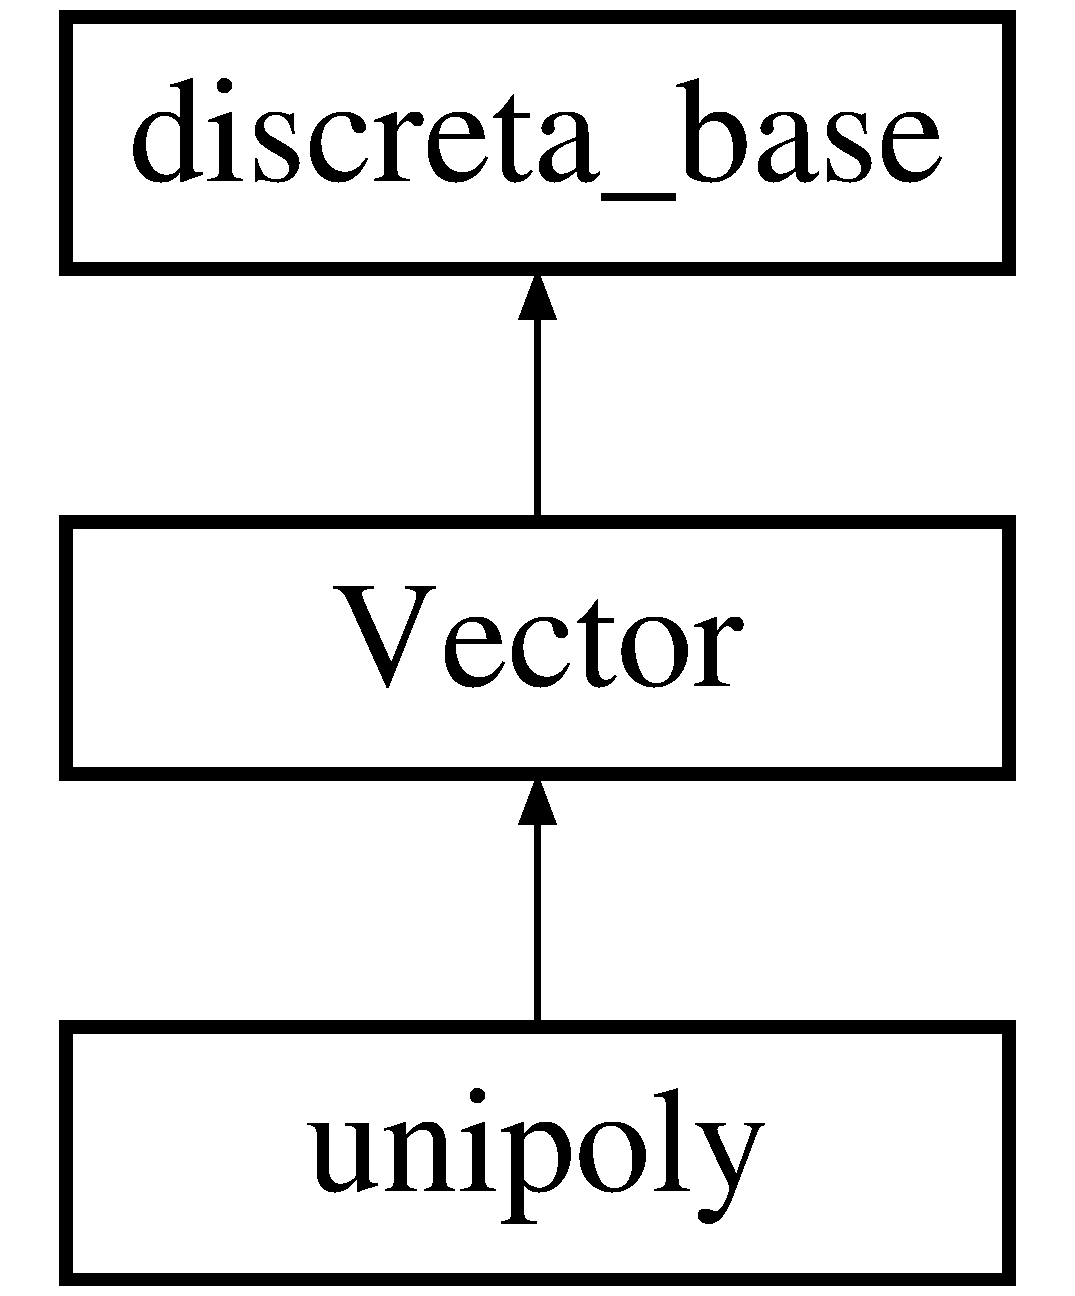
\includegraphics[height=3.000000cm]{classunipoly}
\end{center}
\end{figure}
\subsection*{Public Member Functions}
\begin{DoxyCompactItemize}
\item 
\mbox{\hyperlink{classunipoly_adf6c81c7b9f7d4c110a04c4a5681695c}{unipoly}} ()
\item 
\mbox{\hyperlink{classunipoly_ade3afe0b00b7ff45b9dbc5a15cacf59d}{unipoly}} (const \mbox{\hyperlink{classdiscreta__base}{discreta\+\_\+base}} \&\mbox{\hyperlink{classunipoly_a193127c4c6cf419d995882bb5b762294}{x}})
\item 
\mbox{\hyperlink{classunipoly}{unipoly}} \& \mbox{\hyperlink{classunipoly_a60f1ddf49bc3e91ad73d24b9fbb29460}{operator=}} (const \mbox{\hyperlink{classdiscreta__base}{discreta\+\_\+base}} \&\mbox{\hyperlink{classunipoly_a193127c4c6cf419d995882bb5b762294}{x}})
\item 
void $\ast$ \mbox{\hyperlink{classunipoly_a639ce1a4da795063456de370bed53ab3}{operator new}} (size\+\_\+t, void $\ast$\mbox{\hyperlink{alphabet2_8_c_a533391314665d6bf1b5575e9a9cd8552}{p}})
\item 
void \mbox{\hyperlink{classunipoly_a8db854fcc85c5e1150b1f1b1c005c95b}{settype\+\_\+unipoly}} ()
\item 
\mbox{\hyperlink{discreta_8h_aaf25ee7e2306d78c74ec7bc48f092e81}{kind}} \mbox{\hyperlink{classunipoly_a62303d2461523c791edc16fe40371e18}{s\+\_\+virtual\+\_\+kind}} ()
\item 
\mbox{\hyperlink{classunipoly_aff42843e3c959f1c5e58856784352890}{$\sim$unipoly}} ()
\item 
void \mbox{\hyperlink{classunipoly_aad315db6c6adb555a0c63877aab7d27e}{freeself\+\_\+unipoly}} ()
\item 
void \mbox{\hyperlink{classunipoly_aa856d320a499748a0f3345ab45e51910}{copyobject\+\_\+to}} (\mbox{\hyperlink{classdiscreta__base}{discreta\+\_\+base}} \&\mbox{\hyperlink{classunipoly_a193127c4c6cf419d995882bb5b762294}{x}})
\item 
ostream \& \mbox{\hyperlink{classunipoly_a9dc0d295bea73d0c20562149f250cd97}{print}} (ostream \&)
\item 
ostream \& \mbox{\hyperlink{classunipoly_a68ada9f90ad0ad39ae91653be50988aa}{print\+\_\+as\+\_\+vector}} (ostream \&ost)
\item 
void \mbox{\hyperlink{classunipoly_a776ccf5b98954c5212b684944ab5d725}{m\+\_\+l}} (\mbox{\hyperlink{galois_8h_a09fddde158a3a20bd2dcadb609de11dc}{I\+NT}} \mbox{\hyperlink{alphabet2_8_c_a89606eca6b563ec68d2da2e84657736f}{l}})
\item 
\mbox{\hyperlink{galois_8h_a09fddde158a3a20bd2dcadb609de11dc}{I\+NT}} \mbox{\hyperlink{classunipoly_ab2b9692ea17ce32c0c8f2cc246517e37}{degree}} ()
\item 
void \mbox{\hyperlink{classunipoly_a95bf7f347a5630f0d3f9737ffe22a341}{mult\+\_\+to}} (\mbox{\hyperlink{classdiscreta__base}{discreta\+\_\+base}} \&\mbox{\hyperlink{classunipoly_a193127c4c6cf419d995882bb5b762294}{x}}, \mbox{\hyperlink{classdiscreta__base}{discreta\+\_\+base}} \&\mbox{\hyperlink{alphabet2_8_c_a0a2f84ed7838f07779ae24c5a9086d33}{y}})
\item 
void \mbox{\hyperlink{classunipoly_abebdaf912a2b0e7c27470f4191d0e180}{add\+\_\+to}} (\mbox{\hyperlink{classdiscreta__base}{discreta\+\_\+base}} \&\mbox{\hyperlink{classunipoly_a193127c4c6cf419d995882bb5b762294}{x}}, \mbox{\hyperlink{classdiscreta__base}{discreta\+\_\+base}} \&\mbox{\hyperlink{alphabet2_8_c_a0a2f84ed7838f07779ae24c5a9086d33}{y}})
\item 
void \mbox{\hyperlink{classunipoly_a2181196b44786790f58b72510620db97}{negate\+\_\+to}} (\mbox{\hyperlink{classdiscreta__base}{discreta\+\_\+base}} \&\mbox{\hyperlink{classunipoly_a193127c4c6cf419d995882bb5b762294}{x}})
\item 
void \mbox{\hyperlink{classunipoly_a12db8572d9d5a2edba5b7a4562f6e746}{one}} ()
\item 
void \mbox{\hyperlink{classunipoly_a8fd1c1a5602dc59b0e1a68bee23d60b6}{zero}} ()
\item 
void \mbox{\hyperlink{classunipoly_a193127c4c6cf419d995882bb5b762294}{x}} ()
\item 
void \mbox{\hyperlink{classunipoly_a1415216fadad08456f6c70403b522f6e}{x\+\_\+to\+\_\+the\+\_\+i}} (\mbox{\hyperlink{galois_8h_a09fddde158a3a20bd2dcadb609de11dc}{I\+NT}} \mbox{\hyperlink{alphabet2_8_c_acb559820d9ca11295b4500f179ef6392}{i}})
\item 
\mbox{\hyperlink{galois_8h_a09fddde158a3a20bd2dcadb609de11dc}{I\+NT}} \mbox{\hyperlink{classunipoly_a1840dc8eb1a17b1764b108c96299738d}{is\+\_\+one}} ()
\item 
\mbox{\hyperlink{galois_8h_a09fddde158a3a20bd2dcadb609de11dc}{I\+NT}} \mbox{\hyperlink{classunipoly_a7bff4146466929655bf2bcfd42c682cf}{is\+\_\+zero}} ()
\item 
\mbox{\hyperlink{galois_8h_a09fddde158a3a20bd2dcadb609de11dc}{I\+NT}} \mbox{\hyperlink{classunipoly_ae51f546d1fadd05e03bc71df1aa57d64}{compare\+\_\+with\+\_\+euklidean}} (\mbox{\hyperlink{classdiscreta__base}{discreta\+\_\+base}} \&a)
\item 
void \mbox{\hyperlink{classunipoly_aeb794e4d6b10709ed6be7dae9826d705}{integral\+\_\+division}} (\mbox{\hyperlink{classdiscreta__base}{discreta\+\_\+base}} \&\mbox{\hyperlink{classunipoly_a193127c4c6cf419d995882bb5b762294}{x}}, \mbox{\hyperlink{classdiscreta__base}{discreta\+\_\+base}} \&\mbox{\hyperlink{simeon_8_c_a92cbb483a3b27ae1a0dbfcb125ce216f}{q}}, \mbox{\hyperlink{classdiscreta__base}{discreta\+\_\+base}} \&\mbox{\hyperlink{alphabet2_8_c_acab531abaa74a7e664e3986f2522b33a}{r}}, \mbox{\hyperlink{galois_8h_a09fddde158a3a20bd2dcadb609de11dc}{I\+NT}} \mbox{\hyperlink{simeon_8_c_a818073fbcc2f439e7c56952f67386122}{verbose\+\_\+level}})
\item 
void \mbox{\hyperlink{classunipoly_a52ae2730113a41ba434aa33d242ad2ae}{derive}} ()
\item 
\mbox{\hyperlink{galois_8h_a09fddde158a3a20bd2dcadb609de11dc}{I\+NT}} \mbox{\hyperlink{classunipoly_ac7b4a759fa68858043e1ad2b91e060db}{is\+\_\+squarefree}} (\mbox{\hyperlink{galois_8h_a09fddde158a3a20bd2dcadb609de11dc}{I\+NT}} \mbox{\hyperlink{simeon_8_c_a818073fbcc2f439e7c56952f67386122}{verbose\+\_\+level}})
\item 
\mbox{\hyperlink{galois_8h_a09fddde158a3a20bd2dcadb609de11dc}{I\+NT}} \mbox{\hyperlink{classunipoly_a9f17f20ea6bc30581159151ebe849f6b}{is\+\_\+irreducible\+\_\+\+G\+Fp}} (\mbox{\hyperlink{galois_8h_a09fddde158a3a20bd2dcadb609de11dc}{I\+NT}} \mbox{\hyperlink{alphabet2_8_c_a533391314665d6bf1b5575e9a9cd8552}{p}}, \mbox{\hyperlink{galois_8h_a09fddde158a3a20bd2dcadb609de11dc}{I\+NT}} \mbox{\hyperlink{simeon_8_c_a818073fbcc2f439e7c56952f67386122}{verbose\+\_\+level}})
\item 
\mbox{\hyperlink{galois_8h_a09fddde158a3a20bd2dcadb609de11dc}{I\+NT}} \mbox{\hyperlink{classunipoly_a9170111d259116a55616b165f7fde3c8}{is\+\_\+irreducible}} (\mbox{\hyperlink{galois_8h_a09fddde158a3a20bd2dcadb609de11dc}{I\+NT}} \mbox{\hyperlink{simeon_8_c_a92cbb483a3b27ae1a0dbfcb125ce216f}{q}}, \mbox{\hyperlink{galois_8h_a09fddde158a3a20bd2dcadb609de11dc}{I\+NT}} f\+\_\+v)
\item 
\mbox{\hyperlink{galois_8h_a09fddde158a3a20bd2dcadb609de11dc}{I\+NT}} \mbox{\hyperlink{classunipoly_a6abce01baf319f3857dc5c674e58687d}{is\+\_\+primitive}} (\mbox{\hyperlink{galois_8h_a09fddde158a3a20bd2dcadb609de11dc}{I\+NT}} m, \mbox{\hyperlink{galois_8h_a09fddde158a3a20bd2dcadb609de11dc}{I\+NT}} \mbox{\hyperlink{alphabet2_8_c_a533391314665d6bf1b5575e9a9cd8552}{p}}, \mbox{\hyperlink{class_vector}{Vector}} \&vp, \mbox{\hyperlink{galois_8h_a09fddde158a3a20bd2dcadb609de11dc}{I\+NT}} \mbox{\hyperlink{simeon_8_c_a818073fbcc2f439e7c56952f67386122}{verbose\+\_\+level}})
\item 
void \mbox{\hyperlink{classunipoly_a5066ce0b3206afcdd299c4079394e190}{numeric\+\_\+polynomial}} (\mbox{\hyperlink{galois_8h_a09fddde158a3a20bd2dcadb609de11dc}{I\+NT}} \mbox{\hyperlink{simeon_8_c_a7f2cd26777ce0ff3fdaf8d02aacbddfb}{n}}, \mbox{\hyperlink{galois_8h_a09fddde158a3a20bd2dcadb609de11dc}{I\+NT}} \mbox{\hyperlink{simeon_8_c_a92cbb483a3b27ae1a0dbfcb125ce216f}{q}})
\item 
\mbox{\hyperlink{galois_8h_a09fddde158a3a20bd2dcadb609de11dc}{I\+NT}} \mbox{\hyperlink{classunipoly_a07fbd1dbc9033a82bfa2fd2eb7358bda}{polynomial\+\_\+numeric}} (\mbox{\hyperlink{galois_8h_a09fddde158a3a20bd2dcadb609de11dc}{I\+NT}} \mbox{\hyperlink{simeon_8_c_a92cbb483a3b27ae1a0dbfcb125ce216f}{q}})
\item 
void \mbox{\hyperlink{classunipoly_a53231caafb097fc75404538383b88197}{singer\+\_\+candidate}} (\mbox{\hyperlink{galois_8h_a09fddde158a3a20bd2dcadb609de11dc}{I\+NT}} \mbox{\hyperlink{alphabet2_8_c_a533391314665d6bf1b5575e9a9cd8552}{p}}, \mbox{\hyperlink{galois_8h_a09fddde158a3a20bd2dcadb609de11dc}{I\+NT}} \mbox{\hyperlink{alphabet2_8_c_a362077c979b0bb65159c603270e40f70}{f}}, \mbox{\hyperlink{galois_8h_a09fddde158a3a20bd2dcadb609de11dc}{I\+NT}} \mbox{\hyperlink{alphabet2_8_c_a148e3876077787926724625411d6e7a9}{b}}, \mbox{\hyperlink{galois_8h_a09fddde158a3a20bd2dcadb609de11dc}{I\+NT}} a)
\item 
void \mbox{\hyperlink{classunipoly_a3a5c0cc82d0d750bd47799046a4dc59e}{Singer}} (\mbox{\hyperlink{galois_8h_a09fddde158a3a20bd2dcadb609de11dc}{I\+NT}} \mbox{\hyperlink{alphabet2_8_c_a533391314665d6bf1b5575e9a9cd8552}{p}}, \mbox{\hyperlink{galois_8h_a09fddde158a3a20bd2dcadb609de11dc}{I\+NT}} \mbox{\hyperlink{alphabet2_8_c_a362077c979b0bb65159c603270e40f70}{f}}, \mbox{\hyperlink{galois_8h_a09fddde158a3a20bd2dcadb609de11dc}{I\+NT}} f\+\_\+v, \mbox{\hyperlink{galois_8h_a09fddde158a3a20bd2dcadb609de11dc}{I\+NT}} f\+\_\+vv)
\item 
void \mbox{\hyperlink{classunipoly_a14ae1863f2096e87f8115f5e8f727883}{get\+\_\+an\+\_\+irreducible\+\_\+polynomial}} (\mbox{\hyperlink{galois_8h_a09fddde158a3a20bd2dcadb609de11dc}{I\+NT}} \mbox{\hyperlink{alphabet2_8_c_a362077c979b0bb65159c603270e40f70}{f}}, \mbox{\hyperlink{galois_8h_a09fddde158a3a20bd2dcadb609de11dc}{I\+NT}} \mbox{\hyperlink{simeon_8_c_a818073fbcc2f439e7c56952f67386122}{verbose\+\_\+level}})
\item 
void \mbox{\hyperlink{classunipoly_afb8c65d96c3c1afeb1e14120bd5942b8}{evaluate\+\_\+at}} (\mbox{\hyperlink{classdiscreta__base}{discreta\+\_\+base}} \&\mbox{\hyperlink{classunipoly_a193127c4c6cf419d995882bb5b762294}{x}}, \mbox{\hyperlink{classdiscreta__base}{discreta\+\_\+base}} \&\mbox{\hyperlink{alphabet2_8_c_a0a2f84ed7838f07779ae24c5a9086d33}{y}})
\item 
void \mbox{\hyperlink{classunipoly_a8984096d0b2f34c9e4b60ad6442bc62a}{largest\+\_\+divisor\+\_\+prime\+\_\+to}} (\mbox{\hyperlink{classunipoly}{unipoly}} \&\mbox{\hyperlink{simeon_8_c_a92cbb483a3b27ae1a0dbfcb125ce216f}{q}}, \mbox{\hyperlink{classunipoly}{unipoly}} \&\mbox{\hyperlink{alphabet2_8_c_acab531abaa74a7e664e3986f2522b33a}{r}})
\item 
void \mbox{\hyperlink{classunipoly_a44fd80fcd3b9dc5b3d9f915761a8082d}{monic}} ()
\item 
void \mbox{\hyperlink{classunipoly_a38f30f53df7f4ff1506f2b41666ff39e}{normal\+\_\+base}} (\mbox{\hyperlink{galois_8h_a09fddde158a3a20bd2dcadb609de11dc}{I\+NT}} \mbox{\hyperlink{alphabet2_8_c_a533391314665d6bf1b5575e9a9cd8552}{p}}, \mbox{\hyperlink{classmatrix}{matrix}} \&\mbox{\hyperlink{simeon_8_c_a21a61c535ff7d9d4b674461d3b19fffa}{F}}, \mbox{\hyperlink{classmatrix}{matrix}} \&\mbox{\hyperlink{_a_p_p_s_2_t_d_o_2packing_8_c_a0240ac851181b84ac374872dc5434ee4}{N}}, \mbox{\hyperlink{galois_8h_a09fddde158a3a20bd2dcadb609de11dc}{I\+NT}} \mbox{\hyperlink{simeon_8_c_a818073fbcc2f439e7c56952f67386122}{verbose\+\_\+level}})
\item 
\mbox{\hyperlink{galois_8h_a09fddde158a3a20bd2dcadb609de11dc}{I\+NT}} \mbox{\hyperlink{classunipoly_a924960b8bdc1ba81f54703f5e8ed84ee}{first\+\_\+irreducible\+\_\+polynomial}} (\mbox{\hyperlink{galois_8h_a09fddde158a3a20bd2dcadb609de11dc}{I\+NT}} \mbox{\hyperlink{alphabet2_8_c_a533391314665d6bf1b5575e9a9cd8552}{p}}, \mbox{\hyperlink{classunipoly}{unipoly}} \&m, \mbox{\hyperlink{classmatrix}{matrix}} \&\mbox{\hyperlink{simeon_8_c_a21a61c535ff7d9d4b674461d3b19fffa}{F}}, \mbox{\hyperlink{classmatrix}{matrix}} \&\mbox{\hyperlink{_a_p_p_s_2_t_d_o_2packing_8_c_a0240ac851181b84ac374872dc5434ee4}{N}}, \mbox{\hyperlink{class_vector}{Vector}} \&\mbox{\hyperlink{simeon_8_c_aeb3f3030944801b163bc3b829a7f6710}{v}}, \mbox{\hyperlink{galois_8h_a09fddde158a3a20bd2dcadb609de11dc}{I\+NT}} \mbox{\hyperlink{simeon_8_c_a818073fbcc2f439e7c56952f67386122}{verbose\+\_\+level}})
\item 
\mbox{\hyperlink{galois_8h_a09fddde158a3a20bd2dcadb609de11dc}{I\+NT}} \mbox{\hyperlink{classunipoly_a1c187a11d98570cb22ccf0ee2a06345e}{next\+\_\+irreducible\+\_\+polynomial}} (\mbox{\hyperlink{galois_8h_a09fddde158a3a20bd2dcadb609de11dc}{I\+NT}} \mbox{\hyperlink{alphabet2_8_c_a533391314665d6bf1b5575e9a9cd8552}{p}}, \mbox{\hyperlink{classunipoly}{unipoly}} \&m, \mbox{\hyperlink{classmatrix}{matrix}} \&\mbox{\hyperlink{simeon_8_c_a21a61c535ff7d9d4b674461d3b19fffa}{F}}, \mbox{\hyperlink{classmatrix}{matrix}} \&\mbox{\hyperlink{_a_p_p_s_2_t_d_o_2packing_8_c_a0240ac851181b84ac374872dc5434ee4}{N}}, \mbox{\hyperlink{class_vector}{Vector}} \&\mbox{\hyperlink{simeon_8_c_aeb3f3030944801b163bc3b829a7f6710}{v}}, \mbox{\hyperlink{galois_8h_a09fddde158a3a20bd2dcadb609de11dc}{I\+NT}} \mbox{\hyperlink{simeon_8_c_a818073fbcc2f439e7c56952f67386122}{verbose\+\_\+level}})
\item 
void \mbox{\hyperlink{classunipoly_a1fdf6f2da235edcf45fca433dea19370}{normalize}} (\mbox{\hyperlink{classdiscreta__base}{discreta\+\_\+base}} \&\mbox{\hyperlink{alphabet2_8_c_a533391314665d6bf1b5575e9a9cd8552}{p}})
\item 
void \mbox{\hyperlink{classunipoly_a6804952878b88dc700e6532a5c9b1e6e}{Xnm1}} (\mbox{\hyperlink{galois_8h_a09fddde158a3a20bd2dcadb609de11dc}{I\+NT}} \mbox{\hyperlink{simeon_8_c_a7f2cd26777ce0ff3fdaf8d02aacbddfb}{n}})
\item 
void \mbox{\hyperlink{classunipoly_a50f2edff215daebf54b1e010d99f630d}{Phi}} (\mbox{\hyperlink{galois_8h_a09fddde158a3a20bd2dcadb609de11dc}{I\+NT}} \mbox{\hyperlink{simeon_8_c_a7f2cd26777ce0ff3fdaf8d02aacbddfb}{n}}, \mbox{\hyperlink{galois_8h_a09fddde158a3a20bd2dcadb609de11dc}{I\+NT}} f\+\_\+v)
\item 
void \mbox{\hyperlink{classunipoly_ad9a4b7b883285271fc39528f74755a07}{weight\+\_\+enumerator\+\_\+\+M\+D\+S\+\_\+code}} (\mbox{\hyperlink{galois_8h_a09fddde158a3a20bd2dcadb609de11dc}{I\+NT}} \mbox{\hyperlink{simeon_8_c_a7f2cd26777ce0ff3fdaf8d02aacbddfb}{n}}, \mbox{\hyperlink{galois_8h_a09fddde158a3a20bd2dcadb609de11dc}{I\+NT}} \mbox{\hyperlink{classdiscreta__base_a6f7a0f7bdd115b9e4dde358cfa7ebf81}{k}}, \mbox{\hyperlink{galois_8h_a09fddde158a3a20bd2dcadb609de11dc}{I\+NT}} \mbox{\hyperlink{simeon_8_c_a92cbb483a3b27ae1a0dbfcb125ce216f}{q}}, \mbox{\hyperlink{galois_8h_a09fddde158a3a20bd2dcadb609de11dc}{I\+NT}} f\+\_\+v, \mbox{\hyperlink{galois_8h_a09fddde158a3a20bd2dcadb609de11dc}{I\+NT}} f\+\_\+vv, \mbox{\hyperlink{galois_8h_a09fddde158a3a20bd2dcadb609de11dc}{I\+NT}} f\+\_\+vvv)
\item 
void \mbox{\hyperlink{classunipoly_a788dc8f7be5c5c4c347959a9155ddb80}{charpoly}} (\mbox{\hyperlink{galois_8h_a09fddde158a3a20bd2dcadb609de11dc}{I\+NT}} \mbox{\hyperlink{simeon_8_c_a92cbb483a3b27ae1a0dbfcb125ce216f}{q}}, \mbox{\hyperlink{galois_8h_a09fddde158a3a20bd2dcadb609de11dc}{I\+NT}} size, \mbox{\hyperlink{galois_8h_a09fddde158a3a20bd2dcadb609de11dc}{I\+NT}} $\ast$mtx, \mbox{\hyperlink{galois_8h_a09fddde158a3a20bd2dcadb609de11dc}{I\+NT}} \mbox{\hyperlink{simeon_8_c_a818073fbcc2f439e7c56952f67386122}{verbose\+\_\+level}})
\end{DoxyCompactItemize}
\subsection*{Additional Inherited Members}


\subsection{Constructor \& Destructor Documentation}
\mbox{\Hypertarget{classunipoly_adf6c81c7b9f7d4c110a04c4a5681695c}\label{classunipoly_adf6c81c7b9f7d4c110a04c4a5681695c}} 
\index{unipoly@{unipoly}!unipoly@{unipoly}}
\index{unipoly@{unipoly}!unipoly@{unipoly}}
\subsubsection{\texorpdfstring{unipoly()}{unipoly()}\hspace{0.1cm}{\footnotesize\ttfamily [1/2]}}
{\footnotesize\ttfamily unipoly\+::unipoly (\begin{DoxyParamCaption}{ }\end{DoxyParamCaption})}

\mbox{\Hypertarget{classunipoly_ade3afe0b00b7ff45b9dbc5a15cacf59d}\label{classunipoly_ade3afe0b00b7ff45b9dbc5a15cacf59d}} 
\index{unipoly@{unipoly}!unipoly@{unipoly}}
\index{unipoly@{unipoly}!unipoly@{unipoly}}
\subsubsection{\texorpdfstring{unipoly()}{unipoly()}\hspace{0.1cm}{\footnotesize\ttfamily [2/2]}}
{\footnotesize\ttfamily unipoly\+::unipoly (\begin{DoxyParamCaption}\item[{const \mbox{\hyperlink{classdiscreta__base}{discreta\+\_\+base}} \&}]{x }\end{DoxyParamCaption})}

\mbox{\Hypertarget{classunipoly_aff42843e3c959f1c5e58856784352890}\label{classunipoly_aff42843e3c959f1c5e58856784352890}} 
\index{unipoly@{unipoly}!````~unipoly@{$\sim$unipoly}}
\index{````~unipoly@{$\sim$unipoly}!unipoly@{unipoly}}
\subsubsection{\texorpdfstring{$\sim$unipoly()}{~unipoly()}}
{\footnotesize\ttfamily unipoly\+::$\sim$unipoly (\begin{DoxyParamCaption}{ }\end{DoxyParamCaption})}



\subsection{Member Function Documentation}
\mbox{\Hypertarget{classunipoly_abebdaf912a2b0e7c27470f4191d0e180}\label{classunipoly_abebdaf912a2b0e7c27470f4191d0e180}} 
\index{unipoly@{unipoly}!add\+\_\+to@{add\+\_\+to}}
\index{add\+\_\+to@{add\+\_\+to}!unipoly@{unipoly}}
\subsubsection{\texorpdfstring{add\+\_\+to()}{add\_to()}}
{\footnotesize\ttfamily void unipoly\+::add\+\_\+to (\begin{DoxyParamCaption}\item[{\mbox{\hyperlink{classdiscreta__base}{discreta\+\_\+base}} \&}]{x,  }\item[{\mbox{\hyperlink{classdiscreta__base}{discreta\+\_\+base}} \&}]{y }\end{DoxyParamCaption})\hspace{0.3cm}{\ttfamily [virtual]}}



Reimplemented from \mbox{\hyperlink{class_vector_a3e170560de50e3a4f4a95f6b90bf75bb}{Vector}}.

\mbox{\Hypertarget{classunipoly_a788dc8f7be5c5c4c347959a9155ddb80}\label{classunipoly_a788dc8f7be5c5c4c347959a9155ddb80}} 
\index{unipoly@{unipoly}!charpoly@{charpoly}}
\index{charpoly@{charpoly}!unipoly@{unipoly}}
\subsubsection{\texorpdfstring{charpoly()}{charpoly()}}
{\footnotesize\ttfamily void unipoly\+::charpoly (\begin{DoxyParamCaption}\item[{\mbox{\hyperlink{galois_8h_a09fddde158a3a20bd2dcadb609de11dc}{I\+NT}}}]{q,  }\item[{\mbox{\hyperlink{galois_8h_a09fddde158a3a20bd2dcadb609de11dc}{I\+NT}}}]{size,  }\item[{\mbox{\hyperlink{galois_8h_a09fddde158a3a20bd2dcadb609de11dc}{I\+NT}} $\ast$}]{mtx,  }\item[{\mbox{\hyperlink{galois_8h_a09fddde158a3a20bd2dcadb609de11dc}{I\+NT}}}]{verbose\+\_\+level }\end{DoxyParamCaption})}

\mbox{\Hypertarget{classunipoly_ae51f546d1fadd05e03bc71df1aa57d64}\label{classunipoly_ae51f546d1fadd05e03bc71df1aa57d64}} 
\index{unipoly@{unipoly}!compare\+\_\+with\+\_\+euklidean@{compare\+\_\+with\+\_\+euklidean}}
\index{compare\+\_\+with\+\_\+euklidean@{compare\+\_\+with\+\_\+euklidean}!unipoly@{unipoly}}
\subsubsection{\texorpdfstring{compare\+\_\+with\+\_\+euklidean()}{compare\_with\_euklidean()}}
{\footnotesize\ttfamily \mbox{\hyperlink{galois_8h_a09fddde158a3a20bd2dcadb609de11dc}{I\+NT}} unipoly\+::compare\+\_\+with\+\_\+euklidean (\begin{DoxyParamCaption}\item[{\mbox{\hyperlink{classdiscreta__base}{discreta\+\_\+base}} \&}]{a }\end{DoxyParamCaption})\hspace{0.3cm}{\ttfamily [virtual]}}



Reimplemented from \mbox{\hyperlink{classdiscreta__base_a9d3091feb2fbc69359c2a45f11ceec9e}{discreta\+\_\+base}}.

\mbox{\Hypertarget{classunipoly_aa856d320a499748a0f3345ab45e51910}\label{classunipoly_aa856d320a499748a0f3345ab45e51910}} 
\index{unipoly@{unipoly}!copyobject\+\_\+to@{copyobject\+\_\+to}}
\index{copyobject\+\_\+to@{copyobject\+\_\+to}!unipoly@{unipoly}}
\subsubsection{\texorpdfstring{copyobject\+\_\+to()}{copyobject\_to()}}
{\footnotesize\ttfamily void unipoly\+::copyobject\+\_\+to (\begin{DoxyParamCaption}\item[{\mbox{\hyperlink{classdiscreta__base}{discreta\+\_\+base}} \&}]{x }\end{DoxyParamCaption})\hspace{0.3cm}{\ttfamily [virtual]}}



Reimplemented from \mbox{\hyperlink{class_vector_af657307f3d344c8cef5d633335a5f484}{Vector}}.

\mbox{\Hypertarget{classunipoly_ab2b9692ea17ce32c0c8f2cc246517e37}\label{classunipoly_ab2b9692ea17ce32c0c8f2cc246517e37}} 
\index{unipoly@{unipoly}!degree@{degree}}
\index{degree@{degree}!unipoly@{unipoly}}
\subsubsection{\texorpdfstring{degree()}{degree()}}
{\footnotesize\ttfamily \mbox{\hyperlink{galois_8h_a09fddde158a3a20bd2dcadb609de11dc}{I\+NT}} unipoly\+::degree (\begin{DoxyParamCaption}{ }\end{DoxyParamCaption})}

\mbox{\Hypertarget{classunipoly_a52ae2730113a41ba434aa33d242ad2ae}\label{classunipoly_a52ae2730113a41ba434aa33d242ad2ae}} 
\index{unipoly@{unipoly}!derive@{derive}}
\index{derive@{derive}!unipoly@{unipoly}}
\subsubsection{\texorpdfstring{derive()}{derive()}}
{\footnotesize\ttfamily void unipoly\+::derive (\begin{DoxyParamCaption}{ }\end{DoxyParamCaption})}

\mbox{\Hypertarget{classunipoly_afb8c65d96c3c1afeb1e14120bd5942b8}\label{classunipoly_afb8c65d96c3c1afeb1e14120bd5942b8}} 
\index{unipoly@{unipoly}!evaluate\+\_\+at@{evaluate\+\_\+at}}
\index{evaluate\+\_\+at@{evaluate\+\_\+at}!unipoly@{unipoly}}
\subsubsection{\texorpdfstring{evaluate\+\_\+at()}{evaluate\_at()}}
{\footnotesize\ttfamily void unipoly\+::evaluate\+\_\+at (\begin{DoxyParamCaption}\item[{\mbox{\hyperlink{classdiscreta__base}{discreta\+\_\+base}} \&}]{x,  }\item[{\mbox{\hyperlink{classdiscreta__base}{discreta\+\_\+base}} \&}]{y }\end{DoxyParamCaption})}

\mbox{\Hypertarget{classunipoly_a924960b8bdc1ba81f54703f5e8ed84ee}\label{classunipoly_a924960b8bdc1ba81f54703f5e8ed84ee}} 
\index{unipoly@{unipoly}!first\+\_\+irreducible\+\_\+polynomial@{first\+\_\+irreducible\+\_\+polynomial}}
\index{first\+\_\+irreducible\+\_\+polynomial@{first\+\_\+irreducible\+\_\+polynomial}!unipoly@{unipoly}}
\subsubsection{\texorpdfstring{first\+\_\+irreducible\+\_\+polynomial()}{first\_irreducible\_polynomial()}}
{\footnotesize\ttfamily \mbox{\hyperlink{galois_8h_a09fddde158a3a20bd2dcadb609de11dc}{I\+NT}} unipoly\+::first\+\_\+irreducible\+\_\+polynomial (\begin{DoxyParamCaption}\item[{\mbox{\hyperlink{galois_8h_a09fddde158a3a20bd2dcadb609de11dc}{I\+NT}}}]{p,  }\item[{\mbox{\hyperlink{classunipoly}{unipoly}} \&}]{m,  }\item[{\mbox{\hyperlink{classmatrix}{matrix}} \&}]{F,  }\item[{\mbox{\hyperlink{classmatrix}{matrix}} \&}]{N,  }\item[{\mbox{\hyperlink{class_vector}{Vector}} \&}]{v,  }\item[{\mbox{\hyperlink{galois_8h_a09fddde158a3a20bd2dcadb609de11dc}{I\+NT}}}]{verbose\+\_\+level }\end{DoxyParamCaption})}

\mbox{\Hypertarget{classunipoly_aad315db6c6adb555a0c63877aab7d27e}\label{classunipoly_aad315db6c6adb555a0c63877aab7d27e}} 
\index{unipoly@{unipoly}!freeself\+\_\+unipoly@{freeself\+\_\+unipoly}}
\index{freeself\+\_\+unipoly@{freeself\+\_\+unipoly}!unipoly@{unipoly}}
\subsubsection{\texorpdfstring{freeself\+\_\+unipoly()}{freeself\_unipoly()}}
{\footnotesize\ttfamily void unipoly\+::freeself\+\_\+unipoly (\begin{DoxyParamCaption}{ }\end{DoxyParamCaption})}

\mbox{\Hypertarget{classunipoly_a14ae1863f2096e87f8115f5e8f727883}\label{classunipoly_a14ae1863f2096e87f8115f5e8f727883}} 
\index{unipoly@{unipoly}!get\+\_\+an\+\_\+irreducible\+\_\+polynomial@{get\+\_\+an\+\_\+irreducible\+\_\+polynomial}}
\index{get\+\_\+an\+\_\+irreducible\+\_\+polynomial@{get\+\_\+an\+\_\+irreducible\+\_\+polynomial}!unipoly@{unipoly}}
\subsubsection{\texorpdfstring{get\+\_\+an\+\_\+irreducible\+\_\+polynomial()}{get\_an\_irreducible\_polynomial()}}
{\footnotesize\ttfamily void unipoly\+::get\+\_\+an\+\_\+irreducible\+\_\+polynomial (\begin{DoxyParamCaption}\item[{\mbox{\hyperlink{galois_8h_a09fddde158a3a20bd2dcadb609de11dc}{I\+NT}}}]{f,  }\item[{\mbox{\hyperlink{galois_8h_a09fddde158a3a20bd2dcadb609de11dc}{I\+NT}}}]{verbose\+\_\+level }\end{DoxyParamCaption})}

\mbox{\Hypertarget{classunipoly_aeb794e4d6b10709ed6be7dae9826d705}\label{classunipoly_aeb794e4d6b10709ed6be7dae9826d705}} 
\index{unipoly@{unipoly}!integral\+\_\+division@{integral\+\_\+division}}
\index{integral\+\_\+division@{integral\+\_\+division}!unipoly@{unipoly}}
\subsubsection{\texorpdfstring{integral\+\_\+division()}{integral\_division()}}
{\footnotesize\ttfamily void unipoly\+::integral\+\_\+division (\begin{DoxyParamCaption}\item[{\mbox{\hyperlink{classdiscreta__base}{discreta\+\_\+base}} \&}]{x,  }\item[{\mbox{\hyperlink{classdiscreta__base}{discreta\+\_\+base}} \&}]{q,  }\item[{\mbox{\hyperlink{classdiscreta__base}{discreta\+\_\+base}} \&}]{r,  }\item[{\mbox{\hyperlink{galois_8h_a09fddde158a3a20bd2dcadb609de11dc}{I\+NT}}}]{verbose\+\_\+level }\end{DoxyParamCaption})\hspace{0.3cm}{\ttfamily [virtual]}}



Reimplemented from \mbox{\hyperlink{classdiscreta__base_a92b3001ac35af9185b316c0d8f89070e}{discreta\+\_\+base}}.

\mbox{\Hypertarget{classunipoly_a9170111d259116a55616b165f7fde3c8}\label{classunipoly_a9170111d259116a55616b165f7fde3c8}} 
\index{unipoly@{unipoly}!is\+\_\+irreducible@{is\+\_\+irreducible}}
\index{is\+\_\+irreducible@{is\+\_\+irreducible}!unipoly@{unipoly}}
\subsubsection{\texorpdfstring{is\+\_\+irreducible()}{is\_irreducible()}}
{\footnotesize\ttfamily \mbox{\hyperlink{galois_8h_a09fddde158a3a20bd2dcadb609de11dc}{I\+NT}} unipoly\+::is\+\_\+irreducible (\begin{DoxyParamCaption}\item[{\mbox{\hyperlink{galois_8h_a09fddde158a3a20bd2dcadb609de11dc}{I\+NT}}}]{q,  }\item[{\mbox{\hyperlink{galois_8h_a09fddde158a3a20bd2dcadb609de11dc}{I\+NT}}}]{f\+\_\+v }\end{DoxyParamCaption})}

\mbox{\Hypertarget{classunipoly_a9f17f20ea6bc30581159151ebe849f6b}\label{classunipoly_a9f17f20ea6bc30581159151ebe849f6b}} 
\index{unipoly@{unipoly}!is\+\_\+irreducible\+\_\+\+G\+Fp@{is\+\_\+irreducible\+\_\+\+G\+Fp}}
\index{is\+\_\+irreducible\+\_\+\+G\+Fp@{is\+\_\+irreducible\+\_\+\+G\+Fp}!unipoly@{unipoly}}
\subsubsection{\texorpdfstring{is\+\_\+irreducible\+\_\+\+G\+Fp()}{is\_irreducible\_GFp()}}
{\footnotesize\ttfamily \mbox{\hyperlink{galois_8h_a09fddde158a3a20bd2dcadb609de11dc}{I\+NT}} unipoly\+::is\+\_\+irreducible\+\_\+\+G\+Fp (\begin{DoxyParamCaption}\item[{\mbox{\hyperlink{galois_8h_a09fddde158a3a20bd2dcadb609de11dc}{I\+NT}}}]{p,  }\item[{\mbox{\hyperlink{galois_8h_a09fddde158a3a20bd2dcadb609de11dc}{I\+NT}}}]{verbose\+\_\+level }\end{DoxyParamCaption})}

\mbox{\Hypertarget{classunipoly_a1840dc8eb1a17b1764b108c96299738d}\label{classunipoly_a1840dc8eb1a17b1764b108c96299738d}} 
\index{unipoly@{unipoly}!is\+\_\+one@{is\+\_\+one}}
\index{is\+\_\+one@{is\+\_\+one}!unipoly@{unipoly}}
\subsubsection{\texorpdfstring{is\+\_\+one()}{is\_one()}}
{\footnotesize\ttfamily \mbox{\hyperlink{galois_8h_a09fddde158a3a20bd2dcadb609de11dc}{I\+NT}} unipoly\+::is\+\_\+one (\begin{DoxyParamCaption}{ }\end{DoxyParamCaption})\hspace{0.3cm}{\ttfamily [virtual]}}



Reimplemented from \mbox{\hyperlink{classdiscreta__base_a28fa37aac83194174888d34f07f43848}{discreta\+\_\+base}}.

\mbox{\Hypertarget{classunipoly_a6abce01baf319f3857dc5c674e58687d}\label{classunipoly_a6abce01baf319f3857dc5c674e58687d}} 
\index{unipoly@{unipoly}!is\+\_\+primitive@{is\+\_\+primitive}}
\index{is\+\_\+primitive@{is\+\_\+primitive}!unipoly@{unipoly}}
\subsubsection{\texorpdfstring{is\+\_\+primitive()}{is\_primitive()}}
{\footnotesize\ttfamily \mbox{\hyperlink{galois_8h_a09fddde158a3a20bd2dcadb609de11dc}{I\+NT}} unipoly\+::is\+\_\+primitive (\begin{DoxyParamCaption}\item[{\mbox{\hyperlink{galois_8h_a09fddde158a3a20bd2dcadb609de11dc}{I\+NT}}}]{m,  }\item[{\mbox{\hyperlink{galois_8h_a09fddde158a3a20bd2dcadb609de11dc}{I\+NT}}}]{p,  }\item[{\mbox{\hyperlink{class_vector}{Vector}} \&}]{vp,  }\item[{\mbox{\hyperlink{galois_8h_a09fddde158a3a20bd2dcadb609de11dc}{I\+NT}}}]{verbose\+\_\+level }\end{DoxyParamCaption})}

\mbox{\Hypertarget{classunipoly_ac7b4a759fa68858043e1ad2b91e060db}\label{classunipoly_ac7b4a759fa68858043e1ad2b91e060db}} 
\index{unipoly@{unipoly}!is\+\_\+squarefree@{is\+\_\+squarefree}}
\index{is\+\_\+squarefree@{is\+\_\+squarefree}!unipoly@{unipoly}}
\subsubsection{\texorpdfstring{is\+\_\+squarefree()}{is\_squarefree()}}
{\footnotesize\ttfamily \mbox{\hyperlink{galois_8h_a09fddde158a3a20bd2dcadb609de11dc}{I\+NT}} unipoly\+::is\+\_\+squarefree (\begin{DoxyParamCaption}\item[{\mbox{\hyperlink{galois_8h_a09fddde158a3a20bd2dcadb609de11dc}{I\+NT}}}]{verbose\+\_\+level }\end{DoxyParamCaption})}

\mbox{\Hypertarget{classunipoly_a7bff4146466929655bf2bcfd42c682cf}\label{classunipoly_a7bff4146466929655bf2bcfd42c682cf}} 
\index{unipoly@{unipoly}!is\+\_\+zero@{is\+\_\+zero}}
\index{is\+\_\+zero@{is\+\_\+zero}!unipoly@{unipoly}}
\subsubsection{\texorpdfstring{is\+\_\+zero()}{is\_zero()}}
{\footnotesize\ttfamily \mbox{\hyperlink{galois_8h_a09fddde158a3a20bd2dcadb609de11dc}{I\+NT}} unipoly\+::is\+\_\+zero (\begin{DoxyParamCaption}{ }\end{DoxyParamCaption})\hspace{0.3cm}{\ttfamily [virtual]}}



Reimplemented from \mbox{\hyperlink{classdiscreta__base_ac75f6bdc1ba1b406e26cf921adfd9864}{discreta\+\_\+base}}.

\mbox{\Hypertarget{classunipoly_a8984096d0b2f34c9e4b60ad6442bc62a}\label{classunipoly_a8984096d0b2f34c9e4b60ad6442bc62a}} 
\index{unipoly@{unipoly}!largest\+\_\+divisor\+\_\+prime\+\_\+to@{largest\+\_\+divisor\+\_\+prime\+\_\+to}}
\index{largest\+\_\+divisor\+\_\+prime\+\_\+to@{largest\+\_\+divisor\+\_\+prime\+\_\+to}!unipoly@{unipoly}}
\subsubsection{\texorpdfstring{largest\+\_\+divisor\+\_\+prime\+\_\+to()}{largest\_divisor\_prime\_to()}}
{\footnotesize\ttfamily void unipoly\+::largest\+\_\+divisor\+\_\+prime\+\_\+to (\begin{DoxyParamCaption}\item[{\mbox{\hyperlink{classunipoly}{unipoly}} \&}]{q,  }\item[{\mbox{\hyperlink{classunipoly}{unipoly}} \&}]{r }\end{DoxyParamCaption})}

\mbox{\Hypertarget{classunipoly_a776ccf5b98954c5212b684944ab5d725}\label{classunipoly_a776ccf5b98954c5212b684944ab5d725}} 
\index{unipoly@{unipoly}!m\+\_\+l@{m\+\_\+l}}
\index{m\+\_\+l@{m\+\_\+l}!unipoly@{unipoly}}
\subsubsection{\texorpdfstring{m\+\_\+l()}{m\_l()}}
{\footnotesize\ttfamily void unipoly\+::m\+\_\+l (\begin{DoxyParamCaption}\item[{\mbox{\hyperlink{galois_8h_a09fddde158a3a20bd2dcadb609de11dc}{I\+NT}}}]{l }\end{DoxyParamCaption})}

\mbox{\Hypertarget{classunipoly_a44fd80fcd3b9dc5b3d9f915761a8082d}\label{classunipoly_a44fd80fcd3b9dc5b3d9f915761a8082d}} 
\index{unipoly@{unipoly}!monic@{monic}}
\index{monic@{monic}!unipoly@{unipoly}}
\subsubsection{\texorpdfstring{monic()}{monic()}}
{\footnotesize\ttfamily void unipoly\+::monic (\begin{DoxyParamCaption}{ }\end{DoxyParamCaption})}

\mbox{\Hypertarget{classunipoly_a95bf7f347a5630f0d3f9737ffe22a341}\label{classunipoly_a95bf7f347a5630f0d3f9737ffe22a341}} 
\index{unipoly@{unipoly}!mult\+\_\+to@{mult\+\_\+to}}
\index{mult\+\_\+to@{mult\+\_\+to}!unipoly@{unipoly}}
\subsubsection{\texorpdfstring{mult\+\_\+to()}{mult\_to()}}
{\footnotesize\ttfamily void unipoly\+::mult\+\_\+to (\begin{DoxyParamCaption}\item[{\mbox{\hyperlink{classdiscreta__base}{discreta\+\_\+base}} \&}]{x,  }\item[{\mbox{\hyperlink{classdiscreta__base}{discreta\+\_\+base}} \&}]{y }\end{DoxyParamCaption})\hspace{0.3cm}{\ttfamily [virtual]}}



Reimplemented from \mbox{\hyperlink{class_vector_a77dd4ded54124a6f928c411dc0960a73}{Vector}}.

\mbox{\Hypertarget{classunipoly_a2181196b44786790f58b72510620db97}\label{classunipoly_a2181196b44786790f58b72510620db97}} 
\index{unipoly@{unipoly}!negate\+\_\+to@{negate\+\_\+to}}
\index{negate\+\_\+to@{negate\+\_\+to}!unipoly@{unipoly}}
\subsubsection{\texorpdfstring{negate\+\_\+to()}{negate\_to()}}
{\footnotesize\ttfamily void unipoly\+::negate\+\_\+to (\begin{DoxyParamCaption}\item[{\mbox{\hyperlink{classdiscreta__base}{discreta\+\_\+base}} \&}]{x }\end{DoxyParamCaption})\hspace{0.3cm}{\ttfamily [virtual]}}



Reimplemented from \mbox{\hyperlink{classdiscreta__base_a65ad2034f2f4518d424b814974018a03}{discreta\+\_\+base}}.

\mbox{\Hypertarget{classunipoly_a1c187a11d98570cb22ccf0ee2a06345e}\label{classunipoly_a1c187a11d98570cb22ccf0ee2a06345e}} 
\index{unipoly@{unipoly}!next\+\_\+irreducible\+\_\+polynomial@{next\+\_\+irreducible\+\_\+polynomial}}
\index{next\+\_\+irreducible\+\_\+polynomial@{next\+\_\+irreducible\+\_\+polynomial}!unipoly@{unipoly}}
\subsubsection{\texorpdfstring{next\+\_\+irreducible\+\_\+polynomial()}{next\_irreducible\_polynomial()}}
{\footnotesize\ttfamily \mbox{\hyperlink{galois_8h_a09fddde158a3a20bd2dcadb609de11dc}{I\+NT}} unipoly\+::next\+\_\+irreducible\+\_\+polynomial (\begin{DoxyParamCaption}\item[{\mbox{\hyperlink{galois_8h_a09fddde158a3a20bd2dcadb609de11dc}{I\+NT}}}]{p,  }\item[{\mbox{\hyperlink{classunipoly}{unipoly}} \&}]{m,  }\item[{\mbox{\hyperlink{classmatrix}{matrix}} \&}]{F,  }\item[{\mbox{\hyperlink{classmatrix}{matrix}} \&}]{N,  }\item[{\mbox{\hyperlink{class_vector}{Vector}} \&}]{v,  }\item[{\mbox{\hyperlink{galois_8h_a09fddde158a3a20bd2dcadb609de11dc}{I\+NT}}}]{verbose\+\_\+level }\end{DoxyParamCaption})}

\mbox{\Hypertarget{classunipoly_a38f30f53df7f4ff1506f2b41666ff39e}\label{classunipoly_a38f30f53df7f4ff1506f2b41666ff39e}} 
\index{unipoly@{unipoly}!normal\+\_\+base@{normal\+\_\+base}}
\index{normal\+\_\+base@{normal\+\_\+base}!unipoly@{unipoly}}
\subsubsection{\texorpdfstring{normal\+\_\+base()}{normal\_base()}}
{\footnotesize\ttfamily void unipoly\+::normal\+\_\+base (\begin{DoxyParamCaption}\item[{\mbox{\hyperlink{galois_8h_a09fddde158a3a20bd2dcadb609de11dc}{I\+NT}}}]{p,  }\item[{\mbox{\hyperlink{classmatrix}{matrix}} \&}]{F,  }\item[{\mbox{\hyperlink{classmatrix}{matrix}} \&}]{N,  }\item[{\mbox{\hyperlink{galois_8h_a09fddde158a3a20bd2dcadb609de11dc}{I\+NT}}}]{verbose\+\_\+level }\end{DoxyParamCaption})}

\mbox{\Hypertarget{classunipoly_a1fdf6f2da235edcf45fca433dea19370}\label{classunipoly_a1fdf6f2da235edcf45fca433dea19370}} 
\index{unipoly@{unipoly}!normalize@{normalize}}
\index{normalize@{normalize}!unipoly@{unipoly}}
\subsubsection{\texorpdfstring{normalize()}{normalize()}}
{\footnotesize\ttfamily void unipoly\+::normalize (\begin{DoxyParamCaption}\item[{\mbox{\hyperlink{classdiscreta__base}{discreta\+\_\+base}} \&}]{p }\end{DoxyParamCaption})\hspace{0.3cm}{\ttfamily [virtual]}}



Reimplemented from \mbox{\hyperlink{classdiscreta__base_acd46a488505c6086b5bc019550e5e313}{discreta\+\_\+base}}.

\mbox{\Hypertarget{classunipoly_a5066ce0b3206afcdd299c4079394e190}\label{classunipoly_a5066ce0b3206afcdd299c4079394e190}} 
\index{unipoly@{unipoly}!numeric\+\_\+polynomial@{numeric\+\_\+polynomial}}
\index{numeric\+\_\+polynomial@{numeric\+\_\+polynomial}!unipoly@{unipoly}}
\subsubsection{\texorpdfstring{numeric\+\_\+polynomial()}{numeric\_polynomial()}}
{\footnotesize\ttfamily void unipoly\+::numeric\+\_\+polynomial (\begin{DoxyParamCaption}\item[{\mbox{\hyperlink{galois_8h_a09fddde158a3a20bd2dcadb609de11dc}{I\+NT}}}]{n,  }\item[{\mbox{\hyperlink{galois_8h_a09fddde158a3a20bd2dcadb609de11dc}{I\+NT}}}]{q }\end{DoxyParamCaption})}

\mbox{\Hypertarget{classunipoly_a12db8572d9d5a2edba5b7a4562f6e746}\label{classunipoly_a12db8572d9d5a2edba5b7a4562f6e746}} 
\index{unipoly@{unipoly}!one@{one}}
\index{one@{one}!unipoly@{unipoly}}
\subsubsection{\texorpdfstring{one()}{one()}}
{\footnotesize\ttfamily void unipoly\+::one (\begin{DoxyParamCaption}{ }\end{DoxyParamCaption})\hspace{0.3cm}{\ttfamily [virtual]}}



Reimplemented from \mbox{\hyperlink{classdiscreta__base_a6f5d6422a0040950415db30e39dafd19}{discreta\+\_\+base}}.

\mbox{\Hypertarget{classunipoly_a639ce1a4da795063456de370bed53ab3}\label{classunipoly_a639ce1a4da795063456de370bed53ab3}} 
\index{unipoly@{unipoly}!operator new@{operator new}}
\index{operator new@{operator new}!unipoly@{unipoly}}
\subsubsection{\texorpdfstring{operator new()}{operator new()}}
{\footnotesize\ttfamily void$\ast$ unipoly\+::operator new (\begin{DoxyParamCaption}\item[{size\+\_\+t}]{,  }\item[{void $\ast$}]{p }\end{DoxyParamCaption})\hspace{0.3cm}{\ttfamily [inline]}}

\mbox{\Hypertarget{classunipoly_a60f1ddf49bc3e91ad73d24b9fbb29460}\label{classunipoly_a60f1ddf49bc3e91ad73d24b9fbb29460}} 
\index{unipoly@{unipoly}!operator=@{operator=}}
\index{operator=@{operator=}!unipoly@{unipoly}}
\subsubsection{\texorpdfstring{operator=()}{operator=()}}
{\footnotesize\ttfamily \mbox{\hyperlink{classunipoly}{unipoly}} \& unipoly\+::operator= (\begin{DoxyParamCaption}\item[{const \mbox{\hyperlink{classdiscreta__base}{discreta\+\_\+base}} \&}]{x }\end{DoxyParamCaption})}

\mbox{\Hypertarget{classunipoly_a50f2edff215daebf54b1e010d99f630d}\label{classunipoly_a50f2edff215daebf54b1e010d99f630d}} 
\index{unipoly@{unipoly}!Phi@{Phi}}
\index{Phi@{Phi}!unipoly@{unipoly}}
\subsubsection{\texorpdfstring{Phi()}{Phi()}}
{\footnotesize\ttfamily void unipoly\+::\+Phi (\begin{DoxyParamCaption}\item[{\mbox{\hyperlink{galois_8h_a09fddde158a3a20bd2dcadb609de11dc}{I\+NT}}}]{n,  }\item[{\mbox{\hyperlink{galois_8h_a09fddde158a3a20bd2dcadb609de11dc}{I\+NT}}}]{f\+\_\+v }\end{DoxyParamCaption})}

\mbox{\Hypertarget{classunipoly_a07fbd1dbc9033a82bfa2fd2eb7358bda}\label{classunipoly_a07fbd1dbc9033a82bfa2fd2eb7358bda}} 
\index{unipoly@{unipoly}!polynomial\+\_\+numeric@{polynomial\+\_\+numeric}}
\index{polynomial\+\_\+numeric@{polynomial\+\_\+numeric}!unipoly@{unipoly}}
\subsubsection{\texorpdfstring{polynomial\+\_\+numeric()}{polynomial\_numeric()}}
{\footnotesize\ttfamily \mbox{\hyperlink{galois_8h_a09fddde158a3a20bd2dcadb609de11dc}{I\+NT}} unipoly\+::polynomial\+\_\+numeric (\begin{DoxyParamCaption}\item[{\mbox{\hyperlink{galois_8h_a09fddde158a3a20bd2dcadb609de11dc}{I\+NT}}}]{q }\end{DoxyParamCaption})}

\mbox{\Hypertarget{classunipoly_a9dc0d295bea73d0c20562149f250cd97}\label{classunipoly_a9dc0d295bea73d0c20562149f250cd97}} 
\index{unipoly@{unipoly}!print@{print}}
\index{print@{print}!unipoly@{unipoly}}
\subsubsection{\texorpdfstring{print()}{print()}}
{\footnotesize\ttfamily ostream \& unipoly\+::print (\begin{DoxyParamCaption}\item[{ostream \&}]{ost }\end{DoxyParamCaption})\hspace{0.3cm}{\ttfamily [virtual]}}



Reimplemented from \mbox{\hyperlink{class_vector_a71d7e24bcfdfc69d4a2137360acb066c}{Vector}}.

\mbox{\Hypertarget{classunipoly_a68ada9f90ad0ad39ae91653be50988aa}\label{classunipoly_a68ada9f90ad0ad39ae91653be50988aa}} 
\index{unipoly@{unipoly}!print\+\_\+as\+\_\+vector@{print\+\_\+as\+\_\+vector}}
\index{print\+\_\+as\+\_\+vector@{print\+\_\+as\+\_\+vector}!unipoly@{unipoly}}
\subsubsection{\texorpdfstring{print\+\_\+as\+\_\+vector()}{print\_as\_vector()}}
{\footnotesize\ttfamily ostream \& unipoly\+::print\+\_\+as\+\_\+vector (\begin{DoxyParamCaption}\item[{ostream \&}]{ost }\end{DoxyParamCaption})}

\mbox{\Hypertarget{classunipoly_a62303d2461523c791edc16fe40371e18}\label{classunipoly_a62303d2461523c791edc16fe40371e18}} 
\index{unipoly@{unipoly}!s\+\_\+virtual\+\_\+kind@{s\+\_\+virtual\+\_\+kind}}
\index{s\+\_\+virtual\+\_\+kind@{s\+\_\+virtual\+\_\+kind}!unipoly@{unipoly}}
\subsubsection{\texorpdfstring{s\+\_\+virtual\+\_\+kind()}{s\_virtual\_kind()}}
{\footnotesize\ttfamily \mbox{\hyperlink{discreta_8h_aaf25ee7e2306d78c74ec7bc48f092e81}{kind}} unipoly\+::s\+\_\+virtual\+\_\+kind (\begin{DoxyParamCaption}{ }\end{DoxyParamCaption})\hspace{0.3cm}{\ttfamily [virtual]}}



Reimplemented from \mbox{\hyperlink{class_vector_a20550e70d02cbe484032c7f6b0833a0f}{Vector}}.

\mbox{\Hypertarget{classunipoly_a8db854fcc85c5e1150b1f1b1c005c95b}\label{classunipoly_a8db854fcc85c5e1150b1f1b1c005c95b}} 
\index{unipoly@{unipoly}!settype\+\_\+unipoly@{settype\+\_\+unipoly}}
\index{settype\+\_\+unipoly@{settype\+\_\+unipoly}!unipoly@{unipoly}}
\subsubsection{\texorpdfstring{settype\+\_\+unipoly()}{settype\_unipoly()}}
{\footnotesize\ttfamily void unipoly\+::settype\+\_\+unipoly (\begin{DoxyParamCaption}{ }\end{DoxyParamCaption})}

\mbox{\Hypertarget{classunipoly_a3a5c0cc82d0d750bd47799046a4dc59e}\label{classunipoly_a3a5c0cc82d0d750bd47799046a4dc59e}} 
\index{unipoly@{unipoly}!Singer@{Singer}}
\index{Singer@{Singer}!unipoly@{unipoly}}
\subsubsection{\texorpdfstring{Singer()}{Singer()}}
{\footnotesize\ttfamily void unipoly\+::\+Singer (\begin{DoxyParamCaption}\item[{\mbox{\hyperlink{galois_8h_a09fddde158a3a20bd2dcadb609de11dc}{I\+NT}}}]{p,  }\item[{\mbox{\hyperlink{galois_8h_a09fddde158a3a20bd2dcadb609de11dc}{I\+NT}}}]{f,  }\item[{\mbox{\hyperlink{galois_8h_a09fddde158a3a20bd2dcadb609de11dc}{I\+NT}}}]{f\+\_\+v,  }\item[{\mbox{\hyperlink{galois_8h_a09fddde158a3a20bd2dcadb609de11dc}{I\+NT}}}]{f\+\_\+vv }\end{DoxyParamCaption})}

\mbox{\Hypertarget{classunipoly_a53231caafb097fc75404538383b88197}\label{classunipoly_a53231caafb097fc75404538383b88197}} 
\index{unipoly@{unipoly}!singer\+\_\+candidate@{singer\+\_\+candidate}}
\index{singer\+\_\+candidate@{singer\+\_\+candidate}!unipoly@{unipoly}}
\subsubsection{\texorpdfstring{singer\+\_\+candidate()}{singer\_candidate()}}
{\footnotesize\ttfamily void unipoly\+::singer\+\_\+candidate (\begin{DoxyParamCaption}\item[{\mbox{\hyperlink{galois_8h_a09fddde158a3a20bd2dcadb609de11dc}{I\+NT}}}]{p,  }\item[{\mbox{\hyperlink{galois_8h_a09fddde158a3a20bd2dcadb609de11dc}{I\+NT}}}]{f,  }\item[{\mbox{\hyperlink{galois_8h_a09fddde158a3a20bd2dcadb609de11dc}{I\+NT}}}]{b,  }\item[{\mbox{\hyperlink{galois_8h_a09fddde158a3a20bd2dcadb609de11dc}{I\+NT}}}]{a }\end{DoxyParamCaption})}

\mbox{\Hypertarget{classunipoly_ad9a4b7b883285271fc39528f74755a07}\label{classunipoly_ad9a4b7b883285271fc39528f74755a07}} 
\index{unipoly@{unipoly}!weight\+\_\+enumerator\+\_\+\+M\+D\+S\+\_\+code@{weight\+\_\+enumerator\+\_\+\+M\+D\+S\+\_\+code}}
\index{weight\+\_\+enumerator\+\_\+\+M\+D\+S\+\_\+code@{weight\+\_\+enumerator\+\_\+\+M\+D\+S\+\_\+code}!unipoly@{unipoly}}
\subsubsection{\texorpdfstring{weight\+\_\+enumerator\+\_\+\+M\+D\+S\+\_\+code()}{weight\_enumerator\_MDS\_code()}}
{\footnotesize\ttfamily void unipoly\+::weight\+\_\+enumerator\+\_\+\+M\+D\+S\+\_\+code (\begin{DoxyParamCaption}\item[{\mbox{\hyperlink{galois_8h_a09fddde158a3a20bd2dcadb609de11dc}{I\+NT}}}]{n,  }\item[{\mbox{\hyperlink{galois_8h_a09fddde158a3a20bd2dcadb609de11dc}{I\+NT}}}]{k,  }\item[{\mbox{\hyperlink{galois_8h_a09fddde158a3a20bd2dcadb609de11dc}{I\+NT}}}]{q,  }\item[{\mbox{\hyperlink{galois_8h_a09fddde158a3a20bd2dcadb609de11dc}{I\+NT}}}]{f\+\_\+v,  }\item[{\mbox{\hyperlink{galois_8h_a09fddde158a3a20bd2dcadb609de11dc}{I\+NT}}}]{f\+\_\+vv,  }\item[{\mbox{\hyperlink{galois_8h_a09fddde158a3a20bd2dcadb609de11dc}{I\+NT}}}]{f\+\_\+vvv }\end{DoxyParamCaption})}

\mbox{\Hypertarget{classunipoly_a193127c4c6cf419d995882bb5b762294}\label{classunipoly_a193127c4c6cf419d995882bb5b762294}} 
\index{unipoly@{unipoly}!x@{x}}
\index{x@{x}!unipoly@{unipoly}}
\subsubsection{\texorpdfstring{x()}{x()}}
{\footnotesize\ttfamily void unipoly\+::x (\begin{DoxyParamCaption}{ }\end{DoxyParamCaption})}

\mbox{\Hypertarget{classunipoly_a1415216fadad08456f6c70403b522f6e}\label{classunipoly_a1415216fadad08456f6c70403b522f6e}} 
\index{unipoly@{unipoly}!x\+\_\+to\+\_\+the\+\_\+i@{x\+\_\+to\+\_\+the\+\_\+i}}
\index{x\+\_\+to\+\_\+the\+\_\+i@{x\+\_\+to\+\_\+the\+\_\+i}!unipoly@{unipoly}}
\subsubsection{\texorpdfstring{x\+\_\+to\+\_\+the\+\_\+i()}{x\_to\_the\_i()}}
{\footnotesize\ttfamily void unipoly\+::x\+\_\+to\+\_\+the\+\_\+i (\begin{DoxyParamCaption}\item[{\mbox{\hyperlink{galois_8h_a09fddde158a3a20bd2dcadb609de11dc}{I\+NT}}}]{i }\end{DoxyParamCaption})}

\mbox{\Hypertarget{classunipoly_a6804952878b88dc700e6532a5c9b1e6e}\label{classunipoly_a6804952878b88dc700e6532a5c9b1e6e}} 
\index{unipoly@{unipoly}!Xnm1@{Xnm1}}
\index{Xnm1@{Xnm1}!unipoly@{unipoly}}
\subsubsection{\texorpdfstring{Xnm1()}{Xnm1()}}
{\footnotesize\ttfamily void unipoly\+::\+Xnm1 (\begin{DoxyParamCaption}\item[{\mbox{\hyperlink{galois_8h_a09fddde158a3a20bd2dcadb609de11dc}{I\+NT}}}]{n }\end{DoxyParamCaption})}

\mbox{\Hypertarget{classunipoly_a8fd1c1a5602dc59b0e1a68bee23d60b6}\label{classunipoly_a8fd1c1a5602dc59b0e1a68bee23d60b6}} 
\index{unipoly@{unipoly}!zero@{zero}}
\index{zero@{zero}!unipoly@{unipoly}}
\subsubsection{\texorpdfstring{zero()}{zero()}}
{\footnotesize\ttfamily void unipoly\+::zero (\begin{DoxyParamCaption}{ }\end{DoxyParamCaption})\hspace{0.3cm}{\ttfamily [virtual]}}



Reimplemented from \mbox{\hyperlink{classdiscreta__base_a424aa44bbb6ca48d30ad1087dbd6f210}{discreta\+\_\+base}}.



The documentation for this class was generated from the following files\+:\begin{DoxyCompactItemize}
\item 
S\+R\+C/\+L\+I\+B/\+D\+I\+S\+C\+R\+E\+T\+A/\mbox{\hyperlink{discreta_8h}{discreta.\+h}}\item 
S\+R\+C/\+L\+I\+B/\+D\+I\+S\+C\+R\+E\+T\+A/\mbox{\hyperlink{_d_i_s_c_r_e_t_a_2unipoly_8_c}{unipoly.\+C}}\end{DoxyCompactItemize}

\hypertarget{classunipoly__domain}{}\section{unipoly\+\_\+domain Class Reference}
\label{classunipoly__domain}\index{unipoly\+\_\+domain@{unipoly\+\_\+domain}}


{\ttfamily \#include $<$galois.\+h$>$}

\subsection*{Public Member Functions}
\begin{DoxyCompactItemize}
\item 
void $\ast$ \mbox{\hyperlink{classunipoly__domain_ac14a6bbdd4f6f5ad85b263c608b1299e}{operator new}} (size\+\_\+t bytes)
\item 
void $\ast$ \mbox{\hyperlink{classunipoly__domain_a386bac084ce39f22402bf8a5c2b90917}{operator new\mbox{[}$\,$\mbox{]}}} (size\+\_\+t bytes)
\item 
void \mbox{\hyperlink{classunipoly__domain_a77df7f8c647d78cc7914d4a54cee42a3}{operator delete}} (void $\ast$ptr, size\+\_\+t bytes)
\item 
void \mbox{\hyperlink{classunipoly__domain_a4850c668b764fa9ad3f9f665709ea0ca}{operator delete\mbox{[}$\,$\mbox{]}}} (void $\ast$ptr, size\+\_\+t bytes)
\item 
\mbox{\hyperlink{classunipoly__domain_af4d5e783d5f52d5475c4db64ef7d8071}{unipoly\+\_\+domain}} (\mbox{\hyperlink{classfinite__field}{finite\+\_\+field}} $\ast$\mbox{\hyperlink{discreta_8h_a3fcb7d3694a4550768d8b965fefd32eba6e13c8ed7fe701ffc7ff39e732eb6271}{G\+Fq}})
\item 
\mbox{\hyperlink{classunipoly__domain_a4f985c5bd69071f5116acf266733efb4}{unipoly\+\_\+domain}} (\mbox{\hyperlink{classfinite__field}{finite\+\_\+field}} $\ast$\mbox{\hyperlink{discreta_8h_a3fcb7d3694a4550768d8b965fefd32eba6e13c8ed7fe701ffc7ff39e732eb6271}{G\+Fq}}, \mbox{\hyperlink{galois_8h_a77ca58de3d2da6172242493dd9c8aaa8}{unipoly\+\_\+object}} m)
\item 
\mbox{\hyperlink{classunipoly__domain_a37c0a454e307c2fdb6e5309b8ecf3642}{$\sim$unipoly\+\_\+domain}} ()
\item 
\mbox{\hyperlink{galois_8h_a09fddde158a3a20bd2dcadb609de11dc}{I\+NT}} \& \mbox{\hyperlink{classunipoly__domain_a6c1453cb6071017f1cdd513ca86c66c4}{s\+\_\+i}} (\mbox{\hyperlink{galois_8h_a77ca58de3d2da6172242493dd9c8aaa8}{unipoly\+\_\+object}} \mbox{\hyperlink{alphabet2_8_c_a533391314665d6bf1b5575e9a9cd8552}{p}}, \mbox{\hyperlink{galois_8h_a09fddde158a3a20bd2dcadb609de11dc}{I\+NT}} \mbox{\hyperlink{alphabet2_8_c_acb559820d9ca11295b4500f179ef6392}{i}})
\item 
void \mbox{\hyperlink{classunipoly__domain_a129f1730bd8a7268028d6a16fb15c5dc}{create\+\_\+object\+\_\+of\+\_\+degree}} (\mbox{\hyperlink{galois_8h_a77ca58de3d2da6172242493dd9c8aaa8}{unipoly\+\_\+object}} \&\mbox{\hyperlink{alphabet2_8_c_a533391314665d6bf1b5575e9a9cd8552}{p}}, \mbox{\hyperlink{galois_8h_a09fddde158a3a20bd2dcadb609de11dc}{I\+NT}} \mbox{\hyperlink{simeon_8_c_a4339ca06fa882e69473d37bd6d7917d1}{d}})
\item 
void \mbox{\hyperlink{classunipoly__domain_a2c34dcf3f9dfd35e6215cde990ae9313}{create\+\_\+object\+\_\+of\+\_\+degree\+\_\+with\+\_\+coefficients}} (\mbox{\hyperlink{galois_8h_a77ca58de3d2da6172242493dd9c8aaa8}{unipoly\+\_\+object}} \&\mbox{\hyperlink{alphabet2_8_c_a533391314665d6bf1b5575e9a9cd8552}{p}}, \mbox{\hyperlink{galois_8h_a09fddde158a3a20bd2dcadb609de11dc}{I\+NT}} \mbox{\hyperlink{simeon_8_c_a4339ca06fa882e69473d37bd6d7917d1}{d}}, \mbox{\hyperlink{galois_8h_a09fddde158a3a20bd2dcadb609de11dc}{I\+NT}} $\ast$coeff)
\item 
void \mbox{\hyperlink{classunipoly__domain_a3311706a93102009d6d22c69f2f3902f}{create\+\_\+object\+\_\+by\+\_\+rank}} (\mbox{\hyperlink{galois_8h_a77ca58de3d2da6172242493dd9c8aaa8}{unipoly\+\_\+object}} \&\mbox{\hyperlink{alphabet2_8_c_a533391314665d6bf1b5575e9a9cd8552}{p}}, \mbox{\hyperlink{galois_8h_a09fddde158a3a20bd2dcadb609de11dc}{I\+NT}} rk)
\item 
void \mbox{\hyperlink{classunipoly__domain_ae0253c2cb878d008f01b59ec4a61a1a7}{create\+\_\+object\+\_\+by\+\_\+rank\+\_\+longinteger}} (\mbox{\hyperlink{galois_8h_a77ca58de3d2da6172242493dd9c8aaa8}{unipoly\+\_\+object}} \&\mbox{\hyperlink{alphabet2_8_c_a533391314665d6bf1b5575e9a9cd8552}{p}}, \mbox{\hyperlink{classlonginteger__object}{longinteger\+\_\+object}} \&\mbox{\hyperlink{classunipoly__domain_abbb4c71146629a9f1c08f764522f54ca}{rank}}, \mbox{\hyperlink{galois_8h_a09fddde158a3a20bd2dcadb609de11dc}{I\+NT}} \mbox{\hyperlink{simeon_8_c_a818073fbcc2f439e7c56952f67386122}{verbose\+\_\+level}})
\item 
void \mbox{\hyperlink{classunipoly__domain_ae3243756144f89d8a0fbd48f9e1d7840}{create\+\_\+object\+\_\+by\+\_\+rank\+\_\+string}} (\mbox{\hyperlink{galois_8h_a77ca58de3d2da6172242493dd9c8aaa8}{unipoly\+\_\+object}} \&\mbox{\hyperlink{alphabet2_8_c_a533391314665d6bf1b5575e9a9cd8552}{p}}, const \mbox{\hyperlink{galois_8h_ab6cc7b4aeb6ea31aba2b3fbfc83ff5e6}{B\+Y\+TE}} $\ast$rk, \mbox{\hyperlink{galois_8h_a09fddde158a3a20bd2dcadb609de11dc}{I\+NT}} \mbox{\hyperlink{simeon_8_c_a818073fbcc2f439e7c56952f67386122}{verbose\+\_\+level}})
\item 
void \mbox{\hyperlink{classunipoly__domain_aa48d01b8629b9545913ef57ce6857aef}{create\+\_\+\+Dickson\+\_\+polynomial}} (\mbox{\hyperlink{galois_8h_a77ca58de3d2da6172242493dd9c8aaa8}{unipoly\+\_\+object}} \&\mbox{\hyperlink{alphabet2_8_c_a533391314665d6bf1b5575e9a9cd8552}{p}}, \mbox{\hyperlink{galois_8h_a09fddde158a3a20bd2dcadb609de11dc}{I\+NT}} $\ast$map)
\item 
void \mbox{\hyperlink{classunipoly__domain_ad46bf5ef8df170a76df6623be4260301}{delete\+\_\+object}} (\mbox{\hyperlink{galois_8h_a77ca58de3d2da6172242493dd9c8aaa8}{unipoly\+\_\+object}} \&\mbox{\hyperlink{alphabet2_8_c_a533391314665d6bf1b5575e9a9cd8552}{p}})
\item 
void \mbox{\hyperlink{classunipoly__domain_a8ed60de616b4699b0ac663bc6ff770bb}{unrank}} (\mbox{\hyperlink{galois_8h_a77ca58de3d2da6172242493dd9c8aaa8}{unipoly\+\_\+object}} \mbox{\hyperlink{alphabet2_8_c_a533391314665d6bf1b5575e9a9cd8552}{p}}, \mbox{\hyperlink{galois_8h_a09fddde158a3a20bd2dcadb609de11dc}{I\+NT}} rk)
\item 
void \mbox{\hyperlink{classunipoly__domain_a04097bd4234a2078e84f7474496a3e19}{unrank\+\_\+longinteger}} (\mbox{\hyperlink{galois_8h_a77ca58de3d2da6172242493dd9c8aaa8}{unipoly\+\_\+object}} \mbox{\hyperlink{alphabet2_8_c_a533391314665d6bf1b5575e9a9cd8552}{p}}, \mbox{\hyperlink{classlonginteger__object}{longinteger\+\_\+object}} \&\mbox{\hyperlink{classunipoly__domain_abbb4c71146629a9f1c08f764522f54ca}{rank}})
\item 
\mbox{\hyperlink{galois_8h_a09fddde158a3a20bd2dcadb609de11dc}{I\+NT}} \mbox{\hyperlink{classunipoly__domain_abbb4c71146629a9f1c08f764522f54ca}{rank}} (\mbox{\hyperlink{galois_8h_a77ca58de3d2da6172242493dd9c8aaa8}{unipoly\+\_\+object}} \mbox{\hyperlink{alphabet2_8_c_a533391314665d6bf1b5575e9a9cd8552}{p}})
\item 
void \mbox{\hyperlink{classunipoly__domain_a555bcddca6df95430fa098a5cc9fcd19}{rank\+\_\+longinteger}} (\mbox{\hyperlink{galois_8h_a77ca58de3d2da6172242493dd9c8aaa8}{unipoly\+\_\+object}} \mbox{\hyperlink{alphabet2_8_c_a533391314665d6bf1b5575e9a9cd8552}{p}}, \mbox{\hyperlink{classlonginteger__object}{longinteger\+\_\+object}} \&\mbox{\hyperlink{classunipoly__domain_abbb4c71146629a9f1c08f764522f54ca}{rank}})
\item 
\mbox{\hyperlink{galois_8h_a09fddde158a3a20bd2dcadb609de11dc}{I\+NT}} \mbox{\hyperlink{classunipoly__domain_afb7ee70ad99925f54d4d56bd27828dd2}{degree}} (\mbox{\hyperlink{galois_8h_a77ca58de3d2da6172242493dd9c8aaa8}{unipoly\+\_\+object}} \mbox{\hyperlink{alphabet2_8_c_a533391314665d6bf1b5575e9a9cd8552}{p}})
\item 
ostream \& \mbox{\hyperlink{classunipoly__domain_ad73fd87ed54b67e1091ece74f80ff6d7}{print\+\_\+object}} (\mbox{\hyperlink{galois_8h_a77ca58de3d2da6172242493dd9c8aaa8}{unipoly\+\_\+object}} \mbox{\hyperlink{alphabet2_8_c_a533391314665d6bf1b5575e9a9cd8552}{p}}, ostream \&ost)
\item 
void \mbox{\hyperlink{classunipoly__domain_a4742bf0f85fee30ab35fbc1188c39c1d}{assign}} (\mbox{\hyperlink{galois_8h_a77ca58de3d2da6172242493dd9c8aaa8}{unipoly\+\_\+object}} a, \mbox{\hyperlink{galois_8h_a77ca58de3d2da6172242493dd9c8aaa8}{unipoly\+\_\+object}} \&\mbox{\hyperlink{alphabet2_8_c_a148e3876077787926724625411d6e7a9}{b}})
\item 
void \mbox{\hyperlink{classunipoly__domain_a644b15a88e2c74d9ce0493a7132f5b6a}{one}} (\mbox{\hyperlink{galois_8h_a77ca58de3d2da6172242493dd9c8aaa8}{unipoly\+\_\+object}} \mbox{\hyperlink{alphabet2_8_c_a533391314665d6bf1b5575e9a9cd8552}{p}})
\item 
void \mbox{\hyperlink{classunipoly__domain_a5737334cd7d2cf48d488df9bef86b7a0}{m\+\_\+one}} (\mbox{\hyperlink{galois_8h_a77ca58de3d2da6172242493dd9c8aaa8}{unipoly\+\_\+object}} \mbox{\hyperlink{alphabet2_8_c_a533391314665d6bf1b5575e9a9cd8552}{p}})
\item 
void \mbox{\hyperlink{classunipoly__domain_a2cbfd49fd3e4d0e81dbd3209156e81b3}{zero}} (\mbox{\hyperlink{galois_8h_a77ca58de3d2da6172242493dd9c8aaa8}{unipoly\+\_\+object}} \mbox{\hyperlink{alphabet2_8_c_a533391314665d6bf1b5575e9a9cd8552}{p}})
\item 
\mbox{\hyperlink{galois_8h_a09fddde158a3a20bd2dcadb609de11dc}{I\+NT}} \mbox{\hyperlink{classunipoly__domain_ae910a189f8167801500036c65386835d}{is\+\_\+one}} (\mbox{\hyperlink{galois_8h_a77ca58de3d2da6172242493dd9c8aaa8}{unipoly\+\_\+object}} \mbox{\hyperlink{alphabet2_8_c_a533391314665d6bf1b5575e9a9cd8552}{p}})
\item 
\mbox{\hyperlink{galois_8h_a09fddde158a3a20bd2dcadb609de11dc}{I\+NT}} \mbox{\hyperlink{classunipoly__domain_a8d6d9ffa76769e4ff00e9dcb794e9dbf}{is\+\_\+zero}} (\mbox{\hyperlink{galois_8h_a77ca58de3d2da6172242493dd9c8aaa8}{unipoly\+\_\+object}} \mbox{\hyperlink{alphabet2_8_c_a533391314665d6bf1b5575e9a9cd8552}{p}})
\item 
void \mbox{\hyperlink{classunipoly__domain_aee813393f1a46078f9de351a8c401866}{negate}} (\mbox{\hyperlink{galois_8h_a77ca58de3d2da6172242493dd9c8aaa8}{unipoly\+\_\+object}} a)
\item 
void \mbox{\hyperlink{classunipoly__domain_a54fee538f11c093f0ae86973c079380b}{make\+\_\+monic}} (\mbox{\hyperlink{galois_8h_a77ca58de3d2da6172242493dd9c8aaa8}{unipoly\+\_\+object}} \&a)
\item 
void \mbox{\hyperlink{classunipoly__domain_a1a4ab101236d04a54cb0f83a34658976}{add}} (\mbox{\hyperlink{galois_8h_a77ca58de3d2da6172242493dd9c8aaa8}{unipoly\+\_\+object}} a, \mbox{\hyperlink{galois_8h_a77ca58de3d2da6172242493dd9c8aaa8}{unipoly\+\_\+object}} \mbox{\hyperlink{alphabet2_8_c_a148e3876077787926724625411d6e7a9}{b}}, \mbox{\hyperlink{galois_8h_a77ca58de3d2da6172242493dd9c8aaa8}{unipoly\+\_\+object}} \&\mbox{\hyperlink{alphabet2_8_c_a4e1e0e72dd773439e333c84dd762a9c3}{c}})
\item 
void \mbox{\hyperlink{classunipoly__domain_a0071f939bb75d6ee6a09c4029d3d34c1}{mult}} (\mbox{\hyperlink{galois_8h_a77ca58de3d2da6172242493dd9c8aaa8}{unipoly\+\_\+object}} a, \mbox{\hyperlink{galois_8h_a77ca58de3d2da6172242493dd9c8aaa8}{unipoly\+\_\+object}} \mbox{\hyperlink{alphabet2_8_c_a148e3876077787926724625411d6e7a9}{b}}, \mbox{\hyperlink{galois_8h_a77ca58de3d2da6172242493dd9c8aaa8}{unipoly\+\_\+object}} \&\mbox{\hyperlink{alphabet2_8_c_a4e1e0e72dd773439e333c84dd762a9c3}{c}})
\item 
void \mbox{\hyperlink{classunipoly__domain_a99f9557c655bdee8976512e0444b502a}{mult\+\_\+easy}} (\mbox{\hyperlink{galois_8h_a77ca58de3d2da6172242493dd9c8aaa8}{unipoly\+\_\+object}} a, \mbox{\hyperlink{galois_8h_a77ca58de3d2da6172242493dd9c8aaa8}{unipoly\+\_\+object}} \mbox{\hyperlink{alphabet2_8_c_a148e3876077787926724625411d6e7a9}{b}}, \mbox{\hyperlink{galois_8h_a77ca58de3d2da6172242493dd9c8aaa8}{unipoly\+\_\+object}} \&\mbox{\hyperlink{alphabet2_8_c_a4e1e0e72dd773439e333c84dd762a9c3}{c}})
\item 
void \mbox{\hyperlink{classunipoly__domain_a628113bead6a494ce25e7bac8d989c75}{mult\+\_\+mod}} (\mbox{\hyperlink{galois_8h_a77ca58de3d2da6172242493dd9c8aaa8}{unipoly\+\_\+object}} a, \mbox{\hyperlink{galois_8h_a77ca58de3d2da6172242493dd9c8aaa8}{unipoly\+\_\+object}} \mbox{\hyperlink{alphabet2_8_c_a148e3876077787926724625411d6e7a9}{b}}, \mbox{\hyperlink{galois_8h_a77ca58de3d2da6172242493dd9c8aaa8}{unipoly\+\_\+object}} \&\mbox{\hyperlink{alphabet2_8_c_a4e1e0e72dd773439e333c84dd762a9c3}{c}}, \mbox{\hyperlink{galois_8h_a09fddde158a3a20bd2dcadb609de11dc}{I\+NT}} factor\+\_\+polynomial\+\_\+degree, \mbox{\hyperlink{galois_8h_a09fddde158a3a20bd2dcadb609de11dc}{I\+NT}} $\ast$factor\+\_\+polynomial\+\_\+coefficents\+\_\+negated, \mbox{\hyperlink{galois_8h_a09fddde158a3a20bd2dcadb609de11dc}{I\+NT}} \mbox{\hyperlink{simeon_8_c_a818073fbcc2f439e7c56952f67386122}{verbose\+\_\+level}})
\item 
void \mbox{\hyperlink{classunipoly__domain_a861279fd941d6bad64e6ec13279453af}{Frobenius\+\_\+matrix}} (\mbox{\hyperlink{galois_8h_a09fddde158a3a20bd2dcadb609de11dc}{I\+NT}} $\ast$\&Frob, \mbox{\hyperlink{galois_8h_a77ca58de3d2da6172242493dd9c8aaa8}{unipoly\+\_\+object}} factor\+\_\+polynomial, \mbox{\hyperlink{galois_8h_a09fddde158a3a20bd2dcadb609de11dc}{I\+NT}} \mbox{\hyperlink{simeon_8_c_a818073fbcc2f439e7c56952f67386122}{verbose\+\_\+level}})
\item 
void \mbox{\hyperlink{classunipoly__domain_a560f4cc73e0badeba359203643fbc333}{Berlekamp\+\_\+matrix}} (\mbox{\hyperlink{galois_8h_a09fddde158a3a20bd2dcadb609de11dc}{I\+NT}} $\ast$\&\mbox{\hyperlink{costas_8_c_ad1f767566c3189fb90e9cffcc5dd4680}{B}}, \mbox{\hyperlink{galois_8h_a77ca58de3d2da6172242493dd9c8aaa8}{unipoly\+\_\+object}} factor\+\_\+polynomial, \mbox{\hyperlink{galois_8h_a09fddde158a3a20bd2dcadb609de11dc}{I\+NT}} \mbox{\hyperlink{simeon_8_c_a818073fbcc2f439e7c56952f67386122}{verbose\+\_\+level}})
\item 
void \mbox{\hyperlink{classunipoly__domain_ae08b2f84ea25a3b0f310edec6ad9cf66}{integral\+\_\+division\+\_\+exact}} (\mbox{\hyperlink{galois_8h_a77ca58de3d2da6172242493dd9c8aaa8}{unipoly\+\_\+object}} a, \mbox{\hyperlink{galois_8h_a77ca58de3d2da6172242493dd9c8aaa8}{unipoly\+\_\+object}} \mbox{\hyperlink{alphabet2_8_c_a148e3876077787926724625411d6e7a9}{b}}, \mbox{\hyperlink{galois_8h_a77ca58de3d2da6172242493dd9c8aaa8}{unipoly\+\_\+object}} \&\mbox{\hyperlink{simeon_8_c_a92cbb483a3b27ae1a0dbfcb125ce216f}{q}}, \mbox{\hyperlink{galois_8h_a09fddde158a3a20bd2dcadb609de11dc}{I\+NT}} \mbox{\hyperlink{simeon_8_c_a818073fbcc2f439e7c56952f67386122}{verbose\+\_\+level}})
\item 
void \mbox{\hyperlink{classunipoly__domain_a22f73567ccec05778c3a67fd85c5e413}{integral\+\_\+division}} (\mbox{\hyperlink{galois_8h_a77ca58de3d2da6172242493dd9c8aaa8}{unipoly\+\_\+object}} a, \mbox{\hyperlink{galois_8h_a77ca58de3d2da6172242493dd9c8aaa8}{unipoly\+\_\+object}} \mbox{\hyperlink{alphabet2_8_c_a148e3876077787926724625411d6e7a9}{b}}, \mbox{\hyperlink{galois_8h_a77ca58de3d2da6172242493dd9c8aaa8}{unipoly\+\_\+object}} \&\mbox{\hyperlink{simeon_8_c_a92cbb483a3b27ae1a0dbfcb125ce216f}{q}}, \mbox{\hyperlink{galois_8h_a77ca58de3d2da6172242493dd9c8aaa8}{unipoly\+\_\+object}} \&\mbox{\hyperlink{alphabet2_8_c_acab531abaa74a7e664e3986f2522b33a}{r}}, \mbox{\hyperlink{galois_8h_a09fddde158a3a20bd2dcadb609de11dc}{I\+NT}} \mbox{\hyperlink{simeon_8_c_a818073fbcc2f439e7c56952f67386122}{verbose\+\_\+level}})
\item 
void \mbox{\hyperlink{classunipoly__domain_a9277064fdac095171cd7a0849a1b14e9}{derive}} (\mbox{\hyperlink{galois_8h_a77ca58de3d2da6172242493dd9c8aaa8}{unipoly\+\_\+object}} a, \mbox{\hyperlink{galois_8h_a77ca58de3d2da6172242493dd9c8aaa8}{unipoly\+\_\+object}} \&\mbox{\hyperlink{alphabet2_8_c_a148e3876077787926724625411d6e7a9}{b}})
\item 
\mbox{\hyperlink{galois_8h_a09fddde158a3a20bd2dcadb609de11dc}{I\+NT}} \mbox{\hyperlink{classunipoly__domain_a2f2fb29ee3df51c0d80a8626216dbd27}{compare\+\_\+euclidean}} (\mbox{\hyperlink{galois_8h_a77ca58de3d2da6172242493dd9c8aaa8}{unipoly\+\_\+object}} m, \mbox{\hyperlink{galois_8h_a77ca58de3d2da6172242493dd9c8aaa8}{unipoly\+\_\+object}} \mbox{\hyperlink{simeon_8_c_a7f2cd26777ce0ff3fdaf8d02aacbddfb}{n}})
\item 
void \mbox{\hyperlink{classunipoly__domain_a3557f6e11fd772949ed29814f29df339}{greatest\+\_\+common\+\_\+divisor}} (\mbox{\hyperlink{galois_8h_a77ca58de3d2da6172242493dd9c8aaa8}{unipoly\+\_\+object}} m, \mbox{\hyperlink{galois_8h_a77ca58de3d2da6172242493dd9c8aaa8}{unipoly\+\_\+object}} \mbox{\hyperlink{simeon_8_c_a7f2cd26777ce0ff3fdaf8d02aacbddfb}{n}}, \mbox{\hyperlink{galois_8h_a77ca58de3d2da6172242493dd9c8aaa8}{unipoly\+\_\+object}} \&g, \mbox{\hyperlink{galois_8h_a09fddde158a3a20bd2dcadb609de11dc}{I\+NT}} \mbox{\hyperlink{simeon_8_c_a818073fbcc2f439e7c56952f67386122}{verbose\+\_\+level}})
\item 
void \mbox{\hyperlink{classunipoly__domain_afd5cd0768747171ca1ef5b742d0b36fa}{extended\+\_\+gcd}} (\mbox{\hyperlink{galois_8h_a77ca58de3d2da6172242493dd9c8aaa8}{unipoly\+\_\+object}} m, \mbox{\hyperlink{galois_8h_a77ca58de3d2da6172242493dd9c8aaa8}{unipoly\+\_\+object}} \mbox{\hyperlink{simeon_8_c_a7f2cd26777ce0ff3fdaf8d02aacbddfb}{n}}, \mbox{\hyperlink{galois_8h_a77ca58de3d2da6172242493dd9c8aaa8}{unipoly\+\_\+object}} \&\mbox{\hyperlink{alphabet2_8_c_a5874b4c2ec2e28321eea4e4871d08222}{u}}, \mbox{\hyperlink{galois_8h_a77ca58de3d2da6172242493dd9c8aaa8}{unipoly\+\_\+object}} \&\mbox{\hyperlink{simeon_8_c_aeb3f3030944801b163bc3b829a7f6710}{v}}, \mbox{\hyperlink{galois_8h_a77ca58de3d2da6172242493dd9c8aaa8}{unipoly\+\_\+object}} \&g, \mbox{\hyperlink{galois_8h_a09fddde158a3a20bd2dcadb609de11dc}{I\+NT}} \mbox{\hyperlink{simeon_8_c_a818073fbcc2f439e7c56952f67386122}{verbose\+\_\+level}})
\item 
\mbox{\hyperlink{galois_8h_a09fddde158a3a20bd2dcadb609de11dc}{I\+NT}} \mbox{\hyperlink{classunipoly__domain_afb9cdaba701abb9f9813fe0039b4b1dd}{is\+\_\+squarefree}} (\mbox{\hyperlink{galois_8h_a77ca58de3d2da6172242493dd9c8aaa8}{unipoly\+\_\+object}} \mbox{\hyperlink{alphabet2_8_c_a533391314665d6bf1b5575e9a9cd8552}{p}}, \mbox{\hyperlink{galois_8h_a09fddde158a3a20bd2dcadb609de11dc}{I\+NT}} \mbox{\hyperlink{simeon_8_c_a818073fbcc2f439e7c56952f67386122}{verbose\+\_\+level}})
\item 
void \mbox{\hyperlink{classunipoly__domain_a799f3e7de9717b6c0b52dbc5305f3bf5}{compute\+\_\+normal\+\_\+basis}} (\mbox{\hyperlink{galois_8h_a09fddde158a3a20bd2dcadb609de11dc}{I\+NT}} \mbox{\hyperlink{simeon_8_c_a4339ca06fa882e69473d37bd6d7917d1}{d}}, \mbox{\hyperlink{galois_8h_a09fddde158a3a20bd2dcadb609de11dc}{I\+NT}} $\ast$Normal\+\_\+basis, \mbox{\hyperlink{galois_8h_a09fddde158a3a20bd2dcadb609de11dc}{I\+NT}} $\ast$Frobenius, \mbox{\hyperlink{galois_8h_a09fddde158a3a20bd2dcadb609de11dc}{I\+NT}} \mbox{\hyperlink{simeon_8_c_a818073fbcc2f439e7c56952f67386122}{verbose\+\_\+level}})
\item 
void \mbox{\hyperlink{classunipoly__domain_a2610dcbc95a611ad0108a5b1b679dacb}{order\+\_\+ideal\+\_\+generator}} (\mbox{\hyperlink{galois_8h_a09fddde158a3a20bd2dcadb609de11dc}{I\+NT}} \mbox{\hyperlink{simeon_8_c_a4339ca06fa882e69473d37bd6d7917d1}{d}}, \mbox{\hyperlink{galois_8h_a09fddde158a3a20bd2dcadb609de11dc}{I\+NT}} idx, \mbox{\hyperlink{galois_8h_a77ca58de3d2da6172242493dd9c8aaa8}{unipoly\+\_\+object}} \&mue, \mbox{\hyperlink{galois_8h_a09fddde158a3a20bd2dcadb609de11dc}{I\+NT}} $\ast$\mbox{\hyperlink{simeon_8_c_a97833f04c3a9c008df5521a2fc291bb4}{A}}, \mbox{\hyperlink{galois_8h_a09fddde158a3a20bd2dcadb609de11dc}{I\+NT}} $\ast$Frobenius, \mbox{\hyperlink{galois_8h_a09fddde158a3a20bd2dcadb609de11dc}{I\+NT}} \mbox{\hyperlink{simeon_8_c_a818073fbcc2f439e7c56952f67386122}{verbose\+\_\+level}})
\item 
void \mbox{\hyperlink{classunipoly__domain_a9309cff0210b5662113151229575bf4c}{matrix\+\_\+apply}} (\mbox{\hyperlink{galois_8h_a77ca58de3d2da6172242493dd9c8aaa8}{unipoly\+\_\+object}} \&\mbox{\hyperlink{alphabet2_8_c_a533391314665d6bf1b5575e9a9cd8552}{p}}, \mbox{\hyperlink{galois_8h_a09fddde158a3a20bd2dcadb609de11dc}{I\+NT}} $\ast$Mtx, \mbox{\hyperlink{galois_8h_a09fddde158a3a20bd2dcadb609de11dc}{I\+NT}} \mbox{\hyperlink{simeon_8_c_a7f2cd26777ce0ff3fdaf8d02aacbddfb}{n}}, \mbox{\hyperlink{galois_8h_a09fddde158a3a20bd2dcadb609de11dc}{I\+NT}} \mbox{\hyperlink{simeon_8_c_a818073fbcc2f439e7c56952f67386122}{verbose\+\_\+level}})
\item 
void \mbox{\hyperlink{classunipoly__domain_ac9a33b8c38980262f8759bfb90028f1e}{substitute\+\_\+matrix\+\_\+in\+\_\+polynomial}} (\mbox{\hyperlink{galois_8h_a77ca58de3d2da6172242493dd9c8aaa8}{unipoly\+\_\+object}} \&\mbox{\hyperlink{alphabet2_8_c_a533391314665d6bf1b5575e9a9cd8552}{p}}, \mbox{\hyperlink{galois_8h_a09fddde158a3a20bd2dcadb609de11dc}{I\+NT}} $\ast$Mtx\+\_\+in, \mbox{\hyperlink{galois_8h_a09fddde158a3a20bd2dcadb609de11dc}{I\+NT}} $\ast$Mtx\+\_\+out, \mbox{\hyperlink{galois_8h_a09fddde158a3a20bd2dcadb609de11dc}{I\+NT}} \mbox{\hyperlink{simeon_8_c_a43fa990200c3ddd47c35f151bd4d66bf}{k}}, \mbox{\hyperlink{galois_8h_a09fddde158a3a20bd2dcadb609de11dc}{I\+NT}} \mbox{\hyperlink{simeon_8_c_a818073fbcc2f439e7c56952f67386122}{verbose\+\_\+level}})
\item 
\mbox{\hyperlink{galois_8h_a09fddde158a3a20bd2dcadb609de11dc}{I\+NT}} \mbox{\hyperlink{classunipoly__domain_a2f205aa4a289f02b2985261add654099}{substitute\+\_\+scalar\+\_\+in\+\_\+polynomial}} (\mbox{\hyperlink{galois_8h_a77ca58de3d2da6172242493dd9c8aaa8}{unipoly\+\_\+object}} \&\mbox{\hyperlink{alphabet2_8_c_a533391314665d6bf1b5575e9a9cd8552}{p}}, \mbox{\hyperlink{galois_8h_a09fddde158a3a20bd2dcadb609de11dc}{I\+NT}} scalar, \mbox{\hyperlink{galois_8h_a09fddde158a3a20bd2dcadb609de11dc}{I\+NT}} \mbox{\hyperlink{simeon_8_c_a818073fbcc2f439e7c56952f67386122}{verbose\+\_\+level}})
\item 
void \mbox{\hyperlink{classunipoly__domain_a770579859bb43cdd52c8cf42169272cd}{module\+\_\+structure\+\_\+apply}} (\mbox{\hyperlink{galois_8h_a09fddde158a3a20bd2dcadb609de11dc}{I\+NT}} $\ast$\mbox{\hyperlink{simeon_8_c_aeb3f3030944801b163bc3b829a7f6710}{v}}, \mbox{\hyperlink{galois_8h_a09fddde158a3a20bd2dcadb609de11dc}{I\+NT}} $\ast$Mtx, \mbox{\hyperlink{galois_8h_a09fddde158a3a20bd2dcadb609de11dc}{I\+NT}} \mbox{\hyperlink{simeon_8_c_a7f2cd26777ce0ff3fdaf8d02aacbddfb}{n}}, \mbox{\hyperlink{galois_8h_a77ca58de3d2da6172242493dd9c8aaa8}{unipoly\+\_\+object}} \mbox{\hyperlink{alphabet2_8_c_a533391314665d6bf1b5575e9a9cd8552}{p}}, \mbox{\hyperlink{galois_8h_a09fddde158a3a20bd2dcadb609de11dc}{I\+NT}} \mbox{\hyperlink{simeon_8_c_a818073fbcc2f439e7c56952f67386122}{verbose\+\_\+level}})
\item 
void \mbox{\hyperlink{classunipoly__domain_a65da08a136c47386d06c140157b72809}{take\+\_\+away\+\_\+all\+\_\+factors\+\_\+from\+\_\+b}} (\mbox{\hyperlink{galois_8h_a77ca58de3d2da6172242493dd9c8aaa8}{unipoly\+\_\+object}} a, \mbox{\hyperlink{galois_8h_a77ca58de3d2da6172242493dd9c8aaa8}{unipoly\+\_\+object}} \mbox{\hyperlink{alphabet2_8_c_a148e3876077787926724625411d6e7a9}{b}}, \mbox{\hyperlink{galois_8h_a77ca58de3d2da6172242493dd9c8aaa8}{unipoly\+\_\+object}} \&a\+\_\+without\+\_\+b, \mbox{\hyperlink{galois_8h_a09fddde158a3a20bd2dcadb609de11dc}{I\+NT}} \mbox{\hyperlink{simeon_8_c_a818073fbcc2f439e7c56952f67386122}{verbose\+\_\+level}})
\item 
\mbox{\hyperlink{galois_8h_a09fddde158a3a20bd2dcadb609de11dc}{I\+NT}} \mbox{\hyperlink{classunipoly__domain_aec4d9b55b51268d99ef6f6480d7282b5}{is\+\_\+irreducible}} (\mbox{\hyperlink{galois_8h_a77ca58de3d2da6172242493dd9c8aaa8}{unipoly\+\_\+object}} a, \mbox{\hyperlink{galois_8h_a09fddde158a3a20bd2dcadb609de11dc}{I\+NT}} \mbox{\hyperlink{simeon_8_c_a818073fbcc2f439e7c56952f67386122}{verbose\+\_\+level}})
\item 
void \mbox{\hyperlink{classunipoly__domain_a628b1f9b096099e1946c9dbfee10ab24}{singer\+\_\+candidate}} (\mbox{\hyperlink{galois_8h_a77ca58de3d2da6172242493dd9c8aaa8}{unipoly\+\_\+object}} \&m, \mbox{\hyperlink{galois_8h_a09fddde158a3a20bd2dcadb609de11dc}{I\+NT}} \mbox{\hyperlink{alphabet2_8_c_a533391314665d6bf1b5575e9a9cd8552}{p}}, \mbox{\hyperlink{galois_8h_a09fddde158a3a20bd2dcadb609de11dc}{I\+NT}} \mbox{\hyperlink{simeon_8_c_a4339ca06fa882e69473d37bd6d7917d1}{d}}, \mbox{\hyperlink{galois_8h_a09fddde158a3a20bd2dcadb609de11dc}{I\+NT}} \mbox{\hyperlink{alphabet2_8_c_a148e3876077787926724625411d6e7a9}{b}}, \mbox{\hyperlink{galois_8h_a09fddde158a3a20bd2dcadb609de11dc}{I\+NT}} a)
\item 
\mbox{\hyperlink{galois_8h_a09fddde158a3a20bd2dcadb609de11dc}{I\+NT}} \mbox{\hyperlink{classunipoly__domain_af8906b082da4df6b67d1f86b76ca1a89}{is\+\_\+primitive}} (\mbox{\hyperlink{galois_8h_a77ca58de3d2da6172242493dd9c8aaa8}{unipoly\+\_\+object}} \&m, \mbox{\hyperlink{classlonginteger__object}{longinteger\+\_\+object}} \&qm1, \mbox{\hyperlink{galois_8h_a09fddde158a3a20bd2dcadb609de11dc}{I\+NT}} \mbox{\hyperlink{global_8_c_a41da378679c384026d4b3cb2941236df}{nb\+\_\+primes}}, \mbox{\hyperlink{classlonginteger__object}{longinteger\+\_\+object}} $\ast$primes, \mbox{\hyperlink{galois_8h_a09fddde158a3a20bd2dcadb609de11dc}{I\+NT}} \mbox{\hyperlink{simeon_8_c_a818073fbcc2f439e7c56952f67386122}{verbose\+\_\+level}})
\item 
void \mbox{\hyperlink{classunipoly__domain_ab760666b374f5052a2985a2b549c4754}{get\+\_\+a\+\_\+primitive\+\_\+polynomial}} (\mbox{\hyperlink{galois_8h_a77ca58de3d2da6172242493dd9c8aaa8}{unipoly\+\_\+object}} \&m, \mbox{\hyperlink{galois_8h_a09fddde158a3a20bd2dcadb609de11dc}{I\+NT}} \mbox{\hyperlink{alphabet2_8_c_a362077c979b0bb65159c603270e40f70}{f}}, \mbox{\hyperlink{galois_8h_a09fddde158a3a20bd2dcadb609de11dc}{I\+NT}} \mbox{\hyperlink{simeon_8_c_a818073fbcc2f439e7c56952f67386122}{verbose\+\_\+level}})
\item 
void \mbox{\hyperlink{classunipoly__domain_a5ca082ed524eb5f592ef324ee468ec37}{get\+\_\+an\+\_\+irreducible\+\_\+polynomial}} (\mbox{\hyperlink{galois_8h_a77ca58de3d2da6172242493dd9c8aaa8}{unipoly\+\_\+object}} \&m, \mbox{\hyperlink{galois_8h_a09fddde158a3a20bd2dcadb609de11dc}{I\+NT}} \mbox{\hyperlink{alphabet2_8_c_a362077c979b0bb65159c603270e40f70}{f}}, \mbox{\hyperlink{galois_8h_a09fddde158a3a20bd2dcadb609de11dc}{I\+NT}} \mbox{\hyperlink{simeon_8_c_a818073fbcc2f439e7c56952f67386122}{verbose\+\_\+level}})
\item 
void \mbox{\hyperlink{classunipoly__domain_afb7679c16c8e33167df2b95e6d191f79}{power\+\_\+\+I\+NT}} (\mbox{\hyperlink{galois_8h_a77ca58de3d2da6172242493dd9c8aaa8}{unipoly\+\_\+object}} \&a, \mbox{\hyperlink{galois_8h_a09fddde158a3a20bd2dcadb609de11dc}{I\+NT}} \mbox{\hyperlink{simeon_8_c_a7f2cd26777ce0ff3fdaf8d02aacbddfb}{n}}, \mbox{\hyperlink{galois_8h_a09fddde158a3a20bd2dcadb609de11dc}{I\+NT}} \mbox{\hyperlink{simeon_8_c_a818073fbcc2f439e7c56952f67386122}{verbose\+\_\+level}})
\item 
void \mbox{\hyperlink{classunipoly__domain_a54f5bf4dfb804ba70711fa9a75dfe69b}{power\+\_\+longinteger}} (\mbox{\hyperlink{galois_8h_a77ca58de3d2da6172242493dd9c8aaa8}{unipoly\+\_\+object}} \&a, \mbox{\hyperlink{classlonginteger__object}{longinteger\+\_\+object}} \&\mbox{\hyperlink{simeon_8_c_a7f2cd26777ce0ff3fdaf8d02aacbddfb}{n}})
\item 
void \mbox{\hyperlink{classunipoly__domain_a8405795cc24002166e516b3aaaf5d1e5}{power\+\_\+coefficients}} (\mbox{\hyperlink{galois_8h_a77ca58de3d2da6172242493dd9c8aaa8}{unipoly\+\_\+object}} \&a, \mbox{\hyperlink{galois_8h_a09fddde158a3a20bd2dcadb609de11dc}{I\+NT}} \mbox{\hyperlink{simeon_8_c_a7f2cd26777ce0ff3fdaf8d02aacbddfb}{n}})
\item 
void \mbox{\hyperlink{classunipoly__domain_ab80b3c8cfb24b3b4ce86ead7a5ebaa95}{minimum\+\_\+polynomial}} (\mbox{\hyperlink{galois_8h_a77ca58de3d2da6172242493dd9c8aaa8}{unipoly\+\_\+object}} \&a, \mbox{\hyperlink{galois_8h_a09fddde158a3a20bd2dcadb609de11dc}{I\+NT}} alpha, \mbox{\hyperlink{galois_8h_a09fddde158a3a20bd2dcadb609de11dc}{I\+NT}} \mbox{\hyperlink{alphabet2_8_c_a533391314665d6bf1b5575e9a9cd8552}{p}}, \mbox{\hyperlink{galois_8h_a09fddde158a3a20bd2dcadb609de11dc}{I\+NT}} \mbox{\hyperlink{simeon_8_c_a818073fbcc2f439e7c56952f67386122}{verbose\+\_\+level}})
\item 
\mbox{\hyperlink{galois_8h_a09fddde158a3a20bd2dcadb609de11dc}{I\+NT}} \mbox{\hyperlink{classunipoly__domain_a32acf71ba55156289a07290565ccb65c}{minimum\+\_\+polynomial\+\_\+factorring}} (\mbox{\hyperlink{galois_8h_a09fddde158a3a20bd2dcadb609de11dc}{I\+NT}} alpha, \mbox{\hyperlink{galois_8h_a09fddde158a3a20bd2dcadb609de11dc}{I\+NT}} \mbox{\hyperlink{alphabet2_8_c_a533391314665d6bf1b5575e9a9cd8552}{p}}, \mbox{\hyperlink{galois_8h_a09fddde158a3a20bd2dcadb609de11dc}{I\+NT}} \mbox{\hyperlink{simeon_8_c_a818073fbcc2f439e7c56952f67386122}{verbose\+\_\+level}})
\item 
void \mbox{\hyperlink{classunipoly__domain_a2c953e21fad2df88627ac8a289f3a77b}{minimum\+\_\+polynomial\+\_\+factorring\+\_\+longinteger}} (\mbox{\hyperlink{classlonginteger__object}{longinteger\+\_\+object}} \&alpha, \mbox{\hyperlink{classlonginteger__object}{longinteger\+\_\+object}} \&rk\+\_\+minpoly, \mbox{\hyperlink{galois_8h_a09fddde158a3a20bd2dcadb609de11dc}{I\+NT}} \mbox{\hyperlink{alphabet2_8_c_a533391314665d6bf1b5575e9a9cd8552}{p}}, \mbox{\hyperlink{galois_8h_a09fddde158a3a20bd2dcadb609de11dc}{I\+NT}} \mbox{\hyperlink{simeon_8_c_a818073fbcc2f439e7c56952f67386122}{verbose\+\_\+level}})
\item 
void \mbox{\hyperlink{classunipoly__domain_a929b37ab7417da08f5647759e9032941}{B\+C\+H\+\_\+generator\+\_\+polynomial}} (\mbox{\hyperlink{galois_8h_a77ca58de3d2da6172242493dd9c8aaa8}{unipoly\+\_\+object}} \&g, \mbox{\hyperlink{galois_8h_a09fddde158a3a20bd2dcadb609de11dc}{I\+NT}} \mbox{\hyperlink{simeon_8_c_a7f2cd26777ce0ff3fdaf8d02aacbddfb}{n}}, \mbox{\hyperlink{galois_8h_a09fddde158a3a20bd2dcadb609de11dc}{I\+NT}} designed\+\_\+distance, \mbox{\hyperlink{galois_8h_a09fddde158a3a20bd2dcadb609de11dc}{I\+NT}} \&bose\+\_\+distance, \mbox{\hyperlink{galois_8h_a09fddde158a3a20bd2dcadb609de11dc}{I\+NT}} \&\mbox{\hyperlink{nauty_8h_a5bf01bb16be28d88eadec2175676737a}{transversal\+\_\+length}}, \mbox{\hyperlink{galois_8h_a09fddde158a3a20bd2dcadb609de11dc}{I\+NT}} $\ast$\&transversal, \mbox{\hyperlink{classlonginteger__object}{longinteger\+\_\+object}} $\ast$\&rank\+\_\+of\+\_\+irreducibles, \mbox{\hyperlink{galois_8h_a09fddde158a3a20bd2dcadb609de11dc}{I\+NT}} \mbox{\hyperlink{simeon_8_c_a818073fbcc2f439e7c56952f67386122}{verbose\+\_\+level}})
\item 
void \mbox{\hyperlink{classunipoly__domain_a2684c35bcb208f046b77da3ef1248daf}{compute\+\_\+generator\+\_\+matrix}} (\mbox{\hyperlink{galois_8h_a77ca58de3d2da6172242493dd9c8aaa8}{unipoly\+\_\+object}} a, \mbox{\hyperlink{galois_8h_a09fddde158a3a20bd2dcadb609de11dc}{I\+NT}} $\ast$\&genma, \mbox{\hyperlink{galois_8h_a09fddde158a3a20bd2dcadb609de11dc}{I\+NT}} \mbox{\hyperlink{simeon_8_c_a7f2cd26777ce0ff3fdaf8d02aacbddfb}{n}}, \mbox{\hyperlink{galois_8h_a09fddde158a3a20bd2dcadb609de11dc}{I\+NT}} \&\mbox{\hyperlink{simeon_8_c_a43fa990200c3ddd47c35f151bd4d66bf}{k}}, \mbox{\hyperlink{galois_8h_a09fddde158a3a20bd2dcadb609de11dc}{I\+NT}} \mbox{\hyperlink{simeon_8_c_a818073fbcc2f439e7c56952f67386122}{verbose\+\_\+level}})
\item 
void \mbox{\hyperlink{classunipoly__domain_a0648a345dd2f83f6e3978feab88d5461}{print\+\_\+vector\+\_\+of\+\_\+polynomials}} (\mbox{\hyperlink{galois_8h_a77ca58de3d2da6172242493dd9c8aaa8}{unipoly\+\_\+object}} $\ast$sigma, \mbox{\hyperlink{galois_8h_a09fddde158a3a20bd2dcadb609de11dc}{I\+NT}} deg)
\item 
void \mbox{\hyperlink{classunipoly__domain_a9dc5c278971918ab49bcf41c43536a74}{minimum\+\_\+polynomial\+\_\+extension\+\_\+field}} (\mbox{\hyperlink{galois_8h_a77ca58de3d2da6172242493dd9c8aaa8}{unipoly\+\_\+object}} \&g, \mbox{\hyperlink{galois_8h_a77ca58de3d2da6172242493dd9c8aaa8}{unipoly\+\_\+object}} m, \mbox{\hyperlink{galois_8h_a77ca58de3d2da6172242493dd9c8aaa8}{unipoly\+\_\+object}} \&minpol, \mbox{\hyperlink{galois_8h_a09fddde158a3a20bd2dcadb609de11dc}{I\+NT}} \mbox{\hyperlink{simeon_8_c_a4339ca06fa882e69473d37bd6d7917d1}{d}}, \mbox{\hyperlink{galois_8h_a09fddde158a3a20bd2dcadb609de11dc}{I\+NT}} $\ast$Frobenius, \mbox{\hyperlink{galois_8h_a09fddde158a3a20bd2dcadb609de11dc}{I\+NT}} \mbox{\hyperlink{simeon_8_c_a818073fbcc2f439e7c56952f67386122}{verbose\+\_\+level}})
\item 
void \mbox{\hyperlink{classunipoly__domain_a8fc6545a5f52b768f6ebb2e3b3d57539}{characteristic\+\_\+polynomial}} (\mbox{\hyperlink{galois_8h_a09fddde158a3a20bd2dcadb609de11dc}{I\+NT}} $\ast$Mtx, \mbox{\hyperlink{galois_8h_a09fddde158a3a20bd2dcadb609de11dc}{I\+NT}} \mbox{\hyperlink{simeon_8_c_a43fa990200c3ddd47c35f151bd4d66bf}{k}}, \mbox{\hyperlink{galois_8h_a77ca58de3d2da6172242493dd9c8aaa8}{unipoly\+\_\+object}} \&char\+\_\+poly, \mbox{\hyperlink{galois_8h_a09fddde158a3a20bd2dcadb609de11dc}{I\+NT}} \mbox{\hyperlink{simeon_8_c_a818073fbcc2f439e7c56952f67386122}{verbose\+\_\+level}})
\item 
void \mbox{\hyperlink{classunipoly__domain_a1545a0aa8f528e9ad2246e4bd8784e63}{print\+\_\+matrix}} (\mbox{\hyperlink{galois_8h_a77ca58de3d2da6172242493dd9c8aaa8}{unipoly\+\_\+object}} $\ast$\mbox{\hyperlink{plane__search_8_c_ad2d23ebd03187a91edd45b1d5e496265}{M}}, \mbox{\hyperlink{galois_8h_a09fddde158a3a20bd2dcadb609de11dc}{I\+NT}} \mbox{\hyperlink{simeon_8_c_a43fa990200c3ddd47c35f151bd4d66bf}{k}})
\item 
void \mbox{\hyperlink{classunipoly__domain_a460cfeb7de30e382da7f183b051e4a4f}{determinant}} (\mbox{\hyperlink{galois_8h_a77ca58de3d2da6172242493dd9c8aaa8}{unipoly\+\_\+object}} $\ast$\mbox{\hyperlink{plane__search_8_c_ad2d23ebd03187a91edd45b1d5e496265}{M}}, \mbox{\hyperlink{galois_8h_a09fddde158a3a20bd2dcadb609de11dc}{I\+NT}} \mbox{\hyperlink{simeon_8_c_a43fa990200c3ddd47c35f151bd4d66bf}{k}}, \mbox{\hyperlink{galois_8h_a77ca58de3d2da6172242493dd9c8aaa8}{unipoly\+\_\+object}} \&\mbox{\hyperlink{alphabet2_8_c_a533391314665d6bf1b5575e9a9cd8552}{p}}, \mbox{\hyperlink{galois_8h_a09fddde158a3a20bd2dcadb609de11dc}{I\+NT}} \mbox{\hyperlink{simeon_8_c_a818073fbcc2f439e7c56952f67386122}{verbose\+\_\+level}})
\item 
void \mbox{\hyperlink{classunipoly__domain_afd83c955f660719b0214c5129885dd4f}{deletion\+\_\+matrix}} (\mbox{\hyperlink{galois_8h_a77ca58de3d2da6172242493dd9c8aaa8}{unipoly\+\_\+object}} $\ast$\mbox{\hyperlink{plane__search_8_c_ad2d23ebd03187a91edd45b1d5e496265}{M}}, \mbox{\hyperlink{galois_8h_a09fddde158a3a20bd2dcadb609de11dc}{I\+NT}} \mbox{\hyperlink{simeon_8_c_a43fa990200c3ddd47c35f151bd4d66bf}{k}}, \mbox{\hyperlink{galois_8h_a09fddde158a3a20bd2dcadb609de11dc}{I\+NT}} delete\+\_\+row, \mbox{\hyperlink{galois_8h_a09fddde158a3a20bd2dcadb609de11dc}{I\+NT}} delete\+\_\+column, \mbox{\hyperlink{galois_8h_a77ca58de3d2da6172242493dd9c8aaa8}{unipoly\+\_\+object}} $\ast$\&\mbox{\hyperlink{_a_p_p_s_2_t_d_o_2packing_8_c_a0240ac851181b84ac374872dc5434ee4}{N}}, \mbox{\hyperlink{galois_8h_a09fddde158a3a20bd2dcadb609de11dc}{I\+NT}} \mbox{\hyperlink{simeon_8_c_a818073fbcc2f439e7c56952f67386122}{verbose\+\_\+level}})
\end{DoxyCompactItemize}
\subsection*{Public Attributes}
\begin{DoxyCompactItemize}
\item 
\mbox{\hyperlink{classfinite__field}{finite\+\_\+field}} $\ast$ \mbox{\hyperlink{classunipoly__domain_a365f2b14c8163f46577c19660672f7d5}{gfq}}
\item 
\mbox{\hyperlink{galois_8h_a09fddde158a3a20bd2dcadb609de11dc}{I\+NT}} \mbox{\hyperlink{classunipoly__domain_a14c39e8f06d2fea88695fa64e609c4aa}{f\+\_\+factorring}}
\item 
\mbox{\hyperlink{galois_8h_a09fddde158a3a20bd2dcadb609de11dc}{I\+NT}} \mbox{\hyperlink{classunipoly__domain_a1bea74244e1e9b11b2f82597b6b129a7}{factor\+\_\+degree}}
\item 
\mbox{\hyperlink{galois_8h_a09fddde158a3a20bd2dcadb609de11dc}{I\+NT}} $\ast$ \mbox{\hyperlink{classunipoly__domain_a6ff1b4cc04efab8ac54d58031946b1b1}{factor\+\_\+coeffs}}
\item 
\mbox{\hyperlink{galois_8h_a77ca58de3d2da6172242493dd9c8aaa8}{unipoly\+\_\+object}} \mbox{\hyperlink{classunipoly__domain_a924d862d84dcfa24e4f51d375cba7a16}{factor\+\_\+poly}}
\end{DoxyCompactItemize}
\subsection*{Static Public Attributes}
\begin{DoxyCompactItemize}
\item 
static \mbox{\hyperlink{galois_8h_a09fddde158a3a20bd2dcadb609de11dc}{I\+NT}} \mbox{\hyperlink{classunipoly__domain_a815bba80e8aeb40ccfdd7a23f993007c}{cntr\+\_\+new}} = 0
\item 
static \mbox{\hyperlink{galois_8h_a09fddde158a3a20bd2dcadb609de11dc}{I\+NT}} \mbox{\hyperlink{classunipoly__domain_a76acfd929528696c0ec432df75f3e7ed}{cntr\+\_\+objects}} = 0
\item 
static \mbox{\hyperlink{galois_8h_a09fddde158a3a20bd2dcadb609de11dc}{I\+NT}} \mbox{\hyperlink{classunipoly__domain_a35ef806b05e4547a52901750c945783d}{f\+\_\+debug\+\_\+memory}} = \mbox{\hyperlink{nauty_8h_aa93f0eb578d23995850d61f7d61c55c1}{F\+A\+L\+SE}}
\end{DoxyCompactItemize}


\subsection{Constructor \& Destructor Documentation}
\mbox{\Hypertarget{classunipoly__domain_af4d5e783d5f52d5475c4db64ef7d8071}\label{classunipoly__domain_af4d5e783d5f52d5475c4db64ef7d8071}} 
\index{unipoly\+\_\+domain@{unipoly\+\_\+domain}!unipoly\+\_\+domain@{unipoly\+\_\+domain}}
\index{unipoly\+\_\+domain@{unipoly\+\_\+domain}!unipoly\+\_\+domain@{unipoly\+\_\+domain}}
\subsubsection{\texorpdfstring{unipoly\+\_\+domain()}{unipoly\_domain()}\hspace{0.1cm}{\footnotesize\ttfamily [1/2]}}
{\footnotesize\ttfamily unipoly\+\_\+domain\+::unipoly\+\_\+domain (\begin{DoxyParamCaption}\item[{\mbox{\hyperlink{classfinite__field}{finite\+\_\+field}} $\ast$}]{G\+Fq }\end{DoxyParamCaption})}

\mbox{\Hypertarget{classunipoly__domain_a4f985c5bd69071f5116acf266733efb4}\label{classunipoly__domain_a4f985c5bd69071f5116acf266733efb4}} 
\index{unipoly\+\_\+domain@{unipoly\+\_\+domain}!unipoly\+\_\+domain@{unipoly\+\_\+domain}}
\index{unipoly\+\_\+domain@{unipoly\+\_\+domain}!unipoly\+\_\+domain@{unipoly\+\_\+domain}}
\subsubsection{\texorpdfstring{unipoly\+\_\+domain()}{unipoly\_domain()}\hspace{0.1cm}{\footnotesize\ttfamily [2/2]}}
{\footnotesize\ttfamily unipoly\+\_\+domain\+::unipoly\+\_\+domain (\begin{DoxyParamCaption}\item[{\mbox{\hyperlink{classfinite__field}{finite\+\_\+field}} $\ast$}]{G\+Fq,  }\item[{\mbox{\hyperlink{galois_8h_a77ca58de3d2da6172242493dd9c8aaa8}{unipoly\+\_\+object}}}]{m }\end{DoxyParamCaption})}

\mbox{\Hypertarget{classunipoly__domain_a37c0a454e307c2fdb6e5309b8ecf3642}\label{classunipoly__domain_a37c0a454e307c2fdb6e5309b8ecf3642}} 
\index{unipoly\+\_\+domain@{unipoly\+\_\+domain}!````~unipoly\+\_\+domain@{$\sim$unipoly\+\_\+domain}}
\index{````~unipoly\+\_\+domain@{$\sim$unipoly\+\_\+domain}!unipoly\+\_\+domain@{unipoly\+\_\+domain}}
\subsubsection{\texorpdfstring{$\sim$unipoly\+\_\+domain()}{~unipoly\_domain()}}
{\footnotesize\ttfamily unipoly\+\_\+domain\+::$\sim$unipoly\+\_\+domain (\begin{DoxyParamCaption}{ }\end{DoxyParamCaption})}



\subsection{Member Function Documentation}
\mbox{\Hypertarget{classunipoly__domain_a1a4ab101236d04a54cb0f83a34658976}\label{classunipoly__domain_a1a4ab101236d04a54cb0f83a34658976}} 
\index{unipoly\+\_\+domain@{unipoly\+\_\+domain}!add@{add}}
\index{add@{add}!unipoly\+\_\+domain@{unipoly\+\_\+domain}}
\subsubsection{\texorpdfstring{add()}{add()}}
{\footnotesize\ttfamily void unipoly\+\_\+domain\+::add (\begin{DoxyParamCaption}\item[{\mbox{\hyperlink{galois_8h_a77ca58de3d2da6172242493dd9c8aaa8}{unipoly\+\_\+object}}}]{a,  }\item[{\mbox{\hyperlink{galois_8h_a77ca58de3d2da6172242493dd9c8aaa8}{unipoly\+\_\+object}}}]{b,  }\item[{\mbox{\hyperlink{galois_8h_a77ca58de3d2da6172242493dd9c8aaa8}{unipoly\+\_\+object}} \&}]{c }\end{DoxyParamCaption})}

\mbox{\Hypertarget{classunipoly__domain_a4742bf0f85fee30ab35fbc1188c39c1d}\label{classunipoly__domain_a4742bf0f85fee30ab35fbc1188c39c1d}} 
\index{unipoly\+\_\+domain@{unipoly\+\_\+domain}!assign@{assign}}
\index{assign@{assign}!unipoly\+\_\+domain@{unipoly\+\_\+domain}}
\subsubsection{\texorpdfstring{assign()}{assign()}}
{\footnotesize\ttfamily void unipoly\+\_\+domain\+::assign (\begin{DoxyParamCaption}\item[{\mbox{\hyperlink{galois_8h_a77ca58de3d2da6172242493dd9c8aaa8}{unipoly\+\_\+object}}}]{a,  }\item[{\mbox{\hyperlink{galois_8h_a77ca58de3d2da6172242493dd9c8aaa8}{unipoly\+\_\+object}} \&}]{b }\end{DoxyParamCaption})}

\mbox{\Hypertarget{classunipoly__domain_a929b37ab7417da08f5647759e9032941}\label{classunipoly__domain_a929b37ab7417da08f5647759e9032941}} 
\index{unipoly\+\_\+domain@{unipoly\+\_\+domain}!B\+C\+H\+\_\+generator\+\_\+polynomial@{B\+C\+H\+\_\+generator\+\_\+polynomial}}
\index{B\+C\+H\+\_\+generator\+\_\+polynomial@{B\+C\+H\+\_\+generator\+\_\+polynomial}!unipoly\+\_\+domain@{unipoly\+\_\+domain}}
\subsubsection{\texorpdfstring{B\+C\+H\+\_\+generator\+\_\+polynomial()}{BCH\_generator\_polynomial()}}
{\footnotesize\ttfamily void unipoly\+\_\+domain\+::\+B\+C\+H\+\_\+generator\+\_\+polynomial (\begin{DoxyParamCaption}\item[{\mbox{\hyperlink{galois_8h_a77ca58de3d2da6172242493dd9c8aaa8}{unipoly\+\_\+object}} \&}]{g,  }\item[{\mbox{\hyperlink{galois_8h_a09fddde158a3a20bd2dcadb609de11dc}{I\+NT}}}]{n,  }\item[{\mbox{\hyperlink{galois_8h_a09fddde158a3a20bd2dcadb609de11dc}{I\+NT}}}]{designed\+\_\+distance,  }\item[{\mbox{\hyperlink{galois_8h_a09fddde158a3a20bd2dcadb609de11dc}{I\+NT}} \&}]{bose\+\_\+distance,  }\item[{\mbox{\hyperlink{galois_8h_a09fddde158a3a20bd2dcadb609de11dc}{I\+NT}} \&}]{transversal\+\_\+length,  }\item[{\mbox{\hyperlink{galois_8h_a09fddde158a3a20bd2dcadb609de11dc}{I\+NT}} $\ast$\&}]{transversal,  }\item[{\mbox{\hyperlink{classlonginteger__object}{longinteger\+\_\+object}} $\ast$\&}]{rank\+\_\+of\+\_\+irreducibles,  }\item[{\mbox{\hyperlink{galois_8h_a09fddde158a3a20bd2dcadb609de11dc}{I\+NT}}}]{verbose\+\_\+level }\end{DoxyParamCaption})}

\mbox{\Hypertarget{classunipoly__domain_a560f4cc73e0badeba359203643fbc333}\label{classunipoly__domain_a560f4cc73e0badeba359203643fbc333}} 
\index{unipoly\+\_\+domain@{unipoly\+\_\+domain}!Berlekamp\+\_\+matrix@{Berlekamp\+\_\+matrix}}
\index{Berlekamp\+\_\+matrix@{Berlekamp\+\_\+matrix}!unipoly\+\_\+domain@{unipoly\+\_\+domain}}
\subsubsection{\texorpdfstring{Berlekamp\+\_\+matrix()}{Berlekamp\_matrix()}}
{\footnotesize\ttfamily void unipoly\+\_\+domain\+::\+Berlekamp\+\_\+matrix (\begin{DoxyParamCaption}\item[{\mbox{\hyperlink{galois_8h_a09fddde158a3a20bd2dcadb609de11dc}{I\+NT}} $\ast$\&}]{B,  }\item[{\mbox{\hyperlink{galois_8h_a77ca58de3d2da6172242493dd9c8aaa8}{unipoly\+\_\+object}}}]{factor\+\_\+polynomial,  }\item[{\mbox{\hyperlink{galois_8h_a09fddde158a3a20bd2dcadb609de11dc}{I\+NT}}}]{verbose\+\_\+level }\end{DoxyParamCaption})}

\mbox{\Hypertarget{classunipoly__domain_a8fc6545a5f52b768f6ebb2e3b3d57539}\label{classunipoly__domain_a8fc6545a5f52b768f6ebb2e3b3d57539}} 
\index{unipoly\+\_\+domain@{unipoly\+\_\+domain}!characteristic\+\_\+polynomial@{characteristic\+\_\+polynomial}}
\index{characteristic\+\_\+polynomial@{characteristic\+\_\+polynomial}!unipoly\+\_\+domain@{unipoly\+\_\+domain}}
\subsubsection{\texorpdfstring{characteristic\+\_\+polynomial()}{characteristic\_polynomial()}}
{\footnotesize\ttfamily void unipoly\+\_\+domain\+::characteristic\+\_\+polynomial (\begin{DoxyParamCaption}\item[{\mbox{\hyperlink{galois_8h_a09fddde158a3a20bd2dcadb609de11dc}{I\+NT}} $\ast$}]{Mtx,  }\item[{\mbox{\hyperlink{galois_8h_a09fddde158a3a20bd2dcadb609de11dc}{I\+NT}}}]{k,  }\item[{\mbox{\hyperlink{galois_8h_a77ca58de3d2da6172242493dd9c8aaa8}{unipoly\+\_\+object}} \&}]{char\+\_\+poly,  }\item[{\mbox{\hyperlink{galois_8h_a09fddde158a3a20bd2dcadb609de11dc}{I\+NT}}}]{verbose\+\_\+level }\end{DoxyParamCaption})}

\mbox{\Hypertarget{classunipoly__domain_a2f2fb29ee3df51c0d80a8626216dbd27}\label{classunipoly__domain_a2f2fb29ee3df51c0d80a8626216dbd27}} 
\index{unipoly\+\_\+domain@{unipoly\+\_\+domain}!compare\+\_\+euclidean@{compare\+\_\+euclidean}}
\index{compare\+\_\+euclidean@{compare\+\_\+euclidean}!unipoly\+\_\+domain@{unipoly\+\_\+domain}}
\subsubsection{\texorpdfstring{compare\+\_\+euclidean()}{compare\_euclidean()}}
{\footnotesize\ttfamily \mbox{\hyperlink{galois_8h_a09fddde158a3a20bd2dcadb609de11dc}{I\+NT}} unipoly\+\_\+domain\+::compare\+\_\+euclidean (\begin{DoxyParamCaption}\item[{\mbox{\hyperlink{galois_8h_a77ca58de3d2da6172242493dd9c8aaa8}{unipoly\+\_\+object}}}]{m,  }\item[{\mbox{\hyperlink{galois_8h_a77ca58de3d2da6172242493dd9c8aaa8}{unipoly\+\_\+object}}}]{n }\end{DoxyParamCaption})}

\mbox{\Hypertarget{classunipoly__domain_a2684c35bcb208f046b77da3ef1248daf}\label{classunipoly__domain_a2684c35bcb208f046b77da3ef1248daf}} 
\index{unipoly\+\_\+domain@{unipoly\+\_\+domain}!compute\+\_\+generator\+\_\+matrix@{compute\+\_\+generator\+\_\+matrix}}
\index{compute\+\_\+generator\+\_\+matrix@{compute\+\_\+generator\+\_\+matrix}!unipoly\+\_\+domain@{unipoly\+\_\+domain}}
\subsubsection{\texorpdfstring{compute\+\_\+generator\+\_\+matrix()}{compute\_generator\_matrix()}}
{\footnotesize\ttfamily void unipoly\+\_\+domain\+::compute\+\_\+generator\+\_\+matrix (\begin{DoxyParamCaption}\item[{\mbox{\hyperlink{galois_8h_a77ca58de3d2da6172242493dd9c8aaa8}{unipoly\+\_\+object}}}]{a,  }\item[{\mbox{\hyperlink{galois_8h_a09fddde158a3a20bd2dcadb609de11dc}{I\+NT}} $\ast$\&}]{genma,  }\item[{\mbox{\hyperlink{galois_8h_a09fddde158a3a20bd2dcadb609de11dc}{I\+NT}}}]{n,  }\item[{\mbox{\hyperlink{galois_8h_a09fddde158a3a20bd2dcadb609de11dc}{I\+NT}} \&}]{k,  }\item[{\mbox{\hyperlink{galois_8h_a09fddde158a3a20bd2dcadb609de11dc}{I\+NT}}}]{verbose\+\_\+level }\end{DoxyParamCaption})}

\mbox{\Hypertarget{classunipoly__domain_a799f3e7de9717b6c0b52dbc5305f3bf5}\label{classunipoly__domain_a799f3e7de9717b6c0b52dbc5305f3bf5}} 
\index{unipoly\+\_\+domain@{unipoly\+\_\+domain}!compute\+\_\+normal\+\_\+basis@{compute\+\_\+normal\+\_\+basis}}
\index{compute\+\_\+normal\+\_\+basis@{compute\+\_\+normal\+\_\+basis}!unipoly\+\_\+domain@{unipoly\+\_\+domain}}
\subsubsection{\texorpdfstring{compute\+\_\+normal\+\_\+basis()}{compute\_normal\_basis()}}
{\footnotesize\ttfamily void unipoly\+\_\+domain\+::compute\+\_\+normal\+\_\+basis (\begin{DoxyParamCaption}\item[{\mbox{\hyperlink{galois_8h_a09fddde158a3a20bd2dcadb609de11dc}{I\+NT}}}]{d,  }\item[{\mbox{\hyperlink{galois_8h_a09fddde158a3a20bd2dcadb609de11dc}{I\+NT}} $\ast$}]{Normal\+\_\+basis,  }\item[{\mbox{\hyperlink{galois_8h_a09fddde158a3a20bd2dcadb609de11dc}{I\+NT}} $\ast$}]{Frobenius,  }\item[{\mbox{\hyperlink{galois_8h_a09fddde158a3a20bd2dcadb609de11dc}{I\+NT}}}]{verbose\+\_\+level }\end{DoxyParamCaption})}

\mbox{\Hypertarget{classunipoly__domain_aa48d01b8629b9545913ef57ce6857aef}\label{classunipoly__domain_aa48d01b8629b9545913ef57ce6857aef}} 
\index{unipoly\+\_\+domain@{unipoly\+\_\+domain}!create\+\_\+\+Dickson\+\_\+polynomial@{create\+\_\+\+Dickson\+\_\+polynomial}}
\index{create\+\_\+\+Dickson\+\_\+polynomial@{create\+\_\+\+Dickson\+\_\+polynomial}!unipoly\+\_\+domain@{unipoly\+\_\+domain}}
\subsubsection{\texorpdfstring{create\+\_\+\+Dickson\+\_\+polynomial()}{create\_Dickson\_polynomial()}}
{\footnotesize\ttfamily void unipoly\+\_\+domain\+::create\+\_\+\+Dickson\+\_\+polynomial (\begin{DoxyParamCaption}\item[{\mbox{\hyperlink{galois_8h_a77ca58de3d2da6172242493dd9c8aaa8}{unipoly\+\_\+object}} \&}]{p,  }\item[{\mbox{\hyperlink{galois_8h_a09fddde158a3a20bd2dcadb609de11dc}{I\+NT}} $\ast$}]{map }\end{DoxyParamCaption})}

\mbox{\Hypertarget{classunipoly__domain_a3311706a93102009d6d22c69f2f3902f}\label{classunipoly__domain_a3311706a93102009d6d22c69f2f3902f}} 
\index{unipoly\+\_\+domain@{unipoly\+\_\+domain}!create\+\_\+object\+\_\+by\+\_\+rank@{create\+\_\+object\+\_\+by\+\_\+rank}}
\index{create\+\_\+object\+\_\+by\+\_\+rank@{create\+\_\+object\+\_\+by\+\_\+rank}!unipoly\+\_\+domain@{unipoly\+\_\+domain}}
\subsubsection{\texorpdfstring{create\+\_\+object\+\_\+by\+\_\+rank()}{create\_object\_by\_rank()}}
{\footnotesize\ttfamily void unipoly\+\_\+domain\+::create\+\_\+object\+\_\+by\+\_\+rank (\begin{DoxyParamCaption}\item[{\mbox{\hyperlink{galois_8h_a77ca58de3d2da6172242493dd9c8aaa8}{unipoly\+\_\+object}} \&}]{p,  }\item[{\mbox{\hyperlink{galois_8h_a09fddde158a3a20bd2dcadb609de11dc}{I\+NT}}}]{rk }\end{DoxyParamCaption})}

\mbox{\Hypertarget{classunipoly__domain_ae0253c2cb878d008f01b59ec4a61a1a7}\label{classunipoly__domain_ae0253c2cb878d008f01b59ec4a61a1a7}} 
\index{unipoly\+\_\+domain@{unipoly\+\_\+domain}!create\+\_\+object\+\_\+by\+\_\+rank\+\_\+longinteger@{create\+\_\+object\+\_\+by\+\_\+rank\+\_\+longinteger}}
\index{create\+\_\+object\+\_\+by\+\_\+rank\+\_\+longinteger@{create\+\_\+object\+\_\+by\+\_\+rank\+\_\+longinteger}!unipoly\+\_\+domain@{unipoly\+\_\+domain}}
\subsubsection{\texorpdfstring{create\+\_\+object\+\_\+by\+\_\+rank\+\_\+longinteger()}{create\_object\_by\_rank\_longinteger()}}
{\footnotesize\ttfamily void unipoly\+\_\+domain\+::create\+\_\+object\+\_\+by\+\_\+rank\+\_\+longinteger (\begin{DoxyParamCaption}\item[{\mbox{\hyperlink{galois_8h_a77ca58de3d2da6172242493dd9c8aaa8}{unipoly\+\_\+object}} \&}]{p,  }\item[{\mbox{\hyperlink{classlonginteger__object}{longinteger\+\_\+object}} \&}]{rank,  }\item[{\mbox{\hyperlink{galois_8h_a09fddde158a3a20bd2dcadb609de11dc}{I\+NT}}}]{verbose\+\_\+level }\end{DoxyParamCaption})}

\mbox{\Hypertarget{classunipoly__domain_ae3243756144f89d8a0fbd48f9e1d7840}\label{classunipoly__domain_ae3243756144f89d8a0fbd48f9e1d7840}} 
\index{unipoly\+\_\+domain@{unipoly\+\_\+domain}!create\+\_\+object\+\_\+by\+\_\+rank\+\_\+string@{create\+\_\+object\+\_\+by\+\_\+rank\+\_\+string}}
\index{create\+\_\+object\+\_\+by\+\_\+rank\+\_\+string@{create\+\_\+object\+\_\+by\+\_\+rank\+\_\+string}!unipoly\+\_\+domain@{unipoly\+\_\+domain}}
\subsubsection{\texorpdfstring{create\+\_\+object\+\_\+by\+\_\+rank\+\_\+string()}{create\_object\_by\_rank\_string()}}
{\footnotesize\ttfamily void unipoly\+\_\+domain\+::create\+\_\+object\+\_\+by\+\_\+rank\+\_\+string (\begin{DoxyParamCaption}\item[{\mbox{\hyperlink{galois_8h_a77ca58de3d2da6172242493dd9c8aaa8}{unipoly\+\_\+object}} \&}]{p,  }\item[{const \mbox{\hyperlink{galois_8h_ab6cc7b4aeb6ea31aba2b3fbfc83ff5e6}{B\+Y\+TE}} $\ast$}]{rk,  }\item[{\mbox{\hyperlink{galois_8h_a09fddde158a3a20bd2dcadb609de11dc}{I\+NT}}}]{verbose\+\_\+level }\end{DoxyParamCaption})}

\mbox{\Hypertarget{classunipoly__domain_a129f1730bd8a7268028d6a16fb15c5dc}\label{classunipoly__domain_a129f1730bd8a7268028d6a16fb15c5dc}} 
\index{unipoly\+\_\+domain@{unipoly\+\_\+domain}!create\+\_\+object\+\_\+of\+\_\+degree@{create\+\_\+object\+\_\+of\+\_\+degree}}
\index{create\+\_\+object\+\_\+of\+\_\+degree@{create\+\_\+object\+\_\+of\+\_\+degree}!unipoly\+\_\+domain@{unipoly\+\_\+domain}}
\subsubsection{\texorpdfstring{create\+\_\+object\+\_\+of\+\_\+degree()}{create\_object\_of\_degree()}}
{\footnotesize\ttfamily void unipoly\+\_\+domain\+::create\+\_\+object\+\_\+of\+\_\+degree (\begin{DoxyParamCaption}\item[{\mbox{\hyperlink{galois_8h_a77ca58de3d2da6172242493dd9c8aaa8}{unipoly\+\_\+object}} \&}]{p,  }\item[{\mbox{\hyperlink{galois_8h_a09fddde158a3a20bd2dcadb609de11dc}{I\+NT}}}]{d }\end{DoxyParamCaption})}

\mbox{\Hypertarget{classunipoly__domain_a2c34dcf3f9dfd35e6215cde990ae9313}\label{classunipoly__domain_a2c34dcf3f9dfd35e6215cde990ae9313}} 
\index{unipoly\+\_\+domain@{unipoly\+\_\+domain}!create\+\_\+object\+\_\+of\+\_\+degree\+\_\+with\+\_\+coefficients@{create\+\_\+object\+\_\+of\+\_\+degree\+\_\+with\+\_\+coefficients}}
\index{create\+\_\+object\+\_\+of\+\_\+degree\+\_\+with\+\_\+coefficients@{create\+\_\+object\+\_\+of\+\_\+degree\+\_\+with\+\_\+coefficients}!unipoly\+\_\+domain@{unipoly\+\_\+domain}}
\subsubsection{\texorpdfstring{create\+\_\+object\+\_\+of\+\_\+degree\+\_\+with\+\_\+coefficients()}{create\_object\_of\_degree\_with\_coefficients()}}
{\footnotesize\ttfamily void unipoly\+\_\+domain\+::create\+\_\+object\+\_\+of\+\_\+degree\+\_\+with\+\_\+coefficients (\begin{DoxyParamCaption}\item[{\mbox{\hyperlink{galois_8h_a77ca58de3d2da6172242493dd9c8aaa8}{unipoly\+\_\+object}} \&}]{p,  }\item[{\mbox{\hyperlink{galois_8h_a09fddde158a3a20bd2dcadb609de11dc}{I\+NT}}}]{d,  }\item[{\mbox{\hyperlink{galois_8h_a09fddde158a3a20bd2dcadb609de11dc}{I\+NT}} $\ast$}]{coeff }\end{DoxyParamCaption})}

\mbox{\Hypertarget{classunipoly__domain_afb7ee70ad99925f54d4d56bd27828dd2}\label{classunipoly__domain_afb7ee70ad99925f54d4d56bd27828dd2}} 
\index{unipoly\+\_\+domain@{unipoly\+\_\+domain}!degree@{degree}}
\index{degree@{degree}!unipoly\+\_\+domain@{unipoly\+\_\+domain}}
\subsubsection{\texorpdfstring{degree()}{degree()}}
{\footnotesize\ttfamily \mbox{\hyperlink{galois_8h_a09fddde158a3a20bd2dcadb609de11dc}{I\+NT}} unipoly\+\_\+domain\+::degree (\begin{DoxyParamCaption}\item[{\mbox{\hyperlink{galois_8h_a77ca58de3d2da6172242493dd9c8aaa8}{unipoly\+\_\+object}}}]{p }\end{DoxyParamCaption})}

\mbox{\Hypertarget{classunipoly__domain_ad46bf5ef8df170a76df6623be4260301}\label{classunipoly__domain_ad46bf5ef8df170a76df6623be4260301}} 
\index{unipoly\+\_\+domain@{unipoly\+\_\+domain}!delete\+\_\+object@{delete\+\_\+object}}
\index{delete\+\_\+object@{delete\+\_\+object}!unipoly\+\_\+domain@{unipoly\+\_\+domain}}
\subsubsection{\texorpdfstring{delete\+\_\+object()}{delete\_object()}}
{\footnotesize\ttfamily void unipoly\+\_\+domain\+::delete\+\_\+object (\begin{DoxyParamCaption}\item[{\mbox{\hyperlink{galois_8h_a77ca58de3d2da6172242493dd9c8aaa8}{unipoly\+\_\+object}} \&}]{p }\end{DoxyParamCaption})}

\mbox{\Hypertarget{classunipoly__domain_afd83c955f660719b0214c5129885dd4f}\label{classunipoly__domain_afd83c955f660719b0214c5129885dd4f}} 
\index{unipoly\+\_\+domain@{unipoly\+\_\+domain}!deletion\+\_\+matrix@{deletion\+\_\+matrix}}
\index{deletion\+\_\+matrix@{deletion\+\_\+matrix}!unipoly\+\_\+domain@{unipoly\+\_\+domain}}
\subsubsection{\texorpdfstring{deletion\+\_\+matrix()}{deletion\_matrix()}}
{\footnotesize\ttfamily void unipoly\+\_\+domain\+::deletion\+\_\+matrix (\begin{DoxyParamCaption}\item[{\mbox{\hyperlink{galois_8h_a77ca58de3d2da6172242493dd9c8aaa8}{unipoly\+\_\+object}} $\ast$}]{M,  }\item[{\mbox{\hyperlink{galois_8h_a09fddde158a3a20bd2dcadb609de11dc}{I\+NT}}}]{k,  }\item[{\mbox{\hyperlink{galois_8h_a09fddde158a3a20bd2dcadb609de11dc}{I\+NT}}}]{delete\+\_\+row,  }\item[{\mbox{\hyperlink{galois_8h_a09fddde158a3a20bd2dcadb609de11dc}{I\+NT}}}]{delete\+\_\+column,  }\item[{\mbox{\hyperlink{galois_8h_a77ca58de3d2da6172242493dd9c8aaa8}{unipoly\+\_\+object}} $\ast$\&}]{N,  }\item[{\mbox{\hyperlink{galois_8h_a09fddde158a3a20bd2dcadb609de11dc}{I\+NT}}}]{verbose\+\_\+level }\end{DoxyParamCaption})}

\mbox{\Hypertarget{classunipoly__domain_a9277064fdac095171cd7a0849a1b14e9}\label{classunipoly__domain_a9277064fdac095171cd7a0849a1b14e9}} 
\index{unipoly\+\_\+domain@{unipoly\+\_\+domain}!derive@{derive}}
\index{derive@{derive}!unipoly\+\_\+domain@{unipoly\+\_\+domain}}
\subsubsection{\texorpdfstring{derive()}{derive()}}
{\footnotesize\ttfamily void unipoly\+\_\+domain\+::derive (\begin{DoxyParamCaption}\item[{\mbox{\hyperlink{galois_8h_a77ca58de3d2da6172242493dd9c8aaa8}{unipoly\+\_\+object}}}]{a,  }\item[{\mbox{\hyperlink{galois_8h_a77ca58de3d2da6172242493dd9c8aaa8}{unipoly\+\_\+object}} \&}]{b }\end{DoxyParamCaption})}

\mbox{\Hypertarget{classunipoly__domain_a460cfeb7de30e382da7f183b051e4a4f}\label{classunipoly__domain_a460cfeb7de30e382da7f183b051e4a4f}} 
\index{unipoly\+\_\+domain@{unipoly\+\_\+domain}!determinant@{determinant}}
\index{determinant@{determinant}!unipoly\+\_\+domain@{unipoly\+\_\+domain}}
\subsubsection{\texorpdfstring{determinant()}{determinant()}}
{\footnotesize\ttfamily void unipoly\+\_\+domain\+::determinant (\begin{DoxyParamCaption}\item[{\mbox{\hyperlink{galois_8h_a77ca58de3d2da6172242493dd9c8aaa8}{unipoly\+\_\+object}} $\ast$}]{M,  }\item[{\mbox{\hyperlink{galois_8h_a09fddde158a3a20bd2dcadb609de11dc}{I\+NT}}}]{k,  }\item[{\mbox{\hyperlink{galois_8h_a77ca58de3d2da6172242493dd9c8aaa8}{unipoly\+\_\+object}} \&}]{p,  }\item[{\mbox{\hyperlink{galois_8h_a09fddde158a3a20bd2dcadb609de11dc}{I\+NT}}}]{verbose\+\_\+level }\end{DoxyParamCaption})}

\mbox{\Hypertarget{classunipoly__domain_afd5cd0768747171ca1ef5b742d0b36fa}\label{classunipoly__domain_afd5cd0768747171ca1ef5b742d0b36fa}} 
\index{unipoly\+\_\+domain@{unipoly\+\_\+domain}!extended\+\_\+gcd@{extended\+\_\+gcd}}
\index{extended\+\_\+gcd@{extended\+\_\+gcd}!unipoly\+\_\+domain@{unipoly\+\_\+domain}}
\subsubsection{\texorpdfstring{extended\+\_\+gcd()}{extended\_gcd()}}
{\footnotesize\ttfamily void unipoly\+\_\+domain\+::extended\+\_\+gcd (\begin{DoxyParamCaption}\item[{\mbox{\hyperlink{galois_8h_a77ca58de3d2da6172242493dd9c8aaa8}{unipoly\+\_\+object}}}]{m,  }\item[{\mbox{\hyperlink{galois_8h_a77ca58de3d2da6172242493dd9c8aaa8}{unipoly\+\_\+object}}}]{n,  }\item[{\mbox{\hyperlink{galois_8h_a77ca58de3d2da6172242493dd9c8aaa8}{unipoly\+\_\+object}} \&}]{u,  }\item[{\mbox{\hyperlink{galois_8h_a77ca58de3d2da6172242493dd9c8aaa8}{unipoly\+\_\+object}} \&}]{v,  }\item[{\mbox{\hyperlink{galois_8h_a77ca58de3d2da6172242493dd9c8aaa8}{unipoly\+\_\+object}} \&}]{g,  }\item[{\mbox{\hyperlink{galois_8h_a09fddde158a3a20bd2dcadb609de11dc}{I\+NT}}}]{verbose\+\_\+level }\end{DoxyParamCaption})}

\mbox{\Hypertarget{classunipoly__domain_a861279fd941d6bad64e6ec13279453af}\label{classunipoly__domain_a861279fd941d6bad64e6ec13279453af}} 
\index{unipoly\+\_\+domain@{unipoly\+\_\+domain}!Frobenius\+\_\+matrix@{Frobenius\+\_\+matrix}}
\index{Frobenius\+\_\+matrix@{Frobenius\+\_\+matrix}!unipoly\+\_\+domain@{unipoly\+\_\+domain}}
\subsubsection{\texorpdfstring{Frobenius\+\_\+matrix()}{Frobenius\_matrix()}}
{\footnotesize\ttfamily void unipoly\+\_\+domain\+::\+Frobenius\+\_\+matrix (\begin{DoxyParamCaption}\item[{\mbox{\hyperlink{galois_8h_a09fddde158a3a20bd2dcadb609de11dc}{I\+NT}} $\ast$\&}]{Frob,  }\item[{\mbox{\hyperlink{galois_8h_a77ca58de3d2da6172242493dd9c8aaa8}{unipoly\+\_\+object}}}]{factor\+\_\+polynomial,  }\item[{\mbox{\hyperlink{galois_8h_a09fddde158a3a20bd2dcadb609de11dc}{I\+NT}}}]{verbose\+\_\+level }\end{DoxyParamCaption})}

\mbox{\Hypertarget{classunipoly__domain_ab760666b374f5052a2985a2b549c4754}\label{classunipoly__domain_ab760666b374f5052a2985a2b549c4754}} 
\index{unipoly\+\_\+domain@{unipoly\+\_\+domain}!get\+\_\+a\+\_\+primitive\+\_\+polynomial@{get\+\_\+a\+\_\+primitive\+\_\+polynomial}}
\index{get\+\_\+a\+\_\+primitive\+\_\+polynomial@{get\+\_\+a\+\_\+primitive\+\_\+polynomial}!unipoly\+\_\+domain@{unipoly\+\_\+domain}}
\subsubsection{\texorpdfstring{get\+\_\+a\+\_\+primitive\+\_\+polynomial()}{get\_a\_primitive\_polynomial()}}
{\footnotesize\ttfamily void unipoly\+\_\+domain\+::get\+\_\+a\+\_\+primitive\+\_\+polynomial (\begin{DoxyParamCaption}\item[{\mbox{\hyperlink{galois_8h_a77ca58de3d2da6172242493dd9c8aaa8}{unipoly\+\_\+object}} \&}]{m,  }\item[{\mbox{\hyperlink{galois_8h_a09fddde158a3a20bd2dcadb609de11dc}{I\+NT}}}]{f,  }\item[{\mbox{\hyperlink{galois_8h_a09fddde158a3a20bd2dcadb609de11dc}{I\+NT}}}]{verbose\+\_\+level }\end{DoxyParamCaption})}

\mbox{\Hypertarget{classunipoly__domain_a5ca082ed524eb5f592ef324ee468ec37}\label{classunipoly__domain_a5ca082ed524eb5f592ef324ee468ec37}} 
\index{unipoly\+\_\+domain@{unipoly\+\_\+domain}!get\+\_\+an\+\_\+irreducible\+\_\+polynomial@{get\+\_\+an\+\_\+irreducible\+\_\+polynomial}}
\index{get\+\_\+an\+\_\+irreducible\+\_\+polynomial@{get\+\_\+an\+\_\+irreducible\+\_\+polynomial}!unipoly\+\_\+domain@{unipoly\+\_\+domain}}
\subsubsection{\texorpdfstring{get\+\_\+an\+\_\+irreducible\+\_\+polynomial()}{get\_an\_irreducible\_polynomial()}}
{\footnotesize\ttfamily void unipoly\+\_\+domain\+::get\+\_\+an\+\_\+irreducible\+\_\+polynomial (\begin{DoxyParamCaption}\item[{\mbox{\hyperlink{galois_8h_a77ca58de3d2da6172242493dd9c8aaa8}{unipoly\+\_\+object}} \&}]{m,  }\item[{\mbox{\hyperlink{galois_8h_a09fddde158a3a20bd2dcadb609de11dc}{I\+NT}}}]{f,  }\item[{\mbox{\hyperlink{galois_8h_a09fddde158a3a20bd2dcadb609de11dc}{I\+NT}}}]{verbose\+\_\+level }\end{DoxyParamCaption})}

\mbox{\Hypertarget{classunipoly__domain_a3557f6e11fd772949ed29814f29df339}\label{classunipoly__domain_a3557f6e11fd772949ed29814f29df339}} 
\index{unipoly\+\_\+domain@{unipoly\+\_\+domain}!greatest\+\_\+common\+\_\+divisor@{greatest\+\_\+common\+\_\+divisor}}
\index{greatest\+\_\+common\+\_\+divisor@{greatest\+\_\+common\+\_\+divisor}!unipoly\+\_\+domain@{unipoly\+\_\+domain}}
\subsubsection{\texorpdfstring{greatest\+\_\+common\+\_\+divisor()}{greatest\_common\_divisor()}}
{\footnotesize\ttfamily void unipoly\+\_\+domain\+::greatest\+\_\+common\+\_\+divisor (\begin{DoxyParamCaption}\item[{\mbox{\hyperlink{galois_8h_a77ca58de3d2da6172242493dd9c8aaa8}{unipoly\+\_\+object}}}]{m,  }\item[{\mbox{\hyperlink{galois_8h_a77ca58de3d2da6172242493dd9c8aaa8}{unipoly\+\_\+object}}}]{n,  }\item[{\mbox{\hyperlink{galois_8h_a77ca58de3d2da6172242493dd9c8aaa8}{unipoly\+\_\+object}} \&}]{g,  }\item[{\mbox{\hyperlink{galois_8h_a09fddde158a3a20bd2dcadb609de11dc}{I\+NT}}}]{verbose\+\_\+level }\end{DoxyParamCaption})}

\mbox{\Hypertarget{classunipoly__domain_a22f73567ccec05778c3a67fd85c5e413}\label{classunipoly__domain_a22f73567ccec05778c3a67fd85c5e413}} 
\index{unipoly\+\_\+domain@{unipoly\+\_\+domain}!integral\+\_\+division@{integral\+\_\+division}}
\index{integral\+\_\+division@{integral\+\_\+division}!unipoly\+\_\+domain@{unipoly\+\_\+domain}}
\subsubsection{\texorpdfstring{integral\+\_\+division()}{integral\_division()}}
{\footnotesize\ttfamily void unipoly\+\_\+domain\+::integral\+\_\+division (\begin{DoxyParamCaption}\item[{\mbox{\hyperlink{galois_8h_a77ca58de3d2da6172242493dd9c8aaa8}{unipoly\+\_\+object}}}]{a,  }\item[{\mbox{\hyperlink{galois_8h_a77ca58de3d2da6172242493dd9c8aaa8}{unipoly\+\_\+object}}}]{b,  }\item[{\mbox{\hyperlink{galois_8h_a77ca58de3d2da6172242493dd9c8aaa8}{unipoly\+\_\+object}} \&}]{q,  }\item[{\mbox{\hyperlink{galois_8h_a77ca58de3d2da6172242493dd9c8aaa8}{unipoly\+\_\+object}} \&}]{r,  }\item[{\mbox{\hyperlink{galois_8h_a09fddde158a3a20bd2dcadb609de11dc}{I\+NT}}}]{verbose\+\_\+level }\end{DoxyParamCaption})}

\mbox{\Hypertarget{classunipoly__domain_ae08b2f84ea25a3b0f310edec6ad9cf66}\label{classunipoly__domain_ae08b2f84ea25a3b0f310edec6ad9cf66}} 
\index{unipoly\+\_\+domain@{unipoly\+\_\+domain}!integral\+\_\+division\+\_\+exact@{integral\+\_\+division\+\_\+exact}}
\index{integral\+\_\+division\+\_\+exact@{integral\+\_\+division\+\_\+exact}!unipoly\+\_\+domain@{unipoly\+\_\+domain}}
\subsubsection{\texorpdfstring{integral\+\_\+division\+\_\+exact()}{integral\_division\_exact()}}
{\footnotesize\ttfamily void unipoly\+\_\+domain\+::integral\+\_\+division\+\_\+exact (\begin{DoxyParamCaption}\item[{\mbox{\hyperlink{galois_8h_a77ca58de3d2da6172242493dd9c8aaa8}{unipoly\+\_\+object}}}]{a,  }\item[{\mbox{\hyperlink{galois_8h_a77ca58de3d2da6172242493dd9c8aaa8}{unipoly\+\_\+object}}}]{b,  }\item[{\mbox{\hyperlink{galois_8h_a77ca58de3d2da6172242493dd9c8aaa8}{unipoly\+\_\+object}} \&}]{q,  }\item[{\mbox{\hyperlink{galois_8h_a09fddde158a3a20bd2dcadb609de11dc}{I\+NT}}}]{verbose\+\_\+level }\end{DoxyParamCaption})}

\mbox{\Hypertarget{classunipoly__domain_aec4d9b55b51268d99ef6f6480d7282b5}\label{classunipoly__domain_aec4d9b55b51268d99ef6f6480d7282b5}} 
\index{unipoly\+\_\+domain@{unipoly\+\_\+domain}!is\+\_\+irreducible@{is\+\_\+irreducible}}
\index{is\+\_\+irreducible@{is\+\_\+irreducible}!unipoly\+\_\+domain@{unipoly\+\_\+domain}}
\subsubsection{\texorpdfstring{is\+\_\+irreducible()}{is\_irreducible()}}
{\footnotesize\ttfamily \mbox{\hyperlink{galois_8h_a09fddde158a3a20bd2dcadb609de11dc}{I\+NT}} unipoly\+\_\+domain\+::is\+\_\+irreducible (\begin{DoxyParamCaption}\item[{\mbox{\hyperlink{galois_8h_a77ca58de3d2da6172242493dd9c8aaa8}{unipoly\+\_\+object}}}]{a,  }\item[{\mbox{\hyperlink{galois_8h_a09fddde158a3a20bd2dcadb609de11dc}{I\+NT}}}]{verbose\+\_\+level }\end{DoxyParamCaption})}

\mbox{\Hypertarget{classunipoly__domain_ae910a189f8167801500036c65386835d}\label{classunipoly__domain_ae910a189f8167801500036c65386835d}} 
\index{unipoly\+\_\+domain@{unipoly\+\_\+domain}!is\+\_\+one@{is\+\_\+one}}
\index{is\+\_\+one@{is\+\_\+one}!unipoly\+\_\+domain@{unipoly\+\_\+domain}}
\subsubsection{\texorpdfstring{is\+\_\+one()}{is\_one()}}
{\footnotesize\ttfamily \mbox{\hyperlink{galois_8h_a09fddde158a3a20bd2dcadb609de11dc}{I\+NT}} unipoly\+\_\+domain\+::is\+\_\+one (\begin{DoxyParamCaption}\item[{\mbox{\hyperlink{galois_8h_a77ca58de3d2da6172242493dd9c8aaa8}{unipoly\+\_\+object}}}]{p }\end{DoxyParamCaption})}

\mbox{\Hypertarget{classunipoly__domain_af8906b082da4df6b67d1f86b76ca1a89}\label{classunipoly__domain_af8906b082da4df6b67d1f86b76ca1a89}} 
\index{unipoly\+\_\+domain@{unipoly\+\_\+domain}!is\+\_\+primitive@{is\+\_\+primitive}}
\index{is\+\_\+primitive@{is\+\_\+primitive}!unipoly\+\_\+domain@{unipoly\+\_\+domain}}
\subsubsection{\texorpdfstring{is\+\_\+primitive()}{is\_primitive()}}
{\footnotesize\ttfamily \mbox{\hyperlink{galois_8h_a09fddde158a3a20bd2dcadb609de11dc}{I\+NT}} unipoly\+\_\+domain\+::is\+\_\+primitive (\begin{DoxyParamCaption}\item[{\mbox{\hyperlink{galois_8h_a77ca58de3d2da6172242493dd9c8aaa8}{unipoly\+\_\+object}} \&}]{m,  }\item[{\mbox{\hyperlink{classlonginteger__object}{longinteger\+\_\+object}} \&}]{qm1,  }\item[{\mbox{\hyperlink{galois_8h_a09fddde158a3a20bd2dcadb609de11dc}{I\+NT}}}]{nb\+\_\+primes,  }\item[{\mbox{\hyperlink{classlonginteger__object}{longinteger\+\_\+object}} $\ast$}]{primes,  }\item[{\mbox{\hyperlink{galois_8h_a09fddde158a3a20bd2dcadb609de11dc}{I\+NT}}}]{verbose\+\_\+level }\end{DoxyParamCaption})}

\mbox{\Hypertarget{classunipoly__domain_afb9cdaba701abb9f9813fe0039b4b1dd}\label{classunipoly__domain_afb9cdaba701abb9f9813fe0039b4b1dd}} 
\index{unipoly\+\_\+domain@{unipoly\+\_\+domain}!is\+\_\+squarefree@{is\+\_\+squarefree}}
\index{is\+\_\+squarefree@{is\+\_\+squarefree}!unipoly\+\_\+domain@{unipoly\+\_\+domain}}
\subsubsection{\texorpdfstring{is\+\_\+squarefree()}{is\_squarefree()}}
{\footnotesize\ttfamily \mbox{\hyperlink{galois_8h_a09fddde158a3a20bd2dcadb609de11dc}{I\+NT}} unipoly\+\_\+domain\+::is\+\_\+squarefree (\begin{DoxyParamCaption}\item[{\mbox{\hyperlink{galois_8h_a77ca58de3d2da6172242493dd9c8aaa8}{unipoly\+\_\+object}}}]{p,  }\item[{\mbox{\hyperlink{galois_8h_a09fddde158a3a20bd2dcadb609de11dc}{I\+NT}}}]{verbose\+\_\+level }\end{DoxyParamCaption})}

\mbox{\Hypertarget{classunipoly__domain_a8d6d9ffa76769e4ff00e9dcb794e9dbf}\label{classunipoly__domain_a8d6d9ffa76769e4ff00e9dcb794e9dbf}} 
\index{unipoly\+\_\+domain@{unipoly\+\_\+domain}!is\+\_\+zero@{is\+\_\+zero}}
\index{is\+\_\+zero@{is\+\_\+zero}!unipoly\+\_\+domain@{unipoly\+\_\+domain}}
\subsubsection{\texorpdfstring{is\+\_\+zero()}{is\_zero()}}
{\footnotesize\ttfamily \mbox{\hyperlink{galois_8h_a09fddde158a3a20bd2dcadb609de11dc}{I\+NT}} unipoly\+\_\+domain\+::is\+\_\+zero (\begin{DoxyParamCaption}\item[{\mbox{\hyperlink{galois_8h_a77ca58de3d2da6172242493dd9c8aaa8}{unipoly\+\_\+object}}}]{p }\end{DoxyParamCaption})}

\mbox{\Hypertarget{classunipoly__domain_a5737334cd7d2cf48d488df9bef86b7a0}\label{classunipoly__domain_a5737334cd7d2cf48d488df9bef86b7a0}} 
\index{unipoly\+\_\+domain@{unipoly\+\_\+domain}!m\+\_\+one@{m\+\_\+one}}
\index{m\+\_\+one@{m\+\_\+one}!unipoly\+\_\+domain@{unipoly\+\_\+domain}}
\subsubsection{\texorpdfstring{m\+\_\+one()}{m\_one()}}
{\footnotesize\ttfamily void unipoly\+\_\+domain\+::m\+\_\+one (\begin{DoxyParamCaption}\item[{\mbox{\hyperlink{galois_8h_a77ca58de3d2da6172242493dd9c8aaa8}{unipoly\+\_\+object}}}]{p }\end{DoxyParamCaption})}

\mbox{\Hypertarget{classunipoly__domain_a54fee538f11c093f0ae86973c079380b}\label{classunipoly__domain_a54fee538f11c093f0ae86973c079380b}} 
\index{unipoly\+\_\+domain@{unipoly\+\_\+domain}!make\+\_\+monic@{make\+\_\+monic}}
\index{make\+\_\+monic@{make\+\_\+monic}!unipoly\+\_\+domain@{unipoly\+\_\+domain}}
\subsubsection{\texorpdfstring{make\+\_\+monic()}{make\_monic()}}
{\footnotesize\ttfamily void unipoly\+\_\+domain\+::make\+\_\+monic (\begin{DoxyParamCaption}\item[{\mbox{\hyperlink{galois_8h_a77ca58de3d2da6172242493dd9c8aaa8}{unipoly\+\_\+object}} \&}]{a }\end{DoxyParamCaption})}

\mbox{\Hypertarget{classunipoly__domain_a9309cff0210b5662113151229575bf4c}\label{classunipoly__domain_a9309cff0210b5662113151229575bf4c}} 
\index{unipoly\+\_\+domain@{unipoly\+\_\+domain}!matrix\+\_\+apply@{matrix\+\_\+apply}}
\index{matrix\+\_\+apply@{matrix\+\_\+apply}!unipoly\+\_\+domain@{unipoly\+\_\+domain}}
\subsubsection{\texorpdfstring{matrix\+\_\+apply()}{matrix\_apply()}}
{\footnotesize\ttfamily void unipoly\+\_\+domain\+::matrix\+\_\+apply (\begin{DoxyParamCaption}\item[{\mbox{\hyperlink{galois_8h_a77ca58de3d2da6172242493dd9c8aaa8}{unipoly\+\_\+object}} \&}]{p,  }\item[{\mbox{\hyperlink{galois_8h_a09fddde158a3a20bd2dcadb609de11dc}{I\+NT}} $\ast$}]{Mtx,  }\item[{\mbox{\hyperlink{galois_8h_a09fddde158a3a20bd2dcadb609de11dc}{I\+NT}}}]{n,  }\item[{\mbox{\hyperlink{galois_8h_a09fddde158a3a20bd2dcadb609de11dc}{I\+NT}}}]{verbose\+\_\+level }\end{DoxyParamCaption})}

\mbox{\Hypertarget{classunipoly__domain_ab80b3c8cfb24b3b4ce86ead7a5ebaa95}\label{classunipoly__domain_ab80b3c8cfb24b3b4ce86ead7a5ebaa95}} 
\index{unipoly\+\_\+domain@{unipoly\+\_\+domain}!minimum\+\_\+polynomial@{minimum\+\_\+polynomial}}
\index{minimum\+\_\+polynomial@{minimum\+\_\+polynomial}!unipoly\+\_\+domain@{unipoly\+\_\+domain}}
\subsubsection{\texorpdfstring{minimum\+\_\+polynomial()}{minimum\_polynomial()}}
{\footnotesize\ttfamily void unipoly\+\_\+domain\+::minimum\+\_\+polynomial (\begin{DoxyParamCaption}\item[{\mbox{\hyperlink{galois_8h_a77ca58de3d2da6172242493dd9c8aaa8}{unipoly\+\_\+object}} \&}]{a,  }\item[{\mbox{\hyperlink{galois_8h_a09fddde158a3a20bd2dcadb609de11dc}{I\+NT}}}]{alpha,  }\item[{\mbox{\hyperlink{galois_8h_a09fddde158a3a20bd2dcadb609de11dc}{I\+NT}}}]{p,  }\item[{\mbox{\hyperlink{galois_8h_a09fddde158a3a20bd2dcadb609de11dc}{I\+NT}}}]{verbose\+\_\+level }\end{DoxyParamCaption})}

\mbox{\Hypertarget{classunipoly__domain_a9dc5c278971918ab49bcf41c43536a74}\label{classunipoly__domain_a9dc5c278971918ab49bcf41c43536a74}} 
\index{unipoly\+\_\+domain@{unipoly\+\_\+domain}!minimum\+\_\+polynomial\+\_\+extension\+\_\+field@{minimum\+\_\+polynomial\+\_\+extension\+\_\+field}}
\index{minimum\+\_\+polynomial\+\_\+extension\+\_\+field@{minimum\+\_\+polynomial\+\_\+extension\+\_\+field}!unipoly\+\_\+domain@{unipoly\+\_\+domain}}
\subsubsection{\texorpdfstring{minimum\+\_\+polynomial\+\_\+extension\+\_\+field()}{minimum\_polynomial\_extension\_field()}}
{\footnotesize\ttfamily void unipoly\+\_\+domain\+::minimum\+\_\+polynomial\+\_\+extension\+\_\+field (\begin{DoxyParamCaption}\item[{\mbox{\hyperlink{galois_8h_a77ca58de3d2da6172242493dd9c8aaa8}{unipoly\+\_\+object}} \&}]{g,  }\item[{\mbox{\hyperlink{galois_8h_a77ca58de3d2da6172242493dd9c8aaa8}{unipoly\+\_\+object}}}]{m,  }\item[{\mbox{\hyperlink{galois_8h_a77ca58de3d2da6172242493dd9c8aaa8}{unipoly\+\_\+object}} \&}]{minpol,  }\item[{\mbox{\hyperlink{galois_8h_a09fddde158a3a20bd2dcadb609de11dc}{I\+NT}}}]{d,  }\item[{\mbox{\hyperlink{galois_8h_a09fddde158a3a20bd2dcadb609de11dc}{I\+NT}} $\ast$}]{Frobenius,  }\item[{\mbox{\hyperlink{galois_8h_a09fddde158a3a20bd2dcadb609de11dc}{I\+NT}}}]{verbose\+\_\+level }\end{DoxyParamCaption})}

\mbox{\Hypertarget{classunipoly__domain_a32acf71ba55156289a07290565ccb65c}\label{classunipoly__domain_a32acf71ba55156289a07290565ccb65c}} 
\index{unipoly\+\_\+domain@{unipoly\+\_\+domain}!minimum\+\_\+polynomial\+\_\+factorring@{minimum\+\_\+polynomial\+\_\+factorring}}
\index{minimum\+\_\+polynomial\+\_\+factorring@{minimum\+\_\+polynomial\+\_\+factorring}!unipoly\+\_\+domain@{unipoly\+\_\+domain}}
\subsubsection{\texorpdfstring{minimum\+\_\+polynomial\+\_\+factorring()}{minimum\_polynomial\_factorring()}}
{\footnotesize\ttfamily \mbox{\hyperlink{galois_8h_a09fddde158a3a20bd2dcadb609de11dc}{I\+NT}} unipoly\+\_\+domain\+::minimum\+\_\+polynomial\+\_\+factorring (\begin{DoxyParamCaption}\item[{\mbox{\hyperlink{galois_8h_a09fddde158a3a20bd2dcadb609de11dc}{I\+NT}}}]{alpha,  }\item[{\mbox{\hyperlink{galois_8h_a09fddde158a3a20bd2dcadb609de11dc}{I\+NT}}}]{p,  }\item[{\mbox{\hyperlink{galois_8h_a09fddde158a3a20bd2dcadb609de11dc}{I\+NT}}}]{verbose\+\_\+level }\end{DoxyParamCaption})}

\mbox{\Hypertarget{classunipoly__domain_a2c953e21fad2df88627ac8a289f3a77b}\label{classunipoly__domain_a2c953e21fad2df88627ac8a289f3a77b}} 
\index{unipoly\+\_\+domain@{unipoly\+\_\+domain}!minimum\+\_\+polynomial\+\_\+factorring\+\_\+longinteger@{minimum\+\_\+polynomial\+\_\+factorring\+\_\+longinteger}}
\index{minimum\+\_\+polynomial\+\_\+factorring\+\_\+longinteger@{minimum\+\_\+polynomial\+\_\+factorring\+\_\+longinteger}!unipoly\+\_\+domain@{unipoly\+\_\+domain}}
\subsubsection{\texorpdfstring{minimum\+\_\+polynomial\+\_\+factorring\+\_\+longinteger()}{minimum\_polynomial\_factorring\_longinteger()}}
{\footnotesize\ttfamily void unipoly\+\_\+domain\+::minimum\+\_\+polynomial\+\_\+factorring\+\_\+longinteger (\begin{DoxyParamCaption}\item[{\mbox{\hyperlink{classlonginteger__object}{longinteger\+\_\+object}} \&}]{alpha,  }\item[{\mbox{\hyperlink{classlonginteger__object}{longinteger\+\_\+object}} \&}]{rk\+\_\+minpoly,  }\item[{\mbox{\hyperlink{galois_8h_a09fddde158a3a20bd2dcadb609de11dc}{I\+NT}}}]{p,  }\item[{\mbox{\hyperlink{galois_8h_a09fddde158a3a20bd2dcadb609de11dc}{I\+NT}}}]{verbose\+\_\+level }\end{DoxyParamCaption})}

\mbox{\Hypertarget{classunipoly__domain_a770579859bb43cdd52c8cf42169272cd}\label{classunipoly__domain_a770579859bb43cdd52c8cf42169272cd}} 
\index{unipoly\+\_\+domain@{unipoly\+\_\+domain}!module\+\_\+structure\+\_\+apply@{module\+\_\+structure\+\_\+apply}}
\index{module\+\_\+structure\+\_\+apply@{module\+\_\+structure\+\_\+apply}!unipoly\+\_\+domain@{unipoly\+\_\+domain}}
\subsubsection{\texorpdfstring{module\+\_\+structure\+\_\+apply()}{module\_structure\_apply()}}
{\footnotesize\ttfamily void unipoly\+\_\+domain\+::module\+\_\+structure\+\_\+apply (\begin{DoxyParamCaption}\item[{\mbox{\hyperlink{galois_8h_a09fddde158a3a20bd2dcadb609de11dc}{I\+NT}} $\ast$}]{v,  }\item[{\mbox{\hyperlink{galois_8h_a09fddde158a3a20bd2dcadb609de11dc}{I\+NT}} $\ast$}]{Mtx,  }\item[{\mbox{\hyperlink{galois_8h_a09fddde158a3a20bd2dcadb609de11dc}{I\+NT}}}]{n,  }\item[{\mbox{\hyperlink{galois_8h_a77ca58de3d2da6172242493dd9c8aaa8}{unipoly\+\_\+object}}}]{p,  }\item[{\mbox{\hyperlink{galois_8h_a09fddde158a3a20bd2dcadb609de11dc}{I\+NT}}}]{verbose\+\_\+level }\end{DoxyParamCaption})}

\mbox{\Hypertarget{classunipoly__domain_a0071f939bb75d6ee6a09c4029d3d34c1}\label{classunipoly__domain_a0071f939bb75d6ee6a09c4029d3d34c1}} 
\index{unipoly\+\_\+domain@{unipoly\+\_\+domain}!mult@{mult}}
\index{mult@{mult}!unipoly\+\_\+domain@{unipoly\+\_\+domain}}
\subsubsection{\texorpdfstring{mult()}{mult()}}
{\footnotesize\ttfamily void unipoly\+\_\+domain\+::mult (\begin{DoxyParamCaption}\item[{\mbox{\hyperlink{galois_8h_a77ca58de3d2da6172242493dd9c8aaa8}{unipoly\+\_\+object}}}]{a,  }\item[{\mbox{\hyperlink{galois_8h_a77ca58de3d2da6172242493dd9c8aaa8}{unipoly\+\_\+object}}}]{b,  }\item[{\mbox{\hyperlink{galois_8h_a77ca58de3d2da6172242493dd9c8aaa8}{unipoly\+\_\+object}} \&}]{c }\end{DoxyParamCaption})}

\mbox{\Hypertarget{classunipoly__domain_a99f9557c655bdee8976512e0444b502a}\label{classunipoly__domain_a99f9557c655bdee8976512e0444b502a}} 
\index{unipoly\+\_\+domain@{unipoly\+\_\+domain}!mult\+\_\+easy@{mult\+\_\+easy}}
\index{mult\+\_\+easy@{mult\+\_\+easy}!unipoly\+\_\+domain@{unipoly\+\_\+domain}}
\subsubsection{\texorpdfstring{mult\+\_\+easy()}{mult\_easy()}}
{\footnotesize\ttfamily void unipoly\+\_\+domain\+::mult\+\_\+easy (\begin{DoxyParamCaption}\item[{\mbox{\hyperlink{galois_8h_a77ca58de3d2da6172242493dd9c8aaa8}{unipoly\+\_\+object}}}]{a,  }\item[{\mbox{\hyperlink{galois_8h_a77ca58de3d2da6172242493dd9c8aaa8}{unipoly\+\_\+object}}}]{b,  }\item[{\mbox{\hyperlink{galois_8h_a77ca58de3d2da6172242493dd9c8aaa8}{unipoly\+\_\+object}} \&}]{c }\end{DoxyParamCaption})}

\mbox{\Hypertarget{classunipoly__domain_a628113bead6a494ce25e7bac8d989c75}\label{classunipoly__domain_a628113bead6a494ce25e7bac8d989c75}} 
\index{unipoly\+\_\+domain@{unipoly\+\_\+domain}!mult\+\_\+mod@{mult\+\_\+mod}}
\index{mult\+\_\+mod@{mult\+\_\+mod}!unipoly\+\_\+domain@{unipoly\+\_\+domain}}
\subsubsection{\texorpdfstring{mult\+\_\+mod()}{mult\_mod()}}
{\footnotesize\ttfamily void unipoly\+\_\+domain\+::mult\+\_\+mod (\begin{DoxyParamCaption}\item[{\mbox{\hyperlink{galois_8h_a77ca58de3d2da6172242493dd9c8aaa8}{unipoly\+\_\+object}}}]{a,  }\item[{\mbox{\hyperlink{galois_8h_a77ca58de3d2da6172242493dd9c8aaa8}{unipoly\+\_\+object}}}]{b,  }\item[{\mbox{\hyperlink{galois_8h_a77ca58de3d2da6172242493dd9c8aaa8}{unipoly\+\_\+object}} \&}]{c,  }\item[{\mbox{\hyperlink{galois_8h_a09fddde158a3a20bd2dcadb609de11dc}{I\+NT}}}]{factor\+\_\+polynomial\+\_\+degree,  }\item[{\mbox{\hyperlink{galois_8h_a09fddde158a3a20bd2dcadb609de11dc}{I\+NT}} $\ast$}]{factor\+\_\+polynomial\+\_\+coefficents\+\_\+negated,  }\item[{\mbox{\hyperlink{galois_8h_a09fddde158a3a20bd2dcadb609de11dc}{I\+NT}}}]{verbose\+\_\+level }\end{DoxyParamCaption})}

\mbox{\Hypertarget{classunipoly__domain_aee813393f1a46078f9de351a8c401866}\label{classunipoly__domain_aee813393f1a46078f9de351a8c401866}} 
\index{unipoly\+\_\+domain@{unipoly\+\_\+domain}!negate@{negate}}
\index{negate@{negate}!unipoly\+\_\+domain@{unipoly\+\_\+domain}}
\subsubsection{\texorpdfstring{negate()}{negate()}}
{\footnotesize\ttfamily void unipoly\+\_\+domain\+::negate (\begin{DoxyParamCaption}\item[{\mbox{\hyperlink{galois_8h_a77ca58de3d2da6172242493dd9c8aaa8}{unipoly\+\_\+object}}}]{a }\end{DoxyParamCaption})}

\mbox{\Hypertarget{classunipoly__domain_a644b15a88e2c74d9ce0493a7132f5b6a}\label{classunipoly__domain_a644b15a88e2c74d9ce0493a7132f5b6a}} 
\index{unipoly\+\_\+domain@{unipoly\+\_\+domain}!one@{one}}
\index{one@{one}!unipoly\+\_\+domain@{unipoly\+\_\+domain}}
\subsubsection{\texorpdfstring{one()}{one()}}
{\footnotesize\ttfamily void unipoly\+\_\+domain\+::one (\begin{DoxyParamCaption}\item[{\mbox{\hyperlink{galois_8h_a77ca58de3d2da6172242493dd9c8aaa8}{unipoly\+\_\+object}}}]{p }\end{DoxyParamCaption})}

\mbox{\Hypertarget{classunipoly__domain_a77df7f8c647d78cc7914d4a54cee42a3}\label{classunipoly__domain_a77df7f8c647d78cc7914d4a54cee42a3}} 
\index{unipoly\+\_\+domain@{unipoly\+\_\+domain}!operator delete@{operator delete}}
\index{operator delete@{operator delete}!unipoly\+\_\+domain@{unipoly\+\_\+domain}}
\subsubsection{\texorpdfstring{operator delete()}{operator delete()}}
{\footnotesize\ttfamily void unipoly\+\_\+domain\+::operator delete (\begin{DoxyParamCaption}\item[{void $\ast$}]{ptr,  }\item[{size\+\_\+t}]{bytes }\end{DoxyParamCaption})}

\mbox{\Hypertarget{classunipoly__domain_a4850c668b764fa9ad3f9f665709ea0ca}\label{classunipoly__domain_a4850c668b764fa9ad3f9f665709ea0ca}} 
\index{unipoly\+\_\+domain@{unipoly\+\_\+domain}!operator delete\mbox{[}\mbox{]}@{operator delete[]}}
\index{operator delete\mbox{[}\mbox{]}@{operator delete[]}!unipoly\+\_\+domain@{unipoly\+\_\+domain}}
\subsubsection{\texorpdfstring{operator delete[]()}{operator delete[]()}}
{\footnotesize\ttfamily void unipoly\+\_\+domain\+::operator delete\mbox{[}$\,$\mbox{]} (\begin{DoxyParamCaption}\item[{void $\ast$}]{ptr,  }\item[{size\+\_\+t}]{bytes }\end{DoxyParamCaption})}

\mbox{\Hypertarget{classunipoly__domain_ac14a6bbdd4f6f5ad85b263c608b1299e}\label{classunipoly__domain_ac14a6bbdd4f6f5ad85b263c608b1299e}} 
\index{unipoly\+\_\+domain@{unipoly\+\_\+domain}!operator new@{operator new}}
\index{operator new@{operator new}!unipoly\+\_\+domain@{unipoly\+\_\+domain}}
\subsubsection{\texorpdfstring{operator new()}{operator new()}}
{\footnotesize\ttfamily void $\ast$ unipoly\+\_\+domain\+::operator new (\begin{DoxyParamCaption}\item[{size\+\_\+t}]{bytes }\end{DoxyParamCaption})}

\mbox{\Hypertarget{classunipoly__domain_a386bac084ce39f22402bf8a5c2b90917}\label{classunipoly__domain_a386bac084ce39f22402bf8a5c2b90917}} 
\index{unipoly\+\_\+domain@{unipoly\+\_\+domain}!operator new\mbox{[}\mbox{]}@{operator new[]}}
\index{operator new\mbox{[}\mbox{]}@{operator new[]}!unipoly\+\_\+domain@{unipoly\+\_\+domain}}
\subsubsection{\texorpdfstring{operator new[]()}{operator new[]()}}
{\footnotesize\ttfamily void $\ast$ unipoly\+\_\+domain\+::operator new\mbox{[}$\,$\mbox{]} (\begin{DoxyParamCaption}\item[{size\+\_\+t}]{bytes }\end{DoxyParamCaption})}

\mbox{\Hypertarget{classunipoly__domain_a2610dcbc95a611ad0108a5b1b679dacb}\label{classunipoly__domain_a2610dcbc95a611ad0108a5b1b679dacb}} 
\index{unipoly\+\_\+domain@{unipoly\+\_\+domain}!order\+\_\+ideal\+\_\+generator@{order\+\_\+ideal\+\_\+generator}}
\index{order\+\_\+ideal\+\_\+generator@{order\+\_\+ideal\+\_\+generator}!unipoly\+\_\+domain@{unipoly\+\_\+domain}}
\subsubsection{\texorpdfstring{order\+\_\+ideal\+\_\+generator()}{order\_ideal\_generator()}}
{\footnotesize\ttfamily void unipoly\+\_\+domain\+::order\+\_\+ideal\+\_\+generator (\begin{DoxyParamCaption}\item[{\mbox{\hyperlink{galois_8h_a09fddde158a3a20bd2dcadb609de11dc}{I\+NT}}}]{d,  }\item[{\mbox{\hyperlink{galois_8h_a09fddde158a3a20bd2dcadb609de11dc}{I\+NT}}}]{idx,  }\item[{\mbox{\hyperlink{galois_8h_a77ca58de3d2da6172242493dd9c8aaa8}{unipoly\+\_\+object}} \&}]{mue,  }\item[{\mbox{\hyperlink{galois_8h_a09fddde158a3a20bd2dcadb609de11dc}{I\+NT}} $\ast$}]{A,  }\item[{\mbox{\hyperlink{galois_8h_a09fddde158a3a20bd2dcadb609de11dc}{I\+NT}} $\ast$}]{Frobenius,  }\item[{\mbox{\hyperlink{galois_8h_a09fddde158a3a20bd2dcadb609de11dc}{I\+NT}}}]{verbose\+\_\+level }\end{DoxyParamCaption})}

\mbox{\Hypertarget{classunipoly__domain_a8405795cc24002166e516b3aaaf5d1e5}\label{classunipoly__domain_a8405795cc24002166e516b3aaaf5d1e5}} 
\index{unipoly\+\_\+domain@{unipoly\+\_\+domain}!power\+\_\+coefficients@{power\+\_\+coefficients}}
\index{power\+\_\+coefficients@{power\+\_\+coefficients}!unipoly\+\_\+domain@{unipoly\+\_\+domain}}
\subsubsection{\texorpdfstring{power\+\_\+coefficients()}{power\_coefficients()}}
{\footnotesize\ttfamily void unipoly\+\_\+domain\+::power\+\_\+coefficients (\begin{DoxyParamCaption}\item[{\mbox{\hyperlink{galois_8h_a77ca58de3d2da6172242493dd9c8aaa8}{unipoly\+\_\+object}} \&}]{a,  }\item[{\mbox{\hyperlink{galois_8h_a09fddde158a3a20bd2dcadb609de11dc}{I\+NT}}}]{n }\end{DoxyParamCaption})}

\mbox{\Hypertarget{classunipoly__domain_afb7679c16c8e33167df2b95e6d191f79}\label{classunipoly__domain_afb7679c16c8e33167df2b95e6d191f79}} 
\index{unipoly\+\_\+domain@{unipoly\+\_\+domain}!power\+\_\+\+I\+NT@{power\+\_\+\+I\+NT}}
\index{power\+\_\+\+I\+NT@{power\+\_\+\+I\+NT}!unipoly\+\_\+domain@{unipoly\+\_\+domain}}
\subsubsection{\texorpdfstring{power\+\_\+\+I\+N\+T()}{power\_INT()}}
{\footnotesize\ttfamily void unipoly\+\_\+domain\+::power\+\_\+\+I\+NT (\begin{DoxyParamCaption}\item[{\mbox{\hyperlink{galois_8h_a77ca58de3d2da6172242493dd9c8aaa8}{unipoly\+\_\+object}} \&}]{a,  }\item[{\mbox{\hyperlink{galois_8h_a09fddde158a3a20bd2dcadb609de11dc}{I\+NT}}}]{n,  }\item[{\mbox{\hyperlink{galois_8h_a09fddde158a3a20bd2dcadb609de11dc}{I\+NT}}}]{verbose\+\_\+level }\end{DoxyParamCaption})}

\mbox{\Hypertarget{classunipoly__domain_a54f5bf4dfb804ba70711fa9a75dfe69b}\label{classunipoly__domain_a54f5bf4dfb804ba70711fa9a75dfe69b}} 
\index{unipoly\+\_\+domain@{unipoly\+\_\+domain}!power\+\_\+longinteger@{power\+\_\+longinteger}}
\index{power\+\_\+longinteger@{power\+\_\+longinteger}!unipoly\+\_\+domain@{unipoly\+\_\+domain}}
\subsubsection{\texorpdfstring{power\+\_\+longinteger()}{power\_longinteger()}}
{\footnotesize\ttfamily void unipoly\+\_\+domain\+::power\+\_\+longinteger (\begin{DoxyParamCaption}\item[{\mbox{\hyperlink{galois_8h_a77ca58de3d2da6172242493dd9c8aaa8}{unipoly\+\_\+object}} \&}]{a,  }\item[{\mbox{\hyperlink{classlonginteger__object}{longinteger\+\_\+object}} \&}]{n }\end{DoxyParamCaption})}

\mbox{\Hypertarget{classunipoly__domain_a1545a0aa8f528e9ad2246e4bd8784e63}\label{classunipoly__domain_a1545a0aa8f528e9ad2246e4bd8784e63}} 
\index{unipoly\+\_\+domain@{unipoly\+\_\+domain}!print\+\_\+matrix@{print\+\_\+matrix}}
\index{print\+\_\+matrix@{print\+\_\+matrix}!unipoly\+\_\+domain@{unipoly\+\_\+domain}}
\subsubsection{\texorpdfstring{print\+\_\+matrix()}{print\_matrix()}}
{\footnotesize\ttfamily void unipoly\+\_\+domain\+::print\+\_\+matrix (\begin{DoxyParamCaption}\item[{\mbox{\hyperlink{galois_8h_a77ca58de3d2da6172242493dd9c8aaa8}{unipoly\+\_\+object}} $\ast$}]{M,  }\item[{\mbox{\hyperlink{galois_8h_a09fddde158a3a20bd2dcadb609de11dc}{I\+NT}}}]{k }\end{DoxyParamCaption})}

\mbox{\Hypertarget{classunipoly__domain_ad73fd87ed54b67e1091ece74f80ff6d7}\label{classunipoly__domain_ad73fd87ed54b67e1091ece74f80ff6d7}} 
\index{unipoly\+\_\+domain@{unipoly\+\_\+domain}!print\+\_\+object@{print\+\_\+object}}
\index{print\+\_\+object@{print\+\_\+object}!unipoly\+\_\+domain@{unipoly\+\_\+domain}}
\subsubsection{\texorpdfstring{print\+\_\+object()}{print\_object()}}
{\footnotesize\ttfamily ostream \& unipoly\+\_\+domain\+::print\+\_\+object (\begin{DoxyParamCaption}\item[{\mbox{\hyperlink{galois_8h_a77ca58de3d2da6172242493dd9c8aaa8}{unipoly\+\_\+object}}}]{p,  }\item[{ostream \&}]{ost }\end{DoxyParamCaption})}

\mbox{\Hypertarget{classunipoly__domain_a0648a345dd2f83f6e3978feab88d5461}\label{classunipoly__domain_a0648a345dd2f83f6e3978feab88d5461}} 
\index{unipoly\+\_\+domain@{unipoly\+\_\+domain}!print\+\_\+vector\+\_\+of\+\_\+polynomials@{print\+\_\+vector\+\_\+of\+\_\+polynomials}}
\index{print\+\_\+vector\+\_\+of\+\_\+polynomials@{print\+\_\+vector\+\_\+of\+\_\+polynomials}!unipoly\+\_\+domain@{unipoly\+\_\+domain}}
\subsubsection{\texorpdfstring{print\+\_\+vector\+\_\+of\+\_\+polynomials()}{print\_vector\_of\_polynomials()}}
{\footnotesize\ttfamily void unipoly\+\_\+domain\+::print\+\_\+vector\+\_\+of\+\_\+polynomials (\begin{DoxyParamCaption}\item[{\mbox{\hyperlink{galois_8h_a77ca58de3d2da6172242493dd9c8aaa8}{unipoly\+\_\+object}} $\ast$}]{sigma,  }\item[{\mbox{\hyperlink{galois_8h_a09fddde158a3a20bd2dcadb609de11dc}{I\+NT}}}]{deg }\end{DoxyParamCaption})}

\mbox{\Hypertarget{classunipoly__domain_abbb4c71146629a9f1c08f764522f54ca}\label{classunipoly__domain_abbb4c71146629a9f1c08f764522f54ca}} 
\index{unipoly\+\_\+domain@{unipoly\+\_\+domain}!rank@{rank}}
\index{rank@{rank}!unipoly\+\_\+domain@{unipoly\+\_\+domain}}
\subsubsection{\texorpdfstring{rank()}{rank()}}
{\footnotesize\ttfamily \mbox{\hyperlink{galois_8h_a09fddde158a3a20bd2dcadb609de11dc}{I\+NT}} unipoly\+\_\+domain\+::rank (\begin{DoxyParamCaption}\item[{\mbox{\hyperlink{galois_8h_a77ca58de3d2da6172242493dd9c8aaa8}{unipoly\+\_\+object}}}]{p }\end{DoxyParamCaption})}

\mbox{\Hypertarget{classunipoly__domain_a555bcddca6df95430fa098a5cc9fcd19}\label{classunipoly__domain_a555bcddca6df95430fa098a5cc9fcd19}} 
\index{unipoly\+\_\+domain@{unipoly\+\_\+domain}!rank\+\_\+longinteger@{rank\+\_\+longinteger}}
\index{rank\+\_\+longinteger@{rank\+\_\+longinteger}!unipoly\+\_\+domain@{unipoly\+\_\+domain}}
\subsubsection{\texorpdfstring{rank\+\_\+longinteger()}{rank\_longinteger()}}
{\footnotesize\ttfamily void unipoly\+\_\+domain\+::rank\+\_\+longinteger (\begin{DoxyParamCaption}\item[{\mbox{\hyperlink{galois_8h_a77ca58de3d2da6172242493dd9c8aaa8}{unipoly\+\_\+object}}}]{p,  }\item[{\mbox{\hyperlink{classlonginteger__object}{longinteger\+\_\+object}} \&}]{rank }\end{DoxyParamCaption})}

\mbox{\Hypertarget{classunipoly__domain_a6c1453cb6071017f1cdd513ca86c66c4}\label{classunipoly__domain_a6c1453cb6071017f1cdd513ca86c66c4}} 
\index{unipoly\+\_\+domain@{unipoly\+\_\+domain}!s\+\_\+i@{s\+\_\+i}}
\index{s\+\_\+i@{s\+\_\+i}!unipoly\+\_\+domain@{unipoly\+\_\+domain}}
\subsubsection{\texorpdfstring{s\+\_\+i()}{s\_i()}}
{\footnotesize\ttfamily \mbox{\hyperlink{galois_8h_a09fddde158a3a20bd2dcadb609de11dc}{I\+NT}}\& unipoly\+\_\+domain\+::s\+\_\+i (\begin{DoxyParamCaption}\item[{\mbox{\hyperlink{galois_8h_a77ca58de3d2da6172242493dd9c8aaa8}{unipoly\+\_\+object}}}]{p,  }\item[{\mbox{\hyperlink{galois_8h_a09fddde158a3a20bd2dcadb609de11dc}{I\+NT}}}]{i }\end{DoxyParamCaption})\hspace{0.3cm}{\ttfamily [inline]}}

\mbox{\Hypertarget{classunipoly__domain_a628b1f9b096099e1946c9dbfee10ab24}\label{classunipoly__domain_a628b1f9b096099e1946c9dbfee10ab24}} 
\index{unipoly\+\_\+domain@{unipoly\+\_\+domain}!singer\+\_\+candidate@{singer\+\_\+candidate}}
\index{singer\+\_\+candidate@{singer\+\_\+candidate}!unipoly\+\_\+domain@{unipoly\+\_\+domain}}
\subsubsection{\texorpdfstring{singer\+\_\+candidate()}{singer\_candidate()}}
{\footnotesize\ttfamily void unipoly\+\_\+domain\+::singer\+\_\+candidate (\begin{DoxyParamCaption}\item[{\mbox{\hyperlink{galois_8h_a77ca58de3d2da6172242493dd9c8aaa8}{unipoly\+\_\+object}} \&}]{m,  }\item[{\mbox{\hyperlink{galois_8h_a09fddde158a3a20bd2dcadb609de11dc}{I\+NT}}}]{p,  }\item[{\mbox{\hyperlink{galois_8h_a09fddde158a3a20bd2dcadb609de11dc}{I\+NT}}}]{d,  }\item[{\mbox{\hyperlink{galois_8h_a09fddde158a3a20bd2dcadb609de11dc}{I\+NT}}}]{b,  }\item[{\mbox{\hyperlink{galois_8h_a09fddde158a3a20bd2dcadb609de11dc}{I\+NT}}}]{a }\end{DoxyParamCaption})}

\mbox{\Hypertarget{classunipoly__domain_ac9a33b8c38980262f8759bfb90028f1e}\label{classunipoly__domain_ac9a33b8c38980262f8759bfb90028f1e}} 
\index{unipoly\+\_\+domain@{unipoly\+\_\+domain}!substitute\+\_\+matrix\+\_\+in\+\_\+polynomial@{substitute\+\_\+matrix\+\_\+in\+\_\+polynomial}}
\index{substitute\+\_\+matrix\+\_\+in\+\_\+polynomial@{substitute\+\_\+matrix\+\_\+in\+\_\+polynomial}!unipoly\+\_\+domain@{unipoly\+\_\+domain}}
\subsubsection{\texorpdfstring{substitute\+\_\+matrix\+\_\+in\+\_\+polynomial()}{substitute\_matrix\_in\_polynomial()}}
{\footnotesize\ttfamily void unipoly\+\_\+domain\+::substitute\+\_\+matrix\+\_\+in\+\_\+polynomial (\begin{DoxyParamCaption}\item[{\mbox{\hyperlink{galois_8h_a77ca58de3d2da6172242493dd9c8aaa8}{unipoly\+\_\+object}} \&}]{p,  }\item[{\mbox{\hyperlink{galois_8h_a09fddde158a3a20bd2dcadb609de11dc}{I\+NT}} $\ast$}]{Mtx\+\_\+in,  }\item[{\mbox{\hyperlink{galois_8h_a09fddde158a3a20bd2dcadb609de11dc}{I\+NT}} $\ast$}]{Mtx\+\_\+out,  }\item[{\mbox{\hyperlink{galois_8h_a09fddde158a3a20bd2dcadb609de11dc}{I\+NT}}}]{k,  }\item[{\mbox{\hyperlink{galois_8h_a09fddde158a3a20bd2dcadb609de11dc}{I\+NT}}}]{verbose\+\_\+level }\end{DoxyParamCaption})}

\mbox{\Hypertarget{classunipoly__domain_a2f205aa4a289f02b2985261add654099}\label{classunipoly__domain_a2f205aa4a289f02b2985261add654099}} 
\index{unipoly\+\_\+domain@{unipoly\+\_\+domain}!substitute\+\_\+scalar\+\_\+in\+\_\+polynomial@{substitute\+\_\+scalar\+\_\+in\+\_\+polynomial}}
\index{substitute\+\_\+scalar\+\_\+in\+\_\+polynomial@{substitute\+\_\+scalar\+\_\+in\+\_\+polynomial}!unipoly\+\_\+domain@{unipoly\+\_\+domain}}
\subsubsection{\texorpdfstring{substitute\+\_\+scalar\+\_\+in\+\_\+polynomial()}{substitute\_scalar\_in\_polynomial()}}
{\footnotesize\ttfamily \mbox{\hyperlink{galois_8h_a09fddde158a3a20bd2dcadb609de11dc}{I\+NT}} unipoly\+\_\+domain\+::substitute\+\_\+scalar\+\_\+in\+\_\+polynomial (\begin{DoxyParamCaption}\item[{\mbox{\hyperlink{galois_8h_a77ca58de3d2da6172242493dd9c8aaa8}{unipoly\+\_\+object}} \&}]{p,  }\item[{\mbox{\hyperlink{galois_8h_a09fddde158a3a20bd2dcadb609de11dc}{I\+NT}}}]{scalar,  }\item[{\mbox{\hyperlink{galois_8h_a09fddde158a3a20bd2dcadb609de11dc}{I\+NT}}}]{verbose\+\_\+level }\end{DoxyParamCaption})}

\mbox{\Hypertarget{classunipoly__domain_a65da08a136c47386d06c140157b72809}\label{classunipoly__domain_a65da08a136c47386d06c140157b72809}} 
\index{unipoly\+\_\+domain@{unipoly\+\_\+domain}!take\+\_\+away\+\_\+all\+\_\+factors\+\_\+from\+\_\+b@{take\+\_\+away\+\_\+all\+\_\+factors\+\_\+from\+\_\+b}}
\index{take\+\_\+away\+\_\+all\+\_\+factors\+\_\+from\+\_\+b@{take\+\_\+away\+\_\+all\+\_\+factors\+\_\+from\+\_\+b}!unipoly\+\_\+domain@{unipoly\+\_\+domain}}
\subsubsection{\texorpdfstring{take\+\_\+away\+\_\+all\+\_\+factors\+\_\+from\+\_\+b()}{take\_away\_all\_factors\_from\_b()}}
{\footnotesize\ttfamily void unipoly\+\_\+domain\+::take\+\_\+away\+\_\+all\+\_\+factors\+\_\+from\+\_\+b (\begin{DoxyParamCaption}\item[{\mbox{\hyperlink{galois_8h_a77ca58de3d2da6172242493dd9c8aaa8}{unipoly\+\_\+object}}}]{a,  }\item[{\mbox{\hyperlink{galois_8h_a77ca58de3d2da6172242493dd9c8aaa8}{unipoly\+\_\+object}}}]{b,  }\item[{\mbox{\hyperlink{galois_8h_a77ca58de3d2da6172242493dd9c8aaa8}{unipoly\+\_\+object}} \&}]{a\+\_\+without\+\_\+b,  }\item[{\mbox{\hyperlink{galois_8h_a09fddde158a3a20bd2dcadb609de11dc}{I\+NT}}}]{verbose\+\_\+level }\end{DoxyParamCaption})}

\mbox{\Hypertarget{classunipoly__domain_a8ed60de616b4699b0ac663bc6ff770bb}\label{classunipoly__domain_a8ed60de616b4699b0ac663bc6ff770bb}} 
\index{unipoly\+\_\+domain@{unipoly\+\_\+domain}!unrank@{unrank}}
\index{unrank@{unrank}!unipoly\+\_\+domain@{unipoly\+\_\+domain}}
\subsubsection{\texorpdfstring{unrank()}{unrank()}}
{\footnotesize\ttfamily void unipoly\+\_\+domain\+::unrank (\begin{DoxyParamCaption}\item[{\mbox{\hyperlink{galois_8h_a77ca58de3d2da6172242493dd9c8aaa8}{unipoly\+\_\+object}}}]{p,  }\item[{\mbox{\hyperlink{galois_8h_a09fddde158a3a20bd2dcadb609de11dc}{I\+NT}}}]{rk }\end{DoxyParamCaption})}

\mbox{\Hypertarget{classunipoly__domain_a04097bd4234a2078e84f7474496a3e19}\label{classunipoly__domain_a04097bd4234a2078e84f7474496a3e19}} 
\index{unipoly\+\_\+domain@{unipoly\+\_\+domain}!unrank\+\_\+longinteger@{unrank\+\_\+longinteger}}
\index{unrank\+\_\+longinteger@{unrank\+\_\+longinteger}!unipoly\+\_\+domain@{unipoly\+\_\+domain}}
\subsubsection{\texorpdfstring{unrank\+\_\+longinteger()}{unrank\_longinteger()}}
{\footnotesize\ttfamily void unipoly\+\_\+domain\+::unrank\+\_\+longinteger (\begin{DoxyParamCaption}\item[{\mbox{\hyperlink{galois_8h_a77ca58de3d2da6172242493dd9c8aaa8}{unipoly\+\_\+object}}}]{p,  }\item[{\mbox{\hyperlink{classlonginteger__object}{longinteger\+\_\+object}} \&}]{rank }\end{DoxyParamCaption})}

\mbox{\Hypertarget{classunipoly__domain_a2cbfd49fd3e4d0e81dbd3209156e81b3}\label{classunipoly__domain_a2cbfd49fd3e4d0e81dbd3209156e81b3}} 
\index{unipoly\+\_\+domain@{unipoly\+\_\+domain}!zero@{zero}}
\index{zero@{zero}!unipoly\+\_\+domain@{unipoly\+\_\+domain}}
\subsubsection{\texorpdfstring{zero()}{zero()}}
{\footnotesize\ttfamily void unipoly\+\_\+domain\+::zero (\begin{DoxyParamCaption}\item[{\mbox{\hyperlink{galois_8h_a77ca58de3d2da6172242493dd9c8aaa8}{unipoly\+\_\+object}}}]{p }\end{DoxyParamCaption})}



\subsection{Member Data Documentation}
\mbox{\Hypertarget{classunipoly__domain_a815bba80e8aeb40ccfdd7a23f993007c}\label{classunipoly__domain_a815bba80e8aeb40ccfdd7a23f993007c}} 
\index{unipoly\+\_\+domain@{unipoly\+\_\+domain}!cntr\+\_\+new@{cntr\+\_\+new}}
\index{cntr\+\_\+new@{cntr\+\_\+new}!unipoly\+\_\+domain@{unipoly\+\_\+domain}}
\subsubsection{\texorpdfstring{cntr\+\_\+new}{cntr\_new}}
{\footnotesize\ttfamily \mbox{\hyperlink{galois_8h_a09fddde158a3a20bd2dcadb609de11dc}{I\+NT}} unipoly\+\_\+domain\+::cntr\+\_\+new = 0\hspace{0.3cm}{\ttfamily [static]}}

\mbox{\Hypertarget{classunipoly__domain_a76acfd929528696c0ec432df75f3e7ed}\label{classunipoly__domain_a76acfd929528696c0ec432df75f3e7ed}} 
\index{unipoly\+\_\+domain@{unipoly\+\_\+domain}!cntr\+\_\+objects@{cntr\+\_\+objects}}
\index{cntr\+\_\+objects@{cntr\+\_\+objects}!unipoly\+\_\+domain@{unipoly\+\_\+domain}}
\subsubsection{\texorpdfstring{cntr\+\_\+objects}{cntr\_objects}}
{\footnotesize\ttfamily \mbox{\hyperlink{galois_8h_a09fddde158a3a20bd2dcadb609de11dc}{I\+NT}} unipoly\+\_\+domain\+::cntr\+\_\+objects = 0\hspace{0.3cm}{\ttfamily [static]}}

\mbox{\Hypertarget{classunipoly__domain_a35ef806b05e4547a52901750c945783d}\label{classunipoly__domain_a35ef806b05e4547a52901750c945783d}} 
\index{unipoly\+\_\+domain@{unipoly\+\_\+domain}!f\+\_\+debug\+\_\+memory@{f\+\_\+debug\+\_\+memory}}
\index{f\+\_\+debug\+\_\+memory@{f\+\_\+debug\+\_\+memory}!unipoly\+\_\+domain@{unipoly\+\_\+domain}}
\subsubsection{\texorpdfstring{f\+\_\+debug\+\_\+memory}{f\_debug\_memory}}
{\footnotesize\ttfamily \mbox{\hyperlink{galois_8h_a09fddde158a3a20bd2dcadb609de11dc}{I\+NT}} unipoly\+\_\+domain\+::f\+\_\+debug\+\_\+memory = \mbox{\hyperlink{nauty_8h_aa93f0eb578d23995850d61f7d61c55c1}{F\+A\+L\+SE}}\hspace{0.3cm}{\ttfamily [static]}}

\mbox{\Hypertarget{classunipoly__domain_a14c39e8f06d2fea88695fa64e609c4aa}\label{classunipoly__domain_a14c39e8f06d2fea88695fa64e609c4aa}} 
\index{unipoly\+\_\+domain@{unipoly\+\_\+domain}!f\+\_\+factorring@{f\+\_\+factorring}}
\index{f\+\_\+factorring@{f\+\_\+factorring}!unipoly\+\_\+domain@{unipoly\+\_\+domain}}
\subsubsection{\texorpdfstring{f\+\_\+factorring}{f\_factorring}}
{\footnotesize\ttfamily \mbox{\hyperlink{galois_8h_a09fddde158a3a20bd2dcadb609de11dc}{I\+NT}} unipoly\+\_\+domain\+::f\+\_\+factorring}

\mbox{\Hypertarget{classunipoly__domain_a6ff1b4cc04efab8ac54d58031946b1b1}\label{classunipoly__domain_a6ff1b4cc04efab8ac54d58031946b1b1}} 
\index{unipoly\+\_\+domain@{unipoly\+\_\+domain}!factor\+\_\+coeffs@{factor\+\_\+coeffs}}
\index{factor\+\_\+coeffs@{factor\+\_\+coeffs}!unipoly\+\_\+domain@{unipoly\+\_\+domain}}
\subsubsection{\texorpdfstring{factor\+\_\+coeffs}{factor\_coeffs}}
{\footnotesize\ttfamily \mbox{\hyperlink{galois_8h_a09fddde158a3a20bd2dcadb609de11dc}{I\+NT}}$\ast$ unipoly\+\_\+domain\+::factor\+\_\+coeffs}

\mbox{\Hypertarget{classunipoly__domain_a1bea74244e1e9b11b2f82597b6b129a7}\label{classunipoly__domain_a1bea74244e1e9b11b2f82597b6b129a7}} 
\index{unipoly\+\_\+domain@{unipoly\+\_\+domain}!factor\+\_\+degree@{factor\+\_\+degree}}
\index{factor\+\_\+degree@{factor\+\_\+degree}!unipoly\+\_\+domain@{unipoly\+\_\+domain}}
\subsubsection{\texorpdfstring{factor\+\_\+degree}{factor\_degree}}
{\footnotesize\ttfamily \mbox{\hyperlink{galois_8h_a09fddde158a3a20bd2dcadb609de11dc}{I\+NT}} unipoly\+\_\+domain\+::factor\+\_\+degree}

\mbox{\Hypertarget{classunipoly__domain_a924d862d84dcfa24e4f51d375cba7a16}\label{classunipoly__domain_a924d862d84dcfa24e4f51d375cba7a16}} 
\index{unipoly\+\_\+domain@{unipoly\+\_\+domain}!factor\+\_\+poly@{factor\+\_\+poly}}
\index{factor\+\_\+poly@{factor\+\_\+poly}!unipoly\+\_\+domain@{unipoly\+\_\+domain}}
\subsubsection{\texorpdfstring{factor\+\_\+poly}{factor\_poly}}
{\footnotesize\ttfamily \mbox{\hyperlink{galois_8h_a77ca58de3d2da6172242493dd9c8aaa8}{unipoly\+\_\+object}} unipoly\+\_\+domain\+::factor\+\_\+poly}

\mbox{\Hypertarget{classunipoly__domain_a365f2b14c8163f46577c19660672f7d5}\label{classunipoly__domain_a365f2b14c8163f46577c19660672f7d5}} 
\index{unipoly\+\_\+domain@{unipoly\+\_\+domain}!gfq@{gfq}}
\index{gfq@{gfq}!unipoly\+\_\+domain@{unipoly\+\_\+domain}}
\subsubsection{\texorpdfstring{gfq}{gfq}}
{\footnotesize\ttfamily \mbox{\hyperlink{classfinite__field}{finite\+\_\+field}}$\ast$ unipoly\+\_\+domain\+::gfq}



The documentation for this class was generated from the following files\+:\begin{DoxyCompactItemize}
\item 
S\+R\+C/\+L\+I\+B/\+G\+A\+L\+O\+I\+S/\mbox{\hyperlink{galois_8h}{galois.\+h}}\item 
S\+R\+C/\+L\+I\+B/\+G\+A\+L\+O\+I\+S/\mbox{\hyperlink{_g_a_l_o_i_s_2unipoly_8_c}{unipoly.\+C}}\end{DoxyCompactItemize}

\hypertarget{classunusual__model}{}\section{unusual\+\_\+model Class Reference}
\label{classunusual__model}\index{unusual\+\_\+model@{unusual\+\_\+model}}


{\ttfamily \#include $<$galois.\+h$>$}

\subsection*{Public Member Functions}
\begin{DoxyCompactItemize}
\item 
\mbox{\hyperlink{classunusual__model_ad622323db037c81fd1843f9e365f3ab6}{unusual\+\_\+model}} ()
\item 
\mbox{\hyperlink{classunusual__model_a89c6d32fec241c3e88ba08ded5df4828}{$\sim$unusual\+\_\+model}} ()
\item 
void \mbox{\hyperlink{classunusual__model_ab330b51451b34a5291ee5707ef725eff}{setup\+\_\+sum\+\_\+of\+\_\+squares}} (\mbox{\hyperlink{galois_8h_a09fddde158a3a20bd2dcadb609de11dc}{I\+NT}} \mbox{\hyperlink{classunusual__model_af800c771403b11e428bc8f7e6f1e5149}{q}}, const \mbox{\hyperlink{galois_8h_ab6cc7b4aeb6ea31aba2b3fbfc83ff5e6}{B\+Y\+TE}} $\ast$poly\+\_\+q, const \mbox{\hyperlink{galois_8h_ab6cc7b4aeb6ea31aba2b3fbfc83ff5e6}{B\+Y\+TE}} $\ast$poly\+\_\+Q, \mbox{\hyperlink{galois_8h_a09fddde158a3a20bd2dcadb609de11dc}{I\+NT}} \mbox{\hyperlink{simeon_8_c_a818073fbcc2f439e7c56952f67386122}{verbose\+\_\+level}})
\item 
void \mbox{\hyperlink{classunusual__model_adb517fd342dd2ed2d0cc117211ac1c0d}{setup}} (\mbox{\hyperlink{galois_8h_a09fddde158a3a20bd2dcadb609de11dc}{I\+NT}} \mbox{\hyperlink{classunusual__model_af800c771403b11e428bc8f7e6f1e5149}{q}}, const \mbox{\hyperlink{galois_8h_ab6cc7b4aeb6ea31aba2b3fbfc83ff5e6}{B\+Y\+TE}} $\ast$poly\+\_\+q, const \mbox{\hyperlink{galois_8h_ab6cc7b4aeb6ea31aba2b3fbfc83ff5e6}{B\+Y\+TE}} $\ast$poly\+\_\+Q, \mbox{\hyperlink{galois_8h_a09fddde158a3a20bd2dcadb609de11dc}{I\+NT}} \mbox{\hyperlink{simeon_8_c_a818073fbcc2f439e7c56952f67386122}{verbose\+\_\+level}})
\item 
void \mbox{\hyperlink{classunusual__model_a00f7da705c24f863338828447abf7aae}{setup2}} (\mbox{\hyperlink{galois_8h_a09fddde158a3a20bd2dcadb609de11dc}{I\+NT}} \mbox{\hyperlink{classunusual__model_af800c771403b11e428bc8f7e6f1e5149}{q}}, const \mbox{\hyperlink{galois_8h_ab6cc7b4aeb6ea31aba2b3fbfc83ff5e6}{B\+Y\+TE}} $\ast$poly\+\_\+q, const \mbox{\hyperlink{galois_8h_ab6cc7b4aeb6ea31aba2b3fbfc83ff5e6}{B\+Y\+TE}} $\ast$poly\+\_\+Q, \mbox{\hyperlink{galois_8h_a09fddde158a3a20bd2dcadb609de11dc}{I\+NT}} f\+\_\+sum\+\_\+of\+\_\+squares, \mbox{\hyperlink{galois_8h_a09fddde158a3a20bd2dcadb609de11dc}{I\+NT}} \mbox{\hyperlink{simeon_8_c_a818073fbcc2f439e7c56952f67386122}{verbose\+\_\+level}})
\item 
void \mbox{\hyperlink{classunusual__model_ab5cdb8ec08ae842b6ae4831385e9934b}{convert\+\_\+to\+\_\+ranks}} (\mbox{\hyperlink{galois_8h_a09fddde158a3a20bd2dcadb609de11dc}{I\+NT}} \mbox{\hyperlink{simeon_8_c_a7f2cd26777ce0ff3fdaf8d02aacbddfb}{n}}, \mbox{\hyperlink{galois_8h_a09fddde158a3a20bd2dcadb609de11dc}{I\+NT}} $\ast$unusual\+\_\+coordinates, \mbox{\hyperlink{galois_8h_a09fddde158a3a20bd2dcadb609de11dc}{I\+NT}} $\ast$ranks, \mbox{\hyperlink{galois_8h_a09fddde158a3a20bd2dcadb609de11dc}{I\+NT}} \mbox{\hyperlink{simeon_8_c_a818073fbcc2f439e7c56952f67386122}{verbose\+\_\+level}})
\item 
void \mbox{\hyperlink{classunusual__model_affe6f50031dfc606a0dca7ff5e26cc14}{convert\+\_\+from\+\_\+ranks}} (\mbox{\hyperlink{galois_8h_a09fddde158a3a20bd2dcadb609de11dc}{I\+NT}} \mbox{\hyperlink{simeon_8_c_a7f2cd26777ce0ff3fdaf8d02aacbddfb}{n}}, \mbox{\hyperlink{galois_8h_a09fddde158a3a20bd2dcadb609de11dc}{I\+NT}} $\ast$ranks, \mbox{\hyperlink{galois_8h_a09fddde158a3a20bd2dcadb609de11dc}{I\+NT}} $\ast$unusual\+\_\+coordinates, \mbox{\hyperlink{galois_8h_a09fddde158a3a20bd2dcadb609de11dc}{I\+NT}} \mbox{\hyperlink{simeon_8_c_a818073fbcc2f439e7c56952f67386122}{verbose\+\_\+level}})
\item 
\mbox{\hyperlink{galois_8h_a09fddde158a3a20bd2dcadb609de11dc}{I\+NT}} \mbox{\hyperlink{classunusual__model_ac3c9a8673189d7f889ff019f1c2a9bf7}{convert\+\_\+to\+\_\+rank}} (\mbox{\hyperlink{galois_8h_a09fddde158a3a20bd2dcadb609de11dc}{I\+NT}} $\ast$unusual\+\_\+coordinates, \mbox{\hyperlink{galois_8h_a09fddde158a3a20bd2dcadb609de11dc}{I\+NT}} \mbox{\hyperlink{simeon_8_c_a818073fbcc2f439e7c56952f67386122}{verbose\+\_\+level}})
\item 
void \mbox{\hyperlink{classunusual__model_a54cf56041ed1ebe0517a2a4005932249}{convert\+\_\+from\+\_\+rank}} (\mbox{\hyperlink{galois_8h_a09fddde158a3a20bd2dcadb609de11dc}{I\+NT}} rank, \mbox{\hyperlink{galois_8h_a09fddde158a3a20bd2dcadb609de11dc}{I\+NT}} $\ast$unusual\+\_\+coordinates, \mbox{\hyperlink{galois_8h_a09fddde158a3a20bd2dcadb609de11dc}{I\+NT}} \mbox{\hyperlink{simeon_8_c_a818073fbcc2f439e7c56952f67386122}{verbose\+\_\+level}})
\item 
void \mbox{\hyperlink{classunusual__model_a80bd3b8fc5c7332b9629e17ac3ad2c76}{convert\+\_\+to\+\_\+usual}} (\mbox{\hyperlink{galois_8h_a09fddde158a3a20bd2dcadb609de11dc}{I\+NT}} \mbox{\hyperlink{simeon_8_c_a7f2cd26777ce0ff3fdaf8d02aacbddfb}{n}}, \mbox{\hyperlink{galois_8h_a09fddde158a3a20bd2dcadb609de11dc}{I\+NT}} $\ast$unusual\+\_\+coordinates, \mbox{\hyperlink{galois_8h_a09fddde158a3a20bd2dcadb609de11dc}{I\+NT}} $\ast$usual\+\_\+coordinates, \mbox{\hyperlink{galois_8h_a09fddde158a3a20bd2dcadb609de11dc}{I\+NT}} \mbox{\hyperlink{simeon_8_c_a818073fbcc2f439e7c56952f67386122}{verbose\+\_\+level}})
\item 
void \mbox{\hyperlink{classunusual__model_ad8a52feef5e6da3cee43dd09c64c5eeb}{create\+\_\+\+Fisher\+\_\+\+B\+L\+T\+\_\+set}} (\mbox{\hyperlink{galois_8h_a09fddde158a3a20bd2dcadb609de11dc}{I\+NT}} $\ast$Fisher\+\_\+\+B\+LT, \mbox{\hyperlink{galois_8h_a09fddde158a3a20bd2dcadb609de11dc}{I\+NT}} \mbox{\hyperlink{simeon_8_c_a818073fbcc2f439e7c56952f67386122}{verbose\+\_\+level}})
\item 
void \mbox{\hyperlink{classunusual__model_a9aee4f3bcd77c4d6bab45f4a25fd4ae2}{convert\+\_\+from\+\_\+usual}} (\mbox{\hyperlink{galois_8h_a09fddde158a3a20bd2dcadb609de11dc}{I\+NT}} \mbox{\hyperlink{simeon_8_c_a7f2cd26777ce0ff3fdaf8d02aacbddfb}{n}}, \mbox{\hyperlink{galois_8h_a09fddde158a3a20bd2dcadb609de11dc}{I\+NT}} $\ast$usual\+\_\+coordinates, \mbox{\hyperlink{galois_8h_a09fddde158a3a20bd2dcadb609de11dc}{I\+NT}} $\ast$unusual\+\_\+coordinates, \mbox{\hyperlink{galois_8h_a09fddde158a3a20bd2dcadb609de11dc}{I\+NT}} \mbox{\hyperlink{simeon_8_c_a818073fbcc2f439e7c56952f67386122}{verbose\+\_\+level}})
\item 
void \mbox{\hyperlink{classunusual__model_ae1a8f13e4e870b50e7fa24671f709d3b}{create\+\_\+\+Linear\+\_\+\+B\+L\+T\+\_\+set}} (\mbox{\hyperlink{galois_8h_a09fddde158a3a20bd2dcadb609de11dc}{I\+NT}} $\ast$B\+LT, \mbox{\hyperlink{galois_8h_a09fddde158a3a20bd2dcadb609de11dc}{I\+NT}} \mbox{\hyperlink{simeon_8_c_a818073fbcc2f439e7c56952f67386122}{verbose\+\_\+level}})
\item 
void \mbox{\hyperlink{classunusual__model_a24648c38693c1595023ed28b3eed0972}{create\+\_\+\+Mondello\+\_\+\+B\+L\+T\+\_\+set}} (\mbox{\hyperlink{galois_8h_a09fddde158a3a20bd2dcadb609de11dc}{I\+NT}} $\ast$B\+LT, \mbox{\hyperlink{galois_8h_a09fddde158a3a20bd2dcadb609de11dc}{I\+NT}} \mbox{\hyperlink{simeon_8_c_a818073fbcc2f439e7c56952f67386122}{verbose\+\_\+level}})
\item 
\mbox{\hyperlink{galois_8h_a09fddde158a3a20bd2dcadb609de11dc}{I\+NT}} \mbox{\hyperlink{classunusual__model_adc5ba7ec554cea0fcad289801286e3a0}{N2}} (\mbox{\hyperlink{galois_8h_a09fddde158a3a20bd2dcadb609de11dc}{I\+NT}} a)
\item 
\mbox{\hyperlink{galois_8h_a09fddde158a3a20bd2dcadb609de11dc}{I\+NT}} \mbox{\hyperlink{classunusual__model_a7a2184617ec5c6662a21a338e0f4cd13}{T2}} (\mbox{\hyperlink{galois_8h_a09fddde158a3a20bd2dcadb609de11dc}{I\+NT}} a)
\item 
\mbox{\hyperlink{galois_8h_a09fddde158a3a20bd2dcadb609de11dc}{I\+NT}} \mbox{\hyperlink{classunusual__model_ac7ab7b2188e8fa92768a878a726fbf9a}{quadratic\+\_\+form}} (\mbox{\hyperlink{galois_8h_a09fddde158a3a20bd2dcadb609de11dc}{I\+NT}} a, \mbox{\hyperlink{galois_8h_a09fddde158a3a20bd2dcadb609de11dc}{I\+NT}} \mbox{\hyperlink{alphabet2_8_c_a148e3876077787926724625411d6e7a9}{b}}, \mbox{\hyperlink{galois_8h_a09fddde158a3a20bd2dcadb609de11dc}{I\+NT}} \mbox{\hyperlink{alphabet2_8_c_a4e1e0e72dd773439e333c84dd762a9c3}{c}}, \mbox{\hyperlink{galois_8h_a09fddde158a3a20bd2dcadb609de11dc}{I\+NT}} \mbox{\hyperlink{simeon_8_c_a818073fbcc2f439e7c56952f67386122}{verbose\+\_\+level}})
\item 
\mbox{\hyperlink{galois_8h_a09fddde158a3a20bd2dcadb609de11dc}{I\+NT}} \mbox{\hyperlink{classunusual__model_a85eb45f85b0277a8da6743792f0ef053}{bilinear\+\_\+form}} (\mbox{\hyperlink{galois_8h_a09fddde158a3a20bd2dcadb609de11dc}{I\+NT}} a1, \mbox{\hyperlink{galois_8h_a09fddde158a3a20bd2dcadb609de11dc}{I\+NT}} b1, \mbox{\hyperlink{galois_8h_a09fddde158a3a20bd2dcadb609de11dc}{I\+NT}} c1, \mbox{\hyperlink{galois_8h_a09fddde158a3a20bd2dcadb609de11dc}{I\+NT}} a2, \mbox{\hyperlink{galois_8h_a09fddde158a3a20bd2dcadb609de11dc}{I\+NT}} b2, \mbox{\hyperlink{galois_8h_a09fddde158a3a20bd2dcadb609de11dc}{I\+NT}} c2, \mbox{\hyperlink{galois_8h_a09fddde158a3a20bd2dcadb609de11dc}{I\+NT}} \mbox{\hyperlink{simeon_8_c_a818073fbcc2f439e7c56952f67386122}{verbose\+\_\+level}})
\item 
void \mbox{\hyperlink{classunusual__model_a42a0d371727666bc006fc29d804c8d56}{print\+\_\+coordinates\+\_\+detailed\+\_\+set}} (\mbox{\hyperlink{galois_8h_a09fddde158a3a20bd2dcadb609de11dc}{I\+NT}} $\ast$\mbox{\hyperlink{nauty_8h_a9690bea211101f22a5e154087590c3da}{set}}, \mbox{\hyperlink{galois_8h_a09fddde158a3a20bd2dcadb609de11dc}{I\+NT}} len)
\item 
void \mbox{\hyperlink{classunusual__model_a0c4ba0e0f35a1220693020cf318e9f75}{print\+\_\+coordinates\+\_\+detailed}} (\mbox{\hyperlink{galois_8h_a09fddde158a3a20bd2dcadb609de11dc}{I\+NT}} \mbox{\hyperlink{clique__finder_8_c_aec1f1a2b30fdca8844c2932384483145}{pt}}, \mbox{\hyperlink{galois_8h_a09fddde158a3a20bd2dcadb609de11dc}{I\+NT}} \mbox{\hyperlink{subsets_8_c_a9cfbb269728dc4185236d28be58d9eab}{cnt}})
\item 
\mbox{\hyperlink{galois_8h_a09fddde158a3a20bd2dcadb609de11dc}{I\+NT}} \mbox{\hyperlink{classunusual__model_a76f6f9c1cbd32b66d03fdc9785f7aea8}{build\+\_\+candidate\+\_\+set}} (\mbox{\hyperlink{classorthogonal}{orthogonal}} \&\mbox{\hyperlink{pentomino__5x5_8_c_a0824fca46b94fc0ff4ae72f3c56481aa}{O}}, \mbox{\hyperlink{galois_8h_a09fddde158a3a20bd2dcadb609de11dc}{I\+NT}} \mbox{\hyperlink{classunusual__model_af800c771403b11e428bc8f7e6f1e5149}{q}}, \mbox{\hyperlink{galois_8h_a09fddde158a3a20bd2dcadb609de11dc}{I\+NT}} gamma, \mbox{\hyperlink{galois_8h_a09fddde158a3a20bd2dcadb609de11dc}{I\+NT}} delta, \mbox{\hyperlink{galois_8h_a09fddde158a3a20bd2dcadb609de11dc}{I\+NT}} m, \mbox{\hyperlink{galois_8h_a09fddde158a3a20bd2dcadb609de11dc}{I\+NT}} $\ast$Set, \mbox{\hyperlink{galois_8h_a09fddde158a3a20bd2dcadb609de11dc}{I\+NT}} f\+\_\+second\+\_\+half, \mbox{\hyperlink{galois_8h_a09fddde158a3a20bd2dcadb609de11dc}{I\+NT}} \mbox{\hyperlink{simeon_8_c_a818073fbcc2f439e7c56952f67386122}{verbose\+\_\+level}})
\item 
\mbox{\hyperlink{galois_8h_a09fddde158a3a20bd2dcadb609de11dc}{I\+NT}} \mbox{\hyperlink{classunusual__model_a6ee77ff219ebcae7e1bccd23cf209d22}{build\+\_\+candidate\+\_\+set\+\_\+with\+\_\+offset}} (\mbox{\hyperlink{classorthogonal}{orthogonal}} \&\mbox{\hyperlink{pentomino__5x5_8_c_a0824fca46b94fc0ff4ae72f3c56481aa}{O}}, \mbox{\hyperlink{galois_8h_a09fddde158a3a20bd2dcadb609de11dc}{I\+NT}} \mbox{\hyperlink{classunusual__model_af800c771403b11e428bc8f7e6f1e5149}{q}}, \mbox{\hyperlink{galois_8h_a09fddde158a3a20bd2dcadb609de11dc}{I\+NT}} gamma, \mbox{\hyperlink{galois_8h_a09fddde158a3a20bd2dcadb609de11dc}{I\+NT}} delta, \mbox{\hyperlink{galois_8h_a09fddde158a3a20bd2dcadb609de11dc}{I\+NT}} offset, \mbox{\hyperlink{galois_8h_a09fddde158a3a20bd2dcadb609de11dc}{I\+NT}} m, \mbox{\hyperlink{galois_8h_a09fddde158a3a20bd2dcadb609de11dc}{I\+NT}} $\ast$Set, \mbox{\hyperlink{galois_8h_a09fddde158a3a20bd2dcadb609de11dc}{I\+NT}} f\+\_\+second\+\_\+half, \mbox{\hyperlink{galois_8h_a09fddde158a3a20bd2dcadb609de11dc}{I\+NT}} \mbox{\hyperlink{simeon_8_c_a818073fbcc2f439e7c56952f67386122}{verbose\+\_\+level}})
\item 
\mbox{\hyperlink{galois_8h_a09fddde158a3a20bd2dcadb609de11dc}{I\+NT}} \mbox{\hyperlink{classunusual__model_af9f81c8bc1fd1ced071441784848e988}{build\+\_\+candidate\+\_\+set\+\_\+with\+\_\+or\+\_\+without\+\_\+test}} (\mbox{\hyperlink{classorthogonal}{orthogonal}} \&\mbox{\hyperlink{pentomino__5x5_8_c_a0824fca46b94fc0ff4ae72f3c56481aa}{O}}, \mbox{\hyperlink{galois_8h_a09fddde158a3a20bd2dcadb609de11dc}{I\+NT}} \mbox{\hyperlink{classunusual__model_af800c771403b11e428bc8f7e6f1e5149}{q}}, \mbox{\hyperlink{galois_8h_a09fddde158a3a20bd2dcadb609de11dc}{I\+NT}} gamma, \mbox{\hyperlink{galois_8h_a09fddde158a3a20bd2dcadb609de11dc}{I\+NT}} delta, \mbox{\hyperlink{galois_8h_a09fddde158a3a20bd2dcadb609de11dc}{I\+NT}} offset, \mbox{\hyperlink{galois_8h_a09fddde158a3a20bd2dcadb609de11dc}{I\+NT}} m, \mbox{\hyperlink{galois_8h_a09fddde158a3a20bd2dcadb609de11dc}{I\+NT}} $\ast$Set, \mbox{\hyperlink{galois_8h_a09fddde158a3a20bd2dcadb609de11dc}{I\+NT}} f\+\_\+second\+\_\+half, \mbox{\hyperlink{galois_8h_a09fddde158a3a20bd2dcadb609de11dc}{I\+NT}} f\+\_\+test, \mbox{\hyperlink{galois_8h_a09fddde158a3a20bd2dcadb609de11dc}{I\+NT}} \mbox{\hyperlink{simeon_8_c_a818073fbcc2f439e7c56952f67386122}{verbose\+\_\+level}})
\item 
\mbox{\hyperlink{galois_8h_a09fddde158a3a20bd2dcadb609de11dc}{I\+NT}} \mbox{\hyperlink{classunusual__model_a3ce621449038cd513f2af63b4d5ebda3}{create\+\_\+orbit\+\_\+of\+\_\+psi}} (\mbox{\hyperlink{classorthogonal}{orthogonal}} \&\mbox{\hyperlink{pentomino__5x5_8_c_a0824fca46b94fc0ff4ae72f3c56481aa}{O}}, \mbox{\hyperlink{galois_8h_a09fddde158a3a20bd2dcadb609de11dc}{I\+NT}} \mbox{\hyperlink{classunusual__model_af800c771403b11e428bc8f7e6f1e5149}{q}}, \mbox{\hyperlink{galois_8h_a09fddde158a3a20bd2dcadb609de11dc}{I\+NT}} gamma, \mbox{\hyperlink{galois_8h_a09fddde158a3a20bd2dcadb609de11dc}{I\+NT}} delta, \mbox{\hyperlink{galois_8h_a09fddde158a3a20bd2dcadb609de11dc}{I\+NT}} m, \mbox{\hyperlink{galois_8h_a09fddde158a3a20bd2dcadb609de11dc}{I\+NT}} $\ast$Set, \mbox{\hyperlink{galois_8h_a09fddde158a3a20bd2dcadb609de11dc}{I\+NT}} f\+\_\+test, \mbox{\hyperlink{galois_8h_a09fddde158a3a20bd2dcadb609de11dc}{I\+NT}} \mbox{\hyperlink{simeon_8_c_a818073fbcc2f439e7c56952f67386122}{verbose\+\_\+level}})
\item 
void \mbox{\hyperlink{classunusual__model_adb889b3cf75db74644c08c7b3c63f9f0}{transform\+\_\+matrix\+\_\+unusual\+\_\+to\+\_\+usual}} (\mbox{\hyperlink{classorthogonal}{orthogonal}} $\ast$\mbox{\hyperlink{pentomino__5x5_8_c_a0824fca46b94fc0ff4ae72f3c56481aa}{O}}, \mbox{\hyperlink{galois_8h_a09fddde158a3a20bd2dcadb609de11dc}{I\+NT}} $\ast$M4, \mbox{\hyperlink{galois_8h_a09fddde158a3a20bd2dcadb609de11dc}{I\+NT}} $\ast$M5, \mbox{\hyperlink{galois_8h_a09fddde158a3a20bd2dcadb609de11dc}{I\+NT}} \mbox{\hyperlink{simeon_8_c_a818073fbcc2f439e7c56952f67386122}{verbose\+\_\+level}})
\item 
void \mbox{\hyperlink{classunusual__model_a1e95d4e22c662385e061f289235bcb90}{transform\+\_\+matrix\+\_\+usual\+\_\+to\+\_\+unusual}} (\mbox{\hyperlink{classorthogonal}{orthogonal}} $\ast$\mbox{\hyperlink{pentomino__5x5_8_c_a0824fca46b94fc0ff4ae72f3c56481aa}{O}}, \mbox{\hyperlink{galois_8h_a09fddde158a3a20bd2dcadb609de11dc}{I\+NT}} $\ast$M5, \mbox{\hyperlink{galois_8h_a09fddde158a3a20bd2dcadb609de11dc}{I\+NT}} $\ast$M4, \mbox{\hyperlink{galois_8h_a09fddde158a3a20bd2dcadb609de11dc}{I\+NT}} \mbox{\hyperlink{simeon_8_c_a818073fbcc2f439e7c56952f67386122}{verbose\+\_\+level}})
\item 
void \mbox{\hyperlink{classunusual__model_a4b1785ea061e9e41e2599f9577619697}{parse\+\_\+4by4\+\_\+matrix}} (\mbox{\hyperlink{galois_8h_a09fddde158a3a20bd2dcadb609de11dc}{I\+NT}} $\ast$M4, \mbox{\hyperlink{galois_8h_a09fddde158a3a20bd2dcadb609de11dc}{I\+NT}} \&a, \mbox{\hyperlink{galois_8h_a09fddde158a3a20bd2dcadb609de11dc}{I\+NT}} \&\mbox{\hyperlink{alphabet2_8_c_a148e3876077787926724625411d6e7a9}{b}}, \mbox{\hyperlink{galois_8h_a09fddde158a3a20bd2dcadb609de11dc}{I\+NT}} \&\mbox{\hyperlink{alphabet2_8_c_a4e1e0e72dd773439e333c84dd762a9c3}{c}}, \mbox{\hyperlink{galois_8h_a09fddde158a3a20bd2dcadb609de11dc}{I\+NT}} \&\mbox{\hyperlink{simeon_8_c_a4339ca06fa882e69473d37bd6d7917d1}{d}}, \mbox{\hyperlink{galois_8h_a09fddde158a3a20bd2dcadb609de11dc}{I\+NT}} \&f\+\_\+semi1, \mbox{\hyperlink{galois_8h_a09fddde158a3a20bd2dcadb609de11dc}{I\+NT}} \&f\+\_\+semi2, \mbox{\hyperlink{galois_8h_a09fddde158a3a20bd2dcadb609de11dc}{I\+NT}} \&f\+\_\+semi3, \mbox{\hyperlink{galois_8h_a09fddde158a3a20bd2dcadb609de11dc}{I\+NT}} \&f\+\_\+semi4)
\item 
void \mbox{\hyperlink{classunusual__model_a0c6fb4815d68e885a98c826a38852b42}{create\+\_\+4by4\+\_\+matrix}} (\mbox{\hyperlink{galois_8h_a09fddde158a3a20bd2dcadb609de11dc}{I\+NT}} $\ast$M4, \mbox{\hyperlink{galois_8h_a09fddde158a3a20bd2dcadb609de11dc}{I\+NT}} a, \mbox{\hyperlink{galois_8h_a09fddde158a3a20bd2dcadb609de11dc}{I\+NT}} \mbox{\hyperlink{alphabet2_8_c_a148e3876077787926724625411d6e7a9}{b}}, \mbox{\hyperlink{galois_8h_a09fddde158a3a20bd2dcadb609de11dc}{I\+NT}} \mbox{\hyperlink{alphabet2_8_c_a4e1e0e72dd773439e333c84dd762a9c3}{c}}, \mbox{\hyperlink{galois_8h_a09fddde158a3a20bd2dcadb609de11dc}{I\+NT}} \mbox{\hyperlink{simeon_8_c_a4339ca06fa882e69473d37bd6d7917d1}{d}}, \mbox{\hyperlink{galois_8h_a09fddde158a3a20bd2dcadb609de11dc}{I\+NT}} f\+\_\+semi1, \mbox{\hyperlink{galois_8h_a09fddde158a3a20bd2dcadb609de11dc}{I\+NT}} f\+\_\+semi2, \mbox{\hyperlink{galois_8h_a09fddde158a3a20bd2dcadb609de11dc}{I\+NT}} f\+\_\+semi3, \mbox{\hyperlink{galois_8h_a09fddde158a3a20bd2dcadb609de11dc}{I\+NT}} f\+\_\+semi4, \mbox{\hyperlink{galois_8h_a09fddde158a3a20bd2dcadb609de11dc}{I\+NT}} \mbox{\hyperlink{simeon_8_c_a818073fbcc2f439e7c56952f67386122}{verbose\+\_\+level}})
\item 
void \mbox{\hyperlink{classunusual__model_a58a12fe725d2644d04d2990e50af2bf2}{print\+\_\+2x2}} (\mbox{\hyperlink{galois_8h_a09fddde158a3a20bd2dcadb609de11dc}{I\+NT}} $\ast$\mbox{\hyperlink{simeon_8_c_aeb3f3030944801b163bc3b829a7f6710}{v}}, \mbox{\hyperlink{galois_8h_a09fddde158a3a20bd2dcadb609de11dc}{I\+NT}} $\ast$f\+\_\+semi)
\item 
void \mbox{\hyperlink{classunusual__model_a7d6f0ad4e7c431c87d024ff602a51d5d}{print\+\_\+\+M5}} (\mbox{\hyperlink{classorthogonal}{orthogonal}} $\ast$\mbox{\hyperlink{pentomino__5x5_8_c_a0824fca46b94fc0ff4ae72f3c56481aa}{O}}, \mbox{\hyperlink{galois_8h_a09fddde158a3a20bd2dcadb609de11dc}{I\+NT}} $\ast$M5)
\end{DoxyCompactItemize}
\subsection*{Public Attributes}
\begin{DoxyCompactItemize}
\item 
\mbox{\hyperlink{classfinite__field}{finite\+\_\+field}} \mbox{\hyperlink{classunusual__model_ac224d047c4c0b2c9fed96d9a451038e3}{F}}
\item 
\mbox{\hyperlink{classfinite__field}{finite\+\_\+field}} \mbox{\hyperlink{classunusual__model_a76ec597ec61c375d8c00c9cd85fa1d30}{f}}
\item 
\mbox{\hyperlink{galois_8h_a09fddde158a3a20bd2dcadb609de11dc}{I\+NT}} \mbox{\hyperlink{classunusual__model_af800c771403b11e428bc8f7e6f1e5149}{q}}
\item 
\mbox{\hyperlink{galois_8h_a09fddde158a3a20bd2dcadb609de11dc}{I\+NT}} \mbox{\hyperlink{classunusual__model_ab73c14bac532d4e215b7f235ca66fda8}{qq}}
\item 
\mbox{\hyperlink{galois_8h_a09fddde158a3a20bd2dcadb609de11dc}{I\+NT}} \mbox{\hyperlink{classunusual__model_a3b89f5dc902cb59d4e0b1d0c5def9e7e}{alpha}}
\item 
\mbox{\hyperlink{galois_8h_a09fddde158a3a20bd2dcadb609de11dc}{I\+NT}} \mbox{\hyperlink{classunusual__model_a70d74cbb2645b3d70aabae2c8996e79e}{T\+\_\+alpha}}
\item 
\mbox{\hyperlink{galois_8h_a09fddde158a3a20bd2dcadb609de11dc}{I\+NT}} \mbox{\hyperlink{classunusual__model_a5920a4d931cce472d402e4b635fbe4d4}{N\+\_\+alpha}}
\item 
\mbox{\hyperlink{galois_8h_a09fddde158a3a20bd2dcadb609de11dc}{I\+NT}} \mbox{\hyperlink{classunusual__model_ac9bba3cb424730c5ea75792ac4ff59d1}{nb\+\_\+terms}}
\item 
\mbox{\hyperlink{galois_8h_a09fddde158a3a20bd2dcadb609de11dc}{I\+NT}} $\ast$ \mbox{\hyperlink{classunusual__model_a6176cab79577cc28322ab56e4baad64a}{form\+\_\+i}}
\item 
\mbox{\hyperlink{galois_8h_a09fddde158a3a20bd2dcadb609de11dc}{I\+NT}} $\ast$ \mbox{\hyperlink{classunusual__model_aae552f9faea0ef243251e5d24979ad2c}{form\+\_\+j}}
\item 
\mbox{\hyperlink{galois_8h_a09fddde158a3a20bd2dcadb609de11dc}{I\+NT}} $\ast$ \mbox{\hyperlink{classunusual__model_ab83fd5d4cefb87f467e4d98a1609de5d}{form\+\_\+coeff}}
\item 
\mbox{\hyperlink{galois_8h_a09fddde158a3a20bd2dcadb609de11dc}{I\+NT}} $\ast$ \mbox{\hyperlink{classunusual__model_a1d78fcee11a9655c006d91121ef2ac9b}{Gram}}
\item 
\mbox{\hyperlink{galois_8h_a09fddde158a3a20bd2dcadb609de11dc}{I\+NT}} \mbox{\hyperlink{classunusual__model_a0347eeb1a586e98d505a5f2380f0d8d7}{r\+\_\+nb\+\_\+terms}}
\item 
\mbox{\hyperlink{galois_8h_a09fddde158a3a20bd2dcadb609de11dc}{I\+NT}} $\ast$ \mbox{\hyperlink{classunusual__model_a94e5ddc054d515117cc34821c3f588af}{r\+\_\+form\+\_\+i}}
\item 
\mbox{\hyperlink{galois_8h_a09fddde158a3a20bd2dcadb609de11dc}{I\+NT}} $\ast$ \mbox{\hyperlink{classunusual__model_a1f6b4f4a7c2253f63639f3b04b2e0ddd}{r\+\_\+form\+\_\+j}}
\item 
\mbox{\hyperlink{galois_8h_a09fddde158a3a20bd2dcadb609de11dc}{I\+NT}} $\ast$ \mbox{\hyperlink{classunusual__model_ade00ee4e4bf1ccbca5e9658fc1cbb2ff}{r\+\_\+form\+\_\+coeff}}
\item 
\mbox{\hyperlink{galois_8h_a09fddde158a3a20bd2dcadb609de11dc}{I\+NT}} $\ast$ \mbox{\hyperlink{classunusual__model_ac0a5bb908032908411c63c4e0559c6a4}{r\+\_\+\+Gram}}
\item 
\mbox{\hyperlink{galois_8h_a09fddde158a3a20bd2dcadb609de11dc}{I\+NT}} \mbox{\hyperlink{classunusual__model_a318ab0566a0a45f238d3696991d8f5b4}{rr\+\_\+nb\+\_\+terms}}
\item 
\mbox{\hyperlink{galois_8h_a09fddde158a3a20bd2dcadb609de11dc}{I\+NT}} $\ast$ \mbox{\hyperlink{classunusual__model_a6bf9339c306ea269f1055744a33e85e0}{rr\+\_\+form\+\_\+i}}
\item 
\mbox{\hyperlink{galois_8h_a09fddde158a3a20bd2dcadb609de11dc}{I\+NT}} $\ast$ \mbox{\hyperlink{classunusual__model_a40a4ee60a3977d9e9557afc75fcd1cdb}{rr\+\_\+form\+\_\+j}}
\item 
\mbox{\hyperlink{galois_8h_a09fddde158a3a20bd2dcadb609de11dc}{I\+NT}} $\ast$ \mbox{\hyperlink{classunusual__model_a174bd21fb0e40cda15f35278062e8641}{rr\+\_\+form\+\_\+coeff}}
\item 
\mbox{\hyperlink{galois_8h_a09fddde158a3a20bd2dcadb609de11dc}{I\+NT}} $\ast$ \mbox{\hyperlink{classunusual__model_a5f5e87a26f95e3e0a1a766c4ee5486c0}{rr\+\_\+\+Gram}}
\item 
\mbox{\hyperlink{galois_8h_a09fddde158a3a20bd2dcadb609de11dc}{I\+NT}} \mbox{\hyperlink{classunusual__model_a8ba4e06641543ebedfee0a970bbdb06f}{hyperbolic\+\_\+basis}} \mbox{[}4 $\ast$4\mbox{]}
\item 
\mbox{\hyperlink{galois_8h_a09fddde158a3a20bd2dcadb609de11dc}{I\+NT}} \mbox{\hyperlink{classunusual__model_a90af5ef1d2cb77e2a224b0f4453b5fc5}{hyperbolic\+\_\+basis\+\_\+inverse}} \mbox{[}4 $\ast$4\mbox{]}
\item 
\mbox{\hyperlink{galois_8h_a09fddde158a3a20bd2dcadb609de11dc}{I\+NT}} \mbox{\hyperlink{classunusual__model_ad663e6d85fb8880e5d0c2799beaaae51}{basis}} \mbox{[}4 $\ast$4\mbox{]}
\item 
\mbox{\hyperlink{galois_8h_a09fddde158a3a20bd2dcadb609de11dc}{I\+NT}} \mbox{\hyperlink{classunusual__model_acfe8fd48195e26389c5affd3cef337ac}{basis\+\_\+subspace}} \mbox{[}2 $\ast$2\mbox{]}
\item 
\mbox{\hyperlink{galois_8h_a09fddde158a3a20bd2dcadb609de11dc}{I\+NT}} $\ast$ \mbox{\hyperlink{classunusual__model_a0622af0e9805d8543ecac47e9e832e42}{M}}
\item 
\mbox{\hyperlink{galois_8h_a09fddde158a3a20bd2dcadb609de11dc}{I\+NT}} $\ast$ \mbox{\hyperlink{classunusual__model_a61a98067f289705b81d7005cc2e02c4c}{components}}
\item 
\mbox{\hyperlink{galois_8h_a09fddde158a3a20bd2dcadb609de11dc}{I\+NT}} $\ast$ \mbox{\hyperlink{classunusual__model_a23d9c824b91610ccf8340449fb4e0281}{embedding}}
\item 
\mbox{\hyperlink{galois_8h_a09fddde158a3a20bd2dcadb609de11dc}{I\+NT}} $\ast$ \mbox{\hyperlink{classunusual__model_a00b00b5d07b0177159d75455f4b7c6fe}{pair\+\_\+embedding}}
\end{DoxyCompactItemize}


\subsection{Constructor \& Destructor Documentation}
\mbox{\Hypertarget{classunusual__model_ad622323db037c81fd1843f9e365f3ab6}\label{classunusual__model_ad622323db037c81fd1843f9e365f3ab6}} 
\index{unusual\+\_\+model@{unusual\+\_\+model}!unusual\+\_\+model@{unusual\+\_\+model}}
\index{unusual\+\_\+model@{unusual\+\_\+model}!unusual\+\_\+model@{unusual\+\_\+model}}
\subsubsection{\texorpdfstring{unusual\+\_\+model()}{unusual\_model()}}
{\footnotesize\ttfamily unusual\+\_\+model\+::unusual\+\_\+model (\begin{DoxyParamCaption}{ }\end{DoxyParamCaption})}

\mbox{\Hypertarget{classunusual__model_a89c6d32fec241c3e88ba08ded5df4828}\label{classunusual__model_a89c6d32fec241c3e88ba08ded5df4828}} 
\index{unusual\+\_\+model@{unusual\+\_\+model}!````~unusual\+\_\+model@{$\sim$unusual\+\_\+model}}
\index{````~unusual\+\_\+model@{$\sim$unusual\+\_\+model}!unusual\+\_\+model@{unusual\+\_\+model}}
\subsubsection{\texorpdfstring{$\sim$unusual\+\_\+model()}{~unusual\_model()}}
{\footnotesize\ttfamily unusual\+\_\+model\+::$\sim$unusual\+\_\+model (\begin{DoxyParamCaption}{ }\end{DoxyParamCaption})}



\subsection{Member Function Documentation}
\mbox{\Hypertarget{classunusual__model_a85eb45f85b0277a8da6743792f0ef053}\label{classunusual__model_a85eb45f85b0277a8da6743792f0ef053}} 
\index{unusual\+\_\+model@{unusual\+\_\+model}!bilinear\+\_\+form@{bilinear\+\_\+form}}
\index{bilinear\+\_\+form@{bilinear\+\_\+form}!unusual\+\_\+model@{unusual\+\_\+model}}
\subsubsection{\texorpdfstring{bilinear\+\_\+form()}{bilinear\_form()}}
{\footnotesize\ttfamily \mbox{\hyperlink{galois_8h_a09fddde158a3a20bd2dcadb609de11dc}{I\+NT}} unusual\+\_\+model\+::bilinear\+\_\+form (\begin{DoxyParamCaption}\item[{\mbox{\hyperlink{galois_8h_a09fddde158a3a20bd2dcadb609de11dc}{I\+NT}}}]{a1,  }\item[{\mbox{\hyperlink{galois_8h_a09fddde158a3a20bd2dcadb609de11dc}{I\+NT}}}]{b1,  }\item[{\mbox{\hyperlink{galois_8h_a09fddde158a3a20bd2dcadb609de11dc}{I\+NT}}}]{c1,  }\item[{\mbox{\hyperlink{galois_8h_a09fddde158a3a20bd2dcadb609de11dc}{I\+NT}}}]{a2,  }\item[{\mbox{\hyperlink{galois_8h_a09fddde158a3a20bd2dcadb609de11dc}{I\+NT}}}]{b2,  }\item[{\mbox{\hyperlink{galois_8h_a09fddde158a3a20bd2dcadb609de11dc}{I\+NT}}}]{c2,  }\item[{\mbox{\hyperlink{galois_8h_a09fddde158a3a20bd2dcadb609de11dc}{I\+NT}}}]{verbose\+\_\+level }\end{DoxyParamCaption})}

\mbox{\Hypertarget{classunusual__model_a76f6f9c1cbd32b66d03fdc9785f7aea8}\label{classunusual__model_a76f6f9c1cbd32b66d03fdc9785f7aea8}} 
\index{unusual\+\_\+model@{unusual\+\_\+model}!build\+\_\+candidate\+\_\+set@{build\+\_\+candidate\+\_\+set}}
\index{build\+\_\+candidate\+\_\+set@{build\+\_\+candidate\+\_\+set}!unusual\+\_\+model@{unusual\+\_\+model}}
\subsubsection{\texorpdfstring{build\+\_\+candidate\+\_\+set()}{build\_candidate\_set()}}
{\footnotesize\ttfamily \mbox{\hyperlink{galois_8h_a09fddde158a3a20bd2dcadb609de11dc}{I\+NT}} unusual\+\_\+model\+::build\+\_\+candidate\+\_\+set (\begin{DoxyParamCaption}\item[{\mbox{\hyperlink{classorthogonal}{orthogonal}} \&}]{O,  }\item[{\mbox{\hyperlink{galois_8h_a09fddde158a3a20bd2dcadb609de11dc}{I\+NT}}}]{q,  }\item[{\mbox{\hyperlink{galois_8h_a09fddde158a3a20bd2dcadb609de11dc}{I\+NT}}}]{gamma,  }\item[{\mbox{\hyperlink{galois_8h_a09fddde158a3a20bd2dcadb609de11dc}{I\+NT}}}]{delta,  }\item[{\mbox{\hyperlink{galois_8h_a09fddde158a3a20bd2dcadb609de11dc}{I\+NT}}}]{m,  }\item[{\mbox{\hyperlink{galois_8h_a09fddde158a3a20bd2dcadb609de11dc}{I\+NT}} $\ast$}]{Set,  }\item[{\mbox{\hyperlink{galois_8h_a09fddde158a3a20bd2dcadb609de11dc}{I\+NT}}}]{f\+\_\+second\+\_\+half,  }\item[{\mbox{\hyperlink{galois_8h_a09fddde158a3a20bd2dcadb609de11dc}{I\+NT}}}]{verbose\+\_\+level }\end{DoxyParamCaption})}

\mbox{\Hypertarget{classunusual__model_a6ee77ff219ebcae7e1bccd23cf209d22}\label{classunusual__model_a6ee77ff219ebcae7e1bccd23cf209d22}} 
\index{unusual\+\_\+model@{unusual\+\_\+model}!build\+\_\+candidate\+\_\+set\+\_\+with\+\_\+offset@{build\+\_\+candidate\+\_\+set\+\_\+with\+\_\+offset}}
\index{build\+\_\+candidate\+\_\+set\+\_\+with\+\_\+offset@{build\+\_\+candidate\+\_\+set\+\_\+with\+\_\+offset}!unusual\+\_\+model@{unusual\+\_\+model}}
\subsubsection{\texorpdfstring{build\+\_\+candidate\+\_\+set\+\_\+with\+\_\+offset()}{build\_candidate\_set\_with\_offset()}}
{\footnotesize\ttfamily \mbox{\hyperlink{galois_8h_a09fddde158a3a20bd2dcadb609de11dc}{I\+NT}} unusual\+\_\+model\+::build\+\_\+candidate\+\_\+set\+\_\+with\+\_\+offset (\begin{DoxyParamCaption}\item[{\mbox{\hyperlink{classorthogonal}{orthogonal}} \&}]{O,  }\item[{\mbox{\hyperlink{galois_8h_a09fddde158a3a20bd2dcadb609de11dc}{I\+NT}}}]{q,  }\item[{\mbox{\hyperlink{galois_8h_a09fddde158a3a20bd2dcadb609de11dc}{I\+NT}}}]{gamma,  }\item[{\mbox{\hyperlink{galois_8h_a09fddde158a3a20bd2dcadb609de11dc}{I\+NT}}}]{delta,  }\item[{\mbox{\hyperlink{galois_8h_a09fddde158a3a20bd2dcadb609de11dc}{I\+NT}}}]{offset,  }\item[{\mbox{\hyperlink{galois_8h_a09fddde158a3a20bd2dcadb609de11dc}{I\+NT}}}]{m,  }\item[{\mbox{\hyperlink{galois_8h_a09fddde158a3a20bd2dcadb609de11dc}{I\+NT}} $\ast$}]{Set,  }\item[{\mbox{\hyperlink{galois_8h_a09fddde158a3a20bd2dcadb609de11dc}{I\+NT}}}]{f\+\_\+second\+\_\+half,  }\item[{\mbox{\hyperlink{galois_8h_a09fddde158a3a20bd2dcadb609de11dc}{I\+NT}}}]{verbose\+\_\+level }\end{DoxyParamCaption})}

\mbox{\Hypertarget{classunusual__model_af9f81c8bc1fd1ced071441784848e988}\label{classunusual__model_af9f81c8bc1fd1ced071441784848e988}} 
\index{unusual\+\_\+model@{unusual\+\_\+model}!build\+\_\+candidate\+\_\+set\+\_\+with\+\_\+or\+\_\+without\+\_\+test@{build\+\_\+candidate\+\_\+set\+\_\+with\+\_\+or\+\_\+without\+\_\+test}}
\index{build\+\_\+candidate\+\_\+set\+\_\+with\+\_\+or\+\_\+without\+\_\+test@{build\+\_\+candidate\+\_\+set\+\_\+with\+\_\+or\+\_\+without\+\_\+test}!unusual\+\_\+model@{unusual\+\_\+model}}
\subsubsection{\texorpdfstring{build\+\_\+candidate\+\_\+set\+\_\+with\+\_\+or\+\_\+without\+\_\+test()}{build\_candidate\_set\_with\_or\_without\_test()}}
{\footnotesize\ttfamily \mbox{\hyperlink{galois_8h_a09fddde158a3a20bd2dcadb609de11dc}{I\+NT}} unusual\+\_\+model\+::build\+\_\+candidate\+\_\+set\+\_\+with\+\_\+or\+\_\+without\+\_\+test (\begin{DoxyParamCaption}\item[{\mbox{\hyperlink{classorthogonal}{orthogonal}} \&}]{O,  }\item[{\mbox{\hyperlink{galois_8h_a09fddde158a3a20bd2dcadb609de11dc}{I\+NT}}}]{q,  }\item[{\mbox{\hyperlink{galois_8h_a09fddde158a3a20bd2dcadb609de11dc}{I\+NT}}}]{gamma,  }\item[{\mbox{\hyperlink{galois_8h_a09fddde158a3a20bd2dcadb609de11dc}{I\+NT}}}]{delta,  }\item[{\mbox{\hyperlink{galois_8h_a09fddde158a3a20bd2dcadb609de11dc}{I\+NT}}}]{offset,  }\item[{\mbox{\hyperlink{galois_8h_a09fddde158a3a20bd2dcadb609de11dc}{I\+NT}}}]{m,  }\item[{\mbox{\hyperlink{galois_8h_a09fddde158a3a20bd2dcadb609de11dc}{I\+NT}} $\ast$}]{Set,  }\item[{\mbox{\hyperlink{galois_8h_a09fddde158a3a20bd2dcadb609de11dc}{I\+NT}}}]{f\+\_\+second\+\_\+half,  }\item[{\mbox{\hyperlink{galois_8h_a09fddde158a3a20bd2dcadb609de11dc}{I\+NT}}}]{f\+\_\+test,  }\item[{\mbox{\hyperlink{galois_8h_a09fddde158a3a20bd2dcadb609de11dc}{I\+NT}}}]{verbose\+\_\+level }\end{DoxyParamCaption})}

\mbox{\Hypertarget{classunusual__model_a54cf56041ed1ebe0517a2a4005932249}\label{classunusual__model_a54cf56041ed1ebe0517a2a4005932249}} 
\index{unusual\+\_\+model@{unusual\+\_\+model}!convert\+\_\+from\+\_\+rank@{convert\+\_\+from\+\_\+rank}}
\index{convert\+\_\+from\+\_\+rank@{convert\+\_\+from\+\_\+rank}!unusual\+\_\+model@{unusual\+\_\+model}}
\subsubsection{\texorpdfstring{convert\+\_\+from\+\_\+rank()}{convert\_from\_rank()}}
{\footnotesize\ttfamily void unusual\+\_\+model\+::convert\+\_\+from\+\_\+rank (\begin{DoxyParamCaption}\item[{\mbox{\hyperlink{galois_8h_a09fddde158a3a20bd2dcadb609de11dc}{I\+NT}}}]{rank,  }\item[{\mbox{\hyperlink{galois_8h_a09fddde158a3a20bd2dcadb609de11dc}{I\+NT}} $\ast$}]{unusual\+\_\+coordinates,  }\item[{\mbox{\hyperlink{galois_8h_a09fddde158a3a20bd2dcadb609de11dc}{I\+NT}}}]{verbose\+\_\+level }\end{DoxyParamCaption})}

\mbox{\Hypertarget{classunusual__model_affe6f50031dfc606a0dca7ff5e26cc14}\label{classunusual__model_affe6f50031dfc606a0dca7ff5e26cc14}} 
\index{unusual\+\_\+model@{unusual\+\_\+model}!convert\+\_\+from\+\_\+ranks@{convert\+\_\+from\+\_\+ranks}}
\index{convert\+\_\+from\+\_\+ranks@{convert\+\_\+from\+\_\+ranks}!unusual\+\_\+model@{unusual\+\_\+model}}
\subsubsection{\texorpdfstring{convert\+\_\+from\+\_\+ranks()}{convert\_from\_ranks()}}
{\footnotesize\ttfamily void unusual\+\_\+model\+::convert\+\_\+from\+\_\+ranks (\begin{DoxyParamCaption}\item[{\mbox{\hyperlink{galois_8h_a09fddde158a3a20bd2dcadb609de11dc}{I\+NT}}}]{n,  }\item[{\mbox{\hyperlink{galois_8h_a09fddde158a3a20bd2dcadb609de11dc}{I\+NT}} $\ast$}]{ranks,  }\item[{\mbox{\hyperlink{galois_8h_a09fddde158a3a20bd2dcadb609de11dc}{I\+NT}} $\ast$}]{unusual\+\_\+coordinates,  }\item[{\mbox{\hyperlink{galois_8h_a09fddde158a3a20bd2dcadb609de11dc}{I\+NT}}}]{verbose\+\_\+level }\end{DoxyParamCaption})}

\mbox{\Hypertarget{classunusual__model_a9aee4f3bcd77c4d6bab45f4a25fd4ae2}\label{classunusual__model_a9aee4f3bcd77c4d6bab45f4a25fd4ae2}} 
\index{unusual\+\_\+model@{unusual\+\_\+model}!convert\+\_\+from\+\_\+usual@{convert\+\_\+from\+\_\+usual}}
\index{convert\+\_\+from\+\_\+usual@{convert\+\_\+from\+\_\+usual}!unusual\+\_\+model@{unusual\+\_\+model}}
\subsubsection{\texorpdfstring{convert\+\_\+from\+\_\+usual()}{convert\_from\_usual()}}
{\footnotesize\ttfamily void unusual\+\_\+model\+::convert\+\_\+from\+\_\+usual (\begin{DoxyParamCaption}\item[{\mbox{\hyperlink{galois_8h_a09fddde158a3a20bd2dcadb609de11dc}{I\+NT}}}]{n,  }\item[{\mbox{\hyperlink{galois_8h_a09fddde158a3a20bd2dcadb609de11dc}{I\+NT}} $\ast$}]{usual\+\_\+coordinates,  }\item[{\mbox{\hyperlink{galois_8h_a09fddde158a3a20bd2dcadb609de11dc}{I\+NT}} $\ast$}]{unusual\+\_\+coordinates,  }\item[{\mbox{\hyperlink{galois_8h_a09fddde158a3a20bd2dcadb609de11dc}{I\+NT}}}]{verbose\+\_\+level }\end{DoxyParamCaption})}

\mbox{\Hypertarget{classunusual__model_ac3c9a8673189d7f889ff019f1c2a9bf7}\label{classunusual__model_ac3c9a8673189d7f889ff019f1c2a9bf7}} 
\index{unusual\+\_\+model@{unusual\+\_\+model}!convert\+\_\+to\+\_\+rank@{convert\+\_\+to\+\_\+rank}}
\index{convert\+\_\+to\+\_\+rank@{convert\+\_\+to\+\_\+rank}!unusual\+\_\+model@{unusual\+\_\+model}}
\subsubsection{\texorpdfstring{convert\+\_\+to\+\_\+rank()}{convert\_to\_rank()}}
{\footnotesize\ttfamily \mbox{\hyperlink{galois_8h_a09fddde158a3a20bd2dcadb609de11dc}{I\+NT}} unusual\+\_\+model\+::convert\+\_\+to\+\_\+rank (\begin{DoxyParamCaption}\item[{\mbox{\hyperlink{galois_8h_a09fddde158a3a20bd2dcadb609de11dc}{I\+NT}} $\ast$}]{unusual\+\_\+coordinates,  }\item[{\mbox{\hyperlink{galois_8h_a09fddde158a3a20bd2dcadb609de11dc}{I\+NT}}}]{verbose\+\_\+level }\end{DoxyParamCaption})}

\mbox{\Hypertarget{classunusual__model_ab5cdb8ec08ae842b6ae4831385e9934b}\label{classunusual__model_ab5cdb8ec08ae842b6ae4831385e9934b}} 
\index{unusual\+\_\+model@{unusual\+\_\+model}!convert\+\_\+to\+\_\+ranks@{convert\+\_\+to\+\_\+ranks}}
\index{convert\+\_\+to\+\_\+ranks@{convert\+\_\+to\+\_\+ranks}!unusual\+\_\+model@{unusual\+\_\+model}}
\subsubsection{\texorpdfstring{convert\+\_\+to\+\_\+ranks()}{convert\_to\_ranks()}}
{\footnotesize\ttfamily void unusual\+\_\+model\+::convert\+\_\+to\+\_\+ranks (\begin{DoxyParamCaption}\item[{\mbox{\hyperlink{galois_8h_a09fddde158a3a20bd2dcadb609de11dc}{I\+NT}}}]{n,  }\item[{\mbox{\hyperlink{galois_8h_a09fddde158a3a20bd2dcadb609de11dc}{I\+NT}} $\ast$}]{unusual\+\_\+coordinates,  }\item[{\mbox{\hyperlink{galois_8h_a09fddde158a3a20bd2dcadb609de11dc}{I\+NT}} $\ast$}]{ranks,  }\item[{\mbox{\hyperlink{galois_8h_a09fddde158a3a20bd2dcadb609de11dc}{I\+NT}}}]{verbose\+\_\+level }\end{DoxyParamCaption})}

\mbox{\Hypertarget{classunusual__model_a80bd3b8fc5c7332b9629e17ac3ad2c76}\label{classunusual__model_a80bd3b8fc5c7332b9629e17ac3ad2c76}} 
\index{unusual\+\_\+model@{unusual\+\_\+model}!convert\+\_\+to\+\_\+usual@{convert\+\_\+to\+\_\+usual}}
\index{convert\+\_\+to\+\_\+usual@{convert\+\_\+to\+\_\+usual}!unusual\+\_\+model@{unusual\+\_\+model}}
\subsubsection{\texorpdfstring{convert\+\_\+to\+\_\+usual()}{convert\_to\_usual()}}
{\footnotesize\ttfamily void unusual\+\_\+model\+::convert\+\_\+to\+\_\+usual (\begin{DoxyParamCaption}\item[{\mbox{\hyperlink{galois_8h_a09fddde158a3a20bd2dcadb609de11dc}{I\+NT}}}]{n,  }\item[{\mbox{\hyperlink{galois_8h_a09fddde158a3a20bd2dcadb609de11dc}{I\+NT}} $\ast$}]{unusual\+\_\+coordinates,  }\item[{\mbox{\hyperlink{galois_8h_a09fddde158a3a20bd2dcadb609de11dc}{I\+NT}} $\ast$}]{usual\+\_\+coordinates,  }\item[{\mbox{\hyperlink{galois_8h_a09fddde158a3a20bd2dcadb609de11dc}{I\+NT}}}]{verbose\+\_\+level }\end{DoxyParamCaption})}

\mbox{\Hypertarget{classunusual__model_a0c6fb4815d68e885a98c826a38852b42}\label{classunusual__model_a0c6fb4815d68e885a98c826a38852b42}} 
\index{unusual\+\_\+model@{unusual\+\_\+model}!create\+\_\+4by4\+\_\+matrix@{create\+\_\+4by4\+\_\+matrix}}
\index{create\+\_\+4by4\+\_\+matrix@{create\+\_\+4by4\+\_\+matrix}!unusual\+\_\+model@{unusual\+\_\+model}}
\subsubsection{\texorpdfstring{create\+\_\+4by4\+\_\+matrix()}{create\_4by4\_matrix()}}
{\footnotesize\ttfamily void unusual\+\_\+model\+::create\+\_\+4by4\+\_\+matrix (\begin{DoxyParamCaption}\item[{\mbox{\hyperlink{galois_8h_a09fddde158a3a20bd2dcadb609de11dc}{I\+NT}} $\ast$}]{M4,  }\item[{\mbox{\hyperlink{galois_8h_a09fddde158a3a20bd2dcadb609de11dc}{I\+NT}}}]{a,  }\item[{\mbox{\hyperlink{galois_8h_a09fddde158a3a20bd2dcadb609de11dc}{I\+NT}}}]{b,  }\item[{\mbox{\hyperlink{galois_8h_a09fddde158a3a20bd2dcadb609de11dc}{I\+NT}}}]{c,  }\item[{\mbox{\hyperlink{galois_8h_a09fddde158a3a20bd2dcadb609de11dc}{I\+NT}}}]{d,  }\item[{\mbox{\hyperlink{galois_8h_a09fddde158a3a20bd2dcadb609de11dc}{I\+NT}}}]{f\+\_\+semi1,  }\item[{\mbox{\hyperlink{galois_8h_a09fddde158a3a20bd2dcadb609de11dc}{I\+NT}}}]{f\+\_\+semi2,  }\item[{\mbox{\hyperlink{galois_8h_a09fddde158a3a20bd2dcadb609de11dc}{I\+NT}}}]{f\+\_\+semi3,  }\item[{\mbox{\hyperlink{galois_8h_a09fddde158a3a20bd2dcadb609de11dc}{I\+NT}}}]{f\+\_\+semi4,  }\item[{\mbox{\hyperlink{galois_8h_a09fddde158a3a20bd2dcadb609de11dc}{I\+NT}}}]{verbose\+\_\+level }\end{DoxyParamCaption})}

\mbox{\Hypertarget{classunusual__model_ad8a52feef5e6da3cee43dd09c64c5eeb}\label{classunusual__model_ad8a52feef5e6da3cee43dd09c64c5eeb}} 
\index{unusual\+\_\+model@{unusual\+\_\+model}!create\+\_\+\+Fisher\+\_\+\+B\+L\+T\+\_\+set@{create\+\_\+\+Fisher\+\_\+\+B\+L\+T\+\_\+set}}
\index{create\+\_\+\+Fisher\+\_\+\+B\+L\+T\+\_\+set@{create\+\_\+\+Fisher\+\_\+\+B\+L\+T\+\_\+set}!unusual\+\_\+model@{unusual\+\_\+model}}
\subsubsection{\texorpdfstring{create\+\_\+\+Fisher\+\_\+\+B\+L\+T\+\_\+set()}{create\_Fisher\_BLT\_set()}}
{\footnotesize\ttfamily void unusual\+\_\+model\+::create\+\_\+\+Fisher\+\_\+\+B\+L\+T\+\_\+set (\begin{DoxyParamCaption}\item[{\mbox{\hyperlink{galois_8h_a09fddde158a3a20bd2dcadb609de11dc}{I\+NT}} $\ast$}]{Fisher\+\_\+\+B\+LT,  }\item[{\mbox{\hyperlink{galois_8h_a09fddde158a3a20bd2dcadb609de11dc}{I\+NT}}}]{verbose\+\_\+level }\end{DoxyParamCaption})}

\mbox{\Hypertarget{classunusual__model_ae1a8f13e4e870b50e7fa24671f709d3b}\label{classunusual__model_ae1a8f13e4e870b50e7fa24671f709d3b}} 
\index{unusual\+\_\+model@{unusual\+\_\+model}!create\+\_\+\+Linear\+\_\+\+B\+L\+T\+\_\+set@{create\+\_\+\+Linear\+\_\+\+B\+L\+T\+\_\+set}}
\index{create\+\_\+\+Linear\+\_\+\+B\+L\+T\+\_\+set@{create\+\_\+\+Linear\+\_\+\+B\+L\+T\+\_\+set}!unusual\+\_\+model@{unusual\+\_\+model}}
\subsubsection{\texorpdfstring{create\+\_\+\+Linear\+\_\+\+B\+L\+T\+\_\+set()}{create\_Linear\_BLT\_set()}}
{\footnotesize\ttfamily void unusual\+\_\+model\+::create\+\_\+\+Linear\+\_\+\+B\+L\+T\+\_\+set (\begin{DoxyParamCaption}\item[{\mbox{\hyperlink{galois_8h_a09fddde158a3a20bd2dcadb609de11dc}{I\+NT}} $\ast$}]{B\+LT,  }\item[{\mbox{\hyperlink{galois_8h_a09fddde158a3a20bd2dcadb609de11dc}{I\+NT}}}]{verbose\+\_\+level }\end{DoxyParamCaption})}

\mbox{\Hypertarget{classunusual__model_a24648c38693c1595023ed28b3eed0972}\label{classunusual__model_a24648c38693c1595023ed28b3eed0972}} 
\index{unusual\+\_\+model@{unusual\+\_\+model}!create\+\_\+\+Mondello\+\_\+\+B\+L\+T\+\_\+set@{create\+\_\+\+Mondello\+\_\+\+B\+L\+T\+\_\+set}}
\index{create\+\_\+\+Mondello\+\_\+\+B\+L\+T\+\_\+set@{create\+\_\+\+Mondello\+\_\+\+B\+L\+T\+\_\+set}!unusual\+\_\+model@{unusual\+\_\+model}}
\subsubsection{\texorpdfstring{create\+\_\+\+Mondello\+\_\+\+B\+L\+T\+\_\+set()}{create\_Mondello\_BLT\_set()}}
{\footnotesize\ttfamily void unusual\+\_\+model\+::create\+\_\+\+Mondello\+\_\+\+B\+L\+T\+\_\+set (\begin{DoxyParamCaption}\item[{\mbox{\hyperlink{galois_8h_a09fddde158a3a20bd2dcadb609de11dc}{I\+NT}} $\ast$}]{B\+LT,  }\item[{\mbox{\hyperlink{galois_8h_a09fddde158a3a20bd2dcadb609de11dc}{I\+NT}}}]{verbose\+\_\+level }\end{DoxyParamCaption})}

\mbox{\Hypertarget{classunusual__model_a3ce621449038cd513f2af63b4d5ebda3}\label{classunusual__model_a3ce621449038cd513f2af63b4d5ebda3}} 
\index{unusual\+\_\+model@{unusual\+\_\+model}!create\+\_\+orbit\+\_\+of\+\_\+psi@{create\+\_\+orbit\+\_\+of\+\_\+psi}}
\index{create\+\_\+orbit\+\_\+of\+\_\+psi@{create\+\_\+orbit\+\_\+of\+\_\+psi}!unusual\+\_\+model@{unusual\+\_\+model}}
\subsubsection{\texorpdfstring{create\+\_\+orbit\+\_\+of\+\_\+psi()}{create\_orbit\_of\_psi()}}
{\footnotesize\ttfamily \mbox{\hyperlink{galois_8h_a09fddde158a3a20bd2dcadb609de11dc}{I\+NT}} unusual\+\_\+model\+::create\+\_\+orbit\+\_\+of\+\_\+psi (\begin{DoxyParamCaption}\item[{\mbox{\hyperlink{classorthogonal}{orthogonal}} \&}]{O,  }\item[{\mbox{\hyperlink{galois_8h_a09fddde158a3a20bd2dcadb609de11dc}{I\+NT}}}]{q,  }\item[{\mbox{\hyperlink{galois_8h_a09fddde158a3a20bd2dcadb609de11dc}{I\+NT}}}]{gamma,  }\item[{\mbox{\hyperlink{galois_8h_a09fddde158a3a20bd2dcadb609de11dc}{I\+NT}}}]{delta,  }\item[{\mbox{\hyperlink{galois_8h_a09fddde158a3a20bd2dcadb609de11dc}{I\+NT}}}]{m,  }\item[{\mbox{\hyperlink{galois_8h_a09fddde158a3a20bd2dcadb609de11dc}{I\+NT}} $\ast$}]{Set,  }\item[{\mbox{\hyperlink{galois_8h_a09fddde158a3a20bd2dcadb609de11dc}{I\+NT}}}]{f\+\_\+test,  }\item[{\mbox{\hyperlink{galois_8h_a09fddde158a3a20bd2dcadb609de11dc}{I\+NT}}}]{verbose\+\_\+level }\end{DoxyParamCaption})}

\mbox{\Hypertarget{classunusual__model_adc5ba7ec554cea0fcad289801286e3a0}\label{classunusual__model_adc5ba7ec554cea0fcad289801286e3a0}} 
\index{unusual\+\_\+model@{unusual\+\_\+model}!N2@{N2}}
\index{N2@{N2}!unusual\+\_\+model@{unusual\+\_\+model}}
\subsubsection{\texorpdfstring{N2()}{N2()}}
{\footnotesize\ttfamily \mbox{\hyperlink{galois_8h_a09fddde158a3a20bd2dcadb609de11dc}{I\+NT}} unusual\+\_\+model\+::\+N2 (\begin{DoxyParamCaption}\item[{\mbox{\hyperlink{galois_8h_a09fddde158a3a20bd2dcadb609de11dc}{I\+NT}}}]{a }\end{DoxyParamCaption})}

\mbox{\Hypertarget{classunusual__model_a4b1785ea061e9e41e2599f9577619697}\label{classunusual__model_a4b1785ea061e9e41e2599f9577619697}} 
\index{unusual\+\_\+model@{unusual\+\_\+model}!parse\+\_\+4by4\+\_\+matrix@{parse\+\_\+4by4\+\_\+matrix}}
\index{parse\+\_\+4by4\+\_\+matrix@{parse\+\_\+4by4\+\_\+matrix}!unusual\+\_\+model@{unusual\+\_\+model}}
\subsubsection{\texorpdfstring{parse\+\_\+4by4\+\_\+matrix()}{parse\_4by4\_matrix()}}
{\footnotesize\ttfamily void unusual\+\_\+model\+::parse\+\_\+4by4\+\_\+matrix (\begin{DoxyParamCaption}\item[{\mbox{\hyperlink{galois_8h_a09fddde158a3a20bd2dcadb609de11dc}{I\+NT}} $\ast$}]{M4,  }\item[{\mbox{\hyperlink{galois_8h_a09fddde158a3a20bd2dcadb609de11dc}{I\+NT}} \&}]{a,  }\item[{\mbox{\hyperlink{galois_8h_a09fddde158a3a20bd2dcadb609de11dc}{I\+NT}} \&}]{b,  }\item[{\mbox{\hyperlink{galois_8h_a09fddde158a3a20bd2dcadb609de11dc}{I\+NT}} \&}]{c,  }\item[{\mbox{\hyperlink{galois_8h_a09fddde158a3a20bd2dcadb609de11dc}{I\+NT}} \&}]{d,  }\item[{\mbox{\hyperlink{galois_8h_a09fddde158a3a20bd2dcadb609de11dc}{I\+NT}} \&}]{f\+\_\+semi1,  }\item[{\mbox{\hyperlink{galois_8h_a09fddde158a3a20bd2dcadb609de11dc}{I\+NT}} \&}]{f\+\_\+semi2,  }\item[{\mbox{\hyperlink{galois_8h_a09fddde158a3a20bd2dcadb609de11dc}{I\+NT}} \&}]{f\+\_\+semi3,  }\item[{\mbox{\hyperlink{galois_8h_a09fddde158a3a20bd2dcadb609de11dc}{I\+NT}} \&}]{f\+\_\+semi4 }\end{DoxyParamCaption})}

\mbox{\Hypertarget{classunusual__model_a58a12fe725d2644d04d2990e50af2bf2}\label{classunusual__model_a58a12fe725d2644d04d2990e50af2bf2}} 
\index{unusual\+\_\+model@{unusual\+\_\+model}!print\+\_\+2x2@{print\+\_\+2x2}}
\index{print\+\_\+2x2@{print\+\_\+2x2}!unusual\+\_\+model@{unusual\+\_\+model}}
\subsubsection{\texorpdfstring{print\+\_\+2x2()}{print\_2x2()}}
{\footnotesize\ttfamily void unusual\+\_\+model\+::print\+\_\+2x2 (\begin{DoxyParamCaption}\item[{\mbox{\hyperlink{galois_8h_a09fddde158a3a20bd2dcadb609de11dc}{I\+NT}} $\ast$}]{v,  }\item[{\mbox{\hyperlink{galois_8h_a09fddde158a3a20bd2dcadb609de11dc}{I\+NT}} $\ast$}]{f\+\_\+semi }\end{DoxyParamCaption})}

\mbox{\Hypertarget{classunusual__model_a0c4ba0e0f35a1220693020cf318e9f75}\label{classunusual__model_a0c4ba0e0f35a1220693020cf318e9f75}} 
\index{unusual\+\_\+model@{unusual\+\_\+model}!print\+\_\+coordinates\+\_\+detailed@{print\+\_\+coordinates\+\_\+detailed}}
\index{print\+\_\+coordinates\+\_\+detailed@{print\+\_\+coordinates\+\_\+detailed}!unusual\+\_\+model@{unusual\+\_\+model}}
\subsubsection{\texorpdfstring{print\+\_\+coordinates\+\_\+detailed()}{print\_coordinates\_detailed()}}
{\footnotesize\ttfamily void unusual\+\_\+model\+::print\+\_\+coordinates\+\_\+detailed (\begin{DoxyParamCaption}\item[{\mbox{\hyperlink{galois_8h_a09fddde158a3a20bd2dcadb609de11dc}{I\+NT}}}]{pt,  }\item[{\mbox{\hyperlink{galois_8h_a09fddde158a3a20bd2dcadb609de11dc}{I\+NT}}}]{cnt }\end{DoxyParamCaption})}

\mbox{\Hypertarget{classunusual__model_a42a0d371727666bc006fc29d804c8d56}\label{classunusual__model_a42a0d371727666bc006fc29d804c8d56}} 
\index{unusual\+\_\+model@{unusual\+\_\+model}!print\+\_\+coordinates\+\_\+detailed\+\_\+set@{print\+\_\+coordinates\+\_\+detailed\+\_\+set}}
\index{print\+\_\+coordinates\+\_\+detailed\+\_\+set@{print\+\_\+coordinates\+\_\+detailed\+\_\+set}!unusual\+\_\+model@{unusual\+\_\+model}}
\subsubsection{\texorpdfstring{print\+\_\+coordinates\+\_\+detailed\+\_\+set()}{print\_coordinates\_detailed\_set()}}
{\footnotesize\ttfamily void unusual\+\_\+model\+::print\+\_\+coordinates\+\_\+detailed\+\_\+set (\begin{DoxyParamCaption}\item[{\mbox{\hyperlink{galois_8h_a09fddde158a3a20bd2dcadb609de11dc}{I\+NT}} $\ast$}]{set,  }\item[{\mbox{\hyperlink{galois_8h_a09fddde158a3a20bd2dcadb609de11dc}{I\+NT}}}]{len }\end{DoxyParamCaption})}

\mbox{\Hypertarget{classunusual__model_a7d6f0ad4e7c431c87d024ff602a51d5d}\label{classunusual__model_a7d6f0ad4e7c431c87d024ff602a51d5d}} 
\index{unusual\+\_\+model@{unusual\+\_\+model}!print\+\_\+\+M5@{print\+\_\+\+M5}}
\index{print\+\_\+\+M5@{print\+\_\+\+M5}!unusual\+\_\+model@{unusual\+\_\+model}}
\subsubsection{\texorpdfstring{print\+\_\+\+M5()}{print\_M5()}}
{\footnotesize\ttfamily void unusual\+\_\+model\+::print\+\_\+\+M5 (\begin{DoxyParamCaption}\item[{\mbox{\hyperlink{classorthogonal}{orthogonal}} $\ast$}]{O,  }\item[{\mbox{\hyperlink{galois_8h_a09fddde158a3a20bd2dcadb609de11dc}{I\+NT}} $\ast$}]{M5 }\end{DoxyParamCaption})}

\mbox{\Hypertarget{classunusual__model_ac7ab7b2188e8fa92768a878a726fbf9a}\label{classunusual__model_ac7ab7b2188e8fa92768a878a726fbf9a}} 
\index{unusual\+\_\+model@{unusual\+\_\+model}!quadratic\+\_\+form@{quadratic\+\_\+form}}
\index{quadratic\+\_\+form@{quadratic\+\_\+form}!unusual\+\_\+model@{unusual\+\_\+model}}
\subsubsection{\texorpdfstring{quadratic\+\_\+form()}{quadratic\_form()}}
{\footnotesize\ttfamily \mbox{\hyperlink{galois_8h_a09fddde158a3a20bd2dcadb609de11dc}{I\+NT}} unusual\+\_\+model\+::quadratic\+\_\+form (\begin{DoxyParamCaption}\item[{\mbox{\hyperlink{galois_8h_a09fddde158a3a20bd2dcadb609de11dc}{I\+NT}}}]{a,  }\item[{\mbox{\hyperlink{galois_8h_a09fddde158a3a20bd2dcadb609de11dc}{I\+NT}}}]{b,  }\item[{\mbox{\hyperlink{galois_8h_a09fddde158a3a20bd2dcadb609de11dc}{I\+NT}}}]{c,  }\item[{\mbox{\hyperlink{galois_8h_a09fddde158a3a20bd2dcadb609de11dc}{I\+NT}}}]{verbose\+\_\+level }\end{DoxyParamCaption})}

\mbox{\Hypertarget{classunusual__model_adb517fd342dd2ed2d0cc117211ac1c0d}\label{classunusual__model_adb517fd342dd2ed2d0cc117211ac1c0d}} 
\index{unusual\+\_\+model@{unusual\+\_\+model}!setup@{setup}}
\index{setup@{setup}!unusual\+\_\+model@{unusual\+\_\+model}}
\subsubsection{\texorpdfstring{setup()}{setup()}}
{\footnotesize\ttfamily void unusual\+\_\+model\+::setup (\begin{DoxyParamCaption}\item[{\mbox{\hyperlink{galois_8h_a09fddde158a3a20bd2dcadb609de11dc}{I\+NT}}}]{q,  }\item[{const \mbox{\hyperlink{galois_8h_ab6cc7b4aeb6ea31aba2b3fbfc83ff5e6}{B\+Y\+TE}} $\ast$}]{poly\+\_\+q,  }\item[{const \mbox{\hyperlink{galois_8h_ab6cc7b4aeb6ea31aba2b3fbfc83ff5e6}{B\+Y\+TE}} $\ast$}]{poly\+\_\+Q,  }\item[{\mbox{\hyperlink{galois_8h_a09fddde158a3a20bd2dcadb609de11dc}{I\+NT}}}]{verbose\+\_\+level }\end{DoxyParamCaption})}

\mbox{\Hypertarget{classunusual__model_a00f7da705c24f863338828447abf7aae}\label{classunusual__model_a00f7da705c24f863338828447abf7aae}} 
\index{unusual\+\_\+model@{unusual\+\_\+model}!setup2@{setup2}}
\index{setup2@{setup2}!unusual\+\_\+model@{unusual\+\_\+model}}
\subsubsection{\texorpdfstring{setup2()}{setup2()}}
{\footnotesize\ttfamily void unusual\+\_\+model\+::setup2 (\begin{DoxyParamCaption}\item[{\mbox{\hyperlink{galois_8h_a09fddde158a3a20bd2dcadb609de11dc}{I\+NT}}}]{q,  }\item[{const \mbox{\hyperlink{galois_8h_ab6cc7b4aeb6ea31aba2b3fbfc83ff5e6}{B\+Y\+TE}} $\ast$}]{poly\+\_\+q,  }\item[{const \mbox{\hyperlink{galois_8h_ab6cc7b4aeb6ea31aba2b3fbfc83ff5e6}{B\+Y\+TE}} $\ast$}]{poly\+\_\+Q,  }\item[{\mbox{\hyperlink{galois_8h_a09fddde158a3a20bd2dcadb609de11dc}{I\+NT}}}]{f\+\_\+sum\+\_\+of\+\_\+squares,  }\item[{\mbox{\hyperlink{galois_8h_a09fddde158a3a20bd2dcadb609de11dc}{I\+NT}}}]{verbose\+\_\+level }\end{DoxyParamCaption})}

\mbox{\Hypertarget{classunusual__model_ab330b51451b34a5291ee5707ef725eff}\label{classunusual__model_ab330b51451b34a5291ee5707ef725eff}} 
\index{unusual\+\_\+model@{unusual\+\_\+model}!setup\+\_\+sum\+\_\+of\+\_\+squares@{setup\+\_\+sum\+\_\+of\+\_\+squares}}
\index{setup\+\_\+sum\+\_\+of\+\_\+squares@{setup\+\_\+sum\+\_\+of\+\_\+squares}!unusual\+\_\+model@{unusual\+\_\+model}}
\subsubsection{\texorpdfstring{setup\+\_\+sum\+\_\+of\+\_\+squares()}{setup\_sum\_of\_squares()}}
{\footnotesize\ttfamily void unusual\+\_\+model\+::setup\+\_\+sum\+\_\+of\+\_\+squares (\begin{DoxyParamCaption}\item[{\mbox{\hyperlink{galois_8h_a09fddde158a3a20bd2dcadb609de11dc}{I\+NT}}}]{q,  }\item[{const \mbox{\hyperlink{galois_8h_ab6cc7b4aeb6ea31aba2b3fbfc83ff5e6}{B\+Y\+TE}} $\ast$}]{poly\+\_\+q,  }\item[{const \mbox{\hyperlink{galois_8h_ab6cc7b4aeb6ea31aba2b3fbfc83ff5e6}{B\+Y\+TE}} $\ast$}]{poly\+\_\+Q,  }\item[{\mbox{\hyperlink{galois_8h_a09fddde158a3a20bd2dcadb609de11dc}{I\+NT}}}]{verbose\+\_\+level }\end{DoxyParamCaption})}

\mbox{\Hypertarget{classunusual__model_a7a2184617ec5c6662a21a338e0f4cd13}\label{classunusual__model_a7a2184617ec5c6662a21a338e0f4cd13}} 
\index{unusual\+\_\+model@{unusual\+\_\+model}!T2@{T2}}
\index{T2@{T2}!unusual\+\_\+model@{unusual\+\_\+model}}
\subsubsection{\texorpdfstring{T2()}{T2()}}
{\footnotesize\ttfamily \mbox{\hyperlink{galois_8h_a09fddde158a3a20bd2dcadb609de11dc}{I\+NT}} unusual\+\_\+model\+::\+T2 (\begin{DoxyParamCaption}\item[{\mbox{\hyperlink{galois_8h_a09fddde158a3a20bd2dcadb609de11dc}{I\+NT}}}]{a }\end{DoxyParamCaption})}

\mbox{\Hypertarget{classunusual__model_adb889b3cf75db74644c08c7b3c63f9f0}\label{classunusual__model_adb889b3cf75db74644c08c7b3c63f9f0}} 
\index{unusual\+\_\+model@{unusual\+\_\+model}!transform\+\_\+matrix\+\_\+unusual\+\_\+to\+\_\+usual@{transform\+\_\+matrix\+\_\+unusual\+\_\+to\+\_\+usual}}
\index{transform\+\_\+matrix\+\_\+unusual\+\_\+to\+\_\+usual@{transform\+\_\+matrix\+\_\+unusual\+\_\+to\+\_\+usual}!unusual\+\_\+model@{unusual\+\_\+model}}
\subsubsection{\texorpdfstring{transform\+\_\+matrix\+\_\+unusual\+\_\+to\+\_\+usual()}{transform\_matrix\_unusual\_to\_usual()}}
{\footnotesize\ttfamily void unusual\+\_\+model\+::transform\+\_\+matrix\+\_\+unusual\+\_\+to\+\_\+usual (\begin{DoxyParamCaption}\item[{\mbox{\hyperlink{classorthogonal}{orthogonal}} $\ast$}]{O,  }\item[{\mbox{\hyperlink{galois_8h_a09fddde158a3a20bd2dcadb609de11dc}{I\+NT}} $\ast$}]{M4,  }\item[{\mbox{\hyperlink{galois_8h_a09fddde158a3a20bd2dcadb609de11dc}{I\+NT}} $\ast$}]{M5,  }\item[{\mbox{\hyperlink{galois_8h_a09fddde158a3a20bd2dcadb609de11dc}{I\+NT}}}]{verbose\+\_\+level }\end{DoxyParamCaption})}

M5, \mbox{\Hypertarget{classunusual__model_a1e95d4e22c662385e061f289235bcb90}\label{classunusual__model_a1e95d4e22c662385e061f289235bcb90}} 
\index{unusual\+\_\+model@{unusual\+\_\+model}!transform\+\_\+matrix\+\_\+usual\+\_\+to\+\_\+unusual@{transform\+\_\+matrix\+\_\+usual\+\_\+to\+\_\+unusual}}
\index{transform\+\_\+matrix\+\_\+usual\+\_\+to\+\_\+unusual@{transform\+\_\+matrix\+\_\+usual\+\_\+to\+\_\+unusual}!unusual\+\_\+model@{unusual\+\_\+model}}
\subsubsection{\texorpdfstring{transform\+\_\+matrix\+\_\+usual\+\_\+to\+\_\+unusual()}{transform\_matrix\_usual\_to\_unusual()}}
{\footnotesize\ttfamily void unusual\+\_\+model\+::transform\+\_\+matrix\+\_\+usual\+\_\+to\+\_\+unusual (\begin{DoxyParamCaption}\item[{\mbox{\hyperlink{classorthogonal}{orthogonal}} $\ast$}]{O,  }\item[{\mbox{\hyperlink{galois_8h_a09fddde158a3a20bd2dcadb609de11dc}{I\+NT}} $\ast$}]{M5,  }\item[{\mbox{\hyperlink{galois_8h_a09fddde158a3a20bd2dcadb609de11dc}{I\+NT}} $\ast$}]{M4,  }\item[{\mbox{\hyperlink{galois_8h_a09fddde158a3a20bd2dcadb609de11dc}{I\+NT}}}]{verbose\+\_\+level }\end{DoxyParamCaption})}



\subsection{Member Data Documentation}
\mbox{\Hypertarget{classunusual__model_a3b89f5dc902cb59d4e0b1d0c5def9e7e}\label{classunusual__model_a3b89f5dc902cb59d4e0b1d0c5def9e7e}} 
\index{unusual\+\_\+model@{unusual\+\_\+model}!alpha@{alpha}}
\index{alpha@{alpha}!unusual\+\_\+model@{unusual\+\_\+model}}
\subsubsection{\texorpdfstring{alpha}{alpha}}
{\footnotesize\ttfamily \mbox{\hyperlink{galois_8h_a09fddde158a3a20bd2dcadb609de11dc}{I\+NT}} unusual\+\_\+model\+::alpha}

\mbox{\Hypertarget{classunusual__model_ad663e6d85fb8880e5d0c2799beaaae51}\label{classunusual__model_ad663e6d85fb8880e5d0c2799beaaae51}} 
\index{unusual\+\_\+model@{unusual\+\_\+model}!basis@{basis}}
\index{basis@{basis}!unusual\+\_\+model@{unusual\+\_\+model}}
\subsubsection{\texorpdfstring{basis}{basis}}
{\footnotesize\ttfamily \mbox{\hyperlink{galois_8h_a09fddde158a3a20bd2dcadb609de11dc}{I\+NT}} unusual\+\_\+model\+::basis\mbox{[}4 $\ast$4\mbox{]}}

\mbox{\Hypertarget{classunusual__model_acfe8fd48195e26389c5affd3cef337ac}\label{classunusual__model_acfe8fd48195e26389c5affd3cef337ac}} 
\index{unusual\+\_\+model@{unusual\+\_\+model}!basis\+\_\+subspace@{basis\+\_\+subspace}}
\index{basis\+\_\+subspace@{basis\+\_\+subspace}!unusual\+\_\+model@{unusual\+\_\+model}}
\subsubsection{\texorpdfstring{basis\+\_\+subspace}{basis\_subspace}}
{\footnotesize\ttfamily \mbox{\hyperlink{galois_8h_a09fddde158a3a20bd2dcadb609de11dc}{I\+NT}} unusual\+\_\+model\+::basis\+\_\+subspace\mbox{[}2 $\ast$2\mbox{]}}

\mbox{\Hypertarget{classunusual__model_a61a98067f289705b81d7005cc2e02c4c}\label{classunusual__model_a61a98067f289705b81d7005cc2e02c4c}} 
\index{unusual\+\_\+model@{unusual\+\_\+model}!components@{components}}
\index{components@{components}!unusual\+\_\+model@{unusual\+\_\+model}}
\subsubsection{\texorpdfstring{components}{components}}
{\footnotesize\ttfamily \mbox{\hyperlink{galois_8h_a09fddde158a3a20bd2dcadb609de11dc}{I\+NT}}$\ast$ unusual\+\_\+model\+::components}

\mbox{\Hypertarget{classunusual__model_a23d9c824b91610ccf8340449fb4e0281}\label{classunusual__model_a23d9c824b91610ccf8340449fb4e0281}} 
\index{unusual\+\_\+model@{unusual\+\_\+model}!embedding@{embedding}}
\index{embedding@{embedding}!unusual\+\_\+model@{unusual\+\_\+model}}
\subsubsection{\texorpdfstring{embedding}{embedding}}
{\footnotesize\ttfamily \mbox{\hyperlink{galois_8h_a09fddde158a3a20bd2dcadb609de11dc}{I\+NT}} $\ast$ unusual\+\_\+model\+::embedding}

\mbox{\Hypertarget{classunusual__model_ac224d047c4c0b2c9fed96d9a451038e3}\label{classunusual__model_ac224d047c4c0b2c9fed96d9a451038e3}} 
\index{unusual\+\_\+model@{unusual\+\_\+model}!F@{F}}
\index{F@{F}!unusual\+\_\+model@{unusual\+\_\+model}}
\subsubsection{\texorpdfstring{F}{F}}
{\footnotesize\ttfamily \mbox{\hyperlink{classfinite__field}{finite\+\_\+field}} unusual\+\_\+model\+::F}

\mbox{\Hypertarget{classunusual__model_a76ec597ec61c375d8c00c9cd85fa1d30}\label{classunusual__model_a76ec597ec61c375d8c00c9cd85fa1d30}} 
\index{unusual\+\_\+model@{unusual\+\_\+model}!f@{f}}
\index{f@{f}!unusual\+\_\+model@{unusual\+\_\+model}}
\subsubsection{\texorpdfstring{f}{f}}
{\footnotesize\ttfamily \mbox{\hyperlink{classfinite__field}{finite\+\_\+field}} unusual\+\_\+model\+::f}

\mbox{\Hypertarget{classunusual__model_ab83fd5d4cefb87f467e4d98a1609de5d}\label{classunusual__model_ab83fd5d4cefb87f467e4d98a1609de5d}} 
\index{unusual\+\_\+model@{unusual\+\_\+model}!form\+\_\+coeff@{form\+\_\+coeff}}
\index{form\+\_\+coeff@{form\+\_\+coeff}!unusual\+\_\+model@{unusual\+\_\+model}}
\subsubsection{\texorpdfstring{form\+\_\+coeff}{form\_coeff}}
{\footnotesize\ttfamily \mbox{\hyperlink{galois_8h_a09fddde158a3a20bd2dcadb609de11dc}{I\+NT}} $\ast$ unusual\+\_\+model\+::form\+\_\+coeff}

\mbox{\Hypertarget{classunusual__model_a6176cab79577cc28322ab56e4baad64a}\label{classunusual__model_a6176cab79577cc28322ab56e4baad64a}} 
\index{unusual\+\_\+model@{unusual\+\_\+model}!form\+\_\+i@{form\+\_\+i}}
\index{form\+\_\+i@{form\+\_\+i}!unusual\+\_\+model@{unusual\+\_\+model}}
\subsubsection{\texorpdfstring{form\+\_\+i}{form\_i}}
{\footnotesize\ttfamily \mbox{\hyperlink{galois_8h_a09fddde158a3a20bd2dcadb609de11dc}{I\+NT}} $\ast$ unusual\+\_\+model\+::form\+\_\+i}

\mbox{\Hypertarget{classunusual__model_aae552f9faea0ef243251e5d24979ad2c}\label{classunusual__model_aae552f9faea0ef243251e5d24979ad2c}} 
\index{unusual\+\_\+model@{unusual\+\_\+model}!form\+\_\+j@{form\+\_\+j}}
\index{form\+\_\+j@{form\+\_\+j}!unusual\+\_\+model@{unusual\+\_\+model}}
\subsubsection{\texorpdfstring{form\+\_\+j}{form\_j}}
{\footnotesize\ttfamily \mbox{\hyperlink{galois_8h_a09fddde158a3a20bd2dcadb609de11dc}{I\+NT}} $\ast$ unusual\+\_\+model\+::form\+\_\+j}

\mbox{\Hypertarget{classunusual__model_a1d78fcee11a9655c006d91121ef2ac9b}\label{classunusual__model_a1d78fcee11a9655c006d91121ef2ac9b}} 
\index{unusual\+\_\+model@{unusual\+\_\+model}!Gram@{Gram}}
\index{Gram@{Gram}!unusual\+\_\+model@{unusual\+\_\+model}}
\subsubsection{\texorpdfstring{Gram}{Gram}}
{\footnotesize\ttfamily \mbox{\hyperlink{galois_8h_a09fddde158a3a20bd2dcadb609de11dc}{I\+NT}} $\ast$ unusual\+\_\+model\+::\+Gram}

\mbox{\Hypertarget{classunusual__model_a8ba4e06641543ebedfee0a970bbdb06f}\label{classunusual__model_a8ba4e06641543ebedfee0a970bbdb06f}} 
\index{unusual\+\_\+model@{unusual\+\_\+model}!hyperbolic\+\_\+basis@{hyperbolic\+\_\+basis}}
\index{hyperbolic\+\_\+basis@{hyperbolic\+\_\+basis}!unusual\+\_\+model@{unusual\+\_\+model}}
\subsubsection{\texorpdfstring{hyperbolic\+\_\+basis}{hyperbolic\_basis}}
{\footnotesize\ttfamily \mbox{\hyperlink{galois_8h_a09fddde158a3a20bd2dcadb609de11dc}{I\+NT}} unusual\+\_\+model\+::hyperbolic\+\_\+basis\mbox{[}4 $\ast$4\mbox{]}}

\mbox{\Hypertarget{classunusual__model_a90af5ef1d2cb77e2a224b0f4453b5fc5}\label{classunusual__model_a90af5ef1d2cb77e2a224b0f4453b5fc5}} 
\index{unusual\+\_\+model@{unusual\+\_\+model}!hyperbolic\+\_\+basis\+\_\+inverse@{hyperbolic\+\_\+basis\+\_\+inverse}}
\index{hyperbolic\+\_\+basis\+\_\+inverse@{hyperbolic\+\_\+basis\+\_\+inverse}!unusual\+\_\+model@{unusual\+\_\+model}}
\subsubsection{\texorpdfstring{hyperbolic\+\_\+basis\+\_\+inverse}{hyperbolic\_basis\_inverse}}
{\footnotesize\ttfamily \mbox{\hyperlink{galois_8h_a09fddde158a3a20bd2dcadb609de11dc}{I\+NT}} unusual\+\_\+model\+::hyperbolic\+\_\+basis\+\_\+inverse\mbox{[}4 $\ast$4\mbox{]}}

\mbox{\Hypertarget{classunusual__model_a0622af0e9805d8543ecac47e9e832e42}\label{classunusual__model_a0622af0e9805d8543ecac47e9e832e42}} 
\index{unusual\+\_\+model@{unusual\+\_\+model}!M@{M}}
\index{M@{M}!unusual\+\_\+model@{unusual\+\_\+model}}
\subsubsection{\texorpdfstring{M}{M}}
{\footnotesize\ttfamily \mbox{\hyperlink{galois_8h_a09fddde158a3a20bd2dcadb609de11dc}{I\+NT}}$\ast$ unusual\+\_\+model\+::M}

\mbox{\Hypertarget{classunusual__model_a5920a4d931cce472d402e4b635fbe4d4}\label{classunusual__model_a5920a4d931cce472d402e4b635fbe4d4}} 
\index{unusual\+\_\+model@{unusual\+\_\+model}!N\+\_\+alpha@{N\+\_\+alpha}}
\index{N\+\_\+alpha@{N\+\_\+alpha}!unusual\+\_\+model@{unusual\+\_\+model}}
\subsubsection{\texorpdfstring{N\+\_\+alpha}{N\_alpha}}
{\footnotesize\ttfamily \mbox{\hyperlink{galois_8h_a09fddde158a3a20bd2dcadb609de11dc}{I\+NT}} unusual\+\_\+model\+::\+N\+\_\+alpha}

\mbox{\Hypertarget{classunusual__model_ac9bba3cb424730c5ea75792ac4ff59d1}\label{classunusual__model_ac9bba3cb424730c5ea75792ac4ff59d1}} 
\index{unusual\+\_\+model@{unusual\+\_\+model}!nb\+\_\+terms@{nb\+\_\+terms}}
\index{nb\+\_\+terms@{nb\+\_\+terms}!unusual\+\_\+model@{unusual\+\_\+model}}
\subsubsection{\texorpdfstring{nb\+\_\+terms}{nb\_terms}}
{\footnotesize\ttfamily \mbox{\hyperlink{galois_8h_a09fddde158a3a20bd2dcadb609de11dc}{I\+NT}} unusual\+\_\+model\+::nb\+\_\+terms}

\mbox{\Hypertarget{classunusual__model_a00b00b5d07b0177159d75455f4b7c6fe}\label{classunusual__model_a00b00b5d07b0177159d75455f4b7c6fe}} 
\index{unusual\+\_\+model@{unusual\+\_\+model}!pair\+\_\+embedding@{pair\+\_\+embedding}}
\index{pair\+\_\+embedding@{pair\+\_\+embedding}!unusual\+\_\+model@{unusual\+\_\+model}}
\subsubsection{\texorpdfstring{pair\+\_\+embedding}{pair\_embedding}}
{\footnotesize\ttfamily \mbox{\hyperlink{galois_8h_a09fddde158a3a20bd2dcadb609de11dc}{I\+NT}} $\ast$ unusual\+\_\+model\+::pair\+\_\+embedding}

\mbox{\Hypertarget{classunusual__model_af800c771403b11e428bc8f7e6f1e5149}\label{classunusual__model_af800c771403b11e428bc8f7e6f1e5149}} 
\index{unusual\+\_\+model@{unusual\+\_\+model}!q@{q}}
\index{q@{q}!unusual\+\_\+model@{unusual\+\_\+model}}
\subsubsection{\texorpdfstring{q}{q}}
{\footnotesize\ttfamily \mbox{\hyperlink{galois_8h_a09fddde158a3a20bd2dcadb609de11dc}{I\+NT}} unusual\+\_\+model\+::q}

\mbox{\Hypertarget{classunusual__model_ab73c14bac532d4e215b7f235ca66fda8}\label{classunusual__model_ab73c14bac532d4e215b7f235ca66fda8}} 
\index{unusual\+\_\+model@{unusual\+\_\+model}!qq@{qq}}
\index{qq@{qq}!unusual\+\_\+model@{unusual\+\_\+model}}
\subsubsection{\texorpdfstring{qq}{qq}}
{\footnotesize\ttfamily \mbox{\hyperlink{galois_8h_a09fddde158a3a20bd2dcadb609de11dc}{I\+NT}} unusual\+\_\+model\+::qq}

\mbox{\Hypertarget{classunusual__model_ade00ee4e4bf1ccbca5e9658fc1cbb2ff}\label{classunusual__model_ade00ee4e4bf1ccbca5e9658fc1cbb2ff}} 
\index{unusual\+\_\+model@{unusual\+\_\+model}!r\+\_\+form\+\_\+coeff@{r\+\_\+form\+\_\+coeff}}
\index{r\+\_\+form\+\_\+coeff@{r\+\_\+form\+\_\+coeff}!unusual\+\_\+model@{unusual\+\_\+model}}
\subsubsection{\texorpdfstring{r\+\_\+form\+\_\+coeff}{r\_form\_coeff}}
{\footnotesize\ttfamily \mbox{\hyperlink{galois_8h_a09fddde158a3a20bd2dcadb609de11dc}{I\+NT}} $\ast$ unusual\+\_\+model\+::r\+\_\+form\+\_\+coeff}

\mbox{\Hypertarget{classunusual__model_a94e5ddc054d515117cc34821c3f588af}\label{classunusual__model_a94e5ddc054d515117cc34821c3f588af}} 
\index{unusual\+\_\+model@{unusual\+\_\+model}!r\+\_\+form\+\_\+i@{r\+\_\+form\+\_\+i}}
\index{r\+\_\+form\+\_\+i@{r\+\_\+form\+\_\+i}!unusual\+\_\+model@{unusual\+\_\+model}}
\subsubsection{\texorpdfstring{r\+\_\+form\+\_\+i}{r\_form\_i}}
{\footnotesize\ttfamily \mbox{\hyperlink{galois_8h_a09fddde158a3a20bd2dcadb609de11dc}{I\+NT}} $\ast$ unusual\+\_\+model\+::r\+\_\+form\+\_\+i}

\mbox{\Hypertarget{classunusual__model_a1f6b4f4a7c2253f63639f3b04b2e0ddd}\label{classunusual__model_a1f6b4f4a7c2253f63639f3b04b2e0ddd}} 
\index{unusual\+\_\+model@{unusual\+\_\+model}!r\+\_\+form\+\_\+j@{r\+\_\+form\+\_\+j}}
\index{r\+\_\+form\+\_\+j@{r\+\_\+form\+\_\+j}!unusual\+\_\+model@{unusual\+\_\+model}}
\subsubsection{\texorpdfstring{r\+\_\+form\+\_\+j}{r\_form\_j}}
{\footnotesize\ttfamily \mbox{\hyperlink{galois_8h_a09fddde158a3a20bd2dcadb609de11dc}{I\+NT}} $\ast$ unusual\+\_\+model\+::r\+\_\+form\+\_\+j}

\mbox{\Hypertarget{classunusual__model_ac0a5bb908032908411c63c4e0559c6a4}\label{classunusual__model_ac0a5bb908032908411c63c4e0559c6a4}} 
\index{unusual\+\_\+model@{unusual\+\_\+model}!r\+\_\+\+Gram@{r\+\_\+\+Gram}}
\index{r\+\_\+\+Gram@{r\+\_\+\+Gram}!unusual\+\_\+model@{unusual\+\_\+model}}
\subsubsection{\texorpdfstring{r\+\_\+\+Gram}{r\_Gram}}
{\footnotesize\ttfamily \mbox{\hyperlink{galois_8h_a09fddde158a3a20bd2dcadb609de11dc}{I\+NT}} $\ast$ unusual\+\_\+model\+::r\+\_\+\+Gram}

\mbox{\Hypertarget{classunusual__model_a0347eeb1a586e98d505a5f2380f0d8d7}\label{classunusual__model_a0347eeb1a586e98d505a5f2380f0d8d7}} 
\index{unusual\+\_\+model@{unusual\+\_\+model}!r\+\_\+nb\+\_\+terms@{r\+\_\+nb\+\_\+terms}}
\index{r\+\_\+nb\+\_\+terms@{r\+\_\+nb\+\_\+terms}!unusual\+\_\+model@{unusual\+\_\+model}}
\subsubsection{\texorpdfstring{r\+\_\+nb\+\_\+terms}{r\_nb\_terms}}
{\footnotesize\ttfamily \mbox{\hyperlink{galois_8h_a09fddde158a3a20bd2dcadb609de11dc}{I\+NT}} unusual\+\_\+model\+::r\+\_\+nb\+\_\+terms}

\mbox{\Hypertarget{classunusual__model_a174bd21fb0e40cda15f35278062e8641}\label{classunusual__model_a174bd21fb0e40cda15f35278062e8641}} 
\index{unusual\+\_\+model@{unusual\+\_\+model}!rr\+\_\+form\+\_\+coeff@{rr\+\_\+form\+\_\+coeff}}
\index{rr\+\_\+form\+\_\+coeff@{rr\+\_\+form\+\_\+coeff}!unusual\+\_\+model@{unusual\+\_\+model}}
\subsubsection{\texorpdfstring{rr\+\_\+form\+\_\+coeff}{rr\_form\_coeff}}
{\footnotesize\ttfamily \mbox{\hyperlink{galois_8h_a09fddde158a3a20bd2dcadb609de11dc}{I\+NT}} $\ast$ unusual\+\_\+model\+::rr\+\_\+form\+\_\+coeff}

\mbox{\Hypertarget{classunusual__model_a6bf9339c306ea269f1055744a33e85e0}\label{classunusual__model_a6bf9339c306ea269f1055744a33e85e0}} 
\index{unusual\+\_\+model@{unusual\+\_\+model}!rr\+\_\+form\+\_\+i@{rr\+\_\+form\+\_\+i}}
\index{rr\+\_\+form\+\_\+i@{rr\+\_\+form\+\_\+i}!unusual\+\_\+model@{unusual\+\_\+model}}
\subsubsection{\texorpdfstring{rr\+\_\+form\+\_\+i}{rr\_form\_i}}
{\footnotesize\ttfamily \mbox{\hyperlink{galois_8h_a09fddde158a3a20bd2dcadb609de11dc}{I\+NT}} $\ast$ unusual\+\_\+model\+::rr\+\_\+form\+\_\+i}

\mbox{\Hypertarget{classunusual__model_a40a4ee60a3977d9e9557afc75fcd1cdb}\label{classunusual__model_a40a4ee60a3977d9e9557afc75fcd1cdb}} 
\index{unusual\+\_\+model@{unusual\+\_\+model}!rr\+\_\+form\+\_\+j@{rr\+\_\+form\+\_\+j}}
\index{rr\+\_\+form\+\_\+j@{rr\+\_\+form\+\_\+j}!unusual\+\_\+model@{unusual\+\_\+model}}
\subsubsection{\texorpdfstring{rr\+\_\+form\+\_\+j}{rr\_form\_j}}
{\footnotesize\ttfamily \mbox{\hyperlink{galois_8h_a09fddde158a3a20bd2dcadb609de11dc}{I\+NT}} $\ast$ unusual\+\_\+model\+::rr\+\_\+form\+\_\+j}

\mbox{\Hypertarget{classunusual__model_a5f5e87a26f95e3e0a1a766c4ee5486c0}\label{classunusual__model_a5f5e87a26f95e3e0a1a766c4ee5486c0}} 
\index{unusual\+\_\+model@{unusual\+\_\+model}!rr\+\_\+\+Gram@{rr\+\_\+\+Gram}}
\index{rr\+\_\+\+Gram@{rr\+\_\+\+Gram}!unusual\+\_\+model@{unusual\+\_\+model}}
\subsubsection{\texorpdfstring{rr\+\_\+\+Gram}{rr\_Gram}}
{\footnotesize\ttfamily \mbox{\hyperlink{galois_8h_a09fddde158a3a20bd2dcadb609de11dc}{I\+NT}} $\ast$ unusual\+\_\+model\+::rr\+\_\+\+Gram}

\mbox{\Hypertarget{classunusual__model_a318ab0566a0a45f238d3696991d8f5b4}\label{classunusual__model_a318ab0566a0a45f238d3696991d8f5b4}} 
\index{unusual\+\_\+model@{unusual\+\_\+model}!rr\+\_\+nb\+\_\+terms@{rr\+\_\+nb\+\_\+terms}}
\index{rr\+\_\+nb\+\_\+terms@{rr\+\_\+nb\+\_\+terms}!unusual\+\_\+model@{unusual\+\_\+model}}
\subsubsection{\texorpdfstring{rr\+\_\+nb\+\_\+terms}{rr\_nb\_terms}}
{\footnotesize\ttfamily \mbox{\hyperlink{galois_8h_a09fddde158a3a20bd2dcadb609de11dc}{I\+NT}} unusual\+\_\+model\+::rr\+\_\+nb\+\_\+terms}

\mbox{\Hypertarget{classunusual__model_a70d74cbb2645b3d70aabae2c8996e79e}\label{classunusual__model_a70d74cbb2645b3d70aabae2c8996e79e}} 
\index{unusual\+\_\+model@{unusual\+\_\+model}!T\+\_\+alpha@{T\+\_\+alpha}}
\index{T\+\_\+alpha@{T\+\_\+alpha}!unusual\+\_\+model@{unusual\+\_\+model}}
\subsubsection{\texorpdfstring{T\+\_\+alpha}{T\_alpha}}
{\footnotesize\ttfamily \mbox{\hyperlink{galois_8h_a09fddde158a3a20bd2dcadb609de11dc}{I\+NT}} unusual\+\_\+model\+::\+T\+\_\+alpha}



The documentation for this class was generated from the following files\+:\begin{DoxyCompactItemize}
\item 
S\+R\+C/\+L\+I\+B/\+G\+A\+L\+O\+I\+S/\mbox{\hyperlink{galois_8h}{galois.\+h}}\item 
S\+R\+C/\+L\+I\+B/\+G\+A\+L\+O\+I\+S/\mbox{\hyperlink{unusual_8_c}{unusual.\+C}}\end{DoxyCompactItemize}

\hypertarget{classupstep__work}{}\section{upstep\+\_\+work Class Reference}
\label{classupstep__work}\index{upstep\+\_\+work@{upstep\+\_\+work}}


{\ttfamily \#include $<$snakesandladders.\+h$>$}

\subsection*{Public Member Functions}
\begin{DoxyCompactItemize}
\item 
\mbox{\hyperlink{classupstep__work_a02afd6dfbb34e4531d1fe9fffb8d9baf}{upstep\+\_\+work}} ()
\item 
\mbox{\hyperlink{classupstep__work_aba2dfa00bd13ddd170d7f51492d9072b}{$\sim$upstep\+\_\+work}} ()
\item 
void \mbox{\hyperlink{classupstep__work_a3b8bd802151efce3a5651712a1ef48ee}{init}} (\mbox{\hyperlink{classgenerator}{generator}} $\ast$\mbox{\hyperlink{classupstep__work_a07dc71a04cd45e96bc4e82bd0c268adf}{gen}}, \mbox{\hyperlink{galois_8h_a09fddde158a3a20bd2dcadb609de11dc}{I\+NT}} \mbox{\hyperlink{classupstep__work_af18b0e9289fb421db595ad553f274746}{size}}, \mbox{\hyperlink{galois_8h_a09fddde158a3a20bd2dcadb609de11dc}{I\+NT}} \mbox{\hyperlink{classupstep__work_a50aad3cf96f11237307499499d2b5015}{prev}}, \mbox{\hyperlink{galois_8h_a09fddde158a3a20bd2dcadb609de11dc}{I\+NT}} \mbox{\hyperlink{classupstep__work_ac7d8499bcc7c811b60d6226ddc97f91c}{prev\+\_\+ex}}, \mbox{\hyperlink{galois_8h_a09fddde158a3a20bd2dcadb609de11dc}{I\+NT}} \mbox{\hyperlink{classupstep__work_a0694546995210ad7623f9489c968ec29}{cur}}, \mbox{\hyperlink{galois_8h_a09fddde158a3a20bd2dcadb609de11dc}{I\+NT}} \mbox{\hyperlink{classupstep__work_a133f2e2d6ed5c93117b6a902bd317b0b}{f\+\_\+debug}}, \mbox{\hyperlink{galois_8h_a09fddde158a3a20bd2dcadb609de11dc}{I\+NT}} \mbox{\hyperlink{classupstep__work_a4c5dc44c133b720b1521f0c63c1e2859}{f\+\_\+implicit\+\_\+fusion}}, \mbox{\hyperlink{galois_8h_a09fddde158a3a20bd2dcadb609de11dc}{I\+NT}} \mbox{\hyperlink{classupstep__work_a15919737eb778195080e41cd7c321226}{f\+\_\+indicate\+\_\+not\+\_\+canonicals}}, F\+I\+LE $\ast$\mbox{\hyperlink{k__arc__lifting_8_c_a67cc9fbd0817c2d140368e5ed1f2a44d}{fp}}, \mbox{\hyperlink{galois_8h_a09fddde158a3a20bd2dcadb609de11dc}{I\+NT}} \mbox{\hyperlink{simeon_8_c_a818073fbcc2f439e7c56952f67386122}{verbose\+\_\+level}})
\item 
void \mbox{\hyperlink{classupstep__work_ad8ba22a74e9884f92e11340b24e6a6d6}{handle\+\_\+extension}} (\mbox{\hyperlink{galois_8h_a09fddde158a3a20bd2dcadb609de11dc}{I\+NT}} \&\mbox{\hyperlink{classupstep__work_a02ad1f4fe22e4581c48027fb967145cd}{nb\+\_\+fuse\+\_\+cur}}, \mbox{\hyperlink{galois_8h_a09fddde158a3a20bd2dcadb609de11dc}{I\+NT}} \&\mbox{\hyperlink{classupstep__work_a6b017c3e07812bfb1701026f8e538960}{nb\+\_\+ext\+\_\+cur}}, \mbox{\hyperlink{galois_8h_a09fddde158a3a20bd2dcadb609de11dc}{I\+NT}} \mbox{\hyperlink{simeon_8_c_a818073fbcc2f439e7c56952f67386122}{verbose\+\_\+level}})
\item 
void \mbox{\hyperlink{classupstep__work_a36d44fd802b8b56c9ae1d64485e5f396}{handle\+\_\+extension\+\_\+fusion\+\_\+type}} (\mbox{\hyperlink{galois_8h_a09fddde158a3a20bd2dcadb609de11dc}{I\+NT}} \mbox{\hyperlink{simeon_8_c_a818073fbcc2f439e7c56952f67386122}{verbose\+\_\+level}})
\item 
void \mbox{\hyperlink{classupstep__work_a4687dfab87eb7d0646cb79008dd3d32d}{handle\+\_\+extension\+\_\+unprocessed\+\_\+type}} (\mbox{\hyperlink{galois_8h_a09fddde158a3a20bd2dcadb609de11dc}{I\+NT}} \mbox{\hyperlink{simeon_8_c_a818073fbcc2f439e7c56952f67386122}{verbose\+\_\+level}})
\item 
\mbox{\hyperlink{galois_8h_a09fddde158a3a20bd2dcadb609de11dc}{I\+NT}} \mbox{\hyperlink{classupstep__work_ad74931a4c6dc97102d405a755433297d}{init\+\_\+extension\+\_\+node}} (\mbox{\hyperlink{galois_8h_a09fddde158a3a20bd2dcadb609de11dc}{I\+NT}} \mbox{\hyperlink{simeon_8_c_a818073fbcc2f439e7c56952f67386122}{verbose\+\_\+level}})
\item 
\mbox{\hyperlink{galois_8h_a09fddde158a3a20bd2dcadb609de11dc}{I\+NT}} \mbox{\hyperlink{classupstep__work_acbfe3d5e23c38c3dc8f5908e0bc5bf1b}{upstep\+\_\+for\+\_\+sets}} (\mbox{\hyperlink{galois_8h_a09fddde158a3a20bd2dcadb609de11dc}{I\+NT}} \mbox{\hyperlink{simeon_8_c_a818073fbcc2f439e7c56952f67386122}{verbose\+\_\+level}})
\item 
void \mbox{\hyperlink{classupstep__work_a367fb897ab6fe9cd94c511a1931d4dc7}{print\+\_\+level\+\_\+extension\+\_\+info}} ()
\item 
void \mbox{\hyperlink{classupstep__work_a30abe055c26f63cf6279de866b8584dc}{print\+\_\+level\+\_\+extension\+\_\+coset\+\_\+info}} ()
\item 
\mbox{\hyperlink{galois_8h_a09fddde158a3a20bd2dcadb609de11dc}{I\+NT}} \mbox{\hyperlink{classupstep__work_afd45c862c93f460a2e523f074d024529}{upstep\+\_\+subspace\+\_\+action}} (\mbox{\hyperlink{galois_8h_a09fddde158a3a20bd2dcadb609de11dc}{I\+NT}} \mbox{\hyperlink{simeon_8_c_a818073fbcc2f439e7c56952f67386122}{verbose\+\_\+level}})
\item 
\mbox{\hyperlink{snakesandladders_8h_ac88defea077c05403847ed918e76bdde}{trace\+\_\+result}} \mbox{\hyperlink{classupstep__work_afc13566dbd0f53823ae1c6629f00075d}{find\+\_\+automorphism\+\_\+by\+\_\+tracing}} (\mbox{\hyperlink{galois_8h_a09fddde158a3a20bd2dcadb609de11dc}{I\+NT}} \&final\+\_\+node, \mbox{\hyperlink{galois_8h_a09fddde158a3a20bd2dcadb609de11dc}{I\+NT}} \&final\+\_\+ex, \mbox{\hyperlink{galois_8h_a09fddde158a3a20bd2dcadb609de11dc}{I\+NT}} f\+\_\+tolerant, \mbox{\hyperlink{galois_8h_a09fddde158a3a20bd2dcadb609de11dc}{I\+NT}} \mbox{\hyperlink{simeon_8_c_a818073fbcc2f439e7c56952f67386122}{verbose\+\_\+level}})
\item 
\mbox{\hyperlink{snakesandladders_8h_ac88defea077c05403847ed918e76bdde}{trace\+\_\+result}} \mbox{\hyperlink{classupstep__work_a621a83906c4c31d4de34963f6eaa668d}{find\+\_\+automorphism\+\_\+by\+\_\+tracing\+\_\+recursion}} (\mbox{\hyperlink{galois_8h_a09fddde158a3a20bd2dcadb609de11dc}{I\+NT}} lvl, \mbox{\hyperlink{galois_8h_a09fddde158a3a20bd2dcadb609de11dc}{I\+NT}} current\+\_\+node, \mbox{\hyperlink{galois_8h_a09fddde158a3a20bd2dcadb609de11dc}{I\+NT}} \&final\+\_\+node, \mbox{\hyperlink{galois_8h_a09fddde158a3a20bd2dcadb609de11dc}{I\+NT}} \&final\+\_\+ex, \mbox{\hyperlink{galois_8h_a09fddde158a3a20bd2dcadb609de11dc}{I\+NT}} f\+\_\+tolerant, \mbox{\hyperlink{galois_8h_a09fddde158a3a20bd2dcadb609de11dc}{I\+NT}} \mbox{\hyperlink{simeon_8_c_a818073fbcc2f439e7c56952f67386122}{verbose\+\_\+level}})
\item 
\mbox{\hyperlink{snakesandladders_8h_ac88defea077c05403847ed918e76bdde}{trace\+\_\+result}} \mbox{\hyperlink{classupstep__work_a5e4dd0050b47d8143df44a4364003daa}{handle\+\_\+last\+\_\+level}} (\mbox{\hyperlink{galois_8h_a09fddde158a3a20bd2dcadb609de11dc}{I\+NT}} lvl, \mbox{\hyperlink{galois_8h_a09fddde158a3a20bd2dcadb609de11dc}{I\+NT}} current\+\_\+node, \mbox{\hyperlink{galois_8h_a09fddde158a3a20bd2dcadb609de11dc}{I\+NT}} current\+\_\+extension, \mbox{\hyperlink{galois_8h_a09fddde158a3a20bd2dcadb609de11dc}{I\+NT}} pt0, \mbox{\hyperlink{galois_8h_a09fddde158a3a20bd2dcadb609de11dc}{I\+NT}} \&final\+\_\+node, \mbox{\hyperlink{galois_8h_a09fddde158a3a20bd2dcadb609de11dc}{I\+NT}} \&final\+\_\+ex, \mbox{\hyperlink{galois_8h_a09fddde158a3a20bd2dcadb609de11dc}{I\+NT}} \mbox{\hyperlink{simeon_8_c_a818073fbcc2f439e7c56952f67386122}{verbose\+\_\+level}})
\item 
\mbox{\hyperlink{snakesandladders_8h_ac88defea077c05403847ed918e76bdde}{trace\+\_\+result}} \mbox{\hyperlink{classupstep__work_ad1eba8d53528a3a0277041883a5724c3}{start\+\_\+over}} (\mbox{\hyperlink{galois_8h_a09fddde158a3a20bd2dcadb609de11dc}{I\+NT}} lvl, \mbox{\hyperlink{galois_8h_a09fddde158a3a20bd2dcadb609de11dc}{I\+NT}} current\+\_\+node, \mbox{\hyperlink{galois_8h_a09fddde158a3a20bd2dcadb609de11dc}{I\+NT}} \&final\+\_\+node, \mbox{\hyperlink{galois_8h_a09fddde158a3a20bd2dcadb609de11dc}{I\+NT}} \&final\+\_\+ex, \mbox{\hyperlink{galois_8h_a09fddde158a3a20bd2dcadb609de11dc}{I\+NT}} f\+\_\+tolerant, \mbox{\hyperlink{galois_8h_a09fddde158a3a20bd2dcadb609de11dc}{I\+NT}} \mbox{\hyperlink{simeon_8_c_a818073fbcc2f439e7c56952f67386122}{verbose\+\_\+level}})
\end{DoxyCompactItemize}
\subsection*{Public Attributes}
\begin{DoxyCompactItemize}
\item 
\mbox{\hyperlink{classgenerator}{generator}} $\ast$ \mbox{\hyperlink{classupstep__work_a07dc71a04cd45e96bc4e82bd0c268adf}{gen}}
\item 
\mbox{\hyperlink{galois_8h_a09fddde158a3a20bd2dcadb609de11dc}{I\+NT}} \mbox{\hyperlink{classupstep__work_af18b0e9289fb421db595ad553f274746}{size}}
\item 
\mbox{\hyperlink{galois_8h_a09fddde158a3a20bd2dcadb609de11dc}{I\+NT}} \mbox{\hyperlink{classupstep__work_a50aad3cf96f11237307499499d2b5015}{prev}}
\item 
\mbox{\hyperlink{galois_8h_a09fddde158a3a20bd2dcadb609de11dc}{I\+NT}} \mbox{\hyperlink{classupstep__work_ac7d8499bcc7c811b60d6226ddc97f91c}{prev\+\_\+ex}}
\item 
\mbox{\hyperlink{galois_8h_a09fddde158a3a20bd2dcadb609de11dc}{I\+NT}} \mbox{\hyperlink{classupstep__work_a0694546995210ad7623f9489c968ec29}{cur}}
\item 
\mbox{\hyperlink{galois_8h_a09fddde158a3a20bd2dcadb609de11dc}{I\+NT}} \mbox{\hyperlink{classupstep__work_a2c14c1ef9da337295152e139ec91292f}{nb\+\_\+fusion\+\_\+nodes}}
\item 
\mbox{\hyperlink{galois_8h_a09fddde158a3a20bd2dcadb609de11dc}{I\+NT}} \mbox{\hyperlink{classupstep__work_a02ad1f4fe22e4581c48027fb967145cd}{nb\+\_\+fuse\+\_\+cur}}
\item 
\mbox{\hyperlink{galois_8h_a09fddde158a3a20bd2dcadb609de11dc}{I\+NT}} \mbox{\hyperlink{classupstep__work_a6b017c3e07812bfb1701026f8e538960}{nb\+\_\+ext\+\_\+cur}}
\item 
\mbox{\hyperlink{galois_8h_a09fddde158a3a20bd2dcadb609de11dc}{I\+NT}} \mbox{\hyperlink{classupstep__work_a133f2e2d6ed5c93117b6a902bd317b0b}{f\+\_\+debug}}
\item 
\mbox{\hyperlink{galois_8h_a09fddde158a3a20bd2dcadb609de11dc}{I\+NT}} \mbox{\hyperlink{classupstep__work_a4c5dc44c133b720b1521f0c63c1e2859}{f\+\_\+implicit\+\_\+fusion}}
\item 
\mbox{\hyperlink{galois_8h_a09fddde158a3a20bd2dcadb609de11dc}{I\+NT}} \mbox{\hyperlink{classupstep__work_a15919737eb778195080e41cd7c321226}{f\+\_\+indicate\+\_\+not\+\_\+canonicals}}
\item 
\mbox{\hyperlink{galois_8h_a09fddde158a3a20bd2dcadb609de11dc}{I\+NT}} \mbox{\hyperlink{classupstep__work_a72467f4ed5527be54c8246b76c12c028}{mod\+\_\+for\+\_\+printing}}
\item 
\mbox{\hyperlink{galois_8h_a09fddde158a3a20bd2dcadb609de11dc}{I\+NT}} \mbox{\hyperlink{classupstep__work_a2b04a68048e09c039fce40fa8c99ff93}{pt}}
\item 
\mbox{\hyperlink{galois_8h_a09fddde158a3a20bd2dcadb609de11dc}{I\+NT}} \mbox{\hyperlink{classupstep__work_aded3e43b11eb95c55dbb757f3c05526d}{pt\+\_\+orbit\+\_\+len}}
\item 
\mbox{\hyperlink{galois_8h_a09fddde158a3a20bd2dcadb609de11dc}{I\+NT}} $\ast$ \mbox{\hyperlink{classupstep__work_af7c174873e3d99d1fd1fdf4b3c28f351}{path}}
\item 
\mbox{\hyperlink{classoracle}{oracle}} $\ast$ \mbox{\hyperlink{classupstep__work_a2142b2a82cf271b94228333be2315f03}{O\+\_\+prev}}
\item 
\mbox{\hyperlink{classoracle}{oracle}} $\ast$ \mbox{\hyperlink{classupstep__work_a32900c7d4b9015bc65c303830d973478}{O\+\_\+cur}}
\item 
\mbox{\hyperlink{classgroup}{group}} $\ast$ \mbox{\hyperlink{classupstep__work_a227c1e78abbdbc7d69a3c341de6e016c}{G}}
\item 
\mbox{\hyperlink{classgroup}{group}} $\ast$ \mbox{\hyperlink{classupstep__work_af144ac4b518bf14313854bc70ae98a5e}{H}}
\item 
\mbox{\hyperlink{classlonginteger__object}{longinteger\+\_\+object}} \mbox{\hyperlink{classupstep__work_afd80dc0ad4bf6b307310f24e5d204cb3}{go\+\_\+G}}
\item 
\mbox{\hyperlink{classlonginteger__object}{longinteger\+\_\+object}} \mbox{\hyperlink{classupstep__work_aef3d79257af28fe41d03c61c6345a560}{go\+\_\+H}}
\item 
\mbox{\hyperlink{galois_8h_a09fddde158a3a20bd2dcadb609de11dc}{I\+NT}} \mbox{\hyperlink{classupstep__work_ac4031be49b9093dc7231142dc66073fe}{coset}}
\item 
\mbox{\hyperlink{galois_8h_a09fddde158a3a20bd2dcadb609de11dc}{I\+NT}} \mbox{\hyperlink{classupstep__work_ae661a409c3bb507160b274bfa63f0ff8}{nb\+\_\+cosets}}
\item 
\mbox{\hyperlink{galois_8h_a09fddde158a3a20bd2dcadb609de11dc}{I\+NT}} \mbox{\hyperlink{classupstep__work_a419609fd485fe94797c256e5be652aff}{nb\+\_\+cosets\+\_\+processed}}
\item 
\mbox{\hyperlink{structcoset__table__entry}{coset\+\_\+table\+\_\+entry}} $\ast$ \mbox{\hyperlink{classupstep__work_a7dd68a0b9009863c731d470bf57c2b6b}{coset\+\_\+table}}
\item 
F\+I\+LE $\ast$ \mbox{\hyperlink{classupstep__work_af0f379026e8c7a70ec66c5bfd1b5a04c}{f}}
\end{DoxyCompactItemize}


\subsection{Constructor \& Destructor Documentation}
\mbox{\Hypertarget{classupstep__work_a02afd6dfbb34e4531d1fe9fffb8d9baf}\label{classupstep__work_a02afd6dfbb34e4531d1fe9fffb8d9baf}} 
\index{upstep\+\_\+work@{upstep\+\_\+work}!upstep\+\_\+work@{upstep\+\_\+work}}
\index{upstep\+\_\+work@{upstep\+\_\+work}!upstep\+\_\+work@{upstep\+\_\+work}}
\subsubsection{\texorpdfstring{upstep\+\_\+work()}{upstep\_work()}}
{\footnotesize\ttfamily upstep\+\_\+work\+::upstep\+\_\+work (\begin{DoxyParamCaption}{ }\end{DoxyParamCaption})}

\mbox{\Hypertarget{classupstep__work_aba2dfa00bd13ddd170d7f51492d9072b}\label{classupstep__work_aba2dfa00bd13ddd170d7f51492d9072b}} 
\index{upstep\+\_\+work@{upstep\+\_\+work}!````~upstep\+\_\+work@{$\sim$upstep\+\_\+work}}
\index{````~upstep\+\_\+work@{$\sim$upstep\+\_\+work}!upstep\+\_\+work@{upstep\+\_\+work}}
\subsubsection{\texorpdfstring{$\sim$upstep\+\_\+work()}{~upstep\_work()}}
{\footnotesize\ttfamily upstep\+\_\+work\+::$\sim$upstep\+\_\+work (\begin{DoxyParamCaption}{ }\end{DoxyParamCaption})}



\subsection{Member Function Documentation}
\mbox{\Hypertarget{classupstep__work_afc13566dbd0f53823ae1c6629f00075d}\label{classupstep__work_afc13566dbd0f53823ae1c6629f00075d}} 
\index{upstep\+\_\+work@{upstep\+\_\+work}!find\+\_\+automorphism\+\_\+by\+\_\+tracing@{find\+\_\+automorphism\+\_\+by\+\_\+tracing}}
\index{find\+\_\+automorphism\+\_\+by\+\_\+tracing@{find\+\_\+automorphism\+\_\+by\+\_\+tracing}!upstep\+\_\+work@{upstep\+\_\+work}}
\subsubsection{\texorpdfstring{find\+\_\+automorphism\+\_\+by\+\_\+tracing()}{find\_automorphism\_by\_tracing()}}
{\footnotesize\ttfamily \mbox{\hyperlink{snakesandladders_8h_ac88defea077c05403847ed918e76bdde}{trace\+\_\+result}} upstep\+\_\+work\+::find\+\_\+automorphism\+\_\+by\+\_\+tracing (\begin{DoxyParamCaption}\item[{\mbox{\hyperlink{galois_8h_a09fddde158a3a20bd2dcadb609de11dc}{I\+NT}} \&}]{final\+\_\+node,  }\item[{\mbox{\hyperlink{galois_8h_a09fddde158a3a20bd2dcadb609de11dc}{I\+NT}} \&}]{final\+\_\+ex,  }\item[{\mbox{\hyperlink{galois_8h_a09fddde158a3a20bd2dcadb609de11dc}{I\+NT}}}]{f\+\_\+tolerant,  }\item[{\mbox{\hyperlink{galois_8h_a09fddde158a3a20bd2dcadb609de11dc}{I\+NT}}}]{verbose\+\_\+level }\end{DoxyParamCaption})}

\mbox{\Hypertarget{classupstep__work_a621a83906c4c31d4de34963f6eaa668d}\label{classupstep__work_a621a83906c4c31d4de34963f6eaa668d}} 
\index{upstep\+\_\+work@{upstep\+\_\+work}!find\+\_\+automorphism\+\_\+by\+\_\+tracing\+\_\+recursion@{find\+\_\+automorphism\+\_\+by\+\_\+tracing\+\_\+recursion}}
\index{find\+\_\+automorphism\+\_\+by\+\_\+tracing\+\_\+recursion@{find\+\_\+automorphism\+\_\+by\+\_\+tracing\+\_\+recursion}!upstep\+\_\+work@{upstep\+\_\+work}}
\subsubsection{\texorpdfstring{find\+\_\+automorphism\+\_\+by\+\_\+tracing\+\_\+recursion()}{find\_automorphism\_by\_tracing\_recursion()}}
{\footnotesize\ttfamily \mbox{\hyperlink{snakesandladders_8h_ac88defea077c05403847ed918e76bdde}{trace\+\_\+result}} upstep\+\_\+work\+::find\+\_\+automorphism\+\_\+by\+\_\+tracing\+\_\+recursion (\begin{DoxyParamCaption}\item[{\mbox{\hyperlink{galois_8h_a09fddde158a3a20bd2dcadb609de11dc}{I\+NT}}}]{lvl,  }\item[{\mbox{\hyperlink{galois_8h_a09fddde158a3a20bd2dcadb609de11dc}{I\+NT}}}]{current\+\_\+node,  }\item[{\mbox{\hyperlink{galois_8h_a09fddde158a3a20bd2dcadb609de11dc}{I\+NT}} \&}]{final\+\_\+node,  }\item[{\mbox{\hyperlink{galois_8h_a09fddde158a3a20bd2dcadb609de11dc}{I\+NT}} \&}]{final\+\_\+ex,  }\item[{\mbox{\hyperlink{galois_8h_a09fddde158a3a20bd2dcadb609de11dc}{I\+NT}}}]{f\+\_\+tolerant,  }\item[{\mbox{\hyperlink{galois_8h_a09fddde158a3a20bd2dcadb609de11dc}{I\+NT}}}]{verbose\+\_\+level }\end{DoxyParamCaption})}

\mbox{\Hypertarget{classupstep__work_ad8ba22a74e9884f92e11340b24e6a6d6}\label{classupstep__work_ad8ba22a74e9884f92e11340b24e6a6d6}} 
\index{upstep\+\_\+work@{upstep\+\_\+work}!handle\+\_\+extension@{handle\+\_\+extension}}
\index{handle\+\_\+extension@{handle\+\_\+extension}!upstep\+\_\+work@{upstep\+\_\+work}}
\subsubsection{\texorpdfstring{handle\+\_\+extension()}{handle\_extension()}}
{\footnotesize\ttfamily void upstep\+\_\+work\+::handle\+\_\+extension (\begin{DoxyParamCaption}\item[{\mbox{\hyperlink{galois_8h_a09fddde158a3a20bd2dcadb609de11dc}{I\+NT}} \&}]{nb\+\_\+fuse\+\_\+cur,  }\item[{\mbox{\hyperlink{galois_8h_a09fddde158a3a20bd2dcadb609de11dc}{I\+NT}} \&}]{nb\+\_\+ext\+\_\+cur,  }\item[{\mbox{\hyperlink{galois_8h_a09fddde158a3a20bd2dcadb609de11dc}{I\+NT}}}]{verbose\+\_\+level }\end{DoxyParamCaption})}

\mbox{\Hypertarget{classupstep__work_a36d44fd802b8b56c9ae1d64485e5f396}\label{classupstep__work_a36d44fd802b8b56c9ae1d64485e5f396}} 
\index{upstep\+\_\+work@{upstep\+\_\+work}!handle\+\_\+extension\+\_\+fusion\+\_\+type@{handle\+\_\+extension\+\_\+fusion\+\_\+type}}
\index{handle\+\_\+extension\+\_\+fusion\+\_\+type@{handle\+\_\+extension\+\_\+fusion\+\_\+type}!upstep\+\_\+work@{upstep\+\_\+work}}
\subsubsection{\texorpdfstring{handle\+\_\+extension\+\_\+fusion\+\_\+type()}{handle\_extension\_fusion\_type()}}
{\footnotesize\ttfamily void upstep\+\_\+work\+::handle\+\_\+extension\+\_\+fusion\+\_\+type (\begin{DoxyParamCaption}\item[{\mbox{\hyperlink{galois_8h_a09fddde158a3a20bd2dcadb609de11dc}{I\+NT}}}]{verbose\+\_\+level }\end{DoxyParamCaption})}

\mbox{\Hypertarget{classupstep__work_a4687dfab87eb7d0646cb79008dd3d32d}\label{classupstep__work_a4687dfab87eb7d0646cb79008dd3d32d}} 
\index{upstep\+\_\+work@{upstep\+\_\+work}!handle\+\_\+extension\+\_\+unprocessed\+\_\+type@{handle\+\_\+extension\+\_\+unprocessed\+\_\+type}}
\index{handle\+\_\+extension\+\_\+unprocessed\+\_\+type@{handle\+\_\+extension\+\_\+unprocessed\+\_\+type}!upstep\+\_\+work@{upstep\+\_\+work}}
\subsubsection{\texorpdfstring{handle\+\_\+extension\+\_\+unprocessed\+\_\+type()}{handle\_extension\_unprocessed\_type()}}
{\footnotesize\ttfamily void upstep\+\_\+work\+::handle\+\_\+extension\+\_\+unprocessed\+\_\+type (\begin{DoxyParamCaption}\item[{\mbox{\hyperlink{galois_8h_a09fddde158a3a20bd2dcadb609de11dc}{I\+NT}}}]{verbose\+\_\+level }\end{DoxyParamCaption})}

\mbox{\Hypertarget{classupstep__work_a5e4dd0050b47d8143df44a4364003daa}\label{classupstep__work_a5e4dd0050b47d8143df44a4364003daa}} 
\index{upstep\+\_\+work@{upstep\+\_\+work}!handle\+\_\+last\+\_\+level@{handle\+\_\+last\+\_\+level}}
\index{handle\+\_\+last\+\_\+level@{handle\+\_\+last\+\_\+level}!upstep\+\_\+work@{upstep\+\_\+work}}
\subsubsection{\texorpdfstring{handle\+\_\+last\+\_\+level()}{handle\_last\_level()}}
{\footnotesize\ttfamily \mbox{\hyperlink{snakesandladders_8h_ac88defea077c05403847ed918e76bdde}{trace\+\_\+result}} upstep\+\_\+work\+::handle\+\_\+last\+\_\+level (\begin{DoxyParamCaption}\item[{\mbox{\hyperlink{galois_8h_a09fddde158a3a20bd2dcadb609de11dc}{I\+NT}}}]{lvl,  }\item[{\mbox{\hyperlink{galois_8h_a09fddde158a3a20bd2dcadb609de11dc}{I\+NT}}}]{current\+\_\+node,  }\item[{\mbox{\hyperlink{galois_8h_a09fddde158a3a20bd2dcadb609de11dc}{I\+NT}}}]{current\+\_\+extension,  }\item[{\mbox{\hyperlink{galois_8h_a09fddde158a3a20bd2dcadb609de11dc}{I\+NT}}}]{pt0,  }\item[{\mbox{\hyperlink{galois_8h_a09fddde158a3a20bd2dcadb609de11dc}{I\+NT}} \&}]{final\+\_\+node,  }\item[{\mbox{\hyperlink{galois_8h_a09fddde158a3a20bd2dcadb609de11dc}{I\+NT}} \&}]{final\+\_\+ex,  }\item[{\mbox{\hyperlink{galois_8h_a09fddde158a3a20bd2dcadb609de11dc}{I\+NT}}}]{verbose\+\_\+level }\end{DoxyParamCaption})}

\mbox{\Hypertarget{classupstep__work_a3b8bd802151efce3a5651712a1ef48ee}\label{classupstep__work_a3b8bd802151efce3a5651712a1ef48ee}} 
\index{upstep\+\_\+work@{upstep\+\_\+work}!init@{init}}
\index{init@{init}!upstep\+\_\+work@{upstep\+\_\+work}}
\subsubsection{\texorpdfstring{init()}{init()}}
{\footnotesize\ttfamily void upstep\+\_\+work\+::init (\begin{DoxyParamCaption}\item[{\mbox{\hyperlink{classgenerator}{generator}} $\ast$}]{gen,  }\item[{\mbox{\hyperlink{galois_8h_a09fddde158a3a20bd2dcadb609de11dc}{I\+NT}}}]{size,  }\item[{\mbox{\hyperlink{galois_8h_a09fddde158a3a20bd2dcadb609de11dc}{I\+NT}}}]{prev,  }\item[{\mbox{\hyperlink{galois_8h_a09fddde158a3a20bd2dcadb609de11dc}{I\+NT}}}]{prev\+\_\+ex,  }\item[{\mbox{\hyperlink{galois_8h_a09fddde158a3a20bd2dcadb609de11dc}{I\+NT}}}]{cur,  }\item[{\mbox{\hyperlink{galois_8h_a09fddde158a3a20bd2dcadb609de11dc}{I\+NT}}}]{f\+\_\+debug,  }\item[{\mbox{\hyperlink{galois_8h_a09fddde158a3a20bd2dcadb609de11dc}{I\+NT}}}]{f\+\_\+implicit\+\_\+fusion,  }\item[{\mbox{\hyperlink{galois_8h_a09fddde158a3a20bd2dcadb609de11dc}{I\+NT}}}]{f\+\_\+indicate\+\_\+not\+\_\+canonicals,  }\item[{F\+I\+LE $\ast$}]{fp,  }\item[{\mbox{\hyperlink{galois_8h_a09fddde158a3a20bd2dcadb609de11dc}{I\+NT}}}]{verbose\+\_\+level }\end{DoxyParamCaption})}

\mbox{\Hypertarget{classupstep__work_ad74931a4c6dc97102d405a755433297d}\label{classupstep__work_ad74931a4c6dc97102d405a755433297d}} 
\index{upstep\+\_\+work@{upstep\+\_\+work}!init\+\_\+extension\+\_\+node@{init\+\_\+extension\+\_\+node}}
\index{init\+\_\+extension\+\_\+node@{init\+\_\+extension\+\_\+node}!upstep\+\_\+work@{upstep\+\_\+work}}
\subsubsection{\texorpdfstring{init\+\_\+extension\+\_\+node()}{init\_extension\_node()}}
{\footnotesize\ttfamily \mbox{\hyperlink{galois_8h_a09fddde158a3a20bd2dcadb609de11dc}{I\+NT}} upstep\+\_\+work\+::init\+\_\+extension\+\_\+node (\begin{DoxyParamCaption}\item[{\mbox{\hyperlink{galois_8h_a09fddde158a3a20bd2dcadb609de11dc}{I\+NT}}}]{verbose\+\_\+level }\end{DoxyParamCaption})}

\mbox{\Hypertarget{classupstep__work_a30abe055c26f63cf6279de866b8584dc}\label{classupstep__work_a30abe055c26f63cf6279de866b8584dc}} 
\index{upstep\+\_\+work@{upstep\+\_\+work}!print\+\_\+level\+\_\+extension\+\_\+coset\+\_\+info@{print\+\_\+level\+\_\+extension\+\_\+coset\+\_\+info}}
\index{print\+\_\+level\+\_\+extension\+\_\+coset\+\_\+info@{print\+\_\+level\+\_\+extension\+\_\+coset\+\_\+info}!upstep\+\_\+work@{upstep\+\_\+work}}
\subsubsection{\texorpdfstring{print\+\_\+level\+\_\+extension\+\_\+coset\+\_\+info()}{print\_level\_extension\_coset\_info()}}
{\footnotesize\ttfamily void upstep\+\_\+work\+::print\+\_\+level\+\_\+extension\+\_\+coset\+\_\+info (\begin{DoxyParamCaption}{ }\end{DoxyParamCaption})}

\mbox{\Hypertarget{classupstep__work_a367fb897ab6fe9cd94c511a1931d4dc7}\label{classupstep__work_a367fb897ab6fe9cd94c511a1931d4dc7}} 
\index{upstep\+\_\+work@{upstep\+\_\+work}!print\+\_\+level\+\_\+extension\+\_\+info@{print\+\_\+level\+\_\+extension\+\_\+info}}
\index{print\+\_\+level\+\_\+extension\+\_\+info@{print\+\_\+level\+\_\+extension\+\_\+info}!upstep\+\_\+work@{upstep\+\_\+work}}
\subsubsection{\texorpdfstring{print\+\_\+level\+\_\+extension\+\_\+info()}{print\_level\_extension\_info()}}
{\footnotesize\ttfamily void upstep\+\_\+work\+::print\+\_\+level\+\_\+extension\+\_\+info (\begin{DoxyParamCaption}{ }\end{DoxyParamCaption})}

\mbox{\Hypertarget{classupstep__work_ad1eba8d53528a3a0277041883a5724c3}\label{classupstep__work_ad1eba8d53528a3a0277041883a5724c3}} 
\index{upstep\+\_\+work@{upstep\+\_\+work}!start\+\_\+over@{start\+\_\+over}}
\index{start\+\_\+over@{start\+\_\+over}!upstep\+\_\+work@{upstep\+\_\+work}}
\subsubsection{\texorpdfstring{start\+\_\+over()}{start\_over()}}
{\footnotesize\ttfamily \mbox{\hyperlink{snakesandladders_8h_ac88defea077c05403847ed918e76bdde}{trace\+\_\+result}} upstep\+\_\+work\+::start\+\_\+over (\begin{DoxyParamCaption}\item[{\mbox{\hyperlink{galois_8h_a09fddde158a3a20bd2dcadb609de11dc}{I\+NT}}}]{lvl,  }\item[{\mbox{\hyperlink{galois_8h_a09fddde158a3a20bd2dcadb609de11dc}{I\+NT}}}]{current\+\_\+node,  }\item[{\mbox{\hyperlink{galois_8h_a09fddde158a3a20bd2dcadb609de11dc}{I\+NT}} \&}]{final\+\_\+node,  }\item[{\mbox{\hyperlink{galois_8h_a09fddde158a3a20bd2dcadb609de11dc}{I\+NT}} \&}]{final\+\_\+ex,  }\item[{\mbox{\hyperlink{galois_8h_a09fddde158a3a20bd2dcadb609de11dc}{I\+NT}}}]{f\+\_\+tolerant,  }\item[{\mbox{\hyperlink{galois_8h_a09fddde158a3a20bd2dcadb609de11dc}{I\+NT}}}]{verbose\+\_\+level }\end{DoxyParamCaption})}

\mbox{\Hypertarget{classupstep__work_acbfe3d5e23c38c3dc8f5908e0bc5bf1b}\label{classupstep__work_acbfe3d5e23c38c3dc8f5908e0bc5bf1b}} 
\index{upstep\+\_\+work@{upstep\+\_\+work}!upstep\+\_\+for\+\_\+sets@{upstep\+\_\+for\+\_\+sets}}
\index{upstep\+\_\+for\+\_\+sets@{upstep\+\_\+for\+\_\+sets}!upstep\+\_\+work@{upstep\+\_\+work}}
\subsubsection{\texorpdfstring{upstep\+\_\+for\+\_\+sets()}{upstep\_for\_sets()}}
{\footnotesize\ttfamily \mbox{\hyperlink{galois_8h_a09fddde158a3a20bd2dcadb609de11dc}{I\+NT}} upstep\+\_\+work\+::upstep\+\_\+for\+\_\+sets (\begin{DoxyParamCaption}\item[{\mbox{\hyperlink{galois_8h_a09fddde158a3a20bd2dcadb609de11dc}{I\+NT}}}]{verbose\+\_\+level }\end{DoxyParamCaption})}

\mbox{\Hypertarget{classupstep__work_afd45c862c93f460a2e523f074d024529}\label{classupstep__work_afd45c862c93f460a2e523f074d024529}} 
\index{upstep\+\_\+work@{upstep\+\_\+work}!upstep\+\_\+subspace\+\_\+action@{upstep\+\_\+subspace\+\_\+action}}
\index{upstep\+\_\+subspace\+\_\+action@{upstep\+\_\+subspace\+\_\+action}!upstep\+\_\+work@{upstep\+\_\+work}}
\subsubsection{\texorpdfstring{upstep\+\_\+subspace\+\_\+action()}{upstep\_subspace\_action()}}
{\footnotesize\ttfamily \mbox{\hyperlink{galois_8h_a09fddde158a3a20bd2dcadb609de11dc}{I\+NT}} upstep\+\_\+work\+::upstep\+\_\+subspace\+\_\+action (\begin{DoxyParamCaption}\item[{\mbox{\hyperlink{galois_8h_a09fddde158a3a20bd2dcadb609de11dc}{I\+NT}}}]{verbose\+\_\+level }\end{DoxyParamCaption})}



\subsection{Member Data Documentation}
\mbox{\Hypertarget{classupstep__work_ac4031be49b9093dc7231142dc66073fe}\label{classupstep__work_ac4031be49b9093dc7231142dc66073fe}} 
\index{upstep\+\_\+work@{upstep\+\_\+work}!coset@{coset}}
\index{coset@{coset}!upstep\+\_\+work@{upstep\+\_\+work}}
\subsubsection{\texorpdfstring{coset}{coset}}
{\footnotesize\ttfamily \mbox{\hyperlink{galois_8h_a09fddde158a3a20bd2dcadb609de11dc}{I\+NT}} upstep\+\_\+work\+::coset}

\mbox{\Hypertarget{classupstep__work_a7dd68a0b9009863c731d470bf57c2b6b}\label{classupstep__work_a7dd68a0b9009863c731d470bf57c2b6b}} 
\index{upstep\+\_\+work@{upstep\+\_\+work}!coset\+\_\+table@{coset\+\_\+table}}
\index{coset\+\_\+table@{coset\+\_\+table}!upstep\+\_\+work@{upstep\+\_\+work}}
\subsubsection{\texorpdfstring{coset\+\_\+table}{coset\_table}}
{\footnotesize\ttfamily \mbox{\hyperlink{structcoset__table__entry}{coset\+\_\+table\+\_\+entry}}$\ast$ upstep\+\_\+work\+::coset\+\_\+table}

\mbox{\Hypertarget{classupstep__work_a0694546995210ad7623f9489c968ec29}\label{classupstep__work_a0694546995210ad7623f9489c968ec29}} 
\index{upstep\+\_\+work@{upstep\+\_\+work}!cur@{cur}}
\index{cur@{cur}!upstep\+\_\+work@{upstep\+\_\+work}}
\subsubsection{\texorpdfstring{cur}{cur}}
{\footnotesize\ttfamily \mbox{\hyperlink{galois_8h_a09fddde158a3a20bd2dcadb609de11dc}{I\+NT}} upstep\+\_\+work\+::cur}

\mbox{\Hypertarget{classupstep__work_af0f379026e8c7a70ec66c5bfd1b5a04c}\label{classupstep__work_af0f379026e8c7a70ec66c5bfd1b5a04c}} 
\index{upstep\+\_\+work@{upstep\+\_\+work}!f@{f}}
\index{f@{f}!upstep\+\_\+work@{upstep\+\_\+work}}
\subsubsection{\texorpdfstring{f}{f}}
{\footnotesize\ttfamily F\+I\+LE$\ast$ upstep\+\_\+work\+::f}

\mbox{\Hypertarget{classupstep__work_a133f2e2d6ed5c93117b6a902bd317b0b}\label{classupstep__work_a133f2e2d6ed5c93117b6a902bd317b0b}} 
\index{upstep\+\_\+work@{upstep\+\_\+work}!f\+\_\+debug@{f\+\_\+debug}}
\index{f\+\_\+debug@{f\+\_\+debug}!upstep\+\_\+work@{upstep\+\_\+work}}
\subsubsection{\texorpdfstring{f\+\_\+debug}{f\_debug}}
{\footnotesize\ttfamily \mbox{\hyperlink{galois_8h_a09fddde158a3a20bd2dcadb609de11dc}{I\+NT}} upstep\+\_\+work\+::f\+\_\+debug}

\mbox{\Hypertarget{classupstep__work_a4c5dc44c133b720b1521f0c63c1e2859}\label{classupstep__work_a4c5dc44c133b720b1521f0c63c1e2859}} 
\index{upstep\+\_\+work@{upstep\+\_\+work}!f\+\_\+implicit\+\_\+fusion@{f\+\_\+implicit\+\_\+fusion}}
\index{f\+\_\+implicit\+\_\+fusion@{f\+\_\+implicit\+\_\+fusion}!upstep\+\_\+work@{upstep\+\_\+work}}
\subsubsection{\texorpdfstring{f\+\_\+implicit\+\_\+fusion}{f\_implicit\_fusion}}
{\footnotesize\ttfamily \mbox{\hyperlink{galois_8h_a09fddde158a3a20bd2dcadb609de11dc}{I\+NT}} upstep\+\_\+work\+::f\+\_\+implicit\+\_\+fusion}

\mbox{\Hypertarget{classupstep__work_a15919737eb778195080e41cd7c321226}\label{classupstep__work_a15919737eb778195080e41cd7c321226}} 
\index{upstep\+\_\+work@{upstep\+\_\+work}!f\+\_\+indicate\+\_\+not\+\_\+canonicals@{f\+\_\+indicate\+\_\+not\+\_\+canonicals}}
\index{f\+\_\+indicate\+\_\+not\+\_\+canonicals@{f\+\_\+indicate\+\_\+not\+\_\+canonicals}!upstep\+\_\+work@{upstep\+\_\+work}}
\subsubsection{\texorpdfstring{f\+\_\+indicate\+\_\+not\+\_\+canonicals}{f\_indicate\_not\_canonicals}}
{\footnotesize\ttfamily \mbox{\hyperlink{galois_8h_a09fddde158a3a20bd2dcadb609de11dc}{I\+NT}} upstep\+\_\+work\+::f\+\_\+indicate\+\_\+not\+\_\+canonicals}

\mbox{\Hypertarget{classupstep__work_a227c1e78abbdbc7d69a3c341de6e016c}\label{classupstep__work_a227c1e78abbdbc7d69a3c341de6e016c}} 
\index{upstep\+\_\+work@{upstep\+\_\+work}!G@{G}}
\index{G@{G}!upstep\+\_\+work@{upstep\+\_\+work}}
\subsubsection{\texorpdfstring{G}{G}}
{\footnotesize\ttfamily \mbox{\hyperlink{classgroup}{group}}$\ast$ upstep\+\_\+work\+::G}

\mbox{\Hypertarget{classupstep__work_a07dc71a04cd45e96bc4e82bd0c268adf}\label{classupstep__work_a07dc71a04cd45e96bc4e82bd0c268adf}} 
\index{upstep\+\_\+work@{upstep\+\_\+work}!gen@{gen}}
\index{gen@{gen}!upstep\+\_\+work@{upstep\+\_\+work}}
\subsubsection{\texorpdfstring{gen}{gen}}
{\footnotesize\ttfamily \mbox{\hyperlink{classgenerator}{generator}}$\ast$ upstep\+\_\+work\+::gen}

\mbox{\Hypertarget{classupstep__work_afd80dc0ad4bf6b307310f24e5d204cb3}\label{classupstep__work_afd80dc0ad4bf6b307310f24e5d204cb3}} 
\index{upstep\+\_\+work@{upstep\+\_\+work}!go\+\_\+G@{go\+\_\+G}}
\index{go\+\_\+G@{go\+\_\+G}!upstep\+\_\+work@{upstep\+\_\+work}}
\subsubsection{\texorpdfstring{go\+\_\+G}{go\_G}}
{\footnotesize\ttfamily \mbox{\hyperlink{classlonginteger__object}{longinteger\+\_\+object}} upstep\+\_\+work\+::go\+\_\+G}

\mbox{\Hypertarget{classupstep__work_aef3d79257af28fe41d03c61c6345a560}\label{classupstep__work_aef3d79257af28fe41d03c61c6345a560}} 
\index{upstep\+\_\+work@{upstep\+\_\+work}!go\+\_\+H@{go\+\_\+H}}
\index{go\+\_\+H@{go\+\_\+H}!upstep\+\_\+work@{upstep\+\_\+work}}
\subsubsection{\texorpdfstring{go\+\_\+H}{go\_H}}
{\footnotesize\ttfamily \mbox{\hyperlink{classlonginteger__object}{longinteger\+\_\+object}} upstep\+\_\+work\+::go\+\_\+H}

\mbox{\Hypertarget{classupstep__work_af144ac4b518bf14313854bc70ae98a5e}\label{classupstep__work_af144ac4b518bf14313854bc70ae98a5e}} 
\index{upstep\+\_\+work@{upstep\+\_\+work}!H@{H}}
\index{H@{H}!upstep\+\_\+work@{upstep\+\_\+work}}
\subsubsection{\texorpdfstring{H}{H}}
{\footnotesize\ttfamily \mbox{\hyperlink{classgroup}{group}}$\ast$ upstep\+\_\+work\+::H}

\mbox{\Hypertarget{classupstep__work_a72467f4ed5527be54c8246b76c12c028}\label{classupstep__work_a72467f4ed5527be54c8246b76c12c028}} 
\index{upstep\+\_\+work@{upstep\+\_\+work}!mod\+\_\+for\+\_\+printing@{mod\+\_\+for\+\_\+printing}}
\index{mod\+\_\+for\+\_\+printing@{mod\+\_\+for\+\_\+printing}!upstep\+\_\+work@{upstep\+\_\+work}}
\subsubsection{\texorpdfstring{mod\+\_\+for\+\_\+printing}{mod\_for\_printing}}
{\footnotesize\ttfamily \mbox{\hyperlink{galois_8h_a09fddde158a3a20bd2dcadb609de11dc}{I\+NT}} upstep\+\_\+work\+::mod\+\_\+for\+\_\+printing}

\mbox{\Hypertarget{classupstep__work_ae661a409c3bb507160b274bfa63f0ff8}\label{classupstep__work_ae661a409c3bb507160b274bfa63f0ff8}} 
\index{upstep\+\_\+work@{upstep\+\_\+work}!nb\+\_\+cosets@{nb\+\_\+cosets}}
\index{nb\+\_\+cosets@{nb\+\_\+cosets}!upstep\+\_\+work@{upstep\+\_\+work}}
\subsubsection{\texorpdfstring{nb\+\_\+cosets}{nb\_cosets}}
{\footnotesize\ttfamily \mbox{\hyperlink{galois_8h_a09fddde158a3a20bd2dcadb609de11dc}{I\+NT}} upstep\+\_\+work\+::nb\+\_\+cosets}

\mbox{\Hypertarget{classupstep__work_a419609fd485fe94797c256e5be652aff}\label{classupstep__work_a419609fd485fe94797c256e5be652aff}} 
\index{upstep\+\_\+work@{upstep\+\_\+work}!nb\+\_\+cosets\+\_\+processed@{nb\+\_\+cosets\+\_\+processed}}
\index{nb\+\_\+cosets\+\_\+processed@{nb\+\_\+cosets\+\_\+processed}!upstep\+\_\+work@{upstep\+\_\+work}}
\subsubsection{\texorpdfstring{nb\+\_\+cosets\+\_\+processed}{nb\_cosets\_processed}}
{\footnotesize\ttfamily \mbox{\hyperlink{galois_8h_a09fddde158a3a20bd2dcadb609de11dc}{I\+NT}} upstep\+\_\+work\+::nb\+\_\+cosets\+\_\+processed}

\mbox{\Hypertarget{classupstep__work_a6b017c3e07812bfb1701026f8e538960}\label{classupstep__work_a6b017c3e07812bfb1701026f8e538960}} 
\index{upstep\+\_\+work@{upstep\+\_\+work}!nb\+\_\+ext\+\_\+cur@{nb\+\_\+ext\+\_\+cur}}
\index{nb\+\_\+ext\+\_\+cur@{nb\+\_\+ext\+\_\+cur}!upstep\+\_\+work@{upstep\+\_\+work}}
\subsubsection{\texorpdfstring{nb\+\_\+ext\+\_\+cur}{nb\_ext\_cur}}
{\footnotesize\ttfamily \mbox{\hyperlink{galois_8h_a09fddde158a3a20bd2dcadb609de11dc}{I\+NT}} upstep\+\_\+work\+::nb\+\_\+ext\+\_\+cur}

\mbox{\Hypertarget{classupstep__work_a02ad1f4fe22e4581c48027fb967145cd}\label{classupstep__work_a02ad1f4fe22e4581c48027fb967145cd}} 
\index{upstep\+\_\+work@{upstep\+\_\+work}!nb\+\_\+fuse\+\_\+cur@{nb\+\_\+fuse\+\_\+cur}}
\index{nb\+\_\+fuse\+\_\+cur@{nb\+\_\+fuse\+\_\+cur}!upstep\+\_\+work@{upstep\+\_\+work}}
\subsubsection{\texorpdfstring{nb\+\_\+fuse\+\_\+cur}{nb\_fuse\_cur}}
{\footnotesize\ttfamily \mbox{\hyperlink{galois_8h_a09fddde158a3a20bd2dcadb609de11dc}{I\+NT}} upstep\+\_\+work\+::nb\+\_\+fuse\+\_\+cur}

\mbox{\Hypertarget{classupstep__work_a2c14c1ef9da337295152e139ec91292f}\label{classupstep__work_a2c14c1ef9da337295152e139ec91292f}} 
\index{upstep\+\_\+work@{upstep\+\_\+work}!nb\+\_\+fusion\+\_\+nodes@{nb\+\_\+fusion\+\_\+nodes}}
\index{nb\+\_\+fusion\+\_\+nodes@{nb\+\_\+fusion\+\_\+nodes}!upstep\+\_\+work@{upstep\+\_\+work}}
\subsubsection{\texorpdfstring{nb\+\_\+fusion\+\_\+nodes}{nb\_fusion\_nodes}}
{\footnotesize\ttfamily \mbox{\hyperlink{galois_8h_a09fddde158a3a20bd2dcadb609de11dc}{I\+NT}} upstep\+\_\+work\+::nb\+\_\+fusion\+\_\+nodes}

\mbox{\Hypertarget{classupstep__work_a32900c7d4b9015bc65c303830d973478}\label{classupstep__work_a32900c7d4b9015bc65c303830d973478}} 
\index{upstep\+\_\+work@{upstep\+\_\+work}!O\+\_\+cur@{O\+\_\+cur}}
\index{O\+\_\+cur@{O\+\_\+cur}!upstep\+\_\+work@{upstep\+\_\+work}}
\subsubsection{\texorpdfstring{O\+\_\+cur}{O\_cur}}
{\footnotesize\ttfamily \mbox{\hyperlink{classoracle}{oracle}}$\ast$ upstep\+\_\+work\+::\+O\+\_\+cur}

\mbox{\Hypertarget{classupstep__work_a2142b2a82cf271b94228333be2315f03}\label{classupstep__work_a2142b2a82cf271b94228333be2315f03}} 
\index{upstep\+\_\+work@{upstep\+\_\+work}!O\+\_\+prev@{O\+\_\+prev}}
\index{O\+\_\+prev@{O\+\_\+prev}!upstep\+\_\+work@{upstep\+\_\+work}}
\subsubsection{\texorpdfstring{O\+\_\+prev}{O\_prev}}
{\footnotesize\ttfamily \mbox{\hyperlink{classoracle}{oracle}}$\ast$ upstep\+\_\+work\+::\+O\+\_\+prev}

\mbox{\Hypertarget{classupstep__work_af7c174873e3d99d1fd1fdf4b3c28f351}\label{classupstep__work_af7c174873e3d99d1fd1fdf4b3c28f351}} 
\index{upstep\+\_\+work@{upstep\+\_\+work}!path@{path}}
\index{path@{path}!upstep\+\_\+work@{upstep\+\_\+work}}
\subsubsection{\texorpdfstring{path}{path}}
{\footnotesize\ttfamily \mbox{\hyperlink{galois_8h_a09fddde158a3a20bd2dcadb609de11dc}{I\+NT}}$\ast$ upstep\+\_\+work\+::path}

\mbox{\Hypertarget{classupstep__work_a50aad3cf96f11237307499499d2b5015}\label{classupstep__work_a50aad3cf96f11237307499499d2b5015}} 
\index{upstep\+\_\+work@{upstep\+\_\+work}!prev@{prev}}
\index{prev@{prev}!upstep\+\_\+work@{upstep\+\_\+work}}
\subsubsection{\texorpdfstring{prev}{prev}}
{\footnotesize\ttfamily \mbox{\hyperlink{galois_8h_a09fddde158a3a20bd2dcadb609de11dc}{I\+NT}} upstep\+\_\+work\+::prev}

\mbox{\Hypertarget{classupstep__work_ac7d8499bcc7c811b60d6226ddc97f91c}\label{classupstep__work_ac7d8499bcc7c811b60d6226ddc97f91c}} 
\index{upstep\+\_\+work@{upstep\+\_\+work}!prev\+\_\+ex@{prev\+\_\+ex}}
\index{prev\+\_\+ex@{prev\+\_\+ex}!upstep\+\_\+work@{upstep\+\_\+work}}
\subsubsection{\texorpdfstring{prev\+\_\+ex}{prev\_ex}}
{\footnotesize\ttfamily \mbox{\hyperlink{galois_8h_a09fddde158a3a20bd2dcadb609de11dc}{I\+NT}} upstep\+\_\+work\+::prev\+\_\+ex}

\mbox{\Hypertarget{classupstep__work_a2b04a68048e09c039fce40fa8c99ff93}\label{classupstep__work_a2b04a68048e09c039fce40fa8c99ff93}} 
\index{upstep\+\_\+work@{upstep\+\_\+work}!pt@{pt}}
\index{pt@{pt}!upstep\+\_\+work@{upstep\+\_\+work}}
\subsubsection{\texorpdfstring{pt}{pt}}
{\footnotesize\ttfamily \mbox{\hyperlink{galois_8h_a09fddde158a3a20bd2dcadb609de11dc}{I\+NT}} upstep\+\_\+work\+::pt}

\mbox{\Hypertarget{classupstep__work_aded3e43b11eb95c55dbb757f3c05526d}\label{classupstep__work_aded3e43b11eb95c55dbb757f3c05526d}} 
\index{upstep\+\_\+work@{upstep\+\_\+work}!pt\+\_\+orbit\+\_\+len@{pt\+\_\+orbit\+\_\+len}}
\index{pt\+\_\+orbit\+\_\+len@{pt\+\_\+orbit\+\_\+len}!upstep\+\_\+work@{upstep\+\_\+work}}
\subsubsection{\texorpdfstring{pt\+\_\+orbit\+\_\+len}{pt\_orbit\_len}}
{\footnotesize\ttfamily \mbox{\hyperlink{galois_8h_a09fddde158a3a20bd2dcadb609de11dc}{I\+NT}} upstep\+\_\+work\+::pt\+\_\+orbit\+\_\+len}

\mbox{\Hypertarget{classupstep__work_af18b0e9289fb421db595ad553f274746}\label{classupstep__work_af18b0e9289fb421db595ad553f274746}} 
\index{upstep\+\_\+work@{upstep\+\_\+work}!size@{size}}
\index{size@{size}!upstep\+\_\+work@{upstep\+\_\+work}}
\subsubsection{\texorpdfstring{size}{size}}
{\footnotesize\ttfamily \mbox{\hyperlink{galois_8h_a09fddde158a3a20bd2dcadb609de11dc}{I\+NT}} upstep\+\_\+work\+::size}



The documentation for this class was generated from the following files\+:\begin{DoxyCompactItemize}
\item 
S\+R\+C/\+L\+I\+B/\+S\+N\+A\+K\+E\+S\+\_\+\+A\+N\+D\+\_\+\+L\+A\+D\+D\+E\+R\+S/\mbox{\hyperlink{snakesandladders_8h}{snakesandladders.\+h}}\item 
S\+R\+C/\+L\+I\+B/\+S\+N\+A\+K\+E\+S\+\_\+\+A\+N\+D\+\_\+\+L\+A\+D\+D\+E\+R\+S/\mbox{\hyperlink{upstep__work_8_c}{upstep\+\_\+work.\+C}}\item 
S\+R\+C/\+L\+I\+B/\+S\+N\+A\+K\+E\+S\+\_\+\+A\+N\+D\+\_\+\+L\+A\+D\+D\+E\+R\+S/\mbox{\hyperlink{upstep__work__subspace__action_8_c}{upstep\+\_\+work\+\_\+subspace\+\_\+action.\+C}}\item 
S\+R\+C/\+L\+I\+B/\+S\+N\+A\+K\+E\+S\+\_\+\+A\+N\+D\+\_\+\+L\+A\+D\+D\+E\+R\+S/\mbox{\hyperlink{upstep__work__trace_8_c}{upstep\+\_\+work\+\_\+trace.\+C}}\end{DoxyCompactItemize}

\hypertarget{class_vector}{}\section{Vector Class Reference}
\label{class_vector}\index{Vector@{Vector}}


{\ttfamily \#include $<$discreta.\+h$>$}

Inheritance diagram for Vector\+:\begin{figure}[H]
\begin{center}
\leavevmode
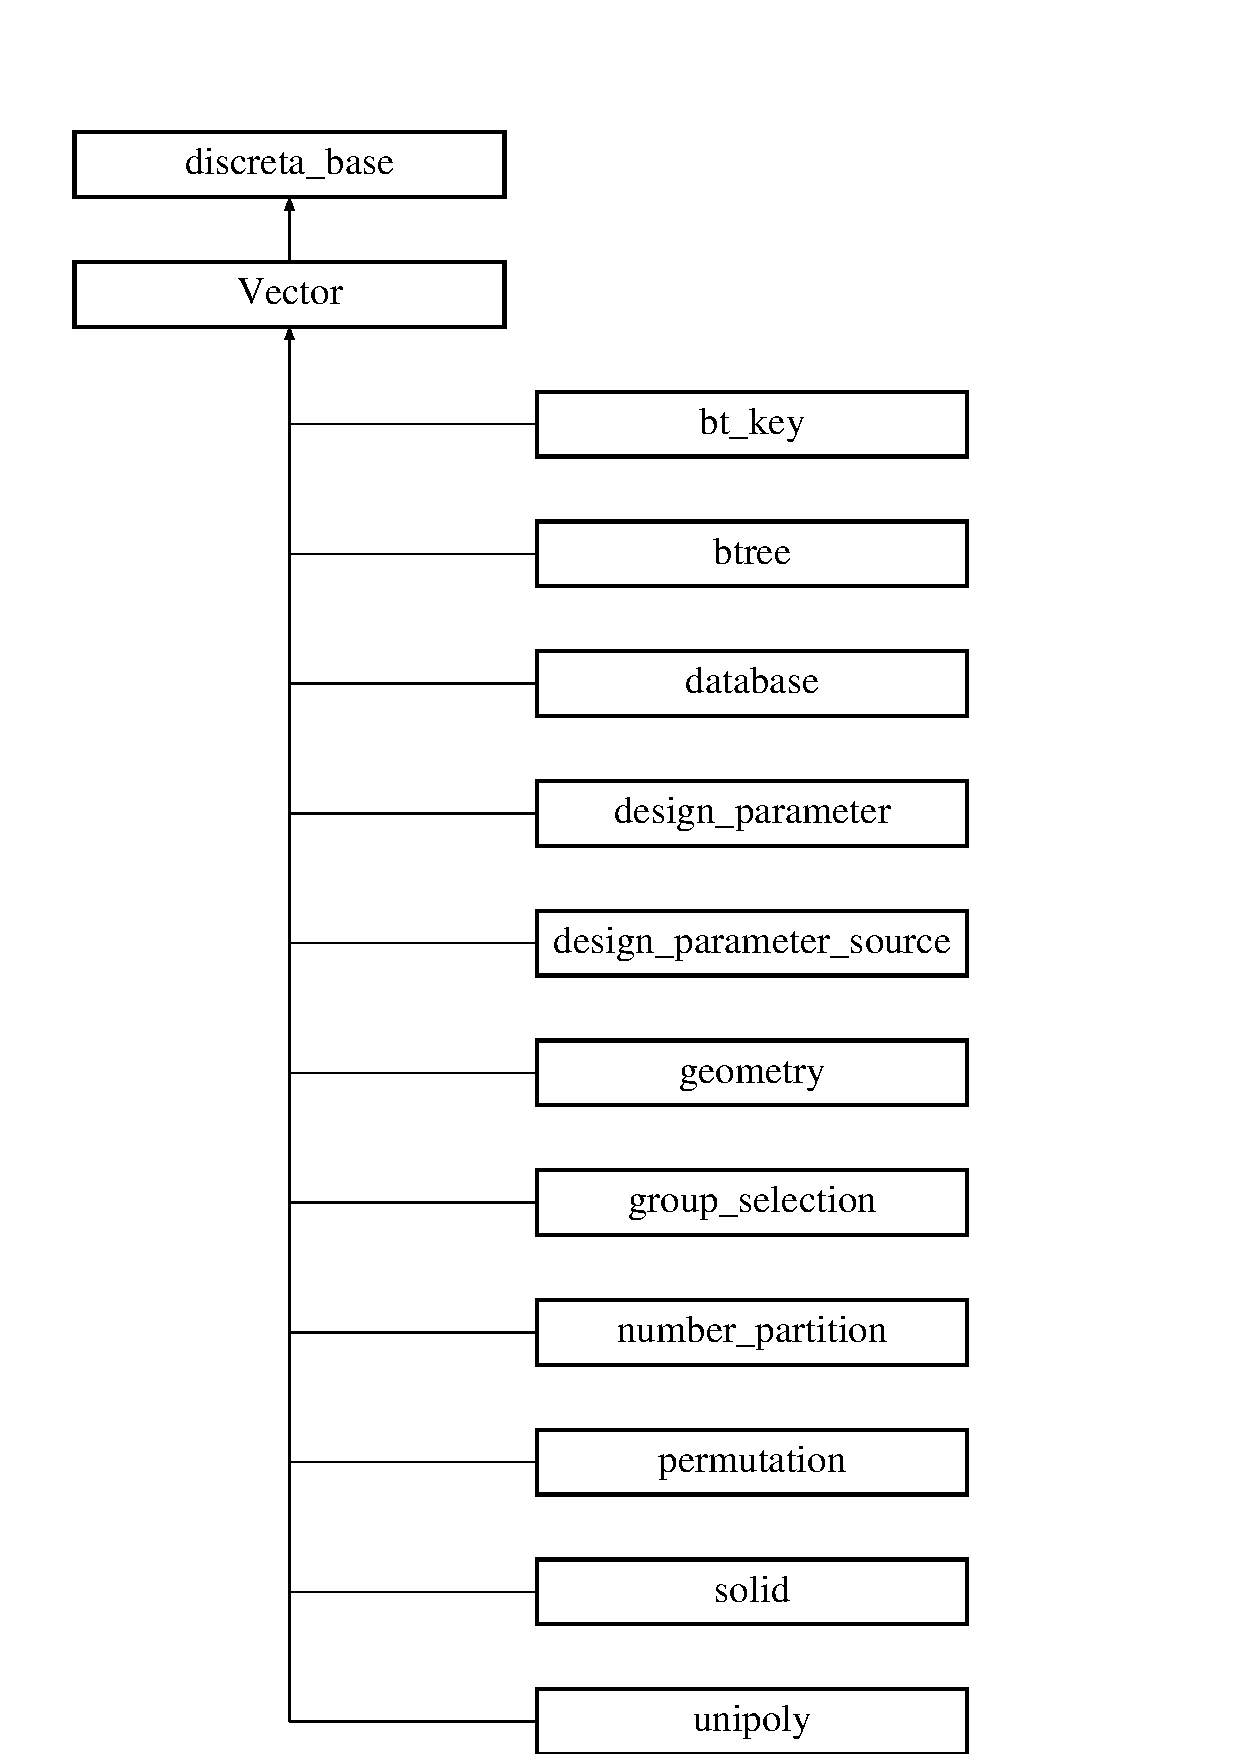
\includegraphics[height=12.000000cm]{class_vector}
\end{center}
\end{figure}
\subsection*{Public Member Functions}
\begin{DoxyCompactItemize}
\item 
\mbox{\hyperlink{class_vector_a6f80c73b5f18dcf3f8e36065bdc8b9e5}{Vector}} ()
\item 
\mbox{\hyperlink{class_vector_a1d3c54bac484f186107205c9bc41a187}{Vector}} (const \mbox{\hyperlink{classdiscreta__base}{discreta\+\_\+base}} \&\mbox{\hyperlink{alphabet2_8_c_a6150e0515f7202e2fb518f7206ed97dc}{x}})
\item 
\mbox{\hyperlink{class_vector}{Vector}} \& \mbox{\hyperlink{class_vector_adbfc00f9e11251e1ebc04af9bcaca95a}{operator=}} (const \mbox{\hyperlink{classdiscreta__base}{discreta\+\_\+base}} \&\mbox{\hyperlink{alphabet2_8_c_a6150e0515f7202e2fb518f7206ed97dc}{x}})
\item 
void $\ast$ \mbox{\hyperlink{class_vector_a21793822dc89a94740a841223a1905fd}{operator new}} (size\+\_\+t, void $\ast$\mbox{\hyperlink{alphabet2_8_c_a533391314665d6bf1b5575e9a9cd8552}{p}})
\item 
void \mbox{\hyperlink{class_vector_a34e0d00b18c051f23904a8429fa6c8b4}{settype\+\_\+vector}} ()
\item 
\mbox{\hyperlink{class_vector_a2eb3c49587a4f12cade7895ccb73f6a0}{$\sim$\+Vector}} ()
\item 
void \mbox{\hyperlink{class_vector_ad55c58937ca8fb342247a2c0fb572d20}{freeself\+\_\+vector}} ()
\item 
\mbox{\hyperlink{discreta_8h_aaf25ee7e2306d78c74ec7bc48f092e81}{kind}} \mbox{\hyperlink{class_vector_a20550e70d02cbe484032c7f6b0833a0f}{s\+\_\+virtual\+\_\+kind}} ()
\item 
void \mbox{\hyperlink{class_vector_af657307f3d344c8cef5d633335a5f484}{copyobject\+\_\+to}} (\mbox{\hyperlink{classdiscreta__base}{discreta\+\_\+base}} \&\mbox{\hyperlink{alphabet2_8_c_a6150e0515f7202e2fb518f7206ed97dc}{x}})
\item 
ostream \& \mbox{\hyperlink{class_vector_ad789b6ce88fd8954c0df815f92d8f7eb}{Print}} (ostream \&)
\item 
ostream \& \mbox{\hyperlink{class_vector_a71d7e24bcfdfc69d4a2137360acb066c}{print}} (ostream \&)
\item 
ostream \& \mbox{\hyperlink{class_vector_ad42c035ccb0c95544d2a4af4abaad30c}{print\+\_\+unformatted}} (ostream \&ost)
\item 
ostream \& \mbox{\hyperlink{class_vector_af01e693b8e8a98f191b3690ef3547267}{print\+\_\+intvec}} (ostream \&ost)
\item 
\mbox{\hyperlink{classdiscreta__base}{discreta\+\_\+base}} \& \mbox{\hyperlink{class_vector_a1c4fe1752523df8119f70dd550244871}{s\+\_\+i}} (\mbox{\hyperlink{galois_8h_a09fddde158a3a20bd2dcadb609de11dc}{I\+NT}} \mbox{\hyperlink{alphabet2_8_c_acb559820d9ca11295b4500f179ef6392}{i}})
\item 
\mbox{\hyperlink{galois_8h_a09fddde158a3a20bd2dcadb609de11dc}{I\+NT}} \& \mbox{\hyperlink{class_vector_a75d4942cc7b9794717b4846c10520db8}{s\+\_\+ii}} (\mbox{\hyperlink{galois_8h_a09fddde158a3a20bd2dcadb609de11dc}{I\+NT}} \mbox{\hyperlink{alphabet2_8_c_acb559820d9ca11295b4500f179ef6392}{i}})
\item 
void \mbox{\hyperlink{class_vector_aa6a97eabb43f192a47947f4f6acbb04d}{m\+\_\+ii}} (\mbox{\hyperlink{galois_8h_a09fddde158a3a20bd2dcadb609de11dc}{I\+NT}} \mbox{\hyperlink{alphabet2_8_c_acb559820d9ca11295b4500f179ef6392}{i}}, \mbox{\hyperlink{galois_8h_a09fddde158a3a20bd2dcadb609de11dc}{I\+NT}} a)
\item 
\mbox{\hyperlink{classdiscreta__base}{discreta\+\_\+base}} \& \mbox{\hyperlink{class_vector_a03e879b4a01fdbe08fc3f5bba9a684de}{operator\mbox{[}$\,$\mbox{]}}} (\mbox{\hyperlink{galois_8h_a09fddde158a3a20bd2dcadb609de11dc}{I\+NT}} \mbox{\hyperlink{alphabet2_8_c_acb559820d9ca11295b4500f179ef6392}{i}})
\item 
\mbox{\hyperlink{galois_8h_a09fddde158a3a20bd2dcadb609de11dc}{I\+NT}} \mbox{\hyperlink{class_vector_ad2dc082288f858d22a528832289e0704}{s\+\_\+l}} ()
\item 
void \mbox{\hyperlink{class_vector_a00f5520c2a6b4f5282a1a8bcf8ea74eb}{m\+\_\+l}} (\mbox{\hyperlink{galois_8h_a09fddde158a3a20bd2dcadb609de11dc}{I\+NT}} \mbox{\hyperlink{alphabet2_8_c_a89606eca6b563ec68d2da2e84657736f}{l}})
\item 
void \mbox{\hyperlink{class_vector_a5c7c126e6266ecdc832c5ce5bc1cca2f}{m\+\_\+l\+\_\+n}} (\mbox{\hyperlink{galois_8h_a09fddde158a3a20bd2dcadb609de11dc}{I\+NT}} \mbox{\hyperlink{alphabet2_8_c_a89606eca6b563ec68d2da2e84657736f}{l}})
\item 
void \mbox{\hyperlink{class_vector_a9d057659215b5afa5efb8dabb9b04ab4}{m\+\_\+l\+\_\+e}} (\mbox{\hyperlink{galois_8h_a09fddde158a3a20bd2dcadb609de11dc}{I\+NT}} \mbox{\hyperlink{alphabet2_8_c_a89606eca6b563ec68d2da2e84657736f}{l}})
\item 
void \mbox{\hyperlink{class_vector_a667d89a7a73078ec5e2f5f035e21ce56}{m\+\_\+l\+\_\+x}} (\mbox{\hyperlink{galois_8h_a09fddde158a3a20bd2dcadb609de11dc}{I\+NT}} \mbox{\hyperlink{alphabet2_8_c_a89606eca6b563ec68d2da2e84657736f}{l}}, \mbox{\hyperlink{classdiscreta__base}{discreta\+\_\+base}} \&\mbox{\hyperlink{alphabet2_8_c_a6150e0515f7202e2fb518f7206ed97dc}{x}})
\item 
\mbox{\hyperlink{class_vector}{Vector}} \& \mbox{\hyperlink{class_vector_a00aff28a4a7cacc8c5aaf44b6f3fb3a5}{realloc}} (\mbox{\hyperlink{galois_8h_a09fddde158a3a20bd2dcadb609de11dc}{I\+NT}} \mbox{\hyperlink{alphabet2_8_c_a89606eca6b563ec68d2da2e84657736f}{l}})
\item 
void \mbox{\hyperlink{class_vector_a77dd4ded54124a6f928c411dc0960a73}{mult\+\_\+to}} (\mbox{\hyperlink{classdiscreta__base}{discreta\+\_\+base}} \&\mbox{\hyperlink{alphabet2_8_c_a6150e0515f7202e2fb518f7206ed97dc}{x}}, \mbox{\hyperlink{classdiscreta__base}{discreta\+\_\+base}} \&\mbox{\hyperlink{alphabet2_8_c_a0a2f84ed7838f07779ae24c5a9086d33}{y}})
\item 
void \mbox{\hyperlink{class_vector_a3e170560de50e3a4f4a95f6b90bf75bb}{add\+\_\+to}} (\mbox{\hyperlink{classdiscreta__base}{discreta\+\_\+base}} \&\mbox{\hyperlink{alphabet2_8_c_a6150e0515f7202e2fb518f7206ed97dc}{x}}, \mbox{\hyperlink{classdiscreta__base}{discreta\+\_\+base}} \&\mbox{\hyperlink{alphabet2_8_c_a0a2f84ed7838f07779ae24c5a9086d33}{y}})
\item 
void \mbox{\hyperlink{class_vector_a5f6fe0531bc3d9829becd8503e4156a3}{inc}} ()
\item 
void \mbox{\hyperlink{class_vector_ac2c2f8a845000951b008bbe833be3fd4}{dec}} ()
\item 
\mbox{\hyperlink{galois_8h_a09fddde158a3a20bd2dcadb609de11dc}{I\+NT}} \mbox{\hyperlink{class_vector_a5fc27308a2710188b16f92df56c79c55}{compare\+\_\+with}} (\mbox{\hyperlink{classdiscreta__base}{discreta\+\_\+base}} \&a)
\item 
void \mbox{\hyperlink{class_vector_a8205e92d0db9cdb38411066a68c02eb0}{append\+\_\+vector}} (\mbox{\hyperlink{class_vector}{Vector}} \&\mbox{\hyperlink{simeon_8_c_aeb3f3030944801b163bc3b829a7f6710}{v}})
\item 
\mbox{\hyperlink{class_vector}{Vector}} \& \mbox{\hyperlink{class_vector_a8b77be10bea96a9bfa50f43726c942e5}{append\+\_\+integer}} (\mbox{\hyperlink{galois_8h_a09fddde158a3a20bd2dcadb609de11dc}{I\+NT}} a)
\item 
\mbox{\hyperlink{class_vector}{Vector}} \& \mbox{\hyperlink{class_vector_aec80be90cd2cbfe79267220113b679c4}{append}} (\mbox{\hyperlink{classdiscreta__base}{discreta\+\_\+base}} \&\mbox{\hyperlink{alphabet2_8_c_a6150e0515f7202e2fb518f7206ed97dc}{x}})
\item 
\mbox{\hyperlink{class_vector}{Vector}} \& \mbox{\hyperlink{class_vector_ad9e492806e8a030fef5ce8fbad81fdd8}{insert\+\_\+element}} (\mbox{\hyperlink{galois_8h_a09fddde158a3a20bd2dcadb609de11dc}{I\+NT}} \mbox{\hyperlink{alphabet2_8_c_acb559820d9ca11295b4500f179ef6392}{i}}, \mbox{\hyperlink{classdiscreta__base}{discreta\+\_\+base}} \&\mbox{\hyperlink{alphabet2_8_c_a6150e0515f7202e2fb518f7206ed97dc}{x}})
\item 
\mbox{\hyperlink{class_vector}{Vector}} \& \mbox{\hyperlink{class_vector_a075b82bb136a3fad137b9c8dfb1da4c9}{get\+\_\+and\+\_\+delete\+\_\+element}} (\mbox{\hyperlink{galois_8h_a09fddde158a3a20bd2dcadb609de11dc}{I\+NT}} \mbox{\hyperlink{alphabet2_8_c_acb559820d9ca11295b4500f179ef6392}{i}}, \mbox{\hyperlink{classdiscreta__base}{discreta\+\_\+base}} \&\mbox{\hyperlink{alphabet2_8_c_a6150e0515f7202e2fb518f7206ed97dc}{x}})
\item 
\mbox{\hyperlink{class_vector}{Vector}} \& \mbox{\hyperlink{class_vector_a91dbd1d04baeec1066d397e7668953e3}{delete\+\_\+element}} (\mbox{\hyperlink{galois_8h_a09fddde158a3a20bd2dcadb609de11dc}{I\+NT}} \mbox{\hyperlink{alphabet2_8_c_acb559820d9ca11295b4500f179ef6392}{i}})
\item 
void \mbox{\hyperlink{class_vector_ad2f9bf9820e09ff09e3c99d1c983ab96}{get\+\_\+first\+\_\+and\+\_\+remove}} (\mbox{\hyperlink{classdiscreta__base}{discreta\+\_\+base}} \&\mbox{\hyperlink{alphabet2_8_c_a6150e0515f7202e2fb518f7206ed97dc}{x}})
\item 
bool \mbox{\hyperlink{class_vector_a7c0bbf84cd12a6c7f632789764deb68e}{insert\+\_\+sorted}} (\mbox{\hyperlink{classdiscreta__base}{discreta\+\_\+base}} \&\mbox{\hyperlink{alphabet2_8_c_a6150e0515f7202e2fb518f7206ed97dc}{x}})
\item 
bool \mbox{\hyperlink{class_vector_a0b2bba0162e65dffa24b4e4660bfd4e2}{search}} (\mbox{\hyperlink{classdiscreta__base}{discreta\+\_\+base}} \&\mbox{\hyperlink{alphabet2_8_c_a6150e0515f7202e2fb518f7206ed97dc}{x}}, \mbox{\hyperlink{galois_8h_a09fddde158a3a20bd2dcadb609de11dc}{I\+NT}} $\ast$idx)
\item 
\mbox{\hyperlink{class_vector}{Vector}} \& \mbox{\hyperlink{class_vector_ae50ef8643d10e954cb3b34cb33ce97e9}{sort}} ()
\item 
void \mbox{\hyperlink{class_vector_a689bf0a0797099e26f9b40d07cfd1b9c}{sort\+\_\+with\+\_\+fellow}} (\mbox{\hyperlink{class_vector}{Vector}} \&fellow)
\item 
\mbox{\hyperlink{class_vector}{Vector}} \& \mbox{\hyperlink{class_vector_a5bcaeb8778ea91df5f29f9f3eb9913d4}{sort\+\_\+with\+\_\+logging}} (\mbox{\hyperlink{classpermutation}{permutation}} \&\mbox{\hyperlink{alphabet2_8_c_a533391314665d6bf1b5575e9a9cd8552}{p}})
\item 
void \mbox{\hyperlink{class_vector_a82d3a4637450aa25030d4fd9bfff0642}{sum\+\_\+of\+\_\+all\+\_\+entries}} (\mbox{\hyperlink{classdiscreta__base}{discreta\+\_\+base}} \&\mbox{\hyperlink{alphabet2_8_c_a6150e0515f7202e2fb518f7206ed97dc}{x}})
\item 
void \mbox{\hyperlink{class_vector_a6998131cab792d584242061c5f34d044}{n\+\_\+choose\+\_\+k\+\_\+first}} (\mbox{\hyperlink{galois_8h_a09fddde158a3a20bd2dcadb609de11dc}{I\+NT}} \mbox{\hyperlink{simeon_8_c_a7f2cd26777ce0ff3fdaf8d02aacbddfb}{n}}, \mbox{\hyperlink{galois_8h_a09fddde158a3a20bd2dcadb609de11dc}{I\+NT}} \mbox{\hyperlink{classdiscreta__base_a6f7a0f7bdd115b9e4dde358cfa7ebf81}{k}})
\item 
\mbox{\hyperlink{galois_8h_a09fddde158a3a20bd2dcadb609de11dc}{I\+NT}} \mbox{\hyperlink{class_vector_a05633c7bbd9e39595a634fe956263760}{n\+\_\+choose\+\_\+k\+\_\+next}} (\mbox{\hyperlink{galois_8h_a09fddde158a3a20bd2dcadb609de11dc}{I\+NT}} \mbox{\hyperlink{simeon_8_c_a7f2cd26777ce0ff3fdaf8d02aacbddfb}{n}}, \mbox{\hyperlink{galois_8h_a09fddde158a3a20bd2dcadb609de11dc}{I\+NT}} \mbox{\hyperlink{classdiscreta__base_a6f7a0f7bdd115b9e4dde358cfa7ebf81}{k}})
\item 
void \mbox{\hyperlink{class_vector_acf37ae8b2a5531b37fd2a9d847ff20eb}{first\+\_\+lehmercode}} (\mbox{\hyperlink{galois_8h_a09fddde158a3a20bd2dcadb609de11dc}{I\+NT}} \mbox{\hyperlink{simeon_8_c_a7f2cd26777ce0ff3fdaf8d02aacbddfb}{n}})
\item 
\mbox{\hyperlink{galois_8h_a09fddde158a3a20bd2dcadb609de11dc}{I\+NT}} \mbox{\hyperlink{class_vector_a0de9a2b5805b9bf0c53a24ad5e79f323}{next\+\_\+lehmercode}} ()
\item 
void \mbox{\hyperlink{class_vector_a6f2e3fb3d4105af914aa29c9be232161}{lehmercode2perm}} (\mbox{\hyperlink{classpermutation}{permutation}} \&\mbox{\hyperlink{alphabet2_8_c_a533391314665d6bf1b5575e9a9cd8552}{p}})
\item 
void \mbox{\hyperlink{class_vector_a58a53ccd874adbd27703e327d607eec7}{q\+\_\+adic}} (\mbox{\hyperlink{galois_8h_a09fddde158a3a20bd2dcadb609de11dc}{I\+NT}} \mbox{\hyperlink{simeon_8_c_a7f2cd26777ce0ff3fdaf8d02aacbddfb}{n}}, \mbox{\hyperlink{galois_8h_a09fddde158a3a20bd2dcadb609de11dc}{I\+NT}} \mbox{\hyperlink{simeon_8_c_a92cbb483a3b27ae1a0dbfcb125ce216f}{q}})
\item 
\mbox{\hyperlink{galois_8h_a09fddde158a3a20bd2dcadb609de11dc}{I\+NT}} \mbox{\hyperlink{class_vector_a1dd5243e8eef929f252ce0eda998b2f1}{q\+\_\+adic\+\_\+as\+\_\+int}} (\mbox{\hyperlink{galois_8h_a09fddde158a3a20bd2dcadb609de11dc}{I\+NT}} \mbox{\hyperlink{simeon_8_c_a92cbb483a3b27ae1a0dbfcb125ce216f}{q}})
\item 
void \mbox{\hyperlink{class_vector_aca9b00dbf2e6f2e09d664855eeeabe9c}{mult\+\_\+scalar}} (\mbox{\hyperlink{classdiscreta__base}{discreta\+\_\+base}} \&a)
\item 
void \mbox{\hyperlink{class_vector_a6b2c416de7f756b6215dfba0ac1f866e}{first\+\_\+word}} (\mbox{\hyperlink{galois_8h_a09fddde158a3a20bd2dcadb609de11dc}{I\+NT}} \mbox{\hyperlink{simeon_8_c_a7f2cd26777ce0ff3fdaf8d02aacbddfb}{n}}, \mbox{\hyperlink{galois_8h_a09fddde158a3a20bd2dcadb609de11dc}{I\+NT}} \mbox{\hyperlink{simeon_8_c_a92cbb483a3b27ae1a0dbfcb125ce216f}{q}})
\item 
\mbox{\hyperlink{galois_8h_a09fddde158a3a20bd2dcadb609de11dc}{I\+NT}} \mbox{\hyperlink{class_vector_ac6836667916e1854bd102698042bbef2}{next\+\_\+word}} (\mbox{\hyperlink{galois_8h_a09fddde158a3a20bd2dcadb609de11dc}{I\+NT}} \mbox{\hyperlink{simeon_8_c_a92cbb483a3b27ae1a0dbfcb125ce216f}{q}})
\item 
void \mbox{\hyperlink{class_vector_a4f8342ed83188bfa99f127b6fd112e72}{first\+\_\+regular\+\_\+word}} (\mbox{\hyperlink{galois_8h_a09fddde158a3a20bd2dcadb609de11dc}{I\+NT}} \mbox{\hyperlink{simeon_8_c_a7f2cd26777ce0ff3fdaf8d02aacbddfb}{n}}, \mbox{\hyperlink{galois_8h_a09fddde158a3a20bd2dcadb609de11dc}{I\+NT}} \mbox{\hyperlink{simeon_8_c_a92cbb483a3b27ae1a0dbfcb125ce216f}{q}})
\item 
\mbox{\hyperlink{galois_8h_a09fddde158a3a20bd2dcadb609de11dc}{I\+NT}} \mbox{\hyperlink{class_vector_a7040861199c356dbb30c09e138805e6c}{next\+\_\+regular\+\_\+word}} (\mbox{\hyperlink{galois_8h_a09fddde158a3a20bd2dcadb609de11dc}{I\+NT}} \mbox{\hyperlink{simeon_8_c_a92cbb483a3b27ae1a0dbfcb125ce216f}{q}})
\item 
\mbox{\hyperlink{galois_8h_a09fddde158a3a20bd2dcadb609de11dc}{I\+NT}} \mbox{\hyperlink{class_vector_a40940c35a1c43919148b6ad176e21444}{is\+\_\+regular\+\_\+word}} ()
\item 
void \mbox{\hyperlink{class_vector_a1c243b57e3fb9c722f456576636f74d5}{apply\+\_\+permutation}} (\mbox{\hyperlink{classpermutation}{permutation}} \&\mbox{\hyperlink{alphabet2_8_c_a533391314665d6bf1b5575e9a9cd8552}{p}})
\item 
void \mbox{\hyperlink{class_vector_a404f66398213840c0478550f24912519}{apply\+\_\+permutation\+\_\+to\+\_\+elements}} (\mbox{\hyperlink{classpermutation}{permutation}} \&\mbox{\hyperlink{alphabet2_8_c_a533391314665d6bf1b5575e9a9cd8552}{p}})
\item 
void \mbox{\hyperlink{class_vector_acebb5a8e10eb058e50bc373c0c478b0f}{content}} (\mbox{\hyperlink{class_vector}{Vector}} \&\mbox{\hyperlink{alphabet2_8_c_a4e1e0e72dd773439e333c84dd762a9c3}{c}}, \mbox{\hyperlink{class_vector}{Vector}} \&where)
\item 
void \mbox{\hyperlink{class_vector_aab0e0006bfa41b63bcffd139c85d5c5d}{content\+\_\+multiplicities\+\_\+only}} (\mbox{\hyperlink{class_vector}{Vector}} \&\mbox{\hyperlink{alphabet2_8_c_a4e1e0e72dd773439e333c84dd762a9c3}{c}}, \mbox{\hyperlink{class_vector}{Vector}} \&\mbox{\hyperlink{classdiscreta__base_a96f759b28f7c30bdfd95ac10f5972bd0}{mult}})
\item 
\mbox{\hyperlink{galois_8h_a09fddde158a3a20bd2dcadb609de11dc}{I\+NT}} \mbox{\hyperlink{class_vector_a996f4e7f37126389c883537b063d583e}{hip}} ()
\item 
\mbox{\hyperlink{galois_8h_a09fddde158a3a20bd2dcadb609de11dc}{I\+NT}} \mbox{\hyperlink{class_vector_a5ce49604a9d0d59e42e4cbad25597334}{hip1}} ()
\item 
void \mbox{\hyperlink{class_vector_a080f85e2cdd81619713fbc486d6a6fb0}{write\+\_\+mem}} (\mbox{\hyperlink{classmemory}{memory}} \&m, \mbox{\hyperlink{galois_8h_a09fddde158a3a20bd2dcadb609de11dc}{I\+NT}} debug\+\_\+depth)
\item 
void \mbox{\hyperlink{class_vector_af0ea92fb773af77ddfa068abb8dca079}{read\+\_\+mem}} (\mbox{\hyperlink{classmemory}{memory}} \&m, \mbox{\hyperlink{galois_8h_a09fddde158a3a20bd2dcadb609de11dc}{I\+NT}} debug\+\_\+depth)
\item 
\mbox{\hyperlink{galois_8h_a09fddde158a3a20bd2dcadb609de11dc}{I\+NT}} \mbox{\hyperlink{class_vector_a7bbfe1d599a93f58b2150a026a27b0f4}{csf}} ()
\item 
void \mbox{\hyperlink{class_vector_a477bb8091a6946d25d1c7b2e32c9a474}{conjugate}} (\mbox{\hyperlink{classdiscreta__base}{discreta\+\_\+base}} \&a)
\item 
void \mbox{\hyperlink{class_vector_a31e4b25f3c2939f565f2a9f215a5fd19}{conjugate\+\_\+with\+\_\+inverse}} (\mbox{\hyperlink{classdiscreta__base}{discreta\+\_\+base}} \&a)
\item 
void \mbox{\hyperlink{class_vector_aa73ce0ba837f90f7fcabf6970d8ebe8b}{replace}} (\mbox{\hyperlink{class_vector}{Vector}} \&\mbox{\hyperlink{simeon_8_c_aeb3f3030944801b163bc3b829a7f6710}{v}})
\item 
void \mbox{\hyperlink{class_vector_a01777c2c2d7c6131c6c676f679ec4cd3}{vector\+\_\+of\+\_\+vectors\+\_\+replace}} (\mbox{\hyperlink{class_vector}{Vector}} \&\mbox{\hyperlink{simeon_8_c_aeb3f3030944801b163bc3b829a7f6710}{v}})
\item 
void \mbox{\hyperlink{class_vector_a79901eec85877e4bacf1b0b6b289bdd7}{extract\+\_\+subvector}} (\mbox{\hyperlink{class_vector}{Vector}} \&\mbox{\hyperlink{simeon_8_c_aeb3f3030944801b163bc3b829a7f6710}{v}}, \mbox{\hyperlink{galois_8h_a09fddde158a3a20bd2dcadb609de11dc}{I\+NT}} first, \mbox{\hyperlink{galois_8h_a09fddde158a3a20bd2dcadb609de11dc}{I\+NT}} len)
\item 
void \mbox{\hyperlink{class_vector_a8cca2f9cb0336c06d2ab0b6f835ceb82}{P\+G\+\_\+element\+\_\+normalize}} ()
\item 
void \mbox{\hyperlink{class_vector_a0dedd5c9b487e5160589e2b312091246}{P\+G\+\_\+element\+\_\+rank}} (\mbox{\hyperlink{galois_8h_a09fddde158a3a20bd2dcadb609de11dc}{I\+NT}} \&a)
\item 
void \mbox{\hyperlink{class_vector_a7d29be1c56b7eb6711b79a25c1755290}{P\+G\+\_\+element\+\_\+rank\+\_\+modified}} (\mbox{\hyperlink{galois_8h_a09fddde158a3a20bd2dcadb609de11dc}{I\+NT}} \&a)
\item 
void \mbox{\hyperlink{class_vector_a8461aafe0c57317eea2df6e3b6507995}{P\+G\+\_\+element\+\_\+unrank}} (\mbox{\hyperlink{galois_8h_a09fddde158a3a20bd2dcadb609de11dc}{I\+NT}} a)
\item 
void \mbox{\hyperlink{class_vector_a778c7effcf9ce1c1f9187f2649955e26}{P\+G\+\_\+element\+\_\+unrank\+\_\+modified}} (\mbox{\hyperlink{galois_8h_a09fddde158a3a20bd2dcadb609de11dc}{I\+NT}} a)
\item 
void \mbox{\hyperlink{class_vector_a7309e3b8eb7e188001857c1728d43a70}{A\+G\+\_\+element\+\_\+rank}} (\mbox{\hyperlink{galois_8h_a09fddde158a3a20bd2dcadb609de11dc}{I\+NT}} \&a)
\item 
void \mbox{\hyperlink{class_vector_aa2960a2b59352dcaaf661b81acc65d3b}{A\+G\+\_\+element\+\_\+unrank}} (\mbox{\hyperlink{galois_8h_a09fddde158a3a20bd2dcadb609de11dc}{I\+NT}} a)
\item 
\mbox{\hyperlink{galois_8h_a09fddde158a3a20bd2dcadb609de11dc}{I\+NT}} \mbox{\hyperlink{class_vector_a53a1b391aad5db6fe6af3b67781f87cf}{hamming\+\_\+weight}} ()
\item 
void \mbox{\hyperlink{class_vector_acb27c83b81fc462996cca982f0c6f07c}{scalar\+\_\+product}} (\mbox{\hyperlink{class_vector}{Vector}} \&\mbox{\hyperlink{alphabet2_8_c_aac374e320caaadeca4874add33b62af2}{w}}, \mbox{\hyperlink{classdiscreta__base}{discreta\+\_\+base}} \&a)
\item 
void \mbox{\hyperlink{class_vector_a36312785f92e4dfb892cdb85c4444247}{hadamard\+\_\+product}} (\mbox{\hyperlink{class_vector}{Vector}} \&\mbox{\hyperlink{alphabet2_8_c_aac374e320caaadeca4874add33b62af2}{w}})
\item 
void \mbox{\hyperlink{class_vector_a0f89a3100b71befddf7adfbd2369b3f4}{intersect}} (\mbox{\hyperlink{class_vector}{Vector}} \&\mbox{\hyperlink{alphabet2_8_c_a148e3876077787926724625411d6e7a9}{b}}, \mbox{\hyperlink{class_vector}{Vector}} \&\mbox{\hyperlink{alphabet2_8_c_a4e1e0e72dd773439e333c84dd762a9c3}{c}})
\item 
\mbox{\hyperlink{galois_8h_a09fddde158a3a20bd2dcadb609de11dc}{I\+NT}} \mbox{\hyperlink{class_vector_ab8e6d88870a530d57e026fc21ae2d232}{vector\+\_\+of\+\_\+vectors\+\_\+overall\+\_\+length}} ()
\item 
void \mbox{\hyperlink{class_vector_a578b0f528e7ccbe0ed06337c4fea1504}{first\+\_\+divisor}} (\mbox{\hyperlink{class_vector}{Vector}} \&exponents)
\item 
\mbox{\hyperlink{galois_8h_a09fddde158a3a20bd2dcadb609de11dc}{I\+NT}} \mbox{\hyperlink{class_vector_affee742a383eac1ff46a3313ae47dc76}{next\+\_\+divisor}} (\mbox{\hyperlink{class_vector}{Vector}} \&exponents)
\item 
\mbox{\hyperlink{galois_8h_a09fddde158a3a20bd2dcadb609de11dc}{I\+NT}} \mbox{\hyperlink{class_vector_a965dd2d9e91fa94d4fc23cc1c34054f9}{next\+\_\+non\+\_\+trivial\+\_\+divisor}} (\mbox{\hyperlink{class_vector}{Vector}} \&exponents)
\item 
void \mbox{\hyperlink{class_vector_a3f8219c2cb731ff22790f6456753e104}{multiply\+\_\+out}} (\mbox{\hyperlink{class_vector}{Vector}} \&primes, \mbox{\hyperlink{classdiscreta__base}{discreta\+\_\+base}} \&\mbox{\hyperlink{alphabet2_8_c_a6150e0515f7202e2fb518f7206ed97dc}{x}})
\item 
\mbox{\hyperlink{galois_8h_a09fddde158a3a20bd2dcadb609de11dc}{I\+NT}} \mbox{\hyperlink{class_vector_a1eb7508c3c31d85829d0d8361526c770}{hash}} (\mbox{\hyperlink{galois_8h_a09fddde158a3a20bd2dcadb609de11dc}{I\+NT}} hash0)
\item 
\mbox{\hyperlink{galois_8h_a09fddde158a3a20bd2dcadb609de11dc}{I\+NT}} \mbox{\hyperlink{class_vector_a984996de6448206b30f4e12f7021970d}{is\+\_\+subset\+\_\+of}} (\mbox{\hyperlink{class_vector}{Vector}} \&\mbox{\hyperlink{alphabet2_8_c_aac374e320caaadeca4874add33b62af2}{w}})
\item 
void \mbox{\hyperlink{class_vector_a2b29fadd7d7c0df93dd3711f42aff4b9}{concatenation}} (\mbox{\hyperlink{class_vector}{Vector}} \&v1, \mbox{\hyperlink{class_vector}{Vector}} \&v2)
\item 
void \mbox{\hyperlink{class_vector_acf1a607f7a282a128ada9128465ce38f}{print\+\_\+word\+\_\+nicely}} (ostream \&ost, \mbox{\hyperlink{galois_8h_a09fddde158a3a20bd2dcadb609de11dc}{I\+NT}} f\+\_\+generator\+\_\+labels, \mbox{\hyperlink{class_vector}{Vector}} \&generator\+\_\+labels)
\item 
void \mbox{\hyperlink{class_vector_ad8b224e83836e7b1fad7785853a4df79}{print\+\_\+word\+\_\+nicely2}} (ostream \&ost)
\item 
void \mbox{\hyperlink{class_vector_af999a68ef44d55c7c0e7a1eb7889fbba}{print\+\_\+word\+\_\+nicely\+\_\+with\+\_\+generator\+\_\+labels}} (ostream \&ost, \mbox{\hyperlink{class_vector}{Vector}} \&generator\+\_\+labels)
\item 
void \mbox{\hyperlink{class_vector_aaf8be9b0570fb6bd4bde9e549dd0bbc8}{vector\+\_\+of\+\_\+vectors\+\_\+lengths}} (\mbox{\hyperlink{class_vector}{Vector}} \&lengths)
\item 
void \mbox{\hyperlink{class_vector_ac83f27123b1c43f3953b81de0392eae7}{get\+\_\+element\+\_\+orders}} (\mbox{\hyperlink{class_vector}{Vector}} \&vec\+\_\+of\+\_\+orders)
\end{DoxyCompactItemize}
\subsection*{Additional Inherited Members}


\subsection{Constructor \& Destructor Documentation}
\mbox{\Hypertarget{class_vector_a6f80c73b5f18dcf3f8e36065bdc8b9e5}\label{class_vector_a6f80c73b5f18dcf3f8e36065bdc8b9e5}} 
\index{Vector@{Vector}!Vector@{Vector}}
\index{Vector@{Vector}!Vector@{Vector}}
\subsubsection{\texorpdfstring{Vector()}{Vector()}\hspace{0.1cm}{\footnotesize\ttfamily [1/2]}}
{\footnotesize\ttfamily Vector\+::\+Vector (\begin{DoxyParamCaption}{ }\end{DoxyParamCaption})}

\mbox{\Hypertarget{class_vector_a1d3c54bac484f186107205c9bc41a187}\label{class_vector_a1d3c54bac484f186107205c9bc41a187}} 
\index{Vector@{Vector}!Vector@{Vector}}
\index{Vector@{Vector}!Vector@{Vector}}
\subsubsection{\texorpdfstring{Vector()}{Vector()}\hspace{0.1cm}{\footnotesize\ttfamily [2/2]}}
{\footnotesize\ttfamily Vector\+::\+Vector (\begin{DoxyParamCaption}\item[{const \mbox{\hyperlink{classdiscreta__base}{discreta\+\_\+base}} \&}]{x }\end{DoxyParamCaption})}

\mbox{\Hypertarget{class_vector_a2eb3c49587a4f12cade7895ccb73f6a0}\label{class_vector_a2eb3c49587a4f12cade7895ccb73f6a0}} 
\index{Vector@{Vector}!````~Vector@{$\sim$\+Vector}}
\index{````~Vector@{$\sim$\+Vector}!Vector@{Vector}}
\subsubsection{\texorpdfstring{$\sim$\+Vector()}{~Vector()}}
{\footnotesize\ttfamily Vector\+::$\sim$\+Vector (\begin{DoxyParamCaption}{ }\end{DoxyParamCaption})}



\subsection{Member Function Documentation}
\mbox{\Hypertarget{class_vector_a3e170560de50e3a4f4a95f6b90bf75bb}\label{class_vector_a3e170560de50e3a4f4a95f6b90bf75bb}} 
\index{Vector@{Vector}!add\+\_\+to@{add\+\_\+to}}
\index{add\+\_\+to@{add\+\_\+to}!Vector@{Vector}}
\subsubsection{\texorpdfstring{add\+\_\+to()}{add\_to()}}
{\footnotesize\ttfamily void Vector\+::add\+\_\+to (\begin{DoxyParamCaption}\item[{\mbox{\hyperlink{classdiscreta__base}{discreta\+\_\+base}} \&}]{x,  }\item[{\mbox{\hyperlink{classdiscreta__base}{discreta\+\_\+base}} \&}]{y }\end{DoxyParamCaption})\hspace{0.3cm}{\ttfamily [virtual]}}



Reimplemented from \mbox{\hyperlink{classdiscreta__base_a712a61311eb036d70a52871ed315f515}{discreta\+\_\+base}}.



Reimplemented in \mbox{\hyperlink{classunipoly_abebdaf912a2b0e7c27470f4191d0e180}{unipoly}}.

\mbox{\Hypertarget{class_vector_a7309e3b8eb7e188001857c1728d43a70}\label{class_vector_a7309e3b8eb7e188001857c1728d43a70}} 
\index{Vector@{Vector}!A\+G\+\_\+element\+\_\+rank@{A\+G\+\_\+element\+\_\+rank}}
\index{A\+G\+\_\+element\+\_\+rank@{A\+G\+\_\+element\+\_\+rank}!Vector@{Vector}}
\subsubsection{\texorpdfstring{A\+G\+\_\+element\+\_\+rank()}{AG\_element\_rank()}}
{\footnotesize\ttfamily void Vector\+::\+A\+G\+\_\+element\+\_\+rank (\begin{DoxyParamCaption}\item[{\mbox{\hyperlink{galois_8h_a09fddde158a3a20bd2dcadb609de11dc}{I\+NT}} \&}]{a }\end{DoxyParamCaption})}

\mbox{\Hypertarget{class_vector_aa2960a2b59352dcaaf661b81acc65d3b}\label{class_vector_aa2960a2b59352dcaaf661b81acc65d3b}} 
\index{Vector@{Vector}!A\+G\+\_\+element\+\_\+unrank@{A\+G\+\_\+element\+\_\+unrank}}
\index{A\+G\+\_\+element\+\_\+unrank@{A\+G\+\_\+element\+\_\+unrank}!Vector@{Vector}}
\subsubsection{\texorpdfstring{A\+G\+\_\+element\+\_\+unrank()}{AG\_element\_unrank()}}
{\footnotesize\ttfamily void Vector\+::\+A\+G\+\_\+element\+\_\+unrank (\begin{DoxyParamCaption}\item[{\mbox{\hyperlink{galois_8h_a09fddde158a3a20bd2dcadb609de11dc}{I\+NT}}}]{a }\end{DoxyParamCaption})}

\mbox{\Hypertarget{class_vector_aec80be90cd2cbfe79267220113b679c4}\label{class_vector_aec80be90cd2cbfe79267220113b679c4}} 
\index{Vector@{Vector}!append@{append}}
\index{append@{append}!Vector@{Vector}}
\subsubsection{\texorpdfstring{append()}{append()}}
{\footnotesize\ttfamily \mbox{\hyperlink{class_vector}{Vector}} \& Vector\+::append (\begin{DoxyParamCaption}\item[{\mbox{\hyperlink{classdiscreta__base}{discreta\+\_\+base}} \&}]{x }\end{DoxyParamCaption})}

\mbox{\Hypertarget{class_vector_a8b77be10bea96a9bfa50f43726c942e5}\label{class_vector_a8b77be10bea96a9bfa50f43726c942e5}} 
\index{Vector@{Vector}!append\+\_\+integer@{append\+\_\+integer}}
\index{append\+\_\+integer@{append\+\_\+integer}!Vector@{Vector}}
\subsubsection{\texorpdfstring{append\+\_\+integer()}{append\_integer()}}
{\footnotesize\ttfamily \mbox{\hyperlink{class_vector}{Vector}} \& Vector\+::append\+\_\+integer (\begin{DoxyParamCaption}\item[{\mbox{\hyperlink{galois_8h_a09fddde158a3a20bd2dcadb609de11dc}{I\+NT}}}]{a }\end{DoxyParamCaption})}

\mbox{\Hypertarget{class_vector_a8205e92d0db9cdb38411066a68c02eb0}\label{class_vector_a8205e92d0db9cdb38411066a68c02eb0}} 
\index{Vector@{Vector}!append\+\_\+vector@{append\+\_\+vector}}
\index{append\+\_\+vector@{append\+\_\+vector}!Vector@{Vector}}
\subsubsection{\texorpdfstring{append\+\_\+vector()}{append\_vector()}}
{\footnotesize\ttfamily void Vector\+::append\+\_\+vector (\begin{DoxyParamCaption}\item[{\mbox{\hyperlink{class_vector}{Vector}} \&}]{v }\end{DoxyParamCaption})}

\mbox{\Hypertarget{class_vector_a1c243b57e3fb9c722f456576636f74d5}\label{class_vector_a1c243b57e3fb9c722f456576636f74d5}} 
\index{Vector@{Vector}!apply\+\_\+permutation@{apply\+\_\+permutation}}
\index{apply\+\_\+permutation@{apply\+\_\+permutation}!Vector@{Vector}}
\subsubsection{\texorpdfstring{apply\+\_\+permutation()}{apply\_permutation()}}
{\footnotesize\ttfamily void Vector\+::apply\+\_\+permutation (\begin{DoxyParamCaption}\item[{\mbox{\hyperlink{classpermutation}{permutation}} \&}]{p }\end{DoxyParamCaption})}

\mbox{\Hypertarget{class_vector_a404f66398213840c0478550f24912519}\label{class_vector_a404f66398213840c0478550f24912519}} 
\index{Vector@{Vector}!apply\+\_\+permutation\+\_\+to\+\_\+elements@{apply\+\_\+permutation\+\_\+to\+\_\+elements}}
\index{apply\+\_\+permutation\+\_\+to\+\_\+elements@{apply\+\_\+permutation\+\_\+to\+\_\+elements}!Vector@{Vector}}
\subsubsection{\texorpdfstring{apply\+\_\+permutation\+\_\+to\+\_\+elements()}{apply\_permutation\_to\_elements()}}
{\footnotesize\ttfamily void Vector\+::apply\+\_\+permutation\+\_\+to\+\_\+elements (\begin{DoxyParamCaption}\item[{\mbox{\hyperlink{classpermutation}{permutation}} \&}]{p }\end{DoxyParamCaption})}

\mbox{\Hypertarget{class_vector_a5fc27308a2710188b16f92df56c79c55}\label{class_vector_a5fc27308a2710188b16f92df56c79c55}} 
\index{Vector@{Vector}!compare\+\_\+with@{compare\+\_\+with}}
\index{compare\+\_\+with@{compare\+\_\+with}!Vector@{Vector}}
\subsubsection{\texorpdfstring{compare\+\_\+with()}{compare\_with()}}
{\footnotesize\ttfamily \mbox{\hyperlink{galois_8h_a09fddde158a3a20bd2dcadb609de11dc}{I\+NT}} Vector\+::compare\+\_\+with (\begin{DoxyParamCaption}\item[{\mbox{\hyperlink{classdiscreta__base}{discreta\+\_\+base}} \&}]{a }\end{DoxyParamCaption})\hspace{0.3cm}{\ttfamily [virtual]}}



Reimplemented from \mbox{\hyperlink{classdiscreta__base_a3818444c4301d0b7ed47c3b850ea6c60}{discreta\+\_\+base}}.



Reimplemented in \mbox{\hyperlink{classpermutation_ae331b031f81647c88e72e966555c9c8f}{permutation}}.

\mbox{\Hypertarget{class_vector_a2b29fadd7d7c0df93dd3711f42aff4b9}\label{class_vector_a2b29fadd7d7c0df93dd3711f42aff4b9}} 
\index{Vector@{Vector}!concatenation@{concatenation}}
\index{concatenation@{concatenation}!Vector@{Vector}}
\subsubsection{\texorpdfstring{concatenation()}{concatenation()}}
{\footnotesize\ttfamily void Vector\+::concatenation (\begin{DoxyParamCaption}\item[{\mbox{\hyperlink{class_vector}{Vector}} \&}]{v1,  }\item[{\mbox{\hyperlink{class_vector}{Vector}} \&}]{v2 }\end{DoxyParamCaption})}

\mbox{\Hypertarget{class_vector_a477bb8091a6946d25d1c7b2e32c9a474}\label{class_vector_a477bb8091a6946d25d1c7b2e32c9a474}} 
\index{Vector@{Vector}!conjugate@{conjugate}}
\index{conjugate@{conjugate}!Vector@{Vector}}
\subsubsection{\texorpdfstring{conjugate()}{conjugate()}}
{\footnotesize\ttfamily void Vector\+::conjugate (\begin{DoxyParamCaption}\item[{\mbox{\hyperlink{classdiscreta__base}{discreta\+\_\+base}} \&}]{a }\end{DoxyParamCaption})}

\mbox{\Hypertarget{class_vector_a31e4b25f3c2939f565f2a9f215a5fd19}\label{class_vector_a31e4b25f3c2939f565f2a9f215a5fd19}} 
\index{Vector@{Vector}!conjugate\+\_\+with\+\_\+inverse@{conjugate\+\_\+with\+\_\+inverse}}
\index{conjugate\+\_\+with\+\_\+inverse@{conjugate\+\_\+with\+\_\+inverse}!Vector@{Vector}}
\subsubsection{\texorpdfstring{conjugate\+\_\+with\+\_\+inverse()}{conjugate\_with\_inverse()}}
{\footnotesize\ttfamily void Vector\+::conjugate\+\_\+with\+\_\+inverse (\begin{DoxyParamCaption}\item[{\mbox{\hyperlink{classdiscreta__base}{discreta\+\_\+base}} \&}]{a }\end{DoxyParamCaption})}

\mbox{\Hypertarget{class_vector_acebb5a8e10eb058e50bc373c0c478b0f}\label{class_vector_acebb5a8e10eb058e50bc373c0c478b0f}} 
\index{Vector@{Vector}!content@{content}}
\index{content@{content}!Vector@{Vector}}
\subsubsection{\texorpdfstring{content()}{content()}}
{\footnotesize\ttfamily void Vector\+::content (\begin{DoxyParamCaption}\item[{\mbox{\hyperlink{class_vector}{Vector}} \&}]{c,  }\item[{\mbox{\hyperlink{class_vector}{Vector}} \&}]{where }\end{DoxyParamCaption})}

\mbox{\Hypertarget{class_vector_aab0e0006bfa41b63bcffd139c85d5c5d}\label{class_vector_aab0e0006bfa41b63bcffd139c85d5c5d}} 
\index{Vector@{Vector}!content\+\_\+multiplicities\+\_\+only@{content\+\_\+multiplicities\+\_\+only}}
\index{content\+\_\+multiplicities\+\_\+only@{content\+\_\+multiplicities\+\_\+only}!Vector@{Vector}}
\subsubsection{\texorpdfstring{content\+\_\+multiplicities\+\_\+only()}{content\_multiplicities\_only()}}
{\footnotesize\ttfamily void Vector\+::content\+\_\+multiplicities\+\_\+only (\begin{DoxyParamCaption}\item[{\mbox{\hyperlink{class_vector}{Vector}} \&}]{c,  }\item[{\mbox{\hyperlink{class_vector}{Vector}} \&}]{mult }\end{DoxyParamCaption})}

\mbox{\Hypertarget{class_vector_af657307f3d344c8cef5d633335a5f484}\label{class_vector_af657307f3d344c8cef5d633335a5f484}} 
\index{Vector@{Vector}!copyobject\+\_\+to@{copyobject\+\_\+to}}
\index{copyobject\+\_\+to@{copyobject\+\_\+to}!Vector@{Vector}}
\subsubsection{\texorpdfstring{copyobject\+\_\+to()}{copyobject\_to()}}
{\footnotesize\ttfamily void Vector\+::copyobject\+\_\+to (\begin{DoxyParamCaption}\item[{\mbox{\hyperlink{classdiscreta__base}{discreta\+\_\+base}} \&}]{x }\end{DoxyParamCaption})\hspace{0.3cm}{\ttfamily [virtual]}}



Reimplemented from \mbox{\hyperlink{classdiscreta__base_a33180628d9ced231267229b3564790f3}{discreta\+\_\+base}}.



Reimplemented in \mbox{\hyperlink{classdesign__parameter_a4e0434c6fd0d805543d730b40fc8e01f}{design\+\_\+parameter}}, \mbox{\hyperlink{classdesign__parameter__source_a1fd0910addc02ffe117ec08d0f93f8a6}{design\+\_\+parameter\+\_\+source}}, \mbox{\hyperlink{classbtree_ae990f68198985c1c7c7a36a65f091ac7}{btree}}, \mbox{\hyperlink{classdatabase_a7402d11485a917293586dcf082f506b2}{database}}, \mbox{\hyperlink{classbt__key_ae97899364f826bc3d16cce36b9c8e4f7}{bt\+\_\+key}}, \mbox{\hyperlink{classsolid_a7f35a904885ef626d1a74663fe2cad62}{solid}}, \mbox{\hyperlink{classgroup__selection_a02a5e69978de662af0e8372a4f0b23a8}{group\+\_\+selection}}, \mbox{\hyperlink{classgeometry_a3c35255b73911b76347ae549edfb0050}{geometry}}, \mbox{\hyperlink{classnumber__partition_acf25157ca8486f55d86d7ea05fa033be}{number\+\_\+partition}}, \mbox{\hyperlink{classunipoly_aa856d320a499748a0f3345ab45e51910}{unipoly}}, and \mbox{\hyperlink{classpermutation_aed08e7ec26ec8ba0ed8c656a819ce43a}{permutation}}.

\mbox{\Hypertarget{class_vector_a7bbfe1d599a93f58b2150a026a27b0f4}\label{class_vector_a7bbfe1d599a93f58b2150a026a27b0f4}} 
\index{Vector@{Vector}!csf@{csf}}
\index{csf@{csf}!Vector@{Vector}}
\subsubsection{\texorpdfstring{csf()}{csf()}}
{\footnotesize\ttfamily \mbox{\hyperlink{galois_8h_a09fddde158a3a20bd2dcadb609de11dc}{I\+NT}} Vector\+::csf (\begin{DoxyParamCaption}{ }\end{DoxyParamCaption})}

\mbox{\Hypertarget{class_vector_ac2c2f8a845000951b008bbe833be3fd4}\label{class_vector_ac2c2f8a845000951b008bbe833be3fd4}} 
\index{Vector@{Vector}!dec@{dec}}
\index{dec@{dec}!Vector@{Vector}}
\subsubsection{\texorpdfstring{dec()}{dec()}}
{\footnotesize\ttfamily void Vector\+::dec (\begin{DoxyParamCaption}{ }\end{DoxyParamCaption})\hspace{0.3cm}{\ttfamily [virtual]}}



Reimplemented from \mbox{\hyperlink{classdiscreta__base_a11449a5cfa7dc5f5600e012517af6f0f}{discreta\+\_\+base}}.

\mbox{\Hypertarget{class_vector_a91dbd1d04baeec1066d397e7668953e3}\label{class_vector_a91dbd1d04baeec1066d397e7668953e3}} 
\index{Vector@{Vector}!delete\+\_\+element@{delete\+\_\+element}}
\index{delete\+\_\+element@{delete\+\_\+element}!Vector@{Vector}}
\subsubsection{\texorpdfstring{delete\+\_\+element()}{delete\_element()}}
{\footnotesize\ttfamily \mbox{\hyperlink{class_vector}{Vector}} \& Vector\+::delete\+\_\+element (\begin{DoxyParamCaption}\item[{\mbox{\hyperlink{galois_8h_a09fddde158a3a20bd2dcadb609de11dc}{I\+NT}}}]{i }\end{DoxyParamCaption})}

\mbox{\Hypertarget{class_vector_a79901eec85877e4bacf1b0b6b289bdd7}\label{class_vector_a79901eec85877e4bacf1b0b6b289bdd7}} 
\index{Vector@{Vector}!extract\+\_\+subvector@{extract\+\_\+subvector}}
\index{extract\+\_\+subvector@{extract\+\_\+subvector}!Vector@{Vector}}
\subsubsection{\texorpdfstring{extract\+\_\+subvector()}{extract\_subvector()}}
{\footnotesize\ttfamily void Vector\+::extract\+\_\+subvector (\begin{DoxyParamCaption}\item[{\mbox{\hyperlink{class_vector}{Vector}} \&}]{v,  }\item[{\mbox{\hyperlink{galois_8h_a09fddde158a3a20bd2dcadb609de11dc}{I\+NT}}}]{first,  }\item[{\mbox{\hyperlink{galois_8h_a09fddde158a3a20bd2dcadb609de11dc}{I\+NT}}}]{len }\end{DoxyParamCaption})}

\mbox{\Hypertarget{class_vector_a578b0f528e7ccbe0ed06337c4fea1504}\label{class_vector_a578b0f528e7ccbe0ed06337c4fea1504}} 
\index{Vector@{Vector}!first\+\_\+divisor@{first\+\_\+divisor}}
\index{first\+\_\+divisor@{first\+\_\+divisor}!Vector@{Vector}}
\subsubsection{\texorpdfstring{first\+\_\+divisor()}{first\_divisor()}}
{\footnotesize\ttfamily void Vector\+::first\+\_\+divisor (\begin{DoxyParamCaption}\item[{\mbox{\hyperlink{class_vector}{Vector}} \&}]{exponents }\end{DoxyParamCaption})}

\mbox{\Hypertarget{class_vector_acf37ae8b2a5531b37fd2a9d847ff20eb}\label{class_vector_acf37ae8b2a5531b37fd2a9d847ff20eb}} 
\index{Vector@{Vector}!first\+\_\+lehmercode@{first\+\_\+lehmercode}}
\index{first\+\_\+lehmercode@{first\+\_\+lehmercode}!Vector@{Vector}}
\subsubsection{\texorpdfstring{first\+\_\+lehmercode()}{first\_lehmercode()}}
{\footnotesize\ttfamily void Vector\+::first\+\_\+lehmercode (\begin{DoxyParamCaption}\item[{\mbox{\hyperlink{galois_8h_a09fddde158a3a20bd2dcadb609de11dc}{I\+NT}}}]{n }\end{DoxyParamCaption})\hspace{0.3cm}{\ttfamily [inline]}}

\mbox{\Hypertarget{class_vector_a4f8342ed83188bfa99f127b6fd112e72}\label{class_vector_a4f8342ed83188bfa99f127b6fd112e72}} 
\index{Vector@{Vector}!first\+\_\+regular\+\_\+word@{first\+\_\+regular\+\_\+word}}
\index{first\+\_\+regular\+\_\+word@{first\+\_\+regular\+\_\+word}!Vector@{Vector}}
\subsubsection{\texorpdfstring{first\+\_\+regular\+\_\+word()}{first\_regular\_word()}}
{\footnotesize\ttfamily void Vector\+::first\+\_\+regular\+\_\+word (\begin{DoxyParamCaption}\item[{\mbox{\hyperlink{galois_8h_a09fddde158a3a20bd2dcadb609de11dc}{I\+NT}}}]{n,  }\item[{\mbox{\hyperlink{galois_8h_a09fddde158a3a20bd2dcadb609de11dc}{I\+NT}}}]{q }\end{DoxyParamCaption})}

\mbox{\Hypertarget{class_vector_a6b2c416de7f756b6215dfba0ac1f866e}\label{class_vector_a6b2c416de7f756b6215dfba0ac1f866e}} 
\index{Vector@{Vector}!first\+\_\+word@{first\+\_\+word}}
\index{first\+\_\+word@{first\+\_\+word}!Vector@{Vector}}
\subsubsection{\texorpdfstring{first\+\_\+word()}{first\_word()}}
{\footnotesize\ttfamily void Vector\+::first\+\_\+word (\begin{DoxyParamCaption}\item[{\mbox{\hyperlink{galois_8h_a09fddde158a3a20bd2dcadb609de11dc}{I\+NT}}}]{n,  }\item[{\mbox{\hyperlink{galois_8h_a09fddde158a3a20bd2dcadb609de11dc}{I\+NT}}}]{q }\end{DoxyParamCaption})}

\mbox{\Hypertarget{class_vector_ad55c58937ca8fb342247a2c0fb572d20}\label{class_vector_ad55c58937ca8fb342247a2c0fb572d20}} 
\index{Vector@{Vector}!freeself\+\_\+vector@{freeself\+\_\+vector}}
\index{freeself\+\_\+vector@{freeself\+\_\+vector}!Vector@{Vector}}
\subsubsection{\texorpdfstring{freeself\+\_\+vector()}{freeself\_vector()}}
{\footnotesize\ttfamily void Vector\+::freeself\+\_\+vector (\begin{DoxyParamCaption}{ }\end{DoxyParamCaption})}

\mbox{\Hypertarget{class_vector_a075b82bb136a3fad137b9c8dfb1da4c9}\label{class_vector_a075b82bb136a3fad137b9c8dfb1da4c9}} 
\index{Vector@{Vector}!get\+\_\+and\+\_\+delete\+\_\+element@{get\+\_\+and\+\_\+delete\+\_\+element}}
\index{get\+\_\+and\+\_\+delete\+\_\+element@{get\+\_\+and\+\_\+delete\+\_\+element}!Vector@{Vector}}
\subsubsection{\texorpdfstring{get\+\_\+and\+\_\+delete\+\_\+element()}{get\_and\_delete\_element()}}
{\footnotesize\ttfamily \mbox{\hyperlink{class_vector}{Vector}} \& Vector\+::get\+\_\+and\+\_\+delete\+\_\+element (\begin{DoxyParamCaption}\item[{\mbox{\hyperlink{galois_8h_a09fddde158a3a20bd2dcadb609de11dc}{I\+NT}}}]{i,  }\item[{\mbox{\hyperlink{classdiscreta__base}{discreta\+\_\+base}} \&}]{x }\end{DoxyParamCaption})}

\mbox{\Hypertarget{class_vector_ac83f27123b1c43f3953b81de0392eae7}\label{class_vector_ac83f27123b1c43f3953b81de0392eae7}} 
\index{Vector@{Vector}!get\+\_\+element\+\_\+orders@{get\+\_\+element\+\_\+orders}}
\index{get\+\_\+element\+\_\+orders@{get\+\_\+element\+\_\+orders}!Vector@{Vector}}
\subsubsection{\texorpdfstring{get\+\_\+element\+\_\+orders()}{get\_element\_orders()}}
{\footnotesize\ttfamily void Vector\+::get\+\_\+element\+\_\+orders (\begin{DoxyParamCaption}\item[{\mbox{\hyperlink{class_vector}{Vector}} \&}]{vec\+\_\+of\+\_\+orders }\end{DoxyParamCaption})}

\mbox{\Hypertarget{class_vector_ad2f9bf9820e09ff09e3c99d1c983ab96}\label{class_vector_ad2f9bf9820e09ff09e3c99d1c983ab96}} 
\index{Vector@{Vector}!get\+\_\+first\+\_\+and\+\_\+remove@{get\+\_\+first\+\_\+and\+\_\+remove}}
\index{get\+\_\+first\+\_\+and\+\_\+remove@{get\+\_\+first\+\_\+and\+\_\+remove}!Vector@{Vector}}
\subsubsection{\texorpdfstring{get\+\_\+first\+\_\+and\+\_\+remove()}{get\_first\_and\_remove()}}
{\footnotesize\ttfamily void Vector\+::get\+\_\+first\+\_\+and\+\_\+remove (\begin{DoxyParamCaption}\item[{\mbox{\hyperlink{classdiscreta__base}{discreta\+\_\+base}} \&}]{x }\end{DoxyParamCaption})}

\mbox{\Hypertarget{class_vector_a36312785f92e4dfb892cdb85c4444247}\label{class_vector_a36312785f92e4dfb892cdb85c4444247}} 
\index{Vector@{Vector}!hadamard\+\_\+product@{hadamard\+\_\+product}}
\index{hadamard\+\_\+product@{hadamard\+\_\+product}!Vector@{Vector}}
\subsubsection{\texorpdfstring{hadamard\+\_\+product()}{hadamard\_product()}}
{\footnotesize\ttfamily void Vector\+::hadamard\+\_\+product (\begin{DoxyParamCaption}\item[{\mbox{\hyperlink{class_vector}{Vector}} \&}]{w }\end{DoxyParamCaption})}

\mbox{\Hypertarget{class_vector_a53a1b391aad5db6fe6af3b67781f87cf}\label{class_vector_a53a1b391aad5db6fe6af3b67781f87cf}} 
\index{Vector@{Vector}!hamming\+\_\+weight@{hamming\+\_\+weight}}
\index{hamming\+\_\+weight@{hamming\+\_\+weight}!Vector@{Vector}}
\subsubsection{\texorpdfstring{hamming\+\_\+weight()}{hamming\_weight()}}
{\footnotesize\ttfamily \mbox{\hyperlink{galois_8h_a09fddde158a3a20bd2dcadb609de11dc}{I\+NT}} Vector\+::hamming\+\_\+weight (\begin{DoxyParamCaption}{ }\end{DoxyParamCaption})}

\mbox{\Hypertarget{class_vector_a1eb7508c3c31d85829d0d8361526c770}\label{class_vector_a1eb7508c3c31d85829d0d8361526c770}} 
\index{Vector@{Vector}!hash@{hash}}
\index{hash@{hash}!Vector@{Vector}}
\subsubsection{\texorpdfstring{hash()}{hash()}}
{\footnotesize\ttfamily \mbox{\hyperlink{galois_8h_a09fddde158a3a20bd2dcadb609de11dc}{I\+NT}} Vector\+::hash (\begin{DoxyParamCaption}\item[{\mbox{\hyperlink{galois_8h_a09fddde158a3a20bd2dcadb609de11dc}{I\+NT}}}]{hash0 }\end{DoxyParamCaption})}

\mbox{\Hypertarget{class_vector_a996f4e7f37126389c883537b063d583e}\label{class_vector_a996f4e7f37126389c883537b063d583e}} 
\index{Vector@{Vector}!hip@{hip}}
\index{hip@{hip}!Vector@{Vector}}
\subsubsection{\texorpdfstring{hip()}{hip()}}
{\footnotesize\ttfamily \mbox{\hyperlink{galois_8h_a09fddde158a3a20bd2dcadb609de11dc}{I\+NT}} Vector\+::hip (\begin{DoxyParamCaption}{ }\end{DoxyParamCaption})}

\mbox{\Hypertarget{class_vector_a5ce49604a9d0d59e42e4cbad25597334}\label{class_vector_a5ce49604a9d0d59e42e4cbad25597334}} 
\index{Vector@{Vector}!hip1@{hip1}}
\index{hip1@{hip1}!Vector@{Vector}}
\subsubsection{\texorpdfstring{hip1()}{hip1()}}
{\footnotesize\ttfamily \mbox{\hyperlink{galois_8h_a09fddde158a3a20bd2dcadb609de11dc}{I\+NT}} Vector\+::hip1 (\begin{DoxyParamCaption}{ }\end{DoxyParamCaption})}

\mbox{\Hypertarget{class_vector_a5f6fe0531bc3d9829becd8503e4156a3}\label{class_vector_a5f6fe0531bc3d9829becd8503e4156a3}} 
\index{Vector@{Vector}!inc@{inc}}
\index{inc@{inc}!Vector@{Vector}}
\subsubsection{\texorpdfstring{inc()}{inc()}}
{\footnotesize\ttfamily void Vector\+::inc (\begin{DoxyParamCaption}{ }\end{DoxyParamCaption})\hspace{0.3cm}{\ttfamily [virtual]}}



Reimplemented from \mbox{\hyperlink{classdiscreta__base_afda42789f4ba04ba399623a6b9e206e3}{discreta\+\_\+base}}.

\mbox{\Hypertarget{class_vector_ad9e492806e8a030fef5ce8fbad81fdd8}\label{class_vector_ad9e492806e8a030fef5ce8fbad81fdd8}} 
\index{Vector@{Vector}!insert\+\_\+element@{insert\+\_\+element}}
\index{insert\+\_\+element@{insert\+\_\+element}!Vector@{Vector}}
\subsubsection{\texorpdfstring{insert\+\_\+element()}{insert\_element()}}
{\footnotesize\ttfamily \mbox{\hyperlink{class_vector}{Vector}} \& Vector\+::insert\+\_\+element (\begin{DoxyParamCaption}\item[{\mbox{\hyperlink{galois_8h_a09fddde158a3a20bd2dcadb609de11dc}{I\+NT}}}]{i,  }\item[{\mbox{\hyperlink{classdiscreta__base}{discreta\+\_\+base}} \&}]{x }\end{DoxyParamCaption})}

\mbox{\Hypertarget{class_vector_a7c0bbf84cd12a6c7f632789764deb68e}\label{class_vector_a7c0bbf84cd12a6c7f632789764deb68e}} 
\index{Vector@{Vector}!insert\+\_\+sorted@{insert\+\_\+sorted}}
\index{insert\+\_\+sorted@{insert\+\_\+sorted}!Vector@{Vector}}
\subsubsection{\texorpdfstring{insert\+\_\+sorted()}{insert\_sorted()}}
{\footnotesize\ttfamily bool Vector\+::insert\+\_\+sorted (\begin{DoxyParamCaption}\item[{\mbox{\hyperlink{classdiscreta__base}{discreta\+\_\+base}} \&}]{x }\end{DoxyParamCaption})}

\mbox{\Hypertarget{class_vector_a0f89a3100b71befddf7adfbd2369b3f4}\label{class_vector_a0f89a3100b71befddf7adfbd2369b3f4}} 
\index{Vector@{Vector}!intersect@{intersect}}
\index{intersect@{intersect}!Vector@{Vector}}
\subsubsection{\texorpdfstring{intersect()}{intersect()}}
{\footnotesize\ttfamily void Vector\+::intersect (\begin{DoxyParamCaption}\item[{\mbox{\hyperlink{class_vector}{Vector}} \&}]{b,  }\item[{\mbox{\hyperlink{class_vector}{Vector}} \&}]{c }\end{DoxyParamCaption})}

\mbox{\Hypertarget{class_vector_a40940c35a1c43919148b6ad176e21444}\label{class_vector_a40940c35a1c43919148b6ad176e21444}} 
\index{Vector@{Vector}!is\+\_\+regular\+\_\+word@{is\+\_\+regular\+\_\+word}}
\index{is\+\_\+regular\+\_\+word@{is\+\_\+regular\+\_\+word}!Vector@{Vector}}
\subsubsection{\texorpdfstring{is\+\_\+regular\+\_\+word()}{is\_regular\_word()}}
{\footnotesize\ttfamily \mbox{\hyperlink{galois_8h_a09fddde158a3a20bd2dcadb609de11dc}{I\+NT}} Vector\+::is\+\_\+regular\+\_\+word (\begin{DoxyParamCaption}{ }\end{DoxyParamCaption})}

\mbox{\Hypertarget{class_vector_a984996de6448206b30f4e12f7021970d}\label{class_vector_a984996de6448206b30f4e12f7021970d}} 
\index{Vector@{Vector}!is\+\_\+subset\+\_\+of@{is\+\_\+subset\+\_\+of}}
\index{is\+\_\+subset\+\_\+of@{is\+\_\+subset\+\_\+of}!Vector@{Vector}}
\subsubsection{\texorpdfstring{is\+\_\+subset\+\_\+of()}{is\_subset\_of()}}
{\footnotesize\ttfamily \mbox{\hyperlink{galois_8h_a09fddde158a3a20bd2dcadb609de11dc}{I\+NT}} Vector\+::is\+\_\+subset\+\_\+of (\begin{DoxyParamCaption}\item[{\mbox{\hyperlink{class_vector}{Vector}} \&}]{w }\end{DoxyParamCaption})}

\mbox{\Hypertarget{class_vector_a6f2e3fb3d4105af914aa29c9be232161}\label{class_vector_a6f2e3fb3d4105af914aa29c9be232161}} 
\index{Vector@{Vector}!lehmercode2perm@{lehmercode2perm}}
\index{lehmercode2perm@{lehmercode2perm}!Vector@{Vector}}
\subsubsection{\texorpdfstring{lehmercode2perm()}{lehmercode2perm()}}
{\footnotesize\ttfamily void Vector\+::lehmercode2perm (\begin{DoxyParamCaption}\item[{\mbox{\hyperlink{classpermutation}{permutation}} \&}]{p }\end{DoxyParamCaption})}

\mbox{\Hypertarget{class_vector_aa6a97eabb43f192a47947f4f6acbb04d}\label{class_vector_aa6a97eabb43f192a47947f4f6acbb04d}} 
\index{Vector@{Vector}!m\+\_\+ii@{m\+\_\+ii}}
\index{m\+\_\+ii@{m\+\_\+ii}!Vector@{Vector}}
\subsubsection{\texorpdfstring{m\+\_\+ii()}{m\_ii()}}
{\footnotesize\ttfamily void Vector\+::m\+\_\+ii (\begin{DoxyParamCaption}\item[{\mbox{\hyperlink{galois_8h_a09fddde158a3a20bd2dcadb609de11dc}{I\+NT}}}]{i,  }\item[{\mbox{\hyperlink{galois_8h_a09fddde158a3a20bd2dcadb609de11dc}{I\+NT}}}]{a }\end{DoxyParamCaption})\hspace{0.3cm}{\ttfamily [inline]}}

\mbox{\Hypertarget{class_vector_a00f5520c2a6b4f5282a1a8bcf8ea74eb}\label{class_vector_a00f5520c2a6b4f5282a1a8bcf8ea74eb}} 
\index{Vector@{Vector}!m\+\_\+l@{m\+\_\+l}}
\index{m\+\_\+l@{m\+\_\+l}!Vector@{Vector}}
\subsubsection{\texorpdfstring{m\+\_\+l()}{m\_l()}}
{\footnotesize\ttfamily void Vector\+::m\+\_\+l (\begin{DoxyParamCaption}\item[{\mbox{\hyperlink{galois_8h_a09fddde158a3a20bd2dcadb609de11dc}{I\+NT}}}]{l }\end{DoxyParamCaption})}

\mbox{\Hypertarget{class_vector_a9d057659215b5afa5efb8dabb9b04ab4}\label{class_vector_a9d057659215b5afa5efb8dabb9b04ab4}} 
\index{Vector@{Vector}!m\+\_\+l\+\_\+e@{m\+\_\+l\+\_\+e}}
\index{m\+\_\+l\+\_\+e@{m\+\_\+l\+\_\+e}!Vector@{Vector}}
\subsubsection{\texorpdfstring{m\+\_\+l\+\_\+e()}{m\_l\_e()}}
{\footnotesize\ttfamily void Vector\+::m\+\_\+l\+\_\+e (\begin{DoxyParamCaption}\item[{\mbox{\hyperlink{galois_8h_a09fddde158a3a20bd2dcadb609de11dc}{I\+NT}}}]{l }\end{DoxyParamCaption})}

\mbox{\Hypertarget{class_vector_a5c7c126e6266ecdc832c5ce5bc1cca2f}\label{class_vector_a5c7c126e6266ecdc832c5ce5bc1cca2f}} 
\index{Vector@{Vector}!m\+\_\+l\+\_\+n@{m\+\_\+l\+\_\+n}}
\index{m\+\_\+l\+\_\+n@{m\+\_\+l\+\_\+n}!Vector@{Vector}}
\subsubsection{\texorpdfstring{m\+\_\+l\+\_\+n()}{m\_l\_n()}}
{\footnotesize\ttfamily void Vector\+::m\+\_\+l\+\_\+n (\begin{DoxyParamCaption}\item[{\mbox{\hyperlink{galois_8h_a09fddde158a3a20bd2dcadb609de11dc}{I\+NT}}}]{l }\end{DoxyParamCaption})}

\mbox{\Hypertarget{class_vector_a667d89a7a73078ec5e2f5f035e21ce56}\label{class_vector_a667d89a7a73078ec5e2f5f035e21ce56}} 
\index{Vector@{Vector}!m\+\_\+l\+\_\+x@{m\+\_\+l\+\_\+x}}
\index{m\+\_\+l\+\_\+x@{m\+\_\+l\+\_\+x}!Vector@{Vector}}
\subsubsection{\texorpdfstring{m\+\_\+l\+\_\+x()}{m\_l\_x()}}
{\footnotesize\ttfamily void Vector\+::m\+\_\+l\+\_\+x (\begin{DoxyParamCaption}\item[{\mbox{\hyperlink{galois_8h_a09fddde158a3a20bd2dcadb609de11dc}{I\+NT}}}]{l,  }\item[{\mbox{\hyperlink{classdiscreta__base}{discreta\+\_\+base}} \&}]{x }\end{DoxyParamCaption})}

\mbox{\Hypertarget{class_vector_aca9b00dbf2e6f2e09d664855eeeabe9c}\label{class_vector_aca9b00dbf2e6f2e09d664855eeeabe9c}} 
\index{Vector@{Vector}!mult\+\_\+scalar@{mult\+\_\+scalar}}
\index{mult\+\_\+scalar@{mult\+\_\+scalar}!Vector@{Vector}}
\subsubsection{\texorpdfstring{mult\+\_\+scalar()}{mult\_scalar()}}
{\footnotesize\ttfamily void Vector\+::mult\+\_\+scalar (\begin{DoxyParamCaption}\item[{\mbox{\hyperlink{classdiscreta__base}{discreta\+\_\+base}} \&}]{a }\end{DoxyParamCaption})}

\mbox{\Hypertarget{class_vector_a77dd4ded54124a6f928c411dc0960a73}\label{class_vector_a77dd4ded54124a6f928c411dc0960a73}} 
\index{Vector@{Vector}!mult\+\_\+to@{mult\+\_\+to}}
\index{mult\+\_\+to@{mult\+\_\+to}!Vector@{Vector}}
\subsubsection{\texorpdfstring{mult\+\_\+to()}{mult\_to()}}
{\footnotesize\ttfamily void Vector\+::mult\+\_\+to (\begin{DoxyParamCaption}\item[{\mbox{\hyperlink{classdiscreta__base}{discreta\+\_\+base}} \&}]{x,  }\item[{\mbox{\hyperlink{classdiscreta__base}{discreta\+\_\+base}} \&}]{y }\end{DoxyParamCaption})\hspace{0.3cm}{\ttfamily [virtual]}}



Reimplemented from \mbox{\hyperlink{classdiscreta__base_a54d5c16c016769e3365639721c06591e}{discreta\+\_\+base}}.



Reimplemented in \mbox{\hyperlink{classunipoly_a95bf7f347a5630f0d3f9737ffe22a341}{unipoly}}, and \mbox{\hyperlink{classpermutation_abbd320f211ed730261c31fecd5a567bb}{permutation}}.

\mbox{\Hypertarget{class_vector_a3f8219c2cb731ff22790f6456753e104}\label{class_vector_a3f8219c2cb731ff22790f6456753e104}} 
\index{Vector@{Vector}!multiply\+\_\+out@{multiply\+\_\+out}}
\index{multiply\+\_\+out@{multiply\+\_\+out}!Vector@{Vector}}
\subsubsection{\texorpdfstring{multiply\+\_\+out()}{multiply\_out()}}
{\footnotesize\ttfamily void Vector\+::multiply\+\_\+out (\begin{DoxyParamCaption}\item[{\mbox{\hyperlink{class_vector}{Vector}} \&}]{primes,  }\item[{\mbox{\hyperlink{classdiscreta__base}{discreta\+\_\+base}} \&}]{x }\end{DoxyParamCaption})}

\mbox{\Hypertarget{class_vector_a6998131cab792d584242061c5f34d044}\label{class_vector_a6998131cab792d584242061c5f34d044}} 
\index{Vector@{Vector}!n\+\_\+choose\+\_\+k\+\_\+first@{n\+\_\+choose\+\_\+k\+\_\+first}}
\index{n\+\_\+choose\+\_\+k\+\_\+first@{n\+\_\+choose\+\_\+k\+\_\+first}!Vector@{Vector}}
\subsubsection{\texorpdfstring{n\+\_\+choose\+\_\+k\+\_\+first()}{n\_choose\_k\_first()}}
{\footnotesize\ttfamily void Vector\+::n\+\_\+choose\+\_\+k\+\_\+first (\begin{DoxyParamCaption}\item[{\mbox{\hyperlink{galois_8h_a09fddde158a3a20bd2dcadb609de11dc}{I\+NT}}}]{n,  }\item[{\mbox{\hyperlink{galois_8h_a09fddde158a3a20bd2dcadb609de11dc}{I\+NT}}}]{k }\end{DoxyParamCaption})}

\mbox{\Hypertarget{class_vector_a05633c7bbd9e39595a634fe956263760}\label{class_vector_a05633c7bbd9e39595a634fe956263760}} 
\index{Vector@{Vector}!n\+\_\+choose\+\_\+k\+\_\+next@{n\+\_\+choose\+\_\+k\+\_\+next}}
\index{n\+\_\+choose\+\_\+k\+\_\+next@{n\+\_\+choose\+\_\+k\+\_\+next}!Vector@{Vector}}
\subsubsection{\texorpdfstring{n\+\_\+choose\+\_\+k\+\_\+next()}{n\_choose\_k\_next()}}
{\footnotesize\ttfamily \mbox{\hyperlink{galois_8h_a09fddde158a3a20bd2dcadb609de11dc}{I\+NT}} Vector\+::n\+\_\+choose\+\_\+k\+\_\+next (\begin{DoxyParamCaption}\item[{\mbox{\hyperlink{galois_8h_a09fddde158a3a20bd2dcadb609de11dc}{I\+NT}}}]{n,  }\item[{\mbox{\hyperlink{galois_8h_a09fddde158a3a20bd2dcadb609de11dc}{I\+NT}}}]{k }\end{DoxyParamCaption})}

\mbox{\Hypertarget{class_vector_affee742a383eac1ff46a3313ae47dc76}\label{class_vector_affee742a383eac1ff46a3313ae47dc76}} 
\index{Vector@{Vector}!next\+\_\+divisor@{next\+\_\+divisor}}
\index{next\+\_\+divisor@{next\+\_\+divisor}!Vector@{Vector}}
\subsubsection{\texorpdfstring{next\+\_\+divisor()}{next\_divisor()}}
{\footnotesize\ttfamily \mbox{\hyperlink{galois_8h_a09fddde158a3a20bd2dcadb609de11dc}{I\+NT}} Vector\+::next\+\_\+divisor (\begin{DoxyParamCaption}\item[{\mbox{\hyperlink{class_vector}{Vector}} \&}]{exponents }\end{DoxyParamCaption})}

\mbox{\Hypertarget{class_vector_a0de9a2b5805b9bf0c53a24ad5e79f323}\label{class_vector_a0de9a2b5805b9bf0c53a24ad5e79f323}} 
\index{Vector@{Vector}!next\+\_\+lehmercode@{next\+\_\+lehmercode}}
\index{next\+\_\+lehmercode@{next\+\_\+lehmercode}!Vector@{Vector}}
\subsubsection{\texorpdfstring{next\+\_\+lehmercode()}{next\_lehmercode()}}
{\footnotesize\ttfamily \mbox{\hyperlink{galois_8h_a09fddde158a3a20bd2dcadb609de11dc}{I\+NT}} Vector\+::next\+\_\+lehmercode (\begin{DoxyParamCaption}{ }\end{DoxyParamCaption})}

\mbox{\Hypertarget{class_vector_a965dd2d9e91fa94d4fc23cc1c34054f9}\label{class_vector_a965dd2d9e91fa94d4fc23cc1c34054f9}} 
\index{Vector@{Vector}!next\+\_\+non\+\_\+trivial\+\_\+divisor@{next\+\_\+non\+\_\+trivial\+\_\+divisor}}
\index{next\+\_\+non\+\_\+trivial\+\_\+divisor@{next\+\_\+non\+\_\+trivial\+\_\+divisor}!Vector@{Vector}}
\subsubsection{\texorpdfstring{next\+\_\+non\+\_\+trivial\+\_\+divisor()}{next\_non\_trivial\_divisor()}}
{\footnotesize\ttfamily \mbox{\hyperlink{galois_8h_a09fddde158a3a20bd2dcadb609de11dc}{I\+NT}} Vector\+::next\+\_\+non\+\_\+trivial\+\_\+divisor (\begin{DoxyParamCaption}\item[{\mbox{\hyperlink{class_vector}{Vector}} \&}]{exponents }\end{DoxyParamCaption})}

\mbox{\Hypertarget{class_vector_a7040861199c356dbb30c09e138805e6c}\label{class_vector_a7040861199c356dbb30c09e138805e6c}} 
\index{Vector@{Vector}!next\+\_\+regular\+\_\+word@{next\+\_\+regular\+\_\+word}}
\index{next\+\_\+regular\+\_\+word@{next\+\_\+regular\+\_\+word}!Vector@{Vector}}
\subsubsection{\texorpdfstring{next\+\_\+regular\+\_\+word()}{next\_regular\_word()}}
{\footnotesize\ttfamily \mbox{\hyperlink{galois_8h_a09fddde158a3a20bd2dcadb609de11dc}{I\+NT}} Vector\+::next\+\_\+regular\+\_\+word (\begin{DoxyParamCaption}\item[{\mbox{\hyperlink{galois_8h_a09fddde158a3a20bd2dcadb609de11dc}{I\+NT}}}]{q }\end{DoxyParamCaption})}

\mbox{\Hypertarget{class_vector_ac6836667916e1854bd102698042bbef2}\label{class_vector_ac6836667916e1854bd102698042bbef2}} 
\index{Vector@{Vector}!next\+\_\+word@{next\+\_\+word}}
\index{next\+\_\+word@{next\+\_\+word}!Vector@{Vector}}
\subsubsection{\texorpdfstring{next\+\_\+word()}{next\_word()}}
{\footnotesize\ttfamily \mbox{\hyperlink{galois_8h_a09fddde158a3a20bd2dcadb609de11dc}{I\+NT}} Vector\+::next\+\_\+word (\begin{DoxyParamCaption}\item[{\mbox{\hyperlink{galois_8h_a09fddde158a3a20bd2dcadb609de11dc}{I\+NT}}}]{q }\end{DoxyParamCaption})}

\mbox{\Hypertarget{class_vector_a21793822dc89a94740a841223a1905fd}\label{class_vector_a21793822dc89a94740a841223a1905fd}} 
\index{Vector@{Vector}!operator new@{operator new}}
\index{operator new@{operator new}!Vector@{Vector}}
\subsubsection{\texorpdfstring{operator new()}{operator new()}}
{\footnotesize\ttfamily void$\ast$ Vector\+::operator new (\begin{DoxyParamCaption}\item[{size\+\_\+t}]{,  }\item[{void $\ast$}]{p }\end{DoxyParamCaption})\hspace{0.3cm}{\ttfamily [inline]}}

\mbox{\Hypertarget{class_vector_adbfc00f9e11251e1ebc04af9bcaca95a}\label{class_vector_adbfc00f9e11251e1ebc04af9bcaca95a}} 
\index{Vector@{Vector}!operator=@{operator=}}
\index{operator=@{operator=}!Vector@{Vector}}
\subsubsection{\texorpdfstring{operator=()}{operator=()}}
{\footnotesize\ttfamily \mbox{\hyperlink{class_vector}{Vector}} \& Vector\+::operator= (\begin{DoxyParamCaption}\item[{const \mbox{\hyperlink{classdiscreta__base}{discreta\+\_\+base}} \&}]{x }\end{DoxyParamCaption})}

\mbox{\Hypertarget{class_vector_a03e879b4a01fdbe08fc3f5bba9a684de}\label{class_vector_a03e879b4a01fdbe08fc3f5bba9a684de}} 
\index{Vector@{Vector}!operator\mbox{[}\mbox{]}@{operator[]}}
\index{operator\mbox{[}\mbox{]}@{operator[]}!Vector@{Vector}}
\subsubsection{\texorpdfstring{operator[]()}{operator[]()}}
{\footnotesize\ttfamily \mbox{\hyperlink{classdiscreta__base}{discreta\+\_\+base}}\& Vector\+::operator\mbox{[}$\,$\mbox{]} (\begin{DoxyParamCaption}\item[{\mbox{\hyperlink{galois_8h_a09fddde158a3a20bd2dcadb609de11dc}{I\+NT}}}]{i }\end{DoxyParamCaption})\hspace{0.3cm}{\ttfamily [inline]}}

\mbox{\Hypertarget{class_vector_a8cca2f9cb0336c06d2ab0b6f835ceb82}\label{class_vector_a8cca2f9cb0336c06d2ab0b6f835ceb82}} 
\index{Vector@{Vector}!P\+G\+\_\+element\+\_\+normalize@{P\+G\+\_\+element\+\_\+normalize}}
\index{P\+G\+\_\+element\+\_\+normalize@{P\+G\+\_\+element\+\_\+normalize}!Vector@{Vector}}
\subsubsection{\texorpdfstring{P\+G\+\_\+element\+\_\+normalize()}{PG\_element\_normalize()}}
{\footnotesize\ttfamily void Vector\+::\+P\+G\+\_\+element\+\_\+normalize (\begin{DoxyParamCaption}{ }\end{DoxyParamCaption})}

\mbox{\Hypertarget{class_vector_a0dedd5c9b487e5160589e2b312091246}\label{class_vector_a0dedd5c9b487e5160589e2b312091246}} 
\index{Vector@{Vector}!P\+G\+\_\+element\+\_\+rank@{P\+G\+\_\+element\+\_\+rank}}
\index{P\+G\+\_\+element\+\_\+rank@{P\+G\+\_\+element\+\_\+rank}!Vector@{Vector}}
\subsubsection{\texorpdfstring{P\+G\+\_\+element\+\_\+rank()}{PG\_element\_rank()}}
{\footnotesize\ttfamily void Vector\+::\+P\+G\+\_\+element\+\_\+rank (\begin{DoxyParamCaption}\item[{\mbox{\hyperlink{galois_8h_a09fddde158a3a20bd2dcadb609de11dc}{I\+NT}} \&}]{a }\end{DoxyParamCaption})}

\mbox{\Hypertarget{class_vector_a7d29be1c56b7eb6711b79a25c1755290}\label{class_vector_a7d29be1c56b7eb6711b79a25c1755290}} 
\index{Vector@{Vector}!P\+G\+\_\+element\+\_\+rank\+\_\+modified@{P\+G\+\_\+element\+\_\+rank\+\_\+modified}}
\index{P\+G\+\_\+element\+\_\+rank\+\_\+modified@{P\+G\+\_\+element\+\_\+rank\+\_\+modified}!Vector@{Vector}}
\subsubsection{\texorpdfstring{P\+G\+\_\+element\+\_\+rank\+\_\+modified()}{PG\_element\_rank\_modified()}}
{\footnotesize\ttfamily void Vector\+::\+P\+G\+\_\+element\+\_\+rank\+\_\+modified (\begin{DoxyParamCaption}\item[{\mbox{\hyperlink{galois_8h_a09fddde158a3a20bd2dcadb609de11dc}{I\+NT}} \&}]{a }\end{DoxyParamCaption})}

\mbox{\Hypertarget{class_vector_a8461aafe0c57317eea2df6e3b6507995}\label{class_vector_a8461aafe0c57317eea2df6e3b6507995}} 
\index{Vector@{Vector}!P\+G\+\_\+element\+\_\+unrank@{P\+G\+\_\+element\+\_\+unrank}}
\index{P\+G\+\_\+element\+\_\+unrank@{P\+G\+\_\+element\+\_\+unrank}!Vector@{Vector}}
\subsubsection{\texorpdfstring{P\+G\+\_\+element\+\_\+unrank()}{PG\_element\_unrank()}}
{\footnotesize\ttfamily void Vector\+::\+P\+G\+\_\+element\+\_\+unrank (\begin{DoxyParamCaption}\item[{\mbox{\hyperlink{galois_8h_a09fddde158a3a20bd2dcadb609de11dc}{I\+NT}}}]{a }\end{DoxyParamCaption})}

\mbox{\Hypertarget{class_vector_a778c7effcf9ce1c1f9187f2649955e26}\label{class_vector_a778c7effcf9ce1c1f9187f2649955e26}} 
\index{Vector@{Vector}!P\+G\+\_\+element\+\_\+unrank\+\_\+modified@{P\+G\+\_\+element\+\_\+unrank\+\_\+modified}}
\index{P\+G\+\_\+element\+\_\+unrank\+\_\+modified@{P\+G\+\_\+element\+\_\+unrank\+\_\+modified}!Vector@{Vector}}
\subsubsection{\texorpdfstring{P\+G\+\_\+element\+\_\+unrank\+\_\+modified()}{PG\_element\_unrank\_modified()}}
{\footnotesize\ttfamily void Vector\+::\+P\+G\+\_\+element\+\_\+unrank\+\_\+modified (\begin{DoxyParamCaption}\item[{\mbox{\hyperlink{galois_8h_a09fddde158a3a20bd2dcadb609de11dc}{I\+NT}}}]{a }\end{DoxyParamCaption})}

\mbox{\Hypertarget{class_vector_ad789b6ce88fd8954c0df815f92d8f7eb}\label{class_vector_ad789b6ce88fd8954c0df815f92d8f7eb}} 
\index{Vector@{Vector}!Print@{Print}}
\index{Print@{Print}!Vector@{Vector}}
\subsubsection{\texorpdfstring{Print()}{Print()}}
{\footnotesize\ttfamily ostream \& Vector\+::\+Print (\begin{DoxyParamCaption}\item[{ostream \&}]{ost }\end{DoxyParamCaption})}

\mbox{\Hypertarget{class_vector_a71d7e24bcfdfc69d4a2137360acb066c}\label{class_vector_a71d7e24bcfdfc69d4a2137360acb066c}} 
\index{Vector@{Vector}!print@{print}}
\index{print@{print}!Vector@{Vector}}
\subsubsection{\texorpdfstring{print()}{print()}}
{\footnotesize\ttfamily ostream \& Vector\+::print (\begin{DoxyParamCaption}\item[{ostream \&}]{ost }\end{DoxyParamCaption})\hspace{0.3cm}{\ttfamily [virtual]}}



Reimplemented from \mbox{\hyperlink{classdiscreta__base_a036e48bc058347046fc9b73dd0951478}{discreta\+\_\+base}}.



Reimplemented in \mbox{\hyperlink{classdesign__parameter_ac9c431a5408809b0c229eacaa924781b}{design\+\_\+parameter}}, \mbox{\hyperlink{classdesign__parameter__source_a50fb37085011959ea40a4087353377b4}{design\+\_\+parameter\+\_\+source}}, \mbox{\hyperlink{classbtree_a76cbc154a13a6464d16a7f080cef40d3}{btree}}, \mbox{\hyperlink{classdatabase_a55930857986406ef0650509001c7af76}{database}}, \mbox{\hyperlink{classbt__key_aee0bad4deaf27c20d15d97050d3af150}{bt\+\_\+key}}, \mbox{\hyperlink{classsolid_a0afe4403778d31d092e2a66c13a9a365}{solid}}, \mbox{\hyperlink{classgroup__selection_a522bc3a2346d1031fbb82f5a4d0b29cc}{group\+\_\+selection}}, \mbox{\hyperlink{classgeometry_af92f963887d22dd3437f585df929208d}{geometry}}, \mbox{\hyperlink{classnumber__partition_a53c6c54cf4d86da0f07789ae14ff6da5}{number\+\_\+partition}}, \mbox{\hyperlink{classunipoly_a9dc0d295bea73d0c20562149f250cd97}{unipoly}}, and \mbox{\hyperlink{classpermutation_a3a4c219748ab79362fd440bea839c094}{permutation}}.

\mbox{\Hypertarget{class_vector_af01e693b8e8a98f191b3690ef3547267}\label{class_vector_af01e693b8e8a98f191b3690ef3547267}} 
\index{Vector@{Vector}!print\+\_\+intvec@{print\+\_\+intvec}}
\index{print\+\_\+intvec@{print\+\_\+intvec}!Vector@{Vector}}
\subsubsection{\texorpdfstring{print\+\_\+intvec()}{print\_intvec()}}
{\footnotesize\ttfamily ostream \& Vector\+::print\+\_\+intvec (\begin{DoxyParamCaption}\item[{ostream \&}]{ost }\end{DoxyParamCaption})}

\mbox{\Hypertarget{class_vector_ad42c035ccb0c95544d2a4af4abaad30c}\label{class_vector_ad42c035ccb0c95544d2a4af4abaad30c}} 
\index{Vector@{Vector}!print\+\_\+unformatted@{print\+\_\+unformatted}}
\index{print\+\_\+unformatted@{print\+\_\+unformatted}!Vector@{Vector}}
\subsubsection{\texorpdfstring{print\+\_\+unformatted()}{print\_unformatted()}}
{\footnotesize\ttfamily ostream \& Vector\+::print\+\_\+unformatted (\begin{DoxyParamCaption}\item[{ostream \&}]{ost }\end{DoxyParamCaption})}

\mbox{\Hypertarget{class_vector_acf1a607f7a282a128ada9128465ce38f}\label{class_vector_acf1a607f7a282a128ada9128465ce38f}} 
\index{Vector@{Vector}!print\+\_\+word\+\_\+nicely@{print\+\_\+word\+\_\+nicely}}
\index{print\+\_\+word\+\_\+nicely@{print\+\_\+word\+\_\+nicely}!Vector@{Vector}}
\subsubsection{\texorpdfstring{print\+\_\+word\+\_\+nicely()}{print\_word\_nicely()}}
{\footnotesize\ttfamily void Vector\+::print\+\_\+word\+\_\+nicely (\begin{DoxyParamCaption}\item[{ostream \&}]{ost,  }\item[{\mbox{\hyperlink{galois_8h_a09fddde158a3a20bd2dcadb609de11dc}{I\+NT}}}]{f\+\_\+generator\+\_\+labels,  }\item[{\mbox{\hyperlink{class_vector}{Vector}} \&}]{generator\+\_\+labels }\end{DoxyParamCaption})}

\mbox{\Hypertarget{class_vector_ad8b224e83836e7b1fad7785853a4df79}\label{class_vector_ad8b224e83836e7b1fad7785853a4df79}} 
\index{Vector@{Vector}!print\+\_\+word\+\_\+nicely2@{print\+\_\+word\+\_\+nicely2}}
\index{print\+\_\+word\+\_\+nicely2@{print\+\_\+word\+\_\+nicely2}!Vector@{Vector}}
\subsubsection{\texorpdfstring{print\+\_\+word\+\_\+nicely2()}{print\_word\_nicely2()}}
{\footnotesize\ttfamily void Vector\+::print\+\_\+word\+\_\+nicely2 (\begin{DoxyParamCaption}\item[{ostream \&}]{ost }\end{DoxyParamCaption})}

\mbox{\Hypertarget{class_vector_af999a68ef44d55c7c0e7a1eb7889fbba}\label{class_vector_af999a68ef44d55c7c0e7a1eb7889fbba}} 
\index{Vector@{Vector}!print\+\_\+word\+\_\+nicely\+\_\+with\+\_\+generator\+\_\+labels@{print\+\_\+word\+\_\+nicely\+\_\+with\+\_\+generator\+\_\+labels}}
\index{print\+\_\+word\+\_\+nicely\+\_\+with\+\_\+generator\+\_\+labels@{print\+\_\+word\+\_\+nicely\+\_\+with\+\_\+generator\+\_\+labels}!Vector@{Vector}}
\subsubsection{\texorpdfstring{print\+\_\+word\+\_\+nicely\+\_\+with\+\_\+generator\+\_\+labels()}{print\_word\_nicely\_with\_generator\_labels()}}
{\footnotesize\ttfamily void Vector\+::print\+\_\+word\+\_\+nicely\+\_\+with\+\_\+generator\+\_\+labels (\begin{DoxyParamCaption}\item[{ostream \&}]{ost,  }\item[{\mbox{\hyperlink{class_vector}{Vector}} \&}]{generator\+\_\+labels }\end{DoxyParamCaption})}

\mbox{\Hypertarget{class_vector_a58a53ccd874adbd27703e327d607eec7}\label{class_vector_a58a53ccd874adbd27703e327d607eec7}} 
\index{Vector@{Vector}!q\+\_\+adic@{q\+\_\+adic}}
\index{q\+\_\+adic@{q\+\_\+adic}!Vector@{Vector}}
\subsubsection{\texorpdfstring{q\+\_\+adic()}{q\_adic()}}
{\footnotesize\ttfamily void Vector\+::q\+\_\+adic (\begin{DoxyParamCaption}\item[{\mbox{\hyperlink{galois_8h_a09fddde158a3a20bd2dcadb609de11dc}{I\+NT}}}]{n,  }\item[{\mbox{\hyperlink{galois_8h_a09fddde158a3a20bd2dcadb609de11dc}{I\+NT}}}]{q }\end{DoxyParamCaption})}

\mbox{\Hypertarget{class_vector_a1dd5243e8eef929f252ce0eda998b2f1}\label{class_vector_a1dd5243e8eef929f252ce0eda998b2f1}} 
\index{Vector@{Vector}!q\+\_\+adic\+\_\+as\+\_\+int@{q\+\_\+adic\+\_\+as\+\_\+int}}
\index{q\+\_\+adic\+\_\+as\+\_\+int@{q\+\_\+adic\+\_\+as\+\_\+int}!Vector@{Vector}}
\subsubsection{\texorpdfstring{q\+\_\+adic\+\_\+as\+\_\+int()}{q\_adic\_as\_int()}}
{\footnotesize\ttfamily \mbox{\hyperlink{galois_8h_a09fddde158a3a20bd2dcadb609de11dc}{I\+NT}} Vector\+::q\+\_\+adic\+\_\+as\+\_\+int (\begin{DoxyParamCaption}\item[{\mbox{\hyperlink{galois_8h_a09fddde158a3a20bd2dcadb609de11dc}{I\+NT}}}]{q }\end{DoxyParamCaption})}

\mbox{\Hypertarget{class_vector_af0ea92fb773af77ddfa068abb8dca079}\label{class_vector_af0ea92fb773af77ddfa068abb8dca079}} 
\index{Vector@{Vector}!read\+\_\+mem@{read\+\_\+mem}}
\index{read\+\_\+mem@{read\+\_\+mem}!Vector@{Vector}}
\subsubsection{\texorpdfstring{read\+\_\+mem()}{read\_mem()}}
{\footnotesize\ttfamily void Vector\+::read\+\_\+mem (\begin{DoxyParamCaption}\item[{\mbox{\hyperlink{classmemory}{memory}} \&}]{m,  }\item[{\mbox{\hyperlink{galois_8h_a09fddde158a3a20bd2dcadb609de11dc}{I\+NT}}}]{debug\+\_\+depth }\end{DoxyParamCaption})}

\mbox{\Hypertarget{class_vector_a00aff28a4a7cacc8c5aaf44b6f3fb3a5}\label{class_vector_a00aff28a4a7cacc8c5aaf44b6f3fb3a5}} 
\index{Vector@{Vector}!realloc@{realloc}}
\index{realloc@{realloc}!Vector@{Vector}}
\subsubsection{\texorpdfstring{realloc()}{realloc()}}
{\footnotesize\ttfamily \mbox{\hyperlink{class_vector}{Vector}} \& Vector\+::realloc (\begin{DoxyParamCaption}\item[{\mbox{\hyperlink{galois_8h_a09fddde158a3a20bd2dcadb609de11dc}{I\+NT}}}]{l }\end{DoxyParamCaption})}

\mbox{\Hypertarget{class_vector_aa73ce0ba837f90f7fcabf6970d8ebe8b}\label{class_vector_aa73ce0ba837f90f7fcabf6970d8ebe8b}} 
\index{Vector@{Vector}!replace@{replace}}
\index{replace@{replace}!Vector@{Vector}}
\subsubsection{\texorpdfstring{replace()}{replace()}}
{\footnotesize\ttfamily void Vector\+::replace (\begin{DoxyParamCaption}\item[{\mbox{\hyperlink{class_vector}{Vector}} \&}]{v }\end{DoxyParamCaption})}

\mbox{\Hypertarget{class_vector_a1c4fe1752523df8119f70dd550244871}\label{class_vector_a1c4fe1752523df8119f70dd550244871}} 
\index{Vector@{Vector}!s\+\_\+i@{s\+\_\+i}}
\index{s\+\_\+i@{s\+\_\+i}!Vector@{Vector}}
\subsubsection{\texorpdfstring{s\+\_\+i()}{s\_i()}}
{\footnotesize\ttfamily \mbox{\hyperlink{classdiscreta__base}{discreta\+\_\+base}} \& Vector\+::s\+\_\+i (\begin{DoxyParamCaption}\item[{\mbox{\hyperlink{galois_8h_a09fddde158a3a20bd2dcadb609de11dc}{I\+NT}}}]{i }\end{DoxyParamCaption})}

\mbox{\Hypertarget{class_vector_a75d4942cc7b9794717b4846c10520db8}\label{class_vector_a75d4942cc7b9794717b4846c10520db8}} 
\index{Vector@{Vector}!s\+\_\+ii@{s\+\_\+ii}}
\index{s\+\_\+ii@{s\+\_\+ii}!Vector@{Vector}}
\subsubsection{\texorpdfstring{s\+\_\+ii()}{s\_ii()}}
{\footnotesize\ttfamily \mbox{\hyperlink{galois_8h_a09fddde158a3a20bd2dcadb609de11dc}{I\+NT}}\& Vector\+::s\+\_\+ii (\begin{DoxyParamCaption}\item[{\mbox{\hyperlink{galois_8h_a09fddde158a3a20bd2dcadb609de11dc}{I\+NT}}}]{i }\end{DoxyParamCaption})\hspace{0.3cm}{\ttfamily [inline]}}

\mbox{\Hypertarget{class_vector_ad2dc082288f858d22a528832289e0704}\label{class_vector_ad2dc082288f858d22a528832289e0704}} 
\index{Vector@{Vector}!s\+\_\+l@{s\+\_\+l}}
\index{s\+\_\+l@{s\+\_\+l}!Vector@{Vector}}
\subsubsection{\texorpdfstring{s\+\_\+l()}{s\_l()}}
{\footnotesize\ttfamily \mbox{\hyperlink{galois_8h_a09fddde158a3a20bd2dcadb609de11dc}{I\+NT}} Vector\+::s\+\_\+l (\begin{DoxyParamCaption}{ }\end{DoxyParamCaption})}

\mbox{\Hypertarget{class_vector_a20550e70d02cbe484032c7f6b0833a0f}\label{class_vector_a20550e70d02cbe484032c7f6b0833a0f}} 
\index{Vector@{Vector}!s\+\_\+virtual\+\_\+kind@{s\+\_\+virtual\+\_\+kind}}
\index{s\+\_\+virtual\+\_\+kind@{s\+\_\+virtual\+\_\+kind}!Vector@{Vector}}
\subsubsection{\texorpdfstring{s\+\_\+virtual\+\_\+kind()}{s\_virtual\_kind()}}
{\footnotesize\ttfamily \mbox{\hyperlink{discreta_8h_aaf25ee7e2306d78c74ec7bc48f092e81}{kind}} Vector\+::s\+\_\+virtual\+\_\+kind (\begin{DoxyParamCaption}{ }\end{DoxyParamCaption})\hspace{0.3cm}{\ttfamily [virtual]}}



Reimplemented from \mbox{\hyperlink{classdiscreta__base_a52778a6d6943a468be083d0785d418fb}{discreta\+\_\+base}}.



Reimplemented in \mbox{\hyperlink{classdesign__parameter_af41eca1f66a8113dd0b892b26d791028}{design\+\_\+parameter}}, \mbox{\hyperlink{classdesign__parameter__source_ad3ee1c1d1dfa39a6eb3e2ee538b0e350}{design\+\_\+parameter\+\_\+source}}, \mbox{\hyperlink{classbtree_afffc3582b6eda450238f4cb268e79ef3}{btree}}, \mbox{\hyperlink{classdatabase_a30a79d9d1ae22f160368de28625ddeba}{database}}, \mbox{\hyperlink{classbt__key_a53b7441523674e20f5c8f5c81eaccad4}{bt\+\_\+key}}, \mbox{\hyperlink{classsolid_aae18938e9f7d9784734fe72e8d3223a7}{solid}}, \mbox{\hyperlink{classgroup__selection_a21d7be997a2787d8a1284696b01038e8}{group\+\_\+selection}}, \mbox{\hyperlink{classgeometry_a289c387cc78ff0f0379646cded7648f4}{geometry}}, \mbox{\hyperlink{classnumber__partition_aaa88b590321ba25867fb1c70451c629a}{number\+\_\+partition}}, \mbox{\hyperlink{classunipoly_a62303d2461523c791edc16fe40371e18}{unipoly}}, and \mbox{\hyperlink{classpermutation_a2840be30bd1e636da5a955973c0c70b8}{permutation}}.

\mbox{\Hypertarget{class_vector_acb27c83b81fc462996cca982f0c6f07c}\label{class_vector_acb27c83b81fc462996cca982f0c6f07c}} 
\index{Vector@{Vector}!scalar\+\_\+product@{scalar\+\_\+product}}
\index{scalar\+\_\+product@{scalar\+\_\+product}!Vector@{Vector}}
\subsubsection{\texorpdfstring{scalar\+\_\+product()}{scalar\_product()}}
{\footnotesize\ttfamily void Vector\+::scalar\+\_\+product (\begin{DoxyParamCaption}\item[{\mbox{\hyperlink{class_vector}{Vector}} \&}]{w,  }\item[{\mbox{\hyperlink{classdiscreta__base}{discreta\+\_\+base}} \&}]{a }\end{DoxyParamCaption})}

\mbox{\Hypertarget{class_vector_a0b2bba0162e65dffa24b4e4660bfd4e2}\label{class_vector_a0b2bba0162e65dffa24b4e4660bfd4e2}} 
\index{Vector@{Vector}!search@{search}}
\index{search@{search}!Vector@{Vector}}
\subsubsection{\texorpdfstring{search()}{search()}}
{\footnotesize\ttfamily bool Vector\+::search (\begin{DoxyParamCaption}\item[{\mbox{\hyperlink{classdiscreta__base}{discreta\+\_\+base}} \&}]{x,  }\item[{\mbox{\hyperlink{galois_8h_a09fddde158a3a20bd2dcadb609de11dc}{I\+NT}} $\ast$}]{idx }\end{DoxyParamCaption})}

\mbox{\Hypertarget{class_vector_a34e0d00b18c051f23904a8429fa6c8b4}\label{class_vector_a34e0d00b18c051f23904a8429fa6c8b4}} 
\index{Vector@{Vector}!settype\+\_\+vector@{settype\+\_\+vector}}
\index{settype\+\_\+vector@{settype\+\_\+vector}!Vector@{Vector}}
\subsubsection{\texorpdfstring{settype\+\_\+vector()}{settype\_vector()}}
{\footnotesize\ttfamily void Vector\+::settype\+\_\+vector (\begin{DoxyParamCaption}{ }\end{DoxyParamCaption})}

\mbox{\Hypertarget{class_vector_ae50ef8643d10e954cb3b34cb33ce97e9}\label{class_vector_ae50ef8643d10e954cb3b34cb33ce97e9}} 
\index{Vector@{Vector}!sort@{sort}}
\index{sort@{sort}!Vector@{Vector}}
\subsubsection{\texorpdfstring{sort()}{sort()}}
{\footnotesize\ttfamily \mbox{\hyperlink{class_vector}{Vector}} \& Vector\+::sort (\begin{DoxyParamCaption}{ }\end{DoxyParamCaption})}

\mbox{\Hypertarget{class_vector_a689bf0a0797099e26f9b40d07cfd1b9c}\label{class_vector_a689bf0a0797099e26f9b40d07cfd1b9c}} 
\index{Vector@{Vector}!sort\+\_\+with\+\_\+fellow@{sort\+\_\+with\+\_\+fellow}}
\index{sort\+\_\+with\+\_\+fellow@{sort\+\_\+with\+\_\+fellow}!Vector@{Vector}}
\subsubsection{\texorpdfstring{sort\+\_\+with\+\_\+fellow()}{sort\_with\_fellow()}}
{\footnotesize\ttfamily void Vector\+::sort\+\_\+with\+\_\+fellow (\begin{DoxyParamCaption}\item[{\mbox{\hyperlink{class_vector}{Vector}} \&}]{fellow }\end{DoxyParamCaption})}

\mbox{\Hypertarget{class_vector_a5bcaeb8778ea91df5f29f9f3eb9913d4}\label{class_vector_a5bcaeb8778ea91df5f29f9f3eb9913d4}} 
\index{Vector@{Vector}!sort\+\_\+with\+\_\+logging@{sort\+\_\+with\+\_\+logging}}
\index{sort\+\_\+with\+\_\+logging@{sort\+\_\+with\+\_\+logging}!Vector@{Vector}}
\subsubsection{\texorpdfstring{sort\+\_\+with\+\_\+logging()}{sort\_with\_logging()}}
{\footnotesize\ttfamily \mbox{\hyperlink{class_vector}{Vector}} \& Vector\+::sort\+\_\+with\+\_\+logging (\begin{DoxyParamCaption}\item[{\mbox{\hyperlink{classpermutation}{permutation}} \&}]{p }\end{DoxyParamCaption})}

\mbox{\Hypertarget{class_vector_a82d3a4637450aa25030d4fd9bfff0642}\label{class_vector_a82d3a4637450aa25030d4fd9bfff0642}} 
\index{Vector@{Vector}!sum\+\_\+of\+\_\+all\+\_\+entries@{sum\+\_\+of\+\_\+all\+\_\+entries}}
\index{sum\+\_\+of\+\_\+all\+\_\+entries@{sum\+\_\+of\+\_\+all\+\_\+entries}!Vector@{Vector}}
\subsubsection{\texorpdfstring{sum\+\_\+of\+\_\+all\+\_\+entries()}{sum\_of\_all\_entries()}}
{\footnotesize\ttfamily void Vector\+::sum\+\_\+of\+\_\+all\+\_\+entries (\begin{DoxyParamCaption}\item[{\mbox{\hyperlink{classdiscreta__base}{discreta\+\_\+base}} \&}]{x }\end{DoxyParamCaption})}

\mbox{\Hypertarget{class_vector_aaf8be9b0570fb6bd4bde9e549dd0bbc8}\label{class_vector_aaf8be9b0570fb6bd4bde9e549dd0bbc8}} 
\index{Vector@{Vector}!vector\+\_\+of\+\_\+vectors\+\_\+lengths@{vector\+\_\+of\+\_\+vectors\+\_\+lengths}}
\index{vector\+\_\+of\+\_\+vectors\+\_\+lengths@{vector\+\_\+of\+\_\+vectors\+\_\+lengths}!Vector@{Vector}}
\subsubsection{\texorpdfstring{vector\+\_\+of\+\_\+vectors\+\_\+lengths()}{vector\_of\_vectors\_lengths()}}
{\footnotesize\ttfamily void Vector\+::vector\+\_\+of\+\_\+vectors\+\_\+lengths (\begin{DoxyParamCaption}\item[{\mbox{\hyperlink{class_vector}{Vector}} \&}]{lengths }\end{DoxyParamCaption})}

\mbox{\Hypertarget{class_vector_ab8e6d88870a530d57e026fc21ae2d232}\label{class_vector_ab8e6d88870a530d57e026fc21ae2d232}} 
\index{Vector@{Vector}!vector\+\_\+of\+\_\+vectors\+\_\+overall\+\_\+length@{vector\+\_\+of\+\_\+vectors\+\_\+overall\+\_\+length}}
\index{vector\+\_\+of\+\_\+vectors\+\_\+overall\+\_\+length@{vector\+\_\+of\+\_\+vectors\+\_\+overall\+\_\+length}!Vector@{Vector}}
\subsubsection{\texorpdfstring{vector\+\_\+of\+\_\+vectors\+\_\+overall\+\_\+length()}{vector\_of\_vectors\_overall\_length()}}
{\footnotesize\ttfamily \mbox{\hyperlink{galois_8h_a09fddde158a3a20bd2dcadb609de11dc}{I\+NT}} Vector\+::vector\+\_\+of\+\_\+vectors\+\_\+overall\+\_\+length (\begin{DoxyParamCaption}{ }\end{DoxyParamCaption})}

\mbox{\Hypertarget{class_vector_a01777c2c2d7c6131c6c676f679ec4cd3}\label{class_vector_a01777c2c2d7c6131c6c676f679ec4cd3}} 
\index{Vector@{Vector}!vector\+\_\+of\+\_\+vectors\+\_\+replace@{vector\+\_\+of\+\_\+vectors\+\_\+replace}}
\index{vector\+\_\+of\+\_\+vectors\+\_\+replace@{vector\+\_\+of\+\_\+vectors\+\_\+replace}!Vector@{Vector}}
\subsubsection{\texorpdfstring{vector\+\_\+of\+\_\+vectors\+\_\+replace()}{vector\_of\_vectors\_replace()}}
{\footnotesize\ttfamily void Vector\+::vector\+\_\+of\+\_\+vectors\+\_\+replace (\begin{DoxyParamCaption}\item[{\mbox{\hyperlink{class_vector}{Vector}} \&}]{v }\end{DoxyParamCaption})}

\mbox{\Hypertarget{class_vector_a080f85e2cdd81619713fbc486d6a6fb0}\label{class_vector_a080f85e2cdd81619713fbc486d6a6fb0}} 
\index{Vector@{Vector}!write\+\_\+mem@{write\+\_\+mem}}
\index{write\+\_\+mem@{write\+\_\+mem}!Vector@{Vector}}
\subsubsection{\texorpdfstring{write\+\_\+mem()}{write\_mem()}}
{\footnotesize\ttfamily void Vector\+::write\+\_\+mem (\begin{DoxyParamCaption}\item[{\mbox{\hyperlink{classmemory}{memory}} \&}]{m,  }\item[{\mbox{\hyperlink{galois_8h_a09fddde158a3a20bd2dcadb609de11dc}{I\+NT}}}]{debug\+\_\+depth }\end{DoxyParamCaption})}



The documentation for this class was generated from the following files\+:\begin{DoxyCompactItemize}
\item 
S\+R\+C/\+L\+I\+B/\+D\+I\+S\+C\+R\+E\+T\+A/\mbox{\hyperlink{discreta_8h}{discreta.\+h}}\item 
S\+R\+C/\+L\+I\+B/\+D\+I\+S\+C\+R\+E\+T\+A/\mbox{\hyperlink{vector_8_c}{vector.\+C}}\end{DoxyCompactItemize}

\hypertarget{classvector__ge}{}\section{vector\+\_\+ge Class Reference}
\label{classvector__ge}\index{vector\+\_\+ge@{vector\+\_\+ge}}


{\ttfamily \#include $<$action.\+h$>$}

\subsection*{Public Member Functions}
\begin{DoxyCompactItemize}
\item 
void $\ast$ \mbox{\hyperlink{classvector__ge_a3ac4408bbd6f0a54b9243dcc8d755a3f}{operator new}} (size\+\_\+t bytes)
\item 
void $\ast$ \mbox{\hyperlink{classvector__ge_adc2ed4b444b4519629605205d545c9c6}{operator new\mbox{[}$\,$\mbox{]}}} (size\+\_\+t bytes)
\item 
void \mbox{\hyperlink{classvector__ge_a614480102054826a0b1223433636d97a}{operator delete}} (void $\ast$ptr, size\+\_\+t bytes)
\item 
void \mbox{\hyperlink{classvector__ge_a31d292f0a332fbe10f4417fc5b60cbdb}{operator delete\mbox{[}$\,$\mbox{]}}} (void $\ast$ptr, size\+\_\+t bytes)
\item 
\mbox{\hyperlink{classvector__ge_a11d517694ef186d9e86545caf1eba567}{vector\+\_\+ge}} ()
\item 
\mbox{\hyperlink{classvector__ge_a407628898bce137dfed7252451125cf8}{vector\+\_\+ge}} (\mbox{\hyperlink{classaction}{action}} $\ast$\mbox{\hyperlink{classvector__ge_a0b3cff149005f761255906417b1f6d35}{A}})
\item 
\mbox{\hyperlink{classvector__ge_a8462806b80e77ad2a1202f7b2f2a8d08}{$\sim$vector\+\_\+ge}} ()
\item 
void \mbox{\hyperlink{classvector__ge_a159c9e23be38af45c71c20730e764257}{null}} ()
\item 
void \mbox{\hyperlink{classvector__ge_aa002e4b715cc73a9b8b367d29700b452}{freeself}} ()
\item 
void \mbox{\hyperlink{classvector__ge_afe1d6befd1f1501e6be34afbaa9d30a8}{init}} (\mbox{\hyperlink{classaction}{action}} $\ast$\mbox{\hyperlink{classvector__ge_a0b3cff149005f761255906417b1f6d35}{A}})
\item 
void \mbox{\hyperlink{classvector__ge_a8475939c05dfe3cae6b07bb2a83f2029}{init\+\_\+by\+\_\+hdl}} (\mbox{\hyperlink{classaction}{action}} $\ast$\mbox{\hyperlink{classvector__ge_a0b3cff149005f761255906417b1f6d35}{A}}, \mbox{\hyperlink{galois_8h_a09fddde158a3a20bd2dcadb609de11dc}{I\+NT}} $\ast$gen\+\_\+hdl, \mbox{\hyperlink{galois_8h_a09fddde158a3a20bd2dcadb609de11dc}{I\+NT}} nb\+\_\+gen)
\item 
void \mbox{\hyperlink{classvector__ge_adcce2d6c43d1769de8ce74c85a5041aa}{init\+\_\+single}} (\mbox{\hyperlink{classaction}{action}} $\ast$\mbox{\hyperlink{classvector__ge_a0b3cff149005f761255906417b1f6d35}{A}}, \mbox{\hyperlink{galois_8h_a09fddde158a3a20bd2dcadb609de11dc}{I\+NT}} $\ast$\mbox{\hyperlink{simeon_8_c_aec1406935bdb1fee3561fcb840964100}{Elt}})
\item 
void \mbox{\hyperlink{classvector__ge_ab5e52a40189cc70d0abcf4233a183e6c}{init\+\_\+double}} (\mbox{\hyperlink{classaction}{action}} $\ast$\mbox{\hyperlink{classvector__ge_a0b3cff149005f761255906417b1f6d35}{A}}, \mbox{\hyperlink{galois_8h_a09fddde158a3a20bd2dcadb609de11dc}{I\+NT}} $\ast$Elt1, \mbox{\hyperlink{galois_8h_a09fddde158a3a20bd2dcadb609de11dc}{I\+NT}} $\ast$Elt2)
\item 
void \mbox{\hyperlink{classvector__ge_a27fafaa0f2f225fe11281d401b8a8239}{init\+\_\+from\+\_\+permutation\+\_\+representation}} (\mbox{\hyperlink{classaction}{action}} $\ast$\mbox{\hyperlink{classvector__ge_a0b3cff149005f761255906417b1f6d35}{A}}, \mbox{\hyperlink{galois_8h_a09fddde158a3a20bd2dcadb609de11dc}{I\+NT}} $\ast$\mbox{\hyperlink{classvector__ge_a8f67f7bbeb4c59ec1f5b864d8ba34968}{data}}, \mbox{\hyperlink{galois_8h_a09fddde158a3a20bd2dcadb609de11dc}{I\+NT}} nb\+\_\+elements, \mbox{\hyperlink{galois_8h_a09fddde158a3a20bd2dcadb609de11dc}{I\+NT}} \mbox{\hyperlink{simeon_8_c_a818073fbcc2f439e7c56952f67386122}{verbose\+\_\+level}})
\item 
void \mbox{\hyperlink{classvector__ge_a44b1669e41321b41d93fb5cf957b8bc5}{init\+\_\+from\+\_\+data}} (\mbox{\hyperlink{classaction}{action}} $\ast$\mbox{\hyperlink{classvector__ge_a0b3cff149005f761255906417b1f6d35}{A}}, \mbox{\hyperlink{galois_8h_a09fddde158a3a20bd2dcadb609de11dc}{I\+NT}} $\ast$\mbox{\hyperlink{classvector__ge_a8f67f7bbeb4c59ec1f5b864d8ba34968}{data}}, \mbox{\hyperlink{galois_8h_a09fddde158a3a20bd2dcadb609de11dc}{I\+NT}} nb\+\_\+elements, \mbox{\hyperlink{galois_8h_a09fddde158a3a20bd2dcadb609de11dc}{I\+NT}} elt\+\_\+size, \mbox{\hyperlink{galois_8h_a09fddde158a3a20bd2dcadb609de11dc}{I\+NT}} \mbox{\hyperlink{simeon_8_c_a818073fbcc2f439e7c56952f67386122}{verbose\+\_\+level}})
\item 
void \mbox{\hyperlink{classvector__ge_a6d93c74b1d2b7f1ae28f9029d8603c3b}{init\+\_\+conjugate\+\_\+svas\+\_\+of}} (\mbox{\hyperlink{classvector__ge}{vector\+\_\+ge}} $\ast$\mbox{\hyperlink{simeon_8_c_aeb3f3030944801b163bc3b829a7f6710}{v}}, \mbox{\hyperlink{galois_8h_a09fddde158a3a20bd2dcadb609de11dc}{I\+NT}} $\ast$\mbox{\hyperlink{simeon_8_c_aec1406935bdb1fee3561fcb840964100}{Elt}}, \mbox{\hyperlink{galois_8h_a09fddde158a3a20bd2dcadb609de11dc}{I\+NT}} \mbox{\hyperlink{simeon_8_c_a818073fbcc2f439e7c56952f67386122}{verbose\+\_\+level}})
\item 
void \mbox{\hyperlink{classvector__ge_a2fa34d332539c60df788fd5ad3926103}{init\+\_\+conjugate\+\_\+sasv\+\_\+of}} (\mbox{\hyperlink{classvector__ge}{vector\+\_\+ge}} $\ast$\mbox{\hyperlink{simeon_8_c_aeb3f3030944801b163bc3b829a7f6710}{v}}, \mbox{\hyperlink{galois_8h_a09fddde158a3a20bd2dcadb609de11dc}{I\+NT}} $\ast$\mbox{\hyperlink{simeon_8_c_aec1406935bdb1fee3561fcb840964100}{Elt}}, \mbox{\hyperlink{galois_8h_a09fddde158a3a20bd2dcadb609de11dc}{I\+NT}} \mbox{\hyperlink{simeon_8_c_a818073fbcc2f439e7c56952f67386122}{verbose\+\_\+level}})
\item 
\mbox{\hyperlink{galois_8h_a09fddde158a3a20bd2dcadb609de11dc}{I\+NT}} $\ast$ \mbox{\hyperlink{classvector__ge_a1ff002e8b746a9beb119d57dcd4a15ff}{ith}} (\mbox{\hyperlink{galois_8h_a09fddde158a3a20bd2dcadb609de11dc}{I\+NT}} \mbox{\hyperlink{alphabet2_8_c_acb559820d9ca11295b4500f179ef6392}{i}})
\item 
void \mbox{\hyperlink{classvector__ge_a0d260cce035c20b32d7989c50670aa8a}{print}} (ostream \&ost)
\item 
ostream \& \mbox{\hyperlink{classvector__ge_a07262bf7e62323977854b0884c85d549}{print\+\_\+quick}} (ostream \&ost)
\item 
ostream \& \mbox{\hyperlink{classvector__ge_a233bdafe653de7aa34994bd83e5e3299}{print\+\_\+tex}} (ostream \&ost)
\item 
ostream \& \mbox{\hyperlink{classvector__ge_ac62360340b6ad2484c121584465eeef2}{print\+\_\+as\+\_\+permutation}} (ostream \&ost)
\item 
void \mbox{\hyperlink{classvector__ge_a35b062a9201b30f0a87bf87702d243ae}{allocate}} (\mbox{\hyperlink{galois_8h_a09fddde158a3a20bd2dcadb609de11dc}{I\+NT}} length)
\item 
void \mbox{\hyperlink{classvector__ge_ab19fc29d1eaeca0daa2dd397819a701f}{reallocate}} (\mbox{\hyperlink{galois_8h_a09fddde158a3a20bd2dcadb609de11dc}{I\+NT}} new\+\_\+length)
\item 
void \mbox{\hyperlink{classvector__ge_af9a3fcffc74924aacdbd41c936750e9b}{reallocate\+\_\+and\+\_\+insert\+\_\+at}} (\mbox{\hyperlink{galois_8h_a09fddde158a3a20bd2dcadb609de11dc}{I\+NT}} position, \mbox{\hyperlink{galois_8h_a09fddde158a3a20bd2dcadb609de11dc}{I\+NT}} $\ast$elt)
\item 
void \mbox{\hyperlink{classvector__ge_afc62cf3c920b922450d27cbf4dae5af0}{insert\+\_\+at}} (\mbox{\hyperlink{galois_8h_a09fddde158a3a20bd2dcadb609de11dc}{I\+NT}} length\+\_\+before, \mbox{\hyperlink{galois_8h_a09fddde158a3a20bd2dcadb609de11dc}{I\+NT}} position, \mbox{\hyperlink{galois_8h_a09fddde158a3a20bd2dcadb609de11dc}{I\+NT}} $\ast$elt)
\item 
void \mbox{\hyperlink{classvector__ge_a6e24ff78ee23cd3e94b266038f059e83}{append}} (\mbox{\hyperlink{galois_8h_a09fddde158a3a20bd2dcadb609de11dc}{I\+NT}} $\ast$elt)
\item 
void \mbox{\hyperlink{classvector__ge_ad02ebf2d4e8bbf095685aea921999145}{copy\+\_\+in}} (\mbox{\hyperlink{galois_8h_a09fddde158a3a20bd2dcadb609de11dc}{I\+NT}} \mbox{\hyperlink{alphabet2_8_c_acb559820d9ca11295b4500f179ef6392}{i}}, \mbox{\hyperlink{galois_8h_a09fddde158a3a20bd2dcadb609de11dc}{I\+NT}} $\ast$elt)
\item 
void \mbox{\hyperlink{classvector__ge_a3fd040b3b6f1227bd4a7696aba0adf37}{copy\+\_\+out}} (\mbox{\hyperlink{galois_8h_a09fddde158a3a20bd2dcadb609de11dc}{I\+NT}} \mbox{\hyperlink{alphabet2_8_c_acb559820d9ca11295b4500f179ef6392}{i}}, \mbox{\hyperlink{galois_8h_a09fddde158a3a20bd2dcadb609de11dc}{I\+NT}} $\ast$elt)
\item 
void \mbox{\hyperlink{classvector__ge_a8b245f21a8fead39b00df7b18593ea44}{conjugate\+\_\+svas}} (\mbox{\hyperlink{galois_8h_a09fddde158a3a20bd2dcadb609de11dc}{I\+NT}} $\ast$\mbox{\hyperlink{simeon_8_c_aec1406935bdb1fee3561fcb840964100}{Elt}})
\item 
void \mbox{\hyperlink{classvector__ge_ab244736f9f689bd80c490563fa63ae5d}{conjugate\+\_\+sasv}} (\mbox{\hyperlink{galois_8h_a09fddde158a3a20bd2dcadb609de11dc}{I\+NT}} $\ast$\mbox{\hyperlink{simeon_8_c_aec1406935bdb1fee3561fcb840964100}{Elt}})
\item 
void \mbox{\hyperlink{classvector__ge_a147cd0ba8b3cd85cde4b0581167bdc59}{print\+\_\+with\+\_\+given\+\_\+action}} (ostream \&ost, \mbox{\hyperlink{classaction}{action}} $\ast$\mbox{\hyperlink{simeon_8_c_a13fda35b8976a20080ec22b9d9e44e5b}{A2}})
\item 
void \mbox{\hyperlink{classvector__ge_a146d9cb5c5f3cf203d35e6a0ba295f9a}{print}} (ostream \&ost, \mbox{\hyperlink{galois_8h_a09fddde158a3a20bd2dcadb609de11dc}{I\+NT}} f\+\_\+print\+\_\+as\+\_\+permutation, \mbox{\hyperlink{galois_8h_a09fddde158a3a20bd2dcadb609de11dc}{I\+NT}} f\+\_\+offset, \mbox{\hyperlink{galois_8h_a09fddde158a3a20bd2dcadb609de11dc}{I\+NT}} offset, \mbox{\hyperlink{galois_8h_a09fddde158a3a20bd2dcadb609de11dc}{I\+NT}} f\+\_\+do\+\_\+it\+\_\+anyway\+\_\+even\+\_\+for\+\_\+big\+\_\+degree, \mbox{\hyperlink{galois_8h_a09fddde158a3a20bd2dcadb609de11dc}{I\+NT}} f\+\_\+print\+\_\+cycles\+\_\+of\+\_\+length\+\_\+one)
\item 
void \mbox{\hyperlink{classvector__ge_a1cffa952edafd4ae7c350437a9d68106}{write\+\_\+to\+\_\+memory\+\_\+object}} (\mbox{\hyperlink{classmemory__object}{memory\+\_\+object}} $\ast$m, \mbox{\hyperlink{galois_8h_a09fddde158a3a20bd2dcadb609de11dc}{I\+NT}} \mbox{\hyperlink{simeon_8_c_a818073fbcc2f439e7c56952f67386122}{verbose\+\_\+level}})
\item 
void \mbox{\hyperlink{classvector__ge_aa03fd3f7e7bb6737d4c18af0c43d34ea}{read\+\_\+from\+\_\+memory\+\_\+object}} (\mbox{\hyperlink{classmemory__object}{memory\+\_\+object}} $\ast$m, \mbox{\hyperlink{galois_8h_a09fddde158a3a20bd2dcadb609de11dc}{I\+NT}} \mbox{\hyperlink{simeon_8_c_a818073fbcc2f439e7c56952f67386122}{verbose\+\_\+level}})
\item 
void \mbox{\hyperlink{classvector__ge_a59e1a59dace86ad6433f5fda72a66597}{write\+\_\+to\+\_\+file\+\_\+binary}} (ofstream \&\mbox{\hyperlink{k__arc__lifting_8_c_a67cc9fbd0817c2d140368e5ed1f2a44d}{fp}}, \mbox{\hyperlink{galois_8h_a09fddde158a3a20bd2dcadb609de11dc}{I\+NT}} \mbox{\hyperlink{simeon_8_c_a818073fbcc2f439e7c56952f67386122}{verbose\+\_\+level}})
\item 
void \mbox{\hyperlink{classvector__ge_a949c1af00a0b724a52e1806fdb6b55e1}{read\+\_\+from\+\_\+file\+\_\+binary}} (ifstream \&\mbox{\hyperlink{k__arc__lifting_8_c_a67cc9fbd0817c2d140368e5ed1f2a44d}{fp}}, \mbox{\hyperlink{galois_8h_a09fddde158a3a20bd2dcadb609de11dc}{I\+NT}} \mbox{\hyperlink{simeon_8_c_a818073fbcc2f439e7c56952f67386122}{verbose\+\_\+level}})
\item 
void \mbox{\hyperlink{classvector__ge_a9e5254c6ef59836510553bef6dedb908}{extract\+\_\+subset\+\_\+of\+\_\+elements\+\_\+by\+\_\+rank\+\_\+text\+\_\+vector}} (const \mbox{\hyperlink{galois_8h_ab6cc7b4aeb6ea31aba2b3fbfc83ff5e6}{B\+Y\+TE}} $\ast$rank\+\_\+vector\+\_\+text, \mbox{\hyperlink{classsims}{sims}} $\ast$\mbox{\hyperlink{simeon_8_c_adab47f8243f1b5a2c31df2535d6b37d0}{S}}, \mbox{\hyperlink{galois_8h_a09fddde158a3a20bd2dcadb609de11dc}{I\+NT}} \mbox{\hyperlink{simeon_8_c_a818073fbcc2f439e7c56952f67386122}{verbose\+\_\+level}})
\item 
void \mbox{\hyperlink{classvector__ge_a84d1cf9cccccb972ff761bd57eded556}{extract\+\_\+subset\+\_\+of\+\_\+elements\+\_\+by\+\_\+rank}} (\mbox{\hyperlink{galois_8h_a09fddde158a3a20bd2dcadb609de11dc}{I\+NT}} $\ast$rank\+\_\+vector, \mbox{\hyperlink{galois_8h_a09fddde158a3a20bd2dcadb609de11dc}{I\+NT}} \mbox{\hyperlink{classvector__ge_abdbd74327212540bfa3f08b56e40543b}{len}}, \mbox{\hyperlink{classsims}{sims}} $\ast$\mbox{\hyperlink{simeon_8_c_adab47f8243f1b5a2c31df2535d6b37d0}{S}}, \mbox{\hyperlink{galois_8h_a09fddde158a3a20bd2dcadb609de11dc}{I\+NT}} \mbox{\hyperlink{simeon_8_c_a818073fbcc2f439e7c56952f67386122}{verbose\+\_\+level}})
\item 
\mbox{\hyperlink{galois_8h_a09fddde158a3a20bd2dcadb609de11dc}{I\+NT}} \mbox{\hyperlink{classvector__ge_a45d4bc78caaffab4def74b0a09cfbad6}{test\+\_\+if\+\_\+all\+\_\+elements\+\_\+stabilize\+\_\+a\+\_\+point}} (\mbox{\hyperlink{classaction}{action}} $\ast$\mbox{\hyperlink{simeon_8_c_a13fda35b8976a20080ec22b9d9e44e5b}{A2}}, \mbox{\hyperlink{galois_8h_a09fddde158a3a20bd2dcadb609de11dc}{I\+NT}} \mbox{\hyperlink{clique__finder_8_c_aec1f1a2b30fdca8844c2932384483145}{pt}})
\item 
\mbox{\hyperlink{galois_8h_a09fddde158a3a20bd2dcadb609de11dc}{I\+NT}} \mbox{\hyperlink{classvector__ge_adb89a5c50a3d216d602ecebfb135a4ff}{test\+\_\+if\+\_\+all\+\_\+elements\+\_\+stabilize\+\_\+a\+\_\+set}} (\mbox{\hyperlink{classaction}{action}} $\ast$\mbox{\hyperlink{simeon_8_c_a13fda35b8976a20080ec22b9d9e44e5b}{A2}}, \mbox{\hyperlink{galois_8h_a09fddde158a3a20bd2dcadb609de11dc}{I\+NT}} $\ast$\mbox{\hyperlink{nauty_8h_a9690bea211101f22a5e154087590c3da}{set}}, \mbox{\hyperlink{galois_8h_a09fddde158a3a20bd2dcadb609de11dc}{I\+NT}} sz, \mbox{\hyperlink{galois_8h_a09fddde158a3a20bd2dcadb609de11dc}{I\+NT}} \mbox{\hyperlink{simeon_8_c_a818073fbcc2f439e7c56952f67386122}{verbose\+\_\+level}})
\end{DoxyCompactItemize}
\subsection*{Public Attributes}
\begin{DoxyCompactItemize}
\item 
\mbox{\hyperlink{classaction}{action}} $\ast$ \mbox{\hyperlink{classvector__ge_a0b3cff149005f761255906417b1f6d35}{A}}
\item 
\mbox{\hyperlink{galois_8h_a09fddde158a3a20bd2dcadb609de11dc}{I\+NT}} $\ast$ \mbox{\hyperlink{classvector__ge_a8f67f7bbeb4c59ec1f5b864d8ba34968}{data}}
\item 
\mbox{\hyperlink{galois_8h_a09fddde158a3a20bd2dcadb609de11dc}{I\+NT}} \mbox{\hyperlink{classvector__ge_abdbd74327212540bfa3f08b56e40543b}{len}}
\end{DoxyCompactItemize}
\subsection*{Static Public Attributes}
\begin{DoxyCompactItemize}
\item 
static \mbox{\hyperlink{galois_8h_a09fddde158a3a20bd2dcadb609de11dc}{I\+NT}} \mbox{\hyperlink{classvector__ge_a423d17fe91fb32b5e47562ba0e0e38a6}{cntr\+\_\+new}} = 0
\item 
static \mbox{\hyperlink{galois_8h_a09fddde158a3a20bd2dcadb609de11dc}{I\+NT}} \mbox{\hyperlink{classvector__ge_aae9fd368da6c39e13f71c488fecf5236}{cntr\+\_\+objects}} = 0
\item 
static \mbox{\hyperlink{galois_8h_a09fddde158a3a20bd2dcadb609de11dc}{I\+NT}} \mbox{\hyperlink{classvector__ge_aab3e70b379a01edc1bac29ee39ff5be0}{f\+\_\+debug\+\_\+memory}} = \mbox{\hyperlink{nauty_8h_aa93f0eb578d23995850d61f7d61c55c1}{F\+A\+L\+SE}}
\item 
static \mbox{\hyperlink{galois_8h_a09fddde158a3a20bd2dcadb609de11dc}{I\+NT}} \mbox{\hyperlink{classvector__ge_a944ec33149525251e5585f7796a85b7c}{allocation\+\_\+id}} = 0
\item 
static void $\ast$ \mbox{\hyperlink{classvector__ge_a62c6cce667643e45937abd140918d4c4}{allocated\+\_\+objects}} = N\+U\+LL
\end{DoxyCompactItemize}


\subsection{Constructor \& Destructor Documentation}
\mbox{\Hypertarget{classvector__ge_a11d517694ef186d9e86545caf1eba567}\label{classvector__ge_a11d517694ef186d9e86545caf1eba567}} 
\index{vector\+\_\+ge@{vector\+\_\+ge}!vector\+\_\+ge@{vector\+\_\+ge}}
\index{vector\+\_\+ge@{vector\+\_\+ge}!vector\+\_\+ge@{vector\+\_\+ge}}
\subsubsection{\texorpdfstring{vector\+\_\+ge()}{vector\_ge()}\hspace{0.1cm}{\footnotesize\ttfamily [1/2]}}
{\footnotesize\ttfamily vector\+\_\+ge\+::vector\+\_\+ge (\begin{DoxyParamCaption}{ }\end{DoxyParamCaption})}

\mbox{\Hypertarget{classvector__ge_a407628898bce137dfed7252451125cf8}\label{classvector__ge_a407628898bce137dfed7252451125cf8}} 
\index{vector\+\_\+ge@{vector\+\_\+ge}!vector\+\_\+ge@{vector\+\_\+ge}}
\index{vector\+\_\+ge@{vector\+\_\+ge}!vector\+\_\+ge@{vector\+\_\+ge}}
\subsubsection{\texorpdfstring{vector\+\_\+ge()}{vector\_ge()}\hspace{0.1cm}{\footnotesize\ttfamily [2/2]}}
{\footnotesize\ttfamily vector\+\_\+ge\+::vector\+\_\+ge (\begin{DoxyParamCaption}\item[{\mbox{\hyperlink{classaction}{action}} $\ast$}]{A }\end{DoxyParamCaption})}

\mbox{\Hypertarget{classvector__ge_a8462806b80e77ad2a1202f7b2f2a8d08}\label{classvector__ge_a8462806b80e77ad2a1202f7b2f2a8d08}} 
\index{vector\+\_\+ge@{vector\+\_\+ge}!````~vector\+\_\+ge@{$\sim$vector\+\_\+ge}}
\index{````~vector\+\_\+ge@{$\sim$vector\+\_\+ge}!vector\+\_\+ge@{vector\+\_\+ge}}
\subsubsection{\texorpdfstring{$\sim$vector\+\_\+ge()}{~vector\_ge()}}
{\footnotesize\ttfamily vector\+\_\+ge\+::$\sim$vector\+\_\+ge (\begin{DoxyParamCaption}{ }\end{DoxyParamCaption})}



\subsection{Member Function Documentation}
\mbox{\Hypertarget{classvector__ge_a35b062a9201b30f0a87bf87702d243ae}\label{classvector__ge_a35b062a9201b30f0a87bf87702d243ae}} 
\index{vector\+\_\+ge@{vector\+\_\+ge}!allocate@{allocate}}
\index{allocate@{allocate}!vector\+\_\+ge@{vector\+\_\+ge}}
\subsubsection{\texorpdfstring{allocate()}{allocate()}}
{\footnotesize\ttfamily void vector\+\_\+ge\+::allocate (\begin{DoxyParamCaption}\item[{\mbox{\hyperlink{galois_8h_a09fddde158a3a20bd2dcadb609de11dc}{I\+NT}}}]{length }\end{DoxyParamCaption})}

\mbox{\Hypertarget{classvector__ge_a6e24ff78ee23cd3e94b266038f059e83}\label{classvector__ge_a6e24ff78ee23cd3e94b266038f059e83}} 
\index{vector\+\_\+ge@{vector\+\_\+ge}!append@{append}}
\index{append@{append}!vector\+\_\+ge@{vector\+\_\+ge}}
\subsubsection{\texorpdfstring{append()}{append()}}
{\footnotesize\ttfamily void vector\+\_\+ge\+::append (\begin{DoxyParamCaption}\item[{\mbox{\hyperlink{galois_8h_a09fddde158a3a20bd2dcadb609de11dc}{I\+NT}} $\ast$}]{elt }\end{DoxyParamCaption})}

\mbox{\Hypertarget{classvector__ge_ab244736f9f689bd80c490563fa63ae5d}\label{classvector__ge_ab244736f9f689bd80c490563fa63ae5d}} 
\index{vector\+\_\+ge@{vector\+\_\+ge}!conjugate\+\_\+sasv@{conjugate\+\_\+sasv}}
\index{conjugate\+\_\+sasv@{conjugate\+\_\+sasv}!vector\+\_\+ge@{vector\+\_\+ge}}
\subsubsection{\texorpdfstring{conjugate\+\_\+sasv()}{conjugate\_sasv()}}
{\footnotesize\ttfamily void vector\+\_\+ge\+::conjugate\+\_\+sasv (\begin{DoxyParamCaption}\item[{\mbox{\hyperlink{galois_8h_a09fddde158a3a20bd2dcadb609de11dc}{I\+NT}} $\ast$}]{Elt }\end{DoxyParamCaption})}

\mbox{\Hypertarget{classvector__ge_a8b245f21a8fead39b00df7b18593ea44}\label{classvector__ge_a8b245f21a8fead39b00df7b18593ea44}} 
\index{vector\+\_\+ge@{vector\+\_\+ge}!conjugate\+\_\+svas@{conjugate\+\_\+svas}}
\index{conjugate\+\_\+svas@{conjugate\+\_\+svas}!vector\+\_\+ge@{vector\+\_\+ge}}
\subsubsection{\texorpdfstring{conjugate\+\_\+svas()}{conjugate\_svas()}}
{\footnotesize\ttfamily void vector\+\_\+ge\+::conjugate\+\_\+svas (\begin{DoxyParamCaption}\item[{\mbox{\hyperlink{galois_8h_a09fddde158a3a20bd2dcadb609de11dc}{I\+NT}} $\ast$}]{Elt }\end{DoxyParamCaption})}

\mbox{\Hypertarget{classvector__ge_ad02ebf2d4e8bbf095685aea921999145}\label{classvector__ge_ad02ebf2d4e8bbf095685aea921999145}} 
\index{vector\+\_\+ge@{vector\+\_\+ge}!copy\+\_\+in@{copy\+\_\+in}}
\index{copy\+\_\+in@{copy\+\_\+in}!vector\+\_\+ge@{vector\+\_\+ge}}
\subsubsection{\texorpdfstring{copy\+\_\+in()}{copy\_in()}}
{\footnotesize\ttfamily void vector\+\_\+ge\+::copy\+\_\+in (\begin{DoxyParamCaption}\item[{\mbox{\hyperlink{galois_8h_a09fddde158a3a20bd2dcadb609de11dc}{I\+NT}}}]{i,  }\item[{\mbox{\hyperlink{galois_8h_a09fddde158a3a20bd2dcadb609de11dc}{I\+NT}} $\ast$}]{elt }\end{DoxyParamCaption})}

\mbox{\Hypertarget{classvector__ge_a3fd040b3b6f1227bd4a7696aba0adf37}\label{classvector__ge_a3fd040b3b6f1227bd4a7696aba0adf37}} 
\index{vector\+\_\+ge@{vector\+\_\+ge}!copy\+\_\+out@{copy\+\_\+out}}
\index{copy\+\_\+out@{copy\+\_\+out}!vector\+\_\+ge@{vector\+\_\+ge}}
\subsubsection{\texorpdfstring{copy\+\_\+out()}{copy\_out()}}
{\footnotesize\ttfamily void vector\+\_\+ge\+::copy\+\_\+out (\begin{DoxyParamCaption}\item[{\mbox{\hyperlink{galois_8h_a09fddde158a3a20bd2dcadb609de11dc}{I\+NT}}}]{i,  }\item[{\mbox{\hyperlink{galois_8h_a09fddde158a3a20bd2dcadb609de11dc}{I\+NT}} $\ast$}]{elt }\end{DoxyParamCaption})}

\mbox{\Hypertarget{classvector__ge_a84d1cf9cccccb972ff761bd57eded556}\label{classvector__ge_a84d1cf9cccccb972ff761bd57eded556}} 
\index{vector\+\_\+ge@{vector\+\_\+ge}!extract\+\_\+subset\+\_\+of\+\_\+elements\+\_\+by\+\_\+rank@{extract\+\_\+subset\+\_\+of\+\_\+elements\+\_\+by\+\_\+rank}}
\index{extract\+\_\+subset\+\_\+of\+\_\+elements\+\_\+by\+\_\+rank@{extract\+\_\+subset\+\_\+of\+\_\+elements\+\_\+by\+\_\+rank}!vector\+\_\+ge@{vector\+\_\+ge}}
\subsubsection{\texorpdfstring{extract\+\_\+subset\+\_\+of\+\_\+elements\+\_\+by\+\_\+rank()}{extract\_subset\_of\_elements\_by\_rank()}}
{\footnotesize\ttfamily void vector\+\_\+ge\+::extract\+\_\+subset\+\_\+of\+\_\+elements\+\_\+by\+\_\+rank (\begin{DoxyParamCaption}\item[{\mbox{\hyperlink{galois_8h_a09fddde158a3a20bd2dcadb609de11dc}{I\+NT}} $\ast$}]{rank\+\_\+vector,  }\item[{\mbox{\hyperlink{galois_8h_a09fddde158a3a20bd2dcadb609de11dc}{I\+NT}}}]{len,  }\item[{\mbox{\hyperlink{classsims}{sims}} $\ast$}]{S,  }\item[{\mbox{\hyperlink{galois_8h_a09fddde158a3a20bd2dcadb609de11dc}{I\+NT}}}]{verbose\+\_\+level }\end{DoxyParamCaption})}

\mbox{\Hypertarget{classvector__ge_a9e5254c6ef59836510553bef6dedb908}\label{classvector__ge_a9e5254c6ef59836510553bef6dedb908}} 
\index{vector\+\_\+ge@{vector\+\_\+ge}!extract\+\_\+subset\+\_\+of\+\_\+elements\+\_\+by\+\_\+rank\+\_\+text\+\_\+vector@{extract\+\_\+subset\+\_\+of\+\_\+elements\+\_\+by\+\_\+rank\+\_\+text\+\_\+vector}}
\index{extract\+\_\+subset\+\_\+of\+\_\+elements\+\_\+by\+\_\+rank\+\_\+text\+\_\+vector@{extract\+\_\+subset\+\_\+of\+\_\+elements\+\_\+by\+\_\+rank\+\_\+text\+\_\+vector}!vector\+\_\+ge@{vector\+\_\+ge}}
\subsubsection{\texorpdfstring{extract\+\_\+subset\+\_\+of\+\_\+elements\+\_\+by\+\_\+rank\+\_\+text\+\_\+vector()}{extract\_subset\_of\_elements\_by\_rank\_text\_vector()}}
{\footnotesize\ttfamily void vector\+\_\+ge\+::extract\+\_\+subset\+\_\+of\+\_\+elements\+\_\+by\+\_\+rank\+\_\+text\+\_\+vector (\begin{DoxyParamCaption}\item[{const \mbox{\hyperlink{galois_8h_ab6cc7b4aeb6ea31aba2b3fbfc83ff5e6}{B\+Y\+TE}} $\ast$}]{rank\+\_\+vector\+\_\+text,  }\item[{\mbox{\hyperlink{classsims}{sims}} $\ast$}]{S,  }\item[{\mbox{\hyperlink{galois_8h_a09fddde158a3a20bd2dcadb609de11dc}{I\+NT}}}]{verbose\+\_\+level }\end{DoxyParamCaption})}

\mbox{\Hypertarget{classvector__ge_aa002e4b715cc73a9b8b367d29700b452}\label{classvector__ge_aa002e4b715cc73a9b8b367d29700b452}} 
\index{vector\+\_\+ge@{vector\+\_\+ge}!freeself@{freeself}}
\index{freeself@{freeself}!vector\+\_\+ge@{vector\+\_\+ge}}
\subsubsection{\texorpdfstring{freeself()}{freeself()}}
{\footnotesize\ttfamily void vector\+\_\+ge\+::freeself (\begin{DoxyParamCaption}{ }\end{DoxyParamCaption})}

\mbox{\Hypertarget{classvector__ge_afe1d6befd1f1501e6be34afbaa9d30a8}\label{classvector__ge_afe1d6befd1f1501e6be34afbaa9d30a8}} 
\index{vector\+\_\+ge@{vector\+\_\+ge}!init@{init}}
\index{init@{init}!vector\+\_\+ge@{vector\+\_\+ge}}
\subsubsection{\texorpdfstring{init()}{init()}}
{\footnotesize\ttfamily void vector\+\_\+ge\+::init (\begin{DoxyParamCaption}\item[{\mbox{\hyperlink{classaction}{action}} $\ast$}]{A }\end{DoxyParamCaption})}

\mbox{\Hypertarget{classvector__ge_a8475939c05dfe3cae6b07bb2a83f2029}\label{classvector__ge_a8475939c05dfe3cae6b07bb2a83f2029}} 
\index{vector\+\_\+ge@{vector\+\_\+ge}!init\+\_\+by\+\_\+hdl@{init\+\_\+by\+\_\+hdl}}
\index{init\+\_\+by\+\_\+hdl@{init\+\_\+by\+\_\+hdl}!vector\+\_\+ge@{vector\+\_\+ge}}
\subsubsection{\texorpdfstring{init\+\_\+by\+\_\+hdl()}{init\_by\_hdl()}}
{\footnotesize\ttfamily void vector\+\_\+ge\+::init\+\_\+by\+\_\+hdl (\begin{DoxyParamCaption}\item[{\mbox{\hyperlink{classaction}{action}} $\ast$}]{A,  }\item[{\mbox{\hyperlink{galois_8h_a09fddde158a3a20bd2dcadb609de11dc}{I\+NT}} $\ast$}]{gen\+\_\+hdl,  }\item[{\mbox{\hyperlink{galois_8h_a09fddde158a3a20bd2dcadb609de11dc}{I\+NT}}}]{nb\+\_\+gen }\end{DoxyParamCaption})}

\mbox{\Hypertarget{classvector__ge_a2fa34d332539c60df788fd5ad3926103}\label{classvector__ge_a2fa34d332539c60df788fd5ad3926103}} 
\index{vector\+\_\+ge@{vector\+\_\+ge}!init\+\_\+conjugate\+\_\+sasv\+\_\+of@{init\+\_\+conjugate\+\_\+sasv\+\_\+of}}
\index{init\+\_\+conjugate\+\_\+sasv\+\_\+of@{init\+\_\+conjugate\+\_\+sasv\+\_\+of}!vector\+\_\+ge@{vector\+\_\+ge}}
\subsubsection{\texorpdfstring{init\+\_\+conjugate\+\_\+sasv\+\_\+of()}{init\_conjugate\_sasv\_of()}}
{\footnotesize\ttfamily void vector\+\_\+ge\+::init\+\_\+conjugate\+\_\+sasv\+\_\+of (\begin{DoxyParamCaption}\item[{\mbox{\hyperlink{classvector__ge}{vector\+\_\+ge}} $\ast$}]{v,  }\item[{\mbox{\hyperlink{galois_8h_a09fddde158a3a20bd2dcadb609de11dc}{I\+NT}} $\ast$}]{Elt,  }\item[{\mbox{\hyperlink{galois_8h_a09fddde158a3a20bd2dcadb609de11dc}{I\+NT}}}]{verbose\+\_\+level }\end{DoxyParamCaption})}

\mbox{\Hypertarget{classvector__ge_a6d93c74b1d2b7f1ae28f9029d8603c3b}\label{classvector__ge_a6d93c74b1d2b7f1ae28f9029d8603c3b}} 
\index{vector\+\_\+ge@{vector\+\_\+ge}!init\+\_\+conjugate\+\_\+svas\+\_\+of@{init\+\_\+conjugate\+\_\+svas\+\_\+of}}
\index{init\+\_\+conjugate\+\_\+svas\+\_\+of@{init\+\_\+conjugate\+\_\+svas\+\_\+of}!vector\+\_\+ge@{vector\+\_\+ge}}
\subsubsection{\texorpdfstring{init\+\_\+conjugate\+\_\+svas\+\_\+of()}{init\_conjugate\_svas\_of()}}
{\footnotesize\ttfamily void vector\+\_\+ge\+::init\+\_\+conjugate\+\_\+svas\+\_\+of (\begin{DoxyParamCaption}\item[{\mbox{\hyperlink{classvector__ge}{vector\+\_\+ge}} $\ast$}]{v,  }\item[{\mbox{\hyperlink{galois_8h_a09fddde158a3a20bd2dcadb609de11dc}{I\+NT}} $\ast$}]{Elt,  }\item[{\mbox{\hyperlink{galois_8h_a09fddde158a3a20bd2dcadb609de11dc}{I\+NT}}}]{verbose\+\_\+level }\end{DoxyParamCaption})}

\mbox{\Hypertarget{classvector__ge_ab5e52a40189cc70d0abcf4233a183e6c}\label{classvector__ge_ab5e52a40189cc70d0abcf4233a183e6c}} 
\index{vector\+\_\+ge@{vector\+\_\+ge}!init\+\_\+double@{init\+\_\+double}}
\index{init\+\_\+double@{init\+\_\+double}!vector\+\_\+ge@{vector\+\_\+ge}}
\subsubsection{\texorpdfstring{init\+\_\+double()}{init\_double()}}
{\footnotesize\ttfamily void vector\+\_\+ge\+::init\+\_\+double (\begin{DoxyParamCaption}\item[{\mbox{\hyperlink{classaction}{action}} $\ast$}]{A,  }\item[{\mbox{\hyperlink{galois_8h_a09fddde158a3a20bd2dcadb609de11dc}{I\+NT}} $\ast$}]{Elt1,  }\item[{\mbox{\hyperlink{galois_8h_a09fddde158a3a20bd2dcadb609de11dc}{I\+NT}} $\ast$}]{Elt2 }\end{DoxyParamCaption})}

\mbox{\Hypertarget{classvector__ge_a44b1669e41321b41d93fb5cf957b8bc5}\label{classvector__ge_a44b1669e41321b41d93fb5cf957b8bc5}} 
\index{vector\+\_\+ge@{vector\+\_\+ge}!init\+\_\+from\+\_\+data@{init\+\_\+from\+\_\+data}}
\index{init\+\_\+from\+\_\+data@{init\+\_\+from\+\_\+data}!vector\+\_\+ge@{vector\+\_\+ge}}
\subsubsection{\texorpdfstring{init\+\_\+from\+\_\+data()}{init\_from\_data()}}
{\footnotesize\ttfamily void vector\+\_\+ge\+::init\+\_\+from\+\_\+data (\begin{DoxyParamCaption}\item[{\mbox{\hyperlink{classaction}{action}} $\ast$}]{A,  }\item[{\mbox{\hyperlink{galois_8h_a09fddde158a3a20bd2dcadb609de11dc}{I\+NT}} $\ast$}]{data,  }\item[{\mbox{\hyperlink{galois_8h_a09fddde158a3a20bd2dcadb609de11dc}{I\+NT}}}]{nb\+\_\+elements,  }\item[{\mbox{\hyperlink{galois_8h_a09fddde158a3a20bd2dcadb609de11dc}{I\+NT}}}]{elt\+\_\+size,  }\item[{\mbox{\hyperlink{galois_8h_a09fddde158a3a20bd2dcadb609de11dc}{I\+NT}}}]{verbose\+\_\+level }\end{DoxyParamCaption})}

\mbox{\Hypertarget{classvector__ge_a27fafaa0f2f225fe11281d401b8a8239}\label{classvector__ge_a27fafaa0f2f225fe11281d401b8a8239}} 
\index{vector\+\_\+ge@{vector\+\_\+ge}!init\+\_\+from\+\_\+permutation\+\_\+representation@{init\+\_\+from\+\_\+permutation\+\_\+representation}}
\index{init\+\_\+from\+\_\+permutation\+\_\+representation@{init\+\_\+from\+\_\+permutation\+\_\+representation}!vector\+\_\+ge@{vector\+\_\+ge}}
\subsubsection{\texorpdfstring{init\+\_\+from\+\_\+permutation\+\_\+representation()}{init\_from\_permutation\_representation()}}
{\footnotesize\ttfamily void vector\+\_\+ge\+::init\+\_\+from\+\_\+permutation\+\_\+representation (\begin{DoxyParamCaption}\item[{\mbox{\hyperlink{classaction}{action}} $\ast$}]{A,  }\item[{\mbox{\hyperlink{galois_8h_a09fddde158a3a20bd2dcadb609de11dc}{I\+NT}} $\ast$}]{data,  }\item[{\mbox{\hyperlink{galois_8h_a09fddde158a3a20bd2dcadb609de11dc}{I\+NT}}}]{nb\+\_\+elements,  }\item[{\mbox{\hyperlink{galois_8h_a09fddde158a3a20bd2dcadb609de11dc}{I\+NT}}}]{verbose\+\_\+level }\end{DoxyParamCaption})}

\mbox{\Hypertarget{classvector__ge_adcce2d6c43d1769de8ce74c85a5041aa}\label{classvector__ge_adcce2d6c43d1769de8ce74c85a5041aa}} 
\index{vector\+\_\+ge@{vector\+\_\+ge}!init\+\_\+single@{init\+\_\+single}}
\index{init\+\_\+single@{init\+\_\+single}!vector\+\_\+ge@{vector\+\_\+ge}}
\subsubsection{\texorpdfstring{init\+\_\+single()}{init\_single()}}
{\footnotesize\ttfamily void vector\+\_\+ge\+::init\+\_\+single (\begin{DoxyParamCaption}\item[{\mbox{\hyperlink{classaction}{action}} $\ast$}]{A,  }\item[{\mbox{\hyperlink{galois_8h_a09fddde158a3a20bd2dcadb609de11dc}{I\+NT}} $\ast$}]{Elt }\end{DoxyParamCaption})}

\mbox{\Hypertarget{classvector__ge_afc62cf3c920b922450d27cbf4dae5af0}\label{classvector__ge_afc62cf3c920b922450d27cbf4dae5af0}} 
\index{vector\+\_\+ge@{vector\+\_\+ge}!insert\+\_\+at@{insert\+\_\+at}}
\index{insert\+\_\+at@{insert\+\_\+at}!vector\+\_\+ge@{vector\+\_\+ge}}
\subsubsection{\texorpdfstring{insert\+\_\+at()}{insert\_at()}}
{\footnotesize\ttfamily void vector\+\_\+ge\+::insert\+\_\+at (\begin{DoxyParamCaption}\item[{\mbox{\hyperlink{galois_8h_a09fddde158a3a20bd2dcadb609de11dc}{I\+NT}}}]{length\+\_\+before,  }\item[{\mbox{\hyperlink{galois_8h_a09fddde158a3a20bd2dcadb609de11dc}{I\+NT}}}]{position,  }\item[{\mbox{\hyperlink{galois_8h_a09fddde158a3a20bd2dcadb609de11dc}{I\+NT}} $\ast$}]{elt }\end{DoxyParamCaption})}

\mbox{\Hypertarget{classvector__ge_a1ff002e8b746a9beb119d57dcd4a15ff}\label{classvector__ge_a1ff002e8b746a9beb119d57dcd4a15ff}} 
\index{vector\+\_\+ge@{vector\+\_\+ge}!ith@{ith}}
\index{ith@{ith}!vector\+\_\+ge@{vector\+\_\+ge}}
\subsubsection{\texorpdfstring{ith()}{ith()}}
{\footnotesize\ttfamily \mbox{\hyperlink{galois_8h_a09fddde158a3a20bd2dcadb609de11dc}{I\+NT}} $\ast$ vector\+\_\+ge\+::ith (\begin{DoxyParamCaption}\item[{\mbox{\hyperlink{galois_8h_a09fddde158a3a20bd2dcadb609de11dc}{I\+NT}}}]{i }\end{DoxyParamCaption})}

\mbox{\Hypertarget{classvector__ge_a159c9e23be38af45c71c20730e764257}\label{classvector__ge_a159c9e23be38af45c71c20730e764257}} 
\index{vector\+\_\+ge@{vector\+\_\+ge}!null@{null}}
\index{null@{null}!vector\+\_\+ge@{vector\+\_\+ge}}
\subsubsection{\texorpdfstring{null()}{null()}}
{\footnotesize\ttfamily void vector\+\_\+ge\+::null (\begin{DoxyParamCaption}{ }\end{DoxyParamCaption})}

\mbox{\Hypertarget{classvector__ge_a614480102054826a0b1223433636d97a}\label{classvector__ge_a614480102054826a0b1223433636d97a}} 
\index{vector\+\_\+ge@{vector\+\_\+ge}!operator delete@{operator delete}}
\index{operator delete@{operator delete}!vector\+\_\+ge@{vector\+\_\+ge}}
\subsubsection{\texorpdfstring{operator delete()}{operator delete()}}
{\footnotesize\ttfamily void vector\+\_\+ge\+::operator delete (\begin{DoxyParamCaption}\item[{void $\ast$}]{ptr,  }\item[{size\+\_\+t}]{bytes }\end{DoxyParamCaption})}

\mbox{\Hypertarget{classvector__ge_a31d292f0a332fbe10f4417fc5b60cbdb}\label{classvector__ge_a31d292f0a332fbe10f4417fc5b60cbdb}} 
\index{vector\+\_\+ge@{vector\+\_\+ge}!operator delete\mbox{[}\mbox{]}@{operator delete[]}}
\index{operator delete\mbox{[}\mbox{]}@{operator delete[]}!vector\+\_\+ge@{vector\+\_\+ge}}
\subsubsection{\texorpdfstring{operator delete[]()}{operator delete[]()}}
{\footnotesize\ttfamily void vector\+\_\+ge\+::operator delete\mbox{[}$\,$\mbox{]} (\begin{DoxyParamCaption}\item[{void $\ast$}]{ptr,  }\item[{size\+\_\+t}]{bytes }\end{DoxyParamCaption})}

\mbox{\Hypertarget{classvector__ge_a3ac4408bbd6f0a54b9243dcc8d755a3f}\label{classvector__ge_a3ac4408bbd6f0a54b9243dcc8d755a3f}} 
\index{vector\+\_\+ge@{vector\+\_\+ge}!operator new@{operator new}}
\index{operator new@{operator new}!vector\+\_\+ge@{vector\+\_\+ge}}
\subsubsection{\texorpdfstring{operator new()}{operator new()}}
{\footnotesize\ttfamily void $\ast$ vector\+\_\+ge\+::operator new (\begin{DoxyParamCaption}\item[{size\+\_\+t}]{bytes }\end{DoxyParamCaption})}

\mbox{\Hypertarget{classvector__ge_adc2ed4b444b4519629605205d545c9c6}\label{classvector__ge_adc2ed4b444b4519629605205d545c9c6}} 
\index{vector\+\_\+ge@{vector\+\_\+ge}!operator new\mbox{[}\mbox{]}@{operator new[]}}
\index{operator new\mbox{[}\mbox{]}@{operator new[]}!vector\+\_\+ge@{vector\+\_\+ge}}
\subsubsection{\texorpdfstring{operator new[]()}{operator new[]()}}
{\footnotesize\ttfamily void $\ast$ vector\+\_\+ge\+::operator new\mbox{[}$\,$\mbox{]} (\begin{DoxyParamCaption}\item[{size\+\_\+t}]{bytes }\end{DoxyParamCaption})}

\mbox{\Hypertarget{classvector__ge_a0d260cce035c20b32d7989c50670aa8a}\label{classvector__ge_a0d260cce035c20b32d7989c50670aa8a}} 
\index{vector\+\_\+ge@{vector\+\_\+ge}!print@{print}}
\index{print@{print}!vector\+\_\+ge@{vector\+\_\+ge}}
\subsubsection{\texorpdfstring{print()}{print()}\hspace{0.1cm}{\footnotesize\ttfamily [1/2]}}
{\footnotesize\ttfamily void vector\+\_\+ge\+::print (\begin{DoxyParamCaption}\item[{ostream \&}]{ost }\end{DoxyParamCaption})}

\mbox{\Hypertarget{classvector__ge_a146d9cb5c5f3cf203d35e6a0ba295f9a}\label{classvector__ge_a146d9cb5c5f3cf203d35e6a0ba295f9a}} 
\index{vector\+\_\+ge@{vector\+\_\+ge}!print@{print}}
\index{print@{print}!vector\+\_\+ge@{vector\+\_\+ge}}
\subsubsection{\texorpdfstring{print()}{print()}\hspace{0.1cm}{\footnotesize\ttfamily [2/2]}}
{\footnotesize\ttfamily void vector\+\_\+ge\+::print (\begin{DoxyParamCaption}\item[{ostream \&}]{ost,  }\item[{\mbox{\hyperlink{galois_8h_a09fddde158a3a20bd2dcadb609de11dc}{I\+NT}}}]{f\+\_\+print\+\_\+as\+\_\+permutation,  }\item[{\mbox{\hyperlink{galois_8h_a09fddde158a3a20bd2dcadb609de11dc}{I\+NT}}}]{f\+\_\+offset,  }\item[{\mbox{\hyperlink{galois_8h_a09fddde158a3a20bd2dcadb609de11dc}{I\+NT}}}]{offset,  }\item[{\mbox{\hyperlink{galois_8h_a09fddde158a3a20bd2dcadb609de11dc}{I\+NT}}}]{f\+\_\+do\+\_\+it\+\_\+anyway\+\_\+even\+\_\+for\+\_\+big\+\_\+degree,  }\item[{\mbox{\hyperlink{galois_8h_a09fddde158a3a20bd2dcadb609de11dc}{I\+NT}}}]{f\+\_\+print\+\_\+cycles\+\_\+of\+\_\+length\+\_\+one }\end{DoxyParamCaption})}

\mbox{\Hypertarget{classvector__ge_ac62360340b6ad2484c121584465eeef2}\label{classvector__ge_ac62360340b6ad2484c121584465eeef2}} 
\index{vector\+\_\+ge@{vector\+\_\+ge}!print\+\_\+as\+\_\+permutation@{print\+\_\+as\+\_\+permutation}}
\index{print\+\_\+as\+\_\+permutation@{print\+\_\+as\+\_\+permutation}!vector\+\_\+ge@{vector\+\_\+ge}}
\subsubsection{\texorpdfstring{print\+\_\+as\+\_\+permutation()}{print\_as\_permutation()}}
{\footnotesize\ttfamily ostream \& vector\+\_\+ge\+::print\+\_\+as\+\_\+permutation (\begin{DoxyParamCaption}\item[{ostream \&}]{ost }\end{DoxyParamCaption})}

\mbox{\Hypertarget{classvector__ge_a07262bf7e62323977854b0884c85d549}\label{classvector__ge_a07262bf7e62323977854b0884c85d549}} 
\index{vector\+\_\+ge@{vector\+\_\+ge}!print\+\_\+quick@{print\+\_\+quick}}
\index{print\+\_\+quick@{print\+\_\+quick}!vector\+\_\+ge@{vector\+\_\+ge}}
\subsubsection{\texorpdfstring{print\+\_\+quick()}{print\_quick()}}
{\footnotesize\ttfamily ostream \& vector\+\_\+ge\+::print\+\_\+quick (\begin{DoxyParamCaption}\item[{ostream \&}]{ost }\end{DoxyParamCaption})}

\mbox{\Hypertarget{classvector__ge_a233bdafe653de7aa34994bd83e5e3299}\label{classvector__ge_a233bdafe653de7aa34994bd83e5e3299}} 
\index{vector\+\_\+ge@{vector\+\_\+ge}!print\+\_\+tex@{print\+\_\+tex}}
\index{print\+\_\+tex@{print\+\_\+tex}!vector\+\_\+ge@{vector\+\_\+ge}}
\subsubsection{\texorpdfstring{print\+\_\+tex()}{print\_tex()}}
{\footnotesize\ttfamily ostream \& vector\+\_\+ge\+::print\+\_\+tex (\begin{DoxyParamCaption}\item[{ostream \&}]{ost }\end{DoxyParamCaption})}

\mbox{\Hypertarget{classvector__ge_a147cd0ba8b3cd85cde4b0581167bdc59}\label{classvector__ge_a147cd0ba8b3cd85cde4b0581167bdc59}} 
\index{vector\+\_\+ge@{vector\+\_\+ge}!print\+\_\+with\+\_\+given\+\_\+action@{print\+\_\+with\+\_\+given\+\_\+action}}
\index{print\+\_\+with\+\_\+given\+\_\+action@{print\+\_\+with\+\_\+given\+\_\+action}!vector\+\_\+ge@{vector\+\_\+ge}}
\subsubsection{\texorpdfstring{print\+\_\+with\+\_\+given\+\_\+action()}{print\_with\_given\_action()}}
{\footnotesize\ttfamily void vector\+\_\+ge\+::print\+\_\+with\+\_\+given\+\_\+action (\begin{DoxyParamCaption}\item[{ostream \&}]{ost,  }\item[{\mbox{\hyperlink{classaction}{action}} $\ast$}]{A2 }\end{DoxyParamCaption})}

\mbox{\Hypertarget{classvector__ge_a949c1af00a0b724a52e1806fdb6b55e1}\label{classvector__ge_a949c1af00a0b724a52e1806fdb6b55e1}} 
\index{vector\+\_\+ge@{vector\+\_\+ge}!read\+\_\+from\+\_\+file\+\_\+binary@{read\+\_\+from\+\_\+file\+\_\+binary}}
\index{read\+\_\+from\+\_\+file\+\_\+binary@{read\+\_\+from\+\_\+file\+\_\+binary}!vector\+\_\+ge@{vector\+\_\+ge}}
\subsubsection{\texorpdfstring{read\+\_\+from\+\_\+file\+\_\+binary()}{read\_from\_file\_binary()}}
{\footnotesize\ttfamily void vector\+\_\+ge\+::read\+\_\+from\+\_\+file\+\_\+binary (\begin{DoxyParamCaption}\item[{ifstream \&}]{fp,  }\item[{\mbox{\hyperlink{galois_8h_a09fddde158a3a20bd2dcadb609de11dc}{I\+NT}}}]{verbose\+\_\+level }\end{DoxyParamCaption})}

\mbox{\Hypertarget{classvector__ge_aa03fd3f7e7bb6737d4c18af0c43d34ea}\label{classvector__ge_aa03fd3f7e7bb6737d4c18af0c43d34ea}} 
\index{vector\+\_\+ge@{vector\+\_\+ge}!read\+\_\+from\+\_\+memory\+\_\+object@{read\+\_\+from\+\_\+memory\+\_\+object}}
\index{read\+\_\+from\+\_\+memory\+\_\+object@{read\+\_\+from\+\_\+memory\+\_\+object}!vector\+\_\+ge@{vector\+\_\+ge}}
\subsubsection{\texorpdfstring{read\+\_\+from\+\_\+memory\+\_\+object()}{read\_from\_memory\_object()}}
{\footnotesize\ttfamily void vector\+\_\+ge\+::read\+\_\+from\+\_\+memory\+\_\+object (\begin{DoxyParamCaption}\item[{\mbox{\hyperlink{classmemory__object}{memory\+\_\+object}} $\ast$}]{m,  }\item[{\mbox{\hyperlink{galois_8h_a09fddde158a3a20bd2dcadb609de11dc}{I\+NT}}}]{verbose\+\_\+level }\end{DoxyParamCaption})}

\mbox{\Hypertarget{classvector__ge_ab19fc29d1eaeca0daa2dd397819a701f}\label{classvector__ge_ab19fc29d1eaeca0daa2dd397819a701f}} 
\index{vector\+\_\+ge@{vector\+\_\+ge}!reallocate@{reallocate}}
\index{reallocate@{reallocate}!vector\+\_\+ge@{vector\+\_\+ge}}
\subsubsection{\texorpdfstring{reallocate()}{reallocate()}}
{\footnotesize\ttfamily void vector\+\_\+ge\+::reallocate (\begin{DoxyParamCaption}\item[{\mbox{\hyperlink{galois_8h_a09fddde158a3a20bd2dcadb609de11dc}{I\+NT}}}]{new\+\_\+length }\end{DoxyParamCaption})}

\mbox{\Hypertarget{classvector__ge_af9a3fcffc74924aacdbd41c936750e9b}\label{classvector__ge_af9a3fcffc74924aacdbd41c936750e9b}} 
\index{vector\+\_\+ge@{vector\+\_\+ge}!reallocate\+\_\+and\+\_\+insert\+\_\+at@{reallocate\+\_\+and\+\_\+insert\+\_\+at}}
\index{reallocate\+\_\+and\+\_\+insert\+\_\+at@{reallocate\+\_\+and\+\_\+insert\+\_\+at}!vector\+\_\+ge@{vector\+\_\+ge}}
\subsubsection{\texorpdfstring{reallocate\+\_\+and\+\_\+insert\+\_\+at()}{reallocate\_and\_insert\_at()}}
{\footnotesize\ttfamily void vector\+\_\+ge\+::reallocate\+\_\+and\+\_\+insert\+\_\+at (\begin{DoxyParamCaption}\item[{\mbox{\hyperlink{galois_8h_a09fddde158a3a20bd2dcadb609de11dc}{I\+NT}}}]{position,  }\item[{\mbox{\hyperlink{galois_8h_a09fddde158a3a20bd2dcadb609de11dc}{I\+NT}} $\ast$}]{elt }\end{DoxyParamCaption})}

\mbox{\Hypertarget{classvector__ge_a45d4bc78caaffab4def74b0a09cfbad6}\label{classvector__ge_a45d4bc78caaffab4def74b0a09cfbad6}} 
\index{vector\+\_\+ge@{vector\+\_\+ge}!test\+\_\+if\+\_\+all\+\_\+elements\+\_\+stabilize\+\_\+a\+\_\+point@{test\+\_\+if\+\_\+all\+\_\+elements\+\_\+stabilize\+\_\+a\+\_\+point}}
\index{test\+\_\+if\+\_\+all\+\_\+elements\+\_\+stabilize\+\_\+a\+\_\+point@{test\+\_\+if\+\_\+all\+\_\+elements\+\_\+stabilize\+\_\+a\+\_\+point}!vector\+\_\+ge@{vector\+\_\+ge}}
\subsubsection{\texorpdfstring{test\+\_\+if\+\_\+all\+\_\+elements\+\_\+stabilize\+\_\+a\+\_\+point()}{test\_if\_all\_elements\_stabilize\_a\_point()}}
{\footnotesize\ttfamily \mbox{\hyperlink{galois_8h_a09fddde158a3a20bd2dcadb609de11dc}{I\+NT}} vector\+\_\+ge\+::test\+\_\+if\+\_\+all\+\_\+elements\+\_\+stabilize\+\_\+a\+\_\+point (\begin{DoxyParamCaption}\item[{\mbox{\hyperlink{classaction}{action}} $\ast$}]{A2,  }\item[{\mbox{\hyperlink{galois_8h_a09fddde158a3a20bd2dcadb609de11dc}{I\+NT}}}]{pt }\end{DoxyParamCaption})}

\mbox{\Hypertarget{classvector__ge_adb89a5c50a3d216d602ecebfb135a4ff}\label{classvector__ge_adb89a5c50a3d216d602ecebfb135a4ff}} 
\index{vector\+\_\+ge@{vector\+\_\+ge}!test\+\_\+if\+\_\+all\+\_\+elements\+\_\+stabilize\+\_\+a\+\_\+set@{test\+\_\+if\+\_\+all\+\_\+elements\+\_\+stabilize\+\_\+a\+\_\+set}}
\index{test\+\_\+if\+\_\+all\+\_\+elements\+\_\+stabilize\+\_\+a\+\_\+set@{test\+\_\+if\+\_\+all\+\_\+elements\+\_\+stabilize\+\_\+a\+\_\+set}!vector\+\_\+ge@{vector\+\_\+ge}}
\subsubsection{\texorpdfstring{test\+\_\+if\+\_\+all\+\_\+elements\+\_\+stabilize\+\_\+a\+\_\+set()}{test\_if\_all\_elements\_stabilize\_a\_set()}}
{\footnotesize\ttfamily \mbox{\hyperlink{galois_8h_a09fddde158a3a20bd2dcadb609de11dc}{I\+NT}} vector\+\_\+ge\+::test\+\_\+if\+\_\+all\+\_\+elements\+\_\+stabilize\+\_\+a\+\_\+set (\begin{DoxyParamCaption}\item[{\mbox{\hyperlink{classaction}{action}} $\ast$}]{A2,  }\item[{\mbox{\hyperlink{galois_8h_a09fddde158a3a20bd2dcadb609de11dc}{I\+NT}} $\ast$}]{set,  }\item[{\mbox{\hyperlink{galois_8h_a09fddde158a3a20bd2dcadb609de11dc}{I\+NT}}}]{sz,  }\item[{\mbox{\hyperlink{galois_8h_a09fddde158a3a20bd2dcadb609de11dc}{I\+NT}}}]{verbose\+\_\+level }\end{DoxyParamCaption})}

\mbox{\Hypertarget{classvector__ge_a59e1a59dace86ad6433f5fda72a66597}\label{classvector__ge_a59e1a59dace86ad6433f5fda72a66597}} 
\index{vector\+\_\+ge@{vector\+\_\+ge}!write\+\_\+to\+\_\+file\+\_\+binary@{write\+\_\+to\+\_\+file\+\_\+binary}}
\index{write\+\_\+to\+\_\+file\+\_\+binary@{write\+\_\+to\+\_\+file\+\_\+binary}!vector\+\_\+ge@{vector\+\_\+ge}}
\subsubsection{\texorpdfstring{write\+\_\+to\+\_\+file\+\_\+binary()}{write\_to\_file\_binary()}}
{\footnotesize\ttfamily void vector\+\_\+ge\+::write\+\_\+to\+\_\+file\+\_\+binary (\begin{DoxyParamCaption}\item[{ofstream \&}]{fp,  }\item[{\mbox{\hyperlink{galois_8h_a09fddde158a3a20bd2dcadb609de11dc}{I\+NT}}}]{verbose\+\_\+level }\end{DoxyParamCaption})}

\mbox{\Hypertarget{classvector__ge_a1cffa952edafd4ae7c350437a9d68106}\label{classvector__ge_a1cffa952edafd4ae7c350437a9d68106}} 
\index{vector\+\_\+ge@{vector\+\_\+ge}!write\+\_\+to\+\_\+memory\+\_\+object@{write\+\_\+to\+\_\+memory\+\_\+object}}
\index{write\+\_\+to\+\_\+memory\+\_\+object@{write\+\_\+to\+\_\+memory\+\_\+object}!vector\+\_\+ge@{vector\+\_\+ge}}
\subsubsection{\texorpdfstring{write\+\_\+to\+\_\+memory\+\_\+object()}{write\_to\_memory\_object()}}
{\footnotesize\ttfamily void vector\+\_\+ge\+::write\+\_\+to\+\_\+memory\+\_\+object (\begin{DoxyParamCaption}\item[{\mbox{\hyperlink{classmemory__object}{memory\+\_\+object}} $\ast$}]{m,  }\item[{\mbox{\hyperlink{galois_8h_a09fddde158a3a20bd2dcadb609de11dc}{I\+NT}}}]{verbose\+\_\+level }\end{DoxyParamCaption})}



\subsection{Member Data Documentation}
\mbox{\Hypertarget{classvector__ge_a0b3cff149005f761255906417b1f6d35}\label{classvector__ge_a0b3cff149005f761255906417b1f6d35}} 
\index{vector\+\_\+ge@{vector\+\_\+ge}!A@{A}}
\index{A@{A}!vector\+\_\+ge@{vector\+\_\+ge}}
\subsubsection{\texorpdfstring{A}{A}}
{\footnotesize\ttfamily \mbox{\hyperlink{classaction}{action}}$\ast$ vector\+\_\+ge\+::A}

\mbox{\Hypertarget{classvector__ge_a62c6cce667643e45937abd140918d4c4}\label{classvector__ge_a62c6cce667643e45937abd140918d4c4}} 
\index{vector\+\_\+ge@{vector\+\_\+ge}!allocated\+\_\+objects@{allocated\+\_\+objects}}
\index{allocated\+\_\+objects@{allocated\+\_\+objects}!vector\+\_\+ge@{vector\+\_\+ge}}
\subsubsection{\texorpdfstring{allocated\+\_\+objects}{allocated\_objects}}
{\footnotesize\ttfamily void $\ast$ vector\+\_\+ge\+::allocated\+\_\+objects = N\+U\+LL\hspace{0.3cm}{\ttfamily [static]}}

\mbox{\Hypertarget{classvector__ge_a944ec33149525251e5585f7796a85b7c}\label{classvector__ge_a944ec33149525251e5585f7796a85b7c}} 
\index{vector\+\_\+ge@{vector\+\_\+ge}!allocation\+\_\+id@{allocation\+\_\+id}}
\index{allocation\+\_\+id@{allocation\+\_\+id}!vector\+\_\+ge@{vector\+\_\+ge}}
\subsubsection{\texorpdfstring{allocation\+\_\+id}{allocation\_id}}
{\footnotesize\ttfamily \mbox{\hyperlink{galois_8h_a09fddde158a3a20bd2dcadb609de11dc}{I\+NT}} vector\+\_\+ge\+::allocation\+\_\+id = 0\hspace{0.3cm}{\ttfamily [static]}}

\mbox{\Hypertarget{classvector__ge_a423d17fe91fb32b5e47562ba0e0e38a6}\label{classvector__ge_a423d17fe91fb32b5e47562ba0e0e38a6}} 
\index{vector\+\_\+ge@{vector\+\_\+ge}!cntr\+\_\+new@{cntr\+\_\+new}}
\index{cntr\+\_\+new@{cntr\+\_\+new}!vector\+\_\+ge@{vector\+\_\+ge}}
\subsubsection{\texorpdfstring{cntr\+\_\+new}{cntr\_new}}
{\footnotesize\ttfamily \mbox{\hyperlink{galois_8h_a09fddde158a3a20bd2dcadb609de11dc}{I\+NT}} vector\+\_\+ge\+::cntr\+\_\+new = 0\hspace{0.3cm}{\ttfamily [static]}}

\mbox{\Hypertarget{classvector__ge_aae9fd368da6c39e13f71c488fecf5236}\label{classvector__ge_aae9fd368da6c39e13f71c488fecf5236}} 
\index{vector\+\_\+ge@{vector\+\_\+ge}!cntr\+\_\+objects@{cntr\+\_\+objects}}
\index{cntr\+\_\+objects@{cntr\+\_\+objects}!vector\+\_\+ge@{vector\+\_\+ge}}
\subsubsection{\texorpdfstring{cntr\+\_\+objects}{cntr\_objects}}
{\footnotesize\ttfamily \mbox{\hyperlink{galois_8h_a09fddde158a3a20bd2dcadb609de11dc}{I\+NT}} vector\+\_\+ge\+::cntr\+\_\+objects = 0\hspace{0.3cm}{\ttfamily [static]}}

\mbox{\Hypertarget{classvector__ge_a8f67f7bbeb4c59ec1f5b864d8ba34968}\label{classvector__ge_a8f67f7bbeb4c59ec1f5b864d8ba34968}} 
\index{vector\+\_\+ge@{vector\+\_\+ge}!data@{data}}
\index{data@{data}!vector\+\_\+ge@{vector\+\_\+ge}}
\subsubsection{\texorpdfstring{data}{data}}
{\footnotesize\ttfamily \mbox{\hyperlink{galois_8h_a09fddde158a3a20bd2dcadb609de11dc}{I\+NT}}$\ast$ vector\+\_\+ge\+::data}

\mbox{\Hypertarget{classvector__ge_aab3e70b379a01edc1bac29ee39ff5be0}\label{classvector__ge_aab3e70b379a01edc1bac29ee39ff5be0}} 
\index{vector\+\_\+ge@{vector\+\_\+ge}!f\+\_\+debug\+\_\+memory@{f\+\_\+debug\+\_\+memory}}
\index{f\+\_\+debug\+\_\+memory@{f\+\_\+debug\+\_\+memory}!vector\+\_\+ge@{vector\+\_\+ge}}
\subsubsection{\texorpdfstring{f\+\_\+debug\+\_\+memory}{f\_debug\_memory}}
{\footnotesize\ttfamily \mbox{\hyperlink{galois_8h_a09fddde158a3a20bd2dcadb609de11dc}{I\+NT}} vector\+\_\+ge\+::f\+\_\+debug\+\_\+memory = \mbox{\hyperlink{nauty_8h_aa93f0eb578d23995850d61f7d61c55c1}{F\+A\+L\+SE}}\hspace{0.3cm}{\ttfamily [static]}}

\mbox{\Hypertarget{classvector__ge_abdbd74327212540bfa3f08b56e40543b}\label{classvector__ge_abdbd74327212540bfa3f08b56e40543b}} 
\index{vector\+\_\+ge@{vector\+\_\+ge}!len@{len}}
\index{len@{len}!vector\+\_\+ge@{vector\+\_\+ge}}
\subsubsection{\texorpdfstring{len}{len}}
{\footnotesize\ttfamily \mbox{\hyperlink{galois_8h_a09fddde158a3a20bd2dcadb609de11dc}{I\+NT}} vector\+\_\+ge\+::len}



The documentation for this class was generated from the following files\+:\begin{DoxyCompactItemize}
\item 
S\+R\+C/\+L\+I\+B/\+A\+C\+T\+I\+O\+N/\mbox{\hyperlink{action_8h}{action.\+h}}\item 
S\+R\+C/\+L\+I\+B/\+A\+C\+T\+I\+O\+N/\mbox{\hyperlink{vector__ge_8_c}{vector\+\_\+ge.\+C}}\end{DoxyCompactItemize}

\hypertarget{classvector__hashing}{}\section{vector\+\_\+hashing Class Reference}
\label{classvector__hashing}\index{vector\+\_\+hashing@{vector\+\_\+hashing}}


{\ttfamily \#include $<$galois.\+h$>$}

\subsection*{Public Member Functions}
\begin{DoxyCompactItemize}
\item 
\mbox{\hyperlink{classvector__hashing_af8767f6698600d3345811561be2116ed}{vector\+\_\+hashing}} ()
\item 
\mbox{\hyperlink{classvector__hashing_aa34aecaccd6399ffa4c66d5c12a28ee8}{$\sim$vector\+\_\+hashing}} ()
\item 
void \mbox{\hyperlink{classvector__hashing_a1324d458f4b77fce47b0048dc7f1aadd}{allocate}} (\mbox{\hyperlink{galois_8h_a09fddde158a3a20bd2dcadb609de11dc}{I\+NT}} \mbox{\hyperlink{classvector__hashing_aefd29dfc01954a81db98b4ccc954a02f}{data\+\_\+size}}, \mbox{\hyperlink{galois_8h_a09fddde158a3a20bd2dcadb609de11dc}{I\+NT}} \mbox{\hyperlink{classvector__hashing_a174054232bce7c4397fd94327711a8f3}{N}}, \mbox{\hyperlink{galois_8h_a09fddde158a3a20bd2dcadb609de11dc}{I\+NT}} \mbox{\hyperlink{classvector__hashing_a2bfeff3ce35d212013ef702fd207849b}{bit\+\_\+length}})
\item 
void \mbox{\hyperlink{classvector__hashing_aa80d25dc4d37520e54e4e8d664d665e6}{compute\+\_\+tables}} (\mbox{\hyperlink{galois_8h_a09fddde158a3a20bd2dcadb609de11dc}{I\+NT}} \mbox{\hyperlink{simeon_8_c_a818073fbcc2f439e7c56952f67386122}{verbose\+\_\+level}})
\item 
void \mbox{\hyperlink{classvector__hashing_a4954caab83535e063633dd5d27a564c5}{print}} ()
\item 
\mbox{\hyperlink{galois_8h_a09fddde158a3a20bd2dcadb609de11dc}{I\+NT}} \mbox{\hyperlink{classvector__hashing_a4879796cc2ade5fcef891747909ec710}{rank}} (\mbox{\hyperlink{galois_8h_a09fddde158a3a20bd2dcadb609de11dc}{I\+NT}} $\ast$data)
\item 
void \mbox{\hyperlink{classvector__hashing_abbebd3a96a6d27a34b9b49af99e2ed3d}{unrank}} (\mbox{\hyperlink{galois_8h_a09fddde158a3a20bd2dcadb609de11dc}{I\+NT}} rk, \mbox{\hyperlink{galois_8h_a09fddde158a3a20bd2dcadb609de11dc}{I\+NT}} $\ast$data)
\end{DoxyCompactItemize}
\subsection*{Public Attributes}
\begin{DoxyCompactItemize}
\item 
\mbox{\hyperlink{galois_8h_a09fddde158a3a20bd2dcadb609de11dc}{I\+NT}} \mbox{\hyperlink{classvector__hashing_aefd29dfc01954a81db98b4ccc954a02f}{data\+\_\+size}}
\item 
\mbox{\hyperlink{galois_8h_a09fddde158a3a20bd2dcadb609de11dc}{I\+NT}} \mbox{\hyperlink{classvector__hashing_a174054232bce7c4397fd94327711a8f3}{N}}
\item 
\mbox{\hyperlink{galois_8h_a09fddde158a3a20bd2dcadb609de11dc}{I\+NT}} \mbox{\hyperlink{classvector__hashing_a2bfeff3ce35d212013ef702fd207849b}{bit\+\_\+length}}
\item 
\mbox{\hyperlink{galois_8h_a09fddde158a3a20bd2dcadb609de11dc}{I\+NT}} $\ast$ \mbox{\hyperlink{classvector__hashing_a54bff0229c51a54d3b8be5a4e1601a75}{vector\+\_\+data}}
\item 
\mbox{\hyperlink{galois_8h_a09fddde158a3a20bd2dcadb609de11dc}{I\+NT}} $\ast$ \mbox{\hyperlink{classvector__hashing_a4042f8d195a2f874da7549a0b0d67186}{H}}
\item 
\mbox{\hyperlink{galois_8h_a09fddde158a3a20bd2dcadb609de11dc}{I\+NT}} $\ast$ \mbox{\hyperlink{classvector__hashing_a050653a1b4a8e6d399fea70552b44196}{H\+\_\+sorted}}
\item 
\mbox{\hyperlink{galois_8h_a09fddde158a3a20bd2dcadb609de11dc}{I\+NT}} $\ast$ \mbox{\hyperlink{classvector__hashing_aeffca7a05c3693e6e513ecf4d49f8d76}{perm}}
\item 
\mbox{\hyperlink{galois_8h_a09fddde158a3a20bd2dcadb609de11dc}{I\+NT}} $\ast$ \mbox{\hyperlink{classvector__hashing_ae25ec3034e1b01d99d98f0faddf8f7a1}{perm\+\_\+inv}}
\item 
\mbox{\hyperlink{galois_8h_a09fddde158a3a20bd2dcadb609de11dc}{I\+NT}} \mbox{\hyperlink{classvector__hashing_a078a840683143f9b0667eaa892d9b12b}{nb\+\_\+types}}
\item 
\mbox{\hyperlink{galois_8h_a09fddde158a3a20bd2dcadb609de11dc}{I\+NT}} $\ast$ \mbox{\hyperlink{classvector__hashing_a5a5ca546a6777ac55dc667048786da42}{type\+\_\+first}}
\item 
\mbox{\hyperlink{galois_8h_a09fddde158a3a20bd2dcadb609de11dc}{I\+NT}} $\ast$ \mbox{\hyperlink{classvector__hashing_a1006002ad13d352aa411dc8e0e101210}{type\+\_\+len}}
\item 
\mbox{\hyperlink{galois_8h_a09fddde158a3a20bd2dcadb609de11dc}{I\+NT}} $\ast$ \mbox{\hyperlink{classvector__hashing_ac107681a9784cfdf8c48a1041c1cfc59}{type\+\_\+value}}
\end{DoxyCompactItemize}


\subsection{Constructor \& Destructor Documentation}
\mbox{\Hypertarget{classvector__hashing_af8767f6698600d3345811561be2116ed}\label{classvector__hashing_af8767f6698600d3345811561be2116ed}} 
\index{vector\+\_\+hashing@{vector\+\_\+hashing}!vector\+\_\+hashing@{vector\+\_\+hashing}}
\index{vector\+\_\+hashing@{vector\+\_\+hashing}!vector\+\_\+hashing@{vector\+\_\+hashing}}
\subsubsection{\texorpdfstring{vector\+\_\+hashing()}{vector\_hashing()}}
{\footnotesize\ttfamily vector\+\_\+hashing\+::vector\+\_\+hashing (\begin{DoxyParamCaption}{ }\end{DoxyParamCaption})}

\mbox{\Hypertarget{classvector__hashing_aa34aecaccd6399ffa4c66d5c12a28ee8}\label{classvector__hashing_aa34aecaccd6399ffa4c66d5c12a28ee8}} 
\index{vector\+\_\+hashing@{vector\+\_\+hashing}!````~vector\+\_\+hashing@{$\sim$vector\+\_\+hashing}}
\index{````~vector\+\_\+hashing@{$\sim$vector\+\_\+hashing}!vector\+\_\+hashing@{vector\+\_\+hashing}}
\subsubsection{\texorpdfstring{$\sim$vector\+\_\+hashing()}{~vector\_hashing()}}
{\footnotesize\ttfamily vector\+\_\+hashing\+::$\sim$vector\+\_\+hashing (\begin{DoxyParamCaption}{ }\end{DoxyParamCaption})}



\subsection{Member Function Documentation}
\mbox{\Hypertarget{classvector__hashing_a1324d458f4b77fce47b0048dc7f1aadd}\label{classvector__hashing_a1324d458f4b77fce47b0048dc7f1aadd}} 
\index{vector\+\_\+hashing@{vector\+\_\+hashing}!allocate@{allocate}}
\index{allocate@{allocate}!vector\+\_\+hashing@{vector\+\_\+hashing}}
\subsubsection{\texorpdfstring{allocate()}{allocate()}}
{\footnotesize\ttfamily void vector\+\_\+hashing\+::allocate (\begin{DoxyParamCaption}\item[{\mbox{\hyperlink{galois_8h_a09fddde158a3a20bd2dcadb609de11dc}{I\+NT}}}]{data\+\_\+size,  }\item[{\mbox{\hyperlink{galois_8h_a09fddde158a3a20bd2dcadb609de11dc}{I\+NT}}}]{N,  }\item[{\mbox{\hyperlink{galois_8h_a09fddde158a3a20bd2dcadb609de11dc}{I\+NT}}}]{bit\+\_\+length }\end{DoxyParamCaption})}

\mbox{\Hypertarget{classvector__hashing_aa80d25dc4d37520e54e4e8d664d665e6}\label{classvector__hashing_aa80d25dc4d37520e54e4e8d664d665e6}} 
\index{vector\+\_\+hashing@{vector\+\_\+hashing}!compute\+\_\+tables@{compute\+\_\+tables}}
\index{compute\+\_\+tables@{compute\+\_\+tables}!vector\+\_\+hashing@{vector\+\_\+hashing}}
\subsubsection{\texorpdfstring{compute\+\_\+tables()}{compute\_tables()}}
{\footnotesize\ttfamily void vector\+\_\+hashing\+::compute\+\_\+tables (\begin{DoxyParamCaption}\item[{\mbox{\hyperlink{galois_8h_a09fddde158a3a20bd2dcadb609de11dc}{I\+NT}}}]{verbose\+\_\+level }\end{DoxyParamCaption})}

\mbox{\Hypertarget{classvector__hashing_a4954caab83535e063633dd5d27a564c5}\label{classvector__hashing_a4954caab83535e063633dd5d27a564c5}} 
\index{vector\+\_\+hashing@{vector\+\_\+hashing}!print@{print}}
\index{print@{print}!vector\+\_\+hashing@{vector\+\_\+hashing}}
\subsubsection{\texorpdfstring{print()}{print()}}
{\footnotesize\ttfamily void vector\+\_\+hashing\+::print (\begin{DoxyParamCaption}{ }\end{DoxyParamCaption})}

\mbox{\Hypertarget{classvector__hashing_a4879796cc2ade5fcef891747909ec710}\label{classvector__hashing_a4879796cc2ade5fcef891747909ec710}} 
\index{vector\+\_\+hashing@{vector\+\_\+hashing}!rank@{rank}}
\index{rank@{rank}!vector\+\_\+hashing@{vector\+\_\+hashing}}
\subsubsection{\texorpdfstring{rank()}{rank()}}
{\footnotesize\ttfamily \mbox{\hyperlink{galois_8h_a09fddde158a3a20bd2dcadb609de11dc}{I\+NT}} vector\+\_\+hashing\+::rank (\begin{DoxyParamCaption}\item[{\mbox{\hyperlink{galois_8h_a09fddde158a3a20bd2dcadb609de11dc}{I\+NT}} $\ast$}]{data }\end{DoxyParamCaption})}

\mbox{\Hypertarget{classvector__hashing_abbebd3a96a6d27a34b9b49af99e2ed3d}\label{classvector__hashing_abbebd3a96a6d27a34b9b49af99e2ed3d}} 
\index{vector\+\_\+hashing@{vector\+\_\+hashing}!unrank@{unrank}}
\index{unrank@{unrank}!vector\+\_\+hashing@{vector\+\_\+hashing}}
\subsubsection{\texorpdfstring{unrank()}{unrank()}}
{\footnotesize\ttfamily void vector\+\_\+hashing\+::unrank (\begin{DoxyParamCaption}\item[{\mbox{\hyperlink{galois_8h_a09fddde158a3a20bd2dcadb609de11dc}{I\+NT}}}]{rk,  }\item[{\mbox{\hyperlink{galois_8h_a09fddde158a3a20bd2dcadb609de11dc}{I\+NT}} $\ast$}]{data }\end{DoxyParamCaption})}



\subsection{Member Data Documentation}
\mbox{\Hypertarget{classvector__hashing_a2bfeff3ce35d212013ef702fd207849b}\label{classvector__hashing_a2bfeff3ce35d212013ef702fd207849b}} 
\index{vector\+\_\+hashing@{vector\+\_\+hashing}!bit\+\_\+length@{bit\+\_\+length}}
\index{bit\+\_\+length@{bit\+\_\+length}!vector\+\_\+hashing@{vector\+\_\+hashing}}
\subsubsection{\texorpdfstring{bit\+\_\+length}{bit\_length}}
{\footnotesize\ttfamily \mbox{\hyperlink{galois_8h_a09fddde158a3a20bd2dcadb609de11dc}{I\+NT}} vector\+\_\+hashing\+::bit\+\_\+length}

\mbox{\Hypertarget{classvector__hashing_aefd29dfc01954a81db98b4ccc954a02f}\label{classvector__hashing_aefd29dfc01954a81db98b4ccc954a02f}} 
\index{vector\+\_\+hashing@{vector\+\_\+hashing}!data\+\_\+size@{data\+\_\+size}}
\index{data\+\_\+size@{data\+\_\+size}!vector\+\_\+hashing@{vector\+\_\+hashing}}
\subsubsection{\texorpdfstring{data\+\_\+size}{data\_size}}
{\footnotesize\ttfamily \mbox{\hyperlink{galois_8h_a09fddde158a3a20bd2dcadb609de11dc}{I\+NT}} vector\+\_\+hashing\+::data\+\_\+size}

\mbox{\Hypertarget{classvector__hashing_a4042f8d195a2f874da7549a0b0d67186}\label{classvector__hashing_a4042f8d195a2f874da7549a0b0d67186}} 
\index{vector\+\_\+hashing@{vector\+\_\+hashing}!H@{H}}
\index{H@{H}!vector\+\_\+hashing@{vector\+\_\+hashing}}
\subsubsection{\texorpdfstring{H}{H}}
{\footnotesize\ttfamily \mbox{\hyperlink{galois_8h_a09fddde158a3a20bd2dcadb609de11dc}{I\+NT}}$\ast$ vector\+\_\+hashing\+::H}

\mbox{\Hypertarget{classvector__hashing_a050653a1b4a8e6d399fea70552b44196}\label{classvector__hashing_a050653a1b4a8e6d399fea70552b44196}} 
\index{vector\+\_\+hashing@{vector\+\_\+hashing}!H\+\_\+sorted@{H\+\_\+sorted}}
\index{H\+\_\+sorted@{H\+\_\+sorted}!vector\+\_\+hashing@{vector\+\_\+hashing}}
\subsubsection{\texorpdfstring{H\+\_\+sorted}{H\_sorted}}
{\footnotesize\ttfamily \mbox{\hyperlink{galois_8h_a09fddde158a3a20bd2dcadb609de11dc}{I\+NT}}$\ast$ vector\+\_\+hashing\+::\+H\+\_\+sorted}

\mbox{\Hypertarget{classvector__hashing_a174054232bce7c4397fd94327711a8f3}\label{classvector__hashing_a174054232bce7c4397fd94327711a8f3}} 
\index{vector\+\_\+hashing@{vector\+\_\+hashing}!N@{N}}
\index{N@{N}!vector\+\_\+hashing@{vector\+\_\+hashing}}
\subsubsection{\texorpdfstring{N}{N}}
{\footnotesize\ttfamily \mbox{\hyperlink{galois_8h_a09fddde158a3a20bd2dcadb609de11dc}{I\+NT}} vector\+\_\+hashing\+::N}

\mbox{\Hypertarget{classvector__hashing_a078a840683143f9b0667eaa892d9b12b}\label{classvector__hashing_a078a840683143f9b0667eaa892d9b12b}} 
\index{vector\+\_\+hashing@{vector\+\_\+hashing}!nb\+\_\+types@{nb\+\_\+types}}
\index{nb\+\_\+types@{nb\+\_\+types}!vector\+\_\+hashing@{vector\+\_\+hashing}}
\subsubsection{\texorpdfstring{nb\+\_\+types}{nb\_types}}
{\footnotesize\ttfamily \mbox{\hyperlink{galois_8h_a09fddde158a3a20bd2dcadb609de11dc}{I\+NT}} vector\+\_\+hashing\+::nb\+\_\+types}

\mbox{\Hypertarget{classvector__hashing_aeffca7a05c3693e6e513ecf4d49f8d76}\label{classvector__hashing_aeffca7a05c3693e6e513ecf4d49f8d76}} 
\index{vector\+\_\+hashing@{vector\+\_\+hashing}!perm@{perm}}
\index{perm@{perm}!vector\+\_\+hashing@{vector\+\_\+hashing}}
\subsubsection{\texorpdfstring{perm}{perm}}
{\footnotesize\ttfamily \mbox{\hyperlink{galois_8h_a09fddde158a3a20bd2dcadb609de11dc}{I\+NT}}$\ast$ vector\+\_\+hashing\+::perm}

\mbox{\Hypertarget{classvector__hashing_ae25ec3034e1b01d99d98f0faddf8f7a1}\label{classvector__hashing_ae25ec3034e1b01d99d98f0faddf8f7a1}} 
\index{vector\+\_\+hashing@{vector\+\_\+hashing}!perm\+\_\+inv@{perm\+\_\+inv}}
\index{perm\+\_\+inv@{perm\+\_\+inv}!vector\+\_\+hashing@{vector\+\_\+hashing}}
\subsubsection{\texorpdfstring{perm\+\_\+inv}{perm\_inv}}
{\footnotesize\ttfamily \mbox{\hyperlink{galois_8h_a09fddde158a3a20bd2dcadb609de11dc}{I\+NT}}$\ast$ vector\+\_\+hashing\+::perm\+\_\+inv}

\mbox{\Hypertarget{classvector__hashing_a5a5ca546a6777ac55dc667048786da42}\label{classvector__hashing_a5a5ca546a6777ac55dc667048786da42}} 
\index{vector\+\_\+hashing@{vector\+\_\+hashing}!type\+\_\+first@{type\+\_\+first}}
\index{type\+\_\+first@{type\+\_\+first}!vector\+\_\+hashing@{vector\+\_\+hashing}}
\subsubsection{\texorpdfstring{type\+\_\+first}{type\_first}}
{\footnotesize\ttfamily \mbox{\hyperlink{galois_8h_a09fddde158a3a20bd2dcadb609de11dc}{I\+NT}}$\ast$ vector\+\_\+hashing\+::type\+\_\+first}

\mbox{\Hypertarget{classvector__hashing_a1006002ad13d352aa411dc8e0e101210}\label{classvector__hashing_a1006002ad13d352aa411dc8e0e101210}} 
\index{vector\+\_\+hashing@{vector\+\_\+hashing}!type\+\_\+len@{type\+\_\+len}}
\index{type\+\_\+len@{type\+\_\+len}!vector\+\_\+hashing@{vector\+\_\+hashing}}
\subsubsection{\texorpdfstring{type\+\_\+len}{type\_len}}
{\footnotesize\ttfamily \mbox{\hyperlink{galois_8h_a09fddde158a3a20bd2dcadb609de11dc}{I\+NT}}$\ast$ vector\+\_\+hashing\+::type\+\_\+len}

\mbox{\Hypertarget{classvector__hashing_ac107681a9784cfdf8c48a1041c1cfc59}\label{classvector__hashing_ac107681a9784cfdf8c48a1041c1cfc59}} 
\index{vector\+\_\+hashing@{vector\+\_\+hashing}!type\+\_\+value@{type\+\_\+value}}
\index{type\+\_\+value@{type\+\_\+value}!vector\+\_\+hashing@{vector\+\_\+hashing}}
\subsubsection{\texorpdfstring{type\+\_\+value}{type\_value}}
{\footnotesize\ttfamily \mbox{\hyperlink{galois_8h_a09fddde158a3a20bd2dcadb609de11dc}{I\+NT}}$\ast$ vector\+\_\+hashing\+::type\+\_\+value}

\mbox{\Hypertarget{classvector__hashing_a54bff0229c51a54d3b8be5a4e1601a75}\label{classvector__hashing_a54bff0229c51a54d3b8be5a4e1601a75}} 
\index{vector\+\_\+hashing@{vector\+\_\+hashing}!vector\+\_\+data@{vector\+\_\+data}}
\index{vector\+\_\+data@{vector\+\_\+data}!vector\+\_\+hashing@{vector\+\_\+hashing}}
\subsubsection{\texorpdfstring{vector\+\_\+data}{vector\_data}}
{\footnotesize\ttfamily \mbox{\hyperlink{galois_8h_a09fddde158a3a20bd2dcadb609de11dc}{I\+NT}}$\ast$ vector\+\_\+hashing\+::vector\+\_\+data}



The documentation for this class was generated from the following files\+:\begin{DoxyCompactItemize}
\item 
S\+R\+C/\+L\+I\+B/\+G\+A\+L\+O\+I\+S/\mbox{\hyperlink{galois_8h}{galois.\+h}}\item 
S\+R\+C/\+L\+I\+B/\+G\+A\+L\+O\+I\+S/\mbox{\hyperlink{vector__hashing_8_c}{vector\+\_\+hashing.\+C}}\end{DoxyCompactItemize}

\hypertarget{class_w3q}{}\section{W3q Class Reference}
\label{class_w3q}\index{W3q@{W3q}}


{\ttfamily \#include $<$galois.\+h$>$}

\subsection*{Public Member Functions}
\begin{DoxyCompactItemize}
\item 
\mbox{\hyperlink{class_w3q_a768356f42fe34c262de0e25c32674aba}{W3q}} ()
\item 
\mbox{\hyperlink{class_w3q_a102f1c2912d727fe5251530c905afa38}{$\sim$\+W3q}} ()
\item 
void \mbox{\hyperlink{class_w3q_a44efdd4625aa1a1c8f4e56a98aca8e3f}{null}} ()
\item 
void \mbox{\hyperlink{class_w3q_a66437e3cf668d4de4a6661f444fd3d77}{freeself}} ()
\item 
void \mbox{\hyperlink{class_w3q_a215fe070895a4915537fcb1bfba4f777}{init}} (\mbox{\hyperlink{classfinite__field}{finite\+\_\+field}} $\ast$\mbox{\hyperlink{class_w3q_a3989d8ebb5363eae87a4710bbdee3595}{F}}, \mbox{\hyperlink{galois_8h_a09fddde158a3a20bd2dcadb609de11dc}{I\+NT}} \mbox{\hyperlink{simeon_8_c_a818073fbcc2f439e7c56952f67386122}{verbose\+\_\+level}})
\item 
\mbox{\hyperlink{galois_8h_a09fddde158a3a20bd2dcadb609de11dc}{I\+NT}} \mbox{\hyperlink{class_w3q_a73ac833e6a6177af4f4b870627ae48ee}{evaluate\+\_\+symplectic\+\_\+form}} (\mbox{\hyperlink{galois_8h_a09fddde158a3a20bd2dcadb609de11dc}{I\+NT}} $\ast$x4, \mbox{\hyperlink{galois_8h_a09fddde158a3a20bd2dcadb609de11dc}{I\+NT}} $\ast$y4)
\item 
void \mbox{\hyperlink{class_w3q_a734ed96f8ddfcfcae3445df129951bae}{isomorphism\+\_\+\+Q4q}} (\mbox{\hyperlink{galois_8h_a09fddde158a3a20bd2dcadb609de11dc}{I\+NT}} $\ast$x4, \mbox{\hyperlink{galois_8h_a09fddde158a3a20bd2dcadb609de11dc}{I\+NT}} $\ast$y4, \mbox{\hyperlink{galois_8h_a09fddde158a3a20bd2dcadb609de11dc}{I\+NT}} $\ast$\mbox{\hyperlink{simeon_8_c_aeb3f3030944801b163bc3b829a7f6710}{v}})
\end{DoxyCompactItemize}
\subsection*{Public Attributes}
\begin{DoxyCompactItemize}
\item 
\mbox{\hyperlink{galois_8h_a09fddde158a3a20bd2dcadb609de11dc}{I\+NT}} \mbox{\hyperlink{class_w3q_a776faf2ab49c48556d6f3be9e22e9579}{q}}
\item 
\mbox{\hyperlink{classprojective__space}{projective\+\_\+space}} $\ast$ \mbox{\hyperlink{class_w3q_ae33352a370c2aa0b27d215fe0796cc95}{P3}}
\item 
\mbox{\hyperlink{classorthogonal}{orthogonal}} $\ast$ \mbox{\hyperlink{class_w3q_ab09a67790be11093f04f51d99869eb73}{Q4}}
\item 
\mbox{\hyperlink{classfinite__field}{finite\+\_\+field}} $\ast$ \mbox{\hyperlink{class_w3q_a3989d8ebb5363eae87a4710bbdee3595}{F}}
\item 
\mbox{\hyperlink{galois_8h_a09fddde158a3a20bd2dcadb609de11dc}{I\+NT}} $\ast$ \mbox{\hyperlink{class_w3q_ab87f235d813a44c4f15732da74d6e70f}{Basis}}
\item 
\mbox{\hyperlink{galois_8h_a09fddde158a3a20bd2dcadb609de11dc}{I\+NT}} \mbox{\hyperlink{class_w3q_aaf61a5928b3873bc9090a360c6e99a81}{nb\+\_\+lines}}
\item 
\mbox{\hyperlink{galois_8h_a09fddde158a3a20bd2dcadb609de11dc}{I\+NT}} $\ast$ \mbox{\hyperlink{class_w3q_a9d4e3ceae81ab3142c30b23a64b82824}{Lines}}
\item 
\mbox{\hyperlink{galois_8h_a09fddde158a3a20bd2dcadb609de11dc}{I\+NT}} $\ast$ \mbox{\hyperlink{class_w3q_a31138a0a1d0d691136d18ac58ea1e0ee}{Q4\+\_\+rk}}
\item 
\mbox{\hyperlink{galois_8h_a09fddde158a3a20bd2dcadb609de11dc}{I\+NT}} $\ast$ \mbox{\hyperlink{class_w3q_afec587b227c37c399b316d51b8772092}{Line\+\_\+idx}}
\item 
\mbox{\hyperlink{galois_8h_a09fddde158a3a20bd2dcadb609de11dc}{I\+NT}} \mbox{\hyperlink{class_w3q_a77a4101e40ff9a9c1a73eb1d6bcbc9fc}{v5}} \mbox{[}5\mbox{]}
\end{DoxyCompactItemize}


\subsection{Constructor \& Destructor Documentation}
\mbox{\Hypertarget{class_w3q_a768356f42fe34c262de0e25c32674aba}\label{class_w3q_a768356f42fe34c262de0e25c32674aba}} 
\index{W3q@{W3q}!W3q@{W3q}}
\index{W3q@{W3q}!W3q@{W3q}}
\subsubsection{\texorpdfstring{W3q()}{W3q()}}
{\footnotesize\ttfamily W3q\+::\+W3q (\begin{DoxyParamCaption}{ }\end{DoxyParamCaption})}

\mbox{\Hypertarget{class_w3q_a102f1c2912d727fe5251530c905afa38}\label{class_w3q_a102f1c2912d727fe5251530c905afa38}} 
\index{W3q@{W3q}!````~W3q@{$\sim$\+W3q}}
\index{````~W3q@{$\sim$\+W3q}!W3q@{W3q}}
\subsubsection{\texorpdfstring{$\sim$\+W3q()}{~W3q()}}
{\footnotesize\ttfamily W3q\+::$\sim$\+W3q (\begin{DoxyParamCaption}{ }\end{DoxyParamCaption})}



\subsection{Member Function Documentation}
\mbox{\Hypertarget{class_w3q_a73ac833e6a6177af4f4b870627ae48ee}\label{class_w3q_a73ac833e6a6177af4f4b870627ae48ee}} 
\index{W3q@{W3q}!evaluate\+\_\+symplectic\+\_\+form@{evaluate\+\_\+symplectic\+\_\+form}}
\index{evaluate\+\_\+symplectic\+\_\+form@{evaluate\+\_\+symplectic\+\_\+form}!W3q@{W3q}}
\subsubsection{\texorpdfstring{evaluate\+\_\+symplectic\+\_\+form()}{evaluate\_symplectic\_form()}}
{\footnotesize\ttfamily \mbox{\hyperlink{galois_8h_a09fddde158a3a20bd2dcadb609de11dc}{I\+NT}} W3q\+::evaluate\+\_\+symplectic\+\_\+form (\begin{DoxyParamCaption}\item[{\mbox{\hyperlink{galois_8h_a09fddde158a3a20bd2dcadb609de11dc}{I\+NT}} $\ast$}]{x4,  }\item[{\mbox{\hyperlink{galois_8h_a09fddde158a3a20bd2dcadb609de11dc}{I\+NT}} $\ast$}]{y4 }\end{DoxyParamCaption})}

\mbox{\Hypertarget{class_w3q_a66437e3cf668d4de4a6661f444fd3d77}\label{class_w3q_a66437e3cf668d4de4a6661f444fd3d77}} 
\index{W3q@{W3q}!freeself@{freeself}}
\index{freeself@{freeself}!W3q@{W3q}}
\subsubsection{\texorpdfstring{freeself()}{freeself()}}
{\footnotesize\ttfamily void W3q\+::freeself (\begin{DoxyParamCaption}{ }\end{DoxyParamCaption})}

\mbox{\Hypertarget{class_w3q_a215fe070895a4915537fcb1bfba4f777}\label{class_w3q_a215fe070895a4915537fcb1bfba4f777}} 
\index{W3q@{W3q}!init@{init}}
\index{init@{init}!W3q@{W3q}}
\subsubsection{\texorpdfstring{init()}{init()}}
{\footnotesize\ttfamily void W3q\+::init (\begin{DoxyParamCaption}\item[{\mbox{\hyperlink{classfinite__field}{finite\+\_\+field}} $\ast$}]{F,  }\item[{\mbox{\hyperlink{galois_8h_a09fddde158a3a20bd2dcadb609de11dc}{I\+NT}}}]{verbose\+\_\+level }\end{DoxyParamCaption})}

\mbox{\Hypertarget{class_w3q_a734ed96f8ddfcfcae3445df129951bae}\label{class_w3q_a734ed96f8ddfcfcae3445df129951bae}} 
\index{W3q@{W3q}!isomorphism\+\_\+\+Q4q@{isomorphism\+\_\+\+Q4q}}
\index{isomorphism\+\_\+\+Q4q@{isomorphism\+\_\+\+Q4q}!W3q@{W3q}}
\subsubsection{\texorpdfstring{isomorphism\+\_\+\+Q4q()}{isomorphism\_Q4q()}}
{\footnotesize\ttfamily void W3q\+::isomorphism\+\_\+\+Q4q (\begin{DoxyParamCaption}\item[{\mbox{\hyperlink{galois_8h_a09fddde158a3a20bd2dcadb609de11dc}{I\+NT}} $\ast$}]{x4,  }\item[{\mbox{\hyperlink{galois_8h_a09fddde158a3a20bd2dcadb609de11dc}{I\+NT}} $\ast$}]{y4,  }\item[{\mbox{\hyperlink{galois_8h_a09fddde158a3a20bd2dcadb609de11dc}{I\+NT}} $\ast$}]{v }\end{DoxyParamCaption})}

\mbox{\Hypertarget{class_w3q_a44efdd4625aa1a1c8f4e56a98aca8e3f}\label{class_w3q_a44efdd4625aa1a1c8f4e56a98aca8e3f}} 
\index{W3q@{W3q}!null@{null}}
\index{null@{null}!W3q@{W3q}}
\subsubsection{\texorpdfstring{null()}{null()}}
{\footnotesize\ttfamily void W3q\+::null (\begin{DoxyParamCaption}{ }\end{DoxyParamCaption})}



\subsection{Member Data Documentation}
\mbox{\Hypertarget{class_w3q_ab87f235d813a44c4f15732da74d6e70f}\label{class_w3q_ab87f235d813a44c4f15732da74d6e70f}} 
\index{W3q@{W3q}!Basis@{Basis}}
\index{Basis@{Basis}!W3q@{W3q}}
\subsubsection{\texorpdfstring{Basis}{Basis}}
{\footnotesize\ttfamily \mbox{\hyperlink{galois_8h_a09fddde158a3a20bd2dcadb609de11dc}{I\+NT}}$\ast$ W3q\+::\+Basis}

\mbox{\Hypertarget{class_w3q_a3989d8ebb5363eae87a4710bbdee3595}\label{class_w3q_a3989d8ebb5363eae87a4710bbdee3595}} 
\index{W3q@{W3q}!F@{F}}
\index{F@{F}!W3q@{W3q}}
\subsubsection{\texorpdfstring{F}{F}}
{\footnotesize\ttfamily \mbox{\hyperlink{classfinite__field}{finite\+\_\+field}}$\ast$ W3q\+::F}

\mbox{\Hypertarget{class_w3q_afec587b227c37c399b316d51b8772092}\label{class_w3q_afec587b227c37c399b316d51b8772092}} 
\index{W3q@{W3q}!Line\+\_\+idx@{Line\+\_\+idx}}
\index{Line\+\_\+idx@{Line\+\_\+idx}!W3q@{W3q}}
\subsubsection{\texorpdfstring{Line\+\_\+idx}{Line\_idx}}
{\footnotesize\ttfamily \mbox{\hyperlink{galois_8h_a09fddde158a3a20bd2dcadb609de11dc}{I\+NT}}$\ast$ W3q\+::\+Line\+\_\+idx}

\mbox{\Hypertarget{class_w3q_a9d4e3ceae81ab3142c30b23a64b82824}\label{class_w3q_a9d4e3ceae81ab3142c30b23a64b82824}} 
\index{W3q@{W3q}!Lines@{Lines}}
\index{Lines@{Lines}!W3q@{W3q}}
\subsubsection{\texorpdfstring{Lines}{Lines}}
{\footnotesize\ttfamily \mbox{\hyperlink{galois_8h_a09fddde158a3a20bd2dcadb609de11dc}{I\+NT}}$\ast$ W3q\+::\+Lines}

\mbox{\Hypertarget{class_w3q_aaf61a5928b3873bc9090a360c6e99a81}\label{class_w3q_aaf61a5928b3873bc9090a360c6e99a81}} 
\index{W3q@{W3q}!nb\+\_\+lines@{nb\+\_\+lines}}
\index{nb\+\_\+lines@{nb\+\_\+lines}!W3q@{W3q}}
\subsubsection{\texorpdfstring{nb\+\_\+lines}{nb\_lines}}
{\footnotesize\ttfamily \mbox{\hyperlink{galois_8h_a09fddde158a3a20bd2dcadb609de11dc}{I\+NT}} W3q\+::nb\+\_\+lines}

\mbox{\Hypertarget{class_w3q_ae33352a370c2aa0b27d215fe0796cc95}\label{class_w3q_ae33352a370c2aa0b27d215fe0796cc95}} 
\index{W3q@{W3q}!P3@{P3}}
\index{P3@{P3}!W3q@{W3q}}
\subsubsection{\texorpdfstring{P3}{P3}}
{\footnotesize\ttfamily \mbox{\hyperlink{classprojective__space}{projective\+\_\+space}}$\ast$ W3q\+::\+P3}

\mbox{\Hypertarget{class_w3q_a776faf2ab49c48556d6f3be9e22e9579}\label{class_w3q_a776faf2ab49c48556d6f3be9e22e9579}} 
\index{W3q@{W3q}!q@{q}}
\index{q@{q}!W3q@{W3q}}
\subsubsection{\texorpdfstring{q}{q}}
{\footnotesize\ttfamily \mbox{\hyperlink{galois_8h_a09fddde158a3a20bd2dcadb609de11dc}{I\+NT}} W3q\+::q}

\mbox{\Hypertarget{class_w3q_ab09a67790be11093f04f51d99869eb73}\label{class_w3q_ab09a67790be11093f04f51d99869eb73}} 
\index{W3q@{W3q}!Q4@{Q4}}
\index{Q4@{Q4}!W3q@{W3q}}
\subsubsection{\texorpdfstring{Q4}{Q4}}
{\footnotesize\ttfamily \mbox{\hyperlink{classorthogonal}{orthogonal}}$\ast$ W3q\+::\+Q4}

\mbox{\Hypertarget{class_w3q_a31138a0a1d0d691136d18ac58ea1e0ee}\label{class_w3q_a31138a0a1d0d691136d18ac58ea1e0ee}} 
\index{W3q@{W3q}!Q4\+\_\+rk@{Q4\+\_\+rk}}
\index{Q4\+\_\+rk@{Q4\+\_\+rk}!W3q@{W3q}}
\subsubsection{\texorpdfstring{Q4\+\_\+rk}{Q4\_rk}}
{\footnotesize\ttfamily \mbox{\hyperlink{galois_8h_a09fddde158a3a20bd2dcadb609de11dc}{I\+NT}}$\ast$ W3q\+::\+Q4\+\_\+rk}

\mbox{\Hypertarget{class_w3q_a77a4101e40ff9a9c1a73eb1d6bcbc9fc}\label{class_w3q_a77a4101e40ff9a9c1a73eb1d6bcbc9fc}} 
\index{W3q@{W3q}!v5@{v5}}
\index{v5@{v5}!W3q@{W3q}}
\subsubsection{\texorpdfstring{v5}{v5}}
{\footnotesize\ttfamily \mbox{\hyperlink{galois_8h_a09fddde158a3a20bd2dcadb609de11dc}{I\+NT}} W3q\+::v5\mbox{[}5\mbox{]}}



The documentation for this class was generated from the following files\+:\begin{DoxyCompactItemize}
\item 
S\+R\+C/\+L\+I\+B/\+G\+A\+L\+O\+I\+S/\mbox{\hyperlink{galois_8h}{galois.\+h}}\item 
S\+R\+C/\+L\+I\+B/\+G\+A\+L\+O\+I\+S/\mbox{\hyperlink{w3q_8_c}{w3q.\+C}}\end{DoxyCompactItemize}

\hypertarget{classwith}{}\section{with Class Reference}
\label{classwith}\index{with@{with}}


{\ttfamily \#include $<$discreta.\+h$>$}

\subsection*{Public Member Functions}
\begin{DoxyCompactItemize}
\item 
\mbox{\hyperlink{classwith_a2542a5ac5af2d8c577d8b00d33adfa05}{with}} (\mbox{\hyperlink{classdomain}{domain}} $\ast$dom)
\item 
\mbox{\hyperlink{classwith_a77e07c1f4c1ecd00db6fcb2dcb18cf6b}{$\sim$with}} ()
\end{DoxyCompactItemize}


\subsection{Constructor \& Destructor Documentation}
\mbox{\Hypertarget{classwith_a2542a5ac5af2d8c577d8b00d33adfa05}\label{classwith_a2542a5ac5af2d8c577d8b00d33adfa05}} 
\index{with@{with}!with@{with}}
\index{with@{with}!with@{with}}
\subsubsection{\texorpdfstring{with()}{with()}}
{\footnotesize\ttfamily with\+::with (\begin{DoxyParamCaption}\item[{\mbox{\hyperlink{classdomain}{domain}} $\ast$}]{dom }\end{DoxyParamCaption})}

\mbox{\Hypertarget{classwith_a77e07c1f4c1ecd00db6fcb2dcb18cf6b}\label{classwith_a77e07c1f4c1ecd00db6fcb2dcb18cf6b}} 
\index{with@{with}!````~with@{$\sim$with}}
\index{````~with@{$\sim$with}!with@{with}}
\subsubsection{\texorpdfstring{$\sim$with()}{~with()}}
{\footnotesize\ttfamily with\+::$\sim$with (\begin{DoxyParamCaption}{ }\end{DoxyParamCaption})}



The documentation for this class was generated from the following files\+:\begin{DoxyCompactItemize}
\item 
S\+R\+C/\+L\+I\+B/\+D\+I\+S\+C\+R\+E\+T\+A/\mbox{\hyperlink{discreta_8h}{discreta.\+h}}\item 
S\+R\+C/\+L\+I\+B/\+D\+I\+S\+C\+R\+E\+T\+A/\mbox{\hyperlink{domain_8_c}{domain.\+C}}\end{DoxyCompactItemize}

\hypertarget{classyoung}{}\section{young Class Reference}
\label{classyoung}\index{young@{young}}


{\ttfamily \#include $<$top\+\_\+level.\+h$>$}

\subsection*{Public Member Functions}
\begin{DoxyCompactItemize}
\item 
\mbox{\hyperlink{classyoung_a994102e0a50afbc1bad4ef51c05227ac}{young}} ()
\item 
\mbox{\hyperlink{classyoung_ac8719499d429636a48c3728ddc1a26b0}{$\sim$young}} ()
\item 
void \mbox{\hyperlink{classyoung_a360e64c0c83802065ccc38dd7e5a54e1}{null}} ()
\item 
void \mbox{\hyperlink{classyoung_a5476a4dd5d5ac9c54065b5144f134e32}{freeself}} ()
\item 
void \mbox{\hyperlink{classyoung_abbcd21425b16be0635f5ede77c0cdc28}{init}} (\mbox{\hyperlink{galois_8h_a09fddde158a3a20bd2dcadb609de11dc}{I\+NT}} \mbox{\hyperlink{classyoung_a5a4ed3dd37f08aa25476be7f065966c4}{n}}, \mbox{\hyperlink{galois_8h_a09fddde158a3a20bd2dcadb609de11dc}{I\+NT}} \mbox{\hyperlink{simeon_8_c_a818073fbcc2f439e7c56952f67386122}{verbose\+\_\+level}})
\item 
void \mbox{\hyperlink{classyoung_a552fe75292286e49ee0d3f282ea03f8e}{create\+\_\+module}} (\mbox{\hyperlink{galois_8h_a09fddde158a3a20bd2dcadb609de11dc}{I\+NT}} $\ast$h\+\_\+alpha, \mbox{\hyperlink{galois_8h_a09fddde158a3a20bd2dcadb609de11dc}{I\+NT}} $\ast$\&Base, \mbox{\hyperlink{galois_8h_a09fddde158a3a20bd2dcadb609de11dc}{I\+NT}} $\ast$\&base\+\_\+cols, \mbox{\hyperlink{galois_8h_a09fddde158a3a20bd2dcadb609de11dc}{I\+NT}} \&rk, \mbox{\hyperlink{galois_8h_a09fddde158a3a20bd2dcadb609de11dc}{I\+NT}} \mbox{\hyperlink{simeon_8_c_a818073fbcc2f439e7c56952f67386122}{verbose\+\_\+level}})
\item 
void \mbox{\hyperlink{classyoung_ac8179e6c679636e61f6effd72e392a15}{create\+\_\+representations}} (\mbox{\hyperlink{galois_8h_a09fddde158a3a20bd2dcadb609de11dc}{I\+NT}} $\ast$Base, \mbox{\hyperlink{galois_8h_a09fddde158a3a20bd2dcadb609de11dc}{I\+NT}} $\ast$Base\+\_\+inv, \mbox{\hyperlink{galois_8h_a09fddde158a3a20bd2dcadb609de11dc}{I\+NT}} rk, \mbox{\hyperlink{galois_8h_a09fddde158a3a20bd2dcadb609de11dc}{I\+NT}} \mbox{\hyperlink{simeon_8_c_a818073fbcc2f439e7c56952f67386122}{verbose\+\_\+level}})
\item 
void \mbox{\hyperlink{classyoung_ad6c7168dc7b9afc75701b9563b24a0a5}{create\+\_\+representation}} (\mbox{\hyperlink{galois_8h_a09fddde158a3a20bd2dcadb609de11dc}{I\+NT}} $\ast$Base, \mbox{\hyperlink{galois_8h_a09fddde158a3a20bd2dcadb609de11dc}{I\+NT}} $\ast$base\+\_\+cols, \mbox{\hyperlink{galois_8h_a09fddde158a3a20bd2dcadb609de11dc}{I\+NT}} rk, \mbox{\hyperlink{galois_8h_a09fddde158a3a20bd2dcadb609de11dc}{I\+NT}} group\+\_\+elt, \mbox{\hyperlink{galois_8h_a09fddde158a3a20bd2dcadb609de11dc}{I\+NT}} $\ast$Mtx, \mbox{\hyperlink{galois_8h_a09fddde158a3a20bd2dcadb609de11dc}{I\+NT}} \mbox{\hyperlink{simeon_8_c_a818073fbcc2f439e7c56952f67386122}{verbose\+\_\+level}})
\item 
void \mbox{\hyperlink{classyoung_aa278452dc9aa374d4f84cf0e4d0204bf}{young\+\_\+symmetrizer}} (\mbox{\hyperlink{galois_8h_a09fddde158a3a20bd2dcadb609de11dc}{I\+NT}} $\ast$\mbox{\hyperlink{classyoung_a70a3bc5bc0374ff9e350d8a3874d6df7}{row\+\_\+parts}}, \mbox{\hyperlink{galois_8h_a09fddde158a3a20bd2dcadb609de11dc}{I\+NT}} nb\+\_\+row\+\_\+parts, \mbox{\hyperlink{galois_8h_a09fddde158a3a20bd2dcadb609de11dc}{I\+NT}} $\ast$tableau, \mbox{\hyperlink{galois_8h_a09fddde158a3a20bd2dcadb609de11dc}{I\+NT}} $\ast$elt1, \mbox{\hyperlink{galois_8h_a09fddde158a3a20bd2dcadb609de11dc}{I\+NT}} $\ast$elt2, \mbox{\hyperlink{galois_8h_a09fddde158a3a20bd2dcadb609de11dc}{I\+NT}} $\ast$elt3, \mbox{\hyperlink{galois_8h_a09fddde158a3a20bd2dcadb609de11dc}{I\+NT}} \mbox{\hyperlink{simeon_8_c_a818073fbcc2f439e7c56952f67386122}{verbose\+\_\+level}})
\item 
void \mbox{\hyperlink{classyoung_a26c8929e3f3f49437e3241f5d627ee20}{compute\+\_\+generators}} (\mbox{\hyperlink{galois_8h_a09fddde158a3a20bd2dcadb609de11dc}{I\+NT}} \&go1, \mbox{\hyperlink{galois_8h_a09fddde158a3a20bd2dcadb609de11dc}{I\+NT}} \&go2, \mbox{\hyperlink{galois_8h_a09fddde158a3a20bd2dcadb609de11dc}{I\+NT}} \mbox{\hyperlink{simeon_8_c_a818073fbcc2f439e7c56952f67386122}{verbose\+\_\+level}})
\item 
void \mbox{\hyperlink{classyoung_aa1402dbffa9706108586e06a2206f291}{Maschke}} (\mbox{\hyperlink{galois_8h_a09fddde158a3a20bd2dcadb609de11dc}{I\+NT}} $\ast$Rep, \mbox{\hyperlink{galois_8h_a09fddde158a3a20bd2dcadb609de11dc}{I\+NT}} dim\+\_\+of\+\_\+module, \mbox{\hyperlink{galois_8h_a09fddde158a3a20bd2dcadb609de11dc}{I\+NT}} dim\+\_\+of\+\_\+submodule, \mbox{\hyperlink{galois_8h_a09fddde158a3a20bd2dcadb609de11dc}{I\+NT}} $\ast$\&Mu, \mbox{\hyperlink{galois_8h_a09fddde158a3a20bd2dcadb609de11dc}{I\+NT}} \mbox{\hyperlink{simeon_8_c_a818073fbcc2f439e7c56952f67386122}{verbose\+\_\+level}})
\end{DoxyCompactItemize}
\subsection*{Public Attributes}
\begin{DoxyCompactItemize}
\item 
\mbox{\hyperlink{galois_8h_a09fddde158a3a20bd2dcadb609de11dc}{I\+NT}} \mbox{\hyperlink{classyoung_a5a4ed3dd37f08aa25476be7f065966c4}{n}}
\item 
\mbox{\hyperlink{classaction}{action}} $\ast$ \mbox{\hyperlink{classyoung_a506057089ef566c932a1f9493d478a80}{A}}
\item 
\mbox{\hyperlink{classsims}{sims}} $\ast$ \mbox{\hyperlink{classyoung_a275b7085ff8ff4243091d5fdfcd24c27}{S}}
\item 
\mbox{\hyperlink{classlonginteger__object}{longinteger\+\_\+object}} \mbox{\hyperlink{classyoung_a61a29c4ab45286e92057f7f0a0f39c81}{go}}
\item 
\mbox{\hyperlink{galois_8h_a09fddde158a3a20bd2dcadb609de11dc}{I\+NT}} \mbox{\hyperlink{classyoung_aebe27c292c6fefad43887f5213d78633}{goi}}
\item 
\mbox{\hyperlink{galois_8h_a09fddde158a3a20bd2dcadb609de11dc}{I\+NT}} $\ast$ \mbox{\hyperlink{classyoung_a4119fa135642a56b1eb1dfa0b172c998}{Elt}}
\item 
\mbox{\hyperlink{galois_8h_a09fddde158a3a20bd2dcadb609de11dc}{I\+NT}} $\ast$ \mbox{\hyperlink{classyoung_a14a85fcb7a6636be06204ae5284ce248}{v}}
\item 
\mbox{\hyperlink{classaction}{action}} $\ast$ \mbox{\hyperlink{classyoung_a6dca538e379d56bfa2dea813ece17d19}{Aconj}}
\item 
\mbox{\hyperlink{classaction__by__conjugation}{action\+\_\+by\+\_\+conjugation}} $\ast$ \mbox{\hyperlink{classyoung_a3e19f5e6ae289d724b0dcd8feba88808}{A\+BC}}
\item 
\mbox{\hyperlink{classschreier}{schreier}} $\ast$ \mbox{\hyperlink{classyoung_a0988209861e75743fc08f9fa2e77a1d2}{Sch}}
\item 
\mbox{\hyperlink{classstrong__generators}{strong\+\_\+generators}} $\ast$ \mbox{\hyperlink{classyoung_a15ba6eae0083a330b458090189e879d0}{SG}}
\item 
\mbox{\hyperlink{galois_8h_a09fddde158a3a20bd2dcadb609de11dc}{I\+NT}} \mbox{\hyperlink{classyoung_a615eccb1f4aa61671948e8e82cdbb666}{nb\+\_\+classes}}
\item 
\mbox{\hyperlink{galois_8h_a09fddde158a3a20bd2dcadb609de11dc}{I\+NT}} $\ast$ \mbox{\hyperlink{classyoung_a1739642819920083f9078543187ffc97}{class\+\_\+size}}
\item 
\mbox{\hyperlink{galois_8h_a09fddde158a3a20bd2dcadb609de11dc}{I\+NT}} $\ast$ \mbox{\hyperlink{classyoung_a7f2cbc5545096f798a95f25c6928cccc}{class\+\_\+rep}}
\item 
\mbox{\hyperlink{classa__domain}{a\+\_\+domain}} $\ast$ \mbox{\hyperlink{classyoung_a3c0a311662ed89e7f2f08063ca43c6c6}{D}}
\item 
\mbox{\hyperlink{galois_8h_a09fddde158a3a20bd2dcadb609de11dc}{I\+NT}} \mbox{\hyperlink{classyoung_a46b91862e7329cfd417d44c8ab5adcfa}{l1}}
\item 
\mbox{\hyperlink{galois_8h_a09fddde158a3a20bd2dcadb609de11dc}{I\+NT}} \mbox{\hyperlink{classyoung_a871246c4686a1a4709a4d2b2a5f3bf15}{l2}}
\item 
\mbox{\hyperlink{galois_8h_a09fddde158a3a20bd2dcadb609de11dc}{I\+NT}} $\ast$ \mbox{\hyperlink{classyoung_a70a3bc5bc0374ff9e350d8a3874d6df7}{row\+\_\+parts}}
\item 
\mbox{\hyperlink{galois_8h_a09fddde158a3a20bd2dcadb609de11dc}{I\+NT}} $\ast$ \mbox{\hyperlink{classyoung_aca66cc34971ab6d73900265d02751856}{col\+\_\+parts}}
\item 
\mbox{\hyperlink{galois_8h_a09fddde158a3a20bd2dcadb609de11dc}{I\+NT}} $\ast$ \mbox{\hyperlink{classyoung_a69c5ae2e0462ffeb101184aef3f0efa8}{Tableau}}
\item 
\mbox{\hyperlink{classset__of__sets}{set\+\_\+of\+\_\+sets}} $\ast$ \mbox{\hyperlink{classyoung_ac624b1fad588941f5cf8c2abeafa30fc}{Row\+\_\+partition}}
\item 
\mbox{\hyperlink{classset__of__sets}{set\+\_\+of\+\_\+sets}} $\ast$ \mbox{\hyperlink{classyoung_af1db0e9cab979968ce7fbe07029d0b34}{Col\+\_\+partition}}
\item 
\mbox{\hyperlink{classvector__ge}{vector\+\_\+ge}} $\ast$ \mbox{\hyperlink{classyoung_abf7a41998c8722217dee8aff5a7f56e9}{gens1}}
\item 
\mbox{\hyperlink{classvector__ge}{vector\+\_\+ge}} $\ast$ \mbox{\hyperlink{classyoung_aefbc66e2577e6952604398b9cd5ac887}{gens2}}
\item 
\mbox{\hyperlink{classsims}{sims}} $\ast$ \mbox{\hyperlink{classyoung_a5afcd66990568aebac39bcffc559dc67}{S1}}
\item 
\mbox{\hyperlink{classsims}{sims}} $\ast$ \mbox{\hyperlink{classyoung_a675673220378bdcd6d7e71740840fca4}{S2}}
\end{DoxyCompactItemize}


\subsection{Constructor \& Destructor Documentation}
\mbox{\Hypertarget{classyoung_a994102e0a50afbc1bad4ef51c05227ac}\label{classyoung_a994102e0a50afbc1bad4ef51c05227ac}} 
\index{young@{young}!young@{young}}
\index{young@{young}!young@{young}}
\subsubsection{\texorpdfstring{young()}{young()}}
{\footnotesize\ttfamily young\+::young (\begin{DoxyParamCaption}{ }\end{DoxyParamCaption})}

\mbox{\Hypertarget{classyoung_ac8719499d429636a48c3728ddc1a26b0}\label{classyoung_ac8719499d429636a48c3728ddc1a26b0}} 
\index{young@{young}!````~young@{$\sim$young}}
\index{````~young@{$\sim$young}!young@{young}}
\subsubsection{\texorpdfstring{$\sim$young()}{~young()}}
{\footnotesize\ttfamily young\+::$\sim$young (\begin{DoxyParamCaption}{ }\end{DoxyParamCaption})}



\subsection{Member Function Documentation}
\mbox{\Hypertarget{classyoung_a26c8929e3f3f49437e3241f5d627ee20}\label{classyoung_a26c8929e3f3f49437e3241f5d627ee20}} 
\index{young@{young}!compute\+\_\+generators@{compute\+\_\+generators}}
\index{compute\+\_\+generators@{compute\+\_\+generators}!young@{young}}
\subsubsection{\texorpdfstring{compute\+\_\+generators()}{compute\_generators()}}
{\footnotesize\ttfamily void young\+::compute\+\_\+generators (\begin{DoxyParamCaption}\item[{\mbox{\hyperlink{galois_8h_a09fddde158a3a20bd2dcadb609de11dc}{I\+NT}} \&}]{go1,  }\item[{\mbox{\hyperlink{galois_8h_a09fddde158a3a20bd2dcadb609de11dc}{I\+NT}} \&}]{go2,  }\item[{\mbox{\hyperlink{galois_8h_a09fddde158a3a20bd2dcadb609de11dc}{I\+NT}}}]{verbose\+\_\+level }\end{DoxyParamCaption})}

\mbox{\Hypertarget{classyoung_a552fe75292286e49ee0d3f282ea03f8e}\label{classyoung_a552fe75292286e49ee0d3f282ea03f8e}} 
\index{young@{young}!create\+\_\+module@{create\+\_\+module}}
\index{create\+\_\+module@{create\+\_\+module}!young@{young}}
\subsubsection{\texorpdfstring{create\+\_\+module()}{create\_module()}}
{\footnotesize\ttfamily void young\+::create\+\_\+module (\begin{DoxyParamCaption}\item[{\mbox{\hyperlink{galois_8h_a09fddde158a3a20bd2dcadb609de11dc}{I\+NT}} $\ast$}]{h\+\_\+alpha,  }\item[{\mbox{\hyperlink{galois_8h_a09fddde158a3a20bd2dcadb609de11dc}{I\+NT}} $\ast$\&}]{Base,  }\item[{\mbox{\hyperlink{galois_8h_a09fddde158a3a20bd2dcadb609de11dc}{I\+NT}} $\ast$\&}]{base\+\_\+cols,  }\item[{\mbox{\hyperlink{galois_8h_a09fddde158a3a20bd2dcadb609de11dc}{I\+NT}} \&}]{rk,  }\item[{\mbox{\hyperlink{galois_8h_a09fddde158a3a20bd2dcadb609de11dc}{I\+NT}}}]{verbose\+\_\+level }\end{DoxyParamCaption})}

\mbox{\Hypertarget{classyoung_ad6c7168dc7b9afc75701b9563b24a0a5}\label{classyoung_ad6c7168dc7b9afc75701b9563b24a0a5}} 
\index{young@{young}!create\+\_\+representation@{create\+\_\+representation}}
\index{create\+\_\+representation@{create\+\_\+representation}!young@{young}}
\subsubsection{\texorpdfstring{create\+\_\+representation()}{create\_representation()}}
{\footnotesize\ttfamily void young\+::create\+\_\+representation (\begin{DoxyParamCaption}\item[{\mbox{\hyperlink{galois_8h_a09fddde158a3a20bd2dcadb609de11dc}{I\+NT}} $\ast$}]{Base,  }\item[{\mbox{\hyperlink{galois_8h_a09fddde158a3a20bd2dcadb609de11dc}{I\+NT}} $\ast$}]{base\+\_\+cols,  }\item[{\mbox{\hyperlink{galois_8h_a09fddde158a3a20bd2dcadb609de11dc}{I\+NT}}}]{rk,  }\item[{\mbox{\hyperlink{galois_8h_a09fddde158a3a20bd2dcadb609de11dc}{I\+NT}}}]{group\+\_\+elt,  }\item[{\mbox{\hyperlink{galois_8h_a09fddde158a3a20bd2dcadb609de11dc}{I\+NT}} $\ast$}]{Mtx,  }\item[{\mbox{\hyperlink{galois_8h_a09fddde158a3a20bd2dcadb609de11dc}{I\+NT}}}]{verbose\+\_\+level }\end{DoxyParamCaption})}

\mbox{\Hypertarget{classyoung_ac8179e6c679636e61f6effd72e392a15}\label{classyoung_ac8179e6c679636e61f6effd72e392a15}} 
\index{young@{young}!create\+\_\+representations@{create\+\_\+representations}}
\index{create\+\_\+representations@{create\+\_\+representations}!young@{young}}
\subsubsection{\texorpdfstring{create\+\_\+representations()}{create\_representations()}}
{\footnotesize\ttfamily void young\+::create\+\_\+representations (\begin{DoxyParamCaption}\item[{\mbox{\hyperlink{galois_8h_a09fddde158a3a20bd2dcadb609de11dc}{I\+NT}} $\ast$}]{Base,  }\item[{\mbox{\hyperlink{galois_8h_a09fddde158a3a20bd2dcadb609de11dc}{I\+NT}} $\ast$}]{Base\+\_\+inv,  }\item[{\mbox{\hyperlink{galois_8h_a09fddde158a3a20bd2dcadb609de11dc}{I\+NT}}}]{rk,  }\item[{\mbox{\hyperlink{galois_8h_a09fddde158a3a20bd2dcadb609de11dc}{I\+NT}}}]{verbose\+\_\+level }\end{DoxyParamCaption})}

\mbox{\Hypertarget{classyoung_a5476a4dd5d5ac9c54065b5144f134e32}\label{classyoung_a5476a4dd5d5ac9c54065b5144f134e32}} 
\index{young@{young}!freeself@{freeself}}
\index{freeself@{freeself}!young@{young}}
\subsubsection{\texorpdfstring{freeself()}{freeself()}}
{\footnotesize\ttfamily void young\+::freeself (\begin{DoxyParamCaption}{ }\end{DoxyParamCaption})}

\mbox{\Hypertarget{classyoung_abbcd21425b16be0635f5ede77c0cdc28}\label{classyoung_abbcd21425b16be0635f5ede77c0cdc28}} 
\index{young@{young}!init@{init}}
\index{init@{init}!young@{young}}
\subsubsection{\texorpdfstring{init()}{init()}}
{\footnotesize\ttfamily void young\+::init (\begin{DoxyParamCaption}\item[{\mbox{\hyperlink{galois_8h_a09fddde158a3a20bd2dcadb609de11dc}{I\+NT}}}]{n,  }\item[{\mbox{\hyperlink{galois_8h_a09fddde158a3a20bd2dcadb609de11dc}{I\+NT}}}]{verbose\+\_\+level }\end{DoxyParamCaption})}

\mbox{\Hypertarget{classyoung_aa1402dbffa9706108586e06a2206f291}\label{classyoung_aa1402dbffa9706108586e06a2206f291}} 
\index{young@{young}!Maschke@{Maschke}}
\index{Maschke@{Maschke}!young@{young}}
\subsubsection{\texorpdfstring{Maschke()}{Maschke()}}
{\footnotesize\ttfamily void young\+::\+Maschke (\begin{DoxyParamCaption}\item[{\mbox{\hyperlink{galois_8h_a09fddde158a3a20bd2dcadb609de11dc}{I\+NT}} $\ast$}]{Rep,  }\item[{\mbox{\hyperlink{galois_8h_a09fddde158a3a20bd2dcadb609de11dc}{I\+NT}}}]{dim\+\_\+of\+\_\+module,  }\item[{\mbox{\hyperlink{galois_8h_a09fddde158a3a20bd2dcadb609de11dc}{I\+NT}}}]{dim\+\_\+of\+\_\+submodule,  }\item[{\mbox{\hyperlink{galois_8h_a09fddde158a3a20bd2dcadb609de11dc}{I\+NT}} $\ast$\&}]{Mu,  }\item[{\mbox{\hyperlink{galois_8h_a09fddde158a3a20bd2dcadb609de11dc}{I\+NT}}}]{verbose\+\_\+level }\end{DoxyParamCaption})}

\mbox{\Hypertarget{classyoung_a360e64c0c83802065ccc38dd7e5a54e1}\label{classyoung_a360e64c0c83802065ccc38dd7e5a54e1}} 
\index{young@{young}!null@{null}}
\index{null@{null}!young@{young}}
\subsubsection{\texorpdfstring{null()}{null()}}
{\footnotesize\ttfamily void young\+::null (\begin{DoxyParamCaption}{ }\end{DoxyParamCaption})}

\mbox{\Hypertarget{classyoung_aa278452dc9aa374d4f84cf0e4d0204bf}\label{classyoung_aa278452dc9aa374d4f84cf0e4d0204bf}} 
\index{young@{young}!young\+\_\+symmetrizer@{young\+\_\+symmetrizer}}
\index{young\+\_\+symmetrizer@{young\+\_\+symmetrizer}!young@{young}}
\subsubsection{\texorpdfstring{young\+\_\+symmetrizer()}{young\_symmetrizer()}}
{\footnotesize\ttfamily void young\+::young\+\_\+symmetrizer (\begin{DoxyParamCaption}\item[{\mbox{\hyperlink{galois_8h_a09fddde158a3a20bd2dcadb609de11dc}{I\+NT}} $\ast$}]{row\+\_\+parts,  }\item[{\mbox{\hyperlink{galois_8h_a09fddde158a3a20bd2dcadb609de11dc}{I\+NT}}}]{nb\+\_\+row\+\_\+parts,  }\item[{\mbox{\hyperlink{galois_8h_a09fddde158a3a20bd2dcadb609de11dc}{I\+NT}} $\ast$}]{tableau,  }\item[{\mbox{\hyperlink{galois_8h_a09fddde158a3a20bd2dcadb609de11dc}{I\+NT}} $\ast$}]{elt1,  }\item[{\mbox{\hyperlink{galois_8h_a09fddde158a3a20bd2dcadb609de11dc}{I\+NT}} $\ast$}]{elt2,  }\item[{\mbox{\hyperlink{galois_8h_a09fddde158a3a20bd2dcadb609de11dc}{I\+NT}} $\ast$}]{elt3,  }\item[{\mbox{\hyperlink{galois_8h_a09fddde158a3a20bd2dcadb609de11dc}{I\+NT}}}]{verbose\+\_\+level }\end{DoxyParamCaption})}



\subsection{Member Data Documentation}
\mbox{\Hypertarget{classyoung_a506057089ef566c932a1f9493d478a80}\label{classyoung_a506057089ef566c932a1f9493d478a80}} 
\index{young@{young}!A@{A}}
\index{A@{A}!young@{young}}
\subsubsection{\texorpdfstring{A}{A}}
{\footnotesize\ttfamily \mbox{\hyperlink{classaction}{action}}$\ast$ young\+::A}

\mbox{\Hypertarget{classyoung_a3e19f5e6ae289d724b0dcd8feba88808}\label{classyoung_a3e19f5e6ae289d724b0dcd8feba88808}} 
\index{young@{young}!A\+BC@{A\+BC}}
\index{A\+BC@{A\+BC}!young@{young}}
\subsubsection{\texorpdfstring{A\+BC}{ABC}}
{\footnotesize\ttfamily \mbox{\hyperlink{classaction__by__conjugation}{action\+\_\+by\+\_\+conjugation}}$\ast$ young\+::\+A\+BC}

\mbox{\Hypertarget{classyoung_a6dca538e379d56bfa2dea813ece17d19}\label{classyoung_a6dca538e379d56bfa2dea813ece17d19}} 
\index{young@{young}!Aconj@{Aconj}}
\index{Aconj@{Aconj}!young@{young}}
\subsubsection{\texorpdfstring{Aconj}{Aconj}}
{\footnotesize\ttfamily \mbox{\hyperlink{classaction}{action}}$\ast$ young\+::\+Aconj}

\mbox{\Hypertarget{classyoung_a7f2cbc5545096f798a95f25c6928cccc}\label{classyoung_a7f2cbc5545096f798a95f25c6928cccc}} 
\index{young@{young}!class\+\_\+rep@{class\+\_\+rep}}
\index{class\+\_\+rep@{class\+\_\+rep}!young@{young}}
\subsubsection{\texorpdfstring{class\+\_\+rep}{class\_rep}}
{\footnotesize\ttfamily \mbox{\hyperlink{galois_8h_a09fddde158a3a20bd2dcadb609de11dc}{I\+NT}}$\ast$ young\+::class\+\_\+rep}

\mbox{\Hypertarget{classyoung_a1739642819920083f9078543187ffc97}\label{classyoung_a1739642819920083f9078543187ffc97}} 
\index{young@{young}!class\+\_\+size@{class\+\_\+size}}
\index{class\+\_\+size@{class\+\_\+size}!young@{young}}
\subsubsection{\texorpdfstring{class\+\_\+size}{class\_size}}
{\footnotesize\ttfamily \mbox{\hyperlink{galois_8h_a09fddde158a3a20bd2dcadb609de11dc}{I\+NT}}$\ast$ young\+::class\+\_\+size}

\mbox{\Hypertarget{classyoung_af1db0e9cab979968ce7fbe07029d0b34}\label{classyoung_af1db0e9cab979968ce7fbe07029d0b34}} 
\index{young@{young}!Col\+\_\+partition@{Col\+\_\+partition}}
\index{Col\+\_\+partition@{Col\+\_\+partition}!young@{young}}
\subsubsection{\texorpdfstring{Col\+\_\+partition}{Col\_partition}}
{\footnotesize\ttfamily \mbox{\hyperlink{classset__of__sets}{set\+\_\+of\+\_\+sets}}$\ast$ young\+::\+Col\+\_\+partition}

\mbox{\Hypertarget{classyoung_aca66cc34971ab6d73900265d02751856}\label{classyoung_aca66cc34971ab6d73900265d02751856}} 
\index{young@{young}!col\+\_\+parts@{col\+\_\+parts}}
\index{col\+\_\+parts@{col\+\_\+parts}!young@{young}}
\subsubsection{\texorpdfstring{col\+\_\+parts}{col\_parts}}
{\footnotesize\ttfamily \mbox{\hyperlink{galois_8h_a09fddde158a3a20bd2dcadb609de11dc}{I\+NT}}$\ast$ young\+::col\+\_\+parts}

\mbox{\Hypertarget{classyoung_a3c0a311662ed89e7f2f08063ca43c6c6}\label{classyoung_a3c0a311662ed89e7f2f08063ca43c6c6}} 
\index{young@{young}!D@{D}}
\index{D@{D}!young@{young}}
\subsubsection{\texorpdfstring{D}{D}}
{\footnotesize\ttfamily \mbox{\hyperlink{classa__domain}{a\+\_\+domain}}$\ast$ young\+::D}

\mbox{\Hypertarget{classyoung_a4119fa135642a56b1eb1dfa0b172c998}\label{classyoung_a4119fa135642a56b1eb1dfa0b172c998}} 
\index{young@{young}!Elt@{Elt}}
\index{Elt@{Elt}!young@{young}}
\subsubsection{\texorpdfstring{Elt}{Elt}}
{\footnotesize\ttfamily \mbox{\hyperlink{galois_8h_a09fddde158a3a20bd2dcadb609de11dc}{I\+NT}}$\ast$ young\+::\+Elt}

\mbox{\Hypertarget{classyoung_abf7a41998c8722217dee8aff5a7f56e9}\label{classyoung_abf7a41998c8722217dee8aff5a7f56e9}} 
\index{young@{young}!gens1@{gens1}}
\index{gens1@{gens1}!young@{young}}
\subsubsection{\texorpdfstring{gens1}{gens1}}
{\footnotesize\ttfamily \mbox{\hyperlink{classvector__ge}{vector\+\_\+ge}}$\ast$ young\+::gens1}

\mbox{\Hypertarget{classyoung_aefbc66e2577e6952604398b9cd5ac887}\label{classyoung_aefbc66e2577e6952604398b9cd5ac887}} 
\index{young@{young}!gens2@{gens2}}
\index{gens2@{gens2}!young@{young}}
\subsubsection{\texorpdfstring{gens2}{gens2}}
{\footnotesize\ttfamily \mbox{\hyperlink{classvector__ge}{vector\+\_\+ge}} $\ast$ young\+::gens2}

\mbox{\Hypertarget{classyoung_a61a29c4ab45286e92057f7f0a0f39c81}\label{classyoung_a61a29c4ab45286e92057f7f0a0f39c81}} 
\index{young@{young}!go@{go}}
\index{go@{go}!young@{young}}
\subsubsection{\texorpdfstring{go}{go}}
{\footnotesize\ttfamily \mbox{\hyperlink{classlonginteger__object}{longinteger\+\_\+object}} young\+::go}

\mbox{\Hypertarget{classyoung_aebe27c292c6fefad43887f5213d78633}\label{classyoung_aebe27c292c6fefad43887f5213d78633}} 
\index{young@{young}!goi@{goi}}
\index{goi@{goi}!young@{young}}
\subsubsection{\texorpdfstring{goi}{goi}}
{\footnotesize\ttfamily \mbox{\hyperlink{galois_8h_a09fddde158a3a20bd2dcadb609de11dc}{I\+NT}} young\+::goi}

\mbox{\Hypertarget{classyoung_a46b91862e7329cfd417d44c8ab5adcfa}\label{classyoung_a46b91862e7329cfd417d44c8ab5adcfa}} 
\index{young@{young}!l1@{l1}}
\index{l1@{l1}!young@{young}}
\subsubsection{\texorpdfstring{l1}{l1}}
{\footnotesize\ttfamily \mbox{\hyperlink{galois_8h_a09fddde158a3a20bd2dcadb609de11dc}{I\+NT}} young\+::l1}

\mbox{\Hypertarget{classyoung_a871246c4686a1a4709a4d2b2a5f3bf15}\label{classyoung_a871246c4686a1a4709a4d2b2a5f3bf15}} 
\index{young@{young}!l2@{l2}}
\index{l2@{l2}!young@{young}}
\subsubsection{\texorpdfstring{l2}{l2}}
{\footnotesize\ttfamily \mbox{\hyperlink{galois_8h_a09fddde158a3a20bd2dcadb609de11dc}{I\+NT}} young\+::l2}

\mbox{\Hypertarget{classyoung_a5a4ed3dd37f08aa25476be7f065966c4}\label{classyoung_a5a4ed3dd37f08aa25476be7f065966c4}} 
\index{young@{young}!n@{n}}
\index{n@{n}!young@{young}}
\subsubsection{\texorpdfstring{n}{n}}
{\footnotesize\ttfamily \mbox{\hyperlink{galois_8h_a09fddde158a3a20bd2dcadb609de11dc}{I\+NT}} young\+::n}

\mbox{\Hypertarget{classyoung_a615eccb1f4aa61671948e8e82cdbb666}\label{classyoung_a615eccb1f4aa61671948e8e82cdbb666}} 
\index{young@{young}!nb\+\_\+classes@{nb\+\_\+classes}}
\index{nb\+\_\+classes@{nb\+\_\+classes}!young@{young}}
\subsubsection{\texorpdfstring{nb\+\_\+classes}{nb\_classes}}
{\footnotesize\ttfamily \mbox{\hyperlink{galois_8h_a09fddde158a3a20bd2dcadb609de11dc}{I\+NT}} young\+::nb\+\_\+classes}

\mbox{\Hypertarget{classyoung_ac624b1fad588941f5cf8c2abeafa30fc}\label{classyoung_ac624b1fad588941f5cf8c2abeafa30fc}} 
\index{young@{young}!Row\+\_\+partition@{Row\+\_\+partition}}
\index{Row\+\_\+partition@{Row\+\_\+partition}!young@{young}}
\subsubsection{\texorpdfstring{Row\+\_\+partition}{Row\_partition}}
{\footnotesize\ttfamily \mbox{\hyperlink{classset__of__sets}{set\+\_\+of\+\_\+sets}}$\ast$ young\+::\+Row\+\_\+partition}

\mbox{\Hypertarget{classyoung_a70a3bc5bc0374ff9e350d8a3874d6df7}\label{classyoung_a70a3bc5bc0374ff9e350d8a3874d6df7}} 
\index{young@{young}!row\+\_\+parts@{row\+\_\+parts}}
\index{row\+\_\+parts@{row\+\_\+parts}!young@{young}}
\subsubsection{\texorpdfstring{row\+\_\+parts}{row\_parts}}
{\footnotesize\ttfamily \mbox{\hyperlink{galois_8h_a09fddde158a3a20bd2dcadb609de11dc}{I\+NT}}$\ast$ young\+::row\+\_\+parts}

\mbox{\Hypertarget{classyoung_a275b7085ff8ff4243091d5fdfcd24c27}\label{classyoung_a275b7085ff8ff4243091d5fdfcd24c27}} 
\index{young@{young}!S@{S}}
\index{S@{S}!young@{young}}
\subsubsection{\texorpdfstring{S}{S}}
{\footnotesize\ttfamily \mbox{\hyperlink{classsims}{sims}}$\ast$ young\+::S}

\mbox{\Hypertarget{classyoung_a5afcd66990568aebac39bcffc559dc67}\label{classyoung_a5afcd66990568aebac39bcffc559dc67}} 
\index{young@{young}!S1@{S1}}
\index{S1@{S1}!young@{young}}
\subsubsection{\texorpdfstring{S1}{S1}}
{\footnotesize\ttfamily \mbox{\hyperlink{classsims}{sims}}$\ast$ young\+::\+S1}

\mbox{\Hypertarget{classyoung_a675673220378bdcd6d7e71740840fca4}\label{classyoung_a675673220378bdcd6d7e71740840fca4}} 
\index{young@{young}!S2@{S2}}
\index{S2@{S2}!young@{young}}
\subsubsection{\texorpdfstring{S2}{S2}}
{\footnotesize\ttfamily \mbox{\hyperlink{classsims}{sims}} $\ast$ young\+::\+S2}

\mbox{\Hypertarget{classyoung_a0988209861e75743fc08f9fa2e77a1d2}\label{classyoung_a0988209861e75743fc08f9fa2e77a1d2}} 
\index{young@{young}!Sch@{Sch}}
\index{Sch@{Sch}!young@{young}}
\subsubsection{\texorpdfstring{Sch}{Sch}}
{\footnotesize\ttfamily \mbox{\hyperlink{classschreier}{schreier}}$\ast$ young\+::\+Sch}

\mbox{\Hypertarget{classyoung_a15ba6eae0083a330b458090189e879d0}\label{classyoung_a15ba6eae0083a330b458090189e879d0}} 
\index{young@{young}!SG@{SG}}
\index{SG@{SG}!young@{young}}
\subsubsection{\texorpdfstring{SG}{SG}}
{\footnotesize\ttfamily \mbox{\hyperlink{classstrong__generators}{strong\+\_\+generators}}$\ast$ young\+::\+SG}

\mbox{\Hypertarget{classyoung_a69c5ae2e0462ffeb101184aef3f0efa8}\label{classyoung_a69c5ae2e0462ffeb101184aef3f0efa8}} 
\index{young@{young}!Tableau@{Tableau}}
\index{Tableau@{Tableau}!young@{young}}
\subsubsection{\texorpdfstring{Tableau}{Tableau}}
{\footnotesize\ttfamily \mbox{\hyperlink{galois_8h_a09fddde158a3a20bd2dcadb609de11dc}{I\+NT}}$\ast$ young\+::\+Tableau}

\mbox{\Hypertarget{classyoung_a14a85fcb7a6636be06204ae5284ce248}\label{classyoung_a14a85fcb7a6636be06204ae5284ce248}} 
\index{young@{young}!v@{v}}
\index{v@{v}!young@{young}}
\subsubsection{\texorpdfstring{v}{v}}
{\footnotesize\ttfamily \mbox{\hyperlink{galois_8h_a09fddde158a3a20bd2dcadb609de11dc}{I\+NT}}$\ast$ young\+::v}



The documentation for this class was generated from the following files\+:\begin{DoxyCompactItemize}
\item 
S\+R\+C/\+L\+I\+B/\+T\+O\+P\+\_\+\+L\+E\+V\+E\+L/\mbox{\hyperlink{top__level_8h}{top\+\_\+level.\+h}}\item 
S\+R\+C/\+L\+I\+B/\+T\+O\+P\+\_\+\+L\+E\+V\+E\+L/\mbox{\hyperlink{young_8_c}{young.\+C}}\end{DoxyCompactItemize}

\chapter{File Documentation}
\hypertarget{arcs__main_8_c}{}\section{S\+R\+C/\+A\+P\+P\+S/\+A\+R\+C\+S/arcs\+\_\+main.C File Reference}
\label{arcs__main_8_c}\index{S\+R\+C/\+A\+P\+P\+S/\+A\+R\+C\+S/arcs\+\_\+main.\+C@{S\+R\+C/\+A\+P\+P\+S/\+A\+R\+C\+S/arcs\+\_\+main.\+C}}
{\ttfamily \#include \char`\"{}orbiter.\+h\char`\"{}}\newline
\subsection*{Functions}
\begin{DoxyCompactItemize}
\item 
int \mbox{\hyperlink{arcs__main_8_c_a217dbf8b442f20279ea00b898af96f52}{main}} (int argc, const char $\ast$$\ast$argv)
\end{DoxyCompactItemize}
\subsection*{Variables}
\begin{DoxyCompactItemize}
\item 
\mbox{\hyperlink{galois_8h_a09fddde158a3a20bd2dcadb609de11dc}{I\+NT}} \mbox{\hyperlink{arcs__main_8_c_a4268f4fe222ffb119218a0199f5e1904}{t0}}
\end{DoxyCompactItemize}


\subsection{Function Documentation}
\mbox{\Hypertarget{arcs__main_8_c_a217dbf8b442f20279ea00b898af96f52}\label{arcs__main_8_c_a217dbf8b442f20279ea00b898af96f52}} 
\index{arcs\+\_\+main.\+C@{arcs\+\_\+main.\+C}!main@{main}}
\index{main@{main}!arcs\+\_\+main.\+C@{arcs\+\_\+main.\+C}}
\subsubsection{\texorpdfstring{main()}{main()}}
{\footnotesize\ttfamily int main (\begin{DoxyParamCaption}\item[{int}]{argc,  }\item[{const char $\ast$$\ast$}]{argv }\end{DoxyParamCaption})}



\subsection{Variable Documentation}
\mbox{\Hypertarget{arcs__main_8_c_a4268f4fe222ffb119218a0199f5e1904}\label{arcs__main_8_c_a4268f4fe222ffb119218a0199f5e1904}} 
\index{arcs\+\_\+main.\+C@{arcs\+\_\+main.\+C}!t0@{t0}}
\index{t0@{t0}!arcs\+\_\+main.\+C@{arcs\+\_\+main.\+C}}
\subsubsection{\texorpdfstring{t0}{t0}}
{\footnotesize\ttfamily \mbox{\hyperlink{galois_8h_a09fddde158a3a20bd2dcadb609de11dc}{I\+NT}} t0}


\hypertarget{arcs__orderly_8_c}{}\section{S\+R\+C/\+A\+P\+P\+S/\+A\+R\+C\+S/arcs\+\_\+orderly.C File Reference}
\label{arcs__orderly_8_c}\index{S\+R\+C/\+A\+P\+P\+S/\+A\+R\+C\+S/arcs\+\_\+orderly.\+C@{S\+R\+C/\+A\+P\+P\+S/\+A\+R\+C\+S/arcs\+\_\+orderly.\+C}}
{\ttfamily \#include \char`\"{}orbiter.\+h\char`\"{}}\newline
\subsection*{Functions}
\begin{DoxyCompactItemize}
\item 
int \mbox{\hyperlink{arcs__orderly_8_c_a3c04138a5bfe5d72780bb7e82a18e627}{main}} (int argc, char $\ast$$\ast$argv)
\item 
void \mbox{\hyperlink{arcs__orderly_8_c_a7367bc544c290322bdbd4545388a27a8}{do\+\_\+arc\+\_\+lifting}} (\mbox{\hyperlink{classprojective__space}{projective\+\_\+space}} $\ast$\mbox{\hyperlink{simeon_8_c_a7fa15551e800919e93401fbbcd8e71e8}{P}}, \mbox{\hyperlink{galois_8h_a09fddde158a3a20bd2dcadb609de11dc}{I\+NT}} \mbox{\hyperlink{simeon_8_c_a43fa990200c3ddd47c35f151bd4d66bf}{k}}, \mbox{\hyperlink{galois_8h_a09fddde158a3a20bd2dcadb609de11dc}{I\+NT}} $\ast$\mbox{\hyperlink{k__arc__lifting_8_c_a50a2f1deaa1f2221d24fb08f6393c733}{arc}}, \mbox{\hyperlink{galois_8h_a09fddde158a3a20bd2dcadb609de11dc}{I\+NT}} \mbox{\hyperlink{k__arc__lifting_8_c_a7b4d89f7a9c5ed0e6c0b9cdfb47b3c95}{arc\+\_\+sz}}, \mbox{\hyperlink{galois_8h_a09fddde158a3a20bd2dcadb609de11dc}{I\+NT}} \mbox{\hyperlink{arcs__orderly_8_c_a026af034cfbbae0993242127feb33d5d}{target\+\_\+sz}}, \mbox{\hyperlink{galois_8h_a09fddde158a3a20bd2dcadb609de11dc}{I\+NT}} \mbox{\hyperlink{simeon_8_c_a818073fbcc2f439e7c56952f67386122}{verbose\+\_\+level}})
\item 
void \mbox{\hyperlink{arcs__orderly_8_c_addc6404f0f11185218b39a9df0e7a293}{extend}} (\mbox{\hyperlink{galois_8h_a09fddde158a3a20bd2dcadb609de11dc}{I\+NT}} arc\+\_\+size)
\end{DoxyCompactItemize}
\subsection*{Variables}
\begin{DoxyCompactItemize}
\item 
\mbox{\hyperlink{galois_8h_a09fddde158a3a20bd2dcadb609de11dc}{I\+NT}} \mbox{\hyperlink{arcs__orderly_8_c_a4268f4fe222ffb119218a0199f5e1904}{t0}}
\item 
\mbox{\hyperlink{galois_8h_a09fddde158a3a20bd2dcadb609de11dc}{I\+NT}} \mbox{\hyperlink{arcs__orderly_8_c_a818073fbcc2f439e7c56952f67386122}{verbose\+\_\+level}} = 0
\item 
\mbox{\hyperlink{galois_8h_a09fddde158a3a20bd2dcadb609de11dc}{I\+NT}} \mbox{\hyperlink{arcs__orderly_8_c_a43fa990200c3ddd47c35f151bd4d66bf}{k}}
\item 
\mbox{\hyperlink{classfinite__field}{finite\+\_\+field}} $\ast$ \mbox{\hyperlink{arcs__orderly_8_c_a21a61c535ff7d9d4b674461d3b19fffa}{F}}
\item 
\mbox{\hyperlink{classprojective__space}{projective\+\_\+space}} $\ast$ \mbox{\hyperlink{arcs__orderly_8_c_a7fa15551e800919e93401fbbcd8e71e8}{P}}
\item 
\mbox{\hyperlink{classaction}{action}} $\ast$ \mbox{\hyperlink{arcs__orderly_8_c_a5be1fc588239ad04e9d2a3d7f9d2a25e}{A\+\_\+linear}}
\item 
\mbox{\hyperlink{galois_8h_a09fddde158a3a20bd2dcadb609de11dc}{I\+NT}} $\ast$ \mbox{\hyperlink{arcs__orderly_8_c_a95284ca1ebfe74822e0c5a708e4b6bac}{Arc}}
\item 
\mbox{\hyperlink{galois_8h_a09fddde158a3a20bd2dcadb609de11dc}{I\+NT}} \mbox{\hyperlink{arcs__orderly_8_c_a7b4d89f7a9c5ed0e6c0b9cdfb47b3c95}{arc\+\_\+sz}}
\item 
\mbox{\hyperlink{galois_8h_a09fddde158a3a20bd2dcadb609de11dc}{I\+NT}} \mbox{\hyperlink{arcs__orderly_8_c_a026af034cfbbae0993242127feb33d5d}{target\+\_\+sz}}
\item 
\mbox{\hyperlink{galois_8h_a09fddde158a3a20bd2dcadb609de11dc}{I\+NT}} $\ast$ \mbox{\hyperlink{arcs__orderly_8_c_af6ea4c3ad0bb22072702ddfb1340c216}{Idx\+\_\+table}}
\item 
\mbox{\hyperlink{galois_8h_a09fddde158a3a20bd2dcadb609de11dc}{I\+NT}} $\ast$ \mbox{\hyperlink{arcs__orderly_8_c_a417b2be1bd9c81dc779074455c70eb2d}{line\+\_\+type}}
\item 
\mbox{\hyperlink{galois_8h_a09fddde158a3a20bd2dcadb609de11dc}{I\+NT}} $\ast$ \mbox{\hyperlink{arcs__orderly_8_c_a39f3b75d1bb064680a1bbb000c661178}{Line\+\_\+type}}
\item 
\mbox{\hyperlink{galois_8h_a09fddde158a3a20bd2dcadb609de11dc}{I\+NT}} $\ast$ \mbox{\hyperlink{arcs__orderly_8_c_a11139c268c5065e217afe909cbdd52ee}{Nb\+\_\+total}}
\item 
\mbox{\hyperlink{galois_8h_a09fddde158a3a20bd2dcadb609de11dc}{I\+NT}} $\ast$ \mbox{\hyperlink{arcs__orderly_8_c_a44f71f1bb70b234abcac31db2808d540}{Nb\+\_\+complete}}
\end{DoxyCompactItemize}


\subsection{Function Documentation}
\mbox{\Hypertarget{arcs__orderly_8_c_a7367bc544c290322bdbd4545388a27a8}\label{arcs__orderly_8_c_a7367bc544c290322bdbd4545388a27a8}} 
\index{arcs\+\_\+orderly.\+C@{arcs\+\_\+orderly.\+C}!do\+\_\+arc\+\_\+lifting@{do\+\_\+arc\+\_\+lifting}}
\index{do\+\_\+arc\+\_\+lifting@{do\+\_\+arc\+\_\+lifting}!arcs\+\_\+orderly.\+C@{arcs\+\_\+orderly.\+C}}
\subsubsection{\texorpdfstring{do\+\_\+arc\+\_\+lifting()}{do\_arc\_lifting()}}
{\footnotesize\ttfamily void do\+\_\+arc\+\_\+lifting (\begin{DoxyParamCaption}\item[{\mbox{\hyperlink{classprojective__space}{projective\+\_\+space}} $\ast$}]{P,  }\item[{\mbox{\hyperlink{galois_8h_a09fddde158a3a20bd2dcadb609de11dc}{I\+NT}}}]{k,  }\item[{\mbox{\hyperlink{galois_8h_a09fddde158a3a20bd2dcadb609de11dc}{I\+NT}} $\ast$}]{arc,  }\item[{\mbox{\hyperlink{galois_8h_a09fddde158a3a20bd2dcadb609de11dc}{I\+NT}}}]{arc\+\_\+sz,  }\item[{\mbox{\hyperlink{galois_8h_a09fddde158a3a20bd2dcadb609de11dc}{I\+NT}}}]{target\+\_\+sz,  }\item[{\mbox{\hyperlink{galois_8h_a09fddde158a3a20bd2dcadb609de11dc}{I\+NT}}}]{verbose\+\_\+level }\end{DoxyParamCaption})}

\mbox{\Hypertarget{arcs__orderly_8_c_addc6404f0f11185218b39a9df0e7a293}\label{arcs__orderly_8_c_addc6404f0f11185218b39a9df0e7a293}} 
\index{arcs\+\_\+orderly.\+C@{arcs\+\_\+orderly.\+C}!extend@{extend}}
\index{extend@{extend}!arcs\+\_\+orderly.\+C@{arcs\+\_\+orderly.\+C}}
\subsubsection{\texorpdfstring{extend()}{extend()}}
{\footnotesize\ttfamily void extend (\begin{DoxyParamCaption}\item[{\mbox{\hyperlink{galois_8h_a09fddde158a3a20bd2dcadb609de11dc}{I\+NT}}}]{arc\+\_\+size }\end{DoxyParamCaption})}

\mbox{\Hypertarget{arcs__orderly_8_c_a3c04138a5bfe5d72780bb7e82a18e627}\label{arcs__orderly_8_c_a3c04138a5bfe5d72780bb7e82a18e627}} 
\index{arcs\+\_\+orderly.\+C@{arcs\+\_\+orderly.\+C}!main@{main}}
\index{main@{main}!arcs\+\_\+orderly.\+C@{arcs\+\_\+orderly.\+C}}
\subsubsection{\texorpdfstring{main()}{main()}}
{\footnotesize\ttfamily int main (\begin{DoxyParamCaption}\item[{int}]{argc,  }\item[{char $\ast$$\ast$}]{argv }\end{DoxyParamCaption})}



\subsection{Variable Documentation}
\mbox{\Hypertarget{arcs__orderly_8_c_a5be1fc588239ad04e9d2a3d7f9d2a25e}\label{arcs__orderly_8_c_a5be1fc588239ad04e9d2a3d7f9d2a25e}} 
\index{arcs\+\_\+orderly.\+C@{arcs\+\_\+orderly.\+C}!A\+\_\+linear@{A\+\_\+linear}}
\index{A\+\_\+linear@{A\+\_\+linear}!arcs\+\_\+orderly.\+C@{arcs\+\_\+orderly.\+C}}
\subsubsection{\texorpdfstring{A\+\_\+linear}{A\_linear}}
{\footnotesize\ttfamily \mbox{\hyperlink{classaction}{action}}$\ast$ A\+\_\+linear}

\mbox{\Hypertarget{arcs__orderly_8_c_a95284ca1ebfe74822e0c5a708e4b6bac}\label{arcs__orderly_8_c_a95284ca1ebfe74822e0c5a708e4b6bac}} 
\index{arcs\+\_\+orderly.\+C@{arcs\+\_\+orderly.\+C}!Arc@{Arc}}
\index{Arc@{Arc}!arcs\+\_\+orderly.\+C@{arcs\+\_\+orderly.\+C}}
\subsubsection{\texorpdfstring{Arc}{Arc}}
{\footnotesize\ttfamily \mbox{\hyperlink{galois_8h_a09fddde158a3a20bd2dcadb609de11dc}{I\+NT}}$\ast$ Arc}

\mbox{\Hypertarget{arcs__orderly_8_c_a7b4d89f7a9c5ed0e6c0b9cdfb47b3c95}\label{arcs__orderly_8_c_a7b4d89f7a9c5ed0e6c0b9cdfb47b3c95}} 
\index{arcs\+\_\+orderly.\+C@{arcs\+\_\+orderly.\+C}!arc\+\_\+sz@{arc\+\_\+sz}}
\index{arc\+\_\+sz@{arc\+\_\+sz}!arcs\+\_\+orderly.\+C@{arcs\+\_\+orderly.\+C}}
\subsubsection{\texorpdfstring{arc\+\_\+sz}{arc\_sz}}
{\footnotesize\ttfamily \mbox{\hyperlink{galois_8h_a09fddde158a3a20bd2dcadb609de11dc}{I\+NT}} arc\+\_\+sz}

\mbox{\Hypertarget{arcs__orderly_8_c_a21a61c535ff7d9d4b674461d3b19fffa}\label{arcs__orderly_8_c_a21a61c535ff7d9d4b674461d3b19fffa}} 
\index{arcs\+\_\+orderly.\+C@{arcs\+\_\+orderly.\+C}!F@{F}}
\index{F@{F}!arcs\+\_\+orderly.\+C@{arcs\+\_\+orderly.\+C}}
\subsubsection{\texorpdfstring{F}{F}}
{\footnotesize\ttfamily \mbox{\hyperlink{classfinite__field}{finite\+\_\+field}}$\ast$ F}

\mbox{\Hypertarget{arcs__orderly_8_c_af6ea4c3ad0bb22072702ddfb1340c216}\label{arcs__orderly_8_c_af6ea4c3ad0bb22072702ddfb1340c216}} 
\index{arcs\+\_\+orderly.\+C@{arcs\+\_\+orderly.\+C}!Idx\+\_\+table@{Idx\+\_\+table}}
\index{Idx\+\_\+table@{Idx\+\_\+table}!arcs\+\_\+orderly.\+C@{arcs\+\_\+orderly.\+C}}
\subsubsection{\texorpdfstring{Idx\+\_\+table}{Idx\_table}}
{\footnotesize\ttfamily \mbox{\hyperlink{galois_8h_a09fddde158a3a20bd2dcadb609de11dc}{I\+NT}}$\ast$ Idx\+\_\+table}

\mbox{\Hypertarget{arcs__orderly_8_c_a43fa990200c3ddd47c35f151bd4d66bf}\label{arcs__orderly_8_c_a43fa990200c3ddd47c35f151bd4d66bf}} 
\index{arcs\+\_\+orderly.\+C@{arcs\+\_\+orderly.\+C}!k@{k}}
\index{k@{k}!arcs\+\_\+orderly.\+C@{arcs\+\_\+orderly.\+C}}
\subsubsection{\texorpdfstring{k}{k}}
{\footnotesize\ttfamily \mbox{\hyperlink{galois_8h_a09fddde158a3a20bd2dcadb609de11dc}{I\+NT}} k}

\mbox{\Hypertarget{arcs__orderly_8_c_a417b2be1bd9c81dc779074455c70eb2d}\label{arcs__orderly_8_c_a417b2be1bd9c81dc779074455c70eb2d}} 
\index{arcs\+\_\+orderly.\+C@{arcs\+\_\+orderly.\+C}!line\+\_\+type@{line\+\_\+type}}
\index{line\+\_\+type@{line\+\_\+type}!arcs\+\_\+orderly.\+C@{arcs\+\_\+orderly.\+C}}
\subsubsection{\texorpdfstring{line\+\_\+type}{line\_type}}
{\footnotesize\ttfamily \mbox{\hyperlink{galois_8h_a09fddde158a3a20bd2dcadb609de11dc}{I\+NT}}$\ast$ line\+\_\+type}

\mbox{\Hypertarget{arcs__orderly_8_c_a39f3b75d1bb064680a1bbb000c661178}\label{arcs__orderly_8_c_a39f3b75d1bb064680a1bbb000c661178}} 
\index{arcs\+\_\+orderly.\+C@{arcs\+\_\+orderly.\+C}!Line\+\_\+type@{Line\+\_\+type}}
\index{Line\+\_\+type@{Line\+\_\+type}!arcs\+\_\+orderly.\+C@{arcs\+\_\+orderly.\+C}}
\subsubsection{\texorpdfstring{Line\+\_\+type}{Line\_type}}
{\footnotesize\ttfamily \mbox{\hyperlink{galois_8h_a09fddde158a3a20bd2dcadb609de11dc}{I\+NT}}$\ast$ Line\+\_\+type}

\mbox{\Hypertarget{arcs__orderly_8_c_a44f71f1bb70b234abcac31db2808d540}\label{arcs__orderly_8_c_a44f71f1bb70b234abcac31db2808d540}} 
\index{arcs\+\_\+orderly.\+C@{arcs\+\_\+orderly.\+C}!Nb\+\_\+complete@{Nb\+\_\+complete}}
\index{Nb\+\_\+complete@{Nb\+\_\+complete}!arcs\+\_\+orderly.\+C@{arcs\+\_\+orderly.\+C}}
\subsubsection{\texorpdfstring{Nb\+\_\+complete}{Nb\_complete}}
{\footnotesize\ttfamily \mbox{\hyperlink{galois_8h_a09fddde158a3a20bd2dcadb609de11dc}{I\+NT}}$\ast$ Nb\+\_\+complete}

\mbox{\Hypertarget{arcs__orderly_8_c_a11139c268c5065e217afe909cbdd52ee}\label{arcs__orderly_8_c_a11139c268c5065e217afe909cbdd52ee}} 
\index{arcs\+\_\+orderly.\+C@{arcs\+\_\+orderly.\+C}!Nb\+\_\+total@{Nb\+\_\+total}}
\index{Nb\+\_\+total@{Nb\+\_\+total}!arcs\+\_\+orderly.\+C@{arcs\+\_\+orderly.\+C}}
\subsubsection{\texorpdfstring{Nb\+\_\+total}{Nb\_total}}
{\footnotesize\ttfamily \mbox{\hyperlink{galois_8h_a09fddde158a3a20bd2dcadb609de11dc}{I\+NT}}$\ast$ Nb\+\_\+total}

\mbox{\Hypertarget{arcs__orderly_8_c_a7fa15551e800919e93401fbbcd8e71e8}\label{arcs__orderly_8_c_a7fa15551e800919e93401fbbcd8e71e8}} 
\index{arcs\+\_\+orderly.\+C@{arcs\+\_\+orderly.\+C}!P@{P}}
\index{P@{P}!arcs\+\_\+orderly.\+C@{arcs\+\_\+orderly.\+C}}
\subsubsection{\texorpdfstring{P}{P}}
{\footnotesize\ttfamily \mbox{\hyperlink{classprojective__space}{projective\+\_\+space}}$\ast$ P}

\mbox{\Hypertarget{arcs__orderly_8_c_a4268f4fe222ffb119218a0199f5e1904}\label{arcs__orderly_8_c_a4268f4fe222ffb119218a0199f5e1904}} 
\index{arcs\+\_\+orderly.\+C@{arcs\+\_\+orderly.\+C}!t0@{t0}}
\index{t0@{t0}!arcs\+\_\+orderly.\+C@{arcs\+\_\+orderly.\+C}}
\subsubsection{\texorpdfstring{t0}{t0}}
{\footnotesize\ttfamily \mbox{\hyperlink{galois_8h_a09fddde158a3a20bd2dcadb609de11dc}{I\+NT}} t0}

\mbox{\Hypertarget{arcs__orderly_8_c_a026af034cfbbae0993242127feb33d5d}\label{arcs__orderly_8_c_a026af034cfbbae0993242127feb33d5d}} 
\index{arcs\+\_\+orderly.\+C@{arcs\+\_\+orderly.\+C}!target\+\_\+sz@{target\+\_\+sz}}
\index{target\+\_\+sz@{target\+\_\+sz}!arcs\+\_\+orderly.\+C@{arcs\+\_\+orderly.\+C}}
\subsubsection{\texorpdfstring{target\+\_\+sz}{target\_sz}}
{\footnotesize\ttfamily \mbox{\hyperlink{galois_8h_a09fddde158a3a20bd2dcadb609de11dc}{I\+NT}} target\+\_\+sz}

\mbox{\Hypertarget{arcs__orderly_8_c_a818073fbcc2f439e7c56952f67386122}\label{arcs__orderly_8_c_a818073fbcc2f439e7c56952f67386122}} 
\index{arcs\+\_\+orderly.\+C@{arcs\+\_\+orderly.\+C}!verbose\+\_\+level@{verbose\+\_\+level}}
\index{verbose\+\_\+level@{verbose\+\_\+level}!arcs\+\_\+orderly.\+C@{arcs\+\_\+orderly.\+C}}
\subsubsection{\texorpdfstring{verbose\+\_\+level}{verbose\_level}}
{\footnotesize\ttfamily \mbox{\hyperlink{galois_8h_a09fddde158a3a20bd2dcadb609de11dc}{I\+NT}} verbose\+\_\+level = 0}


\hypertarget{create__group_8_c}{}\section{S\+R\+C/\+A\+P\+P\+S/\+A\+R\+C\+S/create\+\_\+group.C File Reference}
\label{create__group_8_c}\index{S\+R\+C/\+A\+P\+P\+S/\+A\+R\+C\+S/create\+\_\+group.\+C@{S\+R\+C/\+A\+P\+P\+S/\+A\+R\+C\+S/create\+\_\+group.\+C}}
{\ttfamily \#include \char`\"{}orbiter.\+h\char`\"{}}\newline
\subsection*{Functions}
\begin{DoxyCompactItemize}
\item 
int \mbox{\hyperlink{create__group_8_c_a217dbf8b442f20279ea00b898af96f52}{main}} (int argc, const char $\ast$$\ast$argv)
\item 
void \mbox{\hyperlink{create__group_8_c_a9928eebe07667a19d9ac9409e0c9702c}{create\+\_\+group\+\_\+arcs8}} (\mbox{\hyperlink{galois_8h_a09fddde158a3a20bd2dcadb609de11dc}{I\+NT}} \mbox{\hyperlink{simeon_8_c_a92cbb483a3b27ae1a0dbfcb125ce216f}{q}}, \mbox{\hyperlink{galois_8h_a09fddde158a3a20bd2dcadb609de11dc}{I\+NT}} \mbox{\hyperlink{simeon_8_c_a818073fbcc2f439e7c56952f67386122}{verbose\+\_\+level}})
\end{DoxyCompactItemize}


\subsection{Function Documentation}
\mbox{\Hypertarget{create__group_8_c_a9928eebe07667a19d9ac9409e0c9702c}\label{create__group_8_c_a9928eebe07667a19d9ac9409e0c9702c}} 
\index{create\+\_\+group.\+C@{create\+\_\+group.\+C}!create\+\_\+group\+\_\+arcs8@{create\+\_\+group\+\_\+arcs8}}
\index{create\+\_\+group\+\_\+arcs8@{create\+\_\+group\+\_\+arcs8}!create\+\_\+group.\+C@{create\+\_\+group.\+C}}
\subsubsection{\texorpdfstring{create\+\_\+group\+\_\+arcs8()}{create\_group\_arcs8()}}
{\footnotesize\ttfamily void create\+\_\+group\+\_\+arcs8 (\begin{DoxyParamCaption}\item[{\mbox{\hyperlink{galois_8h_a09fddde158a3a20bd2dcadb609de11dc}{I\+NT}}}]{q,  }\item[{\mbox{\hyperlink{galois_8h_a09fddde158a3a20bd2dcadb609de11dc}{I\+NT}}}]{verbose\+\_\+level }\end{DoxyParamCaption})}

\mbox{\Hypertarget{create__group_8_c_a217dbf8b442f20279ea00b898af96f52}\label{create__group_8_c_a217dbf8b442f20279ea00b898af96f52}} 
\index{create\+\_\+group.\+C@{create\+\_\+group.\+C}!main@{main}}
\index{main@{main}!create\+\_\+group.\+C@{create\+\_\+group.\+C}}
\subsubsection{\texorpdfstring{main()}{main()}}
{\footnotesize\ttfamily int main (\begin{DoxyParamCaption}\item[{int}]{argc,  }\item[{const char $\ast$$\ast$}]{argv }\end{DoxyParamCaption})}


\hypertarget{k__arc__lifting_8_c}{}\section{S\+R\+C/\+A\+P\+P\+S/\+A\+R\+C\+S/k\+\_\+arc\+\_\+lifting.C File Reference}
\label{k__arc__lifting_8_c}\index{S\+R\+C/\+A\+P\+P\+S/\+A\+R\+C\+S/k\+\_\+arc\+\_\+lifting.\+C@{S\+R\+C/\+A\+P\+P\+S/\+A\+R\+C\+S/k\+\_\+arc\+\_\+lifting.\+C}}
{\ttfamily \#include \char`\"{}orbiter.\+h\char`\"{}}\newline
\subsection*{Functions}
\begin{DoxyCompactItemize}
\item 
int \mbox{\hyperlink{k__arc__lifting_8_c_a3c04138a5bfe5d72780bb7e82a18e627}{main}} (int argc, char $\ast$$\ast$argv)
\item 
void \mbox{\hyperlink{k__arc__lifting_8_c_aede97f2af2307a758b06ad6506762b79}{arc\+\_\+lifting\+\_\+from\+\_\+classification\+\_\+file}} (const \mbox{\hyperlink{galois_8h_ab6cc7b4aeb6ea31aba2b3fbfc83ff5e6}{B\+Y\+TE}} $\ast$classification\+\_\+fname, \mbox{\hyperlink{classprojective__space}{projective\+\_\+space}} $\ast$\mbox{\hyperlink{simeon_8_c_a7fa15551e800919e93401fbbcd8e71e8}{P}}, \mbox{\hyperlink{galois_8h_a09fddde158a3a20bd2dcadb609de11dc}{I\+NT}} \mbox{\hyperlink{simeon_8_c_a43fa990200c3ddd47c35f151bd4d66bf}{k}}, \mbox{\hyperlink{galois_8h_a09fddde158a3a20bd2dcadb609de11dc}{I\+NT}} sz, \mbox{\hyperlink{galois_8h_a09fddde158a3a20bd2dcadb609de11dc}{I\+NT}} f\+\_\+\+Cook, \mbox{\hyperlink{galois_8h_a09fddde158a3a20bd2dcadb609de11dc}{I\+NT}} f\+\_\+\+D\+LX, \mbox{\hyperlink{galois_8h_a09fddde158a3a20bd2dcadb609de11dc}{I\+NT}} f\+\_\+\+Mc\+Kay, \mbox{\hyperlink{galois_8h_a09fddde158a3a20bd2dcadb609de11dc}{I\+NT}} f\+\_\+split, \mbox{\hyperlink{galois_8h_a09fddde158a3a20bd2dcadb609de11dc}{I\+NT}} split\+\_\+r, \mbox{\hyperlink{galois_8h_a09fddde158a3a20bd2dcadb609de11dc}{I\+NT}} split\+\_\+m, \mbox{\hyperlink{galois_8h_a09fddde158a3a20bd2dcadb609de11dc}{I\+NT}} f\+\_\+save\+\_\+system, const \mbox{\hyperlink{galois_8h_ab6cc7b4aeb6ea31aba2b3fbfc83ff5e6}{B\+Y\+TE}} $\ast$fname\+\_\+system, \mbox{\hyperlink{galois_8h_a09fddde158a3a20bd2dcadb609de11dc}{I\+NT}} f\+\_\+solution\+\_\+prefix, const \mbox{\hyperlink{galois_8h_ab6cc7b4aeb6ea31aba2b3fbfc83ff5e6}{B\+Y\+TE}} $\ast$solution\+\_\+prefix, \mbox{\hyperlink{galois_8h_a09fddde158a3a20bd2dcadb609de11dc}{I\+NT}} \&nb\+\_\+sol\+\_\+total, \mbox{\hyperlink{galois_8h_a09fddde158a3a20bd2dcadb609de11dc}{I\+NT}} \mbox{\hyperlink{simeon_8_c_a818073fbcc2f439e7c56952f67386122}{verbose\+\_\+level}})
\item 
void \mbox{\hyperlink{k__arc__lifting_8_c_a9dd2186104f15f40ba5f5d415f4c2976}{do\+\_\+arc\+\_\+lifting}} (\mbox{\hyperlink{classprojective__space}{projective\+\_\+space}} $\ast$\mbox{\hyperlink{simeon_8_c_a7fa15551e800919e93401fbbcd8e71e8}{P}}, \mbox{\hyperlink{galois_8h_a09fddde158a3a20bd2dcadb609de11dc}{I\+NT}} \mbox{\hyperlink{simeon_8_c_a43fa990200c3ddd47c35f151bd4d66bf}{k}}, \mbox{\hyperlink{galois_8h_a09fddde158a3a20bd2dcadb609de11dc}{I\+NT}} $\ast$\mbox{\hyperlink{k__arc__lifting_8_c_a50a2f1deaa1f2221d24fb08f6393c733}{arc}}, \mbox{\hyperlink{galois_8h_a09fddde158a3a20bd2dcadb609de11dc}{I\+NT}} \mbox{\hyperlink{k__arc__lifting_8_c_a7b4d89f7a9c5ed0e6c0b9cdfb47b3c95}{arc\+\_\+sz}}, \mbox{\hyperlink{galois_8h_a09fddde158a3a20bd2dcadb609de11dc}{I\+NT}} \mbox{\hyperlink{arcs__orderly_8_c_a026af034cfbbae0993242127feb33d5d}{target\+\_\+sz}}, \mbox{\hyperlink{galois_8h_a09fddde158a3a20bd2dcadb609de11dc}{I\+NT}} f\+\_\+save\+\_\+system, const \mbox{\hyperlink{galois_8h_ab6cc7b4aeb6ea31aba2b3fbfc83ff5e6}{B\+Y\+TE}} $\ast$fname\+\_\+system, \mbox{\hyperlink{galois_8h_a09fddde158a3a20bd2dcadb609de11dc}{I\+NT}} f\+\_\+\+Cook, \mbox{\hyperlink{galois_8h_a09fddde158a3a20bd2dcadb609de11dc}{I\+NT}} f\+\_\+\+D\+LX, \mbox{\hyperlink{galois_8h_a09fddde158a3a20bd2dcadb609de11dc}{I\+NT}} f\+\_\+\+Mc\+Kay, \mbox{\hyperlink{galois_8h_a09fddde158a3a20bd2dcadb609de11dc}{I\+NT}} \mbox{\hyperlink{simeon_8_c_a818073fbcc2f439e7c56952f67386122}{verbose\+\_\+level}})
\item 
void \mbox{\hyperlink{k__arc__lifting_8_c_aae70f58c3ef18694815b8f53b6ecbe05}{user\+\_\+callback\+\_\+solution\+\_\+found}} (\mbox{\hyperlink{galois_8h_a09fddde158a3a20bd2dcadb609de11dc}{I\+NT}} $\ast$sol, \mbox{\hyperlink{galois_8h_a09fddde158a3a20bd2dcadb609de11dc}{I\+NT}} len, \mbox{\hyperlink{galois_8h_a09fddde158a3a20bd2dcadb609de11dc}{I\+NT}} \mbox{\hyperlink{plane__search_8_c_a0029b734487624c93c3a72d74a8f2bf9}{nb\+\_\+sol}}, void $\ast$data)
\item 
void \mbox{\hyperlink{k__arc__lifting_8_c_a732ccfe2d9eb7b0def86d4f1af46bd1c}{search}} (\mbox{\hyperlink{galois_8h_a09fddde158a3a20bd2dcadb609de11dc}{I\+NT}} level)
\end{DoxyCompactItemize}
\subsection*{Variables}
\begin{DoxyCompactItemize}
\item 
\mbox{\hyperlink{galois_8h_a09fddde158a3a20bd2dcadb609de11dc}{I\+NT}} \mbox{\hyperlink{k__arc__lifting_8_c_a4268f4fe222ffb119218a0199f5e1904}{t0}}
\item 
\mbox{\hyperlink{classfinite__field}{finite\+\_\+field}} $\ast$ \mbox{\hyperlink{k__arc__lifting_8_c_a21a61c535ff7d9d4b674461d3b19fffa}{F}}
\item 
\mbox{\hyperlink{classprojective__space}{projective\+\_\+space}} $\ast$ \mbox{\hyperlink{k__arc__lifting_8_c_a7fa15551e800919e93401fbbcd8e71e8}{P}}
\item 
\mbox{\hyperlink{classaction}{action}} $\ast$ \mbox{\hyperlink{k__arc__lifting_8_c_a5be1fc588239ad04e9d2a3d7f9d2a25e}{A\+\_\+linear}}
\item 
\mbox{\hyperlink{galois_8h_a09fddde158a3a20bd2dcadb609de11dc}{I\+NT}} $\ast$ \mbox{\hyperlink{k__arc__lifting_8_c_a50a2f1deaa1f2221d24fb08f6393c733}{arc}}
\item 
\mbox{\hyperlink{galois_8h_a09fddde158a3a20bd2dcadb609de11dc}{I\+NT}} \mbox{\hyperlink{k__arc__lifting_8_c_a7b4d89f7a9c5ed0e6c0b9cdfb47b3c95}{arc\+\_\+sz}}
\item 
\mbox{\hyperlink{galois_8h_a09fddde158a3a20bd2dcadb609de11dc}{I\+NT}} $\ast$ \mbox{\hyperlink{k__arc__lifting_8_c_a72d444ca510a16f63e425f03db1feb2d}{free\+\_\+points}}
\item 
\mbox{\hyperlink{galois_8h_a09fddde158a3a20bd2dcadb609de11dc}{I\+NT}} \mbox{\hyperlink{k__arc__lifting_8_c_a9c87a0994b0f20547e6a3a927c43d8d2}{nb\+\_\+free\+\_\+points}}
\item 
\mbox{\hyperlink{galois_8h_a09fddde158a3a20bd2dcadb609de11dc}{I\+NT}} $\ast$ \mbox{\hyperlink{k__arc__lifting_8_c_a391ced737437f8c7d23b31edcf722c6f}{Cook\+\_\+table2}}
\item 
\mbox{\hyperlink{galois_8h_a09fddde158a3a20bd2dcadb609de11dc}{I\+NT}} $\ast$ \mbox{\hyperlink{k__arc__lifting_8_c_a5c3beb3d56e132a50cb79c16c6f42812}{Sz2}}
\item 
\mbox{\hyperlink{galois_8h_a09fddde158a3a20bd2dcadb609de11dc}{I\+NT}} \mbox{\hyperlink{k__arc__lifting_8_c_a43740b328aa1f8189d7b7db0dbf7227c}{w}}
\item 
\mbox{\hyperlink{galois_8h_a09fddde158a3a20bd2dcadb609de11dc}{I\+NT}} \mbox{\hyperlink{k__arc__lifting_8_c_a31ca87ff030d4bec6c0da596e5acfb9e}{nb\+\_\+km1\+\_\+lines}}
\item 
\mbox{\hyperlink{galois_8h_a09fddde158a3a20bd2dcadb609de11dc}{I\+NT}} $\ast$ \mbox{\hyperlink{k__arc__lifting_8_c_a4f70864b8dc6ef60c14b23b759d8809e}{km1\+\_\+lines2}}
\item 
\mbox{\hyperlink{galois_8h_a09fddde158a3a20bd2dcadb609de11dc}{I\+NT}} $\ast$ \mbox{\hyperlink{k__arc__lifting_8_c_a08f320aaf2bdf98a334241375f7ce1e7}{row}}
\item 
\mbox{\hyperlink{galois_8h_a09fddde158a3a20bd2dcadb609de11dc}{I\+NT}} $\ast$ \mbox{\hyperlink{k__arc__lifting_8_c_a567706515ba719f4d268271745d197e3}{col}}
\item 
\mbox{\hyperlink{galois_8h_a09fddde158a3a20bd2dcadb609de11dc}{I\+NT}} \mbox{\hyperlink{k__arc__lifting_8_c_a05b64921dd47182d80d03435b070c064}{nb\+\_\+needed}}
\item 
\mbox{\hyperlink{galois_8h_a09fddde158a3a20bd2dcadb609de11dc}{I\+NT}} $\ast$ \mbox{\hyperlink{k__arc__lifting_8_c_a95284ca1ebfe74822e0c5a708e4b6bac}{Arc}}
\item 
\mbox{\hyperlink{galois_8h_a09fddde158a3a20bd2dcadb609de11dc}{I\+NT}} $\ast$ \mbox{\hyperlink{k__arc__lifting_8_c_a417b2be1bd9c81dc779074455c70eb2d}{line\+\_\+type}}
\item 
\mbox{\hyperlink{galois_8h_a09fddde158a3a20bd2dcadb609de11dc}{I\+NT}} $\ast$ \mbox{\hyperlink{k__arc__lifting_8_c_a78c02ad999171d33c19cb4c678a255f8}{Line\+\_\+type\+\_\+after}}
\item 
\mbox{\hyperlink{galois_8h_a09fddde158a3a20bd2dcadb609de11dc}{I\+NT}} \mbox{\hyperlink{k__arc__lifting_8_c_a43fa990200c3ddd47c35f151bd4d66bf}{k}} = 0
\item 
\mbox{\hyperlink{galois_8h_a09fddde158a3a20bd2dcadb609de11dc}{I\+NT}} \mbox{\hyperlink{k__arc__lifting_8_c_a0029b734487624c93c3a72d74a8f2bf9}{nb\+\_\+sol}} = 0
\item 
\mbox{\hyperlink{galois_8h_a09fddde158a3a20bd2dcadb609de11dc}{I\+NT}} \mbox{\hyperlink{k__arc__lifting_8_c_aff203aa6ff59cc8d67760a705bfc95ce}{cnt}} = 0
\item 
ofstream $\ast$ \mbox{\hyperlink{k__arc__lifting_8_c_a67cc9fbd0817c2d140368e5ed1f2a44d}{fp}}
\end{DoxyCompactItemize}


\subsection{Function Documentation}
\mbox{\Hypertarget{k__arc__lifting_8_c_aede97f2af2307a758b06ad6506762b79}\label{k__arc__lifting_8_c_aede97f2af2307a758b06ad6506762b79}} 
\index{k\+\_\+arc\+\_\+lifting.\+C@{k\+\_\+arc\+\_\+lifting.\+C}!arc\+\_\+lifting\+\_\+from\+\_\+classification\+\_\+file@{arc\+\_\+lifting\+\_\+from\+\_\+classification\+\_\+file}}
\index{arc\+\_\+lifting\+\_\+from\+\_\+classification\+\_\+file@{arc\+\_\+lifting\+\_\+from\+\_\+classification\+\_\+file}!k\+\_\+arc\+\_\+lifting.\+C@{k\+\_\+arc\+\_\+lifting.\+C}}
\subsubsection{\texorpdfstring{arc\+\_\+lifting\+\_\+from\+\_\+classification\+\_\+file()}{arc\_lifting\_from\_classification\_file()}}
{\footnotesize\ttfamily void arc\+\_\+lifting\+\_\+from\+\_\+classification\+\_\+file (\begin{DoxyParamCaption}\item[{const \mbox{\hyperlink{galois_8h_ab6cc7b4aeb6ea31aba2b3fbfc83ff5e6}{B\+Y\+TE}} $\ast$}]{classification\+\_\+fname,  }\item[{\mbox{\hyperlink{classprojective__space}{projective\+\_\+space}} $\ast$}]{P,  }\item[{\mbox{\hyperlink{galois_8h_a09fddde158a3a20bd2dcadb609de11dc}{I\+NT}}}]{k,  }\item[{\mbox{\hyperlink{galois_8h_a09fddde158a3a20bd2dcadb609de11dc}{I\+NT}}}]{sz,  }\item[{\mbox{\hyperlink{galois_8h_a09fddde158a3a20bd2dcadb609de11dc}{I\+NT}}}]{f\+\_\+\+Cook,  }\item[{\mbox{\hyperlink{galois_8h_a09fddde158a3a20bd2dcadb609de11dc}{I\+NT}}}]{f\+\_\+\+D\+LX,  }\item[{\mbox{\hyperlink{galois_8h_a09fddde158a3a20bd2dcadb609de11dc}{I\+NT}}}]{f\+\_\+\+Mc\+Kay,  }\item[{\mbox{\hyperlink{galois_8h_a09fddde158a3a20bd2dcadb609de11dc}{I\+NT}}}]{f\+\_\+split,  }\item[{\mbox{\hyperlink{galois_8h_a09fddde158a3a20bd2dcadb609de11dc}{I\+NT}}}]{split\+\_\+r,  }\item[{\mbox{\hyperlink{galois_8h_a09fddde158a3a20bd2dcadb609de11dc}{I\+NT}}}]{split\+\_\+m,  }\item[{\mbox{\hyperlink{galois_8h_a09fddde158a3a20bd2dcadb609de11dc}{I\+NT}}}]{f\+\_\+save\+\_\+system,  }\item[{const \mbox{\hyperlink{galois_8h_ab6cc7b4aeb6ea31aba2b3fbfc83ff5e6}{B\+Y\+TE}} $\ast$}]{fname\+\_\+system,  }\item[{\mbox{\hyperlink{galois_8h_a09fddde158a3a20bd2dcadb609de11dc}{I\+NT}}}]{f\+\_\+solution\+\_\+prefix,  }\item[{const \mbox{\hyperlink{galois_8h_ab6cc7b4aeb6ea31aba2b3fbfc83ff5e6}{B\+Y\+TE}} $\ast$}]{solution\+\_\+prefix,  }\item[{\mbox{\hyperlink{galois_8h_a09fddde158a3a20bd2dcadb609de11dc}{I\+NT}} \&}]{nb\+\_\+sol\+\_\+total,  }\item[{\mbox{\hyperlink{galois_8h_a09fddde158a3a20bd2dcadb609de11dc}{I\+NT}}}]{verbose\+\_\+level }\end{DoxyParamCaption})}

\mbox{\Hypertarget{k__arc__lifting_8_c_a9dd2186104f15f40ba5f5d415f4c2976}\label{k__arc__lifting_8_c_a9dd2186104f15f40ba5f5d415f4c2976}} 
\index{k\+\_\+arc\+\_\+lifting.\+C@{k\+\_\+arc\+\_\+lifting.\+C}!do\+\_\+arc\+\_\+lifting@{do\+\_\+arc\+\_\+lifting}}
\index{do\+\_\+arc\+\_\+lifting@{do\+\_\+arc\+\_\+lifting}!k\+\_\+arc\+\_\+lifting.\+C@{k\+\_\+arc\+\_\+lifting.\+C}}
\subsubsection{\texorpdfstring{do\+\_\+arc\+\_\+lifting()}{do\_arc\_lifting()}}
{\footnotesize\ttfamily void do\+\_\+arc\+\_\+lifting (\begin{DoxyParamCaption}\item[{\mbox{\hyperlink{classprojective__space}{projective\+\_\+space}} $\ast$}]{P,  }\item[{\mbox{\hyperlink{galois_8h_a09fddde158a3a20bd2dcadb609de11dc}{I\+NT}}}]{k,  }\item[{\mbox{\hyperlink{galois_8h_a09fddde158a3a20bd2dcadb609de11dc}{I\+NT}} $\ast$}]{arc,  }\item[{\mbox{\hyperlink{galois_8h_a09fddde158a3a20bd2dcadb609de11dc}{I\+NT}}}]{arc\+\_\+sz,  }\item[{\mbox{\hyperlink{galois_8h_a09fddde158a3a20bd2dcadb609de11dc}{I\+NT}}}]{target\+\_\+sz,  }\item[{\mbox{\hyperlink{galois_8h_a09fddde158a3a20bd2dcadb609de11dc}{I\+NT}}}]{f\+\_\+save\+\_\+system,  }\item[{const \mbox{\hyperlink{galois_8h_ab6cc7b4aeb6ea31aba2b3fbfc83ff5e6}{B\+Y\+TE}} $\ast$}]{fname\+\_\+system,  }\item[{\mbox{\hyperlink{galois_8h_a09fddde158a3a20bd2dcadb609de11dc}{I\+NT}}}]{f\+\_\+\+Cook,  }\item[{\mbox{\hyperlink{galois_8h_a09fddde158a3a20bd2dcadb609de11dc}{I\+NT}}}]{f\+\_\+\+D\+LX,  }\item[{\mbox{\hyperlink{galois_8h_a09fddde158a3a20bd2dcadb609de11dc}{I\+NT}}}]{f\+\_\+\+Mc\+Kay,  }\item[{\mbox{\hyperlink{galois_8h_a09fddde158a3a20bd2dcadb609de11dc}{I\+NT}}}]{verbose\+\_\+level }\end{DoxyParamCaption})}

\mbox{\Hypertarget{k__arc__lifting_8_c_a3c04138a5bfe5d72780bb7e82a18e627}\label{k__arc__lifting_8_c_a3c04138a5bfe5d72780bb7e82a18e627}} 
\index{k\+\_\+arc\+\_\+lifting.\+C@{k\+\_\+arc\+\_\+lifting.\+C}!main@{main}}
\index{main@{main}!k\+\_\+arc\+\_\+lifting.\+C@{k\+\_\+arc\+\_\+lifting.\+C}}
\subsubsection{\texorpdfstring{main()}{main()}}
{\footnotesize\ttfamily int main (\begin{DoxyParamCaption}\item[{int}]{argc,  }\item[{char $\ast$$\ast$}]{argv }\end{DoxyParamCaption})}

\mbox{\Hypertarget{k__arc__lifting_8_c_a732ccfe2d9eb7b0def86d4f1af46bd1c}\label{k__arc__lifting_8_c_a732ccfe2d9eb7b0def86d4f1af46bd1c}} 
\index{k\+\_\+arc\+\_\+lifting.\+C@{k\+\_\+arc\+\_\+lifting.\+C}!search@{search}}
\index{search@{search}!k\+\_\+arc\+\_\+lifting.\+C@{k\+\_\+arc\+\_\+lifting.\+C}}
\subsubsection{\texorpdfstring{search()}{search()}}
{\footnotesize\ttfamily void search (\begin{DoxyParamCaption}\item[{\mbox{\hyperlink{galois_8h_a09fddde158a3a20bd2dcadb609de11dc}{I\+NT}}}]{level }\end{DoxyParamCaption})}

\mbox{\Hypertarget{k__arc__lifting_8_c_aae70f58c3ef18694815b8f53b6ecbe05}\label{k__arc__lifting_8_c_aae70f58c3ef18694815b8f53b6ecbe05}} 
\index{k\+\_\+arc\+\_\+lifting.\+C@{k\+\_\+arc\+\_\+lifting.\+C}!user\+\_\+callback\+\_\+solution\+\_\+found@{user\+\_\+callback\+\_\+solution\+\_\+found}}
\index{user\+\_\+callback\+\_\+solution\+\_\+found@{user\+\_\+callback\+\_\+solution\+\_\+found}!k\+\_\+arc\+\_\+lifting.\+C@{k\+\_\+arc\+\_\+lifting.\+C}}
\subsubsection{\texorpdfstring{user\+\_\+callback\+\_\+solution\+\_\+found()}{user\_callback\_solution\_found()}}
{\footnotesize\ttfamily void user\+\_\+callback\+\_\+solution\+\_\+found (\begin{DoxyParamCaption}\item[{\mbox{\hyperlink{galois_8h_a09fddde158a3a20bd2dcadb609de11dc}{I\+NT}} $\ast$}]{sol,  }\item[{\mbox{\hyperlink{galois_8h_a09fddde158a3a20bd2dcadb609de11dc}{I\+NT}}}]{len,  }\item[{\mbox{\hyperlink{galois_8h_a09fddde158a3a20bd2dcadb609de11dc}{I\+NT}}}]{nb\+\_\+sol,  }\item[{void $\ast$}]{data }\end{DoxyParamCaption})}



\subsection{Variable Documentation}
\mbox{\Hypertarget{k__arc__lifting_8_c_a5be1fc588239ad04e9d2a3d7f9d2a25e}\label{k__arc__lifting_8_c_a5be1fc588239ad04e9d2a3d7f9d2a25e}} 
\index{k\+\_\+arc\+\_\+lifting.\+C@{k\+\_\+arc\+\_\+lifting.\+C}!A\+\_\+linear@{A\+\_\+linear}}
\index{A\+\_\+linear@{A\+\_\+linear}!k\+\_\+arc\+\_\+lifting.\+C@{k\+\_\+arc\+\_\+lifting.\+C}}
\subsubsection{\texorpdfstring{A\+\_\+linear}{A\_linear}}
{\footnotesize\ttfamily \mbox{\hyperlink{classaction}{action}}$\ast$ A\+\_\+linear}

\mbox{\Hypertarget{k__arc__lifting_8_c_a50a2f1deaa1f2221d24fb08f6393c733}\label{k__arc__lifting_8_c_a50a2f1deaa1f2221d24fb08f6393c733}} 
\index{k\+\_\+arc\+\_\+lifting.\+C@{k\+\_\+arc\+\_\+lifting.\+C}!arc@{arc}}
\index{arc@{arc}!k\+\_\+arc\+\_\+lifting.\+C@{k\+\_\+arc\+\_\+lifting.\+C}}
\subsubsection{\texorpdfstring{arc}{arc}}
{\footnotesize\ttfamily \mbox{\hyperlink{galois_8h_a09fddde158a3a20bd2dcadb609de11dc}{I\+NT}}$\ast$ arc}

\mbox{\Hypertarget{k__arc__lifting_8_c_a95284ca1ebfe74822e0c5a708e4b6bac}\label{k__arc__lifting_8_c_a95284ca1ebfe74822e0c5a708e4b6bac}} 
\index{k\+\_\+arc\+\_\+lifting.\+C@{k\+\_\+arc\+\_\+lifting.\+C}!Arc@{Arc}}
\index{Arc@{Arc}!k\+\_\+arc\+\_\+lifting.\+C@{k\+\_\+arc\+\_\+lifting.\+C}}
\subsubsection{\texorpdfstring{Arc}{Arc}}
{\footnotesize\ttfamily \mbox{\hyperlink{galois_8h_a09fddde158a3a20bd2dcadb609de11dc}{I\+NT}}$\ast$ Arc}

\mbox{\Hypertarget{k__arc__lifting_8_c_a7b4d89f7a9c5ed0e6c0b9cdfb47b3c95}\label{k__arc__lifting_8_c_a7b4d89f7a9c5ed0e6c0b9cdfb47b3c95}} 
\index{k\+\_\+arc\+\_\+lifting.\+C@{k\+\_\+arc\+\_\+lifting.\+C}!arc\+\_\+sz@{arc\+\_\+sz}}
\index{arc\+\_\+sz@{arc\+\_\+sz}!k\+\_\+arc\+\_\+lifting.\+C@{k\+\_\+arc\+\_\+lifting.\+C}}
\subsubsection{\texorpdfstring{arc\+\_\+sz}{arc\_sz}}
{\footnotesize\ttfamily \mbox{\hyperlink{galois_8h_a09fddde158a3a20bd2dcadb609de11dc}{I\+NT}} arc\+\_\+sz}

\mbox{\Hypertarget{k__arc__lifting_8_c_aff203aa6ff59cc8d67760a705bfc95ce}\label{k__arc__lifting_8_c_aff203aa6ff59cc8d67760a705bfc95ce}} 
\index{k\+\_\+arc\+\_\+lifting.\+C@{k\+\_\+arc\+\_\+lifting.\+C}!cnt@{cnt}}
\index{cnt@{cnt}!k\+\_\+arc\+\_\+lifting.\+C@{k\+\_\+arc\+\_\+lifting.\+C}}
\subsubsection{\texorpdfstring{cnt}{cnt}}
{\footnotesize\ttfamily \mbox{\hyperlink{galois_8h_a09fddde158a3a20bd2dcadb609de11dc}{I\+NT}} cnt = 0}

\mbox{\Hypertarget{k__arc__lifting_8_c_a567706515ba719f4d268271745d197e3}\label{k__arc__lifting_8_c_a567706515ba719f4d268271745d197e3}} 
\index{k\+\_\+arc\+\_\+lifting.\+C@{k\+\_\+arc\+\_\+lifting.\+C}!col@{col}}
\index{col@{col}!k\+\_\+arc\+\_\+lifting.\+C@{k\+\_\+arc\+\_\+lifting.\+C}}
\subsubsection{\texorpdfstring{col}{col}}
{\footnotesize\ttfamily \mbox{\hyperlink{galois_8h_a09fddde158a3a20bd2dcadb609de11dc}{I\+NT}}$\ast$ col}

\mbox{\Hypertarget{k__arc__lifting_8_c_a391ced737437f8c7d23b31edcf722c6f}\label{k__arc__lifting_8_c_a391ced737437f8c7d23b31edcf722c6f}} 
\index{k\+\_\+arc\+\_\+lifting.\+C@{k\+\_\+arc\+\_\+lifting.\+C}!Cook\+\_\+table2@{Cook\+\_\+table2}}
\index{Cook\+\_\+table2@{Cook\+\_\+table2}!k\+\_\+arc\+\_\+lifting.\+C@{k\+\_\+arc\+\_\+lifting.\+C}}
\subsubsection{\texorpdfstring{Cook\+\_\+table2}{Cook\_table2}}
{\footnotesize\ttfamily \mbox{\hyperlink{galois_8h_a09fddde158a3a20bd2dcadb609de11dc}{I\+NT}}$\ast$ Cook\+\_\+table2}

\mbox{\Hypertarget{k__arc__lifting_8_c_a21a61c535ff7d9d4b674461d3b19fffa}\label{k__arc__lifting_8_c_a21a61c535ff7d9d4b674461d3b19fffa}} 
\index{k\+\_\+arc\+\_\+lifting.\+C@{k\+\_\+arc\+\_\+lifting.\+C}!F@{F}}
\index{F@{F}!k\+\_\+arc\+\_\+lifting.\+C@{k\+\_\+arc\+\_\+lifting.\+C}}
\subsubsection{\texorpdfstring{F}{F}}
{\footnotesize\ttfamily \mbox{\hyperlink{classfinite__field}{finite\+\_\+field}}$\ast$ F}

\mbox{\Hypertarget{k__arc__lifting_8_c_a67cc9fbd0817c2d140368e5ed1f2a44d}\label{k__arc__lifting_8_c_a67cc9fbd0817c2d140368e5ed1f2a44d}} 
\index{k\+\_\+arc\+\_\+lifting.\+C@{k\+\_\+arc\+\_\+lifting.\+C}!fp@{fp}}
\index{fp@{fp}!k\+\_\+arc\+\_\+lifting.\+C@{k\+\_\+arc\+\_\+lifting.\+C}}
\subsubsection{\texorpdfstring{fp}{fp}}
{\footnotesize\ttfamily ofstream$\ast$ fp}

\mbox{\Hypertarget{k__arc__lifting_8_c_a72d444ca510a16f63e425f03db1feb2d}\label{k__arc__lifting_8_c_a72d444ca510a16f63e425f03db1feb2d}} 
\index{k\+\_\+arc\+\_\+lifting.\+C@{k\+\_\+arc\+\_\+lifting.\+C}!free\+\_\+points@{free\+\_\+points}}
\index{free\+\_\+points@{free\+\_\+points}!k\+\_\+arc\+\_\+lifting.\+C@{k\+\_\+arc\+\_\+lifting.\+C}}
\subsubsection{\texorpdfstring{free\+\_\+points}{free\_points}}
{\footnotesize\ttfamily \mbox{\hyperlink{galois_8h_a09fddde158a3a20bd2dcadb609de11dc}{I\+NT}}$\ast$ free\+\_\+points}

\mbox{\Hypertarget{k__arc__lifting_8_c_a43fa990200c3ddd47c35f151bd4d66bf}\label{k__arc__lifting_8_c_a43fa990200c3ddd47c35f151bd4d66bf}} 
\index{k\+\_\+arc\+\_\+lifting.\+C@{k\+\_\+arc\+\_\+lifting.\+C}!k@{k}}
\index{k@{k}!k\+\_\+arc\+\_\+lifting.\+C@{k\+\_\+arc\+\_\+lifting.\+C}}
\subsubsection{\texorpdfstring{k}{k}}
{\footnotesize\ttfamily \mbox{\hyperlink{galois_8h_a09fddde158a3a20bd2dcadb609de11dc}{I\+NT}} k = 0}

\mbox{\Hypertarget{k__arc__lifting_8_c_a4f70864b8dc6ef60c14b23b759d8809e}\label{k__arc__lifting_8_c_a4f70864b8dc6ef60c14b23b759d8809e}} 
\index{k\+\_\+arc\+\_\+lifting.\+C@{k\+\_\+arc\+\_\+lifting.\+C}!km1\+\_\+lines2@{km1\+\_\+lines2}}
\index{km1\+\_\+lines2@{km1\+\_\+lines2}!k\+\_\+arc\+\_\+lifting.\+C@{k\+\_\+arc\+\_\+lifting.\+C}}
\subsubsection{\texorpdfstring{km1\+\_\+lines2}{km1\_lines2}}
{\footnotesize\ttfamily \mbox{\hyperlink{galois_8h_a09fddde158a3a20bd2dcadb609de11dc}{I\+NT}}$\ast$ km1\+\_\+lines2}

\mbox{\Hypertarget{k__arc__lifting_8_c_a417b2be1bd9c81dc779074455c70eb2d}\label{k__arc__lifting_8_c_a417b2be1bd9c81dc779074455c70eb2d}} 
\index{k\+\_\+arc\+\_\+lifting.\+C@{k\+\_\+arc\+\_\+lifting.\+C}!line\+\_\+type@{line\+\_\+type}}
\index{line\+\_\+type@{line\+\_\+type}!k\+\_\+arc\+\_\+lifting.\+C@{k\+\_\+arc\+\_\+lifting.\+C}}
\subsubsection{\texorpdfstring{line\+\_\+type}{line\_type}}
{\footnotesize\ttfamily \mbox{\hyperlink{galois_8h_a09fddde158a3a20bd2dcadb609de11dc}{I\+NT}}$\ast$ line\+\_\+type}

\mbox{\Hypertarget{k__arc__lifting_8_c_a78c02ad999171d33c19cb4c678a255f8}\label{k__arc__lifting_8_c_a78c02ad999171d33c19cb4c678a255f8}} 
\index{k\+\_\+arc\+\_\+lifting.\+C@{k\+\_\+arc\+\_\+lifting.\+C}!Line\+\_\+type\+\_\+after@{Line\+\_\+type\+\_\+after}}
\index{Line\+\_\+type\+\_\+after@{Line\+\_\+type\+\_\+after}!k\+\_\+arc\+\_\+lifting.\+C@{k\+\_\+arc\+\_\+lifting.\+C}}
\subsubsection{\texorpdfstring{Line\+\_\+type\+\_\+after}{Line\_type\_after}}
{\footnotesize\ttfamily \mbox{\hyperlink{galois_8h_a09fddde158a3a20bd2dcadb609de11dc}{I\+NT}}$\ast$ Line\+\_\+type\+\_\+after}

\mbox{\Hypertarget{k__arc__lifting_8_c_a9c87a0994b0f20547e6a3a927c43d8d2}\label{k__arc__lifting_8_c_a9c87a0994b0f20547e6a3a927c43d8d2}} 
\index{k\+\_\+arc\+\_\+lifting.\+C@{k\+\_\+arc\+\_\+lifting.\+C}!nb\+\_\+free\+\_\+points@{nb\+\_\+free\+\_\+points}}
\index{nb\+\_\+free\+\_\+points@{nb\+\_\+free\+\_\+points}!k\+\_\+arc\+\_\+lifting.\+C@{k\+\_\+arc\+\_\+lifting.\+C}}
\subsubsection{\texorpdfstring{nb\+\_\+free\+\_\+points}{nb\_free\_points}}
{\footnotesize\ttfamily \mbox{\hyperlink{galois_8h_a09fddde158a3a20bd2dcadb609de11dc}{I\+NT}} nb\+\_\+free\+\_\+points}

\mbox{\Hypertarget{k__arc__lifting_8_c_a31ca87ff030d4bec6c0da596e5acfb9e}\label{k__arc__lifting_8_c_a31ca87ff030d4bec6c0da596e5acfb9e}} 
\index{k\+\_\+arc\+\_\+lifting.\+C@{k\+\_\+arc\+\_\+lifting.\+C}!nb\+\_\+km1\+\_\+lines@{nb\+\_\+km1\+\_\+lines}}
\index{nb\+\_\+km1\+\_\+lines@{nb\+\_\+km1\+\_\+lines}!k\+\_\+arc\+\_\+lifting.\+C@{k\+\_\+arc\+\_\+lifting.\+C}}
\subsubsection{\texorpdfstring{nb\+\_\+km1\+\_\+lines}{nb\_km1\_lines}}
{\footnotesize\ttfamily \mbox{\hyperlink{galois_8h_a09fddde158a3a20bd2dcadb609de11dc}{I\+NT}} nb\+\_\+km1\+\_\+lines}

\mbox{\Hypertarget{k__arc__lifting_8_c_a05b64921dd47182d80d03435b070c064}\label{k__arc__lifting_8_c_a05b64921dd47182d80d03435b070c064}} 
\index{k\+\_\+arc\+\_\+lifting.\+C@{k\+\_\+arc\+\_\+lifting.\+C}!nb\+\_\+needed@{nb\+\_\+needed}}
\index{nb\+\_\+needed@{nb\+\_\+needed}!k\+\_\+arc\+\_\+lifting.\+C@{k\+\_\+arc\+\_\+lifting.\+C}}
\subsubsection{\texorpdfstring{nb\+\_\+needed}{nb\_needed}}
{\footnotesize\ttfamily \mbox{\hyperlink{galois_8h_a09fddde158a3a20bd2dcadb609de11dc}{I\+NT}} nb\+\_\+needed}

\mbox{\Hypertarget{k__arc__lifting_8_c_a0029b734487624c93c3a72d74a8f2bf9}\label{k__arc__lifting_8_c_a0029b734487624c93c3a72d74a8f2bf9}} 
\index{k\+\_\+arc\+\_\+lifting.\+C@{k\+\_\+arc\+\_\+lifting.\+C}!nb\+\_\+sol@{nb\+\_\+sol}}
\index{nb\+\_\+sol@{nb\+\_\+sol}!k\+\_\+arc\+\_\+lifting.\+C@{k\+\_\+arc\+\_\+lifting.\+C}}
\subsubsection{\texorpdfstring{nb\+\_\+sol}{nb\_sol}}
{\footnotesize\ttfamily \mbox{\hyperlink{galois_8h_a09fddde158a3a20bd2dcadb609de11dc}{I\+NT}} nb\+\_\+sol = 0}

\mbox{\Hypertarget{k__arc__lifting_8_c_a7fa15551e800919e93401fbbcd8e71e8}\label{k__arc__lifting_8_c_a7fa15551e800919e93401fbbcd8e71e8}} 
\index{k\+\_\+arc\+\_\+lifting.\+C@{k\+\_\+arc\+\_\+lifting.\+C}!P@{P}}
\index{P@{P}!k\+\_\+arc\+\_\+lifting.\+C@{k\+\_\+arc\+\_\+lifting.\+C}}
\subsubsection{\texorpdfstring{P}{P}}
{\footnotesize\ttfamily \mbox{\hyperlink{classprojective__space}{projective\+\_\+space}}$\ast$ P}

\mbox{\Hypertarget{k__arc__lifting_8_c_a08f320aaf2bdf98a334241375f7ce1e7}\label{k__arc__lifting_8_c_a08f320aaf2bdf98a334241375f7ce1e7}} 
\index{k\+\_\+arc\+\_\+lifting.\+C@{k\+\_\+arc\+\_\+lifting.\+C}!row@{row}}
\index{row@{row}!k\+\_\+arc\+\_\+lifting.\+C@{k\+\_\+arc\+\_\+lifting.\+C}}
\subsubsection{\texorpdfstring{row}{row}}
{\footnotesize\ttfamily \mbox{\hyperlink{galois_8h_a09fddde158a3a20bd2dcadb609de11dc}{I\+NT}}$\ast$ row}

\mbox{\Hypertarget{k__arc__lifting_8_c_a5c3beb3d56e132a50cb79c16c6f42812}\label{k__arc__lifting_8_c_a5c3beb3d56e132a50cb79c16c6f42812}} 
\index{k\+\_\+arc\+\_\+lifting.\+C@{k\+\_\+arc\+\_\+lifting.\+C}!Sz2@{Sz2}}
\index{Sz2@{Sz2}!k\+\_\+arc\+\_\+lifting.\+C@{k\+\_\+arc\+\_\+lifting.\+C}}
\subsubsection{\texorpdfstring{Sz2}{Sz2}}
{\footnotesize\ttfamily \mbox{\hyperlink{galois_8h_a09fddde158a3a20bd2dcadb609de11dc}{I\+NT}}$\ast$ Sz2}

\mbox{\Hypertarget{k__arc__lifting_8_c_a4268f4fe222ffb119218a0199f5e1904}\label{k__arc__lifting_8_c_a4268f4fe222ffb119218a0199f5e1904}} 
\index{k\+\_\+arc\+\_\+lifting.\+C@{k\+\_\+arc\+\_\+lifting.\+C}!t0@{t0}}
\index{t0@{t0}!k\+\_\+arc\+\_\+lifting.\+C@{k\+\_\+arc\+\_\+lifting.\+C}}
\subsubsection{\texorpdfstring{t0}{t0}}
{\footnotesize\ttfamily \mbox{\hyperlink{galois_8h_a09fddde158a3a20bd2dcadb609de11dc}{I\+NT}} t0}

\mbox{\Hypertarget{k__arc__lifting_8_c_a43740b328aa1f8189d7b7db0dbf7227c}\label{k__arc__lifting_8_c_a43740b328aa1f8189d7b7db0dbf7227c}} 
\index{k\+\_\+arc\+\_\+lifting.\+C@{k\+\_\+arc\+\_\+lifting.\+C}!w@{w}}
\index{w@{w}!k\+\_\+arc\+\_\+lifting.\+C@{k\+\_\+arc\+\_\+lifting.\+C}}
\subsubsection{\texorpdfstring{w}{w}}
{\footnotesize\ttfamily \mbox{\hyperlink{galois_8h_a09fddde158a3a20bd2dcadb609de11dc}{I\+NT}} w}


\hypertarget{test__arc_8_c}{}\section{S\+R\+C/\+A\+P\+P\+S/\+A\+R\+C\+S/test\+\_\+arc.C File Reference}
\label{test__arc_8_c}\index{S\+R\+C/\+A\+P\+P\+S/\+A\+R\+C\+S/test\+\_\+arc.\+C@{S\+R\+C/\+A\+P\+P\+S/\+A\+R\+C\+S/test\+\_\+arc.\+C}}
{\ttfamily \#include \char`\"{}orbiter.\+h\char`\"{}}\newline
\subsection*{Functions}
\begin{DoxyCompactItemize}
\item 
int \mbox{\hyperlink{test__arc_8_c_a3c04138a5bfe5d72780bb7e82a18e627}{main}} (int argc, char $\ast$$\ast$argv)
\end{DoxyCompactItemize}
\subsection*{Variables}
\begin{DoxyCompactItemize}
\item 
\mbox{\hyperlink{galois_8h_a09fddde158a3a20bd2dcadb609de11dc}{I\+NT}} \mbox{\hyperlink{test__arc_8_c_a4268f4fe222ffb119218a0199f5e1904}{t0}}
\end{DoxyCompactItemize}


\subsection{Function Documentation}
\mbox{\Hypertarget{test__arc_8_c_a3c04138a5bfe5d72780bb7e82a18e627}\label{test__arc_8_c_a3c04138a5bfe5d72780bb7e82a18e627}} 
\index{test\+\_\+arc.\+C@{test\+\_\+arc.\+C}!main@{main}}
\index{main@{main}!test\+\_\+arc.\+C@{test\+\_\+arc.\+C}}
\subsubsection{\texorpdfstring{main()}{main()}}
{\footnotesize\ttfamily int main (\begin{DoxyParamCaption}\item[{int}]{argc,  }\item[{char $\ast$$\ast$}]{argv }\end{DoxyParamCaption})}



\subsection{Variable Documentation}
\mbox{\Hypertarget{test__arc_8_c_a4268f4fe222ffb119218a0199f5e1904}\label{test__arc_8_c_a4268f4fe222ffb119218a0199f5e1904}} 
\index{test\+\_\+arc.\+C@{test\+\_\+arc.\+C}!t0@{t0}}
\index{t0@{t0}!test\+\_\+arc.\+C@{test\+\_\+arc.\+C}}
\subsubsection{\texorpdfstring{t0}{t0}}
{\footnotesize\ttfamily \mbox{\hyperlink{galois_8h_a09fddde158a3a20bd2dcadb609de11dc}{I\+NT}} t0}


\hypertarget{test__hyperoval_8_c}{}\section{S\+R\+C/\+A\+P\+P\+S/\+A\+R\+C\+S/test\+\_\+hyperoval.C File Reference}
\label{test__hyperoval_8_c}\index{S\+R\+C/\+A\+P\+P\+S/\+A\+R\+C\+S/test\+\_\+hyperoval.\+C@{S\+R\+C/\+A\+P\+P\+S/\+A\+R\+C\+S/test\+\_\+hyperoval.\+C}}
{\ttfamily \#include \char`\"{}orbiter.\+h\char`\"{}}\newline
\subsection*{Functions}
\begin{DoxyCompactItemize}
\item 
int \mbox{\hyperlink{test__hyperoval_8_c_a3c04138a5bfe5d72780bb7e82a18e627}{main}} (int argc, char $\ast$$\ast$argv)
\end{DoxyCompactItemize}
\subsection*{Variables}
\begin{DoxyCompactItemize}
\item 
\mbox{\hyperlink{galois_8h_a09fddde158a3a20bd2dcadb609de11dc}{I\+NT}} \mbox{\hyperlink{test__hyperoval_8_c_a4268f4fe222ffb119218a0199f5e1904}{t0}}
\end{DoxyCompactItemize}


\subsection{Function Documentation}
\mbox{\Hypertarget{test__hyperoval_8_c_a3c04138a5bfe5d72780bb7e82a18e627}\label{test__hyperoval_8_c_a3c04138a5bfe5d72780bb7e82a18e627}} 
\index{test\+\_\+hyperoval.\+C@{test\+\_\+hyperoval.\+C}!main@{main}}
\index{main@{main}!test\+\_\+hyperoval.\+C@{test\+\_\+hyperoval.\+C}}
\subsubsection{\texorpdfstring{main()}{main()}}
{\footnotesize\ttfamily int main (\begin{DoxyParamCaption}\item[{int}]{argc,  }\item[{char $\ast$$\ast$}]{argv }\end{DoxyParamCaption})}



\subsection{Variable Documentation}
\mbox{\Hypertarget{test__hyperoval_8_c_a4268f4fe222ffb119218a0199f5e1904}\label{test__hyperoval_8_c_a4268f4fe222ffb119218a0199f5e1904}} 
\index{test\+\_\+hyperoval.\+C@{test\+\_\+hyperoval.\+C}!t0@{t0}}
\index{t0@{t0}!test\+\_\+hyperoval.\+C@{test\+\_\+hyperoval.\+C}}
\subsubsection{\texorpdfstring{t0}{t0}}
{\footnotesize\ttfamily \mbox{\hyperlink{galois_8h_a09fddde158a3a20bd2dcadb609de11dc}{I\+NT}} t0}


\hypertarget{blt_8h}{}\section{S\+R\+C/\+A\+P\+P\+S/\+B\+L\+T/blt.h File Reference}
\label{blt_8h}\index{S\+R\+C/\+A\+P\+P\+S/\+B\+L\+T/blt.\+h@{S\+R\+C/\+A\+P\+P\+S/\+B\+L\+T/blt.\+h}}
{\ttfamily \#include \char`\"{}discreta.\+h\char`\"{}}\newline
\subsection*{Classes}
\begin{DoxyCompactItemize}
\item 
class \mbox{\hyperlink{classblt__set}{blt\+\_\+set}}
\end{DoxyCompactItemize}
\subsection*{Typedefs}
\begin{DoxyCompactItemize}
\item 
typedef class \mbox{\hyperlink{classblt__set}{blt\+\_\+set}} \mbox{\hyperlink{blt_8h_a2420d36b2f6377ed52509d2f6a70f262}{blt\+\_\+set}}
\end{DoxyCompactItemize}
\subsection*{Functions}
\begin{DoxyCompactItemize}
\item 
void \mbox{\hyperlink{blt_8h_a8c1a5fc71aea7ff31d181f0103196a24}{print\+\_\+set}} (\mbox{\hyperlink{galois_8h_a09fddde158a3a20bd2dcadb609de11dc}{I\+NT}} len, \mbox{\hyperlink{galois_8h_a09fddde158a3a20bd2dcadb609de11dc}{I\+NT}} $\ast$\mbox{\hyperlink{simeon_8_c_adab47f8243f1b5a2c31df2535d6b37d0}{S}}, void $\ast$data)
\item 
\mbox{\hyperlink{galois_8h_a09fddde158a3a20bd2dcadb609de11dc}{I\+NT}} \mbox{\hyperlink{blt_8h_a923b0fc3a8de3ffb65081770b372075a}{check\+\_\+conditions}} (\mbox{\hyperlink{galois_8h_a09fddde158a3a20bd2dcadb609de11dc}{I\+NT}} len, \mbox{\hyperlink{galois_8h_a09fddde158a3a20bd2dcadb609de11dc}{I\+NT}} $\ast$\mbox{\hyperlink{simeon_8_c_adab47f8243f1b5a2c31df2535d6b37d0}{S}}, void $\ast$data, \mbox{\hyperlink{galois_8h_a09fddde158a3a20bd2dcadb609de11dc}{I\+NT}} \mbox{\hyperlink{simeon_8_c_a818073fbcc2f439e7c56952f67386122}{verbose\+\_\+level}})
\item 
void \mbox{\hyperlink{blt_8h_a587c8e3b29cbfa22d26434fbc0a2f894}{blt\+\_\+set\+\_\+lifting\+\_\+prepare\+\_\+function\+\_\+new}} (\mbox{\hyperlink{classexact__cover}{exact\+\_\+cover}} $\ast$EC, \mbox{\hyperlink{galois_8h_a09fddde158a3a20bd2dcadb609de11dc}{I\+NT}} starter\+\_\+case, \mbox{\hyperlink{galois_8h_a09fddde158a3a20bd2dcadb609de11dc}{I\+NT}} $\ast$candidates, \mbox{\hyperlink{galois_8h_a09fddde158a3a20bd2dcadb609de11dc}{I\+NT}} nb\+\_\+candidates, \mbox{\hyperlink{classstrong__generators}{strong\+\_\+generators}} $\ast$Strong\+\_\+gens, \mbox{\hyperlink{classdiophant}{diophant}} $\ast$\&Dio, \mbox{\hyperlink{galois_8h_a09fddde158a3a20bd2dcadb609de11dc}{I\+NT}} $\ast$\&col\+\_\+labels, \mbox{\hyperlink{galois_8h_a09fddde158a3a20bd2dcadb609de11dc}{I\+NT}} \&f\+\_\+ruled\+\_\+out, \mbox{\hyperlink{galois_8h_a09fddde158a3a20bd2dcadb609de11dc}{I\+NT}} \mbox{\hyperlink{simeon_8_c_a818073fbcc2f439e7c56952f67386122}{verbose\+\_\+level}})
\item 
void \mbox{\hyperlink{blt_8h_ac5b3d559ae4a7f04c7623f93300574ea}{early\+\_\+test\+\_\+func\+\_\+callback}} (\mbox{\hyperlink{galois_8h_a09fddde158a3a20bd2dcadb609de11dc}{I\+NT}} $\ast$\mbox{\hyperlink{simeon_8_c_adab47f8243f1b5a2c31df2535d6b37d0}{S}}, \mbox{\hyperlink{galois_8h_a09fddde158a3a20bd2dcadb609de11dc}{I\+NT}} len, \mbox{\hyperlink{galois_8h_a09fddde158a3a20bd2dcadb609de11dc}{I\+NT}} $\ast$candidates, \mbox{\hyperlink{galois_8h_a09fddde158a3a20bd2dcadb609de11dc}{I\+NT}} nb\+\_\+candidates, \mbox{\hyperlink{galois_8h_a09fddde158a3a20bd2dcadb609de11dc}{I\+NT}} $\ast$good\+\_\+candidates, \mbox{\hyperlink{galois_8h_a09fddde158a3a20bd2dcadb609de11dc}{I\+NT}} \&nb\+\_\+good\+\_\+candidates, void $\ast$data, \mbox{\hyperlink{galois_8h_a09fddde158a3a20bd2dcadb609de11dc}{I\+NT}} \mbox{\hyperlink{simeon_8_c_a818073fbcc2f439e7c56952f67386122}{verbose\+\_\+level}})
\item 
\mbox{\hyperlink{galois_8h_a09fddde158a3a20bd2dcadb609de11dc}{I\+NT}} \mbox{\hyperlink{blt_8h_a87182257b04c108154aaba0054da27bf}{check\+\_\+function\+\_\+incremental\+\_\+callback}} (\mbox{\hyperlink{galois_8h_a09fddde158a3a20bd2dcadb609de11dc}{I\+NT}} len, \mbox{\hyperlink{galois_8h_a09fddde158a3a20bd2dcadb609de11dc}{I\+NT}} $\ast$\mbox{\hyperlink{simeon_8_c_adab47f8243f1b5a2c31df2535d6b37d0}{S}}, void $\ast$data, \mbox{\hyperlink{galois_8h_a09fddde158a3a20bd2dcadb609de11dc}{I\+NT}} \mbox{\hyperlink{simeon_8_c_a818073fbcc2f439e7c56952f67386122}{verbose\+\_\+level}})
\item 
void \mbox{\hyperlink{blt_8h_a7140a517d83eba77c8fdc1ba0bd2dab4}{callback\+\_\+report}} (\mbox{\hyperlink{classisomorph}{isomorph}} $\ast$Iso, void $\ast$data, \mbox{\hyperlink{galois_8h_a09fddde158a3a20bd2dcadb609de11dc}{I\+NT}} \mbox{\hyperlink{simeon_8_c_a818073fbcc2f439e7c56952f67386122}{verbose\+\_\+level}})
\item 
void \mbox{\hyperlink{blt_8h_a4eb3c34c67c16f966bdfa01443c8820a}{callback\+\_\+subset\+\_\+orbits}} (\mbox{\hyperlink{classisomorph}{isomorph}} $\ast$Iso, void $\ast$data, \mbox{\hyperlink{galois_8h_a09fddde158a3a20bd2dcadb609de11dc}{I\+NT}} \mbox{\hyperlink{simeon_8_c_a818073fbcc2f439e7c56952f67386122}{verbose\+\_\+level}})
\end{DoxyCompactItemize}
\subsection*{Variables}
\begin{DoxyCompactItemize}
\item 
\mbox{\hyperlink{galois_8h_a09fddde158a3a20bd2dcadb609de11dc}{I\+NT}} \mbox{\hyperlink{blt_8h_a4268f4fe222ffb119218a0199f5e1904}{t0}}
\end{DoxyCompactItemize}


\subsection{Typedef Documentation}
\mbox{\Hypertarget{blt_8h_a2420d36b2f6377ed52509d2f6a70f262}\label{blt_8h_a2420d36b2f6377ed52509d2f6a70f262}} 
\index{blt.\+h@{blt.\+h}!blt\+\_\+set@{blt\+\_\+set}}
\index{blt\+\_\+set@{blt\+\_\+set}!blt.\+h@{blt.\+h}}
\subsubsection{\texorpdfstring{blt\+\_\+set}{blt\_set}}
{\footnotesize\ttfamily typedef class \mbox{\hyperlink{classblt__set}{blt\+\_\+set}} \mbox{\hyperlink{classblt__set}{blt\+\_\+set}}}



\subsection{Function Documentation}
\mbox{\Hypertarget{blt_8h_a587c8e3b29cbfa22d26434fbc0a2f894}\label{blt_8h_a587c8e3b29cbfa22d26434fbc0a2f894}} 
\index{blt.\+h@{blt.\+h}!blt\+\_\+set\+\_\+lifting\+\_\+prepare\+\_\+function\+\_\+new@{blt\+\_\+set\+\_\+lifting\+\_\+prepare\+\_\+function\+\_\+new}}
\index{blt\+\_\+set\+\_\+lifting\+\_\+prepare\+\_\+function\+\_\+new@{blt\+\_\+set\+\_\+lifting\+\_\+prepare\+\_\+function\+\_\+new}!blt.\+h@{blt.\+h}}
\subsubsection{\texorpdfstring{blt\+\_\+set\+\_\+lifting\+\_\+prepare\+\_\+function\+\_\+new()}{blt\_set\_lifting\_prepare\_function\_new()}}
{\footnotesize\ttfamily void blt\+\_\+set\+\_\+lifting\+\_\+prepare\+\_\+function\+\_\+new (\begin{DoxyParamCaption}\item[{\mbox{\hyperlink{classexact__cover}{exact\+\_\+cover}} $\ast$}]{EC,  }\item[{\mbox{\hyperlink{galois_8h_a09fddde158a3a20bd2dcadb609de11dc}{I\+NT}}}]{starter\+\_\+case,  }\item[{\mbox{\hyperlink{galois_8h_a09fddde158a3a20bd2dcadb609de11dc}{I\+NT}} $\ast$}]{candidates,  }\item[{\mbox{\hyperlink{galois_8h_a09fddde158a3a20bd2dcadb609de11dc}{I\+NT}}}]{nb\+\_\+candidates,  }\item[{\mbox{\hyperlink{classstrong__generators}{strong\+\_\+generators}} $\ast$}]{Strong\+\_\+gens,  }\item[{\mbox{\hyperlink{classdiophant}{diophant}} $\ast$\&}]{Dio,  }\item[{\mbox{\hyperlink{galois_8h_a09fddde158a3a20bd2dcadb609de11dc}{I\+NT}} $\ast$\&}]{col\+\_\+labels,  }\item[{\mbox{\hyperlink{galois_8h_a09fddde158a3a20bd2dcadb609de11dc}{I\+NT}} \&}]{f\+\_\+ruled\+\_\+out,  }\item[{\mbox{\hyperlink{galois_8h_a09fddde158a3a20bd2dcadb609de11dc}{I\+NT}}}]{verbose\+\_\+level }\end{DoxyParamCaption})}

\mbox{\Hypertarget{blt_8h_a7140a517d83eba77c8fdc1ba0bd2dab4}\label{blt_8h_a7140a517d83eba77c8fdc1ba0bd2dab4}} 
\index{blt.\+h@{blt.\+h}!callback\+\_\+report@{callback\+\_\+report}}
\index{callback\+\_\+report@{callback\+\_\+report}!blt.\+h@{blt.\+h}}
\subsubsection{\texorpdfstring{callback\+\_\+report()}{callback\_report()}}
{\footnotesize\ttfamily void callback\+\_\+report (\begin{DoxyParamCaption}\item[{\mbox{\hyperlink{classisomorph}{isomorph}} $\ast$}]{Iso,  }\item[{void $\ast$}]{data,  }\item[{\mbox{\hyperlink{galois_8h_a09fddde158a3a20bd2dcadb609de11dc}{I\+NT}}}]{verbose\+\_\+level }\end{DoxyParamCaption})}

\mbox{\Hypertarget{blt_8h_a4eb3c34c67c16f966bdfa01443c8820a}\label{blt_8h_a4eb3c34c67c16f966bdfa01443c8820a}} 
\index{blt.\+h@{blt.\+h}!callback\+\_\+subset\+\_\+orbits@{callback\+\_\+subset\+\_\+orbits}}
\index{callback\+\_\+subset\+\_\+orbits@{callback\+\_\+subset\+\_\+orbits}!blt.\+h@{blt.\+h}}
\subsubsection{\texorpdfstring{callback\+\_\+subset\+\_\+orbits()}{callback\_subset\_orbits()}}
{\footnotesize\ttfamily void callback\+\_\+subset\+\_\+orbits (\begin{DoxyParamCaption}\item[{\mbox{\hyperlink{classisomorph}{isomorph}} $\ast$}]{Iso,  }\item[{void $\ast$}]{data,  }\item[{\mbox{\hyperlink{galois_8h_a09fddde158a3a20bd2dcadb609de11dc}{I\+NT}}}]{verbose\+\_\+level }\end{DoxyParamCaption})}

\mbox{\Hypertarget{blt_8h_a923b0fc3a8de3ffb65081770b372075a}\label{blt_8h_a923b0fc3a8de3ffb65081770b372075a}} 
\index{blt.\+h@{blt.\+h}!check\+\_\+conditions@{check\+\_\+conditions}}
\index{check\+\_\+conditions@{check\+\_\+conditions}!blt.\+h@{blt.\+h}}
\subsubsection{\texorpdfstring{check\+\_\+conditions()}{check\_conditions()}}
{\footnotesize\ttfamily \mbox{\hyperlink{galois_8h_a09fddde158a3a20bd2dcadb609de11dc}{I\+NT}} check\+\_\+conditions (\begin{DoxyParamCaption}\item[{\mbox{\hyperlink{galois_8h_a09fddde158a3a20bd2dcadb609de11dc}{I\+NT}}}]{len,  }\item[{\mbox{\hyperlink{galois_8h_a09fddde158a3a20bd2dcadb609de11dc}{I\+NT}} $\ast$}]{S,  }\item[{void $\ast$}]{data,  }\item[{\mbox{\hyperlink{galois_8h_a09fddde158a3a20bd2dcadb609de11dc}{I\+NT}}}]{verbose\+\_\+level }\end{DoxyParamCaption})}

\mbox{\Hypertarget{blt_8h_a87182257b04c108154aaba0054da27bf}\label{blt_8h_a87182257b04c108154aaba0054da27bf}} 
\index{blt.\+h@{blt.\+h}!check\+\_\+function\+\_\+incremental\+\_\+callback@{check\+\_\+function\+\_\+incremental\+\_\+callback}}
\index{check\+\_\+function\+\_\+incremental\+\_\+callback@{check\+\_\+function\+\_\+incremental\+\_\+callback}!blt.\+h@{blt.\+h}}
\subsubsection{\texorpdfstring{check\+\_\+function\+\_\+incremental\+\_\+callback()}{check\_function\_incremental\_callback()}}
{\footnotesize\ttfamily \mbox{\hyperlink{galois_8h_a09fddde158a3a20bd2dcadb609de11dc}{I\+NT}} check\+\_\+function\+\_\+incremental\+\_\+callback (\begin{DoxyParamCaption}\item[{\mbox{\hyperlink{galois_8h_a09fddde158a3a20bd2dcadb609de11dc}{I\+NT}}}]{len,  }\item[{\mbox{\hyperlink{galois_8h_a09fddde158a3a20bd2dcadb609de11dc}{I\+NT}} $\ast$}]{S,  }\item[{void $\ast$}]{data,  }\item[{\mbox{\hyperlink{galois_8h_a09fddde158a3a20bd2dcadb609de11dc}{I\+NT}}}]{verbose\+\_\+level }\end{DoxyParamCaption})}

\mbox{\Hypertarget{blt_8h_ac5b3d559ae4a7f04c7623f93300574ea}\label{blt_8h_ac5b3d559ae4a7f04c7623f93300574ea}} 
\index{blt.\+h@{blt.\+h}!early\+\_\+test\+\_\+func\+\_\+callback@{early\+\_\+test\+\_\+func\+\_\+callback}}
\index{early\+\_\+test\+\_\+func\+\_\+callback@{early\+\_\+test\+\_\+func\+\_\+callback}!blt.\+h@{blt.\+h}}
\subsubsection{\texorpdfstring{early\+\_\+test\+\_\+func\+\_\+callback()}{early\_test\_func\_callback()}}
{\footnotesize\ttfamily void early\+\_\+test\+\_\+func\+\_\+callback (\begin{DoxyParamCaption}\item[{\mbox{\hyperlink{galois_8h_a09fddde158a3a20bd2dcadb609de11dc}{I\+NT}} $\ast$}]{S,  }\item[{\mbox{\hyperlink{galois_8h_a09fddde158a3a20bd2dcadb609de11dc}{I\+NT}}}]{len,  }\item[{\mbox{\hyperlink{galois_8h_a09fddde158a3a20bd2dcadb609de11dc}{I\+NT}} $\ast$}]{candidates,  }\item[{\mbox{\hyperlink{galois_8h_a09fddde158a3a20bd2dcadb609de11dc}{I\+NT}}}]{nb\+\_\+candidates,  }\item[{\mbox{\hyperlink{galois_8h_a09fddde158a3a20bd2dcadb609de11dc}{I\+NT}} $\ast$}]{good\+\_\+candidates,  }\item[{\mbox{\hyperlink{galois_8h_a09fddde158a3a20bd2dcadb609de11dc}{I\+NT}} \&}]{nb\+\_\+good\+\_\+candidates,  }\item[{void $\ast$}]{data,  }\item[{\mbox{\hyperlink{galois_8h_a09fddde158a3a20bd2dcadb609de11dc}{I\+NT}}}]{verbose\+\_\+level }\end{DoxyParamCaption})}

\mbox{\Hypertarget{blt_8h_a8c1a5fc71aea7ff31d181f0103196a24}\label{blt_8h_a8c1a5fc71aea7ff31d181f0103196a24}} 
\index{blt.\+h@{blt.\+h}!print\+\_\+set@{print\+\_\+set}}
\index{print\+\_\+set@{print\+\_\+set}!blt.\+h@{blt.\+h}}
\subsubsection{\texorpdfstring{print\+\_\+set()}{print\_set()}}
{\footnotesize\ttfamily void print\+\_\+set (\begin{DoxyParamCaption}\item[{\mbox{\hyperlink{galois_8h_a09fddde158a3a20bd2dcadb609de11dc}{I\+NT}}}]{len,  }\item[{\mbox{\hyperlink{galois_8h_a09fddde158a3a20bd2dcadb609de11dc}{I\+NT}} $\ast$}]{S,  }\item[{void $\ast$}]{data }\end{DoxyParamCaption})}



\subsection{Variable Documentation}
\mbox{\Hypertarget{blt_8h_a4268f4fe222ffb119218a0199f5e1904}\label{blt_8h_a4268f4fe222ffb119218a0199f5e1904}} 
\index{blt.\+h@{blt.\+h}!t0@{t0}}
\index{t0@{t0}!blt.\+h@{blt.\+h}}
\subsubsection{\texorpdfstring{t0}{t0}}
{\footnotesize\ttfamily \mbox{\hyperlink{galois_8h_a09fddde158a3a20bd2dcadb609de11dc}{I\+NT}} t0}


\hypertarget{blt__main_8_c}{}\section{S\+R\+C/\+A\+P\+P\+S/\+B\+L\+T/blt\+\_\+main.C File Reference}
\label{blt__main_8_c}\index{S\+R\+C/\+A\+P\+P\+S/\+B\+L\+T/blt\+\_\+main.\+C@{S\+R\+C/\+A\+P\+P\+S/\+B\+L\+T/blt\+\_\+main.\+C}}
{\ttfamily \#include \char`\"{}orbiter.\+h\char`\"{}}\newline
{\ttfamily \#include \char`\"{}blt.\+h\char`\"{}}\newline
\subsection*{Functions}
\begin{DoxyCompactItemize}
\item 
int \mbox{\hyperlink{blt__main_8_c_a217dbf8b442f20279ea00b898af96f52}{main}} (int argc, const char $\ast$$\ast$argv)
\end{DoxyCompactItemize}
\subsection*{Variables}
\begin{DoxyCompactItemize}
\item 
\mbox{\hyperlink{galois_8h_a09fddde158a3a20bd2dcadb609de11dc}{I\+NT}} \mbox{\hyperlink{blt__main_8_c_a4268f4fe222ffb119218a0199f5e1904}{t0}}
\end{DoxyCompactItemize}


\subsection{Function Documentation}
\mbox{\Hypertarget{blt__main_8_c_a217dbf8b442f20279ea00b898af96f52}\label{blt__main_8_c_a217dbf8b442f20279ea00b898af96f52}} 
\index{blt\+\_\+main.\+C@{blt\+\_\+main.\+C}!main@{main}}
\index{main@{main}!blt\+\_\+main.\+C@{blt\+\_\+main.\+C}}
\subsubsection{\texorpdfstring{main()}{main()}}
{\footnotesize\ttfamily int main (\begin{DoxyParamCaption}\item[{int}]{argc,  }\item[{const char $\ast$$\ast$}]{argv }\end{DoxyParamCaption})}



\subsection{Variable Documentation}
\mbox{\Hypertarget{blt__main_8_c_a4268f4fe222ffb119218a0199f5e1904}\label{blt__main_8_c_a4268f4fe222ffb119218a0199f5e1904}} 
\index{blt\+\_\+main.\+C@{blt\+\_\+main.\+C}!t0@{t0}}
\index{t0@{t0}!blt\+\_\+main.\+C@{blt\+\_\+main.\+C}}
\subsubsection{\texorpdfstring{t0}{t0}}
{\footnotesize\ttfamily \mbox{\hyperlink{galois_8h_a09fddde158a3a20bd2dcadb609de11dc}{I\+NT}} t0}


\hypertarget{blt__set_8_c}{}\section{S\+R\+C/\+A\+P\+P\+S/\+B\+L\+T/blt\+\_\+set.C File Reference}
\label{blt__set_8_c}\index{S\+R\+C/\+A\+P\+P\+S/\+B\+L\+T/blt\+\_\+set.\+C@{S\+R\+C/\+A\+P\+P\+S/\+B\+L\+T/blt\+\_\+set.\+C}}
{\ttfamily \#include \char`\"{}orbiter.\+h\char`\"{}}\newline
{\ttfamily \#include \char`\"{}discreta.\+h\char`\"{}}\newline
{\ttfamily \#include \char`\"{}blt.\+h\char`\"{}}\newline

\hypertarget{blt__set2_8_c}{}\section{S\+R\+C/\+A\+P\+P\+S/\+B\+L\+T/blt\+\_\+set2.C File Reference}
\label{blt__set2_8_c}\index{S\+R\+C/\+A\+P\+P\+S/\+B\+L\+T/blt\+\_\+set2.\+C@{S\+R\+C/\+A\+P\+P\+S/\+B\+L\+T/blt\+\_\+set2.\+C}}
{\ttfamily \#include \char`\"{}orbiter.\+h\char`\"{}}\newline
{\ttfamily \#include \char`\"{}discreta.\+h\char`\"{}}\newline
{\ttfamily \#include \char`\"{}blt.\+h\char`\"{}}\newline
\subsection*{Functions}
\begin{DoxyCompactItemize}
\item 
void \mbox{\hyperlink{blt__set2_8_c_a8c1a5fc71aea7ff31d181f0103196a24}{print\+\_\+set}} (\mbox{\hyperlink{galois_8h_a09fddde158a3a20bd2dcadb609de11dc}{I\+NT}} len, \mbox{\hyperlink{galois_8h_a09fddde158a3a20bd2dcadb609de11dc}{I\+NT}} $\ast$\mbox{\hyperlink{simeon_8_c_adab47f8243f1b5a2c31df2535d6b37d0}{S}}, void $\ast$data)
\item 
\mbox{\hyperlink{galois_8h_a09fddde158a3a20bd2dcadb609de11dc}{I\+NT}} \mbox{\hyperlink{blt__set2_8_c_a923b0fc3a8de3ffb65081770b372075a}{check\+\_\+conditions}} (\mbox{\hyperlink{galois_8h_a09fddde158a3a20bd2dcadb609de11dc}{I\+NT}} len, \mbox{\hyperlink{galois_8h_a09fddde158a3a20bd2dcadb609de11dc}{I\+NT}} $\ast$\mbox{\hyperlink{simeon_8_c_adab47f8243f1b5a2c31df2535d6b37d0}{S}}, void $\ast$data, \mbox{\hyperlink{galois_8h_a09fddde158a3a20bd2dcadb609de11dc}{I\+NT}} \mbox{\hyperlink{simeon_8_c_a818073fbcc2f439e7c56952f67386122}{verbose\+\_\+level}})
\item 
void \mbox{\hyperlink{blt__set2_8_c_a587c8e3b29cbfa22d26434fbc0a2f894}{blt\+\_\+set\+\_\+lifting\+\_\+prepare\+\_\+function\+\_\+new}} (\mbox{\hyperlink{classexact__cover}{exact\+\_\+cover}} $\ast$EC, \mbox{\hyperlink{galois_8h_a09fddde158a3a20bd2dcadb609de11dc}{I\+NT}} starter\+\_\+case, \mbox{\hyperlink{galois_8h_a09fddde158a3a20bd2dcadb609de11dc}{I\+NT}} $\ast$candidates, \mbox{\hyperlink{galois_8h_a09fddde158a3a20bd2dcadb609de11dc}{I\+NT}} nb\+\_\+candidates, \mbox{\hyperlink{classstrong__generators}{strong\+\_\+generators}} $\ast$Strong\+\_\+gens, \mbox{\hyperlink{classdiophant}{diophant}} $\ast$\&Dio, \mbox{\hyperlink{galois_8h_a09fddde158a3a20bd2dcadb609de11dc}{I\+NT}} $\ast$\&col\+\_\+labels, \mbox{\hyperlink{galois_8h_a09fddde158a3a20bd2dcadb609de11dc}{I\+NT}} \&f\+\_\+ruled\+\_\+out, \mbox{\hyperlink{galois_8h_a09fddde158a3a20bd2dcadb609de11dc}{I\+NT}} \mbox{\hyperlink{simeon_8_c_a818073fbcc2f439e7c56952f67386122}{verbose\+\_\+level}})
\item 
void \mbox{\hyperlink{blt__set2_8_c_ac5b3d559ae4a7f04c7623f93300574ea}{early\+\_\+test\+\_\+func\+\_\+callback}} (\mbox{\hyperlink{galois_8h_a09fddde158a3a20bd2dcadb609de11dc}{I\+NT}} $\ast$\mbox{\hyperlink{simeon_8_c_adab47f8243f1b5a2c31df2535d6b37d0}{S}}, \mbox{\hyperlink{galois_8h_a09fddde158a3a20bd2dcadb609de11dc}{I\+NT}} len, \mbox{\hyperlink{galois_8h_a09fddde158a3a20bd2dcadb609de11dc}{I\+NT}} $\ast$candidates, \mbox{\hyperlink{galois_8h_a09fddde158a3a20bd2dcadb609de11dc}{I\+NT}} nb\+\_\+candidates, \mbox{\hyperlink{galois_8h_a09fddde158a3a20bd2dcadb609de11dc}{I\+NT}} $\ast$good\+\_\+candidates, \mbox{\hyperlink{galois_8h_a09fddde158a3a20bd2dcadb609de11dc}{I\+NT}} \&nb\+\_\+good\+\_\+candidates, void $\ast$data, \mbox{\hyperlink{galois_8h_a09fddde158a3a20bd2dcadb609de11dc}{I\+NT}} \mbox{\hyperlink{simeon_8_c_a818073fbcc2f439e7c56952f67386122}{verbose\+\_\+level}})
\item 
\mbox{\hyperlink{galois_8h_a09fddde158a3a20bd2dcadb609de11dc}{I\+NT}} \mbox{\hyperlink{blt__set2_8_c_a87182257b04c108154aaba0054da27bf}{check\+\_\+function\+\_\+incremental\+\_\+callback}} (\mbox{\hyperlink{galois_8h_a09fddde158a3a20bd2dcadb609de11dc}{I\+NT}} len, \mbox{\hyperlink{galois_8h_a09fddde158a3a20bd2dcadb609de11dc}{I\+NT}} $\ast$\mbox{\hyperlink{simeon_8_c_adab47f8243f1b5a2c31df2535d6b37d0}{S}}, void $\ast$data, \mbox{\hyperlink{galois_8h_a09fddde158a3a20bd2dcadb609de11dc}{I\+NT}} \mbox{\hyperlink{simeon_8_c_a818073fbcc2f439e7c56952f67386122}{verbose\+\_\+level}})
\item 
void \mbox{\hyperlink{blt__set2_8_c_a7140a517d83eba77c8fdc1ba0bd2dab4}{callback\+\_\+report}} (\mbox{\hyperlink{classisomorph}{isomorph}} $\ast$Iso, void $\ast$data, \mbox{\hyperlink{galois_8h_a09fddde158a3a20bd2dcadb609de11dc}{I\+NT}} \mbox{\hyperlink{simeon_8_c_a818073fbcc2f439e7c56952f67386122}{verbose\+\_\+level}})
\item 
void \mbox{\hyperlink{blt__set2_8_c_a4eb3c34c67c16f966bdfa01443c8820a}{callback\+\_\+subset\+\_\+orbits}} (\mbox{\hyperlink{classisomorph}{isomorph}} $\ast$Iso, void $\ast$data, \mbox{\hyperlink{galois_8h_a09fddde158a3a20bd2dcadb609de11dc}{I\+NT}} \mbox{\hyperlink{simeon_8_c_a818073fbcc2f439e7c56952f67386122}{verbose\+\_\+level}})
\end{DoxyCompactItemize}


\subsection{Function Documentation}
\mbox{\Hypertarget{blt__set2_8_c_a587c8e3b29cbfa22d26434fbc0a2f894}\label{blt__set2_8_c_a587c8e3b29cbfa22d26434fbc0a2f894}} 
\index{blt\+\_\+set2.\+C@{blt\+\_\+set2.\+C}!blt\+\_\+set\+\_\+lifting\+\_\+prepare\+\_\+function\+\_\+new@{blt\+\_\+set\+\_\+lifting\+\_\+prepare\+\_\+function\+\_\+new}}
\index{blt\+\_\+set\+\_\+lifting\+\_\+prepare\+\_\+function\+\_\+new@{blt\+\_\+set\+\_\+lifting\+\_\+prepare\+\_\+function\+\_\+new}!blt\+\_\+set2.\+C@{blt\+\_\+set2.\+C}}
\subsubsection{\texorpdfstring{blt\+\_\+set\+\_\+lifting\+\_\+prepare\+\_\+function\+\_\+new()}{blt\_set\_lifting\_prepare\_function\_new()}}
{\footnotesize\ttfamily void blt\+\_\+set\+\_\+lifting\+\_\+prepare\+\_\+function\+\_\+new (\begin{DoxyParamCaption}\item[{\mbox{\hyperlink{classexact__cover}{exact\+\_\+cover}} $\ast$}]{EC,  }\item[{\mbox{\hyperlink{galois_8h_a09fddde158a3a20bd2dcadb609de11dc}{I\+NT}}}]{starter\+\_\+case,  }\item[{\mbox{\hyperlink{galois_8h_a09fddde158a3a20bd2dcadb609de11dc}{I\+NT}} $\ast$}]{candidates,  }\item[{\mbox{\hyperlink{galois_8h_a09fddde158a3a20bd2dcadb609de11dc}{I\+NT}}}]{nb\+\_\+candidates,  }\item[{\mbox{\hyperlink{classstrong__generators}{strong\+\_\+generators}} $\ast$}]{Strong\+\_\+gens,  }\item[{\mbox{\hyperlink{classdiophant}{diophant}} $\ast$\&}]{Dio,  }\item[{\mbox{\hyperlink{galois_8h_a09fddde158a3a20bd2dcadb609de11dc}{I\+NT}} $\ast$\&}]{col\+\_\+labels,  }\item[{\mbox{\hyperlink{galois_8h_a09fddde158a3a20bd2dcadb609de11dc}{I\+NT}} \&}]{f\+\_\+ruled\+\_\+out,  }\item[{\mbox{\hyperlink{galois_8h_a09fddde158a3a20bd2dcadb609de11dc}{I\+NT}}}]{verbose\+\_\+level }\end{DoxyParamCaption})}

\mbox{\Hypertarget{blt__set2_8_c_a7140a517d83eba77c8fdc1ba0bd2dab4}\label{blt__set2_8_c_a7140a517d83eba77c8fdc1ba0bd2dab4}} 
\index{blt\+\_\+set2.\+C@{blt\+\_\+set2.\+C}!callback\+\_\+report@{callback\+\_\+report}}
\index{callback\+\_\+report@{callback\+\_\+report}!blt\+\_\+set2.\+C@{blt\+\_\+set2.\+C}}
\subsubsection{\texorpdfstring{callback\+\_\+report()}{callback\_report()}}
{\footnotesize\ttfamily void callback\+\_\+report (\begin{DoxyParamCaption}\item[{\mbox{\hyperlink{classisomorph}{isomorph}} $\ast$}]{Iso,  }\item[{void $\ast$}]{data,  }\item[{\mbox{\hyperlink{galois_8h_a09fddde158a3a20bd2dcadb609de11dc}{I\+NT}}}]{verbose\+\_\+level }\end{DoxyParamCaption})}

\mbox{\Hypertarget{blt__set2_8_c_a4eb3c34c67c16f966bdfa01443c8820a}\label{blt__set2_8_c_a4eb3c34c67c16f966bdfa01443c8820a}} 
\index{blt\+\_\+set2.\+C@{blt\+\_\+set2.\+C}!callback\+\_\+subset\+\_\+orbits@{callback\+\_\+subset\+\_\+orbits}}
\index{callback\+\_\+subset\+\_\+orbits@{callback\+\_\+subset\+\_\+orbits}!blt\+\_\+set2.\+C@{blt\+\_\+set2.\+C}}
\subsubsection{\texorpdfstring{callback\+\_\+subset\+\_\+orbits()}{callback\_subset\_orbits()}}
{\footnotesize\ttfamily void callback\+\_\+subset\+\_\+orbits (\begin{DoxyParamCaption}\item[{\mbox{\hyperlink{classisomorph}{isomorph}} $\ast$}]{Iso,  }\item[{void $\ast$}]{data,  }\item[{\mbox{\hyperlink{galois_8h_a09fddde158a3a20bd2dcadb609de11dc}{I\+NT}}}]{verbose\+\_\+level }\end{DoxyParamCaption})}

\mbox{\Hypertarget{blt__set2_8_c_a923b0fc3a8de3ffb65081770b372075a}\label{blt__set2_8_c_a923b0fc3a8de3ffb65081770b372075a}} 
\index{blt\+\_\+set2.\+C@{blt\+\_\+set2.\+C}!check\+\_\+conditions@{check\+\_\+conditions}}
\index{check\+\_\+conditions@{check\+\_\+conditions}!blt\+\_\+set2.\+C@{blt\+\_\+set2.\+C}}
\subsubsection{\texorpdfstring{check\+\_\+conditions()}{check\_conditions()}}
{\footnotesize\ttfamily \mbox{\hyperlink{galois_8h_a09fddde158a3a20bd2dcadb609de11dc}{I\+NT}} check\+\_\+conditions (\begin{DoxyParamCaption}\item[{\mbox{\hyperlink{galois_8h_a09fddde158a3a20bd2dcadb609de11dc}{I\+NT}}}]{len,  }\item[{\mbox{\hyperlink{galois_8h_a09fddde158a3a20bd2dcadb609de11dc}{I\+NT}} $\ast$}]{S,  }\item[{void $\ast$}]{data,  }\item[{\mbox{\hyperlink{galois_8h_a09fddde158a3a20bd2dcadb609de11dc}{I\+NT}}}]{verbose\+\_\+level }\end{DoxyParamCaption})}

\mbox{\Hypertarget{blt__set2_8_c_a87182257b04c108154aaba0054da27bf}\label{blt__set2_8_c_a87182257b04c108154aaba0054da27bf}} 
\index{blt\+\_\+set2.\+C@{blt\+\_\+set2.\+C}!check\+\_\+function\+\_\+incremental\+\_\+callback@{check\+\_\+function\+\_\+incremental\+\_\+callback}}
\index{check\+\_\+function\+\_\+incremental\+\_\+callback@{check\+\_\+function\+\_\+incremental\+\_\+callback}!blt\+\_\+set2.\+C@{blt\+\_\+set2.\+C}}
\subsubsection{\texorpdfstring{check\+\_\+function\+\_\+incremental\+\_\+callback()}{check\_function\_incremental\_callback()}}
{\footnotesize\ttfamily \mbox{\hyperlink{galois_8h_a09fddde158a3a20bd2dcadb609de11dc}{I\+NT}} check\+\_\+function\+\_\+incremental\+\_\+callback (\begin{DoxyParamCaption}\item[{\mbox{\hyperlink{galois_8h_a09fddde158a3a20bd2dcadb609de11dc}{I\+NT}}}]{len,  }\item[{\mbox{\hyperlink{galois_8h_a09fddde158a3a20bd2dcadb609de11dc}{I\+NT}} $\ast$}]{S,  }\item[{void $\ast$}]{data,  }\item[{\mbox{\hyperlink{galois_8h_a09fddde158a3a20bd2dcadb609de11dc}{I\+NT}}}]{verbose\+\_\+level }\end{DoxyParamCaption})}

\mbox{\Hypertarget{blt__set2_8_c_ac5b3d559ae4a7f04c7623f93300574ea}\label{blt__set2_8_c_ac5b3d559ae4a7f04c7623f93300574ea}} 
\index{blt\+\_\+set2.\+C@{blt\+\_\+set2.\+C}!early\+\_\+test\+\_\+func\+\_\+callback@{early\+\_\+test\+\_\+func\+\_\+callback}}
\index{early\+\_\+test\+\_\+func\+\_\+callback@{early\+\_\+test\+\_\+func\+\_\+callback}!blt\+\_\+set2.\+C@{blt\+\_\+set2.\+C}}
\subsubsection{\texorpdfstring{early\+\_\+test\+\_\+func\+\_\+callback()}{early\_test\_func\_callback()}}
{\footnotesize\ttfamily void early\+\_\+test\+\_\+func\+\_\+callback (\begin{DoxyParamCaption}\item[{\mbox{\hyperlink{galois_8h_a09fddde158a3a20bd2dcadb609de11dc}{I\+NT}} $\ast$}]{S,  }\item[{\mbox{\hyperlink{galois_8h_a09fddde158a3a20bd2dcadb609de11dc}{I\+NT}}}]{len,  }\item[{\mbox{\hyperlink{galois_8h_a09fddde158a3a20bd2dcadb609de11dc}{I\+NT}} $\ast$}]{candidates,  }\item[{\mbox{\hyperlink{galois_8h_a09fddde158a3a20bd2dcadb609de11dc}{I\+NT}}}]{nb\+\_\+candidates,  }\item[{\mbox{\hyperlink{galois_8h_a09fddde158a3a20bd2dcadb609de11dc}{I\+NT}} $\ast$}]{good\+\_\+candidates,  }\item[{\mbox{\hyperlink{galois_8h_a09fddde158a3a20bd2dcadb609de11dc}{I\+NT}} \&}]{nb\+\_\+good\+\_\+candidates,  }\item[{void $\ast$}]{data,  }\item[{\mbox{\hyperlink{galois_8h_a09fddde158a3a20bd2dcadb609de11dc}{I\+NT}}}]{verbose\+\_\+level }\end{DoxyParamCaption})}

\mbox{\Hypertarget{blt__set2_8_c_a8c1a5fc71aea7ff31d181f0103196a24}\label{blt__set2_8_c_a8c1a5fc71aea7ff31d181f0103196a24}} 
\index{blt\+\_\+set2.\+C@{blt\+\_\+set2.\+C}!print\+\_\+set@{print\+\_\+set}}
\index{print\+\_\+set@{print\+\_\+set}!blt\+\_\+set2.\+C@{blt\+\_\+set2.\+C}}
\subsubsection{\texorpdfstring{print\+\_\+set()}{print\_set()}}
{\footnotesize\ttfamily void print\+\_\+set (\begin{DoxyParamCaption}\item[{\mbox{\hyperlink{galois_8h_a09fddde158a3a20bd2dcadb609de11dc}{I\+NT}}}]{len,  }\item[{\mbox{\hyperlink{galois_8h_a09fddde158a3a20bd2dcadb609de11dc}{I\+NT}} $\ast$}]{S,  }\item[{void $\ast$}]{data }\end{DoxyParamCaption})}


\hypertarget{code__generator_8_c}{}\section{S\+R\+C/\+A\+P\+P\+S/\+C\+O\+D\+E\+S/code\+\_\+generator.C File Reference}
\label{code__generator_8_c}\index{S\+R\+C/\+A\+P\+P\+S/\+C\+O\+D\+E\+S/code\+\_\+generator.\+C@{S\+R\+C/\+A\+P\+P\+S/\+C\+O\+D\+E\+S/code\+\_\+generator.\+C}}
{\ttfamily \#include \char`\"{}codes.\+h\char`\"{}}\newline
\subsection*{Functions}
\begin{DoxyCompactItemize}
\item 
void \mbox{\hyperlink{code__generator_8_c_a17bf777333c5e6dcb107d8de7ceffe5d}{check\+\_\+mindist\+\_\+early\+\_\+test\+\_\+func}} (\mbox{\hyperlink{galois_8h_a09fddde158a3a20bd2dcadb609de11dc}{I\+NT}} $\ast$\mbox{\hyperlink{simeon_8_c_adab47f8243f1b5a2c31df2535d6b37d0}{S}}, \mbox{\hyperlink{galois_8h_a09fddde158a3a20bd2dcadb609de11dc}{I\+NT}} len, \mbox{\hyperlink{galois_8h_a09fddde158a3a20bd2dcadb609de11dc}{I\+NT}} $\ast$candidates, \mbox{\hyperlink{galois_8h_a09fddde158a3a20bd2dcadb609de11dc}{I\+NT}} nb\+\_\+candidates, \mbox{\hyperlink{galois_8h_a09fddde158a3a20bd2dcadb609de11dc}{I\+NT}} $\ast$good\+\_\+candidates, \mbox{\hyperlink{galois_8h_a09fddde158a3a20bd2dcadb609de11dc}{I\+NT}} \&nb\+\_\+good\+\_\+candidates, void $\ast$data, \mbox{\hyperlink{galois_8h_a09fddde158a3a20bd2dcadb609de11dc}{I\+NT}} \mbox{\hyperlink{simeon_8_c_a818073fbcc2f439e7c56952f67386122}{verbose\+\_\+level}})
\item 
\mbox{\hyperlink{galois_8h_a09fddde158a3a20bd2dcadb609de11dc}{I\+NT}} \mbox{\hyperlink{code__generator_8_c_a4cbbea8903f9191af2e73db473ac1df0}{check\+\_\+mindist}} (\mbox{\hyperlink{galois_8h_a09fddde158a3a20bd2dcadb609de11dc}{I\+NT}} len, \mbox{\hyperlink{galois_8h_a09fddde158a3a20bd2dcadb609de11dc}{I\+NT}} $\ast$\mbox{\hyperlink{simeon_8_c_adab47f8243f1b5a2c31df2535d6b37d0}{S}}, void $\ast$data, \mbox{\hyperlink{galois_8h_a09fddde158a3a20bd2dcadb609de11dc}{I\+NT}} \mbox{\hyperlink{simeon_8_c_a818073fbcc2f439e7c56952f67386122}{verbose\+\_\+level}})
\item 
\mbox{\hyperlink{galois_8h_a09fddde158a3a20bd2dcadb609de11dc}{I\+NT}} \mbox{\hyperlink{code__generator_8_c_aecafcba0106d72bc644cf87a6ed937e5}{check\+\_\+mindist\+\_\+incremental}} (\mbox{\hyperlink{galois_8h_a09fddde158a3a20bd2dcadb609de11dc}{I\+NT}} len, \mbox{\hyperlink{galois_8h_a09fddde158a3a20bd2dcadb609de11dc}{I\+NT}} $\ast$\mbox{\hyperlink{simeon_8_c_adab47f8243f1b5a2c31df2535d6b37d0}{S}}, void $\ast$data, \mbox{\hyperlink{galois_8h_a09fddde158a3a20bd2dcadb609de11dc}{I\+NT}} \mbox{\hyperlink{simeon_8_c_a818073fbcc2f439e7c56952f67386122}{verbose\+\_\+level}})
\item 
void \mbox{\hyperlink{code__generator_8_c_a9b6831cb1c98ce20111c823830515d15}{print\+\_\+code}} (\mbox{\hyperlink{galois_8h_a09fddde158a3a20bd2dcadb609de11dc}{I\+NT}} len, \mbox{\hyperlink{galois_8h_a09fddde158a3a20bd2dcadb609de11dc}{I\+NT}} $\ast$\mbox{\hyperlink{simeon_8_c_adab47f8243f1b5a2c31df2535d6b37d0}{S}}, void $\ast$data)
\end{DoxyCompactItemize}


\subsection{Function Documentation}
\mbox{\Hypertarget{code__generator_8_c_a4cbbea8903f9191af2e73db473ac1df0}\label{code__generator_8_c_a4cbbea8903f9191af2e73db473ac1df0}} 
\index{code\+\_\+generator.\+C@{code\+\_\+generator.\+C}!check\+\_\+mindist@{check\+\_\+mindist}}
\index{check\+\_\+mindist@{check\+\_\+mindist}!code\+\_\+generator.\+C@{code\+\_\+generator.\+C}}
\subsubsection{\texorpdfstring{check\+\_\+mindist()}{check\_mindist()}}
{\footnotesize\ttfamily \mbox{\hyperlink{galois_8h_a09fddde158a3a20bd2dcadb609de11dc}{I\+NT}} check\+\_\+mindist (\begin{DoxyParamCaption}\item[{\mbox{\hyperlink{galois_8h_a09fddde158a3a20bd2dcadb609de11dc}{I\+NT}}}]{len,  }\item[{\mbox{\hyperlink{galois_8h_a09fddde158a3a20bd2dcadb609de11dc}{I\+NT}} $\ast$}]{S,  }\item[{void $\ast$}]{data,  }\item[{\mbox{\hyperlink{galois_8h_a09fddde158a3a20bd2dcadb609de11dc}{I\+NT}}}]{verbose\+\_\+level }\end{DoxyParamCaption})}

\mbox{\Hypertarget{code__generator_8_c_a17bf777333c5e6dcb107d8de7ceffe5d}\label{code__generator_8_c_a17bf777333c5e6dcb107d8de7ceffe5d}} 
\index{code\+\_\+generator.\+C@{code\+\_\+generator.\+C}!check\+\_\+mindist\+\_\+early\+\_\+test\+\_\+func@{check\+\_\+mindist\+\_\+early\+\_\+test\+\_\+func}}
\index{check\+\_\+mindist\+\_\+early\+\_\+test\+\_\+func@{check\+\_\+mindist\+\_\+early\+\_\+test\+\_\+func}!code\+\_\+generator.\+C@{code\+\_\+generator.\+C}}
\subsubsection{\texorpdfstring{check\+\_\+mindist\+\_\+early\+\_\+test\+\_\+func()}{check\_mindist\_early\_test\_func()}}
{\footnotesize\ttfamily void check\+\_\+mindist\+\_\+early\+\_\+test\+\_\+func (\begin{DoxyParamCaption}\item[{\mbox{\hyperlink{galois_8h_a09fddde158a3a20bd2dcadb609de11dc}{I\+NT}} $\ast$}]{S,  }\item[{\mbox{\hyperlink{galois_8h_a09fddde158a3a20bd2dcadb609de11dc}{I\+NT}}}]{len,  }\item[{\mbox{\hyperlink{galois_8h_a09fddde158a3a20bd2dcadb609de11dc}{I\+NT}} $\ast$}]{candidates,  }\item[{\mbox{\hyperlink{galois_8h_a09fddde158a3a20bd2dcadb609de11dc}{I\+NT}}}]{nb\+\_\+candidates,  }\item[{\mbox{\hyperlink{galois_8h_a09fddde158a3a20bd2dcadb609de11dc}{I\+NT}} $\ast$}]{good\+\_\+candidates,  }\item[{\mbox{\hyperlink{galois_8h_a09fddde158a3a20bd2dcadb609de11dc}{I\+NT}} \&}]{nb\+\_\+good\+\_\+candidates,  }\item[{void $\ast$}]{data,  }\item[{\mbox{\hyperlink{galois_8h_a09fddde158a3a20bd2dcadb609de11dc}{I\+NT}}}]{verbose\+\_\+level }\end{DoxyParamCaption})}

\mbox{\Hypertarget{code__generator_8_c_aecafcba0106d72bc644cf87a6ed937e5}\label{code__generator_8_c_aecafcba0106d72bc644cf87a6ed937e5}} 
\index{code\+\_\+generator.\+C@{code\+\_\+generator.\+C}!check\+\_\+mindist\+\_\+incremental@{check\+\_\+mindist\+\_\+incremental}}
\index{check\+\_\+mindist\+\_\+incremental@{check\+\_\+mindist\+\_\+incremental}!code\+\_\+generator.\+C@{code\+\_\+generator.\+C}}
\subsubsection{\texorpdfstring{check\+\_\+mindist\+\_\+incremental()}{check\_mindist\_incremental()}}
{\footnotesize\ttfamily \mbox{\hyperlink{galois_8h_a09fddde158a3a20bd2dcadb609de11dc}{I\+NT}} check\+\_\+mindist\+\_\+incremental (\begin{DoxyParamCaption}\item[{\mbox{\hyperlink{galois_8h_a09fddde158a3a20bd2dcadb609de11dc}{I\+NT}}}]{len,  }\item[{\mbox{\hyperlink{galois_8h_a09fddde158a3a20bd2dcadb609de11dc}{I\+NT}} $\ast$}]{S,  }\item[{void $\ast$}]{data,  }\item[{\mbox{\hyperlink{galois_8h_a09fddde158a3a20bd2dcadb609de11dc}{I\+NT}}}]{verbose\+\_\+level }\end{DoxyParamCaption})}

\mbox{\Hypertarget{code__generator_8_c_a9b6831cb1c98ce20111c823830515d15}\label{code__generator_8_c_a9b6831cb1c98ce20111c823830515d15}} 
\index{code\+\_\+generator.\+C@{code\+\_\+generator.\+C}!print\+\_\+code@{print\+\_\+code}}
\index{print\+\_\+code@{print\+\_\+code}!code\+\_\+generator.\+C@{code\+\_\+generator.\+C}}
\subsubsection{\texorpdfstring{print\+\_\+code()}{print\_code()}}
{\footnotesize\ttfamily void print\+\_\+code (\begin{DoxyParamCaption}\item[{\mbox{\hyperlink{galois_8h_a09fddde158a3a20bd2dcadb609de11dc}{I\+NT}}}]{len,  }\item[{\mbox{\hyperlink{galois_8h_a09fddde158a3a20bd2dcadb609de11dc}{I\+NT}} $\ast$}]{S,  }\item[{void $\ast$}]{data }\end{DoxyParamCaption})}


\hypertarget{codes_8_c}{}\section{S\+R\+C/\+A\+P\+P\+S/\+C\+O\+D\+E\+S/codes.C File Reference}
\label{codes_8_c}\index{S\+R\+C/\+A\+P\+P\+S/\+C\+O\+D\+E\+S/codes.\+C@{S\+R\+C/\+A\+P\+P\+S/\+C\+O\+D\+E\+S/codes.\+C}}
{\ttfamily \#include \char`\"{}codes.\+h\char`\"{}}\newline
\subsection*{Functions}
\begin{DoxyCompactItemize}
\item 
int \mbox{\hyperlink{codes_8_c_a217dbf8b442f20279ea00b898af96f52}{main}} (int argc, const char $\ast$$\ast$argv)
\end{DoxyCompactItemize}
\subsection*{Variables}
\begin{DoxyCompactItemize}
\item 
\mbox{\hyperlink{galois_8h_a09fddde158a3a20bd2dcadb609de11dc}{I\+NT}} \mbox{\hyperlink{codes_8_c_a4268f4fe222ffb119218a0199f5e1904}{t0}}
\end{DoxyCompactItemize}


\subsection{Function Documentation}
\mbox{\Hypertarget{codes_8_c_a217dbf8b442f20279ea00b898af96f52}\label{codes_8_c_a217dbf8b442f20279ea00b898af96f52}} 
\index{codes.\+C@{codes.\+C}!main@{main}}
\index{main@{main}!codes.\+C@{codes.\+C}}
\subsubsection{\texorpdfstring{main()}{main()}}
{\footnotesize\ttfamily int main (\begin{DoxyParamCaption}\item[{int}]{argc,  }\item[{const char $\ast$$\ast$}]{argv }\end{DoxyParamCaption})}



\subsection{Variable Documentation}
\mbox{\Hypertarget{codes_8_c_a4268f4fe222ffb119218a0199f5e1904}\label{codes_8_c_a4268f4fe222ffb119218a0199f5e1904}} 
\index{codes.\+C@{codes.\+C}!t0@{t0}}
\index{t0@{t0}!codes.\+C@{codes.\+C}}
\subsubsection{\texorpdfstring{t0}{t0}}
{\footnotesize\ttfamily \mbox{\hyperlink{galois_8h_a09fddde158a3a20bd2dcadb609de11dc}{I\+NT}} t0}


\hypertarget{codes_8h}{}\section{S\+R\+C/\+A\+P\+P\+S/\+C\+O\+D\+E\+S/codes.h File Reference}
\label{codes_8h}\index{S\+R\+C/\+A\+P\+P\+S/\+C\+O\+D\+E\+S/codes.\+h@{S\+R\+C/\+A\+P\+P\+S/\+C\+O\+D\+E\+S/codes.\+h}}
{\ttfamily \#include \char`\"{}orbiter.\+h\char`\"{}}\newline
{\ttfamily \#include \char`\"{}discreta.\+h\char`\"{}}\newline
\subsection*{Classes}
\begin{DoxyCompactItemize}
\item 
class \mbox{\hyperlink{classcode__generator}{code\+\_\+generator}}
\end{DoxyCompactItemize}
\subsection*{Typedefs}
\begin{DoxyCompactItemize}
\item 
typedef class \mbox{\hyperlink{classcode__generator}{code\+\_\+generator}} \mbox{\hyperlink{codes_8h_aa426fa28069899f5638664d31eed9eeb}{code\+\_\+generator}}
\end{DoxyCompactItemize}
\subsection*{Functions}
\begin{DoxyCompactItemize}
\item 
int \mbox{\hyperlink{codes_8h_a217dbf8b442f20279ea00b898af96f52}{main}} (int argc, const char $\ast$$\ast$argv)
\item 
void \mbox{\hyperlink{codes_8h_a17bf777333c5e6dcb107d8de7ceffe5d}{check\+\_\+mindist\+\_\+early\+\_\+test\+\_\+func}} (\mbox{\hyperlink{galois_8h_a09fddde158a3a20bd2dcadb609de11dc}{I\+NT}} $\ast$\mbox{\hyperlink{simeon_8_c_adab47f8243f1b5a2c31df2535d6b37d0}{S}}, \mbox{\hyperlink{galois_8h_a09fddde158a3a20bd2dcadb609de11dc}{I\+NT}} len, \mbox{\hyperlink{galois_8h_a09fddde158a3a20bd2dcadb609de11dc}{I\+NT}} $\ast$candidates, \mbox{\hyperlink{galois_8h_a09fddde158a3a20bd2dcadb609de11dc}{I\+NT}} nb\+\_\+candidates, \mbox{\hyperlink{galois_8h_a09fddde158a3a20bd2dcadb609de11dc}{I\+NT}} $\ast$good\+\_\+candidates, \mbox{\hyperlink{galois_8h_a09fddde158a3a20bd2dcadb609de11dc}{I\+NT}} \&nb\+\_\+good\+\_\+candidates, void $\ast$data, \mbox{\hyperlink{galois_8h_a09fddde158a3a20bd2dcadb609de11dc}{I\+NT}} \mbox{\hyperlink{simeon_8_c_a818073fbcc2f439e7c56952f67386122}{verbose\+\_\+level}})
\item 
\mbox{\hyperlink{galois_8h_a09fddde158a3a20bd2dcadb609de11dc}{I\+NT}} \mbox{\hyperlink{codes_8h_a4cbbea8903f9191af2e73db473ac1df0}{check\+\_\+mindist}} (\mbox{\hyperlink{galois_8h_a09fddde158a3a20bd2dcadb609de11dc}{I\+NT}} len, \mbox{\hyperlink{galois_8h_a09fddde158a3a20bd2dcadb609de11dc}{I\+NT}} $\ast$\mbox{\hyperlink{simeon_8_c_adab47f8243f1b5a2c31df2535d6b37d0}{S}}, void $\ast$data, \mbox{\hyperlink{galois_8h_a09fddde158a3a20bd2dcadb609de11dc}{I\+NT}} \mbox{\hyperlink{simeon_8_c_a818073fbcc2f439e7c56952f67386122}{verbose\+\_\+level}})
\item 
\mbox{\hyperlink{galois_8h_a09fddde158a3a20bd2dcadb609de11dc}{I\+NT}} \mbox{\hyperlink{codes_8h_aecafcba0106d72bc644cf87a6ed937e5}{check\+\_\+mindist\+\_\+incremental}} (\mbox{\hyperlink{galois_8h_a09fddde158a3a20bd2dcadb609de11dc}{I\+NT}} len, \mbox{\hyperlink{galois_8h_a09fddde158a3a20bd2dcadb609de11dc}{I\+NT}} $\ast$\mbox{\hyperlink{simeon_8_c_adab47f8243f1b5a2c31df2535d6b37d0}{S}}, void $\ast$data, \mbox{\hyperlink{galois_8h_a09fddde158a3a20bd2dcadb609de11dc}{I\+NT}} \mbox{\hyperlink{simeon_8_c_a818073fbcc2f439e7c56952f67386122}{verbose\+\_\+level}})
\item 
void \mbox{\hyperlink{codes_8h_a9b6831cb1c98ce20111c823830515d15}{print\+\_\+code}} (\mbox{\hyperlink{galois_8h_a09fddde158a3a20bd2dcadb609de11dc}{I\+NT}} len, \mbox{\hyperlink{galois_8h_a09fddde158a3a20bd2dcadb609de11dc}{I\+NT}} $\ast$\mbox{\hyperlink{simeon_8_c_adab47f8243f1b5a2c31df2535d6b37d0}{S}}, void $\ast$data)
\end{DoxyCompactItemize}
\subsection*{Variables}
\begin{DoxyCompactItemize}
\item 
\mbox{\hyperlink{galois_8h_a09fddde158a3a20bd2dcadb609de11dc}{I\+NT}} \mbox{\hyperlink{codes_8h_a4268f4fe222ffb119218a0199f5e1904}{t0}}
\end{DoxyCompactItemize}


\subsection{Typedef Documentation}
\mbox{\Hypertarget{codes_8h_aa426fa28069899f5638664d31eed9eeb}\label{codes_8h_aa426fa28069899f5638664d31eed9eeb}} 
\index{codes.\+h@{codes.\+h}!code\+\_\+generator@{code\+\_\+generator}}
\index{code\+\_\+generator@{code\+\_\+generator}!codes.\+h@{codes.\+h}}
\subsubsection{\texorpdfstring{code\+\_\+generator}{code\_generator}}
{\footnotesize\ttfamily typedef class \mbox{\hyperlink{classcode__generator}{code\+\_\+generator}} \mbox{\hyperlink{classcode__generator}{code\+\_\+generator}}}



\subsection{Function Documentation}
\mbox{\Hypertarget{codes_8h_a4cbbea8903f9191af2e73db473ac1df0}\label{codes_8h_a4cbbea8903f9191af2e73db473ac1df0}} 
\index{codes.\+h@{codes.\+h}!check\+\_\+mindist@{check\+\_\+mindist}}
\index{check\+\_\+mindist@{check\+\_\+mindist}!codes.\+h@{codes.\+h}}
\subsubsection{\texorpdfstring{check\+\_\+mindist()}{check\_mindist()}}
{\footnotesize\ttfamily \mbox{\hyperlink{galois_8h_a09fddde158a3a20bd2dcadb609de11dc}{I\+NT}} check\+\_\+mindist (\begin{DoxyParamCaption}\item[{\mbox{\hyperlink{galois_8h_a09fddde158a3a20bd2dcadb609de11dc}{I\+NT}}}]{len,  }\item[{\mbox{\hyperlink{galois_8h_a09fddde158a3a20bd2dcadb609de11dc}{I\+NT}} $\ast$}]{S,  }\item[{void $\ast$}]{data,  }\item[{\mbox{\hyperlink{galois_8h_a09fddde158a3a20bd2dcadb609de11dc}{I\+NT}}}]{verbose\+\_\+level }\end{DoxyParamCaption})}

\mbox{\Hypertarget{codes_8h_a17bf777333c5e6dcb107d8de7ceffe5d}\label{codes_8h_a17bf777333c5e6dcb107d8de7ceffe5d}} 
\index{codes.\+h@{codes.\+h}!check\+\_\+mindist\+\_\+early\+\_\+test\+\_\+func@{check\+\_\+mindist\+\_\+early\+\_\+test\+\_\+func}}
\index{check\+\_\+mindist\+\_\+early\+\_\+test\+\_\+func@{check\+\_\+mindist\+\_\+early\+\_\+test\+\_\+func}!codes.\+h@{codes.\+h}}
\subsubsection{\texorpdfstring{check\+\_\+mindist\+\_\+early\+\_\+test\+\_\+func()}{check\_mindist\_early\_test\_func()}}
{\footnotesize\ttfamily void check\+\_\+mindist\+\_\+early\+\_\+test\+\_\+func (\begin{DoxyParamCaption}\item[{\mbox{\hyperlink{galois_8h_a09fddde158a3a20bd2dcadb609de11dc}{I\+NT}} $\ast$}]{S,  }\item[{\mbox{\hyperlink{galois_8h_a09fddde158a3a20bd2dcadb609de11dc}{I\+NT}}}]{len,  }\item[{\mbox{\hyperlink{galois_8h_a09fddde158a3a20bd2dcadb609de11dc}{I\+NT}} $\ast$}]{candidates,  }\item[{\mbox{\hyperlink{galois_8h_a09fddde158a3a20bd2dcadb609de11dc}{I\+NT}}}]{nb\+\_\+candidates,  }\item[{\mbox{\hyperlink{galois_8h_a09fddde158a3a20bd2dcadb609de11dc}{I\+NT}} $\ast$}]{good\+\_\+candidates,  }\item[{\mbox{\hyperlink{galois_8h_a09fddde158a3a20bd2dcadb609de11dc}{I\+NT}} \&}]{nb\+\_\+good\+\_\+candidates,  }\item[{void $\ast$}]{data,  }\item[{\mbox{\hyperlink{galois_8h_a09fddde158a3a20bd2dcadb609de11dc}{I\+NT}}}]{verbose\+\_\+level }\end{DoxyParamCaption})}

\mbox{\Hypertarget{codes_8h_aecafcba0106d72bc644cf87a6ed937e5}\label{codes_8h_aecafcba0106d72bc644cf87a6ed937e5}} 
\index{codes.\+h@{codes.\+h}!check\+\_\+mindist\+\_\+incremental@{check\+\_\+mindist\+\_\+incremental}}
\index{check\+\_\+mindist\+\_\+incremental@{check\+\_\+mindist\+\_\+incremental}!codes.\+h@{codes.\+h}}
\subsubsection{\texorpdfstring{check\+\_\+mindist\+\_\+incremental()}{check\_mindist\_incremental()}}
{\footnotesize\ttfamily \mbox{\hyperlink{galois_8h_a09fddde158a3a20bd2dcadb609de11dc}{I\+NT}} check\+\_\+mindist\+\_\+incremental (\begin{DoxyParamCaption}\item[{\mbox{\hyperlink{galois_8h_a09fddde158a3a20bd2dcadb609de11dc}{I\+NT}}}]{len,  }\item[{\mbox{\hyperlink{galois_8h_a09fddde158a3a20bd2dcadb609de11dc}{I\+NT}} $\ast$}]{S,  }\item[{void $\ast$}]{data,  }\item[{\mbox{\hyperlink{galois_8h_a09fddde158a3a20bd2dcadb609de11dc}{I\+NT}}}]{verbose\+\_\+level }\end{DoxyParamCaption})}

\mbox{\Hypertarget{codes_8h_a217dbf8b442f20279ea00b898af96f52}\label{codes_8h_a217dbf8b442f20279ea00b898af96f52}} 
\index{codes.\+h@{codes.\+h}!main@{main}}
\index{main@{main}!codes.\+h@{codes.\+h}}
\subsubsection{\texorpdfstring{main()}{main()}}
{\footnotesize\ttfamily int main (\begin{DoxyParamCaption}\item[{int}]{argc,  }\item[{const char $\ast$$\ast$}]{argv }\end{DoxyParamCaption})}

\mbox{\Hypertarget{codes_8h_a9b6831cb1c98ce20111c823830515d15}\label{codes_8h_a9b6831cb1c98ce20111c823830515d15}} 
\index{codes.\+h@{codes.\+h}!print\+\_\+code@{print\+\_\+code}}
\index{print\+\_\+code@{print\+\_\+code}!codes.\+h@{codes.\+h}}
\subsubsection{\texorpdfstring{print\+\_\+code()}{print\_code()}}
{\footnotesize\ttfamily void print\+\_\+code (\begin{DoxyParamCaption}\item[{\mbox{\hyperlink{galois_8h_a09fddde158a3a20bd2dcadb609de11dc}{I\+NT}}}]{len,  }\item[{\mbox{\hyperlink{galois_8h_a09fddde158a3a20bd2dcadb609de11dc}{I\+NT}} $\ast$}]{S,  }\item[{void $\ast$}]{data }\end{DoxyParamCaption})}



\subsection{Variable Documentation}
\mbox{\Hypertarget{codes_8h_a4268f4fe222ffb119218a0199f5e1904}\label{codes_8h_a4268f4fe222ffb119218a0199f5e1904}} 
\index{codes.\+h@{codes.\+h}!t0@{t0}}
\index{t0@{t0}!codes.\+h@{codes.\+h}}
\subsubsection{\texorpdfstring{t0}{t0}}
{\footnotesize\ttfamily \mbox{\hyperlink{galois_8h_a09fddde158a3a20bd2dcadb609de11dc}{I\+NT}} t0}


\hypertarget{all__k__subsets_8_c}{}\section{S\+R\+C/\+A\+P\+P\+S/\+C\+O\+M\+B\+I\+N\+A\+T\+O\+R\+I\+C\+S/all\+\_\+k\+\_\+subsets.C File Reference}
\label{all__k__subsets_8_c}\index{S\+R\+C/\+A\+P\+P\+S/\+C\+O\+M\+B\+I\+N\+A\+T\+O\+R\+I\+C\+S/all\+\_\+k\+\_\+subsets.\+C@{S\+R\+C/\+A\+P\+P\+S/\+C\+O\+M\+B\+I\+N\+A\+T\+O\+R\+I\+C\+S/all\+\_\+k\+\_\+subsets.\+C}}
{\ttfamily \#include \char`\"{}orbiter.\+h\char`\"{}}\newline
\subsection*{Functions}
\begin{DoxyCompactItemize}
\item 
int \mbox{\hyperlink{all__k__subsets_8_c_a3c04138a5bfe5d72780bb7e82a18e627}{main}} (int argc, char $\ast$$\ast$argv)
\end{DoxyCompactItemize}


\subsection{Function Documentation}
\mbox{\Hypertarget{all__k__subsets_8_c_a3c04138a5bfe5d72780bb7e82a18e627}\label{all__k__subsets_8_c_a3c04138a5bfe5d72780bb7e82a18e627}} 
\index{all\+\_\+k\+\_\+subsets.\+C@{all\+\_\+k\+\_\+subsets.\+C}!main@{main}}
\index{main@{main}!all\+\_\+k\+\_\+subsets.\+C@{all\+\_\+k\+\_\+subsets.\+C}}
\subsubsection{\texorpdfstring{main()}{main()}}
{\footnotesize\ttfamily int main (\begin{DoxyParamCaption}\item[{int}]{argc,  }\item[{char $\ast$$\ast$}]{argv }\end{DoxyParamCaption})}


\hypertarget{alphabet_8_c}{}\section{S\+R\+C/\+A\+P\+P\+S/\+C\+O\+M\+B\+I\+N\+A\+T\+O\+R\+I\+C\+S/alphabet.C File Reference}
\label{alphabet_8_c}\index{S\+R\+C/\+A\+P\+P\+S/\+C\+O\+M\+B\+I\+N\+A\+T\+O\+R\+I\+C\+S/alphabet.\+C@{S\+R\+C/\+A\+P\+P\+S/\+C\+O\+M\+B\+I\+N\+A\+T\+O\+R\+I\+C\+S/alphabet.\+C}}
{\ttfamily \#include $<$iostream$>$}\newline
\subsection*{Macros}
\begin{DoxyCompactItemize}
\item 
\#define \mbox{\hyperlink{alphabet_8_c_aa00aed9e058cf99dc60d3dd633377e4c}{A\+D\+D\+E\+D\+\_\+\+C\+O\+N\+D\+I\+T\+I\+O\+NS}}
\item 
\#define \mbox{\hyperlink{alphabet_8_c_aa8cecfc5c5c054d2875c03e77b7be15d}{T\+R\+UE}}~1
\item 
\#define \mbox{\hyperlink{alphabet_8_c_aa93f0eb578d23995850d61f7d61c55c1}{F\+A\+L\+SE}}~0
\end{DoxyCompactItemize}
\subsection*{Functions}
\begin{DoxyCompactItemize}
\item 
void \mbox{\hyperlink{alphabet_8_c_a3a49c788d5af77e40bd11fa8a58e3aad}{step1}} ()
\item 
void \mbox{\hyperlink{alphabet_8_c_af8e85ed40687e598dd13d12f16f9f91f}{step2}} ()
\item 
void \mbox{\hyperlink{alphabet_8_c_a398da9deea29d9ee8737f7ac2c69c1ff}{step3}} ()
\item 
void \mbox{\hyperlink{alphabet_8_c_a0d2923306f849e222a939be42d0766f4}{step4}} ()
\item 
void \mbox{\hyperlink{alphabet_8_c_a7cd71333196d90783e0de62c4fa49aa6}{step5}} ()
\item 
void \mbox{\hyperlink{alphabet_8_c_a818d2a75aa35872731fc29c2bdc28a15}{step6}} ()
\item 
void \mbox{\hyperlink{alphabet_8_c_ab8e6c007fd00864128c789dcbb7431d6}{step7}} ()
\item 
void \mbox{\hyperlink{alphabet_8_c_ac956094a7e2e4c7381a221557cb3c820}{step8}} ()
\item 
void \mbox{\hyperlink{alphabet_8_c_a23e5e69193b86fbfe05b8fad607861d8}{step9}} ()
\item 
int \mbox{\hyperlink{alphabet_8_c_a3c04138a5bfe5d72780bb7e82a18e627}{main}} (int argc, char $\ast$$\ast$argv)
\end{DoxyCompactItemize}
\subsection*{Variables}
\begin{DoxyCompactItemize}
\item 
int \mbox{\hyperlink{alphabet_8_c_a39ed6f33ae9187d166e4d9d69e456ff9}{q}} = 6
\item 
int \mbox{\hyperlink{alphabet_8_c_a8059a1d2e4c33dbffdc8c7cd659a3e4d}{nb\+\_\+sol}} = 0
\item 
int \mbox{\hyperlink{alphabet_8_c_a9aed94c6128317cc3c8c3c51c7b248c8}{taken}} \mbox{[}27\mbox{]}
\item 
int \mbox{\hyperlink{alphabet_8_c_a533391314665d6bf1b5575e9a9cd8552}{p}}
\item 
int \mbox{\hyperlink{alphabet_8_c_a16611451551e3d15916bae723c3f59f7}{h}}
\item 
int \mbox{\hyperlink{alphabet_8_c_a6f364afbe132c4ecfea48bde1b0618ba}{d}}
\item 
int \mbox{\hyperlink{alphabet_8_c_acab531abaa74a7e664e3986f2522b33a}{r}}
\item 
int \mbox{\hyperlink{alphabet_8_c_a6150e0515f7202e2fb518f7206ed97dc}{x}}
\item 
int \mbox{\hyperlink{alphabet_8_c_a362077c979b0bb65159c603270e40f70}{f}}
\item 
int \mbox{\hyperlink{alphabet_8_c_ac310d9181e916ba43604099aee272c71}{t}}
\item 
int \mbox{\hyperlink{alphabet_8_c_a89606eca6b563ec68d2da2e84657736f}{l}}
\item 
int \mbox{\hyperlink{alphabet_8_c_a0a2f84ed7838f07779ae24c5a9086d33}{y}}
\item 
int \mbox{\hyperlink{alphabet_8_c_a4e1e0e72dd773439e333c84dd762a9c3}{c}}
\item 
int \mbox{\hyperlink{alphabet_8_c_a8198753dd743101d6583a27b1454fc4a}{o}}
\item 
int \mbox{\hyperlink{alphabet_8_c_ac8859e8c1ce357c4c8b37bbb1936ba1c}{v}}
\item 
int \mbox{\hyperlink{alphabet_8_c_acb559820d9ca11295b4500f179ef6392}{i}}
\item 
int \mbox{\hyperlink{alphabet_8_c_aac374e320caaadeca4874add33b62af2}{w}}
\item 
int \mbox{\hyperlink{alphabet_8_c_a37d972ae0b47b9099e30983131d31916}{j}}
\item 
int \mbox{\hyperlink{alphabet_8_c_a88859ce72faebb79ea0a2bca00a0f46b}{e}}
\item 
int \mbox{\hyperlink{alphabet_8_c_a148e3876077787926724625411d6e7a9}{b}}
\item 
int \mbox{\hyperlink{alphabet_8_c_a5874b4c2ec2e28321eea4e4871d08222}{u}}
\item 
int \mbox{\hyperlink{alphabet_8_c_ab66ed8e0098c0a86b458672a55a9cca9}{k}}
\end{DoxyCompactItemize}


\subsection{Macro Definition Documentation}
\mbox{\Hypertarget{alphabet_8_c_aa00aed9e058cf99dc60d3dd633377e4c}\label{alphabet_8_c_aa00aed9e058cf99dc60d3dd633377e4c}} 
\index{alphabet.\+C@{alphabet.\+C}!A\+D\+D\+E\+D\+\_\+\+C\+O\+N\+D\+I\+T\+I\+O\+NS@{A\+D\+D\+E\+D\+\_\+\+C\+O\+N\+D\+I\+T\+I\+O\+NS}}
\index{A\+D\+D\+E\+D\+\_\+\+C\+O\+N\+D\+I\+T\+I\+O\+NS@{A\+D\+D\+E\+D\+\_\+\+C\+O\+N\+D\+I\+T\+I\+O\+NS}!alphabet.\+C@{alphabet.\+C}}
\subsubsection{\texorpdfstring{A\+D\+D\+E\+D\+\_\+\+C\+O\+N\+D\+I\+T\+I\+O\+NS}{ADDED\_CONDITIONS}}
{\footnotesize\ttfamily \#define A\+D\+D\+E\+D\+\_\+\+C\+O\+N\+D\+I\+T\+I\+O\+NS}

\mbox{\Hypertarget{alphabet_8_c_aa93f0eb578d23995850d61f7d61c55c1}\label{alphabet_8_c_aa93f0eb578d23995850d61f7d61c55c1}} 
\index{alphabet.\+C@{alphabet.\+C}!F\+A\+L\+SE@{F\+A\+L\+SE}}
\index{F\+A\+L\+SE@{F\+A\+L\+SE}!alphabet.\+C@{alphabet.\+C}}
\subsubsection{\texorpdfstring{F\+A\+L\+SE}{FALSE}}
{\footnotesize\ttfamily \#define F\+A\+L\+SE~0}

\mbox{\Hypertarget{alphabet_8_c_aa8cecfc5c5c054d2875c03e77b7be15d}\label{alphabet_8_c_aa8cecfc5c5c054d2875c03e77b7be15d}} 
\index{alphabet.\+C@{alphabet.\+C}!T\+R\+UE@{T\+R\+UE}}
\index{T\+R\+UE@{T\+R\+UE}!alphabet.\+C@{alphabet.\+C}}
\subsubsection{\texorpdfstring{T\+R\+UE}{TRUE}}
{\footnotesize\ttfamily \#define T\+R\+UE~1}



\subsection{Function Documentation}
\mbox{\Hypertarget{alphabet_8_c_a3c04138a5bfe5d72780bb7e82a18e627}\label{alphabet_8_c_a3c04138a5bfe5d72780bb7e82a18e627}} 
\index{alphabet.\+C@{alphabet.\+C}!main@{main}}
\index{main@{main}!alphabet.\+C@{alphabet.\+C}}
\subsubsection{\texorpdfstring{main()}{main()}}
{\footnotesize\ttfamily int main (\begin{DoxyParamCaption}\item[{int}]{argc,  }\item[{char $\ast$$\ast$}]{argv }\end{DoxyParamCaption})}

\mbox{\Hypertarget{alphabet_8_c_a3a49c788d5af77e40bd11fa8a58e3aad}\label{alphabet_8_c_a3a49c788d5af77e40bd11fa8a58e3aad}} 
\index{alphabet.\+C@{alphabet.\+C}!step1@{step1}}
\index{step1@{step1}!alphabet.\+C@{alphabet.\+C}}
\subsubsection{\texorpdfstring{step1()}{step1()}}
{\footnotesize\ttfamily void step1 (\begin{DoxyParamCaption}{ }\end{DoxyParamCaption})}

\mbox{\Hypertarget{alphabet_8_c_af8e85ed40687e598dd13d12f16f9f91f}\label{alphabet_8_c_af8e85ed40687e598dd13d12f16f9f91f}} 
\index{alphabet.\+C@{alphabet.\+C}!step2@{step2}}
\index{step2@{step2}!alphabet.\+C@{alphabet.\+C}}
\subsubsection{\texorpdfstring{step2()}{step2()}}
{\footnotesize\ttfamily void step2 (\begin{DoxyParamCaption}{ }\end{DoxyParamCaption})}

\mbox{\Hypertarget{alphabet_8_c_a398da9deea29d9ee8737f7ac2c69c1ff}\label{alphabet_8_c_a398da9deea29d9ee8737f7ac2c69c1ff}} 
\index{alphabet.\+C@{alphabet.\+C}!step3@{step3}}
\index{step3@{step3}!alphabet.\+C@{alphabet.\+C}}
\subsubsection{\texorpdfstring{step3()}{step3()}}
{\footnotesize\ttfamily void step3 (\begin{DoxyParamCaption}{ }\end{DoxyParamCaption})}

\mbox{\Hypertarget{alphabet_8_c_a0d2923306f849e222a939be42d0766f4}\label{alphabet_8_c_a0d2923306f849e222a939be42d0766f4}} 
\index{alphabet.\+C@{alphabet.\+C}!step4@{step4}}
\index{step4@{step4}!alphabet.\+C@{alphabet.\+C}}
\subsubsection{\texorpdfstring{step4()}{step4()}}
{\footnotesize\ttfamily void step4 (\begin{DoxyParamCaption}{ }\end{DoxyParamCaption})}

\mbox{\Hypertarget{alphabet_8_c_a7cd71333196d90783e0de62c4fa49aa6}\label{alphabet_8_c_a7cd71333196d90783e0de62c4fa49aa6}} 
\index{alphabet.\+C@{alphabet.\+C}!step5@{step5}}
\index{step5@{step5}!alphabet.\+C@{alphabet.\+C}}
\subsubsection{\texorpdfstring{step5()}{step5()}}
{\footnotesize\ttfamily void step5 (\begin{DoxyParamCaption}{ }\end{DoxyParamCaption})}

\mbox{\Hypertarget{alphabet_8_c_a818d2a75aa35872731fc29c2bdc28a15}\label{alphabet_8_c_a818d2a75aa35872731fc29c2bdc28a15}} 
\index{alphabet.\+C@{alphabet.\+C}!step6@{step6}}
\index{step6@{step6}!alphabet.\+C@{alphabet.\+C}}
\subsubsection{\texorpdfstring{step6()}{step6()}}
{\footnotesize\ttfamily void step6 (\begin{DoxyParamCaption}{ }\end{DoxyParamCaption})}

\mbox{\Hypertarget{alphabet_8_c_ab8e6c007fd00864128c789dcbb7431d6}\label{alphabet_8_c_ab8e6c007fd00864128c789dcbb7431d6}} 
\index{alphabet.\+C@{alphabet.\+C}!step7@{step7}}
\index{step7@{step7}!alphabet.\+C@{alphabet.\+C}}
\subsubsection{\texorpdfstring{step7()}{step7()}}
{\footnotesize\ttfamily void step7 (\begin{DoxyParamCaption}{ }\end{DoxyParamCaption})}

\mbox{\Hypertarget{alphabet_8_c_ac956094a7e2e4c7381a221557cb3c820}\label{alphabet_8_c_ac956094a7e2e4c7381a221557cb3c820}} 
\index{alphabet.\+C@{alphabet.\+C}!step8@{step8}}
\index{step8@{step8}!alphabet.\+C@{alphabet.\+C}}
\subsubsection{\texorpdfstring{step8()}{step8()}}
{\footnotesize\ttfamily void step8 (\begin{DoxyParamCaption}{ }\end{DoxyParamCaption})}

\mbox{\Hypertarget{alphabet_8_c_a23e5e69193b86fbfe05b8fad607861d8}\label{alphabet_8_c_a23e5e69193b86fbfe05b8fad607861d8}} 
\index{alphabet.\+C@{alphabet.\+C}!step9@{step9}}
\index{step9@{step9}!alphabet.\+C@{alphabet.\+C}}
\subsubsection{\texorpdfstring{step9()}{step9()}}
{\footnotesize\ttfamily void step9 (\begin{DoxyParamCaption}{ }\end{DoxyParamCaption})}



\subsection{Variable Documentation}
\mbox{\Hypertarget{alphabet_8_c_a148e3876077787926724625411d6e7a9}\label{alphabet_8_c_a148e3876077787926724625411d6e7a9}} 
\index{alphabet.\+C@{alphabet.\+C}!b@{b}}
\index{b@{b}!alphabet.\+C@{alphabet.\+C}}
\subsubsection{\texorpdfstring{b}{b}}
{\footnotesize\ttfamily int b}

\mbox{\Hypertarget{alphabet_8_c_a4e1e0e72dd773439e333c84dd762a9c3}\label{alphabet_8_c_a4e1e0e72dd773439e333c84dd762a9c3}} 
\index{alphabet.\+C@{alphabet.\+C}!c@{c}}
\index{c@{c}!alphabet.\+C@{alphabet.\+C}}
\subsubsection{\texorpdfstring{c}{c}}
{\footnotesize\ttfamily int c}

\mbox{\Hypertarget{alphabet_8_c_a6f364afbe132c4ecfea48bde1b0618ba}\label{alphabet_8_c_a6f364afbe132c4ecfea48bde1b0618ba}} 
\index{alphabet.\+C@{alphabet.\+C}!d@{d}}
\index{d@{d}!alphabet.\+C@{alphabet.\+C}}
\subsubsection{\texorpdfstring{d}{d}}
{\footnotesize\ttfamily int d}

\mbox{\Hypertarget{alphabet_8_c_a88859ce72faebb79ea0a2bca00a0f46b}\label{alphabet_8_c_a88859ce72faebb79ea0a2bca00a0f46b}} 
\index{alphabet.\+C@{alphabet.\+C}!e@{e}}
\index{e@{e}!alphabet.\+C@{alphabet.\+C}}
\subsubsection{\texorpdfstring{e}{e}}
{\footnotesize\ttfamily int e}

\mbox{\Hypertarget{alphabet_8_c_a362077c979b0bb65159c603270e40f70}\label{alphabet_8_c_a362077c979b0bb65159c603270e40f70}} 
\index{alphabet.\+C@{alphabet.\+C}!f@{f}}
\index{f@{f}!alphabet.\+C@{alphabet.\+C}}
\subsubsection{\texorpdfstring{f}{f}}
{\footnotesize\ttfamily int f}

\mbox{\Hypertarget{alphabet_8_c_a16611451551e3d15916bae723c3f59f7}\label{alphabet_8_c_a16611451551e3d15916bae723c3f59f7}} 
\index{alphabet.\+C@{alphabet.\+C}!h@{h}}
\index{h@{h}!alphabet.\+C@{alphabet.\+C}}
\subsubsection{\texorpdfstring{h}{h}}
{\footnotesize\ttfamily int h}

\mbox{\Hypertarget{alphabet_8_c_acb559820d9ca11295b4500f179ef6392}\label{alphabet_8_c_acb559820d9ca11295b4500f179ef6392}} 
\index{alphabet.\+C@{alphabet.\+C}!i@{i}}
\index{i@{i}!alphabet.\+C@{alphabet.\+C}}
\subsubsection{\texorpdfstring{i}{i}}
{\footnotesize\ttfamily int i}

\mbox{\Hypertarget{alphabet_8_c_a37d972ae0b47b9099e30983131d31916}\label{alphabet_8_c_a37d972ae0b47b9099e30983131d31916}} 
\index{alphabet.\+C@{alphabet.\+C}!j@{j}}
\index{j@{j}!alphabet.\+C@{alphabet.\+C}}
\subsubsection{\texorpdfstring{j}{j}}
{\footnotesize\ttfamily int j}

\mbox{\Hypertarget{alphabet_8_c_ab66ed8e0098c0a86b458672a55a9cca9}\label{alphabet_8_c_ab66ed8e0098c0a86b458672a55a9cca9}} 
\index{alphabet.\+C@{alphabet.\+C}!k@{k}}
\index{k@{k}!alphabet.\+C@{alphabet.\+C}}
\subsubsection{\texorpdfstring{k}{k}}
{\footnotesize\ttfamily int k}

\mbox{\Hypertarget{alphabet_8_c_a89606eca6b563ec68d2da2e84657736f}\label{alphabet_8_c_a89606eca6b563ec68d2da2e84657736f}} 
\index{alphabet.\+C@{alphabet.\+C}!l@{l}}
\index{l@{l}!alphabet.\+C@{alphabet.\+C}}
\subsubsection{\texorpdfstring{l}{l}}
{\footnotesize\ttfamily int l}

\mbox{\Hypertarget{alphabet_8_c_a8059a1d2e4c33dbffdc8c7cd659a3e4d}\label{alphabet_8_c_a8059a1d2e4c33dbffdc8c7cd659a3e4d}} 
\index{alphabet.\+C@{alphabet.\+C}!nb\+\_\+sol@{nb\+\_\+sol}}
\index{nb\+\_\+sol@{nb\+\_\+sol}!alphabet.\+C@{alphabet.\+C}}
\subsubsection{\texorpdfstring{nb\+\_\+sol}{nb\_sol}}
{\footnotesize\ttfamily int nb\+\_\+sol = 0}

\mbox{\Hypertarget{alphabet_8_c_a8198753dd743101d6583a27b1454fc4a}\label{alphabet_8_c_a8198753dd743101d6583a27b1454fc4a}} 
\index{alphabet.\+C@{alphabet.\+C}!o@{o}}
\index{o@{o}!alphabet.\+C@{alphabet.\+C}}
\subsubsection{\texorpdfstring{o}{o}}
{\footnotesize\ttfamily int o}

\mbox{\Hypertarget{alphabet_8_c_a533391314665d6bf1b5575e9a9cd8552}\label{alphabet_8_c_a533391314665d6bf1b5575e9a9cd8552}} 
\index{alphabet.\+C@{alphabet.\+C}!p@{p}}
\index{p@{p}!alphabet.\+C@{alphabet.\+C}}
\subsubsection{\texorpdfstring{p}{p}}
{\footnotesize\ttfamily int p}

\mbox{\Hypertarget{alphabet_8_c_a39ed6f33ae9187d166e4d9d69e456ff9}\label{alphabet_8_c_a39ed6f33ae9187d166e4d9d69e456ff9}} 
\index{alphabet.\+C@{alphabet.\+C}!q@{q}}
\index{q@{q}!alphabet.\+C@{alphabet.\+C}}
\subsubsection{\texorpdfstring{q}{q}}
{\footnotesize\ttfamily int q = 6}

\mbox{\Hypertarget{alphabet_8_c_acab531abaa74a7e664e3986f2522b33a}\label{alphabet_8_c_acab531abaa74a7e664e3986f2522b33a}} 
\index{alphabet.\+C@{alphabet.\+C}!r@{r}}
\index{r@{r}!alphabet.\+C@{alphabet.\+C}}
\subsubsection{\texorpdfstring{r}{r}}
{\footnotesize\ttfamily int r}

\mbox{\Hypertarget{alphabet_8_c_ac310d9181e916ba43604099aee272c71}\label{alphabet_8_c_ac310d9181e916ba43604099aee272c71}} 
\index{alphabet.\+C@{alphabet.\+C}!t@{t}}
\index{t@{t}!alphabet.\+C@{alphabet.\+C}}
\subsubsection{\texorpdfstring{t}{t}}
{\footnotesize\ttfamily int t}

\mbox{\Hypertarget{alphabet_8_c_a9aed94c6128317cc3c8c3c51c7b248c8}\label{alphabet_8_c_a9aed94c6128317cc3c8c3c51c7b248c8}} 
\index{alphabet.\+C@{alphabet.\+C}!taken@{taken}}
\index{taken@{taken}!alphabet.\+C@{alphabet.\+C}}
\subsubsection{\texorpdfstring{taken}{taken}}
{\footnotesize\ttfamily int taken\mbox{[}27\mbox{]}}

\mbox{\Hypertarget{alphabet_8_c_a5874b4c2ec2e28321eea4e4871d08222}\label{alphabet_8_c_a5874b4c2ec2e28321eea4e4871d08222}} 
\index{alphabet.\+C@{alphabet.\+C}!u@{u}}
\index{u@{u}!alphabet.\+C@{alphabet.\+C}}
\subsubsection{\texorpdfstring{u}{u}}
{\footnotesize\ttfamily int u}

\mbox{\Hypertarget{alphabet_8_c_ac8859e8c1ce357c4c8b37bbb1936ba1c}\label{alphabet_8_c_ac8859e8c1ce357c4c8b37bbb1936ba1c}} 
\index{alphabet.\+C@{alphabet.\+C}!v@{v}}
\index{v@{v}!alphabet.\+C@{alphabet.\+C}}
\subsubsection{\texorpdfstring{v}{v}}
{\footnotesize\ttfamily int v}

\mbox{\Hypertarget{alphabet_8_c_aac374e320caaadeca4874add33b62af2}\label{alphabet_8_c_aac374e320caaadeca4874add33b62af2}} 
\index{alphabet.\+C@{alphabet.\+C}!w@{w}}
\index{w@{w}!alphabet.\+C@{alphabet.\+C}}
\subsubsection{\texorpdfstring{w}{w}}
{\footnotesize\ttfamily int w}

\mbox{\Hypertarget{alphabet_8_c_a6150e0515f7202e2fb518f7206ed97dc}\label{alphabet_8_c_a6150e0515f7202e2fb518f7206ed97dc}} 
\index{alphabet.\+C@{alphabet.\+C}!x@{x}}
\index{x@{x}!alphabet.\+C@{alphabet.\+C}}
\subsubsection{\texorpdfstring{x}{x}}
{\footnotesize\ttfamily int x}

\mbox{\Hypertarget{alphabet_8_c_a0a2f84ed7838f07779ae24c5a9086d33}\label{alphabet_8_c_a0a2f84ed7838f07779ae24c5a9086d33}} 
\index{alphabet.\+C@{alphabet.\+C}!y@{y}}
\index{y@{y}!alphabet.\+C@{alphabet.\+C}}
\subsubsection{\texorpdfstring{y}{y}}
{\footnotesize\ttfamily int y}


\hypertarget{alphabet2_8_c}{}\section{S\+R\+C/\+A\+P\+P\+S/\+C\+O\+M\+B\+I\+N\+A\+T\+O\+R\+I\+C\+S/alphabet2.C File Reference}
\label{alphabet2_8_c}\index{S\+R\+C/\+A\+P\+P\+S/\+C\+O\+M\+B\+I\+N\+A\+T\+O\+R\+I\+C\+S/alphabet2.\+C@{S\+R\+C/\+A\+P\+P\+S/\+C\+O\+M\+B\+I\+N\+A\+T\+O\+R\+I\+C\+S/alphabet2.\+C}}
{\ttfamily \#include $<$iostream$>$}\newline
\subsection*{Macros}
\begin{DoxyCompactItemize}
\item 
\#define \mbox{\hyperlink{alphabet2_8_c_aa8cecfc5c5c054d2875c03e77b7be15d}{T\+R\+UE}}~1
\item 
\#define \mbox{\hyperlink{alphabet2_8_c_aa93f0eb578d23995850d61f7d61c55c1}{F\+A\+L\+SE}}~0
\end{DoxyCompactItemize}
\subsection*{Functions}
\begin{DoxyCompactItemize}
\item 
void \mbox{\hyperlink{alphabet2_8_c_a3a49c788d5af77e40bd11fa8a58e3aad}{step1}} ()
\item 
void \mbox{\hyperlink{alphabet2_8_c_af8e85ed40687e598dd13d12f16f9f91f}{step2}} ()
\item 
void \mbox{\hyperlink{alphabet2_8_c_a398da9deea29d9ee8737f7ac2c69c1ff}{step3}} ()
\item 
void \mbox{\hyperlink{alphabet2_8_c_a0d2923306f849e222a939be42d0766f4}{step4}} ()
\item 
void \mbox{\hyperlink{alphabet2_8_c_a7cd71333196d90783e0de62c4fa49aa6}{step5}} ()
\item 
void \mbox{\hyperlink{alphabet2_8_c_a818d2a75aa35872731fc29c2bdc28a15}{step6}} ()
\item 
void \mbox{\hyperlink{alphabet2_8_c_ab8e6c007fd00864128c789dcbb7431d6}{step7}} ()
\item 
void \mbox{\hyperlink{alphabet2_8_c_ac956094a7e2e4c7381a221557cb3c820}{step8}} ()
\item 
void \mbox{\hyperlink{alphabet2_8_c_a23e5e69193b86fbfe05b8fad607861d8}{step9}} ()
\item 
int \mbox{\hyperlink{alphabet2_8_c_a3c04138a5bfe5d72780bb7e82a18e627}{main}} (int argc, char $\ast$$\ast$argv)
\end{DoxyCompactItemize}
\subsection*{Variables}
\begin{DoxyCompactItemize}
\item 
int \mbox{\hyperlink{alphabet2_8_c_a39ed6f33ae9187d166e4d9d69e456ff9}{q}} = 7
\item 
int \mbox{\hyperlink{alphabet2_8_c_a8059a1d2e4c33dbffdc8c7cd659a3e4d}{nb\+\_\+sol}} = 0
\item 
int \mbox{\hyperlink{alphabet2_8_c_a9aed94c6128317cc3c8c3c51c7b248c8}{taken}} \mbox{[}27\mbox{]}
\item 
int \mbox{\hyperlink{alphabet2_8_c_a533391314665d6bf1b5575e9a9cd8552}{p}}
\item 
int \mbox{\hyperlink{alphabet2_8_c_a16611451551e3d15916bae723c3f59f7}{h}}
\item 
int \mbox{\hyperlink{alphabet2_8_c_a6f364afbe132c4ecfea48bde1b0618ba}{d}}
\item 
int \mbox{\hyperlink{alphabet2_8_c_acab531abaa74a7e664e3986f2522b33a}{r}}
\item 
int \mbox{\hyperlink{alphabet2_8_c_a6150e0515f7202e2fb518f7206ed97dc}{x}}
\item 
int \mbox{\hyperlink{alphabet2_8_c_a362077c979b0bb65159c603270e40f70}{f}}
\item 
int \mbox{\hyperlink{alphabet2_8_c_ac310d9181e916ba43604099aee272c71}{t}}
\item 
int \mbox{\hyperlink{alphabet2_8_c_a89606eca6b563ec68d2da2e84657736f}{l}}
\item 
int \mbox{\hyperlink{alphabet2_8_c_a0a2f84ed7838f07779ae24c5a9086d33}{y}}
\item 
int \mbox{\hyperlink{alphabet2_8_c_a4e1e0e72dd773439e333c84dd762a9c3}{c}}
\item 
int \mbox{\hyperlink{alphabet2_8_c_a8198753dd743101d6583a27b1454fc4a}{o}}
\item 
int \mbox{\hyperlink{alphabet2_8_c_ac8859e8c1ce357c4c8b37bbb1936ba1c}{v}}
\item 
int \mbox{\hyperlink{alphabet2_8_c_acb559820d9ca11295b4500f179ef6392}{i}}
\item 
int \mbox{\hyperlink{alphabet2_8_c_aac374e320caaadeca4874add33b62af2}{w}}
\item 
int \mbox{\hyperlink{alphabet2_8_c_a37d972ae0b47b9099e30983131d31916}{j}}
\item 
int \mbox{\hyperlink{alphabet2_8_c_a88859ce72faebb79ea0a2bca00a0f46b}{e}}
\item 
int \mbox{\hyperlink{alphabet2_8_c_a148e3876077787926724625411d6e7a9}{b}}
\item 
int \mbox{\hyperlink{alphabet2_8_c_a5874b4c2ec2e28321eea4e4871d08222}{u}}
\item 
int \mbox{\hyperlink{alphabet2_8_c_ab66ed8e0098c0a86b458672a55a9cca9}{k}}
\end{DoxyCompactItemize}


\subsection{Macro Definition Documentation}
\mbox{\Hypertarget{alphabet2_8_c_aa93f0eb578d23995850d61f7d61c55c1}\label{alphabet2_8_c_aa93f0eb578d23995850d61f7d61c55c1}} 
\index{alphabet2.\+C@{alphabet2.\+C}!F\+A\+L\+SE@{F\+A\+L\+SE}}
\index{F\+A\+L\+SE@{F\+A\+L\+SE}!alphabet2.\+C@{alphabet2.\+C}}
\subsubsection{\texorpdfstring{F\+A\+L\+SE}{FALSE}}
{\footnotesize\ttfamily \#define F\+A\+L\+SE~0}

\mbox{\Hypertarget{alphabet2_8_c_aa8cecfc5c5c054d2875c03e77b7be15d}\label{alphabet2_8_c_aa8cecfc5c5c054d2875c03e77b7be15d}} 
\index{alphabet2.\+C@{alphabet2.\+C}!T\+R\+UE@{T\+R\+UE}}
\index{T\+R\+UE@{T\+R\+UE}!alphabet2.\+C@{alphabet2.\+C}}
\subsubsection{\texorpdfstring{T\+R\+UE}{TRUE}}
{\footnotesize\ttfamily \#define T\+R\+UE~1}



\subsection{Function Documentation}
\mbox{\Hypertarget{alphabet2_8_c_a3c04138a5bfe5d72780bb7e82a18e627}\label{alphabet2_8_c_a3c04138a5bfe5d72780bb7e82a18e627}} 
\index{alphabet2.\+C@{alphabet2.\+C}!main@{main}}
\index{main@{main}!alphabet2.\+C@{alphabet2.\+C}}
\subsubsection{\texorpdfstring{main()}{main()}}
{\footnotesize\ttfamily int main (\begin{DoxyParamCaption}\item[{int}]{argc,  }\item[{char $\ast$$\ast$}]{argv }\end{DoxyParamCaption})}

\mbox{\Hypertarget{alphabet2_8_c_a3a49c788d5af77e40bd11fa8a58e3aad}\label{alphabet2_8_c_a3a49c788d5af77e40bd11fa8a58e3aad}} 
\index{alphabet2.\+C@{alphabet2.\+C}!step1@{step1}}
\index{step1@{step1}!alphabet2.\+C@{alphabet2.\+C}}
\subsubsection{\texorpdfstring{step1()}{step1()}}
{\footnotesize\ttfamily void step1 (\begin{DoxyParamCaption}{ }\end{DoxyParamCaption})}

\mbox{\Hypertarget{alphabet2_8_c_af8e85ed40687e598dd13d12f16f9f91f}\label{alphabet2_8_c_af8e85ed40687e598dd13d12f16f9f91f}} 
\index{alphabet2.\+C@{alphabet2.\+C}!step2@{step2}}
\index{step2@{step2}!alphabet2.\+C@{alphabet2.\+C}}
\subsubsection{\texorpdfstring{step2()}{step2()}}
{\footnotesize\ttfamily void step2 (\begin{DoxyParamCaption}{ }\end{DoxyParamCaption})}

\mbox{\Hypertarget{alphabet2_8_c_a398da9deea29d9ee8737f7ac2c69c1ff}\label{alphabet2_8_c_a398da9deea29d9ee8737f7ac2c69c1ff}} 
\index{alphabet2.\+C@{alphabet2.\+C}!step3@{step3}}
\index{step3@{step3}!alphabet2.\+C@{alphabet2.\+C}}
\subsubsection{\texorpdfstring{step3()}{step3()}}
{\footnotesize\ttfamily void step3 (\begin{DoxyParamCaption}{ }\end{DoxyParamCaption})}

\mbox{\Hypertarget{alphabet2_8_c_a0d2923306f849e222a939be42d0766f4}\label{alphabet2_8_c_a0d2923306f849e222a939be42d0766f4}} 
\index{alphabet2.\+C@{alphabet2.\+C}!step4@{step4}}
\index{step4@{step4}!alphabet2.\+C@{alphabet2.\+C}}
\subsubsection{\texorpdfstring{step4()}{step4()}}
{\footnotesize\ttfamily void step4 (\begin{DoxyParamCaption}{ }\end{DoxyParamCaption})}

\mbox{\Hypertarget{alphabet2_8_c_a7cd71333196d90783e0de62c4fa49aa6}\label{alphabet2_8_c_a7cd71333196d90783e0de62c4fa49aa6}} 
\index{alphabet2.\+C@{alphabet2.\+C}!step5@{step5}}
\index{step5@{step5}!alphabet2.\+C@{alphabet2.\+C}}
\subsubsection{\texorpdfstring{step5()}{step5()}}
{\footnotesize\ttfamily void step5 (\begin{DoxyParamCaption}{ }\end{DoxyParamCaption})}

\mbox{\Hypertarget{alphabet2_8_c_a818d2a75aa35872731fc29c2bdc28a15}\label{alphabet2_8_c_a818d2a75aa35872731fc29c2bdc28a15}} 
\index{alphabet2.\+C@{alphabet2.\+C}!step6@{step6}}
\index{step6@{step6}!alphabet2.\+C@{alphabet2.\+C}}
\subsubsection{\texorpdfstring{step6()}{step6()}}
{\footnotesize\ttfamily void step6 (\begin{DoxyParamCaption}{ }\end{DoxyParamCaption})}

\mbox{\Hypertarget{alphabet2_8_c_ab8e6c007fd00864128c789dcbb7431d6}\label{alphabet2_8_c_ab8e6c007fd00864128c789dcbb7431d6}} 
\index{alphabet2.\+C@{alphabet2.\+C}!step7@{step7}}
\index{step7@{step7}!alphabet2.\+C@{alphabet2.\+C}}
\subsubsection{\texorpdfstring{step7()}{step7()}}
{\footnotesize\ttfamily void step7 (\begin{DoxyParamCaption}{ }\end{DoxyParamCaption})}

\mbox{\Hypertarget{alphabet2_8_c_ac956094a7e2e4c7381a221557cb3c820}\label{alphabet2_8_c_ac956094a7e2e4c7381a221557cb3c820}} 
\index{alphabet2.\+C@{alphabet2.\+C}!step8@{step8}}
\index{step8@{step8}!alphabet2.\+C@{alphabet2.\+C}}
\subsubsection{\texorpdfstring{step8()}{step8()}}
{\footnotesize\ttfamily void step8 (\begin{DoxyParamCaption}{ }\end{DoxyParamCaption})}

\mbox{\Hypertarget{alphabet2_8_c_a23e5e69193b86fbfe05b8fad607861d8}\label{alphabet2_8_c_a23e5e69193b86fbfe05b8fad607861d8}} 
\index{alphabet2.\+C@{alphabet2.\+C}!step9@{step9}}
\index{step9@{step9}!alphabet2.\+C@{alphabet2.\+C}}
\subsubsection{\texorpdfstring{step9()}{step9()}}
{\footnotesize\ttfamily void step9 (\begin{DoxyParamCaption}{ }\end{DoxyParamCaption})}



\subsection{Variable Documentation}
\mbox{\Hypertarget{alphabet2_8_c_a148e3876077787926724625411d6e7a9}\label{alphabet2_8_c_a148e3876077787926724625411d6e7a9}} 
\index{alphabet2.\+C@{alphabet2.\+C}!b@{b}}
\index{b@{b}!alphabet2.\+C@{alphabet2.\+C}}
\subsubsection{\texorpdfstring{b}{b}}
{\footnotesize\ttfamily int b}

\mbox{\Hypertarget{alphabet2_8_c_a4e1e0e72dd773439e333c84dd762a9c3}\label{alphabet2_8_c_a4e1e0e72dd773439e333c84dd762a9c3}} 
\index{alphabet2.\+C@{alphabet2.\+C}!c@{c}}
\index{c@{c}!alphabet2.\+C@{alphabet2.\+C}}
\subsubsection{\texorpdfstring{c}{c}}
{\footnotesize\ttfamily int c}

\mbox{\Hypertarget{alphabet2_8_c_a6f364afbe132c4ecfea48bde1b0618ba}\label{alphabet2_8_c_a6f364afbe132c4ecfea48bde1b0618ba}} 
\index{alphabet2.\+C@{alphabet2.\+C}!d@{d}}
\index{d@{d}!alphabet2.\+C@{alphabet2.\+C}}
\subsubsection{\texorpdfstring{d}{d}}
{\footnotesize\ttfamily int d}

\mbox{\Hypertarget{alphabet2_8_c_a88859ce72faebb79ea0a2bca00a0f46b}\label{alphabet2_8_c_a88859ce72faebb79ea0a2bca00a0f46b}} 
\index{alphabet2.\+C@{alphabet2.\+C}!e@{e}}
\index{e@{e}!alphabet2.\+C@{alphabet2.\+C}}
\subsubsection{\texorpdfstring{e}{e}}
{\footnotesize\ttfamily int e}

\mbox{\Hypertarget{alphabet2_8_c_a362077c979b0bb65159c603270e40f70}\label{alphabet2_8_c_a362077c979b0bb65159c603270e40f70}} 
\index{alphabet2.\+C@{alphabet2.\+C}!f@{f}}
\index{f@{f}!alphabet2.\+C@{alphabet2.\+C}}
\subsubsection{\texorpdfstring{f}{f}}
{\footnotesize\ttfamily int f}

\mbox{\Hypertarget{alphabet2_8_c_a16611451551e3d15916bae723c3f59f7}\label{alphabet2_8_c_a16611451551e3d15916bae723c3f59f7}} 
\index{alphabet2.\+C@{alphabet2.\+C}!h@{h}}
\index{h@{h}!alphabet2.\+C@{alphabet2.\+C}}
\subsubsection{\texorpdfstring{h}{h}}
{\footnotesize\ttfamily int h}

\mbox{\Hypertarget{alphabet2_8_c_acb559820d9ca11295b4500f179ef6392}\label{alphabet2_8_c_acb559820d9ca11295b4500f179ef6392}} 
\index{alphabet2.\+C@{alphabet2.\+C}!i@{i}}
\index{i@{i}!alphabet2.\+C@{alphabet2.\+C}}
\subsubsection{\texorpdfstring{i}{i}}
{\footnotesize\ttfamily int i}

\mbox{\Hypertarget{alphabet2_8_c_a37d972ae0b47b9099e30983131d31916}\label{alphabet2_8_c_a37d972ae0b47b9099e30983131d31916}} 
\index{alphabet2.\+C@{alphabet2.\+C}!j@{j}}
\index{j@{j}!alphabet2.\+C@{alphabet2.\+C}}
\subsubsection{\texorpdfstring{j}{j}}
{\footnotesize\ttfamily int j}

\mbox{\Hypertarget{alphabet2_8_c_ab66ed8e0098c0a86b458672a55a9cca9}\label{alphabet2_8_c_ab66ed8e0098c0a86b458672a55a9cca9}} 
\index{alphabet2.\+C@{alphabet2.\+C}!k@{k}}
\index{k@{k}!alphabet2.\+C@{alphabet2.\+C}}
\subsubsection{\texorpdfstring{k}{k}}
{\footnotesize\ttfamily int k}

\mbox{\Hypertarget{alphabet2_8_c_a89606eca6b563ec68d2da2e84657736f}\label{alphabet2_8_c_a89606eca6b563ec68d2da2e84657736f}} 
\index{alphabet2.\+C@{alphabet2.\+C}!l@{l}}
\index{l@{l}!alphabet2.\+C@{alphabet2.\+C}}
\subsubsection{\texorpdfstring{l}{l}}
{\footnotesize\ttfamily int l}

\mbox{\Hypertarget{alphabet2_8_c_a8059a1d2e4c33dbffdc8c7cd659a3e4d}\label{alphabet2_8_c_a8059a1d2e4c33dbffdc8c7cd659a3e4d}} 
\index{alphabet2.\+C@{alphabet2.\+C}!nb\+\_\+sol@{nb\+\_\+sol}}
\index{nb\+\_\+sol@{nb\+\_\+sol}!alphabet2.\+C@{alphabet2.\+C}}
\subsubsection{\texorpdfstring{nb\+\_\+sol}{nb\_sol}}
{\footnotesize\ttfamily int nb\+\_\+sol = 0}

\mbox{\Hypertarget{alphabet2_8_c_a8198753dd743101d6583a27b1454fc4a}\label{alphabet2_8_c_a8198753dd743101d6583a27b1454fc4a}} 
\index{alphabet2.\+C@{alphabet2.\+C}!o@{o}}
\index{o@{o}!alphabet2.\+C@{alphabet2.\+C}}
\subsubsection{\texorpdfstring{o}{o}}
{\footnotesize\ttfamily int o}

\mbox{\Hypertarget{alphabet2_8_c_a533391314665d6bf1b5575e9a9cd8552}\label{alphabet2_8_c_a533391314665d6bf1b5575e9a9cd8552}} 
\index{alphabet2.\+C@{alphabet2.\+C}!p@{p}}
\index{p@{p}!alphabet2.\+C@{alphabet2.\+C}}
\subsubsection{\texorpdfstring{p}{p}}
{\footnotesize\ttfamily int p}

\mbox{\Hypertarget{alphabet2_8_c_a39ed6f33ae9187d166e4d9d69e456ff9}\label{alphabet2_8_c_a39ed6f33ae9187d166e4d9d69e456ff9}} 
\index{alphabet2.\+C@{alphabet2.\+C}!q@{q}}
\index{q@{q}!alphabet2.\+C@{alphabet2.\+C}}
\subsubsection{\texorpdfstring{q}{q}}
{\footnotesize\ttfamily int q = 7}

\mbox{\Hypertarget{alphabet2_8_c_acab531abaa74a7e664e3986f2522b33a}\label{alphabet2_8_c_acab531abaa74a7e664e3986f2522b33a}} 
\index{alphabet2.\+C@{alphabet2.\+C}!r@{r}}
\index{r@{r}!alphabet2.\+C@{alphabet2.\+C}}
\subsubsection{\texorpdfstring{r}{r}}
{\footnotesize\ttfamily int r}

\mbox{\Hypertarget{alphabet2_8_c_ac310d9181e916ba43604099aee272c71}\label{alphabet2_8_c_ac310d9181e916ba43604099aee272c71}} 
\index{alphabet2.\+C@{alphabet2.\+C}!t@{t}}
\index{t@{t}!alphabet2.\+C@{alphabet2.\+C}}
\subsubsection{\texorpdfstring{t}{t}}
{\footnotesize\ttfamily int t}

\mbox{\Hypertarget{alphabet2_8_c_a9aed94c6128317cc3c8c3c51c7b248c8}\label{alphabet2_8_c_a9aed94c6128317cc3c8c3c51c7b248c8}} 
\index{alphabet2.\+C@{alphabet2.\+C}!taken@{taken}}
\index{taken@{taken}!alphabet2.\+C@{alphabet2.\+C}}
\subsubsection{\texorpdfstring{taken}{taken}}
{\footnotesize\ttfamily int taken\mbox{[}27\mbox{]}}

\mbox{\Hypertarget{alphabet2_8_c_a5874b4c2ec2e28321eea4e4871d08222}\label{alphabet2_8_c_a5874b4c2ec2e28321eea4e4871d08222}} 
\index{alphabet2.\+C@{alphabet2.\+C}!u@{u}}
\index{u@{u}!alphabet2.\+C@{alphabet2.\+C}}
\subsubsection{\texorpdfstring{u}{u}}
{\footnotesize\ttfamily int u}

\mbox{\Hypertarget{alphabet2_8_c_ac8859e8c1ce357c4c8b37bbb1936ba1c}\label{alphabet2_8_c_ac8859e8c1ce357c4c8b37bbb1936ba1c}} 
\index{alphabet2.\+C@{alphabet2.\+C}!v@{v}}
\index{v@{v}!alphabet2.\+C@{alphabet2.\+C}}
\subsubsection{\texorpdfstring{v}{v}}
{\footnotesize\ttfamily int v}

\mbox{\Hypertarget{alphabet2_8_c_aac374e320caaadeca4874add33b62af2}\label{alphabet2_8_c_aac374e320caaadeca4874add33b62af2}} 
\index{alphabet2.\+C@{alphabet2.\+C}!w@{w}}
\index{w@{w}!alphabet2.\+C@{alphabet2.\+C}}
\subsubsection{\texorpdfstring{w}{w}}
{\footnotesize\ttfamily int w}

\mbox{\Hypertarget{alphabet2_8_c_a6150e0515f7202e2fb518f7206ed97dc}\label{alphabet2_8_c_a6150e0515f7202e2fb518f7206ed97dc}} 
\index{alphabet2.\+C@{alphabet2.\+C}!x@{x}}
\index{x@{x}!alphabet2.\+C@{alphabet2.\+C}}
\subsubsection{\texorpdfstring{x}{x}}
{\footnotesize\ttfamily int x}

\mbox{\Hypertarget{alphabet2_8_c_a0a2f84ed7838f07779ae24c5a9086d33}\label{alphabet2_8_c_a0a2f84ed7838f07779ae24c5a9086d33}} 
\index{alphabet2.\+C@{alphabet2.\+C}!y@{y}}
\index{y@{y}!alphabet2.\+C@{alphabet2.\+C}}
\subsubsection{\texorpdfstring{y}{y}}
{\footnotesize\ttfamily int y}


\hypertarget{burnside_8_c}{}\section{S\+R\+C/\+A\+P\+P\+S/\+C\+O\+M\+B\+I\+N\+A\+T\+O\+R\+I\+C\+S/burnside.C File Reference}
\label{burnside_8_c}\index{S\+R\+C/\+A\+P\+P\+S/\+C\+O\+M\+B\+I\+N\+A\+T\+O\+R\+I\+C\+S/burnside.\+C@{S\+R\+C/\+A\+P\+P\+S/\+C\+O\+M\+B\+I\+N\+A\+T\+O\+R\+I\+C\+S/burnside.\+C}}
{\ttfamily \#include \char`\"{}orbiter.\+h\char`\"{}}\newline
\subsection*{Functions}
\begin{DoxyCompactItemize}
\item 
void \mbox{\hyperlink{burnside_8_c_a6a1ed4d46bdb13e56112f47f0565c25b}{do\+\_\+it}} (\mbox{\hyperlink{galois_8h_a09fddde158a3a20bd2dcadb609de11dc}{I\+NT}} \mbox{\hyperlink{simeon_8_c_a7f2cd26777ce0ff3fdaf8d02aacbddfb}{n}}, \mbox{\hyperlink{galois_8h_a09fddde158a3a20bd2dcadb609de11dc}{I\+NT}} \mbox{\hyperlink{simeon_8_c_a818073fbcc2f439e7c56952f67386122}{verbose\+\_\+level}})
\item 
void \mbox{\hyperlink{burnside_8_c_a119d6354723990b1e80fc9bbacdb85fd}{create\+\_\+matrix}} (\mbox{\hyperlink{classmatrix}{matrix}} \&\mbox{\hyperlink{plane__search_8_c_ad2d23ebd03187a91edd45b1d5e496265}{M}}, \mbox{\hyperlink{galois_8h_a09fddde158a3a20bd2dcadb609de11dc}{I\+NT}} \mbox{\hyperlink{alphabet2_8_c_acb559820d9ca11295b4500f179ef6392}{i}}, \mbox{\hyperlink{galois_8h_a09fddde158a3a20bd2dcadb609de11dc}{I\+NT}} $\ast$\mbox{\hyperlink{simeon_8_c_adab47f8243f1b5a2c31df2535d6b37d0}{S}}, \mbox{\hyperlink{galois_8h_a09fddde158a3a20bd2dcadb609de11dc}{I\+NT}} nb\+\_\+classes, \mbox{\hyperlink{galois_8h_a09fddde158a3a20bd2dcadb609de11dc}{I\+NT}} $\ast$character\+\_\+degree, \mbox{\hyperlink{galois_8h_a09fddde158a3a20bd2dcadb609de11dc}{I\+NT}} $\ast$class\+\_\+size, \mbox{\hyperlink{galois_8h_a09fddde158a3a20bd2dcadb609de11dc}{I\+NT}} \mbox{\hyperlink{simeon_8_c_a818073fbcc2f439e7c56952f67386122}{verbose\+\_\+level}})
\item 
void \mbox{\hyperlink{burnside_8_c_a594d6fa815b4bbd4051678525d259daa}{compute\+\_\+character\+\_\+table}} (\mbox{\hyperlink{classa__domain}{a\+\_\+domain}} $\ast$\mbox{\hyperlink{costas_8_c_af13967e8da5ae214c112fd612639beaa}{D}}, \mbox{\hyperlink{galois_8h_a09fddde158a3a20bd2dcadb609de11dc}{I\+NT}} nb\+\_\+classes, \mbox{\hyperlink{galois_8h_a09fddde158a3a20bd2dcadb609de11dc}{I\+NT}} $\ast$Omega, \mbox{\hyperlink{galois_8h_a09fddde158a3a20bd2dcadb609de11dc}{I\+NT}} $\ast$character\+\_\+degree, \mbox{\hyperlink{galois_8h_a09fddde158a3a20bd2dcadb609de11dc}{I\+NT}} $\ast$class\+\_\+size, \mbox{\hyperlink{galois_8h_a09fddde158a3a20bd2dcadb609de11dc}{I\+NT}} $\ast$\&character\+\_\+table, \mbox{\hyperlink{galois_8h_a09fddde158a3a20bd2dcadb609de11dc}{I\+NT}} \mbox{\hyperlink{simeon_8_c_a818073fbcc2f439e7c56952f67386122}{verbose\+\_\+level}})
\item 
void \mbox{\hyperlink{burnside_8_c_a13db48197db6cc79b6baaa46411c3f6e}{compute\+\_\+character\+\_\+degrees}} (\mbox{\hyperlink{classa__domain}{a\+\_\+domain}} $\ast$\mbox{\hyperlink{costas_8_c_af13967e8da5ae214c112fd612639beaa}{D}}, \mbox{\hyperlink{galois_8h_a09fddde158a3a20bd2dcadb609de11dc}{I\+NT}} goi, \mbox{\hyperlink{galois_8h_a09fddde158a3a20bd2dcadb609de11dc}{I\+NT}} nb\+\_\+classes, \mbox{\hyperlink{galois_8h_a09fddde158a3a20bd2dcadb609de11dc}{I\+NT}} $\ast$Omega, \mbox{\hyperlink{galois_8h_a09fddde158a3a20bd2dcadb609de11dc}{I\+NT}} $\ast$class\+\_\+size, \mbox{\hyperlink{galois_8h_a09fddde158a3a20bd2dcadb609de11dc}{I\+NT}} $\ast$\&character\+\_\+degree, \mbox{\hyperlink{galois_8h_a09fddde158a3a20bd2dcadb609de11dc}{I\+NT}} \mbox{\hyperlink{simeon_8_c_a818073fbcc2f439e7c56952f67386122}{verbose\+\_\+level}})
\item 
void \mbox{\hyperlink{burnside_8_c_a2c04ffa6cca9279a5f5b8fdd4ead95ce}{compute\+\_\+omega}} (\mbox{\hyperlink{classa__domain}{a\+\_\+domain}} $\ast$\mbox{\hyperlink{costas_8_c_af13967e8da5ae214c112fd612639beaa}{D}}, \mbox{\hyperlink{galois_8h_a09fddde158a3a20bd2dcadb609de11dc}{I\+NT}} $\ast$N0, \mbox{\hyperlink{galois_8h_a09fddde158a3a20bd2dcadb609de11dc}{I\+NT}} nb\+\_\+classes, \mbox{\hyperlink{galois_8h_a09fddde158a3a20bd2dcadb609de11dc}{I\+NT}} $\ast$Mu, \mbox{\hyperlink{galois_8h_a09fddde158a3a20bd2dcadb609de11dc}{I\+NT}} nb\+\_\+mu, \mbox{\hyperlink{galois_8h_a09fddde158a3a20bd2dcadb609de11dc}{I\+NT}} $\ast$\&Omega, \mbox{\hyperlink{galois_8h_a09fddde158a3a20bd2dcadb609de11dc}{I\+NT}} \mbox{\hyperlink{simeon_8_c_a818073fbcc2f439e7c56952f67386122}{verbose\+\_\+level}})
\item 
\mbox{\hyperlink{galois_8h_a09fddde158a3a20bd2dcadb609de11dc}{I\+NT}} \mbox{\hyperlink{burnside_8_c_acf24b8619244160b63b3af621a07a877}{compute\+\_\+r0}} (\mbox{\hyperlink{galois_8h_a09fddde158a3a20bd2dcadb609de11dc}{I\+NT}} $\ast$\mbox{\hyperlink{_a_p_p_s_2_t_d_o_2packing_8_c_a0240ac851181b84ac374872dc5434ee4}{N}}, \mbox{\hyperlink{galois_8h_a09fddde158a3a20bd2dcadb609de11dc}{I\+NT}} nb\+\_\+classes, \mbox{\hyperlink{galois_8h_a09fddde158a3a20bd2dcadb609de11dc}{I\+NT}} \mbox{\hyperlink{simeon_8_c_a818073fbcc2f439e7c56952f67386122}{verbose\+\_\+level}})
\item 
void \mbox{\hyperlink{burnside_8_c_af95d10e11c7b51283e5e458a907ea660}{compute\+\_\+multiplication\+\_\+constants\+\_\+center\+\_\+of\+\_\+group\+\_\+ring}} (\mbox{\hyperlink{classaction}{action}} $\ast$\mbox{\hyperlink{simeon_8_c_a97833f04c3a9c008df5521a2fc291bb4}{A}}, \mbox{\hyperlink{classaction__by__conjugation}{action\+\_\+by\+\_\+conjugation}} $\ast$A\+BC, \mbox{\hyperlink{classschreier}{schreier}} $\ast$\mbox{\hyperlink{simeon_8_c_acbdfb9c3c18b898a9750f161e7255a6c}{Sch}}, \mbox{\hyperlink{galois_8h_a09fddde158a3a20bd2dcadb609de11dc}{I\+NT}} nb\+\_\+classes, \mbox{\hyperlink{galois_8h_a09fddde158a3a20bd2dcadb609de11dc}{I\+NT}} $\ast$\&\mbox{\hyperlink{_a_p_p_s_2_t_d_o_2packing_8_c_a0240ac851181b84ac374872dc5434ee4}{N}}, \mbox{\hyperlink{galois_8h_a09fddde158a3a20bd2dcadb609de11dc}{I\+NT}} \mbox{\hyperlink{simeon_8_c_a818073fbcc2f439e7c56952f67386122}{verbose\+\_\+level}})
\item 
void \mbox{\hyperlink{burnside_8_c_aab8b0528e91c0ef087c49a16ec0d3d8e}{compute\+\_\+\+Distribution\+\_\+table}} (\mbox{\hyperlink{classaction}{action}} $\ast$\mbox{\hyperlink{simeon_8_c_a97833f04c3a9c008df5521a2fc291bb4}{A}}, \mbox{\hyperlink{classaction__by__conjugation}{action\+\_\+by\+\_\+conjugation}} $\ast$A\+BC, \mbox{\hyperlink{classschreier}{schreier}} $\ast$\mbox{\hyperlink{simeon_8_c_acbdfb9c3c18b898a9750f161e7255a6c}{Sch}}, \mbox{\hyperlink{galois_8h_a09fddde158a3a20bd2dcadb609de11dc}{I\+NT}} nb\+\_\+classes, \mbox{\hyperlink{galois_8h_a09fddde158a3a20bd2dcadb609de11dc}{I\+NT}} $\ast$$\ast$Gens, \mbox{\hyperlink{galois_8h_a09fddde158a3a20bd2dcadb609de11dc}{I\+NT}} nb\+\_\+gens, \mbox{\hyperlink{galois_8h_a09fddde158a3a20bd2dcadb609de11dc}{I\+NT}} t\+\_\+max, \mbox{\hyperlink{galois_8h_a09fddde158a3a20bd2dcadb609de11dc}{I\+NT}} $\ast$\&Distribution, \mbox{\hyperlink{galois_8h_a09fddde158a3a20bd2dcadb609de11dc}{I\+NT}} \mbox{\hyperlink{simeon_8_c_a818073fbcc2f439e7c56952f67386122}{verbose\+\_\+level}})
\item 
void \mbox{\hyperlink{burnside_8_c_ae23ebcde3a42e840df718b18b33a073b}{multiply\+\_\+word}} (\mbox{\hyperlink{classaction}{action}} $\ast$\mbox{\hyperlink{simeon_8_c_a97833f04c3a9c008df5521a2fc291bb4}{A}}, \mbox{\hyperlink{galois_8h_a09fddde158a3a20bd2dcadb609de11dc}{I\+NT}} $\ast$$\ast$Gens, \mbox{\hyperlink{galois_8h_a09fddde158a3a20bd2dcadb609de11dc}{I\+NT}} $\ast$Choice, \mbox{\hyperlink{galois_8h_a09fddde158a3a20bd2dcadb609de11dc}{I\+NT}} \mbox{\hyperlink{alphabet2_8_c_ac310d9181e916ba43604099aee272c71}{t}}, \mbox{\hyperlink{galois_8h_a09fddde158a3a20bd2dcadb609de11dc}{I\+NT}} $\ast$Elt1, \mbox{\hyperlink{galois_8h_a09fddde158a3a20bd2dcadb609de11dc}{I\+NT}} $\ast$Elt2, \mbox{\hyperlink{galois_8h_a09fddde158a3a20bd2dcadb609de11dc}{I\+NT}} \mbox{\hyperlink{simeon_8_c_a818073fbcc2f439e7c56952f67386122}{verbose\+\_\+level}})
\item 
void \mbox{\hyperlink{burnside_8_c_a66d9cd8340d5f12650b3ebd662687269}{create\+\_\+generators}} (\mbox{\hyperlink{classaction}{action}} $\ast$\mbox{\hyperlink{simeon_8_c_a97833f04c3a9c008df5521a2fc291bb4}{A}}, \mbox{\hyperlink{galois_8h_a09fddde158a3a20bd2dcadb609de11dc}{I\+NT}} \mbox{\hyperlink{simeon_8_c_a7f2cd26777ce0ff3fdaf8d02aacbddfb}{n}}, \mbox{\hyperlink{galois_8h_a09fddde158a3a20bd2dcadb609de11dc}{I\+NT}} $\ast$$\ast$\&\mbox{\hyperlink{simeon_8_c_aec1406935bdb1fee3561fcb840964100}{Elt}}, \mbox{\hyperlink{galois_8h_a09fddde158a3a20bd2dcadb609de11dc}{I\+NT}} \&nb\+\_\+gens, \mbox{\hyperlink{galois_8h_a09fddde158a3a20bd2dcadb609de11dc}{I\+NT}} \mbox{\hyperlink{simeon_8_c_a5c9bb19da4c942e41c1d5cfc81f4cfd7}{f\+\_\+special}}, \mbox{\hyperlink{galois_8h_a09fddde158a3a20bd2dcadb609de11dc}{I\+NT}} \mbox{\hyperlink{simeon_8_c_a818073fbcc2f439e7c56952f67386122}{verbose\+\_\+level}})
\item 
void \mbox{\hyperlink{burnside_8_c_a004b5f30973c98c5abc8610af6f266ed}{integral\+\_\+eigenvalues}} (\mbox{\hyperlink{galois_8h_a09fddde158a3a20bd2dcadb609de11dc}{I\+NT}} $\ast$\mbox{\hyperlink{plane__search_8_c_ad2d23ebd03187a91edd45b1d5e496265}{M}}, \mbox{\hyperlink{galois_8h_a09fddde158a3a20bd2dcadb609de11dc}{I\+NT}} \mbox{\hyperlink{simeon_8_c_a7f2cd26777ce0ff3fdaf8d02aacbddfb}{n}}, \mbox{\hyperlink{galois_8h_a09fddde158a3a20bd2dcadb609de11dc}{I\+NT}} $\ast$\&Lambda, \mbox{\hyperlink{galois_8h_a09fddde158a3a20bd2dcadb609de11dc}{I\+NT}} \&nb\+\_\+lambda, \mbox{\hyperlink{galois_8h_a09fddde158a3a20bd2dcadb609de11dc}{I\+NT}} $\ast$\&Mu, \mbox{\hyperlink{galois_8h_a09fddde158a3a20bd2dcadb609de11dc}{I\+NT}} $\ast$\&Mu\+\_\+mult, \mbox{\hyperlink{galois_8h_a09fddde158a3a20bd2dcadb609de11dc}{I\+NT}} \&nb\+\_\+mu, \mbox{\hyperlink{galois_8h_a09fddde158a3a20bd2dcadb609de11dc}{I\+NT}} \mbox{\hyperlink{simeon_8_c_a818073fbcc2f439e7c56952f67386122}{verbose\+\_\+level}})
\item 
void \mbox{\hyperlink{burnside_8_c_a5629a5d628bae5cbf28c0de6386de1d5}{characteristic\+\_\+poly}} (\mbox{\hyperlink{galois_8h_a09fddde158a3a20bd2dcadb609de11dc}{I\+NT}} $\ast$\mbox{\hyperlink{_a_p_p_s_2_t_d_o_2packing_8_c_a0240ac851181b84ac374872dc5434ee4}{N}}, \mbox{\hyperlink{galois_8h_a09fddde158a3a20bd2dcadb609de11dc}{I\+NT}} size, \mbox{\hyperlink{classunipoly}{unipoly}} \&charpoly, \mbox{\hyperlink{galois_8h_a09fddde158a3a20bd2dcadb609de11dc}{I\+NT}} \mbox{\hyperlink{simeon_8_c_a818073fbcc2f439e7c56952f67386122}{verbose\+\_\+level}})
\item 
void \mbox{\hyperlink{burnside_8_c_a1f9afd758e9d7c628b5ab19c4f3c2081}{double\+\_\+swap}} (double \&a, double \&\mbox{\hyperlink{alphabet2_8_c_a148e3876077787926724625411d6e7a9}{b}})
\item 
\mbox{\hyperlink{galois_8h_a09fddde158a3a20bd2dcadb609de11dc}{I\+NT}} \mbox{\hyperlink{burnside_8_c_ac5513097093e6049783983ae47a751b1}{double\+\_\+\+Gauss}} (double $\ast$\mbox{\hyperlink{simeon_8_c_a97833f04c3a9c008df5521a2fc291bb4}{A}}, \mbox{\hyperlink{galois_8h_a09fddde158a3a20bd2dcadb609de11dc}{I\+NT}} m, \mbox{\hyperlink{galois_8h_a09fddde158a3a20bd2dcadb609de11dc}{I\+NT}} \mbox{\hyperlink{simeon_8_c_a7f2cd26777ce0ff3fdaf8d02aacbddfb}{n}}, \mbox{\hyperlink{galois_8h_a09fddde158a3a20bd2dcadb609de11dc}{I\+NT}} $\ast$base\+\_\+cols, \mbox{\hyperlink{galois_8h_a09fddde158a3a20bd2dcadb609de11dc}{I\+NT}} \mbox{\hyperlink{simeon_8_c_a818073fbcc2f439e7c56952f67386122}{verbose\+\_\+level}})
\item 
void \mbox{\hyperlink{burnside_8_c_af7001691be9ad923c1c51aa461dae80a}{double\+\_\+matrix\+\_\+print}} (double $\ast$\mbox{\hyperlink{simeon_8_c_a97833f04c3a9c008df5521a2fc291bb4}{A}}, \mbox{\hyperlink{galois_8h_a09fddde158a3a20bd2dcadb609de11dc}{I\+NT}} m, \mbox{\hyperlink{galois_8h_a09fddde158a3a20bd2dcadb609de11dc}{I\+NT}} \mbox{\hyperlink{simeon_8_c_a7f2cd26777ce0ff3fdaf8d02aacbddfb}{n}})
\item 
double \mbox{\hyperlink{burnside_8_c_a523fdfbce0a10cc290dd4ee035895ae0}{double\+\_\+abs}} (double \mbox{\hyperlink{alphabet2_8_c_a6150e0515f7202e2fb518f7206ed97dc}{x}})
\item 
void \mbox{\hyperlink{burnside_8_c_a7c9047e57c19e74420a813fa46533ec3}{kernel\+\_\+columns}} (\mbox{\hyperlink{galois_8h_a09fddde158a3a20bd2dcadb609de11dc}{I\+NT}} \mbox{\hyperlink{simeon_8_c_a7f2cd26777ce0ff3fdaf8d02aacbddfb}{n}}, \mbox{\hyperlink{galois_8h_a09fddde158a3a20bd2dcadb609de11dc}{I\+NT}} nb\+\_\+base\+\_\+cols, \mbox{\hyperlink{galois_8h_a09fddde158a3a20bd2dcadb609de11dc}{I\+NT}} $\ast$base\+\_\+cols, \mbox{\hyperlink{galois_8h_a09fddde158a3a20bd2dcadb609de11dc}{I\+NT}} $\ast$kernel\+\_\+cols)
\item 
void \mbox{\hyperlink{burnside_8_c_a9cbadde1532d59b0e31bf016f74d0ad0}{matrix\+\_\+get\+\_\+kernel}} (double $\ast$\mbox{\hyperlink{plane__search_8_c_ad2d23ebd03187a91edd45b1d5e496265}{M}}, \mbox{\hyperlink{galois_8h_a09fddde158a3a20bd2dcadb609de11dc}{I\+NT}} m, \mbox{\hyperlink{galois_8h_a09fddde158a3a20bd2dcadb609de11dc}{I\+NT}} \mbox{\hyperlink{simeon_8_c_a7f2cd26777ce0ff3fdaf8d02aacbddfb}{n}}, \mbox{\hyperlink{galois_8h_a09fddde158a3a20bd2dcadb609de11dc}{I\+NT}} $\ast$base\+\_\+cols, \mbox{\hyperlink{galois_8h_a09fddde158a3a20bd2dcadb609de11dc}{I\+NT}} nb\+\_\+base\+\_\+cols, \mbox{\hyperlink{galois_8h_a09fddde158a3a20bd2dcadb609de11dc}{I\+NT}} \&kernel\+\_\+m, \mbox{\hyperlink{galois_8h_a09fddde158a3a20bd2dcadb609de11dc}{I\+NT}} \&kernel\+\_\+n, double $\ast$kernel)
\item 
\mbox{\hyperlink{galois_8h_a09fddde158a3a20bd2dcadb609de11dc}{I\+NT}} \mbox{\hyperlink{burnside_8_c_a18a87c218ffb12181c060ec79655b0d8}{double\+\_\+as\+\_\+\+I\+NT}} (double \mbox{\hyperlink{alphabet2_8_c_a6150e0515f7202e2fb518f7206ed97dc}{x}})
\item 
int \mbox{\hyperlink{burnside_8_c_a3c04138a5bfe5d72780bb7e82a18e627}{main}} (int argc, char $\ast$$\ast$argv)
\end{DoxyCompactItemize}
\subsection*{Variables}
\begin{DoxyCompactItemize}
\item 
\mbox{\hyperlink{galois_8h_a09fddde158a3a20bd2dcadb609de11dc}{I\+NT}} \mbox{\hyperlink{burnside_8_c_a4268f4fe222ffb119218a0199f5e1904}{t0}}
\end{DoxyCompactItemize}


\subsection{Function Documentation}
\mbox{\Hypertarget{burnside_8_c_a5629a5d628bae5cbf28c0de6386de1d5}\label{burnside_8_c_a5629a5d628bae5cbf28c0de6386de1d5}} 
\index{burnside.\+C@{burnside.\+C}!characteristic\+\_\+poly@{characteristic\+\_\+poly}}
\index{characteristic\+\_\+poly@{characteristic\+\_\+poly}!burnside.\+C@{burnside.\+C}}
\subsubsection{\texorpdfstring{characteristic\+\_\+poly()}{characteristic\_poly()}}
{\footnotesize\ttfamily void characteristic\+\_\+poly (\begin{DoxyParamCaption}\item[{\mbox{\hyperlink{galois_8h_a09fddde158a3a20bd2dcadb609de11dc}{I\+NT}} $\ast$}]{N,  }\item[{\mbox{\hyperlink{galois_8h_a09fddde158a3a20bd2dcadb609de11dc}{I\+NT}}}]{size,  }\item[{\mbox{\hyperlink{classunipoly}{unipoly}} \&}]{charpoly,  }\item[{\mbox{\hyperlink{galois_8h_a09fddde158a3a20bd2dcadb609de11dc}{I\+NT}}}]{verbose\+\_\+level }\end{DoxyParamCaption})}

\mbox{\Hypertarget{burnside_8_c_a13db48197db6cc79b6baaa46411c3f6e}\label{burnside_8_c_a13db48197db6cc79b6baaa46411c3f6e}} 
\index{burnside.\+C@{burnside.\+C}!compute\+\_\+character\+\_\+degrees@{compute\+\_\+character\+\_\+degrees}}
\index{compute\+\_\+character\+\_\+degrees@{compute\+\_\+character\+\_\+degrees}!burnside.\+C@{burnside.\+C}}
\subsubsection{\texorpdfstring{compute\+\_\+character\+\_\+degrees()}{compute\_character\_degrees()}}
{\footnotesize\ttfamily void compute\+\_\+character\+\_\+degrees (\begin{DoxyParamCaption}\item[{\mbox{\hyperlink{classa__domain}{a\+\_\+domain}} $\ast$}]{D,  }\item[{\mbox{\hyperlink{galois_8h_a09fddde158a3a20bd2dcadb609de11dc}{I\+NT}}}]{goi,  }\item[{\mbox{\hyperlink{galois_8h_a09fddde158a3a20bd2dcadb609de11dc}{I\+NT}}}]{nb\+\_\+classes,  }\item[{\mbox{\hyperlink{galois_8h_a09fddde158a3a20bd2dcadb609de11dc}{I\+NT}} $\ast$}]{Omega,  }\item[{\mbox{\hyperlink{galois_8h_a09fddde158a3a20bd2dcadb609de11dc}{I\+NT}} $\ast$}]{class\+\_\+size,  }\item[{\mbox{\hyperlink{galois_8h_a09fddde158a3a20bd2dcadb609de11dc}{I\+NT}} $\ast$\&}]{character\+\_\+degree,  }\item[{\mbox{\hyperlink{galois_8h_a09fddde158a3a20bd2dcadb609de11dc}{I\+NT}}}]{verbose\+\_\+level }\end{DoxyParamCaption})}

\mbox{\Hypertarget{burnside_8_c_a594d6fa815b4bbd4051678525d259daa}\label{burnside_8_c_a594d6fa815b4bbd4051678525d259daa}} 
\index{burnside.\+C@{burnside.\+C}!compute\+\_\+character\+\_\+table@{compute\+\_\+character\+\_\+table}}
\index{compute\+\_\+character\+\_\+table@{compute\+\_\+character\+\_\+table}!burnside.\+C@{burnside.\+C}}
\subsubsection{\texorpdfstring{compute\+\_\+character\+\_\+table()}{compute\_character\_table()}}
{\footnotesize\ttfamily void compute\+\_\+character\+\_\+table (\begin{DoxyParamCaption}\item[{\mbox{\hyperlink{classa__domain}{a\+\_\+domain}} $\ast$}]{D,  }\item[{\mbox{\hyperlink{galois_8h_a09fddde158a3a20bd2dcadb609de11dc}{I\+NT}}}]{nb\+\_\+classes,  }\item[{\mbox{\hyperlink{galois_8h_a09fddde158a3a20bd2dcadb609de11dc}{I\+NT}} $\ast$}]{Omega,  }\item[{\mbox{\hyperlink{galois_8h_a09fddde158a3a20bd2dcadb609de11dc}{I\+NT}} $\ast$}]{character\+\_\+degree,  }\item[{\mbox{\hyperlink{galois_8h_a09fddde158a3a20bd2dcadb609de11dc}{I\+NT}} $\ast$}]{class\+\_\+size,  }\item[{\mbox{\hyperlink{galois_8h_a09fddde158a3a20bd2dcadb609de11dc}{I\+NT}} $\ast$\&}]{character\+\_\+table,  }\item[{\mbox{\hyperlink{galois_8h_a09fddde158a3a20bd2dcadb609de11dc}{I\+NT}}}]{verbose\+\_\+level }\end{DoxyParamCaption})}

\mbox{\Hypertarget{burnside_8_c_aab8b0528e91c0ef087c49a16ec0d3d8e}\label{burnside_8_c_aab8b0528e91c0ef087c49a16ec0d3d8e}} 
\index{burnside.\+C@{burnside.\+C}!compute\+\_\+\+Distribution\+\_\+table@{compute\+\_\+\+Distribution\+\_\+table}}
\index{compute\+\_\+\+Distribution\+\_\+table@{compute\+\_\+\+Distribution\+\_\+table}!burnside.\+C@{burnside.\+C}}
\subsubsection{\texorpdfstring{compute\+\_\+\+Distribution\+\_\+table()}{compute\_Distribution\_table()}}
{\footnotesize\ttfamily void compute\+\_\+\+Distribution\+\_\+table (\begin{DoxyParamCaption}\item[{\mbox{\hyperlink{classaction}{action}} $\ast$}]{A,  }\item[{\mbox{\hyperlink{classaction__by__conjugation}{action\+\_\+by\+\_\+conjugation}} $\ast$}]{A\+BC,  }\item[{\mbox{\hyperlink{classschreier}{schreier}} $\ast$}]{Sch,  }\item[{\mbox{\hyperlink{galois_8h_a09fddde158a3a20bd2dcadb609de11dc}{I\+NT}}}]{nb\+\_\+classes,  }\item[{\mbox{\hyperlink{galois_8h_a09fddde158a3a20bd2dcadb609de11dc}{I\+NT}} $\ast$$\ast$}]{Gens,  }\item[{\mbox{\hyperlink{galois_8h_a09fddde158a3a20bd2dcadb609de11dc}{I\+NT}}}]{nb\+\_\+gens,  }\item[{\mbox{\hyperlink{galois_8h_a09fddde158a3a20bd2dcadb609de11dc}{I\+NT}}}]{t\+\_\+max,  }\item[{\mbox{\hyperlink{galois_8h_a09fddde158a3a20bd2dcadb609de11dc}{I\+NT}} $\ast$\&}]{Distribution,  }\item[{\mbox{\hyperlink{galois_8h_a09fddde158a3a20bd2dcadb609de11dc}{I\+NT}}}]{verbose\+\_\+level }\end{DoxyParamCaption})}

\mbox{\Hypertarget{burnside_8_c_af95d10e11c7b51283e5e458a907ea660}\label{burnside_8_c_af95d10e11c7b51283e5e458a907ea660}} 
\index{burnside.\+C@{burnside.\+C}!compute\+\_\+multiplication\+\_\+constants\+\_\+center\+\_\+of\+\_\+group\+\_\+ring@{compute\+\_\+multiplication\+\_\+constants\+\_\+center\+\_\+of\+\_\+group\+\_\+ring}}
\index{compute\+\_\+multiplication\+\_\+constants\+\_\+center\+\_\+of\+\_\+group\+\_\+ring@{compute\+\_\+multiplication\+\_\+constants\+\_\+center\+\_\+of\+\_\+group\+\_\+ring}!burnside.\+C@{burnside.\+C}}
\subsubsection{\texorpdfstring{compute\+\_\+multiplication\+\_\+constants\+\_\+center\+\_\+of\+\_\+group\+\_\+ring()}{compute\_multiplication\_constants\_center\_of\_group\_ring()}}
{\footnotesize\ttfamily void compute\+\_\+multiplication\+\_\+constants\+\_\+center\+\_\+of\+\_\+group\+\_\+ring (\begin{DoxyParamCaption}\item[{\mbox{\hyperlink{classaction}{action}} $\ast$}]{A,  }\item[{\mbox{\hyperlink{classaction__by__conjugation}{action\+\_\+by\+\_\+conjugation}} $\ast$}]{A\+BC,  }\item[{\mbox{\hyperlink{classschreier}{schreier}} $\ast$}]{Sch,  }\item[{\mbox{\hyperlink{galois_8h_a09fddde158a3a20bd2dcadb609de11dc}{I\+NT}}}]{nb\+\_\+classes,  }\item[{\mbox{\hyperlink{galois_8h_a09fddde158a3a20bd2dcadb609de11dc}{I\+NT}} $\ast$\&}]{N,  }\item[{\mbox{\hyperlink{galois_8h_a09fddde158a3a20bd2dcadb609de11dc}{I\+NT}}}]{verbose\+\_\+level }\end{DoxyParamCaption})}

\mbox{\Hypertarget{burnside_8_c_a2c04ffa6cca9279a5f5b8fdd4ead95ce}\label{burnside_8_c_a2c04ffa6cca9279a5f5b8fdd4ead95ce}} 
\index{burnside.\+C@{burnside.\+C}!compute\+\_\+omega@{compute\+\_\+omega}}
\index{compute\+\_\+omega@{compute\+\_\+omega}!burnside.\+C@{burnside.\+C}}
\subsubsection{\texorpdfstring{compute\+\_\+omega()}{compute\_omega()}}
{\footnotesize\ttfamily void compute\+\_\+omega (\begin{DoxyParamCaption}\item[{\mbox{\hyperlink{classa__domain}{a\+\_\+domain}} $\ast$}]{D,  }\item[{\mbox{\hyperlink{galois_8h_a09fddde158a3a20bd2dcadb609de11dc}{I\+NT}} $\ast$}]{N0,  }\item[{\mbox{\hyperlink{galois_8h_a09fddde158a3a20bd2dcadb609de11dc}{I\+NT}}}]{nb\+\_\+classes,  }\item[{\mbox{\hyperlink{galois_8h_a09fddde158a3a20bd2dcadb609de11dc}{I\+NT}} $\ast$}]{Mu,  }\item[{\mbox{\hyperlink{galois_8h_a09fddde158a3a20bd2dcadb609de11dc}{I\+NT}}}]{nb\+\_\+mu,  }\item[{\mbox{\hyperlink{galois_8h_a09fddde158a3a20bd2dcadb609de11dc}{I\+NT}} $\ast$\&}]{Omega,  }\item[{\mbox{\hyperlink{galois_8h_a09fddde158a3a20bd2dcadb609de11dc}{I\+NT}}}]{verbose\+\_\+level }\end{DoxyParamCaption})}

\mbox{\Hypertarget{burnside_8_c_acf24b8619244160b63b3af621a07a877}\label{burnside_8_c_acf24b8619244160b63b3af621a07a877}} 
\index{burnside.\+C@{burnside.\+C}!compute\+\_\+r0@{compute\+\_\+r0}}
\index{compute\+\_\+r0@{compute\+\_\+r0}!burnside.\+C@{burnside.\+C}}
\subsubsection{\texorpdfstring{compute\+\_\+r0()}{compute\_r0()}}
{\footnotesize\ttfamily \mbox{\hyperlink{galois_8h_a09fddde158a3a20bd2dcadb609de11dc}{I\+NT}} compute\+\_\+r0 (\begin{DoxyParamCaption}\item[{\mbox{\hyperlink{galois_8h_a09fddde158a3a20bd2dcadb609de11dc}{I\+NT}} $\ast$}]{N,  }\item[{\mbox{\hyperlink{galois_8h_a09fddde158a3a20bd2dcadb609de11dc}{I\+NT}}}]{nb\+\_\+classes,  }\item[{\mbox{\hyperlink{galois_8h_a09fddde158a3a20bd2dcadb609de11dc}{I\+NT}}}]{verbose\+\_\+level }\end{DoxyParamCaption})}

\mbox{\Hypertarget{burnside_8_c_a66d9cd8340d5f12650b3ebd662687269}\label{burnside_8_c_a66d9cd8340d5f12650b3ebd662687269}} 
\index{burnside.\+C@{burnside.\+C}!create\+\_\+generators@{create\+\_\+generators}}
\index{create\+\_\+generators@{create\+\_\+generators}!burnside.\+C@{burnside.\+C}}
\subsubsection{\texorpdfstring{create\+\_\+generators()}{create\_generators()}}
{\footnotesize\ttfamily void create\+\_\+generators (\begin{DoxyParamCaption}\item[{\mbox{\hyperlink{classaction}{action}} $\ast$}]{A,  }\item[{\mbox{\hyperlink{galois_8h_a09fddde158a3a20bd2dcadb609de11dc}{I\+NT}}}]{n,  }\item[{\mbox{\hyperlink{galois_8h_a09fddde158a3a20bd2dcadb609de11dc}{I\+NT}} $\ast$$\ast$\&}]{Elt,  }\item[{\mbox{\hyperlink{galois_8h_a09fddde158a3a20bd2dcadb609de11dc}{I\+NT}} \&}]{nb\+\_\+gens,  }\item[{\mbox{\hyperlink{galois_8h_a09fddde158a3a20bd2dcadb609de11dc}{I\+NT}}}]{f\+\_\+special,  }\item[{\mbox{\hyperlink{galois_8h_a09fddde158a3a20bd2dcadb609de11dc}{I\+NT}}}]{verbose\+\_\+level }\end{DoxyParamCaption})}

\mbox{\Hypertarget{burnside_8_c_a119d6354723990b1e80fc9bbacdb85fd}\label{burnside_8_c_a119d6354723990b1e80fc9bbacdb85fd}} 
\index{burnside.\+C@{burnside.\+C}!create\+\_\+matrix@{create\+\_\+matrix}}
\index{create\+\_\+matrix@{create\+\_\+matrix}!burnside.\+C@{burnside.\+C}}
\subsubsection{\texorpdfstring{create\+\_\+matrix()}{create\_matrix()}}
{\footnotesize\ttfamily void create\+\_\+matrix (\begin{DoxyParamCaption}\item[{\mbox{\hyperlink{classmatrix}{matrix}} \&}]{M,  }\item[{\mbox{\hyperlink{galois_8h_a09fddde158a3a20bd2dcadb609de11dc}{I\+NT}}}]{i,  }\item[{\mbox{\hyperlink{galois_8h_a09fddde158a3a20bd2dcadb609de11dc}{I\+NT}} $\ast$}]{S,  }\item[{\mbox{\hyperlink{galois_8h_a09fddde158a3a20bd2dcadb609de11dc}{I\+NT}}}]{nb\+\_\+classes,  }\item[{\mbox{\hyperlink{galois_8h_a09fddde158a3a20bd2dcadb609de11dc}{I\+NT}} $\ast$}]{character\+\_\+degree,  }\item[{\mbox{\hyperlink{galois_8h_a09fddde158a3a20bd2dcadb609de11dc}{I\+NT}} $\ast$}]{class\+\_\+size,  }\item[{\mbox{\hyperlink{galois_8h_a09fddde158a3a20bd2dcadb609de11dc}{I\+NT}}}]{verbose\+\_\+level }\end{DoxyParamCaption})}

\mbox{\Hypertarget{burnside_8_c_a6a1ed4d46bdb13e56112f47f0565c25b}\label{burnside_8_c_a6a1ed4d46bdb13e56112f47f0565c25b}} 
\index{burnside.\+C@{burnside.\+C}!do\+\_\+it@{do\+\_\+it}}
\index{do\+\_\+it@{do\+\_\+it}!burnside.\+C@{burnside.\+C}}
\subsubsection{\texorpdfstring{do\+\_\+it()}{do\_it()}}
{\footnotesize\ttfamily void do\+\_\+it (\begin{DoxyParamCaption}\item[{\mbox{\hyperlink{galois_8h_a09fddde158a3a20bd2dcadb609de11dc}{I\+NT}}}]{n,  }\item[{\mbox{\hyperlink{galois_8h_a09fddde158a3a20bd2dcadb609de11dc}{I\+NT}}}]{verbose\+\_\+level }\end{DoxyParamCaption})}

\mbox{\Hypertarget{burnside_8_c_a523fdfbce0a10cc290dd4ee035895ae0}\label{burnside_8_c_a523fdfbce0a10cc290dd4ee035895ae0}} 
\index{burnside.\+C@{burnside.\+C}!double\+\_\+abs@{double\+\_\+abs}}
\index{double\+\_\+abs@{double\+\_\+abs}!burnside.\+C@{burnside.\+C}}
\subsubsection{\texorpdfstring{double\+\_\+abs()}{double\_abs()}}
{\footnotesize\ttfamily double double\+\_\+abs (\begin{DoxyParamCaption}\item[{double}]{x }\end{DoxyParamCaption})}

\mbox{\Hypertarget{burnside_8_c_a18a87c218ffb12181c060ec79655b0d8}\label{burnside_8_c_a18a87c218ffb12181c060ec79655b0d8}} 
\index{burnside.\+C@{burnside.\+C}!double\+\_\+as\+\_\+\+I\+NT@{double\+\_\+as\+\_\+\+I\+NT}}
\index{double\+\_\+as\+\_\+\+I\+NT@{double\+\_\+as\+\_\+\+I\+NT}!burnside.\+C@{burnside.\+C}}
\subsubsection{\texorpdfstring{double\+\_\+as\+\_\+\+I\+N\+T()}{double\_as\_INT()}}
{\footnotesize\ttfamily \mbox{\hyperlink{galois_8h_a09fddde158a3a20bd2dcadb609de11dc}{I\+NT}} double\+\_\+as\+\_\+\+I\+NT (\begin{DoxyParamCaption}\item[{double}]{x }\end{DoxyParamCaption})}

\mbox{\Hypertarget{burnside_8_c_ac5513097093e6049783983ae47a751b1}\label{burnside_8_c_ac5513097093e6049783983ae47a751b1}} 
\index{burnside.\+C@{burnside.\+C}!double\+\_\+\+Gauss@{double\+\_\+\+Gauss}}
\index{double\+\_\+\+Gauss@{double\+\_\+\+Gauss}!burnside.\+C@{burnside.\+C}}
\subsubsection{\texorpdfstring{double\+\_\+\+Gauss()}{double\_Gauss()}}
{\footnotesize\ttfamily \mbox{\hyperlink{galois_8h_a09fddde158a3a20bd2dcadb609de11dc}{I\+NT}} double\+\_\+\+Gauss (\begin{DoxyParamCaption}\item[{double $\ast$}]{A,  }\item[{\mbox{\hyperlink{galois_8h_a09fddde158a3a20bd2dcadb609de11dc}{I\+NT}}}]{m,  }\item[{\mbox{\hyperlink{galois_8h_a09fddde158a3a20bd2dcadb609de11dc}{I\+NT}}}]{n,  }\item[{\mbox{\hyperlink{galois_8h_a09fddde158a3a20bd2dcadb609de11dc}{I\+NT}} $\ast$}]{base\+\_\+cols,  }\item[{\mbox{\hyperlink{galois_8h_a09fddde158a3a20bd2dcadb609de11dc}{I\+NT}}}]{verbose\+\_\+level }\end{DoxyParamCaption})}

\mbox{\Hypertarget{burnside_8_c_af7001691be9ad923c1c51aa461dae80a}\label{burnside_8_c_af7001691be9ad923c1c51aa461dae80a}} 
\index{burnside.\+C@{burnside.\+C}!double\+\_\+matrix\+\_\+print@{double\+\_\+matrix\+\_\+print}}
\index{double\+\_\+matrix\+\_\+print@{double\+\_\+matrix\+\_\+print}!burnside.\+C@{burnside.\+C}}
\subsubsection{\texorpdfstring{double\+\_\+matrix\+\_\+print()}{double\_matrix\_print()}}
{\footnotesize\ttfamily void double\+\_\+matrix\+\_\+print (\begin{DoxyParamCaption}\item[{double $\ast$}]{A,  }\item[{\mbox{\hyperlink{galois_8h_a09fddde158a3a20bd2dcadb609de11dc}{I\+NT}}}]{m,  }\item[{\mbox{\hyperlink{galois_8h_a09fddde158a3a20bd2dcadb609de11dc}{I\+NT}}}]{n }\end{DoxyParamCaption})}

\mbox{\Hypertarget{burnside_8_c_a1f9afd758e9d7c628b5ab19c4f3c2081}\label{burnside_8_c_a1f9afd758e9d7c628b5ab19c4f3c2081}} 
\index{burnside.\+C@{burnside.\+C}!double\+\_\+swap@{double\+\_\+swap}}
\index{double\+\_\+swap@{double\+\_\+swap}!burnside.\+C@{burnside.\+C}}
\subsubsection{\texorpdfstring{double\+\_\+swap()}{double\_swap()}}
{\footnotesize\ttfamily void double\+\_\+swap (\begin{DoxyParamCaption}\item[{double \&}]{a,  }\item[{double \&}]{b }\end{DoxyParamCaption})}

\mbox{\Hypertarget{burnside_8_c_a004b5f30973c98c5abc8610af6f266ed}\label{burnside_8_c_a004b5f30973c98c5abc8610af6f266ed}} 
\index{burnside.\+C@{burnside.\+C}!integral\+\_\+eigenvalues@{integral\+\_\+eigenvalues}}
\index{integral\+\_\+eigenvalues@{integral\+\_\+eigenvalues}!burnside.\+C@{burnside.\+C}}
\subsubsection{\texorpdfstring{integral\+\_\+eigenvalues()}{integral\_eigenvalues()}}
{\footnotesize\ttfamily void integral\+\_\+eigenvalues (\begin{DoxyParamCaption}\item[{\mbox{\hyperlink{galois_8h_a09fddde158a3a20bd2dcadb609de11dc}{I\+NT}} $\ast$}]{M,  }\item[{\mbox{\hyperlink{galois_8h_a09fddde158a3a20bd2dcadb609de11dc}{I\+NT}}}]{n,  }\item[{\mbox{\hyperlink{galois_8h_a09fddde158a3a20bd2dcadb609de11dc}{I\+NT}} $\ast$\&}]{Lambda,  }\item[{\mbox{\hyperlink{galois_8h_a09fddde158a3a20bd2dcadb609de11dc}{I\+NT}} \&}]{nb\+\_\+lambda,  }\item[{\mbox{\hyperlink{galois_8h_a09fddde158a3a20bd2dcadb609de11dc}{I\+NT}} $\ast$\&}]{Mu,  }\item[{\mbox{\hyperlink{galois_8h_a09fddde158a3a20bd2dcadb609de11dc}{I\+NT}} $\ast$\&}]{Mu\+\_\+mult,  }\item[{\mbox{\hyperlink{galois_8h_a09fddde158a3a20bd2dcadb609de11dc}{I\+NT}} \&}]{nb\+\_\+mu,  }\item[{\mbox{\hyperlink{galois_8h_a09fddde158a3a20bd2dcadb609de11dc}{I\+NT}}}]{verbose\+\_\+level }\end{DoxyParamCaption})}

\mbox{\Hypertarget{burnside_8_c_a7c9047e57c19e74420a813fa46533ec3}\label{burnside_8_c_a7c9047e57c19e74420a813fa46533ec3}} 
\index{burnside.\+C@{burnside.\+C}!kernel\+\_\+columns@{kernel\+\_\+columns}}
\index{kernel\+\_\+columns@{kernel\+\_\+columns}!burnside.\+C@{burnside.\+C}}
\subsubsection{\texorpdfstring{kernel\+\_\+columns()}{kernel\_columns()}}
{\footnotesize\ttfamily void kernel\+\_\+columns (\begin{DoxyParamCaption}\item[{\mbox{\hyperlink{galois_8h_a09fddde158a3a20bd2dcadb609de11dc}{I\+NT}}}]{n,  }\item[{\mbox{\hyperlink{galois_8h_a09fddde158a3a20bd2dcadb609de11dc}{I\+NT}}}]{nb\+\_\+base\+\_\+cols,  }\item[{\mbox{\hyperlink{galois_8h_a09fddde158a3a20bd2dcadb609de11dc}{I\+NT}} $\ast$}]{base\+\_\+cols,  }\item[{\mbox{\hyperlink{galois_8h_a09fddde158a3a20bd2dcadb609de11dc}{I\+NT}} $\ast$}]{kernel\+\_\+cols }\end{DoxyParamCaption})}

\mbox{\Hypertarget{burnside_8_c_a3c04138a5bfe5d72780bb7e82a18e627}\label{burnside_8_c_a3c04138a5bfe5d72780bb7e82a18e627}} 
\index{burnside.\+C@{burnside.\+C}!main@{main}}
\index{main@{main}!burnside.\+C@{burnside.\+C}}
\subsubsection{\texorpdfstring{main()}{main()}}
{\footnotesize\ttfamily int main (\begin{DoxyParamCaption}\item[{int}]{argc,  }\item[{char $\ast$$\ast$}]{argv }\end{DoxyParamCaption})}

\mbox{\Hypertarget{burnside_8_c_a9cbadde1532d59b0e31bf016f74d0ad0}\label{burnside_8_c_a9cbadde1532d59b0e31bf016f74d0ad0}} 
\index{burnside.\+C@{burnside.\+C}!matrix\+\_\+get\+\_\+kernel@{matrix\+\_\+get\+\_\+kernel}}
\index{matrix\+\_\+get\+\_\+kernel@{matrix\+\_\+get\+\_\+kernel}!burnside.\+C@{burnside.\+C}}
\subsubsection{\texorpdfstring{matrix\+\_\+get\+\_\+kernel()}{matrix\_get\_kernel()}}
{\footnotesize\ttfamily void matrix\+\_\+get\+\_\+kernel (\begin{DoxyParamCaption}\item[{double $\ast$}]{M,  }\item[{\mbox{\hyperlink{galois_8h_a09fddde158a3a20bd2dcadb609de11dc}{I\+NT}}}]{m,  }\item[{\mbox{\hyperlink{galois_8h_a09fddde158a3a20bd2dcadb609de11dc}{I\+NT}}}]{n,  }\item[{\mbox{\hyperlink{galois_8h_a09fddde158a3a20bd2dcadb609de11dc}{I\+NT}} $\ast$}]{base\+\_\+cols,  }\item[{\mbox{\hyperlink{galois_8h_a09fddde158a3a20bd2dcadb609de11dc}{I\+NT}}}]{nb\+\_\+base\+\_\+cols,  }\item[{\mbox{\hyperlink{galois_8h_a09fddde158a3a20bd2dcadb609de11dc}{I\+NT}} \&}]{kernel\+\_\+m,  }\item[{\mbox{\hyperlink{galois_8h_a09fddde158a3a20bd2dcadb609de11dc}{I\+NT}} \&}]{kernel\+\_\+n,  }\item[{double $\ast$}]{kernel }\end{DoxyParamCaption})}

\mbox{\Hypertarget{burnside_8_c_ae23ebcde3a42e840df718b18b33a073b}\label{burnside_8_c_ae23ebcde3a42e840df718b18b33a073b}} 
\index{burnside.\+C@{burnside.\+C}!multiply\+\_\+word@{multiply\+\_\+word}}
\index{multiply\+\_\+word@{multiply\+\_\+word}!burnside.\+C@{burnside.\+C}}
\subsubsection{\texorpdfstring{multiply\+\_\+word()}{multiply\_word()}}
{\footnotesize\ttfamily void multiply\+\_\+word (\begin{DoxyParamCaption}\item[{\mbox{\hyperlink{classaction}{action}} $\ast$}]{A,  }\item[{\mbox{\hyperlink{galois_8h_a09fddde158a3a20bd2dcadb609de11dc}{I\+NT}} $\ast$$\ast$}]{Gens,  }\item[{\mbox{\hyperlink{galois_8h_a09fddde158a3a20bd2dcadb609de11dc}{I\+NT}} $\ast$}]{Choice,  }\item[{\mbox{\hyperlink{galois_8h_a09fddde158a3a20bd2dcadb609de11dc}{I\+NT}}}]{t,  }\item[{\mbox{\hyperlink{galois_8h_a09fddde158a3a20bd2dcadb609de11dc}{I\+NT}} $\ast$}]{Elt1,  }\item[{\mbox{\hyperlink{galois_8h_a09fddde158a3a20bd2dcadb609de11dc}{I\+NT}} $\ast$}]{Elt2,  }\item[{\mbox{\hyperlink{galois_8h_a09fddde158a3a20bd2dcadb609de11dc}{I\+NT}}}]{verbose\+\_\+level }\end{DoxyParamCaption})}



\subsection{Variable Documentation}
\mbox{\Hypertarget{burnside_8_c_a4268f4fe222ffb119218a0199f5e1904}\label{burnside_8_c_a4268f4fe222ffb119218a0199f5e1904}} 
\index{burnside.\+C@{burnside.\+C}!t0@{t0}}
\index{t0@{t0}!burnside.\+C@{burnside.\+C}}
\subsubsection{\texorpdfstring{t0}{t0}}
{\footnotesize\ttfamily \mbox{\hyperlink{galois_8h_a09fddde158a3a20bd2dcadb609de11dc}{I\+NT}} t0}


\hypertarget{cayley_8_c}{}\section{S\+R\+C/\+A\+P\+P\+S/\+C\+O\+M\+B\+I\+N\+A\+T\+O\+R\+I\+C\+S/cayley.C File Reference}
\label{cayley_8_c}\index{S\+R\+C/\+A\+P\+P\+S/\+C\+O\+M\+B\+I\+N\+A\+T\+O\+R\+I\+C\+S/cayley.\+C@{S\+R\+C/\+A\+P\+P\+S/\+C\+O\+M\+B\+I\+N\+A\+T\+O\+R\+I\+C\+S/cayley.\+C}}
{\ttfamily \#include \char`\"{}orbiter.\+h\char`\"{}}\newline
\subsection*{Functions}
\begin{DoxyCompactItemize}
\item 
void \mbox{\hyperlink{cayley_8_c_ac84dce67d54642a237f0ff351076a0d9}{do\+\_\+\+D1}} (\mbox{\hyperlink{galois_8h_a09fddde158a3a20bd2dcadb609de11dc}{I\+NT}} \mbox{\hyperlink{simeon_8_c_a7f2cd26777ce0ff3fdaf8d02aacbddfb}{n}}, \mbox{\hyperlink{galois_8h_a09fddde158a3a20bd2dcadb609de11dc}{I\+NT}} \mbox{\hyperlink{simeon_8_c_a4339ca06fa882e69473d37bd6d7917d1}{d}}, \mbox{\hyperlink{galois_8h_a09fddde158a3a20bd2dcadb609de11dc}{I\+NT}} \mbox{\hyperlink{simeon_8_c_a818073fbcc2f439e7c56952f67386122}{verbose\+\_\+level}})
\item 
int \mbox{\hyperlink{cayley_8_c_a3c04138a5bfe5d72780bb7e82a18e627}{main}} (int argc, char $\ast$$\ast$argv)
\end{DoxyCompactItemize}
\subsection*{Variables}
\begin{DoxyCompactItemize}
\item 
\mbox{\hyperlink{galois_8h_a09fddde158a3a20bd2dcadb609de11dc}{I\+NT}} \mbox{\hyperlink{cayley_8_c_a4268f4fe222ffb119218a0199f5e1904}{t0}}
\end{DoxyCompactItemize}


\subsection{Function Documentation}
\mbox{\Hypertarget{cayley_8_c_ac84dce67d54642a237f0ff351076a0d9}\label{cayley_8_c_ac84dce67d54642a237f0ff351076a0d9}} 
\index{cayley.\+C@{cayley.\+C}!do\+\_\+\+D1@{do\+\_\+\+D1}}
\index{do\+\_\+\+D1@{do\+\_\+\+D1}!cayley.\+C@{cayley.\+C}}
\subsubsection{\texorpdfstring{do\+\_\+\+D1()}{do\_D1()}}
{\footnotesize\ttfamily void do\+\_\+\+D1 (\begin{DoxyParamCaption}\item[{\mbox{\hyperlink{galois_8h_a09fddde158a3a20bd2dcadb609de11dc}{I\+NT}}}]{n,  }\item[{\mbox{\hyperlink{galois_8h_a09fddde158a3a20bd2dcadb609de11dc}{I\+NT}}}]{d,  }\item[{\mbox{\hyperlink{galois_8h_a09fddde158a3a20bd2dcadb609de11dc}{I\+NT}}}]{verbose\+\_\+level }\end{DoxyParamCaption})}

\mbox{\Hypertarget{cayley_8_c_a3c04138a5bfe5d72780bb7e82a18e627}\label{cayley_8_c_a3c04138a5bfe5d72780bb7e82a18e627}} 
\index{cayley.\+C@{cayley.\+C}!main@{main}}
\index{main@{main}!cayley.\+C@{cayley.\+C}}
\subsubsection{\texorpdfstring{main()}{main()}}
{\footnotesize\ttfamily int main (\begin{DoxyParamCaption}\item[{int}]{argc,  }\item[{char $\ast$$\ast$}]{argv }\end{DoxyParamCaption})}



\subsection{Variable Documentation}
\mbox{\Hypertarget{cayley_8_c_a4268f4fe222ffb119218a0199f5e1904}\label{cayley_8_c_a4268f4fe222ffb119218a0199f5e1904}} 
\index{cayley.\+C@{cayley.\+C}!t0@{t0}}
\index{t0@{t0}!cayley.\+C@{cayley.\+C}}
\subsubsection{\texorpdfstring{t0}{t0}}
{\footnotesize\ttfamily \mbox{\hyperlink{galois_8h_a09fddde158a3a20bd2dcadb609de11dc}{I\+NT}} t0}


\hypertarget{cayley__sym__n_8_c}{}\section{S\+R\+C/\+A\+P\+P\+S/\+C\+O\+M\+B\+I\+N\+A\+T\+O\+R\+I\+C\+S/cayley\+\_\+sym\+\_\+n.C File Reference}
\label{cayley__sym__n_8_c}\index{S\+R\+C/\+A\+P\+P\+S/\+C\+O\+M\+B\+I\+N\+A\+T\+O\+R\+I\+C\+S/cayley\+\_\+sym\+\_\+n.\+C@{S\+R\+C/\+A\+P\+P\+S/\+C\+O\+M\+B\+I\+N\+A\+T\+O\+R\+I\+C\+S/cayley\+\_\+sym\+\_\+n.\+C}}
{\ttfamily \#include \char`\"{}orbiter.\+h\char`\"{}}\newline
\subsection*{Functions}
\begin{DoxyCompactItemize}
\item 
void \mbox{\hyperlink{cayley__sym__n_8_c_ab4f43aff64e4371cbd0499ed0a5e76d2}{do\+\_\+it}} (\mbox{\hyperlink{galois_8h_a09fddde158a3a20bd2dcadb609de11dc}{I\+NT}} \mbox{\hyperlink{simeon_8_c_a7f2cd26777ce0ff3fdaf8d02aacbddfb}{n}}, \mbox{\hyperlink{galois_8h_a09fddde158a3a20bd2dcadb609de11dc}{I\+NT}} \mbox{\hyperlink{simeon_8_c_a5c9bb19da4c942e41c1d5cfc81f4cfd7}{f\+\_\+special}}, \mbox{\hyperlink{galois_8h_a09fddde158a3a20bd2dcadb609de11dc}{I\+NT}} f\+\_\+bubble, \mbox{\hyperlink{galois_8h_a09fddde158a3a20bd2dcadb609de11dc}{I\+NT}} f\+\_\+pancake, \mbox{\hyperlink{galois_8h_a09fddde158a3a20bd2dcadb609de11dc}{I\+NT}} f\+\_\+burnt\+\_\+pancake, \mbox{\hyperlink{galois_8h_a09fddde158a3a20bd2dcadb609de11dc}{I\+NT}} \mbox{\hyperlink{simeon_8_c_a818073fbcc2f439e7c56952f67386122}{verbose\+\_\+level}})
\item 
void \mbox{\hyperlink{cayley__sym__n_8_c_a8303307ece8025222bb8059632c00b24}{get\+\_\+submatrices}} (\mbox{\hyperlink{galois_8h_a09fddde158a3a20bd2dcadb609de11dc}{I\+NT}} \mbox{\hyperlink{simeon_8_c_a7f2cd26777ce0ff3fdaf8d02aacbddfb}{n}}, \mbox{\hyperlink{galois_8h_a09fddde158a3a20bd2dcadb609de11dc}{I\+NT}} $\ast$Adj, \mbox{\hyperlink{galois_8h_a09fddde158a3a20bd2dcadb609de11dc}{I\+NT}} \mbox{\hyperlink{_a_p_p_s_2_t_d_o_2packing_8_c_a0240ac851181b84ac374872dc5434ee4}{N}}, \mbox{\hyperlink{galois_8h_a09fddde158a3a20bd2dcadb609de11dc}{I\+NT}} N0, \mbox{\hyperlink{galois_8h_a09fddde158a3a20bd2dcadb609de11dc}{I\+NT}} $\ast$$\ast$\&\mbox{\hyperlink{simeon_8_c_a7fa15551e800919e93401fbbcd8e71e8}{P}}, \mbox{\hyperlink{galois_8h_a09fddde158a3a20bd2dcadb609de11dc}{I\+NT}} \mbox{\hyperlink{simeon_8_c_a818073fbcc2f439e7c56952f67386122}{verbose\+\_\+level}})
\item 
void \mbox{\hyperlink{cayley__sym__n_8_c_ae6b2df18f3b650dbe582cd7d172d17cc}{mult\+\_\+matrix}} (\mbox{\hyperlink{galois_8h_a09fddde158a3a20bd2dcadb609de11dc}{I\+NT}} $\ast$\mbox{\hyperlink{simeon_8_c_a7fa15551e800919e93401fbbcd8e71e8}{P}}, \mbox{\hyperlink{galois_8h_a09fddde158a3a20bd2dcadb609de11dc}{I\+NT}} $\ast$Q, \mbox{\hyperlink{galois_8h_a09fddde158a3a20bd2dcadb609de11dc}{I\+NT}} $\ast$\mbox{\hyperlink{pentomino__5x5_8_c_a9e6c5a8291295bd0292db81cc90cb2cf}{R}}, \mbox{\hyperlink{galois_8h_a09fddde158a3a20bd2dcadb609de11dc}{I\+NT}} \mbox{\hyperlink{_a_p_p_s_2_t_d_o_2packing_8_c_a0240ac851181b84ac374872dc5434ee4}{N}})
\item 
int \mbox{\hyperlink{cayley__sym__n_8_c_a3c04138a5bfe5d72780bb7e82a18e627}{main}} (int argc, char $\ast$$\ast$argv)
\end{DoxyCompactItemize}
\subsection*{Variables}
\begin{DoxyCompactItemize}
\item 
\mbox{\hyperlink{galois_8h_a09fddde158a3a20bd2dcadb609de11dc}{I\+NT}} \mbox{\hyperlink{cayley__sym__n_8_c_a4268f4fe222ffb119218a0199f5e1904}{t0}}
\end{DoxyCompactItemize}


\subsection{Function Documentation}
\mbox{\Hypertarget{cayley__sym__n_8_c_ab4f43aff64e4371cbd0499ed0a5e76d2}\label{cayley__sym__n_8_c_ab4f43aff64e4371cbd0499ed0a5e76d2}} 
\index{cayley\+\_\+sym\+\_\+n.\+C@{cayley\+\_\+sym\+\_\+n.\+C}!do\+\_\+it@{do\+\_\+it}}
\index{do\+\_\+it@{do\+\_\+it}!cayley\+\_\+sym\+\_\+n.\+C@{cayley\+\_\+sym\+\_\+n.\+C}}
\subsubsection{\texorpdfstring{do\+\_\+it()}{do\_it()}}
{\footnotesize\ttfamily void do\+\_\+it (\begin{DoxyParamCaption}\item[{\mbox{\hyperlink{galois_8h_a09fddde158a3a20bd2dcadb609de11dc}{I\+NT}}}]{n,  }\item[{\mbox{\hyperlink{galois_8h_a09fddde158a3a20bd2dcadb609de11dc}{I\+NT}}}]{f\+\_\+special,  }\item[{\mbox{\hyperlink{galois_8h_a09fddde158a3a20bd2dcadb609de11dc}{I\+NT}}}]{f\+\_\+bubble,  }\item[{\mbox{\hyperlink{galois_8h_a09fddde158a3a20bd2dcadb609de11dc}{I\+NT}}}]{f\+\_\+pancake,  }\item[{\mbox{\hyperlink{galois_8h_a09fddde158a3a20bd2dcadb609de11dc}{I\+NT}}}]{f\+\_\+burnt\+\_\+pancake,  }\item[{\mbox{\hyperlink{galois_8h_a09fddde158a3a20bd2dcadb609de11dc}{I\+NT}}}]{verbose\+\_\+level }\end{DoxyParamCaption})}

\mbox{\Hypertarget{cayley__sym__n_8_c_a8303307ece8025222bb8059632c00b24}\label{cayley__sym__n_8_c_a8303307ece8025222bb8059632c00b24}} 
\index{cayley\+\_\+sym\+\_\+n.\+C@{cayley\+\_\+sym\+\_\+n.\+C}!get\+\_\+submatrices@{get\+\_\+submatrices}}
\index{get\+\_\+submatrices@{get\+\_\+submatrices}!cayley\+\_\+sym\+\_\+n.\+C@{cayley\+\_\+sym\+\_\+n.\+C}}
\subsubsection{\texorpdfstring{get\+\_\+submatrices()}{get\_submatrices()}}
{\footnotesize\ttfamily void get\+\_\+submatrices (\begin{DoxyParamCaption}\item[{\mbox{\hyperlink{galois_8h_a09fddde158a3a20bd2dcadb609de11dc}{I\+NT}}}]{n,  }\item[{\mbox{\hyperlink{galois_8h_a09fddde158a3a20bd2dcadb609de11dc}{I\+NT}} $\ast$}]{Adj,  }\item[{\mbox{\hyperlink{galois_8h_a09fddde158a3a20bd2dcadb609de11dc}{I\+NT}}}]{N,  }\item[{\mbox{\hyperlink{galois_8h_a09fddde158a3a20bd2dcadb609de11dc}{I\+NT}}}]{N0,  }\item[{\mbox{\hyperlink{galois_8h_a09fddde158a3a20bd2dcadb609de11dc}{I\+NT}} $\ast$$\ast$\&}]{P,  }\item[{\mbox{\hyperlink{galois_8h_a09fddde158a3a20bd2dcadb609de11dc}{I\+NT}}}]{verbose\+\_\+level }\end{DoxyParamCaption})}

\mbox{\Hypertarget{cayley__sym__n_8_c_a3c04138a5bfe5d72780bb7e82a18e627}\label{cayley__sym__n_8_c_a3c04138a5bfe5d72780bb7e82a18e627}} 
\index{cayley\+\_\+sym\+\_\+n.\+C@{cayley\+\_\+sym\+\_\+n.\+C}!main@{main}}
\index{main@{main}!cayley\+\_\+sym\+\_\+n.\+C@{cayley\+\_\+sym\+\_\+n.\+C}}
\subsubsection{\texorpdfstring{main()}{main()}}
{\footnotesize\ttfamily int main (\begin{DoxyParamCaption}\item[{int}]{argc,  }\item[{char $\ast$$\ast$}]{argv }\end{DoxyParamCaption})}

\mbox{\Hypertarget{cayley__sym__n_8_c_ae6b2df18f3b650dbe582cd7d172d17cc}\label{cayley__sym__n_8_c_ae6b2df18f3b650dbe582cd7d172d17cc}} 
\index{cayley\+\_\+sym\+\_\+n.\+C@{cayley\+\_\+sym\+\_\+n.\+C}!mult\+\_\+matrix@{mult\+\_\+matrix}}
\index{mult\+\_\+matrix@{mult\+\_\+matrix}!cayley\+\_\+sym\+\_\+n.\+C@{cayley\+\_\+sym\+\_\+n.\+C}}
\subsubsection{\texorpdfstring{mult\+\_\+matrix()}{mult\_matrix()}}
{\footnotesize\ttfamily void mult\+\_\+matrix (\begin{DoxyParamCaption}\item[{\mbox{\hyperlink{galois_8h_a09fddde158a3a20bd2dcadb609de11dc}{I\+NT}} $\ast$}]{P,  }\item[{\mbox{\hyperlink{galois_8h_a09fddde158a3a20bd2dcadb609de11dc}{I\+NT}} $\ast$}]{Q,  }\item[{\mbox{\hyperlink{galois_8h_a09fddde158a3a20bd2dcadb609de11dc}{I\+NT}} $\ast$}]{R,  }\item[{\mbox{\hyperlink{galois_8h_a09fddde158a3a20bd2dcadb609de11dc}{I\+NT}}}]{N }\end{DoxyParamCaption})}



\subsection{Variable Documentation}
\mbox{\Hypertarget{cayley__sym__n_8_c_a4268f4fe222ffb119218a0199f5e1904}\label{cayley__sym__n_8_c_a4268f4fe222ffb119218a0199f5e1904}} 
\index{cayley\+\_\+sym\+\_\+n.\+C@{cayley\+\_\+sym\+\_\+n.\+C}!t0@{t0}}
\index{t0@{t0}!cayley\+\_\+sym\+\_\+n.\+C@{cayley\+\_\+sym\+\_\+n.\+C}}
\subsubsection{\texorpdfstring{t0}{t0}}
{\footnotesize\ttfamily \mbox{\hyperlink{galois_8h_a09fddde158a3a20bd2dcadb609de11dc}{I\+NT}} t0}


\hypertarget{change__1__dollar_8_c}{}\section{S\+R\+C/\+A\+P\+P\+S/\+C\+O\+M\+B\+I\+N\+A\+T\+O\+R\+I\+C\+S/change\+\_\+1\+\_\+dollar.C File Reference}
\label{change__1__dollar_8_c}\index{S\+R\+C/\+A\+P\+P\+S/\+C\+O\+M\+B\+I\+N\+A\+T\+O\+R\+I\+C\+S/change\+\_\+1\+\_\+dollar.\+C@{S\+R\+C/\+A\+P\+P\+S/\+C\+O\+M\+B\+I\+N\+A\+T\+O\+R\+I\+C\+S/change\+\_\+1\+\_\+dollar.\+C}}
{\ttfamily \#include $<$iostream$>$}\newline
\subsection*{Functions}
\begin{DoxyCompactItemize}
\item 
int \mbox{\hyperlink{change__1__dollar_8_c_a840291bc02cba5474a4cb46a9b9566fe}{main}} (void)
\end{DoxyCompactItemize}


\subsection{Function Documentation}
\mbox{\Hypertarget{change__1__dollar_8_c_a840291bc02cba5474a4cb46a9b9566fe}\label{change__1__dollar_8_c_a840291bc02cba5474a4cb46a9b9566fe}} 
\index{change\+\_\+1\+\_\+dollar.\+C@{change\+\_\+1\+\_\+dollar.\+C}!main@{main}}
\index{main@{main}!change\+\_\+1\+\_\+dollar.\+C@{change\+\_\+1\+\_\+dollar.\+C}}
\subsubsection{\texorpdfstring{main()}{main()}}
{\footnotesize\ttfamily int main (\begin{DoxyParamCaption}\item[{void}]{ }\end{DoxyParamCaption})}


\hypertarget{conic_8_c}{}\section{S\+R\+C/\+A\+P\+P\+S/\+C\+O\+M\+B\+I\+N\+A\+T\+O\+R\+I\+C\+S/conic.C File Reference}
\label{conic_8_c}\index{S\+R\+C/\+A\+P\+P\+S/\+C\+O\+M\+B\+I\+N\+A\+T\+O\+R\+I\+C\+S/conic.\+C@{S\+R\+C/\+A\+P\+P\+S/\+C\+O\+M\+B\+I\+N\+A\+T\+O\+R\+I\+C\+S/conic.\+C}}
{\ttfamily \#include \char`\"{}orbiter.\+h\char`\"{}}\newline
\subsection*{Macros}
\begin{DoxyCompactItemize}
\item 
\#define \mbox{\hyperlink{conic_8_c_aa8e7ccceb3ca86c0b79e9809bf4fab24}{Xcoord}}(\mbox{\hyperlink{alphabet2_8_c_a6150e0515f7202e2fb518f7206ed97dc}{x}})~(2 + 2 $\ast$ (\mbox{\hyperlink{alphabet2_8_c_a6150e0515f7202e2fb518f7206ed97dc}{x}}))
\item 
\#define \mbox{\hyperlink{conic_8_c_a1c871929eac32ccd1fab70e86125bbab}{Ycoord}}(\mbox{\hyperlink{alphabet2_8_c_a0a2f84ed7838f07779ae24c5a9086d33}{y}})~(2 + 2 $\ast$ (\mbox{\hyperlink{alphabet2_8_c_a0a2f84ed7838f07779ae24c5a9086d33}{y}}))
\end{DoxyCompactItemize}
\subsection*{Functions}
\begin{DoxyCompactItemize}
\item 
void \mbox{\hyperlink{conic_8_c_a0a991c7d8313e303d51bea14da7b490a}{draw\+\_\+empty\+\_\+grid}} (\mbox{\hyperlink{galois_8h_a09fddde158a3a20bd2dcadb609de11dc}{I\+NT}} \mbox{\hyperlink{simeon_8_c_a92cbb483a3b27ae1a0dbfcb125ce216f}{q}}, \mbox{\hyperlink{galois_8h_a09fddde158a3a20bd2dcadb609de11dc}{I\+NT}} f\+\_\+include\+\_\+line\+\_\+at\+\_\+infinity, \mbox{\hyperlink{galois_8h_a09fddde158a3a20bd2dcadb609de11dc}{I\+NT}} \mbox{\hyperlink{simeon_8_c_a818073fbcc2f439e7c56952f67386122}{verbose\+\_\+level}})
\item 
void \mbox{\hyperlink{conic_8_c_aff3f16a42ec8b9efa78fc209b8ab5452}{Lunelli\+Sce}} (\mbox{\hyperlink{galois_8h_a09fddde158a3a20bd2dcadb609de11dc}{I\+NT}} \mbox{\hyperlink{simeon_8_c_a818073fbcc2f439e7c56952f67386122}{verbose\+\_\+level}})
\item 
void \mbox{\hyperlink{conic_8_c_a96def9474b981a9d5831a9b48d85d652}{conic}} (\mbox{\hyperlink{galois_8h_a09fddde158a3a20bd2dcadb609de11dc}{I\+NT}} \mbox{\hyperlink{simeon_8_c_a92cbb483a3b27ae1a0dbfcb125ce216f}{q}}, \mbox{\hyperlink{galois_8h_a09fddde158a3a20bd2dcadb609de11dc}{I\+NT}} $\ast$six\+\_\+coeffs, \mbox{\hyperlink{galois_8h_a09fddde158a3a20bd2dcadb609de11dc}{I\+NT}} xmax, \mbox{\hyperlink{galois_8h_a09fddde158a3a20bd2dcadb609de11dc}{I\+NT}} ymax, \mbox{\hyperlink{galois_8h_a09fddde158a3a20bd2dcadb609de11dc}{I\+NT}} f\+\_\+do\+\_\+stabilizer, \mbox{\hyperlink{galois_8h_a09fddde158a3a20bd2dcadb609de11dc}{I\+NT}} \mbox{\hyperlink{simeon_8_c_a818073fbcc2f439e7c56952f67386122}{verbose\+\_\+level}})
\item 
void \mbox{\hyperlink{conic_8_c_aba2738ae81f937c578b3555827ebf416}{find\+\_\+collinear\+\_\+triple}} (\mbox{\hyperlink{classprojective__space}{projective\+\_\+space}} $\ast$\mbox{\hyperlink{simeon_8_c_a7fa15551e800919e93401fbbcd8e71e8}{P}}, \mbox{\hyperlink{galois_8h_a09fddde158a3a20bd2dcadb609de11dc}{I\+NT}} $\ast$pts, \mbox{\hyperlink{galois_8h_a09fddde158a3a20bd2dcadb609de11dc}{I\+NT}} sz)
\item 
\mbox{\hyperlink{galois_8h_a09fddde158a3a20bd2dcadb609de11dc}{I\+NT}} \mbox{\hyperlink{conic_8_c_a66a6d803901f79188a817ee431b3ffeb}{analyze\+\_\+color\+\_\+graph}} (\mbox{\hyperlink{galois_8h_a09fddde158a3a20bd2dcadb609de11dc}{I\+NT}} \mbox{\hyperlink{costas_8_c_aacbbb35f36efadbb40803bfb5480b737}{C}}, \mbox{\hyperlink{galois_8h_a09fddde158a3a20bd2dcadb609de11dc}{I\+NT}} $\ast$colors, \mbox{\hyperlink{galois_8h_a09fddde158a3a20bd2dcadb609de11dc}{I\+NT}} \mbox{\hyperlink{simeon_8_c_a7f2cd26777ce0ff3fdaf8d02aacbddfb}{n}}, \mbox{\hyperlink{galois_8h_a09fddde158a3a20bd2dcadb609de11dc}{I\+NT}} $\ast$\mbox{\hyperlink{plane__search_8_c_ad2d23ebd03187a91edd45b1d5e496265}{M}}, \mbox{\hyperlink{galois_8h_a09fddde158a3a20bd2dcadb609de11dc}{I\+NT}} $\ast$Pijk, \mbox{\hyperlink{galois_8h_a09fddde158a3a20bd2dcadb609de11dc}{I\+NT}} \mbox{\hyperlink{simeon_8_c_a818073fbcc2f439e7c56952f67386122}{verbose\+\_\+level}})
\item 
void \mbox{\hyperlink{conic_8_c_acc89357b4d9e622a5351e636fb9909ae}{draw\+\_\+beginning}} (char $\ast$fname, \mbox{\hyperlink{classmp__graphics}{mp\+\_\+graphics}} $\ast$\&G, \mbox{\hyperlink{galois_8h_a09fddde158a3a20bd2dcadb609de11dc}{I\+NT}} xmax, \mbox{\hyperlink{galois_8h_a09fddde158a3a20bd2dcadb609de11dc}{I\+NT}} ymax, \mbox{\hyperlink{galois_8h_a09fddde158a3a20bd2dcadb609de11dc}{I\+NT}} \mbox{\hyperlink{simeon_8_c_a818073fbcc2f439e7c56952f67386122}{verbose\+\_\+level}})
\item 
void \mbox{\hyperlink{conic_8_c_aa7a3dc8d6361a7ba3753a74bdc72b44a}{draw\+\_\+end}} (char $\ast$fname, \mbox{\hyperlink{classmp__graphics}{mp\+\_\+graphics}} $\ast$G, \mbox{\hyperlink{galois_8h_a09fddde158a3a20bd2dcadb609de11dc}{I\+NT}} xmax, \mbox{\hyperlink{galois_8h_a09fddde158a3a20bd2dcadb609de11dc}{I\+NT}} ymax, \mbox{\hyperlink{galois_8h_a09fddde158a3a20bd2dcadb609de11dc}{I\+NT}} \mbox{\hyperlink{simeon_8_c_a818073fbcc2f439e7c56952f67386122}{verbose\+\_\+level}})
\item 
void \mbox{\hyperlink{conic_8_c_ad4469548f3a53a4be0974832573a8661}{draw\+\_\+grid\+\_\+}} (\mbox{\hyperlink{classmp__graphics}{mp\+\_\+graphics}} \&G, \mbox{\hyperlink{galois_8h_a09fddde158a3a20bd2dcadb609de11dc}{I\+NT}} \mbox{\hyperlink{simeon_8_c_a92cbb483a3b27ae1a0dbfcb125ce216f}{q}}, \mbox{\hyperlink{galois_8h_a09fddde158a3a20bd2dcadb609de11dc}{I\+NT}} f\+\_\+include\+\_\+line\+\_\+at\+\_\+infinity, \mbox{\hyperlink{galois_8h_a09fddde158a3a20bd2dcadb609de11dc}{I\+NT}} \mbox{\hyperlink{simeon_8_c_a818073fbcc2f439e7c56952f67386122}{verbose\+\_\+level}})
\item 
void \mbox{\hyperlink{conic_8_c_aee69d86bdad98af95960ee1aa7effa3a}{draw\+\_\+points}} (\mbox{\hyperlink{classmp__graphics}{mp\+\_\+graphics}} \&G, \mbox{\hyperlink{classprojective__space}{projective\+\_\+space}} $\ast$\mbox{\hyperlink{simeon_8_c_a7fa15551e800919e93401fbbcd8e71e8}{P}}, \mbox{\hyperlink{galois_8h_a09fddde158a3a20bd2dcadb609de11dc}{I\+NT}} $\ast$pts, \mbox{\hyperlink{galois_8h_a09fddde158a3a20bd2dcadb609de11dc}{I\+NT}} \mbox{\hyperlink{hamming_8_c_ad8ae9bd69df4346f4f3130a6ae6d036b}{nb\+\_\+points}}, \mbox{\hyperlink{galois_8h_a09fddde158a3a20bd2dcadb609de11dc}{I\+NT}} \mbox{\hyperlink{simeon_8_c_a818073fbcc2f439e7c56952f67386122}{verbose\+\_\+level}})
\item 
void \mbox{\hyperlink{conic_8_c_a8b8cda8184aaa03f9acf5301239cda22}{get\+\_\+ab}} (\mbox{\hyperlink{galois_8h_a09fddde158a3a20bd2dcadb609de11dc}{I\+NT}} \mbox{\hyperlink{simeon_8_c_a92cbb483a3b27ae1a0dbfcb125ce216f}{q}}, \mbox{\hyperlink{galois_8h_a09fddde158a3a20bd2dcadb609de11dc}{I\+NT}} x1, \mbox{\hyperlink{galois_8h_a09fddde158a3a20bd2dcadb609de11dc}{I\+NT}} x2, \mbox{\hyperlink{galois_8h_a09fddde158a3a20bd2dcadb609de11dc}{I\+NT}} x3, \mbox{\hyperlink{galois_8h_a09fddde158a3a20bd2dcadb609de11dc}{I\+NT}} \&a, \mbox{\hyperlink{galois_8h_a09fddde158a3a20bd2dcadb609de11dc}{I\+NT}} \&\mbox{\hyperlink{alphabet2_8_c_a148e3876077787926724625411d6e7a9}{b}})
\item 
void \mbox{\hyperlink{conic_8_c_a311fd12053720514f81d00d08120f4ce}{prepare\+\_\+latex}} (\mbox{\hyperlink{galois_8h_ab6cc7b4aeb6ea31aba2b3fbfc83ff5e6}{B\+Y\+TE}} $\ast$fname\+\_\+base, \mbox{\hyperlink{classprojective__space}{projective\+\_\+space}} $\ast$\mbox{\hyperlink{simeon_8_c_a7fa15551e800919e93401fbbcd8e71e8}{P}}, \mbox{\hyperlink{galois_8h_a09fddde158a3a20bd2dcadb609de11dc}{I\+NT}} $\ast$pts, \mbox{\hyperlink{galois_8h_a09fddde158a3a20bd2dcadb609de11dc}{I\+NT}} \mbox{\hyperlink{hamming_8_c_ad8ae9bd69df4346f4f3130a6ae6d036b}{nb\+\_\+points}}, \mbox{\hyperlink{classstrong__generators}{strong\+\_\+generators}} $\ast$Aut\+\_\+gens, \mbox{\hyperlink{galois_8h_a09fddde158a3a20bd2dcadb609de11dc}{I\+NT}} \mbox{\hyperlink{simeon_8_c_a818073fbcc2f439e7c56952f67386122}{verbose\+\_\+level}})
\item 
void \mbox{\hyperlink{conic_8_c_a528dbc3668d6d9107524c9970d685d16}{prepare\+\_\+latex\+\_\+simple}} (\mbox{\hyperlink{galois_8h_ab6cc7b4aeb6ea31aba2b3fbfc83ff5e6}{B\+Y\+TE}} $\ast$fname\+\_\+base, \mbox{\hyperlink{galois_8h_a09fddde158a3a20bd2dcadb609de11dc}{I\+NT}} \mbox{\hyperlink{simeon_8_c_a818073fbcc2f439e7c56952f67386122}{verbose\+\_\+level}})
\item 
int \mbox{\hyperlink{conic_8_c_a3c04138a5bfe5d72780bb7e82a18e627}{main}} (int argc, char $\ast$$\ast$argv)
\end{DoxyCompactItemize}
\subsection*{Variables}
\begin{DoxyCompactItemize}
\item 
\mbox{\hyperlink{galois_8h_a09fddde158a3a20bd2dcadb609de11dc}{I\+NT}} \mbox{\hyperlink{conic_8_c_a4268f4fe222ffb119218a0199f5e1904}{t0}}
\end{DoxyCompactItemize}


\subsection{Macro Definition Documentation}
\mbox{\Hypertarget{conic_8_c_aa8e7ccceb3ca86c0b79e9809bf4fab24}\label{conic_8_c_aa8e7ccceb3ca86c0b79e9809bf4fab24}} 
\index{conic.\+C@{conic.\+C}!Xcoord@{Xcoord}}
\index{Xcoord@{Xcoord}!conic.\+C@{conic.\+C}}
\subsubsection{\texorpdfstring{Xcoord}{Xcoord}}
{\footnotesize\ttfamily \#define Xcoord(\begin{DoxyParamCaption}\item[{}]{\mbox{\hyperlink{alphabet2_8_c_a6150e0515f7202e2fb518f7206ed97dc}{x}} }\end{DoxyParamCaption})~(2 + 2 $\ast$ (\mbox{\hyperlink{alphabet2_8_c_a6150e0515f7202e2fb518f7206ed97dc}{x}}))}

\mbox{\Hypertarget{conic_8_c_a1c871929eac32ccd1fab70e86125bbab}\label{conic_8_c_a1c871929eac32ccd1fab70e86125bbab}} 
\index{conic.\+C@{conic.\+C}!Ycoord@{Ycoord}}
\index{Ycoord@{Ycoord}!conic.\+C@{conic.\+C}}
\subsubsection{\texorpdfstring{Ycoord}{Ycoord}}
{\footnotesize\ttfamily \#define Ycoord(\begin{DoxyParamCaption}\item[{}]{\mbox{\hyperlink{alphabet2_8_c_a0a2f84ed7838f07779ae24c5a9086d33}{y}} }\end{DoxyParamCaption})~(2 + 2 $\ast$ (\mbox{\hyperlink{alphabet2_8_c_a0a2f84ed7838f07779ae24c5a9086d33}{y}}))}



\subsection{Function Documentation}
\mbox{\Hypertarget{conic_8_c_a66a6d803901f79188a817ee431b3ffeb}\label{conic_8_c_a66a6d803901f79188a817ee431b3ffeb}} 
\index{conic.\+C@{conic.\+C}!analyze\+\_\+color\+\_\+graph@{analyze\+\_\+color\+\_\+graph}}
\index{analyze\+\_\+color\+\_\+graph@{analyze\+\_\+color\+\_\+graph}!conic.\+C@{conic.\+C}}
\subsubsection{\texorpdfstring{analyze\+\_\+color\+\_\+graph()}{analyze\_color\_graph()}}
{\footnotesize\ttfamily \mbox{\hyperlink{galois_8h_a09fddde158a3a20bd2dcadb609de11dc}{I\+NT}} analyze\+\_\+color\+\_\+graph (\begin{DoxyParamCaption}\item[{\mbox{\hyperlink{galois_8h_a09fddde158a3a20bd2dcadb609de11dc}{I\+NT}}}]{C,  }\item[{\mbox{\hyperlink{galois_8h_a09fddde158a3a20bd2dcadb609de11dc}{I\+NT}} $\ast$}]{colors,  }\item[{\mbox{\hyperlink{galois_8h_a09fddde158a3a20bd2dcadb609de11dc}{I\+NT}}}]{n,  }\item[{\mbox{\hyperlink{galois_8h_a09fddde158a3a20bd2dcadb609de11dc}{I\+NT}} $\ast$}]{M,  }\item[{\mbox{\hyperlink{galois_8h_a09fddde158a3a20bd2dcadb609de11dc}{I\+NT}} $\ast$}]{Pijk,  }\item[{\mbox{\hyperlink{galois_8h_a09fddde158a3a20bd2dcadb609de11dc}{I\+NT}}}]{verbose\+\_\+level }\end{DoxyParamCaption})}

\mbox{\Hypertarget{conic_8_c_a96def9474b981a9d5831a9b48d85d652}\label{conic_8_c_a96def9474b981a9d5831a9b48d85d652}} 
\index{conic.\+C@{conic.\+C}!conic@{conic}}
\index{conic@{conic}!conic.\+C@{conic.\+C}}
\subsubsection{\texorpdfstring{conic()}{conic()}}
{\footnotesize\ttfamily void conic (\begin{DoxyParamCaption}\item[{\mbox{\hyperlink{galois_8h_a09fddde158a3a20bd2dcadb609de11dc}{I\+NT}}}]{q,  }\item[{\mbox{\hyperlink{galois_8h_a09fddde158a3a20bd2dcadb609de11dc}{I\+NT}} $\ast$}]{six\+\_\+coeffs,  }\item[{\mbox{\hyperlink{galois_8h_a09fddde158a3a20bd2dcadb609de11dc}{I\+NT}}}]{xmax,  }\item[{\mbox{\hyperlink{galois_8h_a09fddde158a3a20bd2dcadb609de11dc}{I\+NT}}}]{ymax,  }\item[{\mbox{\hyperlink{galois_8h_a09fddde158a3a20bd2dcadb609de11dc}{I\+NT}}}]{f\+\_\+do\+\_\+stabilizer,  }\item[{\mbox{\hyperlink{galois_8h_a09fddde158a3a20bd2dcadb609de11dc}{I\+NT}}}]{verbose\+\_\+level }\end{DoxyParamCaption})}

\mbox{\Hypertarget{conic_8_c_acc89357b4d9e622a5351e636fb9909ae}\label{conic_8_c_acc89357b4d9e622a5351e636fb9909ae}} 
\index{conic.\+C@{conic.\+C}!draw\+\_\+beginning@{draw\+\_\+beginning}}
\index{draw\+\_\+beginning@{draw\+\_\+beginning}!conic.\+C@{conic.\+C}}
\subsubsection{\texorpdfstring{draw\+\_\+beginning()}{draw\_beginning()}}
{\footnotesize\ttfamily void draw\+\_\+beginning (\begin{DoxyParamCaption}\item[{char $\ast$}]{fname,  }\item[{\mbox{\hyperlink{classmp__graphics}{mp\+\_\+graphics}} $\ast$\&}]{G,  }\item[{\mbox{\hyperlink{galois_8h_a09fddde158a3a20bd2dcadb609de11dc}{I\+NT}}}]{xmax,  }\item[{\mbox{\hyperlink{galois_8h_a09fddde158a3a20bd2dcadb609de11dc}{I\+NT}}}]{ymax,  }\item[{\mbox{\hyperlink{galois_8h_a09fddde158a3a20bd2dcadb609de11dc}{I\+NT}}}]{verbose\+\_\+level }\end{DoxyParamCaption})}

\mbox{\Hypertarget{conic_8_c_a0a991c7d8313e303d51bea14da7b490a}\label{conic_8_c_a0a991c7d8313e303d51bea14da7b490a}} 
\index{conic.\+C@{conic.\+C}!draw\+\_\+empty\+\_\+grid@{draw\+\_\+empty\+\_\+grid}}
\index{draw\+\_\+empty\+\_\+grid@{draw\+\_\+empty\+\_\+grid}!conic.\+C@{conic.\+C}}
\subsubsection{\texorpdfstring{draw\+\_\+empty\+\_\+grid()}{draw\_empty\_grid()}}
{\footnotesize\ttfamily void draw\+\_\+empty\+\_\+grid (\begin{DoxyParamCaption}\item[{\mbox{\hyperlink{galois_8h_a09fddde158a3a20bd2dcadb609de11dc}{I\+NT}}}]{q,  }\item[{\mbox{\hyperlink{galois_8h_a09fddde158a3a20bd2dcadb609de11dc}{I\+NT}}}]{f\+\_\+include\+\_\+line\+\_\+at\+\_\+infinity,  }\item[{\mbox{\hyperlink{galois_8h_a09fddde158a3a20bd2dcadb609de11dc}{I\+NT}}}]{verbose\+\_\+level }\end{DoxyParamCaption})}

\mbox{\Hypertarget{conic_8_c_aa7a3dc8d6361a7ba3753a74bdc72b44a}\label{conic_8_c_aa7a3dc8d6361a7ba3753a74bdc72b44a}} 
\index{conic.\+C@{conic.\+C}!draw\+\_\+end@{draw\+\_\+end}}
\index{draw\+\_\+end@{draw\+\_\+end}!conic.\+C@{conic.\+C}}
\subsubsection{\texorpdfstring{draw\+\_\+end()}{draw\_end()}}
{\footnotesize\ttfamily void draw\+\_\+end (\begin{DoxyParamCaption}\item[{char $\ast$}]{fname,  }\item[{\mbox{\hyperlink{classmp__graphics}{mp\+\_\+graphics}} $\ast$}]{G,  }\item[{\mbox{\hyperlink{galois_8h_a09fddde158a3a20bd2dcadb609de11dc}{I\+NT}}}]{xmax,  }\item[{\mbox{\hyperlink{galois_8h_a09fddde158a3a20bd2dcadb609de11dc}{I\+NT}}}]{ymax,  }\item[{\mbox{\hyperlink{galois_8h_a09fddde158a3a20bd2dcadb609de11dc}{I\+NT}}}]{verbose\+\_\+level }\end{DoxyParamCaption})}

\mbox{\Hypertarget{conic_8_c_ad4469548f3a53a4be0974832573a8661}\label{conic_8_c_ad4469548f3a53a4be0974832573a8661}} 
\index{conic.\+C@{conic.\+C}!draw\+\_\+grid\+\_\+@{draw\+\_\+grid\+\_\+}}
\index{draw\+\_\+grid\+\_\+@{draw\+\_\+grid\+\_\+}!conic.\+C@{conic.\+C}}
\subsubsection{\texorpdfstring{draw\+\_\+grid\+\_\+()}{draw\_grid\_()}}
{\footnotesize\ttfamily void draw\+\_\+grid\+\_\+ (\begin{DoxyParamCaption}\item[{\mbox{\hyperlink{classmp__graphics}{mp\+\_\+graphics}} \&}]{G,  }\item[{\mbox{\hyperlink{galois_8h_a09fddde158a3a20bd2dcadb609de11dc}{I\+NT}}}]{q,  }\item[{\mbox{\hyperlink{galois_8h_a09fddde158a3a20bd2dcadb609de11dc}{I\+NT}}}]{f\+\_\+include\+\_\+line\+\_\+at\+\_\+infinity,  }\item[{\mbox{\hyperlink{galois_8h_a09fddde158a3a20bd2dcadb609de11dc}{I\+NT}}}]{verbose\+\_\+level }\end{DoxyParamCaption})}

\mbox{\Hypertarget{conic_8_c_aee69d86bdad98af95960ee1aa7effa3a}\label{conic_8_c_aee69d86bdad98af95960ee1aa7effa3a}} 
\index{conic.\+C@{conic.\+C}!draw\+\_\+points@{draw\+\_\+points}}
\index{draw\+\_\+points@{draw\+\_\+points}!conic.\+C@{conic.\+C}}
\subsubsection{\texorpdfstring{draw\+\_\+points()}{draw\_points()}}
{\footnotesize\ttfamily void draw\+\_\+points (\begin{DoxyParamCaption}\item[{\mbox{\hyperlink{classmp__graphics}{mp\+\_\+graphics}} \&}]{G,  }\item[{\mbox{\hyperlink{classprojective__space}{projective\+\_\+space}} $\ast$}]{P,  }\item[{\mbox{\hyperlink{galois_8h_a09fddde158a3a20bd2dcadb609de11dc}{I\+NT}} $\ast$}]{pts,  }\item[{\mbox{\hyperlink{galois_8h_a09fddde158a3a20bd2dcadb609de11dc}{I\+NT}}}]{nb\+\_\+points,  }\item[{\mbox{\hyperlink{galois_8h_a09fddde158a3a20bd2dcadb609de11dc}{I\+NT}}}]{verbose\+\_\+level }\end{DoxyParamCaption})}

\mbox{\Hypertarget{conic_8_c_aba2738ae81f937c578b3555827ebf416}\label{conic_8_c_aba2738ae81f937c578b3555827ebf416}} 
\index{conic.\+C@{conic.\+C}!find\+\_\+collinear\+\_\+triple@{find\+\_\+collinear\+\_\+triple}}
\index{find\+\_\+collinear\+\_\+triple@{find\+\_\+collinear\+\_\+triple}!conic.\+C@{conic.\+C}}
\subsubsection{\texorpdfstring{find\+\_\+collinear\+\_\+triple()}{find\_collinear\_triple()}}
{\footnotesize\ttfamily void find\+\_\+collinear\+\_\+triple (\begin{DoxyParamCaption}\item[{\mbox{\hyperlink{classprojective__space}{projective\+\_\+space}} $\ast$}]{P,  }\item[{\mbox{\hyperlink{galois_8h_a09fddde158a3a20bd2dcadb609de11dc}{I\+NT}} $\ast$}]{pts,  }\item[{\mbox{\hyperlink{galois_8h_a09fddde158a3a20bd2dcadb609de11dc}{I\+NT}}}]{sz }\end{DoxyParamCaption})}

\mbox{\Hypertarget{conic_8_c_a8b8cda8184aaa03f9acf5301239cda22}\label{conic_8_c_a8b8cda8184aaa03f9acf5301239cda22}} 
\index{conic.\+C@{conic.\+C}!get\+\_\+ab@{get\+\_\+ab}}
\index{get\+\_\+ab@{get\+\_\+ab}!conic.\+C@{conic.\+C}}
\subsubsection{\texorpdfstring{get\+\_\+ab()}{get\_ab()}}
{\footnotesize\ttfamily void get\+\_\+ab (\begin{DoxyParamCaption}\item[{\mbox{\hyperlink{galois_8h_a09fddde158a3a20bd2dcadb609de11dc}{I\+NT}}}]{q,  }\item[{\mbox{\hyperlink{galois_8h_a09fddde158a3a20bd2dcadb609de11dc}{I\+NT}}}]{x1,  }\item[{\mbox{\hyperlink{galois_8h_a09fddde158a3a20bd2dcadb609de11dc}{I\+NT}}}]{x2,  }\item[{\mbox{\hyperlink{galois_8h_a09fddde158a3a20bd2dcadb609de11dc}{I\+NT}}}]{x3,  }\item[{\mbox{\hyperlink{galois_8h_a09fddde158a3a20bd2dcadb609de11dc}{I\+NT}} \&}]{a,  }\item[{\mbox{\hyperlink{galois_8h_a09fddde158a3a20bd2dcadb609de11dc}{I\+NT}} \&}]{b }\end{DoxyParamCaption})}

\mbox{\Hypertarget{conic_8_c_aff3f16a42ec8b9efa78fc209b8ab5452}\label{conic_8_c_aff3f16a42ec8b9efa78fc209b8ab5452}} 
\index{conic.\+C@{conic.\+C}!Lunelli\+Sce@{Lunelli\+Sce}}
\index{Lunelli\+Sce@{Lunelli\+Sce}!conic.\+C@{conic.\+C}}
\subsubsection{\texorpdfstring{Lunelli\+Sce()}{LunelliSce()}}
{\footnotesize\ttfamily void Lunelli\+Sce (\begin{DoxyParamCaption}\item[{\mbox{\hyperlink{galois_8h_a09fddde158a3a20bd2dcadb609de11dc}{I\+NT}}}]{verbose\+\_\+level }\end{DoxyParamCaption})}

\mbox{\Hypertarget{conic_8_c_a3c04138a5bfe5d72780bb7e82a18e627}\label{conic_8_c_a3c04138a5bfe5d72780bb7e82a18e627}} 
\index{conic.\+C@{conic.\+C}!main@{main}}
\index{main@{main}!conic.\+C@{conic.\+C}}
\subsubsection{\texorpdfstring{main()}{main()}}
{\footnotesize\ttfamily int main (\begin{DoxyParamCaption}\item[{int}]{argc,  }\item[{char $\ast$$\ast$}]{argv }\end{DoxyParamCaption})}

\mbox{\Hypertarget{conic_8_c_a311fd12053720514f81d00d08120f4ce}\label{conic_8_c_a311fd12053720514f81d00d08120f4ce}} 
\index{conic.\+C@{conic.\+C}!prepare\+\_\+latex@{prepare\+\_\+latex}}
\index{prepare\+\_\+latex@{prepare\+\_\+latex}!conic.\+C@{conic.\+C}}
\subsubsection{\texorpdfstring{prepare\+\_\+latex()}{prepare\_latex()}}
{\footnotesize\ttfamily void prepare\+\_\+latex (\begin{DoxyParamCaption}\item[{\mbox{\hyperlink{galois_8h_ab6cc7b4aeb6ea31aba2b3fbfc83ff5e6}{B\+Y\+TE}} $\ast$}]{fname\+\_\+base,  }\item[{\mbox{\hyperlink{classprojective__space}{projective\+\_\+space}} $\ast$}]{P,  }\item[{\mbox{\hyperlink{galois_8h_a09fddde158a3a20bd2dcadb609de11dc}{I\+NT}} $\ast$}]{pts,  }\item[{\mbox{\hyperlink{galois_8h_a09fddde158a3a20bd2dcadb609de11dc}{I\+NT}}}]{nb\+\_\+points,  }\item[{\mbox{\hyperlink{classstrong__generators}{strong\+\_\+generators}} $\ast$}]{Aut\+\_\+gens,  }\item[{\mbox{\hyperlink{galois_8h_a09fddde158a3a20bd2dcadb609de11dc}{I\+NT}}}]{verbose\+\_\+level }\end{DoxyParamCaption})}

\mbox{\Hypertarget{conic_8_c_a528dbc3668d6d9107524c9970d685d16}\label{conic_8_c_a528dbc3668d6d9107524c9970d685d16}} 
\index{conic.\+C@{conic.\+C}!prepare\+\_\+latex\+\_\+simple@{prepare\+\_\+latex\+\_\+simple}}
\index{prepare\+\_\+latex\+\_\+simple@{prepare\+\_\+latex\+\_\+simple}!conic.\+C@{conic.\+C}}
\subsubsection{\texorpdfstring{prepare\+\_\+latex\+\_\+simple()}{prepare\_latex\_simple()}}
{\footnotesize\ttfamily void prepare\+\_\+latex\+\_\+simple (\begin{DoxyParamCaption}\item[{\mbox{\hyperlink{galois_8h_ab6cc7b4aeb6ea31aba2b3fbfc83ff5e6}{B\+Y\+TE}} $\ast$}]{fname\+\_\+base,  }\item[{\mbox{\hyperlink{galois_8h_a09fddde158a3a20bd2dcadb609de11dc}{I\+NT}}}]{verbose\+\_\+level }\end{DoxyParamCaption})}



\subsection{Variable Documentation}
\mbox{\Hypertarget{conic_8_c_a4268f4fe222ffb119218a0199f5e1904}\label{conic_8_c_a4268f4fe222ffb119218a0199f5e1904}} 
\index{conic.\+C@{conic.\+C}!t0@{t0}}
\index{t0@{t0}!conic.\+C@{conic.\+C}}
\subsubsection{\texorpdfstring{t0}{t0}}
{\footnotesize\ttfamily \mbox{\hyperlink{galois_8h_a09fddde158a3a20bd2dcadb609de11dc}{I\+NT}} t0}


\hypertarget{conjugacy__classes__sym__n_8_c}{}\section{S\+R\+C/\+A\+P\+P\+S/\+C\+O\+M\+B\+I\+N\+A\+T\+O\+R\+I\+C\+S/conjugacy\+\_\+classes\+\_\+sym\+\_\+n.C File Reference}
\label{conjugacy__classes__sym__n_8_c}\index{S\+R\+C/\+A\+P\+P\+S/\+C\+O\+M\+B\+I\+N\+A\+T\+O\+R\+I\+C\+S/conjugacy\+\_\+classes\+\_\+sym\+\_\+n.\+C@{S\+R\+C/\+A\+P\+P\+S/\+C\+O\+M\+B\+I\+N\+A\+T\+O\+R\+I\+C\+S/conjugacy\+\_\+classes\+\_\+sym\+\_\+n.\+C}}
{\ttfamily \#include \char`\"{}orbiter.\+h\char`\"{}}\newline
\subsection*{Functions}
\begin{DoxyCompactItemize}
\item 
void \mbox{\hyperlink{conjugacy__classes__sym__n_8_c_a1aa2e0fef1529e491aa6039f1e180e9b}{make\+\_\+partitions}} (\mbox{\hyperlink{galois_8h_a09fddde158a3a20bd2dcadb609de11dc}{I\+NT}} \mbox{\hyperlink{simeon_8_c_a7f2cd26777ce0ff3fdaf8d02aacbddfb}{n}}, \mbox{\hyperlink{galois_8h_a09fddde158a3a20bd2dcadb609de11dc}{I\+NT}} $\ast$Part, \mbox{\hyperlink{galois_8h_a09fddde158a3a20bd2dcadb609de11dc}{I\+NT}} \mbox{\hyperlink{subsets_8_c_a9cfbb269728dc4185236d28be58d9eab}{cnt}})
\item 
\mbox{\hyperlink{galois_8h_a09fddde158a3a20bd2dcadb609de11dc}{I\+NT}} \mbox{\hyperlink{conjugacy__classes__sym__n_8_c_adffbb5d61d9f4bdafc31862760145403}{count\+\_\+partitions}} (\mbox{\hyperlink{galois_8h_a09fddde158a3a20bd2dcadb609de11dc}{I\+NT}} \mbox{\hyperlink{simeon_8_c_a7f2cd26777ce0ff3fdaf8d02aacbddfb}{n}})
\item 
\mbox{\hyperlink{galois_8h_a09fddde158a3a20bd2dcadb609de11dc}{I\+NT}} \mbox{\hyperlink{conjugacy__classes__sym__n_8_c_a1cc81054807e5c72ff35f4b82ff48fcb}{next\+\_\+partition}} (\mbox{\hyperlink{galois_8h_a09fddde158a3a20bd2dcadb609de11dc}{I\+NT}} \mbox{\hyperlink{simeon_8_c_a7f2cd26777ce0ff3fdaf8d02aacbddfb}{n}}, \mbox{\hyperlink{galois_8h_a09fddde158a3a20bd2dcadb609de11dc}{I\+NT}} $\ast$\mbox{\hyperlink{tdo__refine__all_8_c_af32a7ef139fc39ca4f560f3a90a83b89}{part}})
\item 
int \mbox{\hyperlink{conjugacy__classes__sym__n_8_c_a3c04138a5bfe5d72780bb7e82a18e627}{main}} (int argc, char $\ast$$\ast$argv)
\end{DoxyCompactItemize}


\subsection{Function Documentation}
\mbox{\Hypertarget{conjugacy__classes__sym__n_8_c_adffbb5d61d9f4bdafc31862760145403}\label{conjugacy__classes__sym__n_8_c_adffbb5d61d9f4bdafc31862760145403}} 
\index{conjugacy\+\_\+classes\+\_\+sym\+\_\+n.\+C@{conjugacy\+\_\+classes\+\_\+sym\+\_\+n.\+C}!count\+\_\+partitions@{count\+\_\+partitions}}
\index{count\+\_\+partitions@{count\+\_\+partitions}!conjugacy\+\_\+classes\+\_\+sym\+\_\+n.\+C@{conjugacy\+\_\+classes\+\_\+sym\+\_\+n.\+C}}
\subsubsection{\texorpdfstring{count\+\_\+partitions()}{count\_partitions()}}
{\footnotesize\ttfamily \mbox{\hyperlink{galois_8h_a09fddde158a3a20bd2dcadb609de11dc}{I\+NT}} count\+\_\+partitions (\begin{DoxyParamCaption}\item[{\mbox{\hyperlink{galois_8h_a09fddde158a3a20bd2dcadb609de11dc}{I\+NT}}}]{n }\end{DoxyParamCaption})}

\mbox{\Hypertarget{conjugacy__classes__sym__n_8_c_a3c04138a5bfe5d72780bb7e82a18e627}\label{conjugacy__classes__sym__n_8_c_a3c04138a5bfe5d72780bb7e82a18e627}} 
\index{conjugacy\+\_\+classes\+\_\+sym\+\_\+n.\+C@{conjugacy\+\_\+classes\+\_\+sym\+\_\+n.\+C}!main@{main}}
\index{main@{main}!conjugacy\+\_\+classes\+\_\+sym\+\_\+n.\+C@{conjugacy\+\_\+classes\+\_\+sym\+\_\+n.\+C}}
\subsubsection{\texorpdfstring{main()}{main()}}
{\footnotesize\ttfamily int main (\begin{DoxyParamCaption}\item[{int}]{argc,  }\item[{char $\ast$$\ast$}]{argv }\end{DoxyParamCaption})}

\mbox{\Hypertarget{conjugacy__classes__sym__n_8_c_a1aa2e0fef1529e491aa6039f1e180e9b}\label{conjugacy__classes__sym__n_8_c_a1aa2e0fef1529e491aa6039f1e180e9b}} 
\index{conjugacy\+\_\+classes\+\_\+sym\+\_\+n.\+C@{conjugacy\+\_\+classes\+\_\+sym\+\_\+n.\+C}!make\+\_\+partitions@{make\+\_\+partitions}}
\index{make\+\_\+partitions@{make\+\_\+partitions}!conjugacy\+\_\+classes\+\_\+sym\+\_\+n.\+C@{conjugacy\+\_\+classes\+\_\+sym\+\_\+n.\+C}}
\subsubsection{\texorpdfstring{make\+\_\+partitions()}{make\_partitions()}}
{\footnotesize\ttfamily void make\+\_\+partitions (\begin{DoxyParamCaption}\item[{\mbox{\hyperlink{galois_8h_a09fddde158a3a20bd2dcadb609de11dc}{I\+NT}}}]{n,  }\item[{\mbox{\hyperlink{galois_8h_a09fddde158a3a20bd2dcadb609de11dc}{I\+NT}} $\ast$}]{Part,  }\item[{\mbox{\hyperlink{galois_8h_a09fddde158a3a20bd2dcadb609de11dc}{I\+NT}}}]{cnt }\end{DoxyParamCaption})}

\mbox{\Hypertarget{conjugacy__classes__sym__n_8_c_a1cc81054807e5c72ff35f4b82ff48fcb}\label{conjugacy__classes__sym__n_8_c_a1cc81054807e5c72ff35f4b82ff48fcb}} 
\index{conjugacy\+\_\+classes\+\_\+sym\+\_\+n.\+C@{conjugacy\+\_\+classes\+\_\+sym\+\_\+n.\+C}!next\+\_\+partition@{next\+\_\+partition}}
\index{next\+\_\+partition@{next\+\_\+partition}!conjugacy\+\_\+classes\+\_\+sym\+\_\+n.\+C@{conjugacy\+\_\+classes\+\_\+sym\+\_\+n.\+C}}
\subsubsection{\texorpdfstring{next\+\_\+partition()}{next\_partition()}}
{\footnotesize\ttfamily \mbox{\hyperlink{galois_8h_a09fddde158a3a20bd2dcadb609de11dc}{I\+NT}} next\+\_\+partition (\begin{DoxyParamCaption}\item[{\mbox{\hyperlink{galois_8h_a09fddde158a3a20bd2dcadb609de11dc}{I\+NT}}}]{n,  }\item[{\mbox{\hyperlink{galois_8h_a09fddde158a3a20bd2dcadb609de11dc}{I\+NT}} $\ast$}]{part }\end{DoxyParamCaption})}


\hypertarget{costas_8_c}{}\section{S\+R\+C/\+A\+P\+P\+S/\+C\+O\+M\+B\+I\+N\+A\+T\+O\+R\+I\+C\+S/costas.C File Reference}
\label{costas_8_c}\index{S\+R\+C/\+A\+P\+P\+S/\+C\+O\+M\+B\+I\+N\+A\+T\+O\+R\+I\+C\+S/costas.\+C@{S\+R\+C/\+A\+P\+P\+S/\+C\+O\+M\+B\+I\+N\+A\+T\+O\+R\+I\+C\+S/costas.\+C}}
{\ttfamily \#include \char`\"{}orbiter.\+h\char`\"{}}\newline
\subsection*{Macros}
\begin{DoxyCompactItemize}
\item 
\#define \mbox{\hyperlink{costas_8_c_a6079b3b36c54787d2dca2de2fb2c96df}{M\+Y\+\_\+\+B\+U\+F\+S\+I\+ZE}}~1000000
\end{DoxyCompactItemize}
\subsection*{Functions}
\begin{DoxyCompactItemize}
\item 
void \mbox{\hyperlink{costas_8_c_acc0ad4ae49a21a58400e5082ae6bbff3}{read}} (const \mbox{\hyperlink{galois_8h_ab6cc7b4aeb6ea31aba2b3fbfc83ff5e6}{B\+Y\+TE}} $\ast$fname, \mbox{\hyperlink{galois_8h_a09fddde158a3a20bd2dcadb609de11dc}{I\+NT}} \mbox{\hyperlink{simeon_8_c_a818073fbcc2f439e7c56952f67386122}{verbose\+\_\+level}})
\item 
void \mbox{\hyperlink{costas_8_c_a1be7f35236ad96218a7433ee282d50a8}{welch}} (\mbox{\hyperlink{galois_8h_a09fddde158a3a20bd2dcadb609de11dc}{I\+NT}} \mbox{\hyperlink{simeon_8_c_a92cbb483a3b27ae1a0dbfcb125ce216f}{q}}, \mbox{\hyperlink{galois_8h_a09fddde158a3a20bd2dcadb609de11dc}{I\+NT}} \mbox{\hyperlink{simeon_8_c_a818073fbcc2f439e7c56952f67386122}{verbose\+\_\+level}})
\item 
void \mbox{\hyperlink{costas_8_c_ac5a4ce7a73f025adc66d94ebdb8f2cfe}{Lempel\+\_\+\+Golomb}} (\mbox{\hyperlink{galois_8h_a09fddde158a3a20bd2dcadb609de11dc}{I\+NT}} \mbox{\hyperlink{simeon_8_c_a92cbb483a3b27ae1a0dbfcb125ce216f}{q}}, \mbox{\hyperlink{galois_8h_a09fddde158a3a20bd2dcadb609de11dc}{I\+NT}} \mbox{\hyperlink{simeon_8_c_a818073fbcc2f439e7c56952f67386122}{verbose\+\_\+level}})
\item 
void \mbox{\hyperlink{costas_8_c_a41b058c10b5e92d11505cd40b1ff6b28}{costas}} (\mbox{\hyperlink{galois_8h_a09fddde158a3a20bd2dcadb609de11dc}{I\+NT}} \mbox{\hyperlink{simeon_8_c_a7f2cd26777ce0ff3fdaf8d02aacbddfb}{n}}, \mbox{\hyperlink{galois_8h_a09fddde158a3a20bd2dcadb609de11dc}{I\+NT}} \mbox{\hyperlink{simeon_8_c_a818073fbcc2f439e7c56952f67386122}{verbose\+\_\+level}})
\item 
\mbox{\hyperlink{galois_8h_a09fddde158a3a20bd2dcadb609de11dc}{I\+NT}} \mbox{\hyperlink{costas_8_c_a19b6864eaeff2e2424ca297158651278}{test}} (\mbox{\hyperlink{galois_8h_a09fddde158a3a20bd2dcadb609de11dc}{I\+NT}} $\ast$\mbox{\hyperlink{simeon_8_c_a97833f04c3a9c008df5521a2fc291bb4}{A}}, \mbox{\hyperlink{galois_8h_a09fddde158a3a20bd2dcadb609de11dc}{I\+NT}} \mbox{\hyperlink{simeon_8_c_a7f2cd26777ce0ff3fdaf8d02aacbddfb}{n}})
\item 
\mbox{\hyperlink{galois_8h_a09fddde158a3a20bd2dcadb609de11dc}{I\+NT}} \mbox{\hyperlink{costas_8_c_a2874dd7912bd978eaf022da0b45e301b}{test\+\_\+recursion}} (\mbox{\hyperlink{galois_8h_a09fddde158a3a20bd2dcadb609de11dc}{I\+NT}} $\ast$\mbox{\hyperlink{simeon_8_c_a97833f04c3a9c008df5521a2fc291bb4}{A}}, \mbox{\hyperlink{galois_8h_a09fddde158a3a20bd2dcadb609de11dc}{I\+NT}} \mbox{\hyperlink{simeon_8_c_a7f2cd26777ce0ff3fdaf8d02aacbddfb}{n}}, \mbox{\hyperlink{galois_8h_a09fddde158a3a20bd2dcadb609de11dc}{I\+NT}} \mbox{\hyperlink{alphabet2_8_c_acb559820d9ca11295b4500f179ef6392}{i}})
\item 
void \mbox{\hyperlink{costas_8_c_a9e6a01ce8b12a78ac13edd94a5c451a1}{recursion}} (\mbox{\hyperlink{galois_8h_a09fddde158a3a20bd2dcadb609de11dc}{I\+NT}} \mbox{\hyperlink{alphabet2_8_c_acb559820d9ca11295b4500f179ef6392}{i}}, \mbox{\hyperlink{galois_8h_a09fddde158a3a20bd2dcadb609de11dc}{I\+NT}} \mbox{\hyperlink{simeon_8_c_a7f2cd26777ce0ff3fdaf8d02aacbddfb}{n}})
\item 
\mbox{\hyperlink{galois_8h_a09fddde158a3a20bd2dcadb609de11dc}{I\+NT}} \mbox{\hyperlink{costas_8_c_aebc6ed2ba3265d2e995ee19e0d2c6d2b}{lex\+\_\+compare}} (\mbox{\hyperlink{galois_8h_a09fddde158a3a20bd2dcadb609de11dc}{I\+NT}} $\ast$\mbox{\hyperlink{simeon_8_c_a97833f04c3a9c008df5521a2fc291bb4}{A}}, \mbox{\hyperlink{galois_8h_a09fddde158a3a20bd2dcadb609de11dc}{I\+NT}} $\ast$\mbox{\hyperlink{costas_8_c_ad1f767566c3189fb90e9cffcc5dd4680}{B}}, \mbox{\hyperlink{galois_8h_a09fddde158a3a20bd2dcadb609de11dc}{I\+NT}} \mbox{\hyperlink{simeon_8_c_a7f2cd26777ce0ff3fdaf8d02aacbddfb}{n}})
\item 
void \mbox{\hyperlink{costas_8_c_aefe15889a05bc0c7121bbf6b30e7917d}{make\+\_\+canonical}} (\mbox{\hyperlink{galois_8h_a09fddde158a3a20bd2dcadb609de11dc}{I\+NT}} $\ast$\mbox{\hyperlink{simeon_8_c_a97833f04c3a9c008df5521a2fc291bb4}{A}}, \mbox{\hyperlink{galois_8h_a09fddde158a3a20bd2dcadb609de11dc}{I\+NT}} $\ast$Canonical, \mbox{\hyperlink{galois_8h_a09fddde158a3a20bd2dcadb609de11dc}{I\+NT}} \mbox{\hyperlink{simeon_8_c_a7f2cd26777ce0ff3fdaf8d02aacbddfb}{n}}, \mbox{\hyperlink{galois_8h_a09fddde158a3a20bd2dcadb609de11dc}{I\+NT}} \mbox{\hyperlink{simeon_8_c_a818073fbcc2f439e7c56952f67386122}{verbose\+\_\+level}})
\item 
\mbox{\hyperlink{galois_8h_a09fddde158a3a20bd2dcadb609de11dc}{I\+NT}} \mbox{\hyperlink{costas_8_c_af674d0d89086cd0a1be0025dfe5ec16a}{is\+\_\+lexleast}} (\mbox{\hyperlink{galois_8h_a09fddde158a3a20bd2dcadb609de11dc}{I\+NT}} $\ast$\mbox{\hyperlink{simeon_8_c_a97833f04c3a9c008df5521a2fc291bb4}{A}}, \mbox{\hyperlink{galois_8h_a09fddde158a3a20bd2dcadb609de11dc}{I\+NT}} \mbox{\hyperlink{simeon_8_c_a7f2cd26777ce0ff3fdaf8d02aacbddfb}{n}}, \mbox{\hyperlink{galois_8h_a09fddde158a3a20bd2dcadb609de11dc}{I\+NT}} \mbox{\hyperlink{simeon_8_c_a818073fbcc2f439e7c56952f67386122}{verbose\+\_\+level}})
\item 
void \mbox{\hyperlink{costas_8_c_ab3d168af63cc369fc396300382735b31}{perm\+\_\+rotate\+\_\+right}} (\mbox{\hyperlink{galois_8h_a09fddde158a3a20bd2dcadb609de11dc}{I\+NT}} $\ast$\mbox{\hyperlink{simeon_8_c_a97833f04c3a9c008df5521a2fc291bb4}{A}}, \mbox{\hyperlink{galois_8h_a09fddde158a3a20bd2dcadb609de11dc}{I\+NT}} $\ast$\mbox{\hyperlink{costas_8_c_ad1f767566c3189fb90e9cffcc5dd4680}{B}}, \mbox{\hyperlink{galois_8h_a09fddde158a3a20bd2dcadb609de11dc}{I\+NT}} \mbox{\hyperlink{simeon_8_c_a7f2cd26777ce0ff3fdaf8d02aacbddfb}{n}}, \mbox{\hyperlink{galois_8h_a09fddde158a3a20bd2dcadb609de11dc}{I\+NT}} \mbox{\hyperlink{simeon_8_c_a818073fbcc2f439e7c56952f67386122}{verbose\+\_\+level}})
\item 
void \mbox{\hyperlink{costas_8_c_aba51fd6a02cb25246a19ad82943a1e28}{perm\+\_\+flip\+\_\+at\+\_\+vertical\+\_\+axis}} (\mbox{\hyperlink{galois_8h_a09fddde158a3a20bd2dcadb609de11dc}{I\+NT}} $\ast$\mbox{\hyperlink{simeon_8_c_a97833f04c3a9c008df5521a2fc291bb4}{A}}, \mbox{\hyperlink{galois_8h_a09fddde158a3a20bd2dcadb609de11dc}{I\+NT}} $\ast$\mbox{\hyperlink{costas_8_c_ad1f767566c3189fb90e9cffcc5dd4680}{B}}, \mbox{\hyperlink{galois_8h_a09fddde158a3a20bd2dcadb609de11dc}{I\+NT}} \mbox{\hyperlink{simeon_8_c_a7f2cd26777ce0ff3fdaf8d02aacbddfb}{n}}, \mbox{\hyperlink{galois_8h_a09fddde158a3a20bd2dcadb609de11dc}{I\+NT}} \mbox{\hyperlink{simeon_8_c_a818073fbcc2f439e7c56952f67386122}{verbose\+\_\+level}})
\item 
int \mbox{\hyperlink{costas_8_c_a3c04138a5bfe5d72780bb7e82a18e627}{main}} (int argc, char $\ast$$\ast$argv)
\end{DoxyCompactItemize}
\subsection*{Variables}
\begin{DoxyCompactItemize}
\item 
\mbox{\hyperlink{galois_8h_a09fddde158a3a20bd2dcadb609de11dc}{I\+NT}} \mbox{\hyperlink{costas_8_c_a4268f4fe222ffb119218a0199f5e1904}{t0}} = 0
\item 
\mbox{\hyperlink{galois_8h_a09fddde158a3a20bd2dcadb609de11dc}{I\+NT}} $\ast$ \mbox{\hyperlink{costas_8_c_aacbbb35f36efadbb40803bfb5480b737}{C}}
\item 
\mbox{\hyperlink{galois_8h_a09fddde158a3a20bd2dcadb609de11dc}{I\+NT}} $\ast$ \mbox{\hyperlink{costas_8_c_aca707001d4240cb0cd70022a0948ec5b}{A}}
\item 
\mbox{\hyperlink{galois_8h_a09fddde158a3a20bd2dcadb609de11dc}{I\+NT}} $\ast$ \mbox{\hyperlink{costas_8_c_ad1f767566c3189fb90e9cffcc5dd4680}{B}}
\item 
\mbox{\hyperlink{galois_8h_a09fddde158a3a20bd2dcadb609de11dc}{I\+NT}} $\ast$ \mbox{\hyperlink{costas_8_c_ab74e091224703c106c77917fb333458a}{A1}}
\item 
\mbox{\hyperlink{galois_8h_a09fddde158a3a20bd2dcadb609de11dc}{I\+NT}} $\ast$ \mbox{\hyperlink{costas_8_c_ac5673a2d6d3999709f786fc1a3521aa7}{A2}}
\item 
\mbox{\hyperlink{galois_8h_a09fddde158a3a20bd2dcadb609de11dc}{I\+NT}} $\ast$ \mbox{\hyperlink{costas_8_c_adb0d8a46d877766c3a4a9777eb0365a0}{A3}}
\item 
\mbox{\hyperlink{galois_8h_a09fddde158a3a20bd2dcadb609de11dc}{I\+NT}} $\ast$ \mbox{\hyperlink{costas_8_c_af911d7b84fa7e3294d6128c858a62492}{f\+\_\+taken}}
\item 
\mbox{\hyperlink{galois_8h_a09fddde158a3a20bd2dcadb609de11dc}{I\+NT}} $\ast$$\ast$ \mbox{\hyperlink{costas_8_c_af13967e8da5ae214c112fd612639beaa}{D}}
\item 
\mbox{\hyperlink{galois_8h_a09fddde158a3a20bd2dcadb609de11dc}{I\+NT}} \mbox{\hyperlink{costas_8_c_a0029b734487624c93c3a72d74a8f2bf9}{nb\+\_\+sol}} = 0
\item 
\mbox{\hyperlink{galois_8h_a09fddde158a3a20bd2dcadb609de11dc}{I\+NT}} \mbox{\hyperlink{costas_8_c_a84ed939529c4a353d8ff6acda335da1a}{nb\+\_\+sol\+\_\+lexleast}} = 0
\item 
\mbox{\hyperlink{galois_8h_ab6cc7b4aeb6ea31aba2b3fbfc83ff5e6}{B\+Y\+TE}} \mbox{\hyperlink{costas_8_c_ae0f4fbab08496423c202e63f926da01d}{fname1}} \mbox{[}1000\mbox{]}
\item 
\mbox{\hyperlink{galois_8h_ab6cc7b4aeb6ea31aba2b3fbfc83ff5e6}{B\+Y\+TE}} \mbox{\hyperlink{costas_8_c_a70ea09f3708149e1e32404af6c6fd7a8}{fname2}} \mbox{[}1000\mbox{]}
\item 
ofstream $\ast$ \mbox{\hyperlink{costas_8_c_a468adb9c32db55e51620a8435be6cb89}{fp1}}
\item 
ofstream $\ast$ \mbox{\hyperlink{costas_8_c_a4375226cd211c8f2324e15d58da08992}{fp2}}
\end{DoxyCompactItemize}


\subsection{Macro Definition Documentation}
\mbox{\Hypertarget{costas_8_c_a6079b3b36c54787d2dca2de2fb2c96df}\label{costas_8_c_a6079b3b36c54787d2dca2de2fb2c96df}} 
\index{costas.\+C@{costas.\+C}!M\+Y\+\_\+\+B\+U\+F\+S\+I\+ZE@{M\+Y\+\_\+\+B\+U\+F\+S\+I\+ZE}}
\index{M\+Y\+\_\+\+B\+U\+F\+S\+I\+ZE@{M\+Y\+\_\+\+B\+U\+F\+S\+I\+ZE}!costas.\+C@{costas.\+C}}
\subsubsection{\texorpdfstring{M\+Y\+\_\+\+B\+U\+F\+S\+I\+ZE}{MY\_BUFSIZE}}
{\footnotesize\ttfamily \#define M\+Y\+\_\+\+B\+U\+F\+S\+I\+ZE~1000000}



\subsection{Function Documentation}
\mbox{\Hypertarget{costas_8_c_a41b058c10b5e92d11505cd40b1ff6b28}\label{costas_8_c_a41b058c10b5e92d11505cd40b1ff6b28}} 
\index{costas.\+C@{costas.\+C}!costas@{costas}}
\index{costas@{costas}!costas.\+C@{costas.\+C}}
\subsubsection{\texorpdfstring{costas()}{costas()}}
{\footnotesize\ttfamily void costas (\begin{DoxyParamCaption}\item[{\mbox{\hyperlink{galois_8h_a09fddde158a3a20bd2dcadb609de11dc}{I\+NT}}}]{n,  }\item[{\mbox{\hyperlink{galois_8h_a09fddde158a3a20bd2dcadb609de11dc}{I\+NT}}}]{verbose\+\_\+level }\end{DoxyParamCaption})}

\mbox{\Hypertarget{costas_8_c_af674d0d89086cd0a1be0025dfe5ec16a}\label{costas_8_c_af674d0d89086cd0a1be0025dfe5ec16a}} 
\index{costas.\+C@{costas.\+C}!is\+\_\+lexleast@{is\+\_\+lexleast}}
\index{is\+\_\+lexleast@{is\+\_\+lexleast}!costas.\+C@{costas.\+C}}
\subsubsection{\texorpdfstring{is\+\_\+lexleast()}{is\_lexleast()}}
{\footnotesize\ttfamily \mbox{\hyperlink{galois_8h_a09fddde158a3a20bd2dcadb609de11dc}{I\+NT}} is\+\_\+lexleast (\begin{DoxyParamCaption}\item[{\mbox{\hyperlink{galois_8h_a09fddde158a3a20bd2dcadb609de11dc}{I\+NT}} $\ast$}]{A,  }\item[{\mbox{\hyperlink{galois_8h_a09fddde158a3a20bd2dcadb609de11dc}{I\+NT}}}]{n,  }\item[{\mbox{\hyperlink{galois_8h_a09fddde158a3a20bd2dcadb609de11dc}{I\+NT}}}]{verbose\+\_\+level }\end{DoxyParamCaption})}

\mbox{\Hypertarget{costas_8_c_ac5a4ce7a73f025adc66d94ebdb8f2cfe}\label{costas_8_c_ac5a4ce7a73f025adc66d94ebdb8f2cfe}} 
\index{costas.\+C@{costas.\+C}!Lempel\+\_\+\+Golomb@{Lempel\+\_\+\+Golomb}}
\index{Lempel\+\_\+\+Golomb@{Lempel\+\_\+\+Golomb}!costas.\+C@{costas.\+C}}
\subsubsection{\texorpdfstring{Lempel\+\_\+\+Golomb()}{Lempel\_Golomb()}}
{\footnotesize\ttfamily void Lempel\+\_\+\+Golomb (\begin{DoxyParamCaption}\item[{\mbox{\hyperlink{galois_8h_a09fddde158a3a20bd2dcadb609de11dc}{I\+NT}}}]{q,  }\item[{\mbox{\hyperlink{galois_8h_a09fddde158a3a20bd2dcadb609de11dc}{I\+NT}}}]{verbose\+\_\+level }\end{DoxyParamCaption})}

\mbox{\Hypertarget{costas_8_c_aebc6ed2ba3265d2e995ee19e0d2c6d2b}\label{costas_8_c_aebc6ed2ba3265d2e995ee19e0d2c6d2b}} 
\index{costas.\+C@{costas.\+C}!lex\+\_\+compare@{lex\+\_\+compare}}
\index{lex\+\_\+compare@{lex\+\_\+compare}!costas.\+C@{costas.\+C}}
\subsubsection{\texorpdfstring{lex\+\_\+compare()}{lex\_compare()}}
{\footnotesize\ttfamily \mbox{\hyperlink{galois_8h_a09fddde158a3a20bd2dcadb609de11dc}{I\+NT}} lex\+\_\+compare (\begin{DoxyParamCaption}\item[{\mbox{\hyperlink{galois_8h_a09fddde158a3a20bd2dcadb609de11dc}{I\+NT}} $\ast$}]{A,  }\item[{\mbox{\hyperlink{galois_8h_a09fddde158a3a20bd2dcadb609de11dc}{I\+NT}} $\ast$}]{B,  }\item[{\mbox{\hyperlink{galois_8h_a09fddde158a3a20bd2dcadb609de11dc}{I\+NT}}}]{n }\end{DoxyParamCaption})}

\mbox{\Hypertarget{costas_8_c_a3c04138a5bfe5d72780bb7e82a18e627}\label{costas_8_c_a3c04138a5bfe5d72780bb7e82a18e627}} 
\index{costas.\+C@{costas.\+C}!main@{main}}
\index{main@{main}!costas.\+C@{costas.\+C}}
\subsubsection{\texorpdfstring{main()}{main()}}
{\footnotesize\ttfamily int main (\begin{DoxyParamCaption}\item[{int}]{argc,  }\item[{char $\ast$$\ast$}]{argv }\end{DoxyParamCaption})}

\mbox{\Hypertarget{costas_8_c_aefe15889a05bc0c7121bbf6b30e7917d}\label{costas_8_c_aefe15889a05bc0c7121bbf6b30e7917d}} 
\index{costas.\+C@{costas.\+C}!make\+\_\+canonical@{make\+\_\+canonical}}
\index{make\+\_\+canonical@{make\+\_\+canonical}!costas.\+C@{costas.\+C}}
\subsubsection{\texorpdfstring{make\+\_\+canonical()}{make\_canonical()}}
{\footnotesize\ttfamily void make\+\_\+canonical (\begin{DoxyParamCaption}\item[{\mbox{\hyperlink{galois_8h_a09fddde158a3a20bd2dcadb609de11dc}{I\+NT}} $\ast$}]{A,  }\item[{\mbox{\hyperlink{galois_8h_a09fddde158a3a20bd2dcadb609de11dc}{I\+NT}} $\ast$}]{Canonical,  }\item[{\mbox{\hyperlink{galois_8h_a09fddde158a3a20bd2dcadb609de11dc}{I\+NT}}}]{n,  }\item[{\mbox{\hyperlink{galois_8h_a09fddde158a3a20bd2dcadb609de11dc}{I\+NT}}}]{verbose\+\_\+level }\end{DoxyParamCaption})}

\mbox{\Hypertarget{costas_8_c_aba51fd6a02cb25246a19ad82943a1e28}\label{costas_8_c_aba51fd6a02cb25246a19ad82943a1e28}} 
\index{costas.\+C@{costas.\+C}!perm\+\_\+flip\+\_\+at\+\_\+vertical\+\_\+axis@{perm\+\_\+flip\+\_\+at\+\_\+vertical\+\_\+axis}}
\index{perm\+\_\+flip\+\_\+at\+\_\+vertical\+\_\+axis@{perm\+\_\+flip\+\_\+at\+\_\+vertical\+\_\+axis}!costas.\+C@{costas.\+C}}
\subsubsection{\texorpdfstring{perm\+\_\+flip\+\_\+at\+\_\+vertical\+\_\+axis()}{perm\_flip\_at\_vertical\_axis()}}
{\footnotesize\ttfamily void perm\+\_\+flip\+\_\+at\+\_\+vertical\+\_\+axis (\begin{DoxyParamCaption}\item[{\mbox{\hyperlink{galois_8h_a09fddde158a3a20bd2dcadb609de11dc}{I\+NT}} $\ast$}]{A,  }\item[{\mbox{\hyperlink{galois_8h_a09fddde158a3a20bd2dcadb609de11dc}{I\+NT}} $\ast$}]{B,  }\item[{\mbox{\hyperlink{galois_8h_a09fddde158a3a20bd2dcadb609de11dc}{I\+NT}}}]{n,  }\item[{\mbox{\hyperlink{galois_8h_a09fddde158a3a20bd2dcadb609de11dc}{I\+NT}}}]{verbose\+\_\+level }\end{DoxyParamCaption})}

\mbox{\Hypertarget{costas_8_c_ab3d168af63cc369fc396300382735b31}\label{costas_8_c_ab3d168af63cc369fc396300382735b31}} 
\index{costas.\+C@{costas.\+C}!perm\+\_\+rotate\+\_\+right@{perm\+\_\+rotate\+\_\+right}}
\index{perm\+\_\+rotate\+\_\+right@{perm\+\_\+rotate\+\_\+right}!costas.\+C@{costas.\+C}}
\subsubsection{\texorpdfstring{perm\+\_\+rotate\+\_\+right()}{perm\_rotate\_right()}}
{\footnotesize\ttfamily void perm\+\_\+rotate\+\_\+right (\begin{DoxyParamCaption}\item[{\mbox{\hyperlink{galois_8h_a09fddde158a3a20bd2dcadb609de11dc}{I\+NT}} $\ast$}]{A,  }\item[{\mbox{\hyperlink{galois_8h_a09fddde158a3a20bd2dcadb609de11dc}{I\+NT}} $\ast$}]{B,  }\item[{\mbox{\hyperlink{galois_8h_a09fddde158a3a20bd2dcadb609de11dc}{I\+NT}}}]{n,  }\item[{\mbox{\hyperlink{galois_8h_a09fddde158a3a20bd2dcadb609de11dc}{I\+NT}}}]{verbose\+\_\+level }\end{DoxyParamCaption})}

\mbox{\Hypertarget{costas_8_c_acc0ad4ae49a21a58400e5082ae6bbff3}\label{costas_8_c_acc0ad4ae49a21a58400e5082ae6bbff3}} 
\index{costas.\+C@{costas.\+C}!read@{read}}
\index{read@{read}!costas.\+C@{costas.\+C}}
\subsubsection{\texorpdfstring{read()}{read()}}
{\footnotesize\ttfamily void read (\begin{DoxyParamCaption}\item[{const \mbox{\hyperlink{galois_8h_ab6cc7b4aeb6ea31aba2b3fbfc83ff5e6}{B\+Y\+TE}} $\ast$}]{fname,  }\item[{\mbox{\hyperlink{galois_8h_a09fddde158a3a20bd2dcadb609de11dc}{I\+NT}}}]{verbose\+\_\+level }\end{DoxyParamCaption})}

\mbox{\Hypertarget{costas_8_c_a9e6a01ce8b12a78ac13edd94a5c451a1}\label{costas_8_c_a9e6a01ce8b12a78ac13edd94a5c451a1}} 
\index{costas.\+C@{costas.\+C}!recursion@{recursion}}
\index{recursion@{recursion}!costas.\+C@{costas.\+C}}
\subsubsection{\texorpdfstring{recursion()}{recursion()}}
{\footnotesize\ttfamily void recursion (\begin{DoxyParamCaption}\item[{\mbox{\hyperlink{galois_8h_a09fddde158a3a20bd2dcadb609de11dc}{I\+NT}}}]{i,  }\item[{\mbox{\hyperlink{galois_8h_a09fddde158a3a20bd2dcadb609de11dc}{I\+NT}}}]{n }\end{DoxyParamCaption})}

\mbox{\Hypertarget{costas_8_c_a19b6864eaeff2e2424ca297158651278}\label{costas_8_c_a19b6864eaeff2e2424ca297158651278}} 
\index{costas.\+C@{costas.\+C}!test@{test}}
\index{test@{test}!costas.\+C@{costas.\+C}}
\subsubsection{\texorpdfstring{test()}{test()}}
{\footnotesize\ttfamily \mbox{\hyperlink{galois_8h_a09fddde158a3a20bd2dcadb609de11dc}{I\+NT}} test (\begin{DoxyParamCaption}\item[{\mbox{\hyperlink{galois_8h_a09fddde158a3a20bd2dcadb609de11dc}{I\+NT}} $\ast$}]{A,  }\item[{\mbox{\hyperlink{galois_8h_a09fddde158a3a20bd2dcadb609de11dc}{I\+NT}}}]{n }\end{DoxyParamCaption})}

\mbox{\Hypertarget{costas_8_c_a2874dd7912bd978eaf022da0b45e301b}\label{costas_8_c_a2874dd7912bd978eaf022da0b45e301b}} 
\index{costas.\+C@{costas.\+C}!test\+\_\+recursion@{test\+\_\+recursion}}
\index{test\+\_\+recursion@{test\+\_\+recursion}!costas.\+C@{costas.\+C}}
\subsubsection{\texorpdfstring{test\+\_\+recursion()}{test\_recursion()}}
{\footnotesize\ttfamily \mbox{\hyperlink{galois_8h_a09fddde158a3a20bd2dcadb609de11dc}{I\+NT}} test\+\_\+recursion (\begin{DoxyParamCaption}\item[{\mbox{\hyperlink{galois_8h_a09fddde158a3a20bd2dcadb609de11dc}{I\+NT}} $\ast$}]{A,  }\item[{\mbox{\hyperlink{galois_8h_a09fddde158a3a20bd2dcadb609de11dc}{I\+NT}}}]{n,  }\item[{\mbox{\hyperlink{galois_8h_a09fddde158a3a20bd2dcadb609de11dc}{I\+NT}}}]{i }\end{DoxyParamCaption})}

\mbox{\Hypertarget{costas_8_c_a1be7f35236ad96218a7433ee282d50a8}\label{costas_8_c_a1be7f35236ad96218a7433ee282d50a8}} 
\index{costas.\+C@{costas.\+C}!welch@{welch}}
\index{welch@{welch}!costas.\+C@{costas.\+C}}
\subsubsection{\texorpdfstring{welch()}{welch()}}
{\footnotesize\ttfamily void welch (\begin{DoxyParamCaption}\item[{\mbox{\hyperlink{galois_8h_a09fddde158a3a20bd2dcadb609de11dc}{I\+NT}}}]{q,  }\item[{\mbox{\hyperlink{galois_8h_a09fddde158a3a20bd2dcadb609de11dc}{I\+NT}}}]{verbose\+\_\+level }\end{DoxyParamCaption})}



\subsection{Variable Documentation}
\mbox{\Hypertarget{costas_8_c_aca707001d4240cb0cd70022a0948ec5b}\label{costas_8_c_aca707001d4240cb0cd70022a0948ec5b}} 
\index{costas.\+C@{costas.\+C}!A@{A}}
\index{A@{A}!costas.\+C@{costas.\+C}}
\subsubsection{\texorpdfstring{A}{A}}
{\footnotesize\ttfamily \mbox{\hyperlink{galois_8h_a09fddde158a3a20bd2dcadb609de11dc}{I\+NT}}$\ast$ A}

\mbox{\Hypertarget{costas_8_c_ab74e091224703c106c77917fb333458a}\label{costas_8_c_ab74e091224703c106c77917fb333458a}} 
\index{costas.\+C@{costas.\+C}!A1@{A1}}
\index{A1@{A1}!costas.\+C@{costas.\+C}}
\subsubsection{\texorpdfstring{A1}{A1}}
{\footnotesize\ttfamily \mbox{\hyperlink{galois_8h_a09fddde158a3a20bd2dcadb609de11dc}{I\+NT}}$\ast$ A1}

\mbox{\Hypertarget{costas_8_c_ac5673a2d6d3999709f786fc1a3521aa7}\label{costas_8_c_ac5673a2d6d3999709f786fc1a3521aa7}} 
\index{costas.\+C@{costas.\+C}!A2@{A2}}
\index{A2@{A2}!costas.\+C@{costas.\+C}}
\subsubsection{\texorpdfstring{A2}{A2}}
{\footnotesize\ttfamily \mbox{\hyperlink{galois_8h_a09fddde158a3a20bd2dcadb609de11dc}{I\+NT}}$\ast$ A2}

\mbox{\Hypertarget{costas_8_c_adb0d8a46d877766c3a4a9777eb0365a0}\label{costas_8_c_adb0d8a46d877766c3a4a9777eb0365a0}} 
\index{costas.\+C@{costas.\+C}!A3@{A3}}
\index{A3@{A3}!costas.\+C@{costas.\+C}}
\subsubsection{\texorpdfstring{A3}{A3}}
{\footnotesize\ttfamily \mbox{\hyperlink{galois_8h_a09fddde158a3a20bd2dcadb609de11dc}{I\+NT}}$\ast$ A3}

\mbox{\Hypertarget{costas_8_c_ad1f767566c3189fb90e9cffcc5dd4680}\label{costas_8_c_ad1f767566c3189fb90e9cffcc5dd4680}} 
\index{costas.\+C@{costas.\+C}!B@{B}}
\index{B@{B}!costas.\+C@{costas.\+C}}
\subsubsection{\texorpdfstring{B}{B}}
{\footnotesize\ttfamily \mbox{\hyperlink{galois_8h_a09fddde158a3a20bd2dcadb609de11dc}{I\+NT}}$\ast$ B}

\mbox{\Hypertarget{costas_8_c_aacbbb35f36efadbb40803bfb5480b737}\label{costas_8_c_aacbbb35f36efadbb40803bfb5480b737}} 
\index{costas.\+C@{costas.\+C}!C@{C}}
\index{C@{C}!costas.\+C@{costas.\+C}}
\subsubsection{\texorpdfstring{C}{C}}
{\footnotesize\ttfamily \mbox{\hyperlink{galois_8h_a09fddde158a3a20bd2dcadb609de11dc}{I\+NT}}$\ast$ C}

\mbox{\Hypertarget{costas_8_c_af13967e8da5ae214c112fd612639beaa}\label{costas_8_c_af13967e8da5ae214c112fd612639beaa}} 
\index{costas.\+C@{costas.\+C}!D@{D}}
\index{D@{D}!costas.\+C@{costas.\+C}}
\subsubsection{\texorpdfstring{D}{D}}
{\footnotesize\ttfamily \mbox{\hyperlink{galois_8h_a09fddde158a3a20bd2dcadb609de11dc}{I\+NT}}$\ast$$\ast$ D}

\mbox{\Hypertarget{costas_8_c_af911d7b84fa7e3294d6128c858a62492}\label{costas_8_c_af911d7b84fa7e3294d6128c858a62492}} 
\index{costas.\+C@{costas.\+C}!f\+\_\+taken@{f\+\_\+taken}}
\index{f\+\_\+taken@{f\+\_\+taken}!costas.\+C@{costas.\+C}}
\subsubsection{\texorpdfstring{f\+\_\+taken}{f\_taken}}
{\footnotesize\ttfamily \mbox{\hyperlink{galois_8h_a09fddde158a3a20bd2dcadb609de11dc}{I\+NT}}$\ast$ f\+\_\+taken}

\mbox{\Hypertarget{costas_8_c_ae0f4fbab08496423c202e63f926da01d}\label{costas_8_c_ae0f4fbab08496423c202e63f926da01d}} 
\index{costas.\+C@{costas.\+C}!fname1@{fname1}}
\index{fname1@{fname1}!costas.\+C@{costas.\+C}}
\subsubsection{\texorpdfstring{fname1}{fname1}}
{\footnotesize\ttfamily \mbox{\hyperlink{galois_8h_ab6cc7b4aeb6ea31aba2b3fbfc83ff5e6}{B\+Y\+TE}} fname1\mbox{[}1000\mbox{]}}

\mbox{\Hypertarget{costas_8_c_a70ea09f3708149e1e32404af6c6fd7a8}\label{costas_8_c_a70ea09f3708149e1e32404af6c6fd7a8}} 
\index{costas.\+C@{costas.\+C}!fname2@{fname2}}
\index{fname2@{fname2}!costas.\+C@{costas.\+C}}
\subsubsection{\texorpdfstring{fname2}{fname2}}
{\footnotesize\ttfamily \mbox{\hyperlink{galois_8h_ab6cc7b4aeb6ea31aba2b3fbfc83ff5e6}{B\+Y\+TE}} fname2\mbox{[}1000\mbox{]}}

\mbox{\Hypertarget{costas_8_c_a468adb9c32db55e51620a8435be6cb89}\label{costas_8_c_a468adb9c32db55e51620a8435be6cb89}} 
\index{costas.\+C@{costas.\+C}!fp1@{fp1}}
\index{fp1@{fp1}!costas.\+C@{costas.\+C}}
\subsubsection{\texorpdfstring{fp1}{fp1}}
{\footnotesize\ttfamily ofstream$\ast$ fp1}

\mbox{\Hypertarget{costas_8_c_a4375226cd211c8f2324e15d58da08992}\label{costas_8_c_a4375226cd211c8f2324e15d58da08992}} 
\index{costas.\+C@{costas.\+C}!fp2@{fp2}}
\index{fp2@{fp2}!costas.\+C@{costas.\+C}}
\subsubsection{\texorpdfstring{fp2}{fp2}}
{\footnotesize\ttfamily ofstream$\ast$ fp2}

\mbox{\Hypertarget{costas_8_c_a0029b734487624c93c3a72d74a8f2bf9}\label{costas_8_c_a0029b734487624c93c3a72d74a8f2bf9}} 
\index{costas.\+C@{costas.\+C}!nb\+\_\+sol@{nb\+\_\+sol}}
\index{nb\+\_\+sol@{nb\+\_\+sol}!costas.\+C@{costas.\+C}}
\subsubsection{\texorpdfstring{nb\+\_\+sol}{nb\_sol}}
{\footnotesize\ttfamily \mbox{\hyperlink{galois_8h_a09fddde158a3a20bd2dcadb609de11dc}{I\+NT}} nb\+\_\+sol = 0}

\mbox{\Hypertarget{costas_8_c_a84ed939529c4a353d8ff6acda335da1a}\label{costas_8_c_a84ed939529c4a353d8ff6acda335da1a}} 
\index{costas.\+C@{costas.\+C}!nb\+\_\+sol\+\_\+lexleast@{nb\+\_\+sol\+\_\+lexleast}}
\index{nb\+\_\+sol\+\_\+lexleast@{nb\+\_\+sol\+\_\+lexleast}!costas.\+C@{costas.\+C}}
\subsubsection{\texorpdfstring{nb\+\_\+sol\+\_\+lexleast}{nb\_sol\_lexleast}}
{\footnotesize\ttfamily \mbox{\hyperlink{galois_8h_a09fddde158a3a20bd2dcadb609de11dc}{I\+NT}} nb\+\_\+sol\+\_\+lexleast = 0}

\mbox{\Hypertarget{costas_8_c_a4268f4fe222ffb119218a0199f5e1904}\label{costas_8_c_a4268f4fe222ffb119218a0199f5e1904}} 
\index{costas.\+C@{costas.\+C}!t0@{t0}}
\index{t0@{t0}!costas.\+C@{costas.\+C}}
\subsubsection{\texorpdfstring{t0}{t0}}
{\footnotesize\ttfamily \mbox{\hyperlink{galois_8h_a09fddde158a3a20bd2dcadb609de11dc}{I\+NT}} t0 = 0}


\hypertarget{_a_p_p_s_2_c_o_m_b_i_n_a_t_o_r_i_c_s_2design_8_c}{}\section{S\+R\+C/\+A\+P\+P\+S/\+C\+O\+M\+B\+I\+N\+A\+T\+O\+R\+I\+C\+S/design.C File Reference}
\label{_a_p_p_s_2_c_o_m_b_i_n_a_t_o_r_i_c_s_2design_8_c}\index{S\+R\+C/\+A\+P\+P\+S/\+C\+O\+M\+B\+I\+N\+A\+T\+O\+R\+I\+C\+S/design.\+C@{S\+R\+C/\+A\+P\+P\+S/\+C\+O\+M\+B\+I\+N\+A\+T\+O\+R\+I\+C\+S/design.\+C}}
{\ttfamily \#include \char`\"{}orbiter.\+h\char`\"{}}\newline
\subsection*{Functions}
\begin{DoxyCompactItemize}
\item 
void \mbox{\hyperlink{_a_p_p_s_2_c_o_m_b_i_n_a_t_o_r_i_c_s_2design_8_c_aaac4564bcb168115351dacf8aefd1001}{design\+\_\+from\+\_\+\+PG}} (\mbox{\hyperlink{galois_8h_a09fddde158a3a20bd2dcadb609de11dc}{I\+NT}} P\+G\+\_\+n, \mbox{\hyperlink{galois_8h_a09fddde158a3a20bd2dcadb609de11dc}{I\+NT}} P\+G\+\_\+q, \mbox{\hyperlink{galois_8h_a09fddde158a3a20bd2dcadb609de11dc}{I\+NT}} \mbox{\hyperlink{simeon_8_c_a818073fbcc2f439e7c56952f67386122}{verbose\+\_\+level}})
\item 
void \mbox{\hyperlink{_a_p_p_s_2_c_o_m_b_i_n_a_t_o_r_i_c_s_2design_8_c_a5d0ddbe05228e631bc5fc469bc9ba6dd}{design\+\_\+from\+\_\+\+P\+G\+\_\+with\+\_\+field}} (\mbox{\hyperlink{galois_8h_a09fddde158a3a20bd2dcadb609de11dc}{I\+NT}} P\+G\+\_\+n, \mbox{\hyperlink{classfinite__field}{finite\+\_\+field}} $\ast$\mbox{\hyperlink{simeon_8_c_a21a61c535ff7d9d4b674461d3b19fffa}{F}}, \mbox{\hyperlink{galois_8h_a09fddde158a3a20bd2dcadb609de11dc}{I\+NT}} \mbox{\hyperlink{simeon_8_c_a818073fbcc2f439e7c56952f67386122}{verbose\+\_\+level}})
\item 
void \mbox{\hyperlink{_a_p_p_s_2_c_o_m_b_i_n_a_t_o_r_i_c_s_2design_8_c_a8322e25d1cf794bd03fd8d56554a003f}{do\+\_\+it}} (const \mbox{\hyperlink{galois_8h_ab6cc7b4aeb6ea31aba2b3fbfc83ff5e6}{B\+Y\+TE}} $\ast$fname, \mbox{\hyperlink{galois_8h_a09fddde158a3a20bd2dcadb609de11dc}{I\+NT}} \mbox{\hyperlink{simeon_8_c_a818073fbcc2f439e7c56952f67386122}{verbose\+\_\+level}})
\item 
void \mbox{\hyperlink{_a_p_p_s_2_c_o_m_b_i_n_a_t_o_r_i_c_s_2design_8_c_a7d7aac893d68b4a25d1ab91b57ae2af1}{design\+\_\+properties}} (\mbox{\hyperlink{classincidence__structure}{incidence\+\_\+structure}} $\ast$Incidence, \mbox{\hyperlink{galois_8h_a09fddde158a3a20bd2dcadb609de11dc}{I\+NT}} \mbox{\hyperlink{simeon_8_c_a818073fbcc2f439e7c56952f67386122}{verbose\+\_\+level}})
\item 
\mbox{\hyperlink{galois_8h_a09fddde158a3a20bd2dcadb609de11dc}{I\+NT}} \mbox{\hyperlink{_a_p_p_s_2_c_o_m_b_i_n_a_t_o_r_i_c_s_2design_8_c_a5b0db90d64c604b9c5ca6070b77f4f42}{number\+\_\+of\+\_\+blocks\+\_\+through\+\_\+set\+\_\+of\+\_\+points}} (\mbox{\hyperlink{classincidence__structure}{incidence\+\_\+structure}} $\ast$Incidence, \mbox{\hyperlink{galois_8h_a09fddde158a3a20bd2dcadb609de11dc}{I\+NT}} $\ast$set\+\_\+of\+\_\+points, \mbox{\hyperlink{galois_8h_a09fddde158a3a20bd2dcadb609de11dc}{I\+NT}} set\+\_\+size)
\item 
int \mbox{\hyperlink{_a_p_p_s_2_c_o_m_b_i_n_a_t_o_r_i_c_s_2design_8_c_a217dbf8b442f20279ea00b898af96f52}{main}} (int argc, const char $\ast$$\ast$argv)
\end{DoxyCompactItemize}
\subsection*{Variables}
\begin{DoxyCompactItemize}
\item 
\mbox{\hyperlink{galois_8h_a09fddde158a3a20bd2dcadb609de11dc}{I\+NT}} \mbox{\hyperlink{_a_p_p_s_2_c_o_m_b_i_n_a_t_o_r_i_c_s_2design_8_c_a4268f4fe222ffb119218a0199f5e1904}{t0}}
\end{DoxyCompactItemize}


\subsection{Function Documentation}
\mbox{\Hypertarget{_a_p_p_s_2_c_o_m_b_i_n_a_t_o_r_i_c_s_2design_8_c_aaac4564bcb168115351dacf8aefd1001}\label{_a_p_p_s_2_c_o_m_b_i_n_a_t_o_r_i_c_s_2design_8_c_aaac4564bcb168115351dacf8aefd1001}} 
\index{A\+P\+P\+S/\+C\+O\+M\+B\+I\+N\+A\+T\+O\+R\+I\+C\+S/design.\+C@{A\+P\+P\+S/\+C\+O\+M\+B\+I\+N\+A\+T\+O\+R\+I\+C\+S/design.\+C}!design\+\_\+from\+\_\+\+PG@{design\+\_\+from\+\_\+\+PG}}
\index{design\+\_\+from\+\_\+\+PG@{design\+\_\+from\+\_\+\+PG}!A\+P\+P\+S/\+C\+O\+M\+B\+I\+N\+A\+T\+O\+R\+I\+C\+S/design.\+C@{A\+P\+P\+S/\+C\+O\+M\+B\+I\+N\+A\+T\+O\+R\+I\+C\+S/design.\+C}}
\subsubsection{\texorpdfstring{design\+\_\+from\+\_\+\+P\+G()}{design\_from\_PG()}}
{\footnotesize\ttfamily void design\+\_\+from\+\_\+\+PG (\begin{DoxyParamCaption}\item[{\mbox{\hyperlink{galois_8h_a09fddde158a3a20bd2dcadb609de11dc}{I\+NT}}}]{P\+G\+\_\+n,  }\item[{\mbox{\hyperlink{galois_8h_a09fddde158a3a20bd2dcadb609de11dc}{I\+NT}}}]{P\+G\+\_\+q,  }\item[{\mbox{\hyperlink{galois_8h_a09fddde158a3a20bd2dcadb609de11dc}{I\+NT}}}]{verbose\+\_\+level }\end{DoxyParamCaption})}

\mbox{\Hypertarget{_a_p_p_s_2_c_o_m_b_i_n_a_t_o_r_i_c_s_2design_8_c_a5d0ddbe05228e631bc5fc469bc9ba6dd}\label{_a_p_p_s_2_c_o_m_b_i_n_a_t_o_r_i_c_s_2design_8_c_a5d0ddbe05228e631bc5fc469bc9ba6dd}} 
\index{A\+P\+P\+S/\+C\+O\+M\+B\+I\+N\+A\+T\+O\+R\+I\+C\+S/design.\+C@{A\+P\+P\+S/\+C\+O\+M\+B\+I\+N\+A\+T\+O\+R\+I\+C\+S/design.\+C}!design\+\_\+from\+\_\+\+P\+G\+\_\+with\+\_\+field@{design\+\_\+from\+\_\+\+P\+G\+\_\+with\+\_\+field}}
\index{design\+\_\+from\+\_\+\+P\+G\+\_\+with\+\_\+field@{design\+\_\+from\+\_\+\+P\+G\+\_\+with\+\_\+field}!A\+P\+P\+S/\+C\+O\+M\+B\+I\+N\+A\+T\+O\+R\+I\+C\+S/design.\+C@{A\+P\+P\+S/\+C\+O\+M\+B\+I\+N\+A\+T\+O\+R\+I\+C\+S/design.\+C}}
\subsubsection{\texorpdfstring{design\+\_\+from\+\_\+\+P\+G\+\_\+with\+\_\+field()}{design\_from\_PG\_with\_field()}}
{\footnotesize\ttfamily void design\+\_\+from\+\_\+\+P\+G\+\_\+with\+\_\+field (\begin{DoxyParamCaption}\item[{\mbox{\hyperlink{galois_8h_a09fddde158a3a20bd2dcadb609de11dc}{I\+NT}}}]{P\+G\+\_\+n,  }\item[{\mbox{\hyperlink{classfinite__field}{finite\+\_\+field}} $\ast$}]{F,  }\item[{\mbox{\hyperlink{galois_8h_a09fddde158a3a20bd2dcadb609de11dc}{I\+NT}}}]{verbose\+\_\+level }\end{DoxyParamCaption})}

\mbox{\Hypertarget{_a_p_p_s_2_c_o_m_b_i_n_a_t_o_r_i_c_s_2design_8_c_a7d7aac893d68b4a25d1ab91b57ae2af1}\label{_a_p_p_s_2_c_o_m_b_i_n_a_t_o_r_i_c_s_2design_8_c_a7d7aac893d68b4a25d1ab91b57ae2af1}} 
\index{A\+P\+P\+S/\+C\+O\+M\+B\+I\+N\+A\+T\+O\+R\+I\+C\+S/design.\+C@{A\+P\+P\+S/\+C\+O\+M\+B\+I\+N\+A\+T\+O\+R\+I\+C\+S/design.\+C}!design\+\_\+properties@{design\+\_\+properties}}
\index{design\+\_\+properties@{design\+\_\+properties}!A\+P\+P\+S/\+C\+O\+M\+B\+I\+N\+A\+T\+O\+R\+I\+C\+S/design.\+C@{A\+P\+P\+S/\+C\+O\+M\+B\+I\+N\+A\+T\+O\+R\+I\+C\+S/design.\+C}}
\subsubsection{\texorpdfstring{design\+\_\+properties()}{design\_properties()}}
{\footnotesize\ttfamily void design\+\_\+properties (\begin{DoxyParamCaption}\item[{\mbox{\hyperlink{classincidence__structure}{incidence\+\_\+structure}} $\ast$}]{Incidence,  }\item[{\mbox{\hyperlink{galois_8h_a09fddde158a3a20bd2dcadb609de11dc}{I\+NT}}}]{verbose\+\_\+level }\end{DoxyParamCaption})}

\mbox{\Hypertarget{_a_p_p_s_2_c_o_m_b_i_n_a_t_o_r_i_c_s_2design_8_c_a8322e25d1cf794bd03fd8d56554a003f}\label{_a_p_p_s_2_c_o_m_b_i_n_a_t_o_r_i_c_s_2design_8_c_a8322e25d1cf794bd03fd8d56554a003f}} 
\index{A\+P\+P\+S/\+C\+O\+M\+B\+I\+N\+A\+T\+O\+R\+I\+C\+S/design.\+C@{A\+P\+P\+S/\+C\+O\+M\+B\+I\+N\+A\+T\+O\+R\+I\+C\+S/design.\+C}!do\+\_\+it@{do\+\_\+it}}
\index{do\+\_\+it@{do\+\_\+it}!A\+P\+P\+S/\+C\+O\+M\+B\+I\+N\+A\+T\+O\+R\+I\+C\+S/design.\+C@{A\+P\+P\+S/\+C\+O\+M\+B\+I\+N\+A\+T\+O\+R\+I\+C\+S/design.\+C}}
\subsubsection{\texorpdfstring{do\+\_\+it()}{do\_it()}}
{\footnotesize\ttfamily void do\+\_\+it (\begin{DoxyParamCaption}\item[{const \mbox{\hyperlink{galois_8h_ab6cc7b4aeb6ea31aba2b3fbfc83ff5e6}{B\+Y\+TE}} $\ast$}]{fname,  }\item[{\mbox{\hyperlink{galois_8h_a09fddde158a3a20bd2dcadb609de11dc}{I\+NT}}}]{verbose\+\_\+level }\end{DoxyParamCaption})}

\mbox{\Hypertarget{_a_p_p_s_2_c_o_m_b_i_n_a_t_o_r_i_c_s_2design_8_c_a217dbf8b442f20279ea00b898af96f52}\label{_a_p_p_s_2_c_o_m_b_i_n_a_t_o_r_i_c_s_2design_8_c_a217dbf8b442f20279ea00b898af96f52}} 
\index{A\+P\+P\+S/\+C\+O\+M\+B\+I\+N\+A\+T\+O\+R\+I\+C\+S/design.\+C@{A\+P\+P\+S/\+C\+O\+M\+B\+I\+N\+A\+T\+O\+R\+I\+C\+S/design.\+C}!main@{main}}
\index{main@{main}!A\+P\+P\+S/\+C\+O\+M\+B\+I\+N\+A\+T\+O\+R\+I\+C\+S/design.\+C@{A\+P\+P\+S/\+C\+O\+M\+B\+I\+N\+A\+T\+O\+R\+I\+C\+S/design.\+C}}
\subsubsection{\texorpdfstring{main()}{main()}}
{\footnotesize\ttfamily int main (\begin{DoxyParamCaption}\item[{int}]{argc,  }\item[{const char $\ast$$\ast$}]{argv }\end{DoxyParamCaption})}

\mbox{\Hypertarget{_a_p_p_s_2_c_o_m_b_i_n_a_t_o_r_i_c_s_2design_8_c_a5b0db90d64c604b9c5ca6070b77f4f42}\label{_a_p_p_s_2_c_o_m_b_i_n_a_t_o_r_i_c_s_2design_8_c_a5b0db90d64c604b9c5ca6070b77f4f42}} 
\index{A\+P\+P\+S/\+C\+O\+M\+B\+I\+N\+A\+T\+O\+R\+I\+C\+S/design.\+C@{A\+P\+P\+S/\+C\+O\+M\+B\+I\+N\+A\+T\+O\+R\+I\+C\+S/design.\+C}!number\+\_\+of\+\_\+blocks\+\_\+through\+\_\+set\+\_\+of\+\_\+points@{number\+\_\+of\+\_\+blocks\+\_\+through\+\_\+set\+\_\+of\+\_\+points}}
\index{number\+\_\+of\+\_\+blocks\+\_\+through\+\_\+set\+\_\+of\+\_\+points@{number\+\_\+of\+\_\+blocks\+\_\+through\+\_\+set\+\_\+of\+\_\+points}!A\+P\+P\+S/\+C\+O\+M\+B\+I\+N\+A\+T\+O\+R\+I\+C\+S/design.\+C@{A\+P\+P\+S/\+C\+O\+M\+B\+I\+N\+A\+T\+O\+R\+I\+C\+S/design.\+C}}
\subsubsection{\texorpdfstring{number\+\_\+of\+\_\+blocks\+\_\+through\+\_\+set\+\_\+of\+\_\+points()}{number\_of\_blocks\_through\_set\_of\_points()}}
{\footnotesize\ttfamily \mbox{\hyperlink{galois_8h_a09fddde158a3a20bd2dcadb609de11dc}{I\+NT}} number\+\_\+of\+\_\+blocks\+\_\+through\+\_\+set\+\_\+of\+\_\+points (\begin{DoxyParamCaption}\item[{\mbox{\hyperlink{classincidence__structure}{incidence\+\_\+structure}} $\ast$}]{Incidence,  }\item[{\mbox{\hyperlink{galois_8h_a09fddde158a3a20bd2dcadb609de11dc}{I\+NT}} $\ast$}]{set\+\_\+of\+\_\+points,  }\item[{\mbox{\hyperlink{galois_8h_a09fddde158a3a20bd2dcadb609de11dc}{I\+NT}}}]{set\+\_\+size }\end{DoxyParamCaption})}



\subsection{Variable Documentation}
\mbox{\Hypertarget{_a_p_p_s_2_c_o_m_b_i_n_a_t_o_r_i_c_s_2design_8_c_a4268f4fe222ffb119218a0199f5e1904}\label{_a_p_p_s_2_c_o_m_b_i_n_a_t_o_r_i_c_s_2design_8_c_a4268f4fe222ffb119218a0199f5e1904}} 
\index{A\+P\+P\+S/\+C\+O\+M\+B\+I\+N\+A\+T\+O\+R\+I\+C\+S/design.\+C@{A\+P\+P\+S/\+C\+O\+M\+B\+I\+N\+A\+T\+O\+R\+I\+C\+S/design.\+C}!t0@{t0}}
\index{t0@{t0}!A\+P\+P\+S/\+C\+O\+M\+B\+I\+N\+A\+T\+O\+R\+I\+C\+S/design.\+C@{A\+P\+P\+S/\+C\+O\+M\+B\+I\+N\+A\+T\+O\+R\+I\+C\+S/design.\+C}}
\subsubsection{\texorpdfstring{t0}{t0}}
{\footnotesize\ttfamily \mbox{\hyperlink{galois_8h_a09fddde158a3a20bd2dcadb609de11dc}{I\+NT}} t0}


\hypertarget{_l_i_b_2_d_i_s_c_r_e_t_a_2design_8_c}{}\section{S\+R\+C/\+L\+I\+B/\+D\+I\+S\+C\+R\+E\+T\+A/design.C File Reference}
\label{_l_i_b_2_d_i_s_c_r_e_t_a_2design_8_c}\index{S\+R\+C/\+L\+I\+B/\+D\+I\+S\+C\+R\+E\+T\+A/design.\+C@{S\+R\+C/\+L\+I\+B/\+D\+I\+S\+C\+R\+E\+T\+A/design.\+C}}
{\ttfamily \#include \char`\"{}orbiter.\+h\char`\"{}}\newline
{\ttfamily \#include $<$stdio.\+h$>$}\newline
\subsection*{Functions}
\begin{DoxyCompactItemize}
\item 
\mbox{\hyperlink{galois_8h_a09fddde158a3a20bd2dcadb609de11dc}{I\+NT}} \mbox{\hyperlink{_l_i_b_2_d_i_s_c_r_e_t_a_2design_8_c_a1fdc465f664d8b5b87cf6819dd1e6d11}{design\+\_\+parameters\+\_\+admissible}} (\mbox{\hyperlink{galois_8h_a09fddde158a3a20bd2dcadb609de11dc}{I\+NT}} \mbox{\hyperlink{simeon_8_c_aeb3f3030944801b163bc3b829a7f6710}{v}}, \mbox{\hyperlink{galois_8h_a09fddde158a3a20bd2dcadb609de11dc}{I\+NT}} \mbox{\hyperlink{alphabet2_8_c_ac310d9181e916ba43604099aee272c71}{t}}, \mbox{\hyperlink{galois_8h_a09fddde158a3a20bd2dcadb609de11dc}{I\+NT}} \mbox{\hyperlink{simeon_8_c_a43fa990200c3ddd47c35f151bd4d66bf}{k}}, \mbox{\hyperlink{classdiscreta__base}{discreta\+\_\+base}} \&\mbox{\hyperlink{plane__search_8_c_ae2170c3116b1f345ee7505695206555e}{lambda}})
\item 
\mbox{\hyperlink{galois_8h_a09fddde158a3a20bd2dcadb609de11dc}{I\+NT}} \mbox{\hyperlink{_l_i_b_2_d_i_s_c_r_e_t_a_2design_8_c_a6d9006e88fa817dbd9f1f0217983ca75}{calc\+\_\+delta\+\_\+lambda}} (\mbox{\hyperlink{galois_8h_a09fddde158a3a20bd2dcadb609de11dc}{I\+NT}} \mbox{\hyperlink{simeon_8_c_aeb3f3030944801b163bc3b829a7f6710}{v}}, \mbox{\hyperlink{galois_8h_a09fddde158a3a20bd2dcadb609de11dc}{I\+NT}} \mbox{\hyperlink{alphabet2_8_c_ac310d9181e916ba43604099aee272c71}{t}}, \mbox{\hyperlink{galois_8h_a09fddde158a3a20bd2dcadb609de11dc}{I\+NT}} \mbox{\hyperlink{simeon_8_c_a43fa990200c3ddd47c35f151bd4d66bf}{k}}, \mbox{\hyperlink{galois_8h_a09fddde158a3a20bd2dcadb609de11dc}{I\+NT}} f\+\_\+v)
\item 
void \mbox{\hyperlink{_l_i_b_2_d_i_s_c_r_e_t_a_2design_8_c_acdf81c1d4f1b0dbacad39f2c0a1190ed}{design\+\_\+lambda\+\_\+max}} (\mbox{\hyperlink{galois_8h_a09fddde158a3a20bd2dcadb609de11dc}{I\+NT}} \mbox{\hyperlink{alphabet2_8_c_ac310d9181e916ba43604099aee272c71}{t}}, \mbox{\hyperlink{galois_8h_a09fddde158a3a20bd2dcadb609de11dc}{I\+NT}} \mbox{\hyperlink{simeon_8_c_aeb3f3030944801b163bc3b829a7f6710}{v}}, \mbox{\hyperlink{galois_8h_a09fddde158a3a20bd2dcadb609de11dc}{I\+NT}} \mbox{\hyperlink{simeon_8_c_a43fa990200c3ddd47c35f151bd4d66bf}{k}}, \mbox{\hyperlink{classdiscreta__base}{discreta\+\_\+base}} \&lambda\+\_\+max)
\item 
void \mbox{\hyperlink{_l_i_b_2_d_i_s_c_r_e_t_a_2design_8_c_accb093d81f75d5cd3d46f566bba28d6a}{design\+\_\+lambda\+\_\+max\+\_\+half}} (\mbox{\hyperlink{galois_8h_a09fddde158a3a20bd2dcadb609de11dc}{I\+NT}} \mbox{\hyperlink{alphabet2_8_c_ac310d9181e916ba43604099aee272c71}{t}}, \mbox{\hyperlink{galois_8h_a09fddde158a3a20bd2dcadb609de11dc}{I\+NT}} \mbox{\hyperlink{simeon_8_c_aeb3f3030944801b163bc3b829a7f6710}{v}}, \mbox{\hyperlink{galois_8h_a09fddde158a3a20bd2dcadb609de11dc}{I\+NT}} \mbox{\hyperlink{simeon_8_c_a43fa990200c3ddd47c35f151bd4d66bf}{k}}, \mbox{\hyperlink{classdiscreta__base}{discreta\+\_\+base}} \&lambda\+\_\+max\+\_\+half)
\item 
void \mbox{\hyperlink{_l_i_b_2_d_i_s_c_r_e_t_a_2design_8_c_a77a457666b8a4a24f1208d257a53f3fb}{design\+\_\+lambda\+\_\+ijs\+\_\+matrix}} (\mbox{\hyperlink{galois_8h_a09fddde158a3a20bd2dcadb609de11dc}{I\+NT}} \mbox{\hyperlink{alphabet2_8_c_ac310d9181e916ba43604099aee272c71}{t}}, \mbox{\hyperlink{galois_8h_a09fddde158a3a20bd2dcadb609de11dc}{I\+NT}} \mbox{\hyperlink{simeon_8_c_aeb3f3030944801b163bc3b829a7f6710}{v}}, \mbox{\hyperlink{galois_8h_a09fddde158a3a20bd2dcadb609de11dc}{I\+NT}} \mbox{\hyperlink{simeon_8_c_a43fa990200c3ddd47c35f151bd4d66bf}{k}}, \mbox{\hyperlink{classdiscreta__base}{discreta\+\_\+base}} \&\mbox{\hyperlink{plane__search_8_c_ae2170c3116b1f345ee7505695206555e}{lambda}}, \mbox{\hyperlink{galois_8h_a09fddde158a3a20bd2dcadb609de11dc}{I\+NT}} s, \mbox{\hyperlink{classmatrix}{matrix}} \&\mbox{\hyperlink{plane__search_8_c_ad2d23ebd03187a91edd45b1d5e496265}{M}})
\item 
void \mbox{\hyperlink{_l_i_b_2_d_i_s_c_r_e_t_a_2design_8_c_a89f8e89e9ddb69c6871c43b5253363f2}{design\+\_\+lambda\+\_\+ijs}} (\mbox{\hyperlink{galois_8h_a09fddde158a3a20bd2dcadb609de11dc}{I\+NT}} \mbox{\hyperlink{alphabet2_8_c_ac310d9181e916ba43604099aee272c71}{t}}, \mbox{\hyperlink{galois_8h_a09fddde158a3a20bd2dcadb609de11dc}{I\+NT}} \mbox{\hyperlink{simeon_8_c_aeb3f3030944801b163bc3b829a7f6710}{v}}, \mbox{\hyperlink{galois_8h_a09fddde158a3a20bd2dcadb609de11dc}{I\+NT}} \mbox{\hyperlink{simeon_8_c_a43fa990200c3ddd47c35f151bd4d66bf}{k}}, \mbox{\hyperlink{classdiscreta__base}{discreta\+\_\+base}} \&\mbox{\hyperlink{plane__search_8_c_ae2170c3116b1f345ee7505695206555e}{lambda}}, \mbox{\hyperlink{galois_8h_a09fddde158a3a20bd2dcadb609de11dc}{I\+NT}} s, \mbox{\hyperlink{galois_8h_a09fddde158a3a20bd2dcadb609de11dc}{I\+NT}} \mbox{\hyperlink{alphabet2_8_c_acb559820d9ca11295b4500f179ef6392}{i}}, \mbox{\hyperlink{galois_8h_a09fddde158a3a20bd2dcadb609de11dc}{I\+NT}} \mbox{\hyperlink{alphabet2_8_c_a37d972ae0b47b9099e30983131d31916}{j}}, \mbox{\hyperlink{classdiscreta__base}{discreta\+\_\+base}} \&lambda\+\_\+ijs)
\item 
void \mbox{\hyperlink{_l_i_b_2_d_i_s_c_r_e_t_a_2design_8_c_a26d7065876dd8456e46e4bbb77a97650}{design\+\_\+lambda\+\_\+ij}} (\mbox{\hyperlink{galois_8h_a09fddde158a3a20bd2dcadb609de11dc}{I\+NT}} \mbox{\hyperlink{alphabet2_8_c_ac310d9181e916ba43604099aee272c71}{t}}, \mbox{\hyperlink{galois_8h_a09fddde158a3a20bd2dcadb609de11dc}{I\+NT}} \mbox{\hyperlink{simeon_8_c_aeb3f3030944801b163bc3b829a7f6710}{v}}, \mbox{\hyperlink{galois_8h_a09fddde158a3a20bd2dcadb609de11dc}{I\+NT}} \mbox{\hyperlink{simeon_8_c_a43fa990200c3ddd47c35f151bd4d66bf}{k}}, \mbox{\hyperlink{classdiscreta__base}{discreta\+\_\+base}} \&\mbox{\hyperlink{plane__search_8_c_ae2170c3116b1f345ee7505695206555e}{lambda}}, \mbox{\hyperlink{galois_8h_a09fddde158a3a20bd2dcadb609de11dc}{I\+NT}} \mbox{\hyperlink{alphabet2_8_c_acb559820d9ca11295b4500f179ef6392}{i}}, \mbox{\hyperlink{galois_8h_a09fddde158a3a20bd2dcadb609de11dc}{I\+NT}} \mbox{\hyperlink{alphabet2_8_c_a37d972ae0b47b9099e30983131d31916}{j}}, \mbox{\hyperlink{classdiscreta__base}{discreta\+\_\+base}} \&lambda\+\_\+ij)
\item 
\mbox{\hyperlink{galois_8h_a09fddde158a3a20bd2dcadb609de11dc}{I\+NT}} \mbox{\hyperlink{_l_i_b_2_d_i_s_c_r_e_t_a_2design_8_c_a8884d267607e80d9798a5614f211a8c5}{is\+\_\+trivial\+\_\+clan}} (\mbox{\hyperlink{galois_8h_a09fddde158a3a20bd2dcadb609de11dc}{I\+NT}} \mbox{\hyperlink{alphabet2_8_c_ac310d9181e916ba43604099aee272c71}{t}}, \mbox{\hyperlink{galois_8h_a09fddde158a3a20bd2dcadb609de11dc}{I\+NT}} \mbox{\hyperlink{simeon_8_c_aeb3f3030944801b163bc3b829a7f6710}{v}}, \mbox{\hyperlink{galois_8h_a09fddde158a3a20bd2dcadb609de11dc}{I\+NT}} \mbox{\hyperlink{simeon_8_c_a43fa990200c3ddd47c35f151bd4d66bf}{k}})
\item 
void \mbox{\hyperlink{_l_i_b_2_d_i_s_c_r_e_t_a_2design_8_c_a6940852a56bea54b6b60aa35e5894664}{print\+\_\+clan\+\_\+tex\+\_\+\+I\+NT}} (\mbox{\hyperlink{galois_8h_a09fddde158a3a20bd2dcadb609de11dc}{I\+NT}} \mbox{\hyperlink{alphabet2_8_c_ac310d9181e916ba43604099aee272c71}{t}}, \mbox{\hyperlink{galois_8h_a09fddde158a3a20bd2dcadb609de11dc}{I\+NT}} \mbox{\hyperlink{simeon_8_c_aeb3f3030944801b163bc3b829a7f6710}{v}}, \mbox{\hyperlink{galois_8h_a09fddde158a3a20bd2dcadb609de11dc}{I\+NT}} \mbox{\hyperlink{simeon_8_c_a43fa990200c3ddd47c35f151bd4d66bf}{k}})
\item 
void \mbox{\hyperlink{_l_i_b_2_d_i_s_c_r_e_t_a_2design_8_c_a113113716b2c49918c3f7182040c80b6}{print\+\_\+clan\+\_\+tex\+\_\+\+I\+NT}} (\mbox{\hyperlink{galois_8h_a09fddde158a3a20bd2dcadb609de11dc}{I\+NT}} \mbox{\hyperlink{alphabet2_8_c_ac310d9181e916ba43604099aee272c71}{t}}, \mbox{\hyperlink{galois_8h_a09fddde158a3a20bd2dcadb609de11dc}{I\+NT}} \mbox{\hyperlink{simeon_8_c_aeb3f3030944801b163bc3b829a7f6710}{v}}, \mbox{\hyperlink{galois_8h_a09fddde158a3a20bd2dcadb609de11dc}{I\+NT}} \mbox{\hyperlink{simeon_8_c_a43fa990200c3ddd47c35f151bd4d66bf}{k}}, \mbox{\hyperlink{galois_8h_a09fddde158a3a20bd2dcadb609de11dc}{I\+NT}} delta\+\_\+lambda, \mbox{\hyperlink{classdiscreta__base}{discreta\+\_\+base}} \&m\+\_\+max)
\item 
void \mbox{\hyperlink{_l_i_b_2_d_i_s_c_r_e_t_a_2design_8_c_a46caf83aa0d557a42ac3710c7f5dc665}{print\+\_\+clan\+\_\+tex}} (\mbox{\hyperlink{classdiscreta__base}{discreta\+\_\+base}} \&\mbox{\hyperlink{alphabet2_8_c_ac310d9181e916ba43604099aee272c71}{t}}, \mbox{\hyperlink{classdiscreta__base}{discreta\+\_\+base}} \&\mbox{\hyperlink{simeon_8_c_aeb3f3030944801b163bc3b829a7f6710}{v}}, \mbox{\hyperlink{classdiscreta__base}{discreta\+\_\+base}} \&\mbox{\hyperlink{simeon_8_c_a43fa990200c3ddd47c35f151bd4d66bf}{k}}, \mbox{\hyperlink{galois_8h_a09fddde158a3a20bd2dcadb609de11dc}{I\+NT}} delta\+\_\+lambda, \mbox{\hyperlink{classdiscreta__base}{discreta\+\_\+base}} \&m\+\_\+max)
\item 
\mbox{\hyperlink{galois_8h_a09fddde158a3a20bd2dcadb609de11dc}{I\+NT}} \mbox{\hyperlink{_l_i_b_2_d_i_s_c_r_e_t_a_2design_8_c_aa3e7989b3999eb0f31ce47006cb1f3b5}{is\+\_\+ancestor}} (\mbox{\hyperlink{galois_8h_a09fddde158a3a20bd2dcadb609de11dc}{I\+NT}} \mbox{\hyperlink{alphabet2_8_c_ac310d9181e916ba43604099aee272c71}{t}}, \mbox{\hyperlink{galois_8h_a09fddde158a3a20bd2dcadb609de11dc}{I\+NT}} \mbox{\hyperlink{simeon_8_c_aeb3f3030944801b163bc3b829a7f6710}{v}}, \mbox{\hyperlink{galois_8h_a09fddde158a3a20bd2dcadb609de11dc}{I\+NT}} \mbox{\hyperlink{simeon_8_c_a43fa990200c3ddd47c35f151bd4d66bf}{k}})
\item 
\mbox{\hyperlink{galois_8h_a09fddde158a3a20bd2dcadb609de11dc}{I\+NT}} \mbox{\hyperlink{_l_i_b_2_d_i_s_c_r_e_t_a_2design_8_c_aa0f966d433afa5fb9e50fd20c832838c}{is\+\_\+ancestor}} (\mbox{\hyperlink{galois_8h_a09fddde158a3a20bd2dcadb609de11dc}{I\+NT}} \mbox{\hyperlink{alphabet2_8_c_ac310d9181e916ba43604099aee272c71}{t}}, \mbox{\hyperlink{galois_8h_a09fddde158a3a20bd2dcadb609de11dc}{I\+NT}} \mbox{\hyperlink{simeon_8_c_aeb3f3030944801b163bc3b829a7f6710}{v}}, \mbox{\hyperlink{galois_8h_a09fddde158a3a20bd2dcadb609de11dc}{I\+NT}} \mbox{\hyperlink{simeon_8_c_a43fa990200c3ddd47c35f151bd4d66bf}{k}}, \mbox{\hyperlink{galois_8h_a09fddde158a3a20bd2dcadb609de11dc}{I\+NT}} delta\+\_\+lambda)
\item 
\mbox{\hyperlink{galois_8h_a09fddde158a3a20bd2dcadb609de11dc}{I\+NT}} \mbox{\hyperlink{_l_i_b_2_d_i_s_c_r_e_t_a_2design_8_c_a9d9c4b17e8fb7e7524a224647bd669eb}{calc\+\_\+redinv}} (\mbox{\hyperlink{galois_8h_a09fddde158a3a20bd2dcadb609de11dc}{I\+NT}} \mbox{\hyperlink{alphabet2_8_c_ac310d9181e916ba43604099aee272c71}{t}}, \mbox{\hyperlink{galois_8h_a09fddde158a3a20bd2dcadb609de11dc}{I\+NT}} \mbox{\hyperlink{simeon_8_c_aeb3f3030944801b163bc3b829a7f6710}{v}}, \mbox{\hyperlink{galois_8h_a09fddde158a3a20bd2dcadb609de11dc}{I\+NT}} \mbox{\hyperlink{simeon_8_c_a43fa990200c3ddd47c35f151bd4d66bf}{k}}, \mbox{\hyperlink{galois_8h_a09fddde158a3a20bd2dcadb609de11dc}{I\+NT}} delta\+\_\+lambda, \mbox{\hyperlink{galois_8h_a09fddde158a3a20bd2dcadb609de11dc}{I\+NT}} \&\mbox{\hyperlink{alphabet2_8_c_a4e1e0e72dd773439e333c84dd762a9c3}{c}}, \mbox{\hyperlink{galois_8h_a09fddde158a3a20bd2dcadb609de11dc}{I\+NT}} \&\mbox{\hyperlink{pentomino__5x5_8_c_a2b44a927c3e8a68f69f9f943c32c696d}{T}}, \mbox{\hyperlink{galois_8h_a09fddde158a3a20bd2dcadb609de11dc}{I\+NT}} \&\mbox{\hyperlink{srg_8_c_af40a326b23c68a27cebe60f16634a2cb}{V}}, \mbox{\hyperlink{galois_8h_a09fddde158a3a20bd2dcadb609de11dc}{I\+NT}} \&K, \mbox{\hyperlink{galois_8h_a09fddde158a3a20bd2dcadb609de11dc}{I\+NT}} \&Delta\+\_\+lambda)
\item 
\mbox{\hyperlink{galois_8h_a09fddde158a3a20bd2dcadb609de11dc}{I\+NT}} \mbox{\hyperlink{_l_i_b_2_d_i_s_c_r_e_t_a_2design_8_c_aa17c812e1fe73f8846110a29fe89304f}{calc\+\_\+derinv}} (\mbox{\hyperlink{galois_8h_a09fddde158a3a20bd2dcadb609de11dc}{I\+NT}} \mbox{\hyperlink{alphabet2_8_c_ac310d9181e916ba43604099aee272c71}{t}}, \mbox{\hyperlink{galois_8h_a09fddde158a3a20bd2dcadb609de11dc}{I\+NT}} \mbox{\hyperlink{simeon_8_c_aeb3f3030944801b163bc3b829a7f6710}{v}}, \mbox{\hyperlink{galois_8h_a09fddde158a3a20bd2dcadb609de11dc}{I\+NT}} \mbox{\hyperlink{simeon_8_c_a43fa990200c3ddd47c35f151bd4d66bf}{k}}, \mbox{\hyperlink{galois_8h_a09fddde158a3a20bd2dcadb609de11dc}{I\+NT}} delta\+\_\+lambda, \mbox{\hyperlink{galois_8h_a09fddde158a3a20bd2dcadb609de11dc}{I\+NT}} \&\mbox{\hyperlink{alphabet2_8_c_a4e1e0e72dd773439e333c84dd762a9c3}{c}}, \mbox{\hyperlink{galois_8h_a09fddde158a3a20bd2dcadb609de11dc}{I\+NT}} \&\mbox{\hyperlink{pentomino__5x5_8_c_a2b44a927c3e8a68f69f9f943c32c696d}{T}}, \mbox{\hyperlink{galois_8h_a09fddde158a3a20bd2dcadb609de11dc}{I\+NT}} \&\mbox{\hyperlink{srg_8_c_af40a326b23c68a27cebe60f16634a2cb}{V}}, \mbox{\hyperlink{galois_8h_a09fddde158a3a20bd2dcadb609de11dc}{I\+NT}} \&K, \mbox{\hyperlink{galois_8h_a09fddde158a3a20bd2dcadb609de11dc}{I\+NT}} \&Delta\+\_\+lambda)
\item 
\mbox{\hyperlink{galois_8h_a09fddde158a3a20bd2dcadb609de11dc}{I\+NT}} \mbox{\hyperlink{_l_i_b_2_d_i_s_c_r_e_t_a_2design_8_c_acd28c477d46d6be168a33b9196318ace}{calc\+\_\+resinv}} (\mbox{\hyperlink{galois_8h_a09fddde158a3a20bd2dcadb609de11dc}{I\+NT}} \mbox{\hyperlink{alphabet2_8_c_ac310d9181e916ba43604099aee272c71}{t}}, \mbox{\hyperlink{galois_8h_a09fddde158a3a20bd2dcadb609de11dc}{I\+NT}} \mbox{\hyperlink{simeon_8_c_aeb3f3030944801b163bc3b829a7f6710}{v}}, \mbox{\hyperlink{galois_8h_a09fddde158a3a20bd2dcadb609de11dc}{I\+NT}} \mbox{\hyperlink{simeon_8_c_a43fa990200c3ddd47c35f151bd4d66bf}{k}}, \mbox{\hyperlink{galois_8h_a09fddde158a3a20bd2dcadb609de11dc}{I\+NT}} delta\+\_\+lambda, \mbox{\hyperlink{galois_8h_a09fddde158a3a20bd2dcadb609de11dc}{I\+NT}} \&\mbox{\hyperlink{alphabet2_8_c_a4e1e0e72dd773439e333c84dd762a9c3}{c}}, \mbox{\hyperlink{galois_8h_a09fddde158a3a20bd2dcadb609de11dc}{I\+NT}} \&\mbox{\hyperlink{pentomino__5x5_8_c_a2b44a927c3e8a68f69f9f943c32c696d}{T}}, \mbox{\hyperlink{galois_8h_a09fddde158a3a20bd2dcadb609de11dc}{I\+NT}} \&\mbox{\hyperlink{srg_8_c_af40a326b23c68a27cebe60f16634a2cb}{V}}, \mbox{\hyperlink{galois_8h_a09fddde158a3a20bd2dcadb609de11dc}{I\+NT}} \&K, \mbox{\hyperlink{galois_8h_a09fddde158a3a20bd2dcadb609de11dc}{I\+NT}} \&Delta\+\_\+lambda)
\item 
void \mbox{\hyperlink{_l_i_b_2_d_i_s_c_r_e_t_a_2design_8_c_a31e815659d2f41355da6fcc45669e165}{design\+\_\+mendelsohn\+\_\+coefficient\+\_\+matrix}} (\mbox{\hyperlink{galois_8h_a09fddde158a3a20bd2dcadb609de11dc}{I\+NT}} \mbox{\hyperlink{alphabet2_8_c_ac310d9181e916ba43604099aee272c71}{t}}, \mbox{\hyperlink{galois_8h_a09fddde158a3a20bd2dcadb609de11dc}{I\+NT}} m, \mbox{\hyperlink{classmatrix}{matrix}} \&\mbox{\hyperlink{plane__search_8_c_ad2d23ebd03187a91edd45b1d5e496265}{M}})
\item 
void \mbox{\hyperlink{_l_i_b_2_d_i_s_c_r_e_t_a_2design_8_c_a0e23e2f9e16eea89ca5483fad82fe11f}{design\+\_\+mendelsohn\+\_\+rhs}} (\mbox{\hyperlink{galois_8h_a09fddde158a3a20bd2dcadb609de11dc}{I\+NT}} \mbox{\hyperlink{simeon_8_c_aeb3f3030944801b163bc3b829a7f6710}{v}}, \mbox{\hyperlink{galois_8h_a09fddde158a3a20bd2dcadb609de11dc}{I\+NT}} \mbox{\hyperlink{alphabet2_8_c_ac310d9181e916ba43604099aee272c71}{t}}, \mbox{\hyperlink{galois_8h_a09fddde158a3a20bd2dcadb609de11dc}{I\+NT}} \mbox{\hyperlink{simeon_8_c_a43fa990200c3ddd47c35f151bd4d66bf}{k}}, \mbox{\hyperlink{classdiscreta__base}{discreta\+\_\+base}} \&\mbox{\hyperlink{plane__search_8_c_ae2170c3116b1f345ee7505695206555e}{lambda}}, \mbox{\hyperlink{galois_8h_a09fddde158a3a20bd2dcadb609de11dc}{I\+NT}} m, \mbox{\hyperlink{galois_8h_a09fddde158a3a20bd2dcadb609de11dc}{I\+NT}} s, \mbox{\hyperlink{class_vector}{Vector}} \&rhs)
\item 
\mbox{\hyperlink{galois_8h_a09fddde158a3a20bd2dcadb609de11dc}{I\+NT}} \mbox{\hyperlink{_l_i_b_2_d_i_s_c_r_e_t_a_2design_8_c_a1a30451e84e5db071c2b0de9262b9753}{design\+\_\+parameter\+\_\+database\+\_\+already\+\_\+there}} (\mbox{\hyperlink{classdatabase}{database}} \&\mbox{\hyperlink{costas_8_c_af13967e8da5ae214c112fd612639beaa}{D}}, \mbox{\hyperlink{classdesign__parameter}{design\+\_\+parameter}} \&\mbox{\hyperlink{alphabet2_8_c_a533391314665d6bf1b5575e9a9cd8552}{p}}, \mbox{\hyperlink{galois_8h_a09fddde158a3a20bd2dcadb609de11dc}{I\+NT}} \&idx)
\item 
void \mbox{\hyperlink{_l_i_b_2_d_i_s_c_r_e_t_a_2design_8_c_afab003d450b51bb6c988b57c3451f535}{design\+\_\+parameter\+\_\+database\+\_\+add\+\_\+if\+\_\+new}} (\mbox{\hyperlink{classdatabase}{database}} \&\mbox{\hyperlink{costas_8_c_af13967e8da5ae214c112fd612639beaa}{D}}, \mbox{\hyperlink{classdesign__parameter}{design\+\_\+parameter}} \&\mbox{\hyperlink{alphabet2_8_c_a533391314665d6bf1b5575e9a9cd8552}{p}}, \mbox{\hyperlink{galois_8h_a09fddde158a3a20bd2dcadb609de11dc}{I\+NT}} \&highest\+\_\+id, \mbox{\hyperlink{galois_8h_a09fddde158a3a20bd2dcadb609de11dc}{I\+NT}} \mbox{\hyperlink{simeon_8_c_a818073fbcc2f439e7c56952f67386122}{verbose\+\_\+level}})
\item 
void \mbox{\hyperlink{_l_i_b_2_d_i_s_c_r_e_t_a_2design_8_c_a311d21856b33e2872f1d686c191b0003}{design\+\_\+parameter\+\_\+database\+\_\+closure}} (\mbox{\hyperlink{classdatabase}{database}} \&\mbox{\hyperlink{costas_8_c_af13967e8da5ae214c112fd612639beaa}{D}}, \mbox{\hyperlink{galois_8h_a09fddde158a3a20bd2dcadb609de11dc}{I\+NT}} highest\+\_\+id\+\_\+already\+\_\+closed, \mbox{\hyperlink{galois_8h_a09fddde158a3a20bd2dcadb609de11dc}{I\+NT}} minimal\+\_\+t, \mbox{\hyperlink{galois_8h_a09fddde158a3a20bd2dcadb609de11dc}{I\+NT}} \mbox{\hyperlink{simeon_8_c_a818073fbcc2f439e7c56952f67386122}{verbose\+\_\+level}})
\item 
void \mbox{\hyperlink{_l_i_b_2_d_i_s_c_r_e_t_a_2design_8_c_ac12f39c2d57b543c801c36d26f237ac7}{design\+\_\+parameter\+\_\+database\+\_\+read\+\_\+design\+\_\+txt}} (\mbox{\hyperlink{galois_8h_ab6cc7b4aeb6ea31aba2b3fbfc83ff5e6}{B\+Y\+TE}} $\ast$fname\+\_\+design\+\_\+txt, \mbox{\hyperlink{galois_8h_ab6cc7b4aeb6ea31aba2b3fbfc83ff5e6}{B\+Y\+TE}} $\ast$path\+\_\+db, \mbox{\hyperlink{galois_8h_a09fddde158a3a20bd2dcadb609de11dc}{I\+NT}} f\+\_\+form\+\_\+closure, \mbox{\hyperlink{galois_8h_a09fddde158a3a20bd2dcadb609de11dc}{I\+NT}} minimal\+\_\+t, \mbox{\hyperlink{galois_8h_a09fddde158a3a20bd2dcadb609de11dc}{I\+NT}} \mbox{\hyperlink{simeon_8_c_a818073fbcc2f439e7c56952f67386122}{verbose\+\_\+level}})
\item 
void \mbox{\hyperlink{_l_i_b_2_d_i_s_c_r_e_t_a_2design_8_c_a075808c1cf57d126d15a0d7794716de7}{design\+\_\+parameter\+\_\+database\+\_\+export\+\_\+tex}} (\mbox{\hyperlink{galois_8h_ab6cc7b4aeb6ea31aba2b3fbfc83ff5e6}{B\+Y\+TE}} $\ast$path\+\_\+db)
\item 
\mbox{\hyperlink{galois_8h_a09fddde158a3a20bd2dcadb609de11dc}{I\+NT}} \mbox{\hyperlink{_l_i_b_2_d_i_s_c_r_e_t_a_2design_8_c_a040387501cacb94c30c33dd6a7f25c40}{determine\+\_\+restricted\+\_\+number\+\_\+of\+\_\+designs\+\_\+t}} (\mbox{\hyperlink{classdatabase}{database}} \&\mbox{\hyperlink{costas_8_c_af13967e8da5ae214c112fd612639beaa}{D}}, \mbox{\hyperlink{classbtree}{btree}} \&\mbox{\hyperlink{costas_8_c_ad1f767566c3189fb90e9cffcc5dd4680}{B}}, \mbox{\hyperlink{galois_8h_a09fddde158a3a20bd2dcadb609de11dc}{I\+NT}} btree\+\_\+idx\+\_\+tvkl, \mbox{\hyperlink{galois_8h_a09fddde158a3a20bd2dcadb609de11dc}{I\+NT}} \mbox{\hyperlink{alphabet2_8_c_ac310d9181e916ba43604099aee272c71}{t}}, \mbox{\hyperlink{galois_8h_a09fddde158a3a20bd2dcadb609de11dc}{I\+NT}} first, \mbox{\hyperlink{galois_8h_a09fddde158a3a20bd2dcadb609de11dc}{I\+NT}} len)
\item 
\mbox{\hyperlink{galois_8h_a09fddde158a3a20bd2dcadb609de11dc}{I\+NT}} \mbox{\hyperlink{_l_i_b_2_d_i_s_c_r_e_t_a_2design_8_c_a1f0a99cd9ed4f124762cf5224335b2b7}{determine\+\_\+restricted\+\_\+number\+\_\+of\+\_\+designs\+\_\+t\+\_\+v}} (\mbox{\hyperlink{classdatabase}{database}} \&\mbox{\hyperlink{costas_8_c_af13967e8da5ae214c112fd612639beaa}{D}}, \mbox{\hyperlink{classbtree}{btree}} \&\mbox{\hyperlink{costas_8_c_ad1f767566c3189fb90e9cffcc5dd4680}{B}}, \mbox{\hyperlink{galois_8h_a09fddde158a3a20bd2dcadb609de11dc}{I\+NT}} btree\+\_\+idx\+\_\+tvkl, \mbox{\hyperlink{galois_8h_a09fddde158a3a20bd2dcadb609de11dc}{I\+NT}} \mbox{\hyperlink{alphabet2_8_c_ac310d9181e916ba43604099aee272c71}{t}}, \mbox{\hyperlink{galois_8h_a09fddde158a3a20bd2dcadb609de11dc}{I\+NT}} \mbox{\hyperlink{simeon_8_c_aeb3f3030944801b163bc3b829a7f6710}{v}}, \mbox{\hyperlink{galois_8h_a09fddde158a3a20bd2dcadb609de11dc}{I\+NT}} first, \mbox{\hyperlink{galois_8h_a09fddde158a3a20bd2dcadb609de11dc}{I\+NT}} len)
\item 
void \mbox{\hyperlink{_l_i_b_2_d_i_s_c_r_e_t_a_2design_8_c_a3127f72802fc001c509380b6cffae2a8}{prepare\+\_\+design\+\_\+parameters\+\_\+from\+\_\+id}} (\mbox{\hyperlink{classdatabase}{database}} \&\mbox{\hyperlink{costas_8_c_af13967e8da5ae214c112fd612639beaa}{D}}, \mbox{\hyperlink{galois_8h_a09fddde158a3a20bd2dcadb609de11dc}{I\+NT}} id, \mbox{\hyperlink{classhollerith}{hollerith}} \&\mbox{\hyperlink{alphabet2_8_c_a16611451551e3d15916bae723c3f59f7}{h}})
\item 
void \mbox{\hyperlink{_l_i_b_2_d_i_s_c_r_e_t_a_2design_8_c_a1442ba1f4ad290900b44b23f0830748e}{prepare\+\_\+link}} (\mbox{\hyperlink{classhollerith}{hollerith}} \&link, \mbox{\hyperlink{galois_8h_a09fddde158a3a20bd2dcadb609de11dc}{I\+NT}} id)
\item 
void \mbox{\hyperlink{_l_i_b_2_d_i_s_c_r_e_t_a_2design_8_c_a730cc0fd8e835bbaa467231eebffd74e}{design\+\_\+parameter\+\_\+database\+\_\+clans}} (\mbox{\hyperlink{galois_8h_ab6cc7b4aeb6ea31aba2b3fbfc83ff5e6}{B\+Y\+TE}} $\ast$path\+\_\+db, \mbox{\hyperlink{galois_8h_a09fddde158a3a20bd2dcadb609de11dc}{I\+NT}} f\+\_\+html, \mbox{\hyperlink{galois_8h_a09fddde158a3a20bd2dcadb609de11dc}{I\+NT}} f\+\_\+v, \mbox{\hyperlink{galois_8h_a09fddde158a3a20bd2dcadb609de11dc}{I\+NT}} f\+\_\+vv)
\item 
void \mbox{\hyperlink{_l_i_b_2_d_i_s_c_r_e_t_a_2design_8_c_a197e657d0a2ec8bb4d40e03438dc3fd7}{design\+\_\+parameter\+\_\+database\+\_\+family\+\_\+report}} (\mbox{\hyperlink{galois_8h_ab6cc7b4aeb6ea31aba2b3fbfc83ff5e6}{B\+Y\+TE}} $\ast$path\+\_\+db, \mbox{\hyperlink{galois_8h_a09fddde158a3a20bd2dcadb609de11dc}{I\+NT}} \mbox{\hyperlink{alphabet2_8_c_ac310d9181e916ba43604099aee272c71}{t}}, \mbox{\hyperlink{galois_8h_a09fddde158a3a20bd2dcadb609de11dc}{I\+NT}} \mbox{\hyperlink{simeon_8_c_aeb3f3030944801b163bc3b829a7f6710}{v}}, \mbox{\hyperlink{galois_8h_a09fddde158a3a20bd2dcadb609de11dc}{I\+NT}} \mbox{\hyperlink{simeon_8_c_a43fa990200c3ddd47c35f151bd4d66bf}{k}}, \mbox{\hyperlink{galois_8h_a09fddde158a3a20bd2dcadb609de11dc}{I\+NT}} \mbox{\hyperlink{plane__search_8_c_ae2170c3116b1f345ee7505695206555e}{lambda}}, \mbox{\hyperlink{galois_8h_a09fddde158a3a20bd2dcadb609de11dc}{I\+NT}} minimal\+\_\+t)
\item 
void \mbox{\hyperlink{_l_i_b_2_d_i_s_c_r_e_t_a_2design_8_c_a744595779bda605193b61d01d79ad981}{design\+\_\+parameter\+\_\+database\+\_\+clan\+\_\+report}} (\mbox{\hyperlink{galois_8h_ab6cc7b4aeb6ea31aba2b3fbfc83ff5e6}{B\+Y\+TE}} $\ast$path\+\_\+db, \mbox{\hyperlink{class_vector}{Vector}} \&ancestor, \mbox{\hyperlink{class_vector}{Vector}} \&clan\+\_\+lambda, \mbox{\hyperlink{class_vector}{Vector}} \&clan\+\_\+member, \mbox{\hyperlink{class_vector}{Vector}} \&clan\+\_\+member\+\_\+path)
\item 
\mbox{\hyperlink{galois_8h_a09fddde158a3a20bd2dcadb609de11dc}{I\+NT}} \mbox{\hyperlink{_l_i_b_2_d_i_s_c_r_e_t_a_2design_8_c_a69b2a48a847dd974a82d3d166cdc0f39}{Maxfit}} (\mbox{\hyperlink{galois_8h_a09fddde158a3a20bd2dcadb609de11dc}{I\+NT}} \mbox{\hyperlink{alphabet2_8_c_acb559820d9ca11295b4500f179ef6392}{i}}, \mbox{\hyperlink{galois_8h_a09fddde158a3a20bd2dcadb609de11dc}{I\+NT}} \mbox{\hyperlink{alphabet2_8_c_a37d972ae0b47b9099e30983131d31916}{j}})
\end{DoxyCompactItemize}


\subsection{Function Documentation}
\mbox{\Hypertarget{_l_i_b_2_d_i_s_c_r_e_t_a_2design_8_c_a6d9006e88fa817dbd9f1f0217983ca75}\label{_l_i_b_2_d_i_s_c_r_e_t_a_2design_8_c_a6d9006e88fa817dbd9f1f0217983ca75}} 
\index{L\+I\+B/\+D\+I\+S\+C\+R\+E\+T\+A/design.\+C@{L\+I\+B/\+D\+I\+S\+C\+R\+E\+T\+A/design.\+C}!calc\+\_\+delta\+\_\+lambda@{calc\+\_\+delta\+\_\+lambda}}
\index{calc\+\_\+delta\+\_\+lambda@{calc\+\_\+delta\+\_\+lambda}!L\+I\+B/\+D\+I\+S\+C\+R\+E\+T\+A/design.\+C@{L\+I\+B/\+D\+I\+S\+C\+R\+E\+T\+A/design.\+C}}
\subsubsection{\texorpdfstring{calc\+\_\+delta\+\_\+lambda()}{calc\_delta\_lambda()}}
{\footnotesize\ttfamily \mbox{\hyperlink{galois_8h_a09fddde158a3a20bd2dcadb609de11dc}{I\+NT}} calc\+\_\+delta\+\_\+lambda (\begin{DoxyParamCaption}\item[{\mbox{\hyperlink{galois_8h_a09fddde158a3a20bd2dcadb609de11dc}{I\+NT}}}]{v,  }\item[{\mbox{\hyperlink{galois_8h_a09fddde158a3a20bd2dcadb609de11dc}{I\+NT}}}]{t,  }\item[{\mbox{\hyperlink{galois_8h_a09fddde158a3a20bd2dcadb609de11dc}{I\+NT}}}]{k,  }\item[{\mbox{\hyperlink{galois_8h_a09fddde158a3a20bd2dcadb609de11dc}{I\+NT}}}]{f\+\_\+v }\end{DoxyParamCaption})}

\mbox{\Hypertarget{_l_i_b_2_d_i_s_c_r_e_t_a_2design_8_c_aa17c812e1fe73f8846110a29fe89304f}\label{_l_i_b_2_d_i_s_c_r_e_t_a_2design_8_c_aa17c812e1fe73f8846110a29fe89304f}} 
\index{L\+I\+B/\+D\+I\+S\+C\+R\+E\+T\+A/design.\+C@{L\+I\+B/\+D\+I\+S\+C\+R\+E\+T\+A/design.\+C}!calc\+\_\+derinv@{calc\+\_\+derinv}}
\index{calc\+\_\+derinv@{calc\+\_\+derinv}!L\+I\+B/\+D\+I\+S\+C\+R\+E\+T\+A/design.\+C@{L\+I\+B/\+D\+I\+S\+C\+R\+E\+T\+A/design.\+C}}
\subsubsection{\texorpdfstring{calc\+\_\+derinv()}{calc\_derinv()}}
{\footnotesize\ttfamily \mbox{\hyperlink{galois_8h_a09fddde158a3a20bd2dcadb609de11dc}{I\+NT}} calc\+\_\+derinv (\begin{DoxyParamCaption}\item[{\mbox{\hyperlink{galois_8h_a09fddde158a3a20bd2dcadb609de11dc}{I\+NT}}}]{t,  }\item[{\mbox{\hyperlink{galois_8h_a09fddde158a3a20bd2dcadb609de11dc}{I\+NT}}}]{v,  }\item[{\mbox{\hyperlink{galois_8h_a09fddde158a3a20bd2dcadb609de11dc}{I\+NT}}}]{k,  }\item[{\mbox{\hyperlink{galois_8h_a09fddde158a3a20bd2dcadb609de11dc}{I\+NT}}}]{delta\+\_\+lambda,  }\item[{\mbox{\hyperlink{galois_8h_a09fddde158a3a20bd2dcadb609de11dc}{I\+NT}} \&}]{c,  }\item[{\mbox{\hyperlink{galois_8h_a09fddde158a3a20bd2dcadb609de11dc}{I\+NT}} \&}]{T,  }\item[{\mbox{\hyperlink{galois_8h_a09fddde158a3a20bd2dcadb609de11dc}{I\+NT}} \&}]{V,  }\item[{\mbox{\hyperlink{galois_8h_a09fddde158a3a20bd2dcadb609de11dc}{I\+NT}} \&}]{K,  }\item[{\mbox{\hyperlink{galois_8h_a09fddde158a3a20bd2dcadb609de11dc}{I\+NT}} \&}]{Delta\+\_\+lambda }\end{DoxyParamCaption})}

\mbox{\Hypertarget{_l_i_b_2_d_i_s_c_r_e_t_a_2design_8_c_a9d9c4b17e8fb7e7524a224647bd669eb}\label{_l_i_b_2_d_i_s_c_r_e_t_a_2design_8_c_a9d9c4b17e8fb7e7524a224647bd669eb}} 
\index{L\+I\+B/\+D\+I\+S\+C\+R\+E\+T\+A/design.\+C@{L\+I\+B/\+D\+I\+S\+C\+R\+E\+T\+A/design.\+C}!calc\+\_\+redinv@{calc\+\_\+redinv}}
\index{calc\+\_\+redinv@{calc\+\_\+redinv}!L\+I\+B/\+D\+I\+S\+C\+R\+E\+T\+A/design.\+C@{L\+I\+B/\+D\+I\+S\+C\+R\+E\+T\+A/design.\+C}}
\subsubsection{\texorpdfstring{calc\+\_\+redinv()}{calc\_redinv()}}
{\footnotesize\ttfamily \mbox{\hyperlink{galois_8h_a09fddde158a3a20bd2dcadb609de11dc}{I\+NT}} calc\+\_\+redinv (\begin{DoxyParamCaption}\item[{\mbox{\hyperlink{galois_8h_a09fddde158a3a20bd2dcadb609de11dc}{I\+NT}}}]{t,  }\item[{\mbox{\hyperlink{galois_8h_a09fddde158a3a20bd2dcadb609de11dc}{I\+NT}}}]{v,  }\item[{\mbox{\hyperlink{galois_8h_a09fddde158a3a20bd2dcadb609de11dc}{I\+NT}}}]{k,  }\item[{\mbox{\hyperlink{galois_8h_a09fddde158a3a20bd2dcadb609de11dc}{I\+NT}}}]{delta\+\_\+lambda,  }\item[{\mbox{\hyperlink{galois_8h_a09fddde158a3a20bd2dcadb609de11dc}{I\+NT}} \&}]{c,  }\item[{\mbox{\hyperlink{galois_8h_a09fddde158a3a20bd2dcadb609de11dc}{I\+NT}} \&}]{T,  }\item[{\mbox{\hyperlink{galois_8h_a09fddde158a3a20bd2dcadb609de11dc}{I\+NT}} \&}]{V,  }\item[{\mbox{\hyperlink{galois_8h_a09fddde158a3a20bd2dcadb609de11dc}{I\+NT}} \&}]{K,  }\item[{\mbox{\hyperlink{galois_8h_a09fddde158a3a20bd2dcadb609de11dc}{I\+NT}} \&}]{Delta\+\_\+lambda }\end{DoxyParamCaption})}

\mbox{\Hypertarget{_l_i_b_2_d_i_s_c_r_e_t_a_2design_8_c_acd28c477d46d6be168a33b9196318ace}\label{_l_i_b_2_d_i_s_c_r_e_t_a_2design_8_c_acd28c477d46d6be168a33b9196318ace}} 
\index{L\+I\+B/\+D\+I\+S\+C\+R\+E\+T\+A/design.\+C@{L\+I\+B/\+D\+I\+S\+C\+R\+E\+T\+A/design.\+C}!calc\+\_\+resinv@{calc\+\_\+resinv}}
\index{calc\+\_\+resinv@{calc\+\_\+resinv}!L\+I\+B/\+D\+I\+S\+C\+R\+E\+T\+A/design.\+C@{L\+I\+B/\+D\+I\+S\+C\+R\+E\+T\+A/design.\+C}}
\subsubsection{\texorpdfstring{calc\+\_\+resinv()}{calc\_resinv()}}
{\footnotesize\ttfamily \mbox{\hyperlink{galois_8h_a09fddde158a3a20bd2dcadb609de11dc}{I\+NT}} calc\+\_\+resinv (\begin{DoxyParamCaption}\item[{\mbox{\hyperlink{galois_8h_a09fddde158a3a20bd2dcadb609de11dc}{I\+NT}}}]{t,  }\item[{\mbox{\hyperlink{galois_8h_a09fddde158a3a20bd2dcadb609de11dc}{I\+NT}}}]{v,  }\item[{\mbox{\hyperlink{galois_8h_a09fddde158a3a20bd2dcadb609de11dc}{I\+NT}}}]{k,  }\item[{\mbox{\hyperlink{galois_8h_a09fddde158a3a20bd2dcadb609de11dc}{I\+NT}}}]{delta\+\_\+lambda,  }\item[{\mbox{\hyperlink{galois_8h_a09fddde158a3a20bd2dcadb609de11dc}{I\+NT}} \&}]{c,  }\item[{\mbox{\hyperlink{galois_8h_a09fddde158a3a20bd2dcadb609de11dc}{I\+NT}} \&}]{T,  }\item[{\mbox{\hyperlink{galois_8h_a09fddde158a3a20bd2dcadb609de11dc}{I\+NT}} \&}]{V,  }\item[{\mbox{\hyperlink{galois_8h_a09fddde158a3a20bd2dcadb609de11dc}{I\+NT}} \&}]{K,  }\item[{\mbox{\hyperlink{galois_8h_a09fddde158a3a20bd2dcadb609de11dc}{I\+NT}} \&}]{Delta\+\_\+lambda }\end{DoxyParamCaption})}

\mbox{\Hypertarget{_l_i_b_2_d_i_s_c_r_e_t_a_2design_8_c_a26d7065876dd8456e46e4bbb77a97650}\label{_l_i_b_2_d_i_s_c_r_e_t_a_2design_8_c_a26d7065876dd8456e46e4bbb77a97650}} 
\index{L\+I\+B/\+D\+I\+S\+C\+R\+E\+T\+A/design.\+C@{L\+I\+B/\+D\+I\+S\+C\+R\+E\+T\+A/design.\+C}!design\+\_\+lambda\+\_\+ij@{design\+\_\+lambda\+\_\+ij}}
\index{design\+\_\+lambda\+\_\+ij@{design\+\_\+lambda\+\_\+ij}!L\+I\+B/\+D\+I\+S\+C\+R\+E\+T\+A/design.\+C@{L\+I\+B/\+D\+I\+S\+C\+R\+E\+T\+A/design.\+C}}
\subsubsection{\texorpdfstring{design\+\_\+lambda\+\_\+ij()}{design\_lambda\_ij()}}
{\footnotesize\ttfamily void design\+\_\+lambda\+\_\+ij (\begin{DoxyParamCaption}\item[{\mbox{\hyperlink{galois_8h_a09fddde158a3a20bd2dcadb609de11dc}{I\+NT}}}]{t,  }\item[{\mbox{\hyperlink{galois_8h_a09fddde158a3a20bd2dcadb609de11dc}{I\+NT}}}]{v,  }\item[{\mbox{\hyperlink{galois_8h_a09fddde158a3a20bd2dcadb609de11dc}{I\+NT}}}]{k,  }\item[{\mbox{\hyperlink{classdiscreta__base}{discreta\+\_\+base}} \&}]{lambda,  }\item[{\mbox{\hyperlink{galois_8h_a09fddde158a3a20bd2dcadb609de11dc}{I\+NT}}}]{i,  }\item[{\mbox{\hyperlink{galois_8h_a09fddde158a3a20bd2dcadb609de11dc}{I\+NT}}}]{j,  }\item[{\mbox{\hyperlink{classdiscreta__base}{discreta\+\_\+base}} \&}]{lambda\+\_\+ij }\end{DoxyParamCaption})}

\mbox{\Hypertarget{_l_i_b_2_d_i_s_c_r_e_t_a_2design_8_c_a89f8e89e9ddb69c6871c43b5253363f2}\label{_l_i_b_2_d_i_s_c_r_e_t_a_2design_8_c_a89f8e89e9ddb69c6871c43b5253363f2}} 
\index{L\+I\+B/\+D\+I\+S\+C\+R\+E\+T\+A/design.\+C@{L\+I\+B/\+D\+I\+S\+C\+R\+E\+T\+A/design.\+C}!design\+\_\+lambda\+\_\+ijs@{design\+\_\+lambda\+\_\+ijs}}
\index{design\+\_\+lambda\+\_\+ijs@{design\+\_\+lambda\+\_\+ijs}!L\+I\+B/\+D\+I\+S\+C\+R\+E\+T\+A/design.\+C@{L\+I\+B/\+D\+I\+S\+C\+R\+E\+T\+A/design.\+C}}
\subsubsection{\texorpdfstring{design\+\_\+lambda\+\_\+ijs()}{design\_lambda\_ijs()}}
{\footnotesize\ttfamily void design\+\_\+lambda\+\_\+ijs (\begin{DoxyParamCaption}\item[{\mbox{\hyperlink{galois_8h_a09fddde158a3a20bd2dcadb609de11dc}{I\+NT}}}]{t,  }\item[{\mbox{\hyperlink{galois_8h_a09fddde158a3a20bd2dcadb609de11dc}{I\+NT}}}]{v,  }\item[{\mbox{\hyperlink{galois_8h_a09fddde158a3a20bd2dcadb609de11dc}{I\+NT}}}]{k,  }\item[{\mbox{\hyperlink{classdiscreta__base}{discreta\+\_\+base}} \&}]{lambda,  }\item[{\mbox{\hyperlink{galois_8h_a09fddde158a3a20bd2dcadb609de11dc}{I\+NT}}}]{s,  }\item[{\mbox{\hyperlink{galois_8h_a09fddde158a3a20bd2dcadb609de11dc}{I\+NT}}}]{i,  }\item[{\mbox{\hyperlink{galois_8h_a09fddde158a3a20bd2dcadb609de11dc}{I\+NT}}}]{j,  }\item[{\mbox{\hyperlink{classdiscreta__base}{discreta\+\_\+base}} \&}]{lambda\+\_\+ijs }\end{DoxyParamCaption})}

\mbox{\Hypertarget{_l_i_b_2_d_i_s_c_r_e_t_a_2design_8_c_a77a457666b8a4a24f1208d257a53f3fb}\label{_l_i_b_2_d_i_s_c_r_e_t_a_2design_8_c_a77a457666b8a4a24f1208d257a53f3fb}} 
\index{L\+I\+B/\+D\+I\+S\+C\+R\+E\+T\+A/design.\+C@{L\+I\+B/\+D\+I\+S\+C\+R\+E\+T\+A/design.\+C}!design\+\_\+lambda\+\_\+ijs\+\_\+matrix@{design\+\_\+lambda\+\_\+ijs\+\_\+matrix}}
\index{design\+\_\+lambda\+\_\+ijs\+\_\+matrix@{design\+\_\+lambda\+\_\+ijs\+\_\+matrix}!L\+I\+B/\+D\+I\+S\+C\+R\+E\+T\+A/design.\+C@{L\+I\+B/\+D\+I\+S\+C\+R\+E\+T\+A/design.\+C}}
\subsubsection{\texorpdfstring{design\+\_\+lambda\+\_\+ijs\+\_\+matrix()}{design\_lambda\_ijs\_matrix()}}
{\footnotesize\ttfamily void design\+\_\+lambda\+\_\+ijs\+\_\+matrix (\begin{DoxyParamCaption}\item[{\mbox{\hyperlink{galois_8h_a09fddde158a3a20bd2dcadb609de11dc}{I\+NT}}}]{t,  }\item[{\mbox{\hyperlink{galois_8h_a09fddde158a3a20bd2dcadb609de11dc}{I\+NT}}}]{v,  }\item[{\mbox{\hyperlink{galois_8h_a09fddde158a3a20bd2dcadb609de11dc}{I\+NT}}}]{k,  }\item[{\mbox{\hyperlink{classdiscreta__base}{discreta\+\_\+base}} \&}]{lambda,  }\item[{\mbox{\hyperlink{galois_8h_a09fddde158a3a20bd2dcadb609de11dc}{I\+NT}}}]{s,  }\item[{\mbox{\hyperlink{classmatrix}{matrix}} \&}]{M }\end{DoxyParamCaption})}

\mbox{\Hypertarget{_l_i_b_2_d_i_s_c_r_e_t_a_2design_8_c_acdf81c1d4f1b0dbacad39f2c0a1190ed}\label{_l_i_b_2_d_i_s_c_r_e_t_a_2design_8_c_acdf81c1d4f1b0dbacad39f2c0a1190ed}} 
\index{L\+I\+B/\+D\+I\+S\+C\+R\+E\+T\+A/design.\+C@{L\+I\+B/\+D\+I\+S\+C\+R\+E\+T\+A/design.\+C}!design\+\_\+lambda\+\_\+max@{design\+\_\+lambda\+\_\+max}}
\index{design\+\_\+lambda\+\_\+max@{design\+\_\+lambda\+\_\+max}!L\+I\+B/\+D\+I\+S\+C\+R\+E\+T\+A/design.\+C@{L\+I\+B/\+D\+I\+S\+C\+R\+E\+T\+A/design.\+C}}
\subsubsection{\texorpdfstring{design\+\_\+lambda\+\_\+max()}{design\_lambda\_max()}}
{\footnotesize\ttfamily void design\+\_\+lambda\+\_\+max (\begin{DoxyParamCaption}\item[{\mbox{\hyperlink{galois_8h_a09fddde158a3a20bd2dcadb609de11dc}{I\+NT}}}]{t,  }\item[{\mbox{\hyperlink{galois_8h_a09fddde158a3a20bd2dcadb609de11dc}{I\+NT}}}]{v,  }\item[{\mbox{\hyperlink{galois_8h_a09fddde158a3a20bd2dcadb609de11dc}{I\+NT}}}]{k,  }\item[{\mbox{\hyperlink{classdiscreta__base}{discreta\+\_\+base}} \&}]{lambda\+\_\+max }\end{DoxyParamCaption})}

\mbox{\Hypertarget{_l_i_b_2_d_i_s_c_r_e_t_a_2design_8_c_accb093d81f75d5cd3d46f566bba28d6a}\label{_l_i_b_2_d_i_s_c_r_e_t_a_2design_8_c_accb093d81f75d5cd3d46f566bba28d6a}} 
\index{L\+I\+B/\+D\+I\+S\+C\+R\+E\+T\+A/design.\+C@{L\+I\+B/\+D\+I\+S\+C\+R\+E\+T\+A/design.\+C}!design\+\_\+lambda\+\_\+max\+\_\+half@{design\+\_\+lambda\+\_\+max\+\_\+half}}
\index{design\+\_\+lambda\+\_\+max\+\_\+half@{design\+\_\+lambda\+\_\+max\+\_\+half}!L\+I\+B/\+D\+I\+S\+C\+R\+E\+T\+A/design.\+C@{L\+I\+B/\+D\+I\+S\+C\+R\+E\+T\+A/design.\+C}}
\subsubsection{\texorpdfstring{design\+\_\+lambda\+\_\+max\+\_\+half()}{design\_lambda\_max\_half()}}
{\footnotesize\ttfamily void design\+\_\+lambda\+\_\+max\+\_\+half (\begin{DoxyParamCaption}\item[{\mbox{\hyperlink{galois_8h_a09fddde158a3a20bd2dcadb609de11dc}{I\+NT}}}]{t,  }\item[{\mbox{\hyperlink{galois_8h_a09fddde158a3a20bd2dcadb609de11dc}{I\+NT}}}]{v,  }\item[{\mbox{\hyperlink{galois_8h_a09fddde158a3a20bd2dcadb609de11dc}{I\+NT}}}]{k,  }\item[{\mbox{\hyperlink{classdiscreta__base}{discreta\+\_\+base}} \&}]{lambda\+\_\+max\+\_\+half }\end{DoxyParamCaption})}

\mbox{\Hypertarget{_l_i_b_2_d_i_s_c_r_e_t_a_2design_8_c_a31e815659d2f41355da6fcc45669e165}\label{_l_i_b_2_d_i_s_c_r_e_t_a_2design_8_c_a31e815659d2f41355da6fcc45669e165}} 
\index{L\+I\+B/\+D\+I\+S\+C\+R\+E\+T\+A/design.\+C@{L\+I\+B/\+D\+I\+S\+C\+R\+E\+T\+A/design.\+C}!design\+\_\+mendelsohn\+\_\+coefficient\+\_\+matrix@{design\+\_\+mendelsohn\+\_\+coefficient\+\_\+matrix}}
\index{design\+\_\+mendelsohn\+\_\+coefficient\+\_\+matrix@{design\+\_\+mendelsohn\+\_\+coefficient\+\_\+matrix}!L\+I\+B/\+D\+I\+S\+C\+R\+E\+T\+A/design.\+C@{L\+I\+B/\+D\+I\+S\+C\+R\+E\+T\+A/design.\+C}}
\subsubsection{\texorpdfstring{design\+\_\+mendelsohn\+\_\+coefficient\+\_\+matrix()}{design\_mendelsohn\_coefficient\_matrix()}}
{\footnotesize\ttfamily void design\+\_\+mendelsohn\+\_\+coefficient\+\_\+matrix (\begin{DoxyParamCaption}\item[{\mbox{\hyperlink{galois_8h_a09fddde158a3a20bd2dcadb609de11dc}{I\+NT}}}]{t,  }\item[{\mbox{\hyperlink{galois_8h_a09fddde158a3a20bd2dcadb609de11dc}{I\+NT}}}]{m,  }\item[{\mbox{\hyperlink{classmatrix}{matrix}} \&}]{M }\end{DoxyParamCaption})}

\mbox{\Hypertarget{_l_i_b_2_d_i_s_c_r_e_t_a_2design_8_c_a0e23e2f9e16eea89ca5483fad82fe11f}\label{_l_i_b_2_d_i_s_c_r_e_t_a_2design_8_c_a0e23e2f9e16eea89ca5483fad82fe11f}} 
\index{L\+I\+B/\+D\+I\+S\+C\+R\+E\+T\+A/design.\+C@{L\+I\+B/\+D\+I\+S\+C\+R\+E\+T\+A/design.\+C}!design\+\_\+mendelsohn\+\_\+rhs@{design\+\_\+mendelsohn\+\_\+rhs}}
\index{design\+\_\+mendelsohn\+\_\+rhs@{design\+\_\+mendelsohn\+\_\+rhs}!L\+I\+B/\+D\+I\+S\+C\+R\+E\+T\+A/design.\+C@{L\+I\+B/\+D\+I\+S\+C\+R\+E\+T\+A/design.\+C}}
\subsubsection{\texorpdfstring{design\+\_\+mendelsohn\+\_\+rhs()}{design\_mendelsohn\_rhs()}}
{\footnotesize\ttfamily void design\+\_\+mendelsohn\+\_\+rhs (\begin{DoxyParamCaption}\item[{\mbox{\hyperlink{galois_8h_a09fddde158a3a20bd2dcadb609de11dc}{I\+NT}}}]{v,  }\item[{\mbox{\hyperlink{galois_8h_a09fddde158a3a20bd2dcadb609de11dc}{I\+NT}}}]{t,  }\item[{\mbox{\hyperlink{galois_8h_a09fddde158a3a20bd2dcadb609de11dc}{I\+NT}}}]{k,  }\item[{\mbox{\hyperlink{classdiscreta__base}{discreta\+\_\+base}} \&}]{lambda,  }\item[{\mbox{\hyperlink{galois_8h_a09fddde158a3a20bd2dcadb609de11dc}{I\+NT}}}]{m,  }\item[{\mbox{\hyperlink{galois_8h_a09fddde158a3a20bd2dcadb609de11dc}{I\+NT}}}]{s,  }\item[{\mbox{\hyperlink{class_vector}{Vector}} \&}]{rhs }\end{DoxyParamCaption})}

\mbox{\Hypertarget{_l_i_b_2_d_i_s_c_r_e_t_a_2design_8_c_afab003d450b51bb6c988b57c3451f535}\label{_l_i_b_2_d_i_s_c_r_e_t_a_2design_8_c_afab003d450b51bb6c988b57c3451f535}} 
\index{L\+I\+B/\+D\+I\+S\+C\+R\+E\+T\+A/design.\+C@{L\+I\+B/\+D\+I\+S\+C\+R\+E\+T\+A/design.\+C}!design\+\_\+parameter\+\_\+database\+\_\+add\+\_\+if\+\_\+new@{design\+\_\+parameter\+\_\+database\+\_\+add\+\_\+if\+\_\+new}}
\index{design\+\_\+parameter\+\_\+database\+\_\+add\+\_\+if\+\_\+new@{design\+\_\+parameter\+\_\+database\+\_\+add\+\_\+if\+\_\+new}!L\+I\+B/\+D\+I\+S\+C\+R\+E\+T\+A/design.\+C@{L\+I\+B/\+D\+I\+S\+C\+R\+E\+T\+A/design.\+C}}
\subsubsection{\texorpdfstring{design\+\_\+parameter\+\_\+database\+\_\+add\+\_\+if\+\_\+new()}{design\_parameter\_database\_add\_if\_new()}}
{\footnotesize\ttfamily void design\+\_\+parameter\+\_\+database\+\_\+add\+\_\+if\+\_\+new (\begin{DoxyParamCaption}\item[{\mbox{\hyperlink{classdatabase}{database}} \&}]{D,  }\item[{\mbox{\hyperlink{classdesign__parameter}{design\+\_\+parameter}} \&}]{p,  }\item[{\mbox{\hyperlink{galois_8h_a09fddde158a3a20bd2dcadb609de11dc}{I\+NT}} \&}]{highest\+\_\+id,  }\item[{\mbox{\hyperlink{galois_8h_a09fddde158a3a20bd2dcadb609de11dc}{I\+NT}}}]{verbose\+\_\+level }\end{DoxyParamCaption})}

\mbox{\Hypertarget{_l_i_b_2_d_i_s_c_r_e_t_a_2design_8_c_a1a30451e84e5db071c2b0de9262b9753}\label{_l_i_b_2_d_i_s_c_r_e_t_a_2design_8_c_a1a30451e84e5db071c2b0de9262b9753}} 
\index{L\+I\+B/\+D\+I\+S\+C\+R\+E\+T\+A/design.\+C@{L\+I\+B/\+D\+I\+S\+C\+R\+E\+T\+A/design.\+C}!design\+\_\+parameter\+\_\+database\+\_\+already\+\_\+there@{design\+\_\+parameter\+\_\+database\+\_\+already\+\_\+there}}
\index{design\+\_\+parameter\+\_\+database\+\_\+already\+\_\+there@{design\+\_\+parameter\+\_\+database\+\_\+already\+\_\+there}!L\+I\+B/\+D\+I\+S\+C\+R\+E\+T\+A/design.\+C@{L\+I\+B/\+D\+I\+S\+C\+R\+E\+T\+A/design.\+C}}
\subsubsection{\texorpdfstring{design\+\_\+parameter\+\_\+database\+\_\+already\+\_\+there()}{design\_parameter\_database\_already\_there()}}
{\footnotesize\ttfamily \mbox{\hyperlink{galois_8h_a09fddde158a3a20bd2dcadb609de11dc}{I\+NT}} design\+\_\+parameter\+\_\+database\+\_\+already\+\_\+there (\begin{DoxyParamCaption}\item[{\mbox{\hyperlink{classdatabase}{database}} \&}]{D,  }\item[{\mbox{\hyperlink{classdesign__parameter}{design\+\_\+parameter}} \&}]{p,  }\item[{\mbox{\hyperlink{galois_8h_a09fddde158a3a20bd2dcadb609de11dc}{I\+NT}} \&}]{idx }\end{DoxyParamCaption})}

\mbox{\Hypertarget{_l_i_b_2_d_i_s_c_r_e_t_a_2design_8_c_a744595779bda605193b61d01d79ad981}\label{_l_i_b_2_d_i_s_c_r_e_t_a_2design_8_c_a744595779bda605193b61d01d79ad981}} 
\index{L\+I\+B/\+D\+I\+S\+C\+R\+E\+T\+A/design.\+C@{L\+I\+B/\+D\+I\+S\+C\+R\+E\+T\+A/design.\+C}!design\+\_\+parameter\+\_\+database\+\_\+clan\+\_\+report@{design\+\_\+parameter\+\_\+database\+\_\+clan\+\_\+report}}
\index{design\+\_\+parameter\+\_\+database\+\_\+clan\+\_\+report@{design\+\_\+parameter\+\_\+database\+\_\+clan\+\_\+report}!L\+I\+B/\+D\+I\+S\+C\+R\+E\+T\+A/design.\+C@{L\+I\+B/\+D\+I\+S\+C\+R\+E\+T\+A/design.\+C}}
\subsubsection{\texorpdfstring{design\+\_\+parameter\+\_\+database\+\_\+clan\+\_\+report()}{design\_parameter\_database\_clan\_report()}}
{\footnotesize\ttfamily void design\+\_\+parameter\+\_\+database\+\_\+clan\+\_\+report (\begin{DoxyParamCaption}\item[{\mbox{\hyperlink{galois_8h_ab6cc7b4aeb6ea31aba2b3fbfc83ff5e6}{B\+Y\+TE}} $\ast$}]{path\+\_\+db,  }\item[{\mbox{\hyperlink{class_vector}{Vector}} \&}]{ancestor,  }\item[{\mbox{\hyperlink{class_vector}{Vector}} \&}]{clan\+\_\+lambda,  }\item[{\mbox{\hyperlink{class_vector}{Vector}} \&}]{clan\+\_\+member,  }\item[{\mbox{\hyperlink{class_vector}{Vector}} \&}]{clan\+\_\+member\+\_\+path }\end{DoxyParamCaption})}

\mbox{\Hypertarget{_l_i_b_2_d_i_s_c_r_e_t_a_2design_8_c_a730cc0fd8e835bbaa467231eebffd74e}\label{_l_i_b_2_d_i_s_c_r_e_t_a_2design_8_c_a730cc0fd8e835bbaa467231eebffd74e}} 
\index{L\+I\+B/\+D\+I\+S\+C\+R\+E\+T\+A/design.\+C@{L\+I\+B/\+D\+I\+S\+C\+R\+E\+T\+A/design.\+C}!design\+\_\+parameter\+\_\+database\+\_\+clans@{design\+\_\+parameter\+\_\+database\+\_\+clans}}
\index{design\+\_\+parameter\+\_\+database\+\_\+clans@{design\+\_\+parameter\+\_\+database\+\_\+clans}!L\+I\+B/\+D\+I\+S\+C\+R\+E\+T\+A/design.\+C@{L\+I\+B/\+D\+I\+S\+C\+R\+E\+T\+A/design.\+C}}
\subsubsection{\texorpdfstring{design\+\_\+parameter\+\_\+database\+\_\+clans()}{design\_parameter\_database\_clans()}}
{\footnotesize\ttfamily void design\+\_\+parameter\+\_\+database\+\_\+clans (\begin{DoxyParamCaption}\item[{\mbox{\hyperlink{galois_8h_ab6cc7b4aeb6ea31aba2b3fbfc83ff5e6}{B\+Y\+TE}} $\ast$}]{path\+\_\+db,  }\item[{\mbox{\hyperlink{galois_8h_a09fddde158a3a20bd2dcadb609de11dc}{I\+NT}}}]{f\+\_\+html,  }\item[{\mbox{\hyperlink{galois_8h_a09fddde158a3a20bd2dcadb609de11dc}{I\+NT}}}]{f\+\_\+v,  }\item[{\mbox{\hyperlink{galois_8h_a09fddde158a3a20bd2dcadb609de11dc}{I\+NT}}}]{f\+\_\+vv }\end{DoxyParamCaption})}

\mbox{\Hypertarget{_l_i_b_2_d_i_s_c_r_e_t_a_2design_8_c_a311d21856b33e2872f1d686c191b0003}\label{_l_i_b_2_d_i_s_c_r_e_t_a_2design_8_c_a311d21856b33e2872f1d686c191b0003}} 
\index{L\+I\+B/\+D\+I\+S\+C\+R\+E\+T\+A/design.\+C@{L\+I\+B/\+D\+I\+S\+C\+R\+E\+T\+A/design.\+C}!design\+\_\+parameter\+\_\+database\+\_\+closure@{design\+\_\+parameter\+\_\+database\+\_\+closure}}
\index{design\+\_\+parameter\+\_\+database\+\_\+closure@{design\+\_\+parameter\+\_\+database\+\_\+closure}!L\+I\+B/\+D\+I\+S\+C\+R\+E\+T\+A/design.\+C@{L\+I\+B/\+D\+I\+S\+C\+R\+E\+T\+A/design.\+C}}
\subsubsection{\texorpdfstring{design\+\_\+parameter\+\_\+database\+\_\+closure()}{design\_parameter\_database\_closure()}}
{\footnotesize\ttfamily void design\+\_\+parameter\+\_\+database\+\_\+closure (\begin{DoxyParamCaption}\item[{\mbox{\hyperlink{classdatabase}{database}} \&}]{D,  }\item[{\mbox{\hyperlink{galois_8h_a09fddde158a3a20bd2dcadb609de11dc}{I\+NT}}}]{highest\+\_\+id\+\_\+already\+\_\+closed,  }\item[{\mbox{\hyperlink{galois_8h_a09fddde158a3a20bd2dcadb609de11dc}{I\+NT}}}]{minimal\+\_\+t,  }\item[{\mbox{\hyperlink{galois_8h_a09fddde158a3a20bd2dcadb609de11dc}{I\+NT}}}]{verbose\+\_\+level }\end{DoxyParamCaption})}

\mbox{\Hypertarget{_l_i_b_2_d_i_s_c_r_e_t_a_2design_8_c_a075808c1cf57d126d15a0d7794716de7}\label{_l_i_b_2_d_i_s_c_r_e_t_a_2design_8_c_a075808c1cf57d126d15a0d7794716de7}} 
\index{L\+I\+B/\+D\+I\+S\+C\+R\+E\+T\+A/design.\+C@{L\+I\+B/\+D\+I\+S\+C\+R\+E\+T\+A/design.\+C}!design\+\_\+parameter\+\_\+database\+\_\+export\+\_\+tex@{design\+\_\+parameter\+\_\+database\+\_\+export\+\_\+tex}}
\index{design\+\_\+parameter\+\_\+database\+\_\+export\+\_\+tex@{design\+\_\+parameter\+\_\+database\+\_\+export\+\_\+tex}!L\+I\+B/\+D\+I\+S\+C\+R\+E\+T\+A/design.\+C@{L\+I\+B/\+D\+I\+S\+C\+R\+E\+T\+A/design.\+C}}
\subsubsection{\texorpdfstring{design\+\_\+parameter\+\_\+database\+\_\+export\+\_\+tex()}{design\_parameter\_database\_export\_tex()}}
{\footnotesize\ttfamily void design\+\_\+parameter\+\_\+database\+\_\+export\+\_\+tex (\begin{DoxyParamCaption}\item[{\mbox{\hyperlink{galois_8h_ab6cc7b4aeb6ea31aba2b3fbfc83ff5e6}{B\+Y\+TE}} $\ast$}]{path\+\_\+db }\end{DoxyParamCaption})}

\mbox{\Hypertarget{_l_i_b_2_d_i_s_c_r_e_t_a_2design_8_c_a197e657d0a2ec8bb4d40e03438dc3fd7}\label{_l_i_b_2_d_i_s_c_r_e_t_a_2design_8_c_a197e657d0a2ec8bb4d40e03438dc3fd7}} 
\index{L\+I\+B/\+D\+I\+S\+C\+R\+E\+T\+A/design.\+C@{L\+I\+B/\+D\+I\+S\+C\+R\+E\+T\+A/design.\+C}!design\+\_\+parameter\+\_\+database\+\_\+family\+\_\+report@{design\+\_\+parameter\+\_\+database\+\_\+family\+\_\+report}}
\index{design\+\_\+parameter\+\_\+database\+\_\+family\+\_\+report@{design\+\_\+parameter\+\_\+database\+\_\+family\+\_\+report}!L\+I\+B/\+D\+I\+S\+C\+R\+E\+T\+A/design.\+C@{L\+I\+B/\+D\+I\+S\+C\+R\+E\+T\+A/design.\+C}}
\subsubsection{\texorpdfstring{design\+\_\+parameter\+\_\+database\+\_\+family\+\_\+report()}{design\_parameter\_database\_family\_report()}}
{\footnotesize\ttfamily void design\+\_\+parameter\+\_\+database\+\_\+family\+\_\+report (\begin{DoxyParamCaption}\item[{\mbox{\hyperlink{galois_8h_ab6cc7b4aeb6ea31aba2b3fbfc83ff5e6}{B\+Y\+TE}} $\ast$}]{path\+\_\+db,  }\item[{\mbox{\hyperlink{galois_8h_a09fddde158a3a20bd2dcadb609de11dc}{I\+NT}}}]{t,  }\item[{\mbox{\hyperlink{galois_8h_a09fddde158a3a20bd2dcadb609de11dc}{I\+NT}}}]{v,  }\item[{\mbox{\hyperlink{galois_8h_a09fddde158a3a20bd2dcadb609de11dc}{I\+NT}}}]{k,  }\item[{\mbox{\hyperlink{galois_8h_a09fddde158a3a20bd2dcadb609de11dc}{I\+NT}}}]{lambda,  }\item[{\mbox{\hyperlink{galois_8h_a09fddde158a3a20bd2dcadb609de11dc}{I\+NT}}}]{minimal\+\_\+t }\end{DoxyParamCaption})}

\mbox{\Hypertarget{_l_i_b_2_d_i_s_c_r_e_t_a_2design_8_c_ac12f39c2d57b543c801c36d26f237ac7}\label{_l_i_b_2_d_i_s_c_r_e_t_a_2design_8_c_ac12f39c2d57b543c801c36d26f237ac7}} 
\index{L\+I\+B/\+D\+I\+S\+C\+R\+E\+T\+A/design.\+C@{L\+I\+B/\+D\+I\+S\+C\+R\+E\+T\+A/design.\+C}!design\+\_\+parameter\+\_\+database\+\_\+read\+\_\+design\+\_\+txt@{design\+\_\+parameter\+\_\+database\+\_\+read\+\_\+design\+\_\+txt}}
\index{design\+\_\+parameter\+\_\+database\+\_\+read\+\_\+design\+\_\+txt@{design\+\_\+parameter\+\_\+database\+\_\+read\+\_\+design\+\_\+txt}!L\+I\+B/\+D\+I\+S\+C\+R\+E\+T\+A/design.\+C@{L\+I\+B/\+D\+I\+S\+C\+R\+E\+T\+A/design.\+C}}
\subsubsection{\texorpdfstring{design\+\_\+parameter\+\_\+database\+\_\+read\+\_\+design\+\_\+txt()}{design\_parameter\_database\_read\_design\_txt()}}
{\footnotesize\ttfamily void design\+\_\+parameter\+\_\+database\+\_\+read\+\_\+design\+\_\+txt (\begin{DoxyParamCaption}\item[{\mbox{\hyperlink{galois_8h_ab6cc7b4aeb6ea31aba2b3fbfc83ff5e6}{B\+Y\+TE}} $\ast$}]{fname\+\_\+design\+\_\+txt,  }\item[{\mbox{\hyperlink{galois_8h_ab6cc7b4aeb6ea31aba2b3fbfc83ff5e6}{B\+Y\+TE}} $\ast$}]{path\+\_\+db,  }\item[{\mbox{\hyperlink{galois_8h_a09fddde158a3a20bd2dcadb609de11dc}{I\+NT}}}]{f\+\_\+form\+\_\+closure,  }\item[{\mbox{\hyperlink{galois_8h_a09fddde158a3a20bd2dcadb609de11dc}{I\+NT}}}]{minimal\+\_\+t,  }\item[{\mbox{\hyperlink{galois_8h_a09fddde158a3a20bd2dcadb609de11dc}{I\+NT}}}]{verbose\+\_\+level }\end{DoxyParamCaption})}

\mbox{\Hypertarget{_l_i_b_2_d_i_s_c_r_e_t_a_2design_8_c_a1fdc465f664d8b5b87cf6819dd1e6d11}\label{_l_i_b_2_d_i_s_c_r_e_t_a_2design_8_c_a1fdc465f664d8b5b87cf6819dd1e6d11}} 
\index{L\+I\+B/\+D\+I\+S\+C\+R\+E\+T\+A/design.\+C@{L\+I\+B/\+D\+I\+S\+C\+R\+E\+T\+A/design.\+C}!design\+\_\+parameters\+\_\+admissible@{design\+\_\+parameters\+\_\+admissible}}
\index{design\+\_\+parameters\+\_\+admissible@{design\+\_\+parameters\+\_\+admissible}!L\+I\+B/\+D\+I\+S\+C\+R\+E\+T\+A/design.\+C@{L\+I\+B/\+D\+I\+S\+C\+R\+E\+T\+A/design.\+C}}
\subsubsection{\texorpdfstring{design\+\_\+parameters\+\_\+admissible()}{design\_parameters\_admissible()}}
{\footnotesize\ttfamily \mbox{\hyperlink{galois_8h_a09fddde158a3a20bd2dcadb609de11dc}{I\+NT}} design\+\_\+parameters\+\_\+admissible (\begin{DoxyParamCaption}\item[{\mbox{\hyperlink{galois_8h_a09fddde158a3a20bd2dcadb609de11dc}{I\+NT}}}]{v,  }\item[{\mbox{\hyperlink{galois_8h_a09fddde158a3a20bd2dcadb609de11dc}{I\+NT}}}]{t,  }\item[{\mbox{\hyperlink{galois_8h_a09fddde158a3a20bd2dcadb609de11dc}{I\+NT}}}]{k,  }\item[{\mbox{\hyperlink{classdiscreta__base}{discreta\+\_\+base}} \&}]{lambda }\end{DoxyParamCaption})}

\mbox{\Hypertarget{_l_i_b_2_d_i_s_c_r_e_t_a_2design_8_c_a040387501cacb94c30c33dd6a7f25c40}\label{_l_i_b_2_d_i_s_c_r_e_t_a_2design_8_c_a040387501cacb94c30c33dd6a7f25c40}} 
\index{L\+I\+B/\+D\+I\+S\+C\+R\+E\+T\+A/design.\+C@{L\+I\+B/\+D\+I\+S\+C\+R\+E\+T\+A/design.\+C}!determine\+\_\+restricted\+\_\+number\+\_\+of\+\_\+designs\+\_\+t@{determine\+\_\+restricted\+\_\+number\+\_\+of\+\_\+designs\+\_\+t}}
\index{determine\+\_\+restricted\+\_\+number\+\_\+of\+\_\+designs\+\_\+t@{determine\+\_\+restricted\+\_\+number\+\_\+of\+\_\+designs\+\_\+t}!L\+I\+B/\+D\+I\+S\+C\+R\+E\+T\+A/design.\+C@{L\+I\+B/\+D\+I\+S\+C\+R\+E\+T\+A/design.\+C}}
\subsubsection{\texorpdfstring{determine\+\_\+restricted\+\_\+number\+\_\+of\+\_\+designs\+\_\+t()}{determine\_restricted\_number\_of\_designs\_t()}}
{\footnotesize\ttfamily \mbox{\hyperlink{galois_8h_a09fddde158a3a20bd2dcadb609de11dc}{I\+NT}} determine\+\_\+restricted\+\_\+number\+\_\+of\+\_\+designs\+\_\+t (\begin{DoxyParamCaption}\item[{\mbox{\hyperlink{classdatabase}{database}} \&}]{D,  }\item[{\mbox{\hyperlink{classbtree}{btree}} \&}]{B,  }\item[{\mbox{\hyperlink{galois_8h_a09fddde158a3a20bd2dcadb609de11dc}{I\+NT}}}]{btree\+\_\+idx\+\_\+tvkl,  }\item[{\mbox{\hyperlink{galois_8h_a09fddde158a3a20bd2dcadb609de11dc}{I\+NT}}}]{t,  }\item[{\mbox{\hyperlink{galois_8h_a09fddde158a3a20bd2dcadb609de11dc}{I\+NT}}}]{first,  }\item[{\mbox{\hyperlink{galois_8h_a09fddde158a3a20bd2dcadb609de11dc}{I\+NT}}}]{len }\end{DoxyParamCaption})}

\mbox{\Hypertarget{_l_i_b_2_d_i_s_c_r_e_t_a_2design_8_c_a1f0a99cd9ed4f124762cf5224335b2b7}\label{_l_i_b_2_d_i_s_c_r_e_t_a_2design_8_c_a1f0a99cd9ed4f124762cf5224335b2b7}} 
\index{L\+I\+B/\+D\+I\+S\+C\+R\+E\+T\+A/design.\+C@{L\+I\+B/\+D\+I\+S\+C\+R\+E\+T\+A/design.\+C}!determine\+\_\+restricted\+\_\+number\+\_\+of\+\_\+designs\+\_\+t\+\_\+v@{determine\+\_\+restricted\+\_\+number\+\_\+of\+\_\+designs\+\_\+t\+\_\+v}}
\index{determine\+\_\+restricted\+\_\+number\+\_\+of\+\_\+designs\+\_\+t\+\_\+v@{determine\+\_\+restricted\+\_\+number\+\_\+of\+\_\+designs\+\_\+t\+\_\+v}!L\+I\+B/\+D\+I\+S\+C\+R\+E\+T\+A/design.\+C@{L\+I\+B/\+D\+I\+S\+C\+R\+E\+T\+A/design.\+C}}
\subsubsection{\texorpdfstring{determine\+\_\+restricted\+\_\+number\+\_\+of\+\_\+designs\+\_\+t\+\_\+v()}{determine\_restricted\_number\_of\_designs\_t\_v()}}
{\footnotesize\ttfamily \mbox{\hyperlink{galois_8h_a09fddde158a3a20bd2dcadb609de11dc}{I\+NT}} determine\+\_\+restricted\+\_\+number\+\_\+of\+\_\+designs\+\_\+t\+\_\+v (\begin{DoxyParamCaption}\item[{\mbox{\hyperlink{classdatabase}{database}} \&}]{D,  }\item[{\mbox{\hyperlink{classbtree}{btree}} \&}]{B,  }\item[{\mbox{\hyperlink{galois_8h_a09fddde158a3a20bd2dcadb609de11dc}{I\+NT}}}]{btree\+\_\+idx\+\_\+tvkl,  }\item[{\mbox{\hyperlink{galois_8h_a09fddde158a3a20bd2dcadb609de11dc}{I\+NT}}}]{t,  }\item[{\mbox{\hyperlink{galois_8h_a09fddde158a3a20bd2dcadb609de11dc}{I\+NT}}}]{v,  }\item[{\mbox{\hyperlink{galois_8h_a09fddde158a3a20bd2dcadb609de11dc}{I\+NT}}}]{first,  }\item[{\mbox{\hyperlink{galois_8h_a09fddde158a3a20bd2dcadb609de11dc}{I\+NT}}}]{len }\end{DoxyParamCaption})}

\mbox{\Hypertarget{_l_i_b_2_d_i_s_c_r_e_t_a_2design_8_c_aa3e7989b3999eb0f31ce47006cb1f3b5}\label{_l_i_b_2_d_i_s_c_r_e_t_a_2design_8_c_aa3e7989b3999eb0f31ce47006cb1f3b5}} 
\index{L\+I\+B/\+D\+I\+S\+C\+R\+E\+T\+A/design.\+C@{L\+I\+B/\+D\+I\+S\+C\+R\+E\+T\+A/design.\+C}!is\+\_\+ancestor@{is\+\_\+ancestor}}
\index{is\+\_\+ancestor@{is\+\_\+ancestor}!L\+I\+B/\+D\+I\+S\+C\+R\+E\+T\+A/design.\+C@{L\+I\+B/\+D\+I\+S\+C\+R\+E\+T\+A/design.\+C}}
\subsubsection{\texorpdfstring{is\+\_\+ancestor()}{is\_ancestor()}\hspace{0.1cm}{\footnotesize\ttfamily [1/2]}}
{\footnotesize\ttfamily \mbox{\hyperlink{galois_8h_a09fddde158a3a20bd2dcadb609de11dc}{I\+NT}} is\+\_\+ancestor (\begin{DoxyParamCaption}\item[{\mbox{\hyperlink{galois_8h_a09fddde158a3a20bd2dcadb609de11dc}{I\+NT}}}]{t,  }\item[{\mbox{\hyperlink{galois_8h_a09fddde158a3a20bd2dcadb609de11dc}{I\+NT}}}]{v,  }\item[{\mbox{\hyperlink{galois_8h_a09fddde158a3a20bd2dcadb609de11dc}{I\+NT}}}]{k }\end{DoxyParamCaption})}

\mbox{\Hypertarget{_l_i_b_2_d_i_s_c_r_e_t_a_2design_8_c_aa0f966d433afa5fb9e50fd20c832838c}\label{_l_i_b_2_d_i_s_c_r_e_t_a_2design_8_c_aa0f966d433afa5fb9e50fd20c832838c}} 
\index{L\+I\+B/\+D\+I\+S\+C\+R\+E\+T\+A/design.\+C@{L\+I\+B/\+D\+I\+S\+C\+R\+E\+T\+A/design.\+C}!is\+\_\+ancestor@{is\+\_\+ancestor}}
\index{is\+\_\+ancestor@{is\+\_\+ancestor}!L\+I\+B/\+D\+I\+S\+C\+R\+E\+T\+A/design.\+C@{L\+I\+B/\+D\+I\+S\+C\+R\+E\+T\+A/design.\+C}}
\subsubsection{\texorpdfstring{is\+\_\+ancestor()}{is\_ancestor()}\hspace{0.1cm}{\footnotesize\ttfamily [2/2]}}
{\footnotesize\ttfamily \mbox{\hyperlink{galois_8h_a09fddde158a3a20bd2dcadb609de11dc}{I\+NT}} is\+\_\+ancestor (\begin{DoxyParamCaption}\item[{\mbox{\hyperlink{galois_8h_a09fddde158a3a20bd2dcadb609de11dc}{I\+NT}}}]{t,  }\item[{\mbox{\hyperlink{galois_8h_a09fddde158a3a20bd2dcadb609de11dc}{I\+NT}}}]{v,  }\item[{\mbox{\hyperlink{galois_8h_a09fddde158a3a20bd2dcadb609de11dc}{I\+NT}}}]{k,  }\item[{\mbox{\hyperlink{galois_8h_a09fddde158a3a20bd2dcadb609de11dc}{I\+NT}}}]{delta\+\_\+lambda }\end{DoxyParamCaption})}

\mbox{\Hypertarget{_l_i_b_2_d_i_s_c_r_e_t_a_2design_8_c_a8884d267607e80d9798a5614f211a8c5}\label{_l_i_b_2_d_i_s_c_r_e_t_a_2design_8_c_a8884d267607e80d9798a5614f211a8c5}} 
\index{L\+I\+B/\+D\+I\+S\+C\+R\+E\+T\+A/design.\+C@{L\+I\+B/\+D\+I\+S\+C\+R\+E\+T\+A/design.\+C}!is\+\_\+trivial\+\_\+clan@{is\+\_\+trivial\+\_\+clan}}
\index{is\+\_\+trivial\+\_\+clan@{is\+\_\+trivial\+\_\+clan}!L\+I\+B/\+D\+I\+S\+C\+R\+E\+T\+A/design.\+C@{L\+I\+B/\+D\+I\+S\+C\+R\+E\+T\+A/design.\+C}}
\subsubsection{\texorpdfstring{is\+\_\+trivial\+\_\+clan()}{is\_trivial\_clan()}}
{\footnotesize\ttfamily \mbox{\hyperlink{galois_8h_a09fddde158a3a20bd2dcadb609de11dc}{I\+NT}} is\+\_\+trivial\+\_\+clan (\begin{DoxyParamCaption}\item[{\mbox{\hyperlink{galois_8h_a09fddde158a3a20bd2dcadb609de11dc}{I\+NT}}}]{t,  }\item[{\mbox{\hyperlink{galois_8h_a09fddde158a3a20bd2dcadb609de11dc}{I\+NT}}}]{v,  }\item[{\mbox{\hyperlink{galois_8h_a09fddde158a3a20bd2dcadb609de11dc}{I\+NT}}}]{k }\end{DoxyParamCaption})}

\mbox{\Hypertarget{_l_i_b_2_d_i_s_c_r_e_t_a_2design_8_c_a69b2a48a847dd974a82d3d166cdc0f39}\label{_l_i_b_2_d_i_s_c_r_e_t_a_2design_8_c_a69b2a48a847dd974a82d3d166cdc0f39}} 
\index{L\+I\+B/\+D\+I\+S\+C\+R\+E\+T\+A/design.\+C@{L\+I\+B/\+D\+I\+S\+C\+R\+E\+T\+A/design.\+C}!Maxfit@{Maxfit}}
\index{Maxfit@{Maxfit}!L\+I\+B/\+D\+I\+S\+C\+R\+E\+T\+A/design.\+C@{L\+I\+B/\+D\+I\+S\+C\+R\+E\+T\+A/design.\+C}}
\subsubsection{\texorpdfstring{Maxfit()}{Maxfit()}}
{\footnotesize\ttfamily \mbox{\hyperlink{galois_8h_a09fddde158a3a20bd2dcadb609de11dc}{I\+NT}} Maxfit (\begin{DoxyParamCaption}\item[{\mbox{\hyperlink{galois_8h_a09fddde158a3a20bd2dcadb609de11dc}{I\+NT}}}]{i,  }\item[{\mbox{\hyperlink{galois_8h_a09fddde158a3a20bd2dcadb609de11dc}{I\+NT}}}]{j }\end{DoxyParamCaption})}

\mbox{\Hypertarget{_l_i_b_2_d_i_s_c_r_e_t_a_2design_8_c_a3127f72802fc001c509380b6cffae2a8}\label{_l_i_b_2_d_i_s_c_r_e_t_a_2design_8_c_a3127f72802fc001c509380b6cffae2a8}} 
\index{L\+I\+B/\+D\+I\+S\+C\+R\+E\+T\+A/design.\+C@{L\+I\+B/\+D\+I\+S\+C\+R\+E\+T\+A/design.\+C}!prepare\+\_\+design\+\_\+parameters\+\_\+from\+\_\+id@{prepare\+\_\+design\+\_\+parameters\+\_\+from\+\_\+id}}
\index{prepare\+\_\+design\+\_\+parameters\+\_\+from\+\_\+id@{prepare\+\_\+design\+\_\+parameters\+\_\+from\+\_\+id}!L\+I\+B/\+D\+I\+S\+C\+R\+E\+T\+A/design.\+C@{L\+I\+B/\+D\+I\+S\+C\+R\+E\+T\+A/design.\+C}}
\subsubsection{\texorpdfstring{prepare\+\_\+design\+\_\+parameters\+\_\+from\+\_\+id()}{prepare\_design\_parameters\_from\_id()}}
{\footnotesize\ttfamily void prepare\+\_\+design\+\_\+parameters\+\_\+from\+\_\+id (\begin{DoxyParamCaption}\item[{\mbox{\hyperlink{classdatabase}{database}} \&}]{D,  }\item[{\mbox{\hyperlink{galois_8h_a09fddde158a3a20bd2dcadb609de11dc}{I\+NT}}}]{id,  }\item[{\mbox{\hyperlink{classhollerith}{hollerith}} \&}]{h }\end{DoxyParamCaption})}

\mbox{\Hypertarget{_l_i_b_2_d_i_s_c_r_e_t_a_2design_8_c_a1442ba1f4ad290900b44b23f0830748e}\label{_l_i_b_2_d_i_s_c_r_e_t_a_2design_8_c_a1442ba1f4ad290900b44b23f0830748e}} 
\index{L\+I\+B/\+D\+I\+S\+C\+R\+E\+T\+A/design.\+C@{L\+I\+B/\+D\+I\+S\+C\+R\+E\+T\+A/design.\+C}!prepare\+\_\+link@{prepare\+\_\+link}}
\index{prepare\+\_\+link@{prepare\+\_\+link}!L\+I\+B/\+D\+I\+S\+C\+R\+E\+T\+A/design.\+C@{L\+I\+B/\+D\+I\+S\+C\+R\+E\+T\+A/design.\+C}}
\subsubsection{\texorpdfstring{prepare\+\_\+link()}{prepare\_link()}}
{\footnotesize\ttfamily void prepare\+\_\+link (\begin{DoxyParamCaption}\item[{\mbox{\hyperlink{classhollerith}{hollerith}} \&}]{link,  }\item[{\mbox{\hyperlink{galois_8h_a09fddde158a3a20bd2dcadb609de11dc}{I\+NT}}}]{id }\end{DoxyParamCaption})}

\mbox{\Hypertarget{_l_i_b_2_d_i_s_c_r_e_t_a_2design_8_c_a46caf83aa0d557a42ac3710c7f5dc665}\label{_l_i_b_2_d_i_s_c_r_e_t_a_2design_8_c_a46caf83aa0d557a42ac3710c7f5dc665}} 
\index{L\+I\+B/\+D\+I\+S\+C\+R\+E\+T\+A/design.\+C@{L\+I\+B/\+D\+I\+S\+C\+R\+E\+T\+A/design.\+C}!print\+\_\+clan\+\_\+tex@{print\+\_\+clan\+\_\+tex}}
\index{print\+\_\+clan\+\_\+tex@{print\+\_\+clan\+\_\+tex}!L\+I\+B/\+D\+I\+S\+C\+R\+E\+T\+A/design.\+C@{L\+I\+B/\+D\+I\+S\+C\+R\+E\+T\+A/design.\+C}}
\subsubsection{\texorpdfstring{print\+\_\+clan\+\_\+tex()}{print\_clan\_tex()}}
{\footnotesize\ttfamily void print\+\_\+clan\+\_\+tex (\begin{DoxyParamCaption}\item[{\mbox{\hyperlink{classdiscreta__base}{discreta\+\_\+base}} \&}]{t,  }\item[{\mbox{\hyperlink{classdiscreta__base}{discreta\+\_\+base}} \&}]{v,  }\item[{\mbox{\hyperlink{classdiscreta__base}{discreta\+\_\+base}} \&}]{k,  }\item[{\mbox{\hyperlink{galois_8h_a09fddde158a3a20bd2dcadb609de11dc}{I\+NT}}}]{delta\+\_\+lambda,  }\item[{\mbox{\hyperlink{classdiscreta__base}{discreta\+\_\+base}} \&}]{m\+\_\+max }\end{DoxyParamCaption})}

\mbox{\Hypertarget{_l_i_b_2_d_i_s_c_r_e_t_a_2design_8_c_a6940852a56bea54b6b60aa35e5894664}\label{_l_i_b_2_d_i_s_c_r_e_t_a_2design_8_c_a6940852a56bea54b6b60aa35e5894664}} 
\index{L\+I\+B/\+D\+I\+S\+C\+R\+E\+T\+A/design.\+C@{L\+I\+B/\+D\+I\+S\+C\+R\+E\+T\+A/design.\+C}!print\+\_\+clan\+\_\+tex\+\_\+\+I\+NT@{print\+\_\+clan\+\_\+tex\+\_\+\+I\+NT}}
\index{print\+\_\+clan\+\_\+tex\+\_\+\+I\+NT@{print\+\_\+clan\+\_\+tex\+\_\+\+I\+NT}!L\+I\+B/\+D\+I\+S\+C\+R\+E\+T\+A/design.\+C@{L\+I\+B/\+D\+I\+S\+C\+R\+E\+T\+A/design.\+C}}
\subsubsection{\texorpdfstring{print\+\_\+clan\+\_\+tex\+\_\+\+I\+N\+T()}{print\_clan\_tex\_INT()}\hspace{0.1cm}{\footnotesize\ttfamily [1/2]}}
{\footnotesize\ttfamily void print\+\_\+clan\+\_\+tex\+\_\+\+I\+NT (\begin{DoxyParamCaption}\item[{\mbox{\hyperlink{galois_8h_a09fddde158a3a20bd2dcadb609de11dc}{I\+NT}}}]{t,  }\item[{\mbox{\hyperlink{galois_8h_a09fddde158a3a20bd2dcadb609de11dc}{I\+NT}}}]{v,  }\item[{\mbox{\hyperlink{galois_8h_a09fddde158a3a20bd2dcadb609de11dc}{I\+NT}}}]{k }\end{DoxyParamCaption})}

\mbox{\Hypertarget{_l_i_b_2_d_i_s_c_r_e_t_a_2design_8_c_a113113716b2c49918c3f7182040c80b6}\label{_l_i_b_2_d_i_s_c_r_e_t_a_2design_8_c_a113113716b2c49918c3f7182040c80b6}} 
\index{L\+I\+B/\+D\+I\+S\+C\+R\+E\+T\+A/design.\+C@{L\+I\+B/\+D\+I\+S\+C\+R\+E\+T\+A/design.\+C}!print\+\_\+clan\+\_\+tex\+\_\+\+I\+NT@{print\+\_\+clan\+\_\+tex\+\_\+\+I\+NT}}
\index{print\+\_\+clan\+\_\+tex\+\_\+\+I\+NT@{print\+\_\+clan\+\_\+tex\+\_\+\+I\+NT}!L\+I\+B/\+D\+I\+S\+C\+R\+E\+T\+A/design.\+C@{L\+I\+B/\+D\+I\+S\+C\+R\+E\+T\+A/design.\+C}}
\subsubsection{\texorpdfstring{print\+\_\+clan\+\_\+tex\+\_\+\+I\+N\+T()}{print\_clan\_tex\_INT()}\hspace{0.1cm}{\footnotesize\ttfamily [2/2]}}
{\footnotesize\ttfamily void print\+\_\+clan\+\_\+tex\+\_\+\+I\+NT (\begin{DoxyParamCaption}\item[{\mbox{\hyperlink{galois_8h_a09fddde158a3a20bd2dcadb609de11dc}{I\+NT}}}]{t,  }\item[{\mbox{\hyperlink{galois_8h_a09fddde158a3a20bd2dcadb609de11dc}{I\+NT}}}]{v,  }\item[{\mbox{\hyperlink{galois_8h_a09fddde158a3a20bd2dcadb609de11dc}{I\+NT}}}]{k,  }\item[{\mbox{\hyperlink{galois_8h_a09fddde158a3a20bd2dcadb609de11dc}{I\+NT}}}]{delta\+\_\+lambda,  }\item[{\mbox{\hyperlink{classdiscreta__base}{discreta\+\_\+base}} \&}]{m\+\_\+max }\end{DoxyParamCaption})}


\hypertarget{ferdinand_8_c}{}\section{S\+R\+C/\+A\+P\+P\+S/\+C\+O\+M\+B\+I\+N\+A\+T\+O\+R\+I\+C\+S/ferdinand.C File Reference}
\label{ferdinand_8_c}\index{S\+R\+C/\+A\+P\+P\+S/\+C\+O\+M\+B\+I\+N\+A\+T\+O\+R\+I\+C\+S/ferdinand.\+C@{S\+R\+C/\+A\+P\+P\+S/\+C\+O\+M\+B\+I\+N\+A\+T\+O\+R\+I\+C\+S/ferdinand.\+C}}
{\ttfamily \#include \char`\"{}orbiter.\+h\char`\"{}}\newline
{\ttfamily \#include \char`\"{}discreta.\+h\char`\"{}}\newline
\subsection*{Classes}
\begin{DoxyCompactItemize}
\item 
class \mbox{\hyperlink{classcayley__graph__search}{cayley\+\_\+graph\+\_\+search}}
\end{DoxyCompactItemize}
\subsection*{Typedefs}
\begin{DoxyCompactItemize}
\item 
typedef class \mbox{\hyperlink{classcayley__graph__search}{cayley\+\_\+graph\+\_\+search}} \mbox{\hyperlink{ferdinand_8_c_a7120aac32412ddcafb3d8444f0d038a5}{cayley\+\_\+graph\+\_\+search}}
\end{DoxyCompactItemize}
\subsection*{Functions}
\begin{DoxyCompactItemize}
\item 
void \mbox{\hyperlink{ferdinand_8_c_a39bebb7bf2c2202d76f42c63c46512ed}{ferdinand}} (\mbox{\hyperlink{galois_8h_a09fddde158a3a20bd2dcadb609de11dc}{I\+NT}} level, \mbox{\hyperlink{galois_8h_a09fddde158a3a20bd2dcadb609de11dc}{I\+NT}} \mbox{\hyperlink{classgroup}{group}}, \mbox{\hyperlink{galois_8h_a09fddde158a3a20bd2dcadb609de11dc}{I\+NT}} \mbox{\hyperlink{classsubgroup}{subgroup}}, \mbox{\hyperlink{galois_8h_a09fddde158a3a20bd2dcadb609de11dc}{I\+NT}} \mbox{\hyperlink{simeon_8_c_a818073fbcc2f439e7c56952f67386122}{verbose\+\_\+level}})
\item 
\mbox{\hyperlink{galois_8h_a09fddde158a3a20bd2dcadb609de11dc}{I\+NT}} \mbox{\hyperlink{ferdinand_8_c_aa2b6e474e95c34c9f692acf51758dbb3}{ferdinand\+\_\+incremental\+\_\+check\+\_\+func}} (\mbox{\hyperlink{galois_8h_a09fddde158a3a20bd2dcadb609de11dc}{I\+NT}} len, \mbox{\hyperlink{galois_8h_a09fddde158a3a20bd2dcadb609de11dc}{I\+NT}} $\ast$\mbox{\hyperlink{simeon_8_c_adab47f8243f1b5a2c31df2535d6b37d0}{S}}, void $\ast$data, \mbox{\hyperlink{galois_8h_a09fddde158a3a20bd2dcadb609de11dc}{I\+NT}} \mbox{\hyperlink{simeon_8_c_a818073fbcc2f439e7c56952f67386122}{verbose\+\_\+level}})
\item 
int \mbox{\hyperlink{ferdinand_8_c_a3c04138a5bfe5d72780bb7e82a18e627}{main}} (int argc, char $\ast$$\ast$argv)
\end{DoxyCompactItemize}


\subsection{Typedef Documentation}
\mbox{\Hypertarget{ferdinand_8_c_a7120aac32412ddcafb3d8444f0d038a5}\label{ferdinand_8_c_a7120aac32412ddcafb3d8444f0d038a5}} 
\index{ferdinand.\+C@{ferdinand.\+C}!cayley\+\_\+graph\+\_\+search@{cayley\+\_\+graph\+\_\+search}}
\index{cayley\+\_\+graph\+\_\+search@{cayley\+\_\+graph\+\_\+search}!ferdinand.\+C@{ferdinand.\+C}}
\subsubsection{\texorpdfstring{cayley\+\_\+graph\+\_\+search}{cayley\_graph\_search}}
{\footnotesize\ttfamily typedef class \mbox{\hyperlink{classcayley__graph__search}{cayley\+\_\+graph\+\_\+search}} \mbox{\hyperlink{classcayley__graph__search}{cayley\+\_\+graph\+\_\+search}}}



\subsection{Function Documentation}
\mbox{\Hypertarget{ferdinand_8_c_a39bebb7bf2c2202d76f42c63c46512ed}\label{ferdinand_8_c_a39bebb7bf2c2202d76f42c63c46512ed}} 
\index{ferdinand.\+C@{ferdinand.\+C}!ferdinand@{ferdinand}}
\index{ferdinand@{ferdinand}!ferdinand.\+C@{ferdinand.\+C}}
\subsubsection{\texorpdfstring{ferdinand()}{ferdinand()}}
{\footnotesize\ttfamily void ferdinand (\begin{DoxyParamCaption}\item[{\mbox{\hyperlink{galois_8h_a09fddde158a3a20bd2dcadb609de11dc}{I\+NT}}}]{level,  }\item[{\mbox{\hyperlink{galois_8h_a09fddde158a3a20bd2dcadb609de11dc}{I\+NT}}}]{group,  }\item[{\mbox{\hyperlink{galois_8h_a09fddde158a3a20bd2dcadb609de11dc}{I\+NT}}}]{subgroup,  }\item[{\mbox{\hyperlink{galois_8h_a09fddde158a3a20bd2dcadb609de11dc}{I\+NT}}}]{verbose\+\_\+level }\end{DoxyParamCaption})}

\mbox{\Hypertarget{ferdinand_8_c_aa2b6e474e95c34c9f692acf51758dbb3}\label{ferdinand_8_c_aa2b6e474e95c34c9f692acf51758dbb3}} 
\index{ferdinand.\+C@{ferdinand.\+C}!ferdinand\+\_\+incremental\+\_\+check\+\_\+func@{ferdinand\+\_\+incremental\+\_\+check\+\_\+func}}
\index{ferdinand\+\_\+incremental\+\_\+check\+\_\+func@{ferdinand\+\_\+incremental\+\_\+check\+\_\+func}!ferdinand.\+C@{ferdinand.\+C}}
\subsubsection{\texorpdfstring{ferdinand\+\_\+incremental\+\_\+check\+\_\+func()}{ferdinand\_incremental\_check\_func()}}
{\footnotesize\ttfamily \mbox{\hyperlink{galois_8h_a09fddde158a3a20bd2dcadb609de11dc}{I\+NT}} ferdinand\+\_\+incremental\+\_\+check\+\_\+func (\begin{DoxyParamCaption}\item[{\mbox{\hyperlink{galois_8h_a09fddde158a3a20bd2dcadb609de11dc}{I\+NT}}}]{len,  }\item[{\mbox{\hyperlink{galois_8h_a09fddde158a3a20bd2dcadb609de11dc}{I\+NT}} $\ast$}]{S,  }\item[{void $\ast$}]{data,  }\item[{\mbox{\hyperlink{galois_8h_a09fddde158a3a20bd2dcadb609de11dc}{I\+NT}}}]{verbose\+\_\+level }\end{DoxyParamCaption})}

\mbox{\Hypertarget{ferdinand_8_c_a3c04138a5bfe5d72780bb7e82a18e627}\label{ferdinand_8_c_a3c04138a5bfe5d72780bb7e82a18e627}} 
\index{ferdinand.\+C@{ferdinand.\+C}!main@{main}}
\index{main@{main}!ferdinand.\+C@{ferdinand.\+C}}
\subsubsection{\texorpdfstring{main()}{main()}}
{\footnotesize\ttfamily int main (\begin{DoxyParamCaption}\item[{int}]{argc,  }\item[{char $\ast$$\ast$}]{argv }\end{DoxyParamCaption})}


\hypertarget{fibonacci_8_c}{}\section{S\+R\+C/\+A\+P\+P\+S/\+C\+O\+M\+B\+I\+N\+A\+T\+O\+R\+I\+C\+S/fibonacci.C File Reference}
\label{fibonacci_8_c}\index{S\+R\+C/\+A\+P\+P\+S/\+C\+O\+M\+B\+I\+N\+A\+T\+O\+R\+I\+C\+S/fibonacci.\+C@{S\+R\+C/\+A\+P\+P\+S/\+C\+O\+M\+B\+I\+N\+A\+T\+O\+R\+I\+C\+S/fibonacci.\+C}}
{\ttfamily \#include $<$iostream$>$}\newline
{\ttfamily \#include $<$iomanip$>$}\newline
\subsection*{Macros}
\begin{DoxyCompactItemize}
\item 
\#define \mbox{\hyperlink{fibonacci_8_c_a0240ac851181b84ac374872dc5434ee4}{N}}~30
\item 
\#define \mbox{\hyperlink{fibonacci_8_c_aa8cecfc5c5c054d2875c03e77b7be15d}{T\+R\+UE}}~1
\item 
\#define \mbox{\hyperlink{fibonacci_8_c_aa93f0eb578d23995850d61f7d61c55c1}{F\+A\+L\+SE}}~0
\end{DoxyCompactItemize}
\subsection*{Functions}
\begin{DoxyCompactItemize}
\item 
void \mbox{\hyperlink{fibonacci_8_c_aad0ab3e729df30b98f713a5d5c85d590}{compute\+\_\+fibonacci}} (int \mbox{\hyperlink{simeon_8_c_a818073fbcc2f439e7c56952f67386122}{verbose\+\_\+level}})
\item 
void \mbox{\hyperlink{fibonacci_8_c_a0fa464c2e7d41805ac6377c75f6bbce6}{convert}} (int \mbox{\hyperlink{simeon_8_c_a7f2cd26777ce0ff3fdaf8d02aacbddfb}{n}}, int \mbox{\hyperlink{simeon_8_c_a818073fbcc2f439e7c56952f67386122}{verbose\+\_\+level}})
\item 
void \mbox{\hyperlink{fibonacci_8_c_a660cfb2b0a23ae5a1ec0bbe7d246eb51}{convert\+\_\+to\+\_\+fibonacci}} (int \mbox{\hyperlink{simeon_8_c_a7f2cd26777ce0ff3fdaf8d02aacbddfb}{n}}, int $\ast$\mbox{\hyperlink{simeon_8_c_adab47f8243f1b5a2c31df2535d6b37d0}{S}}, int \&i\+\_\+max, int \mbox{\hyperlink{simeon_8_c_a818073fbcc2f439e7c56952f67386122}{verbose\+\_\+level}})
\item 
void \mbox{\hyperlink{fibonacci_8_c_ae71ac5a6ea382e5a64756750b12e8950}{print\+\_\+number}} (int $\ast$\mbox{\hyperlink{simeon_8_c_adab47f8243f1b5a2c31df2535d6b37d0}{S}}, int i\+\_\+max)
\item 
int \mbox{\hyperlink{fibonacci_8_c_a3c04138a5bfe5d72780bb7e82a18e627}{main}} (int argc, char $\ast$$\ast$argv)
\end{DoxyCompactItemize}
\subsection*{Variables}
\begin{DoxyCompactItemize}
\item 
int \mbox{\hyperlink{fibonacci_8_c_ab78443a75edcfbbaa1be74fc5d94ec1d}{F}} \mbox{[}\mbox{\hyperlink{_a_p_p_s_2_t_d_o_2packing_8_c_a0240ac851181b84ac374872dc5434ee4}{N}}\mbox{]}
\item 
int \mbox{\hyperlink{fibonacci_8_c_aa07280b20c7249c2d094cb7d90a2afde}{S}} \mbox{[}\mbox{\hyperlink{_a_p_p_s_2_t_d_o_2packing_8_c_a0240ac851181b84ac374872dc5434ee4}{N}}\mbox{]}
\end{DoxyCompactItemize}


\subsection{Macro Definition Documentation}
\mbox{\Hypertarget{fibonacci_8_c_aa93f0eb578d23995850d61f7d61c55c1}\label{fibonacci_8_c_aa93f0eb578d23995850d61f7d61c55c1}} 
\index{fibonacci.\+C@{fibonacci.\+C}!F\+A\+L\+SE@{F\+A\+L\+SE}}
\index{F\+A\+L\+SE@{F\+A\+L\+SE}!fibonacci.\+C@{fibonacci.\+C}}
\subsubsection{\texorpdfstring{F\+A\+L\+SE}{FALSE}}
{\footnotesize\ttfamily \#define F\+A\+L\+SE~0}

\mbox{\Hypertarget{fibonacci_8_c_a0240ac851181b84ac374872dc5434ee4}\label{fibonacci_8_c_a0240ac851181b84ac374872dc5434ee4}} 
\index{fibonacci.\+C@{fibonacci.\+C}!N@{N}}
\index{N@{N}!fibonacci.\+C@{fibonacci.\+C}}
\subsubsection{\texorpdfstring{N}{N}}
{\footnotesize\ttfamily \#define N~30}

\mbox{\Hypertarget{fibonacci_8_c_aa8cecfc5c5c054d2875c03e77b7be15d}\label{fibonacci_8_c_aa8cecfc5c5c054d2875c03e77b7be15d}} 
\index{fibonacci.\+C@{fibonacci.\+C}!T\+R\+UE@{T\+R\+UE}}
\index{T\+R\+UE@{T\+R\+UE}!fibonacci.\+C@{fibonacci.\+C}}
\subsubsection{\texorpdfstring{T\+R\+UE}{TRUE}}
{\footnotesize\ttfamily \#define T\+R\+UE~1}



\subsection{Function Documentation}
\mbox{\Hypertarget{fibonacci_8_c_aad0ab3e729df30b98f713a5d5c85d590}\label{fibonacci_8_c_aad0ab3e729df30b98f713a5d5c85d590}} 
\index{fibonacci.\+C@{fibonacci.\+C}!compute\+\_\+fibonacci@{compute\+\_\+fibonacci}}
\index{compute\+\_\+fibonacci@{compute\+\_\+fibonacci}!fibonacci.\+C@{fibonacci.\+C}}
\subsubsection{\texorpdfstring{compute\+\_\+fibonacci()}{compute\_fibonacci()}}
{\footnotesize\ttfamily void compute\+\_\+fibonacci (\begin{DoxyParamCaption}\item[{int}]{verbose\+\_\+level }\end{DoxyParamCaption})}

\mbox{\Hypertarget{fibonacci_8_c_a0fa464c2e7d41805ac6377c75f6bbce6}\label{fibonacci_8_c_a0fa464c2e7d41805ac6377c75f6bbce6}} 
\index{fibonacci.\+C@{fibonacci.\+C}!convert@{convert}}
\index{convert@{convert}!fibonacci.\+C@{fibonacci.\+C}}
\subsubsection{\texorpdfstring{convert()}{convert()}}
{\footnotesize\ttfamily void convert (\begin{DoxyParamCaption}\item[{int}]{n,  }\item[{int}]{verbose\+\_\+level }\end{DoxyParamCaption})}

\mbox{\Hypertarget{fibonacci_8_c_a660cfb2b0a23ae5a1ec0bbe7d246eb51}\label{fibonacci_8_c_a660cfb2b0a23ae5a1ec0bbe7d246eb51}} 
\index{fibonacci.\+C@{fibonacci.\+C}!convert\+\_\+to\+\_\+fibonacci@{convert\+\_\+to\+\_\+fibonacci}}
\index{convert\+\_\+to\+\_\+fibonacci@{convert\+\_\+to\+\_\+fibonacci}!fibonacci.\+C@{fibonacci.\+C}}
\subsubsection{\texorpdfstring{convert\+\_\+to\+\_\+fibonacci()}{convert\_to\_fibonacci()}}
{\footnotesize\ttfamily void convert\+\_\+to\+\_\+fibonacci (\begin{DoxyParamCaption}\item[{int}]{n,  }\item[{int $\ast$}]{S,  }\item[{int \&}]{i\+\_\+max,  }\item[{int}]{verbose\+\_\+level }\end{DoxyParamCaption})}

\mbox{\Hypertarget{fibonacci_8_c_a3c04138a5bfe5d72780bb7e82a18e627}\label{fibonacci_8_c_a3c04138a5bfe5d72780bb7e82a18e627}} 
\index{fibonacci.\+C@{fibonacci.\+C}!main@{main}}
\index{main@{main}!fibonacci.\+C@{fibonacci.\+C}}
\subsubsection{\texorpdfstring{main()}{main()}}
{\footnotesize\ttfamily int main (\begin{DoxyParamCaption}\item[{int}]{argc,  }\item[{char $\ast$$\ast$}]{argv }\end{DoxyParamCaption})}

\mbox{\Hypertarget{fibonacci_8_c_ae71ac5a6ea382e5a64756750b12e8950}\label{fibonacci_8_c_ae71ac5a6ea382e5a64756750b12e8950}} 
\index{fibonacci.\+C@{fibonacci.\+C}!print\+\_\+number@{print\+\_\+number}}
\index{print\+\_\+number@{print\+\_\+number}!fibonacci.\+C@{fibonacci.\+C}}
\subsubsection{\texorpdfstring{print\+\_\+number()}{print\_number()}}
{\footnotesize\ttfamily void print\+\_\+number (\begin{DoxyParamCaption}\item[{int $\ast$}]{S,  }\item[{int}]{i\+\_\+max }\end{DoxyParamCaption})}



\subsection{Variable Documentation}
\mbox{\Hypertarget{fibonacci_8_c_ab78443a75edcfbbaa1be74fc5d94ec1d}\label{fibonacci_8_c_ab78443a75edcfbbaa1be74fc5d94ec1d}} 
\index{fibonacci.\+C@{fibonacci.\+C}!F@{F}}
\index{F@{F}!fibonacci.\+C@{fibonacci.\+C}}
\subsubsection{\texorpdfstring{F}{F}}
{\footnotesize\ttfamily int F\mbox{[}\mbox{\hyperlink{_a_p_p_s_2_t_d_o_2packing_8_c_a0240ac851181b84ac374872dc5434ee4}{N}}\mbox{]}}

\mbox{\Hypertarget{fibonacci_8_c_aa07280b20c7249c2d094cb7d90a2afde}\label{fibonacci_8_c_aa07280b20c7249c2d094cb7d90a2afde}} 
\index{fibonacci.\+C@{fibonacci.\+C}!S@{S}}
\index{S@{S}!fibonacci.\+C@{fibonacci.\+C}}
\subsubsection{\texorpdfstring{S}{S}}
{\footnotesize\ttfamily int S\mbox{[}\mbox{\hyperlink{_a_p_p_s_2_t_d_o_2packing_8_c_a0240ac851181b84ac374872dc5434ee4}{N}}\mbox{]}}


\hypertarget{field_8_c}{}\section{S\+R\+C/\+A\+P\+P\+S/\+C\+O\+M\+B\+I\+N\+A\+T\+O\+R\+I\+C\+S/field.C File Reference}
\label{field_8_c}\index{S\+R\+C/\+A\+P\+P\+S/\+C\+O\+M\+B\+I\+N\+A\+T\+O\+R\+I\+C\+S/field.\+C@{S\+R\+C/\+A\+P\+P\+S/\+C\+O\+M\+B\+I\+N\+A\+T\+O\+R\+I\+C\+S/field.\+C}}
{\ttfamily \#include \char`\"{}orbiter.\+h\char`\"{}}\newline
\subsection*{Functions}
\begin{DoxyCompactItemize}
\item 
void \mbox{\hyperlink{field_8_c_a0d28d1958c704e954ef7bb377a58c811}{draw\+\_\+empty\+\_\+grid}} (\mbox{\hyperlink{galois_8h_a09fddde158a3a20bd2dcadb609de11dc}{I\+NT}} \mbox{\hyperlink{simeon_8_c_a92cbb483a3b27ae1a0dbfcb125ce216f}{q}}, \mbox{\hyperlink{galois_8h_a09fddde158a3a20bd2dcadb609de11dc}{I\+NT}} \mbox{\hyperlink{_l_i_b_2_g_a_l_o_i_s_2dlx_8_c_ad241c8005abf9f323e9fffec67f55abf}{type}}, \mbox{\hyperlink{galois_8h_a09fddde158a3a20bd2dcadb609de11dc}{I\+NT}} param\+\_\+a, \mbox{\hyperlink{galois_8h_a09fddde158a3a20bd2dcadb609de11dc}{I\+NT}} xmax, \mbox{\hyperlink{galois_8h_a09fddde158a3a20bd2dcadb609de11dc}{I\+NT}} ymax, \mbox{\hyperlink{galois_8h_a09fddde158a3a20bd2dcadb609de11dc}{I\+NT}} \mbox{\hyperlink{simeon_8_c_a818073fbcc2f439e7c56952f67386122}{verbose\+\_\+level}})
\item 
void \mbox{\hyperlink{field_8_c_acc89357b4d9e622a5351e636fb9909ae}{draw\+\_\+beginning}} (char $\ast$fname, \mbox{\hyperlink{classmp__graphics}{mp\+\_\+graphics}} $\ast$\&G, \mbox{\hyperlink{galois_8h_a09fddde158a3a20bd2dcadb609de11dc}{I\+NT}} xmax, \mbox{\hyperlink{galois_8h_a09fddde158a3a20bd2dcadb609de11dc}{I\+NT}} ymax, \mbox{\hyperlink{galois_8h_a09fddde158a3a20bd2dcadb609de11dc}{I\+NT}} \mbox{\hyperlink{simeon_8_c_a818073fbcc2f439e7c56952f67386122}{verbose\+\_\+level}})
\item 
void \mbox{\hyperlink{field_8_c_aa7a3dc8d6361a7ba3753a74bdc72b44a}{draw\+\_\+end}} (char $\ast$fname, \mbox{\hyperlink{classmp__graphics}{mp\+\_\+graphics}} $\ast$G, \mbox{\hyperlink{galois_8h_a09fddde158a3a20bd2dcadb609de11dc}{I\+NT}} xmax, \mbox{\hyperlink{galois_8h_a09fddde158a3a20bd2dcadb609de11dc}{I\+NT}} ymax, \mbox{\hyperlink{galois_8h_a09fddde158a3a20bd2dcadb609de11dc}{I\+NT}} \mbox{\hyperlink{simeon_8_c_a818073fbcc2f439e7c56952f67386122}{verbose\+\_\+level}})
\item 
void \mbox{\hyperlink{field_8_c_a7d63b7cbb41f5eee173cf829ac238a23}{draw\+\_\+grid\+\_\+}} (\mbox{\hyperlink{classmp__graphics}{mp\+\_\+graphics}} \&G, \mbox{\hyperlink{galois_8h_a09fddde158a3a20bd2dcadb609de11dc}{I\+NT}} xmax, \mbox{\hyperlink{galois_8h_a09fddde158a3a20bd2dcadb609de11dc}{I\+NT}} ymax, \mbox{\hyperlink{galois_8h_a09fddde158a3a20bd2dcadb609de11dc}{I\+NT}} \mbox{\hyperlink{simeon_8_c_a92cbb483a3b27ae1a0dbfcb125ce216f}{q}}, \mbox{\hyperlink{galois_8h_a09fddde158a3a20bd2dcadb609de11dc}{I\+NT}} \mbox{\hyperlink{_l_i_b_2_g_a_l_o_i_s_2dlx_8_c_ad241c8005abf9f323e9fffec67f55abf}{type}}, \mbox{\hyperlink{galois_8h_a09fddde158a3a20bd2dcadb609de11dc}{I\+NT}} param\+\_\+a)
\item 
void \mbox{\hyperlink{field_8_c_a528dbc3668d6d9107524c9970d685d16}{prepare\+\_\+latex\+\_\+simple}} (\mbox{\hyperlink{galois_8h_ab6cc7b4aeb6ea31aba2b3fbfc83ff5e6}{B\+Y\+TE}} $\ast$fname\+\_\+base, \mbox{\hyperlink{galois_8h_a09fddde158a3a20bd2dcadb609de11dc}{I\+NT}} \mbox{\hyperlink{simeon_8_c_a818073fbcc2f439e7c56952f67386122}{verbose\+\_\+level}})
\item 
int \mbox{\hyperlink{field_8_c_a3c04138a5bfe5d72780bb7e82a18e627}{main}} (int argc, char $\ast$$\ast$argv)
\end{DoxyCompactItemize}
\subsection*{Variables}
\begin{DoxyCompactItemize}
\item 
\mbox{\hyperlink{galois_8h_a09fddde158a3a20bd2dcadb609de11dc}{I\+NT}} \mbox{\hyperlink{field_8_c_a4268f4fe222ffb119218a0199f5e1904}{t0}}
\end{DoxyCompactItemize}


\subsection{Function Documentation}
\mbox{\Hypertarget{field_8_c_acc89357b4d9e622a5351e636fb9909ae}\label{field_8_c_acc89357b4d9e622a5351e636fb9909ae}} 
\index{field.\+C@{field.\+C}!draw\+\_\+beginning@{draw\+\_\+beginning}}
\index{draw\+\_\+beginning@{draw\+\_\+beginning}!field.\+C@{field.\+C}}
\subsubsection{\texorpdfstring{draw\+\_\+beginning()}{draw\_beginning()}}
{\footnotesize\ttfamily void draw\+\_\+beginning (\begin{DoxyParamCaption}\item[{char $\ast$}]{fname,  }\item[{\mbox{\hyperlink{classmp__graphics}{mp\+\_\+graphics}} $\ast$\&}]{G,  }\item[{\mbox{\hyperlink{galois_8h_a09fddde158a3a20bd2dcadb609de11dc}{I\+NT}}}]{xmax,  }\item[{\mbox{\hyperlink{galois_8h_a09fddde158a3a20bd2dcadb609de11dc}{I\+NT}}}]{ymax,  }\item[{\mbox{\hyperlink{galois_8h_a09fddde158a3a20bd2dcadb609de11dc}{I\+NT}}}]{verbose\+\_\+level }\end{DoxyParamCaption})}

\mbox{\Hypertarget{field_8_c_a0d28d1958c704e954ef7bb377a58c811}\label{field_8_c_a0d28d1958c704e954ef7bb377a58c811}} 
\index{field.\+C@{field.\+C}!draw\+\_\+empty\+\_\+grid@{draw\+\_\+empty\+\_\+grid}}
\index{draw\+\_\+empty\+\_\+grid@{draw\+\_\+empty\+\_\+grid}!field.\+C@{field.\+C}}
\subsubsection{\texorpdfstring{draw\+\_\+empty\+\_\+grid()}{draw\_empty\_grid()}}
{\footnotesize\ttfamily void draw\+\_\+empty\+\_\+grid (\begin{DoxyParamCaption}\item[{\mbox{\hyperlink{galois_8h_a09fddde158a3a20bd2dcadb609de11dc}{I\+NT}}}]{q,  }\item[{\mbox{\hyperlink{galois_8h_a09fddde158a3a20bd2dcadb609de11dc}{I\+NT}}}]{type,  }\item[{\mbox{\hyperlink{galois_8h_a09fddde158a3a20bd2dcadb609de11dc}{I\+NT}}}]{param\+\_\+a,  }\item[{\mbox{\hyperlink{galois_8h_a09fddde158a3a20bd2dcadb609de11dc}{I\+NT}}}]{xmax,  }\item[{\mbox{\hyperlink{galois_8h_a09fddde158a3a20bd2dcadb609de11dc}{I\+NT}}}]{ymax,  }\item[{\mbox{\hyperlink{galois_8h_a09fddde158a3a20bd2dcadb609de11dc}{I\+NT}}}]{verbose\+\_\+level }\end{DoxyParamCaption})}

\mbox{\Hypertarget{field_8_c_aa7a3dc8d6361a7ba3753a74bdc72b44a}\label{field_8_c_aa7a3dc8d6361a7ba3753a74bdc72b44a}} 
\index{field.\+C@{field.\+C}!draw\+\_\+end@{draw\+\_\+end}}
\index{draw\+\_\+end@{draw\+\_\+end}!field.\+C@{field.\+C}}
\subsubsection{\texorpdfstring{draw\+\_\+end()}{draw\_end()}}
{\footnotesize\ttfamily void draw\+\_\+end (\begin{DoxyParamCaption}\item[{char $\ast$}]{fname,  }\item[{\mbox{\hyperlink{classmp__graphics}{mp\+\_\+graphics}} $\ast$}]{G,  }\item[{\mbox{\hyperlink{galois_8h_a09fddde158a3a20bd2dcadb609de11dc}{I\+NT}}}]{xmax,  }\item[{\mbox{\hyperlink{galois_8h_a09fddde158a3a20bd2dcadb609de11dc}{I\+NT}}}]{ymax,  }\item[{\mbox{\hyperlink{galois_8h_a09fddde158a3a20bd2dcadb609de11dc}{I\+NT}}}]{verbose\+\_\+level }\end{DoxyParamCaption})}

\mbox{\Hypertarget{field_8_c_a7d63b7cbb41f5eee173cf829ac238a23}\label{field_8_c_a7d63b7cbb41f5eee173cf829ac238a23}} 
\index{field.\+C@{field.\+C}!draw\+\_\+grid\+\_\+@{draw\+\_\+grid\+\_\+}}
\index{draw\+\_\+grid\+\_\+@{draw\+\_\+grid\+\_\+}!field.\+C@{field.\+C}}
\subsubsection{\texorpdfstring{draw\+\_\+grid\+\_\+()}{draw\_grid\_()}}
{\footnotesize\ttfamily void draw\+\_\+grid\+\_\+ (\begin{DoxyParamCaption}\item[{\mbox{\hyperlink{classmp__graphics}{mp\+\_\+graphics}} \&}]{G,  }\item[{\mbox{\hyperlink{galois_8h_a09fddde158a3a20bd2dcadb609de11dc}{I\+NT}}}]{xmax,  }\item[{\mbox{\hyperlink{galois_8h_a09fddde158a3a20bd2dcadb609de11dc}{I\+NT}}}]{ymax,  }\item[{\mbox{\hyperlink{galois_8h_a09fddde158a3a20bd2dcadb609de11dc}{I\+NT}}}]{q,  }\item[{\mbox{\hyperlink{galois_8h_a09fddde158a3a20bd2dcadb609de11dc}{I\+NT}}}]{type,  }\item[{\mbox{\hyperlink{galois_8h_a09fddde158a3a20bd2dcadb609de11dc}{I\+NT}}}]{param\+\_\+a }\end{DoxyParamCaption})}

\mbox{\Hypertarget{field_8_c_a3c04138a5bfe5d72780bb7e82a18e627}\label{field_8_c_a3c04138a5bfe5d72780bb7e82a18e627}} 
\index{field.\+C@{field.\+C}!main@{main}}
\index{main@{main}!field.\+C@{field.\+C}}
\subsubsection{\texorpdfstring{main()}{main()}}
{\footnotesize\ttfamily int main (\begin{DoxyParamCaption}\item[{int}]{argc,  }\item[{char $\ast$$\ast$}]{argv }\end{DoxyParamCaption})}

\mbox{\Hypertarget{field_8_c_a528dbc3668d6d9107524c9970d685d16}\label{field_8_c_a528dbc3668d6d9107524c9970d685d16}} 
\index{field.\+C@{field.\+C}!prepare\+\_\+latex\+\_\+simple@{prepare\+\_\+latex\+\_\+simple}}
\index{prepare\+\_\+latex\+\_\+simple@{prepare\+\_\+latex\+\_\+simple}!field.\+C@{field.\+C}}
\subsubsection{\texorpdfstring{prepare\+\_\+latex\+\_\+simple()}{prepare\_latex\_simple()}}
{\footnotesize\ttfamily void prepare\+\_\+latex\+\_\+simple (\begin{DoxyParamCaption}\item[{\mbox{\hyperlink{galois_8h_ab6cc7b4aeb6ea31aba2b3fbfc83ff5e6}{B\+Y\+TE}} $\ast$}]{fname\+\_\+base,  }\item[{\mbox{\hyperlink{galois_8h_a09fddde158a3a20bd2dcadb609de11dc}{I\+NT}}}]{verbose\+\_\+level }\end{DoxyParamCaption})}



\subsection{Variable Documentation}
\mbox{\Hypertarget{field_8_c_a4268f4fe222ffb119218a0199f5e1904}\label{field_8_c_a4268f4fe222ffb119218a0199f5e1904}} 
\index{field.\+C@{field.\+C}!t0@{t0}}
\index{t0@{t0}!field.\+C@{field.\+C}}
\subsubsection{\texorpdfstring{t0}{t0}}
{\footnotesize\ttfamily \mbox{\hyperlink{galois_8h_a09fddde158a3a20bd2dcadb609de11dc}{I\+NT}} t0}


\hypertarget{_a_p_p_s_2_c_o_m_b_i_n_a_t_o_r_i_c_s_2grassmann_8_c}{}\section{S\+R\+C/\+A\+P\+P\+S/\+C\+O\+M\+B\+I\+N\+A\+T\+O\+R\+I\+C\+S/grassmann.C File Reference}
\label{_a_p_p_s_2_c_o_m_b_i_n_a_t_o_r_i_c_s_2grassmann_8_c}\index{S\+R\+C/\+A\+P\+P\+S/\+C\+O\+M\+B\+I\+N\+A\+T\+O\+R\+I\+C\+S/grassmann.\+C@{S\+R\+C/\+A\+P\+P\+S/\+C\+O\+M\+B\+I\+N\+A\+T\+O\+R\+I\+C\+S/grassmann.\+C}}
{\ttfamily \#include \char`\"{}orbiter.\+h\char`\"{}}\newline
\subsection*{Functions}
\begin{DoxyCompactItemize}
\item 
int \mbox{\hyperlink{_a_p_p_s_2_c_o_m_b_i_n_a_t_o_r_i_c_s_2grassmann_8_c_a3c04138a5bfe5d72780bb7e82a18e627}{main}} (int argc, char $\ast$$\ast$argv)
\end{DoxyCompactItemize}


\subsection{Function Documentation}
\mbox{\Hypertarget{_a_p_p_s_2_c_o_m_b_i_n_a_t_o_r_i_c_s_2grassmann_8_c_a3c04138a5bfe5d72780bb7e82a18e627}\label{_a_p_p_s_2_c_o_m_b_i_n_a_t_o_r_i_c_s_2grassmann_8_c_a3c04138a5bfe5d72780bb7e82a18e627}} 
\index{A\+P\+P\+S/\+C\+O\+M\+B\+I\+N\+A\+T\+O\+R\+I\+C\+S/grassmann.\+C@{A\+P\+P\+S/\+C\+O\+M\+B\+I\+N\+A\+T\+O\+R\+I\+C\+S/grassmann.\+C}!main@{main}}
\index{main@{main}!A\+P\+P\+S/\+C\+O\+M\+B\+I\+N\+A\+T\+O\+R\+I\+C\+S/grassmann.\+C@{A\+P\+P\+S/\+C\+O\+M\+B\+I\+N\+A\+T\+O\+R\+I\+C\+S/grassmann.\+C}}
\subsubsection{\texorpdfstring{main()}{main()}}
{\footnotesize\ttfamily int main (\begin{DoxyParamCaption}\item[{int}]{argc,  }\item[{char $\ast$$\ast$}]{argv }\end{DoxyParamCaption})}


\hypertarget{_l_i_b_2_g_a_l_o_i_s_2grassmann_8_c}{}\section{S\+R\+C/\+L\+I\+B/\+G\+A\+L\+O\+I\+S/grassmann.C File Reference}
\label{_l_i_b_2_g_a_l_o_i_s_2grassmann_8_c}\index{S\+R\+C/\+L\+I\+B/\+G\+A\+L\+O\+I\+S/grassmann.\+C@{S\+R\+C/\+L\+I\+B/\+G\+A\+L\+O\+I\+S/grassmann.\+C}}
{\ttfamily \#include \char`\"{}galois.\+h\char`\"{}}\newline

\hypertarget{group__ring_8_c}{}\section{S\+R\+C/\+A\+P\+P\+S/\+C\+O\+M\+B\+I\+N\+A\+T\+O\+R\+I\+C\+S/group\+\_\+ring.C File Reference}
\label{group__ring_8_c}\index{S\+R\+C/\+A\+P\+P\+S/\+C\+O\+M\+B\+I\+N\+A\+T\+O\+R\+I\+C\+S/group\+\_\+ring.\+C@{S\+R\+C/\+A\+P\+P\+S/\+C\+O\+M\+B\+I\+N\+A\+T\+O\+R\+I\+C\+S/group\+\_\+ring.\+C}}
{\ttfamily \#include \char`\"{}orbiter.\+h\char`\"{}}\newline
\subsection*{Functions}
\begin{DoxyCompactItemize}
\item 
void \mbox{\hyperlink{group__ring_8_c_a7da1c84aee65e2c8fd4b83f0809835ad}{do\+\_\+it\+\_\+for\+\_\+sym\+\_\+n}} (\mbox{\hyperlink{galois_8h_a09fddde158a3a20bd2dcadb609de11dc}{I\+NT}} \mbox{\hyperlink{simeon_8_c_a7f2cd26777ce0ff3fdaf8d02aacbddfb}{n}}, \mbox{\hyperlink{galois_8h_a09fddde158a3a20bd2dcadb609de11dc}{I\+NT}} \mbox{\hyperlink{simeon_8_c_a818073fbcc2f439e7c56952f67386122}{verbose\+\_\+level}})
\item 
void \mbox{\hyperlink{group__ring_8_c_aed9b25712c762c878090038e97568d07}{do\+\_\+it\+\_\+for\+\_\+sym\+\_\+4}} (\mbox{\hyperlink{galois_8h_a09fddde158a3a20bd2dcadb609de11dc}{I\+NT}} \mbox{\hyperlink{simeon_8_c_a7f2cd26777ce0ff3fdaf8d02aacbddfb}{n}}, \mbox{\hyperlink{galois_8h_a09fddde158a3a20bd2dcadb609de11dc}{I\+NT}} \mbox{\hyperlink{simeon_8_c_a818073fbcc2f439e7c56952f67386122}{verbose\+\_\+level}})
\item 
int \mbox{\hyperlink{group__ring_8_c_a3c04138a5bfe5d72780bb7e82a18e627}{main}} (int argc, char $\ast$$\ast$argv)
\end{DoxyCompactItemize}
\subsection*{Variables}
\begin{DoxyCompactItemize}
\item 
\mbox{\hyperlink{galois_8h_a09fddde158a3a20bd2dcadb609de11dc}{I\+NT}} \mbox{\hyperlink{group__ring_8_c_a4268f4fe222ffb119218a0199f5e1904}{t0}}
\end{DoxyCompactItemize}


\subsection{Function Documentation}
\mbox{\Hypertarget{group__ring_8_c_aed9b25712c762c878090038e97568d07}\label{group__ring_8_c_aed9b25712c762c878090038e97568d07}} 
\index{group\+\_\+ring.\+C@{group\+\_\+ring.\+C}!do\+\_\+it\+\_\+for\+\_\+sym\+\_\+4@{do\+\_\+it\+\_\+for\+\_\+sym\+\_\+4}}
\index{do\+\_\+it\+\_\+for\+\_\+sym\+\_\+4@{do\+\_\+it\+\_\+for\+\_\+sym\+\_\+4}!group\+\_\+ring.\+C@{group\+\_\+ring.\+C}}
\subsubsection{\texorpdfstring{do\+\_\+it\+\_\+for\+\_\+sym\+\_\+4()}{do\_it\_for\_sym\_4()}}
{\footnotesize\ttfamily void do\+\_\+it\+\_\+for\+\_\+sym\+\_\+4 (\begin{DoxyParamCaption}\item[{\mbox{\hyperlink{galois_8h_a09fddde158a3a20bd2dcadb609de11dc}{I\+NT}}}]{n,  }\item[{\mbox{\hyperlink{galois_8h_a09fddde158a3a20bd2dcadb609de11dc}{I\+NT}}}]{verbose\+\_\+level }\end{DoxyParamCaption})}

\mbox{\Hypertarget{group__ring_8_c_a7da1c84aee65e2c8fd4b83f0809835ad}\label{group__ring_8_c_a7da1c84aee65e2c8fd4b83f0809835ad}} 
\index{group\+\_\+ring.\+C@{group\+\_\+ring.\+C}!do\+\_\+it\+\_\+for\+\_\+sym\+\_\+n@{do\+\_\+it\+\_\+for\+\_\+sym\+\_\+n}}
\index{do\+\_\+it\+\_\+for\+\_\+sym\+\_\+n@{do\+\_\+it\+\_\+for\+\_\+sym\+\_\+n}!group\+\_\+ring.\+C@{group\+\_\+ring.\+C}}
\subsubsection{\texorpdfstring{do\+\_\+it\+\_\+for\+\_\+sym\+\_\+n()}{do\_it\_for\_sym\_n()}}
{\footnotesize\ttfamily void do\+\_\+it\+\_\+for\+\_\+sym\+\_\+n (\begin{DoxyParamCaption}\item[{\mbox{\hyperlink{galois_8h_a09fddde158a3a20bd2dcadb609de11dc}{I\+NT}}}]{n,  }\item[{\mbox{\hyperlink{galois_8h_a09fddde158a3a20bd2dcadb609de11dc}{I\+NT}}}]{verbose\+\_\+level }\end{DoxyParamCaption})}

\mbox{\Hypertarget{group__ring_8_c_a3c04138a5bfe5d72780bb7e82a18e627}\label{group__ring_8_c_a3c04138a5bfe5d72780bb7e82a18e627}} 
\index{group\+\_\+ring.\+C@{group\+\_\+ring.\+C}!main@{main}}
\index{main@{main}!group\+\_\+ring.\+C@{group\+\_\+ring.\+C}}
\subsubsection{\texorpdfstring{main()}{main()}}
{\footnotesize\ttfamily int main (\begin{DoxyParamCaption}\item[{int}]{argc,  }\item[{char $\ast$$\ast$}]{argv }\end{DoxyParamCaption})}



\subsection{Variable Documentation}
\mbox{\Hypertarget{group__ring_8_c_a4268f4fe222ffb119218a0199f5e1904}\label{group__ring_8_c_a4268f4fe222ffb119218a0199f5e1904}} 
\index{group\+\_\+ring.\+C@{group\+\_\+ring.\+C}!t0@{t0}}
\index{t0@{t0}!group\+\_\+ring.\+C@{group\+\_\+ring.\+C}}
\subsubsection{\texorpdfstring{t0}{t0}}
{\footnotesize\ttfamily \mbox{\hyperlink{galois_8h_a09fddde158a3a20bd2dcadb609de11dc}{I\+NT}} t0}


\hypertarget{had_8_c}{}\section{S\+R\+C/\+A\+P\+P\+S/\+C\+O\+M\+B\+I\+N\+A\+T\+O\+R\+I\+C\+S/had.C File Reference}
\label{had_8_c}\index{S\+R\+C/\+A\+P\+P\+S/\+C\+O\+M\+B\+I\+N\+A\+T\+O\+R\+I\+C\+S/had.\+C@{S\+R\+C/\+A\+P\+P\+S/\+C\+O\+M\+B\+I\+N\+A\+T\+O\+R\+I\+C\+S/had.\+C}}
{\ttfamily \#include \char`\"{}orbiter.\+h\char`\"{}}\newline
\subsection*{Functions}
\begin{DoxyCompactItemize}
\item 
void \mbox{\hyperlink{had_8_c_a23101cedc65bbf814b3b9ae081665765}{do\+\_\+it}} (\mbox{\hyperlink{galois_8h_a09fddde158a3a20bd2dcadb609de11dc}{I\+NT}} \mbox{\hyperlink{simeon_8_c_a818073fbcc2f439e7c56952f67386122}{verbose\+\_\+level}})
\item 
int \mbox{\hyperlink{had_8_c_a3c04138a5bfe5d72780bb7e82a18e627}{main}} (int argc, char $\ast$$\ast$argv)
\end{DoxyCompactItemize}
\subsection*{Variables}
\begin{DoxyCompactItemize}
\item 
\mbox{\hyperlink{galois_8h_a09fddde158a3a20bd2dcadb609de11dc}{I\+NT}} \mbox{\hyperlink{had_8_c_a4268f4fe222ffb119218a0199f5e1904}{t0}}
\end{DoxyCompactItemize}


\subsection{Function Documentation}
\mbox{\Hypertarget{had_8_c_a23101cedc65bbf814b3b9ae081665765}\label{had_8_c_a23101cedc65bbf814b3b9ae081665765}} 
\index{had.\+C@{had.\+C}!do\+\_\+it@{do\+\_\+it}}
\index{do\+\_\+it@{do\+\_\+it}!had.\+C@{had.\+C}}
\subsubsection{\texorpdfstring{do\+\_\+it()}{do\_it()}}
{\footnotesize\ttfamily void do\+\_\+it (\begin{DoxyParamCaption}\item[{\mbox{\hyperlink{galois_8h_a09fddde158a3a20bd2dcadb609de11dc}{I\+NT}}}]{verbose\+\_\+level }\end{DoxyParamCaption})}

\mbox{\Hypertarget{had_8_c_a3c04138a5bfe5d72780bb7e82a18e627}\label{had_8_c_a3c04138a5bfe5d72780bb7e82a18e627}} 
\index{had.\+C@{had.\+C}!main@{main}}
\index{main@{main}!had.\+C@{had.\+C}}
\subsubsection{\texorpdfstring{main()}{main()}}
{\footnotesize\ttfamily int main (\begin{DoxyParamCaption}\item[{int}]{argc,  }\item[{char $\ast$$\ast$}]{argv }\end{DoxyParamCaption})}



\subsection{Variable Documentation}
\mbox{\Hypertarget{had_8_c_a4268f4fe222ffb119218a0199f5e1904}\label{had_8_c_a4268f4fe222ffb119218a0199f5e1904}} 
\index{had.\+C@{had.\+C}!t0@{t0}}
\index{t0@{t0}!had.\+C@{had.\+C}}
\subsubsection{\texorpdfstring{t0}{t0}}
{\footnotesize\ttfamily \mbox{\hyperlink{galois_8h_a09fddde158a3a20bd2dcadb609de11dc}{I\+NT}} t0}


\hypertarget{hadamard_8_c}{}\section{S\+R\+C/\+A\+P\+P\+S/\+C\+O\+M\+B\+I\+N\+A\+T\+O\+R\+I\+C\+S/hadamard.C File Reference}
\label{hadamard_8_c}\index{S\+R\+C/\+A\+P\+P\+S/\+C\+O\+M\+B\+I\+N\+A\+T\+O\+R\+I\+C\+S/hadamard.\+C@{S\+R\+C/\+A\+P\+P\+S/\+C\+O\+M\+B\+I\+N\+A\+T\+O\+R\+I\+C\+S/hadamard.\+C}}
{\ttfamily \#include \char`\"{}orbiter.\+h\char`\"{}}\newline
\subsection*{Classes}
\begin{DoxyCompactItemize}
\item 
class \mbox{\hyperlink{classhadamard}{hadamard}}
\end{DoxyCompactItemize}
\subsection*{Typedefs}
\begin{DoxyCompactItemize}
\item 
typedef class \mbox{\hyperlink{classhadamard}{hadamard}} \mbox{\hyperlink{hadamard_8_c_a89981e30debe41ebf66bb2498fdabbfc}{hadamard}}
\end{DoxyCompactItemize}
\subsection*{Functions}
\begin{DoxyCompactItemize}
\item 
void \mbox{\hyperlink{hadamard_8_c_a43e760f00f7306dff572dae5a6135e5a}{do\+\_\+it}} (\mbox{\hyperlink{galois_8h_a09fddde158a3a20bd2dcadb609de11dc}{I\+NT}} \mbox{\hyperlink{simeon_8_c_a7f2cd26777ce0ff3fdaf8d02aacbddfb}{n}}, \mbox{\hyperlink{galois_8h_a09fddde158a3a20bd2dcadb609de11dc}{I\+NT}} f\+\_\+draw, \mbox{\hyperlink{galois_8h_a09fddde158a3a20bd2dcadb609de11dc}{I\+NT}} \mbox{\hyperlink{simeon_8_c_a818073fbcc2f439e7c56952f67386122}{verbose\+\_\+level}})
\item 
\mbox{\hyperlink{galois_8h_a09fddde158a3a20bd2dcadb609de11dc}{I\+NT}} \mbox{\hyperlink{hadamard_8_c_accd41df23175cf150ef5666933d6ce8e}{dot\+\_\+product}} (\mbox{\hyperlink{galois_8h_a09fddde158a3a20bd2dcadb609de11dc}{I\+NT}} a, \mbox{\hyperlink{galois_8h_a09fddde158a3a20bd2dcadb609de11dc}{I\+NT}} \mbox{\hyperlink{alphabet2_8_c_a148e3876077787926724625411d6e7a9}{b}}, \mbox{\hyperlink{galois_8h_a09fddde158a3a20bd2dcadb609de11dc}{I\+NT}} \mbox{\hyperlink{simeon_8_c_a7f2cd26777ce0ff3fdaf8d02aacbddfb}{n}})
\item 
void \mbox{\hyperlink{hadamard_8_c_a31cd862d97914e4206b42d1c9a898353}{early\+\_\+test\+\_\+function}} (\mbox{\hyperlink{galois_8h_a09fddde158a3a20bd2dcadb609de11dc}{I\+NT}} $\ast$\mbox{\hyperlink{simeon_8_c_adab47f8243f1b5a2c31df2535d6b37d0}{S}}, \mbox{\hyperlink{galois_8h_a09fddde158a3a20bd2dcadb609de11dc}{I\+NT}} len, \mbox{\hyperlink{galois_8h_a09fddde158a3a20bd2dcadb609de11dc}{I\+NT}} $\ast$candidates, \mbox{\hyperlink{galois_8h_a09fddde158a3a20bd2dcadb609de11dc}{I\+NT}} nb\+\_\+candidates, \mbox{\hyperlink{galois_8h_a09fddde158a3a20bd2dcadb609de11dc}{I\+NT}} $\ast$good\+\_\+candidates, \mbox{\hyperlink{galois_8h_a09fddde158a3a20bd2dcadb609de11dc}{I\+NT}} \&nb\+\_\+good\+\_\+candidates, void $\ast$data, \mbox{\hyperlink{galois_8h_a09fddde158a3a20bd2dcadb609de11dc}{I\+NT}} \mbox{\hyperlink{simeon_8_c_a818073fbcc2f439e7c56952f67386122}{verbose\+\_\+level}})
\item 
int \mbox{\hyperlink{hadamard_8_c_a3c04138a5bfe5d72780bb7e82a18e627}{main}} (int argc, char $\ast$$\ast$argv)
\end{DoxyCompactItemize}
\subsection*{Variables}
\begin{DoxyCompactItemize}
\item 
\mbox{\hyperlink{galois_8h_a09fddde158a3a20bd2dcadb609de11dc}{I\+NT}} \mbox{\hyperlink{hadamard_8_c_a4268f4fe222ffb119218a0199f5e1904}{t0}}
\end{DoxyCompactItemize}


\subsection{Typedef Documentation}
\mbox{\Hypertarget{hadamard_8_c_a89981e30debe41ebf66bb2498fdabbfc}\label{hadamard_8_c_a89981e30debe41ebf66bb2498fdabbfc}} 
\index{hadamard.\+C@{hadamard.\+C}!hadamard@{hadamard}}
\index{hadamard@{hadamard}!hadamard.\+C@{hadamard.\+C}}
\subsubsection{\texorpdfstring{hadamard}{hadamard}}
{\footnotesize\ttfamily typedef class \mbox{\hyperlink{classhadamard}{hadamard}} \mbox{\hyperlink{classhadamard}{hadamard}}}



\subsection{Function Documentation}
\mbox{\Hypertarget{hadamard_8_c_a43e760f00f7306dff572dae5a6135e5a}\label{hadamard_8_c_a43e760f00f7306dff572dae5a6135e5a}} 
\index{hadamard.\+C@{hadamard.\+C}!do\+\_\+it@{do\+\_\+it}}
\index{do\+\_\+it@{do\+\_\+it}!hadamard.\+C@{hadamard.\+C}}
\subsubsection{\texorpdfstring{do\+\_\+it()}{do\_it()}}
{\footnotesize\ttfamily void do\+\_\+it (\begin{DoxyParamCaption}\item[{\mbox{\hyperlink{galois_8h_a09fddde158a3a20bd2dcadb609de11dc}{I\+NT}}}]{n,  }\item[{\mbox{\hyperlink{galois_8h_a09fddde158a3a20bd2dcadb609de11dc}{I\+NT}}}]{f\+\_\+draw,  }\item[{\mbox{\hyperlink{galois_8h_a09fddde158a3a20bd2dcadb609de11dc}{I\+NT}}}]{verbose\+\_\+level }\end{DoxyParamCaption})}

\mbox{\Hypertarget{hadamard_8_c_accd41df23175cf150ef5666933d6ce8e}\label{hadamard_8_c_accd41df23175cf150ef5666933d6ce8e}} 
\index{hadamard.\+C@{hadamard.\+C}!dot\+\_\+product@{dot\+\_\+product}}
\index{dot\+\_\+product@{dot\+\_\+product}!hadamard.\+C@{hadamard.\+C}}
\subsubsection{\texorpdfstring{dot\+\_\+product()}{dot\_product()}}
{\footnotesize\ttfamily \mbox{\hyperlink{galois_8h_a09fddde158a3a20bd2dcadb609de11dc}{I\+NT}} dot\+\_\+product (\begin{DoxyParamCaption}\item[{\mbox{\hyperlink{galois_8h_a09fddde158a3a20bd2dcadb609de11dc}{I\+NT}}}]{a,  }\item[{\mbox{\hyperlink{galois_8h_a09fddde158a3a20bd2dcadb609de11dc}{I\+NT}}}]{b,  }\item[{\mbox{\hyperlink{galois_8h_a09fddde158a3a20bd2dcadb609de11dc}{I\+NT}}}]{n }\end{DoxyParamCaption})}

\mbox{\Hypertarget{hadamard_8_c_a31cd862d97914e4206b42d1c9a898353}\label{hadamard_8_c_a31cd862d97914e4206b42d1c9a898353}} 
\index{hadamard.\+C@{hadamard.\+C}!early\+\_\+test\+\_\+function@{early\+\_\+test\+\_\+function}}
\index{early\+\_\+test\+\_\+function@{early\+\_\+test\+\_\+function}!hadamard.\+C@{hadamard.\+C}}
\subsubsection{\texorpdfstring{early\+\_\+test\+\_\+function()}{early\_test\_function()}}
{\footnotesize\ttfamily void early\+\_\+test\+\_\+function (\begin{DoxyParamCaption}\item[{\mbox{\hyperlink{galois_8h_a09fddde158a3a20bd2dcadb609de11dc}{I\+NT}} $\ast$}]{S,  }\item[{\mbox{\hyperlink{galois_8h_a09fddde158a3a20bd2dcadb609de11dc}{I\+NT}}}]{len,  }\item[{\mbox{\hyperlink{galois_8h_a09fddde158a3a20bd2dcadb609de11dc}{I\+NT}} $\ast$}]{candidates,  }\item[{\mbox{\hyperlink{galois_8h_a09fddde158a3a20bd2dcadb609de11dc}{I\+NT}}}]{nb\+\_\+candidates,  }\item[{\mbox{\hyperlink{galois_8h_a09fddde158a3a20bd2dcadb609de11dc}{I\+NT}} $\ast$}]{good\+\_\+candidates,  }\item[{\mbox{\hyperlink{galois_8h_a09fddde158a3a20bd2dcadb609de11dc}{I\+NT}} \&}]{nb\+\_\+good\+\_\+candidates,  }\item[{void $\ast$}]{data,  }\item[{\mbox{\hyperlink{galois_8h_a09fddde158a3a20bd2dcadb609de11dc}{I\+NT}}}]{verbose\+\_\+level }\end{DoxyParamCaption})}

\mbox{\Hypertarget{hadamard_8_c_a3c04138a5bfe5d72780bb7e82a18e627}\label{hadamard_8_c_a3c04138a5bfe5d72780bb7e82a18e627}} 
\index{hadamard.\+C@{hadamard.\+C}!main@{main}}
\index{main@{main}!hadamard.\+C@{hadamard.\+C}}
\subsubsection{\texorpdfstring{main()}{main()}}
{\footnotesize\ttfamily int main (\begin{DoxyParamCaption}\item[{int}]{argc,  }\item[{char $\ast$$\ast$}]{argv }\end{DoxyParamCaption})}



\subsection{Variable Documentation}
\mbox{\Hypertarget{hadamard_8_c_a4268f4fe222ffb119218a0199f5e1904}\label{hadamard_8_c_a4268f4fe222ffb119218a0199f5e1904}} 
\index{hadamard.\+C@{hadamard.\+C}!t0@{t0}}
\index{t0@{t0}!hadamard.\+C@{hadamard.\+C}}
\subsubsection{\texorpdfstring{t0}{t0}}
{\footnotesize\ttfamily \mbox{\hyperlink{galois_8h_a09fddde158a3a20bd2dcadb609de11dc}{I\+NT}} t0}


\hypertarget{hamming_8_c}{}\section{S\+R\+C/\+A\+P\+P\+S/\+C\+O\+M\+B\+I\+N\+A\+T\+O\+R\+I\+C\+S/hamming.C File Reference}
\label{hamming_8_c}\index{S\+R\+C/\+A\+P\+P\+S/\+C\+O\+M\+B\+I\+N\+A\+T\+O\+R\+I\+C\+S/hamming.\+C@{S\+R\+C/\+A\+P\+P\+S/\+C\+O\+M\+B\+I\+N\+A\+T\+O\+R\+I\+C\+S/hamming.\+C}}
{\ttfamily \#include \char`\"{}orbiter.\+h\char`\"{}}\newline
\subsection*{Functions}
\begin{DoxyCompactItemize}
\item 
void \mbox{\hyperlink{hamming_8_c_a290a0a0fa4965131997904ad9fe1840b}{create\+\_\+object}} (\mbox{\hyperlink{galois_8h_a09fddde158a3a20bd2dcadb609de11dc}{I\+NT}} \mbox{\hyperlink{simeon_8_c_a818073fbcc2f439e7c56952f67386122}{verbose\+\_\+level}})
\item 
void \mbox{\hyperlink{hamming_8_c_a09fb17dc14df1d82b6c0aad094d47ad0}{print\+\_\+solid}} (\mbox{\hyperlink{galois_8h_a09fddde158a3a20bd2dcadb609de11dc}{I\+NT}} $\ast$\mbox{\hyperlink{alphabet2_8_c_a6150e0515f7202e2fb518f7206ed97dc}{x}}, \mbox{\hyperlink{galois_8h_a09fddde158a3a20bd2dcadb609de11dc}{I\+NT}} b\+\_\+1, \mbox{\hyperlink{galois_8h_a09fddde158a3a20bd2dcadb609de11dc}{I\+NT}} b\+\_\+2, \mbox{\hyperlink{galois_8h_a09fddde158a3a20bd2dcadb609de11dc}{I\+NT}} b\+\_\+3, \mbox{\hyperlink{galois_8h_a09fddde158a3a20bd2dcadb609de11dc}{I\+NT}} c\+\_\+1, \mbox{\hyperlink{galois_8h_a09fddde158a3a20bd2dcadb609de11dc}{I\+NT}} c\+\_\+2, \mbox{\hyperlink{galois_8h_a09fddde158a3a20bd2dcadb609de11dc}{I\+NT}} c\+\_\+3)
\item 
void \mbox{\hyperlink{hamming_8_c_ad20d3c9c9c1238a35ca198845dc05dd1}{print\+\_\+line}} (\mbox{\hyperlink{galois_8h_a09fddde158a3a20bd2dcadb609de11dc}{I\+NT}} $\ast$\mbox{\hyperlink{alphabet2_8_c_a6150e0515f7202e2fb518f7206ed97dc}{x}}, \mbox{\hyperlink{galois_8h_a09fddde158a3a20bd2dcadb609de11dc}{I\+NT}} d\+\_\+1, \mbox{\hyperlink{galois_8h_a09fddde158a3a20bd2dcadb609de11dc}{I\+NT}} e\+\_\+1)
\item 
\mbox{\hyperlink{galois_8h_a09fddde158a3a20bd2dcadb609de11dc}{I\+NT}} \mbox{\hyperlink{hamming_8_c_a48eceff252fd58a4a334493420b4f05f}{is\+\_\+adjacent}} (\mbox{\hyperlink{galois_8h_a09fddde158a3a20bd2dcadb609de11dc}{I\+NT}} $\ast$v\+\_\+solid, \mbox{\hyperlink{galois_8h_a09fddde158a3a20bd2dcadb609de11dc}{I\+NT}} b\+\_\+1, \mbox{\hyperlink{galois_8h_a09fddde158a3a20bd2dcadb609de11dc}{I\+NT}} b\+\_\+2, \mbox{\hyperlink{galois_8h_a09fddde158a3a20bd2dcadb609de11dc}{I\+NT}} b\+\_\+3, \mbox{\hyperlink{galois_8h_a09fddde158a3a20bd2dcadb609de11dc}{I\+NT}} c\+\_\+1, \mbox{\hyperlink{galois_8h_a09fddde158a3a20bd2dcadb609de11dc}{I\+NT}} c\+\_\+2, \mbox{\hyperlink{galois_8h_a09fddde158a3a20bd2dcadb609de11dc}{I\+NT}} c\+\_\+3, \mbox{\hyperlink{galois_8h_a09fddde158a3a20bd2dcadb609de11dc}{I\+NT}} $\ast$v\+\_\+line, \mbox{\hyperlink{galois_8h_a09fddde158a3a20bd2dcadb609de11dc}{I\+NT}} d\+\_\+1, \mbox{\hyperlink{galois_8h_a09fddde158a3a20bd2dcadb609de11dc}{I\+NT}} e\+\_\+1)
\item 
void \mbox{\hyperlink{hamming_8_c_abb255fb19bad84799f04dcf4ffddb57b}{create\+\_\+geometry}} (\mbox{\hyperlink{galois_8h_a09fddde158a3a20bd2dcadb609de11dc}{I\+NT}} \mbox{\hyperlink{simeon_8_c_a818073fbcc2f439e7c56952f67386122}{verbose\+\_\+level}})
\item 
\mbox{\hyperlink{galois_8h_a09fddde158a3a20bd2dcadb609de11dc}{I\+NT}} \mbox{\hyperlink{hamming_8_c_a37ec36e73419b1006f1e9e6d75b92c49}{point\+\_\+rank}} (\mbox{\hyperlink{galois_8h_a09fddde158a3a20bd2dcadb609de11dc}{I\+NT}} $\ast$\mbox{\hyperlink{alphabet2_8_c_a6150e0515f7202e2fb518f7206ed97dc}{x}})
\item 
void \mbox{\hyperlink{hamming_8_c_ad44223e4ca85593538941d2d02d59eff}{point\+\_\+unrank}} (\mbox{\hyperlink{galois_8h_a09fddde158a3a20bd2dcadb609de11dc}{I\+NT}} $\ast$\mbox{\hyperlink{alphabet2_8_c_a6150e0515f7202e2fb518f7206ed97dc}{x}}, \mbox{\hyperlink{galois_8h_a09fddde158a3a20bd2dcadb609de11dc}{I\+NT}} rk)
\item 
\mbox{\hyperlink{galois_8h_a09fddde158a3a20bd2dcadb609de11dc}{I\+NT}} \mbox{\hyperlink{hamming_8_c_a43afe3532246cd80d7266ade573e644a}{line\+\_\+rank}} (\mbox{\hyperlink{galois_8h_a09fddde158a3a20bd2dcadb609de11dc}{I\+NT}} $\ast$\mbox{\hyperlink{alphabet2_8_c_a6150e0515f7202e2fb518f7206ed97dc}{x}}, \mbox{\hyperlink{galois_8h_a09fddde158a3a20bd2dcadb609de11dc}{I\+NT}} b\+\_\+1, \mbox{\hyperlink{galois_8h_a09fddde158a3a20bd2dcadb609de11dc}{I\+NT}} \mbox{\hyperlink{simeon_8_c_a818073fbcc2f439e7c56952f67386122}{verbose\+\_\+level}})
\item 
void \mbox{\hyperlink{hamming_8_c_a41c3e29e7c7fe4fb5416200d4f81a494}{line\+\_\+unrank}} (\mbox{\hyperlink{galois_8h_a09fddde158a3a20bd2dcadb609de11dc}{I\+NT}} rk, \mbox{\hyperlink{galois_8h_a09fddde158a3a20bd2dcadb609de11dc}{I\+NT}} $\ast$\mbox{\hyperlink{alphabet2_8_c_a6150e0515f7202e2fb518f7206ed97dc}{x}}, \mbox{\hyperlink{galois_8h_a09fddde158a3a20bd2dcadb609de11dc}{I\+NT}} \&b\+\_\+1, \mbox{\hyperlink{galois_8h_a09fddde158a3a20bd2dcadb609de11dc}{I\+NT}} \mbox{\hyperlink{simeon_8_c_a818073fbcc2f439e7c56952f67386122}{verbose\+\_\+level}})
\item 
\mbox{\hyperlink{galois_8h_a09fddde158a3a20bd2dcadb609de11dc}{I\+NT}} \mbox{\hyperlink{hamming_8_c_acfecf66be342ea15d6ee6117385e506e}{plane\+\_\+rank}} (\mbox{\hyperlink{galois_8h_a09fddde158a3a20bd2dcadb609de11dc}{I\+NT}} $\ast$\mbox{\hyperlink{alphabet2_8_c_a6150e0515f7202e2fb518f7206ed97dc}{x}}, \mbox{\hyperlink{galois_8h_a09fddde158a3a20bd2dcadb609de11dc}{I\+NT}} b\+\_\+1, \mbox{\hyperlink{galois_8h_a09fddde158a3a20bd2dcadb609de11dc}{I\+NT}} b\+\_\+2, \mbox{\hyperlink{galois_8h_a09fddde158a3a20bd2dcadb609de11dc}{I\+NT}} \mbox{\hyperlink{simeon_8_c_a818073fbcc2f439e7c56952f67386122}{verbose\+\_\+level}})
\item 
void \mbox{\hyperlink{hamming_8_c_adb5495f3cdf8309495761e329605b56e}{plane\+\_\+unrank}} (\mbox{\hyperlink{galois_8h_a09fddde158a3a20bd2dcadb609de11dc}{I\+NT}} rk, \mbox{\hyperlink{galois_8h_a09fddde158a3a20bd2dcadb609de11dc}{I\+NT}} $\ast$\mbox{\hyperlink{alphabet2_8_c_a6150e0515f7202e2fb518f7206ed97dc}{x}}, \mbox{\hyperlink{galois_8h_a09fddde158a3a20bd2dcadb609de11dc}{I\+NT}} \&b\+\_\+1, \mbox{\hyperlink{galois_8h_a09fddde158a3a20bd2dcadb609de11dc}{I\+NT}} \&b\+\_\+2, \mbox{\hyperlink{galois_8h_a09fddde158a3a20bd2dcadb609de11dc}{I\+NT}} \mbox{\hyperlink{simeon_8_c_a818073fbcc2f439e7c56952f67386122}{verbose\+\_\+level}})
\item 
\mbox{\hyperlink{galois_8h_a09fddde158a3a20bd2dcadb609de11dc}{I\+NT}} \mbox{\hyperlink{hamming_8_c_ab38ee82dcc42663cf6693b24cb65c823}{solid\+\_\+rank}} (\mbox{\hyperlink{galois_8h_a09fddde158a3a20bd2dcadb609de11dc}{I\+NT}} $\ast$\mbox{\hyperlink{alphabet2_8_c_a6150e0515f7202e2fb518f7206ed97dc}{x}}, \mbox{\hyperlink{galois_8h_a09fddde158a3a20bd2dcadb609de11dc}{I\+NT}} b\+\_\+1, \mbox{\hyperlink{galois_8h_a09fddde158a3a20bd2dcadb609de11dc}{I\+NT}} b\+\_\+2, \mbox{\hyperlink{galois_8h_a09fddde158a3a20bd2dcadb609de11dc}{I\+NT}} b\+\_\+3, \mbox{\hyperlink{galois_8h_a09fddde158a3a20bd2dcadb609de11dc}{I\+NT}} \mbox{\hyperlink{simeon_8_c_a818073fbcc2f439e7c56952f67386122}{verbose\+\_\+level}})
\item 
void \mbox{\hyperlink{hamming_8_c_ae8486b0f2df6bfbb6fd8d039cd2291a9}{solid\+\_\+unrank}} (\mbox{\hyperlink{galois_8h_a09fddde158a3a20bd2dcadb609de11dc}{I\+NT}} rk, \mbox{\hyperlink{galois_8h_a09fddde158a3a20bd2dcadb609de11dc}{I\+NT}} $\ast$\mbox{\hyperlink{alphabet2_8_c_a6150e0515f7202e2fb518f7206ed97dc}{x}}, \mbox{\hyperlink{galois_8h_a09fddde158a3a20bd2dcadb609de11dc}{I\+NT}} \&b\+\_\+1, \mbox{\hyperlink{galois_8h_a09fddde158a3a20bd2dcadb609de11dc}{I\+NT}} \&b\+\_\+2, \mbox{\hyperlink{galois_8h_a09fddde158a3a20bd2dcadb609de11dc}{I\+NT}} \&b\+\_\+3, \mbox{\hyperlink{galois_8h_a09fddde158a3a20bd2dcadb609de11dc}{I\+NT}} \mbox{\hyperlink{simeon_8_c_a818073fbcc2f439e7c56952f67386122}{verbose\+\_\+level}})
\item 
\mbox{\hyperlink{galois_8h_a09fddde158a3a20bd2dcadb609de11dc}{I\+NT}} \mbox{\hyperlink{hamming_8_c_aae5c0d65c1dc0b34d6e79c3c44623e67}{line\+\_\+vertex\+\_\+pair\+\_\+rank}} (\mbox{\hyperlink{galois_8h_a09fddde158a3a20bd2dcadb609de11dc}{I\+NT}} $\ast$\mbox{\hyperlink{alphabet2_8_c_a6150e0515f7202e2fb518f7206ed97dc}{x}}, \mbox{\hyperlink{galois_8h_a09fddde158a3a20bd2dcadb609de11dc}{I\+NT}} b\+\_\+1, \mbox{\hyperlink{galois_8h_a09fddde158a3a20bd2dcadb609de11dc}{I\+NT}} c\+\_\+1, \mbox{\hyperlink{galois_8h_a09fddde158a3a20bd2dcadb609de11dc}{I\+NT}} \mbox{\hyperlink{simeon_8_c_a818073fbcc2f439e7c56952f67386122}{verbose\+\_\+level}})
\item 
void \mbox{\hyperlink{hamming_8_c_aa61f2206e2b10536583703704f1bf4ea}{line\+\_\+vertex\+\_\+pair\+\_\+unrank}} (\mbox{\hyperlink{galois_8h_a09fddde158a3a20bd2dcadb609de11dc}{I\+NT}} rk, \mbox{\hyperlink{galois_8h_a09fddde158a3a20bd2dcadb609de11dc}{I\+NT}} $\ast$\mbox{\hyperlink{alphabet2_8_c_a6150e0515f7202e2fb518f7206ed97dc}{x}}, \mbox{\hyperlink{galois_8h_a09fddde158a3a20bd2dcadb609de11dc}{I\+NT}} \&b\+\_\+1, \mbox{\hyperlink{galois_8h_a09fddde158a3a20bd2dcadb609de11dc}{I\+NT}} \&c\+\_\+1, \mbox{\hyperlink{galois_8h_a09fddde158a3a20bd2dcadb609de11dc}{I\+NT}} \mbox{\hyperlink{simeon_8_c_a818073fbcc2f439e7c56952f67386122}{verbose\+\_\+level}})
\item 
\mbox{\hyperlink{galois_8h_a09fddde158a3a20bd2dcadb609de11dc}{I\+NT}} \mbox{\hyperlink{hamming_8_c_a2e8b2e1c3009d80a56f3b7ef448baccf}{solid\+\_\+diagonal\+\_\+pair\+\_\+rank}} (\mbox{\hyperlink{galois_8h_a09fddde158a3a20bd2dcadb609de11dc}{I\+NT}} $\ast$\mbox{\hyperlink{alphabet2_8_c_a6150e0515f7202e2fb518f7206ed97dc}{x}}, \mbox{\hyperlink{galois_8h_a09fddde158a3a20bd2dcadb609de11dc}{I\+NT}} b\+\_\+1, \mbox{\hyperlink{galois_8h_a09fddde158a3a20bd2dcadb609de11dc}{I\+NT}} b\+\_\+2, \mbox{\hyperlink{galois_8h_a09fddde158a3a20bd2dcadb609de11dc}{I\+NT}} b\+\_\+3, \mbox{\hyperlink{galois_8h_a09fddde158a3a20bd2dcadb609de11dc}{I\+NT}} c\+\_\+1, \mbox{\hyperlink{galois_8h_a09fddde158a3a20bd2dcadb609de11dc}{I\+NT}} c\+\_\+2, \mbox{\hyperlink{galois_8h_a09fddde158a3a20bd2dcadb609de11dc}{I\+NT}} c\+\_\+3, \mbox{\hyperlink{galois_8h_a09fddde158a3a20bd2dcadb609de11dc}{I\+NT}} \mbox{\hyperlink{simeon_8_c_a818073fbcc2f439e7c56952f67386122}{verbose\+\_\+level}})
\item 
void \mbox{\hyperlink{hamming_8_c_a5d57b4de506bae7edef768fbf327ef40}{solid\+\_\+diagonal\+\_\+pair\+\_\+unrank}} (\mbox{\hyperlink{galois_8h_a09fddde158a3a20bd2dcadb609de11dc}{I\+NT}} rk, \mbox{\hyperlink{galois_8h_a09fddde158a3a20bd2dcadb609de11dc}{I\+NT}} $\ast$\mbox{\hyperlink{alphabet2_8_c_a6150e0515f7202e2fb518f7206ed97dc}{x}}, \mbox{\hyperlink{galois_8h_a09fddde158a3a20bd2dcadb609de11dc}{I\+NT}} \&b\+\_\+1, \mbox{\hyperlink{galois_8h_a09fddde158a3a20bd2dcadb609de11dc}{I\+NT}} \&b\+\_\+2, \mbox{\hyperlink{galois_8h_a09fddde158a3a20bd2dcadb609de11dc}{I\+NT}} \&b\+\_\+3, \mbox{\hyperlink{galois_8h_a09fddde158a3a20bd2dcadb609de11dc}{I\+NT}} \&c\+\_\+1, \mbox{\hyperlink{galois_8h_a09fddde158a3a20bd2dcadb609de11dc}{I\+NT}} \&c\+\_\+2, \mbox{\hyperlink{galois_8h_a09fddde158a3a20bd2dcadb609de11dc}{I\+NT}} \&c\+\_\+3, \mbox{\hyperlink{galois_8h_a09fddde158a3a20bd2dcadb609de11dc}{I\+NT}} \mbox{\hyperlink{simeon_8_c_a818073fbcc2f439e7c56952f67386122}{verbose\+\_\+level}})
\item 
\mbox{\hyperlink{galois_8h_a09fddde158a3a20bd2dcadb609de11dc}{I\+NT}} \mbox{\hyperlink{hamming_8_c_a6cc4cd70ff28125a25c4285d21d17c65}{low\+\_\+weight\+\_\+3vec\+\_\+rank}} (\mbox{\hyperlink{galois_8h_a09fddde158a3a20bd2dcadb609de11dc}{I\+NT}} $\ast$\mbox{\hyperlink{alphabet2_8_c_a6150e0515f7202e2fb518f7206ed97dc}{x}})
\item 
void \mbox{\hyperlink{hamming_8_c_a1398a45306d2ca08a82acf0587f6302e}{low\+\_\+weight\+\_\+3vec\+\_\+unrank}} (\mbox{\hyperlink{galois_8h_a09fddde158a3a20bd2dcadb609de11dc}{I\+NT}} rk, \mbox{\hyperlink{galois_8h_a09fddde158a3a20bd2dcadb609de11dc}{I\+NT}} $\ast$\mbox{\hyperlink{alphabet2_8_c_a6150e0515f7202e2fb518f7206ed97dc}{x}})
\item 
void \mbox{\hyperlink{hamming_8_c_a356787ba08a6c14f9a76b3a4222d18fc}{compress1}} (\mbox{\hyperlink{galois_8h_a09fddde158a3a20bd2dcadb609de11dc}{I\+NT}} $\ast$\mbox{\hyperlink{alphabet2_8_c_a6150e0515f7202e2fb518f7206ed97dc}{x}}, \mbox{\hyperlink{galois_8h_a09fddde158a3a20bd2dcadb609de11dc}{I\+NT}} $\ast$x\+\_\+compressed, \mbox{\hyperlink{galois_8h_a09fddde158a3a20bd2dcadb609de11dc}{I\+NT}} b\+\_\+1)
\item 
void \mbox{\hyperlink{hamming_8_c_a36f1646c24ad2598cc12104f90fceea1}{expand1}} (\mbox{\hyperlink{galois_8h_a09fddde158a3a20bd2dcadb609de11dc}{I\+NT}} $\ast$\mbox{\hyperlink{alphabet2_8_c_a6150e0515f7202e2fb518f7206ed97dc}{x}}, \mbox{\hyperlink{galois_8h_a09fddde158a3a20bd2dcadb609de11dc}{I\+NT}} $\ast$x\+\_\+compressed, \mbox{\hyperlink{galois_8h_a09fddde158a3a20bd2dcadb609de11dc}{I\+NT}} b\+\_\+1)
\item 
void \mbox{\hyperlink{hamming_8_c_ab11cc7b9f199077fcc8321fa36083646}{compress2}} (\mbox{\hyperlink{galois_8h_a09fddde158a3a20bd2dcadb609de11dc}{I\+NT}} $\ast$\mbox{\hyperlink{alphabet2_8_c_a6150e0515f7202e2fb518f7206ed97dc}{x}}, \mbox{\hyperlink{galois_8h_a09fddde158a3a20bd2dcadb609de11dc}{I\+NT}} $\ast$x\+\_\+compressed, \mbox{\hyperlink{galois_8h_a09fddde158a3a20bd2dcadb609de11dc}{I\+NT}} b\+\_\+1, \mbox{\hyperlink{galois_8h_a09fddde158a3a20bd2dcadb609de11dc}{I\+NT}} b\+\_\+2)
\item 
void \mbox{\hyperlink{hamming_8_c_a0c34324947fe1f4cd8548865892c12bc}{expand2}} (\mbox{\hyperlink{galois_8h_a09fddde158a3a20bd2dcadb609de11dc}{I\+NT}} $\ast$\mbox{\hyperlink{alphabet2_8_c_a6150e0515f7202e2fb518f7206ed97dc}{x}}, \mbox{\hyperlink{galois_8h_a09fddde158a3a20bd2dcadb609de11dc}{I\+NT}} $\ast$x\+\_\+compressed, \mbox{\hyperlink{galois_8h_a09fddde158a3a20bd2dcadb609de11dc}{I\+NT}} b\+\_\+1, \mbox{\hyperlink{galois_8h_a09fddde158a3a20bd2dcadb609de11dc}{I\+NT}} b\+\_\+2)
\item 
void \mbox{\hyperlink{hamming_8_c_a54840f3524ad91e49e250772ed32b96f}{compress3}} (\mbox{\hyperlink{galois_8h_a09fddde158a3a20bd2dcadb609de11dc}{I\+NT}} $\ast$\mbox{\hyperlink{alphabet2_8_c_a6150e0515f7202e2fb518f7206ed97dc}{x}}, \mbox{\hyperlink{galois_8h_a09fddde158a3a20bd2dcadb609de11dc}{I\+NT}} $\ast$x\+\_\+compressed, \mbox{\hyperlink{galois_8h_a09fddde158a3a20bd2dcadb609de11dc}{I\+NT}} b\+\_\+1, \mbox{\hyperlink{galois_8h_a09fddde158a3a20bd2dcadb609de11dc}{I\+NT}} b\+\_\+2, \mbox{\hyperlink{galois_8h_a09fddde158a3a20bd2dcadb609de11dc}{I\+NT}} b\+\_\+3)
\item 
void \mbox{\hyperlink{hamming_8_c_a965946cb0a131153ea37be3b465fa0f0}{expand3}} (\mbox{\hyperlink{galois_8h_a09fddde158a3a20bd2dcadb609de11dc}{I\+NT}} $\ast$\mbox{\hyperlink{alphabet2_8_c_a6150e0515f7202e2fb518f7206ed97dc}{x}}, \mbox{\hyperlink{galois_8h_a09fddde158a3a20bd2dcadb609de11dc}{I\+NT}} $\ast$x\+\_\+compressed, \mbox{\hyperlink{galois_8h_a09fddde158a3a20bd2dcadb609de11dc}{I\+NT}} b\+\_\+1, \mbox{\hyperlink{galois_8h_a09fddde158a3a20bd2dcadb609de11dc}{I\+NT}} b\+\_\+2, \mbox{\hyperlink{galois_8h_a09fddde158a3a20bd2dcadb609de11dc}{I\+NT}} b\+\_\+3)
\item 
\mbox{\hyperlink{galois_8h_a09fddde158a3a20bd2dcadb609de11dc}{I\+NT}} \mbox{\hyperlink{hamming_8_c_afc1071b86a3baa5127e465f450f21d54}{is\+\_\+incident\+\_\+point\+\_\+line}} (\mbox{\hyperlink{galois_8h_a09fddde158a3a20bd2dcadb609de11dc}{I\+NT}} $\ast$v\+\_\+point, \mbox{\hyperlink{galois_8h_a09fddde158a3a20bd2dcadb609de11dc}{I\+NT}} $\ast$v\+\_\+line, \mbox{\hyperlink{galois_8h_a09fddde158a3a20bd2dcadb609de11dc}{I\+NT}} b\+\_\+1)
\item 
\mbox{\hyperlink{galois_8h_a09fddde158a3a20bd2dcadb609de11dc}{I\+NT}} \mbox{\hyperlink{hamming_8_c_a1dfdaf59b51871989fc6da2e9b558d51}{is\+\_\+incident\+\_\+line\+\_\+solid}} (\mbox{\hyperlink{galois_8h_a09fddde158a3a20bd2dcadb609de11dc}{I\+NT}} $\ast$v\+\_\+line, \mbox{\hyperlink{galois_8h_a09fddde158a3a20bd2dcadb609de11dc}{I\+NT}} b\+\_\+1, \mbox{\hyperlink{galois_8h_a09fddde158a3a20bd2dcadb609de11dc}{I\+NT}} $\ast$v\+\_\+solid, \mbox{\hyperlink{galois_8h_a09fddde158a3a20bd2dcadb609de11dc}{I\+NT}} c\+\_\+1, \mbox{\hyperlink{galois_8h_a09fddde158a3a20bd2dcadb609de11dc}{I\+NT}} c\+\_\+2, \mbox{\hyperlink{galois_8h_a09fddde158a3a20bd2dcadb609de11dc}{I\+NT}} c\+\_\+3)
\item 
\mbox{\hyperlink{galois_8h_a09fddde158a3a20bd2dcadb609de11dc}{I\+NT}} \mbox{\hyperlink{hamming_8_c_ab4a5b9787ab77b4b222f15f6c34558de}{is\+\_\+incident\+\_\+point\+\_\+edge\+\_\+solid}} (\mbox{\hyperlink{galois_8h_a09fddde158a3a20bd2dcadb609de11dc}{I\+NT}} $\ast$v\+\_\+line, \mbox{\hyperlink{galois_8h_a09fddde158a3a20bd2dcadb609de11dc}{I\+NT}} e\+\_\+1, \mbox{\hyperlink{galois_8h_a09fddde158a3a20bd2dcadb609de11dc}{I\+NT}} $\ast$v\+\_\+point, \mbox{\hyperlink{galois_8h_a09fddde158a3a20bd2dcadb609de11dc}{I\+NT}} $\ast$v\+\_\+solid, \mbox{\hyperlink{galois_8h_a09fddde158a3a20bd2dcadb609de11dc}{I\+NT}} b\+\_\+1, \mbox{\hyperlink{galois_8h_a09fddde158a3a20bd2dcadb609de11dc}{I\+NT}} b\+\_\+2, \mbox{\hyperlink{galois_8h_a09fddde158a3a20bd2dcadb609de11dc}{I\+NT}} b\+\_\+3)
\item 
void \mbox{\hyperlink{hamming_8_c_ad979a2e017cc6a4b55d6c221e306d6d8}{representative\+\_\+under\+\_\+folding}} (\mbox{\hyperlink{galois_8h_a09fddde158a3a20bd2dcadb609de11dc}{I\+NT}} $\ast$\mbox{\hyperlink{alphabet2_8_c_a6150e0515f7202e2fb518f7206ed97dc}{x}}, \mbox{\hyperlink{galois_8h_a09fddde158a3a20bd2dcadb609de11dc}{I\+NT}} len)
\item 
void \mbox{\hyperlink{hamming_8_c_a8f78c1a2019833838d40b0d4f506a271}{representative\+\_\+under\+\_\+folding\+\_\+line}} (\mbox{\hyperlink{galois_8h_a09fddde158a3a20bd2dcadb609de11dc}{I\+NT}} $\ast$\mbox{\hyperlink{alphabet2_8_c_a6150e0515f7202e2fb518f7206ed97dc}{x}}, \mbox{\hyperlink{galois_8h_a09fddde158a3a20bd2dcadb609de11dc}{I\+NT}} b\+\_\+1)
\item 
void \mbox{\hyperlink{hamming_8_c_ac2f76c0367ef48c909ae8cb56619ffa3}{representative\+\_\+under\+\_\+folding\+\_\+plane}} (\mbox{\hyperlink{galois_8h_a09fddde158a3a20bd2dcadb609de11dc}{I\+NT}} $\ast$\mbox{\hyperlink{alphabet2_8_c_a6150e0515f7202e2fb518f7206ed97dc}{x}}, \mbox{\hyperlink{galois_8h_a09fddde158a3a20bd2dcadb609de11dc}{I\+NT}} b\+\_\+1, \mbox{\hyperlink{galois_8h_a09fddde158a3a20bd2dcadb609de11dc}{I\+NT}} b\+\_\+2)
\item 
void \mbox{\hyperlink{hamming_8_c_a4072ad22e498069f51c32faf6652f243}{representative\+\_\+under\+\_\+folding\+\_\+solid}} (\mbox{\hyperlink{galois_8h_a09fddde158a3a20bd2dcadb609de11dc}{I\+NT}} $\ast$\mbox{\hyperlink{alphabet2_8_c_a6150e0515f7202e2fb518f7206ed97dc}{x}}, \mbox{\hyperlink{galois_8h_a09fddde158a3a20bd2dcadb609de11dc}{I\+NT}} b\+\_\+1, \mbox{\hyperlink{galois_8h_a09fddde158a3a20bd2dcadb609de11dc}{I\+NT}} b\+\_\+2, \mbox{\hyperlink{galois_8h_a09fddde158a3a20bd2dcadb609de11dc}{I\+NT}} b\+\_\+3)
\item 
void \mbox{\hyperlink{hamming_8_c_a12ee45b3d036f6dc56c7adcabbfaaef4}{opposite\+\_\+under\+\_\+folding\+\_\+line}} (\mbox{\hyperlink{galois_8h_a09fddde158a3a20bd2dcadb609de11dc}{I\+NT}} $\ast$\mbox{\hyperlink{alphabet2_8_c_a6150e0515f7202e2fb518f7206ed97dc}{x}}, \mbox{\hyperlink{galois_8h_a09fddde158a3a20bd2dcadb609de11dc}{I\+NT}} b\+\_\+1)
\item 
void \mbox{\hyperlink{hamming_8_c_a6c1af48f0629ffc685bc9c25f506e2ea}{opposite\+\_\+under\+\_\+folding\+\_\+plane}} (\mbox{\hyperlink{galois_8h_a09fddde158a3a20bd2dcadb609de11dc}{I\+NT}} $\ast$\mbox{\hyperlink{alphabet2_8_c_a6150e0515f7202e2fb518f7206ed97dc}{x}}, \mbox{\hyperlink{galois_8h_a09fddde158a3a20bd2dcadb609de11dc}{I\+NT}} b\+\_\+1, \mbox{\hyperlink{galois_8h_a09fddde158a3a20bd2dcadb609de11dc}{I\+NT}} b\+\_\+2)
\item 
void \mbox{\hyperlink{hamming_8_c_a362251ba8decbf55f4d6cddcde116c7a}{opposite\+\_\+under\+\_\+folding\+\_\+solid}} (\mbox{\hyperlink{galois_8h_a09fddde158a3a20bd2dcadb609de11dc}{I\+NT}} $\ast$\mbox{\hyperlink{alphabet2_8_c_a6150e0515f7202e2fb518f7206ed97dc}{x}}, \mbox{\hyperlink{galois_8h_a09fddde158a3a20bd2dcadb609de11dc}{I\+NT}} b\+\_\+1, \mbox{\hyperlink{galois_8h_a09fddde158a3a20bd2dcadb609de11dc}{I\+NT}} b\+\_\+2, \mbox{\hyperlink{galois_8h_a09fddde158a3a20bd2dcadb609de11dc}{I\+NT}} b\+\_\+3)
\item 
void \mbox{\hyperlink{hamming_8_c_a62e41f114dbb38cabcfe808800b75839}{invert}} (\mbox{\hyperlink{galois_8h_a09fddde158a3a20bd2dcadb609de11dc}{I\+NT}} $\ast$\mbox{\hyperlink{alphabet2_8_c_a6150e0515f7202e2fb518f7206ed97dc}{x}}, \mbox{\hyperlink{galois_8h_a09fddde158a3a20bd2dcadb609de11dc}{I\+NT}} len)
\item 
int \mbox{\hyperlink{hamming_8_c_a3c04138a5bfe5d72780bb7e82a18e627}{main}} (int argc, char $\ast$$\ast$argv)
\end{DoxyCompactItemize}
\subsection*{Variables}
\begin{DoxyCompactItemize}
\item 
\mbox{\hyperlink{galois_8h_a09fddde158a3a20bd2dcadb609de11dc}{I\+NT}} \mbox{\hyperlink{hamming_8_c_a4268f4fe222ffb119218a0199f5e1904}{t0}}
\item 
\mbox{\hyperlink{galois_8h_a09fddde158a3a20bd2dcadb609de11dc}{I\+NT}} \mbox{\hyperlink{hamming_8_c_a7f2cd26777ce0ff3fdaf8d02aacbddfb}{n}}
\item 
\mbox{\hyperlink{galois_8h_a09fddde158a3a20bd2dcadb609de11dc}{I\+NT}} \mbox{\hyperlink{hamming_8_c_ad8ae9bd69df4346f4f3130a6ae6d036b}{nb\+\_\+points}}
\item 
\mbox{\hyperlink{galois_8h_a09fddde158a3a20bd2dcadb609de11dc}{I\+NT}} \mbox{\hyperlink{hamming_8_c_ac0679276a2483f153f00d12bd590f382}{nb\+\_\+lines}}
\item 
\mbox{\hyperlink{galois_8h_a09fddde158a3a20bd2dcadb609de11dc}{I\+NT}} \mbox{\hyperlink{hamming_8_c_a91ce15bbcb035246151f54bb92118e70}{nb\+\_\+planes}}
\item 
\mbox{\hyperlink{galois_8h_a09fddde158a3a20bd2dcadb609de11dc}{I\+NT}} \mbox{\hyperlink{hamming_8_c_a8f9f74c503322b1f52b5eca700e548e6}{nb\+\_\+solids}}
\item 
\mbox{\hyperlink{galois_8h_a09fddde158a3a20bd2dcadb609de11dc}{I\+NT}} \mbox{\hyperlink{hamming_8_c_a71a26fec7be723686f7c00f5f15619c7}{nb\+\_\+points\+\_\+folded}}
\item 
\mbox{\hyperlink{galois_8h_a09fddde158a3a20bd2dcadb609de11dc}{I\+NT}} \mbox{\hyperlink{hamming_8_c_ac122d06c183e60ad1bc011041bbe0bff}{nb\+\_\+lines\+\_\+folded}}
\item 
\mbox{\hyperlink{galois_8h_a09fddde158a3a20bd2dcadb609de11dc}{I\+NT}} \mbox{\hyperlink{hamming_8_c_ad871a8417a15147da3dec4f8388566cc}{nb\+\_\+planes\+\_\+folded}}
\item 
\mbox{\hyperlink{galois_8h_a09fddde158a3a20bd2dcadb609de11dc}{I\+NT}} \mbox{\hyperlink{hamming_8_c_a2cd5539c1f7fced464d62f1e1bd9ef80}{nb\+\_\+solids\+\_\+folded}}
\item 
\mbox{\hyperlink{galois_8h_a09fddde158a3a20bd2dcadb609de11dc}{I\+NT}} \mbox{\hyperlink{hamming_8_c_a4ac4f27ca980a0e9c5afac7c3f80a2bc}{nb\+\_\+\+B\+L\+O\+C\+KS}}
\item 
\mbox{\hyperlink{galois_8h_a09fddde158a3a20bd2dcadb609de11dc}{I\+NT}} \mbox{\hyperlink{hamming_8_c_a8c05d86e5ccec5bf4f6c8d619f01a347}{nb\+\_\+\+P\+O\+I\+N\+TS}}
\end{DoxyCompactItemize}


\subsection{Function Documentation}
\mbox{\Hypertarget{hamming_8_c_a356787ba08a6c14f9a76b3a4222d18fc}\label{hamming_8_c_a356787ba08a6c14f9a76b3a4222d18fc}} 
\index{hamming.\+C@{hamming.\+C}!compress1@{compress1}}
\index{compress1@{compress1}!hamming.\+C@{hamming.\+C}}
\subsubsection{\texorpdfstring{compress1()}{compress1()}}
{\footnotesize\ttfamily void compress1 (\begin{DoxyParamCaption}\item[{\mbox{\hyperlink{galois_8h_a09fddde158a3a20bd2dcadb609de11dc}{I\+NT}} $\ast$}]{x,  }\item[{\mbox{\hyperlink{galois_8h_a09fddde158a3a20bd2dcadb609de11dc}{I\+NT}} $\ast$}]{x\+\_\+compressed,  }\item[{\mbox{\hyperlink{galois_8h_a09fddde158a3a20bd2dcadb609de11dc}{I\+NT}}}]{b\+\_\+1 }\end{DoxyParamCaption})}

\mbox{\Hypertarget{hamming_8_c_ab11cc7b9f199077fcc8321fa36083646}\label{hamming_8_c_ab11cc7b9f199077fcc8321fa36083646}} 
\index{hamming.\+C@{hamming.\+C}!compress2@{compress2}}
\index{compress2@{compress2}!hamming.\+C@{hamming.\+C}}
\subsubsection{\texorpdfstring{compress2()}{compress2()}}
{\footnotesize\ttfamily void compress2 (\begin{DoxyParamCaption}\item[{\mbox{\hyperlink{galois_8h_a09fddde158a3a20bd2dcadb609de11dc}{I\+NT}} $\ast$}]{x,  }\item[{\mbox{\hyperlink{galois_8h_a09fddde158a3a20bd2dcadb609de11dc}{I\+NT}} $\ast$}]{x\+\_\+compressed,  }\item[{\mbox{\hyperlink{galois_8h_a09fddde158a3a20bd2dcadb609de11dc}{I\+NT}}}]{b\+\_\+1,  }\item[{\mbox{\hyperlink{galois_8h_a09fddde158a3a20bd2dcadb609de11dc}{I\+NT}}}]{b\+\_\+2 }\end{DoxyParamCaption})}

\mbox{\Hypertarget{hamming_8_c_a54840f3524ad91e49e250772ed32b96f}\label{hamming_8_c_a54840f3524ad91e49e250772ed32b96f}} 
\index{hamming.\+C@{hamming.\+C}!compress3@{compress3}}
\index{compress3@{compress3}!hamming.\+C@{hamming.\+C}}
\subsubsection{\texorpdfstring{compress3()}{compress3()}}
{\footnotesize\ttfamily void compress3 (\begin{DoxyParamCaption}\item[{\mbox{\hyperlink{galois_8h_a09fddde158a3a20bd2dcadb609de11dc}{I\+NT}} $\ast$}]{x,  }\item[{\mbox{\hyperlink{galois_8h_a09fddde158a3a20bd2dcadb609de11dc}{I\+NT}} $\ast$}]{x\+\_\+compressed,  }\item[{\mbox{\hyperlink{galois_8h_a09fddde158a3a20bd2dcadb609de11dc}{I\+NT}}}]{b\+\_\+1,  }\item[{\mbox{\hyperlink{galois_8h_a09fddde158a3a20bd2dcadb609de11dc}{I\+NT}}}]{b\+\_\+2,  }\item[{\mbox{\hyperlink{galois_8h_a09fddde158a3a20bd2dcadb609de11dc}{I\+NT}}}]{b\+\_\+3 }\end{DoxyParamCaption})}

\mbox{\Hypertarget{hamming_8_c_abb255fb19bad84799f04dcf4ffddb57b}\label{hamming_8_c_abb255fb19bad84799f04dcf4ffddb57b}} 
\index{hamming.\+C@{hamming.\+C}!create\+\_\+geometry@{create\+\_\+geometry}}
\index{create\+\_\+geometry@{create\+\_\+geometry}!hamming.\+C@{hamming.\+C}}
\subsubsection{\texorpdfstring{create\+\_\+geometry()}{create\_geometry()}}
{\footnotesize\ttfamily void create\+\_\+geometry (\begin{DoxyParamCaption}\item[{\mbox{\hyperlink{galois_8h_a09fddde158a3a20bd2dcadb609de11dc}{I\+NT}}}]{verbose\+\_\+level }\end{DoxyParamCaption})}

\mbox{\Hypertarget{hamming_8_c_a290a0a0fa4965131997904ad9fe1840b}\label{hamming_8_c_a290a0a0fa4965131997904ad9fe1840b}} 
\index{hamming.\+C@{hamming.\+C}!create\+\_\+object@{create\+\_\+object}}
\index{create\+\_\+object@{create\+\_\+object}!hamming.\+C@{hamming.\+C}}
\subsubsection{\texorpdfstring{create\+\_\+object()}{create\_object()}}
{\footnotesize\ttfamily void create\+\_\+object (\begin{DoxyParamCaption}\item[{\mbox{\hyperlink{galois_8h_a09fddde158a3a20bd2dcadb609de11dc}{I\+NT}}}]{verbose\+\_\+level }\end{DoxyParamCaption})}

\mbox{\Hypertarget{hamming_8_c_a36f1646c24ad2598cc12104f90fceea1}\label{hamming_8_c_a36f1646c24ad2598cc12104f90fceea1}} 
\index{hamming.\+C@{hamming.\+C}!expand1@{expand1}}
\index{expand1@{expand1}!hamming.\+C@{hamming.\+C}}
\subsubsection{\texorpdfstring{expand1()}{expand1()}}
{\footnotesize\ttfamily void expand1 (\begin{DoxyParamCaption}\item[{\mbox{\hyperlink{galois_8h_a09fddde158a3a20bd2dcadb609de11dc}{I\+NT}} $\ast$}]{x,  }\item[{\mbox{\hyperlink{galois_8h_a09fddde158a3a20bd2dcadb609de11dc}{I\+NT}} $\ast$}]{x\+\_\+compressed,  }\item[{\mbox{\hyperlink{galois_8h_a09fddde158a3a20bd2dcadb609de11dc}{I\+NT}}}]{b\+\_\+1 }\end{DoxyParamCaption})}

\mbox{\Hypertarget{hamming_8_c_a0c34324947fe1f4cd8548865892c12bc}\label{hamming_8_c_a0c34324947fe1f4cd8548865892c12bc}} 
\index{hamming.\+C@{hamming.\+C}!expand2@{expand2}}
\index{expand2@{expand2}!hamming.\+C@{hamming.\+C}}
\subsubsection{\texorpdfstring{expand2()}{expand2()}}
{\footnotesize\ttfamily void expand2 (\begin{DoxyParamCaption}\item[{\mbox{\hyperlink{galois_8h_a09fddde158a3a20bd2dcadb609de11dc}{I\+NT}} $\ast$}]{x,  }\item[{\mbox{\hyperlink{galois_8h_a09fddde158a3a20bd2dcadb609de11dc}{I\+NT}} $\ast$}]{x\+\_\+compressed,  }\item[{\mbox{\hyperlink{galois_8h_a09fddde158a3a20bd2dcadb609de11dc}{I\+NT}}}]{b\+\_\+1,  }\item[{\mbox{\hyperlink{galois_8h_a09fddde158a3a20bd2dcadb609de11dc}{I\+NT}}}]{b\+\_\+2 }\end{DoxyParamCaption})}

\mbox{\Hypertarget{hamming_8_c_a965946cb0a131153ea37be3b465fa0f0}\label{hamming_8_c_a965946cb0a131153ea37be3b465fa0f0}} 
\index{hamming.\+C@{hamming.\+C}!expand3@{expand3}}
\index{expand3@{expand3}!hamming.\+C@{hamming.\+C}}
\subsubsection{\texorpdfstring{expand3()}{expand3()}}
{\footnotesize\ttfamily void expand3 (\begin{DoxyParamCaption}\item[{\mbox{\hyperlink{galois_8h_a09fddde158a3a20bd2dcadb609de11dc}{I\+NT}} $\ast$}]{x,  }\item[{\mbox{\hyperlink{galois_8h_a09fddde158a3a20bd2dcadb609de11dc}{I\+NT}} $\ast$}]{x\+\_\+compressed,  }\item[{\mbox{\hyperlink{galois_8h_a09fddde158a3a20bd2dcadb609de11dc}{I\+NT}}}]{b\+\_\+1,  }\item[{\mbox{\hyperlink{galois_8h_a09fddde158a3a20bd2dcadb609de11dc}{I\+NT}}}]{b\+\_\+2,  }\item[{\mbox{\hyperlink{galois_8h_a09fddde158a3a20bd2dcadb609de11dc}{I\+NT}}}]{b\+\_\+3 }\end{DoxyParamCaption})}

\mbox{\Hypertarget{hamming_8_c_a62e41f114dbb38cabcfe808800b75839}\label{hamming_8_c_a62e41f114dbb38cabcfe808800b75839}} 
\index{hamming.\+C@{hamming.\+C}!invert@{invert}}
\index{invert@{invert}!hamming.\+C@{hamming.\+C}}
\subsubsection{\texorpdfstring{invert()}{invert()}}
{\footnotesize\ttfamily void invert (\begin{DoxyParamCaption}\item[{\mbox{\hyperlink{galois_8h_a09fddde158a3a20bd2dcadb609de11dc}{I\+NT}} $\ast$}]{x,  }\item[{\mbox{\hyperlink{galois_8h_a09fddde158a3a20bd2dcadb609de11dc}{I\+NT}}}]{len }\end{DoxyParamCaption})}

\mbox{\Hypertarget{hamming_8_c_a48eceff252fd58a4a334493420b4f05f}\label{hamming_8_c_a48eceff252fd58a4a334493420b4f05f}} 
\index{hamming.\+C@{hamming.\+C}!is\+\_\+adjacent@{is\+\_\+adjacent}}
\index{is\+\_\+adjacent@{is\+\_\+adjacent}!hamming.\+C@{hamming.\+C}}
\subsubsection{\texorpdfstring{is\+\_\+adjacent()}{is\_adjacent()}}
{\footnotesize\ttfamily \mbox{\hyperlink{galois_8h_a09fddde158a3a20bd2dcadb609de11dc}{I\+NT}} is\+\_\+adjacent (\begin{DoxyParamCaption}\item[{\mbox{\hyperlink{galois_8h_a09fddde158a3a20bd2dcadb609de11dc}{I\+NT}} $\ast$}]{v\+\_\+solid,  }\item[{\mbox{\hyperlink{galois_8h_a09fddde158a3a20bd2dcadb609de11dc}{I\+NT}}}]{b\+\_\+1,  }\item[{\mbox{\hyperlink{galois_8h_a09fddde158a3a20bd2dcadb609de11dc}{I\+NT}}}]{b\+\_\+2,  }\item[{\mbox{\hyperlink{galois_8h_a09fddde158a3a20bd2dcadb609de11dc}{I\+NT}}}]{b\+\_\+3,  }\item[{\mbox{\hyperlink{galois_8h_a09fddde158a3a20bd2dcadb609de11dc}{I\+NT}}}]{c\+\_\+1,  }\item[{\mbox{\hyperlink{galois_8h_a09fddde158a3a20bd2dcadb609de11dc}{I\+NT}}}]{c\+\_\+2,  }\item[{\mbox{\hyperlink{galois_8h_a09fddde158a3a20bd2dcadb609de11dc}{I\+NT}}}]{c\+\_\+3,  }\item[{\mbox{\hyperlink{galois_8h_a09fddde158a3a20bd2dcadb609de11dc}{I\+NT}} $\ast$}]{v\+\_\+line,  }\item[{\mbox{\hyperlink{galois_8h_a09fddde158a3a20bd2dcadb609de11dc}{I\+NT}}}]{d\+\_\+1,  }\item[{\mbox{\hyperlink{galois_8h_a09fddde158a3a20bd2dcadb609de11dc}{I\+NT}}}]{e\+\_\+1 }\end{DoxyParamCaption})}

\mbox{\Hypertarget{hamming_8_c_a1dfdaf59b51871989fc6da2e9b558d51}\label{hamming_8_c_a1dfdaf59b51871989fc6da2e9b558d51}} 
\index{hamming.\+C@{hamming.\+C}!is\+\_\+incident\+\_\+line\+\_\+solid@{is\+\_\+incident\+\_\+line\+\_\+solid}}
\index{is\+\_\+incident\+\_\+line\+\_\+solid@{is\+\_\+incident\+\_\+line\+\_\+solid}!hamming.\+C@{hamming.\+C}}
\subsubsection{\texorpdfstring{is\+\_\+incident\+\_\+line\+\_\+solid()}{is\_incident\_line\_solid()}}
{\footnotesize\ttfamily \mbox{\hyperlink{galois_8h_a09fddde158a3a20bd2dcadb609de11dc}{I\+NT}} is\+\_\+incident\+\_\+line\+\_\+solid (\begin{DoxyParamCaption}\item[{\mbox{\hyperlink{galois_8h_a09fddde158a3a20bd2dcadb609de11dc}{I\+NT}} $\ast$}]{v\+\_\+line,  }\item[{\mbox{\hyperlink{galois_8h_a09fddde158a3a20bd2dcadb609de11dc}{I\+NT}}}]{b\+\_\+1,  }\item[{\mbox{\hyperlink{galois_8h_a09fddde158a3a20bd2dcadb609de11dc}{I\+NT}} $\ast$}]{v\+\_\+solid,  }\item[{\mbox{\hyperlink{galois_8h_a09fddde158a3a20bd2dcadb609de11dc}{I\+NT}}}]{c\+\_\+1,  }\item[{\mbox{\hyperlink{galois_8h_a09fddde158a3a20bd2dcadb609de11dc}{I\+NT}}}]{c\+\_\+2,  }\item[{\mbox{\hyperlink{galois_8h_a09fddde158a3a20bd2dcadb609de11dc}{I\+NT}}}]{c\+\_\+3 }\end{DoxyParamCaption})}

\mbox{\Hypertarget{hamming_8_c_ab4a5b9787ab77b4b222f15f6c34558de}\label{hamming_8_c_ab4a5b9787ab77b4b222f15f6c34558de}} 
\index{hamming.\+C@{hamming.\+C}!is\+\_\+incident\+\_\+point\+\_\+edge\+\_\+solid@{is\+\_\+incident\+\_\+point\+\_\+edge\+\_\+solid}}
\index{is\+\_\+incident\+\_\+point\+\_\+edge\+\_\+solid@{is\+\_\+incident\+\_\+point\+\_\+edge\+\_\+solid}!hamming.\+C@{hamming.\+C}}
\subsubsection{\texorpdfstring{is\+\_\+incident\+\_\+point\+\_\+edge\+\_\+solid()}{is\_incident\_point\_edge\_solid()}}
{\footnotesize\ttfamily \mbox{\hyperlink{galois_8h_a09fddde158a3a20bd2dcadb609de11dc}{I\+NT}} is\+\_\+incident\+\_\+point\+\_\+edge\+\_\+solid (\begin{DoxyParamCaption}\item[{\mbox{\hyperlink{galois_8h_a09fddde158a3a20bd2dcadb609de11dc}{I\+NT}} $\ast$}]{v\+\_\+line,  }\item[{\mbox{\hyperlink{galois_8h_a09fddde158a3a20bd2dcadb609de11dc}{I\+NT}}}]{e\+\_\+1,  }\item[{\mbox{\hyperlink{galois_8h_a09fddde158a3a20bd2dcadb609de11dc}{I\+NT}} $\ast$}]{v\+\_\+point,  }\item[{\mbox{\hyperlink{galois_8h_a09fddde158a3a20bd2dcadb609de11dc}{I\+NT}} $\ast$}]{v\+\_\+solid,  }\item[{\mbox{\hyperlink{galois_8h_a09fddde158a3a20bd2dcadb609de11dc}{I\+NT}}}]{b\+\_\+1,  }\item[{\mbox{\hyperlink{galois_8h_a09fddde158a3a20bd2dcadb609de11dc}{I\+NT}}}]{b\+\_\+2,  }\item[{\mbox{\hyperlink{galois_8h_a09fddde158a3a20bd2dcadb609de11dc}{I\+NT}}}]{b\+\_\+3 }\end{DoxyParamCaption})}

\mbox{\Hypertarget{hamming_8_c_afc1071b86a3baa5127e465f450f21d54}\label{hamming_8_c_afc1071b86a3baa5127e465f450f21d54}} 
\index{hamming.\+C@{hamming.\+C}!is\+\_\+incident\+\_\+point\+\_\+line@{is\+\_\+incident\+\_\+point\+\_\+line}}
\index{is\+\_\+incident\+\_\+point\+\_\+line@{is\+\_\+incident\+\_\+point\+\_\+line}!hamming.\+C@{hamming.\+C}}
\subsubsection{\texorpdfstring{is\+\_\+incident\+\_\+point\+\_\+line()}{is\_incident\_point\_line()}}
{\footnotesize\ttfamily \mbox{\hyperlink{galois_8h_a09fddde158a3a20bd2dcadb609de11dc}{I\+NT}} is\+\_\+incident\+\_\+point\+\_\+line (\begin{DoxyParamCaption}\item[{\mbox{\hyperlink{galois_8h_a09fddde158a3a20bd2dcadb609de11dc}{I\+NT}} $\ast$}]{v\+\_\+point,  }\item[{\mbox{\hyperlink{galois_8h_a09fddde158a3a20bd2dcadb609de11dc}{I\+NT}} $\ast$}]{v\+\_\+line,  }\item[{\mbox{\hyperlink{galois_8h_a09fddde158a3a20bd2dcadb609de11dc}{I\+NT}}}]{b\+\_\+1 }\end{DoxyParamCaption})}

\mbox{\Hypertarget{hamming_8_c_a43afe3532246cd80d7266ade573e644a}\label{hamming_8_c_a43afe3532246cd80d7266ade573e644a}} 
\index{hamming.\+C@{hamming.\+C}!line\+\_\+rank@{line\+\_\+rank}}
\index{line\+\_\+rank@{line\+\_\+rank}!hamming.\+C@{hamming.\+C}}
\subsubsection{\texorpdfstring{line\+\_\+rank()}{line\_rank()}}
{\footnotesize\ttfamily \mbox{\hyperlink{galois_8h_a09fddde158a3a20bd2dcadb609de11dc}{I\+NT}} line\+\_\+rank (\begin{DoxyParamCaption}\item[{\mbox{\hyperlink{galois_8h_a09fddde158a3a20bd2dcadb609de11dc}{I\+NT}} $\ast$}]{x,  }\item[{\mbox{\hyperlink{galois_8h_a09fddde158a3a20bd2dcadb609de11dc}{I\+NT}}}]{b\+\_\+1,  }\item[{\mbox{\hyperlink{galois_8h_a09fddde158a3a20bd2dcadb609de11dc}{I\+NT}}}]{verbose\+\_\+level }\end{DoxyParamCaption})}

\mbox{\Hypertarget{hamming_8_c_a41c3e29e7c7fe4fb5416200d4f81a494}\label{hamming_8_c_a41c3e29e7c7fe4fb5416200d4f81a494}} 
\index{hamming.\+C@{hamming.\+C}!line\+\_\+unrank@{line\+\_\+unrank}}
\index{line\+\_\+unrank@{line\+\_\+unrank}!hamming.\+C@{hamming.\+C}}
\subsubsection{\texorpdfstring{line\+\_\+unrank()}{line\_unrank()}}
{\footnotesize\ttfamily void line\+\_\+unrank (\begin{DoxyParamCaption}\item[{\mbox{\hyperlink{galois_8h_a09fddde158a3a20bd2dcadb609de11dc}{I\+NT}}}]{rk,  }\item[{\mbox{\hyperlink{galois_8h_a09fddde158a3a20bd2dcadb609de11dc}{I\+NT}} $\ast$}]{x,  }\item[{\mbox{\hyperlink{galois_8h_a09fddde158a3a20bd2dcadb609de11dc}{I\+NT}} \&}]{b\+\_\+1,  }\item[{\mbox{\hyperlink{galois_8h_a09fddde158a3a20bd2dcadb609de11dc}{I\+NT}}}]{verbose\+\_\+level }\end{DoxyParamCaption})}

\mbox{\Hypertarget{hamming_8_c_aae5c0d65c1dc0b34d6e79c3c44623e67}\label{hamming_8_c_aae5c0d65c1dc0b34d6e79c3c44623e67}} 
\index{hamming.\+C@{hamming.\+C}!line\+\_\+vertex\+\_\+pair\+\_\+rank@{line\+\_\+vertex\+\_\+pair\+\_\+rank}}
\index{line\+\_\+vertex\+\_\+pair\+\_\+rank@{line\+\_\+vertex\+\_\+pair\+\_\+rank}!hamming.\+C@{hamming.\+C}}
\subsubsection{\texorpdfstring{line\+\_\+vertex\+\_\+pair\+\_\+rank()}{line\_vertex\_pair\_rank()}}
{\footnotesize\ttfamily \mbox{\hyperlink{galois_8h_a09fddde158a3a20bd2dcadb609de11dc}{I\+NT}} line\+\_\+vertex\+\_\+pair\+\_\+rank (\begin{DoxyParamCaption}\item[{\mbox{\hyperlink{galois_8h_a09fddde158a3a20bd2dcadb609de11dc}{I\+NT}} $\ast$}]{x,  }\item[{\mbox{\hyperlink{galois_8h_a09fddde158a3a20bd2dcadb609de11dc}{I\+NT}}}]{b\+\_\+1,  }\item[{\mbox{\hyperlink{galois_8h_a09fddde158a3a20bd2dcadb609de11dc}{I\+NT}}}]{c\+\_\+1,  }\item[{\mbox{\hyperlink{galois_8h_a09fddde158a3a20bd2dcadb609de11dc}{I\+NT}}}]{verbose\+\_\+level }\end{DoxyParamCaption})}

\mbox{\Hypertarget{hamming_8_c_aa61f2206e2b10536583703704f1bf4ea}\label{hamming_8_c_aa61f2206e2b10536583703704f1bf4ea}} 
\index{hamming.\+C@{hamming.\+C}!line\+\_\+vertex\+\_\+pair\+\_\+unrank@{line\+\_\+vertex\+\_\+pair\+\_\+unrank}}
\index{line\+\_\+vertex\+\_\+pair\+\_\+unrank@{line\+\_\+vertex\+\_\+pair\+\_\+unrank}!hamming.\+C@{hamming.\+C}}
\subsubsection{\texorpdfstring{line\+\_\+vertex\+\_\+pair\+\_\+unrank()}{line\_vertex\_pair\_unrank()}}
{\footnotesize\ttfamily void line\+\_\+vertex\+\_\+pair\+\_\+unrank (\begin{DoxyParamCaption}\item[{\mbox{\hyperlink{galois_8h_a09fddde158a3a20bd2dcadb609de11dc}{I\+NT}}}]{rk,  }\item[{\mbox{\hyperlink{galois_8h_a09fddde158a3a20bd2dcadb609de11dc}{I\+NT}} $\ast$}]{x,  }\item[{\mbox{\hyperlink{galois_8h_a09fddde158a3a20bd2dcadb609de11dc}{I\+NT}} \&}]{b\+\_\+1,  }\item[{\mbox{\hyperlink{galois_8h_a09fddde158a3a20bd2dcadb609de11dc}{I\+NT}} \&}]{c\+\_\+1,  }\item[{\mbox{\hyperlink{galois_8h_a09fddde158a3a20bd2dcadb609de11dc}{I\+NT}}}]{verbose\+\_\+level }\end{DoxyParamCaption})}

\mbox{\Hypertarget{hamming_8_c_a6cc4cd70ff28125a25c4285d21d17c65}\label{hamming_8_c_a6cc4cd70ff28125a25c4285d21d17c65}} 
\index{hamming.\+C@{hamming.\+C}!low\+\_\+weight\+\_\+3vec\+\_\+rank@{low\+\_\+weight\+\_\+3vec\+\_\+rank}}
\index{low\+\_\+weight\+\_\+3vec\+\_\+rank@{low\+\_\+weight\+\_\+3vec\+\_\+rank}!hamming.\+C@{hamming.\+C}}
\subsubsection{\texorpdfstring{low\+\_\+weight\+\_\+3vec\+\_\+rank()}{low\_weight\_3vec\_rank()}}
{\footnotesize\ttfamily \mbox{\hyperlink{galois_8h_a09fddde158a3a20bd2dcadb609de11dc}{I\+NT}} low\+\_\+weight\+\_\+3vec\+\_\+rank (\begin{DoxyParamCaption}\item[{\mbox{\hyperlink{galois_8h_a09fddde158a3a20bd2dcadb609de11dc}{I\+NT}} $\ast$}]{x }\end{DoxyParamCaption})}

\mbox{\Hypertarget{hamming_8_c_a1398a45306d2ca08a82acf0587f6302e}\label{hamming_8_c_a1398a45306d2ca08a82acf0587f6302e}} 
\index{hamming.\+C@{hamming.\+C}!low\+\_\+weight\+\_\+3vec\+\_\+unrank@{low\+\_\+weight\+\_\+3vec\+\_\+unrank}}
\index{low\+\_\+weight\+\_\+3vec\+\_\+unrank@{low\+\_\+weight\+\_\+3vec\+\_\+unrank}!hamming.\+C@{hamming.\+C}}
\subsubsection{\texorpdfstring{low\+\_\+weight\+\_\+3vec\+\_\+unrank()}{low\_weight\_3vec\_unrank()}}
{\footnotesize\ttfamily void low\+\_\+weight\+\_\+3vec\+\_\+unrank (\begin{DoxyParamCaption}\item[{\mbox{\hyperlink{galois_8h_a09fddde158a3a20bd2dcadb609de11dc}{I\+NT}}}]{rk,  }\item[{\mbox{\hyperlink{galois_8h_a09fddde158a3a20bd2dcadb609de11dc}{I\+NT}} $\ast$}]{x }\end{DoxyParamCaption})}

\mbox{\Hypertarget{hamming_8_c_a3c04138a5bfe5d72780bb7e82a18e627}\label{hamming_8_c_a3c04138a5bfe5d72780bb7e82a18e627}} 
\index{hamming.\+C@{hamming.\+C}!main@{main}}
\index{main@{main}!hamming.\+C@{hamming.\+C}}
\subsubsection{\texorpdfstring{main()}{main()}}
{\footnotesize\ttfamily int main (\begin{DoxyParamCaption}\item[{int}]{argc,  }\item[{char $\ast$$\ast$}]{argv }\end{DoxyParamCaption})}

\mbox{\Hypertarget{hamming_8_c_a12ee45b3d036f6dc56c7adcabbfaaef4}\label{hamming_8_c_a12ee45b3d036f6dc56c7adcabbfaaef4}} 
\index{hamming.\+C@{hamming.\+C}!opposite\+\_\+under\+\_\+folding\+\_\+line@{opposite\+\_\+under\+\_\+folding\+\_\+line}}
\index{opposite\+\_\+under\+\_\+folding\+\_\+line@{opposite\+\_\+under\+\_\+folding\+\_\+line}!hamming.\+C@{hamming.\+C}}
\subsubsection{\texorpdfstring{opposite\+\_\+under\+\_\+folding\+\_\+line()}{opposite\_under\_folding\_line()}}
{\footnotesize\ttfamily void opposite\+\_\+under\+\_\+folding\+\_\+line (\begin{DoxyParamCaption}\item[{\mbox{\hyperlink{galois_8h_a09fddde158a3a20bd2dcadb609de11dc}{I\+NT}} $\ast$}]{x,  }\item[{\mbox{\hyperlink{galois_8h_a09fddde158a3a20bd2dcadb609de11dc}{I\+NT}}}]{b\+\_\+1 }\end{DoxyParamCaption})}

\mbox{\Hypertarget{hamming_8_c_a6c1af48f0629ffc685bc9c25f506e2ea}\label{hamming_8_c_a6c1af48f0629ffc685bc9c25f506e2ea}} 
\index{hamming.\+C@{hamming.\+C}!opposite\+\_\+under\+\_\+folding\+\_\+plane@{opposite\+\_\+under\+\_\+folding\+\_\+plane}}
\index{opposite\+\_\+under\+\_\+folding\+\_\+plane@{opposite\+\_\+under\+\_\+folding\+\_\+plane}!hamming.\+C@{hamming.\+C}}
\subsubsection{\texorpdfstring{opposite\+\_\+under\+\_\+folding\+\_\+plane()}{opposite\_under\_folding\_plane()}}
{\footnotesize\ttfamily void opposite\+\_\+under\+\_\+folding\+\_\+plane (\begin{DoxyParamCaption}\item[{\mbox{\hyperlink{galois_8h_a09fddde158a3a20bd2dcadb609de11dc}{I\+NT}} $\ast$}]{x,  }\item[{\mbox{\hyperlink{galois_8h_a09fddde158a3a20bd2dcadb609de11dc}{I\+NT}}}]{b\+\_\+1,  }\item[{\mbox{\hyperlink{galois_8h_a09fddde158a3a20bd2dcadb609de11dc}{I\+NT}}}]{b\+\_\+2 }\end{DoxyParamCaption})}

\mbox{\Hypertarget{hamming_8_c_a362251ba8decbf55f4d6cddcde116c7a}\label{hamming_8_c_a362251ba8decbf55f4d6cddcde116c7a}} 
\index{hamming.\+C@{hamming.\+C}!opposite\+\_\+under\+\_\+folding\+\_\+solid@{opposite\+\_\+under\+\_\+folding\+\_\+solid}}
\index{opposite\+\_\+under\+\_\+folding\+\_\+solid@{opposite\+\_\+under\+\_\+folding\+\_\+solid}!hamming.\+C@{hamming.\+C}}
\subsubsection{\texorpdfstring{opposite\+\_\+under\+\_\+folding\+\_\+solid()}{opposite\_under\_folding\_solid()}}
{\footnotesize\ttfamily void opposite\+\_\+under\+\_\+folding\+\_\+solid (\begin{DoxyParamCaption}\item[{\mbox{\hyperlink{galois_8h_a09fddde158a3a20bd2dcadb609de11dc}{I\+NT}} $\ast$}]{x,  }\item[{\mbox{\hyperlink{galois_8h_a09fddde158a3a20bd2dcadb609de11dc}{I\+NT}}}]{b\+\_\+1,  }\item[{\mbox{\hyperlink{galois_8h_a09fddde158a3a20bd2dcadb609de11dc}{I\+NT}}}]{b\+\_\+2,  }\item[{\mbox{\hyperlink{galois_8h_a09fddde158a3a20bd2dcadb609de11dc}{I\+NT}}}]{b\+\_\+3 }\end{DoxyParamCaption})}

\mbox{\Hypertarget{hamming_8_c_acfecf66be342ea15d6ee6117385e506e}\label{hamming_8_c_acfecf66be342ea15d6ee6117385e506e}} 
\index{hamming.\+C@{hamming.\+C}!plane\+\_\+rank@{plane\+\_\+rank}}
\index{plane\+\_\+rank@{plane\+\_\+rank}!hamming.\+C@{hamming.\+C}}
\subsubsection{\texorpdfstring{plane\+\_\+rank()}{plane\_rank()}}
{\footnotesize\ttfamily \mbox{\hyperlink{galois_8h_a09fddde158a3a20bd2dcadb609de11dc}{I\+NT}} plane\+\_\+rank (\begin{DoxyParamCaption}\item[{\mbox{\hyperlink{galois_8h_a09fddde158a3a20bd2dcadb609de11dc}{I\+NT}} $\ast$}]{x,  }\item[{\mbox{\hyperlink{galois_8h_a09fddde158a3a20bd2dcadb609de11dc}{I\+NT}}}]{b\+\_\+1,  }\item[{\mbox{\hyperlink{galois_8h_a09fddde158a3a20bd2dcadb609de11dc}{I\+NT}}}]{b\+\_\+2,  }\item[{\mbox{\hyperlink{galois_8h_a09fddde158a3a20bd2dcadb609de11dc}{I\+NT}}}]{verbose\+\_\+level }\end{DoxyParamCaption})}

\mbox{\Hypertarget{hamming_8_c_adb5495f3cdf8309495761e329605b56e}\label{hamming_8_c_adb5495f3cdf8309495761e329605b56e}} 
\index{hamming.\+C@{hamming.\+C}!plane\+\_\+unrank@{plane\+\_\+unrank}}
\index{plane\+\_\+unrank@{plane\+\_\+unrank}!hamming.\+C@{hamming.\+C}}
\subsubsection{\texorpdfstring{plane\+\_\+unrank()}{plane\_unrank()}}
{\footnotesize\ttfamily void plane\+\_\+unrank (\begin{DoxyParamCaption}\item[{\mbox{\hyperlink{galois_8h_a09fddde158a3a20bd2dcadb609de11dc}{I\+NT}}}]{rk,  }\item[{\mbox{\hyperlink{galois_8h_a09fddde158a3a20bd2dcadb609de11dc}{I\+NT}} $\ast$}]{x,  }\item[{\mbox{\hyperlink{galois_8h_a09fddde158a3a20bd2dcadb609de11dc}{I\+NT}} \&}]{b\+\_\+1,  }\item[{\mbox{\hyperlink{galois_8h_a09fddde158a3a20bd2dcadb609de11dc}{I\+NT}} \&}]{b\+\_\+2,  }\item[{\mbox{\hyperlink{galois_8h_a09fddde158a3a20bd2dcadb609de11dc}{I\+NT}}}]{verbose\+\_\+level }\end{DoxyParamCaption})}

\mbox{\Hypertarget{hamming_8_c_a37ec36e73419b1006f1e9e6d75b92c49}\label{hamming_8_c_a37ec36e73419b1006f1e9e6d75b92c49}} 
\index{hamming.\+C@{hamming.\+C}!point\+\_\+rank@{point\+\_\+rank}}
\index{point\+\_\+rank@{point\+\_\+rank}!hamming.\+C@{hamming.\+C}}
\subsubsection{\texorpdfstring{point\+\_\+rank()}{point\_rank()}}
{\footnotesize\ttfamily \mbox{\hyperlink{galois_8h_a09fddde158a3a20bd2dcadb609de11dc}{I\+NT}} point\+\_\+rank (\begin{DoxyParamCaption}\item[{\mbox{\hyperlink{galois_8h_a09fddde158a3a20bd2dcadb609de11dc}{I\+NT}} $\ast$}]{x }\end{DoxyParamCaption})}

\mbox{\Hypertarget{hamming_8_c_ad44223e4ca85593538941d2d02d59eff}\label{hamming_8_c_ad44223e4ca85593538941d2d02d59eff}} 
\index{hamming.\+C@{hamming.\+C}!point\+\_\+unrank@{point\+\_\+unrank}}
\index{point\+\_\+unrank@{point\+\_\+unrank}!hamming.\+C@{hamming.\+C}}
\subsubsection{\texorpdfstring{point\+\_\+unrank()}{point\_unrank()}}
{\footnotesize\ttfamily void point\+\_\+unrank (\begin{DoxyParamCaption}\item[{\mbox{\hyperlink{galois_8h_a09fddde158a3a20bd2dcadb609de11dc}{I\+NT}} $\ast$}]{x,  }\item[{\mbox{\hyperlink{galois_8h_a09fddde158a3a20bd2dcadb609de11dc}{I\+NT}}}]{rk }\end{DoxyParamCaption})}

\mbox{\Hypertarget{hamming_8_c_ad20d3c9c9c1238a35ca198845dc05dd1}\label{hamming_8_c_ad20d3c9c9c1238a35ca198845dc05dd1}} 
\index{hamming.\+C@{hamming.\+C}!print\+\_\+line@{print\+\_\+line}}
\index{print\+\_\+line@{print\+\_\+line}!hamming.\+C@{hamming.\+C}}
\subsubsection{\texorpdfstring{print\+\_\+line()}{print\_line()}}
{\footnotesize\ttfamily void print\+\_\+line (\begin{DoxyParamCaption}\item[{\mbox{\hyperlink{galois_8h_a09fddde158a3a20bd2dcadb609de11dc}{I\+NT}} $\ast$}]{x,  }\item[{\mbox{\hyperlink{galois_8h_a09fddde158a3a20bd2dcadb609de11dc}{I\+NT}}}]{d\+\_\+1,  }\item[{\mbox{\hyperlink{galois_8h_a09fddde158a3a20bd2dcadb609de11dc}{I\+NT}}}]{e\+\_\+1 }\end{DoxyParamCaption})}

\mbox{\Hypertarget{hamming_8_c_a09fb17dc14df1d82b6c0aad094d47ad0}\label{hamming_8_c_a09fb17dc14df1d82b6c0aad094d47ad0}} 
\index{hamming.\+C@{hamming.\+C}!print\+\_\+solid@{print\+\_\+solid}}
\index{print\+\_\+solid@{print\+\_\+solid}!hamming.\+C@{hamming.\+C}}
\subsubsection{\texorpdfstring{print\+\_\+solid()}{print\_solid()}}
{\footnotesize\ttfamily void print\+\_\+solid (\begin{DoxyParamCaption}\item[{\mbox{\hyperlink{galois_8h_a09fddde158a3a20bd2dcadb609de11dc}{I\+NT}} $\ast$}]{x,  }\item[{\mbox{\hyperlink{galois_8h_a09fddde158a3a20bd2dcadb609de11dc}{I\+NT}}}]{b\+\_\+1,  }\item[{\mbox{\hyperlink{galois_8h_a09fddde158a3a20bd2dcadb609de11dc}{I\+NT}}}]{b\+\_\+2,  }\item[{\mbox{\hyperlink{galois_8h_a09fddde158a3a20bd2dcadb609de11dc}{I\+NT}}}]{b\+\_\+3,  }\item[{\mbox{\hyperlink{galois_8h_a09fddde158a3a20bd2dcadb609de11dc}{I\+NT}}}]{c\+\_\+1,  }\item[{\mbox{\hyperlink{galois_8h_a09fddde158a3a20bd2dcadb609de11dc}{I\+NT}}}]{c\+\_\+2,  }\item[{\mbox{\hyperlink{galois_8h_a09fddde158a3a20bd2dcadb609de11dc}{I\+NT}}}]{c\+\_\+3 }\end{DoxyParamCaption})}

\mbox{\Hypertarget{hamming_8_c_ad979a2e017cc6a4b55d6c221e306d6d8}\label{hamming_8_c_ad979a2e017cc6a4b55d6c221e306d6d8}} 
\index{hamming.\+C@{hamming.\+C}!representative\+\_\+under\+\_\+folding@{representative\+\_\+under\+\_\+folding}}
\index{representative\+\_\+under\+\_\+folding@{representative\+\_\+under\+\_\+folding}!hamming.\+C@{hamming.\+C}}
\subsubsection{\texorpdfstring{representative\+\_\+under\+\_\+folding()}{representative\_under\_folding()}}
{\footnotesize\ttfamily void representative\+\_\+under\+\_\+folding (\begin{DoxyParamCaption}\item[{\mbox{\hyperlink{galois_8h_a09fddde158a3a20bd2dcadb609de11dc}{I\+NT}} $\ast$}]{x,  }\item[{\mbox{\hyperlink{galois_8h_a09fddde158a3a20bd2dcadb609de11dc}{I\+NT}}}]{len }\end{DoxyParamCaption})}

\mbox{\Hypertarget{hamming_8_c_a8f78c1a2019833838d40b0d4f506a271}\label{hamming_8_c_a8f78c1a2019833838d40b0d4f506a271}} 
\index{hamming.\+C@{hamming.\+C}!representative\+\_\+under\+\_\+folding\+\_\+line@{representative\+\_\+under\+\_\+folding\+\_\+line}}
\index{representative\+\_\+under\+\_\+folding\+\_\+line@{representative\+\_\+under\+\_\+folding\+\_\+line}!hamming.\+C@{hamming.\+C}}
\subsubsection{\texorpdfstring{representative\+\_\+under\+\_\+folding\+\_\+line()}{representative\_under\_folding\_line()}}
{\footnotesize\ttfamily void representative\+\_\+under\+\_\+folding\+\_\+line (\begin{DoxyParamCaption}\item[{\mbox{\hyperlink{galois_8h_a09fddde158a3a20bd2dcadb609de11dc}{I\+NT}} $\ast$}]{x,  }\item[{\mbox{\hyperlink{galois_8h_a09fddde158a3a20bd2dcadb609de11dc}{I\+NT}}}]{b\+\_\+1 }\end{DoxyParamCaption})}

\mbox{\Hypertarget{hamming_8_c_ac2f76c0367ef48c909ae8cb56619ffa3}\label{hamming_8_c_ac2f76c0367ef48c909ae8cb56619ffa3}} 
\index{hamming.\+C@{hamming.\+C}!representative\+\_\+under\+\_\+folding\+\_\+plane@{representative\+\_\+under\+\_\+folding\+\_\+plane}}
\index{representative\+\_\+under\+\_\+folding\+\_\+plane@{representative\+\_\+under\+\_\+folding\+\_\+plane}!hamming.\+C@{hamming.\+C}}
\subsubsection{\texorpdfstring{representative\+\_\+under\+\_\+folding\+\_\+plane()}{representative\_under\_folding\_plane()}}
{\footnotesize\ttfamily void representative\+\_\+under\+\_\+folding\+\_\+plane (\begin{DoxyParamCaption}\item[{\mbox{\hyperlink{galois_8h_a09fddde158a3a20bd2dcadb609de11dc}{I\+NT}} $\ast$}]{x,  }\item[{\mbox{\hyperlink{galois_8h_a09fddde158a3a20bd2dcadb609de11dc}{I\+NT}}}]{b\+\_\+1,  }\item[{\mbox{\hyperlink{galois_8h_a09fddde158a3a20bd2dcadb609de11dc}{I\+NT}}}]{b\+\_\+2 }\end{DoxyParamCaption})}

\mbox{\Hypertarget{hamming_8_c_a4072ad22e498069f51c32faf6652f243}\label{hamming_8_c_a4072ad22e498069f51c32faf6652f243}} 
\index{hamming.\+C@{hamming.\+C}!representative\+\_\+under\+\_\+folding\+\_\+solid@{representative\+\_\+under\+\_\+folding\+\_\+solid}}
\index{representative\+\_\+under\+\_\+folding\+\_\+solid@{representative\+\_\+under\+\_\+folding\+\_\+solid}!hamming.\+C@{hamming.\+C}}
\subsubsection{\texorpdfstring{representative\+\_\+under\+\_\+folding\+\_\+solid()}{representative\_under\_folding\_solid()}}
{\footnotesize\ttfamily void representative\+\_\+under\+\_\+folding\+\_\+solid (\begin{DoxyParamCaption}\item[{\mbox{\hyperlink{galois_8h_a09fddde158a3a20bd2dcadb609de11dc}{I\+NT}} $\ast$}]{x,  }\item[{\mbox{\hyperlink{galois_8h_a09fddde158a3a20bd2dcadb609de11dc}{I\+NT}}}]{b\+\_\+1,  }\item[{\mbox{\hyperlink{galois_8h_a09fddde158a3a20bd2dcadb609de11dc}{I\+NT}}}]{b\+\_\+2,  }\item[{\mbox{\hyperlink{galois_8h_a09fddde158a3a20bd2dcadb609de11dc}{I\+NT}}}]{b\+\_\+3 }\end{DoxyParamCaption})}

\mbox{\Hypertarget{hamming_8_c_a2e8b2e1c3009d80a56f3b7ef448baccf}\label{hamming_8_c_a2e8b2e1c3009d80a56f3b7ef448baccf}} 
\index{hamming.\+C@{hamming.\+C}!solid\+\_\+diagonal\+\_\+pair\+\_\+rank@{solid\+\_\+diagonal\+\_\+pair\+\_\+rank}}
\index{solid\+\_\+diagonal\+\_\+pair\+\_\+rank@{solid\+\_\+diagonal\+\_\+pair\+\_\+rank}!hamming.\+C@{hamming.\+C}}
\subsubsection{\texorpdfstring{solid\+\_\+diagonal\+\_\+pair\+\_\+rank()}{solid\_diagonal\_pair\_rank()}}
{\footnotesize\ttfamily \mbox{\hyperlink{galois_8h_a09fddde158a3a20bd2dcadb609de11dc}{I\+NT}} solid\+\_\+diagonal\+\_\+pair\+\_\+rank (\begin{DoxyParamCaption}\item[{\mbox{\hyperlink{galois_8h_a09fddde158a3a20bd2dcadb609de11dc}{I\+NT}} $\ast$}]{x,  }\item[{\mbox{\hyperlink{galois_8h_a09fddde158a3a20bd2dcadb609de11dc}{I\+NT}}}]{b\+\_\+1,  }\item[{\mbox{\hyperlink{galois_8h_a09fddde158a3a20bd2dcadb609de11dc}{I\+NT}}}]{b\+\_\+2,  }\item[{\mbox{\hyperlink{galois_8h_a09fddde158a3a20bd2dcadb609de11dc}{I\+NT}}}]{b\+\_\+3,  }\item[{\mbox{\hyperlink{galois_8h_a09fddde158a3a20bd2dcadb609de11dc}{I\+NT}}}]{c\+\_\+1,  }\item[{\mbox{\hyperlink{galois_8h_a09fddde158a3a20bd2dcadb609de11dc}{I\+NT}}}]{c\+\_\+2,  }\item[{\mbox{\hyperlink{galois_8h_a09fddde158a3a20bd2dcadb609de11dc}{I\+NT}}}]{c\+\_\+3,  }\item[{\mbox{\hyperlink{galois_8h_a09fddde158a3a20bd2dcadb609de11dc}{I\+NT}}}]{verbose\+\_\+level }\end{DoxyParamCaption})}

\mbox{\Hypertarget{hamming_8_c_a5d57b4de506bae7edef768fbf327ef40}\label{hamming_8_c_a5d57b4de506bae7edef768fbf327ef40}} 
\index{hamming.\+C@{hamming.\+C}!solid\+\_\+diagonal\+\_\+pair\+\_\+unrank@{solid\+\_\+diagonal\+\_\+pair\+\_\+unrank}}
\index{solid\+\_\+diagonal\+\_\+pair\+\_\+unrank@{solid\+\_\+diagonal\+\_\+pair\+\_\+unrank}!hamming.\+C@{hamming.\+C}}
\subsubsection{\texorpdfstring{solid\+\_\+diagonal\+\_\+pair\+\_\+unrank()}{solid\_diagonal\_pair\_unrank()}}
{\footnotesize\ttfamily void solid\+\_\+diagonal\+\_\+pair\+\_\+unrank (\begin{DoxyParamCaption}\item[{\mbox{\hyperlink{galois_8h_a09fddde158a3a20bd2dcadb609de11dc}{I\+NT}}}]{rk,  }\item[{\mbox{\hyperlink{galois_8h_a09fddde158a3a20bd2dcadb609de11dc}{I\+NT}} $\ast$}]{x,  }\item[{\mbox{\hyperlink{galois_8h_a09fddde158a3a20bd2dcadb609de11dc}{I\+NT}} \&}]{b\+\_\+1,  }\item[{\mbox{\hyperlink{galois_8h_a09fddde158a3a20bd2dcadb609de11dc}{I\+NT}} \&}]{b\+\_\+2,  }\item[{\mbox{\hyperlink{galois_8h_a09fddde158a3a20bd2dcadb609de11dc}{I\+NT}} \&}]{b\+\_\+3,  }\item[{\mbox{\hyperlink{galois_8h_a09fddde158a3a20bd2dcadb609de11dc}{I\+NT}} \&}]{c\+\_\+1,  }\item[{\mbox{\hyperlink{galois_8h_a09fddde158a3a20bd2dcadb609de11dc}{I\+NT}} \&}]{c\+\_\+2,  }\item[{\mbox{\hyperlink{galois_8h_a09fddde158a3a20bd2dcadb609de11dc}{I\+NT}} \&}]{c\+\_\+3,  }\item[{\mbox{\hyperlink{galois_8h_a09fddde158a3a20bd2dcadb609de11dc}{I\+NT}}}]{verbose\+\_\+level }\end{DoxyParamCaption})}

\mbox{\Hypertarget{hamming_8_c_ab38ee82dcc42663cf6693b24cb65c823}\label{hamming_8_c_ab38ee82dcc42663cf6693b24cb65c823}} 
\index{hamming.\+C@{hamming.\+C}!solid\+\_\+rank@{solid\+\_\+rank}}
\index{solid\+\_\+rank@{solid\+\_\+rank}!hamming.\+C@{hamming.\+C}}
\subsubsection{\texorpdfstring{solid\+\_\+rank()}{solid\_rank()}}
{\footnotesize\ttfamily \mbox{\hyperlink{galois_8h_a09fddde158a3a20bd2dcadb609de11dc}{I\+NT}} solid\+\_\+rank (\begin{DoxyParamCaption}\item[{\mbox{\hyperlink{galois_8h_a09fddde158a3a20bd2dcadb609de11dc}{I\+NT}} $\ast$}]{x,  }\item[{\mbox{\hyperlink{galois_8h_a09fddde158a3a20bd2dcadb609de11dc}{I\+NT}}}]{b\+\_\+1,  }\item[{\mbox{\hyperlink{galois_8h_a09fddde158a3a20bd2dcadb609de11dc}{I\+NT}}}]{b\+\_\+2,  }\item[{\mbox{\hyperlink{galois_8h_a09fddde158a3a20bd2dcadb609de11dc}{I\+NT}}}]{b\+\_\+3,  }\item[{\mbox{\hyperlink{galois_8h_a09fddde158a3a20bd2dcadb609de11dc}{I\+NT}}}]{verbose\+\_\+level }\end{DoxyParamCaption})}

\mbox{\Hypertarget{hamming_8_c_ae8486b0f2df6bfbb6fd8d039cd2291a9}\label{hamming_8_c_ae8486b0f2df6bfbb6fd8d039cd2291a9}} 
\index{hamming.\+C@{hamming.\+C}!solid\+\_\+unrank@{solid\+\_\+unrank}}
\index{solid\+\_\+unrank@{solid\+\_\+unrank}!hamming.\+C@{hamming.\+C}}
\subsubsection{\texorpdfstring{solid\+\_\+unrank()}{solid\_unrank()}}
{\footnotesize\ttfamily void solid\+\_\+unrank (\begin{DoxyParamCaption}\item[{\mbox{\hyperlink{galois_8h_a09fddde158a3a20bd2dcadb609de11dc}{I\+NT}}}]{rk,  }\item[{\mbox{\hyperlink{galois_8h_a09fddde158a3a20bd2dcadb609de11dc}{I\+NT}} $\ast$}]{x,  }\item[{\mbox{\hyperlink{galois_8h_a09fddde158a3a20bd2dcadb609de11dc}{I\+NT}} \&}]{b\+\_\+1,  }\item[{\mbox{\hyperlink{galois_8h_a09fddde158a3a20bd2dcadb609de11dc}{I\+NT}} \&}]{b\+\_\+2,  }\item[{\mbox{\hyperlink{galois_8h_a09fddde158a3a20bd2dcadb609de11dc}{I\+NT}} \&}]{b\+\_\+3,  }\item[{\mbox{\hyperlink{galois_8h_a09fddde158a3a20bd2dcadb609de11dc}{I\+NT}}}]{verbose\+\_\+level }\end{DoxyParamCaption})}



\subsection{Variable Documentation}
\mbox{\Hypertarget{hamming_8_c_a7f2cd26777ce0ff3fdaf8d02aacbddfb}\label{hamming_8_c_a7f2cd26777ce0ff3fdaf8d02aacbddfb}} 
\index{hamming.\+C@{hamming.\+C}!n@{n}}
\index{n@{n}!hamming.\+C@{hamming.\+C}}
\subsubsection{\texorpdfstring{n}{n}}
{\footnotesize\ttfamily \mbox{\hyperlink{galois_8h_a09fddde158a3a20bd2dcadb609de11dc}{I\+NT}} n}

\mbox{\Hypertarget{hamming_8_c_a4ac4f27ca980a0e9c5afac7c3f80a2bc}\label{hamming_8_c_a4ac4f27ca980a0e9c5afac7c3f80a2bc}} 
\index{hamming.\+C@{hamming.\+C}!nb\+\_\+\+B\+L\+O\+C\+KS@{nb\+\_\+\+B\+L\+O\+C\+KS}}
\index{nb\+\_\+\+B\+L\+O\+C\+KS@{nb\+\_\+\+B\+L\+O\+C\+KS}!hamming.\+C@{hamming.\+C}}
\subsubsection{\texorpdfstring{nb\+\_\+\+B\+L\+O\+C\+KS}{nb\_BLOCKS}}
{\footnotesize\ttfamily \mbox{\hyperlink{galois_8h_a09fddde158a3a20bd2dcadb609de11dc}{I\+NT}} nb\+\_\+\+B\+L\+O\+C\+KS}

\mbox{\Hypertarget{hamming_8_c_ac0679276a2483f153f00d12bd590f382}\label{hamming_8_c_ac0679276a2483f153f00d12bd590f382}} 
\index{hamming.\+C@{hamming.\+C}!nb\+\_\+lines@{nb\+\_\+lines}}
\index{nb\+\_\+lines@{nb\+\_\+lines}!hamming.\+C@{hamming.\+C}}
\subsubsection{\texorpdfstring{nb\+\_\+lines}{nb\_lines}}
{\footnotesize\ttfamily \mbox{\hyperlink{galois_8h_a09fddde158a3a20bd2dcadb609de11dc}{I\+NT}} nb\+\_\+lines}

\mbox{\Hypertarget{hamming_8_c_ac122d06c183e60ad1bc011041bbe0bff}\label{hamming_8_c_ac122d06c183e60ad1bc011041bbe0bff}} 
\index{hamming.\+C@{hamming.\+C}!nb\+\_\+lines\+\_\+folded@{nb\+\_\+lines\+\_\+folded}}
\index{nb\+\_\+lines\+\_\+folded@{nb\+\_\+lines\+\_\+folded}!hamming.\+C@{hamming.\+C}}
\subsubsection{\texorpdfstring{nb\+\_\+lines\+\_\+folded}{nb\_lines\_folded}}
{\footnotesize\ttfamily \mbox{\hyperlink{galois_8h_a09fddde158a3a20bd2dcadb609de11dc}{I\+NT}} nb\+\_\+lines\+\_\+folded}

\mbox{\Hypertarget{hamming_8_c_a91ce15bbcb035246151f54bb92118e70}\label{hamming_8_c_a91ce15bbcb035246151f54bb92118e70}} 
\index{hamming.\+C@{hamming.\+C}!nb\+\_\+planes@{nb\+\_\+planes}}
\index{nb\+\_\+planes@{nb\+\_\+planes}!hamming.\+C@{hamming.\+C}}
\subsubsection{\texorpdfstring{nb\+\_\+planes}{nb\_planes}}
{\footnotesize\ttfamily \mbox{\hyperlink{galois_8h_a09fddde158a3a20bd2dcadb609de11dc}{I\+NT}} nb\+\_\+planes}

\mbox{\Hypertarget{hamming_8_c_ad871a8417a15147da3dec4f8388566cc}\label{hamming_8_c_ad871a8417a15147da3dec4f8388566cc}} 
\index{hamming.\+C@{hamming.\+C}!nb\+\_\+planes\+\_\+folded@{nb\+\_\+planes\+\_\+folded}}
\index{nb\+\_\+planes\+\_\+folded@{nb\+\_\+planes\+\_\+folded}!hamming.\+C@{hamming.\+C}}
\subsubsection{\texorpdfstring{nb\+\_\+planes\+\_\+folded}{nb\_planes\_folded}}
{\footnotesize\ttfamily \mbox{\hyperlink{galois_8h_a09fddde158a3a20bd2dcadb609de11dc}{I\+NT}} nb\+\_\+planes\+\_\+folded}

\mbox{\Hypertarget{hamming_8_c_ad8ae9bd69df4346f4f3130a6ae6d036b}\label{hamming_8_c_ad8ae9bd69df4346f4f3130a6ae6d036b}} 
\index{hamming.\+C@{hamming.\+C}!nb\+\_\+points@{nb\+\_\+points}}
\index{nb\+\_\+points@{nb\+\_\+points}!hamming.\+C@{hamming.\+C}}
\subsubsection{\texorpdfstring{nb\+\_\+points}{nb\_points}}
{\footnotesize\ttfamily \mbox{\hyperlink{galois_8h_a09fddde158a3a20bd2dcadb609de11dc}{I\+NT}} nb\+\_\+points}

\mbox{\Hypertarget{hamming_8_c_a8c05d86e5ccec5bf4f6c8d619f01a347}\label{hamming_8_c_a8c05d86e5ccec5bf4f6c8d619f01a347}} 
\index{hamming.\+C@{hamming.\+C}!nb\+\_\+\+P\+O\+I\+N\+TS@{nb\+\_\+\+P\+O\+I\+N\+TS}}
\index{nb\+\_\+\+P\+O\+I\+N\+TS@{nb\+\_\+\+P\+O\+I\+N\+TS}!hamming.\+C@{hamming.\+C}}
\subsubsection{\texorpdfstring{nb\+\_\+\+P\+O\+I\+N\+TS}{nb\_POINTS}}
{\footnotesize\ttfamily \mbox{\hyperlink{galois_8h_a09fddde158a3a20bd2dcadb609de11dc}{I\+NT}} nb\+\_\+\+P\+O\+I\+N\+TS}

\mbox{\Hypertarget{hamming_8_c_a71a26fec7be723686f7c00f5f15619c7}\label{hamming_8_c_a71a26fec7be723686f7c00f5f15619c7}} 
\index{hamming.\+C@{hamming.\+C}!nb\+\_\+points\+\_\+folded@{nb\+\_\+points\+\_\+folded}}
\index{nb\+\_\+points\+\_\+folded@{nb\+\_\+points\+\_\+folded}!hamming.\+C@{hamming.\+C}}
\subsubsection{\texorpdfstring{nb\+\_\+points\+\_\+folded}{nb\_points\_folded}}
{\footnotesize\ttfamily \mbox{\hyperlink{galois_8h_a09fddde158a3a20bd2dcadb609de11dc}{I\+NT}} nb\+\_\+points\+\_\+folded}

\mbox{\Hypertarget{hamming_8_c_a8f9f74c503322b1f52b5eca700e548e6}\label{hamming_8_c_a8f9f74c503322b1f52b5eca700e548e6}} 
\index{hamming.\+C@{hamming.\+C}!nb\+\_\+solids@{nb\+\_\+solids}}
\index{nb\+\_\+solids@{nb\+\_\+solids}!hamming.\+C@{hamming.\+C}}
\subsubsection{\texorpdfstring{nb\+\_\+solids}{nb\_solids}}
{\footnotesize\ttfamily \mbox{\hyperlink{galois_8h_a09fddde158a3a20bd2dcadb609de11dc}{I\+NT}} nb\+\_\+solids}

\mbox{\Hypertarget{hamming_8_c_a2cd5539c1f7fced464d62f1e1bd9ef80}\label{hamming_8_c_a2cd5539c1f7fced464d62f1e1bd9ef80}} 
\index{hamming.\+C@{hamming.\+C}!nb\+\_\+solids\+\_\+folded@{nb\+\_\+solids\+\_\+folded}}
\index{nb\+\_\+solids\+\_\+folded@{nb\+\_\+solids\+\_\+folded}!hamming.\+C@{hamming.\+C}}
\subsubsection{\texorpdfstring{nb\+\_\+solids\+\_\+folded}{nb\_solids\_folded}}
{\footnotesize\ttfamily \mbox{\hyperlink{galois_8h_a09fddde158a3a20bd2dcadb609de11dc}{I\+NT}} nb\+\_\+solids\+\_\+folded}

\mbox{\Hypertarget{hamming_8_c_a4268f4fe222ffb119218a0199f5e1904}\label{hamming_8_c_a4268f4fe222ffb119218a0199f5e1904}} 
\index{hamming.\+C@{hamming.\+C}!t0@{t0}}
\index{t0@{t0}!hamming.\+C@{hamming.\+C}}
\subsubsection{\texorpdfstring{t0}{t0}}
{\footnotesize\ttfamily \mbox{\hyperlink{galois_8h_a09fddde158a3a20bd2dcadb609de11dc}{I\+NT}} t0}


\hypertarget{johnson_8_c}{}\section{S\+R\+C/\+A\+P\+P\+S/\+C\+O\+M\+B\+I\+N\+A\+T\+O\+R\+I\+C\+S/johnson.C File Reference}
\label{johnson_8_c}\index{S\+R\+C/\+A\+P\+P\+S/\+C\+O\+M\+B\+I\+N\+A\+T\+O\+R\+I\+C\+S/johnson.\+C@{S\+R\+C/\+A\+P\+P\+S/\+C\+O\+M\+B\+I\+N\+A\+T\+O\+R\+I\+C\+S/johnson.\+C}}
{\ttfamily \#include \char`\"{}orbiter.\+h\char`\"{}}\newline
\subsection*{Functions}
\begin{DoxyCompactItemize}
\item 
int \mbox{\hyperlink{johnson_8_c_a3c04138a5bfe5d72780bb7e82a18e627}{main}} (int argc, char $\ast$$\ast$argv)
\end{DoxyCompactItemize}


\subsection{Function Documentation}
\mbox{\Hypertarget{johnson_8_c_a3c04138a5bfe5d72780bb7e82a18e627}\label{johnson_8_c_a3c04138a5bfe5d72780bb7e82a18e627}} 
\index{johnson.\+C@{johnson.\+C}!main@{main}}
\index{main@{main}!johnson.\+C@{johnson.\+C}}
\subsubsection{\texorpdfstring{main()}{main()}}
{\footnotesize\ttfamily int main (\begin{DoxyParamCaption}\item[{int}]{argc,  }\item[{char $\ast$$\ast$}]{argv }\end{DoxyParamCaption})}


\hypertarget{johnson__table_8_c}{}\section{S\+R\+C/\+A\+P\+P\+S/\+C\+O\+M\+B\+I\+N\+A\+T\+O\+R\+I\+C\+S/johnson\+\_\+table.C File Reference}
\label{johnson__table_8_c}\index{S\+R\+C/\+A\+P\+P\+S/\+C\+O\+M\+B\+I\+N\+A\+T\+O\+R\+I\+C\+S/johnson\+\_\+table.\+C@{S\+R\+C/\+A\+P\+P\+S/\+C\+O\+M\+B\+I\+N\+A\+T\+O\+R\+I\+C\+S/johnson\+\_\+table.\+C}}
{\ttfamily \#include \char`\"{}orbiter.\+h\char`\"{}}\newline
\subsection*{Functions}
\begin{DoxyCompactItemize}
\item 
int \mbox{\hyperlink{johnson__table_8_c_a3c04138a5bfe5d72780bb7e82a18e627}{main}} (int argc, char $\ast$$\ast$argv)
\end{DoxyCompactItemize}


\subsection{Function Documentation}
\mbox{\Hypertarget{johnson__table_8_c_a3c04138a5bfe5d72780bb7e82a18e627}\label{johnson__table_8_c_a3c04138a5bfe5d72780bb7e82a18e627}} 
\index{johnson\+\_\+table.\+C@{johnson\+\_\+table.\+C}!main@{main}}
\index{main@{main}!johnson\+\_\+table.\+C@{johnson\+\_\+table.\+C}}
\subsubsection{\texorpdfstring{main()}{main()}}
{\footnotesize\ttfamily int main (\begin{DoxyParamCaption}\item[{int}]{argc,  }\item[{char $\ast$$\ast$}]{argv }\end{DoxyParamCaption})}


\hypertarget{lehmer_8c}{}\section{S\+R\+C/\+A\+P\+P\+S/\+C\+O\+M\+B\+I\+N\+A\+T\+O\+R\+I\+C\+S/lehmer.c File Reference}
\label{lehmer_8c}\index{S\+R\+C/\+A\+P\+P\+S/\+C\+O\+M\+B\+I\+N\+A\+T\+O\+R\+I\+C\+S/lehmer.\+c@{S\+R\+C/\+A\+P\+P\+S/\+C\+O\+M\+B\+I\+N\+A\+T\+O\+R\+I\+C\+S/lehmer.\+c}}
{\ttfamily \#include $<$stdio.\+h$>$}\newline
{\ttfamily \#include $<$stdlib.\+h$>$}\newline
\subsection*{Macros}
\begin{DoxyCompactItemize}
\item 
\#define \mbox{\hyperlink{lehmer_8c_aa8cecfc5c5c054d2875c03e77b7be15d}{T\+R\+UE}}~1
\item 
\#define \mbox{\hyperlink{lehmer_8c_aa93f0eb578d23995850d61f7d61c55c1}{F\+A\+L\+SE}}~0
\item 
\#define \mbox{\hyperlink{lehmer_8c_a4885d311d80994fd106f44c07cec9cc4}{M\+A\+X\+\_\+N}}~100
\end{DoxyCompactItemize}
\subsection*{Functions}
\begin{DoxyCompactItemize}
\item 
void \mbox{\hyperlink{lehmer_8c_aed4138b7fd69768fc3a0dd5ec2aa19d5}{first\+\_\+lehmercode}} (int \mbox{\hyperlink{simeon_8_c_a7f2cd26777ce0ff3fdaf8d02aacbddfb}{n}}, int $\ast$\mbox{\hyperlink{simeon_8_c_aeb3f3030944801b163bc3b829a7f6710}{v}})
\item 
int \mbox{\hyperlink{lehmer_8c_a7bc278ee1f6c8f468431ccdb052690b6}{next\+\_\+lehmercode}} (int \mbox{\hyperlink{simeon_8_c_a7f2cd26777ce0ff3fdaf8d02aacbddfb}{n}}, int $\ast$\mbox{\hyperlink{simeon_8_c_aeb3f3030944801b163bc3b829a7f6710}{v}})
\item 
void \mbox{\hyperlink{lehmer_8c_adcbd4fa8b68b1981b1f0d0b7aad96893}{print\+\_\+lehmercode}} (int \mbox{\hyperlink{simeon_8_c_a7f2cd26777ce0ff3fdaf8d02aacbddfb}{n}}, int $\ast$\mbox{\hyperlink{simeon_8_c_aeb3f3030944801b163bc3b829a7f6710}{v}})
\item 
void \mbox{\hyperlink{lehmer_8c_a648db77d0cdfebdd51f8f5c0526299e3}{print\+\_\+permutation}} (int \mbox{\hyperlink{simeon_8_c_a7f2cd26777ce0ff3fdaf8d02aacbddfb}{n}}, int $\ast$\mbox{\hyperlink{simeon_8_c_aeb3f3030944801b163bc3b829a7f6710}{v}})
\item 
void \mbox{\hyperlink{lehmer_8c_a4dba68bde97731cd09e50e19f49dc270}{print\+\_\+permutation\+\_\+cyclic\+\_\+notation}} (int \mbox{\hyperlink{simeon_8_c_a7f2cd26777ce0ff3fdaf8d02aacbddfb}{n}}, int $\ast$\mbox{\hyperlink{simeon_8_c_aeb3f3030944801b163bc3b829a7f6710}{v}})
\item 
void \mbox{\hyperlink{lehmer_8c_afad18d10b08336fb46ac8c06f1c8b797}{lehmercode\+\_\+to\+\_\+permutation}} (int \mbox{\hyperlink{simeon_8_c_a7f2cd26777ce0ff3fdaf8d02aacbddfb}{n}}, int $\ast$code, int $\ast$perm)
\item 
int \mbox{\hyperlink{lehmer_8c_a3c04138a5bfe5d72780bb7e82a18e627}{main}} (int argc, char $\ast$$\ast$argv)
\end{DoxyCompactItemize}


\subsection{Macro Definition Documentation}
\mbox{\Hypertarget{lehmer_8c_aa93f0eb578d23995850d61f7d61c55c1}\label{lehmer_8c_aa93f0eb578d23995850d61f7d61c55c1}} 
\index{lehmer.\+c@{lehmer.\+c}!F\+A\+L\+SE@{F\+A\+L\+SE}}
\index{F\+A\+L\+SE@{F\+A\+L\+SE}!lehmer.\+c@{lehmer.\+c}}
\subsubsection{\texorpdfstring{F\+A\+L\+SE}{FALSE}}
{\footnotesize\ttfamily \#define F\+A\+L\+SE~0}

\mbox{\Hypertarget{lehmer_8c_a4885d311d80994fd106f44c07cec9cc4}\label{lehmer_8c_a4885d311d80994fd106f44c07cec9cc4}} 
\index{lehmer.\+c@{lehmer.\+c}!M\+A\+X\+\_\+N@{M\+A\+X\+\_\+N}}
\index{M\+A\+X\+\_\+N@{M\+A\+X\+\_\+N}!lehmer.\+c@{lehmer.\+c}}
\subsubsection{\texorpdfstring{M\+A\+X\+\_\+N}{MAX\_N}}
{\footnotesize\ttfamily \#define M\+A\+X\+\_\+N~100}

\mbox{\Hypertarget{lehmer_8c_aa8cecfc5c5c054d2875c03e77b7be15d}\label{lehmer_8c_aa8cecfc5c5c054d2875c03e77b7be15d}} 
\index{lehmer.\+c@{lehmer.\+c}!T\+R\+UE@{T\+R\+UE}}
\index{T\+R\+UE@{T\+R\+UE}!lehmer.\+c@{lehmer.\+c}}
\subsubsection{\texorpdfstring{T\+R\+UE}{TRUE}}
{\footnotesize\ttfamily \#define T\+R\+UE~1}



\subsection{Function Documentation}
\mbox{\Hypertarget{lehmer_8c_aed4138b7fd69768fc3a0dd5ec2aa19d5}\label{lehmer_8c_aed4138b7fd69768fc3a0dd5ec2aa19d5}} 
\index{lehmer.\+c@{lehmer.\+c}!first\+\_\+lehmercode@{first\+\_\+lehmercode}}
\index{first\+\_\+lehmercode@{first\+\_\+lehmercode}!lehmer.\+c@{lehmer.\+c}}
\subsubsection{\texorpdfstring{first\+\_\+lehmercode()}{first\_lehmercode()}}
{\footnotesize\ttfamily void first\+\_\+lehmercode (\begin{DoxyParamCaption}\item[{int}]{n,  }\item[{int $\ast$}]{v }\end{DoxyParamCaption})}

\mbox{\Hypertarget{lehmer_8c_afad18d10b08336fb46ac8c06f1c8b797}\label{lehmer_8c_afad18d10b08336fb46ac8c06f1c8b797}} 
\index{lehmer.\+c@{lehmer.\+c}!lehmercode\+\_\+to\+\_\+permutation@{lehmercode\+\_\+to\+\_\+permutation}}
\index{lehmercode\+\_\+to\+\_\+permutation@{lehmercode\+\_\+to\+\_\+permutation}!lehmer.\+c@{lehmer.\+c}}
\subsubsection{\texorpdfstring{lehmercode\+\_\+to\+\_\+permutation()}{lehmercode\_to\_permutation()}}
{\footnotesize\ttfamily void lehmercode\+\_\+to\+\_\+permutation (\begin{DoxyParamCaption}\item[{int}]{n,  }\item[{int $\ast$}]{code,  }\item[{int $\ast$}]{perm }\end{DoxyParamCaption})}

\mbox{\Hypertarget{lehmer_8c_a3c04138a5bfe5d72780bb7e82a18e627}\label{lehmer_8c_a3c04138a5bfe5d72780bb7e82a18e627}} 
\index{lehmer.\+c@{lehmer.\+c}!main@{main}}
\index{main@{main}!lehmer.\+c@{lehmer.\+c}}
\subsubsection{\texorpdfstring{main()}{main()}}
{\footnotesize\ttfamily int main (\begin{DoxyParamCaption}\item[{int}]{argc,  }\item[{char $\ast$$\ast$}]{argv }\end{DoxyParamCaption})}

\mbox{\Hypertarget{lehmer_8c_a7bc278ee1f6c8f468431ccdb052690b6}\label{lehmer_8c_a7bc278ee1f6c8f468431ccdb052690b6}} 
\index{lehmer.\+c@{lehmer.\+c}!next\+\_\+lehmercode@{next\+\_\+lehmercode}}
\index{next\+\_\+lehmercode@{next\+\_\+lehmercode}!lehmer.\+c@{lehmer.\+c}}
\subsubsection{\texorpdfstring{next\+\_\+lehmercode()}{next\_lehmercode()}}
{\footnotesize\ttfamily int next\+\_\+lehmercode (\begin{DoxyParamCaption}\item[{int}]{n,  }\item[{int $\ast$}]{v }\end{DoxyParamCaption})}

\mbox{\Hypertarget{lehmer_8c_adcbd4fa8b68b1981b1f0d0b7aad96893}\label{lehmer_8c_adcbd4fa8b68b1981b1f0d0b7aad96893}} 
\index{lehmer.\+c@{lehmer.\+c}!print\+\_\+lehmercode@{print\+\_\+lehmercode}}
\index{print\+\_\+lehmercode@{print\+\_\+lehmercode}!lehmer.\+c@{lehmer.\+c}}
\subsubsection{\texorpdfstring{print\+\_\+lehmercode()}{print\_lehmercode()}}
{\footnotesize\ttfamily void print\+\_\+lehmercode (\begin{DoxyParamCaption}\item[{int}]{n,  }\item[{int $\ast$}]{v }\end{DoxyParamCaption})}

\mbox{\Hypertarget{lehmer_8c_a648db77d0cdfebdd51f8f5c0526299e3}\label{lehmer_8c_a648db77d0cdfebdd51f8f5c0526299e3}} 
\index{lehmer.\+c@{lehmer.\+c}!print\+\_\+permutation@{print\+\_\+permutation}}
\index{print\+\_\+permutation@{print\+\_\+permutation}!lehmer.\+c@{lehmer.\+c}}
\subsubsection{\texorpdfstring{print\+\_\+permutation()}{print\_permutation()}}
{\footnotesize\ttfamily void print\+\_\+permutation (\begin{DoxyParamCaption}\item[{int}]{n,  }\item[{int $\ast$}]{v }\end{DoxyParamCaption})}

\mbox{\Hypertarget{lehmer_8c_a4dba68bde97731cd09e50e19f49dc270}\label{lehmer_8c_a4dba68bde97731cd09e50e19f49dc270}} 
\index{lehmer.\+c@{lehmer.\+c}!print\+\_\+permutation\+\_\+cyclic\+\_\+notation@{print\+\_\+permutation\+\_\+cyclic\+\_\+notation}}
\index{print\+\_\+permutation\+\_\+cyclic\+\_\+notation@{print\+\_\+permutation\+\_\+cyclic\+\_\+notation}!lehmer.\+c@{lehmer.\+c}}
\subsubsection{\texorpdfstring{print\+\_\+permutation\+\_\+cyclic\+\_\+notation()}{print\_permutation\_cyclic\_notation()}}
{\footnotesize\ttfamily void print\+\_\+permutation\+\_\+cyclic\+\_\+notation (\begin{DoxyParamCaption}\item[{int}]{n,  }\item[{int $\ast$}]{v }\end{DoxyParamCaption})}


\hypertarget{matrix__rank_8_c}{}\section{S\+R\+C/\+A\+P\+P\+S/\+C\+O\+M\+B\+I\+N\+A\+T\+O\+R\+I\+C\+S/matrix\+\_\+rank.C File Reference}
\label{matrix__rank_8_c}\index{S\+R\+C/\+A\+P\+P\+S/\+C\+O\+M\+B\+I\+N\+A\+T\+O\+R\+I\+C\+S/matrix\+\_\+rank.\+C@{S\+R\+C/\+A\+P\+P\+S/\+C\+O\+M\+B\+I\+N\+A\+T\+O\+R\+I\+C\+S/matrix\+\_\+rank.\+C}}
{\ttfamily \#include \char`\"{}orbiter.\+h\char`\"{}}\newline
\subsection*{Functions}
\begin{DoxyCompactItemize}
\item 
void \mbox{\hyperlink{matrix__rank_8_c_a14378915929fd8c79bc58c52a4bbaa3a}{count}} (\mbox{\hyperlink{galois_8h_a09fddde158a3a20bd2dcadb609de11dc}{I\+NT}} \mbox{\hyperlink{simeon_8_c_a7f2cd26777ce0ff3fdaf8d02aacbddfb}{n}}, \mbox{\hyperlink{galois_8h_a09fddde158a3a20bd2dcadb609de11dc}{I\+NT}} \mbox{\hyperlink{simeon_8_c_a43fa990200c3ddd47c35f151bd4d66bf}{k}}, \mbox{\hyperlink{classfinite__field}{finite\+\_\+field}} $\ast$\mbox{\hyperlink{simeon_8_c_a21a61c535ff7d9d4b674461d3b19fffa}{F}}, \mbox{\hyperlink{galois_8h_a09fddde158a3a20bd2dcadb609de11dc}{I\+NT}} \mbox{\hyperlink{simeon_8_c_a818073fbcc2f439e7c56952f67386122}{verbose\+\_\+level}})
\item 
int \mbox{\hyperlink{matrix__rank_8_c_a3c04138a5bfe5d72780bb7e82a18e627}{main}} (int argc, char $\ast$$\ast$argv)
\end{DoxyCompactItemize}
\subsection*{Variables}
\begin{DoxyCompactItemize}
\item 
\mbox{\hyperlink{galois_8h_a09fddde158a3a20bd2dcadb609de11dc}{I\+NT}} \mbox{\hyperlink{matrix__rank_8_c_a4268f4fe222ffb119218a0199f5e1904}{t0}}
\end{DoxyCompactItemize}


\subsection{Function Documentation}
\mbox{\Hypertarget{matrix__rank_8_c_a14378915929fd8c79bc58c52a4bbaa3a}\label{matrix__rank_8_c_a14378915929fd8c79bc58c52a4bbaa3a}} 
\index{matrix\+\_\+rank.\+C@{matrix\+\_\+rank.\+C}!count@{count}}
\index{count@{count}!matrix\+\_\+rank.\+C@{matrix\+\_\+rank.\+C}}
\subsubsection{\texorpdfstring{count()}{count()}}
{\footnotesize\ttfamily void count (\begin{DoxyParamCaption}\item[{\mbox{\hyperlink{galois_8h_a09fddde158a3a20bd2dcadb609de11dc}{I\+NT}}}]{n,  }\item[{\mbox{\hyperlink{galois_8h_a09fddde158a3a20bd2dcadb609de11dc}{I\+NT}}}]{k,  }\item[{\mbox{\hyperlink{classfinite__field}{finite\+\_\+field}} $\ast$}]{F,  }\item[{\mbox{\hyperlink{galois_8h_a09fddde158a3a20bd2dcadb609de11dc}{I\+NT}}}]{verbose\+\_\+level }\end{DoxyParamCaption})}

\mbox{\Hypertarget{matrix__rank_8_c_a3c04138a5bfe5d72780bb7e82a18e627}\label{matrix__rank_8_c_a3c04138a5bfe5d72780bb7e82a18e627}} 
\index{matrix\+\_\+rank.\+C@{matrix\+\_\+rank.\+C}!main@{main}}
\index{main@{main}!matrix\+\_\+rank.\+C@{matrix\+\_\+rank.\+C}}
\subsubsection{\texorpdfstring{main()}{main()}}
{\footnotesize\ttfamily int main (\begin{DoxyParamCaption}\item[{int}]{argc,  }\item[{char $\ast$$\ast$}]{argv }\end{DoxyParamCaption})}



\subsection{Variable Documentation}
\mbox{\Hypertarget{matrix__rank_8_c_a4268f4fe222ffb119218a0199f5e1904}\label{matrix__rank_8_c_a4268f4fe222ffb119218a0199f5e1904}} 
\index{matrix\+\_\+rank.\+C@{matrix\+\_\+rank.\+C}!t0@{t0}}
\index{t0@{t0}!matrix\+\_\+rank.\+C@{matrix\+\_\+rank.\+C}}
\subsubsection{\texorpdfstring{t0}{t0}}
{\footnotesize\ttfamily \mbox{\hyperlink{galois_8h_a09fddde158a3a20bd2dcadb609de11dc}{I\+NT}} t0}


\hypertarget{_a_p_p_s_2_c_o_m_b_i_n_a_t_o_r_i_c_s_2nauty_8_c}{}\section{S\+R\+C/\+A\+P\+P\+S/\+C\+O\+M\+B\+I\+N\+A\+T\+O\+R\+I\+C\+S/nauty.C File Reference}
\label{_a_p_p_s_2_c_o_m_b_i_n_a_t_o_r_i_c_s_2nauty_8_c}\index{S\+R\+C/\+A\+P\+P\+S/\+C\+O\+M\+B\+I\+N\+A\+T\+O\+R\+I\+C\+S/nauty.\+C@{S\+R\+C/\+A\+P\+P\+S/\+C\+O\+M\+B\+I\+N\+A\+T\+O\+R\+I\+C\+S/nauty.\+C}}
{\ttfamily \#include \char`\"{}orbiter.\+h\char`\"{}}\newline
\subsection*{Functions}
\begin{DoxyCompactItemize}
\item 
void \mbox{\hyperlink{_a_p_p_s_2_c_o_m_b_i_n_a_t_o_r_i_c_s_2nauty_8_c_a10dfaf42b6fbfd957f702a797af64457}{canonical\+\_\+form}} (\mbox{\hyperlink{galois_8h_a09fddde158a3a20bd2dcadb609de11dc}{I\+NT}} $\ast$Adj, \mbox{\hyperlink{galois_8h_a09fddde158a3a20bd2dcadb609de11dc}{I\+NT}} $\ast$Adj2, \mbox{\hyperlink{galois_8h_a09fddde158a3a20bd2dcadb609de11dc}{I\+NT}} \mbox{\hyperlink{simeon_8_c_a7f2cd26777ce0ff3fdaf8d02aacbddfb}{n}}, \mbox{\hyperlink{galois_8h_a09fddde158a3a20bd2dcadb609de11dc}{I\+NT}} nb\+\_\+edges, \mbox{\hyperlink{galois_8h_a09fddde158a3a20bd2dcadb609de11dc}{I\+NT}} $\ast$edges2, \mbox{\hyperlink{galois_8h_a09fddde158a3a20bd2dcadb609de11dc}{I\+NT}} $\ast$labeling, \mbox{\hyperlink{classaction}{action}} $\ast$\&\mbox{\hyperlink{simeon_8_c_a97833f04c3a9c008df5521a2fc291bb4}{A}}, \mbox{\hyperlink{classaction}{action}} $\ast$\&\mbox{\hyperlink{simeon_8_c_a13fda35b8976a20080ec22b9d9e44e5b}{A2}}, \mbox{\hyperlink{classschreier}{schreier}} $\ast$\&\mbox{\hyperlink{simeon_8_c_acbdfb9c3c18b898a9750f161e7255a6c}{Sch}}, \mbox{\hyperlink{galois_8h_a09fddde158a3a20bd2dcadb609de11dc}{I\+NT}} \mbox{\hyperlink{simeon_8_c_a818073fbcc2f439e7c56952f67386122}{verbose\+\_\+level}})
\item 
void \mbox{\hyperlink{_a_p_p_s_2_c_o_m_b_i_n_a_t_o_r_i_c_s_2nauty_8_c_a1af24683536770c91869ef9785e99c68}{make\+\_\+graph\+\_\+fname}} (\mbox{\hyperlink{galois_8h_ab6cc7b4aeb6ea31aba2b3fbfc83ff5e6}{B\+Y\+TE}} $\ast$fname\+\_\+full, \mbox{\hyperlink{galois_8h_ab6cc7b4aeb6ea31aba2b3fbfc83ff5e6}{B\+Y\+TE}} $\ast$fname\+\_\+full\+\_\+tex, \mbox{\hyperlink{galois_8h_a09fddde158a3a20bd2dcadb609de11dc}{I\+NT}} \mbox{\hyperlink{simeon_8_c_a7f2cd26777ce0ff3fdaf8d02aacbddfb}{n}}, \mbox{\hyperlink{galois_8h_a09fddde158a3a20bd2dcadb609de11dc}{I\+NT}} $\ast$\mbox{\hyperlink{nauty_8h_a9690bea211101f22a5e154087590c3da}{set}}, \mbox{\hyperlink{galois_8h_a09fddde158a3a20bd2dcadb609de11dc}{I\+NT}} sz)
\item 
void \mbox{\hyperlink{_a_p_p_s_2_c_o_m_b_i_n_a_t_o_r_i_c_s_2nauty_8_c_a7fdbfdd350aa2be773e04a496e2efe31}{draw\+\_\+graph\+\_\+to\+\_\+file}} (const \mbox{\hyperlink{galois_8h_ab6cc7b4aeb6ea31aba2b3fbfc83ff5e6}{B\+Y\+TE}} $\ast$fname, \mbox{\hyperlink{galois_8h_a09fddde158a3a20bd2dcadb609de11dc}{I\+NT}} \mbox{\hyperlink{simeon_8_c_a7f2cd26777ce0ff3fdaf8d02aacbddfb}{n}}, \mbox{\hyperlink{galois_8h_a09fddde158a3a20bd2dcadb609de11dc}{I\+NT}} $\ast$\mbox{\hyperlink{nauty_8h_a9690bea211101f22a5e154087590c3da}{set}}, \mbox{\hyperlink{galois_8h_a09fddde158a3a20bd2dcadb609de11dc}{I\+NT}} sz, double scale, \mbox{\hyperlink{galois_8h_a09fddde158a3a20bd2dcadb609de11dc}{I\+NT}} f\+\_\+embedded, \mbox{\hyperlink{galois_8h_a09fddde158a3a20bd2dcadb609de11dc}{I\+NT}} f\+\_\+sideways)
\item 
int \mbox{\hyperlink{_a_p_p_s_2_c_o_m_b_i_n_a_t_o_r_i_c_s_2nauty_8_c_a3c04138a5bfe5d72780bb7e82a18e627}{main}} (int argc, char $\ast$$\ast$argv)
\end{DoxyCompactItemize}


\subsection{Function Documentation}
\mbox{\Hypertarget{_a_p_p_s_2_c_o_m_b_i_n_a_t_o_r_i_c_s_2nauty_8_c_a10dfaf42b6fbfd957f702a797af64457}\label{_a_p_p_s_2_c_o_m_b_i_n_a_t_o_r_i_c_s_2nauty_8_c_a10dfaf42b6fbfd957f702a797af64457}} 
\index{A\+P\+P\+S/\+C\+O\+M\+B\+I\+N\+A\+T\+O\+R\+I\+C\+S/nauty.\+C@{A\+P\+P\+S/\+C\+O\+M\+B\+I\+N\+A\+T\+O\+R\+I\+C\+S/nauty.\+C}!canonical\+\_\+form@{canonical\+\_\+form}}
\index{canonical\+\_\+form@{canonical\+\_\+form}!A\+P\+P\+S/\+C\+O\+M\+B\+I\+N\+A\+T\+O\+R\+I\+C\+S/nauty.\+C@{A\+P\+P\+S/\+C\+O\+M\+B\+I\+N\+A\+T\+O\+R\+I\+C\+S/nauty.\+C}}
\subsubsection{\texorpdfstring{canonical\+\_\+form()}{canonical\_form()}}
{\footnotesize\ttfamily void canonical\+\_\+form (\begin{DoxyParamCaption}\item[{\mbox{\hyperlink{galois_8h_a09fddde158a3a20bd2dcadb609de11dc}{I\+NT}} $\ast$}]{Adj,  }\item[{\mbox{\hyperlink{galois_8h_a09fddde158a3a20bd2dcadb609de11dc}{I\+NT}} $\ast$}]{Adj2,  }\item[{\mbox{\hyperlink{galois_8h_a09fddde158a3a20bd2dcadb609de11dc}{I\+NT}}}]{n,  }\item[{\mbox{\hyperlink{galois_8h_a09fddde158a3a20bd2dcadb609de11dc}{I\+NT}}}]{nb\+\_\+edges,  }\item[{\mbox{\hyperlink{galois_8h_a09fddde158a3a20bd2dcadb609de11dc}{I\+NT}} $\ast$}]{edges2,  }\item[{\mbox{\hyperlink{galois_8h_a09fddde158a3a20bd2dcadb609de11dc}{I\+NT}} $\ast$}]{labeling,  }\item[{\mbox{\hyperlink{classaction}{action}} $\ast$\&}]{A,  }\item[{\mbox{\hyperlink{classaction}{action}} $\ast$\&}]{A2,  }\item[{\mbox{\hyperlink{classschreier}{schreier}} $\ast$\&}]{Sch,  }\item[{\mbox{\hyperlink{galois_8h_a09fddde158a3a20bd2dcadb609de11dc}{I\+NT}}}]{verbose\+\_\+level }\end{DoxyParamCaption})}

\mbox{\Hypertarget{_a_p_p_s_2_c_o_m_b_i_n_a_t_o_r_i_c_s_2nauty_8_c_a7fdbfdd350aa2be773e04a496e2efe31}\label{_a_p_p_s_2_c_o_m_b_i_n_a_t_o_r_i_c_s_2nauty_8_c_a7fdbfdd350aa2be773e04a496e2efe31}} 
\index{A\+P\+P\+S/\+C\+O\+M\+B\+I\+N\+A\+T\+O\+R\+I\+C\+S/nauty.\+C@{A\+P\+P\+S/\+C\+O\+M\+B\+I\+N\+A\+T\+O\+R\+I\+C\+S/nauty.\+C}!draw\+\_\+graph\+\_\+to\+\_\+file@{draw\+\_\+graph\+\_\+to\+\_\+file}}
\index{draw\+\_\+graph\+\_\+to\+\_\+file@{draw\+\_\+graph\+\_\+to\+\_\+file}!A\+P\+P\+S/\+C\+O\+M\+B\+I\+N\+A\+T\+O\+R\+I\+C\+S/nauty.\+C@{A\+P\+P\+S/\+C\+O\+M\+B\+I\+N\+A\+T\+O\+R\+I\+C\+S/nauty.\+C}}
\subsubsection{\texorpdfstring{draw\+\_\+graph\+\_\+to\+\_\+file()}{draw\_graph\_to\_file()}}
{\footnotesize\ttfamily void draw\+\_\+graph\+\_\+to\+\_\+file (\begin{DoxyParamCaption}\item[{const \mbox{\hyperlink{galois_8h_ab6cc7b4aeb6ea31aba2b3fbfc83ff5e6}{B\+Y\+TE}} $\ast$}]{fname,  }\item[{\mbox{\hyperlink{galois_8h_a09fddde158a3a20bd2dcadb609de11dc}{I\+NT}}}]{n,  }\item[{\mbox{\hyperlink{galois_8h_a09fddde158a3a20bd2dcadb609de11dc}{I\+NT}} $\ast$}]{set,  }\item[{\mbox{\hyperlink{galois_8h_a09fddde158a3a20bd2dcadb609de11dc}{I\+NT}}}]{sz,  }\item[{double}]{scale,  }\item[{\mbox{\hyperlink{galois_8h_a09fddde158a3a20bd2dcadb609de11dc}{I\+NT}}}]{f\+\_\+embedded,  }\item[{\mbox{\hyperlink{galois_8h_a09fddde158a3a20bd2dcadb609de11dc}{I\+NT}}}]{f\+\_\+sideways }\end{DoxyParamCaption})}

\mbox{\Hypertarget{_a_p_p_s_2_c_o_m_b_i_n_a_t_o_r_i_c_s_2nauty_8_c_a3c04138a5bfe5d72780bb7e82a18e627}\label{_a_p_p_s_2_c_o_m_b_i_n_a_t_o_r_i_c_s_2nauty_8_c_a3c04138a5bfe5d72780bb7e82a18e627}} 
\index{A\+P\+P\+S/\+C\+O\+M\+B\+I\+N\+A\+T\+O\+R\+I\+C\+S/nauty.\+C@{A\+P\+P\+S/\+C\+O\+M\+B\+I\+N\+A\+T\+O\+R\+I\+C\+S/nauty.\+C}!main@{main}}
\index{main@{main}!A\+P\+P\+S/\+C\+O\+M\+B\+I\+N\+A\+T\+O\+R\+I\+C\+S/nauty.\+C@{A\+P\+P\+S/\+C\+O\+M\+B\+I\+N\+A\+T\+O\+R\+I\+C\+S/nauty.\+C}}
\subsubsection{\texorpdfstring{main()}{main()}}
{\footnotesize\ttfamily int main (\begin{DoxyParamCaption}\item[{int}]{argc,  }\item[{char $\ast$$\ast$}]{argv }\end{DoxyParamCaption})}

\mbox{\Hypertarget{_a_p_p_s_2_c_o_m_b_i_n_a_t_o_r_i_c_s_2nauty_8_c_a1af24683536770c91869ef9785e99c68}\label{_a_p_p_s_2_c_o_m_b_i_n_a_t_o_r_i_c_s_2nauty_8_c_a1af24683536770c91869ef9785e99c68}} 
\index{A\+P\+P\+S/\+C\+O\+M\+B\+I\+N\+A\+T\+O\+R\+I\+C\+S/nauty.\+C@{A\+P\+P\+S/\+C\+O\+M\+B\+I\+N\+A\+T\+O\+R\+I\+C\+S/nauty.\+C}!make\+\_\+graph\+\_\+fname@{make\+\_\+graph\+\_\+fname}}
\index{make\+\_\+graph\+\_\+fname@{make\+\_\+graph\+\_\+fname}!A\+P\+P\+S/\+C\+O\+M\+B\+I\+N\+A\+T\+O\+R\+I\+C\+S/nauty.\+C@{A\+P\+P\+S/\+C\+O\+M\+B\+I\+N\+A\+T\+O\+R\+I\+C\+S/nauty.\+C}}
\subsubsection{\texorpdfstring{make\+\_\+graph\+\_\+fname()}{make\_graph\_fname()}}
{\footnotesize\ttfamily void make\+\_\+graph\+\_\+fname (\begin{DoxyParamCaption}\item[{\mbox{\hyperlink{galois_8h_ab6cc7b4aeb6ea31aba2b3fbfc83ff5e6}{B\+Y\+TE}} $\ast$}]{fname\+\_\+full,  }\item[{\mbox{\hyperlink{galois_8h_ab6cc7b4aeb6ea31aba2b3fbfc83ff5e6}{B\+Y\+TE}} $\ast$}]{fname\+\_\+full\+\_\+tex,  }\item[{\mbox{\hyperlink{galois_8h_a09fddde158a3a20bd2dcadb609de11dc}{I\+NT}}}]{n,  }\item[{\mbox{\hyperlink{galois_8h_a09fddde158a3a20bd2dcadb609de11dc}{I\+NT}} $\ast$}]{set,  }\item[{\mbox{\hyperlink{galois_8h_a09fddde158a3a20bd2dcadb609de11dc}{I\+NT}}}]{sz }\end{DoxyParamCaption})}


\hypertarget{_l_i_b_2_g_a_l_o_i_s_2nauty_8_c}{}\section{S\+R\+C/\+L\+I\+B/\+G\+A\+L\+O\+I\+S/nauty.c File Reference}
\label{_l_i_b_2_g_a_l_o_i_s_2nauty_8_c}\index{S\+R\+C/\+L\+I\+B/\+G\+A\+L\+O\+I\+S/nauty.\+c@{S\+R\+C/\+L\+I\+B/\+G\+A\+L\+O\+I\+S/nauty.\+c}}
{\ttfamily \#include \char`\"{}nauty.\+h\char`\"{}}\newline
\subsection*{Classes}
\begin{DoxyCompactItemize}
\item 
struct \mbox{\hyperlink{structtcnode__struct}{tcnode\+\_\+struct}}
\end{DoxyCompactItemize}
\subsection*{Macros}
\begin{DoxyCompactItemize}
\item 
\#define \mbox{\hyperlink{_l_i_b_2_g_a_l_o_i_s_2nauty_8_c_a2d0442c6641916fecbcb3749301f733f}{O\+N\+E\+\_\+\+W\+O\+R\+D\+\_\+\+S\+E\+TS}}
\item 
\#define \mbox{\hyperlink{_l_i_b_2_g_a_l_o_i_s_2nauty_8_c_a52037c938e3c1b126c6277da5ca689d0}{M}}~m
\item 
\#define \mbox{\hyperlink{_l_i_b_2_g_a_l_o_i_s_2nauty_8_c_af415aeb26c58068a870e07153a5911b1}{O\+P\+T\+C\+A\+LL}}(proc)~if (proc != N\+U\+LL) ($\ast$proc)
\item 
\#define \mbox{\hyperlink{_l_i_b_2_g_a_l_o_i_s_2nauty_8_c_a5311dff60fb902900b1860147a8c5bfd}{P\+U\+T\+I\+NT}}(\mbox{\hyperlink{alphabet2_8_c_acb559820d9ca11295b4500f179ef6392}{i}})~\mbox{\hyperlink{nauty_8h_ac1a92b8d9b36d29e9bfe98aedce648fe}{itos}}(\mbox{\hyperlink{alphabet2_8_c_acb559820d9ca11295b4500f179ef6392}{i}},s); \mbox{\hyperlink{nauty_8h_a6ee02b4468c4dd676a70971fa9d5bee5}{putstring}}(outfile,s)
\item 
\#define \mbox{\hyperlink{_l_i_b_2_g_a_l_o_i_s_2nauty_8_c_a8a0a05cbe53aca08281546cbc9fac1bb}{P\+U\+T\+S\+TR}}(\mbox{\hyperlink{alphabet2_8_c_a6150e0515f7202e2fb518f7206ed97dc}{x}})~\mbox{\hyperlink{nauty_8h_a6ee02b4468c4dd676a70971fa9d5bee5}{putstring}}(outfile,\mbox{\hyperlink{alphabet2_8_c_a6150e0515f7202e2fb518f7206ed97dc}{x}})
\end{DoxyCompactItemize}
\subsection*{Typedefs}
\begin{DoxyCompactItemize}
\item 
typedef struct \mbox{\hyperlink{structtcnode__struct}{tcnode\+\_\+struct}} \mbox{\hyperlink{_l_i_b_2_g_a_l_o_i_s_2nauty_8_c_a25a2b08a0b89983fe0cd385efff6a3fb}{tcnode}}
\end{DoxyCompactItemize}
\subsection*{Functions}
\begin{DoxyCompactItemize}
\item 
\mbox{\hyperlink{_l_i_b_2_g_a_l_o_i_s_2nauty_8_c_a78b2a8c66b8a010c163c1ee54a286c25}{D\+Y\+N\+A\+L\+L\+S\+T\+AT}} (\mbox{\hyperlink{nauty_8h_a9690bea211101f22a5e154087590c3da}{set}}, defltwork, defltwork\+\_\+sz)
\item 
\mbox{\hyperlink{_l_i_b_2_g_a_l_o_i_s_2nauty_8_c_aa018f375fe97502d71a3c0e9d9fdb19d}{D\+Y\+N\+A\+L\+L\+S\+T\+AT}} (\mbox{\hyperlink{classpermutation}{permutation}}, workperm, workperm\+\_\+sz)
\item 
\mbox{\hyperlink{_l_i_b_2_g_a_l_o_i_s_2nauty_8_c_a845ace27e6e563a3a498f7a6e0d060ea}{D\+Y\+N\+A\+L\+L\+S\+T\+AT}} (\mbox{\hyperlink{nauty_8h_a9690bea211101f22a5e154087590c3da}{set}}, fixedpts, fixedpts\+\_\+sz)
\item 
\mbox{\hyperlink{_l_i_b_2_g_a_l_o_i_s_2nauty_8_c_a2620277eec9d65559409f06b4ebe2699}{D\+Y\+N\+A\+L\+L\+S\+T\+AT}} (\mbox{\hyperlink{classpermutation}{permutation}}, firstlab, firstlab\+\_\+sz)
\item 
\mbox{\hyperlink{_l_i_b_2_g_a_l_o_i_s_2nauty_8_c_a180c4677972454eb03e9dc5de50e4245}{D\+Y\+N\+A\+L\+L\+S\+T\+AT}} (\mbox{\hyperlink{classpermutation}{permutation}}, canonlab, canonlab\+\_\+sz)
\item 
\mbox{\hyperlink{_l_i_b_2_g_a_l_o_i_s_2nauty_8_c_a015a1c19656cf7daf319300e3bb49d8a}{D\+Y\+N\+A\+L\+L\+S\+T\+AT}} (short, firstcode, firstcode\+\_\+sz)
\item 
\mbox{\hyperlink{_l_i_b_2_g_a_l_o_i_s_2nauty_8_c_a8c872d4888eff77fa80218ca6a2a52f9}{D\+Y\+N\+A\+L\+L\+S\+T\+AT}} (short, canoncode, canoncode\+\_\+sz)
\item 
\mbox{\hyperlink{_l_i_b_2_g_a_l_o_i_s_2nauty_8_c_a663668e0ac94cab6df2c4bd968fa1811}{D\+Y\+N\+A\+L\+L\+S\+T\+AT}} (\mbox{\hyperlink{nauty_8h_a873fc7d1a7532fac6c451f9ec8ee2469}{shortish}}, firsttc, firsttc\+\_\+sz)
\item 
\mbox{\hyperlink{_l_i_b_2_g_a_l_o_i_s_2nauty_8_c_a01c47f62475fcbac5d55035f42789f8b}{D\+Y\+N\+A\+L\+L\+S\+T\+AT}} (\mbox{\hyperlink{nauty_8h_a9690bea211101f22a5e154087590c3da}{set}}, active, active\+\_\+sz)
\item 
void \mbox{\hyperlink{_l_i_b_2_g_a_l_o_i_s_2nauty_8_c_a3b517715a2dcc1c4a5b5f9d20ff67645}{nauty}} (\mbox{\hyperlink{nauty_8h_a28c08db7c5948ab173e0f0497773f2f1}{graph}} $\ast$g\+\_\+arg, int $\ast$lab, int $\ast$ptn, \mbox{\hyperlink{nauty_8h_a9690bea211101f22a5e154087590c3da}{set}} $\ast$active\+\_\+arg, int $\ast$orbits\+\_\+arg, \mbox{\hyperlink{structoptionblk}{optionblk}} $\ast$options, \mbox{\hyperlink{structstatsblk}{statsblk}} $\ast$stats\+\_\+arg, \mbox{\hyperlink{nauty_8h_a9690bea211101f22a5e154087590c3da}{set}} $\ast$ws\+\_\+arg, int worksize, int m\+\_\+arg, int n\+\_\+arg, \mbox{\hyperlink{nauty_8h_a28c08db7c5948ab173e0f0497773f2f1}{graph}} $\ast$canong\+\_\+arg)
\item 
void \mbox{\hyperlink{_l_i_b_2_g_a_l_o_i_s_2nauty_8_c_a419220950218f031551b5efb3b8b0c36}{nauty\+\_\+check}} (int wordsize, int m, int \mbox{\hyperlink{simeon_8_c_a7f2cd26777ce0ff3fdaf8d02aacbddfb}{n}}, int \mbox{\hyperlink{tdo__start_8_c_a0f1d0e4d3d22d72be50dfaa5f7f59b72}{version}})
\item 
void \mbox{\hyperlink{_l_i_b_2_g_a_l_o_i_s_2nauty_8_c_a4a20dd42bb3bcee28744de3e998658ab}{nauty\+\_\+freedyn}} (void)
\end{DoxyCompactItemize}
\subsection*{Variables}
\begin{DoxyCompactItemize}
\item 
int $\ast$ \mbox{\hyperlink{_l_i_b_2_g_a_l_o_i_s_2nauty_8_c_abf9a952417da114f625163271f78ba7b}{aut}}
\item 
int \mbox{\hyperlink{_l_i_b_2_g_a_l_o_i_s_2nauty_8_c_aa94cc158ac755d28ac2759ef6a234f37}{aut\+\_\+counter}}
\item 
int $\ast$ \mbox{\hyperlink{_l_i_b_2_g_a_l_o_i_s_2nauty_8_c_a4015213f1363674b898680b20e217b4e}{base}}
\item 
int \mbox{\hyperlink{_l_i_b_2_g_a_l_o_i_s_2nauty_8_c_ad891775c193444b219f8fd440f77de4b}{base\+\_\+length}}
\item 
int \mbox{\hyperlink{_l_i_b_2_g_a_l_o_i_s_2nauty_8_c_a8d80b254be0a99465af6ccfde50dbfcc}{ago}}
\item 
int $\ast$ \mbox{\hyperlink{_l_i_b_2_g_a_l_o_i_s_2nauty_8_c_a5bf01bb16be28d88eadec2175676737a}{transversal\+\_\+length}}
\end{DoxyCompactItemize}


\subsection{Macro Definition Documentation}
\mbox{\Hypertarget{_l_i_b_2_g_a_l_o_i_s_2nauty_8_c_a52037c938e3c1b126c6277da5ca689d0}\label{_l_i_b_2_g_a_l_o_i_s_2nauty_8_c_a52037c938e3c1b126c6277da5ca689d0}} 
\index{L\+I\+B/\+G\+A\+L\+O\+I\+S/nauty.\+C@{L\+I\+B/\+G\+A\+L\+O\+I\+S/nauty.\+C}!M@{M}}
\index{M@{M}!L\+I\+B/\+G\+A\+L\+O\+I\+S/nauty.\+C@{L\+I\+B/\+G\+A\+L\+O\+I\+S/nauty.\+C}}
\subsubsection{\texorpdfstring{M}{M}}
{\footnotesize\ttfamily \#define M~m}

\mbox{\Hypertarget{_l_i_b_2_g_a_l_o_i_s_2nauty_8_c_a2d0442c6641916fecbcb3749301f733f}\label{_l_i_b_2_g_a_l_o_i_s_2nauty_8_c_a2d0442c6641916fecbcb3749301f733f}} 
\index{L\+I\+B/\+G\+A\+L\+O\+I\+S/nauty.\+C@{L\+I\+B/\+G\+A\+L\+O\+I\+S/nauty.\+C}!O\+N\+E\+\_\+\+W\+O\+R\+D\+\_\+\+S\+E\+TS@{O\+N\+E\+\_\+\+W\+O\+R\+D\+\_\+\+S\+E\+TS}}
\index{O\+N\+E\+\_\+\+W\+O\+R\+D\+\_\+\+S\+E\+TS@{O\+N\+E\+\_\+\+W\+O\+R\+D\+\_\+\+S\+E\+TS}!L\+I\+B/\+G\+A\+L\+O\+I\+S/nauty.\+C@{L\+I\+B/\+G\+A\+L\+O\+I\+S/nauty.\+C}}
\subsubsection{\texorpdfstring{O\+N\+E\+\_\+\+W\+O\+R\+D\+\_\+\+S\+E\+TS}{ONE\_WORD\_SETS}}
{\footnotesize\ttfamily \#define O\+N\+E\+\_\+\+W\+O\+R\+D\+\_\+\+S\+E\+TS}

\mbox{\Hypertarget{_l_i_b_2_g_a_l_o_i_s_2nauty_8_c_af415aeb26c58068a870e07153a5911b1}\label{_l_i_b_2_g_a_l_o_i_s_2nauty_8_c_af415aeb26c58068a870e07153a5911b1}} 
\index{L\+I\+B/\+G\+A\+L\+O\+I\+S/nauty.\+C@{L\+I\+B/\+G\+A\+L\+O\+I\+S/nauty.\+C}!O\+P\+T\+C\+A\+LL@{O\+P\+T\+C\+A\+LL}}
\index{O\+P\+T\+C\+A\+LL@{O\+P\+T\+C\+A\+LL}!L\+I\+B/\+G\+A\+L\+O\+I\+S/nauty.\+C@{L\+I\+B/\+G\+A\+L\+O\+I\+S/nauty.\+C}}
\subsubsection{\texorpdfstring{O\+P\+T\+C\+A\+LL}{OPTCALL}}
{\footnotesize\ttfamily \#define O\+P\+T\+C\+A\+LL(\begin{DoxyParamCaption}\item[{}]{proc }\end{DoxyParamCaption})~if (proc != N\+U\+LL) ($\ast$proc)}

\mbox{\Hypertarget{_l_i_b_2_g_a_l_o_i_s_2nauty_8_c_a5311dff60fb902900b1860147a8c5bfd}\label{_l_i_b_2_g_a_l_o_i_s_2nauty_8_c_a5311dff60fb902900b1860147a8c5bfd}} 
\index{L\+I\+B/\+G\+A\+L\+O\+I\+S/nauty.\+C@{L\+I\+B/\+G\+A\+L\+O\+I\+S/nauty.\+C}!P\+U\+T\+I\+NT@{P\+U\+T\+I\+NT}}
\index{P\+U\+T\+I\+NT@{P\+U\+T\+I\+NT}!L\+I\+B/\+G\+A\+L\+O\+I\+S/nauty.\+C@{L\+I\+B/\+G\+A\+L\+O\+I\+S/nauty.\+C}}
\subsubsection{\texorpdfstring{P\+U\+T\+I\+NT}{PUTINT}}
{\footnotesize\ttfamily \#define P\+U\+T\+I\+NT(\begin{DoxyParamCaption}\item[{}]{\mbox{\hyperlink{alphabet2_8_c_acb559820d9ca11295b4500f179ef6392}{i}} }\end{DoxyParamCaption})~\mbox{\hyperlink{nauty_8h_ac1a92b8d9b36d29e9bfe98aedce648fe}{itos}}(\mbox{\hyperlink{alphabet2_8_c_acb559820d9ca11295b4500f179ef6392}{i}},s); \mbox{\hyperlink{nauty_8h_a6ee02b4468c4dd676a70971fa9d5bee5}{putstring}}(outfile,s)}

\mbox{\Hypertarget{_l_i_b_2_g_a_l_o_i_s_2nauty_8_c_a8a0a05cbe53aca08281546cbc9fac1bb}\label{_l_i_b_2_g_a_l_o_i_s_2nauty_8_c_a8a0a05cbe53aca08281546cbc9fac1bb}} 
\index{L\+I\+B/\+G\+A\+L\+O\+I\+S/nauty.\+C@{L\+I\+B/\+G\+A\+L\+O\+I\+S/nauty.\+C}!P\+U\+T\+S\+TR@{P\+U\+T\+S\+TR}}
\index{P\+U\+T\+S\+TR@{P\+U\+T\+S\+TR}!L\+I\+B/\+G\+A\+L\+O\+I\+S/nauty.\+C@{L\+I\+B/\+G\+A\+L\+O\+I\+S/nauty.\+C}}
\subsubsection{\texorpdfstring{P\+U\+T\+S\+TR}{PUTSTR}}
{\footnotesize\ttfamily \#define P\+U\+T\+S\+TR(\begin{DoxyParamCaption}\item[{}]{\mbox{\hyperlink{alphabet2_8_c_a6150e0515f7202e2fb518f7206ed97dc}{x}} }\end{DoxyParamCaption})~\mbox{\hyperlink{nauty_8h_a6ee02b4468c4dd676a70971fa9d5bee5}{putstring}}(outfile,\mbox{\hyperlink{alphabet2_8_c_a6150e0515f7202e2fb518f7206ed97dc}{x}})}



\subsection{Typedef Documentation}
\mbox{\Hypertarget{_l_i_b_2_g_a_l_o_i_s_2nauty_8_c_a25a2b08a0b89983fe0cd385efff6a3fb}\label{_l_i_b_2_g_a_l_o_i_s_2nauty_8_c_a25a2b08a0b89983fe0cd385efff6a3fb}} 
\index{L\+I\+B/\+G\+A\+L\+O\+I\+S/nauty.\+C@{L\+I\+B/\+G\+A\+L\+O\+I\+S/nauty.\+C}!tcnode@{tcnode}}
\index{tcnode@{tcnode}!L\+I\+B/\+G\+A\+L\+O\+I\+S/nauty.\+C@{L\+I\+B/\+G\+A\+L\+O\+I\+S/nauty.\+C}}
\subsubsection{\texorpdfstring{tcnode}{tcnode}}
{\footnotesize\ttfamily typedef struct \mbox{\hyperlink{structtcnode__struct}{tcnode\+\_\+struct}}  \mbox{\hyperlink{_l_i_b_2_g_a_l_o_i_s_2nauty_8_c_a25a2b08a0b89983fe0cd385efff6a3fb}{tcnode}}}



\subsection{Function Documentation}
\mbox{\Hypertarget{_l_i_b_2_g_a_l_o_i_s_2nauty_8_c_a78b2a8c66b8a010c163c1ee54a286c25}\label{_l_i_b_2_g_a_l_o_i_s_2nauty_8_c_a78b2a8c66b8a010c163c1ee54a286c25}} 
\index{L\+I\+B/\+G\+A\+L\+O\+I\+S/nauty.\+C@{L\+I\+B/\+G\+A\+L\+O\+I\+S/nauty.\+C}!D\+Y\+N\+A\+L\+L\+S\+T\+AT@{D\+Y\+N\+A\+L\+L\+S\+T\+AT}}
\index{D\+Y\+N\+A\+L\+L\+S\+T\+AT@{D\+Y\+N\+A\+L\+L\+S\+T\+AT}!L\+I\+B/\+G\+A\+L\+O\+I\+S/nauty.\+C@{L\+I\+B/\+G\+A\+L\+O\+I\+S/nauty.\+C}}
\subsubsection{\texorpdfstring{D\+Y\+N\+A\+L\+L\+S\+T\+A\+T()}{DYNALLSTAT()}\hspace{0.1cm}{\footnotesize\ttfamily [1/9]}}
{\footnotesize\ttfamily D\+Y\+N\+A\+L\+L\+S\+T\+AT (\begin{DoxyParamCaption}\item[{\mbox{\hyperlink{nauty_8h_a9690bea211101f22a5e154087590c3da}{set}}}]{,  }\item[{defltwork}]{,  }\item[{defltwork\+\_\+sz}]{ }\end{DoxyParamCaption})}

\mbox{\Hypertarget{_l_i_b_2_g_a_l_o_i_s_2nauty_8_c_aa018f375fe97502d71a3c0e9d9fdb19d}\label{_l_i_b_2_g_a_l_o_i_s_2nauty_8_c_aa018f375fe97502d71a3c0e9d9fdb19d}} 
\index{L\+I\+B/\+G\+A\+L\+O\+I\+S/nauty.\+C@{L\+I\+B/\+G\+A\+L\+O\+I\+S/nauty.\+C}!D\+Y\+N\+A\+L\+L\+S\+T\+AT@{D\+Y\+N\+A\+L\+L\+S\+T\+AT}}
\index{D\+Y\+N\+A\+L\+L\+S\+T\+AT@{D\+Y\+N\+A\+L\+L\+S\+T\+AT}!L\+I\+B/\+G\+A\+L\+O\+I\+S/nauty.\+C@{L\+I\+B/\+G\+A\+L\+O\+I\+S/nauty.\+C}}
\subsubsection{\texorpdfstring{D\+Y\+N\+A\+L\+L\+S\+T\+A\+T()}{DYNALLSTAT()}\hspace{0.1cm}{\footnotesize\ttfamily [2/9]}}
{\footnotesize\ttfamily D\+Y\+N\+A\+L\+L\+S\+T\+AT (\begin{DoxyParamCaption}\item[{\mbox{\hyperlink{classpermutation}{permutation}}}]{,  }\item[{workperm}]{,  }\item[{workperm\+\_\+sz}]{ }\end{DoxyParamCaption})}

\mbox{\Hypertarget{_l_i_b_2_g_a_l_o_i_s_2nauty_8_c_a845ace27e6e563a3a498f7a6e0d060ea}\label{_l_i_b_2_g_a_l_o_i_s_2nauty_8_c_a845ace27e6e563a3a498f7a6e0d060ea}} 
\index{L\+I\+B/\+G\+A\+L\+O\+I\+S/nauty.\+C@{L\+I\+B/\+G\+A\+L\+O\+I\+S/nauty.\+C}!D\+Y\+N\+A\+L\+L\+S\+T\+AT@{D\+Y\+N\+A\+L\+L\+S\+T\+AT}}
\index{D\+Y\+N\+A\+L\+L\+S\+T\+AT@{D\+Y\+N\+A\+L\+L\+S\+T\+AT}!L\+I\+B/\+G\+A\+L\+O\+I\+S/nauty.\+C@{L\+I\+B/\+G\+A\+L\+O\+I\+S/nauty.\+C}}
\subsubsection{\texorpdfstring{D\+Y\+N\+A\+L\+L\+S\+T\+A\+T()}{DYNALLSTAT()}\hspace{0.1cm}{\footnotesize\ttfamily [3/9]}}
{\footnotesize\ttfamily D\+Y\+N\+A\+L\+L\+S\+T\+AT (\begin{DoxyParamCaption}\item[{\mbox{\hyperlink{nauty_8h_a9690bea211101f22a5e154087590c3da}{set}}}]{,  }\item[{fixedpts}]{,  }\item[{fixedpts\+\_\+sz}]{ }\end{DoxyParamCaption})}

\mbox{\Hypertarget{_l_i_b_2_g_a_l_o_i_s_2nauty_8_c_a2620277eec9d65559409f06b4ebe2699}\label{_l_i_b_2_g_a_l_o_i_s_2nauty_8_c_a2620277eec9d65559409f06b4ebe2699}} 
\index{L\+I\+B/\+G\+A\+L\+O\+I\+S/nauty.\+C@{L\+I\+B/\+G\+A\+L\+O\+I\+S/nauty.\+C}!D\+Y\+N\+A\+L\+L\+S\+T\+AT@{D\+Y\+N\+A\+L\+L\+S\+T\+AT}}
\index{D\+Y\+N\+A\+L\+L\+S\+T\+AT@{D\+Y\+N\+A\+L\+L\+S\+T\+AT}!L\+I\+B/\+G\+A\+L\+O\+I\+S/nauty.\+C@{L\+I\+B/\+G\+A\+L\+O\+I\+S/nauty.\+C}}
\subsubsection{\texorpdfstring{D\+Y\+N\+A\+L\+L\+S\+T\+A\+T()}{DYNALLSTAT()}\hspace{0.1cm}{\footnotesize\ttfamily [4/9]}}
{\footnotesize\ttfamily D\+Y\+N\+A\+L\+L\+S\+T\+AT (\begin{DoxyParamCaption}\item[{\mbox{\hyperlink{classpermutation}{permutation}}}]{,  }\item[{firstlab}]{,  }\item[{firstlab\+\_\+sz}]{ }\end{DoxyParamCaption})}

\mbox{\Hypertarget{_l_i_b_2_g_a_l_o_i_s_2nauty_8_c_a180c4677972454eb03e9dc5de50e4245}\label{_l_i_b_2_g_a_l_o_i_s_2nauty_8_c_a180c4677972454eb03e9dc5de50e4245}} 
\index{L\+I\+B/\+G\+A\+L\+O\+I\+S/nauty.\+C@{L\+I\+B/\+G\+A\+L\+O\+I\+S/nauty.\+C}!D\+Y\+N\+A\+L\+L\+S\+T\+AT@{D\+Y\+N\+A\+L\+L\+S\+T\+AT}}
\index{D\+Y\+N\+A\+L\+L\+S\+T\+AT@{D\+Y\+N\+A\+L\+L\+S\+T\+AT}!L\+I\+B/\+G\+A\+L\+O\+I\+S/nauty.\+C@{L\+I\+B/\+G\+A\+L\+O\+I\+S/nauty.\+C}}
\subsubsection{\texorpdfstring{D\+Y\+N\+A\+L\+L\+S\+T\+A\+T()}{DYNALLSTAT()}\hspace{0.1cm}{\footnotesize\ttfamily [5/9]}}
{\footnotesize\ttfamily D\+Y\+N\+A\+L\+L\+S\+T\+AT (\begin{DoxyParamCaption}\item[{\mbox{\hyperlink{classpermutation}{permutation}}}]{,  }\item[{canonlab}]{,  }\item[{canonlab\+\_\+sz}]{ }\end{DoxyParamCaption})}

\mbox{\Hypertarget{_l_i_b_2_g_a_l_o_i_s_2nauty_8_c_a015a1c19656cf7daf319300e3bb49d8a}\label{_l_i_b_2_g_a_l_o_i_s_2nauty_8_c_a015a1c19656cf7daf319300e3bb49d8a}} 
\index{L\+I\+B/\+G\+A\+L\+O\+I\+S/nauty.\+C@{L\+I\+B/\+G\+A\+L\+O\+I\+S/nauty.\+C}!D\+Y\+N\+A\+L\+L\+S\+T\+AT@{D\+Y\+N\+A\+L\+L\+S\+T\+AT}}
\index{D\+Y\+N\+A\+L\+L\+S\+T\+AT@{D\+Y\+N\+A\+L\+L\+S\+T\+AT}!L\+I\+B/\+G\+A\+L\+O\+I\+S/nauty.\+C@{L\+I\+B/\+G\+A\+L\+O\+I\+S/nauty.\+C}}
\subsubsection{\texorpdfstring{D\+Y\+N\+A\+L\+L\+S\+T\+A\+T()}{DYNALLSTAT()}\hspace{0.1cm}{\footnotesize\ttfamily [6/9]}}
{\footnotesize\ttfamily D\+Y\+N\+A\+L\+L\+S\+T\+AT (\begin{DoxyParamCaption}\item[{short}]{,  }\item[{firstcode}]{,  }\item[{firstcode\+\_\+sz}]{ }\end{DoxyParamCaption})}

\mbox{\Hypertarget{_l_i_b_2_g_a_l_o_i_s_2nauty_8_c_a8c872d4888eff77fa80218ca6a2a52f9}\label{_l_i_b_2_g_a_l_o_i_s_2nauty_8_c_a8c872d4888eff77fa80218ca6a2a52f9}} 
\index{L\+I\+B/\+G\+A\+L\+O\+I\+S/nauty.\+C@{L\+I\+B/\+G\+A\+L\+O\+I\+S/nauty.\+C}!D\+Y\+N\+A\+L\+L\+S\+T\+AT@{D\+Y\+N\+A\+L\+L\+S\+T\+AT}}
\index{D\+Y\+N\+A\+L\+L\+S\+T\+AT@{D\+Y\+N\+A\+L\+L\+S\+T\+AT}!L\+I\+B/\+G\+A\+L\+O\+I\+S/nauty.\+C@{L\+I\+B/\+G\+A\+L\+O\+I\+S/nauty.\+C}}
\subsubsection{\texorpdfstring{D\+Y\+N\+A\+L\+L\+S\+T\+A\+T()}{DYNALLSTAT()}\hspace{0.1cm}{\footnotesize\ttfamily [7/9]}}
{\footnotesize\ttfamily D\+Y\+N\+A\+L\+L\+S\+T\+AT (\begin{DoxyParamCaption}\item[{short}]{,  }\item[{canoncode}]{,  }\item[{canoncode\+\_\+sz}]{ }\end{DoxyParamCaption})}

\mbox{\Hypertarget{_l_i_b_2_g_a_l_o_i_s_2nauty_8_c_a663668e0ac94cab6df2c4bd968fa1811}\label{_l_i_b_2_g_a_l_o_i_s_2nauty_8_c_a663668e0ac94cab6df2c4bd968fa1811}} 
\index{L\+I\+B/\+G\+A\+L\+O\+I\+S/nauty.\+C@{L\+I\+B/\+G\+A\+L\+O\+I\+S/nauty.\+C}!D\+Y\+N\+A\+L\+L\+S\+T\+AT@{D\+Y\+N\+A\+L\+L\+S\+T\+AT}}
\index{D\+Y\+N\+A\+L\+L\+S\+T\+AT@{D\+Y\+N\+A\+L\+L\+S\+T\+AT}!L\+I\+B/\+G\+A\+L\+O\+I\+S/nauty.\+C@{L\+I\+B/\+G\+A\+L\+O\+I\+S/nauty.\+C}}
\subsubsection{\texorpdfstring{D\+Y\+N\+A\+L\+L\+S\+T\+A\+T()}{DYNALLSTAT()}\hspace{0.1cm}{\footnotesize\ttfamily [8/9]}}
{\footnotesize\ttfamily D\+Y\+N\+A\+L\+L\+S\+T\+AT (\begin{DoxyParamCaption}\item[{\mbox{\hyperlink{nauty_8h_a873fc7d1a7532fac6c451f9ec8ee2469}{shortish}}}]{,  }\item[{firsttc}]{,  }\item[{firsttc\+\_\+sz}]{ }\end{DoxyParamCaption})}

\mbox{\Hypertarget{_l_i_b_2_g_a_l_o_i_s_2nauty_8_c_a01c47f62475fcbac5d55035f42789f8b}\label{_l_i_b_2_g_a_l_o_i_s_2nauty_8_c_a01c47f62475fcbac5d55035f42789f8b}} 
\index{L\+I\+B/\+G\+A\+L\+O\+I\+S/nauty.\+C@{L\+I\+B/\+G\+A\+L\+O\+I\+S/nauty.\+C}!D\+Y\+N\+A\+L\+L\+S\+T\+AT@{D\+Y\+N\+A\+L\+L\+S\+T\+AT}}
\index{D\+Y\+N\+A\+L\+L\+S\+T\+AT@{D\+Y\+N\+A\+L\+L\+S\+T\+AT}!L\+I\+B/\+G\+A\+L\+O\+I\+S/nauty.\+C@{L\+I\+B/\+G\+A\+L\+O\+I\+S/nauty.\+C}}
\subsubsection{\texorpdfstring{D\+Y\+N\+A\+L\+L\+S\+T\+A\+T()}{DYNALLSTAT()}\hspace{0.1cm}{\footnotesize\ttfamily [9/9]}}
{\footnotesize\ttfamily D\+Y\+N\+A\+L\+L\+S\+T\+AT (\begin{DoxyParamCaption}\item[{\mbox{\hyperlink{nauty_8h_a9690bea211101f22a5e154087590c3da}{set}}}]{,  }\item[{active}]{,  }\item[{active\+\_\+sz}]{ }\end{DoxyParamCaption})}

\mbox{\Hypertarget{_l_i_b_2_g_a_l_o_i_s_2nauty_8_c_a3b517715a2dcc1c4a5b5f9d20ff67645}\label{_l_i_b_2_g_a_l_o_i_s_2nauty_8_c_a3b517715a2dcc1c4a5b5f9d20ff67645}} 
\index{L\+I\+B/\+G\+A\+L\+O\+I\+S/nauty.\+C@{L\+I\+B/\+G\+A\+L\+O\+I\+S/nauty.\+C}!nauty@{nauty}}
\index{nauty@{nauty}!L\+I\+B/\+G\+A\+L\+O\+I\+S/nauty.\+C@{L\+I\+B/\+G\+A\+L\+O\+I\+S/nauty.\+C}}
\subsubsection{\texorpdfstring{nauty()}{nauty()}}
{\footnotesize\ttfamily void nauty (\begin{DoxyParamCaption}\item[{\mbox{\hyperlink{nauty_8h_a28c08db7c5948ab173e0f0497773f2f1}{graph}} $\ast$}]{g\+\_\+arg,  }\item[{int $\ast$}]{lab,  }\item[{int $\ast$}]{ptn,  }\item[{\mbox{\hyperlink{nauty_8h_a9690bea211101f22a5e154087590c3da}{set}} $\ast$}]{active\+\_\+arg,  }\item[{int $\ast$}]{orbits\+\_\+arg,  }\item[{\mbox{\hyperlink{structoptionblk}{optionblk}} $\ast$}]{options,  }\item[{\mbox{\hyperlink{structstatsblk}{statsblk}} $\ast$}]{stats\+\_\+arg,  }\item[{\mbox{\hyperlink{nauty_8h_a9690bea211101f22a5e154087590c3da}{set}} $\ast$}]{ws\+\_\+arg,  }\item[{int}]{worksize,  }\item[{int}]{m\+\_\+arg,  }\item[{int}]{n\+\_\+arg,  }\item[{\mbox{\hyperlink{nauty_8h_a28c08db7c5948ab173e0f0497773f2f1}{graph}} $\ast$}]{canong\+\_\+arg }\end{DoxyParamCaption})}

\mbox{\Hypertarget{_l_i_b_2_g_a_l_o_i_s_2nauty_8_c_a419220950218f031551b5efb3b8b0c36}\label{_l_i_b_2_g_a_l_o_i_s_2nauty_8_c_a419220950218f031551b5efb3b8b0c36}} 
\index{L\+I\+B/\+G\+A\+L\+O\+I\+S/nauty.\+C@{L\+I\+B/\+G\+A\+L\+O\+I\+S/nauty.\+C}!nauty\+\_\+check@{nauty\+\_\+check}}
\index{nauty\+\_\+check@{nauty\+\_\+check}!L\+I\+B/\+G\+A\+L\+O\+I\+S/nauty.\+C@{L\+I\+B/\+G\+A\+L\+O\+I\+S/nauty.\+C}}
\subsubsection{\texorpdfstring{nauty\+\_\+check()}{nauty\_check()}}
{\footnotesize\ttfamily void nauty\+\_\+check (\begin{DoxyParamCaption}\item[{int}]{wordsize,  }\item[{int}]{m,  }\item[{int}]{n,  }\item[{int}]{version }\end{DoxyParamCaption})}

\mbox{\Hypertarget{_l_i_b_2_g_a_l_o_i_s_2nauty_8_c_a4a20dd42bb3bcee28744de3e998658ab}\label{_l_i_b_2_g_a_l_o_i_s_2nauty_8_c_a4a20dd42bb3bcee28744de3e998658ab}} 
\index{L\+I\+B/\+G\+A\+L\+O\+I\+S/nauty.\+C@{L\+I\+B/\+G\+A\+L\+O\+I\+S/nauty.\+C}!nauty\+\_\+freedyn@{nauty\+\_\+freedyn}}
\index{nauty\+\_\+freedyn@{nauty\+\_\+freedyn}!L\+I\+B/\+G\+A\+L\+O\+I\+S/nauty.\+C@{L\+I\+B/\+G\+A\+L\+O\+I\+S/nauty.\+C}}
\subsubsection{\texorpdfstring{nauty\+\_\+freedyn()}{nauty\_freedyn()}}
{\footnotesize\ttfamily void nauty\+\_\+freedyn (\begin{DoxyParamCaption}\item[{void}]{ }\end{DoxyParamCaption})}



\subsection{Variable Documentation}
\mbox{\Hypertarget{_l_i_b_2_g_a_l_o_i_s_2nauty_8_c_a8d80b254be0a99465af6ccfde50dbfcc}\label{_l_i_b_2_g_a_l_o_i_s_2nauty_8_c_a8d80b254be0a99465af6ccfde50dbfcc}} 
\index{L\+I\+B/\+G\+A\+L\+O\+I\+S/nauty.\+C@{L\+I\+B/\+G\+A\+L\+O\+I\+S/nauty.\+C}!ago@{ago}}
\index{ago@{ago}!L\+I\+B/\+G\+A\+L\+O\+I\+S/nauty.\+C@{L\+I\+B/\+G\+A\+L\+O\+I\+S/nauty.\+C}}
\subsubsection{\texorpdfstring{ago}{ago}}
{\footnotesize\ttfamily int ago}

\mbox{\Hypertarget{_l_i_b_2_g_a_l_o_i_s_2nauty_8_c_abf9a952417da114f625163271f78ba7b}\label{_l_i_b_2_g_a_l_o_i_s_2nauty_8_c_abf9a952417da114f625163271f78ba7b}} 
\index{L\+I\+B/\+G\+A\+L\+O\+I\+S/nauty.\+C@{L\+I\+B/\+G\+A\+L\+O\+I\+S/nauty.\+C}!aut@{aut}}
\index{aut@{aut}!L\+I\+B/\+G\+A\+L\+O\+I\+S/nauty.\+C@{L\+I\+B/\+G\+A\+L\+O\+I\+S/nauty.\+C}}
\subsubsection{\texorpdfstring{aut}{aut}}
{\footnotesize\ttfamily int$\ast$ aut}

\mbox{\Hypertarget{_l_i_b_2_g_a_l_o_i_s_2nauty_8_c_aa94cc158ac755d28ac2759ef6a234f37}\label{_l_i_b_2_g_a_l_o_i_s_2nauty_8_c_aa94cc158ac755d28ac2759ef6a234f37}} 
\index{L\+I\+B/\+G\+A\+L\+O\+I\+S/nauty.\+C@{L\+I\+B/\+G\+A\+L\+O\+I\+S/nauty.\+C}!aut\+\_\+counter@{aut\+\_\+counter}}
\index{aut\+\_\+counter@{aut\+\_\+counter}!L\+I\+B/\+G\+A\+L\+O\+I\+S/nauty.\+C@{L\+I\+B/\+G\+A\+L\+O\+I\+S/nauty.\+C}}
\subsubsection{\texorpdfstring{aut\+\_\+counter}{aut\_counter}}
{\footnotesize\ttfamily int aut\+\_\+counter}

\mbox{\Hypertarget{_l_i_b_2_g_a_l_o_i_s_2nauty_8_c_a4015213f1363674b898680b20e217b4e}\label{_l_i_b_2_g_a_l_o_i_s_2nauty_8_c_a4015213f1363674b898680b20e217b4e}} 
\index{L\+I\+B/\+G\+A\+L\+O\+I\+S/nauty.\+C@{L\+I\+B/\+G\+A\+L\+O\+I\+S/nauty.\+C}!base@{base}}
\index{base@{base}!L\+I\+B/\+G\+A\+L\+O\+I\+S/nauty.\+C@{L\+I\+B/\+G\+A\+L\+O\+I\+S/nauty.\+C}}
\subsubsection{\texorpdfstring{base}{base}}
{\footnotesize\ttfamily int$\ast$ base}

\mbox{\Hypertarget{_l_i_b_2_g_a_l_o_i_s_2nauty_8_c_ad891775c193444b219f8fd440f77de4b}\label{_l_i_b_2_g_a_l_o_i_s_2nauty_8_c_ad891775c193444b219f8fd440f77de4b}} 
\index{L\+I\+B/\+G\+A\+L\+O\+I\+S/nauty.\+C@{L\+I\+B/\+G\+A\+L\+O\+I\+S/nauty.\+C}!base\+\_\+length@{base\+\_\+length}}
\index{base\+\_\+length@{base\+\_\+length}!L\+I\+B/\+G\+A\+L\+O\+I\+S/nauty.\+C@{L\+I\+B/\+G\+A\+L\+O\+I\+S/nauty.\+C}}
\subsubsection{\texorpdfstring{base\+\_\+length}{base\_length}}
{\footnotesize\ttfamily int base\+\_\+length}

\mbox{\Hypertarget{_l_i_b_2_g_a_l_o_i_s_2nauty_8_c_a5bf01bb16be28d88eadec2175676737a}\label{_l_i_b_2_g_a_l_o_i_s_2nauty_8_c_a5bf01bb16be28d88eadec2175676737a}} 
\index{L\+I\+B/\+G\+A\+L\+O\+I\+S/nauty.\+C@{L\+I\+B/\+G\+A\+L\+O\+I\+S/nauty.\+C}!transversal\+\_\+length@{transversal\+\_\+length}}
\index{transversal\+\_\+length@{transversal\+\_\+length}!L\+I\+B/\+G\+A\+L\+O\+I\+S/nauty.\+C@{L\+I\+B/\+G\+A\+L\+O\+I\+S/nauty.\+C}}
\subsubsection{\texorpdfstring{transversal\+\_\+length}{transversal\_length}}
{\footnotesize\ttfamily int$\ast$ transversal\+\_\+length}


\hypertarget{nondecreasing_8_c}{}\section{S\+R\+C/\+A\+P\+P\+S/\+C\+O\+M\+B\+I\+N\+A\+T\+O\+R\+I\+C\+S/nondecreasing.C File Reference}
\label{nondecreasing_8_c}\index{S\+R\+C/\+A\+P\+P\+S/\+C\+O\+M\+B\+I\+N\+A\+T\+O\+R\+I\+C\+S/nondecreasing.\+C@{S\+R\+C/\+A\+P\+P\+S/\+C\+O\+M\+B\+I\+N\+A\+T\+O\+R\+I\+C\+S/nondecreasing.\+C}}
{\ttfamily \#include $<$iostream$>$}\newline
{\ttfamily \#include $<$iomanip$>$}\newline
\subsection*{Functions}
\begin{DoxyCompactItemize}
\item 
int \mbox{\hyperlink{nondecreasing_8_c_aa924f9ef999c8e33f83eb98e56d31784}{count}} (int \mbox{\hyperlink{simeon_8_c_a7f2cd26777ce0ff3fdaf8d02aacbddfb}{n}})
\item 
void \mbox{\hyperlink{nondecreasing_8_c_ad005997745979f6c3f9fa5025786fc43}{count\+\_\+recursion}} (int \mbox{\hyperlink{simeon_8_c_a7f2cd26777ce0ff3fdaf8d02aacbddfb}{n}}, int $\ast$digits, int depth)
\item 
int \mbox{\hyperlink{nondecreasing_8_c_a3c04138a5bfe5d72780bb7e82a18e627}{main}} (int argc, char $\ast$$\ast$argv)
\end{DoxyCompactItemize}
\subsection*{Variables}
\begin{DoxyCompactItemize}
\item 
int \mbox{\hyperlink{nondecreasing_8_c_a8059a1d2e4c33dbffdc8c7cd659a3e4d}{nb\+\_\+sol}}
\end{DoxyCompactItemize}


\subsection{Function Documentation}
\mbox{\Hypertarget{nondecreasing_8_c_aa924f9ef999c8e33f83eb98e56d31784}\label{nondecreasing_8_c_aa924f9ef999c8e33f83eb98e56d31784}} 
\index{nondecreasing.\+C@{nondecreasing.\+C}!count@{count}}
\index{count@{count}!nondecreasing.\+C@{nondecreasing.\+C}}
\subsubsection{\texorpdfstring{count()}{count()}}
{\footnotesize\ttfamily int count (\begin{DoxyParamCaption}\item[{int}]{n }\end{DoxyParamCaption})}

\mbox{\Hypertarget{nondecreasing_8_c_ad005997745979f6c3f9fa5025786fc43}\label{nondecreasing_8_c_ad005997745979f6c3f9fa5025786fc43}} 
\index{nondecreasing.\+C@{nondecreasing.\+C}!count\+\_\+recursion@{count\+\_\+recursion}}
\index{count\+\_\+recursion@{count\+\_\+recursion}!nondecreasing.\+C@{nondecreasing.\+C}}
\subsubsection{\texorpdfstring{count\+\_\+recursion()}{count\_recursion()}}
{\footnotesize\ttfamily void count\+\_\+recursion (\begin{DoxyParamCaption}\item[{int}]{n,  }\item[{int $\ast$}]{digits,  }\item[{int}]{depth }\end{DoxyParamCaption})}

\mbox{\Hypertarget{nondecreasing_8_c_a3c04138a5bfe5d72780bb7e82a18e627}\label{nondecreasing_8_c_a3c04138a5bfe5d72780bb7e82a18e627}} 
\index{nondecreasing.\+C@{nondecreasing.\+C}!main@{main}}
\index{main@{main}!nondecreasing.\+C@{nondecreasing.\+C}}
\subsubsection{\texorpdfstring{main()}{main()}}
{\footnotesize\ttfamily int main (\begin{DoxyParamCaption}\item[{int}]{argc,  }\item[{char $\ast$$\ast$}]{argv }\end{DoxyParamCaption})}



\subsection{Variable Documentation}
\mbox{\Hypertarget{nondecreasing_8_c_a8059a1d2e4c33dbffdc8c7cd659a3e4d}\label{nondecreasing_8_c_a8059a1d2e4c33dbffdc8c7cd659a3e4d}} 
\index{nondecreasing.\+C@{nondecreasing.\+C}!nb\+\_\+sol@{nb\+\_\+sol}}
\index{nb\+\_\+sol@{nb\+\_\+sol}!nondecreasing.\+C@{nondecreasing.\+C}}
\subsubsection{\texorpdfstring{nb\+\_\+sol}{nb\_sol}}
{\footnotesize\ttfamily int nb\+\_\+sol}


\hypertarget{_a_p_p_s_2_c_o_m_b_i_n_a_t_o_r_i_c_s_2orthogonal_8_c}{}\section{S\+R\+C/\+A\+P\+P\+S/\+C\+O\+M\+B\+I\+N\+A\+T\+O\+R\+I\+C\+S/orthogonal.C File Reference}
\label{_a_p_p_s_2_c_o_m_b_i_n_a_t_o_r_i_c_s_2orthogonal_8_c}\index{S\+R\+C/\+A\+P\+P\+S/\+C\+O\+M\+B\+I\+N\+A\+T\+O\+R\+I\+C\+S/orthogonal.\+C@{S\+R\+C/\+A\+P\+P\+S/\+C\+O\+M\+B\+I\+N\+A\+T\+O\+R\+I\+C\+S/orthogonal.\+C}}
{\ttfamily \#include \char`\"{}orbiter.\+h\char`\"{}}\newline
\subsection*{Functions}
\begin{DoxyCompactItemize}
\item 
int \mbox{\hyperlink{_a_p_p_s_2_c_o_m_b_i_n_a_t_o_r_i_c_s_2orthogonal_8_c_a3c04138a5bfe5d72780bb7e82a18e627}{main}} (int argc, char $\ast$$\ast$argv)
\end{DoxyCompactItemize}


\subsection{Function Documentation}
\mbox{\Hypertarget{_a_p_p_s_2_c_o_m_b_i_n_a_t_o_r_i_c_s_2orthogonal_8_c_a3c04138a5bfe5d72780bb7e82a18e627}\label{_a_p_p_s_2_c_o_m_b_i_n_a_t_o_r_i_c_s_2orthogonal_8_c_a3c04138a5bfe5d72780bb7e82a18e627}} 
\index{A\+P\+P\+S/\+C\+O\+M\+B\+I\+N\+A\+T\+O\+R\+I\+C\+S/orthogonal.\+C@{A\+P\+P\+S/\+C\+O\+M\+B\+I\+N\+A\+T\+O\+R\+I\+C\+S/orthogonal.\+C}!main@{main}}
\index{main@{main}!A\+P\+P\+S/\+C\+O\+M\+B\+I\+N\+A\+T\+O\+R\+I\+C\+S/orthogonal.\+C@{A\+P\+P\+S/\+C\+O\+M\+B\+I\+N\+A\+T\+O\+R\+I\+C\+S/orthogonal.\+C}}
\subsubsection{\texorpdfstring{main()}{main()}}
{\footnotesize\ttfamily int main (\begin{DoxyParamCaption}\item[{int}]{argc,  }\item[{char $\ast$$\ast$}]{argv }\end{DoxyParamCaption})}


\hypertarget{_l_i_b_2_g_a_l_o_i_s_2orthogonal_8_c}{}\section{S\+R\+C/\+L\+I\+B/\+G\+A\+L\+O\+I\+S/orthogonal.C File Reference}
\label{_l_i_b_2_g_a_l_o_i_s_2orthogonal_8_c}\index{S\+R\+C/\+L\+I\+B/\+G\+A\+L\+O\+I\+S/orthogonal.\+C@{S\+R\+C/\+L\+I\+B/\+G\+A\+L\+O\+I\+S/orthogonal.\+C}}
{\ttfamily \#include \char`\"{}galois.\+h\char`\"{}}\newline

\hypertarget{paley_8_c}{}\section{S\+R\+C/\+A\+P\+P\+S/\+C\+O\+M\+B\+I\+N\+A\+T\+O\+R\+I\+C\+S/paley.C File Reference}
\label{paley_8_c}\index{S\+R\+C/\+A\+P\+P\+S/\+C\+O\+M\+B\+I\+N\+A\+T\+O\+R\+I\+C\+S/paley.\+C@{S\+R\+C/\+A\+P\+P\+S/\+C\+O\+M\+B\+I\+N\+A\+T\+O\+R\+I\+C\+S/paley.\+C}}
{\ttfamily \#include \char`\"{}orbiter.\+h\char`\"{}}\newline
\subsection*{Functions}
\begin{DoxyCompactItemize}
\item 
int \mbox{\hyperlink{paley_8_c_a3c04138a5bfe5d72780bb7e82a18e627}{main}} (int argc, char $\ast$$\ast$argv)
\end{DoxyCompactItemize}


\subsection{Function Documentation}
\mbox{\Hypertarget{paley_8_c_a3c04138a5bfe5d72780bb7e82a18e627}\label{paley_8_c_a3c04138a5bfe5d72780bb7e82a18e627}} 
\index{paley.\+C@{paley.\+C}!main@{main}}
\index{main@{main}!paley.\+C@{paley.\+C}}
\subsubsection{\texorpdfstring{main()}{main()}}
{\footnotesize\ttfamily int main (\begin{DoxyParamCaption}\item[{int}]{argc,  }\item[{char $\ast$$\ast$}]{argv }\end{DoxyParamCaption})}


\hypertarget{partitions_8_c}{}\section{S\+R\+C/\+A\+P\+P\+S/\+C\+O\+M\+B\+I\+N\+A\+T\+O\+R\+I\+C\+S/partitions.C File Reference}
\label{partitions_8_c}\index{S\+R\+C/\+A\+P\+P\+S/\+C\+O\+M\+B\+I\+N\+A\+T\+O\+R\+I\+C\+S/partitions.\+C@{S\+R\+C/\+A\+P\+P\+S/\+C\+O\+M\+B\+I\+N\+A\+T\+O\+R\+I\+C\+S/partitions.\+C}}
{\ttfamily \#include $<$iostream$>$}\newline
{\ttfamily \#include $<$iomanip$>$}\newline
{\ttfamily \#include $<$stdlib.\+h$>$}\newline
\subsection*{Macros}
\begin{DoxyCompactItemize}
\item 
\#define \mbox{\hyperlink{partitions_8_c_aa8cecfc5c5c054d2875c03e77b7be15d}{T\+R\+UE}}~1
\item 
\#define \mbox{\hyperlink{partitions_8_c_aa93f0eb578d23995850d61f7d61c55c1}{F\+A\+L\+SE}}~0
\end{DoxyCompactItemize}
\subsection*{Functions}
\begin{DoxyCompactItemize}
\item 
int \mbox{\hyperlink{partitions_8_c_a50a4e984fdb21bd4b89ab9f37bfde7cf}{next\+\_\+partition}} (int \mbox{\hyperlink{simeon_8_c_a7f2cd26777ce0ff3fdaf8d02aacbddfb}{n}}, int $\ast$\mbox{\hyperlink{tdo__refine__all_8_c_af32a7ef139fc39ca4f560f3a90a83b89}{part}})
\item 
int \mbox{\hyperlink{partitions_8_c_a3c04138a5bfe5d72780bb7e82a18e627}{main}} (int argc, char $\ast$$\ast$argv)
\end{DoxyCompactItemize}


\subsection{Macro Definition Documentation}
\mbox{\Hypertarget{partitions_8_c_aa93f0eb578d23995850d61f7d61c55c1}\label{partitions_8_c_aa93f0eb578d23995850d61f7d61c55c1}} 
\index{partitions.\+C@{partitions.\+C}!F\+A\+L\+SE@{F\+A\+L\+SE}}
\index{F\+A\+L\+SE@{F\+A\+L\+SE}!partitions.\+C@{partitions.\+C}}
\subsubsection{\texorpdfstring{F\+A\+L\+SE}{FALSE}}
{\footnotesize\ttfamily \#define F\+A\+L\+SE~0}

\mbox{\Hypertarget{partitions_8_c_aa8cecfc5c5c054d2875c03e77b7be15d}\label{partitions_8_c_aa8cecfc5c5c054d2875c03e77b7be15d}} 
\index{partitions.\+C@{partitions.\+C}!T\+R\+UE@{T\+R\+UE}}
\index{T\+R\+UE@{T\+R\+UE}!partitions.\+C@{partitions.\+C}}
\subsubsection{\texorpdfstring{T\+R\+UE}{TRUE}}
{\footnotesize\ttfamily \#define T\+R\+UE~1}



\subsection{Function Documentation}
\mbox{\Hypertarget{partitions_8_c_a3c04138a5bfe5d72780bb7e82a18e627}\label{partitions_8_c_a3c04138a5bfe5d72780bb7e82a18e627}} 
\index{partitions.\+C@{partitions.\+C}!main@{main}}
\index{main@{main}!partitions.\+C@{partitions.\+C}}
\subsubsection{\texorpdfstring{main()}{main()}}
{\footnotesize\ttfamily int main (\begin{DoxyParamCaption}\item[{int}]{argc,  }\item[{char $\ast$$\ast$}]{argv }\end{DoxyParamCaption})}

\mbox{\Hypertarget{partitions_8_c_a50a4e984fdb21bd4b89ab9f37bfde7cf}\label{partitions_8_c_a50a4e984fdb21bd4b89ab9f37bfde7cf}} 
\index{partitions.\+C@{partitions.\+C}!next\+\_\+partition@{next\+\_\+partition}}
\index{next\+\_\+partition@{next\+\_\+partition}!partitions.\+C@{partitions.\+C}}
\subsubsection{\texorpdfstring{next\+\_\+partition()}{next\_partition()}}
{\footnotesize\ttfamily int next\+\_\+partition (\begin{DoxyParamCaption}\item[{int}]{n,  }\item[{int $\ast$}]{part }\end{DoxyParamCaption})}


\hypertarget{pentomino__5x5_8_c}{}\section{S\+R\+C/\+A\+P\+P\+S/\+C\+O\+M\+B\+I\+N\+A\+T\+O\+R\+I\+C\+S/pentomino\+\_\+5x5.C File Reference}
\label{pentomino__5x5_8_c}\index{S\+R\+C/\+A\+P\+P\+S/\+C\+O\+M\+B\+I\+N\+A\+T\+O\+R\+I\+C\+S/pentomino\+\_\+5x5.\+C@{S\+R\+C/\+A\+P\+P\+S/\+C\+O\+M\+B\+I\+N\+A\+T\+O\+R\+I\+C\+S/pentomino\+\_\+5x5.\+C}}
{\ttfamily \#include \char`\"{}orbiter.\+h\char`\"{}}\newline
\subsection*{Macros}
\begin{DoxyCompactItemize}
\item 
\#define \mbox{\hyperlink{pentomino__5x5_8_c_a6af429f2b2d334f82c91c852413498f2}{N\+B\+\_\+\+P\+I\+E\+C\+ES}}~18
\end{DoxyCompactItemize}
\subsection*{Functions}
\begin{DoxyCompactItemize}
\item 
\mbox{\hyperlink{galois_8h_a09fddde158a3a20bd2dcadb609de11dc}{I\+NT}} \mbox{\hyperlink{pentomino__5x5_8_c_a3033d76d6812de287d69459d72fa90fb}{has\+\_\+interlocking\+\_\+\+Ps}} (\mbox{\hyperlink{galois_8h_a09fddde158a3a20bd2dcadb609de11dc}{I\+NT}} $\ast$\mbox{\hyperlink{nauty_8h_a9690bea211101f22a5e154087590c3da}{set}})
\item 
\mbox{\hyperlink{galois_8h_a09fddde158a3a20bd2dcadb609de11dc}{I\+NT}} \mbox{\hyperlink{pentomino__5x5_8_c_aca9bf8f7b095200d3e28b646435abb7e}{has\+\_\+interlocking\+\_\+\+Pprime}} (\mbox{\hyperlink{galois_8h_a09fddde158a3a20bd2dcadb609de11dc}{I\+NT}} $\ast$\mbox{\hyperlink{nauty_8h_a9690bea211101f22a5e154087590c3da}{set}})
\item 
\mbox{\hyperlink{galois_8h_a09fddde158a3a20bd2dcadb609de11dc}{I\+NT}} \mbox{\hyperlink{pentomino__5x5_8_c_a17a6f7af17f6599425b833c698ef4e23}{has\+\_\+interlocking\+\_\+\+Ls}} (\mbox{\hyperlink{galois_8h_a09fddde158a3a20bd2dcadb609de11dc}{I\+NT}} $\ast$\mbox{\hyperlink{nauty_8h_a9690bea211101f22a5e154087590c3da}{set}})
\item 
\mbox{\hyperlink{galois_8h_a09fddde158a3a20bd2dcadb609de11dc}{I\+NT}} \mbox{\hyperlink{pentomino__5x5_8_c_a4cd6485acb185417e158c1167a3dcfad}{test\+\_\+if\+\_\+interlocking\+\_\+\+Ps}} (\mbox{\hyperlink{galois_8h_a09fddde158a3a20bd2dcadb609de11dc}{I\+NT}} a1, \mbox{\hyperlink{galois_8h_a09fddde158a3a20bd2dcadb609de11dc}{I\+NT}} a2)
\item 
\mbox{\hyperlink{galois_8h_a09fddde158a3a20bd2dcadb609de11dc}{I\+NT}} \mbox{\hyperlink{pentomino__5x5_8_c_a028a855df15445ac70a5894fd68a1087}{has\+\_\+interlocking\+\_\+\+Lprime}} (\mbox{\hyperlink{galois_8h_a09fddde158a3a20bd2dcadb609de11dc}{I\+NT}} $\ast$\mbox{\hyperlink{nauty_8h_a9690bea211101f22a5e154087590c3da}{set}})
\item 
\mbox{\hyperlink{galois_8h_a09fddde158a3a20bd2dcadb609de11dc}{I\+NT}} \mbox{\hyperlink{pentomino__5x5_8_c_a7ff54cfce36f9eac43b5aaaabf2a0d71}{test\+\_\+if\+\_\+interlocking\+\_\+\+Ls}} (\mbox{\hyperlink{galois_8h_a09fddde158a3a20bd2dcadb609de11dc}{I\+NT}} a1, \mbox{\hyperlink{galois_8h_a09fddde158a3a20bd2dcadb609de11dc}{I\+NT}} a2)
\item 
\mbox{\hyperlink{galois_8h_a09fddde158a3a20bd2dcadb609de11dc}{I\+NT}} \mbox{\hyperlink{pentomino__5x5_8_c_a8bb80d7845bcc969e8e1375989d49004}{number\+\_\+of\+\_\+pieces\+\_\+of\+\_\+type}} (\mbox{\hyperlink{galois_8h_a09fddde158a3a20bd2dcadb609de11dc}{I\+NT}} \mbox{\hyperlink{alphabet2_8_c_ac310d9181e916ba43604099aee272c71}{t}}, \mbox{\hyperlink{galois_8h_a09fddde158a3a20bd2dcadb609de11dc}{I\+NT}} $\ast$\mbox{\hyperlink{nauty_8h_a9690bea211101f22a5e154087590c3da}{set}})
\item 
\mbox{\hyperlink{galois_8h_a09fddde158a3a20bd2dcadb609de11dc}{I\+NT}} \mbox{\hyperlink{pentomino__5x5_8_c_a08b5deba2a500a6a05851783517854b9}{does\+\_\+it\+\_\+contain\+\_\+an\+\_\+I}} (\mbox{\hyperlink{galois_8h_a09fddde158a3a20bd2dcadb609de11dc}{I\+NT}} $\ast$\mbox{\hyperlink{nauty_8h_a9690bea211101f22a5e154087590c3da}{set}})
\item 
void \mbox{\hyperlink{pentomino__5x5_8_c_acbe7fd3f729d5451694b64ccff3a499a}{decode\+\_\+assembly}} (\mbox{\hyperlink{galois_8h_a09fddde158a3a20bd2dcadb609de11dc}{I\+NT}} $\ast$\mbox{\hyperlink{nauty_8h_a9690bea211101f22a5e154087590c3da}{set}})
\item 
void \mbox{\hyperlink{pentomino__5x5_8_c_aae351f5ca69a05832ba21b27bba6a4e1}{decode\+\_\+piece}} (\mbox{\hyperlink{galois_8h_a09fddde158a3a20bd2dcadb609de11dc}{I\+NT}} \mbox{\hyperlink{alphabet2_8_c_a37d972ae0b47b9099e30983131d31916}{j}}, \mbox{\hyperlink{galois_8h_a09fddde158a3a20bd2dcadb609de11dc}{I\+NT}} \&\mbox{\hyperlink{alphabet2_8_c_a16611451551e3d15916bae723c3f59f7}{h}}, \mbox{\hyperlink{galois_8h_a09fddde158a3a20bd2dcadb609de11dc}{I\+NT}} \&\mbox{\hyperlink{alphabet2_8_c_acab531abaa74a7e664e3986f2522b33a}{r}}, \mbox{\hyperlink{galois_8h_a09fddde158a3a20bd2dcadb609de11dc}{I\+NT}} \&\mbox{\hyperlink{alphabet2_8_c_ac310d9181e916ba43604099aee272c71}{t}})
\item 
\mbox{\hyperlink{galois_8h_a09fddde158a3a20bd2dcadb609de11dc}{I\+NT}} \mbox{\hyperlink{pentomino__5x5_8_c_a293eec075ab3ef8bd6165286db65f948}{code\+\_\+piece}} (\mbox{\hyperlink{galois_8h_a09fddde158a3a20bd2dcadb609de11dc}{I\+NT}} \mbox{\hyperlink{alphabet2_8_c_a16611451551e3d15916bae723c3f59f7}{h}}, \mbox{\hyperlink{galois_8h_a09fddde158a3a20bd2dcadb609de11dc}{I\+NT}} \mbox{\hyperlink{alphabet2_8_c_acab531abaa74a7e664e3986f2522b33a}{r}}, \mbox{\hyperlink{galois_8h_a09fddde158a3a20bd2dcadb609de11dc}{I\+NT}} \mbox{\hyperlink{alphabet2_8_c_ac310d9181e916ba43604099aee272c71}{t}})
\item 
void \mbox{\hyperlink{pentomino__5x5_8_c_aca3b0ec88a5b0c7ee4cec0b6b1c6e28b}{draw\+\_\+it}} (ostream \&ost, \mbox{\hyperlink{galois_8h_a09fddde158a3a20bd2dcadb609de11dc}{I\+NT}} $\ast$sol)
\item 
void \mbox{\hyperlink{pentomino__5x5_8_c_aaefa22897e89567d877f6b1316586a5a}{compute\+\_\+image\+\_\+function}} (\mbox{\hyperlink{classset__of__sets}{set\+\_\+of\+\_\+sets}} $\ast$\mbox{\hyperlink{simeon_8_c_adab47f8243f1b5a2c31df2535d6b37d0}{S}}, void $\ast$compute\+\_\+image\+\_\+data, \mbox{\hyperlink{galois_8h_a09fddde158a3a20bd2dcadb609de11dc}{I\+NT}} elt\+\_\+idx, \mbox{\hyperlink{galois_8h_a09fddde158a3a20bd2dcadb609de11dc}{I\+NT}} gen\+\_\+idx, \mbox{\hyperlink{galois_8h_a09fddde158a3a20bd2dcadb609de11dc}{I\+NT}} \&idx\+\_\+of\+\_\+image, \mbox{\hyperlink{galois_8h_a09fddde158a3a20bd2dcadb609de11dc}{I\+NT}} \mbox{\hyperlink{simeon_8_c_a818073fbcc2f439e7c56952f67386122}{verbose\+\_\+level}})
\item 
\mbox{\hyperlink{galois_8h_a09fddde158a3a20bd2dcadb609de11dc}{I\+NT}} \mbox{\hyperlink{pentomino__5x5_8_c_af532ec92afffcb63cd1f1180e96642d4}{compare\+\_\+func}} (void $\ast$vec, void $\ast$a, \mbox{\hyperlink{galois_8h_a09fddde158a3a20bd2dcadb609de11dc}{I\+NT}} \mbox{\hyperlink{alphabet2_8_c_a148e3876077787926724625411d6e7a9}{b}}, void $\ast$data\+\_\+for\+\_\+compare)
\item 
void \mbox{\hyperlink{pentomino__5x5_8_c_afeaa9ad5370af3cec823a11a292bbf52}{turn\+\_\+piece}} (\mbox{\hyperlink{galois_8h_a09fddde158a3a20bd2dcadb609de11dc}{I\+NT}} \&\mbox{\hyperlink{alphabet2_8_c_a16611451551e3d15916bae723c3f59f7}{h}}, \mbox{\hyperlink{galois_8h_a09fddde158a3a20bd2dcadb609de11dc}{I\+NT}} \&\mbox{\hyperlink{alphabet2_8_c_acab531abaa74a7e664e3986f2522b33a}{r}}, \mbox{\hyperlink{galois_8h_a09fddde158a3a20bd2dcadb609de11dc}{I\+NT}} \&\mbox{\hyperlink{alphabet2_8_c_ac310d9181e916ba43604099aee272c71}{t}}, \mbox{\hyperlink{galois_8h_a09fddde158a3a20bd2dcadb609de11dc}{I\+NT}} \mbox{\hyperlink{simeon_8_c_a818073fbcc2f439e7c56952f67386122}{verbose\+\_\+level}})
\item 
void \mbox{\hyperlink{pentomino__5x5_8_c_aba47de4ac2eea1209cb16f98625291aa}{flip\+\_\+piece}} (\mbox{\hyperlink{galois_8h_a09fddde158a3a20bd2dcadb609de11dc}{I\+NT}} \&\mbox{\hyperlink{alphabet2_8_c_a16611451551e3d15916bae723c3f59f7}{h}}, \mbox{\hyperlink{galois_8h_a09fddde158a3a20bd2dcadb609de11dc}{I\+NT}} \&\mbox{\hyperlink{alphabet2_8_c_acab531abaa74a7e664e3986f2522b33a}{r}}, \mbox{\hyperlink{galois_8h_a09fddde158a3a20bd2dcadb609de11dc}{I\+NT}} \&\mbox{\hyperlink{alphabet2_8_c_ac310d9181e916ba43604099aee272c71}{t}}, \mbox{\hyperlink{galois_8h_a09fddde158a3a20bd2dcadb609de11dc}{I\+NT}} \mbox{\hyperlink{simeon_8_c_a818073fbcc2f439e7c56952f67386122}{verbose\+\_\+level}})
\item 
void \mbox{\hyperlink{pentomino__5x5_8_c_a4c7bd7404f2550f0a5aea0f72310d715}{setup\+\_\+pieces}} ()
\item 
void \mbox{\hyperlink{pentomino__5x5_8_c_a027a4b6309459ad5f250d29cab664b50}{setup\+\_\+rotate}} ()
\item 
void \mbox{\hyperlink{pentomino__5x5_8_c_a57d3d6e12b5850a46f75b5096b643c3c}{setup\+\_\+var\+\_\+start}} ()
\item 
void \mbox{\hyperlink{pentomino__5x5_8_c_a2852ec2c193452a04d8c7be0cbd73bd8}{make\+\_\+coefficient\+\_\+matrix}} (\mbox{\hyperlink{classdiophant}{diophant}} $\ast$\mbox{\hyperlink{costas_8_c_af13967e8da5ae214c112fd612639beaa}{D}})
\item 
int \mbox{\hyperlink{pentomino__5x5_8_c_a840291bc02cba5474a4cb46a9b9566fe}{main}} (void)
\end{DoxyCompactItemize}
\subsection*{Variables}
\begin{DoxyCompactItemize}
\item 
\mbox{\hyperlink{galois_8h_a09fddde158a3a20bd2dcadb609de11dc}{I\+NT}} $\ast$ \mbox{\hyperlink{pentomino__5x5_8_c_abab978a03931f7f4bf8d6c0503616ef2}{S}} \mbox{[}\mbox{\hyperlink{pentomino__5x5_8_c_a6af429f2b2d334f82c91c852413498f2}{N\+B\+\_\+\+P\+I\+E\+C\+ES}}\mbox{]}
\item 
\mbox{\hyperlink{galois_8h_a09fddde158a3a20bd2dcadb609de11dc}{I\+NT}} \mbox{\hyperlink{pentomino__5x5_8_c_adbf6b2e3a70ce3826618d4db386d59d5}{S\+\_\+length}} \mbox{[}\mbox{\hyperlink{pentomino__5x5_8_c_a6af429f2b2d334f82c91c852413498f2}{N\+B\+\_\+\+P\+I\+E\+C\+ES}}\mbox{]}
\item 
\mbox{\hyperlink{galois_8h_a09fddde158a3a20bd2dcadb609de11dc}{I\+NT}} $\ast$ \mbox{\hyperlink{pentomino__5x5_8_c_a0824fca46b94fc0ff4ae72f3c56481aa}{O}} \mbox{[}\mbox{\hyperlink{pentomino__5x5_8_c_a6af429f2b2d334f82c91c852413498f2}{N\+B\+\_\+\+P\+I\+E\+C\+ES}}\mbox{]}
\item 
\mbox{\hyperlink{galois_8h_a09fddde158a3a20bd2dcadb609de11dc}{I\+NT}} \mbox{\hyperlink{pentomino__5x5_8_c_a590ecd62d6c836275b984babba8697e1}{O\+\_\+length}} \mbox{[}\mbox{\hyperlink{pentomino__5x5_8_c_a6af429f2b2d334f82c91c852413498f2}{N\+B\+\_\+\+P\+I\+E\+C\+ES}}\mbox{]}
\item 
\mbox{\hyperlink{galois_8h_a09fddde158a3a20bd2dcadb609de11dc}{I\+NT}} $\ast$ \mbox{\hyperlink{pentomino__5x5_8_c_a2b44a927c3e8a68f69f9f943c32c696d}{T}} \mbox{[}\mbox{\hyperlink{pentomino__5x5_8_c_a6af429f2b2d334f82c91c852413498f2}{N\+B\+\_\+\+P\+I\+E\+C\+ES}}\mbox{]}
\item 
\mbox{\hyperlink{galois_8h_a09fddde158a3a20bd2dcadb609de11dc}{I\+NT}} \mbox{\hyperlink{pentomino__5x5_8_c_a213196b18ba8cd4ab4798e2a99401fec}{T\+\_\+length}} \mbox{[}\mbox{\hyperlink{pentomino__5x5_8_c_a6af429f2b2d334f82c91c852413498f2}{N\+B\+\_\+\+P\+I\+E\+C\+ES}}\mbox{]}
\item 
\mbox{\hyperlink{galois_8h_a09fddde158a3a20bd2dcadb609de11dc}{I\+NT}} $\ast$ \mbox{\hyperlink{pentomino__5x5_8_c_a9e6c5a8291295bd0292db81cc90cb2cf}{R}} \mbox{[}\mbox{\hyperlink{pentomino__5x5_8_c_a6af429f2b2d334f82c91c852413498f2}{N\+B\+\_\+\+P\+I\+E\+C\+ES}}\mbox{]}
\item 
\mbox{\hyperlink{galois_8h_a09fddde158a3a20bd2dcadb609de11dc}{I\+NT}} \mbox{\hyperlink{pentomino__5x5_8_c_ade3d16fe2e6f2776a5a39b5af96c25e2}{R\+\_\+length}} \mbox{[}\mbox{\hyperlink{pentomino__5x5_8_c_a6af429f2b2d334f82c91c852413498f2}{N\+B\+\_\+\+P\+I\+E\+C\+ES}}\mbox{]}
\item 
\mbox{\hyperlink{galois_8h_a09fddde158a3a20bd2dcadb609de11dc}{I\+NT}} \mbox{\hyperlink{pentomino__5x5_8_c_a4bc1213c52d2620fde5540bbe810055e}{Rotate}} \mbox{[}4 $\ast$25\mbox{]}
\item 
\mbox{\hyperlink{galois_8h_a09fddde158a3a20bd2dcadb609de11dc}{I\+NT}} \mbox{\hyperlink{pentomino__5x5_8_c_ac7de42eca9a03a7e332a6482dd6f42f6}{Rotate6}} \mbox{[}4 $\ast$36\mbox{]}
\item 
\mbox{\hyperlink{galois_8h_a09fddde158a3a20bd2dcadb609de11dc}{I\+NT}} \mbox{\hyperlink{pentomino__5x5_8_c_a65e4a2ac86ecfce22363c5e87597c33d}{var\+\_\+start}} \mbox{[}\mbox{\hyperlink{pentomino__5x5_8_c_a6af429f2b2d334f82c91c852413498f2}{N\+B\+\_\+\+P\+I\+E\+C\+ES}}+1\mbox{]}
\item 
\mbox{\hyperlink{galois_8h_a09fddde158a3a20bd2dcadb609de11dc}{I\+NT}} \mbox{\hyperlink{pentomino__5x5_8_c_a1a163cb7a16d059aac3f7f1276a2c73a}{var\+\_\+length}} \mbox{[}\mbox{\hyperlink{pentomino__5x5_8_c_a6af429f2b2d334f82c91c852413498f2}{N\+B\+\_\+\+P\+I\+E\+C\+ES}}+1\mbox{]}
\end{DoxyCompactItemize}


\subsection{Macro Definition Documentation}
\mbox{\Hypertarget{pentomino__5x5_8_c_a6af429f2b2d334f82c91c852413498f2}\label{pentomino__5x5_8_c_a6af429f2b2d334f82c91c852413498f2}} 
\index{pentomino\+\_\+5x5.\+C@{pentomino\+\_\+5x5.\+C}!N\+B\+\_\+\+P\+I\+E\+C\+ES@{N\+B\+\_\+\+P\+I\+E\+C\+ES}}
\index{N\+B\+\_\+\+P\+I\+E\+C\+ES@{N\+B\+\_\+\+P\+I\+E\+C\+ES}!pentomino\+\_\+5x5.\+C@{pentomino\+\_\+5x5.\+C}}
\subsubsection{\texorpdfstring{N\+B\+\_\+\+P\+I\+E\+C\+ES}{NB\_PIECES}}
{\footnotesize\ttfamily \#define N\+B\+\_\+\+P\+I\+E\+C\+ES~18}



\subsection{Function Documentation}
\mbox{\Hypertarget{pentomino__5x5_8_c_a293eec075ab3ef8bd6165286db65f948}\label{pentomino__5x5_8_c_a293eec075ab3ef8bd6165286db65f948}} 
\index{pentomino\+\_\+5x5.\+C@{pentomino\+\_\+5x5.\+C}!code\+\_\+piece@{code\+\_\+piece}}
\index{code\+\_\+piece@{code\+\_\+piece}!pentomino\+\_\+5x5.\+C@{pentomino\+\_\+5x5.\+C}}
\subsubsection{\texorpdfstring{code\+\_\+piece()}{code\_piece()}}
{\footnotesize\ttfamily \mbox{\hyperlink{galois_8h_a09fddde158a3a20bd2dcadb609de11dc}{I\+NT}} code\+\_\+piece (\begin{DoxyParamCaption}\item[{\mbox{\hyperlink{galois_8h_a09fddde158a3a20bd2dcadb609de11dc}{I\+NT}}}]{h,  }\item[{\mbox{\hyperlink{galois_8h_a09fddde158a3a20bd2dcadb609de11dc}{I\+NT}}}]{r,  }\item[{\mbox{\hyperlink{galois_8h_a09fddde158a3a20bd2dcadb609de11dc}{I\+NT}}}]{t }\end{DoxyParamCaption})}

\mbox{\Hypertarget{pentomino__5x5_8_c_af532ec92afffcb63cd1f1180e96642d4}\label{pentomino__5x5_8_c_af532ec92afffcb63cd1f1180e96642d4}} 
\index{pentomino\+\_\+5x5.\+C@{pentomino\+\_\+5x5.\+C}!compare\+\_\+func@{compare\+\_\+func}}
\index{compare\+\_\+func@{compare\+\_\+func}!pentomino\+\_\+5x5.\+C@{pentomino\+\_\+5x5.\+C}}
\subsubsection{\texorpdfstring{compare\+\_\+func()}{compare\_func()}}
{\footnotesize\ttfamily \mbox{\hyperlink{galois_8h_a09fddde158a3a20bd2dcadb609de11dc}{I\+NT}} compare\+\_\+func (\begin{DoxyParamCaption}\item[{void $\ast$}]{vec,  }\item[{void $\ast$}]{a,  }\item[{\mbox{\hyperlink{galois_8h_a09fddde158a3a20bd2dcadb609de11dc}{I\+NT}}}]{b,  }\item[{void $\ast$}]{data\+\_\+for\+\_\+compare }\end{DoxyParamCaption})}

\mbox{\Hypertarget{pentomino__5x5_8_c_aaefa22897e89567d877f6b1316586a5a}\label{pentomino__5x5_8_c_aaefa22897e89567d877f6b1316586a5a}} 
\index{pentomino\+\_\+5x5.\+C@{pentomino\+\_\+5x5.\+C}!compute\+\_\+image\+\_\+function@{compute\+\_\+image\+\_\+function}}
\index{compute\+\_\+image\+\_\+function@{compute\+\_\+image\+\_\+function}!pentomino\+\_\+5x5.\+C@{pentomino\+\_\+5x5.\+C}}
\subsubsection{\texorpdfstring{compute\+\_\+image\+\_\+function()}{compute\_image\_function()}}
{\footnotesize\ttfamily void compute\+\_\+image\+\_\+function (\begin{DoxyParamCaption}\item[{\mbox{\hyperlink{classset__of__sets}{set\+\_\+of\+\_\+sets}} $\ast$}]{S,  }\item[{void $\ast$}]{compute\+\_\+image\+\_\+data,  }\item[{\mbox{\hyperlink{galois_8h_a09fddde158a3a20bd2dcadb609de11dc}{I\+NT}}}]{elt\+\_\+idx,  }\item[{\mbox{\hyperlink{galois_8h_a09fddde158a3a20bd2dcadb609de11dc}{I\+NT}}}]{gen\+\_\+idx,  }\item[{\mbox{\hyperlink{galois_8h_a09fddde158a3a20bd2dcadb609de11dc}{I\+NT}} \&}]{idx\+\_\+of\+\_\+image,  }\item[{\mbox{\hyperlink{galois_8h_a09fddde158a3a20bd2dcadb609de11dc}{I\+NT}}}]{verbose\+\_\+level }\end{DoxyParamCaption})}

\mbox{\Hypertarget{pentomino__5x5_8_c_acbe7fd3f729d5451694b64ccff3a499a}\label{pentomino__5x5_8_c_acbe7fd3f729d5451694b64ccff3a499a}} 
\index{pentomino\+\_\+5x5.\+C@{pentomino\+\_\+5x5.\+C}!decode\+\_\+assembly@{decode\+\_\+assembly}}
\index{decode\+\_\+assembly@{decode\+\_\+assembly}!pentomino\+\_\+5x5.\+C@{pentomino\+\_\+5x5.\+C}}
\subsubsection{\texorpdfstring{decode\+\_\+assembly()}{decode\_assembly()}}
{\footnotesize\ttfamily void decode\+\_\+assembly (\begin{DoxyParamCaption}\item[{\mbox{\hyperlink{galois_8h_a09fddde158a3a20bd2dcadb609de11dc}{I\+NT}} $\ast$}]{set }\end{DoxyParamCaption})}

\mbox{\Hypertarget{pentomino__5x5_8_c_aae351f5ca69a05832ba21b27bba6a4e1}\label{pentomino__5x5_8_c_aae351f5ca69a05832ba21b27bba6a4e1}} 
\index{pentomino\+\_\+5x5.\+C@{pentomino\+\_\+5x5.\+C}!decode\+\_\+piece@{decode\+\_\+piece}}
\index{decode\+\_\+piece@{decode\+\_\+piece}!pentomino\+\_\+5x5.\+C@{pentomino\+\_\+5x5.\+C}}
\subsubsection{\texorpdfstring{decode\+\_\+piece()}{decode\_piece()}}
{\footnotesize\ttfamily void decode\+\_\+piece (\begin{DoxyParamCaption}\item[{\mbox{\hyperlink{galois_8h_a09fddde158a3a20bd2dcadb609de11dc}{I\+NT}}}]{j,  }\item[{\mbox{\hyperlink{galois_8h_a09fddde158a3a20bd2dcadb609de11dc}{I\+NT}} \&}]{h,  }\item[{\mbox{\hyperlink{galois_8h_a09fddde158a3a20bd2dcadb609de11dc}{I\+NT}} \&}]{r,  }\item[{\mbox{\hyperlink{galois_8h_a09fddde158a3a20bd2dcadb609de11dc}{I\+NT}} \&}]{t }\end{DoxyParamCaption})}

\mbox{\Hypertarget{pentomino__5x5_8_c_a08b5deba2a500a6a05851783517854b9}\label{pentomino__5x5_8_c_a08b5deba2a500a6a05851783517854b9}} 
\index{pentomino\+\_\+5x5.\+C@{pentomino\+\_\+5x5.\+C}!does\+\_\+it\+\_\+contain\+\_\+an\+\_\+I@{does\+\_\+it\+\_\+contain\+\_\+an\+\_\+I}}
\index{does\+\_\+it\+\_\+contain\+\_\+an\+\_\+I@{does\+\_\+it\+\_\+contain\+\_\+an\+\_\+I}!pentomino\+\_\+5x5.\+C@{pentomino\+\_\+5x5.\+C}}
\subsubsection{\texorpdfstring{does\+\_\+it\+\_\+contain\+\_\+an\+\_\+\+I()}{does\_it\_contain\_an\_I()}}
{\footnotesize\ttfamily \mbox{\hyperlink{galois_8h_a09fddde158a3a20bd2dcadb609de11dc}{I\+NT}} does\+\_\+it\+\_\+contain\+\_\+an\+\_\+I (\begin{DoxyParamCaption}\item[{\mbox{\hyperlink{galois_8h_a09fddde158a3a20bd2dcadb609de11dc}{I\+NT}} $\ast$}]{set }\end{DoxyParamCaption})}

\mbox{\Hypertarget{pentomino__5x5_8_c_aca3b0ec88a5b0c7ee4cec0b6b1c6e28b}\label{pentomino__5x5_8_c_aca3b0ec88a5b0c7ee4cec0b6b1c6e28b}} 
\index{pentomino\+\_\+5x5.\+C@{pentomino\+\_\+5x5.\+C}!draw\+\_\+it@{draw\+\_\+it}}
\index{draw\+\_\+it@{draw\+\_\+it}!pentomino\+\_\+5x5.\+C@{pentomino\+\_\+5x5.\+C}}
\subsubsection{\texorpdfstring{draw\+\_\+it()}{draw\_it()}}
{\footnotesize\ttfamily void draw\+\_\+it (\begin{DoxyParamCaption}\item[{ostream \&}]{ost,  }\item[{\mbox{\hyperlink{galois_8h_a09fddde158a3a20bd2dcadb609de11dc}{I\+NT}} $\ast$}]{sol }\end{DoxyParamCaption})}

\mbox{\Hypertarget{pentomino__5x5_8_c_aba47de4ac2eea1209cb16f98625291aa}\label{pentomino__5x5_8_c_aba47de4ac2eea1209cb16f98625291aa}} 
\index{pentomino\+\_\+5x5.\+C@{pentomino\+\_\+5x5.\+C}!flip\+\_\+piece@{flip\+\_\+piece}}
\index{flip\+\_\+piece@{flip\+\_\+piece}!pentomino\+\_\+5x5.\+C@{pentomino\+\_\+5x5.\+C}}
\subsubsection{\texorpdfstring{flip\+\_\+piece()}{flip\_piece()}}
{\footnotesize\ttfamily void flip\+\_\+piece (\begin{DoxyParamCaption}\item[{\mbox{\hyperlink{galois_8h_a09fddde158a3a20bd2dcadb609de11dc}{I\+NT}} \&}]{h,  }\item[{\mbox{\hyperlink{galois_8h_a09fddde158a3a20bd2dcadb609de11dc}{I\+NT}} \&}]{r,  }\item[{\mbox{\hyperlink{galois_8h_a09fddde158a3a20bd2dcadb609de11dc}{I\+NT}} \&}]{t,  }\item[{\mbox{\hyperlink{galois_8h_a09fddde158a3a20bd2dcadb609de11dc}{I\+NT}}}]{verbose\+\_\+level }\end{DoxyParamCaption})}

\mbox{\Hypertarget{pentomino__5x5_8_c_a028a855df15445ac70a5894fd68a1087}\label{pentomino__5x5_8_c_a028a855df15445ac70a5894fd68a1087}} 
\index{pentomino\+\_\+5x5.\+C@{pentomino\+\_\+5x5.\+C}!has\+\_\+interlocking\+\_\+\+Lprime@{has\+\_\+interlocking\+\_\+\+Lprime}}
\index{has\+\_\+interlocking\+\_\+\+Lprime@{has\+\_\+interlocking\+\_\+\+Lprime}!pentomino\+\_\+5x5.\+C@{pentomino\+\_\+5x5.\+C}}
\subsubsection{\texorpdfstring{has\+\_\+interlocking\+\_\+\+Lprime()}{has\_interlocking\_Lprime()}}
{\footnotesize\ttfamily \mbox{\hyperlink{galois_8h_a09fddde158a3a20bd2dcadb609de11dc}{I\+NT}} has\+\_\+interlocking\+\_\+\+Lprime (\begin{DoxyParamCaption}\item[{\mbox{\hyperlink{galois_8h_a09fddde158a3a20bd2dcadb609de11dc}{I\+NT}} $\ast$}]{set }\end{DoxyParamCaption})}

\mbox{\Hypertarget{pentomino__5x5_8_c_a17a6f7af17f6599425b833c698ef4e23}\label{pentomino__5x5_8_c_a17a6f7af17f6599425b833c698ef4e23}} 
\index{pentomino\+\_\+5x5.\+C@{pentomino\+\_\+5x5.\+C}!has\+\_\+interlocking\+\_\+\+Ls@{has\+\_\+interlocking\+\_\+\+Ls}}
\index{has\+\_\+interlocking\+\_\+\+Ls@{has\+\_\+interlocking\+\_\+\+Ls}!pentomino\+\_\+5x5.\+C@{pentomino\+\_\+5x5.\+C}}
\subsubsection{\texorpdfstring{has\+\_\+interlocking\+\_\+\+Ls()}{has\_interlocking\_Ls()}}
{\footnotesize\ttfamily \mbox{\hyperlink{galois_8h_a09fddde158a3a20bd2dcadb609de11dc}{I\+NT}} has\+\_\+interlocking\+\_\+\+Ls (\begin{DoxyParamCaption}\item[{\mbox{\hyperlink{galois_8h_a09fddde158a3a20bd2dcadb609de11dc}{I\+NT}} $\ast$}]{set }\end{DoxyParamCaption})}

\mbox{\Hypertarget{pentomino__5x5_8_c_aca9bf8f7b095200d3e28b646435abb7e}\label{pentomino__5x5_8_c_aca9bf8f7b095200d3e28b646435abb7e}} 
\index{pentomino\+\_\+5x5.\+C@{pentomino\+\_\+5x5.\+C}!has\+\_\+interlocking\+\_\+\+Pprime@{has\+\_\+interlocking\+\_\+\+Pprime}}
\index{has\+\_\+interlocking\+\_\+\+Pprime@{has\+\_\+interlocking\+\_\+\+Pprime}!pentomino\+\_\+5x5.\+C@{pentomino\+\_\+5x5.\+C}}
\subsubsection{\texorpdfstring{has\+\_\+interlocking\+\_\+\+Pprime()}{has\_interlocking\_Pprime()}}
{\footnotesize\ttfamily \mbox{\hyperlink{galois_8h_a09fddde158a3a20bd2dcadb609de11dc}{I\+NT}} has\+\_\+interlocking\+\_\+\+Pprime (\begin{DoxyParamCaption}\item[{\mbox{\hyperlink{galois_8h_a09fddde158a3a20bd2dcadb609de11dc}{I\+NT}} $\ast$}]{set }\end{DoxyParamCaption})}

\mbox{\Hypertarget{pentomino__5x5_8_c_a3033d76d6812de287d69459d72fa90fb}\label{pentomino__5x5_8_c_a3033d76d6812de287d69459d72fa90fb}} 
\index{pentomino\+\_\+5x5.\+C@{pentomino\+\_\+5x5.\+C}!has\+\_\+interlocking\+\_\+\+Ps@{has\+\_\+interlocking\+\_\+\+Ps}}
\index{has\+\_\+interlocking\+\_\+\+Ps@{has\+\_\+interlocking\+\_\+\+Ps}!pentomino\+\_\+5x5.\+C@{pentomino\+\_\+5x5.\+C}}
\subsubsection{\texorpdfstring{has\+\_\+interlocking\+\_\+\+Ps()}{has\_interlocking\_Ps()}}
{\footnotesize\ttfamily \mbox{\hyperlink{galois_8h_a09fddde158a3a20bd2dcadb609de11dc}{I\+NT}} has\+\_\+interlocking\+\_\+\+Ps (\begin{DoxyParamCaption}\item[{\mbox{\hyperlink{galois_8h_a09fddde158a3a20bd2dcadb609de11dc}{I\+NT}} $\ast$}]{set }\end{DoxyParamCaption})}

\mbox{\Hypertarget{pentomino__5x5_8_c_a840291bc02cba5474a4cb46a9b9566fe}\label{pentomino__5x5_8_c_a840291bc02cba5474a4cb46a9b9566fe}} 
\index{pentomino\+\_\+5x5.\+C@{pentomino\+\_\+5x5.\+C}!main@{main}}
\index{main@{main}!pentomino\+\_\+5x5.\+C@{pentomino\+\_\+5x5.\+C}}
\subsubsection{\texorpdfstring{main()}{main()}}
{\footnotesize\ttfamily int main (\begin{DoxyParamCaption}\item[{void}]{ }\end{DoxyParamCaption})}

\mbox{\Hypertarget{pentomino__5x5_8_c_a2852ec2c193452a04d8c7be0cbd73bd8}\label{pentomino__5x5_8_c_a2852ec2c193452a04d8c7be0cbd73bd8}} 
\index{pentomino\+\_\+5x5.\+C@{pentomino\+\_\+5x5.\+C}!make\+\_\+coefficient\+\_\+matrix@{make\+\_\+coefficient\+\_\+matrix}}
\index{make\+\_\+coefficient\+\_\+matrix@{make\+\_\+coefficient\+\_\+matrix}!pentomino\+\_\+5x5.\+C@{pentomino\+\_\+5x5.\+C}}
\subsubsection{\texorpdfstring{make\+\_\+coefficient\+\_\+matrix()}{make\_coefficient\_matrix()}}
{\footnotesize\ttfamily void make\+\_\+coefficient\+\_\+matrix (\begin{DoxyParamCaption}\item[{\mbox{\hyperlink{classdiophant}{diophant}} $\ast$}]{D }\end{DoxyParamCaption})}

\mbox{\Hypertarget{pentomino__5x5_8_c_a8bb80d7845bcc969e8e1375989d49004}\label{pentomino__5x5_8_c_a8bb80d7845bcc969e8e1375989d49004}} 
\index{pentomino\+\_\+5x5.\+C@{pentomino\+\_\+5x5.\+C}!number\+\_\+of\+\_\+pieces\+\_\+of\+\_\+type@{number\+\_\+of\+\_\+pieces\+\_\+of\+\_\+type}}
\index{number\+\_\+of\+\_\+pieces\+\_\+of\+\_\+type@{number\+\_\+of\+\_\+pieces\+\_\+of\+\_\+type}!pentomino\+\_\+5x5.\+C@{pentomino\+\_\+5x5.\+C}}
\subsubsection{\texorpdfstring{number\+\_\+of\+\_\+pieces\+\_\+of\+\_\+type()}{number\_of\_pieces\_of\_type()}}
{\footnotesize\ttfamily \mbox{\hyperlink{galois_8h_a09fddde158a3a20bd2dcadb609de11dc}{I\+NT}} number\+\_\+of\+\_\+pieces\+\_\+of\+\_\+type (\begin{DoxyParamCaption}\item[{\mbox{\hyperlink{galois_8h_a09fddde158a3a20bd2dcadb609de11dc}{I\+NT}}}]{t,  }\item[{\mbox{\hyperlink{galois_8h_a09fddde158a3a20bd2dcadb609de11dc}{I\+NT}} $\ast$}]{set }\end{DoxyParamCaption})}

\mbox{\Hypertarget{pentomino__5x5_8_c_a4c7bd7404f2550f0a5aea0f72310d715}\label{pentomino__5x5_8_c_a4c7bd7404f2550f0a5aea0f72310d715}} 
\index{pentomino\+\_\+5x5.\+C@{pentomino\+\_\+5x5.\+C}!setup\+\_\+pieces@{setup\+\_\+pieces}}
\index{setup\+\_\+pieces@{setup\+\_\+pieces}!pentomino\+\_\+5x5.\+C@{pentomino\+\_\+5x5.\+C}}
\subsubsection{\texorpdfstring{setup\+\_\+pieces()}{setup\_pieces()}}
{\footnotesize\ttfamily void setup\+\_\+pieces (\begin{DoxyParamCaption}{ }\end{DoxyParamCaption})}

\mbox{\Hypertarget{pentomino__5x5_8_c_a027a4b6309459ad5f250d29cab664b50}\label{pentomino__5x5_8_c_a027a4b6309459ad5f250d29cab664b50}} 
\index{pentomino\+\_\+5x5.\+C@{pentomino\+\_\+5x5.\+C}!setup\+\_\+rotate@{setup\+\_\+rotate}}
\index{setup\+\_\+rotate@{setup\+\_\+rotate}!pentomino\+\_\+5x5.\+C@{pentomino\+\_\+5x5.\+C}}
\subsubsection{\texorpdfstring{setup\+\_\+rotate()}{setup\_rotate()}}
{\footnotesize\ttfamily void setup\+\_\+rotate (\begin{DoxyParamCaption}{ }\end{DoxyParamCaption})}

\mbox{\Hypertarget{pentomino__5x5_8_c_a57d3d6e12b5850a46f75b5096b643c3c}\label{pentomino__5x5_8_c_a57d3d6e12b5850a46f75b5096b643c3c}} 
\index{pentomino\+\_\+5x5.\+C@{pentomino\+\_\+5x5.\+C}!setup\+\_\+var\+\_\+start@{setup\+\_\+var\+\_\+start}}
\index{setup\+\_\+var\+\_\+start@{setup\+\_\+var\+\_\+start}!pentomino\+\_\+5x5.\+C@{pentomino\+\_\+5x5.\+C}}
\subsubsection{\texorpdfstring{setup\+\_\+var\+\_\+start()}{setup\_var\_start()}}
{\footnotesize\ttfamily void setup\+\_\+var\+\_\+start (\begin{DoxyParamCaption}{ }\end{DoxyParamCaption})}

\mbox{\Hypertarget{pentomino__5x5_8_c_a7ff54cfce36f9eac43b5aaaabf2a0d71}\label{pentomino__5x5_8_c_a7ff54cfce36f9eac43b5aaaabf2a0d71}} 
\index{pentomino\+\_\+5x5.\+C@{pentomino\+\_\+5x5.\+C}!test\+\_\+if\+\_\+interlocking\+\_\+\+Ls@{test\+\_\+if\+\_\+interlocking\+\_\+\+Ls}}
\index{test\+\_\+if\+\_\+interlocking\+\_\+\+Ls@{test\+\_\+if\+\_\+interlocking\+\_\+\+Ls}!pentomino\+\_\+5x5.\+C@{pentomino\+\_\+5x5.\+C}}
\subsubsection{\texorpdfstring{test\+\_\+if\+\_\+interlocking\+\_\+\+Ls()}{test\_if\_interlocking\_Ls()}}
{\footnotesize\ttfamily \mbox{\hyperlink{galois_8h_a09fddde158a3a20bd2dcadb609de11dc}{I\+NT}} test\+\_\+if\+\_\+interlocking\+\_\+\+Ls (\begin{DoxyParamCaption}\item[{\mbox{\hyperlink{galois_8h_a09fddde158a3a20bd2dcadb609de11dc}{I\+NT}}}]{a1,  }\item[{\mbox{\hyperlink{galois_8h_a09fddde158a3a20bd2dcadb609de11dc}{I\+NT}}}]{a2 }\end{DoxyParamCaption})}

\mbox{\Hypertarget{pentomino__5x5_8_c_a4cd6485acb185417e158c1167a3dcfad}\label{pentomino__5x5_8_c_a4cd6485acb185417e158c1167a3dcfad}} 
\index{pentomino\+\_\+5x5.\+C@{pentomino\+\_\+5x5.\+C}!test\+\_\+if\+\_\+interlocking\+\_\+\+Ps@{test\+\_\+if\+\_\+interlocking\+\_\+\+Ps}}
\index{test\+\_\+if\+\_\+interlocking\+\_\+\+Ps@{test\+\_\+if\+\_\+interlocking\+\_\+\+Ps}!pentomino\+\_\+5x5.\+C@{pentomino\+\_\+5x5.\+C}}
\subsubsection{\texorpdfstring{test\+\_\+if\+\_\+interlocking\+\_\+\+Ps()}{test\_if\_interlocking\_Ps()}}
{\footnotesize\ttfamily \mbox{\hyperlink{galois_8h_a09fddde158a3a20bd2dcadb609de11dc}{I\+NT}} test\+\_\+if\+\_\+interlocking\+\_\+\+Ps (\begin{DoxyParamCaption}\item[{\mbox{\hyperlink{galois_8h_a09fddde158a3a20bd2dcadb609de11dc}{I\+NT}}}]{a1,  }\item[{\mbox{\hyperlink{galois_8h_a09fddde158a3a20bd2dcadb609de11dc}{I\+NT}}}]{a2 }\end{DoxyParamCaption})}

\mbox{\Hypertarget{pentomino__5x5_8_c_afeaa9ad5370af3cec823a11a292bbf52}\label{pentomino__5x5_8_c_afeaa9ad5370af3cec823a11a292bbf52}} 
\index{pentomino\+\_\+5x5.\+C@{pentomino\+\_\+5x5.\+C}!turn\+\_\+piece@{turn\+\_\+piece}}
\index{turn\+\_\+piece@{turn\+\_\+piece}!pentomino\+\_\+5x5.\+C@{pentomino\+\_\+5x5.\+C}}
\subsubsection{\texorpdfstring{turn\+\_\+piece()}{turn\_piece()}}
{\footnotesize\ttfamily void turn\+\_\+piece (\begin{DoxyParamCaption}\item[{\mbox{\hyperlink{galois_8h_a09fddde158a3a20bd2dcadb609de11dc}{I\+NT}} \&}]{h,  }\item[{\mbox{\hyperlink{galois_8h_a09fddde158a3a20bd2dcadb609de11dc}{I\+NT}} \&}]{r,  }\item[{\mbox{\hyperlink{galois_8h_a09fddde158a3a20bd2dcadb609de11dc}{I\+NT}} \&}]{t,  }\item[{\mbox{\hyperlink{galois_8h_a09fddde158a3a20bd2dcadb609de11dc}{I\+NT}}}]{verbose\+\_\+level }\end{DoxyParamCaption})}



\subsection{Variable Documentation}
\mbox{\Hypertarget{pentomino__5x5_8_c_a0824fca46b94fc0ff4ae72f3c56481aa}\label{pentomino__5x5_8_c_a0824fca46b94fc0ff4ae72f3c56481aa}} 
\index{pentomino\+\_\+5x5.\+C@{pentomino\+\_\+5x5.\+C}!O@{O}}
\index{O@{O}!pentomino\+\_\+5x5.\+C@{pentomino\+\_\+5x5.\+C}}
\subsubsection{\texorpdfstring{O}{O}}
{\footnotesize\ttfamily \mbox{\hyperlink{galois_8h_a09fddde158a3a20bd2dcadb609de11dc}{I\+NT}}$\ast$ O\mbox{[}\mbox{\hyperlink{pentomino__5x5_8_c_a6af429f2b2d334f82c91c852413498f2}{N\+B\+\_\+\+P\+I\+E\+C\+ES}}\mbox{]}}

\mbox{\Hypertarget{pentomino__5x5_8_c_a590ecd62d6c836275b984babba8697e1}\label{pentomino__5x5_8_c_a590ecd62d6c836275b984babba8697e1}} 
\index{pentomino\+\_\+5x5.\+C@{pentomino\+\_\+5x5.\+C}!O\+\_\+length@{O\+\_\+length}}
\index{O\+\_\+length@{O\+\_\+length}!pentomino\+\_\+5x5.\+C@{pentomino\+\_\+5x5.\+C}}
\subsubsection{\texorpdfstring{O\+\_\+length}{O\_length}}
{\footnotesize\ttfamily \mbox{\hyperlink{galois_8h_a09fddde158a3a20bd2dcadb609de11dc}{I\+NT}} O\+\_\+length\mbox{[}\mbox{\hyperlink{pentomino__5x5_8_c_a6af429f2b2d334f82c91c852413498f2}{N\+B\+\_\+\+P\+I\+E\+C\+ES}}\mbox{]}}

\mbox{\Hypertarget{pentomino__5x5_8_c_a9e6c5a8291295bd0292db81cc90cb2cf}\label{pentomino__5x5_8_c_a9e6c5a8291295bd0292db81cc90cb2cf}} 
\index{pentomino\+\_\+5x5.\+C@{pentomino\+\_\+5x5.\+C}!R@{R}}
\index{R@{R}!pentomino\+\_\+5x5.\+C@{pentomino\+\_\+5x5.\+C}}
\subsubsection{\texorpdfstring{R}{R}}
{\footnotesize\ttfamily \mbox{\hyperlink{galois_8h_a09fddde158a3a20bd2dcadb609de11dc}{I\+NT}}$\ast$ R\mbox{[}\mbox{\hyperlink{pentomino__5x5_8_c_a6af429f2b2d334f82c91c852413498f2}{N\+B\+\_\+\+P\+I\+E\+C\+ES}}\mbox{]}}

\mbox{\Hypertarget{pentomino__5x5_8_c_ade3d16fe2e6f2776a5a39b5af96c25e2}\label{pentomino__5x5_8_c_ade3d16fe2e6f2776a5a39b5af96c25e2}} 
\index{pentomino\+\_\+5x5.\+C@{pentomino\+\_\+5x5.\+C}!R\+\_\+length@{R\+\_\+length}}
\index{R\+\_\+length@{R\+\_\+length}!pentomino\+\_\+5x5.\+C@{pentomino\+\_\+5x5.\+C}}
\subsubsection{\texorpdfstring{R\+\_\+length}{R\_length}}
{\footnotesize\ttfamily \mbox{\hyperlink{galois_8h_a09fddde158a3a20bd2dcadb609de11dc}{I\+NT}} R\+\_\+length\mbox{[}\mbox{\hyperlink{pentomino__5x5_8_c_a6af429f2b2d334f82c91c852413498f2}{N\+B\+\_\+\+P\+I\+E\+C\+ES}}\mbox{]}}

\mbox{\Hypertarget{pentomino__5x5_8_c_a4bc1213c52d2620fde5540bbe810055e}\label{pentomino__5x5_8_c_a4bc1213c52d2620fde5540bbe810055e}} 
\index{pentomino\+\_\+5x5.\+C@{pentomino\+\_\+5x5.\+C}!Rotate@{Rotate}}
\index{Rotate@{Rotate}!pentomino\+\_\+5x5.\+C@{pentomino\+\_\+5x5.\+C}}
\subsubsection{\texorpdfstring{Rotate}{Rotate}}
{\footnotesize\ttfamily \mbox{\hyperlink{galois_8h_a09fddde158a3a20bd2dcadb609de11dc}{I\+NT}} Rotate\mbox{[}4 $\ast$25\mbox{]}}

\mbox{\Hypertarget{pentomino__5x5_8_c_ac7de42eca9a03a7e332a6482dd6f42f6}\label{pentomino__5x5_8_c_ac7de42eca9a03a7e332a6482dd6f42f6}} 
\index{pentomino\+\_\+5x5.\+C@{pentomino\+\_\+5x5.\+C}!Rotate6@{Rotate6}}
\index{Rotate6@{Rotate6}!pentomino\+\_\+5x5.\+C@{pentomino\+\_\+5x5.\+C}}
\subsubsection{\texorpdfstring{Rotate6}{Rotate6}}
{\footnotesize\ttfamily \mbox{\hyperlink{galois_8h_a09fddde158a3a20bd2dcadb609de11dc}{I\+NT}} Rotate6\mbox{[}4 $\ast$36\mbox{]}}

\mbox{\Hypertarget{pentomino__5x5_8_c_abab978a03931f7f4bf8d6c0503616ef2}\label{pentomino__5x5_8_c_abab978a03931f7f4bf8d6c0503616ef2}} 
\index{pentomino\+\_\+5x5.\+C@{pentomino\+\_\+5x5.\+C}!S@{S}}
\index{S@{S}!pentomino\+\_\+5x5.\+C@{pentomino\+\_\+5x5.\+C}}
\subsubsection{\texorpdfstring{S}{S}}
{\footnotesize\ttfamily \mbox{\hyperlink{galois_8h_a09fddde158a3a20bd2dcadb609de11dc}{I\+NT}}$\ast$ S\mbox{[}\mbox{\hyperlink{pentomino__5x5_8_c_a6af429f2b2d334f82c91c852413498f2}{N\+B\+\_\+\+P\+I\+E\+C\+ES}}\mbox{]}}

\mbox{\Hypertarget{pentomino__5x5_8_c_adbf6b2e3a70ce3826618d4db386d59d5}\label{pentomino__5x5_8_c_adbf6b2e3a70ce3826618d4db386d59d5}} 
\index{pentomino\+\_\+5x5.\+C@{pentomino\+\_\+5x5.\+C}!S\+\_\+length@{S\+\_\+length}}
\index{S\+\_\+length@{S\+\_\+length}!pentomino\+\_\+5x5.\+C@{pentomino\+\_\+5x5.\+C}}
\subsubsection{\texorpdfstring{S\+\_\+length}{S\_length}}
{\footnotesize\ttfamily \mbox{\hyperlink{galois_8h_a09fddde158a3a20bd2dcadb609de11dc}{I\+NT}} S\+\_\+length\mbox{[}\mbox{\hyperlink{pentomino__5x5_8_c_a6af429f2b2d334f82c91c852413498f2}{N\+B\+\_\+\+P\+I\+E\+C\+ES}}\mbox{]}}

\mbox{\Hypertarget{pentomino__5x5_8_c_a2b44a927c3e8a68f69f9f943c32c696d}\label{pentomino__5x5_8_c_a2b44a927c3e8a68f69f9f943c32c696d}} 
\index{pentomino\+\_\+5x5.\+C@{pentomino\+\_\+5x5.\+C}!T@{T}}
\index{T@{T}!pentomino\+\_\+5x5.\+C@{pentomino\+\_\+5x5.\+C}}
\subsubsection{\texorpdfstring{T}{T}}
{\footnotesize\ttfamily \mbox{\hyperlink{galois_8h_a09fddde158a3a20bd2dcadb609de11dc}{I\+NT}}$\ast$ T\mbox{[}\mbox{\hyperlink{pentomino__5x5_8_c_a6af429f2b2d334f82c91c852413498f2}{N\+B\+\_\+\+P\+I\+E\+C\+ES}}\mbox{]}}

\mbox{\Hypertarget{pentomino__5x5_8_c_a213196b18ba8cd4ab4798e2a99401fec}\label{pentomino__5x5_8_c_a213196b18ba8cd4ab4798e2a99401fec}} 
\index{pentomino\+\_\+5x5.\+C@{pentomino\+\_\+5x5.\+C}!T\+\_\+length@{T\+\_\+length}}
\index{T\+\_\+length@{T\+\_\+length}!pentomino\+\_\+5x5.\+C@{pentomino\+\_\+5x5.\+C}}
\subsubsection{\texorpdfstring{T\+\_\+length}{T\_length}}
{\footnotesize\ttfamily \mbox{\hyperlink{galois_8h_a09fddde158a3a20bd2dcadb609de11dc}{I\+NT}} T\+\_\+length\mbox{[}\mbox{\hyperlink{pentomino__5x5_8_c_a6af429f2b2d334f82c91c852413498f2}{N\+B\+\_\+\+P\+I\+E\+C\+ES}}\mbox{]}}

\mbox{\Hypertarget{pentomino__5x5_8_c_a1a163cb7a16d059aac3f7f1276a2c73a}\label{pentomino__5x5_8_c_a1a163cb7a16d059aac3f7f1276a2c73a}} 
\index{pentomino\+\_\+5x5.\+C@{pentomino\+\_\+5x5.\+C}!var\+\_\+length@{var\+\_\+length}}
\index{var\+\_\+length@{var\+\_\+length}!pentomino\+\_\+5x5.\+C@{pentomino\+\_\+5x5.\+C}}
\subsubsection{\texorpdfstring{var\+\_\+length}{var\_length}}
{\footnotesize\ttfamily \mbox{\hyperlink{galois_8h_a09fddde158a3a20bd2dcadb609de11dc}{I\+NT}} var\+\_\+length\mbox{[}\mbox{\hyperlink{pentomino__5x5_8_c_a6af429f2b2d334f82c91c852413498f2}{N\+B\+\_\+\+P\+I\+E\+C\+ES}}+1\mbox{]}}

\mbox{\Hypertarget{pentomino__5x5_8_c_a65e4a2ac86ecfce22363c5e87597c33d}\label{pentomino__5x5_8_c_a65e4a2ac86ecfce22363c5e87597c33d}} 
\index{pentomino\+\_\+5x5.\+C@{pentomino\+\_\+5x5.\+C}!var\+\_\+start@{var\+\_\+start}}
\index{var\+\_\+start@{var\+\_\+start}!pentomino\+\_\+5x5.\+C@{pentomino\+\_\+5x5.\+C}}
\subsubsection{\texorpdfstring{var\+\_\+start}{var\_start}}
{\footnotesize\ttfamily \mbox{\hyperlink{galois_8h_a09fddde158a3a20bd2dcadb609de11dc}{I\+NT}} var\+\_\+start\mbox{[}\mbox{\hyperlink{pentomino__5x5_8_c_a6af429f2b2d334f82c91c852413498f2}{N\+B\+\_\+\+P\+I\+E\+C\+ES}}+1\mbox{]}}


\hypertarget{poset__of__subsets_8_c}{}\section{S\+R\+C/\+A\+P\+P\+S/\+C\+O\+M\+B\+I\+N\+A\+T\+O\+R\+I\+C\+S/poset\+\_\+of\+\_\+subsets.C File Reference}
\label{poset__of__subsets_8_c}\index{S\+R\+C/\+A\+P\+P\+S/\+C\+O\+M\+B\+I\+N\+A\+T\+O\+R\+I\+C\+S/poset\+\_\+of\+\_\+subsets.\+C@{S\+R\+C/\+A\+P\+P\+S/\+C\+O\+M\+B\+I\+N\+A\+T\+O\+R\+I\+C\+S/poset\+\_\+of\+\_\+subsets.\+C}}
{\ttfamily \#include \char`\"{}orbiter.\+h\char`\"{}}\newline
\subsection*{Functions}
\begin{DoxyCompactItemize}
\item 
void \mbox{\hyperlink{poset__of__subsets_8_c_a1461006fc0ae155dcbb22a4ad0ae712e}{make\+\_\+subset\+\_\+lattice}} (\mbox{\hyperlink{classlayered__graph}{layered\+\_\+graph}} $\ast$\&LG, \mbox{\hyperlink{galois_8h_a09fddde158a3a20bd2dcadb609de11dc}{I\+NT}} \mbox{\hyperlink{simeon_8_c_a7f2cd26777ce0ff3fdaf8d02aacbddfb}{n}}, \mbox{\hyperlink{galois_8h_a09fddde158a3a20bd2dcadb609de11dc}{I\+NT}} f\+\_\+tree, \mbox{\hyperlink{galois_8h_a09fddde158a3a20bd2dcadb609de11dc}{I\+NT}} \mbox{\hyperlink{simeon_8_c_a818073fbcc2f439e7c56952f67386122}{verbose\+\_\+level}})
\item 
int \mbox{\hyperlink{poset__of__subsets_8_c_a3c04138a5bfe5d72780bb7e82a18e627}{main}} (int argc, char $\ast$$\ast$argv)
\end{DoxyCompactItemize}


\subsection{Function Documentation}
\mbox{\Hypertarget{poset__of__subsets_8_c_a3c04138a5bfe5d72780bb7e82a18e627}\label{poset__of__subsets_8_c_a3c04138a5bfe5d72780bb7e82a18e627}} 
\index{poset\+\_\+of\+\_\+subsets.\+C@{poset\+\_\+of\+\_\+subsets.\+C}!main@{main}}
\index{main@{main}!poset\+\_\+of\+\_\+subsets.\+C@{poset\+\_\+of\+\_\+subsets.\+C}}
\subsubsection{\texorpdfstring{main()}{main()}}
{\footnotesize\ttfamily int main (\begin{DoxyParamCaption}\item[{int}]{argc,  }\item[{char $\ast$$\ast$}]{argv }\end{DoxyParamCaption})}

\mbox{\Hypertarget{poset__of__subsets_8_c_a1461006fc0ae155dcbb22a4ad0ae712e}\label{poset__of__subsets_8_c_a1461006fc0ae155dcbb22a4ad0ae712e}} 
\index{poset\+\_\+of\+\_\+subsets.\+C@{poset\+\_\+of\+\_\+subsets.\+C}!make\+\_\+subset\+\_\+lattice@{make\+\_\+subset\+\_\+lattice}}
\index{make\+\_\+subset\+\_\+lattice@{make\+\_\+subset\+\_\+lattice}!poset\+\_\+of\+\_\+subsets.\+C@{poset\+\_\+of\+\_\+subsets.\+C}}
\subsubsection{\texorpdfstring{make\+\_\+subset\+\_\+lattice()}{make\_subset\_lattice()}}
{\footnotesize\ttfamily void make\+\_\+subset\+\_\+lattice (\begin{DoxyParamCaption}\item[{\mbox{\hyperlink{classlayered__graph}{layered\+\_\+graph}} $\ast$\&}]{LG,  }\item[{\mbox{\hyperlink{galois_8h_a09fddde158a3a20bd2dcadb609de11dc}{I\+NT}}}]{n,  }\item[{\mbox{\hyperlink{galois_8h_a09fddde158a3a20bd2dcadb609de11dc}{I\+NT}}}]{f\+\_\+tree,  }\item[{\mbox{\hyperlink{galois_8h_a09fddde158a3a20bd2dcadb609de11dc}{I\+NT}}}]{verbose\+\_\+level }\end{DoxyParamCaption})}


\hypertarget{problem11_8_c}{}\section{S\+R\+C/\+A\+P\+P\+S/\+C\+O\+M\+B\+I\+N\+A\+T\+O\+R\+I\+C\+S/problem11.C File Reference}
\label{problem11_8_c}\index{S\+R\+C/\+A\+P\+P\+S/\+C\+O\+M\+B\+I\+N\+A\+T\+O\+R\+I\+C\+S/problem11.\+C@{S\+R\+C/\+A\+P\+P\+S/\+C\+O\+M\+B\+I\+N\+A\+T\+O\+R\+I\+C\+S/problem11.\+C}}
{\ttfamily \#include $<$iostream$>$}\newline
{\ttfamily \#include $<$iomanip$>$}\newline
\subsection*{Functions}
\begin{DoxyCompactItemize}
\item 
int \mbox{\hyperlink{problem11_8_c_aa924f9ef999c8e33f83eb98e56d31784}{count}} (int \mbox{\hyperlink{simeon_8_c_a7f2cd26777ce0ff3fdaf8d02aacbddfb}{n}})
\item 
void \mbox{\hyperlink{problem11_8_c_ad005997745979f6c3f9fa5025786fc43}{count\+\_\+recursion}} (int \mbox{\hyperlink{simeon_8_c_a7f2cd26777ce0ff3fdaf8d02aacbddfb}{n}}, int $\ast$digits, int depth)
\item 
int \mbox{\hyperlink{problem11_8_c_a3c04138a5bfe5d72780bb7e82a18e627}{main}} (int argc, char $\ast$$\ast$argv)
\end{DoxyCompactItemize}
\subsection*{Variables}
\begin{DoxyCompactItemize}
\item 
int \mbox{\hyperlink{problem11_8_c_a8059a1d2e4c33dbffdc8c7cd659a3e4d}{nb\+\_\+sol}}
\end{DoxyCompactItemize}


\subsection{Function Documentation}
\mbox{\Hypertarget{problem11_8_c_aa924f9ef999c8e33f83eb98e56d31784}\label{problem11_8_c_aa924f9ef999c8e33f83eb98e56d31784}} 
\index{problem11.\+C@{problem11.\+C}!count@{count}}
\index{count@{count}!problem11.\+C@{problem11.\+C}}
\subsubsection{\texorpdfstring{count()}{count()}}
{\footnotesize\ttfamily int count (\begin{DoxyParamCaption}\item[{int}]{n }\end{DoxyParamCaption})}

\mbox{\Hypertarget{problem11_8_c_ad005997745979f6c3f9fa5025786fc43}\label{problem11_8_c_ad005997745979f6c3f9fa5025786fc43}} 
\index{problem11.\+C@{problem11.\+C}!count\+\_\+recursion@{count\+\_\+recursion}}
\index{count\+\_\+recursion@{count\+\_\+recursion}!problem11.\+C@{problem11.\+C}}
\subsubsection{\texorpdfstring{count\+\_\+recursion()}{count\_recursion()}}
{\footnotesize\ttfamily void count\+\_\+recursion (\begin{DoxyParamCaption}\item[{int}]{n,  }\item[{int $\ast$}]{digits,  }\item[{int}]{depth }\end{DoxyParamCaption})}

\mbox{\Hypertarget{problem11_8_c_a3c04138a5bfe5d72780bb7e82a18e627}\label{problem11_8_c_a3c04138a5bfe5d72780bb7e82a18e627}} 
\index{problem11.\+C@{problem11.\+C}!main@{main}}
\index{main@{main}!problem11.\+C@{problem11.\+C}}
\subsubsection{\texorpdfstring{main()}{main()}}
{\footnotesize\ttfamily int main (\begin{DoxyParamCaption}\item[{int}]{argc,  }\item[{char $\ast$$\ast$}]{argv }\end{DoxyParamCaption})}



\subsection{Variable Documentation}
\mbox{\Hypertarget{problem11_8_c_a8059a1d2e4c33dbffdc8c7cd659a3e4d}\label{problem11_8_c_a8059a1d2e4c33dbffdc8c7cd659a3e4d}} 
\index{problem11.\+C@{problem11.\+C}!nb\+\_\+sol@{nb\+\_\+sol}}
\index{nb\+\_\+sol@{nb\+\_\+sol}!problem11.\+C@{problem11.\+C}}
\subsubsection{\texorpdfstring{nb\+\_\+sol}{nb\_sol}}
{\footnotesize\ttfamily int nb\+\_\+sol}


\hypertarget{puzzle_8_c}{}\section{S\+R\+C/\+A\+P\+P\+S/\+C\+O\+M\+B\+I\+N\+A\+T\+O\+R\+I\+C\+S/puzzle.C File Reference}
\label{puzzle_8_c}\index{S\+R\+C/\+A\+P\+P\+S/\+C\+O\+M\+B\+I\+N\+A\+T\+O\+R\+I\+C\+S/puzzle.\+C@{S\+R\+C/\+A\+P\+P\+S/\+C\+O\+M\+B\+I\+N\+A\+T\+O\+R\+I\+C\+S/puzzle.\+C}}
{\ttfamily \#include \char`\"{}orbiter.\+h\char`\"{}}\newline
\subsection*{Functions}
\begin{DoxyCompactItemize}
\item 
int \mbox{\hyperlink{puzzle_8_c_a840291bc02cba5474a4cb46a9b9566fe}{main}} (void)
\end{DoxyCompactItemize}


\subsection{Function Documentation}
\mbox{\Hypertarget{puzzle_8_c_a840291bc02cba5474a4cb46a9b9566fe}\label{puzzle_8_c_a840291bc02cba5474a4cb46a9b9566fe}} 
\index{puzzle.\+C@{puzzle.\+C}!main@{main}}
\index{main@{main}!puzzle.\+C@{puzzle.\+C}}
\subsubsection{\texorpdfstring{main()}{main()}}
{\footnotesize\ttfamily int main (\begin{DoxyParamCaption}\item[{void}]{ }\end{DoxyParamCaption})}


\hypertarget{random_8_c}{}\section{S\+R\+C/\+A\+P\+P\+S/\+C\+O\+M\+B\+I\+N\+A\+T\+O\+R\+I\+C\+S/random.C File Reference}
\label{random_8_c}\index{S\+R\+C/\+A\+P\+P\+S/\+C\+O\+M\+B\+I\+N\+A\+T\+O\+R\+I\+C\+S/random.\+C@{S\+R\+C/\+A\+P\+P\+S/\+C\+O\+M\+B\+I\+N\+A\+T\+O\+R\+I\+C\+S/random.\+C}}
{\ttfamily \#include \char`\"{}orbiter.\+h\char`\"{}}\newline
\subsection*{Functions}
\begin{DoxyCompactItemize}
\item 
int \mbox{\hyperlink{random_8_c_a3c04138a5bfe5d72780bb7e82a18e627}{main}} (int argc, char $\ast$$\ast$argv)
\end{DoxyCompactItemize}


\subsection{Function Documentation}
\mbox{\Hypertarget{random_8_c_a3c04138a5bfe5d72780bb7e82a18e627}\label{random_8_c_a3c04138a5bfe5d72780bb7e82a18e627}} 
\index{random.\+C@{random.\+C}!main@{main}}
\index{main@{main}!random.\+C@{random.\+C}}
\subsubsection{\texorpdfstring{main()}{main()}}
{\footnotesize\ttfamily int main (\begin{DoxyParamCaption}\item[{int}]{argc,  }\item[{char $\ast$$\ast$}]{argv }\end{DoxyParamCaption})}


\hypertarget{random__permutation_8_c}{}\section{S\+R\+C/\+A\+P\+P\+S/\+C\+O\+M\+B\+I\+N\+A\+T\+O\+R\+I\+C\+S/random\+\_\+permutation.C File Reference}
\label{random__permutation_8_c}\index{S\+R\+C/\+A\+P\+P\+S/\+C\+O\+M\+B\+I\+N\+A\+T\+O\+R\+I\+C\+S/random\+\_\+permutation.\+C@{S\+R\+C/\+A\+P\+P\+S/\+C\+O\+M\+B\+I\+N\+A\+T\+O\+R\+I\+C\+S/random\+\_\+permutation.\+C}}
{\ttfamily \#include \char`\"{}orbiter.\+h\char`\"{}}\newline
\subsection*{Functions}
\begin{DoxyCompactItemize}
\item 
void \mbox{\hyperlink{random__permutation_8_c_a56206e0f18434959b051001c6b4cc726}{choose\+\_\+random\+\_\+permutation}} (\mbox{\hyperlink{galois_8h_a09fddde158a3a20bd2dcadb609de11dc}{I\+NT}} \mbox{\hyperlink{simeon_8_c_a7f2cd26777ce0ff3fdaf8d02aacbddfb}{n}}, \mbox{\hyperlink{galois_8h_a09fddde158a3a20bd2dcadb609de11dc}{I\+NT}} f\+\_\+save, const \mbox{\hyperlink{galois_8h_ab6cc7b4aeb6ea31aba2b3fbfc83ff5e6}{B\+Y\+TE}} $\ast$fname, \mbox{\hyperlink{galois_8h_a09fddde158a3a20bd2dcadb609de11dc}{I\+NT}} \mbox{\hyperlink{simeon_8_c_a818073fbcc2f439e7c56952f67386122}{verbose\+\_\+level}})
\item 
int \mbox{\hyperlink{random__permutation_8_c_a3c04138a5bfe5d72780bb7e82a18e627}{main}} (int argc, char $\ast$$\ast$argv)
\end{DoxyCompactItemize}


\subsection{Function Documentation}
\mbox{\Hypertarget{random__permutation_8_c_a56206e0f18434959b051001c6b4cc726}\label{random__permutation_8_c_a56206e0f18434959b051001c6b4cc726}} 
\index{random\+\_\+permutation.\+C@{random\+\_\+permutation.\+C}!choose\+\_\+random\+\_\+permutation@{choose\+\_\+random\+\_\+permutation}}
\index{choose\+\_\+random\+\_\+permutation@{choose\+\_\+random\+\_\+permutation}!random\+\_\+permutation.\+C@{random\+\_\+permutation.\+C}}
\subsubsection{\texorpdfstring{choose\+\_\+random\+\_\+permutation()}{choose\_random\_permutation()}}
{\footnotesize\ttfamily void choose\+\_\+random\+\_\+permutation (\begin{DoxyParamCaption}\item[{\mbox{\hyperlink{galois_8h_a09fddde158a3a20bd2dcadb609de11dc}{I\+NT}}}]{n,  }\item[{\mbox{\hyperlink{galois_8h_a09fddde158a3a20bd2dcadb609de11dc}{I\+NT}}}]{f\+\_\+save,  }\item[{const \mbox{\hyperlink{galois_8h_ab6cc7b4aeb6ea31aba2b3fbfc83ff5e6}{B\+Y\+TE}} $\ast$}]{fname,  }\item[{\mbox{\hyperlink{galois_8h_a09fddde158a3a20bd2dcadb609de11dc}{I\+NT}}}]{verbose\+\_\+level }\end{DoxyParamCaption})}

\mbox{\Hypertarget{random__permutation_8_c_a3c04138a5bfe5d72780bb7e82a18e627}\label{random__permutation_8_c_a3c04138a5bfe5d72780bb7e82a18e627}} 
\index{random\+\_\+permutation.\+C@{random\+\_\+permutation.\+C}!main@{main}}
\index{main@{main}!random\+\_\+permutation.\+C@{random\+\_\+permutation.\+C}}
\subsubsection{\texorpdfstring{main()}{main()}}
{\footnotesize\ttfamily int main (\begin{DoxyParamCaption}\item[{int}]{argc,  }\item[{char $\ast$$\ast$}]{argv }\end{DoxyParamCaption})}


\hypertarget{rank__anything_8_c}{}\section{S\+R\+C/\+A\+P\+P\+S/\+C\+O\+M\+B\+I\+N\+A\+T\+O\+R\+I\+C\+S/rank\+\_\+anything.C File Reference}
\label{rank__anything_8_c}\index{S\+R\+C/\+A\+P\+P\+S/\+C\+O\+M\+B\+I\+N\+A\+T\+O\+R\+I\+C\+S/rank\+\_\+anything.\+C@{S\+R\+C/\+A\+P\+P\+S/\+C\+O\+M\+B\+I\+N\+A\+T\+O\+R\+I\+C\+S/rank\+\_\+anything.\+C}}
{\ttfamily \#include \char`\"{}orbiter.\+h\char`\"{}}\newline
\subsection*{Functions}
\begin{DoxyCompactItemize}
\item 
void \mbox{\hyperlink{rank__anything_8_c_a86230af3031e0c6e6075674d14788942}{rank\+\_\+subsets}} (\mbox{\hyperlink{galois_8h_a09fddde158a3a20bd2dcadb609de11dc}{I\+NT}} \mbox{\hyperlink{simeon_8_c_a7f2cd26777ce0ff3fdaf8d02aacbddfb}{n}}, \mbox{\hyperlink{galois_8h_a09fddde158a3a20bd2dcadb609de11dc}{I\+NT}} \mbox{\hyperlink{simeon_8_c_a818073fbcc2f439e7c56952f67386122}{verbose\+\_\+level}})
\item 
void \mbox{\hyperlink{rank__anything_8_c_a80b566d83b03cf874471b0a4d26626e2}{rank\+\_\+binary\+\_\+trees}} (\mbox{\hyperlink{galois_8h_a09fddde158a3a20bd2dcadb609de11dc}{I\+NT}} \mbox{\hyperlink{simeon_8_c_a7f2cd26777ce0ff3fdaf8d02aacbddfb}{n}}, \mbox{\hyperlink{galois_8h_a09fddde158a3a20bd2dcadb609de11dc}{I\+NT}} \mbox{\hyperlink{simeon_8_c_a818073fbcc2f439e7c56952f67386122}{verbose\+\_\+level}})
\item 
int \mbox{\hyperlink{rank__anything_8_c_a3c04138a5bfe5d72780bb7e82a18e627}{main}} (int argc, char $\ast$$\ast$argv)
\end{DoxyCompactItemize}


\subsection{Function Documentation}
\mbox{\Hypertarget{rank__anything_8_c_a3c04138a5bfe5d72780bb7e82a18e627}\label{rank__anything_8_c_a3c04138a5bfe5d72780bb7e82a18e627}} 
\index{rank\+\_\+anything.\+C@{rank\+\_\+anything.\+C}!main@{main}}
\index{main@{main}!rank\+\_\+anything.\+C@{rank\+\_\+anything.\+C}}
\subsubsection{\texorpdfstring{main()}{main()}}
{\footnotesize\ttfamily int main (\begin{DoxyParamCaption}\item[{int}]{argc,  }\item[{char $\ast$$\ast$}]{argv }\end{DoxyParamCaption})}

\mbox{\Hypertarget{rank__anything_8_c_a80b566d83b03cf874471b0a4d26626e2}\label{rank__anything_8_c_a80b566d83b03cf874471b0a4d26626e2}} 
\index{rank\+\_\+anything.\+C@{rank\+\_\+anything.\+C}!rank\+\_\+binary\+\_\+trees@{rank\+\_\+binary\+\_\+trees}}
\index{rank\+\_\+binary\+\_\+trees@{rank\+\_\+binary\+\_\+trees}!rank\+\_\+anything.\+C@{rank\+\_\+anything.\+C}}
\subsubsection{\texorpdfstring{rank\+\_\+binary\+\_\+trees()}{rank\_binary\_trees()}}
{\footnotesize\ttfamily void rank\+\_\+binary\+\_\+trees (\begin{DoxyParamCaption}\item[{\mbox{\hyperlink{galois_8h_a09fddde158a3a20bd2dcadb609de11dc}{I\+NT}}}]{n,  }\item[{\mbox{\hyperlink{galois_8h_a09fddde158a3a20bd2dcadb609de11dc}{I\+NT}}}]{verbose\+\_\+level }\end{DoxyParamCaption})}

\mbox{\Hypertarget{rank__anything_8_c_a86230af3031e0c6e6075674d14788942}\label{rank__anything_8_c_a86230af3031e0c6e6075674d14788942}} 
\index{rank\+\_\+anything.\+C@{rank\+\_\+anything.\+C}!rank\+\_\+subsets@{rank\+\_\+subsets}}
\index{rank\+\_\+subsets@{rank\+\_\+subsets}!rank\+\_\+anything.\+C@{rank\+\_\+anything.\+C}}
\subsubsection{\texorpdfstring{rank\+\_\+subsets()}{rank\_subsets()}}
{\footnotesize\ttfamily void rank\+\_\+subsets (\begin{DoxyParamCaption}\item[{\mbox{\hyperlink{galois_8h_a09fddde158a3a20bd2dcadb609de11dc}{I\+NT}}}]{n,  }\item[{\mbox{\hyperlink{galois_8h_a09fddde158a3a20bd2dcadb609de11dc}{I\+NT}}}]{verbose\+\_\+level }\end{DoxyParamCaption})}


\hypertarget{rank__subsets__lex_8_c}{}\section{S\+R\+C/\+A\+P\+P\+S/\+C\+O\+M\+B\+I\+N\+A\+T\+O\+R\+I\+C\+S/rank\+\_\+subsets\+\_\+lex.C File Reference}
\label{rank__subsets__lex_8_c}\index{S\+R\+C/\+A\+P\+P\+S/\+C\+O\+M\+B\+I\+N\+A\+T\+O\+R\+I\+C\+S/rank\+\_\+subsets\+\_\+lex.\+C@{S\+R\+C/\+A\+P\+P\+S/\+C\+O\+M\+B\+I\+N\+A\+T\+O\+R\+I\+C\+S/rank\+\_\+subsets\+\_\+lex.\+C}}
{\ttfamily \#include \char`\"{}orbiter.\+h\char`\"{}}\newline
\subsection*{Functions}
\begin{DoxyCompactItemize}
\item 
int \mbox{\hyperlink{rank__subsets__lex_8_c_a3c04138a5bfe5d72780bb7e82a18e627}{main}} (int argc, char $\ast$$\ast$argv)
\end{DoxyCompactItemize}


\subsection{Function Documentation}
\mbox{\Hypertarget{rank__subsets__lex_8_c_a3c04138a5bfe5d72780bb7e82a18e627}\label{rank__subsets__lex_8_c_a3c04138a5bfe5d72780bb7e82a18e627}} 
\index{rank\+\_\+subsets\+\_\+lex.\+C@{rank\+\_\+subsets\+\_\+lex.\+C}!main@{main}}
\index{main@{main}!rank\+\_\+subsets\+\_\+lex.\+C@{rank\+\_\+subsets\+\_\+lex.\+C}}
\subsubsection{\texorpdfstring{main()}{main()}}
{\footnotesize\ttfamily int main (\begin{DoxyParamCaption}\item[{int}]{argc,  }\item[{char $\ast$$\ast$}]{argv }\end{DoxyParamCaption})}


\hypertarget{sarnak_8_c}{}\section{S\+R\+C/\+A\+P\+P\+S/\+C\+O\+M\+B\+I\+N\+A\+T\+O\+R\+I\+C\+S/sarnak.C File Reference}
\label{sarnak_8_c}\index{S\+R\+C/\+A\+P\+P\+S/\+C\+O\+M\+B\+I\+N\+A\+T\+O\+R\+I\+C\+S/sarnak.\+C@{S\+R\+C/\+A\+P\+P\+S/\+C\+O\+M\+B\+I\+N\+A\+T\+O\+R\+I\+C\+S/sarnak.\+C}}
{\ttfamily \#include \char`\"{}orbiter.\+h\char`\"{}}\newline
\subsection*{Functions}
\begin{DoxyCompactItemize}
\item 
void \mbox{\hyperlink{sarnak_8_c_a765f49af6bc0f6958441ba0baea50fc7}{do\+\_\+it}} (\mbox{\hyperlink{galois_8h_a09fddde158a3a20bd2dcadb609de11dc}{I\+NT}} \mbox{\hyperlink{alphabet2_8_c_a533391314665d6bf1b5575e9a9cd8552}{p}}, \mbox{\hyperlink{galois_8h_a09fddde158a3a20bd2dcadb609de11dc}{I\+NT}} \mbox{\hyperlink{simeon_8_c_a92cbb483a3b27ae1a0dbfcb125ce216f}{q}}, \mbox{\hyperlink{galois_8h_a09fddde158a3a20bd2dcadb609de11dc}{I\+NT}} \mbox{\hyperlink{simeon_8_c_a818073fbcc2f439e7c56952f67386122}{verbose\+\_\+level}})
\item 
int \mbox{\hyperlink{sarnak_8_c_a3c04138a5bfe5d72780bb7e82a18e627}{main}} (int argc, char $\ast$$\ast$argv)
\end{DoxyCompactItemize}
\subsection*{Variables}
\begin{DoxyCompactItemize}
\item 
\mbox{\hyperlink{galois_8h_a09fddde158a3a20bd2dcadb609de11dc}{I\+NT}} \mbox{\hyperlink{sarnak_8_c_a4268f4fe222ffb119218a0199f5e1904}{t0}}
\end{DoxyCompactItemize}


\subsection{Function Documentation}
\mbox{\Hypertarget{sarnak_8_c_a765f49af6bc0f6958441ba0baea50fc7}\label{sarnak_8_c_a765f49af6bc0f6958441ba0baea50fc7}} 
\index{sarnak.\+C@{sarnak.\+C}!do\+\_\+it@{do\+\_\+it}}
\index{do\+\_\+it@{do\+\_\+it}!sarnak.\+C@{sarnak.\+C}}
\subsubsection{\texorpdfstring{do\+\_\+it()}{do\_it()}}
{\footnotesize\ttfamily void do\+\_\+it (\begin{DoxyParamCaption}\item[{\mbox{\hyperlink{galois_8h_a09fddde158a3a20bd2dcadb609de11dc}{I\+NT}}}]{p,  }\item[{\mbox{\hyperlink{galois_8h_a09fddde158a3a20bd2dcadb609de11dc}{I\+NT}}}]{q,  }\item[{\mbox{\hyperlink{galois_8h_a09fddde158a3a20bd2dcadb609de11dc}{I\+NT}}}]{verbose\+\_\+level }\end{DoxyParamCaption})}

\mbox{\Hypertarget{sarnak_8_c_a3c04138a5bfe5d72780bb7e82a18e627}\label{sarnak_8_c_a3c04138a5bfe5d72780bb7e82a18e627}} 
\index{sarnak.\+C@{sarnak.\+C}!main@{main}}
\index{main@{main}!sarnak.\+C@{sarnak.\+C}}
\subsubsection{\texorpdfstring{main()}{main()}}
{\footnotesize\ttfamily int main (\begin{DoxyParamCaption}\item[{int}]{argc,  }\item[{char $\ast$$\ast$}]{argv }\end{DoxyParamCaption})}



\subsection{Variable Documentation}
\mbox{\Hypertarget{sarnak_8_c_a4268f4fe222ffb119218a0199f5e1904}\label{sarnak_8_c_a4268f4fe222ffb119218a0199f5e1904}} 
\index{sarnak.\+C@{sarnak.\+C}!t0@{t0}}
\index{t0@{t0}!sarnak.\+C@{sarnak.\+C}}
\subsubsection{\texorpdfstring{t0}{t0}}
{\footnotesize\ttfamily \mbox{\hyperlink{galois_8h_a09fddde158a3a20bd2dcadb609de11dc}{I\+NT}} t0}


\hypertarget{schlaefli_8_c}{}\section{S\+R\+C/\+A\+P\+P\+S/\+C\+O\+M\+B\+I\+N\+A\+T\+O\+R\+I\+C\+S/schlaefli.C File Reference}
\label{schlaefli_8_c}\index{S\+R\+C/\+A\+P\+P\+S/\+C\+O\+M\+B\+I\+N\+A\+T\+O\+R\+I\+C\+S/schlaefli.\+C@{S\+R\+C/\+A\+P\+P\+S/\+C\+O\+M\+B\+I\+N\+A\+T\+O\+R\+I\+C\+S/schlaefli.\+C}}
{\ttfamily \#include \char`\"{}orbiter.\+h\char`\"{}}\newline
\subsection*{Functions}
\begin{DoxyCompactItemize}
\item 
\mbox{\hyperlink{galois_8h_a09fddde158a3a20bd2dcadb609de11dc}{I\+NT}} \mbox{\hyperlink{schlaefli_8_c_aba17c66e4dd2bd3648c8ff3f9395a2ab}{evaluate\+\_\+cubic\+\_\+form}} (\mbox{\hyperlink{classfinite__field}{finite\+\_\+field}} $\ast$\mbox{\hyperlink{simeon_8_c_a21a61c535ff7d9d4b674461d3b19fffa}{F}}, \mbox{\hyperlink{galois_8h_a09fddde158a3a20bd2dcadb609de11dc}{I\+NT}} $\ast$\mbox{\hyperlink{simeon_8_c_aeb3f3030944801b163bc3b829a7f6710}{v}})
\item 
int \mbox{\hyperlink{schlaefli_8_c_a3c04138a5bfe5d72780bb7e82a18e627}{main}} (int argc, char $\ast$$\ast$argv)
\end{DoxyCompactItemize}


\subsection{Function Documentation}
\mbox{\Hypertarget{schlaefli_8_c_aba17c66e4dd2bd3648c8ff3f9395a2ab}\label{schlaefli_8_c_aba17c66e4dd2bd3648c8ff3f9395a2ab}} 
\index{schlaefli.\+C@{schlaefli.\+C}!evaluate\+\_\+cubic\+\_\+form@{evaluate\+\_\+cubic\+\_\+form}}
\index{evaluate\+\_\+cubic\+\_\+form@{evaluate\+\_\+cubic\+\_\+form}!schlaefli.\+C@{schlaefli.\+C}}
\subsubsection{\texorpdfstring{evaluate\+\_\+cubic\+\_\+form()}{evaluate\_cubic\_form()}}
{\footnotesize\ttfamily \mbox{\hyperlink{galois_8h_a09fddde158a3a20bd2dcadb609de11dc}{I\+NT}} evaluate\+\_\+cubic\+\_\+form (\begin{DoxyParamCaption}\item[{\mbox{\hyperlink{classfinite__field}{finite\+\_\+field}} $\ast$}]{F,  }\item[{\mbox{\hyperlink{galois_8h_a09fddde158a3a20bd2dcadb609de11dc}{I\+NT}} $\ast$}]{v }\end{DoxyParamCaption})}

\mbox{\Hypertarget{schlaefli_8_c_a3c04138a5bfe5d72780bb7e82a18e627}\label{schlaefli_8_c_a3c04138a5bfe5d72780bb7e82a18e627}} 
\index{schlaefli.\+C@{schlaefli.\+C}!main@{main}}
\index{main@{main}!schlaefli.\+C@{schlaefli.\+C}}
\subsubsection{\texorpdfstring{main()}{main()}}
{\footnotesize\ttfamily int main (\begin{DoxyParamCaption}\item[{int}]{argc,  }\item[{char $\ast$$\ast$}]{argv }\end{DoxyParamCaption})}


\hypertarget{sequences_8_c}{}\section{S\+R\+C/\+A\+P\+P\+S/\+C\+O\+M\+B\+I\+N\+A\+T\+O\+R\+I\+C\+S/sequences.C File Reference}
\label{sequences_8_c}\index{S\+R\+C/\+A\+P\+P\+S/\+C\+O\+M\+B\+I\+N\+A\+T\+O\+R\+I\+C\+S/sequences.\+C@{S\+R\+C/\+A\+P\+P\+S/\+C\+O\+M\+B\+I\+N\+A\+T\+O\+R\+I\+C\+S/sequences.\+C}}
{\ttfamily \#include \char`\"{}orbiter.\+h\char`\"{}}\newline
\subsection*{Functions}
\begin{DoxyCompactItemize}
\item 
\mbox{\hyperlink{galois_8h_a09fddde158a3a20bd2dcadb609de11dc}{I\+NT}} \mbox{\hyperlink{sequences_8_c_a3f4d273239de315efc094f519dd3b25d}{distance}} (\mbox{\hyperlink{galois_8h_a09fddde158a3a20bd2dcadb609de11dc}{I\+NT}} \mbox{\hyperlink{simeon_8_c_a7f2cd26777ce0ff3fdaf8d02aacbddfb}{n}}, \mbox{\hyperlink{galois_8h_a09fddde158a3a20bd2dcadb609de11dc}{I\+NT}} $\ast$seq1, \mbox{\hyperlink{galois_8h_a09fddde158a3a20bd2dcadb609de11dc}{I\+NT}} $\ast$seq2)
\item 
int \mbox{\hyperlink{sequences_8_c_a3c04138a5bfe5d72780bb7e82a18e627}{main}} (int argc, char $\ast$$\ast$argv)
\end{DoxyCompactItemize}


\subsection{Function Documentation}
\mbox{\Hypertarget{sequences_8_c_a3f4d273239de315efc094f519dd3b25d}\label{sequences_8_c_a3f4d273239de315efc094f519dd3b25d}} 
\index{sequences.\+C@{sequences.\+C}!distance@{distance}}
\index{distance@{distance}!sequences.\+C@{sequences.\+C}}
\subsubsection{\texorpdfstring{distance()}{distance()}}
{\footnotesize\ttfamily \mbox{\hyperlink{galois_8h_a09fddde158a3a20bd2dcadb609de11dc}{I\+NT}} distance (\begin{DoxyParamCaption}\item[{\mbox{\hyperlink{galois_8h_a09fddde158a3a20bd2dcadb609de11dc}{I\+NT}}}]{n,  }\item[{\mbox{\hyperlink{galois_8h_a09fddde158a3a20bd2dcadb609de11dc}{I\+NT}} $\ast$}]{seq1,  }\item[{\mbox{\hyperlink{galois_8h_a09fddde158a3a20bd2dcadb609de11dc}{I\+NT}} $\ast$}]{seq2 }\end{DoxyParamCaption})}

\mbox{\Hypertarget{sequences_8_c_a3c04138a5bfe5d72780bb7e82a18e627}\label{sequences_8_c_a3c04138a5bfe5d72780bb7e82a18e627}} 
\index{sequences.\+C@{sequences.\+C}!main@{main}}
\index{main@{main}!sequences.\+C@{sequences.\+C}}
\subsubsection{\texorpdfstring{main()}{main()}}
{\footnotesize\ttfamily int main (\begin{DoxyParamCaption}\item[{int}]{argc,  }\item[{char $\ast$$\ast$}]{argv }\end{DoxyParamCaption})}


\hypertarget{shrikhande_8_c}{}\section{S\+R\+C/\+A\+P\+P\+S/\+C\+O\+M\+B\+I\+N\+A\+T\+O\+R\+I\+C\+S/shrikhande.C File Reference}
\label{shrikhande_8_c}\index{S\+R\+C/\+A\+P\+P\+S/\+C\+O\+M\+B\+I\+N\+A\+T\+O\+R\+I\+C\+S/shrikhande.\+C@{S\+R\+C/\+A\+P\+P\+S/\+C\+O\+M\+B\+I\+N\+A\+T\+O\+R\+I\+C\+S/shrikhande.\+C}}
{\ttfamily \#include \char`\"{}orbiter.\+h\char`\"{}}\newline
\subsection*{Functions}
\begin{DoxyCompactItemize}
\item 
void \mbox{\hyperlink{shrikhande_8_c_a23101cedc65bbf814b3b9ae081665765}{do\+\_\+it}} (\mbox{\hyperlink{galois_8h_a09fddde158a3a20bd2dcadb609de11dc}{I\+NT}} \mbox{\hyperlink{simeon_8_c_a818073fbcc2f439e7c56952f67386122}{verbose\+\_\+level}})
\item 
int \mbox{\hyperlink{shrikhande_8_c_a3c04138a5bfe5d72780bb7e82a18e627}{main}} (int argc, char $\ast$$\ast$argv)
\end{DoxyCompactItemize}
\subsection*{Variables}
\begin{DoxyCompactItemize}
\item 
\mbox{\hyperlink{galois_8h_a09fddde158a3a20bd2dcadb609de11dc}{I\+NT}} \mbox{\hyperlink{shrikhande_8_c_a4268f4fe222ffb119218a0199f5e1904}{t0}}
\end{DoxyCompactItemize}


\subsection{Function Documentation}
\mbox{\Hypertarget{shrikhande_8_c_a23101cedc65bbf814b3b9ae081665765}\label{shrikhande_8_c_a23101cedc65bbf814b3b9ae081665765}} 
\index{shrikhande.\+C@{shrikhande.\+C}!do\+\_\+it@{do\+\_\+it}}
\index{do\+\_\+it@{do\+\_\+it}!shrikhande.\+C@{shrikhande.\+C}}
\subsubsection{\texorpdfstring{do\+\_\+it()}{do\_it()}}
{\footnotesize\ttfamily void do\+\_\+it (\begin{DoxyParamCaption}\item[{\mbox{\hyperlink{galois_8h_a09fddde158a3a20bd2dcadb609de11dc}{I\+NT}}}]{verbose\+\_\+level }\end{DoxyParamCaption})}

\mbox{\Hypertarget{shrikhande_8_c_a3c04138a5bfe5d72780bb7e82a18e627}\label{shrikhande_8_c_a3c04138a5bfe5d72780bb7e82a18e627}} 
\index{shrikhande.\+C@{shrikhande.\+C}!main@{main}}
\index{main@{main}!shrikhande.\+C@{shrikhande.\+C}}
\subsubsection{\texorpdfstring{main()}{main()}}
{\footnotesize\ttfamily int main (\begin{DoxyParamCaption}\item[{int}]{argc,  }\item[{char $\ast$$\ast$}]{argv }\end{DoxyParamCaption})}



\subsection{Variable Documentation}
\mbox{\Hypertarget{shrikhande_8_c_a4268f4fe222ffb119218a0199f5e1904}\label{shrikhande_8_c_a4268f4fe222ffb119218a0199f5e1904}} 
\index{shrikhande.\+C@{shrikhande.\+C}!t0@{t0}}
\index{t0@{t0}!shrikhande.\+C@{shrikhande.\+C}}
\subsubsection{\texorpdfstring{t0}{t0}}
{\footnotesize\ttfamily \mbox{\hyperlink{galois_8h_a09fddde158a3a20bd2dcadb609de11dc}{I\+NT}} t0}


\hypertarget{srg_8_c}{}\section{S\+R\+C/\+A\+P\+P\+S/\+C\+O\+M\+B\+I\+N\+A\+T\+O\+R\+I\+C\+S/srg.C File Reference}
\label{srg_8_c}\index{S\+R\+C/\+A\+P\+P\+S/\+C\+O\+M\+B\+I\+N\+A\+T\+O\+R\+I\+C\+S/srg.\+C@{S\+R\+C/\+A\+P\+P\+S/\+C\+O\+M\+B\+I\+N\+A\+T\+O\+R\+I\+C\+S/srg.\+C}}
{\ttfamily \#include \char`\"{}orbiter.\+h\char`\"{}}\newline
\subsection*{Macros}
\begin{DoxyCompactItemize}
\item 
\#define \mbox{\hyperlink{srg_8_c_af40a326b23c68a27cebe60f16634a2cb}{V}}~50
\end{DoxyCompactItemize}
\subsection*{Functions}
\begin{DoxyCompactItemize}
\item 
void \mbox{\hyperlink{srg_8_c_acf03bc8dc376b7f46c0b060b9f80a284}{list\+\_\+parameters}} (\mbox{\hyperlink{galois_8h_a09fddde158a3a20bd2dcadb609de11dc}{I\+NT}} v\+\_\+max)
\item 
int \mbox{\hyperlink{srg_8_c_a217dbf8b442f20279ea00b898af96f52}{main}} (int argc, const char $\ast$$\ast$argv)
\end{DoxyCompactItemize}


\subsection{Macro Definition Documentation}
\mbox{\Hypertarget{srg_8_c_af40a326b23c68a27cebe60f16634a2cb}\label{srg_8_c_af40a326b23c68a27cebe60f16634a2cb}} 
\index{srg.\+C@{srg.\+C}!V@{V}}
\index{V@{V}!srg.\+C@{srg.\+C}}
\subsubsection{\texorpdfstring{V}{V}}
{\footnotesize\ttfamily \#define V~50}



\subsection{Function Documentation}
\mbox{\Hypertarget{srg_8_c_acf03bc8dc376b7f46c0b060b9f80a284}\label{srg_8_c_acf03bc8dc376b7f46c0b060b9f80a284}} 
\index{srg.\+C@{srg.\+C}!list\+\_\+parameters@{list\+\_\+parameters}}
\index{list\+\_\+parameters@{list\+\_\+parameters}!srg.\+C@{srg.\+C}}
\subsubsection{\texorpdfstring{list\+\_\+parameters()}{list\_parameters()}}
{\footnotesize\ttfamily void list\+\_\+parameters (\begin{DoxyParamCaption}\item[{\mbox{\hyperlink{galois_8h_a09fddde158a3a20bd2dcadb609de11dc}{I\+NT}}}]{v\+\_\+max }\end{DoxyParamCaption})}

\mbox{\Hypertarget{srg_8_c_a217dbf8b442f20279ea00b898af96f52}\label{srg_8_c_a217dbf8b442f20279ea00b898af96f52}} 
\index{srg.\+C@{srg.\+C}!main@{main}}
\index{main@{main}!srg.\+C@{srg.\+C}}
\subsubsection{\texorpdfstring{main()}{main()}}
{\footnotesize\ttfamily int main (\begin{DoxyParamCaption}\item[{int}]{argc,  }\item[{const char $\ast$$\ast$}]{argv }\end{DoxyParamCaption})}


\hypertarget{subsets_8_c}{}\section{S\+R\+C/\+A\+P\+P\+S/\+C\+O\+M\+B\+I\+N\+A\+T\+O\+R\+I\+C\+S/subsets.C File Reference}
\label{subsets_8_c}\index{S\+R\+C/\+A\+P\+P\+S/\+C\+O\+M\+B\+I\+N\+A\+T\+O\+R\+I\+C\+S/subsets.\+C@{S\+R\+C/\+A\+P\+P\+S/\+C\+O\+M\+B\+I\+N\+A\+T\+O\+R\+I\+C\+S/subsets.\+C}}
{\ttfamily \#include $<$iostream$>$}\newline
\subsection*{Macros}
\begin{DoxyCompactItemize}
\item 
\#define \mbox{\hyperlink{subsets_8_c_a0240ac851181b84ac374872dc5434ee4}{N}}~8
\end{DoxyCompactItemize}
\subsection*{Functions}
\begin{DoxyCompactItemize}
\item 
void \mbox{\hyperlink{subsets_8_c_aed8fe9fe9c2153603c10f9e2ec007701}{list}} (int \mbox{\hyperlink{simeon_8_c_a7f2cd26777ce0ff3fdaf8d02aacbddfb}{n}}, int \mbox{\hyperlink{simeon_8_c_a4339ca06fa882e69473d37bd6d7917d1}{d}}, int a)
\item 
int \mbox{\hyperlink{subsets_8_c_a217dbf8b442f20279ea00b898af96f52}{main}} (int argc, const char $\ast$$\ast$argv)
\end{DoxyCompactItemize}
\subsection*{Variables}
\begin{DoxyCompactItemize}
\item 
int \mbox{\hyperlink{subsets_8_c_a507f6ffe173a9be4a3f93aefae2f4b46}{v}} \mbox{[}1000\mbox{]}
\item 
int \mbox{\hyperlink{subsets_8_c_a9cfbb269728dc4185236d28be58d9eab}{cnt}} = 1
\end{DoxyCompactItemize}


\subsection{Macro Definition Documentation}
\mbox{\Hypertarget{subsets_8_c_a0240ac851181b84ac374872dc5434ee4}\label{subsets_8_c_a0240ac851181b84ac374872dc5434ee4}} 
\index{subsets.\+C@{subsets.\+C}!N@{N}}
\index{N@{N}!subsets.\+C@{subsets.\+C}}
\subsubsection{\texorpdfstring{N}{N}}
{\footnotesize\ttfamily \#define N~8}



\subsection{Function Documentation}
\mbox{\Hypertarget{subsets_8_c_aed8fe9fe9c2153603c10f9e2ec007701}\label{subsets_8_c_aed8fe9fe9c2153603c10f9e2ec007701}} 
\index{subsets.\+C@{subsets.\+C}!list@{list}}
\index{list@{list}!subsets.\+C@{subsets.\+C}}
\subsubsection{\texorpdfstring{list()}{list()}}
{\footnotesize\ttfamily void list (\begin{DoxyParamCaption}\item[{int}]{n,  }\item[{int}]{d,  }\item[{int}]{a }\end{DoxyParamCaption})}

\mbox{\Hypertarget{subsets_8_c_a217dbf8b442f20279ea00b898af96f52}\label{subsets_8_c_a217dbf8b442f20279ea00b898af96f52}} 
\index{subsets.\+C@{subsets.\+C}!main@{main}}
\index{main@{main}!subsets.\+C@{subsets.\+C}}
\subsubsection{\texorpdfstring{main()}{main()}}
{\footnotesize\ttfamily int main (\begin{DoxyParamCaption}\item[{int}]{argc,  }\item[{const char $\ast$$\ast$}]{argv }\end{DoxyParamCaption})}



\subsection{Variable Documentation}
\mbox{\Hypertarget{subsets_8_c_a9cfbb269728dc4185236d28be58d9eab}\label{subsets_8_c_a9cfbb269728dc4185236d28be58d9eab}} 
\index{subsets.\+C@{subsets.\+C}!cnt@{cnt}}
\index{cnt@{cnt}!subsets.\+C@{subsets.\+C}}
\subsubsection{\texorpdfstring{cnt}{cnt}}
{\footnotesize\ttfamily int cnt = 1}

\mbox{\Hypertarget{subsets_8_c_a507f6ffe173a9be4a3f93aefae2f4b46}\label{subsets_8_c_a507f6ffe173a9be4a3f93aefae2f4b46}} 
\index{subsets.\+C@{subsets.\+C}!v@{v}}
\index{v@{v}!subsets.\+C@{subsets.\+C}}
\subsubsection{\texorpdfstring{v}{v}}
{\footnotesize\ttfamily int v\mbox{[}1000\mbox{]}}


\hypertarget{tao_8_c}{}\section{S\+R\+C/\+A\+P\+P\+S/\+C\+O\+M\+B\+I\+N\+A\+T\+O\+R\+I\+C\+S/tao.C File Reference}
\label{tao_8_c}\index{S\+R\+C/\+A\+P\+P\+S/\+C\+O\+M\+B\+I\+N\+A\+T\+O\+R\+I\+C\+S/tao.\+C@{S\+R\+C/\+A\+P\+P\+S/\+C\+O\+M\+B\+I\+N\+A\+T\+O\+R\+I\+C\+S/tao.\+C}}
{\ttfamily \#include \char`\"{}orbiter.\+h\char`\"{}}\newline
{\ttfamily \#include \char`\"{}discreta.\+h\char`\"{}}\newline
\subsection*{Classes}
\begin{DoxyCompactItemize}
\item 
class \mbox{\hyperlink{classdifference__set__in__heisenberg__group}{difference\+\_\+set\+\_\+in\+\_\+heisenberg\+\_\+group}}
\end{DoxyCompactItemize}
\subsection*{Typedefs}
\begin{DoxyCompactItemize}
\item 
typedef class \mbox{\hyperlink{classdifference__set__in__heisenberg__group}{difference\+\_\+set\+\_\+in\+\_\+heisenberg\+\_\+group}} \mbox{\hyperlink{tao_8_c_aad314b371dabdcf621b78db5725d099e}{difference\+\_\+set\+\_\+in\+\_\+heisenberg\+\_\+group}}
\end{DoxyCompactItemize}
\subsection*{Functions}
\begin{DoxyCompactItemize}
\item 
void \mbox{\hyperlink{tao_8_c_a87d0c5c3b1f228ddbc4f326d3b662c24}{test\+\_\+heisenberg}} (\mbox{\hyperlink{galois_8h_a09fddde158a3a20bd2dcadb609de11dc}{I\+NT}} \mbox{\hyperlink{simeon_8_c_a7f2cd26777ce0ff3fdaf8d02aacbddfb}{n}}, \mbox{\hyperlink{galois_8h_a09fddde158a3a20bd2dcadb609de11dc}{I\+NT}} \mbox{\hyperlink{simeon_8_c_a92cbb483a3b27ae1a0dbfcb125ce216f}{q}}, \mbox{\hyperlink{galois_8h_a09fddde158a3a20bd2dcadb609de11dc}{I\+NT}} \mbox{\hyperlink{simeon_8_c_a818073fbcc2f439e7c56952f67386122}{verbose\+\_\+level}})
\item 
void \mbox{\hyperlink{tao_8_c_a696947ce24a557d4761ee86b8b40c670}{difference\+\_\+set\+\_\+in\+\_\+heisenberg\+\_\+group\+\_\+early\+\_\+test\+\_\+func}} (\mbox{\hyperlink{galois_8h_a09fddde158a3a20bd2dcadb609de11dc}{I\+NT}} $\ast$\mbox{\hyperlink{simeon_8_c_adab47f8243f1b5a2c31df2535d6b37d0}{S}}, \mbox{\hyperlink{galois_8h_a09fddde158a3a20bd2dcadb609de11dc}{I\+NT}} len, \mbox{\hyperlink{galois_8h_a09fddde158a3a20bd2dcadb609de11dc}{I\+NT}} $\ast$candidates, \mbox{\hyperlink{galois_8h_a09fddde158a3a20bd2dcadb609de11dc}{I\+NT}} nb\+\_\+candidates, \mbox{\hyperlink{galois_8h_a09fddde158a3a20bd2dcadb609de11dc}{I\+NT}} $\ast$good\+\_\+candidates, \mbox{\hyperlink{galois_8h_a09fddde158a3a20bd2dcadb609de11dc}{I\+NT}} \&nb\+\_\+good\+\_\+candidates, void $\ast$data, \mbox{\hyperlink{galois_8h_a09fddde158a3a20bd2dcadb609de11dc}{I\+NT}} \mbox{\hyperlink{simeon_8_c_a818073fbcc2f439e7c56952f67386122}{verbose\+\_\+level}})
\item 
void \mbox{\hyperlink{tao_8_c_a290fcabb3c135982f9302fa564486b3b}{zuppo\+\_\+list}} (\mbox{\hyperlink{classsims}{sims}} $\ast$\mbox{\hyperlink{simeon_8_c_adab47f8243f1b5a2c31df2535d6b37d0}{S}}, \mbox{\hyperlink{galois_8h_a09fddde158a3a20bd2dcadb609de11dc}{I\+NT}} $\ast$Zuppos, \mbox{\hyperlink{galois_8h_a09fddde158a3a20bd2dcadb609de11dc}{I\+NT}} \&nb\+\_\+zuppos, \mbox{\hyperlink{galois_8h_a09fddde158a3a20bd2dcadb609de11dc}{I\+NT}} \mbox{\hyperlink{simeon_8_c_a818073fbcc2f439e7c56952f67386122}{verbose\+\_\+level}})
\item 
void \mbox{\hyperlink{tao_8_c_ab251b50223d5b8ccec828c043255f2f0}{dimino}} (\mbox{\hyperlink{classsims}{sims}} $\ast$\mbox{\hyperlink{simeon_8_c_adab47f8243f1b5a2c31df2535d6b37d0}{S}}, \mbox{\hyperlink{galois_8h_a09fddde158a3a20bd2dcadb609de11dc}{I\+NT}} $\ast$\mbox{\hyperlink{classsubgroup}{subgroup}}, \mbox{\hyperlink{galois_8h_a09fddde158a3a20bd2dcadb609de11dc}{I\+NT}} subgroup\+\_\+sz, \mbox{\hyperlink{galois_8h_a09fddde158a3a20bd2dcadb609de11dc}{I\+NT}} $\ast$gens, \mbox{\hyperlink{galois_8h_a09fddde158a3a20bd2dcadb609de11dc}{I\+NT}} \&nb\+\_\+gens, \mbox{\hyperlink{galois_8h_a09fddde158a3a20bd2dcadb609de11dc}{I\+NT}} $\ast$cosets, \mbox{\hyperlink{galois_8h_a09fddde158a3a20bd2dcadb609de11dc}{I\+NT}} new\+\_\+gen, \mbox{\hyperlink{galois_8h_a09fddde158a3a20bd2dcadb609de11dc}{I\+NT}} $\ast$\mbox{\hyperlink{classgroup}{group}}, \mbox{\hyperlink{galois_8h_a09fddde158a3a20bd2dcadb609de11dc}{I\+NT}} \&group\+\_\+sz, \mbox{\hyperlink{galois_8h_a09fddde158a3a20bd2dcadb609de11dc}{I\+NT}} \mbox{\hyperlink{simeon_8_c_a818073fbcc2f439e7c56952f67386122}{verbose\+\_\+level}})
\item 
int \mbox{\hyperlink{tao_8_c_a3c04138a5bfe5d72780bb7e82a18e627}{main}} (int argc, char $\ast$$\ast$argv)
\end{DoxyCompactItemize}
\subsection*{Variables}
\begin{DoxyCompactItemize}
\item 
\mbox{\hyperlink{galois_8h_a09fddde158a3a20bd2dcadb609de11dc}{I\+NT}} \mbox{\hyperlink{tao_8_c_a4268f4fe222ffb119218a0199f5e1904}{t0}}
\end{DoxyCompactItemize}


\subsection{Typedef Documentation}
\mbox{\Hypertarget{tao_8_c_aad314b371dabdcf621b78db5725d099e}\label{tao_8_c_aad314b371dabdcf621b78db5725d099e}} 
\index{tao.\+C@{tao.\+C}!difference\+\_\+set\+\_\+in\+\_\+heisenberg\+\_\+group@{difference\+\_\+set\+\_\+in\+\_\+heisenberg\+\_\+group}}
\index{difference\+\_\+set\+\_\+in\+\_\+heisenberg\+\_\+group@{difference\+\_\+set\+\_\+in\+\_\+heisenberg\+\_\+group}!tao.\+C@{tao.\+C}}
\subsubsection{\texorpdfstring{difference\+\_\+set\+\_\+in\+\_\+heisenberg\+\_\+group}{difference\_set\_in\_heisenberg\_group}}
{\footnotesize\ttfamily typedef class \mbox{\hyperlink{classdifference__set__in__heisenberg__group}{difference\+\_\+set\+\_\+in\+\_\+heisenberg\+\_\+group}} \mbox{\hyperlink{classdifference__set__in__heisenberg__group}{difference\+\_\+set\+\_\+in\+\_\+heisenberg\+\_\+group}}}



\subsection{Function Documentation}
\mbox{\Hypertarget{tao_8_c_a696947ce24a557d4761ee86b8b40c670}\label{tao_8_c_a696947ce24a557d4761ee86b8b40c670}} 
\index{tao.\+C@{tao.\+C}!difference\+\_\+set\+\_\+in\+\_\+heisenberg\+\_\+group\+\_\+early\+\_\+test\+\_\+func@{difference\+\_\+set\+\_\+in\+\_\+heisenberg\+\_\+group\+\_\+early\+\_\+test\+\_\+func}}
\index{difference\+\_\+set\+\_\+in\+\_\+heisenberg\+\_\+group\+\_\+early\+\_\+test\+\_\+func@{difference\+\_\+set\+\_\+in\+\_\+heisenberg\+\_\+group\+\_\+early\+\_\+test\+\_\+func}!tao.\+C@{tao.\+C}}
\subsubsection{\texorpdfstring{difference\+\_\+set\+\_\+in\+\_\+heisenberg\+\_\+group\+\_\+early\+\_\+test\+\_\+func()}{difference\_set\_in\_heisenberg\_group\_early\_test\_func()}}
{\footnotesize\ttfamily void difference\+\_\+set\+\_\+in\+\_\+heisenberg\+\_\+group\+\_\+early\+\_\+test\+\_\+func (\begin{DoxyParamCaption}\item[{\mbox{\hyperlink{galois_8h_a09fddde158a3a20bd2dcadb609de11dc}{I\+NT}} $\ast$}]{S,  }\item[{\mbox{\hyperlink{galois_8h_a09fddde158a3a20bd2dcadb609de11dc}{I\+NT}}}]{len,  }\item[{\mbox{\hyperlink{galois_8h_a09fddde158a3a20bd2dcadb609de11dc}{I\+NT}} $\ast$}]{candidates,  }\item[{\mbox{\hyperlink{galois_8h_a09fddde158a3a20bd2dcadb609de11dc}{I\+NT}}}]{nb\+\_\+candidates,  }\item[{\mbox{\hyperlink{galois_8h_a09fddde158a3a20bd2dcadb609de11dc}{I\+NT}} $\ast$}]{good\+\_\+candidates,  }\item[{\mbox{\hyperlink{galois_8h_a09fddde158a3a20bd2dcadb609de11dc}{I\+NT}} \&}]{nb\+\_\+good\+\_\+candidates,  }\item[{void $\ast$}]{data,  }\item[{\mbox{\hyperlink{galois_8h_a09fddde158a3a20bd2dcadb609de11dc}{I\+NT}}}]{verbose\+\_\+level }\end{DoxyParamCaption})}

\mbox{\Hypertarget{tao_8_c_ab251b50223d5b8ccec828c043255f2f0}\label{tao_8_c_ab251b50223d5b8ccec828c043255f2f0}} 
\index{tao.\+C@{tao.\+C}!dimino@{dimino}}
\index{dimino@{dimino}!tao.\+C@{tao.\+C}}
\subsubsection{\texorpdfstring{dimino()}{dimino()}}
{\footnotesize\ttfamily void dimino (\begin{DoxyParamCaption}\item[{\mbox{\hyperlink{classsims}{sims}} $\ast$}]{S,  }\item[{\mbox{\hyperlink{galois_8h_a09fddde158a3a20bd2dcadb609de11dc}{I\+NT}} $\ast$}]{subgroup,  }\item[{\mbox{\hyperlink{galois_8h_a09fddde158a3a20bd2dcadb609de11dc}{I\+NT}}}]{subgroup\+\_\+sz,  }\item[{\mbox{\hyperlink{galois_8h_a09fddde158a3a20bd2dcadb609de11dc}{I\+NT}} $\ast$}]{gens,  }\item[{\mbox{\hyperlink{galois_8h_a09fddde158a3a20bd2dcadb609de11dc}{I\+NT}} \&}]{nb\+\_\+gens,  }\item[{\mbox{\hyperlink{galois_8h_a09fddde158a3a20bd2dcadb609de11dc}{I\+NT}} $\ast$}]{cosets,  }\item[{\mbox{\hyperlink{galois_8h_a09fddde158a3a20bd2dcadb609de11dc}{I\+NT}}}]{new\+\_\+gen,  }\item[{\mbox{\hyperlink{galois_8h_a09fddde158a3a20bd2dcadb609de11dc}{I\+NT}} $\ast$}]{group,  }\item[{\mbox{\hyperlink{galois_8h_a09fddde158a3a20bd2dcadb609de11dc}{I\+NT}} \&}]{group\+\_\+sz,  }\item[{\mbox{\hyperlink{galois_8h_a09fddde158a3a20bd2dcadb609de11dc}{I\+NT}}}]{verbose\+\_\+level }\end{DoxyParamCaption})}

\mbox{\Hypertarget{tao_8_c_a3c04138a5bfe5d72780bb7e82a18e627}\label{tao_8_c_a3c04138a5bfe5d72780bb7e82a18e627}} 
\index{tao.\+C@{tao.\+C}!main@{main}}
\index{main@{main}!tao.\+C@{tao.\+C}}
\subsubsection{\texorpdfstring{main()}{main()}}
{\footnotesize\ttfamily int main (\begin{DoxyParamCaption}\item[{int}]{argc,  }\item[{char $\ast$$\ast$}]{argv }\end{DoxyParamCaption})}

\mbox{\Hypertarget{tao_8_c_a87d0c5c3b1f228ddbc4f326d3b662c24}\label{tao_8_c_a87d0c5c3b1f228ddbc4f326d3b662c24}} 
\index{tao.\+C@{tao.\+C}!test\+\_\+heisenberg@{test\+\_\+heisenberg}}
\index{test\+\_\+heisenberg@{test\+\_\+heisenberg}!tao.\+C@{tao.\+C}}
\subsubsection{\texorpdfstring{test\+\_\+heisenberg()}{test\_heisenberg()}}
{\footnotesize\ttfamily void test\+\_\+heisenberg (\begin{DoxyParamCaption}\item[{\mbox{\hyperlink{galois_8h_a09fddde158a3a20bd2dcadb609de11dc}{I\+NT}}}]{n,  }\item[{\mbox{\hyperlink{galois_8h_a09fddde158a3a20bd2dcadb609de11dc}{I\+NT}}}]{q,  }\item[{\mbox{\hyperlink{galois_8h_a09fddde158a3a20bd2dcadb609de11dc}{I\+NT}}}]{verbose\+\_\+level }\end{DoxyParamCaption})}

\mbox{\Hypertarget{tao_8_c_a290fcabb3c135982f9302fa564486b3b}\label{tao_8_c_a290fcabb3c135982f9302fa564486b3b}} 
\index{tao.\+C@{tao.\+C}!zuppo\+\_\+list@{zuppo\+\_\+list}}
\index{zuppo\+\_\+list@{zuppo\+\_\+list}!tao.\+C@{tao.\+C}}
\subsubsection{\texorpdfstring{zuppo\+\_\+list()}{zuppo\_list()}}
{\footnotesize\ttfamily void zuppo\+\_\+list (\begin{DoxyParamCaption}\item[{\mbox{\hyperlink{classsims}{sims}} $\ast$}]{S,  }\item[{\mbox{\hyperlink{galois_8h_a09fddde158a3a20bd2dcadb609de11dc}{I\+NT}} $\ast$}]{Zuppos,  }\item[{\mbox{\hyperlink{galois_8h_a09fddde158a3a20bd2dcadb609de11dc}{I\+NT}} \&}]{nb\+\_\+zuppos,  }\item[{\mbox{\hyperlink{galois_8h_a09fddde158a3a20bd2dcadb609de11dc}{I\+NT}}}]{verbose\+\_\+level }\end{DoxyParamCaption})}



\subsection{Variable Documentation}
\mbox{\Hypertarget{tao_8_c_a4268f4fe222ffb119218a0199f5e1904}\label{tao_8_c_a4268f4fe222ffb119218a0199f5e1904}} 
\index{tao.\+C@{tao.\+C}!t0@{t0}}
\index{t0@{t0}!tao.\+C@{tao.\+C}}
\subsubsection{\texorpdfstring{t0}{t0}}
{\footnotesize\ttfamily \mbox{\hyperlink{galois_8h_a09fddde158a3a20bd2dcadb609de11dc}{I\+NT}} t0}


\hypertarget{test_8_c}{}\section{S\+R\+C/\+A\+P\+P\+S/\+C\+O\+M\+B\+I\+N\+A\+T\+O\+R\+I\+C\+S/test.C File Reference}
\label{test_8_c}\index{S\+R\+C/\+A\+P\+P\+S/\+C\+O\+M\+B\+I\+N\+A\+T\+O\+R\+I\+C\+S/test.\+C@{S\+R\+C/\+A\+P\+P\+S/\+C\+O\+M\+B\+I\+N\+A\+T\+O\+R\+I\+C\+S/test.\+C}}
{\ttfamily \#include \char`\"{}orbiter.\+h\char`\"{}}\newline
{\ttfamily \#include \char`\"{}discreta.\+h\char`\"{}}\newline
\subsection*{Functions}
\begin{DoxyCompactItemize}
\item 
void \mbox{\hyperlink{test_8_c_a74d70c4515ad1bfa1f5dfd97aee72491}{Wilson}} ()
\item 
void \mbox{\hyperlink{test_8_c_a329202aa66e5bfda431cfd8a376a6427}{S\+O\+LS}} (\mbox{\hyperlink{galois_8h_a09fddde158a3a20bd2dcadb609de11dc}{I\+NT}} \mbox{\hyperlink{simeon_8_c_a7f2cd26777ce0ff3fdaf8d02aacbddfb}{n}})
\item 
void \mbox{\hyperlink{test_8_c_adfaf5a85da8ed1de3f1310144b31cb41}{S\+O\+L\+S\+\_\+recursion}} (\mbox{\hyperlink{galois_8h_a09fddde158a3a20bd2dcadb609de11dc}{I\+NT}} \mbox{\hyperlink{simeon_8_c_a7f2cd26777ce0ff3fdaf8d02aacbddfb}{n}}, \mbox{\hyperlink{galois_8h_a09fddde158a3a20bd2dcadb609de11dc}{I\+NT}} \mbox{\hyperlink{alphabet2_8_c_acb559820d9ca11295b4500f179ef6392}{i}}, \mbox{\hyperlink{galois_8h_a09fddde158a3a20bd2dcadb609de11dc}{I\+NT}} \mbox{\hyperlink{alphabet2_8_c_a37d972ae0b47b9099e30983131d31916}{j}}, \mbox{\hyperlink{galois_8h_a09fddde158a3a20bd2dcadb609de11dc}{I\+NT}} $\ast$\mbox{\hyperlink{simeon_8_c_a97833f04c3a9c008df5521a2fc291bb4}{A}}, \mbox{\hyperlink{galois_8h_a09fddde158a3a20bd2dcadb609de11dc}{I\+NT}} $\ast$pairs)
\item 
void \mbox{\hyperlink{test_8_c_aa6a4aba2ea40865428ca95da4a7f94fc}{Mac\+Neish}} ()
\item 
\mbox{\hyperlink{galois_8h_a09fddde158a3a20bd2dcadb609de11dc}{I\+NT}} \mbox{\hyperlink{test_8_c_a01348fd2718cf44200633898510cb4dd}{is\+\_\+self\+\_\+orthogonal}} (\mbox{\hyperlink{galois_8h_a09fddde158a3a20bd2dcadb609de11dc}{I\+NT}} $\ast$\mbox{\hyperlink{simeon_8_c_a97833f04c3a9c008df5521a2fc291bb4}{A}}, \mbox{\hyperlink{galois_8h_a09fddde158a3a20bd2dcadb609de11dc}{I\+NT}} \mbox{\hyperlink{simeon_8_c_a7f2cd26777ce0ff3fdaf8d02aacbddfb}{n}})
\item 
void \mbox{\hyperlink{test_8_c_ae897b5b7c4cdc3f71d634b18fd1ccc96}{Mac\+Neish\+\_\+product}} (\mbox{\hyperlink{galois_8h_a09fddde158a3a20bd2dcadb609de11dc}{I\+NT}} $\ast$\mbox{\hyperlink{simeon_8_c_a97833f04c3a9c008df5521a2fc291bb4}{A}}, \mbox{\hyperlink{galois_8h_a09fddde158a3a20bd2dcadb609de11dc}{I\+NT}} m, \mbox{\hyperlink{galois_8h_a09fddde158a3a20bd2dcadb609de11dc}{I\+NT}} $\ast$\mbox{\hyperlink{costas_8_c_ad1f767566c3189fb90e9cffcc5dd4680}{B}}, \mbox{\hyperlink{galois_8h_a09fddde158a3a20bd2dcadb609de11dc}{I\+NT}} \mbox{\hyperlink{simeon_8_c_a7f2cd26777ce0ff3fdaf8d02aacbddfb}{n}}, \mbox{\hyperlink{galois_8h_a09fddde158a3a20bd2dcadb609de11dc}{I\+NT}} $\ast$\mbox{\hyperlink{costas_8_c_aacbbb35f36efadbb40803bfb5480b737}{C}})
\item 
void \mbox{\hyperlink{test_8_c_a1440a7779ac56f47a3f355ce4a8c7da0}{test1}} ()
\item 
void \mbox{\hyperlink{test_8_c_a0283886819c7c140a023582b7269e2d0}{test2}} ()
\item 
void \mbox{\hyperlink{test_8_c_ae7257418a404ff6595e48501301ce1e6}{Niketa}} ()
\item 
void \mbox{\hyperlink{test_8_c_a6ef9140cdb0e33ceaf40e9e448ae37a4}{Eric}} ()
\item 
void \mbox{\hyperlink{test_8_c_a4e0da8dc83e2511a096f7d30abf5fbd2}{Nate\+Burch}} ()
\item 
void \mbox{\hyperlink{test_8_c_a2d76029ac609fabf6fcf7883b0a7aa7c}{Patrick\+Wahl}} ()
\item 
\mbox{\hyperlink{galois_8h_a09fddde158a3a20bd2dcadb609de11dc}{I\+NT}} \mbox{\hyperlink{test_8_c_a6305520cf78b894bf9380f5102f323a0}{count}} (\mbox{\hyperlink{galois_8h_a09fddde158a3a20bd2dcadb609de11dc}{I\+NT}} \mbox{\hyperlink{simeon_8_c_a7f2cd26777ce0ff3fdaf8d02aacbddfb}{n}})
\item 
void \mbox{\hyperlink{test_8_c_a51df574411336773181102acf1afbc09}{count\+\_\+recursion}} (\mbox{\hyperlink{galois_8h_a09fddde158a3a20bd2dcadb609de11dc}{I\+NT}} \mbox{\hyperlink{simeon_8_c_a7f2cd26777ce0ff3fdaf8d02aacbddfb}{n}}, \mbox{\hyperlink{galois_8h_a09fddde158a3a20bd2dcadb609de11dc}{I\+NT}} $\ast$digits, \mbox{\hyperlink{galois_8h_a09fddde158a3a20bd2dcadb609de11dc}{I\+NT}} depth)
\item 
void \mbox{\hyperlink{test_8_c_a1bef40aefd5d924e54a3b2b8c667b618}{draw\+\_\+action}} (char $\ast$fname\+\_\+base, \mbox{\hyperlink{galois_8h_a09fddde158a3a20bd2dcadb609de11dc}{I\+NT}} xmax, \mbox{\hyperlink{galois_8h_a09fddde158a3a20bd2dcadb609de11dc}{I\+NT}} ymax, \mbox{\hyperlink{galois_8h_a09fddde158a3a20bd2dcadb609de11dc}{I\+NT}} $\ast$Adjacency, \mbox{\hyperlink{galois_8h_a09fddde158a3a20bd2dcadb609de11dc}{I\+NT}} m, \mbox{\hyperlink{galois_8h_a09fddde158a3a20bd2dcadb609de11dc}{I\+NT}} \mbox{\hyperlink{simeon_8_c_a7f2cd26777ce0ff3fdaf8d02aacbddfb}{n}}, \mbox{\hyperlink{galois_8h_a09fddde158a3a20bd2dcadb609de11dc}{I\+NT}} f\+\_\+cartesian)
\item 
void \mbox{\hyperlink{test_8_c_a66d5226d368c0fb8c9578ff6f3462dfc}{draw\+\_\+action\+\_\+}} (\mbox{\hyperlink{classmp__graphics}{mp\+\_\+graphics}} \&G, \mbox{\hyperlink{galois_8h_a09fddde158a3a20bd2dcadb609de11dc}{I\+NT}} $\ast$Adjacency, \mbox{\hyperlink{galois_8h_a09fddde158a3a20bd2dcadb609de11dc}{I\+NT}} m, \mbox{\hyperlink{galois_8h_a09fddde158a3a20bd2dcadb609de11dc}{I\+NT}} \mbox{\hyperlink{simeon_8_c_a7f2cd26777ce0ff3fdaf8d02aacbddfb}{n}}, \mbox{\hyperlink{galois_8h_a09fddde158a3a20bd2dcadb609de11dc}{I\+NT}} f\+\_\+cartesian)
\item 
void \mbox{\hyperlink{test_8_c_aba940d15eaa8abf972749535a2259ebe}{Halls\+\_\+theorem}} ()
\item 
void \mbox{\hyperlink{test_8_c_a4c1e9c00227321ddd2da4d252011fd07}{draw\+\_\+matrix}} (\mbox{\hyperlink{classmatrix}{matrix}} \&H, \mbox{\hyperlink{galois_8h_ab6cc7b4aeb6ea31aba2b3fbfc83ff5e6}{B\+Y\+TE}} $\ast$fname, \mbox{\hyperlink{galois_8h_a09fddde158a3a20bd2dcadb609de11dc}{I\+NT}} xmax, \mbox{\hyperlink{galois_8h_a09fddde158a3a20bd2dcadb609de11dc}{I\+NT}} ymax, \mbox{\hyperlink{galois_8h_a09fddde158a3a20bd2dcadb609de11dc}{I\+NT}} f\+\_\+cartesian)
\item 
void \mbox{\hyperlink{test_8_c_a757609870ae7ab0f1d0073415822d19f}{test\+\_\+hall}} (\mbox{\hyperlink{galois_8h_a09fddde158a3a20bd2dcadb609de11dc}{I\+NT}} \mbox{\hyperlink{simeon_8_c_a7f2cd26777ce0ff3fdaf8d02aacbddfb}{n}}, \mbox{\hyperlink{galois_8h_a09fddde158a3a20bd2dcadb609de11dc}{I\+NT}} nb\+\_\+inc, \mbox{\hyperlink{galois_8h_a09fddde158a3a20bd2dcadb609de11dc}{I\+NT}} \mbox{\hyperlink{simeon_8_c_a818073fbcc2f439e7c56952f67386122}{verbose\+\_\+level}})
\item 
void \mbox{\hyperlink{test_8_c_a93ef2c2e9896d2a9f32ced4136c2784a}{matchmaker}} (\mbox{\hyperlink{classmatrix}{matrix}} \&H, \mbox{\hyperlink{class_vector}{Vector}} \&matching, \mbox{\hyperlink{class_vector}{Vector}} \&matching\+\_\+inv, \mbox{\hyperlink{galois_8h_a09fddde158a3a20bd2dcadb609de11dc}{I\+NT}} \mbox{\hyperlink{simeon_8_c_a818073fbcc2f439e7c56952f67386122}{verbose\+\_\+level}})
\item 
\mbox{\hyperlink{galois_8h_a09fddde158a3a20bd2dcadb609de11dc}{I\+NT}} \mbox{\hyperlink{test_8_c_a00b262498218f35b2c1a68d8dd729714}{search\+\_\+new\+\_\+boy}} (\mbox{\hyperlink{classmatrix}{matrix}} \&H, \mbox{\hyperlink{class_vector}{Vector}} \&\mbox{\hyperlink{alphabet2_8_c_a6150e0515f7202e2fb518f7206ed97dc}{x}}, \mbox{\hyperlink{class_vector}{Vector}} \&\mbox{\hyperlink{alphabet2_8_c_a0a2f84ed7838f07779ae24c5a9086d33}{y}}, \mbox{\hyperlink{galois_8h_a09fddde158a3a20bd2dcadb609de11dc}{I\+NT}} \mbox{\hyperlink{alphabet2_8_c_a89606eca6b563ec68d2da2e84657736f}{l}}, \mbox{\hyperlink{galois_8h_a09fddde158a3a20bd2dcadb609de11dc}{I\+NT}} \&prev)
\item 
void \mbox{\hyperlink{test_8_c_aff32612e997c6abf4b6f22b9185b0e67}{get\+\_\+random\+\_\+matrix}} (\mbox{\hyperlink{galois_8h_a09fddde158a3a20bd2dcadb609de11dc}{I\+NT}} \mbox{\hyperlink{simeon_8_c_a7f2cd26777ce0ff3fdaf8d02aacbddfb}{n}}, \mbox{\hyperlink{galois_8h_a09fddde158a3a20bd2dcadb609de11dc}{I\+NT}} nb\+\_\+inc, \mbox{\hyperlink{classmatrix}{matrix}} \&H, \mbox{\hyperlink{galois_8h_a09fddde158a3a20bd2dcadb609de11dc}{I\+NT}} \mbox{\hyperlink{simeon_8_c_a818073fbcc2f439e7c56952f67386122}{verbose\+\_\+level}})
\item 
void \mbox{\hyperlink{test_8_c_a9068e33586261a19e71ea3cc6355e910}{get\+\_\+random\+\_\+\+Hall\+\_\+matrix}} (\mbox{\hyperlink{galois_8h_a09fddde158a3a20bd2dcadb609de11dc}{I\+NT}} \mbox{\hyperlink{simeon_8_c_a7f2cd26777ce0ff3fdaf8d02aacbddfb}{n}}, \mbox{\hyperlink{galois_8h_a09fddde158a3a20bd2dcadb609de11dc}{I\+NT}} nb\+\_\+inc, \mbox{\hyperlink{classmatrix}{matrix}} \&H, \mbox{\hyperlink{galois_8h_a09fddde158a3a20bd2dcadb609de11dc}{I\+NT}} \mbox{\hyperlink{simeon_8_c_a818073fbcc2f439e7c56952f67386122}{verbose\+\_\+level}})
\item 
\mbox{\hyperlink{galois_8h_a09fddde158a3a20bd2dcadb609de11dc}{I\+NT}} \mbox{\hyperlink{test_8_c_a2e410bb91b71d8206702da6fadaada8a}{test\+\_\+hall\+\_\+condition}} (\mbox{\hyperlink{classmatrix}{matrix}} \&\mbox{\hyperlink{simeon_8_c_a97833f04c3a9c008df5521a2fc291bb4}{A}}, \mbox{\hyperlink{class_vector}{Vector}} \&\mbox{\hyperlink{simeon_8_c_adab47f8243f1b5a2c31df2535d6b37d0}{S}}, \mbox{\hyperlink{galois_8h_a09fddde158a3a20bd2dcadb609de11dc}{I\+NT}} \mbox{\hyperlink{simeon_8_c_a7f2cd26777ce0ff3fdaf8d02aacbddfb}{n}}, \mbox{\hyperlink{galois_8h_a09fddde158a3a20bd2dcadb609de11dc}{I\+NT}} \&\mbox{\hyperlink{simeon_8_c_a43fa990200c3ddd47c35f151bd4d66bf}{k}})
\item 
\mbox{\hyperlink{galois_8h_a09fddde158a3a20bd2dcadb609de11dc}{I\+NT}} \mbox{\hyperlink{test_8_c_a10e89b9a02e269d087b5f88777abf624}{test\+\_\+hall\+\_\+condition1}} (\mbox{\hyperlink{classmatrix}{matrix}} \&\mbox{\hyperlink{simeon_8_c_a97833f04c3a9c008df5521a2fc291bb4}{A}}, \mbox{\hyperlink{class_vector}{Vector}} \&\mbox{\hyperlink{simeon_8_c_adab47f8243f1b5a2c31df2535d6b37d0}{S}}, \mbox{\hyperlink{galois_8h_a09fddde158a3a20bd2dcadb609de11dc}{I\+NT}} \mbox{\hyperlink{simeon_8_c_a7f2cd26777ce0ff3fdaf8d02aacbddfb}{n}}, \mbox{\hyperlink{galois_8h_a09fddde158a3a20bd2dcadb609de11dc}{I\+NT}} \mbox{\hyperlink{simeon_8_c_a43fa990200c3ddd47c35f151bd4d66bf}{k}})
\item 
void \mbox{\hyperlink{test_8_c_a98a5fef7ee4b4629f64f6f39cc3b14f3}{one\+\_\+by\+\_\+one}} ()
\item 
void \mbox{\hyperlink{test_8_c_a6b9b430aa5f11f44b0ef89f5d2ba22a2}{M\+I\+S\+S\+I\+S\+S\+I\+P\+PI}} ()
\item 
void \mbox{\hyperlink{test_8_c_a47b299883feccc3b8a73afea584cc80b}{print\+\_\+letter}} (int \mbox{\hyperlink{alphabet2_8_c_acb559820d9ca11295b4500f179ef6392}{i}})
\item 
void \mbox{\hyperlink{test_8_c_a98b64257f380a3e5ff7c62010d1462cd}{palindromic\+\_\+problem}} ()
\item 
\mbox{\hyperlink{galois_8h_a09fddde158a3a20bd2dcadb609de11dc}{I\+NT}} \mbox{\hyperlink{test_8_c_a6ce22fc76728a3d654b9d24f6883d20a}{distinct\+\_\+digits}} (\mbox{\hyperlink{galois_8h_a09fddde158a3a20bd2dcadb609de11dc}{I\+NT}} \mbox{\hyperlink{alphabet2_8_c_acb559820d9ca11295b4500f179ef6392}{i}})
\item 
\mbox{\hyperlink{galois_8h_a09fddde158a3a20bd2dcadb609de11dc}{I\+NT}} \mbox{\hyperlink{test_8_c_a7baf85389f06cdc8fd52abec6149b37a}{palindrom}} (\mbox{\hyperlink{galois_8h_a09fddde158a3a20bd2dcadb609de11dc}{I\+NT}} \mbox{\hyperlink{alphabet2_8_c_acb559820d9ca11295b4500f179ef6392}{i}})
\item 
void \mbox{\hyperlink{test_8_c_a350aa48203a918c614ede2fc64837086}{rank\+\_\+set}} ()
\item 
int \mbox{\hyperlink{test_8_c_a3c04138a5bfe5d72780bb7e82a18e627}{main}} (int argc, char $\ast$$\ast$argv)
\end{DoxyCompactItemize}
\subsection*{Variables}
\begin{DoxyCompactItemize}
\item 
\mbox{\hyperlink{galois_8h_a09fddde158a3a20bd2dcadb609de11dc}{I\+NT}} \mbox{\hyperlink{test_8_c_a4268f4fe222ffb119218a0199f5e1904}{t0}}
\item 
\mbox{\hyperlink{galois_8h_a09fddde158a3a20bd2dcadb609de11dc}{I\+NT}} \mbox{\hyperlink{test_8_c_a0029b734487624c93c3a72d74a8f2bf9}{nb\+\_\+sol}} = 0
\end{DoxyCompactItemize}


\subsection{Function Documentation}
\mbox{\Hypertarget{test_8_c_a6305520cf78b894bf9380f5102f323a0}\label{test_8_c_a6305520cf78b894bf9380f5102f323a0}} 
\index{test.\+C@{test.\+C}!count@{count}}
\index{count@{count}!test.\+C@{test.\+C}}
\subsubsection{\texorpdfstring{count()}{count()}}
{\footnotesize\ttfamily \mbox{\hyperlink{galois_8h_a09fddde158a3a20bd2dcadb609de11dc}{I\+NT}} count (\begin{DoxyParamCaption}\item[{\mbox{\hyperlink{galois_8h_a09fddde158a3a20bd2dcadb609de11dc}{I\+NT}}}]{n }\end{DoxyParamCaption})}

\mbox{\Hypertarget{test_8_c_a51df574411336773181102acf1afbc09}\label{test_8_c_a51df574411336773181102acf1afbc09}} 
\index{test.\+C@{test.\+C}!count\+\_\+recursion@{count\+\_\+recursion}}
\index{count\+\_\+recursion@{count\+\_\+recursion}!test.\+C@{test.\+C}}
\subsubsection{\texorpdfstring{count\+\_\+recursion()}{count\_recursion()}}
{\footnotesize\ttfamily void count\+\_\+recursion (\begin{DoxyParamCaption}\item[{\mbox{\hyperlink{galois_8h_a09fddde158a3a20bd2dcadb609de11dc}{I\+NT}}}]{n,  }\item[{\mbox{\hyperlink{galois_8h_a09fddde158a3a20bd2dcadb609de11dc}{I\+NT}} $\ast$}]{digits,  }\item[{\mbox{\hyperlink{galois_8h_a09fddde158a3a20bd2dcadb609de11dc}{I\+NT}}}]{depth }\end{DoxyParamCaption})}

\mbox{\Hypertarget{test_8_c_a6ce22fc76728a3d654b9d24f6883d20a}\label{test_8_c_a6ce22fc76728a3d654b9d24f6883d20a}} 
\index{test.\+C@{test.\+C}!distinct\+\_\+digits@{distinct\+\_\+digits}}
\index{distinct\+\_\+digits@{distinct\+\_\+digits}!test.\+C@{test.\+C}}
\subsubsection{\texorpdfstring{distinct\+\_\+digits()}{distinct\_digits()}}
{\footnotesize\ttfamily \mbox{\hyperlink{galois_8h_a09fddde158a3a20bd2dcadb609de11dc}{I\+NT}} distinct\+\_\+digits (\begin{DoxyParamCaption}\item[{\mbox{\hyperlink{galois_8h_a09fddde158a3a20bd2dcadb609de11dc}{I\+NT}}}]{i }\end{DoxyParamCaption})}

\mbox{\Hypertarget{test_8_c_a1bef40aefd5d924e54a3b2b8c667b618}\label{test_8_c_a1bef40aefd5d924e54a3b2b8c667b618}} 
\index{test.\+C@{test.\+C}!draw\+\_\+action@{draw\+\_\+action}}
\index{draw\+\_\+action@{draw\+\_\+action}!test.\+C@{test.\+C}}
\subsubsection{\texorpdfstring{draw\+\_\+action()}{draw\_action()}}
{\footnotesize\ttfamily void draw\+\_\+action (\begin{DoxyParamCaption}\item[{char $\ast$}]{fname\+\_\+base,  }\item[{\mbox{\hyperlink{galois_8h_a09fddde158a3a20bd2dcadb609de11dc}{I\+NT}}}]{xmax,  }\item[{\mbox{\hyperlink{galois_8h_a09fddde158a3a20bd2dcadb609de11dc}{I\+NT}}}]{ymax,  }\item[{\mbox{\hyperlink{galois_8h_a09fddde158a3a20bd2dcadb609de11dc}{I\+NT}} $\ast$}]{Adjacency,  }\item[{\mbox{\hyperlink{galois_8h_a09fddde158a3a20bd2dcadb609de11dc}{I\+NT}}}]{m,  }\item[{\mbox{\hyperlink{galois_8h_a09fddde158a3a20bd2dcadb609de11dc}{I\+NT}}}]{n,  }\item[{\mbox{\hyperlink{galois_8h_a09fddde158a3a20bd2dcadb609de11dc}{I\+NT}}}]{f\+\_\+cartesian }\end{DoxyParamCaption})}

\mbox{\Hypertarget{test_8_c_a66d5226d368c0fb8c9578ff6f3462dfc}\label{test_8_c_a66d5226d368c0fb8c9578ff6f3462dfc}} 
\index{test.\+C@{test.\+C}!draw\+\_\+action\+\_\+@{draw\+\_\+action\+\_\+}}
\index{draw\+\_\+action\+\_\+@{draw\+\_\+action\+\_\+}!test.\+C@{test.\+C}}
\subsubsection{\texorpdfstring{draw\+\_\+action\+\_\+()}{draw\_action\_()}}
{\footnotesize\ttfamily void draw\+\_\+action\+\_\+ (\begin{DoxyParamCaption}\item[{\mbox{\hyperlink{classmp__graphics}{mp\+\_\+graphics}} \&}]{G,  }\item[{\mbox{\hyperlink{galois_8h_a09fddde158a3a20bd2dcadb609de11dc}{I\+NT}} $\ast$}]{Adjacency,  }\item[{\mbox{\hyperlink{galois_8h_a09fddde158a3a20bd2dcadb609de11dc}{I\+NT}}}]{m,  }\item[{\mbox{\hyperlink{galois_8h_a09fddde158a3a20bd2dcadb609de11dc}{I\+NT}}}]{n,  }\item[{\mbox{\hyperlink{galois_8h_a09fddde158a3a20bd2dcadb609de11dc}{I\+NT}}}]{f\+\_\+cartesian }\end{DoxyParamCaption})}

\mbox{\Hypertarget{test_8_c_a4c1e9c00227321ddd2da4d252011fd07}\label{test_8_c_a4c1e9c00227321ddd2da4d252011fd07}} 
\index{test.\+C@{test.\+C}!draw\+\_\+matrix@{draw\+\_\+matrix}}
\index{draw\+\_\+matrix@{draw\+\_\+matrix}!test.\+C@{test.\+C}}
\subsubsection{\texorpdfstring{draw\+\_\+matrix()}{draw\_matrix()}}
{\footnotesize\ttfamily void draw\+\_\+matrix (\begin{DoxyParamCaption}\item[{\mbox{\hyperlink{classmatrix}{matrix}} \&}]{H,  }\item[{\mbox{\hyperlink{galois_8h_ab6cc7b4aeb6ea31aba2b3fbfc83ff5e6}{B\+Y\+TE}} $\ast$}]{fname,  }\item[{\mbox{\hyperlink{galois_8h_a09fddde158a3a20bd2dcadb609de11dc}{I\+NT}}}]{xmax,  }\item[{\mbox{\hyperlink{galois_8h_a09fddde158a3a20bd2dcadb609de11dc}{I\+NT}}}]{ymax,  }\item[{\mbox{\hyperlink{galois_8h_a09fddde158a3a20bd2dcadb609de11dc}{I\+NT}}}]{f\+\_\+cartesian }\end{DoxyParamCaption})}

\mbox{\Hypertarget{test_8_c_a6ef9140cdb0e33ceaf40e9e448ae37a4}\label{test_8_c_a6ef9140cdb0e33ceaf40e9e448ae37a4}} 
\index{test.\+C@{test.\+C}!Eric@{Eric}}
\index{Eric@{Eric}!test.\+C@{test.\+C}}
\subsubsection{\texorpdfstring{Eric()}{Eric()}}
{\footnotesize\ttfamily void Eric (\begin{DoxyParamCaption}{ }\end{DoxyParamCaption})}

\mbox{\Hypertarget{test_8_c_a9068e33586261a19e71ea3cc6355e910}\label{test_8_c_a9068e33586261a19e71ea3cc6355e910}} 
\index{test.\+C@{test.\+C}!get\+\_\+random\+\_\+\+Hall\+\_\+matrix@{get\+\_\+random\+\_\+\+Hall\+\_\+matrix}}
\index{get\+\_\+random\+\_\+\+Hall\+\_\+matrix@{get\+\_\+random\+\_\+\+Hall\+\_\+matrix}!test.\+C@{test.\+C}}
\subsubsection{\texorpdfstring{get\+\_\+random\+\_\+\+Hall\+\_\+matrix()}{get\_random\_Hall\_matrix()}}
{\footnotesize\ttfamily void get\+\_\+random\+\_\+\+Hall\+\_\+matrix (\begin{DoxyParamCaption}\item[{\mbox{\hyperlink{galois_8h_a09fddde158a3a20bd2dcadb609de11dc}{I\+NT}}}]{n,  }\item[{\mbox{\hyperlink{galois_8h_a09fddde158a3a20bd2dcadb609de11dc}{I\+NT}}}]{nb\+\_\+inc,  }\item[{\mbox{\hyperlink{classmatrix}{matrix}} \&}]{H,  }\item[{\mbox{\hyperlink{galois_8h_a09fddde158a3a20bd2dcadb609de11dc}{I\+NT}}}]{verbose\+\_\+level }\end{DoxyParamCaption})}

\mbox{\Hypertarget{test_8_c_aff32612e997c6abf4b6f22b9185b0e67}\label{test_8_c_aff32612e997c6abf4b6f22b9185b0e67}} 
\index{test.\+C@{test.\+C}!get\+\_\+random\+\_\+matrix@{get\+\_\+random\+\_\+matrix}}
\index{get\+\_\+random\+\_\+matrix@{get\+\_\+random\+\_\+matrix}!test.\+C@{test.\+C}}
\subsubsection{\texorpdfstring{get\+\_\+random\+\_\+matrix()}{get\_random\_matrix()}}
{\footnotesize\ttfamily void get\+\_\+random\+\_\+matrix (\begin{DoxyParamCaption}\item[{\mbox{\hyperlink{galois_8h_a09fddde158a3a20bd2dcadb609de11dc}{I\+NT}}}]{n,  }\item[{\mbox{\hyperlink{galois_8h_a09fddde158a3a20bd2dcadb609de11dc}{I\+NT}}}]{nb\+\_\+inc,  }\item[{\mbox{\hyperlink{classmatrix}{matrix}} \&}]{H,  }\item[{\mbox{\hyperlink{galois_8h_a09fddde158a3a20bd2dcadb609de11dc}{I\+NT}}}]{verbose\+\_\+level }\end{DoxyParamCaption})}

\mbox{\Hypertarget{test_8_c_aba940d15eaa8abf972749535a2259ebe}\label{test_8_c_aba940d15eaa8abf972749535a2259ebe}} 
\index{test.\+C@{test.\+C}!Halls\+\_\+theorem@{Halls\+\_\+theorem}}
\index{Halls\+\_\+theorem@{Halls\+\_\+theorem}!test.\+C@{test.\+C}}
\subsubsection{\texorpdfstring{Halls\+\_\+theorem()}{Halls\_theorem()}}
{\footnotesize\ttfamily void Halls\+\_\+theorem (\begin{DoxyParamCaption}{ }\end{DoxyParamCaption})}

\mbox{\Hypertarget{test_8_c_a01348fd2718cf44200633898510cb4dd}\label{test_8_c_a01348fd2718cf44200633898510cb4dd}} 
\index{test.\+C@{test.\+C}!is\+\_\+self\+\_\+orthogonal@{is\+\_\+self\+\_\+orthogonal}}
\index{is\+\_\+self\+\_\+orthogonal@{is\+\_\+self\+\_\+orthogonal}!test.\+C@{test.\+C}}
\subsubsection{\texorpdfstring{is\+\_\+self\+\_\+orthogonal()}{is\_self\_orthogonal()}}
{\footnotesize\ttfamily \mbox{\hyperlink{galois_8h_a09fddde158a3a20bd2dcadb609de11dc}{I\+NT}} is\+\_\+self\+\_\+orthogonal (\begin{DoxyParamCaption}\item[{\mbox{\hyperlink{galois_8h_a09fddde158a3a20bd2dcadb609de11dc}{I\+NT}} $\ast$}]{A,  }\item[{\mbox{\hyperlink{galois_8h_a09fddde158a3a20bd2dcadb609de11dc}{I\+NT}}}]{n }\end{DoxyParamCaption})}

\mbox{\Hypertarget{test_8_c_aa6a4aba2ea40865428ca95da4a7f94fc}\label{test_8_c_aa6a4aba2ea40865428ca95da4a7f94fc}} 
\index{test.\+C@{test.\+C}!Mac\+Neish@{Mac\+Neish}}
\index{Mac\+Neish@{Mac\+Neish}!test.\+C@{test.\+C}}
\subsubsection{\texorpdfstring{Mac\+Neish()}{MacNeish()}}
{\footnotesize\ttfamily void Mac\+Neish (\begin{DoxyParamCaption}{ }\end{DoxyParamCaption})}

\mbox{\Hypertarget{test_8_c_ae897b5b7c4cdc3f71d634b18fd1ccc96}\label{test_8_c_ae897b5b7c4cdc3f71d634b18fd1ccc96}} 
\index{test.\+C@{test.\+C}!Mac\+Neish\+\_\+product@{Mac\+Neish\+\_\+product}}
\index{Mac\+Neish\+\_\+product@{Mac\+Neish\+\_\+product}!test.\+C@{test.\+C}}
\subsubsection{\texorpdfstring{Mac\+Neish\+\_\+product()}{MacNeish\_product()}}
{\footnotesize\ttfamily void Mac\+Neish\+\_\+product (\begin{DoxyParamCaption}\item[{\mbox{\hyperlink{galois_8h_a09fddde158a3a20bd2dcadb609de11dc}{I\+NT}} $\ast$}]{A,  }\item[{\mbox{\hyperlink{galois_8h_a09fddde158a3a20bd2dcadb609de11dc}{I\+NT}}}]{m,  }\item[{\mbox{\hyperlink{galois_8h_a09fddde158a3a20bd2dcadb609de11dc}{I\+NT}} $\ast$}]{B,  }\item[{\mbox{\hyperlink{galois_8h_a09fddde158a3a20bd2dcadb609de11dc}{I\+NT}}}]{n,  }\item[{\mbox{\hyperlink{galois_8h_a09fddde158a3a20bd2dcadb609de11dc}{I\+NT}} $\ast$}]{C }\end{DoxyParamCaption})}

\mbox{\Hypertarget{test_8_c_a3c04138a5bfe5d72780bb7e82a18e627}\label{test_8_c_a3c04138a5bfe5d72780bb7e82a18e627}} 
\index{test.\+C@{test.\+C}!main@{main}}
\index{main@{main}!test.\+C@{test.\+C}}
\subsubsection{\texorpdfstring{main()}{main()}}
{\footnotesize\ttfamily int main (\begin{DoxyParamCaption}\item[{int}]{argc,  }\item[{char $\ast$$\ast$}]{argv }\end{DoxyParamCaption})}

\mbox{\Hypertarget{test_8_c_a93ef2c2e9896d2a9f32ced4136c2784a}\label{test_8_c_a93ef2c2e9896d2a9f32ced4136c2784a}} 
\index{test.\+C@{test.\+C}!matchmaker@{matchmaker}}
\index{matchmaker@{matchmaker}!test.\+C@{test.\+C}}
\subsubsection{\texorpdfstring{matchmaker()}{matchmaker()}}
{\footnotesize\ttfamily void matchmaker (\begin{DoxyParamCaption}\item[{\mbox{\hyperlink{classmatrix}{matrix}} \&}]{H,  }\item[{\mbox{\hyperlink{class_vector}{Vector}} \&}]{matching,  }\item[{\mbox{\hyperlink{class_vector}{Vector}} \&}]{matching\+\_\+inv,  }\item[{\mbox{\hyperlink{galois_8h_a09fddde158a3a20bd2dcadb609de11dc}{I\+NT}}}]{verbose\+\_\+level }\end{DoxyParamCaption})}

\mbox{\Hypertarget{test_8_c_a6b9b430aa5f11f44b0ef89f5d2ba22a2}\label{test_8_c_a6b9b430aa5f11f44b0ef89f5d2ba22a2}} 
\index{test.\+C@{test.\+C}!M\+I\+S\+S\+I\+S\+S\+I\+P\+PI@{M\+I\+S\+S\+I\+S\+S\+I\+P\+PI}}
\index{M\+I\+S\+S\+I\+S\+S\+I\+P\+PI@{M\+I\+S\+S\+I\+S\+S\+I\+P\+PI}!test.\+C@{test.\+C}}
\subsubsection{\texorpdfstring{M\+I\+S\+S\+I\+S\+S\+I\+P\+P\+I()}{MISSISSIPPI()}}
{\footnotesize\ttfamily void M\+I\+S\+S\+I\+S\+S\+I\+P\+PI (\begin{DoxyParamCaption}{ }\end{DoxyParamCaption})}

\mbox{\Hypertarget{test_8_c_a4e0da8dc83e2511a096f7d30abf5fbd2}\label{test_8_c_a4e0da8dc83e2511a096f7d30abf5fbd2}} 
\index{test.\+C@{test.\+C}!Nate\+Burch@{Nate\+Burch}}
\index{Nate\+Burch@{Nate\+Burch}!test.\+C@{test.\+C}}
\subsubsection{\texorpdfstring{Nate\+Burch()}{NateBurch()}}
{\footnotesize\ttfamily void Nate\+Burch (\begin{DoxyParamCaption}{ }\end{DoxyParamCaption})}

\mbox{\Hypertarget{test_8_c_ae7257418a404ff6595e48501301ce1e6}\label{test_8_c_ae7257418a404ff6595e48501301ce1e6}} 
\index{test.\+C@{test.\+C}!Niketa@{Niketa}}
\index{Niketa@{Niketa}!test.\+C@{test.\+C}}
\subsubsection{\texorpdfstring{Niketa()}{Niketa()}}
{\footnotesize\ttfamily void Niketa (\begin{DoxyParamCaption}{ }\end{DoxyParamCaption})}

\mbox{\Hypertarget{test_8_c_a98a5fef7ee4b4629f64f6f39cc3b14f3}\label{test_8_c_a98a5fef7ee4b4629f64f6f39cc3b14f3}} 
\index{test.\+C@{test.\+C}!one\+\_\+by\+\_\+one@{one\+\_\+by\+\_\+one}}
\index{one\+\_\+by\+\_\+one@{one\+\_\+by\+\_\+one}!test.\+C@{test.\+C}}
\subsubsection{\texorpdfstring{one\+\_\+by\+\_\+one()}{one\_by\_one()}}
{\footnotesize\ttfamily void one\+\_\+by\+\_\+one (\begin{DoxyParamCaption}{ }\end{DoxyParamCaption})}

\mbox{\Hypertarget{test_8_c_a7baf85389f06cdc8fd52abec6149b37a}\label{test_8_c_a7baf85389f06cdc8fd52abec6149b37a}} 
\index{test.\+C@{test.\+C}!palindrom@{palindrom}}
\index{palindrom@{palindrom}!test.\+C@{test.\+C}}
\subsubsection{\texorpdfstring{palindrom()}{palindrom()}}
{\footnotesize\ttfamily \mbox{\hyperlink{galois_8h_a09fddde158a3a20bd2dcadb609de11dc}{I\+NT}} palindrom (\begin{DoxyParamCaption}\item[{\mbox{\hyperlink{galois_8h_a09fddde158a3a20bd2dcadb609de11dc}{I\+NT}}}]{i }\end{DoxyParamCaption})}

\mbox{\Hypertarget{test_8_c_a98b64257f380a3e5ff7c62010d1462cd}\label{test_8_c_a98b64257f380a3e5ff7c62010d1462cd}} 
\index{test.\+C@{test.\+C}!palindromic\+\_\+problem@{palindromic\+\_\+problem}}
\index{palindromic\+\_\+problem@{palindromic\+\_\+problem}!test.\+C@{test.\+C}}
\subsubsection{\texorpdfstring{palindromic\+\_\+problem()}{palindromic\_problem()}}
{\footnotesize\ttfamily void palindromic\+\_\+problem (\begin{DoxyParamCaption}{ }\end{DoxyParamCaption})}

\mbox{\Hypertarget{test_8_c_a2d76029ac609fabf6fcf7883b0a7aa7c}\label{test_8_c_a2d76029ac609fabf6fcf7883b0a7aa7c}} 
\index{test.\+C@{test.\+C}!Patrick\+Wahl@{Patrick\+Wahl}}
\index{Patrick\+Wahl@{Patrick\+Wahl}!test.\+C@{test.\+C}}
\subsubsection{\texorpdfstring{Patrick\+Wahl()}{PatrickWahl()}}
{\footnotesize\ttfamily void Patrick\+Wahl (\begin{DoxyParamCaption}{ }\end{DoxyParamCaption})}

\mbox{\Hypertarget{test_8_c_a47b299883feccc3b8a73afea584cc80b}\label{test_8_c_a47b299883feccc3b8a73afea584cc80b}} 
\index{test.\+C@{test.\+C}!print\+\_\+letter@{print\+\_\+letter}}
\index{print\+\_\+letter@{print\+\_\+letter}!test.\+C@{test.\+C}}
\subsubsection{\texorpdfstring{print\+\_\+letter()}{print\_letter()}}
{\footnotesize\ttfamily void print\+\_\+letter (\begin{DoxyParamCaption}\item[{int}]{i }\end{DoxyParamCaption})}

\mbox{\Hypertarget{test_8_c_a350aa48203a918c614ede2fc64837086}\label{test_8_c_a350aa48203a918c614ede2fc64837086}} 
\index{test.\+C@{test.\+C}!rank\+\_\+set@{rank\+\_\+set}}
\index{rank\+\_\+set@{rank\+\_\+set}!test.\+C@{test.\+C}}
\subsubsection{\texorpdfstring{rank\+\_\+set()}{rank\_set()}}
{\footnotesize\ttfamily void rank\+\_\+set (\begin{DoxyParamCaption}{ }\end{DoxyParamCaption})}

\mbox{\Hypertarget{test_8_c_a00b262498218f35b2c1a68d8dd729714}\label{test_8_c_a00b262498218f35b2c1a68d8dd729714}} 
\index{test.\+C@{test.\+C}!search\+\_\+new\+\_\+boy@{search\+\_\+new\+\_\+boy}}
\index{search\+\_\+new\+\_\+boy@{search\+\_\+new\+\_\+boy}!test.\+C@{test.\+C}}
\subsubsection{\texorpdfstring{search\+\_\+new\+\_\+boy()}{search\_new\_boy()}}
{\footnotesize\ttfamily \mbox{\hyperlink{galois_8h_a09fddde158a3a20bd2dcadb609de11dc}{I\+NT}} search\+\_\+new\+\_\+boy (\begin{DoxyParamCaption}\item[{\mbox{\hyperlink{classmatrix}{matrix}} \&}]{H,  }\item[{\mbox{\hyperlink{class_vector}{Vector}} \&}]{x,  }\item[{\mbox{\hyperlink{class_vector}{Vector}} \&}]{y,  }\item[{\mbox{\hyperlink{galois_8h_a09fddde158a3a20bd2dcadb609de11dc}{I\+NT}}}]{l,  }\item[{\mbox{\hyperlink{galois_8h_a09fddde158a3a20bd2dcadb609de11dc}{I\+NT}} \&}]{prev }\end{DoxyParamCaption})}

\mbox{\Hypertarget{test_8_c_a329202aa66e5bfda431cfd8a376a6427}\label{test_8_c_a329202aa66e5bfda431cfd8a376a6427}} 
\index{test.\+C@{test.\+C}!S\+O\+LS@{S\+O\+LS}}
\index{S\+O\+LS@{S\+O\+LS}!test.\+C@{test.\+C}}
\subsubsection{\texorpdfstring{S\+O\+L\+S()}{SOLS()}}
{\footnotesize\ttfamily void S\+O\+LS (\begin{DoxyParamCaption}\item[{\mbox{\hyperlink{galois_8h_a09fddde158a3a20bd2dcadb609de11dc}{I\+NT}}}]{n }\end{DoxyParamCaption})}

\mbox{\Hypertarget{test_8_c_adfaf5a85da8ed1de3f1310144b31cb41}\label{test_8_c_adfaf5a85da8ed1de3f1310144b31cb41}} 
\index{test.\+C@{test.\+C}!S\+O\+L\+S\+\_\+recursion@{S\+O\+L\+S\+\_\+recursion}}
\index{S\+O\+L\+S\+\_\+recursion@{S\+O\+L\+S\+\_\+recursion}!test.\+C@{test.\+C}}
\subsubsection{\texorpdfstring{S\+O\+L\+S\+\_\+recursion()}{SOLS\_recursion()}}
{\footnotesize\ttfamily void S\+O\+L\+S\+\_\+recursion (\begin{DoxyParamCaption}\item[{\mbox{\hyperlink{galois_8h_a09fddde158a3a20bd2dcadb609de11dc}{I\+NT}}}]{n,  }\item[{\mbox{\hyperlink{galois_8h_a09fddde158a3a20bd2dcadb609de11dc}{I\+NT}}}]{i,  }\item[{\mbox{\hyperlink{galois_8h_a09fddde158a3a20bd2dcadb609de11dc}{I\+NT}}}]{j,  }\item[{\mbox{\hyperlink{galois_8h_a09fddde158a3a20bd2dcadb609de11dc}{I\+NT}} $\ast$}]{A,  }\item[{\mbox{\hyperlink{galois_8h_a09fddde158a3a20bd2dcadb609de11dc}{I\+NT}} $\ast$}]{pairs }\end{DoxyParamCaption})}

\mbox{\Hypertarget{test_8_c_a1440a7779ac56f47a3f355ce4a8c7da0}\label{test_8_c_a1440a7779ac56f47a3f355ce4a8c7da0}} 
\index{test.\+C@{test.\+C}!test1@{test1}}
\index{test1@{test1}!test.\+C@{test.\+C}}
\subsubsection{\texorpdfstring{test1()}{test1()}}
{\footnotesize\ttfamily void test1 (\begin{DoxyParamCaption}{ }\end{DoxyParamCaption})}

\mbox{\Hypertarget{test_8_c_a0283886819c7c140a023582b7269e2d0}\label{test_8_c_a0283886819c7c140a023582b7269e2d0}} 
\index{test.\+C@{test.\+C}!test2@{test2}}
\index{test2@{test2}!test.\+C@{test.\+C}}
\subsubsection{\texorpdfstring{test2()}{test2()}}
{\footnotesize\ttfamily void test2 (\begin{DoxyParamCaption}{ }\end{DoxyParamCaption})}

\mbox{\Hypertarget{test_8_c_a757609870ae7ab0f1d0073415822d19f}\label{test_8_c_a757609870ae7ab0f1d0073415822d19f}} 
\index{test.\+C@{test.\+C}!test\+\_\+hall@{test\+\_\+hall}}
\index{test\+\_\+hall@{test\+\_\+hall}!test.\+C@{test.\+C}}
\subsubsection{\texorpdfstring{test\+\_\+hall()}{test\_hall()}}
{\footnotesize\ttfamily void test\+\_\+hall (\begin{DoxyParamCaption}\item[{\mbox{\hyperlink{galois_8h_a09fddde158a3a20bd2dcadb609de11dc}{I\+NT}}}]{n,  }\item[{\mbox{\hyperlink{galois_8h_a09fddde158a3a20bd2dcadb609de11dc}{I\+NT}}}]{nb\+\_\+inc,  }\item[{\mbox{\hyperlink{galois_8h_a09fddde158a3a20bd2dcadb609de11dc}{I\+NT}}}]{verbose\+\_\+level }\end{DoxyParamCaption})}

\mbox{\Hypertarget{test_8_c_a2e410bb91b71d8206702da6fadaada8a}\label{test_8_c_a2e410bb91b71d8206702da6fadaada8a}} 
\index{test.\+C@{test.\+C}!test\+\_\+hall\+\_\+condition@{test\+\_\+hall\+\_\+condition}}
\index{test\+\_\+hall\+\_\+condition@{test\+\_\+hall\+\_\+condition}!test.\+C@{test.\+C}}
\subsubsection{\texorpdfstring{test\+\_\+hall\+\_\+condition()}{test\_hall\_condition()}}
{\footnotesize\ttfamily \mbox{\hyperlink{galois_8h_a09fddde158a3a20bd2dcadb609de11dc}{I\+NT}} test\+\_\+hall\+\_\+condition (\begin{DoxyParamCaption}\item[{\mbox{\hyperlink{classmatrix}{matrix}} \&}]{A,  }\item[{\mbox{\hyperlink{class_vector}{Vector}} \&}]{S,  }\item[{\mbox{\hyperlink{galois_8h_a09fddde158a3a20bd2dcadb609de11dc}{I\+NT}}}]{n,  }\item[{\mbox{\hyperlink{galois_8h_a09fddde158a3a20bd2dcadb609de11dc}{I\+NT}} \&}]{k }\end{DoxyParamCaption})}

\mbox{\Hypertarget{test_8_c_a10e89b9a02e269d087b5f88777abf624}\label{test_8_c_a10e89b9a02e269d087b5f88777abf624}} 
\index{test.\+C@{test.\+C}!test\+\_\+hall\+\_\+condition1@{test\+\_\+hall\+\_\+condition1}}
\index{test\+\_\+hall\+\_\+condition1@{test\+\_\+hall\+\_\+condition1}!test.\+C@{test.\+C}}
\subsubsection{\texorpdfstring{test\+\_\+hall\+\_\+condition1()}{test\_hall\_condition1()}}
{\footnotesize\ttfamily \mbox{\hyperlink{galois_8h_a09fddde158a3a20bd2dcadb609de11dc}{I\+NT}} test\+\_\+hall\+\_\+condition1 (\begin{DoxyParamCaption}\item[{\mbox{\hyperlink{classmatrix}{matrix}} \&}]{A,  }\item[{\mbox{\hyperlink{class_vector}{Vector}} \&}]{S,  }\item[{\mbox{\hyperlink{galois_8h_a09fddde158a3a20bd2dcadb609de11dc}{I\+NT}}}]{n,  }\item[{\mbox{\hyperlink{galois_8h_a09fddde158a3a20bd2dcadb609de11dc}{I\+NT}}}]{k }\end{DoxyParamCaption})}

\mbox{\Hypertarget{test_8_c_a74d70c4515ad1bfa1f5dfd97aee72491}\label{test_8_c_a74d70c4515ad1bfa1f5dfd97aee72491}} 
\index{test.\+C@{test.\+C}!Wilson@{Wilson}}
\index{Wilson@{Wilson}!test.\+C@{test.\+C}}
\subsubsection{\texorpdfstring{Wilson()}{Wilson()}}
{\footnotesize\ttfamily void Wilson (\begin{DoxyParamCaption}{ }\end{DoxyParamCaption})}



\subsection{Variable Documentation}
\mbox{\Hypertarget{test_8_c_a0029b734487624c93c3a72d74a8f2bf9}\label{test_8_c_a0029b734487624c93c3a72d74a8f2bf9}} 
\index{test.\+C@{test.\+C}!nb\+\_\+sol@{nb\+\_\+sol}}
\index{nb\+\_\+sol@{nb\+\_\+sol}!test.\+C@{test.\+C}}
\subsubsection{\texorpdfstring{nb\+\_\+sol}{nb\_sol}}
{\footnotesize\ttfamily \mbox{\hyperlink{galois_8h_a09fddde158a3a20bd2dcadb609de11dc}{I\+NT}} nb\+\_\+sol = 0}

\mbox{\Hypertarget{test_8_c_a4268f4fe222ffb119218a0199f5e1904}\label{test_8_c_a4268f4fe222ffb119218a0199f5e1904}} 
\index{test.\+C@{test.\+C}!t0@{t0}}
\index{t0@{t0}!test.\+C@{test.\+C}}
\subsubsection{\texorpdfstring{t0}{t0}}
{\footnotesize\ttfamily \mbox{\hyperlink{galois_8h_a09fddde158a3a20bd2dcadb609de11dc}{I\+NT}} t0}


\hypertarget{test2_8_c}{}\section{S\+R\+C/\+A\+P\+P\+S/\+C\+O\+M\+B\+I\+N\+A\+T\+O\+R\+I\+C\+S/test2.C File Reference}
\label{test2_8_c}\index{S\+R\+C/\+A\+P\+P\+S/\+C\+O\+M\+B\+I\+N\+A\+T\+O\+R\+I\+C\+S/test2.\+C@{S\+R\+C/\+A\+P\+P\+S/\+C\+O\+M\+B\+I\+N\+A\+T\+O\+R\+I\+C\+S/test2.\+C}}
{\ttfamily \#include \char`\"{}orbiter.\+h\char`\"{}}\newline
{\ttfamily \#include \char`\"{}discreta.\+h\char`\"{}}\newline
\subsection*{Functions}
\begin{DoxyCompactItemize}
\item 
void \mbox{\hyperlink{test2_8_c_a538294936b938a17217afb60c01960c0}{Fort\+Collins}} ()
\item 
void \mbox{\hyperlink{test2_8_c_a1440a7779ac56f47a3f355ce4a8c7da0}{test1}} ()
\item 
void \mbox{\hyperlink{test2_8_c_a0283886819c7c140a023582b7269e2d0}{test2}} ()
\item 
void \mbox{\hyperlink{test2_8_c_a6d0455dd5c30adda100e95f0423c786e}{test3}} ()
\item 
void \mbox{\hyperlink{test2_8_c_a327d8cef466a7560ead5eb3995c0cbae}{test4}} ()
\item 
void \mbox{\hyperlink{test2_8_c_a8e1be3038bbc558f32a409f076126c33}{test5}} ()
\item 
void \mbox{\hyperlink{test2_8_c_a9725331980ffa46dc478f6728c4e57ce}{test6}} ()
\item 
void \mbox{\hyperlink{test2_8_c_a237e0c079f87580d6f54bcb35465dec0}{print\+\_\+set}} (\mbox{\hyperlink{galois_8h_a09fddde158a3a20bd2dcadb609de11dc}{I\+NT}} $\ast$\mbox{\hyperlink{nauty_8h_a9690bea211101f22a5e154087590c3da}{set}}, \mbox{\hyperlink{galois_8h_a09fddde158a3a20bd2dcadb609de11dc}{I\+NT}} \mbox{\hyperlink{simeon_8_c_a7f2cd26777ce0ff3fdaf8d02aacbddfb}{n}}, \mbox{\hyperlink{galois_8h_a09fddde158a3a20bd2dcadb609de11dc}{I\+NT}} \mbox{\hyperlink{simeon_8_c_a43fa990200c3ddd47c35f151bd4d66bf}{k}})
\item 
void \mbox{\hyperlink{test2_8_c_a0adced9f033d150a230473be7db95be3}{print\+\_\+set\+\_\+as\+\_\+bitstring}} (\mbox{\hyperlink{galois_8h_a09fddde158a3a20bd2dcadb609de11dc}{I\+NT}} $\ast$\mbox{\hyperlink{nauty_8h_a9690bea211101f22a5e154087590c3da}{set}}, \mbox{\hyperlink{galois_8h_a09fddde158a3a20bd2dcadb609de11dc}{I\+NT}} \mbox{\hyperlink{simeon_8_c_a7f2cd26777ce0ff3fdaf8d02aacbddfb}{n}}, \mbox{\hyperlink{galois_8h_a09fddde158a3a20bd2dcadb609de11dc}{I\+NT}} \mbox{\hyperlink{simeon_8_c_a43fa990200c3ddd47c35f151bd4d66bf}{k}})
\item 
void \mbox{\hyperlink{test2_8_c_a6ec685ea3246d8d770c8896185687aee}{set\+\_\+to\+\_\+bitstring}} (\mbox{\hyperlink{galois_8h_a09fddde158a3a20bd2dcadb609de11dc}{I\+NT}} $\ast$\mbox{\hyperlink{nauty_8h_a9690bea211101f22a5e154087590c3da}{set}}, \mbox{\hyperlink{galois_8h_a09fddde158a3a20bd2dcadb609de11dc}{I\+NT}} \mbox{\hyperlink{simeon_8_c_a7f2cd26777ce0ff3fdaf8d02aacbddfb}{n}}, \mbox{\hyperlink{galois_8h_a09fddde158a3a20bd2dcadb609de11dc}{I\+NT}} \mbox{\hyperlink{simeon_8_c_a43fa990200c3ddd47c35f151bd4d66bf}{k}}, \mbox{\hyperlink{galois_8h_a09fddde158a3a20bd2dcadb609de11dc}{I\+NT}} $\ast$bitstring)
\item 
\mbox{\hyperlink{galois_8h_a09fddde158a3a20bd2dcadb609de11dc}{I\+NT}} \mbox{\hyperlink{test2_8_c_a838ed3c66baaa59dc15d6e38980840db}{first\+\_\+subset}} (\mbox{\hyperlink{galois_8h_a09fddde158a3a20bd2dcadb609de11dc}{I\+NT}} \mbox{\hyperlink{simeon_8_c_a7f2cd26777ce0ff3fdaf8d02aacbddfb}{n}}, \mbox{\hyperlink{galois_8h_a09fddde158a3a20bd2dcadb609de11dc}{I\+NT}} $\ast$\mbox{\hyperlink{nauty_8h_a9690bea211101f22a5e154087590c3da}{set}}, \mbox{\hyperlink{galois_8h_a09fddde158a3a20bd2dcadb609de11dc}{I\+NT}} \&\mbox{\hyperlink{simeon_8_c_a43fa990200c3ddd47c35f151bd4d66bf}{k}})
\item 
\mbox{\hyperlink{galois_8h_a09fddde158a3a20bd2dcadb609de11dc}{I\+NT}} \mbox{\hyperlink{test2_8_c_a24bf1c11cd115912ff0cd4efc8170025}{next\+\_\+subset}} (\mbox{\hyperlink{galois_8h_a09fddde158a3a20bd2dcadb609de11dc}{I\+NT}} \mbox{\hyperlink{simeon_8_c_a7f2cd26777ce0ff3fdaf8d02aacbddfb}{n}}, \mbox{\hyperlink{galois_8h_a09fddde158a3a20bd2dcadb609de11dc}{I\+NT}} $\ast$\mbox{\hyperlink{nauty_8h_a9690bea211101f22a5e154087590c3da}{set}}, \mbox{\hyperlink{galois_8h_a09fddde158a3a20bd2dcadb609de11dc}{I\+NT}} \&\mbox{\hyperlink{simeon_8_c_a43fa990200c3ddd47c35f151bd4d66bf}{k}})
\item 
void \mbox{\hyperlink{test2_8_c_abf5de6698fa2a247092d09eb65dbec60}{rank\+\_\+subset}} (\mbox{\hyperlink{galois_8h_a09fddde158a3a20bd2dcadb609de11dc}{I\+NT}} $\ast$\mbox{\hyperlink{nauty_8h_a9690bea211101f22a5e154087590c3da}{set}}, \mbox{\hyperlink{galois_8h_a09fddde158a3a20bd2dcadb609de11dc}{I\+NT}} \mbox{\hyperlink{simeon_8_c_a7f2cd26777ce0ff3fdaf8d02aacbddfb}{n}}, \mbox{\hyperlink{galois_8h_a09fddde158a3a20bd2dcadb609de11dc}{I\+NT}} \mbox{\hyperlink{simeon_8_c_a43fa990200c3ddd47c35f151bd4d66bf}{k}}, \mbox{\hyperlink{classlonginteger__object}{longinteger\+\_\+object}} \&rk)
\item 
void \mbox{\hyperlink{test2_8_c_a6e62c789be7f7dbbd6b92e0bd4d23fb6}{unrank\+\_\+subset}} (\mbox{\hyperlink{galois_8h_a09fddde158a3a20bd2dcadb609de11dc}{I\+NT}} $\ast$\mbox{\hyperlink{nauty_8h_a9690bea211101f22a5e154087590c3da}{set}}, \mbox{\hyperlink{galois_8h_a09fddde158a3a20bd2dcadb609de11dc}{I\+NT}} \mbox{\hyperlink{simeon_8_c_a7f2cd26777ce0ff3fdaf8d02aacbddfb}{n}}, \mbox{\hyperlink{galois_8h_a09fddde158a3a20bd2dcadb609de11dc}{I\+NT}} \&\mbox{\hyperlink{simeon_8_c_a43fa990200c3ddd47c35f151bd4d66bf}{k}}, \mbox{\hyperlink{classlonginteger__object}{longinteger\+\_\+object}} \&rk)
\item 
int \mbox{\hyperlink{test2_8_c_a3c04138a5bfe5d72780bb7e82a18e627}{main}} (int argc, char $\ast$$\ast$argv)
\end{DoxyCompactItemize}
\subsection*{Variables}
\begin{DoxyCompactItemize}
\item 
\mbox{\hyperlink{galois_8h_a09fddde158a3a20bd2dcadb609de11dc}{I\+NT}} \mbox{\hyperlink{test2_8_c_a4268f4fe222ffb119218a0199f5e1904}{t0}}
\end{DoxyCompactItemize}


\subsection{Function Documentation}
\mbox{\Hypertarget{test2_8_c_a838ed3c66baaa59dc15d6e38980840db}\label{test2_8_c_a838ed3c66baaa59dc15d6e38980840db}} 
\index{test2.\+C@{test2.\+C}!first\+\_\+subset@{first\+\_\+subset}}
\index{first\+\_\+subset@{first\+\_\+subset}!test2.\+C@{test2.\+C}}
\subsubsection{\texorpdfstring{first\+\_\+subset()}{first\_subset()}}
{\footnotesize\ttfamily \mbox{\hyperlink{galois_8h_a09fddde158a3a20bd2dcadb609de11dc}{I\+NT}} first\+\_\+subset (\begin{DoxyParamCaption}\item[{\mbox{\hyperlink{galois_8h_a09fddde158a3a20bd2dcadb609de11dc}{I\+NT}}}]{n,  }\item[{\mbox{\hyperlink{galois_8h_a09fddde158a3a20bd2dcadb609de11dc}{I\+NT}} $\ast$}]{set,  }\item[{\mbox{\hyperlink{galois_8h_a09fddde158a3a20bd2dcadb609de11dc}{I\+NT}} \&}]{k }\end{DoxyParamCaption})}

\mbox{\Hypertarget{test2_8_c_a538294936b938a17217afb60c01960c0}\label{test2_8_c_a538294936b938a17217afb60c01960c0}} 
\index{test2.\+C@{test2.\+C}!Fort\+Collins@{Fort\+Collins}}
\index{Fort\+Collins@{Fort\+Collins}!test2.\+C@{test2.\+C}}
\subsubsection{\texorpdfstring{Fort\+Collins()}{FortCollins()}}
{\footnotesize\ttfamily void Fort\+Collins (\begin{DoxyParamCaption}{ }\end{DoxyParamCaption})}

\mbox{\Hypertarget{test2_8_c_a3c04138a5bfe5d72780bb7e82a18e627}\label{test2_8_c_a3c04138a5bfe5d72780bb7e82a18e627}} 
\index{test2.\+C@{test2.\+C}!main@{main}}
\index{main@{main}!test2.\+C@{test2.\+C}}
\subsubsection{\texorpdfstring{main()}{main()}}
{\footnotesize\ttfamily int main (\begin{DoxyParamCaption}\item[{int}]{argc,  }\item[{char $\ast$$\ast$}]{argv }\end{DoxyParamCaption})}

\mbox{\Hypertarget{test2_8_c_a24bf1c11cd115912ff0cd4efc8170025}\label{test2_8_c_a24bf1c11cd115912ff0cd4efc8170025}} 
\index{test2.\+C@{test2.\+C}!next\+\_\+subset@{next\+\_\+subset}}
\index{next\+\_\+subset@{next\+\_\+subset}!test2.\+C@{test2.\+C}}
\subsubsection{\texorpdfstring{next\+\_\+subset()}{next\_subset()}}
{\footnotesize\ttfamily \mbox{\hyperlink{galois_8h_a09fddde158a3a20bd2dcadb609de11dc}{I\+NT}} next\+\_\+subset (\begin{DoxyParamCaption}\item[{\mbox{\hyperlink{galois_8h_a09fddde158a3a20bd2dcadb609de11dc}{I\+NT}}}]{n,  }\item[{\mbox{\hyperlink{galois_8h_a09fddde158a3a20bd2dcadb609de11dc}{I\+NT}} $\ast$}]{set,  }\item[{\mbox{\hyperlink{galois_8h_a09fddde158a3a20bd2dcadb609de11dc}{I\+NT}} \&}]{k }\end{DoxyParamCaption})}

\mbox{\Hypertarget{test2_8_c_a237e0c079f87580d6f54bcb35465dec0}\label{test2_8_c_a237e0c079f87580d6f54bcb35465dec0}} 
\index{test2.\+C@{test2.\+C}!print\+\_\+set@{print\+\_\+set}}
\index{print\+\_\+set@{print\+\_\+set}!test2.\+C@{test2.\+C}}
\subsubsection{\texorpdfstring{print\+\_\+set()}{print\_set()}}
{\footnotesize\ttfamily void print\+\_\+set (\begin{DoxyParamCaption}\item[{\mbox{\hyperlink{galois_8h_a09fddde158a3a20bd2dcadb609de11dc}{I\+NT}} $\ast$}]{set,  }\item[{\mbox{\hyperlink{galois_8h_a09fddde158a3a20bd2dcadb609de11dc}{I\+NT}}}]{n,  }\item[{\mbox{\hyperlink{galois_8h_a09fddde158a3a20bd2dcadb609de11dc}{I\+NT}}}]{k }\end{DoxyParamCaption})}

\mbox{\Hypertarget{test2_8_c_a0adced9f033d150a230473be7db95be3}\label{test2_8_c_a0adced9f033d150a230473be7db95be3}} 
\index{test2.\+C@{test2.\+C}!print\+\_\+set\+\_\+as\+\_\+bitstring@{print\+\_\+set\+\_\+as\+\_\+bitstring}}
\index{print\+\_\+set\+\_\+as\+\_\+bitstring@{print\+\_\+set\+\_\+as\+\_\+bitstring}!test2.\+C@{test2.\+C}}
\subsubsection{\texorpdfstring{print\+\_\+set\+\_\+as\+\_\+bitstring()}{print\_set\_as\_bitstring()}}
{\footnotesize\ttfamily void print\+\_\+set\+\_\+as\+\_\+bitstring (\begin{DoxyParamCaption}\item[{\mbox{\hyperlink{galois_8h_a09fddde158a3a20bd2dcadb609de11dc}{I\+NT}} $\ast$}]{set,  }\item[{\mbox{\hyperlink{galois_8h_a09fddde158a3a20bd2dcadb609de11dc}{I\+NT}}}]{n,  }\item[{\mbox{\hyperlink{galois_8h_a09fddde158a3a20bd2dcadb609de11dc}{I\+NT}}}]{k }\end{DoxyParamCaption})}

\mbox{\Hypertarget{test2_8_c_abf5de6698fa2a247092d09eb65dbec60}\label{test2_8_c_abf5de6698fa2a247092d09eb65dbec60}} 
\index{test2.\+C@{test2.\+C}!rank\+\_\+subset@{rank\+\_\+subset}}
\index{rank\+\_\+subset@{rank\+\_\+subset}!test2.\+C@{test2.\+C}}
\subsubsection{\texorpdfstring{rank\+\_\+subset()}{rank\_subset()}}
{\footnotesize\ttfamily void rank\+\_\+subset (\begin{DoxyParamCaption}\item[{\mbox{\hyperlink{galois_8h_a09fddde158a3a20bd2dcadb609de11dc}{I\+NT}} $\ast$}]{set,  }\item[{\mbox{\hyperlink{galois_8h_a09fddde158a3a20bd2dcadb609de11dc}{I\+NT}}}]{n,  }\item[{\mbox{\hyperlink{galois_8h_a09fddde158a3a20bd2dcadb609de11dc}{I\+NT}}}]{k,  }\item[{\mbox{\hyperlink{classlonginteger__object}{longinteger\+\_\+object}} \&}]{rk }\end{DoxyParamCaption})}

\mbox{\Hypertarget{test2_8_c_a6ec685ea3246d8d770c8896185687aee}\label{test2_8_c_a6ec685ea3246d8d770c8896185687aee}} 
\index{test2.\+C@{test2.\+C}!set\+\_\+to\+\_\+bitstring@{set\+\_\+to\+\_\+bitstring}}
\index{set\+\_\+to\+\_\+bitstring@{set\+\_\+to\+\_\+bitstring}!test2.\+C@{test2.\+C}}
\subsubsection{\texorpdfstring{set\+\_\+to\+\_\+bitstring()}{set\_to\_bitstring()}}
{\footnotesize\ttfamily void set\+\_\+to\+\_\+bitstring (\begin{DoxyParamCaption}\item[{\mbox{\hyperlink{galois_8h_a09fddde158a3a20bd2dcadb609de11dc}{I\+NT}} $\ast$}]{set,  }\item[{\mbox{\hyperlink{galois_8h_a09fddde158a3a20bd2dcadb609de11dc}{I\+NT}}}]{n,  }\item[{\mbox{\hyperlink{galois_8h_a09fddde158a3a20bd2dcadb609de11dc}{I\+NT}}}]{k,  }\item[{\mbox{\hyperlink{galois_8h_a09fddde158a3a20bd2dcadb609de11dc}{I\+NT}} $\ast$}]{bitstring }\end{DoxyParamCaption})}

\mbox{\Hypertarget{test2_8_c_a1440a7779ac56f47a3f355ce4a8c7da0}\label{test2_8_c_a1440a7779ac56f47a3f355ce4a8c7da0}} 
\index{test2.\+C@{test2.\+C}!test1@{test1}}
\index{test1@{test1}!test2.\+C@{test2.\+C}}
\subsubsection{\texorpdfstring{test1()}{test1()}}
{\footnotesize\ttfamily void test1 (\begin{DoxyParamCaption}{ }\end{DoxyParamCaption})}

\mbox{\Hypertarget{test2_8_c_a0283886819c7c140a023582b7269e2d0}\label{test2_8_c_a0283886819c7c140a023582b7269e2d0}} 
\index{test2.\+C@{test2.\+C}!test2@{test2}}
\index{test2@{test2}!test2.\+C@{test2.\+C}}
\subsubsection{\texorpdfstring{test2()}{test2()}}
{\footnotesize\ttfamily void test2 (\begin{DoxyParamCaption}{ }\end{DoxyParamCaption})}

\mbox{\Hypertarget{test2_8_c_a6d0455dd5c30adda100e95f0423c786e}\label{test2_8_c_a6d0455dd5c30adda100e95f0423c786e}} 
\index{test2.\+C@{test2.\+C}!test3@{test3}}
\index{test3@{test3}!test2.\+C@{test2.\+C}}
\subsubsection{\texorpdfstring{test3()}{test3()}}
{\footnotesize\ttfamily void test3 (\begin{DoxyParamCaption}{ }\end{DoxyParamCaption})}

\mbox{\Hypertarget{test2_8_c_a327d8cef466a7560ead5eb3995c0cbae}\label{test2_8_c_a327d8cef466a7560ead5eb3995c0cbae}} 
\index{test2.\+C@{test2.\+C}!test4@{test4}}
\index{test4@{test4}!test2.\+C@{test2.\+C}}
\subsubsection{\texorpdfstring{test4()}{test4()}}
{\footnotesize\ttfamily void test4 (\begin{DoxyParamCaption}{ }\end{DoxyParamCaption})}

\mbox{\Hypertarget{test2_8_c_a8e1be3038bbc558f32a409f076126c33}\label{test2_8_c_a8e1be3038bbc558f32a409f076126c33}} 
\index{test2.\+C@{test2.\+C}!test5@{test5}}
\index{test5@{test5}!test2.\+C@{test2.\+C}}
\subsubsection{\texorpdfstring{test5()}{test5()}}
{\footnotesize\ttfamily void test5 (\begin{DoxyParamCaption}{ }\end{DoxyParamCaption})}

\mbox{\Hypertarget{test2_8_c_a9725331980ffa46dc478f6728c4e57ce}\label{test2_8_c_a9725331980ffa46dc478f6728c4e57ce}} 
\index{test2.\+C@{test2.\+C}!test6@{test6}}
\index{test6@{test6}!test2.\+C@{test2.\+C}}
\subsubsection{\texorpdfstring{test6()}{test6()}}
{\footnotesize\ttfamily void test6 (\begin{DoxyParamCaption}{ }\end{DoxyParamCaption})}

\mbox{\Hypertarget{test2_8_c_a6e62c789be7f7dbbd6b92e0bd4d23fb6}\label{test2_8_c_a6e62c789be7f7dbbd6b92e0bd4d23fb6}} 
\index{test2.\+C@{test2.\+C}!unrank\+\_\+subset@{unrank\+\_\+subset}}
\index{unrank\+\_\+subset@{unrank\+\_\+subset}!test2.\+C@{test2.\+C}}
\subsubsection{\texorpdfstring{unrank\+\_\+subset()}{unrank\_subset()}}
{\footnotesize\ttfamily void unrank\+\_\+subset (\begin{DoxyParamCaption}\item[{\mbox{\hyperlink{galois_8h_a09fddde158a3a20bd2dcadb609de11dc}{I\+NT}} $\ast$}]{set,  }\item[{\mbox{\hyperlink{galois_8h_a09fddde158a3a20bd2dcadb609de11dc}{I\+NT}}}]{n,  }\item[{\mbox{\hyperlink{galois_8h_a09fddde158a3a20bd2dcadb609de11dc}{I\+NT}} \&}]{k,  }\item[{\mbox{\hyperlink{classlonginteger__object}{longinteger\+\_\+object}} \&}]{rk }\end{DoxyParamCaption})}



\subsection{Variable Documentation}
\mbox{\Hypertarget{test2_8_c_a4268f4fe222ffb119218a0199f5e1904}\label{test2_8_c_a4268f4fe222ffb119218a0199f5e1904}} 
\index{test2.\+C@{test2.\+C}!t0@{t0}}
\index{t0@{t0}!test2.\+C@{test2.\+C}}
\subsubsection{\texorpdfstring{t0}{t0}}
{\footnotesize\ttfamily \mbox{\hyperlink{galois_8h_a09fddde158a3a20bd2dcadb609de11dc}{I\+NT}} t0}


\hypertarget{unrank_8_c}{}\section{S\+R\+C/\+A\+P\+P\+S/\+C\+O\+M\+B\+I\+N\+A\+T\+O\+R\+I\+C\+S/unrank.C File Reference}
\label{unrank_8_c}\index{S\+R\+C/\+A\+P\+P\+S/\+C\+O\+M\+B\+I\+N\+A\+T\+O\+R\+I\+C\+S/unrank.\+C@{S\+R\+C/\+A\+P\+P\+S/\+C\+O\+M\+B\+I\+N\+A\+T\+O\+R\+I\+C\+S/unrank.\+C}}
{\ttfamily \#include \char`\"{}orbiter.\+h\char`\"{}}\newline
\subsection*{Functions}
\begin{DoxyCompactItemize}
\item 
int \mbox{\hyperlink{unrank_8_c_a3c04138a5bfe5d72780bb7e82a18e627}{main}} (int argc, char $\ast$$\ast$argv)
\end{DoxyCompactItemize}


\subsection{Function Documentation}
\mbox{\Hypertarget{unrank_8_c_a3c04138a5bfe5d72780bb7e82a18e627}\label{unrank_8_c_a3c04138a5bfe5d72780bb7e82a18e627}} 
\index{unrank.\+C@{unrank.\+C}!main@{main}}
\index{main@{main}!unrank.\+C@{unrank.\+C}}
\subsubsection{\texorpdfstring{main()}{main()}}
{\footnotesize\ttfamily int main (\begin{DoxyParamCaption}\item[{int}]{argc,  }\item[{char $\ast$$\ast$}]{argv }\end{DoxyParamCaption})}


\hypertarget{winnie__li_8_c}{}\section{S\+R\+C/\+A\+P\+P\+S/\+C\+O\+M\+B\+I\+N\+A\+T\+O\+R\+I\+C\+S/winnie\+\_\+li.C File Reference}
\label{winnie__li_8_c}\index{S\+R\+C/\+A\+P\+P\+S/\+C\+O\+M\+B\+I\+N\+A\+T\+O\+R\+I\+C\+S/winnie\+\_\+li.\+C@{S\+R\+C/\+A\+P\+P\+S/\+C\+O\+M\+B\+I\+N\+A\+T\+O\+R\+I\+C\+S/winnie\+\_\+li.\+C}}
{\ttfamily \#include \char`\"{}orbiter.\+h\char`\"{}}\newline
\subsection*{Functions}
\begin{DoxyCompactItemize}
\item 
void \mbox{\hyperlink{winnie__li_8_c_a4a76e267a3647d5cb54c640a98ef405e}{do\+\_\+it}} (\mbox{\hyperlink{galois_8h_a09fddde158a3a20bd2dcadb609de11dc}{I\+NT}} \mbox{\hyperlink{simeon_8_c_a92cbb483a3b27ae1a0dbfcb125ce216f}{q}}, \mbox{\hyperlink{galois_8h_a09fddde158a3a20bd2dcadb609de11dc}{I\+NT}} f\+\_\+index, \mbox{\hyperlink{galois_8h_a09fddde158a3a20bd2dcadb609de11dc}{I\+NT}} index, \mbox{\hyperlink{galois_8h_a09fddde158a3a20bd2dcadb609de11dc}{I\+NT}} \mbox{\hyperlink{simeon_8_c_a818073fbcc2f439e7c56952f67386122}{verbose\+\_\+level}})
\item 
int \mbox{\hyperlink{winnie__li_8_c_a3c04138a5bfe5d72780bb7e82a18e627}{main}} (int argc, char $\ast$$\ast$argv)
\end{DoxyCompactItemize}
\subsection*{Variables}
\begin{DoxyCompactItemize}
\item 
\mbox{\hyperlink{galois_8h_a09fddde158a3a20bd2dcadb609de11dc}{I\+NT}} \mbox{\hyperlink{winnie__li_8_c_a4268f4fe222ffb119218a0199f5e1904}{t0}}
\end{DoxyCompactItemize}


\subsection{Function Documentation}
\mbox{\Hypertarget{winnie__li_8_c_a4a76e267a3647d5cb54c640a98ef405e}\label{winnie__li_8_c_a4a76e267a3647d5cb54c640a98ef405e}} 
\index{winnie\+\_\+li.\+C@{winnie\+\_\+li.\+C}!do\+\_\+it@{do\+\_\+it}}
\index{do\+\_\+it@{do\+\_\+it}!winnie\+\_\+li.\+C@{winnie\+\_\+li.\+C}}
\subsubsection{\texorpdfstring{do\+\_\+it()}{do\_it()}}
{\footnotesize\ttfamily void do\+\_\+it (\begin{DoxyParamCaption}\item[{\mbox{\hyperlink{galois_8h_a09fddde158a3a20bd2dcadb609de11dc}{I\+NT}}}]{q,  }\item[{\mbox{\hyperlink{galois_8h_a09fddde158a3a20bd2dcadb609de11dc}{I\+NT}}}]{f\+\_\+index,  }\item[{\mbox{\hyperlink{galois_8h_a09fddde158a3a20bd2dcadb609de11dc}{I\+NT}}}]{index,  }\item[{\mbox{\hyperlink{galois_8h_a09fddde158a3a20bd2dcadb609de11dc}{I\+NT}}}]{verbose\+\_\+level }\end{DoxyParamCaption})}

\mbox{\Hypertarget{winnie__li_8_c_a3c04138a5bfe5d72780bb7e82a18e627}\label{winnie__li_8_c_a3c04138a5bfe5d72780bb7e82a18e627}} 
\index{winnie\+\_\+li.\+C@{winnie\+\_\+li.\+C}!main@{main}}
\index{main@{main}!winnie\+\_\+li.\+C@{winnie\+\_\+li.\+C}}
\subsubsection{\texorpdfstring{main()}{main()}}
{\footnotesize\ttfamily int main (\begin{DoxyParamCaption}\item[{int}]{argc,  }\item[{char $\ast$$\ast$}]{argv }\end{DoxyParamCaption})}



\subsection{Variable Documentation}
\mbox{\Hypertarget{winnie__li_8_c_a4268f4fe222ffb119218a0199f5e1904}\label{winnie__li_8_c_a4268f4fe222ffb119218a0199f5e1904}} 
\index{winnie\+\_\+li.\+C@{winnie\+\_\+li.\+C}!t0@{t0}}
\index{t0@{t0}!winnie\+\_\+li.\+C@{winnie\+\_\+li.\+C}}
\subsubsection{\texorpdfstring{t0}{t0}}
{\footnotesize\ttfamily \mbox{\hyperlink{galois_8h_a09fddde158a3a20bd2dcadb609de11dc}{I\+NT}} t0}


\hypertarget{graph_8_c}{}\section{S\+R\+C/\+A\+P\+P\+S/\+G\+R\+A\+P\+H/graph.C File Reference}
\label{graph_8_c}\index{S\+R\+C/\+A\+P\+P\+S/\+G\+R\+A\+P\+H/graph.\+C@{S\+R\+C/\+A\+P\+P\+S/\+G\+R\+A\+P\+H/graph.\+C}}
{\ttfamily \#include \char`\"{}orbiter.\+h\char`\"{}}\newline
{\ttfamily \#include \char`\"{}discreta.\+h\char`\"{}}\newline
{\ttfamily \#include \char`\"{}graph.\+h\char`\"{}}\newline
\subsection*{Functions}
\begin{DoxyCompactItemize}
\item 
int \mbox{\hyperlink{graph_8_c_a217dbf8b442f20279ea00b898af96f52}{main}} (int argc, const char $\ast$$\ast$argv)
\item 
void \mbox{\hyperlink{graph_8_c_a4f6af65d82bb5ceda6c2bdbee492b8f8}{usage}} (int argc, const char $\ast$$\ast$argv)
\end{DoxyCompactItemize}
\subsection*{Variables}
\begin{DoxyCompactItemize}
\item 
\mbox{\hyperlink{galois_8h_a09fddde158a3a20bd2dcadb609de11dc}{I\+NT}} \mbox{\hyperlink{graph_8_c_a4268f4fe222ffb119218a0199f5e1904}{t0}}
\end{DoxyCompactItemize}


\subsection{Function Documentation}
\mbox{\Hypertarget{graph_8_c_a217dbf8b442f20279ea00b898af96f52}\label{graph_8_c_a217dbf8b442f20279ea00b898af96f52}} 
\index{graph.\+C@{graph.\+C}!main@{main}}
\index{main@{main}!graph.\+C@{graph.\+C}}
\subsubsection{\texorpdfstring{main()}{main()}}
{\footnotesize\ttfamily int main (\begin{DoxyParamCaption}\item[{int}]{argc,  }\item[{const char $\ast$$\ast$}]{argv }\end{DoxyParamCaption})}

\mbox{\Hypertarget{graph_8_c_a4f6af65d82bb5ceda6c2bdbee492b8f8}\label{graph_8_c_a4f6af65d82bb5ceda6c2bdbee492b8f8}} 
\index{graph.\+C@{graph.\+C}!usage@{usage}}
\index{usage@{usage}!graph.\+C@{graph.\+C}}
\subsubsection{\texorpdfstring{usage()}{usage()}}
{\footnotesize\ttfamily void usage (\begin{DoxyParamCaption}\item[{int}]{argc,  }\item[{const char $\ast$$\ast$}]{argv }\end{DoxyParamCaption})}



\subsection{Variable Documentation}
\mbox{\Hypertarget{graph_8_c_a4268f4fe222ffb119218a0199f5e1904}\label{graph_8_c_a4268f4fe222ffb119218a0199f5e1904}} 
\index{graph.\+C@{graph.\+C}!t0@{t0}}
\index{t0@{t0}!graph.\+C@{graph.\+C}}
\subsubsection{\texorpdfstring{t0}{t0}}
{\footnotesize\ttfamily \mbox{\hyperlink{galois_8h_a09fddde158a3a20bd2dcadb609de11dc}{I\+NT}} t0}


\hypertarget{graph_8h}{}\section{S\+R\+C/\+A\+P\+P\+S/\+G\+R\+A\+P\+H/graph.h File Reference}
\label{graph_8h}\index{S\+R\+C/\+A\+P\+P\+S/\+G\+R\+A\+P\+H/graph.\+h@{S\+R\+C/\+A\+P\+P\+S/\+G\+R\+A\+P\+H/graph.\+h}}
\subsection*{Classes}
\begin{DoxyCompactItemize}
\item 
class \mbox{\hyperlink{classgraph__generator}{graph\+\_\+generator}}
\end{DoxyCompactItemize}
\subsection*{Typedefs}
\begin{DoxyCompactItemize}
\item 
typedef class \mbox{\hyperlink{classgraph__generator}{graph\+\_\+generator}} \mbox{\hyperlink{graph_8h_af8541cfc20073be7d0c32480ea9c34cf}{graph\+\_\+generator}}
\end{DoxyCompactItemize}
\subsection*{Functions}
\begin{DoxyCompactItemize}
\item 
void \mbox{\hyperlink{graph_8h_a4f6af65d82bb5ceda6c2bdbee492b8f8}{usage}} (int argc, const char $\ast$$\ast$argv)
\item 
\mbox{\hyperlink{galois_8h_a09fddde158a3a20bd2dcadb609de11dc}{I\+NT}} \mbox{\hyperlink{graph_8h_a923b0fc3a8de3ffb65081770b372075a}{check\+\_\+conditions}} (\mbox{\hyperlink{galois_8h_a09fddde158a3a20bd2dcadb609de11dc}{I\+NT}} len, \mbox{\hyperlink{galois_8h_a09fddde158a3a20bd2dcadb609de11dc}{I\+NT}} $\ast$\mbox{\hyperlink{simeon_8_c_adab47f8243f1b5a2c31df2535d6b37d0}{S}}, void $\ast$data, \mbox{\hyperlink{galois_8h_a09fddde158a3a20bd2dcadb609de11dc}{I\+NT}} \mbox{\hyperlink{simeon_8_c_a818073fbcc2f439e7c56952f67386122}{verbose\+\_\+level}})
\item 
void \mbox{\hyperlink{graph_8h_a8c1a5fc71aea7ff31d181f0103196a24}{print\+\_\+set}} (\mbox{\hyperlink{galois_8h_a09fddde158a3a20bd2dcadb609de11dc}{I\+NT}} len, \mbox{\hyperlink{galois_8h_a09fddde158a3a20bd2dcadb609de11dc}{I\+NT}} $\ast$\mbox{\hyperlink{simeon_8_c_adab47f8243f1b5a2c31df2535d6b37d0}{S}}, void $\ast$data)
\end{DoxyCompactItemize}
\subsection*{Variables}
\begin{DoxyCompactItemize}
\item 
\mbox{\hyperlink{galois_8h_a09fddde158a3a20bd2dcadb609de11dc}{I\+NT}} \mbox{\hyperlink{graph_8h_a4268f4fe222ffb119218a0199f5e1904}{t0}}
\end{DoxyCompactItemize}


\subsection{Typedef Documentation}
\mbox{\Hypertarget{graph_8h_af8541cfc20073be7d0c32480ea9c34cf}\label{graph_8h_af8541cfc20073be7d0c32480ea9c34cf}} 
\index{graph.\+h@{graph.\+h}!graph\+\_\+generator@{graph\+\_\+generator}}
\index{graph\+\_\+generator@{graph\+\_\+generator}!graph.\+h@{graph.\+h}}
\subsubsection{\texorpdfstring{graph\+\_\+generator}{graph\_generator}}
{\footnotesize\ttfamily typedef class \mbox{\hyperlink{classgraph__generator}{graph\+\_\+generator}} \mbox{\hyperlink{classgraph__generator}{graph\+\_\+generator}}}



\subsection{Function Documentation}
\mbox{\Hypertarget{graph_8h_a923b0fc3a8de3ffb65081770b372075a}\label{graph_8h_a923b0fc3a8de3ffb65081770b372075a}} 
\index{graph.\+h@{graph.\+h}!check\+\_\+conditions@{check\+\_\+conditions}}
\index{check\+\_\+conditions@{check\+\_\+conditions}!graph.\+h@{graph.\+h}}
\subsubsection{\texorpdfstring{check\+\_\+conditions()}{check\_conditions()}}
{\footnotesize\ttfamily \mbox{\hyperlink{galois_8h_a09fddde158a3a20bd2dcadb609de11dc}{I\+NT}} check\+\_\+conditions (\begin{DoxyParamCaption}\item[{\mbox{\hyperlink{galois_8h_a09fddde158a3a20bd2dcadb609de11dc}{I\+NT}}}]{len,  }\item[{\mbox{\hyperlink{galois_8h_a09fddde158a3a20bd2dcadb609de11dc}{I\+NT}} $\ast$}]{S,  }\item[{void $\ast$}]{data,  }\item[{\mbox{\hyperlink{galois_8h_a09fddde158a3a20bd2dcadb609de11dc}{I\+NT}}}]{verbose\+\_\+level }\end{DoxyParamCaption})}

\mbox{\Hypertarget{graph_8h_a8c1a5fc71aea7ff31d181f0103196a24}\label{graph_8h_a8c1a5fc71aea7ff31d181f0103196a24}} 
\index{graph.\+h@{graph.\+h}!print\+\_\+set@{print\+\_\+set}}
\index{print\+\_\+set@{print\+\_\+set}!graph.\+h@{graph.\+h}}
\subsubsection{\texorpdfstring{print\+\_\+set()}{print\_set()}}
{\footnotesize\ttfamily void print\+\_\+set (\begin{DoxyParamCaption}\item[{\mbox{\hyperlink{galois_8h_a09fddde158a3a20bd2dcadb609de11dc}{I\+NT}}}]{len,  }\item[{\mbox{\hyperlink{galois_8h_a09fddde158a3a20bd2dcadb609de11dc}{I\+NT}} $\ast$}]{S,  }\item[{void $\ast$}]{data }\end{DoxyParamCaption})}

\mbox{\Hypertarget{graph_8h_a4f6af65d82bb5ceda6c2bdbee492b8f8}\label{graph_8h_a4f6af65d82bb5ceda6c2bdbee492b8f8}} 
\index{graph.\+h@{graph.\+h}!usage@{usage}}
\index{usage@{usage}!graph.\+h@{graph.\+h}}
\subsubsection{\texorpdfstring{usage()}{usage()}}
{\footnotesize\ttfamily void usage (\begin{DoxyParamCaption}\item[{int}]{argc,  }\item[{const char $\ast$$\ast$}]{argv }\end{DoxyParamCaption})}



\subsection{Variable Documentation}
\mbox{\Hypertarget{graph_8h_a4268f4fe222ffb119218a0199f5e1904}\label{graph_8h_a4268f4fe222ffb119218a0199f5e1904}} 
\index{graph.\+h@{graph.\+h}!t0@{t0}}
\index{t0@{t0}!graph.\+h@{graph.\+h}}
\subsubsection{\texorpdfstring{t0}{t0}}
{\footnotesize\ttfamily \mbox{\hyperlink{galois_8h_a09fddde158a3a20bd2dcadb609de11dc}{I\+NT}} t0}


\hypertarget{graph__generator_8_c}{}\section{S\+R\+C/\+A\+P\+P\+S/\+G\+R\+A\+P\+H/graph\+\_\+generator.C File Reference}
\label{graph__generator_8_c}\index{S\+R\+C/\+A\+P\+P\+S/\+G\+R\+A\+P\+H/graph\+\_\+generator.\+C@{S\+R\+C/\+A\+P\+P\+S/\+G\+R\+A\+P\+H/graph\+\_\+generator.\+C}}
{\ttfamily \#include \char`\"{}orbiter.\+h\char`\"{}}\newline
{\ttfamily \#include \char`\"{}graph.\+h\char`\"{}}\newline
\subsection*{Functions}
\begin{DoxyCompactItemize}
\item 
\mbox{\hyperlink{galois_8h_a09fddde158a3a20bd2dcadb609de11dc}{I\+NT}} \mbox{\hyperlink{graph__generator_8_c_a923b0fc3a8de3ffb65081770b372075a}{check\+\_\+conditions}} (\mbox{\hyperlink{galois_8h_a09fddde158a3a20bd2dcadb609de11dc}{I\+NT}} len, \mbox{\hyperlink{galois_8h_a09fddde158a3a20bd2dcadb609de11dc}{I\+NT}} $\ast$\mbox{\hyperlink{simeon_8_c_adab47f8243f1b5a2c31df2535d6b37d0}{S}}, void $\ast$data, \mbox{\hyperlink{galois_8h_a09fddde158a3a20bd2dcadb609de11dc}{I\+NT}} \mbox{\hyperlink{simeon_8_c_a818073fbcc2f439e7c56952f67386122}{verbose\+\_\+level}})
\item 
void \mbox{\hyperlink{graph__generator_8_c_a8c1a5fc71aea7ff31d181f0103196a24}{print\+\_\+set}} (\mbox{\hyperlink{galois_8h_a09fddde158a3a20bd2dcadb609de11dc}{I\+NT}} len, \mbox{\hyperlink{galois_8h_a09fddde158a3a20bd2dcadb609de11dc}{I\+NT}} $\ast$\mbox{\hyperlink{simeon_8_c_adab47f8243f1b5a2c31df2535d6b37d0}{S}}, void $\ast$data)
\end{DoxyCompactItemize}


\subsection{Function Documentation}
\mbox{\Hypertarget{graph__generator_8_c_a923b0fc3a8de3ffb65081770b372075a}\label{graph__generator_8_c_a923b0fc3a8de3ffb65081770b372075a}} 
\index{graph\+\_\+generator.\+C@{graph\+\_\+generator.\+C}!check\+\_\+conditions@{check\+\_\+conditions}}
\index{check\+\_\+conditions@{check\+\_\+conditions}!graph\+\_\+generator.\+C@{graph\+\_\+generator.\+C}}
\subsubsection{\texorpdfstring{check\+\_\+conditions()}{check\_conditions()}}
{\footnotesize\ttfamily \mbox{\hyperlink{galois_8h_a09fddde158a3a20bd2dcadb609de11dc}{I\+NT}} check\+\_\+conditions (\begin{DoxyParamCaption}\item[{\mbox{\hyperlink{galois_8h_a09fddde158a3a20bd2dcadb609de11dc}{I\+NT}}}]{len,  }\item[{\mbox{\hyperlink{galois_8h_a09fddde158a3a20bd2dcadb609de11dc}{I\+NT}} $\ast$}]{S,  }\item[{void $\ast$}]{data,  }\item[{\mbox{\hyperlink{galois_8h_a09fddde158a3a20bd2dcadb609de11dc}{I\+NT}}}]{verbose\+\_\+level }\end{DoxyParamCaption})}

\mbox{\Hypertarget{graph__generator_8_c_a8c1a5fc71aea7ff31d181f0103196a24}\label{graph__generator_8_c_a8c1a5fc71aea7ff31d181f0103196a24}} 
\index{graph\+\_\+generator.\+C@{graph\+\_\+generator.\+C}!print\+\_\+set@{print\+\_\+set}}
\index{print\+\_\+set@{print\+\_\+set}!graph\+\_\+generator.\+C@{graph\+\_\+generator.\+C}}
\subsubsection{\texorpdfstring{print\+\_\+set()}{print\_set()}}
{\footnotesize\ttfamily void print\+\_\+set (\begin{DoxyParamCaption}\item[{\mbox{\hyperlink{galois_8h_a09fddde158a3a20bd2dcadb609de11dc}{I\+NT}}}]{len,  }\item[{\mbox{\hyperlink{galois_8h_a09fddde158a3a20bd2dcadb609de11dc}{I\+NT}} $\ast$}]{S,  }\item[{void $\ast$}]{data }\end{DoxyParamCaption})}


\hypertarget{make__design_8_c}{}\section{S\+R\+C/\+A\+P\+P\+S/\+O\+V\+O\+I\+D/make\+\_\+design.C File Reference}
\label{make__design_8_c}\index{S\+R\+C/\+A\+P\+P\+S/\+O\+V\+O\+I\+D/make\+\_\+design.\+C@{S\+R\+C/\+A\+P\+P\+S/\+O\+V\+O\+I\+D/make\+\_\+design.\+C}}
{\ttfamily \#include \char`\"{}orbiter.\+h\char`\"{}}\newline
{\ttfamily \#include \char`\"{}discreta.\+h\char`\"{}}\newline
{\ttfamily \#include \char`\"{}ovoid.\+h\char`\"{}}\newline
\subsection*{Functions}
\begin{DoxyCompactItemize}
\item 
void \mbox{\hyperlink{make__design_8_c_a566ddd6b6d958e7e5e51fb862966d579}{do\+\_\+it}} ()
\item 
int \mbox{\hyperlink{make__design_8_c_a3c04138a5bfe5d72780bb7e82a18e627}{main}} (int argc, char $\ast$$\ast$argv)
\end{DoxyCompactItemize}
\subsection*{Variables}
\begin{DoxyCompactItemize}
\item 
\mbox{\hyperlink{galois_8h_a09fddde158a3a20bd2dcadb609de11dc}{I\+NT}} \mbox{\hyperlink{make__design_8_c_a4268f4fe222ffb119218a0199f5e1904}{t0}}
\item 
\mbox{\hyperlink{galois_8h_a09fddde158a3a20bd2dcadb609de11dc}{I\+NT}} \mbox{\hyperlink{make__design_8_c_af1d4f7e0ffa65fbc6361e81c142c2add}{data1a}} \mbox{[}$\,$\mbox{]}
\item 
\mbox{\hyperlink{galois_8h_a09fddde158a3a20bd2dcadb609de11dc}{I\+NT}} \mbox{\hyperlink{make__design_8_c_a9dae36bd8f703eed6fb1eabf9b606ca5}{data2a}} \mbox{[}$\,$\mbox{]}
\end{DoxyCompactItemize}


\subsection{Function Documentation}
\mbox{\Hypertarget{make__design_8_c_a566ddd6b6d958e7e5e51fb862966d579}\label{make__design_8_c_a566ddd6b6d958e7e5e51fb862966d579}} 
\index{make\+\_\+design.\+C@{make\+\_\+design.\+C}!do\+\_\+it@{do\+\_\+it}}
\index{do\+\_\+it@{do\+\_\+it}!make\+\_\+design.\+C@{make\+\_\+design.\+C}}
\subsubsection{\texorpdfstring{do\+\_\+it()}{do\_it()}}
{\footnotesize\ttfamily void do\+\_\+it (\begin{DoxyParamCaption}{ }\end{DoxyParamCaption})}

\mbox{\Hypertarget{make__design_8_c_a3c04138a5bfe5d72780bb7e82a18e627}\label{make__design_8_c_a3c04138a5bfe5d72780bb7e82a18e627}} 
\index{make\+\_\+design.\+C@{make\+\_\+design.\+C}!main@{main}}
\index{main@{main}!make\+\_\+design.\+C@{make\+\_\+design.\+C}}
\subsubsection{\texorpdfstring{main()}{main()}}
{\footnotesize\ttfamily int main (\begin{DoxyParamCaption}\item[{int}]{argc,  }\item[{char $\ast$$\ast$}]{argv }\end{DoxyParamCaption})}



\subsection{Variable Documentation}
\mbox{\Hypertarget{make__design_8_c_af1d4f7e0ffa65fbc6361e81c142c2add}\label{make__design_8_c_af1d4f7e0ffa65fbc6361e81c142c2add}} 
\index{make\+\_\+design.\+C@{make\+\_\+design.\+C}!data1a@{data1a}}
\index{data1a@{data1a}!make\+\_\+design.\+C@{make\+\_\+design.\+C}}
\subsubsection{\texorpdfstring{data1a}{data1a}}
{\footnotesize\ttfamily \mbox{\hyperlink{galois_8h_a09fddde158a3a20bd2dcadb609de11dc}{I\+NT}} data1a\mbox{[}$\,$\mbox{]}}

{\bfseries Initial value\+:}
\begin{DoxyCode}
= \{
   25,  30,   31,   59,   68,   88,   93,  121,  123,  143, 
   26,  44,   45,   52,   55,   82,  102,  131,  140,  149, 
   19,  37,   43,   53,   75,   85,   94,  127,  141,  142, 
   20,  32,   50,   58,   60,   84,   92,  113,  122,  148, 
   21,  38,   40,   61,   72,   83,   96,  114,  119,  137, 
   27,  28,   33,   54,   67,   87,  101,  132,  134,  136, 
   17,  23,   35,   47,  125,  139,  145,  146,  151,  157, 
   16,  22,   34,   46,  126,  138,  144,  147,  150,  156, 
   24,  41,   42,   56,   62,   91,   98,  118,  120,  154, 
   39,  51,  106,  107,  108,  109,  110,  111,  128,  152, 
   36,  48,   76,   77,   78,   79,   80,   81,  129,  153, 
   18,  29,   49,   57,   63,   89,   97,  124,  135,  155, 
    8,   9,   10,   11,   12,   13,   14,   15,   90,   99, 
    0,   1,    2,    3,    4,    5,    6,    7,   86,   95, 
   64,  65,   66,   69,   70,   71,   73,   74,  130,  158, 
  100, 103,  104,  105,  112,  115,  116,  117,  133,  159, 
\}
\end{DoxyCode}
\mbox{\Hypertarget{make__design_8_c_a9dae36bd8f703eed6fb1eabf9b606ca5}\label{make__design_8_c_a9dae36bd8f703eed6fb1eabf9b606ca5}} 
\index{make\+\_\+design.\+C@{make\+\_\+design.\+C}!data2a@{data2a}}
\index{data2a@{data2a}!make\+\_\+design.\+C@{make\+\_\+design.\+C}}
\subsubsection{\texorpdfstring{data2a}{data2a}}
{\footnotesize\ttfamily \mbox{\hyperlink{galois_8h_a09fddde158a3a20bd2dcadb609de11dc}{I\+NT}} data2a\mbox{[}$\,$\mbox{]}}

{\bfseries Initial value\+:}
\begin{DoxyCode}
= \{
  134,  135,  140,  141,  146,  147,  152,  153,  158,  159, 
  119,  120,  122,  123,  125,  126,  128,  129,  130,  133, 
   40,   41,   43,   44,   46,   47,   48,   51,   90,   95, 
   28,   29,   31,   32,   34,   35,   36,   39,   86,   99, 
    0,    8,   16,   17,   18,   19,   20,   21,   74,  117, 
    1,    9,   22,   23,   24,   25,   26,   27,   73,  116, 
    2,   10,   71,   76,  106,  115,  136,  142,  148,  154, 
    3,   11,   70,   77,  107,  112,  137,  143,  149,  155, 
    4,   53,   56,   59,   63,   80,  105,  114,  132,  150, 
    5,   52,   58,   67,   72,   91,   97,  104,  109,  145, 
   12,   42,   49,   69,   83,   85,   93,  101,  110,  151, 
   13,   33,   38,   66,   79,   82,   92,  118,  124,  144, 
   14,   57,   62,   68,   75,   84,  100,  102,  111,  138, 
   15,   54,   55,   60,   61,   78,  103,  121,  127,  157, 
    6,   30,   37,   64,   81,   89,   98,  113,  131,  139, 
    7,   45,   50,   65,   87,   88,   94,   96,  108,  156, 
\}
\end{DoxyCode}
\mbox{\Hypertarget{make__design_8_c_a4268f4fe222ffb119218a0199f5e1904}\label{make__design_8_c_a4268f4fe222ffb119218a0199f5e1904}} 
\index{make\+\_\+design.\+C@{make\+\_\+design.\+C}!t0@{t0}}
\index{t0@{t0}!make\+\_\+design.\+C@{make\+\_\+design.\+C}}
\subsubsection{\texorpdfstring{t0}{t0}}
{\footnotesize\ttfamily \mbox{\hyperlink{galois_8h_a09fddde158a3a20bd2dcadb609de11dc}{I\+NT}} t0}


\hypertarget{_o_v_o_i_d_2ovoid_8_c}{}\section{S\+R\+C/\+A\+P\+P\+S/\+O\+V\+O\+I\+D/ovoid.C File Reference}
\label{_o_v_o_i_d_2ovoid_8_c}\index{S\+R\+C/\+A\+P\+P\+S/\+O\+V\+O\+I\+D/ovoid.\+C@{S\+R\+C/\+A\+P\+P\+S/\+O\+V\+O\+I\+D/ovoid.\+C}}
{\ttfamily \#include \char`\"{}orbiter.\+h\char`\"{}}\newline
{\ttfamily \#include \char`\"{}ovoid.\+h\char`\"{}}\newline
\subsection*{Functions}
\begin{DoxyCompactItemize}
\item 
int \mbox{\hyperlink{_o_v_o_i_d_2ovoid_8_c_a217dbf8b442f20279ea00b898af96f52}{main}} (int argc, const char $\ast$$\ast$argv)
\item 
void \mbox{\hyperlink{_o_v_o_i_d_2ovoid_8_c_a4f6af65d82bb5ceda6c2bdbee492b8f8}{usage}} (int argc, const char $\ast$$\ast$argv)
\item 
void \mbox{\hyperlink{_o_v_o_i_d_2ovoid_8_c_a0d469d33882a9fcc74da463afe8dd36f}{callback\+\_\+print\+\_\+set}} (\mbox{\hyperlink{galois_8h_a09fddde158a3a20bd2dcadb609de11dc}{I\+NT}} len, \mbox{\hyperlink{galois_8h_a09fddde158a3a20bd2dcadb609de11dc}{I\+NT}} $\ast$\mbox{\hyperlink{simeon_8_c_adab47f8243f1b5a2c31df2535d6b37d0}{S}}, void $\ast$data)
\item 
\mbox{\hyperlink{galois_8h_a09fddde158a3a20bd2dcadb609de11dc}{I\+NT}} \mbox{\hyperlink{_o_v_o_i_d_2ovoid_8_c_ae3d42bbe9fc8a3eaf61cf43d52cb8613}{callback\+\_\+check\+\_\+conditions}} (\mbox{\hyperlink{galois_8h_a09fddde158a3a20bd2dcadb609de11dc}{I\+NT}} len, \mbox{\hyperlink{galois_8h_a09fddde158a3a20bd2dcadb609de11dc}{I\+NT}} $\ast$\mbox{\hyperlink{simeon_8_c_adab47f8243f1b5a2c31df2535d6b37d0}{S}}, void $\ast$data, \mbox{\hyperlink{galois_8h_a09fddde158a3a20bd2dcadb609de11dc}{I\+NT}} \mbox{\hyperlink{simeon_8_c_a818073fbcc2f439e7c56952f67386122}{verbose\+\_\+level}})
\end{DoxyCompactItemize}
\subsection*{Variables}
\begin{DoxyCompactItemize}
\item 
\mbox{\hyperlink{galois_8h_a09fddde158a3a20bd2dcadb609de11dc}{I\+NT}} \mbox{\hyperlink{_o_v_o_i_d_2ovoid_8_c_a4268f4fe222ffb119218a0199f5e1904}{t0}}
\end{DoxyCompactItemize}


\subsection{Function Documentation}
\mbox{\Hypertarget{_o_v_o_i_d_2ovoid_8_c_ae3d42bbe9fc8a3eaf61cf43d52cb8613}\label{_o_v_o_i_d_2ovoid_8_c_ae3d42bbe9fc8a3eaf61cf43d52cb8613}} 
\index{O\+V\+O\+I\+D/ovoid.\+C@{O\+V\+O\+I\+D/ovoid.\+C}!callback\+\_\+check\+\_\+conditions@{callback\+\_\+check\+\_\+conditions}}
\index{callback\+\_\+check\+\_\+conditions@{callback\+\_\+check\+\_\+conditions}!O\+V\+O\+I\+D/ovoid.\+C@{O\+V\+O\+I\+D/ovoid.\+C}}
\subsubsection{\texorpdfstring{callback\+\_\+check\+\_\+conditions()}{callback\_check\_conditions()}}
{\footnotesize\ttfamily \mbox{\hyperlink{galois_8h_a09fddde158a3a20bd2dcadb609de11dc}{I\+NT}} callback\+\_\+check\+\_\+conditions (\begin{DoxyParamCaption}\item[{\mbox{\hyperlink{galois_8h_a09fddde158a3a20bd2dcadb609de11dc}{I\+NT}}}]{len,  }\item[{\mbox{\hyperlink{galois_8h_a09fddde158a3a20bd2dcadb609de11dc}{I\+NT}} $\ast$}]{S,  }\item[{void $\ast$}]{data,  }\item[{\mbox{\hyperlink{galois_8h_a09fddde158a3a20bd2dcadb609de11dc}{I\+NT}}}]{verbose\+\_\+level }\end{DoxyParamCaption})}

\mbox{\Hypertarget{_o_v_o_i_d_2ovoid_8_c_a0d469d33882a9fcc74da463afe8dd36f}\label{_o_v_o_i_d_2ovoid_8_c_a0d469d33882a9fcc74da463afe8dd36f}} 
\index{O\+V\+O\+I\+D/ovoid.\+C@{O\+V\+O\+I\+D/ovoid.\+C}!callback\+\_\+print\+\_\+set@{callback\+\_\+print\+\_\+set}}
\index{callback\+\_\+print\+\_\+set@{callback\+\_\+print\+\_\+set}!O\+V\+O\+I\+D/ovoid.\+C@{O\+V\+O\+I\+D/ovoid.\+C}}
\subsubsection{\texorpdfstring{callback\+\_\+print\+\_\+set()}{callback\_print\_set()}}
{\footnotesize\ttfamily void callback\+\_\+print\+\_\+set (\begin{DoxyParamCaption}\item[{\mbox{\hyperlink{galois_8h_a09fddde158a3a20bd2dcadb609de11dc}{I\+NT}}}]{len,  }\item[{\mbox{\hyperlink{galois_8h_a09fddde158a3a20bd2dcadb609de11dc}{I\+NT}} $\ast$}]{S,  }\item[{void $\ast$}]{data }\end{DoxyParamCaption})}

\mbox{\Hypertarget{_o_v_o_i_d_2ovoid_8_c_a217dbf8b442f20279ea00b898af96f52}\label{_o_v_o_i_d_2ovoid_8_c_a217dbf8b442f20279ea00b898af96f52}} 
\index{O\+V\+O\+I\+D/ovoid.\+C@{O\+V\+O\+I\+D/ovoid.\+C}!main@{main}}
\index{main@{main}!O\+V\+O\+I\+D/ovoid.\+C@{O\+V\+O\+I\+D/ovoid.\+C}}
\subsubsection{\texorpdfstring{main()}{main()}}
{\footnotesize\ttfamily int main (\begin{DoxyParamCaption}\item[{int}]{argc,  }\item[{const char $\ast$$\ast$}]{argv }\end{DoxyParamCaption})}

\mbox{\Hypertarget{_o_v_o_i_d_2ovoid_8_c_a4f6af65d82bb5ceda6c2bdbee492b8f8}\label{_o_v_o_i_d_2ovoid_8_c_a4f6af65d82bb5ceda6c2bdbee492b8f8}} 
\index{O\+V\+O\+I\+D/ovoid.\+C@{O\+V\+O\+I\+D/ovoid.\+C}!usage@{usage}}
\index{usage@{usage}!O\+V\+O\+I\+D/ovoid.\+C@{O\+V\+O\+I\+D/ovoid.\+C}}
\subsubsection{\texorpdfstring{usage()}{usage()}}
{\footnotesize\ttfamily void usage (\begin{DoxyParamCaption}\item[{int}]{argc,  }\item[{const char $\ast$$\ast$}]{argv }\end{DoxyParamCaption})}



\subsection{Variable Documentation}
\mbox{\Hypertarget{_o_v_o_i_d_2ovoid_8_c_a4268f4fe222ffb119218a0199f5e1904}\label{_o_v_o_i_d_2ovoid_8_c_a4268f4fe222ffb119218a0199f5e1904}} 
\index{O\+V\+O\+I\+D/ovoid.\+C@{O\+V\+O\+I\+D/ovoid.\+C}!t0@{t0}}
\index{t0@{t0}!O\+V\+O\+I\+D/ovoid.\+C@{O\+V\+O\+I\+D/ovoid.\+C}}
\subsubsection{\texorpdfstring{t0}{t0}}
{\footnotesize\ttfamily \mbox{\hyperlink{galois_8h_a09fddde158a3a20bd2dcadb609de11dc}{I\+NT}} t0}


\hypertarget{_p_r_o_j_e_c_t_i_v_e___s_p_a_c_e_2ovoid_8_c}{}\section{S\+R\+C/\+A\+P\+P\+S/\+P\+R\+O\+J\+E\+C\+T\+I\+V\+E\+\_\+\+S\+P\+A\+C\+E/ovoid.C File Reference}
\label{_p_r_o_j_e_c_t_i_v_e___s_p_a_c_e_2ovoid_8_c}\index{S\+R\+C/\+A\+P\+P\+S/\+P\+R\+O\+J\+E\+C\+T\+I\+V\+E\+\_\+\+S\+P\+A\+C\+E/ovoid.\+C@{S\+R\+C/\+A\+P\+P\+S/\+P\+R\+O\+J\+E\+C\+T\+I\+V\+E\+\_\+\+S\+P\+A\+C\+E/ovoid.\+C}}
{\ttfamily \#include \char`\"{}orbiter.\+h\char`\"{}}\newline
\subsection*{Functions}
\begin{DoxyCompactItemize}
\item 
void \mbox{\hyperlink{_p_r_o_j_e_c_t_i_v_e___s_p_a_c_e_2ovoid_8_c_a812088e2c64cb8a0834e9eacae4b92a6}{create\+\_\+ovoid}} (\mbox{\hyperlink{classfinite__field}{finite\+\_\+field}} $\ast$\mbox{\hyperlink{simeon_8_c_a21a61c535ff7d9d4b674461d3b19fffa}{F}}, \mbox{\hyperlink{galois_8h_a09fddde158a3a20bd2dcadb609de11dc}{I\+NT}} \mbox{\hyperlink{simeon_8_c_a818073fbcc2f439e7c56952f67386122}{verbose\+\_\+level}})
\item 
int \mbox{\hyperlink{_p_r_o_j_e_c_t_i_v_e___s_p_a_c_e_2ovoid_8_c_a3c04138a5bfe5d72780bb7e82a18e627}{main}} (int argc, char $\ast$$\ast$argv)
\end{DoxyCompactItemize}
\subsection*{Variables}
\begin{DoxyCompactItemize}
\item 
\mbox{\hyperlink{galois_8h_a09fddde158a3a20bd2dcadb609de11dc}{I\+NT}} \mbox{\hyperlink{_p_r_o_j_e_c_t_i_v_e___s_p_a_c_e_2ovoid_8_c_a4268f4fe222ffb119218a0199f5e1904}{t0}}
\end{DoxyCompactItemize}


\subsection{Function Documentation}
\mbox{\Hypertarget{_p_r_o_j_e_c_t_i_v_e___s_p_a_c_e_2ovoid_8_c_a812088e2c64cb8a0834e9eacae4b92a6}\label{_p_r_o_j_e_c_t_i_v_e___s_p_a_c_e_2ovoid_8_c_a812088e2c64cb8a0834e9eacae4b92a6}} 
\index{P\+R\+O\+J\+E\+C\+T\+I\+V\+E\+\_\+\+S\+P\+A\+C\+E/ovoid.\+C@{P\+R\+O\+J\+E\+C\+T\+I\+V\+E\+\_\+\+S\+P\+A\+C\+E/ovoid.\+C}!create\+\_\+ovoid@{create\+\_\+ovoid}}
\index{create\+\_\+ovoid@{create\+\_\+ovoid}!P\+R\+O\+J\+E\+C\+T\+I\+V\+E\+\_\+\+S\+P\+A\+C\+E/ovoid.\+C@{P\+R\+O\+J\+E\+C\+T\+I\+V\+E\+\_\+\+S\+P\+A\+C\+E/ovoid.\+C}}
\subsubsection{\texorpdfstring{create\+\_\+ovoid()}{create\_ovoid()}}
{\footnotesize\ttfamily void create\+\_\+ovoid (\begin{DoxyParamCaption}\item[{\mbox{\hyperlink{classfinite__field}{finite\+\_\+field}} $\ast$}]{F,  }\item[{\mbox{\hyperlink{galois_8h_a09fddde158a3a20bd2dcadb609de11dc}{I\+NT}}}]{verbose\+\_\+level }\end{DoxyParamCaption})}

\mbox{\Hypertarget{_p_r_o_j_e_c_t_i_v_e___s_p_a_c_e_2ovoid_8_c_a3c04138a5bfe5d72780bb7e82a18e627}\label{_p_r_o_j_e_c_t_i_v_e___s_p_a_c_e_2ovoid_8_c_a3c04138a5bfe5d72780bb7e82a18e627}} 
\index{P\+R\+O\+J\+E\+C\+T\+I\+V\+E\+\_\+\+S\+P\+A\+C\+E/ovoid.\+C@{P\+R\+O\+J\+E\+C\+T\+I\+V\+E\+\_\+\+S\+P\+A\+C\+E/ovoid.\+C}!main@{main}}
\index{main@{main}!P\+R\+O\+J\+E\+C\+T\+I\+V\+E\+\_\+\+S\+P\+A\+C\+E/ovoid.\+C@{P\+R\+O\+J\+E\+C\+T\+I\+V\+E\+\_\+\+S\+P\+A\+C\+E/ovoid.\+C}}
\subsubsection{\texorpdfstring{main()}{main()}}
{\footnotesize\ttfamily int main (\begin{DoxyParamCaption}\item[{int}]{argc,  }\item[{char $\ast$$\ast$}]{argv }\end{DoxyParamCaption})}



\subsection{Variable Documentation}
\mbox{\Hypertarget{_p_r_o_j_e_c_t_i_v_e___s_p_a_c_e_2ovoid_8_c_a4268f4fe222ffb119218a0199f5e1904}\label{_p_r_o_j_e_c_t_i_v_e___s_p_a_c_e_2ovoid_8_c_a4268f4fe222ffb119218a0199f5e1904}} 
\index{P\+R\+O\+J\+E\+C\+T\+I\+V\+E\+\_\+\+S\+P\+A\+C\+E/ovoid.\+C@{P\+R\+O\+J\+E\+C\+T\+I\+V\+E\+\_\+\+S\+P\+A\+C\+E/ovoid.\+C}!t0@{t0}}
\index{t0@{t0}!P\+R\+O\+J\+E\+C\+T\+I\+V\+E\+\_\+\+S\+P\+A\+C\+E/ovoid.\+C@{P\+R\+O\+J\+E\+C\+T\+I\+V\+E\+\_\+\+S\+P\+A\+C\+E/ovoid.\+C}}
\subsubsection{\texorpdfstring{t0}{t0}}
{\footnotesize\ttfamily \mbox{\hyperlink{galois_8h_a09fddde158a3a20bd2dcadb609de11dc}{I\+NT}} t0}


\hypertarget{ovoid_8h}{}\section{S\+R\+C/\+A\+P\+P\+S/\+O\+V\+O\+I\+D/ovoid.h File Reference}
\label{ovoid_8h}\index{S\+R\+C/\+A\+P\+P\+S/\+O\+V\+O\+I\+D/ovoid.\+h@{S\+R\+C/\+A\+P\+P\+S/\+O\+V\+O\+I\+D/ovoid.\+h}}
\subsection*{Classes}
\begin{DoxyCompactItemize}
\item 
class \mbox{\hyperlink{classovoid__generator}{ovoid\+\_\+generator}}
\end{DoxyCompactItemize}
\subsection*{Typedefs}
\begin{DoxyCompactItemize}
\item 
typedef int $\ast$ \mbox{\hyperlink{ovoid_8h_a8df55fc7a73722f0cb22df9c9bcc5c9b}{pint}}
\item 
typedef class \mbox{\hyperlink{classovoid__generator}{ovoid\+\_\+generator}} \mbox{\hyperlink{ovoid_8h_ad839ae4d801c30037e2a9d9398710af1}{ovoid\+\_\+generator}}
\end{DoxyCompactItemize}
\subsection*{Functions}
\begin{DoxyCompactItemize}
\item 
void \mbox{\hyperlink{ovoid_8h_a4f6af65d82bb5ceda6c2bdbee492b8f8}{usage}} (int argc, const char $\ast$$\ast$argv)
\item 
\mbox{\hyperlink{galois_8h_a09fddde158a3a20bd2dcadb609de11dc}{I\+NT}} \mbox{\hyperlink{ovoid_8h_a923b0fc3a8de3ffb65081770b372075a}{check\+\_\+conditions}} (\mbox{\hyperlink{galois_8h_a09fddde158a3a20bd2dcadb609de11dc}{I\+NT}} len, \mbox{\hyperlink{galois_8h_a09fddde158a3a20bd2dcadb609de11dc}{I\+NT}} $\ast$\mbox{\hyperlink{simeon_8_c_adab47f8243f1b5a2c31df2535d6b37d0}{S}}, void $\ast$data, \mbox{\hyperlink{galois_8h_a09fddde158a3a20bd2dcadb609de11dc}{I\+NT}} \mbox{\hyperlink{simeon_8_c_a818073fbcc2f439e7c56952f67386122}{verbose\+\_\+level}})
\item 
void \mbox{\hyperlink{ovoid_8h_a0d469d33882a9fcc74da463afe8dd36f}{callback\+\_\+print\+\_\+set}} (\mbox{\hyperlink{galois_8h_a09fddde158a3a20bd2dcadb609de11dc}{I\+NT}} len, \mbox{\hyperlink{galois_8h_a09fddde158a3a20bd2dcadb609de11dc}{I\+NT}} $\ast$\mbox{\hyperlink{simeon_8_c_adab47f8243f1b5a2c31df2535d6b37d0}{S}}, void $\ast$data)
\item 
\mbox{\hyperlink{galois_8h_a09fddde158a3a20bd2dcadb609de11dc}{I\+NT}} \mbox{\hyperlink{ovoid_8h_ae3d42bbe9fc8a3eaf61cf43d52cb8613}{callback\+\_\+check\+\_\+conditions}} (\mbox{\hyperlink{galois_8h_a09fddde158a3a20bd2dcadb609de11dc}{I\+NT}} len, \mbox{\hyperlink{galois_8h_a09fddde158a3a20bd2dcadb609de11dc}{I\+NT}} $\ast$\mbox{\hyperlink{simeon_8_c_adab47f8243f1b5a2c31df2535d6b37d0}{S}}, void $\ast$data, \mbox{\hyperlink{galois_8h_a09fddde158a3a20bd2dcadb609de11dc}{I\+NT}} \mbox{\hyperlink{simeon_8_c_a818073fbcc2f439e7c56952f67386122}{verbose\+\_\+level}})
\end{DoxyCompactItemize}
\subsection*{Variables}
\begin{DoxyCompactItemize}
\item 
\mbox{\hyperlink{galois_8h_a09fddde158a3a20bd2dcadb609de11dc}{I\+NT}} \mbox{\hyperlink{ovoid_8h_a4268f4fe222ffb119218a0199f5e1904}{t0}}
\end{DoxyCompactItemize}


\subsection{Typedef Documentation}
\mbox{\Hypertarget{ovoid_8h_ad839ae4d801c30037e2a9d9398710af1}\label{ovoid_8h_ad839ae4d801c30037e2a9d9398710af1}} 
\index{ovoid.\+h@{ovoid.\+h}!ovoid\+\_\+generator@{ovoid\+\_\+generator}}
\index{ovoid\+\_\+generator@{ovoid\+\_\+generator}!ovoid.\+h@{ovoid.\+h}}
\subsubsection{\texorpdfstring{ovoid\+\_\+generator}{ovoid\_generator}}
{\footnotesize\ttfamily typedef class \mbox{\hyperlink{classovoid__generator}{ovoid\+\_\+generator}} \mbox{\hyperlink{classovoid__generator}{ovoid\+\_\+generator}}}

\mbox{\Hypertarget{ovoid_8h_a8df55fc7a73722f0cb22df9c9bcc5c9b}\label{ovoid_8h_a8df55fc7a73722f0cb22df9c9bcc5c9b}} 
\index{ovoid.\+h@{ovoid.\+h}!pint@{pint}}
\index{pint@{pint}!ovoid.\+h@{ovoid.\+h}}
\subsubsection{\texorpdfstring{pint}{pint}}
{\footnotesize\ttfamily typedef int$\ast$ \mbox{\hyperlink{ovoid_8h_a8df55fc7a73722f0cb22df9c9bcc5c9b}{pint}}}



\subsection{Function Documentation}
\mbox{\Hypertarget{ovoid_8h_ae3d42bbe9fc8a3eaf61cf43d52cb8613}\label{ovoid_8h_ae3d42bbe9fc8a3eaf61cf43d52cb8613}} 
\index{ovoid.\+h@{ovoid.\+h}!callback\+\_\+check\+\_\+conditions@{callback\+\_\+check\+\_\+conditions}}
\index{callback\+\_\+check\+\_\+conditions@{callback\+\_\+check\+\_\+conditions}!ovoid.\+h@{ovoid.\+h}}
\subsubsection{\texorpdfstring{callback\+\_\+check\+\_\+conditions()}{callback\_check\_conditions()}}
{\footnotesize\ttfamily \mbox{\hyperlink{galois_8h_a09fddde158a3a20bd2dcadb609de11dc}{I\+NT}} callback\+\_\+check\+\_\+conditions (\begin{DoxyParamCaption}\item[{\mbox{\hyperlink{galois_8h_a09fddde158a3a20bd2dcadb609de11dc}{I\+NT}}}]{len,  }\item[{\mbox{\hyperlink{galois_8h_a09fddde158a3a20bd2dcadb609de11dc}{I\+NT}} $\ast$}]{S,  }\item[{void $\ast$}]{data,  }\item[{\mbox{\hyperlink{galois_8h_a09fddde158a3a20bd2dcadb609de11dc}{I\+NT}}}]{verbose\+\_\+level }\end{DoxyParamCaption})}

\mbox{\Hypertarget{ovoid_8h_a0d469d33882a9fcc74da463afe8dd36f}\label{ovoid_8h_a0d469d33882a9fcc74da463afe8dd36f}} 
\index{ovoid.\+h@{ovoid.\+h}!callback\+\_\+print\+\_\+set@{callback\+\_\+print\+\_\+set}}
\index{callback\+\_\+print\+\_\+set@{callback\+\_\+print\+\_\+set}!ovoid.\+h@{ovoid.\+h}}
\subsubsection{\texorpdfstring{callback\+\_\+print\+\_\+set()}{callback\_print\_set()}}
{\footnotesize\ttfamily void callback\+\_\+print\+\_\+set (\begin{DoxyParamCaption}\item[{\mbox{\hyperlink{galois_8h_a09fddde158a3a20bd2dcadb609de11dc}{I\+NT}}}]{len,  }\item[{\mbox{\hyperlink{galois_8h_a09fddde158a3a20bd2dcadb609de11dc}{I\+NT}} $\ast$}]{S,  }\item[{void $\ast$}]{data }\end{DoxyParamCaption})}

\mbox{\Hypertarget{ovoid_8h_a923b0fc3a8de3ffb65081770b372075a}\label{ovoid_8h_a923b0fc3a8de3ffb65081770b372075a}} 
\index{ovoid.\+h@{ovoid.\+h}!check\+\_\+conditions@{check\+\_\+conditions}}
\index{check\+\_\+conditions@{check\+\_\+conditions}!ovoid.\+h@{ovoid.\+h}}
\subsubsection{\texorpdfstring{check\+\_\+conditions()}{check\_conditions()}}
{\footnotesize\ttfamily \mbox{\hyperlink{galois_8h_a09fddde158a3a20bd2dcadb609de11dc}{I\+NT}} check\+\_\+conditions (\begin{DoxyParamCaption}\item[{\mbox{\hyperlink{galois_8h_a09fddde158a3a20bd2dcadb609de11dc}{I\+NT}}}]{len,  }\item[{\mbox{\hyperlink{galois_8h_a09fddde158a3a20bd2dcadb609de11dc}{I\+NT}} $\ast$}]{S,  }\item[{void $\ast$}]{data,  }\item[{\mbox{\hyperlink{galois_8h_a09fddde158a3a20bd2dcadb609de11dc}{I\+NT}}}]{verbose\+\_\+level }\end{DoxyParamCaption})}

\mbox{\Hypertarget{ovoid_8h_a4f6af65d82bb5ceda6c2bdbee492b8f8}\label{ovoid_8h_a4f6af65d82bb5ceda6c2bdbee492b8f8}} 
\index{ovoid.\+h@{ovoid.\+h}!usage@{usage}}
\index{usage@{usage}!ovoid.\+h@{ovoid.\+h}}
\subsubsection{\texorpdfstring{usage()}{usage()}}
{\footnotesize\ttfamily void usage (\begin{DoxyParamCaption}\item[{int}]{argc,  }\item[{const char $\ast$$\ast$}]{argv }\end{DoxyParamCaption})}



\subsection{Variable Documentation}
\mbox{\Hypertarget{ovoid_8h_a4268f4fe222ffb119218a0199f5e1904}\label{ovoid_8h_a4268f4fe222ffb119218a0199f5e1904}} 
\index{ovoid.\+h@{ovoid.\+h}!t0@{t0}}
\index{t0@{t0}!ovoid.\+h@{ovoid.\+h}}
\subsubsection{\texorpdfstring{t0}{t0}}
{\footnotesize\ttfamily \mbox{\hyperlink{galois_8h_a09fddde158a3a20bd2dcadb609de11dc}{I\+NT}} t0}


\hypertarget{analyze_8_c}{}\section{S\+R\+C/\+A\+P\+P\+S/\+P\+R\+O\+J\+E\+C\+T\+I\+V\+E\+\_\+\+S\+P\+A\+C\+E/analyze.C File Reference}
\label{analyze_8_c}\index{S\+R\+C/\+A\+P\+P\+S/\+P\+R\+O\+J\+E\+C\+T\+I\+V\+E\+\_\+\+S\+P\+A\+C\+E/analyze.\+C@{S\+R\+C/\+A\+P\+P\+S/\+P\+R\+O\+J\+E\+C\+T\+I\+V\+E\+\_\+\+S\+P\+A\+C\+E/analyze.\+C}}
{\ttfamily \#include \char`\"{}orbiter.\+h\char`\"{}}\newline
{\ttfamily \#include \char`\"{}discreta.\+h\char`\"{}}\newline
\subsection*{Macros}
\begin{DoxyCompactItemize}
\item 
\#define \mbox{\hyperlink{analyze_8_c_a1aea137e637de21dfaed317cd0d1f949}{M\+Y\+\_\+\+M\+A\+X\+\_\+\+S\+E\+T\+\_\+\+S\+I\+ZE}}~2000
\end{DoxyCompactItemize}
\subsection*{Functions}
\begin{DoxyCompactItemize}
\item 
void \mbox{\hyperlink{analyze_8_c_a356ebcb50fb0ccb359b00b8019e7d70e}{do\+\_\+switch}} (\mbox{\hyperlink{classprojective__space}{projective\+\_\+space}} $\ast$\mbox{\hyperlink{simeon_8_c_a7fa15551e800919e93401fbbcd8e71e8}{P}}, \mbox{\hyperlink{galois_8h_a09fddde158a3a20bd2dcadb609de11dc}{I\+NT}} switch1, \mbox{\hyperlink{galois_8h_a09fddde158a3a20bd2dcadb609de11dc}{I\+NT}} switch2, \mbox{\hyperlink{galois_8h_a09fddde158a3a20bd2dcadb609de11dc}{I\+NT}} $\ast$\mbox{\hyperlink{nauty_8h_a9690bea211101f22a5e154087590c3da}{set}}, \mbox{\hyperlink{galois_8h_a09fddde158a3a20bd2dcadb609de11dc}{I\+NT}} set\+\_\+size, \mbox{\hyperlink{galois_8h_a09fddde158a3a20bd2dcadb609de11dc}{I\+NT}} \mbox{\hyperlink{simeon_8_c_a818073fbcc2f439e7c56952f67386122}{verbose\+\_\+level}})
\item 
void \mbox{\hyperlink{analyze_8_c_aa0c05ca3fc5b1b83451c5a4928234f5e}{analyze}} (\mbox{\hyperlink{galois_8h_a09fddde158a3a20bd2dcadb609de11dc}{I\+NT}} \mbox{\hyperlink{simeon_8_c_a7f2cd26777ce0ff3fdaf8d02aacbddfb}{n}}, \mbox{\hyperlink{classfinite__field}{finite\+\_\+field}} $\ast$\mbox{\hyperlink{simeon_8_c_a21a61c535ff7d9d4b674461d3b19fffa}{F}}, \mbox{\hyperlink{galois_8h_a09fddde158a3a20bd2dcadb609de11dc}{I\+NT}} $\ast$\mbox{\hyperlink{nauty_8h_a9690bea211101f22a5e154087590c3da}{set}}, \mbox{\hyperlink{galois_8h_a09fddde158a3a20bd2dcadb609de11dc}{I\+NT}} set\+\_\+size, \mbox{\hyperlink{galois_8h_a09fddde158a3a20bd2dcadb609de11dc}{I\+NT}} f\+\_\+switch, \mbox{\hyperlink{galois_8h_a09fddde158a3a20bd2dcadb609de11dc}{I\+NT}} switch1, \mbox{\hyperlink{galois_8h_a09fddde158a3a20bd2dcadb609de11dc}{I\+NT}} switch2, \mbox{\hyperlink{galois_8h_a09fddde158a3a20bd2dcadb609de11dc}{I\+NT}} f\+\_\+planes, \mbox{\hyperlink{galois_8h_a09fddde158a3a20bd2dcadb609de11dc}{I\+NT}} f\+\_\+hf\+\_\+planes, \mbox{\hyperlink{galois_8h_a09fddde158a3a20bd2dcadb609de11dc}{I\+NT}} f\+\_\+hyperplanes, \mbox{\hyperlink{galois_8h_a09fddde158a3a20bd2dcadb609de11dc}{I\+NT}} f\+\_\+show, \mbox{\hyperlink{galois_8h_a09fddde158a3a20bd2dcadb609de11dc}{I\+NT}} f\+\_\+show\+\_\+orbits, \mbox{\hyperlink{galois_8h_a09fddde158a3a20bd2dcadb609de11dc}{I\+NT}} f\+\_\+group, \mbox{\hyperlink{galois_8h_a09fddde158a3a20bd2dcadb609de11dc}{I\+NT}} f\+\_\+list\+\_\+group, \mbox{\hyperlink{galois_8h_a09fddde158a3a20bd2dcadb609de11dc}{I\+NT}} f\+\_\+multiset, \mbox{\hyperlink{galois_8h_a09fddde158a3a20bd2dcadb609de11dc}{I\+NT}} \mbox{\hyperlink{simeon_8_c_a818073fbcc2f439e7c56952f67386122}{verbose\+\_\+level}})
\item 
void \mbox{\hyperlink{analyze_8_c_a4d2121c8336b649f26cd4627244cc6ce}{do\+\_\+lines\+\_\+with\+\_\+group}} (\mbox{\hyperlink{classprojective__space}{projective\+\_\+space}} $\ast$\mbox{\hyperlink{simeon_8_c_a7fa15551e800919e93401fbbcd8e71e8}{P}}, \mbox{\hyperlink{classsims}{sims}} $\ast$\mbox{\hyperlink{simeon_8_c_adab47f8243f1b5a2c31df2535d6b37d0}{S}}, \mbox{\hyperlink{galois_8h_a09fddde158a3a20bd2dcadb609de11dc}{I\+NT}} $\ast$\mbox{\hyperlink{nauty_8h_a9690bea211101f22a5e154087590c3da}{set}}, \mbox{\hyperlink{galois_8h_a09fddde158a3a20bd2dcadb609de11dc}{I\+NT}} set\+\_\+size, \mbox{\hyperlink{galois_8h_a09fddde158a3a20bd2dcadb609de11dc}{I\+NT}} f\+\_\+show, \mbox{\hyperlink{galois_8h_a09fddde158a3a20bd2dcadb609de11dc}{I\+NT}} f\+\_\+show\+\_\+orbits, \mbox{\hyperlink{galois_8h_a09fddde158a3a20bd2dcadb609de11dc}{I\+NT}} \mbox{\hyperlink{simeon_8_c_a818073fbcc2f439e7c56952f67386122}{verbose\+\_\+level}})
\item 
void \mbox{\hyperlink{analyze_8_c_a8a0ad1642efe3759982b81e0fa63f035}{do\+\_\+lines}} (\mbox{\hyperlink{classprojective__space}{projective\+\_\+space}} $\ast$\mbox{\hyperlink{simeon_8_c_a7fa15551e800919e93401fbbcd8e71e8}{P}}, \mbox{\hyperlink{galois_8h_a09fddde158a3a20bd2dcadb609de11dc}{I\+NT}} $\ast$\mbox{\hyperlink{nauty_8h_a9690bea211101f22a5e154087590c3da}{set}}, \mbox{\hyperlink{galois_8h_a09fddde158a3a20bd2dcadb609de11dc}{I\+NT}} set\+\_\+size, \mbox{\hyperlink{galois_8h_a09fddde158a3a20bd2dcadb609de11dc}{I\+NT}} f\+\_\+show, \mbox{\hyperlink{galois_8h_a09fddde158a3a20bd2dcadb609de11dc}{I\+NT}} f\+\_\+multiset, \mbox{\hyperlink{galois_8h_a09fddde158a3a20bd2dcadb609de11dc}{I\+NT}} \mbox{\hyperlink{simeon_8_c_a818073fbcc2f439e7c56952f67386122}{verbose\+\_\+level}})
\item 
void \mbox{\hyperlink{analyze_8_c_adf9effb991b2333b4c8b174b3144c88e}{do\+\_\+hf\+\_\+planes}} (\mbox{\hyperlink{classprojective__space}{projective\+\_\+space}} $\ast$\mbox{\hyperlink{simeon_8_c_a7fa15551e800919e93401fbbcd8e71e8}{P}}, \mbox{\hyperlink{classprojective__space}{projective\+\_\+space}} $\ast$P2, \mbox{\hyperlink{galois_8h_a09fddde158a3a20bd2dcadb609de11dc}{I\+NT}} $\ast$\mbox{\hyperlink{nauty_8h_a9690bea211101f22a5e154087590c3da}{set}}, \mbox{\hyperlink{galois_8h_a09fddde158a3a20bd2dcadb609de11dc}{I\+NT}} set\+\_\+size, \mbox{\hyperlink{galois_8h_a09fddde158a3a20bd2dcadb609de11dc}{I\+NT}} f\+\_\+show, \mbox{\hyperlink{galois_8h_a09fddde158a3a20bd2dcadb609de11dc}{I\+NT}} \mbox{\hyperlink{simeon_8_c_a818073fbcc2f439e7c56952f67386122}{verbose\+\_\+level}})
\item 
void \mbox{\hyperlink{analyze_8_c_a25bcd01d70f32b01b67f6cdcb28a3504}{do\+\_\+planes}} (\mbox{\hyperlink{classprojective__space}{projective\+\_\+space}} $\ast$\mbox{\hyperlink{simeon_8_c_a7fa15551e800919e93401fbbcd8e71e8}{P}}, \mbox{\hyperlink{classprojective__space}{projective\+\_\+space}} $\ast$P2, \mbox{\hyperlink{galois_8h_a09fddde158a3a20bd2dcadb609de11dc}{I\+NT}} $\ast$\mbox{\hyperlink{nauty_8h_a9690bea211101f22a5e154087590c3da}{set}}, \mbox{\hyperlink{galois_8h_a09fddde158a3a20bd2dcadb609de11dc}{I\+NT}} set\+\_\+size, \mbox{\hyperlink{galois_8h_a09fddde158a3a20bd2dcadb609de11dc}{I\+NT}} f\+\_\+show, \mbox{\hyperlink{galois_8h_a09fddde158a3a20bd2dcadb609de11dc}{I\+NT}} \mbox{\hyperlink{simeon_8_c_a818073fbcc2f439e7c56952f67386122}{verbose\+\_\+level}})
\item 
void \mbox{\hyperlink{analyze_8_c_ae230005122bb89f7409f5937134b73bf}{look\+\_\+at\+\_\+these\+\_\+planes\+\_\+longinteger}} (\mbox{\hyperlink{classprojective__space}{projective\+\_\+space}} $\ast$\mbox{\hyperlink{simeon_8_c_a7fa15551e800919e93401fbbcd8e71e8}{P}}, \mbox{\hyperlink{classprojective__space}{projective\+\_\+space}} $\ast$P2, \mbox{\hyperlink{classgrassmann}{grassmann}} $\ast$Gr, \mbox{\hyperlink{galois_8h_a09fddde158a3a20bd2dcadb609de11dc}{I\+NT}} $\ast$set\+\_\+of\+\_\+planes, \mbox{\hyperlink{galois_8h_a09fddde158a3a20bd2dcadb609de11dc}{I\+NT}} $\ast$rank\+\_\+idx, \mbox{\hyperlink{classlonginteger__object}{longinteger\+\_\+object}} $\ast$Rank, \mbox{\hyperlink{galois_8h_a09fddde158a3a20bd2dcadb609de11dc}{I\+NT}} \mbox{\hyperlink{hamming_8_c_a91ce15bbcb035246151f54bb92118e70}{nb\+\_\+planes}}, \mbox{\hyperlink{galois_8h_a09fddde158a3a20bd2dcadb609de11dc}{I\+NT}} intersection\+\_\+size, \mbox{\hyperlink{galois_8h_a09fddde158a3a20bd2dcadb609de11dc}{I\+NT}} $\ast$Blocks, \mbox{\hyperlink{galois_8h_a09fddde158a3a20bd2dcadb609de11dc}{I\+NT}} $\ast$\mbox{\hyperlink{nauty_8h_a9690bea211101f22a5e154087590c3da}{set}}, \mbox{\hyperlink{galois_8h_a09fddde158a3a20bd2dcadb609de11dc}{I\+NT}} set\+\_\+size, \mbox{\hyperlink{galois_8h_a09fddde158a3a20bd2dcadb609de11dc}{I\+NT}} f\+\_\+show, \mbox{\hyperlink{galois_8h_a09fddde158a3a20bd2dcadb609de11dc}{I\+NT}} \mbox{\hyperlink{simeon_8_c_a818073fbcc2f439e7c56952f67386122}{verbose\+\_\+level}})
\item 
void \mbox{\hyperlink{analyze_8_c_ad8b441870dbb818ee03042aa51a3cd09}{look\+\_\+at\+\_\+these\+\_\+planes}} (\mbox{\hyperlink{classprojective__space}{projective\+\_\+space}} $\ast$\mbox{\hyperlink{simeon_8_c_a7fa15551e800919e93401fbbcd8e71e8}{P}}, \mbox{\hyperlink{classprojective__space}{projective\+\_\+space}} $\ast$P2, \mbox{\hyperlink{classgrassmann}{grassmann}} $\ast$Gr, \mbox{\hyperlink{galois_8h_a09fddde158a3a20bd2dcadb609de11dc}{I\+NT}} $\ast$set\+\_\+of\+\_\+planes, \mbox{\hyperlink{galois_8h_a09fddde158a3a20bd2dcadb609de11dc}{I\+NT}} \mbox{\hyperlink{hamming_8_c_a91ce15bbcb035246151f54bb92118e70}{nb\+\_\+planes}}, \mbox{\hyperlink{galois_8h_a09fddde158a3a20bd2dcadb609de11dc}{I\+NT}} intersection\+\_\+size, \mbox{\hyperlink{galois_8h_a09fddde158a3a20bd2dcadb609de11dc}{I\+NT}} $\ast$Blocks, \mbox{\hyperlink{galois_8h_a09fddde158a3a20bd2dcadb609de11dc}{I\+NT}} $\ast$\mbox{\hyperlink{nauty_8h_a9690bea211101f22a5e154087590c3da}{set}}, \mbox{\hyperlink{galois_8h_a09fddde158a3a20bd2dcadb609de11dc}{I\+NT}} set\+\_\+size, \mbox{\hyperlink{galois_8h_a09fddde158a3a20bd2dcadb609de11dc}{I\+NT}} f\+\_\+show, \mbox{\hyperlink{galois_8h_a09fddde158a3a20bd2dcadb609de11dc}{I\+NT}} \mbox{\hyperlink{simeon_8_c_a818073fbcc2f439e7c56952f67386122}{verbose\+\_\+level}})
\item 
void \mbox{\hyperlink{analyze_8_c_a0152278e7cacd5b2bb5750a6f717386e}{look\+\_\+at\+\_\+pairs}} (\mbox{\hyperlink{classprojective__space}{projective\+\_\+space}} $\ast$\mbox{\hyperlink{simeon_8_c_a7fa15551e800919e93401fbbcd8e71e8}{P}}, \mbox{\hyperlink{galois_8h_a09fddde158a3a20bd2dcadb609de11dc}{I\+NT}} $\ast$Blocks, \mbox{\hyperlink{galois_8h_a09fddde158a3a20bd2dcadb609de11dc}{I\+NT}} nb\+\_\+blocks, \mbox{\hyperlink{galois_8h_a09fddde158a3a20bd2dcadb609de11dc}{I\+NT}} block\+\_\+size, \mbox{\hyperlink{galois_8h_a09fddde158a3a20bd2dcadb609de11dc}{I\+NT}} $\ast$\mbox{\hyperlink{nauty_8h_a9690bea211101f22a5e154087590c3da}{set}}, \mbox{\hyperlink{galois_8h_a09fddde158a3a20bd2dcadb609de11dc}{I\+NT}} set\+\_\+size, \mbox{\hyperlink{galois_8h_a09fddde158a3a20bd2dcadb609de11dc}{I\+NT}} \mbox{\hyperlink{simeon_8_c_a818073fbcc2f439e7c56952f67386122}{verbose\+\_\+level}})
\item 
void \mbox{\hyperlink{analyze_8_c_a1b317d157223e79e4363fcaee69de3dc}{do\+\_\+hyperplanes}} (\mbox{\hyperlink{classprojective__space}{projective\+\_\+space}} $\ast$\mbox{\hyperlink{simeon_8_c_a7fa15551e800919e93401fbbcd8e71e8}{P}}, \mbox{\hyperlink{galois_8h_a09fddde158a3a20bd2dcadb609de11dc}{I\+NT}} $\ast$\mbox{\hyperlink{nauty_8h_a9690bea211101f22a5e154087590c3da}{set}}, \mbox{\hyperlink{galois_8h_a09fddde158a3a20bd2dcadb609de11dc}{I\+NT}} set\+\_\+size, \mbox{\hyperlink{galois_8h_a09fddde158a3a20bd2dcadb609de11dc}{I\+NT}} \mbox{\hyperlink{simeon_8_c_a818073fbcc2f439e7c56952f67386122}{verbose\+\_\+level}})
\item 
int \mbox{\hyperlink{analyze_8_c_a3c04138a5bfe5d72780bb7e82a18e627}{main}} (int argc, char $\ast$$\ast$argv)
\end{DoxyCompactItemize}
\subsection*{Variables}
\begin{DoxyCompactItemize}
\item 
\mbox{\hyperlink{galois_8h_a09fddde158a3a20bd2dcadb609de11dc}{I\+NT}} \mbox{\hyperlink{analyze_8_c_a4268f4fe222ffb119218a0199f5e1904}{t0}}
\end{DoxyCompactItemize}


\subsection{Macro Definition Documentation}
\mbox{\Hypertarget{analyze_8_c_a1aea137e637de21dfaed317cd0d1f949}\label{analyze_8_c_a1aea137e637de21dfaed317cd0d1f949}} 
\index{analyze.\+C@{analyze.\+C}!M\+Y\+\_\+\+M\+A\+X\+\_\+\+S\+E\+T\+\_\+\+S\+I\+ZE@{M\+Y\+\_\+\+M\+A\+X\+\_\+\+S\+E\+T\+\_\+\+S\+I\+ZE}}
\index{M\+Y\+\_\+\+M\+A\+X\+\_\+\+S\+E\+T\+\_\+\+S\+I\+ZE@{M\+Y\+\_\+\+M\+A\+X\+\_\+\+S\+E\+T\+\_\+\+S\+I\+ZE}!analyze.\+C@{analyze.\+C}}
\subsubsection{\texorpdfstring{M\+Y\+\_\+\+M\+A\+X\+\_\+\+S\+E\+T\+\_\+\+S\+I\+ZE}{MY\_MAX\_SET\_SIZE}}
{\footnotesize\ttfamily \#define M\+Y\+\_\+\+M\+A\+X\+\_\+\+S\+E\+T\+\_\+\+S\+I\+ZE~2000}



\subsection{Function Documentation}
\mbox{\Hypertarget{analyze_8_c_aa0c05ca3fc5b1b83451c5a4928234f5e}\label{analyze_8_c_aa0c05ca3fc5b1b83451c5a4928234f5e}} 
\index{analyze.\+C@{analyze.\+C}!analyze@{analyze}}
\index{analyze@{analyze}!analyze.\+C@{analyze.\+C}}
\subsubsection{\texorpdfstring{analyze()}{analyze()}}
{\footnotesize\ttfamily void analyze (\begin{DoxyParamCaption}\item[{\mbox{\hyperlink{galois_8h_a09fddde158a3a20bd2dcadb609de11dc}{I\+NT}}}]{n,  }\item[{\mbox{\hyperlink{classfinite__field}{finite\+\_\+field}} $\ast$}]{F,  }\item[{\mbox{\hyperlink{galois_8h_a09fddde158a3a20bd2dcadb609de11dc}{I\+NT}} $\ast$}]{set,  }\item[{\mbox{\hyperlink{galois_8h_a09fddde158a3a20bd2dcadb609de11dc}{I\+NT}}}]{set\+\_\+size,  }\item[{\mbox{\hyperlink{galois_8h_a09fddde158a3a20bd2dcadb609de11dc}{I\+NT}}}]{f\+\_\+switch,  }\item[{\mbox{\hyperlink{galois_8h_a09fddde158a3a20bd2dcadb609de11dc}{I\+NT}}}]{switch1,  }\item[{\mbox{\hyperlink{galois_8h_a09fddde158a3a20bd2dcadb609de11dc}{I\+NT}}}]{switch2,  }\item[{\mbox{\hyperlink{galois_8h_a09fddde158a3a20bd2dcadb609de11dc}{I\+NT}}}]{f\+\_\+planes,  }\item[{\mbox{\hyperlink{galois_8h_a09fddde158a3a20bd2dcadb609de11dc}{I\+NT}}}]{f\+\_\+hf\+\_\+planes,  }\item[{\mbox{\hyperlink{galois_8h_a09fddde158a3a20bd2dcadb609de11dc}{I\+NT}}}]{f\+\_\+hyperplanes,  }\item[{\mbox{\hyperlink{galois_8h_a09fddde158a3a20bd2dcadb609de11dc}{I\+NT}}}]{f\+\_\+show,  }\item[{\mbox{\hyperlink{galois_8h_a09fddde158a3a20bd2dcadb609de11dc}{I\+NT}}}]{f\+\_\+show\+\_\+orbits,  }\item[{\mbox{\hyperlink{galois_8h_a09fddde158a3a20bd2dcadb609de11dc}{I\+NT}}}]{f\+\_\+group,  }\item[{\mbox{\hyperlink{galois_8h_a09fddde158a3a20bd2dcadb609de11dc}{I\+NT}}}]{f\+\_\+list\+\_\+group,  }\item[{\mbox{\hyperlink{galois_8h_a09fddde158a3a20bd2dcadb609de11dc}{I\+NT}}}]{f\+\_\+multiset,  }\item[{\mbox{\hyperlink{galois_8h_a09fddde158a3a20bd2dcadb609de11dc}{I\+NT}}}]{verbose\+\_\+level }\end{DoxyParamCaption})}

\mbox{\Hypertarget{analyze_8_c_adf9effb991b2333b4c8b174b3144c88e}\label{analyze_8_c_adf9effb991b2333b4c8b174b3144c88e}} 
\index{analyze.\+C@{analyze.\+C}!do\+\_\+hf\+\_\+planes@{do\+\_\+hf\+\_\+planes}}
\index{do\+\_\+hf\+\_\+planes@{do\+\_\+hf\+\_\+planes}!analyze.\+C@{analyze.\+C}}
\subsubsection{\texorpdfstring{do\+\_\+hf\+\_\+planes()}{do\_hf\_planes()}}
{\footnotesize\ttfamily void do\+\_\+hf\+\_\+planes (\begin{DoxyParamCaption}\item[{\mbox{\hyperlink{classprojective__space}{projective\+\_\+space}} $\ast$}]{P,  }\item[{\mbox{\hyperlink{classprojective__space}{projective\+\_\+space}} $\ast$}]{P2,  }\item[{\mbox{\hyperlink{galois_8h_a09fddde158a3a20bd2dcadb609de11dc}{I\+NT}} $\ast$}]{set,  }\item[{\mbox{\hyperlink{galois_8h_a09fddde158a3a20bd2dcadb609de11dc}{I\+NT}}}]{set\+\_\+size,  }\item[{\mbox{\hyperlink{galois_8h_a09fddde158a3a20bd2dcadb609de11dc}{I\+NT}}}]{f\+\_\+show,  }\item[{\mbox{\hyperlink{galois_8h_a09fddde158a3a20bd2dcadb609de11dc}{I\+NT}}}]{verbose\+\_\+level }\end{DoxyParamCaption})}

\mbox{\Hypertarget{analyze_8_c_a1b317d157223e79e4363fcaee69de3dc}\label{analyze_8_c_a1b317d157223e79e4363fcaee69de3dc}} 
\index{analyze.\+C@{analyze.\+C}!do\+\_\+hyperplanes@{do\+\_\+hyperplanes}}
\index{do\+\_\+hyperplanes@{do\+\_\+hyperplanes}!analyze.\+C@{analyze.\+C}}
\subsubsection{\texorpdfstring{do\+\_\+hyperplanes()}{do\_hyperplanes()}}
{\footnotesize\ttfamily void do\+\_\+hyperplanes (\begin{DoxyParamCaption}\item[{\mbox{\hyperlink{classprojective__space}{projective\+\_\+space}} $\ast$}]{P,  }\item[{\mbox{\hyperlink{galois_8h_a09fddde158a3a20bd2dcadb609de11dc}{I\+NT}} $\ast$}]{set,  }\item[{\mbox{\hyperlink{galois_8h_a09fddde158a3a20bd2dcadb609de11dc}{I\+NT}}}]{set\+\_\+size,  }\item[{\mbox{\hyperlink{galois_8h_a09fddde158a3a20bd2dcadb609de11dc}{I\+NT}}}]{verbose\+\_\+level }\end{DoxyParamCaption})}

\mbox{\Hypertarget{analyze_8_c_a8a0ad1642efe3759982b81e0fa63f035}\label{analyze_8_c_a8a0ad1642efe3759982b81e0fa63f035}} 
\index{analyze.\+C@{analyze.\+C}!do\+\_\+lines@{do\+\_\+lines}}
\index{do\+\_\+lines@{do\+\_\+lines}!analyze.\+C@{analyze.\+C}}
\subsubsection{\texorpdfstring{do\+\_\+lines()}{do\_lines()}}
{\footnotesize\ttfamily void do\+\_\+lines (\begin{DoxyParamCaption}\item[{\mbox{\hyperlink{classprojective__space}{projective\+\_\+space}} $\ast$}]{P,  }\item[{\mbox{\hyperlink{galois_8h_a09fddde158a3a20bd2dcadb609de11dc}{I\+NT}} $\ast$}]{set,  }\item[{\mbox{\hyperlink{galois_8h_a09fddde158a3a20bd2dcadb609de11dc}{I\+NT}}}]{set\+\_\+size,  }\item[{\mbox{\hyperlink{galois_8h_a09fddde158a3a20bd2dcadb609de11dc}{I\+NT}}}]{f\+\_\+show,  }\item[{\mbox{\hyperlink{galois_8h_a09fddde158a3a20bd2dcadb609de11dc}{I\+NT}}}]{f\+\_\+multiset,  }\item[{\mbox{\hyperlink{galois_8h_a09fddde158a3a20bd2dcadb609de11dc}{I\+NT}}}]{verbose\+\_\+level }\end{DoxyParamCaption})}

\mbox{\Hypertarget{analyze_8_c_a4d2121c8336b649f26cd4627244cc6ce}\label{analyze_8_c_a4d2121c8336b649f26cd4627244cc6ce}} 
\index{analyze.\+C@{analyze.\+C}!do\+\_\+lines\+\_\+with\+\_\+group@{do\+\_\+lines\+\_\+with\+\_\+group}}
\index{do\+\_\+lines\+\_\+with\+\_\+group@{do\+\_\+lines\+\_\+with\+\_\+group}!analyze.\+C@{analyze.\+C}}
\subsubsection{\texorpdfstring{do\+\_\+lines\+\_\+with\+\_\+group()}{do\_lines\_with\_group()}}
{\footnotesize\ttfamily void do\+\_\+lines\+\_\+with\+\_\+group (\begin{DoxyParamCaption}\item[{\mbox{\hyperlink{classprojective__space}{projective\+\_\+space}} $\ast$}]{P,  }\item[{\mbox{\hyperlink{classsims}{sims}} $\ast$}]{S,  }\item[{\mbox{\hyperlink{galois_8h_a09fddde158a3a20bd2dcadb609de11dc}{I\+NT}} $\ast$}]{set,  }\item[{\mbox{\hyperlink{galois_8h_a09fddde158a3a20bd2dcadb609de11dc}{I\+NT}}}]{set\+\_\+size,  }\item[{\mbox{\hyperlink{galois_8h_a09fddde158a3a20bd2dcadb609de11dc}{I\+NT}}}]{f\+\_\+show,  }\item[{\mbox{\hyperlink{galois_8h_a09fddde158a3a20bd2dcadb609de11dc}{I\+NT}}}]{f\+\_\+show\+\_\+orbits,  }\item[{\mbox{\hyperlink{galois_8h_a09fddde158a3a20bd2dcadb609de11dc}{I\+NT}}}]{verbose\+\_\+level }\end{DoxyParamCaption})}

\mbox{\Hypertarget{analyze_8_c_a25bcd01d70f32b01b67f6cdcb28a3504}\label{analyze_8_c_a25bcd01d70f32b01b67f6cdcb28a3504}} 
\index{analyze.\+C@{analyze.\+C}!do\+\_\+planes@{do\+\_\+planes}}
\index{do\+\_\+planes@{do\+\_\+planes}!analyze.\+C@{analyze.\+C}}
\subsubsection{\texorpdfstring{do\+\_\+planes()}{do\_planes()}}
{\footnotesize\ttfamily void do\+\_\+planes (\begin{DoxyParamCaption}\item[{\mbox{\hyperlink{classprojective__space}{projective\+\_\+space}} $\ast$}]{P,  }\item[{\mbox{\hyperlink{classprojective__space}{projective\+\_\+space}} $\ast$}]{P2,  }\item[{\mbox{\hyperlink{galois_8h_a09fddde158a3a20bd2dcadb609de11dc}{I\+NT}} $\ast$}]{set,  }\item[{\mbox{\hyperlink{galois_8h_a09fddde158a3a20bd2dcadb609de11dc}{I\+NT}}}]{set\+\_\+size,  }\item[{\mbox{\hyperlink{galois_8h_a09fddde158a3a20bd2dcadb609de11dc}{I\+NT}}}]{f\+\_\+show,  }\item[{\mbox{\hyperlink{galois_8h_a09fddde158a3a20bd2dcadb609de11dc}{I\+NT}}}]{verbose\+\_\+level }\end{DoxyParamCaption})}

\mbox{\Hypertarget{analyze_8_c_a356ebcb50fb0ccb359b00b8019e7d70e}\label{analyze_8_c_a356ebcb50fb0ccb359b00b8019e7d70e}} 
\index{analyze.\+C@{analyze.\+C}!do\+\_\+switch@{do\+\_\+switch}}
\index{do\+\_\+switch@{do\+\_\+switch}!analyze.\+C@{analyze.\+C}}
\subsubsection{\texorpdfstring{do\+\_\+switch()}{do\_switch()}}
{\footnotesize\ttfamily void do\+\_\+switch (\begin{DoxyParamCaption}\item[{\mbox{\hyperlink{classprojective__space}{projective\+\_\+space}} $\ast$}]{P,  }\item[{\mbox{\hyperlink{galois_8h_a09fddde158a3a20bd2dcadb609de11dc}{I\+NT}}}]{switch1,  }\item[{\mbox{\hyperlink{galois_8h_a09fddde158a3a20bd2dcadb609de11dc}{I\+NT}}}]{switch2,  }\item[{\mbox{\hyperlink{galois_8h_a09fddde158a3a20bd2dcadb609de11dc}{I\+NT}} $\ast$}]{set,  }\item[{\mbox{\hyperlink{galois_8h_a09fddde158a3a20bd2dcadb609de11dc}{I\+NT}}}]{set\+\_\+size,  }\item[{\mbox{\hyperlink{galois_8h_a09fddde158a3a20bd2dcadb609de11dc}{I\+NT}}}]{verbose\+\_\+level }\end{DoxyParamCaption})}

\mbox{\Hypertarget{analyze_8_c_a0152278e7cacd5b2bb5750a6f717386e}\label{analyze_8_c_a0152278e7cacd5b2bb5750a6f717386e}} 
\index{analyze.\+C@{analyze.\+C}!look\+\_\+at\+\_\+pairs@{look\+\_\+at\+\_\+pairs}}
\index{look\+\_\+at\+\_\+pairs@{look\+\_\+at\+\_\+pairs}!analyze.\+C@{analyze.\+C}}
\subsubsection{\texorpdfstring{look\+\_\+at\+\_\+pairs()}{look\_at\_pairs()}}
{\footnotesize\ttfamily void look\+\_\+at\+\_\+pairs (\begin{DoxyParamCaption}\item[{\mbox{\hyperlink{classprojective__space}{projective\+\_\+space}} $\ast$}]{P,  }\item[{\mbox{\hyperlink{galois_8h_a09fddde158a3a20bd2dcadb609de11dc}{I\+NT}} $\ast$}]{Blocks,  }\item[{\mbox{\hyperlink{galois_8h_a09fddde158a3a20bd2dcadb609de11dc}{I\+NT}}}]{nb\+\_\+blocks,  }\item[{\mbox{\hyperlink{galois_8h_a09fddde158a3a20bd2dcadb609de11dc}{I\+NT}}}]{block\+\_\+size,  }\item[{\mbox{\hyperlink{galois_8h_a09fddde158a3a20bd2dcadb609de11dc}{I\+NT}} $\ast$}]{set,  }\item[{\mbox{\hyperlink{galois_8h_a09fddde158a3a20bd2dcadb609de11dc}{I\+NT}}}]{set\+\_\+size,  }\item[{\mbox{\hyperlink{galois_8h_a09fddde158a3a20bd2dcadb609de11dc}{I\+NT}}}]{verbose\+\_\+level }\end{DoxyParamCaption})}

\mbox{\Hypertarget{analyze_8_c_ad8b441870dbb818ee03042aa51a3cd09}\label{analyze_8_c_ad8b441870dbb818ee03042aa51a3cd09}} 
\index{analyze.\+C@{analyze.\+C}!look\+\_\+at\+\_\+these\+\_\+planes@{look\+\_\+at\+\_\+these\+\_\+planes}}
\index{look\+\_\+at\+\_\+these\+\_\+planes@{look\+\_\+at\+\_\+these\+\_\+planes}!analyze.\+C@{analyze.\+C}}
\subsubsection{\texorpdfstring{look\+\_\+at\+\_\+these\+\_\+planes()}{look\_at\_these\_planes()}}
{\footnotesize\ttfamily void look\+\_\+at\+\_\+these\+\_\+planes (\begin{DoxyParamCaption}\item[{\mbox{\hyperlink{classprojective__space}{projective\+\_\+space}} $\ast$}]{P,  }\item[{\mbox{\hyperlink{classprojective__space}{projective\+\_\+space}} $\ast$}]{P2,  }\item[{\mbox{\hyperlink{classgrassmann}{grassmann}} $\ast$}]{Gr,  }\item[{\mbox{\hyperlink{galois_8h_a09fddde158a3a20bd2dcadb609de11dc}{I\+NT}} $\ast$}]{set\+\_\+of\+\_\+planes,  }\item[{\mbox{\hyperlink{galois_8h_a09fddde158a3a20bd2dcadb609de11dc}{I\+NT}}}]{nb\+\_\+planes,  }\item[{\mbox{\hyperlink{galois_8h_a09fddde158a3a20bd2dcadb609de11dc}{I\+NT}}}]{intersection\+\_\+size,  }\item[{\mbox{\hyperlink{galois_8h_a09fddde158a3a20bd2dcadb609de11dc}{I\+NT}} $\ast$}]{Blocks,  }\item[{\mbox{\hyperlink{galois_8h_a09fddde158a3a20bd2dcadb609de11dc}{I\+NT}} $\ast$}]{set,  }\item[{\mbox{\hyperlink{galois_8h_a09fddde158a3a20bd2dcadb609de11dc}{I\+NT}}}]{set\+\_\+size,  }\item[{\mbox{\hyperlink{galois_8h_a09fddde158a3a20bd2dcadb609de11dc}{I\+NT}}}]{f\+\_\+show,  }\item[{\mbox{\hyperlink{galois_8h_a09fddde158a3a20bd2dcadb609de11dc}{I\+NT}}}]{verbose\+\_\+level }\end{DoxyParamCaption})}

\mbox{\Hypertarget{analyze_8_c_ae230005122bb89f7409f5937134b73bf}\label{analyze_8_c_ae230005122bb89f7409f5937134b73bf}} 
\index{analyze.\+C@{analyze.\+C}!look\+\_\+at\+\_\+these\+\_\+planes\+\_\+longinteger@{look\+\_\+at\+\_\+these\+\_\+planes\+\_\+longinteger}}
\index{look\+\_\+at\+\_\+these\+\_\+planes\+\_\+longinteger@{look\+\_\+at\+\_\+these\+\_\+planes\+\_\+longinteger}!analyze.\+C@{analyze.\+C}}
\subsubsection{\texorpdfstring{look\+\_\+at\+\_\+these\+\_\+planes\+\_\+longinteger()}{look\_at\_these\_planes\_longinteger()}}
{\footnotesize\ttfamily void look\+\_\+at\+\_\+these\+\_\+planes\+\_\+longinteger (\begin{DoxyParamCaption}\item[{\mbox{\hyperlink{classprojective__space}{projective\+\_\+space}} $\ast$}]{P,  }\item[{\mbox{\hyperlink{classprojective__space}{projective\+\_\+space}} $\ast$}]{P2,  }\item[{\mbox{\hyperlink{classgrassmann}{grassmann}} $\ast$}]{Gr,  }\item[{\mbox{\hyperlink{galois_8h_a09fddde158a3a20bd2dcadb609de11dc}{I\+NT}} $\ast$}]{set\+\_\+of\+\_\+planes,  }\item[{\mbox{\hyperlink{galois_8h_a09fddde158a3a20bd2dcadb609de11dc}{I\+NT}} $\ast$}]{rank\+\_\+idx,  }\item[{\mbox{\hyperlink{classlonginteger__object}{longinteger\+\_\+object}} $\ast$}]{Rank,  }\item[{\mbox{\hyperlink{galois_8h_a09fddde158a3a20bd2dcadb609de11dc}{I\+NT}}}]{nb\+\_\+planes,  }\item[{\mbox{\hyperlink{galois_8h_a09fddde158a3a20bd2dcadb609de11dc}{I\+NT}}}]{intersection\+\_\+size,  }\item[{\mbox{\hyperlink{galois_8h_a09fddde158a3a20bd2dcadb609de11dc}{I\+NT}} $\ast$}]{Blocks,  }\item[{\mbox{\hyperlink{galois_8h_a09fddde158a3a20bd2dcadb609de11dc}{I\+NT}} $\ast$}]{set,  }\item[{\mbox{\hyperlink{galois_8h_a09fddde158a3a20bd2dcadb609de11dc}{I\+NT}}}]{set\+\_\+size,  }\item[{\mbox{\hyperlink{galois_8h_a09fddde158a3a20bd2dcadb609de11dc}{I\+NT}}}]{f\+\_\+show,  }\item[{\mbox{\hyperlink{galois_8h_a09fddde158a3a20bd2dcadb609de11dc}{I\+NT}}}]{verbose\+\_\+level }\end{DoxyParamCaption})}

\mbox{\Hypertarget{analyze_8_c_a3c04138a5bfe5d72780bb7e82a18e627}\label{analyze_8_c_a3c04138a5bfe5d72780bb7e82a18e627}} 
\index{analyze.\+C@{analyze.\+C}!main@{main}}
\index{main@{main}!analyze.\+C@{analyze.\+C}}
\subsubsection{\texorpdfstring{main()}{main()}}
{\footnotesize\ttfamily int main (\begin{DoxyParamCaption}\item[{int}]{argc,  }\item[{char $\ast$$\ast$}]{argv }\end{DoxyParamCaption})}



\subsection{Variable Documentation}
\mbox{\Hypertarget{analyze_8_c_a4268f4fe222ffb119218a0199f5e1904}\label{analyze_8_c_a4268f4fe222ffb119218a0199f5e1904}} 
\index{analyze.\+C@{analyze.\+C}!t0@{t0}}
\index{t0@{t0}!analyze.\+C@{analyze.\+C}}
\subsubsection{\texorpdfstring{t0}{t0}}
{\footnotesize\ttfamily \mbox{\hyperlink{galois_8h_a09fddde158a3a20bd2dcadb609de11dc}{I\+NT}} t0}


\hypertarget{analyze__projective__code_8_c}{}\section{S\+R\+C/\+A\+P\+P\+S/\+P\+R\+O\+J\+E\+C\+T\+I\+V\+E\+\_\+\+S\+P\+A\+C\+E/analyze\+\_\+projective\+\_\+code.C File Reference}
\label{analyze__projective__code_8_c}\index{S\+R\+C/\+A\+P\+P\+S/\+P\+R\+O\+J\+E\+C\+T\+I\+V\+E\+\_\+\+S\+P\+A\+C\+E/analyze\+\_\+projective\+\_\+code.\+C@{S\+R\+C/\+A\+P\+P\+S/\+P\+R\+O\+J\+E\+C\+T\+I\+V\+E\+\_\+\+S\+P\+A\+C\+E/analyze\+\_\+projective\+\_\+code.\+C}}
{\ttfamily \#include \char`\"{}orbiter.\+h\char`\"{}}\newline
{\ttfamily \#include \char`\"{}discreta.\+h\char`\"{}}\newline
\subsection*{Macros}
\begin{DoxyCompactItemize}
\item 
\#define \mbox{\hyperlink{analyze__projective__code_8_c_a1aea137e637de21dfaed317cd0d1f949}{M\+Y\+\_\+\+M\+A\+X\+\_\+\+S\+E\+T\+\_\+\+S\+I\+ZE}}~2000
\end{DoxyCompactItemize}
\subsection*{Functions}
\begin{DoxyCompactItemize}
\item 
void \mbox{\hyperlink{analyze__projective__code_8_c_a9702741fe6417c83d726635bdebf3bcb}{do\+\_\+analyze\+\_\+projective\+\_\+code}} (\mbox{\hyperlink{galois_8h_a09fddde158a3a20bd2dcadb609de11dc}{I\+NT}} \mbox{\hyperlink{simeon_8_c_a7f2cd26777ce0ff3fdaf8d02aacbddfb}{n}}, \mbox{\hyperlink{classfinite__field}{finite\+\_\+field}} $\ast$\mbox{\hyperlink{simeon_8_c_a21a61c535ff7d9d4b674461d3b19fffa}{F}}, \mbox{\hyperlink{galois_8h_a09fddde158a3a20bd2dcadb609de11dc}{I\+NT}} $\ast$the\+\_\+set, \mbox{\hyperlink{galois_8h_a09fddde158a3a20bd2dcadb609de11dc}{I\+NT}} set\+\_\+size, \mbox{\hyperlink{galois_8h_a09fddde158a3a20bd2dcadb609de11dc}{I\+NT}} \mbox{\hyperlink{simeon_8_c_a818073fbcc2f439e7c56952f67386122}{verbose\+\_\+level}})
\item 
int \mbox{\hyperlink{analyze__projective__code_8_c_a3c04138a5bfe5d72780bb7e82a18e627}{main}} (int argc, char $\ast$$\ast$argv)
\end{DoxyCompactItemize}
\subsection*{Variables}
\begin{DoxyCompactItemize}
\item 
\mbox{\hyperlink{galois_8h_a09fddde158a3a20bd2dcadb609de11dc}{I\+NT}} \mbox{\hyperlink{analyze__projective__code_8_c_a4268f4fe222ffb119218a0199f5e1904}{t0}}
\end{DoxyCompactItemize}


\subsection{Macro Definition Documentation}
\mbox{\Hypertarget{analyze__projective__code_8_c_a1aea137e637de21dfaed317cd0d1f949}\label{analyze__projective__code_8_c_a1aea137e637de21dfaed317cd0d1f949}} 
\index{analyze\+\_\+projective\+\_\+code.\+C@{analyze\+\_\+projective\+\_\+code.\+C}!M\+Y\+\_\+\+M\+A\+X\+\_\+\+S\+E\+T\+\_\+\+S\+I\+ZE@{M\+Y\+\_\+\+M\+A\+X\+\_\+\+S\+E\+T\+\_\+\+S\+I\+ZE}}
\index{M\+Y\+\_\+\+M\+A\+X\+\_\+\+S\+E\+T\+\_\+\+S\+I\+ZE@{M\+Y\+\_\+\+M\+A\+X\+\_\+\+S\+E\+T\+\_\+\+S\+I\+ZE}!analyze\+\_\+projective\+\_\+code.\+C@{analyze\+\_\+projective\+\_\+code.\+C}}
\subsubsection{\texorpdfstring{M\+Y\+\_\+\+M\+A\+X\+\_\+\+S\+E\+T\+\_\+\+S\+I\+ZE}{MY\_MAX\_SET\_SIZE}}
{\footnotesize\ttfamily \#define M\+Y\+\_\+\+M\+A\+X\+\_\+\+S\+E\+T\+\_\+\+S\+I\+ZE~2000}



\subsection{Function Documentation}
\mbox{\Hypertarget{analyze__projective__code_8_c_a9702741fe6417c83d726635bdebf3bcb}\label{analyze__projective__code_8_c_a9702741fe6417c83d726635bdebf3bcb}} 
\index{analyze\+\_\+projective\+\_\+code.\+C@{analyze\+\_\+projective\+\_\+code.\+C}!do\+\_\+analyze\+\_\+projective\+\_\+code@{do\+\_\+analyze\+\_\+projective\+\_\+code}}
\index{do\+\_\+analyze\+\_\+projective\+\_\+code@{do\+\_\+analyze\+\_\+projective\+\_\+code}!analyze\+\_\+projective\+\_\+code.\+C@{analyze\+\_\+projective\+\_\+code.\+C}}
\subsubsection{\texorpdfstring{do\+\_\+analyze\+\_\+projective\+\_\+code()}{do\_analyze\_projective\_code()}}
{\footnotesize\ttfamily void do\+\_\+analyze\+\_\+projective\+\_\+code (\begin{DoxyParamCaption}\item[{\mbox{\hyperlink{galois_8h_a09fddde158a3a20bd2dcadb609de11dc}{I\+NT}}}]{n,  }\item[{\mbox{\hyperlink{classfinite__field}{finite\+\_\+field}} $\ast$}]{F,  }\item[{\mbox{\hyperlink{galois_8h_a09fddde158a3a20bd2dcadb609de11dc}{I\+NT}} $\ast$}]{the\+\_\+set,  }\item[{\mbox{\hyperlink{galois_8h_a09fddde158a3a20bd2dcadb609de11dc}{I\+NT}}}]{set\+\_\+size,  }\item[{\mbox{\hyperlink{galois_8h_a09fddde158a3a20bd2dcadb609de11dc}{I\+NT}}}]{verbose\+\_\+level }\end{DoxyParamCaption})}

\mbox{\Hypertarget{analyze__projective__code_8_c_a3c04138a5bfe5d72780bb7e82a18e627}\label{analyze__projective__code_8_c_a3c04138a5bfe5d72780bb7e82a18e627}} 
\index{analyze\+\_\+projective\+\_\+code.\+C@{analyze\+\_\+projective\+\_\+code.\+C}!main@{main}}
\index{main@{main}!analyze\+\_\+projective\+\_\+code.\+C@{analyze\+\_\+projective\+\_\+code.\+C}}
\subsubsection{\texorpdfstring{main()}{main()}}
{\footnotesize\ttfamily int main (\begin{DoxyParamCaption}\item[{int}]{argc,  }\item[{char $\ast$$\ast$}]{argv }\end{DoxyParamCaption})}



\subsection{Variable Documentation}
\mbox{\Hypertarget{analyze__projective__code_8_c_a4268f4fe222ffb119218a0199f5e1904}\label{analyze__projective__code_8_c_a4268f4fe222ffb119218a0199f5e1904}} 
\index{analyze\+\_\+projective\+\_\+code.\+C@{analyze\+\_\+projective\+\_\+code.\+C}!t0@{t0}}
\index{t0@{t0}!analyze\+\_\+projective\+\_\+code.\+C@{analyze\+\_\+projective\+\_\+code.\+C}}
\subsubsection{\texorpdfstring{t0}{t0}}
{\footnotesize\ttfamily \mbox{\hyperlink{galois_8h_a09fddde158a3a20bd2dcadb609de11dc}{I\+NT}} t0}


\hypertarget{analyze__q__designs_8_c}{}\section{S\+R\+C/\+A\+P\+P\+S/\+P\+R\+O\+J\+E\+C\+T\+I\+V\+E\+\_\+\+S\+P\+A\+C\+E/analyze\+\_\+q\+\_\+designs.C File Reference}
\label{analyze__q__designs_8_c}\index{S\+R\+C/\+A\+P\+P\+S/\+P\+R\+O\+J\+E\+C\+T\+I\+V\+E\+\_\+\+S\+P\+A\+C\+E/analyze\+\_\+q\+\_\+designs.\+C@{S\+R\+C/\+A\+P\+P\+S/\+P\+R\+O\+J\+E\+C\+T\+I\+V\+E\+\_\+\+S\+P\+A\+C\+E/analyze\+\_\+q\+\_\+designs.\+C}}
{\ttfamily \#include \char`\"{}orbiter.\+h\char`\"{}}\newline
\subsection*{Functions}
\begin{DoxyCompactItemize}
\item 
void \mbox{\hyperlink{analyze__q__designs_8_c_a2bb7c896fafb33cfc91cf64d543e5606}{analyze}} (\mbox{\hyperlink{galois_8h_a09fddde158a3a20bd2dcadb609de11dc}{I\+NT}} \mbox{\hyperlink{simeon_8_c_a7f2cd26777ce0ff3fdaf8d02aacbddfb}{n}}, \mbox{\hyperlink{galois_8h_a09fddde158a3a20bd2dcadb609de11dc}{I\+NT}} \mbox{\hyperlink{simeon_8_c_a43fa990200c3ddd47c35f151bd4d66bf}{k}}, \mbox{\hyperlink{galois_8h_a09fddde158a3a20bd2dcadb609de11dc}{I\+NT}} \mbox{\hyperlink{alphabet2_8_c_ac310d9181e916ba43604099aee272c71}{t}}, \mbox{\hyperlink{galois_8h_a09fddde158a3a20bd2dcadb609de11dc}{I\+NT}} \mbox{\hyperlink{simeon_8_c_a92cbb483a3b27ae1a0dbfcb125ce216f}{q}}, const \mbox{\hyperlink{galois_8h_ab6cc7b4aeb6ea31aba2b3fbfc83ff5e6}{B\+Y\+TE}} $\ast$fname, \mbox{\hyperlink{galois_8h_a09fddde158a3a20bd2dcadb609de11dc}{I\+NT}} \mbox{\hyperlink{simeon_8_c_a818073fbcc2f439e7c56952f67386122}{verbose\+\_\+level}})
\item 
void \mbox{\hyperlink{analyze__q__designs_8_c_aeed4daa4f8cfe6d2005bd991432a6305}{analyze\+\_\+design}} (\mbox{\hyperlink{galois_8h_a09fddde158a3a20bd2dcadb609de11dc}{I\+NT}} \mbox{\hyperlink{simeon_8_c_a7f2cd26777ce0ff3fdaf8d02aacbddfb}{n}}, \mbox{\hyperlink{galois_8h_a09fddde158a3a20bd2dcadb609de11dc}{I\+NT}} \mbox{\hyperlink{simeon_8_c_a43fa990200c3ddd47c35f151bd4d66bf}{k}}, \mbox{\hyperlink{galois_8h_a09fddde158a3a20bd2dcadb609de11dc}{I\+NT}} \mbox{\hyperlink{alphabet2_8_c_ac310d9181e916ba43604099aee272c71}{t}}, \mbox{\hyperlink{galois_8h_a09fddde158a3a20bd2dcadb609de11dc}{I\+NT}} \mbox{\hyperlink{simeon_8_c_a92cbb483a3b27ae1a0dbfcb125ce216f}{q}}, \mbox{\hyperlink{classfinite__field}{finite\+\_\+field}} $\ast$\mbox{\hyperlink{simeon_8_c_a21a61c535ff7d9d4b674461d3b19fffa}{F}}, \mbox{\hyperlink{classgrassmann}{grassmann}} $\ast$Gr\+\_\+t, \mbox{\hyperlink{classgrassmann}{grassmann}} $\ast$Gr\+\_\+k, \mbox{\hyperlink{classgrassmann}{grassmann}} $\ast$Gr\+\_\+tk, \mbox{\hyperlink{galois_8h_a09fddde158a3a20bd2dcadb609de11dc}{I\+NT}} $\ast$design, \mbox{\hyperlink{galois_8h_a09fddde158a3a20bd2dcadb609de11dc}{I\+NT}} len, \mbox{\hyperlink{galois_8h_a09fddde158a3a20bd2dcadb609de11dc}{I\+NT}} \mbox{\hyperlink{simeon_8_c_a818073fbcc2f439e7c56952f67386122}{verbose\+\_\+level}})
\item 
void \mbox{\hyperlink{analyze__q__designs_8_c_ad03444358d0b46e7aa4d88a806b44925}{test\+\_\+group}} (\mbox{\hyperlink{galois_8h_a09fddde158a3a20bd2dcadb609de11dc}{I\+NT}} \mbox{\hyperlink{simeon_8_c_a7f2cd26777ce0ff3fdaf8d02aacbddfb}{n}}, \mbox{\hyperlink{galois_8h_a09fddde158a3a20bd2dcadb609de11dc}{I\+NT}} \mbox{\hyperlink{simeon_8_c_a43fa990200c3ddd47c35f151bd4d66bf}{k}}, \mbox{\hyperlink{galois_8h_a09fddde158a3a20bd2dcadb609de11dc}{I\+NT}} \mbox{\hyperlink{alphabet2_8_c_ac310d9181e916ba43604099aee272c71}{t}}, \mbox{\hyperlink{galois_8h_a09fddde158a3a20bd2dcadb609de11dc}{I\+NT}} \mbox{\hyperlink{simeon_8_c_a92cbb483a3b27ae1a0dbfcb125ce216f}{q}}, const \mbox{\hyperlink{galois_8h_ab6cc7b4aeb6ea31aba2b3fbfc83ff5e6}{B\+Y\+TE}} $\ast$fname, \mbox{\hyperlink{classlinear__group__description}{linear\+\_\+group\+\_\+description}} $\ast$Descr, \mbox{\hyperlink{galois_8h_a09fddde158a3a20bd2dcadb609de11dc}{I\+NT}} \mbox{\hyperlink{simeon_8_c_a818073fbcc2f439e7c56952f67386122}{verbose\+\_\+level}})
\item 
void \mbox{\hyperlink{analyze__q__designs_8_c_a56bc4112debc1d923d24db2bdc86374a}{group\+\_\+of\+\_\+design}} (\mbox{\hyperlink{galois_8h_a09fddde158a3a20bd2dcadb609de11dc}{I\+NT}} \mbox{\hyperlink{simeon_8_c_a7f2cd26777ce0ff3fdaf8d02aacbddfb}{n}}, \mbox{\hyperlink{galois_8h_a09fddde158a3a20bd2dcadb609de11dc}{I\+NT}} \mbox{\hyperlink{simeon_8_c_a43fa990200c3ddd47c35f151bd4d66bf}{k}}, \mbox{\hyperlink{galois_8h_a09fddde158a3a20bd2dcadb609de11dc}{I\+NT}} \mbox{\hyperlink{alphabet2_8_c_ac310d9181e916ba43604099aee272c71}{t}}, \mbox{\hyperlink{galois_8h_a09fddde158a3a20bd2dcadb609de11dc}{I\+NT}} \mbox{\hyperlink{simeon_8_c_a92cbb483a3b27ae1a0dbfcb125ce216f}{q}}, \mbox{\hyperlink{classfinite__field}{finite\+\_\+field}} $\ast$\mbox{\hyperlink{simeon_8_c_a21a61c535ff7d9d4b674461d3b19fffa}{F}}, \mbox{\hyperlink{classgrassmann}{grassmann}} $\ast$Gr\+\_\+t, \mbox{\hyperlink{classgrassmann}{grassmann}} $\ast$Gr\+\_\+k, \mbox{\hyperlink{classgrassmann}{grassmann}} $\ast$Gr\+\_\+tk, \mbox{\hyperlink{classaction}{action}} $\ast$\mbox{\hyperlink{simeon_8_c_a97833f04c3a9c008df5521a2fc291bb4}{A}}, \mbox{\hyperlink{classaction}{action}} $\ast$\mbox{\hyperlink{simeon_8_c_a13fda35b8976a20080ec22b9d9e44e5b}{A2}}, \mbox{\hyperlink{galois_8h_a09fddde158a3a20bd2dcadb609de11dc}{I\+NT}} $\ast$design, \mbox{\hyperlink{galois_8h_a09fddde158a3a20bd2dcadb609de11dc}{I\+NT}} len, \mbox{\hyperlink{galois_8h_a09fddde158a3a20bd2dcadb609de11dc}{I\+NT}} \mbox{\hyperlink{simeon_8_c_a818073fbcc2f439e7c56952f67386122}{verbose\+\_\+level}})
\item 
int \mbox{\hyperlink{analyze__q__designs_8_c_a217dbf8b442f20279ea00b898af96f52}{main}} (int argc, const char $\ast$$\ast$argv)
\end{DoxyCompactItemize}


\subsection{Function Documentation}
\mbox{\Hypertarget{analyze__q__designs_8_c_a2bb7c896fafb33cfc91cf64d543e5606}\label{analyze__q__designs_8_c_a2bb7c896fafb33cfc91cf64d543e5606}} 
\index{analyze\+\_\+q\+\_\+designs.\+C@{analyze\+\_\+q\+\_\+designs.\+C}!analyze@{analyze}}
\index{analyze@{analyze}!analyze\+\_\+q\+\_\+designs.\+C@{analyze\+\_\+q\+\_\+designs.\+C}}
\subsubsection{\texorpdfstring{analyze()}{analyze()}}
{\footnotesize\ttfamily void analyze (\begin{DoxyParamCaption}\item[{\mbox{\hyperlink{galois_8h_a09fddde158a3a20bd2dcadb609de11dc}{I\+NT}}}]{n,  }\item[{\mbox{\hyperlink{galois_8h_a09fddde158a3a20bd2dcadb609de11dc}{I\+NT}}}]{k,  }\item[{\mbox{\hyperlink{galois_8h_a09fddde158a3a20bd2dcadb609de11dc}{I\+NT}}}]{t,  }\item[{\mbox{\hyperlink{galois_8h_a09fddde158a3a20bd2dcadb609de11dc}{I\+NT}}}]{q,  }\item[{const \mbox{\hyperlink{galois_8h_ab6cc7b4aeb6ea31aba2b3fbfc83ff5e6}{B\+Y\+TE}} $\ast$}]{fname,  }\item[{\mbox{\hyperlink{galois_8h_a09fddde158a3a20bd2dcadb609de11dc}{I\+NT}}}]{verbose\+\_\+level }\end{DoxyParamCaption})}

\mbox{\Hypertarget{analyze__q__designs_8_c_aeed4daa4f8cfe6d2005bd991432a6305}\label{analyze__q__designs_8_c_aeed4daa4f8cfe6d2005bd991432a6305}} 
\index{analyze\+\_\+q\+\_\+designs.\+C@{analyze\+\_\+q\+\_\+designs.\+C}!analyze\+\_\+design@{analyze\+\_\+design}}
\index{analyze\+\_\+design@{analyze\+\_\+design}!analyze\+\_\+q\+\_\+designs.\+C@{analyze\+\_\+q\+\_\+designs.\+C}}
\subsubsection{\texorpdfstring{analyze\+\_\+design()}{analyze\_design()}}
{\footnotesize\ttfamily void analyze\+\_\+design (\begin{DoxyParamCaption}\item[{\mbox{\hyperlink{galois_8h_a09fddde158a3a20bd2dcadb609de11dc}{I\+NT}}}]{n,  }\item[{\mbox{\hyperlink{galois_8h_a09fddde158a3a20bd2dcadb609de11dc}{I\+NT}}}]{k,  }\item[{\mbox{\hyperlink{galois_8h_a09fddde158a3a20bd2dcadb609de11dc}{I\+NT}}}]{t,  }\item[{\mbox{\hyperlink{galois_8h_a09fddde158a3a20bd2dcadb609de11dc}{I\+NT}}}]{q,  }\item[{\mbox{\hyperlink{classfinite__field}{finite\+\_\+field}} $\ast$}]{F,  }\item[{\mbox{\hyperlink{classgrassmann}{grassmann}} $\ast$}]{Gr\+\_\+t,  }\item[{\mbox{\hyperlink{classgrassmann}{grassmann}} $\ast$}]{Gr\+\_\+k,  }\item[{\mbox{\hyperlink{classgrassmann}{grassmann}} $\ast$}]{Gr\+\_\+tk,  }\item[{\mbox{\hyperlink{galois_8h_a09fddde158a3a20bd2dcadb609de11dc}{I\+NT}} $\ast$}]{design,  }\item[{\mbox{\hyperlink{galois_8h_a09fddde158a3a20bd2dcadb609de11dc}{I\+NT}}}]{len,  }\item[{\mbox{\hyperlink{galois_8h_a09fddde158a3a20bd2dcadb609de11dc}{I\+NT}}}]{verbose\+\_\+level }\end{DoxyParamCaption})}

\mbox{\Hypertarget{analyze__q__designs_8_c_a56bc4112debc1d923d24db2bdc86374a}\label{analyze__q__designs_8_c_a56bc4112debc1d923d24db2bdc86374a}} 
\index{analyze\+\_\+q\+\_\+designs.\+C@{analyze\+\_\+q\+\_\+designs.\+C}!group\+\_\+of\+\_\+design@{group\+\_\+of\+\_\+design}}
\index{group\+\_\+of\+\_\+design@{group\+\_\+of\+\_\+design}!analyze\+\_\+q\+\_\+designs.\+C@{analyze\+\_\+q\+\_\+designs.\+C}}
\subsubsection{\texorpdfstring{group\+\_\+of\+\_\+design()}{group\_of\_design()}}
{\footnotesize\ttfamily void group\+\_\+of\+\_\+design (\begin{DoxyParamCaption}\item[{\mbox{\hyperlink{galois_8h_a09fddde158a3a20bd2dcadb609de11dc}{I\+NT}}}]{n,  }\item[{\mbox{\hyperlink{galois_8h_a09fddde158a3a20bd2dcadb609de11dc}{I\+NT}}}]{k,  }\item[{\mbox{\hyperlink{galois_8h_a09fddde158a3a20bd2dcadb609de11dc}{I\+NT}}}]{t,  }\item[{\mbox{\hyperlink{galois_8h_a09fddde158a3a20bd2dcadb609de11dc}{I\+NT}}}]{q,  }\item[{\mbox{\hyperlink{classfinite__field}{finite\+\_\+field}} $\ast$}]{F,  }\item[{\mbox{\hyperlink{classgrassmann}{grassmann}} $\ast$}]{Gr\+\_\+t,  }\item[{\mbox{\hyperlink{classgrassmann}{grassmann}} $\ast$}]{Gr\+\_\+k,  }\item[{\mbox{\hyperlink{classgrassmann}{grassmann}} $\ast$}]{Gr\+\_\+tk,  }\item[{\mbox{\hyperlink{classaction}{action}} $\ast$}]{A,  }\item[{\mbox{\hyperlink{classaction}{action}} $\ast$}]{A2,  }\item[{\mbox{\hyperlink{galois_8h_a09fddde158a3a20bd2dcadb609de11dc}{I\+NT}} $\ast$}]{design,  }\item[{\mbox{\hyperlink{galois_8h_a09fddde158a3a20bd2dcadb609de11dc}{I\+NT}}}]{len,  }\item[{\mbox{\hyperlink{galois_8h_a09fddde158a3a20bd2dcadb609de11dc}{I\+NT}}}]{verbose\+\_\+level }\end{DoxyParamCaption})}

\mbox{\Hypertarget{analyze__q__designs_8_c_a217dbf8b442f20279ea00b898af96f52}\label{analyze__q__designs_8_c_a217dbf8b442f20279ea00b898af96f52}} 
\index{analyze\+\_\+q\+\_\+designs.\+C@{analyze\+\_\+q\+\_\+designs.\+C}!main@{main}}
\index{main@{main}!analyze\+\_\+q\+\_\+designs.\+C@{analyze\+\_\+q\+\_\+designs.\+C}}
\subsubsection{\texorpdfstring{main()}{main()}}
{\footnotesize\ttfamily int main (\begin{DoxyParamCaption}\item[{int}]{argc,  }\item[{const char $\ast$$\ast$}]{argv }\end{DoxyParamCaption})}

\mbox{\Hypertarget{analyze__q__designs_8_c_ad03444358d0b46e7aa4d88a806b44925}\label{analyze__q__designs_8_c_ad03444358d0b46e7aa4d88a806b44925}} 
\index{analyze\+\_\+q\+\_\+designs.\+C@{analyze\+\_\+q\+\_\+designs.\+C}!test\+\_\+group@{test\+\_\+group}}
\index{test\+\_\+group@{test\+\_\+group}!analyze\+\_\+q\+\_\+designs.\+C@{analyze\+\_\+q\+\_\+designs.\+C}}
\subsubsection{\texorpdfstring{test\+\_\+group()}{test\_group()}}
{\footnotesize\ttfamily void test\+\_\+group (\begin{DoxyParamCaption}\item[{\mbox{\hyperlink{galois_8h_a09fddde158a3a20bd2dcadb609de11dc}{I\+NT}}}]{n,  }\item[{\mbox{\hyperlink{galois_8h_a09fddde158a3a20bd2dcadb609de11dc}{I\+NT}}}]{k,  }\item[{\mbox{\hyperlink{galois_8h_a09fddde158a3a20bd2dcadb609de11dc}{I\+NT}}}]{t,  }\item[{\mbox{\hyperlink{galois_8h_a09fddde158a3a20bd2dcadb609de11dc}{I\+NT}}}]{q,  }\item[{const \mbox{\hyperlink{galois_8h_ab6cc7b4aeb6ea31aba2b3fbfc83ff5e6}{B\+Y\+TE}} $\ast$}]{fname,  }\item[{\mbox{\hyperlink{classlinear__group__description}{linear\+\_\+group\+\_\+description}} $\ast$}]{Descr,  }\item[{\mbox{\hyperlink{galois_8h_a09fddde158a3a20bd2dcadb609de11dc}{I\+NT}}}]{verbose\+\_\+level }\end{DoxyParamCaption})}


\hypertarget{baer__subplane_8_c}{}\section{S\+R\+C/\+A\+P\+P\+S/\+P\+R\+O\+J\+E\+C\+T\+I\+V\+E\+\_\+\+S\+P\+A\+C\+E/baer\+\_\+subplane.C File Reference}
\label{baer__subplane_8_c}\index{S\+R\+C/\+A\+P\+P\+S/\+P\+R\+O\+J\+E\+C\+T\+I\+V\+E\+\_\+\+S\+P\+A\+C\+E/baer\+\_\+subplane.\+C@{S\+R\+C/\+A\+P\+P\+S/\+P\+R\+O\+J\+E\+C\+T\+I\+V\+E\+\_\+\+S\+P\+A\+C\+E/baer\+\_\+subplane.\+C}}
{\ttfamily \#include \char`\"{}orbiter.\+h\char`\"{}}\newline
\subsection*{Functions}
\begin{DoxyCompactItemize}
\item 
void \mbox{\hyperlink{baer__subplane_8_c_a96de72c7f68c8230d5c55b7155ca1430}{Baer\+\_\+subplane}} (\mbox{\hyperlink{galois_8h_a09fddde158a3a20bd2dcadb609de11dc}{I\+NT}} \mbox{\hyperlink{simeon_8_c_a92cbb483a3b27ae1a0dbfcb125ce216f}{q}}, \mbox{\hyperlink{galois_8h_a09fddde158a3a20bd2dcadb609de11dc}{I\+NT}} \mbox{\hyperlink{simeon_8_c_a818073fbcc2f439e7c56952f67386122}{verbose\+\_\+level}})
\item 
int \mbox{\hyperlink{baer__subplane_8_c_a3c04138a5bfe5d72780bb7e82a18e627}{main}} (int argc, char $\ast$$\ast$argv)
\end{DoxyCompactItemize}
\subsection*{Variables}
\begin{DoxyCompactItemize}
\item 
\mbox{\hyperlink{galois_8h_a09fddde158a3a20bd2dcadb609de11dc}{I\+NT}} \mbox{\hyperlink{baer__subplane_8_c_a4268f4fe222ffb119218a0199f5e1904}{t0}}
\end{DoxyCompactItemize}


\subsection{Function Documentation}
\mbox{\Hypertarget{baer__subplane_8_c_a96de72c7f68c8230d5c55b7155ca1430}\label{baer__subplane_8_c_a96de72c7f68c8230d5c55b7155ca1430}} 
\index{baer\+\_\+subplane.\+C@{baer\+\_\+subplane.\+C}!Baer\+\_\+subplane@{Baer\+\_\+subplane}}
\index{Baer\+\_\+subplane@{Baer\+\_\+subplane}!baer\+\_\+subplane.\+C@{baer\+\_\+subplane.\+C}}
\subsubsection{\texorpdfstring{Baer\+\_\+subplane()}{Baer\_subplane()}}
{\footnotesize\ttfamily void Baer\+\_\+subplane (\begin{DoxyParamCaption}\item[{\mbox{\hyperlink{galois_8h_a09fddde158a3a20bd2dcadb609de11dc}{I\+NT}}}]{q,  }\item[{\mbox{\hyperlink{galois_8h_a09fddde158a3a20bd2dcadb609de11dc}{I\+NT}}}]{verbose\+\_\+level }\end{DoxyParamCaption})}

\mbox{\Hypertarget{baer__subplane_8_c_a3c04138a5bfe5d72780bb7e82a18e627}\label{baer__subplane_8_c_a3c04138a5bfe5d72780bb7e82a18e627}} 
\index{baer\+\_\+subplane.\+C@{baer\+\_\+subplane.\+C}!main@{main}}
\index{main@{main}!baer\+\_\+subplane.\+C@{baer\+\_\+subplane.\+C}}
\subsubsection{\texorpdfstring{main()}{main()}}
{\footnotesize\ttfamily int main (\begin{DoxyParamCaption}\item[{int}]{argc,  }\item[{char $\ast$$\ast$}]{argv }\end{DoxyParamCaption})}



\subsection{Variable Documentation}
\mbox{\Hypertarget{baer__subplane_8_c_a4268f4fe222ffb119218a0199f5e1904}\label{baer__subplane_8_c_a4268f4fe222ffb119218a0199f5e1904}} 
\index{baer\+\_\+subplane.\+C@{baer\+\_\+subplane.\+C}!t0@{t0}}
\index{t0@{t0}!baer\+\_\+subplane.\+C@{baer\+\_\+subplane.\+C}}
\subsubsection{\texorpdfstring{t0}{t0}}
{\footnotesize\ttfamily \mbox{\hyperlink{galois_8h_a09fddde158a3a20bd2dcadb609de11dc}{I\+NT}} t0}


\hypertarget{cheat__sheet___p_g_8_c}{}\section{S\+R\+C/\+A\+P\+P\+S/\+P\+R\+O\+J\+E\+C\+T\+I\+V\+E\+\_\+\+S\+P\+A\+C\+E/cheat\+\_\+sheet\+\_\+\+PG.C File Reference}
\label{cheat__sheet___p_g_8_c}\index{S\+R\+C/\+A\+P\+P\+S/\+P\+R\+O\+J\+E\+C\+T\+I\+V\+E\+\_\+\+S\+P\+A\+C\+E/cheat\+\_\+sheet\+\_\+\+P\+G.\+C@{S\+R\+C/\+A\+P\+P\+S/\+P\+R\+O\+J\+E\+C\+T\+I\+V\+E\+\_\+\+S\+P\+A\+C\+E/cheat\+\_\+sheet\+\_\+\+P\+G.\+C}}
{\ttfamily \#include \char`\"{}orbiter.\+h\char`\"{}}\newline
{\ttfamily \#include \char`\"{}discreta.\+h\char`\"{}}\newline
\subsection*{Functions}
\begin{DoxyCompactItemize}
\item 
void \mbox{\hyperlink{cheat__sheet___p_g_8_c_a11692793a59b9f0d2f21395f5609783d}{cheat\+\_\+sheet\+\_\+\+PG}} (\mbox{\hyperlink{galois_8h_a09fddde158a3a20bd2dcadb609de11dc}{I\+NT}} \mbox{\hyperlink{simeon_8_c_a7f2cd26777ce0ff3fdaf8d02aacbddfb}{n}}, \mbox{\hyperlink{classfinite__field}{finite\+\_\+field}} $\ast$\mbox{\hyperlink{simeon_8_c_a21a61c535ff7d9d4b674461d3b19fffa}{F}}, \mbox{\hyperlink{galois_8h_a09fddde158a3a20bd2dcadb609de11dc}{I\+NT}} f\+\_\+surface, \mbox{\hyperlink{galois_8h_a09fddde158a3a20bd2dcadb609de11dc}{I\+NT}} \mbox{\hyperlink{simeon_8_c_a818073fbcc2f439e7c56952f67386122}{verbose\+\_\+level}})
\item 
int \mbox{\hyperlink{cheat__sheet___p_g_8_c_a3c04138a5bfe5d72780bb7e82a18e627}{main}} (int argc, char $\ast$$\ast$argv)
\end{DoxyCompactItemize}
\subsection*{Variables}
\begin{DoxyCompactItemize}
\item 
\mbox{\hyperlink{galois_8h_a09fddde158a3a20bd2dcadb609de11dc}{I\+NT}} \mbox{\hyperlink{cheat__sheet___p_g_8_c_a4268f4fe222ffb119218a0199f5e1904}{t0}}
\end{DoxyCompactItemize}


\subsection{Function Documentation}
\mbox{\Hypertarget{cheat__sheet___p_g_8_c_a11692793a59b9f0d2f21395f5609783d}\label{cheat__sheet___p_g_8_c_a11692793a59b9f0d2f21395f5609783d}} 
\index{cheat\+\_\+sheet\+\_\+\+P\+G.\+C@{cheat\+\_\+sheet\+\_\+\+P\+G.\+C}!cheat\+\_\+sheet\+\_\+\+PG@{cheat\+\_\+sheet\+\_\+\+PG}}
\index{cheat\+\_\+sheet\+\_\+\+PG@{cheat\+\_\+sheet\+\_\+\+PG}!cheat\+\_\+sheet\+\_\+\+P\+G.\+C@{cheat\+\_\+sheet\+\_\+\+P\+G.\+C}}
\subsubsection{\texorpdfstring{cheat\+\_\+sheet\+\_\+\+P\+G()}{cheat\_sheet\_PG()}}
{\footnotesize\ttfamily void cheat\+\_\+sheet\+\_\+\+PG (\begin{DoxyParamCaption}\item[{\mbox{\hyperlink{galois_8h_a09fddde158a3a20bd2dcadb609de11dc}{I\+NT}}}]{n,  }\item[{\mbox{\hyperlink{classfinite__field}{finite\+\_\+field}} $\ast$}]{F,  }\item[{\mbox{\hyperlink{galois_8h_a09fddde158a3a20bd2dcadb609de11dc}{I\+NT}}}]{f\+\_\+surface,  }\item[{\mbox{\hyperlink{galois_8h_a09fddde158a3a20bd2dcadb609de11dc}{I\+NT}}}]{verbose\+\_\+level }\end{DoxyParamCaption})}

\mbox{\Hypertarget{cheat__sheet___p_g_8_c_a3c04138a5bfe5d72780bb7e82a18e627}\label{cheat__sheet___p_g_8_c_a3c04138a5bfe5d72780bb7e82a18e627}} 
\index{cheat\+\_\+sheet\+\_\+\+P\+G.\+C@{cheat\+\_\+sheet\+\_\+\+P\+G.\+C}!main@{main}}
\index{main@{main}!cheat\+\_\+sheet\+\_\+\+P\+G.\+C@{cheat\+\_\+sheet\+\_\+\+P\+G.\+C}}
\subsubsection{\texorpdfstring{main()}{main()}}
{\footnotesize\ttfamily int main (\begin{DoxyParamCaption}\item[{int}]{argc,  }\item[{char $\ast$$\ast$}]{argv }\end{DoxyParamCaption})}



\subsection{Variable Documentation}
\mbox{\Hypertarget{cheat__sheet___p_g_8_c_a4268f4fe222ffb119218a0199f5e1904}\label{cheat__sheet___p_g_8_c_a4268f4fe222ffb119218a0199f5e1904}} 
\index{cheat\+\_\+sheet\+\_\+\+P\+G.\+C@{cheat\+\_\+sheet\+\_\+\+P\+G.\+C}!t0@{t0}}
\index{t0@{t0}!cheat\+\_\+sheet\+\_\+\+P\+G.\+C@{cheat\+\_\+sheet\+\_\+\+P\+G.\+C}}
\subsubsection{\texorpdfstring{t0}{t0}}
{\footnotesize\ttfamily \mbox{\hyperlink{galois_8h_a09fddde158a3a20bd2dcadb609de11dc}{I\+NT}} t0}


\hypertarget{determine__conic_8_c}{}\section{S\+R\+C/\+A\+P\+P\+S/\+P\+R\+O\+J\+E\+C\+T\+I\+V\+E\+\_\+\+S\+P\+A\+C\+E/determine\+\_\+conic.C File Reference}
\label{determine__conic_8_c}\index{S\+R\+C/\+A\+P\+P\+S/\+P\+R\+O\+J\+E\+C\+T\+I\+V\+E\+\_\+\+S\+P\+A\+C\+E/determine\+\_\+conic.\+C@{S\+R\+C/\+A\+P\+P\+S/\+P\+R\+O\+J\+E\+C\+T\+I\+V\+E\+\_\+\+S\+P\+A\+C\+E/determine\+\_\+conic.\+C}}
{\ttfamily \#include \char`\"{}orbiter.\+h\char`\"{}}\newline
\subsection*{Functions}
\begin{DoxyCompactItemize}
\item 
int \mbox{\hyperlink{determine__conic_8_c_a3c04138a5bfe5d72780bb7e82a18e627}{main}} (int argc, char $\ast$$\ast$argv)
\end{DoxyCompactItemize}
\subsection*{Variables}
\begin{DoxyCompactItemize}
\item 
\mbox{\hyperlink{galois_8h_a09fddde158a3a20bd2dcadb609de11dc}{I\+NT}} \mbox{\hyperlink{determine__conic_8_c_a4268f4fe222ffb119218a0199f5e1904}{t0}}
\end{DoxyCompactItemize}


\subsection{Function Documentation}
\mbox{\Hypertarget{determine__conic_8_c_a3c04138a5bfe5d72780bb7e82a18e627}\label{determine__conic_8_c_a3c04138a5bfe5d72780bb7e82a18e627}} 
\index{determine\+\_\+conic.\+C@{determine\+\_\+conic.\+C}!main@{main}}
\index{main@{main}!determine\+\_\+conic.\+C@{determine\+\_\+conic.\+C}}
\subsubsection{\texorpdfstring{main()}{main()}}
{\footnotesize\ttfamily int main (\begin{DoxyParamCaption}\item[{int}]{argc,  }\item[{char $\ast$$\ast$}]{argv }\end{DoxyParamCaption})}



\subsection{Variable Documentation}
\mbox{\Hypertarget{determine__conic_8_c_a4268f4fe222ffb119218a0199f5e1904}\label{determine__conic_8_c_a4268f4fe222ffb119218a0199f5e1904}} 
\index{determine\+\_\+conic.\+C@{determine\+\_\+conic.\+C}!t0@{t0}}
\index{t0@{t0}!determine\+\_\+conic.\+C@{determine\+\_\+conic.\+C}}
\subsubsection{\texorpdfstring{t0}{t0}}
{\footnotesize\ttfamily \mbox{\hyperlink{galois_8h_a09fddde158a3a20bd2dcadb609de11dc}{I\+NT}} t0}


\hypertarget{determine__quadric_8_c}{}\section{S\+R\+C/\+A\+P\+P\+S/\+P\+R\+O\+J\+E\+C\+T\+I\+V\+E\+\_\+\+S\+P\+A\+C\+E/determine\+\_\+quadric.C File Reference}
\label{determine__quadric_8_c}\index{S\+R\+C/\+A\+P\+P\+S/\+P\+R\+O\+J\+E\+C\+T\+I\+V\+E\+\_\+\+S\+P\+A\+C\+E/determine\+\_\+quadric.\+C@{S\+R\+C/\+A\+P\+P\+S/\+P\+R\+O\+J\+E\+C\+T\+I\+V\+E\+\_\+\+S\+P\+A\+C\+E/determine\+\_\+quadric.\+C}}
{\ttfamily \#include \char`\"{}orbiter.\+h\char`\"{}}\newline
\subsection*{Functions}
\begin{DoxyCompactItemize}
\item 
int \mbox{\hyperlink{determine__quadric_8_c_a3c04138a5bfe5d72780bb7e82a18e627}{main}} (int argc, char $\ast$$\ast$argv)
\end{DoxyCompactItemize}
\subsection*{Variables}
\begin{DoxyCompactItemize}
\item 
\mbox{\hyperlink{galois_8h_a09fddde158a3a20bd2dcadb609de11dc}{I\+NT}} \mbox{\hyperlink{determine__quadric_8_c_a4268f4fe222ffb119218a0199f5e1904}{t0}}
\end{DoxyCompactItemize}


\subsection{Function Documentation}
\mbox{\Hypertarget{determine__quadric_8_c_a3c04138a5bfe5d72780bb7e82a18e627}\label{determine__quadric_8_c_a3c04138a5bfe5d72780bb7e82a18e627}} 
\index{determine\+\_\+quadric.\+C@{determine\+\_\+quadric.\+C}!main@{main}}
\index{main@{main}!determine\+\_\+quadric.\+C@{determine\+\_\+quadric.\+C}}
\subsubsection{\texorpdfstring{main()}{main()}}
{\footnotesize\ttfamily int main (\begin{DoxyParamCaption}\item[{int}]{argc,  }\item[{char $\ast$$\ast$}]{argv }\end{DoxyParamCaption})}



\subsection{Variable Documentation}
\mbox{\Hypertarget{determine__quadric_8_c_a4268f4fe222ffb119218a0199f5e1904}\label{determine__quadric_8_c_a4268f4fe222ffb119218a0199f5e1904}} 
\index{determine\+\_\+quadric.\+C@{determine\+\_\+quadric.\+C}!t0@{t0}}
\index{t0@{t0}!determine\+\_\+quadric.\+C@{determine\+\_\+quadric.\+C}}
\subsubsection{\texorpdfstring{t0}{t0}}
{\footnotesize\ttfamily \mbox{\hyperlink{galois_8h_a09fddde158a3a20bd2dcadb609de11dc}{I\+NT}} t0}


\hypertarget{example__fano__plane_8_c}{}\section{S\+R\+C/\+A\+P\+P\+S/\+P\+R\+O\+J\+E\+C\+T\+I\+V\+E\+\_\+\+S\+P\+A\+C\+E/example\+\_\+fano\+\_\+plane.C File Reference}
\label{example__fano__plane_8_c}\index{S\+R\+C/\+A\+P\+P\+S/\+P\+R\+O\+J\+E\+C\+T\+I\+V\+E\+\_\+\+S\+P\+A\+C\+E/example\+\_\+fano\+\_\+plane.\+C@{S\+R\+C/\+A\+P\+P\+S/\+P\+R\+O\+J\+E\+C\+T\+I\+V\+E\+\_\+\+S\+P\+A\+C\+E/example\+\_\+fano\+\_\+plane.\+C}}
{\ttfamily \#include \char`\"{}orbiter.\+h\char`\"{}}\newline
\subsection*{Functions}
\begin{DoxyCompactItemize}
\item 
int \mbox{\hyperlink{example__fano__plane_8_c_ae66f6b31b5ad750f1fe042a706a4e3d4}{main}} ()
\end{DoxyCompactItemize}


\subsection{Function Documentation}
\mbox{\Hypertarget{example__fano__plane_8_c_ae66f6b31b5ad750f1fe042a706a4e3d4}\label{example__fano__plane_8_c_ae66f6b31b5ad750f1fe042a706a4e3d4}} 
\index{example\+\_\+fano\+\_\+plane.\+C@{example\+\_\+fano\+\_\+plane.\+C}!main@{main}}
\index{main@{main}!example\+\_\+fano\+\_\+plane.\+C@{example\+\_\+fano\+\_\+plane.\+C}}
\subsubsection{\texorpdfstring{main()}{main()}}
{\footnotesize\ttfamily int main (\begin{DoxyParamCaption}\item[{void}]{ }\end{DoxyParamCaption})}


\hypertarget{export__data_8_c}{}\section{S\+R\+C/\+A\+P\+P\+S/\+P\+R\+O\+J\+E\+C\+T\+I\+V\+E\+\_\+\+S\+P\+A\+C\+E/export\+\_\+data.C File Reference}
\label{export__data_8_c}\index{S\+R\+C/\+A\+P\+P\+S/\+P\+R\+O\+J\+E\+C\+T\+I\+V\+E\+\_\+\+S\+P\+A\+C\+E/export\+\_\+data.\+C@{S\+R\+C/\+A\+P\+P\+S/\+P\+R\+O\+J\+E\+C\+T\+I\+V\+E\+\_\+\+S\+P\+A\+C\+E/export\+\_\+data.\+C}}
{\ttfamily \#include \char`\"{}orbiter.\+h\char`\"{}}\newline
\subsection*{Functions}
\begin{DoxyCompactItemize}
\item 
int \mbox{\hyperlink{export__data_8_c_a3c04138a5bfe5d72780bb7e82a18e627}{main}} (int argc, char $\ast$$\ast$argv)
\end{DoxyCompactItemize}


\subsection{Function Documentation}
\mbox{\Hypertarget{export__data_8_c_a3c04138a5bfe5d72780bb7e82a18e627}\label{export__data_8_c_a3c04138a5bfe5d72780bb7e82a18e627}} 
\index{export\+\_\+data.\+C@{export\+\_\+data.\+C}!main@{main}}
\index{main@{main}!export\+\_\+data.\+C@{export\+\_\+data.\+C}}
\subsubsection{\texorpdfstring{main()}{main()}}
{\footnotesize\ttfamily int main (\begin{DoxyParamCaption}\item[{int}]{argc,  }\item[{char $\ast$$\ast$}]{argv }\end{DoxyParamCaption})}


\hypertarget{factor__space_8_c}{}\section{S\+R\+C/\+A\+P\+P\+S/\+P\+R\+O\+J\+E\+C\+T\+I\+V\+E\+\_\+\+S\+P\+A\+C\+E/factor\+\_\+space.C File Reference}
\label{factor__space_8_c}\index{S\+R\+C/\+A\+P\+P\+S/\+P\+R\+O\+J\+E\+C\+T\+I\+V\+E\+\_\+\+S\+P\+A\+C\+E/factor\+\_\+space.\+C@{S\+R\+C/\+A\+P\+P\+S/\+P\+R\+O\+J\+E\+C\+T\+I\+V\+E\+\_\+\+S\+P\+A\+C\+E/factor\+\_\+space.\+C}}
{\ttfamily \#include \char`\"{}orbiter.\+h\char`\"{}}\newline
{\ttfamily \#include \char`\"{}discreta.\+h\char`\"{}}\newline
\subsection*{Functions}
\begin{DoxyCompactItemize}
\item 
void \mbox{\hyperlink{factor__space_8_c_ae2a201e46836d85cb2c5579a837b641a}{test1}} (\mbox{\hyperlink{galois_8h_a09fddde158a3a20bd2dcadb609de11dc}{I\+NT}} \mbox{\hyperlink{simeon_8_c_a7f2cd26777ce0ff3fdaf8d02aacbddfb}{n}}, \mbox{\hyperlink{galois_8h_a09fddde158a3a20bd2dcadb609de11dc}{I\+NT}} \mbox{\hyperlink{simeon_8_c_a92cbb483a3b27ae1a0dbfcb125ce216f}{q}}, \mbox{\hyperlink{galois_8h_a09fddde158a3a20bd2dcadb609de11dc}{I\+NT}} \mbox{\hyperlink{simeon_8_c_a818073fbcc2f439e7c56952f67386122}{verbose\+\_\+level}})
\item 
void \mbox{\hyperlink{factor__space_8_c_a39d73a812e5fd8f1bc111e948368cb10}{test2}} (\mbox{\hyperlink{galois_8h_a09fddde158a3a20bd2dcadb609de11dc}{I\+NT}} \mbox{\hyperlink{simeon_8_c_a7f2cd26777ce0ff3fdaf8d02aacbddfb}{n}}, \mbox{\hyperlink{galois_8h_a09fddde158a3a20bd2dcadb609de11dc}{I\+NT}} \mbox{\hyperlink{simeon_8_c_a92cbb483a3b27ae1a0dbfcb125ce216f}{q}}, \mbox{\hyperlink{galois_8h_a09fddde158a3a20bd2dcadb609de11dc}{I\+NT}} \mbox{\hyperlink{simeon_8_c_a818073fbcc2f439e7c56952f67386122}{verbose\+\_\+level}})
\item 
\mbox{\hyperlink{galois_8h_a09fddde158a3a20bd2dcadb609de11dc}{I\+NT}} \mbox{\hyperlink{factor__space_8_c_a47d41dec0e96d7d24dbe0fb49909c8f2}{rank\+\_\+point\+\_\+func}} (\mbox{\hyperlink{galois_8h_a09fddde158a3a20bd2dcadb609de11dc}{I\+NT}} $\ast$\mbox{\hyperlink{simeon_8_c_aeb3f3030944801b163bc3b829a7f6710}{v}}, void $\ast$data)
\item 
void \mbox{\hyperlink{factor__space_8_c_abd21d625531240a625f45cb16f06c198}{unrank\+\_\+point\+\_\+func}} (\mbox{\hyperlink{galois_8h_a09fddde158a3a20bd2dcadb609de11dc}{I\+NT}} $\ast$\mbox{\hyperlink{simeon_8_c_aeb3f3030944801b163bc3b829a7f6710}{v}}, \mbox{\hyperlink{galois_8h_a09fddde158a3a20bd2dcadb609de11dc}{I\+NT}} rk, void $\ast$data)
\item 
\mbox{\hyperlink{galois_8h_a09fddde158a3a20bd2dcadb609de11dc}{I\+NT}} \mbox{\hyperlink{factor__space_8_c_aa1ee8ae45c352588de1960275c363e78}{test\+\_\+func}} (\mbox{\hyperlink{galois_8h_a09fddde158a3a20bd2dcadb609de11dc}{I\+NT}} len, \mbox{\hyperlink{galois_8h_a09fddde158a3a20bd2dcadb609de11dc}{I\+NT}} $\ast$\mbox{\hyperlink{simeon_8_c_adab47f8243f1b5a2c31df2535d6b37d0}{S}}, void $\ast$data, \mbox{\hyperlink{galois_8h_a09fddde158a3a20bd2dcadb609de11dc}{I\+NT}} \mbox{\hyperlink{simeon_8_c_a818073fbcc2f439e7c56952f67386122}{verbose\+\_\+level}})
\item 
int \mbox{\hyperlink{factor__space_8_c_a3c04138a5bfe5d72780bb7e82a18e627}{main}} (int argc, char $\ast$$\ast$argv)
\end{DoxyCompactItemize}
\subsection*{Variables}
\begin{DoxyCompactItemize}
\item 
\mbox{\hyperlink{galois_8h_a09fddde158a3a20bd2dcadb609de11dc}{I\+NT}} \mbox{\hyperlink{factor__space_8_c_a4268f4fe222ffb119218a0199f5e1904}{t0}}
\end{DoxyCompactItemize}


\subsection{Function Documentation}
\mbox{\Hypertarget{factor__space_8_c_a3c04138a5bfe5d72780bb7e82a18e627}\label{factor__space_8_c_a3c04138a5bfe5d72780bb7e82a18e627}} 
\index{factor\+\_\+space.\+C@{factor\+\_\+space.\+C}!main@{main}}
\index{main@{main}!factor\+\_\+space.\+C@{factor\+\_\+space.\+C}}
\subsubsection{\texorpdfstring{main()}{main()}}
{\footnotesize\ttfamily int main (\begin{DoxyParamCaption}\item[{int}]{argc,  }\item[{char $\ast$$\ast$}]{argv }\end{DoxyParamCaption})}

\mbox{\Hypertarget{factor__space_8_c_a47d41dec0e96d7d24dbe0fb49909c8f2}\label{factor__space_8_c_a47d41dec0e96d7d24dbe0fb49909c8f2}} 
\index{factor\+\_\+space.\+C@{factor\+\_\+space.\+C}!rank\+\_\+point\+\_\+func@{rank\+\_\+point\+\_\+func}}
\index{rank\+\_\+point\+\_\+func@{rank\+\_\+point\+\_\+func}!factor\+\_\+space.\+C@{factor\+\_\+space.\+C}}
\subsubsection{\texorpdfstring{rank\+\_\+point\+\_\+func()}{rank\_point\_func()}}
{\footnotesize\ttfamily \mbox{\hyperlink{galois_8h_a09fddde158a3a20bd2dcadb609de11dc}{I\+NT}} rank\+\_\+point\+\_\+func (\begin{DoxyParamCaption}\item[{\mbox{\hyperlink{galois_8h_a09fddde158a3a20bd2dcadb609de11dc}{I\+NT}} $\ast$}]{v,  }\item[{void $\ast$}]{data }\end{DoxyParamCaption})}

\mbox{\Hypertarget{factor__space_8_c_ae2a201e46836d85cb2c5579a837b641a}\label{factor__space_8_c_ae2a201e46836d85cb2c5579a837b641a}} 
\index{factor\+\_\+space.\+C@{factor\+\_\+space.\+C}!test1@{test1}}
\index{test1@{test1}!factor\+\_\+space.\+C@{factor\+\_\+space.\+C}}
\subsubsection{\texorpdfstring{test1()}{test1()}}
{\footnotesize\ttfamily void test1 (\begin{DoxyParamCaption}\item[{\mbox{\hyperlink{galois_8h_a09fddde158a3a20bd2dcadb609de11dc}{I\+NT}}}]{n,  }\item[{\mbox{\hyperlink{galois_8h_a09fddde158a3a20bd2dcadb609de11dc}{I\+NT}}}]{q,  }\item[{\mbox{\hyperlink{galois_8h_a09fddde158a3a20bd2dcadb609de11dc}{I\+NT}}}]{verbose\+\_\+level }\end{DoxyParamCaption})}

\mbox{\Hypertarget{factor__space_8_c_a39d73a812e5fd8f1bc111e948368cb10}\label{factor__space_8_c_a39d73a812e5fd8f1bc111e948368cb10}} 
\index{factor\+\_\+space.\+C@{factor\+\_\+space.\+C}!test2@{test2}}
\index{test2@{test2}!factor\+\_\+space.\+C@{factor\+\_\+space.\+C}}
\subsubsection{\texorpdfstring{test2()}{test2()}}
{\footnotesize\ttfamily void test2 (\begin{DoxyParamCaption}\item[{\mbox{\hyperlink{galois_8h_a09fddde158a3a20bd2dcadb609de11dc}{I\+NT}}}]{n,  }\item[{\mbox{\hyperlink{galois_8h_a09fddde158a3a20bd2dcadb609de11dc}{I\+NT}}}]{q,  }\item[{\mbox{\hyperlink{galois_8h_a09fddde158a3a20bd2dcadb609de11dc}{I\+NT}}}]{verbose\+\_\+level }\end{DoxyParamCaption})}

\mbox{\Hypertarget{factor__space_8_c_aa1ee8ae45c352588de1960275c363e78}\label{factor__space_8_c_aa1ee8ae45c352588de1960275c363e78}} 
\index{factor\+\_\+space.\+C@{factor\+\_\+space.\+C}!test\+\_\+func@{test\+\_\+func}}
\index{test\+\_\+func@{test\+\_\+func}!factor\+\_\+space.\+C@{factor\+\_\+space.\+C}}
\subsubsection{\texorpdfstring{test\+\_\+func()}{test\_func()}}
{\footnotesize\ttfamily \mbox{\hyperlink{galois_8h_a09fddde158a3a20bd2dcadb609de11dc}{I\+NT}} test\+\_\+func (\begin{DoxyParamCaption}\item[{\mbox{\hyperlink{galois_8h_a09fddde158a3a20bd2dcadb609de11dc}{I\+NT}}}]{len,  }\item[{\mbox{\hyperlink{galois_8h_a09fddde158a3a20bd2dcadb609de11dc}{I\+NT}} $\ast$}]{S,  }\item[{void $\ast$}]{data,  }\item[{\mbox{\hyperlink{galois_8h_a09fddde158a3a20bd2dcadb609de11dc}{I\+NT}}}]{verbose\+\_\+level }\end{DoxyParamCaption})}

\mbox{\Hypertarget{factor__space_8_c_abd21d625531240a625f45cb16f06c198}\label{factor__space_8_c_abd21d625531240a625f45cb16f06c198}} 
\index{factor\+\_\+space.\+C@{factor\+\_\+space.\+C}!unrank\+\_\+point\+\_\+func@{unrank\+\_\+point\+\_\+func}}
\index{unrank\+\_\+point\+\_\+func@{unrank\+\_\+point\+\_\+func}!factor\+\_\+space.\+C@{factor\+\_\+space.\+C}}
\subsubsection{\texorpdfstring{unrank\+\_\+point\+\_\+func()}{unrank\_point\_func()}}
{\footnotesize\ttfamily void unrank\+\_\+point\+\_\+func (\begin{DoxyParamCaption}\item[{\mbox{\hyperlink{galois_8h_a09fddde158a3a20bd2dcadb609de11dc}{I\+NT}} $\ast$}]{v,  }\item[{\mbox{\hyperlink{galois_8h_a09fddde158a3a20bd2dcadb609de11dc}{I\+NT}}}]{rk,  }\item[{void $\ast$}]{data }\end{DoxyParamCaption})}



\subsection{Variable Documentation}
\mbox{\Hypertarget{factor__space_8_c_a4268f4fe222ffb119218a0199f5e1904}\label{factor__space_8_c_a4268f4fe222ffb119218a0199f5e1904}} 
\index{factor\+\_\+space.\+C@{factor\+\_\+space.\+C}!t0@{t0}}
\index{t0@{t0}!factor\+\_\+space.\+C@{factor\+\_\+space.\+C}}
\subsubsection{\texorpdfstring{t0}{t0}}
{\footnotesize\ttfamily \mbox{\hyperlink{galois_8h_a09fddde158a3a20bd2dcadb609de11dc}{I\+NT}} t0}


\hypertarget{hill_8_c}{}\section{S\+R\+C/\+A\+P\+P\+S/\+P\+R\+O\+J\+E\+C\+T\+I\+V\+E\+\_\+\+S\+P\+A\+C\+E/hill.C File Reference}
\label{hill_8_c}\index{S\+R\+C/\+A\+P\+P\+S/\+P\+R\+O\+J\+E\+C\+T\+I\+V\+E\+\_\+\+S\+P\+A\+C\+E/hill.\+C@{S\+R\+C/\+A\+P\+P\+S/\+P\+R\+O\+J\+E\+C\+T\+I\+V\+E\+\_\+\+S\+P\+A\+C\+E/hill.\+C}}
{\ttfamily \#include \char`\"{}orbiter.\+h\char`\"{}}\newline
\subsection*{Functions}
\begin{DoxyCompactItemize}
\item 
int \mbox{\hyperlink{hill_8_c_a217dbf8b442f20279ea00b898af96f52}{main}} (int argc, const char $\ast$$\ast$argv)
\item 
void \mbox{\hyperlink{hill_8_c_a7c2543fe497e681d4b492b16ea7f933e}{Hill\+\_\+cap}} (int argc, const char $\ast$$\ast$argv, \mbox{\hyperlink{galois_8h_a09fddde158a3a20bd2dcadb609de11dc}{I\+NT}} \mbox{\hyperlink{simeon_8_c_a818073fbcc2f439e7c56952f67386122}{verbose\+\_\+level}})
\item 
void \mbox{\hyperlink{hill_8_c_abf695eb9f6a0c10d5aa0c0ce4b60ad6d}{init\+\_\+orthogonal}} (\mbox{\hyperlink{classaction}{action}} $\ast$\mbox{\hyperlink{simeon_8_c_a97833f04c3a9c008df5521a2fc291bb4}{A}}, \mbox{\hyperlink{galois_8h_a09fddde158a3a20bd2dcadb609de11dc}{I\+NT}} epsilon, \mbox{\hyperlink{galois_8h_a09fddde158a3a20bd2dcadb609de11dc}{I\+NT}} \mbox{\hyperlink{simeon_8_c_a7f2cd26777ce0ff3fdaf8d02aacbddfb}{n}}, \mbox{\hyperlink{classfinite__field}{finite\+\_\+field}} $\ast$\mbox{\hyperlink{simeon_8_c_a21a61c535ff7d9d4b674461d3b19fffa}{F}}, \mbox{\hyperlink{galois_8h_a09fddde158a3a20bd2dcadb609de11dc}{I\+NT}} \mbox{\hyperlink{simeon_8_c_a818073fbcc2f439e7c56952f67386122}{verbose\+\_\+level}})
\item 
\mbox{\hyperlink{galois_8h_a09fddde158a3a20bd2dcadb609de11dc}{I\+NT}} \mbox{\hyperlink{hill_8_c_a8f64cd06039ed40b693d54c50274043d}{get\+\_\+orbit}} (\mbox{\hyperlink{classschreier}{schreier}} $\ast$Orb, \mbox{\hyperlink{galois_8h_a09fddde158a3a20bd2dcadb609de11dc}{I\+NT}} idx, \mbox{\hyperlink{galois_8h_a09fddde158a3a20bd2dcadb609de11dc}{I\+NT}} $\ast$\mbox{\hyperlink{nauty_8h_a9690bea211101f22a5e154087590c3da}{set}})
\item 
void \mbox{\hyperlink{hill_8_c_a1740d8cf43f3d5101704eeca6165ea10}{append\+\_\+orbit\+\_\+and\+\_\+adjust\+\_\+size}} (\mbox{\hyperlink{classschreier}{schreier}} $\ast$Orb, \mbox{\hyperlink{galois_8h_a09fddde158a3a20bd2dcadb609de11dc}{I\+NT}} idx, \mbox{\hyperlink{galois_8h_a09fddde158a3a20bd2dcadb609de11dc}{I\+NT}} $\ast$\mbox{\hyperlink{nauty_8h_a9690bea211101f22a5e154087590c3da}{set}}, \mbox{\hyperlink{galois_8h_a09fddde158a3a20bd2dcadb609de11dc}{I\+NT}} \&sz)
\item 
\mbox{\hyperlink{galois_8h_a09fddde158a3a20bd2dcadb609de11dc}{I\+NT}} \mbox{\hyperlink{hill_8_c_a3601e3ab7b739f8a11e6ec0aaf194593}{test\+\_\+if\+\_\+arc}} (\mbox{\hyperlink{classfinite__field}{finite\+\_\+field}} $\ast$Fq, \mbox{\hyperlink{galois_8h_a09fddde158a3a20bd2dcadb609de11dc}{I\+NT}} $\ast$pt\+\_\+coords, \mbox{\hyperlink{galois_8h_a09fddde158a3a20bd2dcadb609de11dc}{I\+NT}} $\ast$\mbox{\hyperlink{nauty_8h_a9690bea211101f22a5e154087590c3da}{set}}, \mbox{\hyperlink{galois_8h_a09fddde158a3a20bd2dcadb609de11dc}{I\+NT}} set\+\_\+sz, \mbox{\hyperlink{galois_8h_a09fddde158a3a20bd2dcadb609de11dc}{I\+NT}} \mbox{\hyperlink{simeon_8_c_a43fa990200c3ddd47c35f151bd4d66bf}{k}}, \mbox{\hyperlink{galois_8h_a09fddde158a3a20bd2dcadb609de11dc}{I\+NT}} \mbox{\hyperlink{simeon_8_c_a818073fbcc2f439e7c56952f67386122}{verbose\+\_\+level}})
\item 
void \mbox{\hyperlink{hill_8_c_a260dc4df2fddf5f0fa5dd8d5b8210a11}{solution}} (\mbox{\hyperlink{galois_8h_a09fddde158a3a20bd2dcadb609de11dc}{I\+NT}} \mbox{\hyperlink{alphabet2_8_c_aac374e320caaadeca4874add33b62af2}{w}}, \mbox{\hyperlink{galois_8h_a09fddde158a3a20bd2dcadb609de11dc}{I\+NT}} \mbox{\hyperlink{simeon_8_c_a7f2cd26777ce0ff3fdaf8d02aacbddfb}{n}}, \mbox{\hyperlink{classaction}{action}} $\ast$\mbox{\hyperlink{simeon_8_c_a97833f04c3a9c008df5521a2fc291bb4}{A}}, \mbox{\hyperlink{classorthogonal}{orthogonal}} $\ast$\mbox{\hyperlink{pentomino__5x5_8_c_a0824fca46b94fc0ff4ae72f3c56481aa}{O}}, \mbox{\hyperlink{galois_8h_a09fddde158a3a20bd2dcadb609de11dc}{I\+NT}} $\ast$coords, \mbox{\hyperlink{galois_8h_a09fddde158a3a20bd2dcadb609de11dc}{I\+NT}} $\ast$\mbox{\hyperlink{nauty_8h_a9690bea211101f22a5e154087590c3da}{set}}, \mbox{\hyperlink{galois_8h_a09fddde158a3a20bd2dcadb609de11dc}{I\+NT}} sz, \mbox{\hyperlink{classlonginteger__object}{longinteger\+\_\+object}} $\ast$Rank\+\_\+lines, \mbox{\hyperlink{galois_8h_a09fddde158a3a20bd2dcadb609de11dc}{I\+NT}} \mbox{\hyperlink{hamming_8_c_ac0679276a2483f153f00d12bd590f382}{nb\+\_\+lines}}, \mbox{\hyperlink{galois_8h_a09fddde158a3a20bd2dcadb609de11dc}{I\+NT}} \mbox{\hyperlink{simeon_8_c_a818073fbcc2f439e7c56952f67386122}{verbose\+\_\+level}})
\end{DoxyCompactItemize}
\subsection*{Variables}
\begin{DoxyCompactItemize}
\item 
\mbox{\hyperlink{galois_8h_a09fddde158a3a20bd2dcadb609de11dc}{I\+NT}} \mbox{\hyperlink{hill_8_c_a4268f4fe222ffb119218a0199f5e1904}{t0}}
\end{DoxyCompactItemize}


\subsection{Function Documentation}
\mbox{\Hypertarget{hill_8_c_a1740d8cf43f3d5101704eeca6165ea10}\label{hill_8_c_a1740d8cf43f3d5101704eeca6165ea10}} 
\index{hill.\+C@{hill.\+C}!append\+\_\+orbit\+\_\+and\+\_\+adjust\+\_\+size@{append\+\_\+orbit\+\_\+and\+\_\+adjust\+\_\+size}}
\index{append\+\_\+orbit\+\_\+and\+\_\+adjust\+\_\+size@{append\+\_\+orbit\+\_\+and\+\_\+adjust\+\_\+size}!hill.\+C@{hill.\+C}}
\subsubsection{\texorpdfstring{append\+\_\+orbit\+\_\+and\+\_\+adjust\+\_\+size()}{append\_orbit\_and\_adjust\_size()}}
{\footnotesize\ttfamily void append\+\_\+orbit\+\_\+and\+\_\+adjust\+\_\+size (\begin{DoxyParamCaption}\item[{\mbox{\hyperlink{classschreier}{schreier}} $\ast$}]{Orb,  }\item[{\mbox{\hyperlink{galois_8h_a09fddde158a3a20bd2dcadb609de11dc}{I\+NT}}}]{idx,  }\item[{\mbox{\hyperlink{galois_8h_a09fddde158a3a20bd2dcadb609de11dc}{I\+NT}} $\ast$}]{set,  }\item[{\mbox{\hyperlink{galois_8h_a09fddde158a3a20bd2dcadb609de11dc}{I\+NT}} \&}]{sz }\end{DoxyParamCaption})}

\mbox{\Hypertarget{hill_8_c_a8f64cd06039ed40b693d54c50274043d}\label{hill_8_c_a8f64cd06039ed40b693d54c50274043d}} 
\index{hill.\+C@{hill.\+C}!get\+\_\+orbit@{get\+\_\+orbit}}
\index{get\+\_\+orbit@{get\+\_\+orbit}!hill.\+C@{hill.\+C}}
\subsubsection{\texorpdfstring{get\+\_\+orbit()}{get\_orbit()}}
{\footnotesize\ttfamily \mbox{\hyperlink{galois_8h_a09fddde158a3a20bd2dcadb609de11dc}{I\+NT}} get\+\_\+orbit (\begin{DoxyParamCaption}\item[{\mbox{\hyperlink{classschreier}{schreier}} $\ast$}]{Orb,  }\item[{\mbox{\hyperlink{galois_8h_a09fddde158a3a20bd2dcadb609de11dc}{I\+NT}}}]{idx,  }\item[{\mbox{\hyperlink{galois_8h_a09fddde158a3a20bd2dcadb609de11dc}{I\+NT}} $\ast$}]{set }\end{DoxyParamCaption})}

\mbox{\Hypertarget{hill_8_c_a7c2543fe497e681d4b492b16ea7f933e}\label{hill_8_c_a7c2543fe497e681d4b492b16ea7f933e}} 
\index{hill.\+C@{hill.\+C}!Hill\+\_\+cap@{Hill\+\_\+cap}}
\index{Hill\+\_\+cap@{Hill\+\_\+cap}!hill.\+C@{hill.\+C}}
\subsubsection{\texorpdfstring{Hill\+\_\+cap()}{Hill\_cap()}}
{\footnotesize\ttfamily void Hill\+\_\+cap (\begin{DoxyParamCaption}\item[{int}]{argc,  }\item[{const char $\ast$$\ast$}]{argv,  }\item[{\mbox{\hyperlink{galois_8h_a09fddde158a3a20bd2dcadb609de11dc}{I\+NT}}}]{verbose\+\_\+level }\end{DoxyParamCaption})}

\mbox{\Hypertarget{hill_8_c_abf695eb9f6a0c10d5aa0c0ce4b60ad6d}\label{hill_8_c_abf695eb9f6a0c10d5aa0c0ce4b60ad6d}} 
\index{hill.\+C@{hill.\+C}!init\+\_\+orthogonal@{init\+\_\+orthogonal}}
\index{init\+\_\+orthogonal@{init\+\_\+orthogonal}!hill.\+C@{hill.\+C}}
\subsubsection{\texorpdfstring{init\+\_\+orthogonal()}{init\_orthogonal()}}
{\footnotesize\ttfamily void init\+\_\+orthogonal (\begin{DoxyParamCaption}\item[{\mbox{\hyperlink{classaction}{action}} $\ast$}]{A,  }\item[{\mbox{\hyperlink{galois_8h_a09fddde158a3a20bd2dcadb609de11dc}{I\+NT}}}]{epsilon,  }\item[{\mbox{\hyperlink{galois_8h_a09fddde158a3a20bd2dcadb609de11dc}{I\+NT}}}]{n,  }\item[{\mbox{\hyperlink{classfinite__field}{finite\+\_\+field}} $\ast$}]{F,  }\item[{\mbox{\hyperlink{galois_8h_a09fddde158a3a20bd2dcadb609de11dc}{I\+NT}}}]{verbose\+\_\+level }\end{DoxyParamCaption})}

\mbox{\Hypertarget{hill_8_c_a217dbf8b442f20279ea00b898af96f52}\label{hill_8_c_a217dbf8b442f20279ea00b898af96f52}} 
\index{hill.\+C@{hill.\+C}!main@{main}}
\index{main@{main}!hill.\+C@{hill.\+C}}
\subsubsection{\texorpdfstring{main()}{main()}}
{\footnotesize\ttfamily int main (\begin{DoxyParamCaption}\item[{int}]{argc,  }\item[{const char $\ast$$\ast$}]{argv }\end{DoxyParamCaption})}

\mbox{\Hypertarget{hill_8_c_a260dc4df2fddf5f0fa5dd8d5b8210a11}\label{hill_8_c_a260dc4df2fddf5f0fa5dd8d5b8210a11}} 
\index{hill.\+C@{hill.\+C}!solution@{solution}}
\index{solution@{solution}!hill.\+C@{hill.\+C}}
\subsubsection{\texorpdfstring{solution()}{solution()}}
{\footnotesize\ttfamily void solution (\begin{DoxyParamCaption}\item[{\mbox{\hyperlink{galois_8h_a09fddde158a3a20bd2dcadb609de11dc}{I\+NT}}}]{w,  }\item[{\mbox{\hyperlink{galois_8h_a09fddde158a3a20bd2dcadb609de11dc}{I\+NT}}}]{n,  }\item[{\mbox{\hyperlink{classaction}{action}} $\ast$}]{A,  }\item[{\mbox{\hyperlink{classorthogonal}{orthogonal}} $\ast$}]{O,  }\item[{\mbox{\hyperlink{galois_8h_a09fddde158a3a20bd2dcadb609de11dc}{I\+NT}} $\ast$}]{coords,  }\item[{\mbox{\hyperlink{galois_8h_a09fddde158a3a20bd2dcadb609de11dc}{I\+NT}} $\ast$}]{set,  }\item[{\mbox{\hyperlink{galois_8h_a09fddde158a3a20bd2dcadb609de11dc}{I\+NT}}}]{sz,  }\item[{\mbox{\hyperlink{classlonginteger__object}{longinteger\+\_\+object}} $\ast$}]{Rank\+\_\+lines,  }\item[{\mbox{\hyperlink{galois_8h_a09fddde158a3a20bd2dcadb609de11dc}{I\+NT}}}]{nb\+\_\+lines,  }\item[{\mbox{\hyperlink{galois_8h_a09fddde158a3a20bd2dcadb609de11dc}{I\+NT}}}]{verbose\+\_\+level }\end{DoxyParamCaption})}

\mbox{\Hypertarget{hill_8_c_a3601e3ab7b739f8a11e6ec0aaf194593}\label{hill_8_c_a3601e3ab7b739f8a11e6ec0aaf194593}} 
\index{hill.\+C@{hill.\+C}!test\+\_\+if\+\_\+arc@{test\+\_\+if\+\_\+arc}}
\index{test\+\_\+if\+\_\+arc@{test\+\_\+if\+\_\+arc}!hill.\+C@{hill.\+C}}
\subsubsection{\texorpdfstring{test\+\_\+if\+\_\+arc()}{test\_if\_arc()}}
{\footnotesize\ttfamily \mbox{\hyperlink{galois_8h_a09fddde158a3a20bd2dcadb609de11dc}{I\+NT}} test\+\_\+if\+\_\+arc (\begin{DoxyParamCaption}\item[{\mbox{\hyperlink{classfinite__field}{finite\+\_\+field}} $\ast$}]{Fq,  }\item[{\mbox{\hyperlink{galois_8h_a09fddde158a3a20bd2dcadb609de11dc}{I\+NT}} $\ast$}]{pt\+\_\+coords,  }\item[{\mbox{\hyperlink{galois_8h_a09fddde158a3a20bd2dcadb609de11dc}{I\+NT}} $\ast$}]{set,  }\item[{\mbox{\hyperlink{galois_8h_a09fddde158a3a20bd2dcadb609de11dc}{I\+NT}}}]{set\+\_\+sz,  }\item[{\mbox{\hyperlink{galois_8h_a09fddde158a3a20bd2dcadb609de11dc}{I\+NT}}}]{k,  }\item[{\mbox{\hyperlink{galois_8h_a09fddde158a3a20bd2dcadb609de11dc}{I\+NT}}}]{verbose\+\_\+level }\end{DoxyParamCaption})}



\subsection{Variable Documentation}
\mbox{\Hypertarget{hill_8_c_a4268f4fe222ffb119218a0199f5e1904}\label{hill_8_c_a4268f4fe222ffb119218a0199f5e1904}} 
\index{hill.\+C@{hill.\+C}!t0@{t0}}
\index{t0@{t0}!hill.\+C@{hill.\+C}}
\subsubsection{\texorpdfstring{t0}{t0}}
{\footnotesize\ttfamily \mbox{\hyperlink{galois_8h_a09fddde158a3a20bd2dcadb609de11dc}{I\+NT}} t0}


\hypertarget{make___b_l_t__set_8_c}{}\section{S\+R\+C/\+A\+P\+P\+S/\+P\+R\+O\+J\+E\+C\+T\+I\+V\+E\+\_\+\+S\+P\+A\+C\+E/make\+\_\+\+B\+L\+T\+\_\+set.C File Reference}
\label{make___b_l_t__set_8_c}\index{S\+R\+C/\+A\+P\+P\+S/\+P\+R\+O\+J\+E\+C\+T\+I\+V\+E\+\_\+\+S\+P\+A\+C\+E/make\+\_\+\+B\+L\+T\+\_\+set.\+C@{S\+R\+C/\+A\+P\+P\+S/\+P\+R\+O\+J\+E\+C\+T\+I\+V\+E\+\_\+\+S\+P\+A\+C\+E/make\+\_\+\+B\+L\+T\+\_\+set.\+C}}
{\ttfamily \#include \char`\"{}orbiter.\+h\char`\"{}}\newline
\subsection*{Functions}
\begin{DoxyCompactItemize}
\item 
void \mbox{\hyperlink{make___b_l_t__set_8_c_ae5ad5cbeccaedc03a48d3c7eaa803e79}{print\+\_\+usage}} ()
\item 
int \mbox{\hyperlink{make___b_l_t__set_8_c_a3c04138a5bfe5d72780bb7e82a18e627}{main}} (int argc, char $\ast$$\ast$argv)
\end{DoxyCompactItemize}


\subsection{Function Documentation}
\mbox{\Hypertarget{make___b_l_t__set_8_c_a3c04138a5bfe5d72780bb7e82a18e627}\label{make___b_l_t__set_8_c_a3c04138a5bfe5d72780bb7e82a18e627}} 
\index{make\+\_\+\+B\+L\+T\+\_\+set.\+C@{make\+\_\+\+B\+L\+T\+\_\+set.\+C}!main@{main}}
\index{main@{main}!make\+\_\+\+B\+L\+T\+\_\+set.\+C@{make\+\_\+\+B\+L\+T\+\_\+set.\+C}}
\subsubsection{\texorpdfstring{main()}{main()}}
{\footnotesize\ttfamily int main (\begin{DoxyParamCaption}\item[{int}]{argc,  }\item[{char $\ast$$\ast$}]{argv }\end{DoxyParamCaption})}

\mbox{\Hypertarget{make___b_l_t__set_8_c_ae5ad5cbeccaedc03a48d3c7eaa803e79}\label{make___b_l_t__set_8_c_ae5ad5cbeccaedc03a48d3c7eaa803e79}} 
\index{make\+\_\+\+B\+L\+T\+\_\+set.\+C@{make\+\_\+\+B\+L\+T\+\_\+set.\+C}!print\+\_\+usage@{print\+\_\+usage}}
\index{print\+\_\+usage@{print\+\_\+usage}!make\+\_\+\+B\+L\+T\+\_\+set.\+C@{make\+\_\+\+B\+L\+T\+\_\+set.\+C}}
\subsubsection{\texorpdfstring{print\+\_\+usage()}{print\_usage()}}
{\footnotesize\ttfamily void print\+\_\+usage (\begin{DoxyParamCaption}{ }\end{DoxyParamCaption})}


\hypertarget{make__grassmannian_8_c}{}\section{S\+R\+C/\+A\+P\+P\+S/\+P\+R\+O\+J\+E\+C\+T\+I\+V\+E\+\_\+\+S\+P\+A\+C\+E/make\+\_\+grassmannian.C File Reference}
\label{make__grassmannian_8_c}\index{S\+R\+C/\+A\+P\+P\+S/\+P\+R\+O\+J\+E\+C\+T\+I\+V\+E\+\_\+\+S\+P\+A\+C\+E/make\+\_\+grassmannian.\+C@{S\+R\+C/\+A\+P\+P\+S/\+P\+R\+O\+J\+E\+C\+T\+I\+V\+E\+\_\+\+S\+P\+A\+C\+E/make\+\_\+grassmannian.\+C}}
{\ttfamily \#include \char`\"{}orbiter.\+h\char`\"{}}\newline
\subsection*{Functions}
\begin{DoxyCompactItemize}
\item 
void \mbox{\hyperlink{make__grassmannian_8_c_adabd515cf859c5600117fe5be3e5e868}{create\+\_\+grassmannian}} (\mbox{\hyperlink{galois_8h_a09fddde158a3a20bd2dcadb609de11dc}{I\+NT}} \mbox{\hyperlink{simeon_8_c_a7f2cd26777ce0ff3fdaf8d02aacbddfb}{n}}, \mbox{\hyperlink{galois_8h_a09fddde158a3a20bd2dcadb609de11dc}{I\+NT}} \mbox{\hyperlink{simeon_8_c_a43fa990200c3ddd47c35f151bd4d66bf}{k}}, \mbox{\hyperlink{classfinite__field}{finite\+\_\+field}} $\ast$\mbox{\hyperlink{simeon_8_c_a21a61c535ff7d9d4b674461d3b19fffa}{F}}, \mbox{\hyperlink{galois_8h_a09fddde158a3a20bd2dcadb609de11dc}{I\+NT}} \mbox{\hyperlink{simeon_8_c_a818073fbcc2f439e7c56952f67386122}{verbose\+\_\+level}})
\item 
int \mbox{\hyperlink{make__grassmannian_8_c_a3c04138a5bfe5d72780bb7e82a18e627}{main}} (int argc, char $\ast$$\ast$argv)
\end{DoxyCompactItemize}
\subsection*{Variables}
\begin{DoxyCompactItemize}
\item 
\mbox{\hyperlink{galois_8h_a09fddde158a3a20bd2dcadb609de11dc}{I\+NT}} \mbox{\hyperlink{make__grassmannian_8_c_a4268f4fe222ffb119218a0199f5e1904}{t0}}
\end{DoxyCompactItemize}


\subsection{Function Documentation}
\mbox{\Hypertarget{make__grassmannian_8_c_adabd515cf859c5600117fe5be3e5e868}\label{make__grassmannian_8_c_adabd515cf859c5600117fe5be3e5e868}} 
\index{make\+\_\+grassmannian.\+C@{make\+\_\+grassmannian.\+C}!create\+\_\+grassmannian@{create\+\_\+grassmannian}}
\index{create\+\_\+grassmannian@{create\+\_\+grassmannian}!make\+\_\+grassmannian.\+C@{make\+\_\+grassmannian.\+C}}
\subsubsection{\texorpdfstring{create\+\_\+grassmannian()}{create\_grassmannian()}}
{\footnotesize\ttfamily void create\+\_\+grassmannian (\begin{DoxyParamCaption}\item[{\mbox{\hyperlink{galois_8h_a09fddde158a3a20bd2dcadb609de11dc}{I\+NT}}}]{n,  }\item[{\mbox{\hyperlink{galois_8h_a09fddde158a3a20bd2dcadb609de11dc}{I\+NT}}}]{k,  }\item[{\mbox{\hyperlink{classfinite__field}{finite\+\_\+field}} $\ast$}]{F,  }\item[{\mbox{\hyperlink{galois_8h_a09fddde158a3a20bd2dcadb609de11dc}{I\+NT}}}]{verbose\+\_\+level }\end{DoxyParamCaption})}

\mbox{\Hypertarget{make__grassmannian_8_c_a3c04138a5bfe5d72780bb7e82a18e627}\label{make__grassmannian_8_c_a3c04138a5bfe5d72780bb7e82a18e627}} 
\index{make\+\_\+grassmannian.\+C@{make\+\_\+grassmannian.\+C}!main@{main}}
\index{main@{main}!make\+\_\+grassmannian.\+C@{make\+\_\+grassmannian.\+C}}
\subsubsection{\texorpdfstring{main()}{main()}}
{\footnotesize\ttfamily int main (\begin{DoxyParamCaption}\item[{int}]{argc,  }\item[{char $\ast$$\ast$}]{argv }\end{DoxyParamCaption})}



\subsection{Variable Documentation}
\mbox{\Hypertarget{make__grassmannian_8_c_a4268f4fe222ffb119218a0199f5e1904}\label{make__grassmannian_8_c_a4268f4fe222ffb119218a0199f5e1904}} 
\index{make\+\_\+grassmannian.\+C@{make\+\_\+grassmannian.\+C}!t0@{t0}}
\index{t0@{t0}!make\+\_\+grassmannian.\+C@{make\+\_\+grassmannian.\+C}}
\subsubsection{\texorpdfstring{t0}{t0}}
{\footnotesize\ttfamily \mbox{\hyperlink{galois_8h_a09fddde158a3a20bd2dcadb609de11dc}{I\+NT}} t0}


\hypertarget{make__group_8_c}{}\section{S\+R\+C/\+A\+P\+P\+S/\+P\+R\+O\+J\+E\+C\+T\+I\+V\+E\+\_\+\+S\+P\+A\+C\+E/make\+\_\+group.C File Reference}
\label{make__group_8_c}\index{S\+R\+C/\+A\+P\+P\+S/\+P\+R\+O\+J\+E\+C\+T\+I\+V\+E\+\_\+\+S\+P\+A\+C\+E/make\+\_\+group.\+C@{S\+R\+C/\+A\+P\+P\+S/\+P\+R\+O\+J\+E\+C\+T\+I\+V\+E\+\_\+\+S\+P\+A\+C\+E/make\+\_\+group.\+C}}
{\ttfamily \#include \char`\"{}orbiter.\+h\char`\"{}}\newline
{\ttfamily \#include \char`\"{}discreta.\+h\char`\"{}}\newline
\subsection*{Functions}
\begin{DoxyCompactItemize}
\item 
void \mbox{\hyperlink{make__group_8_c_a7a960a16a33af0e67df207121abca6dc}{create\+\_\+group}} (\mbox{\hyperlink{galois_8h_a09fddde158a3a20bd2dcadb609de11dc}{I\+NT}} \mbox{\hyperlink{simeon_8_c_a818073fbcc2f439e7c56952f67386122}{verbose\+\_\+level}})
\item 
int \mbox{\hyperlink{make__group_8_c_a3c04138a5bfe5d72780bb7e82a18e627}{main}} (int argc, char $\ast$$\ast$argv)
\end{DoxyCompactItemize}
\subsection*{Variables}
\begin{DoxyCompactItemize}
\item 
\mbox{\hyperlink{galois_8h_a09fddde158a3a20bd2dcadb609de11dc}{I\+NT}} \mbox{\hyperlink{make__group_8_c_a4268f4fe222ffb119218a0199f5e1904}{t0}}
\end{DoxyCompactItemize}


\subsection{Function Documentation}
\mbox{\Hypertarget{make__group_8_c_a7a960a16a33af0e67df207121abca6dc}\label{make__group_8_c_a7a960a16a33af0e67df207121abca6dc}} 
\index{make\+\_\+group.\+C@{make\+\_\+group.\+C}!create\+\_\+group@{create\+\_\+group}}
\index{create\+\_\+group@{create\+\_\+group}!make\+\_\+group.\+C@{make\+\_\+group.\+C}}
\subsubsection{\texorpdfstring{create\+\_\+group()}{create\_group()}}
{\footnotesize\ttfamily void create\+\_\+group (\begin{DoxyParamCaption}\item[{\mbox{\hyperlink{galois_8h_a09fddde158a3a20bd2dcadb609de11dc}{I\+NT}}}]{verbose\+\_\+level }\end{DoxyParamCaption})}

\mbox{\Hypertarget{make__group_8_c_a3c04138a5bfe5d72780bb7e82a18e627}\label{make__group_8_c_a3c04138a5bfe5d72780bb7e82a18e627}} 
\index{make\+\_\+group.\+C@{make\+\_\+group.\+C}!main@{main}}
\index{main@{main}!make\+\_\+group.\+C@{make\+\_\+group.\+C}}
\subsubsection{\texorpdfstring{main()}{main()}}
{\footnotesize\ttfamily int main (\begin{DoxyParamCaption}\item[{int}]{argc,  }\item[{char $\ast$$\ast$}]{argv }\end{DoxyParamCaption})}



\subsection{Variable Documentation}
\mbox{\Hypertarget{make__group_8_c_a4268f4fe222ffb119218a0199f5e1904}\label{make__group_8_c_a4268f4fe222ffb119218a0199f5e1904}} 
\index{make\+\_\+group.\+C@{make\+\_\+group.\+C}!t0@{t0}}
\index{t0@{t0}!make\+\_\+group.\+C@{make\+\_\+group.\+C}}
\subsubsection{\texorpdfstring{t0}{t0}}
{\footnotesize\ttfamily \mbox{\hyperlink{galois_8h_a09fddde158a3a20bd2dcadb609de11dc}{I\+NT}} t0}


\hypertarget{make__something_8_c}{}\section{S\+R\+C/\+A\+P\+P\+S/\+P\+R\+O\+J\+E\+C\+T\+I\+V\+E\+\_\+\+S\+P\+A\+C\+E/make\+\_\+something.C File Reference}
\label{make__something_8_c}\index{S\+R\+C/\+A\+P\+P\+S/\+P\+R\+O\+J\+E\+C\+T\+I\+V\+E\+\_\+\+S\+P\+A\+C\+E/make\+\_\+something.\+C@{S\+R\+C/\+A\+P\+P\+S/\+P\+R\+O\+J\+E\+C\+T\+I\+V\+E\+\_\+\+S\+P\+A\+C\+E/make\+\_\+something.\+C}}
{\ttfamily \#include \char`\"{}orbiter.\+h\char`\"{}}\newline
\subsection*{Functions}
\begin{DoxyCompactItemize}
\item 
void \mbox{\hyperlink{make__something_8_c_a24d47d809bb1982155fab1fa6e86b7b6}{export\+\_\+magma}} (\mbox{\hyperlink{classfinite__field}{finite\+\_\+field}} $\ast$\mbox{\hyperlink{simeon_8_c_a21a61c535ff7d9d4b674461d3b19fffa}{F}}, \mbox{\hyperlink{galois_8h_a09fddde158a3a20bd2dcadb609de11dc}{I\+NT}} \mbox{\hyperlink{simeon_8_c_a4339ca06fa882e69473d37bd6d7917d1}{d}}, \mbox{\hyperlink{galois_8h_a09fddde158a3a20bd2dcadb609de11dc}{I\+NT}} $\ast$Pts, \mbox{\hyperlink{galois_8h_a09fddde158a3a20bd2dcadb609de11dc}{I\+NT}} nb\+\_\+pts, \mbox{\hyperlink{galois_8h_ab6cc7b4aeb6ea31aba2b3fbfc83ff5e6}{B\+Y\+TE}} $\ast$fname)
\item 
void \mbox{\hyperlink{make__something_8_c_a2df5ce810ead281d3e2c885149bcfb7c}{export\+\_\+gap}} (\mbox{\hyperlink{classfinite__field}{finite\+\_\+field}} $\ast$\mbox{\hyperlink{simeon_8_c_a21a61c535ff7d9d4b674461d3b19fffa}{F}}, \mbox{\hyperlink{galois_8h_a09fddde158a3a20bd2dcadb609de11dc}{I\+NT}} \mbox{\hyperlink{simeon_8_c_a4339ca06fa882e69473d37bd6d7917d1}{d}}, \mbox{\hyperlink{galois_8h_a09fddde158a3a20bd2dcadb609de11dc}{I\+NT}} $\ast$Pts, \mbox{\hyperlink{galois_8h_a09fddde158a3a20bd2dcadb609de11dc}{I\+NT}} nb\+\_\+pts, \mbox{\hyperlink{galois_8h_ab6cc7b4aeb6ea31aba2b3fbfc83ff5e6}{B\+Y\+TE}} $\ast$fname)
\item 
int \mbox{\hyperlink{make__something_8_c_a217dbf8b442f20279ea00b898af96f52}{main}} (int argc, const char $\ast$$\ast$argv)
\end{DoxyCompactItemize}
\subsection*{Variables}
\begin{DoxyCompactItemize}
\item 
\mbox{\hyperlink{galois_8h_a09fddde158a3a20bd2dcadb609de11dc}{I\+NT}} \mbox{\hyperlink{make__something_8_c_a4268f4fe222ffb119218a0199f5e1904}{t0}}
\end{DoxyCompactItemize}


\subsection{Function Documentation}
\mbox{\Hypertarget{make__something_8_c_a2df5ce810ead281d3e2c885149bcfb7c}\label{make__something_8_c_a2df5ce810ead281d3e2c885149bcfb7c}} 
\index{make\+\_\+something.\+C@{make\+\_\+something.\+C}!export\+\_\+gap@{export\+\_\+gap}}
\index{export\+\_\+gap@{export\+\_\+gap}!make\+\_\+something.\+C@{make\+\_\+something.\+C}}
\subsubsection{\texorpdfstring{export\+\_\+gap()}{export\_gap()}}
{\footnotesize\ttfamily void export\+\_\+gap (\begin{DoxyParamCaption}\item[{\mbox{\hyperlink{classfinite__field}{finite\+\_\+field}} $\ast$}]{F,  }\item[{\mbox{\hyperlink{galois_8h_a09fddde158a3a20bd2dcadb609de11dc}{I\+NT}}}]{d,  }\item[{\mbox{\hyperlink{galois_8h_a09fddde158a3a20bd2dcadb609de11dc}{I\+NT}} $\ast$}]{Pts,  }\item[{\mbox{\hyperlink{galois_8h_a09fddde158a3a20bd2dcadb609de11dc}{I\+NT}}}]{nb\+\_\+pts,  }\item[{\mbox{\hyperlink{galois_8h_ab6cc7b4aeb6ea31aba2b3fbfc83ff5e6}{B\+Y\+TE}} $\ast$}]{fname }\end{DoxyParamCaption})}

\mbox{\Hypertarget{make__something_8_c_a24d47d809bb1982155fab1fa6e86b7b6}\label{make__something_8_c_a24d47d809bb1982155fab1fa6e86b7b6}} 
\index{make\+\_\+something.\+C@{make\+\_\+something.\+C}!export\+\_\+magma@{export\+\_\+magma}}
\index{export\+\_\+magma@{export\+\_\+magma}!make\+\_\+something.\+C@{make\+\_\+something.\+C}}
\subsubsection{\texorpdfstring{export\+\_\+magma()}{export\_magma()}}
{\footnotesize\ttfamily void export\+\_\+magma (\begin{DoxyParamCaption}\item[{\mbox{\hyperlink{classfinite__field}{finite\+\_\+field}} $\ast$}]{F,  }\item[{\mbox{\hyperlink{galois_8h_a09fddde158a3a20bd2dcadb609de11dc}{I\+NT}}}]{d,  }\item[{\mbox{\hyperlink{galois_8h_a09fddde158a3a20bd2dcadb609de11dc}{I\+NT}} $\ast$}]{Pts,  }\item[{\mbox{\hyperlink{galois_8h_a09fddde158a3a20bd2dcadb609de11dc}{I\+NT}}}]{nb\+\_\+pts,  }\item[{\mbox{\hyperlink{galois_8h_ab6cc7b4aeb6ea31aba2b3fbfc83ff5e6}{B\+Y\+TE}} $\ast$}]{fname }\end{DoxyParamCaption})}

\mbox{\Hypertarget{make__something_8_c_a217dbf8b442f20279ea00b898af96f52}\label{make__something_8_c_a217dbf8b442f20279ea00b898af96f52}} 
\index{make\+\_\+something.\+C@{make\+\_\+something.\+C}!main@{main}}
\index{main@{main}!make\+\_\+something.\+C@{make\+\_\+something.\+C}}
\subsubsection{\texorpdfstring{main()}{main()}}
{\footnotesize\ttfamily int main (\begin{DoxyParamCaption}\item[{int}]{argc,  }\item[{const char $\ast$$\ast$}]{argv }\end{DoxyParamCaption})}



\subsection{Variable Documentation}
\mbox{\Hypertarget{make__something_8_c_a4268f4fe222ffb119218a0199f5e1904}\label{make__something_8_c_a4268f4fe222ffb119218a0199f5e1904}} 
\index{make\+\_\+something.\+C@{make\+\_\+something.\+C}!t0@{t0}}
\index{t0@{t0}!make\+\_\+something.\+C@{make\+\_\+something.\+C}}
\subsubsection{\texorpdfstring{t0}{t0}}
{\footnotesize\ttfamily \mbox{\hyperlink{galois_8h_a09fddde158a3a20bd2dcadb609de11dc}{I\+NT}} t0}


\hypertarget{_a_p_p_s_2_p_r_o_j_e_c_t_i_v_e___s_p_a_c_e_2orthogonal__points_8_c}{}\section{S\+R\+C/\+A\+P\+P\+S/\+P\+R\+O\+J\+E\+C\+T\+I\+V\+E\+\_\+\+S\+P\+A\+C\+E/orthogonal\+\_\+points.C File Reference}
\label{_a_p_p_s_2_p_r_o_j_e_c_t_i_v_e___s_p_a_c_e_2orthogonal__points_8_c}\index{S\+R\+C/\+A\+P\+P\+S/\+P\+R\+O\+J\+E\+C\+T\+I\+V\+E\+\_\+\+S\+P\+A\+C\+E/orthogonal\+\_\+points.\+C@{S\+R\+C/\+A\+P\+P\+S/\+P\+R\+O\+J\+E\+C\+T\+I\+V\+E\+\_\+\+S\+P\+A\+C\+E/orthogonal\+\_\+points.\+C}}
{\ttfamily \#include \char`\"{}orbiter.\+h\char`\"{}}\newline
\subsection*{Functions}
\begin{DoxyCompactItemize}
\item 
void \mbox{\hyperlink{_a_p_p_s_2_p_r_o_j_e_c_t_i_v_e___s_p_a_c_e_2orthogonal__points_8_c_ae5ad5cbeccaedc03a48d3c7eaa803e79}{print\+\_\+usage}} ()
\item 
int \mbox{\hyperlink{_a_p_p_s_2_p_r_o_j_e_c_t_i_v_e___s_p_a_c_e_2orthogonal__points_8_c_a3c04138a5bfe5d72780bb7e82a18e627}{main}} (int argc, char $\ast$$\ast$argv)
\end{DoxyCompactItemize}


\subsection{Function Documentation}
\mbox{\Hypertarget{_a_p_p_s_2_p_r_o_j_e_c_t_i_v_e___s_p_a_c_e_2orthogonal__points_8_c_a3c04138a5bfe5d72780bb7e82a18e627}\label{_a_p_p_s_2_p_r_o_j_e_c_t_i_v_e___s_p_a_c_e_2orthogonal__points_8_c_a3c04138a5bfe5d72780bb7e82a18e627}} 
\index{A\+P\+P\+S/\+P\+R\+O\+J\+E\+C\+T\+I\+V\+E\+\_\+\+S\+P\+A\+C\+E/orthogonal\+\_\+points.\+C@{A\+P\+P\+S/\+P\+R\+O\+J\+E\+C\+T\+I\+V\+E\+\_\+\+S\+P\+A\+C\+E/orthogonal\+\_\+points.\+C}!main@{main}}
\index{main@{main}!A\+P\+P\+S/\+P\+R\+O\+J\+E\+C\+T\+I\+V\+E\+\_\+\+S\+P\+A\+C\+E/orthogonal\+\_\+points.\+C@{A\+P\+P\+S/\+P\+R\+O\+J\+E\+C\+T\+I\+V\+E\+\_\+\+S\+P\+A\+C\+E/orthogonal\+\_\+points.\+C}}
\subsubsection{\texorpdfstring{main()}{main()}}
{\footnotesize\ttfamily int main (\begin{DoxyParamCaption}\item[{int}]{argc,  }\item[{char $\ast$$\ast$}]{argv }\end{DoxyParamCaption})}

\mbox{\Hypertarget{_a_p_p_s_2_p_r_o_j_e_c_t_i_v_e___s_p_a_c_e_2orthogonal__points_8_c_ae5ad5cbeccaedc03a48d3c7eaa803e79}\label{_a_p_p_s_2_p_r_o_j_e_c_t_i_v_e___s_p_a_c_e_2orthogonal__points_8_c_ae5ad5cbeccaedc03a48d3c7eaa803e79}} 
\index{A\+P\+P\+S/\+P\+R\+O\+J\+E\+C\+T\+I\+V\+E\+\_\+\+S\+P\+A\+C\+E/orthogonal\+\_\+points.\+C@{A\+P\+P\+S/\+P\+R\+O\+J\+E\+C\+T\+I\+V\+E\+\_\+\+S\+P\+A\+C\+E/orthogonal\+\_\+points.\+C}!print\+\_\+usage@{print\+\_\+usage}}
\index{print\+\_\+usage@{print\+\_\+usage}!A\+P\+P\+S/\+P\+R\+O\+J\+E\+C\+T\+I\+V\+E\+\_\+\+S\+P\+A\+C\+E/orthogonal\+\_\+points.\+C@{A\+P\+P\+S/\+P\+R\+O\+J\+E\+C\+T\+I\+V\+E\+\_\+\+S\+P\+A\+C\+E/orthogonal\+\_\+points.\+C}}
\subsubsection{\texorpdfstring{print\+\_\+usage()}{print\_usage()}}
{\footnotesize\ttfamily void print\+\_\+usage (\begin{DoxyParamCaption}{ }\end{DoxyParamCaption})}


\hypertarget{_l_i_b_2_g_a_l_o_i_s_2orthogonal__points_8_c}{}\section{S\+R\+C/\+L\+I\+B/\+G\+A\+L\+O\+I\+S/orthogonal\+\_\+points.C File Reference}
\label{_l_i_b_2_g_a_l_o_i_s_2orthogonal__points_8_c}\index{S\+R\+C/\+L\+I\+B/\+G\+A\+L\+O\+I\+S/orthogonal\+\_\+points.\+C@{S\+R\+C/\+L\+I\+B/\+G\+A\+L\+O\+I\+S/orthogonal\+\_\+points.\+C}}
{\ttfamily \#include \char`\"{}galois.\+h\char`\"{}}\newline
\subsection*{Functions}
\begin{DoxyCompactItemize}
\item 
\mbox{\hyperlink{galois_8h_a09fddde158a3a20bd2dcadb609de11dc}{I\+NT}} \mbox{\hyperlink{_l_i_b_2_g_a_l_o_i_s_2orthogonal__points_8_c_a6b49fc2deeb261dc894f2fbe34a05e79}{count\+\_\+\+Sbar}} (\mbox{\hyperlink{galois_8h_a09fddde158a3a20bd2dcadb609de11dc}{I\+NT}} \mbox{\hyperlink{simeon_8_c_a7f2cd26777ce0ff3fdaf8d02aacbddfb}{n}}, \mbox{\hyperlink{galois_8h_a09fddde158a3a20bd2dcadb609de11dc}{I\+NT}} \mbox{\hyperlink{simeon_8_c_a92cbb483a3b27ae1a0dbfcb125ce216f}{q}})
\item 
\mbox{\hyperlink{galois_8h_a09fddde158a3a20bd2dcadb609de11dc}{I\+NT}} \mbox{\hyperlink{_l_i_b_2_g_a_l_o_i_s_2orthogonal__points_8_c_a9c6bd1c31d71d399cac8afa0713f56b9}{count\+\_\+S}} (\mbox{\hyperlink{galois_8h_a09fddde158a3a20bd2dcadb609de11dc}{I\+NT}} \mbox{\hyperlink{simeon_8_c_a7f2cd26777ce0ff3fdaf8d02aacbddfb}{n}}, \mbox{\hyperlink{galois_8h_a09fddde158a3a20bd2dcadb609de11dc}{I\+NT}} \mbox{\hyperlink{simeon_8_c_a92cbb483a3b27ae1a0dbfcb125ce216f}{q}})
\item 
\mbox{\hyperlink{galois_8h_a09fddde158a3a20bd2dcadb609de11dc}{I\+NT}} \mbox{\hyperlink{_l_i_b_2_g_a_l_o_i_s_2orthogonal__points_8_c_a879b579a4ddaffbc75b230e81e33dcf4}{count\+\_\+\+N1}} (\mbox{\hyperlink{galois_8h_a09fddde158a3a20bd2dcadb609de11dc}{I\+NT}} \mbox{\hyperlink{simeon_8_c_a7f2cd26777ce0ff3fdaf8d02aacbddfb}{n}}, \mbox{\hyperlink{galois_8h_a09fddde158a3a20bd2dcadb609de11dc}{I\+NT}} \mbox{\hyperlink{simeon_8_c_a92cbb483a3b27ae1a0dbfcb125ce216f}{q}})
\item 
\mbox{\hyperlink{galois_8h_a09fddde158a3a20bd2dcadb609de11dc}{I\+NT}} \mbox{\hyperlink{_l_i_b_2_g_a_l_o_i_s_2orthogonal__points_8_c_af42a0ed4f726c58cdeb601b55bddf0ce}{count\+\_\+\+T1}} (\mbox{\hyperlink{galois_8h_a09fddde158a3a20bd2dcadb609de11dc}{I\+NT}} epsilon, \mbox{\hyperlink{galois_8h_a09fddde158a3a20bd2dcadb609de11dc}{I\+NT}} \mbox{\hyperlink{simeon_8_c_a7f2cd26777ce0ff3fdaf8d02aacbddfb}{n}}, \mbox{\hyperlink{galois_8h_a09fddde158a3a20bd2dcadb609de11dc}{I\+NT}} \mbox{\hyperlink{simeon_8_c_a92cbb483a3b27ae1a0dbfcb125ce216f}{q}})
\item 
\mbox{\hyperlink{galois_8h_a09fddde158a3a20bd2dcadb609de11dc}{I\+NT}} \mbox{\hyperlink{_l_i_b_2_g_a_l_o_i_s_2orthogonal__points_8_c_aaf609f57b0d2c432401348a64eceecb8}{count\+\_\+\+T2}} (\mbox{\hyperlink{galois_8h_a09fddde158a3a20bd2dcadb609de11dc}{I\+NT}} \mbox{\hyperlink{simeon_8_c_a7f2cd26777ce0ff3fdaf8d02aacbddfb}{n}}, \mbox{\hyperlink{galois_8h_a09fddde158a3a20bd2dcadb609de11dc}{I\+NT}} \mbox{\hyperlink{simeon_8_c_a92cbb483a3b27ae1a0dbfcb125ce216f}{q}})
\item 
\mbox{\hyperlink{galois_8h_a09fddde158a3a20bd2dcadb609de11dc}{I\+NT}} \mbox{\hyperlink{_l_i_b_2_g_a_l_o_i_s_2orthogonal__points_8_c_acbf91472684f545d7c79eecc893cc250}{nb\+\_\+pts\+\_\+\+Qepsilon}} (\mbox{\hyperlink{galois_8h_a09fddde158a3a20bd2dcadb609de11dc}{I\+NT}} epsilon, \mbox{\hyperlink{galois_8h_a09fddde158a3a20bd2dcadb609de11dc}{I\+NT}} \mbox{\hyperlink{simeon_8_c_a43fa990200c3ddd47c35f151bd4d66bf}{k}}, \mbox{\hyperlink{galois_8h_a09fddde158a3a20bd2dcadb609de11dc}{I\+NT}} \mbox{\hyperlink{simeon_8_c_a92cbb483a3b27ae1a0dbfcb125ce216f}{q}})
\item 
\mbox{\hyperlink{galois_8h_a09fddde158a3a20bd2dcadb609de11dc}{I\+NT}} \mbox{\hyperlink{_l_i_b_2_g_a_l_o_i_s_2orthogonal__points_8_c_a5535d1bad633f18f83eeeba9e4db32ac}{dimension\+\_\+given\+\_\+\+Witt\+\_\+index}} (\mbox{\hyperlink{galois_8h_a09fddde158a3a20bd2dcadb609de11dc}{I\+NT}} epsilon, \mbox{\hyperlink{galois_8h_a09fddde158a3a20bd2dcadb609de11dc}{I\+NT}} \mbox{\hyperlink{simeon_8_c_a7f2cd26777ce0ff3fdaf8d02aacbddfb}{n}})
\item 
\mbox{\hyperlink{galois_8h_a09fddde158a3a20bd2dcadb609de11dc}{I\+NT}} \mbox{\hyperlink{_l_i_b_2_g_a_l_o_i_s_2orthogonal__points_8_c_ab3483ecb9859a6758f82b5327da50534}{Witt\+\_\+index}} (\mbox{\hyperlink{galois_8h_a09fddde158a3a20bd2dcadb609de11dc}{I\+NT}} epsilon, \mbox{\hyperlink{galois_8h_a09fddde158a3a20bd2dcadb609de11dc}{I\+NT}} \mbox{\hyperlink{simeon_8_c_a43fa990200c3ddd47c35f151bd4d66bf}{k}})
\item 
\mbox{\hyperlink{galois_8h_a09fddde158a3a20bd2dcadb609de11dc}{I\+NT}} \mbox{\hyperlink{_l_i_b_2_g_a_l_o_i_s_2orthogonal__points_8_c_a625e7781bbd5d9989694bcf83e0ac558}{nb\+\_\+pts\+\_\+Q}} (\mbox{\hyperlink{galois_8h_a09fddde158a3a20bd2dcadb609de11dc}{I\+NT}} \mbox{\hyperlink{simeon_8_c_a43fa990200c3ddd47c35f151bd4d66bf}{k}}, \mbox{\hyperlink{galois_8h_a09fddde158a3a20bd2dcadb609de11dc}{I\+NT}} \mbox{\hyperlink{simeon_8_c_a92cbb483a3b27ae1a0dbfcb125ce216f}{q}})
\item 
\mbox{\hyperlink{galois_8h_a09fddde158a3a20bd2dcadb609de11dc}{I\+NT}} \mbox{\hyperlink{_l_i_b_2_g_a_l_o_i_s_2orthogonal__points_8_c_a4c95a5cbf04d2ff4889759cc15ae1464}{nb\+\_\+pts\+\_\+\+Qplus}} (\mbox{\hyperlink{galois_8h_a09fddde158a3a20bd2dcadb609de11dc}{I\+NT}} \mbox{\hyperlink{simeon_8_c_a43fa990200c3ddd47c35f151bd4d66bf}{k}}, \mbox{\hyperlink{galois_8h_a09fddde158a3a20bd2dcadb609de11dc}{I\+NT}} \mbox{\hyperlink{simeon_8_c_a92cbb483a3b27ae1a0dbfcb125ce216f}{q}})
\item 
\mbox{\hyperlink{galois_8h_a09fddde158a3a20bd2dcadb609de11dc}{I\+NT}} \mbox{\hyperlink{_l_i_b_2_g_a_l_o_i_s_2orthogonal__points_8_c_afb08f069d48d59325fdeeb235003ac75}{nb\+\_\+pts\+\_\+\+Qminus}} (\mbox{\hyperlink{galois_8h_a09fddde158a3a20bd2dcadb609de11dc}{I\+NT}} \mbox{\hyperlink{simeon_8_c_a43fa990200c3ddd47c35f151bd4d66bf}{k}}, \mbox{\hyperlink{galois_8h_a09fddde158a3a20bd2dcadb609de11dc}{I\+NT}} \mbox{\hyperlink{simeon_8_c_a92cbb483a3b27ae1a0dbfcb125ce216f}{q}})
\item 
\mbox{\hyperlink{galois_8h_a09fddde158a3a20bd2dcadb609de11dc}{I\+NT}} \mbox{\hyperlink{_l_i_b_2_g_a_l_o_i_s_2orthogonal__points_8_c_a4faa3ca9079fe60d4ad421506491ed6a}{evaluate\+\_\+quadratic\+\_\+form}} (\mbox{\hyperlink{classfinite__field}{finite\+\_\+field}} \&\mbox{\hyperlink{discreta_8h_a3fcb7d3694a4550768d8b965fefd32eba6e13c8ed7fe701ffc7ff39e732eb6271}{G\+Fq}}, \mbox{\hyperlink{galois_8h_a09fddde158a3a20bd2dcadb609de11dc}{I\+NT}} $\ast$\mbox{\hyperlink{simeon_8_c_aeb3f3030944801b163bc3b829a7f6710}{v}}, \mbox{\hyperlink{galois_8h_a09fddde158a3a20bd2dcadb609de11dc}{I\+NT}} stride, \mbox{\hyperlink{galois_8h_a09fddde158a3a20bd2dcadb609de11dc}{I\+NT}} epsilon, \mbox{\hyperlink{galois_8h_a09fddde158a3a20bd2dcadb609de11dc}{I\+NT}} \mbox{\hyperlink{simeon_8_c_a43fa990200c3ddd47c35f151bd4d66bf}{k}}, \mbox{\hyperlink{galois_8h_a09fddde158a3a20bd2dcadb609de11dc}{I\+NT}} form\+\_\+c1, \mbox{\hyperlink{galois_8h_a09fddde158a3a20bd2dcadb609de11dc}{I\+NT}} form\+\_\+c2, \mbox{\hyperlink{galois_8h_a09fddde158a3a20bd2dcadb609de11dc}{I\+NT}} form\+\_\+c3)
\item 
void \mbox{\hyperlink{_l_i_b_2_g_a_l_o_i_s_2orthogonal__points_8_c_af162c4d30d4a6528299e37551c353e7b}{Q\+\_\+epsilon\+\_\+unrank}} (\mbox{\hyperlink{classfinite__field}{finite\+\_\+field}} \&\mbox{\hyperlink{discreta_8h_a3fcb7d3694a4550768d8b965fefd32eba6e13c8ed7fe701ffc7ff39e732eb6271}{G\+Fq}}, \mbox{\hyperlink{galois_8h_a09fddde158a3a20bd2dcadb609de11dc}{I\+NT}} $\ast$\mbox{\hyperlink{simeon_8_c_aeb3f3030944801b163bc3b829a7f6710}{v}}, \mbox{\hyperlink{galois_8h_a09fddde158a3a20bd2dcadb609de11dc}{I\+NT}} stride, \mbox{\hyperlink{galois_8h_a09fddde158a3a20bd2dcadb609de11dc}{I\+NT}} epsilon, \mbox{\hyperlink{galois_8h_a09fddde158a3a20bd2dcadb609de11dc}{I\+NT}} \mbox{\hyperlink{simeon_8_c_a43fa990200c3ddd47c35f151bd4d66bf}{k}}, \mbox{\hyperlink{galois_8h_a09fddde158a3a20bd2dcadb609de11dc}{I\+NT}} c1, \mbox{\hyperlink{galois_8h_a09fddde158a3a20bd2dcadb609de11dc}{I\+NT}} c2, \mbox{\hyperlink{galois_8h_a09fddde158a3a20bd2dcadb609de11dc}{I\+NT}} c3, \mbox{\hyperlink{galois_8h_a09fddde158a3a20bd2dcadb609de11dc}{I\+NT}} a)
\item 
\mbox{\hyperlink{galois_8h_a09fddde158a3a20bd2dcadb609de11dc}{I\+NT}} \mbox{\hyperlink{_l_i_b_2_g_a_l_o_i_s_2orthogonal__points_8_c_a0949e1151174e2988aa697cb31942e97}{Q\+\_\+epsilon\+\_\+rank}} (\mbox{\hyperlink{classfinite__field}{finite\+\_\+field}} \&\mbox{\hyperlink{discreta_8h_a3fcb7d3694a4550768d8b965fefd32eba6e13c8ed7fe701ffc7ff39e732eb6271}{G\+Fq}}, \mbox{\hyperlink{galois_8h_a09fddde158a3a20bd2dcadb609de11dc}{I\+NT}} $\ast$\mbox{\hyperlink{simeon_8_c_aeb3f3030944801b163bc3b829a7f6710}{v}}, \mbox{\hyperlink{galois_8h_a09fddde158a3a20bd2dcadb609de11dc}{I\+NT}} stride, \mbox{\hyperlink{galois_8h_a09fddde158a3a20bd2dcadb609de11dc}{I\+NT}} epsilon, \mbox{\hyperlink{galois_8h_a09fddde158a3a20bd2dcadb609de11dc}{I\+NT}} \mbox{\hyperlink{simeon_8_c_a43fa990200c3ddd47c35f151bd4d66bf}{k}}, \mbox{\hyperlink{galois_8h_a09fddde158a3a20bd2dcadb609de11dc}{I\+NT}} c1, \mbox{\hyperlink{galois_8h_a09fddde158a3a20bd2dcadb609de11dc}{I\+NT}} c2, \mbox{\hyperlink{galois_8h_a09fddde158a3a20bd2dcadb609de11dc}{I\+NT}} c3)
\item 
void \mbox{\hyperlink{_l_i_b_2_g_a_l_o_i_s_2orthogonal__points_8_c_ac0501667678e59124c88842414489011}{init\+\_\+hash\+\_\+table\+\_\+parabolic}} (\mbox{\hyperlink{classfinite__field}{finite\+\_\+field}} \&\mbox{\hyperlink{discreta_8h_a3fcb7d3694a4550768d8b965fefd32eba6e13c8ed7fe701ffc7ff39e732eb6271}{G\+Fq}}, \mbox{\hyperlink{galois_8h_a09fddde158a3a20bd2dcadb609de11dc}{I\+NT}} \mbox{\hyperlink{simeon_8_c_a43fa990200c3ddd47c35f151bd4d66bf}{k}}, \mbox{\hyperlink{galois_8h_a09fddde158a3a20bd2dcadb609de11dc}{I\+NT}} \mbox{\hyperlink{simeon_8_c_a818073fbcc2f439e7c56952f67386122}{verbose\+\_\+level}})
\item 
void \mbox{\hyperlink{_l_i_b_2_g_a_l_o_i_s_2orthogonal__points_8_c_a6d02923d5b54ef796934e753e6f5b65b}{Q\+\_\+unrank}} (\mbox{\hyperlink{classfinite__field}{finite\+\_\+field}} \&\mbox{\hyperlink{discreta_8h_a3fcb7d3694a4550768d8b965fefd32eba6e13c8ed7fe701ffc7ff39e732eb6271}{G\+Fq}}, \mbox{\hyperlink{galois_8h_a09fddde158a3a20bd2dcadb609de11dc}{I\+NT}} $\ast$\mbox{\hyperlink{simeon_8_c_aeb3f3030944801b163bc3b829a7f6710}{v}}, \mbox{\hyperlink{galois_8h_a09fddde158a3a20bd2dcadb609de11dc}{I\+NT}} stride, \mbox{\hyperlink{galois_8h_a09fddde158a3a20bd2dcadb609de11dc}{I\+NT}} \mbox{\hyperlink{simeon_8_c_a43fa990200c3ddd47c35f151bd4d66bf}{k}}, \mbox{\hyperlink{galois_8h_a09fddde158a3a20bd2dcadb609de11dc}{I\+NT}} a)
\item 
\mbox{\hyperlink{galois_8h_a09fddde158a3a20bd2dcadb609de11dc}{I\+NT}} \mbox{\hyperlink{_l_i_b_2_g_a_l_o_i_s_2orthogonal__points_8_c_ad2671f4db3224df1e22494b9d946375e}{Q\+\_\+rank}} (\mbox{\hyperlink{classfinite__field}{finite\+\_\+field}} \&\mbox{\hyperlink{discreta_8h_a3fcb7d3694a4550768d8b965fefd32eba6e13c8ed7fe701ffc7ff39e732eb6271}{G\+Fq}}, \mbox{\hyperlink{galois_8h_a09fddde158a3a20bd2dcadb609de11dc}{I\+NT}} $\ast$\mbox{\hyperlink{simeon_8_c_aeb3f3030944801b163bc3b829a7f6710}{v}}, \mbox{\hyperlink{galois_8h_a09fddde158a3a20bd2dcadb609de11dc}{I\+NT}} stride, \mbox{\hyperlink{galois_8h_a09fddde158a3a20bd2dcadb609de11dc}{I\+NT}} \mbox{\hyperlink{simeon_8_c_a43fa990200c3ddd47c35f151bd4d66bf}{k}})
\item 
void \mbox{\hyperlink{_l_i_b_2_g_a_l_o_i_s_2orthogonal__points_8_c_a105e7e72249e78fcf0785c69099d90ce}{Q\+\_\+unrank\+\_\+directly}} (\mbox{\hyperlink{classfinite__field}{finite\+\_\+field}} \&\mbox{\hyperlink{discreta_8h_a3fcb7d3694a4550768d8b965fefd32eba6e13c8ed7fe701ffc7ff39e732eb6271}{G\+Fq}}, \mbox{\hyperlink{galois_8h_a09fddde158a3a20bd2dcadb609de11dc}{I\+NT}} $\ast$\mbox{\hyperlink{simeon_8_c_aeb3f3030944801b163bc3b829a7f6710}{v}}, \mbox{\hyperlink{galois_8h_a09fddde158a3a20bd2dcadb609de11dc}{I\+NT}} stride, \mbox{\hyperlink{galois_8h_a09fddde158a3a20bd2dcadb609de11dc}{I\+NT}} \mbox{\hyperlink{simeon_8_c_a43fa990200c3ddd47c35f151bd4d66bf}{k}}, \mbox{\hyperlink{galois_8h_a09fddde158a3a20bd2dcadb609de11dc}{I\+NT}} a)
\item 
\mbox{\hyperlink{galois_8h_a09fddde158a3a20bd2dcadb609de11dc}{I\+NT}} \mbox{\hyperlink{_l_i_b_2_g_a_l_o_i_s_2orthogonal__points_8_c_a5f856abfc1a984dc77a7e21a239ab88e}{Q\+\_\+rank\+\_\+directly}} (\mbox{\hyperlink{classfinite__field}{finite\+\_\+field}} \&\mbox{\hyperlink{discreta_8h_a3fcb7d3694a4550768d8b965fefd32eba6e13c8ed7fe701ffc7ff39e732eb6271}{G\+Fq}}, \mbox{\hyperlink{galois_8h_a09fddde158a3a20bd2dcadb609de11dc}{I\+NT}} $\ast$\mbox{\hyperlink{simeon_8_c_aeb3f3030944801b163bc3b829a7f6710}{v}}, \mbox{\hyperlink{galois_8h_a09fddde158a3a20bd2dcadb609de11dc}{I\+NT}} stride, \mbox{\hyperlink{galois_8h_a09fddde158a3a20bd2dcadb609de11dc}{I\+NT}} \mbox{\hyperlink{simeon_8_c_a43fa990200c3ddd47c35f151bd4d66bf}{k}})
\item 
void \mbox{\hyperlink{_l_i_b_2_g_a_l_o_i_s_2orthogonal__points_8_c_ad50512edd586919700e033744b4a03c8}{Qplus\+\_\+unrank}} (\mbox{\hyperlink{classfinite__field}{finite\+\_\+field}} \&\mbox{\hyperlink{discreta_8h_a3fcb7d3694a4550768d8b965fefd32eba6e13c8ed7fe701ffc7ff39e732eb6271}{G\+Fq}}, \mbox{\hyperlink{galois_8h_a09fddde158a3a20bd2dcadb609de11dc}{I\+NT}} $\ast$\mbox{\hyperlink{simeon_8_c_aeb3f3030944801b163bc3b829a7f6710}{v}}, \mbox{\hyperlink{galois_8h_a09fddde158a3a20bd2dcadb609de11dc}{I\+NT}} stride, \mbox{\hyperlink{galois_8h_a09fddde158a3a20bd2dcadb609de11dc}{I\+NT}} \mbox{\hyperlink{simeon_8_c_a43fa990200c3ddd47c35f151bd4d66bf}{k}}, \mbox{\hyperlink{galois_8h_a09fddde158a3a20bd2dcadb609de11dc}{I\+NT}} a)
\item 
\mbox{\hyperlink{galois_8h_a09fddde158a3a20bd2dcadb609de11dc}{I\+NT}} \mbox{\hyperlink{_l_i_b_2_g_a_l_o_i_s_2orthogonal__points_8_c_aaa1be357d007a845ce2866169d63afb7}{Qplus\+\_\+rank}} (\mbox{\hyperlink{classfinite__field}{finite\+\_\+field}} \&\mbox{\hyperlink{discreta_8h_a3fcb7d3694a4550768d8b965fefd32eba6e13c8ed7fe701ffc7ff39e732eb6271}{G\+Fq}}, \mbox{\hyperlink{galois_8h_a09fddde158a3a20bd2dcadb609de11dc}{I\+NT}} $\ast$\mbox{\hyperlink{simeon_8_c_aeb3f3030944801b163bc3b829a7f6710}{v}}, \mbox{\hyperlink{galois_8h_a09fddde158a3a20bd2dcadb609de11dc}{I\+NT}} stride, \mbox{\hyperlink{galois_8h_a09fddde158a3a20bd2dcadb609de11dc}{I\+NT}} \mbox{\hyperlink{simeon_8_c_a43fa990200c3ddd47c35f151bd4d66bf}{k}})
\item 
void \mbox{\hyperlink{_l_i_b_2_g_a_l_o_i_s_2orthogonal__points_8_c_ac2dd18f435ab479095b836a483c12c7d}{Qminus\+\_\+unrank}} (\mbox{\hyperlink{classfinite__field}{finite\+\_\+field}} \&\mbox{\hyperlink{discreta_8h_a3fcb7d3694a4550768d8b965fefd32eba6e13c8ed7fe701ffc7ff39e732eb6271}{G\+Fq}}, \mbox{\hyperlink{galois_8h_a09fddde158a3a20bd2dcadb609de11dc}{I\+NT}} $\ast$\mbox{\hyperlink{simeon_8_c_aeb3f3030944801b163bc3b829a7f6710}{v}}, \mbox{\hyperlink{galois_8h_a09fddde158a3a20bd2dcadb609de11dc}{I\+NT}} stride, \mbox{\hyperlink{galois_8h_a09fddde158a3a20bd2dcadb609de11dc}{I\+NT}} \mbox{\hyperlink{simeon_8_c_a43fa990200c3ddd47c35f151bd4d66bf}{k}}, \mbox{\hyperlink{galois_8h_a09fddde158a3a20bd2dcadb609de11dc}{I\+NT}} a, \mbox{\hyperlink{galois_8h_a09fddde158a3a20bd2dcadb609de11dc}{I\+NT}} c1, \mbox{\hyperlink{galois_8h_a09fddde158a3a20bd2dcadb609de11dc}{I\+NT}} c2, \mbox{\hyperlink{galois_8h_a09fddde158a3a20bd2dcadb609de11dc}{I\+NT}} c3)
\item 
\mbox{\hyperlink{galois_8h_a09fddde158a3a20bd2dcadb609de11dc}{I\+NT}} \mbox{\hyperlink{_l_i_b_2_g_a_l_o_i_s_2orthogonal__points_8_c_aec3e3dad3c2c12fa081edab0af2cb91a}{Qminus\+\_\+rank}} (\mbox{\hyperlink{classfinite__field}{finite\+\_\+field}} \&\mbox{\hyperlink{discreta_8h_a3fcb7d3694a4550768d8b965fefd32eba6e13c8ed7fe701ffc7ff39e732eb6271}{G\+Fq}}, \mbox{\hyperlink{galois_8h_a09fddde158a3a20bd2dcadb609de11dc}{I\+NT}} $\ast$\mbox{\hyperlink{simeon_8_c_aeb3f3030944801b163bc3b829a7f6710}{v}}, \mbox{\hyperlink{galois_8h_a09fddde158a3a20bd2dcadb609de11dc}{I\+NT}} stride, \mbox{\hyperlink{galois_8h_a09fddde158a3a20bd2dcadb609de11dc}{I\+NT}} \mbox{\hyperlink{simeon_8_c_a43fa990200c3ddd47c35f151bd4d66bf}{k}}, \mbox{\hyperlink{galois_8h_a09fddde158a3a20bd2dcadb609de11dc}{I\+NT}} c1, \mbox{\hyperlink{galois_8h_a09fddde158a3a20bd2dcadb609de11dc}{I\+NT}} c2, \mbox{\hyperlink{galois_8h_a09fddde158a3a20bd2dcadb609de11dc}{I\+NT}} c3)
\item 
\mbox{\hyperlink{galois_8h_a09fddde158a3a20bd2dcadb609de11dc}{I\+NT}} \mbox{\hyperlink{_l_i_b_2_g_a_l_o_i_s_2orthogonal__points_8_c_a9bc3dec6e722644d182738102c3e04f3}{nb\+\_\+pts\+\_\+S}} (\mbox{\hyperlink{galois_8h_a09fddde158a3a20bd2dcadb609de11dc}{I\+NT}} \mbox{\hyperlink{simeon_8_c_a7f2cd26777ce0ff3fdaf8d02aacbddfb}{n}}, \mbox{\hyperlink{galois_8h_a09fddde158a3a20bd2dcadb609de11dc}{I\+NT}} \mbox{\hyperlink{simeon_8_c_a92cbb483a3b27ae1a0dbfcb125ce216f}{q}})
\item 
\mbox{\hyperlink{galois_8h_a09fddde158a3a20bd2dcadb609de11dc}{I\+NT}} \mbox{\hyperlink{_l_i_b_2_g_a_l_o_i_s_2orthogonal__points_8_c_a93e16898c27b1d1c0a6405a7b0615ba6}{nb\+\_\+pts\+\_\+N}} (\mbox{\hyperlink{galois_8h_a09fddde158a3a20bd2dcadb609de11dc}{I\+NT}} \mbox{\hyperlink{simeon_8_c_a7f2cd26777ce0ff3fdaf8d02aacbddfb}{n}}, \mbox{\hyperlink{galois_8h_a09fddde158a3a20bd2dcadb609de11dc}{I\+NT}} \mbox{\hyperlink{simeon_8_c_a92cbb483a3b27ae1a0dbfcb125ce216f}{q}})
\item 
\mbox{\hyperlink{galois_8h_a09fddde158a3a20bd2dcadb609de11dc}{I\+NT}} \mbox{\hyperlink{_l_i_b_2_g_a_l_o_i_s_2orthogonal__points_8_c_ae0f2e1c76523db67b4ec9629ccc35bc6}{nb\+\_\+pts\+\_\+\+N1}} (\mbox{\hyperlink{galois_8h_a09fddde158a3a20bd2dcadb609de11dc}{I\+NT}} \mbox{\hyperlink{simeon_8_c_a7f2cd26777ce0ff3fdaf8d02aacbddfb}{n}}, \mbox{\hyperlink{galois_8h_a09fddde158a3a20bd2dcadb609de11dc}{I\+NT}} \mbox{\hyperlink{simeon_8_c_a92cbb483a3b27ae1a0dbfcb125ce216f}{q}})
\item 
\mbox{\hyperlink{galois_8h_a09fddde158a3a20bd2dcadb609de11dc}{I\+NT}} \mbox{\hyperlink{_l_i_b_2_g_a_l_o_i_s_2orthogonal__points_8_c_a986dda26505c9934c771578b084f67cc}{nb\+\_\+pts\+\_\+\+Sbar}} (\mbox{\hyperlink{galois_8h_a09fddde158a3a20bd2dcadb609de11dc}{I\+NT}} \mbox{\hyperlink{simeon_8_c_a7f2cd26777ce0ff3fdaf8d02aacbddfb}{n}}, \mbox{\hyperlink{galois_8h_a09fddde158a3a20bd2dcadb609de11dc}{I\+NT}} \mbox{\hyperlink{simeon_8_c_a92cbb483a3b27ae1a0dbfcb125ce216f}{q}})
\item 
\mbox{\hyperlink{galois_8h_a09fddde158a3a20bd2dcadb609de11dc}{I\+NT}} \mbox{\hyperlink{_l_i_b_2_g_a_l_o_i_s_2orthogonal__points_8_c_a51b4684a176c6841fd3cd6c34c684c2c}{nb\+\_\+pts\+\_\+\+Nbar}} (\mbox{\hyperlink{galois_8h_a09fddde158a3a20bd2dcadb609de11dc}{I\+NT}} \mbox{\hyperlink{simeon_8_c_a7f2cd26777ce0ff3fdaf8d02aacbddfb}{n}}, \mbox{\hyperlink{galois_8h_a09fddde158a3a20bd2dcadb609de11dc}{I\+NT}} \mbox{\hyperlink{simeon_8_c_a92cbb483a3b27ae1a0dbfcb125ce216f}{q}})
\item 
void \mbox{\hyperlink{_l_i_b_2_g_a_l_o_i_s_2orthogonal__points_8_c_a18964a35af25f1b4a85f4eaeb1543d92}{S\+\_\+unrank}} (\mbox{\hyperlink{classfinite__field}{finite\+\_\+field}} \&\mbox{\hyperlink{discreta_8h_a3fcb7d3694a4550768d8b965fefd32eba6e13c8ed7fe701ffc7ff39e732eb6271}{G\+Fq}}, \mbox{\hyperlink{galois_8h_a09fddde158a3a20bd2dcadb609de11dc}{I\+NT}} $\ast$\mbox{\hyperlink{simeon_8_c_aeb3f3030944801b163bc3b829a7f6710}{v}}, \mbox{\hyperlink{galois_8h_a09fddde158a3a20bd2dcadb609de11dc}{I\+NT}} stride, \mbox{\hyperlink{galois_8h_a09fddde158a3a20bd2dcadb609de11dc}{I\+NT}} \mbox{\hyperlink{simeon_8_c_a7f2cd26777ce0ff3fdaf8d02aacbddfb}{n}}, \mbox{\hyperlink{galois_8h_a09fddde158a3a20bd2dcadb609de11dc}{I\+NT}} a)
\item 
void \mbox{\hyperlink{_l_i_b_2_g_a_l_o_i_s_2orthogonal__points_8_c_ab79724bd19da3bc1b383550113f9d7aa}{N\+\_\+unrank}} (\mbox{\hyperlink{classfinite__field}{finite\+\_\+field}} \&\mbox{\hyperlink{discreta_8h_a3fcb7d3694a4550768d8b965fefd32eba6e13c8ed7fe701ffc7ff39e732eb6271}{G\+Fq}}, \mbox{\hyperlink{galois_8h_a09fddde158a3a20bd2dcadb609de11dc}{I\+NT}} $\ast$\mbox{\hyperlink{simeon_8_c_aeb3f3030944801b163bc3b829a7f6710}{v}}, \mbox{\hyperlink{galois_8h_a09fddde158a3a20bd2dcadb609de11dc}{I\+NT}} stride, \mbox{\hyperlink{galois_8h_a09fddde158a3a20bd2dcadb609de11dc}{I\+NT}} \mbox{\hyperlink{simeon_8_c_a7f2cd26777ce0ff3fdaf8d02aacbddfb}{n}}, \mbox{\hyperlink{galois_8h_a09fddde158a3a20bd2dcadb609de11dc}{I\+NT}} a)
\item 
void \mbox{\hyperlink{_l_i_b_2_g_a_l_o_i_s_2orthogonal__points_8_c_aa9427e27f7f207c1baff3a34cc5d78cf}{N1\+\_\+unrank}} (\mbox{\hyperlink{classfinite__field}{finite\+\_\+field}} \&\mbox{\hyperlink{discreta_8h_a3fcb7d3694a4550768d8b965fefd32eba6e13c8ed7fe701ffc7ff39e732eb6271}{G\+Fq}}, \mbox{\hyperlink{galois_8h_a09fddde158a3a20bd2dcadb609de11dc}{I\+NT}} $\ast$\mbox{\hyperlink{simeon_8_c_aeb3f3030944801b163bc3b829a7f6710}{v}}, \mbox{\hyperlink{galois_8h_a09fddde158a3a20bd2dcadb609de11dc}{I\+NT}} stride, \mbox{\hyperlink{galois_8h_a09fddde158a3a20bd2dcadb609de11dc}{I\+NT}} \mbox{\hyperlink{simeon_8_c_a7f2cd26777ce0ff3fdaf8d02aacbddfb}{n}}, \mbox{\hyperlink{galois_8h_a09fddde158a3a20bd2dcadb609de11dc}{I\+NT}} a)
\item 
void \mbox{\hyperlink{_l_i_b_2_g_a_l_o_i_s_2orthogonal__points_8_c_a65d9b9ccfff12dd92f4f4e8360701c98}{Sbar\+\_\+unrank}} (\mbox{\hyperlink{classfinite__field}{finite\+\_\+field}} \&\mbox{\hyperlink{discreta_8h_a3fcb7d3694a4550768d8b965fefd32eba6e13c8ed7fe701ffc7ff39e732eb6271}{G\+Fq}}, \mbox{\hyperlink{galois_8h_a09fddde158a3a20bd2dcadb609de11dc}{I\+NT}} $\ast$\mbox{\hyperlink{simeon_8_c_aeb3f3030944801b163bc3b829a7f6710}{v}}, \mbox{\hyperlink{galois_8h_a09fddde158a3a20bd2dcadb609de11dc}{I\+NT}} stride, \mbox{\hyperlink{galois_8h_a09fddde158a3a20bd2dcadb609de11dc}{I\+NT}} \mbox{\hyperlink{simeon_8_c_a7f2cd26777ce0ff3fdaf8d02aacbddfb}{n}}, \mbox{\hyperlink{galois_8h_a09fddde158a3a20bd2dcadb609de11dc}{I\+NT}} a)
\item 
void \mbox{\hyperlink{_l_i_b_2_g_a_l_o_i_s_2orthogonal__points_8_c_ad641d8fb061c898a2c18266e263fb278}{Nbar\+\_\+unrank}} (\mbox{\hyperlink{classfinite__field}{finite\+\_\+field}} \&\mbox{\hyperlink{discreta_8h_a3fcb7d3694a4550768d8b965fefd32eba6e13c8ed7fe701ffc7ff39e732eb6271}{G\+Fq}}, \mbox{\hyperlink{galois_8h_a09fddde158a3a20bd2dcadb609de11dc}{I\+NT}} $\ast$\mbox{\hyperlink{simeon_8_c_aeb3f3030944801b163bc3b829a7f6710}{v}}, \mbox{\hyperlink{galois_8h_a09fddde158a3a20bd2dcadb609de11dc}{I\+NT}} stride, \mbox{\hyperlink{galois_8h_a09fddde158a3a20bd2dcadb609de11dc}{I\+NT}} \mbox{\hyperlink{simeon_8_c_a7f2cd26777ce0ff3fdaf8d02aacbddfb}{n}}, \mbox{\hyperlink{galois_8h_a09fddde158a3a20bd2dcadb609de11dc}{I\+NT}} a)
\item 
void \mbox{\hyperlink{_l_i_b_2_g_a_l_o_i_s_2orthogonal__points_8_c_a3a31f4ab7622dfd1d56e995cee509faa}{S\+\_\+rank}} (\mbox{\hyperlink{classfinite__field}{finite\+\_\+field}} \&\mbox{\hyperlink{discreta_8h_a3fcb7d3694a4550768d8b965fefd32eba6e13c8ed7fe701ffc7ff39e732eb6271}{G\+Fq}}, \mbox{\hyperlink{galois_8h_a09fddde158a3a20bd2dcadb609de11dc}{I\+NT}} $\ast$\mbox{\hyperlink{simeon_8_c_aeb3f3030944801b163bc3b829a7f6710}{v}}, \mbox{\hyperlink{galois_8h_a09fddde158a3a20bd2dcadb609de11dc}{I\+NT}} stride, \mbox{\hyperlink{galois_8h_a09fddde158a3a20bd2dcadb609de11dc}{I\+NT}} \mbox{\hyperlink{simeon_8_c_a7f2cd26777ce0ff3fdaf8d02aacbddfb}{n}}, \mbox{\hyperlink{galois_8h_a09fddde158a3a20bd2dcadb609de11dc}{I\+NT}} \&a)
\item 
void \mbox{\hyperlink{_l_i_b_2_g_a_l_o_i_s_2orthogonal__points_8_c_a750a27350273e325e879377a9ee17bbb}{N\+\_\+rank}} (\mbox{\hyperlink{classfinite__field}{finite\+\_\+field}} \&\mbox{\hyperlink{discreta_8h_a3fcb7d3694a4550768d8b965fefd32eba6e13c8ed7fe701ffc7ff39e732eb6271}{G\+Fq}}, \mbox{\hyperlink{galois_8h_a09fddde158a3a20bd2dcadb609de11dc}{I\+NT}} $\ast$\mbox{\hyperlink{simeon_8_c_aeb3f3030944801b163bc3b829a7f6710}{v}}, \mbox{\hyperlink{galois_8h_a09fddde158a3a20bd2dcadb609de11dc}{I\+NT}} stride, \mbox{\hyperlink{galois_8h_a09fddde158a3a20bd2dcadb609de11dc}{I\+NT}} \mbox{\hyperlink{simeon_8_c_a7f2cd26777ce0ff3fdaf8d02aacbddfb}{n}}, \mbox{\hyperlink{galois_8h_a09fddde158a3a20bd2dcadb609de11dc}{I\+NT}} \&a)
\item 
void \mbox{\hyperlink{_l_i_b_2_g_a_l_o_i_s_2orthogonal__points_8_c_aeb5e4527dd73fce52439f30400b9946a}{N1\+\_\+rank}} (\mbox{\hyperlink{classfinite__field}{finite\+\_\+field}} \&\mbox{\hyperlink{discreta_8h_a3fcb7d3694a4550768d8b965fefd32eba6e13c8ed7fe701ffc7ff39e732eb6271}{G\+Fq}}, \mbox{\hyperlink{galois_8h_a09fddde158a3a20bd2dcadb609de11dc}{I\+NT}} $\ast$\mbox{\hyperlink{simeon_8_c_aeb3f3030944801b163bc3b829a7f6710}{v}}, \mbox{\hyperlink{galois_8h_a09fddde158a3a20bd2dcadb609de11dc}{I\+NT}} stride, \mbox{\hyperlink{galois_8h_a09fddde158a3a20bd2dcadb609de11dc}{I\+NT}} \mbox{\hyperlink{simeon_8_c_a7f2cd26777ce0ff3fdaf8d02aacbddfb}{n}}, \mbox{\hyperlink{galois_8h_a09fddde158a3a20bd2dcadb609de11dc}{I\+NT}} \&a)
\item 
void \mbox{\hyperlink{_l_i_b_2_g_a_l_o_i_s_2orthogonal__points_8_c_a9f987613e1f3dd623ce4032443a5a4a3}{Sbar\+\_\+rank}} (\mbox{\hyperlink{classfinite__field}{finite\+\_\+field}} \&\mbox{\hyperlink{discreta_8h_a3fcb7d3694a4550768d8b965fefd32eba6e13c8ed7fe701ffc7ff39e732eb6271}{G\+Fq}}, \mbox{\hyperlink{galois_8h_a09fddde158a3a20bd2dcadb609de11dc}{I\+NT}} $\ast$\mbox{\hyperlink{simeon_8_c_aeb3f3030944801b163bc3b829a7f6710}{v}}, \mbox{\hyperlink{galois_8h_a09fddde158a3a20bd2dcadb609de11dc}{I\+NT}} stride, \mbox{\hyperlink{galois_8h_a09fddde158a3a20bd2dcadb609de11dc}{I\+NT}} \mbox{\hyperlink{simeon_8_c_a7f2cd26777ce0ff3fdaf8d02aacbddfb}{n}}, \mbox{\hyperlink{galois_8h_a09fddde158a3a20bd2dcadb609de11dc}{I\+NT}} \&a)
\item 
void \mbox{\hyperlink{_l_i_b_2_g_a_l_o_i_s_2orthogonal__points_8_c_ab1a27ed33557b959a5f02d2a4b81857a}{Nbar\+\_\+rank}} (\mbox{\hyperlink{classfinite__field}{finite\+\_\+field}} \&\mbox{\hyperlink{discreta_8h_a3fcb7d3694a4550768d8b965fefd32eba6e13c8ed7fe701ffc7ff39e732eb6271}{G\+Fq}}, \mbox{\hyperlink{galois_8h_a09fddde158a3a20bd2dcadb609de11dc}{I\+NT}} $\ast$\mbox{\hyperlink{simeon_8_c_aeb3f3030944801b163bc3b829a7f6710}{v}}, \mbox{\hyperlink{galois_8h_a09fddde158a3a20bd2dcadb609de11dc}{I\+NT}} stride, \mbox{\hyperlink{galois_8h_a09fddde158a3a20bd2dcadb609de11dc}{I\+NT}} \mbox{\hyperlink{simeon_8_c_a7f2cd26777ce0ff3fdaf8d02aacbddfb}{n}}, \mbox{\hyperlink{galois_8h_a09fddde158a3a20bd2dcadb609de11dc}{I\+NT}} \&a)
\item 
\mbox{\hyperlink{galois_8h_a09fddde158a3a20bd2dcadb609de11dc}{I\+NT}} \mbox{\hyperlink{_l_i_b_2_g_a_l_o_i_s_2orthogonal__points_8_c_a5f2c422dc24d5720e7a1b36a794ba65a}{evaluate\+\_\+hyperbolic\+\_\+quadratic\+\_\+form}} (\mbox{\hyperlink{classfinite__field}{finite\+\_\+field}} \&\mbox{\hyperlink{discreta_8h_a3fcb7d3694a4550768d8b965fefd32eba6e13c8ed7fe701ffc7ff39e732eb6271}{G\+Fq}}, \mbox{\hyperlink{galois_8h_a09fddde158a3a20bd2dcadb609de11dc}{I\+NT}} $\ast$\mbox{\hyperlink{simeon_8_c_aeb3f3030944801b163bc3b829a7f6710}{v}}, \mbox{\hyperlink{galois_8h_a09fddde158a3a20bd2dcadb609de11dc}{I\+NT}} stride, \mbox{\hyperlink{galois_8h_a09fddde158a3a20bd2dcadb609de11dc}{I\+NT}} \mbox{\hyperlink{simeon_8_c_a7f2cd26777ce0ff3fdaf8d02aacbddfb}{n}})
\item 
\mbox{\hyperlink{galois_8h_a09fddde158a3a20bd2dcadb609de11dc}{I\+NT}} \mbox{\hyperlink{_l_i_b_2_g_a_l_o_i_s_2orthogonal__points_8_c_aec8efeb197c11049202f4ee8bbd1c9c1}{evaluate\+\_\+hyperbolic\+\_\+bilinear\+\_\+form}} (\mbox{\hyperlink{classfinite__field}{finite\+\_\+field}} \&\mbox{\hyperlink{discreta_8h_a3fcb7d3694a4550768d8b965fefd32eba6e13c8ed7fe701ffc7ff39e732eb6271}{G\+Fq}}, \mbox{\hyperlink{galois_8h_a09fddde158a3a20bd2dcadb609de11dc}{I\+NT}} $\ast$\mbox{\hyperlink{alphabet2_8_c_a5874b4c2ec2e28321eea4e4871d08222}{u}}, \mbox{\hyperlink{galois_8h_a09fddde158a3a20bd2dcadb609de11dc}{I\+NT}} $\ast$\mbox{\hyperlink{simeon_8_c_aeb3f3030944801b163bc3b829a7f6710}{v}}, \mbox{\hyperlink{galois_8h_a09fddde158a3a20bd2dcadb609de11dc}{I\+NT}} \mbox{\hyperlink{simeon_8_c_a7f2cd26777ce0ff3fdaf8d02aacbddfb}{n}})
\item 
\mbox{\hyperlink{galois_8h_a09fddde158a3a20bd2dcadb609de11dc}{I\+NT}} \mbox{\hyperlink{_l_i_b_2_g_a_l_o_i_s_2orthogonal__points_8_c_a97350390ec02c8cd9f54751708e28768}{primitive\+\_\+element}} (\mbox{\hyperlink{classfinite__field}{finite\+\_\+field}} \&\mbox{\hyperlink{discreta_8h_a3fcb7d3694a4550768d8b965fefd32eba6e13c8ed7fe701ffc7ff39e732eb6271}{G\+Fq}})
\item 
void \mbox{\hyperlink{_l_i_b_2_g_a_l_o_i_s_2orthogonal__points_8_c_a8ecfc1dff843761ef0e45b03572c09d0}{order\+\_\+\+P\+Omega\+\_\+epsilon}} (\mbox{\hyperlink{galois_8h_a09fddde158a3a20bd2dcadb609de11dc}{I\+NT}} epsilon, \mbox{\hyperlink{galois_8h_a09fddde158a3a20bd2dcadb609de11dc}{I\+NT}} \mbox{\hyperlink{simeon_8_c_a43fa990200c3ddd47c35f151bd4d66bf}{k}}, \mbox{\hyperlink{galois_8h_a09fddde158a3a20bd2dcadb609de11dc}{I\+NT}} \mbox{\hyperlink{simeon_8_c_a92cbb483a3b27ae1a0dbfcb125ce216f}{q}}, \mbox{\hyperlink{classlonginteger__object}{longinteger\+\_\+object}} \&\mbox{\hyperlink{simeon_8_c_a1516b736c8ebbfb03a9dd7d8826cd9a6}{go}}, \mbox{\hyperlink{galois_8h_a09fddde158a3a20bd2dcadb609de11dc}{I\+NT}} \mbox{\hyperlink{simeon_8_c_a818073fbcc2f439e7c56952f67386122}{verbose\+\_\+level}})
\item 
void \mbox{\hyperlink{_l_i_b_2_g_a_l_o_i_s_2orthogonal__points_8_c_accb4a5b687f3a8d953d08f20dbd2259d}{order\+\_\+\+P\+O\+\_\+epsilon}} (\mbox{\hyperlink{galois_8h_a09fddde158a3a20bd2dcadb609de11dc}{I\+NT}} \mbox{\hyperlink{simeon_8_c_abe9d1351be10f92305ed7533cd3a3c08}{f\+\_\+semilinear}}, \mbox{\hyperlink{galois_8h_a09fddde158a3a20bd2dcadb609de11dc}{I\+NT}} epsilon, \mbox{\hyperlink{galois_8h_a09fddde158a3a20bd2dcadb609de11dc}{I\+NT}} \mbox{\hyperlink{simeon_8_c_a43fa990200c3ddd47c35f151bd4d66bf}{k}}, \mbox{\hyperlink{galois_8h_a09fddde158a3a20bd2dcadb609de11dc}{I\+NT}} \mbox{\hyperlink{simeon_8_c_a92cbb483a3b27ae1a0dbfcb125ce216f}{q}}, \mbox{\hyperlink{classlonginteger__object}{longinteger\+\_\+object}} \&\mbox{\hyperlink{simeon_8_c_a1516b736c8ebbfb03a9dd7d8826cd9a6}{go}}, \mbox{\hyperlink{galois_8h_a09fddde158a3a20bd2dcadb609de11dc}{I\+NT}} \mbox{\hyperlink{simeon_8_c_a818073fbcc2f439e7c56952f67386122}{verbose\+\_\+level}})
\item 
void \mbox{\hyperlink{_l_i_b_2_g_a_l_o_i_s_2orthogonal__points_8_c_a67d0556f5299eaab25b7d2d3f3e0519f}{order\+\_\+\+PO}} (\mbox{\hyperlink{galois_8h_a09fddde158a3a20bd2dcadb609de11dc}{I\+NT}} epsilon, \mbox{\hyperlink{galois_8h_a09fddde158a3a20bd2dcadb609de11dc}{I\+NT}} m, \mbox{\hyperlink{galois_8h_a09fddde158a3a20bd2dcadb609de11dc}{I\+NT}} \mbox{\hyperlink{simeon_8_c_a92cbb483a3b27ae1a0dbfcb125ce216f}{q}}, \mbox{\hyperlink{classlonginteger__object}{longinteger\+\_\+object}} \&\mbox{\hyperlink{alphabet2_8_c_a8198753dd743101d6583a27b1454fc4a}{o}}, \mbox{\hyperlink{galois_8h_a09fddde158a3a20bd2dcadb609de11dc}{I\+NT}} \mbox{\hyperlink{simeon_8_c_a818073fbcc2f439e7c56952f67386122}{verbose\+\_\+level}})
\item 
void \mbox{\hyperlink{_l_i_b_2_g_a_l_o_i_s_2orthogonal__points_8_c_a8a75012f4c2c42c0d27dae7d7164de00}{order\+\_\+\+Pomega}} (\mbox{\hyperlink{galois_8h_a09fddde158a3a20bd2dcadb609de11dc}{I\+NT}} epsilon, \mbox{\hyperlink{galois_8h_a09fddde158a3a20bd2dcadb609de11dc}{I\+NT}} m, \mbox{\hyperlink{galois_8h_a09fddde158a3a20bd2dcadb609de11dc}{I\+NT}} \mbox{\hyperlink{simeon_8_c_a92cbb483a3b27ae1a0dbfcb125ce216f}{q}}, \mbox{\hyperlink{classlonginteger__object}{longinteger\+\_\+object}} \&\mbox{\hyperlink{alphabet2_8_c_a8198753dd743101d6583a27b1454fc4a}{o}}, \mbox{\hyperlink{galois_8h_a09fddde158a3a20bd2dcadb609de11dc}{I\+NT}} \mbox{\hyperlink{simeon_8_c_a818073fbcc2f439e7c56952f67386122}{verbose\+\_\+level}})
\item 
void \mbox{\hyperlink{_l_i_b_2_g_a_l_o_i_s_2orthogonal__points_8_c_a7b502d4e1c2313cc7ba4c78db024f99a}{order\+\_\+\+P\+O\+\_\+plus}} (\mbox{\hyperlink{galois_8h_a09fddde158a3a20bd2dcadb609de11dc}{I\+NT}} m, \mbox{\hyperlink{galois_8h_a09fddde158a3a20bd2dcadb609de11dc}{I\+NT}} \mbox{\hyperlink{simeon_8_c_a92cbb483a3b27ae1a0dbfcb125ce216f}{q}}, \mbox{\hyperlink{classlonginteger__object}{longinteger\+\_\+object}} \&\mbox{\hyperlink{alphabet2_8_c_a8198753dd743101d6583a27b1454fc4a}{o}}, \mbox{\hyperlink{galois_8h_a09fddde158a3a20bd2dcadb609de11dc}{I\+NT}} \mbox{\hyperlink{simeon_8_c_a818073fbcc2f439e7c56952f67386122}{verbose\+\_\+level}})
\item 
void \mbox{\hyperlink{_l_i_b_2_g_a_l_o_i_s_2orthogonal__points_8_c_a291cf918a191effbb110a631cbc63949}{order\+\_\+\+P\+O\+\_\+minus}} (\mbox{\hyperlink{galois_8h_a09fddde158a3a20bd2dcadb609de11dc}{I\+NT}} m, \mbox{\hyperlink{galois_8h_a09fddde158a3a20bd2dcadb609de11dc}{I\+NT}} \mbox{\hyperlink{simeon_8_c_a92cbb483a3b27ae1a0dbfcb125ce216f}{q}}, \mbox{\hyperlink{classlonginteger__object}{longinteger\+\_\+object}} \&\mbox{\hyperlink{alphabet2_8_c_a8198753dd743101d6583a27b1454fc4a}{o}}, \mbox{\hyperlink{galois_8h_a09fddde158a3a20bd2dcadb609de11dc}{I\+NT}} \mbox{\hyperlink{simeon_8_c_a818073fbcc2f439e7c56952f67386122}{verbose\+\_\+level}})
\item 
void \mbox{\hyperlink{_l_i_b_2_g_a_l_o_i_s_2orthogonal__points_8_c_ab3f777ac181e26bb1d335b81541e28d7}{order\+\_\+\+P\+O\+\_\+parabolic}} (\mbox{\hyperlink{galois_8h_a09fddde158a3a20bd2dcadb609de11dc}{I\+NT}} m, \mbox{\hyperlink{galois_8h_a09fddde158a3a20bd2dcadb609de11dc}{I\+NT}} \mbox{\hyperlink{simeon_8_c_a92cbb483a3b27ae1a0dbfcb125ce216f}{q}}, \mbox{\hyperlink{classlonginteger__object}{longinteger\+\_\+object}} \&\mbox{\hyperlink{alphabet2_8_c_a8198753dd743101d6583a27b1454fc4a}{o}}, \mbox{\hyperlink{galois_8h_a09fddde158a3a20bd2dcadb609de11dc}{I\+NT}} \mbox{\hyperlink{simeon_8_c_a818073fbcc2f439e7c56952f67386122}{verbose\+\_\+level}})
\item 
void \mbox{\hyperlink{_l_i_b_2_g_a_l_o_i_s_2orthogonal__points_8_c_a658e4ffeca0813abb89cab202a380ae0}{order\+\_\+\+Pomega\+\_\+plus}} (\mbox{\hyperlink{galois_8h_a09fddde158a3a20bd2dcadb609de11dc}{I\+NT}} m, \mbox{\hyperlink{galois_8h_a09fddde158a3a20bd2dcadb609de11dc}{I\+NT}} \mbox{\hyperlink{simeon_8_c_a92cbb483a3b27ae1a0dbfcb125ce216f}{q}}, \mbox{\hyperlink{classlonginteger__object}{longinteger\+\_\+object}} \&\mbox{\hyperlink{alphabet2_8_c_a8198753dd743101d6583a27b1454fc4a}{o}}, \mbox{\hyperlink{galois_8h_a09fddde158a3a20bd2dcadb609de11dc}{I\+NT}} \mbox{\hyperlink{simeon_8_c_a818073fbcc2f439e7c56952f67386122}{verbose\+\_\+level}})
\item 
void \mbox{\hyperlink{_l_i_b_2_g_a_l_o_i_s_2orthogonal__points_8_c_a8d4f57d774f93b76346247838640198d}{order\+\_\+\+Pomega\+\_\+minus}} (\mbox{\hyperlink{galois_8h_a09fddde158a3a20bd2dcadb609de11dc}{I\+NT}} m, \mbox{\hyperlink{galois_8h_a09fddde158a3a20bd2dcadb609de11dc}{I\+NT}} \mbox{\hyperlink{simeon_8_c_a92cbb483a3b27ae1a0dbfcb125ce216f}{q}}, \mbox{\hyperlink{classlonginteger__object}{longinteger\+\_\+object}} \&\mbox{\hyperlink{alphabet2_8_c_a8198753dd743101d6583a27b1454fc4a}{o}}, \mbox{\hyperlink{galois_8h_a09fddde158a3a20bd2dcadb609de11dc}{I\+NT}} \mbox{\hyperlink{simeon_8_c_a818073fbcc2f439e7c56952f67386122}{verbose\+\_\+level}})
\item 
void \mbox{\hyperlink{_l_i_b_2_g_a_l_o_i_s_2orthogonal__points_8_c_ac63f711f1b5ae8a8d12f21150be953ef}{order\+\_\+\+Pomega\+\_\+parabolic}} (\mbox{\hyperlink{galois_8h_a09fddde158a3a20bd2dcadb609de11dc}{I\+NT}} m, \mbox{\hyperlink{galois_8h_a09fddde158a3a20bd2dcadb609de11dc}{I\+NT}} \mbox{\hyperlink{simeon_8_c_a92cbb483a3b27ae1a0dbfcb125ce216f}{q}}, \mbox{\hyperlink{classlonginteger__object}{longinteger\+\_\+object}} \&\mbox{\hyperlink{alphabet2_8_c_a8198753dd743101d6583a27b1454fc4a}{o}}, \mbox{\hyperlink{galois_8h_a09fddde158a3a20bd2dcadb609de11dc}{I\+NT}} \mbox{\hyperlink{simeon_8_c_a818073fbcc2f439e7c56952f67386122}{verbose\+\_\+level}})
\item 
\mbox{\hyperlink{galois_8h_a09fddde158a3a20bd2dcadb609de11dc}{I\+NT}} \mbox{\hyperlink{_l_i_b_2_g_a_l_o_i_s_2orthogonal__points_8_c_a6c709045bebaefd9938058edb4d87c93}{index\+\_\+\+P\+Omega\+\_\+in\+\_\+\+PO}} (\mbox{\hyperlink{galois_8h_a09fddde158a3a20bd2dcadb609de11dc}{I\+NT}} epsilon, \mbox{\hyperlink{galois_8h_a09fddde158a3a20bd2dcadb609de11dc}{I\+NT}} m, \mbox{\hyperlink{galois_8h_a09fddde158a3a20bd2dcadb609de11dc}{I\+NT}} \mbox{\hyperlink{simeon_8_c_a92cbb483a3b27ae1a0dbfcb125ce216f}{q}}, \mbox{\hyperlink{galois_8h_a09fddde158a3a20bd2dcadb609de11dc}{I\+NT}} \mbox{\hyperlink{simeon_8_c_a818073fbcc2f439e7c56952f67386122}{verbose\+\_\+level}})
\item 
void \mbox{\hyperlink{_l_i_b_2_g_a_l_o_i_s_2orthogonal__points_8_c_ac12dc10369b65c42bea69e71edb126a1}{Gram\+\_\+matrix}} (\mbox{\hyperlink{classfinite__field}{finite\+\_\+field}} \&\mbox{\hyperlink{discreta_8h_a3fcb7d3694a4550768d8b965fefd32eba6e13c8ed7fe701ffc7ff39e732eb6271}{G\+Fq}}, \mbox{\hyperlink{galois_8h_a09fddde158a3a20bd2dcadb609de11dc}{I\+NT}} epsilon, \mbox{\hyperlink{galois_8h_a09fddde158a3a20bd2dcadb609de11dc}{I\+NT}} \mbox{\hyperlink{simeon_8_c_a43fa990200c3ddd47c35f151bd4d66bf}{k}}, \mbox{\hyperlink{galois_8h_a09fddde158a3a20bd2dcadb609de11dc}{I\+NT}} form\+\_\+c1, \mbox{\hyperlink{galois_8h_a09fddde158a3a20bd2dcadb609de11dc}{I\+NT}} form\+\_\+c2, \mbox{\hyperlink{galois_8h_a09fddde158a3a20bd2dcadb609de11dc}{I\+NT}} form\+\_\+c3, \mbox{\hyperlink{galois_8h_a09fddde158a3a20bd2dcadb609de11dc}{I\+NT}} $\ast$\&Gram)
\item 
\mbox{\hyperlink{galois_8h_a09fddde158a3a20bd2dcadb609de11dc}{I\+NT}} \mbox{\hyperlink{_l_i_b_2_g_a_l_o_i_s_2orthogonal__points_8_c_ab6f6bfa144b4d2700e3ed27497d83d5f}{evaluate\+\_\+bilinear\+\_\+form}} (\mbox{\hyperlink{classfinite__field}{finite\+\_\+field}} \&\mbox{\hyperlink{discreta_8h_a3fcb7d3694a4550768d8b965fefd32eba6e13c8ed7fe701ffc7ff39e732eb6271}{G\+Fq}}, \mbox{\hyperlink{galois_8h_a09fddde158a3a20bd2dcadb609de11dc}{I\+NT}} $\ast$\mbox{\hyperlink{alphabet2_8_c_a5874b4c2ec2e28321eea4e4871d08222}{u}}, \mbox{\hyperlink{galois_8h_a09fddde158a3a20bd2dcadb609de11dc}{I\+NT}} $\ast$\mbox{\hyperlink{simeon_8_c_aeb3f3030944801b163bc3b829a7f6710}{v}}, \mbox{\hyperlink{galois_8h_a09fddde158a3a20bd2dcadb609de11dc}{I\+NT}} \mbox{\hyperlink{simeon_8_c_a4339ca06fa882e69473d37bd6d7917d1}{d}}, \mbox{\hyperlink{galois_8h_a09fddde158a3a20bd2dcadb609de11dc}{I\+NT}} $\ast$Gram)
\item 
void \mbox{\hyperlink{_l_i_b_2_g_a_l_o_i_s_2orthogonal__points_8_c_a126317c4062c73932a8e94268c0205cb}{Siegel\+\_\+\+Transformation}} (\mbox{\hyperlink{classfinite__field}{finite\+\_\+field}} \&\mbox{\hyperlink{discreta_8h_a3fcb7d3694a4550768d8b965fefd32eba6e13c8ed7fe701ffc7ff39e732eb6271}{G\+Fq}}, \mbox{\hyperlink{galois_8h_a09fddde158a3a20bd2dcadb609de11dc}{I\+NT}} epsilon, \mbox{\hyperlink{galois_8h_a09fddde158a3a20bd2dcadb609de11dc}{I\+NT}} \mbox{\hyperlink{simeon_8_c_a43fa990200c3ddd47c35f151bd4d66bf}{k}}, \mbox{\hyperlink{galois_8h_a09fddde158a3a20bd2dcadb609de11dc}{I\+NT}} form\+\_\+c1, \mbox{\hyperlink{galois_8h_a09fddde158a3a20bd2dcadb609de11dc}{I\+NT}} form\+\_\+c2, \mbox{\hyperlink{galois_8h_a09fddde158a3a20bd2dcadb609de11dc}{I\+NT}} form\+\_\+c3, \mbox{\hyperlink{galois_8h_a09fddde158a3a20bd2dcadb609de11dc}{I\+NT}} $\ast$\mbox{\hyperlink{plane__search_8_c_ad2d23ebd03187a91edd45b1d5e496265}{M}}, \mbox{\hyperlink{galois_8h_a09fddde158a3a20bd2dcadb609de11dc}{I\+NT}} $\ast$\mbox{\hyperlink{simeon_8_c_aeb3f3030944801b163bc3b829a7f6710}{v}}, \mbox{\hyperlink{galois_8h_a09fddde158a3a20bd2dcadb609de11dc}{I\+NT}} $\ast$\mbox{\hyperlink{alphabet2_8_c_a5874b4c2ec2e28321eea4e4871d08222}{u}}, \mbox{\hyperlink{galois_8h_a09fddde158a3a20bd2dcadb609de11dc}{I\+NT}} \mbox{\hyperlink{simeon_8_c_a818073fbcc2f439e7c56952f67386122}{verbose\+\_\+level}})
\item 
void \mbox{\hyperlink{_l_i_b_2_g_a_l_o_i_s_2orthogonal__points_8_c_a0cfd89420fa352dee57b4a6165981456}{choose\+\_\+anisotropic\+\_\+form}} (\mbox{\hyperlink{classfinite__field}{finite\+\_\+field}} \&\mbox{\hyperlink{discreta_8h_a3fcb7d3694a4550768d8b965fefd32eba6e13c8ed7fe701ffc7ff39e732eb6271}{G\+Fq}}, \mbox{\hyperlink{galois_8h_a09fddde158a3a20bd2dcadb609de11dc}{I\+NT}} \&c1, \mbox{\hyperlink{galois_8h_a09fddde158a3a20bd2dcadb609de11dc}{I\+NT}} \&c2, \mbox{\hyperlink{galois_8h_a09fddde158a3a20bd2dcadb609de11dc}{I\+NT}} \&c3, \mbox{\hyperlink{galois_8h_a09fddde158a3a20bd2dcadb609de11dc}{I\+NT}} \mbox{\hyperlink{simeon_8_c_a818073fbcc2f439e7c56952f67386122}{verbose\+\_\+level}})
\item 
void \mbox{\hyperlink{_l_i_b_2_g_a_l_o_i_s_2orthogonal__points_8_c_a071f90f8a33649e2d4a8f5c9a401a4f4}{test\+\_\+\+Orthogonal}} (\mbox{\hyperlink{galois_8h_a09fddde158a3a20bd2dcadb609de11dc}{I\+NT}} epsilon, \mbox{\hyperlink{galois_8h_a09fddde158a3a20bd2dcadb609de11dc}{I\+NT}} \mbox{\hyperlink{simeon_8_c_a43fa990200c3ddd47c35f151bd4d66bf}{k}}, \mbox{\hyperlink{galois_8h_a09fddde158a3a20bd2dcadb609de11dc}{I\+NT}} \mbox{\hyperlink{simeon_8_c_a92cbb483a3b27ae1a0dbfcb125ce216f}{q}})
\item 
void \mbox{\hyperlink{_l_i_b_2_g_a_l_o_i_s_2orthogonal__points_8_c_ac991de424f12f1e96291c9df540caf16}{test\+\_\+orthogonal}} (\mbox{\hyperlink{galois_8h_a09fddde158a3a20bd2dcadb609de11dc}{I\+NT}} \mbox{\hyperlink{simeon_8_c_a7f2cd26777ce0ff3fdaf8d02aacbddfb}{n}}, \mbox{\hyperlink{galois_8h_a09fddde158a3a20bd2dcadb609de11dc}{I\+NT}} \mbox{\hyperlink{simeon_8_c_a92cbb483a3b27ae1a0dbfcb125ce216f}{q}})
\item 
void \mbox{\hyperlink{_l_i_b_2_g_a_l_o_i_s_2orthogonal__points_8_c_a2c6c42534b7915aacd84bb9725488fa9}{orthogonal\+\_\+\+Siegel\+\_\+map\+\_\+between\+\_\+singular\+\_\+points}} (\mbox{\hyperlink{galois_8h_a09fddde158a3a20bd2dcadb609de11dc}{I\+NT}} $\ast$\mbox{\hyperlink{pentomino__5x5_8_c_a2b44a927c3e8a68f69f9f943c32c696d}{T}}, \mbox{\hyperlink{galois_8h_a09fddde158a3a20bd2dcadb609de11dc}{I\+NT}} rk\+\_\+from, \mbox{\hyperlink{galois_8h_a09fddde158a3a20bd2dcadb609de11dc}{I\+NT}} rk\+\_\+to, \mbox{\hyperlink{galois_8h_a09fddde158a3a20bd2dcadb609de11dc}{I\+NT}} root, \mbox{\hyperlink{classfinite__field}{finite\+\_\+field}} \&\mbox{\hyperlink{discreta_8h_a3fcb7d3694a4550768d8b965fefd32eba6e13c8ed7fe701ffc7ff39e732eb6271}{G\+Fq}}, \mbox{\hyperlink{galois_8h_a09fddde158a3a20bd2dcadb609de11dc}{I\+NT}} epsilon, \mbox{\hyperlink{galois_8h_a09fddde158a3a20bd2dcadb609de11dc}{I\+NT}} algebraic\+\_\+dimension, \mbox{\hyperlink{galois_8h_a09fddde158a3a20bd2dcadb609de11dc}{I\+NT}} form\+\_\+c1, \mbox{\hyperlink{galois_8h_a09fddde158a3a20bd2dcadb609de11dc}{I\+NT}} form\+\_\+c2, \mbox{\hyperlink{galois_8h_a09fddde158a3a20bd2dcadb609de11dc}{I\+NT}} form\+\_\+c3, \mbox{\hyperlink{galois_8h_a09fddde158a3a20bd2dcadb609de11dc}{I\+NT}} $\ast$\mbox{\hyperlink{_l_i_b_2_g_a_l_o_i_s_2orthogonal__points_8_c_ac12dc10369b65c42bea69e71edb126a1}{Gram\+\_\+matrix}}, \mbox{\hyperlink{galois_8h_a09fddde158a3a20bd2dcadb609de11dc}{I\+NT}} \mbox{\hyperlink{simeon_8_c_a818073fbcc2f439e7c56952f67386122}{verbose\+\_\+level}})
\item 
\mbox{\hyperlink{galois_8h_a09fddde158a3a20bd2dcadb609de11dc}{I\+NT}} \mbox{\hyperlink{_l_i_b_2_g_a_l_o_i_s_2orthogonal__points_8_c_a6c7b16f839dc3e1ee95f61a37139c8a0}{orthogonal\+\_\+find\+\_\+root}} (\mbox{\hyperlink{galois_8h_a09fddde158a3a20bd2dcadb609de11dc}{I\+NT}} rk2, \mbox{\hyperlink{classfinite__field}{finite\+\_\+field}} \&\mbox{\hyperlink{discreta_8h_a3fcb7d3694a4550768d8b965fefd32eba6e13c8ed7fe701ffc7ff39e732eb6271}{G\+Fq}}, \mbox{\hyperlink{galois_8h_a09fddde158a3a20bd2dcadb609de11dc}{I\+NT}} epsilon, \mbox{\hyperlink{galois_8h_a09fddde158a3a20bd2dcadb609de11dc}{I\+NT}} algebraic\+\_\+dimension, \mbox{\hyperlink{galois_8h_a09fddde158a3a20bd2dcadb609de11dc}{I\+NT}} form\+\_\+c1, \mbox{\hyperlink{galois_8h_a09fddde158a3a20bd2dcadb609de11dc}{I\+NT}} form\+\_\+c2, \mbox{\hyperlink{galois_8h_a09fddde158a3a20bd2dcadb609de11dc}{I\+NT}} form\+\_\+c3, \mbox{\hyperlink{galois_8h_a09fddde158a3a20bd2dcadb609de11dc}{I\+NT}} $\ast$\mbox{\hyperlink{_l_i_b_2_g_a_l_o_i_s_2orthogonal__points_8_c_ac12dc10369b65c42bea69e71edb126a1}{Gram\+\_\+matrix}}, \mbox{\hyperlink{galois_8h_a09fddde158a3a20bd2dcadb609de11dc}{I\+NT}} \mbox{\hyperlink{simeon_8_c_a818073fbcc2f439e7c56952f67386122}{verbose\+\_\+level}})
\item 
void \mbox{\hyperlink{_l_i_b_2_g_a_l_o_i_s_2orthogonal__points_8_c_a9ff48c751a12182f1cc6ee384f80aa0b}{orthogonal\+\_\+points\+\_\+free\+\_\+global\+\_\+data}} ()
\end{DoxyCompactItemize}
\subsection*{Variables}
\begin{DoxyCompactItemize}
\item 
\mbox{\hyperlink{classvector__hashing}{vector\+\_\+hashing}} $\ast$ \mbox{\hyperlink{_l_i_b_2_g_a_l_o_i_s_2orthogonal__points_8_c_aac1090077865bac928e8ccfc8d84b14f}{Hash\+\_\+table\+\_\+parabolic}} = N\+U\+LL
\item 
\mbox{\hyperlink{galois_8h_a09fddde158a3a20bd2dcadb609de11dc}{I\+NT}} \mbox{\hyperlink{_l_i_b_2_g_a_l_o_i_s_2orthogonal__points_8_c_ac918ba31414a44ec8e3041d47659242f}{Hash\+\_\+table\+\_\+parabolic\+\_\+q}} = 0
\item 
\mbox{\hyperlink{galois_8h_a09fddde158a3a20bd2dcadb609de11dc}{I\+NT}} \mbox{\hyperlink{_l_i_b_2_g_a_l_o_i_s_2orthogonal__points_8_c_a7117ade307c1d1200ac30466132c9caa}{Hash\+\_\+table\+\_\+parabolic\+\_\+k}} = 0
\end{DoxyCompactItemize}


\subsection{Function Documentation}
\mbox{\Hypertarget{_l_i_b_2_g_a_l_o_i_s_2orthogonal__points_8_c_a0cfd89420fa352dee57b4a6165981456}\label{_l_i_b_2_g_a_l_o_i_s_2orthogonal__points_8_c_a0cfd89420fa352dee57b4a6165981456}} 
\index{L\+I\+B/\+G\+A\+L\+O\+I\+S/orthogonal\+\_\+points.\+C@{L\+I\+B/\+G\+A\+L\+O\+I\+S/orthogonal\+\_\+points.\+C}!choose\+\_\+anisotropic\+\_\+form@{choose\+\_\+anisotropic\+\_\+form}}
\index{choose\+\_\+anisotropic\+\_\+form@{choose\+\_\+anisotropic\+\_\+form}!L\+I\+B/\+G\+A\+L\+O\+I\+S/orthogonal\+\_\+points.\+C@{L\+I\+B/\+G\+A\+L\+O\+I\+S/orthogonal\+\_\+points.\+C}}
\subsubsection{\texorpdfstring{choose\+\_\+anisotropic\+\_\+form()}{choose\_anisotropic\_form()}}
{\footnotesize\ttfamily void choose\+\_\+anisotropic\+\_\+form (\begin{DoxyParamCaption}\item[{\mbox{\hyperlink{classfinite__field}{finite\+\_\+field}} \&}]{G\+Fq,  }\item[{\mbox{\hyperlink{galois_8h_a09fddde158a3a20bd2dcadb609de11dc}{I\+NT}} \&}]{c1,  }\item[{\mbox{\hyperlink{galois_8h_a09fddde158a3a20bd2dcadb609de11dc}{I\+NT}} \&}]{c2,  }\item[{\mbox{\hyperlink{galois_8h_a09fddde158a3a20bd2dcadb609de11dc}{I\+NT}} \&}]{c3,  }\item[{\mbox{\hyperlink{galois_8h_a09fddde158a3a20bd2dcadb609de11dc}{I\+NT}}}]{verbose\+\_\+level }\end{DoxyParamCaption})}

\mbox{\Hypertarget{_l_i_b_2_g_a_l_o_i_s_2orthogonal__points_8_c_a879b579a4ddaffbc75b230e81e33dcf4}\label{_l_i_b_2_g_a_l_o_i_s_2orthogonal__points_8_c_a879b579a4ddaffbc75b230e81e33dcf4}} 
\index{L\+I\+B/\+G\+A\+L\+O\+I\+S/orthogonal\+\_\+points.\+C@{L\+I\+B/\+G\+A\+L\+O\+I\+S/orthogonal\+\_\+points.\+C}!count\+\_\+\+N1@{count\+\_\+\+N1}}
\index{count\+\_\+\+N1@{count\+\_\+\+N1}!L\+I\+B/\+G\+A\+L\+O\+I\+S/orthogonal\+\_\+points.\+C@{L\+I\+B/\+G\+A\+L\+O\+I\+S/orthogonal\+\_\+points.\+C}}
\subsubsection{\texorpdfstring{count\+\_\+\+N1()}{count\_N1()}}
{\footnotesize\ttfamily \mbox{\hyperlink{galois_8h_a09fddde158a3a20bd2dcadb609de11dc}{I\+NT}} count\+\_\+\+N1 (\begin{DoxyParamCaption}\item[{\mbox{\hyperlink{galois_8h_a09fddde158a3a20bd2dcadb609de11dc}{I\+NT}}}]{n,  }\item[{\mbox{\hyperlink{galois_8h_a09fddde158a3a20bd2dcadb609de11dc}{I\+NT}}}]{q }\end{DoxyParamCaption})}

\mbox{\Hypertarget{_l_i_b_2_g_a_l_o_i_s_2orthogonal__points_8_c_a9c6bd1c31d71d399cac8afa0713f56b9}\label{_l_i_b_2_g_a_l_o_i_s_2orthogonal__points_8_c_a9c6bd1c31d71d399cac8afa0713f56b9}} 
\index{L\+I\+B/\+G\+A\+L\+O\+I\+S/orthogonal\+\_\+points.\+C@{L\+I\+B/\+G\+A\+L\+O\+I\+S/orthogonal\+\_\+points.\+C}!count\+\_\+S@{count\+\_\+S}}
\index{count\+\_\+S@{count\+\_\+S}!L\+I\+B/\+G\+A\+L\+O\+I\+S/orthogonal\+\_\+points.\+C@{L\+I\+B/\+G\+A\+L\+O\+I\+S/orthogonal\+\_\+points.\+C}}
\subsubsection{\texorpdfstring{count\+\_\+\+S()}{count\_S()}}
{\footnotesize\ttfamily \mbox{\hyperlink{galois_8h_a09fddde158a3a20bd2dcadb609de11dc}{I\+NT}} count\+\_\+S (\begin{DoxyParamCaption}\item[{\mbox{\hyperlink{galois_8h_a09fddde158a3a20bd2dcadb609de11dc}{I\+NT}}}]{n,  }\item[{\mbox{\hyperlink{galois_8h_a09fddde158a3a20bd2dcadb609de11dc}{I\+NT}}}]{q }\end{DoxyParamCaption})}

\mbox{\Hypertarget{_l_i_b_2_g_a_l_o_i_s_2orthogonal__points_8_c_a6b49fc2deeb261dc894f2fbe34a05e79}\label{_l_i_b_2_g_a_l_o_i_s_2orthogonal__points_8_c_a6b49fc2deeb261dc894f2fbe34a05e79}} 
\index{L\+I\+B/\+G\+A\+L\+O\+I\+S/orthogonal\+\_\+points.\+C@{L\+I\+B/\+G\+A\+L\+O\+I\+S/orthogonal\+\_\+points.\+C}!count\+\_\+\+Sbar@{count\+\_\+\+Sbar}}
\index{count\+\_\+\+Sbar@{count\+\_\+\+Sbar}!L\+I\+B/\+G\+A\+L\+O\+I\+S/orthogonal\+\_\+points.\+C@{L\+I\+B/\+G\+A\+L\+O\+I\+S/orthogonal\+\_\+points.\+C}}
\subsubsection{\texorpdfstring{count\+\_\+\+Sbar()}{count\_Sbar()}}
{\footnotesize\ttfamily \mbox{\hyperlink{galois_8h_a09fddde158a3a20bd2dcadb609de11dc}{I\+NT}} count\+\_\+\+Sbar (\begin{DoxyParamCaption}\item[{\mbox{\hyperlink{galois_8h_a09fddde158a3a20bd2dcadb609de11dc}{I\+NT}}}]{n,  }\item[{\mbox{\hyperlink{galois_8h_a09fddde158a3a20bd2dcadb609de11dc}{I\+NT}}}]{q }\end{DoxyParamCaption})}

\mbox{\Hypertarget{_l_i_b_2_g_a_l_o_i_s_2orthogonal__points_8_c_af42a0ed4f726c58cdeb601b55bddf0ce}\label{_l_i_b_2_g_a_l_o_i_s_2orthogonal__points_8_c_af42a0ed4f726c58cdeb601b55bddf0ce}} 
\index{L\+I\+B/\+G\+A\+L\+O\+I\+S/orthogonal\+\_\+points.\+C@{L\+I\+B/\+G\+A\+L\+O\+I\+S/orthogonal\+\_\+points.\+C}!count\+\_\+\+T1@{count\+\_\+\+T1}}
\index{count\+\_\+\+T1@{count\+\_\+\+T1}!L\+I\+B/\+G\+A\+L\+O\+I\+S/orthogonal\+\_\+points.\+C@{L\+I\+B/\+G\+A\+L\+O\+I\+S/orthogonal\+\_\+points.\+C}}
\subsubsection{\texorpdfstring{count\+\_\+\+T1()}{count\_T1()}}
{\footnotesize\ttfamily \mbox{\hyperlink{galois_8h_a09fddde158a3a20bd2dcadb609de11dc}{I\+NT}} count\+\_\+\+T1 (\begin{DoxyParamCaption}\item[{\mbox{\hyperlink{galois_8h_a09fddde158a3a20bd2dcadb609de11dc}{I\+NT}}}]{epsilon,  }\item[{\mbox{\hyperlink{galois_8h_a09fddde158a3a20bd2dcadb609de11dc}{I\+NT}}}]{n,  }\item[{\mbox{\hyperlink{galois_8h_a09fddde158a3a20bd2dcadb609de11dc}{I\+NT}}}]{q }\end{DoxyParamCaption})}

\mbox{\Hypertarget{_l_i_b_2_g_a_l_o_i_s_2orthogonal__points_8_c_aaf609f57b0d2c432401348a64eceecb8}\label{_l_i_b_2_g_a_l_o_i_s_2orthogonal__points_8_c_aaf609f57b0d2c432401348a64eceecb8}} 
\index{L\+I\+B/\+G\+A\+L\+O\+I\+S/orthogonal\+\_\+points.\+C@{L\+I\+B/\+G\+A\+L\+O\+I\+S/orthogonal\+\_\+points.\+C}!count\+\_\+\+T2@{count\+\_\+\+T2}}
\index{count\+\_\+\+T2@{count\+\_\+\+T2}!L\+I\+B/\+G\+A\+L\+O\+I\+S/orthogonal\+\_\+points.\+C@{L\+I\+B/\+G\+A\+L\+O\+I\+S/orthogonal\+\_\+points.\+C}}
\subsubsection{\texorpdfstring{count\+\_\+\+T2()}{count\_T2()}}
{\footnotesize\ttfamily \mbox{\hyperlink{galois_8h_a09fddde158a3a20bd2dcadb609de11dc}{I\+NT}} count\+\_\+\+T2 (\begin{DoxyParamCaption}\item[{\mbox{\hyperlink{galois_8h_a09fddde158a3a20bd2dcadb609de11dc}{I\+NT}}}]{n,  }\item[{\mbox{\hyperlink{galois_8h_a09fddde158a3a20bd2dcadb609de11dc}{I\+NT}}}]{q }\end{DoxyParamCaption})}

\mbox{\Hypertarget{_l_i_b_2_g_a_l_o_i_s_2orthogonal__points_8_c_a5535d1bad633f18f83eeeba9e4db32ac}\label{_l_i_b_2_g_a_l_o_i_s_2orthogonal__points_8_c_a5535d1bad633f18f83eeeba9e4db32ac}} 
\index{L\+I\+B/\+G\+A\+L\+O\+I\+S/orthogonal\+\_\+points.\+C@{L\+I\+B/\+G\+A\+L\+O\+I\+S/orthogonal\+\_\+points.\+C}!dimension\+\_\+given\+\_\+\+Witt\+\_\+index@{dimension\+\_\+given\+\_\+\+Witt\+\_\+index}}
\index{dimension\+\_\+given\+\_\+\+Witt\+\_\+index@{dimension\+\_\+given\+\_\+\+Witt\+\_\+index}!L\+I\+B/\+G\+A\+L\+O\+I\+S/orthogonal\+\_\+points.\+C@{L\+I\+B/\+G\+A\+L\+O\+I\+S/orthogonal\+\_\+points.\+C}}
\subsubsection{\texorpdfstring{dimension\+\_\+given\+\_\+\+Witt\+\_\+index()}{dimension\_given\_Witt\_index()}}
{\footnotesize\ttfamily \mbox{\hyperlink{galois_8h_a09fddde158a3a20bd2dcadb609de11dc}{I\+NT}} dimension\+\_\+given\+\_\+\+Witt\+\_\+index (\begin{DoxyParamCaption}\item[{\mbox{\hyperlink{galois_8h_a09fddde158a3a20bd2dcadb609de11dc}{I\+NT}}}]{epsilon,  }\item[{\mbox{\hyperlink{galois_8h_a09fddde158a3a20bd2dcadb609de11dc}{I\+NT}}}]{n }\end{DoxyParamCaption})}

\mbox{\Hypertarget{_l_i_b_2_g_a_l_o_i_s_2orthogonal__points_8_c_ab6f6bfa144b4d2700e3ed27497d83d5f}\label{_l_i_b_2_g_a_l_o_i_s_2orthogonal__points_8_c_ab6f6bfa144b4d2700e3ed27497d83d5f}} 
\index{L\+I\+B/\+G\+A\+L\+O\+I\+S/orthogonal\+\_\+points.\+C@{L\+I\+B/\+G\+A\+L\+O\+I\+S/orthogonal\+\_\+points.\+C}!evaluate\+\_\+bilinear\+\_\+form@{evaluate\+\_\+bilinear\+\_\+form}}
\index{evaluate\+\_\+bilinear\+\_\+form@{evaluate\+\_\+bilinear\+\_\+form}!L\+I\+B/\+G\+A\+L\+O\+I\+S/orthogonal\+\_\+points.\+C@{L\+I\+B/\+G\+A\+L\+O\+I\+S/orthogonal\+\_\+points.\+C}}
\subsubsection{\texorpdfstring{evaluate\+\_\+bilinear\+\_\+form()}{evaluate\_bilinear\_form()}}
{\footnotesize\ttfamily \mbox{\hyperlink{galois_8h_a09fddde158a3a20bd2dcadb609de11dc}{I\+NT}} evaluate\+\_\+bilinear\+\_\+form (\begin{DoxyParamCaption}\item[{\mbox{\hyperlink{classfinite__field}{finite\+\_\+field}} \&}]{G\+Fq,  }\item[{\mbox{\hyperlink{galois_8h_a09fddde158a3a20bd2dcadb609de11dc}{I\+NT}} $\ast$}]{u,  }\item[{\mbox{\hyperlink{galois_8h_a09fddde158a3a20bd2dcadb609de11dc}{I\+NT}} $\ast$}]{v,  }\item[{\mbox{\hyperlink{galois_8h_a09fddde158a3a20bd2dcadb609de11dc}{I\+NT}}}]{d,  }\item[{\mbox{\hyperlink{galois_8h_a09fddde158a3a20bd2dcadb609de11dc}{I\+NT}} $\ast$}]{Gram }\end{DoxyParamCaption})}

\mbox{\Hypertarget{_l_i_b_2_g_a_l_o_i_s_2orthogonal__points_8_c_aec8efeb197c11049202f4ee8bbd1c9c1}\label{_l_i_b_2_g_a_l_o_i_s_2orthogonal__points_8_c_aec8efeb197c11049202f4ee8bbd1c9c1}} 
\index{L\+I\+B/\+G\+A\+L\+O\+I\+S/orthogonal\+\_\+points.\+C@{L\+I\+B/\+G\+A\+L\+O\+I\+S/orthogonal\+\_\+points.\+C}!evaluate\+\_\+hyperbolic\+\_\+bilinear\+\_\+form@{evaluate\+\_\+hyperbolic\+\_\+bilinear\+\_\+form}}
\index{evaluate\+\_\+hyperbolic\+\_\+bilinear\+\_\+form@{evaluate\+\_\+hyperbolic\+\_\+bilinear\+\_\+form}!L\+I\+B/\+G\+A\+L\+O\+I\+S/orthogonal\+\_\+points.\+C@{L\+I\+B/\+G\+A\+L\+O\+I\+S/orthogonal\+\_\+points.\+C}}
\subsubsection{\texorpdfstring{evaluate\+\_\+hyperbolic\+\_\+bilinear\+\_\+form()}{evaluate\_hyperbolic\_bilinear\_form()}}
{\footnotesize\ttfamily \mbox{\hyperlink{galois_8h_a09fddde158a3a20bd2dcadb609de11dc}{I\+NT}} evaluate\+\_\+hyperbolic\+\_\+bilinear\+\_\+form (\begin{DoxyParamCaption}\item[{\mbox{\hyperlink{classfinite__field}{finite\+\_\+field}} \&}]{G\+Fq,  }\item[{\mbox{\hyperlink{galois_8h_a09fddde158a3a20bd2dcadb609de11dc}{I\+NT}} $\ast$}]{u,  }\item[{\mbox{\hyperlink{galois_8h_a09fddde158a3a20bd2dcadb609de11dc}{I\+NT}} $\ast$}]{v,  }\item[{\mbox{\hyperlink{galois_8h_a09fddde158a3a20bd2dcadb609de11dc}{I\+NT}}}]{n }\end{DoxyParamCaption})}

\mbox{\Hypertarget{_l_i_b_2_g_a_l_o_i_s_2orthogonal__points_8_c_a5f2c422dc24d5720e7a1b36a794ba65a}\label{_l_i_b_2_g_a_l_o_i_s_2orthogonal__points_8_c_a5f2c422dc24d5720e7a1b36a794ba65a}} 
\index{L\+I\+B/\+G\+A\+L\+O\+I\+S/orthogonal\+\_\+points.\+C@{L\+I\+B/\+G\+A\+L\+O\+I\+S/orthogonal\+\_\+points.\+C}!evaluate\+\_\+hyperbolic\+\_\+quadratic\+\_\+form@{evaluate\+\_\+hyperbolic\+\_\+quadratic\+\_\+form}}
\index{evaluate\+\_\+hyperbolic\+\_\+quadratic\+\_\+form@{evaluate\+\_\+hyperbolic\+\_\+quadratic\+\_\+form}!L\+I\+B/\+G\+A\+L\+O\+I\+S/orthogonal\+\_\+points.\+C@{L\+I\+B/\+G\+A\+L\+O\+I\+S/orthogonal\+\_\+points.\+C}}
\subsubsection{\texorpdfstring{evaluate\+\_\+hyperbolic\+\_\+quadratic\+\_\+form()}{evaluate\_hyperbolic\_quadratic\_form()}}
{\footnotesize\ttfamily \mbox{\hyperlink{galois_8h_a09fddde158a3a20bd2dcadb609de11dc}{I\+NT}} evaluate\+\_\+hyperbolic\+\_\+quadratic\+\_\+form (\begin{DoxyParamCaption}\item[{\mbox{\hyperlink{classfinite__field}{finite\+\_\+field}} \&}]{G\+Fq,  }\item[{\mbox{\hyperlink{galois_8h_a09fddde158a3a20bd2dcadb609de11dc}{I\+NT}} $\ast$}]{v,  }\item[{\mbox{\hyperlink{galois_8h_a09fddde158a3a20bd2dcadb609de11dc}{I\+NT}}}]{stride,  }\item[{\mbox{\hyperlink{galois_8h_a09fddde158a3a20bd2dcadb609de11dc}{I\+NT}}}]{n }\end{DoxyParamCaption})}

\mbox{\Hypertarget{_l_i_b_2_g_a_l_o_i_s_2orthogonal__points_8_c_a4faa3ca9079fe60d4ad421506491ed6a}\label{_l_i_b_2_g_a_l_o_i_s_2orthogonal__points_8_c_a4faa3ca9079fe60d4ad421506491ed6a}} 
\index{L\+I\+B/\+G\+A\+L\+O\+I\+S/orthogonal\+\_\+points.\+C@{L\+I\+B/\+G\+A\+L\+O\+I\+S/orthogonal\+\_\+points.\+C}!evaluate\+\_\+quadratic\+\_\+form@{evaluate\+\_\+quadratic\+\_\+form}}
\index{evaluate\+\_\+quadratic\+\_\+form@{evaluate\+\_\+quadratic\+\_\+form}!L\+I\+B/\+G\+A\+L\+O\+I\+S/orthogonal\+\_\+points.\+C@{L\+I\+B/\+G\+A\+L\+O\+I\+S/orthogonal\+\_\+points.\+C}}
\subsubsection{\texorpdfstring{evaluate\+\_\+quadratic\+\_\+form()}{evaluate\_quadratic\_form()}}
{\footnotesize\ttfamily \mbox{\hyperlink{galois_8h_a09fddde158a3a20bd2dcadb609de11dc}{I\+NT}} evaluate\+\_\+quadratic\+\_\+form (\begin{DoxyParamCaption}\item[{\mbox{\hyperlink{classfinite__field}{finite\+\_\+field}} \&}]{G\+Fq,  }\item[{\mbox{\hyperlink{galois_8h_a09fddde158a3a20bd2dcadb609de11dc}{I\+NT}} $\ast$}]{v,  }\item[{\mbox{\hyperlink{galois_8h_a09fddde158a3a20bd2dcadb609de11dc}{I\+NT}}}]{stride,  }\item[{\mbox{\hyperlink{galois_8h_a09fddde158a3a20bd2dcadb609de11dc}{I\+NT}}}]{epsilon,  }\item[{\mbox{\hyperlink{galois_8h_a09fddde158a3a20bd2dcadb609de11dc}{I\+NT}}}]{k,  }\item[{\mbox{\hyperlink{galois_8h_a09fddde158a3a20bd2dcadb609de11dc}{I\+NT}}}]{form\+\_\+c1,  }\item[{\mbox{\hyperlink{galois_8h_a09fddde158a3a20bd2dcadb609de11dc}{I\+NT}}}]{form\+\_\+c2,  }\item[{\mbox{\hyperlink{galois_8h_a09fddde158a3a20bd2dcadb609de11dc}{I\+NT}}}]{form\+\_\+c3 }\end{DoxyParamCaption})}

\mbox{\Hypertarget{_l_i_b_2_g_a_l_o_i_s_2orthogonal__points_8_c_ac12dc10369b65c42bea69e71edb126a1}\label{_l_i_b_2_g_a_l_o_i_s_2orthogonal__points_8_c_ac12dc10369b65c42bea69e71edb126a1}} 
\index{L\+I\+B/\+G\+A\+L\+O\+I\+S/orthogonal\+\_\+points.\+C@{L\+I\+B/\+G\+A\+L\+O\+I\+S/orthogonal\+\_\+points.\+C}!Gram\+\_\+matrix@{Gram\+\_\+matrix}}
\index{Gram\+\_\+matrix@{Gram\+\_\+matrix}!L\+I\+B/\+G\+A\+L\+O\+I\+S/orthogonal\+\_\+points.\+C@{L\+I\+B/\+G\+A\+L\+O\+I\+S/orthogonal\+\_\+points.\+C}}
\subsubsection{\texorpdfstring{Gram\+\_\+matrix()}{Gram\_matrix()}}
{\footnotesize\ttfamily void Gram\+\_\+matrix (\begin{DoxyParamCaption}\item[{\mbox{\hyperlink{classfinite__field}{finite\+\_\+field}} \&}]{G\+Fq,  }\item[{\mbox{\hyperlink{galois_8h_a09fddde158a3a20bd2dcadb609de11dc}{I\+NT}}}]{epsilon,  }\item[{\mbox{\hyperlink{galois_8h_a09fddde158a3a20bd2dcadb609de11dc}{I\+NT}}}]{k,  }\item[{\mbox{\hyperlink{galois_8h_a09fddde158a3a20bd2dcadb609de11dc}{I\+NT}}}]{form\+\_\+c1,  }\item[{\mbox{\hyperlink{galois_8h_a09fddde158a3a20bd2dcadb609de11dc}{I\+NT}}}]{form\+\_\+c2,  }\item[{\mbox{\hyperlink{galois_8h_a09fddde158a3a20bd2dcadb609de11dc}{I\+NT}}}]{form\+\_\+c3,  }\item[{\mbox{\hyperlink{galois_8h_a09fddde158a3a20bd2dcadb609de11dc}{I\+NT}} $\ast$\&}]{Gram }\end{DoxyParamCaption})}

\mbox{\Hypertarget{_l_i_b_2_g_a_l_o_i_s_2orthogonal__points_8_c_a6c709045bebaefd9938058edb4d87c93}\label{_l_i_b_2_g_a_l_o_i_s_2orthogonal__points_8_c_a6c709045bebaefd9938058edb4d87c93}} 
\index{L\+I\+B/\+G\+A\+L\+O\+I\+S/orthogonal\+\_\+points.\+C@{L\+I\+B/\+G\+A\+L\+O\+I\+S/orthogonal\+\_\+points.\+C}!index\+\_\+\+P\+Omega\+\_\+in\+\_\+\+PO@{index\+\_\+\+P\+Omega\+\_\+in\+\_\+\+PO}}
\index{index\+\_\+\+P\+Omega\+\_\+in\+\_\+\+PO@{index\+\_\+\+P\+Omega\+\_\+in\+\_\+\+PO}!L\+I\+B/\+G\+A\+L\+O\+I\+S/orthogonal\+\_\+points.\+C@{L\+I\+B/\+G\+A\+L\+O\+I\+S/orthogonal\+\_\+points.\+C}}
\subsubsection{\texorpdfstring{index\+\_\+\+P\+Omega\+\_\+in\+\_\+\+P\+O()}{index\_POmega\_in\_PO()}}
{\footnotesize\ttfamily \mbox{\hyperlink{galois_8h_a09fddde158a3a20bd2dcadb609de11dc}{I\+NT}} index\+\_\+\+P\+Omega\+\_\+in\+\_\+\+PO (\begin{DoxyParamCaption}\item[{\mbox{\hyperlink{galois_8h_a09fddde158a3a20bd2dcadb609de11dc}{I\+NT}}}]{epsilon,  }\item[{\mbox{\hyperlink{galois_8h_a09fddde158a3a20bd2dcadb609de11dc}{I\+NT}}}]{m,  }\item[{\mbox{\hyperlink{galois_8h_a09fddde158a3a20bd2dcadb609de11dc}{I\+NT}}}]{q,  }\item[{\mbox{\hyperlink{galois_8h_a09fddde158a3a20bd2dcadb609de11dc}{I\+NT}}}]{verbose\+\_\+level }\end{DoxyParamCaption})}

\mbox{\Hypertarget{_l_i_b_2_g_a_l_o_i_s_2orthogonal__points_8_c_ac0501667678e59124c88842414489011}\label{_l_i_b_2_g_a_l_o_i_s_2orthogonal__points_8_c_ac0501667678e59124c88842414489011}} 
\index{L\+I\+B/\+G\+A\+L\+O\+I\+S/orthogonal\+\_\+points.\+C@{L\+I\+B/\+G\+A\+L\+O\+I\+S/orthogonal\+\_\+points.\+C}!init\+\_\+hash\+\_\+table\+\_\+parabolic@{init\+\_\+hash\+\_\+table\+\_\+parabolic}}
\index{init\+\_\+hash\+\_\+table\+\_\+parabolic@{init\+\_\+hash\+\_\+table\+\_\+parabolic}!L\+I\+B/\+G\+A\+L\+O\+I\+S/orthogonal\+\_\+points.\+C@{L\+I\+B/\+G\+A\+L\+O\+I\+S/orthogonal\+\_\+points.\+C}}
\subsubsection{\texorpdfstring{init\+\_\+hash\+\_\+table\+\_\+parabolic()}{init\_hash\_table\_parabolic()}}
{\footnotesize\ttfamily void init\+\_\+hash\+\_\+table\+\_\+parabolic (\begin{DoxyParamCaption}\item[{\mbox{\hyperlink{classfinite__field}{finite\+\_\+field}} \&}]{G\+Fq,  }\item[{\mbox{\hyperlink{galois_8h_a09fddde158a3a20bd2dcadb609de11dc}{I\+NT}}}]{k,  }\item[{\mbox{\hyperlink{galois_8h_a09fddde158a3a20bd2dcadb609de11dc}{I\+NT}}}]{verbose\+\_\+level }\end{DoxyParamCaption})}

\mbox{\Hypertarget{_l_i_b_2_g_a_l_o_i_s_2orthogonal__points_8_c_aeb5e4527dd73fce52439f30400b9946a}\label{_l_i_b_2_g_a_l_o_i_s_2orthogonal__points_8_c_aeb5e4527dd73fce52439f30400b9946a}} 
\index{L\+I\+B/\+G\+A\+L\+O\+I\+S/orthogonal\+\_\+points.\+C@{L\+I\+B/\+G\+A\+L\+O\+I\+S/orthogonal\+\_\+points.\+C}!N1\+\_\+rank@{N1\+\_\+rank}}
\index{N1\+\_\+rank@{N1\+\_\+rank}!L\+I\+B/\+G\+A\+L\+O\+I\+S/orthogonal\+\_\+points.\+C@{L\+I\+B/\+G\+A\+L\+O\+I\+S/orthogonal\+\_\+points.\+C}}
\subsubsection{\texorpdfstring{N1\+\_\+rank()}{N1\_rank()}}
{\footnotesize\ttfamily void N1\+\_\+rank (\begin{DoxyParamCaption}\item[{\mbox{\hyperlink{classfinite__field}{finite\+\_\+field}} \&}]{G\+Fq,  }\item[{\mbox{\hyperlink{galois_8h_a09fddde158a3a20bd2dcadb609de11dc}{I\+NT}} $\ast$}]{v,  }\item[{\mbox{\hyperlink{galois_8h_a09fddde158a3a20bd2dcadb609de11dc}{I\+NT}}}]{stride,  }\item[{\mbox{\hyperlink{galois_8h_a09fddde158a3a20bd2dcadb609de11dc}{I\+NT}}}]{n,  }\item[{\mbox{\hyperlink{galois_8h_a09fddde158a3a20bd2dcadb609de11dc}{I\+NT}} \&}]{a }\end{DoxyParamCaption})}

\mbox{\Hypertarget{_l_i_b_2_g_a_l_o_i_s_2orthogonal__points_8_c_aa9427e27f7f207c1baff3a34cc5d78cf}\label{_l_i_b_2_g_a_l_o_i_s_2orthogonal__points_8_c_aa9427e27f7f207c1baff3a34cc5d78cf}} 
\index{L\+I\+B/\+G\+A\+L\+O\+I\+S/orthogonal\+\_\+points.\+C@{L\+I\+B/\+G\+A\+L\+O\+I\+S/orthogonal\+\_\+points.\+C}!N1\+\_\+unrank@{N1\+\_\+unrank}}
\index{N1\+\_\+unrank@{N1\+\_\+unrank}!L\+I\+B/\+G\+A\+L\+O\+I\+S/orthogonal\+\_\+points.\+C@{L\+I\+B/\+G\+A\+L\+O\+I\+S/orthogonal\+\_\+points.\+C}}
\subsubsection{\texorpdfstring{N1\+\_\+unrank()}{N1\_unrank()}}
{\footnotesize\ttfamily void N1\+\_\+unrank (\begin{DoxyParamCaption}\item[{\mbox{\hyperlink{classfinite__field}{finite\+\_\+field}} \&}]{G\+Fq,  }\item[{\mbox{\hyperlink{galois_8h_a09fddde158a3a20bd2dcadb609de11dc}{I\+NT}} $\ast$}]{v,  }\item[{\mbox{\hyperlink{galois_8h_a09fddde158a3a20bd2dcadb609de11dc}{I\+NT}}}]{stride,  }\item[{\mbox{\hyperlink{galois_8h_a09fddde158a3a20bd2dcadb609de11dc}{I\+NT}}}]{n,  }\item[{\mbox{\hyperlink{galois_8h_a09fddde158a3a20bd2dcadb609de11dc}{I\+NT}}}]{a }\end{DoxyParamCaption})}

\mbox{\Hypertarget{_l_i_b_2_g_a_l_o_i_s_2orthogonal__points_8_c_a750a27350273e325e879377a9ee17bbb}\label{_l_i_b_2_g_a_l_o_i_s_2orthogonal__points_8_c_a750a27350273e325e879377a9ee17bbb}} 
\index{L\+I\+B/\+G\+A\+L\+O\+I\+S/orthogonal\+\_\+points.\+C@{L\+I\+B/\+G\+A\+L\+O\+I\+S/orthogonal\+\_\+points.\+C}!N\+\_\+rank@{N\+\_\+rank}}
\index{N\+\_\+rank@{N\+\_\+rank}!L\+I\+B/\+G\+A\+L\+O\+I\+S/orthogonal\+\_\+points.\+C@{L\+I\+B/\+G\+A\+L\+O\+I\+S/orthogonal\+\_\+points.\+C}}
\subsubsection{\texorpdfstring{N\+\_\+rank()}{N\_rank()}}
{\footnotesize\ttfamily void N\+\_\+rank (\begin{DoxyParamCaption}\item[{\mbox{\hyperlink{classfinite__field}{finite\+\_\+field}} \&}]{G\+Fq,  }\item[{\mbox{\hyperlink{galois_8h_a09fddde158a3a20bd2dcadb609de11dc}{I\+NT}} $\ast$}]{v,  }\item[{\mbox{\hyperlink{galois_8h_a09fddde158a3a20bd2dcadb609de11dc}{I\+NT}}}]{stride,  }\item[{\mbox{\hyperlink{galois_8h_a09fddde158a3a20bd2dcadb609de11dc}{I\+NT}}}]{n,  }\item[{\mbox{\hyperlink{galois_8h_a09fddde158a3a20bd2dcadb609de11dc}{I\+NT}} \&}]{a }\end{DoxyParamCaption})}

\mbox{\Hypertarget{_l_i_b_2_g_a_l_o_i_s_2orthogonal__points_8_c_ab79724bd19da3bc1b383550113f9d7aa}\label{_l_i_b_2_g_a_l_o_i_s_2orthogonal__points_8_c_ab79724bd19da3bc1b383550113f9d7aa}} 
\index{L\+I\+B/\+G\+A\+L\+O\+I\+S/orthogonal\+\_\+points.\+C@{L\+I\+B/\+G\+A\+L\+O\+I\+S/orthogonal\+\_\+points.\+C}!N\+\_\+unrank@{N\+\_\+unrank}}
\index{N\+\_\+unrank@{N\+\_\+unrank}!L\+I\+B/\+G\+A\+L\+O\+I\+S/orthogonal\+\_\+points.\+C@{L\+I\+B/\+G\+A\+L\+O\+I\+S/orthogonal\+\_\+points.\+C}}
\subsubsection{\texorpdfstring{N\+\_\+unrank()}{N\_unrank()}}
{\footnotesize\ttfamily void N\+\_\+unrank (\begin{DoxyParamCaption}\item[{\mbox{\hyperlink{classfinite__field}{finite\+\_\+field}} \&}]{G\+Fq,  }\item[{\mbox{\hyperlink{galois_8h_a09fddde158a3a20bd2dcadb609de11dc}{I\+NT}} $\ast$}]{v,  }\item[{\mbox{\hyperlink{galois_8h_a09fddde158a3a20bd2dcadb609de11dc}{I\+NT}}}]{stride,  }\item[{\mbox{\hyperlink{galois_8h_a09fddde158a3a20bd2dcadb609de11dc}{I\+NT}}}]{n,  }\item[{\mbox{\hyperlink{galois_8h_a09fddde158a3a20bd2dcadb609de11dc}{I\+NT}}}]{a }\end{DoxyParamCaption})}

\mbox{\Hypertarget{_l_i_b_2_g_a_l_o_i_s_2orthogonal__points_8_c_a93e16898c27b1d1c0a6405a7b0615ba6}\label{_l_i_b_2_g_a_l_o_i_s_2orthogonal__points_8_c_a93e16898c27b1d1c0a6405a7b0615ba6}} 
\index{L\+I\+B/\+G\+A\+L\+O\+I\+S/orthogonal\+\_\+points.\+C@{L\+I\+B/\+G\+A\+L\+O\+I\+S/orthogonal\+\_\+points.\+C}!nb\+\_\+pts\+\_\+N@{nb\+\_\+pts\+\_\+N}}
\index{nb\+\_\+pts\+\_\+N@{nb\+\_\+pts\+\_\+N}!L\+I\+B/\+G\+A\+L\+O\+I\+S/orthogonal\+\_\+points.\+C@{L\+I\+B/\+G\+A\+L\+O\+I\+S/orthogonal\+\_\+points.\+C}}
\subsubsection{\texorpdfstring{nb\+\_\+pts\+\_\+\+N()}{nb\_pts\_N()}}
{\footnotesize\ttfamily \mbox{\hyperlink{galois_8h_a09fddde158a3a20bd2dcadb609de11dc}{I\+NT}} nb\+\_\+pts\+\_\+N (\begin{DoxyParamCaption}\item[{\mbox{\hyperlink{galois_8h_a09fddde158a3a20bd2dcadb609de11dc}{I\+NT}}}]{n,  }\item[{\mbox{\hyperlink{galois_8h_a09fddde158a3a20bd2dcadb609de11dc}{I\+NT}}}]{q }\end{DoxyParamCaption})}

\mbox{\Hypertarget{_l_i_b_2_g_a_l_o_i_s_2orthogonal__points_8_c_ae0f2e1c76523db67b4ec9629ccc35bc6}\label{_l_i_b_2_g_a_l_o_i_s_2orthogonal__points_8_c_ae0f2e1c76523db67b4ec9629ccc35bc6}} 
\index{L\+I\+B/\+G\+A\+L\+O\+I\+S/orthogonal\+\_\+points.\+C@{L\+I\+B/\+G\+A\+L\+O\+I\+S/orthogonal\+\_\+points.\+C}!nb\+\_\+pts\+\_\+\+N1@{nb\+\_\+pts\+\_\+\+N1}}
\index{nb\+\_\+pts\+\_\+\+N1@{nb\+\_\+pts\+\_\+\+N1}!L\+I\+B/\+G\+A\+L\+O\+I\+S/orthogonal\+\_\+points.\+C@{L\+I\+B/\+G\+A\+L\+O\+I\+S/orthogonal\+\_\+points.\+C}}
\subsubsection{\texorpdfstring{nb\+\_\+pts\+\_\+\+N1()}{nb\_pts\_N1()}}
{\footnotesize\ttfamily \mbox{\hyperlink{galois_8h_a09fddde158a3a20bd2dcadb609de11dc}{I\+NT}} nb\+\_\+pts\+\_\+\+N1 (\begin{DoxyParamCaption}\item[{\mbox{\hyperlink{galois_8h_a09fddde158a3a20bd2dcadb609de11dc}{I\+NT}}}]{n,  }\item[{\mbox{\hyperlink{galois_8h_a09fddde158a3a20bd2dcadb609de11dc}{I\+NT}}}]{q }\end{DoxyParamCaption})}

\mbox{\Hypertarget{_l_i_b_2_g_a_l_o_i_s_2orthogonal__points_8_c_a51b4684a176c6841fd3cd6c34c684c2c}\label{_l_i_b_2_g_a_l_o_i_s_2orthogonal__points_8_c_a51b4684a176c6841fd3cd6c34c684c2c}} 
\index{L\+I\+B/\+G\+A\+L\+O\+I\+S/orthogonal\+\_\+points.\+C@{L\+I\+B/\+G\+A\+L\+O\+I\+S/orthogonal\+\_\+points.\+C}!nb\+\_\+pts\+\_\+\+Nbar@{nb\+\_\+pts\+\_\+\+Nbar}}
\index{nb\+\_\+pts\+\_\+\+Nbar@{nb\+\_\+pts\+\_\+\+Nbar}!L\+I\+B/\+G\+A\+L\+O\+I\+S/orthogonal\+\_\+points.\+C@{L\+I\+B/\+G\+A\+L\+O\+I\+S/orthogonal\+\_\+points.\+C}}
\subsubsection{\texorpdfstring{nb\+\_\+pts\+\_\+\+Nbar()}{nb\_pts\_Nbar()}}
{\footnotesize\ttfamily \mbox{\hyperlink{galois_8h_a09fddde158a3a20bd2dcadb609de11dc}{I\+NT}} nb\+\_\+pts\+\_\+\+Nbar (\begin{DoxyParamCaption}\item[{\mbox{\hyperlink{galois_8h_a09fddde158a3a20bd2dcadb609de11dc}{I\+NT}}}]{n,  }\item[{\mbox{\hyperlink{galois_8h_a09fddde158a3a20bd2dcadb609de11dc}{I\+NT}}}]{q }\end{DoxyParamCaption})}

\mbox{\Hypertarget{_l_i_b_2_g_a_l_o_i_s_2orthogonal__points_8_c_a625e7781bbd5d9989694bcf83e0ac558}\label{_l_i_b_2_g_a_l_o_i_s_2orthogonal__points_8_c_a625e7781bbd5d9989694bcf83e0ac558}} 
\index{L\+I\+B/\+G\+A\+L\+O\+I\+S/orthogonal\+\_\+points.\+C@{L\+I\+B/\+G\+A\+L\+O\+I\+S/orthogonal\+\_\+points.\+C}!nb\+\_\+pts\+\_\+Q@{nb\+\_\+pts\+\_\+Q}}
\index{nb\+\_\+pts\+\_\+Q@{nb\+\_\+pts\+\_\+Q}!L\+I\+B/\+G\+A\+L\+O\+I\+S/orthogonal\+\_\+points.\+C@{L\+I\+B/\+G\+A\+L\+O\+I\+S/orthogonal\+\_\+points.\+C}}
\subsubsection{\texorpdfstring{nb\+\_\+pts\+\_\+\+Q()}{nb\_pts\_Q()}}
{\footnotesize\ttfamily \mbox{\hyperlink{galois_8h_a09fddde158a3a20bd2dcadb609de11dc}{I\+NT}} nb\+\_\+pts\+\_\+Q (\begin{DoxyParamCaption}\item[{\mbox{\hyperlink{galois_8h_a09fddde158a3a20bd2dcadb609de11dc}{I\+NT}}}]{k,  }\item[{\mbox{\hyperlink{galois_8h_a09fddde158a3a20bd2dcadb609de11dc}{I\+NT}}}]{q }\end{DoxyParamCaption})}

\mbox{\Hypertarget{_l_i_b_2_g_a_l_o_i_s_2orthogonal__points_8_c_acbf91472684f545d7c79eecc893cc250}\label{_l_i_b_2_g_a_l_o_i_s_2orthogonal__points_8_c_acbf91472684f545d7c79eecc893cc250}} 
\index{L\+I\+B/\+G\+A\+L\+O\+I\+S/orthogonal\+\_\+points.\+C@{L\+I\+B/\+G\+A\+L\+O\+I\+S/orthogonal\+\_\+points.\+C}!nb\+\_\+pts\+\_\+\+Qepsilon@{nb\+\_\+pts\+\_\+\+Qepsilon}}
\index{nb\+\_\+pts\+\_\+\+Qepsilon@{nb\+\_\+pts\+\_\+\+Qepsilon}!L\+I\+B/\+G\+A\+L\+O\+I\+S/orthogonal\+\_\+points.\+C@{L\+I\+B/\+G\+A\+L\+O\+I\+S/orthogonal\+\_\+points.\+C}}
\subsubsection{\texorpdfstring{nb\+\_\+pts\+\_\+\+Qepsilon()}{nb\_pts\_Qepsilon()}}
{\footnotesize\ttfamily \mbox{\hyperlink{galois_8h_a09fddde158a3a20bd2dcadb609de11dc}{I\+NT}} nb\+\_\+pts\+\_\+\+Qepsilon (\begin{DoxyParamCaption}\item[{\mbox{\hyperlink{galois_8h_a09fddde158a3a20bd2dcadb609de11dc}{I\+NT}}}]{epsilon,  }\item[{\mbox{\hyperlink{galois_8h_a09fddde158a3a20bd2dcadb609de11dc}{I\+NT}}}]{k,  }\item[{\mbox{\hyperlink{galois_8h_a09fddde158a3a20bd2dcadb609de11dc}{I\+NT}}}]{q }\end{DoxyParamCaption})}

\mbox{\Hypertarget{_l_i_b_2_g_a_l_o_i_s_2orthogonal__points_8_c_afb08f069d48d59325fdeeb235003ac75}\label{_l_i_b_2_g_a_l_o_i_s_2orthogonal__points_8_c_afb08f069d48d59325fdeeb235003ac75}} 
\index{L\+I\+B/\+G\+A\+L\+O\+I\+S/orthogonal\+\_\+points.\+C@{L\+I\+B/\+G\+A\+L\+O\+I\+S/orthogonal\+\_\+points.\+C}!nb\+\_\+pts\+\_\+\+Qminus@{nb\+\_\+pts\+\_\+\+Qminus}}
\index{nb\+\_\+pts\+\_\+\+Qminus@{nb\+\_\+pts\+\_\+\+Qminus}!L\+I\+B/\+G\+A\+L\+O\+I\+S/orthogonal\+\_\+points.\+C@{L\+I\+B/\+G\+A\+L\+O\+I\+S/orthogonal\+\_\+points.\+C}}
\subsubsection{\texorpdfstring{nb\+\_\+pts\+\_\+\+Qminus()}{nb\_pts\_Qminus()}}
{\footnotesize\ttfamily \mbox{\hyperlink{galois_8h_a09fddde158a3a20bd2dcadb609de11dc}{I\+NT}} nb\+\_\+pts\+\_\+\+Qminus (\begin{DoxyParamCaption}\item[{\mbox{\hyperlink{galois_8h_a09fddde158a3a20bd2dcadb609de11dc}{I\+NT}}}]{k,  }\item[{\mbox{\hyperlink{galois_8h_a09fddde158a3a20bd2dcadb609de11dc}{I\+NT}}}]{q }\end{DoxyParamCaption})}

\mbox{\Hypertarget{_l_i_b_2_g_a_l_o_i_s_2orthogonal__points_8_c_a4c95a5cbf04d2ff4889759cc15ae1464}\label{_l_i_b_2_g_a_l_o_i_s_2orthogonal__points_8_c_a4c95a5cbf04d2ff4889759cc15ae1464}} 
\index{L\+I\+B/\+G\+A\+L\+O\+I\+S/orthogonal\+\_\+points.\+C@{L\+I\+B/\+G\+A\+L\+O\+I\+S/orthogonal\+\_\+points.\+C}!nb\+\_\+pts\+\_\+\+Qplus@{nb\+\_\+pts\+\_\+\+Qplus}}
\index{nb\+\_\+pts\+\_\+\+Qplus@{nb\+\_\+pts\+\_\+\+Qplus}!L\+I\+B/\+G\+A\+L\+O\+I\+S/orthogonal\+\_\+points.\+C@{L\+I\+B/\+G\+A\+L\+O\+I\+S/orthogonal\+\_\+points.\+C}}
\subsubsection{\texorpdfstring{nb\+\_\+pts\+\_\+\+Qplus()}{nb\_pts\_Qplus()}}
{\footnotesize\ttfamily \mbox{\hyperlink{galois_8h_a09fddde158a3a20bd2dcadb609de11dc}{I\+NT}} nb\+\_\+pts\+\_\+\+Qplus (\begin{DoxyParamCaption}\item[{\mbox{\hyperlink{galois_8h_a09fddde158a3a20bd2dcadb609de11dc}{I\+NT}}}]{k,  }\item[{\mbox{\hyperlink{galois_8h_a09fddde158a3a20bd2dcadb609de11dc}{I\+NT}}}]{q }\end{DoxyParamCaption})}

\mbox{\Hypertarget{_l_i_b_2_g_a_l_o_i_s_2orthogonal__points_8_c_a9bc3dec6e722644d182738102c3e04f3}\label{_l_i_b_2_g_a_l_o_i_s_2orthogonal__points_8_c_a9bc3dec6e722644d182738102c3e04f3}} 
\index{L\+I\+B/\+G\+A\+L\+O\+I\+S/orthogonal\+\_\+points.\+C@{L\+I\+B/\+G\+A\+L\+O\+I\+S/orthogonal\+\_\+points.\+C}!nb\+\_\+pts\+\_\+S@{nb\+\_\+pts\+\_\+S}}
\index{nb\+\_\+pts\+\_\+S@{nb\+\_\+pts\+\_\+S}!L\+I\+B/\+G\+A\+L\+O\+I\+S/orthogonal\+\_\+points.\+C@{L\+I\+B/\+G\+A\+L\+O\+I\+S/orthogonal\+\_\+points.\+C}}
\subsubsection{\texorpdfstring{nb\+\_\+pts\+\_\+\+S()}{nb\_pts\_S()}}
{\footnotesize\ttfamily \mbox{\hyperlink{galois_8h_a09fddde158a3a20bd2dcadb609de11dc}{I\+NT}} nb\+\_\+pts\+\_\+S (\begin{DoxyParamCaption}\item[{\mbox{\hyperlink{galois_8h_a09fddde158a3a20bd2dcadb609de11dc}{I\+NT}}}]{n,  }\item[{\mbox{\hyperlink{galois_8h_a09fddde158a3a20bd2dcadb609de11dc}{I\+NT}}}]{q }\end{DoxyParamCaption})}

\mbox{\Hypertarget{_l_i_b_2_g_a_l_o_i_s_2orthogonal__points_8_c_a986dda26505c9934c771578b084f67cc}\label{_l_i_b_2_g_a_l_o_i_s_2orthogonal__points_8_c_a986dda26505c9934c771578b084f67cc}} 
\index{L\+I\+B/\+G\+A\+L\+O\+I\+S/orthogonal\+\_\+points.\+C@{L\+I\+B/\+G\+A\+L\+O\+I\+S/orthogonal\+\_\+points.\+C}!nb\+\_\+pts\+\_\+\+Sbar@{nb\+\_\+pts\+\_\+\+Sbar}}
\index{nb\+\_\+pts\+\_\+\+Sbar@{nb\+\_\+pts\+\_\+\+Sbar}!L\+I\+B/\+G\+A\+L\+O\+I\+S/orthogonal\+\_\+points.\+C@{L\+I\+B/\+G\+A\+L\+O\+I\+S/orthogonal\+\_\+points.\+C}}
\subsubsection{\texorpdfstring{nb\+\_\+pts\+\_\+\+Sbar()}{nb\_pts\_Sbar()}}
{\footnotesize\ttfamily \mbox{\hyperlink{galois_8h_a09fddde158a3a20bd2dcadb609de11dc}{I\+NT}} nb\+\_\+pts\+\_\+\+Sbar (\begin{DoxyParamCaption}\item[{\mbox{\hyperlink{galois_8h_a09fddde158a3a20bd2dcadb609de11dc}{I\+NT}}}]{n,  }\item[{\mbox{\hyperlink{galois_8h_a09fddde158a3a20bd2dcadb609de11dc}{I\+NT}}}]{q }\end{DoxyParamCaption})}

\mbox{\Hypertarget{_l_i_b_2_g_a_l_o_i_s_2orthogonal__points_8_c_ab1a27ed33557b959a5f02d2a4b81857a}\label{_l_i_b_2_g_a_l_o_i_s_2orthogonal__points_8_c_ab1a27ed33557b959a5f02d2a4b81857a}} 
\index{L\+I\+B/\+G\+A\+L\+O\+I\+S/orthogonal\+\_\+points.\+C@{L\+I\+B/\+G\+A\+L\+O\+I\+S/orthogonal\+\_\+points.\+C}!Nbar\+\_\+rank@{Nbar\+\_\+rank}}
\index{Nbar\+\_\+rank@{Nbar\+\_\+rank}!L\+I\+B/\+G\+A\+L\+O\+I\+S/orthogonal\+\_\+points.\+C@{L\+I\+B/\+G\+A\+L\+O\+I\+S/orthogonal\+\_\+points.\+C}}
\subsubsection{\texorpdfstring{Nbar\+\_\+rank()}{Nbar\_rank()}}
{\footnotesize\ttfamily void Nbar\+\_\+rank (\begin{DoxyParamCaption}\item[{\mbox{\hyperlink{classfinite__field}{finite\+\_\+field}} \&}]{G\+Fq,  }\item[{\mbox{\hyperlink{galois_8h_a09fddde158a3a20bd2dcadb609de11dc}{I\+NT}} $\ast$}]{v,  }\item[{\mbox{\hyperlink{galois_8h_a09fddde158a3a20bd2dcadb609de11dc}{I\+NT}}}]{stride,  }\item[{\mbox{\hyperlink{galois_8h_a09fddde158a3a20bd2dcadb609de11dc}{I\+NT}}}]{n,  }\item[{\mbox{\hyperlink{galois_8h_a09fddde158a3a20bd2dcadb609de11dc}{I\+NT}} \&}]{a }\end{DoxyParamCaption})}

\mbox{\Hypertarget{_l_i_b_2_g_a_l_o_i_s_2orthogonal__points_8_c_ad641d8fb061c898a2c18266e263fb278}\label{_l_i_b_2_g_a_l_o_i_s_2orthogonal__points_8_c_ad641d8fb061c898a2c18266e263fb278}} 
\index{L\+I\+B/\+G\+A\+L\+O\+I\+S/orthogonal\+\_\+points.\+C@{L\+I\+B/\+G\+A\+L\+O\+I\+S/orthogonal\+\_\+points.\+C}!Nbar\+\_\+unrank@{Nbar\+\_\+unrank}}
\index{Nbar\+\_\+unrank@{Nbar\+\_\+unrank}!L\+I\+B/\+G\+A\+L\+O\+I\+S/orthogonal\+\_\+points.\+C@{L\+I\+B/\+G\+A\+L\+O\+I\+S/orthogonal\+\_\+points.\+C}}
\subsubsection{\texorpdfstring{Nbar\+\_\+unrank()}{Nbar\_unrank()}}
{\footnotesize\ttfamily void Nbar\+\_\+unrank (\begin{DoxyParamCaption}\item[{\mbox{\hyperlink{classfinite__field}{finite\+\_\+field}} \&}]{G\+Fq,  }\item[{\mbox{\hyperlink{galois_8h_a09fddde158a3a20bd2dcadb609de11dc}{I\+NT}} $\ast$}]{v,  }\item[{\mbox{\hyperlink{galois_8h_a09fddde158a3a20bd2dcadb609de11dc}{I\+NT}}}]{stride,  }\item[{\mbox{\hyperlink{galois_8h_a09fddde158a3a20bd2dcadb609de11dc}{I\+NT}}}]{n,  }\item[{\mbox{\hyperlink{galois_8h_a09fddde158a3a20bd2dcadb609de11dc}{I\+NT}}}]{a }\end{DoxyParamCaption})}

\mbox{\Hypertarget{_l_i_b_2_g_a_l_o_i_s_2orthogonal__points_8_c_a67d0556f5299eaab25b7d2d3f3e0519f}\label{_l_i_b_2_g_a_l_o_i_s_2orthogonal__points_8_c_a67d0556f5299eaab25b7d2d3f3e0519f}} 
\index{L\+I\+B/\+G\+A\+L\+O\+I\+S/orthogonal\+\_\+points.\+C@{L\+I\+B/\+G\+A\+L\+O\+I\+S/orthogonal\+\_\+points.\+C}!order\+\_\+\+PO@{order\+\_\+\+PO}}
\index{order\+\_\+\+PO@{order\+\_\+\+PO}!L\+I\+B/\+G\+A\+L\+O\+I\+S/orthogonal\+\_\+points.\+C@{L\+I\+B/\+G\+A\+L\+O\+I\+S/orthogonal\+\_\+points.\+C}}
\subsubsection{\texorpdfstring{order\+\_\+\+P\+O()}{order\_PO()}}
{\footnotesize\ttfamily void order\+\_\+\+PO (\begin{DoxyParamCaption}\item[{\mbox{\hyperlink{galois_8h_a09fddde158a3a20bd2dcadb609de11dc}{I\+NT}}}]{epsilon,  }\item[{\mbox{\hyperlink{galois_8h_a09fddde158a3a20bd2dcadb609de11dc}{I\+NT}}}]{m,  }\item[{\mbox{\hyperlink{galois_8h_a09fddde158a3a20bd2dcadb609de11dc}{I\+NT}}}]{q,  }\item[{\mbox{\hyperlink{classlonginteger__object}{longinteger\+\_\+object}} \&}]{o,  }\item[{\mbox{\hyperlink{galois_8h_a09fddde158a3a20bd2dcadb609de11dc}{I\+NT}}}]{verbose\+\_\+level }\end{DoxyParamCaption})}

\mbox{\Hypertarget{_l_i_b_2_g_a_l_o_i_s_2orthogonal__points_8_c_accb4a5b687f3a8d953d08f20dbd2259d}\label{_l_i_b_2_g_a_l_o_i_s_2orthogonal__points_8_c_accb4a5b687f3a8d953d08f20dbd2259d}} 
\index{L\+I\+B/\+G\+A\+L\+O\+I\+S/orthogonal\+\_\+points.\+C@{L\+I\+B/\+G\+A\+L\+O\+I\+S/orthogonal\+\_\+points.\+C}!order\+\_\+\+P\+O\+\_\+epsilon@{order\+\_\+\+P\+O\+\_\+epsilon}}
\index{order\+\_\+\+P\+O\+\_\+epsilon@{order\+\_\+\+P\+O\+\_\+epsilon}!L\+I\+B/\+G\+A\+L\+O\+I\+S/orthogonal\+\_\+points.\+C@{L\+I\+B/\+G\+A\+L\+O\+I\+S/orthogonal\+\_\+points.\+C}}
\subsubsection{\texorpdfstring{order\+\_\+\+P\+O\+\_\+epsilon()}{order\_PO\_epsilon()}}
{\footnotesize\ttfamily void order\+\_\+\+P\+O\+\_\+epsilon (\begin{DoxyParamCaption}\item[{\mbox{\hyperlink{galois_8h_a09fddde158a3a20bd2dcadb609de11dc}{I\+NT}}}]{f\+\_\+semilinear,  }\item[{\mbox{\hyperlink{galois_8h_a09fddde158a3a20bd2dcadb609de11dc}{I\+NT}}}]{epsilon,  }\item[{\mbox{\hyperlink{galois_8h_a09fddde158a3a20bd2dcadb609de11dc}{I\+NT}}}]{k,  }\item[{\mbox{\hyperlink{galois_8h_a09fddde158a3a20bd2dcadb609de11dc}{I\+NT}}}]{q,  }\item[{\mbox{\hyperlink{classlonginteger__object}{longinteger\+\_\+object}} \&}]{go,  }\item[{\mbox{\hyperlink{galois_8h_a09fddde158a3a20bd2dcadb609de11dc}{I\+NT}}}]{verbose\+\_\+level }\end{DoxyParamCaption})}

\mbox{\Hypertarget{_l_i_b_2_g_a_l_o_i_s_2orthogonal__points_8_c_a291cf918a191effbb110a631cbc63949}\label{_l_i_b_2_g_a_l_o_i_s_2orthogonal__points_8_c_a291cf918a191effbb110a631cbc63949}} 
\index{L\+I\+B/\+G\+A\+L\+O\+I\+S/orthogonal\+\_\+points.\+C@{L\+I\+B/\+G\+A\+L\+O\+I\+S/orthogonal\+\_\+points.\+C}!order\+\_\+\+P\+O\+\_\+minus@{order\+\_\+\+P\+O\+\_\+minus}}
\index{order\+\_\+\+P\+O\+\_\+minus@{order\+\_\+\+P\+O\+\_\+minus}!L\+I\+B/\+G\+A\+L\+O\+I\+S/orthogonal\+\_\+points.\+C@{L\+I\+B/\+G\+A\+L\+O\+I\+S/orthogonal\+\_\+points.\+C}}
\subsubsection{\texorpdfstring{order\+\_\+\+P\+O\+\_\+minus()}{order\_PO\_minus()}}
{\footnotesize\ttfamily void order\+\_\+\+P\+O\+\_\+minus (\begin{DoxyParamCaption}\item[{\mbox{\hyperlink{galois_8h_a09fddde158a3a20bd2dcadb609de11dc}{I\+NT}}}]{m,  }\item[{\mbox{\hyperlink{galois_8h_a09fddde158a3a20bd2dcadb609de11dc}{I\+NT}}}]{q,  }\item[{\mbox{\hyperlink{classlonginteger__object}{longinteger\+\_\+object}} \&}]{o,  }\item[{\mbox{\hyperlink{galois_8h_a09fddde158a3a20bd2dcadb609de11dc}{I\+NT}}}]{verbose\+\_\+level }\end{DoxyParamCaption})}

\mbox{\Hypertarget{_l_i_b_2_g_a_l_o_i_s_2orthogonal__points_8_c_ab3f777ac181e26bb1d335b81541e28d7}\label{_l_i_b_2_g_a_l_o_i_s_2orthogonal__points_8_c_ab3f777ac181e26bb1d335b81541e28d7}} 
\index{L\+I\+B/\+G\+A\+L\+O\+I\+S/orthogonal\+\_\+points.\+C@{L\+I\+B/\+G\+A\+L\+O\+I\+S/orthogonal\+\_\+points.\+C}!order\+\_\+\+P\+O\+\_\+parabolic@{order\+\_\+\+P\+O\+\_\+parabolic}}
\index{order\+\_\+\+P\+O\+\_\+parabolic@{order\+\_\+\+P\+O\+\_\+parabolic}!L\+I\+B/\+G\+A\+L\+O\+I\+S/orthogonal\+\_\+points.\+C@{L\+I\+B/\+G\+A\+L\+O\+I\+S/orthogonal\+\_\+points.\+C}}
\subsubsection{\texorpdfstring{order\+\_\+\+P\+O\+\_\+parabolic()}{order\_PO\_parabolic()}}
{\footnotesize\ttfamily void order\+\_\+\+P\+O\+\_\+parabolic (\begin{DoxyParamCaption}\item[{\mbox{\hyperlink{galois_8h_a09fddde158a3a20bd2dcadb609de11dc}{I\+NT}}}]{m,  }\item[{\mbox{\hyperlink{galois_8h_a09fddde158a3a20bd2dcadb609de11dc}{I\+NT}}}]{q,  }\item[{\mbox{\hyperlink{classlonginteger__object}{longinteger\+\_\+object}} \&}]{o,  }\item[{\mbox{\hyperlink{galois_8h_a09fddde158a3a20bd2dcadb609de11dc}{I\+NT}}}]{verbose\+\_\+level }\end{DoxyParamCaption})}

\mbox{\Hypertarget{_l_i_b_2_g_a_l_o_i_s_2orthogonal__points_8_c_a7b502d4e1c2313cc7ba4c78db024f99a}\label{_l_i_b_2_g_a_l_o_i_s_2orthogonal__points_8_c_a7b502d4e1c2313cc7ba4c78db024f99a}} 
\index{L\+I\+B/\+G\+A\+L\+O\+I\+S/orthogonal\+\_\+points.\+C@{L\+I\+B/\+G\+A\+L\+O\+I\+S/orthogonal\+\_\+points.\+C}!order\+\_\+\+P\+O\+\_\+plus@{order\+\_\+\+P\+O\+\_\+plus}}
\index{order\+\_\+\+P\+O\+\_\+plus@{order\+\_\+\+P\+O\+\_\+plus}!L\+I\+B/\+G\+A\+L\+O\+I\+S/orthogonal\+\_\+points.\+C@{L\+I\+B/\+G\+A\+L\+O\+I\+S/orthogonal\+\_\+points.\+C}}
\subsubsection{\texorpdfstring{order\+\_\+\+P\+O\+\_\+plus()}{order\_PO\_plus()}}
{\footnotesize\ttfamily void order\+\_\+\+P\+O\+\_\+plus (\begin{DoxyParamCaption}\item[{\mbox{\hyperlink{galois_8h_a09fddde158a3a20bd2dcadb609de11dc}{I\+NT}}}]{m,  }\item[{\mbox{\hyperlink{galois_8h_a09fddde158a3a20bd2dcadb609de11dc}{I\+NT}}}]{q,  }\item[{\mbox{\hyperlink{classlonginteger__object}{longinteger\+\_\+object}} \&}]{o,  }\item[{\mbox{\hyperlink{galois_8h_a09fddde158a3a20bd2dcadb609de11dc}{I\+NT}}}]{verbose\+\_\+level }\end{DoxyParamCaption})}

\mbox{\Hypertarget{_l_i_b_2_g_a_l_o_i_s_2orthogonal__points_8_c_a8a75012f4c2c42c0d27dae7d7164de00}\label{_l_i_b_2_g_a_l_o_i_s_2orthogonal__points_8_c_a8a75012f4c2c42c0d27dae7d7164de00}} 
\index{L\+I\+B/\+G\+A\+L\+O\+I\+S/orthogonal\+\_\+points.\+C@{L\+I\+B/\+G\+A\+L\+O\+I\+S/orthogonal\+\_\+points.\+C}!order\+\_\+\+Pomega@{order\+\_\+\+Pomega}}
\index{order\+\_\+\+Pomega@{order\+\_\+\+Pomega}!L\+I\+B/\+G\+A\+L\+O\+I\+S/orthogonal\+\_\+points.\+C@{L\+I\+B/\+G\+A\+L\+O\+I\+S/orthogonal\+\_\+points.\+C}}
\subsubsection{\texorpdfstring{order\+\_\+\+Pomega()}{order\_Pomega()}}
{\footnotesize\ttfamily void order\+\_\+\+Pomega (\begin{DoxyParamCaption}\item[{\mbox{\hyperlink{galois_8h_a09fddde158a3a20bd2dcadb609de11dc}{I\+NT}}}]{epsilon,  }\item[{\mbox{\hyperlink{galois_8h_a09fddde158a3a20bd2dcadb609de11dc}{I\+NT}}}]{m,  }\item[{\mbox{\hyperlink{galois_8h_a09fddde158a3a20bd2dcadb609de11dc}{I\+NT}}}]{q,  }\item[{\mbox{\hyperlink{classlonginteger__object}{longinteger\+\_\+object}} \&}]{o,  }\item[{\mbox{\hyperlink{galois_8h_a09fddde158a3a20bd2dcadb609de11dc}{I\+NT}}}]{verbose\+\_\+level }\end{DoxyParamCaption})}

\mbox{\Hypertarget{_l_i_b_2_g_a_l_o_i_s_2orthogonal__points_8_c_a8ecfc1dff843761ef0e45b03572c09d0}\label{_l_i_b_2_g_a_l_o_i_s_2orthogonal__points_8_c_a8ecfc1dff843761ef0e45b03572c09d0}} 
\index{L\+I\+B/\+G\+A\+L\+O\+I\+S/orthogonal\+\_\+points.\+C@{L\+I\+B/\+G\+A\+L\+O\+I\+S/orthogonal\+\_\+points.\+C}!order\+\_\+\+P\+Omega\+\_\+epsilon@{order\+\_\+\+P\+Omega\+\_\+epsilon}}
\index{order\+\_\+\+P\+Omega\+\_\+epsilon@{order\+\_\+\+P\+Omega\+\_\+epsilon}!L\+I\+B/\+G\+A\+L\+O\+I\+S/orthogonal\+\_\+points.\+C@{L\+I\+B/\+G\+A\+L\+O\+I\+S/orthogonal\+\_\+points.\+C}}
\subsubsection{\texorpdfstring{order\+\_\+\+P\+Omega\+\_\+epsilon()}{order\_POmega\_epsilon()}}
{\footnotesize\ttfamily void order\+\_\+\+P\+Omega\+\_\+epsilon (\begin{DoxyParamCaption}\item[{\mbox{\hyperlink{galois_8h_a09fddde158a3a20bd2dcadb609de11dc}{I\+NT}}}]{epsilon,  }\item[{\mbox{\hyperlink{galois_8h_a09fddde158a3a20bd2dcadb609de11dc}{I\+NT}}}]{k,  }\item[{\mbox{\hyperlink{galois_8h_a09fddde158a3a20bd2dcadb609de11dc}{I\+NT}}}]{q,  }\item[{\mbox{\hyperlink{classlonginteger__object}{longinteger\+\_\+object}} \&}]{go,  }\item[{\mbox{\hyperlink{galois_8h_a09fddde158a3a20bd2dcadb609de11dc}{I\+NT}}}]{verbose\+\_\+level }\end{DoxyParamCaption})}

\mbox{\Hypertarget{_l_i_b_2_g_a_l_o_i_s_2orthogonal__points_8_c_a8d4f57d774f93b76346247838640198d}\label{_l_i_b_2_g_a_l_o_i_s_2orthogonal__points_8_c_a8d4f57d774f93b76346247838640198d}} 
\index{L\+I\+B/\+G\+A\+L\+O\+I\+S/orthogonal\+\_\+points.\+C@{L\+I\+B/\+G\+A\+L\+O\+I\+S/orthogonal\+\_\+points.\+C}!order\+\_\+\+Pomega\+\_\+minus@{order\+\_\+\+Pomega\+\_\+minus}}
\index{order\+\_\+\+Pomega\+\_\+minus@{order\+\_\+\+Pomega\+\_\+minus}!L\+I\+B/\+G\+A\+L\+O\+I\+S/orthogonal\+\_\+points.\+C@{L\+I\+B/\+G\+A\+L\+O\+I\+S/orthogonal\+\_\+points.\+C}}
\subsubsection{\texorpdfstring{order\+\_\+\+Pomega\+\_\+minus()}{order\_Pomega\_minus()}}
{\footnotesize\ttfamily void order\+\_\+\+Pomega\+\_\+minus (\begin{DoxyParamCaption}\item[{\mbox{\hyperlink{galois_8h_a09fddde158a3a20bd2dcadb609de11dc}{I\+NT}}}]{m,  }\item[{\mbox{\hyperlink{galois_8h_a09fddde158a3a20bd2dcadb609de11dc}{I\+NT}}}]{q,  }\item[{\mbox{\hyperlink{classlonginteger__object}{longinteger\+\_\+object}} \&}]{o,  }\item[{\mbox{\hyperlink{galois_8h_a09fddde158a3a20bd2dcadb609de11dc}{I\+NT}}}]{verbose\+\_\+level }\end{DoxyParamCaption})}

\mbox{\Hypertarget{_l_i_b_2_g_a_l_o_i_s_2orthogonal__points_8_c_ac63f711f1b5ae8a8d12f21150be953ef}\label{_l_i_b_2_g_a_l_o_i_s_2orthogonal__points_8_c_ac63f711f1b5ae8a8d12f21150be953ef}} 
\index{L\+I\+B/\+G\+A\+L\+O\+I\+S/orthogonal\+\_\+points.\+C@{L\+I\+B/\+G\+A\+L\+O\+I\+S/orthogonal\+\_\+points.\+C}!order\+\_\+\+Pomega\+\_\+parabolic@{order\+\_\+\+Pomega\+\_\+parabolic}}
\index{order\+\_\+\+Pomega\+\_\+parabolic@{order\+\_\+\+Pomega\+\_\+parabolic}!L\+I\+B/\+G\+A\+L\+O\+I\+S/orthogonal\+\_\+points.\+C@{L\+I\+B/\+G\+A\+L\+O\+I\+S/orthogonal\+\_\+points.\+C}}
\subsubsection{\texorpdfstring{order\+\_\+\+Pomega\+\_\+parabolic()}{order\_Pomega\_parabolic()}}
{\footnotesize\ttfamily void order\+\_\+\+Pomega\+\_\+parabolic (\begin{DoxyParamCaption}\item[{\mbox{\hyperlink{galois_8h_a09fddde158a3a20bd2dcadb609de11dc}{I\+NT}}}]{m,  }\item[{\mbox{\hyperlink{galois_8h_a09fddde158a3a20bd2dcadb609de11dc}{I\+NT}}}]{q,  }\item[{\mbox{\hyperlink{classlonginteger__object}{longinteger\+\_\+object}} \&}]{o,  }\item[{\mbox{\hyperlink{galois_8h_a09fddde158a3a20bd2dcadb609de11dc}{I\+NT}}}]{verbose\+\_\+level }\end{DoxyParamCaption})}

\mbox{\Hypertarget{_l_i_b_2_g_a_l_o_i_s_2orthogonal__points_8_c_a658e4ffeca0813abb89cab202a380ae0}\label{_l_i_b_2_g_a_l_o_i_s_2orthogonal__points_8_c_a658e4ffeca0813abb89cab202a380ae0}} 
\index{L\+I\+B/\+G\+A\+L\+O\+I\+S/orthogonal\+\_\+points.\+C@{L\+I\+B/\+G\+A\+L\+O\+I\+S/orthogonal\+\_\+points.\+C}!order\+\_\+\+Pomega\+\_\+plus@{order\+\_\+\+Pomega\+\_\+plus}}
\index{order\+\_\+\+Pomega\+\_\+plus@{order\+\_\+\+Pomega\+\_\+plus}!L\+I\+B/\+G\+A\+L\+O\+I\+S/orthogonal\+\_\+points.\+C@{L\+I\+B/\+G\+A\+L\+O\+I\+S/orthogonal\+\_\+points.\+C}}
\subsubsection{\texorpdfstring{order\+\_\+\+Pomega\+\_\+plus()}{order\_Pomega\_plus()}}
{\footnotesize\ttfamily void order\+\_\+\+Pomega\+\_\+plus (\begin{DoxyParamCaption}\item[{\mbox{\hyperlink{galois_8h_a09fddde158a3a20bd2dcadb609de11dc}{I\+NT}}}]{m,  }\item[{\mbox{\hyperlink{galois_8h_a09fddde158a3a20bd2dcadb609de11dc}{I\+NT}}}]{q,  }\item[{\mbox{\hyperlink{classlonginteger__object}{longinteger\+\_\+object}} \&}]{o,  }\item[{\mbox{\hyperlink{galois_8h_a09fddde158a3a20bd2dcadb609de11dc}{I\+NT}}}]{verbose\+\_\+level }\end{DoxyParamCaption})}

\mbox{\Hypertarget{_l_i_b_2_g_a_l_o_i_s_2orthogonal__points_8_c_a6c7b16f839dc3e1ee95f61a37139c8a0}\label{_l_i_b_2_g_a_l_o_i_s_2orthogonal__points_8_c_a6c7b16f839dc3e1ee95f61a37139c8a0}} 
\index{L\+I\+B/\+G\+A\+L\+O\+I\+S/orthogonal\+\_\+points.\+C@{L\+I\+B/\+G\+A\+L\+O\+I\+S/orthogonal\+\_\+points.\+C}!orthogonal\+\_\+find\+\_\+root@{orthogonal\+\_\+find\+\_\+root}}
\index{orthogonal\+\_\+find\+\_\+root@{orthogonal\+\_\+find\+\_\+root}!L\+I\+B/\+G\+A\+L\+O\+I\+S/orthogonal\+\_\+points.\+C@{L\+I\+B/\+G\+A\+L\+O\+I\+S/orthogonal\+\_\+points.\+C}}
\subsubsection{\texorpdfstring{orthogonal\+\_\+find\+\_\+root()}{orthogonal\_find\_root()}}
{\footnotesize\ttfamily \mbox{\hyperlink{galois_8h_a09fddde158a3a20bd2dcadb609de11dc}{I\+NT}} orthogonal\+\_\+find\+\_\+root (\begin{DoxyParamCaption}\item[{\mbox{\hyperlink{galois_8h_a09fddde158a3a20bd2dcadb609de11dc}{I\+NT}}}]{rk2,  }\item[{\mbox{\hyperlink{classfinite__field}{finite\+\_\+field}} \&}]{G\+Fq,  }\item[{\mbox{\hyperlink{galois_8h_a09fddde158a3a20bd2dcadb609de11dc}{I\+NT}}}]{epsilon,  }\item[{\mbox{\hyperlink{galois_8h_a09fddde158a3a20bd2dcadb609de11dc}{I\+NT}}}]{algebraic\+\_\+dimension,  }\item[{\mbox{\hyperlink{galois_8h_a09fddde158a3a20bd2dcadb609de11dc}{I\+NT}}}]{form\+\_\+c1,  }\item[{\mbox{\hyperlink{galois_8h_a09fddde158a3a20bd2dcadb609de11dc}{I\+NT}}}]{form\+\_\+c2,  }\item[{\mbox{\hyperlink{galois_8h_a09fddde158a3a20bd2dcadb609de11dc}{I\+NT}}}]{form\+\_\+c3,  }\item[{\mbox{\hyperlink{galois_8h_a09fddde158a3a20bd2dcadb609de11dc}{I\+NT}} $\ast$}]{Gram\+\_\+matrix,  }\item[{\mbox{\hyperlink{galois_8h_a09fddde158a3a20bd2dcadb609de11dc}{I\+NT}}}]{verbose\+\_\+level }\end{DoxyParamCaption})}

\mbox{\Hypertarget{_l_i_b_2_g_a_l_o_i_s_2orthogonal__points_8_c_a9ff48c751a12182f1cc6ee384f80aa0b}\label{_l_i_b_2_g_a_l_o_i_s_2orthogonal__points_8_c_a9ff48c751a12182f1cc6ee384f80aa0b}} 
\index{L\+I\+B/\+G\+A\+L\+O\+I\+S/orthogonal\+\_\+points.\+C@{L\+I\+B/\+G\+A\+L\+O\+I\+S/orthogonal\+\_\+points.\+C}!orthogonal\+\_\+points\+\_\+free\+\_\+global\+\_\+data@{orthogonal\+\_\+points\+\_\+free\+\_\+global\+\_\+data}}
\index{orthogonal\+\_\+points\+\_\+free\+\_\+global\+\_\+data@{orthogonal\+\_\+points\+\_\+free\+\_\+global\+\_\+data}!L\+I\+B/\+G\+A\+L\+O\+I\+S/orthogonal\+\_\+points.\+C@{L\+I\+B/\+G\+A\+L\+O\+I\+S/orthogonal\+\_\+points.\+C}}
\subsubsection{\texorpdfstring{orthogonal\+\_\+points\+\_\+free\+\_\+global\+\_\+data()}{orthogonal\_points\_free\_global\_data()}}
{\footnotesize\ttfamily void orthogonal\+\_\+points\+\_\+free\+\_\+global\+\_\+data (\begin{DoxyParamCaption}{ }\end{DoxyParamCaption})}

\mbox{\Hypertarget{_l_i_b_2_g_a_l_o_i_s_2orthogonal__points_8_c_a2c6c42534b7915aacd84bb9725488fa9}\label{_l_i_b_2_g_a_l_o_i_s_2orthogonal__points_8_c_a2c6c42534b7915aacd84bb9725488fa9}} 
\index{L\+I\+B/\+G\+A\+L\+O\+I\+S/orthogonal\+\_\+points.\+C@{L\+I\+B/\+G\+A\+L\+O\+I\+S/orthogonal\+\_\+points.\+C}!orthogonal\+\_\+\+Siegel\+\_\+map\+\_\+between\+\_\+singular\+\_\+points@{orthogonal\+\_\+\+Siegel\+\_\+map\+\_\+between\+\_\+singular\+\_\+points}}
\index{orthogonal\+\_\+\+Siegel\+\_\+map\+\_\+between\+\_\+singular\+\_\+points@{orthogonal\+\_\+\+Siegel\+\_\+map\+\_\+between\+\_\+singular\+\_\+points}!L\+I\+B/\+G\+A\+L\+O\+I\+S/orthogonal\+\_\+points.\+C@{L\+I\+B/\+G\+A\+L\+O\+I\+S/orthogonal\+\_\+points.\+C}}
\subsubsection{\texorpdfstring{orthogonal\+\_\+\+Siegel\+\_\+map\+\_\+between\+\_\+singular\+\_\+points()}{orthogonal\_Siegel\_map\_between\_singular\_points()}}
{\footnotesize\ttfamily void orthogonal\+\_\+\+Siegel\+\_\+map\+\_\+between\+\_\+singular\+\_\+points (\begin{DoxyParamCaption}\item[{\mbox{\hyperlink{galois_8h_a09fddde158a3a20bd2dcadb609de11dc}{I\+NT}} $\ast$}]{T,  }\item[{\mbox{\hyperlink{galois_8h_a09fddde158a3a20bd2dcadb609de11dc}{I\+NT}}}]{rk\+\_\+from,  }\item[{\mbox{\hyperlink{galois_8h_a09fddde158a3a20bd2dcadb609de11dc}{I\+NT}}}]{rk\+\_\+to,  }\item[{\mbox{\hyperlink{galois_8h_a09fddde158a3a20bd2dcadb609de11dc}{I\+NT}}}]{root,  }\item[{\mbox{\hyperlink{classfinite__field}{finite\+\_\+field}} \&}]{G\+Fq,  }\item[{\mbox{\hyperlink{galois_8h_a09fddde158a3a20bd2dcadb609de11dc}{I\+NT}}}]{epsilon,  }\item[{\mbox{\hyperlink{galois_8h_a09fddde158a3a20bd2dcadb609de11dc}{I\+NT}}}]{algebraic\+\_\+dimension,  }\item[{\mbox{\hyperlink{galois_8h_a09fddde158a3a20bd2dcadb609de11dc}{I\+NT}}}]{form\+\_\+c1,  }\item[{\mbox{\hyperlink{galois_8h_a09fddde158a3a20bd2dcadb609de11dc}{I\+NT}}}]{form\+\_\+c2,  }\item[{\mbox{\hyperlink{galois_8h_a09fddde158a3a20bd2dcadb609de11dc}{I\+NT}}}]{form\+\_\+c3,  }\item[{\mbox{\hyperlink{galois_8h_a09fddde158a3a20bd2dcadb609de11dc}{I\+NT}} $\ast$}]{Gram\+\_\+matrix,  }\item[{\mbox{\hyperlink{galois_8h_a09fddde158a3a20bd2dcadb609de11dc}{I\+NT}}}]{verbose\+\_\+level }\end{DoxyParamCaption})}

\mbox{\Hypertarget{_l_i_b_2_g_a_l_o_i_s_2orthogonal__points_8_c_a97350390ec02c8cd9f54751708e28768}\label{_l_i_b_2_g_a_l_o_i_s_2orthogonal__points_8_c_a97350390ec02c8cd9f54751708e28768}} 
\index{L\+I\+B/\+G\+A\+L\+O\+I\+S/orthogonal\+\_\+points.\+C@{L\+I\+B/\+G\+A\+L\+O\+I\+S/orthogonal\+\_\+points.\+C}!primitive\+\_\+element@{primitive\+\_\+element}}
\index{primitive\+\_\+element@{primitive\+\_\+element}!L\+I\+B/\+G\+A\+L\+O\+I\+S/orthogonal\+\_\+points.\+C@{L\+I\+B/\+G\+A\+L\+O\+I\+S/orthogonal\+\_\+points.\+C}}
\subsubsection{\texorpdfstring{primitive\+\_\+element()}{primitive\_element()}}
{\footnotesize\ttfamily \mbox{\hyperlink{galois_8h_a09fddde158a3a20bd2dcadb609de11dc}{I\+NT}} primitive\+\_\+element (\begin{DoxyParamCaption}\item[{\mbox{\hyperlink{classfinite__field}{finite\+\_\+field}} \&}]{G\+Fq }\end{DoxyParamCaption})}

\mbox{\Hypertarget{_l_i_b_2_g_a_l_o_i_s_2orthogonal__points_8_c_a0949e1151174e2988aa697cb31942e97}\label{_l_i_b_2_g_a_l_o_i_s_2orthogonal__points_8_c_a0949e1151174e2988aa697cb31942e97}} 
\index{L\+I\+B/\+G\+A\+L\+O\+I\+S/orthogonal\+\_\+points.\+C@{L\+I\+B/\+G\+A\+L\+O\+I\+S/orthogonal\+\_\+points.\+C}!Q\+\_\+epsilon\+\_\+rank@{Q\+\_\+epsilon\+\_\+rank}}
\index{Q\+\_\+epsilon\+\_\+rank@{Q\+\_\+epsilon\+\_\+rank}!L\+I\+B/\+G\+A\+L\+O\+I\+S/orthogonal\+\_\+points.\+C@{L\+I\+B/\+G\+A\+L\+O\+I\+S/orthogonal\+\_\+points.\+C}}
\subsubsection{\texorpdfstring{Q\+\_\+epsilon\+\_\+rank()}{Q\_epsilon\_rank()}}
{\footnotesize\ttfamily \mbox{\hyperlink{galois_8h_a09fddde158a3a20bd2dcadb609de11dc}{I\+NT}} Q\+\_\+epsilon\+\_\+rank (\begin{DoxyParamCaption}\item[{\mbox{\hyperlink{classfinite__field}{finite\+\_\+field}} \&}]{G\+Fq,  }\item[{\mbox{\hyperlink{galois_8h_a09fddde158a3a20bd2dcadb609de11dc}{I\+NT}} $\ast$}]{v,  }\item[{\mbox{\hyperlink{galois_8h_a09fddde158a3a20bd2dcadb609de11dc}{I\+NT}}}]{stride,  }\item[{\mbox{\hyperlink{galois_8h_a09fddde158a3a20bd2dcadb609de11dc}{I\+NT}}}]{epsilon,  }\item[{\mbox{\hyperlink{galois_8h_a09fddde158a3a20bd2dcadb609de11dc}{I\+NT}}}]{k,  }\item[{\mbox{\hyperlink{galois_8h_a09fddde158a3a20bd2dcadb609de11dc}{I\+NT}}}]{c1,  }\item[{\mbox{\hyperlink{galois_8h_a09fddde158a3a20bd2dcadb609de11dc}{I\+NT}}}]{c2,  }\item[{\mbox{\hyperlink{galois_8h_a09fddde158a3a20bd2dcadb609de11dc}{I\+NT}}}]{c3 }\end{DoxyParamCaption})}

\mbox{\Hypertarget{_l_i_b_2_g_a_l_o_i_s_2orthogonal__points_8_c_af162c4d30d4a6528299e37551c353e7b}\label{_l_i_b_2_g_a_l_o_i_s_2orthogonal__points_8_c_af162c4d30d4a6528299e37551c353e7b}} 
\index{L\+I\+B/\+G\+A\+L\+O\+I\+S/orthogonal\+\_\+points.\+C@{L\+I\+B/\+G\+A\+L\+O\+I\+S/orthogonal\+\_\+points.\+C}!Q\+\_\+epsilon\+\_\+unrank@{Q\+\_\+epsilon\+\_\+unrank}}
\index{Q\+\_\+epsilon\+\_\+unrank@{Q\+\_\+epsilon\+\_\+unrank}!L\+I\+B/\+G\+A\+L\+O\+I\+S/orthogonal\+\_\+points.\+C@{L\+I\+B/\+G\+A\+L\+O\+I\+S/orthogonal\+\_\+points.\+C}}
\subsubsection{\texorpdfstring{Q\+\_\+epsilon\+\_\+unrank()}{Q\_epsilon\_unrank()}}
{\footnotesize\ttfamily void Q\+\_\+epsilon\+\_\+unrank (\begin{DoxyParamCaption}\item[{\mbox{\hyperlink{classfinite__field}{finite\+\_\+field}} \&}]{G\+Fq,  }\item[{\mbox{\hyperlink{galois_8h_a09fddde158a3a20bd2dcadb609de11dc}{I\+NT}} $\ast$}]{v,  }\item[{\mbox{\hyperlink{galois_8h_a09fddde158a3a20bd2dcadb609de11dc}{I\+NT}}}]{stride,  }\item[{\mbox{\hyperlink{galois_8h_a09fddde158a3a20bd2dcadb609de11dc}{I\+NT}}}]{epsilon,  }\item[{\mbox{\hyperlink{galois_8h_a09fddde158a3a20bd2dcadb609de11dc}{I\+NT}}}]{k,  }\item[{\mbox{\hyperlink{galois_8h_a09fddde158a3a20bd2dcadb609de11dc}{I\+NT}}}]{c1,  }\item[{\mbox{\hyperlink{galois_8h_a09fddde158a3a20bd2dcadb609de11dc}{I\+NT}}}]{c2,  }\item[{\mbox{\hyperlink{galois_8h_a09fddde158a3a20bd2dcadb609de11dc}{I\+NT}}}]{c3,  }\item[{\mbox{\hyperlink{galois_8h_a09fddde158a3a20bd2dcadb609de11dc}{I\+NT}}}]{a }\end{DoxyParamCaption})}

\mbox{\Hypertarget{_l_i_b_2_g_a_l_o_i_s_2orthogonal__points_8_c_ad2671f4db3224df1e22494b9d946375e}\label{_l_i_b_2_g_a_l_o_i_s_2orthogonal__points_8_c_ad2671f4db3224df1e22494b9d946375e}} 
\index{L\+I\+B/\+G\+A\+L\+O\+I\+S/orthogonal\+\_\+points.\+C@{L\+I\+B/\+G\+A\+L\+O\+I\+S/orthogonal\+\_\+points.\+C}!Q\+\_\+rank@{Q\+\_\+rank}}
\index{Q\+\_\+rank@{Q\+\_\+rank}!L\+I\+B/\+G\+A\+L\+O\+I\+S/orthogonal\+\_\+points.\+C@{L\+I\+B/\+G\+A\+L\+O\+I\+S/orthogonal\+\_\+points.\+C}}
\subsubsection{\texorpdfstring{Q\+\_\+rank()}{Q\_rank()}}
{\footnotesize\ttfamily \mbox{\hyperlink{galois_8h_a09fddde158a3a20bd2dcadb609de11dc}{I\+NT}} Q\+\_\+rank (\begin{DoxyParamCaption}\item[{\mbox{\hyperlink{classfinite__field}{finite\+\_\+field}} \&}]{G\+Fq,  }\item[{\mbox{\hyperlink{galois_8h_a09fddde158a3a20bd2dcadb609de11dc}{I\+NT}} $\ast$}]{v,  }\item[{\mbox{\hyperlink{galois_8h_a09fddde158a3a20bd2dcadb609de11dc}{I\+NT}}}]{stride,  }\item[{\mbox{\hyperlink{galois_8h_a09fddde158a3a20bd2dcadb609de11dc}{I\+NT}}}]{k }\end{DoxyParamCaption})}

\mbox{\Hypertarget{_l_i_b_2_g_a_l_o_i_s_2orthogonal__points_8_c_a5f856abfc1a984dc77a7e21a239ab88e}\label{_l_i_b_2_g_a_l_o_i_s_2orthogonal__points_8_c_a5f856abfc1a984dc77a7e21a239ab88e}} 
\index{L\+I\+B/\+G\+A\+L\+O\+I\+S/orthogonal\+\_\+points.\+C@{L\+I\+B/\+G\+A\+L\+O\+I\+S/orthogonal\+\_\+points.\+C}!Q\+\_\+rank\+\_\+directly@{Q\+\_\+rank\+\_\+directly}}
\index{Q\+\_\+rank\+\_\+directly@{Q\+\_\+rank\+\_\+directly}!L\+I\+B/\+G\+A\+L\+O\+I\+S/orthogonal\+\_\+points.\+C@{L\+I\+B/\+G\+A\+L\+O\+I\+S/orthogonal\+\_\+points.\+C}}
\subsubsection{\texorpdfstring{Q\+\_\+rank\+\_\+directly()}{Q\_rank\_directly()}}
{\footnotesize\ttfamily \mbox{\hyperlink{galois_8h_a09fddde158a3a20bd2dcadb609de11dc}{I\+NT}} Q\+\_\+rank\+\_\+directly (\begin{DoxyParamCaption}\item[{\mbox{\hyperlink{classfinite__field}{finite\+\_\+field}} \&}]{G\+Fq,  }\item[{\mbox{\hyperlink{galois_8h_a09fddde158a3a20bd2dcadb609de11dc}{I\+NT}} $\ast$}]{v,  }\item[{\mbox{\hyperlink{galois_8h_a09fddde158a3a20bd2dcadb609de11dc}{I\+NT}}}]{stride,  }\item[{\mbox{\hyperlink{galois_8h_a09fddde158a3a20bd2dcadb609de11dc}{I\+NT}}}]{k }\end{DoxyParamCaption})}

\mbox{\Hypertarget{_l_i_b_2_g_a_l_o_i_s_2orthogonal__points_8_c_a6d02923d5b54ef796934e753e6f5b65b}\label{_l_i_b_2_g_a_l_o_i_s_2orthogonal__points_8_c_a6d02923d5b54ef796934e753e6f5b65b}} 
\index{L\+I\+B/\+G\+A\+L\+O\+I\+S/orthogonal\+\_\+points.\+C@{L\+I\+B/\+G\+A\+L\+O\+I\+S/orthogonal\+\_\+points.\+C}!Q\+\_\+unrank@{Q\+\_\+unrank}}
\index{Q\+\_\+unrank@{Q\+\_\+unrank}!L\+I\+B/\+G\+A\+L\+O\+I\+S/orthogonal\+\_\+points.\+C@{L\+I\+B/\+G\+A\+L\+O\+I\+S/orthogonal\+\_\+points.\+C}}
\subsubsection{\texorpdfstring{Q\+\_\+unrank()}{Q\_unrank()}}
{\footnotesize\ttfamily void Q\+\_\+unrank (\begin{DoxyParamCaption}\item[{\mbox{\hyperlink{classfinite__field}{finite\+\_\+field}} \&}]{G\+Fq,  }\item[{\mbox{\hyperlink{galois_8h_a09fddde158a3a20bd2dcadb609de11dc}{I\+NT}} $\ast$}]{v,  }\item[{\mbox{\hyperlink{galois_8h_a09fddde158a3a20bd2dcadb609de11dc}{I\+NT}}}]{stride,  }\item[{\mbox{\hyperlink{galois_8h_a09fddde158a3a20bd2dcadb609de11dc}{I\+NT}}}]{k,  }\item[{\mbox{\hyperlink{galois_8h_a09fddde158a3a20bd2dcadb609de11dc}{I\+NT}}}]{a }\end{DoxyParamCaption})}

\mbox{\Hypertarget{_l_i_b_2_g_a_l_o_i_s_2orthogonal__points_8_c_a105e7e72249e78fcf0785c69099d90ce}\label{_l_i_b_2_g_a_l_o_i_s_2orthogonal__points_8_c_a105e7e72249e78fcf0785c69099d90ce}} 
\index{L\+I\+B/\+G\+A\+L\+O\+I\+S/orthogonal\+\_\+points.\+C@{L\+I\+B/\+G\+A\+L\+O\+I\+S/orthogonal\+\_\+points.\+C}!Q\+\_\+unrank\+\_\+directly@{Q\+\_\+unrank\+\_\+directly}}
\index{Q\+\_\+unrank\+\_\+directly@{Q\+\_\+unrank\+\_\+directly}!L\+I\+B/\+G\+A\+L\+O\+I\+S/orthogonal\+\_\+points.\+C@{L\+I\+B/\+G\+A\+L\+O\+I\+S/orthogonal\+\_\+points.\+C}}
\subsubsection{\texorpdfstring{Q\+\_\+unrank\+\_\+directly()}{Q\_unrank\_directly()}}
{\footnotesize\ttfamily void Q\+\_\+unrank\+\_\+directly (\begin{DoxyParamCaption}\item[{\mbox{\hyperlink{classfinite__field}{finite\+\_\+field}} \&}]{G\+Fq,  }\item[{\mbox{\hyperlink{galois_8h_a09fddde158a3a20bd2dcadb609de11dc}{I\+NT}} $\ast$}]{v,  }\item[{\mbox{\hyperlink{galois_8h_a09fddde158a3a20bd2dcadb609de11dc}{I\+NT}}}]{stride,  }\item[{\mbox{\hyperlink{galois_8h_a09fddde158a3a20bd2dcadb609de11dc}{I\+NT}}}]{k,  }\item[{\mbox{\hyperlink{galois_8h_a09fddde158a3a20bd2dcadb609de11dc}{I\+NT}}}]{a }\end{DoxyParamCaption})}

\mbox{\Hypertarget{_l_i_b_2_g_a_l_o_i_s_2orthogonal__points_8_c_aec3e3dad3c2c12fa081edab0af2cb91a}\label{_l_i_b_2_g_a_l_o_i_s_2orthogonal__points_8_c_aec3e3dad3c2c12fa081edab0af2cb91a}} 
\index{L\+I\+B/\+G\+A\+L\+O\+I\+S/orthogonal\+\_\+points.\+C@{L\+I\+B/\+G\+A\+L\+O\+I\+S/orthogonal\+\_\+points.\+C}!Qminus\+\_\+rank@{Qminus\+\_\+rank}}
\index{Qminus\+\_\+rank@{Qminus\+\_\+rank}!L\+I\+B/\+G\+A\+L\+O\+I\+S/orthogonal\+\_\+points.\+C@{L\+I\+B/\+G\+A\+L\+O\+I\+S/orthogonal\+\_\+points.\+C}}
\subsubsection{\texorpdfstring{Qminus\+\_\+rank()}{Qminus\_rank()}}
{\footnotesize\ttfamily \mbox{\hyperlink{galois_8h_a09fddde158a3a20bd2dcadb609de11dc}{I\+NT}} Qminus\+\_\+rank (\begin{DoxyParamCaption}\item[{\mbox{\hyperlink{classfinite__field}{finite\+\_\+field}} \&}]{G\+Fq,  }\item[{\mbox{\hyperlink{galois_8h_a09fddde158a3a20bd2dcadb609de11dc}{I\+NT}} $\ast$}]{v,  }\item[{\mbox{\hyperlink{galois_8h_a09fddde158a3a20bd2dcadb609de11dc}{I\+NT}}}]{stride,  }\item[{\mbox{\hyperlink{galois_8h_a09fddde158a3a20bd2dcadb609de11dc}{I\+NT}}}]{k,  }\item[{\mbox{\hyperlink{galois_8h_a09fddde158a3a20bd2dcadb609de11dc}{I\+NT}}}]{c1,  }\item[{\mbox{\hyperlink{galois_8h_a09fddde158a3a20bd2dcadb609de11dc}{I\+NT}}}]{c2,  }\item[{\mbox{\hyperlink{galois_8h_a09fddde158a3a20bd2dcadb609de11dc}{I\+NT}}}]{c3 }\end{DoxyParamCaption})}

\mbox{\Hypertarget{_l_i_b_2_g_a_l_o_i_s_2orthogonal__points_8_c_ac2dd18f435ab479095b836a483c12c7d}\label{_l_i_b_2_g_a_l_o_i_s_2orthogonal__points_8_c_ac2dd18f435ab479095b836a483c12c7d}} 
\index{L\+I\+B/\+G\+A\+L\+O\+I\+S/orthogonal\+\_\+points.\+C@{L\+I\+B/\+G\+A\+L\+O\+I\+S/orthogonal\+\_\+points.\+C}!Qminus\+\_\+unrank@{Qminus\+\_\+unrank}}
\index{Qminus\+\_\+unrank@{Qminus\+\_\+unrank}!L\+I\+B/\+G\+A\+L\+O\+I\+S/orthogonal\+\_\+points.\+C@{L\+I\+B/\+G\+A\+L\+O\+I\+S/orthogonal\+\_\+points.\+C}}
\subsubsection{\texorpdfstring{Qminus\+\_\+unrank()}{Qminus\_unrank()}}
{\footnotesize\ttfamily void Qminus\+\_\+unrank (\begin{DoxyParamCaption}\item[{\mbox{\hyperlink{classfinite__field}{finite\+\_\+field}} \&}]{G\+Fq,  }\item[{\mbox{\hyperlink{galois_8h_a09fddde158a3a20bd2dcadb609de11dc}{I\+NT}} $\ast$}]{v,  }\item[{\mbox{\hyperlink{galois_8h_a09fddde158a3a20bd2dcadb609de11dc}{I\+NT}}}]{stride,  }\item[{\mbox{\hyperlink{galois_8h_a09fddde158a3a20bd2dcadb609de11dc}{I\+NT}}}]{k,  }\item[{\mbox{\hyperlink{galois_8h_a09fddde158a3a20bd2dcadb609de11dc}{I\+NT}}}]{a,  }\item[{\mbox{\hyperlink{galois_8h_a09fddde158a3a20bd2dcadb609de11dc}{I\+NT}}}]{c1,  }\item[{\mbox{\hyperlink{galois_8h_a09fddde158a3a20bd2dcadb609de11dc}{I\+NT}}}]{c2,  }\item[{\mbox{\hyperlink{galois_8h_a09fddde158a3a20bd2dcadb609de11dc}{I\+NT}}}]{c3 }\end{DoxyParamCaption})}

\mbox{\Hypertarget{_l_i_b_2_g_a_l_o_i_s_2orthogonal__points_8_c_aaa1be357d007a845ce2866169d63afb7}\label{_l_i_b_2_g_a_l_o_i_s_2orthogonal__points_8_c_aaa1be357d007a845ce2866169d63afb7}} 
\index{L\+I\+B/\+G\+A\+L\+O\+I\+S/orthogonal\+\_\+points.\+C@{L\+I\+B/\+G\+A\+L\+O\+I\+S/orthogonal\+\_\+points.\+C}!Qplus\+\_\+rank@{Qplus\+\_\+rank}}
\index{Qplus\+\_\+rank@{Qplus\+\_\+rank}!L\+I\+B/\+G\+A\+L\+O\+I\+S/orthogonal\+\_\+points.\+C@{L\+I\+B/\+G\+A\+L\+O\+I\+S/orthogonal\+\_\+points.\+C}}
\subsubsection{\texorpdfstring{Qplus\+\_\+rank()}{Qplus\_rank()}}
{\footnotesize\ttfamily \mbox{\hyperlink{galois_8h_a09fddde158a3a20bd2dcadb609de11dc}{I\+NT}} Qplus\+\_\+rank (\begin{DoxyParamCaption}\item[{\mbox{\hyperlink{classfinite__field}{finite\+\_\+field}} \&}]{G\+Fq,  }\item[{\mbox{\hyperlink{galois_8h_a09fddde158a3a20bd2dcadb609de11dc}{I\+NT}} $\ast$}]{v,  }\item[{\mbox{\hyperlink{galois_8h_a09fddde158a3a20bd2dcadb609de11dc}{I\+NT}}}]{stride,  }\item[{\mbox{\hyperlink{galois_8h_a09fddde158a3a20bd2dcadb609de11dc}{I\+NT}}}]{k }\end{DoxyParamCaption})}

\mbox{\Hypertarget{_l_i_b_2_g_a_l_o_i_s_2orthogonal__points_8_c_ad50512edd586919700e033744b4a03c8}\label{_l_i_b_2_g_a_l_o_i_s_2orthogonal__points_8_c_ad50512edd586919700e033744b4a03c8}} 
\index{L\+I\+B/\+G\+A\+L\+O\+I\+S/orthogonal\+\_\+points.\+C@{L\+I\+B/\+G\+A\+L\+O\+I\+S/orthogonal\+\_\+points.\+C}!Qplus\+\_\+unrank@{Qplus\+\_\+unrank}}
\index{Qplus\+\_\+unrank@{Qplus\+\_\+unrank}!L\+I\+B/\+G\+A\+L\+O\+I\+S/orthogonal\+\_\+points.\+C@{L\+I\+B/\+G\+A\+L\+O\+I\+S/orthogonal\+\_\+points.\+C}}
\subsubsection{\texorpdfstring{Qplus\+\_\+unrank()}{Qplus\_unrank()}}
{\footnotesize\ttfamily void Qplus\+\_\+unrank (\begin{DoxyParamCaption}\item[{\mbox{\hyperlink{classfinite__field}{finite\+\_\+field}} \&}]{G\+Fq,  }\item[{\mbox{\hyperlink{galois_8h_a09fddde158a3a20bd2dcadb609de11dc}{I\+NT}} $\ast$}]{v,  }\item[{\mbox{\hyperlink{galois_8h_a09fddde158a3a20bd2dcadb609de11dc}{I\+NT}}}]{stride,  }\item[{\mbox{\hyperlink{galois_8h_a09fddde158a3a20bd2dcadb609de11dc}{I\+NT}}}]{k,  }\item[{\mbox{\hyperlink{galois_8h_a09fddde158a3a20bd2dcadb609de11dc}{I\+NT}}}]{a }\end{DoxyParamCaption})}

\mbox{\Hypertarget{_l_i_b_2_g_a_l_o_i_s_2orthogonal__points_8_c_a3a31f4ab7622dfd1d56e995cee509faa}\label{_l_i_b_2_g_a_l_o_i_s_2orthogonal__points_8_c_a3a31f4ab7622dfd1d56e995cee509faa}} 
\index{L\+I\+B/\+G\+A\+L\+O\+I\+S/orthogonal\+\_\+points.\+C@{L\+I\+B/\+G\+A\+L\+O\+I\+S/orthogonal\+\_\+points.\+C}!S\+\_\+rank@{S\+\_\+rank}}
\index{S\+\_\+rank@{S\+\_\+rank}!L\+I\+B/\+G\+A\+L\+O\+I\+S/orthogonal\+\_\+points.\+C@{L\+I\+B/\+G\+A\+L\+O\+I\+S/orthogonal\+\_\+points.\+C}}
\subsubsection{\texorpdfstring{S\+\_\+rank()}{S\_rank()}}
{\footnotesize\ttfamily void S\+\_\+rank (\begin{DoxyParamCaption}\item[{\mbox{\hyperlink{classfinite__field}{finite\+\_\+field}} \&}]{G\+Fq,  }\item[{\mbox{\hyperlink{galois_8h_a09fddde158a3a20bd2dcadb609de11dc}{I\+NT}} $\ast$}]{v,  }\item[{\mbox{\hyperlink{galois_8h_a09fddde158a3a20bd2dcadb609de11dc}{I\+NT}}}]{stride,  }\item[{\mbox{\hyperlink{galois_8h_a09fddde158a3a20bd2dcadb609de11dc}{I\+NT}}}]{n,  }\item[{\mbox{\hyperlink{galois_8h_a09fddde158a3a20bd2dcadb609de11dc}{I\+NT}} \&}]{a }\end{DoxyParamCaption})}

\mbox{\Hypertarget{_l_i_b_2_g_a_l_o_i_s_2orthogonal__points_8_c_a18964a35af25f1b4a85f4eaeb1543d92}\label{_l_i_b_2_g_a_l_o_i_s_2orthogonal__points_8_c_a18964a35af25f1b4a85f4eaeb1543d92}} 
\index{L\+I\+B/\+G\+A\+L\+O\+I\+S/orthogonal\+\_\+points.\+C@{L\+I\+B/\+G\+A\+L\+O\+I\+S/orthogonal\+\_\+points.\+C}!S\+\_\+unrank@{S\+\_\+unrank}}
\index{S\+\_\+unrank@{S\+\_\+unrank}!L\+I\+B/\+G\+A\+L\+O\+I\+S/orthogonal\+\_\+points.\+C@{L\+I\+B/\+G\+A\+L\+O\+I\+S/orthogonal\+\_\+points.\+C}}
\subsubsection{\texorpdfstring{S\+\_\+unrank()}{S\_unrank()}}
{\footnotesize\ttfamily void S\+\_\+unrank (\begin{DoxyParamCaption}\item[{\mbox{\hyperlink{classfinite__field}{finite\+\_\+field}} \&}]{G\+Fq,  }\item[{\mbox{\hyperlink{galois_8h_a09fddde158a3a20bd2dcadb609de11dc}{I\+NT}} $\ast$}]{v,  }\item[{\mbox{\hyperlink{galois_8h_a09fddde158a3a20bd2dcadb609de11dc}{I\+NT}}}]{stride,  }\item[{\mbox{\hyperlink{galois_8h_a09fddde158a3a20bd2dcadb609de11dc}{I\+NT}}}]{n,  }\item[{\mbox{\hyperlink{galois_8h_a09fddde158a3a20bd2dcadb609de11dc}{I\+NT}}}]{a }\end{DoxyParamCaption})}

\mbox{\Hypertarget{_l_i_b_2_g_a_l_o_i_s_2orthogonal__points_8_c_a9f987613e1f3dd623ce4032443a5a4a3}\label{_l_i_b_2_g_a_l_o_i_s_2orthogonal__points_8_c_a9f987613e1f3dd623ce4032443a5a4a3}} 
\index{L\+I\+B/\+G\+A\+L\+O\+I\+S/orthogonal\+\_\+points.\+C@{L\+I\+B/\+G\+A\+L\+O\+I\+S/orthogonal\+\_\+points.\+C}!Sbar\+\_\+rank@{Sbar\+\_\+rank}}
\index{Sbar\+\_\+rank@{Sbar\+\_\+rank}!L\+I\+B/\+G\+A\+L\+O\+I\+S/orthogonal\+\_\+points.\+C@{L\+I\+B/\+G\+A\+L\+O\+I\+S/orthogonal\+\_\+points.\+C}}
\subsubsection{\texorpdfstring{Sbar\+\_\+rank()}{Sbar\_rank()}}
{\footnotesize\ttfamily void Sbar\+\_\+rank (\begin{DoxyParamCaption}\item[{\mbox{\hyperlink{classfinite__field}{finite\+\_\+field}} \&}]{G\+Fq,  }\item[{\mbox{\hyperlink{galois_8h_a09fddde158a3a20bd2dcadb609de11dc}{I\+NT}} $\ast$}]{v,  }\item[{\mbox{\hyperlink{galois_8h_a09fddde158a3a20bd2dcadb609de11dc}{I\+NT}}}]{stride,  }\item[{\mbox{\hyperlink{galois_8h_a09fddde158a3a20bd2dcadb609de11dc}{I\+NT}}}]{n,  }\item[{\mbox{\hyperlink{galois_8h_a09fddde158a3a20bd2dcadb609de11dc}{I\+NT}} \&}]{a }\end{DoxyParamCaption})}

\mbox{\Hypertarget{_l_i_b_2_g_a_l_o_i_s_2orthogonal__points_8_c_a65d9b9ccfff12dd92f4f4e8360701c98}\label{_l_i_b_2_g_a_l_o_i_s_2orthogonal__points_8_c_a65d9b9ccfff12dd92f4f4e8360701c98}} 
\index{L\+I\+B/\+G\+A\+L\+O\+I\+S/orthogonal\+\_\+points.\+C@{L\+I\+B/\+G\+A\+L\+O\+I\+S/orthogonal\+\_\+points.\+C}!Sbar\+\_\+unrank@{Sbar\+\_\+unrank}}
\index{Sbar\+\_\+unrank@{Sbar\+\_\+unrank}!L\+I\+B/\+G\+A\+L\+O\+I\+S/orthogonal\+\_\+points.\+C@{L\+I\+B/\+G\+A\+L\+O\+I\+S/orthogonal\+\_\+points.\+C}}
\subsubsection{\texorpdfstring{Sbar\+\_\+unrank()}{Sbar\_unrank()}}
{\footnotesize\ttfamily void Sbar\+\_\+unrank (\begin{DoxyParamCaption}\item[{\mbox{\hyperlink{classfinite__field}{finite\+\_\+field}} \&}]{G\+Fq,  }\item[{\mbox{\hyperlink{galois_8h_a09fddde158a3a20bd2dcadb609de11dc}{I\+NT}} $\ast$}]{v,  }\item[{\mbox{\hyperlink{galois_8h_a09fddde158a3a20bd2dcadb609de11dc}{I\+NT}}}]{stride,  }\item[{\mbox{\hyperlink{galois_8h_a09fddde158a3a20bd2dcadb609de11dc}{I\+NT}}}]{n,  }\item[{\mbox{\hyperlink{galois_8h_a09fddde158a3a20bd2dcadb609de11dc}{I\+NT}}}]{a }\end{DoxyParamCaption})}

\mbox{\Hypertarget{_l_i_b_2_g_a_l_o_i_s_2orthogonal__points_8_c_a126317c4062c73932a8e94268c0205cb}\label{_l_i_b_2_g_a_l_o_i_s_2orthogonal__points_8_c_a126317c4062c73932a8e94268c0205cb}} 
\index{L\+I\+B/\+G\+A\+L\+O\+I\+S/orthogonal\+\_\+points.\+C@{L\+I\+B/\+G\+A\+L\+O\+I\+S/orthogonal\+\_\+points.\+C}!Siegel\+\_\+\+Transformation@{Siegel\+\_\+\+Transformation}}
\index{Siegel\+\_\+\+Transformation@{Siegel\+\_\+\+Transformation}!L\+I\+B/\+G\+A\+L\+O\+I\+S/orthogonal\+\_\+points.\+C@{L\+I\+B/\+G\+A\+L\+O\+I\+S/orthogonal\+\_\+points.\+C}}
\subsubsection{\texorpdfstring{Siegel\+\_\+\+Transformation()}{Siegel\_Transformation()}}
{\footnotesize\ttfamily void Siegel\+\_\+\+Transformation (\begin{DoxyParamCaption}\item[{\mbox{\hyperlink{classfinite__field}{finite\+\_\+field}} \&}]{G\+Fq,  }\item[{\mbox{\hyperlink{galois_8h_a09fddde158a3a20bd2dcadb609de11dc}{I\+NT}}}]{epsilon,  }\item[{\mbox{\hyperlink{galois_8h_a09fddde158a3a20bd2dcadb609de11dc}{I\+NT}}}]{k,  }\item[{\mbox{\hyperlink{galois_8h_a09fddde158a3a20bd2dcadb609de11dc}{I\+NT}}}]{form\+\_\+c1,  }\item[{\mbox{\hyperlink{galois_8h_a09fddde158a3a20bd2dcadb609de11dc}{I\+NT}}}]{form\+\_\+c2,  }\item[{\mbox{\hyperlink{galois_8h_a09fddde158a3a20bd2dcadb609de11dc}{I\+NT}}}]{form\+\_\+c3,  }\item[{\mbox{\hyperlink{galois_8h_a09fddde158a3a20bd2dcadb609de11dc}{I\+NT}} $\ast$}]{M,  }\item[{\mbox{\hyperlink{galois_8h_a09fddde158a3a20bd2dcadb609de11dc}{I\+NT}} $\ast$}]{v,  }\item[{\mbox{\hyperlink{galois_8h_a09fddde158a3a20bd2dcadb609de11dc}{I\+NT}} $\ast$}]{u,  }\item[{\mbox{\hyperlink{galois_8h_a09fddde158a3a20bd2dcadb609de11dc}{I\+NT}}}]{verbose\+\_\+level }\end{DoxyParamCaption})}

\mbox{\Hypertarget{_l_i_b_2_g_a_l_o_i_s_2orthogonal__points_8_c_a071f90f8a33649e2d4a8f5c9a401a4f4}\label{_l_i_b_2_g_a_l_o_i_s_2orthogonal__points_8_c_a071f90f8a33649e2d4a8f5c9a401a4f4}} 
\index{L\+I\+B/\+G\+A\+L\+O\+I\+S/orthogonal\+\_\+points.\+C@{L\+I\+B/\+G\+A\+L\+O\+I\+S/orthogonal\+\_\+points.\+C}!test\+\_\+\+Orthogonal@{test\+\_\+\+Orthogonal}}
\index{test\+\_\+\+Orthogonal@{test\+\_\+\+Orthogonal}!L\+I\+B/\+G\+A\+L\+O\+I\+S/orthogonal\+\_\+points.\+C@{L\+I\+B/\+G\+A\+L\+O\+I\+S/orthogonal\+\_\+points.\+C}}
\subsubsection{\texorpdfstring{test\+\_\+\+Orthogonal()}{test\_Orthogonal()}}
{\footnotesize\ttfamily void test\+\_\+\+Orthogonal (\begin{DoxyParamCaption}\item[{\mbox{\hyperlink{galois_8h_a09fddde158a3a20bd2dcadb609de11dc}{I\+NT}}}]{epsilon,  }\item[{\mbox{\hyperlink{galois_8h_a09fddde158a3a20bd2dcadb609de11dc}{I\+NT}}}]{k,  }\item[{\mbox{\hyperlink{galois_8h_a09fddde158a3a20bd2dcadb609de11dc}{I\+NT}}}]{q }\end{DoxyParamCaption})}

\mbox{\Hypertarget{_l_i_b_2_g_a_l_o_i_s_2orthogonal__points_8_c_ac991de424f12f1e96291c9df540caf16}\label{_l_i_b_2_g_a_l_o_i_s_2orthogonal__points_8_c_ac991de424f12f1e96291c9df540caf16}} 
\index{L\+I\+B/\+G\+A\+L\+O\+I\+S/orthogonal\+\_\+points.\+C@{L\+I\+B/\+G\+A\+L\+O\+I\+S/orthogonal\+\_\+points.\+C}!test\+\_\+orthogonal@{test\+\_\+orthogonal}}
\index{test\+\_\+orthogonal@{test\+\_\+orthogonal}!L\+I\+B/\+G\+A\+L\+O\+I\+S/orthogonal\+\_\+points.\+C@{L\+I\+B/\+G\+A\+L\+O\+I\+S/orthogonal\+\_\+points.\+C}}
\subsubsection{\texorpdfstring{test\+\_\+orthogonal()}{test\_orthogonal()}}
{\footnotesize\ttfamily void test\+\_\+orthogonal (\begin{DoxyParamCaption}\item[{\mbox{\hyperlink{galois_8h_a09fddde158a3a20bd2dcadb609de11dc}{I\+NT}}}]{n,  }\item[{\mbox{\hyperlink{galois_8h_a09fddde158a3a20bd2dcadb609de11dc}{I\+NT}}}]{q }\end{DoxyParamCaption})}

\mbox{\Hypertarget{_l_i_b_2_g_a_l_o_i_s_2orthogonal__points_8_c_ab3483ecb9859a6758f82b5327da50534}\label{_l_i_b_2_g_a_l_o_i_s_2orthogonal__points_8_c_ab3483ecb9859a6758f82b5327da50534}} 
\index{L\+I\+B/\+G\+A\+L\+O\+I\+S/orthogonal\+\_\+points.\+C@{L\+I\+B/\+G\+A\+L\+O\+I\+S/orthogonal\+\_\+points.\+C}!Witt\+\_\+index@{Witt\+\_\+index}}
\index{Witt\+\_\+index@{Witt\+\_\+index}!L\+I\+B/\+G\+A\+L\+O\+I\+S/orthogonal\+\_\+points.\+C@{L\+I\+B/\+G\+A\+L\+O\+I\+S/orthogonal\+\_\+points.\+C}}
\subsubsection{\texorpdfstring{Witt\+\_\+index()}{Witt\_index()}}
{\footnotesize\ttfamily \mbox{\hyperlink{galois_8h_a09fddde158a3a20bd2dcadb609de11dc}{I\+NT}} Witt\+\_\+index (\begin{DoxyParamCaption}\item[{\mbox{\hyperlink{galois_8h_a09fddde158a3a20bd2dcadb609de11dc}{I\+NT}}}]{epsilon,  }\item[{\mbox{\hyperlink{galois_8h_a09fddde158a3a20bd2dcadb609de11dc}{I\+NT}}}]{k }\end{DoxyParamCaption})}



\subsection{Variable Documentation}
\mbox{\Hypertarget{_l_i_b_2_g_a_l_o_i_s_2orthogonal__points_8_c_aac1090077865bac928e8ccfc8d84b14f}\label{_l_i_b_2_g_a_l_o_i_s_2orthogonal__points_8_c_aac1090077865bac928e8ccfc8d84b14f}} 
\index{L\+I\+B/\+G\+A\+L\+O\+I\+S/orthogonal\+\_\+points.\+C@{L\+I\+B/\+G\+A\+L\+O\+I\+S/orthogonal\+\_\+points.\+C}!Hash\+\_\+table\+\_\+parabolic@{Hash\+\_\+table\+\_\+parabolic}}
\index{Hash\+\_\+table\+\_\+parabolic@{Hash\+\_\+table\+\_\+parabolic}!L\+I\+B/\+G\+A\+L\+O\+I\+S/orthogonal\+\_\+points.\+C@{L\+I\+B/\+G\+A\+L\+O\+I\+S/orthogonal\+\_\+points.\+C}}
\subsubsection{\texorpdfstring{Hash\+\_\+table\+\_\+parabolic}{Hash\_table\_parabolic}}
{\footnotesize\ttfamily \mbox{\hyperlink{classvector__hashing}{vector\+\_\+hashing}}$\ast$ Hash\+\_\+table\+\_\+parabolic = N\+U\+LL}

\mbox{\Hypertarget{_l_i_b_2_g_a_l_o_i_s_2orthogonal__points_8_c_a7117ade307c1d1200ac30466132c9caa}\label{_l_i_b_2_g_a_l_o_i_s_2orthogonal__points_8_c_a7117ade307c1d1200ac30466132c9caa}} 
\index{L\+I\+B/\+G\+A\+L\+O\+I\+S/orthogonal\+\_\+points.\+C@{L\+I\+B/\+G\+A\+L\+O\+I\+S/orthogonal\+\_\+points.\+C}!Hash\+\_\+table\+\_\+parabolic\+\_\+k@{Hash\+\_\+table\+\_\+parabolic\+\_\+k}}
\index{Hash\+\_\+table\+\_\+parabolic\+\_\+k@{Hash\+\_\+table\+\_\+parabolic\+\_\+k}!L\+I\+B/\+G\+A\+L\+O\+I\+S/orthogonal\+\_\+points.\+C@{L\+I\+B/\+G\+A\+L\+O\+I\+S/orthogonal\+\_\+points.\+C}}
\subsubsection{\texorpdfstring{Hash\+\_\+table\+\_\+parabolic\+\_\+k}{Hash\_table\_parabolic\_k}}
{\footnotesize\ttfamily \mbox{\hyperlink{galois_8h_a09fddde158a3a20bd2dcadb609de11dc}{I\+NT}} Hash\+\_\+table\+\_\+parabolic\+\_\+k = 0}

\mbox{\Hypertarget{_l_i_b_2_g_a_l_o_i_s_2orthogonal__points_8_c_ac918ba31414a44ec8e3041d47659242f}\label{_l_i_b_2_g_a_l_o_i_s_2orthogonal__points_8_c_ac918ba31414a44ec8e3041d47659242f}} 
\index{L\+I\+B/\+G\+A\+L\+O\+I\+S/orthogonal\+\_\+points.\+C@{L\+I\+B/\+G\+A\+L\+O\+I\+S/orthogonal\+\_\+points.\+C}!Hash\+\_\+table\+\_\+parabolic\+\_\+q@{Hash\+\_\+table\+\_\+parabolic\+\_\+q}}
\index{Hash\+\_\+table\+\_\+parabolic\+\_\+q@{Hash\+\_\+table\+\_\+parabolic\+\_\+q}!L\+I\+B/\+G\+A\+L\+O\+I\+S/orthogonal\+\_\+points.\+C@{L\+I\+B/\+G\+A\+L\+O\+I\+S/orthogonal\+\_\+points.\+C}}
\subsubsection{\texorpdfstring{Hash\+\_\+table\+\_\+parabolic\+\_\+q}{Hash\_table\_parabolic\_q}}
{\footnotesize\ttfamily \mbox{\hyperlink{galois_8h_a09fddde158a3a20bd2dcadb609de11dc}{I\+NT}} Hash\+\_\+table\+\_\+parabolic\+\_\+q = 0}


\hypertarget{plane__search_8_c}{}\section{S\+R\+C/\+A\+P\+P\+S/\+P\+R\+O\+J\+E\+C\+T\+I\+V\+E\+\_\+\+S\+P\+A\+C\+E/plane\+\_\+search.C File Reference}
\label{plane__search_8_c}\index{S\+R\+C/\+A\+P\+P\+S/\+P\+R\+O\+J\+E\+C\+T\+I\+V\+E\+\_\+\+S\+P\+A\+C\+E/plane\+\_\+search.\+C@{S\+R\+C/\+A\+P\+P\+S/\+P\+R\+O\+J\+E\+C\+T\+I\+V\+E\+\_\+\+S\+P\+A\+C\+E/plane\+\_\+search.\+C}}
{\ttfamily \#include \char`\"{}orbiter.\+h\char`\"{}}\newline
\subsection*{Functions}
\begin{DoxyCompactItemize}
\item 
int \mbox{\hyperlink{plane__search_8_c_a3c04138a5bfe5d72780bb7e82a18e627}{main}} (int argc, char $\ast$$\ast$argv)
\item 
void \mbox{\hyperlink{plane__search_8_c_a139312fcd3ab6cbe6643c4797ee21409}{plane\+\_\+search}} (\mbox{\hyperlink{galois_8h_a09fddde158a3a20bd2dcadb609de11dc}{I\+NT}} \mbox{\hyperlink{simeon_8_c_a92cbb483a3b27ae1a0dbfcb125ce216f}{q}}, \mbox{\hyperlink{galois_8h_a09fddde158a3a20bd2dcadb609de11dc}{I\+NT}} \mbox{\hyperlink{simeon_8_c_a818073fbcc2f439e7c56952f67386122}{verbose\+\_\+level}})
\item 
void \mbox{\hyperlink{plane__search_8_c_af27df65bfff017a03b67e880f2f19ffb}{backtrack}} (\mbox{\hyperlink{classfinite__field}{finite\+\_\+field}} $\ast$\mbox{\hyperlink{simeon_8_c_a21a61c535ff7d9d4b674461d3b19fffa}{F}}, \mbox{\hyperlink{galois_8h_a09fddde158a3a20bd2dcadb609de11dc}{I\+NT}} \mbox{\hyperlink{k__arc__lifting_8_c_a08f320aaf2bdf98a334241375f7ce1e7}{row}}, \mbox{\hyperlink{galois_8h_a09fddde158a3a20bd2dcadb609de11dc}{I\+NT}} \mbox{\hyperlink{simeon_8_c_a818073fbcc2f439e7c56952f67386122}{verbose\+\_\+level}})
\item 
void \mbox{\hyperlink{plane__search_8_c_af945111d9c2dbe8ffc1478275c7d4d15}{compute\+\_\+row}} (\mbox{\hyperlink{classfinite__field}{finite\+\_\+field}} $\ast$\mbox{\hyperlink{simeon_8_c_a21a61c535ff7d9d4b674461d3b19fffa}{F}}, \mbox{\hyperlink{galois_8h_a09fddde158a3a20bd2dcadb609de11dc}{I\+NT}} \mbox{\hyperlink{k__arc__lifting_8_c_a08f320aaf2bdf98a334241375f7ce1e7}{row}})
\item 
\mbox{\hyperlink{galois_8h_a09fddde158a3a20bd2dcadb609de11dc}{I\+NT}} \mbox{\hyperlink{plane__search_8_c_a7c747c8628656ffafe9b2d862bbd6751}{check\+\_\+row}} (\mbox{\hyperlink{classfinite__field}{finite\+\_\+field}} $\ast$\mbox{\hyperlink{simeon_8_c_a21a61c535ff7d9d4b674461d3b19fffa}{F}}, \mbox{\hyperlink{galois_8h_a09fddde158a3a20bd2dcadb609de11dc}{I\+NT}} \mbox{\hyperlink{k__arc__lifting_8_c_a08f320aaf2bdf98a334241375f7ce1e7}{row}}, \mbox{\hyperlink{galois_8h_a09fddde158a3a20bd2dcadb609de11dc}{I\+NT}} \mbox{\hyperlink{simeon_8_c_a818073fbcc2f439e7c56952f67386122}{verbose\+\_\+level}})
\item 
void \mbox{\hyperlink{plane__search_8_c_ab4ad390375f2783a6a81ecd708bf63f4}{remove\+\_\+row}} (\mbox{\hyperlink{classfinite__field}{finite\+\_\+field}} $\ast$\mbox{\hyperlink{simeon_8_c_a21a61c535ff7d9d4b674461d3b19fffa}{F}}, \mbox{\hyperlink{galois_8h_a09fddde158a3a20bd2dcadb609de11dc}{I\+NT}} \mbox{\hyperlink{k__arc__lifting_8_c_a08f320aaf2bdf98a334241375f7ce1e7}{row}})
\item 
void \mbox{\hyperlink{plane__search_8_c_a01be99b2c2aaa2497103b10c56fd259e}{clear\+\_\+row}} (\mbox{\hyperlink{classfinite__field}{finite\+\_\+field}} $\ast$\mbox{\hyperlink{simeon_8_c_a21a61c535ff7d9d4b674461d3b19fffa}{F}}, \mbox{\hyperlink{galois_8h_a09fddde158a3a20bd2dcadb609de11dc}{I\+NT}} \mbox{\hyperlink{k__arc__lifting_8_c_a08f320aaf2bdf98a334241375f7ce1e7}{row}})
\end{DoxyCompactItemize}
\subsection*{Variables}
\begin{DoxyCompactItemize}
\item 
\mbox{\hyperlink{galois_8h_a09fddde158a3a20bd2dcadb609de11dc}{I\+NT}} \mbox{\hyperlink{plane__search_8_c_a4268f4fe222ffb119218a0199f5e1904}{t0}}
\item 
\mbox{\hyperlink{galois_8h_a09fddde158a3a20bd2dcadb609de11dc}{I\+NT}} \mbox{\hyperlink{plane__search_8_c_a0029b734487624c93c3a72d74a8f2bf9}{nb\+\_\+sol}} = 0
\item 
\mbox{\hyperlink{galois_8h_a09fddde158a3a20bd2dcadb609de11dc}{I\+NT}} $\ast$ \mbox{\hyperlink{plane__search_8_c_ae2170c3116b1f345ee7505695206555e}{lambda}}
\item 
\mbox{\hyperlink{galois_8h_a09fddde158a3a20bd2dcadb609de11dc}{I\+NT}} $\ast$ \mbox{\hyperlink{plane__search_8_c_ad2d23ebd03187a91edd45b1d5e496265}{M}}
\item 
\mbox{\hyperlink{galois_8h_a09fddde158a3a20bd2dcadb609de11dc}{I\+NT}} $\ast$ \mbox{\hyperlink{plane__search_8_c_a99fd7ae04603bbe94eb60a0a1a630efe}{f\+\_\+column\+\_\+entry}}
\end{DoxyCompactItemize}


\subsection{Function Documentation}
\mbox{\Hypertarget{plane__search_8_c_af27df65bfff017a03b67e880f2f19ffb}\label{plane__search_8_c_af27df65bfff017a03b67e880f2f19ffb}} 
\index{plane\+\_\+search.\+C@{plane\+\_\+search.\+C}!backtrack@{backtrack}}
\index{backtrack@{backtrack}!plane\+\_\+search.\+C@{plane\+\_\+search.\+C}}
\subsubsection{\texorpdfstring{backtrack()}{backtrack()}}
{\footnotesize\ttfamily void backtrack (\begin{DoxyParamCaption}\item[{\mbox{\hyperlink{classfinite__field}{finite\+\_\+field}} $\ast$}]{F,  }\item[{\mbox{\hyperlink{galois_8h_a09fddde158a3a20bd2dcadb609de11dc}{I\+NT}}}]{row,  }\item[{\mbox{\hyperlink{galois_8h_a09fddde158a3a20bd2dcadb609de11dc}{I\+NT}}}]{verbose\+\_\+level }\end{DoxyParamCaption})}

\mbox{\Hypertarget{plane__search_8_c_a7c747c8628656ffafe9b2d862bbd6751}\label{plane__search_8_c_a7c747c8628656ffafe9b2d862bbd6751}} 
\index{plane\+\_\+search.\+C@{plane\+\_\+search.\+C}!check\+\_\+row@{check\+\_\+row}}
\index{check\+\_\+row@{check\+\_\+row}!plane\+\_\+search.\+C@{plane\+\_\+search.\+C}}
\subsubsection{\texorpdfstring{check\+\_\+row()}{check\_row()}}
{\footnotesize\ttfamily \mbox{\hyperlink{galois_8h_a09fddde158a3a20bd2dcadb609de11dc}{I\+NT}} check\+\_\+row (\begin{DoxyParamCaption}\item[{\mbox{\hyperlink{classfinite__field}{finite\+\_\+field}} $\ast$}]{F,  }\item[{\mbox{\hyperlink{galois_8h_a09fddde158a3a20bd2dcadb609de11dc}{I\+NT}}}]{row,  }\item[{\mbox{\hyperlink{galois_8h_a09fddde158a3a20bd2dcadb609de11dc}{I\+NT}}}]{verbose\+\_\+level }\end{DoxyParamCaption})}

\mbox{\Hypertarget{plane__search_8_c_a01be99b2c2aaa2497103b10c56fd259e}\label{plane__search_8_c_a01be99b2c2aaa2497103b10c56fd259e}} 
\index{plane\+\_\+search.\+C@{plane\+\_\+search.\+C}!clear\+\_\+row@{clear\+\_\+row}}
\index{clear\+\_\+row@{clear\+\_\+row}!plane\+\_\+search.\+C@{plane\+\_\+search.\+C}}
\subsubsection{\texorpdfstring{clear\+\_\+row()}{clear\_row()}}
{\footnotesize\ttfamily void clear\+\_\+row (\begin{DoxyParamCaption}\item[{\mbox{\hyperlink{classfinite__field}{finite\+\_\+field}} $\ast$}]{F,  }\item[{\mbox{\hyperlink{galois_8h_a09fddde158a3a20bd2dcadb609de11dc}{I\+NT}}}]{row }\end{DoxyParamCaption})}

\mbox{\Hypertarget{plane__search_8_c_af945111d9c2dbe8ffc1478275c7d4d15}\label{plane__search_8_c_af945111d9c2dbe8ffc1478275c7d4d15}} 
\index{plane\+\_\+search.\+C@{plane\+\_\+search.\+C}!compute\+\_\+row@{compute\+\_\+row}}
\index{compute\+\_\+row@{compute\+\_\+row}!plane\+\_\+search.\+C@{plane\+\_\+search.\+C}}
\subsubsection{\texorpdfstring{compute\+\_\+row()}{compute\_row()}}
{\footnotesize\ttfamily void compute\+\_\+row (\begin{DoxyParamCaption}\item[{\mbox{\hyperlink{classfinite__field}{finite\+\_\+field}} $\ast$}]{F,  }\item[{\mbox{\hyperlink{galois_8h_a09fddde158a3a20bd2dcadb609de11dc}{I\+NT}}}]{row }\end{DoxyParamCaption})}

\mbox{\Hypertarget{plane__search_8_c_a3c04138a5bfe5d72780bb7e82a18e627}\label{plane__search_8_c_a3c04138a5bfe5d72780bb7e82a18e627}} 
\index{plane\+\_\+search.\+C@{plane\+\_\+search.\+C}!main@{main}}
\index{main@{main}!plane\+\_\+search.\+C@{plane\+\_\+search.\+C}}
\subsubsection{\texorpdfstring{main()}{main()}}
{\footnotesize\ttfamily int main (\begin{DoxyParamCaption}\item[{int}]{argc,  }\item[{char $\ast$$\ast$}]{argv }\end{DoxyParamCaption})}

\mbox{\Hypertarget{plane__search_8_c_a139312fcd3ab6cbe6643c4797ee21409}\label{plane__search_8_c_a139312fcd3ab6cbe6643c4797ee21409}} 
\index{plane\+\_\+search.\+C@{plane\+\_\+search.\+C}!plane\+\_\+search@{plane\+\_\+search}}
\index{plane\+\_\+search@{plane\+\_\+search}!plane\+\_\+search.\+C@{plane\+\_\+search.\+C}}
\subsubsection{\texorpdfstring{plane\+\_\+search()}{plane\_search()}}
{\footnotesize\ttfamily void plane\+\_\+search (\begin{DoxyParamCaption}\item[{\mbox{\hyperlink{galois_8h_a09fddde158a3a20bd2dcadb609de11dc}{I\+NT}}}]{q,  }\item[{\mbox{\hyperlink{galois_8h_a09fddde158a3a20bd2dcadb609de11dc}{I\+NT}}}]{verbose\+\_\+level }\end{DoxyParamCaption})}

\mbox{\Hypertarget{plane__search_8_c_ab4ad390375f2783a6a81ecd708bf63f4}\label{plane__search_8_c_ab4ad390375f2783a6a81ecd708bf63f4}} 
\index{plane\+\_\+search.\+C@{plane\+\_\+search.\+C}!remove\+\_\+row@{remove\+\_\+row}}
\index{remove\+\_\+row@{remove\+\_\+row}!plane\+\_\+search.\+C@{plane\+\_\+search.\+C}}
\subsubsection{\texorpdfstring{remove\+\_\+row()}{remove\_row()}}
{\footnotesize\ttfamily void remove\+\_\+row (\begin{DoxyParamCaption}\item[{\mbox{\hyperlink{classfinite__field}{finite\+\_\+field}} $\ast$}]{F,  }\item[{\mbox{\hyperlink{galois_8h_a09fddde158a3a20bd2dcadb609de11dc}{I\+NT}}}]{row }\end{DoxyParamCaption})}



\subsection{Variable Documentation}
\mbox{\Hypertarget{plane__search_8_c_a99fd7ae04603bbe94eb60a0a1a630efe}\label{plane__search_8_c_a99fd7ae04603bbe94eb60a0a1a630efe}} 
\index{plane\+\_\+search.\+C@{plane\+\_\+search.\+C}!f\+\_\+column\+\_\+entry@{f\+\_\+column\+\_\+entry}}
\index{f\+\_\+column\+\_\+entry@{f\+\_\+column\+\_\+entry}!plane\+\_\+search.\+C@{plane\+\_\+search.\+C}}
\subsubsection{\texorpdfstring{f\+\_\+column\+\_\+entry}{f\_column\_entry}}
{\footnotesize\ttfamily \mbox{\hyperlink{galois_8h_a09fddde158a3a20bd2dcadb609de11dc}{I\+NT}}$\ast$ f\+\_\+column\+\_\+entry}

\mbox{\Hypertarget{plane__search_8_c_ae2170c3116b1f345ee7505695206555e}\label{plane__search_8_c_ae2170c3116b1f345ee7505695206555e}} 
\index{plane\+\_\+search.\+C@{plane\+\_\+search.\+C}!lambda@{lambda}}
\index{lambda@{lambda}!plane\+\_\+search.\+C@{plane\+\_\+search.\+C}}
\subsubsection{\texorpdfstring{lambda}{lambda}}
{\footnotesize\ttfamily \mbox{\hyperlink{galois_8h_a09fddde158a3a20bd2dcadb609de11dc}{I\+NT}}$\ast$ lambda}

\mbox{\Hypertarget{plane__search_8_c_ad2d23ebd03187a91edd45b1d5e496265}\label{plane__search_8_c_ad2d23ebd03187a91edd45b1d5e496265}} 
\index{plane\+\_\+search.\+C@{plane\+\_\+search.\+C}!M@{M}}
\index{M@{M}!plane\+\_\+search.\+C@{plane\+\_\+search.\+C}}
\subsubsection{\texorpdfstring{M}{M}}
{\footnotesize\ttfamily \mbox{\hyperlink{galois_8h_a09fddde158a3a20bd2dcadb609de11dc}{I\+NT}}$\ast$ M}

\mbox{\Hypertarget{plane__search_8_c_a0029b734487624c93c3a72d74a8f2bf9}\label{plane__search_8_c_a0029b734487624c93c3a72d74a8f2bf9}} 
\index{plane\+\_\+search.\+C@{plane\+\_\+search.\+C}!nb\+\_\+sol@{nb\+\_\+sol}}
\index{nb\+\_\+sol@{nb\+\_\+sol}!plane\+\_\+search.\+C@{plane\+\_\+search.\+C}}
\subsubsection{\texorpdfstring{nb\+\_\+sol}{nb\_sol}}
{\footnotesize\ttfamily \mbox{\hyperlink{galois_8h_a09fddde158a3a20bd2dcadb609de11dc}{I\+NT}} nb\+\_\+sol = 0}

\mbox{\Hypertarget{plane__search_8_c_a4268f4fe222ffb119218a0199f5e1904}\label{plane__search_8_c_a4268f4fe222ffb119218a0199f5e1904}} 
\index{plane\+\_\+search.\+C@{plane\+\_\+search.\+C}!t0@{t0}}
\index{t0@{t0}!plane\+\_\+search.\+C@{plane\+\_\+search.\+C}}
\subsubsection{\texorpdfstring{t0}{t0}}
{\footnotesize\ttfamily \mbox{\hyperlink{galois_8h_a09fddde158a3a20bd2dcadb609de11dc}{I\+NT}} t0}


\hypertarget{points_8_c}{}\section{S\+R\+C/\+A\+P\+P\+S/\+P\+R\+O\+J\+E\+C\+T\+I\+V\+E\+\_\+\+S\+P\+A\+C\+E/points.C File Reference}
\label{points_8_c}\index{S\+R\+C/\+A\+P\+P\+S/\+P\+R\+O\+J\+E\+C\+T\+I\+V\+E\+\_\+\+S\+P\+A\+C\+E/points.\+C@{S\+R\+C/\+A\+P\+P\+S/\+P\+R\+O\+J\+E\+C\+T\+I\+V\+E\+\_\+\+S\+P\+A\+C\+E/points.\+C}}
{\ttfamily \#include \char`\"{}orbiter.\+h\char`\"{}}\newline
{\ttfamily \#include \char`\"{}discreta.\+h\char`\"{}}\newline
\subsection*{Functions}
\begin{DoxyCompactItemize}
\item 
void \mbox{\hyperlink{points_8_c_a8a498513b4415e1a4628a70fb6b26817}{points}} (\mbox{\hyperlink{galois_8h_a09fddde158a3a20bd2dcadb609de11dc}{I\+NT}} \mbox{\hyperlink{simeon_8_c_a7f2cd26777ce0ff3fdaf8d02aacbddfb}{n}}, \mbox{\hyperlink{galois_8h_a09fddde158a3a20bd2dcadb609de11dc}{I\+NT}} \mbox{\hyperlink{simeon_8_c_a92cbb483a3b27ae1a0dbfcb125ce216f}{q}}, \mbox{\hyperlink{galois_8h_a09fddde158a3a20bd2dcadb609de11dc}{I\+NT}} \mbox{\hyperlink{simeon_8_c_a818073fbcc2f439e7c56952f67386122}{verbose\+\_\+level}})
\item 
int \mbox{\hyperlink{points_8_c_a3c04138a5bfe5d72780bb7e82a18e627}{main}} (int argc, char $\ast$$\ast$argv)
\end{DoxyCompactItemize}
\subsection*{Variables}
\begin{DoxyCompactItemize}
\item 
\mbox{\hyperlink{galois_8h_a09fddde158a3a20bd2dcadb609de11dc}{I\+NT}} \mbox{\hyperlink{points_8_c_a4268f4fe222ffb119218a0199f5e1904}{t0}}
\end{DoxyCompactItemize}


\subsection{Function Documentation}
\mbox{\Hypertarget{points_8_c_a3c04138a5bfe5d72780bb7e82a18e627}\label{points_8_c_a3c04138a5bfe5d72780bb7e82a18e627}} 
\index{points.\+C@{points.\+C}!main@{main}}
\index{main@{main}!points.\+C@{points.\+C}}
\subsubsection{\texorpdfstring{main()}{main()}}
{\footnotesize\ttfamily int main (\begin{DoxyParamCaption}\item[{int}]{argc,  }\item[{char $\ast$$\ast$}]{argv }\end{DoxyParamCaption})}

\mbox{\Hypertarget{points_8_c_a8a498513b4415e1a4628a70fb6b26817}\label{points_8_c_a8a498513b4415e1a4628a70fb6b26817}} 
\index{points.\+C@{points.\+C}!points@{points}}
\index{points@{points}!points.\+C@{points.\+C}}
\subsubsection{\texorpdfstring{points()}{points()}}
{\footnotesize\ttfamily void points (\begin{DoxyParamCaption}\item[{\mbox{\hyperlink{galois_8h_a09fddde158a3a20bd2dcadb609de11dc}{I\+NT}}}]{n,  }\item[{\mbox{\hyperlink{galois_8h_a09fddde158a3a20bd2dcadb609de11dc}{I\+NT}}}]{q,  }\item[{\mbox{\hyperlink{galois_8h_a09fddde158a3a20bd2dcadb609de11dc}{I\+NT}}}]{verbose\+\_\+level }\end{DoxyParamCaption})}



\subsection{Variable Documentation}
\mbox{\Hypertarget{points_8_c_a4268f4fe222ffb119218a0199f5e1904}\label{points_8_c_a4268f4fe222ffb119218a0199f5e1904}} 
\index{points.\+C@{points.\+C}!t0@{t0}}
\index{t0@{t0}!points.\+C@{points.\+C}}
\subsubsection{\texorpdfstring{t0}{t0}}
{\footnotesize\ttfamily \mbox{\hyperlink{galois_8h_a09fddde158a3a20bd2dcadb609de11dc}{I\+NT}} t0}


\hypertarget{_a_p_p_s_2_p_r_o_j_e_c_t_i_v_e___s_p_a_c_e_2polar_8_c}{}\section{S\+R\+C/\+A\+P\+P\+S/\+P\+R\+O\+J\+E\+C\+T\+I\+V\+E\+\_\+\+S\+P\+A\+C\+E/polar.C File Reference}
\label{_a_p_p_s_2_p_r_o_j_e_c_t_i_v_e___s_p_a_c_e_2polar_8_c}\index{S\+R\+C/\+A\+P\+P\+S/\+P\+R\+O\+J\+E\+C\+T\+I\+V\+E\+\_\+\+S\+P\+A\+C\+E/polar.\+C@{S\+R\+C/\+A\+P\+P\+S/\+P\+R\+O\+J\+E\+C\+T\+I\+V\+E\+\_\+\+S\+P\+A\+C\+E/polar.\+C}}
{\ttfamily \#include \char`\"{}orbiter.\+h\char`\"{}}\newline
\subsection*{Functions}
\begin{DoxyCompactItemize}
\item 
int \mbox{\hyperlink{_a_p_p_s_2_p_r_o_j_e_c_t_i_v_e___s_p_a_c_e_2polar_8_c_a217dbf8b442f20279ea00b898af96f52}{main}} (int argc, const char $\ast$$\ast$argv)
\item 
void \mbox{\hyperlink{_a_p_p_s_2_p_r_o_j_e_c_t_i_v_e___s_p_a_c_e_2polar_8_c_abf695eb9f6a0c10d5aa0c0ce4b60ad6d}{init\+\_\+orthogonal}} (\mbox{\hyperlink{classaction}{action}} $\ast$\mbox{\hyperlink{simeon_8_c_a97833f04c3a9c008df5521a2fc291bb4}{A}}, \mbox{\hyperlink{galois_8h_a09fddde158a3a20bd2dcadb609de11dc}{I\+NT}} epsilon, \mbox{\hyperlink{galois_8h_a09fddde158a3a20bd2dcadb609de11dc}{I\+NT}} \mbox{\hyperlink{simeon_8_c_a7f2cd26777ce0ff3fdaf8d02aacbddfb}{n}}, \mbox{\hyperlink{classfinite__field}{finite\+\_\+field}} $\ast$\mbox{\hyperlink{simeon_8_c_a21a61c535ff7d9d4b674461d3b19fffa}{F}}, \mbox{\hyperlink{galois_8h_a09fddde158a3a20bd2dcadb609de11dc}{I\+NT}} \mbox{\hyperlink{simeon_8_c_a818073fbcc2f439e7c56952f67386122}{verbose\+\_\+level}})
\end{DoxyCompactItemize}
\subsection*{Variables}
\begin{DoxyCompactItemize}
\item 
\mbox{\hyperlink{galois_8h_a09fddde158a3a20bd2dcadb609de11dc}{I\+NT}} \mbox{\hyperlink{_a_p_p_s_2_p_r_o_j_e_c_t_i_v_e___s_p_a_c_e_2polar_8_c_a4268f4fe222ffb119218a0199f5e1904}{t0}}
\end{DoxyCompactItemize}


\subsection{Function Documentation}
\mbox{\Hypertarget{_a_p_p_s_2_p_r_o_j_e_c_t_i_v_e___s_p_a_c_e_2polar_8_c_abf695eb9f6a0c10d5aa0c0ce4b60ad6d}\label{_a_p_p_s_2_p_r_o_j_e_c_t_i_v_e___s_p_a_c_e_2polar_8_c_abf695eb9f6a0c10d5aa0c0ce4b60ad6d}} 
\index{A\+P\+P\+S/\+P\+R\+O\+J\+E\+C\+T\+I\+V\+E\+\_\+\+S\+P\+A\+C\+E/polar.\+C@{A\+P\+P\+S/\+P\+R\+O\+J\+E\+C\+T\+I\+V\+E\+\_\+\+S\+P\+A\+C\+E/polar.\+C}!init\+\_\+orthogonal@{init\+\_\+orthogonal}}
\index{init\+\_\+orthogonal@{init\+\_\+orthogonal}!A\+P\+P\+S/\+P\+R\+O\+J\+E\+C\+T\+I\+V\+E\+\_\+\+S\+P\+A\+C\+E/polar.\+C@{A\+P\+P\+S/\+P\+R\+O\+J\+E\+C\+T\+I\+V\+E\+\_\+\+S\+P\+A\+C\+E/polar.\+C}}
\subsubsection{\texorpdfstring{init\+\_\+orthogonal()}{init\_orthogonal()}}
{\footnotesize\ttfamily void init\+\_\+orthogonal (\begin{DoxyParamCaption}\item[{\mbox{\hyperlink{classaction}{action}} $\ast$}]{A,  }\item[{\mbox{\hyperlink{galois_8h_a09fddde158a3a20bd2dcadb609de11dc}{I\+NT}}}]{epsilon,  }\item[{\mbox{\hyperlink{galois_8h_a09fddde158a3a20bd2dcadb609de11dc}{I\+NT}}}]{n,  }\item[{\mbox{\hyperlink{classfinite__field}{finite\+\_\+field}} $\ast$}]{F,  }\item[{\mbox{\hyperlink{galois_8h_a09fddde158a3a20bd2dcadb609de11dc}{I\+NT}}}]{verbose\+\_\+level }\end{DoxyParamCaption})}

\mbox{\Hypertarget{_a_p_p_s_2_p_r_o_j_e_c_t_i_v_e___s_p_a_c_e_2polar_8_c_a217dbf8b442f20279ea00b898af96f52}\label{_a_p_p_s_2_p_r_o_j_e_c_t_i_v_e___s_p_a_c_e_2polar_8_c_a217dbf8b442f20279ea00b898af96f52}} 
\index{A\+P\+P\+S/\+P\+R\+O\+J\+E\+C\+T\+I\+V\+E\+\_\+\+S\+P\+A\+C\+E/polar.\+C@{A\+P\+P\+S/\+P\+R\+O\+J\+E\+C\+T\+I\+V\+E\+\_\+\+S\+P\+A\+C\+E/polar.\+C}!main@{main}}
\index{main@{main}!A\+P\+P\+S/\+P\+R\+O\+J\+E\+C\+T\+I\+V\+E\+\_\+\+S\+P\+A\+C\+E/polar.\+C@{A\+P\+P\+S/\+P\+R\+O\+J\+E\+C\+T\+I\+V\+E\+\_\+\+S\+P\+A\+C\+E/polar.\+C}}
\subsubsection{\texorpdfstring{main()}{main()}}
{\footnotesize\ttfamily int main (\begin{DoxyParamCaption}\item[{int}]{argc,  }\item[{const char $\ast$$\ast$}]{argv }\end{DoxyParamCaption})}



\subsection{Variable Documentation}
\mbox{\Hypertarget{_a_p_p_s_2_p_r_o_j_e_c_t_i_v_e___s_p_a_c_e_2polar_8_c_a4268f4fe222ffb119218a0199f5e1904}\label{_a_p_p_s_2_p_r_o_j_e_c_t_i_v_e___s_p_a_c_e_2polar_8_c_a4268f4fe222ffb119218a0199f5e1904}} 
\index{A\+P\+P\+S/\+P\+R\+O\+J\+E\+C\+T\+I\+V\+E\+\_\+\+S\+P\+A\+C\+E/polar.\+C@{A\+P\+P\+S/\+P\+R\+O\+J\+E\+C\+T\+I\+V\+E\+\_\+\+S\+P\+A\+C\+E/polar.\+C}!t0@{t0}}
\index{t0@{t0}!A\+P\+P\+S/\+P\+R\+O\+J\+E\+C\+T\+I\+V\+E\+\_\+\+S\+P\+A\+C\+E/polar.\+C@{A\+P\+P\+S/\+P\+R\+O\+J\+E\+C\+T\+I\+V\+E\+\_\+\+S\+P\+A\+C\+E/polar.\+C}}
\subsubsection{\texorpdfstring{t0}{t0}}
{\footnotesize\ttfamily \mbox{\hyperlink{galois_8h_a09fddde158a3a20bd2dcadb609de11dc}{I\+NT}} t0}


\hypertarget{_l_i_b_2_t_o_p___l_e_v_e_l_2polar_8_c}{}\section{S\+R\+C/\+L\+I\+B/\+T\+O\+P\+\_\+\+L\+E\+V\+E\+L/polar.C File Reference}
\label{_l_i_b_2_t_o_p___l_e_v_e_l_2polar_8_c}\index{S\+R\+C/\+L\+I\+B/\+T\+O\+P\+\_\+\+L\+E\+V\+E\+L/polar.\+C@{S\+R\+C/\+L\+I\+B/\+T\+O\+P\+\_\+\+L\+E\+V\+E\+L/polar.\+C}}
{\ttfamily \#include \char`\"{}orbiter.\+h\char`\"{}}\newline
\subsection*{Functions}
\begin{DoxyCompactItemize}
\item 
\mbox{\hyperlink{galois_8h_a09fddde158a3a20bd2dcadb609de11dc}{I\+NT}} \mbox{\hyperlink{_l_i_b_2_t_o_p___l_e_v_e_l_2polar_8_c_ac27fc96b6ab5856f2434fe9aa2e9d286}{polar\+\_\+callback\+\_\+rank\+\_\+point\+\_\+func}} (\mbox{\hyperlink{galois_8h_a09fddde158a3a20bd2dcadb609de11dc}{I\+NT}} $\ast$\mbox{\hyperlink{simeon_8_c_aeb3f3030944801b163bc3b829a7f6710}{v}}, void $\ast$data)
\item 
void \mbox{\hyperlink{_l_i_b_2_t_o_p___l_e_v_e_l_2polar_8_c_a7807178b6f85933bdbe8e6742c37886c}{polar\+\_\+callback\+\_\+unrank\+\_\+point\+\_\+func}} (\mbox{\hyperlink{galois_8h_a09fddde158a3a20bd2dcadb609de11dc}{I\+NT}} $\ast$\mbox{\hyperlink{simeon_8_c_aeb3f3030944801b163bc3b829a7f6710}{v}}, \mbox{\hyperlink{galois_8h_a09fddde158a3a20bd2dcadb609de11dc}{I\+NT}} rk, void $\ast$data)
\item 
\mbox{\hyperlink{galois_8h_a09fddde158a3a20bd2dcadb609de11dc}{I\+NT}} \mbox{\hyperlink{_l_i_b_2_t_o_p___l_e_v_e_l_2polar_8_c_a48f0dde0f5aa65c1a0a4dd7d8539a125}{polar\+\_\+callback\+\_\+test\+\_\+func}} (\mbox{\hyperlink{galois_8h_a09fddde158a3a20bd2dcadb609de11dc}{I\+NT}} len, \mbox{\hyperlink{galois_8h_a09fddde158a3a20bd2dcadb609de11dc}{I\+NT}} $\ast$\mbox{\hyperlink{simeon_8_c_adab47f8243f1b5a2c31df2535d6b37d0}{S}}, void $\ast$data, \mbox{\hyperlink{galois_8h_a09fddde158a3a20bd2dcadb609de11dc}{I\+NT}} \mbox{\hyperlink{simeon_8_c_a818073fbcc2f439e7c56952f67386122}{verbose\+\_\+level}})
\item 
void \mbox{\hyperlink{_l_i_b_2_t_o_p___l_e_v_e_l_2polar_8_c_a5b38572be2c1a14e0aa6f3a246351a61}{polar\+\_\+callback\+\_\+early\+\_\+test\+\_\+func}} (\mbox{\hyperlink{galois_8h_a09fddde158a3a20bd2dcadb609de11dc}{I\+NT}} $\ast$\mbox{\hyperlink{simeon_8_c_adab47f8243f1b5a2c31df2535d6b37d0}{S}}, \mbox{\hyperlink{galois_8h_a09fddde158a3a20bd2dcadb609de11dc}{I\+NT}} len, \mbox{\hyperlink{galois_8h_a09fddde158a3a20bd2dcadb609de11dc}{I\+NT}} $\ast$candidates, \mbox{\hyperlink{galois_8h_a09fddde158a3a20bd2dcadb609de11dc}{I\+NT}} nb\+\_\+candidates, \mbox{\hyperlink{galois_8h_a09fddde158a3a20bd2dcadb609de11dc}{I\+NT}} $\ast$good\+\_\+candidates, \mbox{\hyperlink{galois_8h_a09fddde158a3a20bd2dcadb609de11dc}{I\+NT}} \&nb\+\_\+good\+\_\+candidates, void $\ast$data, \mbox{\hyperlink{galois_8h_a09fddde158a3a20bd2dcadb609de11dc}{I\+NT}} \mbox{\hyperlink{simeon_8_c_a818073fbcc2f439e7c56952f67386122}{verbose\+\_\+level}})
\end{DoxyCompactItemize}


\subsection{Function Documentation}
\mbox{\Hypertarget{_l_i_b_2_t_o_p___l_e_v_e_l_2polar_8_c_a5b38572be2c1a14e0aa6f3a246351a61}\label{_l_i_b_2_t_o_p___l_e_v_e_l_2polar_8_c_a5b38572be2c1a14e0aa6f3a246351a61}} 
\index{L\+I\+B/\+T\+O\+P\+\_\+\+L\+E\+V\+E\+L/polar.\+C@{L\+I\+B/\+T\+O\+P\+\_\+\+L\+E\+V\+E\+L/polar.\+C}!polar\+\_\+callback\+\_\+early\+\_\+test\+\_\+func@{polar\+\_\+callback\+\_\+early\+\_\+test\+\_\+func}}
\index{polar\+\_\+callback\+\_\+early\+\_\+test\+\_\+func@{polar\+\_\+callback\+\_\+early\+\_\+test\+\_\+func}!L\+I\+B/\+T\+O\+P\+\_\+\+L\+E\+V\+E\+L/polar.\+C@{L\+I\+B/\+T\+O\+P\+\_\+\+L\+E\+V\+E\+L/polar.\+C}}
\subsubsection{\texorpdfstring{polar\+\_\+callback\+\_\+early\+\_\+test\+\_\+func()}{polar\_callback\_early\_test\_func()}}
{\footnotesize\ttfamily void polar\+\_\+callback\+\_\+early\+\_\+test\+\_\+func (\begin{DoxyParamCaption}\item[{\mbox{\hyperlink{galois_8h_a09fddde158a3a20bd2dcadb609de11dc}{I\+NT}} $\ast$}]{S,  }\item[{\mbox{\hyperlink{galois_8h_a09fddde158a3a20bd2dcadb609de11dc}{I\+NT}}}]{len,  }\item[{\mbox{\hyperlink{galois_8h_a09fddde158a3a20bd2dcadb609de11dc}{I\+NT}} $\ast$}]{candidates,  }\item[{\mbox{\hyperlink{galois_8h_a09fddde158a3a20bd2dcadb609de11dc}{I\+NT}}}]{nb\+\_\+candidates,  }\item[{\mbox{\hyperlink{galois_8h_a09fddde158a3a20bd2dcadb609de11dc}{I\+NT}} $\ast$}]{good\+\_\+candidates,  }\item[{\mbox{\hyperlink{galois_8h_a09fddde158a3a20bd2dcadb609de11dc}{I\+NT}} \&}]{nb\+\_\+good\+\_\+candidates,  }\item[{void $\ast$}]{data,  }\item[{\mbox{\hyperlink{galois_8h_a09fddde158a3a20bd2dcadb609de11dc}{I\+NT}}}]{verbose\+\_\+level }\end{DoxyParamCaption})}

\mbox{\Hypertarget{_l_i_b_2_t_o_p___l_e_v_e_l_2polar_8_c_ac27fc96b6ab5856f2434fe9aa2e9d286}\label{_l_i_b_2_t_o_p___l_e_v_e_l_2polar_8_c_ac27fc96b6ab5856f2434fe9aa2e9d286}} 
\index{L\+I\+B/\+T\+O\+P\+\_\+\+L\+E\+V\+E\+L/polar.\+C@{L\+I\+B/\+T\+O\+P\+\_\+\+L\+E\+V\+E\+L/polar.\+C}!polar\+\_\+callback\+\_\+rank\+\_\+point\+\_\+func@{polar\+\_\+callback\+\_\+rank\+\_\+point\+\_\+func}}
\index{polar\+\_\+callback\+\_\+rank\+\_\+point\+\_\+func@{polar\+\_\+callback\+\_\+rank\+\_\+point\+\_\+func}!L\+I\+B/\+T\+O\+P\+\_\+\+L\+E\+V\+E\+L/polar.\+C@{L\+I\+B/\+T\+O\+P\+\_\+\+L\+E\+V\+E\+L/polar.\+C}}
\subsubsection{\texorpdfstring{polar\+\_\+callback\+\_\+rank\+\_\+point\+\_\+func()}{polar\_callback\_rank\_point\_func()}}
{\footnotesize\ttfamily \mbox{\hyperlink{galois_8h_a09fddde158a3a20bd2dcadb609de11dc}{I\+NT}} polar\+\_\+callback\+\_\+rank\+\_\+point\+\_\+func (\begin{DoxyParamCaption}\item[{\mbox{\hyperlink{galois_8h_a09fddde158a3a20bd2dcadb609de11dc}{I\+NT}} $\ast$}]{v,  }\item[{void $\ast$}]{data }\end{DoxyParamCaption})}

\mbox{\Hypertarget{_l_i_b_2_t_o_p___l_e_v_e_l_2polar_8_c_a48f0dde0f5aa65c1a0a4dd7d8539a125}\label{_l_i_b_2_t_o_p___l_e_v_e_l_2polar_8_c_a48f0dde0f5aa65c1a0a4dd7d8539a125}} 
\index{L\+I\+B/\+T\+O\+P\+\_\+\+L\+E\+V\+E\+L/polar.\+C@{L\+I\+B/\+T\+O\+P\+\_\+\+L\+E\+V\+E\+L/polar.\+C}!polar\+\_\+callback\+\_\+test\+\_\+func@{polar\+\_\+callback\+\_\+test\+\_\+func}}
\index{polar\+\_\+callback\+\_\+test\+\_\+func@{polar\+\_\+callback\+\_\+test\+\_\+func}!L\+I\+B/\+T\+O\+P\+\_\+\+L\+E\+V\+E\+L/polar.\+C@{L\+I\+B/\+T\+O\+P\+\_\+\+L\+E\+V\+E\+L/polar.\+C}}
\subsubsection{\texorpdfstring{polar\+\_\+callback\+\_\+test\+\_\+func()}{polar\_callback\_test\_func()}}
{\footnotesize\ttfamily \mbox{\hyperlink{galois_8h_a09fddde158a3a20bd2dcadb609de11dc}{I\+NT}} polar\+\_\+callback\+\_\+test\+\_\+func (\begin{DoxyParamCaption}\item[{\mbox{\hyperlink{galois_8h_a09fddde158a3a20bd2dcadb609de11dc}{I\+NT}}}]{len,  }\item[{\mbox{\hyperlink{galois_8h_a09fddde158a3a20bd2dcadb609de11dc}{I\+NT}} $\ast$}]{S,  }\item[{void $\ast$}]{data,  }\item[{\mbox{\hyperlink{galois_8h_a09fddde158a3a20bd2dcadb609de11dc}{I\+NT}}}]{verbose\+\_\+level }\end{DoxyParamCaption})}

\mbox{\Hypertarget{_l_i_b_2_t_o_p___l_e_v_e_l_2polar_8_c_a7807178b6f85933bdbe8e6742c37886c}\label{_l_i_b_2_t_o_p___l_e_v_e_l_2polar_8_c_a7807178b6f85933bdbe8e6742c37886c}} 
\index{L\+I\+B/\+T\+O\+P\+\_\+\+L\+E\+V\+E\+L/polar.\+C@{L\+I\+B/\+T\+O\+P\+\_\+\+L\+E\+V\+E\+L/polar.\+C}!polar\+\_\+callback\+\_\+unrank\+\_\+point\+\_\+func@{polar\+\_\+callback\+\_\+unrank\+\_\+point\+\_\+func}}
\index{polar\+\_\+callback\+\_\+unrank\+\_\+point\+\_\+func@{polar\+\_\+callback\+\_\+unrank\+\_\+point\+\_\+func}!L\+I\+B/\+T\+O\+P\+\_\+\+L\+E\+V\+E\+L/polar.\+C@{L\+I\+B/\+T\+O\+P\+\_\+\+L\+E\+V\+E\+L/polar.\+C}}
\subsubsection{\texorpdfstring{polar\+\_\+callback\+\_\+unrank\+\_\+point\+\_\+func()}{polar\_callback\_unrank\_point\_func()}}
{\footnotesize\ttfamily void polar\+\_\+callback\+\_\+unrank\+\_\+point\+\_\+func (\begin{DoxyParamCaption}\item[{\mbox{\hyperlink{galois_8h_a09fddde158a3a20bd2dcadb609de11dc}{I\+NT}} $\ast$}]{v,  }\item[{\mbox{\hyperlink{galois_8h_a09fddde158a3a20bd2dcadb609de11dc}{I\+NT}}}]{rk,  }\item[{void $\ast$}]{data }\end{DoxyParamCaption})}


\hypertarget{process_8_c}{}\section{S\+R\+C/\+A\+P\+P\+S/\+P\+R\+O\+J\+E\+C\+T\+I\+V\+E\+\_\+\+S\+P\+A\+C\+E/process.C File Reference}
\label{process_8_c}\index{S\+R\+C/\+A\+P\+P\+S/\+P\+R\+O\+J\+E\+C\+T\+I\+V\+E\+\_\+\+S\+P\+A\+C\+E/process.\+C@{S\+R\+C/\+A\+P\+P\+S/\+P\+R\+O\+J\+E\+C\+T\+I\+V\+E\+\_\+\+S\+P\+A\+C\+E/process.\+C}}
{\ttfamily \#include \char`\"{}orbiter.\+h\char`\"{}}\newline
\subsection*{Functions}
\begin{DoxyCompactItemize}
\item 
int \mbox{\hyperlink{process_8_c_a3c04138a5bfe5d72780bb7e82a18e627}{main}} (int argc, char $\ast$$\ast$argv)
\end{DoxyCompactItemize}
\subsection*{Variables}
\begin{DoxyCompactItemize}
\item 
\mbox{\hyperlink{galois_8h_a09fddde158a3a20bd2dcadb609de11dc}{I\+NT}} \mbox{\hyperlink{process_8_c_a4268f4fe222ffb119218a0199f5e1904}{t0}}
\end{DoxyCompactItemize}


\subsection{Function Documentation}
\mbox{\Hypertarget{process_8_c_a3c04138a5bfe5d72780bb7e82a18e627}\label{process_8_c_a3c04138a5bfe5d72780bb7e82a18e627}} 
\index{process.\+C@{process.\+C}!main@{main}}
\index{main@{main}!process.\+C@{process.\+C}}
\subsubsection{\texorpdfstring{main()}{main()}}
{\footnotesize\ttfamily int main (\begin{DoxyParamCaption}\item[{int}]{argc,  }\item[{char $\ast$$\ast$}]{argv }\end{DoxyParamCaption})}



\subsection{Variable Documentation}
\mbox{\Hypertarget{process_8_c_a4268f4fe222ffb119218a0199f5e1904}\label{process_8_c_a4268f4fe222ffb119218a0199f5e1904}} 
\index{process.\+C@{process.\+C}!t0@{t0}}
\index{t0@{t0}!process.\+C@{process.\+C}}
\subsubsection{\texorpdfstring{t0}{t0}}
{\footnotesize\ttfamily \mbox{\hyperlink{galois_8h_a09fddde158a3a20bd2dcadb609de11dc}{I\+NT}} t0}


\hypertarget{process___p_g_8_c}{}\section{S\+R\+C/\+A\+P\+P\+S/\+P\+R\+O\+J\+E\+C\+T\+I\+V\+E\+\_\+\+S\+P\+A\+C\+E/process\+\_\+\+PG.C File Reference}
\label{process___p_g_8_c}\index{S\+R\+C/\+A\+P\+P\+S/\+P\+R\+O\+J\+E\+C\+T\+I\+V\+E\+\_\+\+S\+P\+A\+C\+E/process\+\_\+\+P\+G.\+C@{S\+R\+C/\+A\+P\+P\+S/\+P\+R\+O\+J\+E\+C\+T\+I\+V\+E\+\_\+\+S\+P\+A\+C\+E/process\+\_\+\+P\+G.\+C}}
{\ttfamily \#include \char`\"{}orbiter.\+h\char`\"{}}\newline
\subsection*{Macros}
\begin{DoxyCompactItemize}
\item 
\#define \mbox{\hyperlink{process___p_g_8_c_a6079b3b36c54787d2dca2de2fb2c96df}{M\+Y\+\_\+\+B\+U\+F\+S\+I\+ZE}}~\mbox{\hyperlink{galois_8h_a6a146c1b2155b03eb2ffa3f4ba755034}{O\+N\+E\+\_\+\+M\+I\+L\+L\+I\+ON}}
\end{DoxyCompactItemize}
\subsection*{Functions}
\begin{DoxyCompactItemize}
\item 
int \mbox{\hyperlink{process___p_g_8_c_a3c04138a5bfe5d72780bb7e82a18e627}{main}} (int argc, char $\ast$$\ast$argv)
\end{DoxyCompactItemize}
\subsection*{Variables}
\begin{DoxyCompactItemize}
\item 
\mbox{\hyperlink{galois_8h_a09fddde158a3a20bd2dcadb609de11dc}{I\+NT}} \mbox{\hyperlink{process___p_g_8_c_a4268f4fe222ffb119218a0199f5e1904}{t0}}
\end{DoxyCompactItemize}


\subsection{Macro Definition Documentation}
\mbox{\Hypertarget{process___p_g_8_c_a6079b3b36c54787d2dca2de2fb2c96df}\label{process___p_g_8_c_a6079b3b36c54787d2dca2de2fb2c96df}} 
\index{process\+\_\+\+P\+G.\+C@{process\+\_\+\+P\+G.\+C}!M\+Y\+\_\+\+B\+U\+F\+S\+I\+ZE@{M\+Y\+\_\+\+B\+U\+F\+S\+I\+ZE}}
\index{M\+Y\+\_\+\+B\+U\+F\+S\+I\+ZE@{M\+Y\+\_\+\+B\+U\+F\+S\+I\+ZE}!process\+\_\+\+P\+G.\+C@{process\+\_\+\+P\+G.\+C}}
\subsubsection{\texorpdfstring{M\+Y\+\_\+\+B\+U\+F\+S\+I\+ZE}{MY\_BUFSIZE}}
{\footnotesize\ttfamily \#define M\+Y\+\_\+\+B\+U\+F\+S\+I\+ZE~\mbox{\hyperlink{galois_8h_a6a146c1b2155b03eb2ffa3f4ba755034}{O\+N\+E\+\_\+\+M\+I\+L\+L\+I\+ON}}}



\subsection{Function Documentation}
\mbox{\Hypertarget{process___p_g_8_c_a3c04138a5bfe5d72780bb7e82a18e627}\label{process___p_g_8_c_a3c04138a5bfe5d72780bb7e82a18e627}} 
\index{process\+\_\+\+P\+G.\+C@{process\+\_\+\+P\+G.\+C}!main@{main}}
\index{main@{main}!process\+\_\+\+P\+G.\+C@{process\+\_\+\+P\+G.\+C}}
\subsubsection{\texorpdfstring{main()}{main()}}
{\footnotesize\ttfamily int main (\begin{DoxyParamCaption}\item[{int}]{argc,  }\item[{char $\ast$$\ast$}]{argv }\end{DoxyParamCaption})}



\subsection{Variable Documentation}
\mbox{\Hypertarget{process___p_g_8_c_a4268f4fe222ffb119218a0199f5e1904}\label{process___p_g_8_c_a4268f4fe222ffb119218a0199f5e1904}} 
\index{process\+\_\+\+P\+G.\+C@{process\+\_\+\+P\+G.\+C}!t0@{t0}}
\index{t0@{t0}!process\+\_\+\+P\+G.\+C@{process\+\_\+\+P\+G.\+C}}
\subsubsection{\texorpdfstring{t0}{t0}}
{\footnotesize\ttfamily \mbox{\hyperlink{galois_8h_a09fddde158a3a20bd2dcadb609de11dc}{I\+NT}} t0}


\hypertarget{projective__space__main_8_c}{}\section{S\+R\+C/\+A\+P\+P\+S/\+P\+R\+O\+J\+E\+C\+T\+I\+V\+E\+\_\+\+S\+P\+A\+C\+E/projective\+\_\+space\+\_\+main.C File Reference}
\label{projective__space__main_8_c}\index{S\+R\+C/\+A\+P\+P\+S/\+P\+R\+O\+J\+E\+C\+T\+I\+V\+E\+\_\+\+S\+P\+A\+C\+E/projective\+\_\+space\+\_\+main.\+C@{S\+R\+C/\+A\+P\+P\+S/\+P\+R\+O\+J\+E\+C\+T\+I\+V\+E\+\_\+\+S\+P\+A\+C\+E/projective\+\_\+space\+\_\+main.\+C}}
{\ttfamily \#include \char`\"{}orbiter.\+h\char`\"{}}\newline
\subsection*{Macros}
\begin{DoxyCompactItemize}
\item 
\#define \mbox{\hyperlink{projective__space__main_8_c_aeda470f1e883f29f050676e0aa64acde}{I\+N\+P\+U\+T\+\_\+\+T\+Y\+P\+E\+\_\+\+S\+E\+T\+\_\+\+O\+F\+\_\+\+P\+O\+I\+N\+TS}}~1
\item 
\#define \mbox{\hyperlink{projective__space__main_8_c_a0c47a4b0733f5b79d8c4e7614aacae9e}{I\+N\+P\+U\+T\+\_\+\+T\+Y\+P\+E\+\_\+\+S\+E\+T\+\_\+\+O\+F\+\_\+\+L\+I\+N\+ES}}~2
\item 
\#define \mbox{\hyperlink{projective__space__main_8_c_a19abeed71fe9c5da738db86c08b0f9c0}{I\+N\+P\+U\+T\+\_\+\+T\+Y\+P\+E\+\_\+\+S\+E\+T\+\_\+\+O\+F\+\_\+\+P\+A\+C\+K\+I\+NG}}~3
\item 
\#define \mbox{\hyperlink{projective__space__main_8_c_a9a56e20a90464a9bdaaf1e01b879fb3b}{I\+N\+P\+U\+T\+\_\+\+T\+Y\+P\+E\+\_\+\+F\+I\+L\+E\+\_\+\+O\+F\+\_\+\+P\+O\+I\+N\+TS}}~4
\item 
\#define \mbox{\hyperlink{projective__space__main_8_c_a0fb86fbcc19f8e38e125003aaf4d42c6}{I\+N\+P\+U\+T\+\_\+\+T\+Y\+P\+E\+\_\+\+F\+I\+L\+E\+\_\+\+O\+F\+\_\+\+L\+I\+N\+ES}}~5
\item 
\#define \mbox{\hyperlink{projective__space__main_8_c_aab09205735a84524167452c1e6685c1a}{I\+N\+P\+U\+T\+\_\+\+T\+Y\+P\+E\+\_\+\+F\+I\+L\+E\+\_\+\+O\+F\+\_\+\+P\+A\+C\+K\+I\+N\+GS}}~6
\item 
\#define \mbox{\hyperlink{projective__space__main_8_c_a88c2639da14a693fb35c059fc93f6dc1}{I\+N\+P\+U\+T\+\_\+\+T\+Y\+P\+E\+\_\+\+F\+I\+L\+E\+\_\+\+O\+F\+\_\+\+P\+A\+C\+K\+I\+N\+G\+S\+\_\+\+T\+H\+R\+O\+U\+G\+H\+\_\+\+S\+P\+R\+E\+A\+D\+\_\+\+T\+A\+B\+LE}}~7
\end{DoxyCompactItemize}
\subsection*{Functions}
\begin{DoxyCompactItemize}
\item 
void \mbox{\hyperlink{projective__space__main_8_c_a5f0f6b71cd402c5b41240c420e533e60}{canonical\+\_\+form}} (\mbox{\hyperlink{galois_8h_a09fddde158a3a20bd2dcadb609de11dc}{I\+NT}} nb\+\_\+inputs, \mbox{\hyperlink{galois_8h_a09fddde158a3a20bd2dcadb609de11dc}{I\+NT}} $\ast$input\+\_\+type, const \mbox{\hyperlink{galois_8h_ab6cc7b4aeb6ea31aba2b3fbfc83ff5e6}{B\+Y\+TE}} $\ast$$\ast$input\+\_\+string, const \mbox{\hyperlink{galois_8h_ab6cc7b4aeb6ea31aba2b3fbfc83ff5e6}{B\+Y\+TE}} $\ast$$\ast$input\+\_\+string2, \mbox{\hyperlink{galois_8h_a09fddde158a3a20bd2dcadb609de11dc}{I\+NT}} nb\+\_\+objects\+\_\+to\+\_\+test, \mbox{\hyperlink{classprojective__space__with__action}{projective\+\_\+space\+\_\+with\+\_\+action}} $\ast$PA, \mbox{\hyperlink{galois_8h_a09fddde158a3a20bd2dcadb609de11dc}{I\+NT}} f\+\_\+save\+\_\+incma\+\_\+in\+\_\+and\+\_\+out, const \mbox{\hyperlink{galois_8h_ab6cc7b4aeb6ea31aba2b3fbfc83ff5e6}{B\+Y\+TE}} $\ast$prefix, \mbox{\hyperlink{galois_8h_a09fddde158a3a20bd2dcadb609de11dc}{I\+NT}} \mbox{\hyperlink{simeon_8_c_a818073fbcc2f439e7c56952f67386122}{verbose\+\_\+level}})
\item 
void \mbox{\hyperlink{projective__space__main_8_c_a32275eacc4bdda93b2b34c2a9217a088}{classify\+\_\+objects\+\_\+using\+\_\+nauty}} (\mbox{\hyperlink{galois_8h_a09fddde158a3a20bd2dcadb609de11dc}{I\+NT}} nb\+\_\+inputs, \mbox{\hyperlink{galois_8h_a09fddde158a3a20bd2dcadb609de11dc}{I\+NT}} $\ast$input\+\_\+type, const \mbox{\hyperlink{galois_8h_ab6cc7b4aeb6ea31aba2b3fbfc83ff5e6}{B\+Y\+TE}} $\ast$$\ast$input\+\_\+string, const \mbox{\hyperlink{galois_8h_ab6cc7b4aeb6ea31aba2b3fbfc83ff5e6}{B\+Y\+TE}} $\ast$$\ast$input\+\_\+string2, \mbox{\hyperlink{galois_8h_a09fddde158a3a20bd2dcadb609de11dc}{I\+NT}} nb\+\_\+objects\+\_\+to\+\_\+test, \mbox{\hyperlink{classprojective__space__with__action}{projective\+\_\+space\+\_\+with\+\_\+action}} $\ast$PA, \mbox{\hyperlink{classclassify__bitvectors}{classify\+\_\+bitvectors}} $\ast$CB, \mbox{\hyperlink{galois_8h_a09fddde158a3a20bd2dcadb609de11dc}{I\+NT}} f\+\_\+save\+\_\+incma\+\_\+in\+\_\+and\+\_\+out, const \mbox{\hyperlink{galois_8h_ab6cc7b4aeb6ea31aba2b3fbfc83ff5e6}{B\+Y\+TE}} $\ast$prefix, \mbox{\hyperlink{galois_8h_a09fddde158a3a20bd2dcadb609de11dc}{I\+NT}} \mbox{\hyperlink{simeon_8_c_a818073fbcc2f439e7c56952f67386122}{verbose\+\_\+level}})
\item 
\mbox{\hyperlink{galois_8h_a09fddde158a3a20bd2dcadb609de11dc}{I\+NT}} \mbox{\hyperlink{projective__space__main_8_c_a923a4bce2e1f307455c3d7333ea2e419}{count\+\_\+number\+\_\+of\+\_\+objects\+\_\+to\+\_\+test}} (\mbox{\hyperlink{galois_8h_a09fddde158a3a20bd2dcadb609de11dc}{I\+NT}} nb\+\_\+inputs, \mbox{\hyperlink{galois_8h_a09fddde158a3a20bd2dcadb609de11dc}{I\+NT}} $\ast$input\+\_\+type, const \mbox{\hyperlink{galois_8h_ab6cc7b4aeb6ea31aba2b3fbfc83ff5e6}{B\+Y\+TE}} $\ast$$\ast$input\+\_\+string, const \mbox{\hyperlink{galois_8h_ab6cc7b4aeb6ea31aba2b3fbfc83ff5e6}{B\+Y\+TE}} $\ast$$\ast$input\+\_\+string2, \mbox{\hyperlink{galois_8h_a09fddde158a3a20bd2dcadb609de11dc}{I\+NT}} \mbox{\hyperlink{simeon_8_c_a818073fbcc2f439e7c56952f67386122}{verbose\+\_\+level}})
\item 
\mbox{\hyperlink{classobject__in__projective__space}{object\+\_\+in\+\_\+projective\+\_\+space}} $\ast$ \mbox{\hyperlink{projective__space__main_8_c_a8f63b5bf071061de5cbb1e4d00d0518b}{create\+\_\+object\+\_\+from\+\_\+string}} (\mbox{\hyperlink{classprojective__space__with__action}{projective\+\_\+space\+\_\+with\+\_\+action}} $\ast$PA, \mbox{\hyperlink{galois_8h_a09fddde158a3a20bd2dcadb609de11dc}{I\+NT}} f\+\_\+points, const \mbox{\hyperlink{galois_8h_ab6cc7b4aeb6ea31aba2b3fbfc83ff5e6}{B\+Y\+TE}} $\ast$set\+\_\+as\+\_\+string, \mbox{\hyperlink{galois_8h_a09fddde158a3a20bd2dcadb609de11dc}{I\+NT}} \mbox{\hyperlink{simeon_8_c_a818073fbcc2f439e7c56952f67386122}{verbose\+\_\+level}})
\item 
\mbox{\hyperlink{galois_8h_a09fddde158a3a20bd2dcadb609de11dc}{I\+NT}} \mbox{\hyperlink{projective__space__main_8_c_a63a6b06bd2a9a9c50ed710271f4d5530}{process\+\_\+object}} (\mbox{\hyperlink{classprojective__space__with__action}{projective\+\_\+space\+\_\+with\+\_\+action}} $\ast$PA, \mbox{\hyperlink{classclassify__bitvectors}{classify\+\_\+bitvectors}} $\ast$CB, \mbox{\hyperlink{classobject__in__projective__space}{object\+\_\+in\+\_\+projective\+\_\+space}} $\ast$OiP, \mbox{\hyperlink{galois_8h_a09fddde158a3a20bd2dcadb609de11dc}{I\+NT}} f\+\_\+save\+\_\+incma\+\_\+in\+\_\+and\+\_\+out, const \mbox{\hyperlink{galois_8h_ab6cc7b4aeb6ea31aba2b3fbfc83ff5e6}{B\+Y\+TE}} $\ast$prefix, \mbox{\hyperlink{galois_8h_a09fddde158a3a20bd2dcadb609de11dc}{I\+NT}} nb\+\_\+objects\+\_\+to\+\_\+test, \mbox{\hyperlink{classstrong__generators}{strong\+\_\+generators}} $\ast$\&SG, \mbox{\hyperlink{galois_8h_a09fddde158a3a20bd2dcadb609de11dc}{I\+NT}} \mbox{\hyperlink{simeon_8_c_a818073fbcc2f439e7c56952f67386122}{verbose\+\_\+level}})
\item 
void \mbox{\hyperlink{projective__space__main_8_c_a7ee717b278a36df7300440bf6de5fcdd}{Oi\+P\+A\+\_\+encode}} (void $\ast$extra\+\_\+data, \mbox{\hyperlink{galois_8h_a09fddde158a3a20bd2dcadb609de11dc}{I\+NT}} $\ast$\&encoding, \mbox{\hyperlink{galois_8h_a09fddde158a3a20bd2dcadb609de11dc}{I\+NT}} \&encoding\+\_\+sz, void $\ast$\mbox{\hyperlink{classglobal__data}{global\+\_\+data}})
\item 
void \mbox{\hyperlink{projective__space__main_8_c_ad91b5a6d2b35b598a5df99ce37f85a10}{Oi\+P\+A\+\_\+group\+\_\+order}} (void $\ast$extra\+\_\+data, \mbox{\hyperlink{classlonginteger__object}{longinteger\+\_\+object}} \&\mbox{\hyperlink{simeon_8_c_a1516b736c8ebbfb03a9dd7d8826cd9a6}{go}}, void $\ast$\mbox{\hyperlink{classglobal__data}{global\+\_\+data}})
\item 
void \mbox{\hyperlink{projective__space__main_8_c_a596b002a0d850d6639f26abf716124ed}{print\+\_\+summary\+\_\+table\+\_\+entry}} (\mbox{\hyperlink{galois_8h_a09fddde158a3a20bd2dcadb609de11dc}{I\+NT}} $\ast$Table, \mbox{\hyperlink{galois_8h_a09fddde158a3a20bd2dcadb609de11dc}{I\+NT}} m, \mbox{\hyperlink{galois_8h_a09fddde158a3a20bd2dcadb609de11dc}{I\+NT}} \mbox{\hyperlink{simeon_8_c_a7f2cd26777ce0ff3fdaf8d02aacbddfb}{n}}, \mbox{\hyperlink{galois_8h_a09fddde158a3a20bd2dcadb609de11dc}{I\+NT}} \mbox{\hyperlink{alphabet2_8_c_acb559820d9ca11295b4500f179ef6392}{i}}, \mbox{\hyperlink{galois_8h_a09fddde158a3a20bd2dcadb609de11dc}{I\+NT}} \mbox{\hyperlink{alphabet2_8_c_a37d972ae0b47b9099e30983131d31916}{j}}, \mbox{\hyperlink{galois_8h_a09fddde158a3a20bd2dcadb609de11dc}{I\+NT}} val, \mbox{\hyperlink{galois_8h_ab6cc7b4aeb6ea31aba2b3fbfc83ff5e6}{B\+Y\+TE}} $\ast$output, void $\ast$data)
\item 
void \mbox{\hyperlink{projective__space__main_8_c_a63c9db9ca280b83f386e3dea5f30fa98}{compute\+\_\+ago\+\_\+distribution}} (\mbox{\hyperlink{classprojective__space__with__action}{projective\+\_\+space\+\_\+with\+\_\+action}} $\ast$PA, \mbox{\hyperlink{classclassify__bitvectors}{classify\+\_\+bitvectors}} $\ast$CB, \mbox{\hyperlink{classclassify}{classify}} $\ast$\&C\+\_\+ago, \mbox{\hyperlink{galois_8h_a09fddde158a3a20bd2dcadb609de11dc}{I\+NT}} \mbox{\hyperlink{simeon_8_c_a818073fbcc2f439e7c56952f67386122}{verbose\+\_\+level}})
\item 
void \mbox{\hyperlink{projective__space__main_8_c_a1d8c812b2637be8e72d8ae3dfdc8c3df}{compute\+\_\+ago\+\_\+distribution\+\_\+permuted}} (\mbox{\hyperlink{classprojective__space__with__action}{projective\+\_\+space\+\_\+with\+\_\+action}} $\ast$PA, \mbox{\hyperlink{classclassify__bitvectors}{classify\+\_\+bitvectors}} $\ast$CB, \mbox{\hyperlink{classclassify}{classify}} $\ast$\&C\+\_\+ago, \mbox{\hyperlink{galois_8h_a09fddde158a3a20bd2dcadb609de11dc}{I\+NT}} \mbox{\hyperlink{simeon_8_c_a818073fbcc2f439e7c56952f67386122}{verbose\+\_\+level}})
\item 
void \mbox{\hyperlink{projective__space__main_8_c_abc36e14ed82bd09be516755b5b717d68}{compute\+\_\+and\+\_\+print\+\_\+ago\+\_\+distribution}} (ostream \&ost, \mbox{\hyperlink{classprojective__space__with__action}{projective\+\_\+space\+\_\+with\+\_\+action}} $\ast$PA, \mbox{\hyperlink{classclassify__bitvectors}{classify\+\_\+bitvectors}} $\ast$CB, \mbox{\hyperlink{galois_8h_a09fddde158a3a20bd2dcadb609de11dc}{I\+NT}} \mbox{\hyperlink{simeon_8_c_a818073fbcc2f439e7c56952f67386122}{verbose\+\_\+level}})
\item 
void \mbox{\hyperlink{projective__space__main_8_c_ac64ecd71e4db92860ba230d89959dd8e}{compute\+\_\+and\+\_\+print\+\_\+ago\+\_\+distribution\+\_\+with\+\_\+classes}} (ostream \&ost, \mbox{\hyperlink{classprojective__space__with__action}{projective\+\_\+space\+\_\+with\+\_\+action}} $\ast$PA, \mbox{\hyperlink{classclassify__bitvectors}{classify\+\_\+bitvectors}} $\ast$CB, \mbox{\hyperlink{galois_8h_a09fddde158a3a20bd2dcadb609de11dc}{I\+NT}} \mbox{\hyperlink{simeon_8_c_a818073fbcc2f439e7c56952f67386122}{verbose\+\_\+level}})
\item 
int \mbox{\hyperlink{projective__space__main_8_c_a3c04138a5bfe5d72780bb7e82a18e627}{main}} (int argc, char $\ast$$\ast$argv)
\end{DoxyCompactItemize}
\subsection*{Variables}
\begin{DoxyCompactItemize}
\item 
\mbox{\hyperlink{galois_8h_a09fddde158a3a20bd2dcadb609de11dc}{I\+NT}} \mbox{\hyperlink{projective__space__main_8_c_a4268f4fe222ffb119218a0199f5e1904}{t0}}
\end{DoxyCompactItemize}


\subsection{Macro Definition Documentation}
\mbox{\Hypertarget{projective__space__main_8_c_a0fb86fbcc19f8e38e125003aaf4d42c6}\label{projective__space__main_8_c_a0fb86fbcc19f8e38e125003aaf4d42c6}} 
\index{projective\+\_\+space\+\_\+main.\+C@{projective\+\_\+space\+\_\+main.\+C}!I\+N\+P\+U\+T\+\_\+\+T\+Y\+P\+E\+\_\+\+F\+I\+L\+E\+\_\+\+O\+F\+\_\+\+L\+I\+N\+ES@{I\+N\+P\+U\+T\+\_\+\+T\+Y\+P\+E\+\_\+\+F\+I\+L\+E\+\_\+\+O\+F\+\_\+\+L\+I\+N\+ES}}
\index{I\+N\+P\+U\+T\+\_\+\+T\+Y\+P\+E\+\_\+\+F\+I\+L\+E\+\_\+\+O\+F\+\_\+\+L\+I\+N\+ES@{I\+N\+P\+U\+T\+\_\+\+T\+Y\+P\+E\+\_\+\+F\+I\+L\+E\+\_\+\+O\+F\+\_\+\+L\+I\+N\+ES}!projective\+\_\+space\+\_\+main.\+C@{projective\+\_\+space\+\_\+main.\+C}}
\subsubsection{\texorpdfstring{I\+N\+P\+U\+T\+\_\+\+T\+Y\+P\+E\+\_\+\+F\+I\+L\+E\+\_\+\+O\+F\+\_\+\+L\+I\+N\+ES}{INPUT\_TYPE\_FILE\_OF\_LINES}}
{\footnotesize\ttfamily \#define I\+N\+P\+U\+T\+\_\+\+T\+Y\+P\+E\+\_\+\+F\+I\+L\+E\+\_\+\+O\+F\+\_\+\+L\+I\+N\+ES~5}

\mbox{\Hypertarget{projective__space__main_8_c_aab09205735a84524167452c1e6685c1a}\label{projective__space__main_8_c_aab09205735a84524167452c1e6685c1a}} 
\index{projective\+\_\+space\+\_\+main.\+C@{projective\+\_\+space\+\_\+main.\+C}!I\+N\+P\+U\+T\+\_\+\+T\+Y\+P\+E\+\_\+\+F\+I\+L\+E\+\_\+\+O\+F\+\_\+\+P\+A\+C\+K\+I\+N\+GS@{I\+N\+P\+U\+T\+\_\+\+T\+Y\+P\+E\+\_\+\+F\+I\+L\+E\+\_\+\+O\+F\+\_\+\+P\+A\+C\+K\+I\+N\+GS}}
\index{I\+N\+P\+U\+T\+\_\+\+T\+Y\+P\+E\+\_\+\+F\+I\+L\+E\+\_\+\+O\+F\+\_\+\+P\+A\+C\+K\+I\+N\+GS@{I\+N\+P\+U\+T\+\_\+\+T\+Y\+P\+E\+\_\+\+F\+I\+L\+E\+\_\+\+O\+F\+\_\+\+P\+A\+C\+K\+I\+N\+GS}!projective\+\_\+space\+\_\+main.\+C@{projective\+\_\+space\+\_\+main.\+C}}
\subsubsection{\texorpdfstring{I\+N\+P\+U\+T\+\_\+\+T\+Y\+P\+E\+\_\+\+F\+I\+L\+E\+\_\+\+O\+F\+\_\+\+P\+A\+C\+K\+I\+N\+GS}{INPUT\_TYPE\_FILE\_OF\_PACKINGS}}
{\footnotesize\ttfamily \#define I\+N\+P\+U\+T\+\_\+\+T\+Y\+P\+E\+\_\+\+F\+I\+L\+E\+\_\+\+O\+F\+\_\+\+P\+A\+C\+K\+I\+N\+GS~6}

\mbox{\Hypertarget{projective__space__main_8_c_a88c2639da14a693fb35c059fc93f6dc1}\label{projective__space__main_8_c_a88c2639da14a693fb35c059fc93f6dc1}} 
\index{projective\+\_\+space\+\_\+main.\+C@{projective\+\_\+space\+\_\+main.\+C}!I\+N\+P\+U\+T\+\_\+\+T\+Y\+P\+E\+\_\+\+F\+I\+L\+E\+\_\+\+O\+F\+\_\+\+P\+A\+C\+K\+I\+N\+G\+S\+\_\+\+T\+H\+R\+O\+U\+G\+H\+\_\+\+S\+P\+R\+E\+A\+D\+\_\+\+T\+A\+B\+LE@{I\+N\+P\+U\+T\+\_\+\+T\+Y\+P\+E\+\_\+\+F\+I\+L\+E\+\_\+\+O\+F\+\_\+\+P\+A\+C\+K\+I\+N\+G\+S\+\_\+\+T\+H\+R\+O\+U\+G\+H\+\_\+\+S\+P\+R\+E\+A\+D\+\_\+\+T\+A\+B\+LE}}
\index{I\+N\+P\+U\+T\+\_\+\+T\+Y\+P\+E\+\_\+\+F\+I\+L\+E\+\_\+\+O\+F\+\_\+\+P\+A\+C\+K\+I\+N\+G\+S\+\_\+\+T\+H\+R\+O\+U\+G\+H\+\_\+\+S\+P\+R\+E\+A\+D\+\_\+\+T\+A\+B\+LE@{I\+N\+P\+U\+T\+\_\+\+T\+Y\+P\+E\+\_\+\+F\+I\+L\+E\+\_\+\+O\+F\+\_\+\+P\+A\+C\+K\+I\+N\+G\+S\+\_\+\+T\+H\+R\+O\+U\+G\+H\+\_\+\+S\+P\+R\+E\+A\+D\+\_\+\+T\+A\+B\+LE}!projective\+\_\+space\+\_\+main.\+C@{projective\+\_\+space\+\_\+main.\+C}}
\subsubsection{\texorpdfstring{I\+N\+P\+U\+T\+\_\+\+T\+Y\+P\+E\+\_\+\+F\+I\+L\+E\+\_\+\+O\+F\+\_\+\+P\+A\+C\+K\+I\+N\+G\+S\+\_\+\+T\+H\+R\+O\+U\+G\+H\+\_\+\+S\+P\+R\+E\+A\+D\+\_\+\+T\+A\+B\+LE}{INPUT\_TYPE\_FILE\_OF\_PACKINGS\_THROUGH\_SPREAD\_TABLE}}
{\footnotesize\ttfamily \#define I\+N\+P\+U\+T\+\_\+\+T\+Y\+P\+E\+\_\+\+F\+I\+L\+E\+\_\+\+O\+F\+\_\+\+P\+A\+C\+K\+I\+N\+G\+S\+\_\+\+T\+H\+R\+O\+U\+G\+H\+\_\+\+S\+P\+R\+E\+A\+D\+\_\+\+T\+A\+B\+LE~7}

\mbox{\Hypertarget{projective__space__main_8_c_a9a56e20a90464a9bdaaf1e01b879fb3b}\label{projective__space__main_8_c_a9a56e20a90464a9bdaaf1e01b879fb3b}} 
\index{projective\+\_\+space\+\_\+main.\+C@{projective\+\_\+space\+\_\+main.\+C}!I\+N\+P\+U\+T\+\_\+\+T\+Y\+P\+E\+\_\+\+F\+I\+L\+E\+\_\+\+O\+F\+\_\+\+P\+O\+I\+N\+TS@{I\+N\+P\+U\+T\+\_\+\+T\+Y\+P\+E\+\_\+\+F\+I\+L\+E\+\_\+\+O\+F\+\_\+\+P\+O\+I\+N\+TS}}
\index{I\+N\+P\+U\+T\+\_\+\+T\+Y\+P\+E\+\_\+\+F\+I\+L\+E\+\_\+\+O\+F\+\_\+\+P\+O\+I\+N\+TS@{I\+N\+P\+U\+T\+\_\+\+T\+Y\+P\+E\+\_\+\+F\+I\+L\+E\+\_\+\+O\+F\+\_\+\+P\+O\+I\+N\+TS}!projective\+\_\+space\+\_\+main.\+C@{projective\+\_\+space\+\_\+main.\+C}}
\subsubsection{\texorpdfstring{I\+N\+P\+U\+T\+\_\+\+T\+Y\+P\+E\+\_\+\+F\+I\+L\+E\+\_\+\+O\+F\+\_\+\+P\+O\+I\+N\+TS}{INPUT\_TYPE\_FILE\_OF\_POINTS}}
{\footnotesize\ttfamily \#define I\+N\+P\+U\+T\+\_\+\+T\+Y\+P\+E\+\_\+\+F\+I\+L\+E\+\_\+\+O\+F\+\_\+\+P\+O\+I\+N\+TS~4}

\mbox{\Hypertarget{projective__space__main_8_c_a0c47a4b0733f5b79d8c4e7614aacae9e}\label{projective__space__main_8_c_a0c47a4b0733f5b79d8c4e7614aacae9e}} 
\index{projective\+\_\+space\+\_\+main.\+C@{projective\+\_\+space\+\_\+main.\+C}!I\+N\+P\+U\+T\+\_\+\+T\+Y\+P\+E\+\_\+\+S\+E\+T\+\_\+\+O\+F\+\_\+\+L\+I\+N\+ES@{I\+N\+P\+U\+T\+\_\+\+T\+Y\+P\+E\+\_\+\+S\+E\+T\+\_\+\+O\+F\+\_\+\+L\+I\+N\+ES}}
\index{I\+N\+P\+U\+T\+\_\+\+T\+Y\+P\+E\+\_\+\+S\+E\+T\+\_\+\+O\+F\+\_\+\+L\+I\+N\+ES@{I\+N\+P\+U\+T\+\_\+\+T\+Y\+P\+E\+\_\+\+S\+E\+T\+\_\+\+O\+F\+\_\+\+L\+I\+N\+ES}!projective\+\_\+space\+\_\+main.\+C@{projective\+\_\+space\+\_\+main.\+C}}
\subsubsection{\texorpdfstring{I\+N\+P\+U\+T\+\_\+\+T\+Y\+P\+E\+\_\+\+S\+E\+T\+\_\+\+O\+F\+\_\+\+L\+I\+N\+ES}{INPUT\_TYPE\_SET\_OF\_LINES}}
{\footnotesize\ttfamily \#define I\+N\+P\+U\+T\+\_\+\+T\+Y\+P\+E\+\_\+\+S\+E\+T\+\_\+\+O\+F\+\_\+\+L\+I\+N\+ES~2}

\mbox{\Hypertarget{projective__space__main_8_c_a19abeed71fe9c5da738db86c08b0f9c0}\label{projective__space__main_8_c_a19abeed71fe9c5da738db86c08b0f9c0}} 
\index{projective\+\_\+space\+\_\+main.\+C@{projective\+\_\+space\+\_\+main.\+C}!I\+N\+P\+U\+T\+\_\+\+T\+Y\+P\+E\+\_\+\+S\+E\+T\+\_\+\+O\+F\+\_\+\+P\+A\+C\+K\+I\+NG@{I\+N\+P\+U\+T\+\_\+\+T\+Y\+P\+E\+\_\+\+S\+E\+T\+\_\+\+O\+F\+\_\+\+P\+A\+C\+K\+I\+NG}}
\index{I\+N\+P\+U\+T\+\_\+\+T\+Y\+P\+E\+\_\+\+S\+E\+T\+\_\+\+O\+F\+\_\+\+P\+A\+C\+K\+I\+NG@{I\+N\+P\+U\+T\+\_\+\+T\+Y\+P\+E\+\_\+\+S\+E\+T\+\_\+\+O\+F\+\_\+\+P\+A\+C\+K\+I\+NG}!projective\+\_\+space\+\_\+main.\+C@{projective\+\_\+space\+\_\+main.\+C}}
\subsubsection{\texorpdfstring{I\+N\+P\+U\+T\+\_\+\+T\+Y\+P\+E\+\_\+\+S\+E\+T\+\_\+\+O\+F\+\_\+\+P\+A\+C\+K\+I\+NG}{INPUT\_TYPE\_SET\_OF\_PACKING}}
{\footnotesize\ttfamily \#define I\+N\+P\+U\+T\+\_\+\+T\+Y\+P\+E\+\_\+\+S\+E\+T\+\_\+\+O\+F\+\_\+\+P\+A\+C\+K\+I\+NG~3}

\mbox{\Hypertarget{projective__space__main_8_c_aeda470f1e883f29f050676e0aa64acde}\label{projective__space__main_8_c_aeda470f1e883f29f050676e0aa64acde}} 
\index{projective\+\_\+space\+\_\+main.\+C@{projective\+\_\+space\+\_\+main.\+C}!I\+N\+P\+U\+T\+\_\+\+T\+Y\+P\+E\+\_\+\+S\+E\+T\+\_\+\+O\+F\+\_\+\+P\+O\+I\+N\+TS@{I\+N\+P\+U\+T\+\_\+\+T\+Y\+P\+E\+\_\+\+S\+E\+T\+\_\+\+O\+F\+\_\+\+P\+O\+I\+N\+TS}}
\index{I\+N\+P\+U\+T\+\_\+\+T\+Y\+P\+E\+\_\+\+S\+E\+T\+\_\+\+O\+F\+\_\+\+P\+O\+I\+N\+TS@{I\+N\+P\+U\+T\+\_\+\+T\+Y\+P\+E\+\_\+\+S\+E\+T\+\_\+\+O\+F\+\_\+\+P\+O\+I\+N\+TS}!projective\+\_\+space\+\_\+main.\+C@{projective\+\_\+space\+\_\+main.\+C}}
\subsubsection{\texorpdfstring{I\+N\+P\+U\+T\+\_\+\+T\+Y\+P\+E\+\_\+\+S\+E\+T\+\_\+\+O\+F\+\_\+\+P\+O\+I\+N\+TS}{INPUT\_TYPE\_SET\_OF\_POINTS}}
{\footnotesize\ttfamily \#define I\+N\+P\+U\+T\+\_\+\+T\+Y\+P\+E\+\_\+\+S\+E\+T\+\_\+\+O\+F\+\_\+\+P\+O\+I\+N\+TS~1}



\subsection{Function Documentation}
\mbox{\Hypertarget{projective__space__main_8_c_a5f0f6b71cd402c5b41240c420e533e60}\label{projective__space__main_8_c_a5f0f6b71cd402c5b41240c420e533e60}} 
\index{projective\+\_\+space\+\_\+main.\+C@{projective\+\_\+space\+\_\+main.\+C}!canonical\+\_\+form@{canonical\+\_\+form}}
\index{canonical\+\_\+form@{canonical\+\_\+form}!projective\+\_\+space\+\_\+main.\+C@{projective\+\_\+space\+\_\+main.\+C}}
\subsubsection{\texorpdfstring{canonical\+\_\+form()}{canonical\_form()}}
{\footnotesize\ttfamily void canonical\+\_\+form (\begin{DoxyParamCaption}\item[{\mbox{\hyperlink{galois_8h_a09fddde158a3a20bd2dcadb609de11dc}{I\+NT}}}]{nb\+\_\+inputs,  }\item[{\mbox{\hyperlink{galois_8h_a09fddde158a3a20bd2dcadb609de11dc}{I\+NT}} $\ast$}]{input\+\_\+type,  }\item[{const \mbox{\hyperlink{galois_8h_ab6cc7b4aeb6ea31aba2b3fbfc83ff5e6}{B\+Y\+TE}} $\ast$$\ast$}]{input\+\_\+string,  }\item[{const \mbox{\hyperlink{galois_8h_ab6cc7b4aeb6ea31aba2b3fbfc83ff5e6}{B\+Y\+TE}} $\ast$$\ast$}]{input\+\_\+string2,  }\item[{\mbox{\hyperlink{galois_8h_a09fddde158a3a20bd2dcadb609de11dc}{I\+NT}}}]{nb\+\_\+objects\+\_\+to\+\_\+test,  }\item[{\mbox{\hyperlink{classprojective__space__with__action}{projective\+\_\+space\+\_\+with\+\_\+action}} $\ast$}]{PA,  }\item[{\mbox{\hyperlink{galois_8h_a09fddde158a3a20bd2dcadb609de11dc}{I\+NT}}}]{f\+\_\+save\+\_\+incma\+\_\+in\+\_\+and\+\_\+out,  }\item[{const \mbox{\hyperlink{galois_8h_ab6cc7b4aeb6ea31aba2b3fbfc83ff5e6}{B\+Y\+TE}} $\ast$}]{prefix,  }\item[{\mbox{\hyperlink{galois_8h_a09fddde158a3a20bd2dcadb609de11dc}{I\+NT}}}]{verbose\+\_\+level }\end{DoxyParamCaption})}

\mbox{\Hypertarget{projective__space__main_8_c_a32275eacc4bdda93b2b34c2a9217a088}\label{projective__space__main_8_c_a32275eacc4bdda93b2b34c2a9217a088}} 
\index{projective\+\_\+space\+\_\+main.\+C@{projective\+\_\+space\+\_\+main.\+C}!classify\+\_\+objects\+\_\+using\+\_\+nauty@{classify\+\_\+objects\+\_\+using\+\_\+nauty}}
\index{classify\+\_\+objects\+\_\+using\+\_\+nauty@{classify\+\_\+objects\+\_\+using\+\_\+nauty}!projective\+\_\+space\+\_\+main.\+C@{projective\+\_\+space\+\_\+main.\+C}}
\subsubsection{\texorpdfstring{classify\+\_\+objects\+\_\+using\+\_\+nauty()}{classify\_objects\_using\_nauty()}}
{\footnotesize\ttfamily void classify\+\_\+objects\+\_\+using\+\_\+nauty (\begin{DoxyParamCaption}\item[{\mbox{\hyperlink{galois_8h_a09fddde158a3a20bd2dcadb609de11dc}{I\+NT}}}]{nb\+\_\+inputs,  }\item[{\mbox{\hyperlink{galois_8h_a09fddde158a3a20bd2dcadb609de11dc}{I\+NT}} $\ast$}]{input\+\_\+type,  }\item[{const \mbox{\hyperlink{galois_8h_ab6cc7b4aeb6ea31aba2b3fbfc83ff5e6}{B\+Y\+TE}} $\ast$$\ast$}]{input\+\_\+string,  }\item[{const \mbox{\hyperlink{galois_8h_ab6cc7b4aeb6ea31aba2b3fbfc83ff5e6}{B\+Y\+TE}} $\ast$$\ast$}]{input\+\_\+string2,  }\item[{\mbox{\hyperlink{galois_8h_a09fddde158a3a20bd2dcadb609de11dc}{I\+NT}}}]{nb\+\_\+objects\+\_\+to\+\_\+test,  }\item[{\mbox{\hyperlink{classprojective__space__with__action}{projective\+\_\+space\+\_\+with\+\_\+action}} $\ast$}]{PA,  }\item[{\mbox{\hyperlink{classclassify__bitvectors}{classify\+\_\+bitvectors}} $\ast$}]{CB,  }\item[{\mbox{\hyperlink{galois_8h_a09fddde158a3a20bd2dcadb609de11dc}{I\+NT}}}]{f\+\_\+save\+\_\+incma\+\_\+in\+\_\+and\+\_\+out,  }\item[{const \mbox{\hyperlink{galois_8h_ab6cc7b4aeb6ea31aba2b3fbfc83ff5e6}{B\+Y\+TE}} $\ast$}]{prefix,  }\item[{\mbox{\hyperlink{galois_8h_a09fddde158a3a20bd2dcadb609de11dc}{I\+NT}}}]{verbose\+\_\+level }\end{DoxyParamCaption})}

\mbox{\Hypertarget{projective__space__main_8_c_a63c9db9ca280b83f386e3dea5f30fa98}\label{projective__space__main_8_c_a63c9db9ca280b83f386e3dea5f30fa98}} 
\index{projective\+\_\+space\+\_\+main.\+C@{projective\+\_\+space\+\_\+main.\+C}!compute\+\_\+ago\+\_\+distribution@{compute\+\_\+ago\+\_\+distribution}}
\index{compute\+\_\+ago\+\_\+distribution@{compute\+\_\+ago\+\_\+distribution}!projective\+\_\+space\+\_\+main.\+C@{projective\+\_\+space\+\_\+main.\+C}}
\subsubsection{\texorpdfstring{compute\+\_\+ago\+\_\+distribution()}{compute\_ago\_distribution()}}
{\footnotesize\ttfamily void compute\+\_\+ago\+\_\+distribution (\begin{DoxyParamCaption}\item[{\mbox{\hyperlink{classprojective__space__with__action}{projective\+\_\+space\+\_\+with\+\_\+action}} $\ast$}]{PA,  }\item[{\mbox{\hyperlink{classclassify__bitvectors}{classify\+\_\+bitvectors}} $\ast$}]{CB,  }\item[{\mbox{\hyperlink{classclassify}{classify}} $\ast$\&}]{C\+\_\+ago,  }\item[{\mbox{\hyperlink{galois_8h_a09fddde158a3a20bd2dcadb609de11dc}{I\+NT}}}]{verbose\+\_\+level }\end{DoxyParamCaption})}

\mbox{\Hypertarget{projective__space__main_8_c_a1d8c812b2637be8e72d8ae3dfdc8c3df}\label{projective__space__main_8_c_a1d8c812b2637be8e72d8ae3dfdc8c3df}} 
\index{projective\+\_\+space\+\_\+main.\+C@{projective\+\_\+space\+\_\+main.\+C}!compute\+\_\+ago\+\_\+distribution\+\_\+permuted@{compute\+\_\+ago\+\_\+distribution\+\_\+permuted}}
\index{compute\+\_\+ago\+\_\+distribution\+\_\+permuted@{compute\+\_\+ago\+\_\+distribution\+\_\+permuted}!projective\+\_\+space\+\_\+main.\+C@{projective\+\_\+space\+\_\+main.\+C}}
\subsubsection{\texorpdfstring{compute\+\_\+ago\+\_\+distribution\+\_\+permuted()}{compute\_ago\_distribution\_permuted()}}
{\footnotesize\ttfamily void compute\+\_\+ago\+\_\+distribution\+\_\+permuted (\begin{DoxyParamCaption}\item[{\mbox{\hyperlink{classprojective__space__with__action}{projective\+\_\+space\+\_\+with\+\_\+action}} $\ast$}]{PA,  }\item[{\mbox{\hyperlink{classclassify__bitvectors}{classify\+\_\+bitvectors}} $\ast$}]{CB,  }\item[{\mbox{\hyperlink{classclassify}{classify}} $\ast$\&}]{C\+\_\+ago,  }\item[{\mbox{\hyperlink{galois_8h_a09fddde158a3a20bd2dcadb609de11dc}{I\+NT}}}]{verbose\+\_\+level }\end{DoxyParamCaption})}

\mbox{\Hypertarget{projective__space__main_8_c_abc36e14ed82bd09be516755b5b717d68}\label{projective__space__main_8_c_abc36e14ed82bd09be516755b5b717d68}} 
\index{projective\+\_\+space\+\_\+main.\+C@{projective\+\_\+space\+\_\+main.\+C}!compute\+\_\+and\+\_\+print\+\_\+ago\+\_\+distribution@{compute\+\_\+and\+\_\+print\+\_\+ago\+\_\+distribution}}
\index{compute\+\_\+and\+\_\+print\+\_\+ago\+\_\+distribution@{compute\+\_\+and\+\_\+print\+\_\+ago\+\_\+distribution}!projective\+\_\+space\+\_\+main.\+C@{projective\+\_\+space\+\_\+main.\+C}}
\subsubsection{\texorpdfstring{compute\+\_\+and\+\_\+print\+\_\+ago\+\_\+distribution()}{compute\_and\_print\_ago\_distribution()}}
{\footnotesize\ttfamily void compute\+\_\+and\+\_\+print\+\_\+ago\+\_\+distribution (\begin{DoxyParamCaption}\item[{ostream \&}]{ost,  }\item[{\mbox{\hyperlink{classprojective__space__with__action}{projective\+\_\+space\+\_\+with\+\_\+action}} $\ast$}]{PA,  }\item[{\mbox{\hyperlink{classclassify__bitvectors}{classify\+\_\+bitvectors}} $\ast$}]{CB,  }\item[{\mbox{\hyperlink{galois_8h_a09fddde158a3a20bd2dcadb609de11dc}{I\+NT}}}]{verbose\+\_\+level }\end{DoxyParamCaption})}

\mbox{\Hypertarget{projective__space__main_8_c_ac64ecd71e4db92860ba230d89959dd8e}\label{projective__space__main_8_c_ac64ecd71e4db92860ba230d89959dd8e}} 
\index{projective\+\_\+space\+\_\+main.\+C@{projective\+\_\+space\+\_\+main.\+C}!compute\+\_\+and\+\_\+print\+\_\+ago\+\_\+distribution\+\_\+with\+\_\+classes@{compute\+\_\+and\+\_\+print\+\_\+ago\+\_\+distribution\+\_\+with\+\_\+classes}}
\index{compute\+\_\+and\+\_\+print\+\_\+ago\+\_\+distribution\+\_\+with\+\_\+classes@{compute\+\_\+and\+\_\+print\+\_\+ago\+\_\+distribution\+\_\+with\+\_\+classes}!projective\+\_\+space\+\_\+main.\+C@{projective\+\_\+space\+\_\+main.\+C}}
\subsubsection{\texorpdfstring{compute\+\_\+and\+\_\+print\+\_\+ago\+\_\+distribution\+\_\+with\+\_\+classes()}{compute\_and\_print\_ago\_distribution\_with\_classes()}}
{\footnotesize\ttfamily void compute\+\_\+and\+\_\+print\+\_\+ago\+\_\+distribution\+\_\+with\+\_\+classes (\begin{DoxyParamCaption}\item[{ostream \&}]{ost,  }\item[{\mbox{\hyperlink{classprojective__space__with__action}{projective\+\_\+space\+\_\+with\+\_\+action}} $\ast$}]{PA,  }\item[{\mbox{\hyperlink{classclassify__bitvectors}{classify\+\_\+bitvectors}} $\ast$}]{CB,  }\item[{\mbox{\hyperlink{galois_8h_a09fddde158a3a20bd2dcadb609de11dc}{I\+NT}}}]{verbose\+\_\+level }\end{DoxyParamCaption})}

\mbox{\Hypertarget{projective__space__main_8_c_a923a4bce2e1f307455c3d7333ea2e419}\label{projective__space__main_8_c_a923a4bce2e1f307455c3d7333ea2e419}} 
\index{projective\+\_\+space\+\_\+main.\+C@{projective\+\_\+space\+\_\+main.\+C}!count\+\_\+number\+\_\+of\+\_\+objects\+\_\+to\+\_\+test@{count\+\_\+number\+\_\+of\+\_\+objects\+\_\+to\+\_\+test}}
\index{count\+\_\+number\+\_\+of\+\_\+objects\+\_\+to\+\_\+test@{count\+\_\+number\+\_\+of\+\_\+objects\+\_\+to\+\_\+test}!projective\+\_\+space\+\_\+main.\+C@{projective\+\_\+space\+\_\+main.\+C}}
\subsubsection{\texorpdfstring{count\+\_\+number\+\_\+of\+\_\+objects\+\_\+to\+\_\+test()}{count\_number\_of\_objects\_to\_test()}}
{\footnotesize\ttfamily \mbox{\hyperlink{galois_8h_a09fddde158a3a20bd2dcadb609de11dc}{I\+NT}} count\+\_\+number\+\_\+of\+\_\+objects\+\_\+to\+\_\+test (\begin{DoxyParamCaption}\item[{\mbox{\hyperlink{galois_8h_a09fddde158a3a20bd2dcadb609de11dc}{I\+NT}}}]{nb\+\_\+inputs,  }\item[{\mbox{\hyperlink{galois_8h_a09fddde158a3a20bd2dcadb609de11dc}{I\+NT}} $\ast$}]{input\+\_\+type,  }\item[{const \mbox{\hyperlink{galois_8h_ab6cc7b4aeb6ea31aba2b3fbfc83ff5e6}{B\+Y\+TE}} $\ast$$\ast$}]{input\+\_\+string,  }\item[{const \mbox{\hyperlink{galois_8h_ab6cc7b4aeb6ea31aba2b3fbfc83ff5e6}{B\+Y\+TE}} $\ast$$\ast$}]{input\+\_\+string2,  }\item[{\mbox{\hyperlink{galois_8h_a09fddde158a3a20bd2dcadb609de11dc}{I\+NT}}}]{verbose\+\_\+level }\end{DoxyParamCaption})}

\mbox{\Hypertarget{projective__space__main_8_c_a8f63b5bf071061de5cbb1e4d00d0518b}\label{projective__space__main_8_c_a8f63b5bf071061de5cbb1e4d00d0518b}} 
\index{projective\+\_\+space\+\_\+main.\+C@{projective\+\_\+space\+\_\+main.\+C}!create\+\_\+object\+\_\+from\+\_\+string@{create\+\_\+object\+\_\+from\+\_\+string}}
\index{create\+\_\+object\+\_\+from\+\_\+string@{create\+\_\+object\+\_\+from\+\_\+string}!projective\+\_\+space\+\_\+main.\+C@{projective\+\_\+space\+\_\+main.\+C}}
\subsubsection{\texorpdfstring{create\+\_\+object\+\_\+from\+\_\+string()}{create\_object\_from\_string()}}
{\footnotesize\ttfamily \mbox{\hyperlink{classobject__in__projective__space}{object\+\_\+in\+\_\+projective\+\_\+space}} $\ast$ create\+\_\+object\+\_\+from\+\_\+string (\begin{DoxyParamCaption}\item[{\mbox{\hyperlink{classprojective__space__with__action}{projective\+\_\+space\+\_\+with\+\_\+action}} $\ast$}]{PA,  }\item[{\mbox{\hyperlink{galois_8h_a09fddde158a3a20bd2dcadb609de11dc}{I\+NT}}}]{f\+\_\+points,  }\item[{const \mbox{\hyperlink{galois_8h_ab6cc7b4aeb6ea31aba2b3fbfc83ff5e6}{B\+Y\+TE}} $\ast$}]{set\+\_\+as\+\_\+string,  }\item[{\mbox{\hyperlink{galois_8h_a09fddde158a3a20bd2dcadb609de11dc}{I\+NT}}}]{verbose\+\_\+level }\end{DoxyParamCaption})}

\mbox{\Hypertarget{projective__space__main_8_c_a3c04138a5bfe5d72780bb7e82a18e627}\label{projective__space__main_8_c_a3c04138a5bfe5d72780bb7e82a18e627}} 
\index{projective\+\_\+space\+\_\+main.\+C@{projective\+\_\+space\+\_\+main.\+C}!main@{main}}
\index{main@{main}!projective\+\_\+space\+\_\+main.\+C@{projective\+\_\+space\+\_\+main.\+C}}
\subsubsection{\texorpdfstring{main()}{main()}}
{\footnotesize\ttfamily int main (\begin{DoxyParamCaption}\item[{int}]{argc,  }\item[{char $\ast$$\ast$}]{argv }\end{DoxyParamCaption})}

\mbox{\Hypertarget{projective__space__main_8_c_a7ee717b278a36df7300440bf6de5fcdd}\label{projective__space__main_8_c_a7ee717b278a36df7300440bf6de5fcdd}} 
\index{projective\+\_\+space\+\_\+main.\+C@{projective\+\_\+space\+\_\+main.\+C}!Oi\+P\+A\+\_\+encode@{Oi\+P\+A\+\_\+encode}}
\index{Oi\+P\+A\+\_\+encode@{Oi\+P\+A\+\_\+encode}!projective\+\_\+space\+\_\+main.\+C@{projective\+\_\+space\+\_\+main.\+C}}
\subsubsection{\texorpdfstring{Oi\+P\+A\+\_\+encode()}{OiPA\_encode()}}
{\footnotesize\ttfamily void Oi\+P\+A\+\_\+encode (\begin{DoxyParamCaption}\item[{void $\ast$}]{extra\+\_\+data,  }\item[{\mbox{\hyperlink{galois_8h_a09fddde158a3a20bd2dcadb609de11dc}{I\+NT}} $\ast$\&}]{encoding,  }\item[{\mbox{\hyperlink{galois_8h_a09fddde158a3a20bd2dcadb609de11dc}{I\+NT}} \&}]{encoding\+\_\+sz,  }\item[{void $\ast$}]{global\+\_\+data }\end{DoxyParamCaption})}

\mbox{\Hypertarget{projective__space__main_8_c_ad91b5a6d2b35b598a5df99ce37f85a10}\label{projective__space__main_8_c_ad91b5a6d2b35b598a5df99ce37f85a10}} 
\index{projective\+\_\+space\+\_\+main.\+C@{projective\+\_\+space\+\_\+main.\+C}!Oi\+P\+A\+\_\+group\+\_\+order@{Oi\+P\+A\+\_\+group\+\_\+order}}
\index{Oi\+P\+A\+\_\+group\+\_\+order@{Oi\+P\+A\+\_\+group\+\_\+order}!projective\+\_\+space\+\_\+main.\+C@{projective\+\_\+space\+\_\+main.\+C}}
\subsubsection{\texorpdfstring{Oi\+P\+A\+\_\+group\+\_\+order()}{OiPA\_group\_order()}}
{\footnotesize\ttfamily void Oi\+P\+A\+\_\+group\+\_\+order (\begin{DoxyParamCaption}\item[{void $\ast$}]{extra\+\_\+data,  }\item[{\mbox{\hyperlink{classlonginteger__object}{longinteger\+\_\+object}} \&}]{go,  }\item[{void $\ast$}]{global\+\_\+data }\end{DoxyParamCaption})}

\mbox{\Hypertarget{projective__space__main_8_c_a596b002a0d850d6639f26abf716124ed}\label{projective__space__main_8_c_a596b002a0d850d6639f26abf716124ed}} 
\index{projective\+\_\+space\+\_\+main.\+C@{projective\+\_\+space\+\_\+main.\+C}!print\+\_\+summary\+\_\+table\+\_\+entry@{print\+\_\+summary\+\_\+table\+\_\+entry}}
\index{print\+\_\+summary\+\_\+table\+\_\+entry@{print\+\_\+summary\+\_\+table\+\_\+entry}!projective\+\_\+space\+\_\+main.\+C@{projective\+\_\+space\+\_\+main.\+C}}
\subsubsection{\texorpdfstring{print\+\_\+summary\+\_\+table\+\_\+entry()}{print\_summary\_table\_entry()}}
{\footnotesize\ttfamily void print\+\_\+summary\+\_\+table\+\_\+entry (\begin{DoxyParamCaption}\item[{\mbox{\hyperlink{galois_8h_a09fddde158a3a20bd2dcadb609de11dc}{I\+NT}} $\ast$}]{Table,  }\item[{\mbox{\hyperlink{galois_8h_a09fddde158a3a20bd2dcadb609de11dc}{I\+NT}}}]{m,  }\item[{\mbox{\hyperlink{galois_8h_a09fddde158a3a20bd2dcadb609de11dc}{I\+NT}}}]{n,  }\item[{\mbox{\hyperlink{galois_8h_a09fddde158a3a20bd2dcadb609de11dc}{I\+NT}}}]{i,  }\item[{\mbox{\hyperlink{galois_8h_a09fddde158a3a20bd2dcadb609de11dc}{I\+NT}}}]{j,  }\item[{\mbox{\hyperlink{galois_8h_a09fddde158a3a20bd2dcadb609de11dc}{I\+NT}}}]{val,  }\item[{\mbox{\hyperlink{galois_8h_ab6cc7b4aeb6ea31aba2b3fbfc83ff5e6}{B\+Y\+TE}} $\ast$}]{output,  }\item[{void $\ast$}]{data }\end{DoxyParamCaption})}

\mbox{\Hypertarget{projective__space__main_8_c_a63a6b06bd2a9a9c50ed710271f4d5530}\label{projective__space__main_8_c_a63a6b06bd2a9a9c50ed710271f4d5530}} 
\index{projective\+\_\+space\+\_\+main.\+C@{projective\+\_\+space\+\_\+main.\+C}!process\+\_\+object@{process\+\_\+object}}
\index{process\+\_\+object@{process\+\_\+object}!projective\+\_\+space\+\_\+main.\+C@{projective\+\_\+space\+\_\+main.\+C}}
\subsubsection{\texorpdfstring{process\+\_\+object()}{process\_object()}}
{\footnotesize\ttfamily \mbox{\hyperlink{galois_8h_a09fddde158a3a20bd2dcadb609de11dc}{I\+NT}} process\+\_\+object (\begin{DoxyParamCaption}\item[{\mbox{\hyperlink{classprojective__space__with__action}{projective\+\_\+space\+\_\+with\+\_\+action}} $\ast$}]{PA,  }\item[{\mbox{\hyperlink{classclassify__bitvectors}{classify\+\_\+bitvectors}} $\ast$}]{CB,  }\item[{\mbox{\hyperlink{classobject__in__projective__space}{object\+\_\+in\+\_\+projective\+\_\+space}} $\ast$}]{OiP,  }\item[{\mbox{\hyperlink{galois_8h_a09fddde158a3a20bd2dcadb609de11dc}{I\+NT}}}]{f\+\_\+save\+\_\+incma\+\_\+in\+\_\+and\+\_\+out,  }\item[{const \mbox{\hyperlink{galois_8h_ab6cc7b4aeb6ea31aba2b3fbfc83ff5e6}{B\+Y\+TE}} $\ast$}]{prefix,  }\item[{\mbox{\hyperlink{galois_8h_a09fddde158a3a20bd2dcadb609de11dc}{I\+NT}}}]{nb\+\_\+objects\+\_\+to\+\_\+test,  }\item[{\mbox{\hyperlink{classstrong__generators}{strong\+\_\+generators}} $\ast$\&}]{SG,  }\item[{\mbox{\hyperlink{galois_8h_a09fddde158a3a20bd2dcadb609de11dc}{I\+NT}}}]{verbose\+\_\+level }\end{DoxyParamCaption})}



\subsection{Variable Documentation}
\mbox{\Hypertarget{projective__space__main_8_c_a4268f4fe222ffb119218a0199f5e1904}\label{projective__space__main_8_c_a4268f4fe222ffb119218a0199f5e1904}} 
\index{projective\+\_\+space\+\_\+main.\+C@{projective\+\_\+space\+\_\+main.\+C}!t0@{t0}}
\index{t0@{t0}!projective\+\_\+space\+\_\+main.\+C@{projective\+\_\+space\+\_\+main.\+C}}
\subsubsection{\texorpdfstring{t0}{t0}}
{\footnotesize\ttfamily \mbox{\hyperlink{galois_8h_a09fddde158a3a20bd2dcadb609de11dc}{I\+NT}} t0}


\hypertarget{simeon_8_c}{}\section{S\+R\+C/\+A\+P\+P\+S/\+P\+R\+O\+J\+E\+C\+T\+I\+V\+E\+\_\+\+S\+P\+A\+C\+E/simeon.C File Reference}
\label{simeon_8_c}\index{S\+R\+C/\+A\+P\+P\+S/\+P\+R\+O\+J\+E\+C\+T\+I\+V\+E\+\_\+\+S\+P\+A\+C\+E/simeon.\+C@{S\+R\+C/\+A\+P\+P\+S/\+P\+R\+O\+J\+E\+C\+T\+I\+V\+E\+\_\+\+S\+P\+A\+C\+E/simeon.\+C}}
{\ttfamily \#include \char`\"{}orbiter.\+h\char`\"{}}\newline
\subsection*{Functions}
\begin{DoxyCompactItemize}
\item 
\mbox{\hyperlink{galois_8h_a09fddde158a3a20bd2dcadb609de11dc}{I\+NT}} \mbox{\hyperlink{simeon_8_c_aea48fbc94e3a6fcfdebca8e2ff571716}{test\+\_\+function\+\_\+for\+\_\+arc}} (\mbox{\hyperlink{galois_8h_a09fddde158a3a20bd2dcadb609de11dc}{I\+NT}} len, \mbox{\hyperlink{galois_8h_a09fddde158a3a20bd2dcadb609de11dc}{I\+NT}} $\ast$\mbox{\hyperlink{simeon_8_c_adab47f8243f1b5a2c31df2535d6b37d0}{S}}, void $\ast$data, \mbox{\hyperlink{galois_8h_a09fddde158a3a20bd2dcadb609de11dc}{I\+NT}} \mbox{\hyperlink{simeon_8_c_a818073fbcc2f439e7c56952f67386122}{verbose\+\_\+level}})
\item 
void \mbox{\hyperlink{simeon_8_c_a36cf3f9cb484fa44da7a7dfcbe9385d0}{do\+\_\+simeon}} (\mbox{\hyperlink{classset__and__stabilizer}{set\+\_\+and\+\_\+stabilizer}} $\ast$SaS)
\item 
int \mbox{\hyperlink{simeon_8_c_ae66f6b31b5ad750f1fe042a706a4e3d4}{main}} ()
\end{DoxyCompactItemize}
\subsection*{Variables}
\begin{DoxyCompactItemize}
\item 
\mbox{\hyperlink{galois_8h_a09fddde158a3a20bd2dcadb609de11dc}{I\+NT}} \mbox{\hyperlink{simeon_8_c_a818073fbcc2f439e7c56952f67386122}{verbose\+\_\+level}} = 0
\item 
\mbox{\hyperlink{galois_8h_a09fddde158a3a20bd2dcadb609de11dc}{I\+NT}} \mbox{\hyperlink{simeon_8_c_a92cbb483a3b27ae1a0dbfcb125ce216f}{q}} = 11
\item 
\mbox{\hyperlink{galois_8h_a09fddde158a3a20bd2dcadb609de11dc}{I\+NT}} \mbox{\hyperlink{simeon_8_c_a4339ca06fa882e69473d37bd6d7917d1}{d}} = 2
\item 
\mbox{\hyperlink{galois_8h_a09fddde158a3a20bd2dcadb609de11dc}{I\+NT}} \mbox{\hyperlink{simeon_8_c_a7f2cd26777ce0ff3fdaf8d02aacbddfb}{n}} = 2
\item 
\mbox{\hyperlink{galois_8h_a09fddde158a3a20bd2dcadb609de11dc}{I\+NT}} \mbox{\hyperlink{simeon_8_c_a43fa990200c3ddd47c35f151bd4d66bf}{k}} = 9
\item 
\mbox{\hyperlink{classfinite__field}{finite\+\_\+field}} $\ast$ \mbox{\hyperlink{simeon_8_c_a21a61c535ff7d9d4b674461d3b19fffa}{F}}
\item 
\mbox{\hyperlink{galois_8h_a09fddde158a3a20bd2dcadb609de11dc}{I\+NT}} \mbox{\hyperlink{simeon_8_c_aa700953930747c9c9ec1202f5f746a23}{f\+\_\+projective}} = \mbox{\hyperlink{nauty_8h_aa8cecfc5c5c054d2875c03e77b7be15d}{T\+R\+UE}}
\item 
\mbox{\hyperlink{galois_8h_a09fddde158a3a20bd2dcadb609de11dc}{I\+NT}} \mbox{\hyperlink{simeon_8_c_acdff936645f55fa6d367c21b75128181}{f\+\_\+general}} = \mbox{\hyperlink{nauty_8h_aa93f0eb578d23995850d61f7d61c55c1}{F\+A\+L\+SE}}
\item 
\mbox{\hyperlink{galois_8h_a09fddde158a3a20bd2dcadb609de11dc}{I\+NT}} \mbox{\hyperlink{simeon_8_c_af0d85ac2f9ec44c7401cbecbdc23a5a7}{f\+\_\+affine}} = \mbox{\hyperlink{nauty_8h_aa93f0eb578d23995850d61f7d61c55c1}{F\+A\+L\+SE}}
\item 
\mbox{\hyperlink{galois_8h_a09fddde158a3a20bd2dcadb609de11dc}{I\+NT}} \mbox{\hyperlink{simeon_8_c_abe9d1351be10f92305ed7533cd3a3c08}{f\+\_\+semilinear}} = \mbox{\hyperlink{nauty_8h_aa93f0eb578d23995850d61f7d61c55c1}{F\+A\+L\+SE}}
\item 
\mbox{\hyperlink{galois_8h_a09fddde158a3a20bd2dcadb609de11dc}{I\+NT}} \mbox{\hyperlink{simeon_8_c_a5c9bb19da4c942e41c1d5cfc81f4cfd7}{f\+\_\+special}} = \mbox{\hyperlink{nauty_8h_aa93f0eb578d23995850d61f7d61c55c1}{F\+A\+L\+SE}}
\item 
\mbox{\hyperlink{classsims}{sims}} $\ast$ \mbox{\hyperlink{simeon_8_c_adab47f8243f1b5a2c31df2535d6b37d0}{S}}
\item 
\mbox{\hyperlink{classaction}{action}} $\ast$ \mbox{\hyperlink{simeon_8_c_a97833f04c3a9c008df5521a2fc291bb4}{A}}
\item 
\mbox{\hyperlink{classlonginteger__object}{longinteger\+\_\+object}} \mbox{\hyperlink{simeon_8_c_a1516b736c8ebbfb03a9dd7d8826cd9a6}{go}}
\item 
\mbox{\hyperlink{galois_8h_a09fddde158a3a20bd2dcadb609de11dc}{I\+NT}} $\ast$ \mbox{\hyperlink{simeon_8_c_aec1406935bdb1fee3561fcb840964100}{Elt}}
\item 
\mbox{\hyperlink{galois_8h_a09fddde158a3a20bd2dcadb609de11dc}{I\+NT}} $\ast$ \mbox{\hyperlink{simeon_8_c_aeb3f3030944801b163bc3b829a7f6710}{v}}
\item 
\mbox{\hyperlink{classschreier}{schreier}} $\ast$ \mbox{\hyperlink{simeon_8_c_acbdfb9c3c18b898a9750f161e7255a6c}{Sch}}
\item 
\mbox{\hyperlink{classgenerator}{generator}} $\ast$ \mbox{\hyperlink{simeon_8_c_a77f431291e80a101f725d3a28a3f42c8}{Gen}}
\item 
\mbox{\hyperlink{classprojective__space}{projective\+\_\+space}} $\ast$ \mbox{\hyperlink{simeon_8_c_a7fa15551e800919e93401fbbcd8e71e8}{P}}
\item 
\mbox{\hyperlink{classaction}{action}} $\ast$ \mbox{\hyperlink{simeon_8_c_a13fda35b8976a20080ec22b9d9e44e5b}{A2}}
\item 
\mbox{\hyperlink{classaction}{action}} $\ast$ \mbox{\hyperlink{simeon_8_c_a24df86d57df5e92613e47444f1d458ea}{A3}}
\end{DoxyCompactItemize}


\subsection{Function Documentation}
\mbox{\Hypertarget{simeon_8_c_a36cf3f9cb484fa44da7a7dfcbe9385d0}\label{simeon_8_c_a36cf3f9cb484fa44da7a7dfcbe9385d0}} 
\index{simeon.\+C@{simeon.\+C}!do\+\_\+simeon@{do\+\_\+simeon}}
\index{do\+\_\+simeon@{do\+\_\+simeon}!simeon.\+C@{simeon.\+C}}
\subsubsection{\texorpdfstring{do\+\_\+simeon()}{do\_simeon()}}
{\footnotesize\ttfamily void do\+\_\+simeon (\begin{DoxyParamCaption}\item[{\mbox{\hyperlink{classset__and__stabilizer}{set\+\_\+and\+\_\+stabilizer}} $\ast$}]{SaS }\end{DoxyParamCaption})}

\mbox{\Hypertarget{simeon_8_c_ae66f6b31b5ad750f1fe042a706a4e3d4}\label{simeon_8_c_ae66f6b31b5ad750f1fe042a706a4e3d4}} 
\index{simeon.\+C@{simeon.\+C}!main@{main}}
\index{main@{main}!simeon.\+C@{simeon.\+C}}
\subsubsection{\texorpdfstring{main()}{main()}}
{\footnotesize\ttfamily int main (\begin{DoxyParamCaption}\item[{void}]{ }\end{DoxyParamCaption})}

\mbox{\Hypertarget{simeon_8_c_aea48fbc94e3a6fcfdebca8e2ff571716}\label{simeon_8_c_aea48fbc94e3a6fcfdebca8e2ff571716}} 
\index{simeon.\+C@{simeon.\+C}!test\+\_\+function\+\_\+for\+\_\+arc@{test\+\_\+function\+\_\+for\+\_\+arc}}
\index{test\+\_\+function\+\_\+for\+\_\+arc@{test\+\_\+function\+\_\+for\+\_\+arc}!simeon.\+C@{simeon.\+C}}
\subsubsection{\texorpdfstring{test\+\_\+function\+\_\+for\+\_\+arc()}{test\_function\_for\_arc()}}
{\footnotesize\ttfamily \mbox{\hyperlink{galois_8h_a09fddde158a3a20bd2dcadb609de11dc}{I\+NT}} test\+\_\+function\+\_\+for\+\_\+arc (\begin{DoxyParamCaption}\item[{\mbox{\hyperlink{galois_8h_a09fddde158a3a20bd2dcadb609de11dc}{I\+NT}}}]{len,  }\item[{\mbox{\hyperlink{galois_8h_a09fddde158a3a20bd2dcadb609de11dc}{I\+NT}} $\ast$}]{S,  }\item[{void $\ast$}]{data,  }\item[{\mbox{\hyperlink{galois_8h_a09fddde158a3a20bd2dcadb609de11dc}{I\+NT}}}]{verbose\+\_\+level }\end{DoxyParamCaption})}



\subsection{Variable Documentation}
\mbox{\Hypertarget{simeon_8_c_a97833f04c3a9c008df5521a2fc291bb4}\label{simeon_8_c_a97833f04c3a9c008df5521a2fc291bb4}} 
\index{simeon.\+C@{simeon.\+C}!A@{A}}
\index{A@{A}!simeon.\+C@{simeon.\+C}}
\subsubsection{\texorpdfstring{A}{A}}
{\footnotesize\ttfamily \mbox{\hyperlink{classaction}{action}}$\ast$ A}

\mbox{\Hypertarget{simeon_8_c_a13fda35b8976a20080ec22b9d9e44e5b}\label{simeon_8_c_a13fda35b8976a20080ec22b9d9e44e5b}} 
\index{simeon.\+C@{simeon.\+C}!A2@{A2}}
\index{A2@{A2}!simeon.\+C@{simeon.\+C}}
\subsubsection{\texorpdfstring{A2}{A2}}
{\footnotesize\ttfamily \mbox{\hyperlink{classaction}{action}}$\ast$ A2}

\mbox{\Hypertarget{simeon_8_c_a24df86d57df5e92613e47444f1d458ea}\label{simeon_8_c_a24df86d57df5e92613e47444f1d458ea}} 
\index{simeon.\+C@{simeon.\+C}!A3@{A3}}
\index{A3@{A3}!simeon.\+C@{simeon.\+C}}
\subsubsection{\texorpdfstring{A3}{A3}}
{\footnotesize\ttfamily \mbox{\hyperlink{classaction}{action}}$\ast$ A3}

\mbox{\Hypertarget{simeon_8_c_a4339ca06fa882e69473d37bd6d7917d1}\label{simeon_8_c_a4339ca06fa882e69473d37bd6d7917d1}} 
\index{simeon.\+C@{simeon.\+C}!d@{d}}
\index{d@{d}!simeon.\+C@{simeon.\+C}}
\subsubsection{\texorpdfstring{d}{d}}
{\footnotesize\ttfamily \mbox{\hyperlink{galois_8h_a09fddde158a3a20bd2dcadb609de11dc}{I\+NT}} d = 2}

\mbox{\Hypertarget{simeon_8_c_aec1406935bdb1fee3561fcb840964100}\label{simeon_8_c_aec1406935bdb1fee3561fcb840964100}} 
\index{simeon.\+C@{simeon.\+C}!Elt@{Elt}}
\index{Elt@{Elt}!simeon.\+C@{simeon.\+C}}
\subsubsection{\texorpdfstring{Elt}{Elt}}
{\footnotesize\ttfamily \mbox{\hyperlink{galois_8h_a09fddde158a3a20bd2dcadb609de11dc}{I\+NT}}$\ast$ Elt}

\mbox{\Hypertarget{simeon_8_c_a21a61c535ff7d9d4b674461d3b19fffa}\label{simeon_8_c_a21a61c535ff7d9d4b674461d3b19fffa}} 
\index{simeon.\+C@{simeon.\+C}!F@{F}}
\index{F@{F}!simeon.\+C@{simeon.\+C}}
\subsubsection{\texorpdfstring{F}{F}}
{\footnotesize\ttfamily \mbox{\hyperlink{classfinite__field}{finite\+\_\+field}}$\ast$ F}

\mbox{\Hypertarget{simeon_8_c_af0d85ac2f9ec44c7401cbecbdc23a5a7}\label{simeon_8_c_af0d85ac2f9ec44c7401cbecbdc23a5a7}} 
\index{simeon.\+C@{simeon.\+C}!f\+\_\+affine@{f\+\_\+affine}}
\index{f\+\_\+affine@{f\+\_\+affine}!simeon.\+C@{simeon.\+C}}
\subsubsection{\texorpdfstring{f\+\_\+affine}{f\_affine}}
{\footnotesize\ttfamily \mbox{\hyperlink{galois_8h_a09fddde158a3a20bd2dcadb609de11dc}{I\+NT}} f\+\_\+affine = \mbox{\hyperlink{nauty_8h_aa93f0eb578d23995850d61f7d61c55c1}{F\+A\+L\+SE}}}

\mbox{\Hypertarget{simeon_8_c_acdff936645f55fa6d367c21b75128181}\label{simeon_8_c_acdff936645f55fa6d367c21b75128181}} 
\index{simeon.\+C@{simeon.\+C}!f\+\_\+general@{f\+\_\+general}}
\index{f\+\_\+general@{f\+\_\+general}!simeon.\+C@{simeon.\+C}}
\subsubsection{\texorpdfstring{f\+\_\+general}{f\_general}}
{\footnotesize\ttfamily \mbox{\hyperlink{galois_8h_a09fddde158a3a20bd2dcadb609de11dc}{I\+NT}} f\+\_\+general = \mbox{\hyperlink{nauty_8h_aa93f0eb578d23995850d61f7d61c55c1}{F\+A\+L\+SE}}}

\mbox{\Hypertarget{simeon_8_c_aa700953930747c9c9ec1202f5f746a23}\label{simeon_8_c_aa700953930747c9c9ec1202f5f746a23}} 
\index{simeon.\+C@{simeon.\+C}!f\+\_\+projective@{f\+\_\+projective}}
\index{f\+\_\+projective@{f\+\_\+projective}!simeon.\+C@{simeon.\+C}}
\subsubsection{\texorpdfstring{f\+\_\+projective}{f\_projective}}
{\footnotesize\ttfamily \mbox{\hyperlink{galois_8h_a09fddde158a3a20bd2dcadb609de11dc}{I\+NT}} f\+\_\+projective = \mbox{\hyperlink{nauty_8h_aa8cecfc5c5c054d2875c03e77b7be15d}{T\+R\+UE}}}

\mbox{\Hypertarget{simeon_8_c_abe9d1351be10f92305ed7533cd3a3c08}\label{simeon_8_c_abe9d1351be10f92305ed7533cd3a3c08}} 
\index{simeon.\+C@{simeon.\+C}!f\+\_\+semilinear@{f\+\_\+semilinear}}
\index{f\+\_\+semilinear@{f\+\_\+semilinear}!simeon.\+C@{simeon.\+C}}
\subsubsection{\texorpdfstring{f\+\_\+semilinear}{f\_semilinear}}
{\footnotesize\ttfamily \mbox{\hyperlink{galois_8h_a09fddde158a3a20bd2dcadb609de11dc}{I\+NT}} f\+\_\+semilinear = \mbox{\hyperlink{nauty_8h_aa93f0eb578d23995850d61f7d61c55c1}{F\+A\+L\+SE}}}

\mbox{\Hypertarget{simeon_8_c_a5c9bb19da4c942e41c1d5cfc81f4cfd7}\label{simeon_8_c_a5c9bb19da4c942e41c1d5cfc81f4cfd7}} 
\index{simeon.\+C@{simeon.\+C}!f\+\_\+special@{f\+\_\+special}}
\index{f\+\_\+special@{f\+\_\+special}!simeon.\+C@{simeon.\+C}}
\subsubsection{\texorpdfstring{f\+\_\+special}{f\_special}}
{\footnotesize\ttfamily \mbox{\hyperlink{galois_8h_a09fddde158a3a20bd2dcadb609de11dc}{I\+NT}} f\+\_\+special = \mbox{\hyperlink{nauty_8h_aa93f0eb578d23995850d61f7d61c55c1}{F\+A\+L\+SE}}}

\mbox{\Hypertarget{simeon_8_c_a77f431291e80a101f725d3a28a3f42c8}\label{simeon_8_c_a77f431291e80a101f725d3a28a3f42c8}} 
\index{simeon.\+C@{simeon.\+C}!Gen@{Gen}}
\index{Gen@{Gen}!simeon.\+C@{simeon.\+C}}
\subsubsection{\texorpdfstring{Gen}{Gen}}
{\footnotesize\ttfamily \mbox{\hyperlink{classgenerator}{generator}}$\ast$ Gen}

\mbox{\Hypertarget{simeon_8_c_a1516b736c8ebbfb03a9dd7d8826cd9a6}\label{simeon_8_c_a1516b736c8ebbfb03a9dd7d8826cd9a6}} 
\index{simeon.\+C@{simeon.\+C}!go@{go}}
\index{go@{go}!simeon.\+C@{simeon.\+C}}
\subsubsection{\texorpdfstring{go}{go}}
{\footnotesize\ttfamily \mbox{\hyperlink{classlonginteger__object}{longinteger\+\_\+object}} go}

\mbox{\Hypertarget{simeon_8_c_a43fa990200c3ddd47c35f151bd4d66bf}\label{simeon_8_c_a43fa990200c3ddd47c35f151bd4d66bf}} 
\index{simeon.\+C@{simeon.\+C}!k@{k}}
\index{k@{k}!simeon.\+C@{simeon.\+C}}
\subsubsection{\texorpdfstring{k}{k}}
{\footnotesize\ttfamily \mbox{\hyperlink{galois_8h_a09fddde158a3a20bd2dcadb609de11dc}{I\+NT}} k = 9}

\mbox{\Hypertarget{simeon_8_c_a7f2cd26777ce0ff3fdaf8d02aacbddfb}\label{simeon_8_c_a7f2cd26777ce0ff3fdaf8d02aacbddfb}} 
\index{simeon.\+C@{simeon.\+C}!n@{n}}
\index{n@{n}!simeon.\+C@{simeon.\+C}}
\subsubsection{\texorpdfstring{n}{n}}
{\footnotesize\ttfamily \mbox{\hyperlink{galois_8h_a09fddde158a3a20bd2dcadb609de11dc}{I\+NT}} n = 2}

\mbox{\Hypertarget{simeon_8_c_a7fa15551e800919e93401fbbcd8e71e8}\label{simeon_8_c_a7fa15551e800919e93401fbbcd8e71e8}} 
\index{simeon.\+C@{simeon.\+C}!P@{P}}
\index{P@{P}!simeon.\+C@{simeon.\+C}}
\subsubsection{\texorpdfstring{P}{P}}
{\footnotesize\ttfamily \mbox{\hyperlink{classprojective__space}{projective\+\_\+space}}$\ast$ P}

\mbox{\Hypertarget{simeon_8_c_a92cbb483a3b27ae1a0dbfcb125ce216f}\label{simeon_8_c_a92cbb483a3b27ae1a0dbfcb125ce216f}} 
\index{simeon.\+C@{simeon.\+C}!q@{q}}
\index{q@{q}!simeon.\+C@{simeon.\+C}}
\subsubsection{\texorpdfstring{q}{q}}
{\footnotesize\ttfamily \mbox{\hyperlink{galois_8h_a09fddde158a3a20bd2dcadb609de11dc}{I\+NT}} q = 11}

\mbox{\Hypertarget{simeon_8_c_adab47f8243f1b5a2c31df2535d6b37d0}\label{simeon_8_c_adab47f8243f1b5a2c31df2535d6b37d0}} 
\index{simeon.\+C@{simeon.\+C}!S@{S}}
\index{S@{S}!simeon.\+C@{simeon.\+C}}
\subsubsection{\texorpdfstring{S}{S}}
{\footnotesize\ttfamily \mbox{\hyperlink{classsims}{sims}}$\ast$ S}

\mbox{\Hypertarget{simeon_8_c_acbdfb9c3c18b898a9750f161e7255a6c}\label{simeon_8_c_acbdfb9c3c18b898a9750f161e7255a6c}} 
\index{simeon.\+C@{simeon.\+C}!Sch@{Sch}}
\index{Sch@{Sch}!simeon.\+C@{simeon.\+C}}
\subsubsection{\texorpdfstring{Sch}{Sch}}
{\footnotesize\ttfamily \mbox{\hyperlink{classschreier}{schreier}}$\ast$ Sch}

\mbox{\Hypertarget{simeon_8_c_aeb3f3030944801b163bc3b829a7f6710}\label{simeon_8_c_aeb3f3030944801b163bc3b829a7f6710}} 
\index{simeon.\+C@{simeon.\+C}!v@{v}}
\index{v@{v}!simeon.\+C@{simeon.\+C}}
\subsubsection{\texorpdfstring{v}{v}}
{\footnotesize\ttfamily \mbox{\hyperlink{galois_8h_a09fddde158a3a20bd2dcadb609de11dc}{I\+NT}}$\ast$ v}

\mbox{\Hypertarget{simeon_8_c_a818073fbcc2f439e7c56952f67386122}\label{simeon_8_c_a818073fbcc2f439e7c56952f67386122}} 
\index{simeon.\+C@{simeon.\+C}!verbose\+\_\+level@{verbose\+\_\+level}}
\index{verbose\+\_\+level@{verbose\+\_\+level}!simeon.\+C@{simeon.\+C}}
\subsubsection{\texorpdfstring{verbose\+\_\+level}{verbose\_level}}
{\footnotesize\ttfamily \mbox{\hyperlink{galois_8h_a09fddde158a3a20bd2dcadb609de11dc}{I\+NT}} verbose\+\_\+level = 0}


\hypertarget{test___p_g_8_c}{}\section{S\+R\+C/\+A\+P\+P\+S/\+P\+R\+O\+J\+E\+C\+T\+I\+V\+E\+\_\+\+S\+P\+A\+C\+E/test\+\_\+\+PG.C File Reference}
\label{test___p_g_8_c}\index{S\+R\+C/\+A\+P\+P\+S/\+P\+R\+O\+J\+E\+C\+T\+I\+V\+E\+\_\+\+S\+P\+A\+C\+E/test\+\_\+\+P\+G.\+C@{S\+R\+C/\+A\+P\+P\+S/\+P\+R\+O\+J\+E\+C\+T\+I\+V\+E\+\_\+\+S\+P\+A\+C\+E/test\+\_\+\+P\+G.\+C}}
{\ttfamily \#include \char`\"{}orbiter.\+h\char`\"{}}\newline
\subsection*{Functions}
\begin{DoxyCompactItemize}
\item 
void \mbox{\hyperlink{test___p_g_8_c_ae2a201e46836d85cb2c5579a837b641a}{test1}} (\mbox{\hyperlink{galois_8h_a09fddde158a3a20bd2dcadb609de11dc}{I\+NT}} \mbox{\hyperlink{simeon_8_c_a7f2cd26777ce0ff3fdaf8d02aacbddfb}{n}}, \mbox{\hyperlink{galois_8h_a09fddde158a3a20bd2dcadb609de11dc}{I\+NT}} \mbox{\hyperlink{simeon_8_c_a92cbb483a3b27ae1a0dbfcb125ce216f}{q}}, \mbox{\hyperlink{galois_8h_a09fddde158a3a20bd2dcadb609de11dc}{I\+NT}} \mbox{\hyperlink{simeon_8_c_a818073fbcc2f439e7c56952f67386122}{verbose\+\_\+level}})
\item 
int \mbox{\hyperlink{test___p_g_8_c_a3c04138a5bfe5d72780bb7e82a18e627}{main}} (int argc, char $\ast$$\ast$argv)
\end{DoxyCompactItemize}
\subsection*{Variables}
\begin{DoxyCompactItemize}
\item 
\mbox{\hyperlink{galois_8h_a09fddde158a3a20bd2dcadb609de11dc}{I\+NT}} \mbox{\hyperlink{test___p_g_8_c_a4268f4fe222ffb119218a0199f5e1904}{t0}}
\end{DoxyCompactItemize}


\subsection{Function Documentation}
\mbox{\Hypertarget{test___p_g_8_c_a3c04138a5bfe5d72780bb7e82a18e627}\label{test___p_g_8_c_a3c04138a5bfe5d72780bb7e82a18e627}} 
\index{test\+\_\+\+P\+G.\+C@{test\+\_\+\+P\+G.\+C}!main@{main}}
\index{main@{main}!test\+\_\+\+P\+G.\+C@{test\+\_\+\+P\+G.\+C}}
\subsubsection{\texorpdfstring{main()}{main()}}
{\footnotesize\ttfamily int main (\begin{DoxyParamCaption}\item[{int}]{argc,  }\item[{char $\ast$$\ast$}]{argv }\end{DoxyParamCaption})}

\mbox{\Hypertarget{test___p_g_8_c_ae2a201e46836d85cb2c5579a837b641a}\label{test___p_g_8_c_ae2a201e46836d85cb2c5579a837b641a}} 
\index{test\+\_\+\+P\+G.\+C@{test\+\_\+\+P\+G.\+C}!test1@{test1}}
\index{test1@{test1}!test\+\_\+\+P\+G.\+C@{test\+\_\+\+P\+G.\+C}}
\subsubsection{\texorpdfstring{test1()}{test1()}}
{\footnotesize\ttfamily void test1 (\begin{DoxyParamCaption}\item[{\mbox{\hyperlink{galois_8h_a09fddde158a3a20bd2dcadb609de11dc}{I\+NT}}}]{n,  }\item[{\mbox{\hyperlink{galois_8h_a09fddde158a3a20bd2dcadb609de11dc}{I\+NT}}}]{q,  }\item[{\mbox{\hyperlink{galois_8h_a09fddde158a3a20bd2dcadb609de11dc}{I\+NT}}}]{verbose\+\_\+level }\end{DoxyParamCaption})}



\subsection{Variable Documentation}
\mbox{\Hypertarget{test___p_g_8_c_a4268f4fe222ffb119218a0199f5e1904}\label{test___p_g_8_c_a4268f4fe222ffb119218a0199f5e1904}} 
\index{test\+\_\+\+P\+G.\+C@{test\+\_\+\+P\+G.\+C}!t0@{t0}}
\index{t0@{t0}!test\+\_\+\+P\+G.\+C@{test\+\_\+\+P\+G.\+C}}
\subsubsection{\texorpdfstring{t0}{t0}}
{\footnotesize\ttfamily \mbox{\hyperlink{galois_8h_a09fddde158a3a20bd2dcadb609de11dc}{I\+NT}} t0}


\hypertarget{regular__ls_8_c}{}\section{S\+R\+C/\+A\+P\+P\+S/\+R\+E\+G\+U\+L\+A\+R\+\_\+\+L\+S/regular\+\_\+ls.C File Reference}
\label{regular__ls_8_c}\index{S\+R\+C/\+A\+P\+P\+S/\+R\+E\+G\+U\+L\+A\+R\+\_\+\+L\+S/regular\+\_\+ls.\+C@{S\+R\+C/\+A\+P\+P\+S/\+R\+E\+G\+U\+L\+A\+R\+\_\+\+L\+S/regular\+\_\+ls.\+C}}
{\ttfamily \#include \char`\"{}orbiter.\+h\char`\"{}}\newline
{\ttfamily \#include \char`\"{}discreta.\+h\char`\"{}}\newline
{\ttfamily \#include \char`\"{}regular\+\_\+ls.\+h\char`\"{}}\newline
\subsection*{Functions}
\begin{DoxyCompactItemize}
\item 
int \mbox{\hyperlink{regular__ls_8_c_a217dbf8b442f20279ea00b898af96f52}{main}} (int argc, const char $\ast$$\ast$argv)
\end{DoxyCompactItemize}
\subsection*{Variables}
\begin{DoxyCompactItemize}
\item 
\mbox{\hyperlink{galois_8h_a09fddde158a3a20bd2dcadb609de11dc}{I\+NT}} \mbox{\hyperlink{regular__ls_8_c_a4268f4fe222ffb119218a0199f5e1904}{t0}}
\end{DoxyCompactItemize}


\subsection{Function Documentation}
\mbox{\Hypertarget{regular__ls_8_c_a217dbf8b442f20279ea00b898af96f52}\label{regular__ls_8_c_a217dbf8b442f20279ea00b898af96f52}} 
\index{regular\+\_\+ls.\+C@{regular\+\_\+ls.\+C}!main@{main}}
\index{main@{main}!regular\+\_\+ls.\+C@{regular\+\_\+ls.\+C}}
\subsubsection{\texorpdfstring{main()}{main()}}
{\footnotesize\ttfamily int main (\begin{DoxyParamCaption}\item[{int}]{argc,  }\item[{const char $\ast$$\ast$}]{argv }\end{DoxyParamCaption})}



\subsection{Variable Documentation}
\mbox{\Hypertarget{regular__ls_8_c_a4268f4fe222ffb119218a0199f5e1904}\label{regular__ls_8_c_a4268f4fe222ffb119218a0199f5e1904}} 
\index{regular\+\_\+ls.\+C@{regular\+\_\+ls.\+C}!t0@{t0}}
\index{t0@{t0}!regular\+\_\+ls.\+C@{regular\+\_\+ls.\+C}}
\subsubsection{\texorpdfstring{t0}{t0}}
{\footnotesize\ttfamily \mbox{\hyperlink{galois_8h_a09fddde158a3a20bd2dcadb609de11dc}{I\+NT}} t0}


\hypertarget{regular__ls_8h}{}\section{S\+R\+C/\+A\+P\+P\+S/\+R\+E\+G\+U\+L\+A\+R\+\_\+\+L\+S/regular\+\_\+ls.h File Reference}
\label{regular__ls_8h}\index{S\+R\+C/\+A\+P\+P\+S/\+R\+E\+G\+U\+L\+A\+R\+\_\+\+L\+S/regular\+\_\+ls.\+h@{S\+R\+C/\+A\+P\+P\+S/\+R\+E\+G\+U\+L\+A\+R\+\_\+\+L\+S/regular\+\_\+ls.\+h}}
{\ttfamily \#include \char`\"{}discreta.\+h\char`\"{}}\newline
\subsection*{Classes}
\begin{DoxyCompactItemize}
\item 
class \mbox{\hyperlink{classregular__ls__generator}{regular\+\_\+ls\+\_\+generator}}
\end{DoxyCompactItemize}
\subsection*{Typedefs}
\begin{DoxyCompactItemize}
\item 
typedef class \mbox{\hyperlink{classregular__ls__generator}{regular\+\_\+ls\+\_\+generator}} \mbox{\hyperlink{regular__ls_8h_ad0c90ad4f04c8c5f417f4070bb2d38b7}{regular\+\_\+ls\+\_\+generator}}
\end{DoxyCompactItemize}
\subsection*{Functions}
\begin{DoxyCompactItemize}
\item 
void \mbox{\hyperlink{regular__ls_8h_a8c1a5fc71aea7ff31d181f0103196a24}{print\+\_\+set}} (\mbox{\hyperlink{galois_8h_a09fddde158a3a20bd2dcadb609de11dc}{I\+NT}} len, \mbox{\hyperlink{galois_8h_a09fddde158a3a20bd2dcadb609de11dc}{I\+NT}} $\ast$\mbox{\hyperlink{simeon_8_c_adab47f8243f1b5a2c31df2535d6b37d0}{S}}, void $\ast$data)
\item 
void \mbox{\hyperlink{regular__ls_8h_a7bd85c29857503b5620eef3c143ff4e8}{rls\+\_\+generator\+\_\+early\+\_\+test\+\_\+function}} (\mbox{\hyperlink{galois_8h_a09fddde158a3a20bd2dcadb609de11dc}{I\+NT}} $\ast$\mbox{\hyperlink{simeon_8_c_adab47f8243f1b5a2c31df2535d6b37d0}{S}}, \mbox{\hyperlink{galois_8h_a09fddde158a3a20bd2dcadb609de11dc}{I\+NT}} len, \mbox{\hyperlink{galois_8h_a09fddde158a3a20bd2dcadb609de11dc}{I\+NT}} $\ast$candidates, \mbox{\hyperlink{galois_8h_a09fddde158a3a20bd2dcadb609de11dc}{I\+NT}} nb\+\_\+candidates, \mbox{\hyperlink{galois_8h_a09fddde158a3a20bd2dcadb609de11dc}{I\+NT}} $\ast$good\+\_\+candidates, \mbox{\hyperlink{galois_8h_a09fddde158a3a20bd2dcadb609de11dc}{I\+NT}} \&nb\+\_\+good\+\_\+candidates, void $\ast$data, \mbox{\hyperlink{galois_8h_a09fddde158a3a20bd2dcadb609de11dc}{I\+NT}} \mbox{\hyperlink{simeon_8_c_a818073fbcc2f439e7c56952f67386122}{verbose\+\_\+level}})
\item 
\mbox{\hyperlink{galois_8h_a09fddde158a3a20bd2dcadb609de11dc}{I\+NT}} \mbox{\hyperlink{regular__ls_8h_a87182257b04c108154aaba0054da27bf}{check\+\_\+function\+\_\+incremental\+\_\+callback}} (\mbox{\hyperlink{galois_8h_a09fddde158a3a20bd2dcadb609de11dc}{I\+NT}} len, \mbox{\hyperlink{galois_8h_a09fddde158a3a20bd2dcadb609de11dc}{I\+NT}} $\ast$\mbox{\hyperlink{simeon_8_c_adab47f8243f1b5a2c31df2535d6b37d0}{S}}, void $\ast$data, \mbox{\hyperlink{galois_8h_a09fddde158a3a20bd2dcadb609de11dc}{I\+NT}} \mbox{\hyperlink{simeon_8_c_a818073fbcc2f439e7c56952f67386122}{verbose\+\_\+level}})
\item 
void \mbox{\hyperlink{regular__ls_8h_aacad424977df8b2af6634ba23a0d5281}{rls\+\_\+generator\+\_\+lifting\+\_\+prepare\+\_\+function\+\_\+new}} (\mbox{\hyperlink{classexact__cover}{exact\+\_\+cover}} $\ast$EC, \mbox{\hyperlink{galois_8h_a09fddde158a3a20bd2dcadb609de11dc}{I\+NT}} starter\+\_\+case, \mbox{\hyperlink{galois_8h_a09fddde158a3a20bd2dcadb609de11dc}{I\+NT}} $\ast$candidates, \mbox{\hyperlink{galois_8h_a09fddde158a3a20bd2dcadb609de11dc}{I\+NT}} nb\+\_\+candidates, \mbox{\hyperlink{classstrong__generators}{strong\+\_\+generators}} $\ast$Strong\+\_\+gens, \mbox{\hyperlink{classdiophant}{diophant}} $\ast$\&Dio, \mbox{\hyperlink{galois_8h_a09fddde158a3a20bd2dcadb609de11dc}{I\+NT}} $\ast$\&col\+\_\+labels, \mbox{\hyperlink{galois_8h_a09fddde158a3a20bd2dcadb609de11dc}{I\+NT}} \&f\+\_\+ruled\+\_\+out, \mbox{\hyperlink{galois_8h_a09fddde158a3a20bd2dcadb609de11dc}{I\+NT}} \mbox{\hyperlink{simeon_8_c_a818073fbcc2f439e7c56952f67386122}{verbose\+\_\+level}})
\end{DoxyCompactItemize}


\subsection{Typedef Documentation}
\mbox{\Hypertarget{regular__ls_8h_ad0c90ad4f04c8c5f417f4070bb2d38b7}\label{regular__ls_8h_ad0c90ad4f04c8c5f417f4070bb2d38b7}} 
\index{regular\+\_\+ls.\+h@{regular\+\_\+ls.\+h}!regular\+\_\+ls\+\_\+generator@{regular\+\_\+ls\+\_\+generator}}
\index{regular\+\_\+ls\+\_\+generator@{regular\+\_\+ls\+\_\+generator}!regular\+\_\+ls.\+h@{regular\+\_\+ls.\+h}}
\subsubsection{\texorpdfstring{regular\+\_\+ls\+\_\+generator}{regular\_ls\_generator}}
{\footnotesize\ttfamily typedef class \mbox{\hyperlink{classregular__ls__generator}{regular\+\_\+ls\+\_\+generator}} \mbox{\hyperlink{classregular__ls__generator}{regular\+\_\+ls\+\_\+generator}}}



\subsection{Function Documentation}
\mbox{\Hypertarget{regular__ls_8h_a87182257b04c108154aaba0054da27bf}\label{regular__ls_8h_a87182257b04c108154aaba0054da27bf}} 
\index{regular\+\_\+ls.\+h@{regular\+\_\+ls.\+h}!check\+\_\+function\+\_\+incremental\+\_\+callback@{check\+\_\+function\+\_\+incremental\+\_\+callback}}
\index{check\+\_\+function\+\_\+incremental\+\_\+callback@{check\+\_\+function\+\_\+incremental\+\_\+callback}!regular\+\_\+ls.\+h@{regular\+\_\+ls.\+h}}
\subsubsection{\texorpdfstring{check\+\_\+function\+\_\+incremental\+\_\+callback()}{check\_function\_incremental\_callback()}}
{\footnotesize\ttfamily \mbox{\hyperlink{galois_8h_a09fddde158a3a20bd2dcadb609de11dc}{I\+NT}} check\+\_\+function\+\_\+incremental\+\_\+callback (\begin{DoxyParamCaption}\item[{\mbox{\hyperlink{galois_8h_a09fddde158a3a20bd2dcadb609de11dc}{I\+NT}}}]{len,  }\item[{\mbox{\hyperlink{galois_8h_a09fddde158a3a20bd2dcadb609de11dc}{I\+NT}} $\ast$}]{S,  }\item[{void $\ast$}]{data,  }\item[{\mbox{\hyperlink{galois_8h_a09fddde158a3a20bd2dcadb609de11dc}{I\+NT}}}]{verbose\+\_\+level }\end{DoxyParamCaption})}

\mbox{\Hypertarget{regular__ls_8h_a8c1a5fc71aea7ff31d181f0103196a24}\label{regular__ls_8h_a8c1a5fc71aea7ff31d181f0103196a24}} 
\index{regular\+\_\+ls.\+h@{regular\+\_\+ls.\+h}!print\+\_\+set@{print\+\_\+set}}
\index{print\+\_\+set@{print\+\_\+set}!regular\+\_\+ls.\+h@{regular\+\_\+ls.\+h}}
\subsubsection{\texorpdfstring{print\+\_\+set()}{print\_set()}}
{\footnotesize\ttfamily void print\+\_\+set (\begin{DoxyParamCaption}\item[{\mbox{\hyperlink{galois_8h_a09fddde158a3a20bd2dcadb609de11dc}{I\+NT}}}]{len,  }\item[{\mbox{\hyperlink{galois_8h_a09fddde158a3a20bd2dcadb609de11dc}{I\+NT}} $\ast$}]{S,  }\item[{void $\ast$}]{data }\end{DoxyParamCaption})}

\mbox{\Hypertarget{regular__ls_8h_a7bd85c29857503b5620eef3c143ff4e8}\label{regular__ls_8h_a7bd85c29857503b5620eef3c143ff4e8}} 
\index{regular\+\_\+ls.\+h@{regular\+\_\+ls.\+h}!rls\+\_\+generator\+\_\+early\+\_\+test\+\_\+function@{rls\+\_\+generator\+\_\+early\+\_\+test\+\_\+function}}
\index{rls\+\_\+generator\+\_\+early\+\_\+test\+\_\+function@{rls\+\_\+generator\+\_\+early\+\_\+test\+\_\+function}!regular\+\_\+ls.\+h@{regular\+\_\+ls.\+h}}
\subsubsection{\texorpdfstring{rls\+\_\+generator\+\_\+early\+\_\+test\+\_\+function()}{rls\_generator\_early\_test\_function()}}
{\footnotesize\ttfamily void rls\+\_\+generator\+\_\+early\+\_\+test\+\_\+function (\begin{DoxyParamCaption}\item[{\mbox{\hyperlink{galois_8h_a09fddde158a3a20bd2dcadb609de11dc}{I\+NT}} $\ast$}]{S,  }\item[{\mbox{\hyperlink{galois_8h_a09fddde158a3a20bd2dcadb609de11dc}{I\+NT}}}]{len,  }\item[{\mbox{\hyperlink{galois_8h_a09fddde158a3a20bd2dcadb609de11dc}{I\+NT}} $\ast$}]{candidates,  }\item[{\mbox{\hyperlink{galois_8h_a09fddde158a3a20bd2dcadb609de11dc}{I\+NT}}}]{nb\+\_\+candidates,  }\item[{\mbox{\hyperlink{galois_8h_a09fddde158a3a20bd2dcadb609de11dc}{I\+NT}} $\ast$}]{good\+\_\+candidates,  }\item[{\mbox{\hyperlink{galois_8h_a09fddde158a3a20bd2dcadb609de11dc}{I\+NT}} \&}]{nb\+\_\+good\+\_\+candidates,  }\item[{void $\ast$}]{data,  }\item[{\mbox{\hyperlink{galois_8h_a09fddde158a3a20bd2dcadb609de11dc}{I\+NT}}}]{verbose\+\_\+level }\end{DoxyParamCaption})}

\mbox{\Hypertarget{regular__ls_8h_aacad424977df8b2af6634ba23a0d5281}\label{regular__ls_8h_aacad424977df8b2af6634ba23a0d5281}} 
\index{regular\+\_\+ls.\+h@{regular\+\_\+ls.\+h}!rls\+\_\+generator\+\_\+lifting\+\_\+prepare\+\_\+function\+\_\+new@{rls\+\_\+generator\+\_\+lifting\+\_\+prepare\+\_\+function\+\_\+new}}
\index{rls\+\_\+generator\+\_\+lifting\+\_\+prepare\+\_\+function\+\_\+new@{rls\+\_\+generator\+\_\+lifting\+\_\+prepare\+\_\+function\+\_\+new}!regular\+\_\+ls.\+h@{regular\+\_\+ls.\+h}}
\subsubsection{\texorpdfstring{rls\+\_\+generator\+\_\+lifting\+\_\+prepare\+\_\+function\+\_\+new()}{rls\_generator\_lifting\_prepare\_function\_new()}}
{\footnotesize\ttfamily void rls\+\_\+generator\+\_\+lifting\+\_\+prepare\+\_\+function\+\_\+new (\begin{DoxyParamCaption}\item[{\mbox{\hyperlink{classexact__cover}{exact\+\_\+cover}} $\ast$}]{EC,  }\item[{\mbox{\hyperlink{galois_8h_a09fddde158a3a20bd2dcadb609de11dc}{I\+NT}}}]{starter\+\_\+case,  }\item[{\mbox{\hyperlink{galois_8h_a09fddde158a3a20bd2dcadb609de11dc}{I\+NT}} $\ast$}]{candidates,  }\item[{\mbox{\hyperlink{galois_8h_a09fddde158a3a20bd2dcadb609de11dc}{I\+NT}}}]{nb\+\_\+candidates,  }\item[{\mbox{\hyperlink{classstrong__generators}{strong\+\_\+generators}} $\ast$}]{Strong\+\_\+gens,  }\item[{\mbox{\hyperlink{classdiophant}{diophant}} $\ast$\&}]{Dio,  }\item[{\mbox{\hyperlink{galois_8h_a09fddde158a3a20bd2dcadb609de11dc}{I\+NT}} $\ast$\&}]{col\+\_\+labels,  }\item[{\mbox{\hyperlink{galois_8h_a09fddde158a3a20bd2dcadb609de11dc}{I\+NT}} \&}]{f\+\_\+ruled\+\_\+out,  }\item[{\mbox{\hyperlink{galois_8h_a09fddde158a3a20bd2dcadb609de11dc}{I\+NT}}}]{verbose\+\_\+level }\end{DoxyParamCaption})}


\hypertarget{regular__ls__generator_8_c}{}\section{S\+R\+C/\+A\+P\+P\+S/\+R\+E\+G\+U\+L\+A\+R\+\_\+\+L\+S/regular\+\_\+ls\+\_\+generator.C File Reference}
\label{regular__ls__generator_8_c}\index{S\+R\+C/\+A\+P\+P\+S/\+R\+E\+G\+U\+L\+A\+R\+\_\+\+L\+S/regular\+\_\+ls\+\_\+generator.\+C@{S\+R\+C/\+A\+P\+P\+S/\+R\+E\+G\+U\+L\+A\+R\+\_\+\+L\+S/regular\+\_\+ls\+\_\+generator.\+C}}
{\ttfamily \#include \char`\"{}orbiter.\+h\char`\"{}}\newline
{\ttfamily \#include \char`\"{}discreta.\+h\char`\"{}}\newline
{\ttfamily \#include \char`\"{}regular\+\_\+ls.\+h\char`\"{}}\newline
\subsection*{Functions}
\begin{DoxyCompactItemize}
\item 
void \mbox{\hyperlink{regular__ls__generator_8_c_a8c1a5fc71aea7ff31d181f0103196a24}{print\+\_\+set}} (\mbox{\hyperlink{galois_8h_a09fddde158a3a20bd2dcadb609de11dc}{I\+NT}} len, \mbox{\hyperlink{galois_8h_a09fddde158a3a20bd2dcadb609de11dc}{I\+NT}} $\ast$\mbox{\hyperlink{simeon_8_c_adab47f8243f1b5a2c31df2535d6b37d0}{S}}, void $\ast$data)
\item 
void \mbox{\hyperlink{regular__ls__generator_8_c_a7bd85c29857503b5620eef3c143ff4e8}{rls\+\_\+generator\+\_\+early\+\_\+test\+\_\+function}} (\mbox{\hyperlink{galois_8h_a09fddde158a3a20bd2dcadb609de11dc}{I\+NT}} $\ast$\mbox{\hyperlink{simeon_8_c_adab47f8243f1b5a2c31df2535d6b37d0}{S}}, \mbox{\hyperlink{galois_8h_a09fddde158a3a20bd2dcadb609de11dc}{I\+NT}} len, \mbox{\hyperlink{galois_8h_a09fddde158a3a20bd2dcadb609de11dc}{I\+NT}} $\ast$candidates, \mbox{\hyperlink{galois_8h_a09fddde158a3a20bd2dcadb609de11dc}{I\+NT}} nb\+\_\+candidates, \mbox{\hyperlink{galois_8h_a09fddde158a3a20bd2dcadb609de11dc}{I\+NT}} $\ast$good\+\_\+candidates, \mbox{\hyperlink{galois_8h_a09fddde158a3a20bd2dcadb609de11dc}{I\+NT}} \&nb\+\_\+good\+\_\+candidates, void $\ast$data, \mbox{\hyperlink{galois_8h_a09fddde158a3a20bd2dcadb609de11dc}{I\+NT}} \mbox{\hyperlink{simeon_8_c_a818073fbcc2f439e7c56952f67386122}{verbose\+\_\+level}})
\item 
\mbox{\hyperlink{galois_8h_a09fddde158a3a20bd2dcadb609de11dc}{I\+NT}} \mbox{\hyperlink{regular__ls__generator_8_c_a87182257b04c108154aaba0054da27bf}{check\+\_\+function\+\_\+incremental\+\_\+callback}} (\mbox{\hyperlink{galois_8h_a09fddde158a3a20bd2dcadb609de11dc}{I\+NT}} len, \mbox{\hyperlink{galois_8h_a09fddde158a3a20bd2dcadb609de11dc}{I\+NT}} $\ast$\mbox{\hyperlink{simeon_8_c_adab47f8243f1b5a2c31df2535d6b37d0}{S}}, void $\ast$data, \mbox{\hyperlink{galois_8h_a09fddde158a3a20bd2dcadb609de11dc}{I\+NT}} \mbox{\hyperlink{simeon_8_c_a818073fbcc2f439e7c56952f67386122}{verbose\+\_\+level}})
\item 
void \mbox{\hyperlink{regular__ls__generator_8_c_aacad424977df8b2af6634ba23a0d5281}{rls\+\_\+generator\+\_\+lifting\+\_\+prepare\+\_\+function\+\_\+new}} (\mbox{\hyperlink{classexact__cover}{exact\+\_\+cover}} $\ast$EC, \mbox{\hyperlink{galois_8h_a09fddde158a3a20bd2dcadb609de11dc}{I\+NT}} starter\+\_\+case, \mbox{\hyperlink{galois_8h_a09fddde158a3a20bd2dcadb609de11dc}{I\+NT}} $\ast$candidates, \mbox{\hyperlink{galois_8h_a09fddde158a3a20bd2dcadb609de11dc}{I\+NT}} nb\+\_\+candidates, \mbox{\hyperlink{classstrong__generators}{strong\+\_\+generators}} $\ast$Strong\+\_\+gens, \mbox{\hyperlink{classdiophant}{diophant}} $\ast$\&Dio, \mbox{\hyperlink{galois_8h_a09fddde158a3a20bd2dcadb609de11dc}{I\+NT}} $\ast$\&col\+\_\+labels, \mbox{\hyperlink{galois_8h_a09fddde158a3a20bd2dcadb609de11dc}{I\+NT}} \&f\+\_\+ruled\+\_\+out, \mbox{\hyperlink{galois_8h_a09fddde158a3a20bd2dcadb609de11dc}{I\+NT}} \mbox{\hyperlink{simeon_8_c_a818073fbcc2f439e7c56952f67386122}{verbose\+\_\+level}})
\end{DoxyCompactItemize}


\subsection{Function Documentation}
\mbox{\Hypertarget{regular__ls__generator_8_c_a87182257b04c108154aaba0054da27bf}\label{regular__ls__generator_8_c_a87182257b04c108154aaba0054da27bf}} 
\index{regular\+\_\+ls\+\_\+generator.\+C@{regular\+\_\+ls\+\_\+generator.\+C}!check\+\_\+function\+\_\+incremental\+\_\+callback@{check\+\_\+function\+\_\+incremental\+\_\+callback}}
\index{check\+\_\+function\+\_\+incremental\+\_\+callback@{check\+\_\+function\+\_\+incremental\+\_\+callback}!regular\+\_\+ls\+\_\+generator.\+C@{regular\+\_\+ls\+\_\+generator.\+C}}
\subsubsection{\texorpdfstring{check\+\_\+function\+\_\+incremental\+\_\+callback()}{check\_function\_incremental\_callback()}}
{\footnotesize\ttfamily \mbox{\hyperlink{galois_8h_a09fddde158a3a20bd2dcadb609de11dc}{I\+NT}} check\+\_\+function\+\_\+incremental\+\_\+callback (\begin{DoxyParamCaption}\item[{\mbox{\hyperlink{galois_8h_a09fddde158a3a20bd2dcadb609de11dc}{I\+NT}}}]{len,  }\item[{\mbox{\hyperlink{galois_8h_a09fddde158a3a20bd2dcadb609de11dc}{I\+NT}} $\ast$}]{S,  }\item[{void $\ast$}]{data,  }\item[{\mbox{\hyperlink{galois_8h_a09fddde158a3a20bd2dcadb609de11dc}{I\+NT}}}]{verbose\+\_\+level }\end{DoxyParamCaption})}

\mbox{\Hypertarget{regular__ls__generator_8_c_a8c1a5fc71aea7ff31d181f0103196a24}\label{regular__ls__generator_8_c_a8c1a5fc71aea7ff31d181f0103196a24}} 
\index{regular\+\_\+ls\+\_\+generator.\+C@{regular\+\_\+ls\+\_\+generator.\+C}!print\+\_\+set@{print\+\_\+set}}
\index{print\+\_\+set@{print\+\_\+set}!regular\+\_\+ls\+\_\+generator.\+C@{regular\+\_\+ls\+\_\+generator.\+C}}
\subsubsection{\texorpdfstring{print\+\_\+set()}{print\_set()}}
{\footnotesize\ttfamily void print\+\_\+set (\begin{DoxyParamCaption}\item[{\mbox{\hyperlink{galois_8h_a09fddde158a3a20bd2dcadb609de11dc}{I\+NT}}}]{len,  }\item[{\mbox{\hyperlink{galois_8h_a09fddde158a3a20bd2dcadb609de11dc}{I\+NT}} $\ast$}]{S,  }\item[{void $\ast$}]{data }\end{DoxyParamCaption})}

\mbox{\Hypertarget{regular__ls__generator_8_c_a7bd85c29857503b5620eef3c143ff4e8}\label{regular__ls__generator_8_c_a7bd85c29857503b5620eef3c143ff4e8}} 
\index{regular\+\_\+ls\+\_\+generator.\+C@{regular\+\_\+ls\+\_\+generator.\+C}!rls\+\_\+generator\+\_\+early\+\_\+test\+\_\+function@{rls\+\_\+generator\+\_\+early\+\_\+test\+\_\+function}}
\index{rls\+\_\+generator\+\_\+early\+\_\+test\+\_\+function@{rls\+\_\+generator\+\_\+early\+\_\+test\+\_\+function}!regular\+\_\+ls\+\_\+generator.\+C@{regular\+\_\+ls\+\_\+generator.\+C}}
\subsubsection{\texorpdfstring{rls\+\_\+generator\+\_\+early\+\_\+test\+\_\+function()}{rls\_generator\_early\_test\_function()}}
{\footnotesize\ttfamily void rls\+\_\+generator\+\_\+early\+\_\+test\+\_\+function (\begin{DoxyParamCaption}\item[{\mbox{\hyperlink{galois_8h_a09fddde158a3a20bd2dcadb609de11dc}{I\+NT}} $\ast$}]{S,  }\item[{\mbox{\hyperlink{galois_8h_a09fddde158a3a20bd2dcadb609de11dc}{I\+NT}}}]{len,  }\item[{\mbox{\hyperlink{galois_8h_a09fddde158a3a20bd2dcadb609de11dc}{I\+NT}} $\ast$}]{candidates,  }\item[{\mbox{\hyperlink{galois_8h_a09fddde158a3a20bd2dcadb609de11dc}{I\+NT}}}]{nb\+\_\+candidates,  }\item[{\mbox{\hyperlink{galois_8h_a09fddde158a3a20bd2dcadb609de11dc}{I\+NT}} $\ast$}]{good\+\_\+candidates,  }\item[{\mbox{\hyperlink{galois_8h_a09fddde158a3a20bd2dcadb609de11dc}{I\+NT}} \&}]{nb\+\_\+good\+\_\+candidates,  }\item[{void $\ast$}]{data,  }\item[{\mbox{\hyperlink{galois_8h_a09fddde158a3a20bd2dcadb609de11dc}{I\+NT}}}]{verbose\+\_\+level }\end{DoxyParamCaption})}

\mbox{\Hypertarget{regular__ls__generator_8_c_aacad424977df8b2af6634ba23a0d5281}\label{regular__ls__generator_8_c_aacad424977df8b2af6634ba23a0d5281}} 
\index{regular\+\_\+ls\+\_\+generator.\+C@{regular\+\_\+ls\+\_\+generator.\+C}!rls\+\_\+generator\+\_\+lifting\+\_\+prepare\+\_\+function\+\_\+new@{rls\+\_\+generator\+\_\+lifting\+\_\+prepare\+\_\+function\+\_\+new}}
\index{rls\+\_\+generator\+\_\+lifting\+\_\+prepare\+\_\+function\+\_\+new@{rls\+\_\+generator\+\_\+lifting\+\_\+prepare\+\_\+function\+\_\+new}!regular\+\_\+ls\+\_\+generator.\+C@{regular\+\_\+ls\+\_\+generator.\+C}}
\subsubsection{\texorpdfstring{rls\+\_\+generator\+\_\+lifting\+\_\+prepare\+\_\+function\+\_\+new()}{rls\_generator\_lifting\_prepare\_function\_new()}}
{\footnotesize\ttfamily void rls\+\_\+generator\+\_\+lifting\+\_\+prepare\+\_\+function\+\_\+new (\begin{DoxyParamCaption}\item[{\mbox{\hyperlink{classexact__cover}{exact\+\_\+cover}} $\ast$}]{EC,  }\item[{\mbox{\hyperlink{galois_8h_a09fddde158a3a20bd2dcadb609de11dc}{I\+NT}}}]{starter\+\_\+case,  }\item[{\mbox{\hyperlink{galois_8h_a09fddde158a3a20bd2dcadb609de11dc}{I\+NT}} $\ast$}]{candidates,  }\item[{\mbox{\hyperlink{galois_8h_a09fddde158a3a20bd2dcadb609de11dc}{I\+NT}}}]{nb\+\_\+candidates,  }\item[{\mbox{\hyperlink{classstrong__generators}{strong\+\_\+generators}} $\ast$}]{Strong\+\_\+gens,  }\item[{\mbox{\hyperlink{classdiophant}{diophant}} $\ast$\&}]{Dio,  }\item[{\mbox{\hyperlink{galois_8h_a09fddde158a3a20bd2dcadb609de11dc}{I\+NT}} $\ast$\&}]{col\+\_\+labels,  }\item[{\mbox{\hyperlink{galois_8h_a09fddde158a3a20bd2dcadb609de11dc}{I\+NT}} \&}]{f\+\_\+ruled\+\_\+out,  }\item[{\mbox{\hyperlink{galois_8h_a09fddde158a3a20bd2dcadb609de11dc}{I\+NT}}}]{verbose\+\_\+level }\end{DoxyParamCaption})}


\hypertarget{transpose_8_c}{}\section{S\+R\+C/\+A\+P\+P\+S/\+R\+E\+G\+U\+L\+A\+R\+\_\+\+L\+S/transpose.C File Reference}
\label{transpose_8_c}\index{S\+R\+C/\+A\+P\+P\+S/\+R\+E\+G\+U\+L\+A\+R\+\_\+\+L\+S/transpose.\+C@{S\+R\+C/\+A\+P\+P\+S/\+R\+E\+G\+U\+L\+A\+R\+\_\+\+L\+S/transpose.\+C}}
{\ttfamily \#include \char`\"{}orbiter.\+h\char`\"{}}\newline
{\ttfamily \#include \char`\"{}discreta.\+h\char`\"{}}\newline
{\ttfamily \#include \char`\"{}regular\+\_\+ls.\+h\char`\"{}}\newline
\subsection*{Functions}
\begin{DoxyCompactItemize}
\item 
int \mbox{\hyperlink{transpose_8_c_a217dbf8b442f20279ea00b898af96f52}{main}} (int argc, const char $\ast$$\ast$argv)
\end{DoxyCompactItemize}
\subsection*{Variables}
\begin{DoxyCompactItemize}
\item 
\mbox{\hyperlink{galois_8h_a09fddde158a3a20bd2dcadb609de11dc}{I\+NT}} \mbox{\hyperlink{transpose_8_c_a4268f4fe222ffb119218a0199f5e1904}{t0}}
\end{DoxyCompactItemize}


\subsection{Function Documentation}
\mbox{\Hypertarget{transpose_8_c_a217dbf8b442f20279ea00b898af96f52}\label{transpose_8_c_a217dbf8b442f20279ea00b898af96f52}} 
\index{transpose.\+C@{transpose.\+C}!main@{main}}
\index{main@{main}!transpose.\+C@{transpose.\+C}}
\subsubsection{\texorpdfstring{main()}{main()}}
{\footnotesize\ttfamily int main (\begin{DoxyParamCaption}\item[{int}]{argc,  }\item[{const char $\ast$$\ast$}]{argv }\end{DoxyParamCaption})}



\subsection{Variable Documentation}
\mbox{\Hypertarget{transpose_8_c_a4268f4fe222ffb119218a0199f5e1904}\label{transpose_8_c_a4268f4fe222ffb119218a0199f5e1904}} 
\index{transpose.\+C@{transpose.\+C}!t0@{t0}}
\index{t0@{t0}!transpose.\+C@{transpose.\+C}}
\subsubsection{\texorpdfstring{t0}{t0}}
{\footnotesize\ttfamily \mbox{\hyperlink{galois_8h_a09fddde158a3a20bd2dcadb609de11dc}{I\+NT}} t0}


\hypertarget{_a_p_p_s_2_s_u_b_s_p_a_c_e___o_r_b_i_t_s_2desarguesian__spread_8_c}{}\section{S\+R\+C/\+A\+P\+P\+S/\+S\+U\+B\+S\+P\+A\+C\+E\+\_\+\+O\+R\+B\+I\+T\+S/desarguesian\+\_\+spread.C File Reference}
\label{_a_p_p_s_2_s_u_b_s_p_a_c_e___o_r_b_i_t_s_2desarguesian__spread_8_c}\index{S\+R\+C/\+A\+P\+P\+S/\+S\+U\+B\+S\+P\+A\+C\+E\+\_\+\+O\+R\+B\+I\+T\+S/desarguesian\+\_\+spread.\+C@{S\+R\+C/\+A\+P\+P\+S/\+S\+U\+B\+S\+P\+A\+C\+E\+\_\+\+O\+R\+B\+I\+T\+S/desarguesian\+\_\+spread.\+C}}
{\ttfamily \#include $<$orbiter.\+h$>$}\newline
{\ttfamily \#include $<$discreta.\+h$>$}\newline
\subsection*{Functions}
\begin{DoxyCompactItemize}
\item 
int \mbox{\hyperlink{_a_p_p_s_2_s_u_b_s_p_a_c_e___o_r_b_i_t_s_2desarguesian__spread_8_c_a217dbf8b442f20279ea00b898af96f52}{main}} (int argc, const char $\ast$$\ast$argv)
\end{DoxyCompactItemize}
\subsection*{Variables}
\begin{DoxyCompactItemize}
\item 
\mbox{\hyperlink{galois_8h_a09fddde158a3a20bd2dcadb609de11dc}{I\+NT}} \mbox{\hyperlink{_a_p_p_s_2_s_u_b_s_p_a_c_e___o_r_b_i_t_s_2desarguesian__spread_8_c_a4268f4fe222ffb119218a0199f5e1904}{t0}}
\end{DoxyCompactItemize}


\subsection{Function Documentation}
\mbox{\Hypertarget{_a_p_p_s_2_s_u_b_s_p_a_c_e___o_r_b_i_t_s_2desarguesian__spread_8_c_a217dbf8b442f20279ea00b898af96f52}\label{_a_p_p_s_2_s_u_b_s_p_a_c_e___o_r_b_i_t_s_2desarguesian__spread_8_c_a217dbf8b442f20279ea00b898af96f52}} 
\index{A\+P\+P\+S/\+S\+U\+B\+S\+P\+A\+C\+E\+\_\+\+O\+R\+B\+I\+T\+S/desarguesian\+\_\+spread.\+C@{A\+P\+P\+S/\+S\+U\+B\+S\+P\+A\+C\+E\+\_\+\+O\+R\+B\+I\+T\+S/desarguesian\+\_\+spread.\+C}!main@{main}}
\index{main@{main}!A\+P\+P\+S/\+S\+U\+B\+S\+P\+A\+C\+E\+\_\+\+O\+R\+B\+I\+T\+S/desarguesian\+\_\+spread.\+C@{A\+P\+P\+S/\+S\+U\+B\+S\+P\+A\+C\+E\+\_\+\+O\+R\+B\+I\+T\+S/desarguesian\+\_\+spread.\+C}}
\subsubsection{\texorpdfstring{main()}{main()}}
{\footnotesize\ttfamily int main (\begin{DoxyParamCaption}\item[{int}]{argc,  }\item[{const char $\ast$$\ast$}]{argv }\end{DoxyParamCaption})}



\subsection{Variable Documentation}
\mbox{\Hypertarget{_a_p_p_s_2_s_u_b_s_p_a_c_e___o_r_b_i_t_s_2desarguesian__spread_8_c_a4268f4fe222ffb119218a0199f5e1904}\label{_a_p_p_s_2_s_u_b_s_p_a_c_e___o_r_b_i_t_s_2desarguesian__spread_8_c_a4268f4fe222ffb119218a0199f5e1904}} 
\index{A\+P\+P\+S/\+S\+U\+B\+S\+P\+A\+C\+E\+\_\+\+O\+R\+B\+I\+T\+S/desarguesian\+\_\+spread.\+C@{A\+P\+P\+S/\+S\+U\+B\+S\+P\+A\+C\+E\+\_\+\+O\+R\+B\+I\+T\+S/desarguesian\+\_\+spread.\+C}!t0@{t0}}
\index{t0@{t0}!A\+P\+P\+S/\+S\+U\+B\+S\+P\+A\+C\+E\+\_\+\+O\+R\+B\+I\+T\+S/desarguesian\+\_\+spread.\+C@{A\+P\+P\+S/\+S\+U\+B\+S\+P\+A\+C\+E\+\_\+\+O\+R\+B\+I\+T\+S/desarguesian\+\_\+spread.\+C}}
\subsubsection{\texorpdfstring{t0}{t0}}
{\footnotesize\ttfamily \mbox{\hyperlink{galois_8h_a09fddde158a3a20bd2dcadb609de11dc}{I\+NT}} t0}


\hypertarget{_l_i_b_2_g_a_l_o_i_s_2desarguesian__spread_8_c}{}\section{S\+R\+C/\+L\+I\+B/\+G\+A\+L\+O\+I\+S/desarguesian\+\_\+spread.C File Reference}
\label{_l_i_b_2_g_a_l_o_i_s_2desarguesian__spread_8_c}\index{S\+R\+C/\+L\+I\+B/\+G\+A\+L\+O\+I\+S/desarguesian\+\_\+spread.\+C@{S\+R\+C/\+L\+I\+B/\+G\+A\+L\+O\+I\+S/desarguesian\+\_\+spread.\+C}}
{\ttfamily \#include \char`\"{}galois.\+h\char`\"{}}\newline

\hypertarget{linear__set_8_c}{}\section{S\+R\+C/\+A\+P\+P\+S/\+S\+U\+B\+S\+P\+A\+C\+E\+\_\+\+O\+R\+B\+I\+T\+S/linear\+\_\+set.C File Reference}
\label{linear__set_8_c}\index{S\+R\+C/\+A\+P\+P\+S/\+S\+U\+B\+S\+P\+A\+C\+E\+\_\+\+O\+R\+B\+I\+T\+S/linear\+\_\+set.\+C@{S\+R\+C/\+A\+P\+P\+S/\+S\+U\+B\+S\+P\+A\+C\+E\+\_\+\+O\+R\+B\+I\+T\+S/linear\+\_\+set.\+C}}
{\ttfamily \#include \char`\"{}linear\+\_\+set.\+h\char`\"{}}\newline
\subsection*{Functions}
\begin{DoxyCompactItemize}
\item 
\mbox{\hyperlink{galois_8h_a09fddde158a3a20bd2dcadb609de11dc}{I\+NT}} \mbox{\hyperlink{linear__set_8_c_aa42403726dcde3a558a8c89a3c34d63e}{linear\+\_\+set\+\_\+rank\+\_\+point\+\_\+func}} (\mbox{\hyperlink{galois_8h_a09fddde158a3a20bd2dcadb609de11dc}{I\+NT}} $\ast$\mbox{\hyperlink{simeon_8_c_aeb3f3030944801b163bc3b829a7f6710}{v}}, void $\ast$data)
\item 
void \mbox{\hyperlink{linear__set_8_c_a9a338c17af08272ac682ffa2aa90299b}{linear\+\_\+set\+\_\+unrank\+\_\+point\+\_\+func}} (\mbox{\hyperlink{galois_8h_a09fddde158a3a20bd2dcadb609de11dc}{I\+NT}} $\ast$\mbox{\hyperlink{simeon_8_c_aeb3f3030944801b163bc3b829a7f6710}{v}}, \mbox{\hyperlink{galois_8h_a09fddde158a3a20bd2dcadb609de11dc}{I\+NT}} rk, void $\ast$data)
\item 
void \mbox{\hyperlink{linear__set_8_c_a1ef4e3af78068bd4c49bf7d1509cf936}{linear\+\_\+set\+\_\+early\+\_\+test\+\_\+func}} (\mbox{\hyperlink{galois_8h_a09fddde158a3a20bd2dcadb609de11dc}{I\+NT}} $\ast$\mbox{\hyperlink{simeon_8_c_adab47f8243f1b5a2c31df2535d6b37d0}{S}}, \mbox{\hyperlink{galois_8h_a09fddde158a3a20bd2dcadb609de11dc}{I\+NT}} len, \mbox{\hyperlink{galois_8h_a09fddde158a3a20bd2dcadb609de11dc}{I\+NT}} $\ast$candidates, \mbox{\hyperlink{galois_8h_a09fddde158a3a20bd2dcadb609de11dc}{I\+NT}} nb\+\_\+candidates, \mbox{\hyperlink{galois_8h_a09fddde158a3a20bd2dcadb609de11dc}{I\+NT}} $\ast$good\+\_\+candidates, \mbox{\hyperlink{galois_8h_a09fddde158a3a20bd2dcadb609de11dc}{I\+NT}} \&nb\+\_\+good\+\_\+candidates, void $\ast$data, \mbox{\hyperlink{galois_8h_a09fddde158a3a20bd2dcadb609de11dc}{I\+NT}} \mbox{\hyperlink{simeon_8_c_a818073fbcc2f439e7c56952f67386122}{verbose\+\_\+level}})
\item 
void \mbox{\hyperlink{linear__set_8_c_a18952a27859ea38d664fcaa5eda899d3}{linear\+\_\+set\+\_\+secondary\+\_\+early\+\_\+test\+\_\+func}} (\mbox{\hyperlink{galois_8h_a09fddde158a3a20bd2dcadb609de11dc}{I\+NT}} $\ast$\mbox{\hyperlink{simeon_8_c_adab47f8243f1b5a2c31df2535d6b37d0}{S}}, \mbox{\hyperlink{galois_8h_a09fddde158a3a20bd2dcadb609de11dc}{I\+NT}} len, \mbox{\hyperlink{galois_8h_a09fddde158a3a20bd2dcadb609de11dc}{I\+NT}} $\ast$candidates, \mbox{\hyperlink{galois_8h_a09fddde158a3a20bd2dcadb609de11dc}{I\+NT}} nb\+\_\+candidates, \mbox{\hyperlink{galois_8h_a09fddde158a3a20bd2dcadb609de11dc}{I\+NT}} $\ast$good\+\_\+candidates, \mbox{\hyperlink{galois_8h_a09fddde158a3a20bd2dcadb609de11dc}{I\+NT}} \&nb\+\_\+good\+\_\+candidates, void $\ast$data, \mbox{\hyperlink{galois_8h_a09fddde158a3a20bd2dcadb609de11dc}{I\+NT}} \mbox{\hyperlink{simeon_8_c_a818073fbcc2f439e7c56952f67386122}{verbose\+\_\+level}})
\end{DoxyCompactItemize}


\subsection{Function Documentation}
\mbox{\Hypertarget{linear__set_8_c_a1ef4e3af78068bd4c49bf7d1509cf936}\label{linear__set_8_c_a1ef4e3af78068bd4c49bf7d1509cf936}} 
\index{linear\+\_\+set.\+C@{linear\+\_\+set.\+C}!linear\+\_\+set\+\_\+early\+\_\+test\+\_\+func@{linear\+\_\+set\+\_\+early\+\_\+test\+\_\+func}}
\index{linear\+\_\+set\+\_\+early\+\_\+test\+\_\+func@{linear\+\_\+set\+\_\+early\+\_\+test\+\_\+func}!linear\+\_\+set.\+C@{linear\+\_\+set.\+C}}
\subsubsection{\texorpdfstring{linear\+\_\+set\+\_\+early\+\_\+test\+\_\+func()}{linear\_set\_early\_test\_func()}}
{\footnotesize\ttfamily void linear\+\_\+set\+\_\+early\+\_\+test\+\_\+func (\begin{DoxyParamCaption}\item[{\mbox{\hyperlink{galois_8h_a09fddde158a3a20bd2dcadb609de11dc}{I\+NT}} $\ast$}]{S,  }\item[{\mbox{\hyperlink{galois_8h_a09fddde158a3a20bd2dcadb609de11dc}{I\+NT}}}]{len,  }\item[{\mbox{\hyperlink{galois_8h_a09fddde158a3a20bd2dcadb609de11dc}{I\+NT}} $\ast$}]{candidates,  }\item[{\mbox{\hyperlink{galois_8h_a09fddde158a3a20bd2dcadb609de11dc}{I\+NT}}}]{nb\+\_\+candidates,  }\item[{\mbox{\hyperlink{galois_8h_a09fddde158a3a20bd2dcadb609de11dc}{I\+NT}} $\ast$}]{good\+\_\+candidates,  }\item[{\mbox{\hyperlink{galois_8h_a09fddde158a3a20bd2dcadb609de11dc}{I\+NT}} \&}]{nb\+\_\+good\+\_\+candidates,  }\item[{void $\ast$}]{data,  }\item[{\mbox{\hyperlink{galois_8h_a09fddde158a3a20bd2dcadb609de11dc}{I\+NT}}}]{verbose\+\_\+level }\end{DoxyParamCaption})}

\mbox{\Hypertarget{linear__set_8_c_aa42403726dcde3a558a8c89a3c34d63e}\label{linear__set_8_c_aa42403726dcde3a558a8c89a3c34d63e}} 
\index{linear\+\_\+set.\+C@{linear\+\_\+set.\+C}!linear\+\_\+set\+\_\+rank\+\_\+point\+\_\+func@{linear\+\_\+set\+\_\+rank\+\_\+point\+\_\+func}}
\index{linear\+\_\+set\+\_\+rank\+\_\+point\+\_\+func@{linear\+\_\+set\+\_\+rank\+\_\+point\+\_\+func}!linear\+\_\+set.\+C@{linear\+\_\+set.\+C}}
\subsubsection{\texorpdfstring{linear\+\_\+set\+\_\+rank\+\_\+point\+\_\+func()}{linear\_set\_rank\_point\_func()}}
{\footnotesize\ttfamily \mbox{\hyperlink{galois_8h_a09fddde158a3a20bd2dcadb609de11dc}{I\+NT}} linear\+\_\+set\+\_\+rank\+\_\+point\+\_\+func (\begin{DoxyParamCaption}\item[{\mbox{\hyperlink{galois_8h_a09fddde158a3a20bd2dcadb609de11dc}{I\+NT}} $\ast$}]{v,  }\item[{void $\ast$}]{data }\end{DoxyParamCaption})}

\mbox{\Hypertarget{linear__set_8_c_a18952a27859ea38d664fcaa5eda899d3}\label{linear__set_8_c_a18952a27859ea38d664fcaa5eda899d3}} 
\index{linear\+\_\+set.\+C@{linear\+\_\+set.\+C}!linear\+\_\+set\+\_\+secondary\+\_\+early\+\_\+test\+\_\+func@{linear\+\_\+set\+\_\+secondary\+\_\+early\+\_\+test\+\_\+func}}
\index{linear\+\_\+set\+\_\+secondary\+\_\+early\+\_\+test\+\_\+func@{linear\+\_\+set\+\_\+secondary\+\_\+early\+\_\+test\+\_\+func}!linear\+\_\+set.\+C@{linear\+\_\+set.\+C}}
\subsubsection{\texorpdfstring{linear\+\_\+set\+\_\+secondary\+\_\+early\+\_\+test\+\_\+func()}{linear\_set\_secondary\_early\_test\_func()}}
{\footnotesize\ttfamily void linear\+\_\+set\+\_\+secondary\+\_\+early\+\_\+test\+\_\+func (\begin{DoxyParamCaption}\item[{\mbox{\hyperlink{galois_8h_a09fddde158a3a20bd2dcadb609de11dc}{I\+NT}} $\ast$}]{S,  }\item[{\mbox{\hyperlink{galois_8h_a09fddde158a3a20bd2dcadb609de11dc}{I\+NT}}}]{len,  }\item[{\mbox{\hyperlink{galois_8h_a09fddde158a3a20bd2dcadb609de11dc}{I\+NT}} $\ast$}]{candidates,  }\item[{\mbox{\hyperlink{galois_8h_a09fddde158a3a20bd2dcadb609de11dc}{I\+NT}}}]{nb\+\_\+candidates,  }\item[{\mbox{\hyperlink{galois_8h_a09fddde158a3a20bd2dcadb609de11dc}{I\+NT}} $\ast$}]{good\+\_\+candidates,  }\item[{\mbox{\hyperlink{galois_8h_a09fddde158a3a20bd2dcadb609de11dc}{I\+NT}} \&}]{nb\+\_\+good\+\_\+candidates,  }\item[{void $\ast$}]{data,  }\item[{\mbox{\hyperlink{galois_8h_a09fddde158a3a20bd2dcadb609de11dc}{I\+NT}}}]{verbose\+\_\+level }\end{DoxyParamCaption})}

\mbox{\Hypertarget{linear__set_8_c_a9a338c17af08272ac682ffa2aa90299b}\label{linear__set_8_c_a9a338c17af08272ac682ffa2aa90299b}} 
\index{linear\+\_\+set.\+C@{linear\+\_\+set.\+C}!linear\+\_\+set\+\_\+unrank\+\_\+point\+\_\+func@{linear\+\_\+set\+\_\+unrank\+\_\+point\+\_\+func}}
\index{linear\+\_\+set\+\_\+unrank\+\_\+point\+\_\+func@{linear\+\_\+set\+\_\+unrank\+\_\+point\+\_\+func}!linear\+\_\+set.\+C@{linear\+\_\+set.\+C}}
\subsubsection{\texorpdfstring{linear\+\_\+set\+\_\+unrank\+\_\+point\+\_\+func()}{linear\_set\_unrank\_point\_func()}}
{\footnotesize\ttfamily void linear\+\_\+set\+\_\+unrank\+\_\+point\+\_\+func (\begin{DoxyParamCaption}\item[{\mbox{\hyperlink{galois_8h_a09fddde158a3a20bd2dcadb609de11dc}{I\+NT}} $\ast$}]{v,  }\item[{\mbox{\hyperlink{galois_8h_a09fddde158a3a20bd2dcadb609de11dc}{I\+NT}}}]{rk,  }\item[{void $\ast$}]{data }\end{DoxyParamCaption})}


\hypertarget{linear__set_8h}{}\section{S\+R\+C/\+A\+P\+P\+S/\+S\+U\+B\+S\+P\+A\+C\+E\+\_\+\+O\+R\+B\+I\+T\+S/linear\+\_\+set.h File Reference}
\label{linear__set_8h}\index{S\+R\+C/\+A\+P\+P\+S/\+S\+U\+B\+S\+P\+A\+C\+E\+\_\+\+O\+R\+B\+I\+T\+S/linear\+\_\+set.\+h@{S\+R\+C/\+A\+P\+P\+S/\+S\+U\+B\+S\+P\+A\+C\+E\+\_\+\+O\+R\+B\+I\+T\+S/linear\+\_\+set.\+h}}
{\ttfamily \#include $<$orbiter.\+h$>$}\newline
{\ttfamily \#include $<$discreta.\+h$>$}\newline
\subsection*{Classes}
\begin{DoxyCompactItemize}
\item 
class \mbox{\hyperlink{classlinear__set}{linear\+\_\+set}}
\end{DoxyCompactItemize}
\subsection*{Typedefs}
\begin{DoxyCompactItemize}
\item 
typedef class \mbox{\hyperlink{classlinear__set}{linear\+\_\+set}} \mbox{\hyperlink{linear__set_8h_a469a73943287b91357c8572f130e6632}{linear\+\_\+set}}
\end{DoxyCompactItemize}
\subsection*{Functions}
\begin{DoxyCompactItemize}
\item 
\mbox{\hyperlink{galois_8h_a09fddde158a3a20bd2dcadb609de11dc}{I\+NT}} \mbox{\hyperlink{linear__set_8h_aa42403726dcde3a558a8c89a3c34d63e}{linear\+\_\+set\+\_\+rank\+\_\+point\+\_\+func}} (\mbox{\hyperlink{galois_8h_a09fddde158a3a20bd2dcadb609de11dc}{I\+NT}} $\ast$\mbox{\hyperlink{simeon_8_c_aeb3f3030944801b163bc3b829a7f6710}{v}}, void $\ast$data)
\item 
void \mbox{\hyperlink{linear__set_8h_a9a338c17af08272ac682ffa2aa90299b}{linear\+\_\+set\+\_\+unrank\+\_\+point\+\_\+func}} (\mbox{\hyperlink{galois_8h_a09fddde158a3a20bd2dcadb609de11dc}{I\+NT}} $\ast$\mbox{\hyperlink{simeon_8_c_aeb3f3030944801b163bc3b829a7f6710}{v}}, \mbox{\hyperlink{galois_8h_a09fddde158a3a20bd2dcadb609de11dc}{I\+NT}} rk, void $\ast$data)
\item 
void \mbox{\hyperlink{linear__set_8h_a1ef4e3af78068bd4c49bf7d1509cf936}{linear\+\_\+set\+\_\+early\+\_\+test\+\_\+func}} (\mbox{\hyperlink{galois_8h_a09fddde158a3a20bd2dcadb609de11dc}{I\+NT}} $\ast$\mbox{\hyperlink{simeon_8_c_adab47f8243f1b5a2c31df2535d6b37d0}{S}}, \mbox{\hyperlink{galois_8h_a09fddde158a3a20bd2dcadb609de11dc}{I\+NT}} len, \mbox{\hyperlink{galois_8h_a09fddde158a3a20bd2dcadb609de11dc}{I\+NT}} $\ast$candidates, \mbox{\hyperlink{galois_8h_a09fddde158a3a20bd2dcadb609de11dc}{I\+NT}} nb\+\_\+candidates, \mbox{\hyperlink{galois_8h_a09fddde158a3a20bd2dcadb609de11dc}{I\+NT}} $\ast$good\+\_\+candidates, \mbox{\hyperlink{galois_8h_a09fddde158a3a20bd2dcadb609de11dc}{I\+NT}} \&nb\+\_\+good\+\_\+candidates, void $\ast$data, \mbox{\hyperlink{galois_8h_a09fddde158a3a20bd2dcadb609de11dc}{I\+NT}} \mbox{\hyperlink{simeon_8_c_a818073fbcc2f439e7c56952f67386122}{verbose\+\_\+level}})
\item 
void \mbox{\hyperlink{linear__set_8h_a18952a27859ea38d664fcaa5eda899d3}{linear\+\_\+set\+\_\+secondary\+\_\+early\+\_\+test\+\_\+func}} (\mbox{\hyperlink{galois_8h_a09fddde158a3a20bd2dcadb609de11dc}{I\+NT}} $\ast$\mbox{\hyperlink{simeon_8_c_adab47f8243f1b5a2c31df2535d6b37d0}{S}}, \mbox{\hyperlink{galois_8h_a09fddde158a3a20bd2dcadb609de11dc}{I\+NT}} len, \mbox{\hyperlink{galois_8h_a09fddde158a3a20bd2dcadb609de11dc}{I\+NT}} $\ast$candidates, \mbox{\hyperlink{galois_8h_a09fddde158a3a20bd2dcadb609de11dc}{I\+NT}} nb\+\_\+candidates, \mbox{\hyperlink{galois_8h_a09fddde158a3a20bd2dcadb609de11dc}{I\+NT}} $\ast$good\+\_\+candidates, \mbox{\hyperlink{galois_8h_a09fddde158a3a20bd2dcadb609de11dc}{I\+NT}} \&nb\+\_\+good\+\_\+candidates, void $\ast$data, \mbox{\hyperlink{galois_8h_a09fddde158a3a20bd2dcadb609de11dc}{I\+NT}} \mbox{\hyperlink{simeon_8_c_a818073fbcc2f439e7c56952f67386122}{verbose\+\_\+level}})
\end{DoxyCompactItemize}


\subsection{Typedef Documentation}
\mbox{\Hypertarget{linear__set_8h_a469a73943287b91357c8572f130e6632}\label{linear__set_8h_a469a73943287b91357c8572f130e6632}} 
\index{linear\+\_\+set.\+h@{linear\+\_\+set.\+h}!linear\+\_\+set@{linear\+\_\+set}}
\index{linear\+\_\+set@{linear\+\_\+set}!linear\+\_\+set.\+h@{linear\+\_\+set.\+h}}
\subsubsection{\texorpdfstring{linear\+\_\+set}{linear\_set}}
{\footnotesize\ttfamily typedef class \mbox{\hyperlink{classlinear__set}{linear\+\_\+set}} \mbox{\hyperlink{classlinear__set}{linear\+\_\+set}}}



\subsection{Function Documentation}
\mbox{\Hypertarget{linear__set_8h_a1ef4e3af78068bd4c49bf7d1509cf936}\label{linear__set_8h_a1ef4e3af78068bd4c49bf7d1509cf936}} 
\index{linear\+\_\+set.\+h@{linear\+\_\+set.\+h}!linear\+\_\+set\+\_\+early\+\_\+test\+\_\+func@{linear\+\_\+set\+\_\+early\+\_\+test\+\_\+func}}
\index{linear\+\_\+set\+\_\+early\+\_\+test\+\_\+func@{linear\+\_\+set\+\_\+early\+\_\+test\+\_\+func}!linear\+\_\+set.\+h@{linear\+\_\+set.\+h}}
\subsubsection{\texorpdfstring{linear\+\_\+set\+\_\+early\+\_\+test\+\_\+func()}{linear\_set\_early\_test\_func()}}
{\footnotesize\ttfamily void linear\+\_\+set\+\_\+early\+\_\+test\+\_\+func (\begin{DoxyParamCaption}\item[{\mbox{\hyperlink{galois_8h_a09fddde158a3a20bd2dcadb609de11dc}{I\+NT}} $\ast$}]{S,  }\item[{\mbox{\hyperlink{galois_8h_a09fddde158a3a20bd2dcadb609de11dc}{I\+NT}}}]{len,  }\item[{\mbox{\hyperlink{galois_8h_a09fddde158a3a20bd2dcadb609de11dc}{I\+NT}} $\ast$}]{candidates,  }\item[{\mbox{\hyperlink{galois_8h_a09fddde158a3a20bd2dcadb609de11dc}{I\+NT}}}]{nb\+\_\+candidates,  }\item[{\mbox{\hyperlink{galois_8h_a09fddde158a3a20bd2dcadb609de11dc}{I\+NT}} $\ast$}]{good\+\_\+candidates,  }\item[{\mbox{\hyperlink{galois_8h_a09fddde158a3a20bd2dcadb609de11dc}{I\+NT}} \&}]{nb\+\_\+good\+\_\+candidates,  }\item[{void $\ast$}]{data,  }\item[{\mbox{\hyperlink{galois_8h_a09fddde158a3a20bd2dcadb609de11dc}{I\+NT}}}]{verbose\+\_\+level }\end{DoxyParamCaption})}

\mbox{\Hypertarget{linear__set_8h_aa42403726dcde3a558a8c89a3c34d63e}\label{linear__set_8h_aa42403726dcde3a558a8c89a3c34d63e}} 
\index{linear\+\_\+set.\+h@{linear\+\_\+set.\+h}!linear\+\_\+set\+\_\+rank\+\_\+point\+\_\+func@{linear\+\_\+set\+\_\+rank\+\_\+point\+\_\+func}}
\index{linear\+\_\+set\+\_\+rank\+\_\+point\+\_\+func@{linear\+\_\+set\+\_\+rank\+\_\+point\+\_\+func}!linear\+\_\+set.\+h@{linear\+\_\+set.\+h}}
\subsubsection{\texorpdfstring{linear\+\_\+set\+\_\+rank\+\_\+point\+\_\+func()}{linear\_set\_rank\_point\_func()}}
{\footnotesize\ttfamily \mbox{\hyperlink{galois_8h_a09fddde158a3a20bd2dcadb609de11dc}{I\+NT}} linear\+\_\+set\+\_\+rank\+\_\+point\+\_\+func (\begin{DoxyParamCaption}\item[{\mbox{\hyperlink{galois_8h_a09fddde158a3a20bd2dcadb609de11dc}{I\+NT}} $\ast$}]{v,  }\item[{void $\ast$}]{data }\end{DoxyParamCaption})}

\mbox{\Hypertarget{linear__set_8h_a18952a27859ea38d664fcaa5eda899d3}\label{linear__set_8h_a18952a27859ea38d664fcaa5eda899d3}} 
\index{linear\+\_\+set.\+h@{linear\+\_\+set.\+h}!linear\+\_\+set\+\_\+secondary\+\_\+early\+\_\+test\+\_\+func@{linear\+\_\+set\+\_\+secondary\+\_\+early\+\_\+test\+\_\+func}}
\index{linear\+\_\+set\+\_\+secondary\+\_\+early\+\_\+test\+\_\+func@{linear\+\_\+set\+\_\+secondary\+\_\+early\+\_\+test\+\_\+func}!linear\+\_\+set.\+h@{linear\+\_\+set.\+h}}
\subsubsection{\texorpdfstring{linear\+\_\+set\+\_\+secondary\+\_\+early\+\_\+test\+\_\+func()}{linear\_set\_secondary\_early\_test\_func()}}
{\footnotesize\ttfamily void linear\+\_\+set\+\_\+secondary\+\_\+early\+\_\+test\+\_\+func (\begin{DoxyParamCaption}\item[{\mbox{\hyperlink{galois_8h_a09fddde158a3a20bd2dcadb609de11dc}{I\+NT}} $\ast$}]{S,  }\item[{\mbox{\hyperlink{galois_8h_a09fddde158a3a20bd2dcadb609de11dc}{I\+NT}}}]{len,  }\item[{\mbox{\hyperlink{galois_8h_a09fddde158a3a20bd2dcadb609de11dc}{I\+NT}} $\ast$}]{candidates,  }\item[{\mbox{\hyperlink{galois_8h_a09fddde158a3a20bd2dcadb609de11dc}{I\+NT}}}]{nb\+\_\+candidates,  }\item[{\mbox{\hyperlink{galois_8h_a09fddde158a3a20bd2dcadb609de11dc}{I\+NT}} $\ast$}]{good\+\_\+candidates,  }\item[{\mbox{\hyperlink{galois_8h_a09fddde158a3a20bd2dcadb609de11dc}{I\+NT}} \&}]{nb\+\_\+good\+\_\+candidates,  }\item[{void $\ast$}]{data,  }\item[{\mbox{\hyperlink{galois_8h_a09fddde158a3a20bd2dcadb609de11dc}{I\+NT}}}]{verbose\+\_\+level }\end{DoxyParamCaption})}

\mbox{\Hypertarget{linear__set_8h_a9a338c17af08272ac682ffa2aa90299b}\label{linear__set_8h_a9a338c17af08272ac682ffa2aa90299b}} 
\index{linear\+\_\+set.\+h@{linear\+\_\+set.\+h}!linear\+\_\+set\+\_\+unrank\+\_\+point\+\_\+func@{linear\+\_\+set\+\_\+unrank\+\_\+point\+\_\+func}}
\index{linear\+\_\+set\+\_\+unrank\+\_\+point\+\_\+func@{linear\+\_\+set\+\_\+unrank\+\_\+point\+\_\+func}!linear\+\_\+set.\+h@{linear\+\_\+set.\+h}}
\subsubsection{\texorpdfstring{linear\+\_\+set\+\_\+unrank\+\_\+point\+\_\+func()}{linear\_set\_unrank\_point\_func()}}
{\footnotesize\ttfamily void linear\+\_\+set\+\_\+unrank\+\_\+point\+\_\+func (\begin{DoxyParamCaption}\item[{\mbox{\hyperlink{galois_8h_a09fddde158a3a20bd2dcadb609de11dc}{I\+NT}} $\ast$}]{v,  }\item[{\mbox{\hyperlink{galois_8h_a09fddde158a3a20bd2dcadb609de11dc}{I\+NT}}}]{rk,  }\item[{void $\ast$}]{data }\end{DoxyParamCaption})}


\hypertarget{linear__set2_8_c}{}\section{S\+R\+C/\+A\+P\+P\+S/\+S\+U\+B\+S\+P\+A\+C\+E\+\_\+\+O\+R\+B\+I\+T\+S/linear\+\_\+set2.C File Reference}
\label{linear__set2_8_c}\index{S\+R\+C/\+A\+P\+P\+S/\+S\+U\+B\+S\+P\+A\+C\+E\+\_\+\+O\+R\+B\+I\+T\+S/linear\+\_\+set2.\+C@{S\+R\+C/\+A\+P\+P\+S/\+S\+U\+B\+S\+P\+A\+C\+E\+\_\+\+O\+R\+B\+I\+T\+S/linear\+\_\+set2.\+C}}
{\ttfamily \#include \char`\"{}linear\+\_\+set.\+h\char`\"{}}\newline

\hypertarget{linear__set__main_8_c}{}\section{S\+R\+C/\+A\+P\+P\+S/\+S\+U\+B\+S\+P\+A\+C\+E\+\_\+\+O\+R\+B\+I\+T\+S/linear\+\_\+set\+\_\+main.C File Reference}
\label{linear__set__main_8_c}\index{S\+R\+C/\+A\+P\+P\+S/\+S\+U\+B\+S\+P\+A\+C\+E\+\_\+\+O\+R\+B\+I\+T\+S/linear\+\_\+set\+\_\+main.\+C@{S\+R\+C/\+A\+P\+P\+S/\+S\+U\+B\+S\+P\+A\+C\+E\+\_\+\+O\+R\+B\+I\+T\+S/linear\+\_\+set\+\_\+main.\+C}}
{\ttfamily \#include \char`\"{}linear\+\_\+set.\+h\char`\"{}}\newline
\subsection*{Functions}
\begin{DoxyCompactItemize}
\item 
int \mbox{\hyperlink{linear__set__main_8_c_a217dbf8b442f20279ea00b898af96f52}{main}} (int argc, const char $\ast$$\ast$argv)
\end{DoxyCompactItemize}
\subsection*{Variables}
\begin{DoxyCompactItemize}
\item 
\mbox{\hyperlink{galois_8h_a09fddde158a3a20bd2dcadb609de11dc}{I\+NT}} \mbox{\hyperlink{linear__set__main_8_c_a4268f4fe222ffb119218a0199f5e1904}{t0}}
\end{DoxyCompactItemize}


\subsection{Function Documentation}
\mbox{\Hypertarget{linear__set__main_8_c_a217dbf8b442f20279ea00b898af96f52}\label{linear__set__main_8_c_a217dbf8b442f20279ea00b898af96f52}} 
\index{linear\+\_\+set\+\_\+main.\+C@{linear\+\_\+set\+\_\+main.\+C}!main@{main}}
\index{main@{main}!linear\+\_\+set\+\_\+main.\+C@{linear\+\_\+set\+\_\+main.\+C}}
\subsubsection{\texorpdfstring{main()}{main()}}
{\footnotesize\ttfamily int main (\begin{DoxyParamCaption}\item[{int}]{argc,  }\item[{const char $\ast$$\ast$}]{argv }\end{DoxyParamCaption})}



\subsection{Variable Documentation}
\mbox{\Hypertarget{linear__set__main_8_c_a4268f4fe222ffb119218a0199f5e1904}\label{linear__set__main_8_c_a4268f4fe222ffb119218a0199f5e1904}} 
\index{linear\+\_\+set\+\_\+main.\+C@{linear\+\_\+set\+\_\+main.\+C}!t0@{t0}}
\index{t0@{t0}!linear\+\_\+set\+\_\+main.\+C@{linear\+\_\+set\+\_\+main.\+C}}
\subsubsection{\texorpdfstring{t0}{t0}}
{\footnotesize\ttfamily \mbox{\hyperlink{galois_8h_a09fddde158a3a20bd2dcadb609de11dc}{I\+NT}} t0}


\hypertarget{subspace__orbits__main_8_c}{}\section{S\+R\+C/\+A\+P\+P\+S/\+S\+U\+B\+S\+P\+A\+C\+E\+\_\+\+O\+R\+B\+I\+T\+S/subspace\+\_\+orbits\+\_\+main.C File Reference}
\label{subspace__orbits__main_8_c}\index{S\+R\+C/\+A\+P\+P\+S/\+S\+U\+B\+S\+P\+A\+C\+E\+\_\+\+O\+R\+B\+I\+T\+S/subspace\+\_\+orbits\+\_\+main.\+C@{S\+R\+C/\+A\+P\+P\+S/\+S\+U\+B\+S\+P\+A\+C\+E\+\_\+\+O\+R\+B\+I\+T\+S/subspace\+\_\+orbits\+\_\+main.\+C}}
{\ttfamily \#include \char`\"{}orbiter.\+h\char`\"{}}\newline
\subsection*{Functions}
\begin{DoxyCompactItemize}
\item 
int \mbox{\hyperlink{subspace__orbits__main_8_c_a217dbf8b442f20279ea00b898af96f52}{main}} (int argc, const char $\ast$$\ast$argv)
\item 
\mbox{\hyperlink{galois_8h_a09fddde158a3a20bd2dcadb609de11dc}{I\+NT}} \mbox{\hyperlink{subspace__orbits__main_8_c_ad2f7f94724afe202bba758e5e93330e4}{extra\+\_\+test\+\_\+func}} (\mbox{\hyperlink{classsubspace__orbits}{subspace\+\_\+orbits}} $\ast$Sub\+Orb, \mbox{\hyperlink{galois_8h_a09fddde158a3a20bd2dcadb609de11dc}{I\+NT}} len, \mbox{\hyperlink{galois_8h_a09fddde158a3a20bd2dcadb609de11dc}{I\+NT}} $\ast$\mbox{\hyperlink{simeon_8_c_adab47f8243f1b5a2c31df2535d6b37d0}{S}}, void $\ast$data, \mbox{\hyperlink{galois_8h_a09fddde158a3a20bd2dcadb609de11dc}{I\+NT}} \mbox{\hyperlink{simeon_8_c_a818073fbcc2f439e7c56952f67386122}{verbose\+\_\+level}})
\item 
\mbox{\hyperlink{galois_8h_a09fddde158a3a20bd2dcadb609de11dc}{I\+NT}} \mbox{\hyperlink{subspace__orbits__main_8_c_abc1f3820a6262d17d9a173dff4e9e761}{test\+\_\+dim\+\_\+\+C\+\_\+cap\+\_\+\+Cperp\+\_\+property}} (\mbox{\hyperlink{galois_8h_a09fddde158a3a20bd2dcadb609de11dc}{I\+NT}} len, \mbox{\hyperlink{galois_8h_a09fddde158a3a20bd2dcadb609de11dc}{I\+NT}} $\ast$\mbox{\hyperlink{simeon_8_c_adab47f8243f1b5a2c31df2535d6b37d0}{S}}, void $\ast$data)
\item 
\mbox{\hyperlink{galois_8h_a09fddde158a3a20bd2dcadb609de11dc}{I\+NT}} \mbox{\hyperlink{subspace__orbits__main_8_c_a4df477fbec3d64334f000e211f31ff6b}{compute\+\_\+minimum\+\_\+distance}} (\mbox{\hyperlink{galois_8h_a09fddde158a3a20bd2dcadb609de11dc}{I\+NT}} len, \mbox{\hyperlink{galois_8h_a09fddde158a3a20bd2dcadb609de11dc}{I\+NT}} $\ast$\mbox{\hyperlink{simeon_8_c_adab47f8243f1b5a2c31df2535d6b37d0}{S}}, void $\ast$data)
\item 
void \mbox{\hyperlink{subspace__orbits__main_8_c_ae58f518aaf4590347ebdd0af5d3a3ffa}{print\+\_\+subspace}} (\mbox{\hyperlink{galois_8h_a09fddde158a3a20bd2dcadb609de11dc}{I\+NT}} len, \mbox{\hyperlink{galois_8h_a09fddde158a3a20bd2dcadb609de11dc}{I\+NT}} $\ast$\mbox{\hyperlink{simeon_8_c_adab47f8243f1b5a2c31df2535d6b37d0}{S}}, void $\ast$data)
\end{DoxyCompactItemize}
\subsection*{Variables}
\begin{DoxyCompactItemize}
\item 
\mbox{\hyperlink{galois_8h_a09fddde158a3a20bd2dcadb609de11dc}{I\+NT}} \mbox{\hyperlink{subspace__orbits__main_8_c_a4268f4fe222ffb119218a0199f5e1904}{t0}}
\item 
\mbox{\hyperlink{galois_8h_a09fddde158a3a20bd2dcadb609de11dc}{I\+NT}} \mbox{\hyperlink{subspace__orbits__main_8_c_ac060fcc9b6537aa4d448e179db5b865d}{f\+\_\+mindist}} = \mbox{\hyperlink{nauty_8h_aa93f0eb578d23995850d61f7d61c55c1}{F\+A\+L\+SE}}
\item 
\mbox{\hyperlink{galois_8h_a09fddde158a3a20bd2dcadb609de11dc}{I\+NT}} \mbox{\hyperlink{subspace__orbits__main_8_c_a24faf0bb98712f3e254328f8727ec1ca}{the\+\_\+mindist}} = 0
\item 
\mbox{\hyperlink{galois_8h_a09fddde158a3a20bd2dcadb609de11dc}{I\+NT}} \mbox{\hyperlink{subspace__orbits__main_8_c_af989ab75217f623c729e478c457fc5e0}{f\+\_\+self\+\_\+orthogonal}} = \mbox{\hyperlink{nauty_8h_aa93f0eb578d23995850d61f7d61c55c1}{F\+A\+L\+SE}}
\item 
\mbox{\hyperlink{galois_8h_a09fddde158a3a20bd2dcadb609de11dc}{I\+NT}} \mbox{\hyperlink{subspace__orbits__main_8_c_a05f384e95d541f5e5dc58d360739ba99}{f\+\_\+doubly\+\_\+even}} = \mbox{\hyperlink{nauty_8h_aa93f0eb578d23995850d61f7d61c55c1}{F\+A\+L\+SE}}
\end{DoxyCompactItemize}


\subsection{Function Documentation}
\mbox{\Hypertarget{subspace__orbits__main_8_c_a4df477fbec3d64334f000e211f31ff6b}\label{subspace__orbits__main_8_c_a4df477fbec3d64334f000e211f31ff6b}} 
\index{subspace\+\_\+orbits\+\_\+main.\+C@{subspace\+\_\+orbits\+\_\+main.\+C}!compute\+\_\+minimum\+\_\+distance@{compute\+\_\+minimum\+\_\+distance}}
\index{compute\+\_\+minimum\+\_\+distance@{compute\+\_\+minimum\+\_\+distance}!subspace\+\_\+orbits\+\_\+main.\+C@{subspace\+\_\+orbits\+\_\+main.\+C}}
\subsubsection{\texorpdfstring{compute\+\_\+minimum\+\_\+distance()}{compute\_minimum\_distance()}}
{\footnotesize\ttfamily \mbox{\hyperlink{galois_8h_a09fddde158a3a20bd2dcadb609de11dc}{I\+NT}} compute\+\_\+minimum\+\_\+distance (\begin{DoxyParamCaption}\item[{\mbox{\hyperlink{galois_8h_a09fddde158a3a20bd2dcadb609de11dc}{I\+NT}}}]{len,  }\item[{\mbox{\hyperlink{galois_8h_a09fddde158a3a20bd2dcadb609de11dc}{I\+NT}} $\ast$}]{S,  }\item[{void $\ast$}]{data }\end{DoxyParamCaption})}

\mbox{\Hypertarget{subspace__orbits__main_8_c_ad2f7f94724afe202bba758e5e93330e4}\label{subspace__orbits__main_8_c_ad2f7f94724afe202bba758e5e93330e4}} 
\index{subspace\+\_\+orbits\+\_\+main.\+C@{subspace\+\_\+orbits\+\_\+main.\+C}!extra\+\_\+test\+\_\+func@{extra\+\_\+test\+\_\+func}}
\index{extra\+\_\+test\+\_\+func@{extra\+\_\+test\+\_\+func}!subspace\+\_\+orbits\+\_\+main.\+C@{subspace\+\_\+orbits\+\_\+main.\+C}}
\subsubsection{\texorpdfstring{extra\+\_\+test\+\_\+func()}{extra\_test\_func()}}
{\footnotesize\ttfamily \mbox{\hyperlink{galois_8h_a09fddde158a3a20bd2dcadb609de11dc}{I\+NT}} extra\+\_\+test\+\_\+func (\begin{DoxyParamCaption}\item[{\mbox{\hyperlink{classsubspace__orbits}{subspace\+\_\+orbits}} $\ast$}]{Sub\+Orb,  }\item[{\mbox{\hyperlink{galois_8h_a09fddde158a3a20bd2dcadb609de11dc}{I\+NT}}}]{len,  }\item[{\mbox{\hyperlink{galois_8h_a09fddde158a3a20bd2dcadb609de11dc}{I\+NT}} $\ast$}]{S,  }\item[{void $\ast$}]{data,  }\item[{\mbox{\hyperlink{galois_8h_a09fddde158a3a20bd2dcadb609de11dc}{I\+NT}}}]{verbose\+\_\+level }\end{DoxyParamCaption})}

\mbox{\Hypertarget{subspace__orbits__main_8_c_a217dbf8b442f20279ea00b898af96f52}\label{subspace__orbits__main_8_c_a217dbf8b442f20279ea00b898af96f52}} 
\index{subspace\+\_\+orbits\+\_\+main.\+C@{subspace\+\_\+orbits\+\_\+main.\+C}!main@{main}}
\index{main@{main}!subspace\+\_\+orbits\+\_\+main.\+C@{subspace\+\_\+orbits\+\_\+main.\+C}}
\subsubsection{\texorpdfstring{main()}{main()}}
{\footnotesize\ttfamily int main (\begin{DoxyParamCaption}\item[{int}]{argc,  }\item[{const char $\ast$$\ast$}]{argv }\end{DoxyParamCaption})}

\mbox{\Hypertarget{subspace__orbits__main_8_c_ae58f518aaf4590347ebdd0af5d3a3ffa}\label{subspace__orbits__main_8_c_ae58f518aaf4590347ebdd0af5d3a3ffa}} 
\index{subspace\+\_\+orbits\+\_\+main.\+C@{subspace\+\_\+orbits\+\_\+main.\+C}!print\+\_\+subspace@{print\+\_\+subspace}}
\index{print\+\_\+subspace@{print\+\_\+subspace}!subspace\+\_\+orbits\+\_\+main.\+C@{subspace\+\_\+orbits\+\_\+main.\+C}}
\subsubsection{\texorpdfstring{print\+\_\+subspace()}{print\_subspace()}}
{\footnotesize\ttfamily void print\+\_\+subspace (\begin{DoxyParamCaption}\item[{\mbox{\hyperlink{galois_8h_a09fddde158a3a20bd2dcadb609de11dc}{I\+NT}}}]{len,  }\item[{\mbox{\hyperlink{galois_8h_a09fddde158a3a20bd2dcadb609de11dc}{I\+NT}} $\ast$}]{S,  }\item[{void $\ast$}]{data }\end{DoxyParamCaption})}

\mbox{\Hypertarget{subspace__orbits__main_8_c_abc1f3820a6262d17d9a173dff4e9e761}\label{subspace__orbits__main_8_c_abc1f3820a6262d17d9a173dff4e9e761}} 
\index{subspace\+\_\+orbits\+\_\+main.\+C@{subspace\+\_\+orbits\+\_\+main.\+C}!test\+\_\+dim\+\_\+\+C\+\_\+cap\+\_\+\+Cperp\+\_\+property@{test\+\_\+dim\+\_\+\+C\+\_\+cap\+\_\+\+Cperp\+\_\+property}}
\index{test\+\_\+dim\+\_\+\+C\+\_\+cap\+\_\+\+Cperp\+\_\+property@{test\+\_\+dim\+\_\+\+C\+\_\+cap\+\_\+\+Cperp\+\_\+property}!subspace\+\_\+orbits\+\_\+main.\+C@{subspace\+\_\+orbits\+\_\+main.\+C}}
\subsubsection{\texorpdfstring{test\+\_\+dim\+\_\+\+C\+\_\+cap\+\_\+\+Cperp\+\_\+property()}{test\_dim\_C\_cap\_Cperp\_property()}}
{\footnotesize\ttfamily \mbox{\hyperlink{galois_8h_a09fddde158a3a20bd2dcadb609de11dc}{I\+NT}} test\+\_\+dim\+\_\+\+C\+\_\+cap\+\_\+\+Cperp\+\_\+property (\begin{DoxyParamCaption}\item[{\mbox{\hyperlink{galois_8h_a09fddde158a3a20bd2dcadb609de11dc}{I\+NT}}}]{len,  }\item[{\mbox{\hyperlink{galois_8h_a09fddde158a3a20bd2dcadb609de11dc}{I\+NT}} $\ast$}]{S,  }\item[{void $\ast$}]{data }\end{DoxyParamCaption})}



\subsection{Variable Documentation}
\mbox{\Hypertarget{subspace__orbits__main_8_c_a05f384e95d541f5e5dc58d360739ba99}\label{subspace__orbits__main_8_c_a05f384e95d541f5e5dc58d360739ba99}} 
\index{subspace\+\_\+orbits\+\_\+main.\+C@{subspace\+\_\+orbits\+\_\+main.\+C}!f\+\_\+doubly\+\_\+even@{f\+\_\+doubly\+\_\+even}}
\index{f\+\_\+doubly\+\_\+even@{f\+\_\+doubly\+\_\+even}!subspace\+\_\+orbits\+\_\+main.\+C@{subspace\+\_\+orbits\+\_\+main.\+C}}
\subsubsection{\texorpdfstring{f\+\_\+doubly\+\_\+even}{f\_doubly\_even}}
{\footnotesize\ttfamily \mbox{\hyperlink{galois_8h_a09fddde158a3a20bd2dcadb609de11dc}{I\+NT}} f\+\_\+doubly\+\_\+even = \mbox{\hyperlink{nauty_8h_aa93f0eb578d23995850d61f7d61c55c1}{F\+A\+L\+SE}}}

\mbox{\Hypertarget{subspace__orbits__main_8_c_ac060fcc9b6537aa4d448e179db5b865d}\label{subspace__orbits__main_8_c_ac060fcc9b6537aa4d448e179db5b865d}} 
\index{subspace\+\_\+orbits\+\_\+main.\+C@{subspace\+\_\+orbits\+\_\+main.\+C}!f\+\_\+mindist@{f\+\_\+mindist}}
\index{f\+\_\+mindist@{f\+\_\+mindist}!subspace\+\_\+orbits\+\_\+main.\+C@{subspace\+\_\+orbits\+\_\+main.\+C}}
\subsubsection{\texorpdfstring{f\+\_\+mindist}{f\_mindist}}
{\footnotesize\ttfamily \mbox{\hyperlink{galois_8h_a09fddde158a3a20bd2dcadb609de11dc}{I\+NT}} f\+\_\+mindist = \mbox{\hyperlink{nauty_8h_aa93f0eb578d23995850d61f7d61c55c1}{F\+A\+L\+SE}}}

\mbox{\Hypertarget{subspace__orbits__main_8_c_af989ab75217f623c729e478c457fc5e0}\label{subspace__orbits__main_8_c_af989ab75217f623c729e478c457fc5e0}} 
\index{subspace\+\_\+orbits\+\_\+main.\+C@{subspace\+\_\+orbits\+\_\+main.\+C}!f\+\_\+self\+\_\+orthogonal@{f\+\_\+self\+\_\+orthogonal}}
\index{f\+\_\+self\+\_\+orthogonal@{f\+\_\+self\+\_\+orthogonal}!subspace\+\_\+orbits\+\_\+main.\+C@{subspace\+\_\+orbits\+\_\+main.\+C}}
\subsubsection{\texorpdfstring{f\+\_\+self\+\_\+orthogonal}{f\_self\_orthogonal}}
{\footnotesize\ttfamily \mbox{\hyperlink{galois_8h_a09fddde158a3a20bd2dcadb609de11dc}{I\+NT}} f\+\_\+self\+\_\+orthogonal = \mbox{\hyperlink{nauty_8h_aa93f0eb578d23995850d61f7d61c55c1}{F\+A\+L\+SE}}}

\mbox{\Hypertarget{subspace__orbits__main_8_c_a4268f4fe222ffb119218a0199f5e1904}\label{subspace__orbits__main_8_c_a4268f4fe222ffb119218a0199f5e1904}} 
\index{subspace\+\_\+orbits\+\_\+main.\+C@{subspace\+\_\+orbits\+\_\+main.\+C}!t0@{t0}}
\index{t0@{t0}!subspace\+\_\+orbits\+\_\+main.\+C@{subspace\+\_\+orbits\+\_\+main.\+C}}
\subsubsection{\texorpdfstring{t0}{t0}}
{\footnotesize\ttfamily \mbox{\hyperlink{galois_8h_a09fddde158a3a20bd2dcadb609de11dc}{I\+NT}} t0}

\mbox{\Hypertarget{subspace__orbits__main_8_c_a24faf0bb98712f3e254328f8727ec1ca}\label{subspace__orbits__main_8_c_a24faf0bb98712f3e254328f8727ec1ca}} 
\index{subspace\+\_\+orbits\+\_\+main.\+C@{subspace\+\_\+orbits\+\_\+main.\+C}!the\+\_\+mindist@{the\+\_\+mindist}}
\index{the\+\_\+mindist@{the\+\_\+mindist}!subspace\+\_\+orbits\+\_\+main.\+C@{subspace\+\_\+orbits\+\_\+main.\+C}}
\subsubsection{\texorpdfstring{the\+\_\+mindist}{the\_mindist}}
{\footnotesize\ttfamily \mbox{\hyperlink{galois_8h_a09fddde158a3a20bd2dcadb609de11dc}{I\+NT}} the\+\_\+mindist = 0}


\hypertarget{maxfit_8_c}{}\section{S\+R\+C/\+A\+P\+P\+S/\+T\+D\+O/maxfit.C File Reference}
\label{maxfit_8_c}\index{S\+R\+C/\+A\+P\+P\+S/\+T\+D\+O/maxfit.\+C@{S\+R\+C/\+A\+P\+P\+S/\+T\+D\+O/maxfit.\+C}}
{\ttfamily \#include \char`\"{}orbiter.\+h\char`\"{}}\newline
\subsection*{Macros}
\begin{DoxyCompactItemize}
\item 
\#define \mbox{\hyperlink{maxfit_8_c_a52037c938e3c1b126c6277da5ca689d0}{M}}~20
\item 
\#define \mbox{\hyperlink{maxfit_8_c_a4d54c9f3209eb85acd1df7988bef9c41}{Choose2}}(\mbox{\hyperlink{alphabet2_8_c_a6150e0515f7202e2fb518f7206ed97dc}{x}})~((\mbox{\hyperlink{alphabet2_8_c_a6150e0515f7202e2fb518f7206ed97dc}{x}}$\ast$(\mbox{\hyperlink{alphabet2_8_c_a6150e0515f7202e2fb518f7206ed97dc}{x}}-\/1))/2)
\end{DoxyCompactItemize}
\subsection*{Functions}
\begin{DoxyCompactItemize}
\item 
int \mbox{\hyperlink{maxfit_8_c_a3c04138a5bfe5d72780bb7e82a18e627}{main}} (int argc, char $\ast$$\ast$argv)
\end{DoxyCompactItemize}
\subsection*{Variables}
\begin{DoxyCompactItemize}
\item 
\mbox{\hyperlink{galois_8h_a09fddde158a3a20bd2dcadb609de11dc}{I\+NT}} \mbox{\hyperlink{maxfit_8_c_a4268f4fe222ffb119218a0199f5e1904}{t0}}
\end{DoxyCompactItemize}


\subsection{Macro Definition Documentation}
\mbox{\Hypertarget{maxfit_8_c_a4d54c9f3209eb85acd1df7988bef9c41}\label{maxfit_8_c_a4d54c9f3209eb85acd1df7988bef9c41}} 
\index{maxfit.\+C@{maxfit.\+C}!Choose2@{Choose2}}
\index{Choose2@{Choose2}!maxfit.\+C@{maxfit.\+C}}
\subsubsection{\texorpdfstring{Choose2}{Choose2}}
{\footnotesize\ttfamily \#define Choose2(\begin{DoxyParamCaption}\item[{}]{\mbox{\hyperlink{alphabet2_8_c_a6150e0515f7202e2fb518f7206ed97dc}{x}} }\end{DoxyParamCaption})~((\mbox{\hyperlink{alphabet2_8_c_a6150e0515f7202e2fb518f7206ed97dc}{x}}$\ast$(\mbox{\hyperlink{alphabet2_8_c_a6150e0515f7202e2fb518f7206ed97dc}{x}}-\/1))/2)}

\mbox{\Hypertarget{maxfit_8_c_a52037c938e3c1b126c6277da5ca689d0}\label{maxfit_8_c_a52037c938e3c1b126c6277da5ca689d0}} 
\index{maxfit.\+C@{maxfit.\+C}!M@{M}}
\index{M@{M}!maxfit.\+C@{maxfit.\+C}}
\subsubsection{\texorpdfstring{M}{M}}
{\footnotesize\ttfamily \#define M~20}



\subsection{Function Documentation}
\mbox{\Hypertarget{maxfit_8_c_a3c04138a5bfe5d72780bb7e82a18e627}\label{maxfit_8_c_a3c04138a5bfe5d72780bb7e82a18e627}} 
\index{maxfit.\+C@{maxfit.\+C}!main@{main}}
\index{main@{main}!maxfit.\+C@{maxfit.\+C}}
\subsubsection{\texorpdfstring{main()}{main()}}
{\footnotesize\ttfamily int main (\begin{DoxyParamCaption}\item[{int}]{argc,  }\item[{char $\ast$$\ast$}]{argv }\end{DoxyParamCaption})}



\subsection{Variable Documentation}
\mbox{\Hypertarget{maxfit_8_c_a4268f4fe222ffb119218a0199f5e1904}\label{maxfit_8_c_a4268f4fe222ffb119218a0199f5e1904}} 
\index{maxfit.\+C@{maxfit.\+C}!t0@{t0}}
\index{t0@{t0}!maxfit.\+C@{maxfit.\+C}}
\subsubsection{\texorpdfstring{t0}{t0}}
{\footnotesize\ttfamily \mbox{\hyperlink{galois_8h_a09fddde158a3a20bd2dcadb609de11dc}{I\+NT}} t0}


\hypertarget{_a_p_p_s_2_t_d_o_2packing_8_c}{}\section{S\+R\+C/\+A\+P\+P\+S/\+T\+D\+O/packing.C File Reference}
\label{_a_p_p_s_2_t_d_o_2packing_8_c}\index{S\+R\+C/\+A\+P\+P\+S/\+T\+D\+O/packing.\+C@{S\+R\+C/\+A\+P\+P\+S/\+T\+D\+O/packing.\+C}}
{\ttfamily \#include \char`\"{}orbiter.\+h\char`\"{}}\newline
\subsection*{Macros}
\begin{DoxyCompactItemize}
\item 
\#define \mbox{\hyperlink{_a_p_p_s_2_t_d_o_2packing_8_c_a0240ac851181b84ac374872dc5434ee4}{N}}~100
\end{DoxyCompactItemize}
\subsection*{Functions}
\begin{DoxyCompactItemize}
\item 
int \mbox{\hyperlink{_a_p_p_s_2_t_d_o_2packing_8_c_a3c04138a5bfe5d72780bb7e82a18e627}{main}} (int argc, char $\ast$$\ast$argv)
\end{DoxyCompactItemize}
\subsection*{Variables}
\begin{DoxyCompactItemize}
\item 
\mbox{\hyperlink{galois_8h_a09fddde158a3a20bd2dcadb609de11dc}{I\+NT}} \mbox{\hyperlink{_a_p_p_s_2_t_d_o_2packing_8_c_a4268f4fe222ffb119218a0199f5e1904}{t0}}
\end{DoxyCompactItemize}


\subsection{Macro Definition Documentation}
\mbox{\Hypertarget{_a_p_p_s_2_t_d_o_2packing_8_c_a0240ac851181b84ac374872dc5434ee4}\label{_a_p_p_s_2_t_d_o_2packing_8_c_a0240ac851181b84ac374872dc5434ee4}} 
\index{A\+P\+P\+S/\+T\+D\+O/packing.\+C@{A\+P\+P\+S/\+T\+D\+O/packing.\+C}!N@{N}}
\index{N@{N}!A\+P\+P\+S/\+T\+D\+O/packing.\+C@{A\+P\+P\+S/\+T\+D\+O/packing.\+C}}
\subsubsection{\texorpdfstring{N}{N}}
{\footnotesize\ttfamily \#define N~100}



\subsection{Function Documentation}
\mbox{\Hypertarget{_a_p_p_s_2_t_d_o_2packing_8_c_a3c04138a5bfe5d72780bb7e82a18e627}\label{_a_p_p_s_2_t_d_o_2packing_8_c_a3c04138a5bfe5d72780bb7e82a18e627}} 
\index{A\+P\+P\+S/\+T\+D\+O/packing.\+C@{A\+P\+P\+S/\+T\+D\+O/packing.\+C}!main@{main}}
\index{main@{main}!A\+P\+P\+S/\+T\+D\+O/packing.\+C@{A\+P\+P\+S/\+T\+D\+O/packing.\+C}}
\subsubsection{\texorpdfstring{main()}{main()}}
{\footnotesize\ttfamily int main (\begin{DoxyParamCaption}\item[{int}]{argc,  }\item[{char $\ast$$\ast$}]{argv }\end{DoxyParamCaption})}



\subsection{Variable Documentation}
\mbox{\Hypertarget{_a_p_p_s_2_t_d_o_2packing_8_c_a4268f4fe222ffb119218a0199f5e1904}\label{_a_p_p_s_2_t_d_o_2packing_8_c_a4268f4fe222ffb119218a0199f5e1904}} 
\index{A\+P\+P\+S/\+T\+D\+O/packing.\+C@{A\+P\+P\+S/\+T\+D\+O/packing.\+C}!t0@{t0}}
\index{t0@{t0}!A\+P\+P\+S/\+T\+D\+O/packing.\+C@{A\+P\+P\+S/\+T\+D\+O/packing.\+C}}
\subsubsection{\texorpdfstring{t0}{t0}}
{\footnotesize\ttfamily \mbox{\hyperlink{galois_8h_a09fddde158a3a20bd2dcadb609de11dc}{I\+NT}} t0}


\hypertarget{_l_i_b_2_i_n_c_i_d_e_n_c_e_2packing_8_c}{}\section{S\+R\+C/\+L\+I\+B/\+I\+N\+C\+I\+D\+E\+N\+C\+E/packing.C File Reference}
\label{_l_i_b_2_i_n_c_i_d_e_n_c_e_2packing_8_c}\index{S\+R\+C/\+L\+I\+B/\+I\+N\+C\+I\+D\+E\+N\+C\+E/packing.\+C@{S\+R\+C/\+L\+I\+B/\+I\+N\+C\+I\+D\+E\+N\+C\+E/packing.\+C}}
{\ttfamily \#include \char`\"{}galois.\+h\char`\"{}}\newline
{\ttfamily \#include \char`\"{}incidence.\+h\char`\"{}}\newline
\subsection*{Macros}
\begin{DoxyCompactItemize}
\item 
\#define \mbox{\hyperlink{_l_i_b_2_i_n_c_i_d_e_n_c_e_2packing_8_c_a4d54c9f3209eb85acd1df7988bef9c41}{Choose2}}(\mbox{\hyperlink{alphabet2_8_c_a6150e0515f7202e2fb518f7206ed97dc}{x}})~((\mbox{\hyperlink{alphabet2_8_c_a6150e0515f7202e2fb518f7206ed97dc}{x}}$\ast$(\mbox{\hyperlink{alphabet2_8_c_a6150e0515f7202e2fb518f7206ed97dc}{x}}-\/1))/2)
\end{DoxyCompactItemize}
\subsection*{Functions}
\begin{DoxyCompactItemize}
\item 
\mbox{\hyperlink{galois_8h_a09fddde158a3a20bd2dcadb609de11dc}{I\+NT}} \& \mbox{\hyperlink{_l_i_b_2_i_n_c_i_d_e_n_c_e_2packing_8_c_acc6e45f60ffca06180f76832347064c8}{T\+D\+O\+\_\+upper\+\_\+bound}} (\mbox{\hyperlink{galois_8h_a09fddde158a3a20bd2dcadb609de11dc}{I\+NT}} \mbox{\hyperlink{alphabet2_8_c_acb559820d9ca11295b4500f179ef6392}{i}}, \mbox{\hyperlink{galois_8h_a09fddde158a3a20bd2dcadb609de11dc}{I\+NT}} \mbox{\hyperlink{alphabet2_8_c_a37d972ae0b47b9099e30983131d31916}{j}})
\item 
\mbox{\hyperlink{galois_8h_a09fddde158a3a20bd2dcadb609de11dc}{I\+NT}} \& \mbox{\hyperlink{_l_i_b_2_i_n_c_i_d_e_n_c_e_2packing_8_c_a76bad8729252228e27843d941502b66c}{T\+D\+O\+\_\+upper\+\_\+bound\+\_\+internal}} (\mbox{\hyperlink{galois_8h_a09fddde158a3a20bd2dcadb609de11dc}{I\+NT}} \mbox{\hyperlink{alphabet2_8_c_acb559820d9ca11295b4500f179ef6392}{i}}, \mbox{\hyperlink{galois_8h_a09fddde158a3a20bd2dcadb609de11dc}{I\+NT}} \mbox{\hyperlink{alphabet2_8_c_a37d972ae0b47b9099e30983131d31916}{j}})
\item 
\mbox{\hyperlink{galois_8h_a09fddde158a3a20bd2dcadb609de11dc}{I\+NT}} \& \mbox{\hyperlink{_l_i_b_2_i_n_c_i_d_e_n_c_e_2packing_8_c_aa3bee45160906a54c31f818bc6f172d9}{T\+D\+O\+\_\+upper\+\_\+bound\+\_\+source}} (\mbox{\hyperlink{galois_8h_a09fddde158a3a20bd2dcadb609de11dc}{I\+NT}} \mbox{\hyperlink{alphabet2_8_c_acb559820d9ca11295b4500f179ef6392}{i}}, \mbox{\hyperlink{galois_8h_a09fddde158a3a20bd2dcadb609de11dc}{I\+NT}} \mbox{\hyperlink{alphabet2_8_c_a37d972ae0b47b9099e30983131d31916}{j}})
\item 
\mbox{\hyperlink{galois_8h_a09fddde158a3a20bd2dcadb609de11dc}{I\+NT}} \mbox{\hyperlink{_l_i_b_2_i_n_c_i_d_e_n_c_e_2packing_8_c_a26142039e77b4e4ba12148f78ec7ae36}{braun\+\_\+test\+\_\+single\+\_\+type}} (\mbox{\hyperlink{galois_8h_a09fddde158a3a20bd2dcadb609de11dc}{I\+NT}} \mbox{\hyperlink{simeon_8_c_aeb3f3030944801b163bc3b829a7f6710}{v}}, \mbox{\hyperlink{galois_8h_a09fddde158a3a20bd2dcadb609de11dc}{I\+NT}} \mbox{\hyperlink{simeon_8_c_a43fa990200c3ddd47c35f151bd4d66bf}{k}}, \mbox{\hyperlink{galois_8h_a09fddde158a3a20bd2dcadb609de11dc}{I\+NT}} ak)
\item 
\mbox{\hyperlink{galois_8h_a09fddde158a3a20bd2dcadb609de11dc}{I\+NT}} \mbox{\hyperlink{_l_i_b_2_i_n_c_i_d_e_n_c_e_2packing_8_c_a86e20ed46d2cd22bd8604ea8861afa1f}{braun\+\_\+test\+\_\+upper\+\_\+bound}} (\mbox{\hyperlink{galois_8h_a09fddde158a3a20bd2dcadb609de11dc}{I\+NT}} \mbox{\hyperlink{simeon_8_c_aeb3f3030944801b163bc3b829a7f6710}{v}}, \mbox{\hyperlink{galois_8h_a09fddde158a3a20bd2dcadb609de11dc}{I\+NT}} \mbox{\hyperlink{simeon_8_c_a43fa990200c3ddd47c35f151bd4d66bf}{k}})
\item 
void \mbox{\hyperlink{_l_i_b_2_i_n_c_i_d_e_n_c_e_2packing_8_c_aa791bbb39837ada2d729b7e0dc022e7c}{T\+D\+O\+\_\+refine\+\_\+init\+\_\+upper\+\_\+bounds}} (\mbox{\hyperlink{galois_8h_a09fddde158a3a20bd2dcadb609de11dc}{I\+NT}} v\+\_\+max)
\item 
void \mbox{\hyperlink{_l_i_b_2_i_n_c_i_d_e_n_c_e_2packing_8_c_aae648b1115583e010b73fc87d3e816aa}{T\+D\+O\+\_\+refine\+\_\+extend\+\_\+upper\+\_\+bounds}} (\mbox{\hyperlink{galois_8h_a09fddde158a3a20bd2dcadb609de11dc}{I\+NT}} new\+\_\+v\+\_\+max)
\item 
\mbox{\hyperlink{galois_8h_a09fddde158a3a20bd2dcadb609de11dc}{I\+NT}} \mbox{\hyperlink{_l_i_b_2_i_n_c_i_d_e_n_c_e_2packing_8_c_a9403ed079169cf20d01ef8f2461efe21}{braun\+\_\+test\+\_\+on\+\_\+line\+\_\+type}} (\mbox{\hyperlink{galois_8h_a09fddde158a3a20bd2dcadb609de11dc}{I\+NT}} \mbox{\hyperlink{simeon_8_c_aeb3f3030944801b163bc3b829a7f6710}{v}}, \mbox{\hyperlink{galois_8h_a09fddde158a3a20bd2dcadb609de11dc}{I\+NT}} $\ast$\mbox{\hyperlink{_l_i_b_2_g_a_l_o_i_s_2dlx_8_c_ad241c8005abf9f323e9fffec67f55abf}{type}})
\item 
\mbox{\hyperlink{galois_8h_a09fddde158a3a20bd2dcadb609de11dc}{I\+NT}} \& \mbox{\hyperlink{_l_i_b_2_i_n_c_i_d_e_n_c_e_2packing_8_c_a83a94038240863344d0003b8d368b366}{maxfit}} (\mbox{\hyperlink{galois_8h_a09fddde158a3a20bd2dcadb609de11dc}{I\+NT}} \mbox{\hyperlink{alphabet2_8_c_acb559820d9ca11295b4500f179ef6392}{i}}, \mbox{\hyperlink{galois_8h_a09fddde158a3a20bd2dcadb609de11dc}{I\+NT}} \mbox{\hyperlink{alphabet2_8_c_a37d972ae0b47b9099e30983131d31916}{j}})
\item 
\mbox{\hyperlink{galois_8h_a09fddde158a3a20bd2dcadb609de11dc}{I\+NT}} \& \mbox{\hyperlink{_l_i_b_2_i_n_c_i_d_e_n_c_e_2packing_8_c_a683c88fb590624d9dd2588887ed2491a}{maxfit\+\_\+internal}} (\mbox{\hyperlink{galois_8h_a09fddde158a3a20bd2dcadb609de11dc}{I\+NT}} \mbox{\hyperlink{alphabet2_8_c_acb559820d9ca11295b4500f179ef6392}{i}}, \mbox{\hyperlink{galois_8h_a09fddde158a3a20bd2dcadb609de11dc}{I\+NT}} \mbox{\hyperlink{alphabet2_8_c_a37d972ae0b47b9099e30983131d31916}{j}})
\item 
void \mbox{\hyperlink{_l_i_b_2_i_n_c_i_d_e_n_c_e_2packing_8_c_a417441bb5863cd5f7aa824b7b599d02a}{maxfit\+\_\+table\+\_\+init}} (\mbox{\hyperlink{galois_8h_a09fddde158a3a20bd2dcadb609de11dc}{I\+NT}} v\+\_\+max)
\item 
void \mbox{\hyperlink{_l_i_b_2_i_n_c_i_d_e_n_c_e_2packing_8_c_aabd52d377eafc64c015cc36ab91cb099}{maxfit\+\_\+table\+\_\+reallocate}} (\mbox{\hyperlink{galois_8h_a09fddde158a3a20bd2dcadb609de11dc}{I\+NT}} v\+\_\+max)
\item 
void \mbox{\hyperlink{_l_i_b_2_i_n_c_i_d_e_n_c_e_2packing_8_c_a18906bf8fc3d2c43ee8a59ff5cd3f712}{maxfit\+\_\+table\+\_\+compute}} ()
\item 
\mbox{\hyperlink{galois_8h_a09fddde158a3a20bd2dcadb609de11dc}{I\+NT}} \mbox{\hyperlink{_l_i_b_2_i_n_c_i_d_e_n_c_e_2packing_8_c_afb1c5724d95242807559426901c7766b}{packing\+\_\+number\+\_\+via\+\_\+maxfit}} (\mbox{\hyperlink{galois_8h_a09fddde158a3a20bd2dcadb609de11dc}{I\+NT}} \mbox{\hyperlink{simeon_8_c_a7f2cd26777ce0ff3fdaf8d02aacbddfb}{n}}, \mbox{\hyperlink{galois_8h_a09fddde158a3a20bd2dcadb609de11dc}{I\+NT}} \mbox{\hyperlink{simeon_8_c_a43fa990200c3ddd47c35f151bd4d66bf}{k}})
\end{DoxyCompactItemize}
\subsection*{Variables}
\begin{DoxyCompactItemize}
\item 
\mbox{\hyperlink{galois_8h_a09fddde158a3a20bd2dcadb609de11dc}{I\+NT}} \mbox{\hyperlink{_l_i_b_2_i_n_c_i_d_e_n_c_e_2packing_8_c_a02bf9f3f3d7cd41b31bdf2d325cf3242}{T\+D\+O\+\_\+upper\+\_\+bounds\+\_\+v\+\_\+max\+\_\+init}} = 12
\item 
\mbox{\hyperlink{galois_8h_a09fddde158a3a20bd2dcadb609de11dc}{I\+NT}} \mbox{\hyperlink{_l_i_b_2_i_n_c_i_d_e_n_c_e_2packing_8_c_a67a55b1527ea85e07835542661e2520d}{T\+D\+O\+\_\+upper\+\_\+bounds\+\_\+v\+\_\+max}} = -\/1
\item 
\mbox{\hyperlink{galois_8h_a09fddde158a3a20bd2dcadb609de11dc}{I\+NT}} $\ast$ \mbox{\hyperlink{_l_i_b_2_i_n_c_i_d_e_n_c_e_2packing_8_c_ad50561446b32573999be3a37ce386bec}{T\+D\+O\+\_\+upper\+\_\+bounds\+\_\+table}} = N\+U\+LL
\item 
\mbox{\hyperlink{galois_8h_a09fddde158a3a20bd2dcadb609de11dc}{I\+NT}} $\ast$ \mbox{\hyperlink{_l_i_b_2_i_n_c_i_d_e_n_c_e_2packing_8_c_afd7f5b9597f90ba79fb2161c633e7559}{T\+D\+O\+\_\+upper\+\_\+bounds\+\_\+table\+\_\+source}} = N\+U\+LL
\item 
\mbox{\hyperlink{galois_8h_a09fddde158a3a20bd2dcadb609de11dc}{I\+NT}} \mbox{\hyperlink{_l_i_b_2_i_n_c_i_d_e_n_c_e_2packing_8_c_a59e445dde78bef3bfa6157f8d832cab7}{T\+D\+O\+\_\+upper\+\_\+bounds\+\_\+initial\+\_\+data}} \mbox{[}$\,$\mbox{]}
\item 
\mbox{\hyperlink{galois_8h_a09fddde158a3a20bd2dcadb609de11dc}{I\+NT}} \mbox{\hyperlink{_l_i_b_2_i_n_c_i_d_e_n_c_e_2packing_8_c_a5fb731adb56aab6639c9bbabf0645add}{maxfit\+\_\+table\+\_\+v\+\_\+max}} = -\/1
\item 
\mbox{\hyperlink{galois_8h_a09fddde158a3a20bd2dcadb609de11dc}{I\+NT}} $\ast$ \mbox{\hyperlink{_l_i_b_2_i_n_c_i_d_e_n_c_e_2packing_8_c_a5e11ca4081363787ae484803f8208629}{maxfit\+\_\+table}} = N\+U\+LL
\end{DoxyCompactItemize}


\subsection{Macro Definition Documentation}
\mbox{\Hypertarget{_l_i_b_2_i_n_c_i_d_e_n_c_e_2packing_8_c_a4d54c9f3209eb85acd1df7988bef9c41}\label{_l_i_b_2_i_n_c_i_d_e_n_c_e_2packing_8_c_a4d54c9f3209eb85acd1df7988bef9c41}} 
\index{L\+I\+B/\+I\+N\+C\+I\+D\+E\+N\+C\+E/packing.\+C@{L\+I\+B/\+I\+N\+C\+I\+D\+E\+N\+C\+E/packing.\+C}!Choose2@{Choose2}}
\index{Choose2@{Choose2}!L\+I\+B/\+I\+N\+C\+I\+D\+E\+N\+C\+E/packing.\+C@{L\+I\+B/\+I\+N\+C\+I\+D\+E\+N\+C\+E/packing.\+C}}
\subsubsection{\texorpdfstring{Choose2}{Choose2}}
{\footnotesize\ttfamily \#define Choose2(\begin{DoxyParamCaption}\item[{}]{\mbox{\hyperlink{alphabet2_8_c_a6150e0515f7202e2fb518f7206ed97dc}{x}} }\end{DoxyParamCaption})~((\mbox{\hyperlink{alphabet2_8_c_a6150e0515f7202e2fb518f7206ed97dc}{x}}$\ast$(\mbox{\hyperlink{alphabet2_8_c_a6150e0515f7202e2fb518f7206ed97dc}{x}}-\/1))/2)}



\subsection{Function Documentation}
\mbox{\Hypertarget{_l_i_b_2_i_n_c_i_d_e_n_c_e_2packing_8_c_a9403ed079169cf20d01ef8f2461efe21}\label{_l_i_b_2_i_n_c_i_d_e_n_c_e_2packing_8_c_a9403ed079169cf20d01ef8f2461efe21}} 
\index{L\+I\+B/\+I\+N\+C\+I\+D\+E\+N\+C\+E/packing.\+C@{L\+I\+B/\+I\+N\+C\+I\+D\+E\+N\+C\+E/packing.\+C}!braun\+\_\+test\+\_\+on\+\_\+line\+\_\+type@{braun\+\_\+test\+\_\+on\+\_\+line\+\_\+type}}
\index{braun\+\_\+test\+\_\+on\+\_\+line\+\_\+type@{braun\+\_\+test\+\_\+on\+\_\+line\+\_\+type}!L\+I\+B/\+I\+N\+C\+I\+D\+E\+N\+C\+E/packing.\+C@{L\+I\+B/\+I\+N\+C\+I\+D\+E\+N\+C\+E/packing.\+C}}
\subsubsection{\texorpdfstring{braun\+\_\+test\+\_\+on\+\_\+line\+\_\+type()}{braun\_test\_on\_line\_type()}}
{\footnotesize\ttfamily \mbox{\hyperlink{galois_8h_a09fddde158a3a20bd2dcadb609de11dc}{I\+NT}} braun\+\_\+test\+\_\+on\+\_\+line\+\_\+type (\begin{DoxyParamCaption}\item[{\mbox{\hyperlink{galois_8h_a09fddde158a3a20bd2dcadb609de11dc}{I\+NT}}}]{v,  }\item[{\mbox{\hyperlink{galois_8h_a09fddde158a3a20bd2dcadb609de11dc}{I\+NT}} $\ast$}]{type }\end{DoxyParamCaption})}

\mbox{\Hypertarget{_l_i_b_2_i_n_c_i_d_e_n_c_e_2packing_8_c_a26142039e77b4e4ba12148f78ec7ae36}\label{_l_i_b_2_i_n_c_i_d_e_n_c_e_2packing_8_c_a26142039e77b4e4ba12148f78ec7ae36}} 
\index{L\+I\+B/\+I\+N\+C\+I\+D\+E\+N\+C\+E/packing.\+C@{L\+I\+B/\+I\+N\+C\+I\+D\+E\+N\+C\+E/packing.\+C}!braun\+\_\+test\+\_\+single\+\_\+type@{braun\+\_\+test\+\_\+single\+\_\+type}}
\index{braun\+\_\+test\+\_\+single\+\_\+type@{braun\+\_\+test\+\_\+single\+\_\+type}!L\+I\+B/\+I\+N\+C\+I\+D\+E\+N\+C\+E/packing.\+C@{L\+I\+B/\+I\+N\+C\+I\+D\+E\+N\+C\+E/packing.\+C}}
\subsubsection{\texorpdfstring{braun\+\_\+test\+\_\+single\+\_\+type()}{braun\_test\_single\_type()}}
{\footnotesize\ttfamily \mbox{\hyperlink{galois_8h_a09fddde158a3a20bd2dcadb609de11dc}{I\+NT}} braun\+\_\+test\+\_\+single\+\_\+type (\begin{DoxyParamCaption}\item[{\mbox{\hyperlink{galois_8h_a09fddde158a3a20bd2dcadb609de11dc}{I\+NT}}}]{v,  }\item[{\mbox{\hyperlink{galois_8h_a09fddde158a3a20bd2dcadb609de11dc}{I\+NT}}}]{k,  }\item[{\mbox{\hyperlink{galois_8h_a09fddde158a3a20bd2dcadb609de11dc}{I\+NT}}}]{ak }\end{DoxyParamCaption})}

\mbox{\Hypertarget{_l_i_b_2_i_n_c_i_d_e_n_c_e_2packing_8_c_a86e20ed46d2cd22bd8604ea8861afa1f}\label{_l_i_b_2_i_n_c_i_d_e_n_c_e_2packing_8_c_a86e20ed46d2cd22bd8604ea8861afa1f}} 
\index{L\+I\+B/\+I\+N\+C\+I\+D\+E\+N\+C\+E/packing.\+C@{L\+I\+B/\+I\+N\+C\+I\+D\+E\+N\+C\+E/packing.\+C}!braun\+\_\+test\+\_\+upper\+\_\+bound@{braun\+\_\+test\+\_\+upper\+\_\+bound}}
\index{braun\+\_\+test\+\_\+upper\+\_\+bound@{braun\+\_\+test\+\_\+upper\+\_\+bound}!L\+I\+B/\+I\+N\+C\+I\+D\+E\+N\+C\+E/packing.\+C@{L\+I\+B/\+I\+N\+C\+I\+D\+E\+N\+C\+E/packing.\+C}}
\subsubsection{\texorpdfstring{braun\+\_\+test\+\_\+upper\+\_\+bound()}{braun\_test\_upper\_bound()}}
{\footnotesize\ttfamily \mbox{\hyperlink{galois_8h_a09fddde158a3a20bd2dcadb609de11dc}{I\+NT}} braun\+\_\+test\+\_\+upper\+\_\+bound (\begin{DoxyParamCaption}\item[{\mbox{\hyperlink{galois_8h_a09fddde158a3a20bd2dcadb609de11dc}{I\+NT}}}]{v,  }\item[{\mbox{\hyperlink{galois_8h_a09fddde158a3a20bd2dcadb609de11dc}{I\+NT}}}]{k }\end{DoxyParamCaption})}

\mbox{\Hypertarget{_l_i_b_2_i_n_c_i_d_e_n_c_e_2packing_8_c_a83a94038240863344d0003b8d368b366}\label{_l_i_b_2_i_n_c_i_d_e_n_c_e_2packing_8_c_a83a94038240863344d0003b8d368b366}} 
\index{L\+I\+B/\+I\+N\+C\+I\+D\+E\+N\+C\+E/packing.\+C@{L\+I\+B/\+I\+N\+C\+I\+D\+E\+N\+C\+E/packing.\+C}!maxfit@{maxfit}}
\index{maxfit@{maxfit}!L\+I\+B/\+I\+N\+C\+I\+D\+E\+N\+C\+E/packing.\+C@{L\+I\+B/\+I\+N\+C\+I\+D\+E\+N\+C\+E/packing.\+C}}
\subsubsection{\texorpdfstring{maxfit()}{maxfit()}}
{\footnotesize\ttfamily \mbox{\hyperlink{galois_8h_a09fddde158a3a20bd2dcadb609de11dc}{I\+NT}}\& maxfit (\begin{DoxyParamCaption}\item[{\mbox{\hyperlink{galois_8h_a09fddde158a3a20bd2dcadb609de11dc}{I\+NT}}}]{i,  }\item[{\mbox{\hyperlink{galois_8h_a09fddde158a3a20bd2dcadb609de11dc}{I\+NT}}}]{j }\end{DoxyParamCaption})}

\mbox{\Hypertarget{_l_i_b_2_i_n_c_i_d_e_n_c_e_2packing_8_c_a683c88fb590624d9dd2588887ed2491a}\label{_l_i_b_2_i_n_c_i_d_e_n_c_e_2packing_8_c_a683c88fb590624d9dd2588887ed2491a}} 
\index{L\+I\+B/\+I\+N\+C\+I\+D\+E\+N\+C\+E/packing.\+C@{L\+I\+B/\+I\+N\+C\+I\+D\+E\+N\+C\+E/packing.\+C}!maxfit\+\_\+internal@{maxfit\+\_\+internal}}
\index{maxfit\+\_\+internal@{maxfit\+\_\+internal}!L\+I\+B/\+I\+N\+C\+I\+D\+E\+N\+C\+E/packing.\+C@{L\+I\+B/\+I\+N\+C\+I\+D\+E\+N\+C\+E/packing.\+C}}
\subsubsection{\texorpdfstring{maxfit\+\_\+internal()}{maxfit\_internal()}}
{\footnotesize\ttfamily \mbox{\hyperlink{galois_8h_a09fddde158a3a20bd2dcadb609de11dc}{I\+NT}}\& maxfit\+\_\+internal (\begin{DoxyParamCaption}\item[{\mbox{\hyperlink{galois_8h_a09fddde158a3a20bd2dcadb609de11dc}{I\+NT}}}]{i,  }\item[{\mbox{\hyperlink{galois_8h_a09fddde158a3a20bd2dcadb609de11dc}{I\+NT}}}]{j }\end{DoxyParamCaption})}

\mbox{\Hypertarget{_l_i_b_2_i_n_c_i_d_e_n_c_e_2packing_8_c_a18906bf8fc3d2c43ee8a59ff5cd3f712}\label{_l_i_b_2_i_n_c_i_d_e_n_c_e_2packing_8_c_a18906bf8fc3d2c43ee8a59ff5cd3f712}} 
\index{L\+I\+B/\+I\+N\+C\+I\+D\+E\+N\+C\+E/packing.\+C@{L\+I\+B/\+I\+N\+C\+I\+D\+E\+N\+C\+E/packing.\+C}!maxfit\+\_\+table\+\_\+compute@{maxfit\+\_\+table\+\_\+compute}}
\index{maxfit\+\_\+table\+\_\+compute@{maxfit\+\_\+table\+\_\+compute}!L\+I\+B/\+I\+N\+C\+I\+D\+E\+N\+C\+E/packing.\+C@{L\+I\+B/\+I\+N\+C\+I\+D\+E\+N\+C\+E/packing.\+C}}
\subsubsection{\texorpdfstring{maxfit\+\_\+table\+\_\+compute()}{maxfit\_table\_compute()}}
{\footnotesize\ttfamily void maxfit\+\_\+table\+\_\+compute (\begin{DoxyParamCaption}{ }\end{DoxyParamCaption})}

\mbox{\Hypertarget{_l_i_b_2_i_n_c_i_d_e_n_c_e_2packing_8_c_a417441bb5863cd5f7aa824b7b599d02a}\label{_l_i_b_2_i_n_c_i_d_e_n_c_e_2packing_8_c_a417441bb5863cd5f7aa824b7b599d02a}} 
\index{L\+I\+B/\+I\+N\+C\+I\+D\+E\+N\+C\+E/packing.\+C@{L\+I\+B/\+I\+N\+C\+I\+D\+E\+N\+C\+E/packing.\+C}!maxfit\+\_\+table\+\_\+init@{maxfit\+\_\+table\+\_\+init}}
\index{maxfit\+\_\+table\+\_\+init@{maxfit\+\_\+table\+\_\+init}!L\+I\+B/\+I\+N\+C\+I\+D\+E\+N\+C\+E/packing.\+C@{L\+I\+B/\+I\+N\+C\+I\+D\+E\+N\+C\+E/packing.\+C}}
\subsubsection{\texorpdfstring{maxfit\+\_\+table\+\_\+init()}{maxfit\_table\_init()}}
{\footnotesize\ttfamily void maxfit\+\_\+table\+\_\+init (\begin{DoxyParamCaption}\item[{\mbox{\hyperlink{galois_8h_a09fddde158a3a20bd2dcadb609de11dc}{I\+NT}}}]{v\+\_\+max }\end{DoxyParamCaption})}

\mbox{\Hypertarget{_l_i_b_2_i_n_c_i_d_e_n_c_e_2packing_8_c_aabd52d377eafc64c015cc36ab91cb099}\label{_l_i_b_2_i_n_c_i_d_e_n_c_e_2packing_8_c_aabd52d377eafc64c015cc36ab91cb099}} 
\index{L\+I\+B/\+I\+N\+C\+I\+D\+E\+N\+C\+E/packing.\+C@{L\+I\+B/\+I\+N\+C\+I\+D\+E\+N\+C\+E/packing.\+C}!maxfit\+\_\+table\+\_\+reallocate@{maxfit\+\_\+table\+\_\+reallocate}}
\index{maxfit\+\_\+table\+\_\+reallocate@{maxfit\+\_\+table\+\_\+reallocate}!L\+I\+B/\+I\+N\+C\+I\+D\+E\+N\+C\+E/packing.\+C@{L\+I\+B/\+I\+N\+C\+I\+D\+E\+N\+C\+E/packing.\+C}}
\subsubsection{\texorpdfstring{maxfit\+\_\+table\+\_\+reallocate()}{maxfit\_table\_reallocate()}}
{\footnotesize\ttfamily void maxfit\+\_\+table\+\_\+reallocate (\begin{DoxyParamCaption}\item[{\mbox{\hyperlink{galois_8h_a09fddde158a3a20bd2dcadb609de11dc}{I\+NT}}}]{v\+\_\+max }\end{DoxyParamCaption})}

\mbox{\Hypertarget{_l_i_b_2_i_n_c_i_d_e_n_c_e_2packing_8_c_afb1c5724d95242807559426901c7766b}\label{_l_i_b_2_i_n_c_i_d_e_n_c_e_2packing_8_c_afb1c5724d95242807559426901c7766b}} 
\index{L\+I\+B/\+I\+N\+C\+I\+D\+E\+N\+C\+E/packing.\+C@{L\+I\+B/\+I\+N\+C\+I\+D\+E\+N\+C\+E/packing.\+C}!packing\+\_\+number\+\_\+via\+\_\+maxfit@{packing\+\_\+number\+\_\+via\+\_\+maxfit}}
\index{packing\+\_\+number\+\_\+via\+\_\+maxfit@{packing\+\_\+number\+\_\+via\+\_\+maxfit}!L\+I\+B/\+I\+N\+C\+I\+D\+E\+N\+C\+E/packing.\+C@{L\+I\+B/\+I\+N\+C\+I\+D\+E\+N\+C\+E/packing.\+C}}
\subsubsection{\texorpdfstring{packing\+\_\+number\+\_\+via\+\_\+maxfit()}{packing\_number\_via\_maxfit()}}
{\footnotesize\ttfamily \mbox{\hyperlink{galois_8h_a09fddde158a3a20bd2dcadb609de11dc}{I\+NT}} packing\+\_\+number\+\_\+via\+\_\+maxfit (\begin{DoxyParamCaption}\item[{\mbox{\hyperlink{galois_8h_a09fddde158a3a20bd2dcadb609de11dc}{I\+NT}}}]{n,  }\item[{\mbox{\hyperlink{galois_8h_a09fddde158a3a20bd2dcadb609de11dc}{I\+NT}}}]{k }\end{DoxyParamCaption})}

\mbox{\Hypertarget{_l_i_b_2_i_n_c_i_d_e_n_c_e_2packing_8_c_aae648b1115583e010b73fc87d3e816aa}\label{_l_i_b_2_i_n_c_i_d_e_n_c_e_2packing_8_c_aae648b1115583e010b73fc87d3e816aa}} 
\index{L\+I\+B/\+I\+N\+C\+I\+D\+E\+N\+C\+E/packing.\+C@{L\+I\+B/\+I\+N\+C\+I\+D\+E\+N\+C\+E/packing.\+C}!T\+D\+O\+\_\+refine\+\_\+extend\+\_\+upper\+\_\+bounds@{T\+D\+O\+\_\+refine\+\_\+extend\+\_\+upper\+\_\+bounds}}
\index{T\+D\+O\+\_\+refine\+\_\+extend\+\_\+upper\+\_\+bounds@{T\+D\+O\+\_\+refine\+\_\+extend\+\_\+upper\+\_\+bounds}!L\+I\+B/\+I\+N\+C\+I\+D\+E\+N\+C\+E/packing.\+C@{L\+I\+B/\+I\+N\+C\+I\+D\+E\+N\+C\+E/packing.\+C}}
\subsubsection{\texorpdfstring{T\+D\+O\+\_\+refine\+\_\+extend\+\_\+upper\+\_\+bounds()}{TDO\_refine\_extend\_upper\_bounds()}}
{\footnotesize\ttfamily void T\+D\+O\+\_\+refine\+\_\+extend\+\_\+upper\+\_\+bounds (\begin{DoxyParamCaption}\item[{\mbox{\hyperlink{galois_8h_a09fddde158a3a20bd2dcadb609de11dc}{I\+NT}}}]{new\+\_\+v\+\_\+max }\end{DoxyParamCaption})}

\mbox{\Hypertarget{_l_i_b_2_i_n_c_i_d_e_n_c_e_2packing_8_c_aa791bbb39837ada2d729b7e0dc022e7c}\label{_l_i_b_2_i_n_c_i_d_e_n_c_e_2packing_8_c_aa791bbb39837ada2d729b7e0dc022e7c}} 
\index{L\+I\+B/\+I\+N\+C\+I\+D\+E\+N\+C\+E/packing.\+C@{L\+I\+B/\+I\+N\+C\+I\+D\+E\+N\+C\+E/packing.\+C}!T\+D\+O\+\_\+refine\+\_\+init\+\_\+upper\+\_\+bounds@{T\+D\+O\+\_\+refine\+\_\+init\+\_\+upper\+\_\+bounds}}
\index{T\+D\+O\+\_\+refine\+\_\+init\+\_\+upper\+\_\+bounds@{T\+D\+O\+\_\+refine\+\_\+init\+\_\+upper\+\_\+bounds}!L\+I\+B/\+I\+N\+C\+I\+D\+E\+N\+C\+E/packing.\+C@{L\+I\+B/\+I\+N\+C\+I\+D\+E\+N\+C\+E/packing.\+C}}
\subsubsection{\texorpdfstring{T\+D\+O\+\_\+refine\+\_\+init\+\_\+upper\+\_\+bounds()}{TDO\_refine\_init\_upper\_bounds()}}
{\footnotesize\ttfamily void T\+D\+O\+\_\+refine\+\_\+init\+\_\+upper\+\_\+bounds (\begin{DoxyParamCaption}\item[{\mbox{\hyperlink{galois_8h_a09fddde158a3a20bd2dcadb609de11dc}{I\+NT}}}]{v\+\_\+max }\end{DoxyParamCaption})}

\mbox{\Hypertarget{_l_i_b_2_i_n_c_i_d_e_n_c_e_2packing_8_c_acc6e45f60ffca06180f76832347064c8}\label{_l_i_b_2_i_n_c_i_d_e_n_c_e_2packing_8_c_acc6e45f60ffca06180f76832347064c8}} 
\index{L\+I\+B/\+I\+N\+C\+I\+D\+E\+N\+C\+E/packing.\+C@{L\+I\+B/\+I\+N\+C\+I\+D\+E\+N\+C\+E/packing.\+C}!T\+D\+O\+\_\+upper\+\_\+bound@{T\+D\+O\+\_\+upper\+\_\+bound}}
\index{T\+D\+O\+\_\+upper\+\_\+bound@{T\+D\+O\+\_\+upper\+\_\+bound}!L\+I\+B/\+I\+N\+C\+I\+D\+E\+N\+C\+E/packing.\+C@{L\+I\+B/\+I\+N\+C\+I\+D\+E\+N\+C\+E/packing.\+C}}
\subsubsection{\texorpdfstring{T\+D\+O\+\_\+upper\+\_\+bound()}{TDO\_upper\_bound()}}
{\footnotesize\ttfamily \mbox{\hyperlink{galois_8h_a09fddde158a3a20bd2dcadb609de11dc}{I\+NT}}\& T\+D\+O\+\_\+upper\+\_\+bound (\begin{DoxyParamCaption}\item[{\mbox{\hyperlink{galois_8h_a09fddde158a3a20bd2dcadb609de11dc}{I\+NT}}}]{i,  }\item[{\mbox{\hyperlink{galois_8h_a09fddde158a3a20bd2dcadb609de11dc}{I\+NT}}}]{j }\end{DoxyParamCaption})}

\mbox{\Hypertarget{_l_i_b_2_i_n_c_i_d_e_n_c_e_2packing_8_c_a76bad8729252228e27843d941502b66c}\label{_l_i_b_2_i_n_c_i_d_e_n_c_e_2packing_8_c_a76bad8729252228e27843d941502b66c}} 
\index{L\+I\+B/\+I\+N\+C\+I\+D\+E\+N\+C\+E/packing.\+C@{L\+I\+B/\+I\+N\+C\+I\+D\+E\+N\+C\+E/packing.\+C}!T\+D\+O\+\_\+upper\+\_\+bound\+\_\+internal@{T\+D\+O\+\_\+upper\+\_\+bound\+\_\+internal}}
\index{T\+D\+O\+\_\+upper\+\_\+bound\+\_\+internal@{T\+D\+O\+\_\+upper\+\_\+bound\+\_\+internal}!L\+I\+B/\+I\+N\+C\+I\+D\+E\+N\+C\+E/packing.\+C@{L\+I\+B/\+I\+N\+C\+I\+D\+E\+N\+C\+E/packing.\+C}}
\subsubsection{\texorpdfstring{T\+D\+O\+\_\+upper\+\_\+bound\+\_\+internal()}{TDO\_upper\_bound\_internal()}}
{\footnotesize\ttfamily \mbox{\hyperlink{galois_8h_a09fddde158a3a20bd2dcadb609de11dc}{I\+NT}}\& T\+D\+O\+\_\+upper\+\_\+bound\+\_\+internal (\begin{DoxyParamCaption}\item[{\mbox{\hyperlink{galois_8h_a09fddde158a3a20bd2dcadb609de11dc}{I\+NT}}}]{i,  }\item[{\mbox{\hyperlink{galois_8h_a09fddde158a3a20bd2dcadb609de11dc}{I\+NT}}}]{j }\end{DoxyParamCaption})}

\mbox{\Hypertarget{_l_i_b_2_i_n_c_i_d_e_n_c_e_2packing_8_c_aa3bee45160906a54c31f818bc6f172d9}\label{_l_i_b_2_i_n_c_i_d_e_n_c_e_2packing_8_c_aa3bee45160906a54c31f818bc6f172d9}} 
\index{L\+I\+B/\+I\+N\+C\+I\+D\+E\+N\+C\+E/packing.\+C@{L\+I\+B/\+I\+N\+C\+I\+D\+E\+N\+C\+E/packing.\+C}!T\+D\+O\+\_\+upper\+\_\+bound\+\_\+source@{T\+D\+O\+\_\+upper\+\_\+bound\+\_\+source}}
\index{T\+D\+O\+\_\+upper\+\_\+bound\+\_\+source@{T\+D\+O\+\_\+upper\+\_\+bound\+\_\+source}!L\+I\+B/\+I\+N\+C\+I\+D\+E\+N\+C\+E/packing.\+C@{L\+I\+B/\+I\+N\+C\+I\+D\+E\+N\+C\+E/packing.\+C}}
\subsubsection{\texorpdfstring{T\+D\+O\+\_\+upper\+\_\+bound\+\_\+source()}{TDO\_upper\_bound\_source()}}
{\footnotesize\ttfamily \mbox{\hyperlink{galois_8h_a09fddde158a3a20bd2dcadb609de11dc}{I\+NT}}\& T\+D\+O\+\_\+upper\+\_\+bound\+\_\+source (\begin{DoxyParamCaption}\item[{\mbox{\hyperlink{galois_8h_a09fddde158a3a20bd2dcadb609de11dc}{I\+NT}}}]{i,  }\item[{\mbox{\hyperlink{galois_8h_a09fddde158a3a20bd2dcadb609de11dc}{I\+NT}}}]{j }\end{DoxyParamCaption})}



\subsection{Variable Documentation}
\mbox{\Hypertarget{_l_i_b_2_i_n_c_i_d_e_n_c_e_2packing_8_c_a5e11ca4081363787ae484803f8208629}\label{_l_i_b_2_i_n_c_i_d_e_n_c_e_2packing_8_c_a5e11ca4081363787ae484803f8208629}} 
\index{L\+I\+B/\+I\+N\+C\+I\+D\+E\+N\+C\+E/packing.\+C@{L\+I\+B/\+I\+N\+C\+I\+D\+E\+N\+C\+E/packing.\+C}!maxfit\+\_\+table@{maxfit\+\_\+table}}
\index{maxfit\+\_\+table@{maxfit\+\_\+table}!L\+I\+B/\+I\+N\+C\+I\+D\+E\+N\+C\+E/packing.\+C@{L\+I\+B/\+I\+N\+C\+I\+D\+E\+N\+C\+E/packing.\+C}}
\subsubsection{\texorpdfstring{maxfit\+\_\+table}{maxfit\_table}}
{\footnotesize\ttfamily \mbox{\hyperlink{galois_8h_a09fddde158a3a20bd2dcadb609de11dc}{I\+NT}}$\ast$ maxfit\+\_\+table = N\+U\+LL}

\mbox{\Hypertarget{_l_i_b_2_i_n_c_i_d_e_n_c_e_2packing_8_c_a5fb731adb56aab6639c9bbabf0645add}\label{_l_i_b_2_i_n_c_i_d_e_n_c_e_2packing_8_c_a5fb731adb56aab6639c9bbabf0645add}} 
\index{L\+I\+B/\+I\+N\+C\+I\+D\+E\+N\+C\+E/packing.\+C@{L\+I\+B/\+I\+N\+C\+I\+D\+E\+N\+C\+E/packing.\+C}!maxfit\+\_\+table\+\_\+v\+\_\+max@{maxfit\+\_\+table\+\_\+v\+\_\+max}}
\index{maxfit\+\_\+table\+\_\+v\+\_\+max@{maxfit\+\_\+table\+\_\+v\+\_\+max}!L\+I\+B/\+I\+N\+C\+I\+D\+E\+N\+C\+E/packing.\+C@{L\+I\+B/\+I\+N\+C\+I\+D\+E\+N\+C\+E/packing.\+C}}
\subsubsection{\texorpdfstring{maxfit\+\_\+table\+\_\+v\+\_\+max}{maxfit\_table\_v\_max}}
{\footnotesize\ttfamily \mbox{\hyperlink{galois_8h_a09fddde158a3a20bd2dcadb609de11dc}{I\+NT}} maxfit\+\_\+table\+\_\+v\+\_\+max = -\/1}

\mbox{\Hypertarget{_l_i_b_2_i_n_c_i_d_e_n_c_e_2packing_8_c_a59e445dde78bef3bfa6157f8d832cab7}\label{_l_i_b_2_i_n_c_i_d_e_n_c_e_2packing_8_c_a59e445dde78bef3bfa6157f8d832cab7}} 
\index{L\+I\+B/\+I\+N\+C\+I\+D\+E\+N\+C\+E/packing.\+C@{L\+I\+B/\+I\+N\+C\+I\+D\+E\+N\+C\+E/packing.\+C}!T\+D\+O\+\_\+upper\+\_\+bounds\+\_\+initial\+\_\+data@{T\+D\+O\+\_\+upper\+\_\+bounds\+\_\+initial\+\_\+data}}
\index{T\+D\+O\+\_\+upper\+\_\+bounds\+\_\+initial\+\_\+data@{T\+D\+O\+\_\+upper\+\_\+bounds\+\_\+initial\+\_\+data}!L\+I\+B/\+I\+N\+C\+I\+D\+E\+N\+C\+E/packing.\+C@{L\+I\+B/\+I\+N\+C\+I\+D\+E\+N\+C\+E/packing.\+C}}
\subsubsection{\texorpdfstring{T\+D\+O\+\_\+upper\+\_\+bounds\+\_\+initial\+\_\+data}{TDO\_upper\_bounds\_initial\_data}}
{\footnotesize\ttfamily \mbox{\hyperlink{galois_8h_a09fddde158a3a20bd2dcadb609de11dc}{I\+NT}} T\+D\+O\+\_\+upper\+\_\+bounds\+\_\+initial\+\_\+data\mbox{[}$\,$\mbox{]}}

\mbox{\Hypertarget{_l_i_b_2_i_n_c_i_d_e_n_c_e_2packing_8_c_ad50561446b32573999be3a37ce386bec}\label{_l_i_b_2_i_n_c_i_d_e_n_c_e_2packing_8_c_ad50561446b32573999be3a37ce386bec}} 
\index{L\+I\+B/\+I\+N\+C\+I\+D\+E\+N\+C\+E/packing.\+C@{L\+I\+B/\+I\+N\+C\+I\+D\+E\+N\+C\+E/packing.\+C}!T\+D\+O\+\_\+upper\+\_\+bounds\+\_\+table@{T\+D\+O\+\_\+upper\+\_\+bounds\+\_\+table}}
\index{T\+D\+O\+\_\+upper\+\_\+bounds\+\_\+table@{T\+D\+O\+\_\+upper\+\_\+bounds\+\_\+table}!L\+I\+B/\+I\+N\+C\+I\+D\+E\+N\+C\+E/packing.\+C@{L\+I\+B/\+I\+N\+C\+I\+D\+E\+N\+C\+E/packing.\+C}}
\subsubsection{\texorpdfstring{T\+D\+O\+\_\+upper\+\_\+bounds\+\_\+table}{TDO\_upper\_bounds\_table}}
{\footnotesize\ttfamily \mbox{\hyperlink{galois_8h_a09fddde158a3a20bd2dcadb609de11dc}{I\+NT}}$\ast$ T\+D\+O\+\_\+upper\+\_\+bounds\+\_\+table = N\+U\+LL}

\mbox{\Hypertarget{_l_i_b_2_i_n_c_i_d_e_n_c_e_2packing_8_c_afd7f5b9597f90ba79fb2161c633e7559}\label{_l_i_b_2_i_n_c_i_d_e_n_c_e_2packing_8_c_afd7f5b9597f90ba79fb2161c633e7559}} 
\index{L\+I\+B/\+I\+N\+C\+I\+D\+E\+N\+C\+E/packing.\+C@{L\+I\+B/\+I\+N\+C\+I\+D\+E\+N\+C\+E/packing.\+C}!T\+D\+O\+\_\+upper\+\_\+bounds\+\_\+table\+\_\+source@{T\+D\+O\+\_\+upper\+\_\+bounds\+\_\+table\+\_\+source}}
\index{T\+D\+O\+\_\+upper\+\_\+bounds\+\_\+table\+\_\+source@{T\+D\+O\+\_\+upper\+\_\+bounds\+\_\+table\+\_\+source}!L\+I\+B/\+I\+N\+C\+I\+D\+E\+N\+C\+E/packing.\+C@{L\+I\+B/\+I\+N\+C\+I\+D\+E\+N\+C\+E/packing.\+C}}
\subsubsection{\texorpdfstring{T\+D\+O\+\_\+upper\+\_\+bounds\+\_\+table\+\_\+source}{TDO\_upper\_bounds\_table\_source}}
{\footnotesize\ttfamily \mbox{\hyperlink{galois_8h_a09fddde158a3a20bd2dcadb609de11dc}{I\+NT}}$\ast$ T\+D\+O\+\_\+upper\+\_\+bounds\+\_\+table\+\_\+source = N\+U\+LL}

\mbox{\Hypertarget{_l_i_b_2_i_n_c_i_d_e_n_c_e_2packing_8_c_a67a55b1527ea85e07835542661e2520d}\label{_l_i_b_2_i_n_c_i_d_e_n_c_e_2packing_8_c_a67a55b1527ea85e07835542661e2520d}} 
\index{L\+I\+B/\+I\+N\+C\+I\+D\+E\+N\+C\+E/packing.\+C@{L\+I\+B/\+I\+N\+C\+I\+D\+E\+N\+C\+E/packing.\+C}!T\+D\+O\+\_\+upper\+\_\+bounds\+\_\+v\+\_\+max@{T\+D\+O\+\_\+upper\+\_\+bounds\+\_\+v\+\_\+max}}
\index{T\+D\+O\+\_\+upper\+\_\+bounds\+\_\+v\+\_\+max@{T\+D\+O\+\_\+upper\+\_\+bounds\+\_\+v\+\_\+max}!L\+I\+B/\+I\+N\+C\+I\+D\+E\+N\+C\+E/packing.\+C@{L\+I\+B/\+I\+N\+C\+I\+D\+E\+N\+C\+E/packing.\+C}}
\subsubsection{\texorpdfstring{T\+D\+O\+\_\+upper\+\_\+bounds\+\_\+v\+\_\+max}{TDO\_upper\_bounds\_v\_max}}
{\footnotesize\ttfamily \mbox{\hyperlink{galois_8h_a09fddde158a3a20bd2dcadb609de11dc}{I\+NT}} T\+D\+O\+\_\+upper\+\_\+bounds\+\_\+v\+\_\+max = -\/1}

\mbox{\Hypertarget{_l_i_b_2_i_n_c_i_d_e_n_c_e_2packing_8_c_a02bf9f3f3d7cd41b31bdf2d325cf3242}\label{_l_i_b_2_i_n_c_i_d_e_n_c_e_2packing_8_c_a02bf9f3f3d7cd41b31bdf2d325cf3242}} 
\index{L\+I\+B/\+I\+N\+C\+I\+D\+E\+N\+C\+E/packing.\+C@{L\+I\+B/\+I\+N\+C\+I\+D\+E\+N\+C\+E/packing.\+C}!T\+D\+O\+\_\+upper\+\_\+bounds\+\_\+v\+\_\+max\+\_\+init@{T\+D\+O\+\_\+upper\+\_\+bounds\+\_\+v\+\_\+max\+\_\+init}}
\index{T\+D\+O\+\_\+upper\+\_\+bounds\+\_\+v\+\_\+max\+\_\+init@{T\+D\+O\+\_\+upper\+\_\+bounds\+\_\+v\+\_\+max\+\_\+init}!L\+I\+B/\+I\+N\+C\+I\+D\+E\+N\+C\+E/packing.\+C@{L\+I\+B/\+I\+N\+C\+I\+D\+E\+N\+C\+E/packing.\+C}}
\subsubsection{\texorpdfstring{T\+D\+O\+\_\+upper\+\_\+bounds\+\_\+v\+\_\+max\+\_\+init}{TDO\_upper\_bounds\_v\_max\_init}}
{\footnotesize\ttfamily \mbox{\hyperlink{galois_8h_a09fddde158a3a20bd2dcadb609de11dc}{I\+NT}} T\+D\+O\+\_\+upper\+\_\+bounds\+\_\+v\+\_\+max\+\_\+init = 12}


\hypertarget{tdo__can_8_c}{}\section{S\+R\+C/\+A\+P\+P\+S/\+T\+D\+O/tdo\+\_\+can.C File Reference}
\label{tdo__can_8_c}\index{S\+R\+C/\+A\+P\+P\+S/\+T\+D\+O/tdo\+\_\+can.\+C@{S\+R\+C/\+A\+P\+P\+S/\+T\+D\+O/tdo\+\_\+can.\+C}}
{\ttfamily \#include \char`\"{}orbiter.\+h\char`\"{}}\newline
\subsection*{Functions}
\begin{DoxyCompactItemize}
\item 
int \mbox{\hyperlink{tdo__can_8_c_a3c04138a5bfe5d72780bb7e82a18e627}{main}} (int argc, char $\ast$$\ast$argv)
\item 
\mbox{\hyperlink{galois_8h_a09fddde158a3a20bd2dcadb609de11dc}{I\+NT}} \mbox{\hyperlink{tdo__can_8_c_afb40e970effa2a1cb848a1531dfb03f6}{I\+N\+T\+\_\+vec\+\_\+compare\+\_\+interface}} (void $\ast$a, void $\ast$\mbox{\hyperlink{alphabet2_8_c_a148e3876077787926724625411d6e7a9}{b}}, void $\ast$data)
\end{DoxyCompactItemize}
\subsection*{Variables}
\begin{DoxyCompactItemize}
\item 
\mbox{\hyperlink{galois_8h_a09fddde158a3a20bd2dcadb609de11dc}{I\+NT}} \mbox{\hyperlink{tdo__can_8_c_a4268f4fe222ffb119218a0199f5e1904}{t0}}
\item 
\mbox{\hyperlink{galois_8h_ab6cc7b4aeb6ea31aba2b3fbfc83ff5e6}{B\+Y\+TE}} \mbox{\hyperlink{tdo__can_8_c_a271269b6eb6a530467c611f562cad9ee}{buf}} \mbox{[}\mbox{\hyperlink{galois_8h_aeca034f67218340ecb2261a22c2f3dcd}{B\+U\+F\+S\+I\+ZE}}\mbox{]}
\end{DoxyCompactItemize}


\subsection{Function Documentation}
\mbox{\Hypertarget{tdo__can_8_c_afb40e970effa2a1cb848a1531dfb03f6}\label{tdo__can_8_c_afb40e970effa2a1cb848a1531dfb03f6}} 
\index{tdo\+\_\+can.\+C@{tdo\+\_\+can.\+C}!I\+N\+T\+\_\+vec\+\_\+compare\+\_\+interface@{I\+N\+T\+\_\+vec\+\_\+compare\+\_\+interface}}
\index{I\+N\+T\+\_\+vec\+\_\+compare\+\_\+interface@{I\+N\+T\+\_\+vec\+\_\+compare\+\_\+interface}!tdo\+\_\+can.\+C@{tdo\+\_\+can.\+C}}
\subsubsection{\texorpdfstring{I\+N\+T\+\_\+vec\+\_\+compare\+\_\+interface()}{INT\_vec\_compare\_interface()}}
{\footnotesize\ttfamily \mbox{\hyperlink{galois_8h_a09fddde158a3a20bd2dcadb609de11dc}{I\+NT}} I\+N\+T\+\_\+vec\+\_\+compare\+\_\+interface (\begin{DoxyParamCaption}\item[{void $\ast$}]{a,  }\item[{void $\ast$}]{b,  }\item[{void $\ast$}]{data }\end{DoxyParamCaption})}

\mbox{\Hypertarget{tdo__can_8_c_a3c04138a5bfe5d72780bb7e82a18e627}\label{tdo__can_8_c_a3c04138a5bfe5d72780bb7e82a18e627}} 
\index{tdo\+\_\+can.\+C@{tdo\+\_\+can.\+C}!main@{main}}
\index{main@{main}!tdo\+\_\+can.\+C@{tdo\+\_\+can.\+C}}
\subsubsection{\texorpdfstring{main()}{main()}}
{\footnotesize\ttfamily int main (\begin{DoxyParamCaption}\item[{int}]{argc,  }\item[{char $\ast$$\ast$}]{argv }\end{DoxyParamCaption})}



\subsection{Variable Documentation}
\mbox{\Hypertarget{tdo__can_8_c_a271269b6eb6a530467c611f562cad9ee}\label{tdo__can_8_c_a271269b6eb6a530467c611f562cad9ee}} 
\index{tdo\+\_\+can.\+C@{tdo\+\_\+can.\+C}!buf@{buf}}
\index{buf@{buf}!tdo\+\_\+can.\+C@{tdo\+\_\+can.\+C}}
\subsubsection{\texorpdfstring{buf}{buf}}
{\footnotesize\ttfamily \mbox{\hyperlink{galois_8h_ab6cc7b4aeb6ea31aba2b3fbfc83ff5e6}{B\+Y\+TE}} buf\mbox{[}\mbox{\hyperlink{galois_8h_aeca034f67218340ecb2261a22c2f3dcd}{B\+U\+F\+S\+I\+ZE}}\mbox{]}}

\mbox{\Hypertarget{tdo__can_8_c_a4268f4fe222ffb119218a0199f5e1904}\label{tdo__can_8_c_a4268f4fe222ffb119218a0199f5e1904}} 
\index{tdo\+\_\+can.\+C@{tdo\+\_\+can.\+C}!t0@{t0}}
\index{t0@{t0}!tdo\+\_\+can.\+C@{tdo\+\_\+can.\+C}}
\subsubsection{\texorpdfstring{t0}{t0}}
{\footnotesize\ttfamily \mbox{\hyperlink{galois_8h_a09fddde158a3a20bd2dcadb609de11dc}{I\+NT}} t0}


\hypertarget{tdo__print_8_c}{}\section{S\+R\+C/\+A\+P\+P\+S/\+T\+D\+O/tdo\+\_\+print.C File Reference}
\label{tdo__print_8_c}\index{S\+R\+C/\+A\+P\+P\+S/\+T\+D\+O/tdo\+\_\+print.\+C@{S\+R\+C/\+A\+P\+P\+S/\+T\+D\+O/tdo\+\_\+print.\+C}}
{\ttfamily \#include \char`\"{}orbiter.\+h\char`\"{}}\newline
{\ttfamily \#include $<$string$>$}\newline
{\ttfamily \#include $<$D\+I\+S\+C\+R\+E\+T\+A/discreta.\+h$>$}\newline
\subsection*{Functions}
\begin{DoxyCompactItemize}
\item 
void \mbox{\hyperlink{tdo__print_8_c_aace44bb8f2d51d1426d16a7023cc2aed}{intersection\+\_\+of\+\_\+columns}} (\mbox{\hyperlink{classgeo__parameter}{geo\+\_\+parameter}} \&GP, \mbox{\hyperlink{classtdo__scheme}{tdo\+\_\+scheme}} \&G, \mbox{\hyperlink{galois_8h_a09fddde158a3a20bd2dcadb609de11dc}{I\+NT}} j1, \mbox{\hyperlink{galois_8h_a09fddde158a3a20bd2dcadb609de11dc}{I\+NT}} j2, \mbox{\hyperlink{class_vector}{Vector}} \&\mbox{\hyperlink{srg_8_c_af40a326b23c68a27cebe60f16634a2cb}{V}}, \mbox{\hyperlink{class_vector}{Vector}} \&\mbox{\hyperlink{plane__search_8_c_ad2d23ebd03187a91edd45b1d5e496265}{M}}, \mbox{\hyperlink{galois_8h_a09fddde158a3a20bd2dcadb609de11dc}{I\+NT}} \mbox{\hyperlink{simeon_8_c_a818073fbcc2f439e7c56952f67386122}{verbose\+\_\+level}})
\item 
void \mbox{\hyperlink{tdo__print_8_c_ae5ad5cbeccaedc03a48d3c7eaa803e79}{print\+\_\+usage}} ()
\item 
int \mbox{\hyperlink{tdo__print_8_c_a3c04138a5bfe5d72780bb7e82a18e627}{main}} (int argc, char $\ast$$\ast$argv)
\end{DoxyCompactItemize}
\subsection*{Variables}
\begin{DoxyCompactItemize}
\item 
\mbox{\hyperlink{galois_8h_a09fddde158a3a20bd2dcadb609de11dc}{I\+NT}} \mbox{\hyperlink{tdo__print_8_c_a4268f4fe222ffb119218a0199f5e1904}{t0}}
\end{DoxyCompactItemize}


\subsection{Function Documentation}
\mbox{\Hypertarget{tdo__print_8_c_aace44bb8f2d51d1426d16a7023cc2aed}\label{tdo__print_8_c_aace44bb8f2d51d1426d16a7023cc2aed}} 
\index{tdo\+\_\+print.\+C@{tdo\+\_\+print.\+C}!intersection\+\_\+of\+\_\+columns@{intersection\+\_\+of\+\_\+columns}}
\index{intersection\+\_\+of\+\_\+columns@{intersection\+\_\+of\+\_\+columns}!tdo\+\_\+print.\+C@{tdo\+\_\+print.\+C}}
\subsubsection{\texorpdfstring{intersection\+\_\+of\+\_\+columns()}{intersection\_of\_columns()}}
{\footnotesize\ttfamily void intersection\+\_\+of\+\_\+columns (\begin{DoxyParamCaption}\item[{\mbox{\hyperlink{classgeo__parameter}{geo\+\_\+parameter}} \&}]{GP,  }\item[{\mbox{\hyperlink{classtdo__scheme}{tdo\+\_\+scheme}} \&}]{G,  }\item[{\mbox{\hyperlink{galois_8h_a09fddde158a3a20bd2dcadb609de11dc}{I\+NT}}}]{j1,  }\item[{\mbox{\hyperlink{galois_8h_a09fddde158a3a20bd2dcadb609de11dc}{I\+NT}}}]{j2,  }\item[{\mbox{\hyperlink{class_vector}{Vector}} \&}]{V,  }\item[{\mbox{\hyperlink{class_vector}{Vector}} \&}]{M,  }\item[{\mbox{\hyperlink{galois_8h_a09fddde158a3a20bd2dcadb609de11dc}{I\+NT}}}]{verbose\+\_\+level }\end{DoxyParamCaption})}

\mbox{\Hypertarget{tdo__print_8_c_a3c04138a5bfe5d72780bb7e82a18e627}\label{tdo__print_8_c_a3c04138a5bfe5d72780bb7e82a18e627}} 
\index{tdo\+\_\+print.\+C@{tdo\+\_\+print.\+C}!main@{main}}
\index{main@{main}!tdo\+\_\+print.\+C@{tdo\+\_\+print.\+C}}
\subsubsection{\texorpdfstring{main()}{main()}}
{\footnotesize\ttfamily int main (\begin{DoxyParamCaption}\item[{int}]{argc,  }\item[{char $\ast$$\ast$}]{argv }\end{DoxyParamCaption})}

\mbox{\Hypertarget{tdo__print_8_c_ae5ad5cbeccaedc03a48d3c7eaa803e79}\label{tdo__print_8_c_ae5ad5cbeccaedc03a48d3c7eaa803e79}} 
\index{tdo\+\_\+print.\+C@{tdo\+\_\+print.\+C}!print\+\_\+usage@{print\+\_\+usage}}
\index{print\+\_\+usage@{print\+\_\+usage}!tdo\+\_\+print.\+C@{tdo\+\_\+print.\+C}}
\subsubsection{\texorpdfstring{print\+\_\+usage()}{print\_usage()}}
{\footnotesize\ttfamily void print\+\_\+usage (\begin{DoxyParamCaption}{ }\end{DoxyParamCaption})}



\subsection{Variable Documentation}
\mbox{\Hypertarget{tdo__print_8_c_a4268f4fe222ffb119218a0199f5e1904}\label{tdo__print_8_c_a4268f4fe222ffb119218a0199f5e1904}} 
\index{tdo\+\_\+print.\+C@{tdo\+\_\+print.\+C}!t0@{t0}}
\index{t0@{t0}!tdo\+\_\+print.\+C@{tdo\+\_\+print.\+C}}
\subsubsection{\texorpdfstring{t0}{t0}}
{\footnotesize\ttfamily \mbox{\hyperlink{galois_8h_a09fddde158a3a20bd2dcadb609de11dc}{I\+NT}} t0}


\hypertarget{tdo__refine_8_c}{}\section{S\+R\+C/\+A\+P\+P\+S/\+T\+D\+O/tdo\+\_\+refine.C File Reference}
\label{tdo__refine_8_c}\index{S\+R\+C/\+A\+P\+P\+S/\+T\+D\+O/tdo\+\_\+refine.\+C@{S\+R\+C/\+A\+P\+P\+S/\+T\+D\+O/tdo\+\_\+refine.\+C}}
{\ttfamily \#include \char`\"{}orbiter.\+h\char`\"{}}\newline
\subsection*{Classes}
\begin{DoxyCompactItemize}
\item 
class \mbox{\hyperlink{classglobal__data}{global\+\_\+data}}
\end{DoxyCompactItemize}
\subsection*{Macros}
\begin{DoxyCompactItemize}
\item 
\#define \mbox{\hyperlink{tdo__refine_8_c_a6079b3b36c54787d2dca2de2fb2c96df}{M\+Y\+\_\+\+B\+U\+F\+S\+I\+ZE}}~1000000
\end{DoxyCompactItemize}
\subsection*{Typedefs}
\begin{DoxyCompactItemize}
\item 
typedef class \mbox{\hyperlink{classglobal__data}{global\+\_\+data}} \mbox{\hyperlink{tdo__refine_8_c_ac44e26e762dd25fb3f97f1ddcc34c093}{global\+\_\+data}}
\end{DoxyCompactItemize}
\subsection*{Functions}
\begin{DoxyCompactItemize}
\item 
void \mbox{\hyperlink{tdo__refine_8_c_a3d4fe27380b7b1e19b559b17f0de36c1}{print\+\_\+distribution}} (ostream \&ost, \mbox{\hyperlink{galois_8h_a09fddde158a3a20bd2dcadb609de11dc}{I\+NT}} $\ast$types, \mbox{\hyperlink{galois_8h_a09fddde158a3a20bd2dcadb609de11dc}{I\+NT}} nb\+\_\+types, \mbox{\hyperlink{galois_8h_a09fddde158a3a20bd2dcadb609de11dc}{I\+NT}} type\+\_\+len, \mbox{\hyperlink{galois_8h_a09fddde158a3a20bd2dcadb609de11dc}{I\+NT}} $\ast$distributions, \mbox{\hyperlink{galois_8h_a09fddde158a3a20bd2dcadb609de11dc}{I\+NT}} nb\+\_\+distributions)
\item 
\mbox{\hyperlink{galois_8h_a09fddde158a3a20bd2dcadb609de11dc}{I\+NT}} \mbox{\hyperlink{tdo__refine_8_c_ae6bcc839277243c0461b66b59a5ed304}{compare\+\_\+func\+\_\+\+I\+N\+T\+\_\+vec}} (void $\ast$a, void $\ast$\mbox{\hyperlink{alphabet2_8_c_a148e3876077787926724625411d6e7a9}{b}}, void $\ast$data)
\item 
\mbox{\hyperlink{galois_8h_a09fddde158a3a20bd2dcadb609de11dc}{I\+NT}} \mbox{\hyperlink{tdo__refine_8_c_aeae33c96eccf9f071333b94bd44b7a33}{compare\+\_\+func\+\_\+\+I\+N\+T\+\_\+vec\+\_\+inverse}} (void $\ast$a, void $\ast$\mbox{\hyperlink{alphabet2_8_c_a148e3876077787926724625411d6e7a9}{b}}, void $\ast$data)
\item 
void \mbox{\hyperlink{tdo__refine_8_c_ab1b26f0f68b898ac92a61a98209a73d6}{distribution\+\_\+reverse\+\_\+sorting}} (\mbox{\hyperlink{galois_8h_a09fddde158a3a20bd2dcadb609de11dc}{I\+NT}} f\+\_\+increasing, \mbox{\hyperlink{galois_8h_a09fddde158a3a20bd2dcadb609de11dc}{I\+NT}} $\ast$types, \mbox{\hyperlink{galois_8h_a09fddde158a3a20bd2dcadb609de11dc}{I\+NT}} nb\+\_\+types, \mbox{\hyperlink{galois_8h_a09fddde158a3a20bd2dcadb609de11dc}{I\+NT}} type\+\_\+len, \mbox{\hyperlink{galois_8h_a09fddde158a3a20bd2dcadb609de11dc}{I\+NT}} $\ast$distributions, \mbox{\hyperlink{galois_8h_a09fddde158a3a20bd2dcadb609de11dc}{I\+NT}} nb\+\_\+distributions)
\item 
void \mbox{\hyperlink{tdo__refine_8_c_ae5ad5cbeccaedc03a48d3c7eaa803e79}{print\+\_\+usage}} ()
\item 
int \mbox{\hyperlink{tdo__refine_8_c_a3c04138a5bfe5d72780bb7e82a18e627}{main}} (int argc, char $\ast$$\ast$argv)
\end{DoxyCompactItemize}
\subsection*{Variables}
\begin{DoxyCompactItemize}
\item 
const \mbox{\hyperlink{galois_8h_ab6cc7b4aeb6ea31aba2b3fbfc83ff5e6}{B\+Y\+TE}} $\ast$ \mbox{\hyperlink{tdo__refine_8_c_a0f1d0e4d3d22d72be50dfaa5f7f59b72}{version}} = \char`\"{}tdo\+\_\+refine 7/31 2008\char`\"{}
\end{DoxyCompactItemize}


\subsection{Macro Definition Documentation}
\mbox{\Hypertarget{tdo__refine_8_c_a6079b3b36c54787d2dca2de2fb2c96df}\label{tdo__refine_8_c_a6079b3b36c54787d2dca2de2fb2c96df}} 
\index{tdo\+\_\+refine.\+C@{tdo\+\_\+refine.\+C}!M\+Y\+\_\+\+B\+U\+F\+S\+I\+ZE@{M\+Y\+\_\+\+B\+U\+F\+S\+I\+ZE}}
\index{M\+Y\+\_\+\+B\+U\+F\+S\+I\+ZE@{M\+Y\+\_\+\+B\+U\+F\+S\+I\+ZE}!tdo\+\_\+refine.\+C@{tdo\+\_\+refine.\+C}}
\subsubsection{\texorpdfstring{M\+Y\+\_\+\+B\+U\+F\+S\+I\+ZE}{MY\_BUFSIZE}}
{\footnotesize\ttfamily \#define M\+Y\+\_\+\+B\+U\+F\+S\+I\+ZE~1000000}



\subsection{Typedef Documentation}
\mbox{\Hypertarget{tdo__refine_8_c_ac44e26e762dd25fb3f97f1ddcc34c093}\label{tdo__refine_8_c_ac44e26e762dd25fb3f97f1ddcc34c093}} 
\index{tdo\+\_\+refine.\+C@{tdo\+\_\+refine.\+C}!global\+\_\+data@{global\+\_\+data}}
\index{global\+\_\+data@{global\+\_\+data}!tdo\+\_\+refine.\+C@{tdo\+\_\+refine.\+C}}
\subsubsection{\texorpdfstring{global\+\_\+data}{global\_data}}
{\footnotesize\ttfamily typedef class \mbox{\hyperlink{classglobal__data}{global\+\_\+data}} \mbox{\hyperlink{classglobal__data}{global\+\_\+data}}}



\subsection{Function Documentation}
\mbox{\Hypertarget{tdo__refine_8_c_ae6bcc839277243c0461b66b59a5ed304}\label{tdo__refine_8_c_ae6bcc839277243c0461b66b59a5ed304}} 
\index{tdo\+\_\+refine.\+C@{tdo\+\_\+refine.\+C}!compare\+\_\+func\+\_\+\+I\+N\+T\+\_\+vec@{compare\+\_\+func\+\_\+\+I\+N\+T\+\_\+vec}}
\index{compare\+\_\+func\+\_\+\+I\+N\+T\+\_\+vec@{compare\+\_\+func\+\_\+\+I\+N\+T\+\_\+vec}!tdo\+\_\+refine.\+C@{tdo\+\_\+refine.\+C}}
\subsubsection{\texorpdfstring{compare\+\_\+func\+\_\+\+I\+N\+T\+\_\+vec()}{compare\_func\_INT\_vec()}}
{\footnotesize\ttfamily \mbox{\hyperlink{galois_8h_a09fddde158a3a20bd2dcadb609de11dc}{I\+NT}} compare\+\_\+func\+\_\+\+I\+N\+T\+\_\+vec (\begin{DoxyParamCaption}\item[{void $\ast$}]{a,  }\item[{void $\ast$}]{b,  }\item[{void $\ast$}]{data }\end{DoxyParamCaption})}

\mbox{\Hypertarget{tdo__refine_8_c_aeae33c96eccf9f071333b94bd44b7a33}\label{tdo__refine_8_c_aeae33c96eccf9f071333b94bd44b7a33}} 
\index{tdo\+\_\+refine.\+C@{tdo\+\_\+refine.\+C}!compare\+\_\+func\+\_\+\+I\+N\+T\+\_\+vec\+\_\+inverse@{compare\+\_\+func\+\_\+\+I\+N\+T\+\_\+vec\+\_\+inverse}}
\index{compare\+\_\+func\+\_\+\+I\+N\+T\+\_\+vec\+\_\+inverse@{compare\+\_\+func\+\_\+\+I\+N\+T\+\_\+vec\+\_\+inverse}!tdo\+\_\+refine.\+C@{tdo\+\_\+refine.\+C}}
\subsubsection{\texorpdfstring{compare\+\_\+func\+\_\+\+I\+N\+T\+\_\+vec\+\_\+inverse()}{compare\_func\_INT\_vec\_inverse()}}
{\footnotesize\ttfamily \mbox{\hyperlink{galois_8h_a09fddde158a3a20bd2dcadb609de11dc}{I\+NT}} compare\+\_\+func\+\_\+\+I\+N\+T\+\_\+vec\+\_\+inverse (\begin{DoxyParamCaption}\item[{void $\ast$}]{a,  }\item[{void $\ast$}]{b,  }\item[{void $\ast$}]{data }\end{DoxyParamCaption})}

\mbox{\Hypertarget{tdo__refine_8_c_ab1b26f0f68b898ac92a61a98209a73d6}\label{tdo__refine_8_c_ab1b26f0f68b898ac92a61a98209a73d6}} 
\index{tdo\+\_\+refine.\+C@{tdo\+\_\+refine.\+C}!distribution\+\_\+reverse\+\_\+sorting@{distribution\+\_\+reverse\+\_\+sorting}}
\index{distribution\+\_\+reverse\+\_\+sorting@{distribution\+\_\+reverse\+\_\+sorting}!tdo\+\_\+refine.\+C@{tdo\+\_\+refine.\+C}}
\subsubsection{\texorpdfstring{distribution\+\_\+reverse\+\_\+sorting()}{distribution\_reverse\_sorting()}}
{\footnotesize\ttfamily void distribution\+\_\+reverse\+\_\+sorting (\begin{DoxyParamCaption}\item[{\mbox{\hyperlink{galois_8h_a09fddde158a3a20bd2dcadb609de11dc}{I\+NT}}}]{f\+\_\+increasing,  }\item[{\mbox{\hyperlink{galois_8h_a09fddde158a3a20bd2dcadb609de11dc}{I\+NT}} $\ast$}]{types,  }\item[{\mbox{\hyperlink{galois_8h_a09fddde158a3a20bd2dcadb609de11dc}{I\+NT}}}]{nb\+\_\+types,  }\item[{\mbox{\hyperlink{galois_8h_a09fddde158a3a20bd2dcadb609de11dc}{I\+NT}}}]{type\+\_\+len,  }\item[{\mbox{\hyperlink{galois_8h_a09fddde158a3a20bd2dcadb609de11dc}{I\+NT}} $\ast$}]{distributions,  }\item[{\mbox{\hyperlink{galois_8h_a09fddde158a3a20bd2dcadb609de11dc}{I\+NT}}}]{nb\+\_\+distributions }\end{DoxyParamCaption})}

\mbox{\Hypertarget{tdo__refine_8_c_a3c04138a5bfe5d72780bb7e82a18e627}\label{tdo__refine_8_c_a3c04138a5bfe5d72780bb7e82a18e627}} 
\index{tdo\+\_\+refine.\+C@{tdo\+\_\+refine.\+C}!main@{main}}
\index{main@{main}!tdo\+\_\+refine.\+C@{tdo\+\_\+refine.\+C}}
\subsubsection{\texorpdfstring{main()}{main()}}
{\footnotesize\ttfamily int main (\begin{DoxyParamCaption}\item[{int}]{argc,  }\item[{char $\ast$$\ast$}]{argv }\end{DoxyParamCaption})}

\mbox{\Hypertarget{tdo__refine_8_c_a3d4fe27380b7b1e19b559b17f0de36c1}\label{tdo__refine_8_c_a3d4fe27380b7b1e19b559b17f0de36c1}} 
\index{tdo\+\_\+refine.\+C@{tdo\+\_\+refine.\+C}!print\+\_\+distribution@{print\+\_\+distribution}}
\index{print\+\_\+distribution@{print\+\_\+distribution}!tdo\+\_\+refine.\+C@{tdo\+\_\+refine.\+C}}
\subsubsection{\texorpdfstring{print\+\_\+distribution()}{print\_distribution()}}
{\footnotesize\ttfamily void print\+\_\+distribution (\begin{DoxyParamCaption}\item[{ostream \&}]{ost,  }\item[{\mbox{\hyperlink{galois_8h_a09fddde158a3a20bd2dcadb609de11dc}{I\+NT}} $\ast$}]{types,  }\item[{\mbox{\hyperlink{galois_8h_a09fddde158a3a20bd2dcadb609de11dc}{I\+NT}}}]{nb\+\_\+types,  }\item[{\mbox{\hyperlink{galois_8h_a09fddde158a3a20bd2dcadb609de11dc}{I\+NT}}}]{type\+\_\+len,  }\item[{\mbox{\hyperlink{galois_8h_a09fddde158a3a20bd2dcadb609de11dc}{I\+NT}} $\ast$}]{distributions,  }\item[{\mbox{\hyperlink{galois_8h_a09fddde158a3a20bd2dcadb609de11dc}{I\+NT}}}]{nb\+\_\+distributions }\end{DoxyParamCaption})}

\mbox{\Hypertarget{tdo__refine_8_c_ae5ad5cbeccaedc03a48d3c7eaa803e79}\label{tdo__refine_8_c_ae5ad5cbeccaedc03a48d3c7eaa803e79}} 
\index{tdo\+\_\+refine.\+C@{tdo\+\_\+refine.\+C}!print\+\_\+usage@{print\+\_\+usage}}
\index{print\+\_\+usage@{print\+\_\+usage}!tdo\+\_\+refine.\+C@{tdo\+\_\+refine.\+C}}
\subsubsection{\texorpdfstring{print\+\_\+usage()}{print\_usage()}}
{\footnotesize\ttfamily void print\+\_\+usage (\begin{DoxyParamCaption}{ }\end{DoxyParamCaption})}



\subsection{Variable Documentation}
\mbox{\Hypertarget{tdo__refine_8_c_a0f1d0e4d3d22d72be50dfaa5f7f59b72}\label{tdo__refine_8_c_a0f1d0e4d3d22d72be50dfaa5f7f59b72}} 
\index{tdo\+\_\+refine.\+C@{tdo\+\_\+refine.\+C}!version@{version}}
\index{version@{version}!tdo\+\_\+refine.\+C@{tdo\+\_\+refine.\+C}}
\subsubsection{\texorpdfstring{version}{version}}
{\footnotesize\ttfamily const \mbox{\hyperlink{galois_8h_ab6cc7b4aeb6ea31aba2b3fbfc83ff5e6}{B\+Y\+TE}}$\ast$ version = \char`\"{}tdo\+\_\+refine 7/31 2008\char`\"{}}


\hypertarget{tdo__refine__all_8_c}{}\section{S\+R\+C/\+A\+P\+P\+S/\+T\+D\+O/tdo\+\_\+refine\+\_\+all.C File Reference}
\label{tdo__refine__all_8_c}\index{S\+R\+C/\+A\+P\+P\+S/\+T\+D\+O/tdo\+\_\+refine\+\_\+all.\+C@{S\+R\+C/\+A\+P\+P\+S/\+T\+D\+O/tdo\+\_\+refine\+\_\+all.\+C}}
{\ttfamily \#include \char`\"{}orbiter.\+h\char`\"{}}\newline
\subsection*{Macros}
\begin{DoxyCompactItemize}
\item 
\#define \mbox{\hyperlink{tdo__refine__all_8_c_a6079b3b36c54787d2dca2de2fb2c96df}{M\+Y\+\_\+\+B\+U\+F\+S\+I\+ZE}}~1000000
\end{DoxyCompactItemize}
\subsection*{Functions}
\begin{DoxyCompactItemize}
\item 
void \mbox{\hyperlink{tdo__refine__all_8_c_a69603cf79885d852e0a2b12223f10462}{refine}} (\mbox{\hyperlink{galois_8h_ab6cc7b4aeb6ea31aba2b3fbfc83ff5e6}{B\+Y\+TE}} $\ast$label\+\_\+in, ofstream \&g, int $\ast$\mbox{\hyperlink{tdo__refine__all_8_c_af32a7ef139fc39ca4f560f3a90a83b89}{part}}, int $\ast$\mbox{\hyperlink{tdo__refine__all_8_c_ad9086a751cffd4ad4acff2d919aa0e9a}{entries}}, int nb\+\_\+parts, int nb\+\_\+entries, int row\+\_\+level, int col\+\_\+level, int lambda\+\_\+level, int \mbox{\hyperlink{simeon_8_c_a818073fbcc2f439e7c56952f67386122}{verbose\+\_\+level}}, int \&nb\+\_\+tdo\+\_\+written, int \&nb\+\_\+tactical\+\_\+tdo\+\_\+written, \mbox{\hyperlink{galois_8h_a09fddde158a3a20bd2dcadb609de11dc}{I\+NT}} \&cnt\+\_\+second\+\_\+system)
\item 
int \mbox{\hyperlink{tdo__refine__all_8_c_aaea0b3ff8d16bdd0b235d2823f6bfcb1}{min\+\_\+breadth\+\_\+test}} (int $\ast$line, int $\ast$mult, int len, int \mbox{\hyperlink{simeon_8_c_aeb3f3030944801b163bc3b829a7f6710}{v}}, int nb)
\item 
void \mbox{\hyperlink{tdo__refine__all_8_c_a7d70eff8b2fce8dc35630b6334f03f59}{print\+\_\+table}} (int $\ast$line, int $\ast$mult, int len, int tdos, int tacticals)
\item 
void \mbox{\hyperlink{tdo__refine__all_8_c_ab9daab59537326d47c7f3265550c2890}{tex\+\_\+print\+\_\+table}} (int I, int $\ast$line, int $\ast$mult, int len, int tdos, int tacticals)
\item 
void \mbox{\hyperlink{tdo__refine__all_8_c_aab667cbb1bb3e5e2eea359bee495c9df}{tdo\+\_\+write}} (ofstream \&g, \mbox{\hyperlink{galois_8h_ab6cc7b4aeb6ea31aba2b3fbfc83ff5e6}{B\+Y\+TE}} $\ast$label, int $\ast$\mbox{\hyperlink{tdo__refine__all_8_c_af32a7ef139fc39ca4f560f3a90a83b89}{part}}, int nb\+\_\+parts, int $\ast$\mbox{\hyperlink{tdo__refine__all_8_c_ad9086a751cffd4ad4acff2d919aa0e9a}{entries}}, int nb\+\_\+entries, \mbox{\hyperlink{galois_8h_a09fddde158a3a20bd2dcadb609de11dc}{I\+NT}} row\+\_\+level, \mbox{\hyperlink{galois_8h_a09fddde158a3a20bd2dcadb609de11dc}{I\+NT}} col\+\_\+level, \mbox{\hyperlink{galois_8h_a09fddde158a3a20bd2dcadb609de11dc}{I\+NT}} lambda\+\_\+level)
\item 
void \mbox{\hyperlink{tdo__refine__all_8_c_a3d4fe27380b7b1e19b559b17f0de36c1}{print\+\_\+distribution}} (ostream \&ost, \mbox{\hyperlink{galois_8h_a09fddde158a3a20bd2dcadb609de11dc}{I\+NT}} $\ast$types, \mbox{\hyperlink{galois_8h_a09fddde158a3a20bd2dcadb609de11dc}{I\+NT}} nb\+\_\+types, \mbox{\hyperlink{galois_8h_a09fddde158a3a20bd2dcadb609de11dc}{I\+NT}} type\+\_\+len, \mbox{\hyperlink{galois_8h_a09fddde158a3a20bd2dcadb609de11dc}{I\+NT}} $\ast$distributions, \mbox{\hyperlink{galois_8h_a09fddde158a3a20bd2dcadb609de11dc}{I\+NT}} nb\+\_\+distributions)
\item 
void \mbox{\hyperlink{tdo__refine__all_8_c_a7b39c862aa7a6ab7707a38dc354b078e}{do\+\_\+all\+\_\+row\+\_\+refinements}} (\mbox{\hyperlink{galois_8h_ab6cc7b4aeb6ea31aba2b3fbfc83ff5e6}{B\+Y\+TE}} $\ast$label\+\_\+in, ofstream \&g, \mbox{\hyperlink{classtdo__scheme}{tdo\+\_\+scheme}} \&G, \mbox{\hyperlink{galois_8h_a09fddde158a3a20bd2dcadb609de11dc}{I\+NT}} $\ast$point\+\_\+types, \mbox{\hyperlink{galois_8h_a09fddde158a3a20bd2dcadb609de11dc}{I\+NT}} nb\+\_\+point\+\_\+types, \mbox{\hyperlink{galois_8h_a09fddde158a3a20bd2dcadb609de11dc}{I\+NT}} point\+\_\+type\+\_\+len, \mbox{\hyperlink{galois_8h_a09fddde158a3a20bd2dcadb609de11dc}{I\+NT}} $\ast$distributions, \mbox{\hyperlink{galois_8h_a09fddde158a3a20bd2dcadb609de11dc}{I\+NT}} nb\+\_\+distributions, \mbox{\hyperlink{galois_8h_a09fddde158a3a20bd2dcadb609de11dc}{I\+NT}} \&nb\+\_\+tactical, \mbox{\hyperlink{galois_8h_a09fddde158a3a20bd2dcadb609de11dc}{I\+NT}} \mbox{\hyperlink{simeon_8_c_a818073fbcc2f439e7c56952f67386122}{verbose\+\_\+level}})
\item 
void \mbox{\hyperlink{tdo__refine__all_8_c_a280136bc62b0591805e838601e18adec}{do\+\_\+all\+\_\+column\+\_\+refinements}} (\mbox{\hyperlink{galois_8h_ab6cc7b4aeb6ea31aba2b3fbfc83ff5e6}{B\+Y\+TE}} $\ast$label\+\_\+in, ofstream \&g, \mbox{\hyperlink{classtdo__scheme}{tdo\+\_\+scheme}} \&G, \mbox{\hyperlink{galois_8h_a09fddde158a3a20bd2dcadb609de11dc}{I\+NT}} $\ast$line\+\_\+types, \mbox{\hyperlink{galois_8h_a09fddde158a3a20bd2dcadb609de11dc}{I\+NT}} nb\+\_\+line\+\_\+types, \mbox{\hyperlink{galois_8h_a09fddde158a3a20bd2dcadb609de11dc}{I\+NT}} line\+\_\+type\+\_\+len, \mbox{\hyperlink{galois_8h_a09fddde158a3a20bd2dcadb609de11dc}{I\+NT}} $\ast$distributions, \mbox{\hyperlink{galois_8h_a09fddde158a3a20bd2dcadb609de11dc}{I\+NT}} nb\+\_\+distributions, \mbox{\hyperlink{galois_8h_a09fddde158a3a20bd2dcadb609de11dc}{I\+NT}} \&nb\+\_\+tactical, \mbox{\hyperlink{galois_8h_a09fddde158a3a20bd2dcadb609de11dc}{I\+NT}} \mbox{\hyperlink{simeon_8_c_a818073fbcc2f439e7c56952f67386122}{verbose\+\_\+level}})
\item 
\mbox{\hyperlink{galois_8h_a09fddde158a3a20bd2dcadb609de11dc}{I\+NT}} \mbox{\hyperlink{tdo__refine__all_8_c_a3ad2018e9a246d4939a45e255e9a513f}{do\+\_\+row\+\_\+refinement}} (\mbox{\hyperlink{galois_8h_a09fddde158a3a20bd2dcadb609de11dc}{I\+NT}} \mbox{\hyperlink{alphabet2_8_c_ac310d9181e916ba43604099aee272c71}{t}}, \mbox{\hyperlink{galois_8h_ab6cc7b4aeb6ea31aba2b3fbfc83ff5e6}{B\+Y\+TE}} $\ast$label\+\_\+in, ofstream \&g, \mbox{\hyperlink{classtdo__scheme}{tdo\+\_\+scheme}} \&G, \mbox{\hyperlink{galois_8h_a09fddde158a3a20bd2dcadb609de11dc}{I\+NT}} $\ast$point\+\_\+types, \mbox{\hyperlink{galois_8h_a09fddde158a3a20bd2dcadb609de11dc}{I\+NT}} nb\+\_\+point\+\_\+types, \mbox{\hyperlink{galois_8h_a09fddde158a3a20bd2dcadb609de11dc}{I\+NT}} point\+\_\+type\+\_\+len, \mbox{\hyperlink{galois_8h_a09fddde158a3a20bd2dcadb609de11dc}{I\+NT}} $\ast$distributions, \mbox{\hyperlink{galois_8h_a09fddde158a3a20bd2dcadb609de11dc}{I\+NT}} nb\+\_\+distributions, \mbox{\hyperlink{galois_8h_a09fddde158a3a20bd2dcadb609de11dc}{I\+NT}} \mbox{\hyperlink{simeon_8_c_a818073fbcc2f439e7c56952f67386122}{verbose\+\_\+level}})
\item 
\mbox{\hyperlink{galois_8h_a09fddde158a3a20bd2dcadb609de11dc}{I\+NT}} \mbox{\hyperlink{tdo__refine__all_8_c_aad499b1b3eae7f9bc967c96eec7abce8}{do\+\_\+column\+\_\+refinement}} (\mbox{\hyperlink{galois_8h_a09fddde158a3a20bd2dcadb609de11dc}{I\+NT}} \mbox{\hyperlink{alphabet2_8_c_ac310d9181e916ba43604099aee272c71}{t}}, \mbox{\hyperlink{galois_8h_ab6cc7b4aeb6ea31aba2b3fbfc83ff5e6}{B\+Y\+TE}} $\ast$label\+\_\+in, ofstream \&g, \mbox{\hyperlink{classtdo__scheme}{tdo\+\_\+scheme}} \&G, \mbox{\hyperlink{galois_8h_a09fddde158a3a20bd2dcadb609de11dc}{I\+NT}} $\ast$line\+\_\+types, \mbox{\hyperlink{galois_8h_a09fddde158a3a20bd2dcadb609de11dc}{I\+NT}} nb\+\_\+line\+\_\+types, \mbox{\hyperlink{galois_8h_a09fddde158a3a20bd2dcadb609de11dc}{I\+NT}} line\+\_\+type\+\_\+len, \mbox{\hyperlink{galois_8h_a09fddde158a3a20bd2dcadb609de11dc}{I\+NT}} $\ast$distributions, \mbox{\hyperlink{galois_8h_a09fddde158a3a20bd2dcadb609de11dc}{I\+NT}} nb\+\_\+distributions, \mbox{\hyperlink{galois_8h_a09fddde158a3a20bd2dcadb609de11dc}{I\+NT}} \mbox{\hyperlink{simeon_8_c_a818073fbcc2f439e7c56952f67386122}{verbose\+\_\+level}})
\item 
int \mbox{\hyperlink{tdo__refine__all_8_c_a3c04138a5bfe5d72780bb7e82a18e627}{main}} (int argc, char $\ast$$\ast$argv)
\end{DoxyCompactItemize}
\subsection*{Variables}
\begin{DoxyCompactItemize}
\item 
\mbox{\hyperlink{galois_8h_a09fddde158a3a20bd2dcadb609de11dc}{I\+NT}} \mbox{\hyperlink{tdo__refine__all_8_c_a4268f4fe222ffb119218a0199f5e1904}{t0}}
\item 
\mbox{\hyperlink{galois_8h_ab6cc7b4aeb6ea31aba2b3fbfc83ff5e6}{B\+Y\+TE}} \mbox{\hyperlink{tdo__refine__all_8_c_a83ec2e07441c5d5b4a826072d2cc793f}{buf}} \mbox{[}\mbox{\hyperlink{isomorph__files_8_c_a6079b3b36c54787d2dca2de2fb2c96df}{M\+Y\+\_\+\+B\+U\+F\+S\+I\+ZE}}\mbox{]}
\item 
int \mbox{\hyperlink{tdo__refine__all_8_c_af32a7ef139fc39ca4f560f3a90a83b89}{part}} \mbox{[}10000\mbox{]}
\item 
int \mbox{\hyperlink{tdo__refine__all_8_c_ad9086a751cffd4ad4acff2d919aa0e9a}{entries}} \mbox{[}100000000\mbox{]}
\item 
int \mbox{\hyperlink{tdo__refine__all_8_c_a389ae8371622b1cd9d3287e9261e7240}{new\+\_\+part}} \mbox{[}10000\mbox{]}
\item 
int \mbox{\hyperlink{tdo__refine__all_8_c_a11661198817241e817fbaf4b027b0d95}{new\+\_\+entries}} \mbox{[}100000000\mbox{]}
\end{DoxyCompactItemize}


\subsection{Macro Definition Documentation}
\mbox{\Hypertarget{tdo__refine__all_8_c_a6079b3b36c54787d2dca2de2fb2c96df}\label{tdo__refine__all_8_c_a6079b3b36c54787d2dca2de2fb2c96df}} 
\index{tdo\+\_\+refine\+\_\+all.\+C@{tdo\+\_\+refine\+\_\+all.\+C}!M\+Y\+\_\+\+B\+U\+F\+S\+I\+ZE@{M\+Y\+\_\+\+B\+U\+F\+S\+I\+ZE}}
\index{M\+Y\+\_\+\+B\+U\+F\+S\+I\+ZE@{M\+Y\+\_\+\+B\+U\+F\+S\+I\+ZE}!tdo\+\_\+refine\+\_\+all.\+C@{tdo\+\_\+refine\+\_\+all.\+C}}
\subsubsection{\texorpdfstring{M\+Y\+\_\+\+B\+U\+F\+S\+I\+ZE}{MY\_BUFSIZE}}
{\footnotesize\ttfamily \#define M\+Y\+\_\+\+B\+U\+F\+S\+I\+ZE~1000000}



\subsection{Function Documentation}
\mbox{\Hypertarget{tdo__refine__all_8_c_a280136bc62b0591805e838601e18adec}\label{tdo__refine__all_8_c_a280136bc62b0591805e838601e18adec}} 
\index{tdo\+\_\+refine\+\_\+all.\+C@{tdo\+\_\+refine\+\_\+all.\+C}!do\+\_\+all\+\_\+column\+\_\+refinements@{do\+\_\+all\+\_\+column\+\_\+refinements}}
\index{do\+\_\+all\+\_\+column\+\_\+refinements@{do\+\_\+all\+\_\+column\+\_\+refinements}!tdo\+\_\+refine\+\_\+all.\+C@{tdo\+\_\+refine\+\_\+all.\+C}}
\subsubsection{\texorpdfstring{do\+\_\+all\+\_\+column\+\_\+refinements()}{do\_all\_column\_refinements()}}
{\footnotesize\ttfamily void do\+\_\+all\+\_\+column\+\_\+refinements (\begin{DoxyParamCaption}\item[{\mbox{\hyperlink{galois_8h_ab6cc7b4aeb6ea31aba2b3fbfc83ff5e6}{B\+Y\+TE}} $\ast$}]{label\+\_\+in,  }\item[{ofstream \&}]{g,  }\item[{\mbox{\hyperlink{classtdo__scheme}{tdo\+\_\+scheme}} \&}]{G,  }\item[{\mbox{\hyperlink{galois_8h_a09fddde158a3a20bd2dcadb609de11dc}{I\+NT}} $\ast$}]{line\+\_\+types,  }\item[{\mbox{\hyperlink{galois_8h_a09fddde158a3a20bd2dcadb609de11dc}{I\+NT}}}]{nb\+\_\+line\+\_\+types,  }\item[{\mbox{\hyperlink{galois_8h_a09fddde158a3a20bd2dcadb609de11dc}{I\+NT}}}]{line\+\_\+type\+\_\+len,  }\item[{\mbox{\hyperlink{galois_8h_a09fddde158a3a20bd2dcadb609de11dc}{I\+NT}} $\ast$}]{distributions,  }\item[{\mbox{\hyperlink{galois_8h_a09fddde158a3a20bd2dcadb609de11dc}{I\+NT}}}]{nb\+\_\+distributions,  }\item[{\mbox{\hyperlink{galois_8h_a09fddde158a3a20bd2dcadb609de11dc}{I\+NT}} \&}]{nb\+\_\+tactical,  }\item[{\mbox{\hyperlink{galois_8h_a09fddde158a3a20bd2dcadb609de11dc}{I\+NT}}}]{verbose\+\_\+level }\end{DoxyParamCaption})}

\mbox{\Hypertarget{tdo__refine__all_8_c_a7b39c862aa7a6ab7707a38dc354b078e}\label{tdo__refine__all_8_c_a7b39c862aa7a6ab7707a38dc354b078e}} 
\index{tdo\+\_\+refine\+\_\+all.\+C@{tdo\+\_\+refine\+\_\+all.\+C}!do\+\_\+all\+\_\+row\+\_\+refinements@{do\+\_\+all\+\_\+row\+\_\+refinements}}
\index{do\+\_\+all\+\_\+row\+\_\+refinements@{do\+\_\+all\+\_\+row\+\_\+refinements}!tdo\+\_\+refine\+\_\+all.\+C@{tdo\+\_\+refine\+\_\+all.\+C}}
\subsubsection{\texorpdfstring{do\+\_\+all\+\_\+row\+\_\+refinements()}{do\_all\_row\_refinements()}}
{\footnotesize\ttfamily void do\+\_\+all\+\_\+row\+\_\+refinements (\begin{DoxyParamCaption}\item[{\mbox{\hyperlink{galois_8h_ab6cc7b4aeb6ea31aba2b3fbfc83ff5e6}{B\+Y\+TE}} $\ast$}]{label\+\_\+in,  }\item[{ofstream \&}]{g,  }\item[{\mbox{\hyperlink{classtdo__scheme}{tdo\+\_\+scheme}} \&}]{G,  }\item[{\mbox{\hyperlink{galois_8h_a09fddde158a3a20bd2dcadb609de11dc}{I\+NT}} $\ast$}]{point\+\_\+types,  }\item[{\mbox{\hyperlink{galois_8h_a09fddde158a3a20bd2dcadb609de11dc}{I\+NT}}}]{nb\+\_\+point\+\_\+types,  }\item[{\mbox{\hyperlink{galois_8h_a09fddde158a3a20bd2dcadb609de11dc}{I\+NT}}}]{point\+\_\+type\+\_\+len,  }\item[{\mbox{\hyperlink{galois_8h_a09fddde158a3a20bd2dcadb609de11dc}{I\+NT}} $\ast$}]{distributions,  }\item[{\mbox{\hyperlink{galois_8h_a09fddde158a3a20bd2dcadb609de11dc}{I\+NT}}}]{nb\+\_\+distributions,  }\item[{\mbox{\hyperlink{galois_8h_a09fddde158a3a20bd2dcadb609de11dc}{I\+NT}} \&}]{nb\+\_\+tactical,  }\item[{\mbox{\hyperlink{galois_8h_a09fddde158a3a20bd2dcadb609de11dc}{I\+NT}}}]{verbose\+\_\+level }\end{DoxyParamCaption})}

\mbox{\Hypertarget{tdo__refine__all_8_c_aad499b1b3eae7f9bc967c96eec7abce8}\label{tdo__refine__all_8_c_aad499b1b3eae7f9bc967c96eec7abce8}} 
\index{tdo\+\_\+refine\+\_\+all.\+C@{tdo\+\_\+refine\+\_\+all.\+C}!do\+\_\+column\+\_\+refinement@{do\+\_\+column\+\_\+refinement}}
\index{do\+\_\+column\+\_\+refinement@{do\+\_\+column\+\_\+refinement}!tdo\+\_\+refine\+\_\+all.\+C@{tdo\+\_\+refine\+\_\+all.\+C}}
\subsubsection{\texorpdfstring{do\+\_\+column\+\_\+refinement()}{do\_column\_refinement()}}
{\footnotesize\ttfamily \mbox{\hyperlink{galois_8h_a09fddde158a3a20bd2dcadb609de11dc}{I\+NT}} do\+\_\+column\+\_\+refinement (\begin{DoxyParamCaption}\item[{\mbox{\hyperlink{galois_8h_a09fddde158a3a20bd2dcadb609de11dc}{I\+NT}}}]{t,  }\item[{\mbox{\hyperlink{galois_8h_ab6cc7b4aeb6ea31aba2b3fbfc83ff5e6}{B\+Y\+TE}} $\ast$}]{label\+\_\+in,  }\item[{ofstream \&}]{g,  }\item[{\mbox{\hyperlink{classtdo__scheme}{tdo\+\_\+scheme}} \&}]{G,  }\item[{\mbox{\hyperlink{galois_8h_a09fddde158a3a20bd2dcadb609de11dc}{I\+NT}} $\ast$}]{line\+\_\+types,  }\item[{\mbox{\hyperlink{galois_8h_a09fddde158a3a20bd2dcadb609de11dc}{I\+NT}}}]{nb\+\_\+line\+\_\+types,  }\item[{\mbox{\hyperlink{galois_8h_a09fddde158a3a20bd2dcadb609de11dc}{I\+NT}}}]{line\+\_\+type\+\_\+len,  }\item[{\mbox{\hyperlink{galois_8h_a09fddde158a3a20bd2dcadb609de11dc}{I\+NT}} $\ast$}]{distributions,  }\item[{\mbox{\hyperlink{galois_8h_a09fddde158a3a20bd2dcadb609de11dc}{I\+NT}}}]{nb\+\_\+distributions,  }\item[{\mbox{\hyperlink{galois_8h_a09fddde158a3a20bd2dcadb609de11dc}{I\+NT}}}]{verbose\+\_\+level }\end{DoxyParamCaption})}

\mbox{\Hypertarget{tdo__refine__all_8_c_a3ad2018e9a246d4939a45e255e9a513f}\label{tdo__refine__all_8_c_a3ad2018e9a246d4939a45e255e9a513f}} 
\index{tdo\+\_\+refine\+\_\+all.\+C@{tdo\+\_\+refine\+\_\+all.\+C}!do\+\_\+row\+\_\+refinement@{do\+\_\+row\+\_\+refinement}}
\index{do\+\_\+row\+\_\+refinement@{do\+\_\+row\+\_\+refinement}!tdo\+\_\+refine\+\_\+all.\+C@{tdo\+\_\+refine\+\_\+all.\+C}}
\subsubsection{\texorpdfstring{do\+\_\+row\+\_\+refinement()}{do\_row\_refinement()}}
{\footnotesize\ttfamily \mbox{\hyperlink{galois_8h_a09fddde158a3a20bd2dcadb609de11dc}{I\+NT}} do\+\_\+row\+\_\+refinement (\begin{DoxyParamCaption}\item[{\mbox{\hyperlink{galois_8h_a09fddde158a3a20bd2dcadb609de11dc}{I\+NT}}}]{t,  }\item[{\mbox{\hyperlink{galois_8h_ab6cc7b4aeb6ea31aba2b3fbfc83ff5e6}{B\+Y\+TE}} $\ast$}]{label\+\_\+in,  }\item[{ofstream \&}]{g,  }\item[{\mbox{\hyperlink{classtdo__scheme}{tdo\+\_\+scheme}} \&}]{G,  }\item[{\mbox{\hyperlink{galois_8h_a09fddde158a3a20bd2dcadb609de11dc}{I\+NT}} $\ast$}]{point\+\_\+types,  }\item[{\mbox{\hyperlink{galois_8h_a09fddde158a3a20bd2dcadb609de11dc}{I\+NT}}}]{nb\+\_\+point\+\_\+types,  }\item[{\mbox{\hyperlink{galois_8h_a09fddde158a3a20bd2dcadb609de11dc}{I\+NT}}}]{point\+\_\+type\+\_\+len,  }\item[{\mbox{\hyperlink{galois_8h_a09fddde158a3a20bd2dcadb609de11dc}{I\+NT}} $\ast$}]{distributions,  }\item[{\mbox{\hyperlink{galois_8h_a09fddde158a3a20bd2dcadb609de11dc}{I\+NT}}}]{nb\+\_\+distributions,  }\item[{\mbox{\hyperlink{galois_8h_a09fddde158a3a20bd2dcadb609de11dc}{I\+NT}}}]{verbose\+\_\+level }\end{DoxyParamCaption})}

\mbox{\Hypertarget{tdo__refine__all_8_c_a3c04138a5bfe5d72780bb7e82a18e627}\label{tdo__refine__all_8_c_a3c04138a5bfe5d72780bb7e82a18e627}} 
\index{tdo\+\_\+refine\+\_\+all.\+C@{tdo\+\_\+refine\+\_\+all.\+C}!main@{main}}
\index{main@{main}!tdo\+\_\+refine\+\_\+all.\+C@{tdo\+\_\+refine\+\_\+all.\+C}}
\subsubsection{\texorpdfstring{main()}{main()}}
{\footnotesize\ttfamily int main (\begin{DoxyParamCaption}\item[{int}]{argc,  }\item[{char $\ast$$\ast$}]{argv }\end{DoxyParamCaption})}

\mbox{\Hypertarget{tdo__refine__all_8_c_aaea0b3ff8d16bdd0b235d2823f6bfcb1}\label{tdo__refine__all_8_c_aaea0b3ff8d16bdd0b235d2823f6bfcb1}} 
\index{tdo\+\_\+refine\+\_\+all.\+C@{tdo\+\_\+refine\+\_\+all.\+C}!min\+\_\+breadth\+\_\+test@{min\+\_\+breadth\+\_\+test}}
\index{min\+\_\+breadth\+\_\+test@{min\+\_\+breadth\+\_\+test}!tdo\+\_\+refine\+\_\+all.\+C@{tdo\+\_\+refine\+\_\+all.\+C}}
\subsubsection{\texorpdfstring{min\+\_\+breadth\+\_\+test()}{min\_breadth\_test()}}
{\footnotesize\ttfamily int min\+\_\+breadth\+\_\+test (\begin{DoxyParamCaption}\item[{int $\ast$}]{line,  }\item[{int $\ast$}]{mult,  }\item[{int}]{len,  }\item[{int}]{v,  }\item[{int}]{nb }\end{DoxyParamCaption})}

\mbox{\Hypertarget{tdo__refine__all_8_c_a3d4fe27380b7b1e19b559b17f0de36c1}\label{tdo__refine__all_8_c_a3d4fe27380b7b1e19b559b17f0de36c1}} 
\index{tdo\+\_\+refine\+\_\+all.\+C@{tdo\+\_\+refine\+\_\+all.\+C}!print\+\_\+distribution@{print\+\_\+distribution}}
\index{print\+\_\+distribution@{print\+\_\+distribution}!tdo\+\_\+refine\+\_\+all.\+C@{tdo\+\_\+refine\+\_\+all.\+C}}
\subsubsection{\texorpdfstring{print\+\_\+distribution()}{print\_distribution()}}
{\footnotesize\ttfamily void print\+\_\+distribution (\begin{DoxyParamCaption}\item[{ostream \&}]{ost,  }\item[{\mbox{\hyperlink{galois_8h_a09fddde158a3a20bd2dcadb609de11dc}{I\+NT}} $\ast$}]{types,  }\item[{\mbox{\hyperlink{galois_8h_a09fddde158a3a20bd2dcadb609de11dc}{I\+NT}}}]{nb\+\_\+types,  }\item[{\mbox{\hyperlink{galois_8h_a09fddde158a3a20bd2dcadb609de11dc}{I\+NT}}}]{type\+\_\+len,  }\item[{\mbox{\hyperlink{galois_8h_a09fddde158a3a20bd2dcadb609de11dc}{I\+NT}} $\ast$}]{distributions,  }\item[{\mbox{\hyperlink{galois_8h_a09fddde158a3a20bd2dcadb609de11dc}{I\+NT}}}]{nb\+\_\+distributions }\end{DoxyParamCaption})}

\mbox{\Hypertarget{tdo__refine__all_8_c_a7d70eff8b2fce8dc35630b6334f03f59}\label{tdo__refine__all_8_c_a7d70eff8b2fce8dc35630b6334f03f59}} 
\index{tdo\+\_\+refine\+\_\+all.\+C@{tdo\+\_\+refine\+\_\+all.\+C}!print\+\_\+table@{print\+\_\+table}}
\index{print\+\_\+table@{print\+\_\+table}!tdo\+\_\+refine\+\_\+all.\+C@{tdo\+\_\+refine\+\_\+all.\+C}}
\subsubsection{\texorpdfstring{print\+\_\+table()}{print\_table()}}
{\footnotesize\ttfamily void print\+\_\+table (\begin{DoxyParamCaption}\item[{int $\ast$}]{line,  }\item[{int $\ast$}]{mult,  }\item[{int}]{len,  }\item[{int}]{tdos,  }\item[{int}]{tacticals }\end{DoxyParamCaption})}

\mbox{\Hypertarget{tdo__refine__all_8_c_a69603cf79885d852e0a2b12223f10462}\label{tdo__refine__all_8_c_a69603cf79885d852e0a2b12223f10462}} 
\index{tdo\+\_\+refine\+\_\+all.\+C@{tdo\+\_\+refine\+\_\+all.\+C}!refine@{refine}}
\index{refine@{refine}!tdo\+\_\+refine\+\_\+all.\+C@{tdo\+\_\+refine\+\_\+all.\+C}}
\subsubsection{\texorpdfstring{refine()}{refine()}}
{\footnotesize\ttfamily void refine (\begin{DoxyParamCaption}\item[{\mbox{\hyperlink{galois_8h_ab6cc7b4aeb6ea31aba2b3fbfc83ff5e6}{B\+Y\+TE}} $\ast$}]{label\+\_\+in,  }\item[{ofstream \&}]{g,  }\item[{int $\ast$}]{part,  }\item[{int $\ast$}]{entries,  }\item[{int}]{nb\+\_\+parts,  }\item[{int}]{nb\+\_\+entries,  }\item[{int}]{row\+\_\+level,  }\item[{int}]{col\+\_\+level,  }\item[{int}]{lambda\+\_\+level,  }\item[{int}]{verbose\+\_\+level,  }\item[{int \&}]{nb\+\_\+tdo\+\_\+written,  }\item[{int \&}]{nb\+\_\+tactical\+\_\+tdo\+\_\+written,  }\item[{\mbox{\hyperlink{galois_8h_a09fddde158a3a20bd2dcadb609de11dc}{I\+NT}} \&}]{cnt\+\_\+second\+\_\+system }\end{DoxyParamCaption})}

\mbox{\Hypertarget{tdo__refine__all_8_c_aab667cbb1bb3e5e2eea359bee495c9df}\label{tdo__refine__all_8_c_aab667cbb1bb3e5e2eea359bee495c9df}} 
\index{tdo\+\_\+refine\+\_\+all.\+C@{tdo\+\_\+refine\+\_\+all.\+C}!tdo\+\_\+write@{tdo\+\_\+write}}
\index{tdo\+\_\+write@{tdo\+\_\+write}!tdo\+\_\+refine\+\_\+all.\+C@{tdo\+\_\+refine\+\_\+all.\+C}}
\subsubsection{\texorpdfstring{tdo\+\_\+write()}{tdo\_write()}}
{\footnotesize\ttfamily void tdo\+\_\+write (\begin{DoxyParamCaption}\item[{ofstream \&}]{g,  }\item[{\mbox{\hyperlink{galois_8h_ab6cc7b4aeb6ea31aba2b3fbfc83ff5e6}{B\+Y\+TE}} $\ast$}]{label,  }\item[{int $\ast$}]{part,  }\item[{int}]{nb\+\_\+parts,  }\item[{int $\ast$}]{entries,  }\item[{int}]{nb\+\_\+entries,  }\item[{\mbox{\hyperlink{galois_8h_a09fddde158a3a20bd2dcadb609de11dc}{I\+NT}}}]{row\+\_\+level,  }\item[{\mbox{\hyperlink{galois_8h_a09fddde158a3a20bd2dcadb609de11dc}{I\+NT}}}]{col\+\_\+level,  }\item[{\mbox{\hyperlink{galois_8h_a09fddde158a3a20bd2dcadb609de11dc}{I\+NT}}}]{lambda\+\_\+level }\end{DoxyParamCaption})}

\mbox{\Hypertarget{tdo__refine__all_8_c_ab9daab59537326d47c7f3265550c2890}\label{tdo__refine__all_8_c_ab9daab59537326d47c7f3265550c2890}} 
\index{tdo\+\_\+refine\+\_\+all.\+C@{tdo\+\_\+refine\+\_\+all.\+C}!tex\+\_\+print\+\_\+table@{tex\+\_\+print\+\_\+table}}
\index{tex\+\_\+print\+\_\+table@{tex\+\_\+print\+\_\+table}!tdo\+\_\+refine\+\_\+all.\+C@{tdo\+\_\+refine\+\_\+all.\+C}}
\subsubsection{\texorpdfstring{tex\+\_\+print\+\_\+table()}{tex\_print\_table()}}
{\footnotesize\ttfamily void tex\+\_\+print\+\_\+table (\begin{DoxyParamCaption}\item[{int}]{I,  }\item[{int $\ast$}]{line,  }\item[{int $\ast$}]{mult,  }\item[{int}]{len,  }\item[{int}]{tdos,  }\item[{int}]{tacticals }\end{DoxyParamCaption})}



\subsection{Variable Documentation}
\mbox{\Hypertarget{tdo__refine__all_8_c_a83ec2e07441c5d5b4a826072d2cc793f}\label{tdo__refine__all_8_c_a83ec2e07441c5d5b4a826072d2cc793f}} 
\index{tdo\+\_\+refine\+\_\+all.\+C@{tdo\+\_\+refine\+\_\+all.\+C}!buf@{buf}}
\index{buf@{buf}!tdo\+\_\+refine\+\_\+all.\+C@{tdo\+\_\+refine\+\_\+all.\+C}}
\subsubsection{\texorpdfstring{buf}{buf}}
{\footnotesize\ttfamily \mbox{\hyperlink{galois_8h_ab6cc7b4aeb6ea31aba2b3fbfc83ff5e6}{B\+Y\+TE}} buf\mbox{[}\mbox{\hyperlink{isomorph__files_8_c_a6079b3b36c54787d2dca2de2fb2c96df}{M\+Y\+\_\+\+B\+U\+F\+S\+I\+ZE}}\mbox{]}}

\mbox{\Hypertarget{tdo__refine__all_8_c_ad9086a751cffd4ad4acff2d919aa0e9a}\label{tdo__refine__all_8_c_ad9086a751cffd4ad4acff2d919aa0e9a}} 
\index{tdo\+\_\+refine\+\_\+all.\+C@{tdo\+\_\+refine\+\_\+all.\+C}!entries@{entries}}
\index{entries@{entries}!tdo\+\_\+refine\+\_\+all.\+C@{tdo\+\_\+refine\+\_\+all.\+C}}
\subsubsection{\texorpdfstring{entries}{entries}}
{\footnotesize\ttfamily int entries\mbox{[}100000000\mbox{]}}

\mbox{\Hypertarget{tdo__refine__all_8_c_a11661198817241e817fbaf4b027b0d95}\label{tdo__refine__all_8_c_a11661198817241e817fbaf4b027b0d95}} 
\index{tdo\+\_\+refine\+\_\+all.\+C@{tdo\+\_\+refine\+\_\+all.\+C}!new\+\_\+entries@{new\+\_\+entries}}
\index{new\+\_\+entries@{new\+\_\+entries}!tdo\+\_\+refine\+\_\+all.\+C@{tdo\+\_\+refine\+\_\+all.\+C}}
\subsubsection{\texorpdfstring{new\+\_\+entries}{new\_entries}}
{\footnotesize\ttfamily int new\+\_\+entries\mbox{[}100000000\mbox{]}}

\mbox{\Hypertarget{tdo__refine__all_8_c_a389ae8371622b1cd9d3287e9261e7240}\label{tdo__refine__all_8_c_a389ae8371622b1cd9d3287e9261e7240}} 
\index{tdo\+\_\+refine\+\_\+all.\+C@{tdo\+\_\+refine\+\_\+all.\+C}!new\+\_\+part@{new\+\_\+part}}
\index{new\+\_\+part@{new\+\_\+part}!tdo\+\_\+refine\+\_\+all.\+C@{tdo\+\_\+refine\+\_\+all.\+C}}
\subsubsection{\texorpdfstring{new\+\_\+part}{new\_part}}
{\footnotesize\ttfamily int new\+\_\+part\mbox{[}10000\mbox{]}}

\mbox{\Hypertarget{tdo__refine__all_8_c_af32a7ef139fc39ca4f560f3a90a83b89}\label{tdo__refine__all_8_c_af32a7ef139fc39ca4f560f3a90a83b89}} 
\index{tdo\+\_\+refine\+\_\+all.\+C@{tdo\+\_\+refine\+\_\+all.\+C}!part@{part}}
\index{part@{part}!tdo\+\_\+refine\+\_\+all.\+C@{tdo\+\_\+refine\+\_\+all.\+C}}
\subsubsection{\texorpdfstring{part}{part}}
{\footnotesize\ttfamily int part\mbox{[}10000\mbox{]}}

\mbox{\Hypertarget{tdo__refine__all_8_c_a4268f4fe222ffb119218a0199f5e1904}\label{tdo__refine__all_8_c_a4268f4fe222ffb119218a0199f5e1904}} 
\index{tdo\+\_\+refine\+\_\+all.\+C@{tdo\+\_\+refine\+\_\+all.\+C}!t0@{t0}}
\index{t0@{t0}!tdo\+\_\+refine\+\_\+all.\+C@{tdo\+\_\+refine\+\_\+all.\+C}}
\subsubsection{\texorpdfstring{t0}{t0}}
{\footnotesize\ttfamily \mbox{\hyperlink{galois_8h_a09fddde158a3a20bd2dcadb609de11dc}{I\+NT}} t0}


\hypertarget{tdo__start_8_c}{}\section{S\+R\+C/\+A\+P\+P\+S/\+T\+D\+O/tdo\+\_\+start.C File Reference}
\label{tdo__start_8_c}\index{S\+R\+C/\+A\+P\+P\+S/\+T\+D\+O/tdo\+\_\+start.\+C@{S\+R\+C/\+A\+P\+P\+S/\+T\+D\+O/tdo\+\_\+start.\+C}}
{\ttfamily \#include \char`\"{}orbiter.\+h\char`\"{}}\newline
\subsection*{Functions}
\begin{DoxyCompactItemize}
\item 
void \mbox{\hyperlink{tdo__start_8_c_ae5ad5cbeccaedc03a48d3c7eaa803e79}{print\+\_\+usage}} ()
\item 
int \mbox{\hyperlink{tdo__start_8_c_a3c04138a5bfe5d72780bb7e82a18e627}{main}} (int argc, char $\ast$$\ast$argv)
\item 
void \mbox{\hyperlink{tdo__start_8_c_ac4959d0aafbf08044e020e1d09ce8d69}{create\+\_\+all\+\_\+linetypes}} (\mbox{\hyperlink{galois_8h_ab6cc7b4aeb6ea31aba2b3fbfc83ff5e6}{B\+Y\+TE}} $\ast$label\+\_\+base, \mbox{\hyperlink{galois_8h_a09fddde158a3a20bd2dcadb609de11dc}{I\+NT}} m, \mbox{\hyperlink{galois_8h_a09fddde158a3a20bd2dcadb609de11dc}{I\+NT}} \mbox{\hyperlink{simeon_8_c_a818073fbcc2f439e7c56952f67386122}{verbose\+\_\+level}})
\item 
void \mbox{\hyperlink{tdo__start_8_c_a3b504429db90c5c789b91ef9807e1e33}{write\+\_\+tdo\+\_\+line\+\_\+type}} (ofstream \&g, \mbox{\hyperlink{galois_8h_ab6cc7b4aeb6ea31aba2b3fbfc83ff5e6}{B\+Y\+TE}} $\ast$label\+\_\+base, \mbox{\hyperlink{galois_8h_a09fddde158a3a20bd2dcadb609de11dc}{I\+NT}} m, \mbox{\hyperlink{galois_8h_a09fddde158a3a20bd2dcadb609de11dc}{I\+NT}} \mbox{\hyperlink{simeon_8_c_a7f2cd26777ce0ff3fdaf8d02aacbddfb}{n}}, \mbox{\hyperlink{galois_8h_a09fddde158a3a20bd2dcadb609de11dc}{I\+NT}} nb\+\_\+line\+\_\+types, \mbox{\hyperlink{galois_8h_a09fddde158a3a20bd2dcadb609de11dc}{I\+NT}} $\ast$lines, \mbox{\hyperlink{galois_8h_a09fddde158a3a20bd2dcadb609de11dc}{I\+NT}} $\ast$multiplicities)
\item 
void \mbox{\hyperlink{tdo__start_8_c_a9c96af0bbb14c77f93ad10189cc53f29}{write\+\_\+row\+\_\+scheme}} (ofstream \&g, \mbox{\hyperlink{galois_8h_ab6cc7b4aeb6ea31aba2b3fbfc83ff5e6}{B\+Y\+TE}} $\ast$label\+\_\+base, \mbox{\hyperlink{galois_8h_a09fddde158a3a20bd2dcadb609de11dc}{I\+NT}} nb\+\_\+V, \mbox{\hyperlink{galois_8h_a09fddde158a3a20bd2dcadb609de11dc}{I\+NT}} nb\+\_\+B, \mbox{\hyperlink{galois_8h_a09fddde158a3a20bd2dcadb609de11dc}{I\+NT}} $\ast$\mbox{\hyperlink{srg_8_c_af40a326b23c68a27cebe60f16634a2cb}{V}}, \mbox{\hyperlink{galois_8h_a09fddde158a3a20bd2dcadb609de11dc}{I\+NT}} $\ast$\mbox{\hyperlink{costas_8_c_ad1f767566c3189fb90e9cffcc5dd4680}{B}}, \mbox{\hyperlink{galois_8h_a09fddde158a3a20bd2dcadb609de11dc}{I\+NT}} $\ast$the\+\_\+scheme)
\item 
void \mbox{\hyperlink{tdo__start_8_c_a76627809e5a8796dd8b8dcf513dc132d}{write\+\_\+col\+\_\+scheme}} (ofstream \&g, \mbox{\hyperlink{galois_8h_ab6cc7b4aeb6ea31aba2b3fbfc83ff5e6}{B\+Y\+TE}} $\ast$label\+\_\+base, \mbox{\hyperlink{galois_8h_a09fddde158a3a20bd2dcadb609de11dc}{I\+NT}} nb\+\_\+V, \mbox{\hyperlink{galois_8h_a09fddde158a3a20bd2dcadb609de11dc}{I\+NT}} nb\+\_\+B, \mbox{\hyperlink{galois_8h_a09fddde158a3a20bd2dcadb609de11dc}{I\+NT}} $\ast$\mbox{\hyperlink{srg_8_c_af40a326b23c68a27cebe60f16634a2cb}{V}}, \mbox{\hyperlink{galois_8h_a09fddde158a3a20bd2dcadb609de11dc}{I\+NT}} $\ast$\mbox{\hyperlink{costas_8_c_ad1f767566c3189fb90e9cffcc5dd4680}{B}}, \mbox{\hyperlink{galois_8h_a09fddde158a3a20bd2dcadb609de11dc}{I\+NT}} $\ast$the\+\_\+scheme)
\item 
void \mbox{\hyperlink{tdo__start_8_c_ae68eed4359eef48868b4a4f207d203cd}{write\+\_\+td\+\_\+scheme}} (ofstream \&g, \mbox{\hyperlink{galois_8h_ab6cc7b4aeb6ea31aba2b3fbfc83ff5e6}{B\+Y\+TE}} $\ast$label\+\_\+base, \mbox{\hyperlink{galois_8h_a09fddde158a3a20bd2dcadb609de11dc}{I\+NT}} nb\+\_\+V, \mbox{\hyperlink{galois_8h_a09fddde158a3a20bd2dcadb609de11dc}{I\+NT}} nb\+\_\+B, \mbox{\hyperlink{galois_8h_a09fddde158a3a20bd2dcadb609de11dc}{I\+NT}} $\ast$\mbox{\hyperlink{srg_8_c_af40a326b23c68a27cebe60f16634a2cb}{V}}, \mbox{\hyperlink{galois_8h_a09fddde158a3a20bd2dcadb609de11dc}{I\+NT}} $\ast$\mbox{\hyperlink{costas_8_c_ad1f767566c3189fb90e9cffcc5dd4680}{B}}, \mbox{\hyperlink{galois_8h_a09fddde158a3a20bd2dcadb609de11dc}{I\+NT}} $\ast$the\+\_\+scheme)
\end{DoxyCompactItemize}
\subsection*{Variables}
\begin{DoxyCompactItemize}
\item 
\mbox{\hyperlink{galois_8h_a09fddde158a3a20bd2dcadb609de11dc}{I\+NT}} \mbox{\hyperlink{tdo__start_8_c_a4268f4fe222ffb119218a0199f5e1904}{t0}}
\item 
const \mbox{\hyperlink{galois_8h_ab6cc7b4aeb6ea31aba2b3fbfc83ff5e6}{B\+Y\+TE}} $\ast$ \mbox{\hyperlink{tdo__start_8_c_a0f1d0e4d3d22d72be50dfaa5f7f59b72}{version}} = \char`\"{}tdo\+\_\+start Jan 30 2008\char`\"{}
\item 
\mbox{\hyperlink{galois_8h_ab6cc7b4aeb6ea31aba2b3fbfc83ff5e6}{B\+Y\+TE}} \mbox{\hyperlink{tdo__start_8_c_a271269b6eb6a530467c611f562cad9ee}{buf}} \mbox{[}\mbox{\hyperlink{galois_8h_aeca034f67218340ecb2261a22c2f3dcd}{B\+U\+F\+S\+I\+ZE}}\mbox{]}
\end{DoxyCompactItemize}


\subsection{Function Documentation}
\mbox{\Hypertarget{tdo__start_8_c_ac4959d0aafbf08044e020e1d09ce8d69}\label{tdo__start_8_c_ac4959d0aafbf08044e020e1d09ce8d69}} 
\index{tdo\+\_\+start.\+C@{tdo\+\_\+start.\+C}!create\+\_\+all\+\_\+linetypes@{create\+\_\+all\+\_\+linetypes}}
\index{create\+\_\+all\+\_\+linetypes@{create\+\_\+all\+\_\+linetypes}!tdo\+\_\+start.\+C@{tdo\+\_\+start.\+C}}
\subsubsection{\texorpdfstring{create\+\_\+all\+\_\+linetypes()}{create\_all\_linetypes()}}
{\footnotesize\ttfamily void create\+\_\+all\+\_\+linetypes (\begin{DoxyParamCaption}\item[{\mbox{\hyperlink{galois_8h_ab6cc7b4aeb6ea31aba2b3fbfc83ff5e6}{B\+Y\+TE}} $\ast$}]{label\+\_\+base,  }\item[{\mbox{\hyperlink{galois_8h_a09fddde158a3a20bd2dcadb609de11dc}{I\+NT}}}]{m,  }\item[{\mbox{\hyperlink{galois_8h_a09fddde158a3a20bd2dcadb609de11dc}{I\+NT}}}]{verbose\+\_\+level }\end{DoxyParamCaption})}

\mbox{\Hypertarget{tdo__start_8_c_a3c04138a5bfe5d72780bb7e82a18e627}\label{tdo__start_8_c_a3c04138a5bfe5d72780bb7e82a18e627}} 
\index{tdo\+\_\+start.\+C@{tdo\+\_\+start.\+C}!main@{main}}
\index{main@{main}!tdo\+\_\+start.\+C@{tdo\+\_\+start.\+C}}
\subsubsection{\texorpdfstring{main()}{main()}}
{\footnotesize\ttfamily int main (\begin{DoxyParamCaption}\item[{int}]{argc,  }\item[{char $\ast$$\ast$}]{argv }\end{DoxyParamCaption})}

\mbox{\Hypertarget{tdo__start_8_c_ae5ad5cbeccaedc03a48d3c7eaa803e79}\label{tdo__start_8_c_ae5ad5cbeccaedc03a48d3c7eaa803e79}} 
\index{tdo\+\_\+start.\+C@{tdo\+\_\+start.\+C}!print\+\_\+usage@{print\+\_\+usage}}
\index{print\+\_\+usage@{print\+\_\+usage}!tdo\+\_\+start.\+C@{tdo\+\_\+start.\+C}}
\subsubsection{\texorpdfstring{print\+\_\+usage()}{print\_usage()}}
{\footnotesize\ttfamily void print\+\_\+usage (\begin{DoxyParamCaption}{ }\end{DoxyParamCaption})}

\mbox{\Hypertarget{tdo__start_8_c_a76627809e5a8796dd8b8dcf513dc132d}\label{tdo__start_8_c_a76627809e5a8796dd8b8dcf513dc132d}} 
\index{tdo\+\_\+start.\+C@{tdo\+\_\+start.\+C}!write\+\_\+col\+\_\+scheme@{write\+\_\+col\+\_\+scheme}}
\index{write\+\_\+col\+\_\+scheme@{write\+\_\+col\+\_\+scheme}!tdo\+\_\+start.\+C@{tdo\+\_\+start.\+C}}
\subsubsection{\texorpdfstring{write\+\_\+col\+\_\+scheme()}{write\_col\_scheme()}}
{\footnotesize\ttfamily void write\+\_\+col\+\_\+scheme (\begin{DoxyParamCaption}\item[{ofstream \&}]{g,  }\item[{\mbox{\hyperlink{galois_8h_ab6cc7b4aeb6ea31aba2b3fbfc83ff5e6}{B\+Y\+TE}} $\ast$}]{label\+\_\+base,  }\item[{\mbox{\hyperlink{galois_8h_a09fddde158a3a20bd2dcadb609de11dc}{I\+NT}}}]{nb\+\_\+V,  }\item[{\mbox{\hyperlink{galois_8h_a09fddde158a3a20bd2dcadb609de11dc}{I\+NT}}}]{nb\+\_\+B,  }\item[{\mbox{\hyperlink{galois_8h_a09fddde158a3a20bd2dcadb609de11dc}{I\+NT}} $\ast$}]{V,  }\item[{\mbox{\hyperlink{galois_8h_a09fddde158a3a20bd2dcadb609de11dc}{I\+NT}} $\ast$}]{B,  }\item[{\mbox{\hyperlink{galois_8h_a09fddde158a3a20bd2dcadb609de11dc}{I\+NT}} $\ast$}]{the\+\_\+scheme }\end{DoxyParamCaption})}

\mbox{\Hypertarget{tdo__start_8_c_a9c96af0bbb14c77f93ad10189cc53f29}\label{tdo__start_8_c_a9c96af0bbb14c77f93ad10189cc53f29}} 
\index{tdo\+\_\+start.\+C@{tdo\+\_\+start.\+C}!write\+\_\+row\+\_\+scheme@{write\+\_\+row\+\_\+scheme}}
\index{write\+\_\+row\+\_\+scheme@{write\+\_\+row\+\_\+scheme}!tdo\+\_\+start.\+C@{tdo\+\_\+start.\+C}}
\subsubsection{\texorpdfstring{write\+\_\+row\+\_\+scheme()}{write\_row\_scheme()}}
{\footnotesize\ttfamily void write\+\_\+row\+\_\+scheme (\begin{DoxyParamCaption}\item[{ofstream \&}]{g,  }\item[{\mbox{\hyperlink{galois_8h_ab6cc7b4aeb6ea31aba2b3fbfc83ff5e6}{B\+Y\+TE}} $\ast$}]{label\+\_\+base,  }\item[{\mbox{\hyperlink{galois_8h_a09fddde158a3a20bd2dcadb609de11dc}{I\+NT}}}]{nb\+\_\+V,  }\item[{\mbox{\hyperlink{galois_8h_a09fddde158a3a20bd2dcadb609de11dc}{I\+NT}}}]{nb\+\_\+B,  }\item[{\mbox{\hyperlink{galois_8h_a09fddde158a3a20bd2dcadb609de11dc}{I\+NT}} $\ast$}]{V,  }\item[{\mbox{\hyperlink{galois_8h_a09fddde158a3a20bd2dcadb609de11dc}{I\+NT}} $\ast$}]{B,  }\item[{\mbox{\hyperlink{galois_8h_a09fddde158a3a20bd2dcadb609de11dc}{I\+NT}} $\ast$}]{the\+\_\+scheme }\end{DoxyParamCaption})}

\mbox{\Hypertarget{tdo__start_8_c_ae68eed4359eef48868b4a4f207d203cd}\label{tdo__start_8_c_ae68eed4359eef48868b4a4f207d203cd}} 
\index{tdo\+\_\+start.\+C@{tdo\+\_\+start.\+C}!write\+\_\+td\+\_\+scheme@{write\+\_\+td\+\_\+scheme}}
\index{write\+\_\+td\+\_\+scheme@{write\+\_\+td\+\_\+scheme}!tdo\+\_\+start.\+C@{tdo\+\_\+start.\+C}}
\subsubsection{\texorpdfstring{write\+\_\+td\+\_\+scheme()}{write\_td\_scheme()}}
{\footnotesize\ttfamily void write\+\_\+td\+\_\+scheme (\begin{DoxyParamCaption}\item[{ofstream \&}]{g,  }\item[{\mbox{\hyperlink{galois_8h_ab6cc7b4aeb6ea31aba2b3fbfc83ff5e6}{B\+Y\+TE}} $\ast$}]{label\+\_\+base,  }\item[{\mbox{\hyperlink{galois_8h_a09fddde158a3a20bd2dcadb609de11dc}{I\+NT}}}]{nb\+\_\+V,  }\item[{\mbox{\hyperlink{galois_8h_a09fddde158a3a20bd2dcadb609de11dc}{I\+NT}}}]{nb\+\_\+B,  }\item[{\mbox{\hyperlink{galois_8h_a09fddde158a3a20bd2dcadb609de11dc}{I\+NT}} $\ast$}]{V,  }\item[{\mbox{\hyperlink{galois_8h_a09fddde158a3a20bd2dcadb609de11dc}{I\+NT}} $\ast$}]{B,  }\item[{\mbox{\hyperlink{galois_8h_a09fddde158a3a20bd2dcadb609de11dc}{I\+NT}} $\ast$}]{the\+\_\+scheme }\end{DoxyParamCaption})}

\mbox{\Hypertarget{tdo__start_8_c_a3b504429db90c5c789b91ef9807e1e33}\label{tdo__start_8_c_a3b504429db90c5c789b91ef9807e1e33}} 
\index{tdo\+\_\+start.\+C@{tdo\+\_\+start.\+C}!write\+\_\+tdo\+\_\+line\+\_\+type@{write\+\_\+tdo\+\_\+line\+\_\+type}}
\index{write\+\_\+tdo\+\_\+line\+\_\+type@{write\+\_\+tdo\+\_\+line\+\_\+type}!tdo\+\_\+start.\+C@{tdo\+\_\+start.\+C}}
\subsubsection{\texorpdfstring{write\+\_\+tdo\+\_\+line\+\_\+type()}{write\_tdo\_line\_type()}}
{\footnotesize\ttfamily void write\+\_\+tdo\+\_\+line\+\_\+type (\begin{DoxyParamCaption}\item[{ofstream \&}]{g,  }\item[{\mbox{\hyperlink{galois_8h_ab6cc7b4aeb6ea31aba2b3fbfc83ff5e6}{B\+Y\+TE}} $\ast$}]{label\+\_\+base,  }\item[{\mbox{\hyperlink{galois_8h_a09fddde158a3a20bd2dcadb609de11dc}{I\+NT}}}]{m,  }\item[{\mbox{\hyperlink{galois_8h_a09fddde158a3a20bd2dcadb609de11dc}{I\+NT}}}]{n,  }\item[{\mbox{\hyperlink{galois_8h_a09fddde158a3a20bd2dcadb609de11dc}{I\+NT}}}]{nb\+\_\+line\+\_\+types,  }\item[{\mbox{\hyperlink{galois_8h_a09fddde158a3a20bd2dcadb609de11dc}{I\+NT}} $\ast$}]{lines,  }\item[{\mbox{\hyperlink{galois_8h_a09fddde158a3a20bd2dcadb609de11dc}{I\+NT}} $\ast$}]{multiplicities }\end{DoxyParamCaption})}



\subsection{Variable Documentation}
\mbox{\Hypertarget{tdo__start_8_c_a271269b6eb6a530467c611f562cad9ee}\label{tdo__start_8_c_a271269b6eb6a530467c611f562cad9ee}} 
\index{tdo\+\_\+start.\+C@{tdo\+\_\+start.\+C}!buf@{buf}}
\index{buf@{buf}!tdo\+\_\+start.\+C@{tdo\+\_\+start.\+C}}
\subsubsection{\texorpdfstring{buf}{buf}}
{\footnotesize\ttfamily \mbox{\hyperlink{galois_8h_ab6cc7b4aeb6ea31aba2b3fbfc83ff5e6}{B\+Y\+TE}} buf\mbox{[}\mbox{\hyperlink{galois_8h_aeca034f67218340ecb2261a22c2f3dcd}{B\+U\+F\+S\+I\+ZE}}\mbox{]}}

\mbox{\Hypertarget{tdo__start_8_c_a4268f4fe222ffb119218a0199f5e1904}\label{tdo__start_8_c_a4268f4fe222ffb119218a0199f5e1904}} 
\index{tdo\+\_\+start.\+C@{tdo\+\_\+start.\+C}!t0@{t0}}
\index{t0@{t0}!tdo\+\_\+start.\+C@{tdo\+\_\+start.\+C}}
\subsubsection{\texorpdfstring{t0}{t0}}
{\footnotesize\ttfamily \mbox{\hyperlink{galois_8h_a09fddde158a3a20bd2dcadb609de11dc}{I\+NT}} t0}

\mbox{\Hypertarget{tdo__start_8_c_a0f1d0e4d3d22d72be50dfaa5f7f59b72}\label{tdo__start_8_c_a0f1d0e4d3d22d72be50dfaa5f7f59b72}} 
\index{tdo\+\_\+start.\+C@{tdo\+\_\+start.\+C}!version@{version}}
\index{version@{version}!tdo\+\_\+start.\+C@{tdo\+\_\+start.\+C}}
\subsubsection{\texorpdfstring{version}{version}}
{\footnotesize\ttfamily const \mbox{\hyperlink{galois_8h_ab6cc7b4aeb6ea31aba2b3fbfc83ff5e6}{B\+Y\+TE}}$\ast$ version = \char`\"{}tdo\+\_\+start Jan 30 2008\char`\"{}}


\hypertarget{all__cliques_8_c}{}\section{S\+R\+C/\+A\+P\+P\+S/\+T\+O\+O\+L\+S/all\+\_\+cliques.C File Reference}
\label{all__cliques_8_c}\index{S\+R\+C/\+A\+P\+P\+S/\+T\+O\+O\+L\+S/all\+\_\+cliques.\+C@{S\+R\+C/\+A\+P\+P\+S/\+T\+O\+O\+L\+S/all\+\_\+cliques.\+C}}
{\ttfamily \#include \char`\"{}orbiter.\+h\char`\"{}}\newline
{\ttfamily \#include \char`\"{}discreta.\+h\char`\"{}}\newline
\subsection*{Functions}
\begin{DoxyCompactItemize}
\item 
void \mbox{\hyperlink{all__cliques_8_c_a0f75338604b3e69ac0915f7fcd122ec7}{print\+\_\+orbits\+\_\+at\+\_\+level}} (\mbox{\hyperlink{classgenerator}{generator}} $\ast$gen, \mbox{\hyperlink{galois_8h_a09fddde158a3a20bd2dcadb609de11dc}{I\+NT}} level, \mbox{\hyperlink{galois_8h_a09fddde158a3a20bd2dcadb609de11dc}{I\+NT}} \mbox{\hyperlink{simeon_8_c_a818073fbcc2f439e7c56952f67386122}{verbose\+\_\+level}})
\item 
void \mbox{\hyperlink{all__cliques_8_c_aba6adc5644e3eac81e1d30c31c284d40}{save\+\_\+orbits\+\_\+at\+\_\+level}} (const \mbox{\hyperlink{galois_8h_ab6cc7b4aeb6ea31aba2b3fbfc83ff5e6}{B\+Y\+TE}} $\ast$fname, \mbox{\hyperlink{classgenerator}{generator}} $\ast$gen, \mbox{\hyperlink{galois_8h_a09fddde158a3a20bd2dcadb609de11dc}{I\+NT}} level, \mbox{\hyperlink{galois_8h_a09fddde158a3a20bd2dcadb609de11dc}{I\+NT}} \mbox{\hyperlink{simeon_8_c_a818073fbcc2f439e7c56952f67386122}{verbose\+\_\+level}})
\item 
void \mbox{\hyperlink{all__cliques_8_c_a09f78bde7f687bf1bae36dd883bb182a}{early\+\_\+test\+\_\+function\+\_\+cliques}} (\mbox{\hyperlink{galois_8h_a09fddde158a3a20bd2dcadb609de11dc}{I\+NT}} $\ast$\mbox{\hyperlink{simeon_8_c_adab47f8243f1b5a2c31df2535d6b37d0}{S}}, \mbox{\hyperlink{galois_8h_a09fddde158a3a20bd2dcadb609de11dc}{I\+NT}} len, \mbox{\hyperlink{galois_8h_a09fddde158a3a20bd2dcadb609de11dc}{I\+NT}} $\ast$candidates, \mbox{\hyperlink{galois_8h_a09fddde158a3a20bd2dcadb609de11dc}{I\+NT}} nb\+\_\+candidates, \mbox{\hyperlink{galois_8h_a09fddde158a3a20bd2dcadb609de11dc}{I\+NT}} $\ast$good\+\_\+candidates, \mbox{\hyperlink{galois_8h_a09fddde158a3a20bd2dcadb609de11dc}{I\+NT}} \&nb\+\_\+good\+\_\+candidates, void $\ast$data, \mbox{\hyperlink{galois_8h_a09fddde158a3a20bd2dcadb609de11dc}{I\+NT}} \mbox{\hyperlink{simeon_8_c_a818073fbcc2f439e7c56952f67386122}{verbose\+\_\+level}})
\item 
void \mbox{\hyperlink{all__cliques_8_c_a76a03ce559765dd64a7e21f553acb888}{early\+\_\+test\+\_\+function\+\_\+cocliques}} (\mbox{\hyperlink{galois_8h_a09fddde158a3a20bd2dcadb609de11dc}{I\+NT}} $\ast$\mbox{\hyperlink{simeon_8_c_adab47f8243f1b5a2c31df2535d6b37d0}{S}}, \mbox{\hyperlink{galois_8h_a09fddde158a3a20bd2dcadb609de11dc}{I\+NT}} len, \mbox{\hyperlink{galois_8h_a09fddde158a3a20bd2dcadb609de11dc}{I\+NT}} $\ast$candidates, \mbox{\hyperlink{galois_8h_a09fddde158a3a20bd2dcadb609de11dc}{I\+NT}} nb\+\_\+candidates, \mbox{\hyperlink{galois_8h_a09fddde158a3a20bd2dcadb609de11dc}{I\+NT}} $\ast$good\+\_\+candidates, \mbox{\hyperlink{galois_8h_a09fddde158a3a20bd2dcadb609de11dc}{I\+NT}} \&nb\+\_\+good\+\_\+candidates, void $\ast$data, \mbox{\hyperlink{galois_8h_a09fddde158a3a20bd2dcadb609de11dc}{I\+NT}} \mbox{\hyperlink{simeon_8_c_a818073fbcc2f439e7c56952f67386122}{verbose\+\_\+level}})
\item 
int \mbox{\hyperlink{all__cliques_8_c_a3c04138a5bfe5d72780bb7e82a18e627}{main}} (int argc, char $\ast$$\ast$argv)
\end{DoxyCompactItemize}
\subsection*{Variables}
\begin{DoxyCompactItemize}
\item 
\mbox{\hyperlink{galois_8h_a09fddde158a3a20bd2dcadb609de11dc}{I\+NT}} \mbox{\hyperlink{all__cliques_8_c_a4268f4fe222ffb119218a0199f5e1904}{t0}}
\end{DoxyCompactItemize}


\subsection{Function Documentation}
\mbox{\Hypertarget{all__cliques_8_c_a09f78bde7f687bf1bae36dd883bb182a}\label{all__cliques_8_c_a09f78bde7f687bf1bae36dd883bb182a}} 
\index{all\+\_\+cliques.\+C@{all\+\_\+cliques.\+C}!early\+\_\+test\+\_\+function\+\_\+cliques@{early\+\_\+test\+\_\+function\+\_\+cliques}}
\index{early\+\_\+test\+\_\+function\+\_\+cliques@{early\+\_\+test\+\_\+function\+\_\+cliques}!all\+\_\+cliques.\+C@{all\+\_\+cliques.\+C}}
\subsubsection{\texorpdfstring{early\+\_\+test\+\_\+function\+\_\+cliques()}{early\_test\_function\_cliques()}}
{\footnotesize\ttfamily void early\+\_\+test\+\_\+function\+\_\+cliques (\begin{DoxyParamCaption}\item[{\mbox{\hyperlink{galois_8h_a09fddde158a3a20bd2dcadb609de11dc}{I\+NT}} $\ast$}]{S,  }\item[{\mbox{\hyperlink{galois_8h_a09fddde158a3a20bd2dcadb609de11dc}{I\+NT}}}]{len,  }\item[{\mbox{\hyperlink{galois_8h_a09fddde158a3a20bd2dcadb609de11dc}{I\+NT}} $\ast$}]{candidates,  }\item[{\mbox{\hyperlink{galois_8h_a09fddde158a3a20bd2dcadb609de11dc}{I\+NT}}}]{nb\+\_\+candidates,  }\item[{\mbox{\hyperlink{galois_8h_a09fddde158a3a20bd2dcadb609de11dc}{I\+NT}} $\ast$}]{good\+\_\+candidates,  }\item[{\mbox{\hyperlink{galois_8h_a09fddde158a3a20bd2dcadb609de11dc}{I\+NT}} \&}]{nb\+\_\+good\+\_\+candidates,  }\item[{void $\ast$}]{data,  }\item[{\mbox{\hyperlink{galois_8h_a09fddde158a3a20bd2dcadb609de11dc}{I\+NT}}}]{verbose\+\_\+level }\end{DoxyParamCaption})}

\mbox{\Hypertarget{all__cliques_8_c_a76a03ce559765dd64a7e21f553acb888}\label{all__cliques_8_c_a76a03ce559765dd64a7e21f553acb888}} 
\index{all\+\_\+cliques.\+C@{all\+\_\+cliques.\+C}!early\+\_\+test\+\_\+function\+\_\+cocliques@{early\+\_\+test\+\_\+function\+\_\+cocliques}}
\index{early\+\_\+test\+\_\+function\+\_\+cocliques@{early\+\_\+test\+\_\+function\+\_\+cocliques}!all\+\_\+cliques.\+C@{all\+\_\+cliques.\+C}}
\subsubsection{\texorpdfstring{early\+\_\+test\+\_\+function\+\_\+cocliques()}{early\_test\_function\_cocliques()}}
{\footnotesize\ttfamily void early\+\_\+test\+\_\+function\+\_\+cocliques (\begin{DoxyParamCaption}\item[{\mbox{\hyperlink{galois_8h_a09fddde158a3a20bd2dcadb609de11dc}{I\+NT}} $\ast$}]{S,  }\item[{\mbox{\hyperlink{galois_8h_a09fddde158a3a20bd2dcadb609de11dc}{I\+NT}}}]{len,  }\item[{\mbox{\hyperlink{galois_8h_a09fddde158a3a20bd2dcadb609de11dc}{I\+NT}} $\ast$}]{candidates,  }\item[{\mbox{\hyperlink{galois_8h_a09fddde158a3a20bd2dcadb609de11dc}{I\+NT}}}]{nb\+\_\+candidates,  }\item[{\mbox{\hyperlink{galois_8h_a09fddde158a3a20bd2dcadb609de11dc}{I\+NT}} $\ast$}]{good\+\_\+candidates,  }\item[{\mbox{\hyperlink{galois_8h_a09fddde158a3a20bd2dcadb609de11dc}{I\+NT}} \&}]{nb\+\_\+good\+\_\+candidates,  }\item[{void $\ast$}]{data,  }\item[{\mbox{\hyperlink{galois_8h_a09fddde158a3a20bd2dcadb609de11dc}{I\+NT}}}]{verbose\+\_\+level }\end{DoxyParamCaption})}

\mbox{\Hypertarget{all__cliques_8_c_a3c04138a5bfe5d72780bb7e82a18e627}\label{all__cliques_8_c_a3c04138a5bfe5d72780bb7e82a18e627}} 
\index{all\+\_\+cliques.\+C@{all\+\_\+cliques.\+C}!main@{main}}
\index{main@{main}!all\+\_\+cliques.\+C@{all\+\_\+cliques.\+C}}
\subsubsection{\texorpdfstring{main()}{main()}}
{\footnotesize\ttfamily int main (\begin{DoxyParamCaption}\item[{int}]{argc,  }\item[{char $\ast$$\ast$}]{argv }\end{DoxyParamCaption})}

\mbox{\Hypertarget{all__cliques_8_c_a0f75338604b3e69ac0915f7fcd122ec7}\label{all__cliques_8_c_a0f75338604b3e69ac0915f7fcd122ec7}} 
\index{all\+\_\+cliques.\+C@{all\+\_\+cliques.\+C}!print\+\_\+orbits\+\_\+at\+\_\+level@{print\+\_\+orbits\+\_\+at\+\_\+level}}
\index{print\+\_\+orbits\+\_\+at\+\_\+level@{print\+\_\+orbits\+\_\+at\+\_\+level}!all\+\_\+cliques.\+C@{all\+\_\+cliques.\+C}}
\subsubsection{\texorpdfstring{print\+\_\+orbits\+\_\+at\+\_\+level()}{print\_orbits\_at\_level()}}
{\footnotesize\ttfamily void print\+\_\+orbits\+\_\+at\+\_\+level (\begin{DoxyParamCaption}\item[{\mbox{\hyperlink{classgenerator}{generator}} $\ast$}]{gen,  }\item[{\mbox{\hyperlink{galois_8h_a09fddde158a3a20bd2dcadb609de11dc}{I\+NT}}}]{level,  }\item[{\mbox{\hyperlink{galois_8h_a09fddde158a3a20bd2dcadb609de11dc}{I\+NT}}}]{verbose\+\_\+level }\end{DoxyParamCaption})}

\mbox{\Hypertarget{all__cliques_8_c_aba6adc5644e3eac81e1d30c31c284d40}\label{all__cliques_8_c_aba6adc5644e3eac81e1d30c31c284d40}} 
\index{all\+\_\+cliques.\+C@{all\+\_\+cliques.\+C}!save\+\_\+orbits\+\_\+at\+\_\+level@{save\+\_\+orbits\+\_\+at\+\_\+level}}
\index{save\+\_\+orbits\+\_\+at\+\_\+level@{save\+\_\+orbits\+\_\+at\+\_\+level}!all\+\_\+cliques.\+C@{all\+\_\+cliques.\+C}}
\subsubsection{\texorpdfstring{save\+\_\+orbits\+\_\+at\+\_\+level()}{save\_orbits\_at\_level()}}
{\footnotesize\ttfamily void save\+\_\+orbits\+\_\+at\+\_\+level (\begin{DoxyParamCaption}\item[{const \mbox{\hyperlink{galois_8h_ab6cc7b4aeb6ea31aba2b3fbfc83ff5e6}{B\+Y\+TE}} $\ast$}]{fname,  }\item[{\mbox{\hyperlink{classgenerator}{generator}} $\ast$}]{gen,  }\item[{\mbox{\hyperlink{galois_8h_a09fddde158a3a20bd2dcadb609de11dc}{I\+NT}}}]{level,  }\item[{\mbox{\hyperlink{galois_8h_a09fddde158a3a20bd2dcadb609de11dc}{I\+NT}}}]{verbose\+\_\+level }\end{DoxyParamCaption})}



\subsection{Variable Documentation}
\mbox{\Hypertarget{all__cliques_8_c_a4268f4fe222ffb119218a0199f5e1904}\label{all__cliques_8_c_a4268f4fe222ffb119218a0199f5e1904}} 
\index{all\+\_\+cliques.\+C@{all\+\_\+cliques.\+C}!t0@{t0}}
\index{t0@{t0}!all\+\_\+cliques.\+C@{all\+\_\+cliques.\+C}}
\subsubsection{\texorpdfstring{t0}{t0}}
{\footnotesize\ttfamily \mbox{\hyperlink{galois_8h_a09fddde158a3a20bd2dcadb609de11dc}{I\+NT}} t0}


\hypertarget{all__cycles_8_c}{}\section{S\+R\+C/\+A\+P\+P\+S/\+T\+O\+O\+L\+S/all\+\_\+cycles.C File Reference}
\label{all__cycles_8_c}\index{S\+R\+C/\+A\+P\+P\+S/\+T\+O\+O\+L\+S/all\+\_\+cycles.\+C@{S\+R\+C/\+A\+P\+P\+S/\+T\+O\+O\+L\+S/all\+\_\+cycles.\+C}}
{\ttfamily \#include \char`\"{}orbiter.\+h\char`\"{}}\newline
{\ttfamily \#include \char`\"{}discreta.\+h\char`\"{}}\newline
\subsection*{Functions}
\begin{DoxyCompactItemize}
\item 
void \mbox{\hyperlink{all__cycles_8_c_a0af9145868def351bff5cb923f4d72b4}{select\+\_\+cycles}} (\mbox{\hyperlink{classcolored__graph}{colored\+\_\+graph}} $\ast$CG, \mbox{\hyperlink{classgenerator}{generator}} $\ast$gen, \mbox{\hyperlink{galois_8h_a09fddde158a3a20bd2dcadb609de11dc}{I\+NT}} level, \mbox{\hyperlink{galois_8h_a09fddde158a3a20bd2dcadb609de11dc}{I\+NT}} \&nb\+\_\+selected\+\_\+orbits, \mbox{\hyperlink{galois_8h_a09fddde158a3a20bd2dcadb609de11dc}{I\+NT}} $\ast$\&orbits)
\item 
void \mbox{\hyperlink{all__cycles_8_c_a0f75338604b3e69ac0915f7fcd122ec7}{print\+\_\+orbits\+\_\+at\+\_\+level}} (\mbox{\hyperlink{classgenerator}{generator}} $\ast$gen, \mbox{\hyperlink{galois_8h_a09fddde158a3a20bd2dcadb609de11dc}{I\+NT}} level, \mbox{\hyperlink{galois_8h_a09fddde158a3a20bd2dcadb609de11dc}{I\+NT}} \mbox{\hyperlink{simeon_8_c_a818073fbcc2f439e7c56952f67386122}{verbose\+\_\+level}})
\item 
void \mbox{\hyperlink{all__cycles_8_c_a9e3a033210b11f8f167631c923ff419a}{print\+\_\+selected\+\_\+orbits\+\_\+at\+\_\+level}} (\mbox{\hyperlink{classgenerator}{generator}} $\ast$gen, \mbox{\hyperlink{galois_8h_a09fddde158a3a20bd2dcadb609de11dc}{I\+NT}} level, \mbox{\hyperlink{galois_8h_a09fddde158a3a20bd2dcadb609de11dc}{I\+NT}} nb\+\_\+selected\+\_\+orbits, \mbox{\hyperlink{galois_8h_a09fddde158a3a20bd2dcadb609de11dc}{I\+NT}} $\ast$orbits, \mbox{\hyperlink{galois_8h_a09fddde158a3a20bd2dcadb609de11dc}{I\+NT}} \mbox{\hyperlink{simeon_8_c_a818073fbcc2f439e7c56952f67386122}{verbose\+\_\+level}})
\item 
void \mbox{\hyperlink{all__cycles_8_c_a9dc326fc68b8e7b14d426fb8ac969a65}{early\+\_\+test\+\_\+function\+\_\+paths\+\_\+and\+\_\+cycles}} (\mbox{\hyperlink{galois_8h_a09fddde158a3a20bd2dcadb609de11dc}{I\+NT}} $\ast$\mbox{\hyperlink{simeon_8_c_adab47f8243f1b5a2c31df2535d6b37d0}{S}}, \mbox{\hyperlink{galois_8h_a09fddde158a3a20bd2dcadb609de11dc}{I\+NT}} len, \mbox{\hyperlink{galois_8h_a09fddde158a3a20bd2dcadb609de11dc}{I\+NT}} $\ast$candidates, \mbox{\hyperlink{galois_8h_a09fddde158a3a20bd2dcadb609de11dc}{I\+NT}} nb\+\_\+candidates, \mbox{\hyperlink{galois_8h_a09fddde158a3a20bd2dcadb609de11dc}{I\+NT}} $\ast$good\+\_\+candidates, \mbox{\hyperlink{galois_8h_a09fddde158a3a20bd2dcadb609de11dc}{I\+NT}} \&nb\+\_\+good\+\_\+candidates, void $\ast$data, \mbox{\hyperlink{galois_8h_a09fddde158a3a20bd2dcadb609de11dc}{I\+NT}} \mbox{\hyperlink{simeon_8_c_a818073fbcc2f439e7c56952f67386122}{verbose\+\_\+level}})
\item 
int \mbox{\hyperlink{all__cycles_8_c_a3c04138a5bfe5d72780bb7e82a18e627}{main}} (int argc, char $\ast$$\ast$argv)
\end{DoxyCompactItemize}
\subsection*{Variables}
\begin{DoxyCompactItemize}
\item 
\mbox{\hyperlink{galois_8h_a09fddde158a3a20bd2dcadb609de11dc}{I\+NT}} \mbox{\hyperlink{all__cycles_8_c_a4268f4fe222ffb119218a0199f5e1904}{t0}}
\end{DoxyCompactItemize}


\subsection{Function Documentation}
\mbox{\Hypertarget{all__cycles_8_c_a9dc326fc68b8e7b14d426fb8ac969a65}\label{all__cycles_8_c_a9dc326fc68b8e7b14d426fb8ac969a65}} 
\index{all\+\_\+cycles.\+C@{all\+\_\+cycles.\+C}!early\+\_\+test\+\_\+function\+\_\+paths\+\_\+and\+\_\+cycles@{early\+\_\+test\+\_\+function\+\_\+paths\+\_\+and\+\_\+cycles}}
\index{early\+\_\+test\+\_\+function\+\_\+paths\+\_\+and\+\_\+cycles@{early\+\_\+test\+\_\+function\+\_\+paths\+\_\+and\+\_\+cycles}!all\+\_\+cycles.\+C@{all\+\_\+cycles.\+C}}
\subsubsection{\texorpdfstring{early\+\_\+test\+\_\+function\+\_\+paths\+\_\+and\+\_\+cycles()}{early\_test\_function\_paths\_and\_cycles()}}
{\footnotesize\ttfamily void early\+\_\+test\+\_\+function\+\_\+paths\+\_\+and\+\_\+cycles (\begin{DoxyParamCaption}\item[{\mbox{\hyperlink{galois_8h_a09fddde158a3a20bd2dcadb609de11dc}{I\+NT}} $\ast$}]{S,  }\item[{\mbox{\hyperlink{galois_8h_a09fddde158a3a20bd2dcadb609de11dc}{I\+NT}}}]{len,  }\item[{\mbox{\hyperlink{galois_8h_a09fddde158a3a20bd2dcadb609de11dc}{I\+NT}} $\ast$}]{candidates,  }\item[{\mbox{\hyperlink{galois_8h_a09fddde158a3a20bd2dcadb609de11dc}{I\+NT}}}]{nb\+\_\+candidates,  }\item[{\mbox{\hyperlink{galois_8h_a09fddde158a3a20bd2dcadb609de11dc}{I\+NT}} $\ast$}]{good\+\_\+candidates,  }\item[{\mbox{\hyperlink{galois_8h_a09fddde158a3a20bd2dcadb609de11dc}{I\+NT}} \&}]{nb\+\_\+good\+\_\+candidates,  }\item[{void $\ast$}]{data,  }\item[{\mbox{\hyperlink{galois_8h_a09fddde158a3a20bd2dcadb609de11dc}{I\+NT}}}]{verbose\+\_\+level }\end{DoxyParamCaption})}

\mbox{\Hypertarget{all__cycles_8_c_a3c04138a5bfe5d72780bb7e82a18e627}\label{all__cycles_8_c_a3c04138a5bfe5d72780bb7e82a18e627}} 
\index{all\+\_\+cycles.\+C@{all\+\_\+cycles.\+C}!main@{main}}
\index{main@{main}!all\+\_\+cycles.\+C@{all\+\_\+cycles.\+C}}
\subsubsection{\texorpdfstring{main()}{main()}}
{\footnotesize\ttfamily int main (\begin{DoxyParamCaption}\item[{int}]{argc,  }\item[{char $\ast$$\ast$}]{argv }\end{DoxyParamCaption})}

\mbox{\Hypertarget{all__cycles_8_c_a0f75338604b3e69ac0915f7fcd122ec7}\label{all__cycles_8_c_a0f75338604b3e69ac0915f7fcd122ec7}} 
\index{all\+\_\+cycles.\+C@{all\+\_\+cycles.\+C}!print\+\_\+orbits\+\_\+at\+\_\+level@{print\+\_\+orbits\+\_\+at\+\_\+level}}
\index{print\+\_\+orbits\+\_\+at\+\_\+level@{print\+\_\+orbits\+\_\+at\+\_\+level}!all\+\_\+cycles.\+C@{all\+\_\+cycles.\+C}}
\subsubsection{\texorpdfstring{print\+\_\+orbits\+\_\+at\+\_\+level()}{print\_orbits\_at\_level()}}
{\footnotesize\ttfamily void print\+\_\+orbits\+\_\+at\+\_\+level (\begin{DoxyParamCaption}\item[{\mbox{\hyperlink{classgenerator}{generator}} $\ast$}]{gen,  }\item[{\mbox{\hyperlink{galois_8h_a09fddde158a3a20bd2dcadb609de11dc}{I\+NT}}}]{level,  }\item[{\mbox{\hyperlink{galois_8h_a09fddde158a3a20bd2dcadb609de11dc}{I\+NT}}}]{verbose\+\_\+level }\end{DoxyParamCaption})}

\mbox{\Hypertarget{all__cycles_8_c_a9e3a033210b11f8f167631c923ff419a}\label{all__cycles_8_c_a9e3a033210b11f8f167631c923ff419a}} 
\index{all\+\_\+cycles.\+C@{all\+\_\+cycles.\+C}!print\+\_\+selected\+\_\+orbits\+\_\+at\+\_\+level@{print\+\_\+selected\+\_\+orbits\+\_\+at\+\_\+level}}
\index{print\+\_\+selected\+\_\+orbits\+\_\+at\+\_\+level@{print\+\_\+selected\+\_\+orbits\+\_\+at\+\_\+level}!all\+\_\+cycles.\+C@{all\+\_\+cycles.\+C}}
\subsubsection{\texorpdfstring{print\+\_\+selected\+\_\+orbits\+\_\+at\+\_\+level()}{print\_selected\_orbits\_at\_level()}}
{\footnotesize\ttfamily void print\+\_\+selected\+\_\+orbits\+\_\+at\+\_\+level (\begin{DoxyParamCaption}\item[{\mbox{\hyperlink{classgenerator}{generator}} $\ast$}]{gen,  }\item[{\mbox{\hyperlink{galois_8h_a09fddde158a3a20bd2dcadb609de11dc}{I\+NT}}}]{level,  }\item[{\mbox{\hyperlink{galois_8h_a09fddde158a3a20bd2dcadb609de11dc}{I\+NT}}}]{nb\+\_\+selected\+\_\+orbits,  }\item[{\mbox{\hyperlink{galois_8h_a09fddde158a3a20bd2dcadb609de11dc}{I\+NT}} $\ast$}]{orbits,  }\item[{\mbox{\hyperlink{galois_8h_a09fddde158a3a20bd2dcadb609de11dc}{I\+NT}}}]{verbose\+\_\+level }\end{DoxyParamCaption})}

\mbox{\Hypertarget{all__cycles_8_c_a0af9145868def351bff5cb923f4d72b4}\label{all__cycles_8_c_a0af9145868def351bff5cb923f4d72b4}} 
\index{all\+\_\+cycles.\+C@{all\+\_\+cycles.\+C}!select\+\_\+cycles@{select\+\_\+cycles}}
\index{select\+\_\+cycles@{select\+\_\+cycles}!all\+\_\+cycles.\+C@{all\+\_\+cycles.\+C}}
\subsubsection{\texorpdfstring{select\+\_\+cycles()}{select\_cycles()}}
{\footnotesize\ttfamily void select\+\_\+cycles (\begin{DoxyParamCaption}\item[{\mbox{\hyperlink{classcolored__graph}{colored\+\_\+graph}} $\ast$}]{CG,  }\item[{\mbox{\hyperlink{classgenerator}{generator}} $\ast$}]{gen,  }\item[{\mbox{\hyperlink{galois_8h_a09fddde158a3a20bd2dcadb609de11dc}{I\+NT}}}]{level,  }\item[{\mbox{\hyperlink{galois_8h_a09fddde158a3a20bd2dcadb609de11dc}{I\+NT}} \&}]{nb\+\_\+selected\+\_\+orbits,  }\item[{\mbox{\hyperlink{galois_8h_a09fddde158a3a20bd2dcadb609de11dc}{I\+NT}} $\ast$\&}]{orbits }\end{DoxyParamCaption})}



\subsection{Variable Documentation}
\mbox{\Hypertarget{all__cycles_8_c_a4268f4fe222ffb119218a0199f5e1904}\label{all__cycles_8_c_a4268f4fe222ffb119218a0199f5e1904}} 
\index{all\+\_\+cycles.\+C@{all\+\_\+cycles.\+C}!t0@{t0}}
\index{t0@{t0}!all\+\_\+cycles.\+C@{all\+\_\+cycles.\+C}}
\subsubsection{\texorpdfstring{t0}{t0}}
{\footnotesize\ttfamily \mbox{\hyperlink{galois_8h_a09fddde158a3a20bd2dcadb609de11dc}{I\+NT}} t0}


\hypertarget{all__rainbow__cliques_8_c}{}\section{S\+R\+C/\+A\+P\+P\+S/\+T\+O\+O\+L\+S/all\+\_\+rainbow\+\_\+cliques.C File Reference}
\label{all__rainbow__cliques_8_c}\index{S\+R\+C/\+A\+P\+P\+S/\+T\+O\+O\+L\+S/all\+\_\+rainbow\+\_\+cliques.\+C@{S\+R\+C/\+A\+P\+P\+S/\+T\+O\+O\+L\+S/all\+\_\+rainbow\+\_\+cliques.\+C}}
{\ttfamily \#include \char`\"{}orbiter.\+h\char`\"{}}\newline
{\ttfamily \#include \char`\"{}discreta.\+h\char`\"{}}\newline
\subsection*{Functions}
\begin{DoxyCompactItemize}
\item 
int \mbox{\hyperlink{all__rainbow__cliques_8_c_a3c04138a5bfe5d72780bb7e82a18e627}{main}} (int argc, char $\ast$$\ast$argv)
\end{DoxyCompactItemize}
\subsection*{Variables}
\begin{DoxyCompactItemize}
\item 
\mbox{\hyperlink{galois_8h_a09fddde158a3a20bd2dcadb609de11dc}{I\+NT}} \mbox{\hyperlink{all__rainbow__cliques_8_c_a4268f4fe222ffb119218a0199f5e1904}{t0}}
\end{DoxyCompactItemize}


\subsection{Function Documentation}
\mbox{\Hypertarget{all__rainbow__cliques_8_c_a3c04138a5bfe5d72780bb7e82a18e627}\label{all__rainbow__cliques_8_c_a3c04138a5bfe5d72780bb7e82a18e627}} 
\index{all\+\_\+rainbow\+\_\+cliques.\+C@{all\+\_\+rainbow\+\_\+cliques.\+C}!main@{main}}
\index{main@{main}!all\+\_\+rainbow\+\_\+cliques.\+C@{all\+\_\+rainbow\+\_\+cliques.\+C}}
\subsubsection{\texorpdfstring{main()}{main()}}
{\footnotesize\ttfamily int main (\begin{DoxyParamCaption}\item[{int}]{argc,  }\item[{char $\ast$$\ast$}]{argv }\end{DoxyParamCaption})}



\subsection{Variable Documentation}
\mbox{\Hypertarget{all__rainbow__cliques_8_c_a4268f4fe222ffb119218a0199f5e1904}\label{all__rainbow__cliques_8_c_a4268f4fe222ffb119218a0199f5e1904}} 
\index{all\+\_\+rainbow\+\_\+cliques.\+C@{all\+\_\+rainbow\+\_\+cliques.\+C}!t0@{t0}}
\index{t0@{t0}!all\+\_\+rainbow\+\_\+cliques.\+C@{all\+\_\+rainbow\+\_\+cliques.\+C}}
\subsubsection{\texorpdfstring{t0}{t0}}
{\footnotesize\ttfamily \mbox{\hyperlink{galois_8h_a09fddde158a3a20bd2dcadb609de11dc}{I\+NT}} t0}


\hypertarget{cc2widor_8_c}{}\section{S\+R\+C/\+A\+P\+P\+S/\+T\+O\+O\+L\+S/cc2widor.C File Reference}
\label{cc2widor_8_c}\index{S\+R\+C/\+A\+P\+P\+S/\+T\+O\+O\+L\+S/cc2widor.\+C@{S\+R\+C/\+A\+P\+P\+S/\+T\+O\+O\+L\+S/cc2widor.\+C}}
{\ttfamily \#include \char`\"{}orbiter.\+h\char`\"{}}\newline
{\ttfamily \#include \char`\"{}discreta.\+h\char`\"{}}\newline
\subsection*{Functions}
\begin{DoxyCompactItemize}
\item 
void \mbox{\hyperlink{cc2widor_8_c_a4c1cdd34634be31b0a15025f1aeebf01}{convert}} (ifstream \&\mbox{\hyperlink{alphabet2_8_c_a362077c979b0bb65159c603270e40f70}{f}}, ofstream \&g, int f\+\_\+simple)
\item 
int \mbox{\hyperlink{cc2widor_8_c_a3c04138a5bfe5d72780bb7e82a18e627}{main}} (int argc, char $\ast$$\ast$argv)
\end{DoxyCompactItemize}


\subsection{Function Documentation}
\mbox{\Hypertarget{cc2widor_8_c_a4c1cdd34634be31b0a15025f1aeebf01}\label{cc2widor_8_c_a4c1cdd34634be31b0a15025f1aeebf01}} 
\index{cc2widor.\+C@{cc2widor.\+C}!convert@{convert}}
\index{convert@{convert}!cc2widor.\+C@{cc2widor.\+C}}
\subsubsection{\texorpdfstring{convert()}{convert()}}
{\footnotesize\ttfamily void convert (\begin{DoxyParamCaption}\item[{ifstream \&}]{f,  }\item[{ofstream \&}]{g,  }\item[{int}]{f\+\_\+simple }\end{DoxyParamCaption})}

\mbox{\Hypertarget{cc2widor_8_c_a3c04138a5bfe5d72780bb7e82a18e627}\label{cc2widor_8_c_a3c04138a5bfe5d72780bb7e82a18e627}} 
\index{cc2widor.\+C@{cc2widor.\+C}!main@{main}}
\index{main@{main}!cc2widor.\+C@{cc2widor.\+C}}
\subsubsection{\texorpdfstring{main()}{main()}}
{\footnotesize\ttfamily int main (\begin{DoxyParamCaption}\item[{int}]{argc,  }\item[{char $\ast$$\ast$}]{argv }\end{DoxyParamCaption})}


\hypertarget{_a_p_p_s_2_t_o_o_l_s_2colored__graph_8_c}{}\section{S\+R\+C/\+A\+P\+P\+S/\+T\+O\+O\+L\+S/colored\+\_\+graph.C File Reference}
\label{_a_p_p_s_2_t_o_o_l_s_2colored__graph_8_c}\index{S\+R\+C/\+A\+P\+P\+S/\+T\+O\+O\+L\+S/colored\+\_\+graph.\+C@{S\+R\+C/\+A\+P\+P\+S/\+T\+O\+O\+L\+S/colored\+\_\+graph.\+C}}
{\ttfamily \#include \char`\"{}orbiter.\+h\char`\"{}}\newline
{\ttfamily \#include \char`\"{}discreta.\+h\char`\"{}}\newline
\subsection*{Functions}
\begin{DoxyCompactItemize}
\item 
int \mbox{\hyperlink{_a_p_p_s_2_t_o_o_l_s_2colored__graph_8_c_a3c04138a5bfe5d72780bb7e82a18e627}{main}} (int argc, char $\ast$$\ast$argv)
\end{DoxyCompactItemize}
\subsection*{Variables}
\begin{DoxyCompactItemize}
\item 
\mbox{\hyperlink{galois_8h_a09fddde158a3a20bd2dcadb609de11dc}{I\+NT}} \mbox{\hyperlink{_a_p_p_s_2_t_o_o_l_s_2colored__graph_8_c_a4268f4fe222ffb119218a0199f5e1904}{t0}}
\end{DoxyCompactItemize}


\subsection{Function Documentation}
\mbox{\Hypertarget{_a_p_p_s_2_t_o_o_l_s_2colored__graph_8_c_a3c04138a5bfe5d72780bb7e82a18e627}\label{_a_p_p_s_2_t_o_o_l_s_2colored__graph_8_c_a3c04138a5bfe5d72780bb7e82a18e627}} 
\index{A\+P\+P\+S/\+T\+O\+O\+L\+S/colored\+\_\+graph.\+C@{A\+P\+P\+S/\+T\+O\+O\+L\+S/colored\+\_\+graph.\+C}!main@{main}}
\index{main@{main}!A\+P\+P\+S/\+T\+O\+O\+L\+S/colored\+\_\+graph.\+C@{A\+P\+P\+S/\+T\+O\+O\+L\+S/colored\+\_\+graph.\+C}}
\subsubsection{\texorpdfstring{main()}{main()}}
{\footnotesize\ttfamily int main (\begin{DoxyParamCaption}\item[{int}]{argc,  }\item[{char $\ast$$\ast$}]{argv }\end{DoxyParamCaption})}



\subsection{Variable Documentation}
\mbox{\Hypertarget{_a_p_p_s_2_t_o_o_l_s_2colored__graph_8_c_a4268f4fe222ffb119218a0199f5e1904}\label{_a_p_p_s_2_t_o_o_l_s_2colored__graph_8_c_a4268f4fe222ffb119218a0199f5e1904}} 
\index{A\+P\+P\+S/\+T\+O\+O\+L\+S/colored\+\_\+graph.\+C@{A\+P\+P\+S/\+T\+O\+O\+L\+S/colored\+\_\+graph.\+C}!t0@{t0}}
\index{t0@{t0}!A\+P\+P\+S/\+T\+O\+O\+L\+S/colored\+\_\+graph.\+C@{A\+P\+P\+S/\+T\+O\+O\+L\+S/colored\+\_\+graph.\+C}}
\subsubsection{\texorpdfstring{t0}{t0}}
{\footnotesize\ttfamily \mbox{\hyperlink{galois_8h_a09fddde158a3a20bd2dcadb609de11dc}{I\+NT}} t0}


\hypertarget{_l_i_b_2_g_a_l_o_i_s_2colored__graph_8_c}{}\section{S\+R\+C/\+L\+I\+B/\+G\+A\+L\+O\+I\+S/colored\+\_\+graph.C File Reference}
\label{_l_i_b_2_g_a_l_o_i_s_2colored__graph_8_c}\index{S\+R\+C/\+L\+I\+B/\+G\+A\+L\+O\+I\+S/colored\+\_\+graph.\+C@{S\+R\+C/\+L\+I\+B/\+G\+A\+L\+O\+I\+S/colored\+\_\+graph.\+C}}
{\ttfamily \#include \char`\"{}galois.\+h\char`\"{}}\newline
\subsection*{Functions}
\begin{DoxyCompactItemize}
\item 
void \mbox{\hyperlink{_l_i_b_2_g_a_l_o_i_s_2colored__graph_8_c_ae8b578b6d3c09c831d76dd38e866d82a}{colored\+\_\+graph\+\_\+draw}} (const \mbox{\hyperlink{galois_8h_ab6cc7b4aeb6ea31aba2b3fbfc83ff5e6}{B\+Y\+TE}} $\ast$fname, \mbox{\hyperlink{galois_8h_a09fddde158a3a20bd2dcadb609de11dc}{I\+NT}} xmax\+\_\+in, \mbox{\hyperlink{galois_8h_a09fddde158a3a20bd2dcadb609de11dc}{I\+NT}} ymax\+\_\+in, \mbox{\hyperlink{galois_8h_a09fddde158a3a20bd2dcadb609de11dc}{I\+NT}} xmax\+\_\+out, \mbox{\hyperlink{galois_8h_a09fddde158a3a20bd2dcadb609de11dc}{I\+NT}} ymax\+\_\+out, double scale, double line\+\_\+width, \mbox{\hyperlink{galois_8h_a09fddde158a3a20bd2dcadb609de11dc}{I\+NT}} \mbox{\hyperlink{simeon_8_c_a818073fbcc2f439e7c56952f67386122}{verbose\+\_\+level}})
\item 
void \mbox{\hyperlink{_l_i_b_2_g_a_l_o_i_s_2colored__graph_8_c_adf4d594daf45de95a631b509d1b75ed9}{colored\+\_\+graph\+\_\+all\+\_\+cliques}} (const \mbox{\hyperlink{galois_8h_ab6cc7b4aeb6ea31aba2b3fbfc83ff5e6}{B\+Y\+TE}} $\ast$fname, \mbox{\hyperlink{galois_8h_a09fddde158a3a20bd2dcadb609de11dc}{I\+NT}} f\+\_\+output\+\_\+solution\+\_\+raw, \mbox{\hyperlink{galois_8h_a09fddde158a3a20bd2dcadb609de11dc}{I\+NT}} f\+\_\+output\+\_\+fname, const \mbox{\hyperlink{galois_8h_ab6cc7b4aeb6ea31aba2b3fbfc83ff5e6}{B\+Y\+TE}} $\ast$output\+\_\+fname, \mbox{\hyperlink{galois_8h_a09fddde158a3a20bd2dcadb609de11dc}{I\+NT}} f\+\_\+maxdepth, \mbox{\hyperlink{galois_8h_a09fddde158a3a20bd2dcadb609de11dc}{I\+NT}} maxdepth, \mbox{\hyperlink{galois_8h_a09fddde158a3a20bd2dcadb609de11dc}{I\+NT}} f\+\_\+restrictions, \mbox{\hyperlink{galois_8h_a09fddde158a3a20bd2dcadb609de11dc}{I\+NT}} $\ast$restrictions, \mbox{\hyperlink{galois_8h_a09fddde158a3a20bd2dcadb609de11dc}{I\+NT}} f\+\_\+tree, \mbox{\hyperlink{galois_8h_a09fddde158a3a20bd2dcadb609de11dc}{I\+NT}} f\+\_\+decision\+\_\+nodes\+\_\+only, const \mbox{\hyperlink{galois_8h_ab6cc7b4aeb6ea31aba2b3fbfc83ff5e6}{B\+Y\+TE}} $\ast$fname\+\_\+tree, \mbox{\hyperlink{galois_8h_a09fddde158a3a20bd2dcadb609de11dc}{I\+NT}} print\+\_\+interval, \mbox{\hyperlink{galois_8h_a09fddde158a3a20bd2dcadb609de11dc}{I\+NT}} \&search\+\_\+steps, \mbox{\hyperlink{galois_8h_a09fddde158a3a20bd2dcadb609de11dc}{I\+NT}} \&decision\+\_\+steps, \mbox{\hyperlink{galois_8h_a09fddde158a3a20bd2dcadb609de11dc}{I\+NT}} \&\mbox{\hyperlink{plane__search_8_c_a0029b734487624c93c3a72d74a8f2bf9}{nb\+\_\+sol}}, \mbox{\hyperlink{galois_8h_a09fddde158a3a20bd2dcadb609de11dc}{I\+NT}} \&dt, \mbox{\hyperlink{galois_8h_a09fddde158a3a20bd2dcadb609de11dc}{I\+NT}} \mbox{\hyperlink{simeon_8_c_a818073fbcc2f439e7c56952f67386122}{verbose\+\_\+level}})
\item 
void \mbox{\hyperlink{_l_i_b_2_g_a_l_o_i_s_2colored__graph_8_c_a0a3e5b32b7a8ca7774ca652e668fd6b8}{colored\+\_\+graph\+\_\+all\+\_\+cliques\+\_\+list\+\_\+of\+\_\+cases}} (\mbox{\hyperlink{galois_8h_a09fddde158a3a20bd2dcadb609de11dc}{I\+NT}} $\ast$list\+\_\+of\+\_\+cases, \mbox{\hyperlink{galois_8h_a09fddde158a3a20bd2dcadb609de11dc}{I\+NT}} nb\+\_\+cases, \mbox{\hyperlink{galois_8h_a09fddde158a3a20bd2dcadb609de11dc}{I\+NT}} f\+\_\+output\+\_\+solution\+\_\+raw, \mbox{\hyperlink{galois_8h_a09fddde158a3a20bd2dcadb609de11dc}{I\+NT}} f\+\_\+draw, \mbox{\hyperlink{galois_8h_a09fddde158a3a20bd2dcadb609de11dc}{I\+NT}} xmax\+\_\+in, \mbox{\hyperlink{galois_8h_a09fddde158a3a20bd2dcadb609de11dc}{I\+NT}} ymax\+\_\+in, \mbox{\hyperlink{galois_8h_a09fddde158a3a20bd2dcadb609de11dc}{I\+NT}} xmax\+\_\+out, \mbox{\hyperlink{galois_8h_a09fddde158a3a20bd2dcadb609de11dc}{I\+NT}} ymax\+\_\+out, const \mbox{\hyperlink{galois_8h_ab6cc7b4aeb6ea31aba2b3fbfc83ff5e6}{B\+Y\+TE}} $\ast$fname\+\_\+template, const \mbox{\hyperlink{galois_8h_ab6cc7b4aeb6ea31aba2b3fbfc83ff5e6}{B\+Y\+TE}} $\ast$fname\+\_\+sol, const \mbox{\hyperlink{galois_8h_ab6cc7b4aeb6ea31aba2b3fbfc83ff5e6}{B\+Y\+TE}} $\ast$fname\+\_\+stats, \mbox{\hyperlink{galois_8h_a09fddde158a3a20bd2dcadb609de11dc}{I\+NT}} f\+\_\+maxdepth, \mbox{\hyperlink{galois_8h_a09fddde158a3a20bd2dcadb609de11dc}{I\+NT}} maxdepth, \mbox{\hyperlink{galois_8h_a09fddde158a3a20bd2dcadb609de11dc}{I\+NT}} f\+\_\+prefix, const \mbox{\hyperlink{galois_8h_ab6cc7b4aeb6ea31aba2b3fbfc83ff5e6}{B\+Y\+TE}} $\ast$prefix, \mbox{\hyperlink{galois_8h_a09fddde158a3a20bd2dcadb609de11dc}{I\+NT}} print\+\_\+interval, double scale, double line\+\_\+width, \mbox{\hyperlink{galois_8h_a09fddde158a3a20bd2dcadb609de11dc}{I\+NT}} \mbox{\hyperlink{simeon_8_c_a818073fbcc2f439e7c56952f67386122}{verbose\+\_\+level}})
\item 
void \mbox{\hyperlink{_l_i_b_2_g_a_l_o_i_s_2colored__graph_8_c_a531d056b9805b66c38d41724a4cc755c}{call\+\_\+back\+\_\+clique\+\_\+found\+\_\+using\+\_\+file\+\_\+output}} (\mbox{\hyperlink{classclique__finder}{clique\+\_\+finder}} $\ast$CF, \mbox{\hyperlink{galois_8h_a09fddde158a3a20bd2dcadb609de11dc}{I\+NT}} \mbox{\hyperlink{simeon_8_c_a818073fbcc2f439e7c56952f67386122}{verbose\+\_\+level}})
\end{DoxyCompactItemize}


\subsection{Function Documentation}
\mbox{\Hypertarget{_l_i_b_2_g_a_l_o_i_s_2colored__graph_8_c_a531d056b9805b66c38d41724a4cc755c}\label{_l_i_b_2_g_a_l_o_i_s_2colored__graph_8_c_a531d056b9805b66c38d41724a4cc755c}} 
\index{L\+I\+B/\+G\+A\+L\+O\+I\+S/colored\+\_\+graph.\+C@{L\+I\+B/\+G\+A\+L\+O\+I\+S/colored\+\_\+graph.\+C}!call\+\_\+back\+\_\+clique\+\_\+found\+\_\+using\+\_\+file\+\_\+output@{call\+\_\+back\+\_\+clique\+\_\+found\+\_\+using\+\_\+file\+\_\+output}}
\index{call\+\_\+back\+\_\+clique\+\_\+found\+\_\+using\+\_\+file\+\_\+output@{call\+\_\+back\+\_\+clique\+\_\+found\+\_\+using\+\_\+file\+\_\+output}!L\+I\+B/\+G\+A\+L\+O\+I\+S/colored\+\_\+graph.\+C@{L\+I\+B/\+G\+A\+L\+O\+I\+S/colored\+\_\+graph.\+C}}
\subsubsection{\texorpdfstring{call\+\_\+back\+\_\+clique\+\_\+found\+\_\+using\+\_\+file\+\_\+output()}{call\_back\_clique\_found\_using\_file\_output()}}
{\footnotesize\ttfamily void call\+\_\+back\+\_\+clique\+\_\+found\+\_\+using\+\_\+file\+\_\+output (\begin{DoxyParamCaption}\item[{\mbox{\hyperlink{classclique__finder}{clique\+\_\+finder}} $\ast$}]{CF,  }\item[{\mbox{\hyperlink{galois_8h_a09fddde158a3a20bd2dcadb609de11dc}{I\+NT}}}]{verbose\+\_\+level }\end{DoxyParamCaption})}

\mbox{\Hypertarget{_l_i_b_2_g_a_l_o_i_s_2colored__graph_8_c_adf4d594daf45de95a631b509d1b75ed9}\label{_l_i_b_2_g_a_l_o_i_s_2colored__graph_8_c_adf4d594daf45de95a631b509d1b75ed9}} 
\index{L\+I\+B/\+G\+A\+L\+O\+I\+S/colored\+\_\+graph.\+C@{L\+I\+B/\+G\+A\+L\+O\+I\+S/colored\+\_\+graph.\+C}!colored\+\_\+graph\+\_\+all\+\_\+cliques@{colored\+\_\+graph\+\_\+all\+\_\+cliques}}
\index{colored\+\_\+graph\+\_\+all\+\_\+cliques@{colored\+\_\+graph\+\_\+all\+\_\+cliques}!L\+I\+B/\+G\+A\+L\+O\+I\+S/colored\+\_\+graph.\+C@{L\+I\+B/\+G\+A\+L\+O\+I\+S/colored\+\_\+graph.\+C}}
\subsubsection{\texorpdfstring{colored\+\_\+graph\+\_\+all\+\_\+cliques()}{colored\_graph\_all\_cliques()}}
{\footnotesize\ttfamily void colored\+\_\+graph\+\_\+all\+\_\+cliques (\begin{DoxyParamCaption}\item[{const \mbox{\hyperlink{galois_8h_ab6cc7b4aeb6ea31aba2b3fbfc83ff5e6}{B\+Y\+TE}} $\ast$}]{fname,  }\item[{\mbox{\hyperlink{galois_8h_a09fddde158a3a20bd2dcadb609de11dc}{I\+NT}}}]{f\+\_\+output\+\_\+solution\+\_\+raw,  }\item[{\mbox{\hyperlink{galois_8h_a09fddde158a3a20bd2dcadb609de11dc}{I\+NT}}}]{f\+\_\+output\+\_\+fname,  }\item[{const \mbox{\hyperlink{galois_8h_ab6cc7b4aeb6ea31aba2b3fbfc83ff5e6}{B\+Y\+TE}} $\ast$}]{output\+\_\+fname,  }\item[{\mbox{\hyperlink{galois_8h_a09fddde158a3a20bd2dcadb609de11dc}{I\+NT}}}]{f\+\_\+maxdepth,  }\item[{\mbox{\hyperlink{galois_8h_a09fddde158a3a20bd2dcadb609de11dc}{I\+NT}}}]{maxdepth,  }\item[{\mbox{\hyperlink{galois_8h_a09fddde158a3a20bd2dcadb609de11dc}{I\+NT}}}]{f\+\_\+restrictions,  }\item[{\mbox{\hyperlink{galois_8h_a09fddde158a3a20bd2dcadb609de11dc}{I\+NT}} $\ast$}]{restrictions,  }\item[{\mbox{\hyperlink{galois_8h_a09fddde158a3a20bd2dcadb609de11dc}{I\+NT}}}]{f\+\_\+tree,  }\item[{\mbox{\hyperlink{galois_8h_a09fddde158a3a20bd2dcadb609de11dc}{I\+NT}}}]{f\+\_\+decision\+\_\+nodes\+\_\+only,  }\item[{const \mbox{\hyperlink{galois_8h_ab6cc7b4aeb6ea31aba2b3fbfc83ff5e6}{B\+Y\+TE}} $\ast$}]{fname\+\_\+tree,  }\item[{\mbox{\hyperlink{galois_8h_a09fddde158a3a20bd2dcadb609de11dc}{I\+NT}}}]{print\+\_\+interval,  }\item[{\mbox{\hyperlink{galois_8h_a09fddde158a3a20bd2dcadb609de11dc}{I\+NT}} \&}]{search\+\_\+steps,  }\item[{\mbox{\hyperlink{galois_8h_a09fddde158a3a20bd2dcadb609de11dc}{I\+NT}} \&}]{decision\+\_\+steps,  }\item[{\mbox{\hyperlink{galois_8h_a09fddde158a3a20bd2dcadb609de11dc}{I\+NT}} \&}]{nb\+\_\+sol,  }\item[{\mbox{\hyperlink{galois_8h_a09fddde158a3a20bd2dcadb609de11dc}{I\+NT}} \&}]{dt,  }\item[{\mbox{\hyperlink{galois_8h_a09fddde158a3a20bd2dcadb609de11dc}{I\+NT}}}]{verbose\+\_\+level }\end{DoxyParamCaption})}

\mbox{\Hypertarget{_l_i_b_2_g_a_l_o_i_s_2colored__graph_8_c_a0a3e5b32b7a8ca7774ca652e668fd6b8}\label{_l_i_b_2_g_a_l_o_i_s_2colored__graph_8_c_a0a3e5b32b7a8ca7774ca652e668fd6b8}} 
\index{L\+I\+B/\+G\+A\+L\+O\+I\+S/colored\+\_\+graph.\+C@{L\+I\+B/\+G\+A\+L\+O\+I\+S/colored\+\_\+graph.\+C}!colored\+\_\+graph\+\_\+all\+\_\+cliques\+\_\+list\+\_\+of\+\_\+cases@{colored\+\_\+graph\+\_\+all\+\_\+cliques\+\_\+list\+\_\+of\+\_\+cases}}
\index{colored\+\_\+graph\+\_\+all\+\_\+cliques\+\_\+list\+\_\+of\+\_\+cases@{colored\+\_\+graph\+\_\+all\+\_\+cliques\+\_\+list\+\_\+of\+\_\+cases}!L\+I\+B/\+G\+A\+L\+O\+I\+S/colored\+\_\+graph.\+C@{L\+I\+B/\+G\+A\+L\+O\+I\+S/colored\+\_\+graph.\+C}}
\subsubsection{\texorpdfstring{colored\+\_\+graph\+\_\+all\+\_\+cliques\+\_\+list\+\_\+of\+\_\+cases()}{colored\_graph\_all\_cliques\_list\_of\_cases()}}
{\footnotesize\ttfamily void colored\+\_\+graph\+\_\+all\+\_\+cliques\+\_\+list\+\_\+of\+\_\+cases (\begin{DoxyParamCaption}\item[{\mbox{\hyperlink{galois_8h_a09fddde158a3a20bd2dcadb609de11dc}{I\+NT}} $\ast$}]{list\+\_\+of\+\_\+cases,  }\item[{\mbox{\hyperlink{galois_8h_a09fddde158a3a20bd2dcadb609de11dc}{I\+NT}}}]{nb\+\_\+cases,  }\item[{\mbox{\hyperlink{galois_8h_a09fddde158a3a20bd2dcadb609de11dc}{I\+NT}}}]{f\+\_\+output\+\_\+solution\+\_\+raw,  }\item[{\mbox{\hyperlink{galois_8h_a09fddde158a3a20bd2dcadb609de11dc}{I\+NT}}}]{f\+\_\+draw,  }\item[{\mbox{\hyperlink{galois_8h_a09fddde158a3a20bd2dcadb609de11dc}{I\+NT}}}]{xmax\+\_\+in,  }\item[{\mbox{\hyperlink{galois_8h_a09fddde158a3a20bd2dcadb609de11dc}{I\+NT}}}]{ymax\+\_\+in,  }\item[{\mbox{\hyperlink{galois_8h_a09fddde158a3a20bd2dcadb609de11dc}{I\+NT}}}]{xmax\+\_\+out,  }\item[{\mbox{\hyperlink{galois_8h_a09fddde158a3a20bd2dcadb609de11dc}{I\+NT}}}]{ymax\+\_\+out,  }\item[{const \mbox{\hyperlink{galois_8h_ab6cc7b4aeb6ea31aba2b3fbfc83ff5e6}{B\+Y\+TE}} $\ast$}]{fname\+\_\+template,  }\item[{const \mbox{\hyperlink{galois_8h_ab6cc7b4aeb6ea31aba2b3fbfc83ff5e6}{B\+Y\+TE}} $\ast$}]{fname\+\_\+sol,  }\item[{const \mbox{\hyperlink{galois_8h_ab6cc7b4aeb6ea31aba2b3fbfc83ff5e6}{B\+Y\+TE}} $\ast$}]{fname\+\_\+stats,  }\item[{\mbox{\hyperlink{galois_8h_a09fddde158a3a20bd2dcadb609de11dc}{I\+NT}}}]{f\+\_\+maxdepth,  }\item[{\mbox{\hyperlink{galois_8h_a09fddde158a3a20bd2dcadb609de11dc}{I\+NT}}}]{maxdepth,  }\item[{\mbox{\hyperlink{galois_8h_a09fddde158a3a20bd2dcadb609de11dc}{I\+NT}}}]{f\+\_\+prefix,  }\item[{const \mbox{\hyperlink{galois_8h_ab6cc7b4aeb6ea31aba2b3fbfc83ff5e6}{B\+Y\+TE}} $\ast$}]{prefix,  }\item[{\mbox{\hyperlink{galois_8h_a09fddde158a3a20bd2dcadb609de11dc}{I\+NT}}}]{print\+\_\+interval,  }\item[{double}]{scale,  }\item[{double}]{line\+\_\+width,  }\item[{\mbox{\hyperlink{galois_8h_a09fddde158a3a20bd2dcadb609de11dc}{I\+NT}}}]{verbose\+\_\+level }\end{DoxyParamCaption})}

\mbox{\Hypertarget{_l_i_b_2_g_a_l_o_i_s_2colored__graph_8_c_ae8b578b6d3c09c831d76dd38e866d82a}\label{_l_i_b_2_g_a_l_o_i_s_2colored__graph_8_c_ae8b578b6d3c09c831d76dd38e866d82a}} 
\index{L\+I\+B/\+G\+A\+L\+O\+I\+S/colored\+\_\+graph.\+C@{L\+I\+B/\+G\+A\+L\+O\+I\+S/colored\+\_\+graph.\+C}!colored\+\_\+graph\+\_\+draw@{colored\+\_\+graph\+\_\+draw}}
\index{colored\+\_\+graph\+\_\+draw@{colored\+\_\+graph\+\_\+draw}!L\+I\+B/\+G\+A\+L\+O\+I\+S/colored\+\_\+graph.\+C@{L\+I\+B/\+G\+A\+L\+O\+I\+S/colored\+\_\+graph.\+C}}
\subsubsection{\texorpdfstring{colored\+\_\+graph\+\_\+draw()}{colored\_graph\_draw()}}
{\footnotesize\ttfamily void colored\+\_\+graph\+\_\+draw (\begin{DoxyParamCaption}\item[{const \mbox{\hyperlink{galois_8h_ab6cc7b4aeb6ea31aba2b3fbfc83ff5e6}{B\+Y\+TE}} $\ast$}]{fname,  }\item[{\mbox{\hyperlink{galois_8h_a09fddde158a3a20bd2dcadb609de11dc}{I\+NT}}}]{xmax\+\_\+in,  }\item[{\mbox{\hyperlink{galois_8h_a09fddde158a3a20bd2dcadb609de11dc}{I\+NT}}}]{ymax\+\_\+in,  }\item[{\mbox{\hyperlink{galois_8h_a09fddde158a3a20bd2dcadb609de11dc}{I\+NT}}}]{xmax\+\_\+out,  }\item[{\mbox{\hyperlink{galois_8h_a09fddde158a3a20bd2dcadb609de11dc}{I\+NT}}}]{ymax\+\_\+out,  }\item[{double}]{scale,  }\item[{double}]{line\+\_\+width,  }\item[{\mbox{\hyperlink{galois_8h_a09fddde158a3a20bd2dcadb609de11dc}{I\+NT}}}]{verbose\+\_\+level }\end{DoxyParamCaption})}


\hypertarget{create__layered__graph__file_8_c}{}\section{S\+R\+C/\+A\+P\+P\+S/\+T\+O\+O\+L\+S/create\+\_\+layered\+\_\+graph\+\_\+file.C File Reference}
\label{create__layered__graph__file_8_c}\index{S\+R\+C/\+A\+P\+P\+S/\+T\+O\+O\+L\+S/create\+\_\+layered\+\_\+graph\+\_\+file.\+C@{S\+R\+C/\+A\+P\+P\+S/\+T\+O\+O\+L\+S/create\+\_\+layered\+\_\+graph\+\_\+file.\+C}}
{\ttfamily \#include \char`\"{}orbiter.\+h\char`\"{}}\newline
{\ttfamily \#include \char`\"{}discreta.\+h\char`\"{}}\newline
\subsection*{Functions}
\begin{DoxyCompactItemize}
\item 
void \mbox{\hyperlink{create__layered__graph__file_8_c_a3861f0400d2bbd6a6228527acef31d77}{create\+\_\+graph\+\_\+from\+\_\+file}} (\mbox{\hyperlink{classlayered__graph}{layered\+\_\+graph}} $\ast$\&LG, \mbox{\hyperlink{galois_8h_a09fddde158a3a20bd2dcadb609de11dc}{I\+NT}} f\+\_\+grouping, double x\+\_\+stretch, const \mbox{\hyperlink{galois_8h_ab6cc7b4aeb6ea31aba2b3fbfc83ff5e6}{B\+Y\+TE}} $\ast$fname)
\item 
int \mbox{\hyperlink{create__layered__graph__file_8_c_a217dbf8b442f20279ea00b898af96f52}{main}} (int argc, const char $\ast$$\ast$argv)
\end{DoxyCompactItemize}


\subsection{Function Documentation}
\mbox{\Hypertarget{create__layered__graph__file_8_c_a3861f0400d2bbd6a6228527acef31d77}\label{create__layered__graph__file_8_c_a3861f0400d2bbd6a6228527acef31d77}} 
\index{create\+\_\+layered\+\_\+graph\+\_\+file.\+C@{create\+\_\+layered\+\_\+graph\+\_\+file.\+C}!create\+\_\+graph\+\_\+from\+\_\+file@{create\+\_\+graph\+\_\+from\+\_\+file}}
\index{create\+\_\+graph\+\_\+from\+\_\+file@{create\+\_\+graph\+\_\+from\+\_\+file}!create\+\_\+layered\+\_\+graph\+\_\+file.\+C@{create\+\_\+layered\+\_\+graph\+\_\+file.\+C}}
\subsubsection{\texorpdfstring{create\+\_\+graph\+\_\+from\+\_\+file()}{create\_graph\_from\_file()}}
{\footnotesize\ttfamily void create\+\_\+graph\+\_\+from\+\_\+file (\begin{DoxyParamCaption}\item[{\mbox{\hyperlink{classlayered__graph}{layered\+\_\+graph}} $\ast$\&}]{LG,  }\item[{\mbox{\hyperlink{galois_8h_a09fddde158a3a20bd2dcadb609de11dc}{I\+NT}}}]{f\+\_\+grouping,  }\item[{double}]{x\+\_\+stretch,  }\item[{const \mbox{\hyperlink{galois_8h_ab6cc7b4aeb6ea31aba2b3fbfc83ff5e6}{B\+Y\+TE}} $\ast$}]{fname }\end{DoxyParamCaption})}

\mbox{\Hypertarget{create__layered__graph__file_8_c_a217dbf8b442f20279ea00b898af96f52}\label{create__layered__graph__file_8_c_a217dbf8b442f20279ea00b898af96f52}} 
\index{create\+\_\+layered\+\_\+graph\+\_\+file.\+C@{create\+\_\+layered\+\_\+graph\+\_\+file.\+C}!main@{main}}
\index{main@{main}!create\+\_\+layered\+\_\+graph\+\_\+file.\+C@{create\+\_\+layered\+\_\+graph\+\_\+file.\+C}}
\subsubsection{\texorpdfstring{main()}{main()}}
{\footnotesize\ttfamily int main (\begin{DoxyParamCaption}\item[{int}]{argc,  }\item[{const char $\ast$$\ast$}]{argv }\end{DoxyParamCaption})}


\hypertarget{_a_p_p_s_2_t_o_o_l_s_2dlx_8_c}{}\section{S\+R\+C/\+A\+P\+P\+S/\+T\+O\+O\+L\+S/dlx.C File Reference}
\label{_a_p_p_s_2_t_o_o_l_s_2dlx_8_c}\index{S\+R\+C/\+A\+P\+P\+S/\+T\+O\+O\+L\+S/dlx.\+C@{S\+R\+C/\+A\+P\+P\+S/\+T\+O\+O\+L\+S/dlx.\+C}}
{\ttfamily \#include \char`\"{}orbiter.\+h\char`\"{}}\newline
\subsection*{Functions}
\begin{DoxyCompactItemize}
\item 
int \mbox{\hyperlink{_a_p_p_s_2_t_o_o_l_s_2dlx_8_c_a217dbf8b442f20279ea00b898af96f52}{main}} (int argc, const char $\ast$$\ast$argv)
\end{DoxyCompactItemize}
\subsection*{Variables}
\begin{DoxyCompactItemize}
\item 
\mbox{\hyperlink{galois_8h_a09fddde158a3a20bd2dcadb609de11dc}{I\+NT}} \mbox{\hyperlink{_a_p_p_s_2_t_o_o_l_s_2dlx_8_c_a4268f4fe222ffb119218a0199f5e1904}{t0}}
\end{DoxyCompactItemize}


\subsection{Function Documentation}
\mbox{\Hypertarget{_a_p_p_s_2_t_o_o_l_s_2dlx_8_c_a217dbf8b442f20279ea00b898af96f52}\label{_a_p_p_s_2_t_o_o_l_s_2dlx_8_c_a217dbf8b442f20279ea00b898af96f52}} 
\index{A\+P\+P\+S/\+T\+O\+O\+L\+S/dlx.\+C@{A\+P\+P\+S/\+T\+O\+O\+L\+S/dlx.\+C}!main@{main}}
\index{main@{main}!A\+P\+P\+S/\+T\+O\+O\+L\+S/dlx.\+C@{A\+P\+P\+S/\+T\+O\+O\+L\+S/dlx.\+C}}
\subsubsection{\texorpdfstring{main()}{main()}}
{\footnotesize\ttfamily int main (\begin{DoxyParamCaption}\item[{int}]{argc,  }\item[{const char $\ast$$\ast$}]{argv }\end{DoxyParamCaption})}



\subsection{Variable Documentation}
\mbox{\Hypertarget{_a_p_p_s_2_t_o_o_l_s_2dlx_8_c_a4268f4fe222ffb119218a0199f5e1904}\label{_a_p_p_s_2_t_o_o_l_s_2dlx_8_c_a4268f4fe222ffb119218a0199f5e1904}} 
\index{A\+P\+P\+S/\+T\+O\+O\+L\+S/dlx.\+C@{A\+P\+P\+S/\+T\+O\+O\+L\+S/dlx.\+C}!t0@{t0}}
\index{t0@{t0}!A\+P\+P\+S/\+T\+O\+O\+L\+S/dlx.\+C@{A\+P\+P\+S/\+T\+O\+O\+L\+S/dlx.\+C}}
\subsubsection{\texorpdfstring{t0}{t0}}
{\footnotesize\ttfamily \mbox{\hyperlink{galois_8h_a09fddde158a3a20bd2dcadb609de11dc}{I\+NT}} t0}


\hypertarget{_l_i_b_2_g_a_l_o_i_s_2dlx_8_c}{}\section{S\+R\+C/\+L\+I\+B/\+G\+A\+L\+O\+I\+S/dlx.C File Reference}
\label{_l_i_b_2_g_a_l_o_i_s_2dlx_8_c}\index{S\+R\+C/\+L\+I\+B/\+G\+A\+L\+O\+I\+S/dlx.\+C@{S\+R\+C/\+L\+I\+B/\+G\+A\+L\+O\+I\+S/dlx.\+C}}
{\ttfamily \#include \char`\"{}galois.\+h\char`\"{}}\newline
\subsection*{Classes}
\begin{DoxyCompactItemize}
\item 
struct \mbox{\hyperlink{structdlx__node}{dlx\+\_\+node}}
\end{DoxyCompactItemize}
\subsection*{Macros}
\begin{DoxyCompactItemize}
\item 
\#define \mbox{\hyperlink{_l_i_b_2_g_a_l_o_i_s_2dlx_8_c_af0bedc019ea81b4c55265b23b8c312a3}{D\+L\+X\+\_\+\+F\+A\+N\+C\+Y\+\_\+\+L\+E\+V\+EL}}~30
\item 
\#define \mbox{\hyperlink{_l_i_b_2_g_a_l_o_i_s_2dlx_8_c_a07547c68fed3569418b9f9223af7478c}{D\+L\+X\+\_\+\+T\+R\+A\+C\+K\+I\+N\+G\+\_\+\+D\+E\+P\+TH}}~10
\end{DoxyCompactItemize}
\subsection*{Typedefs}
\begin{DoxyCompactItemize}
\item 
typedef struct \mbox{\hyperlink{structdlx__node}{dlx\+\_\+node}} \mbox{\hyperlink{_l_i_b_2_g_a_l_o_i_s_2dlx_8_c_a0f3a03c2569c95d095b4c39d5a7beab7}{dlx\+\_\+node}}
\item 
typedef struct \mbox{\hyperlink{structdlx__node}{dlx\+\_\+node}} $\ast$ \mbox{\hyperlink{_l_i_b_2_g_a_l_o_i_s_2dlx_8_c_a09898f11bc2b90a1c99edf2ebd49756b}{pdlx\+\_\+node}}
\end{DoxyCompactItemize}
\subsection*{Functions}
\begin{DoxyCompactItemize}
\item 
\mbox{\hyperlink{galois_8h_a09fddde158a3a20bd2dcadb609de11dc}{I\+NT}} \mbox{\hyperlink{_l_i_b_2_g_a_l_o_i_s_2dlx_8_c_a8888f0dd45706c8fa1124581b18fa352}{data\+Left}} (\mbox{\hyperlink{galois_8h_a09fddde158a3a20bd2dcadb609de11dc}{I\+NT}} \mbox{\hyperlink{alphabet2_8_c_acb559820d9ca11295b4500f179ef6392}{i}})
\item 
\mbox{\hyperlink{galois_8h_a09fddde158a3a20bd2dcadb609de11dc}{I\+NT}} \mbox{\hyperlink{_l_i_b_2_g_a_l_o_i_s_2dlx_8_c_a89f3d1856c52f00a6c8147b52a39ff8b}{data\+Right}} (\mbox{\hyperlink{galois_8h_a09fddde158a3a20bd2dcadb609de11dc}{I\+NT}} \mbox{\hyperlink{alphabet2_8_c_acb559820d9ca11295b4500f179ef6392}{i}})
\item 
\mbox{\hyperlink{galois_8h_a09fddde158a3a20bd2dcadb609de11dc}{I\+NT}} \mbox{\hyperlink{_l_i_b_2_g_a_l_o_i_s_2dlx_8_c_a3b4f22e3083f708496b036d8b327cde6}{data\+Up}} (\mbox{\hyperlink{galois_8h_a09fddde158a3a20bd2dcadb609de11dc}{I\+NT}} \mbox{\hyperlink{alphabet2_8_c_acb559820d9ca11295b4500f179ef6392}{i}})
\item 
\mbox{\hyperlink{galois_8h_a09fddde158a3a20bd2dcadb609de11dc}{I\+NT}} \mbox{\hyperlink{_l_i_b_2_g_a_l_o_i_s_2dlx_8_c_a70f89cf63f3fa3b87ce334e374754482}{data\+Down}} (\mbox{\hyperlink{galois_8h_a09fddde158a3a20bd2dcadb609de11dc}{I\+NT}} \mbox{\hyperlink{alphabet2_8_c_acb559820d9ca11295b4500f179ef6392}{i}})
\item 
void \mbox{\hyperlink{_l_i_b_2_g_a_l_o_i_s_2dlx_8_c_a1ab938d1414c2ce08a91cdc5d390a6ec}{open\+\_\+solution\+\_\+file}} (\mbox{\hyperlink{galois_8h_a09fddde158a3a20bd2dcadb609de11dc}{I\+NT}} f\+\_\+write\+\_\+file, const \mbox{\hyperlink{galois_8h_ab6cc7b4aeb6ea31aba2b3fbfc83ff5e6}{B\+Y\+TE}} $\ast$solution\+\_\+fname, \mbox{\hyperlink{galois_8h_a09fddde158a3a20bd2dcadb609de11dc}{I\+NT}} \mbox{\hyperlink{simeon_8_c_a818073fbcc2f439e7c56952f67386122}{verbose\+\_\+level}})
\item 
void \mbox{\hyperlink{_l_i_b_2_g_a_l_o_i_s_2dlx_8_c_afa8a206659c5a8f58feb9dbea3b33677}{close\+\_\+solution\+\_\+file}} (\mbox{\hyperlink{galois_8h_a09fddde158a3a20bd2dcadb609de11dc}{I\+NT}} f\+\_\+write\+\_\+file)
\item 
void \mbox{\hyperlink{_l_i_b_2_g_a_l_o_i_s_2dlx_8_c_a326744a7570a6f5993c62aae87647cbf}{open\+\_\+tree\+\_\+file}} (\mbox{\hyperlink{galois_8h_a09fddde158a3a20bd2dcadb609de11dc}{I\+NT}} f\+\_\+write\+\_\+tree\+\_\+file, const \mbox{\hyperlink{galois_8h_ab6cc7b4aeb6ea31aba2b3fbfc83ff5e6}{B\+Y\+TE}} $\ast$tree\+\_\+fname, \mbox{\hyperlink{galois_8h_a09fddde158a3a20bd2dcadb609de11dc}{I\+NT}} \mbox{\hyperlink{simeon_8_c_a818073fbcc2f439e7c56952f67386122}{verbose\+\_\+level}})
\item 
void \mbox{\hyperlink{_l_i_b_2_g_a_l_o_i_s_2dlx_8_c_ac99ce7417f74261f360db866919e0cd0}{close\+\_\+tree\+\_\+file}} (\mbox{\hyperlink{galois_8h_a09fddde158a3a20bd2dcadb609de11dc}{I\+NT}} f\+\_\+write\+\_\+tree\+\_\+file)
\item 
void \mbox{\hyperlink{_l_i_b_2_g_a_l_o_i_s_2dlx_8_c_a8b8b7fc407e960da5142b9c448de514b}{print\+\_\+position}} (\mbox{\hyperlink{structdlx__node}{dlx\+\_\+node}} $\ast$\mbox{\hyperlink{alphabet2_8_c_a533391314665d6bf1b5575e9a9cd8552}{p}})
\item 
void \mbox{\hyperlink{_l_i_b_2_g_a_l_o_i_s_2dlx_8_c_a9b3fdfe40101ef3aeeff26c7e4c3b7b1}{Create\+\_\+\+R\+HS}} (\mbox{\hyperlink{galois_8h_a09fddde158a3a20bd2dcadb609de11dc}{I\+NT}} nb\+\_\+cols, \mbox{\hyperlink{galois_8h_a09fddde158a3a20bd2dcadb609de11dc}{I\+NT}} $\ast$R\+HS, \mbox{\hyperlink{galois_8h_a09fddde158a3a20bd2dcadb609de11dc}{I\+NT}} f\+\_\+has\+\_\+type, \mbox{\hyperlink{galois_8h_a331aa0f3283349b42f6bab83e017cdc1}{diophant\+\_\+equation\+\_\+type}} $\ast$\mbox{\hyperlink{_l_i_b_2_g_a_l_o_i_s_2dlx_8_c_ad241c8005abf9f323e9fffec67f55abf}{type}}, \mbox{\hyperlink{galois_8h_a09fddde158a3a20bd2dcadb609de11dc}{I\+NT}} \mbox{\hyperlink{simeon_8_c_a818073fbcc2f439e7c56952f67386122}{verbose\+\_\+level}})
\item 
void \mbox{\hyperlink{_l_i_b_2_g_a_l_o_i_s_2dlx_8_c_a7c7d3c42f4e1dea4e117e58da6b557d4}{Delete\+\_\+\+R\+HS}} ()
\item 
void \mbox{\hyperlink{_l_i_b_2_g_a_l_o_i_s_2dlx_8_c_a89ddc9af8630a87164d84a96b956e67a}{Create\+Matrix}} (\mbox{\hyperlink{galois_8h_a09fddde158a3a20bd2dcadb609de11dc}{I\+NT}} $\ast$Data, \mbox{\hyperlink{galois_8h_a09fddde158a3a20bd2dcadb609de11dc}{I\+NT}} nb\+\_\+rows, \mbox{\hyperlink{galois_8h_a09fddde158a3a20bd2dcadb609de11dc}{I\+NT}} nb\+\_\+cols, \mbox{\hyperlink{galois_8h_a09fddde158a3a20bd2dcadb609de11dc}{I\+NT}} \mbox{\hyperlink{simeon_8_c_a818073fbcc2f439e7c56952f67386122}{verbose\+\_\+level}})
\item 
void \mbox{\hyperlink{_l_i_b_2_g_a_l_o_i_s_2dlx_8_c_a0d0d8367563593a49ea746e787a1a38a}{Delete\+Matrix}} ()
\item 
\mbox{\hyperlink{structdlx__node}{dlx\+\_\+node}} $\ast$ \mbox{\hyperlink{_l_i_b_2_g_a_l_o_i_s_2dlx_8_c_afb1d61622a44d0089bc62efbb3ad9bd9}{get\+\_\+column\+\_\+header}} (\mbox{\hyperlink{galois_8h_a09fddde158a3a20bd2dcadb609de11dc}{I\+NT}} \mbox{\hyperlink{alphabet2_8_c_a4e1e0e72dd773439e333c84dd762a9c3}{c}})
\item 
\mbox{\hyperlink{structdlx__node}{dlx\+\_\+node}} $\ast$ \mbox{\hyperlink{_l_i_b_2_g_a_l_o_i_s_2dlx_8_c_a9e4dbecc7e3b59f9ff63364f043a936b}{Choose\+Column\+Fancy}} (void)
\item 
\mbox{\hyperlink{structdlx__node}{dlx\+\_\+node}} $\ast$ \mbox{\hyperlink{_l_i_b_2_g_a_l_o_i_s_2dlx_8_c_ab9cb65741895b0cca305fac563917215}{Choose\+Column}} (void)
\item 
\mbox{\hyperlink{structdlx__node}{dlx\+\_\+node}} $\ast$ \mbox{\hyperlink{_l_i_b_2_g_a_l_o_i_s_2dlx_8_c_ae4457eb22022b816e8281ce9c66b177b}{Choose\+Column\+Fancy\+R\+HS}} (void)
\item 
\mbox{\hyperlink{structdlx__node}{dlx\+\_\+node}} $\ast$ \mbox{\hyperlink{_l_i_b_2_g_a_l_o_i_s_2dlx_8_c_af8cfa323dad8209f4cef07a2ef5434a9}{Choose\+Column\+R\+HS}} (void)
\item 
void \mbox{\hyperlink{_l_i_b_2_g_a_l_o_i_s_2dlx_8_c_a2d00a1acd6eba01ef275965881981f59}{print\+\_\+root}} ()
\item 
void \mbox{\hyperlink{_l_i_b_2_g_a_l_o_i_s_2dlx_8_c_ac9de85ee7e49f43b2255f8164510f036}{write\+\_\+tree}} (\mbox{\hyperlink{galois_8h_a09fddde158a3a20bd2dcadb609de11dc}{I\+NT}} \mbox{\hyperlink{simeon_8_c_a43fa990200c3ddd47c35f151bd4d66bf}{k}})
\item 
void \mbox{\hyperlink{_l_i_b_2_g_a_l_o_i_s_2dlx_8_c_aa5b6ab0580fa410716625ff0da94d8c5}{print\+\_\+if\+\_\+necessary}} (\mbox{\hyperlink{galois_8h_a09fddde158a3a20bd2dcadb609de11dc}{I\+NT}} \mbox{\hyperlink{simeon_8_c_a43fa990200c3ddd47c35f151bd4d66bf}{k}})
\item 
void \mbox{\hyperlink{_l_i_b_2_g_a_l_o_i_s_2dlx_8_c_a0644802c7498582c7ecdb3c18be9ac00}{process\+\_\+solution}} (\mbox{\hyperlink{galois_8h_a09fddde158a3a20bd2dcadb609de11dc}{I\+NT}} \mbox{\hyperlink{simeon_8_c_a43fa990200c3ddd47c35f151bd4d66bf}{k}})
\item 
void \mbox{\hyperlink{_l_i_b_2_g_a_l_o_i_s_2dlx_8_c_aea8d3299981a83f8368fca5775cc37f9}{count\+\_\+nb\+\_\+choices}} (\mbox{\hyperlink{galois_8h_a09fddde158a3a20bd2dcadb609de11dc}{I\+NT}} \mbox{\hyperlink{simeon_8_c_a43fa990200c3ddd47c35f151bd4d66bf}{k}}, \mbox{\hyperlink{structdlx__node}{dlx\+\_\+node}} $\ast$Column)
\item 
\mbox{\hyperlink{galois_8h_a09fddde158a3a20bd2dcadb609de11dc}{I\+NT}} \mbox{\hyperlink{_l_i_b_2_g_a_l_o_i_s_2dlx_8_c_a8d89b0913be6ba18a1abdd0c251cbdf2}{Is\+Done}} ()
\item 
\mbox{\hyperlink{galois_8h_a09fddde158a3a20bd2dcadb609de11dc}{I\+NT}} \mbox{\hyperlink{_l_i_b_2_g_a_l_o_i_s_2dlx_8_c_a3007dba2b9acdbd54da58013207771eb}{Is\+Column\+Done}} (\mbox{\hyperlink{galois_8h_a09fddde158a3a20bd2dcadb609de11dc}{I\+NT}} \mbox{\hyperlink{alphabet2_8_c_a4e1e0e72dd773439e333c84dd762a9c3}{c}})
\item 
\mbox{\hyperlink{galois_8h_a09fddde158a3a20bd2dcadb609de11dc}{I\+NT}} \mbox{\hyperlink{_l_i_b_2_g_a_l_o_i_s_2dlx_8_c_ade91df62267ccf3ec706530c9057167d}{Is\+Column\+Not\+Done}} (\mbox{\hyperlink{galois_8h_a09fddde158a3a20bd2dcadb609de11dc}{I\+NT}} \mbox{\hyperlink{alphabet2_8_c_a4e1e0e72dd773439e333c84dd762a9c3}{c}})
\item 
void \mbox{\hyperlink{_l_i_b_2_g_a_l_o_i_s_2dlx_8_c_a71f59e229697fd713666715446438998}{Dlx\+Search}} (\mbox{\hyperlink{galois_8h_a09fddde158a3a20bd2dcadb609de11dc}{I\+NT}} \mbox{\hyperlink{simeon_8_c_a43fa990200c3ddd47c35f151bd4d66bf}{k}})
\item 
void \mbox{\hyperlink{_l_i_b_2_g_a_l_o_i_s_2dlx_8_c_acea905e4026b82ace11f244c1c173af7}{Dlx\+Search\+R\+HS}} (\mbox{\hyperlink{galois_8h_a09fddde158a3a20bd2dcadb609de11dc}{I\+NT}} \mbox{\hyperlink{simeon_8_c_a43fa990200c3ddd47c35f151bd4d66bf}{k}})
\item 
void \mbox{\hyperlink{_l_i_b_2_g_a_l_o_i_s_2dlx_8_c_a779523d7d194ac8ee94af5f6c754a3f1}{Cover}} (\mbox{\hyperlink{structdlx__node}{dlx\+\_\+node}} $\ast$Col\+Node)
\item 
void \mbox{\hyperlink{_l_i_b_2_g_a_l_o_i_s_2dlx_8_c_ae438e7c2e37e310d1981d3a7be44613d}{Un\+Cover}} (\mbox{\hyperlink{structdlx__node}{dlx\+\_\+node}} $\ast$Col\+Node)
\item 
void \mbox{\hyperlink{_l_i_b_2_g_a_l_o_i_s_2dlx_8_c_a69c3d94a3b3f3520355fc78794c82783}{install\+\_\+callback\+\_\+solution\+\_\+found}} (void($\ast$\mbox{\hyperlink{_l_i_b_2_g_a_l_o_i_s_2dlx_8_c_a2cb295d6c07a8de393c5107d81da5066}{callback\+\_\+solution\+\_\+found}})(\mbox{\hyperlink{galois_8h_a09fddde158a3a20bd2dcadb609de11dc}{I\+NT}} $\ast$\mbox{\hyperlink{hill_8_c_a260dc4df2fddf5f0fa5dd8d5b8210a11}{solution}}, \mbox{\hyperlink{galois_8h_a09fddde158a3a20bd2dcadb609de11dc}{I\+NT}} len, \mbox{\hyperlink{galois_8h_a09fddde158a3a20bd2dcadb609de11dc}{I\+NT}} \mbox{\hyperlink{plane__search_8_c_a0029b734487624c93c3a72d74a8f2bf9}{nb\+\_\+sol}}, void $\ast$data), void $\ast$\mbox{\hyperlink{_l_i_b_2_g_a_l_o_i_s_2dlx_8_c_ae9d310daba961531412b89f2a32f6b09}{callback\+\_\+solution\+\_\+found\+\_\+data}})
\item 
void \mbox{\hyperlink{_l_i_b_2_g_a_l_o_i_s_2dlx_8_c_a40a0343270b8af73cc8acb1a3806865d}{de\+\_\+install\+\_\+callback\+\_\+solution\+\_\+found}} ()
\item 
void \mbox{\hyperlink{_l_i_b_2_g_a_l_o_i_s_2dlx_8_c_a000422ca8994e7b327aaa5d5dca6b0a3}{Dlx\+Test}} ()
\item 
void \mbox{\hyperlink{_l_i_b_2_g_a_l_o_i_s_2dlx_8_c_ab1bd224eee5c0b12ff44a71f7f536dd2}{Dlx\+Transpose\+Append\+And\+Solve}} (\mbox{\hyperlink{galois_8h_a09fddde158a3a20bd2dcadb609de11dc}{I\+NT}} $\ast$Data, \mbox{\hyperlink{galois_8h_a09fddde158a3a20bd2dcadb609de11dc}{I\+NT}} nb\+\_\+rows, \mbox{\hyperlink{galois_8h_a09fddde158a3a20bd2dcadb609de11dc}{I\+NT}} nb\+\_\+cols, \mbox{\hyperlink{galois_8h_a09fddde158a3a20bd2dcadb609de11dc}{I\+NT}} \&\mbox{\hyperlink{plane__search_8_c_a0029b734487624c93c3a72d74a8f2bf9}{nb\+\_\+sol}}, \mbox{\hyperlink{galois_8h_a09fddde158a3a20bd2dcadb609de11dc}{I\+NT}} \&nb\+\_\+backtrack, \mbox{\hyperlink{galois_8h_a09fddde158a3a20bd2dcadb609de11dc}{I\+NT}} f\+\_\+write\+\_\+file, const \mbox{\hyperlink{galois_8h_ab6cc7b4aeb6ea31aba2b3fbfc83ff5e6}{B\+Y\+TE}} $\ast$solution\+\_\+fname, \mbox{\hyperlink{galois_8h_a09fddde158a3a20bd2dcadb609de11dc}{I\+NT}} f\+\_\+write\+\_\+tree\+\_\+file, const \mbox{\hyperlink{galois_8h_ab6cc7b4aeb6ea31aba2b3fbfc83ff5e6}{B\+Y\+TE}} $\ast$tree\+\_\+fname, \mbox{\hyperlink{galois_8h_a09fddde158a3a20bd2dcadb609de11dc}{I\+NT}} \mbox{\hyperlink{simeon_8_c_a818073fbcc2f439e7c56952f67386122}{verbose\+\_\+level}})
\item 
void \mbox{\hyperlink{_l_i_b_2_g_a_l_o_i_s_2dlx_8_c_ae4b7ea72e7db2005606be60f7fd70b94}{Dlx\+Transpose\+And\+Solve\+R\+HS}} (\mbox{\hyperlink{galois_8h_a09fddde158a3a20bd2dcadb609de11dc}{I\+NT}} $\ast$Data, \mbox{\hyperlink{galois_8h_a09fddde158a3a20bd2dcadb609de11dc}{I\+NT}} nb\+\_\+rows, \mbox{\hyperlink{galois_8h_a09fddde158a3a20bd2dcadb609de11dc}{I\+NT}} nb\+\_\+cols, \mbox{\hyperlink{galois_8h_a09fddde158a3a20bd2dcadb609de11dc}{I\+NT}} $\ast$R\+HS, \mbox{\hyperlink{galois_8h_a09fddde158a3a20bd2dcadb609de11dc}{I\+NT}} f\+\_\+has\+\_\+type, \mbox{\hyperlink{galois_8h_a331aa0f3283349b42f6bab83e017cdc1}{diophant\+\_\+equation\+\_\+type}} $\ast$\mbox{\hyperlink{_l_i_b_2_g_a_l_o_i_s_2dlx_8_c_ad241c8005abf9f323e9fffec67f55abf}{type}}, \mbox{\hyperlink{galois_8h_a09fddde158a3a20bd2dcadb609de11dc}{I\+NT}} \&\mbox{\hyperlink{plane__search_8_c_a0029b734487624c93c3a72d74a8f2bf9}{nb\+\_\+sol}}, \mbox{\hyperlink{galois_8h_a09fddde158a3a20bd2dcadb609de11dc}{I\+NT}} \&nb\+\_\+backtrack, \mbox{\hyperlink{galois_8h_a09fddde158a3a20bd2dcadb609de11dc}{I\+NT}} f\+\_\+write\+\_\+file, const \mbox{\hyperlink{galois_8h_ab6cc7b4aeb6ea31aba2b3fbfc83ff5e6}{B\+Y\+TE}} $\ast$solution\+\_\+fname, \mbox{\hyperlink{galois_8h_a09fddde158a3a20bd2dcadb609de11dc}{I\+NT}} f\+\_\+write\+\_\+tree\+\_\+file, const \mbox{\hyperlink{galois_8h_ab6cc7b4aeb6ea31aba2b3fbfc83ff5e6}{B\+Y\+TE}} $\ast$tree\+\_\+fname, \mbox{\hyperlink{galois_8h_a09fddde158a3a20bd2dcadb609de11dc}{I\+NT}} \mbox{\hyperlink{simeon_8_c_a818073fbcc2f439e7c56952f67386122}{verbose\+\_\+level}})
\item 
void \mbox{\hyperlink{_l_i_b_2_g_a_l_o_i_s_2dlx_8_c_a97c7622b60d10dfea1a968ef4252e0d8}{Dlx\+Append\+Row\+And\+Solve}} (\mbox{\hyperlink{galois_8h_a09fddde158a3a20bd2dcadb609de11dc}{I\+NT}} $\ast$Data, \mbox{\hyperlink{galois_8h_a09fddde158a3a20bd2dcadb609de11dc}{I\+NT}} nb\+\_\+rows, \mbox{\hyperlink{galois_8h_a09fddde158a3a20bd2dcadb609de11dc}{I\+NT}} nb\+\_\+cols, \mbox{\hyperlink{galois_8h_a09fddde158a3a20bd2dcadb609de11dc}{I\+NT}} \&\mbox{\hyperlink{plane__search_8_c_a0029b734487624c93c3a72d74a8f2bf9}{nb\+\_\+sol}}, \mbox{\hyperlink{galois_8h_a09fddde158a3a20bd2dcadb609de11dc}{I\+NT}} \&nb\+\_\+backtrack, \mbox{\hyperlink{galois_8h_a09fddde158a3a20bd2dcadb609de11dc}{I\+NT}} f\+\_\+write\+\_\+file, const \mbox{\hyperlink{galois_8h_ab6cc7b4aeb6ea31aba2b3fbfc83ff5e6}{B\+Y\+TE}} $\ast$solution\+\_\+fname, \mbox{\hyperlink{galois_8h_a09fddde158a3a20bd2dcadb609de11dc}{I\+NT}} f\+\_\+write\+\_\+tree\+\_\+file, const \mbox{\hyperlink{galois_8h_ab6cc7b4aeb6ea31aba2b3fbfc83ff5e6}{B\+Y\+TE}} $\ast$tree\+\_\+fname, \mbox{\hyperlink{galois_8h_a09fddde158a3a20bd2dcadb609de11dc}{I\+NT}} \mbox{\hyperlink{simeon_8_c_a818073fbcc2f439e7c56952f67386122}{verbose\+\_\+level}})
\item 
void \mbox{\hyperlink{_l_i_b_2_g_a_l_o_i_s_2dlx_8_c_a799f4f346746fa1a5cc1367db9495f20}{Dlx\+Append\+Row\+And\+Solve\+R\+HS}} (\mbox{\hyperlink{galois_8h_a09fddde158a3a20bd2dcadb609de11dc}{I\+NT}} $\ast$Data, \mbox{\hyperlink{galois_8h_a09fddde158a3a20bd2dcadb609de11dc}{I\+NT}} nb\+\_\+rows, \mbox{\hyperlink{galois_8h_a09fddde158a3a20bd2dcadb609de11dc}{I\+NT}} nb\+\_\+cols, \mbox{\hyperlink{galois_8h_a09fddde158a3a20bd2dcadb609de11dc}{I\+NT}} $\ast$R\+HS, \mbox{\hyperlink{galois_8h_a09fddde158a3a20bd2dcadb609de11dc}{I\+NT}} f\+\_\+has\+\_\+type, \mbox{\hyperlink{galois_8h_a331aa0f3283349b42f6bab83e017cdc1}{diophant\+\_\+equation\+\_\+type}} $\ast$\mbox{\hyperlink{_l_i_b_2_g_a_l_o_i_s_2dlx_8_c_ad241c8005abf9f323e9fffec67f55abf}{type}}, \mbox{\hyperlink{galois_8h_a09fddde158a3a20bd2dcadb609de11dc}{I\+NT}} \&\mbox{\hyperlink{plane__search_8_c_a0029b734487624c93c3a72d74a8f2bf9}{nb\+\_\+sol}}, \mbox{\hyperlink{galois_8h_a09fddde158a3a20bd2dcadb609de11dc}{I\+NT}} \&nb\+\_\+backtrack, \mbox{\hyperlink{galois_8h_a09fddde158a3a20bd2dcadb609de11dc}{I\+NT}} f\+\_\+write\+\_\+file, const \mbox{\hyperlink{galois_8h_ab6cc7b4aeb6ea31aba2b3fbfc83ff5e6}{B\+Y\+TE}} $\ast$solution\+\_\+fname, \mbox{\hyperlink{galois_8h_a09fddde158a3a20bd2dcadb609de11dc}{I\+NT}} f\+\_\+write\+\_\+tree\+\_\+file, const \mbox{\hyperlink{galois_8h_ab6cc7b4aeb6ea31aba2b3fbfc83ff5e6}{B\+Y\+TE}} $\ast$tree\+\_\+fname, \mbox{\hyperlink{galois_8h_a09fddde158a3a20bd2dcadb609de11dc}{I\+NT}} \mbox{\hyperlink{simeon_8_c_a818073fbcc2f439e7c56952f67386122}{verbose\+\_\+level}})
\item 
void \mbox{\hyperlink{_l_i_b_2_g_a_l_o_i_s_2dlx_8_c_a6b99be040ac8cf9a8f879df4b43027d1}{Dlx\+Solve}} (\mbox{\hyperlink{galois_8h_a09fddde158a3a20bd2dcadb609de11dc}{I\+NT}} $\ast$Data, \mbox{\hyperlink{galois_8h_a09fddde158a3a20bd2dcadb609de11dc}{I\+NT}} nb\+\_\+rows, \mbox{\hyperlink{galois_8h_a09fddde158a3a20bd2dcadb609de11dc}{I\+NT}} nb\+\_\+cols, \mbox{\hyperlink{galois_8h_a09fddde158a3a20bd2dcadb609de11dc}{I\+NT}} \&\mbox{\hyperlink{plane__search_8_c_a0029b734487624c93c3a72d74a8f2bf9}{nb\+\_\+sol}}, \mbox{\hyperlink{galois_8h_a09fddde158a3a20bd2dcadb609de11dc}{I\+NT}} \&nb\+\_\+backtrack, \mbox{\hyperlink{galois_8h_a09fddde158a3a20bd2dcadb609de11dc}{I\+NT}} f\+\_\+write\+\_\+file, const \mbox{\hyperlink{galois_8h_ab6cc7b4aeb6ea31aba2b3fbfc83ff5e6}{B\+Y\+TE}} $\ast$solution\+\_\+fname, \mbox{\hyperlink{galois_8h_a09fddde158a3a20bd2dcadb609de11dc}{I\+NT}} f\+\_\+write\+\_\+tree\+\_\+file, const \mbox{\hyperlink{galois_8h_ab6cc7b4aeb6ea31aba2b3fbfc83ff5e6}{B\+Y\+TE}} $\ast$tree\+\_\+fname, \mbox{\hyperlink{galois_8h_a09fddde158a3a20bd2dcadb609de11dc}{I\+NT}} \mbox{\hyperlink{simeon_8_c_a818073fbcc2f439e7c56952f67386122}{verbose\+\_\+level}})
\item 
void \mbox{\hyperlink{_l_i_b_2_g_a_l_o_i_s_2dlx_8_c_aec13478e5d66be625ce3d4683e338d18}{Dlx\+Solve\+\_\+with\+\_\+\+R\+HS}} (\mbox{\hyperlink{galois_8h_a09fddde158a3a20bd2dcadb609de11dc}{I\+NT}} $\ast$Data, \mbox{\hyperlink{galois_8h_a09fddde158a3a20bd2dcadb609de11dc}{I\+NT}} nb\+\_\+rows, \mbox{\hyperlink{galois_8h_a09fddde158a3a20bd2dcadb609de11dc}{I\+NT}} nb\+\_\+cols, \mbox{\hyperlink{galois_8h_a09fddde158a3a20bd2dcadb609de11dc}{I\+NT}} $\ast$R\+HS, \mbox{\hyperlink{galois_8h_a09fddde158a3a20bd2dcadb609de11dc}{I\+NT}} f\+\_\+has\+\_\+type, \mbox{\hyperlink{galois_8h_a331aa0f3283349b42f6bab83e017cdc1}{diophant\+\_\+equation\+\_\+type}} $\ast$\mbox{\hyperlink{_l_i_b_2_g_a_l_o_i_s_2dlx_8_c_ad241c8005abf9f323e9fffec67f55abf}{type}}, \mbox{\hyperlink{galois_8h_a09fddde158a3a20bd2dcadb609de11dc}{I\+NT}} \&\mbox{\hyperlink{plane__search_8_c_a0029b734487624c93c3a72d74a8f2bf9}{nb\+\_\+sol}}, \mbox{\hyperlink{galois_8h_a09fddde158a3a20bd2dcadb609de11dc}{I\+NT}} \&nb\+\_\+backtrack, \mbox{\hyperlink{galois_8h_a09fddde158a3a20bd2dcadb609de11dc}{I\+NT}} f\+\_\+write\+\_\+file, const \mbox{\hyperlink{galois_8h_ab6cc7b4aeb6ea31aba2b3fbfc83ff5e6}{B\+Y\+TE}} $\ast$solution\+\_\+fname, \mbox{\hyperlink{galois_8h_a09fddde158a3a20bd2dcadb609de11dc}{I\+NT}} f\+\_\+write\+\_\+tree\+\_\+file, const \mbox{\hyperlink{galois_8h_ab6cc7b4aeb6ea31aba2b3fbfc83ff5e6}{B\+Y\+TE}} $\ast$tree\+\_\+fname, \mbox{\hyperlink{galois_8h_a09fddde158a3a20bd2dcadb609de11dc}{I\+NT}} \mbox{\hyperlink{simeon_8_c_a818073fbcc2f439e7c56952f67386122}{verbose\+\_\+level}})
\item 
void \mbox{\hyperlink{_l_i_b_2_g_a_l_o_i_s_2dlx_8_c_ad196228f899b200841dda5ec96f75214}{Dlx\+Search\+R\+HS}} (\mbox{\hyperlink{galois_8h_a09fddde158a3a20bd2dcadb609de11dc}{I\+NT}} \mbox{\hyperlink{simeon_8_c_a43fa990200c3ddd47c35f151bd4d66bf}{k}}, \mbox{\hyperlink{galois_8h_a09fddde158a3a20bd2dcadb609de11dc}{I\+NT}} \mbox{\hyperlink{simeon_8_c_a818073fbcc2f439e7c56952f67386122}{verbose\+\_\+level}})
\end{DoxyCompactItemize}
\subsection*{Variables}
\begin{DoxyCompactItemize}
\item 
\mbox{\hyperlink{galois_8h_a09fddde158a3a20bd2dcadb609de11dc}{I\+NT}} \mbox{\hyperlink{_l_i_b_2_g_a_l_o_i_s_2dlx_8_c_ad0dca28b90a8d00445d46de8b2abeb25}{D\+L\+X\+\_\+f\+\_\+write\+\_\+tree}} = \mbox{\hyperlink{nauty_8h_aa93f0eb578d23995850d61f7d61c55c1}{F\+A\+L\+SE}}
\item 
\mbox{\hyperlink{galois_8h_a09fddde158a3a20bd2dcadb609de11dc}{I\+NT}} \mbox{\hyperlink{_l_i_b_2_g_a_l_o_i_s_2dlx_8_c_a1140bd513a612dd467c8149d6c6e835a}{D\+L\+X\+\_\+write\+\_\+tree\+\_\+cnt}} = 0
\item 
ofstream $\ast$ \mbox{\hyperlink{_l_i_b_2_g_a_l_o_i_s_2dlx_8_c_a173e5681dbd0dbf54bc30d7de0cb61ee}{D\+L\+X\+\_\+fp\+\_\+tree}} = N\+U\+LL
\item 
\mbox{\hyperlink{galois_8h_a09fddde158a3a20bd2dcadb609de11dc}{I\+NT}} \mbox{\hyperlink{_l_i_b_2_g_a_l_o_i_s_2dlx_8_c_aec7d6fbaf036f4ceb23f0ca6c9bf2a7e}{n\+Row}}
\item 
\mbox{\hyperlink{galois_8h_a09fddde158a3a20bd2dcadb609de11dc}{I\+NT}} \mbox{\hyperlink{_l_i_b_2_g_a_l_o_i_s_2dlx_8_c_a349bca9334a894bda975b26515f1c7ac}{n\+Col}}
\item 
\mbox{\hyperlink{galois_8h_a09fddde158a3a20bd2dcadb609de11dc}{I\+NT}} \mbox{\hyperlink{_l_i_b_2_g_a_l_o_i_s_2dlx_8_c_a23aa336217bd6f169787e905aad67c95}{f\+\_\+has\+\_\+\+R\+HS}} = \mbox{\hyperlink{nauty_8h_aa93f0eb578d23995850d61f7d61c55c1}{F\+A\+L\+SE}}
\item 
\mbox{\hyperlink{galois_8h_a09fddde158a3a20bd2dcadb609de11dc}{I\+NT}} $\ast$ \mbox{\hyperlink{_l_i_b_2_g_a_l_o_i_s_2dlx_8_c_a1f0784113f26d82c71ea675c9ee3c54b}{target\+\_\+\+R\+HS}} = N\+U\+LL
\item 
\mbox{\hyperlink{galois_8h_a09fddde158a3a20bd2dcadb609de11dc}{I\+NT}} $\ast$ \mbox{\hyperlink{_l_i_b_2_g_a_l_o_i_s_2dlx_8_c_ad01b7eb2994773088ad41c9854094c45}{current\+\_\+\+R\+HS}} = N\+U\+LL
\item 
\mbox{\hyperlink{galois_8h_a09fddde158a3a20bd2dcadb609de11dc}{I\+NT}} $\ast$ \mbox{\hyperlink{_l_i_b_2_g_a_l_o_i_s_2dlx_8_c_a38cc8ec34940a6f62ff32892f4e09db8}{current\+\_\+row}} = N\+U\+LL
\item 
\mbox{\hyperlink{galois_8h_a09fddde158a3a20bd2dcadb609de11dc}{I\+NT}} $\ast$ \mbox{\hyperlink{_l_i_b_2_g_a_l_o_i_s_2dlx_8_c_aace33a8f9ee0ff1cd1a42854b5014413}{current\+\_\+row\+\_\+save}} = N\+U\+LL
\item 
\mbox{\hyperlink{galois_8h_a09fddde158a3a20bd2dcadb609de11dc}{I\+NT}} \mbox{\hyperlink{_l_i_b_2_g_a_l_o_i_s_2dlx_8_c_af79a067973c29efef17dd46c94c7164f}{f\+\_\+type}} = \mbox{\hyperlink{nauty_8h_aa93f0eb578d23995850d61f7d61c55c1}{F\+A\+L\+SE}}
\item 
\mbox{\hyperlink{galois_8h_a331aa0f3283349b42f6bab83e017cdc1}{diophant\+\_\+equation\+\_\+type}} $\ast$ \mbox{\hyperlink{_l_i_b_2_g_a_l_o_i_s_2dlx_8_c_ad241c8005abf9f323e9fffec67f55abf}{type}} = N\+U\+LL
\item 
\mbox{\hyperlink{galois_8h_a09fddde158a3a20bd2dcadb609de11dc}{I\+NT}} $\ast$ \mbox{\hyperlink{_l_i_b_2_g_a_l_o_i_s_2dlx_8_c_a376e0f759ee8183fe1c65eed134f85af}{changed\+\_\+type\+\_\+columns}} = N\+U\+LL
\item 
\mbox{\hyperlink{galois_8h_a09fddde158a3a20bd2dcadb609de11dc}{I\+NT}} $\ast$ \mbox{\hyperlink{_l_i_b_2_g_a_l_o_i_s_2dlx_8_c_af25fe05a129ceb59df0a0343e8c828e9}{nb\+\_\+changed\+\_\+type\+\_\+columns}} = N\+U\+LL
\item 
\mbox{\hyperlink{galois_8h_a09fddde158a3a20bd2dcadb609de11dc}{I\+NT}} \mbox{\hyperlink{_l_i_b_2_g_a_l_o_i_s_2dlx_8_c_ad2cf0888ae19b5b206e1a1183fbe1e85}{nb\+\_\+changed\+\_\+type\+\_\+columns\+\_\+total}}
\item 
\mbox{\hyperlink{galois_8h_a09fddde158a3a20bd2dcadb609de11dc}{I\+NT}} $\ast$ \mbox{\hyperlink{_l_i_b_2_g_a_l_o_i_s_2dlx_8_c_a621eb7b82faee8553015ab0807f92a19}{Result}}
\item 
\mbox{\hyperlink{galois_8h_a09fddde158a3a20bd2dcadb609de11dc}{I\+NT}} $\ast$ \mbox{\hyperlink{_l_i_b_2_g_a_l_o_i_s_2dlx_8_c_ab95836660d7f0c68b0e5e47b6d217eb4}{Nb\+\_\+choices}}
\item 
\mbox{\hyperlink{galois_8h_a09fddde158a3a20bd2dcadb609de11dc}{I\+NT}} $\ast$ \mbox{\hyperlink{_l_i_b_2_g_a_l_o_i_s_2dlx_8_c_aea47e949dc31b9fc5b0cd9b0c32d9e59}{Cur\+\_\+choice}}
\item 
\mbox{\hyperlink{galois_8h_a09fddde158a3a20bd2dcadb609de11dc}{I\+NT}} $\ast$ \mbox{\hyperlink{_l_i_b_2_g_a_l_o_i_s_2dlx_8_c_ac4346b332a83aed58c0b09604297e64d}{D\+L\+X\+\_\+\+Cur\+\_\+col}}
\item 
\mbox{\hyperlink{galois_8h_a09fddde158a3a20bd2dcadb609de11dc}{I\+NT}} $\ast$ \mbox{\hyperlink{_l_i_b_2_g_a_l_o_i_s_2dlx_8_c_a901598b4af338d45ca6b7d32db70ad31}{Nb\+\_\+col\+\_\+nodes}}
\item 
\mbox{\hyperlink{galois_8h_a09fddde158a3a20bd2dcadb609de11dc}{I\+NT}} \mbox{\hyperlink{_l_i_b_2_g_a_l_o_i_s_2dlx_8_c_a65af3bde03e8155923eb2fb5906f112b}{dlx\+\_\+nb\+\_\+sol}} = 0
\item 
\mbox{\hyperlink{galois_8h_a09fddde158a3a20bd2dcadb609de11dc}{I\+NT}} \mbox{\hyperlink{_l_i_b_2_g_a_l_o_i_s_2dlx_8_c_a42c83b4af4bfd890294b20a6f93890bd}{dlx\+\_\+nb\+\_\+backtrack\+\_\+nodes}}
\item 
\mbox{\hyperlink{structdlx__node}{dlx\+\_\+node}} $\ast$ \mbox{\hyperlink{_l_i_b_2_g_a_l_o_i_s_2dlx_8_c_a50d311ef33ad3f9dccc625d35230711a}{Matrix}} = N\+U\+LL
\item 
\mbox{\hyperlink{structdlx__node}{dlx\+\_\+node}} $\ast$ \mbox{\hyperlink{_l_i_b_2_g_a_l_o_i_s_2dlx_8_c_ac57fd0673effdad6be599034bdec1647}{Root}} = N\+U\+LL
\item 
\mbox{\hyperlink{galois_8h_a09fddde158a3a20bd2dcadb609de11dc}{I\+NT}} \mbox{\hyperlink{_l_i_b_2_g_a_l_o_i_s_2dlx_8_c_a713d2b13e3ac2d16e321722833d85dc1}{dlx\+\_\+f\+\_\+write\+\_\+to\+\_\+file}} = \mbox{\hyperlink{nauty_8h_aa93f0eb578d23995850d61f7d61c55c1}{F\+A\+L\+SE}}
\item 
ofstream $\ast$ \mbox{\hyperlink{_l_i_b_2_g_a_l_o_i_s_2dlx_8_c_a6cc0da659d9a316900b2b587b91204db}{dlx\+\_\+fp\+\_\+sol}} = N\+U\+LL
\item 
\mbox{\hyperlink{galois_8h_a09fddde158a3a20bd2dcadb609de11dc}{I\+NT}} \mbox{\hyperlink{_l_i_b_2_g_a_l_o_i_s_2dlx_8_c_acee106d30d80436cf2089f4845e6dd88}{f\+\_\+has\+\_\+callback\+\_\+solution\+\_\+found}} = \mbox{\hyperlink{nauty_8h_aa93f0eb578d23995850d61f7d61c55c1}{F\+A\+L\+SE}}
\item 
void($\ast$ \mbox{\hyperlink{_l_i_b_2_g_a_l_o_i_s_2dlx_8_c_a2cb295d6c07a8de393c5107d81da5066}{callback\+\_\+solution\+\_\+found}} )(\mbox{\hyperlink{galois_8h_a09fddde158a3a20bd2dcadb609de11dc}{I\+NT}} $\ast$\mbox{\hyperlink{hill_8_c_a260dc4df2fddf5f0fa5dd8d5b8210a11}{solution}}, \mbox{\hyperlink{galois_8h_a09fddde158a3a20bd2dcadb609de11dc}{I\+NT}} len, \mbox{\hyperlink{galois_8h_a09fddde158a3a20bd2dcadb609de11dc}{I\+NT}} \mbox{\hyperlink{plane__search_8_c_a0029b734487624c93c3a72d74a8f2bf9}{nb\+\_\+sol}}, void $\ast$data)
\item 
void $\ast$ \mbox{\hyperlink{_l_i_b_2_g_a_l_o_i_s_2dlx_8_c_ae9d310daba961531412b89f2a32f6b09}{callback\+\_\+solution\+\_\+found\+\_\+data}}
\end{DoxyCompactItemize}


\subsection{Macro Definition Documentation}
\mbox{\Hypertarget{_l_i_b_2_g_a_l_o_i_s_2dlx_8_c_af0bedc019ea81b4c55265b23b8c312a3}\label{_l_i_b_2_g_a_l_o_i_s_2dlx_8_c_af0bedc019ea81b4c55265b23b8c312a3}} 
\index{L\+I\+B/\+G\+A\+L\+O\+I\+S/dlx.\+C@{L\+I\+B/\+G\+A\+L\+O\+I\+S/dlx.\+C}!D\+L\+X\+\_\+\+F\+A\+N\+C\+Y\+\_\+\+L\+E\+V\+EL@{D\+L\+X\+\_\+\+F\+A\+N\+C\+Y\+\_\+\+L\+E\+V\+EL}}
\index{D\+L\+X\+\_\+\+F\+A\+N\+C\+Y\+\_\+\+L\+E\+V\+EL@{D\+L\+X\+\_\+\+F\+A\+N\+C\+Y\+\_\+\+L\+E\+V\+EL}!L\+I\+B/\+G\+A\+L\+O\+I\+S/dlx.\+C@{L\+I\+B/\+G\+A\+L\+O\+I\+S/dlx.\+C}}
\subsubsection{\texorpdfstring{D\+L\+X\+\_\+\+F\+A\+N\+C\+Y\+\_\+\+L\+E\+V\+EL}{DLX\_FANCY\_LEVEL}}
{\footnotesize\ttfamily \#define D\+L\+X\+\_\+\+F\+A\+N\+C\+Y\+\_\+\+L\+E\+V\+EL~30}

\mbox{\Hypertarget{_l_i_b_2_g_a_l_o_i_s_2dlx_8_c_a07547c68fed3569418b9f9223af7478c}\label{_l_i_b_2_g_a_l_o_i_s_2dlx_8_c_a07547c68fed3569418b9f9223af7478c}} 
\index{L\+I\+B/\+G\+A\+L\+O\+I\+S/dlx.\+C@{L\+I\+B/\+G\+A\+L\+O\+I\+S/dlx.\+C}!D\+L\+X\+\_\+\+T\+R\+A\+C\+K\+I\+N\+G\+\_\+\+D\+E\+P\+TH@{D\+L\+X\+\_\+\+T\+R\+A\+C\+K\+I\+N\+G\+\_\+\+D\+E\+P\+TH}}
\index{D\+L\+X\+\_\+\+T\+R\+A\+C\+K\+I\+N\+G\+\_\+\+D\+E\+P\+TH@{D\+L\+X\+\_\+\+T\+R\+A\+C\+K\+I\+N\+G\+\_\+\+D\+E\+P\+TH}!L\+I\+B/\+G\+A\+L\+O\+I\+S/dlx.\+C@{L\+I\+B/\+G\+A\+L\+O\+I\+S/dlx.\+C}}
\subsubsection{\texorpdfstring{D\+L\+X\+\_\+\+T\+R\+A\+C\+K\+I\+N\+G\+\_\+\+D\+E\+P\+TH}{DLX\_TRACKING\_DEPTH}}
{\footnotesize\ttfamily \#define D\+L\+X\+\_\+\+T\+R\+A\+C\+K\+I\+N\+G\+\_\+\+D\+E\+P\+TH~10}



\subsection{Typedef Documentation}
\mbox{\Hypertarget{_l_i_b_2_g_a_l_o_i_s_2dlx_8_c_a0f3a03c2569c95d095b4c39d5a7beab7}\label{_l_i_b_2_g_a_l_o_i_s_2dlx_8_c_a0f3a03c2569c95d095b4c39d5a7beab7}} 
\index{L\+I\+B/\+G\+A\+L\+O\+I\+S/dlx.\+C@{L\+I\+B/\+G\+A\+L\+O\+I\+S/dlx.\+C}!dlx\+\_\+node@{dlx\+\_\+node}}
\index{dlx\+\_\+node@{dlx\+\_\+node}!L\+I\+B/\+G\+A\+L\+O\+I\+S/dlx.\+C@{L\+I\+B/\+G\+A\+L\+O\+I\+S/dlx.\+C}}
\subsubsection{\texorpdfstring{dlx\+\_\+node}{dlx\_node}}
{\footnotesize\ttfamily typedef struct \mbox{\hyperlink{structdlx__node}{dlx\+\_\+node}} \mbox{\hyperlink{structdlx__node}{dlx\+\_\+node}}}

\mbox{\Hypertarget{_l_i_b_2_g_a_l_o_i_s_2dlx_8_c_a09898f11bc2b90a1c99edf2ebd49756b}\label{_l_i_b_2_g_a_l_o_i_s_2dlx_8_c_a09898f11bc2b90a1c99edf2ebd49756b}} 
\index{L\+I\+B/\+G\+A\+L\+O\+I\+S/dlx.\+C@{L\+I\+B/\+G\+A\+L\+O\+I\+S/dlx.\+C}!pdlx\+\_\+node@{pdlx\+\_\+node}}
\index{pdlx\+\_\+node@{pdlx\+\_\+node}!L\+I\+B/\+G\+A\+L\+O\+I\+S/dlx.\+C@{L\+I\+B/\+G\+A\+L\+O\+I\+S/dlx.\+C}}
\subsubsection{\texorpdfstring{pdlx\+\_\+node}{pdlx\_node}}
{\footnotesize\ttfamily typedef struct \mbox{\hyperlink{structdlx__node}{dlx\+\_\+node}}$\ast$ \mbox{\hyperlink{_l_i_b_2_g_a_l_o_i_s_2dlx_8_c_a09898f11bc2b90a1c99edf2ebd49756b}{pdlx\+\_\+node}}}



\subsection{Function Documentation}
\mbox{\Hypertarget{_l_i_b_2_g_a_l_o_i_s_2dlx_8_c_ab9cb65741895b0cca305fac563917215}\label{_l_i_b_2_g_a_l_o_i_s_2dlx_8_c_ab9cb65741895b0cca305fac563917215}} 
\index{L\+I\+B/\+G\+A\+L\+O\+I\+S/dlx.\+C@{L\+I\+B/\+G\+A\+L\+O\+I\+S/dlx.\+C}!Choose\+Column@{Choose\+Column}}
\index{Choose\+Column@{Choose\+Column}!L\+I\+B/\+G\+A\+L\+O\+I\+S/dlx.\+C@{L\+I\+B/\+G\+A\+L\+O\+I\+S/dlx.\+C}}
\subsubsection{\texorpdfstring{Choose\+Column()}{ChooseColumn()}}
{\footnotesize\ttfamily \mbox{\hyperlink{structdlx__node}{dlx\+\_\+node}} $\ast$ Choose\+Column (\begin{DoxyParamCaption}\item[{void}]{ }\end{DoxyParamCaption})}

\mbox{\Hypertarget{_l_i_b_2_g_a_l_o_i_s_2dlx_8_c_a9e4dbecc7e3b59f9ff63364f043a936b}\label{_l_i_b_2_g_a_l_o_i_s_2dlx_8_c_a9e4dbecc7e3b59f9ff63364f043a936b}} 
\index{L\+I\+B/\+G\+A\+L\+O\+I\+S/dlx.\+C@{L\+I\+B/\+G\+A\+L\+O\+I\+S/dlx.\+C}!Choose\+Column\+Fancy@{Choose\+Column\+Fancy}}
\index{Choose\+Column\+Fancy@{Choose\+Column\+Fancy}!L\+I\+B/\+G\+A\+L\+O\+I\+S/dlx.\+C@{L\+I\+B/\+G\+A\+L\+O\+I\+S/dlx.\+C}}
\subsubsection{\texorpdfstring{Choose\+Column\+Fancy()}{ChooseColumnFancy()}}
{\footnotesize\ttfamily \mbox{\hyperlink{structdlx__node}{dlx\+\_\+node}} $\ast$ Choose\+Column\+Fancy (\begin{DoxyParamCaption}\item[{void}]{ }\end{DoxyParamCaption})}

\mbox{\Hypertarget{_l_i_b_2_g_a_l_o_i_s_2dlx_8_c_ae4457eb22022b816e8281ce9c66b177b}\label{_l_i_b_2_g_a_l_o_i_s_2dlx_8_c_ae4457eb22022b816e8281ce9c66b177b}} 
\index{L\+I\+B/\+G\+A\+L\+O\+I\+S/dlx.\+C@{L\+I\+B/\+G\+A\+L\+O\+I\+S/dlx.\+C}!Choose\+Column\+Fancy\+R\+HS@{Choose\+Column\+Fancy\+R\+HS}}
\index{Choose\+Column\+Fancy\+R\+HS@{Choose\+Column\+Fancy\+R\+HS}!L\+I\+B/\+G\+A\+L\+O\+I\+S/dlx.\+C@{L\+I\+B/\+G\+A\+L\+O\+I\+S/dlx.\+C}}
\subsubsection{\texorpdfstring{Choose\+Column\+Fancy\+R\+H\+S()}{ChooseColumnFancyRHS()}}
{\footnotesize\ttfamily \mbox{\hyperlink{structdlx__node}{dlx\+\_\+node}} $\ast$ Choose\+Column\+Fancy\+R\+HS (\begin{DoxyParamCaption}\item[{void}]{ }\end{DoxyParamCaption})}

\mbox{\Hypertarget{_l_i_b_2_g_a_l_o_i_s_2dlx_8_c_af8cfa323dad8209f4cef07a2ef5434a9}\label{_l_i_b_2_g_a_l_o_i_s_2dlx_8_c_af8cfa323dad8209f4cef07a2ef5434a9}} 
\index{L\+I\+B/\+G\+A\+L\+O\+I\+S/dlx.\+C@{L\+I\+B/\+G\+A\+L\+O\+I\+S/dlx.\+C}!Choose\+Column\+R\+HS@{Choose\+Column\+R\+HS}}
\index{Choose\+Column\+R\+HS@{Choose\+Column\+R\+HS}!L\+I\+B/\+G\+A\+L\+O\+I\+S/dlx.\+C@{L\+I\+B/\+G\+A\+L\+O\+I\+S/dlx.\+C}}
\subsubsection{\texorpdfstring{Choose\+Column\+R\+H\+S()}{ChooseColumnRHS()}}
{\footnotesize\ttfamily \mbox{\hyperlink{structdlx__node}{dlx\+\_\+node}} $\ast$ Choose\+Column\+R\+HS (\begin{DoxyParamCaption}\item[{void}]{ }\end{DoxyParamCaption})}

\mbox{\Hypertarget{_l_i_b_2_g_a_l_o_i_s_2dlx_8_c_afa8a206659c5a8f58feb9dbea3b33677}\label{_l_i_b_2_g_a_l_o_i_s_2dlx_8_c_afa8a206659c5a8f58feb9dbea3b33677}} 
\index{L\+I\+B/\+G\+A\+L\+O\+I\+S/dlx.\+C@{L\+I\+B/\+G\+A\+L\+O\+I\+S/dlx.\+C}!close\+\_\+solution\+\_\+file@{close\+\_\+solution\+\_\+file}}
\index{close\+\_\+solution\+\_\+file@{close\+\_\+solution\+\_\+file}!L\+I\+B/\+G\+A\+L\+O\+I\+S/dlx.\+C@{L\+I\+B/\+G\+A\+L\+O\+I\+S/dlx.\+C}}
\subsubsection{\texorpdfstring{close\+\_\+solution\+\_\+file()}{close\_solution\_file()}}
{\footnotesize\ttfamily void close\+\_\+solution\+\_\+file (\begin{DoxyParamCaption}\item[{\mbox{\hyperlink{galois_8h_a09fddde158a3a20bd2dcadb609de11dc}{I\+NT}}}]{f\+\_\+write\+\_\+file }\end{DoxyParamCaption})}

\mbox{\Hypertarget{_l_i_b_2_g_a_l_o_i_s_2dlx_8_c_ac99ce7417f74261f360db866919e0cd0}\label{_l_i_b_2_g_a_l_o_i_s_2dlx_8_c_ac99ce7417f74261f360db866919e0cd0}} 
\index{L\+I\+B/\+G\+A\+L\+O\+I\+S/dlx.\+C@{L\+I\+B/\+G\+A\+L\+O\+I\+S/dlx.\+C}!close\+\_\+tree\+\_\+file@{close\+\_\+tree\+\_\+file}}
\index{close\+\_\+tree\+\_\+file@{close\+\_\+tree\+\_\+file}!L\+I\+B/\+G\+A\+L\+O\+I\+S/dlx.\+C@{L\+I\+B/\+G\+A\+L\+O\+I\+S/dlx.\+C}}
\subsubsection{\texorpdfstring{close\+\_\+tree\+\_\+file()}{close\_tree\_file()}}
{\footnotesize\ttfamily void close\+\_\+tree\+\_\+file (\begin{DoxyParamCaption}\item[{\mbox{\hyperlink{galois_8h_a09fddde158a3a20bd2dcadb609de11dc}{I\+NT}}}]{f\+\_\+write\+\_\+tree\+\_\+file }\end{DoxyParamCaption})}

\mbox{\Hypertarget{_l_i_b_2_g_a_l_o_i_s_2dlx_8_c_aea8d3299981a83f8368fca5775cc37f9}\label{_l_i_b_2_g_a_l_o_i_s_2dlx_8_c_aea8d3299981a83f8368fca5775cc37f9}} 
\index{L\+I\+B/\+G\+A\+L\+O\+I\+S/dlx.\+C@{L\+I\+B/\+G\+A\+L\+O\+I\+S/dlx.\+C}!count\+\_\+nb\+\_\+choices@{count\+\_\+nb\+\_\+choices}}
\index{count\+\_\+nb\+\_\+choices@{count\+\_\+nb\+\_\+choices}!L\+I\+B/\+G\+A\+L\+O\+I\+S/dlx.\+C@{L\+I\+B/\+G\+A\+L\+O\+I\+S/dlx.\+C}}
\subsubsection{\texorpdfstring{count\+\_\+nb\+\_\+choices()}{count\_nb\_choices()}}
{\footnotesize\ttfamily void count\+\_\+nb\+\_\+choices (\begin{DoxyParamCaption}\item[{\mbox{\hyperlink{galois_8h_a09fddde158a3a20bd2dcadb609de11dc}{I\+NT}}}]{k,  }\item[{\mbox{\hyperlink{structdlx__node}{dlx\+\_\+node}} $\ast$}]{Column }\end{DoxyParamCaption})}

\mbox{\Hypertarget{_l_i_b_2_g_a_l_o_i_s_2dlx_8_c_a779523d7d194ac8ee94af5f6c754a3f1}\label{_l_i_b_2_g_a_l_o_i_s_2dlx_8_c_a779523d7d194ac8ee94af5f6c754a3f1}} 
\index{L\+I\+B/\+G\+A\+L\+O\+I\+S/dlx.\+C@{L\+I\+B/\+G\+A\+L\+O\+I\+S/dlx.\+C}!Cover@{Cover}}
\index{Cover@{Cover}!L\+I\+B/\+G\+A\+L\+O\+I\+S/dlx.\+C@{L\+I\+B/\+G\+A\+L\+O\+I\+S/dlx.\+C}}
\subsubsection{\texorpdfstring{Cover()}{Cover()}}
{\footnotesize\ttfamily void Cover (\begin{DoxyParamCaption}\item[{\mbox{\hyperlink{structdlx__node}{dlx\+\_\+node}} $\ast$}]{Col\+Node }\end{DoxyParamCaption})}

\mbox{\Hypertarget{_l_i_b_2_g_a_l_o_i_s_2dlx_8_c_a9b3fdfe40101ef3aeeff26c7e4c3b7b1}\label{_l_i_b_2_g_a_l_o_i_s_2dlx_8_c_a9b3fdfe40101ef3aeeff26c7e4c3b7b1}} 
\index{L\+I\+B/\+G\+A\+L\+O\+I\+S/dlx.\+C@{L\+I\+B/\+G\+A\+L\+O\+I\+S/dlx.\+C}!Create\+\_\+\+R\+HS@{Create\+\_\+\+R\+HS}}
\index{Create\+\_\+\+R\+HS@{Create\+\_\+\+R\+HS}!L\+I\+B/\+G\+A\+L\+O\+I\+S/dlx.\+C@{L\+I\+B/\+G\+A\+L\+O\+I\+S/dlx.\+C}}
\subsubsection{\texorpdfstring{Create\+\_\+\+R\+H\+S()}{Create\_RHS()}}
{\footnotesize\ttfamily void Create\+\_\+\+R\+HS (\begin{DoxyParamCaption}\item[{\mbox{\hyperlink{galois_8h_a09fddde158a3a20bd2dcadb609de11dc}{I\+NT}}}]{nb\+\_\+cols,  }\item[{\mbox{\hyperlink{galois_8h_a09fddde158a3a20bd2dcadb609de11dc}{I\+NT}} $\ast$}]{R\+HS,  }\item[{\mbox{\hyperlink{galois_8h_a09fddde158a3a20bd2dcadb609de11dc}{I\+NT}}}]{f\+\_\+has\+\_\+type,  }\item[{\mbox{\hyperlink{galois_8h_a331aa0f3283349b42f6bab83e017cdc1}{diophant\+\_\+equation\+\_\+type}} $\ast$}]{type,  }\item[{\mbox{\hyperlink{galois_8h_a09fddde158a3a20bd2dcadb609de11dc}{I\+NT}}}]{verbose\+\_\+level }\end{DoxyParamCaption})}

\mbox{\Hypertarget{_l_i_b_2_g_a_l_o_i_s_2dlx_8_c_a89ddc9af8630a87164d84a96b956e67a}\label{_l_i_b_2_g_a_l_o_i_s_2dlx_8_c_a89ddc9af8630a87164d84a96b956e67a}} 
\index{L\+I\+B/\+G\+A\+L\+O\+I\+S/dlx.\+C@{L\+I\+B/\+G\+A\+L\+O\+I\+S/dlx.\+C}!Create\+Matrix@{Create\+Matrix}}
\index{Create\+Matrix@{Create\+Matrix}!L\+I\+B/\+G\+A\+L\+O\+I\+S/dlx.\+C@{L\+I\+B/\+G\+A\+L\+O\+I\+S/dlx.\+C}}
\subsubsection{\texorpdfstring{Create\+Matrix()}{CreateMatrix()}}
{\footnotesize\ttfamily void Create\+Matrix (\begin{DoxyParamCaption}\item[{\mbox{\hyperlink{galois_8h_a09fddde158a3a20bd2dcadb609de11dc}{I\+NT}} $\ast$}]{Data,  }\item[{\mbox{\hyperlink{galois_8h_a09fddde158a3a20bd2dcadb609de11dc}{I\+NT}}}]{nb\+\_\+rows,  }\item[{\mbox{\hyperlink{galois_8h_a09fddde158a3a20bd2dcadb609de11dc}{I\+NT}}}]{nb\+\_\+cols,  }\item[{\mbox{\hyperlink{galois_8h_a09fddde158a3a20bd2dcadb609de11dc}{I\+NT}}}]{verbose\+\_\+level }\end{DoxyParamCaption})}

\mbox{\Hypertarget{_l_i_b_2_g_a_l_o_i_s_2dlx_8_c_a70f89cf63f3fa3b87ce334e374754482}\label{_l_i_b_2_g_a_l_o_i_s_2dlx_8_c_a70f89cf63f3fa3b87ce334e374754482}} 
\index{L\+I\+B/\+G\+A\+L\+O\+I\+S/dlx.\+C@{L\+I\+B/\+G\+A\+L\+O\+I\+S/dlx.\+C}!data\+Down@{data\+Down}}
\index{data\+Down@{data\+Down}!L\+I\+B/\+G\+A\+L\+O\+I\+S/dlx.\+C@{L\+I\+B/\+G\+A\+L\+O\+I\+S/dlx.\+C}}
\subsubsection{\texorpdfstring{data\+Down()}{dataDown()}}
{\footnotesize\ttfamily \mbox{\hyperlink{galois_8h_a09fddde158a3a20bd2dcadb609de11dc}{I\+NT}} data\+Down (\begin{DoxyParamCaption}\item[{\mbox{\hyperlink{galois_8h_a09fddde158a3a20bd2dcadb609de11dc}{I\+NT}}}]{i }\end{DoxyParamCaption})\hspace{0.3cm}{\ttfamily [inline]}}

\mbox{\Hypertarget{_l_i_b_2_g_a_l_o_i_s_2dlx_8_c_a8888f0dd45706c8fa1124581b18fa352}\label{_l_i_b_2_g_a_l_o_i_s_2dlx_8_c_a8888f0dd45706c8fa1124581b18fa352}} 
\index{L\+I\+B/\+G\+A\+L\+O\+I\+S/dlx.\+C@{L\+I\+B/\+G\+A\+L\+O\+I\+S/dlx.\+C}!data\+Left@{data\+Left}}
\index{data\+Left@{data\+Left}!L\+I\+B/\+G\+A\+L\+O\+I\+S/dlx.\+C@{L\+I\+B/\+G\+A\+L\+O\+I\+S/dlx.\+C}}
\subsubsection{\texorpdfstring{data\+Left()}{dataLeft()}}
{\footnotesize\ttfamily \mbox{\hyperlink{galois_8h_a09fddde158a3a20bd2dcadb609de11dc}{I\+NT}} data\+Left (\begin{DoxyParamCaption}\item[{\mbox{\hyperlink{galois_8h_a09fddde158a3a20bd2dcadb609de11dc}{I\+NT}}}]{i }\end{DoxyParamCaption})\hspace{0.3cm}{\ttfamily [inline]}}

\mbox{\Hypertarget{_l_i_b_2_g_a_l_o_i_s_2dlx_8_c_a89f3d1856c52f00a6c8147b52a39ff8b}\label{_l_i_b_2_g_a_l_o_i_s_2dlx_8_c_a89f3d1856c52f00a6c8147b52a39ff8b}} 
\index{L\+I\+B/\+G\+A\+L\+O\+I\+S/dlx.\+C@{L\+I\+B/\+G\+A\+L\+O\+I\+S/dlx.\+C}!data\+Right@{data\+Right}}
\index{data\+Right@{data\+Right}!L\+I\+B/\+G\+A\+L\+O\+I\+S/dlx.\+C@{L\+I\+B/\+G\+A\+L\+O\+I\+S/dlx.\+C}}
\subsubsection{\texorpdfstring{data\+Right()}{dataRight()}}
{\footnotesize\ttfamily \mbox{\hyperlink{galois_8h_a09fddde158a3a20bd2dcadb609de11dc}{I\+NT}} data\+Right (\begin{DoxyParamCaption}\item[{\mbox{\hyperlink{galois_8h_a09fddde158a3a20bd2dcadb609de11dc}{I\+NT}}}]{i }\end{DoxyParamCaption})\hspace{0.3cm}{\ttfamily [inline]}}

\mbox{\Hypertarget{_l_i_b_2_g_a_l_o_i_s_2dlx_8_c_a3b4f22e3083f708496b036d8b327cde6}\label{_l_i_b_2_g_a_l_o_i_s_2dlx_8_c_a3b4f22e3083f708496b036d8b327cde6}} 
\index{L\+I\+B/\+G\+A\+L\+O\+I\+S/dlx.\+C@{L\+I\+B/\+G\+A\+L\+O\+I\+S/dlx.\+C}!data\+Up@{data\+Up}}
\index{data\+Up@{data\+Up}!L\+I\+B/\+G\+A\+L\+O\+I\+S/dlx.\+C@{L\+I\+B/\+G\+A\+L\+O\+I\+S/dlx.\+C}}
\subsubsection{\texorpdfstring{data\+Up()}{dataUp()}}
{\footnotesize\ttfamily \mbox{\hyperlink{galois_8h_a09fddde158a3a20bd2dcadb609de11dc}{I\+NT}} data\+Up (\begin{DoxyParamCaption}\item[{\mbox{\hyperlink{galois_8h_a09fddde158a3a20bd2dcadb609de11dc}{I\+NT}}}]{i }\end{DoxyParamCaption})\hspace{0.3cm}{\ttfamily [inline]}}

\mbox{\Hypertarget{_l_i_b_2_g_a_l_o_i_s_2dlx_8_c_a40a0343270b8af73cc8acb1a3806865d}\label{_l_i_b_2_g_a_l_o_i_s_2dlx_8_c_a40a0343270b8af73cc8acb1a3806865d}} 
\index{L\+I\+B/\+G\+A\+L\+O\+I\+S/dlx.\+C@{L\+I\+B/\+G\+A\+L\+O\+I\+S/dlx.\+C}!de\+\_\+install\+\_\+callback\+\_\+solution\+\_\+found@{de\+\_\+install\+\_\+callback\+\_\+solution\+\_\+found}}
\index{de\+\_\+install\+\_\+callback\+\_\+solution\+\_\+found@{de\+\_\+install\+\_\+callback\+\_\+solution\+\_\+found}!L\+I\+B/\+G\+A\+L\+O\+I\+S/dlx.\+C@{L\+I\+B/\+G\+A\+L\+O\+I\+S/dlx.\+C}}
\subsubsection{\texorpdfstring{de\+\_\+install\+\_\+callback\+\_\+solution\+\_\+found()}{de\_install\_callback\_solution\_found()}}
{\footnotesize\ttfamily void de\+\_\+install\+\_\+callback\+\_\+solution\+\_\+found (\begin{DoxyParamCaption}{ }\end{DoxyParamCaption})}

\mbox{\Hypertarget{_l_i_b_2_g_a_l_o_i_s_2dlx_8_c_a7c7d3c42f4e1dea4e117e58da6b557d4}\label{_l_i_b_2_g_a_l_o_i_s_2dlx_8_c_a7c7d3c42f4e1dea4e117e58da6b557d4}} 
\index{L\+I\+B/\+G\+A\+L\+O\+I\+S/dlx.\+C@{L\+I\+B/\+G\+A\+L\+O\+I\+S/dlx.\+C}!Delete\+\_\+\+R\+HS@{Delete\+\_\+\+R\+HS}}
\index{Delete\+\_\+\+R\+HS@{Delete\+\_\+\+R\+HS}!L\+I\+B/\+G\+A\+L\+O\+I\+S/dlx.\+C@{L\+I\+B/\+G\+A\+L\+O\+I\+S/dlx.\+C}}
\subsubsection{\texorpdfstring{Delete\+\_\+\+R\+H\+S()}{Delete\_RHS()}}
{\footnotesize\ttfamily void Delete\+\_\+\+R\+HS (\begin{DoxyParamCaption}{ }\end{DoxyParamCaption})}

\mbox{\Hypertarget{_l_i_b_2_g_a_l_o_i_s_2dlx_8_c_a0d0d8367563593a49ea746e787a1a38a}\label{_l_i_b_2_g_a_l_o_i_s_2dlx_8_c_a0d0d8367563593a49ea746e787a1a38a}} 
\index{L\+I\+B/\+G\+A\+L\+O\+I\+S/dlx.\+C@{L\+I\+B/\+G\+A\+L\+O\+I\+S/dlx.\+C}!Delete\+Matrix@{Delete\+Matrix}}
\index{Delete\+Matrix@{Delete\+Matrix}!L\+I\+B/\+G\+A\+L\+O\+I\+S/dlx.\+C@{L\+I\+B/\+G\+A\+L\+O\+I\+S/dlx.\+C}}
\subsubsection{\texorpdfstring{Delete\+Matrix()}{DeleteMatrix()}}
{\footnotesize\ttfamily void Delete\+Matrix (\begin{DoxyParamCaption}{ }\end{DoxyParamCaption})}

\mbox{\Hypertarget{_l_i_b_2_g_a_l_o_i_s_2dlx_8_c_a97c7622b60d10dfea1a968ef4252e0d8}\label{_l_i_b_2_g_a_l_o_i_s_2dlx_8_c_a97c7622b60d10dfea1a968ef4252e0d8}} 
\index{L\+I\+B/\+G\+A\+L\+O\+I\+S/dlx.\+C@{L\+I\+B/\+G\+A\+L\+O\+I\+S/dlx.\+C}!Dlx\+Append\+Row\+And\+Solve@{Dlx\+Append\+Row\+And\+Solve}}
\index{Dlx\+Append\+Row\+And\+Solve@{Dlx\+Append\+Row\+And\+Solve}!L\+I\+B/\+G\+A\+L\+O\+I\+S/dlx.\+C@{L\+I\+B/\+G\+A\+L\+O\+I\+S/dlx.\+C}}
\subsubsection{\texorpdfstring{Dlx\+Append\+Row\+And\+Solve()}{DlxAppendRowAndSolve()}}
{\footnotesize\ttfamily void Dlx\+Append\+Row\+And\+Solve (\begin{DoxyParamCaption}\item[{\mbox{\hyperlink{galois_8h_a09fddde158a3a20bd2dcadb609de11dc}{I\+NT}} $\ast$}]{Data,  }\item[{\mbox{\hyperlink{galois_8h_a09fddde158a3a20bd2dcadb609de11dc}{I\+NT}}}]{nb\+\_\+rows,  }\item[{\mbox{\hyperlink{galois_8h_a09fddde158a3a20bd2dcadb609de11dc}{I\+NT}}}]{nb\+\_\+cols,  }\item[{\mbox{\hyperlink{galois_8h_a09fddde158a3a20bd2dcadb609de11dc}{I\+NT}} \&}]{nb\+\_\+sol,  }\item[{\mbox{\hyperlink{galois_8h_a09fddde158a3a20bd2dcadb609de11dc}{I\+NT}} \&}]{nb\+\_\+backtrack,  }\item[{\mbox{\hyperlink{galois_8h_a09fddde158a3a20bd2dcadb609de11dc}{I\+NT}}}]{f\+\_\+write\+\_\+file,  }\item[{const \mbox{\hyperlink{galois_8h_ab6cc7b4aeb6ea31aba2b3fbfc83ff5e6}{B\+Y\+TE}} $\ast$}]{solution\+\_\+fname,  }\item[{\mbox{\hyperlink{galois_8h_a09fddde158a3a20bd2dcadb609de11dc}{I\+NT}}}]{f\+\_\+write\+\_\+tree\+\_\+file,  }\item[{const \mbox{\hyperlink{galois_8h_ab6cc7b4aeb6ea31aba2b3fbfc83ff5e6}{B\+Y\+TE}} $\ast$}]{tree\+\_\+fname,  }\item[{\mbox{\hyperlink{galois_8h_a09fddde158a3a20bd2dcadb609de11dc}{I\+NT}}}]{verbose\+\_\+level }\end{DoxyParamCaption})}

\mbox{\Hypertarget{_l_i_b_2_g_a_l_o_i_s_2dlx_8_c_a799f4f346746fa1a5cc1367db9495f20}\label{_l_i_b_2_g_a_l_o_i_s_2dlx_8_c_a799f4f346746fa1a5cc1367db9495f20}} 
\index{L\+I\+B/\+G\+A\+L\+O\+I\+S/dlx.\+C@{L\+I\+B/\+G\+A\+L\+O\+I\+S/dlx.\+C}!Dlx\+Append\+Row\+And\+Solve\+R\+HS@{Dlx\+Append\+Row\+And\+Solve\+R\+HS}}
\index{Dlx\+Append\+Row\+And\+Solve\+R\+HS@{Dlx\+Append\+Row\+And\+Solve\+R\+HS}!L\+I\+B/\+G\+A\+L\+O\+I\+S/dlx.\+C@{L\+I\+B/\+G\+A\+L\+O\+I\+S/dlx.\+C}}
\subsubsection{\texorpdfstring{Dlx\+Append\+Row\+And\+Solve\+R\+H\+S()}{DlxAppendRowAndSolveRHS()}}
{\footnotesize\ttfamily void Dlx\+Append\+Row\+And\+Solve\+R\+HS (\begin{DoxyParamCaption}\item[{\mbox{\hyperlink{galois_8h_a09fddde158a3a20bd2dcadb609de11dc}{I\+NT}} $\ast$}]{Data,  }\item[{\mbox{\hyperlink{galois_8h_a09fddde158a3a20bd2dcadb609de11dc}{I\+NT}}}]{nb\+\_\+rows,  }\item[{\mbox{\hyperlink{galois_8h_a09fddde158a3a20bd2dcadb609de11dc}{I\+NT}}}]{nb\+\_\+cols,  }\item[{\mbox{\hyperlink{galois_8h_a09fddde158a3a20bd2dcadb609de11dc}{I\+NT}} $\ast$}]{R\+HS,  }\item[{\mbox{\hyperlink{galois_8h_a09fddde158a3a20bd2dcadb609de11dc}{I\+NT}}}]{f\+\_\+has\+\_\+type,  }\item[{\mbox{\hyperlink{galois_8h_a331aa0f3283349b42f6bab83e017cdc1}{diophant\+\_\+equation\+\_\+type}} $\ast$}]{type,  }\item[{\mbox{\hyperlink{galois_8h_a09fddde158a3a20bd2dcadb609de11dc}{I\+NT}} \&}]{nb\+\_\+sol,  }\item[{\mbox{\hyperlink{galois_8h_a09fddde158a3a20bd2dcadb609de11dc}{I\+NT}} \&}]{nb\+\_\+backtrack,  }\item[{\mbox{\hyperlink{galois_8h_a09fddde158a3a20bd2dcadb609de11dc}{I\+NT}}}]{f\+\_\+write\+\_\+file,  }\item[{const \mbox{\hyperlink{galois_8h_ab6cc7b4aeb6ea31aba2b3fbfc83ff5e6}{B\+Y\+TE}} $\ast$}]{solution\+\_\+fname,  }\item[{\mbox{\hyperlink{galois_8h_a09fddde158a3a20bd2dcadb609de11dc}{I\+NT}}}]{f\+\_\+write\+\_\+tree\+\_\+file,  }\item[{const \mbox{\hyperlink{galois_8h_ab6cc7b4aeb6ea31aba2b3fbfc83ff5e6}{B\+Y\+TE}} $\ast$}]{tree\+\_\+fname,  }\item[{\mbox{\hyperlink{galois_8h_a09fddde158a3a20bd2dcadb609de11dc}{I\+NT}}}]{verbose\+\_\+level }\end{DoxyParamCaption})}

\mbox{\Hypertarget{_l_i_b_2_g_a_l_o_i_s_2dlx_8_c_a71f59e229697fd713666715446438998}\label{_l_i_b_2_g_a_l_o_i_s_2dlx_8_c_a71f59e229697fd713666715446438998}} 
\index{L\+I\+B/\+G\+A\+L\+O\+I\+S/dlx.\+C@{L\+I\+B/\+G\+A\+L\+O\+I\+S/dlx.\+C}!Dlx\+Search@{Dlx\+Search}}
\index{Dlx\+Search@{Dlx\+Search}!L\+I\+B/\+G\+A\+L\+O\+I\+S/dlx.\+C@{L\+I\+B/\+G\+A\+L\+O\+I\+S/dlx.\+C}}
\subsubsection{\texorpdfstring{Dlx\+Search()}{DlxSearch()}}
{\footnotesize\ttfamily void Dlx\+Search (\begin{DoxyParamCaption}\item[{\mbox{\hyperlink{galois_8h_a09fddde158a3a20bd2dcadb609de11dc}{I\+NT}}}]{k }\end{DoxyParamCaption})}

\mbox{\Hypertarget{_l_i_b_2_g_a_l_o_i_s_2dlx_8_c_acea905e4026b82ace11f244c1c173af7}\label{_l_i_b_2_g_a_l_o_i_s_2dlx_8_c_acea905e4026b82ace11f244c1c173af7}} 
\index{L\+I\+B/\+G\+A\+L\+O\+I\+S/dlx.\+C@{L\+I\+B/\+G\+A\+L\+O\+I\+S/dlx.\+C}!Dlx\+Search\+R\+HS@{Dlx\+Search\+R\+HS}}
\index{Dlx\+Search\+R\+HS@{Dlx\+Search\+R\+HS}!L\+I\+B/\+G\+A\+L\+O\+I\+S/dlx.\+C@{L\+I\+B/\+G\+A\+L\+O\+I\+S/dlx.\+C}}
\subsubsection{\texorpdfstring{Dlx\+Search\+R\+H\+S()}{DlxSearchRHS()}\hspace{0.1cm}{\footnotesize\ttfamily [1/2]}}
{\footnotesize\ttfamily void Dlx\+Search\+R\+HS (\begin{DoxyParamCaption}\item[{\mbox{\hyperlink{galois_8h_a09fddde158a3a20bd2dcadb609de11dc}{I\+NT}}}]{k }\end{DoxyParamCaption})}

\mbox{\Hypertarget{_l_i_b_2_g_a_l_o_i_s_2dlx_8_c_ad196228f899b200841dda5ec96f75214}\label{_l_i_b_2_g_a_l_o_i_s_2dlx_8_c_ad196228f899b200841dda5ec96f75214}} 
\index{L\+I\+B/\+G\+A\+L\+O\+I\+S/dlx.\+C@{L\+I\+B/\+G\+A\+L\+O\+I\+S/dlx.\+C}!Dlx\+Search\+R\+HS@{Dlx\+Search\+R\+HS}}
\index{Dlx\+Search\+R\+HS@{Dlx\+Search\+R\+HS}!L\+I\+B/\+G\+A\+L\+O\+I\+S/dlx.\+C@{L\+I\+B/\+G\+A\+L\+O\+I\+S/dlx.\+C}}
\subsubsection{\texorpdfstring{Dlx\+Search\+R\+H\+S()}{DlxSearchRHS()}\hspace{0.1cm}{\footnotesize\ttfamily [2/2]}}
{\footnotesize\ttfamily void Dlx\+Search\+R\+HS (\begin{DoxyParamCaption}\item[{\mbox{\hyperlink{galois_8h_a09fddde158a3a20bd2dcadb609de11dc}{I\+NT}}}]{k,  }\item[{\mbox{\hyperlink{galois_8h_a09fddde158a3a20bd2dcadb609de11dc}{I\+NT}}}]{verbose\+\_\+level }\end{DoxyParamCaption})}

\mbox{\Hypertarget{_l_i_b_2_g_a_l_o_i_s_2dlx_8_c_a6b99be040ac8cf9a8f879df4b43027d1}\label{_l_i_b_2_g_a_l_o_i_s_2dlx_8_c_a6b99be040ac8cf9a8f879df4b43027d1}} 
\index{L\+I\+B/\+G\+A\+L\+O\+I\+S/dlx.\+C@{L\+I\+B/\+G\+A\+L\+O\+I\+S/dlx.\+C}!Dlx\+Solve@{Dlx\+Solve}}
\index{Dlx\+Solve@{Dlx\+Solve}!L\+I\+B/\+G\+A\+L\+O\+I\+S/dlx.\+C@{L\+I\+B/\+G\+A\+L\+O\+I\+S/dlx.\+C}}
\subsubsection{\texorpdfstring{Dlx\+Solve()}{DlxSolve()}}
{\footnotesize\ttfamily void Dlx\+Solve (\begin{DoxyParamCaption}\item[{\mbox{\hyperlink{galois_8h_a09fddde158a3a20bd2dcadb609de11dc}{I\+NT}} $\ast$}]{Data,  }\item[{\mbox{\hyperlink{galois_8h_a09fddde158a3a20bd2dcadb609de11dc}{I\+NT}}}]{nb\+\_\+rows,  }\item[{\mbox{\hyperlink{galois_8h_a09fddde158a3a20bd2dcadb609de11dc}{I\+NT}}}]{nb\+\_\+cols,  }\item[{\mbox{\hyperlink{galois_8h_a09fddde158a3a20bd2dcadb609de11dc}{I\+NT}} \&}]{nb\+\_\+sol,  }\item[{\mbox{\hyperlink{galois_8h_a09fddde158a3a20bd2dcadb609de11dc}{I\+NT}} \&}]{nb\+\_\+backtrack,  }\item[{\mbox{\hyperlink{galois_8h_a09fddde158a3a20bd2dcadb609de11dc}{I\+NT}}}]{f\+\_\+write\+\_\+file,  }\item[{const \mbox{\hyperlink{galois_8h_ab6cc7b4aeb6ea31aba2b3fbfc83ff5e6}{B\+Y\+TE}} $\ast$}]{solution\+\_\+fname,  }\item[{\mbox{\hyperlink{galois_8h_a09fddde158a3a20bd2dcadb609de11dc}{I\+NT}}}]{f\+\_\+write\+\_\+tree\+\_\+file,  }\item[{const \mbox{\hyperlink{galois_8h_ab6cc7b4aeb6ea31aba2b3fbfc83ff5e6}{B\+Y\+TE}} $\ast$}]{tree\+\_\+fname,  }\item[{\mbox{\hyperlink{galois_8h_a09fddde158a3a20bd2dcadb609de11dc}{I\+NT}}}]{verbose\+\_\+level }\end{DoxyParamCaption})}

\mbox{\Hypertarget{_l_i_b_2_g_a_l_o_i_s_2dlx_8_c_aec13478e5d66be625ce3d4683e338d18}\label{_l_i_b_2_g_a_l_o_i_s_2dlx_8_c_aec13478e5d66be625ce3d4683e338d18}} 
\index{L\+I\+B/\+G\+A\+L\+O\+I\+S/dlx.\+C@{L\+I\+B/\+G\+A\+L\+O\+I\+S/dlx.\+C}!Dlx\+Solve\+\_\+with\+\_\+\+R\+HS@{Dlx\+Solve\+\_\+with\+\_\+\+R\+HS}}
\index{Dlx\+Solve\+\_\+with\+\_\+\+R\+HS@{Dlx\+Solve\+\_\+with\+\_\+\+R\+HS}!L\+I\+B/\+G\+A\+L\+O\+I\+S/dlx.\+C@{L\+I\+B/\+G\+A\+L\+O\+I\+S/dlx.\+C}}
\subsubsection{\texorpdfstring{Dlx\+Solve\+\_\+with\+\_\+\+R\+H\+S()}{DlxSolve\_with\_RHS()}}
{\footnotesize\ttfamily void Dlx\+Solve\+\_\+with\+\_\+\+R\+HS (\begin{DoxyParamCaption}\item[{\mbox{\hyperlink{galois_8h_a09fddde158a3a20bd2dcadb609de11dc}{I\+NT}} $\ast$}]{Data,  }\item[{\mbox{\hyperlink{galois_8h_a09fddde158a3a20bd2dcadb609de11dc}{I\+NT}}}]{nb\+\_\+rows,  }\item[{\mbox{\hyperlink{galois_8h_a09fddde158a3a20bd2dcadb609de11dc}{I\+NT}}}]{nb\+\_\+cols,  }\item[{\mbox{\hyperlink{galois_8h_a09fddde158a3a20bd2dcadb609de11dc}{I\+NT}} $\ast$}]{R\+HS,  }\item[{\mbox{\hyperlink{galois_8h_a09fddde158a3a20bd2dcadb609de11dc}{I\+NT}}}]{f\+\_\+has\+\_\+type,  }\item[{\mbox{\hyperlink{galois_8h_a331aa0f3283349b42f6bab83e017cdc1}{diophant\+\_\+equation\+\_\+type}} $\ast$}]{type,  }\item[{\mbox{\hyperlink{galois_8h_a09fddde158a3a20bd2dcadb609de11dc}{I\+NT}} \&}]{nb\+\_\+sol,  }\item[{\mbox{\hyperlink{galois_8h_a09fddde158a3a20bd2dcadb609de11dc}{I\+NT}} \&}]{nb\+\_\+backtrack,  }\item[{\mbox{\hyperlink{galois_8h_a09fddde158a3a20bd2dcadb609de11dc}{I\+NT}}}]{f\+\_\+write\+\_\+file,  }\item[{const \mbox{\hyperlink{galois_8h_ab6cc7b4aeb6ea31aba2b3fbfc83ff5e6}{B\+Y\+TE}} $\ast$}]{solution\+\_\+fname,  }\item[{\mbox{\hyperlink{galois_8h_a09fddde158a3a20bd2dcadb609de11dc}{I\+NT}}}]{f\+\_\+write\+\_\+tree\+\_\+file,  }\item[{const \mbox{\hyperlink{galois_8h_ab6cc7b4aeb6ea31aba2b3fbfc83ff5e6}{B\+Y\+TE}} $\ast$}]{tree\+\_\+fname,  }\item[{\mbox{\hyperlink{galois_8h_a09fddde158a3a20bd2dcadb609de11dc}{I\+NT}}}]{verbose\+\_\+level }\end{DoxyParamCaption})}

\mbox{\Hypertarget{_l_i_b_2_g_a_l_o_i_s_2dlx_8_c_a000422ca8994e7b327aaa5d5dca6b0a3}\label{_l_i_b_2_g_a_l_o_i_s_2dlx_8_c_a000422ca8994e7b327aaa5d5dca6b0a3}} 
\index{L\+I\+B/\+G\+A\+L\+O\+I\+S/dlx.\+C@{L\+I\+B/\+G\+A\+L\+O\+I\+S/dlx.\+C}!Dlx\+Test@{Dlx\+Test}}
\index{Dlx\+Test@{Dlx\+Test}!L\+I\+B/\+G\+A\+L\+O\+I\+S/dlx.\+C@{L\+I\+B/\+G\+A\+L\+O\+I\+S/dlx.\+C}}
\subsubsection{\texorpdfstring{Dlx\+Test()}{DlxTest()}}
{\footnotesize\ttfamily void Dlx\+Test (\begin{DoxyParamCaption}{ }\end{DoxyParamCaption})}

\mbox{\Hypertarget{_l_i_b_2_g_a_l_o_i_s_2dlx_8_c_ae4b7ea72e7db2005606be60f7fd70b94}\label{_l_i_b_2_g_a_l_o_i_s_2dlx_8_c_ae4b7ea72e7db2005606be60f7fd70b94}} 
\index{L\+I\+B/\+G\+A\+L\+O\+I\+S/dlx.\+C@{L\+I\+B/\+G\+A\+L\+O\+I\+S/dlx.\+C}!Dlx\+Transpose\+And\+Solve\+R\+HS@{Dlx\+Transpose\+And\+Solve\+R\+HS}}
\index{Dlx\+Transpose\+And\+Solve\+R\+HS@{Dlx\+Transpose\+And\+Solve\+R\+HS}!L\+I\+B/\+G\+A\+L\+O\+I\+S/dlx.\+C@{L\+I\+B/\+G\+A\+L\+O\+I\+S/dlx.\+C}}
\subsubsection{\texorpdfstring{Dlx\+Transpose\+And\+Solve\+R\+H\+S()}{DlxTransposeAndSolveRHS()}}
{\footnotesize\ttfamily void Dlx\+Transpose\+And\+Solve\+R\+HS (\begin{DoxyParamCaption}\item[{\mbox{\hyperlink{galois_8h_a09fddde158a3a20bd2dcadb609de11dc}{I\+NT}} $\ast$}]{Data,  }\item[{\mbox{\hyperlink{galois_8h_a09fddde158a3a20bd2dcadb609de11dc}{I\+NT}}}]{nb\+\_\+rows,  }\item[{\mbox{\hyperlink{galois_8h_a09fddde158a3a20bd2dcadb609de11dc}{I\+NT}}}]{nb\+\_\+cols,  }\item[{\mbox{\hyperlink{galois_8h_a09fddde158a3a20bd2dcadb609de11dc}{I\+NT}} $\ast$}]{R\+HS,  }\item[{\mbox{\hyperlink{galois_8h_a09fddde158a3a20bd2dcadb609de11dc}{I\+NT}}}]{f\+\_\+has\+\_\+type,  }\item[{\mbox{\hyperlink{galois_8h_a331aa0f3283349b42f6bab83e017cdc1}{diophant\+\_\+equation\+\_\+type}} $\ast$}]{type,  }\item[{\mbox{\hyperlink{galois_8h_a09fddde158a3a20bd2dcadb609de11dc}{I\+NT}} \&}]{nb\+\_\+sol,  }\item[{\mbox{\hyperlink{galois_8h_a09fddde158a3a20bd2dcadb609de11dc}{I\+NT}} \&}]{nb\+\_\+backtrack,  }\item[{\mbox{\hyperlink{galois_8h_a09fddde158a3a20bd2dcadb609de11dc}{I\+NT}}}]{f\+\_\+write\+\_\+file,  }\item[{const \mbox{\hyperlink{galois_8h_ab6cc7b4aeb6ea31aba2b3fbfc83ff5e6}{B\+Y\+TE}} $\ast$}]{solution\+\_\+fname,  }\item[{\mbox{\hyperlink{galois_8h_a09fddde158a3a20bd2dcadb609de11dc}{I\+NT}}}]{f\+\_\+write\+\_\+tree\+\_\+file,  }\item[{const \mbox{\hyperlink{galois_8h_ab6cc7b4aeb6ea31aba2b3fbfc83ff5e6}{B\+Y\+TE}} $\ast$}]{tree\+\_\+fname,  }\item[{\mbox{\hyperlink{galois_8h_a09fddde158a3a20bd2dcadb609de11dc}{I\+NT}}}]{verbose\+\_\+level }\end{DoxyParamCaption})}

\mbox{\Hypertarget{_l_i_b_2_g_a_l_o_i_s_2dlx_8_c_ab1bd224eee5c0b12ff44a71f7f536dd2}\label{_l_i_b_2_g_a_l_o_i_s_2dlx_8_c_ab1bd224eee5c0b12ff44a71f7f536dd2}} 
\index{L\+I\+B/\+G\+A\+L\+O\+I\+S/dlx.\+C@{L\+I\+B/\+G\+A\+L\+O\+I\+S/dlx.\+C}!Dlx\+Transpose\+Append\+And\+Solve@{Dlx\+Transpose\+Append\+And\+Solve}}
\index{Dlx\+Transpose\+Append\+And\+Solve@{Dlx\+Transpose\+Append\+And\+Solve}!L\+I\+B/\+G\+A\+L\+O\+I\+S/dlx.\+C@{L\+I\+B/\+G\+A\+L\+O\+I\+S/dlx.\+C}}
\subsubsection{\texorpdfstring{Dlx\+Transpose\+Append\+And\+Solve()}{DlxTransposeAppendAndSolve()}}
{\footnotesize\ttfamily void Dlx\+Transpose\+Append\+And\+Solve (\begin{DoxyParamCaption}\item[{\mbox{\hyperlink{galois_8h_a09fddde158a3a20bd2dcadb609de11dc}{I\+NT}} $\ast$}]{Data,  }\item[{\mbox{\hyperlink{galois_8h_a09fddde158a3a20bd2dcadb609de11dc}{I\+NT}}}]{nb\+\_\+rows,  }\item[{\mbox{\hyperlink{galois_8h_a09fddde158a3a20bd2dcadb609de11dc}{I\+NT}}}]{nb\+\_\+cols,  }\item[{\mbox{\hyperlink{galois_8h_a09fddde158a3a20bd2dcadb609de11dc}{I\+NT}} \&}]{nb\+\_\+sol,  }\item[{\mbox{\hyperlink{galois_8h_a09fddde158a3a20bd2dcadb609de11dc}{I\+NT}} \&}]{nb\+\_\+backtrack,  }\item[{\mbox{\hyperlink{galois_8h_a09fddde158a3a20bd2dcadb609de11dc}{I\+NT}}}]{f\+\_\+write\+\_\+file,  }\item[{const \mbox{\hyperlink{galois_8h_ab6cc7b4aeb6ea31aba2b3fbfc83ff5e6}{B\+Y\+TE}} $\ast$}]{solution\+\_\+fname,  }\item[{\mbox{\hyperlink{galois_8h_a09fddde158a3a20bd2dcadb609de11dc}{I\+NT}}}]{f\+\_\+write\+\_\+tree\+\_\+file,  }\item[{const \mbox{\hyperlink{galois_8h_ab6cc7b4aeb6ea31aba2b3fbfc83ff5e6}{B\+Y\+TE}} $\ast$}]{tree\+\_\+fname,  }\item[{\mbox{\hyperlink{galois_8h_a09fddde158a3a20bd2dcadb609de11dc}{I\+NT}}}]{verbose\+\_\+level }\end{DoxyParamCaption})}

\mbox{\Hypertarget{_l_i_b_2_g_a_l_o_i_s_2dlx_8_c_afb1d61622a44d0089bc62efbb3ad9bd9}\label{_l_i_b_2_g_a_l_o_i_s_2dlx_8_c_afb1d61622a44d0089bc62efbb3ad9bd9}} 
\index{L\+I\+B/\+G\+A\+L\+O\+I\+S/dlx.\+C@{L\+I\+B/\+G\+A\+L\+O\+I\+S/dlx.\+C}!get\+\_\+column\+\_\+header@{get\+\_\+column\+\_\+header}}
\index{get\+\_\+column\+\_\+header@{get\+\_\+column\+\_\+header}!L\+I\+B/\+G\+A\+L\+O\+I\+S/dlx.\+C@{L\+I\+B/\+G\+A\+L\+O\+I\+S/dlx.\+C}}
\subsubsection{\texorpdfstring{get\+\_\+column\+\_\+header()}{get\_column\_header()}}
{\footnotesize\ttfamily \mbox{\hyperlink{structdlx__node}{dlx\+\_\+node}} $\ast$ get\+\_\+column\+\_\+header (\begin{DoxyParamCaption}\item[{\mbox{\hyperlink{galois_8h_a09fddde158a3a20bd2dcadb609de11dc}{I\+NT}}}]{c }\end{DoxyParamCaption})}

\mbox{\Hypertarget{_l_i_b_2_g_a_l_o_i_s_2dlx_8_c_a69c3d94a3b3f3520355fc78794c82783}\label{_l_i_b_2_g_a_l_o_i_s_2dlx_8_c_a69c3d94a3b3f3520355fc78794c82783}} 
\index{L\+I\+B/\+G\+A\+L\+O\+I\+S/dlx.\+C@{L\+I\+B/\+G\+A\+L\+O\+I\+S/dlx.\+C}!install\+\_\+callback\+\_\+solution\+\_\+found@{install\+\_\+callback\+\_\+solution\+\_\+found}}
\index{install\+\_\+callback\+\_\+solution\+\_\+found@{install\+\_\+callback\+\_\+solution\+\_\+found}!L\+I\+B/\+G\+A\+L\+O\+I\+S/dlx.\+C@{L\+I\+B/\+G\+A\+L\+O\+I\+S/dlx.\+C}}
\subsubsection{\texorpdfstring{install\+\_\+callback\+\_\+solution\+\_\+found()}{install\_callback\_solution\_found()}}
{\footnotesize\ttfamily void install\+\_\+callback\+\_\+solution\+\_\+found (\begin{DoxyParamCaption}\item[{void($\ast$)(\mbox{\hyperlink{galois_8h_a09fddde158a3a20bd2dcadb609de11dc}{I\+NT}} $\ast$\mbox{\hyperlink{hill_8_c_a260dc4df2fddf5f0fa5dd8d5b8210a11}{solution}}, \mbox{\hyperlink{galois_8h_a09fddde158a3a20bd2dcadb609de11dc}{I\+NT}} len, \mbox{\hyperlink{galois_8h_a09fddde158a3a20bd2dcadb609de11dc}{I\+NT}} \mbox{\hyperlink{plane__search_8_c_a0029b734487624c93c3a72d74a8f2bf9}{nb\+\_\+sol}}, void $\ast$data)}]{callback\+\_\+solution\+\_\+found,  }\item[{void $\ast$}]{callback\+\_\+solution\+\_\+found\+\_\+data }\end{DoxyParamCaption})}

\mbox{\Hypertarget{_l_i_b_2_g_a_l_o_i_s_2dlx_8_c_a3007dba2b9acdbd54da58013207771eb}\label{_l_i_b_2_g_a_l_o_i_s_2dlx_8_c_a3007dba2b9acdbd54da58013207771eb}} 
\index{L\+I\+B/\+G\+A\+L\+O\+I\+S/dlx.\+C@{L\+I\+B/\+G\+A\+L\+O\+I\+S/dlx.\+C}!Is\+Column\+Done@{Is\+Column\+Done}}
\index{Is\+Column\+Done@{Is\+Column\+Done}!L\+I\+B/\+G\+A\+L\+O\+I\+S/dlx.\+C@{L\+I\+B/\+G\+A\+L\+O\+I\+S/dlx.\+C}}
\subsubsection{\texorpdfstring{Is\+Column\+Done()}{IsColumnDone()}}
{\footnotesize\ttfamily \mbox{\hyperlink{galois_8h_a09fddde158a3a20bd2dcadb609de11dc}{I\+NT}} Is\+Column\+Done (\begin{DoxyParamCaption}\item[{\mbox{\hyperlink{galois_8h_a09fddde158a3a20bd2dcadb609de11dc}{I\+NT}}}]{c }\end{DoxyParamCaption})}

\mbox{\Hypertarget{_l_i_b_2_g_a_l_o_i_s_2dlx_8_c_ade91df62267ccf3ec706530c9057167d}\label{_l_i_b_2_g_a_l_o_i_s_2dlx_8_c_ade91df62267ccf3ec706530c9057167d}} 
\index{L\+I\+B/\+G\+A\+L\+O\+I\+S/dlx.\+C@{L\+I\+B/\+G\+A\+L\+O\+I\+S/dlx.\+C}!Is\+Column\+Not\+Done@{Is\+Column\+Not\+Done}}
\index{Is\+Column\+Not\+Done@{Is\+Column\+Not\+Done}!L\+I\+B/\+G\+A\+L\+O\+I\+S/dlx.\+C@{L\+I\+B/\+G\+A\+L\+O\+I\+S/dlx.\+C}}
\subsubsection{\texorpdfstring{Is\+Column\+Not\+Done()}{IsColumnNotDone()}}
{\footnotesize\ttfamily \mbox{\hyperlink{galois_8h_a09fddde158a3a20bd2dcadb609de11dc}{I\+NT}} Is\+Column\+Not\+Done (\begin{DoxyParamCaption}\item[{\mbox{\hyperlink{galois_8h_a09fddde158a3a20bd2dcadb609de11dc}{I\+NT}}}]{c }\end{DoxyParamCaption})}

\mbox{\Hypertarget{_l_i_b_2_g_a_l_o_i_s_2dlx_8_c_a8d89b0913be6ba18a1abdd0c251cbdf2}\label{_l_i_b_2_g_a_l_o_i_s_2dlx_8_c_a8d89b0913be6ba18a1abdd0c251cbdf2}} 
\index{L\+I\+B/\+G\+A\+L\+O\+I\+S/dlx.\+C@{L\+I\+B/\+G\+A\+L\+O\+I\+S/dlx.\+C}!Is\+Done@{Is\+Done}}
\index{Is\+Done@{Is\+Done}!L\+I\+B/\+G\+A\+L\+O\+I\+S/dlx.\+C@{L\+I\+B/\+G\+A\+L\+O\+I\+S/dlx.\+C}}
\subsubsection{\texorpdfstring{Is\+Done()}{IsDone()}}
{\footnotesize\ttfamily \mbox{\hyperlink{galois_8h_a09fddde158a3a20bd2dcadb609de11dc}{I\+NT}} Is\+Done (\begin{DoxyParamCaption}{ }\end{DoxyParamCaption})}

\mbox{\Hypertarget{_l_i_b_2_g_a_l_o_i_s_2dlx_8_c_a1ab938d1414c2ce08a91cdc5d390a6ec}\label{_l_i_b_2_g_a_l_o_i_s_2dlx_8_c_a1ab938d1414c2ce08a91cdc5d390a6ec}} 
\index{L\+I\+B/\+G\+A\+L\+O\+I\+S/dlx.\+C@{L\+I\+B/\+G\+A\+L\+O\+I\+S/dlx.\+C}!open\+\_\+solution\+\_\+file@{open\+\_\+solution\+\_\+file}}
\index{open\+\_\+solution\+\_\+file@{open\+\_\+solution\+\_\+file}!L\+I\+B/\+G\+A\+L\+O\+I\+S/dlx.\+C@{L\+I\+B/\+G\+A\+L\+O\+I\+S/dlx.\+C}}
\subsubsection{\texorpdfstring{open\+\_\+solution\+\_\+file()}{open\_solution\_file()}}
{\footnotesize\ttfamily void open\+\_\+solution\+\_\+file (\begin{DoxyParamCaption}\item[{\mbox{\hyperlink{galois_8h_a09fddde158a3a20bd2dcadb609de11dc}{I\+NT}}}]{f\+\_\+write\+\_\+file,  }\item[{const \mbox{\hyperlink{galois_8h_ab6cc7b4aeb6ea31aba2b3fbfc83ff5e6}{B\+Y\+TE}} $\ast$}]{solution\+\_\+fname,  }\item[{\mbox{\hyperlink{galois_8h_a09fddde158a3a20bd2dcadb609de11dc}{I\+NT}}}]{verbose\+\_\+level }\end{DoxyParamCaption})}

\mbox{\Hypertarget{_l_i_b_2_g_a_l_o_i_s_2dlx_8_c_a326744a7570a6f5993c62aae87647cbf}\label{_l_i_b_2_g_a_l_o_i_s_2dlx_8_c_a326744a7570a6f5993c62aae87647cbf}} 
\index{L\+I\+B/\+G\+A\+L\+O\+I\+S/dlx.\+C@{L\+I\+B/\+G\+A\+L\+O\+I\+S/dlx.\+C}!open\+\_\+tree\+\_\+file@{open\+\_\+tree\+\_\+file}}
\index{open\+\_\+tree\+\_\+file@{open\+\_\+tree\+\_\+file}!L\+I\+B/\+G\+A\+L\+O\+I\+S/dlx.\+C@{L\+I\+B/\+G\+A\+L\+O\+I\+S/dlx.\+C}}
\subsubsection{\texorpdfstring{open\+\_\+tree\+\_\+file()}{open\_tree\_file()}}
{\footnotesize\ttfamily void open\+\_\+tree\+\_\+file (\begin{DoxyParamCaption}\item[{\mbox{\hyperlink{galois_8h_a09fddde158a3a20bd2dcadb609de11dc}{I\+NT}}}]{f\+\_\+write\+\_\+tree\+\_\+file,  }\item[{const \mbox{\hyperlink{galois_8h_ab6cc7b4aeb6ea31aba2b3fbfc83ff5e6}{B\+Y\+TE}} $\ast$}]{tree\+\_\+fname,  }\item[{\mbox{\hyperlink{galois_8h_a09fddde158a3a20bd2dcadb609de11dc}{I\+NT}}}]{verbose\+\_\+level }\end{DoxyParamCaption})}

\mbox{\Hypertarget{_l_i_b_2_g_a_l_o_i_s_2dlx_8_c_aa5b6ab0580fa410716625ff0da94d8c5}\label{_l_i_b_2_g_a_l_o_i_s_2dlx_8_c_aa5b6ab0580fa410716625ff0da94d8c5}} 
\index{L\+I\+B/\+G\+A\+L\+O\+I\+S/dlx.\+C@{L\+I\+B/\+G\+A\+L\+O\+I\+S/dlx.\+C}!print\+\_\+if\+\_\+necessary@{print\+\_\+if\+\_\+necessary}}
\index{print\+\_\+if\+\_\+necessary@{print\+\_\+if\+\_\+necessary}!L\+I\+B/\+G\+A\+L\+O\+I\+S/dlx.\+C@{L\+I\+B/\+G\+A\+L\+O\+I\+S/dlx.\+C}}
\subsubsection{\texorpdfstring{print\+\_\+if\+\_\+necessary()}{print\_if\_necessary()}}
{\footnotesize\ttfamily void print\+\_\+if\+\_\+necessary (\begin{DoxyParamCaption}\item[{\mbox{\hyperlink{galois_8h_a09fddde158a3a20bd2dcadb609de11dc}{I\+NT}}}]{k }\end{DoxyParamCaption})}

\mbox{\Hypertarget{_l_i_b_2_g_a_l_o_i_s_2dlx_8_c_a8b8b7fc407e960da5142b9c448de514b}\label{_l_i_b_2_g_a_l_o_i_s_2dlx_8_c_a8b8b7fc407e960da5142b9c448de514b}} 
\index{L\+I\+B/\+G\+A\+L\+O\+I\+S/dlx.\+C@{L\+I\+B/\+G\+A\+L\+O\+I\+S/dlx.\+C}!print\+\_\+position@{print\+\_\+position}}
\index{print\+\_\+position@{print\+\_\+position}!L\+I\+B/\+G\+A\+L\+O\+I\+S/dlx.\+C@{L\+I\+B/\+G\+A\+L\+O\+I\+S/dlx.\+C}}
\subsubsection{\texorpdfstring{print\+\_\+position()}{print\_position()}}
{\footnotesize\ttfamily void print\+\_\+position (\begin{DoxyParamCaption}\item[{\mbox{\hyperlink{structdlx__node}{dlx\+\_\+node}} $\ast$}]{p }\end{DoxyParamCaption})}

\mbox{\Hypertarget{_l_i_b_2_g_a_l_o_i_s_2dlx_8_c_a2d00a1acd6eba01ef275965881981f59}\label{_l_i_b_2_g_a_l_o_i_s_2dlx_8_c_a2d00a1acd6eba01ef275965881981f59}} 
\index{L\+I\+B/\+G\+A\+L\+O\+I\+S/dlx.\+C@{L\+I\+B/\+G\+A\+L\+O\+I\+S/dlx.\+C}!print\+\_\+root@{print\+\_\+root}}
\index{print\+\_\+root@{print\+\_\+root}!L\+I\+B/\+G\+A\+L\+O\+I\+S/dlx.\+C@{L\+I\+B/\+G\+A\+L\+O\+I\+S/dlx.\+C}}
\subsubsection{\texorpdfstring{print\+\_\+root()}{print\_root()}}
{\footnotesize\ttfamily void print\+\_\+root (\begin{DoxyParamCaption}{ }\end{DoxyParamCaption})}

\mbox{\Hypertarget{_l_i_b_2_g_a_l_o_i_s_2dlx_8_c_a0644802c7498582c7ecdb3c18be9ac00}\label{_l_i_b_2_g_a_l_o_i_s_2dlx_8_c_a0644802c7498582c7ecdb3c18be9ac00}} 
\index{L\+I\+B/\+G\+A\+L\+O\+I\+S/dlx.\+C@{L\+I\+B/\+G\+A\+L\+O\+I\+S/dlx.\+C}!process\+\_\+solution@{process\+\_\+solution}}
\index{process\+\_\+solution@{process\+\_\+solution}!L\+I\+B/\+G\+A\+L\+O\+I\+S/dlx.\+C@{L\+I\+B/\+G\+A\+L\+O\+I\+S/dlx.\+C}}
\subsubsection{\texorpdfstring{process\+\_\+solution()}{process\_solution()}}
{\footnotesize\ttfamily void process\+\_\+solution (\begin{DoxyParamCaption}\item[{\mbox{\hyperlink{galois_8h_a09fddde158a3a20bd2dcadb609de11dc}{I\+NT}}}]{k }\end{DoxyParamCaption})}

\mbox{\Hypertarget{_l_i_b_2_g_a_l_o_i_s_2dlx_8_c_ae438e7c2e37e310d1981d3a7be44613d}\label{_l_i_b_2_g_a_l_o_i_s_2dlx_8_c_ae438e7c2e37e310d1981d3a7be44613d}} 
\index{L\+I\+B/\+G\+A\+L\+O\+I\+S/dlx.\+C@{L\+I\+B/\+G\+A\+L\+O\+I\+S/dlx.\+C}!Un\+Cover@{Un\+Cover}}
\index{Un\+Cover@{Un\+Cover}!L\+I\+B/\+G\+A\+L\+O\+I\+S/dlx.\+C@{L\+I\+B/\+G\+A\+L\+O\+I\+S/dlx.\+C}}
\subsubsection{\texorpdfstring{Un\+Cover()}{UnCover()}}
{\footnotesize\ttfamily void Un\+Cover (\begin{DoxyParamCaption}\item[{\mbox{\hyperlink{structdlx__node}{dlx\+\_\+node}} $\ast$}]{Col\+Node }\end{DoxyParamCaption})}

\mbox{\Hypertarget{_l_i_b_2_g_a_l_o_i_s_2dlx_8_c_ac9de85ee7e49f43b2255f8164510f036}\label{_l_i_b_2_g_a_l_o_i_s_2dlx_8_c_ac9de85ee7e49f43b2255f8164510f036}} 
\index{L\+I\+B/\+G\+A\+L\+O\+I\+S/dlx.\+C@{L\+I\+B/\+G\+A\+L\+O\+I\+S/dlx.\+C}!write\+\_\+tree@{write\+\_\+tree}}
\index{write\+\_\+tree@{write\+\_\+tree}!L\+I\+B/\+G\+A\+L\+O\+I\+S/dlx.\+C@{L\+I\+B/\+G\+A\+L\+O\+I\+S/dlx.\+C}}
\subsubsection{\texorpdfstring{write\+\_\+tree()}{write\_tree()}}
{\footnotesize\ttfamily void write\+\_\+tree (\begin{DoxyParamCaption}\item[{\mbox{\hyperlink{galois_8h_a09fddde158a3a20bd2dcadb609de11dc}{I\+NT}}}]{k }\end{DoxyParamCaption})}



\subsection{Variable Documentation}
\mbox{\Hypertarget{_l_i_b_2_g_a_l_o_i_s_2dlx_8_c_a2cb295d6c07a8de393c5107d81da5066}\label{_l_i_b_2_g_a_l_o_i_s_2dlx_8_c_a2cb295d6c07a8de393c5107d81da5066}} 
\index{L\+I\+B/\+G\+A\+L\+O\+I\+S/dlx.\+C@{L\+I\+B/\+G\+A\+L\+O\+I\+S/dlx.\+C}!callback\+\_\+solution\+\_\+found@{callback\+\_\+solution\+\_\+found}}
\index{callback\+\_\+solution\+\_\+found@{callback\+\_\+solution\+\_\+found}!L\+I\+B/\+G\+A\+L\+O\+I\+S/dlx.\+C@{L\+I\+B/\+G\+A\+L\+O\+I\+S/dlx.\+C}}
\subsubsection{\texorpdfstring{callback\+\_\+solution\+\_\+found}{callback\_solution\_found}}
{\footnotesize\ttfamily void($\ast$ callback\+\_\+solution\+\_\+found) (\mbox{\hyperlink{galois_8h_a09fddde158a3a20bd2dcadb609de11dc}{I\+NT}} $\ast$\mbox{\hyperlink{hill_8_c_a260dc4df2fddf5f0fa5dd8d5b8210a11}{solution}}, \mbox{\hyperlink{galois_8h_a09fddde158a3a20bd2dcadb609de11dc}{I\+NT}} len, \mbox{\hyperlink{galois_8h_a09fddde158a3a20bd2dcadb609de11dc}{I\+NT}} \mbox{\hyperlink{plane__search_8_c_a0029b734487624c93c3a72d74a8f2bf9}{nb\+\_\+sol}}, void $\ast$data)}

\mbox{\Hypertarget{_l_i_b_2_g_a_l_o_i_s_2dlx_8_c_ae9d310daba961531412b89f2a32f6b09}\label{_l_i_b_2_g_a_l_o_i_s_2dlx_8_c_ae9d310daba961531412b89f2a32f6b09}} 
\index{L\+I\+B/\+G\+A\+L\+O\+I\+S/dlx.\+C@{L\+I\+B/\+G\+A\+L\+O\+I\+S/dlx.\+C}!callback\+\_\+solution\+\_\+found\+\_\+data@{callback\+\_\+solution\+\_\+found\+\_\+data}}
\index{callback\+\_\+solution\+\_\+found\+\_\+data@{callback\+\_\+solution\+\_\+found\+\_\+data}!L\+I\+B/\+G\+A\+L\+O\+I\+S/dlx.\+C@{L\+I\+B/\+G\+A\+L\+O\+I\+S/dlx.\+C}}
\subsubsection{\texorpdfstring{callback\+\_\+solution\+\_\+found\+\_\+data}{callback\_solution\_found\_data}}
{\footnotesize\ttfamily void$\ast$ callback\+\_\+solution\+\_\+found\+\_\+data}

\mbox{\Hypertarget{_l_i_b_2_g_a_l_o_i_s_2dlx_8_c_a376e0f759ee8183fe1c65eed134f85af}\label{_l_i_b_2_g_a_l_o_i_s_2dlx_8_c_a376e0f759ee8183fe1c65eed134f85af}} 
\index{L\+I\+B/\+G\+A\+L\+O\+I\+S/dlx.\+C@{L\+I\+B/\+G\+A\+L\+O\+I\+S/dlx.\+C}!changed\+\_\+type\+\_\+columns@{changed\+\_\+type\+\_\+columns}}
\index{changed\+\_\+type\+\_\+columns@{changed\+\_\+type\+\_\+columns}!L\+I\+B/\+G\+A\+L\+O\+I\+S/dlx.\+C@{L\+I\+B/\+G\+A\+L\+O\+I\+S/dlx.\+C}}
\subsubsection{\texorpdfstring{changed\+\_\+type\+\_\+columns}{changed\_type\_columns}}
{\footnotesize\ttfamily \mbox{\hyperlink{galois_8h_a09fddde158a3a20bd2dcadb609de11dc}{I\+NT}}$\ast$ changed\+\_\+type\+\_\+columns = N\+U\+LL}

\mbox{\Hypertarget{_l_i_b_2_g_a_l_o_i_s_2dlx_8_c_aea47e949dc31b9fc5b0cd9b0c32d9e59}\label{_l_i_b_2_g_a_l_o_i_s_2dlx_8_c_aea47e949dc31b9fc5b0cd9b0c32d9e59}} 
\index{L\+I\+B/\+G\+A\+L\+O\+I\+S/dlx.\+C@{L\+I\+B/\+G\+A\+L\+O\+I\+S/dlx.\+C}!Cur\+\_\+choice@{Cur\+\_\+choice}}
\index{Cur\+\_\+choice@{Cur\+\_\+choice}!L\+I\+B/\+G\+A\+L\+O\+I\+S/dlx.\+C@{L\+I\+B/\+G\+A\+L\+O\+I\+S/dlx.\+C}}
\subsubsection{\texorpdfstring{Cur\+\_\+choice}{Cur\_choice}}
{\footnotesize\ttfamily \mbox{\hyperlink{galois_8h_a09fddde158a3a20bd2dcadb609de11dc}{I\+NT}}$\ast$ Cur\+\_\+choice}

\mbox{\Hypertarget{_l_i_b_2_g_a_l_o_i_s_2dlx_8_c_ad01b7eb2994773088ad41c9854094c45}\label{_l_i_b_2_g_a_l_o_i_s_2dlx_8_c_ad01b7eb2994773088ad41c9854094c45}} 
\index{L\+I\+B/\+G\+A\+L\+O\+I\+S/dlx.\+C@{L\+I\+B/\+G\+A\+L\+O\+I\+S/dlx.\+C}!current\+\_\+\+R\+HS@{current\+\_\+\+R\+HS}}
\index{current\+\_\+\+R\+HS@{current\+\_\+\+R\+HS}!L\+I\+B/\+G\+A\+L\+O\+I\+S/dlx.\+C@{L\+I\+B/\+G\+A\+L\+O\+I\+S/dlx.\+C}}
\subsubsection{\texorpdfstring{current\+\_\+\+R\+HS}{current\_RHS}}
{\footnotesize\ttfamily \mbox{\hyperlink{galois_8h_a09fddde158a3a20bd2dcadb609de11dc}{I\+NT}}$\ast$ current\+\_\+\+R\+HS = N\+U\+LL}

\mbox{\Hypertarget{_l_i_b_2_g_a_l_o_i_s_2dlx_8_c_a38cc8ec34940a6f62ff32892f4e09db8}\label{_l_i_b_2_g_a_l_o_i_s_2dlx_8_c_a38cc8ec34940a6f62ff32892f4e09db8}} 
\index{L\+I\+B/\+G\+A\+L\+O\+I\+S/dlx.\+C@{L\+I\+B/\+G\+A\+L\+O\+I\+S/dlx.\+C}!current\+\_\+row@{current\+\_\+row}}
\index{current\+\_\+row@{current\+\_\+row}!L\+I\+B/\+G\+A\+L\+O\+I\+S/dlx.\+C@{L\+I\+B/\+G\+A\+L\+O\+I\+S/dlx.\+C}}
\subsubsection{\texorpdfstring{current\+\_\+row}{current\_row}}
{\footnotesize\ttfamily \mbox{\hyperlink{galois_8h_a09fddde158a3a20bd2dcadb609de11dc}{I\+NT}}$\ast$ current\+\_\+row = N\+U\+LL}

\mbox{\Hypertarget{_l_i_b_2_g_a_l_o_i_s_2dlx_8_c_aace33a8f9ee0ff1cd1a42854b5014413}\label{_l_i_b_2_g_a_l_o_i_s_2dlx_8_c_aace33a8f9ee0ff1cd1a42854b5014413}} 
\index{L\+I\+B/\+G\+A\+L\+O\+I\+S/dlx.\+C@{L\+I\+B/\+G\+A\+L\+O\+I\+S/dlx.\+C}!current\+\_\+row\+\_\+save@{current\+\_\+row\+\_\+save}}
\index{current\+\_\+row\+\_\+save@{current\+\_\+row\+\_\+save}!L\+I\+B/\+G\+A\+L\+O\+I\+S/dlx.\+C@{L\+I\+B/\+G\+A\+L\+O\+I\+S/dlx.\+C}}
\subsubsection{\texorpdfstring{current\+\_\+row\+\_\+save}{current\_row\_save}}
{\footnotesize\ttfamily \mbox{\hyperlink{galois_8h_a09fddde158a3a20bd2dcadb609de11dc}{I\+NT}}$\ast$ current\+\_\+row\+\_\+save = N\+U\+LL}

\mbox{\Hypertarget{_l_i_b_2_g_a_l_o_i_s_2dlx_8_c_ac4346b332a83aed58c0b09604297e64d}\label{_l_i_b_2_g_a_l_o_i_s_2dlx_8_c_ac4346b332a83aed58c0b09604297e64d}} 
\index{L\+I\+B/\+G\+A\+L\+O\+I\+S/dlx.\+C@{L\+I\+B/\+G\+A\+L\+O\+I\+S/dlx.\+C}!D\+L\+X\+\_\+\+Cur\+\_\+col@{D\+L\+X\+\_\+\+Cur\+\_\+col}}
\index{D\+L\+X\+\_\+\+Cur\+\_\+col@{D\+L\+X\+\_\+\+Cur\+\_\+col}!L\+I\+B/\+G\+A\+L\+O\+I\+S/dlx.\+C@{L\+I\+B/\+G\+A\+L\+O\+I\+S/dlx.\+C}}
\subsubsection{\texorpdfstring{D\+L\+X\+\_\+\+Cur\+\_\+col}{DLX\_Cur\_col}}
{\footnotesize\ttfamily \mbox{\hyperlink{galois_8h_a09fddde158a3a20bd2dcadb609de11dc}{I\+NT}}$\ast$ D\+L\+X\+\_\+\+Cur\+\_\+col}

\mbox{\Hypertarget{_l_i_b_2_g_a_l_o_i_s_2dlx_8_c_a713d2b13e3ac2d16e321722833d85dc1}\label{_l_i_b_2_g_a_l_o_i_s_2dlx_8_c_a713d2b13e3ac2d16e321722833d85dc1}} 
\index{L\+I\+B/\+G\+A\+L\+O\+I\+S/dlx.\+C@{L\+I\+B/\+G\+A\+L\+O\+I\+S/dlx.\+C}!dlx\+\_\+f\+\_\+write\+\_\+to\+\_\+file@{dlx\+\_\+f\+\_\+write\+\_\+to\+\_\+file}}
\index{dlx\+\_\+f\+\_\+write\+\_\+to\+\_\+file@{dlx\+\_\+f\+\_\+write\+\_\+to\+\_\+file}!L\+I\+B/\+G\+A\+L\+O\+I\+S/dlx.\+C@{L\+I\+B/\+G\+A\+L\+O\+I\+S/dlx.\+C}}
\subsubsection{\texorpdfstring{dlx\+\_\+f\+\_\+write\+\_\+to\+\_\+file}{dlx\_f\_write\_to\_file}}
{\footnotesize\ttfamily \mbox{\hyperlink{galois_8h_a09fddde158a3a20bd2dcadb609de11dc}{I\+NT}} dlx\+\_\+f\+\_\+write\+\_\+to\+\_\+file = \mbox{\hyperlink{nauty_8h_aa93f0eb578d23995850d61f7d61c55c1}{F\+A\+L\+SE}}}

\mbox{\Hypertarget{_l_i_b_2_g_a_l_o_i_s_2dlx_8_c_ad0dca28b90a8d00445d46de8b2abeb25}\label{_l_i_b_2_g_a_l_o_i_s_2dlx_8_c_ad0dca28b90a8d00445d46de8b2abeb25}} 
\index{L\+I\+B/\+G\+A\+L\+O\+I\+S/dlx.\+C@{L\+I\+B/\+G\+A\+L\+O\+I\+S/dlx.\+C}!D\+L\+X\+\_\+f\+\_\+write\+\_\+tree@{D\+L\+X\+\_\+f\+\_\+write\+\_\+tree}}
\index{D\+L\+X\+\_\+f\+\_\+write\+\_\+tree@{D\+L\+X\+\_\+f\+\_\+write\+\_\+tree}!L\+I\+B/\+G\+A\+L\+O\+I\+S/dlx.\+C@{L\+I\+B/\+G\+A\+L\+O\+I\+S/dlx.\+C}}
\subsubsection{\texorpdfstring{D\+L\+X\+\_\+f\+\_\+write\+\_\+tree}{DLX\_f\_write\_tree}}
{\footnotesize\ttfamily \mbox{\hyperlink{galois_8h_a09fddde158a3a20bd2dcadb609de11dc}{I\+NT}} D\+L\+X\+\_\+f\+\_\+write\+\_\+tree = \mbox{\hyperlink{nauty_8h_aa93f0eb578d23995850d61f7d61c55c1}{F\+A\+L\+SE}}}

\mbox{\Hypertarget{_l_i_b_2_g_a_l_o_i_s_2dlx_8_c_a6cc0da659d9a316900b2b587b91204db}\label{_l_i_b_2_g_a_l_o_i_s_2dlx_8_c_a6cc0da659d9a316900b2b587b91204db}} 
\index{L\+I\+B/\+G\+A\+L\+O\+I\+S/dlx.\+C@{L\+I\+B/\+G\+A\+L\+O\+I\+S/dlx.\+C}!dlx\+\_\+fp\+\_\+sol@{dlx\+\_\+fp\+\_\+sol}}
\index{dlx\+\_\+fp\+\_\+sol@{dlx\+\_\+fp\+\_\+sol}!L\+I\+B/\+G\+A\+L\+O\+I\+S/dlx.\+C@{L\+I\+B/\+G\+A\+L\+O\+I\+S/dlx.\+C}}
\subsubsection{\texorpdfstring{dlx\+\_\+fp\+\_\+sol}{dlx\_fp\_sol}}
{\footnotesize\ttfamily ofstream$\ast$ dlx\+\_\+fp\+\_\+sol = N\+U\+LL}

\mbox{\Hypertarget{_l_i_b_2_g_a_l_o_i_s_2dlx_8_c_a173e5681dbd0dbf54bc30d7de0cb61ee}\label{_l_i_b_2_g_a_l_o_i_s_2dlx_8_c_a173e5681dbd0dbf54bc30d7de0cb61ee}} 
\index{L\+I\+B/\+G\+A\+L\+O\+I\+S/dlx.\+C@{L\+I\+B/\+G\+A\+L\+O\+I\+S/dlx.\+C}!D\+L\+X\+\_\+fp\+\_\+tree@{D\+L\+X\+\_\+fp\+\_\+tree}}
\index{D\+L\+X\+\_\+fp\+\_\+tree@{D\+L\+X\+\_\+fp\+\_\+tree}!L\+I\+B/\+G\+A\+L\+O\+I\+S/dlx.\+C@{L\+I\+B/\+G\+A\+L\+O\+I\+S/dlx.\+C}}
\subsubsection{\texorpdfstring{D\+L\+X\+\_\+fp\+\_\+tree}{DLX\_fp\_tree}}
{\footnotesize\ttfamily ofstream$\ast$ D\+L\+X\+\_\+fp\+\_\+tree = N\+U\+LL}

\mbox{\Hypertarget{_l_i_b_2_g_a_l_o_i_s_2dlx_8_c_a42c83b4af4bfd890294b20a6f93890bd}\label{_l_i_b_2_g_a_l_o_i_s_2dlx_8_c_a42c83b4af4bfd890294b20a6f93890bd}} 
\index{L\+I\+B/\+G\+A\+L\+O\+I\+S/dlx.\+C@{L\+I\+B/\+G\+A\+L\+O\+I\+S/dlx.\+C}!dlx\+\_\+nb\+\_\+backtrack\+\_\+nodes@{dlx\+\_\+nb\+\_\+backtrack\+\_\+nodes}}
\index{dlx\+\_\+nb\+\_\+backtrack\+\_\+nodes@{dlx\+\_\+nb\+\_\+backtrack\+\_\+nodes}!L\+I\+B/\+G\+A\+L\+O\+I\+S/dlx.\+C@{L\+I\+B/\+G\+A\+L\+O\+I\+S/dlx.\+C}}
\subsubsection{\texorpdfstring{dlx\+\_\+nb\+\_\+backtrack\+\_\+nodes}{dlx\_nb\_backtrack\_nodes}}
{\footnotesize\ttfamily \mbox{\hyperlink{galois_8h_a09fddde158a3a20bd2dcadb609de11dc}{I\+NT}} dlx\+\_\+nb\+\_\+backtrack\+\_\+nodes}

\mbox{\Hypertarget{_l_i_b_2_g_a_l_o_i_s_2dlx_8_c_a65af3bde03e8155923eb2fb5906f112b}\label{_l_i_b_2_g_a_l_o_i_s_2dlx_8_c_a65af3bde03e8155923eb2fb5906f112b}} 
\index{L\+I\+B/\+G\+A\+L\+O\+I\+S/dlx.\+C@{L\+I\+B/\+G\+A\+L\+O\+I\+S/dlx.\+C}!dlx\+\_\+nb\+\_\+sol@{dlx\+\_\+nb\+\_\+sol}}
\index{dlx\+\_\+nb\+\_\+sol@{dlx\+\_\+nb\+\_\+sol}!L\+I\+B/\+G\+A\+L\+O\+I\+S/dlx.\+C@{L\+I\+B/\+G\+A\+L\+O\+I\+S/dlx.\+C}}
\subsubsection{\texorpdfstring{dlx\+\_\+nb\+\_\+sol}{dlx\_nb\_sol}}
{\footnotesize\ttfamily \mbox{\hyperlink{galois_8h_a09fddde158a3a20bd2dcadb609de11dc}{I\+NT}} dlx\+\_\+nb\+\_\+sol = 0}

\mbox{\Hypertarget{_l_i_b_2_g_a_l_o_i_s_2dlx_8_c_a1140bd513a612dd467c8149d6c6e835a}\label{_l_i_b_2_g_a_l_o_i_s_2dlx_8_c_a1140bd513a612dd467c8149d6c6e835a}} 
\index{L\+I\+B/\+G\+A\+L\+O\+I\+S/dlx.\+C@{L\+I\+B/\+G\+A\+L\+O\+I\+S/dlx.\+C}!D\+L\+X\+\_\+write\+\_\+tree\+\_\+cnt@{D\+L\+X\+\_\+write\+\_\+tree\+\_\+cnt}}
\index{D\+L\+X\+\_\+write\+\_\+tree\+\_\+cnt@{D\+L\+X\+\_\+write\+\_\+tree\+\_\+cnt}!L\+I\+B/\+G\+A\+L\+O\+I\+S/dlx.\+C@{L\+I\+B/\+G\+A\+L\+O\+I\+S/dlx.\+C}}
\subsubsection{\texorpdfstring{D\+L\+X\+\_\+write\+\_\+tree\+\_\+cnt}{DLX\_write\_tree\_cnt}}
{\footnotesize\ttfamily \mbox{\hyperlink{galois_8h_a09fddde158a3a20bd2dcadb609de11dc}{I\+NT}} D\+L\+X\+\_\+write\+\_\+tree\+\_\+cnt = 0}

\mbox{\Hypertarget{_l_i_b_2_g_a_l_o_i_s_2dlx_8_c_acee106d30d80436cf2089f4845e6dd88}\label{_l_i_b_2_g_a_l_o_i_s_2dlx_8_c_acee106d30d80436cf2089f4845e6dd88}} 
\index{L\+I\+B/\+G\+A\+L\+O\+I\+S/dlx.\+C@{L\+I\+B/\+G\+A\+L\+O\+I\+S/dlx.\+C}!f\+\_\+has\+\_\+callback\+\_\+solution\+\_\+found@{f\+\_\+has\+\_\+callback\+\_\+solution\+\_\+found}}
\index{f\+\_\+has\+\_\+callback\+\_\+solution\+\_\+found@{f\+\_\+has\+\_\+callback\+\_\+solution\+\_\+found}!L\+I\+B/\+G\+A\+L\+O\+I\+S/dlx.\+C@{L\+I\+B/\+G\+A\+L\+O\+I\+S/dlx.\+C}}
\subsubsection{\texorpdfstring{f\+\_\+has\+\_\+callback\+\_\+solution\+\_\+found}{f\_has\_callback\_solution\_found}}
{\footnotesize\ttfamily \mbox{\hyperlink{galois_8h_a09fddde158a3a20bd2dcadb609de11dc}{I\+NT}} f\+\_\+has\+\_\+callback\+\_\+solution\+\_\+found = \mbox{\hyperlink{nauty_8h_aa93f0eb578d23995850d61f7d61c55c1}{F\+A\+L\+SE}}}

\mbox{\Hypertarget{_l_i_b_2_g_a_l_o_i_s_2dlx_8_c_a23aa336217bd6f169787e905aad67c95}\label{_l_i_b_2_g_a_l_o_i_s_2dlx_8_c_a23aa336217bd6f169787e905aad67c95}} 
\index{L\+I\+B/\+G\+A\+L\+O\+I\+S/dlx.\+C@{L\+I\+B/\+G\+A\+L\+O\+I\+S/dlx.\+C}!f\+\_\+has\+\_\+\+R\+HS@{f\+\_\+has\+\_\+\+R\+HS}}
\index{f\+\_\+has\+\_\+\+R\+HS@{f\+\_\+has\+\_\+\+R\+HS}!L\+I\+B/\+G\+A\+L\+O\+I\+S/dlx.\+C@{L\+I\+B/\+G\+A\+L\+O\+I\+S/dlx.\+C}}
\subsubsection{\texorpdfstring{f\+\_\+has\+\_\+\+R\+HS}{f\_has\_RHS}}
{\footnotesize\ttfamily \mbox{\hyperlink{galois_8h_a09fddde158a3a20bd2dcadb609de11dc}{I\+NT}} f\+\_\+has\+\_\+\+R\+HS = \mbox{\hyperlink{nauty_8h_aa93f0eb578d23995850d61f7d61c55c1}{F\+A\+L\+SE}}}

\mbox{\Hypertarget{_l_i_b_2_g_a_l_o_i_s_2dlx_8_c_af79a067973c29efef17dd46c94c7164f}\label{_l_i_b_2_g_a_l_o_i_s_2dlx_8_c_af79a067973c29efef17dd46c94c7164f}} 
\index{L\+I\+B/\+G\+A\+L\+O\+I\+S/dlx.\+C@{L\+I\+B/\+G\+A\+L\+O\+I\+S/dlx.\+C}!f\+\_\+type@{f\+\_\+type}}
\index{f\+\_\+type@{f\+\_\+type}!L\+I\+B/\+G\+A\+L\+O\+I\+S/dlx.\+C@{L\+I\+B/\+G\+A\+L\+O\+I\+S/dlx.\+C}}
\subsubsection{\texorpdfstring{f\+\_\+type}{f\_type}}
{\footnotesize\ttfamily \mbox{\hyperlink{galois_8h_a09fddde158a3a20bd2dcadb609de11dc}{I\+NT}} f\+\_\+type = \mbox{\hyperlink{nauty_8h_aa93f0eb578d23995850d61f7d61c55c1}{F\+A\+L\+SE}}}

\mbox{\Hypertarget{_l_i_b_2_g_a_l_o_i_s_2dlx_8_c_a50d311ef33ad3f9dccc625d35230711a}\label{_l_i_b_2_g_a_l_o_i_s_2dlx_8_c_a50d311ef33ad3f9dccc625d35230711a}} 
\index{L\+I\+B/\+G\+A\+L\+O\+I\+S/dlx.\+C@{L\+I\+B/\+G\+A\+L\+O\+I\+S/dlx.\+C}!Matrix@{Matrix}}
\index{Matrix@{Matrix}!L\+I\+B/\+G\+A\+L\+O\+I\+S/dlx.\+C@{L\+I\+B/\+G\+A\+L\+O\+I\+S/dlx.\+C}}
\subsubsection{\texorpdfstring{Matrix}{Matrix}}
{\footnotesize\ttfamily \mbox{\hyperlink{structdlx__node}{dlx\+\_\+node}}$\ast$ Matrix = N\+U\+LL}

\mbox{\Hypertarget{_l_i_b_2_g_a_l_o_i_s_2dlx_8_c_af25fe05a129ceb59df0a0343e8c828e9}\label{_l_i_b_2_g_a_l_o_i_s_2dlx_8_c_af25fe05a129ceb59df0a0343e8c828e9}} 
\index{L\+I\+B/\+G\+A\+L\+O\+I\+S/dlx.\+C@{L\+I\+B/\+G\+A\+L\+O\+I\+S/dlx.\+C}!nb\+\_\+changed\+\_\+type\+\_\+columns@{nb\+\_\+changed\+\_\+type\+\_\+columns}}
\index{nb\+\_\+changed\+\_\+type\+\_\+columns@{nb\+\_\+changed\+\_\+type\+\_\+columns}!L\+I\+B/\+G\+A\+L\+O\+I\+S/dlx.\+C@{L\+I\+B/\+G\+A\+L\+O\+I\+S/dlx.\+C}}
\subsubsection{\texorpdfstring{nb\+\_\+changed\+\_\+type\+\_\+columns}{nb\_changed\_type\_columns}}
{\footnotesize\ttfamily \mbox{\hyperlink{galois_8h_a09fddde158a3a20bd2dcadb609de11dc}{I\+NT}}$\ast$ nb\+\_\+changed\+\_\+type\+\_\+columns = N\+U\+LL}

\mbox{\Hypertarget{_l_i_b_2_g_a_l_o_i_s_2dlx_8_c_ad2cf0888ae19b5b206e1a1183fbe1e85}\label{_l_i_b_2_g_a_l_o_i_s_2dlx_8_c_ad2cf0888ae19b5b206e1a1183fbe1e85}} 
\index{L\+I\+B/\+G\+A\+L\+O\+I\+S/dlx.\+C@{L\+I\+B/\+G\+A\+L\+O\+I\+S/dlx.\+C}!nb\+\_\+changed\+\_\+type\+\_\+columns\+\_\+total@{nb\+\_\+changed\+\_\+type\+\_\+columns\+\_\+total}}
\index{nb\+\_\+changed\+\_\+type\+\_\+columns\+\_\+total@{nb\+\_\+changed\+\_\+type\+\_\+columns\+\_\+total}!L\+I\+B/\+G\+A\+L\+O\+I\+S/dlx.\+C@{L\+I\+B/\+G\+A\+L\+O\+I\+S/dlx.\+C}}
\subsubsection{\texorpdfstring{nb\+\_\+changed\+\_\+type\+\_\+columns\+\_\+total}{nb\_changed\_type\_columns\_total}}
{\footnotesize\ttfamily \mbox{\hyperlink{galois_8h_a09fddde158a3a20bd2dcadb609de11dc}{I\+NT}} nb\+\_\+changed\+\_\+type\+\_\+columns\+\_\+total}

\mbox{\Hypertarget{_l_i_b_2_g_a_l_o_i_s_2dlx_8_c_ab95836660d7f0c68b0e5e47b6d217eb4}\label{_l_i_b_2_g_a_l_o_i_s_2dlx_8_c_ab95836660d7f0c68b0e5e47b6d217eb4}} 
\index{L\+I\+B/\+G\+A\+L\+O\+I\+S/dlx.\+C@{L\+I\+B/\+G\+A\+L\+O\+I\+S/dlx.\+C}!Nb\+\_\+choices@{Nb\+\_\+choices}}
\index{Nb\+\_\+choices@{Nb\+\_\+choices}!L\+I\+B/\+G\+A\+L\+O\+I\+S/dlx.\+C@{L\+I\+B/\+G\+A\+L\+O\+I\+S/dlx.\+C}}
\subsubsection{\texorpdfstring{Nb\+\_\+choices}{Nb\_choices}}
{\footnotesize\ttfamily \mbox{\hyperlink{galois_8h_a09fddde158a3a20bd2dcadb609de11dc}{I\+NT}}$\ast$ Nb\+\_\+choices}

\mbox{\Hypertarget{_l_i_b_2_g_a_l_o_i_s_2dlx_8_c_a901598b4af338d45ca6b7d32db70ad31}\label{_l_i_b_2_g_a_l_o_i_s_2dlx_8_c_a901598b4af338d45ca6b7d32db70ad31}} 
\index{L\+I\+B/\+G\+A\+L\+O\+I\+S/dlx.\+C@{L\+I\+B/\+G\+A\+L\+O\+I\+S/dlx.\+C}!Nb\+\_\+col\+\_\+nodes@{Nb\+\_\+col\+\_\+nodes}}
\index{Nb\+\_\+col\+\_\+nodes@{Nb\+\_\+col\+\_\+nodes}!L\+I\+B/\+G\+A\+L\+O\+I\+S/dlx.\+C@{L\+I\+B/\+G\+A\+L\+O\+I\+S/dlx.\+C}}
\subsubsection{\texorpdfstring{Nb\+\_\+col\+\_\+nodes}{Nb\_col\_nodes}}
{\footnotesize\ttfamily \mbox{\hyperlink{galois_8h_a09fddde158a3a20bd2dcadb609de11dc}{I\+NT}}$\ast$ Nb\+\_\+col\+\_\+nodes}

\mbox{\Hypertarget{_l_i_b_2_g_a_l_o_i_s_2dlx_8_c_a349bca9334a894bda975b26515f1c7ac}\label{_l_i_b_2_g_a_l_o_i_s_2dlx_8_c_a349bca9334a894bda975b26515f1c7ac}} 
\index{L\+I\+B/\+G\+A\+L\+O\+I\+S/dlx.\+C@{L\+I\+B/\+G\+A\+L\+O\+I\+S/dlx.\+C}!n\+Col@{n\+Col}}
\index{n\+Col@{n\+Col}!L\+I\+B/\+G\+A\+L\+O\+I\+S/dlx.\+C@{L\+I\+B/\+G\+A\+L\+O\+I\+S/dlx.\+C}}
\subsubsection{\texorpdfstring{n\+Col}{nCol}}
{\footnotesize\ttfamily \mbox{\hyperlink{galois_8h_a09fddde158a3a20bd2dcadb609de11dc}{I\+NT}} n\+Col}

\mbox{\Hypertarget{_l_i_b_2_g_a_l_o_i_s_2dlx_8_c_aec7d6fbaf036f4ceb23f0ca6c9bf2a7e}\label{_l_i_b_2_g_a_l_o_i_s_2dlx_8_c_aec7d6fbaf036f4ceb23f0ca6c9bf2a7e}} 
\index{L\+I\+B/\+G\+A\+L\+O\+I\+S/dlx.\+C@{L\+I\+B/\+G\+A\+L\+O\+I\+S/dlx.\+C}!n\+Row@{n\+Row}}
\index{n\+Row@{n\+Row}!L\+I\+B/\+G\+A\+L\+O\+I\+S/dlx.\+C@{L\+I\+B/\+G\+A\+L\+O\+I\+S/dlx.\+C}}
\subsubsection{\texorpdfstring{n\+Row}{nRow}}
{\footnotesize\ttfamily \mbox{\hyperlink{galois_8h_a09fddde158a3a20bd2dcadb609de11dc}{I\+NT}} n\+Row}

\mbox{\Hypertarget{_l_i_b_2_g_a_l_o_i_s_2dlx_8_c_a621eb7b82faee8553015ab0807f92a19}\label{_l_i_b_2_g_a_l_o_i_s_2dlx_8_c_a621eb7b82faee8553015ab0807f92a19}} 
\index{L\+I\+B/\+G\+A\+L\+O\+I\+S/dlx.\+C@{L\+I\+B/\+G\+A\+L\+O\+I\+S/dlx.\+C}!Result@{Result}}
\index{Result@{Result}!L\+I\+B/\+G\+A\+L\+O\+I\+S/dlx.\+C@{L\+I\+B/\+G\+A\+L\+O\+I\+S/dlx.\+C}}
\subsubsection{\texorpdfstring{Result}{Result}}
{\footnotesize\ttfamily \mbox{\hyperlink{galois_8h_a09fddde158a3a20bd2dcadb609de11dc}{I\+NT}}$\ast$ Result}

\mbox{\Hypertarget{_l_i_b_2_g_a_l_o_i_s_2dlx_8_c_ac57fd0673effdad6be599034bdec1647}\label{_l_i_b_2_g_a_l_o_i_s_2dlx_8_c_ac57fd0673effdad6be599034bdec1647}} 
\index{L\+I\+B/\+G\+A\+L\+O\+I\+S/dlx.\+C@{L\+I\+B/\+G\+A\+L\+O\+I\+S/dlx.\+C}!Root@{Root}}
\index{Root@{Root}!L\+I\+B/\+G\+A\+L\+O\+I\+S/dlx.\+C@{L\+I\+B/\+G\+A\+L\+O\+I\+S/dlx.\+C}}
\subsubsection{\texorpdfstring{Root}{Root}}
{\footnotesize\ttfamily \mbox{\hyperlink{structdlx__node}{dlx\+\_\+node}}$\ast$ Root = N\+U\+LL}

\mbox{\Hypertarget{_l_i_b_2_g_a_l_o_i_s_2dlx_8_c_a1f0784113f26d82c71ea675c9ee3c54b}\label{_l_i_b_2_g_a_l_o_i_s_2dlx_8_c_a1f0784113f26d82c71ea675c9ee3c54b}} 
\index{L\+I\+B/\+G\+A\+L\+O\+I\+S/dlx.\+C@{L\+I\+B/\+G\+A\+L\+O\+I\+S/dlx.\+C}!target\+\_\+\+R\+HS@{target\+\_\+\+R\+HS}}
\index{target\+\_\+\+R\+HS@{target\+\_\+\+R\+HS}!L\+I\+B/\+G\+A\+L\+O\+I\+S/dlx.\+C@{L\+I\+B/\+G\+A\+L\+O\+I\+S/dlx.\+C}}
\subsubsection{\texorpdfstring{target\+\_\+\+R\+HS}{target\_RHS}}
{\footnotesize\ttfamily \mbox{\hyperlink{galois_8h_a09fddde158a3a20bd2dcadb609de11dc}{I\+NT}}$\ast$ target\+\_\+\+R\+HS = N\+U\+LL}

\mbox{\Hypertarget{_l_i_b_2_g_a_l_o_i_s_2dlx_8_c_ad241c8005abf9f323e9fffec67f55abf}\label{_l_i_b_2_g_a_l_o_i_s_2dlx_8_c_ad241c8005abf9f323e9fffec67f55abf}} 
\index{L\+I\+B/\+G\+A\+L\+O\+I\+S/dlx.\+C@{L\+I\+B/\+G\+A\+L\+O\+I\+S/dlx.\+C}!type@{type}}
\index{type@{type}!L\+I\+B/\+G\+A\+L\+O\+I\+S/dlx.\+C@{L\+I\+B/\+G\+A\+L\+O\+I\+S/dlx.\+C}}
\subsubsection{\texorpdfstring{type}{type}}
{\footnotesize\ttfamily \mbox{\hyperlink{galois_8h_a331aa0f3283349b42f6bab83e017cdc1}{diophant\+\_\+equation\+\_\+type}}$\ast$ type = N\+U\+LL}


\hypertarget{draw__colored__graph_8_c}{}\section{S\+R\+C/\+A\+P\+P\+S/\+T\+O\+O\+L\+S/draw\+\_\+colored\+\_\+graph.C File Reference}
\label{draw__colored__graph_8_c}\index{S\+R\+C/\+A\+P\+P\+S/\+T\+O\+O\+L\+S/draw\+\_\+colored\+\_\+graph.\+C@{S\+R\+C/\+A\+P\+P\+S/\+T\+O\+O\+L\+S/draw\+\_\+colored\+\_\+graph.\+C}}
{\ttfamily \#include \char`\"{}orbiter.\+h\char`\"{}}\newline
{\ttfamily \#include \char`\"{}discreta.\+h\char`\"{}}\newline
\subsection*{Functions}
\begin{DoxyCompactItemize}
\item 
void \mbox{\hyperlink{draw__colored__graph_8_c_a09f78bde7f687bf1bae36dd883bb182a}{early\+\_\+test\+\_\+function\+\_\+cliques}} (\mbox{\hyperlink{galois_8h_a09fddde158a3a20bd2dcadb609de11dc}{I\+NT}} $\ast$\mbox{\hyperlink{simeon_8_c_adab47f8243f1b5a2c31df2535d6b37d0}{S}}, \mbox{\hyperlink{galois_8h_a09fddde158a3a20bd2dcadb609de11dc}{I\+NT}} len, \mbox{\hyperlink{galois_8h_a09fddde158a3a20bd2dcadb609de11dc}{I\+NT}} $\ast$candidates, \mbox{\hyperlink{galois_8h_a09fddde158a3a20bd2dcadb609de11dc}{I\+NT}} nb\+\_\+candidates, \mbox{\hyperlink{galois_8h_a09fddde158a3a20bd2dcadb609de11dc}{I\+NT}} $\ast$good\+\_\+candidates, \mbox{\hyperlink{galois_8h_a09fddde158a3a20bd2dcadb609de11dc}{I\+NT}} \&nb\+\_\+good\+\_\+candidates, void $\ast$data, \mbox{\hyperlink{galois_8h_a09fddde158a3a20bd2dcadb609de11dc}{I\+NT}} \mbox{\hyperlink{simeon_8_c_a818073fbcc2f439e7c56952f67386122}{verbose\+\_\+level}})
\item 
void \mbox{\hyperlink{draw__colored__graph_8_c_a76a03ce559765dd64a7e21f553acb888}{early\+\_\+test\+\_\+function\+\_\+cocliques}} (\mbox{\hyperlink{galois_8h_a09fddde158a3a20bd2dcadb609de11dc}{I\+NT}} $\ast$\mbox{\hyperlink{simeon_8_c_adab47f8243f1b5a2c31df2535d6b37d0}{S}}, \mbox{\hyperlink{galois_8h_a09fddde158a3a20bd2dcadb609de11dc}{I\+NT}} len, \mbox{\hyperlink{galois_8h_a09fddde158a3a20bd2dcadb609de11dc}{I\+NT}} $\ast$candidates, \mbox{\hyperlink{galois_8h_a09fddde158a3a20bd2dcadb609de11dc}{I\+NT}} nb\+\_\+candidates, \mbox{\hyperlink{galois_8h_a09fddde158a3a20bd2dcadb609de11dc}{I\+NT}} $\ast$good\+\_\+candidates, \mbox{\hyperlink{galois_8h_a09fddde158a3a20bd2dcadb609de11dc}{I\+NT}} \&nb\+\_\+good\+\_\+candidates, void $\ast$data, \mbox{\hyperlink{galois_8h_a09fddde158a3a20bd2dcadb609de11dc}{I\+NT}} \mbox{\hyperlink{simeon_8_c_a818073fbcc2f439e7c56952f67386122}{verbose\+\_\+level}})
\item 
void \mbox{\hyperlink{draw__colored__graph_8_c_a62228dd6db2b90823a89d107af4b5d7a}{characteristic\+\_\+polynomial}} (\mbox{\hyperlink{classcolored__graph}{colored\+\_\+graph}} $\ast$CG, \mbox{\hyperlink{galois_8h_a09fddde158a3a20bd2dcadb609de11dc}{I\+NT}} \mbox{\hyperlink{simeon_8_c_a818073fbcc2f439e7c56952f67386122}{verbose\+\_\+level}})
\item 
int \mbox{\hyperlink{draw__colored__graph_8_c_a3c04138a5bfe5d72780bb7e82a18e627}{main}} (int argc, char $\ast$$\ast$argv)
\end{DoxyCompactItemize}
\subsection*{Variables}
\begin{DoxyCompactItemize}
\item 
\mbox{\hyperlink{galois_8h_a09fddde158a3a20bd2dcadb609de11dc}{I\+NT}} \mbox{\hyperlink{draw__colored__graph_8_c_a4268f4fe222ffb119218a0199f5e1904}{t0}}
\end{DoxyCompactItemize}


\subsection{Function Documentation}
\mbox{\Hypertarget{draw__colored__graph_8_c_a62228dd6db2b90823a89d107af4b5d7a}\label{draw__colored__graph_8_c_a62228dd6db2b90823a89d107af4b5d7a}} 
\index{draw\+\_\+colored\+\_\+graph.\+C@{draw\+\_\+colored\+\_\+graph.\+C}!characteristic\+\_\+polynomial@{characteristic\+\_\+polynomial}}
\index{characteristic\+\_\+polynomial@{characteristic\+\_\+polynomial}!draw\+\_\+colored\+\_\+graph.\+C@{draw\+\_\+colored\+\_\+graph.\+C}}
\subsubsection{\texorpdfstring{characteristic\+\_\+polynomial()}{characteristic\_polynomial()}}
{\footnotesize\ttfamily void characteristic\+\_\+polynomial (\begin{DoxyParamCaption}\item[{\mbox{\hyperlink{classcolored__graph}{colored\+\_\+graph}} $\ast$}]{CG,  }\item[{\mbox{\hyperlink{galois_8h_a09fddde158a3a20bd2dcadb609de11dc}{I\+NT}}}]{verbose\+\_\+level }\end{DoxyParamCaption})}

\mbox{\Hypertarget{draw__colored__graph_8_c_a09f78bde7f687bf1bae36dd883bb182a}\label{draw__colored__graph_8_c_a09f78bde7f687bf1bae36dd883bb182a}} 
\index{draw\+\_\+colored\+\_\+graph.\+C@{draw\+\_\+colored\+\_\+graph.\+C}!early\+\_\+test\+\_\+function\+\_\+cliques@{early\+\_\+test\+\_\+function\+\_\+cliques}}
\index{early\+\_\+test\+\_\+function\+\_\+cliques@{early\+\_\+test\+\_\+function\+\_\+cliques}!draw\+\_\+colored\+\_\+graph.\+C@{draw\+\_\+colored\+\_\+graph.\+C}}
\subsubsection{\texorpdfstring{early\+\_\+test\+\_\+function\+\_\+cliques()}{early\_test\_function\_cliques()}}
{\footnotesize\ttfamily void early\+\_\+test\+\_\+function\+\_\+cliques (\begin{DoxyParamCaption}\item[{\mbox{\hyperlink{galois_8h_a09fddde158a3a20bd2dcadb609de11dc}{I\+NT}} $\ast$}]{S,  }\item[{\mbox{\hyperlink{galois_8h_a09fddde158a3a20bd2dcadb609de11dc}{I\+NT}}}]{len,  }\item[{\mbox{\hyperlink{galois_8h_a09fddde158a3a20bd2dcadb609de11dc}{I\+NT}} $\ast$}]{candidates,  }\item[{\mbox{\hyperlink{galois_8h_a09fddde158a3a20bd2dcadb609de11dc}{I\+NT}}}]{nb\+\_\+candidates,  }\item[{\mbox{\hyperlink{galois_8h_a09fddde158a3a20bd2dcadb609de11dc}{I\+NT}} $\ast$}]{good\+\_\+candidates,  }\item[{\mbox{\hyperlink{galois_8h_a09fddde158a3a20bd2dcadb609de11dc}{I\+NT}} \&}]{nb\+\_\+good\+\_\+candidates,  }\item[{void $\ast$}]{data,  }\item[{\mbox{\hyperlink{galois_8h_a09fddde158a3a20bd2dcadb609de11dc}{I\+NT}}}]{verbose\+\_\+level }\end{DoxyParamCaption})}

\mbox{\Hypertarget{draw__colored__graph_8_c_a76a03ce559765dd64a7e21f553acb888}\label{draw__colored__graph_8_c_a76a03ce559765dd64a7e21f553acb888}} 
\index{draw\+\_\+colored\+\_\+graph.\+C@{draw\+\_\+colored\+\_\+graph.\+C}!early\+\_\+test\+\_\+function\+\_\+cocliques@{early\+\_\+test\+\_\+function\+\_\+cocliques}}
\index{early\+\_\+test\+\_\+function\+\_\+cocliques@{early\+\_\+test\+\_\+function\+\_\+cocliques}!draw\+\_\+colored\+\_\+graph.\+C@{draw\+\_\+colored\+\_\+graph.\+C}}
\subsubsection{\texorpdfstring{early\+\_\+test\+\_\+function\+\_\+cocliques()}{early\_test\_function\_cocliques()}}
{\footnotesize\ttfamily void early\+\_\+test\+\_\+function\+\_\+cocliques (\begin{DoxyParamCaption}\item[{\mbox{\hyperlink{galois_8h_a09fddde158a3a20bd2dcadb609de11dc}{I\+NT}} $\ast$}]{S,  }\item[{\mbox{\hyperlink{galois_8h_a09fddde158a3a20bd2dcadb609de11dc}{I\+NT}}}]{len,  }\item[{\mbox{\hyperlink{galois_8h_a09fddde158a3a20bd2dcadb609de11dc}{I\+NT}} $\ast$}]{candidates,  }\item[{\mbox{\hyperlink{galois_8h_a09fddde158a3a20bd2dcadb609de11dc}{I\+NT}}}]{nb\+\_\+candidates,  }\item[{\mbox{\hyperlink{galois_8h_a09fddde158a3a20bd2dcadb609de11dc}{I\+NT}} $\ast$}]{good\+\_\+candidates,  }\item[{\mbox{\hyperlink{galois_8h_a09fddde158a3a20bd2dcadb609de11dc}{I\+NT}} \&}]{nb\+\_\+good\+\_\+candidates,  }\item[{void $\ast$}]{data,  }\item[{\mbox{\hyperlink{galois_8h_a09fddde158a3a20bd2dcadb609de11dc}{I\+NT}}}]{verbose\+\_\+level }\end{DoxyParamCaption})}

\mbox{\Hypertarget{draw__colored__graph_8_c_a3c04138a5bfe5d72780bb7e82a18e627}\label{draw__colored__graph_8_c_a3c04138a5bfe5d72780bb7e82a18e627}} 
\index{draw\+\_\+colored\+\_\+graph.\+C@{draw\+\_\+colored\+\_\+graph.\+C}!main@{main}}
\index{main@{main}!draw\+\_\+colored\+\_\+graph.\+C@{draw\+\_\+colored\+\_\+graph.\+C}}
\subsubsection{\texorpdfstring{main()}{main()}}
{\footnotesize\ttfamily int main (\begin{DoxyParamCaption}\item[{int}]{argc,  }\item[{char $\ast$$\ast$}]{argv }\end{DoxyParamCaption})}



\subsection{Variable Documentation}
\mbox{\Hypertarget{draw__colored__graph_8_c_a4268f4fe222ffb119218a0199f5e1904}\label{draw__colored__graph_8_c_a4268f4fe222ffb119218a0199f5e1904}} 
\index{draw\+\_\+colored\+\_\+graph.\+C@{draw\+\_\+colored\+\_\+graph.\+C}!t0@{t0}}
\index{t0@{t0}!draw\+\_\+colored\+\_\+graph.\+C@{draw\+\_\+colored\+\_\+graph.\+C}}
\subsubsection{\texorpdfstring{t0}{t0}}
{\footnotesize\ttfamily \mbox{\hyperlink{galois_8h_a09fddde158a3a20bd2dcadb609de11dc}{I\+NT}} t0}


\hypertarget{draw__graph_8_c}{}\section{S\+R\+C/\+A\+P\+P\+S/\+T\+O\+O\+L\+S/draw\+\_\+graph.C File Reference}
\label{draw__graph_8_c}\index{S\+R\+C/\+A\+P\+P\+S/\+T\+O\+O\+L\+S/draw\+\_\+graph.\+C@{S\+R\+C/\+A\+P\+P\+S/\+T\+O\+O\+L\+S/draw\+\_\+graph.\+C}}
{\ttfamily \#include \char`\"{}orbiter.\+h\char`\"{}}\newline
\subsection*{Functions}
\begin{DoxyCompactItemize}
\item 
void \mbox{\hyperlink{draw__graph_8_c_ac3d5be41c23fc8281d4dbf048e0423bc}{draw\+\_\+graph}} (\mbox{\hyperlink{classmp__graphics}{mp\+\_\+graphics}} \&G, \mbox{\hyperlink{galois_8h_a09fddde158a3a20bd2dcadb609de11dc}{I\+NT}} nb\+\_\+v, \mbox{\hyperlink{galois_8h_a09fddde158a3a20bd2dcadb609de11dc}{I\+NT}} nb\+\_\+e, \mbox{\hyperlink{galois_8h_a09fddde158a3a20bd2dcadb609de11dc}{I\+NT}} $\ast$E, \mbox{\hyperlink{galois_8h_a09fddde158a3a20bd2dcadb609de11dc}{I\+NT}} f\+\_\+directed, \mbox{\hyperlink{galois_8h_a09fddde158a3a20bd2dcadb609de11dc}{I\+NT}} f\+\_\+point\+\_\+labels, \mbox{\hyperlink{galois_8h_a09fddde158a3a20bd2dcadb609de11dc}{I\+NT}} point\+\_\+label\+\_\+offset, \mbox{\hyperlink{galois_8h_a09fddde158a3a20bd2dcadb609de11dc}{I\+NT}} f\+\_\+edge\+\_\+labels, \mbox{\hyperlink{galois_8h_a09fddde158a3a20bd2dcadb609de11dc}{I\+NT}} f\+\_\+bipartite, \mbox{\hyperlink{galois_8h_a09fddde158a3a20bd2dcadb609de11dc}{I\+NT}} size\+\_\+of\+\_\+bipartition)
\item 
int \mbox{\hyperlink{draw__graph_8_c_a3c04138a5bfe5d72780bb7e82a18e627}{main}} (int argc, char $\ast$$\ast$argv)
\end{DoxyCompactItemize}


\subsection{Function Documentation}
\mbox{\Hypertarget{draw__graph_8_c_ac3d5be41c23fc8281d4dbf048e0423bc}\label{draw__graph_8_c_ac3d5be41c23fc8281d4dbf048e0423bc}} 
\index{draw\+\_\+graph.\+C@{draw\+\_\+graph.\+C}!draw\+\_\+graph@{draw\+\_\+graph}}
\index{draw\+\_\+graph@{draw\+\_\+graph}!draw\+\_\+graph.\+C@{draw\+\_\+graph.\+C}}
\subsubsection{\texorpdfstring{draw\+\_\+graph()}{draw\_graph()}}
{\footnotesize\ttfamily void draw\+\_\+graph (\begin{DoxyParamCaption}\item[{\mbox{\hyperlink{classmp__graphics}{mp\+\_\+graphics}} \&}]{G,  }\item[{\mbox{\hyperlink{galois_8h_a09fddde158a3a20bd2dcadb609de11dc}{I\+NT}}}]{nb\+\_\+v,  }\item[{\mbox{\hyperlink{galois_8h_a09fddde158a3a20bd2dcadb609de11dc}{I\+NT}}}]{nb\+\_\+e,  }\item[{\mbox{\hyperlink{galois_8h_a09fddde158a3a20bd2dcadb609de11dc}{I\+NT}} $\ast$}]{E,  }\item[{\mbox{\hyperlink{galois_8h_a09fddde158a3a20bd2dcadb609de11dc}{I\+NT}}}]{f\+\_\+directed,  }\item[{\mbox{\hyperlink{galois_8h_a09fddde158a3a20bd2dcadb609de11dc}{I\+NT}}}]{f\+\_\+point\+\_\+labels,  }\item[{\mbox{\hyperlink{galois_8h_a09fddde158a3a20bd2dcadb609de11dc}{I\+NT}}}]{point\+\_\+label\+\_\+offset,  }\item[{\mbox{\hyperlink{galois_8h_a09fddde158a3a20bd2dcadb609de11dc}{I\+NT}}}]{f\+\_\+edge\+\_\+labels,  }\item[{\mbox{\hyperlink{galois_8h_a09fddde158a3a20bd2dcadb609de11dc}{I\+NT}}}]{f\+\_\+bipartite,  }\item[{\mbox{\hyperlink{galois_8h_a09fddde158a3a20bd2dcadb609de11dc}{I\+NT}}}]{size\+\_\+of\+\_\+bipartition }\end{DoxyParamCaption})}

\mbox{\Hypertarget{draw__graph_8_c_a3c04138a5bfe5d72780bb7e82a18e627}\label{draw__graph_8_c_a3c04138a5bfe5d72780bb7e82a18e627}} 
\index{draw\+\_\+graph.\+C@{draw\+\_\+graph.\+C}!main@{main}}
\index{main@{main}!draw\+\_\+graph.\+C@{draw\+\_\+graph.\+C}}
\subsubsection{\texorpdfstring{main()}{main()}}
{\footnotesize\ttfamily int main (\begin{DoxyParamCaption}\item[{int}]{argc,  }\item[{char $\ast$$\ast$}]{argv }\end{DoxyParamCaption})}


\hypertarget{latex__table_8_c}{}\section{S\+R\+C/\+A\+P\+P\+S/\+T\+O\+O\+L\+S/latex\+\_\+table.C File Reference}
\label{latex__table_8_c}\index{S\+R\+C/\+A\+P\+P\+S/\+T\+O\+O\+L\+S/latex\+\_\+table.\+C@{S\+R\+C/\+A\+P\+P\+S/\+T\+O\+O\+L\+S/latex\+\_\+table.\+C}}
{\ttfamily \#include \char`\"{}orbiter.\+h\char`\"{}}\newline
\subsection*{Functions}
\begin{DoxyCompactItemize}
\item 
int \mbox{\hyperlink{latex__table_8_c_a3c04138a5bfe5d72780bb7e82a18e627}{main}} (int argc, char $\ast$$\ast$argv)
\end{DoxyCompactItemize}
\subsection*{Variables}
\begin{DoxyCompactItemize}
\item 
\mbox{\hyperlink{galois_8h_a09fddde158a3a20bd2dcadb609de11dc}{I\+NT}} \mbox{\hyperlink{latex__table_8_c_a4268f4fe222ffb119218a0199f5e1904}{t0}}
\end{DoxyCompactItemize}


\subsection{Function Documentation}
\mbox{\Hypertarget{latex__table_8_c_a3c04138a5bfe5d72780bb7e82a18e627}\label{latex__table_8_c_a3c04138a5bfe5d72780bb7e82a18e627}} 
\index{latex\+\_\+table.\+C@{latex\+\_\+table.\+C}!main@{main}}
\index{main@{main}!latex\+\_\+table.\+C@{latex\+\_\+table.\+C}}
\subsubsection{\texorpdfstring{main()}{main()}}
{\footnotesize\ttfamily int main (\begin{DoxyParamCaption}\item[{int}]{argc,  }\item[{char $\ast$$\ast$}]{argv }\end{DoxyParamCaption})}



\subsection{Variable Documentation}
\mbox{\Hypertarget{latex__table_8_c_a4268f4fe222ffb119218a0199f5e1904}\label{latex__table_8_c_a4268f4fe222ffb119218a0199f5e1904}} 
\index{latex\+\_\+table.\+C@{latex\+\_\+table.\+C}!t0@{t0}}
\index{t0@{t0}!latex\+\_\+table.\+C@{latex\+\_\+table.\+C}}
\subsubsection{\texorpdfstring{t0}{t0}}
{\footnotesize\ttfamily \mbox{\hyperlink{galois_8h_a09fddde158a3a20bd2dcadb609de11dc}{I\+NT}} t0}


\hypertarget{layered__graph__main_8_c}{}\section{S\+R\+C/\+A\+P\+P\+S/\+T\+O\+O\+L\+S/layered\+\_\+graph\+\_\+main.C File Reference}
\label{layered__graph__main_8_c}\index{S\+R\+C/\+A\+P\+P\+S/\+T\+O\+O\+L\+S/layered\+\_\+graph\+\_\+main.\+C@{S\+R\+C/\+A\+P\+P\+S/\+T\+O\+O\+L\+S/layered\+\_\+graph\+\_\+main.\+C}}
{\ttfamily \#include \char`\"{}orbiter.\+h\char`\"{}}\newline
{\ttfamily \#include \char`\"{}discreta.\+h\char`\"{}}\newline
\subsection*{Macros}
\begin{DoxyCompactItemize}
\item 
\#define \mbox{\hyperlink{layered__graph__main_8_c_a2c5eecb22513a88c24ae5831a3265e54}{M\+A\+X\+\_\+\+F\+I\+L\+ES}}~1000
\end{DoxyCompactItemize}
\subsection*{Functions}
\begin{DoxyCompactItemize}
\item 
void \mbox{\hyperlink{layered__graph__main_8_c_a12172e73c4ca6e742bcac2a0f48e3247}{draw\+\_\+vertex\+\_\+callback}} (\mbox{\hyperlink{classlayered__graph}{layered\+\_\+graph}} $\ast$LG, \mbox{\hyperlink{classmp__graphics}{mp\+\_\+graphics}} $\ast$G, \mbox{\hyperlink{galois_8h_a09fddde158a3a20bd2dcadb609de11dc}{I\+NT}} layer, \mbox{\hyperlink{galois_8h_a09fddde158a3a20bd2dcadb609de11dc}{I\+NT}} node, \mbox{\hyperlink{galois_8h_a09fddde158a3a20bd2dcadb609de11dc}{I\+NT}} \mbox{\hyperlink{alphabet2_8_c_a6150e0515f7202e2fb518f7206ed97dc}{x}}, \mbox{\hyperlink{galois_8h_a09fddde158a3a20bd2dcadb609de11dc}{I\+NT}} \mbox{\hyperlink{alphabet2_8_c_a0a2f84ed7838f07779ae24c5a9086d33}{y}}, \mbox{\hyperlink{galois_8h_a09fddde158a3a20bd2dcadb609de11dc}{I\+NT}} dx, \mbox{\hyperlink{galois_8h_a09fddde158a3a20bd2dcadb609de11dc}{I\+NT}} dy)
\item 
void \mbox{\hyperlink{layered__graph__main_8_c_abc335287f04bbce709995f3a7c22d6b5}{draw\+\_\+vertex\+\_\+callback\+\_\+standard}} (\mbox{\hyperlink{classlayered__graph}{layered\+\_\+graph}} $\ast$LG, \mbox{\hyperlink{classmp__graphics}{mp\+\_\+graphics}} $\ast$G, \mbox{\hyperlink{galois_8h_a09fddde158a3a20bd2dcadb609de11dc}{I\+NT}} layer, \mbox{\hyperlink{galois_8h_a09fddde158a3a20bd2dcadb609de11dc}{I\+NT}} node, \mbox{\hyperlink{galois_8h_a09fddde158a3a20bd2dcadb609de11dc}{I\+NT}} \mbox{\hyperlink{alphabet2_8_c_a6150e0515f7202e2fb518f7206ed97dc}{x}}, \mbox{\hyperlink{galois_8h_a09fddde158a3a20bd2dcadb609de11dc}{I\+NT}} \mbox{\hyperlink{alphabet2_8_c_a0a2f84ed7838f07779ae24c5a9086d33}{y}}, \mbox{\hyperlink{galois_8h_a09fddde158a3a20bd2dcadb609de11dc}{I\+NT}} dx, \mbox{\hyperlink{galois_8h_a09fddde158a3a20bd2dcadb609de11dc}{I\+NT}} dy)
\item 
void \mbox{\hyperlink{layered__graph__main_8_c_a3a039b2353485afbc1ef07bcb0a2845c}{draw\+\_\+vertex\+\_\+callback\+\_\+placeholders}} (\mbox{\hyperlink{classlayered__graph}{layered\+\_\+graph}} $\ast$LG, \mbox{\hyperlink{classmp__graphics}{mp\+\_\+graphics}} $\ast$G, \mbox{\hyperlink{galois_8h_a09fddde158a3a20bd2dcadb609de11dc}{I\+NT}} layer, \mbox{\hyperlink{galois_8h_a09fddde158a3a20bd2dcadb609de11dc}{I\+NT}} node, \mbox{\hyperlink{galois_8h_a09fddde158a3a20bd2dcadb609de11dc}{I\+NT}} \mbox{\hyperlink{alphabet2_8_c_a6150e0515f7202e2fb518f7206ed97dc}{x}}, \mbox{\hyperlink{galois_8h_a09fddde158a3a20bd2dcadb609de11dc}{I\+NT}} \mbox{\hyperlink{alphabet2_8_c_a0a2f84ed7838f07779ae24c5a9086d33}{y}}, \mbox{\hyperlink{galois_8h_a09fddde158a3a20bd2dcadb609de11dc}{I\+NT}} dx, \mbox{\hyperlink{galois_8h_a09fddde158a3a20bd2dcadb609de11dc}{I\+NT}} dy)
\item 
void \mbox{\hyperlink{layered__graph__main_8_c_a48fa52122e4195a9e84162168e41b79d}{draw\+\_\+vertex\+\_\+callback\+\_\+graph}} (\mbox{\hyperlink{classlayered__graph}{layered\+\_\+graph}} $\ast$LG, \mbox{\hyperlink{classmp__graphics}{mp\+\_\+graphics}} $\ast$G, \mbox{\hyperlink{galois_8h_a09fddde158a3a20bd2dcadb609de11dc}{I\+NT}} layer, \mbox{\hyperlink{galois_8h_a09fddde158a3a20bd2dcadb609de11dc}{I\+NT}} node, \mbox{\hyperlink{galois_8h_a09fddde158a3a20bd2dcadb609de11dc}{I\+NT}} \mbox{\hyperlink{alphabet2_8_c_a6150e0515f7202e2fb518f7206ed97dc}{x}}, \mbox{\hyperlink{galois_8h_a09fddde158a3a20bd2dcadb609de11dc}{I\+NT}} \mbox{\hyperlink{alphabet2_8_c_a0a2f84ed7838f07779ae24c5a9086d33}{y}}, \mbox{\hyperlink{galois_8h_a09fddde158a3a20bd2dcadb609de11dc}{I\+NT}} dx, \mbox{\hyperlink{galois_8h_a09fddde158a3a20bd2dcadb609de11dc}{I\+NT}} dy)
\item 
void \mbox{\hyperlink{layered__graph__main_8_c_abbe547a03d8b114e3e28cc9b31a00e2c}{draw\+\_\+vertex\+\_\+callback\+\_\+tournament}} (\mbox{\hyperlink{classlayered__graph}{layered\+\_\+graph}} $\ast$LG, \mbox{\hyperlink{classmp__graphics}{mp\+\_\+graphics}} $\ast$G, \mbox{\hyperlink{galois_8h_a09fddde158a3a20bd2dcadb609de11dc}{I\+NT}} layer, \mbox{\hyperlink{galois_8h_a09fddde158a3a20bd2dcadb609de11dc}{I\+NT}} node, \mbox{\hyperlink{galois_8h_a09fddde158a3a20bd2dcadb609de11dc}{I\+NT}} \mbox{\hyperlink{alphabet2_8_c_a6150e0515f7202e2fb518f7206ed97dc}{x}}, \mbox{\hyperlink{galois_8h_a09fddde158a3a20bd2dcadb609de11dc}{I\+NT}} \mbox{\hyperlink{alphabet2_8_c_a0a2f84ed7838f07779ae24c5a9086d33}{y}}, \mbox{\hyperlink{galois_8h_a09fddde158a3a20bd2dcadb609de11dc}{I\+NT}} dx, \mbox{\hyperlink{galois_8h_a09fddde158a3a20bd2dcadb609de11dc}{I\+NT}} dy)
\item 
\mbox{\hyperlink{galois_8h_a09fddde158a3a20bd2dcadb609de11dc}{I\+NT}} \mbox{\hyperlink{layered__graph__main_8_c_acb9e5be42e81b53e3fd021588e736a3c}{get\+\_\+depth}} (\mbox{\hyperlink{classlayered__graph}{layered\+\_\+graph}} $\ast$LG, \mbox{\hyperlink{galois_8h_a09fddde158a3a20bd2dcadb609de11dc}{I\+NT}} layer, \mbox{\hyperlink{galois_8h_a09fddde158a3a20bd2dcadb609de11dc}{I\+NT}} node)
\item 
\mbox{\hyperlink{galois_8h_a09fddde158a3a20bd2dcadb609de11dc}{I\+NT}} \mbox{\hyperlink{layered__graph__main_8_c_a46c02d73e6db0b9ff657c60be0288215}{get\+\_\+data}} (\mbox{\hyperlink{classlayered__graph}{layered\+\_\+graph}} $\ast$LG, \mbox{\hyperlink{galois_8h_a09fddde158a3a20bd2dcadb609de11dc}{I\+NT}} layer, \mbox{\hyperlink{galois_8h_a09fddde158a3a20bd2dcadb609de11dc}{I\+NT}} node, \mbox{\hyperlink{galois_8h_a09fddde158a3a20bd2dcadb609de11dc}{I\+NT}} $\ast$Data, \mbox{\hyperlink{galois_8h_a09fddde158a3a20bd2dcadb609de11dc}{I\+NT}} cur\+\_\+depth)
\item 
void \mbox{\hyperlink{layered__graph__main_8_c_ab4a3f5b5357175c191de574049ab3130}{draw\+\_\+begining\+\_\+callback}} (\mbox{\hyperlink{classlayered__graph}{layered\+\_\+graph}} $\ast$LG, \mbox{\hyperlink{classmp__graphics}{mp\+\_\+graphics}} $\ast$G, \mbox{\hyperlink{galois_8h_a09fddde158a3a20bd2dcadb609de11dc}{I\+NT}} \mbox{\hyperlink{layered__graph__main_8_c_a00d79c121e1e654dd066a9984f7b5ae8}{x\+\_\+max}}, \mbox{\hyperlink{galois_8h_a09fddde158a3a20bd2dcadb609de11dc}{I\+NT}} \mbox{\hyperlink{layered__graph__main_8_c_aa244890593bd4f6050a3e104632c64c9}{y\+\_\+max}}, \mbox{\hyperlink{galois_8h_a09fddde158a3a20bd2dcadb609de11dc}{I\+NT}} f\+\_\+rotated, \mbox{\hyperlink{galois_8h_a09fddde158a3a20bd2dcadb609de11dc}{I\+NT}} dx, \mbox{\hyperlink{galois_8h_a09fddde158a3a20bd2dcadb609de11dc}{I\+NT}} dy)
\item 
void \mbox{\hyperlink{layered__graph__main_8_c_a038ba49bf52ac814b48b54bc8d9c4c75}{draw\+\_\+ending\+\_\+callback}} (\mbox{\hyperlink{classlayered__graph}{layered\+\_\+graph}} $\ast$LG, \mbox{\hyperlink{classmp__graphics}{mp\+\_\+graphics}} $\ast$G, \mbox{\hyperlink{galois_8h_a09fddde158a3a20bd2dcadb609de11dc}{I\+NT}} \mbox{\hyperlink{layered__graph__main_8_c_a00d79c121e1e654dd066a9984f7b5ae8}{x\+\_\+max}}, \mbox{\hyperlink{galois_8h_a09fddde158a3a20bd2dcadb609de11dc}{I\+NT}} \mbox{\hyperlink{layered__graph__main_8_c_aa244890593bd4f6050a3e104632c64c9}{y\+\_\+max}}, \mbox{\hyperlink{galois_8h_a09fddde158a3a20bd2dcadb609de11dc}{I\+NT}} f\+\_\+rotated, \mbox{\hyperlink{galois_8h_a09fddde158a3a20bd2dcadb609de11dc}{I\+NT}} dx, \mbox{\hyperlink{galois_8h_a09fddde158a3a20bd2dcadb609de11dc}{I\+NT}} dy)
\item 
int \mbox{\hyperlink{layered__graph__main_8_c_a217dbf8b442f20279ea00b898af96f52}{main}} (int argc, const char $\ast$$\ast$argv)
\end{DoxyCompactItemize}
\subsection*{Variables}
\begin{DoxyCompactItemize}
\item 
\mbox{\hyperlink{galois_8h_a09fddde158a3a20bd2dcadb609de11dc}{I\+NT}} \mbox{\hyperlink{layered__graph__main_8_c_a4268f4fe222ffb119218a0199f5e1904}{t0}}
\item 
\mbox{\hyperlink{galois_8h_a09fddde158a3a20bd2dcadb609de11dc}{I\+NT}} \mbox{\hyperlink{layered__graph__main_8_c_affeed53c6ad12f54f9677ffaedd00e34}{f\+\_\+my\+\_\+type}} = \mbox{\hyperlink{nauty_8h_aa93f0eb578d23995850d61f7d61c55c1}{F\+A\+L\+SE}}
\item 
const \mbox{\hyperlink{galois_8h_ab6cc7b4aeb6ea31aba2b3fbfc83ff5e6}{B\+Y\+TE}} $\ast$ \mbox{\hyperlink{layered__graph__main_8_c_a50c726fea7d1aa6790e8e051d7d2ced3}{the\+\_\+type}} = N\+U\+LL
\item 
\mbox{\hyperlink{galois_8h_a09fddde158a3a20bd2dcadb609de11dc}{I\+NT}} \mbox{\hyperlink{layered__graph__main_8_c_ac4df839ba041a5cc55dc1eb1633f806e}{f\+\_\+boxed}} = \mbox{\hyperlink{nauty_8h_aa93f0eb578d23995850d61f7d61c55c1}{F\+A\+L\+SE}}
\item 
\mbox{\hyperlink{galois_8h_a09fddde158a3a20bd2dcadb609de11dc}{I\+NT}} \mbox{\hyperlink{layered__graph__main_8_c_a68ab73accec7f281ca4bb6a9952ad9e8}{boxed\+\_\+group\+\_\+size}} = 1
\item 
\mbox{\hyperlink{galois_8h_a09fddde158a3a20bd2dcadb609de11dc}{I\+NT}} \mbox{\hyperlink{layered__graph__main_8_c_af416c49caa39b3530286c3ee8caa96cc}{f\+\_\+text\+\_\+underneath}} = \mbox{\hyperlink{nauty_8h_aa93f0eb578d23995850d61f7d61c55c1}{F\+A\+L\+SE}}
\item 
\mbox{\hyperlink{galois_8h_a09fddde158a3a20bd2dcadb609de11dc}{I\+NT}} \mbox{\hyperlink{layered__graph__main_8_c_a00d79c121e1e654dd066a9984f7b5ae8}{x\+\_\+max}} = 10000
\item 
\mbox{\hyperlink{galois_8h_a09fddde158a3a20bd2dcadb609de11dc}{I\+NT}} \mbox{\hyperlink{layered__graph__main_8_c_aa244890593bd4f6050a3e104632c64c9}{y\+\_\+max}} = 10000
\item 
\mbox{\hyperlink{galois_8h_a09fddde158a3a20bd2dcadb609de11dc}{I\+NT}} \mbox{\hyperlink{layered__graph__main_8_c_aa6bfc6597ec8c1abaa6db57d8fa48d80}{f\+\_\+data1}} = \mbox{\hyperlink{nauty_8h_aa93f0eb578d23995850d61f7d61c55c1}{F\+A\+L\+SE}}
\item 
\mbox{\hyperlink{galois_8h_a09fddde158a3a20bd2dcadb609de11dc}{I\+NT}} \mbox{\hyperlink{layered__graph__main_8_c_a03cb4076d4eba974e1d57d51c06861ae}{f\+\_\+placeholder\+\_\+labels}} = \mbox{\hyperlink{nauty_8h_aa93f0eb578d23995850d61f7d61c55c1}{F\+A\+L\+SE}}
\item 
\mbox{\hyperlink{galois_8h_a09fddde158a3a20bd2dcadb609de11dc}{I\+NT}} \mbox{\hyperlink{layered__graph__main_8_c_a7d4ccea5f5ae42b346148ff947c9f93e}{f\+\_\+select\+\_\+layer}} = \mbox{\hyperlink{nauty_8h_aa93f0eb578d23995850d61f7d61c55c1}{F\+A\+L\+SE}}
\item 
\mbox{\hyperlink{galois_8h_a09fddde158a3a20bd2dcadb609de11dc}{I\+NT}} \mbox{\hyperlink{layered__graph__main_8_c_aae8e6f5c00884e6b9f3dab8daa384998}{nb\+\_\+select\+\_\+layer}} = 0
\item 
\mbox{\hyperlink{galois_8h_a09fddde158a3a20bd2dcadb609de11dc}{I\+NT}} \mbox{\hyperlink{layered__graph__main_8_c_a93464a2793277935a8e4fcb57c1d6092}{select\+\_\+layer}} \mbox{[}1000\mbox{]}
\item 
\mbox{\hyperlink{galois_8h_a09fddde158a3a20bd2dcadb609de11dc}{I\+NT}} \mbox{\hyperlink{layered__graph__main_8_c_a066751d6910a84f6dccdbed0d72885e2}{f\+\_\+nodes\+\_\+empty}} = \mbox{\hyperlink{nauty_8h_aa93f0eb578d23995850d61f7d61c55c1}{F\+A\+L\+SE}}
\item 
\mbox{\hyperlink{galois_8h_a09fddde158a3a20bd2dcadb609de11dc}{I\+NT}} \mbox{\hyperlink{layered__graph__main_8_c_ab4636498b3ad108447a762e8cc85f64d}{f\+\_\+scriptsize}} = \mbox{\hyperlink{nauty_8h_aa93f0eb578d23995850d61f7d61c55c1}{F\+A\+L\+SE}}
\item 
\mbox{\hyperlink{galois_8h_a09fddde158a3a20bd2dcadb609de11dc}{I\+NT}} \mbox{\hyperlink{layered__graph__main_8_c_a1f59b1cedc9844e44fe4c372a96b00a2}{f\+\_\+numbering\+\_\+on}} = \mbox{\hyperlink{nauty_8h_aa93f0eb578d23995850d61f7d61c55c1}{F\+A\+L\+SE}}
\item 
double \mbox{\hyperlink{layered__graph__main_8_c_acc1d4e4fd5777c739f85fd8ff4599766}{numbering\+\_\+on\+\_\+scale}} = 1.\+0
\end{DoxyCompactItemize}


\subsection{Macro Definition Documentation}
\mbox{\Hypertarget{layered__graph__main_8_c_a2c5eecb22513a88c24ae5831a3265e54}\label{layered__graph__main_8_c_a2c5eecb22513a88c24ae5831a3265e54}} 
\index{layered\+\_\+graph\+\_\+main.\+C@{layered\+\_\+graph\+\_\+main.\+C}!M\+A\+X\+\_\+\+F\+I\+L\+ES@{M\+A\+X\+\_\+\+F\+I\+L\+ES}}
\index{M\+A\+X\+\_\+\+F\+I\+L\+ES@{M\+A\+X\+\_\+\+F\+I\+L\+ES}!layered\+\_\+graph\+\_\+main.\+C@{layered\+\_\+graph\+\_\+main.\+C}}
\subsubsection{\texorpdfstring{M\+A\+X\+\_\+\+F\+I\+L\+ES}{MAX\_FILES}}
{\footnotesize\ttfamily \#define M\+A\+X\+\_\+\+F\+I\+L\+ES~1000}



\subsection{Function Documentation}
\mbox{\Hypertarget{layered__graph__main_8_c_ab4a3f5b5357175c191de574049ab3130}\label{layered__graph__main_8_c_ab4a3f5b5357175c191de574049ab3130}} 
\index{layered\+\_\+graph\+\_\+main.\+C@{layered\+\_\+graph\+\_\+main.\+C}!draw\+\_\+begining\+\_\+callback@{draw\+\_\+begining\+\_\+callback}}
\index{draw\+\_\+begining\+\_\+callback@{draw\+\_\+begining\+\_\+callback}!layered\+\_\+graph\+\_\+main.\+C@{layered\+\_\+graph\+\_\+main.\+C}}
\subsubsection{\texorpdfstring{draw\+\_\+begining\+\_\+callback()}{draw\_begining\_callback()}}
{\footnotesize\ttfamily void draw\+\_\+begining\+\_\+callback (\begin{DoxyParamCaption}\item[{\mbox{\hyperlink{classlayered__graph}{layered\+\_\+graph}} $\ast$}]{LG,  }\item[{\mbox{\hyperlink{classmp__graphics}{mp\+\_\+graphics}} $\ast$}]{G,  }\item[{\mbox{\hyperlink{galois_8h_a09fddde158a3a20bd2dcadb609de11dc}{I\+NT}}}]{x\+\_\+max,  }\item[{\mbox{\hyperlink{galois_8h_a09fddde158a3a20bd2dcadb609de11dc}{I\+NT}}}]{y\+\_\+max,  }\item[{\mbox{\hyperlink{galois_8h_a09fddde158a3a20bd2dcadb609de11dc}{I\+NT}}}]{f\+\_\+rotated,  }\item[{\mbox{\hyperlink{galois_8h_a09fddde158a3a20bd2dcadb609de11dc}{I\+NT}}}]{dx,  }\item[{\mbox{\hyperlink{galois_8h_a09fddde158a3a20bd2dcadb609de11dc}{I\+NT}}}]{dy }\end{DoxyParamCaption})}

\mbox{\Hypertarget{layered__graph__main_8_c_a038ba49bf52ac814b48b54bc8d9c4c75}\label{layered__graph__main_8_c_a038ba49bf52ac814b48b54bc8d9c4c75}} 
\index{layered\+\_\+graph\+\_\+main.\+C@{layered\+\_\+graph\+\_\+main.\+C}!draw\+\_\+ending\+\_\+callback@{draw\+\_\+ending\+\_\+callback}}
\index{draw\+\_\+ending\+\_\+callback@{draw\+\_\+ending\+\_\+callback}!layered\+\_\+graph\+\_\+main.\+C@{layered\+\_\+graph\+\_\+main.\+C}}
\subsubsection{\texorpdfstring{draw\+\_\+ending\+\_\+callback()}{draw\_ending\_callback()}}
{\footnotesize\ttfamily void draw\+\_\+ending\+\_\+callback (\begin{DoxyParamCaption}\item[{\mbox{\hyperlink{classlayered__graph}{layered\+\_\+graph}} $\ast$}]{LG,  }\item[{\mbox{\hyperlink{classmp__graphics}{mp\+\_\+graphics}} $\ast$}]{G,  }\item[{\mbox{\hyperlink{galois_8h_a09fddde158a3a20bd2dcadb609de11dc}{I\+NT}}}]{x\+\_\+max,  }\item[{\mbox{\hyperlink{galois_8h_a09fddde158a3a20bd2dcadb609de11dc}{I\+NT}}}]{y\+\_\+max,  }\item[{\mbox{\hyperlink{galois_8h_a09fddde158a3a20bd2dcadb609de11dc}{I\+NT}}}]{f\+\_\+rotated,  }\item[{\mbox{\hyperlink{galois_8h_a09fddde158a3a20bd2dcadb609de11dc}{I\+NT}}}]{dx,  }\item[{\mbox{\hyperlink{galois_8h_a09fddde158a3a20bd2dcadb609de11dc}{I\+NT}}}]{dy }\end{DoxyParamCaption})}

\mbox{\Hypertarget{layered__graph__main_8_c_a12172e73c4ca6e742bcac2a0f48e3247}\label{layered__graph__main_8_c_a12172e73c4ca6e742bcac2a0f48e3247}} 
\index{layered\+\_\+graph\+\_\+main.\+C@{layered\+\_\+graph\+\_\+main.\+C}!draw\+\_\+vertex\+\_\+callback@{draw\+\_\+vertex\+\_\+callback}}
\index{draw\+\_\+vertex\+\_\+callback@{draw\+\_\+vertex\+\_\+callback}!layered\+\_\+graph\+\_\+main.\+C@{layered\+\_\+graph\+\_\+main.\+C}}
\subsubsection{\texorpdfstring{draw\+\_\+vertex\+\_\+callback()}{draw\_vertex\_callback()}}
{\footnotesize\ttfamily void draw\+\_\+vertex\+\_\+callback (\begin{DoxyParamCaption}\item[{\mbox{\hyperlink{classlayered__graph}{layered\+\_\+graph}} $\ast$}]{LG,  }\item[{\mbox{\hyperlink{classmp__graphics}{mp\+\_\+graphics}} $\ast$}]{G,  }\item[{\mbox{\hyperlink{galois_8h_a09fddde158a3a20bd2dcadb609de11dc}{I\+NT}}}]{layer,  }\item[{\mbox{\hyperlink{galois_8h_a09fddde158a3a20bd2dcadb609de11dc}{I\+NT}}}]{node,  }\item[{\mbox{\hyperlink{galois_8h_a09fddde158a3a20bd2dcadb609de11dc}{I\+NT}}}]{x,  }\item[{\mbox{\hyperlink{galois_8h_a09fddde158a3a20bd2dcadb609de11dc}{I\+NT}}}]{y,  }\item[{\mbox{\hyperlink{galois_8h_a09fddde158a3a20bd2dcadb609de11dc}{I\+NT}}}]{dx,  }\item[{\mbox{\hyperlink{galois_8h_a09fddde158a3a20bd2dcadb609de11dc}{I\+NT}}}]{dy }\end{DoxyParamCaption})}

\mbox{\Hypertarget{layered__graph__main_8_c_a48fa52122e4195a9e84162168e41b79d}\label{layered__graph__main_8_c_a48fa52122e4195a9e84162168e41b79d}} 
\index{layered\+\_\+graph\+\_\+main.\+C@{layered\+\_\+graph\+\_\+main.\+C}!draw\+\_\+vertex\+\_\+callback\+\_\+graph@{draw\+\_\+vertex\+\_\+callback\+\_\+graph}}
\index{draw\+\_\+vertex\+\_\+callback\+\_\+graph@{draw\+\_\+vertex\+\_\+callback\+\_\+graph}!layered\+\_\+graph\+\_\+main.\+C@{layered\+\_\+graph\+\_\+main.\+C}}
\subsubsection{\texorpdfstring{draw\+\_\+vertex\+\_\+callback\+\_\+graph()}{draw\_vertex\_callback\_graph()}}
{\footnotesize\ttfamily void draw\+\_\+vertex\+\_\+callback\+\_\+graph (\begin{DoxyParamCaption}\item[{\mbox{\hyperlink{classlayered__graph}{layered\+\_\+graph}} $\ast$}]{LG,  }\item[{\mbox{\hyperlink{classmp__graphics}{mp\+\_\+graphics}} $\ast$}]{G,  }\item[{\mbox{\hyperlink{galois_8h_a09fddde158a3a20bd2dcadb609de11dc}{I\+NT}}}]{layer,  }\item[{\mbox{\hyperlink{galois_8h_a09fddde158a3a20bd2dcadb609de11dc}{I\+NT}}}]{node,  }\item[{\mbox{\hyperlink{galois_8h_a09fddde158a3a20bd2dcadb609de11dc}{I\+NT}}}]{x,  }\item[{\mbox{\hyperlink{galois_8h_a09fddde158a3a20bd2dcadb609de11dc}{I\+NT}}}]{y,  }\item[{\mbox{\hyperlink{galois_8h_a09fddde158a3a20bd2dcadb609de11dc}{I\+NT}}}]{dx,  }\item[{\mbox{\hyperlink{galois_8h_a09fddde158a3a20bd2dcadb609de11dc}{I\+NT}}}]{dy }\end{DoxyParamCaption})}

\mbox{\Hypertarget{layered__graph__main_8_c_a3a039b2353485afbc1ef07bcb0a2845c}\label{layered__graph__main_8_c_a3a039b2353485afbc1ef07bcb0a2845c}} 
\index{layered\+\_\+graph\+\_\+main.\+C@{layered\+\_\+graph\+\_\+main.\+C}!draw\+\_\+vertex\+\_\+callback\+\_\+placeholders@{draw\+\_\+vertex\+\_\+callback\+\_\+placeholders}}
\index{draw\+\_\+vertex\+\_\+callback\+\_\+placeholders@{draw\+\_\+vertex\+\_\+callback\+\_\+placeholders}!layered\+\_\+graph\+\_\+main.\+C@{layered\+\_\+graph\+\_\+main.\+C}}
\subsubsection{\texorpdfstring{draw\+\_\+vertex\+\_\+callback\+\_\+placeholders()}{draw\_vertex\_callback\_placeholders()}}
{\footnotesize\ttfamily void draw\+\_\+vertex\+\_\+callback\+\_\+placeholders (\begin{DoxyParamCaption}\item[{\mbox{\hyperlink{classlayered__graph}{layered\+\_\+graph}} $\ast$}]{LG,  }\item[{\mbox{\hyperlink{classmp__graphics}{mp\+\_\+graphics}} $\ast$}]{G,  }\item[{\mbox{\hyperlink{galois_8h_a09fddde158a3a20bd2dcadb609de11dc}{I\+NT}}}]{layer,  }\item[{\mbox{\hyperlink{galois_8h_a09fddde158a3a20bd2dcadb609de11dc}{I\+NT}}}]{node,  }\item[{\mbox{\hyperlink{galois_8h_a09fddde158a3a20bd2dcadb609de11dc}{I\+NT}}}]{x,  }\item[{\mbox{\hyperlink{galois_8h_a09fddde158a3a20bd2dcadb609de11dc}{I\+NT}}}]{y,  }\item[{\mbox{\hyperlink{galois_8h_a09fddde158a3a20bd2dcadb609de11dc}{I\+NT}}}]{dx,  }\item[{\mbox{\hyperlink{galois_8h_a09fddde158a3a20bd2dcadb609de11dc}{I\+NT}}}]{dy }\end{DoxyParamCaption})}

\mbox{\Hypertarget{layered__graph__main_8_c_abc335287f04bbce709995f3a7c22d6b5}\label{layered__graph__main_8_c_abc335287f04bbce709995f3a7c22d6b5}} 
\index{layered\+\_\+graph\+\_\+main.\+C@{layered\+\_\+graph\+\_\+main.\+C}!draw\+\_\+vertex\+\_\+callback\+\_\+standard@{draw\+\_\+vertex\+\_\+callback\+\_\+standard}}
\index{draw\+\_\+vertex\+\_\+callback\+\_\+standard@{draw\+\_\+vertex\+\_\+callback\+\_\+standard}!layered\+\_\+graph\+\_\+main.\+C@{layered\+\_\+graph\+\_\+main.\+C}}
\subsubsection{\texorpdfstring{draw\+\_\+vertex\+\_\+callback\+\_\+standard()}{draw\_vertex\_callback\_standard()}}
{\footnotesize\ttfamily void draw\+\_\+vertex\+\_\+callback\+\_\+standard (\begin{DoxyParamCaption}\item[{\mbox{\hyperlink{classlayered__graph}{layered\+\_\+graph}} $\ast$}]{LG,  }\item[{\mbox{\hyperlink{classmp__graphics}{mp\+\_\+graphics}} $\ast$}]{G,  }\item[{\mbox{\hyperlink{galois_8h_a09fddde158a3a20bd2dcadb609de11dc}{I\+NT}}}]{layer,  }\item[{\mbox{\hyperlink{galois_8h_a09fddde158a3a20bd2dcadb609de11dc}{I\+NT}}}]{node,  }\item[{\mbox{\hyperlink{galois_8h_a09fddde158a3a20bd2dcadb609de11dc}{I\+NT}}}]{x,  }\item[{\mbox{\hyperlink{galois_8h_a09fddde158a3a20bd2dcadb609de11dc}{I\+NT}}}]{y,  }\item[{\mbox{\hyperlink{galois_8h_a09fddde158a3a20bd2dcadb609de11dc}{I\+NT}}}]{dx,  }\item[{\mbox{\hyperlink{galois_8h_a09fddde158a3a20bd2dcadb609de11dc}{I\+NT}}}]{dy }\end{DoxyParamCaption})}

\mbox{\Hypertarget{layered__graph__main_8_c_abbe547a03d8b114e3e28cc9b31a00e2c}\label{layered__graph__main_8_c_abbe547a03d8b114e3e28cc9b31a00e2c}} 
\index{layered\+\_\+graph\+\_\+main.\+C@{layered\+\_\+graph\+\_\+main.\+C}!draw\+\_\+vertex\+\_\+callback\+\_\+tournament@{draw\+\_\+vertex\+\_\+callback\+\_\+tournament}}
\index{draw\+\_\+vertex\+\_\+callback\+\_\+tournament@{draw\+\_\+vertex\+\_\+callback\+\_\+tournament}!layered\+\_\+graph\+\_\+main.\+C@{layered\+\_\+graph\+\_\+main.\+C}}
\subsubsection{\texorpdfstring{draw\+\_\+vertex\+\_\+callback\+\_\+tournament()}{draw\_vertex\_callback\_tournament()}}
{\footnotesize\ttfamily void draw\+\_\+vertex\+\_\+callback\+\_\+tournament (\begin{DoxyParamCaption}\item[{\mbox{\hyperlink{classlayered__graph}{layered\+\_\+graph}} $\ast$}]{LG,  }\item[{\mbox{\hyperlink{classmp__graphics}{mp\+\_\+graphics}} $\ast$}]{G,  }\item[{\mbox{\hyperlink{galois_8h_a09fddde158a3a20bd2dcadb609de11dc}{I\+NT}}}]{layer,  }\item[{\mbox{\hyperlink{galois_8h_a09fddde158a3a20bd2dcadb609de11dc}{I\+NT}}}]{node,  }\item[{\mbox{\hyperlink{galois_8h_a09fddde158a3a20bd2dcadb609de11dc}{I\+NT}}}]{x,  }\item[{\mbox{\hyperlink{galois_8h_a09fddde158a3a20bd2dcadb609de11dc}{I\+NT}}}]{y,  }\item[{\mbox{\hyperlink{galois_8h_a09fddde158a3a20bd2dcadb609de11dc}{I\+NT}}}]{dx,  }\item[{\mbox{\hyperlink{galois_8h_a09fddde158a3a20bd2dcadb609de11dc}{I\+NT}}}]{dy }\end{DoxyParamCaption})}

\mbox{\Hypertarget{layered__graph__main_8_c_a46c02d73e6db0b9ff657c60be0288215}\label{layered__graph__main_8_c_a46c02d73e6db0b9ff657c60be0288215}} 
\index{layered\+\_\+graph\+\_\+main.\+C@{layered\+\_\+graph\+\_\+main.\+C}!get\+\_\+data@{get\+\_\+data}}
\index{get\+\_\+data@{get\+\_\+data}!layered\+\_\+graph\+\_\+main.\+C@{layered\+\_\+graph\+\_\+main.\+C}}
\subsubsection{\texorpdfstring{get\+\_\+data()}{get\_data()}}
{\footnotesize\ttfamily \mbox{\hyperlink{galois_8h_a09fddde158a3a20bd2dcadb609de11dc}{I\+NT}} get\+\_\+data (\begin{DoxyParamCaption}\item[{\mbox{\hyperlink{classlayered__graph}{layered\+\_\+graph}} $\ast$}]{LG,  }\item[{\mbox{\hyperlink{galois_8h_a09fddde158a3a20bd2dcadb609de11dc}{I\+NT}}}]{layer,  }\item[{\mbox{\hyperlink{galois_8h_a09fddde158a3a20bd2dcadb609de11dc}{I\+NT}}}]{node,  }\item[{\mbox{\hyperlink{galois_8h_a09fddde158a3a20bd2dcadb609de11dc}{I\+NT}} $\ast$}]{Data,  }\item[{\mbox{\hyperlink{galois_8h_a09fddde158a3a20bd2dcadb609de11dc}{I\+NT}}}]{cur\+\_\+depth }\end{DoxyParamCaption})}

\mbox{\Hypertarget{layered__graph__main_8_c_acb9e5be42e81b53e3fd021588e736a3c}\label{layered__graph__main_8_c_acb9e5be42e81b53e3fd021588e736a3c}} 
\index{layered\+\_\+graph\+\_\+main.\+C@{layered\+\_\+graph\+\_\+main.\+C}!get\+\_\+depth@{get\+\_\+depth}}
\index{get\+\_\+depth@{get\+\_\+depth}!layered\+\_\+graph\+\_\+main.\+C@{layered\+\_\+graph\+\_\+main.\+C}}
\subsubsection{\texorpdfstring{get\+\_\+depth()}{get\_depth()}}
{\footnotesize\ttfamily \mbox{\hyperlink{galois_8h_a09fddde158a3a20bd2dcadb609de11dc}{I\+NT}} get\+\_\+depth (\begin{DoxyParamCaption}\item[{\mbox{\hyperlink{classlayered__graph}{layered\+\_\+graph}} $\ast$}]{LG,  }\item[{\mbox{\hyperlink{galois_8h_a09fddde158a3a20bd2dcadb609de11dc}{I\+NT}}}]{layer,  }\item[{\mbox{\hyperlink{galois_8h_a09fddde158a3a20bd2dcadb609de11dc}{I\+NT}}}]{node }\end{DoxyParamCaption})}

\mbox{\Hypertarget{layered__graph__main_8_c_a217dbf8b442f20279ea00b898af96f52}\label{layered__graph__main_8_c_a217dbf8b442f20279ea00b898af96f52}} 
\index{layered\+\_\+graph\+\_\+main.\+C@{layered\+\_\+graph\+\_\+main.\+C}!main@{main}}
\index{main@{main}!layered\+\_\+graph\+\_\+main.\+C@{layered\+\_\+graph\+\_\+main.\+C}}
\subsubsection{\texorpdfstring{main()}{main()}}
{\footnotesize\ttfamily int main (\begin{DoxyParamCaption}\item[{int}]{argc,  }\item[{const char $\ast$$\ast$}]{argv }\end{DoxyParamCaption})}



\subsection{Variable Documentation}
\mbox{\Hypertarget{layered__graph__main_8_c_a68ab73accec7f281ca4bb6a9952ad9e8}\label{layered__graph__main_8_c_a68ab73accec7f281ca4bb6a9952ad9e8}} 
\index{layered\+\_\+graph\+\_\+main.\+C@{layered\+\_\+graph\+\_\+main.\+C}!boxed\+\_\+group\+\_\+size@{boxed\+\_\+group\+\_\+size}}
\index{boxed\+\_\+group\+\_\+size@{boxed\+\_\+group\+\_\+size}!layered\+\_\+graph\+\_\+main.\+C@{layered\+\_\+graph\+\_\+main.\+C}}
\subsubsection{\texorpdfstring{boxed\+\_\+group\+\_\+size}{boxed\_group\_size}}
{\footnotesize\ttfamily \mbox{\hyperlink{galois_8h_a09fddde158a3a20bd2dcadb609de11dc}{I\+NT}} boxed\+\_\+group\+\_\+size = 1}

\mbox{\Hypertarget{layered__graph__main_8_c_ac4df839ba041a5cc55dc1eb1633f806e}\label{layered__graph__main_8_c_ac4df839ba041a5cc55dc1eb1633f806e}} 
\index{layered\+\_\+graph\+\_\+main.\+C@{layered\+\_\+graph\+\_\+main.\+C}!f\+\_\+boxed@{f\+\_\+boxed}}
\index{f\+\_\+boxed@{f\+\_\+boxed}!layered\+\_\+graph\+\_\+main.\+C@{layered\+\_\+graph\+\_\+main.\+C}}
\subsubsection{\texorpdfstring{f\+\_\+boxed}{f\_boxed}}
{\footnotesize\ttfamily \mbox{\hyperlink{galois_8h_a09fddde158a3a20bd2dcadb609de11dc}{I\+NT}} f\+\_\+boxed = \mbox{\hyperlink{nauty_8h_aa93f0eb578d23995850d61f7d61c55c1}{F\+A\+L\+SE}}}

\mbox{\Hypertarget{layered__graph__main_8_c_aa6bfc6597ec8c1abaa6db57d8fa48d80}\label{layered__graph__main_8_c_aa6bfc6597ec8c1abaa6db57d8fa48d80}} 
\index{layered\+\_\+graph\+\_\+main.\+C@{layered\+\_\+graph\+\_\+main.\+C}!f\+\_\+data1@{f\+\_\+data1}}
\index{f\+\_\+data1@{f\+\_\+data1}!layered\+\_\+graph\+\_\+main.\+C@{layered\+\_\+graph\+\_\+main.\+C}}
\subsubsection{\texorpdfstring{f\+\_\+data1}{f\_data1}}
{\footnotesize\ttfamily \mbox{\hyperlink{galois_8h_a09fddde158a3a20bd2dcadb609de11dc}{I\+NT}} f\+\_\+data1 = \mbox{\hyperlink{nauty_8h_aa93f0eb578d23995850d61f7d61c55c1}{F\+A\+L\+SE}}}

\mbox{\Hypertarget{layered__graph__main_8_c_affeed53c6ad12f54f9677ffaedd00e34}\label{layered__graph__main_8_c_affeed53c6ad12f54f9677ffaedd00e34}} 
\index{layered\+\_\+graph\+\_\+main.\+C@{layered\+\_\+graph\+\_\+main.\+C}!f\+\_\+my\+\_\+type@{f\+\_\+my\+\_\+type}}
\index{f\+\_\+my\+\_\+type@{f\+\_\+my\+\_\+type}!layered\+\_\+graph\+\_\+main.\+C@{layered\+\_\+graph\+\_\+main.\+C}}
\subsubsection{\texorpdfstring{f\+\_\+my\+\_\+type}{f\_my\_type}}
{\footnotesize\ttfamily \mbox{\hyperlink{galois_8h_a09fddde158a3a20bd2dcadb609de11dc}{I\+NT}} f\+\_\+my\+\_\+type = \mbox{\hyperlink{nauty_8h_aa93f0eb578d23995850d61f7d61c55c1}{F\+A\+L\+SE}}}

\mbox{\Hypertarget{layered__graph__main_8_c_a066751d6910a84f6dccdbed0d72885e2}\label{layered__graph__main_8_c_a066751d6910a84f6dccdbed0d72885e2}} 
\index{layered\+\_\+graph\+\_\+main.\+C@{layered\+\_\+graph\+\_\+main.\+C}!f\+\_\+nodes\+\_\+empty@{f\+\_\+nodes\+\_\+empty}}
\index{f\+\_\+nodes\+\_\+empty@{f\+\_\+nodes\+\_\+empty}!layered\+\_\+graph\+\_\+main.\+C@{layered\+\_\+graph\+\_\+main.\+C}}
\subsubsection{\texorpdfstring{f\+\_\+nodes\+\_\+empty}{f\_nodes\_empty}}
{\footnotesize\ttfamily \mbox{\hyperlink{galois_8h_a09fddde158a3a20bd2dcadb609de11dc}{I\+NT}} f\+\_\+nodes\+\_\+empty = \mbox{\hyperlink{nauty_8h_aa93f0eb578d23995850d61f7d61c55c1}{F\+A\+L\+SE}}}

\mbox{\Hypertarget{layered__graph__main_8_c_a1f59b1cedc9844e44fe4c372a96b00a2}\label{layered__graph__main_8_c_a1f59b1cedc9844e44fe4c372a96b00a2}} 
\index{layered\+\_\+graph\+\_\+main.\+C@{layered\+\_\+graph\+\_\+main.\+C}!f\+\_\+numbering\+\_\+on@{f\+\_\+numbering\+\_\+on}}
\index{f\+\_\+numbering\+\_\+on@{f\+\_\+numbering\+\_\+on}!layered\+\_\+graph\+\_\+main.\+C@{layered\+\_\+graph\+\_\+main.\+C}}
\subsubsection{\texorpdfstring{f\+\_\+numbering\+\_\+on}{f\_numbering\_on}}
{\footnotesize\ttfamily \mbox{\hyperlink{galois_8h_a09fddde158a3a20bd2dcadb609de11dc}{I\+NT}} f\+\_\+numbering\+\_\+on = \mbox{\hyperlink{nauty_8h_aa93f0eb578d23995850d61f7d61c55c1}{F\+A\+L\+SE}}}

\mbox{\Hypertarget{layered__graph__main_8_c_a03cb4076d4eba974e1d57d51c06861ae}\label{layered__graph__main_8_c_a03cb4076d4eba974e1d57d51c06861ae}} 
\index{layered\+\_\+graph\+\_\+main.\+C@{layered\+\_\+graph\+\_\+main.\+C}!f\+\_\+placeholder\+\_\+labels@{f\+\_\+placeholder\+\_\+labels}}
\index{f\+\_\+placeholder\+\_\+labels@{f\+\_\+placeholder\+\_\+labels}!layered\+\_\+graph\+\_\+main.\+C@{layered\+\_\+graph\+\_\+main.\+C}}
\subsubsection{\texorpdfstring{f\+\_\+placeholder\+\_\+labels}{f\_placeholder\_labels}}
{\footnotesize\ttfamily \mbox{\hyperlink{galois_8h_a09fddde158a3a20bd2dcadb609de11dc}{I\+NT}} f\+\_\+placeholder\+\_\+labels = \mbox{\hyperlink{nauty_8h_aa93f0eb578d23995850d61f7d61c55c1}{F\+A\+L\+SE}}}

\mbox{\Hypertarget{layered__graph__main_8_c_ab4636498b3ad108447a762e8cc85f64d}\label{layered__graph__main_8_c_ab4636498b3ad108447a762e8cc85f64d}} 
\index{layered\+\_\+graph\+\_\+main.\+C@{layered\+\_\+graph\+\_\+main.\+C}!f\+\_\+scriptsize@{f\+\_\+scriptsize}}
\index{f\+\_\+scriptsize@{f\+\_\+scriptsize}!layered\+\_\+graph\+\_\+main.\+C@{layered\+\_\+graph\+\_\+main.\+C}}
\subsubsection{\texorpdfstring{f\+\_\+scriptsize}{f\_scriptsize}}
{\footnotesize\ttfamily \mbox{\hyperlink{galois_8h_a09fddde158a3a20bd2dcadb609de11dc}{I\+NT}} f\+\_\+scriptsize = \mbox{\hyperlink{nauty_8h_aa93f0eb578d23995850d61f7d61c55c1}{F\+A\+L\+SE}}}

\mbox{\Hypertarget{layered__graph__main_8_c_a7d4ccea5f5ae42b346148ff947c9f93e}\label{layered__graph__main_8_c_a7d4ccea5f5ae42b346148ff947c9f93e}} 
\index{layered\+\_\+graph\+\_\+main.\+C@{layered\+\_\+graph\+\_\+main.\+C}!f\+\_\+select\+\_\+layer@{f\+\_\+select\+\_\+layer}}
\index{f\+\_\+select\+\_\+layer@{f\+\_\+select\+\_\+layer}!layered\+\_\+graph\+\_\+main.\+C@{layered\+\_\+graph\+\_\+main.\+C}}
\subsubsection{\texorpdfstring{f\+\_\+select\+\_\+layer}{f\_select\_layer}}
{\footnotesize\ttfamily \mbox{\hyperlink{galois_8h_a09fddde158a3a20bd2dcadb609de11dc}{I\+NT}} f\+\_\+select\+\_\+layer = \mbox{\hyperlink{nauty_8h_aa93f0eb578d23995850d61f7d61c55c1}{F\+A\+L\+SE}}}

\mbox{\Hypertarget{layered__graph__main_8_c_af416c49caa39b3530286c3ee8caa96cc}\label{layered__graph__main_8_c_af416c49caa39b3530286c3ee8caa96cc}} 
\index{layered\+\_\+graph\+\_\+main.\+C@{layered\+\_\+graph\+\_\+main.\+C}!f\+\_\+text\+\_\+underneath@{f\+\_\+text\+\_\+underneath}}
\index{f\+\_\+text\+\_\+underneath@{f\+\_\+text\+\_\+underneath}!layered\+\_\+graph\+\_\+main.\+C@{layered\+\_\+graph\+\_\+main.\+C}}
\subsubsection{\texorpdfstring{f\+\_\+text\+\_\+underneath}{f\_text\_underneath}}
{\footnotesize\ttfamily \mbox{\hyperlink{galois_8h_a09fddde158a3a20bd2dcadb609de11dc}{I\+NT}} f\+\_\+text\+\_\+underneath = \mbox{\hyperlink{nauty_8h_aa93f0eb578d23995850d61f7d61c55c1}{F\+A\+L\+SE}}}

\mbox{\Hypertarget{layered__graph__main_8_c_aae8e6f5c00884e6b9f3dab8daa384998}\label{layered__graph__main_8_c_aae8e6f5c00884e6b9f3dab8daa384998}} 
\index{layered\+\_\+graph\+\_\+main.\+C@{layered\+\_\+graph\+\_\+main.\+C}!nb\+\_\+select\+\_\+layer@{nb\+\_\+select\+\_\+layer}}
\index{nb\+\_\+select\+\_\+layer@{nb\+\_\+select\+\_\+layer}!layered\+\_\+graph\+\_\+main.\+C@{layered\+\_\+graph\+\_\+main.\+C}}
\subsubsection{\texorpdfstring{nb\+\_\+select\+\_\+layer}{nb\_select\_layer}}
{\footnotesize\ttfamily \mbox{\hyperlink{galois_8h_a09fddde158a3a20bd2dcadb609de11dc}{I\+NT}} nb\+\_\+select\+\_\+layer = 0}

\mbox{\Hypertarget{layered__graph__main_8_c_acc1d4e4fd5777c739f85fd8ff4599766}\label{layered__graph__main_8_c_acc1d4e4fd5777c739f85fd8ff4599766}} 
\index{layered\+\_\+graph\+\_\+main.\+C@{layered\+\_\+graph\+\_\+main.\+C}!numbering\+\_\+on\+\_\+scale@{numbering\+\_\+on\+\_\+scale}}
\index{numbering\+\_\+on\+\_\+scale@{numbering\+\_\+on\+\_\+scale}!layered\+\_\+graph\+\_\+main.\+C@{layered\+\_\+graph\+\_\+main.\+C}}
\subsubsection{\texorpdfstring{numbering\+\_\+on\+\_\+scale}{numbering\_on\_scale}}
{\footnotesize\ttfamily double numbering\+\_\+on\+\_\+scale = 1.\+0}

\mbox{\Hypertarget{layered__graph__main_8_c_a93464a2793277935a8e4fcb57c1d6092}\label{layered__graph__main_8_c_a93464a2793277935a8e4fcb57c1d6092}} 
\index{layered\+\_\+graph\+\_\+main.\+C@{layered\+\_\+graph\+\_\+main.\+C}!select\+\_\+layer@{select\+\_\+layer}}
\index{select\+\_\+layer@{select\+\_\+layer}!layered\+\_\+graph\+\_\+main.\+C@{layered\+\_\+graph\+\_\+main.\+C}}
\subsubsection{\texorpdfstring{select\+\_\+layer}{select\_layer}}
{\footnotesize\ttfamily \mbox{\hyperlink{galois_8h_a09fddde158a3a20bd2dcadb609de11dc}{I\+NT}} select\+\_\+layer\mbox{[}1000\mbox{]}}

\mbox{\Hypertarget{layered__graph__main_8_c_a4268f4fe222ffb119218a0199f5e1904}\label{layered__graph__main_8_c_a4268f4fe222ffb119218a0199f5e1904}} 
\index{layered\+\_\+graph\+\_\+main.\+C@{layered\+\_\+graph\+\_\+main.\+C}!t0@{t0}}
\index{t0@{t0}!layered\+\_\+graph\+\_\+main.\+C@{layered\+\_\+graph\+\_\+main.\+C}}
\subsubsection{\texorpdfstring{t0}{t0}}
{\footnotesize\ttfamily \mbox{\hyperlink{galois_8h_a09fddde158a3a20bd2dcadb609de11dc}{I\+NT}} t0}

\mbox{\Hypertarget{layered__graph__main_8_c_a50c726fea7d1aa6790e8e051d7d2ced3}\label{layered__graph__main_8_c_a50c726fea7d1aa6790e8e051d7d2ced3}} 
\index{layered\+\_\+graph\+\_\+main.\+C@{layered\+\_\+graph\+\_\+main.\+C}!the\+\_\+type@{the\+\_\+type}}
\index{the\+\_\+type@{the\+\_\+type}!layered\+\_\+graph\+\_\+main.\+C@{layered\+\_\+graph\+\_\+main.\+C}}
\subsubsection{\texorpdfstring{the\+\_\+type}{the\_type}}
{\footnotesize\ttfamily const \mbox{\hyperlink{galois_8h_ab6cc7b4aeb6ea31aba2b3fbfc83ff5e6}{B\+Y\+TE}}$\ast$ the\+\_\+type = N\+U\+LL}

\mbox{\Hypertarget{layered__graph__main_8_c_a00d79c121e1e654dd066a9984f7b5ae8}\label{layered__graph__main_8_c_a00d79c121e1e654dd066a9984f7b5ae8}} 
\index{layered\+\_\+graph\+\_\+main.\+C@{layered\+\_\+graph\+\_\+main.\+C}!x\+\_\+max@{x\+\_\+max}}
\index{x\+\_\+max@{x\+\_\+max}!layered\+\_\+graph\+\_\+main.\+C@{layered\+\_\+graph\+\_\+main.\+C}}
\subsubsection{\texorpdfstring{x\+\_\+max}{x\_max}}
{\footnotesize\ttfamily \mbox{\hyperlink{galois_8h_a09fddde158a3a20bd2dcadb609de11dc}{I\+NT}} x\+\_\+max = 10000}

\mbox{\Hypertarget{layered__graph__main_8_c_aa244890593bd4f6050a3e104632c64c9}\label{layered__graph__main_8_c_aa244890593bd4f6050a3e104632c64c9}} 
\index{layered\+\_\+graph\+\_\+main.\+C@{layered\+\_\+graph\+\_\+main.\+C}!y\+\_\+max@{y\+\_\+max}}
\index{y\+\_\+max@{y\+\_\+max}!layered\+\_\+graph\+\_\+main.\+C@{layered\+\_\+graph\+\_\+main.\+C}}
\subsubsection{\texorpdfstring{y\+\_\+max}{y\_max}}
{\footnotesize\ttfamily \mbox{\hyperlink{galois_8h_a09fddde158a3a20bd2dcadb609de11dc}{I\+NT}} y\+\_\+max = 10000}


\hypertarget{loop_8_c}{}\section{S\+R\+C/\+A\+P\+P\+S/\+T\+O\+O\+L\+S/loop.C File Reference}
\label{loop_8_c}\index{S\+R\+C/\+A\+P\+P\+S/\+T\+O\+O\+L\+S/loop.\+C@{S\+R\+C/\+A\+P\+P\+S/\+T\+O\+O\+L\+S/loop.\+C}}
{\ttfamily \#include \char`\"{}orbiter.\+h\char`\"{}}\newline
{\ttfamily \#include \char`\"{}discreta.\+h\char`\"{}}\newline
\subsection*{Functions}
\begin{DoxyCompactItemize}
\item 
int \mbox{\hyperlink{loop_8_c_a3c04138a5bfe5d72780bb7e82a18e627}{main}} (int argc, char $\ast$$\ast$argv)
\end{DoxyCompactItemize}


\subsection{Function Documentation}
\mbox{\Hypertarget{loop_8_c_a3c04138a5bfe5d72780bb7e82a18e627}\label{loop_8_c_a3c04138a5bfe5d72780bb7e82a18e627}} 
\index{loop.\+C@{loop.\+C}!main@{main}}
\index{main@{main}!loop.\+C@{loop.\+C}}
\subsubsection{\texorpdfstring{main()}{main()}}
{\footnotesize\ttfamily int main (\begin{DoxyParamCaption}\item[{int}]{argc,  }\item[{char $\ast$$\ast$}]{argv }\end{DoxyParamCaption})}


\hypertarget{plot__decomposition__matrix_8_c}{}\section{S\+R\+C/\+A\+P\+P\+S/\+T\+O\+O\+L\+S/plot\+\_\+decomposition\+\_\+matrix.C File Reference}
\label{plot__decomposition__matrix_8_c}\index{S\+R\+C/\+A\+P\+P\+S/\+T\+O\+O\+L\+S/plot\+\_\+decomposition\+\_\+matrix.\+C@{S\+R\+C/\+A\+P\+P\+S/\+T\+O\+O\+L\+S/plot\+\_\+decomposition\+\_\+matrix.\+C}}
{\ttfamily \#include \char`\"{}orbiter.\+h\char`\"{}}\newline
\subsection*{Functions}
\begin{DoxyCompactItemize}
\item 
void \mbox{\hyperlink{plot__decomposition__matrix_8_c_a8d46d2e552765fe157db5a0247442503}{split}} (const \mbox{\hyperlink{galois_8h_ab6cc7b4aeb6ea31aba2b3fbfc83ff5e6}{B\+Y\+TE}} $\ast$fname\+\_\+base, \mbox{\hyperlink{galois_8h_a09fddde158a3a20bd2dcadb609de11dc}{I\+NT}} split\+\_\+v, \mbox{\hyperlink{galois_8h_a09fddde158a3a20bd2dcadb609de11dc}{I\+NT}} f\+\_\+dots, \mbox{\hyperlink{galois_8h_a122c4acf389c050379f00341fdcd5812}{U\+B\+Y\+TE}} $\ast$\mbox{\hyperlink{costas_8_c_af13967e8da5ae214c112fd612639beaa}{D}}, \mbox{\hyperlink{galois_8h_a09fddde158a3a20bd2dcadb609de11dc}{I\+NT}} m, \mbox{\hyperlink{galois_8h_a09fddde158a3a20bd2dcadb609de11dc}{I\+NT}} \mbox{\hyperlink{simeon_8_c_a7f2cd26777ce0ff3fdaf8d02aacbddfb}{n}}, \mbox{\hyperlink{galois_8h_a09fddde158a3a20bd2dcadb609de11dc}{I\+NT}} xmax, \mbox{\hyperlink{galois_8h_a09fddde158a3a20bd2dcadb609de11dc}{I\+NT}} ymax, double scale, double line\+\_\+width)
\item 
void \mbox{\hyperlink{plot__decomposition__matrix_8_c_ad8ff5913da1db136439cb6d5bfe6f093}{read\+\_\+orbit\+\_\+data}} (const \mbox{\hyperlink{galois_8h_ab6cc7b4aeb6ea31aba2b3fbfc83ff5e6}{B\+Y\+TE}} $\ast$fname, \mbox{\hyperlink{galois_8h_a09fddde158a3a20bd2dcadb609de11dc}{I\+NT}} \&nb\+\_\+orbits, \mbox{\hyperlink{galois_8h_a09fddde158a3a20bd2dcadb609de11dc}{I\+NT}} \&\mbox{\hyperlink{_a_p_p_s_2_t_d_o_2packing_8_c_a0240ac851181b84ac374872dc5434ee4}{N}}, \mbox{\hyperlink{galois_8h_a09fddde158a3a20bd2dcadb609de11dc}{I\+NT}} $\ast$\&orbit\+\_\+fst, \mbox{\hyperlink{galois_8h_a09fddde158a3a20bd2dcadb609de11dc}{I\+NT}} $\ast$\&orbit\+\_\+len, \mbox{\hyperlink{galois_8h_a09fddde158a3a20bd2dcadb609de11dc}{I\+NT}} $\ast$\&orbit\+\_\+number, \mbox{\hyperlink{galois_8h_a09fddde158a3a20bd2dcadb609de11dc}{I\+NT}} $\ast$\&orbit\+\_\+perm, \mbox{\hyperlink{galois_8h_a09fddde158a3a20bd2dcadb609de11dc}{I\+NT}} $\ast$\&orbit\+\_\+perm\+\_\+inv, \mbox{\hyperlink{galois_8h_a09fddde158a3a20bd2dcadb609de11dc}{I\+NT}} $\ast$\&schreier\+\_\+vector, \mbox{\hyperlink{galois_8h_a09fddde158a3a20bd2dcadb609de11dc}{I\+NT}} $\ast$\&schreier\+\_\+prev, \mbox{\hyperlink{galois_8h_a09fddde158a3a20bd2dcadb609de11dc}{I\+NT}} \mbox{\hyperlink{simeon_8_c_a818073fbcc2f439e7c56952f67386122}{verbose\+\_\+level}})
\item 
void \mbox{\hyperlink{plot__decomposition__matrix_8_c_a5e87e6a70f1fd027af4fe50285948880}{draw\+\_\+it}} (const \mbox{\hyperlink{galois_8h_ab6cc7b4aeb6ea31aba2b3fbfc83ff5e6}{B\+Y\+TE}} $\ast$fname\+\_\+base, \mbox{\hyperlink{galois_8h_a09fddde158a3a20bd2dcadb609de11dc}{I\+NT}} idx, \mbox{\hyperlink{galois_8h_a09fddde158a3a20bd2dcadb609de11dc}{I\+NT}} f\+\_\+dots, \mbox{\hyperlink{galois_8h_a122c4acf389c050379f00341fdcd5812}{U\+B\+Y\+TE}} $\ast$\mbox{\hyperlink{costas_8_c_af13967e8da5ae214c112fd612639beaa}{D}}, \mbox{\hyperlink{galois_8h_a09fddde158a3a20bd2dcadb609de11dc}{I\+NT}} m, \mbox{\hyperlink{galois_8h_a09fddde158a3a20bd2dcadb609de11dc}{I\+NT}} \mbox{\hyperlink{simeon_8_c_a7f2cd26777ce0ff3fdaf8d02aacbddfb}{n}}, \mbox{\hyperlink{galois_8h_a09fddde158a3a20bd2dcadb609de11dc}{I\+NT}} xmax, \mbox{\hyperlink{galois_8h_a09fddde158a3a20bd2dcadb609de11dc}{I\+NT}} ymax, double scale, double line\+\_\+width)
\item 
void \mbox{\hyperlink{plot__decomposition__matrix_8_c_ac1625003fdeabc86385385f169bd3e21}{draw\+\_\+it2}} (\mbox{\hyperlink{classmp__graphics}{mp\+\_\+graphics}} \&G, \mbox{\hyperlink{galois_8h_a09fddde158a3a20bd2dcadb609de11dc}{I\+NT}} f\+\_\+dots, \mbox{\hyperlink{galois_8h_a122c4acf389c050379f00341fdcd5812}{U\+B\+Y\+TE}} $\ast$\mbox{\hyperlink{costas_8_c_af13967e8da5ae214c112fd612639beaa}{D}}, \mbox{\hyperlink{galois_8h_a09fddde158a3a20bd2dcadb609de11dc}{I\+NT}} m, \mbox{\hyperlink{galois_8h_a09fddde158a3a20bd2dcadb609de11dc}{I\+NT}} \mbox{\hyperlink{simeon_8_c_a7f2cd26777ce0ff3fdaf8d02aacbddfb}{n}}, \mbox{\hyperlink{galois_8h_a09fddde158a3a20bd2dcadb609de11dc}{I\+NT}} xmax, \mbox{\hyperlink{galois_8h_a09fddde158a3a20bd2dcadb609de11dc}{I\+NT}} ymax)
\item 
int \mbox{\hyperlink{plot__decomposition__matrix_8_c_a3c04138a5bfe5d72780bb7e82a18e627}{main}} (int argc, char $\ast$$\ast$argv)
\end{DoxyCompactItemize}
\subsection*{Variables}
\begin{DoxyCompactItemize}
\item 
\mbox{\hyperlink{galois_8h_a09fddde158a3a20bd2dcadb609de11dc}{I\+NT}} \mbox{\hyperlink{plot__decomposition__matrix_8_c_a4268f4fe222ffb119218a0199f5e1904}{t0}}
\end{DoxyCompactItemize}


\subsection{Function Documentation}
\mbox{\Hypertarget{plot__decomposition__matrix_8_c_a5e87e6a70f1fd027af4fe50285948880}\label{plot__decomposition__matrix_8_c_a5e87e6a70f1fd027af4fe50285948880}} 
\index{plot\+\_\+decomposition\+\_\+matrix.\+C@{plot\+\_\+decomposition\+\_\+matrix.\+C}!draw\+\_\+it@{draw\+\_\+it}}
\index{draw\+\_\+it@{draw\+\_\+it}!plot\+\_\+decomposition\+\_\+matrix.\+C@{plot\+\_\+decomposition\+\_\+matrix.\+C}}
\subsubsection{\texorpdfstring{draw\+\_\+it()}{draw\_it()}}
{\footnotesize\ttfamily void draw\+\_\+it (\begin{DoxyParamCaption}\item[{const \mbox{\hyperlink{galois_8h_ab6cc7b4aeb6ea31aba2b3fbfc83ff5e6}{B\+Y\+TE}} $\ast$}]{fname\+\_\+base,  }\item[{\mbox{\hyperlink{galois_8h_a09fddde158a3a20bd2dcadb609de11dc}{I\+NT}}}]{idx,  }\item[{\mbox{\hyperlink{galois_8h_a09fddde158a3a20bd2dcadb609de11dc}{I\+NT}}}]{f\+\_\+dots,  }\item[{\mbox{\hyperlink{galois_8h_a122c4acf389c050379f00341fdcd5812}{U\+B\+Y\+TE}} $\ast$}]{D,  }\item[{\mbox{\hyperlink{galois_8h_a09fddde158a3a20bd2dcadb609de11dc}{I\+NT}}}]{m,  }\item[{\mbox{\hyperlink{galois_8h_a09fddde158a3a20bd2dcadb609de11dc}{I\+NT}}}]{n,  }\item[{\mbox{\hyperlink{galois_8h_a09fddde158a3a20bd2dcadb609de11dc}{I\+NT}}}]{xmax,  }\item[{\mbox{\hyperlink{galois_8h_a09fddde158a3a20bd2dcadb609de11dc}{I\+NT}}}]{ymax,  }\item[{double}]{scale,  }\item[{double}]{line\+\_\+width }\end{DoxyParamCaption})}

\mbox{\Hypertarget{plot__decomposition__matrix_8_c_ac1625003fdeabc86385385f169bd3e21}\label{plot__decomposition__matrix_8_c_ac1625003fdeabc86385385f169bd3e21}} 
\index{plot\+\_\+decomposition\+\_\+matrix.\+C@{plot\+\_\+decomposition\+\_\+matrix.\+C}!draw\+\_\+it2@{draw\+\_\+it2}}
\index{draw\+\_\+it2@{draw\+\_\+it2}!plot\+\_\+decomposition\+\_\+matrix.\+C@{plot\+\_\+decomposition\+\_\+matrix.\+C}}
\subsubsection{\texorpdfstring{draw\+\_\+it2()}{draw\_it2()}}
{\footnotesize\ttfamily void draw\+\_\+it2 (\begin{DoxyParamCaption}\item[{\mbox{\hyperlink{classmp__graphics}{mp\+\_\+graphics}} \&}]{G,  }\item[{\mbox{\hyperlink{galois_8h_a09fddde158a3a20bd2dcadb609de11dc}{I\+NT}}}]{f\+\_\+dots,  }\item[{\mbox{\hyperlink{galois_8h_a122c4acf389c050379f00341fdcd5812}{U\+B\+Y\+TE}} $\ast$}]{D,  }\item[{\mbox{\hyperlink{galois_8h_a09fddde158a3a20bd2dcadb609de11dc}{I\+NT}}}]{m,  }\item[{\mbox{\hyperlink{galois_8h_a09fddde158a3a20bd2dcadb609de11dc}{I\+NT}}}]{n,  }\item[{\mbox{\hyperlink{galois_8h_a09fddde158a3a20bd2dcadb609de11dc}{I\+NT}}}]{xmax,  }\item[{\mbox{\hyperlink{galois_8h_a09fddde158a3a20bd2dcadb609de11dc}{I\+NT}}}]{ymax }\end{DoxyParamCaption})}

\mbox{\Hypertarget{plot__decomposition__matrix_8_c_a3c04138a5bfe5d72780bb7e82a18e627}\label{plot__decomposition__matrix_8_c_a3c04138a5bfe5d72780bb7e82a18e627}} 
\index{plot\+\_\+decomposition\+\_\+matrix.\+C@{plot\+\_\+decomposition\+\_\+matrix.\+C}!main@{main}}
\index{main@{main}!plot\+\_\+decomposition\+\_\+matrix.\+C@{plot\+\_\+decomposition\+\_\+matrix.\+C}}
\subsubsection{\texorpdfstring{main()}{main()}}
{\footnotesize\ttfamily int main (\begin{DoxyParamCaption}\item[{int}]{argc,  }\item[{char $\ast$$\ast$}]{argv }\end{DoxyParamCaption})}

\mbox{\Hypertarget{plot__decomposition__matrix_8_c_ad8ff5913da1db136439cb6d5bfe6f093}\label{plot__decomposition__matrix_8_c_ad8ff5913da1db136439cb6d5bfe6f093}} 
\index{plot\+\_\+decomposition\+\_\+matrix.\+C@{plot\+\_\+decomposition\+\_\+matrix.\+C}!read\+\_\+orbit\+\_\+data@{read\+\_\+orbit\+\_\+data}}
\index{read\+\_\+orbit\+\_\+data@{read\+\_\+orbit\+\_\+data}!plot\+\_\+decomposition\+\_\+matrix.\+C@{plot\+\_\+decomposition\+\_\+matrix.\+C}}
\subsubsection{\texorpdfstring{read\+\_\+orbit\+\_\+data()}{read\_orbit\_data()}}
{\footnotesize\ttfamily void read\+\_\+orbit\+\_\+data (\begin{DoxyParamCaption}\item[{const \mbox{\hyperlink{galois_8h_ab6cc7b4aeb6ea31aba2b3fbfc83ff5e6}{B\+Y\+TE}} $\ast$}]{fname,  }\item[{\mbox{\hyperlink{galois_8h_a09fddde158a3a20bd2dcadb609de11dc}{I\+NT}} \&}]{nb\+\_\+orbits,  }\item[{\mbox{\hyperlink{galois_8h_a09fddde158a3a20bd2dcadb609de11dc}{I\+NT}} \&}]{N,  }\item[{\mbox{\hyperlink{galois_8h_a09fddde158a3a20bd2dcadb609de11dc}{I\+NT}} $\ast$\&}]{orbit\+\_\+fst,  }\item[{\mbox{\hyperlink{galois_8h_a09fddde158a3a20bd2dcadb609de11dc}{I\+NT}} $\ast$\&}]{orbit\+\_\+len,  }\item[{\mbox{\hyperlink{galois_8h_a09fddde158a3a20bd2dcadb609de11dc}{I\+NT}} $\ast$\&}]{orbit\+\_\+number,  }\item[{\mbox{\hyperlink{galois_8h_a09fddde158a3a20bd2dcadb609de11dc}{I\+NT}} $\ast$\&}]{orbit\+\_\+perm,  }\item[{\mbox{\hyperlink{galois_8h_a09fddde158a3a20bd2dcadb609de11dc}{I\+NT}} $\ast$\&}]{orbit\+\_\+perm\+\_\+inv,  }\item[{\mbox{\hyperlink{galois_8h_a09fddde158a3a20bd2dcadb609de11dc}{I\+NT}} $\ast$\&}]{schreier\+\_\+vector,  }\item[{\mbox{\hyperlink{galois_8h_a09fddde158a3a20bd2dcadb609de11dc}{I\+NT}} $\ast$\&}]{schreier\+\_\+prev,  }\item[{\mbox{\hyperlink{galois_8h_a09fddde158a3a20bd2dcadb609de11dc}{I\+NT}}}]{verbose\+\_\+level }\end{DoxyParamCaption})}

\mbox{\Hypertarget{plot__decomposition__matrix_8_c_a8d46d2e552765fe157db5a0247442503}\label{plot__decomposition__matrix_8_c_a8d46d2e552765fe157db5a0247442503}} 
\index{plot\+\_\+decomposition\+\_\+matrix.\+C@{plot\+\_\+decomposition\+\_\+matrix.\+C}!split@{split}}
\index{split@{split}!plot\+\_\+decomposition\+\_\+matrix.\+C@{plot\+\_\+decomposition\+\_\+matrix.\+C}}
\subsubsection{\texorpdfstring{split()}{split()}}
{\footnotesize\ttfamily void split (\begin{DoxyParamCaption}\item[{const \mbox{\hyperlink{galois_8h_ab6cc7b4aeb6ea31aba2b3fbfc83ff5e6}{B\+Y\+TE}} $\ast$}]{fname\+\_\+base,  }\item[{\mbox{\hyperlink{galois_8h_a09fddde158a3a20bd2dcadb609de11dc}{I\+NT}}}]{split\+\_\+v,  }\item[{\mbox{\hyperlink{galois_8h_a09fddde158a3a20bd2dcadb609de11dc}{I\+NT}}}]{f\+\_\+dots,  }\item[{\mbox{\hyperlink{galois_8h_a122c4acf389c050379f00341fdcd5812}{U\+B\+Y\+TE}} $\ast$}]{D,  }\item[{\mbox{\hyperlink{galois_8h_a09fddde158a3a20bd2dcadb609de11dc}{I\+NT}}}]{m,  }\item[{\mbox{\hyperlink{galois_8h_a09fddde158a3a20bd2dcadb609de11dc}{I\+NT}}}]{n,  }\item[{\mbox{\hyperlink{galois_8h_a09fddde158a3a20bd2dcadb609de11dc}{I\+NT}}}]{xmax,  }\item[{\mbox{\hyperlink{galois_8h_a09fddde158a3a20bd2dcadb609de11dc}{I\+NT}}}]{ymax,  }\item[{double}]{scale,  }\item[{double}]{line\+\_\+width }\end{DoxyParamCaption})}



\subsection{Variable Documentation}
\mbox{\Hypertarget{plot__decomposition__matrix_8_c_a4268f4fe222ffb119218a0199f5e1904}\label{plot__decomposition__matrix_8_c_a4268f4fe222ffb119218a0199f5e1904}} 
\index{plot\+\_\+decomposition\+\_\+matrix.\+C@{plot\+\_\+decomposition\+\_\+matrix.\+C}!t0@{t0}}
\index{t0@{t0}!plot\+\_\+decomposition\+\_\+matrix.\+C@{plot\+\_\+decomposition\+\_\+matrix.\+C}}
\subsubsection{\texorpdfstring{t0}{t0}}
{\footnotesize\ttfamily \mbox{\hyperlink{galois_8h_a09fddde158a3a20bd2dcadb609de11dc}{I\+NT}} t0}


\hypertarget{run__blt_8_c}{}\section{S\+R\+C/\+A\+P\+P\+S/\+T\+O\+O\+L\+S/run\+\_\+blt.C File Reference}
\label{run__blt_8_c}\index{S\+R\+C/\+A\+P\+P\+S/\+T\+O\+O\+L\+S/run\+\_\+blt.\+C@{S\+R\+C/\+A\+P\+P\+S/\+T\+O\+O\+L\+S/run\+\_\+blt.\+C}}
{\ttfamily \#include \char`\"{}orbiter.\+h\char`\"{}}\newline
{\ttfamily \#include \char`\"{}discreta.\+h\char`\"{}}\newline
\subsection*{Functions}
\begin{DoxyCompactItemize}
\item 
int \mbox{\hyperlink{run__blt_8_c_a3c04138a5bfe5d72780bb7e82a18e627}{main}} (int argc, char $\ast$$\ast$argv)
\end{DoxyCompactItemize}


\subsection{Function Documentation}
\mbox{\Hypertarget{run__blt_8_c_a3c04138a5bfe5d72780bb7e82a18e627}\label{run__blt_8_c_a3c04138a5bfe5d72780bb7e82a18e627}} 
\index{run\+\_\+blt.\+C@{run\+\_\+blt.\+C}!main@{main}}
\index{main@{main}!run\+\_\+blt.\+C@{run\+\_\+blt.\+C}}
\subsubsection{\texorpdfstring{main()}{main()}}
{\footnotesize\ttfamily int main (\begin{DoxyParamCaption}\item[{int}]{argc,  }\item[{char $\ast$$\ast$}]{argv }\end{DoxyParamCaption})}


\hypertarget{scheduler_8_c}{}\section{S\+R\+C/\+A\+P\+P\+S/\+T\+O\+O\+L\+S/scheduler.C File Reference}
\label{scheduler_8_c}\index{S\+R\+C/\+A\+P\+P\+S/\+T\+O\+O\+L\+S/scheduler.\+C@{S\+R\+C/\+A\+P\+P\+S/\+T\+O\+O\+L\+S/scheduler.\+C}}
{\ttfamily \#include \char`\"{}orbiter.\+h\char`\"{}}\newline
{\ttfamily \#include \char`\"{}discreta.\+h\char`\"{}}\newline
\subsection*{Classes}
\begin{DoxyCompactItemize}
\item 
class \mbox{\hyperlink{classjob__table}{job\+\_\+table}}
\end{DoxyCompactItemize}
\subsection*{Macros}
\begin{DoxyCompactItemize}
\item 
\#define \mbox{\hyperlink{scheduler_8_c_a6079b3b36c54787d2dca2de2fb2c96df}{M\+Y\+\_\+\+B\+U\+F\+S\+I\+ZE}}~\mbox{\hyperlink{galois_8h_a6a146c1b2155b03eb2ffa3f4ba755034}{O\+N\+E\+\_\+\+M\+I\+L\+L\+I\+ON}}
\end{DoxyCompactItemize}
\subsection*{Typedefs}
\begin{DoxyCompactItemize}
\item 
typedef class \mbox{\hyperlink{classjob__table}{job\+\_\+table}} \mbox{\hyperlink{scheduler_8_c_a230460f79db29f24f2aa40cadf07a218}{job\+\_\+table}}
\end{DoxyCompactItemize}
\subsection*{Functions}
\begin{DoxyCompactItemize}
\item 
void \mbox{\hyperlink{scheduler_8_c_a25c4e69df3d752c2cee61cc00db89a9c}{do\+\_\+collate}} (\mbox{\hyperlink{galois_8h_a09fddde158a3a20bd2dcadb609de11dc}{I\+NT}} \mbox{\hyperlink{_a_p_p_s_2_t_d_o_2packing_8_c_a0240ac851181b84ac374872dc5434ee4}{N}}, const \mbox{\hyperlink{galois_8h_ab6cc7b4aeb6ea31aba2b3fbfc83ff5e6}{B\+Y\+TE}} $\ast$collate\+\_\+output\+\_\+file\+\_\+mask, const \mbox{\hyperlink{galois_8h_ab6cc7b4aeb6ea31aba2b3fbfc83ff5e6}{B\+Y\+TE}} $\ast$collated\+\_\+fname, \mbox{\hyperlink{galois_8h_a09fddde158a3a20bd2dcadb609de11dc}{I\+NT}} \mbox{\hyperlink{simeon_8_c_a818073fbcc2f439e7c56952f67386122}{verbose\+\_\+level}})
\item 
void \mbox{\hyperlink{scheduler_8_c_a58d44dc8f15bd41379991504e12a3e88}{do\+\_\+scheduling}} (\mbox{\hyperlink{galois_8h_a09fddde158a3a20bd2dcadb609de11dc}{I\+NT}} \mbox{\hyperlink{_a_p_p_s_2_t_d_o_2packing_8_c_a0240ac851181b84ac374872dc5434ee4}{N}}, \mbox{\hyperlink{galois_8h_a09fddde158a3a20bd2dcadb609de11dc}{I\+NT}} $\ast$list\+\_\+of\+\_\+cases, \mbox{\hyperlink{galois_8h_a09fddde158a3a20bd2dcadb609de11dc}{I\+NT}} J, const \mbox{\hyperlink{galois_8h_ab6cc7b4aeb6ea31aba2b3fbfc83ff5e6}{B\+Y\+TE}} $\ast$input\+\_\+file\+\_\+mask, const \mbox{\hyperlink{galois_8h_ab6cc7b4aeb6ea31aba2b3fbfc83ff5e6}{B\+Y\+TE}} $\ast$target\+\_\+file\+\_\+mask, \mbox{\hyperlink{galois_8h_a09fddde158a3a20bd2dcadb609de11dc}{I\+NT}} f\+\_\+command\+\_\+mask, const \mbox{\hyperlink{galois_8h_ab6cc7b4aeb6ea31aba2b3fbfc83ff5e6}{B\+Y\+TE}} $\ast$command\+\_\+mask, \mbox{\hyperlink{galois_8h_a09fddde158a3a20bd2dcadb609de11dc}{I\+NT}} $\ast$excluded\+\_\+cases, \mbox{\hyperlink{galois_8h_a09fddde158a3a20bd2dcadb609de11dc}{I\+NT}} nb\+\_\+excluded\+\_\+cases, \mbox{\hyperlink{galois_8h_a09fddde158a3a20bd2dcadb609de11dc}{I\+NT}} f\+\_\+reload, \mbox{\hyperlink{galois_8h_a09fddde158a3a20bd2dcadb609de11dc}{I\+NT}} f\+\_\+batch, const \mbox{\hyperlink{galois_8h_ab6cc7b4aeb6ea31aba2b3fbfc83ff5e6}{B\+Y\+TE}} $\ast$job\+\_\+fname, const \mbox{\hyperlink{galois_8h_ab6cc7b4aeb6ea31aba2b3fbfc83ff5e6}{B\+Y\+TE}} $\ast$batch\+\_\+template, \mbox{\hyperlink{galois_8h_a09fddde158a3a20bd2dcadb609de11dc}{I\+NT}} template\+\_\+nb\+\_\+times, \mbox{\hyperlink{galois_8h_a09fddde158a3a20bd2dcadb609de11dc}{I\+NT}} f\+\_\+randomized, const \mbox{\hyperlink{galois_8h_ab6cc7b4aeb6ea31aba2b3fbfc83ff5e6}{B\+Y\+TE}} $\ast$randomized\+\_\+fname, \mbox{\hyperlink{galois_8h_a09fddde158a3a20bd2dcadb609de11dc}{I\+NT}} f\+\_\+log\+\_\+prefix, const \mbox{\hyperlink{galois_8h_ab6cc7b4aeb6ea31aba2b3fbfc83ff5e6}{B\+Y\+TE}} $\ast$log\+\_\+prefix, \mbox{\hyperlink{galois_8h_a09fddde158a3a20bd2dcadb609de11dc}{I\+NT}} \mbox{\hyperlink{simeon_8_c_a818073fbcc2f439e7c56952f67386122}{verbose\+\_\+level}})
\item 
\mbox{\hyperlink{galois_8h_a09fddde158a3a20bd2dcadb609de11dc}{I\+NT}} \mbox{\hyperlink{scheduler_8_c_a8a297557e06e79dff64e3345d704711b}{find\+\_\+free\+\_\+job}} (\mbox{\hyperlink{classjob__table}{job\+\_\+table}} $\ast$JT, \mbox{\hyperlink{galois_8h_a09fddde158a3a20bd2dcadb609de11dc}{I\+NT}} J)
\item 
void \mbox{\hyperlink{scheduler_8_c_a07c624f7125df1373130c0288d35b869}{assign\+\_\+task}} (\mbox{\hyperlink{classjob__table}{job\+\_\+table}} $\ast$JT, \mbox{\hyperlink{galois_8h_a09fddde158a3a20bd2dcadb609de11dc}{I\+NT}} \mbox{\hyperlink{alphabet2_8_c_ac310d9181e916ba43604099aee272c71}{t}}, \mbox{\hyperlink{galois_8h_a09fddde158a3a20bd2dcadb609de11dc}{I\+NT}} \mbox{\hyperlink{alphabet2_8_c_a37d972ae0b47b9099e30983131d31916}{j}}, \mbox{\hyperlink{galois_8h_a09fddde158a3a20bd2dcadb609de11dc}{I\+NT}} $\ast$list\+\_\+of\+\_\+cases, const \mbox{\hyperlink{galois_8h_ab6cc7b4aeb6ea31aba2b3fbfc83ff5e6}{B\+Y\+TE}} $\ast$log\+\_\+prefix, \mbox{\hyperlink{galois_8h_a09fddde158a3a20bd2dcadb609de11dc}{I\+NT}} f\+\_\+batch, const \mbox{\hyperlink{galois_8h_ab6cc7b4aeb6ea31aba2b3fbfc83ff5e6}{B\+Y\+TE}} $\ast$job\+\_\+fname, const \mbox{\hyperlink{galois_8h_ab6cc7b4aeb6ea31aba2b3fbfc83ff5e6}{B\+Y\+TE}} $\ast$batch\+\_\+template, \mbox{\hyperlink{galois_8h_a09fddde158a3a20bd2dcadb609de11dc}{I\+NT}} template\+\_\+nb\+\_\+times, \mbox{\hyperlink{galois_8h_a09fddde158a3a20bd2dcadb609de11dc}{I\+NT}} \mbox{\hyperlink{simeon_8_c_a818073fbcc2f439e7c56952f67386122}{verbose\+\_\+level}})
\item 
int \mbox{\hyperlink{scheduler_8_c_a3c04138a5bfe5d72780bb7e82a18e627}{main}} (int argc, char $\ast$$\ast$argv)
\end{DoxyCompactItemize}
\subsection*{Variables}
\begin{DoxyCompactItemize}
\item 
\mbox{\hyperlink{galois_8h_a09fddde158a3a20bd2dcadb609de11dc}{I\+NT}} \mbox{\hyperlink{scheduler_8_c_a4268f4fe222ffb119218a0199f5e1904}{t0}}
\end{DoxyCompactItemize}


\subsection{Macro Definition Documentation}
\mbox{\Hypertarget{scheduler_8_c_a6079b3b36c54787d2dca2de2fb2c96df}\label{scheduler_8_c_a6079b3b36c54787d2dca2de2fb2c96df}} 
\index{scheduler.\+C@{scheduler.\+C}!M\+Y\+\_\+\+B\+U\+F\+S\+I\+ZE@{M\+Y\+\_\+\+B\+U\+F\+S\+I\+ZE}}
\index{M\+Y\+\_\+\+B\+U\+F\+S\+I\+ZE@{M\+Y\+\_\+\+B\+U\+F\+S\+I\+ZE}!scheduler.\+C@{scheduler.\+C}}
\subsubsection{\texorpdfstring{M\+Y\+\_\+\+B\+U\+F\+S\+I\+ZE}{MY\_BUFSIZE}}
{\footnotesize\ttfamily \#define M\+Y\+\_\+\+B\+U\+F\+S\+I\+ZE~\mbox{\hyperlink{galois_8h_a6a146c1b2155b03eb2ffa3f4ba755034}{O\+N\+E\+\_\+\+M\+I\+L\+L\+I\+ON}}}



\subsection{Typedef Documentation}
\mbox{\Hypertarget{scheduler_8_c_a230460f79db29f24f2aa40cadf07a218}\label{scheduler_8_c_a230460f79db29f24f2aa40cadf07a218}} 
\index{scheduler.\+C@{scheduler.\+C}!job\+\_\+table@{job\+\_\+table}}
\index{job\+\_\+table@{job\+\_\+table}!scheduler.\+C@{scheduler.\+C}}
\subsubsection{\texorpdfstring{job\+\_\+table}{job\_table}}
{\footnotesize\ttfamily typedef class \mbox{\hyperlink{classjob__table}{job\+\_\+table}} \mbox{\hyperlink{classjob__table}{job\+\_\+table}}}



\subsection{Function Documentation}
\mbox{\Hypertarget{scheduler_8_c_a07c624f7125df1373130c0288d35b869}\label{scheduler_8_c_a07c624f7125df1373130c0288d35b869}} 
\index{scheduler.\+C@{scheduler.\+C}!assign\+\_\+task@{assign\+\_\+task}}
\index{assign\+\_\+task@{assign\+\_\+task}!scheduler.\+C@{scheduler.\+C}}
\subsubsection{\texorpdfstring{assign\+\_\+task()}{assign\_task()}}
{\footnotesize\ttfamily void assign\+\_\+task (\begin{DoxyParamCaption}\item[{\mbox{\hyperlink{classjob__table}{job\+\_\+table}} $\ast$}]{JT,  }\item[{\mbox{\hyperlink{galois_8h_a09fddde158a3a20bd2dcadb609de11dc}{I\+NT}}}]{t,  }\item[{\mbox{\hyperlink{galois_8h_a09fddde158a3a20bd2dcadb609de11dc}{I\+NT}}}]{j,  }\item[{\mbox{\hyperlink{galois_8h_a09fddde158a3a20bd2dcadb609de11dc}{I\+NT}} $\ast$}]{list\+\_\+of\+\_\+cases,  }\item[{const \mbox{\hyperlink{galois_8h_ab6cc7b4aeb6ea31aba2b3fbfc83ff5e6}{B\+Y\+TE}} $\ast$}]{log\+\_\+prefix,  }\item[{\mbox{\hyperlink{galois_8h_a09fddde158a3a20bd2dcadb609de11dc}{I\+NT}}}]{f\+\_\+batch,  }\item[{const \mbox{\hyperlink{galois_8h_ab6cc7b4aeb6ea31aba2b3fbfc83ff5e6}{B\+Y\+TE}} $\ast$}]{job\+\_\+fname,  }\item[{const \mbox{\hyperlink{galois_8h_ab6cc7b4aeb6ea31aba2b3fbfc83ff5e6}{B\+Y\+TE}} $\ast$}]{batch\+\_\+template,  }\item[{\mbox{\hyperlink{galois_8h_a09fddde158a3a20bd2dcadb609de11dc}{I\+NT}}}]{template\+\_\+nb\+\_\+times,  }\item[{\mbox{\hyperlink{galois_8h_a09fddde158a3a20bd2dcadb609de11dc}{I\+NT}}}]{verbose\+\_\+level }\end{DoxyParamCaption})}

\mbox{\Hypertarget{scheduler_8_c_a25c4e69df3d752c2cee61cc00db89a9c}\label{scheduler_8_c_a25c4e69df3d752c2cee61cc00db89a9c}} 
\index{scheduler.\+C@{scheduler.\+C}!do\+\_\+collate@{do\+\_\+collate}}
\index{do\+\_\+collate@{do\+\_\+collate}!scheduler.\+C@{scheduler.\+C}}
\subsubsection{\texorpdfstring{do\+\_\+collate()}{do\_collate()}}
{\footnotesize\ttfamily void do\+\_\+collate (\begin{DoxyParamCaption}\item[{\mbox{\hyperlink{galois_8h_a09fddde158a3a20bd2dcadb609de11dc}{I\+NT}}}]{N,  }\item[{const \mbox{\hyperlink{galois_8h_ab6cc7b4aeb6ea31aba2b3fbfc83ff5e6}{B\+Y\+TE}} $\ast$}]{collate\+\_\+output\+\_\+file\+\_\+mask,  }\item[{const \mbox{\hyperlink{galois_8h_ab6cc7b4aeb6ea31aba2b3fbfc83ff5e6}{B\+Y\+TE}} $\ast$}]{collated\+\_\+fname,  }\item[{\mbox{\hyperlink{galois_8h_a09fddde158a3a20bd2dcadb609de11dc}{I\+NT}}}]{verbose\+\_\+level }\end{DoxyParamCaption})}

\mbox{\Hypertarget{scheduler_8_c_a58d44dc8f15bd41379991504e12a3e88}\label{scheduler_8_c_a58d44dc8f15bd41379991504e12a3e88}} 
\index{scheduler.\+C@{scheduler.\+C}!do\+\_\+scheduling@{do\+\_\+scheduling}}
\index{do\+\_\+scheduling@{do\+\_\+scheduling}!scheduler.\+C@{scheduler.\+C}}
\subsubsection{\texorpdfstring{do\+\_\+scheduling()}{do\_scheduling()}}
{\footnotesize\ttfamily void do\+\_\+scheduling (\begin{DoxyParamCaption}\item[{\mbox{\hyperlink{galois_8h_a09fddde158a3a20bd2dcadb609de11dc}{I\+NT}}}]{N,  }\item[{\mbox{\hyperlink{galois_8h_a09fddde158a3a20bd2dcadb609de11dc}{I\+NT}} $\ast$}]{list\+\_\+of\+\_\+cases,  }\item[{\mbox{\hyperlink{galois_8h_a09fddde158a3a20bd2dcadb609de11dc}{I\+NT}}}]{J,  }\item[{const \mbox{\hyperlink{galois_8h_ab6cc7b4aeb6ea31aba2b3fbfc83ff5e6}{B\+Y\+TE}} $\ast$}]{input\+\_\+file\+\_\+mask,  }\item[{const \mbox{\hyperlink{galois_8h_ab6cc7b4aeb6ea31aba2b3fbfc83ff5e6}{B\+Y\+TE}} $\ast$}]{target\+\_\+file\+\_\+mask,  }\item[{\mbox{\hyperlink{galois_8h_a09fddde158a3a20bd2dcadb609de11dc}{I\+NT}}}]{f\+\_\+command\+\_\+mask,  }\item[{const \mbox{\hyperlink{galois_8h_ab6cc7b4aeb6ea31aba2b3fbfc83ff5e6}{B\+Y\+TE}} $\ast$}]{command\+\_\+mask,  }\item[{\mbox{\hyperlink{galois_8h_a09fddde158a3a20bd2dcadb609de11dc}{I\+NT}} $\ast$}]{excluded\+\_\+cases,  }\item[{\mbox{\hyperlink{galois_8h_a09fddde158a3a20bd2dcadb609de11dc}{I\+NT}}}]{nb\+\_\+excluded\+\_\+cases,  }\item[{\mbox{\hyperlink{galois_8h_a09fddde158a3a20bd2dcadb609de11dc}{I\+NT}}}]{f\+\_\+reload,  }\item[{\mbox{\hyperlink{galois_8h_a09fddde158a3a20bd2dcadb609de11dc}{I\+NT}}}]{f\+\_\+batch,  }\item[{const \mbox{\hyperlink{galois_8h_ab6cc7b4aeb6ea31aba2b3fbfc83ff5e6}{B\+Y\+TE}} $\ast$}]{job\+\_\+fname,  }\item[{const \mbox{\hyperlink{galois_8h_ab6cc7b4aeb6ea31aba2b3fbfc83ff5e6}{B\+Y\+TE}} $\ast$}]{batch\+\_\+template,  }\item[{\mbox{\hyperlink{galois_8h_a09fddde158a3a20bd2dcadb609de11dc}{I\+NT}}}]{template\+\_\+nb\+\_\+times,  }\item[{\mbox{\hyperlink{galois_8h_a09fddde158a3a20bd2dcadb609de11dc}{I\+NT}}}]{f\+\_\+randomized,  }\item[{const \mbox{\hyperlink{galois_8h_ab6cc7b4aeb6ea31aba2b3fbfc83ff5e6}{B\+Y\+TE}} $\ast$}]{randomized\+\_\+fname,  }\item[{\mbox{\hyperlink{galois_8h_a09fddde158a3a20bd2dcadb609de11dc}{I\+NT}}}]{f\+\_\+log\+\_\+prefix,  }\item[{const \mbox{\hyperlink{galois_8h_ab6cc7b4aeb6ea31aba2b3fbfc83ff5e6}{B\+Y\+TE}} $\ast$}]{log\+\_\+prefix,  }\item[{\mbox{\hyperlink{galois_8h_a09fddde158a3a20bd2dcadb609de11dc}{I\+NT}}}]{verbose\+\_\+level }\end{DoxyParamCaption})}

\mbox{\Hypertarget{scheduler_8_c_a8a297557e06e79dff64e3345d704711b}\label{scheduler_8_c_a8a297557e06e79dff64e3345d704711b}} 
\index{scheduler.\+C@{scheduler.\+C}!find\+\_\+free\+\_\+job@{find\+\_\+free\+\_\+job}}
\index{find\+\_\+free\+\_\+job@{find\+\_\+free\+\_\+job}!scheduler.\+C@{scheduler.\+C}}
\subsubsection{\texorpdfstring{find\+\_\+free\+\_\+job()}{find\_free\_job()}}
{\footnotesize\ttfamily \mbox{\hyperlink{galois_8h_a09fddde158a3a20bd2dcadb609de11dc}{I\+NT}} find\+\_\+free\+\_\+job (\begin{DoxyParamCaption}\item[{\mbox{\hyperlink{classjob__table}{job\+\_\+table}} $\ast$}]{JT,  }\item[{\mbox{\hyperlink{galois_8h_a09fddde158a3a20bd2dcadb609de11dc}{I\+NT}}}]{J }\end{DoxyParamCaption})}

\mbox{\Hypertarget{scheduler_8_c_a3c04138a5bfe5d72780bb7e82a18e627}\label{scheduler_8_c_a3c04138a5bfe5d72780bb7e82a18e627}} 
\index{scheduler.\+C@{scheduler.\+C}!main@{main}}
\index{main@{main}!scheduler.\+C@{scheduler.\+C}}
\subsubsection{\texorpdfstring{main()}{main()}}
{\footnotesize\ttfamily int main (\begin{DoxyParamCaption}\item[{int}]{argc,  }\item[{char $\ast$$\ast$}]{argv }\end{DoxyParamCaption})}



\subsection{Variable Documentation}
\mbox{\Hypertarget{scheduler_8_c_a4268f4fe222ffb119218a0199f5e1904}\label{scheduler_8_c_a4268f4fe222ffb119218a0199f5e1904}} 
\index{scheduler.\+C@{scheduler.\+C}!t0@{t0}}
\index{t0@{t0}!scheduler.\+C@{scheduler.\+C}}
\subsubsection{\texorpdfstring{t0}{t0}}
{\footnotesize\ttfamily \mbox{\hyperlink{galois_8h_a09fddde158a3a20bd2dcadb609de11dc}{I\+NT}} t0}


\hypertarget{solve__diophant_8_c}{}\section{S\+R\+C/\+A\+P\+P\+S/\+T\+O\+O\+L\+S/solve\+\_\+diophant.C File Reference}
\label{solve__diophant_8_c}\index{S\+R\+C/\+A\+P\+P\+S/\+T\+O\+O\+L\+S/solve\+\_\+diophant.\+C@{S\+R\+C/\+A\+P\+P\+S/\+T\+O\+O\+L\+S/solve\+\_\+diophant.\+C}}
{\ttfamily \#include \char`\"{}orbiter.\+h\char`\"{}}\newline
{\ttfamily \#include \char`\"{}discreta.\+h\char`\"{}}\newline
\subsection*{Functions}
\begin{DoxyCompactItemize}
\item 
int \mbox{\hyperlink{solve__diophant_8_c_a3c04138a5bfe5d72780bb7e82a18e627}{main}} (int argc, char $\ast$$\ast$argv)
\end{DoxyCompactItemize}
\subsection*{Variables}
\begin{DoxyCompactItemize}
\item 
\mbox{\hyperlink{galois_8h_a09fddde158a3a20bd2dcadb609de11dc}{I\+NT}} \mbox{\hyperlink{solve__diophant_8_c_a4268f4fe222ffb119218a0199f5e1904}{t0}}
\end{DoxyCompactItemize}


\subsection{Function Documentation}
\mbox{\Hypertarget{solve__diophant_8_c_a3c04138a5bfe5d72780bb7e82a18e627}\label{solve__diophant_8_c_a3c04138a5bfe5d72780bb7e82a18e627}} 
\index{solve\+\_\+diophant.\+C@{solve\+\_\+diophant.\+C}!main@{main}}
\index{main@{main}!solve\+\_\+diophant.\+C@{solve\+\_\+diophant.\+C}}
\subsubsection{\texorpdfstring{main()}{main()}}
{\footnotesize\ttfamily int main (\begin{DoxyParamCaption}\item[{int}]{argc,  }\item[{char $\ast$$\ast$}]{argv }\end{DoxyParamCaption})}



\subsection{Variable Documentation}
\mbox{\Hypertarget{solve__diophant_8_c_a4268f4fe222ffb119218a0199f5e1904}\label{solve__diophant_8_c_a4268f4fe222ffb119218a0199f5e1904}} 
\index{solve\+\_\+diophant.\+C@{solve\+\_\+diophant.\+C}!t0@{t0}}
\index{t0@{t0}!solve\+\_\+diophant.\+C@{solve\+\_\+diophant.\+C}}
\subsubsection{\texorpdfstring{t0}{t0}}
{\footnotesize\ttfamily \mbox{\hyperlink{galois_8h_a09fddde158a3a20bd2dcadb609de11dc}{I\+NT}} t0}


\hypertarget{split_8_c}{}\section{S\+R\+C/\+A\+P\+P\+S/\+T\+O\+O\+L\+S/split.C File Reference}
\label{split_8_c}\index{S\+R\+C/\+A\+P\+P\+S/\+T\+O\+O\+L\+S/split.\+C@{S\+R\+C/\+A\+P\+P\+S/\+T\+O\+O\+L\+S/split.\+C}}
{\ttfamily \#include \char`\"{}orbiter.\+h\char`\"{}}\newline
\subsection*{Functions}
\begin{DoxyCompactItemize}
\item 
int \mbox{\hyperlink{split_8_c_a3c04138a5bfe5d72780bb7e82a18e627}{main}} (int argc, char $\ast$$\ast$argv)
\end{DoxyCompactItemize}
\subsection*{Variables}
\begin{DoxyCompactItemize}
\item 
\mbox{\hyperlink{galois_8h_a09fddde158a3a20bd2dcadb609de11dc}{I\+NT}} \mbox{\hyperlink{split_8_c_a4268f4fe222ffb119218a0199f5e1904}{t0}}
\end{DoxyCompactItemize}


\subsection{Function Documentation}
\mbox{\Hypertarget{split_8_c_a3c04138a5bfe5d72780bb7e82a18e627}\label{split_8_c_a3c04138a5bfe5d72780bb7e82a18e627}} 
\index{split.\+C@{split.\+C}!main@{main}}
\index{main@{main}!split.\+C@{split.\+C}}
\subsubsection{\texorpdfstring{main()}{main()}}
{\footnotesize\ttfamily int main (\begin{DoxyParamCaption}\item[{int}]{argc,  }\item[{char $\ast$$\ast$}]{argv }\end{DoxyParamCaption})}



\subsection{Variable Documentation}
\mbox{\Hypertarget{split_8_c_a4268f4fe222ffb119218a0199f5e1904}\label{split_8_c_a4268f4fe222ffb119218a0199f5e1904}} 
\index{split.\+C@{split.\+C}!t0@{t0}}
\index{t0@{t0}!split.\+C@{split.\+C}}
\subsubsection{\texorpdfstring{t0}{t0}}
{\footnotesize\ttfamily \mbox{\hyperlink{galois_8h_a09fddde158a3a20bd2dcadb609de11dc}{I\+NT}} t0}


\hypertarget{treedraw_8_c}{}\section{S\+R\+C/\+A\+P\+P\+S/\+T\+O\+O\+L\+S/treedraw.C File Reference}
\label{treedraw_8_c}\index{S\+R\+C/\+A\+P\+P\+S/\+T\+O\+O\+L\+S/treedraw.\+C@{S\+R\+C/\+A\+P\+P\+S/\+T\+O\+O\+L\+S/treedraw.\+C}}
{\ttfamily \#include \char`\"{}orbiter.\+h\char`\"{}}\newline
\subsection*{Functions}
\begin{DoxyCompactItemize}
\item 
void \mbox{\hyperlink{treedraw_8_c_a39cc8da8d250eb22f46a5727b9123396}{draw\+\_\+vertex\+\_\+callback}} (\mbox{\hyperlink{classtree}{tree}} $\ast$\mbox{\hyperlink{pentomino__5x5_8_c_a2b44a927c3e8a68f69f9f943c32c696d}{T}}, \mbox{\hyperlink{classmp__graphics}{mp\+\_\+graphics}} $\ast$G, \mbox{\hyperlink{galois_8h_a09fddde158a3a20bd2dcadb609de11dc}{I\+NT}} $\ast$\mbox{\hyperlink{simeon_8_c_aeb3f3030944801b163bc3b829a7f6710}{v}}, \mbox{\hyperlink{galois_8h_a09fddde158a3a20bd2dcadb609de11dc}{I\+NT}} layer, \mbox{\hyperlink{classtree__node}{tree\+\_\+node}} $\ast$\mbox{\hyperlink{_a_p_p_s_2_t_d_o_2packing_8_c_a0240ac851181b84ac374872dc5434ee4}{N}}, \mbox{\hyperlink{galois_8h_a09fddde158a3a20bd2dcadb609de11dc}{I\+NT}} \mbox{\hyperlink{alphabet2_8_c_a6150e0515f7202e2fb518f7206ed97dc}{x}}, \mbox{\hyperlink{galois_8h_a09fddde158a3a20bd2dcadb609de11dc}{I\+NT}} \mbox{\hyperlink{alphabet2_8_c_a0a2f84ed7838f07779ae24c5a9086d33}{y}}, \mbox{\hyperlink{galois_8h_a09fddde158a3a20bd2dcadb609de11dc}{I\+NT}} dx, \mbox{\hyperlink{galois_8h_a09fddde158a3a20bd2dcadb609de11dc}{I\+NT}} dy)
\item 
void \mbox{\hyperlink{treedraw_8_c_ad34729af2cc5821141def2a0b73e473c}{draw\+\_\+vertex\+\_\+callback\+\_\+placeholders}} (\mbox{\hyperlink{classtree}{tree}} $\ast$\mbox{\hyperlink{pentomino__5x5_8_c_a2b44a927c3e8a68f69f9f943c32c696d}{T}}, \mbox{\hyperlink{classmp__graphics}{mp\+\_\+graphics}} $\ast$G, \mbox{\hyperlink{galois_8h_a09fddde158a3a20bd2dcadb609de11dc}{I\+NT}} $\ast$\mbox{\hyperlink{simeon_8_c_aeb3f3030944801b163bc3b829a7f6710}{v}}, \mbox{\hyperlink{galois_8h_a09fddde158a3a20bd2dcadb609de11dc}{I\+NT}} layer, \mbox{\hyperlink{classtree__node}{tree\+\_\+node}} $\ast$\mbox{\hyperlink{_a_p_p_s_2_t_d_o_2packing_8_c_a0240ac851181b84ac374872dc5434ee4}{N}}, \mbox{\hyperlink{galois_8h_a09fddde158a3a20bd2dcadb609de11dc}{I\+NT}} \mbox{\hyperlink{alphabet2_8_c_a6150e0515f7202e2fb518f7206ed97dc}{x}}, \mbox{\hyperlink{galois_8h_a09fddde158a3a20bd2dcadb609de11dc}{I\+NT}} \mbox{\hyperlink{alphabet2_8_c_a0a2f84ed7838f07779ae24c5a9086d33}{y}}, \mbox{\hyperlink{galois_8h_a09fddde158a3a20bd2dcadb609de11dc}{I\+NT}} dx, \mbox{\hyperlink{galois_8h_a09fddde158a3a20bd2dcadb609de11dc}{I\+NT}} dy)
\item 
void \mbox{\hyperlink{treedraw_8_c_ad29db626e384e56cc12113ba0b00469b}{draw\+\_\+vertex\+\_\+callback\+\_\+standard}} (\mbox{\hyperlink{classtree}{tree}} $\ast$\mbox{\hyperlink{pentomino__5x5_8_c_a2b44a927c3e8a68f69f9f943c32c696d}{T}}, \mbox{\hyperlink{classmp__graphics}{mp\+\_\+graphics}} $\ast$G, \mbox{\hyperlink{galois_8h_a09fddde158a3a20bd2dcadb609de11dc}{I\+NT}} $\ast$\mbox{\hyperlink{simeon_8_c_aeb3f3030944801b163bc3b829a7f6710}{v}}, \mbox{\hyperlink{galois_8h_a09fddde158a3a20bd2dcadb609de11dc}{I\+NT}} layer, \mbox{\hyperlink{classtree__node}{tree\+\_\+node}} $\ast$\mbox{\hyperlink{_a_p_p_s_2_t_d_o_2packing_8_c_a0240ac851181b84ac374872dc5434ee4}{N}}, \mbox{\hyperlink{galois_8h_a09fddde158a3a20bd2dcadb609de11dc}{I\+NT}} \mbox{\hyperlink{alphabet2_8_c_a6150e0515f7202e2fb518f7206ed97dc}{x}}, \mbox{\hyperlink{galois_8h_a09fddde158a3a20bd2dcadb609de11dc}{I\+NT}} \mbox{\hyperlink{alphabet2_8_c_a0a2f84ed7838f07779ae24c5a9086d33}{y}}, \mbox{\hyperlink{galois_8h_a09fddde158a3a20bd2dcadb609de11dc}{I\+NT}} dx, \mbox{\hyperlink{galois_8h_a09fddde158a3a20bd2dcadb609de11dc}{I\+NT}} dy)
\item 
void \mbox{\hyperlink{treedraw_8_c_ac40fdd8ab91b570efb82c2f7a37a545e}{draw\+\_\+vertex\+\_\+callback\+\_\+graph}} (\mbox{\hyperlink{classtree}{tree}} $\ast$\mbox{\hyperlink{pentomino__5x5_8_c_a2b44a927c3e8a68f69f9f943c32c696d}{T}}, \mbox{\hyperlink{classmp__graphics}{mp\+\_\+graphics}} $\ast$G, \mbox{\hyperlink{galois_8h_a09fddde158a3a20bd2dcadb609de11dc}{I\+NT}} $\ast$\mbox{\hyperlink{simeon_8_c_aeb3f3030944801b163bc3b829a7f6710}{v}}, \mbox{\hyperlink{galois_8h_a09fddde158a3a20bd2dcadb609de11dc}{I\+NT}} layer, \mbox{\hyperlink{classtree__node}{tree\+\_\+node}} $\ast$\mbox{\hyperlink{_a_p_p_s_2_t_d_o_2packing_8_c_a0240ac851181b84ac374872dc5434ee4}{N}}, \mbox{\hyperlink{galois_8h_a09fddde158a3a20bd2dcadb609de11dc}{I\+NT}} \mbox{\hyperlink{alphabet2_8_c_a6150e0515f7202e2fb518f7206ed97dc}{x}}, \mbox{\hyperlink{galois_8h_a09fddde158a3a20bd2dcadb609de11dc}{I\+NT}} \mbox{\hyperlink{alphabet2_8_c_a0a2f84ed7838f07779ae24c5a9086d33}{y}}, \mbox{\hyperlink{galois_8h_a09fddde158a3a20bd2dcadb609de11dc}{I\+NT}} dx, \mbox{\hyperlink{galois_8h_a09fddde158a3a20bd2dcadb609de11dc}{I\+NT}} dy)
\item 
int \mbox{\hyperlink{treedraw_8_c_a217dbf8b442f20279ea00b898af96f52}{main}} (int argc, const char $\ast$$\ast$argv)
\end{DoxyCompactItemize}
\subsection*{Variables}
\begin{DoxyCompactItemize}
\item 
\mbox{\hyperlink{galois_8h_a09fddde158a3a20bd2dcadb609de11dc}{I\+NT}} \mbox{\hyperlink{treedraw_8_c_affeed53c6ad12f54f9677ffaedd00e34}{f\+\_\+my\+\_\+type}} = \mbox{\hyperlink{nauty_8h_aa93f0eb578d23995850d61f7d61c55c1}{F\+A\+L\+SE}}
\item 
const \mbox{\hyperlink{galois_8h_ab6cc7b4aeb6ea31aba2b3fbfc83ff5e6}{B\+Y\+TE}} $\ast$ \mbox{\hyperlink{treedraw_8_c_a50c726fea7d1aa6790e8e051d7d2ced3}{the\+\_\+type}} = N\+U\+LL
\item 
\mbox{\hyperlink{galois_8h_a09fddde158a3a20bd2dcadb609de11dc}{I\+NT}} \mbox{\hyperlink{treedraw_8_c_a7c1f8d4bb0cfeeed933657142369c487}{graph\+\_\+nb\+\_\+V}} = 0
\item 
\mbox{\hyperlink{galois_8h_a09fddde158a3a20bd2dcadb609de11dc}{I\+NT}} \mbox{\hyperlink{treedraw_8_c_a11520bfff076f76482f7f88c0952cf44}{f\+\_\+graph\+\_\+perm}} = \mbox{\hyperlink{nauty_8h_aa93f0eb578d23995850d61f7d61c55c1}{F\+A\+L\+SE}}
\item 
\mbox{\hyperlink{galois_8h_a09fddde158a3a20bd2dcadb609de11dc}{I\+NT}} \mbox{\hyperlink{treedraw_8_c_ae7305827ee072abae0d9f4af220164ed}{graph\+\_\+perm}} \mbox{[}1000\mbox{]}
\item 
\mbox{\hyperlink{galois_8h_a09fddde158a3a20bd2dcadb609de11dc}{I\+NT}} \mbox{\hyperlink{treedraw_8_c_adc52b5ce5deda7ac1ff764965e0b8a19}{f\+\_\+multiple\+\_\+circles}} = \mbox{\hyperlink{nauty_8h_aa93f0eb578d23995850d61f7d61c55c1}{F\+A\+L\+SE}}
\item 
\mbox{\hyperlink{galois_8h_a09fddde158a3a20bd2dcadb609de11dc}{I\+NT}} \mbox{\hyperlink{treedraw_8_c_ace75cd3f73244b9493fc59b1d888ee12}{nb\+\_\+circles}} = 1
\end{DoxyCompactItemize}


\subsection{Function Documentation}
\mbox{\Hypertarget{treedraw_8_c_a39cc8da8d250eb22f46a5727b9123396}\label{treedraw_8_c_a39cc8da8d250eb22f46a5727b9123396}} 
\index{treedraw.\+C@{treedraw.\+C}!draw\+\_\+vertex\+\_\+callback@{draw\+\_\+vertex\+\_\+callback}}
\index{draw\+\_\+vertex\+\_\+callback@{draw\+\_\+vertex\+\_\+callback}!treedraw.\+C@{treedraw.\+C}}
\subsubsection{\texorpdfstring{draw\+\_\+vertex\+\_\+callback()}{draw\_vertex\_callback()}}
{\footnotesize\ttfamily void draw\+\_\+vertex\+\_\+callback (\begin{DoxyParamCaption}\item[{\mbox{\hyperlink{classtree}{tree}} $\ast$}]{T,  }\item[{\mbox{\hyperlink{classmp__graphics}{mp\+\_\+graphics}} $\ast$}]{G,  }\item[{\mbox{\hyperlink{galois_8h_a09fddde158a3a20bd2dcadb609de11dc}{I\+NT}} $\ast$}]{v,  }\item[{\mbox{\hyperlink{galois_8h_a09fddde158a3a20bd2dcadb609de11dc}{I\+NT}}}]{layer,  }\item[{\mbox{\hyperlink{classtree__node}{tree\+\_\+node}} $\ast$}]{N,  }\item[{\mbox{\hyperlink{galois_8h_a09fddde158a3a20bd2dcadb609de11dc}{I\+NT}}}]{x,  }\item[{\mbox{\hyperlink{galois_8h_a09fddde158a3a20bd2dcadb609de11dc}{I\+NT}}}]{y,  }\item[{\mbox{\hyperlink{galois_8h_a09fddde158a3a20bd2dcadb609de11dc}{I\+NT}}}]{dx,  }\item[{\mbox{\hyperlink{galois_8h_a09fddde158a3a20bd2dcadb609de11dc}{I\+NT}}}]{dy }\end{DoxyParamCaption})}

\mbox{\Hypertarget{treedraw_8_c_ac40fdd8ab91b570efb82c2f7a37a545e}\label{treedraw_8_c_ac40fdd8ab91b570efb82c2f7a37a545e}} 
\index{treedraw.\+C@{treedraw.\+C}!draw\+\_\+vertex\+\_\+callback\+\_\+graph@{draw\+\_\+vertex\+\_\+callback\+\_\+graph}}
\index{draw\+\_\+vertex\+\_\+callback\+\_\+graph@{draw\+\_\+vertex\+\_\+callback\+\_\+graph}!treedraw.\+C@{treedraw.\+C}}
\subsubsection{\texorpdfstring{draw\+\_\+vertex\+\_\+callback\+\_\+graph()}{draw\_vertex\_callback\_graph()}}
{\footnotesize\ttfamily void draw\+\_\+vertex\+\_\+callback\+\_\+graph (\begin{DoxyParamCaption}\item[{\mbox{\hyperlink{classtree}{tree}} $\ast$}]{T,  }\item[{\mbox{\hyperlink{classmp__graphics}{mp\+\_\+graphics}} $\ast$}]{G,  }\item[{\mbox{\hyperlink{galois_8h_a09fddde158a3a20bd2dcadb609de11dc}{I\+NT}} $\ast$}]{v,  }\item[{\mbox{\hyperlink{galois_8h_a09fddde158a3a20bd2dcadb609de11dc}{I\+NT}}}]{layer,  }\item[{\mbox{\hyperlink{classtree__node}{tree\+\_\+node}} $\ast$}]{N,  }\item[{\mbox{\hyperlink{galois_8h_a09fddde158a3a20bd2dcadb609de11dc}{I\+NT}}}]{x,  }\item[{\mbox{\hyperlink{galois_8h_a09fddde158a3a20bd2dcadb609de11dc}{I\+NT}}}]{y,  }\item[{\mbox{\hyperlink{galois_8h_a09fddde158a3a20bd2dcadb609de11dc}{I\+NT}}}]{dx,  }\item[{\mbox{\hyperlink{galois_8h_a09fddde158a3a20bd2dcadb609de11dc}{I\+NT}}}]{dy }\end{DoxyParamCaption})}

\mbox{\Hypertarget{treedraw_8_c_ad34729af2cc5821141def2a0b73e473c}\label{treedraw_8_c_ad34729af2cc5821141def2a0b73e473c}} 
\index{treedraw.\+C@{treedraw.\+C}!draw\+\_\+vertex\+\_\+callback\+\_\+placeholders@{draw\+\_\+vertex\+\_\+callback\+\_\+placeholders}}
\index{draw\+\_\+vertex\+\_\+callback\+\_\+placeholders@{draw\+\_\+vertex\+\_\+callback\+\_\+placeholders}!treedraw.\+C@{treedraw.\+C}}
\subsubsection{\texorpdfstring{draw\+\_\+vertex\+\_\+callback\+\_\+placeholders()}{draw\_vertex\_callback\_placeholders()}}
{\footnotesize\ttfamily void draw\+\_\+vertex\+\_\+callback\+\_\+placeholders (\begin{DoxyParamCaption}\item[{\mbox{\hyperlink{classtree}{tree}} $\ast$}]{T,  }\item[{\mbox{\hyperlink{classmp__graphics}{mp\+\_\+graphics}} $\ast$}]{G,  }\item[{\mbox{\hyperlink{galois_8h_a09fddde158a3a20bd2dcadb609de11dc}{I\+NT}} $\ast$}]{v,  }\item[{\mbox{\hyperlink{galois_8h_a09fddde158a3a20bd2dcadb609de11dc}{I\+NT}}}]{layer,  }\item[{\mbox{\hyperlink{classtree__node}{tree\+\_\+node}} $\ast$}]{N,  }\item[{\mbox{\hyperlink{galois_8h_a09fddde158a3a20bd2dcadb609de11dc}{I\+NT}}}]{x,  }\item[{\mbox{\hyperlink{galois_8h_a09fddde158a3a20bd2dcadb609de11dc}{I\+NT}}}]{y,  }\item[{\mbox{\hyperlink{galois_8h_a09fddde158a3a20bd2dcadb609de11dc}{I\+NT}}}]{dx,  }\item[{\mbox{\hyperlink{galois_8h_a09fddde158a3a20bd2dcadb609de11dc}{I\+NT}}}]{dy }\end{DoxyParamCaption})}

\mbox{\Hypertarget{treedraw_8_c_ad29db626e384e56cc12113ba0b00469b}\label{treedraw_8_c_ad29db626e384e56cc12113ba0b00469b}} 
\index{treedraw.\+C@{treedraw.\+C}!draw\+\_\+vertex\+\_\+callback\+\_\+standard@{draw\+\_\+vertex\+\_\+callback\+\_\+standard}}
\index{draw\+\_\+vertex\+\_\+callback\+\_\+standard@{draw\+\_\+vertex\+\_\+callback\+\_\+standard}!treedraw.\+C@{treedraw.\+C}}
\subsubsection{\texorpdfstring{draw\+\_\+vertex\+\_\+callback\+\_\+standard()}{draw\_vertex\_callback\_standard()}}
{\footnotesize\ttfamily void draw\+\_\+vertex\+\_\+callback\+\_\+standard (\begin{DoxyParamCaption}\item[{\mbox{\hyperlink{classtree}{tree}} $\ast$}]{T,  }\item[{\mbox{\hyperlink{classmp__graphics}{mp\+\_\+graphics}} $\ast$}]{G,  }\item[{\mbox{\hyperlink{galois_8h_a09fddde158a3a20bd2dcadb609de11dc}{I\+NT}} $\ast$}]{v,  }\item[{\mbox{\hyperlink{galois_8h_a09fddde158a3a20bd2dcadb609de11dc}{I\+NT}}}]{layer,  }\item[{\mbox{\hyperlink{classtree__node}{tree\+\_\+node}} $\ast$}]{N,  }\item[{\mbox{\hyperlink{galois_8h_a09fddde158a3a20bd2dcadb609de11dc}{I\+NT}}}]{x,  }\item[{\mbox{\hyperlink{galois_8h_a09fddde158a3a20bd2dcadb609de11dc}{I\+NT}}}]{y,  }\item[{\mbox{\hyperlink{galois_8h_a09fddde158a3a20bd2dcadb609de11dc}{I\+NT}}}]{dx,  }\item[{\mbox{\hyperlink{galois_8h_a09fddde158a3a20bd2dcadb609de11dc}{I\+NT}}}]{dy }\end{DoxyParamCaption})}

\mbox{\Hypertarget{treedraw_8_c_a217dbf8b442f20279ea00b898af96f52}\label{treedraw_8_c_a217dbf8b442f20279ea00b898af96f52}} 
\index{treedraw.\+C@{treedraw.\+C}!main@{main}}
\index{main@{main}!treedraw.\+C@{treedraw.\+C}}
\subsubsection{\texorpdfstring{main()}{main()}}
{\footnotesize\ttfamily int main (\begin{DoxyParamCaption}\item[{int}]{argc,  }\item[{const char $\ast$$\ast$}]{argv }\end{DoxyParamCaption})}



\subsection{Variable Documentation}
\mbox{\Hypertarget{treedraw_8_c_a11520bfff076f76482f7f88c0952cf44}\label{treedraw_8_c_a11520bfff076f76482f7f88c0952cf44}} 
\index{treedraw.\+C@{treedraw.\+C}!f\+\_\+graph\+\_\+perm@{f\+\_\+graph\+\_\+perm}}
\index{f\+\_\+graph\+\_\+perm@{f\+\_\+graph\+\_\+perm}!treedraw.\+C@{treedraw.\+C}}
\subsubsection{\texorpdfstring{f\+\_\+graph\+\_\+perm}{f\_graph\_perm}}
{\footnotesize\ttfamily \mbox{\hyperlink{galois_8h_a09fddde158a3a20bd2dcadb609de11dc}{I\+NT}} f\+\_\+graph\+\_\+perm = \mbox{\hyperlink{nauty_8h_aa93f0eb578d23995850d61f7d61c55c1}{F\+A\+L\+SE}}}

\mbox{\Hypertarget{treedraw_8_c_adc52b5ce5deda7ac1ff764965e0b8a19}\label{treedraw_8_c_adc52b5ce5deda7ac1ff764965e0b8a19}} 
\index{treedraw.\+C@{treedraw.\+C}!f\+\_\+multiple\+\_\+circles@{f\+\_\+multiple\+\_\+circles}}
\index{f\+\_\+multiple\+\_\+circles@{f\+\_\+multiple\+\_\+circles}!treedraw.\+C@{treedraw.\+C}}
\subsubsection{\texorpdfstring{f\+\_\+multiple\+\_\+circles}{f\_multiple\_circles}}
{\footnotesize\ttfamily \mbox{\hyperlink{galois_8h_a09fddde158a3a20bd2dcadb609de11dc}{I\+NT}} f\+\_\+multiple\+\_\+circles = \mbox{\hyperlink{nauty_8h_aa93f0eb578d23995850d61f7d61c55c1}{F\+A\+L\+SE}}}

\mbox{\Hypertarget{treedraw_8_c_affeed53c6ad12f54f9677ffaedd00e34}\label{treedraw_8_c_affeed53c6ad12f54f9677ffaedd00e34}} 
\index{treedraw.\+C@{treedraw.\+C}!f\+\_\+my\+\_\+type@{f\+\_\+my\+\_\+type}}
\index{f\+\_\+my\+\_\+type@{f\+\_\+my\+\_\+type}!treedraw.\+C@{treedraw.\+C}}
\subsubsection{\texorpdfstring{f\+\_\+my\+\_\+type}{f\_my\_type}}
{\footnotesize\ttfamily \mbox{\hyperlink{galois_8h_a09fddde158a3a20bd2dcadb609de11dc}{I\+NT}} f\+\_\+my\+\_\+type = \mbox{\hyperlink{nauty_8h_aa93f0eb578d23995850d61f7d61c55c1}{F\+A\+L\+SE}}}

\mbox{\Hypertarget{treedraw_8_c_a7c1f8d4bb0cfeeed933657142369c487}\label{treedraw_8_c_a7c1f8d4bb0cfeeed933657142369c487}} 
\index{treedraw.\+C@{treedraw.\+C}!graph\+\_\+nb\+\_\+V@{graph\+\_\+nb\+\_\+V}}
\index{graph\+\_\+nb\+\_\+V@{graph\+\_\+nb\+\_\+V}!treedraw.\+C@{treedraw.\+C}}
\subsubsection{\texorpdfstring{graph\+\_\+nb\+\_\+V}{graph\_nb\_V}}
{\footnotesize\ttfamily \mbox{\hyperlink{galois_8h_a09fddde158a3a20bd2dcadb609de11dc}{I\+NT}} graph\+\_\+nb\+\_\+V = 0}

\mbox{\Hypertarget{treedraw_8_c_ae7305827ee072abae0d9f4af220164ed}\label{treedraw_8_c_ae7305827ee072abae0d9f4af220164ed}} 
\index{treedraw.\+C@{treedraw.\+C}!graph\+\_\+perm@{graph\+\_\+perm}}
\index{graph\+\_\+perm@{graph\+\_\+perm}!treedraw.\+C@{treedraw.\+C}}
\subsubsection{\texorpdfstring{graph\+\_\+perm}{graph\_perm}}
{\footnotesize\ttfamily \mbox{\hyperlink{galois_8h_a09fddde158a3a20bd2dcadb609de11dc}{I\+NT}} graph\+\_\+perm\mbox{[}1000\mbox{]}}

\mbox{\Hypertarget{treedraw_8_c_ace75cd3f73244b9493fc59b1d888ee12}\label{treedraw_8_c_ace75cd3f73244b9493fc59b1d888ee12}} 
\index{treedraw.\+C@{treedraw.\+C}!nb\+\_\+circles@{nb\+\_\+circles}}
\index{nb\+\_\+circles@{nb\+\_\+circles}!treedraw.\+C@{treedraw.\+C}}
\subsubsection{\texorpdfstring{nb\+\_\+circles}{nb\_circles}}
{\footnotesize\ttfamily \mbox{\hyperlink{galois_8h_a09fddde158a3a20bd2dcadb609de11dc}{I\+NT}} nb\+\_\+circles = 1}

\mbox{\Hypertarget{treedraw_8_c_a50c726fea7d1aa6790e8e051d7d2ced3}\label{treedraw_8_c_a50c726fea7d1aa6790e8e051d7d2ced3}} 
\index{treedraw.\+C@{treedraw.\+C}!the\+\_\+type@{the\+\_\+type}}
\index{the\+\_\+type@{the\+\_\+type}!treedraw.\+C@{treedraw.\+C}}
\subsubsection{\texorpdfstring{the\+\_\+type}{the\_type}}
{\footnotesize\ttfamily const \mbox{\hyperlink{galois_8h_ab6cc7b4aeb6ea31aba2b3fbfc83ff5e6}{B\+Y\+TE}}$\ast$ the\+\_\+type = N\+U\+LL}


\hypertarget{widor_8_c}{}\section{S\+R\+C/\+A\+P\+P\+S/\+T\+O\+O\+L\+S/widor.C File Reference}
\label{widor_8_c}\index{S\+R\+C/\+A\+P\+P\+S/\+T\+O\+O\+L\+S/widor.\+C@{S\+R\+C/\+A\+P\+P\+S/\+T\+O\+O\+L\+S/widor.\+C}}
{\ttfamily \#include \char`\"{}orbiter.\+h\char`\"{}}\newline
{\ttfamily \#include \char`\"{}discreta.\+h\char`\"{}}\newline
\subsection*{Functions}
\begin{DoxyCompactItemize}
\item 
int \mbox{\hyperlink{widor_8_c_a3c04138a5bfe5d72780bb7e82a18e627}{main}} (int argc, char $\ast$$\ast$argv)
\end{DoxyCompactItemize}


\subsection{Function Documentation}
\mbox{\Hypertarget{widor_8_c_a3c04138a5bfe5d72780bb7e82a18e627}\label{widor_8_c_a3c04138a5bfe5d72780bb7e82a18e627}} 
\index{widor.\+C@{widor.\+C}!main@{main}}
\index{main@{main}!widor.\+C@{widor.\+C}}
\subsubsection{\texorpdfstring{main()}{main()}}
{\footnotesize\ttfamily int main (\begin{DoxyParamCaption}\item[{int}]{argc,  }\item[{char $\ast$$\ast$}]{argv }\end{DoxyParamCaption})}


\hypertarget{extending_8_c}{}\section{S\+R\+C/\+A\+P\+P\+S/\+T\+R\+A\+N\+S\+L\+A\+T\+I\+O\+N\+\_\+\+P\+L\+A\+N\+E/extending.C File Reference}
\label{extending_8_c}\index{S\+R\+C/\+A\+P\+P\+S/\+T\+R\+A\+N\+S\+L\+A\+T\+I\+O\+N\+\_\+\+P\+L\+A\+N\+E/extending.\+C@{S\+R\+C/\+A\+P\+P\+S/\+T\+R\+A\+N\+S\+L\+A\+T\+I\+O\+N\+\_\+\+P\+L\+A\+N\+E/extending.\+C}}
{\ttfamily \#include \char`\"{}orbiter.\+h\char`\"{}}\newline
{\ttfamily \#include \char`\"{}discreta.\+h\char`\"{}}\newline
{\ttfamily \#include \char`\"{}translation\+\_\+plane.\+h\char`\"{}}\newline

\hypertarget{translation__plane_8h}{}\section{S\+R\+C/\+A\+P\+P\+S/\+T\+R\+A\+N\+S\+L\+A\+T\+I\+O\+N\+\_\+\+P\+L\+A\+N\+E/translation\+\_\+plane.h File Reference}
\label{translation__plane_8h}\index{S\+R\+C/\+A\+P\+P\+S/\+T\+R\+A\+N\+S\+L\+A\+T\+I\+O\+N\+\_\+\+P\+L\+A\+N\+E/translation\+\_\+plane.\+h@{S\+R\+C/\+A\+P\+P\+S/\+T\+R\+A\+N\+S\+L\+A\+T\+I\+O\+N\+\_\+\+P\+L\+A\+N\+E/translation\+\_\+plane.\+h}}
\subsection*{Functions}
\begin{DoxyCompactItemize}
\item 
void \mbox{\hyperlink{translation__plane_8h_a90f5cfdf5926119896a8cd1a6b52f0ab}{print\+\_\+translation\+\_\+plane}} (\mbox{\hyperlink{galois_8h_a09fddde158a3a20bd2dcadb609de11dc}{I\+NT}} len, \mbox{\hyperlink{galois_8h_a09fddde158a3a20bd2dcadb609de11dc}{I\+NT}} $\ast$\mbox{\hyperlink{simeon_8_c_adab47f8243f1b5a2c31df2535d6b37d0}{S}}, void $\ast$data)
\end{DoxyCompactItemize}
\subsection*{Variables}
\begin{DoxyCompactItemize}
\item 
\mbox{\hyperlink{galois_8h_a09fddde158a3a20bd2dcadb609de11dc}{I\+NT}} \mbox{\hyperlink{translation__plane_8h_a4268f4fe222ffb119218a0199f5e1904}{t0}}
\end{DoxyCompactItemize}


\subsection{Function Documentation}
\mbox{\Hypertarget{translation__plane_8h_a90f5cfdf5926119896a8cd1a6b52f0ab}\label{translation__plane_8h_a90f5cfdf5926119896a8cd1a6b52f0ab}} 
\index{translation\+\_\+plane.\+h@{translation\+\_\+plane.\+h}!print\+\_\+translation\+\_\+plane@{print\+\_\+translation\+\_\+plane}}
\index{print\+\_\+translation\+\_\+plane@{print\+\_\+translation\+\_\+plane}!translation\+\_\+plane.\+h@{translation\+\_\+plane.\+h}}
\subsubsection{\texorpdfstring{print\+\_\+translation\+\_\+plane()}{print\_translation\_plane()}}
{\footnotesize\ttfamily void print\+\_\+translation\+\_\+plane (\begin{DoxyParamCaption}\item[{\mbox{\hyperlink{galois_8h_a09fddde158a3a20bd2dcadb609de11dc}{I\+NT}}}]{len,  }\item[{\mbox{\hyperlink{galois_8h_a09fddde158a3a20bd2dcadb609de11dc}{I\+NT}} $\ast$}]{S,  }\item[{void $\ast$}]{data }\end{DoxyParamCaption})}



\subsection{Variable Documentation}
\mbox{\Hypertarget{translation__plane_8h_a4268f4fe222ffb119218a0199f5e1904}\label{translation__plane_8h_a4268f4fe222ffb119218a0199f5e1904}} 
\index{translation\+\_\+plane.\+h@{translation\+\_\+plane.\+h}!t0@{t0}}
\index{t0@{t0}!translation\+\_\+plane.\+h@{translation\+\_\+plane.\+h}}
\subsubsection{\texorpdfstring{t0}{t0}}
{\footnotesize\ttfamily \mbox{\hyperlink{galois_8h_a09fddde158a3a20bd2dcadb609de11dc}{I\+NT}} t0}


\hypertarget{translation__plane__main_8_c}{}\section{S\+R\+C/\+A\+P\+P\+S/\+T\+R\+A\+N\+S\+L\+A\+T\+I\+O\+N\+\_\+\+P\+L\+A\+N\+E/translation\+\_\+plane\+\_\+main.C File Reference}
\label{translation__plane__main_8_c}\index{S\+R\+C/\+A\+P\+P\+S/\+T\+R\+A\+N\+S\+L\+A\+T\+I\+O\+N\+\_\+\+P\+L\+A\+N\+E/translation\+\_\+plane\+\_\+main.\+C@{S\+R\+C/\+A\+P\+P\+S/\+T\+R\+A\+N\+S\+L\+A\+T\+I\+O\+N\+\_\+\+P\+L\+A\+N\+E/translation\+\_\+plane\+\_\+main.\+C}}
{\ttfamily \#include \char`\"{}orbiter.\+h\char`\"{}}\newline
{\ttfamily \#include \char`\"{}discreta.\+h\char`\"{}}\newline
{\ttfamily \#include \char`\"{}translation\+\_\+plane.\+h\char`\"{}}\newline
\subsection*{Macros}
\begin{DoxyCompactItemize}
\item 
\#define \mbox{\hyperlink{translation__plane__main_8_c_a2c5eecb22513a88c24ae5831a3265e54}{M\+A\+X\+\_\+\+F\+I\+L\+ES}}~1000
\end{DoxyCompactItemize}
\subsection*{Functions}
\begin{DoxyCompactItemize}
\item 
int \mbox{\hyperlink{translation__plane__main_8_c_a217dbf8b442f20279ea00b898af96f52}{main}} (int argc, const char $\ast$$\ast$argv)
\item 
void \mbox{\hyperlink{translation__plane__main_8_c_a90f5cfdf5926119896a8cd1a6b52f0ab}{print\+\_\+translation\+\_\+plane}} (\mbox{\hyperlink{galois_8h_a09fddde158a3a20bd2dcadb609de11dc}{I\+NT}} len, \mbox{\hyperlink{galois_8h_a09fddde158a3a20bd2dcadb609de11dc}{I\+NT}} $\ast$\mbox{\hyperlink{simeon_8_c_adab47f8243f1b5a2c31df2535d6b37d0}{S}}, void $\ast$data)
\end{DoxyCompactItemize}
\subsection*{Variables}
\begin{DoxyCompactItemize}
\item 
\mbox{\hyperlink{galois_8h_a09fddde158a3a20bd2dcadb609de11dc}{I\+NT}} \mbox{\hyperlink{translation__plane__main_8_c_a4268f4fe222ffb119218a0199f5e1904}{t0}}
\end{DoxyCompactItemize}


\subsection{Macro Definition Documentation}
\mbox{\Hypertarget{translation__plane__main_8_c_a2c5eecb22513a88c24ae5831a3265e54}\label{translation__plane__main_8_c_a2c5eecb22513a88c24ae5831a3265e54}} 
\index{translation\+\_\+plane\+\_\+main.\+C@{translation\+\_\+plane\+\_\+main.\+C}!M\+A\+X\+\_\+\+F\+I\+L\+ES@{M\+A\+X\+\_\+\+F\+I\+L\+ES}}
\index{M\+A\+X\+\_\+\+F\+I\+L\+ES@{M\+A\+X\+\_\+\+F\+I\+L\+ES}!translation\+\_\+plane\+\_\+main.\+C@{translation\+\_\+plane\+\_\+main.\+C}}
\subsubsection{\texorpdfstring{M\+A\+X\+\_\+\+F\+I\+L\+ES}{MAX\_FILES}}
{\footnotesize\ttfamily \#define M\+A\+X\+\_\+\+F\+I\+L\+ES~1000}



\subsection{Function Documentation}
\mbox{\Hypertarget{translation__plane__main_8_c_a217dbf8b442f20279ea00b898af96f52}\label{translation__plane__main_8_c_a217dbf8b442f20279ea00b898af96f52}} 
\index{translation\+\_\+plane\+\_\+main.\+C@{translation\+\_\+plane\+\_\+main.\+C}!main@{main}}
\index{main@{main}!translation\+\_\+plane\+\_\+main.\+C@{translation\+\_\+plane\+\_\+main.\+C}}
\subsubsection{\texorpdfstring{main()}{main()}}
{\footnotesize\ttfamily int main (\begin{DoxyParamCaption}\item[{int}]{argc,  }\item[{const char $\ast$$\ast$}]{argv }\end{DoxyParamCaption})}

\mbox{\Hypertarget{translation__plane__main_8_c_a90f5cfdf5926119896a8cd1a6b52f0ab}\label{translation__plane__main_8_c_a90f5cfdf5926119896a8cd1a6b52f0ab}} 
\index{translation\+\_\+plane\+\_\+main.\+C@{translation\+\_\+plane\+\_\+main.\+C}!print\+\_\+translation\+\_\+plane@{print\+\_\+translation\+\_\+plane}}
\index{print\+\_\+translation\+\_\+plane@{print\+\_\+translation\+\_\+plane}!translation\+\_\+plane\+\_\+main.\+C@{translation\+\_\+plane\+\_\+main.\+C}}
\subsubsection{\texorpdfstring{print\+\_\+translation\+\_\+plane()}{print\_translation\_plane()}}
{\footnotesize\ttfamily void print\+\_\+translation\+\_\+plane (\begin{DoxyParamCaption}\item[{\mbox{\hyperlink{galois_8h_a09fddde158a3a20bd2dcadb609de11dc}{I\+NT}}}]{len,  }\item[{\mbox{\hyperlink{galois_8h_a09fddde158a3a20bd2dcadb609de11dc}{I\+NT}} $\ast$}]{S,  }\item[{void $\ast$}]{data }\end{DoxyParamCaption})}



\subsection{Variable Documentation}
\mbox{\Hypertarget{translation__plane__main_8_c_a4268f4fe222ffb119218a0199f5e1904}\label{translation__plane__main_8_c_a4268f4fe222ffb119218a0199f5e1904}} 
\index{translation\+\_\+plane\+\_\+main.\+C@{translation\+\_\+plane\+\_\+main.\+C}!t0@{t0}}
\index{t0@{t0}!translation\+\_\+plane\+\_\+main.\+C@{translation\+\_\+plane\+\_\+main.\+C}}
\subsubsection{\texorpdfstring{t0}{t0}}
{\footnotesize\ttfamily \mbox{\hyperlink{galois_8h_a09fddde158a3a20bd2dcadb609de11dc}{I\+NT}} t0}


\hypertarget{action_8_c}{}\section{S\+R\+C/\+L\+I\+B/\+A\+C\+T\+I\+O\+N/action.C File Reference}
\label{action_8_c}\index{S\+R\+C/\+L\+I\+B/\+A\+C\+T\+I\+O\+N/action.\+C@{S\+R\+C/\+L\+I\+B/\+A\+C\+T\+I\+O\+N/action.\+C}}
{\ttfamily \#include \char`\"{}galois.\+h\char`\"{}}\newline
{\ttfamily \#include \char`\"{}action.\+h\char`\"{}}\newline

\hypertarget{action_8h}{}\section{S\+R\+C/\+L\+I\+B/\+A\+C\+T\+I\+O\+N/action.h File Reference}
\label{action_8h}\index{S\+R\+C/\+L\+I\+B/\+A\+C\+T\+I\+O\+N/action.\+h@{S\+R\+C/\+L\+I\+B/\+A\+C\+T\+I\+O\+N/action.\+h}}
\subsection*{Classes}
\begin{DoxyCompactItemize}
\item 
union \mbox{\hyperlink{unionsymmetry__group}{symmetry\+\_\+group}}
\item 
class \mbox{\hyperlink{classaction}{action}}
\item 
class \mbox{\hyperlink{classaction__by__representation}{action\+\_\+by\+\_\+representation}}
\item 
class \mbox{\hyperlink{classaction__by__subfield__structure}{action\+\_\+by\+\_\+subfield\+\_\+structure}}
\item 
class \mbox{\hyperlink{classaction__on__wedge__product}{action\+\_\+on\+\_\+wedge\+\_\+product}}
\item 
class \mbox{\hyperlink{classaction__on__grassmannian}{action\+\_\+on\+\_\+grassmannian}}
\item 
class \mbox{\hyperlink{classaction__on__spread__set}{action\+\_\+on\+\_\+spread\+\_\+set}}
\item 
class \mbox{\hyperlink{classaction__on__orthogonal}{action\+\_\+on\+\_\+orthogonal}}
\item 
class \mbox{\hyperlink{classaction__on__cosets}{action\+\_\+on\+\_\+cosets}}
\item 
class \mbox{\hyperlink{classaction__on__factor__space}{action\+\_\+on\+\_\+factor\+\_\+space}}
\item 
class \mbox{\hyperlink{classaction__on__determinant}{action\+\_\+on\+\_\+determinant}}
\item 
class \mbox{\hyperlink{classaction__on__sign}{action\+\_\+on\+\_\+sign}}
\item 
class \mbox{\hyperlink{classaction__by__conjugation}{action\+\_\+by\+\_\+conjugation}}
\item 
class \mbox{\hyperlink{classaction__by__right__multiplication}{action\+\_\+by\+\_\+right\+\_\+multiplication}}
\item 
class \mbox{\hyperlink{classaction__on__sets}{action\+\_\+on\+\_\+sets}}
\item 
class \mbox{\hyperlink{classaction__on__subgroups}{action\+\_\+on\+\_\+subgroups}}
\item 
class \mbox{\hyperlink{classaction__on__k__subsets}{action\+\_\+on\+\_\+k\+\_\+subsets}}
\item 
class \mbox{\hyperlink{classaction__on__bricks}{action\+\_\+on\+\_\+bricks}}
\item 
class \mbox{\hyperlink{classaction__on__andre}{action\+\_\+on\+\_\+andre}}
\item 
class \mbox{\hyperlink{classaction__on__orbits}{action\+\_\+on\+\_\+orbits}}
\item 
class \mbox{\hyperlink{classaction__on__flags}{action\+\_\+on\+\_\+flags}}
\item 
class \mbox{\hyperlink{classaction__by__restriction}{action\+\_\+by\+\_\+restriction}}
\item 
class \mbox{\hyperlink{classproduct__action}{product\+\_\+action}}
\item 
class \mbox{\hyperlink{classaction__on__homogeneous__polynomials}{action\+\_\+on\+\_\+homogeneous\+\_\+polynomials}}
\item 
class \mbox{\hyperlink{classmatrix__group}{matrix\+\_\+group}}
\item 
class \mbox{\hyperlink{classperm__group}{perm\+\_\+group}}
\item 
class \mbox{\hyperlink{classpage__storage}{page\+\_\+storage}}
\item 
class \mbox{\hyperlink{classvector__ge}{vector\+\_\+ge}}
\item 
class \mbox{\hyperlink{classschreier}{schreier}}
\item 
class \mbox{\hyperlink{classsims}{sims}}
\item 
class \mbox{\hyperlink{classschreier__sims}{schreier\+\_\+sims}}
\item 
class \mbox{\hyperlink{classgroup}{group}}
\item 
class \mbox{\hyperlink{classunion__find}{union\+\_\+find}}
\item 
class \mbox{\hyperlink{classunion__find__on__k__subsets}{union\+\_\+find\+\_\+on\+\_\+k\+\_\+subsets}}
\item 
class \mbox{\hyperlink{classstrong__generators}{strong\+\_\+generators}}
\item 
class \mbox{\hyperlink{classlinear__group__description}{linear\+\_\+group\+\_\+description}}
\item 
class \mbox{\hyperlink{classlinear__group}{linear\+\_\+group}}
\item 
class \mbox{\hyperlink{classset__and__stabilizer}{set\+\_\+and\+\_\+stabilizer}}
\item 
class \mbox{\hyperlink{classsubgroup}{subgroup}}
\item 
class \mbox{\hyperlink{classorbit__transversal}{orbit\+\_\+transversal}}
\item 
class \mbox{\hyperlink{classprojective__space__with__action}{projective\+\_\+space\+\_\+with\+\_\+action}}
\end{DoxyCompactItemize}
\subsection*{Typedefs}
\begin{DoxyCompactItemize}
\item 
typedef class \mbox{\hyperlink{classaction}{action}} \mbox{\hyperlink{action_8h_afbf637c2deb2a23c14b599013968622e}{action}}
\item 
typedef class \mbox{\hyperlink{classmatrix__group}{matrix\+\_\+group}} \mbox{\hyperlink{action_8h_a33348040974504f4931f2d349d3b8530}{matrix\+\_\+group}}
\item 
typedef class \mbox{\hyperlink{classperm__group}{perm\+\_\+group}} \mbox{\hyperlink{action_8h_a7343da904506a44a49e3a2b1d9f3d156}{perm\+\_\+group}}
\item 
typedef class \mbox{\hyperlink{classvector__ge}{vector\+\_\+ge}} \mbox{\hyperlink{action_8h_a69a477335d27ea55e1709b0f1f5849e0}{vector\+\_\+ge}}
\item 
typedef class \mbox{\hyperlink{classvector__ge}{vector\+\_\+ge}} $\ast$ \mbox{\hyperlink{action_8h_af4bc41704f480c6934c46a9399bb0795}{p\+\_\+vector\+\_\+ge}}
\item 
typedef class \mbox{\hyperlink{classschreier}{schreier}} \mbox{\hyperlink{action_8h_aace0f2e3d40197a5a8e8edf4c88c75b1}{schreier}}
\item 
typedef class \mbox{\hyperlink{classsims}{sims}} \mbox{\hyperlink{action_8h_aed3221a785e8e7600fe3a7c556b135c9}{sims}}
\item 
typedef class \mbox{\hyperlink{classsims}{sims}} $\ast$ \mbox{\hyperlink{action_8h_af73cabecefc89369dededd48adc4c8d1}{p\+\_\+sims}}
\item 
typedef class \mbox{\hyperlink{classgroup}{group}} \mbox{\hyperlink{action_8h_a3070725a9b975ed9e6fb31315ff481bf}{group}}
\item 
typedef class \mbox{\hyperlink{classpage__storage}{page\+\_\+storage}} \mbox{\hyperlink{action_8h_a1ec327e66ee373e98f2de0b34e7a27ac}{page\+\_\+storage}}
\item 
typedef class \mbox{\hyperlink{classaction__on__sets}{action\+\_\+on\+\_\+sets}} \mbox{\hyperlink{action_8h_a30ef22e9d733fff84ae89cb21673175a}{action\+\_\+on\+\_\+sets}}
\item 
typedef class \mbox{\hyperlink{classaction__on__k__subsets}{action\+\_\+on\+\_\+k\+\_\+subsets}} \mbox{\hyperlink{action_8h_a0efbee4e6bd4497fdbffb04e030383d8}{action\+\_\+on\+\_\+k\+\_\+subsets}}
\item 
typedef class \mbox{\hyperlink{classaction__by__right__multiplication}{action\+\_\+by\+\_\+right\+\_\+multiplication}} \mbox{\hyperlink{action_8h_ae09604a4706da29d985604b56c7e9c36}{action\+\_\+by\+\_\+right\+\_\+multiplication}}
\item 
typedef class \mbox{\hyperlink{classaction__by__restriction}{action\+\_\+by\+\_\+restriction}} \mbox{\hyperlink{action_8h_afb8057e8ef5851074b2154bba0443537}{action\+\_\+by\+\_\+restriction}}
\item 
typedef class \mbox{\hyperlink{classaction__by__conjugation}{action\+\_\+by\+\_\+conjugation}} \mbox{\hyperlink{action_8h_a3f88e16f8905716490e21609afbdd3be}{action\+\_\+by\+\_\+conjugation}}
\item 
typedef class \mbox{\hyperlink{classaction__on__orbits}{action\+\_\+on\+\_\+orbits}} \mbox{\hyperlink{action_8h_a27a32348625c24624456f3e2bd0ce3ab}{action\+\_\+on\+\_\+orbits}}
\item 
typedef class \mbox{\hyperlink{classaction__on__flags}{action\+\_\+on\+\_\+flags}} \mbox{\hyperlink{action_8h_a11f81bf944b54af0df05400060cc1870}{action\+\_\+on\+\_\+flags}}
\item 
typedef class \mbox{\hyperlink{classaction__by__representation}{action\+\_\+by\+\_\+representation}} \mbox{\hyperlink{action_8h_a7b3066a868d1d0b61cc081a0923ba724}{action\+\_\+by\+\_\+representation}}
\item 
typedef class \mbox{\hyperlink{classaction__by__subfield__structure}{action\+\_\+by\+\_\+subfield\+\_\+structure}} \mbox{\hyperlink{action_8h_aa3f9c41101151370dd22d69da97be10e}{action\+\_\+by\+\_\+subfield\+\_\+structure}}
\item 
typedef class \mbox{\hyperlink{classaction__on__grassmannian}{action\+\_\+on\+\_\+grassmannian}} \mbox{\hyperlink{action_8h_acbc8f3d1062b6f91799a66bd166443bd}{action\+\_\+on\+\_\+grassmannian}}
\item 
typedef class \mbox{\hyperlink{classaction__on__spread__set}{action\+\_\+on\+\_\+spread\+\_\+set}} \mbox{\hyperlink{action_8h_a6fc25ee6982a39d9c6a8a6490e09cf57}{action\+\_\+on\+\_\+spread\+\_\+set}}
\item 
typedef class \mbox{\hyperlink{classaction__on__orthogonal}{action\+\_\+on\+\_\+orthogonal}} \mbox{\hyperlink{action_8h_a21bb09afa732ea515511dc7619cfd325}{action\+\_\+on\+\_\+orthogonal}}
\item 
typedef class \mbox{\hyperlink{classaction__on__wedge__product}{action\+\_\+on\+\_\+wedge\+\_\+product}} \mbox{\hyperlink{action_8h_a30ef97a189b3b4362a128df56d3ee426}{action\+\_\+on\+\_\+wedge\+\_\+product}}
\item 
typedef class \mbox{\hyperlink{classaction__on__cosets}{action\+\_\+on\+\_\+cosets}} \mbox{\hyperlink{action_8h_ab615f7414864b142da548f807ac89871}{action\+\_\+on\+\_\+cosets}}
\item 
typedef class \mbox{\hyperlink{classaction__on__factor__space}{action\+\_\+on\+\_\+factor\+\_\+space}} \mbox{\hyperlink{action_8h_aa50f22da3d62a221d53d18deb19ff446}{action\+\_\+on\+\_\+factor\+\_\+space}}
\item 
typedef class \mbox{\hyperlink{classaction__on__determinant}{action\+\_\+on\+\_\+determinant}} \mbox{\hyperlink{action_8h_a1b8a6672ec1163a9381ad8a560faf0a3}{action\+\_\+on\+\_\+determinant}}
\item 
typedef class \mbox{\hyperlink{classaction__on__sign}{action\+\_\+on\+\_\+sign}} \mbox{\hyperlink{action_8h_a4ac488220d3e35a74b690541799c68ca}{action\+\_\+on\+\_\+sign}}
\item 
typedef class \mbox{\hyperlink{classaction__on__homogeneous__polynomials}{action\+\_\+on\+\_\+homogeneous\+\_\+polynomials}} \mbox{\hyperlink{action_8h_a3256449184433dc02389639b33157881}{action\+\_\+on\+\_\+homogeneous\+\_\+polynomials}}
\item 
typedef class \mbox{\hyperlink{classproduct__action}{product\+\_\+action}} \mbox{\hyperlink{action_8h_ae67bcb4720f9432b47df48d4dd6834fc}{product\+\_\+action}}
\item 
typedef class \mbox{\hyperlink{classunion__find}{union\+\_\+find}} \mbox{\hyperlink{action_8h_aea73703daedefbd80d8f04e5fee0a041}{union\+\_\+find}}
\item 
typedef class \mbox{\hyperlink{classunion__find__on__k__subsets}{union\+\_\+find\+\_\+on\+\_\+k\+\_\+subsets}} \mbox{\hyperlink{action_8h_a378b5506cbaf6c91c6b0ff16462a2c74}{union\+\_\+find\+\_\+on\+\_\+k\+\_\+subsets}}
\item 
typedef class \mbox{\hyperlink{classschreier__sims}{schreier\+\_\+sims}} \mbox{\hyperlink{action_8h_ad709e8b465d2c749339b162ff48a1d31}{schreier\+\_\+sims}}
\item 
typedef \mbox{\hyperlink{classsims}{sims}} $\ast$ \mbox{\hyperlink{action_8h_ae7662e4ab36921102cb1e2aa319489fa}{psims}}
\item 
typedef class \mbox{\hyperlink{classaction__on__bricks}{action\+\_\+on\+\_\+bricks}} \mbox{\hyperlink{action_8h_a72f4b72438fde85cad6a1cedb2fc39d6}{action\+\_\+on\+\_\+bricks}}
\item 
typedef class \mbox{\hyperlink{classaction__on__andre}{action\+\_\+on\+\_\+andre}} \mbox{\hyperlink{action_8h_abb60baf6f81ab5b3cdf70e960dd086ac}{action\+\_\+on\+\_\+andre}}
\item 
typedef class \mbox{\hyperlink{classstrong__generators}{strong\+\_\+generators}} \mbox{\hyperlink{action_8h_a673fff915e5de70c0bf9bafd8bde602b}{strong\+\_\+generators}}
\item 
typedef \mbox{\hyperlink{classstrong__generators}{strong\+\_\+generators}} $\ast$ \mbox{\hyperlink{action_8h_a8d4a52dd4d959f79d247c28364886641}{pstrong\+\_\+generators}}
\item 
typedef class \mbox{\hyperlink{classlinear__group__description}{linear\+\_\+group\+\_\+description}} \mbox{\hyperlink{action_8h_a69a708a5d6472c02b07ecd0e1ba490f8}{linear\+\_\+group\+\_\+description}}
\item 
typedef class \mbox{\hyperlink{classlinear__group}{linear\+\_\+group}} \mbox{\hyperlink{action_8h_a94cc3a2e31174e0ee46fa52023e60f2a}{linear\+\_\+group}}
\item 
typedef class \mbox{\hyperlink{classset__and__stabilizer}{set\+\_\+and\+\_\+stabilizer}} \mbox{\hyperlink{action_8h_ab72642d308fcfe5eab5b17a507042287}{set\+\_\+and\+\_\+stabilizer}}
\item 
typedef class \mbox{\hyperlink{classsubgroup}{subgroup}} \mbox{\hyperlink{action_8h_a58c5aef37237fa219e23dde4109a486f}{subgroup}}
\item 
typedef class \mbox{\hyperlink{classsubgroup}{subgroup}} $\ast$ \mbox{\hyperlink{action_8h_ada2ed4f29974a68ccf1b6481e5ba8be9}{psubgroup}}
\item 
typedef class \mbox{\hyperlink{classaction__on__subgroups}{action\+\_\+on\+\_\+subgroups}} \mbox{\hyperlink{action_8h_a522dca2804b6dcd8fee62c53a34c753c}{action\+\_\+on\+\_\+subgroups}}
\item 
typedef class \mbox{\hyperlink{classorbit__transversal}{orbit\+\_\+transversal}} \mbox{\hyperlink{action_8h_aca25a58ff5838783ac1dd1416b0c6ea2}{orbit\+\_\+transversal}}
\end{DoxyCompactItemize}
\subsection*{Enumerations}
\begin{DoxyCompactItemize}
\item 
enum \mbox{\hyperlink{action_8h_a609fcdec33cc2d16c6c067d07931cba9}{symmetry\+\_\+group\+\_\+type}} \{ \newline
\mbox{\hyperlink{action_8h_a609fcdec33cc2d16c6c067d07931cba9af513361313b58183488c6cbe35e57061}{unknown\+\_\+symmetry\+\_\+group\+\_\+t}}, 
\mbox{\hyperlink{action_8h_a609fcdec33cc2d16c6c067d07931cba9a1dd765aa0fec2d22de2ff8b48a4c36cc}{matrix\+\_\+group\+\_\+t}}, 
\mbox{\hyperlink{action_8h_a609fcdec33cc2d16c6c067d07931cba9a9c3f62b0c2fde34abd7acadee9d3353a}{perm\+\_\+group\+\_\+t}}, 
\mbox{\hyperlink{action_8h_a609fcdec33cc2d16c6c067d07931cba9a8bede3c69fb2b05faea2d0802a1bab44}{action\+\_\+on\+\_\+sets\+\_\+t}}, 
\newline
\mbox{\hyperlink{action_8h_a609fcdec33cc2d16c6c067d07931cba9a72652b4ebbc46c4f01e1c4c7c9b048e7}{action\+\_\+on\+\_\+subgroups\+\_\+t}}, 
\mbox{\hyperlink{action_8h_a609fcdec33cc2d16c6c067d07931cba9a4126d8b62189944e71064cbb8d26a375}{action\+\_\+on\+\_\+k\+\_\+subsets\+\_\+t}}, 
\mbox{\hyperlink{action_8h_a609fcdec33cc2d16c6c067d07931cba9a412f99ab9dbdc6332328510613cbb8a0}{action\+\_\+on\+\_\+pairs\+\_\+t}}, 
\mbox{\hyperlink{action_8h_a609fcdec33cc2d16c6c067d07931cba9aaf7549ce945deddc7899ce5a29e54fb3}{action\+\_\+on\+\_\+ordered\+\_\+pairs\+\_\+t}}, 
\newline
\mbox{\hyperlink{action_8h_a609fcdec33cc2d16c6c067d07931cba9a0d13d2c0617430dcbb14299e43ad1acd}{base\+\_\+change\+\_\+t}}, 
\mbox{\hyperlink{action_8h_a609fcdec33cc2d16c6c067d07931cba9af35baa809ea7f5dc34f9f646d7eecb3a}{product\+\_\+action\+\_\+t}}, 
\mbox{\hyperlink{action_8h_a609fcdec33cc2d16c6c067d07931cba9a4d9a35d895f820d915e5781237534b7e}{action\+\_\+by\+\_\+right\+\_\+multiplication\+\_\+t}}, 
\mbox{\hyperlink{action_8h_a609fcdec33cc2d16c6c067d07931cba9a5cbae8356b0b28357b3f7f64ccfca4d8}{action\+\_\+by\+\_\+restriction\+\_\+t}}, 
\newline
\mbox{\hyperlink{action_8h_a609fcdec33cc2d16c6c067d07931cba9a1cfe9fb3659dedddd88d7cfe07583c46}{action\+\_\+by\+\_\+conjugation\+\_\+t}}, 
\mbox{\hyperlink{action_8h_a609fcdec33cc2d16c6c067d07931cba9a7c65939b09e28b173d12410d838f9e7a}{action\+\_\+on\+\_\+determinant\+\_\+t}}, 
\mbox{\hyperlink{action_8h_a609fcdec33cc2d16c6c067d07931cba9abd6b0328205da0ceaa6b866f1f5330f4}{action\+\_\+on\+\_\+sign\+\_\+t}}, 
\mbox{\hyperlink{action_8h_a609fcdec33cc2d16c6c067d07931cba9a62fcc6377c38496dc8e61e9901436926}{action\+\_\+on\+\_\+grassmannian\+\_\+t}}, 
\newline
\mbox{\hyperlink{action_8h_a609fcdec33cc2d16c6c067d07931cba9acc8ca9b6688917ffd56a78496e5f4796}{action\+\_\+on\+\_\+spread\+\_\+set\+\_\+t}}, 
\mbox{\hyperlink{action_8h_a609fcdec33cc2d16c6c067d07931cba9a26b190a8c1382c30e3022bb8600a6d27}{action\+\_\+on\+\_\+orthogonal\+\_\+t}}, 
\mbox{\hyperlink{action_8h_a609fcdec33cc2d16c6c067d07931cba9a9a9591acf3a951412f70e5e6ff581576}{action\+\_\+on\+\_\+cosets\+\_\+t}}, 
\mbox{\hyperlink{action_8h_a609fcdec33cc2d16c6c067d07931cba9a4902ee04b5d807139dc389877c00633a}{action\+\_\+on\+\_\+factor\+\_\+space\+\_\+t}}, 
\newline
\mbox{\hyperlink{action_8h_a609fcdec33cc2d16c6c067d07931cba9a9cc3719bb5f7c5ae382c405487cfbefc}{action\+\_\+on\+\_\+wedge\+\_\+product\+\_\+t}}, 
\mbox{\hyperlink{action_8h_a609fcdec33cc2d16c6c067d07931cba9a4a2d5c44662608d49cdbbebb407d5898}{action\+\_\+by\+\_\+representation\+\_\+t}}, 
\mbox{\hyperlink{action_8h_a609fcdec33cc2d16c6c067d07931cba9a9865bd4a7094a925a8f8c00876ff0878}{action\+\_\+by\+\_\+subfield\+\_\+structure\+\_\+t}}, 
\mbox{\hyperlink{action_8h_a609fcdec33cc2d16c6c067d07931cba9a5e69bbabfef45e29abaeef44464bdb3b}{action\+\_\+on\+\_\+bricks\+\_\+t}}, 
\newline
\mbox{\hyperlink{action_8h_a609fcdec33cc2d16c6c067d07931cba9a2c79feebb1ad0dead3f3fce8ea8cc700}{action\+\_\+on\+\_\+andre\+\_\+t}}, 
\mbox{\hyperlink{action_8h_a609fcdec33cc2d16c6c067d07931cba9ac48a6b851df4600f9cbb0093843676c0}{action\+\_\+on\+\_\+orbits\+\_\+t}}, 
\mbox{\hyperlink{action_8h_a609fcdec33cc2d16c6c067d07931cba9a9c79550158d8e3026f212290ee785b22}{action\+\_\+on\+\_\+flags\+\_\+t}}, 
\mbox{\hyperlink{action_8h_a609fcdec33cc2d16c6c067d07931cba9afa9dd37e387894464ab55ca25c9a01b7}{action\+\_\+on\+\_\+homogeneous\+\_\+polynomials\+\_\+t}}
 \}
\item 
enum \mbox{\hyperlink{action_8h_a0e78455203e0c8bdb2c2567c1080a2ed}{representation\+\_\+type}} \{ \mbox{\hyperlink{action_8h_a0e78455203e0c8bdb2c2567c1080a2eda477a7ebba12398ce915a9a3a29935358}{representation\+\_\+type\+\_\+nothing}}, 
\mbox{\hyperlink{action_8h_a0e78455203e0c8bdb2c2567c1080a2eda2d4cf156f1c2c56555ffa04d01098ddf}{representation\+\_\+type\+\_\+\+P\+S\+L2\+\_\+on\+\_\+conic}}
 \}
\end{DoxyCompactItemize}
\subsection*{Functions}
\begin{DoxyCompactItemize}
\item 
\mbox{\hyperlink{classaction}{action}} $\ast$ \mbox{\hyperlink{action_8h_a26edd2b6827b6f73bd0d09a6afb6d55b}{create\+\_\+automorphism\+\_\+group\+\_\+from\+\_\+group\+\_\+table}} (const \mbox{\hyperlink{galois_8h_ab6cc7b4aeb6ea31aba2b3fbfc83ff5e6}{B\+Y\+TE}} $\ast$fname\+\_\+base, \mbox{\hyperlink{galois_8h_a09fddde158a3a20bd2dcadb609de11dc}{I\+NT}} $\ast$Table, \mbox{\hyperlink{galois_8h_a09fddde158a3a20bd2dcadb609de11dc}{I\+NT}} group\+\_\+order, \mbox{\hyperlink{galois_8h_a09fddde158a3a20bd2dcadb609de11dc}{I\+NT}} $\ast$gens, \mbox{\hyperlink{galois_8h_a09fddde158a3a20bd2dcadb609de11dc}{I\+NT}} nb\+\_\+gens, \mbox{\hyperlink{classstrong__generators}{strong\+\_\+generators}} $\ast$\&Aut\+\_\+gens, \mbox{\hyperlink{galois_8h_a09fddde158a3a20bd2dcadb609de11dc}{I\+NT}} \mbox{\hyperlink{simeon_8_c_a818073fbcc2f439e7c56952f67386122}{verbose\+\_\+level}})
\item 
void \mbox{\hyperlink{action_8h_a0f8feabe739b53848853347a45964c25}{create\+\_\+linear\+\_\+group}} (\mbox{\hyperlink{classsims}{sims}} $\ast$\&\mbox{\hyperlink{simeon_8_c_adab47f8243f1b5a2c31df2535d6b37d0}{S}}, \mbox{\hyperlink{classaction}{action}} $\ast$\&\mbox{\hyperlink{simeon_8_c_a97833f04c3a9c008df5521a2fc291bb4}{A}}, \mbox{\hyperlink{classfinite__field}{finite\+\_\+field}} $\ast$\mbox{\hyperlink{simeon_8_c_a21a61c535ff7d9d4b674461d3b19fffa}{F}}, \mbox{\hyperlink{galois_8h_a09fddde158a3a20bd2dcadb609de11dc}{I\+NT}} m, \mbox{\hyperlink{galois_8h_a09fddde158a3a20bd2dcadb609de11dc}{I\+NT}} \mbox{\hyperlink{simeon_8_c_aa700953930747c9c9ec1202f5f746a23}{f\+\_\+projective}}, \mbox{\hyperlink{galois_8h_a09fddde158a3a20bd2dcadb609de11dc}{I\+NT}} \mbox{\hyperlink{simeon_8_c_acdff936645f55fa6d367c21b75128181}{f\+\_\+general}}, \mbox{\hyperlink{galois_8h_a09fddde158a3a20bd2dcadb609de11dc}{I\+NT}} \mbox{\hyperlink{simeon_8_c_af0d85ac2f9ec44c7401cbecbdc23a5a7}{f\+\_\+affine}}, \mbox{\hyperlink{galois_8h_a09fddde158a3a20bd2dcadb609de11dc}{I\+NT}} \mbox{\hyperlink{simeon_8_c_abe9d1351be10f92305ed7533cd3a3c08}{f\+\_\+semilinear}}, \mbox{\hyperlink{galois_8h_a09fddde158a3a20bd2dcadb609de11dc}{I\+NT}} \mbox{\hyperlink{simeon_8_c_a5c9bb19da4c942e41c1d5cfc81f4cfd7}{f\+\_\+special}}, \mbox{\hyperlink{galois_8h_a09fddde158a3a20bd2dcadb609de11dc}{I\+NT}} \mbox{\hyperlink{simeon_8_c_a818073fbcc2f439e7c56952f67386122}{verbose\+\_\+level}})
\item 
\mbox{\hyperlink{classaction}{action}} $\ast$ \mbox{\hyperlink{action_8h_a97a1eb77cd362a0eb6872a2bc3b19b0e}{create\+\_\+induced\+\_\+action\+\_\+by\+\_\+restriction}} (\mbox{\hyperlink{classaction}{action}} $\ast$\mbox{\hyperlink{simeon_8_c_a97833f04c3a9c008df5521a2fc291bb4}{A}}, \mbox{\hyperlink{classsims}{sims}} $\ast$\mbox{\hyperlink{simeon_8_c_adab47f8243f1b5a2c31df2535d6b37d0}{S}}, \mbox{\hyperlink{galois_8h_a09fddde158a3a20bd2dcadb609de11dc}{I\+NT}} size, \mbox{\hyperlink{galois_8h_a09fddde158a3a20bd2dcadb609de11dc}{I\+NT}} $\ast$\mbox{\hyperlink{nauty_8h_a9690bea211101f22a5e154087590c3da}{set}}, \mbox{\hyperlink{galois_8h_a09fddde158a3a20bd2dcadb609de11dc}{I\+NT}} f\+\_\+induce, \mbox{\hyperlink{galois_8h_a09fddde158a3a20bd2dcadb609de11dc}{I\+NT}} \mbox{\hyperlink{simeon_8_c_a818073fbcc2f439e7c56952f67386122}{verbose\+\_\+level}})
\item 
\mbox{\hyperlink{classaction}{action}} $\ast$ \mbox{\hyperlink{action_8h_a401fff2aa8db09db7cd621cfbf397dd4}{create\+\_\+induced\+\_\+action\+\_\+on\+\_\+sets}} (\mbox{\hyperlink{classaction}{action}} $\ast$\mbox{\hyperlink{simeon_8_c_a97833f04c3a9c008df5521a2fc291bb4}{A}}, \mbox{\hyperlink{classsims}{sims}} $\ast$\mbox{\hyperlink{simeon_8_c_adab47f8243f1b5a2c31df2535d6b37d0}{S}}, \mbox{\hyperlink{galois_8h_a09fddde158a3a20bd2dcadb609de11dc}{I\+NT}} nb\+\_\+sets, \mbox{\hyperlink{galois_8h_a09fddde158a3a20bd2dcadb609de11dc}{I\+NT}} set\+\_\+size, \mbox{\hyperlink{galois_8h_a09fddde158a3a20bd2dcadb609de11dc}{I\+NT}} $\ast$sets, \mbox{\hyperlink{galois_8h_a09fddde158a3a20bd2dcadb609de11dc}{I\+NT}} f\+\_\+induce, \mbox{\hyperlink{galois_8h_a09fddde158a3a20bd2dcadb609de11dc}{I\+NT}} \mbox{\hyperlink{simeon_8_c_a818073fbcc2f439e7c56952f67386122}{verbose\+\_\+level}})
\item 
void \mbox{\hyperlink{action_8h_a086044bfe52cde7a37005c35fd5581cc}{create\+\_\+orbits\+\_\+on\+\_\+subset\+\_\+using\+\_\+restricted\+\_\+action}} (\mbox{\hyperlink{classaction}{action}} $\ast$\&A\+\_\+by\+\_\+restriction, \mbox{\hyperlink{classschreier}{schreier}} $\ast$\&Orbits, \mbox{\hyperlink{classaction}{action}} $\ast$\mbox{\hyperlink{simeon_8_c_a97833f04c3a9c008df5521a2fc291bb4}{A}}, \mbox{\hyperlink{classsims}{sims}} $\ast$\mbox{\hyperlink{simeon_8_c_adab47f8243f1b5a2c31df2535d6b37d0}{S}}, \mbox{\hyperlink{galois_8h_a09fddde158a3a20bd2dcadb609de11dc}{I\+NT}} size, \mbox{\hyperlink{galois_8h_a09fddde158a3a20bd2dcadb609de11dc}{I\+NT}} $\ast$\mbox{\hyperlink{nauty_8h_a9690bea211101f22a5e154087590c3da}{set}}, \mbox{\hyperlink{galois_8h_a09fddde158a3a20bd2dcadb609de11dc}{I\+NT}} \mbox{\hyperlink{simeon_8_c_a818073fbcc2f439e7c56952f67386122}{verbose\+\_\+level}})
\item 
void \mbox{\hyperlink{action_8h_ac46a81a18b6269aa88c7434f22b0642b}{create\+\_\+orbits\+\_\+on\+\_\+sets\+\_\+using\+\_\+action\+\_\+on\+\_\+sets}} (\mbox{\hyperlink{classaction}{action}} $\ast$\&A\+\_\+on\+\_\+sets, \mbox{\hyperlink{classschreier}{schreier}} $\ast$\&Orbits, \mbox{\hyperlink{classaction}{action}} $\ast$\mbox{\hyperlink{simeon_8_c_a97833f04c3a9c008df5521a2fc291bb4}{A}}, \mbox{\hyperlink{classsims}{sims}} $\ast$\mbox{\hyperlink{simeon_8_c_adab47f8243f1b5a2c31df2535d6b37d0}{S}}, \mbox{\hyperlink{galois_8h_a09fddde158a3a20bd2dcadb609de11dc}{I\+NT}} nb\+\_\+sets, \mbox{\hyperlink{galois_8h_a09fddde158a3a20bd2dcadb609de11dc}{I\+NT}} set\+\_\+size, \mbox{\hyperlink{galois_8h_a09fddde158a3a20bd2dcadb609de11dc}{I\+NT}} $\ast$sets, \mbox{\hyperlink{galois_8h_a09fddde158a3a20bd2dcadb609de11dc}{I\+NT}} \mbox{\hyperlink{simeon_8_c_a818073fbcc2f439e7c56952f67386122}{verbose\+\_\+level}})
\item 
\mbox{\hyperlink{classaction}{action}} $\ast$ \mbox{\hyperlink{action_8h_a46c2d6dc9b957db2383ed77bd20086ab}{new\+\_\+action\+\_\+by\+\_\+right\+\_\+multiplication}} (\mbox{\hyperlink{classsims}{sims}} $\ast$group\+\_\+we\+\_\+act\+\_\+on, \mbox{\hyperlink{galois_8h_a09fddde158a3a20bd2dcadb609de11dc}{I\+NT}} f\+\_\+transfer\+\_\+ownership, \mbox{\hyperlink{galois_8h_a09fddde158a3a20bd2dcadb609de11dc}{I\+NT}} \mbox{\hyperlink{simeon_8_c_a818073fbcc2f439e7c56952f67386122}{verbose\+\_\+level}})
\item 
void \mbox{\hyperlink{action_8h_a03666b9440c4962148eba7905b9f843c}{action\+\_\+print\+\_\+symmetry\+\_\+group\+\_\+type}} (ostream \&ost, \mbox{\hyperlink{action_8h_a609fcdec33cc2d16c6c067d07931cba9}{symmetry\+\_\+group\+\_\+type}} a)
\item 
\mbox{\hyperlink{galois_8h_a09fddde158a3a20bd2dcadb609de11dc}{I\+NT}} \mbox{\hyperlink{action_8h_aa8a0dd82f9ba29cb6f07b63528ff3763}{choose\+\_\+next\+\_\+base\+\_\+point\+\_\+default\+\_\+method}} (\mbox{\hyperlink{classaction}{action}} $\ast$\mbox{\hyperlink{simeon_8_c_a97833f04c3a9c008df5521a2fc291bb4}{A}}, \mbox{\hyperlink{galois_8h_a09fddde158a3a20bd2dcadb609de11dc}{I\+NT}} $\ast$\mbox{\hyperlink{simeon_8_c_aec1406935bdb1fee3561fcb840964100}{Elt}}, \mbox{\hyperlink{galois_8h_a09fddde158a3a20bd2dcadb609de11dc}{I\+NT}} \mbox{\hyperlink{simeon_8_c_a818073fbcc2f439e7c56952f67386122}{verbose\+\_\+level}})
\item 
void \mbox{\hyperlink{action_8h_a8513e31255547ed232f93c99d19ebb6a}{make\+\_\+generators\+\_\+stabilizer\+\_\+of\+\_\+three\+\_\+components}} (\mbox{\hyperlink{classaction}{action}} $\ast$A\+\_\+\+P\+G\+L\+\_\+n\+\_\+q, \mbox{\hyperlink{classaction}{action}} $\ast$A\+\_\+\+P\+G\+L\+\_\+k\+\_\+q, \mbox{\hyperlink{galois_8h_a09fddde158a3a20bd2dcadb609de11dc}{I\+NT}} \mbox{\hyperlink{simeon_8_c_a43fa990200c3ddd47c35f151bd4d66bf}{k}}, \mbox{\hyperlink{classvector__ge}{vector\+\_\+ge}} $\ast$gens, \mbox{\hyperlink{galois_8h_a09fddde158a3a20bd2dcadb609de11dc}{I\+NT}} \mbox{\hyperlink{simeon_8_c_a818073fbcc2f439e7c56952f67386122}{verbose\+\_\+level}})
\item 
void \mbox{\hyperlink{action_8h_af4fb463f6162ded3a77b674093f1e0bd}{make\+\_\+generators\+\_\+stabilizer\+\_\+of\+\_\+two\+\_\+components}} (\mbox{\hyperlink{classaction}{action}} $\ast$A\+\_\+\+P\+G\+L\+\_\+n\+\_\+q, \mbox{\hyperlink{classaction}{action}} $\ast$A\+\_\+\+P\+G\+L\+\_\+k\+\_\+q, \mbox{\hyperlink{galois_8h_a09fddde158a3a20bd2dcadb609de11dc}{I\+NT}} \mbox{\hyperlink{simeon_8_c_a43fa990200c3ddd47c35f151bd4d66bf}{k}}, \mbox{\hyperlink{classvector__ge}{vector\+\_\+ge}} $\ast$gens, \mbox{\hyperlink{galois_8h_a09fddde158a3a20bd2dcadb609de11dc}{I\+NT}} \mbox{\hyperlink{simeon_8_c_a818073fbcc2f439e7c56952f67386122}{verbose\+\_\+level}})
\item 
void \mbox{\hyperlink{action_8h_aaa17f24fdab7065fbb11a06c513a4562}{generators\+\_\+to\+\_\+strong\+\_\+generators}} (\mbox{\hyperlink{classaction}{action}} $\ast$\mbox{\hyperlink{simeon_8_c_a97833f04c3a9c008df5521a2fc291bb4}{A}}, \mbox{\hyperlink{galois_8h_a09fddde158a3a20bd2dcadb609de11dc}{I\+NT}} f\+\_\+target\+\_\+go, \mbox{\hyperlink{classlonginteger__object}{longinteger\+\_\+object}} \&target\+\_\+go, \mbox{\hyperlink{classvector__ge}{vector\+\_\+ge}} $\ast$gens, \mbox{\hyperlink{classstrong__generators}{strong\+\_\+generators}} $\ast$\&Strong\+\_\+gens, \mbox{\hyperlink{galois_8h_a09fddde158a3a20bd2dcadb609de11dc}{I\+NT}} \mbox{\hyperlink{simeon_8_c_a818073fbcc2f439e7c56952f67386122}{verbose\+\_\+level}})
\item 
void \mbox{\hyperlink{action_8h_a4fe16139da5c4e7d3b76edefe35622a5}{compute\+\_\+generators\+\_\+\+G\+L\+\_\+n\+\_\+q}} (\mbox{\hyperlink{galois_8h_a09fddde158a3a20bd2dcadb609de11dc}{I\+NT}} $\ast$\&Gens, \mbox{\hyperlink{galois_8h_a09fddde158a3a20bd2dcadb609de11dc}{I\+NT}} \&nb\+\_\+gens, \mbox{\hyperlink{galois_8h_a09fddde158a3a20bd2dcadb609de11dc}{I\+NT}} \&elt\+\_\+size, \mbox{\hyperlink{galois_8h_a09fddde158a3a20bd2dcadb609de11dc}{I\+NT}} \mbox{\hyperlink{simeon_8_c_a7f2cd26777ce0ff3fdaf8d02aacbddfb}{n}}, \mbox{\hyperlink{classfinite__field}{finite\+\_\+field}} $\ast$\mbox{\hyperlink{simeon_8_c_a21a61c535ff7d9d4b674461d3b19fffa}{F}}, \mbox{\hyperlink{galois_8h_a09fddde158a3a20bd2dcadb609de11dc}{I\+NT}} \mbox{\hyperlink{simeon_8_c_a818073fbcc2f439e7c56952f67386122}{verbose\+\_\+level}})
\item 
void \mbox{\hyperlink{action_8h_ab6d0aa1331a5883ec22f07f131de9462}{order\+\_\+of\+\_\+\+P\+G\+G\+L\+\_\+n\+\_\+q}} (\mbox{\hyperlink{classlonginteger__object}{longinteger\+\_\+object}} \&\mbox{\hyperlink{simeon_8_c_a1516b736c8ebbfb03a9dd7d8826cd9a6}{go}}, \mbox{\hyperlink{galois_8h_a09fddde158a3a20bd2dcadb609de11dc}{I\+NT}} \mbox{\hyperlink{simeon_8_c_a7f2cd26777ce0ff3fdaf8d02aacbddfb}{n}}, \mbox{\hyperlink{galois_8h_a09fddde158a3a20bd2dcadb609de11dc}{I\+NT}} \mbox{\hyperlink{simeon_8_c_a92cbb483a3b27ae1a0dbfcb125ce216f}{q}}, \mbox{\hyperlink{galois_8h_a09fddde158a3a20bd2dcadb609de11dc}{I\+NT}} \mbox{\hyperlink{simeon_8_c_abe9d1351be10f92305ed7533cd3a3c08}{f\+\_\+semilinear}})
\item 
void \mbox{\hyperlink{action_8h_a5ba060f4315e7880d5ab19ef16300a40}{set\+\_\+orthogonal\+\_\+group\+\_\+type}} (\mbox{\hyperlink{galois_8h_a09fddde158a3a20bd2dcadb609de11dc}{I\+NT}} f\+\_\+siegel, \mbox{\hyperlink{galois_8h_a09fddde158a3a20bd2dcadb609de11dc}{I\+NT}} f\+\_\+reflection, \mbox{\hyperlink{galois_8h_a09fddde158a3a20bd2dcadb609de11dc}{I\+NT}} f\+\_\+similarity, \mbox{\hyperlink{galois_8h_a09fddde158a3a20bd2dcadb609de11dc}{I\+NT}} f\+\_\+semisimilarity)
\item 
\mbox{\hyperlink{galois_8h_a09fddde158a3a20bd2dcadb609de11dc}{I\+NT}} \mbox{\hyperlink{action_8h_a50f15f51a8bbf773e6d3b3ac3ddbf861}{get\+\_\+orthogonal\+\_\+group\+\_\+type\+\_\+f\+\_\+reflection}} ()
\item 
void \mbox{\hyperlink{action_8h_ad86b3215267294277dddd93943dafaf7}{callback\+\_\+choose\+\_\+random\+\_\+generator\+\_\+orthogonal}} (\mbox{\hyperlink{galois_8h_a09fddde158a3a20bd2dcadb609de11dc}{I\+NT}} iteration, \mbox{\hyperlink{galois_8h_a09fddde158a3a20bd2dcadb609de11dc}{I\+NT}} $\ast$\mbox{\hyperlink{simeon_8_c_aec1406935bdb1fee3561fcb840964100}{Elt}}, void $\ast$data, \mbox{\hyperlink{galois_8h_a09fddde158a3a20bd2dcadb609de11dc}{I\+NT}} \mbox{\hyperlink{simeon_8_c_a818073fbcc2f439e7c56952f67386122}{verbose\+\_\+level}})
\item 
void \mbox{\hyperlink{action_8h_af7f047db8a24b7dec2d3b6842dc3c0f1}{test\+\_\+matrix\+\_\+group}} (\mbox{\hyperlink{galois_8h_a09fddde158a3a20bd2dcadb609de11dc}{I\+NT}} \mbox{\hyperlink{simeon_8_c_a43fa990200c3ddd47c35f151bd4d66bf}{k}}, \mbox{\hyperlink{galois_8h_a09fddde158a3a20bd2dcadb609de11dc}{I\+NT}} \mbox{\hyperlink{simeon_8_c_a92cbb483a3b27ae1a0dbfcb125ce216f}{q}}, \mbox{\hyperlink{galois_8h_a09fddde158a3a20bd2dcadb609de11dc}{I\+NT}} \mbox{\hyperlink{simeon_8_c_abe9d1351be10f92305ed7533cd3a3c08}{f\+\_\+semilinear}}, \mbox{\hyperlink{galois_8h_a09fddde158a3a20bd2dcadb609de11dc}{I\+NT}} \mbox{\hyperlink{simeon_8_c_a818073fbcc2f439e7c56952f67386122}{verbose\+\_\+level}})
\item 
void \mbox{\hyperlink{action_8h_aa6534237621f0b90f85751534c48735b}{lift\+\_\+generators}} (\mbox{\hyperlink{classvector__ge}{vector\+\_\+ge}} $\ast$gens\+\_\+in, \mbox{\hyperlink{classvector__ge}{vector\+\_\+ge}} $\ast$\&gens\+\_\+out, \mbox{\hyperlink{classaction}{action}} $\ast$Aq, \mbox{\hyperlink{classsubfield__structure}{subfield\+\_\+structure}} $\ast$\mbox{\hyperlink{simeon_8_c_adab47f8243f1b5a2c31df2535d6b37d0}{S}}, \mbox{\hyperlink{galois_8h_a09fddde158a3a20bd2dcadb609de11dc}{I\+NT}} \mbox{\hyperlink{simeon_8_c_a7f2cd26777ce0ff3fdaf8d02aacbddfb}{n}}, \mbox{\hyperlink{galois_8h_a09fddde158a3a20bd2dcadb609de11dc}{I\+NT}} \mbox{\hyperlink{simeon_8_c_a818073fbcc2f439e7c56952f67386122}{verbose\+\_\+level}})
\item 
void \mbox{\hyperlink{action_8h_a11d44ee5d2c12ff2fe26620531317408}{retract\+\_\+generators}} (\mbox{\hyperlink{classvector__ge}{vector\+\_\+ge}} $\ast$gens\+\_\+in, \mbox{\hyperlink{classvector__ge}{vector\+\_\+ge}} $\ast$\&gens\+\_\+out, \mbox{\hyperlink{classaction}{action}} $\ast$AQ, \mbox{\hyperlink{classsubfield__structure}{subfield\+\_\+structure}} $\ast$\mbox{\hyperlink{simeon_8_c_adab47f8243f1b5a2c31df2535d6b37d0}{S}}, \mbox{\hyperlink{galois_8h_a09fddde158a3a20bd2dcadb609de11dc}{I\+NT}} \mbox{\hyperlink{simeon_8_c_a7f2cd26777ce0ff3fdaf8d02aacbddfb}{n}}, \mbox{\hyperlink{galois_8h_a09fddde158a3a20bd2dcadb609de11dc}{I\+NT}} \mbox{\hyperlink{simeon_8_c_a818073fbcc2f439e7c56952f67386122}{verbose\+\_\+level}})
\item 
void \mbox{\hyperlink{action_8h_a0387cc1ab82b13503cf24b9ad2a940ba}{lift\+\_\+generators\+\_\+to\+\_\+subfield\+\_\+structure}} (\mbox{\hyperlink{galois_8h_a09fddde158a3a20bd2dcadb609de11dc}{I\+NT}} \mbox{\hyperlink{simeon_8_c_a7f2cd26777ce0ff3fdaf8d02aacbddfb}{n}}, \mbox{\hyperlink{galois_8h_a09fddde158a3a20bd2dcadb609de11dc}{I\+NT}} s, \mbox{\hyperlink{classsubfield__structure}{subfield\+\_\+structure}} $\ast$\mbox{\hyperlink{simeon_8_c_adab47f8243f1b5a2c31df2535d6b37d0}{S}}, \mbox{\hyperlink{classaction}{action}} $\ast$Aq, \mbox{\hyperlink{classaction}{action}} $\ast$AQ, \mbox{\hyperlink{classstrong__generators}{strong\+\_\+generators}} $\ast$\&Strong\+\_\+gens, \mbox{\hyperlink{galois_8h_a09fddde158a3a20bd2dcadb609de11dc}{I\+NT}} \mbox{\hyperlink{simeon_8_c_a818073fbcc2f439e7c56952f67386122}{verbose\+\_\+level}})
\item 
\mbox{\hyperlink{classaction}{action}} $\ast$ \mbox{\hyperlink{action_8h_ad5d3919009d4cfc94c9d97690f27ef43}{create\+\_\+automorphism\+\_\+group\+\_\+of\+\_\+colored\+\_\+graph\+\_\+object}} (\mbox{\hyperlink{classcolored__graph}{colored\+\_\+graph}} $\ast$CG, \mbox{\hyperlink{galois_8h_a09fddde158a3a20bd2dcadb609de11dc}{I\+NT}} \mbox{\hyperlink{simeon_8_c_a818073fbcc2f439e7c56952f67386122}{verbose\+\_\+level}})
\item 
\mbox{\hyperlink{classaction}{action}} $\ast$ \mbox{\hyperlink{action_8h_a6a632229ec3b79b6c0797e33e549c586}{create\+\_\+automorphism\+\_\+group\+\_\+of\+\_\+colored\+\_\+graph}} (\mbox{\hyperlink{galois_8h_a09fddde158a3a20bd2dcadb609de11dc}{I\+NT}} \mbox{\hyperlink{simeon_8_c_a7f2cd26777ce0ff3fdaf8d02aacbddfb}{n}}, \mbox{\hyperlink{galois_8h_a09fddde158a3a20bd2dcadb609de11dc}{I\+NT}} f\+\_\+bitvec, \mbox{\hyperlink{galois_8h_a122c4acf389c050379f00341fdcd5812}{U\+B\+Y\+TE}} $\ast$Adj\+\_\+bitvec, \mbox{\hyperlink{galois_8h_a09fddde158a3a20bd2dcadb609de11dc}{I\+NT}} $\ast$Adj, \mbox{\hyperlink{galois_8h_a09fddde158a3a20bd2dcadb609de11dc}{I\+NT}} $\ast$vertex\+\_\+colors, \mbox{\hyperlink{galois_8h_a09fddde158a3a20bd2dcadb609de11dc}{I\+NT}} \mbox{\hyperlink{simeon_8_c_a818073fbcc2f439e7c56952f67386122}{verbose\+\_\+level}})
\item 
\mbox{\hyperlink{classaction}{action}} $\ast$ \mbox{\hyperlink{action_8h_a764fd1eb54df127b155b0d3f9bc80068}{create\+\_\+automorphism\+\_\+group\+\_\+of\+\_\+graph\+\_\+bitvec}} (\mbox{\hyperlink{galois_8h_a09fddde158a3a20bd2dcadb609de11dc}{I\+NT}} \mbox{\hyperlink{simeon_8_c_a7f2cd26777ce0ff3fdaf8d02aacbddfb}{n}}, \mbox{\hyperlink{galois_8h_a122c4acf389c050379f00341fdcd5812}{U\+B\+Y\+TE}} $\ast$Adj\+\_\+bitvec, \mbox{\hyperlink{galois_8h_a09fddde158a3a20bd2dcadb609de11dc}{I\+NT}} \mbox{\hyperlink{simeon_8_c_a818073fbcc2f439e7c56952f67386122}{verbose\+\_\+level}})
\item 
\mbox{\hyperlink{classaction}{action}} $\ast$ \mbox{\hyperlink{action_8h_a053822b1b3dac057bedfa4b69c842962}{create\+\_\+automorphism\+\_\+group\+\_\+of\+\_\+graph\+\_\+with\+\_\+partition\+\_\+and\+\_\+labeling}} (\mbox{\hyperlink{galois_8h_a09fddde158a3a20bd2dcadb609de11dc}{I\+NT}} \mbox{\hyperlink{simeon_8_c_a7f2cd26777ce0ff3fdaf8d02aacbddfb}{n}}, \mbox{\hyperlink{galois_8h_a09fddde158a3a20bd2dcadb609de11dc}{I\+NT}} f\+\_\+bitvector, \mbox{\hyperlink{galois_8h_a122c4acf389c050379f00341fdcd5812}{U\+B\+Y\+TE}} $\ast$Adj\+\_\+bitvec, \mbox{\hyperlink{galois_8h_a09fddde158a3a20bd2dcadb609de11dc}{I\+NT}} $\ast$Adj, \mbox{\hyperlink{galois_8h_a09fddde158a3a20bd2dcadb609de11dc}{I\+NT}} nb\+\_\+parts, \mbox{\hyperlink{galois_8h_a09fddde158a3a20bd2dcadb609de11dc}{I\+NT}} $\ast$parts, \mbox{\hyperlink{galois_8h_a09fddde158a3a20bd2dcadb609de11dc}{I\+NT}} $\ast$labeling, \mbox{\hyperlink{galois_8h_a09fddde158a3a20bd2dcadb609de11dc}{I\+NT}} \mbox{\hyperlink{simeon_8_c_a818073fbcc2f439e7c56952f67386122}{verbose\+\_\+level}})
\item 
void \mbox{\hyperlink{action_8h_af2bea5e561ad8cbbc2ba2ae332b2fdf6}{create\+\_\+incidence\+\_\+matrix\+\_\+of\+\_\+graph}} (\mbox{\hyperlink{galois_8h_a09fddde158a3a20bd2dcadb609de11dc}{I\+NT}} $\ast$Adj, \mbox{\hyperlink{galois_8h_a09fddde158a3a20bd2dcadb609de11dc}{I\+NT}} \mbox{\hyperlink{simeon_8_c_a7f2cd26777ce0ff3fdaf8d02aacbddfb}{n}}, \mbox{\hyperlink{galois_8h_a09fddde158a3a20bd2dcadb609de11dc}{I\+NT}} $\ast$\&\mbox{\hyperlink{plane__search_8_c_ad2d23ebd03187a91edd45b1d5e496265}{M}}, \mbox{\hyperlink{galois_8h_a09fddde158a3a20bd2dcadb609de11dc}{I\+NT}} \&nb\+\_\+rows, \mbox{\hyperlink{galois_8h_a09fddde158a3a20bd2dcadb609de11dc}{I\+NT}} \&nb\+\_\+cols, \mbox{\hyperlink{galois_8h_a09fddde158a3a20bd2dcadb609de11dc}{I\+NT}} \mbox{\hyperlink{simeon_8_c_a818073fbcc2f439e7c56952f67386122}{verbose\+\_\+level}})
\item 
\mbox{\hyperlink{classaction}{action}} $\ast$ \mbox{\hyperlink{action_8h_a7b41a54fbadf9f29d8bcb291d849ceae}{create\+\_\+automorphism\+\_\+group\+\_\+of\+\_\+graph}} (\mbox{\hyperlink{galois_8h_a09fddde158a3a20bd2dcadb609de11dc}{I\+NT}} $\ast$Adj, \mbox{\hyperlink{galois_8h_a09fddde158a3a20bd2dcadb609de11dc}{I\+NT}} \mbox{\hyperlink{simeon_8_c_a7f2cd26777ce0ff3fdaf8d02aacbddfb}{n}}, \mbox{\hyperlink{galois_8h_a09fddde158a3a20bd2dcadb609de11dc}{I\+NT}} \mbox{\hyperlink{simeon_8_c_a818073fbcc2f439e7c56952f67386122}{verbose\+\_\+level}})
\item 
\mbox{\hyperlink{classaction}{action}} $\ast$ \mbox{\hyperlink{action_8h_aa18c7217ecb245bf26dd9599241fd415}{create\+\_\+automorphism\+\_\+group\+\_\+and\+\_\+canonical\+\_\+labeling\+\_\+of\+\_\+graph}} (\mbox{\hyperlink{galois_8h_a09fddde158a3a20bd2dcadb609de11dc}{I\+NT}} $\ast$Adj, \mbox{\hyperlink{galois_8h_a09fddde158a3a20bd2dcadb609de11dc}{I\+NT}} \mbox{\hyperlink{simeon_8_c_a7f2cd26777ce0ff3fdaf8d02aacbddfb}{n}}, \mbox{\hyperlink{galois_8h_a09fddde158a3a20bd2dcadb609de11dc}{I\+NT}} $\ast$labeling, \mbox{\hyperlink{galois_8h_a09fddde158a3a20bd2dcadb609de11dc}{I\+NT}} \mbox{\hyperlink{simeon_8_c_a818073fbcc2f439e7c56952f67386122}{verbose\+\_\+level}})
\item 
\mbox{\hyperlink{classaction}{action}} $\ast$ \mbox{\hyperlink{action_8h_a6d7d45d37770bccfddc7ad7ad209fc9e}{create\+\_\+automorphism\+\_\+group\+\_\+of\+\_\+block\+\_\+system}} (\mbox{\hyperlink{galois_8h_a09fddde158a3a20bd2dcadb609de11dc}{I\+NT}} \mbox{\hyperlink{hamming_8_c_ad8ae9bd69df4346f4f3130a6ae6d036b}{nb\+\_\+points}}, \mbox{\hyperlink{galois_8h_a09fddde158a3a20bd2dcadb609de11dc}{I\+NT}} nb\+\_\+blocks, \mbox{\hyperlink{galois_8h_a09fddde158a3a20bd2dcadb609de11dc}{I\+NT}} block\+\_\+size, \mbox{\hyperlink{galois_8h_a09fddde158a3a20bd2dcadb609de11dc}{I\+NT}} $\ast$Blocks, \mbox{\hyperlink{galois_8h_a09fddde158a3a20bd2dcadb609de11dc}{I\+NT}} \mbox{\hyperlink{simeon_8_c_a818073fbcc2f439e7c56952f67386122}{verbose\+\_\+level}})
\item 
\mbox{\hyperlink{classaction}{action}} $\ast$ \mbox{\hyperlink{action_8h_ad2cce64aa207f848e71c9fe51b41a9ff}{create\+\_\+automorphism\+\_\+group\+\_\+of\+\_\+incidence\+\_\+matrix}} (\mbox{\hyperlink{galois_8h_a09fddde158a3a20bd2dcadb609de11dc}{I\+NT}} m, \mbox{\hyperlink{galois_8h_a09fddde158a3a20bd2dcadb609de11dc}{I\+NT}} \mbox{\hyperlink{simeon_8_c_a7f2cd26777ce0ff3fdaf8d02aacbddfb}{n}}, \mbox{\hyperlink{galois_8h_a09fddde158a3a20bd2dcadb609de11dc}{I\+NT}} $\ast$Mtx, \mbox{\hyperlink{galois_8h_a09fddde158a3a20bd2dcadb609de11dc}{I\+NT}} \mbox{\hyperlink{simeon_8_c_a818073fbcc2f439e7c56952f67386122}{verbose\+\_\+level}})
\item 
\mbox{\hyperlink{classaction}{action}} $\ast$ \mbox{\hyperlink{action_8h_ad0da83975a94cb8a5fdc21b50f6e60ce}{create\+\_\+automorphism\+\_\+group\+\_\+of\+\_\+incidence\+\_\+structure}} (\mbox{\hyperlink{classincidence__structure}{incidence\+\_\+structure}} $\ast$Inc, \mbox{\hyperlink{galois_8h_a09fddde158a3a20bd2dcadb609de11dc}{I\+NT}} \mbox{\hyperlink{simeon_8_c_a818073fbcc2f439e7c56952f67386122}{verbose\+\_\+level}})
\item 
\mbox{\hyperlink{classaction}{action}} $\ast$ \mbox{\hyperlink{action_8h_a58cbee70f6644de1d492c8104ef8ed81}{create\+\_\+automorphism\+\_\+group\+\_\+of\+\_\+incidence\+\_\+structure\+\_\+low\+\_\+level}} (\mbox{\hyperlink{galois_8h_a09fddde158a3a20bd2dcadb609de11dc}{I\+NT}} m, \mbox{\hyperlink{galois_8h_a09fddde158a3a20bd2dcadb609de11dc}{I\+NT}} \mbox{\hyperlink{simeon_8_c_a7f2cd26777ce0ff3fdaf8d02aacbddfb}{n}}, \mbox{\hyperlink{galois_8h_a09fddde158a3a20bd2dcadb609de11dc}{I\+NT}} nb\+\_\+inc, \mbox{\hyperlink{galois_8h_a09fddde158a3a20bd2dcadb609de11dc}{I\+NT}} $\ast$X, \mbox{\hyperlink{galois_8h_a09fddde158a3a20bd2dcadb609de11dc}{I\+NT}} \mbox{\hyperlink{simeon_8_c_a818073fbcc2f439e7c56952f67386122}{verbose\+\_\+level}})
\item 
void \mbox{\hyperlink{action_8h_a3f906891bdb094c395ffad1a969e5a22}{test\+\_\+self\+\_\+dual\+\_\+self\+\_\+polar}} (\mbox{\hyperlink{galois_8h_a09fddde158a3a20bd2dcadb609de11dc}{I\+NT}} input\+\_\+no, \mbox{\hyperlink{galois_8h_a09fddde158a3a20bd2dcadb609de11dc}{I\+NT}} m, \mbox{\hyperlink{galois_8h_a09fddde158a3a20bd2dcadb609de11dc}{I\+NT}} \mbox{\hyperlink{simeon_8_c_a7f2cd26777ce0ff3fdaf8d02aacbddfb}{n}}, \mbox{\hyperlink{galois_8h_a09fddde158a3a20bd2dcadb609de11dc}{I\+NT}} nb\+\_\+inc, \mbox{\hyperlink{galois_8h_a09fddde158a3a20bd2dcadb609de11dc}{I\+NT}} $\ast$X, \mbox{\hyperlink{galois_8h_a09fddde158a3a20bd2dcadb609de11dc}{I\+NT}} \&f\+\_\+self\+\_\+dual, \mbox{\hyperlink{galois_8h_a09fddde158a3a20bd2dcadb609de11dc}{I\+NT}} \&f\+\_\+self\+\_\+polar, \mbox{\hyperlink{galois_8h_a09fddde158a3a20bd2dcadb609de11dc}{I\+NT}} \mbox{\hyperlink{simeon_8_c_a818073fbcc2f439e7c56952f67386122}{verbose\+\_\+level}})
\item 
void \mbox{\hyperlink{action_8h_a273755ca3e27270f03e9b7beaa6bb72b}{do\+\_\+self\+\_\+dual\+\_\+self\+\_\+polar}} (\mbox{\hyperlink{galois_8h_a09fddde158a3a20bd2dcadb609de11dc}{I\+NT}} input\+\_\+no, \mbox{\hyperlink{galois_8h_a09fddde158a3a20bd2dcadb609de11dc}{I\+NT}} m, \mbox{\hyperlink{galois_8h_a09fddde158a3a20bd2dcadb609de11dc}{I\+NT}} \mbox{\hyperlink{simeon_8_c_a7f2cd26777ce0ff3fdaf8d02aacbddfb}{n}}, \mbox{\hyperlink{galois_8h_a09fddde158a3a20bd2dcadb609de11dc}{I\+NT}} nb\+\_\+inc, \mbox{\hyperlink{galois_8h_a09fddde158a3a20bd2dcadb609de11dc}{I\+NT}} $\ast$X, \mbox{\hyperlink{galois_8h_a09fddde158a3a20bd2dcadb609de11dc}{I\+NT}} \&f\+\_\+self\+\_\+dual, \mbox{\hyperlink{galois_8h_a09fddde158a3a20bd2dcadb609de11dc}{I\+NT}} \&f\+\_\+self\+\_\+polar, \mbox{\hyperlink{galois_8h_a09fddde158a3a20bd2dcadb609de11dc}{I\+NT}} \mbox{\hyperlink{simeon_8_c_a818073fbcc2f439e7c56952f67386122}{verbose\+\_\+level}})
\item 
void \mbox{\hyperlink{action_8h_a7cf2d387d2f1c8d3fb761317f55aeca6}{add\+\_\+configuration\+\_\+graph}} (ofstream \&g, \mbox{\hyperlink{galois_8h_a09fddde158a3a20bd2dcadb609de11dc}{I\+NT}} m, \mbox{\hyperlink{galois_8h_a09fddde158a3a20bd2dcadb609de11dc}{I\+NT}} \mbox{\hyperlink{simeon_8_c_a7f2cd26777ce0ff3fdaf8d02aacbddfb}{n}}, \mbox{\hyperlink{galois_8h_a09fddde158a3a20bd2dcadb609de11dc}{I\+NT}} nb\+\_\+inc, \mbox{\hyperlink{galois_8h_a09fddde158a3a20bd2dcadb609de11dc}{I\+NT}} $\ast$X, \mbox{\hyperlink{galois_8h_a09fddde158a3a20bd2dcadb609de11dc}{I\+NT}} f\+\_\+first, \mbox{\hyperlink{galois_8h_a09fddde158a3a20bd2dcadb609de11dc}{I\+NT}} \mbox{\hyperlink{simeon_8_c_a818073fbcc2f439e7c56952f67386122}{verbose\+\_\+level}})
\item 
void \mbox{\hyperlink{action_8h_aa6a3808993602713a701a20d3905ebe1}{O4\+\_\+isomorphism\+\_\+2to4\+\_\+embedded}} (\mbox{\hyperlink{classaction}{action}} $\ast$A4, \mbox{\hyperlink{classaction}{action}} $\ast$A5, \mbox{\hyperlink{classfinite__field}{finite\+\_\+field}} $\ast$Fq, \mbox{\hyperlink{galois_8h_a09fddde158a3a20bd2dcadb609de11dc}{I\+NT}} f\+\_\+switch, \mbox{\hyperlink{galois_8h_a09fddde158a3a20bd2dcadb609de11dc}{I\+NT}} $\ast$mtx2x2\+\_\+T, \mbox{\hyperlink{galois_8h_a09fddde158a3a20bd2dcadb609de11dc}{I\+NT}} $\ast$mtx2x2\+\_\+S, \mbox{\hyperlink{galois_8h_a09fddde158a3a20bd2dcadb609de11dc}{I\+NT}} $\ast$\mbox{\hyperlink{simeon_8_c_aec1406935bdb1fee3561fcb840964100}{Elt}}, \mbox{\hyperlink{galois_8h_a09fddde158a3a20bd2dcadb609de11dc}{I\+NT}} \mbox{\hyperlink{simeon_8_c_a818073fbcc2f439e7c56952f67386122}{verbose\+\_\+level}})
\item 
void \mbox{\hyperlink{action_8h_a8c29abd2a0c84f711a3705625de27887}{O5\+\_\+to\+\_\+\+O4}} (\mbox{\hyperlink{classaction}{action}} $\ast$A4, \mbox{\hyperlink{classaction}{action}} $\ast$A5, \mbox{\hyperlink{classfinite__field}{finite\+\_\+field}} $\ast$Fq, \mbox{\hyperlink{galois_8h_a09fddde158a3a20bd2dcadb609de11dc}{I\+NT}} $\ast$mtx4x4, \mbox{\hyperlink{galois_8h_a09fddde158a3a20bd2dcadb609de11dc}{I\+NT}} $\ast$mtx5x5, \mbox{\hyperlink{galois_8h_a09fddde158a3a20bd2dcadb609de11dc}{I\+NT}} \mbox{\hyperlink{simeon_8_c_a818073fbcc2f439e7c56952f67386122}{verbose\+\_\+level}})
\item 
void \mbox{\hyperlink{action_8h_af20467afc2151efb154c3c86ae5e1e5a}{O4\+\_\+to\+\_\+\+O5}} (\mbox{\hyperlink{classaction}{action}} $\ast$A4, \mbox{\hyperlink{classaction}{action}} $\ast$A5, \mbox{\hyperlink{classfinite__field}{finite\+\_\+field}} $\ast$Fq, \mbox{\hyperlink{galois_8h_a09fddde158a3a20bd2dcadb609de11dc}{I\+NT}} $\ast$mtx4x4, \mbox{\hyperlink{galois_8h_a09fddde158a3a20bd2dcadb609de11dc}{I\+NT}} $\ast$mtx5x5, \mbox{\hyperlink{galois_8h_a09fddde158a3a20bd2dcadb609de11dc}{I\+NT}} \mbox{\hyperlink{simeon_8_c_a818073fbcc2f439e7c56952f67386122}{verbose\+\_\+level}})
\item 
void \mbox{\hyperlink{action_8h_a7efef3bbdb9093d54f1909f234469632}{print\+\_\+4x4\+\_\+as\+\_\+2x2}} (\mbox{\hyperlink{classaction}{action}} $\ast$\mbox{\hyperlink{simeon_8_c_a13fda35b8976a20080ec22b9d9e44e5b}{A2}}, \mbox{\hyperlink{classfinite__field}{finite\+\_\+field}} $\ast$Fq, \mbox{\hyperlink{galois_8h_a09fddde158a3a20bd2dcadb609de11dc}{I\+NT}} $\ast$mtx4x4)
\item 
\mbox{\hyperlink{galois_8h_a09fddde158a3a20bd2dcadb609de11dc}{I\+NT}} \mbox{\hyperlink{action_8h_ab746dde308059893cd75074a5d21a60d}{reverse\+\_\+engineer\+\_\+semilinear\+\_\+map}} (\mbox{\hyperlink{classaction}{action}} $\ast$\mbox{\hyperlink{simeon_8_c_a97833f04c3a9c008df5521a2fc291bb4}{A}}, \mbox{\hyperlink{classprojective__space}{projective\+\_\+space}} $\ast$\mbox{\hyperlink{simeon_8_c_a7fa15551e800919e93401fbbcd8e71e8}{P}}, \mbox{\hyperlink{galois_8h_a09fddde158a3a20bd2dcadb609de11dc}{I\+NT}} $\ast$\mbox{\hyperlink{simeon_8_c_aec1406935bdb1fee3561fcb840964100}{Elt}}, \mbox{\hyperlink{galois_8h_a09fddde158a3a20bd2dcadb609de11dc}{I\+NT}} $\ast$Mtx, \mbox{\hyperlink{galois_8h_a09fddde158a3a20bd2dcadb609de11dc}{I\+NT}} \&frobenius, \mbox{\hyperlink{galois_8h_a09fddde158a3a20bd2dcadb609de11dc}{I\+NT}} \mbox{\hyperlink{simeon_8_c_a818073fbcc2f439e7c56952f67386122}{verbose\+\_\+level}})
\item 
\mbox{\hyperlink{classsims}{sims}} $\ast$ \mbox{\hyperlink{action_8h_a31f8ae4c4f20b45ca5a88c3f8c75d2be}{set\+\_\+stabilizer\+\_\+in\+\_\+projective\+\_\+space}} (\mbox{\hyperlink{classaction}{action}} $\ast$\mbox{\hyperlink{k__arc__lifting_8_c_a5be1fc588239ad04e9d2a3d7f9d2a25e}{A\+\_\+linear}}, \mbox{\hyperlink{classprojective__space}{projective\+\_\+space}} $\ast$\mbox{\hyperlink{simeon_8_c_a7fa15551e800919e93401fbbcd8e71e8}{P}}, \mbox{\hyperlink{galois_8h_a09fddde158a3a20bd2dcadb609de11dc}{I\+NT}} $\ast$\mbox{\hyperlink{nauty_8h_a9690bea211101f22a5e154087590c3da}{set}}, \mbox{\hyperlink{galois_8h_a09fddde158a3a20bd2dcadb609de11dc}{I\+NT}} set\+\_\+size, \mbox{\hyperlink{galois_8h_a09fddde158a3a20bd2dcadb609de11dc}{I\+NT}} \&canonical\+\_\+pt, \mbox{\hyperlink{galois_8h_a09fddde158a3a20bd2dcadb609de11dc}{I\+NT}} $\ast$canonical\+\_\+set\+\_\+or\+\_\+\+N\+U\+LL, \mbox{\hyperlink{galois_8h_a09fddde158a3a20bd2dcadb609de11dc}{I\+NT}} f\+\_\+save\+\_\+incma\+\_\+in\+\_\+and\+\_\+out, const \mbox{\hyperlink{galois_8h_ab6cc7b4aeb6ea31aba2b3fbfc83ff5e6}{B\+Y\+TE}} $\ast$save\+\_\+incma\+\_\+in\+\_\+and\+\_\+out\+\_\+prefix, \mbox{\hyperlink{galois_8h_a09fddde158a3a20bd2dcadb609de11dc}{I\+NT}} \mbox{\hyperlink{simeon_8_c_a818073fbcc2f439e7c56952f67386122}{verbose\+\_\+level}})
\item 
void \mbox{\hyperlink{action_8h_abcb64d4224e95ccdc2460145af908a74}{projective\+\_\+space\+\_\+init\+\_\+line\+\_\+action}} (\mbox{\hyperlink{classprojective__space}{projective\+\_\+space}} $\ast$\mbox{\hyperlink{simeon_8_c_a7fa15551e800919e93401fbbcd8e71e8}{P}}, \mbox{\hyperlink{classaction}{action}} $\ast$A\+\_\+points, \mbox{\hyperlink{classaction}{action}} $\ast$\&A\+\_\+on\+\_\+lines, \mbox{\hyperlink{galois_8h_a09fddde158a3a20bd2dcadb609de11dc}{I\+NT}} \mbox{\hyperlink{simeon_8_c_a818073fbcc2f439e7c56952f67386122}{verbose\+\_\+level}})
\item 
void \mbox{\hyperlink{action_8h_a165e36cab3cb790e5fc45b572ee4882e}{color\+\_\+distribution\+\_\+matrix}} (\mbox{\hyperlink{classaction}{action}} $\ast$\mbox{\hyperlink{simeon_8_c_a97833f04c3a9c008df5521a2fc291bb4}{A}}, \mbox{\hyperlink{galois_8h_a09fddde158a3a20bd2dcadb609de11dc}{I\+NT}} $\ast$\mbox{\hyperlink{simeon_8_c_aec1406935bdb1fee3561fcb840964100}{Elt}}, \mbox{\hyperlink{galois_8h_a09fddde158a3a20bd2dcadb609de11dc}{I\+NT}} \mbox{\hyperlink{simeon_8_c_a7f2cd26777ce0ff3fdaf8d02aacbddfb}{n}}, \mbox{\hyperlink{galois_8h_a122c4acf389c050379f00341fdcd5812}{U\+B\+Y\+TE}} $\ast$Adj, \mbox{\hyperlink{galois_8h_a09fddde158a3a20bd2dcadb609de11dc}{I\+NT}} $\ast$colors, \mbox{\hyperlink{classclassify}{classify}} $\ast$\mbox{\hyperlink{costas_8_c_aacbbb35f36efadbb40803bfb5480b737}{C}}, \mbox{\hyperlink{galois_8h_a09fddde158a3a20bd2dcadb609de11dc}{I\+NT}} $\ast$\&Mtx, \mbox{\hyperlink{galois_8h_a09fddde158a3a20bd2dcadb609de11dc}{I\+NT}} \mbox{\hyperlink{simeon_8_c_a818073fbcc2f439e7c56952f67386122}{verbose\+\_\+level}})
\item 
void \mbox{\hyperlink{action_8h_a15d0bcd0cb76faa3afbc6db2fdbff365}{test\+\_\+color\+\_\+distribution}} (\mbox{\hyperlink{classaction}{action}} $\ast$\mbox{\hyperlink{simeon_8_c_a97833f04c3a9c008df5521a2fc291bb4}{A}}, \mbox{\hyperlink{classvector__ge}{vector\+\_\+ge}} $\ast$gens, \mbox{\hyperlink{galois_8h_a09fddde158a3a20bd2dcadb609de11dc}{I\+NT}} \mbox{\hyperlink{simeon_8_c_a7f2cd26777ce0ff3fdaf8d02aacbddfb}{n}}, \mbox{\hyperlink{galois_8h_a122c4acf389c050379f00341fdcd5812}{U\+B\+Y\+TE}} $\ast$Adj, \mbox{\hyperlink{galois_8h_a09fddde158a3a20bd2dcadb609de11dc}{I\+NT}} $\ast$colors, \mbox{\hyperlink{galois_8h_a09fddde158a3a20bd2dcadb609de11dc}{I\+NT}} \mbox{\hyperlink{simeon_8_c_a818073fbcc2f439e7c56952f67386122}{verbose\+\_\+level}})
\item 
void \mbox{\hyperlink{action_8h_ade35418331122426d1351b654f478ccd}{color\+\_\+preserving\+\_\+subgroup}} (\mbox{\hyperlink{classaction}{action}} $\ast$\mbox{\hyperlink{simeon_8_c_a97833f04c3a9c008df5521a2fc291bb4}{A}}, \mbox{\hyperlink{galois_8h_a09fddde158a3a20bd2dcadb609de11dc}{I\+NT}} \mbox{\hyperlink{simeon_8_c_a7f2cd26777ce0ff3fdaf8d02aacbddfb}{n}}, \mbox{\hyperlink{galois_8h_a122c4acf389c050379f00341fdcd5812}{U\+B\+Y\+TE}} $\ast$Adj, \mbox{\hyperlink{galois_8h_a09fddde158a3a20bd2dcadb609de11dc}{I\+NT}} $\ast$colors, \mbox{\hyperlink{classsims}{sims}} $\ast$\&Subgroup, \mbox{\hyperlink{galois_8h_a09fddde158a3a20bd2dcadb609de11dc}{I\+NT}} \mbox{\hyperlink{simeon_8_c_a818073fbcc2f439e7c56952f67386122}{verbose\+\_\+level}})
\item 
\mbox{\hyperlink{galois_8h_a09fddde158a3a20bd2dcadb609de11dc}{I\+NT}} \mbox{\hyperlink{action_8h_a2e0b825af702a050bcceab8f5f4ae40d}{test\+\_\+automorphism\+\_\+group\+\_\+of\+\_\+graph\+\_\+bitvec}} (\mbox{\hyperlink{classaction}{action}} $\ast$\mbox{\hyperlink{simeon_8_c_a97833f04c3a9c008df5521a2fc291bb4}{A}}, \mbox{\hyperlink{galois_8h_a09fddde158a3a20bd2dcadb609de11dc}{I\+NT}} \mbox{\hyperlink{simeon_8_c_a7f2cd26777ce0ff3fdaf8d02aacbddfb}{n}}, \mbox{\hyperlink{galois_8h_a122c4acf389c050379f00341fdcd5812}{U\+B\+Y\+TE}} $\ast$Adj, \mbox{\hyperlink{galois_8h_a09fddde158a3a20bd2dcadb609de11dc}{I\+NT}} \mbox{\hyperlink{simeon_8_c_a818073fbcc2f439e7c56952f67386122}{verbose\+\_\+level}})
\item 
void \mbox{\hyperlink{action_8h_a3a3f311d8e19e481707b3e54dbb35066}{compute\+\_\+conjugacy\+\_\+classes}} (\mbox{\hyperlink{classsims}{sims}} $\ast$\mbox{\hyperlink{simeon_8_c_adab47f8243f1b5a2c31df2535d6b37d0}{S}}, \mbox{\hyperlink{classaction}{action}} $\ast$\&Aconj, \mbox{\hyperlink{classaction__by__conjugation}{action\+\_\+by\+\_\+conjugation}} $\ast$\&A\+BC, \mbox{\hyperlink{classschreier}{schreier}} $\ast$\&\mbox{\hyperlink{simeon_8_c_acbdfb9c3c18b898a9750f161e7255a6c}{Sch}}, \mbox{\hyperlink{classstrong__generators}{strong\+\_\+generators}} $\ast$\&SG, \mbox{\hyperlink{galois_8h_a09fddde158a3a20bd2dcadb609de11dc}{I\+NT}} \&nb\+\_\+classes, \mbox{\hyperlink{galois_8h_a09fddde158a3a20bd2dcadb609de11dc}{I\+NT}} $\ast$\&class\+\_\+size, \mbox{\hyperlink{galois_8h_a09fddde158a3a20bd2dcadb609de11dc}{I\+NT}} $\ast$\&class\+\_\+rep, \mbox{\hyperlink{galois_8h_a09fddde158a3a20bd2dcadb609de11dc}{I\+NT}} \mbox{\hyperlink{simeon_8_c_a818073fbcc2f439e7c56952f67386122}{verbose\+\_\+level}})
\item 
\mbox{\hyperlink{galois_8h_a09fddde158a3a20bd2dcadb609de11dc}{I\+NT}} \mbox{\hyperlink{action_8h_aa69f0f133e04605fcbcf60c2a20e5621}{group\+\_\+ring\+\_\+element\+\_\+size}} (\mbox{\hyperlink{classaction}{action}} $\ast$\mbox{\hyperlink{simeon_8_c_a97833f04c3a9c008df5521a2fc291bb4}{A}}, \mbox{\hyperlink{classsims}{sims}} $\ast$\mbox{\hyperlink{simeon_8_c_adab47f8243f1b5a2c31df2535d6b37d0}{S}})
\item 
void \mbox{\hyperlink{action_8h_ada8daaf3a2b856f318124282d698a183}{group\+\_\+ring\+\_\+element\+\_\+create}} (\mbox{\hyperlink{classaction}{action}} $\ast$\mbox{\hyperlink{simeon_8_c_a97833f04c3a9c008df5521a2fc291bb4}{A}}, \mbox{\hyperlink{classsims}{sims}} $\ast$\mbox{\hyperlink{simeon_8_c_adab47f8243f1b5a2c31df2535d6b37d0}{S}}, \mbox{\hyperlink{galois_8h_a09fddde158a3a20bd2dcadb609de11dc}{I\+NT}} $\ast$\&elt)
\item 
void \mbox{\hyperlink{action_8h_a365bffb4c4f5ded832a609c046b99b63}{group\+\_\+ring\+\_\+element\+\_\+free}} (\mbox{\hyperlink{classaction}{action}} $\ast$\mbox{\hyperlink{simeon_8_c_a97833f04c3a9c008df5521a2fc291bb4}{A}}, \mbox{\hyperlink{classsims}{sims}} $\ast$\mbox{\hyperlink{simeon_8_c_adab47f8243f1b5a2c31df2535d6b37d0}{S}}, \mbox{\hyperlink{galois_8h_a09fddde158a3a20bd2dcadb609de11dc}{I\+NT}} $\ast$elt)
\item 
void \mbox{\hyperlink{action_8h_ade71b852e79498cf1119faf78034b7b2}{group\+\_\+ring\+\_\+element\+\_\+print}} (\mbox{\hyperlink{classaction}{action}} $\ast$\mbox{\hyperlink{simeon_8_c_a97833f04c3a9c008df5521a2fc291bb4}{A}}, \mbox{\hyperlink{classsims}{sims}} $\ast$\mbox{\hyperlink{simeon_8_c_adab47f8243f1b5a2c31df2535d6b37d0}{S}}, \mbox{\hyperlink{galois_8h_a09fddde158a3a20bd2dcadb609de11dc}{I\+NT}} $\ast$elt)
\item 
void \mbox{\hyperlink{action_8h_a7afb8c47b30d0033c84e08329a72083c}{group\+\_\+ring\+\_\+element\+\_\+copy}} (\mbox{\hyperlink{classaction}{action}} $\ast$\mbox{\hyperlink{simeon_8_c_a97833f04c3a9c008df5521a2fc291bb4}{A}}, \mbox{\hyperlink{classsims}{sims}} $\ast$\mbox{\hyperlink{simeon_8_c_adab47f8243f1b5a2c31df2535d6b37d0}{S}}, \mbox{\hyperlink{galois_8h_a09fddde158a3a20bd2dcadb609de11dc}{I\+NT}} $\ast$elt\+\_\+from, \mbox{\hyperlink{galois_8h_a09fddde158a3a20bd2dcadb609de11dc}{I\+NT}} $\ast$elt\+\_\+to)
\item 
void \mbox{\hyperlink{action_8h_a1927d1005f9747c543f4fbd7b3b4d2cf}{group\+\_\+ring\+\_\+element\+\_\+zero}} (\mbox{\hyperlink{classaction}{action}} $\ast$\mbox{\hyperlink{simeon_8_c_a97833f04c3a9c008df5521a2fc291bb4}{A}}, \mbox{\hyperlink{classsims}{sims}} $\ast$\mbox{\hyperlink{simeon_8_c_adab47f8243f1b5a2c31df2535d6b37d0}{S}}, \mbox{\hyperlink{galois_8h_a09fddde158a3a20bd2dcadb609de11dc}{I\+NT}} $\ast$elt)
\item 
void \mbox{\hyperlink{action_8h_a0ac80b53427a7aa24a18f9f860819a6d}{group\+\_\+ring\+\_\+element\+\_\+mult}} (\mbox{\hyperlink{classaction}{action}} $\ast$\mbox{\hyperlink{simeon_8_c_a97833f04c3a9c008df5521a2fc291bb4}{A}}, \mbox{\hyperlink{classsims}{sims}} $\ast$\mbox{\hyperlink{simeon_8_c_adab47f8243f1b5a2c31df2535d6b37d0}{S}}, \mbox{\hyperlink{galois_8h_a09fddde158a3a20bd2dcadb609de11dc}{I\+NT}} $\ast$elt1, \mbox{\hyperlink{galois_8h_a09fddde158a3a20bd2dcadb609de11dc}{I\+NT}} $\ast$elt2, \mbox{\hyperlink{galois_8h_a09fddde158a3a20bd2dcadb609de11dc}{I\+NT}} $\ast$elt3)
\item 
void \mbox{\hyperlink{action_8h_a23f865b19a11f2a40298015b3ab69cc6}{perm\+\_\+print\+\_\+cycles\+\_\+sorted\+\_\+by\+\_\+length}} (ostream \&ost, \mbox{\hyperlink{galois_8h_a09fddde158a3a20bd2dcadb609de11dc}{I\+NT}} degree, \mbox{\hyperlink{galois_8h_a09fddde158a3a20bd2dcadb609de11dc}{I\+NT}} $\ast$perm, \mbox{\hyperlink{galois_8h_a09fddde158a3a20bd2dcadb609de11dc}{I\+NT}} \mbox{\hyperlink{simeon_8_c_a818073fbcc2f439e7c56952f67386122}{verbose\+\_\+level}})
\item 
void \mbox{\hyperlink{action_8h_a9d1f2e34879c04dbc45d08984a8066e3}{perm\+\_\+print\+\_\+cycles\+\_\+sorted\+\_\+by\+\_\+length\+\_\+offset}} (ostream \&ost, \mbox{\hyperlink{galois_8h_a09fddde158a3a20bd2dcadb609de11dc}{I\+NT}} degree, \mbox{\hyperlink{galois_8h_a09fddde158a3a20bd2dcadb609de11dc}{I\+NT}} $\ast$perm, \mbox{\hyperlink{galois_8h_a09fddde158a3a20bd2dcadb609de11dc}{I\+NT}} offset, \mbox{\hyperlink{galois_8h_a09fddde158a3a20bd2dcadb609de11dc}{I\+NT}} f\+\_\+do\+\_\+it\+\_\+anyway\+\_\+even\+\_\+for\+\_\+big\+\_\+degree, \mbox{\hyperlink{galois_8h_a09fddde158a3a20bd2dcadb609de11dc}{I\+NT}} f\+\_\+print\+\_\+cycles\+\_\+of\+\_\+length\+\_\+one, \mbox{\hyperlink{galois_8h_a09fddde158a3a20bd2dcadb609de11dc}{I\+NT}} \mbox{\hyperlink{simeon_8_c_a818073fbcc2f439e7c56952f67386122}{verbose\+\_\+level}})
\item 
void \mbox{\hyperlink{action_8h_afb9f4a331a8a017ea3b8b7d9ed8dcc88}{do\+\_\+canonical\+\_\+form}} (\mbox{\hyperlink{galois_8h_a09fddde158a3a20bd2dcadb609de11dc}{I\+NT}} \mbox{\hyperlink{simeon_8_c_a7f2cd26777ce0ff3fdaf8d02aacbddfb}{n}}, \mbox{\hyperlink{classfinite__field}{finite\+\_\+field}} $\ast$\mbox{\hyperlink{simeon_8_c_a21a61c535ff7d9d4b674461d3b19fffa}{F}}, \mbox{\hyperlink{galois_8h_a09fddde158a3a20bd2dcadb609de11dc}{I\+NT}} $\ast$\mbox{\hyperlink{nauty_8h_a9690bea211101f22a5e154087590c3da}{set}}, \mbox{\hyperlink{galois_8h_a09fddde158a3a20bd2dcadb609de11dc}{I\+NT}} set\+\_\+size, \mbox{\hyperlink{galois_8h_a09fddde158a3a20bd2dcadb609de11dc}{I\+NT}} \mbox{\hyperlink{simeon_8_c_abe9d1351be10f92305ed7533cd3a3c08}{f\+\_\+semilinear}}, const \mbox{\hyperlink{galois_8h_ab6cc7b4aeb6ea31aba2b3fbfc83ff5e6}{B\+Y\+TE}} $\ast$fname\+\_\+base, \mbox{\hyperlink{galois_8h_a09fddde158a3a20bd2dcadb609de11dc}{I\+NT}} \mbox{\hyperlink{simeon_8_c_a818073fbcc2f439e7c56952f67386122}{verbose\+\_\+level}})
\item 
void \mbox{\hyperlink{action_8h_a510dc360d7da8778e923063db39ddb72}{create\+\_\+action\+\_\+and\+\_\+compute\+\_\+orbits\+\_\+on\+\_\+equations}} (\mbox{\hyperlink{classaction}{action}} $\ast$\mbox{\hyperlink{simeon_8_c_a97833f04c3a9c008df5521a2fc291bb4}{A}}, \mbox{\hyperlink{classhomogeneous__polynomial__domain}{homogeneous\+\_\+polynomial\+\_\+domain}} $\ast$H\+PD, \mbox{\hyperlink{galois_8h_a09fddde158a3a20bd2dcadb609de11dc}{I\+NT}} $\ast$The\+\_\+equations, \mbox{\hyperlink{galois_8h_a09fddde158a3a20bd2dcadb609de11dc}{I\+NT}} nb\+\_\+equations, \mbox{\hyperlink{classstrong__generators}{strong\+\_\+generators}} $\ast$gens, \mbox{\hyperlink{classaction}{action}} $\ast$\&A\+\_\+on\+\_\+equations, \mbox{\hyperlink{classschreier}{schreier}} $\ast$\&Orb, \mbox{\hyperlink{galois_8h_a09fddde158a3a20bd2dcadb609de11dc}{I\+NT}} \mbox{\hyperlink{simeon_8_c_a818073fbcc2f439e7c56952f67386122}{verbose\+\_\+level}})
\item 
\mbox{\hyperlink{galois_8h_a09fddde158a3a20bd2dcadb609de11dc}{I\+NT}} \mbox{\hyperlink{action_8h_a8922c03da1cf508fa89458e7a0db1274}{action\+\_\+on\+\_\+sets\+\_\+compare}} (void $\ast$a, void $\ast$\mbox{\hyperlink{alphabet2_8_c_a148e3876077787926724625411d6e7a9}{b}}, void $\ast$data)
\item 
\mbox{\hyperlink{galois_8h_a09fddde158a3a20bd2dcadb609de11dc}{I\+NT}} \mbox{\hyperlink{action_8h_ae0e1638911c666f284888f2462f655eb}{action\+\_\+on\+\_\+sets\+\_\+compare\+\_\+inverted}} (void $\ast$a, void $\ast$\mbox{\hyperlink{alphabet2_8_c_a148e3876077787926724625411d6e7a9}{b}}, void $\ast$data)
\item 
\mbox{\hyperlink{galois_8h_a09fddde158a3a20bd2dcadb609de11dc}{I\+NT}} \mbox{\hyperlink{action_8h_a4edd2daedf9740528b0ec94985c5d997}{action\+\_\+on\+\_\+subgroups\+\_\+compare}} (void $\ast$a, void $\ast$\mbox{\hyperlink{alphabet2_8_c_a148e3876077787926724625411d6e7a9}{b}}, void $\ast$data)
\item 
\mbox{\hyperlink{galois_8h_a09fddde158a3a20bd2dcadb609de11dc}{I\+NT}} \mbox{\hyperlink{action_8h_abfbf8b6ad3534d68687452503d460629}{action\+\_\+on\+\_\+subgroups\+\_\+compare\+\_\+inverted}} (void $\ast$a, void $\ast$\mbox{\hyperlink{alphabet2_8_c_a148e3876077787926724625411d6e7a9}{b}}, void $\ast$data)
\item 
void \mbox{\hyperlink{action_8h_a36a4c7f2a6d8ae4aad3de61254ca38c3}{perm\+\_\+group\+\_\+find\+\_\+strong\+\_\+generators\+\_\+at\+\_\+level}} (\mbox{\hyperlink{galois_8h_a09fddde158a3a20bd2dcadb609de11dc}{I\+NT}} level, \mbox{\hyperlink{galois_8h_a09fddde158a3a20bd2dcadb609de11dc}{I\+NT}} degree, \mbox{\hyperlink{galois_8h_a09fddde158a3a20bd2dcadb609de11dc}{I\+NT}} given\+\_\+base\+\_\+length, \mbox{\hyperlink{galois_8h_a09fddde158a3a20bd2dcadb609de11dc}{I\+NT}} $\ast$given\+\_\+base, \mbox{\hyperlink{galois_8h_a09fddde158a3a20bd2dcadb609de11dc}{I\+NT}} nb\+\_\+gens, \mbox{\hyperlink{galois_8h_a09fddde158a3a20bd2dcadb609de11dc}{I\+NT}} $\ast$gens, \mbox{\hyperlink{galois_8h_a09fddde158a3a20bd2dcadb609de11dc}{I\+NT}} \&nb\+\_\+generators\+\_\+found, \mbox{\hyperlink{galois_8h_a09fddde158a3a20bd2dcadb609de11dc}{I\+NT}} $\ast$idx\+\_\+generators\+\_\+found)
\item 
void \mbox{\hyperlink{action_8h_a1b4c844b399483e8a1e355027eb3c044}{perm\+\_\+group\+\_\+generators\+\_\+direct\+\_\+product}} (\mbox{\hyperlink{galois_8h_a09fddde158a3a20bd2dcadb609de11dc}{I\+NT}} nb\+\_\+diagonal\+\_\+elements, \mbox{\hyperlink{galois_8h_a09fddde158a3a20bd2dcadb609de11dc}{I\+NT}} degree1, \mbox{\hyperlink{galois_8h_a09fddde158a3a20bd2dcadb609de11dc}{I\+NT}} degree2, \mbox{\hyperlink{galois_8h_a09fddde158a3a20bd2dcadb609de11dc}{I\+NT}} \&degree3, \mbox{\hyperlink{galois_8h_a09fddde158a3a20bd2dcadb609de11dc}{I\+NT}} nb\+\_\+gens1, \mbox{\hyperlink{galois_8h_a09fddde158a3a20bd2dcadb609de11dc}{I\+NT}} nb\+\_\+gens2, \mbox{\hyperlink{galois_8h_a09fddde158a3a20bd2dcadb609de11dc}{I\+NT}} \&nb\+\_\+gens3, \mbox{\hyperlink{galois_8h_a09fddde158a3a20bd2dcadb609de11dc}{I\+NT}} $\ast$gens1, \mbox{\hyperlink{galois_8h_a09fddde158a3a20bd2dcadb609de11dc}{I\+NT}} $\ast$gens2, \mbox{\hyperlink{galois_8h_a09fddde158a3a20bd2dcadb609de11dc}{I\+NT}} $\ast$\&gens3, \mbox{\hyperlink{galois_8h_a09fddde158a3a20bd2dcadb609de11dc}{I\+NT}} base\+\_\+len1, \mbox{\hyperlink{galois_8h_a09fddde158a3a20bd2dcadb609de11dc}{I\+NT}} base\+\_\+len2, \mbox{\hyperlink{galois_8h_a09fddde158a3a20bd2dcadb609de11dc}{I\+NT}} \&base\+\_\+len3, \mbox{\hyperlink{galois_8h_a09fddde158a3a20bd2dcadb609de11dc}{I\+NT}} $\ast$base1, \mbox{\hyperlink{galois_8h_a09fddde158a3a20bd2dcadb609de11dc}{I\+NT}} $\ast$base2, \mbox{\hyperlink{galois_8h_a09fddde158a3a20bd2dcadb609de11dc}{I\+NT}} $\ast$\&base3)
\item 
void \mbox{\hyperlink{action_8h_ab9be845ce39a334f6e2b360a93c2ed2a}{test\+\_\+page\+\_\+storage}} (\mbox{\hyperlink{galois_8h_a09fddde158a3a20bd2dcadb609de11dc}{I\+NT}} f\+\_\+v)
\item 
\mbox{\hyperlink{galois_8h_a09fddde158a3a20bd2dcadb609de11dc}{I\+NT}} \mbox{\hyperlink{action_8h_a25359d4cb33dfdb9e98b06a69d60d680}{schreier\+\_\+vector\+\_\+coset\+\_\+rep\+\_\+inv\+\_\+general}} (\mbox{\hyperlink{classaction}{action}} $\ast$\mbox{\hyperlink{simeon_8_c_a97833f04c3a9c008df5521a2fc291bb4}{A}}, \mbox{\hyperlink{galois_8h_a09fddde158a3a20bd2dcadb609de11dc}{I\+NT}} $\ast$sv, \mbox{\hyperlink{galois_8h_a09fddde158a3a20bd2dcadb609de11dc}{I\+NT}} $\ast$hdl\+\_\+gen, \mbox{\hyperlink{galois_8h_a09fddde158a3a20bd2dcadb609de11dc}{I\+NT}} \mbox{\hyperlink{clique__finder_8_c_aec1f1a2b30fdca8844c2932384483145}{pt}}, \mbox{\hyperlink{galois_8h_a09fddde158a3a20bd2dcadb609de11dc}{I\+NT}} \&pt0, \mbox{\hyperlink{galois_8h_a09fddde158a3a20bd2dcadb609de11dc}{I\+NT}} $\ast$cosetrep, \mbox{\hyperlink{galois_8h_a09fddde158a3a20bd2dcadb609de11dc}{I\+NT}} $\ast$Elt1, \mbox{\hyperlink{galois_8h_a09fddde158a3a20bd2dcadb609de11dc}{I\+NT}} $\ast$Elt2, \mbox{\hyperlink{galois_8h_a09fddde158a3a20bd2dcadb609de11dc}{I\+NT}} $\ast$Elt3, \mbox{\hyperlink{galois_8h_a09fddde158a3a20bd2dcadb609de11dc}{I\+NT}} f\+\_\+trivial\+\_\+group, \mbox{\hyperlink{galois_8h_a09fddde158a3a20bd2dcadb609de11dc}{I\+NT}} f\+\_\+check\+\_\+image, \mbox{\hyperlink{galois_8h_a09fddde158a3a20bd2dcadb609de11dc}{I\+NT}} f\+\_\+allow\+\_\+failure, \mbox{\hyperlink{galois_8h_a09fddde158a3a20bd2dcadb609de11dc}{I\+NT}} \mbox{\hyperlink{simeon_8_c_a818073fbcc2f439e7c56952f67386122}{verbose\+\_\+level}})
\item 
\mbox{\hyperlink{galois_8h_a09fddde158a3a20bd2dcadb609de11dc}{I\+NT}} \mbox{\hyperlink{action_8h_ad9ac7140a52f76b86359724af7484cf7}{schreier\+\_\+vector\+\_\+coset\+\_\+rep\+\_\+inv\+\_\+compact\+\_\+general}} (\mbox{\hyperlink{classaction}{action}} $\ast$\mbox{\hyperlink{simeon_8_c_a97833f04c3a9c008df5521a2fc291bb4}{A}}, \mbox{\hyperlink{galois_8h_a09fddde158a3a20bd2dcadb609de11dc}{I\+NT}} $\ast$sv, \mbox{\hyperlink{galois_8h_a09fddde158a3a20bd2dcadb609de11dc}{I\+NT}} $\ast$hdl\+\_\+gen, \mbox{\hyperlink{galois_8h_a09fddde158a3a20bd2dcadb609de11dc}{I\+NT}} \mbox{\hyperlink{clique__finder_8_c_aec1f1a2b30fdca8844c2932384483145}{pt}}, \mbox{\hyperlink{galois_8h_a09fddde158a3a20bd2dcadb609de11dc}{I\+NT}} \&pt0, \mbox{\hyperlink{galois_8h_a09fddde158a3a20bd2dcadb609de11dc}{I\+NT}} $\ast$cosetrep, \mbox{\hyperlink{galois_8h_a09fddde158a3a20bd2dcadb609de11dc}{I\+NT}} $\ast$Elt1, \mbox{\hyperlink{galois_8h_a09fddde158a3a20bd2dcadb609de11dc}{I\+NT}} $\ast$Elt2, \mbox{\hyperlink{galois_8h_a09fddde158a3a20bd2dcadb609de11dc}{I\+NT}} $\ast$Elt3, \mbox{\hyperlink{galois_8h_a09fddde158a3a20bd2dcadb609de11dc}{I\+NT}} f\+\_\+trivial\+\_\+group, \mbox{\hyperlink{galois_8h_a09fddde158a3a20bd2dcadb609de11dc}{I\+NT}} f\+\_\+check\+\_\+image, \mbox{\hyperlink{galois_8h_a09fddde158a3a20bd2dcadb609de11dc}{I\+NT}} f\+\_\+allow\+\_\+failure, \mbox{\hyperlink{galois_8h_a09fddde158a3a20bd2dcadb609de11dc}{I\+NT}} \mbox{\hyperlink{simeon_8_c_a818073fbcc2f439e7c56952f67386122}{verbose\+\_\+level}})
\item 
void \mbox{\hyperlink{action_8h_ae8cfac11b7c6625bd3b00c73929fde6f}{schreier\+\_\+vector\+\_\+coset\+\_\+rep\+\_\+inv}} (\mbox{\hyperlink{classaction}{action}} $\ast$\mbox{\hyperlink{simeon_8_c_a97833f04c3a9c008df5521a2fc291bb4}{A}}, \mbox{\hyperlink{galois_8h_a09fddde158a3a20bd2dcadb609de11dc}{I\+NT}} $\ast$sv, \mbox{\hyperlink{galois_8h_a09fddde158a3a20bd2dcadb609de11dc}{I\+NT}} $\ast$hdl\+\_\+gen, \mbox{\hyperlink{galois_8h_a09fddde158a3a20bd2dcadb609de11dc}{I\+NT}} \mbox{\hyperlink{clique__finder_8_c_aec1f1a2b30fdca8844c2932384483145}{pt}}, \mbox{\hyperlink{galois_8h_a09fddde158a3a20bd2dcadb609de11dc}{I\+NT}} \&pt0, \mbox{\hyperlink{galois_8h_a09fddde158a3a20bd2dcadb609de11dc}{I\+NT}} $\ast$cosetrep, \mbox{\hyperlink{galois_8h_a09fddde158a3a20bd2dcadb609de11dc}{I\+NT}} $\ast$Elt1, \mbox{\hyperlink{galois_8h_a09fddde158a3a20bd2dcadb609de11dc}{I\+NT}} $\ast$Elt2, \mbox{\hyperlink{galois_8h_a09fddde158a3a20bd2dcadb609de11dc}{I\+NT}} $\ast$Elt3, \mbox{\hyperlink{galois_8h_a09fddde158a3a20bd2dcadb609de11dc}{I\+NT}} f\+\_\+trivial\+\_\+group, \mbox{\hyperlink{galois_8h_a09fddde158a3a20bd2dcadb609de11dc}{I\+NT}} f\+\_\+compact, \mbox{\hyperlink{galois_8h_a09fddde158a3a20bd2dcadb609de11dc}{I\+NT}} f\+\_\+check\+\_\+image, \mbox{\hyperlink{galois_8h_a09fddde158a3a20bd2dcadb609de11dc}{I\+NT}} \mbox{\hyperlink{simeon_8_c_a818073fbcc2f439e7c56952f67386122}{verbose\+\_\+level}})
\item 
void \mbox{\hyperlink{action_8h_a883d183be771dd98e040dbe1b7ed0d3c}{schreier\+\_\+vector\+\_\+coset\+\_\+rep\+\_\+inv\+\_\+compact}} (\mbox{\hyperlink{classaction}{action}} $\ast$\mbox{\hyperlink{simeon_8_c_a97833f04c3a9c008df5521a2fc291bb4}{A}}, \mbox{\hyperlink{galois_8h_a09fddde158a3a20bd2dcadb609de11dc}{I\+NT}} $\ast$sv, \mbox{\hyperlink{galois_8h_a09fddde158a3a20bd2dcadb609de11dc}{I\+NT}} $\ast$hdl\+\_\+gen, \mbox{\hyperlink{galois_8h_a09fddde158a3a20bd2dcadb609de11dc}{I\+NT}} \mbox{\hyperlink{clique__finder_8_c_aec1f1a2b30fdca8844c2932384483145}{pt}}, \mbox{\hyperlink{galois_8h_a09fddde158a3a20bd2dcadb609de11dc}{I\+NT}} \&pt0, \mbox{\hyperlink{galois_8h_a09fddde158a3a20bd2dcadb609de11dc}{I\+NT}} $\ast$cosetrep, \mbox{\hyperlink{galois_8h_a09fddde158a3a20bd2dcadb609de11dc}{I\+NT}} $\ast$Elt1, \mbox{\hyperlink{galois_8h_a09fddde158a3a20bd2dcadb609de11dc}{I\+NT}} $\ast$Elt2, \mbox{\hyperlink{galois_8h_a09fddde158a3a20bd2dcadb609de11dc}{I\+NT}} $\ast$Elt3, \mbox{\hyperlink{galois_8h_a09fddde158a3a20bd2dcadb609de11dc}{I\+NT}} f\+\_\+trivial\+\_\+group, \mbox{\hyperlink{galois_8h_a09fddde158a3a20bd2dcadb609de11dc}{I\+NT}} f\+\_\+check\+\_\+image, \mbox{\hyperlink{galois_8h_a09fddde158a3a20bd2dcadb609de11dc}{I\+NT}} \mbox{\hyperlink{simeon_8_c_a818073fbcc2f439e7c56952f67386122}{verbose\+\_\+level}})
\item 
void \mbox{\hyperlink{action_8h_aaffd6f92b6fe477ab9111720c03d7f34}{schreier\+\_\+vector\+\_\+coset\+\_\+rep\+\_\+inv1}} (\mbox{\hyperlink{classaction}{action}} $\ast$\mbox{\hyperlink{simeon_8_c_a97833f04c3a9c008df5521a2fc291bb4}{A}}, \mbox{\hyperlink{galois_8h_a09fddde158a3a20bd2dcadb609de11dc}{I\+NT}} $\ast$sv, \mbox{\hyperlink{galois_8h_a09fddde158a3a20bd2dcadb609de11dc}{I\+NT}} $\ast$hdl\+\_\+gen, \mbox{\hyperlink{galois_8h_a09fddde158a3a20bd2dcadb609de11dc}{I\+NT}} \mbox{\hyperlink{clique__finder_8_c_aec1f1a2b30fdca8844c2932384483145}{pt}}, \mbox{\hyperlink{galois_8h_a09fddde158a3a20bd2dcadb609de11dc}{I\+NT}} \&pt0, \mbox{\hyperlink{galois_8h_a09fddde158a3a20bd2dcadb609de11dc}{I\+NT}} $\ast$cosetrep, \mbox{\hyperlink{galois_8h_a09fddde158a3a20bd2dcadb609de11dc}{I\+NT}} $\ast$Elt1, \mbox{\hyperlink{galois_8h_a09fddde158a3a20bd2dcadb609de11dc}{I\+NT}} $\ast$Elt2, \mbox{\hyperlink{galois_8h_a09fddde158a3a20bd2dcadb609de11dc}{I\+NT}} $\ast$Elt3)
\item 
void \mbox{\hyperlink{action_8h_a54ea782a7cc1c77c2320d38d1f9324f7}{schreier\+\_\+vector\+\_\+print}} (\mbox{\hyperlink{galois_8h_a09fddde158a3a20bd2dcadb609de11dc}{I\+NT}} $\ast$sv)
\item 
void \mbox{\hyperlink{action_8h_a0dc9d6e9fc5143af64af620c8106abf6}{schreier\+\_\+vector\+\_\+print\+\_\+tree}} (\mbox{\hyperlink{galois_8h_a09fddde158a3a20bd2dcadb609de11dc}{I\+NT}} $\ast$sv, \mbox{\hyperlink{galois_8h_a09fddde158a3a20bd2dcadb609de11dc}{I\+NT}} \mbox{\hyperlink{simeon_8_c_a818073fbcc2f439e7c56952f67386122}{verbose\+\_\+level}})
\item 
\mbox{\hyperlink{galois_8h_a09fddde158a3a20bd2dcadb609de11dc}{I\+NT}} \mbox{\hyperlink{action_8h_a6c8da5811a8de149bfb25f50c2d7e4bc}{schreier\+\_\+vector\+\_\+compute\+\_\+depth\+\_\+recursively}} (\mbox{\hyperlink{galois_8h_a09fddde158a3a20bd2dcadb609de11dc}{I\+NT}} \mbox{\hyperlink{simeon_8_c_a7f2cd26777ce0ff3fdaf8d02aacbddfb}{n}}, \mbox{\hyperlink{galois_8h_a09fddde158a3a20bd2dcadb609de11dc}{I\+NT}} $\ast$Depth, \mbox{\hyperlink{galois_8h_a09fddde158a3a20bd2dcadb609de11dc}{I\+NT}} $\ast$pts, \mbox{\hyperlink{galois_8h_a09fddde158a3a20bd2dcadb609de11dc}{I\+NT}} $\ast$prev, \mbox{\hyperlink{galois_8h_a09fddde158a3a20bd2dcadb609de11dc}{I\+NT}} \mbox{\hyperlink{clique__finder_8_c_aec1f1a2b30fdca8844c2932384483145}{pt}})
\item 
\mbox{\hyperlink{galois_8h_a09fddde158a3a20bd2dcadb609de11dc}{I\+NT}} \mbox{\hyperlink{action_8h_ad976c1b3200f7425e559834ebd7fb067}{sv\+\_\+number\+\_\+of\+\_\+orbits}} (\mbox{\hyperlink{galois_8h_a09fddde158a3a20bd2dcadb609de11dc}{I\+NT}} $\ast$sv)
\item 
void \mbox{\hyperlink{action_8h_a6997cb994dece4aaa410f5da7867eba9}{analyze\+\_\+schreier\+\_\+vector}} (\mbox{\hyperlink{galois_8h_a09fddde158a3a20bd2dcadb609de11dc}{I\+NT}} $\ast$sv, \mbox{\hyperlink{galois_8h_a09fddde158a3a20bd2dcadb609de11dc}{I\+NT}} \mbox{\hyperlink{simeon_8_c_a818073fbcc2f439e7c56952f67386122}{verbose\+\_\+level}})
\item 
\mbox{\hyperlink{galois_8h_a09fddde158a3a20bd2dcadb609de11dc}{I\+NT}} \mbox{\hyperlink{action_8h_a4211d4550d8e1aef8ac05ed93068b990}{schreier\+\_\+vector\+\_\+determine\+\_\+depth\+\_\+recursion}} (\mbox{\hyperlink{galois_8h_a09fddde158a3a20bd2dcadb609de11dc}{I\+NT}} \mbox{\hyperlink{simeon_8_c_a7f2cd26777ce0ff3fdaf8d02aacbddfb}{n}}, \mbox{\hyperlink{galois_8h_a09fddde158a3a20bd2dcadb609de11dc}{I\+NT}} $\ast$pts, \mbox{\hyperlink{galois_8h_a09fddde158a3a20bd2dcadb609de11dc}{I\+NT}} $\ast$prev, \mbox{\hyperlink{galois_8h_a09fddde158a3a20bd2dcadb609de11dc}{I\+NT}} $\ast$depth, \mbox{\hyperlink{galois_8h_a09fddde158a3a20bd2dcadb609de11dc}{I\+NT}} $\ast$ancestor, \mbox{\hyperlink{galois_8h_a09fddde158a3a20bd2dcadb609de11dc}{I\+NT}} pos)
\item 
\mbox{\hyperlink{classsims}{sims}} $\ast$ \mbox{\hyperlink{action_8h_a40f2df36e351d6e63bd2bb196cc5b430}{create\+\_\+sims\+\_\+from\+\_\+generators\+\_\+with\+\_\+target\+\_\+group\+\_\+order\+\_\+factorized}} (\mbox{\hyperlink{classaction}{action}} $\ast$\mbox{\hyperlink{simeon_8_c_a97833f04c3a9c008df5521a2fc291bb4}{A}}, \mbox{\hyperlink{classvector__ge}{vector\+\_\+ge}} $\ast$gens, \mbox{\hyperlink{galois_8h_a09fddde158a3a20bd2dcadb609de11dc}{I\+NT}} $\ast$tl, \mbox{\hyperlink{galois_8h_a09fddde158a3a20bd2dcadb609de11dc}{I\+NT}} len, \mbox{\hyperlink{galois_8h_a09fddde158a3a20bd2dcadb609de11dc}{I\+NT}} \mbox{\hyperlink{simeon_8_c_a818073fbcc2f439e7c56952f67386122}{verbose\+\_\+level}})
\item 
\mbox{\hyperlink{classsims}{sims}} $\ast$ \mbox{\hyperlink{action_8h_ad6f0d6c8d1993d509920e0e16dbfb2f2}{create\+\_\+sims\+\_\+from\+\_\+generators\+\_\+with\+\_\+target\+\_\+group\+\_\+order}} (\mbox{\hyperlink{classaction}{action}} $\ast$\mbox{\hyperlink{simeon_8_c_a97833f04c3a9c008df5521a2fc291bb4}{A}}, \mbox{\hyperlink{classvector__ge}{vector\+\_\+ge}} $\ast$gens, \mbox{\hyperlink{classlonginteger__object}{longinteger\+\_\+object}} \&target\+\_\+go, \mbox{\hyperlink{galois_8h_a09fddde158a3a20bd2dcadb609de11dc}{I\+NT}} \mbox{\hyperlink{simeon_8_c_a818073fbcc2f439e7c56952f67386122}{verbose\+\_\+level}})
\item 
\mbox{\hyperlink{classsims}{sims}} $\ast$ \mbox{\hyperlink{action_8h_a4e7d0b5c218eb15f66a0714069168efb}{create\+\_\+sims\+\_\+from\+\_\+generators\+\_\+with\+\_\+target\+\_\+group\+\_\+order\+\_\+\+I\+NT}} (\mbox{\hyperlink{classaction}{action}} $\ast$\mbox{\hyperlink{simeon_8_c_a97833f04c3a9c008df5521a2fc291bb4}{A}}, \mbox{\hyperlink{classvector__ge}{vector\+\_\+ge}} $\ast$gens, \mbox{\hyperlink{galois_8h_a09fddde158a3a20bd2dcadb609de11dc}{I\+NT}} target\+\_\+go, \mbox{\hyperlink{galois_8h_a09fddde158a3a20bd2dcadb609de11dc}{I\+NT}} \mbox{\hyperlink{simeon_8_c_a818073fbcc2f439e7c56952f67386122}{verbose\+\_\+level}})
\item 
\mbox{\hyperlink{classsims}{sims}} $\ast$ \mbox{\hyperlink{action_8h_af359c353cea00073083650b1ff856598}{create\+\_\+sims\+\_\+from\+\_\+generators\+\_\+without\+\_\+target\+\_\+group\+\_\+order}} (\mbox{\hyperlink{classaction}{action}} $\ast$\mbox{\hyperlink{simeon_8_c_a97833f04c3a9c008df5521a2fc291bb4}{A}}, \mbox{\hyperlink{classvector__ge}{vector\+\_\+ge}} $\ast$gens, \mbox{\hyperlink{galois_8h_a09fddde158a3a20bd2dcadb609de11dc}{I\+NT}} \mbox{\hyperlink{simeon_8_c_a818073fbcc2f439e7c56952f67386122}{verbose\+\_\+level}})
\item 
\mbox{\hyperlink{classsims}{sims}} $\ast$ \mbox{\hyperlink{action_8h_a2f7faebe9dedd4ac121609786af7df02}{create\+\_\+sims\+\_\+from\+\_\+single\+\_\+generator\+\_\+without\+\_\+target\+\_\+group\+\_\+order}} (\mbox{\hyperlink{classaction}{action}} $\ast$\mbox{\hyperlink{simeon_8_c_a97833f04c3a9c008df5521a2fc291bb4}{A}}, \mbox{\hyperlink{galois_8h_a09fddde158a3a20bd2dcadb609de11dc}{I\+NT}} $\ast$\mbox{\hyperlink{simeon_8_c_aec1406935bdb1fee3561fcb840964100}{Elt}}, \mbox{\hyperlink{galois_8h_a09fddde158a3a20bd2dcadb609de11dc}{I\+NT}} \mbox{\hyperlink{simeon_8_c_a818073fbcc2f439e7c56952f67386122}{verbose\+\_\+level}})
\item 
\mbox{\hyperlink{classsims}{sims}} $\ast$ \mbox{\hyperlink{action_8h_a7cd5415a9a6008da180e405ec41a351f}{create\+\_\+sims\+\_\+from\+\_\+generators\+\_\+randomized}} (\mbox{\hyperlink{classaction}{action}} $\ast$\mbox{\hyperlink{simeon_8_c_a97833f04c3a9c008df5521a2fc291bb4}{A}}, \mbox{\hyperlink{classvector__ge}{vector\+\_\+ge}} $\ast$gens, \mbox{\hyperlink{galois_8h_a09fddde158a3a20bd2dcadb609de11dc}{I\+NT}} f\+\_\+target\+\_\+go, \mbox{\hyperlink{classlonginteger__object}{longinteger\+\_\+object}} \&target\+\_\+go, \mbox{\hyperlink{galois_8h_a09fddde158a3a20bd2dcadb609de11dc}{I\+NT}} \mbox{\hyperlink{simeon_8_c_a818073fbcc2f439e7c56952f67386122}{verbose\+\_\+level}})
\item 
\mbox{\hyperlink{classsims}{sims}} $\ast$ \mbox{\hyperlink{action_8h_a006a14df436fe3af018855660134d585}{create\+\_\+sims\+\_\+for\+\_\+centralizer\+\_\+of\+\_\+matrix}} (\mbox{\hyperlink{classaction}{action}} $\ast$\mbox{\hyperlink{simeon_8_c_a97833f04c3a9c008df5521a2fc291bb4}{A}}, \mbox{\hyperlink{galois_8h_a09fddde158a3a20bd2dcadb609de11dc}{I\+NT}} $\ast$Mtx, \mbox{\hyperlink{galois_8h_a09fddde158a3a20bd2dcadb609de11dc}{I\+NT}} \mbox{\hyperlink{simeon_8_c_a818073fbcc2f439e7c56952f67386122}{verbose\+\_\+level}})
\item 
void \mbox{\hyperlink{action_8h_a5b8d821b5043492735a34157796367e9}{choose\+\_\+random\+\_\+generator\+\_\+derived\+\_\+group}} (\mbox{\hyperlink{classsims}{sims}} $\ast$G, \mbox{\hyperlink{galois_8h_a09fddde158a3a20bd2dcadb609de11dc}{I\+NT}} $\ast$\mbox{\hyperlink{simeon_8_c_aec1406935bdb1fee3561fcb840964100}{Elt}}, \mbox{\hyperlink{galois_8h_a09fddde158a3a20bd2dcadb609de11dc}{I\+NT}} \mbox{\hyperlink{simeon_8_c_a818073fbcc2f439e7c56952f67386122}{verbose\+\_\+level}})
\item 
\mbox{\hyperlink{galois_8h_a09fddde158a3a20bd2dcadb609de11dc}{I\+NT}} \mbox{\hyperlink{action_8h_a821850d6c3988dd122de0489cd36f0f0}{induced\+\_\+action\+\_\+element\+\_\+image\+\_\+of}} (\mbox{\hyperlink{classaction}{action}} \&\mbox{\hyperlink{simeon_8_c_a97833f04c3a9c008df5521a2fc291bb4}{A}}, \mbox{\hyperlink{galois_8h_a09fddde158a3a20bd2dcadb609de11dc}{I\+NT}} a, void $\ast$elt, \mbox{\hyperlink{galois_8h_a09fddde158a3a20bd2dcadb609de11dc}{I\+NT}} \mbox{\hyperlink{simeon_8_c_a818073fbcc2f439e7c56952f67386122}{verbose\+\_\+level}})
\item 
void \mbox{\hyperlink{action_8h_aa4bc5f68829829d9a41223c260c658c5}{induced\+\_\+action\+\_\+element\+\_\+image\+\_\+of\+\_\+low\+\_\+level}} (\mbox{\hyperlink{classaction}{action}} \&\mbox{\hyperlink{simeon_8_c_a97833f04c3a9c008df5521a2fc291bb4}{A}}, \mbox{\hyperlink{galois_8h_a09fddde158a3a20bd2dcadb609de11dc}{I\+NT}} $\ast$input, \mbox{\hyperlink{galois_8h_a09fddde158a3a20bd2dcadb609de11dc}{I\+NT}} $\ast$output, void $\ast$elt, \mbox{\hyperlink{galois_8h_a09fddde158a3a20bd2dcadb609de11dc}{I\+NT}} \mbox{\hyperlink{simeon_8_c_a818073fbcc2f439e7c56952f67386122}{verbose\+\_\+level}})
\item 
\mbox{\hyperlink{galois_8h_a09fddde158a3a20bd2dcadb609de11dc}{I\+NT}} \mbox{\hyperlink{action_8h_a47c7bc13ff83642f146b13216a9755a0}{induced\+\_\+action\+\_\+element\+\_\+linear\+\_\+entry\+\_\+ij}} (\mbox{\hyperlink{classaction}{action}} \&\mbox{\hyperlink{simeon_8_c_a97833f04c3a9c008df5521a2fc291bb4}{A}}, void $\ast$elt, \mbox{\hyperlink{galois_8h_a09fddde158a3a20bd2dcadb609de11dc}{I\+NT}} \mbox{\hyperlink{alphabet2_8_c_acb559820d9ca11295b4500f179ef6392}{i}}, \mbox{\hyperlink{galois_8h_a09fddde158a3a20bd2dcadb609de11dc}{I\+NT}} \mbox{\hyperlink{alphabet2_8_c_a37d972ae0b47b9099e30983131d31916}{j}}, \mbox{\hyperlink{galois_8h_a09fddde158a3a20bd2dcadb609de11dc}{I\+NT}} \mbox{\hyperlink{simeon_8_c_a818073fbcc2f439e7c56952f67386122}{verbose\+\_\+level}})
\item 
\mbox{\hyperlink{galois_8h_a09fddde158a3a20bd2dcadb609de11dc}{I\+NT}} \mbox{\hyperlink{action_8h_ac6f3cc9d551022a08abb114689bc69e0}{induced\+\_\+action\+\_\+element\+\_\+linear\+\_\+entry\+\_\+frobenius}} (\mbox{\hyperlink{classaction}{action}} \&\mbox{\hyperlink{simeon_8_c_a97833f04c3a9c008df5521a2fc291bb4}{A}}, void $\ast$elt, \mbox{\hyperlink{galois_8h_a09fddde158a3a20bd2dcadb609de11dc}{I\+NT}} \mbox{\hyperlink{simeon_8_c_a818073fbcc2f439e7c56952f67386122}{verbose\+\_\+level}})
\item 
void \mbox{\hyperlink{action_8h_a11ad8abff8304e30e16403a1975a8aab}{induced\+\_\+action\+\_\+element\+\_\+one}} (\mbox{\hyperlink{classaction}{action}} \&\mbox{\hyperlink{simeon_8_c_a97833f04c3a9c008df5521a2fc291bb4}{A}}, void $\ast$elt, \mbox{\hyperlink{galois_8h_a09fddde158a3a20bd2dcadb609de11dc}{I\+NT}} \mbox{\hyperlink{simeon_8_c_a818073fbcc2f439e7c56952f67386122}{verbose\+\_\+level}})
\item 
\mbox{\hyperlink{galois_8h_a09fddde158a3a20bd2dcadb609de11dc}{I\+NT}} \mbox{\hyperlink{action_8h_aadb6a2b56e25c82dd455de09bb4bda82}{induced\+\_\+action\+\_\+element\+\_\+is\+\_\+one}} (\mbox{\hyperlink{classaction}{action}} \&\mbox{\hyperlink{simeon_8_c_a97833f04c3a9c008df5521a2fc291bb4}{A}}, void $\ast$elt, \mbox{\hyperlink{galois_8h_a09fddde158a3a20bd2dcadb609de11dc}{I\+NT}} \mbox{\hyperlink{simeon_8_c_a818073fbcc2f439e7c56952f67386122}{verbose\+\_\+level}})
\item 
void \mbox{\hyperlink{action_8h_a99c6ddc3d11eeccddf87ca23badd1890}{induced\+\_\+action\+\_\+element\+\_\+unpack}} (\mbox{\hyperlink{classaction}{action}} \&\mbox{\hyperlink{simeon_8_c_a97833f04c3a9c008df5521a2fc291bb4}{A}}, void $\ast$elt, void $\ast$\mbox{\hyperlink{simeon_8_c_aec1406935bdb1fee3561fcb840964100}{Elt}}, \mbox{\hyperlink{galois_8h_a09fddde158a3a20bd2dcadb609de11dc}{I\+NT}} \mbox{\hyperlink{simeon_8_c_a818073fbcc2f439e7c56952f67386122}{verbose\+\_\+level}})
\item 
void \mbox{\hyperlink{action_8h_aa80cbe650affcff950137367a431715f}{induced\+\_\+action\+\_\+element\+\_\+pack}} (\mbox{\hyperlink{classaction}{action}} \&\mbox{\hyperlink{simeon_8_c_a97833f04c3a9c008df5521a2fc291bb4}{A}}, void $\ast$\mbox{\hyperlink{simeon_8_c_aec1406935bdb1fee3561fcb840964100}{Elt}}, void $\ast$elt, \mbox{\hyperlink{galois_8h_a09fddde158a3a20bd2dcadb609de11dc}{I\+NT}} \mbox{\hyperlink{simeon_8_c_a818073fbcc2f439e7c56952f67386122}{verbose\+\_\+level}})
\item 
void \mbox{\hyperlink{action_8h_a9e51f4ab67af75d0a12a3eb7f211a5b4}{induced\+\_\+action\+\_\+element\+\_\+retrieve}} (\mbox{\hyperlink{classaction}{action}} \&\mbox{\hyperlink{simeon_8_c_a97833f04c3a9c008df5521a2fc291bb4}{A}}, \mbox{\hyperlink{galois_8h_a09fddde158a3a20bd2dcadb609de11dc}{I\+NT}} hdl, void $\ast$elt, \mbox{\hyperlink{galois_8h_a09fddde158a3a20bd2dcadb609de11dc}{I\+NT}} \mbox{\hyperlink{simeon_8_c_a818073fbcc2f439e7c56952f67386122}{verbose\+\_\+level}})
\item 
\mbox{\hyperlink{galois_8h_a09fddde158a3a20bd2dcadb609de11dc}{I\+NT}} \mbox{\hyperlink{action_8h_a23d42fb239ba7e886b1fb9fc96f1a3be}{induced\+\_\+action\+\_\+element\+\_\+store}} (\mbox{\hyperlink{classaction}{action}} \&\mbox{\hyperlink{simeon_8_c_a97833f04c3a9c008df5521a2fc291bb4}{A}}, void $\ast$elt, \mbox{\hyperlink{galois_8h_a09fddde158a3a20bd2dcadb609de11dc}{I\+NT}} \mbox{\hyperlink{simeon_8_c_a818073fbcc2f439e7c56952f67386122}{verbose\+\_\+level}})
\item 
void \mbox{\hyperlink{action_8h_a7b00701d128922145960b4c15307113c}{induced\+\_\+action\+\_\+element\+\_\+mult}} (\mbox{\hyperlink{classaction}{action}} \&\mbox{\hyperlink{simeon_8_c_a97833f04c3a9c008df5521a2fc291bb4}{A}}, void $\ast$a, void $\ast$\mbox{\hyperlink{alphabet2_8_c_a148e3876077787926724625411d6e7a9}{b}}, void $\ast$ab, \mbox{\hyperlink{galois_8h_a09fddde158a3a20bd2dcadb609de11dc}{I\+NT}} \mbox{\hyperlink{simeon_8_c_a818073fbcc2f439e7c56952f67386122}{verbose\+\_\+level}})
\item 
void \mbox{\hyperlink{action_8h_a9b7e3c76b30897cb2b62a974e063ce12}{induced\+\_\+action\+\_\+element\+\_\+invert}} (\mbox{\hyperlink{classaction}{action}} \&\mbox{\hyperlink{simeon_8_c_a97833f04c3a9c008df5521a2fc291bb4}{A}}, void $\ast$a, void $\ast$av, \mbox{\hyperlink{galois_8h_a09fddde158a3a20bd2dcadb609de11dc}{I\+NT}} \mbox{\hyperlink{simeon_8_c_a818073fbcc2f439e7c56952f67386122}{verbose\+\_\+level}})
\item 
void \mbox{\hyperlink{action_8h_ad1379970ade84fe3a44f26f5ec500db4}{induced\+\_\+action\+\_\+element\+\_\+transpose}} (\mbox{\hyperlink{classaction}{action}} \&\mbox{\hyperlink{simeon_8_c_a97833f04c3a9c008df5521a2fc291bb4}{A}}, void $\ast$a, void $\ast$at, \mbox{\hyperlink{galois_8h_a09fddde158a3a20bd2dcadb609de11dc}{I\+NT}} \mbox{\hyperlink{simeon_8_c_a818073fbcc2f439e7c56952f67386122}{verbose\+\_\+level}})
\item 
void \mbox{\hyperlink{action_8h_a7b319593ee737d9c1ab5bc6223377541}{induced\+\_\+action\+\_\+element\+\_\+move}} (\mbox{\hyperlink{classaction}{action}} \&\mbox{\hyperlink{simeon_8_c_a97833f04c3a9c008df5521a2fc291bb4}{A}}, void $\ast$a, void $\ast$\mbox{\hyperlink{alphabet2_8_c_a148e3876077787926724625411d6e7a9}{b}}, \mbox{\hyperlink{galois_8h_a09fddde158a3a20bd2dcadb609de11dc}{I\+NT}} \mbox{\hyperlink{simeon_8_c_a818073fbcc2f439e7c56952f67386122}{verbose\+\_\+level}})
\item 
void \mbox{\hyperlink{action_8h_a5bf4e1daf5b0e799af9e065ab8046f99}{induced\+\_\+action\+\_\+element\+\_\+dispose}} (\mbox{\hyperlink{classaction}{action}} \&\mbox{\hyperlink{simeon_8_c_a97833f04c3a9c008df5521a2fc291bb4}{A}}, \mbox{\hyperlink{galois_8h_a09fddde158a3a20bd2dcadb609de11dc}{I\+NT}} hdl, \mbox{\hyperlink{galois_8h_a09fddde158a3a20bd2dcadb609de11dc}{I\+NT}} \mbox{\hyperlink{simeon_8_c_a818073fbcc2f439e7c56952f67386122}{verbose\+\_\+level}})
\item 
void \mbox{\hyperlink{action_8h_a670952bd230bf34b82f276deab684d23}{induced\+\_\+action\+\_\+element\+\_\+print}} (\mbox{\hyperlink{classaction}{action}} \&\mbox{\hyperlink{simeon_8_c_a97833f04c3a9c008df5521a2fc291bb4}{A}}, void $\ast$elt, ostream \&ost)
\item 
void \mbox{\hyperlink{action_8h_a91760d711eca781aa4dbee22a5fc0168}{induced\+\_\+action\+\_\+element\+\_\+print\+\_\+quick}} (\mbox{\hyperlink{classaction}{action}} \&\mbox{\hyperlink{simeon_8_c_a97833f04c3a9c008df5521a2fc291bb4}{A}}, void $\ast$elt, ostream \&ost)
\item 
void \mbox{\hyperlink{action_8h_a962508fbbbac127426c42fe5d0f147ab}{induced\+\_\+action\+\_\+element\+\_\+print\+\_\+latex}} (\mbox{\hyperlink{classaction}{action}} \&\mbox{\hyperlink{simeon_8_c_a97833f04c3a9c008df5521a2fc291bb4}{A}}, void $\ast$elt, ostream \&ost)
\item 
void \mbox{\hyperlink{action_8h_a647a452eeefdaed4834375175fec37fc}{induced\+\_\+action\+\_\+element\+\_\+print\+\_\+verbose}} (\mbox{\hyperlink{classaction}{action}} \&\mbox{\hyperlink{simeon_8_c_a97833f04c3a9c008df5521a2fc291bb4}{A}}, void $\ast$elt, ostream \&ost)
\item 
void \mbox{\hyperlink{action_8h_af1c12dd980d376e72daaf9a383cebfdc}{induced\+\_\+action\+\_\+element\+\_\+code\+\_\+for\+\_\+make\+\_\+element}} (\mbox{\hyperlink{classaction}{action}} \&\mbox{\hyperlink{simeon_8_c_a97833f04c3a9c008df5521a2fc291bb4}{A}}, void $\ast$elt, \mbox{\hyperlink{galois_8h_a09fddde158a3a20bd2dcadb609de11dc}{I\+NT}} $\ast$data)
\item 
void \mbox{\hyperlink{action_8h_ad7e7ef951b164a7084837401e3dbc400}{induced\+\_\+action\+\_\+element\+\_\+print\+\_\+for\+\_\+make\+\_\+element}} (\mbox{\hyperlink{classaction}{action}} \&\mbox{\hyperlink{simeon_8_c_a97833f04c3a9c008df5521a2fc291bb4}{A}}, void $\ast$elt, ostream \&ost)
\item 
void \mbox{\hyperlink{action_8h_ae151544128a85b12466172340404b955}{induced\+\_\+action\+\_\+element\+\_\+print\+\_\+for\+\_\+make\+\_\+element\+\_\+no\+\_\+commas}} (\mbox{\hyperlink{classaction}{action}} \&\mbox{\hyperlink{simeon_8_c_a97833f04c3a9c008df5521a2fc291bb4}{A}}, void $\ast$elt, ostream \&ost)
\item 
void \mbox{\hyperlink{action_8h_af15373c64f9e8d33dd3c448d98cc2382}{induced\+\_\+action\+\_\+print\+\_\+point}} (\mbox{\hyperlink{classaction}{action}} \&\mbox{\hyperlink{simeon_8_c_a97833f04c3a9c008df5521a2fc291bb4}{A}}, \mbox{\hyperlink{galois_8h_a09fddde158a3a20bd2dcadb609de11dc}{I\+NT}} a, ostream \&ost)
\item 
\mbox{\hyperlink{galois_8h_a09fddde158a3a20bd2dcadb609de11dc}{I\+NT}} \mbox{\hyperlink{action_8h_a8d38612045c1883e700453e9cb8ae05e}{matrix\+\_\+group\+\_\+element\+\_\+image\+\_\+of}} (\mbox{\hyperlink{classaction}{action}} \&\mbox{\hyperlink{simeon_8_c_a97833f04c3a9c008df5521a2fc291bb4}{A}}, \mbox{\hyperlink{galois_8h_a09fddde158a3a20bd2dcadb609de11dc}{I\+NT}} a, void $\ast$elt, \mbox{\hyperlink{galois_8h_a09fddde158a3a20bd2dcadb609de11dc}{I\+NT}} \mbox{\hyperlink{simeon_8_c_a818073fbcc2f439e7c56952f67386122}{verbose\+\_\+level}})
\item 
void \mbox{\hyperlink{action_8h_a61f0765b18d490bcb66ed77c0d7af1df}{matrix\+\_\+group\+\_\+element\+\_\+image\+\_\+of\+\_\+low\+\_\+level}} (\mbox{\hyperlink{classaction}{action}} \&\mbox{\hyperlink{simeon_8_c_a97833f04c3a9c008df5521a2fc291bb4}{A}}, \mbox{\hyperlink{galois_8h_a09fddde158a3a20bd2dcadb609de11dc}{I\+NT}} $\ast$input, \mbox{\hyperlink{galois_8h_a09fddde158a3a20bd2dcadb609de11dc}{I\+NT}} $\ast$output, void $\ast$elt, \mbox{\hyperlink{galois_8h_a09fddde158a3a20bd2dcadb609de11dc}{I\+NT}} \mbox{\hyperlink{simeon_8_c_a818073fbcc2f439e7c56952f67386122}{verbose\+\_\+level}})
\item 
\mbox{\hyperlink{galois_8h_a09fddde158a3a20bd2dcadb609de11dc}{I\+NT}} \mbox{\hyperlink{action_8h_aa5af466595bcf5f7690af996977461bd}{matrix\+\_\+group\+\_\+element\+\_\+linear\+\_\+entry\+\_\+ij}} (\mbox{\hyperlink{classaction}{action}} \&\mbox{\hyperlink{simeon_8_c_a97833f04c3a9c008df5521a2fc291bb4}{A}}, void $\ast$elt, \mbox{\hyperlink{galois_8h_a09fddde158a3a20bd2dcadb609de11dc}{I\+NT}} \mbox{\hyperlink{alphabet2_8_c_acb559820d9ca11295b4500f179ef6392}{i}}, \mbox{\hyperlink{galois_8h_a09fddde158a3a20bd2dcadb609de11dc}{I\+NT}} \mbox{\hyperlink{alphabet2_8_c_a37d972ae0b47b9099e30983131d31916}{j}}, \mbox{\hyperlink{galois_8h_a09fddde158a3a20bd2dcadb609de11dc}{I\+NT}} \mbox{\hyperlink{simeon_8_c_a818073fbcc2f439e7c56952f67386122}{verbose\+\_\+level}})
\item 
\mbox{\hyperlink{galois_8h_a09fddde158a3a20bd2dcadb609de11dc}{I\+NT}} \mbox{\hyperlink{action_8h_a33ea8d238e92b73d5ae85de7aa571e5f}{matrix\+\_\+group\+\_\+element\+\_\+linear\+\_\+entry\+\_\+frobenius}} (\mbox{\hyperlink{classaction}{action}} \&\mbox{\hyperlink{simeon_8_c_a97833f04c3a9c008df5521a2fc291bb4}{A}}, void $\ast$elt, \mbox{\hyperlink{galois_8h_a09fddde158a3a20bd2dcadb609de11dc}{I\+NT}} \mbox{\hyperlink{simeon_8_c_a818073fbcc2f439e7c56952f67386122}{verbose\+\_\+level}})
\item 
void \mbox{\hyperlink{action_8h_a3369a10e062775325436e0cdc58ad7f7}{matrix\+\_\+group\+\_\+element\+\_\+one}} (\mbox{\hyperlink{classaction}{action}} \&\mbox{\hyperlink{simeon_8_c_a97833f04c3a9c008df5521a2fc291bb4}{A}}, void $\ast$elt, \mbox{\hyperlink{galois_8h_a09fddde158a3a20bd2dcadb609de11dc}{I\+NT}} \mbox{\hyperlink{simeon_8_c_a818073fbcc2f439e7c56952f67386122}{verbose\+\_\+level}})
\item 
\mbox{\hyperlink{galois_8h_a09fddde158a3a20bd2dcadb609de11dc}{I\+NT}} \mbox{\hyperlink{action_8h_a41e2c457ec60d1c9ffb10a71362390a1}{matrix\+\_\+group\+\_\+element\+\_\+is\+\_\+one}} (\mbox{\hyperlink{classaction}{action}} \&\mbox{\hyperlink{simeon_8_c_a97833f04c3a9c008df5521a2fc291bb4}{A}}, void $\ast$elt, \mbox{\hyperlink{galois_8h_a09fddde158a3a20bd2dcadb609de11dc}{I\+NT}} \mbox{\hyperlink{simeon_8_c_a818073fbcc2f439e7c56952f67386122}{verbose\+\_\+level}})
\item 
void \mbox{\hyperlink{action_8h_a3821f8c9d4e26962410c97ad9772b3af}{matrix\+\_\+group\+\_\+element\+\_\+unpack}} (\mbox{\hyperlink{classaction}{action}} \&\mbox{\hyperlink{simeon_8_c_a97833f04c3a9c008df5521a2fc291bb4}{A}}, void $\ast$elt, void $\ast$\mbox{\hyperlink{simeon_8_c_aec1406935bdb1fee3561fcb840964100}{Elt}}, \mbox{\hyperlink{galois_8h_a09fddde158a3a20bd2dcadb609de11dc}{I\+NT}} \mbox{\hyperlink{simeon_8_c_a818073fbcc2f439e7c56952f67386122}{verbose\+\_\+level}})
\item 
void \mbox{\hyperlink{action_8h_a3432aa42c876df32887d4c7451287a5e}{matrix\+\_\+group\+\_\+element\+\_\+pack}} (\mbox{\hyperlink{classaction}{action}} \&\mbox{\hyperlink{simeon_8_c_a97833f04c3a9c008df5521a2fc291bb4}{A}}, void $\ast$\mbox{\hyperlink{simeon_8_c_aec1406935bdb1fee3561fcb840964100}{Elt}}, void $\ast$elt, \mbox{\hyperlink{galois_8h_a09fddde158a3a20bd2dcadb609de11dc}{I\+NT}} \mbox{\hyperlink{simeon_8_c_a818073fbcc2f439e7c56952f67386122}{verbose\+\_\+level}})
\item 
void \mbox{\hyperlink{action_8h_aefc74c0503168b62ff732d3cc131fdc6}{matrix\+\_\+group\+\_\+element\+\_\+retrieve}} (\mbox{\hyperlink{classaction}{action}} \&\mbox{\hyperlink{simeon_8_c_a97833f04c3a9c008df5521a2fc291bb4}{A}}, \mbox{\hyperlink{galois_8h_a09fddde158a3a20bd2dcadb609de11dc}{I\+NT}} hdl, void $\ast$elt, \mbox{\hyperlink{galois_8h_a09fddde158a3a20bd2dcadb609de11dc}{I\+NT}} \mbox{\hyperlink{simeon_8_c_a818073fbcc2f439e7c56952f67386122}{verbose\+\_\+level}})
\item 
\mbox{\hyperlink{galois_8h_a09fddde158a3a20bd2dcadb609de11dc}{I\+NT}} \mbox{\hyperlink{action_8h_a022239b4366d52af91901716d626b518}{matrix\+\_\+group\+\_\+element\+\_\+store}} (\mbox{\hyperlink{classaction}{action}} \&\mbox{\hyperlink{simeon_8_c_a97833f04c3a9c008df5521a2fc291bb4}{A}}, void $\ast$elt, \mbox{\hyperlink{galois_8h_a09fddde158a3a20bd2dcadb609de11dc}{I\+NT}} \mbox{\hyperlink{simeon_8_c_a818073fbcc2f439e7c56952f67386122}{verbose\+\_\+level}})
\item 
void \mbox{\hyperlink{action_8h_ad887a3f020f1e4be419c39ae210ef16f}{matrix\+\_\+group\+\_\+element\+\_\+mult}} (\mbox{\hyperlink{classaction}{action}} \&\mbox{\hyperlink{simeon_8_c_a97833f04c3a9c008df5521a2fc291bb4}{A}}, void $\ast$a, void $\ast$\mbox{\hyperlink{alphabet2_8_c_a148e3876077787926724625411d6e7a9}{b}}, void $\ast$ab, \mbox{\hyperlink{galois_8h_a09fddde158a3a20bd2dcadb609de11dc}{I\+NT}} \mbox{\hyperlink{simeon_8_c_a818073fbcc2f439e7c56952f67386122}{verbose\+\_\+level}})
\item 
void \mbox{\hyperlink{action_8h_a7b91b9be761ab433dc1979fba0ff4885}{matrix\+\_\+group\+\_\+element\+\_\+invert}} (\mbox{\hyperlink{classaction}{action}} \&\mbox{\hyperlink{simeon_8_c_a97833f04c3a9c008df5521a2fc291bb4}{A}}, void $\ast$a, void $\ast$av, \mbox{\hyperlink{galois_8h_a09fddde158a3a20bd2dcadb609de11dc}{I\+NT}} \mbox{\hyperlink{simeon_8_c_a818073fbcc2f439e7c56952f67386122}{verbose\+\_\+level}})
\item 
void \mbox{\hyperlink{action_8h_aaf36ae3e69210e41138ede347ca87e17}{matrix\+\_\+group\+\_\+element\+\_\+transpose}} (\mbox{\hyperlink{classaction}{action}} \&\mbox{\hyperlink{simeon_8_c_a97833f04c3a9c008df5521a2fc291bb4}{A}}, void $\ast$a, void $\ast$at, \mbox{\hyperlink{galois_8h_a09fddde158a3a20bd2dcadb609de11dc}{I\+NT}} \mbox{\hyperlink{simeon_8_c_a818073fbcc2f439e7c56952f67386122}{verbose\+\_\+level}})
\item 
void \mbox{\hyperlink{action_8h_aee11a8631b44de7c6e8f8883f905d4ba}{matrix\+\_\+group\+\_\+element\+\_\+move}} (\mbox{\hyperlink{classaction}{action}} \&\mbox{\hyperlink{simeon_8_c_a97833f04c3a9c008df5521a2fc291bb4}{A}}, void $\ast$a, void $\ast$\mbox{\hyperlink{alphabet2_8_c_a148e3876077787926724625411d6e7a9}{b}}, \mbox{\hyperlink{galois_8h_a09fddde158a3a20bd2dcadb609de11dc}{I\+NT}} \mbox{\hyperlink{simeon_8_c_a818073fbcc2f439e7c56952f67386122}{verbose\+\_\+level}})
\item 
void \mbox{\hyperlink{action_8h_a28120d2087dc07bb997d1aa89319f8fc}{matrix\+\_\+group\+\_\+element\+\_\+dispose}} (\mbox{\hyperlink{classaction}{action}} \&\mbox{\hyperlink{simeon_8_c_a97833f04c3a9c008df5521a2fc291bb4}{A}}, \mbox{\hyperlink{galois_8h_a09fddde158a3a20bd2dcadb609de11dc}{I\+NT}} hdl, \mbox{\hyperlink{galois_8h_a09fddde158a3a20bd2dcadb609de11dc}{I\+NT}} \mbox{\hyperlink{simeon_8_c_a818073fbcc2f439e7c56952f67386122}{verbose\+\_\+level}})
\item 
void \mbox{\hyperlink{action_8h_a713a62ca79f61e584fa43b4498247cc6}{matrix\+\_\+group\+\_\+element\+\_\+print}} (\mbox{\hyperlink{classaction}{action}} \&\mbox{\hyperlink{simeon_8_c_a97833f04c3a9c008df5521a2fc291bb4}{A}}, void $\ast$elt, ostream \&ost)
\item 
void \mbox{\hyperlink{action_8h_ad6f951b50c8813e31f34304c55ccd2d9}{matrix\+\_\+group\+\_\+element\+\_\+code\+\_\+for\+\_\+make\+\_\+element}} (\mbox{\hyperlink{classaction}{action}} \&\mbox{\hyperlink{simeon_8_c_a97833f04c3a9c008df5521a2fc291bb4}{A}}, void $\ast$elt, \mbox{\hyperlink{galois_8h_a09fddde158a3a20bd2dcadb609de11dc}{I\+NT}} $\ast$data)
\item 
void \mbox{\hyperlink{action_8h_a6905197218a258e1199528507d8d9d6b}{matrix\+\_\+group\+\_\+element\+\_\+print\+\_\+for\+\_\+make\+\_\+element}} (\mbox{\hyperlink{classaction}{action}} \&\mbox{\hyperlink{simeon_8_c_a97833f04c3a9c008df5521a2fc291bb4}{A}}, void $\ast$elt, ostream \&ost)
\item 
void \mbox{\hyperlink{action_8h_a087e39e2b3527200e7d4bd434015f959}{matrix\+\_\+group\+\_\+element\+\_\+print\+\_\+for\+\_\+make\+\_\+element\+\_\+no\+\_\+commas}} (\mbox{\hyperlink{classaction}{action}} \&\mbox{\hyperlink{simeon_8_c_a97833f04c3a9c008df5521a2fc291bb4}{A}}, void $\ast$elt, ostream \&ost)
\item 
void \mbox{\hyperlink{action_8h_a856195b883877c6170997dc4b3b321e0}{matrix\+\_\+group\+\_\+element\+\_\+print\+\_\+quick}} (\mbox{\hyperlink{classaction}{action}} \&\mbox{\hyperlink{simeon_8_c_a97833f04c3a9c008df5521a2fc291bb4}{A}}, void $\ast$elt, ostream \&ost)
\item 
void \mbox{\hyperlink{action_8h_a5ef3d1dd2589cd1dfffde4e2883df884}{matrix\+\_\+group\+\_\+element\+\_\+print\+\_\+latex}} (\mbox{\hyperlink{classaction}{action}} \&\mbox{\hyperlink{simeon_8_c_a97833f04c3a9c008df5521a2fc291bb4}{A}}, void $\ast$elt, ostream \&ost)
\item 
void \mbox{\hyperlink{action_8h_a91ca957e7be142f650a23cba99fb20a7}{matrix\+\_\+group\+\_\+element\+\_\+print\+\_\+as\+\_\+permutation}} (\mbox{\hyperlink{classaction}{action}} \&\mbox{\hyperlink{simeon_8_c_a97833f04c3a9c008df5521a2fc291bb4}{A}}, void $\ast$elt, ostream \&ost)
\item 
void \mbox{\hyperlink{action_8h_aa5cc004a0b3beeb862b7ced40db8feb2}{matrix\+\_\+group\+\_\+element\+\_\+print\+\_\+verbose}} (\mbox{\hyperlink{classaction}{action}} \&\mbox{\hyperlink{simeon_8_c_a97833f04c3a9c008df5521a2fc291bb4}{A}}, void $\ast$elt, ostream \&ost)
\item 
void \mbox{\hyperlink{action_8h_ae0fb57c60628c35d335ca6fc3f64714e}{matrix\+\_\+group\+\_\+elt\+\_\+print}} (void $\ast$elt, void $\ast$data, ostream \&ost)
\item 
void \mbox{\hyperlink{action_8h_adc53d1d08096c08ec5005c90fa1d2100}{matrix\+\_\+group\+\_\+print\+\_\+point}} (\mbox{\hyperlink{classaction}{action}} \&\mbox{\hyperlink{simeon_8_c_a97833f04c3a9c008df5521a2fc291bb4}{A}}, \mbox{\hyperlink{galois_8h_a09fddde158a3a20bd2dcadb609de11dc}{I\+NT}} a, ostream \&ost)
\item 
\mbox{\hyperlink{galois_8h_a09fddde158a3a20bd2dcadb609de11dc}{I\+NT}} \mbox{\hyperlink{action_8h_a92c32b2728749c0abc53100001ee01b3}{perm\+\_\+group\+\_\+element\+\_\+image\+\_\+of}} (\mbox{\hyperlink{classaction}{action}} \&\mbox{\hyperlink{simeon_8_c_a97833f04c3a9c008df5521a2fc291bb4}{A}}, \mbox{\hyperlink{galois_8h_a09fddde158a3a20bd2dcadb609de11dc}{I\+NT}} a, void $\ast$elt, \mbox{\hyperlink{galois_8h_a09fddde158a3a20bd2dcadb609de11dc}{I\+NT}} \mbox{\hyperlink{simeon_8_c_a818073fbcc2f439e7c56952f67386122}{verbose\+\_\+level}})
\item 
void \mbox{\hyperlink{action_8h_a339caa1530a4018047d67358942e4c43}{perm\+\_\+group\+\_\+element\+\_\+one}} (\mbox{\hyperlink{classaction}{action}} \&\mbox{\hyperlink{simeon_8_c_a97833f04c3a9c008df5521a2fc291bb4}{A}}, void $\ast$elt, \mbox{\hyperlink{galois_8h_a09fddde158a3a20bd2dcadb609de11dc}{I\+NT}} \mbox{\hyperlink{simeon_8_c_a818073fbcc2f439e7c56952f67386122}{verbose\+\_\+level}})
\item 
\mbox{\hyperlink{galois_8h_a09fddde158a3a20bd2dcadb609de11dc}{I\+NT}} \mbox{\hyperlink{action_8h_a75575c5c43a90cd7937adc817f1e2200}{perm\+\_\+group\+\_\+element\+\_\+is\+\_\+one}} (\mbox{\hyperlink{classaction}{action}} \&\mbox{\hyperlink{simeon_8_c_a97833f04c3a9c008df5521a2fc291bb4}{A}}, void $\ast$elt, \mbox{\hyperlink{galois_8h_a09fddde158a3a20bd2dcadb609de11dc}{I\+NT}} \mbox{\hyperlink{simeon_8_c_a818073fbcc2f439e7c56952f67386122}{verbose\+\_\+level}})
\item 
void \mbox{\hyperlink{action_8h_a71b6c0fd24b3d4880ec2f1c0f4ed5677}{perm\+\_\+group\+\_\+element\+\_\+unpack}} (\mbox{\hyperlink{classaction}{action}} \&\mbox{\hyperlink{simeon_8_c_a97833f04c3a9c008df5521a2fc291bb4}{A}}, void $\ast$elt, void $\ast$\mbox{\hyperlink{simeon_8_c_aec1406935bdb1fee3561fcb840964100}{Elt}}, \mbox{\hyperlink{galois_8h_a09fddde158a3a20bd2dcadb609de11dc}{I\+NT}} \mbox{\hyperlink{simeon_8_c_a818073fbcc2f439e7c56952f67386122}{verbose\+\_\+level}})
\item 
void \mbox{\hyperlink{action_8h_a47c395f2f5a8a55991da2cbe18845a2f}{perm\+\_\+group\+\_\+element\+\_\+pack}} (\mbox{\hyperlink{classaction}{action}} \&\mbox{\hyperlink{simeon_8_c_a97833f04c3a9c008df5521a2fc291bb4}{A}}, void $\ast$\mbox{\hyperlink{simeon_8_c_aec1406935bdb1fee3561fcb840964100}{Elt}}, void $\ast$elt, \mbox{\hyperlink{galois_8h_a09fddde158a3a20bd2dcadb609de11dc}{I\+NT}} \mbox{\hyperlink{simeon_8_c_a818073fbcc2f439e7c56952f67386122}{verbose\+\_\+level}})
\item 
void \mbox{\hyperlink{action_8h_a4c8b92d581a75f0483bb37760e752430}{perm\+\_\+group\+\_\+element\+\_\+retrieve}} (\mbox{\hyperlink{classaction}{action}} \&\mbox{\hyperlink{simeon_8_c_a97833f04c3a9c008df5521a2fc291bb4}{A}}, \mbox{\hyperlink{galois_8h_a09fddde158a3a20bd2dcadb609de11dc}{I\+NT}} hdl, void $\ast$elt, \mbox{\hyperlink{galois_8h_a09fddde158a3a20bd2dcadb609de11dc}{I\+NT}} \mbox{\hyperlink{simeon_8_c_a818073fbcc2f439e7c56952f67386122}{verbose\+\_\+level}})
\item 
\mbox{\hyperlink{galois_8h_a09fddde158a3a20bd2dcadb609de11dc}{I\+NT}} \mbox{\hyperlink{action_8h_a952bca01116a86ba8c2886b67d414784}{perm\+\_\+group\+\_\+element\+\_\+store}} (\mbox{\hyperlink{classaction}{action}} \&\mbox{\hyperlink{simeon_8_c_a97833f04c3a9c008df5521a2fc291bb4}{A}}, void $\ast$elt, \mbox{\hyperlink{galois_8h_a09fddde158a3a20bd2dcadb609de11dc}{I\+NT}} \mbox{\hyperlink{simeon_8_c_a818073fbcc2f439e7c56952f67386122}{verbose\+\_\+level}})
\item 
void \mbox{\hyperlink{action_8h_ab15b0c49289683127056f726011bc2ed}{perm\+\_\+group\+\_\+element\+\_\+mult}} (\mbox{\hyperlink{classaction}{action}} \&\mbox{\hyperlink{simeon_8_c_a97833f04c3a9c008df5521a2fc291bb4}{A}}, void $\ast$a, void $\ast$\mbox{\hyperlink{alphabet2_8_c_a148e3876077787926724625411d6e7a9}{b}}, void $\ast$ab, \mbox{\hyperlink{galois_8h_a09fddde158a3a20bd2dcadb609de11dc}{I\+NT}} \mbox{\hyperlink{simeon_8_c_a818073fbcc2f439e7c56952f67386122}{verbose\+\_\+level}})
\item 
void \mbox{\hyperlink{action_8h_a96f61c7fbc6a187176ee94d71af31a6a}{perm\+\_\+group\+\_\+element\+\_\+invert}} (\mbox{\hyperlink{classaction}{action}} \&\mbox{\hyperlink{simeon_8_c_a97833f04c3a9c008df5521a2fc291bb4}{A}}, void $\ast$a, void $\ast$av, \mbox{\hyperlink{galois_8h_a09fddde158a3a20bd2dcadb609de11dc}{I\+NT}} \mbox{\hyperlink{simeon_8_c_a818073fbcc2f439e7c56952f67386122}{verbose\+\_\+level}})
\item 
void \mbox{\hyperlink{action_8h_a73ea7f24ce56d2a5932d834169ea6c8d}{perm\+\_\+group\+\_\+element\+\_\+move}} (\mbox{\hyperlink{classaction}{action}} \&\mbox{\hyperlink{simeon_8_c_a97833f04c3a9c008df5521a2fc291bb4}{A}}, void $\ast$a, void $\ast$\mbox{\hyperlink{alphabet2_8_c_a148e3876077787926724625411d6e7a9}{b}}, \mbox{\hyperlink{galois_8h_a09fddde158a3a20bd2dcadb609de11dc}{I\+NT}} \mbox{\hyperlink{simeon_8_c_a818073fbcc2f439e7c56952f67386122}{verbose\+\_\+level}})
\item 
void \mbox{\hyperlink{action_8h_a7acd913c897a8bbbc47e4e4f1a63a6c2}{perm\+\_\+group\+\_\+element\+\_\+dispose}} (\mbox{\hyperlink{classaction}{action}} \&\mbox{\hyperlink{simeon_8_c_a97833f04c3a9c008df5521a2fc291bb4}{A}}, \mbox{\hyperlink{galois_8h_a09fddde158a3a20bd2dcadb609de11dc}{I\+NT}} hdl, \mbox{\hyperlink{galois_8h_a09fddde158a3a20bd2dcadb609de11dc}{I\+NT}} \mbox{\hyperlink{simeon_8_c_a818073fbcc2f439e7c56952f67386122}{verbose\+\_\+level}})
\item 
void \mbox{\hyperlink{action_8h_a05f9a5ad53e1e2fd3c88dd67b7d948e3}{perm\+\_\+group\+\_\+element\+\_\+print}} (\mbox{\hyperlink{classaction}{action}} \&\mbox{\hyperlink{simeon_8_c_a97833f04c3a9c008df5521a2fc291bb4}{A}}, void $\ast$elt, ostream \&ost)
\item 
void \mbox{\hyperlink{action_8h_a9fa3c6e68a871e577b93ee32f6021f33}{perm\+\_\+group\+\_\+element\+\_\+print\+\_\+latex}} (\mbox{\hyperlink{classaction}{action}} \&\mbox{\hyperlink{simeon_8_c_a97833f04c3a9c008df5521a2fc291bb4}{A}}, void $\ast$elt, ostream \&ost)
\item 
void \mbox{\hyperlink{action_8h_a1e5b593f422efa2643f04d5e33b9b6d2}{perm\+\_\+group\+\_\+element\+\_\+print\+\_\+verbose}} (\mbox{\hyperlink{classaction}{action}} \&\mbox{\hyperlink{simeon_8_c_a97833f04c3a9c008df5521a2fc291bb4}{A}}, void $\ast$elt, ostream \&ost)
\item 
void \mbox{\hyperlink{action_8h_a242b38cb629b026f53504d8bc9443d23}{perm\+\_\+group\+\_\+element\+\_\+code\+\_\+for\+\_\+make\+\_\+element}} (\mbox{\hyperlink{classaction}{action}} \&\mbox{\hyperlink{simeon_8_c_a97833f04c3a9c008df5521a2fc291bb4}{A}}, void $\ast$elt, \mbox{\hyperlink{galois_8h_a09fddde158a3a20bd2dcadb609de11dc}{I\+NT}} $\ast$data)
\item 
void \mbox{\hyperlink{action_8h_a1580f278004e957a65ea496615b971e4}{perm\+\_\+group\+\_\+element\+\_\+print\+\_\+for\+\_\+make\+\_\+element}} (\mbox{\hyperlink{classaction}{action}} \&\mbox{\hyperlink{simeon_8_c_a97833f04c3a9c008df5521a2fc291bb4}{A}}, void $\ast$elt, ostream \&ost)
\item 
void \mbox{\hyperlink{action_8h_a2b19744c627f6e6c2e027a3ae164ad95}{perm\+\_\+group\+\_\+element\+\_\+print\+\_\+for\+\_\+make\+\_\+element\+\_\+no\+\_\+commas}} (\mbox{\hyperlink{classaction}{action}} \&\mbox{\hyperlink{simeon_8_c_a97833f04c3a9c008df5521a2fc291bb4}{A}}, void $\ast$elt, ostream \&ost)
\item 
void \mbox{\hyperlink{action_8h_a46edc9ed5e8ff15fad56165dad297e48}{perm\+\_\+group\+\_\+elt\+\_\+print}} (void $\ast$elt, void $\ast$data, ostream \&ost)
\item 
void \mbox{\hyperlink{action_8h_a057224b2737a65d7590c4e3596d53ce8}{perm\+\_\+group\+\_\+print\+\_\+point}} (\mbox{\hyperlink{classaction}{action}} \&\mbox{\hyperlink{simeon_8_c_a97833f04c3a9c008df5521a2fc291bb4}{A}}, \mbox{\hyperlink{galois_8h_a09fddde158a3a20bd2dcadb609de11dc}{I\+NT}} a, ostream \&ost)
\item 
void \mbox{\hyperlink{action_8h_a05972d528ab7056885299e2d37354dd0}{strong\+\_\+generators\+\_\+array\+\_\+write\+\_\+file}} (const \mbox{\hyperlink{galois_8h_ab6cc7b4aeb6ea31aba2b3fbfc83ff5e6}{B\+Y\+TE}} $\ast$fname, \mbox{\hyperlink{classstrong__generators}{strong\+\_\+generators}} $\ast$\mbox{\hyperlink{alphabet2_8_c_a533391314665d6bf1b5575e9a9cd8552}{p}}, \mbox{\hyperlink{galois_8h_a09fddde158a3a20bd2dcadb609de11dc}{I\+NT}} nb, \mbox{\hyperlink{galois_8h_a09fddde158a3a20bd2dcadb609de11dc}{I\+NT}} \mbox{\hyperlink{simeon_8_c_a818073fbcc2f439e7c56952f67386122}{verbose\+\_\+level}})
\item 
void \mbox{\hyperlink{action_8h_a10b970b6d450a63a62107002484aaf2e}{strong\+\_\+generators\+\_\+array\+\_\+read\+\_\+from\+\_\+file}} (const \mbox{\hyperlink{galois_8h_ab6cc7b4aeb6ea31aba2b3fbfc83ff5e6}{B\+Y\+TE}} $\ast$fname, \mbox{\hyperlink{classaction}{action}} $\ast$\mbox{\hyperlink{simeon_8_c_a97833f04c3a9c008df5521a2fc291bb4}{A}}, \mbox{\hyperlink{classstrong__generators}{strong\+\_\+generators}} $\ast$\&\mbox{\hyperlink{alphabet2_8_c_a533391314665d6bf1b5575e9a9cd8552}{p}}, \mbox{\hyperlink{galois_8h_a09fddde158a3a20bd2dcadb609de11dc}{I\+NT}} \&nb, \mbox{\hyperlink{galois_8h_a09fddde158a3a20bd2dcadb609de11dc}{I\+NT}} \mbox{\hyperlink{simeon_8_c_a818073fbcc2f439e7c56952f67386122}{verbose\+\_\+level}})
\end{DoxyCompactItemize}


\subsection{Typedef Documentation}
\mbox{\Hypertarget{action_8h_afbf637c2deb2a23c14b599013968622e}\label{action_8h_afbf637c2deb2a23c14b599013968622e}} 
\index{action.\+h@{action.\+h}!action@{action}}
\index{action@{action}!action.\+h@{action.\+h}}
\subsubsection{\texorpdfstring{action}{action}}
{\footnotesize\ttfamily typedef class \mbox{\hyperlink{classaction}{action}} \mbox{\hyperlink{classaction}{action}}}

\mbox{\Hypertarget{action_8h_a3f88e16f8905716490e21609afbdd3be}\label{action_8h_a3f88e16f8905716490e21609afbdd3be}} 
\index{action.\+h@{action.\+h}!action\+\_\+by\+\_\+conjugation@{action\+\_\+by\+\_\+conjugation}}
\index{action\+\_\+by\+\_\+conjugation@{action\+\_\+by\+\_\+conjugation}!action.\+h@{action.\+h}}
\subsubsection{\texorpdfstring{action\+\_\+by\+\_\+conjugation}{action\_by\_conjugation}}
{\footnotesize\ttfamily typedef class \mbox{\hyperlink{classaction__by__conjugation}{action\+\_\+by\+\_\+conjugation}} \mbox{\hyperlink{classaction__by__conjugation}{action\+\_\+by\+\_\+conjugation}}}

\mbox{\Hypertarget{action_8h_a7b3066a868d1d0b61cc081a0923ba724}\label{action_8h_a7b3066a868d1d0b61cc081a0923ba724}} 
\index{action.\+h@{action.\+h}!action\+\_\+by\+\_\+representation@{action\+\_\+by\+\_\+representation}}
\index{action\+\_\+by\+\_\+representation@{action\+\_\+by\+\_\+representation}!action.\+h@{action.\+h}}
\subsubsection{\texorpdfstring{action\+\_\+by\+\_\+representation}{action\_by\_representation}}
{\footnotesize\ttfamily typedef class \mbox{\hyperlink{classaction__by__representation}{action\+\_\+by\+\_\+representation}} \mbox{\hyperlink{classaction__by__representation}{action\+\_\+by\+\_\+representation}}}

\mbox{\Hypertarget{action_8h_afb8057e8ef5851074b2154bba0443537}\label{action_8h_afb8057e8ef5851074b2154bba0443537}} 
\index{action.\+h@{action.\+h}!action\+\_\+by\+\_\+restriction@{action\+\_\+by\+\_\+restriction}}
\index{action\+\_\+by\+\_\+restriction@{action\+\_\+by\+\_\+restriction}!action.\+h@{action.\+h}}
\subsubsection{\texorpdfstring{action\+\_\+by\+\_\+restriction}{action\_by\_restriction}}
{\footnotesize\ttfamily typedef class \mbox{\hyperlink{classaction__by__restriction}{action\+\_\+by\+\_\+restriction}} \mbox{\hyperlink{classaction__by__restriction}{action\+\_\+by\+\_\+restriction}}}

\mbox{\Hypertarget{action_8h_ae09604a4706da29d985604b56c7e9c36}\label{action_8h_ae09604a4706da29d985604b56c7e9c36}} 
\index{action.\+h@{action.\+h}!action\+\_\+by\+\_\+right\+\_\+multiplication@{action\+\_\+by\+\_\+right\+\_\+multiplication}}
\index{action\+\_\+by\+\_\+right\+\_\+multiplication@{action\+\_\+by\+\_\+right\+\_\+multiplication}!action.\+h@{action.\+h}}
\subsubsection{\texorpdfstring{action\+\_\+by\+\_\+right\+\_\+multiplication}{action\_by\_right\_multiplication}}
{\footnotesize\ttfamily typedef class \mbox{\hyperlink{classaction__by__right__multiplication}{action\+\_\+by\+\_\+right\+\_\+multiplication}} \mbox{\hyperlink{classaction__by__right__multiplication}{action\+\_\+by\+\_\+right\+\_\+multiplication}}}

\mbox{\Hypertarget{action_8h_aa3f9c41101151370dd22d69da97be10e}\label{action_8h_aa3f9c41101151370dd22d69da97be10e}} 
\index{action.\+h@{action.\+h}!action\+\_\+by\+\_\+subfield\+\_\+structure@{action\+\_\+by\+\_\+subfield\+\_\+structure}}
\index{action\+\_\+by\+\_\+subfield\+\_\+structure@{action\+\_\+by\+\_\+subfield\+\_\+structure}!action.\+h@{action.\+h}}
\subsubsection{\texorpdfstring{action\+\_\+by\+\_\+subfield\+\_\+structure}{action\_by\_subfield\_structure}}
{\footnotesize\ttfamily typedef class \mbox{\hyperlink{classaction__by__subfield__structure}{action\+\_\+by\+\_\+subfield\+\_\+structure}} \mbox{\hyperlink{classaction__by__subfield__structure}{action\+\_\+by\+\_\+subfield\+\_\+structure}}}

\mbox{\Hypertarget{action_8h_abb60baf6f81ab5b3cdf70e960dd086ac}\label{action_8h_abb60baf6f81ab5b3cdf70e960dd086ac}} 
\index{action.\+h@{action.\+h}!action\+\_\+on\+\_\+andre@{action\+\_\+on\+\_\+andre}}
\index{action\+\_\+on\+\_\+andre@{action\+\_\+on\+\_\+andre}!action.\+h@{action.\+h}}
\subsubsection{\texorpdfstring{action\+\_\+on\+\_\+andre}{action\_on\_andre}}
{\footnotesize\ttfamily typedef class \mbox{\hyperlink{classaction__on__andre}{action\+\_\+on\+\_\+andre}} \mbox{\hyperlink{classaction__on__andre}{action\+\_\+on\+\_\+andre}}}

\mbox{\Hypertarget{action_8h_a72f4b72438fde85cad6a1cedb2fc39d6}\label{action_8h_a72f4b72438fde85cad6a1cedb2fc39d6}} 
\index{action.\+h@{action.\+h}!action\+\_\+on\+\_\+bricks@{action\+\_\+on\+\_\+bricks}}
\index{action\+\_\+on\+\_\+bricks@{action\+\_\+on\+\_\+bricks}!action.\+h@{action.\+h}}
\subsubsection{\texorpdfstring{action\+\_\+on\+\_\+bricks}{action\_on\_bricks}}
{\footnotesize\ttfamily typedef class \mbox{\hyperlink{classaction__on__bricks}{action\+\_\+on\+\_\+bricks}} \mbox{\hyperlink{classaction__on__bricks}{action\+\_\+on\+\_\+bricks}}}

\mbox{\Hypertarget{action_8h_ab615f7414864b142da548f807ac89871}\label{action_8h_ab615f7414864b142da548f807ac89871}} 
\index{action.\+h@{action.\+h}!action\+\_\+on\+\_\+cosets@{action\+\_\+on\+\_\+cosets}}
\index{action\+\_\+on\+\_\+cosets@{action\+\_\+on\+\_\+cosets}!action.\+h@{action.\+h}}
\subsubsection{\texorpdfstring{action\+\_\+on\+\_\+cosets}{action\_on\_cosets}}
{\footnotesize\ttfamily typedef class \mbox{\hyperlink{classaction__on__cosets}{action\+\_\+on\+\_\+cosets}} \mbox{\hyperlink{classaction__on__cosets}{action\+\_\+on\+\_\+cosets}}}

\mbox{\Hypertarget{action_8h_a1b8a6672ec1163a9381ad8a560faf0a3}\label{action_8h_a1b8a6672ec1163a9381ad8a560faf0a3}} 
\index{action.\+h@{action.\+h}!action\+\_\+on\+\_\+determinant@{action\+\_\+on\+\_\+determinant}}
\index{action\+\_\+on\+\_\+determinant@{action\+\_\+on\+\_\+determinant}!action.\+h@{action.\+h}}
\subsubsection{\texorpdfstring{action\+\_\+on\+\_\+determinant}{action\_on\_determinant}}
{\footnotesize\ttfamily typedef class \mbox{\hyperlink{classaction__on__determinant}{action\+\_\+on\+\_\+determinant}} \mbox{\hyperlink{classaction__on__determinant}{action\+\_\+on\+\_\+determinant}}}

\mbox{\Hypertarget{action_8h_aa50f22da3d62a221d53d18deb19ff446}\label{action_8h_aa50f22da3d62a221d53d18deb19ff446}} 
\index{action.\+h@{action.\+h}!action\+\_\+on\+\_\+factor\+\_\+space@{action\+\_\+on\+\_\+factor\+\_\+space}}
\index{action\+\_\+on\+\_\+factor\+\_\+space@{action\+\_\+on\+\_\+factor\+\_\+space}!action.\+h@{action.\+h}}
\subsubsection{\texorpdfstring{action\+\_\+on\+\_\+factor\+\_\+space}{action\_on\_factor\_space}}
{\footnotesize\ttfamily typedef class \mbox{\hyperlink{classaction__on__factor__space}{action\+\_\+on\+\_\+factor\+\_\+space}} \mbox{\hyperlink{classaction__on__factor__space}{action\+\_\+on\+\_\+factor\+\_\+space}}}

\mbox{\Hypertarget{action_8h_a11f81bf944b54af0df05400060cc1870}\label{action_8h_a11f81bf944b54af0df05400060cc1870}} 
\index{action.\+h@{action.\+h}!action\+\_\+on\+\_\+flags@{action\+\_\+on\+\_\+flags}}
\index{action\+\_\+on\+\_\+flags@{action\+\_\+on\+\_\+flags}!action.\+h@{action.\+h}}
\subsubsection{\texorpdfstring{action\+\_\+on\+\_\+flags}{action\_on\_flags}}
{\footnotesize\ttfamily typedef class \mbox{\hyperlink{classaction__on__flags}{action\+\_\+on\+\_\+flags}} \mbox{\hyperlink{classaction__on__flags}{action\+\_\+on\+\_\+flags}}}

\mbox{\Hypertarget{action_8h_acbc8f3d1062b6f91799a66bd166443bd}\label{action_8h_acbc8f3d1062b6f91799a66bd166443bd}} 
\index{action.\+h@{action.\+h}!action\+\_\+on\+\_\+grassmannian@{action\+\_\+on\+\_\+grassmannian}}
\index{action\+\_\+on\+\_\+grassmannian@{action\+\_\+on\+\_\+grassmannian}!action.\+h@{action.\+h}}
\subsubsection{\texorpdfstring{action\+\_\+on\+\_\+grassmannian}{action\_on\_grassmannian}}
{\footnotesize\ttfamily typedef class \mbox{\hyperlink{classaction__on__grassmannian}{action\+\_\+on\+\_\+grassmannian}} \mbox{\hyperlink{classaction__on__grassmannian}{action\+\_\+on\+\_\+grassmannian}}}

\mbox{\Hypertarget{action_8h_a3256449184433dc02389639b33157881}\label{action_8h_a3256449184433dc02389639b33157881}} 
\index{action.\+h@{action.\+h}!action\+\_\+on\+\_\+homogeneous\+\_\+polynomials@{action\+\_\+on\+\_\+homogeneous\+\_\+polynomials}}
\index{action\+\_\+on\+\_\+homogeneous\+\_\+polynomials@{action\+\_\+on\+\_\+homogeneous\+\_\+polynomials}!action.\+h@{action.\+h}}
\subsubsection{\texorpdfstring{action\+\_\+on\+\_\+homogeneous\+\_\+polynomials}{action\_on\_homogeneous\_polynomials}}
{\footnotesize\ttfamily typedef class \mbox{\hyperlink{classaction__on__homogeneous__polynomials}{action\+\_\+on\+\_\+homogeneous\+\_\+polynomials}} \mbox{\hyperlink{classaction__on__homogeneous__polynomials}{action\+\_\+on\+\_\+homogeneous\+\_\+polynomials}}}

\mbox{\Hypertarget{action_8h_a0efbee4e6bd4497fdbffb04e030383d8}\label{action_8h_a0efbee4e6bd4497fdbffb04e030383d8}} 
\index{action.\+h@{action.\+h}!action\+\_\+on\+\_\+k\+\_\+subsets@{action\+\_\+on\+\_\+k\+\_\+subsets}}
\index{action\+\_\+on\+\_\+k\+\_\+subsets@{action\+\_\+on\+\_\+k\+\_\+subsets}!action.\+h@{action.\+h}}
\subsubsection{\texorpdfstring{action\+\_\+on\+\_\+k\+\_\+subsets}{action\_on\_k\_subsets}}
{\footnotesize\ttfamily typedef class \mbox{\hyperlink{classaction__on__k__subsets}{action\+\_\+on\+\_\+k\+\_\+subsets}} \mbox{\hyperlink{classaction__on__k__subsets}{action\+\_\+on\+\_\+k\+\_\+subsets}}}

\mbox{\Hypertarget{action_8h_a27a32348625c24624456f3e2bd0ce3ab}\label{action_8h_a27a32348625c24624456f3e2bd0ce3ab}} 
\index{action.\+h@{action.\+h}!action\+\_\+on\+\_\+orbits@{action\+\_\+on\+\_\+orbits}}
\index{action\+\_\+on\+\_\+orbits@{action\+\_\+on\+\_\+orbits}!action.\+h@{action.\+h}}
\subsubsection{\texorpdfstring{action\+\_\+on\+\_\+orbits}{action\_on\_orbits}}
{\footnotesize\ttfamily typedef class \mbox{\hyperlink{classaction__on__orbits}{action\+\_\+on\+\_\+orbits}} \mbox{\hyperlink{classaction__on__orbits}{action\+\_\+on\+\_\+orbits}}}

\mbox{\Hypertarget{action_8h_a21bb09afa732ea515511dc7619cfd325}\label{action_8h_a21bb09afa732ea515511dc7619cfd325}} 
\index{action.\+h@{action.\+h}!action\+\_\+on\+\_\+orthogonal@{action\+\_\+on\+\_\+orthogonal}}
\index{action\+\_\+on\+\_\+orthogonal@{action\+\_\+on\+\_\+orthogonal}!action.\+h@{action.\+h}}
\subsubsection{\texorpdfstring{action\+\_\+on\+\_\+orthogonal}{action\_on\_orthogonal}}
{\footnotesize\ttfamily typedef class \mbox{\hyperlink{classaction__on__orthogonal}{action\+\_\+on\+\_\+orthogonal}} \mbox{\hyperlink{classaction__on__orthogonal}{action\+\_\+on\+\_\+orthogonal}}}

\mbox{\Hypertarget{action_8h_a30ef22e9d733fff84ae89cb21673175a}\label{action_8h_a30ef22e9d733fff84ae89cb21673175a}} 
\index{action.\+h@{action.\+h}!action\+\_\+on\+\_\+sets@{action\+\_\+on\+\_\+sets}}
\index{action\+\_\+on\+\_\+sets@{action\+\_\+on\+\_\+sets}!action.\+h@{action.\+h}}
\subsubsection{\texorpdfstring{action\+\_\+on\+\_\+sets}{action\_on\_sets}}
{\footnotesize\ttfamily typedef class \mbox{\hyperlink{classaction__on__sets}{action\+\_\+on\+\_\+sets}} \mbox{\hyperlink{classaction__on__sets}{action\+\_\+on\+\_\+sets}}}

\mbox{\Hypertarget{action_8h_a4ac488220d3e35a74b690541799c68ca}\label{action_8h_a4ac488220d3e35a74b690541799c68ca}} 
\index{action.\+h@{action.\+h}!action\+\_\+on\+\_\+sign@{action\+\_\+on\+\_\+sign}}
\index{action\+\_\+on\+\_\+sign@{action\+\_\+on\+\_\+sign}!action.\+h@{action.\+h}}
\subsubsection{\texorpdfstring{action\+\_\+on\+\_\+sign}{action\_on\_sign}}
{\footnotesize\ttfamily typedef class \mbox{\hyperlink{classaction__on__sign}{action\+\_\+on\+\_\+sign}} \mbox{\hyperlink{classaction__on__sign}{action\+\_\+on\+\_\+sign}}}

\mbox{\Hypertarget{action_8h_a6fc25ee6982a39d9c6a8a6490e09cf57}\label{action_8h_a6fc25ee6982a39d9c6a8a6490e09cf57}} 
\index{action.\+h@{action.\+h}!action\+\_\+on\+\_\+spread\+\_\+set@{action\+\_\+on\+\_\+spread\+\_\+set}}
\index{action\+\_\+on\+\_\+spread\+\_\+set@{action\+\_\+on\+\_\+spread\+\_\+set}!action.\+h@{action.\+h}}
\subsubsection{\texorpdfstring{action\+\_\+on\+\_\+spread\+\_\+set}{action\_on\_spread\_set}}
{\footnotesize\ttfamily typedef class \mbox{\hyperlink{classaction__on__spread__set}{action\+\_\+on\+\_\+spread\+\_\+set}} \mbox{\hyperlink{classaction__on__spread__set}{action\+\_\+on\+\_\+spread\+\_\+set}}}

\mbox{\Hypertarget{action_8h_a522dca2804b6dcd8fee62c53a34c753c}\label{action_8h_a522dca2804b6dcd8fee62c53a34c753c}} 
\index{action.\+h@{action.\+h}!action\+\_\+on\+\_\+subgroups@{action\+\_\+on\+\_\+subgroups}}
\index{action\+\_\+on\+\_\+subgroups@{action\+\_\+on\+\_\+subgroups}!action.\+h@{action.\+h}}
\subsubsection{\texorpdfstring{action\+\_\+on\+\_\+subgroups}{action\_on\_subgroups}}
{\footnotesize\ttfamily typedef class \mbox{\hyperlink{classaction__on__subgroups}{action\+\_\+on\+\_\+subgroups}} \mbox{\hyperlink{classaction__on__subgroups}{action\+\_\+on\+\_\+subgroups}}}

\mbox{\Hypertarget{action_8h_a30ef97a189b3b4362a128df56d3ee426}\label{action_8h_a30ef97a189b3b4362a128df56d3ee426}} 
\index{action.\+h@{action.\+h}!action\+\_\+on\+\_\+wedge\+\_\+product@{action\+\_\+on\+\_\+wedge\+\_\+product}}
\index{action\+\_\+on\+\_\+wedge\+\_\+product@{action\+\_\+on\+\_\+wedge\+\_\+product}!action.\+h@{action.\+h}}
\subsubsection{\texorpdfstring{action\+\_\+on\+\_\+wedge\+\_\+product}{action\_on\_wedge\_product}}
{\footnotesize\ttfamily typedef class \mbox{\hyperlink{classaction__on__wedge__product}{action\+\_\+on\+\_\+wedge\+\_\+product}} \mbox{\hyperlink{classaction__on__wedge__product}{action\+\_\+on\+\_\+wedge\+\_\+product}}}

\mbox{\Hypertarget{action_8h_a3070725a9b975ed9e6fb31315ff481bf}\label{action_8h_a3070725a9b975ed9e6fb31315ff481bf}} 
\index{action.\+h@{action.\+h}!group@{group}}
\index{group@{group}!action.\+h@{action.\+h}}
\subsubsection{\texorpdfstring{group}{group}}
{\footnotesize\ttfamily typedef class \mbox{\hyperlink{classgroup}{group}} \mbox{\hyperlink{classgroup}{group}}}

\mbox{\Hypertarget{action_8h_a94cc3a2e31174e0ee46fa52023e60f2a}\label{action_8h_a94cc3a2e31174e0ee46fa52023e60f2a}} 
\index{action.\+h@{action.\+h}!linear\+\_\+group@{linear\+\_\+group}}
\index{linear\+\_\+group@{linear\+\_\+group}!action.\+h@{action.\+h}}
\subsubsection{\texorpdfstring{linear\+\_\+group}{linear\_group}}
{\footnotesize\ttfamily typedef class \mbox{\hyperlink{classlinear__group}{linear\+\_\+group}} \mbox{\hyperlink{classlinear__group}{linear\+\_\+group}}}

\mbox{\Hypertarget{action_8h_a69a708a5d6472c02b07ecd0e1ba490f8}\label{action_8h_a69a708a5d6472c02b07ecd0e1ba490f8}} 
\index{action.\+h@{action.\+h}!linear\+\_\+group\+\_\+description@{linear\+\_\+group\+\_\+description}}
\index{linear\+\_\+group\+\_\+description@{linear\+\_\+group\+\_\+description}!action.\+h@{action.\+h}}
\subsubsection{\texorpdfstring{linear\+\_\+group\+\_\+description}{linear\_group\_description}}
{\footnotesize\ttfamily typedef class \mbox{\hyperlink{classlinear__group__description}{linear\+\_\+group\+\_\+description}} \mbox{\hyperlink{classlinear__group__description}{linear\+\_\+group\+\_\+description}}}

\mbox{\Hypertarget{action_8h_a33348040974504f4931f2d349d3b8530}\label{action_8h_a33348040974504f4931f2d349d3b8530}} 
\index{action.\+h@{action.\+h}!matrix\+\_\+group@{matrix\+\_\+group}}
\index{matrix\+\_\+group@{matrix\+\_\+group}!action.\+h@{action.\+h}}
\subsubsection{\texorpdfstring{matrix\+\_\+group}{matrix\_group}}
{\footnotesize\ttfamily typedef class \mbox{\hyperlink{classmatrix__group}{matrix\+\_\+group}} \mbox{\hyperlink{classmatrix__group}{matrix\+\_\+group}}}

\mbox{\Hypertarget{action_8h_aca25a58ff5838783ac1dd1416b0c6ea2}\label{action_8h_aca25a58ff5838783ac1dd1416b0c6ea2}} 
\index{action.\+h@{action.\+h}!orbit\+\_\+transversal@{orbit\+\_\+transversal}}
\index{orbit\+\_\+transversal@{orbit\+\_\+transversal}!action.\+h@{action.\+h}}
\subsubsection{\texorpdfstring{orbit\+\_\+transversal}{orbit\_transversal}}
{\footnotesize\ttfamily typedef class \mbox{\hyperlink{classorbit__transversal}{orbit\+\_\+transversal}} \mbox{\hyperlink{classorbit__transversal}{orbit\+\_\+transversal}}}

\mbox{\Hypertarget{action_8h_af73cabecefc89369dededd48adc4c8d1}\label{action_8h_af73cabecefc89369dededd48adc4c8d1}} 
\index{action.\+h@{action.\+h}!p\+\_\+sims@{p\+\_\+sims}}
\index{p\+\_\+sims@{p\+\_\+sims}!action.\+h@{action.\+h}}
\subsubsection{\texorpdfstring{p\+\_\+sims}{p\_sims}}
{\footnotesize\ttfamily typedef class \mbox{\hyperlink{classsims}{sims}}$\ast$ \mbox{\hyperlink{action_8h_af73cabecefc89369dededd48adc4c8d1}{p\+\_\+sims}}}

\mbox{\Hypertarget{action_8h_af4bc41704f480c6934c46a9399bb0795}\label{action_8h_af4bc41704f480c6934c46a9399bb0795}} 
\index{action.\+h@{action.\+h}!p\+\_\+vector\+\_\+ge@{p\+\_\+vector\+\_\+ge}}
\index{p\+\_\+vector\+\_\+ge@{p\+\_\+vector\+\_\+ge}!action.\+h@{action.\+h}}
\subsubsection{\texorpdfstring{p\+\_\+vector\+\_\+ge}{p\_vector\_ge}}
{\footnotesize\ttfamily typedef class \mbox{\hyperlink{classvector__ge}{vector\+\_\+ge}}$\ast$ \mbox{\hyperlink{action_8h_af4bc41704f480c6934c46a9399bb0795}{p\+\_\+vector\+\_\+ge}}}

\mbox{\Hypertarget{action_8h_a1ec327e66ee373e98f2de0b34e7a27ac}\label{action_8h_a1ec327e66ee373e98f2de0b34e7a27ac}} 
\index{action.\+h@{action.\+h}!page\+\_\+storage@{page\+\_\+storage}}
\index{page\+\_\+storage@{page\+\_\+storage}!action.\+h@{action.\+h}}
\subsubsection{\texorpdfstring{page\+\_\+storage}{page\_storage}}
{\footnotesize\ttfamily typedef class \mbox{\hyperlink{classpage__storage}{page\+\_\+storage}} \mbox{\hyperlink{classpage__storage}{page\+\_\+storage}}}

\mbox{\Hypertarget{action_8h_a7343da904506a44a49e3a2b1d9f3d156}\label{action_8h_a7343da904506a44a49e3a2b1d9f3d156}} 
\index{action.\+h@{action.\+h}!perm\+\_\+group@{perm\+\_\+group}}
\index{perm\+\_\+group@{perm\+\_\+group}!action.\+h@{action.\+h}}
\subsubsection{\texorpdfstring{perm\+\_\+group}{perm\_group}}
{\footnotesize\ttfamily typedef class \mbox{\hyperlink{classperm__group}{perm\+\_\+group}} \mbox{\hyperlink{classperm__group}{perm\+\_\+group}}}

\mbox{\Hypertarget{action_8h_ae67bcb4720f9432b47df48d4dd6834fc}\label{action_8h_ae67bcb4720f9432b47df48d4dd6834fc}} 
\index{action.\+h@{action.\+h}!product\+\_\+action@{product\+\_\+action}}
\index{product\+\_\+action@{product\+\_\+action}!action.\+h@{action.\+h}}
\subsubsection{\texorpdfstring{product\+\_\+action}{product\_action}}
{\footnotesize\ttfamily typedef class \mbox{\hyperlink{classproduct__action}{product\+\_\+action}} \mbox{\hyperlink{classproduct__action}{product\+\_\+action}}}

\mbox{\Hypertarget{action_8h_ae7662e4ab36921102cb1e2aa319489fa}\label{action_8h_ae7662e4ab36921102cb1e2aa319489fa}} 
\index{action.\+h@{action.\+h}!psims@{psims}}
\index{psims@{psims}!action.\+h@{action.\+h}}
\subsubsection{\texorpdfstring{psims}{psims}}
{\footnotesize\ttfamily typedef \mbox{\hyperlink{classsims}{sims}}$\ast$ \mbox{\hyperlink{action_8h_ae7662e4ab36921102cb1e2aa319489fa}{psims}}}

\mbox{\Hypertarget{action_8h_a8d4a52dd4d959f79d247c28364886641}\label{action_8h_a8d4a52dd4d959f79d247c28364886641}} 
\index{action.\+h@{action.\+h}!pstrong\+\_\+generators@{pstrong\+\_\+generators}}
\index{pstrong\+\_\+generators@{pstrong\+\_\+generators}!action.\+h@{action.\+h}}
\subsubsection{\texorpdfstring{pstrong\+\_\+generators}{pstrong\_generators}}
{\footnotesize\ttfamily typedef \mbox{\hyperlink{classstrong__generators}{strong\+\_\+generators}}$\ast$ \mbox{\hyperlink{action_8h_a8d4a52dd4d959f79d247c28364886641}{pstrong\+\_\+generators}}}

\mbox{\Hypertarget{action_8h_ada2ed4f29974a68ccf1b6481e5ba8be9}\label{action_8h_ada2ed4f29974a68ccf1b6481e5ba8be9}} 
\index{action.\+h@{action.\+h}!psubgroup@{psubgroup}}
\index{psubgroup@{psubgroup}!action.\+h@{action.\+h}}
\subsubsection{\texorpdfstring{psubgroup}{psubgroup}}
{\footnotesize\ttfamily typedef class \mbox{\hyperlink{classsubgroup}{subgroup}}$\ast$ \mbox{\hyperlink{action_8h_ada2ed4f29974a68ccf1b6481e5ba8be9}{psubgroup}}}

\mbox{\Hypertarget{action_8h_aace0f2e3d40197a5a8e8edf4c88c75b1}\label{action_8h_aace0f2e3d40197a5a8e8edf4c88c75b1}} 
\index{action.\+h@{action.\+h}!schreier@{schreier}}
\index{schreier@{schreier}!action.\+h@{action.\+h}}
\subsubsection{\texorpdfstring{schreier}{schreier}}
{\footnotesize\ttfamily typedef class \mbox{\hyperlink{classschreier}{schreier}} \mbox{\hyperlink{classschreier}{schreier}}}

\mbox{\Hypertarget{action_8h_ad709e8b465d2c749339b162ff48a1d31}\label{action_8h_ad709e8b465d2c749339b162ff48a1d31}} 
\index{action.\+h@{action.\+h}!schreier\+\_\+sims@{schreier\+\_\+sims}}
\index{schreier\+\_\+sims@{schreier\+\_\+sims}!action.\+h@{action.\+h}}
\subsubsection{\texorpdfstring{schreier\+\_\+sims}{schreier\_sims}}
{\footnotesize\ttfamily typedef class \mbox{\hyperlink{classschreier__sims}{schreier\+\_\+sims}} \mbox{\hyperlink{classschreier__sims}{schreier\+\_\+sims}}}

\mbox{\Hypertarget{action_8h_ab72642d308fcfe5eab5b17a507042287}\label{action_8h_ab72642d308fcfe5eab5b17a507042287}} 
\index{action.\+h@{action.\+h}!set\+\_\+and\+\_\+stabilizer@{set\+\_\+and\+\_\+stabilizer}}
\index{set\+\_\+and\+\_\+stabilizer@{set\+\_\+and\+\_\+stabilizer}!action.\+h@{action.\+h}}
\subsubsection{\texorpdfstring{set\+\_\+and\+\_\+stabilizer}{set\_and\_stabilizer}}
{\footnotesize\ttfamily typedef class \mbox{\hyperlink{classset__and__stabilizer}{set\+\_\+and\+\_\+stabilizer}} \mbox{\hyperlink{classset__and__stabilizer}{set\+\_\+and\+\_\+stabilizer}}}

\mbox{\Hypertarget{action_8h_aed3221a785e8e7600fe3a7c556b135c9}\label{action_8h_aed3221a785e8e7600fe3a7c556b135c9}} 
\index{action.\+h@{action.\+h}!sims@{sims}}
\index{sims@{sims}!action.\+h@{action.\+h}}
\subsubsection{\texorpdfstring{sims}{sims}}
{\footnotesize\ttfamily typedef class \mbox{\hyperlink{classsims}{sims}} \mbox{\hyperlink{classsims}{sims}}}

\mbox{\Hypertarget{action_8h_a673fff915e5de70c0bf9bafd8bde602b}\label{action_8h_a673fff915e5de70c0bf9bafd8bde602b}} 
\index{action.\+h@{action.\+h}!strong\+\_\+generators@{strong\+\_\+generators}}
\index{strong\+\_\+generators@{strong\+\_\+generators}!action.\+h@{action.\+h}}
\subsubsection{\texorpdfstring{strong\+\_\+generators}{strong\_generators}}
{\footnotesize\ttfamily typedef class \mbox{\hyperlink{classstrong__generators}{strong\+\_\+generators}} \mbox{\hyperlink{classstrong__generators}{strong\+\_\+generators}}}

\mbox{\Hypertarget{action_8h_a58c5aef37237fa219e23dde4109a486f}\label{action_8h_a58c5aef37237fa219e23dde4109a486f}} 
\index{action.\+h@{action.\+h}!subgroup@{subgroup}}
\index{subgroup@{subgroup}!action.\+h@{action.\+h}}
\subsubsection{\texorpdfstring{subgroup}{subgroup}}
{\footnotesize\ttfamily typedef class \mbox{\hyperlink{classsubgroup}{subgroup}} \mbox{\hyperlink{classsubgroup}{subgroup}}}

\mbox{\Hypertarget{action_8h_aea73703daedefbd80d8f04e5fee0a041}\label{action_8h_aea73703daedefbd80d8f04e5fee0a041}} 
\index{action.\+h@{action.\+h}!union\+\_\+find@{union\+\_\+find}}
\index{union\+\_\+find@{union\+\_\+find}!action.\+h@{action.\+h}}
\subsubsection{\texorpdfstring{union\+\_\+find}{union\_find}}
{\footnotesize\ttfamily typedef class \mbox{\hyperlink{classunion__find}{union\+\_\+find}} \mbox{\hyperlink{classunion__find}{union\+\_\+find}}}

\mbox{\Hypertarget{action_8h_a378b5506cbaf6c91c6b0ff16462a2c74}\label{action_8h_a378b5506cbaf6c91c6b0ff16462a2c74}} 
\index{action.\+h@{action.\+h}!union\+\_\+find\+\_\+on\+\_\+k\+\_\+subsets@{union\+\_\+find\+\_\+on\+\_\+k\+\_\+subsets}}
\index{union\+\_\+find\+\_\+on\+\_\+k\+\_\+subsets@{union\+\_\+find\+\_\+on\+\_\+k\+\_\+subsets}!action.\+h@{action.\+h}}
\subsubsection{\texorpdfstring{union\+\_\+find\+\_\+on\+\_\+k\+\_\+subsets}{union\_find\_on\_k\_subsets}}
{\footnotesize\ttfamily typedef class \mbox{\hyperlink{classunion__find__on__k__subsets}{union\+\_\+find\+\_\+on\+\_\+k\+\_\+subsets}} \mbox{\hyperlink{classunion__find__on__k__subsets}{union\+\_\+find\+\_\+on\+\_\+k\+\_\+subsets}}}

\mbox{\Hypertarget{action_8h_a69a477335d27ea55e1709b0f1f5849e0}\label{action_8h_a69a477335d27ea55e1709b0f1f5849e0}} 
\index{action.\+h@{action.\+h}!vector\+\_\+ge@{vector\+\_\+ge}}
\index{vector\+\_\+ge@{vector\+\_\+ge}!action.\+h@{action.\+h}}
\subsubsection{\texorpdfstring{vector\+\_\+ge}{vector\_ge}}
{\footnotesize\ttfamily typedef class \mbox{\hyperlink{classvector__ge}{vector\+\_\+ge}} \mbox{\hyperlink{classvector__ge}{vector\+\_\+ge}}}



\subsection{Enumeration Type Documentation}
\mbox{\Hypertarget{action_8h_a0e78455203e0c8bdb2c2567c1080a2ed}\label{action_8h_a0e78455203e0c8bdb2c2567c1080a2ed}} 
\index{action.\+h@{action.\+h}!representation\+\_\+type@{representation\+\_\+type}}
\index{representation\+\_\+type@{representation\+\_\+type}!action.\+h@{action.\+h}}
\subsubsection{\texorpdfstring{representation\+\_\+type}{representation\_type}}
{\footnotesize\ttfamily enum \mbox{\hyperlink{action_8h_a0e78455203e0c8bdb2c2567c1080a2ed}{representation\+\_\+type}}}

\begin{DoxyEnumFields}{Enumerator}
\raisebox{\heightof{T}}[0pt][0pt]{\index{representation\+\_\+type\+\_\+nothing@{representation\+\_\+type\+\_\+nothing}!action.\+h@{action.\+h}}\index{action.\+h@{action.\+h}!representation\+\_\+type\+\_\+nothing@{representation\+\_\+type\+\_\+nothing}}}\mbox{\Hypertarget{action_8h_a0e78455203e0c8bdb2c2567c1080a2eda477a7ebba12398ce915a9a3a29935358}\label{action_8h_a0e78455203e0c8bdb2c2567c1080a2eda477a7ebba12398ce915a9a3a29935358}} 
representation\+\_\+type\+\_\+nothing&\\
\hline

\raisebox{\heightof{T}}[0pt][0pt]{\index{representation\+\_\+type\+\_\+\+P\+S\+L2\+\_\+on\+\_\+conic@{representation\+\_\+type\+\_\+\+P\+S\+L2\+\_\+on\+\_\+conic}!action.\+h@{action.\+h}}\index{action.\+h@{action.\+h}!representation\+\_\+type\+\_\+\+P\+S\+L2\+\_\+on\+\_\+conic@{representation\+\_\+type\+\_\+\+P\+S\+L2\+\_\+on\+\_\+conic}}}\mbox{\Hypertarget{action_8h_a0e78455203e0c8bdb2c2567c1080a2eda2d4cf156f1c2c56555ffa04d01098ddf}\label{action_8h_a0e78455203e0c8bdb2c2567c1080a2eda2d4cf156f1c2c56555ffa04d01098ddf}} 
representation\+\_\+type\+\_\+\+P\+S\+L2\+\_\+on\+\_\+conic&\\
\hline

\end{DoxyEnumFields}
\mbox{\Hypertarget{action_8h_a609fcdec33cc2d16c6c067d07931cba9}\label{action_8h_a609fcdec33cc2d16c6c067d07931cba9}} 
\index{action.\+h@{action.\+h}!symmetry\+\_\+group\+\_\+type@{symmetry\+\_\+group\+\_\+type}}
\index{symmetry\+\_\+group\+\_\+type@{symmetry\+\_\+group\+\_\+type}!action.\+h@{action.\+h}}
\subsubsection{\texorpdfstring{symmetry\+\_\+group\+\_\+type}{symmetry\_group\_type}}
{\footnotesize\ttfamily enum \mbox{\hyperlink{action_8h_a609fcdec33cc2d16c6c067d07931cba9}{symmetry\+\_\+group\+\_\+type}}}

\begin{DoxyEnumFields}{Enumerator}
\raisebox{\heightof{T}}[0pt][0pt]{\index{unknown\+\_\+symmetry\+\_\+group\+\_\+t@{unknown\+\_\+symmetry\+\_\+group\+\_\+t}!action.\+h@{action.\+h}}\index{action.\+h@{action.\+h}!unknown\+\_\+symmetry\+\_\+group\+\_\+t@{unknown\+\_\+symmetry\+\_\+group\+\_\+t}}}\mbox{\Hypertarget{action_8h_a609fcdec33cc2d16c6c067d07931cba9af513361313b58183488c6cbe35e57061}\label{action_8h_a609fcdec33cc2d16c6c067d07931cba9af513361313b58183488c6cbe35e57061}} 
unknown\+\_\+symmetry\+\_\+group\+\_\+t&\\
\hline

\raisebox{\heightof{T}}[0pt][0pt]{\index{matrix\+\_\+group\+\_\+t@{matrix\+\_\+group\+\_\+t}!action.\+h@{action.\+h}}\index{action.\+h@{action.\+h}!matrix\+\_\+group\+\_\+t@{matrix\+\_\+group\+\_\+t}}}\mbox{\Hypertarget{action_8h_a609fcdec33cc2d16c6c067d07931cba9a1dd765aa0fec2d22de2ff8b48a4c36cc}\label{action_8h_a609fcdec33cc2d16c6c067d07931cba9a1dd765aa0fec2d22de2ff8b48a4c36cc}} 
matrix\+\_\+group\+\_\+t&\\
\hline

\raisebox{\heightof{T}}[0pt][0pt]{\index{perm\+\_\+group\+\_\+t@{perm\+\_\+group\+\_\+t}!action.\+h@{action.\+h}}\index{action.\+h@{action.\+h}!perm\+\_\+group\+\_\+t@{perm\+\_\+group\+\_\+t}}}\mbox{\Hypertarget{action_8h_a609fcdec33cc2d16c6c067d07931cba9a9c3f62b0c2fde34abd7acadee9d3353a}\label{action_8h_a609fcdec33cc2d16c6c067d07931cba9a9c3f62b0c2fde34abd7acadee9d3353a}} 
perm\+\_\+group\+\_\+t&\\
\hline

\raisebox{\heightof{T}}[0pt][0pt]{\index{action\+\_\+on\+\_\+sets\+\_\+t@{action\+\_\+on\+\_\+sets\+\_\+t}!action.\+h@{action.\+h}}\index{action.\+h@{action.\+h}!action\+\_\+on\+\_\+sets\+\_\+t@{action\+\_\+on\+\_\+sets\+\_\+t}}}\mbox{\Hypertarget{action_8h_a609fcdec33cc2d16c6c067d07931cba9a8bede3c69fb2b05faea2d0802a1bab44}\label{action_8h_a609fcdec33cc2d16c6c067d07931cba9a8bede3c69fb2b05faea2d0802a1bab44}} 
action\+\_\+on\+\_\+sets\+\_\+t&\\
\hline

\raisebox{\heightof{T}}[0pt][0pt]{\index{action\+\_\+on\+\_\+subgroups\+\_\+t@{action\+\_\+on\+\_\+subgroups\+\_\+t}!action.\+h@{action.\+h}}\index{action.\+h@{action.\+h}!action\+\_\+on\+\_\+subgroups\+\_\+t@{action\+\_\+on\+\_\+subgroups\+\_\+t}}}\mbox{\Hypertarget{action_8h_a609fcdec33cc2d16c6c067d07931cba9a72652b4ebbc46c4f01e1c4c7c9b048e7}\label{action_8h_a609fcdec33cc2d16c6c067d07931cba9a72652b4ebbc46c4f01e1c4c7c9b048e7}} 
action\+\_\+on\+\_\+subgroups\+\_\+t&\\
\hline

\raisebox{\heightof{T}}[0pt][0pt]{\index{action\+\_\+on\+\_\+k\+\_\+subsets\+\_\+t@{action\+\_\+on\+\_\+k\+\_\+subsets\+\_\+t}!action.\+h@{action.\+h}}\index{action.\+h@{action.\+h}!action\+\_\+on\+\_\+k\+\_\+subsets\+\_\+t@{action\+\_\+on\+\_\+k\+\_\+subsets\+\_\+t}}}\mbox{\Hypertarget{action_8h_a609fcdec33cc2d16c6c067d07931cba9a4126d8b62189944e71064cbb8d26a375}\label{action_8h_a609fcdec33cc2d16c6c067d07931cba9a4126d8b62189944e71064cbb8d26a375}} 
action\+\_\+on\+\_\+k\+\_\+subsets\+\_\+t&\\
\hline

\raisebox{\heightof{T}}[0pt][0pt]{\index{action\+\_\+on\+\_\+pairs\+\_\+t@{action\+\_\+on\+\_\+pairs\+\_\+t}!action.\+h@{action.\+h}}\index{action.\+h@{action.\+h}!action\+\_\+on\+\_\+pairs\+\_\+t@{action\+\_\+on\+\_\+pairs\+\_\+t}}}\mbox{\Hypertarget{action_8h_a609fcdec33cc2d16c6c067d07931cba9a412f99ab9dbdc6332328510613cbb8a0}\label{action_8h_a609fcdec33cc2d16c6c067d07931cba9a412f99ab9dbdc6332328510613cbb8a0}} 
action\+\_\+on\+\_\+pairs\+\_\+t&\\
\hline

\raisebox{\heightof{T}}[0pt][0pt]{\index{action\+\_\+on\+\_\+ordered\+\_\+pairs\+\_\+t@{action\+\_\+on\+\_\+ordered\+\_\+pairs\+\_\+t}!action.\+h@{action.\+h}}\index{action.\+h@{action.\+h}!action\+\_\+on\+\_\+ordered\+\_\+pairs\+\_\+t@{action\+\_\+on\+\_\+ordered\+\_\+pairs\+\_\+t}}}\mbox{\Hypertarget{action_8h_a609fcdec33cc2d16c6c067d07931cba9aaf7549ce945deddc7899ce5a29e54fb3}\label{action_8h_a609fcdec33cc2d16c6c067d07931cba9aaf7549ce945deddc7899ce5a29e54fb3}} 
action\+\_\+on\+\_\+ordered\+\_\+pairs\+\_\+t&\\
\hline

\raisebox{\heightof{T}}[0pt][0pt]{\index{base\+\_\+change\+\_\+t@{base\+\_\+change\+\_\+t}!action.\+h@{action.\+h}}\index{action.\+h@{action.\+h}!base\+\_\+change\+\_\+t@{base\+\_\+change\+\_\+t}}}\mbox{\Hypertarget{action_8h_a609fcdec33cc2d16c6c067d07931cba9a0d13d2c0617430dcbb14299e43ad1acd}\label{action_8h_a609fcdec33cc2d16c6c067d07931cba9a0d13d2c0617430dcbb14299e43ad1acd}} 
base\+\_\+change\+\_\+t&\\
\hline

\raisebox{\heightof{T}}[0pt][0pt]{\index{product\+\_\+action\+\_\+t@{product\+\_\+action\+\_\+t}!action.\+h@{action.\+h}}\index{action.\+h@{action.\+h}!product\+\_\+action\+\_\+t@{product\+\_\+action\+\_\+t}}}\mbox{\Hypertarget{action_8h_a609fcdec33cc2d16c6c067d07931cba9af35baa809ea7f5dc34f9f646d7eecb3a}\label{action_8h_a609fcdec33cc2d16c6c067d07931cba9af35baa809ea7f5dc34f9f646d7eecb3a}} 
product\+\_\+action\+\_\+t&\\
\hline

\raisebox{\heightof{T}}[0pt][0pt]{\index{action\+\_\+by\+\_\+right\+\_\+multiplication\+\_\+t@{action\+\_\+by\+\_\+right\+\_\+multiplication\+\_\+t}!action.\+h@{action.\+h}}\index{action.\+h@{action.\+h}!action\+\_\+by\+\_\+right\+\_\+multiplication\+\_\+t@{action\+\_\+by\+\_\+right\+\_\+multiplication\+\_\+t}}}\mbox{\Hypertarget{action_8h_a609fcdec33cc2d16c6c067d07931cba9a4d9a35d895f820d915e5781237534b7e}\label{action_8h_a609fcdec33cc2d16c6c067d07931cba9a4d9a35d895f820d915e5781237534b7e}} 
action\+\_\+by\+\_\+right\+\_\+multiplication\+\_\+t&\\
\hline

\raisebox{\heightof{T}}[0pt][0pt]{\index{action\+\_\+by\+\_\+restriction\+\_\+t@{action\+\_\+by\+\_\+restriction\+\_\+t}!action.\+h@{action.\+h}}\index{action.\+h@{action.\+h}!action\+\_\+by\+\_\+restriction\+\_\+t@{action\+\_\+by\+\_\+restriction\+\_\+t}}}\mbox{\Hypertarget{action_8h_a609fcdec33cc2d16c6c067d07931cba9a5cbae8356b0b28357b3f7f64ccfca4d8}\label{action_8h_a609fcdec33cc2d16c6c067d07931cba9a5cbae8356b0b28357b3f7f64ccfca4d8}} 
action\+\_\+by\+\_\+restriction\+\_\+t&\\
\hline

\raisebox{\heightof{T}}[0pt][0pt]{\index{action\+\_\+by\+\_\+conjugation\+\_\+t@{action\+\_\+by\+\_\+conjugation\+\_\+t}!action.\+h@{action.\+h}}\index{action.\+h@{action.\+h}!action\+\_\+by\+\_\+conjugation\+\_\+t@{action\+\_\+by\+\_\+conjugation\+\_\+t}}}\mbox{\Hypertarget{action_8h_a609fcdec33cc2d16c6c067d07931cba9a1cfe9fb3659dedddd88d7cfe07583c46}\label{action_8h_a609fcdec33cc2d16c6c067d07931cba9a1cfe9fb3659dedddd88d7cfe07583c46}} 
action\+\_\+by\+\_\+conjugation\+\_\+t&\\
\hline

\raisebox{\heightof{T}}[0pt][0pt]{\index{action\+\_\+on\+\_\+determinant\+\_\+t@{action\+\_\+on\+\_\+determinant\+\_\+t}!action.\+h@{action.\+h}}\index{action.\+h@{action.\+h}!action\+\_\+on\+\_\+determinant\+\_\+t@{action\+\_\+on\+\_\+determinant\+\_\+t}}}\mbox{\Hypertarget{action_8h_a609fcdec33cc2d16c6c067d07931cba9a7c65939b09e28b173d12410d838f9e7a}\label{action_8h_a609fcdec33cc2d16c6c067d07931cba9a7c65939b09e28b173d12410d838f9e7a}} 
action\+\_\+on\+\_\+determinant\+\_\+t&\\
\hline

\raisebox{\heightof{T}}[0pt][0pt]{\index{action\+\_\+on\+\_\+sign\+\_\+t@{action\+\_\+on\+\_\+sign\+\_\+t}!action.\+h@{action.\+h}}\index{action.\+h@{action.\+h}!action\+\_\+on\+\_\+sign\+\_\+t@{action\+\_\+on\+\_\+sign\+\_\+t}}}\mbox{\Hypertarget{action_8h_a609fcdec33cc2d16c6c067d07931cba9abd6b0328205da0ceaa6b866f1f5330f4}\label{action_8h_a609fcdec33cc2d16c6c067d07931cba9abd6b0328205da0ceaa6b866f1f5330f4}} 
action\+\_\+on\+\_\+sign\+\_\+t&\\
\hline

\raisebox{\heightof{T}}[0pt][0pt]{\index{action\+\_\+on\+\_\+grassmannian\+\_\+t@{action\+\_\+on\+\_\+grassmannian\+\_\+t}!action.\+h@{action.\+h}}\index{action.\+h@{action.\+h}!action\+\_\+on\+\_\+grassmannian\+\_\+t@{action\+\_\+on\+\_\+grassmannian\+\_\+t}}}\mbox{\Hypertarget{action_8h_a609fcdec33cc2d16c6c067d07931cba9a62fcc6377c38496dc8e61e9901436926}\label{action_8h_a609fcdec33cc2d16c6c067d07931cba9a62fcc6377c38496dc8e61e9901436926}} 
action\+\_\+on\+\_\+grassmannian\+\_\+t&\\
\hline

\raisebox{\heightof{T}}[0pt][0pt]{\index{action\+\_\+on\+\_\+spread\+\_\+set\+\_\+t@{action\+\_\+on\+\_\+spread\+\_\+set\+\_\+t}!action.\+h@{action.\+h}}\index{action.\+h@{action.\+h}!action\+\_\+on\+\_\+spread\+\_\+set\+\_\+t@{action\+\_\+on\+\_\+spread\+\_\+set\+\_\+t}}}\mbox{\Hypertarget{action_8h_a609fcdec33cc2d16c6c067d07931cba9acc8ca9b6688917ffd56a78496e5f4796}\label{action_8h_a609fcdec33cc2d16c6c067d07931cba9acc8ca9b6688917ffd56a78496e5f4796}} 
action\+\_\+on\+\_\+spread\+\_\+set\+\_\+t&\\
\hline

\raisebox{\heightof{T}}[0pt][0pt]{\index{action\+\_\+on\+\_\+orthogonal\+\_\+t@{action\+\_\+on\+\_\+orthogonal\+\_\+t}!action.\+h@{action.\+h}}\index{action.\+h@{action.\+h}!action\+\_\+on\+\_\+orthogonal\+\_\+t@{action\+\_\+on\+\_\+orthogonal\+\_\+t}}}\mbox{\Hypertarget{action_8h_a609fcdec33cc2d16c6c067d07931cba9a26b190a8c1382c30e3022bb8600a6d27}\label{action_8h_a609fcdec33cc2d16c6c067d07931cba9a26b190a8c1382c30e3022bb8600a6d27}} 
action\+\_\+on\+\_\+orthogonal\+\_\+t&\\
\hline

\raisebox{\heightof{T}}[0pt][0pt]{\index{action\+\_\+on\+\_\+cosets\+\_\+t@{action\+\_\+on\+\_\+cosets\+\_\+t}!action.\+h@{action.\+h}}\index{action.\+h@{action.\+h}!action\+\_\+on\+\_\+cosets\+\_\+t@{action\+\_\+on\+\_\+cosets\+\_\+t}}}\mbox{\Hypertarget{action_8h_a609fcdec33cc2d16c6c067d07931cba9a9a9591acf3a951412f70e5e6ff581576}\label{action_8h_a609fcdec33cc2d16c6c067d07931cba9a9a9591acf3a951412f70e5e6ff581576}} 
action\+\_\+on\+\_\+cosets\+\_\+t&\\
\hline

\raisebox{\heightof{T}}[0pt][0pt]{\index{action\+\_\+on\+\_\+factor\+\_\+space\+\_\+t@{action\+\_\+on\+\_\+factor\+\_\+space\+\_\+t}!action.\+h@{action.\+h}}\index{action.\+h@{action.\+h}!action\+\_\+on\+\_\+factor\+\_\+space\+\_\+t@{action\+\_\+on\+\_\+factor\+\_\+space\+\_\+t}}}\mbox{\Hypertarget{action_8h_a609fcdec33cc2d16c6c067d07931cba9a4902ee04b5d807139dc389877c00633a}\label{action_8h_a609fcdec33cc2d16c6c067d07931cba9a4902ee04b5d807139dc389877c00633a}} 
action\+\_\+on\+\_\+factor\+\_\+space\+\_\+t&\\
\hline

\raisebox{\heightof{T}}[0pt][0pt]{\index{action\+\_\+on\+\_\+wedge\+\_\+product\+\_\+t@{action\+\_\+on\+\_\+wedge\+\_\+product\+\_\+t}!action.\+h@{action.\+h}}\index{action.\+h@{action.\+h}!action\+\_\+on\+\_\+wedge\+\_\+product\+\_\+t@{action\+\_\+on\+\_\+wedge\+\_\+product\+\_\+t}}}\mbox{\Hypertarget{action_8h_a609fcdec33cc2d16c6c067d07931cba9a9cc3719bb5f7c5ae382c405487cfbefc}\label{action_8h_a609fcdec33cc2d16c6c067d07931cba9a9cc3719bb5f7c5ae382c405487cfbefc}} 
action\+\_\+on\+\_\+wedge\+\_\+product\+\_\+t&\\
\hline

\raisebox{\heightof{T}}[0pt][0pt]{\index{action\+\_\+by\+\_\+representation\+\_\+t@{action\+\_\+by\+\_\+representation\+\_\+t}!action.\+h@{action.\+h}}\index{action.\+h@{action.\+h}!action\+\_\+by\+\_\+representation\+\_\+t@{action\+\_\+by\+\_\+representation\+\_\+t}}}\mbox{\Hypertarget{action_8h_a609fcdec33cc2d16c6c067d07931cba9a4a2d5c44662608d49cdbbebb407d5898}\label{action_8h_a609fcdec33cc2d16c6c067d07931cba9a4a2d5c44662608d49cdbbebb407d5898}} 
action\+\_\+by\+\_\+representation\+\_\+t&\\
\hline

\raisebox{\heightof{T}}[0pt][0pt]{\index{action\+\_\+by\+\_\+subfield\+\_\+structure\+\_\+t@{action\+\_\+by\+\_\+subfield\+\_\+structure\+\_\+t}!action.\+h@{action.\+h}}\index{action.\+h@{action.\+h}!action\+\_\+by\+\_\+subfield\+\_\+structure\+\_\+t@{action\+\_\+by\+\_\+subfield\+\_\+structure\+\_\+t}}}\mbox{\Hypertarget{action_8h_a609fcdec33cc2d16c6c067d07931cba9a9865bd4a7094a925a8f8c00876ff0878}\label{action_8h_a609fcdec33cc2d16c6c067d07931cba9a9865bd4a7094a925a8f8c00876ff0878}} 
action\+\_\+by\+\_\+subfield\+\_\+structure\+\_\+t&\\
\hline

\raisebox{\heightof{T}}[0pt][0pt]{\index{action\+\_\+on\+\_\+bricks\+\_\+t@{action\+\_\+on\+\_\+bricks\+\_\+t}!action.\+h@{action.\+h}}\index{action.\+h@{action.\+h}!action\+\_\+on\+\_\+bricks\+\_\+t@{action\+\_\+on\+\_\+bricks\+\_\+t}}}\mbox{\Hypertarget{action_8h_a609fcdec33cc2d16c6c067d07931cba9a5e69bbabfef45e29abaeef44464bdb3b}\label{action_8h_a609fcdec33cc2d16c6c067d07931cba9a5e69bbabfef45e29abaeef44464bdb3b}} 
action\+\_\+on\+\_\+bricks\+\_\+t&\\
\hline

\raisebox{\heightof{T}}[0pt][0pt]{\index{action\+\_\+on\+\_\+andre\+\_\+t@{action\+\_\+on\+\_\+andre\+\_\+t}!action.\+h@{action.\+h}}\index{action.\+h@{action.\+h}!action\+\_\+on\+\_\+andre\+\_\+t@{action\+\_\+on\+\_\+andre\+\_\+t}}}\mbox{\Hypertarget{action_8h_a609fcdec33cc2d16c6c067d07931cba9a2c79feebb1ad0dead3f3fce8ea8cc700}\label{action_8h_a609fcdec33cc2d16c6c067d07931cba9a2c79feebb1ad0dead3f3fce8ea8cc700}} 
action\+\_\+on\+\_\+andre\+\_\+t&\\
\hline

\raisebox{\heightof{T}}[0pt][0pt]{\index{action\+\_\+on\+\_\+orbits\+\_\+t@{action\+\_\+on\+\_\+orbits\+\_\+t}!action.\+h@{action.\+h}}\index{action.\+h@{action.\+h}!action\+\_\+on\+\_\+orbits\+\_\+t@{action\+\_\+on\+\_\+orbits\+\_\+t}}}\mbox{\Hypertarget{action_8h_a609fcdec33cc2d16c6c067d07931cba9ac48a6b851df4600f9cbb0093843676c0}\label{action_8h_a609fcdec33cc2d16c6c067d07931cba9ac48a6b851df4600f9cbb0093843676c0}} 
action\+\_\+on\+\_\+orbits\+\_\+t&\\
\hline

\raisebox{\heightof{T}}[0pt][0pt]{\index{action\+\_\+on\+\_\+flags\+\_\+t@{action\+\_\+on\+\_\+flags\+\_\+t}!action.\+h@{action.\+h}}\index{action.\+h@{action.\+h}!action\+\_\+on\+\_\+flags\+\_\+t@{action\+\_\+on\+\_\+flags\+\_\+t}}}\mbox{\Hypertarget{action_8h_a609fcdec33cc2d16c6c067d07931cba9a9c79550158d8e3026f212290ee785b22}\label{action_8h_a609fcdec33cc2d16c6c067d07931cba9a9c79550158d8e3026f212290ee785b22}} 
action\+\_\+on\+\_\+flags\+\_\+t&\\
\hline

\raisebox{\heightof{T}}[0pt][0pt]{\index{action\+\_\+on\+\_\+homogeneous\+\_\+polynomials\+\_\+t@{action\+\_\+on\+\_\+homogeneous\+\_\+polynomials\+\_\+t}!action.\+h@{action.\+h}}\index{action.\+h@{action.\+h}!action\+\_\+on\+\_\+homogeneous\+\_\+polynomials\+\_\+t@{action\+\_\+on\+\_\+homogeneous\+\_\+polynomials\+\_\+t}}}\mbox{\Hypertarget{action_8h_a609fcdec33cc2d16c6c067d07931cba9afa9dd37e387894464ab55ca25c9a01b7}\label{action_8h_a609fcdec33cc2d16c6c067d07931cba9afa9dd37e387894464ab55ca25c9a01b7}} 
action\+\_\+on\+\_\+homogeneous\+\_\+polynomials\+\_\+t&\\
\hline

\end{DoxyEnumFields}


\subsection{Function Documentation}
\mbox{\Hypertarget{action_8h_a8922c03da1cf508fa89458e7a0db1274}\label{action_8h_a8922c03da1cf508fa89458e7a0db1274}} 
\index{action.\+h@{action.\+h}!action\+\_\+on\+\_\+sets\+\_\+compare@{action\+\_\+on\+\_\+sets\+\_\+compare}}
\index{action\+\_\+on\+\_\+sets\+\_\+compare@{action\+\_\+on\+\_\+sets\+\_\+compare}!action.\+h@{action.\+h}}
\subsubsection{\texorpdfstring{action\+\_\+on\+\_\+sets\+\_\+compare()}{action\_on\_sets\_compare()}}
{\footnotesize\ttfamily \mbox{\hyperlink{galois_8h_a09fddde158a3a20bd2dcadb609de11dc}{I\+NT}} action\+\_\+on\+\_\+sets\+\_\+compare (\begin{DoxyParamCaption}\item[{void $\ast$}]{a,  }\item[{void $\ast$}]{b,  }\item[{void $\ast$}]{data }\end{DoxyParamCaption})}

\mbox{\Hypertarget{action_8h_ae0e1638911c666f284888f2462f655eb}\label{action_8h_ae0e1638911c666f284888f2462f655eb}} 
\index{action.\+h@{action.\+h}!action\+\_\+on\+\_\+sets\+\_\+compare\+\_\+inverted@{action\+\_\+on\+\_\+sets\+\_\+compare\+\_\+inverted}}
\index{action\+\_\+on\+\_\+sets\+\_\+compare\+\_\+inverted@{action\+\_\+on\+\_\+sets\+\_\+compare\+\_\+inverted}!action.\+h@{action.\+h}}
\subsubsection{\texorpdfstring{action\+\_\+on\+\_\+sets\+\_\+compare\+\_\+inverted()}{action\_on\_sets\_compare\_inverted()}}
{\footnotesize\ttfamily \mbox{\hyperlink{galois_8h_a09fddde158a3a20bd2dcadb609de11dc}{I\+NT}} action\+\_\+on\+\_\+sets\+\_\+compare\+\_\+inverted (\begin{DoxyParamCaption}\item[{void $\ast$}]{a,  }\item[{void $\ast$}]{b,  }\item[{void $\ast$}]{data }\end{DoxyParamCaption})}

\mbox{\Hypertarget{action_8h_a4edd2daedf9740528b0ec94985c5d997}\label{action_8h_a4edd2daedf9740528b0ec94985c5d997}} 
\index{action.\+h@{action.\+h}!action\+\_\+on\+\_\+subgroups\+\_\+compare@{action\+\_\+on\+\_\+subgroups\+\_\+compare}}
\index{action\+\_\+on\+\_\+subgroups\+\_\+compare@{action\+\_\+on\+\_\+subgroups\+\_\+compare}!action.\+h@{action.\+h}}
\subsubsection{\texorpdfstring{action\+\_\+on\+\_\+subgroups\+\_\+compare()}{action\_on\_subgroups\_compare()}}
{\footnotesize\ttfamily \mbox{\hyperlink{galois_8h_a09fddde158a3a20bd2dcadb609de11dc}{I\+NT}} action\+\_\+on\+\_\+subgroups\+\_\+compare (\begin{DoxyParamCaption}\item[{void $\ast$}]{a,  }\item[{void $\ast$}]{b,  }\item[{void $\ast$}]{data }\end{DoxyParamCaption})}

\mbox{\Hypertarget{action_8h_abfbf8b6ad3534d68687452503d460629}\label{action_8h_abfbf8b6ad3534d68687452503d460629}} 
\index{action.\+h@{action.\+h}!action\+\_\+on\+\_\+subgroups\+\_\+compare\+\_\+inverted@{action\+\_\+on\+\_\+subgroups\+\_\+compare\+\_\+inverted}}
\index{action\+\_\+on\+\_\+subgroups\+\_\+compare\+\_\+inverted@{action\+\_\+on\+\_\+subgroups\+\_\+compare\+\_\+inverted}!action.\+h@{action.\+h}}
\subsubsection{\texorpdfstring{action\+\_\+on\+\_\+subgroups\+\_\+compare\+\_\+inverted()}{action\_on\_subgroups\_compare\_inverted()}}
{\footnotesize\ttfamily \mbox{\hyperlink{galois_8h_a09fddde158a3a20bd2dcadb609de11dc}{I\+NT}} action\+\_\+on\+\_\+subgroups\+\_\+compare\+\_\+inverted (\begin{DoxyParamCaption}\item[{void $\ast$}]{a,  }\item[{void $\ast$}]{b,  }\item[{void $\ast$}]{data }\end{DoxyParamCaption})}

\mbox{\Hypertarget{action_8h_a03666b9440c4962148eba7905b9f843c}\label{action_8h_a03666b9440c4962148eba7905b9f843c}} 
\index{action.\+h@{action.\+h}!action\+\_\+print\+\_\+symmetry\+\_\+group\+\_\+type@{action\+\_\+print\+\_\+symmetry\+\_\+group\+\_\+type}}
\index{action\+\_\+print\+\_\+symmetry\+\_\+group\+\_\+type@{action\+\_\+print\+\_\+symmetry\+\_\+group\+\_\+type}!action.\+h@{action.\+h}}
\subsubsection{\texorpdfstring{action\+\_\+print\+\_\+symmetry\+\_\+group\+\_\+type()}{action\_print\_symmetry\_group\_type()}}
{\footnotesize\ttfamily void action\+\_\+print\+\_\+symmetry\+\_\+group\+\_\+type (\begin{DoxyParamCaption}\item[{ostream \&}]{ost,  }\item[{\mbox{\hyperlink{action_8h_a609fcdec33cc2d16c6c067d07931cba9}{symmetry\+\_\+group\+\_\+type}}}]{a }\end{DoxyParamCaption})}

\mbox{\Hypertarget{action_8h_a7cf2d387d2f1c8d3fb761317f55aeca6}\label{action_8h_a7cf2d387d2f1c8d3fb761317f55aeca6}} 
\index{action.\+h@{action.\+h}!add\+\_\+configuration\+\_\+graph@{add\+\_\+configuration\+\_\+graph}}
\index{add\+\_\+configuration\+\_\+graph@{add\+\_\+configuration\+\_\+graph}!action.\+h@{action.\+h}}
\subsubsection{\texorpdfstring{add\+\_\+configuration\+\_\+graph()}{add\_configuration\_graph()}}
{\footnotesize\ttfamily void add\+\_\+configuration\+\_\+graph (\begin{DoxyParamCaption}\item[{ofstream \&}]{g,  }\item[{\mbox{\hyperlink{galois_8h_a09fddde158a3a20bd2dcadb609de11dc}{I\+NT}}}]{m,  }\item[{\mbox{\hyperlink{galois_8h_a09fddde158a3a20bd2dcadb609de11dc}{I\+NT}}}]{n,  }\item[{\mbox{\hyperlink{galois_8h_a09fddde158a3a20bd2dcadb609de11dc}{I\+NT}}}]{nb\+\_\+inc,  }\item[{\mbox{\hyperlink{galois_8h_a09fddde158a3a20bd2dcadb609de11dc}{I\+NT}} $\ast$}]{X,  }\item[{\mbox{\hyperlink{galois_8h_a09fddde158a3a20bd2dcadb609de11dc}{I\+NT}}}]{f\+\_\+first,  }\item[{\mbox{\hyperlink{galois_8h_a09fddde158a3a20bd2dcadb609de11dc}{I\+NT}}}]{verbose\+\_\+level }\end{DoxyParamCaption})}

\mbox{\Hypertarget{action_8h_a6997cb994dece4aaa410f5da7867eba9}\label{action_8h_a6997cb994dece4aaa410f5da7867eba9}} 
\index{action.\+h@{action.\+h}!analyze\+\_\+schreier\+\_\+vector@{analyze\+\_\+schreier\+\_\+vector}}
\index{analyze\+\_\+schreier\+\_\+vector@{analyze\+\_\+schreier\+\_\+vector}!action.\+h@{action.\+h}}
\subsubsection{\texorpdfstring{analyze\+\_\+schreier\+\_\+vector()}{analyze\_schreier\_vector()}}
{\footnotesize\ttfamily void analyze\+\_\+schreier\+\_\+vector (\begin{DoxyParamCaption}\item[{\mbox{\hyperlink{galois_8h_a09fddde158a3a20bd2dcadb609de11dc}{I\+NT}} $\ast$}]{sv,  }\item[{\mbox{\hyperlink{galois_8h_a09fddde158a3a20bd2dcadb609de11dc}{I\+NT}}}]{verbose\+\_\+level }\end{DoxyParamCaption})}

\mbox{\Hypertarget{action_8h_ad86b3215267294277dddd93943dafaf7}\label{action_8h_ad86b3215267294277dddd93943dafaf7}} 
\index{action.\+h@{action.\+h}!callback\+\_\+choose\+\_\+random\+\_\+generator\+\_\+orthogonal@{callback\+\_\+choose\+\_\+random\+\_\+generator\+\_\+orthogonal}}
\index{callback\+\_\+choose\+\_\+random\+\_\+generator\+\_\+orthogonal@{callback\+\_\+choose\+\_\+random\+\_\+generator\+\_\+orthogonal}!action.\+h@{action.\+h}}
\subsubsection{\texorpdfstring{callback\+\_\+choose\+\_\+random\+\_\+generator\+\_\+orthogonal()}{callback\_choose\_random\_generator\_orthogonal()}}
{\footnotesize\ttfamily void callback\+\_\+choose\+\_\+random\+\_\+generator\+\_\+orthogonal (\begin{DoxyParamCaption}\item[{\mbox{\hyperlink{galois_8h_a09fddde158a3a20bd2dcadb609de11dc}{I\+NT}}}]{iteration,  }\item[{\mbox{\hyperlink{galois_8h_a09fddde158a3a20bd2dcadb609de11dc}{I\+NT}} $\ast$}]{Elt,  }\item[{void $\ast$}]{data,  }\item[{\mbox{\hyperlink{galois_8h_a09fddde158a3a20bd2dcadb609de11dc}{I\+NT}}}]{verbose\+\_\+level }\end{DoxyParamCaption})}

\mbox{\Hypertarget{action_8h_aa8a0dd82f9ba29cb6f07b63528ff3763}\label{action_8h_aa8a0dd82f9ba29cb6f07b63528ff3763}} 
\index{action.\+h@{action.\+h}!choose\+\_\+next\+\_\+base\+\_\+point\+\_\+default\+\_\+method@{choose\+\_\+next\+\_\+base\+\_\+point\+\_\+default\+\_\+method}}
\index{choose\+\_\+next\+\_\+base\+\_\+point\+\_\+default\+\_\+method@{choose\+\_\+next\+\_\+base\+\_\+point\+\_\+default\+\_\+method}!action.\+h@{action.\+h}}
\subsubsection{\texorpdfstring{choose\+\_\+next\+\_\+base\+\_\+point\+\_\+default\+\_\+method()}{choose\_next\_base\_point\_default\_method()}}
{\footnotesize\ttfamily \mbox{\hyperlink{galois_8h_a09fddde158a3a20bd2dcadb609de11dc}{I\+NT}} choose\+\_\+next\+\_\+base\+\_\+point\+\_\+default\+\_\+method (\begin{DoxyParamCaption}\item[{\mbox{\hyperlink{classaction}{action}} $\ast$}]{A,  }\item[{\mbox{\hyperlink{galois_8h_a09fddde158a3a20bd2dcadb609de11dc}{I\+NT}} $\ast$}]{Elt,  }\item[{\mbox{\hyperlink{galois_8h_a09fddde158a3a20bd2dcadb609de11dc}{I\+NT}}}]{verbose\+\_\+level }\end{DoxyParamCaption})}

\mbox{\Hypertarget{action_8h_a5b8d821b5043492735a34157796367e9}\label{action_8h_a5b8d821b5043492735a34157796367e9}} 
\index{action.\+h@{action.\+h}!choose\+\_\+random\+\_\+generator\+\_\+derived\+\_\+group@{choose\+\_\+random\+\_\+generator\+\_\+derived\+\_\+group}}
\index{choose\+\_\+random\+\_\+generator\+\_\+derived\+\_\+group@{choose\+\_\+random\+\_\+generator\+\_\+derived\+\_\+group}!action.\+h@{action.\+h}}
\subsubsection{\texorpdfstring{choose\+\_\+random\+\_\+generator\+\_\+derived\+\_\+group()}{choose\_random\_generator\_derived\_group()}}
{\footnotesize\ttfamily void choose\+\_\+random\+\_\+generator\+\_\+derived\+\_\+group (\begin{DoxyParamCaption}\item[{\mbox{\hyperlink{classsims}{sims}} $\ast$}]{G,  }\item[{\mbox{\hyperlink{galois_8h_a09fddde158a3a20bd2dcadb609de11dc}{I\+NT}} $\ast$}]{Elt,  }\item[{\mbox{\hyperlink{galois_8h_a09fddde158a3a20bd2dcadb609de11dc}{I\+NT}}}]{verbose\+\_\+level }\end{DoxyParamCaption})}

\mbox{\Hypertarget{action_8h_a165e36cab3cb790e5fc45b572ee4882e}\label{action_8h_a165e36cab3cb790e5fc45b572ee4882e}} 
\index{action.\+h@{action.\+h}!color\+\_\+distribution\+\_\+matrix@{color\+\_\+distribution\+\_\+matrix}}
\index{color\+\_\+distribution\+\_\+matrix@{color\+\_\+distribution\+\_\+matrix}!action.\+h@{action.\+h}}
\subsubsection{\texorpdfstring{color\+\_\+distribution\+\_\+matrix()}{color\_distribution\_matrix()}}
{\footnotesize\ttfamily void color\+\_\+distribution\+\_\+matrix (\begin{DoxyParamCaption}\item[{\mbox{\hyperlink{classaction}{action}} $\ast$}]{A,  }\item[{\mbox{\hyperlink{galois_8h_a09fddde158a3a20bd2dcadb609de11dc}{I\+NT}} $\ast$}]{Elt,  }\item[{\mbox{\hyperlink{galois_8h_a09fddde158a3a20bd2dcadb609de11dc}{I\+NT}}}]{n,  }\item[{\mbox{\hyperlink{galois_8h_a122c4acf389c050379f00341fdcd5812}{U\+B\+Y\+TE}} $\ast$}]{Adj,  }\item[{\mbox{\hyperlink{galois_8h_a09fddde158a3a20bd2dcadb609de11dc}{I\+NT}} $\ast$}]{colors,  }\item[{\mbox{\hyperlink{classclassify}{classify}} $\ast$}]{C,  }\item[{\mbox{\hyperlink{galois_8h_a09fddde158a3a20bd2dcadb609de11dc}{I\+NT}} $\ast$\&}]{Mtx,  }\item[{\mbox{\hyperlink{galois_8h_a09fddde158a3a20bd2dcadb609de11dc}{I\+NT}}}]{verbose\+\_\+level }\end{DoxyParamCaption})}

\mbox{\Hypertarget{action_8h_ade35418331122426d1351b654f478ccd}\label{action_8h_ade35418331122426d1351b654f478ccd}} 
\index{action.\+h@{action.\+h}!color\+\_\+preserving\+\_\+subgroup@{color\+\_\+preserving\+\_\+subgroup}}
\index{color\+\_\+preserving\+\_\+subgroup@{color\+\_\+preserving\+\_\+subgroup}!action.\+h@{action.\+h}}
\subsubsection{\texorpdfstring{color\+\_\+preserving\+\_\+subgroup()}{color\_preserving\_subgroup()}}
{\footnotesize\ttfamily void color\+\_\+preserving\+\_\+subgroup (\begin{DoxyParamCaption}\item[{\mbox{\hyperlink{classaction}{action}} $\ast$}]{A,  }\item[{\mbox{\hyperlink{galois_8h_a09fddde158a3a20bd2dcadb609de11dc}{I\+NT}}}]{n,  }\item[{\mbox{\hyperlink{galois_8h_a122c4acf389c050379f00341fdcd5812}{U\+B\+Y\+TE}} $\ast$}]{Adj,  }\item[{\mbox{\hyperlink{galois_8h_a09fddde158a3a20bd2dcadb609de11dc}{I\+NT}} $\ast$}]{colors,  }\item[{\mbox{\hyperlink{classsims}{sims}} $\ast$\&}]{Subgroup,  }\item[{\mbox{\hyperlink{galois_8h_a09fddde158a3a20bd2dcadb609de11dc}{I\+NT}}}]{verbose\+\_\+level }\end{DoxyParamCaption})}

\mbox{\Hypertarget{action_8h_a3a3f311d8e19e481707b3e54dbb35066}\label{action_8h_a3a3f311d8e19e481707b3e54dbb35066}} 
\index{action.\+h@{action.\+h}!compute\+\_\+conjugacy\+\_\+classes@{compute\+\_\+conjugacy\+\_\+classes}}
\index{compute\+\_\+conjugacy\+\_\+classes@{compute\+\_\+conjugacy\+\_\+classes}!action.\+h@{action.\+h}}
\subsubsection{\texorpdfstring{compute\+\_\+conjugacy\+\_\+classes()}{compute\_conjugacy\_classes()}}
{\footnotesize\ttfamily void compute\+\_\+conjugacy\+\_\+classes (\begin{DoxyParamCaption}\item[{\mbox{\hyperlink{classsims}{sims}} $\ast$}]{S,  }\item[{\mbox{\hyperlink{classaction}{action}} $\ast$\&}]{Aconj,  }\item[{\mbox{\hyperlink{classaction__by__conjugation}{action\+\_\+by\+\_\+conjugation}} $\ast$\&}]{A\+BC,  }\item[{\mbox{\hyperlink{classschreier}{schreier}} $\ast$\&}]{Sch,  }\item[{\mbox{\hyperlink{classstrong__generators}{strong\+\_\+generators}} $\ast$\&}]{SG,  }\item[{\mbox{\hyperlink{galois_8h_a09fddde158a3a20bd2dcadb609de11dc}{I\+NT}} \&}]{nb\+\_\+classes,  }\item[{\mbox{\hyperlink{galois_8h_a09fddde158a3a20bd2dcadb609de11dc}{I\+NT}} $\ast$\&}]{class\+\_\+size,  }\item[{\mbox{\hyperlink{galois_8h_a09fddde158a3a20bd2dcadb609de11dc}{I\+NT}} $\ast$\&}]{class\+\_\+rep,  }\item[{\mbox{\hyperlink{galois_8h_a09fddde158a3a20bd2dcadb609de11dc}{I\+NT}}}]{verbose\+\_\+level }\end{DoxyParamCaption})}

\mbox{\Hypertarget{action_8h_a4fe16139da5c4e7d3b76edefe35622a5}\label{action_8h_a4fe16139da5c4e7d3b76edefe35622a5}} 
\index{action.\+h@{action.\+h}!compute\+\_\+generators\+\_\+\+G\+L\+\_\+n\+\_\+q@{compute\+\_\+generators\+\_\+\+G\+L\+\_\+n\+\_\+q}}
\index{compute\+\_\+generators\+\_\+\+G\+L\+\_\+n\+\_\+q@{compute\+\_\+generators\+\_\+\+G\+L\+\_\+n\+\_\+q}!action.\+h@{action.\+h}}
\subsubsection{\texorpdfstring{compute\+\_\+generators\+\_\+\+G\+L\+\_\+n\+\_\+q()}{compute\_generators\_GL\_n\_q()}}
{\footnotesize\ttfamily void compute\+\_\+generators\+\_\+\+G\+L\+\_\+n\+\_\+q (\begin{DoxyParamCaption}\item[{\mbox{\hyperlink{galois_8h_a09fddde158a3a20bd2dcadb609de11dc}{I\+NT}} $\ast$\&}]{Gens,  }\item[{\mbox{\hyperlink{galois_8h_a09fddde158a3a20bd2dcadb609de11dc}{I\+NT}} \&}]{nb\+\_\+gens,  }\item[{\mbox{\hyperlink{galois_8h_a09fddde158a3a20bd2dcadb609de11dc}{I\+NT}} \&}]{elt\+\_\+size,  }\item[{\mbox{\hyperlink{galois_8h_a09fddde158a3a20bd2dcadb609de11dc}{I\+NT}}}]{n,  }\item[{\mbox{\hyperlink{classfinite__field}{finite\+\_\+field}} $\ast$}]{F,  }\item[{\mbox{\hyperlink{galois_8h_a09fddde158a3a20bd2dcadb609de11dc}{I\+NT}}}]{verbose\+\_\+level }\end{DoxyParamCaption})}

\mbox{\Hypertarget{action_8h_a510dc360d7da8778e923063db39ddb72}\label{action_8h_a510dc360d7da8778e923063db39ddb72}} 
\index{action.\+h@{action.\+h}!create\+\_\+action\+\_\+and\+\_\+compute\+\_\+orbits\+\_\+on\+\_\+equations@{create\+\_\+action\+\_\+and\+\_\+compute\+\_\+orbits\+\_\+on\+\_\+equations}}
\index{create\+\_\+action\+\_\+and\+\_\+compute\+\_\+orbits\+\_\+on\+\_\+equations@{create\+\_\+action\+\_\+and\+\_\+compute\+\_\+orbits\+\_\+on\+\_\+equations}!action.\+h@{action.\+h}}
\subsubsection{\texorpdfstring{create\+\_\+action\+\_\+and\+\_\+compute\+\_\+orbits\+\_\+on\+\_\+equations()}{create\_action\_and\_compute\_orbits\_on\_equations()}}
{\footnotesize\ttfamily void create\+\_\+action\+\_\+and\+\_\+compute\+\_\+orbits\+\_\+on\+\_\+equations (\begin{DoxyParamCaption}\item[{\mbox{\hyperlink{classaction}{action}} $\ast$}]{A,  }\item[{\mbox{\hyperlink{classhomogeneous__polynomial__domain}{homogeneous\+\_\+polynomial\+\_\+domain}} $\ast$}]{H\+PD,  }\item[{\mbox{\hyperlink{galois_8h_a09fddde158a3a20bd2dcadb609de11dc}{I\+NT}} $\ast$}]{The\+\_\+equations,  }\item[{\mbox{\hyperlink{galois_8h_a09fddde158a3a20bd2dcadb609de11dc}{I\+NT}}}]{nb\+\_\+equations,  }\item[{\mbox{\hyperlink{classstrong__generators}{strong\+\_\+generators}} $\ast$}]{gens,  }\item[{\mbox{\hyperlink{classaction}{action}} $\ast$\&}]{A\+\_\+on\+\_\+equations,  }\item[{\mbox{\hyperlink{classschreier}{schreier}} $\ast$\&}]{Orb,  }\item[{\mbox{\hyperlink{galois_8h_a09fddde158a3a20bd2dcadb609de11dc}{I\+NT}}}]{verbose\+\_\+level }\end{DoxyParamCaption})}

\mbox{\Hypertarget{action_8h_aa18c7217ecb245bf26dd9599241fd415}\label{action_8h_aa18c7217ecb245bf26dd9599241fd415}} 
\index{action.\+h@{action.\+h}!create\+\_\+automorphism\+\_\+group\+\_\+and\+\_\+canonical\+\_\+labeling\+\_\+of\+\_\+graph@{create\+\_\+automorphism\+\_\+group\+\_\+and\+\_\+canonical\+\_\+labeling\+\_\+of\+\_\+graph}}
\index{create\+\_\+automorphism\+\_\+group\+\_\+and\+\_\+canonical\+\_\+labeling\+\_\+of\+\_\+graph@{create\+\_\+automorphism\+\_\+group\+\_\+and\+\_\+canonical\+\_\+labeling\+\_\+of\+\_\+graph}!action.\+h@{action.\+h}}
\subsubsection{\texorpdfstring{create\+\_\+automorphism\+\_\+group\+\_\+and\+\_\+canonical\+\_\+labeling\+\_\+of\+\_\+graph()}{create\_automorphism\_group\_and\_canonical\_labeling\_of\_graph()}}
{\footnotesize\ttfamily \mbox{\hyperlink{classaction}{action}}$\ast$ create\+\_\+automorphism\+\_\+group\+\_\+and\+\_\+canonical\+\_\+labeling\+\_\+of\+\_\+graph (\begin{DoxyParamCaption}\item[{\mbox{\hyperlink{galois_8h_a09fddde158a3a20bd2dcadb609de11dc}{I\+NT}} $\ast$}]{Adj,  }\item[{\mbox{\hyperlink{galois_8h_a09fddde158a3a20bd2dcadb609de11dc}{I\+NT}}}]{n,  }\item[{\mbox{\hyperlink{galois_8h_a09fddde158a3a20bd2dcadb609de11dc}{I\+NT}} $\ast$}]{labeling,  }\item[{\mbox{\hyperlink{galois_8h_a09fddde158a3a20bd2dcadb609de11dc}{I\+NT}}}]{verbose\+\_\+level }\end{DoxyParamCaption})}

\mbox{\Hypertarget{action_8h_a26edd2b6827b6f73bd0d09a6afb6d55b}\label{action_8h_a26edd2b6827b6f73bd0d09a6afb6d55b}} 
\index{action.\+h@{action.\+h}!create\+\_\+automorphism\+\_\+group\+\_\+from\+\_\+group\+\_\+table@{create\+\_\+automorphism\+\_\+group\+\_\+from\+\_\+group\+\_\+table}}
\index{create\+\_\+automorphism\+\_\+group\+\_\+from\+\_\+group\+\_\+table@{create\+\_\+automorphism\+\_\+group\+\_\+from\+\_\+group\+\_\+table}!action.\+h@{action.\+h}}
\subsubsection{\texorpdfstring{create\+\_\+automorphism\+\_\+group\+\_\+from\+\_\+group\+\_\+table()}{create\_automorphism\_group\_from\_group\_table()}}
{\footnotesize\ttfamily \mbox{\hyperlink{classaction}{action}}$\ast$ create\+\_\+automorphism\+\_\+group\+\_\+from\+\_\+group\+\_\+table (\begin{DoxyParamCaption}\item[{const \mbox{\hyperlink{galois_8h_ab6cc7b4aeb6ea31aba2b3fbfc83ff5e6}{B\+Y\+TE}} $\ast$}]{fname\+\_\+base,  }\item[{\mbox{\hyperlink{galois_8h_a09fddde158a3a20bd2dcadb609de11dc}{I\+NT}} $\ast$}]{Table,  }\item[{\mbox{\hyperlink{galois_8h_a09fddde158a3a20bd2dcadb609de11dc}{I\+NT}}}]{group\+\_\+order,  }\item[{\mbox{\hyperlink{galois_8h_a09fddde158a3a20bd2dcadb609de11dc}{I\+NT}} $\ast$}]{gens,  }\item[{\mbox{\hyperlink{galois_8h_a09fddde158a3a20bd2dcadb609de11dc}{I\+NT}}}]{nb\+\_\+gens,  }\item[{\mbox{\hyperlink{classstrong__generators}{strong\+\_\+generators}} $\ast$\&}]{Aut\+\_\+gens,  }\item[{\mbox{\hyperlink{galois_8h_a09fddde158a3a20bd2dcadb609de11dc}{I\+NT}}}]{verbose\+\_\+level }\end{DoxyParamCaption})}

\mbox{\Hypertarget{action_8h_a6d7d45d37770bccfddc7ad7ad209fc9e}\label{action_8h_a6d7d45d37770bccfddc7ad7ad209fc9e}} 
\index{action.\+h@{action.\+h}!create\+\_\+automorphism\+\_\+group\+\_\+of\+\_\+block\+\_\+system@{create\+\_\+automorphism\+\_\+group\+\_\+of\+\_\+block\+\_\+system}}
\index{create\+\_\+automorphism\+\_\+group\+\_\+of\+\_\+block\+\_\+system@{create\+\_\+automorphism\+\_\+group\+\_\+of\+\_\+block\+\_\+system}!action.\+h@{action.\+h}}
\subsubsection{\texorpdfstring{create\+\_\+automorphism\+\_\+group\+\_\+of\+\_\+block\+\_\+system()}{create\_automorphism\_group\_of\_block\_system()}}
{\footnotesize\ttfamily \mbox{\hyperlink{classaction}{action}}$\ast$ create\+\_\+automorphism\+\_\+group\+\_\+of\+\_\+block\+\_\+system (\begin{DoxyParamCaption}\item[{\mbox{\hyperlink{galois_8h_a09fddde158a3a20bd2dcadb609de11dc}{I\+NT}}}]{nb\+\_\+points,  }\item[{\mbox{\hyperlink{galois_8h_a09fddde158a3a20bd2dcadb609de11dc}{I\+NT}}}]{nb\+\_\+blocks,  }\item[{\mbox{\hyperlink{galois_8h_a09fddde158a3a20bd2dcadb609de11dc}{I\+NT}}}]{block\+\_\+size,  }\item[{\mbox{\hyperlink{galois_8h_a09fddde158a3a20bd2dcadb609de11dc}{I\+NT}} $\ast$}]{Blocks,  }\item[{\mbox{\hyperlink{galois_8h_a09fddde158a3a20bd2dcadb609de11dc}{I\+NT}}}]{verbose\+\_\+level }\end{DoxyParamCaption})}

\mbox{\Hypertarget{action_8h_a6a632229ec3b79b6c0797e33e549c586}\label{action_8h_a6a632229ec3b79b6c0797e33e549c586}} 
\index{action.\+h@{action.\+h}!create\+\_\+automorphism\+\_\+group\+\_\+of\+\_\+colored\+\_\+graph@{create\+\_\+automorphism\+\_\+group\+\_\+of\+\_\+colored\+\_\+graph}}
\index{create\+\_\+automorphism\+\_\+group\+\_\+of\+\_\+colored\+\_\+graph@{create\+\_\+automorphism\+\_\+group\+\_\+of\+\_\+colored\+\_\+graph}!action.\+h@{action.\+h}}
\subsubsection{\texorpdfstring{create\+\_\+automorphism\+\_\+group\+\_\+of\+\_\+colored\+\_\+graph()}{create\_automorphism\_group\_of\_colored\_graph()}}
{\footnotesize\ttfamily \mbox{\hyperlink{classaction}{action}}$\ast$ create\+\_\+automorphism\+\_\+group\+\_\+of\+\_\+colored\+\_\+graph (\begin{DoxyParamCaption}\item[{\mbox{\hyperlink{galois_8h_a09fddde158a3a20bd2dcadb609de11dc}{I\+NT}}}]{n,  }\item[{\mbox{\hyperlink{galois_8h_a09fddde158a3a20bd2dcadb609de11dc}{I\+NT}}}]{f\+\_\+bitvec,  }\item[{\mbox{\hyperlink{galois_8h_a122c4acf389c050379f00341fdcd5812}{U\+B\+Y\+TE}} $\ast$}]{Adj\+\_\+bitvec,  }\item[{\mbox{\hyperlink{galois_8h_a09fddde158a3a20bd2dcadb609de11dc}{I\+NT}} $\ast$}]{Adj,  }\item[{\mbox{\hyperlink{galois_8h_a09fddde158a3a20bd2dcadb609de11dc}{I\+NT}} $\ast$}]{vertex\+\_\+colors,  }\item[{\mbox{\hyperlink{galois_8h_a09fddde158a3a20bd2dcadb609de11dc}{I\+NT}}}]{verbose\+\_\+level }\end{DoxyParamCaption})}

\mbox{\Hypertarget{action_8h_ad5d3919009d4cfc94c9d97690f27ef43}\label{action_8h_ad5d3919009d4cfc94c9d97690f27ef43}} 
\index{action.\+h@{action.\+h}!create\+\_\+automorphism\+\_\+group\+\_\+of\+\_\+colored\+\_\+graph\+\_\+object@{create\+\_\+automorphism\+\_\+group\+\_\+of\+\_\+colored\+\_\+graph\+\_\+object}}
\index{create\+\_\+automorphism\+\_\+group\+\_\+of\+\_\+colored\+\_\+graph\+\_\+object@{create\+\_\+automorphism\+\_\+group\+\_\+of\+\_\+colored\+\_\+graph\+\_\+object}!action.\+h@{action.\+h}}
\subsubsection{\texorpdfstring{create\+\_\+automorphism\+\_\+group\+\_\+of\+\_\+colored\+\_\+graph\+\_\+object()}{create\_automorphism\_group\_of\_colored\_graph\_object()}}
{\footnotesize\ttfamily \mbox{\hyperlink{classaction}{action}}$\ast$ create\+\_\+automorphism\+\_\+group\+\_\+of\+\_\+colored\+\_\+graph\+\_\+object (\begin{DoxyParamCaption}\item[{\mbox{\hyperlink{classcolored__graph}{colored\+\_\+graph}} $\ast$}]{CG,  }\item[{\mbox{\hyperlink{galois_8h_a09fddde158a3a20bd2dcadb609de11dc}{I\+NT}}}]{verbose\+\_\+level }\end{DoxyParamCaption})}

\mbox{\Hypertarget{action_8h_a7b41a54fbadf9f29d8bcb291d849ceae}\label{action_8h_a7b41a54fbadf9f29d8bcb291d849ceae}} 
\index{action.\+h@{action.\+h}!create\+\_\+automorphism\+\_\+group\+\_\+of\+\_\+graph@{create\+\_\+automorphism\+\_\+group\+\_\+of\+\_\+graph}}
\index{create\+\_\+automorphism\+\_\+group\+\_\+of\+\_\+graph@{create\+\_\+automorphism\+\_\+group\+\_\+of\+\_\+graph}!action.\+h@{action.\+h}}
\subsubsection{\texorpdfstring{create\+\_\+automorphism\+\_\+group\+\_\+of\+\_\+graph()}{create\_automorphism\_group\_of\_graph()}}
{\footnotesize\ttfamily \mbox{\hyperlink{classaction}{action}}$\ast$ create\+\_\+automorphism\+\_\+group\+\_\+of\+\_\+graph (\begin{DoxyParamCaption}\item[{\mbox{\hyperlink{galois_8h_a09fddde158a3a20bd2dcadb609de11dc}{I\+NT}} $\ast$}]{Adj,  }\item[{\mbox{\hyperlink{galois_8h_a09fddde158a3a20bd2dcadb609de11dc}{I\+NT}}}]{n,  }\item[{\mbox{\hyperlink{galois_8h_a09fddde158a3a20bd2dcadb609de11dc}{I\+NT}}}]{verbose\+\_\+level }\end{DoxyParamCaption})}

\mbox{\Hypertarget{action_8h_a764fd1eb54df127b155b0d3f9bc80068}\label{action_8h_a764fd1eb54df127b155b0d3f9bc80068}} 
\index{action.\+h@{action.\+h}!create\+\_\+automorphism\+\_\+group\+\_\+of\+\_\+graph\+\_\+bitvec@{create\+\_\+automorphism\+\_\+group\+\_\+of\+\_\+graph\+\_\+bitvec}}
\index{create\+\_\+automorphism\+\_\+group\+\_\+of\+\_\+graph\+\_\+bitvec@{create\+\_\+automorphism\+\_\+group\+\_\+of\+\_\+graph\+\_\+bitvec}!action.\+h@{action.\+h}}
\subsubsection{\texorpdfstring{create\+\_\+automorphism\+\_\+group\+\_\+of\+\_\+graph\+\_\+bitvec()}{create\_automorphism\_group\_of\_graph\_bitvec()}}
{\footnotesize\ttfamily \mbox{\hyperlink{classaction}{action}}$\ast$ create\+\_\+automorphism\+\_\+group\+\_\+of\+\_\+graph\+\_\+bitvec (\begin{DoxyParamCaption}\item[{\mbox{\hyperlink{galois_8h_a09fddde158a3a20bd2dcadb609de11dc}{I\+NT}}}]{n,  }\item[{\mbox{\hyperlink{galois_8h_a122c4acf389c050379f00341fdcd5812}{U\+B\+Y\+TE}} $\ast$}]{Adj\+\_\+bitvec,  }\item[{\mbox{\hyperlink{galois_8h_a09fddde158a3a20bd2dcadb609de11dc}{I\+NT}}}]{verbose\+\_\+level }\end{DoxyParamCaption})}

\mbox{\Hypertarget{action_8h_a053822b1b3dac057bedfa4b69c842962}\label{action_8h_a053822b1b3dac057bedfa4b69c842962}} 
\index{action.\+h@{action.\+h}!create\+\_\+automorphism\+\_\+group\+\_\+of\+\_\+graph\+\_\+with\+\_\+partition\+\_\+and\+\_\+labeling@{create\+\_\+automorphism\+\_\+group\+\_\+of\+\_\+graph\+\_\+with\+\_\+partition\+\_\+and\+\_\+labeling}}
\index{create\+\_\+automorphism\+\_\+group\+\_\+of\+\_\+graph\+\_\+with\+\_\+partition\+\_\+and\+\_\+labeling@{create\+\_\+automorphism\+\_\+group\+\_\+of\+\_\+graph\+\_\+with\+\_\+partition\+\_\+and\+\_\+labeling}!action.\+h@{action.\+h}}
\subsubsection{\texorpdfstring{create\+\_\+automorphism\+\_\+group\+\_\+of\+\_\+graph\+\_\+with\+\_\+partition\+\_\+and\+\_\+labeling()}{create\_automorphism\_group\_of\_graph\_with\_partition\_and\_labeling()}}
{\footnotesize\ttfamily \mbox{\hyperlink{classaction}{action}}$\ast$ create\+\_\+automorphism\+\_\+group\+\_\+of\+\_\+graph\+\_\+with\+\_\+partition\+\_\+and\+\_\+labeling (\begin{DoxyParamCaption}\item[{\mbox{\hyperlink{galois_8h_a09fddde158a3a20bd2dcadb609de11dc}{I\+NT}}}]{n,  }\item[{\mbox{\hyperlink{galois_8h_a09fddde158a3a20bd2dcadb609de11dc}{I\+NT}}}]{f\+\_\+bitvector,  }\item[{\mbox{\hyperlink{galois_8h_a122c4acf389c050379f00341fdcd5812}{U\+B\+Y\+TE}} $\ast$}]{Adj\+\_\+bitvec,  }\item[{\mbox{\hyperlink{galois_8h_a09fddde158a3a20bd2dcadb609de11dc}{I\+NT}} $\ast$}]{Adj,  }\item[{\mbox{\hyperlink{galois_8h_a09fddde158a3a20bd2dcadb609de11dc}{I\+NT}}}]{nb\+\_\+parts,  }\item[{\mbox{\hyperlink{galois_8h_a09fddde158a3a20bd2dcadb609de11dc}{I\+NT}} $\ast$}]{parts,  }\item[{\mbox{\hyperlink{galois_8h_a09fddde158a3a20bd2dcadb609de11dc}{I\+NT}} $\ast$}]{labeling,  }\item[{\mbox{\hyperlink{galois_8h_a09fddde158a3a20bd2dcadb609de11dc}{I\+NT}}}]{verbose\+\_\+level }\end{DoxyParamCaption})}

\mbox{\Hypertarget{action_8h_ad2cce64aa207f848e71c9fe51b41a9ff}\label{action_8h_ad2cce64aa207f848e71c9fe51b41a9ff}} 
\index{action.\+h@{action.\+h}!create\+\_\+automorphism\+\_\+group\+\_\+of\+\_\+incidence\+\_\+matrix@{create\+\_\+automorphism\+\_\+group\+\_\+of\+\_\+incidence\+\_\+matrix}}
\index{create\+\_\+automorphism\+\_\+group\+\_\+of\+\_\+incidence\+\_\+matrix@{create\+\_\+automorphism\+\_\+group\+\_\+of\+\_\+incidence\+\_\+matrix}!action.\+h@{action.\+h}}
\subsubsection{\texorpdfstring{create\+\_\+automorphism\+\_\+group\+\_\+of\+\_\+incidence\+\_\+matrix()}{create\_automorphism\_group\_of\_incidence\_matrix()}}
{\footnotesize\ttfamily \mbox{\hyperlink{classaction}{action}}$\ast$ create\+\_\+automorphism\+\_\+group\+\_\+of\+\_\+incidence\+\_\+matrix (\begin{DoxyParamCaption}\item[{\mbox{\hyperlink{galois_8h_a09fddde158a3a20bd2dcadb609de11dc}{I\+NT}}}]{m,  }\item[{\mbox{\hyperlink{galois_8h_a09fddde158a3a20bd2dcadb609de11dc}{I\+NT}}}]{n,  }\item[{\mbox{\hyperlink{galois_8h_a09fddde158a3a20bd2dcadb609de11dc}{I\+NT}} $\ast$}]{Mtx,  }\item[{\mbox{\hyperlink{galois_8h_a09fddde158a3a20bd2dcadb609de11dc}{I\+NT}}}]{verbose\+\_\+level }\end{DoxyParamCaption})}

\mbox{\Hypertarget{action_8h_ad0da83975a94cb8a5fdc21b50f6e60ce}\label{action_8h_ad0da83975a94cb8a5fdc21b50f6e60ce}} 
\index{action.\+h@{action.\+h}!create\+\_\+automorphism\+\_\+group\+\_\+of\+\_\+incidence\+\_\+structure@{create\+\_\+automorphism\+\_\+group\+\_\+of\+\_\+incidence\+\_\+structure}}
\index{create\+\_\+automorphism\+\_\+group\+\_\+of\+\_\+incidence\+\_\+structure@{create\+\_\+automorphism\+\_\+group\+\_\+of\+\_\+incidence\+\_\+structure}!action.\+h@{action.\+h}}
\subsubsection{\texorpdfstring{create\+\_\+automorphism\+\_\+group\+\_\+of\+\_\+incidence\+\_\+structure()}{create\_automorphism\_group\_of\_incidence\_structure()}}
{\footnotesize\ttfamily \mbox{\hyperlink{classaction}{action}}$\ast$ create\+\_\+automorphism\+\_\+group\+\_\+of\+\_\+incidence\+\_\+structure (\begin{DoxyParamCaption}\item[{\mbox{\hyperlink{classincidence__structure}{incidence\+\_\+structure}} $\ast$}]{Inc,  }\item[{\mbox{\hyperlink{galois_8h_a09fddde158a3a20bd2dcadb609de11dc}{I\+NT}}}]{verbose\+\_\+level }\end{DoxyParamCaption})}

\mbox{\Hypertarget{action_8h_a58cbee70f6644de1d492c8104ef8ed81}\label{action_8h_a58cbee70f6644de1d492c8104ef8ed81}} 
\index{action.\+h@{action.\+h}!create\+\_\+automorphism\+\_\+group\+\_\+of\+\_\+incidence\+\_\+structure\+\_\+low\+\_\+level@{create\+\_\+automorphism\+\_\+group\+\_\+of\+\_\+incidence\+\_\+structure\+\_\+low\+\_\+level}}
\index{create\+\_\+automorphism\+\_\+group\+\_\+of\+\_\+incidence\+\_\+structure\+\_\+low\+\_\+level@{create\+\_\+automorphism\+\_\+group\+\_\+of\+\_\+incidence\+\_\+structure\+\_\+low\+\_\+level}!action.\+h@{action.\+h}}
\subsubsection{\texorpdfstring{create\+\_\+automorphism\+\_\+group\+\_\+of\+\_\+incidence\+\_\+structure\+\_\+low\+\_\+level()}{create\_automorphism\_group\_of\_incidence\_structure\_low\_level()}}
{\footnotesize\ttfamily \mbox{\hyperlink{classaction}{action}}$\ast$ create\+\_\+automorphism\+\_\+group\+\_\+of\+\_\+incidence\+\_\+structure\+\_\+low\+\_\+level (\begin{DoxyParamCaption}\item[{\mbox{\hyperlink{galois_8h_a09fddde158a3a20bd2dcadb609de11dc}{I\+NT}}}]{m,  }\item[{\mbox{\hyperlink{galois_8h_a09fddde158a3a20bd2dcadb609de11dc}{I\+NT}}}]{n,  }\item[{\mbox{\hyperlink{galois_8h_a09fddde158a3a20bd2dcadb609de11dc}{I\+NT}}}]{nb\+\_\+inc,  }\item[{\mbox{\hyperlink{galois_8h_a09fddde158a3a20bd2dcadb609de11dc}{I\+NT}} $\ast$}]{X,  }\item[{\mbox{\hyperlink{galois_8h_a09fddde158a3a20bd2dcadb609de11dc}{I\+NT}}}]{verbose\+\_\+level }\end{DoxyParamCaption})}

\mbox{\Hypertarget{action_8h_af2bea5e561ad8cbbc2ba2ae332b2fdf6}\label{action_8h_af2bea5e561ad8cbbc2ba2ae332b2fdf6}} 
\index{action.\+h@{action.\+h}!create\+\_\+incidence\+\_\+matrix\+\_\+of\+\_\+graph@{create\+\_\+incidence\+\_\+matrix\+\_\+of\+\_\+graph}}
\index{create\+\_\+incidence\+\_\+matrix\+\_\+of\+\_\+graph@{create\+\_\+incidence\+\_\+matrix\+\_\+of\+\_\+graph}!action.\+h@{action.\+h}}
\subsubsection{\texorpdfstring{create\+\_\+incidence\+\_\+matrix\+\_\+of\+\_\+graph()}{create\_incidence\_matrix\_of\_graph()}}
{\footnotesize\ttfamily void create\+\_\+incidence\+\_\+matrix\+\_\+of\+\_\+graph (\begin{DoxyParamCaption}\item[{\mbox{\hyperlink{galois_8h_a09fddde158a3a20bd2dcadb609de11dc}{I\+NT}} $\ast$}]{Adj,  }\item[{\mbox{\hyperlink{galois_8h_a09fddde158a3a20bd2dcadb609de11dc}{I\+NT}}}]{n,  }\item[{\mbox{\hyperlink{galois_8h_a09fddde158a3a20bd2dcadb609de11dc}{I\+NT}} $\ast$\&}]{M,  }\item[{\mbox{\hyperlink{galois_8h_a09fddde158a3a20bd2dcadb609de11dc}{I\+NT}} \&}]{nb\+\_\+rows,  }\item[{\mbox{\hyperlink{galois_8h_a09fddde158a3a20bd2dcadb609de11dc}{I\+NT}} \&}]{nb\+\_\+cols,  }\item[{\mbox{\hyperlink{galois_8h_a09fddde158a3a20bd2dcadb609de11dc}{I\+NT}}}]{verbose\+\_\+level }\end{DoxyParamCaption})}

\mbox{\Hypertarget{action_8h_a97a1eb77cd362a0eb6872a2bc3b19b0e}\label{action_8h_a97a1eb77cd362a0eb6872a2bc3b19b0e}} 
\index{action.\+h@{action.\+h}!create\+\_\+induced\+\_\+action\+\_\+by\+\_\+restriction@{create\+\_\+induced\+\_\+action\+\_\+by\+\_\+restriction}}
\index{create\+\_\+induced\+\_\+action\+\_\+by\+\_\+restriction@{create\+\_\+induced\+\_\+action\+\_\+by\+\_\+restriction}!action.\+h@{action.\+h}}
\subsubsection{\texorpdfstring{create\+\_\+induced\+\_\+action\+\_\+by\+\_\+restriction()}{create\_induced\_action\_by\_restriction()}}
{\footnotesize\ttfamily \mbox{\hyperlink{classaction}{action}}$\ast$ create\+\_\+induced\+\_\+action\+\_\+by\+\_\+restriction (\begin{DoxyParamCaption}\item[{\mbox{\hyperlink{classaction}{action}} $\ast$}]{A,  }\item[{\mbox{\hyperlink{classsims}{sims}} $\ast$}]{S,  }\item[{\mbox{\hyperlink{galois_8h_a09fddde158a3a20bd2dcadb609de11dc}{I\+NT}}}]{size,  }\item[{\mbox{\hyperlink{galois_8h_a09fddde158a3a20bd2dcadb609de11dc}{I\+NT}} $\ast$}]{set,  }\item[{\mbox{\hyperlink{galois_8h_a09fddde158a3a20bd2dcadb609de11dc}{I\+NT}}}]{f\+\_\+induce,  }\item[{\mbox{\hyperlink{galois_8h_a09fddde158a3a20bd2dcadb609de11dc}{I\+NT}}}]{verbose\+\_\+level }\end{DoxyParamCaption})}

\mbox{\Hypertarget{action_8h_a401fff2aa8db09db7cd621cfbf397dd4}\label{action_8h_a401fff2aa8db09db7cd621cfbf397dd4}} 
\index{action.\+h@{action.\+h}!create\+\_\+induced\+\_\+action\+\_\+on\+\_\+sets@{create\+\_\+induced\+\_\+action\+\_\+on\+\_\+sets}}
\index{create\+\_\+induced\+\_\+action\+\_\+on\+\_\+sets@{create\+\_\+induced\+\_\+action\+\_\+on\+\_\+sets}!action.\+h@{action.\+h}}
\subsubsection{\texorpdfstring{create\+\_\+induced\+\_\+action\+\_\+on\+\_\+sets()}{create\_induced\_action\_on\_sets()}}
{\footnotesize\ttfamily \mbox{\hyperlink{classaction}{action}}$\ast$ create\+\_\+induced\+\_\+action\+\_\+on\+\_\+sets (\begin{DoxyParamCaption}\item[{\mbox{\hyperlink{classaction}{action}} $\ast$}]{A,  }\item[{\mbox{\hyperlink{classsims}{sims}} $\ast$}]{S,  }\item[{\mbox{\hyperlink{galois_8h_a09fddde158a3a20bd2dcadb609de11dc}{I\+NT}}}]{nb\+\_\+sets,  }\item[{\mbox{\hyperlink{galois_8h_a09fddde158a3a20bd2dcadb609de11dc}{I\+NT}}}]{set\+\_\+size,  }\item[{\mbox{\hyperlink{galois_8h_a09fddde158a3a20bd2dcadb609de11dc}{I\+NT}} $\ast$}]{sets,  }\item[{\mbox{\hyperlink{galois_8h_a09fddde158a3a20bd2dcadb609de11dc}{I\+NT}}}]{f\+\_\+induce,  }\item[{\mbox{\hyperlink{galois_8h_a09fddde158a3a20bd2dcadb609de11dc}{I\+NT}}}]{verbose\+\_\+level }\end{DoxyParamCaption})}

\mbox{\Hypertarget{action_8h_a0f8feabe739b53848853347a45964c25}\label{action_8h_a0f8feabe739b53848853347a45964c25}} 
\index{action.\+h@{action.\+h}!create\+\_\+linear\+\_\+group@{create\+\_\+linear\+\_\+group}}
\index{create\+\_\+linear\+\_\+group@{create\+\_\+linear\+\_\+group}!action.\+h@{action.\+h}}
\subsubsection{\texorpdfstring{create\+\_\+linear\+\_\+group()}{create\_linear\_group()}}
{\footnotesize\ttfamily void create\+\_\+linear\+\_\+group (\begin{DoxyParamCaption}\item[{\mbox{\hyperlink{classsims}{sims}} $\ast$\&}]{S,  }\item[{\mbox{\hyperlink{classaction}{action}} $\ast$\&}]{A,  }\item[{\mbox{\hyperlink{classfinite__field}{finite\+\_\+field}} $\ast$}]{F,  }\item[{\mbox{\hyperlink{galois_8h_a09fddde158a3a20bd2dcadb609de11dc}{I\+NT}}}]{m,  }\item[{\mbox{\hyperlink{galois_8h_a09fddde158a3a20bd2dcadb609de11dc}{I\+NT}}}]{f\+\_\+projective,  }\item[{\mbox{\hyperlink{galois_8h_a09fddde158a3a20bd2dcadb609de11dc}{I\+NT}}}]{f\+\_\+general,  }\item[{\mbox{\hyperlink{galois_8h_a09fddde158a3a20bd2dcadb609de11dc}{I\+NT}}}]{f\+\_\+affine,  }\item[{\mbox{\hyperlink{galois_8h_a09fddde158a3a20bd2dcadb609de11dc}{I\+NT}}}]{f\+\_\+semilinear,  }\item[{\mbox{\hyperlink{galois_8h_a09fddde158a3a20bd2dcadb609de11dc}{I\+NT}}}]{f\+\_\+special,  }\item[{\mbox{\hyperlink{galois_8h_a09fddde158a3a20bd2dcadb609de11dc}{I\+NT}}}]{verbose\+\_\+level }\end{DoxyParamCaption})}

\mbox{\Hypertarget{action_8h_ac46a81a18b6269aa88c7434f22b0642b}\label{action_8h_ac46a81a18b6269aa88c7434f22b0642b}} 
\index{action.\+h@{action.\+h}!create\+\_\+orbits\+\_\+on\+\_\+sets\+\_\+using\+\_\+action\+\_\+on\+\_\+sets@{create\+\_\+orbits\+\_\+on\+\_\+sets\+\_\+using\+\_\+action\+\_\+on\+\_\+sets}}
\index{create\+\_\+orbits\+\_\+on\+\_\+sets\+\_\+using\+\_\+action\+\_\+on\+\_\+sets@{create\+\_\+orbits\+\_\+on\+\_\+sets\+\_\+using\+\_\+action\+\_\+on\+\_\+sets}!action.\+h@{action.\+h}}
\subsubsection{\texorpdfstring{create\+\_\+orbits\+\_\+on\+\_\+sets\+\_\+using\+\_\+action\+\_\+on\+\_\+sets()}{create\_orbits\_on\_sets\_using\_action\_on\_sets()}}
{\footnotesize\ttfamily void create\+\_\+orbits\+\_\+on\+\_\+sets\+\_\+using\+\_\+action\+\_\+on\+\_\+sets (\begin{DoxyParamCaption}\item[{\mbox{\hyperlink{classaction}{action}} $\ast$\&}]{A\+\_\+on\+\_\+sets,  }\item[{\mbox{\hyperlink{classschreier}{schreier}} $\ast$\&}]{Orbits,  }\item[{\mbox{\hyperlink{classaction}{action}} $\ast$}]{A,  }\item[{\mbox{\hyperlink{classsims}{sims}} $\ast$}]{S,  }\item[{\mbox{\hyperlink{galois_8h_a09fddde158a3a20bd2dcadb609de11dc}{I\+NT}}}]{nb\+\_\+sets,  }\item[{\mbox{\hyperlink{galois_8h_a09fddde158a3a20bd2dcadb609de11dc}{I\+NT}}}]{set\+\_\+size,  }\item[{\mbox{\hyperlink{galois_8h_a09fddde158a3a20bd2dcadb609de11dc}{I\+NT}} $\ast$}]{sets,  }\item[{\mbox{\hyperlink{galois_8h_a09fddde158a3a20bd2dcadb609de11dc}{I\+NT}}}]{verbose\+\_\+level }\end{DoxyParamCaption})}

\mbox{\Hypertarget{action_8h_a086044bfe52cde7a37005c35fd5581cc}\label{action_8h_a086044bfe52cde7a37005c35fd5581cc}} 
\index{action.\+h@{action.\+h}!create\+\_\+orbits\+\_\+on\+\_\+subset\+\_\+using\+\_\+restricted\+\_\+action@{create\+\_\+orbits\+\_\+on\+\_\+subset\+\_\+using\+\_\+restricted\+\_\+action}}
\index{create\+\_\+orbits\+\_\+on\+\_\+subset\+\_\+using\+\_\+restricted\+\_\+action@{create\+\_\+orbits\+\_\+on\+\_\+subset\+\_\+using\+\_\+restricted\+\_\+action}!action.\+h@{action.\+h}}
\subsubsection{\texorpdfstring{create\+\_\+orbits\+\_\+on\+\_\+subset\+\_\+using\+\_\+restricted\+\_\+action()}{create\_orbits\_on\_subset\_using\_restricted\_action()}}
{\footnotesize\ttfamily void create\+\_\+orbits\+\_\+on\+\_\+subset\+\_\+using\+\_\+restricted\+\_\+action (\begin{DoxyParamCaption}\item[{\mbox{\hyperlink{classaction}{action}} $\ast$\&}]{A\+\_\+by\+\_\+restriction,  }\item[{\mbox{\hyperlink{classschreier}{schreier}} $\ast$\&}]{Orbits,  }\item[{\mbox{\hyperlink{classaction}{action}} $\ast$}]{A,  }\item[{\mbox{\hyperlink{classsims}{sims}} $\ast$}]{S,  }\item[{\mbox{\hyperlink{galois_8h_a09fddde158a3a20bd2dcadb609de11dc}{I\+NT}}}]{size,  }\item[{\mbox{\hyperlink{galois_8h_a09fddde158a3a20bd2dcadb609de11dc}{I\+NT}} $\ast$}]{set,  }\item[{\mbox{\hyperlink{galois_8h_a09fddde158a3a20bd2dcadb609de11dc}{I\+NT}}}]{verbose\+\_\+level }\end{DoxyParamCaption})}

\mbox{\Hypertarget{action_8h_a006a14df436fe3af018855660134d585}\label{action_8h_a006a14df436fe3af018855660134d585}} 
\index{action.\+h@{action.\+h}!create\+\_\+sims\+\_\+for\+\_\+centralizer\+\_\+of\+\_\+matrix@{create\+\_\+sims\+\_\+for\+\_\+centralizer\+\_\+of\+\_\+matrix}}
\index{create\+\_\+sims\+\_\+for\+\_\+centralizer\+\_\+of\+\_\+matrix@{create\+\_\+sims\+\_\+for\+\_\+centralizer\+\_\+of\+\_\+matrix}!action.\+h@{action.\+h}}
\subsubsection{\texorpdfstring{create\+\_\+sims\+\_\+for\+\_\+centralizer\+\_\+of\+\_\+matrix()}{create\_sims\_for\_centralizer\_of\_matrix()}}
{\footnotesize\ttfamily \mbox{\hyperlink{classsims}{sims}}$\ast$ create\+\_\+sims\+\_\+for\+\_\+centralizer\+\_\+of\+\_\+matrix (\begin{DoxyParamCaption}\item[{\mbox{\hyperlink{classaction}{action}} $\ast$}]{A,  }\item[{\mbox{\hyperlink{galois_8h_a09fddde158a3a20bd2dcadb609de11dc}{I\+NT}} $\ast$}]{Mtx,  }\item[{\mbox{\hyperlink{galois_8h_a09fddde158a3a20bd2dcadb609de11dc}{I\+NT}}}]{verbose\+\_\+level }\end{DoxyParamCaption})}

\mbox{\Hypertarget{action_8h_a7cd5415a9a6008da180e405ec41a351f}\label{action_8h_a7cd5415a9a6008da180e405ec41a351f}} 
\index{action.\+h@{action.\+h}!create\+\_\+sims\+\_\+from\+\_\+generators\+\_\+randomized@{create\+\_\+sims\+\_\+from\+\_\+generators\+\_\+randomized}}
\index{create\+\_\+sims\+\_\+from\+\_\+generators\+\_\+randomized@{create\+\_\+sims\+\_\+from\+\_\+generators\+\_\+randomized}!action.\+h@{action.\+h}}
\subsubsection{\texorpdfstring{create\+\_\+sims\+\_\+from\+\_\+generators\+\_\+randomized()}{create\_sims\_from\_generators\_randomized()}}
{\footnotesize\ttfamily \mbox{\hyperlink{classsims}{sims}}$\ast$ create\+\_\+sims\+\_\+from\+\_\+generators\+\_\+randomized (\begin{DoxyParamCaption}\item[{\mbox{\hyperlink{classaction}{action}} $\ast$}]{A,  }\item[{\mbox{\hyperlink{classvector__ge}{vector\+\_\+ge}} $\ast$}]{gens,  }\item[{\mbox{\hyperlink{galois_8h_a09fddde158a3a20bd2dcadb609de11dc}{I\+NT}}}]{f\+\_\+target\+\_\+go,  }\item[{\mbox{\hyperlink{classlonginteger__object}{longinteger\+\_\+object}} \&}]{target\+\_\+go,  }\item[{\mbox{\hyperlink{galois_8h_a09fddde158a3a20bd2dcadb609de11dc}{I\+NT}}}]{verbose\+\_\+level }\end{DoxyParamCaption})}

\mbox{\Hypertarget{action_8h_ad6f0d6c8d1993d509920e0e16dbfb2f2}\label{action_8h_ad6f0d6c8d1993d509920e0e16dbfb2f2}} 
\index{action.\+h@{action.\+h}!create\+\_\+sims\+\_\+from\+\_\+generators\+\_\+with\+\_\+target\+\_\+group\+\_\+order@{create\+\_\+sims\+\_\+from\+\_\+generators\+\_\+with\+\_\+target\+\_\+group\+\_\+order}}
\index{create\+\_\+sims\+\_\+from\+\_\+generators\+\_\+with\+\_\+target\+\_\+group\+\_\+order@{create\+\_\+sims\+\_\+from\+\_\+generators\+\_\+with\+\_\+target\+\_\+group\+\_\+order}!action.\+h@{action.\+h}}
\subsubsection{\texorpdfstring{create\+\_\+sims\+\_\+from\+\_\+generators\+\_\+with\+\_\+target\+\_\+group\+\_\+order()}{create\_sims\_from\_generators\_with\_target\_group\_order()}}
{\footnotesize\ttfamily \mbox{\hyperlink{classsims}{sims}}$\ast$ create\+\_\+sims\+\_\+from\+\_\+generators\+\_\+with\+\_\+target\+\_\+group\+\_\+order (\begin{DoxyParamCaption}\item[{\mbox{\hyperlink{classaction}{action}} $\ast$}]{A,  }\item[{\mbox{\hyperlink{classvector__ge}{vector\+\_\+ge}} $\ast$}]{gens,  }\item[{\mbox{\hyperlink{classlonginteger__object}{longinteger\+\_\+object}} \&}]{target\+\_\+go,  }\item[{\mbox{\hyperlink{galois_8h_a09fddde158a3a20bd2dcadb609de11dc}{I\+NT}}}]{verbose\+\_\+level }\end{DoxyParamCaption})}

\mbox{\Hypertarget{action_8h_a40f2df36e351d6e63bd2bb196cc5b430}\label{action_8h_a40f2df36e351d6e63bd2bb196cc5b430}} 
\index{action.\+h@{action.\+h}!create\+\_\+sims\+\_\+from\+\_\+generators\+\_\+with\+\_\+target\+\_\+group\+\_\+order\+\_\+factorized@{create\+\_\+sims\+\_\+from\+\_\+generators\+\_\+with\+\_\+target\+\_\+group\+\_\+order\+\_\+factorized}}
\index{create\+\_\+sims\+\_\+from\+\_\+generators\+\_\+with\+\_\+target\+\_\+group\+\_\+order\+\_\+factorized@{create\+\_\+sims\+\_\+from\+\_\+generators\+\_\+with\+\_\+target\+\_\+group\+\_\+order\+\_\+factorized}!action.\+h@{action.\+h}}
\subsubsection{\texorpdfstring{create\+\_\+sims\+\_\+from\+\_\+generators\+\_\+with\+\_\+target\+\_\+group\+\_\+order\+\_\+factorized()}{create\_sims\_from\_generators\_with\_target\_group\_order\_factorized()}}
{\footnotesize\ttfamily \mbox{\hyperlink{classsims}{sims}}$\ast$ create\+\_\+sims\+\_\+from\+\_\+generators\+\_\+with\+\_\+target\+\_\+group\+\_\+order\+\_\+factorized (\begin{DoxyParamCaption}\item[{\mbox{\hyperlink{classaction}{action}} $\ast$}]{A,  }\item[{\mbox{\hyperlink{classvector__ge}{vector\+\_\+ge}} $\ast$}]{gens,  }\item[{\mbox{\hyperlink{galois_8h_a09fddde158a3a20bd2dcadb609de11dc}{I\+NT}} $\ast$}]{tl,  }\item[{\mbox{\hyperlink{galois_8h_a09fddde158a3a20bd2dcadb609de11dc}{I\+NT}}}]{len,  }\item[{\mbox{\hyperlink{galois_8h_a09fddde158a3a20bd2dcadb609de11dc}{I\+NT}}}]{verbose\+\_\+level }\end{DoxyParamCaption})}

\mbox{\Hypertarget{action_8h_a4e7d0b5c218eb15f66a0714069168efb}\label{action_8h_a4e7d0b5c218eb15f66a0714069168efb}} 
\index{action.\+h@{action.\+h}!create\+\_\+sims\+\_\+from\+\_\+generators\+\_\+with\+\_\+target\+\_\+group\+\_\+order\+\_\+\+I\+NT@{create\+\_\+sims\+\_\+from\+\_\+generators\+\_\+with\+\_\+target\+\_\+group\+\_\+order\+\_\+\+I\+NT}}
\index{create\+\_\+sims\+\_\+from\+\_\+generators\+\_\+with\+\_\+target\+\_\+group\+\_\+order\+\_\+\+I\+NT@{create\+\_\+sims\+\_\+from\+\_\+generators\+\_\+with\+\_\+target\+\_\+group\+\_\+order\+\_\+\+I\+NT}!action.\+h@{action.\+h}}
\subsubsection{\texorpdfstring{create\+\_\+sims\+\_\+from\+\_\+generators\+\_\+with\+\_\+target\+\_\+group\+\_\+order\+\_\+\+I\+N\+T()}{create\_sims\_from\_generators\_with\_target\_group\_order\_INT()}}
{\footnotesize\ttfamily \mbox{\hyperlink{classsims}{sims}}$\ast$ create\+\_\+sims\+\_\+from\+\_\+generators\+\_\+with\+\_\+target\+\_\+group\+\_\+order\+\_\+\+I\+NT (\begin{DoxyParamCaption}\item[{\mbox{\hyperlink{classaction}{action}} $\ast$}]{A,  }\item[{\mbox{\hyperlink{classvector__ge}{vector\+\_\+ge}} $\ast$}]{gens,  }\item[{\mbox{\hyperlink{galois_8h_a09fddde158a3a20bd2dcadb609de11dc}{I\+NT}}}]{target\+\_\+go,  }\item[{\mbox{\hyperlink{galois_8h_a09fddde158a3a20bd2dcadb609de11dc}{I\+NT}}}]{verbose\+\_\+level }\end{DoxyParamCaption})}

\mbox{\Hypertarget{action_8h_af359c353cea00073083650b1ff856598}\label{action_8h_af359c353cea00073083650b1ff856598}} 
\index{action.\+h@{action.\+h}!create\+\_\+sims\+\_\+from\+\_\+generators\+\_\+without\+\_\+target\+\_\+group\+\_\+order@{create\+\_\+sims\+\_\+from\+\_\+generators\+\_\+without\+\_\+target\+\_\+group\+\_\+order}}
\index{create\+\_\+sims\+\_\+from\+\_\+generators\+\_\+without\+\_\+target\+\_\+group\+\_\+order@{create\+\_\+sims\+\_\+from\+\_\+generators\+\_\+without\+\_\+target\+\_\+group\+\_\+order}!action.\+h@{action.\+h}}
\subsubsection{\texorpdfstring{create\+\_\+sims\+\_\+from\+\_\+generators\+\_\+without\+\_\+target\+\_\+group\+\_\+order()}{create\_sims\_from\_generators\_without\_target\_group\_order()}}
{\footnotesize\ttfamily \mbox{\hyperlink{classsims}{sims}}$\ast$ create\+\_\+sims\+\_\+from\+\_\+generators\+\_\+without\+\_\+target\+\_\+group\+\_\+order (\begin{DoxyParamCaption}\item[{\mbox{\hyperlink{classaction}{action}} $\ast$}]{A,  }\item[{\mbox{\hyperlink{classvector__ge}{vector\+\_\+ge}} $\ast$}]{gens,  }\item[{\mbox{\hyperlink{galois_8h_a09fddde158a3a20bd2dcadb609de11dc}{I\+NT}}}]{verbose\+\_\+level }\end{DoxyParamCaption})}

\mbox{\Hypertarget{action_8h_a2f7faebe9dedd4ac121609786af7df02}\label{action_8h_a2f7faebe9dedd4ac121609786af7df02}} 
\index{action.\+h@{action.\+h}!create\+\_\+sims\+\_\+from\+\_\+single\+\_\+generator\+\_\+without\+\_\+target\+\_\+group\+\_\+order@{create\+\_\+sims\+\_\+from\+\_\+single\+\_\+generator\+\_\+without\+\_\+target\+\_\+group\+\_\+order}}
\index{create\+\_\+sims\+\_\+from\+\_\+single\+\_\+generator\+\_\+without\+\_\+target\+\_\+group\+\_\+order@{create\+\_\+sims\+\_\+from\+\_\+single\+\_\+generator\+\_\+without\+\_\+target\+\_\+group\+\_\+order}!action.\+h@{action.\+h}}
\subsubsection{\texorpdfstring{create\+\_\+sims\+\_\+from\+\_\+single\+\_\+generator\+\_\+without\+\_\+target\+\_\+group\+\_\+order()}{create\_sims\_from\_single\_generator\_without\_target\_group\_order()}}
{\footnotesize\ttfamily \mbox{\hyperlink{classsims}{sims}}$\ast$ create\+\_\+sims\+\_\+from\+\_\+single\+\_\+generator\+\_\+without\+\_\+target\+\_\+group\+\_\+order (\begin{DoxyParamCaption}\item[{\mbox{\hyperlink{classaction}{action}} $\ast$}]{A,  }\item[{\mbox{\hyperlink{galois_8h_a09fddde158a3a20bd2dcadb609de11dc}{I\+NT}} $\ast$}]{Elt,  }\item[{\mbox{\hyperlink{galois_8h_a09fddde158a3a20bd2dcadb609de11dc}{I\+NT}}}]{verbose\+\_\+level }\end{DoxyParamCaption})}

\mbox{\Hypertarget{action_8h_afb9f4a331a8a017ea3b8b7d9ed8dcc88}\label{action_8h_afb9f4a331a8a017ea3b8b7d9ed8dcc88}} 
\index{action.\+h@{action.\+h}!do\+\_\+canonical\+\_\+form@{do\+\_\+canonical\+\_\+form}}
\index{do\+\_\+canonical\+\_\+form@{do\+\_\+canonical\+\_\+form}!action.\+h@{action.\+h}}
\subsubsection{\texorpdfstring{do\+\_\+canonical\+\_\+form()}{do\_canonical\_form()}}
{\footnotesize\ttfamily void do\+\_\+canonical\+\_\+form (\begin{DoxyParamCaption}\item[{\mbox{\hyperlink{galois_8h_a09fddde158a3a20bd2dcadb609de11dc}{I\+NT}}}]{n,  }\item[{\mbox{\hyperlink{classfinite__field}{finite\+\_\+field}} $\ast$}]{F,  }\item[{\mbox{\hyperlink{galois_8h_a09fddde158a3a20bd2dcadb609de11dc}{I\+NT}} $\ast$}]{set,  }\item[{\mbox{\hyperlink{galois_8h_a09fddde158a3a20bd2dcadb609de11dc}{I\+NT}}}]{set\+\_\+size,  }\item[{\mbox{\hyperlink{galois_8h_a09fddde158a3a20bd2dcadb609de11dc}{I\+NT}}}]{f\+\_\+semilinear,  }\item[{const \mbox{\hyperlink{galois_8h_ab6cc7b4aeb6ea31aba2b3fbfc83ff5e6}{B\+Y\+TE}} $\ast$}]{fname\+\_\+base,  }\item[{\mbox{\hyperlink{galois_8h_a09fddde158a3a20bd2dcadb609de11dc}{I\+NT}}}]{verbose\+\_\+level }\end{DoxyParamCaption})}

\mbox{\Hypertarget{action_8h_a273755ca3e27270f03e9b7beaa6bb72b}\label{action_8h_a273755ca3e27270f03e9b7beaa6bb72b}} 
\index{action.\+h@{action.\+h}!do\+\_\+self\+\_\+dual\+\_\+self\+\_\+polar@{do\+\_\+self\+\_\+dual\+\_\+self\+\_\+polar}}
\index{do\+\_\+self\+\_\+dual\+\_\+self\+\_\+polar@{do\+\_\+self\+\_\+dual\+\_\+self\+\_\+polar}!action.\+h@{action.\+h}}
\subsubsection{\texorpdfstring{do\+\_\+self\+\_\+dual\+\_\+self\+\_\+polar()}{do\_self\_dual\_self\_polar()}}
{\footnotesize\ttfamily void do\+\_\+self\+\_\+dual\+\_\+self\+\_\+polar (\begin{DoxyParamCaption}\item[{\mbox{\hyperlink{galois_8h_a09fddde158a3a20bd2dcadb609de11dc}{I\+NT}}}]{input\+\_\+no,  }\item[{\mbox{\hyperlink{galois_8h_a09fddde158a3a20bd2dcadb609de11dc}{I\+NT}}}]{m,  }\item[{\mbox{\hyperlink{galois_8h_a09fddde158a3a20bd2dcadb609de11dc}{I\+NT}}}]{n,  }\item[{\mbox{\hyperlink{galois_8h_a09fddde158a3a20bd2dcadb609de11dc}{I\+NT}}}]{nb\+\_\+inc,  }\item[{\mbox{\hyperlink{galois_8h_a09fddde158a3a20bd2dcadb609de11dc}{I\+NT}} $\ast$}]{X,  }\item[{\mbox{\hyperlink{galois_8h_a09fddde158a3a20bd2dcadb609de11dc}{I\+NT}} \&}]{f\+\_\+self\+\_\+dual,  }\item[{\mbox{\hyperlink{galois_8h_a09fddde158a3a20bd2dcadb609de11dc}{I\+NT}} \&}]{f\+\_\+self\+\_\+polar,  }\item[{\mbox{\hyperlink{galois_8h_a09fddde158a3a20bd2dcadb609de11dc}{I\+NT}}}]{verbose\+\_\+level }\end{DoxyParamCaption})}

\mbox{\Hypertarget{action_8h_aaa17f24fdab7065fbb11a06c513a4562}\label{action_8h_aaa17f24fdab7065fbb11a06c513a4562}} 
\index{action.\+h@{action.\+h}!generators\+\_\+to\+\_\+strong\+\_\+generators@{generators\+\_\+to\+\_\+strong\+\_\+generators}}
\index{generators\+\_\+to\+\_\+strong\+\_\+generators@{generators\+\_\+to\+\_\+strong\+\_\+generators}!action.\+h@{action.\+h}}
\subsubsection{\texorpdfstring{generators\+\_\+to\+\_\+strong\+\_\+generators()}{generators\_to\_strong\_generators()}}
{\footnotesize\ttfamily void generators\+\_\+to\+\_\+strong\+\_\+generators (\begin{DoxyParamCaption}\item[{\mbox{\hyperlink{classaction}{action}} $\ast$}]{A,  }\item[{\mbox{\hyperlink{galois_8h_a09fddde158a3a20bd2dcadb609de11dc}{I\+NT}}}]{f\+\_\+target\+\_\+go,  }\item[{\mbox{\hyperlink{classlonginteger__object}{longinteger\+\_\+object}} \&}]{target\+\_\+go,  }\item[{\mbox{\hyperlink{classvector__ge}{vector\+\_\+ge}} $\ast$}]{gens,  }\item[{\mbox{\hyperlink{classstrong__generators}{strong\+\_\+generators}} $\ast$\&}]{Strong\+\_\+gens,  }\item[{\mbox{\hyperlink{galois_8h_a09fddde158a3a20bd2dcadb609de11dc}{I\+NT}}}]{verbose\+\_\+level }\end{DoxyParamCaption})}

\mbox{\Hypertarget{action_8h_a50f15f51a8bbf773e6d3b3ac3ddbf861}\label{action_8h_a50f15f51a8bbf773e6d3b3ac3ddbf861}} 
\index{action.\+h@{action.\+h}!get\+\_\+orthogonal\+\_\+group\+\_\+type\+\_\+f\+\_\+reflection@{get\+\_\+orthogonal\+\_\+group\+\_\+type\+\_\+f\+\_\+reflection}}
\index{get\+\_\+orthogonal\+\_\+group\+\_\+type\+\_\+f\+\_\+reflection@{get\+\_\+orthogonal\+\_\+group\+\_\+type\+\_\+f\+\_\+reflection}!action.\+h@{action.\+h}}
\subsubsection{\texorpdfstring{get\+\_\+orthogonal\+\_\+group\+\_\+type\+\_\+f\+\_\+reflection()}{get\_orthogonal\_group\_type\_f\_reflection()}}
{\footnotesize\ttfamily \mbox{\hyperlink{galois_8h_a09fddde158a3a20bd2dcadb609de11dc}{I\+NT}} get\+\_\+orthogonal\+\_\+group\+\_\+type\+\_\+f\+\_\+reflection (\begin{DoxyParamCaption}{ }\end{DoxyParamCaption})}

\mbox{\Hypertarget{action_8h_a7afb8c47b30d0033c84e08329a72083c}\label{action_8h_a7afb8c47b30d0033c84e08329a72083c}} 
\index{action.\+h@{action.\+h}!group\+\_\+ring\+\_\+element\+\_\+copy@{group\+\_\+ring\+\_\+element\+\_\+copy}}
\index{group\+\_\+ring\+\_\+element\+\_\+copy@{group\+\_\+ring\+\_\+element\+\_\+copy}!action.\+h@{action.\+h}}
\subsubsection{\texorpdfstring{group\+\_\+ring\+\_\+element\+\_\+copy()}{group\_ring\_element\_copy()}}
{\footnotesize\ttfamily void group\+\_\+ring\+\_\+element\+\_\+copy (\begin{DoxyParamCaption}\item[{\mbox{\hyperlink{classaction}{action}} $\ast$}]{A,  }\item[{\mbox{\hyperlink{classsims}{sims}} $\ast$}]{S,  }\item[{\mbox{\hyperlink{galois_8h_a09fddde158a3a20bd2dcadb609de11dc}{I\+NT}} $\ast$}]{elt\+\_\+from,  }\item[{\mbox{\hyperlink{galois_8h_a09fddde158a3a20bd2dcadb609de11dc}{I\+NT}} $\ast$}]{elt\+\_\+to }\end{DoxyParamCaption})}

\mbox{\Hypertarget{action_8h_ada8daaf3a2b856f318124282d698a183}\label{action_8h_ada8daaf3a2b856f318124282d698a183}} 
\index{action.\+h@{action.\+h}!group\+\_\+ring\+\_\+element\+\_\+create@{group\+\_\+ring\+\_\+element\+\_\+create}}
\index{group\+\_\+ring\+\_\+element\+\_\+create@{group\+\_\+ring\+\_\+element\+\_\+create}!action.\+h@{action.\+h}}
\subsubsection{\texorpdfstring{group\+\_\+ring\+\_\+element\+\_\+create()}{group\_ring\_element\_create()}}
{\footnotesize\ttfamily void group\+\_\+ring\+\_\+element\+\_\+create (\begin{DoxyParamCaption}\item[{\mbox{\hyperlink{classaction}{action}} $\ast$}]{A,  }\item[{\mbox{\hyperlink{classsims}{sims}} $\ast$}]{S,  }\item[{\mbox{\hyperlink{galois_8h_a09fddde158a3a20bd2dcadb609de11dc}{I\+NT}} $\ast$\&}]{elt }\end{DoxyParamCaption})}

\mbox{\Hypertarget{action_8h_a365bffb4c4f5ded832a609c046b99b63}\label{action_8h_a365bffb4c4f5ded832a609c046b99b63}} 
\index{action.\+h@{action.\+h}!group\+\_\+ring\+\_\+element\+\_\+free@{group\+\_\+ring\+\_\+element\+\_\+free}}
\index{group\+\_\+ring\+\_\+element\+\_\+free@{group\+\_\+ring\+\_\+element\+\_\+free}!action.\+h@{action.\+h}}
\subsubsection{\texorpdfstring{group\+\_\+ring\+\_\+element\+\_\+free()}{group\_ring\_element\_free()}}
{\footnotesize\ttfamily void group\+\_\+ring\+\_\+element\+\_\+free (\begin{DoxyParamCaption}\item[{\mbox{\hyperlink{classaction}{action}} $\ast$}]{A,  }\item[{\mbox{\hyperlink{classsims}{sims}} $\ast$}]{S,  }\item[{\mbox{\hyperlink{galois_8h_a09fddde158a3a20bd2dcadb609de11dc}{I\+NT}} $\ast$}]{elt }\end{DoxyParamCaption})}

\mbox{\Hypertarget{action_8h_a0ac80b53427a7aa24a18f9f860819a6d}\label{action_8h_a0ac80b53427a7aa24a18f9f860819a6d}} 
\index{action.\+h@{action.\+h}!group\+\_\+ring\+\_\+element\+\_\+mult@{group\+\_\+ring\+\_\+element\+\_\+mult}}
\index{group\+\_\+ring\+\_\+element\+\_\+mult@{group\+\_\+ring\+\_\+element\+\_\+mult}!action.\+h@{action.\+h}}
\subsubsection{\texorpdfstring{group\+\_\+ring\+\_\+element\+\_\+mult()}{group\_ring\_element\_mult()}}
{\footnotesize\ttfamily void group\+\_\+ring\+\_\+element\+\_\+mult (\begin{DoxyParamCaption}\item[{\mbox{\hyperlink{classaction}{action}} $\ast$}]{A,  }\item[{\mbox{\hyperlink{classsims}{sims}} $\ast$}]{S,  }\item[{\mbox{\hyperlink{galois_8h_a09fddde158a3a20bd2dcadb609de11dc}{I\+NT}} $\ast$}]{elt1,  }\item[{\mbox{\hyperlink{galois_8h_a09fddde158a3a20bd2dcadb609de11dc}{I\+NT}} $\ast$}]{elt2,  }\item[{\mbox{\hyperlink{galois_8h_a09fddde158a3a20bd2dcadb609de11dc}{I\+NT}} $\ast$}]{elt3 }\end{DoxyParamCaption})}

\mbox{\Hypertarget{action_8h_ade71b852e79498cf1119faf78034b7b2}\label{action_8h_ade71b852e79498cf1119faf78034b7b2}} 
\index{action.\+h@{action.\+h}!group\+\_\+ring\+\_\+element\+\_\+print@{group\+\_\+ring\+\_\+element\+\_\+print}}
\index{group\+\_\+ring\+\_\+element\+\_\+print@{group\+\_\+ring\+\_\+element\+\_\+print}!action.\+h@{action.\+h}}
\subsubsection{\texorpdfstring{group\+\_\+ring\+\_\+element\+\_\+print()}{group\_ring\_element\_print()}}
{\footnotesize\ttfamily void group\+\_\+ring\+\_\+element\+\_\+print (\begin{DoxyParamCaption}\item[{\mbox{\hyperlink{classaction}{action}} $\ast$}]{A,  }\item[{\mbox{\hyperlink{classsims}{sims}} $\ast$}]{S,  }\item[{\mbox{\hyperlink{galois_8h_a09fddde158a3a20bd2dcadb609de11dc}{I\+NT}} $\ast$}]{elt }\end{DoxyParamCaption})}

\mbox{\Hypertarget{action_8h_aa69f0f133e04605fcbcf60c2a20e5621}\label{action_8h_aa69f0f133e04605fcbcf60c2a20e5621}} 
\index{action.\+h@{action.\+h}!group\+\_\+ring\+\_\+element\+\_\+size@{group\+\_\+ring\+\_\+element\+\_\+size}}
\index{group\+\_\+ring\+\_\+element\+\_\+size@{group\+\_\+ring\+\_\+element\+\_\+size}!action.\+h@{action.\+h}}
\subsubsection{\texorpdfstring{group\+\_\+ring\+\_\+element\+\_\+size()}{group\_ring\_element\_size()}}
{\footnotesize\ttfamily \mbox{\hyperlink{galois_8h_a09fddde158a3a20bd2dcadb609de11dc}{I\+NT}} group\+\_\+ring\+\_\+element\+\_\+size (\begin{DoxyParamCaption}\item[{\mbox{\hyperlink{classaction}{action}} $\ast$}]{A,  }\item[{\mbox{\hyperlink{classsims}{sims}} $\ast$}]{S }\end{DoxyParamCaption})}

\mbox{\Hypertarget{action_8h_a1927d1005f9747c543f4fbd7b3b4d2cf}\label{action_8h_a1927d1005f9747c543f4fbd7b3b4d2cf}} 
\index{action.\+h@{action.\+h}!group\+\_\+ring\+\_\+element\+\_\+zero@{group\+\_\+ring\+\_\+element\+\_\+zero}}
\index{group\+\_\+ring\+\_\+element\+\_\+zero@{group\+\_\+ring\+\_\+element\+\_\+zero}!action.\+h@{action.\+h}}
\subsubsection{\texorpdfstring{group\+\_\+ring\+\_\+element\+\_\+zero()}{group\_ring\_element\_zero()}}
{\footnotesize\ttfamily void group\+\_\+ring\+\_\+element\+\_\+zero (\begin{DoxyParamCaption}\item[{\mbox{\hyperlink{classaction}{action}} $\ast$}]{A,  }\item[{\mbox{\hyperlink{classsims}{sims}} $\ast$}]{S,  }\item[{\mbox{\hyperlink{galois_8h_a09fddde158a3a20bd2dcadb609de11dc}{I\+NT}} $\ast$}]{elt }\end{DoxyParamCaption})}

\mbox{\Hypertarget{action_8h_af1c12dd980d376e72daaf9a383cebfdc}\label{action_8h_af1c12dd980d376e72daaf9a383cebfdc}} 
\index{action.\+h@{action.\+h}!induced\+\_\+action\+\_\+element\+\_\+code\+\_\+for\+\_\+make\+\_\+element@{induced\+\_\+action\+\_\+element\+\_\+code\+\_\+for\+\_\+make\+\_\+element}}
\index{induced\+\_\+action\+\_\+element\+\_\+code\+\_\+for\+\_\+make\+\_\+element@{induced\+\_\+action\+\_\+element\+\_\+code\+\_\+for\+\_\+make\+\_\+element}!action.\+h@{action.\+h}}
\subsubsection{\texorpdfstring{induced\+\_\+action\+\_\+element\+\_\+code\+\_\+for\+\_\+make\+\_\+element()}{induced\_action\_element\_code\_for\_make\_element()}}
{\footnotesize\ttfamily void induced\+\_\+action\+\_\+element\+\_\+code\+\_\+for\+\_\+make\+\_\+element (\begin{DoxyParamCaption}\item[{\mbox{\hyperlink{classaction}{action}} \&}]{A,  }\item[{void $\ast$}]{elt,  }\item[{\mbox{\hyperlink{galois_8h_a09fddde158a3a20bd2dcadb609de11dc}{I\+NT}} $\ast$}]{data }\end{DoxyParamCaption})}

\mbox{\Hypertarget{action_8h_a5bf4e1daf5b0e799af9e065ab8046f99}\label{action_8h_a5bf4e1daf5b0e799af9e065ab8046f99}} 
\index{action.\+h@{action.\+h}!induced\+\_\+action\+\_\+element\+\_\+dispose@{induced\+\_\+action\+\_\+element\+\_\+dispose}}
\index{induced\+\_\+action\+\_\+element\+\_\+dispose@{induced\+\_\+action\+\_\+element\+\_\+dispose}!action.\+h@{action.\+h}}
\subsubsection{\texorpdfstring{induced\+\_\+action\+\_\+element\+\_\+dispose()}{induced\_action\_element\_dispose()}}
{\footnotesize\ttfamily void induced\+\_\+action\+\_\+element\+\_\+dispose (\begin{DoxyParamCaption}\item[{\mbox{\hyperlink{classaction}{action}} \&}]{A,  }\item[{\mbox{\hyperlink{galois_8h_a09fddde158a3a20bd2dcadb609de11dc}{I\+NT}}}]{hdl,  }\item[{\mbox{\hyperlink{galois_8h_a09fddde158a3a20bd2dcadb609de11dc}{I\+NT}}}]{verbose\+\_\+level }\end{DoxyParamCaption})}

\mbox{\Hypertarget{action_8h_a821850d6c3988dd122de0489cd36f0f0}\label{action_8h_a821850d6c3988dd122de0489cd36f0f0}} 
\index{action.\+h@{action.\+h}!induced\+\_\+action\+\_\+element\+\_\+image\+\_\+of@{induced\+\_\+action\+\_\+element\+\_\+image\+\_\+of}}
\index{induced\+\_\+action\+\_\+element\+\_\+image\+\_\+of@{induced\+\_\+action\+\_\+element\+\_\+image\+\_\+of}!action.\+h@{action.\+h}}
\subsubsection{\texorpdfstring{induced\+\_\+action\+\_\+element\+\_\+image\+\_\+of()}{induced\_action\_element\_image\_of()}}
{\footnotesize\ttfamily \mbox{\hyperlink{galois_8h_a09fddde158a3a20bd2dcadb609de11dc}{I\+NT}} induced\+\_\+action\+\_\+element\+\_\+image\+\_\+of (\begin{DoxyParamCaption}\item[{\mbox{\hyperlink{classaction}{action}} \&}]{A,  }\item[{\mbox{\hyperlink{galois_8h_a09fddde158a3a20bd2dcadb609de11dc}{I\+NT}}}]{a,  }\item[{void $\ast$}]{elt,  }\item[{\mbox{\hyperlink{galois_8h_a09fddde158a3a20bd2dcadb609de11dc}{I\+NT}}}]{verbose\+\_\+level }\end{DoxyParamCaption})}

\mbox{\Hypertarget{action_8h_aa4bc5f68829829d9a41223c260c658c5}\label{action_8h_aa4bc5f68829829d9a41223c260c658c5}} 
\index{action.\+h@{action.\+h}!induced\+\_\+action\+\_\+element\+\_\+image\+\_\+of\+\_\+low\+\_\+level@{induced\+\_\+action\+\_\+element\+\_\+image\+\_\+of\+\_\+low\+\_\+level}}
\index{induced\+\_\+action\+\_\+element\+\_\+image\+\_\+of\+\_\+low\+\_\+level@{induced\+\_\+action\+\_\+element\+\_\+image\+\_\+of\+\_\+low\+\_\+level}!action.\+h@{action.\+h}}
\subsubsection{\texorpdfstring{induced\+\_\+action\+\_\+element\+\_\+image\+\_\+of\+\_\+low\+\_\+level()}{induced\_action\_element\_image\_of\_low\_level()}}
{\footnotesize\ttfamily void induced\+\_\+action\+\_\+element\+\_\+image\+\_\+of\+\_\+low\+\_\+level (\begin{DoxyParamCaption}\item[{\mbox{\hyperlink{classaction}{action}} \&}]{A,  }\item[{\mbox{\hyperlink{galois_8h_a09fddde158a3a20bd2dcadb609de11dc}{I\+NT}} $\ast$}]{input,  }\item[{\mbox{\hyperlink{galois_8h_a09fddde158a3a20bd2dcadb609de11dc}{I\+NT}} $\ast$}]{output,  }\item[{void $\ast$}]{elt,  }\item[{\mbox{\hyperlink{galois_8h_a09fddde158a3a20bd2dcadb609de11dc}{I\+NT}}}]{verbose\+\_\+level }\end{DoxyParamCaption})}

\mbox{\Hypertarget{action_8h_a9b7e3c76b30897cb2b62a974e063ce12}\label{action_8h_a9b7e3c76b30897cb2b62a974e063ce12}} 
\index{action.\+h@{action.\+h}!induced\+\_\+action\+\_\+element\+\_\+invert@{induced\+\_\+action\+\_\+element\+\_\+invert}}
\index{induced\+\_\+action\+\_\+element\+\_\+invert@{induced\+\_\+action\+\_\+element\+\_\+invert}!action.\+h@{action.\+h}}
\subsubsection{\texorpdfstring{induced\+\_\+action\+\_\+element\+\_\+invert()}{induced\_action\_element\_invert()}}
{\footnotesize\ttfamily void induced\+\_\+action\+\_\+element\+\_\+invert (\begin{DoxyParamCaption}\item[{\mbox{\hyperlink{classaction}{action}} \&}]{A,  }\item[{void $\ast$}]{a,  }\item[{void $\ast$}]{av,  }\item[{\mbox{\hyperlink{galois_8h_a09fddde158a3a20bd2dcadb609de11dc}{I\+NT}}}]{verbose\+\_\+level }\end{DoxyParamCaption})}

\mbox{\Hypertarget{action_8h_aadb6a2b56e25c82dd455de09bb4bda82}\label{action_8h_aadb6a2b56e25c82dd455de09bb4bda82}} 
\index{action.\+h@{action.\+h}!induced\+\_\+action\+\_\+element\+\_\+is\+\_\+one@{induced\+\_\+action\+\_\+element\+\_\+is\+\_\+one}}
\index{induced\+\_\+action\+\_\+element\+\_\+is\+\_\+one@{induced\+\_\+action\+\_\+element\+\_\+is\+\_\+one}!action.\+h@{action.\+h}}
\subsubsection{\texorpdfstring{induced\+\_\+action\+\_\+element\+\_\+is\+\_\+one()}{induced\_action\_element\_is\_one()}}
{\footnotesize\ttfamily \mbox{\hyperlink{galois_8h_a09fddde158a3a20bd2dcadb609de11dc}{I\+NT}} induced\+\_\+action\+\_\+element\+\_\+is\+\_\+one (\begin{DoxyParamCaption}\item[{\mbox{\hyperlink{classaction}{action}} \&}]{A,  }\item[{void $\ast$}]{elt,  }\item[{\mbox{\hyperlink{galois_8h_a09fddde158a3a20bd2dcadb609de11dc}{I\+NT}}}]{verbose\+\_\+level }\end{DoxyParamCaption})}

\mbox{\Hypertarget{action_8h_ac6f3cc9d551022a08abb114689bc69e0}\label{action_8h_ac6f3cc9d551022a08abb114689bc69e0}} 
\index{action.\+h@{action.\+h}!induced\+\_\+action\+\_\+element\+\_\+linear\+\_\+entry\+\_\+frobenius@{induced\+\_\+action\+\_\+element\+\_\+linear\+\_\+entry\+\_\+frobenius}}
\index{induced\+\_\+action\+\_\+element\+\_\+linear\+\_\+entry\+\_\+frobenius@{induced\+\_\+action\+\_\+element\+\_\+linear\+\_\+entry\+\_\+frobenius}!action.\+h@{action.\+h}}
\subsubsection{\texorpdfstring{induced\+\_\+action\+\_\+element\+\_\+linear\+\_\+entry\+\_\+frobenius()}{induced\_action\_element\_linear\_entry\_frobenius()}}
{\footnotesize\ttfamily \mbox{\hyperlink{galois_8h_a09fddde158a3a20bd2dcadb609de11dc}{I\+NT}} induced\+\_\+action\+\_\+element\+\_\+linear\+\_\+entry\+\_\+frobenius (\begin{DoxyParamCaption}\item[{\mbox{\hyperlink{classaction}{action}} \&}]{A,  }\item[{void $\ast$}]{elt,  }\item[{\mbox{\hyperlink{galois_8h_a09fddde158a3a20bd2dcadb609de11dc}{I\+NT}}}]{verbose\+\_\+level }\end{DoxyParamCaption})}

\mbox{\Hypertarget{action_8h_a47c7bc13ff83642f146b13216a9755a0}\label{action_8h_a47c7bc13ff83642f146b13216a9755a0}} 
\index{action.\+h@{action.\+h}!induced\+\_\+action\+\_\+element\+\_\+linear\+\_\+entry\+\_\+ij@{induced\+\_\+action\+\_\+element\+\_\+linear\+\_\+entry\+\_\+ij}}
\index{induced\+\_\+action\+\_\+element\+\_\+linear\+\_\+entry\+\_\+ij@{induced\+\_\+action\+\_\+element\+\_\+linear\+\_\+entry\+\_\+ij}!action.\+h@{action.\+h}}
\subsubsection{\texorpdfstring{induced\+\_\+action\+\_\+element\+\_\+linear\+\_\+entry\+\_\+ij()}{induced\_action\_element\_linear\_entry\_ij()}}
{\footnotesize\ttfamily \mbox{\hyperlink{galois_8h_a09fddde158a3a20bd2dcadb609de11dc}{I\+NT}} induced\+\_\+action\+\_\+element\+\_\+linear\+\_\+entry\+\_\+ij (\begin{DoxyParamCaption}\item[{\mbox{\hyperlink{classaction}{action}} \&}]{A,  }\item[{void $\ast$}]{elt,  }\item[{\mbox{\hyperlink{galois_8h_a09fddde158a3a20bd2dcadb609de11dc}{I\+NT}}}]{i,  }\item[{\mbox{\hyperlink{galois_8h_a09fddde158a3a20bd2dcadb609de11dc}{I\+NT}}}]{j,  }\item[{\mbox{\hyperlink{galois_8h_a09fddde158a3a20bd2dcadb609de11dc}{I\+NT}}}]{verbose\+\_\+level }\end{DoxyParamCaption})}

\mbox{\Hypertarget{action_8h_a7b319593ee737d9c1ab5bc6223377541}\label{action_8h_a7b319593ee737d9c1ab5bc6223377541}} 
\index{action.\+h@{action.\+h}!induced\+\_\+action\+\_\+element\+\_\+move@{induced\+\_\+action\+\_\+element\+\_\+move}}
\index{induced\+\_\+action\+\_\+element\+\_\+move@{induced\+\_\+action\+\_\+element\+\_\+move}!action.\+h@{action.\+h}}
\subsubsection{\texorpdfstring{induced\+\_\+action\+\_\+element\+\_\+move()}{induced\_action\_element\_move()}}
{\footnotesize\ttfamily void induced\+\_\+action\+\_\+element\+\_\+move (\begin{DoxyParamCaption}\item[{\mbox{\hyperlink{classaction}{action}} \&}]{A,  }\item[{void $\ast$}]{a,  }\item[{void $\ast$}]{b,  }\item[{\mbox{\hyperlink{galois_8h_a09fddde158a3a20bd2dcadb609de11dc}{I\+NT}}}]{verbose\+\_\+level }\end{DoxyParamCaption})}

\mbox{\Hypertarget{action_8h_a7b00701d128922145960b4c15307113c}\label{action_8h_a7b00701d128922145960b4c15307113c}} 
\index{action.\+h@{action.\+h}!induced\+\_\+action\+\_\+element\+\_\+mult@{induced\+\_\+action\+\_\+element\+\_\+mult}}
\index{induced\+\_\+action\+\_\+element\+\_\+mult@{induced\+\_\+action\+\_\+element\+\_\+mult}!action.\+h@{action.\+h}}
\subsubsection{\texorpdfstring{induced\+\_\+action\+\_\+element\+\_\+mult()}{induced\_action\_element\_mult()}}
{\footnotesize\ttfamily void induced\+\_\+action\+\_\+element\+\_\+mult (\begin{DoxyParamCaption}\item[{\mbox{\hyperlink{classaction}{action}} \&}]{A,  }\item[{void $\ast$}]{a,  }\item[{void $\ast$}]{b,  }\item[{void $\ast$}]{ab,  }\item[{\mbox{\hyperlink{galois_8h_a09fddde158a3a20bd2dcadb609de11dc}{I\+NT}}}]{verbose\+\_\+level }\end{DoxyParamCaption})}

\mbox{\Hypertarget{action_8h_a11ad8abff8304e30e16403a1975a8aab}\label{action_8h_a11ad8abff8304e30e16403a1975a8aab}} 
\index{action.\+h@{action.\+h}!induced\+\_\+action\+\_\+element\+\_\+one@{induced\+\_\+action\+\_\+element\+\_\+one}}
\index{induced\+\_\+action\+\_\+element\+\_\+one@{induced\+\_\+action\+\_\+element\+\_\+one}!action.\+h@{action.\+h}}
\subsubsection{\texorpdfstring{induced\+\_\+action\+\_\+element\+\_\+one()}{induced\_action\_element\_one()}}
{\footnotesize\ttfamily void induced\+\_\+action\+\_\+element\+\_\+one (\begin{DoxyParamCaption}\item[{\mbox{\hyperlink{classaction}{action}} \&}]{A,  }\item[{void $\ast$}]{elt,  }\item[{\mbox{\hyperlink{galois_8h_a09fddde158a3a20bd2dcadb609de11dc}{I\+NT}}}]{verbose\+\_\+level }\end{DoxyParamCaption})}

\mbox{\Hypertarget{action_8h_aa80cbe650affcff950137367a431715f}\label{action_8h_aa80cbe650affcff950137367a431715f}} 
\index{action.\+h@{action.\+h}!induced\+\_\+action\+\_\+element\+\_\+pack@{induced\+\_\+action\+\_\+element\+\_\+pack}}
\index{induced\+\_\+action\+\_\+element\+\_\+pack@{induced\+\_\+action\+\_\+element\+\_\+pack}!action.\+h@{action.\+h}}
\subsubsection{\texorpdfstring{induced\+\_\+action\+\_\+element\+\_\+pack()}{induced\_action\_element\_pack()}}
{\footnotesize\ttfamily void induced\+\_\+action\+\_\+element\+\_\+pack (\begin{DoxyParamCaption}\item[{\mbox{\hyperlink{classaction}{action}} \&}]{A,  }\item[{void $\ast$}]{Elt,  }\item[{void $\ast$}]{elt,  }\item[{\mbox{\hyperlink{galois_8h_a09fddde158a3a20bd2dcadb609de11dc}{I\+NT}}}]{verbose\+\_\+level }\end{DoxyParamCaption})}

\mbox{\Hypertarget{action_8h_a670952bd230bf34b82f276deab684d23}\label{action_8h_a670952bd230bf34b82f276deab684d23}} 
\index{action.\+h@{action.\+h}!induced\+\_\+action\+\_\+element\+\_\+print@{induced\+\_\+action\+\_\+element\+\_\+print}}
\index{induced\+\_\+action\+\_\+element\+\_\+print@{induced\+\_\+action\+\_\+element\+\_\+print}!action.\+h@{action.\+h}}
\subsubsection{\texorpdfstring{induced\+\_\+action\+\_\+element\+\_\+print()}{induced\_action\_element\_print()}}
{\footnotesize\ttfamily void induced\+\_\+action\+\_\+element\+\_\+print (\begin{DoxyParamCaption}\item[{\mbox{\hyperlink{classaction}{action}} \&}]{A,  }\item[{void $\ast$}]{elt,  }\item[{ostream \&}]{ost }\end{DoxyParamCaption})}

\mbox{\Hypertarget{action_8h_ad7e7ef951b164a7084837401e3dbc400}\label{action_8h_ad7e7ef951b164a7084837401e3dbc400}} 
\index{action.\+h@{action.\+h}!induced\+\_\+action\+\_\+element\+\_\+print\+\_\+for\+\_\+make\+\_\+element@{induced\+\_\+action\+\_\+element\+\_\+print\+\_\+for\+\_\+make\+\_\+element}}
\index{induced\+\_\+action\+\_\+element\+\_\+print\+\_\+for\+\_\+make\+\_\+element@{induced\+\_\+action\+\_\+element\+\_\+print\+\_\+for\+\_\+make\+\_\+element}!action.\+h@{action.\+h}}
\subsubsection{\texorpdfstring{induced\+\_\+action\+\_\+element\+\_\+print\+\_\+for\+\_\+make\+\_\+element()}{induced\_action\_element\_print\_for\_make\_element()}}
{\footnotesize\ttfamily void induced\+\_\+action\+\_\+element\+\_\+print\+\_\+for\+\_\+make\+\_\+element (\begin{DoxyParamCaption}\item[{\mbox{\hyperlink{classaction}{action}} \&}]{A,  }\item[{void $\ast$}]{elt,  }\item[{ostream \&}]{ost }\end{DoxyParamCaption})}

\mbox{\Hypertarget{action_8h_ae151544128a85b12466172340404b955}\label{action_8h_ae151544128a85b12466172340404b955}} 
\index{action.\+h@{action.\+h}!induced\+\_\+action\+\_\+element\+\_\+print\+\_\+for\+\_\+make\+\_\+element\+\_\+no\+\_\+commas@{induced\+\_\+action\+\_\+element\+\_\+print\+\_\+for\+\_\+make\+\_\+element\+\_\+no\+\_\+commas}}
\index{induced\+\_\+action\+\_\+element\+\_\+print\+\_\+for\+\_\+make\+\_\+element\+\_\+no\+\_\+commas@{induced\+\_\+action\+\_\+element\+\_\+print\+\_\+for\+\_\+make\+\_\+element\+\_\+no\+\_\+commas}!action.\+h@{action.\+h}}
\subsubsection{\texorpdfstring{induced\+\_\+action\+\_\+element\+\_\+print\+\_\+for\+\_\+make\+\_\+element\+\_\+no\+\_\+commas()}{induced\_action\_element\_print\_for\_make\_element\_no\_commas()}}
{\footnotesize\ttfamily void induced\+\_\+action\+\_\+element\+\_\+print\+\_\+for\+\_\+make\+\_\+element\+\_\+no\+\_\+commas (\begin{DoxyParamCaption}\item[{\mbox{\hyperlink{classaction}{action}} \&}]{A,  }\item[{void $\ast$}]{elt,  }\item[{ostream \&}]{ost }\end{DoxyParamCaption})}

\mbox{\Hypertarget{action_8h_a962508fbbbac127426c42fe5d0f147ab}\label{action_8h_a962508fbbbac127426c42fe5d0f147ab}} 
\index{action.\+h@{action.\+h}!induced\+\_\+action\+\_\+element\+\_\+print\+\_\+latex@{induced\+\_\+action\+\_\+element\+\_\+print\+\_\+latex}}
\index{induced\+\_\+action\+\_\+element\+\_\+print\+\_\+latex@{induced\+\_\+action\+\_\+element\+\_\+print\+\_\+latex}!action.\+h@{action.\+h}}
\subsubsection{\texorpdfstring{induced\+\_\+action\+\_\+element\+\_\+print\+\_\+latex()}{induced\_action\_element\_print\_latex()}}
{\footnotesize\ttfamily void induced\+\_\+action\+\_\+element\+\_\+print\+\_\+latex (\begin{DoxyParamCaption}\item[{\mbox{\hyperlink{classaction}{action}} \&}]{A,  }\item[{void $\ast$}]{elt,  }\item[{ostream \&}]{ost }\end{DoxyParamCaption})}

\mbox{\Hypertarget{action_8h_a91760d711eca781aa4dbee22a5fc0168}\label{action_8h_a91760d711eca781aa4dbee22a5fc0168}} 
\index{action.\+h@{action.\+h}!induced\+\_\+action\+\_\+element\+\_\+print\+\_\+quick@{induced\+\_\+action\+\_\+element\+\_\+print\+\_\+quick}}
\index{induced\+\_\+action\+\_\+element\+\_\+print\+\_\+quick@{induced\+\_\+action\+\_\+element\+\_\+print\+\_\+quick}!action.\+h@{action.\+h}}
\subsubsection{\texorpdfstring{induced\+\_\+action\+\_\+element\+\_\+print\+\_\+quick()}{induced\_action\_element\_print\_quick()}}
{\footnotesize\ttfamily void induced\+\_\+action\+\_\+element\+\_\+print\+\_\+quick (\begin{DoxyParamCaption}\item[{\mbox{\hyperlink{classaction}{action}} \&}]{A,  }\item[{void $\ast$}]{elt,  }\item[{ostream \&}]{ost }\end{DoxyParamCaption})}

\mbox{\Hypertarget{action_8h_a647a452eeefdaed4834375175fec37fc}\label{action_8h_a647a452eeefdaed4834375175fec37fc}} 
\index{action.\+h@{action.\+h}!induced\+\_\+action\+\_\+element\+\_\+print\+\_\+verbose@{induced\+\_\+action\+\_\+element\+\_\+print\+\_\+verbose}}
\index{induced\+\_\+action\+\_\+element\+\_\+print\+\_\+verbose@{induced\+\_\+action\+\_\+element\+\_\+print\+\_\+verbose}!action.\+h@{action.\+h}}
\subsubsection{\texorpdfstring{induced\+\_\+action\+\_\+element\+\_\+print\+\_\+verbose()}{induced\_action\_element\_print\_verbose()}}
{\footnotesize\ttfamily void induced\+\_\+action\+\_\+element\+\_\+print\+\_\+verbose (\begin{DoxyParamCaption}\item[{\mbox{\hyperlink{classaction}{action}} \&}]{A,  }\item[{void $\ast$}]{elt,  }\item[{ostream \&}]{ost }\end{DoxyParamCaption})}

\mbox{\Hypertarget{action_8h_a9e51f4ab67af75d0a12a3eb7f211a5b4}\label{action_8h_a9e51f4ab67af75d0a12a3eb7f211a5b4}} 
\index{action.\+h@{action.\+h}!induced\+\_\+action\+\_\+element\+\_\+retrieve@{induced\+\_\+action\+\_\+element\+\_\+retrieve}}
\index{induced\+\_\+action\+\_\+element\+\_\+retrieve@{induced\+\_\+action\+\_\+element\+\_\+retrieve}!action.\+h@{action.\+h}}
\subsubsection{\texorpdfstring{induced\+\_\+action\+\_\+element\+\_\+retrieve()}{induced\_action\_element\_retrieve()}}
{\footnotesize\ttfamily void induced\+\_\+action\+\_\+element\+\_\+retrieve (\begin{DoxyParamCaption}\item[{\mbox{\hyperlink{classaction}{action}} \&}]{A,  }\item[{\mbox{\hyperlink{galois_8h_a09fddde158a3a20bd2dcadb609de11dc}{I\+NT}}}]{hdl,  }\item[{void $\ast$}]{elt,  }\item[{\mbox{\hyperlink{galois_8h_a09fddde158a3a20bd2dcadb609de11dc}{I\+NT}}}]{verbose\+\_\+level }\end{DoxyParamCaption})}

\mbox{\Hypertarget{action_8h_a23d42fb239ba7e886b1fb9fc96f1a3be}\label{action_8h_a23d42fb239ba7e886b1fb9fc96f1a3be}} 
\index{action.\+h@{action.\+h}!induced\+\_\+action\+\_\+element\+\_\+store@{induced\+\_\+action\+\_\+element\+\_\+store}}
\index{induced\+\_\+action\+\_\+element\+\_\+store@{induced\+\_\+action\+\_\+element\+\_\+store}!action.\+h@{action.\+h}}
\subsubsection{\texorpdfstring{induced\+\_\+action\+\_\+element\+\_\+store()}{induced\_action\_element\_store()}}
{\footnotesize\ttfamily \mbox{\hyperlink{galois_8h_a09fddde158a3a20bd2dcadb609de11dc}{I\+NT}} induced\+\_\+action\+\_\+element\+\_\+store (\begin{DoxyParamCaption}\item[{\mbox{\hyperlink{classaction}{action}} \&}]{A,  }\item[{void $\ast$}]{elt,  }\item[{\mbox{\hyperlink{galois_8h_a09fddde158a3a20bd2dcadb609de11dc}{I\+NT}}}]{verbose\+\_\+level }\end{DoxyParamCaption})}

\mbox{\Hypertarget{action_8h_ad1379970ade84fe3a44f26f5ec500db4}\label{action_8h_ad1379970ade84fe3a44f26f5ec500db4}} 
\index{action.\+h@{action.\+h}!induced\+\_\+action\+\_\+element\+\_\+transpose@{induced\+\_\+action\+\_\+element\+\_\+transpose}}
\index{induced\+\_\+action\+\_\+element\+\_\+transpose@{induced\+\_\+action\+\_\+element\+\_\+transpose}!action.\+h@{action.\+h}}
\subsubsection{\texorpdfstring{induced\+\_\+action\+\_\+element\+\_\+transpose()}{induced\_action\_element\_transpose()}}
{\footnotesize\ttfamily void induced\+\_\+action\+\_\+element\+\_\+transpose (\begin{DoxyParamCaption}\item[{\mbox{\hyperlink{classaction}{action}} \&}]{A,  }\item[{void $\ast$}]{a,  }\item[{void $\ast$}]{at,  }\item[{\mbox{\hyperlink{galois_8h_a09fddde158a3a20bd2dcadb609de11dc}{I\+NT}}}]{verbose\+\_\+level }\end{DoxyParamCaption})}

\mbox{\Hypertarget{action_8h_a99c6ddc3d11eeccddf87ca23badd1890}\label{action_8h_a99c6ddc3d11eeccddf87ca23badd1890}} 
\index{action.\+h@{action.\+h}!induced\+\_\+action\+\_\+element\+\_\+unpack@{induced\+\_\+action\+\_\+element\+\_\+unpack}}
\index{induced\+\_\+action\+\_\+element\+\_\+unpack@{induced\+\_\+action\+\_\+element\+\_\+unpack}!action.\+h@{action.\+h}}
\subsubsection{\texorpdfstring{induced\+\_\+action\+\_\+element\+\_\+unpack()}{induced\_action\_element\_unpack()}}
{\footnotesize\ttfamily void induced\+\_\+action\+\_\+element\+\_\+unpack (\begin{DoxyParamCaption}\item[{\mbox{\hyperlink{classaction}{action}} \&}]{A,  }\item[{void $\ast$}]{elt,  }\item[{void $\ast$}]{Elt,  }\item[{\mbox{\hyperlink{galois_8h_a09fddde158a3a20bd2dcadb609de11dc}{I\+NT}}}]{verbose\+\_\+level }\end{DoxyParamCaption})}

\mbox{\Hypertarget{action_8h_af15373c64f9e8d33dd3c448d98cc2382}\label{action_8h_af15373c64f9e8d33dd3c448d98cc2382}} 
\index{action.\+h@{action.\+h}!induced\+\_\+action\+\_\+print\+\_\+point@{induced\+\_\+action\+\_\+print\+\_\+point}}
\index{induced\+\_\+action\+\_\+print\+\_\+point@{induced\+\_\+action\+\_\+print\+\_\+point}!action.\+h@{action.\+h}}
\subsubsection{\texorpdfstring{induced\+\_\+action\+\_\+print\+\_\+point()}{induced\_action\_print\_point()}}
{\footnotesize\ttfamily void induced\+\_\+action\+\_\+print\+\_\+point (\begin{DoxyParamCaption}\item[{\mbox{\hyperlink{classaction}{action}} \&}]{A,  }\item[{\mbox{\hyperlink{galois_8h_a09fddde158a3a20bd2dcadb609de11dc}{I\+NT}}}]{a,  }\item[{ostream \&}]{ost }\end{DoxyParamCaption})}

\mbox{\Hypertarget{action_8h_aa6534237621f0b90f85751534c48735b}\label{action_8h_aa6534237621f0b90f85751534c48735b}} 
\index{action.\+h@{action.\+h}!lift\+\_\+generators@{lift\+\_\+generators}}
\index{lift\+\_\+generators@{lift\+\_\+generators}!action.\+h@{action.\+h}}
\subsubsection{\texorpdfstring{lift\+\_\+generators()}{lift\_generators()}}
{\footnotesize\ttfamily void lift\+\_\+generators (\begin{DoxyParamCaption}\item[{\mbox{\hyperlink{classvector__ge}{vector\+\_\+ge}} $\ast$}]{gens\+\_\+in,  }\item[{\mbox{\hyperlink{classvector__ge}{vector\+\_\+ge}} $\ast$\&}]{gens\+\_\+out,  }\item[{\mbox{\hyperlink{classaction}{action}} $\ast$}]{Aq,  }\item[{\mbox{\hyperlink{classsubfield__structure}{subfield\+\_\+structure}} $\ast$}]{S,  }\item[{\mbox{\hyperlink{galois_8h_a09fddde158a3a20bd2dcadb609de11dc}{I\+NT}}}]{n,  }\item[{\mbox{\hyperlink{galois_8h_a09fddde158a3a20bd2dcadb609de11dc}{I\+NT}}}]{verbose\+\_\+level }\end{DoxyParamCaption})}

\mbox{\Hypertarget{action_8h_a0387cc1ab82b13503cf24b9ad2a940ba}\label{action_8h_a0387cc1ab82b13503cf24b9ad2a940ba}} 
\index{action.\+h@{action.\+h}!lift\+\_\+generators\+\_\+to\+\_\+subfield\+\_\+structure@{lift\+\_\+generators\+\_\+to\+\_\+subfield\+\_\+structure}}
\index{lift\+\_\+generators\+\_\+to\+\_\+subfield\+\_\+structure@{lift\+\_\+generators\+\_\+to\+\_\+subfield\+\_\+structure}!action.\+h@{action.\+h}}
\subsubsection{\texorpdfstring{lift\+\_\+generators\+\_\+to\+\_\+subfield\+\_\+structure()}{lift\_generators\_to\_subfield\_structure()}}
{\footnotesize\ttfamily void lift\+\_\+generators\+\_\+to\+\_\+subfield\+\_\+structure (\begin{DoxyParamCaption}\item[{\mbox{\hyperlink{galois_8h_a09fddde158a3a20bd2dcadb609de11dc}{I\+NT}}}]{n,  }\item[{\mbox{\hyperlink{galois_8h_a09fddde158a3a20bd2dcadb609de11dc}{I\+NT}}}]{s,  }\item[{\mbox{\hyperlink{classsubfield__structure}{subfield\+\_\+structure}} $\ast$}]{S,  }\item[{\mbox{\hyperlink{classaction}{action}} $\ast$}]{Aq,  }\item[{\mbox{\hyperlink{classaction}{action}} $\ast$}]{AQ,  }\item[{\mbox{\hyperlink{classstrong__generators}{strong\+\_\+generators}} $\ast$\&}]{Strong\+\_\+gens,  }\item[{\mbox{\hyperlink{galois_8h_a09fddde158a3a20bd2dcadb609de11dc}{I\+NT}}}]{verbose\+\_\+level }\end{DoxyParamCaption})}

\mbox{\Hypertarget{action_8h_a8513e31255547ed232f93c99d19ebb6a}\label{action_8h_a8513e31255547ed232f93c99d19ebb6a}} 
\index{action.\+h@{action.\+h}!make\+\_\+generators\+\_\+stabilizer\+\_\+of\+\_\+three\+\_\+components@{make\+\_\+generators\+\_\+stabilizer\+\_\+of\+\_\+three\+\_\+components}}
\index{make\+\_\+generators\+\_\+stabilizer\+\_\+of\+\_\+three\+\_\+components@{make\+\_\+generators\+\_\+stabilizer\+\_\+of\+\_\+three\+\_\+components}!action.\+h@{action.\+h}}
\subsubsection{\texorpdfstring{make\+\_\+generators\+\_\+stabilizer\+\_\+of\+\_\+three\+\_\+components()}{make\_generators\_stabilizer\_of\_three\_components()}}
{\footnotesize\ttfamily void make\+\_\+generators\+\_\+stabilizer\+\_\+of\+\_\+three\+\_\+components (\begin{DoxyParamCaption}\item[{\mbox{\hyperlink{classaction}{action}} $\ast$}]{A\+\_\+\+P\+G\+L\+\_\+n\+\_\+q,  }\item[{\mbox{\hyperlink{classaction}{action}} $\ast$}]{A\+\_\+\+P\+G\+L\+\_\+k\+\_\+q,  }\item[{\mbox{\hyperlink{galois_8h_a09fddde158a3a20bd2dcadb609de11dc}{I\+NT}}}]{k,  }\item[{\mbox{\hyperlink{classvector__ge}{vector\+\_\+ge}} $\ast$}]{gens,  }\item[{\mbox{\hyperlink{galois_8h_a09fddde158a3a20bd2dcadb609de11dc}{I\+NT}}}]{verbose\+\_\+level }\end{DoxyParamCaption})}

\mbox{\Hypertarget{action_8h_af4fb463f6162ded3a77b674093f1e0bd}\label{action_8h_af4fb463f6162ded3a77b674093f1e0bd}} 
\index{action.\+h@{action.\+h}!make\+\_\+generators\+\_\+stabilizer\+\_\+of\+\_\+two\+\_\+components@{make\+\_\+generators\+\_\+stabilizer\+\_\+of\+\_\+two\+\_\+components}}
\index{make\+\_\+generators\+\_\+stabilizer\+\_\+of\+\_\+two\+\_\+components@{make\+\_\+generators\+\_\+stabilizer\+\_\+of\+\_\+two\+\_\+components}!action.\+h@{action.\+h}}
\subsubsection{\texorpdfstring{make\+\_\+generators\+\_\+stabilizer\+\_\+of\+\_\+two\+\_\+components()}{make\_generators\_stabilizer\_of\_two\_components()}}
{\footnotesize\ttfamily void make\+\_\+generators\+\_\+stabilizer\+\_\+of\+\_\+two\+\_\+components (\begin{DoxyParamCaption}\item[{\mbox{\hyperlink{classaction}{action}} $\ast$}]{A\+\_\+\+P\+G\+L\+\_\+n\+\_\+q,  }\item[{\mbox{\hyperlink{classaction}{action}} $\ast$}]{A\+\_\+\+P\+G\+L\+\_\+k\+\_\+q,  }\item[{\mbox{\hyperlink{galois_8h_a09fddde158a3a20bd2dcadb609de11dc}{I\+NT}}}]{k,  }\item[{\mbox{\hyperlink{classvector__ge}{vector\+\_\+ge}} $\ast$}]{gens,  }\item[{\mbox{\hyperlink{galois_8h_a09fddde158a3a20bd2dcadb609de11dc}{I\+NT}}}]{verbose\+\_\+level }\end{DoxyParamCaption})}

\mbox{\Hypertarget{action_8h_ad6f951b50c8813e31f34304c55ccd2d9}\label{action_8h_ad6f951b50c8813e31f34304c55ccd2d9}} 
\index{action.\+h@{action.\+h}!matrix\+\_\+group\+\_\+element\+\_\+code\+\_\+for\+\_\+make\+\_\+element@{matrix\+\_\+group\+\_\+element\+\_\+code\+\_\+for\+\_\+make\+\_\+element}}
\index{matrix\+\_\+group\+\_\+element\+\_\+code\+\_\+for\+\_\+make\+\_\+element@{matrix\+\_\+group\+\_\+element\+\_\+code\+\_\+for\+\_\+make\+\_\+element}!action.\+h@{action.\+h}}
\subsubsection{\texorpdfstring{matrix\+\_\+group\+\_\+element\+\_\+code\+\_\+for\+\_\+make\+\_\+element()}{matrix\_group\_element\_code\_for\_make\_element()}}
{\footnotesize\ttfamily void matrix\+\_\+group\+\_\+element\+\_\+code\+\_\+for\+\_\+make\+\_\+element (\begin{DoxyParamCaption}\item[{\mbox{\hyperlink{classaction}{action}} \&}]{A,  }\item[{void $\ast$}]{elt,  }\item[{\mbox{\hyperlink{galois_8h_a09fddde158a3a20bd2dcadb609de11dc}{I\+NT}} $\ast$}]{data }\end{DoxyParamCaption})}

\mbox{\Hypertarget{action_8h_a28120d2087dc07bb997d1aa89319f8fc}\label{action_8h_a28120d2087dc07bb997d1aa89319f8fc}} 
\index{action.\+h@{action.\+h}!matrix\+\_\+group\+\_\+element\+\_\+dispose@{matrix\+\_\+group\+\_\+element\+\_\+dispose}}
\index{matrix\+\_\+group\+\_\+element\+\_\+dispose@{matrix\+\_\+group\+\_\+element\+\_\+dispose}!action.\+h@{action.\+h}}
\subsubsection{\texorpdfstring{matrix\+\_\+group\+\_\+element\+\_\+dispose()}{matrix\_group\_element\_dispose()}}
{\footnotesize\ttfamily void matrix\+\_\+group\+\_\+element\+\_\+dispose (\begin{DoxyParamCaption}\item[{\mbox{\hyperlink{classaction}{action}} \&}]{A,  }\item[{\mbox{\hyperlink{galois_8h_a09fddde158a3a20bd2dcadb609de11dc}{I\+NT}}}]{hdl,  }\item[{\mbox{\hyperlink{galois_8h_a09fddde158a3a20bd2dcadb609de11dc}{I\+NT}}}]{verbose\+\_\+level }\end{DoxyParamCaption})}

\mbox{\Hypertarget{action_8h_a8d38612045c1883e700453e9cb8ae05e}\label{action_8h_a8d38612045c1883e700453e9cb8ae05e}} 
\index{action.\+h@{action.\+h}!matrix\+\_\+group\+\_\+element\+\_\+image\+\_\+of@{matrix\+\_\+group\+\_\+element\+\_\+image\+\_\+of}}
\index{matrix\+\_\+group\+\_\+element\+\_\+image\+\_\+of@{matrix\+\_\+group\+\_\+element\+\_\+image\+\_\+of}!action.\+h@{action.\+h}}
\subsubsection{\texorpdfstring{matrix\+\_\+group\+\_\+element\+\_\+image\+\_\+of()}{matrix\_group\_element\_image\_of()}}
{\footnotesize\ttfamily \mbox{\hyperlink{galois_8h_a09fddde158a3a20bd2dcadb609de11dc}{I\+NT}} matrix\+\_\+group\+\_\+element\+\_\+image\+\_\+of (\begin{DoxyParamCaption}\item[{\mbox{\hyperlink{classaction}{action}} \&}]{A,  }\item[{\mbox{\hyperlink{galois_8h_a09fddde158a3a20bd2dcadb609de11dc}{I\+NT}}}]{a,  }\item[{void $\ast$}]{elt,  }\item[{\mbox{\hyperlink{galois_8h_a09fddde158a3a20bd2dcadb609de11dc}{I\+NT}}}]{verbose\+\_\+level }\end{DoxyParamCaption})}

\mbox{\Hypertarget{action_8h_a61f0765b18d490bcb66ed77c0d7af1df}\label{action_8h_a61f0765b18d490bcb66ed77c0d7af1df}} 
\index{action.\+h@{action.\+h}!matrix\+\_\+group\+\_\+element\+\_\+image\+\_\+of\+\_\+low\+\_\+level@{matrix\+\_\+group\+\_\+element\+\_\+image\+\_\+of\+\_\+low\+\_\+level}}
\index{matrix\+\_\+group\+\_\+element\+\_\+image\+\_\+of\+\_\+low\+\_\+level@{matrix\+\_\+group\+\_\+element\+\_\+image\+\_\+of\+\_\+low\+\_\+level}!action.\+h@{action.\+h}}
\subsubsection{\texorpdfstring{matrix\+\_\+group\+\_\+element\+\_\+image\+\_\+of\+\_\+low\+\_\+level()}{matrix\_group\_element\_image\_of\_low\_level()}}
{\footnotesize\ttfamily void matrix\+\_\+group\+\_\+element\+\_\+image\+\_\+of\+\_\+low\+\_\+level (\begin{DoxyParamCaption}\item[{\mbox{\hyperlink{classaction}{action}} \&}]{A,  }\item[{\mbox{\hyperlink{galois_8h_a09fddde158a3a20bd2dcadb609de11dc}{I\+NT}} $\ast$}]{input,  }\item[{\mbox{\hyperlink{galois_8h_a09fddde158a3a20bd2dcadb609de11dc}{I\+NT}} $\ast$}]{output,  }\item[{void $\ast$}]{elt,  }\item[{\mbox{\hyperlink{galois_8h_a09fddde158a3a20bd2dcadb609de11dc}{I\+NT}}}]{verbose\+\_\+level }\end{DoxyParamCaption})}

\mbox{\Hypertarget{action_8h_a7b91b9be761ab433dc1979fba0ff4885}\label{action_8h_a7b91b9be761ab433dc1979fba0ff4885}} 
\index{action.\+h@{action.\+h}!matrix\+\_\+group\+\_\+element\+\_\+invert@{matrix\+\_\+group\+\_\+element\+\_\+invert}}
\index{matrix\+\_\+group\+\_\+element\+\_\+invert@{matrix\+\_\+group\+\_\+element\+\_\+invert}!action.\+h@{action.\+h}}
\subsubsection{\texorpdfstring{matrix\+\_\+group\+\_\+element\+\_\+invert()}{matrix\_group\_element\_invert()}}
{\footnotesize\ttfamily void matrix\+\_\+group\+\_\+element\+\_\+invert (\begin{DoxyParamCaption}\item[{\mbox{\hyperlink{classaction}{action}} \&}]{A,  }\item[{void $\ast$}]{a,  }\item[{void $\ast$}]{av,  }\item[{\mbox{\hyperlink{galois_8h_a09fddde158a3a20bd2dcadb609de11dc}{I\+NT}}}]{verbose\+\_\+level }\end{DoxyParamCaption})}

\mbox{\Hypertarget{action_8h_a41e2c457ec60d1c9ffb10a71362390a1}\label{action_8h_a41e2c457ec60d1c9ffb10a71362390a1}} 
\index{action.\+h@{action.\+h}!matrix\+\_\+group\+\_\+element\+\_\+is\+\_\+one@{matrix\+\_\+group\+\_\+element\+\_\+is\+\_\+one}}
\index{matrix\+\_\+group\+\_\+element\+\_\+is\+\_\+one@{matrix\+\_\+group\+\_\+element\+\_\+is\+\_\+one}!action.\+h@{action.\+h}}
\subsubsection{\texorpdfstring{matrix\+\_\+group\+\_\+element\+\_\+is\+\_\+one()}{matrix\_group\_element\_is\_one()}}
{\footnotesize\ttfamily \mbox{\hyperlink{galois_8h_a09fddde158a3a20bd2dcadb609de11dc}{I\+NT}} matrix\+\_\+group\+\_\+element\+\_\+is\+\_\+one (\begin{DoxyParamCaption}\item[{\mbox{\hyperlink{classaction}{action}} \&}]{A,  }\item[{void $\ast$}]{elt,  }\item[{\mbox{\hyperlink{galois_8h_a09fddde158a3a20bd2dcadb609de11dc}{I\+NT}}}]{verbose\+\_\+level }\end{DoxyParamCaption})}

\mbox{\Hypertarget{action_8h_a33ea8d238e92b73d5ae85de7aa571e5f}\label{action_8h_a33ea8d238e92b73d5ae85de7aa571e5f}} 
\index{action.\+h@{action.\+h}!matrix\+\_\+group\+\_\+element\+\_\+linear\+\_\+entry\+\_\+frobenius@{matrix\+\_\+group\+\_\+element\+\_\+linear\+\_\+entry\+\_\+frobenius}}
\index{matrix\+\_\+group\+\_\+element\+\_\+linear\+\_\+entry\+\_\+frobenius@{matrix\+\_\+group\+\_\+element\+\_\+linear\+\_\+entry\+\_\+frobenius}!action.\+h@{action.\+h}}
\subsubsection{\texorpdfstring{matrix\+\_\+group\+\_\+element\+\_\+linear\+\_\+entry\+\_\+frobenius()}{matrix\_group\_element\_linear\_entry\_frobenius()}}
{\footnotesize\ttfamily \mbox{\hyperlink{galois_8h_a09fddde158a3a20bd2dcadb609de11dc}{I\+NT}} matrix\+\_\+group\+\_\+element\+\_\+linear\+\_\+entry\+\_\+frobenius (\begin{DoxyParamCaption}\item[{\mbox{\hyperlink{classaction}{action}} \&}]{A,  }\item[{void $\ast$}]{elt,  }\item[{\mbox{\hyperlink{galois_8h_a09fddde158a3a20bd2dcadb609de11dc}{I\+NT}}}]{verbose\+\_\+level }\end{DoxyParamCaption})}

\mbox{\Hypertarget{action_8h_aa5af466595bcf5f7690af996977461bd}\label{action_8h_aa5af466595bcf5f7690af996977461bd}} 
\index{action.\+h@{action.\+h}!matrix\+\_\+group\+\_\+element\+\_\+linear\+\_\+entry\+\_\+ij@{matrix\+\_\+group\+\_\+element\+\_\+linear\+\_\+entry\+\_\+ij}}
\index{matrix\+\_\+group\+\_\+element\+\_\+linear\+\_\+entry\+\_\+ij@{matrix\+\_\+group\+\_\+element\+\_\+linear\+\_\+entry\+\_\+ij}!action.\+h@{action.\+h}}
\subsubsection{\texorpdfstring{matrix\+\_\+group\+\_\+element\+\_\+linear\+\_\+entry\+\_\+ij()}{matrix\_group\_element\_linear\_entry\_ij()}}
{\footnotesize\ttfamily \mbox{\hyperlink{galois_8h_a09fddde158a3a20bd2dcadb609de11dc}{I\+NT}} matrix\+\_\+group\+\_\+element\+\_\+linear\+\_\+entry\+\_\+ij (\begin{DoxyParamCaption}\item[{\mbox{\hyperlink{classaction}{action}} \&}]{A,  }\item[{void $\ast$}]{elt,  }\item[{\mbox{\hyperlink{galois_8h_a09fddde158a3a20bd2dcadb609de11dc}{I\+NT}}}]{i,  }\item[{\mbox{\hyperlink{galois_8h_a09fddde158a3a20bd2dcadb609de11dc}{I\+NT}}}]{j,  }\item[{\mbox{\hyperlink{galois_8h_a09fddde158a3a20bd2dcadb609de11dc}{I\+NT}}}]{verbose\+\_\+level }\end{DoxyParamCaption})}

\mbox{\Hypertarget{action_8h_aee11a8631b44de7c6e8f8883f905d4ba}\label{action_8h_aee11a8631b44de7c6e8f8883f905d4ba}} 
\index{action.\+h@{action.\+h}!matrix\+\_\+group\+\_\+element\+\_\+move@{matrix\+\_\+group\+\_\+element\+\_\+move}}
\index{matrix\+\_\+group\+\_\+element\+\_\+move@{matrix\+\_\+group\+\_\+element\+\_\+move}!action.\+h@{action.\+h}}
\subsubsection{\texorpdfstring{matrix\+\_\+group\+\_\+element\+\_\+move()}{matrix\_group\_element\_move()}}
{\footnotesize\ttfamily void matrix\+\_\+group\+\_\+element\+\_\+move (\begin{DoxyParamCaption}\item[{\mbox{\hyperlink{classaction}{action}} \&}]{A,  }\item[{void $\ast$}]{a,  }\item[{void $\ast$}]{b,  }\item[{\mbox{\hyperlink{galois_8h_a09fddde158a3a20bd2dcadb609de11dc}{I\+NT}}}]{verbose\+\_\+level }\end{DoxyParamCaption})}

\mbox{\Hypertarget{action_8h_ad887a3f020f1e4be419c39ae210ef16f}\label{action_8h_ad887a3f020f1e4be419c39ae210ef16f}} 
\index{action.\+h@{action.\+h}!matrix\+\_\+group\+\_\+element\+\_\+mult@{matrix\+\_\+group\+\_\+element\+\_\+mult}}
\index{matrix\+\_\+group\+\_\+element\+\_\+mult@{matrix\+\_\+group\+\_\+element\+\_\+mult}!action.\+h@{action.\+h}}
\subsubsection{\texorpdfstring{matrix\+\_\+group\+\_\+element\+\_\+mult()}{matrix\_group\_element\_mult()}}
{\footnotesize\ttfamily void matrix\+\_\+group\+\_\+element\+\_\+mult (\begin{DoxyParamCaption}\item[{\mbox{\hyperlink{classaction}{action}} \&}]{A,  }\item[{void $\ast$}]{a,  }\item[{void $\ast$}]{b,  }\item[{void $\ast$}]{ab,  }\item[{\mbox{\hyperlink{galois_8h_a09fddde158a3a20bd2dcadb609de11dc}{I\+NT}}}]{verbose\+\_\+level }\end{DoxyParamCaption})}

\mbox{\Hypertarget{action_8h_a3369a10e062775325436e0cdc58ad7f7}\label{action_8h_a3369a10e062775325436e0cdc58ad7f7}} 
\index{action.\+h@{action.\+h}!matrix\+\_\+group\+\_\+element\+\_\+one@{matrix\+\_\+group\+\_\+element\+\_\+one}}
\index{matrix\+\_\+group\+\_\+element\+\_\+one@{matrix\+\_\+group\+\_\+element\+\_\+one}!action.\+h@{action.\+h}}
\subsubsection{\texorpdfstring{matrix\+\_\+group\+\_\+element\+\_\+one()}{matrix\_group\_element\_one()}}
{\footnotesize\ttfamily void matrix\+\_\+group\+\_\+element\+\_\+one (\begin{DoxyParamCaption}\item[{\mbox{\hyperlink{classaction}{action}} \&}]{A,  }\item[{void $\ast$}]{elt,  }\item[{\mbox{\hyperlink{galois_8h_a09fddde158a3a20bd2dcadb609de11dc}{I\+NT}}}]{verbose\+\_\+level }\end{DoxyParamCaption})}

\mbox{\Hypertarget{action_8h_a3432aa42c876df32887d4c7451287a5e}\label{action_8h_a3432aa42c876df32887d4c7451287a5e}} 
\index{action.\+h@{action.\+h}!matrix\+\_\+group\+\_\+element\+\_\+pack@{matrix\+\_\+group\+\_\+element\+\_\+pack}}
\index{matrix\+\_\+group\+\_\+element\+\_\+pack@{matrix\+\_\+group\+\_\+element\+\_\+pack}!action.\+h@{action.\+h}}
\subsubsection{\texorpdfstring{matrix\+\_\+group\+\_\+element\+\_\+pack()}{matrix\_group\_element\_pack()}}
{\footnotesize\ttfamily void matrix\+\_\+group\+\_\+element\+\_\+pack (\begin{DoxyParamCaption}\item[{\mbox{\hyperlink{classaction}{action}} \&}]{A,  }\item[{void $\ast$}]{Elt,  }\item[{void $\ast$}]{elt,  }\item[{\mbox{\hyperlink{galois_8h_a09fddde158a3a20bd2dcadb609de11dc}{I\+NT}}}]{verbose\+\_\+level }\end{DoxyParamCaption})}

\mbox{\Hypertarget{action_8h_a713a62ca79f61e584fa43b4498247cc6}\label{action_8h_a713a62ca79f61e584fa43b4498247cc6}} 
\index{action.\+h@{action.\+h}!matrix\+\_\+group\+\_\+element\+\_\+print@{matrix\+\_\+group\+\_\+element\+\_\+print}}
\index{matrix\+\_\+group\+\_\+element\+\_\+print@{matrix\+\_\+group\+\_\+element\+\_\+print}!action.\+h@{action.\+h}}
\subsubsection{\texorpdfstring{matrix\+\_\+group\+\_\+element\+\_\+print()}{matrix\_group\_element\_print()}}
{\footnotesize\ttfamily void matrix\+\_\+group\+\_\+element\+\_\+print (\begin{DoxyParamCaption}\item[{\mbox{\hyperlink{classaction}{action}} \&}]{A,  }\item[{void $\ast$}]{elt,  }\item[{ostream \&}]{ost }\end{DoxyParamCaption})}

\mbox{\Hypertarget{action_8h_a91ca957e7be142f650a23cba99fb20a7}\label{action_8h_a91ca957e7be142f650a23cba99fb20a7}} 
\index{action.\+h@{action.\+h}!matrix\+\_\+group\+\_\+element\+\_\+print\+\_\+as\+\_\+permutation@{matrix\+\_\+group\+\_\+element\+\_\+print\+\_\+as\+\_\+permutation}}
\index{matrix\+\_\+group\+\_\+element\+\_\+print\+\_\+as\+\_\+permutation@{matrix\+\_\+group\+\_\+element\+\_\+print\+\_\+as\+\_\+permutation}!action.\+h@{action.\+h}}
\subsubsection{\texorpdfstring{matrix\+\_\+group\+\_\+element\+\_\+print\+\_\+as\+\_\+permutation()}{matrix\_group\_element\_print\_as\_permutation()}}
{\footnotesize\ttfamily void matrix\+\_\+group\+\_\+element\+\_\+print\+\_\+as\+\_\+permutation (\begin{DoxyParamCaption}\item[{\mbox{\hyperlink{classaction}{action}} \&}]{A,  }\item[{void $\ast$}]{elt,  }\item[{ostream \&}]{ost }\end{DoxyParamCaption})}

\mbox{\Hypertarget{action_8h_a6905197218a258e1199528507d8d9d6b}\label{action_8h_a6905197218a258e1199528507d8d9d6b}} 
\index{action.\+h@{action.\+h}!matrix\+\_\+group\+\_\+element\+\_\+print\+\_\+for\+\_\+make\+\_\+element@{matrix\+\_\+group\+\_\+element\+\_\+print\+\_\+for\+\_\+make\+\_\+element}}
\index{matrix\+\_\+group\+\_\+element\+\_\+print\+\_\+for\+\_\+make\+\_\+element@{matrix\+\_\+group\+\_\+element\+\_\+print\+\_\+for\+\_\+make\+\_\+element}!action.\+h@{action.\+h}}
\subsubsection{\texorpdfstring{matrix\+\_\+group\+\_\+element\+\_\+print\+\_\+for\+\_\+make\+\_\+element()}{matrix\_group\_element\_print\_for\_make\_element()}}
{\footnotesize\ttfamily void matrix\+\_\+group\+\_\+element\+\_\+print\+\_\+for\+\_\+make\+\_\+element (\begin{DoxyParamCaption}\item[{\mbox{\hyperlink{classaction}{action}} \&}]{A,  }\item[{void $\ast$}]{elt,  }\item[{ostream \&}]{ost }\end{DoxyParamCaption})}

\mbox{\Hypertarget{action_8h_a087e39e2b3527200e7d4bd434015f959}\label{action_8h_a087e39e2b3527200e7d4bd434015f959}} 
\index{action.\+h@{action.\+h}!matrix\+\_\+group\+\_\+element\+\_\+print\+\_\+for\+\_\+make\+\_\+element\+\_\+no\+\_\+commas@{matrix\+\_\+group\+\_\+element\+\_\+print\+\_\+for\+\_\+make\+\_\+element\+\_\+no\+\_\+commas}}
\index{matrix\+\_\+group\+\_\+element\+\_\+print\+\_\+for\+\_\+make\+\_\+element\+\_\+no\+\_\+commas@{matrix\+\_\+group\+\_\+element\+\_\+print\+\_\+for\+\_\+make\+\_\+element\+\_\+no\+\_\+commas}!action.\+h@{action.\+h}}
\subsubsection{\texorpdfstring{matrix\+\_\+group\+\_\+element\+\_\+print\+\_\+for\+\_\+make\+\_\+element\+\_\+no\+\_\+commas()}{matrix\_group\_element\_print\_for\_make\_element\_no\_commas()}}
{\footnotesize\ttfamily void matrix\+\_\+group\+\_\+element\+\_\+print\+\_\+for\+\_\+make\+\_\+element\+\_\+no\+\_\+commas (\begin{DoxyParamCaption}\item[{\mbox{\hyperlink{classaction}{action}} \&}]{A,  }\item[{void $\ast$}]{elt,  }\item[{ostream \&}]{ost }\end{DoxyParamCaption})}

\mbox{\Hypertarget{action_8h_a5ef3d1dd2589cd1dfffde4e2883df884}\label{action_8h_a5ef3d1dd2589cd1dfffde4e2883df884}} 
\index{action.\+h@{action.\+h}!matrix\+\_\+group\+\_\+element\+\_\+print\+\_\+latex@{matrix\+\_\+group\+\_\+element\+\_\+print\+\_\+latex}}
\index{matrix\+\_\+group\+\_\+element\+\_\+print\+\_\+latex@{matrix\+\_\+group\+\_\+element\+\_\+print\+\_\+latex}!action.\+h@{action.\+h}}
\subsubsection{\texorpdfstring{matrix\+\_\+group\+\_\+element\+\_\+print\+\_\+latex()}{matrix\_group\_element\_print\_latex()}}
{\footnotesize\ttfamily void matrix\+\_\+group\+\_\+element\+\_\+print\+\_\+latex (\begin{DoxyParamCaption}\item[{\mbox{\hyperlink{classaction}{action}} \&}]{A,  }\item[{void $\ast$}]{elt,  }\item[{ostream \&}]{ost }\end{DoxyParamCaption})}

\mbox{\Hypertarget{action_8h_a856195b883877c6170997dc4b3b321e0}\label{action_8h_a856195b883877c6170997dc4b3b321e0}} 
\index{action.\+h@{action.\+h}!matrix\+\_\+group\+\_\+element\+\_\+print\+\_\+quick@{matrix\+\_\+group\+\_\+element\+\_\+print\+\_\+quick}}
\index{matrix\+\_\+group\+\_\+element\+\_\+print\+\_\+quick@{matrix\+\_\+group\+\_\+element\+\_\+print\+\_\+quick}!action.\+h@{action.\+h}}
\subsubsection{\texorpdfstring{matrix\+\_\+group\+\_\+element\+\_\+print\+\_\+quick()}{matrix\_group\_element\_print\_quick()}}
{\footnotesize\ttfamily void matrix\+\_\+group\+\_\+element\+\_\+print\+\_\+quick (\begin{DoxyParamCaption}\item[{\mbox{\hyperlink{classaction}{action}} \&}]{A,  }\item[{void $\ast$}]{elt,  }\item[{ostream \&}]{ost }\end{DoxyParamCaption})}

\mbox{\Hypertarget{action_8h_aa5cc004a0b3beeb862b7ced40db8feb2}\label{action_8h_aa5cc004a0b3beeb862b7ced40db8feb2}} 
\index{action.\+h@{action.\+h}!matrix\+\_\+group\+\_\+element\+\_\+print\+\_\+verbose@{matrix\+\_\+group\+\_\+element\+\_\+print\+\_\+verbose}}
\index{matrix\+\_\+group\+\_\+element\+\_\+print\+\_\+verbose@{matrix\+\_\+group\+\_\+element\+\_\+print\+\_\+verbose}!action.\+h@{action.\+h}}
\subsubsection{\texorpdfstring{matrix\+\_\+group\+\_\+element\+\_\+print\+\_\+verbose()}{matrix\_group\_element\_print\_verbose()}}
{\footnotesize\ttfamily void matrix\+\_\+group\+\_\+element\+\_\+print\+\_\+verbose (\begin{DoxyParamCaption}\item[{\mbox{\hyperlink{classaction}{action}} \&}]{A,  }\item[{void $\ast$}]{elt,  }\item[{ostream \&}]{ost }\end{DoxyParamCaption})}

\mbox{\Hypertarget{action_8h_aefc74c0503168b62ff732d3cc131fdc6}\label{action_8h_aefc74c0503168b62ff732d3cc131fdc6}} 
\index{action.\+h@{action.\+h}!matrix\+\_\+group\+\_\+element\+\_\+retrieve@{matrix\+\_\+group\+\_\+element\+\_\+retrieve}}
\index{matrix\+\_\+group\+\_\+element\+\_\+retrieve@{matrix\+\_\+group\+\_\+element\+\_\+retrieve}!action.\+h@{action.\+h}}
\subsubsection{\texorpdfstring{matrix\+\_\+group\+\_\+element\+\_\+retrieve()}{matrix\_group\_element\_retrieve()}}
{\footnotesize\ttfamily void matrix\+\_\+group\+\_\+element\+\_\+retrieve (\begin{DoxyParamCaption}\item[{\mbox{\hyperlink{classaction}{action}} \&}]{A,  }\item[{\mbox{\hyperlink{galois_8h_a09fddde158a3a20bd2dcadb609de11dc}{I\+NT}}}]{hdl,  }\item[{void $\ast$}]{elt,  }\item[{\mbox{\hyperlink{galois_8h_a09fddde158a3a20bd2dcadb609de11dc}{I\+NT}}}]{verbose\+\_\+level }\end{DoxyParamCaption})}

\mbox{\Hypertarget{action_8h_a022239b4366d52af91901716d626b518}\label{action_8h_a022239b4366d52af91901716d626b518}} 
\index{action.\+h@{action.\+h}!matrix\+\_\+group\+\_\+element\+\_\+store@{matrix\+\_\+group\+\_\+element\+\_\+store}}
\index{matrix\+\_\+group\+\_\+element\+\_\+store@{matrix\+\_\+group\+\_\+element\+\_\+store}!action.\+h@{action.\+h}}
\subsubsection{\texorpdfstring{matrix\+\_\+group\+\_\+element\+\_\+store()}{matrix\_group\_element\_store()}}
{\footnotesize\ttfamily \mbox{\hyperlink{galois_8h_a09fddde158a3a20bd2dcadb609de11dc}{I\+NT}} matrix\+\_\+group\+\_\+element\+\_\+store (\begin{DoxyParamCaption}\item[{\mbox{\hyperlink{classaction}{action}} \&}]{A,  }\item[{void $\ast$}]{elt,  }\item[{\mbox{\hyperlink{galois_8h_a09fddde158a3a20bd2dcadb609de11dc}{I\+NT}}}]{verbose\+\_\+level }\end{DoxyParamCaption})}

\mbox{\Hypertarget{action_8h_aaf36ae3e69210e41138ede347ca87e17}\label{action_8h_aaf36ae3e69210e41138ede347ca87e17}} 
\index{action.\+h@{action.\+h}!matrix\+\_\+group\+\_\+element\+\_\+transpose@{matrix\+\_\+group\+\_\+element\+\_\+transpose}}
\index{matrix\+\_\+group\+\_\+element\+\_\+transpose@{matrix\+\_\+group\+\_\+element\+\_\+transpose}!action.\+h@{action.\+h}}
\subsubsection{\texorpdfstring{matrix\+\_\+group\+\_\+element\+\_\+transpose()}{matrix\_group\_element\_transpose()}}
{\footnotesize\ttfamily void matrix\+\_\+group\+\_\+element\+\_\+transpose (\begin{DoxyParamCaption}\item[{\mbox{\hyperlink{classaction}{action}} \&}]{A,  }\item[{void $\ast$}]{a,  }\item[{void $\ast$}]{at,  }\item[{\mbox{\hyperlink{galois_8h_a09fddde158a3a20bd2dcadb609de11dc}{I\+NT}}}]{verbose\+\_\+level }\end{DoxyParamCaption})}

\mbox{\Hypertarget{action_8h_a3821f8c9d4e26962410c97ad9772b3af}\label{action_8h_a3821f8c9d4e26962410c97ad9772b3af}} 
\index{action.\+h@{action.\+h}!matrix\+\_\+group\+\_\+element\+\_\+unpack@{matrix\+\_\+group\+\_\+element\+\_\+unpack}}
\index{matrix\+\_\+group\+\_\+element\+\_\+unpack@{matrix\+\_\+group\+\_\+element\+\_\+unpack}!action.\+h@{action.\+h}}
\subsubsection{\texorpdfstring{matrix\+\_\+group\+\_\+element\+\_\+unpack()}{matrix\_group\_element\_unpack()}}
{\footnotesize\ttfamily void matrix\+\_\+group\+\_\+element\+\_\+unpack (\begin{DoxyParamCaption}\item[{\mbox{\hyperlink{classaction}{action}} \&}]{A,  }\item[{void $\ast$}]{elt,  }\item[{void $\ast$}]{Elt,  }\item[{\mbox{\hyperlink{galois_8h_a09fddde158a3a20bd2dcadb609de11dc}{I\+NT}}}]{verbose\+\_\+level }\end{DoxyParamCaption})}

\mbox{\Hypertarget{action_8h_ae0fb57c60628c35d335ca6fc3f64714e}\label{action_8h_ae0fb57c60628c35d335ca6fc3f64714e}} 
\index{action.\+h@{action.\+h}!matrix\+\_\+group\+\_\+elt\+\_\+print@{matrix\+\_\+group\+\_\+elt\+\_\+print}}
\index{matrix\+\_\+group\+\_\+elt\+\_\+print@{matrix\+\_\+group\+\_\+elt\+\_\+print}!action.\+h@{action.\+h}}
\subsubsection{\texorpdfstring{matrix\+\_\+group\+\_\+elt\+\_\+print()}{matrix\_group\_elt\_print()}}
{\footnotesize\ttfamily void matrix\+\_\+group\+\_\+elt\+\_\+print (\begin{DoxyParamCaption}\item[{void $\ast$}]{elt,  }\item[{void $\ast$}]{data,  }\item[{ostream \&}]{ost }\end{DoxyParamCaption})}

\mbox{\Hypertarget{action_8h_adc53d1d08096c08ec5005c90fa1d2100}\label{action_8h_adc53d1d08096c08ec5005c90fa1d2100}} 
\index{action.\+h@{action.\+h}!matrix\+\_\+group\+\_\+print\+\_\+point@{matrix\+\_\+group\+\_\+print\+\_\+point}}
\index{matrix\+\_\+group\+\_\+print\+\_\+point@{matrix\+\_\+group\+\_\+print\+\_\+point}!action.\+h@{action.\+h}}
\subsubsection{\texorpdfstring{matrix\+\_\+group\+\_\+print\+\_\+point()}{matrix\_group\_print\_point()}}
{\footnotesize\ttfamily void matrix\+\_\+group\+\_\+print\+\_\+point (\begin{DoxyParamCaption}\item[{\mbox{\hyperlink{classaction}{action}} \&}]{A,  }\item[{\mbox{\hyperlink{galois_8h_a09fddde158a3a20bd2dcadb609de11dc}{I\+NT}}}]{a,  }\item[{ostream \&}]{ost }\end{DoxyParamCaption})}

\mbox{\Hypertarget{action_8h_a46c2d6dc9b957db2383ed77bd20086ab}\label{action_8h_a46c2d6dc9b957db2383ed77bd20086ab}} 
\index{action.\+h@{action.\+h}!new\+\_\+action\+\_\+by\+\_\+right\+\_\+multiplication@{new\+\_\+action\+\_\+by\+\_\+right\+\_\+multiplication}}
\index{new\+\_\+action\+\_\+by\+\_\+right\+\_\+multiplication@{new\+\_\+action\+\_\+by\+\_\+right\+\_\+multiplication}!action.\+h@{action.\+h}}
\subsubsection{\texorpdfstring{new\+\_\+action\+\_\+by\+\_\+right\+\_\+multiplication()}{new\_action\_by\_right\_multiplication()}}
{\footnotesize\ttfamily \mbox{\hyperlink{classaction}{action}}$\ast$ new\+\_\+action\+\_\+by\+\_\+right\+\_\+multiplication (\begin{DoxyParamCaption}\item[{\mbox{\hyperlink{classsims}{sims}} $\ast$}]{group\+\_\+we\+\_\+act\+\_\+on,  }\item[{\mbox{\hyperlink{galois_8h_a09fddde158a3a20bd2dcadb609de11dc}{I\+NT}}}]{f\+\_\+transfer\+\_\+ownership,  }\item[{\mbox{\hyperlink{galois_8h_a09fddde158a3a20bd2dcadb609de11dc}{I\+NT}}}]{verbose\+\_\+level }\end{DoxyParamCaption})}

\mbox{\Hypertarget{action_8h_aa6a3808993602713a701a20d3905ebe1}\label{action_8h_aa6a3808993602713a701a20d3905ebe1}} 
\index{action.\+h@{action.\+h}!O4\+\_\+isomorphism\+\_\+2to4\+\_\+embedded@{O4\+\_\+isomorphism\+\_\+2to4\+\_\+embedded}}
\index{O4\+\_\+isomorphism\+\_\+2to4\+\_\+embedded@{O4\+\_\+isomorphism\+\_\+2to4\+\_\+embedded}!action.\+h@{action.\+h}}
\subsubsection{\texorpdfstring{O4\+\_\+isomorphism\+\_\+2to4\+\_\+embedded()}{O4\_isomorphism\_2to4\_embedded()}}
{\footnotesize\ttfamily void O4\+\_\+isomorphism\+\_\+2to4\+\_\+embedded (\begin{DoxyParamCaption}\item[{\mbox{\hyperlink{classaction}{action}} $\ast$}]{A4,  }\item[{\mbox{\hyperlink{classaction}{action}} $\ast$}]{A5,  }\item[{\mbox{\hyperlink{classfinite__field}{finite\+\_\+field}} $\ast$}]{Fq,  }\item[{\mbox{\hyperlink{galois_8h_a09fddde158a3a20bd2dcadb609de11dc}{I\+NT}}}]{f\+\_\+switch,  }\item[{\mbox{\hyperlink{galois_8h_a09fddde158a3a20bd2dcadb609de11dc}{I\+NT}} $\ast$}]{mtx2x2\+\_\+T,  }\item[{\mbox{\hyperlink{galois_8h_a09fddde158a3a20bd2dcadb609de11dc}{I\+NT}} $\ast$}]{mtx2x2\+\_\+S,  }\item[{\mbox{\hyperlink{galois_8h_a09fddde158a3a20bd2dcadb609de11dc}{I\+NT}} $\ast$}]{Elt,  }\item[{\mbox{\hyperlink{galois_8h_a09fddde158a3a20bd2dcadb609de11dc}{I\+NT}}}]{verbose\+\_\+level }\end{DoxyParamCaption})}

\mbox{\Hypertarget{action_8h_af20467afc2151efb154c3c86ae5e1e5a}\label{action_8h_af20467afc2151efb154c3c86ae5e1e5a}} 
\index{action.\+h@{action.\+h}!O4\+\_\+to\+\_\+\+O5@{O4\+\_\+to\+\_\+\+O5}}
\index{O4\+\_\+to\+\_\+\+O5@{O4\+\_\+to\+\_\+\+O5}!action.\+h@{action.\+h}}
\subsubsection{\texorpdfstring{O4\+\_\+to\+\_\+\+O5()}{O4\_to\_O5()}}
{\footnotesize\ttfamily void O4\+\_\+to\+\_\+\+O5 (\begin{DoxyParamCaption}\item[{\mbox{\hyperlink{classaction}{action}} $\ast$}]{A4,  }\item[{\mbox{\hyperlink{classaction}{action}} $\ast$}]{A5,  }\item[{\mbox{\hyperlink{classfinite__field}{finite\+\_\+field}} $\ast$}]{Fq,  }\item[{\mbox{\hyperlink{galois_8h_a09fddde158a3a20bd2dcadb609de11dc}{I\+NT}} $\ast$}]{mtx4x4,  }\item[{\mbox{\hyperlink{galois_8h_a09fddde158a3a20bd2dcadb609de11dc}{I\+NT}} $\ast$}]{mtx5x5,  }\item[{\mbox{\hyperlink{galois_8h_a09fddde158a3a20bd2dcadb609de11dc}{I\+NT}}}]{verbose\+\_\+level }\end{DoxyParamCaption})}

\mbox{\Hypertarget{action_8h_a8c29abd2a0c84f711a3705625de27887}\label{action_8h_a8c29abd2a0c84f711a3705625de27887}} 
\index{action.\+h@{action.\+h}!O5\+\_\+to\+\_\+\+O4@{O5\+\_\+to\+\_\+\+O4}}
\index{O5\+\_\+to\+\_\+\+O4@{O5\+\_\+to\+\_\+\+O4}!action.\+h@{action.\+h}}
\subsubsection{\texorpdfstring{O5\+\_\+to\+\_\+\+O4()}{O5\_to\_O4()}}
{\footnotesize\ttfamily void O5\+\_\+to\+\_\+\+O4 (\begin{DoxyParamCaption}\item[{\mbox{\hyperlink{classaction}{action}} $\ast$}]{A4,  }\item[{\mbox{\hyperlink{classaction}{action}} $\ast$}]{A5,  }\item[{\mbox{\hyperlink{classfinite__field}{finite\+\_\+field}} $\ast$}]{Fq,  }\item[{\mbox{\hyperlink{galois_8h_a09fddde158a3a20bd2dcadb609de11dc}{I\+NT}} $\ast$}]{mtx4x4,  }\item[{\mbox{\hyperlink{galois_8h_a09fddde158a3a20bd2dcadb609de11dc}{I\+NT}} $\ast$}]{mtx5x5,  }\item[{\mbox{\hyperlink{galois_8h_a09fddde158a3a20bd2dcadb609de11dc}{I\+NT}}}]{verbose\+\_\+level }\end{DoxyParamCaption})}

\mbox{\Hypertarget{action_8h_ab6d0aa1331a5883ec22f07f131de9462}\label{action_8h_ab6d0aa1331a5883ec22f07f131de9462}} 
\index{action.\+h@{action.\+h}!order\+\_\+of\+\_\+\+P\+G\+G\+L\+\_\+n\+\_\+q@{order\+\_\+of\+\_\+\+P\+G\+G\+L\+\_\+n\+\_\+q}}
\index{order\+\_\+of\+\_\+\+P\+G\+G\+L\+\_\+n\+\_\+q@{order\+\_\+of\+\_\+\+P\+G\+G\+L\+\_\+n\+\_\+q}!action.\+h@{action.\+h}}
\subsubsection{\texorpdfstring{order\+\_\+of\+\_\+\+P\+G\+G\+L\+\_\+n\+\_\+q()}{order\_of\_PGGL\_n\_q()}}
{\footnotesize\ttfamily void order\+\_\+of\+\_\+\+P\+G\+G\+L\+\_\+n\+\_\+q (\begin{DoxyParamCaption}\item[{\mbox{\hyperlink{classlonginteger__object}{longinteger\+\_\+object}} \&}]{go,  }\item[{\mbox{\hyperlink{galois_8h_a09fddde158a3a20bd2dcadb609de11dc}{I\+NT}}}]{n,  }\item[{\mbox{\hyperlink{galois_8h_a09fddde158a3a20bd2dcadb609de11dc}{I\+NT}}}]{q,  }\item[{\mbox{\hyperlink{galois_8h_a09fddde158a3a20bd2dcadb609de11dc}{I\+NT}}}]{f\+\_\+semilinear }\end{DoxyParamCaption})}

\mbox{\Hypertarget{action_8h_a242b38cb629b026f53504d8bc9443d23}\label{action_8h_a242b38cb629b026f53504d8bc9443d23}} 
\index{action.\+h@{action.\+h}!perm\+\_\+group\+\_\+element\+\_\+code\+\_\+for\+\_\+make\+\_\+element@{perm\+\_\+group\+\_\+element\+\_\+code\+\_\+for\+\_\+make\+\_\+element}}
\index{perm\+\_\+group\+\_\+element\+\_\+code\+\_\+for\+\_\+make\+\_\+element@{perm\+\_\+group\+\_\+element\+\_\+code\+\_\+for\+\_\+make\+\_\+element}!action.\+h@{action.\+h}}
\subsubsection{\texorpdfstring{perm\+\_\+group\+\_\+element\+\_\+code\+\_\+for\+\_\+make\+\_\+element()}{perm\_group\_element\_code\_for\_make\_element()}}
{\footnotesize\ttfamily void perm\+\_\+group\+\_\+element\+\_\+code\+\_\+for\+\_\+make\+\_\+element (\begin{DoxyParamCaption}\item[{\mbox{\hyperlink{classaction}{action}} \&}]{A,  }\item[{void $\ast$}]{elt,  }\item[{\mbox{\hyperlink{galois_8h_a09fddde158a3a20bd2dcadb609de11dc}{I\+NT}} $\ast$}]{data }\end{DoxyParamCaption})}

\mbox{\Hypertarget{action_8h_a7acd913c897a8bbbc47e4e4f1a63a6c2}\label{action_8h_a7acd913c897a8bbbc47e4e4f1a63a6c2}} 
\index{action.\+h@{action.\+h}!perm\+\_\+group\+\_\+element\+\_\+dispose@{perm\+\_\+group\+\_\+element\+\_\+dispose}}
\index{perm\+\_\+group\+\_\+element\+\_\+dispose@{perm\+\_\+group\+\_\+element\+\_\+dispose}!action.\+h@{action.\+h}}
\subsubsection{\texorpdfstring{perm\+\_\+group\+\_\+element\+\_\+dispose()}{perm\_group\_element\_dispose()}}
{\footnotesize\ttfamily void perm\+\_\+group\+\_\+element\+\_\+dispose (\begin{DoxyParamCaption}\item[{\mbox{\hyperlink{classaction}{action}} \&}]{A,  }\item[{\mbox{\hyperlink{galois_8h_a09fddde158a3a20bd2dcadb609de11dc}{I\+NT}}}]{hdl,  }\item[{\mbox{\hyperlink{galois_8h_a09fddde158a3a20bd2dcadb609de11dc}{I\+NT}}}]{verbose\+\_\+level }\end{DoxyParamCaption})}

\mbox{\Hypertarget{action_8h_a92c32b2728749c0abc53100001ee01b3}\label{action_8h_a92c32b2728749c0abc53100001ee01b3}} 
\index{action.\+h@{action.\+h}!perm\+\_\+group\+\_\+element\+\_\+image\+\_\+of@{perm\+\_\+group\+\_\+element\+\_\+image\+\_\+of}}
\index{perm\+\_\+group\+\_\+element\+\_\+image\+\_\+of@{perm\+\_\+group\+\_\+element\+\_\+image\+\_\+of}!action.\+h@{action.\+h}}
\subsubsection{\texorpdfstring{perm\+\_\+group\+\_\+element\+\_\+image\+\_\+of()}{perm\_group\_element\_image\_of()}}
{\footnotesize\ttfamily \mbox{\hyperlink{galois_8h_a09fddde158a3a20bd2dcadb609de11dc}{I\+NT}} perm\+\_\+group\+\_\+element\+\_\+image\+\_\+of (\begin{DoxyParamCaption}\item[{\mbox{\hyperlink{classaction}{action}} \&}]{A,  }\item[{\mbox{\hyperlink{galois_8h_a09fddde158a3a20bd2dcadb609de11dc}{I\+NT}}}]{a,  }\item[{void $\ast$}]{elt,  }\item[{\mbox{\hyperlink{galois_8h_a09fddde158a3a20bd2dcadb609de11dc}{I\+NT}}}]{verbose\+\_\+level }\end{DoxyParamCaption})}

\mbox{\Hypertarget{action_8h_a96f61c7fbc6a187176ee94d71af31a6a}\label{action_8h_a96f61c7fbc6a187176ee94d71af31a6a}} 
\index{action.\+h@{action.\+h}!perm\+\_\+group\+\_\+element\+\_\+invert@{perm\+\_\+group\+\_\+element\+\_\+invert}}
\index{perm\+\_\+group\+\_\+element\+\_\+invert@{perm\+\_\+group\+\_\+element\+\_\+invert}!action.\+h@{action.\+h}}
\subsubsection{\texorpdfstring{perm\+\_\+group\+\_\+element\+\_\+invert()}{perm\_group\_element\_invert()}}
{\footnotesize\ttfamily void perm\+\_\+group\+\_\+element\+\_\+invert (\begin{DoxyParamCaption}\item[{\mbox{\hyperlink{classaction}{action}} \&}]{A,  }\item[{void $\ast$}]{a,  }\item[{void $\ast$}]{av,  }\item[{\mbox{\hyperlink{galois_8h_a09fddde158a3a20bd2dcadb609de11dc}{I\+NT}}}]{verbose\+\_\+level }\end{DoxyParamCaption})}

\mbox{\Hypertarget{action_8h_a75575c5c43a90cd7937adc817f1e2200}\label{action_8h_a75575c5c43a90cd7937adc817f1e2200}} 
\index{action.\+h@{action.\+h}!perm\+\_\+group\+\_\+element\+\_\+is\+\_\+one@{perm\+\_\+group\+\_\+element\+\_\+is\+\_\+one}}
\index{perm\+\_\+group\+\_\+element\+\_\+is\+\_\+one@{perm\+\_\+group\+\_\+element\+\_\+is\+\_\+one}!action.\+h@{action.\+h}}
\subsubsection{\texorpdfstring{perm\+\_\+group\+\_\+element\+\_\+is\+\_\+one()}{perm\_group\_element\_is\_one()}}
{\footnotesize\ttfamily \mbox{\hyperlink{galois_8h_a09fddde158a3a20bd2dcadb609de11dc}{I\+NT}} perm\+\_\+group\+\_\+element\+\_\+is\+\_\+one (\begin{DoxyParamCaption}\item[{\mbox{\hyperlink{classaction}{action}} \&}]{A,  }\item[{void $\ast$}]{elt,  }\item[{\mbox{\hyperlink{galois_8h_a09fddde158a3a20bd2dcadb609de11dc}{I\+NT}}}]{verbose\+\_\+level }\end{DoxyParamCaption})}

\mbox{\Hypertarget{action_8h_a73ea7f24ce56d2a5932d834169ea6c8d}\label{action_8h_a73ea7f24ce56d2a5932d834169ea6c8d}} 
\index{action.\+h@{action.\+h}!perm\+\_\+group\+\_\+element\+\_\+move@{perm\+\_\+group\+\_\+element\+\_\+move}}
\index{perm\+\_\+group\+\_\+element\+\_\+move@{perm\+\_\+group\+\_\+element\+\_\+move}!action.\+h@{action.\+h}}
\subsubsection{\texorpdfstring{perm\+\_\+group\+\_\+element\+\_\+move()}{perm\_group\_element\_move()}}
{\footnotesize\ttfamily void perm\+\_\+group\+\_\+element\+\_\+move (\begin{DoxyParamCaption}\item[{\mbox{\hyperlink{classaction}{action}} \&}]{A,  }\item[{void $\ast$}]{a,  }\item[{void $\ast$}]{b,  }\item[{\mbox{\hyperlink{galois_8h_a09fddde158a3a20bd2dcadb609de11dc}{I\+NT}}}]{verbose\+\_\+level }\end{DoxyParamCaption})}

\mbox{\Hypertarget{action_8h_ab15b0c49289683127056f726011bc2ed}\label{action_8h_ab15b0c49289683127056f726011bc2ed}} 
\index{action.\+h@{action.\+h}!perm\+\_\+group\+\_\+element\+\_\+mult@{perm\+\_\+group\+\_\+element\+\_\+mult}}
\index{perm\+\_\+group\+\_\+element\+\_\+mult@{perm\+\_\+group\+\_\+element\+\_\+mult}!action.\+h@{action.\+h}}
\subsubsection{\texorpdfstring{perm\+\_\+group\+\_\+element\+\_\+mult()}{perm\_group\_element\_mult()}}
{\footnotesize\ttfamily void perm\+\_\+group\+\_\+element\+\_\+mult (\begin{DoxyParamCaption}\item[{\mbox{\hyperlink{classaction}{action}} \&}]{A,  }\item[{void $\ast$}]{a,  }\item[{void $\ast$}]{b,  }\item[{void $\ast$}]{ab,  }\item[{\mbox{\hyperlink{galois_8h_a09fddde158a3a20bd2dcadb609de11dc}{I\+NT}}}]{verbose\+\_\+level }\end{DoxyParamCaption})}

\mbox{\Hypertarget{action_8h_a339caa1530a4018047d67358942e4c43}\label{action_8h_a339caa1530a4018047d67358942e4c43}} 
\index{action.\+h@{action.\+h}!perm\+\_\+group\+\_\+element\+\_\+one@{perm\+\_\+group\+\_\+element\+\_\+one}}
\index{perm\+\_\+group\+\_\+element\+\_\+one@{perm\+\_\+group\+\_\+element\+\_\+one}!action.\+h@{action.\+h}}
\subsubsection{\texorpdfstring{perm\+\_\+group\+\_\+element\+\_\+one()}{perm\_group\_element\_one()}}
{\footnotesize\ttfamily void perm\+\_\+group\+\_\+element\+\_\+one (\begin{DoxyParamCaption}\item[{\mbox{\hyperlink{classaction}{action}} \&}]{A,  }\item[{void $\ast$}]{elt,  }\item[{\mbox{\hyperlink{galois_8h_a09fddde158a3a20bd2dcadb609de11dc}{I\+NT}}}]{verbose\+\_\+level }\end{DoxyParamCaption})}

\mbox{\Hypertarget{action_8h_a47c395f2f5a8a55991da2cbe18845a2f}\label{action_8h_a47c395f2f5a8a55991da2cbe18845a2f}} 
\index{action.\+h@{action.\+h}!perm\+\_\+group\+\_\+element\+\_\+pack@{perm\+\_\+group\+\_\+element\+\_\+pack}}
\index{perm\+\_\+group\+\_\+element\+\_\+pack@{perm\+\_\+group\+\_\+element\+\_\+pack}!action.\+h@{action.\+h}}
\subsubsection{\texorpdfstring{perm\+\_\+group\+\_\+element\+\_\+pack()}{perm\_group\_element\_pack()}}
{\footnotesize\ttfamily void perm\+\_\+group\+\_\+element\+\_\+pack (\begin{DoxyParamCaption}\item[{\mbox{\hyperlink{classaction}{action}} \&}]{A,  }\item[{void $\ast$}]{Elt,  }\item[{void $\ast$}]{elt,  }\item[{\mbox{\hyperlink{galois_8h_a09fddde158a3a20bd2dcadb609de11dc}{I\+NT}}}]{verbose\+\_\+level }\end{DoxyParamCaption})}

\mbox{\Hypertarget{action_8h_a05f9a5ad53e1e2fd3c88dd67b7d948e3}\label{action_8h_a05f9a5ad53e1e2fd3c88dd67b7d948e3}} 
\index{action.\+h@{action.\+h}!perm\+\_\+group\+\_\+element\+\_\+print@{perm\+\_\+group\+\_\+element\+\_\+print}}
\index{perm\+\_\+group\+\_\+element\+\_\+print@{perm\+\_\+group\+\_\+element\+\_\+print}!action.\+h@{action.\+h}}
\subsubsection{\texorpdfstring{perm\+\_\+group\+\_\+element\+\_\+print()}{perm\_group\_element\_print()}}
{\footnotesize\ttfamily void perm\+\_\+group\+\_\+element\+\_\+print (\begin{DoxyParamCaption}\item[{\mbox{\hyperlink{classaction}{action}} \&}]{A,  }\item[{void $\ast$}]{elt,  }\item[{ostream \&}]{ost }\end{DoxyParamCaption})}

\mbox{\Hypertarget{action_8h_a1580f278004e957a65ea496615b971e4}\label{action_8h_a1580f278004e957a65ea496615b971e4}} 
\index{action.\+h@{action.\+h}!perm\+\_\+group\+\_\+element\+\_\+print\+\_\+for\+\_\+make\+\_\+element@{perm\+\_\+group\+\_\+element\+\_\+print\+\_\+for\+\_\+make\+\_\+element}}
\index{perm\+\_\+group\+\_\+element\+\_\+print\+\_\+for\+\_\+make\+\_\+element@{perm\+\_\+group\+\_\+element\+\_\+print\+\_\+for\+\_\+make\+\_\+element}!action.\+h@{action.\+h}}
\subsubsection{\texorpdfstring{perm\+\_\+group\+\_\+element\+\_\+print\+\_\+for\+\_\+make\+\_\+element()}{perm\_group\_element\_print\_for\_make\_element()}}
{\footnotesize\ttfamily void perm\+\_\+group\+\_\+element\+\_\+print\+\_\+for\+\_\+make\+\_\+element (\begin{DoxyParamCaption}\item[{\mbox{\hyperlink{classaction}{action}} \&}]{A,  }\item[{void $\ast$}]{elt,  }\item[{ostream \&}]{ost }\end{DoxyParamCaption})}

\mbox{\Hypertarget{action_8h_a2b19744c627f6e6c2e027a3ae164ad95}\label{action_8h_a2b19744c627f6e6c2e027a3ae164ad95}} 
\index{action.\+h@{action.\+h}!perm\+\_\+group\+\_\+element\+\_\+print\+\_\+for\+\_\+make\+\_\+element\+\_\+no\+\_\+commas@{perm\+\_\+group\+\_\+element\+\_\+print\+\_\+for\+\_\+make\+\_\+element\+\_\+no\+\_\+commas}}
\index{perm\+\_\+group\+\_\+element\+\_\+print\+\_\+for\+\_\+make\+\_\+element\+\_\+no\+\_\+commas@{perm\+\_\+group\+\_\+element\+\_\+print\+\_\+for\+\_\+make\+\_\+element\+\_\+no\+\_\+commas}!action.\+h@{action.\+h}}
\subsubsection{\texorpdfstring{perm\+\_\+group\+\_\+element\+\_\+print\+\_\+for\+\_\+make\+\_\+element\+\_\+no\+\_\+commas()}{perm\_group\_element\_print\_for\_make\_element\_no\_commas()}}
{\footnotesize\ttfamily void perm\+\_\+group\+\_\+element\+\_\+print\+\_\+for\+\_\+make\+\_\+element\+\_\+no\+\_\+commas (\begin{DoxyParamCaption}\item[{\mbox{\hyperlink{classaction}{action}} \&}]{A,  }\item[{void $\ast$}]{elt,  }\item[{ostream \&}]{ost }\end{DoxyParamCaption})}

\mbox{\Hypertarget{action_8h_a9fa3c6e68a871e577b93ee32f6021f33}\label{action_8h_a9fa3c6e68a871e577b93ee32f6021f33}} 
\index{action.\+h@{action.\+h}!perm\+\_\+group\+\_\+element\+\_\+print\+\_\+latex@{perm\+\_\+group\+\_\+element\+\_\+print\+\_\+latex}}
\index{perm\+\_\+group\+\_\+element\+\_\+print\+\_\+latex@{perm\+\_\+group\+\_\+element\+\_\+print\+\_\+latex}!action.\+h@{action.\+h}}
\subsubsection{\texorpdfstring{perm\+\_\+group\+\_\+element\+\_\+print\+\_\+latex()}{perm\_group\_element\_print\_latex()}}
{\footnotesize\ttfamily void perm\+\_\+group\+\_\+element\+\_\+print\+\_\+latex (\begin{DoxyParamCaption}\item[{\mbox{\hyperlink{classaction}{action}} \&}]{A,  }\item[{void $\ast$}]{elt,  }\item[{ostream \&}]{ost }\end{DoxyParamCaption})}

\mbox{\Hypertarget{action_8h_a1e5b593f422efa2643f04d5e33b9b6d2}\label{action_8h_a1e5b593f422efa2643f04d5e33b9b6d2}} 
\index{action.\+h@{action.\+h}!perm\+\_\+group\+\_\+element\+\_\+print\+\_\+verbose@{perm\+\_\+group\+\_\+element\+\_\+print\+\_\+verbose}}
\index{perm\+\_\+group\+\_\+element\+\_\+print\+\_\+verbose@{perm\+\_\+group\+\_\+element\+\_\+print\+\_\+verbose}!action.\+h@{action.\+h}}
\subsubsection{\texorpdfstring{perm\+\_\+group\+\_\+element\+\_\+print\+\_\+verbose()}{perm\_group\_element\_print\_verbose()}}
{\footnotesize\ttfamily void perm\+\_\+group\+\_\+element\+\_\+print\+\_\+verbose (\begin{DoxyParamCaption}\item[{\mbox{\hyperlink{classaction}{action}} \&}]{A,  }\item[{void $\ast$}]{elt,  }\item[{ostream \&}]{ost }\end{DoxyParamCaption})}

\mbox{\Hypertarget{action_8h_a4c8b92d581a75f0483bb37760e752430}\label{action_8h_a4c8b92d581a75f0483bb37760e752430}} 
\index{action.\+h@{action.\+h}!perm\+\_\+group\+\_\+element\+\_\+retrieve@{perm\+\_\+group\+\_\+element\+\_\+retrieve}}
\index{perm\+\_\+group\+\_\+element\+\_\+retrieve@{perm\+\_\+group\+\_\+element\+\_\+retrieve}!action.\+h@{action.\+h}}
\subsubsection{\texorpdfstring{perm\+\_\+group\+\_\+element\+\_\+retrieve()}{perm\_group\_element\_retrieve()}}
{\footnotesize\ttfamily void perm\+\_\+group\+\_\+element\+\_\+retrieve (\begin{DoxyParamCaption}\item[{\mbox{\hyperlink{classaction}{action}} \&}]{A,  }\item[{\mbox{\hyperlink{galois_8h_a09fddde158a3a20bd2dcadb609de11dc}{I\+NT}}}]{hdl,  }\item[{void $\ast$}]{elt,  }\item[{\mbox{\hyperlink{galois_8h_a09fddde158a3a20bd2dcadb609de11dc}{I\+NT}}}]{verbose\+\_\+level }\end{DoxyParamCaption})}

\mbox{\Hypertarget{action_8h_a952bca01116a86ba8c2886b67d414784}\label{action_8h_a952bca01116a86ba8c2886b67d414784}} 
\index{action.\+h@{action.\+h}!perm\+\_\+group\+\_\+element\+\_\+store@{perm\+\_\+group\+\_\+element\+\_\+store}}
\index{perm\+\_\+group\+\_\+element\+\_\+store@{perm\+\_\+group\+\_\+element\+\_\+store}!action.\+h@{action.\+h}}
\subsubsection{\texorpdfstring{perm\+\_\+group\+\_\+element\+\_\+store()}{perm\_group\_element\_store()}}
{\footnotesize\ttfamily \mbox{\hyperlink{galois_8h_a09fddde158a3a20bd2dcadb609de11dc}{I\+NT}} perm\+\_\+group\+\_\+element\+\_\+store (\begin{DoxyParamCaption}\item[{\mbox{\hyperlink{classaction}{action}} \&}]{A,  }\item[{void $\ast$}]{elt,  }\item[{\mbox{\hyperlink{galois_8h_a09fddde158a3a20bd2dcadb609de11dc}{I\+NT}}}]{verbose\+\_\+level }\end{DoxyParamCaption})}

\mbox{\Hypertarget{action_8h_a71b6c0fd24b3d4880ec2f1c0f4ed5677}\label{action_8h_a71b6c0fd24b3d4880ec2f1c0f4ed5677}} 
\index{action.\+h@{action.\+h}!perm\+\_\+group\+\_\+element\+\_\+unpack@{perm\+\_\+group\+\_\+element\+\_\+unpack}}
\index{perm\+\_\+group\+\_\+element\+\_\+unpack@{perm\+\_\+group\+\_\+element\+\_\+unpack}!action.\+h@{action.\+h}}
\subsubsection{\texorpdfstring{perm\+\_\+group\+\_\+element\+\_\+unpack()}{perm\_group\_element\_unpack()}}
{\footnotesize\ttfamily void perm\+\_\+group\+\_\+element\+\_\+unpack (\begin{DoxyParamCaption}\item[{\mbox{\hyperlink{classaction}{action}} \&}]{A,  }\item[{void $\ast$}]{elt,  }\item[{void $\ast$}]{Elt,  }\item[{\mbox{\hyperlink{galois_8h_a09fddde158a3a20bd2dcadb609de11dc}{I\+NT}}}]{verbose\+\_\+level }\end{DoxyParamCaption})}

\mbox{\Hypertarget{action_8h_a46edc9ed5e8ff15fad56165dad297e48}\label{action_8h_a46edc9ed5e8ff15fad56165dad297e48}} 
\index{action.\+h@{action.\+h}!perm\+\_\+group\+\_\+elt\+\_\+print@{perm\+\_\+group\+\_\+elt\+\_\+print}}
\index{perm\+\_\+group\+\_\+elt\+\_\+print@{perm\+\_\+group\+\_\+elt\+\_\+print}!action.\+h@{action.\+h}}
\subsubsection{\texorpdfstring{perm\+\_\+group\+\_\+elt\+\_\+print()}{perm\_group\_elt\_print()}}
{\footnotesize\ttfamily void perm\+\_\+group\+\_\+elt\+\_\+print (\begin{DoxyParamCaption}\item[{void $\ast$}]{elt,  }\item[{void $\ast$}]{data,  }\item[{ostream \&}]{ost }\end{DoxyParamCaption})}

\mbox{\Hypertarget{action_8h_a36a4c7f2a6d8ae4aad3de61254ca38c3}\label{action_8h_a36a4c7f2a6d8ae4aad3de61254ca38c3}} 
\index{action.\+h@{action.\+h}!perm\+\_\+group\+\_\+find\+\_\+strong\+\_\+generators\+\_\+at\+\_\+level@{perm\+\_\+group\+\_\+find\+\_\+strong\+\_\+generators\+\_\+at\+\_\+level}}
\index{perm\+\_\+group\+\_\+find\+\_\+strong\+\_\+generators\+\_\+at\+\_\+level@{perm\+\_\+group\+\_\+find\+\_\+strong\+\_\+generators\+\_\+at\+\_\+level}!action.\+h@{action.\+h}}
\subsubsection{\texorpdfstring{perm\+\_\+group\+\_\+find\+\_\+strong\+\_\+generators\+\_\+at\+\_\+level()}{perm\_group\_find\_strong\_generators\_at\_level()}}
{\footnotesize\ttfamily void perm\+\_\+group\+\_\+find\+\_\+strong\+\_\+generators\+\_\+at\+\_\+level (\begin{DoxyParamCaption}\item[{\mbox{\hyperlink{galois_8h_a09fddde158a3a20bd2dcadb609de11dc}{I\+NT}}}]{level,  }\item[{\mbox{\hyperlink{galois_8h_a09fddde158a3a20bd2dcadb609de11dc}{I\+NT}}}]{degree,  }\item[{\mbox{\hyperlink{galois_8h_a09fddde158a3a20bd2dcadb609de11dc}{I\+NT}}}]{given\+\_\+base\+\_\+length,  }\item[{\mbox{\hyperlink{galois_8h_a09fddde158a3a20bd2dcadb609de11dc}{I\+NT}} $\ast$}]{given\+\_\+base,  }\item[{\mbox{\hyperlink{galois_8h_a09fddde158a3a20bd2dcadb609de11dc}{I\+NT}}}]{nb\+\_\+gens,  }\item[{\mbox{\hyperlink{galois_8h_a09fddde158a3a20bd2dcadb609de11dc}{I\+NT}} $\ast$}]{gens,  }\item[{\mbox{\hyperlink{galois_8h_a09fddde158a3a20bd2dcadb609de11dc}{I\+NT}} \&}]{nb\+\_\+generators\+\_\+found,  }\item[{\mbox{\hyperlink{galois_8h_a09fddde158a3a20bd2dcadb609de11dc}{I\+NT}} $\ast$}]{idx\+\_\+generators\+\_\+found }\end{DoxyParamCaption})}

\mbox{\Hypertarget{action_8h_a1b4c844b399483e8a1e355027eb3c044}\label{action_8h_a1b4c844b399483e8a1e355027eb3c044}} 
\index{action.\+h@{action.\+h}!perm\+\_\+group\+\_\+generators\+\_\+direct\+\_\+product@{perm\+\_\+group\+\_\+generators\+\_\+direct\+\_\+product}}
\index{perm\+\_\+group\+\_\+generators\+\_\+direct\+\_\+product@{perm\+\_\+group\+\_\+generators\+\_\+direct\+\_\+product}!action.\+h@{action.\+h}}
\subsubsection{\texorpdfstring{perm\+\_\+group\+\_\+generators\+\_\+direct\+\_\+product()}{perm\_group\_generators\_direct\_product()}}
{\footnotesize\ttfamily void perm\+\_\+group\+\_\+generators\+\_\+direct\+\_\+product (\begin{DoxyParamCaption}\item[{\mbox{\hyperlink{galois_8h_a09fddde158a3a20bd2dcadb609de11dc}{I\+NT}}}]{nb\+\_\+diagonal\+\_\+elements,  }\item[{\mbox{\hyperlink{galois_8h_a09fddde158a3a20bd2dcadb609de11dc}{I\+NT}}}]{degree1,  }\item[{\mbox{\hyperlink{galois_8h_a09fddde158a3a20bd2dcadb609de11dc}{I\+NT}}}]{degree2,  }\item[{\mbox{\hyperlink{galois_8h_a09fddde158a3a20bd2dcadb609de11dc}{I\+NT}} \&}]{degree3,  }\item[{\mbox{\hyperlink{galois_8h_a09fddde158a3a20bd2dcadb609de11dc}{I\+NT}}}]{nb\+\_\+gens1,  }\item[{\mbox{\hyperlink{galois_8h_a09fddde158a3a20bd2dcadb609de11dc}{I\+NT}}}]{nb\+\_\+gens2,  }\item[{\mbox{\hyperlink{galois_8h_a09fddde158a3a20bd2dcadb609de11dc}{I\+NT}} \&}]{nb\+\_\+gens3,  }\item[{\mbox{\hyperlink{galois_8h_a09fddde158a3a20bd2dcadb609de11dc}{I\+NT}} $\ast$}]{gens1,  }\item[{\mbox{\hyperlink{galois_8h_a09fddde158a3a20bd2dcadb609de11dc}{I\+NT}} $\ast$}]{gens2,  }\item[{\mbox{\hyperlink{galois_8h_a09fddde158a3a20bd2dcadb609de11dc}{I\+NT}} $\ast$\&}]{gens3,  }\item[{\mbox{\hyperlink{galois_8h_a09fddde158a3a20bd2dcadb609de11dc}{I\+NT}}}]{base\+\_\+len1,  }\item[{\mbox{\hyperlink{galois_8h_a09fddde158a3a20bd2dcadb609de11dc}{I\+NT}}}]{base\+\_\+len2,  }\item[{\mbox{\hyperlink{galois_8h_a09fddde158a3a20bd2dcadb609de11dc}{I\+NT}} \&}]{base\+\_\+len3,  }\item[{\mbox{\hyperlink{galois_8h_a09fddde158a3a20bd2dcadb609de11dc}{I\+NT}} $\ast$}]{base1,  }\item[{\mbox{\hyperlink{galois_8h_a09fddde158a3a20bd2dcadb609de11dc}{I\+NT}} $\ast$}]{base2,  }\item[{\mbox{\hyperlink{galois_8h_a09fddde158a3a20bd2dcadb609de11dc}{I\+NT}} $\ast$\&}]{base3 }\end{DoxyParamCaption})}

\mbox{\Hypertarget{action_8h_a057224b2737a65d7590c4e3596d53ce8}\label{action_8h_a057224b2737a65d7590c4e3596d53ce8}} 
\index{action.\+h@{action.\+h}!perm\+\_\+group\+\_\+print\+\_\+point@{perm\+\_\+group\+\_\+print\+\_\+point}}
\index{perm\+\_\+group\+\_\+print\+\_\+point@{perm\+\_\+group\+\_\+print\+\_\+point}!action.\+h@{action.\+h}}
\subsubsection{\texorpdfstring{perm\+\_\+group\+\_\+print\+\_\+point()}{perm\_group\_print\_point()}}
{\footnotesize\ttfamily void perm\+\_\+group\+\_\+print\+\_\+point (\begin{DoxyParamCaption}\item[{\mbox{\hyperlink{classaction}{action}} \&}]{A,  }\item[{\mbox{\hyperlink{galois_8h_a09fddde158a3a20bd2dcadb609de11dc}{I\+NT}}}]{a,  }\item[{ostream \&}]{ost }\end{DoxyParamCaption})}

\mbox{\Hypertarget{action_8h_a23f865b19a11f2a40298015b3ab69cc6}\label{action_8h_a23f865b19a11f2a40298015b3ab69cc6}} 
\index{action.\+h@{action.\+h}!perm\+\_\+print\+\_\+cycles\+\_\+sorted\+\_\+by\+\_\+length@{perm\+\_\+print\+\_\+cycles\+\_\+sorted\+\_\+by\+\_\+length}}
\index{perm\+\_\+print\+\_\+cycles\+\_\+sorted\+\_\+by\+\_\+length@{perm\+\_\+print\+\_\+cycles\+\_\+sorted\+\_\+by\+\_\+length}!action.\+h@{action.\+h}}
\subsubsection{\texorpdfstring{perm\+\_\+print\+\_\+cycles\+\_\+sorted\+\_\+by\+\_\+length()}{perm\_print\_cycles\_sorted\_by\_length()}}
{\footnotesize\ttfamily void perm\+\_\+print\+\_\+cycles\+\_\+sorted\+\_\+by\+\_\+length (\begin{DoxyParamCaption}\item[{ostream \&}]{ost,  }\item[{\mbox{\hyperlink{galois_8h_a09fddde158a3a20bd2dcadb609de11dc}{I\+NT}}}]{degree,  }\item[{\mbox{\hyperlink{galois_8h_a09fddde158a3a20bd2dcadb609de11dc}{I\+NT}} $\ast$}]{perm,  }\item[{\mbox{\hyperlink{galois_8h_a09fddde158a3a20bd2dcadb609de11dc}{I\+NT}}}]{verbose\+\_\+level }\end{DoxyParamCaption})}

\mbox{\Hypertarget{action_8h_a9d1f2e34879c04dbc45d08984a8066e3}\label{action_8h_a9d1f2e34879c04dbc45d08984a8066e3}} 
\index{action.\+h@{action.\+h}!perm\+\_\+print\+\_\+cycles\+\_\+sorted\+\_\+by\+\_\+length\+\_\+offset@{perm\+\_\+print\+\_\+cycles\+\_\+sorted\+\_\+by\+\_\+length\+\_\+offset}}
\index{perm\+\_\+print\+\_\+cycles\+\_\+sorted\+\_\+by\+\_\+length\+\_\+offset@{perm\+\_\+print\+\_\+cycles\+\_\+sorted\+\_\+by\+\_\+length\+\_\+offset}!action.\+h@{action.\+h}}
\subsubsection{\texorpdfstring{perm\+\_\+print\+\_\+cycles\+\_\+sorted\+\_\+by\+\_\+length\+\_\+offset()}{perm\_print\_cycles\_sorted\_by\_length\_offset()}}
{\footnotesize\ttfamily void perm\+\_\+print\+\_\+cycles\+\_\+sorted\+\_\+by\+\_\+length\+\_\+offset (\begin{DoxyParamCaption}\item[{ostream \&}]{ost,  }\item[{\mbox{\hyperlink{galois_8h_a09fddde158a3a20bd2dcadb609de11dc}{I\+NT}}}]{degree,  }\item[{\mbox{\hyperlink{galois_8h_a09fddde158a3a20bd2dcadb609de11dc}{I\+NT}} $\ast$}]{perm,  }\item[{\mbox{\hyperlink{galois_8h_a09fddde158a3a20bd2dcadb609de11dc}{I\+NT}}}]{offset,  }\item[{\mbox{\hyperlink{galois_8h_a09fddde158a3a20bd2dcadb609de11dc}{I\+NT}}}]{f\+\_\+do\+\_\+it\+\_\+anyway\+\_\+even\+\_\+for\+\_\+big\+\_\+degree,  }\item[{\mbox{\hyperlink{galois_8h_a09fddde158a3a20bd2dcadb609de11dc}{I\+NT}}}]{f\+\_\+print\+\_\+cycles\+\_\+of\+\_\+length\+\_\+one,  }\item[{\mbox{\hyperlink{galois_8h_a09fddde158a3a20bd2dcadb609de11dc}{I\+NT}}}]{verbose\+\_\+level }\end{DoxyParamCaption})}

\mbox{\Hypertarget{action_8h_a7efef3bbdb9093d54f1909f234469632}\label{action_8h_a7efef3bbdb9093d54f1909f234469632}} 
\index{action.\+h@{action.\+h}!print\+\_\+4x4\+\_\+as\+\_\+2x2@{print\+\_\+4x4\+\_\+as\+\_\+2x2}}
\index{print\+\_\+4x4\+\_\+as\+\_\+2x2@{print\+\_\+4x4\+\_\+as\+\_\+2x2}!action.\+h@{action.\+h}}
\subsubsection{\texorpdfstring{print\+\_\+4x4\+\_\+as\+\_\+2x2()}{print\_4x4\_as\_2x2()}}
{\footnotesize\ttfamily void print\+\_\+4x4\+\_\+as\+\_\+2x2 (\begin{DoxyParamCaption}\item[{\mbox{\hyperlink{classaction}{action}} $\ast$}]{A2,  }\item[{\mbox{\hyperlink{classfinite__field}{finite\+\_\+field}} $\ast$}]{Fq,  }\item[{\mbox{\hyperlink{galois_8h_a09fddde158a3a20bd2dcadb609de11dc}{I\+NT}} $\ast$}]{mtx4x4 }\end{DoxyParamCaption})}

\mbox{\Hypertarget{action_8h_abcb64d4224e95ccdc2460145af908a74}\label{action_8h_abcb64d4224e95ccdc2460145af908a74}} 
\index{action.\+h@{action.\+h}!projective\+\_\+space\+\_\+init\+\_\+line\+\_\+action@{projective\+\_\+space\+\_\+init\+\_\+line\+\_\+action}}
\index{projective\+\_\+space\+\_\+init\+\_\+line\+\_\+action@{projective\+\_\+space\+\_\+init\+\_\+line\+\_\+action}!action.\+h@{action.\+h}}
\subsubsection{\texorpdfstring{projective\+\_\+space\+\_\+init\+\_\+line\+\_\+action()}{projective\_space\_init\_line\_action()}}
{\footnotesize\ttfamily void projective\+\_\+space\+\_\+init\+\_\+line\+\_\+action (\begin{DoxyParamCaption}\item[{\mbox{\hyperlink{classprojective__space}{projective\+\_\+space}} $\ast$}]{P,  }\item[{\mbox{\hyperlink{classaction}{action}} $\ast$}]{A\+\_\+points,  }\item[{\mbox{\hyperlink{classaction}{action}} $\ast$\&}]{A\+\_\+on\+\_\+lines,  }\item[{\mbox{\hyperlink{galois_8h_a09fddde158a3a20bd2dcadb609de11dc}{I\+NT}}}]{verbose\+\_\+level }\end{DoxyParamCaption})}

\mbox{\Hypertarget{action_8h_a11d44ee5d2c12ff2fe26620531317408}\label{action_8h_a11d44ee5d2c12ff2fe26620531317408}} 
\index{action.\+h@{action.\+h}!retract\+\_\+generators@{retract\+\_\+generators}}
\index{retract\+\_\+generators@{retract\+\_\+generators}!action.\+h@{action.\+h}}
\subsubsection{\texorpdfstring{retract\+\_\+generators()}{retract\_generators()}}
{\footnotesize\ttfamily void retract\+\_\+generators (\begin{DoxyParamCaption}\item[{\mbox{\hyperlink{classvector__ge}{vector\+\_\+ge}} $\ast$}]{gens\+\_\+in,  }\item[{\mbox{\hyperlink{classvector__ge}{vector\+\_\+ge}} $\ast$\&}]{gens\+\_\+out,  }\item[{\mbox{\hyperlink{classaction}{action}} $\ast$}]{AQ,  }\item[{\mbox{\hyperlink{classsubfield__structure}{subfield\+\_\+structure}} $\ast$}]{S,  }\item[{\mbox{\hyperlink{galois_8h_a09fddde158a3a20bd2dcadb609de11dc}{I\+NT}}}]{n,  }\item[{\mbox{\hyperlink{galois_8h_a09fddde158a3a20bd2dcadb609de11dc}{I\+NT}}}]{verbose\+\_\+level }\end{DoxyParamCaption})}

\mbox{\Hypertarget{action_8h_ab746dde308059893cd75074a5d21a60d}\label{action_8h_ab746dde308059893cd75074a5d21a60d}} 
\index{action.\+h@{action.\+h}!reverse\+\_\+engineer\+\_\+semilinear\+\_\+map@{reverse\+\_\+engineer\+\_\+semilinear\+\_\+map}}
\index{reverse\+\_\+engineer\+\_\+semilinear\+\_\+map@{reverse\+\_\+engineer\+\_\+semilinear\+\_\+map}!action.\+h@{action.\+h}}
\subsubsection{\texorpdfstring{reverse\+\_\+engineer\+\_\+semilinear\+\_\+map()}{reverse\_engineer\_semilinear\_map()}}
{\footnotesize\ttfamily \mbox{\hyperlink{galois_8h_a09fddde158a3a20bd2dcadb609de11dc}{I\+NT}} reverse\+\_\+engineer\+\_\+semilinear\+\_\+map (\begin{DoxyParamCaption}\item[{\mbox{\hyperlink{classaction}{action}} $\ast$}]{A,  }\item[{\mbox{\hyperlink{classprojective__space}{projective\+\_\+space}} $\ast$}]{P,  }\item[{\mbox{\hyperlink{galois_8h_a09fddde158a3a20bd2dcadb609de11dc}{I\+NT}} $\ast$}]{Elt,  }\item[{\mbox{\hyperlink{galois_8h_a09fddde158a3a20bd2dcadb609de11dc}{I\+NT}} $\ast$}]{Mtx,  }\item[{\mbox{\hyperlink{galois_8h_a09fddde158a3a20bd2dcadb609de11dc}{I\+NT}} \&}]{frobenius,  }\item[{\mbox{\hyperlink{galois_8h_a09fddde158a3a20bd2dcadb609de11dc}{I\+NT}}}]{verbose\+\_\+level }\end{DoxyParamCaption})}

\mbox{\Hypertarget{action_8h_a6c8da5811a8de149bfb25f50c2d7e4bc}\label{action_8h_a6c8da5811a8de149bfb25f50c2d7e4bc}} 
\index{action.\+h@{action.\+h}!schreier\+\_\+vector\+\_\+compute\+\_\+depth\+\_\+recursively@{schreier\+\_\+vector\+\_\+compute\+\_\+depth\+\_\+recursively}}
\index{schreier\+\_\+vector\+\_\+compute\+\_\+depth\+\_\+recursively@{schreier\+\_\+vector\+\_\+compute\+\_\+depth\+\_\+recursively}!action.\+h@{action.\+h}}
\subsubsection{\texorpdfstring{schreier\+\_\+vector\+\_\+compute\+\_\+depth\+\_\+recursively()}{schreier\_vector\_compute\_depth\_recursively()}}
{\footnotesize\ttfamily \mbox{\hyperlink{galois_8h_a09fddde158a3a20bd2dcadb609de11dc}{I\+NT}} schreier\+\_\+vector\+\_\+compute\+\_\+depth\+\_\+recursively (\begin{DoxyParamCaption}\item[{\mbox{\hyperlink{galois_8h_a09fddde158a3a20bd2dcadb609de11dc}{I\+NT}}}]{n,  }\item[{\mbox{\hyperlink{galois_8h_a09fddde158a3a20bd2dcadb609de11dc}{I\+NT}} $\ast$}]{Depth,  }\item[{\mbox{\hyperlink{galois_8h_a09fddde158a3a20bd2dcadb609de11dc}{I\+NT}} $\ast$}]{pts,  }\item[{\mbox{\hyperlink{galois_8h_a09fddde158a3a20bd2dcadb609de11dc}{I\+NT}} $\ast$}]{prev,  }\item[{\mbox{\hyperlink{galois_8h_a09fddde158a3a20bd2dcadb609de11dc}{I\+NT}}}]{pt }\end{DoxyParamCaption})}

\mbox{\Hypertarget{action_8h_ae8cfac11b7c6625bd3b00c73929fde6f}\label{action_8h_ae8cfac11b7c6625bd3b00c73929fde6f}} 
\index{action.\+h@{action.\+h}!schreier\+\_\+vector\+\_\+coset\+\_\+rep\+\_\+inv@{schreier\+\_\+vector\+\_\+coset\+\_\+rep\+\_\+inv}}
\index{schreier\+\_\+vector\+\_\+coset\+\_\+rep\+\_\+inv@{schreier\+\_\+vector\+\_\+coset\+\_\+rep\+\_\+inv}!action.\+h@{action.\+h}}
\subsubsection{\texorpdfstring{schreier\+\_\+vector\+\_\+coset\+\_\+rep\+\_\+inv()}{schreier\_vector\_coset\_rep\_inv()}}
{\footnotesize\ttfamily void schreier\+\_\+vector\+\_\+coset\+\_\+rep\+\_\+inv (\begin{DoxyParamCaption}\item[{\mbox{\hyperlink{classaction}{action}} $\ast$}]{A,  }\item[{\mbox{\hyperlink{galois_8h_a09fddde158a3a20bd2dcadb609de11dc}{I\+NT}} $\ast$}]{sv,  }\item[{\mbox{\hyperlink{galois_8h_a09fddde158a3a20bd2dcadb609de11dc}{I\+NT}} $\ast$}]{hdl\+\_\+gen,  }\item[{\mbox{\hyperlink{galois_8h_a09fddde158a3a20bd2dcadb609de11dc}{I\+NT}}}]{pt,  }\item[{\mbox{\hyperlink{galois_8h_a09fddde158a3a20bd2dcadb609de11dc}{I\+NT}} \&}]{pt0,  }\item[{\mbox{\hyperlink{galois_8h_a09fddde158a3a20bd2dcadb609de11dc}{I\+NT}} $\ast$}]{cosetrep,  }\item[{\mbox{\hyperlink{galois_8h_a09fddde158a3a20bd2dcadb609de11dc}{I\+NT}} $\ast$}]{Elt1,  }\item[{\mbox{\hyperlink{galois_8h_a09fddde158a3a20bd2dcadb609de11dc}{I\+NT}} $\ast$}]{Elt2,  }\item[{\mbox{\hyperlink{galois_8h_a09fddde158a3a20bd2dcadb609de11dc}{I\+NT}} $\ast$}]{Elt3,  }\item[{\mbox{\hyperlink{galois_8h_a09fddde158a3a20bd2dcadb609de11dc}{I\+NT}}}]{f\+\_\+trivial\+\_\+group,  }\item[{\mbox{\hyperlink{galois_8h_a09fddde158a3a20bd2dcadb609de11dc}{I\+NT}}}]{f\+\_\+compact,  }\item[{\mbox{\hyperlink{galois_8h_a09fddde158a3a20bd2dcadb609de11dc}{I\+NT}}}]{f\+\_\+check\+\_\+image,  }\item[{\mbox{\hyperlink{galois_8h_a09fddde158a3a20bd2dcadb609de11dc}{I\+NT}}}]{verbose\+\_\+level }\end{DoxyParamCaption})}

\mbox{\Hypertarget{action_8h_aaffd6f92b6fe477ab9111720c03d7f34}\label{action_8h_aaffd6f92b6fe477ab9111720c03d7f34}} 
\index{action.\+h@{action.\+h}!schreier\+\_\+vector\+\_\+coset\+\_\+rep\+\_\+inv1@{schreier\+\_\+vector\+\_\+coset\+\_\+rep\+\_\+inv1}}
\index{schreier\+\_\+vector\+\_\+coset\+\_\+rep\+\_\+inv1@{schreier\+\_\+vector\+\_\+coset\+\_\+rep\+\_\+inv1}!action.\+h@{action.\+h}}
\subsubsection{\texorpdfstring{schreier\+\_\+vector\+\_\+coset\+\_\+rep\+\_\+inv1()}{schreier\_vector\_coset\_rep\_inv1()}}
{\footnotesize\ttfamily void schreier\+\_\+vector\+\_\+coset\+\_\+rep\+\_\+inv1 (\begin{DoxyParamCaption}\item[{\mbox{\hyperlink{classaction}{action}} $\ast$}]{A,  }\item[{\mbox{\hyperlink{galois_8h_a09fddde158a3a20bd2dcadb609de11dc}{I\+NT}} $\ast$}]{sv,  }\item[{\mbox{\hyperlink{galois_8h_a09fddde158a3a20bd2dcadb609de11dc}{I\+NT}} $\ast$}]{hdl\+\_\+gen,  }\item[{\mbox{\hyperlink{galois_8h_a09fddde158a3a20bd2dcadb609de11dc}{I\+NT}}}]{pt,  }\item[{\mbox{\hyperlink{galois_8h_a09fddde158a3a20bd2dcadb609de11dc}{I\+NT}} \&}]{pt0,  }\item[{\mbox{\hyperlink{galois_8h_a09fddde158a3a20bd2dcadb609de11dc}{I\+NT}} $\ast$}]{cosetrep,  }\item[{\mbox{\hyperlink{galois_8h_a09fddde158a3a20bd2dcadb609de11dc}{I\+NT}} $\ast$}]{Elt1,  }\item[{\mbox{\hyperlink{galois_8h_a09fddde158a3a20bd2dcadb609de11dc}{I\+NT}} $\ast$}]{Elt2,  }\item[{\mbox{\hyperlink{galois_8h_a09fddde158a3a20bd2dcadb609de11dc}{I\+NT}} $\ast$}]{Elt3 }\end{DoxyParamCaption})}

\mbox{\Hypertarget{action_8h_a883d183be771dd98e040dbe1b7ed0d3c}\label{action_8h_a883d183be771dd98e040dbe1b7ed0d3c}} 
\index{action.\+h@{action.\+h}!schreier\+\_\+vector\+\_\+coset\+\_\+rep\+\_\+inv\+\_\+compact@{schreier\+\_\+vector\+\_\+coset\+\_\+rep\+\_\+inv\+\_\+compact}}
\index{schreier\+\_\+vector\+\_\+coset\+\_\+rep\+\_\+inv\+\_\+compact@{schreier\+\_\+vector\+\_\+coset\+\_\+rep\+\_\+inv\+\_\+compact}!action.\+h@{action.\+h}}
\subsubsection{\texorpdfstring{schreier\+\_\+vector\+\_\+coset\+\_\+rep\+\_\+inv\+\_\+compact()}{schreier\_vector\_coset\_rep\_inv\_compact()}}
{\footnotesize\ttfamily void schreier\+\_\+vector\+\_\+coset\+\_\+rep\+\_\+inv\+\_\+compact (\begin{DoxyParamCaption}\item[{\mbox{\hyperlink{classaction}{action}} $\ast$}]{A,  }\item[{\mbox{\hyperlink{galois_8h_a09fddde158a3a20bd2dcadb609de11dc}{I\+NT}} $\ast$}]{sv,  }\item[{\mbox{\hyperlink{galois_8h_a09fddde158a3a20bd2dcadb609de11dc}{I\+NT}} $\ast$}]{hdl\+\_\+gen,  }\item[{\mbox{\hyperlink{galois_8h_a09fddde158a3a20bd2dcadb609de11dc}{I\+NT}}}]{pt,  }\item[{\mbox{\hyperlink{galois_8h_a09fddde158a3a20bd2dcadb609de11dc}{I\+NT}} \&}]{pt0,  }\item[{\mbox{\hyperlink{galois_8h_a09fddde158a3a20bd2dcadb609de11dc}{I\+NT}} $\ast$}]{cosetrep,  }\item[{\mbox{\hyperlink{galois_8h_a09fddde158a3a20bd2dcadb609de11dc}{I\+NT}} $\ast$}]{Elt1,  }\item[{\mbox{\hyperlink{galois_8h_a09fddde158a3a20bd2dcadb609de11dc}{I\+NT}} $\ast$}]{Elt2,  }\item[{\mbox{\hyperlink{galois_8h_a09fddde158a3a20bd2dcadb609de11dc}{I\+NT}} $\ast$}]{Elt3,  }\item[{\mbox{\hyperlink{galois_8h_a09fddde158a3a20bd2dcadb609de11dc}{I\+NT}}}]{f\+\_\+trivial\+\_\+group,  }\item[{\mbox{\hyperlink{galois_8h_a09fddde158a3a20bd2dcadb609de11dc}{I\+NT}}}]{f\+\_\+check\+\_\+image,  }\item[{\mbox{\hyperlink{galois_8h_a09fddde158a3a20bd2dcadb609de11dc}{I\+NT}}}]{verbose\+\_\+level }\end{DoxyParamCaption})}

\mbox{\Hypertarget{action_8h_ad9ac7140a52f76b86359724af7484cf7}\label{action_8h_ad9ac7140a52f76b86359724af7484cf7}} 
\index{action.\+h@{action.\+h}!schreier\+\_\+vector\+\_\+coset\+\_\+rep\+\_\+inv\+\_\+compact\+\_\+general@{schreier\+\_\+vector\+\_\+coset\+\_\+rep\+\_\+inv\+\_\+compact\+\_\+general}}
\index{schreier\+\_\+vector\+\_\+coset\+\_\+rep\+\_\+inv\+\_\+compact\+\_\+general@{schreier\+\_\+vector\+\_\+coset\+\_\+rep\+\_\+inv\+\_\+compact\+\_\+general}!action.\+h@{action.\+h}}
\subsubsection{\texorpdfstring{schreier\+\_\+vector\+\_\+coset\+\_\+rep\+\_\+inv\+\_\+compact\+\_\+general()}{schreier\_vector\_coset\_rep\_inv\_compact\_general()}}
{\footnotesize\ttfamily \mbox{\hyperlink{galois_8h_a09fddde158a3a20bd2dcadb609de11dc}{I\+NT}} schreier\+\_\+vector\+\_\+coset\+\_\+rep\+\_\+inv\+\_\+compact\+\_\+general (\begin{DoxyParamCaption}\item[{\mbox{\hyperlink{classaction}{action}} $\ast$}]{A,  }\item[{\mbox{\hyperlink{galois_8h_a09fddde158a3a20bd2dcadb609de11dc}{I\+NT}} $\ast$}]{sv,  }\item[{\mbox{\hyperlink{galois_8h_a09fddde158a3a20bd2dcadb609de11dc}{I\+NT}} $\ast$}]{hdl\+\_\+gen,  }\item[{\mbox{\hyperlink{galois_8h_a09fddde158a3a20bd2dcadb609de11dc}{I\+NT}}}]{pt,  }\item[{\mbox{\hyperlink{galois_8h_a09fddde158a3a20bd2dcadb609de11dc}{I\+NT}} \&}]{pt0,  }\item[{\mbox{\hyperlink{galois_8h_a09fddde158a3a20bd2dcadb609de11dc}{I\+NT}} $\ast$}]{cosetrep,  }\item[{\mbox{\hyperlink{galois_8h_a09fddde158a3a20bd2dcadb609de11dc}{I\+NT}} $\ast$}]{Elt1,  }\item[{\mbox{\hyperlink{galois_8h_a09fddde158a3a20bd2dcadb609de11dc}{I\+NT}} $\ast$}]{Elt2,  }\item[{\mbox{\hyperlink{galois_8h_a09fddde158a3a20bd2dcadb609de11dc}{I\+NT}} $\ast$}]{Elt3,  }\item[{\mbox{\hyperlink{galois_8h_a09fddde158a3a20bd2dcadb609de11dc}{I\+NT}}}]{f\+\_\+trivial\+\_\+group,  }\item[{\mbox{\hyperlink{galois_8h_a09fddde158a3a20bd2dcadb609de11dc}{I\+NT}}}]{f\+\_\+check\+\_\+image,  }\item[{\mbox{\hyperlink{galois_8h_a09fddde158a3a20bd2dcadb609de11dc}{I\+NT}}}]{f\+\_\+allow\+\_\+failure,  }\item[{\mbox{\hyperlink{galois_8h_a09fddde158a3a20bd2dcadb609de11dc}{I\+NT}}}]{verbose\+\_\+level }\end{DoxyParamCaption})}

\mbox{\Hypertarget{action_8h_a25359d4cb33dfdb9e98b06a69d60d680}\label{action_8h_a25359d4cb33dfdb9e98b06a69d60d680}} 
\index{action.\+h@{action.\+h}!schreier\+\_\+vector\+\_\+coset\+\_\+rep\+\_\+inv\+\_\+general@{schreier\+\_\+vector\+\_\+coset\+\_\+rep\+\_\+inv\+\_\+general}}
\index{schreier\+\_\+vector\+\_\+coset\+\_\+rep\+\_\+inv\+\_\+general@{schreier\+\_\+vector\+\_\+coset\+\_\+rep\+\_\+inv\+\_\+general}!action.\+h@{action.\+h}}
\subsubsection{\texorpdfstring{schreier\+\_\+vector\+\_\+coset\+\_\+rep\+\_\+inv\+\_\+general()}{schreier\_vector\_coset\_rep\_inv\_general()}}
{\footnotesize\ttfamily \mbox{\hyperlink{galois_8h_a09fddde158a3a20bd2dcadb609de11dc}{I\+NT}} schreier\+\_\+vector\+\_\+coset\+\_\+rep\+\_\+inv\+\_\+general (\begin{DoxyParamCaption}\item[{\mbox{\hyperlink{classaction}{action}} $\ast$}]{A,  }\item[{\mbox{\hyperlink{galois_8h_a09fddde158a3a20bd2dcadb609de11dc}{I\+NT}} $\ast$}]{sv,  }\item[{\mbox{\hyperlink{galois_8h_a09fddde158a3a20bd2dcadb609de11dc}{I\+NT}} $\ast$}]{hdl\+\_\+gen,  }\item[{\mbox{\hyperlink{galois_8h_a09fddde158a3a20bd2dcadb609de11dc}{I\+NT}}}]{pt,  }\item[{\mbox{\hyperlink{galois_8h_a09fddde158a3a20bd2dcadb609de11dc}{I\+NT}} \&}]{pt0,  }\item[{\mbox{\hyperlink{galois_8h_a09fddde158a3a20bd2dcadb609de11dc}{I\+NT}} $\ast$}]{cosetrep,  }\item[{\mbox{\hyperlink{galois_8h_a09fddde158a3a20bd2dcadb609de11dc}{I\+NT}} $\ast$}]{Elt1,  }\item[{\mbox{\hyperlink{galois_8h_a09fddde158a3a20bd2dcadb609de11dc}{I\+NT}} $\ast$}]{Elt2,  }\item[{\mbox{\hyperlink{galois_8h_a09fddde158a3a20bd2dcadb609de11dc}{I\+NT}} $\ast$}]{Elt3,  }\item[{\mbox{\hyperlink{galois_8h_a09fddde158a3a20bd2dcadb609de11dc}{I\+NT}}}]{f\+\_\+trivial\+\_\+group,  }\item[{\mbox{\hyperlink{galois_8h_a09fddde158a3a20bd2dcadb609de11dc}{I\+NT}}}]{f\+\_\+check\+\_\+image,  }\item[{\mbox{\hyperlink{galois_8h_a09fddde158a3a20bd2dcadb609de11dc}{I\+NT}}}]{f\+\_\+allow\+\_\+failure,  }\item[{\mbox{\hyperlink{galois_8h_a09fddde158a3a20bd2dcadb609de11dc}{I\+NT}}}]{verbose\+\_\+level }\end{DoxyParamCaption})}

\mbox{\Hypertarget{action_8h_a4211d4550d8e1aef8ac05ed93068b990}\label{action_8h_a4211d4550d8e1aef8ac05ed93068b990}} 
\index{action.\+h@{action.\+h}!schreier\+\_\+vector\+\_\+determine\+\_\+depth\+\_\+recursion@{schreier\+\_\+vector\+\_\+determine\+\_\+depth\+\_\+recursion}}
\index{schreier\+\_\+vector\+\_\+determine\+\_\+depth\+\_\+recursion@{schreier\+\_\+vector\+\_\+determine\+\_\+depth\+\_\+recursion}!action.\+h@{action.\+h}}
\subsubsection{\texorpdfstring{schreier\+\_\+vector\+\_\+determine\+\_\+depth\+\_\+recursion()}{schreier\_vector\_determine\_depth\_recursion()}}
{\footnotesize\ttfamily \mbox{\hyperlink{galois_8h_a09fddde158a3a20bd2dcadb609de11dc}{I\+NT}} schreier\+\_\+vector\+\_\+determine\+\_\+depth\+\_\+recursion (\begin{DoxyParamCaption}\item[{\mbox{\hyperlink{galois_8h_a09fddde158a3a20bd2dcadb609de11dc}{I\+NT}}}]{n,  }\item[{\mbox{\hyperlink{galois_8h_a09fddde158a3a20bd2dcadb609de11dc}{I\+NT}} $\ast$}]{pts,  }\item[{\mbox{\hyperlink{galois_8h_a09fddde158a3a20bd2dcadb609de11dc}{I\+NT}} $\ast$}]{prev,  }\item[{\mbox{\hyperlink{galois_8h_a09fddde158a3a20bd2dcadb609de11dc}{I\+NT}} $\ast$}]{depth,  }\item[{\mbox{\hyperlink{galois_8h_a09fddde158a3a20bd2dcadb609de11dc}{I\+NT}} $\ast$}]{ancestor,  }\item[{\mbox{\hyperlink{galois_8h_a09fddde158a3a20bd2dcadb609de11dc}{I\+NT}}}]{pos }\end{DoxyParamCaption})}

\mbox{\Hypertarget{action_8h_a54ea782a7cc1c77c2320d38d1f9324f7}\label{action_8h_a54ea782a7cc1c77c2320d38d1f9324f7}} 
\index{action.\+h@{action.\+h}!schreier\+\_\+vector\+\_\+print@{schreier\+\_\+vector\+\_\+print}}
\index{schreier\+\_\+vector\+\_\+print@{schreier\+\_\+vector\+\_\+print}!action.\+h@{action.\+h}}
\subsubsection{\texorpdfstring{schreier\+\_\+vector\+\_\+print()}{schreier\_vector\_print()}}
{\footnotesize\ttfamily void schreier\+\_\+vector\+\_\+print (\begin{DoxyParamCaption}\item[{\mbox{\hyperlink{galois_8h_a09fddde158a3a20bd2dcadb609de11dc}{I\+NT}} $\ast$}]{sv }\end{DoxyParamCaption})}

\mbox{\Hypertarget{action_8h_a0dc9d6e9fc5143af64af620c8106abf6}\label{action_8h_a0dc9d6e9fc5143af64af620c8106abf6}} 
\index{action.\+h@{action.\+h}!schreier\+\_\+vector\+\_\+print\+\_\+tree@{schreier\+\_\+vector\+\_\+print\+\_\+tree}}
\index{schreier\+\_\+vector\+\_\+print\+\_\+tree@{schreier\+\_\+vector\+\_\+print\+\_\+tree}!action.\+h@{action.\+h}}
\subsubsection{\texorpdfstring{schreier\+\_\+vector\+\_\+print\+\_\+tree()}{schreier\_vector\_print\_tree()}}
{\footnotesize\ttfamily void schreier\+\_\+vector\+\_\+print\+\_\+tree (\begin{DoxyParamCaption}\item[{\mbox{\hyperlink{galois_8h_a09fddde158a3a20bd2dcadb609de11dc}{I\+NT}} $\ast$}]{sv,  }\item[{\mbox{\hyperlink{galois_8h_a09fddde158a3a20bd2dcadb609de11dc}{I\+NT}}}]{verbose\+\_\+level }\end{DoxyParamCaption})}

\mbox{\Hypertarget{action_8h_a5ba060f4315e7880d5ab19ef16300a40}\label{action_8h_a5ba060f4315e7880d5ab19ef16300a40}} 
\index{action.\+h@{action.\+h}!set\+\_\+orthogonal\+\_\+group\+\_\+type@{set\+\_\+orthogonal\+\_\+group\+\_\+type}}
\index{set\+\_\+orthogonal\+\_\+group\+\_\+type@{set\+\_\+orthogonal\+\_\+group\+\_\+type}!action.\+h@{action.\+h}}
\subsubsection{\texorpdfstring{set\+\_\+orthogonal\+\_\+group\+\_\+type()}{set\_orthogonal\_group\_type()}}
{\footnotesize\ttfamily void set\+\_\+orthogonal\+\_\+group\+\_\+type (\begin{DoxyParamCaption}\item[{\mbox{\hyperlink{galois_8h_a09fddde158a3a20bd2dcadb609de11dc}{I\+NT}}}]{f\+\_\+siegel,  }\item[{\mbox{\hyperlink{galois_8h_a09fddde158a3a20bd2dcadb609de11dc}{I\+NT}}}]{f\+\_\+reflection,  }\item[{\mbox{\hyperlink{galois_8h_a09fddde158a3a20bd2dcadb609de11dc}{I\+NT}}}]{f\+\_\+similarity,  }\item[{\mbox{\hyperlink{galois_8h_a09fddde158a3a20bd2dcadb609de11dc}{I\+NT}}}]{f\+\_\+semisimilarity }\end{DoxyParamCaption})}

\mbox{\Hypertarget{action_8h_a31f8ae4c4f20b45ca5a88c3f8c75d2be}\label{action_8h_a31f8ae4c4f20b45ca5a88c3f8c75d2be}} 
\index{action.\+h@{action.\+h}!set\+\_\+stabilizer\+\_\+in\+\_\+projective\+\_\+space@{set\+\_\+stabilizer\+\_\+in\+\_\+projective\+\_\+space}}
\index{set\+\_\+stabilizer\+\_\+in\+\_\+projective\+\_\+space@{set\+\_\+stabilizer\+\_\+in\+\_\+projective\+\_\+space}!action.\+h@{action.\+h}}
\subsubsection{\texorpdfstring{set\+\_\+stabilizer\+\_\+in\+\_\+projective\+\_\+space()}{set\_stabilizer\_in\_projective\_space()}}
{\footnotesize\ttfamily \mbox{\hyperlink{classsims}{sims}}$\ast$ set\+\_\+stabilizer\+\_\+in\+\_\+projective\+\_\+space (\begin{DoxyParamCaption}\item[{\mbox{\hyperlink{classaction}{action}} $\ast$}]{A\+\_\+linear,  }\item[{\mbox{\hyperlink{classprojective__space}{projective\+\_\+space}} $\ast$}]{P,  }\item[{\mbox{\hyperlink{galois_8h_a09fddde158a3a20bd2dcadb609de11dc}{I\+NT}} $\ast$}]{set,  }\item[{\mbox{\hyperlink{galois_8h_a09fddde158a3a20bd2dcadb609de11dc}{I\+NT}}}]{set\+\_\+size,  }\item[{\mbox{\hyperlink{galois_8h_a09fddde158a3a20bd2dcadb609de11dc}{I\+NT}} \&}]{canonical\+\_\+pt,  }\item[{\mbox{\hyperlink{galois_8h_a09fddde158a3a20bd2dcadb609de11dc}{I\+NT}} $\ast$}]{canonical\+\_\+set\+\_\+or\+\_\+\+N\+U\+LL,  }\item[{\mbox{\hyperlink{galois_8h_a09fddde158a3a20bd2dcadb609de11dc}{I\+NT}}}]{f\+\_\+save\+\_\+incma\+\_\+in\+\_\+and\+\_\+out,  }\item[{const \mbox{\hyperlink{galois_8h_ab6cc7b4aeb6ea31aba2b3fbfc83ff5e6}{B\+Y\+TE}} $\ast$}]{save\+\_\+incma\+\_\+in\+\_\+and\+\_\+out\+\_\+prefix,  }\item[{\mbox{\hyperlink{galois_8h_a09fddde158a3a20bd2dcadb609de11dc}{I\+NT}}}]{verbose\+\_\+level }\end{DoxyParamCaption})}

\mbox{\Hypertarget{action_8h_a10b970b6d450a63a62107002484aaf2e}\label{action_8h_a10b970b6d450a63a62107002484aaf2e}} 
\index{action.\+h@{action.\+h}!strong\+\_\+generators\+\_\+array\+\_\+read\+\_\+from\+\_\+file@{strong\+\_\+generators\+\_\+array\+\_\+read\+\_\+from\+\_\+file}}
\index{strong\+\_\+generators\+\_\+array\+\_\+read\+\_\+from\+\_\+file@{strong\+\_\+generators\+\_\+array\+\_\+read\+\_\+from\+\_\+file}!action.\+h@{action.\+h}}
\subsubsection{\texorpdfstring{strong\+\_\+generators\+\_\+array\+\_\+read\+\_\+from\+\_\+file()}{strong\_generators\_array\_read\_from\_file()}}
{\footnotesize\ttfamily void strong\+\_\+generators\+\_\+array\+\_\+read\+\_\+from\+\_\+file (\begin{DoxyParamCaption}\item[{const \mbox{\hyperlink{galois_8h_ab6cc7b4aeb6ea31aba2b3fbfc83ff5e6}{B\+Y\+TE}} $\ast$}]{fname,  }\item[{\mbox{\hyperlink{classaction}{action}} $\ast$}]{A,  }\item[{\mbox{\hyperlink{classstrong__generators}{strong\+\_\+generators}} $\ast$\&}]{p,  }\item[{\mbox{\hyperlink{galois_8h_a09fddde158a3a20bd2dcadb609de11dc}{I\+NT}} \&}]{nb,  }\item[{\mbox{\hyperlink{galois_8h_a09fddde158a3a20bd2dcadb609de11dc}{I\+NT}}}]{verbose\+\_\+level }\end{DoxyParamCaption})}

\mbox{\Hypertarget{action_8h_a05972d528ab7056885299e2d37354dd0}\label{action_8h_a05972d528ab7056885299e2d37354dd0}} 
\index{action.\+h@{action.\+h}!strong\+\_\+generators\+\_\+array\+\_\+write\+\_\+file@{strong\+\_\+generators\+\_\+array\+\_\+write\+\_\+file}}
\index{strong\+\_\+generators\+\_\+array\+\_\+write\+\_\+file@{strong\+\_\+generators\+\_\+array\+\_\+write\+\_\+file}!action.\+h@{action.\+h}}
\subsubsection{\texorpdfstring{strong\+\_\+generators\+\_\+array\+\_\+write\+\_\+file()}{strong\_generators\_array\_write\_file()}}
{\footnotesize\ttfamily void strong\+\_\+generators\+\_\+array\+\_\+write\+\_\+file (\begin{DoxyParamCaption}\item[{const \mbox{\hyperlink{galois_8h_ab6cc7b4aeb6ea31aba2b3fbfc83ff5e6}{B\+Y\+TE}} $\ast$}]{fname,  }\item[{\mbox{\hyperlink{classstrong__generators}{strong\+\_\+generators}} $\ast$}]{p,  }\item[{\mbox{\hyperlink{galois_8h_a09fddde158a3a20bd2dcadb609de11dc}{I\+NT}}}]{nb,  }\item[{\mbox{\hyperlink{galois_8h_a09fddde158a3a20bd2dcadb609de11dc}{I\+NT}}}]{verbose\+\_\+level }\end{DoxyParamCaption})}

\mbox{\Hypertarget{action_8h_ad976c1b3200f7425e559834ebd7fb067}\label{action_8h_ad976c1b3200f7425e559834ebd7fb067}} 
\index{action.\+h@{action.\+h}!sv\+\_\+number\+\_\+of\+\_\+orbits@{sv\+\_\+number\+\_\+of\+\_\+orbits}}
\index{sv\+\_\+number\+\_\+of\+\_\+orbits@{sv\+\_\+number\+\_\+of\+\_\+orbits}!action.\+h@{action.\+h}}
\subsubsection{\texorpdfstring{sv\+\_\+number\+\_\+of\+\_\+orbits()}{sv\_number\_of\_orbits()}}
{\footnotesize\ttfamily \mbox{\hyperlink{galois_8h_a09fddde158a3a20bd2dcadb609de11dc}{I\+NT}} sv\+\_\+number\+\_\+of\+\_\+orbits (\begin{DoxyParamCaption}\item[{\mbox{\hyperlink{galois_8h_a09fddde158a3a20bd2dcadb609de11dc}{I\+NT}} $\ast$}]{sv }\end{DoxyParamCaption})}

\mbox{\Hypertarget{action_8h_a2e0b825af702a050bcceab8f5f4ae40d}\label{action_8h_a2e0b825af702a050bcceab8f5f4ae40d}} 
\index{action.\+h@{action.\+h}!test\+\_\+automorphism\+\_\+group\+\_\+of\+\_\+graph\+\_\+bitvec@{test\+\_\+automorphism\+\_\+group\+\_\+of\+\_\+graph\+\_\+bitvec}}
\index{test\+\_\+automorphism\+\_\+group\+\_\+of\+\_\+graph\+\_\+bitvec@{test\+\_\+automorphism\+\_\+group\+\_\+of\+\_\+graph\+\_\+bitvec}!action.\+h@{action.\+h}}
\subsubsection{\texorpdfstring{test\+\_\+automorphism\+\_\+group\+\_\+of\+\_\+graph\+\_\+bitvec()}{test\_automorphism\_group\_of\_graph\_bitvec()}}
{\footnotesize\ttfamily \mbox{\hyperlink{galois_8h_a09fddde158a3a20bd2dcadb609de11dc}{I\+NT}} test\+\_\+automorphism\+\_\+group\+\_\+of\+\_\+graph\+\_\+bitvec (\begin{DoxyParamCaption}\item[{\mbox{\hyperlink{classaction}{action}} $\ast$}]{A,  }\item[{\mbox{\hyperlink{galois_8h_a09fddde158a3a20bd2dcadb609de11dc}{I\+NT}}}]{n,  }\item[{\mbox{\hyperlink{galois_8h_a122c4acf389c050379f00341fdcd5812}{U\+B\+Y\+TE}} $\ast$}]{Adj,  }\item[{\mbox{\hyperlink{galois_8h_a09fddde158a3a20bd2dcadb609de11dc}{I\+NT}}}]{verbose\+\_\+level }\end{DoxyParamCaption})}

\mbox{\Hypertarget{action_8h_a15d0bcd0cb76faa3afbc6db2fdbff365}\label{action_8h_a15d0bcd0cb76faa3afbc6db2fdbff365}} 
\index{action.\+h@{action.\+h}!test\+\_\+color\+\_\+distribution@{test\+\_\+color\+\_\+distribution}}
\index{test\+\_\+color\+\_\+distribution@{test\+\_\+color\+\_\+distribution}!action.\+h@{action.\+h}}
\subsubsection{\texorpdfstring{test\+\_\+color\+\_\+distribution()}{test\_color\_distribution()}}
{\footnotesize\ttfamily void test\+\_\+color\+\_\+distribution (\begin{DoxyParamCaption}\item[{\mbox{\hyperlink{classaction}{action}} $\ast$}]{A,  }\item[{\mbox{\hyperlink{classvector__ge}{vector\+\_\+ge}} $\ast$}]{gens,  }\item[{\mbox{\hyperlink{galois_8h_a09fddde158a3a20bd2dcadb609de11dc}{I\+NT}}}]{n,  }\item[{\mbox{\hyperlink{galois_8h_a122c4acf389c050379f00341fdcd5812}{U\+B\+Y\+TE}} $\ast$}]{Adj,  }\item[{\mbox{\hyperlink{galois_8h_a09fddde158a3a20bd2dcadb609de11dc}{I\+NT}} $\ast$}]{colors,  }\item[{\mbox{\hyperlink{galois_8h_a09fddde158a3a20bd2dcadb609de11dc}{I\+NT}}}]{verbose\+\_\+level }\end{DoxyParamCaption})}

\mbox{\Hypertarget{action_8h_af7f047db8a24b7dec2d3b6842dc3c0f1}\label{action_8h_af7f047db8a24b7dec2d3b6842dc3c0f1}} 
\index{action.\+h@{action.\+h}!test\+\_\+matrix\+\_\+group@{test\+\_\+matrix\+\_\+group}}
\index{test\+\_\+matrix\+\_\+group@{test\+\_\+matrix\+\_\+group}!action.\+h@{action.\+h}}
\subsubsection{\texorpdfstring{test\+\_\+matrix\+\_\+group()}{test\_matrix\_group()}}
{\footnotesize\ttfamily void test\+\_\+matrix\+\_\+group (\begin{DoxyParamCaption}\item[{\mbox{\hyperlink{galois_8h_a09fddde158a3a20bd2dcadb609de11dc}{I\+NT}}}]{k,  }\item[{\mbox{\hyperlink{galois_8h_a09fddde158a3a20bd2dcadb609de11dc}{I\+NT}}}]{q,  }\item[{\mbox{\hyperlink{galois_8h_a09fddde158a3a20bd2dcadb609de11dc}{I\+NT}}}]{f\+\_\+semilinear,  }\item[{\mbox{\hyperlink{galois_8h_a09fddde158a3a20bd2dcadb609de11dc}{I\+NT}}}]{verbose\+\_\+level }\end{DoxyParamCaption})}

\mbox{\Hypertarget{action_8h_ab9be845ce39a334f6e2b360a93c2ed2a}\label{action_8h_ab9be845ce39a334f6e2b360a93c2ed2a}} 
\index{action.\+h@{action.\+h}!test\+\_\+page\+\_\+storage@{test\+\_\+page\+\_\+storage}}
\index{test\+\_\+page\+\_\+storage@{test\+\_\+page\+\_\+storage}!action.\+h@{action.\+h}}
\subsubsection{\texorpdfstring{test\+\_\+page\+\_\+storage()}{test\_page\_storage()}}
{\footnotesize\ttfamily void test\+\_\+page\+\_\+storage (\begin{DoxyParamCaption}\item[{\mbox{\hyperlink{galois_8h_a09fddde158a3a20bd2dcadb609de11dc}{I\+NT}}}]{f\+\_\+v }\end{DoxyParamCaption})}

\mbox{\Hypertarget{action_8h_a3f906891bdb094c395ffad1a969e5a22}\label{action_8h_a3f906891bdb094c395ffad1a969e5a22}} 
\index{action.\+h@{action.\+h}!test\+\_\+self\+\_\+dual\+\_\+self\+\_\+polar@{test\+\_\+self\+\_\+dual\+\_\+self\+\_\+polar}}
\index{test\+\_\+self\+\_\+dual\+\_\+self\+\_\+polar@{test\+\_\+self\+\_\+dual\+\_\+self\+\_\+polar}!action.\+h@{action.\+h}}
\subsubsection{\texorpdfstring{test\+\_\+self\+\_\+dual\+\_\+self\+\_\+polar()}{test\_self\_dual\_self\_polar()}}
{\footnotesize\ttfamily void test\+\_\+self\+\_\+dual\+\_\+self\+\_\+polar (\begin{DoxyParamCaption}\item[{\mbox{\hyperlink{galois_8h_a09fddde158a3a20bd2dcadb609de11dc}{I\+NT}}}]{input\+\_\+no,  }\item[{\mbox{\hyperlink{galois_8h_a09fddde158a3a20bd2dcadb609de11dc}{I\+NT}}}]{m,  }\item[{\mbox{\hyperlink{galois_8h_a09fddde158a3a20bd2dcadb609de11dc}{I\+NT}}}]{n,  }\item[{\mbox{\hyperlink{galois_8h_a09fddde158a3a20bd2dcadb609de11dc}{I\+NT}}}]{nb\+\_\+inc,  }\item[{\mbox{\hyperlink{galois_8h_a09fddde158a3a20bd2dcadb609de11dc}{I\+NT}} $\ast$}]{X,  }\item[{\mbox{\hyperlink{galois_8h_a09fddde158a3a20bd2dcadb609de11dc}{I\+NT}} \&}]{f\+\_\+self\+\_\+dual,  }\item[{\mbox{\hyperlink{galois_8h_a09fddde158a3a20bd2dcadb609de11dc}{I\+NT}} \&}]{f\+\_\+self\+\_\+polar,  }\item[{\mbox{\hyperlink{galois_8h_a09fddde158a3a20bd2dcadb609de11dc}{I\+NT}}}]{verbose\+\_\+level }\end{DoxyParamCaption})}


\hypertarget{action__by__conjugation_8_c}{}\section{S\+R\+C/\+L\+I\+B/\+A\+C\+T\+I\+O\+N/action\+\_\+by\+\_\+conjugation.C File Reference}
\label{action__by__conjugation_8_c}\index{S\+R\+C/\+L\+I\+B/\+A\+C\+T\+I\+O\+N/action\+\_\+by\+\_\+conjugation.\+C@{S\+R\+C/\+L\+I\+B/\+A\+C\+T\+I\+O\+N/action\+\_\+by\+\_\+conjugation.\+C}}
{\ttfamily \#include \char`\"{}galois.\+h\char`\"{}}\newline
{\ttfamily \#include \char`\"{}action.\+h\char`\"{}}\newline

\hypertarget{action__by__representation_8_c}{}\section{S\+R\+C/\+L\+I\+B/\+A\+C\+T\+I\+O\+N/action\+\_\+by\+\_\+representation.C File Reference}
\label{action__by__representation_8_c}\index{S\+R\+C/\+L\+I\+B/\+A\+C\+T\+I\+O\+N/action\+\_\+by\+\_\+representation.\+C@{S\+R\+C/\+L\+I\+B/\+A\+C\+T\+I\+O\+N/action\+\_\+by\+\_\+representation.\+C}}
{\ttfamily \#include \char`\"{}galois.\+h\char`\"{}}\newline
{\ttfamily \#include \char`\"{}action.\+h\char`\"{}}\newline

\hypertarget{action__by__restriction_8_c}{}\section{S\+R\+C/\+L\+I\+B/\+A\+C\+T\+I\+O\+N/action\+\_\+by\+\_\+restriction.C File Reference}
\label{action__by__restriction_8_c}\index{S\+R\+C/\+L\+I\+B/\+A\+C\+T\+I\+O\+N/action\+\_\+by\+\_\+restriction.\+C@{S\+R\+C/\+L\+I\+B/\+A\+C\+T\+I\+O\+N/action\+\_\+by\+\_\+restriction.\+C}}
{\ttfamily \#include \char`\"{}galois.\+h\char`\"{}}\newline
{\ttfamily \#include \char`\"{}action.\+h\char`\"{}}\newline

\hypertarget{action__by__right__multiplication_8_c}{}\section{S\+R\+C/\+L\+I\+B/\+A\+C\+T\+I\+O\+N/action\+\_\+by\+\_\+right\+\_\+multiplication.C File Reference}
\label{action__by__right__multiplication_8_c}\index{S\+R\+C/\+L\+I\+B/\+A\+C\+T\+I\+O\+N/action\+\_\+by\+\_\+right\+\_\+multiplication.\+C@{S\+R\+C/\+L\+I\+B/\+A\+C\+T\+I\+O\+N/action\+\_\+by\+\_\+right\+\_\+multiplication.\+C}}
{\ttfamily \#include \char`\"{}galois.\+h\char`\"{}}\newline
{\ttfamily \#include \char`\"{}action.\+h\char`\"{}}\newline

\hypertarget{action__by__subfield__structure_8_c}{}\section{S\+R\+C/\+L\+I\+B/\+A\+C\+T\+I\+O\+N/action\+\_\+by\+\_\+subfield\+\_\+structure.C File Reference}
\label{action__by__subfield__structure_8_c}\index{S\+R\+C/\+L\+I\+B/\+A\+C\+T\+I\+O\+N/action\+\_\+by\+\_\+subfield\+\_\+structure.\+C@{S\+R\+C/\+L\+I\+B/\+A\+C\+T\+I\+O\+N/action\+\_\+by\+\_\+subfield\+\_\+structure.\+C}}
{\ttfamily \#include \char`\"{}galois.\+h\char`\"{}}\newline
{\ttfamily \#include \char`\"{}action.\+h\char`\"{}}\newline

\hypertarget{action__cb_8_c}{}\section{S\+R\+C/\+L\+I\+B/\+A\+C\+T\+I\+O\+N/action\+\_\+cb.C File Reference}
\label{action__cb_8_c}\index{S\+R\+C/\+L\+I\+B/\+A\+C\+T\+I\+O\+N/action\+\_\+cb.\+C@{S\+R\+C/\+L\+I\+B/\+A\+C\+T\+I\+O\+N/action\+\_\+cb.\+C}}
{\ttfamily \#include \char`\"{}galois.\+h\char`\"{}}\newline
{\ttfamily \#include \char`\"{}action.\+h\char`\"{}}\newline

\hypertarget{action__global_8_c}{}\section{S\+R\+C/\+L\+I\+B/\+A\+C\+T\+I\+O\+N/action\+\_\+global.C File Reference}
\label{action__global_8_c}\index{S\+R\+C/\+L\+I\+B/\+A\+C\+T\+I\+O\+N/action\+\_\+global.\+C@{S\+R\+C/\+L\+I\+B/\+A\+C\+T\+I\+O\+N/action\+\_\+global.\+C}}
{\ttfamily \#include \char`\"{}galois.\+h\char`\"{}}\newline
{\ttfamily \#include \char`\"{}action.\+h\char`\"{}}\newline
\subsection*{Functions}
\begin{DoxyCompactItemize}
\item 
\mbox{\hyperlink{classaction}{action}} $\ast$ \mbox{\hyperlink{action__global_8_c_a26edd2b6827b6f73bd0d09a6afb6d55b}{create\+\_\+automorphism\+\_\+group\+\_\+from\+\_\+group\+\_\+table}} (const \mbox{\hyperlink{galois_8h_ab6cc7b4aeb6ea31aba2b3fbfc83ff5e6}{B\+Y\+TE}} $\ast$fname\+\_\+base, \mbox{\hyperlink{galois_8h_a09fddde158a3a20bd2dcadb609de11dc}{I\+NT}} $\ast$Table, \mbox{\hyperlink{galois_8h_a09fddde158a3a20bd2dcadb609de11dc}{I\+NT}} group\+\_\+order, \mbox{\hyperlink{galois_8h_a09fddde158a3a20bd2dcadb609de11dc}{I\+NT}} $\ast$gens, \mbox{\hyperlink{galois_8h_a09fddde158a3a20bd2dcadb609de11dc}{I\+NT}} nb\+\_\+gens, \mbox{\hyperlink{classstrong__generators}{strong\+\_\+generators}} $\ast$\&Aut\+\_\+gens, \mbox{\hyperlink{galois_8h_a09fddde158a3a20bd2dcadb609de11dc}{I\+NT}} \mbox{\hyperlink{simeon_8_c_a818073fbcc2f439e7c56952f67386122}{verbose\+\_\+level}})
\item 
void \mbox{\hyperlink{action__global_8_c_a0f8feabe739b53848853347a45964c25}{create\+\_\+linear\+\_\+group}} (\mbox{\hyperlink{classsims}{sims}} $\ast$\&\mbox{\hyperlink{simeon_8_c_adab47f8243f1b5a2c31df2535d6b37d0}{S}}, \mbox{\hyperlink{classaction}{action}} $\ast$\&\mbox{\hyperlink{simeon_8_c_a97833f04c3a9c008df5521a2fc291bb4}{A}}, \mbox{\hyperlink{classfinite__field}{finite\+\_\+field}} $\ast$\mbox{\hyperlink{simeon_8_c_a21a61c535ff7d9d4b674461d3b19fffa}{F}}, \mbox{\hyperlink{galois_8h_a09fddde158a3a20bd2dcadb609de11dc}{I\+NT}} m, \mbox{\hyperlink{galois_8h_a09fddde158a3a20bd2dcadb609de11dc}{I\+NT}} \mbox{\hyperlink{simeon_8_c_aa700953930747c9c9ec1202f5f746a23}{f\+\_\+projective}}, \mbox{\hyperlink{galois_8h_a09fddde158a3a20bd2dcadb609de11dc}{I\+NT}} \mbox{\hyperlink{simeon_8_c_acdff936645f55fa6d367c21b75128181}{f\+\_\+general}}, \mbox{\hyperlink{galois_8h_a09fddde158a3a20bd2dcadb609de11dc}{I\+NT}} \mbox{\hyperlink{simeon_8_c_af0d85ac2f9ec44c7401cbecbdc23a5a7}{f\+\_\+affine}}, \mbox{\hyperlink{galois_8h_a09fddde158a3a20bd2dcadb609de11dc}{I\+NT}} \mbox{\hyperlink{simeon_8_c_abe9d1351be10f92305ed7533cd3a3c08}{f\+\_\+semilinear}}, \mbox{\hyperlink{galois_8h_a09fddde158a3a20bd2dcadb609de11dc}{I\+NT}} \mbox{\hyperlink{simeon_8_c_a5c9bb19da4c942e41c1d5cfc81f4cfd7}{f\+\_\+special}}, \mbox{\hyperlink{galois_8h_a09fddde158a3a20bd2dcadb609de11dc}{I\+NT}} \mbox{\hyperlink{simeon_8_c_a818073fbcc2f439e7c56952f67386122}{verbose\+\_\+level}})
\item 
\mbox{\hyperlink{classaction}{action}} $\ast$ \mbox{\hyperlink{action__global_8_c_a97a1eb77cd362a0eb6872a2bc3b19b0e}{create\+\_\+induced\+\_\+action\+\_\+by\+\_\+restriction}} (\mbox{\hyperlink{classaction}{action}} $\ast$\mbox{\hyperlink{simeon_8_c_a97833f04c3a9c008df5521a2fc291bb4}{A}}, \mbox{\hyperlink{classsims}{sims}} $\ast$\mbox{\hyperlink{simeon_8_c_adab47f8243f1b5a2c31df2535d6b37d0}{S}}, \mbox{\hyperlink{galois_8h_a09fddde158a3a20bd2dcadb609de11dc}{I\+NT}} size, \mbox{\hyperlink{galois_8h_a09fddde158a3a20bd2dcadb609de11dc}{I\+NT}} $\ast$\mbox{\hyperlink{nauty_8h_a9690bea211101f22a5e154087590c3da}{set}}, \mbox{\hyperlink{galois_8h_a09fddde158a3a20bd2dcadb609de11dc}{I\+NT}} f\+\_\+induce, \mbox{\hyperlink{galois_8h_a09fddde158a3a20bd2dcadb609de11dc}{I\+NT}} \mbox{\hyperlink{simeon_8_c_a818073fbcc2f439e7c56952f67386122}{verbose\+\_\+level}})
\item 
\mbox{\hyperlink{classaction}{action}} $\ast$ \mbox{\hyperlink{action__global_8_c_a401fff2aa8db09db7cd621cfbf397dd4}{create\+\_\+induced\+\_\+action\+\_\+on\+\_\+sets}} (\mbox{\hyperlink{classaction}{action}} $\ast$\mbox{\hyperlink{simeon_8_c_a97833f04c3a9c008df5521a2fc291bb4}{A}}, \mbox{\hyperlink{classsims}{sims}} $\ast$\mbox{\hyperlink{simeon_8_c_adab47f8243f1b5a2c31df2535d6b37d0}{S}}, \mbox{\hyperlink{galois_8h_a09fddde158a3a20bd2dcadb609de11dc}{I\+NT}} nb\+\_\+sets, \mbox{\hyperlink{galois_8h_a09fddde158a3a20bd2dcadb609de11dc}{I\+NT}} set\+\_\+size, \mbox{\hyperlink{galois_8h_a09fddde158a3a20bd2dcadb609de11dc}{I\+NT}} $\ast$sets, \mbox{\hyperlink{galois_8h_a09fddde158a3a20bd2dcadb609de11dc}{I\+NT}} f\+\_\+induce, \mbox{\hyperlink{galois_8h_a09fddde158a3a20bd2dcadb609de11dc}{I\+NT}} \mbox{\hyperlink{simeon_8_c_a818073fbcc2f439e7c56952f67386122}{verbose\+\_\+level}})
\item 
void \mbox{\hyperlink{action__global_8_c_a086044bfe52cde7a37005c35fd5581cc}{create\+\_\+orbits\+\_\+on\+\_\+subset\+\_\+using\+\_\+restricted\+\_\+action}} (\mbox{\hyperlink{classaction}{action}} $\ast$\&A\+\_\+by\+\_\+restriction, \mbox{\hyperlink{classschreier}{schreier}} $\ast$\&Orbits, \mbox{\hyperlink{classaction}{action}} $\ast$\mbox{\hyperlink{simeon_8_c_a97833f04c3a9c008df5521a2fc291bb4}{A}}, \mbox{\hyperlink{classsims}{sims}} $\ast$\mbox{\hyperlink{simeon_8_c_adab47f8243f1b5a2c31df2535d6b37d0}{S}}, \mbox{\hyperlink{galois_8h_a09fddde158a3a20bd2dcadb609de11dc}{I\+NT}} size, \mbox{\hyperlink{galois_8h_a09fddde158a3a20bd2dcadb609de11dc}{I\+NT}} $\ast$\mbox{\hyperlink{nauty_8h_a9690bea211101f22a5e154087590c3da}{set}}, \mbox{\hyperlink{galois_8h_a09fddde158a3a20bd2dcadb609de11dc}{I\+NT}} \mbox{\hyperlink{simeon_8_c_a818073fbcc2f439e7c56952f67386122}{verbose\+\_\+level}})
\item 
void \mbox{\hyperlink{action__global_8_c_ac46a81a18b6269aa88c7434f22b0642b}{create\+\_\+orbits\+\_\+on\+\_\+sets\+\_\+using\+\_\+action\+\_\+on\+\_\+sets}} (\mbox{\hyperlink{classaction}{action}} $\ast$\&A\+\_\+on\+\_\+sets, \mbox{\hyperlink{classschreier}{schreier}} $\ast$\&Orbits, \mbox{\hyperlink{classaction}{action}} $\ast$\mbox{\hyperlink{simeon_8_c_a97833f04c3a9c008df5521a2fc291bb4}{A}}, \mbox{\hyperlink{classsims}{sims}} $\ast$\mbox{\hyperlink{simeon_8_c_adab47f8243f1b5a2c31df2535d6b37d0}{S}}, \mbox{\hyperlink{galois_8h_a09fddde158a3a20bd2dcadb609de11dc}{I\+NT}} nb\+\_\+sets, \mbox{\hyperlink{galois_8h_a09fddde158a3a20bd2dcadb609de11dc}{I\+NT}} set\+\_\+size, \mbox{\hyperlink{galois_8h_a09fddde158a3a20bd2dcadb609de11dc}{I\+NT}} $\ast$sets, \mbox{\hyperlink{galois_8h_a09fddde158a3a20bd2dcadb609de11dc}{I\+NT}} \mbox{\hyperlink{simeon_8_c_a818073fbcc2f439e7c56952f67386122}{verbose\+\_\+level}})
\item 
\mbox{\hyperlink{classaction}{action}} $\ast$ \mbox{\hyperlink{action__global_8_c_a46c2d6dc9b957db2383ed77bd20086ab}{new\+\_\+action\+\_\+by\+\_\+right\+\_\+multiplication}} (\mbox{\hyperlink{classsims}{sims}} $\ast$group\+\_\+we\+\_\+act\+\_\+on, \mbox{\hyperlink{galois_8h_a09fddde158a3a20bd2dcadb609de11dc}{I\+NT}} f\+\_\+transfer\+\_\+ownership, \mbox{\hyperlink{galois_8h_a09fddde158a3a20bd2dcadb609de11dc}{I\+NT}} \mbox{\hyperlink{simeon_8_c_a818073fbcc2f439e7c56952f67386122}{verbose\+\_\+level}})
\item 
void \mbox{\hyperlink{action__global_8_c_a03666b9440c4962148eba7905b9f843c}{action\+\_\+print\+\_\+symmetry\+\_\+group\+\_\+type}} (ostream \&ost, \mbox{\hyperlink{action_8h_a609fcdec33cc2d16c6c067d07931cba9}{symmetry\+\_\+group\+\_\+type}} a)
\item 
\mbox{\hyperlink{galois_8h_a09fddde158a3a20bd2dcadb609de11dc}{I\+NT}} \mbox{\hyperlink{action__global_8_c_aa8a0dd82f9ba29cb6f07b63528ff3763}{choose\+\_\+next\+\_\+base\+\_\+point\+\_\+default\+\_\+method}} (\mbox{\hyperlink{classaction}{action}} $\ast$\mbox{\hyperlink{simeon_8_c_a97833f04c3a9c008df5521a2fc291bb4}{A}}, \mbox{\hyperlink{galois_8h_a09fddde158a3a20bd2dcadb609de11dc}{I\+NT}} $\ast$\mbox{\hyperlink{simeon_8_c_aec1406935bdb1fee3561fcb840964100}{Elt}}, \mbox{\hyperlink{galois_8h_a09fddde158a3a20bd2dcadb609de11dc}{I\+NT}} \mbox{\hyperlink{simeon_8_c_a818073fbcc2f439e7c56952f67386122}{verbose\+\_\+level}})
\item 
void \mbox{\hyperlink{action__global_8_c_af4fb463f6162ded3a77b674093f1e0bd}{make\+\_\+generators\+\_\+stabilizer\+\_\+of\+\_\+two\+\_\+components}} (\mbox{\hyperlink{classaction}{action}} $\ast$A\+\_\+\+P\+G\+L\+\_\+n\+\_\+q, \mbox{\hyperlink{classaction}{action}} $\ast$A\+\_\+\+P\+G\+L\+\_\+k\+\_\+q, \mbox{\hyperlink{galois_8h_a09fddde158a3a20bd2dcadb609de11dc}{I\+NT}} \mbox{\hyperlink{simeon_8_c_a43fa990200c3ddd47c35f151bd4d66bf}{k}}, \mbox{\hyperlink{classvector__ge}{vector\+\_\+ge}} $\ast$gens, \mbox{\hyperlink{galois_8h_a09fddde158a3a20bd2dcadb609de11dc}{I\+NT}} \mbox{\hyperlink{simeon_8_c_a818073fbcc2f439e7c56952f67386122}{verbose\+\_\+level}})
\item 
void \mbox{\hyperlink{action__global_8_c_a8513e31255547ed232f93c99d19ebb6a}{make\+\_\+generators\+\_\+stabilizer\+\_\+of\+\_\+three\+\_\+components}} (\mbox{\hyperlink{classaction}{action}} $\ast$A\+\_\+\+P\+G\+L\+\_\+n\+\_\+q, \mbox{\hyperlink{classaction}{action}} $\ast$A\+\_\+\+P\+G\+L\+\_\+k\+\_\+q, \mbox{\hyperlink{galois_8h_a09fddde158a3a20bd2dcadb609de11dc}{I\+NT}} \mbox{\hyperlink{simeon_8_c_a43fa990200c3ddd47c35f151bd4d66bf}{k}}, \mbox{\hyperlink{classvector__ge}{vector\+\_\+ge}} $\ast$gens, \mbox{\hyperlink{galois_8h_a09fddde158a3a20bd2dcadb609de11dc}{I\+NT}} \mbox{\hyperlink{simeon_8_c_a818073fbcc2f439e7c56952f67386122}{verbose\+\_\+level}})
\item 
void \mbox{\hyperlink{action__global_8_c_aaa17f24fdab7065fbb11a06c513a4562}{generators\+\_\+to\+\_\+strong\+\_\+generators}} (\mbox{\hyperlink{classaction}{action}} $\ast$\mbox{\hyperlink{simeon_8_c_a97833f04c3a9c008df5521a2fc291bb4}{A}}, \mbox{\hyperlink{galois_8h_a09fddde158a3a20bd2dcadb609de11dc}{I\+NT}} f\+\_\+target\+\_\+go, \mbox{\hyperlink{classlonginteger__object}{longinteger\+\_\+object}} \&target\+\_\+go, \mbox{\hyperlink{classvector__ge}{vector\+\_\+ge}} $\ast$gens, \mbox{\hyperlink{classstrong__generators}{strong\+\_\+generators}} $\ast$\&Strong\+\_\+gens, \mbox{\hyperlink{galois_8h_a09fddde158a3a20bd2dcadb609de11dc}{I\+NT}} \mbox{\hyperlink{simeon_8_c_a818073fbcc2f439e7c56952f67386122}{verbose\+\_\+level}})
\item 
void \mbox{\hyperlink{action__global_8_c_a4fe16139da5c4e7d3b76edefe35622a5}{compute\+\_\+generators\+\_\+\+G\+L\+\_\+n\+\_\+q}} (\mbox{\hyperlink{galois_8h_a09fddde158a3a20bd2dcadb609de11dc}{I\+NT}} $\ast$\&Gens, \mbox{\hyperlink{galois_8h_a09fddde158a3a20bd2dcadb609de11dc}{I\+NT}} \&nb\+\_\+gens, \mbox{\hyperlink{galois_8h_a09fddde158a3a20bd2dcadb609de11dc}{I\+NT}} \&elt\+\_\+size, \mbox{\hyperlink{galois_8h_a09fddde158a3a20bd2dcadb609de11dc}{I\+NT}} \mbox{\hyperlink{simeon_8_c_a7f2cd26777ce0ff3fdaf8d02aacbddfb}{n}}, \mbox{\hyperlink{classfinite__field}{finite\+\_\+field}} $\ast$\mbox{\hyperlink{simeon_8_c_a21a61c535ff7d9d4b674461d3b19fffa}{F}}, \mbox{\hyperlink{galois_8h_a09fddde158a3a20bd2dcadb609de11dc}{I\+NT}} \mbox{\hyperlink{simeon_8_c_a818073fbcc2f439e7c56952f67386122}{verbose\+\_\+level}})
\item 
void \mbox{\hyperlink{action__global_8_c_ab6d0aa1331a5883ec22f07f131de9462}{order\+\_\+of\+\_\+\+P\+G\+G\+L\+\_\+n\+\_\+q}} (\mbox{\hyperlink{classlonginteger__object}{longinteger\+\_\+object}} \&\mbox{\hyperlink{simeon_8_c_a1516b736c8ebbfb03a9dd7d8826cd9a6}{go}}, \mbox{\hyperlink{galois_8h_a09fddde158a3a20bd2dcadb609de11dc}{I\+NT}} \mbox{\hyperlink{simeon_8_c_a7f2cd26777ce0ff3fdaf8d02aacbddfb}{n}}, \mbox{\hyperlink{galois_8h_a09fddde158a3a20bd2dcadb609de11dc}{I\+NT}} \mbox{\hyperlink{simeon_8_c_a92cbb483a3b27ae1a0dbfcb125ce216f}{q}}, \mbox{\hyperlink{galois_8h_a09fddde158a3a20bd2dcadb609de11dc}{I\+NT}} \mbox{\hyperlink{simeon_8_c_abe9d1351be10f92305ed7533cd3a3c08}{f\+\_\+semilinear}})
\item 
void \mbox{\hyperlink{action__global_8_c_a5ba060f4315e7880d5ab19ef16300a40}{set\+\_\+orthogonal\+\_\+group\+\_\+type}} (\mbox{\hyperlink{galois_8h_a09fddde158a3a20bd2dcadb609de11dc}{I\+NT}} f\+\_\+siegel, \mbox{\hyperlink{galois_8h_a09fddde158a3a20bd2dcadb609de11dc}{I\+NT}} f\+\_\+reflection, \mbox{\hyperlink{galois_8h_a09fddde158a3a20bd2dcadb609de11dc}{I\+NT}} f\+\_\+similarity, \mbox{\hyperlink{galois_8h_a09fddde158a3a20bd2dcadb609de11dc}{I\+NT}} f\+\_\+semisimilarity)
\item 
\mbox{\hyperlink{galois_8h_a09fddde158a3a20bd2dcadb609de11dc}{I\+NT}} \mbox{\hyperlink{action__global_8_c_a50f15f51a8bbf773e6d3b3ac3ddbf861}{get\+\_\+orthogonal\+\_\+group\+\_\+type\+\_\+f\+\_\+reflection}} ()
\item 
void \mbox{\hyperlink{action__global_8_c_ad86b3215267294277dddd93943dafaf7}{callback\+\_\+choose\+\_\+random\+\_\+generator\+\_\+orthogonal}} (\mbox{\hyperlink{galois_8h_a09fddde158a3a20bd2dcadb609de11dc}{I\+NT}} iteration, \mbox{\hyperlink{galois_8h_a09fddde158a3a20bd2dcadb609de11dc}{I\+NT}} $\ast$\mbox{\hyperlink{simeon_8_c_aec1406935bdb1fee3561fcb840964100}{Elt}}, void $\ast$data, \mbox{\hyperlink{galois_8h_a09fddde158a3a20bd2dcadb609de11dc}{I\+NT}} \mbox{\hyperlink{simeon_8_c_a818073fbcc2f439e7c56952f67386122}{verbose\+\_\+level}})
\item 
void \mbox{\hyperlink{action__global_8_c_af7f047db8a24b7dec2d3b6842dc3c0f1}{test\+\_\+matrix\+\_\+group}} (\mbox{\hyperlink{galois_8h_a09fddde158a3a20bd2dcadb609de11dc}{I\+NT}} \mbox{\hyperlink{simeon_8_c_a43fa990200c3ddd47c35f151bd4d66bf}{k}}, \mbox{\hyperlink{galois_8h_a09fddde158a3a20bd2dcadb609de11dc}{I\+NT}} \mbox{\hyperlink{simeon_8_c_a92cbb483a3b27ae1a0dbfcb125ce216f}{q}}, \mbox{\hyperlink{galois_8h_a09fddde158a3a20bd2dcadb609de11dc}{I\+NT}} \mbox{\hyperlink{simeon_8_c_abe9d1351be10f92305ed7533cd3a3c08}{f\+\_\+semilinear}}, \mbox{\hyperlink{galois_8h_a09fddde158a3a20bd2dcadb609de11dc}{I\+NT}} \mbox{\hyperlink{simeon_8_c_a818073fbcc2f439e7c56952f67386122}{verbose\+\_\+level}})
\item 
void \mbox{\hyperlink{action__global_8_c_aa6534237621f0b90f85751534c48735b}{lift\+\_\+generators}} (\mbox{\hyperlink{classvector__ge}{vector\+\_\+ge}} $\ast$gens\+\_\+in, \mbox{\hyperlink{classvector__ge}{vector\+\_\+ge}} $\ast$\&gens\+\_\+out, \mbox{\hyperlink{classaction}{action}} $\ast$Aq, \mbox{\hyperlink{classsubfield__structure}{subfield\+\_\+structure}} $\ast$\mbox{\hyperlink{simeon_8_c_adab47f8243f1b5a2c31df2535d6b37d0}{S}}, \mbox{\hyperlink{galois_8h_a09fddde158a3a20bd2dcadb609de11dc}{I\+NT}} \mbox{\hyperlink{simeon_8_c_a7f2cd26777ce0ff3fdaf8d02aacbddfb}{n}}, \mbox{\hyperlink{galois_8h_a09fddde158a3a20bd2dcadb609de11dc}{I\+NT}} \mbox{\hyperlink{simeon_8_c_a818073fbcc2f439e7c56952f67386122}{verbose\+\_\+level}})
\item 
void \mbox{\hyperlink{action__global_8_c_a11d44ee5d2c12ff2fe26620531317408}{retract\+\_\+generators}} (\mbox{\hyperlink{classvector__ge}{vector\+\_\+ge}} $\ast$gens\+\_\+in, \mbox{\hyperlink{classvector__ge}{vector\+\_\+ge}} $\ast$\&gens\+\_\+out, \mbox{\hyperlink{classaction}{action}} $\ast$AQ, \mbox{\hyperlink{classsubfield__structure}{subfield\+\_\+structure}} $\ast$\mbox{\hyperlink{simeon_8_c_adab47f8243f1b5a2c31df2535d6b37d0}{S}}, \mbox{\hyperlink{galois_8h_a09fddde158a3a20bd2dcadb609de11dc}{I\+NT}} \mbox{\hyperlink{simeon_8_c_a7f2cd26777ce0ff3fdaf8d02aacbddfb}{n}}, \mbox{\hyperlink{galois_8h_a09fddde158a3a20bd2dcadb609de11dc}{I\+NT}} \mbox{\hyperlink{simeon_8_c_a818073fbcc2f439e7c56952f67386122}{verbose\+\_\+level}})
\item 
void \mbox{\hyperlink{action__global_8_c_a0387cc1ab82b13503cf24b9ad2a940ba}{lift\+\_\+generators\+\_\+to\+\_\+subfield\+\_\+structure}} (\mbox{\hyperlink{galois_8h_a09fddde158a3a20bd2dcadb609de11dc}{I\+NT}} \mbox{\hyperlink{simeon_8_c_a7f2cd26777ce0ff3fdaf8d02aacbddfb}{n}}, \mbox{\hyperlink{galois_8h_a09fddde158a3a20bd2dcadb609de11dc}{I\+NT}} s, \mbox{\hyperlink{classsubfield__structure}{subfield\+\_\+structure}} $\ast$\mbox{\hyperlink{simeon_8_c_adab47f8243f1b5a2c31df2535d6b37d0}{S}}, \mbox{\hyperlink{classaction}{action}} $\ast$Aq, \mbox{\hyperlink{classaction}{action}} $\ast$AQ, \mbox{\hyperlink{classstrong__generators}{strong\+\_\+generators}} $\ast$\&Strong\+\_\+gens, \mbox{\hyperlink{galois_8h_a09fddde158a3a20bd2dcadb609de11dc}{I\+NT}} \mbox{\hyperlink{simeon_8_c_a818073fbcc2f439e7c56952f67386122}{verbose\+\_\+level}})
\item 
\mbox{\hyperlink{classaction}{action}} $\ast$ \mbox{\hyperlink{action__global_8_c_ad5d3919009d4cfc94c9d97690f27ef43}{create\+\_\+automorphism\+\_\+group\+\_\+of\+\_\+colored\+\_\+graph\+\_\+object}} (\mbox{\hyperlink{classcolored__graph}{colored\+\_\+graph}} $\ast$CG, \mbox{\hyperlink{galois_8h_a09fddde158a3a20bd2dcadb609de11dc}{I\+NT}} \mbox{\hyperlink{simeon_8_c_a818073fbcc2f439e7c56952f67386122}{verbose\+\_\+level}})
\item 
\mbox{\hyperlink{classaction}{action}} $\ast$ \mbox{\hyperlink{action__global_8_c_a6a632229ec3b79b6c0797e33e549c586}{create\+\_\+automorphism\+\_\+group\+\_\+of\+\_\+colored\+\_\+graph}} (\mbox{\hyperlink{galois_8h_a09fddde158a3a20bd2dcadb609de11dc}{I\+NT}} \mbox{\hyperlink{simeon_8_c_a7f2cd26777ce0ff3fdaf8d02aacbddfb}{n}}, \mbox{\hyperlink{galois_8h_a09fddde158a3a20bd2dcadb609de11dc}{I\+NT}} f\+\_\+bitvec, \mbox{\hyperlink{galois_8h_a122c4acf389c050379f00341fdcd5812}{U\+B\+Y\+TE}} $\ast$Adj\+\_\+bitvec, \mbox{\hyperlink{galois_8h_a09fddde158a3a20bd2dcadb609de11dc}{I\+NT}} $\ast$Adj, \mbox{\hyperlink{galois_8h_a09fddde158a3a20bd2dcadb609de11dc}{I\+NT}} $\ast$vertex\+\_\+colors, \mbox{\hyperlink{galois_8h_a09fddde158a3a20bd2dcadb609de11dc}{I\+NT}} \mbox{\hyperlink{simeon_8_c_a818073fbcc2f439e7c56952f67386122}{verbose\+\_\+level}})
\item 
\mbox{\hyperlink{classaction}{action}} $\ast$ \mbox{\hyperlink{action__global_8_c_a764fd1eb54df127b155b0d3f9bc80068}{create\+\_\+automorphism\+\_\+group\+\_\+of\+\_\+graph\+\_\+bitvec}} (\mbox{\hyperlink{galois_8h_a09fddde158a3a20bd2dcadb609de11dc}{I\+NT}} \mbox{\hyperlink{simeon_8_c_a7f2cd26777ce0ff3fdaf8d02aacbddfb}{n}}, \mbox{\hyperlink{galois_8h_a122c4acf389c050379f00341fdcd5812}{U\+B\+Y\+TE}} $\ast$Adj\+\_\+bitvec, \mbox{\hyperlink{galois_8h_a09fddde158a3a20bd2dcadb609de11dc}{I\+NT}} \mbox{\hyperlink{simeon_8_c_a818073fbcc2f439e7c56952f67386122}{verbose\+\_\+level}})
\item 
\mbox{\hyperlink{classaction}{action}} $\ast$ \mbox{\hyperlink{action__global_8_c_a053822b1b3dac057bedfa4b69c842962}{create\+\_\+automorphism\+\_\+group\+\_\+of\+\_\+graph\+\_\+with\+\_\+partition\+\_\+and\+\_\+labeling}} (\mbox{\hyperlink{galois_8h_a09fddde158a3a20bd2dcadb609de11dc}{I\+NT}} \mbox{\hyperlink{simeon_8_c_a7f2cd26777ce0ff3fdaf8d02aacbddfb}{n}}, \mbox{\hyperlink{galois_8h_a09fddde158a3a20bd2dcadb609de11dc}{I\+NT}} f\+\_\+bitvector, \mbox{\hyperlink{galois_8h_a122c4acf389c050379f00341fdcd5812}{U\+B\+Y\+TE}} $\ast$Adj\+\_\+bitvec, \mbox{\hyperlink{galois_8h_a09fddde158a3a20bd2dcadb609de11dc}{I\+NT}} $\ast$Adj, \mbox{\hyperlink{galois_8h_a09fddde158a3a20bd2dcadb609de11dc}{I\+NT}} nb\+\_\+parts, \mbox{\hyperlink{galois_8h_a09fddde158a3a20bd2dcadb609de11dc}{I\+NT}} $\ast$parts, \mbox{\hyperlink{galois_8h_a09fddde158a3a20bd2dcadb609de11dc}{I\+NT}} $\ast$labeling, \mbox{\hyperlink{galois_8h_a09fddde158a3a20bd2dcadb609de11dc}{I\+NT}} \mbox{\hyperlink{simeon_8_c_a818073fbcc2f439e7c56952f67386122}{verbose\+\_\+level}})
\item 
void \mbox{\hyperlink{action__global_8_c_af2bea5e561ad8cbbc2ba2ae332b2fdf6}{create\+\_\+incidence\+\_\+matrix\+\_\+of\+\_\+graph}} (\mbox{\hyperlink{galois_8h_a09fddde158a3a20bd2dcadb609de11dc}{I\+NT}} $\ast$Adj, \mbox{\hyperlink{galois_8h_a09fddde158a3a20bd2dcadb609de11dc}{I\+NT}} \mbox{\hyperlink{simeon_8_c_a7f2cd26777ce0ff3fdaf8d02aacbddfb}{n}}, \mbox{\hyperlink{galois_8h_a09fddde158a3a20bd2dcadb609de11dc}{I\+NT}} $\ast$\&\mbox{\hyperlink{plane__search_8_c_ad2d23ebd03187a91edd45b1d5e496265}{M}}, \mbox{\hyperlink{galois_8h_a09fddde158a3a20bd2dcadb609de11dc}{I\+NT}} \&nb\+\_\+rows, \mbox{\hyperlink{galois_8h_a09fddde158a3a20bd2dcadb609de11dc}{I\+NT}} \&nb\+\_\+cols, \mbox{\hyperlink{galois_8h_a09fddde158a3a20bd2dcadb609de11dc}{I\+NT}} \mbox{\hyperlink{simeon_8_c_a818073fbcc2f439e7c56952f67386122}{verbose\+\_\+level}})
\item 
\mbox{\hyperlink{classaction}{action}} $\ast$ \mbox{\hyperlink{action__global_8_c_a7b41a54fbadf9f29d8bcb291d849ceae}{create\+\_\+automorphism\+\_\+group\+\_\+of\+\_\+graph}} (\mbox{\hyperlink{galois_8h_a09fddde158a3a20bd2dcadb609de11dc}{I\+NT}} $\ast$Adj, \mbox{\hyperlink{galois_8h_a09fddde158a3a20bd2dcadb609de11dc}{I\+NT}} \mbox{\hyperlink{simeon_8_c_a7f2cd26777ce0ff3fdaf8d02aacbddfb}{n}}, \mbox{\hyperlink{galois_8h_a09fddde158a3a20bd2dcadb609de11dc}{I\+NT}} \mbox{\hyperlink{simeon_8_c_a818073fbcc2f439e7c56952f67386122}{verbose\+\_\+level}})
\item 
\mbox{\hyperlink{classaction}{action}} $\ast$ \mbox{\hyperlink{action__global_8_c_aa18c7217ecb245bf26dd9599241fd415}{create\+\_\+automorphism\+\_\+group\+\_\+and\+\_\+canonical\+\_\+labeling\+\_\+of\+\_\+graph}} (\mbox{\hyperlink{galois_8h_a09fddde158a3a20bd2dcadb609de11dc}{I\+NT}} $\ast$Adj, \mbox{\hyperlink{galois_8h_a09fddde158a3a20bd2dcadb609de11dc}{I\+NT}} \mbox{\hyperlink{simeon_8_c_a7f2cd26777ce0ff3fdaf8d02aacbddfb}{n}}, \mbox{\hyperlink{galois_8h_a09fddde158a3a20bd2dcadb609de11dc}{I\+NT}} $\ast$labeling, \mbox{\hyperlink{galois_8h_a09fddde158a3a20bd2dcadb609de11dc}{I\+NT}} \mbox{\hyperlink{simeon_8_c_a818073fbcc2f439e7c56952f67386122}{verbose\+\_\+level}})
\item 
\mbox{\hyperlink{classaction}{action}} $\ast$ \mbox{\hyperlink{action__global_8_c_a6d7d45d37770bccfddc7ad7ad209fc9e}{create\+\_\+automorphism\+\_\+group\+\_\+of\+\_\+block\+\_\+system}} (\mbox{\hyperlink{galois_8h_a09fddde158a3a20bd2dcadb609de11dc}{I\+NT}} \mbox{\hyperlink{hamming_8_c_ad8ae9bd69df4346f4f3130a6ae6d036b}{nb\+\_\+points}}, \mbox{\hyperlink{galois_8h_a09fddde158a3a20bd2dcadb609de11dc}{I\+NT}} nb\+\_\+blocks, \mbox{\hyperlink{galois_8h_a09fddde158a3a20bd2dcadb609de11dc}{I\+NT}} block\+\_\+size, \mbox{\hyperlink{galois_8h_a09fddde158a3a20bd2dcadb609de11dc}{I\+NT}} $\ast$Blocks, \mbox{\hyperlink{galois_8h_a09fddde158a3a20bd2dcadb609de11dc}{I\+NT}} \mbox{\hyperlink{simeon_8_c_a818073fbcc2f439e7c56952f67386122}{verbose\+\_\+level}})
\item 
\mbox{\hyperlink{classaction}{action}} $\ast$ \mbox{\hyperlink{action__global_8_c_ad2cce64aa207f848e71c9fe51b41a9ff}{create\+\_\+automorphism\+\_\+group\+\_\+of\+\_\+incidence\+\_\+matrix}} (\mbox{\hyperlink{galois_8h_a09fddde158a3a20bd2dcadb609de11dc}{I\+NT}} m, \mbox{\hyperlink{galois_8h_a09fddde158a3a20bd2dcadb609de11dc}{I\+NT}} \mbox{\hyperlink{simeon_8_c_a7f2cd26777ce0ff3fdaf8d02aacbddfb}{n}}, \mbox{\hyperlink{galois_8h_a09fddde158a3a20bd2dcadb609de11dc}{I\+NT}} $\ast$Mtx, \mbox{\hyperlink{galois_8h_a09fddde158a3a20bd2dcadb609de11dc}{I\+NT}} \mbox{\hyperlink{simeon_8_c_a818073fbcc2f439e7c56952f67386122}{verbose\+\_\+level}})
\item 
\mbox{\hyperlink{classaction}{action}} $\ast$ \mbox{\hyperlink{action__global_8_c_ad0da83975a94cb8a5fdc21b50f6e60ce}{create\+\_\+automorphism\+\_\+group\+\_\+of\+\_\+incidence\+\_\+structure}} (\mbox{\hyperlink{classincidence__structure}{incidence\+\_\+structure}} $\ast$Inc, \mbox{\hyperlink{galois_8h_a09fddde158a3a20bd2dcadb609de11dc}{I\+NT}} \mbox{\hyperlink{simeon_8_c_a818073fbcc2f439e7c56952f67386122}{verbose\+\_\+level}})
\item 
\mbox{\hyperlink{classaction}{action}} $\ast$ \mbox{\hyperlink{action__global_8_c_a58cbee70f6644de1d492c8104ef8ed81}{create\+\_\+automorphism\+\_\+group\+\_\+of\+\_\+incidence\+\_\+structure\+\_\+low\+\_\+level}} (\mbox{\hyperlink{galois_8h_a09fddde158a3a20bd2dcadb609de11dc}{I\+NT}} m, \mbox{\hyperlink{galois_8h_a09fddde158a3a20bd2dcadb609de11dc}{I\+NT}} \mbox{\hyperlink{simeon_8_c_a7f2cd26777ce0ff3fdaf8d02aacbddfb}{n}}, \mbox{\hyperlink{galois_8h_a09fddde158a3a20bd2dcadb609de11dc}{I\+NT}} nb\+\_\+inc, \mbox{\hyperlink{galois_8h_a09fddde158a3a20bd2dcadb609de11dc}{I\+NT}} $\ast$X, \mbox{\hyperlink{galois_8h_a09fddde158a3a20bd2dcadb609de11dc}{I\+NT}} \mbox{\hyperlink{simeon_8_c_a818073fbcc2f439e7c56952f67386122}{verbose\+\_\+level}})
\item 
void \mbox{\hyperlink{action__global_8_c_a3f906891bdb094c395ffad1a969e5a22}{test\+\_\+self\+\_\+dual\+\_\+self\+\_\+polar}} (\mbox{\hyperlink{galois_8h_a09fddde158a3a20bd2dcadb609de11dc}{I\+NT}} input\+\_\+no, \mbox{\hyperlink{galois_8h_a09fddde158a3a20bd2dcadb609de11dc}{I\+NT}} m, \mbox{\hyperlink{galois_8h_a09fddde158a3a20bd2dcadb609de11dc}{I\+NT}} \mbox{\hyperlink{simeon_8_c_a7f2cd26777ce0ff3fdaf8d02aacbddfb}{n}}, \mbox{\hyperlink{galois_8h_a09fddde158a3a20bd2dcadb609de11dc}{I\+NT}} nb\+\_\+inc, \mbox{\hyperlink{galois_8h_a09fddde158a3a20bd2dcadb609de11dc}{I\+NT}} $\ast$X, \mbox{\hyperlink{galois_8h_a09fddde158a3a20bd2dcadb609de11dc}{I\+NT}} \&f\+\_\+self\+\_\+dual, \mbox{\hyperlink{galois_8h_a09fddde158a3a20bd2dcadb609de11dc}{I\+NT}} \&f\+\_\+self\+\_\+polar, \mbox{\hyperlink{galois_8h_a09fddde158a3a20bd2dcadb609de11dc}{I\+NT}} \mbox{\hyperlink{simeon_8_c_a818073fbcc2f439e7c56952f67386122}{verbose\+\_\+level}})
\item 
void \mbox{\hyperlink{action__global_8_c_a273755ca3e27270f03e9b7beaa6bb72b}{do\+\_\+self\+\_\+dual\+\_\+self\+\_\+polar}} (\mbox{\hyperlink{galois_8h_a09fddde158a3a20bd2dcadb609de11dc}{I\+NT}} input\+\_\+no, \mbox{\hyperlink{galois_8h_a09fddde158a3a20bd2dcadb609de11dc}{I\+NT}} m, \mbox{\hyperlink{galois_8h_a09fddde158a3a20bd2dcadb609de11dc}{I\+NT}} \mbox{\hyperlink{simeon_8_c_a7f2cd26777ce0ff3fdaf8d02aacbddfb}{n}}, \mbox{\hyperlink{galois_8h_a09fddde158a3a20bd2dcadb609de11dc}{I\+NT}} nb\+\_\+inc, \mbox{\hyperlink{galois_8h_a09fddde158a3a20bd2dcadb609de11dc}{I\+NT}} $\ast$X, \mbox{\hyperlink{galois_8h_a09fddde158a3a20bd2dcadb609de11dc}{I\+NT}} \&f\+\_\+self\+\_\+dual, \mbox{\hyperlink{galois_8h_a09fddde158a3a20bd2dcadb609de11dc}{I\+NT}} \&f\+\_\+self\+\_\+polar, \mbox{\hyperlink{galois_8h_a09fddde158a3a20bd2dcadb609de11dc}{I\+NT}} \mbox{\hyperlink{simeon_8_c_a818073fbcc2f439e7c56952f67386122}{verbose\+\_\+level}})
\item 
void \mbox{\hyperlink{action__global_8_c_a7cf2d387d2f1c8d3fb761317f55aeca6}{add\+\_\+configuration\+\_\+graph}} (ofstream \&g, \mbox{\hyperlink{galois_8h_a09fddde158a3a20bd2dcadb609de11dc}{I\+NT}} m, \mbox{\hyperlink{galois_8h_a09fddde158a3a20bd2dcadb609de11dc}{I\+NT}} \mbox{\hyperlink{simeon_8_c_a7f2cd26777ce0ff3fdaf8d02aacbddfb}{n}}, \mbox{\hyperlink{galois_8h_a09fddde158a3a20bd2dcadb609de11dc}{I\+NT}} nb\+\_\+inc, \mbox{\hyperlink{galois_8h_a09fddde158a3a20bd2dcadb609de11dc}{I\+NT}} $\ast$X, \mbox{\hyperlink{galois_8h_a09fddde158a3a20bd2dcadb609de11dc}{I\+NT}} f\+\_\+first, \mbox{\hyperlink{galois_8h_a09fddde158a3a20bd2dcadb609de11dc}{I\+NT}} \mbox{\hyperlink{simeon_8_c_a818073fbcc2f439e7c56952f67386122}{verbose\+\_\+level}})
\item 
void \mbox{\hyperlink{action__global_8_c_aa6a3808993602713a701a20d3905ebe1}{O4\+\_\+isomorphism\+\_\+2to4\+\_\+embedded}} (\mbox{\hyperlink{classaction}{action}} $\ast$A4, \mbox{\hyperlink{classaction}{action}} $\ast$A5, \mbox{\hyperlink{classfinite__field}{finite\+\_\+field}} $\ast$Fq, \mbox{\hyperlink{galois_8h_a09fddde158a3a20bd2dcadb609de11dc}{I\+NT}} f\+\_\+switch, \mbox{\hyperlink{galois_8h_a09fddde158a3a20bd2dcadb609de11dc}{I\+NT}} $\ast$mtx2x2\+\_\+T, \mbox{\hyperlink{galois_8h_a09fddde158a3a20bd2dcadb609de11dc}{I\+NT}} $\ast$mtx2x2\+\_\+S, \mbox{\hyperlink{galois_8h_a09fddde158a3a20bd2dcadb609de11dc}{I\+NT}} $\ast$\mbox{\hyperlink{simeon_8_c_aec1406935bdb1fee3561fcb840964100}{Elt}}, \mbox{\hyperlink{galois_8h_a09fddde158a3a20bd2dcadb609de11dc}{I\+NT}} \mbox{\hyperlink{simeon_8_c_a818073fbcc2f439e7c56952f67386122}{verbose\+\_\+level}})
\item 
void \mbox{\hyperlink{action__global_8_c_a8c29abd2a0c84f711a3705625de27887}{O5\+\_\+to\+\_\+\+O4}} (\mbox{\hyperlink{classaction}{action}} $\ast$A4, \mbox{\hyperlink{classaction}{action}} $\ast$A5, \mbox{\hyperlink{classfinite__field}{finite\+\_\+field}} $\ast$Fq, \mbox{\hyperlink{galois_8h_a09fddde158a3a20bd2dcadb609de11dc}{I\+NT}} $\ast$mtx4x4, \mbox{\hyperlink{galois_8h_a09fddde158a3a20bd2dcadb609de11dc}{I\+NT}} $\ast$mtx5x5, \mbox{\hyperlink{galois_8h_a09fddde158a3a20bd2dcadb609de11dc}{I\+NT}} \mbox{\hyperlink{simeon_8_c_a818073fbcc2f439e7c56952f67386122}{verbose\+\_\+level}})
\item 
void \mbox{\hyperlink{action__global_8_c_af20467afc2151efb154c3c86ae5e1e5a}{O4\+\_\+to\+\_\+\+O5}} (\mbox{\hyperlink{classaction}{action}} $\ast$A4, \mbox{\hyperlink{classaction}{action}} $\ast$A5, \mbox{\hyperlink{classfinite__field}{finite\+\_\+field}} $\ast$Fq, \mbox{\hyperlink{galois_8h_a09fddde158a3a20bd2dcadb609de11dc}{I\+NT}} $\ast$mtx4x4, \mbox{\hyperlink{galois_8h_a09fddde158a3a20bd2dcadb609de11dc}{I\+NT}} $\ast$mtx5x5, \mbox{\hyperlink{galois_8h_a09fddde158a3a20bd2dcadb609de11dc}{I\+NT}} \mbox{\hyperlink{simeon_8_c_a818073fbcc2f439e7c56952f67386122}{verbose\+\_\+level}})
\item 
void \mbox{\hyperlink{action__global_8_c_a7efef3bbdb9093d54f1909f234469632}{print\+\_\+4x4\+\_\+as\+\_\+2x2}} (\mbox{\hyperlink{classaction}{action}} $\ast$\mbox{\hyperlink{simeon_8_c_a13fda35b8976a20080ec22b9d9e44e5b}{A2}}, \mbox{\hyperlink{classfinite__field}{finite\+\_\+field}} $\ast$Fq, \mbox{\hyperlink{galois_8h_a09fddde158a3a20bd2dcadb609de11dc}{I\+NT}} $\ast$mtx4x4)
\item 
\mbox{\hyperlink{galois_8h_a09fddde158a3a20bd2dcadb609de11dc}{I\+NT}} \mbox{\hyperlink{action__global_8_c_ab746dde308059893cd75074a5d21a60d}{reverse\+\_\+engineer\+\_\+semilinear\+\_\+map}} (\mbox{\hyperlink{classaction}{action}} $\ast$\mbox{\hyperlink{simeon_8_c_a97833f04c3a9c008df5521a2fc291bb4}{A}}, \mbox{\hyperlink{classprojective__space}{projective\+\_\+space}} $\ast$\mbox{\hyperlink{simeon_8_c_a7fa15551e800919e93401fbbcd8e71e8}{P}}, \mbox{\hyperlink{galois_8h_a09fddde158a3a20bd2dcadb609de11dc}{I\+NT}} $\ast$\mbox{\hyperlink{simeon_8_c_aec1406935bdb1fee3561fcb840964100}{Elt}}, \mbox{\hyperlink{galois_8h_a09fddde158a3a20bd2dcadb609de11dc}{I\+NT}} $\ast$Mtx, \mbox{\hyperlink{galois_8h_a09fddde158a3a20bd2dcadb609de11dc}{I\+NT}} \&frobenius, \mbox{\hyperlink{galois_8h_a09fddde158a3a20bd2dcadb609de11dc}{I\+NT}} \mbox{\hyperlink{simeon_8_c_a818073fbcc2f439e7c56952f67386122}{verbose\+\_\+level}})
\item 
\mbox{\hyperlink{classsims}{sims}} $\ast$ \mbox{\hyperlink{action__global_8_c_a31f8ae4c4f20b45ca5a88c3f8c75d2be}{set\+\_\+stabilizer\+\_\+in\+\_\+projective\+\_\+space}} (\mbox{\hyperlink{classaction}{action}} $\ast$\mbox{\hyperlink{k__arc__lifting_8_c_a5be1fc588239ad04e9d2a3d7f9d2a25e}{A\+\_\+linear}}, \mbox{\hyperlink{classprojective__space}{projective\+\_\+space}} $\ast$\mbox{\hyperlink{simeon_8_c_a7fa15551e800919e93401fbbcd8e71e8}{P}}, \mbox{\hyperlink{galois_8h_a09fddde158a3a20bd2dcadb609de11dc}{I\+NT}} $\ast$\mbox{\hyperlink{nauty_8h_a9690bea211101f22a5e154087590c3da}{set}}, \mbox{\hyperlink{galois_8h_a09fddde158a3a20bd2dcadb609de11dc}{I\+NT}} set\+\_\+size, \mbox{\hyperlink{galois_8h_a09fddde158a3a20bd2dcadb609de11dc}{I\+NT}} \&canonical\+\_\+pt, \mbox{\hyperlink{galois_8h_a09fddde158a3a20bd2dcadb609de11dc}{I\+NT}} $\ast$canonical\+\_\+set\+\_\+or\+\_\+\+N\+U\+LL, \mbox{\hyperlink{galois_8h_a09fddde158a3a20bd2dcadb609de11dc}{I\+NT}} f\+\_\+save\+\_\+incma\+\_\+in\+\_\+and\+\_\+out, const \mbox{\hyperlink{galois_8h_ab6cc7b4aeb6ea31aba2b3fbfc83ff5e6}{B\+Y\+TE}} $\ast$save\+\_\+incma\+\_\+in\+\_\+and\+\_\+out\+\_\+prefix, \mbox{\hyperlink{galois_8h_a09fddde158a3a20bd2dcadb609de11dc}{I\+NT}} \mbox{\hyperlink{simeon_8_c_a818073fbcc2f439e7c56952f67386122}{verbose\+\_\+level}})
\item 
void \mbox{\hyperlink{action__global_8_c_abcb64d4224e95ccdc2460145af908a74}{projective\+\_\+space\+\_\+init\+\_\+line\+\_\+action}} (\mbox{\hyperlink{classprojective__space}{projective\+\_\+space}} $\ast$\mbox{\hyperlink{simeon_8_c_a7fa15551e800919e93401fbbcd8e71e8}{P}}, \mbox{\hyperlink{classaction}{action}} $\ast$A\+\_\+points, \mbox{\hyperlink{classaction}{action}} $\ast$\&A\+\_\+on\+\_\+lines, \mbox{\hyperlink{galois_8h_a09fddde158a3a20bd2dcadb609de11dc}{I\+NT}} \mbox{\hyperlink{simeon_8_c_a818073fbcc2f439e7c56952f67386122}{verbose\+\_\+level}})
\item 
void \mbox{\hyperlink{action__global_8_c_a165e36cab3cb790e5fc45b572ee4882e}{color\+\_\+distribution\+\_\+matrix}} (\mbox{\hyperlink{classaction}{action}} $\ast$\mbox{\hyperlink{simeon_8_c_a97833f04c3a9c008df5521a2fc291bb4}{A}}, \mbox{\hyperlink{galois_8h_a09fddde158a3a20bd2dcadb609de11dc}{I\+NT}} $\ast$\mbox{\hyperlink{simeon_8_c_aec1406935bdb1fee3561fcb840964100}{Elt}}, \mbox{\hyperlink{galois_8h_a09fddde158a3a20bd2dcadb609de11dc}{I\+NT}} \mbox{\hyperlink{simeon_8_c_a7f2cd26777ce0ff3fdaf8d02aacbddfb}{n}}, \mbox{\hyperlink{galois_8h_a122c4acf389c050379f00341fdcd5812}{U\+B\+Y\+TE}} $\ast$Adj, \mbox{\hyperlink{galois_8h_a09fddde158a3a20bd2dcadb609de11dc}{I\+NT}} $\ast$colors, \mbox{\hyperlink{classclassify}{classify}} $\ast$\mbox{\hyperlink{costas_8_c_aacbbb35f36efadbb40803bfb5480b737}{C}}, \mbox{\hyperlink{galois_8h_a09fddde158a3a20bd2dcadb609de11dc}{I\+NT}} $\ast$\&Mtx, \mbox{\hyperlink{galois_8h_a09fddde158a3a20bd2dcadb609de11dc}{I\+NT}} \mbox{\hyperlink{simeon_8_c_a818073fbcc2f439e7c56952f67386122}{verbose\+\_\+level}})
\item 
void \mbox{\hyperlink{action__global_8_c_a15d0bcd0cb76faa3afbc6db2fdbff365}{test\+\_\+color\+\_\+distribution}} (\mbox{\hyperlink{classaction}{action}} $\ast$\mbox{\hyperlink{simeon_8_c_a97833f04c3a9c008df5521a2fc291bb4}{A}}, \mbox{\hyperlink{classvector__ge}{vector\+\_\+ge}} $\ast$gens, \mbox{\hyperlink{galois_8h_a09fddde158a3a20bd2dcadb609de11dc}{I\+NT}} \mbox{\hyperlink{simeon_8_c_a7f2cd26777ce0ff3fdaf8d02aacbddfb}{n}}, \mbox{\hyperlink{galois_8h_a122c4acf389c050379f00341fdcd5812}{U\+B\+Y\+TE}} $\ast$Adj, \mbox{\hyperlink{galois_8h_a09fddde158a3a20bd2dcadb609de11dc}{I\+NT}} $\ast$colors, \mbox{\hyperlink{galois_8h_a09fddde158a3a20bd2dcadb609de11dc}{I\+NT}} \mbox{\hyperlink{simeon_8_c_a818073fbcc2f439e7c56952f67386122}{verbose\+\_\+level}})
\item 
void \mbox{\hyperlink{action__global_8_c_ade35418331122426d1351b654f478ccd}{color\+\_\+preserving\+\_\+subgroup}} (\mbox{\hyperlink{classaction}{action}} $\ast$\mbox{\hyperlink{simeon_8_c_a97833f04c3a9c008df5521a2fc291bb4}{A}}, \mbox{\hyperlink{galois_8h_a09fddde158a3a20bd2dcadb609de11dc}{I\+NT}} \mbox{\hyperlink{simeon_8_c_a7f2cd26777ce0ff3fdaf8d02aacbddfb}{n}}, \mbox{\hyperlink{galois_8h_a122c4acf389c050379f00341fdcd5812}{U\+B\+Y\+TE}} $\ast$Adj, \mbox{\hyperlink{galois_8h_a09fddde158a3a20bd2dcadb609de11dc}{I\+NT}} $\ast$colors, \mbox{\hyperlink{classsims}{sims}} $\ast$\&Subgroup, \mbox{\hyperlink{galois_8h_a09fddde158a3a20bd2dcadb609de11dc}{I\+NT}} \mbox{\hyperlink{simeon_8_c_a818073fbcc2f439e7c56952f67386122}{verbose\+\_\+level}})
\item 
\mbox{\hyperlink{galois_8h_a09fddde158a3a20bd2dcadb609de11dc}{I\+NT}} \mbox{\hyperlink{action__global_8_c_a2e0b825af702a050bcceab8f5f4ae40d}{test\+\_\+automorphism\+\_\+group\+\_\+of\+\_\+graph\+\_\+bitvec}} (\mbox{\hyperlink{classaction}{action}} $\ast$\mbox{\hyperlink{simeon_8_c_a97833f04c3a9c008df5521a2fc291bb4}{A}}, \mbox{\hyperlink{galois_8h_a09fddde158a3a20bd2dcadb609de11dc}{I\+NT}} \mbox{\hyperlink{simeon_8_c_a7f2cd26777ce0ff3fdaf8d02aacbddfb}{n}}, \mbox{\hyperlink{galois_8h_a122c4acf389c050379f00341fdcd5812}{U\+B\+Y\+TE}} $\ast$Adj, \mbox{\hyperlink{galois_8h_a09fddde158a3a20bd2dcadb609de11dc}{I\+NT}} \mbox{\hyperlink{simeon_8_c_a818073fbcc2f439e7c56952f67386122}{verbose\+\_\+level}})
\item 
void \mbox{\hyperlink{action__global_8_c_a3a3f311d8e19e481707b3e54dbb35066}{compute\+\_\+conjugacy\+\_\+classes}} (\mbox{\hyperlink{classsims}{sims}} $\ast$\mbox{\hyperlink{simeon_8_c_adab47f8243f1b5a2c31df2535d6b37d0}{S}}, \mbox{\hyperlink{classaction}{action}} $\ast$\&Aconj, \mbox{\hyperlink{classaction__by__conjugation}{action\+\_\+by\+\_\+conjugation}} $\ast$\&A\+BC, \mbox{\hyperlink{classschreier}{schreier}} $\ast$\&\mbox{\hyperlink{simeon_8_c_acbdfb9c3c18b898a9750f161e7255a6c}{Sch}}, \mbox{\hyperlink{classstrong__generators}{strong\+\_\+generators}} $\ast$\&SG, \mbox{\hyperlink{galois_8h_a09fddde158a3a20bd2dcadb609de11dc}{I\+NT}} \&nb\+\_\+classes, \mbox{\hyperlink{galois_8h_a09fddde158a3a20bd2dcadb609de11dc}{I\+NT}} $\ast$\&class\+\_\+size, \mbox{\hyperlink{galois_8h_a09fddde158a3a20bd2dcadb609de11dc}{I\+NT}} $\ast$\&class\+\_\+rep, \mbox{\hyperlink{galois_8h_a09fddde158a3a20bd2dcadb609de11dc}{I\+NT}} \mbox{\hyperlink{simeon_8_c_a818073fbcc2f439e7c56952f67386122}{verbose\+\_\+level}})
\item 
\mbox{\hyperlink{galois_8h_a09fddde158a3a20bd2dcadb609de11dc}{I\+NT}} \mbox{\hyperlink{action__global_8_c_aa69f0f133e04605fcbcf60c2a20e5621}{group\+\_\+ring\+\_\+element\+\_\+size}} (\mbox{\hyperlink{classaction}{action}} $\ast$\mbox{\hyperlink{simeon_8_c_a97833f04c3a9c008df5521a2fc291bb4}{A}}, \mbox{\hyperlink{classsims}{sims}} $\ast$\mbox{\hyperlink{simeon_8_c_adab47f8243f1b5a2c31df2535d6b37d0}{S}})
\item 
void \mbox{\hyperlink{action__global_8_c_ada8daaf3a2b856f318124282d698a183}{group\+\_\+ring\+\_\+element\+\_\+create}} (\mbox{\hyperlink{classaction}{action}} $\ast$\mbox{\hyperlink{simeon_8_c_a97833f04c3a9c008df5521a2fc291bb4}{A}}, \mbox{\hyperlink{classsims}{sims}} $\ast$\mbox{\hyperlink{simeon_8_c_adab47f8243f1b5a2c31df2535d6b37d0}{S}}, \mbox{\hyperlink{galois_8h_a09fddde158a3a20bd2dcadb609de11dc}{I\+NT}} $\ast$\&elt)
\item 
void \mbox{\hyperlink{action__global_8_c_a365bffb4c4f5ded832a609c046b99b63}{group\+\_\+ring\+\_\+element\+\_\+free}} (\mbox{\hyperlink{classaction}{action}} $\ast$\mbox{\hyperlink{simeon_8_c_a97833f04c3a9c008df5521a2fc291bb4}{A}}, \mbox{\hyperlink{classsims}{sims}} $\ast$\mbox{\hyperlink{simeon_8_c_adab47f8243f1b5a2c31df2535d6b37d0}{S}}, \mbox{\hyperlink{galois_8h_a09fddde158a3a20bd2dcadb609de11dc}{I\+NT}} $\ast$elt)
\item 
void \mbox{\hyperlink{action__global_8_c_ade71b852e79498cf1119faf78034b7b2}{group\+\_\+ring\+\_\+element\+\_\+print}} (\mbox{\hyperlink{classaction}{action}} $\ast$\mbox{\hyperlink{simeon_8_c_a97833f04c3a9c008df5521a2fc291bb4}{A}}, \mbox{\hyperlink{classsims}{sims}} $\ast$\mbox{\hyperlink{simeon_8_c_adab47f8243f1b5a2c31df2535d6b37d0}{S}}, \mbox{\hyperlink{galois_8h_a09fddde158a3a20bd2dcadb609de11dc}{I\+NT}} $\ast$elt)
\item 
void \mbox{\hyperlink{action__global_8_c_a7afb8c47b30d0033c84e08329a72083c}{group\+\_\+ring\+\_\+element\+\_\+copy}} (\mbox{\hyperlink{classaction}{action}} $\ast$\mbox{\hyperlink{simeon_8_c_a97833f04c3a9c008df5521a2fc291bb4}{A}}, \mbox{\hyperlink{classsims}{sims}} $\ast$\mbox{\hyperlink{simeon_8_c_adab47f8243f1b5a2c31df2535d6b37d0}{S}}, \mbox{\hyperlink{galois_8h_a09fddde158a3a20bd2dcadb609de11dc}{I\+NT}} $\ast$elt\+\_\+from, \mbox{\hyperlink{galois_8h_a09fddde158a3a20bd2dcadb609de11dc}{I\+NT}} $\ast$elt\+\_\+to)
\item 
void \mbox{\hyperlink{action__global_8_c_a1927d1005f9747c543f4fbd7b3b4d2cf}{group\+\_\+ring\+\_\+element\+\_\+zero}} (\mbox{\hyperlink{classaction}{action}} $\ast$\mbox{\hyperlink{simeon_8_c_a97833f04c3a9c008df5521a2fc291bb4}{A}}, \mbox{\hyperlink{classsims}{sims}} $\ast$\mbox{\hyperlink{simeon_8_c_adab47f8243f1b5a2c31df2535d6b37d0}{S}}, \mbox{\hyperlink{galois_8h_a09fddde158a3a20bd2dcadb609de11dc}{I\+NT}} $\ast$elt)
\item 
void \mbox{\hyperlink{action__global_8_c_a0ac80b53427a7aa24a18f9f860819a6d}{group\+\_\+ring\+\_\+element\+\_\+mult}} (\mbox{\hyperlink{classaction}{action}} $\ast$\mbox{\hyperlink{simeon_8_c_a97833f04c3a9c008df5521a2fc291bb4}{A}}, \mbox{\hyperlink{classsims}{sims}} $\ast$\mbox{\hyperlink{simeon_8_c_adab47f8243f1b5a2c31df2535d6b37d0}{S}}, \mbox{\hyperlink{galois_8h_a09fddde158a3a20bd2dcadb609de11dc}{I\+NT}} $\ast$elt1, \mbox{\hyperlink{galois_8h_a09fddde158a3a20bd2dcadb609de11dc}{I\+NT}} $\ast$elt2, \mbox{\hyperlink{galois_8h_a09fddde158a3a20bd2dcadb609de11dc}{I\+NT}} $\ast$elt3)
\item 
void \mbox{\hyperlink{action__global_8_c_a23f865b19a11f2a40298015b3ab69cc6}{perm\+\_\+print\+\_\+cycles\+\_\+sorted\+\_\+by\+\_\+length}} (ostream \&ost, \mbox{\hyperlink{galois_8h_a09fddde158a3a20bd2dcadb609de11dc}{I\+NT}} degree, \mbox{\hyperlink{galois_8h_a09fddde158a3a20bd2dcadb609de11dc}{I\+NT}} $\ast$perm, \mbox{\hyperlink{galois_8h_a09fddde158a3a20bd2dcadb609de11dc}{I\+NT}} \mbox{\hyperlink{simeon_8_c_a818073fbcc2f439e7c56952f67386122}{verbose\+\_\+level}})
\item 
void \mbox{\hyperlink{action__global_8_c_a9d1f2e34879c04dbc45d08984a8066e3}{perm\+\_\+print\+\_\+cycles\+\_\+sorted\+\_\+by\+\_\+length\+\_\+offset}} (ostream \&ost, \mbox{\hyperlink{galois_8h_a09fddde158a3a20bd2dcadb609de11dc}{I\+NT}} degree, \mbox{\hyperlink{galois_8h_a09fddde158a3a20bd2dcadb609de11dc}{I\+NT}} $\ast$perm, \mbox{\hyperlink{galois_8h_a09fddde158a3a20bd2dcadb609de11dc}{I\+NT}} offset, \mbox{\hyperlink{galois_8h_a09fddde158a3a20bd2dcadb609de11dc}{I\+NT}} f\+\_\+do\+\_\+it\+\_\+anyway\+\_\+even\+\_\+for\+\_\+big\+\_\+degree, \mbox{\hyperlink{galois_8h_a09fddde158a3a20bd2dcadb609de11dc}{I\+NT}} f\+\_\+print\+\_\+cycles\+\_\+of\+\_\+length\+\_\+one, \mbox{\hyperlink{galois_8h_a09fddde158a3a20bd2dcadb609de11dc}{I\+NT}} \mbox{\hyperlink{simeon_8_c_a818073fbcc2f439e7c56952f67386122}{verbose\+\_\+level}})
\item 
void \mbox{\hyperlink{action__global_8_c_afb9f4a331a8a017ea3b8b7d9ed8dcc88}{do\+\_\+canonical\+\_\+form}} (\mbox{\hyperlink{galois_8h_a09fddde158a3a20bd2dcadb609de11dc}{I\+NT}} \mbox{\hyperlink{simeon_8_c_a7f2cd26777ce0ff3fdaf8d02aacbddfb}{n}}, \mbox{\hyperlink{classfinite__field}{finite\+\_\+field}} $\ast$\mbox{\hyperlink{simeon_8_c_a21a61c535ff7d9d4b674461d3b19fffa}{F}}, \mbox{\hyperlink{galois_8h_a09fddde158a3a20bd2dcadb609de11dc}{I\+NT}} $\ast$\mbox{\hyperlink{nauty_8h_a9690bea211101f22a5e154087590c3da}{set}}, \mbox{\hyperlink{galois_8h_a09fddde158a3a20bd2dcadb609de11dc}{I\+NT}} set\+\_\+size, \mbox{\hyperlink{galois_8h_a09fddde158a3a20bd2dcadb609de11dc}{I\+NT}} \mbox{\hyperlink{simeon_8_c_abe9d1351be10f92305ed7533cd3a3c08}{f\+\_\+semilinear}}, const \mbox{\hyperlink{galois_8h_ab6cc7b4aeb6ea31aba2b3fbfc83ff5e6}{B\+Y\+TE}} $\ast$fname\+\_\+base, \mbox{\hyperlink{galois_8h_a09fddde158a3a20bd2dcadb609de11dc}{I\+NT}} \mbox{\hyperlink{simeon_8_c_a818073fbcc2f439e7c56952f67386122}{verbose\+\_\+level}})
\item 
void \mbox{\hyperlink{action__global_8_c_a510dc360d7da8778e923063db39ddb72}{create\+\_\+action\+\_\+and\+\_\+compute\+\_\+orbits\+\_\+on\+\_\+equations}} (\mbox{\hyperlink{classaction}{action}} $\ast$\mbox{\hyperlink{simeon_8_c_a97833f04c3a9c008df5521a2fc291bb4}{A}}, \mbox{\hyperlink{classhomogeneous__polynomial__domain}{homogeneous\+\_\+polynomial\+\_\+domain}} $\ast$H\+PD, \mbox{\hyperlink{galois_8h_a09fddde158a3a20bd2dcadb609de11dc}{I\+NT}} $\ast$The\+\_\+equations, \mbox{\hyperlink{galois_8h_a09fddde158a3a20bd2dcadb609de11dc}{I\+NT}} nb\+\_\+equations, \mbox{\hyperlink{classstrong__generators}{strong\+\_\+generators}} $\ast$gens, \mbox{\hyperlink{classaction}{action}} $\ast$\&A\+\_\+on\+\_\+equations, \mbox{\hyperlink{classschreier}{schreier}} $\ast$\&Orb, \mbox{\hyperlink{galois_8h_a09fddde158a3a20bd2dcadb609de11dc}{I\+NT}} \mbox{\hyperlink{simeon_8_c_a818073fbcc2f439e7c56952f67386122}{verbose\+\_\+level}})
\end{DoxyCompactItemize}
\subsection*{Variables}
\begin{DoxyCompactItemize}
\item 
\mbox{\hyperlink{galois_8h_a09fddde158a3a20bd2dcadb609de11dc}{I\+NT}} \mbox{\hyperlink{action__global_8_c_a8aed3d2cc8871b7dd3cb16d9f7867891}{f\+\_\+generator\+\_\+orthogonal\+\_\+siegel}} = \mbox{\hyperlink{nauty_8h_aa8cecfc5c5c054d2875c03e77b7be15d}{T\+R\+UE}}
\item 
\mbox{\hyperlink{galois_8h_a09fddde158a3a20bd2dcadb609de11dc}{I\+NT}} \mbox{\hyperlink{action__global_8_c_af62154fb706a07f3006fbaea4211eba2}{f\+\_\+generator\+\_\+orthogonal\+\_\+reflection}} = \mbox{\hyperlink{nauty_8h_aa8cecfc5c5c054d2875c03e77b7be15d}{T\+R\+UE}}
\item 
\mbox{\hyperlink{galois_8h_a09fddde158a3a20bd2dcadb609de11dc}{I\+NT}} \mbox{\hyperlink{action__global_8_c_abd8d2911451c9e5fa22b7766b676fc3d}{f\+\_\+generator\+\_\+orthogonal\+\_\+similarity}} = \mbox{\hyperlink{nauty_8h_aa8cecfc5c5c054d2875c03e77b7be15d}{T\+R\+UE}}
\item 
\mbox{\hyperlink{galois_8h_a09fddde158a3a20bd2dcadb609de11dc}{I\+NT}} \mbox{\hyperlink{action__global_8_c_a917102d3fb580f06c1c06fdd1719d848}{f\+\_\+generator\+\_\+orthogonal\+\_\+semisimilarity}} = \mbox{\hyperlink{nauty_8h_aa8cecfc5c5c054d2875c03e77b7be15d}{T\+R\+UE}}
\end{DoxyCompactItemize}


\subsection{Function Documentation}
\mbox{\Hypertarget{action__global_8_c_a03666b9440c4962148eba7905b9f843c}\label{action__global_8_c_a03666b9440c4962148eba7905b9f843c}} 
\index{action\+\_\+global.\+C@{action\+\_\+global.\+C}!action\+\_\+print\+\_\+symmetry\+\_\+group\+\_\+type@{action\+\_\+print\+\_\+symmetry\+\_\+group\+\_\+type}}
\index{action\+\_\+print\+\_\+symmetry\+\_\+group\+\_\+type@{action\+\_\+print\+\_\+symmetry\+\_\+group\+\_\+type}!action\+\_\+global.\+C@{action\+\_\+global.\+C}}
\subsubsection{\texorpdfstring{action\+\_\+print\+\_\+symmetry\+\_\+group\+\_\+type()}{action\_print\_symmetry\_group\_type()}}
{\footnotesize\ttfamily void action\+\_\+print\+\_\+symmetry\+\_\+group\+\_\+type (\begin{DoxyParamCaption}\item[{ostream \&}]{ost,  }\item[{\mbox{\hyperlink{action_8h_a609fcdec33cc2d16c6c067d07931cba9}{symmetry\+\_\+group\+\_\+type}}}]{a }\end{DoxyParamCaption})}

\mbox{\Hypertarget{action__global_8_c_a7cf2d387d2f1c8d3fb761317f55aeca6}\label{action__global_8_c_a7cf2d387d2f1c8d3fb761317f55aeca6}} 
\index{action\+\_\+global.\+C@{action\+\_\+global.\+C}!add\+\_\+configuration\+\_\+graph@{add\+\_\+configuration\+\_\+graph}}
\index{add\+\_\+configuration\+\_\+graph@{add\+\_\+configuration\+\_\+graph}!action\+\_\+global.\+C@{action\+\_\+global.\+C}}
\subsubsection{\texorpdfstring{add\+\_\+configuration\+\_\+graph()}{add\_configuration\_graph()}}
{\footnotesize\ttfamily void add\+\_\+configuration\+\_\+graph (\begin{DoxyParamCaption}\item[{ofstream \&}]{g,  }\item[{\mbox{\hyperlink{galois_8h_a09fddde158a3a20bd2dcadb609de11dc}{I\+NT}}}]{m,  }\item[{\mbox{\hyperlink{galois_8h_a09fddde158a3a20bd2dcadb609de11dc}{I\+NT}}}]{n,  }\item[{\mbox{\hyperlink{galois_8h_a09fddde158a3a20bd2dcadb609de11dc}{I\+NT}}}]{nb\+\_\+inc,  }\item[{\mbox{\hyperlink{galois_8h_a09fddde158a3a20bd2dcadb609de11dc}{I\+NT}} $\ast$}]{X,  }\item[{\mbox{\hyperlink{galois_8h_a09fddde158a3a20bd2dcadb609de11dc}{I\+NT}}}]{f\+\_\+first,  }\item[{\mbox{\hyperlink{galois_8h_a09fddde158a3a20bd2dcadb609de11dc}{I\+NT}}}]{verbose\+\_\+level }\end{DoxyParamCaption})}

\mbox{\Hypertarget{action__global_8_c_ad86b3215267294277dddd93943dafaf7}\label{action__global_8_c_ad86b3215267294277dddd93943dafaf7}} 
\index{action\+\_\+global.\+C@{action\+\_\+global.\+C}!callback\+\_\+choose\+\_\+random\+\_\+generator\+\_\+orthogonal@{callback\+\_\+choose\+\_\+random\+\_\+generator\+\_\+orthogonal}}
\index{callback\+\_\+choose\+\_\+random\+\_\+generator\+\_\+orthogonal@{callback\+\_\+choose\+\_\+random\+\_\+generator\+\_\+orthogonal}!action\+\_\+global.\+C@{action\+\_\+global.\+C}}
\subsubsection{\texorpdfstring{callback\+\_\+choose\+\_\+random\+\_\+generator\+\_\+orthogonal()}{callback\_choose\_random\_generator\_orthogonal()}}
{\footnotesize\ttfamily void callback\+\_\+choose\+\_\+random\+\_\+generator\+\_\+orthogonal (\begin{DoxyParamCaption}\item[{\mbox{\hyperlink{galois_8h_a09fddde158a3a20bd2dcadb609de11dc}{I\+NT}}}]{iteration,  }\item[{\mbox{\hyperlink{galois_8h_a09fddde158a3a20bd2dcadb609de11dc}{I\+NT}} $\ast$}]{Elt,  }\item[{void $\ast$}]{data,  }\item[{\mbox{\hyperlink{galois_8h_a09fddde158a3a20bd2dcadb609de11dc}{I\+NT}}}]{verbose\+\_\+level }\end{DoxyParamCaption})}

\mbox{\Hypertarget{action__global_8_c_aa8a0dd82f9ba29cb6f07b63528ff3763}\label{action__global_8_c_aa8a0dd82f9ba29cb6f07b63528ff3763}} 
\index{action\+\_\+global.\+C@{action\+\_\+global.\+C}!choose\+\_\+next\+\_\+base\+\_\+point\+\_\+default\+\_\+method@{choose\+\_\+next\+\_\+base\+\_\+point\+\_\+default\+\_\+method}}
\index{choose\+\_\+next\+\_\+base\+\_\+point\+\_\+default\+\_\+method@{choose\+\_\+next\+\_\+base\+\_\+point\+\_\+default\+\_\+method}!action\+\_\+global.\+C@{action\+\_\+global.\+C}}
\subsubsection{\texorpdfstring{choose\+\_\+next\+\_\+base\+\_\+point\+\_\+default\+\_\+method()}{choose\_next\_base\_point\_default\_method()}}
{\footnotesize\ttfamily \mbox{\hyperlink{galois_8h_a09fddde158a3a20bd2dcadb609de11dc}{I\+NT}} choose\+\_\+next\+\_\+base\+\_\+point\+\_\+default\+\_\+method (\begin{DoxyParamCaption}\item[{\mbox{\hyperlink{classaction}{action}} $\ast$}]{A,  }\item[{\mbox{\hyperlink{galois_8h_a09fddde158a3a20bd2dcadb609de11dc}{I\+NT}} $\ast$}]{Elt,  }\item[{\mbox{\hyperlink{galois_8h_a09fddde158a3a20bd2dcadb609de11dc}{I\+NT}}}]{verbose\+\_\+level }\end{DoxyParamCaption})}

\mbox{\Hypertarget{action__global_8_c_a165e36cab3cb790e5fc45b572ee4882e}\label{action__global_8_c_a165e36cab3cb790e5fc45b572ee4882e}} 
\index{action\+\_\+global.\+C@{action\+\_\+global.\+C}!color\+\_\+distribution\+\_\+matrix@{color\+\_\+distribution\+\_\+matrix}}
\index{color\+\_\+distribution\+\_\+matrix@{color\+\_\+distribution\+\_\+matrix}!action\+\_\+global.\+C@{action\+\_\+global.\+C}}
\subsubsection{\texorpdfstring{color\+\_\+distribution\+\_\+matrix()}{color\_distribution\_matrix()}}
{\footnotesize\ttfamily void color\+\_\+distribution\+\_\+matrix (\begin{DoxyParamCaption}\item[{\mbox{\hyperlink{classaction}{action}} $\ast$}]{A,  }\item[{\mbox{\hyperlink{galois_8h_a09fddde158a3a20bd2dcadb609de11dc}{I\+NT}} $\ast$}]{Elt,  }\item[{\mbox{\hyperlink{galois_8h_a09fddde158a3a20bd2dcadb609de11dc}{I\+NT}}}]{n,  }\item[{\mbox{\hyperlink{galois_8h_a122c4acf389c050379f00341fdcd5812}{U\+B\+Y\+TE}} $\ast$}]{Adj,  }\item[{\mbox{\hyperlink{galois_8h_a09fddde158a3a20bd2dcadb609de11dc}{I\+NT}} $\ast$}]{colors,  }\item[{\mbox{\hyperlink{classclassify}{classify}} $\ast$}]{C,  }\item[{\mbox{\hyperlink{galois_8h_a09fddde158a3a20bd2dcadb609de11dc}{I\+NT}} $\ast$\&}]{Mtx,  }\item[{\mbox{\hyperlink{galois_8h_a09fddde158a3a20bd2dcadb609de11dc}{I\+NT}}}]{verbose\+\_\+level }\end{DoxyParamCaption})}

\mbox{\Hypertarget{action__global_8_c_ade35418331122426d1351b654f478ccd}\label{action__global_8_c_ade35418331122426d1351b654f478ccd}} 
\index{action\+\_\+global.\+C@{action\+\_\+global.\+C}!color\+\_\+preserving\+\_\+subgroup@{color\+\_\+preserving\+\_\+subgroup}}
\index{color\+\_\+preserving\+\_\+subgroup@{color\+\_\+preserving\+\_\+subgroup}!action\+\_\+global.\+C@{action\+\_\+global.\+C}}
\subsubsection{\texorpdfstring{color\+\_\+preserving\+\_\+subgroup()}{color\_preserving\_subgroup()}}
{\footnotesize\ttfamily void color\+\_\+preserving\+\_\+subgroup (\begin{DoxyParamCaption}\item[{\mbox{\hyperlink{classaction}{action}} $\ast$}]{A,  }\item[{\mbox{\hyperlink{galois_8h_a09fddde158a3a20bd2dcadb609de11dc}{I\+NT}}}]{n,  }\item[{\mbox{\hyperlink{galois_8h_a122c4acf389c050379f00341fdcd5812}{U\+B\+Y\+TE}} $\ast$}]{Adj,  }\item[{\mbox{\hyperlink{galois_8h_a09fddde158a3a20bd2dcadb609de11dc}{I\+NT}} $\ast$}]{colors,  }\item[{\mbox{\hyperlink{classsims}{sims}} $\ast$\&}]{Subgroup,  }\item[{\mbox{\hyperlink{galois_8h_a09fddde158a3a20bd2dcadb609de11dc}{I\+NT}}}]{verbose\+\_\+level }\end{DoxyParamCaption})}

\mbox{\Hypertarget{action__global_8_c_a3a3f311d8e19e481707b3e54dbb35066}\label{action__global_8_c_a3a3f311d8e19e481707b3e54dbb35066}} 
\index{action\+\_\+global.\+C@{action\+\_\+global.\+C}!compute\+\_\+conjugacy\+\_\+classes@{compute\+\_\+conjugacy\+\_\+classes}}
\index{compute\+\_\+conjugacy\+\_\+classes@{compute\+\_\+conjugacy\+\_\+classes}!action\+\_\+global.\+C@{action\+\_\+global.\+C}}
\subsubsection{\texorpdfstring{compute\+\_\+conjugacy\+\_\+classes()}{compute\_conjugacy\_classes()}}
{\footnotesize\ttfamily void compute\+\_\+conjugacy\+\_\+classes (\begin{DoxyParamCaption}\item[{\mbox{\hyperlink{classsims}{sims}} $\ast$}]{S,  }\item[{\mbox{\hyperlink{classaction}{action}} $\ast$\&}]{Aconj,  }\item[{\mbox{\hyperlink{classaction__by__conjugation}{action\+\_\+by\+\_\+conjugation}} $\ast$\&}]{A\+BC,  }\item[{\mbox{\hyperlink{classschreier}{schreier}} $\ast$\&}]{Sch,  }\item[{\mbox{\hyperlink{classstrong__generators}{strong\+\_\+generators}} $\ast$\&}]{SG,  }\item[{\mbox{\hyperlink{galois_8h_a09fddde158a3a20bd2dcadb609de11dc}{I\+NT}} \&}]{nb\+\_\+classes,  }\item[{\mbox{\hyperlink{galois_8h_a09fddde158a3a20bd2dcadb609de11dc}{I\+NT}} $\ast$\&}]{class\+\_\+size,  }\item[{\mbox{\hyperlink{galois_8h_a09fddde158a3a20bd2dcadb609de11dc}{I\+NT}} $\ast$\&}]{class\+\_\+rep,  }\item[{\mbox{\hyperlink{galois_8h_a09fddde158a3a20bd2dcadb609de11dc}{I\+NT}}}]{verbose\+\_\+level }\end{DoxyParamCaption})}

\mbox{\Hypertarget{action__global_8_c_a4fe16139da5c4e7d3b76edefe35622a5}\label{action__global_8_c_a4fe16139da5c4e7d3b76edefe35622a5}} 
\index{action\+\_\+global.\+C@{action\+\_\+global.\+C}!compute\+\_\+generators\+\_\+\+G\+L\+\_\+n\+\_\+q@{compute\+\_\+generators\+\_\+\+G\+L\+\_\+n\+\_\+q}}
\index{compute\+\_\+generators\+\_\+\+G\+L\+\_\+n\+\_\+q@{compute\+\_\+generators\+\_\+\+G\+L\+\_\+n\+\_\+q}!action\+\_\+global.\+C@{action\+\_\+global.\+C}}
\subsubsection{\texorpdfstring{compute\+\_\+generators\+\_\+\+G\+L\+\_\+n\+\_\+q()}{compute\_generators\_GL\_n\_q()}}
{\footnotesize\ttfamily void compute\+\_\+generators\+\_\+\+G\+L\+\_\+n\+\_\+q (\begin{DoxyParamCaption}\item[{\mbox{\hyperlink{galois_8h_a09fddde158a3a20bd2dcadb609de11dc}{I\+NT}} $\ast$\&}]{Gens,  }\item[{\mbox{\hyperlink{galois_8h_a09fddde158a3a20bd2dcadb609de11dc}{I\+NT}} \&}]{nb\+\_\+gens,  }\item[{\mbox{\hyperlink{galois_8h_a09fddde158a3a20bd2dcadb609de11dc}{I\+NT}} \&}]{elt\+\_\+size,  }\item[{\mbox{\hyperlink{galois_8h_a09fddde158a3a20bd2dcadb609de11dc}{I\+NT}}}]{n,  }\item[{\mbox{\hyperlink{classfinite__field}{finite\+\_\+field}} $\ast$}]{F,  }\item[{\mbox{\hyperlink{galois_8h_a09fddde158a3a20bd2dcadb609de11dc}{I\+NT}}}]{verbose\+\_\+level }\end{DoxyParamCaption})}

\mbox{\Hypertarget{action__global_8_c_a510dc360d7da8778e923063db39ddb72}\label{action__global_8_c_a510dc360d7da8778e923063db39ddb72}} 
\index{action\+\_\+global.\+C@{action\+\_\+global.\+C}!create\+\_\+action\+\_\+and\+\_\+compute\+\_\+orbits\+\_\+on\+\_\+equations@{create\+\_\+action\+\_\+and\+\_\+compute\+\_\+orbits\+\_\+on\+\_\+equations}}
\index{create\+\_\+action\+\_\+and\+\_\+compute\+\_\+orbits\+\_\+on\+\_\+equations@{create\+\_\+action\+\_\+and\+\_\+compute\+\_\+orbits\+\_\+on\+\_\+equations}!action\+\_\+global.\+C@{action\+\_\+global.\+C}}
\subsubsection{\texorpdfstring{create\+\_\+action\+\_\+and\+\_\+compute\+\_\+orbits\+\_\+on\+\_\+equations()}{create\_action\_and\_compute\_orbits\_on\_equations()}}
{\footnotesize\ttfamily void create\+\_\+action\+\_\+and\+\_\+compute\+\_\+orbits\+\_\+on\+\_\+equations (\begin{DoxyParamCaption}\item[{\mbox{\hyperlink{classaction}{action}} $\ast$}]{A,  }\item[{\mbox{\hyperlink{classhomogeneous__polynomial__domain}{homogeneous\+\_\+polynomial\+\_\+domain}} $\ast$}]{H\+PD,  }\item[{\mbox{\hyperlink{galois_8h_a09fddde158a3a20bd2dcadb609de11dc}{I\+NT}} $\ast$}]{The\+\_\+equations,  }\item[{\mbox{\hyperlink{galois_8h_a09fddde158a3a20bd2dcadb609de11dc}{I\+NT}}}]{nb\+\_\+equations,  }\item[{\mbox{\hyperlink{classstrong__generators}{strong\+\_\+generators}} $\ast$}]{gens,  }\item[{\mbox{\hyperlink{classaction}{action}} $\ast$\&}]{A\+\_\+on\+\_\+equations,  }\item[{\mbox{\hyperlink{classschreier}{schreier}} $\ast$\&}]{Orb,  }\item[{\mbox{\hyperlink{galois_8h_a09fddde158a3a20bd2dcadb609de11dc}{I\+NT}}}]{verbose\+\_\+level }\end{DoxyParamCaption})}

\mbox{\Hypertarget{action__global_8_c_aa18c7217ecb245bf26dd9599241fd415}\label{action__global_8_c_aa18c7217ecb245bf26dd9599241fd415}} 
\index{action\+\_\+global.\+C@{action\+\_\+global.\+C}!create\+\_\+automorphism\+\_\+group\+\_\+and\+\_\+canonical\+\_\+labeling\+\_\+of\+\_\+graph@{create\+\_\+automorphism\+\_\+group\+\_\+and\+\_\+canonical\+\_\+labeling\+\_\+of\+\_\+graph}}
\index{create\+\_\+automorphism\+\_\+group\+\_\+and\+\_\+canonical\+\_\+labeling\+\_\+of\+\_\+graph@{create\+\_\+automorphism\+\_\+group\+\_\+and\+\_\+canonical\+\_\+labeling\+\_\+of\+\_\+graph}!action\+\_\+global.\+C@{action\+\_\+global.\+C}}
\subsubsection{\texorpdfstring{create\+\_\+automorphism\+\_\+group\+\_\+and\+\_\+canonical\+\_\+labeling\+\_\+of\+\_\+graph()}{create\_automorphism\_group\_and\_canonical\_labeling\_of\_graph()}}
{\footnotesize\ttfamily \mbox{\hyperlink{classaction}{action}}$\ast$ create\+\_\+automorphism\+\_\+group\+\_\+and\+\_\+canonical\+\_\+labeling\+\_\+of\+\_\+graph (\begin{DoxyParamCaption}\item[{\mbox{\hyperlink{galois_8h_a09fddde158a3a20bd2dcadb609de11dc}{I\+NT}} $\ast$}]{Adj,  }\item[{\mbox{\hyperlink{galois_8h_a09fddde158a3a20bd2dcadb609de11dc}{I\+NT}}}]{n,  }\item[{\mbox{\hyperlink{galois_8h_a09fddde158a3a20bd2dcadb609de11dc}{I\+NT}} $\ast$}]{labeling,  }\item[{\mbox{\hyperlink{galois_8h_a09fddde158a3a20bd2dcadb609de11dc}{I\+NT}}}]{verbose\+\_\+level }\end{DoxyParamCaption})}

\mbox{\Hypertarget{action__global_8_c_a26edd2b6827b6f73bd0d09a6afb6d55b}\label{action__global_8_c_a26edd2b6827b6f73bd0d09a6afb6d55b}} 
\index{action\+\_\+global.\+C@{action\+\_\+global.\+C}!create\+\_\+automorphism\+\_\+group\+\_\+from\+\_\+group\+\_\+table@{create\+\_\+automorphism\+\_\+group\+\_\+from\+\_\+group\+\_\+table}}
\index{create\+\_\+automorphism\+\_\+group\+\_\+from\+\_\+group\+\_\+table@{create\+\_\+automorphism\+\_\+group\+\_\+from\+\_\+group\+\_\+table}!action\+\_\+global.\+C@{action\+\_\+global.\+C}}
\subsubsection{\texorpdfstring{create\+\_\+automorphism\+\_\+group\+\_\+from\+\_\+group\+\_\+table()}{create\_automorphism\_group\_from\_group\_table()}}
{\footnotesize\ttfamily \mbox{\hyperlink{classaction}{action}}$\ast$ create\+\_\+automorphism\+\_\+group\+\_\+from\+\_\+group\+\_\+table (\begin{DoxyParamCaption}\item[{const \mbox{\hyperlink{galois_8h_ab6cc7b4aeb6ea31aba2b3fbfc83ff5e6}{B\+Y\+TE}} $\ast$}]{fname\+\_\+base,  }\item[{\mbox{\hyperlink{galois_8h_a09fddde158a3a20bd2dcadb609de11dc}{I\+NT}} $\ast$}]{Table,  }\item[{\mbox{\hyperlink{galois_8h_a09fddde158a3a20bd2dcadb609de11dc}{I\+NT}}}]{group\+\_\+order,  }\item[{\mbox{\hyperlink{galois_8h_a09fddde158a3a20bd2dcadb609de11dc}{I\+NT}} $\ast$}]{gens,  }\item[{\mbox{\hyperlink{galois_8h_a09fddde158a3a20bd2dcadb609de11dc}{I\+NT}}}]{nb\+\_\+gens,  }\item[{\mbox{\hyperlink{classstrong__generators}{strong\+\_\+generators}} $\ast$\&}]{Aut\+\_\+gens,  }\item[{\mbox{\hyperlink{galois_8h_a09fddde158a3a20bd2dcadb609de11dc}{I\+NT}}}]{verbose\+\_\+level }\end{DoxyParamCaption})}

\mbox{\Hypertarget{action__global_8_c_a6d7d45d37770bccfddc7ad7ad209fc9e}\label{action__global_8_c_a6d7d45d37770bccfddc7ad7ad209fc9e}} 
\index{action\+\_\+global.\+C@{action\+\_\+global.\+C}!create\+\_\+automorphism\+\_\+group\+\_\+of\+\_\+block\+\_\+system@{create\+\_\+automorphism\+\_\+group\+\_\+of\+\_\+block\+\_\+system}}
\index{create\+\_\+automorphism\+\_\+group\+\_\+of\+\_\+block\+\_\+system@{create\+\_\+automorphism\+\_\+group\+\_\+of\+\_\+block\+\_\+system}!action\+\_\+global.\+C@{action\+\_\+global.\+C}}
\subsubsection{\texorpdfstring{create\+\_\+automorphism\+\_\+group\+\_\+of\+\_\+block\+\_\+system()}{create\_automorphism\_group\_of\_block\_system()}}
{\footnotesize\ttfamily \mbox{\hyperlink{classaction}{action}}$\ast$ create\+\_\+automorphism\+\_\+group\+\_\+of\+\_\+block\+\_\+system (\begin{DoxyParamCaption}\item[{\mbox{\hyperlink{galois_8h_a09fddde158a3a20bd2dcadb609de11dc}{I\+NT}}}]{nb\+\_\+points,  }\item[{\mbox{\hyperlink{galois_8h_a09fddde158a3a20bd2dcadb609de11dc}{I\+NT}}}]{nb\+\_\+blocks,  }\item[{\mbox{\hyperlink{galois_8h_a09fddde158a3a20bd2dcadb609de11dc}{I\+NT}}}]{block\+\_\+size,  }\item[{\mbox{\hyperlink{galois_8h_a09fddde158a3a20bd2dcadb609de11dc}{I\+NT}} $\ast$}]{Blocks,  }\item[{\mbox{\hyperlink{galois_8h_a09fddde158a3a20bd2dcadb609de11dc}{I\+NT}}}]{verbose\+\_\+level }\end{DoxyParamCaption})}

\mbox{\Hypertarget{action__global_8_c_a6a632229ec3b79b6c0797e33e549c586}\label{action__global_8_c_a6a632229ec3b79b6c0797e33e549c586}} 
\index{action\+\_\+global.\+C@{action\+\_\+global.\+C}!create\+\_\+automorphism\+\_\+group\+\_\+of\+\_\+colored\+\_\+graph@{create\+\_\+automorphism\+\_\+group\+\_\+of\+\_\+colored\+\_\+graph}}
\index{create\+\_\+automorphism\+\_\+group\+\_\+of\+\_\+colored\+\_\+graph@{create\+\_\+automorphism\+\_\+group\+\_\+of\+\_\+colored\+\_\+graph}!action\+\_\+global.\+C@{action\+\_\+global.\+C}}
\subsubsection{\texorpdfstring{create\+\_\+automorphism\+\_\+group\+\_\+of\+\_\+colored\+\_\+graph()}{create\_automorphism\_group\_of\_colored\_graph()}}
{\footnotesize\ttfamily \mbox{\hyperlink{classaction}{action}}$\ast$ create\+\_\+automorphism\+\_\+group\+\_\+of\+\_\+colored\+\_\+graph (\begin{DoxyParamCaption}\item[{\mbox{\hyperlink{galois_8h_a09fddde158a3a20bd2dcadb609de11dc}{I\+NT}}}]{n,  }\item[{\mbox{\hyperlink{galois_8h_a09fddde158a3a20bd2dcadb609de11dc}{I\+NT}}}]{f\+\_\+bitvec,  }\item[{\mbox{\hyperlink{galois_8h_a122c4acf389c050379f00341fdcd5812}{U\+B\+Y\+TE}} $\ast$}]{Adj\+\_\+bitvec,  }\item[{\mbox{\hyperlink{galois_8h_a09fddde158a3a20bd2dcadb609de11dc}{I\+NT}} $\ast$}]{Adj,  }\item[{\mbox{\hyperlink{galois_8h_a09fddde158a3a20bd2dcadb609de11dc}{I\+NT}} $\ast$}]{vertex\+\_\+colors,  }\item[{\mbox{\hyperlink{galois_8h_a09fddde158a3a20bd2dcadb609de11dc}{I\+NT}}}]{verbose\+\_\+level }\end{DoxyParamCaption})}

\mbox{\Hypertarget{action__global_8_c_ad5d3919009d4cfc94c9d97690f27ef43}\label{action__global_8_c_ad5d3919009d4cfc94c9d97690f27ef43}} 
\index{action\+\_\+global.\+C@{action\+\_\+global.\+C}!create\+\_\+automorphism\+\_\+group\+\_\+of\+\_\+colored\+\_\+graph\+\_\+object@{create\+\_\+automorphism\+\_\+group\+\_\+of\+\_\+colored\+\_\+graph\+\_\+object}}
\index{create\+\_\+automorphism\+\_\+group\+\_\+of\+\_\+colored\+\_\+graph\+\_\+object@{create\+\_\+automorphism\+\_\+group\+\_\+of\+\_\+colored\+\_\+graph\+\_\+object}!action\+\_\+global.\+C@{action\+\_\+global.\+C}}
\subsubsection{\texorpdfstring{create\+\_\+automorphism\+\_\+group\+\_\+of\+\_\+colored\+\_\+graph\+\_\+object()}{create\_automorphism\_group\_of\_colored\_graph\_object()}}
{\footnotesize\ttfamily \mbox{\hyperlink{classaction}{action}}$\ast$ create\+\_\+automorphism\+\_\+group\+\_\+of\+\_\+colored\+\_\+graph\+\_\+object (\begin{DoxyParamCaption}\item[{\mbox{\hyperlink{classcolored__graph}{colored\+\_\+graph}} $\ast$}]{CG,  }\item[{\mbox{\hyperlink{galois_8h_a09fddde158a3a20bd2dcadb609de11dc}{I\+NT}}}]{verbose\+\_\+level }\end{DoxyParamCaption})}

\mbox{\Hypertarget{action__global_8_c_a7b41a54fbadf9f29d8bcb291d849ceae}\label{action__global_8_c_a7b41a54fbadf9f29d8bcb291d849ceae}} 
\index{action\+\_\+global.\+C@{action\+\_\+global.\+C}!create\+\_\+automorphism\+\_\+group\+\_\+of\+\_\+graph@{create\+\_\+automorphism\+\_\+group\+\_\+of\+\_\+graph}}
\index{create\+\_\+automorphism\+\_\+group\+\_\+of\+\_\+graph@{create\+\_\+automorphism\+\_\+group\+\_\+of\+\_\+graph}!action\+\_\+global.\+C@{action\+\_\+global.\+C}}
\subsubsection{\texorpdfstring{create\+\_\+automorphism\+\_\+group\+\_\+of\+\_\+graph()}{create\_automorphism\_group\_of\_graph()}}
{\footnotesize\ttfamily \mbox{\hyperlink{classaction}{action}}$\ast$ create\+\_\+automorphism\+\_\+group\+\_\+of\+\_\+graph (\begin{DoxyParamCaption}\item[{\mbox{\hyperlink{galois_8h_a09fddde158a3a20bd2dcadb609de11dc}{I\+NT}} $\ast$}]{Adj,  }\item[{\mbox{\hyperlink{galois_8h_a09fddde158a3a20bd2dcadb609de11dc}{I\+NT}}}]{n,  }\item[{\mbox{\hyperlink{galois_8h_a09fddde158a3a20bd2dcadb609de11dc}{I\+NT}}}]{verbose\+\_\+level }\end{DoxyParamCaption})}

\mbox{\Hypertarget{action__global_8_c_a764fd1eb54df127b155b0d3f9bc80068}\label{action__global_8_c_a764fd1eb54df127b155b0d3f9bc80068}} 
\index{action\+\_\+global.\+C@{action\+\_\+global.\+C}!create\+\_\+automorphism\+\_\+group\+\_\+of\+\_\+graph\+\_\+bitvec@{create\+\_\+automorphism\+\_\+group\+\_\+of\+\_\+graph\+\_\+bitvec}}
\index{create\+\_\+automorphism\+\_\+group\+\_\+of\+\_\+graph\+\_\+bitvec@{create\+\_\+automorphism\+\_\+group\+\_\+of\+\_\+graph\+\_\+bitvec}!action\+\_\+global.\+C@{action\+\_\+global.\+C}}
\subsubsection{\texorpdfstring{create\+\_\+automorphism\+\_\+group\+\_\+of\+\_\+graph\+\_\+bitvec()}{create\_automorphism\_group\_of\_graph\_bitvec()}}
{\footnotesize\ttfamily \mbox{\hyperlink{classaction}{action}}$\ast$ create\+\_\+automorphism\+\_\+group\+\_\+of\+\_\+graph\+\_\+bitvec (\begin{DoxyParamCaption}\item[{\mbox{\hyperlink{galois_8h_a09fddde158a3a20bd2dcadb609de11dc}{I\+NT}}}]{n,  }\item[{\mbox{\hyperlink{galois_8h_a122c4acf389c050379f00341fdcd5812}{U\+B\+Y\+TE}} $\ast$}]{Adj\+\_\+bitvec,  }\item[{\mbox{\hyperlink{galois_8h_a09fddde158a3a20bd2dcadb609de11dc}{I\+NT}}}]{verbose\+\_\+level }\end{DoxyParamCaption})}

\mbox{\Hypertarget{action__global_8_c_a053822b1b3dac057bedfa4b69c842962}\label{action__global_8_c_a053822b1b3dac057bedfa4b69c842962}} 
\index{action\+\_\+global.\+C@{action\+\_\+global.\+C}!create\+\_\+automorphism\+\_\+group\+\_\+of\+\_\+graph\+\_\+with\+\_\+partition\+\_\+and\+\_\+labeling@{create\+\_\+automorphism\+\_\+group\+\_\+of\+\_\+graph\+\_\+with\+\_\+partition\+\_\+and\+\_\+labeling}}
\index{create\+\_\+automorphism\+\_\+group\+\_\+of\+\_\+graph\+\_\+with\+\_\+partition\+\_\+and\+\_\+labeling@{create\+\_\+automorphism\+\_\+group\+\_\+of\+\_\+graph\+\_\+with\+\_\+partition\+\_\+and\+\_\+labeling}!action\+\_\+global.\+C@{action\+\_\+global.\+C}}
\subsubsection{\texorpdfstring{create\+\_\+automorphism\+\_\+group\+\_\+of\+\_\+graph\+\_\+with\+\_\+partition\+\_\+and\+\_\+labeling()}{create\_automorphism\_group\_of\_graph\_with\_partition\_and\_labeling()}}
{\footnotesize\ttfamily \mbox{\hyperlink{classaction}{action}}$\ast$ create\+\_\+automorphism\+\_\+group\+\_\+of\+\_\+graph\+\_\+with\+\_\+partition\+\_\+and\+\_\+labeling (\begin{DoxyParamCaption}\item[{\mbox{\hyperlink{galois_8h_a09fddde158a3a20bd2dcadb609de11dc}{I\+NT}}}]{n,  }\item[{\mbox{\hyperlink{galois_8h_a09fddde158a3a20bd2dcadb609de11dc}{I\+NT}}}]{f\+\_\+bitvector,  }\item[{\mbox{\hyperlink{galois_8h_a122c4acf389c050379f00341fdcd5812}{U\+B\+Y\+TE}} $\ast$}]{Adj\+\_\+bitvec,  }\item[{\mbox{\hyperlink{galois_8h_a09fddde158a3a20bd2dcadb609de11dc}{I\+NT}} $\ast$}]{Adj,  }\item[{\mbox{\hyperlink{galois_8h_a09fddde158a3a20bd2dcadb609de11dc}{I\+NT}}}]{nb\+\_\+parts,  }\item[{\mbox{\hyperlink{galois_8h_a09fddde158a3a20bd2dcadb609de11dc}{I\+NT}} $\ast$}]{parts,  }\item[{\mbox{\hyperlink{galois_8h_a09fddde158a3a20bd2dcadb609de11dc}{I\+NT}} $\ast$}]{labeling,  }\item[{\mbox{\hyperlink{galois_8h_a09fddde158a3a20bd2dcadb609de11dc}{I\+NT}}}]{verbose\+\_\+level }\end{DoxyParamCaption})}

\mbox{\Hypertarget{action__global_8_c_ad2cce64aa207f848e71c9fe51b41a9ff}\label{action__global_8_c_ad2cce64aa207f848e71c9fe51b41a9ff}} 
\index{action\+\_\+global.\+C@{action\+\_\+global.\+C}!create\+\_\+automorphism\+\_\+group\+\_\+of\+\_\+incidence\+\_\+matrix@{create\+\_\+automorphism\+\_\+group\+\_\+of\+\_\+incidence\+\_\+matrix}}
\index{create\+\_\+automorphism\+\_\+group\+\_\+of\+\_\+incidence\+\_\+matrix@{create\+\_\+automorphism\+\_\+group\+\_\+of\+\_\+incidence\+\_\+matrix}!action\+\_\+global.\+C@{action\+\_\+global.\+C}}
\subsubsection{\texorpdfstring{create\+\_\+automorphism\+\_\+group\+\_\+of\+\_\+incidence\+\_\+matrix()}{create\_automorphism\_group\_of\_incidence\_matrix()}}
{\footnotesize\ttfamily \mbox{\hyperlink{classaction}{action}}$\ast$ create\+\_\+automorphism\+\_\+group\+\_\+of\+\_\+incidence\+\_\+matrix (\begin{DoxyParamCaption}\item[{\mbox{\hyperlink{galois_8h_a09fddde158a3a20bd2dcadb609de11dc}{I\+NT}}}]{m,  }\item[{\mbox{\hyperlink{galois_8h_a09fddde158a3a20bd2dcadb609de11dc}{I\+NT}}}]{n,  }\item[{\mbox{\hyperlink{galois_8h_a09fddde158a3a20bd2dcadb609de11dc}{I\+NT}} $\ast$}]{Mtx,  }\item[{\mbox{\hyperlink{galois_8h_a09fddde158a3a20bd2dcadb609de11dc}{I\+NT}}}]{verbose\+\_\+level }\end{DoxyParamCaption})}

\mbox{\Hypertarget{action__global_8_c_ad0da83975a94cb8a5fdc21b50f6e60ce}\label{action__global_8_c_ad0da83975a94cb8a5fdc21b50f6e60ce}} 
\index{action\+\_\+global.\+C@{action\+\_\+global.\+C}!create\+\_\+automorphism\+\_\+group\+\_\+of\+\_\+incidence\+\_\+structure@{create\+\_\+automorphism\+\_\+group\+\_\+of\+\_\+incidence\+\_\+structure}}
\index{create\+\_\+automorphism\+\_\+group\+\_\+of\+\_\+incidence\+\_\+structure@{create\+\_\+automorphism\+\_\+group\+\_\+of\+\_\+incidence\+\_\+structure}!action\+\_\+global.\+C@{action\+\_\+global.\+C}}
\subsubsection{\texorpdfstring{create\+\_\+automorphism\+\_\+group\+\_\+of\+\_\+incidence\+\_\+structure()}{create\_automorphism\_group\_of\_incidence\_structure()}}
{\footnotesize\ttfamily \mbox{\hyperlink{classaction}{action}}$\ast$ create\+\_\+automorphism\+\_\+group\+\_\+of\+\_\+incidence\+\_\+structure (\begin{DoxyParamCaption}\item[{\mbox{\hyperlink{classincidence__structure}{incidence\+\_\+structure}} $\ast$}]{Inc,  }\item[{\mbox{\hyperlink{galois_8h_a09fddde158a3a20bd2dcadb609de11dc}{I\+NT}}}]{verbose\+\_\+level }\end{DoxyParamCaption})}

\mbox{\Hypertarget{action__global_8_c_a58cbee70f6644de1d492c8104ef8ed81}\label{action__global_8_c_a58cbee70f6644de1d492c8104ef8ed81}} 
\index{action\+\_\+global.\+C@{action\+\_\+global.\+C}!create\+\_\+automorphism\+\_\+group\+\_\+of\+\_\+incidence\+\_\+structure\+\_\+low\+\_\+level@{create\+\_\+automorphism\+\_\+group\+\_\+of\+\_\+incidence\+\_\+structure\+\_\+low\+\_\+level}}
\index{create\+\_\+automorphism\+\_\+group\+\_\+of\+\_\+incidence\+\_\+structure\+\_\+low\+\_\+level@{create\+\_\+automorphism\+\_\+group\+\_\+of\+\_\+incidence\+\_\+structure\+\_\+low\+\_\+level}!action\+\_\+global.\+C@{action\+\_\+global.\+C}}
\subsubsection{\texorpdfstring{create\+\_\+automorphism\+\_\+group\+\_\+of\+\_\+incidence\+\_\+structure\+\_\+low\+\_\+level()}{create\_automorphism\_group\_of\_incidence\_structure\_low\_level()}}
{\footnotesize\ttfamily \mbox{\hyperlink{classaction}{action}}$\ast$ create\+\_\+automorphism\+\_\+group\+\_\+of\+\_\+incidence\+\_\+structure\+\_\+low\+\_\+level (\begin{DoxyParamCaption}\item[{\mbox{\hyperlink{galois_8h_a09fddde158a3a20bd2dcadb609de11dc}{I\+NT}}}]{m,  }\item[{\mbox{\hyperlink{galois_8h_a09fddde158a3a20bd2dcadb609de11dc}{I\+NT}}}]{n,  }\item[{\mbox{\hyperlink{galois_8h_a09fddde158a3a20bd2dcadb609de11dc}{I\+NT}}}]{nb\+\_\+inc,  }\item[{\mbox{\hyperlink{galois_8h_a09fddde158a3a20bd2dcadb609de11dc}{I\+NT}} $\ast$}]{X,  }\item[{\mbox{\hyperlink{galois_8h_a09fddde158a3a20bd2dcadb609de11dc}{I\+NT}}}]{verbose\+\_\+level }\end{DoxyParamCaption})}

\mbox{\Hypertarget{action__global_8_c_af2bea5e561ad8cbbc2ba2ae332b2fdf6}\label{action__global_8_c_af2bea5e561ad8cbbc2ba2ae332b2fdf6}} 
\index{action\+\_\+global.\+C@{action\+\_\+global.\+C}!create\+\_\+incidence\+\_\+matrix\+\_\+of\+\_\+graph@{create\+\_\+incidence\+\_\+matrix\+\_\+of\+\_\+graph}}
\index{create\+\_\+incidence\+\_\+matrix\+\_\+of\+\_\+graph@{create\+\_\+incidence\+\_\+matrix\+\_\+of\+\_\+graph}!action\+\_\+global.\+C@{action\+\_\+global.\+C}}
\subsubsection{\texorpdfstring{create\+\_\+incidence\+\_\+matrix\+\_\+of\+\_\+graph()}{create\_incidence\_matrix\_of\_graph()}}
{\footnotesize\ttfamily void create\+\_\+incidence\+\_\+matrix\+\_\+of\+\_\+graph (\begin{DoxyParamCaption}\item[{\mbox{\hyperlink{galois_8h_a09fddde158a3a20bd2dcadb609de11dc}{I\+NT}} $\ast$}]{Adj,  }\item[{\mbox{\hyperlink{galois_8h_a09fddde158a3a20bd2dcadb609de11dc}{I\+NT}}}]{n,  }\item[{\mbox{\hyperlink{galois_8h_a09fddde158a3a20bd2dcadb609de11dc}{I\+NT}} $\ast$\&}]{M,  }\item[{\mbox{\hyperlink{galois_8h_a09fddde158a3a20bd2dcadb609de11dc}{I\+NT}} \&}]{nb\+\_\+rows,  }\item[{\mbox{\hyperlink{galois_8h_a09fddde158a3a20bd2dcadb609de11dc}{I\+NT}} \&}]{nb\+\_\+cols,  }\item[{\mbox{\hyperlink{galois_8h_a09fddde158a3a20bd2dcadb609de11dc}{I\+NT}}}]{verbose\+\_\+level }\end{DoxyParamCaption})}

\mbox{\Hypertarget{action__global_8_c_a97a1eb77cd362a0eb6872a2bc3b19b0e}\label{action__global_8_c_a97a1eb77cd362a0eb6872a2bc3b19b0e}} 
\index{action\+\_\+global.\+C@{action\+\_\+global.\+C}!create\+\_\+induced\+\_\+action\+\_\+by\+\_\+restriction@{create\+\_\+induced\+\_\+action\+\_\+by\+\_\+restriction}}
\index{create\+\_\+induced\+\_\+action\+\_\+by\+\_\+restriction@{create\+\_\+induced\+\_\+action\+\_\+by\+\_\+restriction}!action\+\_\+global.\+C@{action\+\_\+global.\+C}}
\subsubsection{\texorpdfstring{create\+\_\+induced\+\_\+action\+\_\+by\+\_\+restriction()}{create\_induced\_action\_by\_restriction()}}
{\footnotesize\ttfamily \mbox{\hyperlink{classaction}{action}}$\ast$ create\+\_\+induced\+\_\+action\+\_\+by\+\_\+restriction (\begin{DoxyParamCaption}\item[{\mbox{\hyperlink{classaction}{action}} $\ast$}]{A,  }\item[{\mbox{\hyperlink{classsims}{sims}} $\ast$}]{S,  }\item[{\mbox{\hyperlink{galois_8h_a09fddde158a3a20bd2dcadb609de11dc}{I\+NT}}}]{size,  }\item[{\mbox{\hyperlink{galois_8h_a09fddde158a3a20bd2dcadb609de11dc}{I\+NT}} $\ast$}]{set,  }\item[{\mbox{\hyperlink{galois_8h_a09fddde158a3a20bd2dcadb609de11dc}{I\+NT}}}]{f\+\_\+induce,  }\item[{\mbox{\hyperlink{galois_8h_a09fddde158a3a20bd2dcadb609de11dc}{I\+NT}}}]{verbose\+\_\+level }\end{DoxyParamCaption})}

\mbox{\Hypertarget{action__global_8_c_a401fff2aa8db09db7cd621cfbf397dd4}\label{action__global_8_c_a401fff2aa8db09db7cd621cfbf397dd4}} 
\index{action\+\_\+global.\+C@{action\+\_\+global.\+C}!create\+\_\+induced\+\_\+action\+\_\+on\+\_\+sets@{create\+\_\+induced\+\_\+action\+\_\+on\+\_\+sets}}
\index{create\+\_\+induced\+\_\+action\+\_\+on\+\_\+sets@{create\+\_\+induced\+\_\+action\+\_\+on\+\_\+sets}!action\+\_\+global.\+C@{action\+\_\+global.\+C}}
\subsubsection{\texorpdfstring{create\+\_\+induced\+\_\+action\+\_\+on\+\_\+sets()}{create\_induced\_action\_on\_sets()}}
{\footnotesize\ttfamily \mbox{\hyperlink{classaction}{action}}$\ast$ create\+\_\+induced\+\_\+action\+\_\+on\+\_\+sets (\begin{DoxyParamCaption}\item[{\mbox{\hyperlink{classaction}{action}} $\ast$}]{A,  }\item[{\mbox{\hyperlink{classsims}{sims}} $\ast$}]{S,  }\item[{\mbox{\hyperlink{galois_8h_a09fddde158a3a20bd2dcadb609de11dc}{I\+NT}}}]{nb\+\_\+sets,  }\item[{\mbox{\hyperlink{galois_8h_a09fddde158a3a20bd2dcadb609de11dc}{I\+NT}}}]{set\+\_\+size,  }\item[{\mbox{\hyperlink{galois_8h_a09fddde158a3a20bd2dcadb609de11dc}{I\+NT}} $\ast$}]{sets,  }\item[{\mbox{\hyperlink{galois_8h_a09fddde158a3a20bd2dcadb609de11dc}{I\+NT}}}]{f\+\_\+induce,  }\item[{\mbox{\hyperlink{galois_8h_a09fddde158a3a20bd2dcadb609de11dc}{I\+NT}}}]{verbose\+\_\+level }\end{DoxyParamCaption})}

\mbox{\Hypertarget{action__global_8_c_a0f8feabe739b53848853347a45964c25}\label{action__global_8_c_a0f8feabe739b53848853347a45964c25}} 
\index{action\+\_\+global.\+C@{action\+\_\+global.\+C}!create\+\_\+linear\+\_\+group@{create\+\_\+linear\+\_\+group}}
\index{create\+\_\+linear\+\_\+group@{create\+\_\+linear\+\_\+group}!action\+\_\+global.\+C@{action\+\_\+global.\+C}}
\subsubsection{\texorpdfstring{create\+\_\+linear\+\_\+group()}{create\_linear\_group()}}
{\footnotesize\ttfamily void create\+\_\+linear\+\_\+group (\begin{DoxyParamCaption}\item[{\mbox{\hyperlink{classsims}{sims}} $\ast$\&}]{S,  }\item[{\mbox{\hyperlink{classaction}{action}} $\ast$\&}]{A,  }\item[{\mbox{\hyperlink{classfinite__field}{finite\+\_\+field}} $\ast$}]{F,  }\item[{\mbox{\hyperlink{galois_8h_a09fddde158a3a20bd2dcadb609de11dc}{I\+NT}}}]{m,  }\item[{\mbox{\hyperlink{galois_8h_a09fddde158a3a20bd2dcadb609de11dc}{I\+NT}}}]{f\+\_\+projective,  }\item[{\mbox{\hyperlink{galois_8h_a09fddde158a3a20bd2dcadb609de11dc}{I\+NT}}}]{f\+\_\+general,  }\item[{\mbox{\hyperlink{galois_8h_a09fddde158a3a20bd2dcadb609de11dc}{I\+NT}}}]{f\+\_\+affine,  }\item[{\mbox{\hyperlink{galois_8h_a09fddde158a3a20bd2dcadb609de11dc}{I\+NT}}}]{f\+\_\+semilinear,  }\item[{\mbox{\hyperlink{galois_8h_a09fddde158a3a20bd2dcadb609de11dc}{I\+NT}}}]{f\+\_\+special,  }\item[{\mbox{\hyperlink{galois_8h_a09fddde158a3a20bd2dcadb609de11dc}{I\+NT}}}]{verbose\+\_\+level }\end{DoxyParamCaption})}

\mbox{\Hypertarget{action__global_8_c_ac46a81a18b6269aa88c7434f22b0642b}\label{action__global_8_c_ac46a81a18b6269aa88c7434f22b0642b}} 
\index{action\+\_\+global.\+C@{action\+\_\+global.\+C}!create\+\_\+orbits\+\_\+on\+\_\+sets\+\_\+using\+\_\+action\+\_\+on\+\_\+sets@{create\+\_\+orbits\+\_\+on\+\_\+sets\+\_\+using\+\_\+action\+\_\+on\+\_\+sets}}
\index{create\+\_\+orbits\+\_\+on\+\_\+sets\+\_\+using\+\_\+action\+\_\+on\+\_\+sets@{create\+\_\+orbits\+\_\+on\+\_\+sets\+\_\+using\+\_\+action\+\_\+on\+\_\+sets}!action\+\_\+global.\+C@{action\+\_\+global.\+C}}
\subsubsection{\texorpdfstring{create\+\_\+orbits\+\_\+on\+\_\+sets\+\_\+using\+\_\+action\+\_\+on\+\_\+sets()}{create\_orbits\_on\_sets\_using\_action\_on\_sets()}}
{\footnotesize\ttfamily void create\+\_\+orbits\+\_\+on\+\_\+sets\+\_\+using\+\_\+action\+\_\+on\+\_\+sets (\begin{DoxyParamCaption}\item[{\mbox{\hyperlink{classaction}{action}} $\ast$\&}]{A\+\_\+on\+\_\+sets,  }\item[{\mbox{\hyperlink{classschreier}{schreier}} $\ast$\&}]{Orbits,  }\item[{\mbox{\hyperlink{classaction}{action}} $\ast$}]{A,  }\item[{\mbox{\hyperlink{classsims}{sims}} $\ast$}]{S,  }\item[{\mbox{\hyperlink{galois_8h_a09fddde158a3a20bd2dcadb609de11dc}{I\+NT}}}]{nb\+\_\+sets,  }\item[{\mbox{\hyperlink{galois_8h_a09fddde158a3a20bd2dcadb609de11dc}{I\+NT}}}]{set\+\_\+size,  }\item[{\mbox{\hyperlink{galois_8h_a09fddde158a3a20bd2dcadb609de11dc}{I\+NT}} $\ast$}]{sets,  }\item[{\mbox{\hyperlink{galois_8h_a09fddde158a3a20bd2dcadb609de11dc}{I\+NT}}}]{verbose\+\_\+level }\end{DoxyParamCaption})}

\mbox{\Hypertarget{action__global_8_c_a086044bfe52cde7a37005c35fd5581cc}\label{action__global_8_c_a086044bfe52cde7a37005c35fd5581cc}} 
\index{action\+\_\+global.\+C@{action\+\_\+global.\+C}!create\+\_\+orbits\+\_\+on\+\_\+subset\+\_\+using\+\_\+restricted\+\_\+action@{create\+\_\+orbits\+\_\+on\+\_\+subset\+\_\+using\+\_\+restricted\+\_\+action}}
\index{create\+\_\+orbits\+\_\+on\+\_\+subset\+\_\+using\+\_\+restricted\+\_\+action@{create\+\_\+orbits\+\_\+on\+\_\+subset\+\_\+using\+\_\+restricted\+\_\+action}!action\+\_\+global.\+C@{action\+\_\+global.\+C}}
\subsubsection{\texorpdfstring{create\+\_\+orbits\+\_\+on\+\_\+subset\+\_\+using\+\_\+restricted\+\_\+action()}{create\_orbits\_on\_subset\_using\_restricted\_action()}}
{\footnotesize\ttfamily void create\+\_\+orbits\+\_\+on\+\_\+subset\+\_\+using\+\_\+restricted\+\_\+action (\begin{DoxyParamCaption}\item[{\mbox{\hyperlink{classaction}{action}} $\ast$\&}]{A\+\_\+by\+\_\+restriction,  }\item[{\mbox{\hyperlink{classschreier}{schreier}} $\ast$\&}]{Orbits,  }\item[{\mbox{\hyperlink{classaction}{action}} $\ast$}]{A,  }\item[{\mbox{\hyperlink{classsims}{sims}} $\ast$}]{S,  }\item[{\mbox{\hyperlink{galois_8h_a09fddde158a3a20bd2dcadb609de11dc}{I\+NT}}}]{size,  }\item[{\mbox{\hyperlink{galois_8h_a09fddde158a3a20bd2dcadb609de11dc}{I\+NT}} $\ast$}]{set,  }\item[{\mbox{\hyperlink{galois_8h_a09fddde158a3a20bd2dcadb609de11dc}{I\+NT}}}]{verbose\+\_\+level }\end{DoxyParamCaption})}

\mbox{\Hypertarget{action__global_8_c_afb9f4a331a8a017ea3b8b7d9ed8dcc88}\label{action__global_8_c_afb9f4a331a8a017ea3b8b7d9ed8dcc88}} 
\index{action\+\_\+global.\+C@{action\+\_\+global.\+C}!do\+\_\+canonical\+\_\+form@{do\+\_\+canonical\+\_\+form}}
\index{do\+\_\+canonical\+\_\+form@{do\+\_\+canonical\+\_\+form}!action\+\_\+global.\+C@{action\+\_\+global.\+C}}
\subsubsection{\texorpdfstring{do\+\_\+canonical\+\_\+form()}{do\_canonical\_form()}}
{\footnotesize\ttfamily void do\+\_\+canonical\+\_\+form (\begin{DoxyParamCaption}\item[{\mbox{\hyperlink{galois_8h_a09fddde158a3a20bd2dcadb609de11dc}{I\+NT}}}]{n,  }\item[{\mbox{\hyperlink{classfinite__field}{finite\+\_\+field}} $\ast$}]{F,  }\item[{\mbox{\hyperlink{galois_8h_a09fddde158a3a20bd2dcadb609de11dc}{I\+NT}} $\ast$}]{set,  }\item[{\mbox{\hyperlink{galois_8h_a09fddde158a3a20bd2dcadb609de11dc}{I\+NT}}}]{set\+\_\+size,  }\item[{\mbox{\hyperlink{galois_8h_a09fddde158a3a20bd2dcadb609de11dc}{I\+NT}}}]{f\+\_\+semilinear,  }\item[{const \mbox{\hyperlink{galois_8h_ab6cc7b4aeb6ea31aba2b3fbfc83ff5e6}{B\+Y\+TE}} $\ast$}]{fname\+\_\+base,  }\item[{\mbox{\hyperlink{galois_8h_a09fddde158a3a20bd2dcadb609de11dc}{I\+NT}}}]{verbose\+\_\+level }\end{DoxyParamCaption})}

\mbox{\Hypertarget{action__global_8_c_a273755ca3e27270f03e9b7beaa6bb72b}\label{action__global_8_c_a273755ca3e27270f03e9b7beaa6bb72b}} 
\index{action\+\_\+global.\+C@{action\+\_\+global.\+C}!do\+\_\+self\+\_\+dual\+\_\+self\+\_\+polar@{do\+\_\+self\+\_\+dual\+\_\+self\+\_\+polar}}
\index{do\+\_\+self\+\_\+dual\+\_\+self\+\_\+polar@{do\+\_\+self\+\_\+dual\+\_\+self\+\_\+polar}!action\+\_\+global.\+C@{action\+\_\+global.\+C}}
\subsubsection{\texorpdfstring{do\+\_\+self\+\_\+dual\+\_\+self\+\_\+polar()}{do\_self\_dual\_self\_polar()}}
{\footnotesize\ttfamily void do\+\_\+self\+\_\+dual\+\_\+self\+\_\+polar (\begin{DoxyParamCaption}\item[{\mbox{\hyperlink{galois_8h_a09fddde158a3a20bd2dcadb609de11dc}{I\+NT}}}]{input\+\_\+no,  }\item[{\mbox{\hyperlink{galois_8h_a09fddde158a3a20bd2dcadb609de11dc}{I\+NT}}}]{m,  }\item[{\mbox{\hyperlink{galois_8h_a09fddde158a3a20bd2dcadb609de11dc}{I\+NT}}}]{n,  }\item[{\mbox{\hyperlink{galois_8h_a09fddde158a3a20bd2dcadb609de11dc}{I\+NT}}}]{nb\+\_\+inc,  }\item[{\mbox{\hyperlink{galois_8h_a09fddde158a3a20bd2dcadb609de11dc}{I\+NT}} $\ast$}]{X,  }\item[{\mbox{\hyperlink{galois_8h_a09fddde158a3a20bd2dcadb609de11dc}{I\+NT}} \&}]{f\+\_\+self\+\_\+dual,  }\item[{\mbox{\hyperlink{galois_8h_a09fddde158a3a20bd2dcadb609de11dc}{I\+NT}} \&}]{f\+\_\+self\+\_\+polar,  }\item[{\mbox{\hyperlink{galois_8h_a09fddde158a3a20bd2dcadb609de11dc}{I\+NT}}}]{verbose\+\_\+level }\end{DoxyParamCaption})}

\mbox{\Hypertarget{action__global_8_c_aaa17f24fdab7065fbb11a06c513a4562}\label{action__global_8_c_aaa17f24fdab7065fbb11a06c513a4562}} 
\index{action\+\_\+global.\+C@{action\+\_\+global.\+C}!generators\+\_\+to\+\_\+strong\+\_\+generators@{generators\+\_\+to\+\_\+strong\+\_\+generators}}
\index{generators\+\_\+to\+\_\+strong\+\_\+generators@{generators\+\_\+to\+\_\+strong\+\_\+generators}!action\+\_\+global.\+C@{action\+\_\+global.\+C}}
\subsubsection{\texorpdfstring{generators\+\_\+to\+\_\+strong\+\_\+generators()}{generators\_to\_strong\_generators()}}
{\footnotesize\ttfamily void generators\+\_\+to\+\_\+strong\+\_\+generators (\begin{DoxyParamCaption}\item[{\mbox{\hyperlink{classaction}{action}} $\ast$}]{A,  }\item[{\mbox{\hyperlink{galois_8h_a09fddde158a3a20bd2dcadb609de11dc}{I\+NT}}}]{f\+\_\+target\+\_\+go,  }\item[{\mbox{\hyperlink{classlonginteger__object}{longinteger\+\_\+object}} \&}]{target\+\_\+go,  }\item[{\mbox{\hyperlink{classvector__ge}{vector\+\_\+ge}} $\ast$}]{gens,  }\item[{\mbox{\hyperlink{classstrong__generators}{strong\+\_\+generators}} $\ast$\&}]{Strong\+\_\+gens,  }\item[{\mbox{\hyperlink{galois_8h_a09fddde158a3a20bd2dcadb609de11dc}{I\+NT}}}]{verbose\+\_\+level }\end{DoxyParamCaption})}

\mbox{\Hypertarget{action__global_8_c_a50f15f51a8bbf773e6d3b3ac3ddbf861}\label{action__global_8_c_a50f15f51a8bbf773e6d3b3ac3ddbf861}} 
\index{action\+\_\+global.\+C@{action\+\_\+global.\+C}!get\+\_\+orthogonal\+\_\+group\+\_\+type\+\_\+f\+\_\+reflection@{get\+\_\+orthogonal\+\_\+group\+\_\+type\+\_\+f\+\_\+reflection}}
\index{get\+\_\+orthogonal\+\_\+group\+\_\+type\+\_\+f\+\_\+reflection@{get\+\_\+orthogonal\+\_\+group\+\_\+type\+\_\+f\+\_\+reflection}!action\+\_\+global.\+C@{action\+\_\+global.\+C}}
\subsubsection{\texorpdfstring{get\+\_\+orthogonal\+\_\+group\+\_\+type\+\_\+f\+\_\+reflection()}{get\_orthogonal\_group\_type\_f\_reflection()}}
{\footnotesize\ttfamily \mbox{\hyperlink{galois_8h_a09fddde158a3a20bd2dcadb609de11dc}{I\+NT}} get\+\_\+orthogonal\+\_\+group\+\_\+type\+\_\+f\+\_\+reflection (\begin{DoxyParamCaption}{ }\end{DoxyParamCaption})}

\mbox{\Hypertarget{action__global_8_c_a7afb8c47b30d0033c84e08329a72083c}\label{action__global_8_c_a7afb8c47b30d0033c84e08329a72083c}} 
\index{action\+\_\+global.\+C@{action\+\_\+global.\+C}!group\+\_\+ring\+\_\+element\+\_\+copy@{group\+\_\+ring\+\_\+element\+\_\+copy}}
\index{group\+\_\+ring\+\_\+element\+\_\+copy@{group\+\_\+ring\+\_\+element\+\_\+copy}!action\+\_\+global.\+C@{action\+\_\+global.\+C}}
\subsubsection{\texorpdfstring{group\+\_\+ring\+\_\+element\+\_\+copy()}{group\_ring\_element\_copy()}}
{\footnotesize\ttfamily void group\+\_\+ring\+\_\+element\+\_\+copy (\begin{DoxyParamCaption}\item[{\mbox{\hyperlink{classaction}{action}} $\ast$}]{A,  }\item[{\mbox{\hyperlink{classsims}{sims}} $\ast$}]{S,  }\item[{\mbox{\hyperlink{galois_8h_a09fddde158a3a20bd2dcadb609de11dc}{I\+NT}} $\ast$}]{elt\+\_\+from,  }\item[{\mbox{\hyperlink{galois_8h_a09fddde158a3a20bd2dcadb609de11dc}{I\+NT}} $\ast$}]{elt\+\_\+to }\end{DoxyParamCaption})}

\mbox{\Hypertarget{action__global_8_c_ada8daaf3a2b856f318124282d698a183}\label{action__global_8_c_ada8daaf3a2b856f318124282d698a183}} 
\index{action\+\_\+global.\+C@{action\+\_\+global.\+C}!group\+\_\+ring\+\_\+element\+\_\+create@{group\+\_\+ring\+\_\+element\+\_\+create}}
\index{group\+\_\+ring\+\_\+element\+\_\+create@{group\+\_\+ring\+\_\+element\+\_\+create}!action\+\_\+global.\+C@{action\+\_\+global.\+C}}
\subsubsection{\texorpdfstring{group\+\_\+ring\+\_\+element\+\_\+create()}{group\_ring\_element\_create()}}
{\footnotesize\ttfamily void group\+\_\+ring\+\_\+element\+\_\+create (\begin{DoxyParamCaption}\item[{\mbox{\hyperlink{classaction}{action}} $\ast$}]{A,  }\item[{\mbox{\hyperlink{classsims}{sims}} $\ast$}]{S,  }\item[{\mbox{\hyperlink{galois_8h_a09fddde158a3a20bd2dcadb609de11dc}{I\+NT}} $\ast$\&}]{elt }\end{DoxyParamCaption})}

\mbox{\Hypertarget{action__global_8_c_a365bffb4c4f5ded832a609c046b99b63}\label{action__global_8_c_a365bffb4c4f5ded832a609c046b99b63}} 
\index{action\+\_\+global.\+C@{action\+\_\+global.\+C}!group\+\_\+ring\+\_\+element\+\_\+free@{group\+\_\+ring\+\_\+element\+\_\+free}}
\index{group\+\_\+ring\+\_\+element\+\_\+free@{group\+\_\+ring\+\_\+element\+\_\+free}!action\+\_\+global.\+C@{action\+\_\+global.\+C}}
\subsubsection{\texorpdfstring{group\+\_\+ring\+\_\+element\+\_\+free()}{group\_ring\_element\_free()}}
{\footnotesize\ttfamily void group\+\_\+ring\+\_\+element\+\_\+free (\begin{DoxyParamCaption}\item[{\mbox{\hyperlink{classaction}{action}} $\ast$}]{A,  }\item[{\mbox{\hyperlink{classsims}{sims}} $\ast$}]{S,  }\item[{\mbox{\hyperlink{galois_8h_a09fddde158a3a20bd2dcadb609de11dc}{I\+NT}} $\ast$}]{elt }\end{DoxyParamCaption})}

\mbox{\Hypertarget{action__global_8_c_a0ac80b53427a7aa24a18f9f860819a6d}\label{action__global_8_c_a0ac80b53427a7aa24a18f9f860819a6d}} 
\index{action\+\_\+global.\+C@{action\+\_\+global.\+C}!group\+\_\+ring\+\_\+element\+\_\+mult@{group\+\_\+ring\+\_\+element\+\_\+mult}}
\index{group\+\_\+ring\+\_\+element\+\_\+mult@{group\+\_\+ring\+\_\+element\+\_\+mult}!action\+\_\+global.\+C@{action\+\_\+global.\+C}}
\subsubsection{\texorpdfstring{group\+\_\+ring\+\_\+element\+\_\+mult()}{group\_ring\_element\_mult()}}
{\footnotesize\ttfamily void group\+\_\+ring\+\_\+element\+\_\+mult (\begin{DoxyParamCaption}\item[{\mbox{\hyperlink{classaction}{action}} $\ast$}]{A,  }\item[{\mbox{\hyperlink{classsims}{sims}} $\ast$}]{S,  }\item[{\mbox{\hyperlink{galois_8h_a09fddde158a3a20bd2dcadb609de11dc}{I\+NT}} $\ast$}]{elt1,  }\item[{\mbox{\hyperlink{galois_8h_a09fddde158a3a20bd2dcadb609de11dc}{I\+NT}} $\ast$}]{elt2,  }\item[{\mbox{\hyperlink{galois_8h_a09fddde158a3a20bd2dcadb609de11dc}{I\+NT}} $\ast$}]{elt3 }\end{DoxyParamCaption})}

\mbox{\Hypertarget{action__global_8_c_ade71b852e79498cf1119faf78034b7b2}\label{action__global_8_c_ade71b852e79498cf1119faf78034b7b2}} 
\index{action\+\_\+global.\+C@{action\+\_\+global.\+C}!group\+\_\+ring\+\_\+element\+\_\+print@{group\+\_\+ring\+\_\+element\+\_\+print}}
\index{group\+\_\+ring\+\_\+element\+\_\+print@{group\+\_\+ring\+\_\+element\+\_\+print}!action\+\_\+global.\+C@{action\+\_\+global.\+C}}
\subsubsection{\texorpdfstring{group\+\_\+ring\+\_\+element\+\_\+print()}{group\_ring\_element\_print()}}
{\footnotesize\ttfamily void group\+\_\+ring\+\_\+element\+\_\+print (\begin{DoxyParamCaption}\item[{\mbox{\hyperlink{classaction}{action}} $\ast$}]{A,  }\item[{\mbox{\hyperlink{classsims}{sims}} $\ast$}]{S,  }\item[{\mbox{\hyperlink{galois_8h_a09fddde158a3a20bd2dcadb609de11dc}{I\+NT}} $\ast$}]{elt }\end{DoxyParamCaption})}

\mbox{\Hypertarget{action__global_8_c_aa69f0f133e04605fcbcf60c2a20e5621}\label{action__global_8_c_aa69f0f133e04605fcbcf60c2a20e5621}} 
\index{action\+\_\+global.\+C@{action\+\_\+global.\+C}!group\+\_\+ring\+\_\+element\+\_\+size@{group\+\_\+ring\+\_\+element\+\_\+size}}
\index{group\+\_\+ring\+\_\+element\+\_\+size@{group\+\_\+ring\+\_\+element\+\_\+size}!action\+\_\+global.\+C@{action\+\_\+global.\+C}}
\subsubsection{\texorpdfstring{group\+\_\+ring\+\_\+element\+\_\+size()}{group\_ring\_element\_size()}}
{\footnotesize\ttfamily \mbox{\hyperlink{galois_8h_a09fddde158a3a20bd2dcadb609de11dc}{I\+NT}} group\+\_\+ring\+\_\+element\+\_\+size (\begin{DoxyParamCaption}\item[{\mbox{\hyperlink{classaction}{action}} $\ast$}]{A,  }\item[{\mbox{\hyperlink{classsims}{sims}} $\ast$}]{S }\end{DoxyParamCaption})}

\mbox{\Hypertarget{action__global_8_c_a1927d1005f9747c543f4fbd7b3b4d2cf}\label{action__global_8_c_a1927d1005f9747c543f4fbd7b3b4d2cf}} 
\index{action\+\_\+global.\+C@{action\+\_\+global.\+C}!group\+\_\+ring\+\_\+element\+\_\+zero@{group\+\_\+ring\+\_\+element\+\_\+zero}}
\index{group\+\_\+ring\+\_\+element\+\_\+zero@{group\+\_\+ring\+\_\+element\+\_\+zero}!action\+\_\+global.\+C@{action\+\_\+global.\+C}}
\subsubsection{\texorpdfstring{group\+\_\+ring\+\_\+element\+\_\+zero()}{group\_ring\_element\_zero()}}
{\footnotesize\ttfamily void group\+\_\+ring\+\_\+element\+\_\+zero (\begin{DoxyParamCaption}\item[{\mbox{\hyperlink{classaction}{action}} $\ast$}]{A,  }\item[{\mbox{\hyperlink{classsims}{sims}} $\ast$}]{S,  }\item[{\mbox{\hyperlink{galois_8h_a09fddde158a3a20bd2dcadb609de11dc}{I\+NT}} $\ast$}]{elt }\end{DoxyParamCaption})}

\mbox{\Hypertarget{action__global_8_c_aa6534237621f0b90f85751534c48735b}\label{action__global_8_c_aa6534237621f0b90f85751534c48735b}} 
\index{action\+\_\+global.\+C@{action\+\_\+global.\+C}!lift\+\_\+generators@{lift\+\_\+generators}}
\index{lift\+\_\+generators@{lift\+\_\+generators}!action\+\_\+global.\+C@{action\+\_\+global.\+C}}
\subsubsection{\texorpdfstring{lift\+\_\+generators()}{lift\_generators()}}
{\footnotesize\ttfamily void lift\+\_\+generators (\begin{DoxyParamCaption}\item[{\mbox{\hyperlink{classvector__ge}{vector\+\_\+ge}} $\ast$}]{gens\+\_\+in,  }\item[{\mbox{\hyperlink{classvector__ge}{vector\+\_\+ge}} $\ast$\&}]{gens\+\_\+out,  }\item[{\mbox{\hyperlink{classaction}{action}} $\ast$}]{Aq,  }\item[{\mbox{\hyperlink{classsubfield__structure}{subfield\+\_\+structure}} $\ast$}]{S,  }\item[{\mbox{\hyperlink{galois_8h_a09fddde158a3a20bd2dcadb609de11dc}{I\+NT}}}]{n,  }\item[{\mbox{\hyperlink{galois_8h_a09fddde158a3a20bd2dcadb609de11dc}{I\+NT}}}]{verbose\+\_\+level }\end{DoxyParamCaption})}

\mbox{\Hypertarget{action__global_8_c_a0387cc1ab82b13503cf24b9ad2a940ba}\label{action__global_8_c_a0387cc1ab82b13503cf24b9ad2a940ba}} 
\index{action\+\_\+global.\+C@{action\+\_\+global.\+C}!lift\+\_\+generators\+\_\+to\+\_\+subfield\+\_\+structure@{lift\+\_\+generators\+\_\+to\+\_\+subfield\+\_\+structure}}
\index{lift\+\_\+generators\+\_\+to\+\_\+subfield\+\_\+structure@{lift\+\_\+generators\+\_\+to\+\_\+subfield\+\_\+structure}!action\+\_\+global.\+C@{action\+\_\+global.\+C}}
\subsubsection{\texorpdfstring{lift\+\_\+generators\+\_\+to\+\_\+subfield\+\_\+structure()}{lift\_generators\_to\_subfield\_structure()}}
{\footnotesize\ttfamily void lift\+\_\+generators\+\_\+to\+\_\+subfield\+\_\+structure (\begin{DoxyParamCaption}\item[{\mbox{\hyperlink{galois_8h_a09fddde158a3a20bd2dcadb609de11dc}{I\+NT}}}]{n,  }\item[{\mbox{\hyperlink{galois_8h_a09fddde158a3a20bd2dcadb609de11dc}{I\+NT}}}]{s,  }\item[{\mbox{\hyperlink{classsubfield__structure}{subfield\+\_\+structure}} $\ast$}]{S,  }\item[{\mbox{\hyperlink{classaction}{action}} $\ast$}]{Aq,  }\item[{\mbox{\hyperlink{classaction}{action}} $\ast$}]{AQ,  }\item[{\mbox{\hyperlink{classstrong__generators}{strong\+\_\+generators}} $\ast$\&}]{Strong\+\_\+gens,  }\item[{\mbox{\hyperlink{galois_8h_a09fddde158a3a20bd2dcadb609de11dc}{I\+NT}}}]{verbose\+\_\+level }\end{DoxyParamCaption})}

\mbox{\Hypertarget{action__global_8_c_a8513e31255547ed232f93c99d19ebb6a}\label{action__global_8_c_a8513e31255547ed232f93c99d19ebb6a}} 
\index{action\+\_\+global.\+C@{action\+\_\+global.\+C}!make\+\_\+generators\+\_\+stabilizer\+\_\+of\+\_\+three\+\_\+components@{make\+\_\+generators\+\_\+stabilizer\+\_\+of\+\_\+three\+\_\+components}}
\index{make\+\_\+generators\+\_\+stabilizer\+\_\+of\+\_\+three\+\_\+components@{make\+\_\+generators\+\_\+stabilizer\+\_\+of\+\_\+three\+\_\+components}!action\+\_\+global.\+C@{action\+\_\+global.\+C}}
\subsubsection{\texorpdfstring{make\+\_\+generators\+\_\+stabilizer\+\_\+of\+\_\+three\+\_\+components()}{make\_generators\_stabilizer\_of\_three\_components()}}
{\footnotesize\ttfamily void make\+\_\+generators\+\_\+stabilizer\+\_\+of\+\_\+three\+\_\+components (\begin{DoxyParamCaption}\item[{\mbox{\hyperlink{classaction}{action}} $\ast$}]{A\+\_\+\+P\+G\+L\+\_\+n\+\_\+q,  }\item[{\mbox{\hyperlink{classaction}{action}} $\ast$}]{A\+\_\+\+P\+G\+L\+\_\+k\+\_\+q,  }\item[{\mbox{\hyperlink{galois_8h_a09fddde158a3a20bd2dcadb609de11dc}{I\+NT}}}]{k,  }\item[{\mbox{\hyperlink{classvector__ge}{vector\+\_\+ge}} $\ast$}]{gens,  }\item[{\mbox{\hyperlink{galois_8h_a09fddde158a3a20bd2dcadb609de11dc}{I\+NT}}}]{verbose\+\_\+level }\end{DoxyParamCaption})}

\mbox{\Hypertarget{action__global_8_c_af4fb463f6162ded3a77b674093f1e0bd}\label{action__global_8_c_af4fb463f6162ded3a77b674093f1e0bd}} 
\index{action\+\_\+global.\+C@{action\+\_\+global.\+C}!make\+\_\+generators\+\_\+stabilizer\+\_\+of\+\_\+two\+\_\+components@{make\+\_\+generators\+\_\+stabilizer\+\_\+of\+\_\+two\+\_\+components}}
\index{make\+\_\+generators\+\_\+stabilizer\+\_\+of\+\_\+two\+\_\+components@{make\+\_\+generators\+\_\+stabilizer\+\_\+of\+\_\+two\+\_\+components}!action\+\_\+global.\+C@{action\+\_\+global.\+C}}
\subsubsection{\texorpdfstring{make\+\_\+generators\+\_\+stabilizer\+\_\+of\+\_\+two\+\_\+components()}{make\_generators\_stabilizer\_of\_two\_components()}}
{\footnotesize\ttfamily void make\+\_\+generators\+\_\+stabilizer\+\_\+of\+\_\+two\+\_\+components (\begin{DoxyParamCaption}\item[{\mbox{\hyperlink{classaction}{action}} $\ast$}]{A\+\_\+\+P\+G\+L\+\_\+n\+\_\+q,  }\item[{\mbox{\hyperlink{classaction}{action}} $\ast$}]{A\+\_\+\+P\+G\+L\+\_\+k\+\_\+q,  }\item[{\mbox{\hyperlink{galois_8h_a09fddde158a3a20bd2dcadb609de11dc}{I\+NT}}}]{k,  }\item[{\mbox{\hyperlink{classvector__ge}{vector\+\_\+ge}} $\ast$}]{gens,  }\item[{\mbox{\hyperlink{galois_8h_a09fddde158a3a20bd2dcadb609de11dc}{I\+NT}}}]{verbose\+\_\+level }\end{DoxyParamCaption})}

\mbox{\Hypertarget{action__global_8_c_a46c2d6dc9b957db2383ed77bd20086ab}\label{action__global_8_c_a46c2d6dc9b957db2383ed77bd20086ab}} 
\index{action\+\_\+global.\+C@{action\+\_\+global.\+C}!new\+\_\+action\+\_\+by\+\_\+right\+\_\+multiplication@{new\+\_\+action\+\_\+by\+\_\+right\+\_\+multiplication}}
\index{new\+\_\+action\+\_\+by\+\_\+right\+\_\+multiplication@{new\+\_\+action\+\_\+by\+\_\+right\+\_\+multiplication}!action\+\_\+global.\+C@{action\+\_\+global.\+C}}
\subsubsection{\texorpdfstring{new\+\_\+action\+\_\+by\+\_\+right\+\_\+multiplication()}{new\_action\_by\_right\_multiplication()}}
{\footnotesize\ttfamily \mbox{\hyperlink{classaction}{action}}$\ast$ new\+\_\+action\+\_\+by\+\_\+right\+\_\+multiplication (\begin{DoxyParamCaption}\item[{\mbox{\hyperlink{classsims}{sims}} $\ast$}]{group\+\_\+we\+\_\+act\+\_\+on,  }\item[{\mbox{\hyperlink{galois_8h_a09fddde158a3a20bd2dcadb609de11dc}{I\+NT}}}]{f\+\_\+transfer\+\_\+ownership,  }\item[{\mbox{\hyperlink{galois_8h_a09fddde158a3a20bd2dcadb609de11dc}{I\+NT}}}]{verbose\+\_\+level }\end{DoxyParamCaption})}

\mbox{\Hypertarget{action__global_8_c_aa6a3808993602713a701a20d3905ebe1}\label{action__global_8_c_aa6a3808993602713a701a20d3905ebe1}} 
\index{action\+\_\+global.\+C@{action\+\_\+global.\+C}!O4\+\_\+isomorphism\+\_\+2to4\+\_\+embedded@{O4\+\_\+isomorphism\+\_\+2to4\+\_\+embedded}}
\index{O4\+\_\+isomorphism\+\_\+2to4\+\_\+embedded@{O4\+\_\+isomorphism\+\_\+2to4\+\_\+embedded}!action\+\_\+global.\+C@{action\+\_\+global.\+C}}
\subsubsection{\texorpdfstring{O4\+\_\+isomorphism\+\_\+2to4\+\_\+embedded()}{O4\_isomorphism\_2to4\_embedded()}}
{\footnotesize\ttfamily void O4\+\_\+isomorphism\+\_\+2to4\+\_\+embedded (\begin{DoxyParamCaption}\item[{\mbox{\hyperlink{classaction}{action}} $\ast$}]{A4,  }\item[{\mbox{\hyperlink{classaction}{action}} $\ast$}]{A5,  }\item[{\mbox{\hyperlink{classfinite__field}{finite\+\_\+field}} $\ast$}]{Fq,  }\item[{\mbox{\hyperlink{galois_8h_a09fddde158a3a20bd2dcadb609de11dc}{I\+NT}}}]{f\+\_\+switch,  }\item[{\mbox{\hyperlink{galois_8h_a09fddde158a3a20bd2dcadb609de11dc}{I\+NT}} $\ast$}]{mtx2x2\+\_\+T,  }\item[{\mbox{\hyperlink{galois_8h_a09fddde158a3a20bd2dcadb609de11dc}{I\+NT}} $\ast$}]{mtx2x2\+\_\+S,  }\item[{\mbox{\hyperlink{galois_8h_a09fddde158a3a20bd2dcadb609de11dc}{I\+NT}} $\ast$}]{Elt,  }\item[{\mbox{\hyperlink{galois_8h_a09fddde158a3a20bd2dcadb609de11dc}{I\+NT}}}]{verbose\+\_\+level }\end{DoxyParamCaption})}

\mbox{\Hypertarget{action__global_8_c_af20467afc2151efb154c3c86ae5e1e5a}\label{action__global_8_c_af20467afc2151efb154c3c86ae5e1e5a}} 
\index{action\+\_\+global.\+C@{action\+\_\+global.\+C}!O4\+\_\+to\+\_\+\+O5@{O4\+\_\+to\+\_\+\+O5}}
\index{O4\+\_\+to\+\_\+\+O5@{O4\+\_\+to\+\_\+\+O5}!action\+\_\+global.\+C@{action\+\_\+global.\+C}}
\subsubsection{\texorpdfstring{O4\+\_\+to\+\_\+\+O5()}{O4\_to\_O5()}}
{\footnotesize\ttfamily void O4\+\_\+to\+\_\+\+O5 (\begin{DoxyParamCaption}\item[{\mbox{\hyperlink{classaction}{action}} $\ast$}]{A4,  }\item[{\mbox{\hyperlink{classaction}{action}} $\ast$}]{A5,  }\item[{\mbox{\hyperlink{classfinite__field}{finite\+\_\+field}} $\ast$}]{Fq,  }\item[{\mbox{\hyperlink{galois_8h_a09fddde158a3a20bd2dcadb609de11dc}{I\+NT}} $\ast$}]{mtx4x4,  }\item[{\mbox{\hyperlink{galois_8h_a09fddde158a3a20bd2dcadb609de11dc}{I\+NT}} $\ast$}]{mtx5x5,  }\item[{\mbox{\hyperlink{galois_8h_a09fddde158a3a20bd2dcadb609de11dc}{I\+NT}}}]{verbose\+\_\+level }\end{DoxyParamCaption})}

\mbox{\Hypertarget{action__global_8_c_a8c29abd2a0c84f711a3705625de27887}\label{action__global_8_c_a8c29abd2a0c84f711a3705625de27887}} 
\index{action\+\_\+global.\+C@{action\+\_\+global.\+C}!O5\+\_\+to\+\_\+\+O4@{O5\+\_\+to\+\_\+\+O4}}
\index{O5\+\_\+to\+\_\+\+O4@{O5\+\_\+to\+\_\+\+O4}!action\+\_\+global.\+C@{action\+\_\+global.\+C}}
\subsubsection{\texorpdfstring{O5\+\_\+to\+\_\+\+O4()}{O5\_to\_O4()}}
{\footnotesize\ttfamily void O5\+\_\+to\+\_\+\+O4 (\begin{DoxyParamCaption}\item[{\mbox{\hyperlink{classaction}{action}} $\ast$}]{A4,  }\item[{\mbox{\hyperlink{classaction}{action}} $\ast$}]{A5,  }\item[{\mbox{\hyperlink{classfinite__field}{finite\+\_\+field}} $\ast$}]{Fq,  }\item[{\mbox{\hyperlink{galois_8h_a09fddde158a3a20bd2dcadb609de11dc}{I\+NT}} $\ast$}]{mtx4x4,  }\item[{\mbox{\hyperlink{galois_8h_a09fddde158a3a20bd2dcadb609de11dc}{I\+NT}} $\ast$}]{mtx5x5,  }\item[{\mbox{\hyperlink{galois_8h_a09fddde158a3a20bd2dcadb609de11dc}{I\+NT}}}]{verbose\+\_\+level }\end{DoxyParamCaption})}

\mbox{\Hypertarget{action__global_8_c_ab6d0aa1331a5883ec22f07f131de9462}\label{action__global_8_c_ab6d0aa1331a5883ec22f07f131de9462}} 
\index{action\+\_\+global.\+C@{action\+\_\+global.\+C}!order\+\_\+of\+\_\+\+P\+G\+G\+L\+\_\+n\+\_\+q@{order\+\_\+of\+\_\+\+P\+G\+G\+L\+\_\+n\+\_\+q}}
\index{order\+\_\+of\+\_\+\+P\+G\+G\+L\+\_\+n\+\_\+q@{order\+\_\+of\+\_\+\+P\+G\+G\+L\+\_\+n\+\_\+q}!action\+\_\+global.\+C@{action\+\_\+global.\+C}}
\subsubsection{\texorpdfstring{order\+\_\+of\+\_\+\+P\+G\+G\+L\+\_\+n\+\_\+q()}{order\_of\_PGGL\_n\_q()}}
{\footnotesize\ttfamily void order\+\_\+of\+\_\+\+P\+G\+G\+L\+\_\+n\+\_\+q (\begin{DoxyParamCaption}\item[{\mbox{\hyperlink{classlonginteger__object}{longinteger\+\_\+object}} \&}]{go,  }\item[{\mbox{\hyperlink{galois_8h_a09fddde158a3a20bd2dcadb609de11dc}{I\+NT}}}]{n,  }\item[{\mbox{\hyperlink{galois_8h_a09fddde158a3a20bd2dcadb609de11dc}{I\+NT}}}]{q,  }\item[{\mbox{\hyperlink{galois_8h_a09fddde158a3a20bd2dcadb609de11dc}{I\+NT}}}]{f\+\_\+semilinear }\end{DoxyParamCaption})}

\mbox{\Hypertarget{action__global_8_c_a23f865b19a11f2a40298015b3ab69cc6}\label{action__global_8_c_a23f865b19a11f2a40298015b3ab69cc6}} 
\index{action\+\_\+global.\+C@{action\+\_\+global.\+C}!perm\+\_\+print\+\_\+cycles\+\_\+sorted\+\_\+by\+\_\+length@{perm\+\_\+print\+\_\+cycles\+\_\+sorted\+\_\+by\+\_\+length}}
\index{perm\+\_\+print\+\_\+cycles\+\_\+sorted\+\_\+by\+\_\+length@{perm\+\_\+print\+\_\+cycles\+\_\+sorted\+\_\+by\+\_\+length}!action\+\_\+global.\+C@{action\+\_\+global.\+C}}
\subsubsection{\texorpdfstring{perm\+\_\+print\+\_\+cycles\+\_\+sorted\+\_\+by\+\_\+length()}{perm\_print\_cycles\_sorted\_by\_length()}}
{\footnotesize\ttfamily void perm\+\_\+print\+\_\+cycles\+\_\+sorted\+\_\+by\+\_\+length (\begin{DoxyParamCaption}\item[{ostream \&}]{ost,  }\item[{\mbox{\hyperlink{galois_8h_a09fddde158a3a20bd2dcadb609de11dc}{I\+NT}}}]{degree,  }\item[{\mbox{\hyperlink{galois_8h_a09fddde158a3a20bd2dcadb609de11dc}{I\+NT}} $\ast$}]{perm,  }\item[{\mbox{\hyperlink{galois_8h_a09fddde158a3a20bd2dcadb609de11dc}{I\+NT}}}]{verbose\+\_\+level }\end{DoxyParamCaption})}

\mbox{\Hypertarget{action__global_8_c_a9d1f2e34879c04dbc45d08984a8066e3}\label{action__global_8_c_a9d1f2e34879c04dbc45d08984a8066e3}} 
\index{action\+\_\+global.\+C@{action\+\_\+global.\+C}!perm\+\_\+print\+\_\+cycles\+\_\+sorted\+\_\+by\+\_\+length\+\_\+offset@{perm\+\_\+print\+\_\+cycles\+\_\+sorted\+\_\+by\+\_\+length\+\_\+offset}}
\index{perm\+\_\+print\+\_\+cycles\+\_\+sorted\+\_\+by\+\_\+length\+\_\+offset@{perm\+\_\+print\+\_\+cycles\+\_\+sorted\+\_\+by\+\_\+length\+\_\+offset}!action\+\_\+global.\+C@{action\+\_\+global.\+C}}
\subsubsection{\texorpdfstring{perm\+\_\+print\+\_\+cycles\+\_\+sorted\+\_\+by\+\_\+length\+\_\+offset()}{perm\_print\_cycles\_sorted\_by\_length\_offset()}}
{\footnotesize\ttfamily void perm\+\_\+print\+\_\+cycles\+\_\+sorted\+\_\+by\+\_\+length\+\_\+offset (\begin{DoxyParamCaption}\item[{ostream \&}]{ost,  }\item[{\mbox{\hyperlink{galois_8h_a09fddde158a3a20bd2dcadb609de11dc}{I\+NT}}}]{degree,  }\item[{\mbox{\hyperlink{galois_8h_a09fddde158a3a20bd2dcadb609de11dc}{I\+NT}} $\ast$}]{perm,  }\item[{\mbox{\hyperlink{galois_8h_a09fddde158a3a20bd2dcadb609de11dc}{I\+NT}}}]{offset,  }\item[{\mbox{\hyperlink{galois_8h_a09fddde158a3a20bd2dcadb609de11dc}{I\+NT}}}]{f\+\_\+do\+\_\+it\+\_\+anyway\+\_\+even\+\_\+for\+\_\+big\+\_\+degree,  }\item[{\mbox{\hyperlink{galois_8h_a09fddde158a3a20bd2dcadb609de11dc}{I\+NT}}}]{f\+\_\+print\+\_\+cycles\+\_\+of\+\_\+length\+\_\+one,  }\item[{\mbox{\hyperlink{galois_8h_a09fddde158a3a20bd2dcadb609de11dc}{I\+NT}}}]{verbose\+\_\+level }\end{DoxyParamCaption})}

\mbox{\Hypertarget{action__global_8_c_a7efef3bbdb9093d54f1909f234469632}\label{action__global_8_c_a7efef3bbdb9093d54f1909f234469632}} 
\index{action\+\_\+global.\+C@{action\+\_\+global.\+C}!print\+\_\+4x4\+\_\+as\+\_\+2x2@{print\+\_\+4x4\+\_\+as\+\_\+2x2}}
\index{print\+\_\+4x4\+\_\+as\+\_\+2x2@{print\+\_\+4x4\+\_\+as\+\_\+2x2}!action\+\_\+global.\+C@{action\+\_\+global.\+C}}
\subsubsection{\texorpdfstring{print\+\_\+4x4\+\_\+as\+\_\+2x2()}{print\_4x4\_as\_2x2()}}
{\footnotesize\ttfamily void print\+\_\+4x4\+\_\+as\+\_\+2x2 (\begin{DoxyParamCaption}\item[{\mbox{\hyperlink{classaction}{action}} $\ast$}]{A2,  }\item[{\mbox{\hyperlink{classfinite__field}{finite\+\_\+field}} $\ast$}]{Fq,  }\item[{\mbox{\hyperlink{galois_8h_a09fddde158a3a20bd2dcadb609de11dc}{I\+NT}} $\ast$}]{mtx4x4 }\end{DoxyParamCaption})}

\mbox{\Hypertarget{action__global_8_c_abcb64d4224e95ccdc2460145af908a74}\label{action__global_8_c_abcb64d4224e95ccdc2460145af908a74}} 
\index{action\+\_\+global.\+C@{action\+\_\+global.\+C}!projective\+\_\+space\+\_\+init\+\_\+line\+\_\+action@{projective\+\_\+space\+\_\+init\+\_\+line\+\_\+action}}
\index{projective\+\_\+space\+\_\+init\+\_\+line\+\_\+action@{projective\+\_\+space\+\_\+init\+\_\+line\+\_\+action}!action\+\_\+global.\+C@{action\+\_\+global.\+C}}
\subsubsection{\texorpdfstring{projective\+\_\+space\+\_\+init\+\_\+line\+\_\+action()}{projective\_space\_init\_line\_action()}}
{\footnotesize\ttfamily void projective\+\_\+space\+\_\+init\+\_\+line\+\_\+action (\begin{DoxyParamCaption}\item[{\mbox{\hyperlink{classprojective__space}{projective\+\_\+space}} $\ast$}]{P,  }\item[{\mbox{\hyperlink{classaction}{action}} $\ast$}]{A\+\_\+points,  }\item[{\mbox{\hyperlink{classaction}{action}} $\ast$\&}]{A\+\_\+on\+\_\+lines,  }\item[{\mbox{\hyperlink{galois_8h_a09fddde158a3a20bd2dcadb609de11dc}{I\+NT}}}]{verbose\+\_\+level }\end{DoxyParamCaption})}

\mbox{\Hypertarget{action__global_8_c_a11d44ee5d2c12ff2fe26620531317408}\label{action__global_8_c_a11d44ee5d2c12ff2fe26620531317408}} 
\index{action\+\_\+global.\+C@{action\+\_\+global.\+C}!retract\+\_\+generators@{retract\+\_\+generators}}
\index{retract\+\_\+generators@{retract\+\_\+generators}!action\+\_\+global.\+C@{action\+\_\+global.\+C}}
\subsubsection{\texorpdfstring{retract\+\_\+generators()}{retract\_generators()}}
{\footnotesize\ttfamily void retract\+\_\+generators (\begin{DoxyParamCaption}\item[{\mbox{\hyperlink{classvector__ge}{vector\+\_\+ge}} $\ast$}]{gens\+\_\+in,  }\item[{\mbox{\hyperlink{classvector__ge}{vector\+\_\+ge}} $\ast$\&}]{gens\+\_\+out,  }\item[{\mbox{\hyperlink{classaction}{action}} $\ast$}]{AQ,  }\item[{\mbox{\hyperlink{classsubfield__structure}{subfield\+\_\+structure}} $\ast$}]{S,  }\item[{\mbox{\hyperlink{galois_8h_a09fddde158a3a20bd2dcadb609de11dc}{I\+NT}}}]{n,  }\item[{\mbox{\hyperlink{galois_8h_a09fddde158a3a20bd2dcadb609de11dc}{I\+NT}}}]{verbose\+\_\+level }\end{DoxyParamCaption})}

\mbox{\Hypertarget{action__global_8_c_ab746dde308059893cd75074a5d21a60d}\label{action__global_8_c_ab746dde308059893cd75074a5d21a60d}} 
\index{action\+\_\+global.\+C@{action\+\_\+global.\+C}!reverse\+\_\+engineer\+\_\+semilinear\+\_\+map@{reverse\+\_\+engineer\+\_\+semilinear\+\_\+map}}
\index{reverse\+\_\+engineer\+\_\+semilinear\+\_\+map@{reverse\+\_\+engineer\+\_\+semilinear\+\_\+map}!action\+\_\+global.\+C@{action\+\_\+global.\+C}}
\subsubsection{\texorpdfstring{reverse\+\_\+engineer\+\_\+semilinear\+\_\+map()}{reverse\_engineer\_semilinear\_map()}}
{\footnotesize\ttfamily \mbox{\hyperlink{galois_8h_a09fddde158a3a20bd2dcadb609de11dc}{I\+NT}} reverse\+\_\+engineer\+\_\+semilinear\+\_\+map (\begin{DoxyParamCaption}\item[{\mbox{\hyperlink{classaction}{action}} $\ast$}]{A,  }\item[{\mbox{\hyperlink{classprojective__space}{projective\+\_\+space}} $\ast$}]{P,  }\item[{\mbox{\hyperlink{galois_8h_a09fddde158a3a20bd2dcadb609de11dc}{I\+NT}} $\ast$}]{Elt,  }\item[{\mbox{\hyperlink{galois_8h_a09fddde158a3a20bd2dcadb609de11dc}{I\+NT}} $\ast$}]{Mtx,  }\item[{\mbox{\hyperlink{galois_8h_a09fddde158a3a20bd2dcadb609de11dc}{I\+NT}} \&}]{frobenius,  }\item[{\mbox{\hyperlink{galois_8h_a09fddde158a3a20bd2dcadb609de11dc}{I\+NT}}}]{verbose\+\_\+level }\end{DoxyParamCaption})}

\mbox{\Hypertarget{action__global_8_c_a5ba060f4315e7880d5ab19ef16300a40}\label{action__global_8_c_a5ba060f4315e7880d5ab19ef16300a40}} 
\index{action\+\_\+global.\+C@{action\+\_\+global.\+C}!set\+\_\+orthogonal\+\_\+group\+\_\+type@{set\+\_\+orthogonal\+\_\+group\+\_\+type}}
\index{set\+\_\+orthogonal\+\_\+group\+\_\+type@{set\+\_\+orthogonal\+\_\+group\+\_\+type}!action\+\_\+global.\+C@{action\+\_\+global.\+C}}
\subsubsection{\texorpdfstring{set\+\_\+orthogonal\+\_\+group\+\_\+type()}{set\_orthogonal\_group\_type()}}
{\footnotesize\ttfamily void set\+\_\+orthogonal\+\_\+group\+\_\+type (\begin{DoxyParamCaption}\item[{\mbox{\hyperlink{galois_8h_a09fddde158a3a20bd2dcadb609de11dc}{I\+NT}}}]{f\+\_\+siegel,  }\item[{\mbox{\hyperlink{galois_8h_a09fddde158a3a20bd2dcadb609de11dc}{I\+NT}}}]{f\+\_\+reflection,  }\item[{\mbox{\hyperlink{galois_8h_a09fddde158a3a20bd2dcadb609de11dc}{I\+NT}}}]{f\+\_\+similarity,  }\item[{\mbox{\hyperlink{galois_8h_a09fddde158a3a20bd2dcadb609de11dc}{I\+NT}}}]{f\+\_\+semisimilarity }\end{DoxyParamCaption})}

\mbox{\Hypertarget{action__global_8_c_a31f8ae4c4f20b45ca5a88c3f8c75d2be}\label{action__global_8_c_a31f8ae4c4f20b45ca5a88c3f8c75d2be}} 
\index{action\+\_\+global.\+C@{action\+\_\+global.\+C}!set\+\_\+stabilizer\+\_\+in\+\_\+projective\+\_\+space@{set\+\_\+stabilizer\+\_\+in\+\_\+projective\+\_\+space}}
\index{set\+\_\+stabilizer\+\_\+in\+\_\+projective\+\_\+space@{set\+\_\+stabilizer\+\_\+in\+\_\+projective\+\_\+space}!action\+\_\+global.\+C@{action\+\_\+global.\+C}}
\subsubsection{\texorpdfstring{set\+\_\+stabilizer\+\_\+in\+\_\+projective\+\_\+space()}{set\_stabilizer\_in\_projective\_space()}}
{\footnotesize\ttfamily \mbox{\hyperlink{classsims}{sims}}$\ast$ set\+\_\+stabilizer\+\_\+in\+\_\+projective\+\_\+space (\begin{DoxyParamCaption}\item[{\mbox{\hyperlink{classaction}{action}} $\ast$}]{A\+\_\+linear,  }\item[{\mbox{\hyperlink{classprojective__space}{projective\+\_\+space}} $\ast$}]{P,  }\item[{\mbox{\hyperlink{galois_8h_a09fddde158a3a20bd2dcadb609de11dc}{I\+NT}} $\ast$}]{set,  }\item[{\mbox{\hyperlink{galois_8h_a09fddde158a3a20bd2dcadb609de11dc}{I\+NT}}}]{set\+\_\+size,  }\item[{\mbox{\hyperlink{galois_8h_a09fddde158a3a20bd2dcadb609de11dc}{I\+NT}} \&}]{canonical\+\_\+pt,  }\item[{\mbox{\hyperlink{galois_8h_a09fddde158a3a20bd2dcadb609de11dc}{I\+NT}} $\ast$}]{canonical\+\_\+set\+\_\+or\+\_\+\+N\+U\+LL,  }\item[{\mbox{\hyperlink{galois_8h_a09fddde158a3a20bd2dcadb609de11dc}{I\+NT}}}]{f\+\_\+save\+\_\+incma\+\_\+in\+\_\+and\+\_\+out,  }\item[{const \mbox{\hyperlink{galois_8h_ab6cc7b4aeb6ea31aba2b3fbfc83ff5e6}{B\+Y\+TE}} $\ast$}]{save\+\_\+incma\+\_\+in\+\_\+and\+\_\+out\+\_\+prefix,  }\item[{\mbox{\hyperlink{galois_8h_a09fddde158a3a20bd2dcadb609de11dc}{I\+NT}}}]{verbose\+\_\+level }\end{DoxyParamCaption})}

\mbox{\Hypertarget{action__global_8_c_a2e0b825af702a050bcceab8f5f4ae40d}\label{action__global_8_c_a2e0b825af702a050bcceab8f5f4ae40d}} 
\index{action\+\_\+global.\+C@{action\+\_\+global.\+C}!test\+\_\+automorphism\+\_\+group\+\_\+of\+\_\+graph\+\_\+bitvec@{test\+\_\+automorphism\+\_\+group\+\_\+of\+\_\+graph\+\_\+bitvec}}
\index{test\+\_\+automorphism\+\_\+group\+\_\+of\+\_\+graph\+\_\+bitvec@{test\+\_\+automorphism\+\_\+group\+\_\+of\+\_\+graph\+\_\+bitvec}!action\+\_\+global.\+C@{action\+\_\+global.\+C}}
\subsubsection{\texorpdfstring{test\+\_\+automorphism\+\_\+group\+\_\+of\+\_\+graph\+\_\+bitvec()}{test\_automorphism\_group\_of\_graph\_bitvec()}}
{\footnotesize\ttfamily \mbox{\hyperlink{galois_8h_a09fddde158a3a20bd2dcadb609de11dc}{I\+NT}} test\+\_\+automorphism\+\_\+group\+\_\+of\+\_\+graph\+\_\+bitvec (\begin{DoxyParamCaption}\item[{\mbox{\hyperlink{classaction}{action}} $\ast$}]{A,  }\item[{\mbox{\hyperlink{galois_8h_a09fddde158a3a20bd2dcadb609de11dc}{I\+NT}}}]{n,  }\item[{\mbox{\hyperlink{galois_8h_a122c4acf389c050379f00341fdcd5812}{U\+B\+Y\+TE}} $\ast$}]{Adj,  }\item[{\mbox{\hyperlink{galois_8h_a09fddde158a3a20bd2dcadb609de11dc}{I\+NT}}}]{verbose\+\_\+level }\end{DoxyParamCaption})}

\mbox{\Hypertarget{action__global_8_c_a15d0bcd0cb76faa3afbc6db2fdbff365}\label{action__global_8_c_a15d0bcd0cb76faa3afbc6db2fdbff365}} 
\index{action\+\_\+global.\+C@{action\+\_\+global.\+C}!test\+\_\+color\+\_\+distribution@{test\+\_\+color\+\_\+distribution}}
\index{test\+\_\+color\+\_\+distribution@{test\+\_\+color\+\_\+distribution}!action\+\_\+global.\+C@{action\+\_\+global.\+C}}
\subsubsection{\texorpdfstring{test\+\_\+color\+\_\+distribution()}{test\_color\_distribution()}}
{\footnotesize\ttfamily void test\+\_\+color\+\_\+distribution (\begin{DoxyParamCaption}\item[{\mbox{\hyperlink{classaction}{action}} $\ast$}]{A,  }\item[{\mbox{\hyperlink{classvector__ge}{vector\+\_\+ge}} $\ast$}]{gens,  }\item[{\mbox{\hyperlink{galois_8h_a09fddde158a3a20bd2dcadb609de11dc}{I\+NT}}}]{n,  }\item[{\mbox{\hyperlink{galois_8h_a122c4acf389c050379f00341fdcd5812}{U\+B\+Y\+TE}} $\ast$}]{Adj,  }\item[{\mbox{\hyperlink{galois_8h_a09fddde158a3a20bd2dcadb609de11dc}{I\+NT}} $\ast$}]{colors,  }\item[{\mbox{\hyperlink{galois_8h_a09fddde158a3a20bd2dcadb609de11dc}{I\+NT}}}]{verbose\+\_\+level }\end{DoxyParamCaption})}

\mbox{\Hypertarget{action__global_8_c_af7f047db8a24b7dec2d3b6842dc3c0f1}\label{action__global_8_c_af7f047db8a24b7dec2d3b6842dc3c0f1}} 
\index{action\+\_\+global.\+C@{action\+\_\+global.\+C}!test\+\_\+matrix\+\_\+group@{test\+\_\+matrix\+\_\+group}}
\index{test\+\_\+matrix\+\_\+group@{test\+\_\+matrix\+\_\+group}!action\+\_\+global.\+C@{action\+\_\+global.\+C}}
\subsubsection{\texorpdfstring{test\+\_\+matrix\+\_\+group()}{test\_matrix\_group()}}
{\footnotesize\ttfamily void test\+\_\+matrix\+\_\+group (\begin{DoxyParamCaption}\item[{\mbox{\hyperlink{galois_8h_a09fddde158a3a20bd2dcadb609de11dc}{I\+NT}}}]{k,  }\item[{\mbox{\hyperlink{galois_8h_a09fddde158a3a20bd2dcadb609de11dc}{I\+NT}}}]{q,  }\item[{\mbox{\hyperlink{galois_8h_a09fddde158a3a20bd2dcadb609de11dc}{I\+NT}}}]{f\+\_\+semilinear,  }\item[{\mbox{\hyperlink{galois_8h_a09fddde158a3a20bd2dcadb609de11dc}{I\+NT}}}]{verbose\+\_\+level }\end{DoxyParamCaption})}

\mbox{\Hypertarget{action__global_8_c_a3f906891bdb094c395ffad1a969e5a22}\label{action__global_8_c_a3f906891bdb094c395ffad1a969e5a22}} 
\index{action\+\_\+global.\+C@{action\+\_\+global.\+C}!test\+\_\+self\+\_\+dual\+\_\+self\+\_\+polar@{test\+\_\+self\+\_\+dual\+\_\+self\+\_\+polar}}
\index{test\+\_\+self\+\_\+dual\+\_\+self\+\_\+polar@{test\+\_\+self\+\_\+dual\+\_\+self\+\_\+polar}!action\+\_\+global.\+C@{action\+\_\+global.\+C}}
\subsubsection{\texorpdfstring{test\+\_\+self\+\_\+dual\+\_\+self\+\_\+polar()}{test\_self\_dual\_self\_polar()}}
{\footnotesize\ttfamily void test\+\_\+self\+\_\+dual\+\_\+self\+\_\+polar (\begin{DoxyParamCaption}\item[{\mbox{\hyperlink{galois_8h_a09fddde158a3a20bd2dcadb609de11dc}{I\+NT}}}]{input\+\_\+no,  }\item[{\mbox{\hyperlink{galois_8h_a09fddde158a3a20bd2dcadb609de11dc}{I\+NT}}}]{m,  }\item[{\mbox{\hyperlink{galois_8h_a09fddde158a3a20bd2dcadb609de11dc}{I\+NT}}}]{n,  }\item[{\mbox{\hyperlink{galois_8h_a09fddde158a3a20bd2dcadb609de11dc}{I\+NT}}}]{nb\+\_\+inc,  }\item[{\mbox{\hyperlink{galois_8h_a09fddde158a3a20bd2dcadb609de11dc}{I\+NT}} $\ast$}]{X,  }\item[{\mbox{\hyperlink{galois_8h_a09fddde158a3a20bd2dcadb609de11dc}{I\+NT}} \&}]{f\+\_\+self\+\_\+dual,  }\item[{\mbox{\hyperlink{galois_8h_a09fddde158a3a20bd2dcadb609de11dc}{I\+NT}} \&}]{f\+\_\+self\+\_\+polar,  }\item[{\mbox{\hyperlink{galois_8h_a09fddde158a3a20bd2dcadb609de11dc}{I\+NT}}}]{verbose\+\_\+level }\end{DoxyParamCaption})}



\subsection{Variable Documentation}
\mbox{\Hypertarget{action__global_8_c_af62154fb706a07f3006fbaea4211eba2}\label{action__global_8_c_af62154fb706a07f3006fbaea4211eba2}} 
\index{action\+\_\+global.\+C@{action\+\_\+global.\+C}!f\+\_\+generator\+\_\+orthogonal\+\_\+reflection@{f\+\_\+generator\+\_\+orthogonal\+\_\+reflection}}
\index{f\+\_\+generator\+\_\+orthogonal\+\_\+reflection@{f\+\_\+generator\+\_\+orthogonal\+\_\+reflection}!action\+\_\+global.\+C@{action\+\_\+global.\+C}}
\subsubsection{\texorpdfstring{f\+\_\+generator\+\_\+orthogonal\+\_\+reflection}{f\_generator\_orthogonal\_reflection}}
{\footnotesize\ttfamily \mbox{\hyperlink{galois_8h_a09fddde158a3a20bd2dcadb609de11dc}{I\+NT}} f\+\_\+generator\+\_\+orthogonal\+\_\+reflection = \mbox{\hyperlink{nauty_8h_aa8cecfc5c5c054d2875c03e77b7be15d}{T\+R\+UE}}}

\mbox{\Hypertarget{action__global_8_c_a917102d3fb580f06c1c06fdd1719d848}\label{action__global_8_c_a917102d3fb580f06c1c06fdd1719d848}} 
\index{action\+\_\+global.\+C@{action\+\_\+global.\+C}!f\+\_\+generator\+\_\+orthogonal\+\_\+semisimilarity@{f\+\_\+generator\+\_\+orthogonal\+\_\+semisimilarity}}
\index{f\+\_\+generator\+\_\+orthogonal\+\_\+semisimilarity@{f\+\_\+generator\+\_\+orthogonal\+\_\+semisimilarity}!action\+\_\+global.\+C@{action\+\_\+global.\+C}}
\subsubsection{\texorpdfstring{f\+\_\+generator\+\_\+orthogonal\+\_\+semisimilarity}{f\_generator\_orthogonal\_semisimilarity}}
{\footnotesize\ttfamily \mbox{\hyperlink{galois_8h_a09fddde158a3a20bd2dcadb609de11dc}{I\+NT}} f\+\_\+generator\+\_\+orthogonal\+\_\+semisimilarity = \mbox{\hyperlink{nauty_8h_aa8cecfc5c5c054d2875c03e77b7be15d}{T\+R\+UE}}}

\mbox{\Hypertarget{action__global_8_c_a8aed3d2cc8871b7dd3cb16d9f7867891}\label{action__global_8_c_a8aed3d2cc8871b7dd3cb16d9f7867891}} 
\index{action\+\_\+global.\+C@{action\+\_\+global.\+C}!f\+\_\+generator\+\_\+orthogonal\+\_\+siegel@{f\+\_\+generator\+\_\+orthogonal\+\_\+siegel}}
\index{f\+\_\+generator\+\_\+orthogonal\+\_\+siegel@{f\+\_\+generator\+\_\+orthogonal\+\_\+siegel}!action\+\_\+global.\+C@{action\+\_\+global.\+C}}
\subsubsection{\texorpdfstring{f\+\_\+generator\+\_\+orthogonal\+\_\+siegel}{f\_generator\_orthogonal\_siegel}}
{\footnotesize\ttfamily \mbox{\hyperlink{galois_8h_a09fddde158a3a20bd2dcadb609de11dc}{I\+NT}} f\+\_\+generator\+\_\+orthogonal\+\_\+siegel = \mbox{\hyperlink{nauty_8h_aa8cecfc5c5c054d2875c03e77b7be15d}{T\+R\+UE}}}

\mbox{\Hypertarget{action__global_8_c_abd8d2911451c9e5fa22b7766b676fc3d}\label{action__global_8_c_abd8d2911451c9e5fa22b7766b676fc3d}} 
\index{action\+\_\+global.\+C@{action\+\_\+global.\+C}!f\+\_\+generator\+\_\+orthogonal\+\_\+similarity@{f\+\_\+generator\+\_\+orthogonal\+\_\+similarity}}
\index{f\+\_\+generator\+\_\+orthogonal\+\_\+similarity@{f\+\_\+generator\+\_\+orthogonal\+\_\+similarity}!action\+\_\+global.\+C@{action\+\_\+global.\+C}}
\subsubsection{\texorpdfstring{f\+\_\+generator\+\_\+orthogonal\+\_\+similarity}{f\_generator\_orthogonal\_similarity}}
{\footnotesize\ttfamily \mbox{\hyperlink{galois_8h_a09fddde158a3a20bd2dcadb609de11dc}{I\+NT}} f\+\_\+generator\+\_\+orthogonal\+\_\+similarity = \mbox{\hyperlink{nauty_8h_aa8cecfc5c5c054d2875c03e77b7be15d}{T\+R\+UE}}}


\hypertarget{action__indexing__cosets_8_c}{}\section{S\+R\+C/\+L\+I\+B/\+A\+C\+T\+I\+O\+N/action\+\_\+indexing\+\_\+cosets.C File Reference}
\label{action__indexing__cosets_8_c}\index{S\+R\+C/\+L\+I\+B/\+A\+C\+T\+I\+O\+N/action\+\_\+indexing\+\_\+cosets.\+C@{S\+R\+C/\+L\+I\+B/\+A\+C\+T\+I\+O\+N/action\+\_\+indexing\+\_\+cosets.\+C}}
{\ttfamily \#include \char`\"{}galois.\+h\char`\"{}}\newline
{\ttfamily \#include \char`\"{}action.\+h\char`\"{}}\newline

\hypertarget{action__induce_8_c}{}\section{S\+R\+C/\+L\+I\+B/\+A\+C\+T\+I\+O\+N/action\+\_\+induce.C File Reference}
\label{action__induce_8_c}\index{S\+R\+C/\+L\+I\+B/\+A\+C\+T\+I\+O\+N/action\+\_\+induce.\+C@{S\+R\+C/\+L\+I\+B/\+A\+C\+T\+I\+O\+N/action\+\_\+induce.\+C}}
{\ttfamily \#include \char`\"{}galois.\+h\char`\"{}}\newline
{\ttfamily \#include \char`\"{}action.\+h\char`\"{}}\newline

\hypertarget{action__init_8_c}{}\section{S\+R\+C/\+L\+I\+B/\+A\+C\+T\+I\+O\+N/action\+\_\+init.C File Reference}
\label{action__init_8_c}\index{S\+R\+C/\+L\+I\+B/\+A\+C\+T\+I\+O\+N/action\+\_\+init.\+C@{S\+R\+C/\+L\+I\+B/\+A\+C\+T\+I\+O\+N/action\+\_\+init.\+C}}
{\ttfamily \#include \char`\"{}galois.\+h\char`\"{}}\newline
{\ttfamily \#include \char`\"{}action.\+h\char`\"{}}\newline

\hypertarget{action__on__andre_8_c}{}\section{S\+R\+C/\+L\+I\+B/\+A\+C\+T\+I\+O\+N/action\+\_\+on\+\_\+andre.C File Reference}
\label{action__on__andre_8_c}\index{S\+R\+C/\+L\+I\+B/\+A\+C\+T\+I\+O\+N/action\+\_\+on\+\_\+andre.\+C@{S\+R\+C/\+L\+I\+B/\+A\+C\+T\+I\+O\+N/action\+\_\+on\+\_\+andre.\+C}}
{\ttfamily \#include \char`\"{}galois.\+h\char`\"{}}\newline
{\ttfamily \#include \char`\"{}action.\+h\char`\"{}}\newline

\hypertarget{action__on__bricks_8_c}{}\section{S\+R\+C/\+L\+I\+B/\+A\+C\+T\+I\+O\+N/action\+\_\+on\+\_\+bricks.C File Reference}
\label{action__on__bricks_8_c}\index{S\+R\+C/\+L\+I\+B/\+A\+C\+T\+I\+O\+N/action\+\_\+on\+\_\+bricks.\+C@{S\+R\+C/\+L\+I\+B/\+A\+C\+T\+I\+O\+N/action\+\_\+on\+\_\+bricks.\+C}}
{\ttfamily \#include \char`\"{}galois.\+h\char`\"{}}\newline
{\ttfamily \#include \char`\"{}action.\+h\char`\"{}}\newline

\hypertarget{action__on__cosets_8_c}{}\section{S\+R\+C/\+L\+I\+B/\+A\+C\+T\+I\+O\+N/action\+\_\+on\+\_\+cosets.C File Reference}
\label{action__on__cosets_8_c}\index{S\+R\+C/\+L\+I\+B/\+A\+C\+T\+I\+O\+N/action\+\_\+on\+\_\+cosets.\+C@{S\+R\+C/\+L\+I\+B/\+A\+C\+T\+I\+O\+N/action\+\_\+on\+\_\+cosets.\+C}}
{\ttfamily \#include \char`\"{}galois.\+h\char`\"{}}\newline
{\ttfamily \#include \char`\"{}action.\+h\char`\"{}}\newline

\hypertarget{action__on__determinant_8_c}{}\section{S\+R\+C/\+L\+I\+B/\+A\+C\+T\+I\+O\+N/action\+\_\+on\+\_\+determinant.C File Reference}
\label{action__on__determinant_8_c}\index{S\+R\+C/\+L\+I\+B/\+A\+C\+T\+I\+O\+N/action\+\_\+on\+\_\+determinant.\+C@{S\+R\+C/\+L\+I\+B/\+A\+C\+T\+I\+O\+N/action\+\_\+on\+\_\+determinant.\+C}}
{\ttfamily \#include \char`\"{}galois.\+h\char`\"{}}\newline
{\ttfamily \#include \char`\"{}action.\+h\char`\"{}}\newline

\hypertarget{action__on__factor__space_8_c}{}\section{S\+R\+C/\+L\+I\+B/\+A\+C\+T\+I\+O\+N/action\+\_\+on\+\_\+factor\+\_\+space.C File Reference}
\label{action__on__factor__space_8_c}\index{S\+R\+C/\+L\+I\+B/\+A\+C\+T\+I\+O\+N/action\+\_\+on\+\_\+factor\+\_\+space.\+C@{S\+R\+C/\+L\+I\+B/\+A\+C\+T\+I\+O\+N/action\+\_\+on\+\_\+factor\+\_\+space.\+C}}
{\ttfamily \#include \char`\"{}galois.\+h\char`\"{}}\newline
{\ttfamily \#include \char`\"{}action.\+h\char`\"{}}\newline

\hypertarget{action__on__flags_8_c}{}\section{S\+R\+C/\+L\+I\+B/\+A\+C\+T\+I\+O\+N/action\+\_\+on\+\_\+flags.C File Reference}
\label{action__on__flags_8_c}\index{S\+R\+C/\+L\+I\+B/\+A\+C\+T\+I\+O\+N/action\+\_\+on\+\_\+flags.\+C@{S\+R\+C/\+L\+I\+B/\+A\+C\+T\+I\+O\+N/action\+\_\+on\+\_\+flags.\+C}}
{\ttfamily \#include \char`\"{}galois.\+h\char`\"{}}\newline
{\ttfamily \#include \char`\"{}action.\+h\char`\"{}}\newline

\hypertarget{action__on__grassmannian_8_c}{}\section{S\+R\+C/\+L\+I\+B/\+A\+C\+T\+I\+O\+N/action\+\_\+on\+\_\+grassmannian.C File Reference}
\label{action__on__grassmannian_8_c}\index{S\+R\+C/\+L\+I\+B/\+A\+C\+T\+I\+O\+N/action\+\_\+on\+\_\+grassmannian.\+C@{S\+R\+C/\+L\+I\+B/\+A\+C\+T\+I\+O\+N/action\+\_\+on\+\_\+grassmannian.\+C}}
{\ttfamily \#include \char`\"{}galois.\+h\char`\"{}}\newline
{\ttfamily \#include \char`\"{}action.\+h\char`\"{}}\newline

\hypertarget{action__on__homogeneous__polynomials_8_c}{}\section{S\+R\+C/\+L\+I\+B/\+A\+C\+T\+I\+O\+N/action\+\_\+on\+\_\+homogeneous\+\_\+polynomials.C File Reference}
\label{action__on__homogeneous__polynomials_8_c}\index{S\+R\+C/\+L\+I\+B/\+A\+C\+T\+I\+O\+N/action\+\_\+on\+\_\+homogeneous\+\_\+polynomials.\+C@{S\+R\+C/\+L\+I\+B/\+A\+C\+T\+I\+O\+N/action\+\_\+on\+\_\+homogeneous\+\_\+polynomials.\+C}}
{\ttfamily \#include \char`\"{}galois.\+h\char`\"{}}\newline
{\ttfamily \#include \char`\"{}action.\+h\char`\"{}}\newline

\hypertarget{action__on__k__subsets_8_c}{}\section{S\+R\+C/\+L\+I\+B/\+A\+C\+T\+I\+O\+N/action\+\_\+on\+\_\+k\+\_\+subsets.C File Reference}
\label{action__on__k__subsets_8_c}\index{S\+R\+C/\+L\+I\+B/\+A\+C\+T\+I\+O\+N/action\+\_\+on\+\_\+k\+\_\+subsets.\+C@{S\+R\+C/\+L\+I\+B/\+A\+C\+T\+I\+O\+N/action\+\_\+on\+\_\+k\+\_\+subsets.\+C}}
{\ttfamily \#include \char`\"{}galois.\+h\char`\"{}}\newline
{\ttfamily \#include \char`\"{}action.\+h\char`\"{}}\newline

\hypertarget{action__on__orbits_8_c}{}\section{S\+R\+C/\+L\+I\+B/\+A\+C\+T\+I\+O\+N/action\+\_\+on\+\_\+orbits.C File Reference}
\label{action__on__orbits_8_c}\index{S\+R\+C/\+L\+I\+B/\+A\+C\+T\+I\+O\+N/action\+\_\+on\+\_\+orbits.\+C@{S\+R\+C/\+L\+I\+B/\+A\+C\+T\+I\+O\+N/action\+\_\+on\+\_\+orbits.\+C}}
{\ttfamily \#include \char`\"{}galois.\+h\char`\"{}}\newline
{\ttfamily \#include \char`\"{}action.\+h\char`\"{}}\newline

\hypertarget{action__on__orthogonal_8_c}{}\section{S\+R\+C/\+L\+I\+B/\+A\+C\+T\+I\+O\+N/action\+\_\+on\+\_\+orthogonal.C File Reference}
\label{action__on__orthogonal_8_c}\index{S\+R\+C/\+L\+I\+B/\+A\+C\+T\+I\+O\+N/action\+\_\+on\+\_\+orthogonal.\+C@{S\+R\+C/\+L\+I\+B/\+A\+C\+T\+I\+O\+N/action\+\_\+on\+\_\+orthogonal.\+C}}
{\ttfamily \#include \char`\"{}galois.\+h\char`\"{}}\newline
{\ttfamily \#include \char`\"{}action.\+h\char`\"{}}\newline

\hypertarget{action__on__sets_8_c}{}\section{S\+R\+C/\+L\+I\+B/\+A\+C\+T\+I\+O\+N/action\+\_\+on\+\_\+sets.C File Reference}
\label{action__on__sets_8_c}\index{S\+R\+C/\+L\+I\+B/\+A\+C\+T\+I\+O\+N/action\+\_\+on\+\_\+sets.\+C@{S\+R\+C/\+L\+I\+B/\+A\+C\+T\+I\+O\+N/action\+\_\+on\+\_\+sets.\+C}}
{\ttfamily \#include \char`\"{}galois.\+h\char`\"{}}\newline
{\ttfamily \#include \char`\"{}action.\+h\char`\"{}}\newline
\subsection*{Functions}
\begin{DoxyCompactItemize}
\item 
\mbox{\hyperlink{galois_8h_a09fddde158a3a20bd2dcadb609de11dc}{I\+NT}} \mbox{\hyperlink{action__on__sets_8_c_a8922c03da1cf508fa89458e7a0db1274}{action\+\_\+on\+\_\+sets\+\_\+compare}} (void $\ast$a, void $\ast$\mbox{\hyperlink{alphabet2_8_c_a148e3876077787926724625411d6e7a9}{b}}, void $\ast$data)
\item 
\mbox{\hyperlink{galois_8h_a09fddde158a3a20bd2dcadb609de11dc}{I\+NT}} \mbox{\hyperlink{action__on__sets_8_c_ae0e1638911c666f284888f2462f655eb}{action\+\_\+on\+\_\+sets\+\_\+compare\+\_\+inverted}} (void $\ast$a, void $\ast$\mbox{\hyperlink{alphabet2_8_c_a148e3876077787926724625411d6e7a9}{b}}, void $\ast$data)
\end{DoxyCompactItemize}


\subsection{Function Documentation}
\mbox{\Hypertarget{action__on__sets_8_c_a8922c03da1cf508fa89458e7a0db1274}\label{action__on__sets_8_c_a8922c03da1cf508fa89458e7a0db1274}} 
\index{action\+\_\+on\+\_\+sets.\+C@{action\+\_\+on\+\_\+sets.\+C}!action\+\_\+on\+\_\+sets\+\_\+compare@{action\+\_\+on\+\_\+sets\+\_\+compare}}
\index{action\+\_\+on\+\_\+sets\+\_\+compare@{action\+\_\+on\+\_\+sets\+\_\+compare}!action\+\_\+on\+\_\+sets.\+C@{action\+\_\+on\+\_\+sets.\+C}}
\subsubsection{\texorpdfstring{action\+\_\+on\+\_\+sets\+\_\+compare()}{action\_on\_sets\_compare()}}
{\footnotesize\ttfamily \mbox{\hyperlink{galois_8h_a09fddde158a3a20bd2dcadb609de11dc}{I\+NT}} action\+\_\+on\+\_\+sets\+\_\+compare (\begin{DoxyParamCaption}\item[{void $\ast$}]{a,  }\item[{void $\ast$}]{b,  }\item[{void $\ast$}]{data }\end{DoxyParamCaption})}

\mbox{\Hypertarget{action__on__sets_8_c_ae0e1638911c666f284888f2462f655eb}\label{action__on__sets_8_c_ae0e1638911c666f284888f2462f655eb}} 
\index{action\+\_\+on\+\_\+sets.\+C@{action\+\_\+on\+\_\+sets.\+C}!action\+\_\+on\+\_\+sets\+\_\+compare\+\_\+inverted@{action\+\_\+on\+\_\+sets\+\_\+compare\+\_\+inverted}}
\index{action\+\_\+on\+\_\+sets\+\_\+compare\+\_\+inverted@{action\+\_\+on\+\_\+sets\+\_\+compare\+\_\+inverted}!action\+\_\+on\+\_\+sets.\+C@{action\+\_\+on\+\_\+sets.\+C}}
\subsubsection{\texorpdfstring{action\+\_\+on\+\_\+sets\+\_\+compare\+\_\+inverted()}{action\_on\_sets\_compare\_inverted()}}
{\footnotesize\ttfamily \mbox{\hyperlink{galois_8h_a09fddde158a3a20bd2dcadb609de11dc}{I\+NT}} action\+\_\+on\+\_\+sets\+\_\+compare\+\_\+inverted (\begin{DoxyParamCaption}\item[{void $\ast$}]{a,  }\item[{void $\ast$}]{b,  }\item[{void $\ast$}]{data }\end{DoxyParamCaption})}


\hypertarget{action__on__sign_8_c}{}\section{S\+R\+C/\+L\+I\+B/\+A\+C\+T\+I\+O\+N/action\+\_\+on\+\_\+sign.C File Reference}
\label{action__on__sign_8_c}\index{S\+R\+C/\+L\+I\+B/\+A\+C\+T\+I\+O\+N/action\+\_\+on\+\_\+sign.\+C@{S\+R\+C/\+L\+I\+B/\+A\+C\+T\+I\+O\+N/action\+\_\+on\+\_\+sign.\+C}}
{\ttfamily \#include \char`\"{}galois.\+h\char`\"{}}\newline
{\ttfamily \#include \char`\"{}action.\+h\char`\"{}}\newline

\hypertarget{action__on__spread__set_8_c}{}\section{S\+R\+C/\+L\+I\+B/\+A\+C\+T\+I\+O\+N/action\+\_\+on\+\_\+spread\+\_\+set.C File Reference}
\label{action__on__spread__set_8_c}\index{S\+R\+C/\+L\+I\+B/\+A\+C\+T\+I\+O\+N/action\+\_\+on\+\_\+spread\+\_\+set.\+C@{S\+R\+C/\+L\+I\+B/\+A\+C\+T\+I\+O\+N/action\+\_\+on\+\_\+spread\+\_\+set.\+C}}
{\ttfamily \#include \char`\"{}galois.\+h\char`\"{}}\newline
{\ttfamily \#include \char`\"{}action.\+h\char`\"{}}\newline

\hypertarget{action__on__subgroups_8_c}{}\section{S\+R\+C/\+L\+I\+B/\+A\+C\+T\+I\+O\+N/action\+\_\+on\+\_\+subgroups.C File Reference}
\label{action__on__subgroups_8_c}\index{S\+R\+C/\+L\+I\+B/\+A\+C\+T\+I\+O\+N/action\+\_\+on\+\_\+subgroups.\+C@{S\+R\+C/\+L\+I\+B/\+A\+C\+T\+I\+O\+N/action\+\_\+on\+\_\+subgroups.\+C}}
{\ttfamily \#include \char`\"{}galois.\+h\char`\"{}}\newline
{\ttfamily \#include \char`\"{}action.\+h\char`\"{}}\newline
\subsection*{Functions}
\begin{DoxyCompactItemize}
\item 
\mbox{\hyperlink{galois_8h_a09fddde158a3a20bd2dcadb609de11dc}{I\+NT}} \mbox{\hyperlink{action__on__subgroups_8_c_a4edd2daedf9740528b0ec94985c5d997}{action\+\_\+on\+\_\+subgroups\+\_\+compare}} (void $\ast$a, void $\ast$\mbox{\hyperlink{alphabet2_8_c_a148e3876077787926724625411d6e7a9}{b}}, void $\ast$data)
\item 
\mbox{\hyperlink{galois_8h_a09fddde158a3a20bd2dcadb609de11dc}{I\+NT}} \mbox{\hyperlink{action__on__subgroups_8_c_abfbf8b6ad3534d68687452503d460629}{action\+\_\+on\+\_\+subgroups\+\_\+compare\+\_\+inverted}} (void $\ast$a, void $\ast$\mbox{\hyperlink{alphabet2_8_c_a148e3876077787926724625411d6e7a9}{b}}, void $\ast$data)
\end{DoxyCompactItemize}


\subsection{Function Documentation}
\mbox{\Hypertarget{action__on__subgroups_8_c_a4edd2daedf9740528b0ec94985c5d997}\label{action__on__subgroups_8_c_a4edd2daedf9740528b0ec94985c5d997}} 
\index{action\+\_\+on\+\_\+subgroups.\+C@{action\+\_\+on\+\_\+subgroups.\+C}!action\+\_\+on\+\_\+subgroups\+\_\+compare@{action\+\_\+on\+\_\+subgroups\+\_\+compare}}
\index{action\+\_\+on\+\_\+subgroups\+\_\+compare@{action\+\_\+on\+\_\+subgroups\+\_\+compare}!action\+\_\+on\+\_\+subgroups.\+C@{action\+\_\+on\+\_\+subgroups.\+C}}
\subsubsection{\texorpdfstring{action\+\_\+on\+\_\+subgroups\+\_\+compare()}{action\_on\_subgroups\_compare()}}
{\footnotesize\ttfamily \mbox{\hyperlink{galois_8h_a09fddde158a3a20bd2dcadb609de11dc}{I\+NT}} action\+\_\+on\+\_\+subgroups\+\_\+compare (\begin{DoxyParamCaption}\item[{void $\ast$}]{a,  }\item[{void $\ast$}]{b,  }\item[{void $\ast$}]{data }\end{DoxyParamCaption})}

\mbox{\Hypertarget{action__on__subgroups_8_c_abfbf8b6ad3534d68687452503d460629}\label{action__on__subgroups_8_c_abfbf8b6ad3534d68687452503d460629}} 
\index{action\+\_\+on\+\_\+subgroups.\+C@{action\+\_\+on\+\_\+subgroups.\+C}!action\+\_\+on\+\_\+subgroups\+\_\+compare\+\_\+inverted@{action\+\_\+on\+\_\+subgroups\+\_\+compare\+\_\+inverted}}
\index{action\+\_\+on\+\_\+subgroups\+\_\+compare\+\_\+inverted@{action\+\_\+on\+\_\+subgroups\+\_\+compare\+\_\+inverted}!action\+\_\+on\+\_\+subgroups.\+C@{action\+\_\+on\+\_\+subgroups.\+C}}
\subsubsection{\texorpdfstring{action\+\_\+on\+\_\+subgroups\+\_\+compare\+\_\+inverted()}{action\_on\_subgroups\_compare\_inverted()}}
{\footnotesize\ttfamily \mbox{\hyperlink{galois_8h_a09fddde158a3a20bd2dcadb609de11dc}{I\+NT}} action\+\_\+on\+\_\+subgroups\+\_\+compare\+\_\+inverted (\begin{DoxyParamCaption}\item[{void $\ast$}]{a,  }\item[{void $\ast$}]{b,  }\item[{void $\ast$}]{data }\end{DoxyParamCaption})}


\hypertarget{action__on__wedge__product_8_c}{}\section{S\+R\+C/\+L\+I\+B/\+A\+C\+T\+I\+O\+N/action\+\_\+on\+\_\+wedge\+\_\+product.C File Reference}
\label{action__on__wedge__product_8_c}\index{S\+R\+C/\+L\+I\+B/\+A\+C\+T\+I\+O\+N/action\+\_\+on\+\_\+wedge\+\_\+product.\+C@{S\+R\+C/\+L\+I\+B/\+A\+C\+T\+I\+O\+N/action\+\_\+on\+\_\+wedge\+\_\+product.\+C}}
{\ttfamily \#include \char`\"{}galois.\+h\char`\"{}}\newline
{\ttfamily \#include \char`\"{}action.\+h\char`\"{}}\newline

\hypertarget{backtrack_8_c}{}\section{S\+R\+C/\+L\+I\+B/\+A\+C\+T\+I\+O\+N/backtrack.C File Reference}
\label{backtrack_8_c}\index{S\+R\+C/\+L\+I\+B/\+A\+C\+T\+I\+O\+N/backtrack.\+C@{S\+R\+C/\+L\+I\+B/\+A\+C\+T\+I\+O\+N/backtrack.\+C}}
{\ttfamily \#include \char`\"{}galois.\+h\char`\"{}}\newline
{\ttfamily \#include \char`\"{}action.\+h\char`\"{}}\newline
\subsection*{Classes}
\begin{DoxyCompactItemize}
\item 
struct \mbox{\hyperlink{structaction__is__minimal__data}{action\+\_\+is\+\_\+minimal\+\_\+data}}
\end{DoxyCompactItemize}
\subsection*{Macros}
\begin{DoxyCompactItemize}
\item 
\#define \mbox{\hyperlink{backtrack_8_c_a91161d46c219929445a06b9c9fc3f9fa}{A\+U\+T\+S\+\_\+\+A\+L\+L\+O\+C\+A\+T\+E\+\_\+\+B\+L\+O\+C\+K\+\_\+\+S\+I\+ZE}}~100
\end{DoxyCompactItemize}
\subsection*{Typedefs}
\begin{DoxyCompactItemize}
\item 
typedef struct \mbox{\hyperlink{structaction__is__minimal__data}{action\+\_\+is\+\_\+minimal\+\_\+data}} \mbox{\hyperlink{backtrack_8_c_ac80b083745bb82fa4ed03aaba4150631}{action\+\_\+is\+\_\+minimal\+\_\+data}}
\end{DoxyCompactItemize}
\subsection*{Functions}
\begin{DoxyCompactItemize}
\item 
void \mbox{\hyperlink{backtrack_8_c_a275c8ab9b20fbd42425ce49d48b04011}{action\+\_\+is\+\_\+minimal\+\_\+reallocate\+\_\+aut\+\_\+data}} (\mbox{\hyperlink{structaction__is__minimal__data}{action\+\_\+is\+\_\+minimal\+\_\+data}} \&\mbox{\hyperlink{costas_8_c_af13967e8da5ae214c112fd612639beaa}{D}})
\item 
\mbox{\hyperlink{galois_8h_a09fddde158a3a20bd2dcadb609de11dc}{I\+NT}} \mbox{\hyperlink{backtrack_8_c_a424c8d4e6a3d42ba176e2deec17dda30}{action\+\_\+is\+\_\+minimal\+\_\+recursion}} (\mbox{\hyperlink{structaction__is__minimal__data}{action\+\_\+is\+\_\+minimal\+\_\+data}} $\ast$\mbox{\hyperlink{costas_8_c_af13967e8da5ae214c112fd612639beaa}{D}}, \mbox{\hyperlink{galois_8h_a09fddde158a3a20bd2dcadb609de11dc}{I\+NT}} depth, \mbox{\hyperlink{galois_8h_a09fddde158a3a20bd2dcadb609de11dc}{I\+NT}} \mbox{\hyperlink{simeon_8_c_a818073fbcc2f439e7c56952f67386122}{verbose\+\_\+level}})
\end{DoxyCompactItemize}


\subsection{Macro Definition Documentation}
\mbox{\Hypertarget{backtrack_8_c_a91161d46c219929445a06b9c9fc3f9fa}\label{backtrack_8_c_a91161d46c219929445a06b9c9fc3f9fa}} 
\index{backtrack.\+C@{backtrack.\+C}!A\+U\+T\+S\+\_\+\+A\+L\+L\+O\+C\+A\+T\+E\+\_\+\+B\+L\+O\+C\+K\+\_\+\+S\+I\+ZE@{A\+U\+T\+S\+\_\+\+A\+L\+L\+O\+C\+A\+T\+E\+\_\+\+B\+L\+O\+C\+K\+\_\+\+S\+I\+ZE}}
\index{A\+U\+T\+S\+\_\+\+A\+L\+L\+O\+C\+A\+T\+E\+\_\+\+B\+L\+O\+C\+K\+\_\+\+S\+I\+ZE@{A\+U\+T\+S\+\_\+\+A\+L\+L\+O\+C\+A\+T\+E\+\_\+\+B\+L\+O\+C\+K\+\_\+\+S\+I\+ZE}!backtrack.\+C@{backtrack.\+C}}
\subsubsection{\texorpdfstring{A\+U\+T\+S\+\_\+\+A\+L\+L\+O\+C\+A\+T\+E\+\_\+\+B\+L\+O\+C\+K\+\_\+\+S\+I\+ZE}{AUTS\_ALLOCATE\_BLOCK\_SIZE}}
{\footnotesize\ttfamily \#define A\+U\+T\+S\+\_\+\+A\+L\+L\+O\+C\+A\+T\+E\+\_\+\+B\+L\+O\+C\+K\+\_\+\+S\+I\+ZE~100}



\subsection{Typedef Documentation}
\mbox{\Hypertarget{backtrack_8_c_ac80b083745bb82fa4ed03aaba4150631}\label{backtrack_8_c_ac80b083745bb82fa4ed03aaba4150631}} 
\index{backtrack.\+C@{backtrack.\+C}!action\+\_\+is\+\_\+minimal\+\_\+data@{action\+\_\+is\+\_\+minimal\+\_\+data}}
\index{action\+\_\+is\+\_\+minimal\+\_\+data@{action\+\_\+is\+\_\+minimal\+\_\+data}!backtrack.\+C@{backtrack.\+C}}
\subsubsection{\texorpdfstring{action\+\_\+is\+\_\+minimal\+\_\+data}{action\_is\_minimal\_data}}
{\footnotesize\ttfamily typedef struct \mbox{\hyperlink{structaction__is__minimal__data}{action\+\_\+is\+\_\+minimal\+\_\+data}} \mbox{\hyperlink{structaction__is__minimal__data}{action\+\_\+is\+\_\+minimal\+\_\+data}}}



\subsection{Function Documentation}
\mbox{\Hypertarget{backtrack_8_c_a275c8ab9b20fbd42425ce49d48b04011}\label{backtrack_8_c_a275c8ab9b20fbd42425ce49d48b04011}} 
\index{backtrack.\+C@{backtrack.\+C}!action\+\_\+is\+\_\+minimal\+\_\+reallocate\+\_\+aut\+\_\+data@{action\+\_\+is\+\_\+minimal\+\_\+reallocate\+\_\+aut\+\_\+data}}
\index{action\+\_\+is\+\_\+minimal\+\_\+reallocate\+\_\+aut\+\_\+data@{action\+\_\+is\+\_\+minimal\+\_\+reallocate\+\_\+aut\+\_\+data}!backtrack.\+C@{backtrack.\+C}}
\subsubsection{\texorpdfstring{action\+\_\+is\+\_\+minimal\+\_\+reallocate\+\_\+aut\+\_\+data()}{action\_is\_minimal\_reallocate\_aut\_data()}}
{\footnotesize\ttfamily void action\+\_\+is\+\_\+minimal\+\_\+reallocate\+\_\+aut\+\_\+data (\begin{DoxyParamCaption}\item[{\mbox{\hyperlink{structaction__is__minimal__data}{action\+\_\+is\+\_\+minimal\+\_\+data}} \&}]{D }\end{DoxyParamCaption})}

\mbox{\Hypertarget{backtrack_8_c_a424c8d4e6a3d42ba176e2deec17dda30}\label{backtrack_8_c_a424c8d4e6a3d42ba176e2deec17dda30}} 
\index{backtrack.\+C@{backtrack.\+C}!action\+\_\+is\+\_\+minimal\+\_\+recursion@{action\+\_\+is\+\_\+minimal\+\_\+recursion}}
\index{action\+\_\+is\+\_\+minimal\+\_\+recursion@{action\+\_\+is\+\_\+minimal\+\_\+recursion}!backtrack.\+C@{backtrack.\+C}}
\subsubsection{\texorpdfstring{action\+\_\+is\+\_\+minimal\+\_\+recursion()}{action\_is\_minimal\_recursion()}}
{\footnotesize\ttfamily \mbox{\hyperlink{galois_8h_a09fddde158a3a20bd2dcadb609de11dc}{I\+NT}} action\+\_\+is\+\_\+minimal\+\_\+recursion (\begin{DoxyParamCaption}\item[{\mbox{\hyperlink{structaction__is__minimal__data}{action\+\_\+is\+\_\+minimal\+\_\+data}} $\ast$}]{D,  }\item[{\mbox{\hyperlink{galois_8h_a09fddde158a3a20bd2dcadb609de11dc}{I\+NT}}}]{depth,  }\item[{\mbox{\hyperlink{galois_8h_a09fddde158a3a20bd2dcadb609de11dc}{I\+NT}}}]{verbose\+\_\+level }\end{DoxyParamCaption})}


\hypertarget{group_8_c}{}\section{S\+R\+C/\+L\+I\+B/\+A\+C\+T\+I\+O\+N/group.C File Reference}
\label{group_8_c}\index{S\+R\+C/\+L\+I\+B/\+A\+C\+T\+I\+O\+N/group.\+C@{S\+R\+C/\+L\+I\+B/\+A\+C\+T\+I\+O\+N/group.\+C}}
{\ttfamily \#include \char`\"{}galois.\+h\char`\"{}}\newline
{\ttfamily \#include \char`\"{}action.\+h\char`\"{}}\newline

\hypertarget{interface_8_c}{}\section{S\+R\+C/\+L\+I\+B/\+A\+C\+T\+I\+O\+N/interface.C File Reference}
\label{interface_8_c}\index{S\+R\+C/\+L\+I\+B/\+A\+C\+T\+I\+O\+N/interface.\+C@{S\+R\+C/\+L\+I\+B/\+A\+C\+T\+I\+O\+N/interface.\+C}}
{\ttfamily \#include \char`\"{}galois.\+h\char`\"{}}\newline
{\ttfamily \#include \char`\"{}action.\+h\char`\"{}}\newline
\subsection*{Functions}
\begin{DoxyCompactItemize}
\item 
\mbox{\hyperlink{galois_8h_a09fddde158a3a20bd2dcadb609de11dc}{I\+NT}} \mbox{\hyperlink{interface_8_c_a821850d6c3988dd122de0489cd36f0f0}{induced\+\_\+action\+\_\+element\+\_\+image\+\_\+of}} (\mbox{\hyperlink{classaction}{action}} \&\mbox{\hyperlink{simeon_8_c_a97833f04c3a9c008df5521a2fc291bb4}{A}}, \mbox{\hyperlink{galois_8h_a09fddde158a3a20bd2dcadb609de11dc}{I\+NT}} a, void $\ast$elt, \mbox{\hyperlink{galois_8h_a09fddde158a3a20bd2dcadb609de11dc}{I\+NT}} \mbox{\hyperlink{simeon_8_c_a818073fbcc2f439e7c56952f67386122}{verbose\+\_\+level}})
\item 
void \mbox{\hyperlink{interface_8_c_aa4bc5f68829829d9a41223c260c658c5}{induced\+\_\+action\+\_\+element\+\_\+image\+\_\+of\+\_\+low\+\_\+level}} (\mbox{\hyperlink{classaction}{action}} \&\mbox{\hyperlink{simeon_8_c_a97833f04c3a9c008df5521a2fc291bb4}{A}}, \mbox{\hyperlink{galois_8h_a09fddde158a3a20bd2dcadb609de11dc}{I\+NT}} $\ast$input, \mbox{\hyperlink{galois_8h_a09fddde158a3a20bd2dcadb609de11dc}{I\+NT}} $\ast$output, void $\ast$elt, \mbox{\hyperlink{galois_8h_a09fddde158a3a20bd2dcadb609de11dc}{I\+NT}} \mbox{\hyperlink{simeon_8_c_a818073fbcc2f439e7c56952f67386122}{verbose\+\_\+level}})
\item 
\mbox{\hyperlink{galois_8h_a09fddde158a3a20bd2dcadb609de11dc}{I\+NT}} \mbox{\hyperlink{interface_8_c_a47c7bc13ff83642f146b13216a9755a0}{induced\+\_\+action\+\_\+element\+\_\+linear\+\_\+entry\+\_\+ij}} (\mbox{\hyperlink{classaction}{action}} \&\mbox{\hyperlink{simeon_8_c_a97833f04c3a9c008df5521a2fc291bb4}{A}}, void $\ast$elt, \mbox{\hyperlink{galois_8h_a09fddde158a3a20bd2dcadb609de11dc}{I\+NT}} \mbox{\hyperlink{alphabet2_8_c_acb559820d9ca11295b4500f179ef6392}{i}}, \mbox{\hyperlink{galois_8h_a09fddde158a3a20bd2dcadb609de11dc}{I\+NT}} \mbox{\hyperlink{alphabet2_8_c_a37d972ae0b47b9099e30983131d31916}{j}}, \mbox{\hyperlink{galois_8h_a09fddde158a3a20bd2dcadb609de11dc}{I\+NT}} \mbox{\hyperlink{simeon_8_c_a818073fbcc2f439e7c56952f67386122}{verbose\+\_\+level}})
\item 
\mbox{\hyperlink{galois_8h_a09fddde158a3a20bd2dcadb609de11dc}{I\+NT}} \mbox{\hyperlink{interface_8_c_ac6f3cc9d551022a08abb114689bc69e0}{induced\+\_\+action\+\_\+element\+\_\+linear\+\_\+entry\+\_\+frobenius}} (\mbox{\hyperlink{classaction}{action}} \&\mbox{\hyperlink{simeon_8_c_a97833f04c3a9c008df5521a2fc291bb4}{A}}, void $\ast$elt, \mbox{\hyperlink{galois_8h_a09fddde158a3a20bd2dcadb609de11dc}{I\+NT}} \mbox{\hyperlink{simeon_8_c_a818073fbcc2f439e7c56952f67386122}{verbose\+\_\+level}})
\item 
void \mbox{\hyperlink{interface_8_c_a11ad8abff8304e30e16403a1975a8aab}{induced\+\_\+action\+\_\+element\+\_\+one}} (\mbox{\hyperlink{classaction}{action}} \&\mbox{\hyperlink{simeon_8_c_a97833f04c3a9c008df5521a2fc291bb4}{A}}, void $\ast$elt, \mbox{\hyperlink{galois_8h_a09fddde158a3a20bd2dcadb609de11dc}{I\+NT}} \mbox{\hyperlink{simeon_8_c_a818073fbcc2f439e7c56952f67386122}{verbose\+\_\+level}})
\item 
\mbox{\hyperlink{galois_8h_a09fddde158a3a20bd2dcadb609de11dc}{I\+NT}} \mbox{\hyperlink{interface_8_c_aadb6a2b56e25c82dd455de09bb4bda82}{induced\+\_\+action\+\_\+element\+\_\+is\+\_\+one}} (\mbox{\hyperlink{classaction}{action}} \&\mbox{\hyperlink{simeon_8_c_a97833f04c3a9c008df5521a2fc291bb4}{A}}, void $\ast$elt, \mbox{\hyperlink{galois_8h_a09fddde158a3a20bd2dcadb609de11dc}{I\+NT}} \mbox{\hyperlink{simeon_8_c_a818073fbcc2f439e7c56952f67386122}{verbose\+\_\+level}})
\item 
void \mbox{\hyperlink{interface_8_c_a99c6ddc3d11eeccddf87ca23badd1890}{induced\+\_\+action\+\_\+element\+\_\+unpack}} (\mbox{\hyperlink{classaction}{action}} \&\mbox{\hyperlink{simeon_8_c_a97833f04c3a9c008df5521a2fc291bb4}{A}}, void $\ast$elt, void $\ast$\mbox{\hyperlink{simeon_8_c_aec1406935bdb1fee3561fcb840964100}{Elt}}, \mbox{\hyperlink{galois_8h_a09fddde158a3a20bd2dcadb609de11dc}{I\+NT}} \mbox{\hyperlink{simeon_8_c_a818073fbcc2f439e7c56952f67386122}{verbose\+\_\+level}})
\item 
void \mbox{\hyperlink{interface_8_c_aa80cbe650affcff950137367a431715f}{induced\+\_\+action\+\_\+element\+\_\+pack}} (\mbox{\hyperlink{classaction}{action}} \&\mbox{\hyperlink{simeon_8_c_a97833f04c3a9c008df5521a2fc291bb4}{A}}, void $\ast$\mbox{\hyperlink{simeon_8_c_aec1406935bdb1fee3561fcb840964100}{Elt}}, void $\ast$elt, \mbox{\hyperlink{galois_8h_a09fddde158a3a20bd2dcadb609de11dc}{I\+NT}} \mbox{\hyperlink{simeon_8_c_a818073fbcc2f439e7c56952f67386122}{verbose\+\_\+level}})
\item 
void \mbox{\hyperlink{interface_8_c_a9e51f4ab67af75d0a12a3eb7f211a5b4}{induced\+\_\+action\+\_\+element\+\_\+retrieve}} (\mbox{\hyperlink{classaction}{action}} \&\mbox{\hyperlink{simeon_8_c_a97833f04c3a9c008df5521a2fc291bb4}{A}}, \mbox{\hyperlink{galois_8h_a09fddde158a3a20bd2dcadb609de11dc}{I\+NT}} hdl, void $\ast$elt, \mbox{\hyperlink{galois_8h_a09fddde158a3a20bd2dcadb609de11dc}{I\+NT}} \mbox{\hyperlink{simeon_8_c_a818073fbcc2f439e7c56952f67386122}{verbose\+\_\+level}})
\item 
\mbox{\hyperlink{galois_8h_a09fddde158a3a20bd2dcadb609de11dc}{I\+NT}} \mbox{\hyperlink{interface_8_c_a23d42fb239ba7e886b1fb9fc96f1a3be}{induced\+\_\+action\+\_\+element\+\_\+store}} (\mbox{\hyperlink{classaction}{action}} \&\mbox{\hyperlink{simeon_8_c_a97833f04c3a9c008df5521a2fc291bb4}{A}}, void $\ast$elt, \mbox{\hyperlink{galois_8h_a09fddde158a3a20bd2dcadb609de11dc}{I\+NT}} \mbox{\hyperlink{simeon_8_c_a818073fbcc2f439e7c56952f67386122}{verbose\+\_\+level}})
\item 
void \mbox{\hyperlink{interface_8_c_a7b00701d128922145960b4c15307113c}{induced\+\_\+action\+\_\+element\+\_\+mult}} (\mbox{\hyperlink{classaction}{action}} \&\mbox{\hyperlink{simeon_8_c_a97833f04c3a9c008df5521a2fc291bb4}{A}}, void $\ast$a, void $\ast$\mbox{\hyperlink{alphabet2_8_c_a148e3876077787926724625411d6e7a9}{b}}, void $\ast$ab, \mbox{\hyperlink{galois_8h_a09fddde158a3a20bd2dcadb609de11dc}{I\+NT}} \mbox{\hyperlink{simeon_8_c_a818073fbcc2f439e7c56952f67386122}{verbose\+\_\+level}})
\item 
void \mbox{\hyperlink{interface_8_c_a9b7e3c76b30897cb2b62a974e063ce12}{induced\+\_\+action\+\_\+element\+\_\+invert}} (\mbox{\hyperlink{classaction}{action}} \&\mbox{\hyperlink{simeon_8_c_a97833f04c3a9c008df5521a2fc291bb4}{A}}, void $\ast$a, void $\ast$av, \mbox{\hyperlink{galois_8h_a09fddde158a3a20bd2dcadb609de11dc}{I\+NT}} \mbox{\hyperlink{simeon_8_c_a818073fbcc2f439e7c56952f67386122}{verbose\+\_\+level}})
\item 
void \mbox{\hyperlink{interface_8_c_ad1379970ade84fe3a44f26f5ec500db4}{induced\+\_\+action\+\_\+element\+\_\+transpose}} (\mbox{\hyperlink{classaction}{action}} \&\mbox{\hyperlink{simeon_8_c_a97833f04c3a9c008df5521a2fc291bb4}{A}}, void $\ast$a, void $\ast$at, \mbox{\hyperlink{galois_8h_a09fddde158a3a20bd2dcadb609de11dc}{I\+NT}} \mbox{\hyperlink{simeon_8_c_a818073fbcc2f439e7c56952f67386122}{verbose\+\_\+level}})
\item 
void \mbox{\hyperlink{interface_8_c_a7b319593ee737d9c1ab5bc6223377541}{induced\+\_\+action\+\_\+element\+\_\+move}} (\mbox{\hyperlink{classaction}{action}} \&\mbox{\hyperlink{simeon_8_c_a97833f04c3a9c008df5521a2fc291bb4}{A}}, void $\ast$a, void $\ast$\mbox{\hyperlink{alphabet2_8_c_a148e3876077787926724625411d6e7a9}{b}}, \mbox{\hyperlink{galois_8h_a09fddde158a3a20bd2dcadb609de11dc}{I\+NT}} \mbox{\hyperlink{simeon_8_c_a818073fbcc2f439e7c56952f67386122}{verbose\+\_\+level}})
\item 
void \mbox{\hyperlink{interface_8_c_a5bf4e1daf5b0e799af9e065ab8046f99}{induced\+\_\+action\+\_\+element\+\_\+dispose}} (\mbox{\hyperlink{classaction}{action}} \&\mbox{\hyperlink{simeon_8_c_a97833f04c3a9c008df5521a2fc291bb4}{A}}, \mbox{\hyperlink{galois_8h_a09fddde158a3a20bd2dcadb609de11dc}{I\+NT}} hdl, \mbox{\hyperlink{galois_8h_a09fddde158a3a20bd2dcadb609de11dc}{I\+NT}} \mbox{\hyperlink{simeon_8_c_a818073fbcc2f439e7c56952f67386122}{verbose\+\_\+level}})
\item 
void \mbox{\hyperlink{interface_8_c_a670952bd230bf34b82f276deab684d23}{induced\+\_\+action\+\_\+element\+\_\+print}} (\mbox{\hyperlink{classaction}{action}} \&\mbox{\hyperlink{simeon_8_c_a97833f04c3a9c008df5521a2fc291bb4}{A}}, void $\ast$elt, ostream \&ost)
\item 
void \mbox{\hyperlink{interface_8_c_a91760d711eca781aa4dbee22a5fc0168}{induced\+\_\+action\+\_\+element\+\_\+print\+\_\+quick}} (\mbox{\hyperlink{classaction}{action}} \&\mbox{\hyperlink{simeon_8_c_a97833f04c3a9c008df5521a2fc291bb4}{A}}, void $\ast$elt, ostream \&ost)
\item 
void \mbox{\hyperlink{interface_8_c_a962508fbbbac127426c42fe5d0f147ab}{induced\+\_\+action\+\_\+element\+\_\+print\+\_\+latex}} (\mbox{\hyperlink{classaction}{action}} \&\mbox{\hyperlink{simeon_8_c_a97833f04c3a9c008df5521a2fc291bb4}{A}}, void $\ast$elt, ostream \&ost)
\item 
void \mbox{\hyperlink{interface_8_c_a647a452eeefdaed4834375175fec37fc}{induced\+\_\+action\+\_\+element\+\_\+print\+\_\+verbose}} (\mbox{\hyperlink{classaction}{action}} \&\mbox{\hyperlink{simeon_8_c_a97833f04c3a9c008df5521a2fc291bb4}{A}}, void $\ast$elt, ostream \&ost)
\item 
void \mbox{\hyperlink{interface_8_c_af1c12dd980d376e72daaf9a383cebfdc}{induced\+\_\+action\+\_\+element\+\_\+code\+\_\+for\+\_\+make\+\_\+element}} (\mbox{\hyperlink{classaction}{action}} \&\mbox{\hyperlink{simeon_8_c_a97833f04c3a9c008df5521a2fc291bb4}{A}}, void $\ast$elt, \mbox{\hyperlink{galois_8h_a09fddde158a3a20bd2dcadb609de11dc}{I\+NT}} $\ast$data)
\item 
void \mbox{\hyperlink{interface_8_c_ad7e7ef951b164a7084837401e3dbc400}{induced\+\_\+action\+\_\+element\+\_\+print\+\_\+for\+\_\+make\+\_\+element}} (\mbox{\hyperlink{classaction}{action}} \&\mbox{\hyperlink{simeon_8_c_a97833f04c3a9c008df5521a2fc291bb4}{A}}, void $\ast$elt, ostream \&ost)
\item 
void \mbox{\hyperlink{interface_8_c_ae151544128a85b12466172340404b955}{induced\+\_\+action\+\_\+element\+\_\+print\+\_\+for\+\_\+make\+\_\+element\+\_\+no\+\_\+commas}} (\mbox{\hyperlink{classaction}{action}} \&\mbox{\hyperlink{simeon_8_c_a97833f04c3a9c008df5521a2fc291bb4}{A}}, void $\ast$elt, ostream \&ost)
\item 
void \mbox{\hyperlink{interface_8_c_af15373c64f9e8d33dd3c448d98cc2382}{induced\+\_\+action\+\_\+print\+\_\+point}} (\mbox{\hyperlink{classaction}{action}} \&\mbox{\hyperlink{simeon_8_c_a97833f04c3a9c008df5521a2fc291bb4}{A}}, \mbox{\hyperlink{galois_8h_a09fddde158a3a20bd2dcadb609de11dc}{I\+NT}} a, ostream \&ost)
\end{DoxyCompactItemize}


\subsection{Function Documentation}
\mbox{\Hypertarget{interface_8_c_af1c12dd980d376e72daaf9a383cebfdc}\label{interface_8_c_af1c12dd980d376e72daaf9a383cebfdc}} 
\index{interface.\+C@{interface.\+C}!induced\+\_\+action\+\_\+element\+\_\+code\+\_\+for\+\_\+make\+\_\+element@{induced\+\_\+action\+\_\+element\+\_\+code\+\_\+for\+\_\+make\+\_\+element}}
\index{induced\+\_\+action\+\_\+element\+\_\+code\+\_\+for\+\_\+make\+\_\+element@{induced\+\_\+action\+\_\+element\+\_\+code\+\_\+for\+\_\+make\+\_\+element}!interface.\+C@{interface.\+C}}
\subsubsection{\texorpdfstring{induced\+\_\+action\+\_\+element\+\_\+code\+\_\+for\+\_\+make\+\_\+element()}{induced\_action\_element\_code\_for\_make\_element()}}
{\footnotesize\ttfamily void induced\+\_\+action\+\_\+element\+\_\+code\+\_\+for\+\_\+make\+\_\+element (\begin{DoxyParamCaption}\item[{\mbox{\hyperlink{classaction}{action}} \&}]{A,  }\item[{void $\ast$}]{elt,  }\item[{\mbox{\hyperlink{galois_8h_a09fddde158a3a20bd2dcadb609de11dc}{I\+NT}} $\ast$}]{data }\end{DoxyParamCaption})}

\mbox{\Hypertarget{interface_8_c_a5bf4e1daf5b0e799af9e065ab8046f99}\label{interface_8_c_a5bf4e1daf5b0e799af9e065ab8046f99}} 
\index{interface.\+C@{interface.\+C}!induced\+\_\+action\+\_\+element\+\_\+dispose@{induced\+\_\+action\+\_\+element\+\_\+dispose}}
\index{induced\+\_\+action\+\_\+element\+\_\+dispose@{induced\+\_\+action\+\_\+element\+\_\+dispose}!interface.\+C@{interface.\+C}}
\subsubsection{\texorpdfstring{induced\+\_\+action\+\_\+element\+\_\+dispose()}{induced\_action\_element\_dispose()}}
{\footnotesize\ttfamily void induced\+\_\+action\+\_\+element\+\_\+dispose (\begin{DoxyParamCaption}\item[{\mbox{\hyperlink{classaction}{action}} \&}]{A,  }\item[{\mbox{\hyperlink{galois_8h_a09fddde158a3a20bd2dcadb609de11dc}{I\+NT}}}]{hdl,  }\item[{\mbox{\hyperlink{galois_8h_a09fddde158a3a20bd2dcadb609de11dc}{I\+NT}}}]{verbose\+\_\+level }\end{DoxyParamCaption})}

\mbox{\Hypertarget{interface_8_c_a821850d6c3988dd122de0489cd36f0f0}\label{interface_8_c_a821850d6c3988dd122de0489cd36f0f0}} 
\index{interface.\+C@{interface.\+C}!induced\+\_\+action\+\_\+element\+\_\+image\+\_\+of@{induced\+\_\+action\+\_\+element\+\_\+image\+\_\+of}}
\index{induced\+\_\+action\+\_\+element\+\_\+image\+\_\+of@{induced\+\_\+action\+\_\+element\+\_\+image\+\_\+of}!interface.\+C@{interface.\+C}}
\subsubsection{\texorpdfstring{induced\+\_\+action\+\_\+element\+\_\+image\+\_\+of()}{induced\_action\_element\_image\_of()}}
{\footnotesize\ttfamily \mbox{\hyperlink{galois_8h_a09fddde158a3a20bd2dcadb609de11dc}{I\+NT}} induced\+\_\+action\+\_\+element\+\_\+image\+\_\+of (\begin{DoxyParamCaption}\item[{\mbox{\hyperlink{classaction}{action}} \&}]{A,  }\item[{\mbox{\hyperlink{galois_8h_a09fddde158a3a20bd2dcadb609de11dc}{I\+NT}}}]{a,  }\item[{void $\ast$}]{elt,  }\item[{\mbox{\hyperlink{galois_8h_a09fddde158a3a20bd2dcadb609de11dc}{I\+NT}}}]{verbose\+\_\+level }\end{DoxyParamCaption})}

\mbox{\Hypertarget{interface_8_c_aa4bc5f68829829d9a41223c260c658c5}\label{interface_8_c_aa4bc5f68829829d9a41223c260c658c5}} 
\index{interface.\+C@{interface.\+C}!induced\+\_\+action\+\_\+element\+\_\+image\+\_\+of\+\_\+low\+\_\+level@{induced\+\_\+action\+\_\+element\+\_\+image\+\_\+of\+\_\+low\+\_\+level}}
\index{induced\+\_\+action\+\_\+element\+\_\+image\+\_\+of\+\_\+low\+\_\+level@{induced\+\_\+action\+\_\+element\+\_\+image\+\_\+of\+\_\+low\+\_\+level}!interface.\+C@{interface.\+C}}
\subsubsection{\texorpdfstring{induced\+\_\+action\+\_\+element\+\_\+image\+\_\+of\+\_\+low\+\_\+level()}{induced\_action\_element\_image\_of\_low\_level()}}
{\footnotesize\ttfamily void induced\+\_\+action\+\_\+element\+\_\+image\+\_\+of\+\_\+low\+\_\+level (\begin{DoxyParamCaption}\item[{\mbox{\hyperlink{classaction}{action}} \&}]{A,  }\item[{\mbox{\hyperlink{galois_8h_a09fddde158a3a20bd2dcadb609de11dc}{I\+NT}} $\ast$}]{input,  }\item[{\mbox{\hyperlink{galois_8h_a09fddde158a3a20bd2dcadb609de11dc}{I\+NT}} $\ast$}]{output,  }\item[{void $\ast$}]{elt,  }\item[{\mbox{\hyperlink{galois_8h_a09fddde158a3a20bd2dcadb609de11dc}{I\+NT}}}]{verbose\+\_\+level }\end{DoxyParamCaption})}

\mbox{\Hypertarget{interface_8_c_a9b7e3c76b30897cb2b62a974e063ce12}\label{interface_8_c_a9b7e3c76b30897cb2b62a974e063ce12}} 
\index{interface.\+C@{interface.\+C}!induced\+\_\+action\+\_\+element\+\_\+invert@{induced\+\_\+action\+\_\+element\+\_\+invert}}
\index{induced\+\_\+action\+\_\+element\+\_\+invert@{induced\+\_\+action\+\_\+element\+\_\+invert}!interface.\+C@{interface.\+C}}
\subsubsection{\texorpdfstring{induced\+\_\+action\+\_\+element\+\_\+invert()}{induced\_action\_element\_invert()}}
{\footnotesize\ttfamily void induced\+\_\+action\+\_\+element\+\_\+invert (\begin{DoxyParamCaption}\item[{\mbox{\hyperlink{classaction}{action}} \&}]{A,  }\item[{void $\ast$}]{a,  }\item[{void $\ast$}]{av,  }\item[{\mbox{\hyperlink{galois_8h_a09fddde158a3a20bd2dcadb609de11dc}{I\+NT}}}]{verbose\+\_\+level }\end{DoxyParamCaption})}

\mbox{\Hypertarget{interface_8_c_aadb6a2b56e25c82dd455de09bb4bda82}\label{interface_8_c_aadb6a2b56e25c82dd455de09bb4bda82}} 
\index{interface.\+C@{interface.\+C}!induced\+\_\+action\+\_\+element\+\_\+is\+\_\+one@{induced\+\_\+action\+\_\+element\+\_\+is\+\_\+one}}
\index{induced\+\_\+action\+\_\+element\+\_\+is\+\_\+one@{induced\+\_\+action\+\_\+element\+\_\+is\+\_\+one}!interface.\+C@{interface.\+C}}
\subsubsection{\texorpdfstring{induced\+\_\+action\+\_\+element\+\_\+is\+\_\+one()}{induced\_action\_element\_is\_one()}}
{\footnotesize\ttfamily \mbox{\hyperlink{galois_8h_a09fddde158a3a20bd2dcadb609de11dc}{I\+NT}} induced\+\_\+action\+\_\+element\+\_\+is\+\_\+one (\begin{DoxyParamCaption}\item[{\mbox{\hyperlink{classaction}{action}} \&}]{A,  }\item[{void $\ast$}]{elt,  }\item[{\mbox{\hyperlink{galois_8h_a09fddde158a3a20bd2dcadb609de11dc}{I\+NT}}}]{verbose\+\_\+level }\end{DoxyParamCaption})}

\mbox{\Hypertarget{interface_8_c_ac6f3cc9d551022a08abb114689bc69e0}\label{interface_8_c_ac6f3cc9d551022a08abb114689bc69e0}} 
\index{interface.\+C@{interface.\+C}!induced\+\_\+action\+\_\+element\+\_\+linear\+\_\+entry\+\_\+frobenius@{induced\+\_\+action\+\_\+element\+\_\+linear\+\_\+entry\+\_\+frobenius}}
\index{induced\+\_\+action\+\_\+element\+\_\+linear\+\_\+entry\+\_\+frobenius@{induced\+\_\+action\+\_\+element\+\_\+linear\+\_\+entry\+\_\+frobenius}!interface.\+C@{interface.\+C}}
\subsubsection{\texorpdfstring{induced\+\_\+action\+\_\+element\+\_\+linear\+\_\+entry\+\_\+frobenius()}{induced\_action\_element\_linear\_entry\_frobenius()}}
{\footnotesize\ttfamily \mbox{\hyperlink{galois_8h_a09fddde158a3a20bd2dcadb609de11dc}{I\+NT}} induced\+\_\+action\+\_\+element\+\_\+linear\+\_\+entry\+\_\+frobenius (\begin{DoxyParamCaption}\item[{\mbox{\hyperlink{classaction}{action}} \&}]{A,  }\item[{void $\ast$}]{elt,  }\item[{\mbox{\hyperlink{galois_8h_a09fddde158a3a20bd2dcadb609de11dc}{I\+NT}}}]{verbose\+\_\+level }\end{DoxyParamCaption})}

\mbox{\Hypertarget{interface_8_c_a47c7bc13ff83642f146b13216a9755a0}\label{interface_8_c_a47c7bc13ff83642f146b13216a9755a0}} 
\index{interface.\+C@{interface.\+C}!induced\+\_\+action\+\_\+element\+\_\+linear\+\_\+entry\+\_\+ij@{induced\+\_\+action\+\_\+element\+\_\+linear\+\_\+entry\+\_\+ij}}
\index{induced\+\_\+action\+\_\+element\+\_\+linear\+\_\+entry\+\_\+ij@{induced\+\_\+action\+\_\+element\+\_\+linear\+\_\+entry\+\_\+ij}!interface.\+C@{interface.\+C}}
\subsubsection{\texorpdfstring{induced\+\_\+action\+\_\+element\+\_\+linear\+\_\+entry\+\_\+ij()}{induced\_action\_element\_linear\_entry\_ij()}}
{\footnotesize\ttfamily \mbox{\hyperlink{galois_8h_a09fddde158a3a20bd2dcadb609de11dc}{I\+NT}} induced\+\_\+action\+\_\+element\+\_\+linear\+\_\+entry\+\_\+ij (\begin{DoxyParamCaption}\item[{\mbox{\hyperlink{classaction}{action}} \&}]{A,  }\item[{void $\ast$}]{elt,  }\item[{\mbox{\hyperlink{galois_8h_a09fddde158a3a20bd2dcadb609de11dc}{I\+NT}}}]{i,  }\item[{\mbox{\hyperlink{galois_8h_a09fddde158a3a20bd2dcadb609de11dc}{I\+NT}}}]{j,  }\item[{\mbox{\hyperlink{galois_8h_a09fddde158a3a20bd2dcadb609de11dc}{I\+NT}}}]{verbose\+\_\+level }\end{DoxyParamCaption})}

\mbox{\Hypertarget{interface_8_c_a7b319593ee737d9c1ab5bc6223377541}\label{interface_8_c_a7b319593ee737d9c1ab5bc6223377541}} 
\index{interface.\+C@{interface.\+C}!induced\+\_\+action\+\_\+element\+\_\+move@{induced\+\_\+action\+\_\+element\+\_\+move}}
\index{induced\+\_\+action\+\_\+element\+\_\+move@{induced\+\_\+action\+\_\+element\+\_\+move}!interface.\+C@{interface.\+C}}
\subsubsection{\texorpdfstring{induced\+\_\+action\+\_\+element\+\_\+move()}{induced\_action\_element\_move()}}
{\footnotesize\ttfamily void induced\+\_\+action\+\_\+element\+\_\+move (\begin{DoxyParamCaption}\item[{\mbox{\hyperlink{classaction}{action}} \&}]{A,  }\item[{void $\ast$}]{a,  }\item[{void $\ast$}]{b,  }\item[{\mbox{\hyperlink{galois_8h_a09fddde158a3a20bd2dcadb609de11dc}{I\+NT}}}]{verbose\+\_\+level }\end{DoxyParamCaption})}

\mbox{\Hypertarget{interface_8_c_a7b00701d128922145960b4c15307113c}\label{interface_8_c_a7b00701d128922145960b4c15307113c}} 
\index{interface.\+C@{interface.\+C}!induced\+\_\+action\+\_\+element\+\_\+mult@{induced\+\_\+action\+\_\+element\+\_\+mult}}
\index{induced\+\_\+action\+\_\+element\+\_\+mult@{induced\+\_\+action\+\_\+element\+\_\+mult}!interface.\+C@{interface.\+C}}
\subsubsection{\texorpdfstring{induced\+\_\+action\+\_\+element\+\_\+mult()}{induced\_action\_element\_mult()}}
{\footnotesize\ttfamily void induced\+\_\+action\+\_\+element\+\_\+mult (\begin{DoxyParamCaption}\item[{\mbox{\hyperlink{classaction}{action}} \&}]{A,  }\item[{void $\ast$}]{a,  }\item[{void $\ast$}]{b,  }\item[{void $\ast$}]{ab,  }\item[{\mbox{\hyperlink{galois_8h_a09fddde158a3a20bd2dcadb609de11dc}{I\+NT}}}]{verbose\+\_\+level }\end{DoxyParamCaption})}

\mbox{\Hypertarget{interface_8_c_a11ad8abff8304e30e16403a1975a8aab}\label{interface_8_c_a11ad8abff8304e30e16403a1975a8aab}} 
\index{interface.\+C@{interface.\+C}!induced\+\_\+action\+\_\+element\+\_\+one@{induced\+\_\+action\+\_\+element\+\_\+one}}
\index{induced\+\_\+action\+\_\+element\+\_\+one@{induced\+\_\+action\+\_\+element\+\_\+one}!interface.\+C@{interface.\+C}}
\subsubsection{\texorpdfstring{induced\+\_\+action\+\_\+element\+\_\+one()}{induced\_action\_element\_one()}}
{\footnotesize\ttfamily void induced\+\_\+action\+\_\+element\+\_\+one (\begin{DoxyParamCaption}\item[{\mbox{\hyperlink{classaction}{action}} \&}]{A,  }\item[{void $\ast$}]{elt,  }\item[{\mbox{\hyperlink{galois_8h_a09fddde158a3a20bd2dcadb609de11dc}{I\+NT}}}]{verbose\+\_\+level }\end{DoxyParamCaption})}

\mbox{\Hypertarget{interface_8_c_aa80cbe650affcff950137367a431715f}\label{interface_8_c_aa80cbe650affcff950137367a431715f}} 
\index{interface.\+C@{interface.\+C}!induced\+\_\+action\+\_\+element\+\_\+pack@{induced\+\_\+action\+\_\+element\+\_\+pack}}
\index{induced\+\_\+action\+\_\+element\+\_\+pack@{induced\+\_\+action\+\_\+element\+\_\+pack}!interface.\+C@{interface.\+C}}
\subsubsection{\texorpdfstring{induced\+\_\+action\+\_\+element\+\_\+pack()}{induced\_action\_element\_pack()}}
{\footnotesize\ttfamily void induced\+\_\+action\+\_\+element\+\_\+pack (\begin{DoxyParamCaption}\item[{\mbox{\hyperlink{classaction}{action}} \&}]{A,  }\item[{void $\ast$}]{Elt,  }\item[{void $\ast$}]{elt,  }\item[{\mbox{\hyperlink{galois_8h_a09fddde158a3a20bd2dcadb609de11dc}{I\+NT}}}]{verbose\+\_\+level }\end{DoxyParamCaption})}

\mbox{\Hypertarget{interface_8_c_a670952bd230bf34b82f276deab684d23}\label{interface_8_c_a670952bd230bf34b82f276deab684d23}} 
\index{interface.\+C@{interface.\+C}!induced\+\_\+action\+\_\+element\+\_\+print@{induced\+\_\+action\+\_\+element\+\_\+print}}
\index{induced\+\_\+action\+\_\+element\+\_\+print@{induced\+\_\+action\+\_\+element\+\_\+print}!interface.\+C@{interface.\+C}}
\subsubsection{\texorpdfstring{induced\+\_\+action\+\_\+element\+\_\+print()}{induced\_action\_element\_print()}}
{\footnotesize\ttfamily void induced\+\_\+action\+\_\+element\+\_\+print (\begin{DoxyParamCaption}\item[{\mbox{\hyperlink{classaction}{action}} \&}]{A,  }\item[{void $\ast$}]{elt,  }\item[{ostream \&}]{ost }\end{DoxyParamCaption})}

\mbox{\Hypertarget{interface_8_c_ad7e7ef951b164a7084837401e3dbc400}\label{interface_8_c_ad7e7ef951b164a7084837401e3dbc400}} 
\index{interface.\+C@{interface.\+C}!induced\+\_\+action\+\_\+element\+\_\+print\+\_\+for\+\_\+make\+\_\+element@{induced\+\_\+action\+\_\+element\+\_\+print\+\_\+for\+\_\+make\+\_\+element}}
\index{induced\+\_\+action\+\_\+element\+\_\+print\+\_\+for\+\_\+make\+\_\+element@{induced\+\_\+action\+\_\+element\+\_\+print\+\_\+for\+\_\+make\+\_\+element}!interface.\+C@{interface.\+C}}
\subsubsection{\texorpdfstring{induced\+\_\+action\+\_\+element\+\_\+print\+\_\+for\+\_\+make\+\_\+element()}{induced\_action\_element\_print\_for\_make\_element()}}
{\footnotesize\ttfamily void induced\+\_\+action\+\_\+element\+\_\+print\+\_\+for\+\_\+make\+\_\+element (\begin{DoxyParamCaption}\item[{\mbox{\hyperlink{classaction}{action}} \&}]{A,  }\item[{void $\ast$}]{elt,  }\item[{ostream \&}]{ost }\end{DoxyParamCaption})}

\mbox{\Hypertarget{interface_8_c_ae151544128a85b12466172340404b955}\label{interface_8_c_ae151544128a85b12466172340404b955}} 
\index{interface.\+C@{interface.\+C}!induced\+\_\+action\+\_\+element\+\_\+print\+\_\+for\+\_\+make\+\_\+element\+\_\+no\+\_\+commas@{induced\+\_\+action\+\_\+element\+\_\+print\+\_\+for\+\_\+make\+\_\+element\+\_\+no\+\_\+commas}}
\index{induced\+\_\+action\+\_\+element\+\_\+print\+\_\+for\+\_\+make\+\_\+element\+\_\+no\+\_\+commas@{induced\+\_\+action\+\_\+element\+\_\+print\+\_\+for\+\_\+make\+\_\+element\+\_\+no\+\_\+commas}!interface.\+C@{interface.\+C}}
\subsubsection{\texorpdfstring{induced\+\_\+action\+\_\+element\+\_\+print\+\_\+for\+\_\+make\+\_\+element\+\_\+no\+\_\+commas()}{induced\_action\_element\_print\_for\_make\_element\_no\_commas()}}
{\footnotesize\ttfamily void induced\+\_\+action\+\_\+element\+\_\+print\+\_\+for\+\_\+make\+\_\+element\+\_\+no\+\_\+commas (\begin{DoxyParamCaption}\item[{\mbox{\hyperlink{classaction}{action}} \&}]{A,  }\item[{void $\ast$}]{elt,  }\item[{ostream \&}]{ost }\end{DoxyParamCaption})}

\mbox{\Hypertarget{interface_8_c_a962508fbbbac127426c42fe5d0f147ab}\label{interface_8_c_a962508fbbbac127426c42fe5d0f147ab}} 
\index{interface.\+C@{interface.\+C}!induced\+\_\+action\+\_\+element\+\_\+print\+\_\+latex@{induced\+\_\+action\+\_\+element\+\_\+print\+\_\+latex}}
\index{induced\+\_\+action\+\_\+element\+\_\+print\+\_\+latex@{induced\+\_\+action\+\_\+element\+\_\+print\+\_\+latex}!interface.\+C@{interface.\+C}}
\subsubsection{\texorpdfstring{induced\+\_\+action\+\_\+element\+\_\+print\+\_\+latex()}{induced\_action\_element\_print\_latex()}}
{\footnotesize\ttfamily void induced\+\_\+action\+\_\+element\+\_\+print\+\_\+latex (\begin{DoxyParamCaption}\item[{\mbox{\hyperlink{classaction}{action}} \&}]{A,  }\item[{void $\ast$}]{elt,  }\item[{ostream \&}]{ost }\end{DoxyParamCaption})}

\mbox{\Hypertarget{interface_8_c_a91760d711eca781aa4dbee22a5fc0168}\label{interface_8_c_a91760d711eca781aa4dbee22a5fc0168}} 
\index{interface.\+C@{interface.\+C}!induced\+\_\+action\+\_\+element\+\_\+print\+\_\+quick@{induced\+\_\+action\+\_\+element\+\_\+print\+\_\+quick}}
\index{induced\+\_\+action\+\_\+element\+\_\+print\+\_\+quick@{induced\+\_\+action\+\_\+element\+\_\+print\+\_\+quick}!interface.\+C@{interface.\+C}}
\subsubsection{\texorpdfstring{induced\+\_\+action\+\_\+element\+\_\+print\+\_\+quick()}{induced\_action\_element\_print\_quick()}}
{\footnotesize\ttfamily void induced\+\_\+action\+\_\+element\+\_\+print\+\_\+quick (\begin{DoxyParamCaption}\item[{\mbox{\hyperlink{classaction}{action}} \&}]{A,  }\item[{void $\ast$}]{elt,  }\item[{ostream \&}]{ost }\end{DoxyParamCaption})}

\mbox{\Hypertarget{interface_8_c_a647a452eeefdaed4834375175fec37fc}\label{interface_8_c_a647a452eeefdaed4834375175fec37fc}} 
\index{interface.\+C@{interface.\+C}!induced\+\_\+action\+\_\+element\+\_\+print\+\_\+verbose@{induced\+\_\+action\+\_\+element\+\_\+print\+\_\+verbose}}
\index{induced\+\_\+action\+\_\+element\+\_\+print\+\_\+verbose@{induced\+\_\+action\+\_\+element\+\_\+print\+\_\+verbose}!interface.\+C@{interface.\+C}}
\subsubsection{\texorpdfstring{induced\+\_\+action\+\_\+element\+\_\+print\+\_\+verbose()}{induced\_action\_element\_print\_verbose()}}
{\footnotesize\ttfamily void induced\+\_\+action\+\_\+element\+\_\+print\+\_\+verbose (\begin{DoxyParamCaption}\item[{\mbox{\hyperlink{classaction}{action}} \&}]{A,  }\item[{void $\ast$}]{elt,  }\item[{ostream \&}]{ost }\end{DoxyParamCaption})}

\mbox{\Hypertarget{interface_8_c_a9e51f4ab67af75d0a12a3eb7f211a5b4}\label{interface_8_c_a9e51f4ab67af75d0a12a3eb7f211a5b4}} 
\index{interface.\+C@{interface.\+C}!induced\+\_\+action\+\_\+element\+\_\+retrieve@{induced\+\_\+action\+\_\+element\+\_\+retrieve}}
\index{induced\+\_\+action\+\_\+element\+\_\+retrieve@{induced\+\_\+action\+\_\+element\+\_\+retrieve}!interface.\+C@{interface.\+C}}
\subsubsection{\texorpdfstring{induced\+\_\+action\+\_\+element\+\_\+retrieve()}{induced\_action\_element\_retrieve()}}
{\footnotesize\ttfamily void induced\+\_\+action\+\_\+element\+\_\+retrieve (\begin{DoxyParamCaption}\item[{\mbox{\hyperlink{classaction}{action}} \&}]{A,  }\item[{\mbox{\hyperlink{galois_8h_a09fddde158a3a20bd2dcadb609de11dc}{I\+NT}}}]{hdl,  }\item[{void $\ast$}]{elt,  }\item[{\mbox{\hyperlink{galois_8h_a09fddde158a3a20bd2dcadb609de11dc}{I\+NT}}}]{verbose\+\_\+level }\end{DoxyParamCaption})}

\mbox{\Hypertarget{interface_8_c_a23d42fb239ba7e886b1fb9fc96f1a3be}\label{interface_8_c_a23d42fb239ba7e886b1fb9fc96f1a3be}} 
\index{interface.\+C@{interface.\+C}!induced\+\_\+action\+\_\+element\+\_\+store@{induced\+\_\+action\+\_\+element\+\_\+store}}
\index{induced\+\_\+action\+\_\+element\+\_\+store@{induced\+\_\+action\+\_\+element\+\_\+store}!interface.\+C@{interface.\+C}}
\subsubsection{\texorpdfstring{induced\+\_\+action\+\_\+element\+\_\+store()}{induced\_action\_element\_store()}}
{\footnotesize\ttfamily \mbox{\hyperlink{galois_8h_a09fddde158a3a20bd2dcadb609de11dc}{I\+NT}} induced\+\_\+action\+\_\+element\+\_\+store (\begin{DoxyParamCaption}\item[{\mbox{\hyperlink{classaction}{action}} \&}]{A,  }\item[{void $\ast$}]{elt,  }\item[{\mbox{\hyperlink{galois_8h_a09fddde158a3a20bd2dcadb609de11dc}{I\+NT}}}]{verbose\+\_\+level }\end{DoxyParamCaption})}

\mbox{\Hypertarget{interface_8_c_ad1379970ade84fe3a44f26f5ec500db4}\label{interface_8_c_ad1379970ade84fe3a44f26f5ec500db4}} 
\index{interface.\+C@{interface.\+C}!induced\+\_\+action\+\_\+element\+\_\+transpose@{induced\+\_\+action\+\_\+element\+\_\+transpose}}
\index{induced\+\_\+action\+\_\+element\+\_\+transpose@{induced\+\_\+action\+\_\+element\+\_\+transpose}!interface.\+C@{interface.\+C}}
\subsubsection{\texorpdfstring{induced\+\_\+action\+\_\+element\+\_\+transpose()}{induced\_action\_element\_transpose()}}
{\footnotesize\ttfamily void induced\+\_\+action\+\_\+element\+\_\+transpose (\begin{DoxyParamCaption}\item[{\mbox{\hyperlink{classaction}{action}} \&}]{A,  }\item[{void $\ast$}]{a,  }\item[{void $\ast$}]{at,  }\item[{\mbox{\hyperlink{galois_8h_a09fddde158a3a20bd2dcadb609de11dc}{I\+NT}}}]{verbose\+\_\+level }\end{DoxyParamCaption})}

\mbox{\Hypertarget{interface_8_c_a99c6ddc3d11eeccddf87ca23badd1890}\label{interface_8_c_a99c6ddc3d11eeccddf87ca23badd1890}} 
\index{interface.\+C@{interface.\+C}!induced\+\_\+action\+\_\+element\+\_\+unpack@{induced\+\_\+action\+\_\+element\+\_\+unpack}}
\index{induced\+\_\+action\+\_\+element\+\_\+unpack@{induced\+\_\+action\+\_\+element\+\_\+unpack}!interface.\+C@{interface.\+C}}
\subsubsection{\texorpdfstring{induced\+\_\+action\+\_\+element\+\_\+unpack()}{induced\_action\_element\_unpack()}}
{\footnotesize\ttfamily void induced\+\_\+action\+\_\+element\+\_\+unpack (\begin{DoxyParamCaption}\item[{\mbox{\hyperlink{classaction}{action}} \&}]{A,  }\item[{void $\ast$}]{elt,  }\item[{void $\ast$}]{Elt,  }\item[{\mbox{\hyperlink{galois_8h_a09fddde158a3a20bd2dcadb609de11dc}{I\+NT}}}]{verbose\+\_\+level }\end{DoxyParamCaption})}

\mbox{\Hypertarget{interface_8_c_af15373c64f9e8d33dd3c448d98cc2382}\label{interface_8_c_af15373c64f9e8d33dd3c448d98cc2382}} 
\index{interface.\+C@{interface.\+C}!induced\+\_\+action\+\_\+print\+\_\+point@{induced\+\_\+action\+\_\+print\+\_\+point}}
\index{induced\+\_\+action\+\_\+print\+\_\+point@{induced\+\_\+action\+\_\+print\+\_\+point}!interface.\+C@{interface.\+C}}
\subsubsection{\texorpdfstring{induced\+\_\+action\+\_\+print\+\_\+point()}{induced\_action\_print\_point()}}
{\footnotesize\ttfamily void induced\+\_\+action\+\_\+print\+\_\+point (\begin{DoxyParamCaption}\item[{\mbox{\hyperlink{classaction}{action}} \&}]{A,  }\item[{\mbox{\hyperlink{galois_8h_a09fddde158a3a20bd2dcadb609de11dc}{I\+NT}}}]{a,  }\item[{ostream \&}]{ost }\end{DoxyParamCaption})}


\hypertarget{interface__matrix__group_8_c}{}\section{S\+R\+C/\+L\+I\+B/\+A\+C\+T\+I\+O\+N/interface\+\_\+matrix\+\_\+group.C File Reference}
\label{interface__matrix__group_8_c}\index{S\+R\+C/\+L\+I\+B/\+A\+C\+T\+I\+O\+N/interface\+\_\+matrix\+\_\+group.\+C@{S\+R\+C/\+L\+I\+B/\+A\+C\+T\+I\+O\+N/interface\+\_\+matrix\+\_\+group.\+C}}
{\ttfamily \#include \char`\"{}galois.\+h\char`\"{}}\newline
{\ttfamily \#include \char`\"{}action.\+h\char`\"{}}\newline
\subsection*{Functions}
\begin{DoxyCompactItemize}
\item 
\mbox{\hyperlink{galois_8h_a09fddde158a3a20bd2dcadb609de11dc}{I\+NT}} \mbox{\hyperlink{interface__matrix__group_8_c_a8d38612045c1883e700453e9cb8ae05e}{matrix\+\_\+group\+\_\+element\+\_\+image\+\_\+of}} (\mbox{\hyperlink{classaction}{action}} \&\mbox{\hyperlink{simeon_8_c_a97833f04c3a9c008df5521a2fc291bb4}{A}}, \mbox{\hyperlink{galois_8h_a09fddde158a3a20bd2dcadb609de11dc}{I\+NT}} a, void $\ast$elt, \mbox{\hyperlink{galois_8h_a09fddde158a3a20bd2dcadb609de11dc}{I\+NT}} \mbox{\hyperlink{simeon_8_c_a818073fbcc2f439e7c56952f67386122}{verbose\+\_\+level}})
\item 
void \mbox{\hyperlink{interface__matrix__group_8_c_a61f0765b18d490bcb66ed77c0d7af1df}{matrix\+\_\+group\+\_\+element\+\_\+image\+\_\+of\+\_\+low\+\_\+level}} (\mbox{\hyperlink{classaction}{action}} \&\mbox{\hyperlink{simeon_8_c_a97833f04c3a9c008df5521a2fc291bb4}{A}}, \mbox{\hyperlink{galois_8h_a09fddde158a3a20bd2dcadb609de11dc}{I\+NT}} $\ast$input, \mbox{\hyperlink{galois_8h_a09fddde158a3a20bd2dcadb609de11dc}{I\+NT}} $\ast$output, void $\ast$elt, \mbox{\hyperlink{galois_8h_a09fddde158a3a20bd2dcadb609de11dc}{I\+NT}} \mbox{\hyperlink{simeon_8_c_a818073fbcc2f439e7c56952f67386122}{verbose\+\_\+level}})
\item 
\mbox{\hyperlink{galois_8h_a09fddde158a3a20bd2dcadb609de11dc}{I\+NT}} \mbox{\hyperlink{interface__matrix__group_8_c_aa5af466595bcf5f7690af996977461bd}{matrix\+\_\+group\+\_\+element\+\_\+linear\+\_\+entry\+\_\+ij}} (\mbox{\hyperlink{classaction}{action}} \&\mbox{\hyperlink{simeon_8_c_a97833f04c3a9c008df5521a2fc291bb4}{A}}, void $\ast$elt, \mbox{\hyperlink{galois_8h_a09fddde158a3a20bd2dcadb609de11dc}{I\+NT}} \mbox{\hyperlink{alphabet2_8_c_acb559820d9ca11295b4500f179ef6392}{i}}, \mbox{\hyperlink{galois_8h_a09fddde158a3a20bd2dcadb609de11dc}{I\+NT}} \mbox{\hyperlink{alphabet2_8_c_a37d972ae0b47b9099e30983131d31916}{j}}, \mbox{\hyperlink{galois_8h_a09fddde158a3a20bd2dcadb609de11dc}{I\+NT}} \mbox{\hyperlink{simeon_8_c_a818073fbcc2f439e7c56952f67386122}{verbose\+\_\+level}})
\item 
\mbox{\hyperlink{galois_8h_a09fddde158a3a20bd2dcadb609de11dc}{I\+NT}} \mbox{\hyperlink{interface__matrix__group_8_c_a33ea8d238e92b73d5ae85de7aa571e5f}{matrix\+\_\+group\+\_\+element\+\_\+linear\+\_\+entry\+\_\+frobenius}} (\mbox{\hyperlink{classaction}{action}} \&\mbox{\hyperlink{simeon_8_c_a97833f04c3a9c008df5521a2fc291bb4}{A}}, void $\ast$elt, \mbox{\hyperlink{galois_8h_a09fddde158a3a20bd2dcadb609de11dc}{I\+NT}} \mbox{\hyperlink{simeon_8_c_a818073fbcc2f439e7c56952f67386122}{verbose\+\_\+level}})
\item 
void \mbox{\hyperlink{interface__matrix__group_8_c_a3369a10e062775325436e0cdc58ad7f7}{matrix\+\_\+group\+\_\+element\+\_\+one}} (\mbox{\hyperlink{classaction}{action}} \&\mbox{\hyperlink{simeon_8_c_a97833f04c3a9c008df5521a2fc291bb4}{A}}, void $\ast$elt, \mbox{\hyperlink{galois_8h_a09fddde158a3a20bd2dcadb609de11dc}{I\+NT}} \mbox{\hyperlink{simeon_8_c_a818073fbcc2f439e7c56952f67386122}{verbose\+\_\+level}})
\item 
\mbox{\hyperlink{galois_8h_a09fddde158a3a20bd2dcadb609de11dc}{I\+NT}} \mbox{\hyperlink{interface__matrix__group_8_c_a41e2c457ec60d1c9ffb10a71362390a1}{matrix\+\_\+group\+\_\+element\+\_\+is\+\_\+one}} (\mbox{\hyperlink{classaction}{action}} \&\mbox{\hyperlink{simeon_8_c_a97833f04c3a9c008df5521a2fc291bb4}{A}}, void $\ast$elt, \mbox{\hyperlink{galois_8h_a09fddde158a3a20bd2dcadb609de11dc}{I\+NT}} \mbox{\hyperlink{simeon_8_c_a818073fbcc2f439e7c56952f67386122}{verbose\+\_\+level}})
\item 
void \mbox{\hyperlink{interface__matrix__group_8_c_a3821f8c9d4e26962410c97ad9772b3af}{matrix\+\_\+group\+\_\+element\+\_\+unpack}} (\mbox{\hyperlink{classaction}{action}} \&\mbox{\hyperlink{simeon_8_c_a97833f04c3a9c008df5521a2fc291bb4}{A}}, void $\ast$elt, void $\ast$\mbox{\hyperlink{simeon_8_c_aec1406935bdb1fee3561fcb840964100}{Elt}}, \mbox{\hyperlink{galois_8h_a09fddde158a3a20bd2dcadb609de11dc}{I\+NT}} \mbox{\hyperlink{simeon_8_c_a818073fbcc2f439e7c56952f67386122}{verbose\+\_\+level}})
\item 
void \mbox{\hyperlink{interface__matrix__group_8_c_a3432aa42c876df32887d4c7451287a5e}{matrix\+\_\+group\+\_\+element\+\_\+pack}} (\mbox{\hyperlink{classaction}{action}} \&\mbox{\hyperlink{simeon_8_c_a97833f04c3a9c008df5521a2fc291bb4}{A}}, void $\ast$\mbox{\hyperlink{simeon_8_c_aec1406935bdb1fee3561fcb840964100}{Elt}}, void $\ast$elt, \mbox{\hyperlink{galois_8h_a09fddde158a3a20bd2dcadb609de11dc}{I\+NT}} \mbox{\hyperlink{simeon_8_c_a818073fbcc2f439e7c56952f67386122}{verbose\+\_\+level}})
\item 
void \mbox{\hyperlink{interface__matrix__group_8_c_aefc74c0503168b62ff732d3cc131fdc6}{matrix\+\_\+group\+\_\+element\+\_\+retrieve}} (\mbox{\hyperlink{classaction}{action}} \&\mbox{\hyperlink{simeon_8_c_a97833f04c3a9c008df5521a2fc291bb4}{A}}, \mbox{\hyperlink{galois_8h_a09fddde158a3a20bd2dcadb609de11dc}{I\+NT}} hdl, void $\ast$elt, \mbox{\hyperlink{galois_8h_a09fddde158a3a20bd2dcadb609de11dc}{I\+NT}} \mbox{\hyperlink{simeon_8_c_a818073fbcc2f439e7c56952f67386122}{verbose\+\_\+level}})
\item 
\mbox{\hyperlink{galois_8h_a09fddde158a3a20bd2dcadb609de11dc}{I\+NT}} \mbox{\hyperlink{interface__matrix__group_8_c_a022239b4366d52af91901716d626b518}{matrix\+\_\+group\+\_\+element\+\_\+store}} (\mbox{\hyperlink{classaction}{action}} \&\mbox{\hyperlink{simeon_8_c_a97833f04c3a9c008df5521a2fc291bb4}{A}}, void $\ast$elt, \mbox{\hyperlink{galois_8h_a09fddde158a3a20bd2dcadb609de11dc}{I\+NT}} \mbox{\hyperlink{simeon_8_c_a818073fbcc2f439e7c56952f67386122}{verbose\+\_\+level}})
\item 
void \mbox{\hyperlink{interface__matrix__group_8_c_ad887a3f020f1e4be419c39ae210ef16f}{matrix\+\_\+group\+\_\+element\+\_\+mult}} (\mbox{\hyperlink{classaction}{action}} \&\mbox{\hyperlink{simeon_8_c_a97833f04c3a9c008df5521a2fc291bb4}{A}}, void $\ast$a, void $\ast$\mbox{\hyperlink{alphabet2_8_c_a148e3876077787926724625411d6e7a9}{b}}, void $\ast$ab, \mbox{\hyperlink{galois_8h_a09fddde158a3a20bd2dcadb609de11dc}{I\+NT}} \mbox{\hyperlink{simeon_8_c_a818073fbcc2f439e7c56952f67386122}{verbose\+\_\+level}})
\item 
void \mbox{\hyperlink{interface__matrix__group_8_c_a7b91b9be761ab433dc1979fba0ff4885}{matrix\+\_\+group\+\_\+element\+\_\+invert}} (\mbox{\hyperlink{classaction}{action}} \&\mbox{\hyperlink{simeon_8_c_a97833f04c3a9c008df5521a2fc291bb4}{A}}, void $\ast$a, void $\ast$av, \mbox{\hyperlink{galois_8h_a09fddde158a3a20bd2dcadb609de11dc}{I\+NT}} \mbox{\hyperlink{simeon_8_c_a818073fbcc2f439e7c56952f67386122}{verbose\+\_\+level}})
\item 
void \mbox{\hyperlink{interface__matrix__group_8_c_aaf36ae3e69210e41138ede347ca87e17}{matrix\+\_\+group\+\_\+element\+\_\+transpose}} (\mbox{\hyperlink{classaction}{action}} \&\mbox{\hyperlink{simeon_8_c_a97833f04c3a9c008df5521a2fc291bb4}{A}}, void $\ast$a, void $\ast$at, \mbox{\hyperlink{galois_8h_a09fddde158a3a20bd2dcadb609de11dc}{I\+NT}} \mbox{\hyperlink{simeon_8_c_a818073fbcc2f439e7c56952f67386122}{verbose\+\_\+level}})
\item 
void \mbox{\hyperlink{interface__matrix__group_8_c_aee11a8631b44de7c6e8f8883f905d4ba}{matrix\+\_\+group\+\_\+element\+\_\+move}} (\mbox{\hyperlink{classaction}{action}} \&\mbox{\hyperlink{simeon_8_c_a97833f04c3a9c008df5521a2fc291bb4}{A}}, void $\ast$a, void $\ast$\mbox{\hyperlink{alphabet2_8_c_a148e3876077787926724625411d6e7a9}{b}}, \mbox{\hyperlink{galois_8h_a09fddde158a3a20bd2dcadb609de11dc}{I\+NT}} \mbox{\hyperlink{simeon_8_c_a818073fbcc2f439e7c56952f67386122}{verbose\+\_\+level}})
\item 
void \mbox{\hyperlink{interface__matrix__group_8_c_a28120d2087dc07bb997d1aa89319f8fc}{matrix\+\_\+group\+\_\+element\+\_\+dispose}} (\mbox{\hyperlink{classaction}{action}} \&\mbox{\hyperlink{simeon_8_c_a97833f04c3a9c008df5521a2fc291bb4}{A}}, \mbox{\hyperlink{galois_8h_a09fddde158a3a20bd2dcadb609de11dc}{I\+NT}} hdl, \mbox{\hyperlink{galois_8h_a09fddde158a3a20bd2dcadb609de11dc}{I\+NT}} \mbox{\hyperlink{simeon_8_c_a818073fbcc2f439e7c56952f67386122}{verbose\+\_\+level}})
\item 
void \mbox{\hyperlink{interface__matrix__group_8_c_a713a62ca79f61e584fa43b4498247cc6}{matrix\+\_\+group\+\_\+element\+\_\+print}} (\mbox{\hyperlink{classaction}{action}} \&\mbox{\hyperlink{simeon_8_c_a97833f04c3a9c008df5521a2fc291bb4}{A}}, void $\ast$elt, ostream \&ost)
\item 
void \mbox{\hyperlink{interface__matrix__group_8_c_ad6f951b50c8813e31f34304c55ccd2d9}{matrix\+\_\+group\+\_\+element\+\_\+code\+\_\+for\+\_\+make\+\_\+element}} (\mbox{\hyperlink{classaction}{action}} \&\mbox{\hyperlink{simeon_8_c_a97833f04c3a9c008df5521a2fc291bb4}{A}}, void $\ast$elt, \mbox{\hyperlink{galois_8h_a09fddde158a3a20bd2dcadb609de11dc}{I\+NT}} $\ast$data)
\item 
void \mbox{\hyperlink{interface__matrix__group_8_c_a6905197218a258e1199528507d8d9d6b}{matrix\+\_\+group\+\_\+element\+\_\+print\+\_\+for\+\_\+make\+\_\+element}} (\mbox{\hyperlink{classaction}{action}} \&\mbox{\hyperlink{simeon_8_c_a97833f04c3a9c008df5521a2fc291bb4}{A}}, void $\ast$elt, ostream \&ost)
\item 
void \mbox{\hyperlink{interface__matrix__group_8_c_a087e39e2b3527200e7d4bd434015f959}{matrix\+\_\+group\+\_\+element\+\_\+print\+\_\+for\+\_\+make\+\_\+element\+\_\+no\+\_\+commas}} (\mbox{\hyperlink{classaction}{action}} \&\mbox{\hyperlink{simeon_8_c_a97833f04c3a9c008df5521a2fc291bb4}{A}}, void $\ast$elt, ostream \&ost)
\item 
void \mbox{\hyperlink{interface__matrix__group_8_c_a856195b883877c6170997dc4b3b321e0}{matrix\+\_\+group\+\_\+element\+\_\+print\+\_\+quick}} (\mbox{\hyperlink{classaction}{action}} \&\mbox{\hyperlink{simeon_8_c_a97833f04c3a9c008df5521a2fc291bb4}{A}}, void $\ast$elt, ostream \&ost)
\item 
void \mbox{\hyperlink{interface__matrix__group_8_c_a5ef3d1dd2589cd1dfffde4e2883df884}{matrix\+\_\+group\+\_\+element\+\_\+print\+\_\+latex}} (\mbox{\hyperlink{classaction}{action}} \&\mbox{\hyperlink{simeon_8_c_a97833f04c3a9c008df5521a2fc291bb4}{A}}, void $\ast$elt, ostream \&ost)
\item 
void \mbox{\hyperlink{interface__matrix__group_8_c_a91ca957e7be142f650a23cba99fb20a7}{matrix\+\_\+group\+\_\+element\+\_\+print\+\_\+as\+\_\+permutation}} (\mbox{\hyperlink{classaction}{action}} \&\mbox{\hyperlink{simeon_8_c_a97833f04c3a9c008df5521a2fc291bb4}{A}}, void $\ast$elt, ostream \&ost)
\item 
void \mbox{\hyperlink{interface__matrix__group_8_c_aa5cc004a0b3beeb862b7ced40db8feb2}{matrix\+\_\+group\+\_\+element\+\_\+print\+\_\+verbose}} (\mbox{\hyperlink{classaction}{action}} \&\mbox{\hyperlink{simeon_8_c_a97833f04c3a9c008df5521a2fc291bb4}{A}}, void $\ast$elt, ostream \&ost)
\item 
void \mbox{\hyperlink{interface__matrix__group_8_c_ae0fb57c60628c35d335ca6fc3f64714e}{matrix\+\_\+group\+\_\+elt\+\_\+print}} (void $\ast$elt, void $\ast$data, ostream \&ost)
\item 
void \mbox{\hyperlink{interface__matrix__group_8_c_adc53d1d08096c08ec5005c90fa1d2100}{matrix\+\_\+group\+\_\+print\+\_\+point}} (\mbox{\hyperlink{classaction}{action}} \&\mbox{\hyperlink{simeon_8_c_a97833f04c3a9c008df5521a2fc291bb4}{A}}, \mbox{\hyperlink{galois_8h_a09fddde158a3a20bd2dcadb609de11dc}{I\+NT}} a, ostream \&ost)
\end{DoxyCompactItemize}


\subsection{Function Documentation}
\mbox{\Hypertarget{interface__matrix__group_8_c_ad6f951b50c8813e31f34304c55ccd2d9}\label{interface__matrix__group_8_c_ad6f951b50c8813e31f34304c55ccd2d9}} 
\index{interface\+\_\+matrix\+\_\+group.\+C@{interface\+\_\+matrix\+\_\+group.\+C}!matrix\+\_\+group\+\_\+element\+\_\+code\+\_\+for\+\_\+make\+\_\+element@{matrix\+\_\+group\+\_\+element\+\_\+code\+\_\+for\+\_\+make\+\_\+element}}
\index{matrix\+\_\+group\+\_\+element\+\_\+code\+\_\+for\+\_\+make\+\_\+element@{matrix\+\_\+group\+\_\+element\+\_\+code\+\_\+for\+\_\+make\+\_\+element}!interface\+\_\+matrix\+\_\+group.\+C@{interface\+\_\+matrix\+\_\+group.\+C}}
\subsubsection{\texorpdfstring{matrix\+\_\+group\+\_\+element\+\_\+code\+\_\+for\+\_\+make\+\_\+element()}{matrix\_group\_element\_code\_for\_make\_element()}}
{\footnotesize\ttfamily void matrix\+\_\+group\+\_\+element\+\_\+code\+\_\+for\+\_\+make\+\_\+element (\begin{DoxyParamCaption}\item[{\mbox{\hyperlink{classaction}{action}} \&}]{A,  }\item[{void $\ast$}]{elt,  }\item[{\mbox{\hyperlink{galois_8h_a09fddde158a3a20bd2dcadb609de11dc}{I\+NT}} $\ast$}]{data }\end{DoxyParamCaption})}

\mbox{\Hypertarget{interface__matrix__group_8_c_a28120d2087dc07bb997d1aa89319f8fc}\label{interface__matrix__group_8_c_a28120d2087dc07bb997d1aa89319f8fc}} 
\index{interface\+\_\+matrix\+\_\+group.\+C@{interface\+\_\+matrix\+\_\+group.\+C}!matrix\+\_\+group\+\_\+element\+\_\+dispose@{matrix\+\_\+group\+\_\+element\+\_\+dispose}}
\index{matrix\+\_\+group\+\_\+element\+\_\+dispose@{matrix\+\_\+group\+\_\+element\+\_\+dispose}!interface\+\_\+matrix\+\_\+group.\+C@{interface\+\_\+matrix\+\_\+group.\+C}}
\subsubsection{\texorpdfstring{matrix\+\_\+group\+\_\+element\+\_\+dispose()}{matrix\_group\_element\_dispose()}}
{\footnotesize\ttfamily void matrix\+\_\+group\+\_\+element\+\_\+dispose (\begin{DoxyParamCaption}\item[{\mbox{\hyperlink{classaction}{action}} \&}]{A,  }\item[{\mbox{\hyperlink{galois_8h_a09fddde158a3a20bd2dcadb609de11dc}{I\+NT}}}]{hdl,  }\item[{\mbox{\hyperlink{galois_8h_a09fddde158a3a20bd2dcadb609de11dc}{I\+NT}}}]{verbose\+\_\+level }\end{DoxyParamCaption})}

\mbox{\Hypertarget{interface__matrix__group_8_c_a8d38612045c1883e700453e9cb8ae05e}\label{interface__matrix__group_8_c_a8d38612045c1883e700453e9cb8ae05e}} 
\index{interface\+\_\+matrix\+\_\+group.\+C@{interface\+\_\+matrix\+\_\+group.\+C}!matrix\+\_\+group\+\_\+element\+\_\+image\+\_\+of@{matrix\+\_\+group\+\_\+element\+\_\+image\+\_\+of}}
\index{matrix\+\_\+group\+\_\+element\+\_\+image\+\_\+of@{matrix\+\_\+group\+\_\+element\+\_\+image\+\_\+of}!interface\+\_\+matrix\+\_\+group.\+C@{interface\+\_\+matrix\+\_\+group.\+C}}
\subsubsection{\texorpdfstring{matrix\+\_\+group\+\_\+element\+\_\+image\+\_\+of()}{matrix\_group\_element\_image\_of()}}
{\footnotesize\ttfamily \mbox{\hyperlink{galois_8h_a09fddde158a3a20bd2dcadb609de11dc}{I\+NT}} matrix\+\_\+group\+\_\+element\+\_\+image\+\_\+of (\begin{DoxyParamCaption}\item[{\mbox{\hyperlink{classaction}{action}} \&}]{A,  }\item[{\mbox{\hyperlink{galois_8h_a09fddde158a3a20bd2dcadb609de11dc}{I\+NT}}}]{a,  }\item[{void $\ast$}]{elt,  }\item[{\mbox{\hyperlink{galois_8h_a09fddde158a3a20bd2dcadb609de11dc}{I\+NT}}}]{verbose\+\_\+level }\end{DoxyParamCaption})}

\mbox{\Hypertarget{interface__matrix__group_8_c_a61f0765b18d490bcb66ed77c0d7af1df}\label{interface__matrix__group_8_c_a61f0765b18d490bcb66ed77c0d7af1df}} 
\index{interface\+\_\+matrix\+\_\+group.\+C@{interface\+\_\+matrix\+\_\+group.\+C}!matrix\+\_\+group\+\_\+element\+\_\+image\+\_\+of\+\_\+low\+\_\+level@{matrix\+\_\+group\+\_\+element\+\_\+image\+\_\+of\+\_\+low\+\_\+level}}
\index{matrix\+\_\+group\+\_\+element\+\_\+image\+\_\+of\+\_\+low\+\_\+level@{matrix\+\_\+group\+\_\+element\+\_\+image\+\_\+of\+\_\+low\+\_\+level}!interface\+\_\+matrix\+\_\+group.\+C@{interface\+\_\+matrix\+\_\+group.\+C}}
\subsubsection{\texorpdfstring{matrix\+\_\+group\+\_\+element\+\_\+image\+\_\+of\+\_\+low\+\_\+level()}{matrix\_group\_element\_image\_of\_low\_level()}}
{\footnotesize\ttfamily void matrix\+\_\+group\+\_\+element\+\_\+image\+\_\+of\+\_\+low\+\_\+level (\begin{DoxyParamCaption}\item[{\mbox{\hyperlink{classaction}{action}} \&}]{A,  }\item[{\mbox{\hyperlink{galois_8h_a09fddde158a3a20bd2dcadb609de11dc}{I\+NT}} $\ast$}]{input,  }\item[{\mbox{\hyperlink{galois_8h_a09fddde158a3a20bd2dcadb609de11dc}{I\+NT}} $\ast$}]{output,  }\item[{void $\ast$}]{elt,  }\item[{\mbox{\hyperlink{galois_8h_a09fddde158a3a20bd2dcadb609de11dc}{I\+NT}}}]{verbose\+\_\+level }\end{DoxyParamCaption})}

\mbox{\Hypertarget{interface__matrix__group_8_c_a7b91b9be761ab433dc1979fba0ff4885}\label{interface__matrix__group_8_c_a7b91b9be761ab433dc1979fba0ff4885}} 
\index{interface\+\_\+matrix\+\_\+group.\+C@{interface\+\_\+matrix\+\_\+group.\+C}!matrix\+\_\+group\+\_\+element\+\_\+invert@{matrix\+\_\+group\+\_\+element\+\_\+invert}}
\index{matrix\+\_\+group\+\_\+element\+\_\+invert@{matrix\+\_\+group\+\_\+element\+\_\+invert}!interface\+\_\+matrix\+\_\+group.\+C@{interface\+\_\+matrix\+\_\+group.\+C}}
\subsubsection{\texorpdfstring{matrix\+\_\+group\+\_\+element\+\_\+invert()}{matrix\_group\_element\_invert()}}
{\footnotesize\ttfamily void matrix\+\_\+group\+\_\+element\+\_\+invert (\begin{DoxyParamCaption}\item[{\mbox{\hyperlink{classaction}{action}} \&}]{A,  }\item[{void $\ast$}]{a,  }\item[{void $\ast$}]{av,  }\item[{\mbox{\hyperlink{galois_8h_a09fddde158a3a20bd2dcadb609de11dc}{I\+NT}}}]{verbose\+\_\+level }\end{DoxyParamCaption})}

\mbox{\Hypertarget{interface__matrix__group_8_c_a41e2c457ec60d1c9ffb10a71362390a1}\label{interface__matrix__group_8_c_a41e2c457ec60d1c9ffb10a71362390a1}} 
\index{interface\+\_\+matrix\+\_\+group.\+C@{interface\+\_\+matrix\+\_\+group.\+C}!matrix\+\_\+group\+\_\+element\+\_\+is\+\_\+one@{matrix\+\_\+group\+\_\+element\+\_\+is\+\_\+one}}
\index{matrix\+\_\+group\+\_\+element\+\_\+is\+\_\+one@{matrix\+\_\+group\+\_\+element\+\_\+is\+\_\+one}!interface\+\_\+matrix\+\_\+group.\+C@{interface\+\_\+matrix\+\_\+group.\+C}}
\subsubsection{\texorpdfstring{matrix\+\_\+group\+\_\+element\+\_\+is\+\_\+one()}{matrix\_group\_element\_is\_one()}}
{\footnotesize\ttfamily \mbox{\hyperlink{galois_8h_a09fddde158a3a20bd2dcadb609de11dc}{I\+NT}} matrix\+\_\+group\+\_\+element\+\_\+is\+\_\+one (\begin{DoxyParamCaption}\item[{\mbox{\hyperlink{classaction}{action}} \&}]{A,  }\item[{void $\ast$}]{elt,  }\item[{\mbox{\hyperlink{galois_8h_a09fddde158a3a20bd2dcadb609de11dc}{I\+NT}}}]{verbose\+\_\+level }\end{DoxyParamCaption})}

\mbox{\Hypertarget{interface__matrix__group_8_c_a33ea8d238e92b73d5ae85de7aa571e5f}\label{interface__matrix__group_8_c_a33ea8d238e92b73d5ae85de7aa571e5f}} 
\index{interface\+\_\+matrix\+\_\+group.\+C@{interface\+\_\+matrix\+\_\+group.\+C}!matrix\+\_\+group\+\_\+element\+\_\+linear\+\_\+entry\+\_\+frobenius@{matrix\+\_\+group\+\_\+element\+\_\+linear\+\_\+entry\+\_\+frobenius}}
\index{matrix\+\_\+group\+\_\+element\+\_\+linear\+\_\+entry\+\_\+frobenius@{matrix\+\_\+group\+\_\+element\+\_\+linear\+\_\+entry\+\_\+frobenius}!interface\+\_\+matrix\+\_\+group.\+C@{interface\+\_\+matrix\+\_\+group.\+C}}
\subsubsection{\texorpdfstring{matrix\+\_\+group\+\_\+element\+\_\+linear\+\_\+entry\+\_\+frobenius()}{matrix\_group\_element\_linear\_entry\_frobenius()}}
{\footnotesize\ttfamily \mbox{\hyperlink{galois_8h_a09fddde158a3a20bd2dcadb609de11dc}{I\+NT}} matrix\+\_\+group\+\_\+element\+\_\+linear\+\_\+entry\+\_\+frobenius (\begin{DoxyParamCaption}\item[{\mbox{\hyperlink{classaction}{action}} \&}]{A,  }\item[{void $\ast$}]{elt,  }\item[{\mbox{\hyperlink{galois_8h_a09fddde158a3a20bd2dcadb609de11dc}{I\+NT}}}]{verbose\+\_\+level }\end{DoxyParamCaption})}

\mbox{\Hypertarget{interface__matrix__group_8_c_aa5af466595bcf5f7690af996977461bd}\label{interface__matrix__group_8_c_aa5af466595bcf5f7690af996977461bd}} 
\index{interface\+\_\+matrix\+\_\+group.\+C@{interface\+\_\+matrix\+\_\+group.\+C}!matrix\+\_\+group\+\_\+element\+\_\+linear\+\_\+entry\+\_\+ij@{matrix\+\_\+group\+\_\+element\+\_\+linear\+\_\+entry\+\_\+ij}}
\index{matrix\+\_\+group\+\_\+element\+\_\+linear\+\_\+entry\+\_\+ij@{matrix\+\_\+group\+\_\+element\+\_\+linear\+\_\+entry\+\_\+ij}!interface\+\_\+matrix\+\_\+group.\+C@{interface\+\_\+matrix\+\_\+group.\+C}}
\subsubsection{\texorpdfstring{matrix\+\_\+group\+\_\+element\+\_\+linear\+\_\+entry\+\_\+ij()}{matrix\_group\_element\_linear\_entry\_ij()}}
{\footnotesize\ttfamily \mbox{\hyperlink{galois_8h_a09fddde158a3a20bd2dcadb609de11dc}{I\+NT}} matrix\+\_\+group\+\_\+element\+\_\+linear\+\_\+entry\+\_\+ij (\begin{DoxyParamCaption}\item[{\mbox{\hyperlink{classaction}{action}} \&}]{A,  }\item[{void $\ast$}]{elt,  }\item[{\mbox{\hyperlink{galois_8h_a09fddde158a3a20bd2dcadb609de11dc}{I\+NT}}}]{i,  }\item[{\mbox{\hyperlink{galois_8h_a09fddde158a3a20bd2dcadb609de11dc}{I\+NT}}}]{j,  }\item[{\mbox{\hyperlink{galois_8h_a09fddde158a3a20bd2dcadb609de11dc}{I\+NT}}}]{verbose\+\_\+level }\end{DoxyParamCaption})}

\mbox{\Hypertarget{interface__matrix__group_8_c_aee11a8631b44de7c6e8f8883f905d4ba}\label{interface__matrix__group_8_c_aee11a8631b44de7c6e8f8883f905d4ba}} 
\index{interface\+\_\+matrix\+\_\+group.\+C@{interface\+\_\+matrix\+\_\+group.\+C}!matrix\+\_\+group\+\_\+element\+\_\+move@{matrix\+\_\+group\+\_\+element\+\_\+move}}
\index{matrix\+\_\+group\+\_\+element\+\_\+move@{matrix\+\_\+group\+\_\+element\+\_\+move}!interface\+\_\+matrix\+\_\+group.\+C@{interface\+\_\+matrix\+\_\+group.\+C}}
\subsubsection{\texorpdfstring{matrix\+\_\+group\+\_\+element\+\_\+move()}{matrix\_group\_element\_move()}}
{\footnotesize\ttfamily void matrix\+\_\+group\+\_\+element\+\_\+move (\begin{DoxyParamCaption}\item[{\mbox{\hyperlink{classaction}{action}} \&}]{A,  }\item[{void $\ast$}]{a,  }\item[{void $\ast$}]{b,  }\item[{\mbox{\hyperlink{galois_8h_a09fddde158a3a20bd2dcadb609de11dc}{I\+NT}}}]{verbose\+\_\+level }\end{DoxyParamCaption})}

\mbox{\Hypertarget{interface__matrix__group_8_c_ad887a3f020f1e4be419c39ae210ef16f}\label{interface__matrix__group_8_c_ad887a3f020f1e4be419c39ae210ef16f}} 
\index{interface\+\_\+matrix\+\_\+group.\+C@{interface\+\_\+matrix\+\_\+group.\+C}!matrix\+\_\+group\+\_\+element\+\_\+mult@{matrix\+\_\+group\+\_\+element\+\_\+mult}}
\index{matrix\+\_\+group\+\_\+element\+\_\+mult@{matrix\+\_\+group\+\_\+element\+\_\+mult}!interface\+\_\+matrix\+\_\+group.\+C@{interface\+\_\+matrix\+\_\+group.\+C}}
\subsubsection{\texorpdfstring{matrix\+\_\+group\+\_\+element\+\_\+mult()}{matrix\_group\_element\_mult()}}
{\footnotesize\ttfamily void matrix\+\_\+group\+\_\+element\+\_\+mult (\begin{DoxyParamCaption}\item[{\mbox{\hyperlink{classaction}{action}} \&}]{A,  }\item[{void $\ast$}]{a,  }\item[{void $\ast$}]{b,  }\item[{void $\ast$}]{ab,  }\item[{\mbox{\hyperlink{galois_8h_a09fddde158a3a20bd2dcadb609de11dc}{I\+NT}}}]{verbose\+\_\+level }\end{DoxyParamCaption})}

\mbox{\Hypertarget{interface__matrix__group_8_c_a3369a10e062775325436e0cdc58ad7f7}\label{interface__matrix__group_8_c_a3369a10e062775325436e0cdc58ad7f7}} 
\index{interface\+\_\+matrix\+\_\+group.\+C@{interface\+\_\+matrix\+\_\+group.\+C}!matrix\+\_\+group\+\_\+element\+\_\+one@{matrix\+\_\+group\+\_\+element\+\_\+one}}
\index{matrix\+\_\+group\+\_\+element\+\_\+one@{matrix\+\_\+group\+\_\+element\+\_\+one}!interface\+\_\+matrix\+\_\+group.\+C@{interface\+\_\+matrix\+\_\+group.\+C}}
\subsubsection{\texorpdfstring{matrix\+\_\+group\+\_\+element\+\_\+one()}{matrix\_group\_element\_one()}}
{\footnotesize\ttfamily void matrix\+\_\+group\+\_\+element\+\_\+one (\begin{DoxyParamCaption}\item[{\mbox{\hyperlink{classaction}{action}} \&}]{A,  }\item[{void $\ast$}]{elt,  }\item[{\mbox{\hyperlink{galois_8h_a09fddde158a3a20bd2dcadb609de11dc}{I\+NT}}}]{verbose\+\_\+level }\end{DoxyParamCaption})}

\mbox{\Hypertarget{interface__matrix__group_8_c_a3432aa42c876df32887d4c7451287a5e}\label{interface__matrix__group_8_c_a3432aa42c876df32887d4c7451287a5e}} 
\index{interface\+\_\+matrix\+\_\+group.\+C@{interface\+\_\+matrix\+\_\+group.\+C}!matrix\+\_\+group\+\_\+element\+\_\+pack@{matrix\+\_\+group\+\_\+element\+\_\+pack}}
\index{matrix\+\_\+group\+\_\+element\+\_\+pack@{matrix\+\_\+group\+\_\+element\+\_\+pack}!interface\+\_\+matrix\+\_\+group.\+C@{interface\+\_\+matrix\+\_\+group.\+C}}
\subsubsection{\texorpdfstring{matrix\+\_\+group\+\_\+element\+\_\+pack()}{matrix\_group\_element\_pack()}}
{\footnotesize\ttfamily void matrix\+\_\+group\+\_\+element\+\_\+pack (\begin{DoxyParamCaption}\item[{\mbox{\hyperlink{classaction}{action}} \&}]{A,  }\item[{void $\ast$}]{Elt,  }\item[{void $\ast$}]{elt,  }\item[{\mbox{\hyperlink{galois_8h_a09fddde158a3a20bd2dcadb609de11dc}{I\+NT}}}]{verbose\+\_\+level }\end{DoxyParamCaption})}

\mbox{\Hypertarget{interface__matrix__group_8_c_a713a62ca79f61e584fa43b4498247cc6}\label{interface__matrix__group_8_c_a713a62ca79f61e584fa43b4498247cc6}} 
\index{interface\+\_\+matrix\+\_\+group.\+C@{interface\+\_\+matrix\+\_\+group.\+C}!matrix\+\_\+group\+\_\+element\+\_\+print@{matrix\+\_\+group\+\_\+element\+\_\+print}}
\index{matrix\+\_\+group\+\_\+element\+\_\+print@{matrix\+\_\+group\+\_\+element\+\_\+print}!interface\+\_\+matrix\+\_\+group.\+C@{interface\+\_\+matrix\+\_\+group.\+C}}
\subsubsection{\texorpdfstring{matrix\+\_\+group\+\_\+element\+\_\+print()}{matrix\_group\_element\_print()}}
{\footnotesize\ttfamily void matrix\+\_\+group\+\_\+element\+\_\+print (\begin{DoxyParamCaption}\item[{\mbox{\hyperlink{classaction}{action}} \&}]{A,  }\item[{void $\ast$}]{elt,  }\item[{ostream \&}]{ost }\end{DoxyParamCaption})}

\mbox{\Hypertarget{interface__matrix__group_8_c_a91ca957e7be142f650a23cba99fb20a7}\label{interface__matrix__group_8_c_a91ca957e7be142f650a23cba99fb20a7}} 
\index{interface\+\_\+matrix\+\_\+group.\+C@{interface\+\_\+matrix\+\_\+group.\+C}!matrix\+\_\+group\+\_\+element\+\_\+print\+\_\+as\+\_\+permutation@{matrix\+\_\+group\+\_\+element\+\_\+print\+\_\+as\+\_\+permutation}}
\index{matrix\+\_\+group\+\_\+element\+\_\+print\+\_\+as\+\_\+permutation@{matrix\+\_\+group\+\_\+element\+\_\+print\+\_\+as\+\_\+permutation}!interface\+\_\+matrix\+\_\+group.\+C@{interface\+\_\+matrix\+\_\+group.\+C}}
\subsubsection{\texorpdfstring{matrix\+\_\+group\+\_\+element\+\_\+print\+\_\+as\+\_\+permutation()}{matrix\_group\_element\_print\_as\_permutation()}}
{\footnotesize\ttfamily void matrix\+\_\+group\+\_\+element\+\_\+print\+\_\+as\+\_\+permutation (\begin{DoxyParamCaption}\item[{\mbox{\hyperlink{classaction}{action}} \&}]{A,  }\item[{void $\ast$}]{elt,  }\item[{ostream \&}]{ost }\end{DoxyParamCaption})}

\mbox{\Hypertarget{interface__matrix__group_8_c_a6905197218a258e1199528507d8d9d6b}\label{interface__matrix__group_8_c_a6905197218a258e1199528507d8d9d6b}} 
\index{interface\+\_\+matrix\+\_\+group.\+C@{interface\+\_\+matrix\+\_\+group.\+C}!matrix\+\_\+group\+\_\+element\+\_\+print\+\_\+for\+\_\+make\+\_\+element@{matrix\+\_\+group\+\_\+element\+\_\+print\+\_\+for\+\_\+make\+\_\+element}}
\index{matrix\+\_\+group\+\_\+element\+\_\+print\+\_\+for\+\_\+make\+\_\+element@{matrix\+\_\+group\+\_\+element\+\_\+print\+\_\+for\+\_\+make\+\_\+element}!interface\+\_\+matrix\+\_\+group.\+C@{interface\+\_\+matrix\+\_\+group.\+C}}
\subsubsection{\texorpdfstring{matrix\+\_\+group\+\_\+element\+\_\+print\+\_\+for\+\_\+make\+\_\+element()}{matrix\_group\_element\_print\_for\_make\_element()}}
{\footnotesize\ttfamily void matrix\+\_\+group\+\_\+element\+\_\+print\+\_\+for\+\_\+make\+\_\+element (\begin{DoxyParamCaption}\item[{\mbox{\hyperlink{classaction}{action}} \&}]{A,  }\item[{void $\ast$}]{elt,  }\item[{ostream \&}]{ost }\end{DoxyParamCaption})}

\mbox{\Hypertarget{interface__matrix__group_8_c_a087e39e2b3527200e7d4bd434015f959}\label{interface__matrix__group_8_c_a087e39e2b3527200e7d4bd434015f959}} 
\index{interface\+\_\+matrix\+\_\+group.\+C@{interface\+\_\+matrix\+\_\+group.\+C}!matrix\+\_\+group\+\_\+element\+\_\+print\+\_\+for\+\_\+make\+\_\+element\+\_\+no\+\_\+commas@{matrix\+\_\+group\+\_\+element\+\_\+print\+\_\+for\+\_\+make\+\_\+element\+\_\+no\+\_\+commas}}
\index{matrix\+\_\+group\+\_\+element\+\_\+print\+\_\+for\+\_\+make\+\_\+element\+\_\+no\+\_\+commas@{matrix\+\_\+group\+\_\+element\+\_\+print\+\_\+for\+\_\+make\+\_\+element\+\_\+no\+\_\+commas}!interface\+\_\+matrix\+\_\+group.\+C@{interface\+\_\+matrix\+\_\+group.\+C}}
\subsubsection{\texorpdfstring{matrix\+\_\+group\+\_\+element\+\_\+print\+\_\+for\+\_\+make\+\_\+element\+\_\+no\+\_\+commas()}{matrix\_group\_element\_print\_for\_make\_element\_no\_commas()}}
{\footnotesize\ttfamily void matrix\+\_\+group\+\_\+element\+\_\+print\+\_\+for\+\_\+make\+\_\+element\+\_\+no\+\_\+commas (\begin{DoxyParamCaption}\item[{\mbox{\hyperlink{classaction}{action}} \&}]{A,  }\item[{void $\ast$}]{elt,  }\item[{ostream \&}]{ost }\end{DoxyParamCaption})}

\mbox{\Hypertarget{interface__matrix__group_8_c_a5ef3d1dd2589cd1dfffde4e2883df884}\label{interface__matrix__group_8_c_a5ef3d1dd2589cd1dfffde4e2883df884}} 
\index{interface\+\_\+matrix\+\_\+group.\+C@{interface\+\_\+matrix\+\_\+group.\+C}!matrix\+\_\+group\+\_\+element\+\_\+print\+\_\+latex@{matrix\+\_\+group\+\_\+element\+\_\+print\+\_\+latex}}
\index{matrix\+\_\+group\+\_\+element\+\_\+print\+\_\+latex@{matrix\+\_\+group\+\_\+element\+\_\+print\+\_\+latex}!interface\+\_\+matrix\+\_\+group.\+C@{interface\+\_\+matrix\+\_\+group.\+C}}
\subsubsection{\texorpdfstring{matrix\+\_\+group\+\_\+element\+\_\+print\+\_\+latex()}{matrix\_group\_element\_print\_latex()}}
{\footnotesize\ttfamily void matrix\+\_\+group\+\_\+element\+\_\+print\+\_\+latex (\begin{DoxyParamCaption}\item[{\mbox{\hyperlink{classaction}{action}} \&}]{A,  }\item[{void $\ast$}]{elt,  }\item[{ostream \&}]{ost }\end{DoxyParamCaption})}

\mbox{\Hypertarget{interface__matrix__group_8_c_a856195b883877c6170997dc4b3b321e0}\label{interface__matrix__group_8_c_a856195b883877c6170997dc4b3b321e0}} 
\index{interface\+\_\+matrix\+\_\+group.\+C@{interface\+\_\+matrix\+\_\+group.\+C}!matrix\+\_\+group\+\_\+element\+\_\+print\+\_\+quick@{matrix\+\_\+group\+\_\+element\+\_\+print\+\_\+quick}}
\index{matrix\+\_\+group\+\_\+element\+\_\+print\+\_\+quick@{matrix\+\_\+group\+\_\+element\+\_\+print\+\_\+quick}!interface\+\_\+matrix\+\_\+group.\+C@{interface\+\_\+matrix\+\_\+group.\+C}}
\subsubsection{\texorpdfstring{matrix\+\_\+group\+\_\+element\+\_\+print\+\_\+quick()}{matrix\_group\_element\_print\_quick()}}
{\footnotesize\ttfamily void matrix\+\_\+group\+\_\+element\+\_\+print\+\_\+quick (\begin{DoxyParamCaption}\item[{\mbox{\hyperlink{classaction}{action}} \&}]{A,  }\item[{void $\ast$}]{elt,  }\item[{ostream \&}]{ost }\end{DoxyParamCaption})}

\mbox{\Hypertarget{interface__matrix__group_8_c_aa5cc004a0b3beeb862b7ced40db8feb2}\label{interface__matrix__group_8_c_aa5cc004a0b3beeb862b7ced40db8feb2}} 
\index{interface\+\_\+matrix\+\_\+group.\+C@{interface\+\_\+matrix\+\_\+group.\+C}!matrix\+\_\+group\+\_\+element\+\_\+print\+\_\+verbose@{matrix\+\_\+group\+\_\+element\+\_\+print\+\_\+verbose}}
\index{matrix\+\_\+group\+\_\+element\+\_\+print\+\_\+verbose@{matrix\+\_\+group\+\_\+element\+\_\+print\+\_\+verbose}!interface\+\_\+matrix\+\_\+group.\+C@{interface\+\_\+matrix\+\_\+group.\+C}}
\subsubsection{\texorpdfstring{matrix\+\_\+group\+\_\+element\+\_\+print\+\_\+verbose()}{matrix\_group\_element\_print\_verbose()}}
{\footnotesize\ttfamily void matrix\+\_\+group\+\_\+element\+\_\+print\+\_\+verbose (\begin{DoxyParamCaption}\item[{\mbox{\hyperlink{classaction}{action}} \&}]{A,  }\item[{void $\ast$}]{elt,  }\item[{ostream \&}]{ost }\end{DoxyParamCaption})}

\mbox{\Hypertarget{interface__matrix__group_8_c_aefc74c0503168b62ff732d3cc131fdc6}\label{interface__matrix__group_8_c_aefc74c0503168b62ff732d3cc131fdc6}} 
\index{interface\+\_\+matrix\+\_\+group.\+C@{interface\+\_\+matrix\+\_\+group.\+C}!matrix\+\_\+group\+\_\+element\+\_\+retrieve@{matrix\+\_\+group\+\_\+element\+\_\+retrieve}}
\index{matrix\+\_\+group\+\_\+element\+\_\+retrieve@{matrix\+\_\+group\+\_\+element\+\_\+retrieve}!interface\+\_\+matrix\+\_\+group.\+C@{interface\+\_\+matrix\+\_\+group.\+C}}
\subsubsection{\texorpdfstring{matrix\+\_\+group\+\_\+element\+\_\+retrieve()}{matrix\_group\_element\_retrieve()}}
{\footnotesize\ttfamily void matrix\+\_\+group\+\_\+element\+\_\+retrieve (\begin{DoxyParamCaption}\item[{\mbox{\hyperlink{classaction}{action}} \&}]{A,  }\item[{\mbox{\hyperlink{galois_8h_a09fddde158a3a20bd2dcadb609de11dc}{I\+NT}}}]{hdl,  }\item[{void $\ast$}]{elt,  }\item[{\mbox{\hyperlink{galois_8h_a09fddde158a3a20bd2dcadb609de11dc}{I\+NT}}}]{verbose\+\_\+level }\end{DoxyParamCaption})}

\mbox{\Hypertarget{interface__matrix__group_8_c_a022239b4366d52af91901716d626b518}\label{interface__matrix__group_8_c_a022239b4366d52af91901716d626b518}} 
\index{interface\+\_\+matrix\+\_\+group.\+C@{interface\+\_\+matrix\+\_\+group.\+C}!matrix\+\_\+group\+\_\+element\+\_\+store@{matrix\+\_\+group\+\_\+element\+\_\+store}}
\index{matrix\+\_\+group\+\_\+element\+\_\+store@{matrix\+\_\+group\+\_\+element\+\_\+store}!interface\+\_\+matrix\+\_\+group.\+C@{interface\+\_\+matrix\+\_\+group.\+C}}
\subsubsection{\texorpdfstring{matrix\+\_\+group\+\_\+element\+\_\+store()}{matrix\_group\_element\_store()}}
{\footnotesize\ttfamily \mbox{\hyperlink{galois_8h_a09fddde158a3a20bd2dcadb609de11dc}{I\+NT}} matrix\+\_\+group\+\_\+element\+\_\+store (\begin{DoxyParamCaption}\item[{\mbox{\hyperlink{classaction}{action}} \&}]{A,  }\item[{void $\ast$}]{elt,  }\item[{\mbox{\hyperlink{galois_8h_a09fddde158a3a20bd2dcadb609de11dc}{I\+NT}}}]{verbose\+\_\+level }\end{DoxyParamCaption})}

\mbox{\Hypertarget{interface__matrix__group_8_c_aaf36ae3e69210e41138ede347ca87e17}\label{interface__matrix__group_8_c_aaf36ae3e69210e41138ede347ca87e17}} 
\index{interface\+\_\+matrix\+\_\+group.\+C@{interface\+\_\+matrix\+\_\+group.\+C}!matrix\+\_\+group\+\_\+element\+\_\+transpose@{matrix\+\_\+group\+\_\+element\+\_\+transpose}}
\index{matrix\+\_\+group\+\_\+element\+\_\+transpose@{matrix\+\_\+group\+\_\+element\+\_\+transpose}!interface\+\_\+matrix\+\_\+group.\+C@{interface\+\_\+matrix\+\_\+group.\+C}}
\subsubsection{\texorpdfstring{matrix\+\_\+group\+\_\+element\+\_\+transpose()}{matrix\_group\_element\_transpose()}}
{\footnotesize\ttfamily void matrix\+\_\+group\+\_\+element\+\_\+transpose (\begin{DoxyParamCaption}\item[{\mbox{\hyperlink{classaction}{action}} \&}]{A,  }\item[{void $\ast$}]{a,  }\item[{void $\ast$}]{at,  }\item[{\mbox{\hyperlink{galois_8h_a09fddde158a3a20bd2dcadb609de11dc}{I\+NT}}}]{verbose\+\_\+level }\end{DoxyParamCaption})}

\mbox{\Hypertarget{interface__matrix__group_8_c_a3821f8c9d4e26962410c97ad9772b3af}\label{interface__matrix__group_8_c_a3821f8c9d4e26962410c97ad9772b3af}} 
\index{interface\+\_\+matrix\+\_\+group.\+C@{interface\+\_\+matrix\+\_\+group.\+C}!matrix\+\_\+group\+\_\+element\+\_\+unpack@{matrix\+\_\+group\+\_\+element\+\_\+unpack}}
\index{matrix\+\_\+group\+\_\+element\+\_\+unpack@{matrix\+\_\+group\+\_\+element\+\_\+unpack}!interface\+\_\+matrix\+\_\+group.\+C@{interface\+\_\+matrix\+\_\+group.\+C}}
\subsubsection{\texorpdfstring{matrix\+\_\+group\+\_\+element\+\_\+unpack()}{matrix\_group\_element\_unpack()}}
{\footnotesize\ttfamily void matrix\+\_\+group\+\_\+element\+\_\+unpack (\begin{DoxyParamCaption}\item[{\mbox{\hyperlink{classaction}{action}} \&}]{A,  }\item[{void $\ast$}]{elt,  }\item[{void $\ast$}]{Elt,  }\item[{\mbox{\hyperlink{galois_8h_a09fddde158a3a20bd2dcadb609de11dc}{I\+NT}}}]{verbose\+\_\+level }\end{DoxyParamCaption})}

\mbox{\Hypertarget{interface__matrix__group_8_c_ae0fb57c60628c35d335ca6fc3f64714e}\label{interface__matrix__group_8_c_ae0fb57c60628c35d335ca6fc3f64714e}} 
\index{interface\+\_\+matrix\+\_\+group.\+C@{interface\+\_\+matrix\+\_\+group.\+C}!matrix\+\_\+group\+\_\+elt\+\_\+print@{matrix\+\_\+group\+\_\+elt\+\_\+print}}
\index{matrix\+\_\+group\+\_\+elt\+\_\+print@{matrix\+\_\+group\+\_\+elt\+\_\+print}!interface\+\_\+matrix\+\_\+group.\+C@{interface\+\_\+matrix\+\_\+group.\+C}}
\subsubsection{\texorpdfstring{matrix\+\_\+group\+\_\+elt\+\_\+print()}{matrix\_group\_elt\_print()}}
{\footnotesize\ttfamily void matrix\+\_\+group\+\_\+elt\+\_\+print (\begin{DoxyParamCaption}\item[{void $\ast$}]{elt,  }\item[{void $\ast$}]{data,  }\item[{ostream \&}]{ost }\end{DoxyParamCaption})}

\mbox{\Hypertarget{interface__matrix__group_8_c_adc53d1d08096c08ec5005c90fa1d2100}\label{interface__matrix__group_8_c_adc53d1d08096c08ec5005c90fa1d2100}} 
\index{interface\+\_\+matrix\+\_\+group.\+C@{interface\+\_\+matrix\+\_\+group.\+C}!matrix\+\_\+group\+\_\+print\+\_\+point@{matrix\+\_\+group\+\_\+print\+\_\+point}}
\index{matrix\+\_\+group\+\_\+print\+\_\+point@{matrix\+\_\+group\+\_\+print\+\_\+point}!interface\+\_\+matrix\+\_\+group.\+C@{interface\+\_\+matrix\+\_\+group.\+C}}
\subsubsection{\texorpdfstring{matrix\+\_\+group\+\_\+print\+\_\+point()}{matrix\_group\_print\_point()}}
{\footnotesize\ttfamily void matrix\+\_\+group\+\_\+print\+\_\+point (\begin{DoxyParamCaption}\item[{\mbox{\hyperlink{classaction}{action}} \&}]{A,  }\item[{\mbox{\hyperlink{galois_8h_a09fddde158a3a20bd2dcadb609de11dc}{I\+NT}}}]{a,  }\item[{ostream \&}]{ost }\end{DoxyParamCaption})}


\hypertarget{interface__perm__group_8_c}{}\section{S\+R\+C/\+L\+I\+B/\+A\+C\+T\+I\+O\+N/interface\+\_\+perm\+\_\+group.C File Reference}
\label{interface__perm__group_8_c}\index{S\+R\+C/\+L\+I\+B/\+A\+C\+T\+I\+O\+N/interface\+\_\+perm\+\_\+group.\+C@{S\+R\+C/\+L\+I\+B/\+A\+C\+T\+I\+O\+N/interface\+\_\+perm\+\_\+group.\+C}}
{\ttfamily \#include \char`\"{}galois.\+h\char`\"{}}\newline
{\ttfamily \#include \char`\"{}action.\+h\char`\"{}}\newline
\subsection*{Functions}
\begin{DoxyCompactItemize}
\item 
\mbox{\hyperlink{galois_8h_a09fddde158a3a20bd2dcadb609de11dc}{I\+NT}} \mbox{\hyperlink{interface__perm__group_8_c_a92c32b2728749c0abc53100001ee01b3}{perm\+\_\+group\+\_\+element\+\_\+image\+\_\+of}} (\mbox{\hyperlink{classaction}{action}} \&\mbox{\hyperlink{simeon_8_c_a97833f04c3a9c008df5521a2fc291bb4}{A}}, \mbox{\hyperlink{galois_8h_a09fddde158a3a20bd2dcadb609de11dc}{I\+NT}} a, void $\ast$elt, \mbox{\hyperlink{galois_8h_a09fddde158a3a20bd2dcadb609de11dc}{I\+NT}} \mbox{\hyperlink{simeon_8_c_a818073fbcc2f439e7c56952f67386122}{verbose\+\_\+level}})
\item 
void \mbox{\hyperlink{interface__perm__group_8_c_a5bb0c6025f20eb83dcecd116e209d26c}{perm\+\_\+group\+\_\+element\+\_\+one}} (\mbox{\hyperlink{classaction}{action}} \&\mbox{\hyperlink{simeon_8_c_a97833f04c3a9c008df5521a2fc291bb4}{A}}, void $\ast$elt, \mbox{\hyperlink{galois_8h_a09fddde158a3a20bd2dcadb609de11dc}{I\+NT}} f\+\_\+v)
\item 
\mbox{\hyperlink{galois_8h_a09fddde158a3a20bd2dcadb609de11dc}{I\+NT}} \mbox{\hyperlink{interface__perm__group_8_c_a75575c5c43a90cd7937adc817f1e2200}{perm\+\_\+group\+\_\+element\+\_\+is\+\_\+one}} (\mbox{\hyperlink{classaction}{action}} \&\mbox{\hyperlink{simeon_8_c_a97833f04c3a9c008df5521a2fc291bb4}{A}}, void $\ast$elt, \mbox{\hyperlink{galois_8h_a09fddde158a3a20bd2dcadb609de11dc}{I\+NT}} \mbox{\hyperlink{simeon_8_c_a818073fbcc2f439e7c56952f67386122}{verbose\+\_\+level}})
\item 
void \mbox{\hyperlink{interface__perm__group_8_c_a71b6c0fd24b3d4880ec2f1c0f4ed5677}{perm\+\_\+group\+\_\+element\+\_\+unpack}} (\mbox{\hyperlink{classaction}{action}} \&\mbox{\hyperlink{simeon_8_c_a97833f04c3a9c008df5521a2fc291bb4}{A}}, void $\ast$elt, void $\ast$\mbox{\hyperlink{simeon_8_c_aec1406935bdb1fee3561fcb840964100}{Elt}}, \mbox{\hyperlink{galois_8h_a09fddde158a3a20bd2dcadb609de11dc}{I\+NT}} \mbox{\hyperlink{simeon_8_c_a818073fbcc2f439e7c56952f67386122}{verbose\+\_\+level}})
\item 
void \mbox{\hyperlink{interface__perm__group_8_c_a47c395f2f5a8a55991da2cbe18845a2f}{perm\+\_\+group\+\_\+element\+\_\+pack}} (\mbox{\hyperlink{classaction}{action}} \&\mbox{\hyperlink{simeon_8_c_a97833f04c3a9c008df5521a2fc291bb4}{A}}, void $\ast$\mbox{\hyperlink{simeon_8_c_aec1406935bdb1fee3561fcb840964100}{Elt}}, void $\ast$elt, \mbox{\hyperlink{galois_8h_a09fddde158a3a20bd2dcadb609de11dc}{I\+NT}} \mbox{\hyperlink{simeon_8_c_a818073fbcc2f439e7c56952f67386122}{verbose\+\_\+level}})
\item 
void \mbox{\hyperlink{interface__perm__group_8_c_a4c8b92d581a75f0483bb37760e752430}{perm\+\_\+group\+\_\+element\+\_\+retrieve}} (\mbox{\hyperlink{classaction}{action}} \&\mbox{\hyperlink{simeon_8_c_a97833f04c3a9c008df5521a2fc291bb4}{A}}, \mbox{\hyperlink{galois_8h_a09fddde158a3a20bd2dcadb609de11dc}{I\+NT}} hdl, void $\ast$elt, \mbox{\hyperlink{galois_8h_a09fddde158a3a20bd2dcadb609de11dc}{I\+NT}} \mbox{\hyperlink{simeon_8_c_a818073fbcc2f439e7c56952f67386122}{verbose\+\_\+level}})
\item 
\mbox{\hyperlink{galois_8h_a09fddde158a3a20bd2dcadb609de11dc}{I\+NT}} \mbox{\hyperlink{interface__perm__group_8_c_a952bca01116a86ba8c2886b67d414784}{perm\+\_\+group\+\_\+element\+\_\+store}} (\mbox{\hyperlink{classaction}{action}} \&\mbox{\hyperlink{simeon_8_c_a97833f04c3a9c008df5521a2fc291bb4}{A}}, void $\ast$elt, \mbox{\hyperlink{galois_8h_a09fddde158a3a20bd2dcadb609de11dc}{I\+NT}} \mbox{\hyperlink{simeon_8_c_a818073fbcc2f439e7c56952f67386122}{verbose\+\_\+level}})
\item 
void \mbox{\hyperlink{interface__perm__group_8_c_ab15b0c49289683127056f726011bc2ed}{perm\+\_\+group\+\_\+element\+\_\+mult}} (\mbox{\hyperlink{classaction}{action}} \&\mbox{\hyperlink{simeon_8_c_a97833f04c3a9c008df5521a2fc291bb4}{A}}, void $\ast$a, void $\ast$\mbox{\hyperlink{alphabet2_8_c_a148e3876077787926724625411d6e7a9}{b}}, void $\ast$ab, \mbox{\hyperlink{galois_8h_a09fddde158a3a20bd2dcadb609de11dc}{I\+NT}} \mbox{\hyperlink{simeon_8_c_a818073fbcc2f439e7c56952f67386122}{verbose\+\_\+level}})
\item 
void \mbox{\hyperlink{interface__perm__group_8_c_a96f61c7fbc6a187176ee94d71af31a6a}{perm\+\_\+group\+\_\+element\+\_\+invert}} (\mbox{\hyperlink{classaction}{action}} \&\mbox{\hyperlink{simeon_8_c_a97833f04c3a9c008df5521a2fc291bb4}{A}}, void $\ast$a, void $\ast$av, \mbox{\hyperlink{galois_8h_a09fddde158a3a20bd2dcadb609de11dc}{I\+NT}} \mbox{\hyperlink{simeon_8_c_a818073fbcc2f439e7c56952f67386122}{verbose\+\_\+level}})
\item 
void \mbox{\hyperlink{interface__perm__group_8_c_a73ea7f24ce56d2a5932d834169ea6c8d}{perm\+\_\+group\+\_\+element\+\_\+move}} (\mbox{\hyperlink{classaction}{action}} \&\mbox{\hyperlink{simeon_8_c_a97833f04c3a9c008df5521a2fc291bb4}{A}}, void $\ast$a, void $\ast$\mbox{\hyperlink{alphabet2_8_c_a148e3876077787926724625411d6e7a9}{b}}, \mbox{\hyperlink{galois_8h_a09fddde158a3a20bd2dcadb609de11dc}{I\+NT}} \mbox{\hyperlink{simeon_8_c_a818073fbcc2f439e7c56952f67386122}{verbose\+\_\+level}})
\item 
void \mbox{\hyperlink{interface__perm__group_8_c_a7acd913c897a8bbbc47e4e4f1a63a6c2}{perm\+\_\+group\+\_\+element\+\_\+dispose}} (\mbox{\hyperlink{classaction}{action}} \&\mbox{\hyperlink{simeon_8_c_a97833f04c3a9c008df5521a2fc291bb4}{A}}, \mbox{\hyperlink{galois_8h_a09fddde158a3a20bd2dcadb609de11dc}{I\+NT}} hdl, \mbox{\hyperlink{galois_8h_a09fddde158a3a20bd2dcadb609de11dc}{I\+NT}} \mbox{\hyperlink{simeon_8_c_a818073fbcc2f439e7c56952f67386122}{verbose\+\_\+level}})
\item 
void \mbox{\hyperlink{interface__perm__group_8_c_a05f9a5ad53e1e2fd3c88dd67b7d948e3}{perm\+\_\+group\+\_\+element\+\_\+print}} (\mbox{\hyperlink{classaction}{action}} \&\mbox{\hyperlink{simeon_8_c_a97833f04c3a9c008df5521a2fc291bb4}{A}}, void $\ast$elt, ostream \&ost)
\item 
void \mbox{\hyperlink{interface__perm__group_8_c_a9fa3c6e68a871e577b93ee32f6021f33}{perm\+\_\+group\+\_\+element\+\_\+print\+\_\+latex}} (\mbox{\hyperlink{classaction}{action}} \&\mbox{\hyperlink{simeon_8_c_a97833f04c3a9c008df5521a2fc291bb4}{A}}, void $\ast$elt, ostream \&ost)
\item 
void \mbox{\hyperlink{interface__perm__group_8_c_a1e5b593f422efa2643f04d5e33b9b6d2}{perm\+\_\+group\+\_\+element\+\_\+print\+\_\+verbose}} (\mbox{\hyperlink{classaction}{action}} \&\mbox{\hyperlink{simeon_8_c_a97833f04c3a9c008df5521a2fc291bb4}{A}}, void $\ast$elt, ostream \&ost)
\item 
void \mbox{\hyperlink{interface__perm__group_8_c_a242b38cb629b026f53504d8bc9443d23}{perm\+\_\+group\+\_\+element\+\_\+code\+\_\+for\+\_\+make\+\_\+element}} (\mbox{\hyperlink{classaction}{action}} \&\mbox{\hyperlink{simeon_8_c_a97833f04c3a9c008df5521a2fc291bb4}{A}}, void $\ast$elt, \mbox{\hyperlink{galois_8h_a09fddde158a3a20bd2dcadb609de11dc}{I\+NT}} $\ast$data)
\item 
void \mbox{\hyperlink{interface__perm__group_8_c_a1580f278004e957a65ea496615b971e4}{perm\+\_\+group\+\_\+element\+\_\+print\+\_\+for\+\_\+make\+\_\+element}} (\mbox{\hyperlink{classaction}{action}} \&\mbox{\hyperlink{simeon_8_c_a97833f04c3a9c008df5521a2fc291bb4}{A}}, void $\ast$elt, ostream \&ost)
\item 
void \mbox{\hyperlink{interface__perm__group_8_c_a2b19744c627f6e6c2e027a3ae164ad95}{perm\+\_\+group\+\_\+element\+\_\+print\+\_\+for\+\_\+make\+\_\+element\+\_\+no\+\_\+commas}} (\mbox{\hyperlink{classaction}{action}} \&\mbox{\hyperlink{simeon_8_c_a97833f04c3a9c008df5521a2fc291bb4}{A}}, void $\ast$elt, ostream \&ost)
\item 
void \mbox{\hyperlink{interface__perm__group_8_c_a46edc9ed5e8ff15fad56165dad297e48}{perm\+\_\+group\+\_\+elt\+\_\+print}} (void $\ast$elt, void $\ast$data, ostream \&ost)
\item 
void \mbox{\hyperlink{interface__perm__group_8_c_a057224b2737a65d7590c4e3596d53ce8}{perm\+\_\+group\+\_\+print\+\_\+point}} (\mbox{\hyperlink{classaction}{action}} \&\mbox{\hyperlink{simeon_8_c_a97833f04c3a9c008df5521a2fc291bb4}{A}}, \mbox{\hyperlink{galois_8h_a09fddde158a3a20bd2dcadb609de11dc}{I\+NT}} a, ostream \&ost)
\end{DoxyCompactItemize}


\subsection{Function Documentation}
\mbox{\Hypertarget{interface__perm__group_8_c_a242b38cb629b026f53504d8bc9443d23}\label{interface__perm__group_8_c_a242b38cb629b026f53504d8bc9443d23}} 
\index{interface\+\_\+perm\+\_\+group.\+C@{interface\+\_\+perm\+\_\+group.\+C}!perm\+\_\+group\+\_\+element\+\_\+code\+\_\+for\+\_\+make\+\_\+element@{perm\+\_\+group\+\_\+element\+\_\+code\+\_\+for\+\_\+make\+\_\+element}}
\index{perm\+\_\+group\+\_\+element\+\_\+code\+\_\+for\+\_\+make\+\_\+element@{perm\+\_\+group\+\_\+element\+\_\+code\+\_\+for\+\_\+make\+\_\+element}!interface\+\_\+perm\+\_\+group.\+C@{interface\+\_\+perm\+\_\+group.\+C}}
\subsubsection{\texorpdfstring{perm\+\_\+group\+\_\+element\+\_\+code\+\_\+for\+\_\+make\+\_\+element()}{perm\_group\_element\_code\_for\_make\_element()}}
{\footnotesize\ttfamily void perm\+\_\+group\+\_\+element\+\_\+code\+\_\+for\+\_\+make\+\_\+element (\begin{DoxyParamCaption}\item[{\mbox{\hyperlink{classaction}{action}} \&}]{A,  }\item[{void $\ast$}]{elt,  }\item[{\mbox{\hyperlink{galois_8h_a09fddde158a3a20bd2dcadb609de11dc}{I\+NT}} $\ast$}]{data }\end{DoxyParamCaption})}

\mbox{\Hypertarget{interface__perm__group_8_c_a7acd913c897a8bbbc47e4e4f1a63a6c2}\label{interface__perm__group_8_c_a7acd913c897a8bbbc47e4e4f1a63a6c2}} 
\index{interface\+\_\+perm\+\_\+group.\+C@{interface\+\_\+perm\+\_\+group.\+C}!perm\+\_\+group\+\_\+element\+\_\+dispose@{perm\+\_\+group\+\_\+element\+\_\+dispose}}
\index{perm\+\_\+group\+\_\+element\+\_\+dispose@{perm\+\_\+group\+\_\+element\+\_\+dispose}!interface\+\_\+perm\+\_\+group.\+C@{interface\+\_\+perm\+\_\+group.\+C}}
\subsubsection{\texorpdfstring{perm\+\_\+group\+\_\+element\+\_\+dispose()}{perm\_group\_element\_dispose()}}
{\footnotesize\ttfamily void perm\+\_\+group\+\_\+element\+\_\+dispose (\begin{DoxyParamCaption}\item[{\mbox{\hyperlink{classaction}{action}} \&}]{A,  }\item[{\mbox{\hyperlink{galois_8h_a09fddde158a3a20bd2dcadb609de11dc}{I\+NT}}}]{hdl,  }\item[{\mbox{\hyperlink{galois_8h_a09fddde158a3a20bd2dcadb609de11dc}{I\+NT}}}]{verbose\+\_\+level }\end{DoxyParamCaption})}

\mbox{\Hypertarget{interface__perm__group_8_c_a92c32b2728749c0abc53100001ee01b3}\label{interface__perm__group_8_c_a92c32b2728749c0abc53100001ee01b3}} 
\index{interface\+\_\+perm\+\_\+group.\+C@{interface\+\_\+perm\+\_\+group.\+C}!perm\+\_\+group\+\_\+element\+\_\+image\+\_\+of@{perm\+\_\+group\+\_\+element\+\_\+image\+\_\+of}}
\index{perm\+\_\+group\+\_\+element\+\_\+image\+\_\+of@{perm\+\_\+group\+\_\+element\+\_\+image\+\_\+of}!interface\+\_\+perm\+\_\+group.\+C@{interface\+\_\+perm\+\_\+group.\+C}}
\subsubsection{\texorpdfstring{perm\+\_\+group\+\_\+element\+\_\+image\+\_\+of()}{perm\_group\_element\_image\_of()}}
{\footnotesize\ttfamily \mbox{\hyperlink{galois_8h_a09fddde158a3a20bd2dcadb609de11dc}{I\+NT}} perm\+\_\+group\+\_\+element\+\_\+image\+\_\+of (\begin{DoxyParamCaption}\item[{\mbox{\hyperlink{classaction}{action}} \&}]{A,  }\item[{\mbox{\hyperlink{galois_8h_a09fddde158a3a20bd2dcadb609de11dc}{I\+NT}}}]{a,  }\item[{void $\ast$}]{elt,  }\item[{\mbox{\hyperlink{galois_8h_a09fddde158a3a20bd2dcadb609de11dc}{I\+NT}}}]{verbose\+\_\+level }\end{DoxyParamCaption})}

\mbox{\Hypertarget{interface__perm__group_8_c_a96f61c7fbc6a187176ee94d71af31a6a}\label{interface__perm__group_8_c_a96f61c7fbc6a187176ee94d71af31a6a}} 
\index{interface\+\_\+perm\+\_\+group.\+C@{interface\+\_\+perm\+\_\+group.\+C}!perm\+\_\+group\+\_\+element\+\_\+invert@{perm\+\_\+group\+\_\+element\+\_\+invert}}
\index{perm\+\_\+group\+\_\+element\+\_\+invert@{perm\+\_\+group\+\_\+element\+\_\+invert}!interface\+\_\+perm\+\_\+group.\+C@{interface\+\_\+perm\+\_\+group.\+C}}
\subsubsection{\texorpdfstring{perm\+\_\+group\+\_\+element\+\_\+invert()}{perm\_group\_element\_invert()}}
{\footnotesize\ttfamily void perm\+\_\+group\+\_\+element\+\_\+invert (\begin{DoxyParamCaption}\item[{\mbox{\hyperlink{classaction}{action}} \&}]{A,  }\item[{void $\ast$}]{a,  }\item[{void $\ast$}]{av,  }\item[{\mbox{\hyperlink{galois_8h_a09fddde158a3a20bd2dcadb609de11dc}{I\+NT}}}]{verbose\+\_\+level }\end{DoxyParamCaption})}

\mbox{\Hypertarget{interface__perm__group_8_c_a75575c5c43a90cd7937adc817f1e2200}\label{interface__perm__group_8_c_a75575c5c43a90cd7937adc817f1e2200}} 
\index{interface\+\_\+perm\+\_\+group.\+C@{interface\+\_\+perm\+\_\+group.\+C}!perm\+\_\+group\+\_\+element\+\_\+is\+\_\+one@{perm\+\_\+group\+\_\+element\+\_\+is\+\_\+one}}
\index{perm\+\_\+group\+\_\+element\+\_\+is\+\_\+one@{perm\+\_\+group\+\_\+element\+\_\+is\+\_\+one}!interface\+\_\+perm\+\_\+group.\+C@{interface\+\_\+perm\+\_\+group.\+C}}
\subsubsection{\texorpdfstring{perm\+\_\+group\+\_\+element\+\_\+is\+\_\+one()}{perm\_group\_element\_is\_one()}}
{\footnotesize\ttfamily \mbox{\hyperlink{galois_8h_a09fddde158a3a20bd2dcadb609de11dc}{I\+NT}} perm\+\_\+group\+\_\+element\+\_\+is\+\_\+one (\begin{DoxyParamCaption}\item[{\mbox{\hyperlink{classaction}{action}} \&}]{A,  }\item[{void $\ast$}]{elt,  }\item[{\mbox{\hyperlink{galois_8h_a09fddde158a3a20bd2dcadb609de11dc}{I\+NT}}}]{verbose\+\_\+level }\end{DoxyParamCaption})}

\mbox{\Hypertarget{interface__perm__group_8_c_a73ea7f24ce56d2a5932d834169ea6c8d}\label{interface__perm__group_8_c_a73ea7f24ce56d2a5932d834169ea6c8d}} 
\index{interface\+\_\+perm\+\_\+group.\+C@{interface\+\_\+perm\+\_\+group.\+C}!perm\+\_\+group\+\_\+element\+\_\+move@{perm\+\_\+group\+\_\+element\+\_\+move}}
\index{perm\+\_\+group\+\_\+element\+\_\+move@{perm\+\_\+group\+\_\+element\+\_\+move}!interface\+\_\+perm\+\_\+group.\+C@{interface\+\_\+perm\+\_\+group.\+C}}
\subsubsection{\texorpdfstring{perm\+\_\+group\+\_\+element\+\_\+move()}{perm\_group\_element\_move()}}
{\footnotesize\ttfamily void perm\+\_\+group\+\_\+element\+\_\+move (\begin{DoxyParamCaption}\item[{\mbox{\hyperlink{classaction}{action}} \&}]{A,  }\item[{void $\ast$}]{a,  }\item[{void $\ast$}]{b,  }\item[{\mbox{\hyperlink{galois_8h_a09fddde158a3a20bd2dcadb609de11dc}{I\+NT}}}]{verbose\+\_\+level }\end{DoxyParamCaption})}

\mbox{\Hypertarget{interface__perm__group_8_c_ab15b0c49289683127056f726011bc2ed}\label{interface__perm__group_8_c_ab15b0c49289683127056f726011bc2ed}} 
\index{interface\+\_\+perm\+\_\+group.\+C@{interface\+\_\+perm\+\_\+group.\+C}!perm\+\_\+group\+\_\+element\+\_\+mult@{perm\+\_\+group\+\_\+element\+\_\+mult}}
\index{perm\+\_\+group\+\_\+element\+\_\+mult@{perm\+\_\+group\+\_\+element\+\_\+mult}!interface\+\_\+perm\+\_\+group.\+C@{interface\+\_\+perm\+\_\+group.\+C}}
\subsubsection{\texorpdfstring{perm\+\_\+group\+\_\+element\+\_\+mult()}{perm\_group\_element\_mult()}}
{\footnotesize\ttfamily void perm\+\_\+group\+\_\+element\+\_\+mult (\begin{DoxyParamCaption}\item[{\mbox{\hyperlink{classaction}{action}} \&}]{A,  }\item[{void $\ast$}]{a,  }\item[{void $\ast$}]{b,  }\item[{void $\ast$}]{ab,  }\item[{\mbox{\hyperlink{galois_8h_a09fddde158a3a20bd2dcadb609de11dc}{I\+NT}}}]{verbose\+\_\+level }\end{DoxyParamCaption})}

\mbox{\Hypertarget{interface__perm__group_8_c_a5bb0c6025f20eb83dcecd116e209d26c}\label{interface__perm__group_8_c_a5bb0c6025f20eb83dcecd116e209d26c}} 
\index{interface\+\_\+perm\+\_\+group.\+C@{interface\+\_\+perm\+\_\+group.\+C}!perm\+\_\+group\+\_\+element\+\_\+one@{perm\+\_\+group\+\_\+element\+\_\+one}}
\index{perm\+\_\+group\+\_\+element\+\_\+one@{perm\+\_\+group\+\_\+element\+\_\+one}!interface\+\_\+perm\+\_\+group.\+C@{interface\+\_\+perm\+\_\+group.\+C}}
\subsubsection{\texorpdfstring{perm\+\_\+group\+\_\+element\+\_\+one()}{perm\_group\_element\_one()}}
{\footnotesize\ttfamily void perm\+\_\+group\+\_\+element\+\_\+one (\begin{DoxyParamCaption}\item[{\mbox{\hyperlink{classaction}{action}} \&}]{A,  }\item[{void $\ast$}]{elt,  }\item[{\mbox{\hyperlink{galois_8h_a09fddde158a3a20bd2dcadb609de11dc}{I\+NT}}}]{f\+\_\+v }\end{DoxyParamCaption})}

\mbox{\Hypertarget{interface__perm__group_8_c_a47c395f2f5a8a55991da2cbe18845a2f}\label{interface__perm__group_8_c_a47c395f2f5a8a55991da2cbe18845a2f}} 
\index{interface\+\_\+perm\+\_\+group.\+C@{interface\+\_\+perm\+\_\+group.\+C}!perm\+\_\+group\+\_\+element\+\_\+pack@{perm\+\_\+group\+\_\+element\+\_\+pack}}
\index{perm\+\_\+group\+\_\+element\+\_\+pack@{perm\+\_\+group\+\_\+element\+\_\+pack}!interface\+\_\+perm\+\_\+group.\+C@{interface\+\_\+perm\+\_\+group.\+C}}
\subsubsection{\texorpdfstring{perm\+\_\+group\+\_\+element\+\_\+pack()}{perm\_group\_element\_pack()}}
{\footnotesize\ttfamily void perm\+\_\+group\+\_\+element\+\_\+pack (\begin{DoxyParamCaption}\item[{\mbox{\hyperlink{classaction}{action}} \&}]{A,  }\item[{void $\ast$}]{Elt,  }\item[{void $\ast$}]{elt,  }\item[{\mbox{\hyperlink{galois_8h_a09fddde158a3a20bd2dcadb609de11dc}{I\+NT}}}]{verbose\+\_\+level }\end{DoxyParamCaption})}

\mbox{\Hypertarget{interface__perm__group_8_c_a05f9a5ad53e1e2fd3c88dd67b7d948e3}\label{interface__perm__group_8_c_a05f9a5ad53e1e2fd3c88dd67b7d948e3}} 
\index{interface\+\_\+perm\+\_\+group.\+C@{interface\+\_\+perm\+\_\+group.\+C}!perm\+\_\+group\+\_\+element\+\_\+print@{perm\+\_\+group\+\_\+element\+\_\+print}}
\index{perm\+\_\+group\+\_\+element\+\_\+print@{perm\+\_\+group\+\_\+element\+\_\+print}!interface\+\_\+perm\+\_\+group.\+C@{interface\+\_\+perm\+\_\+group.\+C}}
\subsubsection{\texorpdfstring{perm\+\_\+group\+\_\+element\+\_\+print()}{perm\_group\_element\_print()}}
{\footnotesize\ttfamily void perm\+\_\+group\+\_\+element\+\_\+print (\begin{DoxyParamCaption}\item[{\mbox{\hyperlink{classaction}{action}} \&}]{A,  }\item[{void $\ast$}]{elt,  }\item[{ostream \&}]{ost }\end{DoxyParamCaption})}

\mbox{\Hypertarget{interface__perm__group_8_c_a1580f278004e957a65ea496615b971e4}\label{interface__perm__group_8_c_a1580f278004e957a65ea496615b971e4}} 
\index{interface\+\_\+perm\+\_\+group.\+C@{interface\+\_\+perm\+\_\+group.\+C}!perm\+\_\+group\+\_\+element\+\_\+print\+\_\+for\+\_\+make\+\_\+element@{perm\+\_\+group\+\_\+element\+\_\+print\+\_\+for\+\_\+make\+\_\+element}}
\index{perm\+\_\+group\+\_\+element\+\_\+print\+\_\+for\+\_\+make\+\_\+element@{perm\+\_\+group\+\_\+element\+\_\+print\+\_\+for\+\_\+make\+\_\+element}!interface\+\_\+perm\+\_\+group.\+C@{interface\+\_\+perm\+\_\+group.\+C}}
\subsubsection{\texorpdfstring{perm\+\_\+group\+\_\+element\+\_\+print\+\_\+for\+\_\+make\+\_\+element()}{perm\_group\_element\_print\_for\_make\_element()}}
{\footnotesize\ttfamily void perm\+\_\+group\+\_\+element\+\_\+print\+\_\+for\+\_\+make\+\_\+element (\begin{DoxyParamCaption}\item[{\mbox{\hyperlink{classaction}{action}} \&}]{A,  }\item[{void $\ast$}]{elt,  }\item[{ostream \&}]{ost }\end{DoxyParamCaption})}

\mbox{\Hypertarget{interface__perm__group_8_c_a2b19744c627f6e6c2e027a3ae164ad95}\label{interface__perm__group_8_c_a2b19744c627f6e6c2e027a3ae164ad95}} 
\index{interface\+\_\+perm\+\_\+group.\+C@{interface\+\_\+perm\+\_\+group.\+C}!perm\+\_\+group\+\_\+element\+\_\+print\+\_\+for\+\_\+make\+\_\+element\+\_\+no\+\_\+commas@{perm\+\_\+group\+\_\+element\+\_\+print\+\_\+for\+\_\+make\+\_\+element\+\_\+no\+\_\+commas}}
\index{perm\+\_\+group\+\_\+element\+\_\+print\+\_\+for\+\_\+make\+\_\+element\+\_\+no\+\_\+commas@{perm\+\_\+group\+\_\+element\+\_\+print\+\_\+for\+\_\+make\+\_\+element\+\_\+no\+\_\+commas}!interface\+\_\+perm\+\_\+group.\+C@{interface\+\_\+perm\+\_\+group.\+C}}
\subsubsection{\texorpdfstring{perm\+\_\+group\+\_\+element\+\_\+print\+\_\+for\+\_\+make\+\_\+element\+\_\+no\+\_\+commas()}{perm\_group\_element\_print\_for\_make\_element\_no\_commas()}}
{\footnotesize\ttfamily void perm\+\_\+group\+\_\+element\+\_\+print\+\_\+for\+\_\+make\+\_\+element\+\_\+no\+\_\+commas (\begin{DoxyParamCaption}\item[{\mbox{\hyperlink{classaction}{action}} \&}]{A,  }\item[{void $\ast$}]{elt,  }\item[{ostream \&}]{ost }\end{DoxyParamCaption})}

\mbox{\Hypertarget{interface__perm__group_8_c_a9fa3c6e68a871e577b93ee32f6021f33}\label{interface__perm__group_8_c_a9fa3c6e68a871e577b93ee32f6021f33}} 
\index{interface\+\_\+perm\+\_\+group.\+C@{interface\+\_\+perm\+\_\+group.\+C}!perm\+\_\+group\+\_\+element\+\_\+print\+\_\+latex@{perm\+\_\+group\+\_\+element\+\_\+print\+\_\+latex}}
\index{perm\+\_\+group\+\_\+element\+\_\+print\+\_\+latex@{perm\+\_\+group\+\_\+element\+\_\+print\+\_\+latex}!interface\+\_\+perm\+\_\+group.\+C@{interface\+\_\+perm\+\_\+group.\+C}}
\subsubsection{\texorpdfstring{perm\+\_\+group\+\_\+element\+\_\+print\+\_\+latex()}{perm\_group\_element\_print\_latex()}}
{\footnotesize\ttfamily void perm\+\_\+group\+\_\+element\+\_\+print\+\_\+latex (\begin{DoxyParamCaption}\item[{\mbox{\hyperlink{classaction}{action}} \&}]{A,  }\item[{void $\ast$}]{elt,  }\item[{ostream \&}]{ost }\end{DoxyParamCaption})}

\mbox{\Hypertarget{interface__perm__group_8_c_a1e5b593f422efa2643f04d5e33b9b6d2}\label{interface__perm__group_8_c_a1e5b593f422efa2643f04d5e33b9b6d2}} 
\index{interface\+\_\+perm\+\_\+group.\+C@{interface\+\_\+perm\+\_\+group.\+C}!perm\+\_\+group\+\_\+element\+\_\+print\+\_\+verbose@{perm\+\_\+group\+\_\+element\+\_\+print\+\_\+verbose}}
\index{perm\+\_\+group\+\_\+element\+\_\+print\+\_\+verbose@{perm\+\_\+group\+\_\+element\+\_\+print\+\_\+verbose}!interface\+\_\+perm\+\_\+group.\+C@{interface\+\_\+perm\+\_\+group.\+C}}
\subsubsection{\texorpdfstring{perm\+\_\+group\+\_\+element\+\_\+print\+\_\+verbose()}{perm\_group\_element\_print\_verbose()}}
{\footnotesize\ttfamily void perm\+\_\+group\+\_\+element\+\_\+print\+\_\+verbose (\begin{DoxyParamCaption}\item[{\mbox{\hyperlink{classaction}{action}} \&}]{A,  }\item[{void $\ast$}]{elt,  }\item[{ostream \&}]{ost }\end{DoxyParamCaption})}

\mbox{\Hypertarget{interface__perm__group_8_c_a4c8b92d581a75f0483bb37760e752430}\label{interface__perm__group_8_c_a4c8b92d581a75f0483bb37760e752430}} 
\index{interface\+\_\+perm\+\_\+group.\+C@{interface\+\_\+perm\+\_\+group.\+C}!perm\+\_\+group\+\_\+element\+\_\+retrieve@{perm\+\_\+group\+\_\+element\+\_\+retrieve}}
\index{perm\+\_\+group\+\_\+element\+\_\+retrieve@{perm\+\_\+group\+\_\+element\+\_\+retrieve}!interface\+\_\+perm\+\_\+group.\+C@{interface\+\_\+perm\+\_\+group.\+C}}
\subsubsection{\texorpdfstring{perm\+\_\+group\+\_\+element\+\_\+retrieve()}{perm\_group\_element\_retrieve()}}
{\footnotesize\ttfamily void perm\+\_\+group\+\_\+element\+\_\+retrieve (\begin{DoxyParamCaption}\item[{\mbox{\hyperlink{classaction}{action}} \&}]{A,  }\item[{\mbox{\hyperlink{galois_8h_a09fddde158a3a20bd2dcadb609de11dc}{I\+NT}}}]{hdl,  }\item[{void $\ast$}]{elt,  }\item[{\mbox{\hyperlink{galois_8h_a09fddde158a3a20bd2dcadb609de11dc}{I\+NT}}}]{verbose\+\_\+level }\end{DoxyParamCaption})}

\mbox{\Hypertarget{interface__perm__group_8_c_a952bca01116a86ba8c2886b67d414784}\label{interface__perm__group_8_c_a952bca01116a86ba8c2886b67d414784}} 
\index{interface\+\_\+perm\+\_\+group.\+C@{interface\+\_\+perm\+\_\+group.\+C}!perm\+\_\+group\+\_\+element\+\_\+store@{perm\+\_\+group\+\_\+element\+\_\+store}}
\index{perm\+\_\+group\+\_\+element\+\_\+store@{perm\+\_\+group\+\_\+element\+\_\+store}!interface\+\_\+perm\+\_\+group.\+C@{interface\+\_\+perm\+\_\+group.\+C}}
\subsubsection{\texorpdfstring{perm\+\_\+group\+\_\+element\+\_\+store()}{perm\_group\_element\_store()}}
{\footnotesize\ttfamily \mbox{\hyperlink{galois_8h_a09fddde158a3a20bd2dcadb609de11dc}{I\+NT}} perm\+\_\+group\+\_\+element\+\_\+store (\begin{DoxyParamCaption}\item[{\mbox{\hyperlink{classaction}{action}} \&}]{A,  }\item[{void $\ast$}]{elt,  }\item[{\mbox{\hyperlink{galois_8h_a09fddde158a3a20bd2dcadb609de11dc}{I\+NT}}}]{verbose\+\_\+level }\end{DoxyParamCaption})}

\mbox{\Hypertarget{interface__perm__group_8_c_a71b6c0fd24b3d4880ec2f1c0f4ed5677}\label{interface__perm__group_8_c_a71b6c0fd24b3d4880ec2f1c0f4ed5677}} 
\index{interface\+\_\+perm\+\_\+group.\+C@{interface\+\_\+perm\+\_\+group.\+C}!perm\+\_\+group\+\_\+element\+\_\+unpack@{perm\+\_\+group\+\_\+element\+\_\+unpack}}
\index{perm\+\_\+group\+\_\+element\+\_\+unpack@{perm\+\_\+group\+\_\+element\+\_\+unpack}!interface\+\_\+perm\+\_\+group.\+C@{interface\+\_\+perm\+\_\+group.\+C}}
\subsubsection{\texorpdfstring{perm\+\_\+group\+\_\+element\+\_\+unpack()}{perm\_group\_element\_unpack()}}
{\footnotesize\ttfamily void perm\+\_\+group\+\_\+element\+\_\+unpack (\begin{DoxyParamCaption}\item[{\mbox{\hyperlink{classaction}{action}} \&}]{A,  }\item[{void $\ast$}]{elt,  }\item[{void $\ast$}]{Elt,  }\item[{\mbox{\hyperlink{galois_8h_a09fddde158a3a20bd2dcadb609de11dc}{I\+NT}}}]{verbose\+\_\+level }\end{DoxyParamCaption})}

\mbox{\Hypertarget{interface__perm__group_8_c_a46edc9ed5e8ff15fad56165dad297e48}\label{interface__perm__group_8_c_a46edc9ed5e8ff15fad56165dad297e48}} 
\index{interface\+\_\+perm\+\_\+group.\+C@{interface\+\_\+perm\+\_\+group.\+C}!perm\+\_\+group\+\_\+elt\+\_\+print@{perm\+\_\+group\+\_\+elt\+\_\+print}}
\index{perm\+\_\+group\+\_\+elt\+\_\+print@{perm\+\_\+group\+\_\+elt\+\_\+print}!interface\+\_\+perm\+\_\+group.\+C@{interface\+\_\+perm\+\_\+group.\+C}}
\subsubsection{\texorpdfstring{perm\+\_\+group\+\_\+elt\+\_\+print()}{perm\_group\_elt\_print()}}
{\footnotesize\ttfamily void perm\+\_\+group\+\_\+elt\+\_\+print (\begin{DoxyParamCaption}\item[{void $\ast$}]{elt,  }\item[{void $\ast$}]{data,  }\item[{ostream \&}]{ost }\end{DoxyParamCaption})}

\mbox{\Hypertarget{interface__perm__group_8_c_a057224b2737a65d7590c4e3596d53ce8}\label{interface__perm__group_8_c_a057224b2737a65d7590c4e3596d53ce8}} 
\index{interface\+\_\+perm\+\_\+group.\+C@{interface\+\_\+perm\+\_\+group.\+C}!perm\+\_\+group\+\_\+print\+\_\+point@{perm\+\_\+group\+\_\+print\+\_\+point}}
\index{perm\+\_\+group\+\_\+print\+\_\+point@{perm\+\_\+group\+\_\+print\+\_\+point}!interface\+\_\+perm\+\_\+group.\+C@{interface\+\_\+perm\+\_\+group.\+C}}
\subsubsection{\texorpdfstring{perm\+\_\+group\+\_\+print\+\_\+point()}{perm\_group\_print\_point()}}
{\footnotesize\ttfamily void perm\+\_\+group\+\_\+print\+\_\+point (\begin{DoxyParamCaption}\item[{\mbox{\hyperlink{classaction}{action}} \&}]{A,  }\item[{\mbox{\hyperlink{galois_8h_a09fddde158a3a20bd2dcadb609de11dc}{I\+NT}}}]{a,  }\item[{ostream \&}]{ost }\end{DoxyParamCaption})}


\hypertarget{linear__group_8_c}{}\section{S\+R\+C/\+L\+I\+B/\+A\+C\+T\+I\+O\+N/linear\+\_\+group.C File Reference}
\label{linear__group_8_c}\index{S\+R\+C/\+L\+I\+B/\+A\+C\+T\+I\+O\+N/linear\+\_\+group.\+C@{S\+R\+C/\+L\+I\+B/\+A\+C\+T\+I\+O\+N/linear\+\_\+group.\+C}}
{\ttfamily \#include \char`\"{}galois.\+h\char`\"{}}\newline
{\ttfamily \#include \char`\"{}action.\+h\char`\"{}}\newline

\hypertarget{linear__group__description_8_c}{}\section{S\+R\+C/\+L\+I\+B/\+A\+C\+T\+I\+O\+N/linear\+\_\+group\+\_\+description.C File Reference}
\label{linear__group__description_8_c}\index{S\+R\+C/\+L\+I\+B/\+A\+C\+T\+I\+O\+N/linear\+\_\+group\+\_\+description.\+C@{S\+R\+C/\+L\+I\+B/\+A\+C\+T\+I\+O\+N/linear\+\_\+group\+\_\+description.\+C}}
{\ttfamily \#include \char`\"{}galois.\+h\char`\"{}}\newline
{\ttfamily \#include \char`\"{}action.\+h\char`\"{}}\newline

\hypertarget{matrix__group_8_c}{}\section{S\+R\+C/\+L\+I\+B/\+A\+C\+T\+I\+O\+N/matrix\+\_\+group.C File Reference}
\label{matrix__group_8_c}\index{S\+R\+C/\+L\+I\+B/\+A\+C\+T\+I\+O\+N/matrix\+\_\+group.\+C@{S\+R\+C/\+L\+I\+B/\+A\+C\+T\+I\+O\+N/matrix\+\_\+group.\+C}}
{\ttfamily \#include \char`\"{}galois.\+h\char`\"{}}\newline
{\ttfamily \#include \char`\"{}action.\+h\char`\"{}}\newline

\hypertarget{orbit__transversal_8_c}{}\section{S\+R\+C/\+L\+I\+B/\+A\+C\+T\+I\+O\+N/orbit\+\_\+transversal.C File Reference}
\label{orbit__transversal_8_c}\index{S\+R\+C/\+L\+I\+B/\+A\+C\+T\+I\+O\+N/orbit\+\_\+transversal.\+C@{S\+R\+C/\+L\+I\+B/\+A\+C\+T\+I\+O\+N/orbit\+\_\+transversal.\+C}}
{\ttfamily \#include \char`\"{}galois.\+h\char`\"{}}\newline
{\ttfamily \#include \char`\"{}action.\+h\char`\"{}}\newline

\hypertarget{page__storage_8_c}{}\section{S\+R\+C/\+L\+I\+B/\+A\+C\+T\+I\+O\+N/page\+\_\+storage.C File Reference}
\label{page__storage_8_c}\index{S\+R\+C/\+L\+I\+B/\+A\+C\+T\+I\+O\+N/page\+\_\+storage.\+C@{S\+R\+C/\+L\+I\+B/\+A\+C\+T\+I\+O\+N/page\+\_\+storage.\+C}}
{\ttfamily \#include \char`\"{}galois.\+h\char`\"{}}\newline
{\ttfamily \#include \char`\"{}action.\+h\char`\"{}}\newline
\subsection*{Functions}
\begin{DoxyCompactItemize}
\item 
void \mbox{\hyperlink{page__storage_8_c_ab9be845ce39a334f6e2b360a93c2ed2a}{test\+\_\+page\+\_\+storage}} (\mbox{\hyperlink{galois_8h_a09fddde158a3a20bd2dcadb609de11dc}{I\+NT}} f\+\_\+v)
\end{DoxyCompactItemize}


\subsection{Function Documentation}
\mbox{\Hypertarget{page__storage_8_c_ab9be845ce39a334f6e2b360a93c2ed2a}\label{page__storage_8_c_ab9be845ce39a334f6e2b360a93c2ed2a}} 
\index{page\+\_\+storage.\+C@{page\+\_\+storage.\+C}!test\+\_\+page\+\_\+storage@{test\+\_\+page\+\_\+storage}}
\index{test\+\_\+page\+\_\+storage@{test\+\_\+page\+\_\+storage}!page\+\_\+storage.\+C@{page\+\_\+storage.\+C}}
\subsubsection{\texorpdfstring{test\+\_\+page\+\_\+storage()}{test\_page\_storage()}}
{\footnotesize\ttfamily void test\+\_\+page\+\_\+storage (\begin{DoxyParamCaption}\item[{\mbox{\hyperlink{galois_8h_a09fddde158a3a20bd2dcadb609de11dc}{I\+NT}}}]{f\+\_\+v }\end{DoxyParamCaption})}


\hypertarget{perm__group_8_c}{}\section{S\+R\+C/\+L\+I\+B/\+A\+C\+T\+I\+O\+N/perm\+\_\+group.C File Reference}
\label{perm__group_8_c}\index{S\+R\+C/\+L\+I\+B/\+A\+C\+T\+I\+O\+N/perm\+\_\+group.\+C@{S\+R\+C/\+L\+I\+B/\+A\+C\+T\+I\+O\+N/perm\+\_\+group.\+C}}
{\ttfamily \#include \char`\"{}galois.\+h\char`\"{}}\newline
{\ttfamily \#include \char`\"{}action.\+h\char`\"{}}\newline
\subsection*{Functions}
\begin{DoxyCompactItemize}
\item 
void \mbox{\hyperlink{perm__group_8_c_a36a4c7f2a6d8ae4aad3de61254ca38c3}{perm\+\_\+group\+\_\+find\+\_\+strong\+\_\+generators\+\_\+at\+\_\+level}} (\mbox{\hyperlink{galois_8h_a09fddde158a3a20bd2dcadb609de11dc}{I\+NT}} level, \mbox{\hyperlink{galois_8h_a09fddde158a3a20bd2dcadb609de11dc}{I\+NT}} degree, \mbox{\hyperlink{galois_8h_a09fddde158a3a20bd2dcadb609de11dc}{I\+NT}} given\+\_\+base\+\_\+length, \mbox{\hyperlink{galois_8h_a09fddde158a3a20bd2dcadb609de11dc}{I\+NT}} $\ast$given\+\_\+base, \mbox{\hyperlink{galois_8h_a09fddde158a3a20bd2dcadb609de11dc}{I\+NT}} nb\+\_\+gens, \mbox{\hyperlink{galois_8h_a09fddde158a3a20bd2dcadb609de11dc}{I\+NT}} $\ast$gens, \mbox{\hyperlink{galois_8h_a09fddde158a3a20bd2dcadb609de11dc}{I\+NT}} \&nb\+\_\+generators\+\_\+found, \mbox{\hyperlink{galois_8h_a09fddde158a3a20bd2dcadb609de11dc}{I\+NT}} $\ast$idx\+\_\+generators\+\_\+found)
\item 
void \mbox{\hyperlink{perm__group_8_c_a9dfc946f0643db978d4d719964f1ded2}{perm\+\_\+group\+\_\+generators\+\_\+direct\+\_\+product}} (\mbox{\hyperlink{galois_8h_a09fddde158a3a20bd2dcadb609de11dc}{I\+NT}} degree1, \mbox{\hyperlink{galois_8h_a09fddde158a3a20bd2dcadb609de11dc}{I\+NT}} degree2, \mbox{\hyperlink{galois_8h_a09fddde158a3a20bd2dcadb609de11dc}{I\+NT}} \&degree3, \mbox{\hyperlink{galois_8h_a09fddde158a3a20bd2dcadb609de11dc}{I\+NT}} nb\+\_\+gens1, \mbox{\hyperlink{galois_8h_a09fddde158a3a20bd2dcadb609de11dc}{I\+NT}} nb\+\_\+gens2, \mbox{\hyperlink{galois_8h_a09fddde158a3a20bd2dcadb609de11dc}{I\+NT}} \&nb\+\_\+gens3, \mbox{\hyperlink{galois_8h_a09fddde158a3a20bd2dcadb609de11dc}{I\+NT}} $\ast$gens1, \mbox{\hyperlink{galois_8h_a09fddde158a3a20bd2dcadb609de11dc}{I\+NT}} $\ast$gens2, \mbox{\hyperlink{galois_8h_a09fddde158a3a20bd2dcadb609de11dc}{I\+NT}} $\ast$\&gens3, \mbox{\hyperlink{galois_8h_a09fddde158a3a20bd2dcadb609de11dc}{I\+NT}} base\+\_\+len1, \mbox{\hyperlink{galois_8h_a09fddde158a3a20bd2dcadb609de11dc}{I\+NT}} base\+\_\+len2, \mbox{\hyperlink{galois_8h_a09fddde158a3a20bd2dcadb609de11dc}{I\+NT}} \&base\+\_\+len3, \mbox{\hyperlink{galois_8h_a09fddde158a3a20bd2dcadb609de11dc}{I\+NT}} $\ast$base1, \mbox{\hyperlink{galois_8h_a09fddde158a3a20bd2dcadb609de11dc}{I\+NT}} $\ast$base2, \mbox{\hyperlink{galois_8h_a09fddde158a3a20bd2dcadb609de11dc}{I\+NT}} $\ast$\&base3)
\item 
void \mbox{\hyperlink{perm__group_8_c_a1b4c844b399483e8a1e355027eb3c044}{perm\+\_\+group\+\_\+generators\+\_\+direct\+\_\+product}} (\mbox{\hyperlink{galois_8h_a09fddde158a3a20bd2dcadb609de11dc}{I\+NT}} nb\+\_\+diagonal\+\_\+elements, \mbox{\hyperlink{galois_8h_a09fddde158a3a20bd2dcadb609de11dc}{I\+NT}} degree1, \mbox{\hyperlink{galois_8h_a09fddde158a3a20bd2dcadb609de11dc}{I\+NT}} degree2, \mbox{\hyperlink{galois_8h_a09fddde158a3a20bd2dcadb609de11dc}{I\+NT}} \&degree3, \mbox{\hyperlink{galois_8h_a09fddde158a3a20bd2dcadb609de11dc}{I\+NT}} nb\+\_\+gens1, \mbox{\hyperlink{galois_8h_a09fddde158a3a20bd2dcadb609de11dc}{I\+NT}} nb\+\_\+gens2, \mbox{\hyperlink{galois_8h_a09fddde158a3a20bd2dcadb609de11dc}{I\+NT}} \&nb\+\_\+gens3, \mbox{\hyperlink{galois_8h_a09fddde158a3a20bd2dcadb609de11dc}{I\+NT}} $\ast$gens1, \mbox{\hyperlink{galois_8h_a09fddde158a3a20bd2dcadb609de11dc}{I\+NT}} $\ast$gens2, \mbox{\hyperlink{galois_8h_a09fddde158a3a20bd2dcadb609de11dc}{I\+NT}} $\ast$\&gens3, \mbox{\hyperlink{galois_8h_a09fddde158a3a20bd2dcadb609de11dc}{I\+NT}} base\+\_\+len1, \mbox{\hyperlink{galois_8h_a09fddde158a3a20bd2dcadb609de11dc}{I\+NT}} base\+\_\+len2, \mbox{\hyperlink{galois_8h_a09fddde158a3a20bd2dcadb609de11dc}{I\+NT}} \&base\+\_\+len3, \mbox{\hyperlink{galois_8h_a09fddde158a3a20bd2dcadb609de11dc}{I\+NT}} $\ast$base1, \mbox{\hyperlink{galois_8h_a09fddde158a3a20bd2dcadb609de11dc}{I\+NT}} $\ast$base2, \mbox{\hyperlink{galois_8h_a09fddde158a3a20bd2dcadb609de11dc}{I\+NT}} $\ast$\&base3)
\end{DoxyCompactItemize}


\subsection{Function Documentation}
\mbox{\Hypertarget{perm__group_8_c_a36a4c7f2a6d8ae4aad3de61254ca38c3}\label{perm__group_8_c_a36a4c7f2a6d8ae4aad3de61254ca38c3}} 
\index{perm\+\_\+group.\+C@{perm\+\_\+group.\+C}!perm\+\_\+group\+\_\+find\+\_\+strong\+\_\+generators\+\_\+at\+\_\+level@{perm\+\_\+group\+\_\+find\+\_\+strong\+\_\+generators\+\_\+at\+\_\+level}}
\index{perm\+\_\+group\+\_\+find\+\_\+strong\+\_\+generators\+\_\+at\+\_\+level@{perm\+\_\+group\+\_\+find\+\_\+strong\+\_\+generators\+\_\+at\+\_\+level}!perm\+\_\+group.\+C@{perm\+\_\+group.\+C}}
\subsubsection{\texorpdfstring{perm\+\_\+group\+\_\+find\+\_\+strong\+\_\+generators\+\_\+at\+\_\+level()}{perm\_group\_find\_strong\_generators\_at\_level()}}
{\footnotesize\ttfamily void perm\+\_\+group\+\_\+find\+\_\+strong\+\_\+generators\+\_\+at\+\_\+level (\begin{DoxyParamCaption}\item[{\mbox{\hyperlink{galois_8h_a09fddde158a3a20bd2dcadb609de11dc}{I\+NT}}}]{level,  }\item[{\mbox{\hyperlink{galois_8h_a09fddde158a3a20bd2dcadb609de11dc}{I\+NT}}}]{degree,  }\item[{\mbox{\hyperlink{galois_8h_a09fddde158a3a20bd2dcadb609de11dc}{I\+NT}}}]{given\+\_\+base\+\_\+length,  }\item[{\mbox{\hyperlink{galois_8h_a09fddde158a3a20bd2dcadb609de11dc}{I\+NT}} $\ast$}]{given\+\_\+base,  }\item[{\mbox{\hyperlink{galois_8h_a09fddde158a3a20bd2dcadb609de11dc}{I\+NT}}}]{nb\+\_\+gens,  }\item[{\mbox{\hyperlink{galois_8h_a09fddde158a3a20bd2dcadb609de11dc}{I\+NT}} $\ast$}]{gens,  }\item[{\mbox{\hyperlink{galois_8h_a09fddde158a3a20bd2dcadb609de11dc}{I\+NT}} \&}]{nb\+\_\+generators\+\_\+found,  }\item[{\mbox{\hyperlink{galois_8h_a09fddde158a3a20bd2dcadb609de11dc}{I\+NT}} $\ast$}]{idx\+\_\+generators\+\_\+found }\end{DoxyParamCaption})}

\mbox{\Hypertarget{perm__group_8_c_a9dfc946f0643db978d4d719964f1ded2}\label{perm__group_8_c_a9dfc946f0643db978d4d719964f1ded2}} 
\index{perm\+\_\+group.\+C@{perm\+\_\+group.\+C}!perm\+\_\+group\+\_\+generators\+\_\+direct\+\_\+product@{perm\+\_\+group\+\_\+generators\+\_\+direct\+\_\+product}}
\index{perm\+\_\+group\+\_\+generators\+\_\+direct\+\_\+product@{perm\+\_\+group\+\_\+generators\+\_\+direct\+\_\+product}!perm\+\_\+group.\+C@{perm\+\_\+group.\+C}}
\subsubsection{\texorpdfstring{perm\+\_\+group\+\_\+generators\+\_\+direct\+\_\+product()}{perm\_group\_generators\_direct\_product()}\hspace{0.1cm}{\footnotesize\ttfamily [1/2]}}
{\footnotesize\ttfamily void perm\+\_\+group\+\_\+generators\+\_\+direct\+\_\+product (\begin{DoxyParamCaption}\item[{\mbox{\hyperlink{galois_8h_a09fddde158a3a20bd2dcadb609de11dc}{I\+NT}}}]{degree1,  }\item[{\mbox{\hyperlink{galois_8h_a09fddde158a3a20bd2dcadb609de11dc}{I\+NT}}}]{degree2,  }\item[{\mbox{\hyperlink{galois_8h_a09fddde158a3a20bd2dcadb609de11dc}{I\+NT}} \&}]{degree3,  }\item[{\mbox{\hyperlink{galois_8h_a09fddde158a3a20bd2dcadb609de11dc}{I\+NT}}}]{nb\+\_\+gens1,  }\item[{\mbox{\hyperlink{galois_8h_a09fddde158a3a20bd2dcadb609de11dc}{I\+NT}}}]{nb\+\_\+gens2,  }\item[{\mbox{\hyperlink{galois_8h_a09fddde158a3a20bd2dcadb609de11dc}{I\+NT}} \&}]{nb\+\_\+gens3,  }\item[{\mbox{\hyperlink{galois_8h_a09fddde158a3a20bd2dcadb609de11dc}{I\+NT}} $\ast$}]{gens1,  }\item[{\mbox{\hyperlink{galois_8h_a09fddde158a3a20bd2dcadb609de11dc}{I\+NT}} $\ast$}]{gens2,  }\item[{\mbox{\hyperlink{galois_8h_a09fddde158a3a20bd2dcadb609de11dc}{I\+NT}} $\ast$\&}]{gens3,  }\item[{\mbox{\hyperlink{galois_8h_a09fddde158a3a20bd2dcadb609de11dc}{I\+NT}}}]{base\+\_\+len1,  }\item[{\mbox{\hyperlink{galois_8h_a09fddde158a3a20bd2dcadb609de11dc}{I\+NT}}}]{base\+\_\+len2,  }\item[{\mbox{\hyperlink{galois_8h_a09fddde158a3a20bd2dcadb609de11dc}{I\+NT}} \&}]{base\+\_\+len3,  }\item[{\mbox{\hyperlink{galois_8h_a09fddde158a3a20bd2dcadb609de11dc}{I\+NT}} $\ast$}]{base1,  }\item[{\mbox{\hyperlink{galois_8h_a09fddde158a3a20bd2dcadb609de11dc}{I\+NT}} $\ast$}]{base2,  }\item[{\mbox{\hyperlink{galois_8h_a09fddde158a3a20bd2dcadb609de11dc}{I\+NT}} $\ast$\&}]{base3 }\end{DoxyParamCaption})}

\mbox{\Hypertarget{perm__group_8_c_a1b4c844b399483e8a1e355027eb3c044}\label{perm__group_8_c_a1b4c844b399483e8a1e355027eb3c044}} 
\index{perm\+\_\+group.\+C@{perm\+\_\+group.\+C}!perm\+\_\+group\+\_\+generators\+\_\+direct\+\_\+product@{perm\+\_\+group\+\_\+generators\+\_\+direct\+\_\+product}}
\index{perm\+\_\+group\+\_\+generators\+\_\+direct\+\_\+product@{perm\+\_\+group\+\_\+generators\+\_\+direct\+\_\+product}!perm\+\_\+group.\+C@{perm\+\_\+group.\+C}}
\subsubsection{\texorpdfstring{perm\+\_\+group\+\_\+generators\+\_\+direct\+\_\+product()}{perm\_group\_generators\_direct\_product()}\hspace{0.1cm}{\footnotesize\ttfamily [2/2]}}
{\footnotesize\ttfamily void perm\+\_\+group\+\_\+generators\+\_\+direct\+\_\+product (\begin{DoxyParamCaption}\item[{\mbox{\hyperlink{galois_8h_a09fddde158a3a20bd2dcadb609de11dc}{I\+NT}}}]{nb\+\_\+diagonal\+\_\+elements,  }\item[{\mbox{\hyperlink{galois_8h_a09fddde158a3a20bd2dcadb609de11dc}{I\+NT}}}]{degree1,  }\item[{\mbox{\hyperlink{galois_8h_a09fddde158a3a20bd2dcadb609de11dc}{I\+NT}}}]{degree2,  }\item[{\mbox{\hyperlink{galois_8h_a09fddde158a3a20bd2dcadb609de11dc}{I\+NT}} \&}]{degree3,  }\item[{\mbox{\hyperlink{galois_8h_a09fddde158a3a20bd2dcadb609de11dc}{I\+NT}}}]{nb\+\_\+gens1,  }\item[{\mbox{\hyperlink{galois_8h_a09fddde158a3a20bd2dcadb609de11dc}{I\+NT}}}]{nb\+\_\+gens2,  }\item[{\mbox{\hyperlink{galois_8h_a09fddde158a3a20bd2dcadb609de11dc}{I\+NT}} \&}]{nb\+\_\+gens3,  }\item[{\mbox{\hyperlink{galois_8h_a09fddde158a3a20bd2dcadb609de11dc}{I\+NT}} $\ast$}]{gens1,  }\item[{\mbox{\hyperlink{galois_8h_a09fddde158a3a20bd2dcadb609de11dc}{I\+NT}} $\ast$}]{gens2,  }\item[{\mbox{\hyperlink{galois_8h_a09fddde158a3a20bd2dcadb609de11dc}{I\+NT}} $\ast$\&}]{gens3,  }\item[{\mbox{\hyperlink{galois_8h_a09fddde158a3a20bd2dcadb609de11dc}{I\+NT}}}]{base\+\_\+len1,  }\item[{\mbox{\hyperlink{galois_8h_a09fddde158a3a20bd2dcadb609de11dc}{I\+NT}}}]{base\+\_\+len2,  }\item[{\mbox{\hyperlink{galois_8h_a09fddde158a3a20bd2dcadb609de11dc}{I\+NT}} \&}]{base\+\_\+len3,  }\item[{\mbox{\hyperlink{galois_8h_a09fddde158a3a20bd2dcadb609de11dc}{I\+NT}} $\ast$}]{base1,  }\item[{\mbox{\hyperlink{galois_8h_a09fddde158a3a20bd2dcadb609de11dc}{I\+NT}} $\ast$}]{base2,  }\item[{\mbox{\hyperlink{galois_8h_a09fddde158a3a20bd2dcadb609de11dc}{I\+NT}} $\ast$\&}]{base3 }\end{DoxyParamCaption})}


\hypertarget{product__action_8_c}{}\section{S\+R\+C/\+L\+I\+B/\+A\+C\+T\+I\+O\+N/product\+\_\+action.C File Reference}
\label{product__action_8_c}\index{S\+R\+C/\+L\+I\+B/\+A\+C\+T\+I\+O\+N/product\+\_\+action.\+C@{S\+R\+C/\+L\+I\+B/\+A\+C\+T\+I\+O\+N/product\+\_\+action.\+C}}
{\ttfamily \#include \char`\"{}galois.\+h\char`\"{}}\newline
{\ttfamily \#include \char`\"{}action.\+h\char`\"{}}\newline

\hypertarget{projective__space__with__action_8_c}{}\section{S\+R\+C/\+L\+I\+B/\+A\+C\+T\+I\+O\+N/projective\+\_\+space\+\_\+with\+\_\+action.C File Reference}
\label{projective__space__with__action_8_c}\index{S\+R\+C/\+L\+I\+B/\+A\+C\+T\+I\+O\+N/projective\+\_\+space\+\_\+with\+\_\+action.\+C@{S\+R\+C/\+L\+I\+B/\+A\+C\+T\+I\+O\+N/projective\+\_\+space\+\_\+with\+\_\+action.\+C}}
{\ttfamily \#include \char`\"{}orbiter.\+h\char`\"{}}\newline

\hypertarget{schreier_8_c}{}\section{S\+R\+C/\+L\+I\+B/\+A\+C\+T\+I\+O\+N/schreier.C File Reference}
\label{schreier_8_c}\index{S\+R\+C/\+L\+I\+B/\+A\+C\+T\+I\+O\+N/schreier.\+C@{S\+R\+C/\+L\+I\+B/\+A\+C\+T\+I\+O\+N/schreier.\+C}}
{\ttfamily \#include \char`\"{}galois.\+h\char`\"{}}\newline
{\ttfamily \#include \char`\"{}action.\+h\char`\"{}}\newline

\hypertarget{schreier__sims_8_c}{}\section{S\+R\+C/\+L\+I\+B/\+A\+C\+T\+I\+O\+N/schreier\+\_\+sims.C File Reference}
\label{schreier__sims_8_c}\index{S\+R\+C/\+L\+I\+B/\+A\+C\+T\+I\+O\+N/schreier\+\_\+sims.\+C@{S\+R\+C/\+L\+I\+B/\+A\+C\+T\+I\+O\+N/schreier\+\_\+sims.\+C}}
{\ttfamily \#include \char`\"{}galois.\+h\char`\"{}}\newline
{\ttfamily \#include \char`\"{}action.\+h\char`\"{}}\newline

\hypertarget{schreier__vector_8_c}{}\section{S\+R\+C/\+L\+I\+B/\+A\+C\+T\+I\+O\+N/schreier\+\_\+vector.C File Reference}
\label{schreier__vector_8_c}\index{S\+R\+C/\+L\+I\+B/\+A\+C\+T\+I\+O\+N/schreier\+\_\+vector.\+C@{S\+R\+C/\+L\+I\+B/\+A\+C\+T\+I\+O\+N/schreier\+\_\+vector.\+C}}
{\ttfamily \#include \char`\"{}galois.\+h\char`\"{}}\newline
{\ttfamily \#include \char`\"{}action.\+h\char`\"{}}\newline
\subsection*{Functions}
\begin{DoxyCompactItemize}
\item 
\mbox{\hyperlink{galois_8h_a09fddde158a3a20bd2dcadb609de11dc}{I\+NT}} \mbox{\hyperlink{schreier__vector_8_c_a25359d4cb33dfdb9e98b06a69d60d680}{schreier\+\_\+vector\+\_\+coset\+\_\+rep\+\_\+inv\+\_\+general}} (\mbox{\hyperlink{classaction}{action}} $\ast$\mbox{\hyperlink{simeon_8_c_a97833f04c3a9c008df5521a2fc291bb4}{A}}, \mbox{\hyperlink{galois_8h_a09fddde158a3a20bd2dcadb609de11dc}{I\+NT}} $\ast$sv, \mbox{\hyperlink{galois_8h_a09fddde158a3a20bd2dcadb609de11dc}{I\+NT}} $\ast$hdl\+\_\+gen, \mbox{\hyperlink{galois_8h_a09fddde158a3a20bd2dcadb609de11dc}{I\+NT}} \mbox{\hyperlink{clique__finder_8_c_aec1f1a2b30fdca8844c2932384483145}{pt}}, \mbox{\hyperlink{galois_8h_a09fddde158a3a20bd2dcadb609de11dc}{I\+NT}} \&pt0, \mbox{\hyperlink{galois_8h_a09fddde158a3a20bd2dcadb609de11dc}{I\+NT}} $\ast$cosetrep, \mbox{\hyperlink{galois_8h_a09fddde158a3a20bd2dcadb609de11dc}{I\+NT}} $\ast$Elt1, \mbox{\hyperlink{galois_8h_a09fddde158a3a20bd2dcadb609de11dc}{I\+NT}} $\ast$Elt2, \mbox{\hyperlink{galois_8h_a09fddde158a3a20bd2dcadb609de11dc}{I\+NT}} $\ast$Elt3, \mbox{\hyperlink{galois_8h_a09fddde158a3a20bd2dcadb609de11dc}{I\+NT}} f\+\_\+trivial\+\_\+group, \mbox{\hyperlink{galois_8h_a09fddde158a3a20bd2dcadb609de11dc}{I\+NT}} f\+\_\+check\+\_\+image, \mbox{\hyperlink{galois_8h_a09fddde158a3a20bd2dcadb609de11dc}{I\+NT}} f\+\_\+allow\+\_\+failure, \mbox{\hyperlink{galois_8h_a09fddde158a3a20bd2dcadb609de11dc}{I\+NT}} \mbox{\hyperlink{simeon_8_c_a818073fbcc2f439e7c56952f67386122}{verbose\+\_\+level}})
\item 
\mbox{\hyperlink{galois_8h_a09fddde158a3a20bd2dcadb609de11dc}{I\+NT}} \mbox{\hyperlink{schreier__vector_8_c_ad9ac7140a52f76b86359724af7484cf7}{schreier\+\_\+vector\+\_\+coset\+\_\+rep\+\_\+inv\+\_\+compact\+\_\+general}} (\mbox{\hyperlink{classaction}{action}} $\ast$\mbox{\hyperlink{simeon_8_c_a97833f04c3a9c008df5521a2fc291bb4}{A}}, \mbox{\hyperlink{galois_8h_a09fddde158a3a20bd2dcadb609de11dc}{I\+NT}} $\ast$sv, \mbox{\hyperlink{galois_8h_a09fddde158a3a20bd2dcadb609de11dc}{I\+NT}} $\ast$hdl\+\_\+gen, \mbox{\hyperlink{galois_8h_a09fddde158a3a20bd2dcadb609de11dc}{I\+NT}} \mbox{\hyperlink{clique__finder_8_c_aec1f1a2b30fdca8844c2932384483145}{pt}}, \mbox{\hyperlink{galois_8h_a09fddde158a3a20bd2dcadb609de11dc}{I\+NT}} \&pt0, \mbox{\hyperlink{galois_8h_a09fddde158a3a20bd2dcadb609de11dc}{I\+NT}} $\ast$cosetrep, \mbox{\hyperlink{galois_8h_a09fddde158a3a20bd2dcadb609de11dc}{I\+NT}} $\ast$Elt1, \mbox{\hyperlink{galois_8h_a09fddde158a3a20bd2dcadb609de11dc}{I\+NT}} $\ast$Elt2, \mbox{\hyperlink{galois_8h_a09fddde158a3a20bd2dcadb609de11dc}{I\+NT}} $\ast$Elt3, \mbox{\hyperlink{galois_8h_a09fddde158a3a20bd2dcadb609de11dc}{I\+NT}} f\+\_\+trivial\+\_\+group, \mbox{\hyperlink{galois_8h_a09fddde158a3a20bd2dcadb609de11dc}{I\+NT}} f\+\_\+check\+\_\+image, \mbox{\hyperlink{galois_8h_a09fddde158a3a20bd2dcadb609de11dc}{I\+NT}} f\+\_\+allow\+\_\+failure, \mbox{\hyperlink{galois_8h_a09fddde158a3a20bd2dcadb609de11dc}{I\+NT}} \mbox{\hyperlink{simeon_8_c_a818073fbcc2f439e7c56952f67386122}{verbose\+\_\+level}})
\item 
void \mbox{\hyperlink{schreier__vector_8_c_ae8cfac11b7c6625bd3b00c73929fde6f}{schreier\+\_\+vector\+\_\+coset\+\_\+rep\+\_\+inv}} (\mbox{\hyperlink{classaction}{action}} $\ast$\mbox{\hyperlink{simeon_8_c_a97833f04c3a9c008df5521a2fc291bb4}{A}}, \mbox{\hyperlink{galois_8h_a09fddde158a3a20bd2dcadb609de11dc}{I\+NT}} $\ast$sv, \mbox{\hyperlink{galois_8h_a09fddde158a3a20bd2dcadb609de11dc}{I\+NT}} $\ast$hdl\+\_\+gen, \mbox{\hyperlink{galois_8h_a09fddde158a3a20bd2dcadb609de11dc}{I\+NT}} \mbox{\hyperlink{clique__finder_8_c_aec1f1a2b30fdca8844c2932384483145}{pt}}, \mbox{\hyperlink{galois_8h_a09fddde158a3a20bd2dcadb609de11dc}{I\+NT}} \&pt0, \mbox{\hyperlink{galois_8h_a09fddde158a3a20bd2dcadb609de11dc}{I\+NT}} $\ast$cosetrep, \mbox{\hyperlink{galois_8h_a09fddde158a3a20bd2dcadb609de11dc}{I\+NT}} $\ast$Elt1, \mbox{\hyperlink{galois_8h_a09fddde158a3a20bd2dcadb609de11dc}{I\+NT}} $\ast$Elt2, \mbox{\hyperlink{galois_8h_a09fddde158a3a20bd2dcadb609de11dc}{I\+NT}} $\ast$Elt3, \mbox{\hyperlink{galois_8h_a09fddde158a3a20bd2dcadb609de11dc}{I\+NT}} f\+\_\+trivial\+\_\+group, \mbox{\hyperlink{galois_8h_a09fddde158a3a20bd2dcadb609de11dc}{I\+NT}} f\+\_\+compact, \mbox{\hyperlink{galois_8h_a09fddde158a3a20bd2dcadb609de11dc}{I\+NT}} f\+\_\+check\+\_\+image, \mbox{\hyperlink{galois_8h_a09fddde158a3a20bd2dcadb609de11dc}{I\+NT}} \mbox{\hyperlink{simeon_8_c_a818073fbcc2f439e7c56952f67386122}{verbose\+\_\+level}})
\item 
void \mbox{\hyperlink{schreier__vector_8_c_a883d183be771dd98e040dbe1b7ed0d3c}{schreier\+\_\+vector\+\_\+coset\+\_\+rep\+\_\+inv\+\_\+compact}} (\mbox{\hyperlink{classaction}{action}} $\ast$\mbox{\hyperlink{simeon_8_c_a97833f04c3a9c008df5521a2fc291bb4}{A}}, \mbox{\hyperlink{galois_8h_a09fddde158a3a20bd2dcadb609de11dc}{I\+NT}} $\ast$sv, \mbox{\hyperlink{galois_8h_a09fddde158a3a20bd2dcadb609de11dc}{I\+NT}} $\ast$hdl\+\_\+gen, \mbox{\hyperlink{galois_8h_a09fddde158a3a20bd2dcadb609de11dc}{I\+NT}} \mbox{\hyperlink{clique__finder_8_c_aec1f1a2b30fdca8844c2932384483145}{pt}}, \mbox{\hyperlink{galois_8h_a09fddde158a3a20bd2dcadb609de11dc}{I\+NT}} \&pt0, \mbox{\hyperlink{galois_8h_a09fddde158a3a20bd2dcadb609de11dc}{I\+NT}} $\ast$cosetrep, \mbox{\hyperlink{galois_8h_a09fddde158a3a20bd2dcadb609de11dc}{I\+NT}} $\ast$Elt1, \mbox{\hyperlink{galois_8h_a09fddde158a3a20bd2dcadb609de11dc}{I\+NT}} $\ast$Elt2, \mbox{\hyperlink{galois_8h_a09fddde158a3a20bd2dcadb609de11dc}{I\+NT}} $\ast$Elt3, \mbox{\hyperlink{galois_8h_a09fddde158a3a20bd2dcadb609de11dc}{I\+NT}} f\+\_\+trivial\+\_\+group, \mbox{\hyperlink{galois_8h_a09fddde158a3a20bd2dcadb609de11dc}{I\+NT}} f\+\_\+check\+\_\+image, \mbox{\hyperlink{galois_8h_a09fddde158a3a20bd2dcadb609de11dc}{I\+NT}} \mbox{\hyperlink{simeon_8_c_a818073fbcc2f439e7c56952f67386122}{verbose\+\_\+level}})
\item 
void \mbox{\hyperlink{schreier__vector_8_c_aaffd6f92b6fe477ab9111720c03d7f34}{schreier\+\_\+vector\+\_\+coset\+\_\+rep\+\_\+inv1}} (\mbox{\hyperlink{classaction}{action}} $\ast$\mbox{\hyperlink{simeon_8_c_a97833f04c3a9c008df5521a2fc291bb4}{A}}, \mbox{\hyperlink{galois_8h_a09fddde158a3a20bd2dcadb609de11dc}{I\+NT}} $\ast$sv, \mbox{\hyperlink{galois_8h_a09fddde158a3a20bd2dcadb609de11dc}{I\+NT}} $\ast$hdl\+\_\+gen, \mbox{\hyperlink{galois_8h_a09fddde158a3a20bd2dcadb609de11dc}{I\+NT}} \mbox{\hyperlink{clique__finder_8_c_aec1f1a2b30fdca8844c2932384483145}{pt}}, \mbox{\hyperlink{galois_8h_a09fddde158a3a20bd2dcadb609de11dc}{I\+NT}} \&pt0, \mbox{\hyperlink{galois_8h_a09fddde158a3a20bd2dcadb609de11dc}{I\+NT}} $\ast$cosetrep, \mbox{\hyperlink{galois_8h_a09fddde158a3a20bd2dcadb609de11dc}{I\+NT}} $\ast$Elt1, \mbox{\hyperlink{galois_8h_a09fddde158a3a20bd2dcadb609de11dc}{I\+NT}} $\ast$Elt2, \mbox{\hyperlink{galois_8h_a09fddde158a3a20bd2dcadb609de11dc}{I\+NT}} $\ast$Elt3)
\item 
void \mbox{\hyperlink{schreier__vector_8_c_a54ea782a7cc1c77c2320d38d1f9324f7}{schreier\+\_\+vector\+\_\+print}} (\mbox{\hyperlink{galois_8h_a09fddde158a3a20bd2dcadb609de11dc}{I\+NT}} $\ast$sv)
\item 
void \mbox{\hyperlink{schreier__vector_8_c_a0dc9d6e9fc5143af64af620c8106abf6}{schreier\+\_\+vector\+\_\+print\+\_\+tree}} (\mbox{\hyperlink{galois_8h_a09fddde158a3a20bd2dcadb609de11dc}{I\+NT}} $\ast$sv, \mbox{\hyperlink{galois_8h_a09fddde158a3a20bd2dcadb609de11dc}{I\+NT}} \mbox{\hyperlink{simeon_8_c_a818073fbcc2f439e7c56952f67386122}{verbose\+\_\+level}})
\item 
\mbox{\hyperlink{galois_8h_a09fddde158a3a20bd2dcadb609de11dc}{I\+NT}} \mbox{\hyperlink{schreier__vector_8_c_a6c8da5811a8de149bfb25f50c2d7e4bc}{schreier\+\_\+vector\+\_\+compute\+\_\+depth\+\_\+recursively}} (\mbox{\hyperlink{galois_8h_a09fddde158a3a20bd2dcadb609de11dc}{I\+NT}} \mbox{\hyperlink{simeon_8_c_a7f2cd26777ce0ff3fdaf8d02aacbddfb}{n}}, \mbox{\hyperlink{galois_8h_a09fddde158a3a20bd2dcadb609de11dc}{I\+NT}} $\ast$Depth, \mbox{\hyperlink{galois_8h_a09fddde158a3a20bd2dcadb609de11dc}{I\+NT}} $\ast$pts, \mbox{\hyperlink{galois_8h_a09fddde158a3a20bd2dcadb609de11dc}{I\+NT}} $\ast$prev, \mbox{\hyperlink{galois_8h_a09fddde158a3a20bd2dcadb609de11dc}{I\+NT}} \mbox{\hyperlink{clique__finder_8_c_aec1f1a2b30fdca8844c2932384483145}{pt}})
\item 
\mbox{\hyperlink{galois_8h_a09fddde158a3a20bd2dcadb609de11dc}{I\+NT}} \mbox{\hyperlink{schreier__vector_8_c_ad976c1b3200f7425e559834ebd7fb067}{sv\+\_\+number\+\_\+of\+\_\+orbits}} (\mbox{\hyperlink{galois_8h_a09fddde158a3a20bd2dcadb609de11dc}{I\+NT}} $\ast$sv)
\item 
void \mbox{\hyperlink{schreier__vector_8_c_a6997cb994dece4aaa410f5da7867eba9}{analyze\+\_\+schreier\+\_\+vector}} (\mbox{\hyperlink{galois_8h_a09fddde158a3a20bd2dcadb609de11dc}{I\+NT}} $\ast$sv, \mbox{\hyperlink{galois_8h_a09fddde158a3a20bd2dcadb609de11dc}{I\+NT}} \mbox{\hyperlink{simeon_8_c_a818073fbcc2f439e7c56952f67386122}{verbose\+\_\+level}})
\item 
\mbox{\hyperlink{galois_8h_a09fddde158a3a20bd2dcadb609de11dc}{I\+NT}} \mbox{\hyperlink{schreier__vector_8_c_a4211d4550d8e1aef8ac05ed93068b990}{schreier\+\_\+vector\+\_\+determine\+\_\+depth\+\_\+recursion}} (\mbox{\hyperlink{galois_8h_a09fddde158a3a20bd2dcadb609de11dc}{I\+NT}} \mbox{\hyperlink{simeon_8_c_a7f2cd26777ce0ff3fdaf8d02aacbddfb}{n}}, \mbox{\hyperlink{galois_8h_a09fddde158a3a20bd2dcadb609de11dc}{I\+NT}} $\ast$pts, \mbox{\hyperlink{galois_8h_a09fddde158a3a20bd2dcadb609de11dc}{I\+NT}} $\ast$prev, \mbox{\hyperlink{galois_8h_a09fddde158a3a20bd2dcadb609de11dc}{I\+NT}} $\ast$depth, \mbox{\hyperlink{galois_8h_a09fddde158a3a20bd2dcadb609de11dc}{I\+NT}} $\ast$ancestor, \mbox{\hyperlink{galois_8h_a09fddde158a3a20bd2dcadb609de11dc}{I\+NT}} pos)
\end{DoxyCompactItemize}


\subsection{Function Documentation}
\mbox{\Hypertarget{schreier__vector_8_c_a6997cb994dece4aaa410f5da7867eba9}\label{schreier__vector_8_c_a6997cb994dece4aaa410f5da7867eba9}} 
\index{schreier\+\_\+vector.\+C@{schreier\+\_\+vector.\+C}!analyze\+\_\+schreier\+\_\+vector@{analyze\+\_\+schreier\+\_\+vector}}
\index{analyze\+\_\+schreier\+\_\+vector@{analyze\+\_\+schreier\+\_\+vector}!schreier\+\_\+vector.\+C@{schreier\+\_\+vector.\+C}}
\subsubsection{\texorpdfstring{analyze\+\_\+schreier\+\_\+vector()}{analyze\_schreier\_vector()}}
{\footnotesize\ttfamily void analyze\+\_\+schreier\+\_\+vector (\begin{DoxyParamCaption}\item[{\mbox{\hyperlink{galois_8h_a09fddde158a3a20bd2dcadb609de11dc}{I\+NT}} $\ast$}]{sv,  }\item[{\mbox{\hyperlink{galois_8h_a09fddde158a3a20bd2dcadb609de11dc}{I\+NT}}}]{verbose\+\_\+level }\end{DoxyParamCaption})}

\mbox{\Hypertarget{schreier__vector_8_c_a6c8da5811a8de149bfb25f50c2d7e4bc}\label{schreier__vector_8_c_a6c8da5811a8de149bfb25f50c2d7e4bc}} 
\index{schreier\+\_\+vector.\+C@{schreier\+\_\+vector.\+C}!schreier\+\_\+vector\+\_\+compute\+\_\+depth\+\_\+recursively@{schreier\+\_\+vector\+\_\+compute\+\_\+depth\+\_\+recursively}}
\index{schreier\+\_\+vector\+\_\+compute\+\_\+depth\+\_\+recursively@{schreier\+\_\+vector\+\_\+compute\+\_\+depth\+\_\+recursively}!schreier\+\_\+vector.\+C@{schreier\+\_\+vector.\+C}}
\subsubsection{\texorpdfstring{schreier\+\_\+vector\+\_\+compute\+\_\+depth\+\_\+recursively()}{schreier\_vector\_compute\_depth\_recursively()}}
{\footnotesize\ttfamily \mbox{\hyperlink{galois_8h_a09fddde158a3a20bd2dcadb609de11dc}{I\+NT}} schreier\+\_\+vector\+\_\+compute\+\_\+depth\+\_\+recursively (\begin{DoxyParamCaption}\item[{\mbox{\hyperlink{galois_8h_a09fddde158a3a20bd2dcadb609de11dc}{I\+NT}}}]{n,  }\item[{\mbox{\hyperlink{galois_8h_a09fddde158a3a20bd2dcadb609de11dc}{I\+NT}} $\ast$}]{Depth,  }\item[{\mbox{\hyperlink{galois_8h_a09fddde158a3a20bd2dcadb609de11dc}{I\+NT}} $\ast$}]{pts,  }\item[{\mbox{\hyperlink{galois_8h_a09fddde158a3a20bd2dcadb609de11dc}{I\+NT}} $\ast$}]{prev,  }\item[{\mbox{\hyperlink{galois_8h_a09fddde158a3a20bd2dcadb609de11dc}{I\+NT}}}]{pt }\end{DoxyParamCaption})}

\mbox{\Hypertarget{schreier__vector_8_c_ae8cfac11b7c6625bd3b00c73929fde6f}\label{schreier__vector_8_c_ae8cfac11b7c6625bd3b00c73929fde6f}} 
\index{schreier\+\_\+vector.\+C@{schreier\+\_\+vector.\+C}!schreier\+\_\+vector\+\_\+coset\+\_\+rep\+\_\+inv@{schreier\+\_\+vector\+\_\+coset\+\_\+rep\+\_\+inv}}
\index{schreier\+\_\+vector\+\_\+coset\+\_\+rep\+\_\+inv@{schreier\+\_\+vector\+\_\+coset\+\_\+rep\+\_\+inv}!schreier\+\_\+vector.\+C@{schreier\+\_\+vector.\+C}}
\subsubsection{\texorpdfstring{schreier\+\_\+vector\+\_\+coset\+\_\+rep\+\_\+inv()}{schreier\_vector\_coset\_rep\_inv()}}
{\footnotesize\ttfamily void schreier\+\_\+vector\+\_\+coset\+\_\+rep\+\_\+inv (\begin{DoxyParamCaption}\item[{\mbox{\hyperlink{classaction}{action}} $\ast$}]{A,  }\item[{\mbox{\hyperlink{galois_8h_a09fddde158a3a20bd2dcadb609de11dc}{I\+NT}} $\ast$}]{sv,  }\item[{\mbox{\hyperlink{galois_8h_a09fddde158a3a20bd2dcadb609de11dc}{I\+NT}} $\ast$}]{hdl\+\_\+gen,  }\item[{\mbox{\hyperlink{galois_8h_a09fddde158a3a20bd2dcadb609de11dc}{I\+NT}}}]{pt,  }\item[{\mbox{\hyperlink{galois_8h_a09fddde158a3a20bd2dcadb609de11dc}{I\+NT}} \&}]{pt0,  }\item[{\mbox{\hyperlink{galois_8h_a09fddde158a3a20bd2dcadb609de11dc}{I\+NT}} $\ast$}]{cosetrep,  }\item[{\mbox{\hyperlink{galois_8h_a09fddde158a3a20bd2dcadb609de11dc}{I\+NT}} $\ast$}]{Elt1,  }\item[{\mbox{\hyperlink{galois_8h_a09fddde158a3a20bd2dcadb609de11dc}{I\+NT}} $\ast$}]{Elt2,  }\item[{\mbox{\hyperlink{galois_8h_a09fddde158a3a20bd2dcadb609de11dc}{I\+NT}} $\ast$}]{Elt3,  }\item[{\mbox{\hyperlink{galois_8h_a09fddde158a3a20bd2dcadb609de11dc}{I\+NT}}}]{f\+\_\+trivial\+\_\+group,  }\item[{\mbox{\hyperlink{galois_8h_a09fddde158a3a20bd2dcadb609de11dc}{I\+NT}}}]{f\+\_\+compact,  }\item[{\mbox{\hyperlink{galois_8h_a09fddde158a3a20bd2dcadb609de11dc}{I\+NT}}}]{f\+\_\+check\+\_\+image,  }\item[{\mbox{\hyperlink{galois_8h_a09fddde158a3a20bd2dcadb609de11dc}{I\+NT}}}]{verbose\+\_\+level }\end{DoxyParamCaption})}

\mbox{\Hypertarget{schreier__vector_8_c_aaffd6f92b6fe477ab9111720c03d7f34}\label{schreier__vector_8_c_aaffd6f92b6fe477ab9111720c03d7f34}} 
\index{schreier\+\_\+vector.\+C@{schreier\+\_\+vector.\+C}!schreier\+\_\+vector\+\_\+coset\+\_\+rep\+\_\+inv1@{schreier\+\_\+vector\+\_\+coset\+\_\+rep\+\_\+inv1}}
\index{schreier\+\_\+vector\+\_\+coset\+\_\+rep\+\_\+inv1@{schreier\+\_\+vector\+\_\+coset\+\_\+rep\+\_\+inv1}!schreier\+\_\+vector.\+C@{schreier\+\_\+vector.\+C}}
\subsubsection{\texorpdfstring{schreier\+\_\+vector\+\_\+coset\+\_\+rep\+\_\+inv1()}{schreier\_vector\_coset\_rep\_inv1()}}
{\footnotesize\ttfamily void schreier\+\_\+vector\+\_\+coset\+\_\+rep\+\_\+inv1 (\begin{DoxyParamCaption}\item[{\mbox{\hyperlink{classaction}{action}} $\ast$}]{A,  }\item[{\mbox{\hyperlink{galois_8h_a09fddde158a3a20bd2dcadb609de11dc}{I\+NT}} $\ast$}]{sv,  }\item[{\mbox{\hyperlink{galois_8h_a09fddde158a3a20bd2dcadb609de11dc}{I\+NT}} $\ast$}]{hdl\+\_\+gen,  }\item[{\mbox{\hyperlink{galois_8h_a09fddde158a3a20bd2dcadb609de11dc}{I\+NT}}}]{pt,  }\item[{\mbox{\hyperlink{galois_8h_a09fddde158a3a20bd2dcadb609de11dc}{I\+NT}} \&}]{pt0,  }\item[{\mbox{\hyperlink{galois_8h_a09fddde158a3a20bd2dcadb609de11dc}{I\+NT}} $\ast$}]{cosetrep,  }\item[{\mbox{\hyperlink{galois_8h_a09fddde158a3a20bd2dcadb609de11dc}{I\+NT}} $\ast$}]{Elt1,  }\item[{\mbox{\hyperlink{galois_8h_a09fddde158a3a20bd2dcadb609de11dc}{I\+NT}} $\ast$}]{Elt2,  }\item[{\mbox{\hyperlink{galois_8h_a09fddde158a3a20bd2dcadb609de11dc}{I\+NT}} $\ast$}]{Elt3 }\end{DoxyParamCaption})}

\mbox{\Hypertarget{schreier__vector_8_c_a883d183be771dd98e040dbe1b7ed0d3c}\label{schreier__vector_8_c_a883d183be771dd98e040dbe1b7ed0d3c}} 
\index{schreier\+\_\+vector.\+C@{schreier\+\_\+vector.\+C}!schreier\+\_\+vector\+\_\+coset\+\_\+rep\+\_\+inv\+\_\+compact@{schreier\+\_\+vector\+\_\+coset\+\_\+rep\+\_\+inv\+\_\+compact}}
\index{schreier\+\_\+vector\+\_\+coset\+\_\+rep\+\_\+inv\+\_\+compact@{schreier\+\_\+vector\+\_\+coset\+\_\+rep\+\_\+inv\+\_\+compact}!schreier\+\_\+vector.\+C@{schreier\+\_\+vector.\+C}}
\subsubsection{\texorpdfstring{schreier\+\_\+vector\+\_\+coset\+\_\+rep\+\_\+inv\+\_\+compact()}{schreier\_vector\_coset\_rep\_inv\_compact()}}
{\footnotesize\ttfamily void schreier\+\_\+vector\+\_\+coset\+\_\+rep\+\_\+inv\+\_\+compact (\begin{DoxyParamCaption}\item[{\mbox{\hyperlink{classaction}{action}} $\ast$}]{A,  }\item[{\mbox{\hyperlink{galois_8h_a09fddde158a3a20bd2dcadb609de11dc}{I\+NT}} $\ast$}]{sv,  }\item[{\mbox{\hyperlink{galois_8h_a09fddde158a3a20bd2dcadb609de11dc}{I\+NT}} $\ast$}]{hdl\+\_\+gen,  }\item[{\mbox{\hyperlink{galois_8h_a09fddde158a3a20bd2dcadb609de11dc}{I\+NT}}}]{pt,  }\item[{\mbox{\hyperlink{galois_8h_a09fddde158a3a20bd2dcadb609de11dc}{I\+NT}} \&}]{pt0,  }\item[{\mbox{\hyperlink{galois_8h_a09fddde158a3a20bd2dcadb609de11dc}{I\+NT}} $\ast$}]{cosetrep,  }\item[{\mbox{\hyperlink{galois_8h_a09fddde158a3a20bd2dcadb609de11dc}{I\+NT}} $\ast$}]{Elt1,  }\item[{\mbox{\hyperlink{galois_8h_a09fddde158a3a20bd2dcadb609de11dc}{I\+NT}} $\ast$}]{Elt2,  }\item[{\mbox{\hyperlink{galois_8h_a09fddde158a3a20bd2dcadb609de11dc}{I\+NT}} $\ast$}]{Elt3,  }\item[{\mbox{\hyperlink{galois_8h_a09fddde158a3a20bd2dcadb609de11dc}{I\+NT}}}]{f\+\_\+trivial\+\_\+group,  }\item[{\mbox{\hyperlink{galois_8h_a09fddde158a3a20bd2dcadb609de11dc}{I\+NT}}}]{f\+\_\+check\+\_\+image,  }\item[{\mbox{\hyperlink{galois_8h_a09fddde158a3a20bd2dcadb609de11dc}{I\+NT}}}]{verbose\+\_\+level }\end{DoxyParamCaption})}

\mbox{\Hypertarget{schreier__vector_8_c_ad9ac7140a52f76b86359724af7484cf7}\label{schreier__vector_8_c_ad9ac7140a52f76b86359724af7484cf7}} 
\index{schreier\+\_\+vector.\+C@{schreier\+\_\+vector.\+C}!schreier\+\_\+vector\+\_\+coset\+\_\+rep\+\_\+inv\+\_\+compact\+\_\+general@{schreier\+\_\+vector\+\_\+coset\+\_\+rep\+\_\+inv\+\_\+compact\+\_\+general}}
\index{schreier\+\_\+vector\+\_\+coset\+\_\+rep\+\_\+inv\+\_\+compact\+\_\+general@{schreier\+\_\+vector\+\_\+coset\+\_\+rep\+\_\+inv\+\_\+compact\+\_\+general}!schreier\+\_\+vector.\+C@{schreier\+\_\+vector.\+C}}
\subsubsection{\texorpdfstring{schreier\+\_\+vector\+\_\+coset\+\_\+rep\+\_\+inv\+\_\+compact\+\_\+general()}{schreier\_vector\_coset\_rep\_inv\_compact\_general()}}
{\footnotesize\ttfamily \mbox{\hyperlink{galois_8h_a09fddde158a3a20bd2dcadb609de11dc}{I\+NT}} schreier\+\_\+vector\+\_\+coset\+\_\+rep\+\_\+inv\+\_\+compact\+\_\+general (\begin{DoxyParamCaption}\item[{\mbox{\hyperlink{classaction}{action}} $\ast$}]{A,  }\item[{\mbox{\hyperlink{galois_8h_a09fddde158a3a20bd2dcadb609de11dc}{I\+NT}} $\ast$}]{sv,  }\item[{\mbox{\hyperlink{galois_8h_a09fddde158a3a20bd2dcadb609de11dc}{I\+NT}} $\ast$}]{hdl\+\_\+gen,  }\item[{\mbox{\hyperlink{galois_8h_a09fddde158a3a20bd2dcadb609de11dc}{I\+NT}}}]{pt,  }\item[{\mbox{\hyperlink{galois_8h_a09fddde158a3a20bd2dcadb609de11dc}{I\+NT}} \&}]{pt0,  }\item[{\mbox{\hyperlink{galois_8h_a09fddde158a3a20bd2dcadb609de11dc}{I\+NT}} $\ast$}]{cosetrep,  }\item[{\mbox{\hyperlink{galois_8h_a09fddde158a3a20bd2dcadb609de11dc}{I\+NT}} $\ast$}]{Elt1,  }\item[{\mbox{\hyperlink{galois_8h_a09fddde158a3a20bd2dcadb609de11dc}{I\+NT}} $\ast$}]{Elt2,  }\item[{\mbox{\hyperlink{galois_8h_a09fddde158a3a20bd2dcadb609de11dc}{I\+NT}} $\ast$}]{Elt3,  }\item[{\mbox{\hyperlink{galois_8h_a09fddde158a3a20bd2dcadb609de11dc}{I\+NT}}}]{f\+\_\+trivial\+\_\+group,  }\item[{\mbox{\hyperlink{galois_8h_a09fddde158a3a20bd2dcadb609de11dc}{I\+NT}}}]{f\+\_\+check\+\_\+image,  }\item[{\mbox{\hyperlink{galois_8h_a09fddde158a3a20bd2dcadb609de11dc}{I\+NT}}}]{f\+\_\+allow\+\_\+failure,  }\item[{\mbox{\hyperlink{galois_8h_a09fddde158a3a20bd2dcadb609de11dc}{I\+NT}}}]{verbose\+\_\+level }\end{DoxyParamCaption})}

\mbox{\Hypertarget{schreier__vector_8_c_a25359d4cb33dfdb9e98b06a69d60d680}\label{schreier__vector_8_c_a25359d4cb33dfdb9e98b06a69d60d680}} 
\index{schreier\+\_\+vector.\+C@{schreier\+\_\+vector.\+C}!schreier\+\_\+vector\+\_\+coset\+\_\+rep\+\_\+inv\+\_\+general@{schreier\+\_\+vector\+\_\+coset\+\_\+rep\+\_\+inv\+\_\+general}}
\index{schreier\+\_\+vector\+\_\+coset\+\_\+rep\+\_\+inv\+\_\+general@{schreier\+\_\+vector\+\_\+coset\+\_\+rep\+\_\+inv\+\_\+general}!schreier\+\_\+vector.\+C@{schreier\+\_\+vector.\+C}}
\subsubsection{\texorpdfstring{schreier\+\_\+vector\+\_\+coset\+\_\+rep\+\_\+inv\+\_\+general()}{schreier\_vector\_coset\_rep\_inv\_general()}}
{\footnotesize\ttfamily \mbox{\hyperlink{galois_8h_a09fddde158a3a20bd2dcadb609de11dc}{I\+NT}} schreier\+\_\+vector\+\_\+coset\+\_\+rep\+\_\+inv\+\_\+general (\begin{DoxyParamCaption}\item[{\mbox{\hyperlink{classaction}{action}} $\ast$}]{A,  }\item[{\mbox{\hyperlink{galois_8h_a09fddde158a3a20bd2dcadb609de11dc}{I\+NT}} $\ast$}]{sv,  }\item[{\mbox{\hyperlink{galois_8h_a09fddde158a3a20bd2dcadb609de11dc}{I\+NT}} $\ast$}]{hdl\+\_\+gen,  }\item[{\mbox{\hyperlink{galois_8h_a09fddde158a3a20bd2dcadb609de11dc}{I\+NT}}}]{pt,  }\item[{\mbox{\hyperlink{galois_8h_a09fddde158a3a20bd2dcadb609de11dc}{I\+NT}} \&}]{pt0,  }\item[{\mbox{\hyperlink{galois_8h_a09fddde158a3a20bd2dcadb609de11dc}{I\+NT}} $\ast$}]{cosetrep,  }\item[{\mbox{\hyperlink{galois_8h_a09fddde158a3a20bd2dcadb609de11dc}{I\+NT}} $\ast$}]{Elt1,  }\item[{\mbox{\hyperlink{galois_8h_a09fddde158a3a20bd2dcadb609de11dc}{I\+NT}} $\ast$}]{Elt2,  }\item[{\mbox{\hyperlink{galois_8h_a09fddde158a3a20bd2dcadb609de11dc}{I\+NT}} $\ast$}]{Elt3,  }\item[{\mbox{\hyperlink{galois_8h_a09fddde158a3a20bd2dcadb609de11dc}{I\+NT}}}]{f\+\_\+trivial\+\_\+group,  }\item[{\mbox{\hyperlink{galois_8h_a09fddde158a3a20bd2dcadb609de11dc}{I\+NT}}}]{f\+\_\+check\+\_\+image,  }\item[{\mbox{\hyperlink{galois_8h_a09fddde158a3a20bd2dcadb609de11dc}{I\+NT}}}]{f\+\_\+allow\+\_\+failure,  }\item[{\mbox{\hyperlink{galois_8h_a09fddde158a3a20bd2dcadb609de11dc}{I\+NT}}}]{verbose\+\_\+level }\end{DoxyParamCaption})}

\mbox{\Hypertarget{schreier__vector_8_c_a4211d4550d8e1aef8ac05ed93068b990}\label{schreier__vector_8_c_a4211d4550d8e1aef8ac05ed93068b990}} 
\index{schreier\+\_\+vector.\+C@{schreier\+\_\+vector.\+C}!schreier\+\_\+vector\+\_\+determine\+\_\+depth\+\_\+recursion@{schreier\+\_\+vector\+\_\+determine\+\_\+depth\+\_\+recursion}}
\index{schreier\+\_\+vector\+\_\+determine\+\_\+depth\+\_\+recursion@{schreier\+\_\+vector\+\_\+determine\+\_\+depth\+\_\+recursion}!schreier\+\_\+vector.\+C@{schreier\+\_\+vector.\+C}}
\subsubsection{\texorpdfstring{schreier\+\_\+vector\+\_\+determine\+\_\+depth\+\_\+recursion()}{schreier\_vector\_determine\_depth\_recursion()}}
{\footnotesize\ttfamily \mbox{\hyperlink{galois_8h_a09fddde158a3a20bd2dcadb609de11dc}{I\+NT}} schreier\+\_\+vector\+\_\+determine\+\_\+depth\+\_\+recursion (\begin{DoxyParamCaption}\item[{\mbox{\hyperlink{galois_8h_a09fddde158a3a20bd2dcadb609de11dc}{I\+NT}}}]{n,  }\item[{\mbox{\hyperlink{galois_8h_a09fddde158a3a20bd2dcadb609de11dc}{I\+NT}} $\ast$}]{pts,  }\item[{\mbox{\hyperlink{galois_8h_a09fddde158a3a20bd2dcadb609de11dc}{I\+NT}} $\ast$}]{prev,  }\item[{\mbox{\hyperlink{galois_8h_a09fddde158a3a20bd2dcadb609de11dc}{I\+NT}} $\ast$}]{depth,  }\item[{\mbox{\hyperlink{galois_8h_a09fddde158a3a20bd2dcadb609de11dc}{I\+NT}} $\ast$}]{ancestor,  }\item[{\mbox{\hyperlink{galois_8h_a09fddde158a3a20bd2dcadb609de11dc}{I\+NT}}}]{pos }\end{DoxyParamCaption})}

\mbox{\Hypertarget{schreier__vector_8_c_a54ea782a7cc1c77c2320d38d1f9324f7}\label{schreier__vector_8_c_a54ea782a7cc1c77c2320d38d1f9324f7}} 
\index{schreier\+\_\+vector.\+C@{schreier\+\_\+vector.\+C}!schreier\+\_\+vector\+\_\+print@{schreier\+\_\+vector\+\_\+print}}
\index{schreier\+\_\+vector\+\_\+print@{schreier\+\_\+vector\+\_\+print}!schreier\+\_\+vector.\+C@{schreier\+\_\+vector.\+C}}
\subsubsection{\texorpdfstring{schreier\+\_\+vector\+\_\+print()}{schreier\_vector\_print()}}
{\footnotesize\ttfamily void schreier\+\_\+vector\+\_\+print (\begin{DoxyParamCaption}\item[{\mbox{\hyperlink{galois_8h_a09fddde158a3a20bd2dcadb609de11dc}{I\+NT}} $\ast$}]{sv }\end{DoxyParamCaption})}

\mbox{\Hypertarget{schreier__vector_8_c_a0dc9d6e9fc5143af64af620c8106abf6}\label{schreier__vector_8_c_a0dc9d6e9fc5143af64af620c8106abf6}} 
\index{schreier\+\_\+vector.\+C@{schreier\+\_\+vector.\+C}!schreier\+\_\+vector\+\_\+print\+\_\+tree@{schreier\+\_\+vector\+\_\+print\+\_\+tree}}
\index{schreier\+\_\+vector\+\_\+print\+\_\+tree@{schreier\+\_\+vector\+\_\+print\+\_\+tree}!schreier\+\_\+vector.\+C@{schreier\+\_\+vector.\+C}}
\subsubsection{\texorpdfstring{schreier\+\_\+vector\+\_\+print\+\_\+tree()}{schreier\_vector\_print\_tree()}}
{\footnotesize\ttfamily void schreier\+\_\+vector\+\_\+print\+\_\+tree (\begin{DoxyParamCaption}\item[{\mbox{\hyperlink{galois_8h_a09fddde158a3a20bd2dcadb609de11dc}{I\+NT}} $\ast$}]{sv,  }\item[{\mbox{\hyperlink{galois_8h_a09fddde158a3a20bd2dcadb609de11dc}{I\+NT}}}]{verbose\+\_\+level }\end{DoxyParamCaption})}

\mbox{\Hypertarget{schreier__vector_8_c_ad976c1b3200f7425e559834ebd7fb067}\label{schreier__vector_8_c_ad976c1b3200f7425e559834ebd7fb067}} 
\index{schreier\+\_\+vector.\+C@{schreier\+\_\+vector.\+C}!sv\+\_\+number\+\_\+of\+\_\+orbits@{sv\+\_\+number\+\_\+of\+\_\+orbits}}
\index{sv\+\_\+number\+\_\+of\+\_\+orbits@{sv\+\_\+number\+\_\+of\+\_\+orbits}!schreier\+\_\+vector.\+C@{schreier\+\_\+vector.\+C}}
\subsubsection{\texorpdfstring{sv\+\_\+number\+\_\+of\+\_\+orbits()}{sv\_number\_of\_orbits()}}
{\footnotesize\ttfamily \mbox{\hyperlink{galois_8h_a09fddde158a3a20bd2dcadb609de11dc}{I\+NT}} sv\+\_\+number\+\_\+of\+\_\+orbits (\begin{DoxyParamCaption}\item[{\mbox{\hyperlink{galois_8h_a09fddde158a3a20bd2dcadb609de11dc}{I\+NT}} $\ast$}]{sv }\end{DoxyParamCaption})}


\hypertarget{set__and__stabilizer_8_c}{}\section{S\+R\+C/\+L\+I\+B/\+A\+C\+T\+I\+O\+N/set\+\_\+and\+\_\+stabilizer.C File Reference}
\label{set__and__stabilizer_8_c}\index{S\+R\+C/\+L\+I\+B/\+A\+C\+T\+I\+O\+N/set\+\_\+and\+\_\+stabilizer.\+C@{S\+R\+C/\+L\+I\+B/\+A\+C\+T\+I\+O\+N/set\+\_\+and\+\_\+stabilizer.\+C}}
{\ttfamily \#include \char`\"{}galois.\+h\char`\"{}}\newline
{\ttfamily \#include \char`\"{}action.\+h\char`\"{}}\newline

\hypertarget{sims_8_c}{}\section{S\+R\+C/\+L\+I\+B/\+A\+C\+T\+I\+O\+N/sims.C File Reference}
\label{sims_8_c}\index{S\+R\+C/\+L\+I\+B/\+A\+C\+T\+I\+O\+N/sims.\+C@{S\+R\+C/\+L\+I\+B/\+A\+C\+T\+I\+O\+N/sims.\+C}}
{\ttfamily \#include \char`\"{}galois.\+h\char`\"{}}\newline
{\ttfamily \#include \char`\"{}action.\+h\char`\"{}}\newline
\subsection*{Macros}
\begin{DoxyCompactItemize}
\item 
\#define \mbox{\hyperlink{sims_8_c_a2c6e5448fa4647b2a377572139b4bc89}{R\+E\+A\+D\+\_\+\+S\+G\+S\+\_\+\+B\+U\+F\+\_\+\+S\+I\+ZE}}~50000
\end{DoxyCompactItemize}


\subsection{Macro Definition Documentation}
\mbox{\Hypertarget{sims_8_c_a2c6e5448fa4647b2a377572139b4bc89}\label{sims_8_c_a2c6e5448fa4647b2a377572139b4bc89}} 
\index{sims.\+C@{sims.\+C}!R\+E\+A\+D\+\_\+\+S\+G\+S\+\_\+\+B\+U\+F\+\_\+\+S\+I\+ZE@{R\+E\+A\+D\+\_\+\+S\+G\+S\+\_\+\+B\+U\+F\+\_\+\+S\+I\+ZE}}
\index{R\+E\+A\+D\+\_\+\+S\+G\+S\+\_\+\+B\+U\+F\+\_\+\+S\+I\+ZE@{R\+E\+A\+D\+\_\+\+S\+G\+S\+\_\+\+B\+U\+F\+\_\+\+S\+I\+ZE}!sims.\+C@{sims.\+C}}
\subsubsection{\texorpdfstring{R\+E\+A\+D\+\_\+\+S\+G\+S\+\_\+\+B\+U\+F\+\_\+\+S\+I\+ZE}{READ\_SGS\_BUF\_SIZE}}
{\footnotesize\ttfamily \#define R\+E\+A\+D\+\_\+\+S\+G\+S\+\_\+\+B\+U\+F\+\_\+\+S\+I\+ZE~50000}


\hypertarget{sims2_8_c}{}\section{S\+R\+C/\+L\+I\+B/\+A\+C\+T\+I\+O\+N/sims2.C File Reference}
\label{sims2_8_c}\index{S\+R\+C/\+L\+I\+B/\+A\+C\+T\+I\+O\+N/sims2.\+C@{S\+R\+C/\+L\+I\+B/\+A\+C\+T\+I\+O\+N/sims2.\+C}}
{\ttfamily \#include \char`\"{}galois.\+h\char`\"{}}\newline
{\ttfamily \#include \char`\"{}action.\+h\char`\"{}}\newline
\subsection*{Functions}
\begin{DoxyCompactItemize}
\item 
void \mbox{\hyperlink{sims2_8_c_a5b8d821b5043492735a34157796367e9}{choose\+\_\+random\+\_\+generator\+\_\+derived\+\_\+group}} (\mbox{\hyperlink{classsims}{sims}} $\ast$G, \mbox{\hyperlink{galois_8h_a09fddde158a3a20bd2dcadb609de11dc}{I\+NT}} $\ast$\mbox{\hyperlink{simeon_8_c_aec1406935bdb1fee3561fcb840964100}{Elt}}, \mbox{\hyperlink{galois_8h_a09fddde158a3a20bd2dcadb609de11dc}{I\+NT}} \mbox{\hyperlink{simeon_8_c_a818073fbcc2f439e7c56952f67386122}{verbose\+\_\+level}})
\end{DoxyCompactItemize}


\subsection{Function Documentation}
\mbox{\Hypertarget{sims2_8_c_a5b8d821b5043492735a34157796367e9}\label{sims2_8_c_a5b8d821b5043492735a34157796367e9}} 
\index{sims2.\+C@{sims2.\+C}!choose\+\_\+random\+\_\+generator\+\_\+derived\+\_\+group@{choose\+\_\+random\+\_\+generator\+\_\+derived\+\_\+group}}
\index{choose\+\_\+random\+\_\+generator\+\_\+derived\+\_\+group@{choose\+\_\+random\+\_\+generator\+\_\+derived\+\_\+group}!sims2.\+C@{sims2.\+C}}
\subsubsection{\texorpdfstring{choose\+\_\+random\+\_\+generator\+\_\+derived\+\_\+group()}{choose\_random\_generator\_derived\_group()}}
{\footnotesize\ttfamily void choose\+\_\+random\+\_\+generator\+\_\+derived\+\_\+group (\begin{DoxyParamCaption}\item[{\mbox{\hyperlink{classsims}{sims}} $\ast$}]{G,  }\item[{\mbox{\hyperlink{galois_8h_a09fddde158a3a20bd2dcadb609de11dc}{I\+NT}} $\ast$}]{Elt,  }\item[{\mbox{\hyperlink{galois_8h_a09fddde158a3a20bd2dcadb609de11dc}{I\+NT}}}]{verbose\+\_\+level }\end{DoxyParamCaption})}


\hypertarget{sims3_8_c}{}\section{S\+R\+C/\+L\+I\+B/\+A\+C\+T\+I\+O\+N/sims3.C File Reference}
\label{sims3_8_c}\index{S\+R\+C/\+L\+I\+B/\+A\+C\+T\+I\+O\+N/sims3.\+C@{S\+R\+C/\+L\+I\+B/\+A\+C\+T\+I\+O\+N/sims3.\+C}}
{\ttfamily \#include \char`\"{}galois.\+h\char`\"{}}\newline
{\ttfamily \#include \char`\"{}action.\+h\char`\"{}}\newline

\hypertarget{sims__global_8_c}{}\section{S\+R\+C/\+L\+I\+B/\+A\+C\+T\+I\+O\+N/sims\+\_\+global.C File Reference}
\label{sims__global_8_c}\index{S\+R\+C/\+L\+I\+B/\+A\+C\+T\+I\+O\+N/sims\+\_\+global.\+C@{S\+R\+C/\+L\+I\+B/\+A\+C\+T\+I\+O\+N/sims\+\_\+global.\+C}}
{\ttfamily \#include \char`\"{}galois.\+h\char`\"{}}\newline
{\ttfamily \#include \char`\"{}action.\+h\char`\"{}}\newline
\subsection*{Functions}
\begin{DoxyCompactItemize}
\item 
\mbox{\hyperlink{classsims}{sims}} $\ast$ \mbox{\hyperlink{sims__global_8_c_a40f2df36e351d6e63bd2bb196cc5b430}{create\+\_\+sims\+\_\+from\+\_\+generators\+\_\+with\+\_\+target\+\_\+group\+\_\+order\+\_\+factorized}} (\mbox{\hyperlink{classaction}{action}} $\ast$\mbox{\hyperlink{simeon_8_c_a97833f04c3a9c008df5521a2fc291bb4}{A}}, \mbox{\hyperlink{classvector__ge}{vector\+\_\+ge}} $\ast$gens, \mbox{\hyperlink{galois_8h_a09fddde158a3a20bd2dcadb609de11dc}{I\+NT}} $\ast$tl, \mbox{\hyperlink{galois_8h_a09fddde158a3a20bd2dcadb609de11dc}{I\+NT}} len, \mbox{\hyperlink{galois_8h_a09fddde158a3a20bd2dcadb609de11dc}{I\+NT}} \mbox{\hyperlink{simeon_8_c_a818073fbcc2f439e7c56952f67386122}{verbose\+\_\+level}})
\item 
\mbox{\hyperlink{classsims}{sims}} $\ast$ \mbox{\hyperlink{sims__global_8_c_a4e7d0b5c218eb15f66a0714069168efb}{create\+\_\+sims\+\_\+from\+\_\+generators\+\_\+with\+\_\+target\+\_\+group\+\_\+order\+\_\+\+I\+NT}} (\mbox{\hyperlink{classaction}{action}} $\ast$\mbox{\hyperlink{simeon_8_c_a97833f04c3a9c008df5521a2fc291bb4}{A}}, \mbox{\hyperlink{classvector__ge}{vector\+\_\+ge}} $\ast$gens, \mbox{\hyperlink{galois_8h_a09fddde158a3a20bd2dcadb609de11dc}{I\+NT}} target\+\_\+go, \mbox{\hyperlink{galois_8h_a09fddde158a3a20bd2dcadb609de11dc}{I\+NT}} \mbox{\hyperlink{simeon_8_c_a818073fbcc2f439e7c56952f67386122}{verbose\+\_\+level}})
\item 
\mbox{\hyperlink{classsims}{sims}} $\ast$ \mbox{\hyperlink{sims__global_8_c_ad6f0d6c8d1993d509920e0e16dbfb2f2}{create\+\_\+sims\+\_\+from\+\_\+generators\+\_\+with\+\_\+target\+\_\+group\+\_\+order}} (\mbox{\hyperlink{classaction}{action}} $\ast$\mbox{\hyperlink{simeon_8_c_a97833f04c3a9c008df5521a2fc291bb4}{A}}, \mbox{\hyperlink{classvector__ge}{vector\+\_\+ge}} $\ast$gens, \mbox{\hyperlink{classlonginteger__object}{longinteger\+\_\+object}} \&target\+\_\+go, \mbox{\hyperlink{galois_8h_a09fddde158a3a20bd2dcadb609de11dc}{I\+NT}} \mbox{\hyperlink{simeon_8_c_a818073fbcc2f439e7c56952f67386122}{verbose\+\_\+level}})
\item 
\mbox{\hyperlink{classsims}{sims}} $\ast$ \mbox{\hyperlink{sims__global_8_c_af359c353cea00073083650b1ff856598}{create\+\_\+sims\+\_\+from\+\_\+generators\+\_\+without\+\_\+target\+\_\+group\+\_\+order}} (\mbox{\hyperlink{classaction}{action}} $\ast$\mbox{\hyperlink{simeon_8_c_a97833f04c3a9c008df5521a2fc291bb4}{A}}, \mbox{\hyperlink{classvector__ge}{vector\+\_\+ge}} $\ast$gens, \mbox{\hyperlink{galois_8h_a09fddde158a3a20bd2dcadb609de11dc}{I\+NT}} \mbox{\hyperlink{simeon_8_c_a818073fbcc2f439e7c56952f67386122}{verbose\+\_\+level}})
\item 
\mbox{\hyperlink{classsims}{sims}} $\ast$ \mbox{\hyperlink{sims__global_8_c_a2f7faebe9dedd4ac121609786af7df02}{create\+\_\+sims\+\_\+from\+\_\+single\+\_\+generator\+\_\+without\+\_\+target\+\_\+group\+\_\+order}} (\mbox{\hyperlink{classaction}{action}} $\ast$\mbox{\hyperlink{simeon_8_c_a97833f04c3a9c008df5521a2fc291bb4}{A}}, \mbox{\hyperlink{galois_8h_a09fddde158a3a20bd2dcadb609de11dc}{I\+NT}} $\ast$\mbox{\hyperlink{simeon_8_c_aec1406935bdb1fee3561fcb840964100}{Elt}}, \mbox{\hyperlink{galois_8h_a09fddde158a3a20bd2dcadb609de11dc}{I\+NT}} \mbox{\hyperlink{simeon_8_c_a818073fbcc2f439e7c56952f67386122}{verbose\+\_\+level}})
\item 
\mbox{\hyperlink{classsims}{sims}} $\ast$ \mbox{\hyperlink{sims__global_8_c_a7cd5415a9a6008da180e405ec41a351f}{create\+\_\+sims\+\_\+from\+\_\+generators\+\_\+randomized}} (\mbox{\hyperlink{classaction}{action}} $\ast$\mbox{\hyperlink{simeon_8_c_a97833f04c3a9c008df5521a2fc291bb4}{A}}, \mbox{\hyperlink{classvector__ge}{vector\+\_\+ge}} $\ast$gens, \mbox{\hyperlink{galois_8h_a09fddde158a3a20bd2dcadb609de11dc}{I\+NT}} f\+\_\+target\+\_\+go, \mbox{\hyperlink{classlonginteger__object}{longinteger\+\_\+object}} \&target\+\_\+go, \mbox{\hyperlink{galois_8h_a09fddde158a3a20bd2dcadb609de11dc}{I\+NT}} \mbox{\hyperlink{simeon_8_c_a818073fbcc2f439e7c56952f67386122}{verbose\+\_\+level}})
\item 
\mbox{\hyperlink{classsims}{sims}} $\ast$ \mbox{\hyperlink{sims__global_8_c_a006a14df436fe3af018855660134d585}{create\+\_\+sims\+\_\+for\+\_\+centralizer\+\_\+of\+\_\+matrix}} (\mbox{\hyperlink{classaction}{action}} $\ast$\mbox{\hyperlink{simeon_8_c_a97833f04c3a9c008df5521a2fc291bb4}{A}}, \mbox{\hyperlink{galois_8h_a09fddde158a3a20bd2dcadb609de11dc}{I\+NT}} $\ast$Mtx, \mbox{\hyperlink{galois_8h_a09fddde158a3a20bd2dcadb609de11dc}{I\+NT}} \mbox{\hyperlink{simeon_8_c_a818073fbcc2f439e7c56952f67386122}{verbose\+\_\+level}})
\end{DoxyCompactItemize}


\subsection{Function Documentation}
\mbox{\Hypertarget{sims__global_8_c_a006a14df436fe3af018855660134d585}\label{sims__global_8_c_a006a14df436fe3af018855660134d585}} 
\index{sims\+\_\+global.\+C@{sims\+\_\+global.\+C}!create\+\_\+sims\+\_\+for\+\_\+centralizer\+\_\+of\+\_\+matrix@{create\+\_\+sims\+\_\+for\+\_\+centralizer\+\_\+of\+\_\+matrix}}
\index{create\+\_\+sims\+\_\+for\+\_\+centralizer\+\_\+of\+\_\+matrix@{create\+\_\+sims\+\_\+for\+\_\+centralizer\+\_\+of\+\_\+matrix}!sims\+\_\+global.\+C@{sims\+\_\+global.\+C}}
\subsubsection{\texorpdfstring{create\+\_\+sims\+\_\+for\+\_\+centralizer\+\_\+of\+\_\+matrix()}{create\_sims\_for\_centralizer\_of\_matrix()}}
{\footnotesize\ttfamily \mbox{\hyperlink{classsims}{sims}}$\ast$ create\+\_\+sims\+\_\+for\+\_\+centralizer\+\_\+of\+\_\+matrix (\begin{DoxyParamCaption}\item[{\mbox{\hyperlink{classaction}{action}} $\ast$}]{A,  }\item[{\mbox{\hyperlink{galois_8h_a09fddde158a3a20bd2dcadb609de11dc}{I\+NT}} $\ast$}]{Mtx,  }\item[{\mbox{\hyperlink{galois_8h_a09fddde158a3a20bd2dcadb609de11dc}{I\+NT}}}]{verbose\+\_\+level }\end{DoxyParamCaption})}

\mbox{\Hypertarget{sims__global_8_c_a7cd5415a9a6008da180e405ec41a351f}\label{sims__global_8_c_a7cd5415a9a6008da180e405ec41a351f}} 
\index{sims\+\_\+global.\+C@{sims\+\_\+global.\+C}!create\+\_\+sims\+\_\+from\+\_\+generators\+\_\+randomized@{create\+\_\+sims\+\_\+from\+\_\+generators\+\_\+randomized}}
\index{create\+\_\+sims\+\_\+from\+\_\+generators\+\_\+randomized@{create\+\_\+sims\+\_\+from\+\_\+generators\+\_\+randomized}!sims\+\_\+global.\+C@{sims\+\_\+global.\+C}}
\subsubsection{\texorpdfstring{create\+\_\+sims\+\_\+from\+\_\+generators\+\_\+randomized()}{create\_sims\_from\_generators\_randomized()}}
{\footnotesize\ttfamily \mbox{\hyperlink{classsims}{sims}}$\ast$ create\+\_\+sims\+\_\+from\+\_\+generators\+\_\+randomized (\begin{DoxyParamCaption}\item[{\mbox{\hyperlink{classaction}{action}} $\ast$}]{A,  }\item[{\mbox{\hyperlink{classvector__ge}{vector\+\_\+ge}} $\ast$}]{gens,  }\item[{\mbox{\hyperlink{galois_8h_a09fddde158a3a20bd2dcadb609de11dc}{I\+NT}}}]{f\+\_\+target\+\_\+go,  }\item[{\mbox{\hyperlink{classlonginteger__object}{longinteger\+\_\+object}} \&}]{target\+\_\+go,  }\item[{\mbox{\hyperlink{galois_8h_a09fddde158a3a20bd2dcadb609de11dc}{I\+NT}}}]{verbose\+\_\+level }\end{DoxyParamCaption})}

\mbox{\Hypertarget{sims__global_8_c_ad6f0d6c8d1993d509920e0e16dbfb2f2}\label{sims__global_8_c_ad6f0d6c8d1993d509920e0e16dbfb2f2}} 
\index{sims\+\_\+global.\+C@{sims\+\_\+global.\+C}!create\+\_\+sims\+\_\+from\+\_\+generators\+\_\+with\+\_\+target\+\_\+group\+\_\+order@{create\+\_\+sims\+\_\+from\+\_\+generators\+\_\+with\+\_\+target\+\_\+group\+\_\+order}}
\index{create\+\_\+sims\+\_\+from\+\_\+generators\+\_\+with\+\_\+target\+\_\+group\+\_\+order@{create\+\_\+sims\+\_\+from\+\_\+generators\+\_\+with\+\_\+target\+\_\+group\+\_\+order}!sims\+\_\+global.\+C@{sims\+\_\+global.\+C}}
\subsubsection{\texorpdfstring{create\+\_\+sims\+\_\+from\+\_\+generators\+\_\+with\+\_\+target\+\_\+group\+\_\+order()}{create\_sims\_from\_generators\_with\_target\_group\_order()}}
{\footnotesize\ttfamily \mbox{\hyperlink{classsims}{sims}}$\ast$ create\+\_\+sims\+\_\+from\+\_\+generators\+\_\+with\+\_\+target\+\_\+group\+\_\+order (\begin{DoxyParamCaption}\item[{\mbox{\hyperlink{classaction}{action}} $\ast$}]{A,  }\item[{\mbox{\hyperlink{classvector__ge}{vector\+\_\+ge}} $\ast$}]{gens,  }\item[{\mbox{\hyperlink{classlonginteger__object}{longinteger\+\_\+object}} \&}]{target\+\_\+go,  }\item[{\mbox{\hyperlink{galois_8h_a09fddde158a3a20bd2dcadb609de11dc}{I\+NT}}}]{verbose\+\_\+level }\end{DoxyParamCaption})}

\mbox{\Hypertarget{sims__global_8_c_a40f2df36e351d6e63bd2bb196cc5b430}\label{sims__global_8_c_a40f2df36e351d6e63bd2bb196cc5b430}} 
\index{sims\+\_\+global.\+C@{sims\+\_\+global.\+C}!create\+\_\+sims\+\_\+from\+\_\+generators\+\_\+with\+\_\+target\+\_\+group\+\_\+order\+\_\+factorized@{create\+\_\+sims\+\_\+from\+\_\+generators\+\_\+with\+\_\+target\+\_\+group\+\_\+order\+\_\+factorized}}
\index{create\+\_\+sims\+\_\+from\+\_\+generators\+\_\+with\+\_\+target\+\_\+group\+\_\+order\+\_\+factorized@{create\+\_\+sims\+\_\+from\+\_\+generators\+\_\+with\+\_\+target\+\_\+group\+\_\+order\+\_\+factorized}!sims\+\_\+global.\+C@{sims\+\_\+global.\+C}}
\subsubsection{\texorpdfstring{create\+\_\+sims\+\_\+from\+\_\+generators\+\_\+with\+\_\+target\+\_\+group\+\_\+order\+\_\+factorized()}{create\_sims\_from\_generators\_with\_target\_group\_order\_factorized()}}
{\footnotesize\ttfamily \mbox{\hyperlink{classsims}{sims}}$\ast$ create\+\_\+sims\+\_\+from\+\_\+generators\+\_\+with\+\_\+target\+\_\+group\+\_\+order\+\_\+factorized (\begin{DoxyParamCaption}\item[{\mbox{\hyperlink{classaction}{action}} $\ast$}]{A,  }\item[{\mbox{\hyperlink{classvector__ge}{vector\+\_\+ge}} $\ast$}]{gens,  }\item[{\mbox{\hyperlink{galois_8h_a09fddde158a3a20bd2dcadb609de11dc}{I\+NT}} $\ast$}]{tl,  }\item[{\mbox{\hyperlink{galois_8h_a09fddde158a3a20bd2dcadb609de11dc}{I\+NT}}}]{len,  }\item[{\mbox{\hyperlink{galois_8h_a09fddde158a3a20bd2dcadb609de11dc}{I\+NT}}}]{verbose\+\_\+level }\end{DoxyParamCaption})}

\mbox{\Hypertarget{sims__global_8_c_a4e7d0b5c218eb15f66a0714069168efb}\label{sims__global_8_c_a4e7d0b5c218eb15f66a0714069168efb}} 
\index{sims\+\_\+global.\+C@{sims\+\_\+global.\+C}!create\+\_\+sims\+\_\+from\+\_\+generators\+\_\+with\+\_\+target\+\_\+group\+\_\+order\+\_\+\+I\+NT@{create\+\_\+sims\+\_\+from\+\_\+generators\+\_\+with\+\_\+target\+\_\+group\+\_\+order\+\_\+\+I\+NT}}
\index{create\+\_\+sims\+\_\+from\+\_\+generators\+\_\+with\+\_\+target\+\_\+group\+\_\+order\+\_\+\+I\+NT@{create\+\_\+sims\+\_\+from\+\_\+generators\+\_\+with\+\_\+target\+\_\+group\+\_\+order\+\_\+\+I\+NT}!sims\+\_\+global.\+C@{sims\+\_\+global.\+C}}
\subsubsection{\texorpdfstring{create\+\_\+sims\+\_\+from\+\_\+generators\+\_\+with\+\_\+target\+\_\+group\+\_\+order\+\_\+\+I\+N\+T()}{create\_sims\_from\_generators\_with\_target\_group\_order\_INT()}}
{\footnotesize\ttfamily \mbox{\hyperlink{classsims}{sims}}$\ast$ create\+\_\+sims\+\_\+from\+\_\+generators\+\_\+with\+\_\+target\+\_\+group\+\_\+order\+\_\+\+I\+NT (\begin{DoxyParamCaption}\item[{\mbox{\hyperlink{classaction}{action}} $\ast$}]{A,  }\item[{\mbox{\hyperlink{classvector__ge}{vector\+\_\+ge}} $\ast$}]{gens,  }\item[{\mbox{\hyperlink{galois_8h_a09fddde158a3a20bd2dcadb609de11dc}{I\+NT}}}]{target\+\_\+go,  }\item[{\mbox{\hyperlink{galois_8h_a09fddde158a3a20bd2dcadb609de11dc}{I\+NT}}}]{verbose\+\_\+level }\end{DoxyParamCaption})}

\mbox{\Hypertarget{sims__global_8_c_af359c353cea00073083650b1ff856598}\label{sims__global_8_c_af359c353cea00073083650b1ff856598}} 
\index{sims\+\_\+global.\+C@{sims\+\_\+global.\+C}!create\+\_\+sims\+\_\+from\+\_\+generators\+\_\+without\+\_\+target\+\_\+group\+\_\+order@{create\+\_\+sims\+\_\+from\+\_\+generators\+\_\+without\+\_\+target\+\_\+group\+\_\+order}}
\index{create\+\_\+sims\+\_\+from\+\_\+generators\+\_\+without\+\_\+target\+\_\+group\+\_\+order@{create\+\_\+sims\+\_\+from\+\_\+generators\+\_\+without\+\_\+target\+\_\+group\+\_\+order}!sims\+\_\+global.\+C@{sims\+\_\+global.\+C}}
\subsubsection{\texorpdfstring{create\+\_\+sims\+\_\+from\+\_\+generators\+\_\+without\+\_\+target\+\_\+group\+\_\+order()}{create\_sims\_from\_generators\_without\_target\_group\_order()}}
{\footnotesize\ttfamily \mbox{\hyperlink{classsims}{sims}}$\ast$ create\+\_\+sims\+\_\+from\+\_\+generators\+\_\+without\+\_\+target\+\_\+group\+\_\+order (\begin{DoxyParamCaption}\item[{\mbox{\hyperlink{classaction}{action}} $\ast$}]{A,  }\item[{\mbox{\hyperlink{classvector__ge}{vector\+\_\+ge}} $\ast$}]{gens,  }\item[{\mbox{\hyperlink{galois_8h_a09fddde158a3a20bd2dcadb609de11dc}{I\+NT}}}]{verbose\+\_\+level }\end{DoxyParamCaption})}

\mbox{\Hypertarget{sims__global_8_c_a2f7faebe9dedd4ac121609786af7df02}\label{sims__global_8_c_a2f7faebe9dedd4ac121609786af7df02}} 
\index{sims\+\_\+global.\+C@{sims\+\_\+global.\+C}!create\+\_\+sims\+\_\+from\+\_\+single\+\_\+generator\+\_\+without\+\_\+target\+\_\+group\+\_\+order@{create\+\_\+sims\+\_\+from\+\_\+single\+\_\+generator\+\_\+without\+\_\+target\+\_\+group\+\_\+order}}
\index{create\+\_\+sims\+\_\+from\+\_\+single\+\_\+generator\+\_\+without\+\_\+target\+\_\+group\+\_\+order@{create\+\_\+sims\+\_\+from\+\_\+single\+\_\+generator\+\_\+without\+\_\+target\+\_\+group\+\_\+order}!sims\+\_\+global.\+C@{sims\+\_\+global.\+C}}
\subsubsection{\texorpdfstring{create\+\_\+sims\+\_\+from\+\_\+single\+\_\+generator\+\_\+without\+\_\+target\+\_\+group\+\_\+order()}{create\_sims\_from\_single\_generator\_without\_target\_group\_order()}}
{\footnotesize\ttfamily \mbox{\hyperlink{classsims}{sims}}$\ast$ create\+\_\+sims\+\_\+from\+\_\+single\+\_\+generator\+\_\+without\+\_\+target\+\_\+group\+\_\+order (\begin{DoxyParamCaption}\item[{\mbox{\hyperlink{classaction}{action}} $\ast$}]{A,  }\item[{\mbox{\hyperlink{galois_8h_a09fddde158a3a20bd2dcadb609de11dc}{I\+NT}} $\ast$}]{Elt,  }\item[{\mbox{\hyperlink{galois_8h_a09fddde158a3a20bd2dcadb609de11dc}{I\+NT}}}]{verbose\+\_\+level }\end{DoxyParamCaption})}


\hypertarget{strong__generators_8_c}{}\section{S\+R\+C/\+L\+I\+B/\+A\+C\+T\+I\+O\+N/strong\+\_\+generators.C File Reference}
\label{strong__generators_8_c}\index{S\+R\+C/\+L\+I\+B/\+A\+C\+T\+I\+O\+N/strong\+\_\+generators.\+C@{S\+R\+C/\+L\+I\+B/\+A\+C\+T\+I\+O\+N/strong\+\_\+generators.\+C}}
{\ttfamily \#include \char`\"{}galois.\+h\char`\"{}}\newline
{\ttfamily \#include \char`\"{}action.\+h\char`\"{}}\newline
\subsection*{Functions}
\begin{DoxyCompactItemize}
\item 
void \mbox{\hyperlink{strong__generators_8_c_a05972d528ab7056885299e2d37354dd0}{strong\+\_\+generators\+\_\+array\+\_\+write\+\_\+file}} (const \mbox{\hyperlink{galois_8h_ab6cc7b4aeb6ea31aba2b3fbfc83ff5e6}{B\+Y\+TE}} $\ast$fname, \mbox{\hyperlink{classstrong__generators}{strong\+\_\+generators}} $\ast$\mbox{\hyperlink{alphabet2_8_c_a533391314665d6bf1b5575e9a9cd8552}{p}}, \mbox{\hyperlink{galois_8h_a09fddde158a3a20bd2dcadb609de11dc}{I\+NT}} nb, \mbox{\hyperlink{galois_8h_a09fddde158a3a20bd2dcadb609de11dc}{I\+NT}} \mbox{\hyperlink{simeon_8_c_a818073fbcc2f439e7c56952f67386122}{verbose\+\_\+level}})
\item 
void \mbox{\hyperlink{strong__generators_8_c_a10b970b6d450a63a62107002484aaf2e}{strong\+\_\+generators\+\_\+array\+\_\+read\+\_\+from\+\_\+file}} (const \mbox{\hyperlink{galois_8h_ab6cc7b4aeb6ea31aba2b3fbfc83ff5e6}{B\+Y\+TE}} $\ast$fname, \mbox{\hyperlink{classaction}{action}} $\ast$\mbox{\hyperlink{simeon_8_c_a97833f04c3a9c008df5521a2fc291bb4}{A}}, \mbox{\hyperlink{classstrong__generators}{strong\+\_\+generators}} $\ast$\&\mbox{\hyperlink{alphabet2_8_c_a533391314665d6bf1b5575e9a9cd8552}{p}}, \mbox{\hyperlink{galois_8h_a09fddde158a3a20bd2dcadb609de11dc}{I\+NT}} \&nb, \mbox{\hyperlink{galois_8h_a09fddde158a3a20bd2dcadb609de11dc}{I\+NT}} \mbox{\hyperlink{simeon_8_c_a818073fbcc2f439e7c56952f67386122}{verbose\+\_\+level}})
\end{DoxyCompactItemize}


\subsection{Function Documentation}
\mbox{\Hypertarget{strong__generators_8_c_a10b970b6d450a63a62107002484aaf2e}\label{strong__generators_8_c_a10b970b6d450a63a62107002484aaf2e}} 
\index{strong\+\_\+generators.\+C@{strong\+\_\+generators.\+C}!strong\+\_\+generators\+\_\+array\+\_\+read\+\_\+from\+\_\+file@{strong\+\_\+generators\+\_\+array\+\_\+read\+\_\+from\+\_\+file}}
\index{strong\+\_\+generators\+\_\+array\+\_\+read\+\_\+from\+\_\+file@{strong\+\_\+generators\+\_\+array\+\_\+read\+\_\+from\+\_\+file}!strong\+\_\+generators.\+C@{strong\+\_\+generators.\+C}}
\subsubsection{\texorpdfstring{strong\+\_\+generators\+\_\+array\+\_\+read\+\_\+from\+\_\+file()}{strong\_generators\_array\_read\_from\_file()}}
{\footnotesize\ttfamily void strong\+\_\+generators\+\_\+array\+\_\+read\+\_\+from\+\_\+file (\begin{DoxyParamCaption}\item[{const \mbox{\hyperlink{galois_8h_ab6cc7b4aeb6ea31aba2b3fbfc83ff5e6}{B\+Y\+TE}} $\ast$}]{fname,  }\item[{\mbox{\hyperlink{classaction}{action}} $\ast$}]{A,  }\item[{\mbox{\hyperlink{classstrong__generators}{strong\+\_\+generators}} $\ast$\&}]{p,  }\item[{\mbox{\hyperlink{galois_8h_a09fddde158a3a20bd2dcadb609de11dc}{I\+NT}} \&}]{nb,  }\item[{\mbox{\hyperlink{galois_8h_a09fddde158a3a20bd2dcadb609de11dc}{I\+NT}}}]{verbose\+\_\+level }\end{DoxyParamCaption})}

\mbox{\Hypertarget{strong__generators_8_c_a05972d528ab7056885299e2d37354dd0}\label{strong__generators_8_c_a05972d528ab7056885299e2d37354dd0}} 
\index{strong\+\_\+generators.\+C@{strong\+\_\+generators.\+C}!strong\+\_\+generators\+\_\+array\+\_\+write\+\_\+file@{strong\+\_\+generators\+\_\+array\+\_\+write\+\_\+file}}
\index{strong\+\_\+generators\+\_\+array\+\_\+write\+\_\+file@{strong\+\_\+generators\+\_\+array\+\_\+write\+\_\+file}!strong\+\_\+generators.\+C@{strong\+\_\+generators.\+C}}
\subsubsection{\texorpdfstring{strong\+\_\+generators\+\_\+array\+\_\+write\+\_\+file()}{strong\_generators\_array\_write\_file()}}
{\footnotesize\ttfamily void strong\+\_\+generators\+\_\+array\+\_\+write\+\_\+file (\begin{DoxyParamCaption}\item[{const \mbox{\hyperlink{galois_8h_ab6cc7b4aeb6ea31aba2b3fbfc83ff5e6}{B\+Y\+TE}} $\ast$}]{fname,  }\item[{\mbox{\hyperlink{classstrong__generators}{strong\+\_\+generators}} $\ast$}]{p,  }\item[{\mbox{\hyperlink{galois_8h_a09fddde158a3a20bd2dcadb609de11dc}{I\+NT}}}]{nb,  }\item[{\mbox{\hyperlink{galois_8h_a09fddde158a3a20bd2dcadb609de11dc}{I\+NT}}}]{verbose\+\_\+level }\end{DoxyParamCaption})}


\hypertarget{strong__generators__groups_8_c}{}\section{S\+R\+C/\+L\+I\+B/\+A\+C\+T\+I\+O\+N/strong\+\_\+generators\+\_\+groups.C File Reference}
\label{strong__generators__groups_8_c}\index{S\+R\+C/\+L\+I\+B/\+A\+C\+T\+I\+O\+N/strong\+\_\+generators\+\_\+groups.\+C@{S\+R\+C/\+L\+I\+B/\+A\+C\+T\+I\+O\+N/strong\+\_\+generators\+\_\+groups.\+C}}
{\ttfamily \#include \char`\"{}galois.\+h\char`\"{}}\newline
{\ttfamily \#include \char`\"{}action.\+h\char`\"{}}\newline

\hypertarget{subgroup_8_c}{}\section{S\+R\+C/\+L\+I\+B/\+A\+C\+T\+I\+O\+N/subgroup.C File Reference}
\label{subgroup_8_c}\index{S\+R\+C/\+L\+I\+B/\+A\+C\+T\+I\+O\+N/subgroup.\+C@{S\+R\+C/\+L\+I\+B/\+A\+C\+T\+I\+O\+N/subgroup.\+C}}
{\ttfamily \#include \char`\"{}galois.\+h\char`\"{}}\newline
{\ttfamily \#include \char`\"{}action.\+h\char`\"{}}\newline

\hypertarget{union__find_8_c}{}\section{S\+R\+C/\+L\+I\+B/\+A\+C\+T\+I\+O\+N/union\+\_\+find.C File Reference}
\label{union__find_8_c}\index{S\+R\+C/\+L\+I\+B/\+A\+C\+T\+I\+O\+N/union\+\_\+find.\+C@{S\+R\+C/\+L\+I\+B/\+A\+C\+T\+I\+O\+N/union\+\_\+find.\+C}}
{\ttfamily \#include \char`\"{}galois.\+h\char`\"{}}\newline
{\ttfamily \#include \char`\"{}action.\+h\char`\"{}}\newline

\hypertarget{union__find__on__k__subsets_8_c}{}\section{S\+R\+C/\+L\+I\+B/\+A\+C\+T\+I\+O\+N/union\+\_\+find\+\_\+on\+\_\+k\+\_\+subsets.C File Reference}
\label{union__find__on__k__subsets_8_c}\index{S\+R\+C/\+L\+I\+B/\+A\+C\+T\+I\+O\+N/union\+\_\+find\+\_\+on\+\_\+k\+\_\+subsets.\+C@{S\+R\+C/\+L\+I\+B/\+A\+C\+T\+I\+O\+N/union\+\_\+find\+\_\+on\+\_\+k\+\_\+subsets.\+C}}
{\ttfamily \#include \char`\"{}galois.\+h\char`\"{}}\newline
{\ttfamily \#include \char`\"{}action.\+h\char`\"{}}\newline

\hypertarget{vector__ge_8_c}{}\section{S\+R\+C/\+L\+I\+B/\+A\+C\+T\+I\+O\+N/vector\+\_\+ge.C File Reference}
\label{vector__ge_8_c}\index{S\+R\+C/\+L\+I\+B/\+A\+C\+T\+I\+O\+N/vector\+\_\+ge.\+C@{S\+R\+C/\+L\+I\+B/\+A\+C\+T\+I\+O\+N/vector\+\_\+ge.\+C}}
{\ttfamily \#include \char`\"{}galois.\+h\char`\"{}}\newline
{\ttfamily \#include \char`\"{}action.\+h\char`\"{}}\newline
\subsection*{Macros}
\begin{DoxyCompactItemize}
\item 
\#define \mbox{\hyperlink{vector__ge_8_c_aba8717f1e6e3fcf423083c7bab871bb5}{R\+A\+N\+G\+E\+\_\+\+C\+H\+E\+C\+K\+I\+NG}}
\end{DoxyCompactItemize}


\subsection{Macro Definition Documentation}
\mbox{\Hypertarget{vector__ge_8_c_aba8717f1e6e3fcf423083c7bab871bb5}\label{vector__ge_8_c_aba8717f1e6e3fcf423083c7bab871bb5}} 
\index{vector\+\_\+ge.\+C@{vector\+\_\+ge.\+C}!R\+A\+N\+G\+E\+\_\+\+C\+H\+E\+C\+K\+I\+NG@{R\+A\+N\+G\+E\+\_\+\+C\+H\+E\+C\+K\+I\+NG}}
\index{R\+A\+N\+G\+E\+\_\+\+C\+H\+E\+C\+K\+I\+NG@{R\+A\+N\+G\+E\+\_\+\+C\+H\+E\+C\+K\+I\+NG}!vector\+\_\+ge.\+C@{vector\+\_\+ge.\+C}}
\subsubsection{\texorpdfstring{R\+A\+N\+G\+E\+\_\+\+C\+H\+E\+C\+K\+I\+NG}{RANGE\_CHECKING}}
{\footnotesize\ttfamily \#define R\+A\+N\+G\+E\+\_\+\+C\+H\+E\+C\+K\+I\+NG}


\hypertarget{data___b_l_t_8_c}{}\section{S\+R\+C/\+L\+I\+B/\+D\+A\+T\+A/data\+\_\+\+B\+LT.C File Reference}
\label{data___b_l_t_8_c}\index{S\+R\+C/\+L\+I\+B/\+D\+A\+T\+A/data\+\_\+\+B\+L\+T.\+C@{S\+R\+C/\+L\+I\+B/\+D\+A\+T\+A/data\+\_\+\+B\+L\+T.\+C}}
\subsection*{Variables}
\begin{DoxyCompactItemize}
\item 
\mbox{\hyperlink{galois_8h_a09fddde158a3a20bd2dcadb609de11dc}{I\+NT}} \mbox{\hyperlink{data___b_l_t_8_c_a616a7a4dfcb118027e526a5b27d126c9}{B\+L\+T\+\_\+3\+\_\+size}} = 4
\item 
\mbox{\hyperlink{galois_8h_a09fddde158a3a20bd2dcadb609de11dc}{I\+NT}} \mbox{\hyperlink{data___b_l_t_8_c_afef84fd19483acb94ffc32c731590c4b}{B\+L\+T\+\_\+3\+\_\+nb\+\_\+reps}} = 1
\item 
\mbox{\hyperlink{galois_8h_a09fddde158a3a20bd2dcadb609de11dc}{I\+NT}} \mbox{\hyperlink{data___b_l_t_8_c_acbd3ae9c00f66ba2368490308679b8b3}{B\+L\+T\+\_\+3\+\_\+reps}} \mbox{[}$\,$\mbox{]}
\item 
const \mbox{\hyperlink{galois_8h_ab6cc7b4aeb6ea31aba2b3fbfc83ff5e6}{B\+Y\+TE}} $\ast$ \mbox{\hyperlink{data___b_l_t_8_c_aa976176410422e38132b321c8bf95e98}{B\+L\+T\+\_\+3\+\_\+stab\+\_\+order}} \mbox{[}$\,$\mbox{]}
\item 
\mbox{\hyperlink{galois_8h_a09fddde158a3a20bd2dcadb609de11dc}{I\+NT}} \mbox{\hyperlink{data___b_l_t_8_c_a1dcfb9273f5b0bca1182bd1a63d6d686}{B\+L\+T\+\_\+3\+\_\+stab\+\_\+gens}} \mbox{[}$\,$\mbox{]}
\item 
\mbox{\hyperlink{galois_8h_a09fddde158a3a20bd2dcadb609de11dc}{I\+NT}} \mbox{\hyperlink{data___b_l_t_8_c_a851644ea65473a48bf9d371d7d965a4b}{B\+L\+T\+\_\+3\+\_\+stab\+\_\+gens\+\_\+fst}} \mbox{[}$\,$\mbox{]} = \{ 0\}
\item 
\mbox{\hyperlink{galois_8h_a09fddde158a3a20bd2dcadb609de11dc}{I\+NT}} \mbox{\hyperlink{data___b_l_t_8_c_a3e10816189bb7f4061f40679a0b581c1}{B\+L\+T\+\_\+3\+\_\+stab\+\_\+gens\+\_\+len}} \mbox{[}$\,$\mbox{]} = \{ 6\}
\item 
\mbox{\hyperlink{galois_8h_a09fddde158a3a20bd2dcadb609de11dc}{I\+NT}} \mbox{\hyperlink{data___b_l_t_8_c_a37db166f491e9d769fc72384d9965f41}{B\+L\+T\+\_\+3\+\_\+make\+\_\+element\+\_\+size}} = 0
\item 
\mbox{\hyperlink{galois_8h_a09fddde158a3a20bd2dcadb609de11dc}{I\+NT}} \mbox{\hyperlink{data___b_l_t_8_c_abdfbe46dad9ef70b4174d5f9ec1e9658}{B\+L\+T\+\_\+5\+\_\+size}} = 6
\item 
\mbox{\hyperlink{galois_8h_a09fddde158a3a20bd2dcadb609de11dc}{I\+NT}} \mbox{\hyperlink{data___b_l_t_8_c_a92b627c49f983d8fb6dcaad42fb22f4e}{B\+L\+T\+\_\+5\+\_\+nb\+\_\+reps}} = 2
\item 
\mbox{\hyperlink{galois_8h_a09fddde158a3a20bd2dcadb609de11dc}{I\+NT}} \mbox{\hyperlink{data___b_l_t_8_c_af690fa91eee5ef46d79bf90b9fa8d1d9}{B\+L\+T\+\_\+5\+\_\+reps}} \mbox{[}$\,$\mbox{]}
\item 
const \mbox{\hyperlink{galois_8h_ab6cc7b4aeb6ea31aba2b3fbfc83ff5e6}{B\+Y\+TE}} $\ast$ \mbox{\hyperlink{data___b_l_t_8_c_a9e3c8c17ab2adb4fe077457fe67c57a5}{B\+L\+T\+\_\+5\+\_\+stab\+\_\+order}} \mbox{[}$\,$\mbox{]}
\item 
\mbox{\hyperlink{galois_8h_a09fddde158a3a20bd2dcadb609de11dc}{I\+NT}} \mbox{\hyperlink{data___b_l_t_8_c_ab71ea08b50c737e47c2ddd06dfdad09f}{B\+L\+T\+\_\+5\+\_\+stab\+\_\+gens}} \mbox{[}$\,$\mbox{]}
\item 
\mbox{\hyperlink{galois_8h_a09fddde158a3a20bd2dcadb609de11dc}{I\+NT}} \mbox{\hyperlink{data___b_l_t_8_c_a20467c77a6d935dc4e58b161b1d3f64e}{B\+L\+T\+\_\+5\+\_\+stab\+\_\+gens\+\_\+fst}} \mbox{[}$\,$\mbox{]} = \{ 0, 6\}
\item 
\mbox{\hyperlink{galois_8h_a09fddde158a3a20bd2dcadb609de11dc}{I\+NT}} \mbox{\hyperlink{data___b_l_t_8_c_a4238c7b3917193b66afa4a16489e3395}{B\+L\+T\+\_\+5\+\_\+stab\+\_\+gens\+\_\+len}} \mbox{[}$\,$\mbox{]} = \{ 6, 7\}
\item 
\mbox{\hyperlink{galois_8h_a09fddde158a3a20bd2dcadb609de11dc}{I\+NT}} \mbox{\hyperlink{data___b_l_t_8_c_ac82e99c7157172759b2dd112c6e5def6}{B\+L\+T\+\_\+5\+\_\+make\+\_\+element\+\_\+size}} = 0
\item 
\mbox{\hyperlink{galois_8h_a09fddde158a3a20bd2dcadb609de11dc}{I\+NT}} \mbox{\hyperlink{data___b_l_t_8_c_ac1e52c37909228e83c81e3203d037570}{B\+L\+T\+\_\+7\+\_\+size}} = 8
\item 
\mbox{\hyperlink{galois_8h_a09fddde158a3a20bd2dcadb609de11dc}{I\+NT}} \mbox{\hyperlink{data___b_l_t_8_c_a9b37b949226ab6a013a9666c28ba60ff}{B\+L\+T\+\_\+7\+\_\+nb\+\_\+reps}} = 2
\item 
\mbox{\hyperlink{galois_8h_a09fddde158a3a20bd2dcadb609de11dc}{I\+NT}} \mbox{\hyperlink{data___b_l_t_8_c_a99877347abb57203f65f57a7c05b3336}{B\+L\+T\+\_\+7\+\_\+reps}} \mbox{[}$\,$\mbox{]}
\item 
const \mbox{\hyperlink{galois_8h_ab6cc7b4aeb6ea31aba2b3fbfc83ff5e6}{B\+Y\+TE}} $\ast$ \mbox{\hyperlink{data___b_l_t_8_c_ac40c9bb4cbdc0a4b06b5f1a78fd41d98}{B\+L\+T\+\_\+7\+\_\+stab\+\_\+order}} \mbox{[}$\,$\mbox{]}
\item 
\mbox{\hyperlink{galois_8h_a09fddde158a3a20bd2dcadb609de11dc}{I\+NT}} \mbox{\hyperlink{data___b_l_t_8_c_a3fb92cc808370f49340f142bbf36ec7f}{B\+L\+T\+\_\+7\+\_\+stab\+\_\+gens}} \mbox{[}$\,$\mbox{]}
\item 
\mbox{\hyperlink{galois_8h_a09fddde158a3a20bd2dcadb609de11dc}{I\+NT}} \mbox{\hyperlink{data___b_l_t_8_c_a8258b0ac3f8f81c167388f524f555fca}{B\+L\+T\+\_\+7\+\_\+stab\+\_\+gens\+\_\+fst}} \mbox{[}$\,$\mbox{]} = \{ 0, 8\}
\item 
\mbox{\hyperlink{galois_8h_a09fddde158a3a20bd2dcadb609de11dc}{I\+NT}} \mbox{\hyperlink{data___b_l_t_8_c_ae59534edf360e5227e733fb527f6b971}{B\+L\+T\+\_\+7\+\_\+stab\+\_\+gens\+\_\+len}} \mbox{[}$\,$\mbox{]} = \{ 8, 5\}
\item 
\mbox{\hyperlink{galois_8h_a09fddde158a3a20bd2dcadb609de11dc}{I\+NT}} \mbox{\hyperlink{data___b_l_t_8_c_a8f5fa3e962da852a3a3a9c143325fb2e}{B\+L\+T\+\_\+7\+\_\+make\+\_\+element\+\_\+size}} = 0
\item 
\mbox{\hyperlink{galois_8h_a09fddde158a3a20bd2dcadb609de11dc}{I\+NT}} \mbox{\hyperlink{data___b_l_t_8_c_a836c81e945cdd841f5aa6fa9dea8e361}{B\+L\+T\+\_\+9\+\_\+size}} = 10
\item 
\mbox{\hyperlink{galois_8h_a09fddde158a3a20bd2dcadb609de11dc}{I\+NT}} \mbox{\hyperlink{data___b_l_t_8_c_a71be27a7d991f6ae8c6afd434f7956a0}{B\+L\+T\+\_\+9\+\_\+nb\+\_\+reps}} = 3
\item 
\mbox{\hyperlink{galois_8h_a09fddde158a3a20bd2dcadb609de11dc}{I\+NT}} \mbox{\hyperlink{data___b_l_t_8_c_a31f843c98bdcc9cc876d5a76ff936aa7}{B\+L\+T\+\_\+9\+\_\+reps}} \mbox{[}$\,$\mbox{]}
\item 
const \mbox{\hyperlink{galois_8h_ab6cc7b4aeb6ea31aba2b3fbfc83ff5e6}{B\+Y\+TE}} $\ast$ \mbox{\hyperlink{data___b_l_t_8_c_a4b19518d7ae3431e6166ef95add20fef}{B\+L\+T\+\_\+9\+\_\+stab\+\_\+order}} \mbox{[}$\,$\mbox{]}
\item 
\mbox{\hyperlink{galois_8h_a09fddde158a3a20bd2dcadb609de11dc}{I\+NT}} \mbox{\hyperlink{data___b_l_t_8_c_ac0f46ae6f195a0314839d21adf419881}{B\+L\+T\+\_\+9\+\_\+stab\+\_\+gens}} \mbox{[}$\,$\mbox{]}
\item 
\mbox{\hyperlink{galois_8h_a09fddde158a3a20bd2dcadb609de11dc}{I\+NT}} \mbox{\hyperlink{data___b_l_t_8_c_afa8a33351abec7e9c6e541fddf23683f}{B\+L\+T\+\_\+9\+\_\+stab\+\_\+gens\+\_\+fst}} \mbox{[}$\,$\mbox{]} = \{ 0, 8, 18\}
\item 
\mbox{\hyperlink{galois_8h_a09fddde158a3a20bd2dcadb609de11dc}{I\+NT}} \mbox{\hyperlink{data___b_l_t_8_c_a9bf0b684eb03f04f655a509a91bbe6eb}{B\+L\+T\+\_\+9\+\_\+stab\+\_\+gens\+\_\+len}} \mbox{[}$\,$\mbox{]} = \{ 8, 10, 5\}
\item 
\mbox{\hyperlink{galois_8h_a09fddde158a3a20bd2dcadb609de11dc}{I\+NT}} \mbox{\hyperlink{data___b_l_t_8_c_a0228813806ea2450fda39898ebe57946}{B\+L\+T\+\_\+9\+\_\+make\+\_\+element\+\_\+size}} = 0
\item 
\mbox{\hyperlink{galois_8h_a09fddde158a3a20bd2dcadb609de11dc}{I\+NT}} \mbox{\hyperlink{data___b_l_t_8_c_aefa7b368b32c3ed7eceef404ef01ce47}{B\+L\+T\+\_\+11\+\_\+size}} = 12
\item 
\mbox{\hyperlink{galois_8h_a09fddde158a3a20bd2dcadb609de11dc}{I\+NT}} \mbox{\hyperlink{data___b_l_t_8_c_aa4f276c44728a7e04a6b3c7e9122e921}{B\+L\+T\+\_\+11\+\_\+nb\+\_\+reps}} = 4
\item 
\mbox{\hyperlink{galois_8h_a09fddde158a3a20bd2dcadb609de11dc}{I\+NT}} \mbox{\hyperlink{data___b_l_t_8_c_aee4909033dcdbbe3937285e8a19c4103}{B\+L\+T\+\_\+11\+\_\+reps}} \mbox{[}$\,$\mbox{]}
\item 
const \mbox{\hyperlink{galois_8h_ab6cc7b4aeb6ea31aba2b3fbfc83ff5e6}{B\+Y\+TE}} $\ast$ \mbox{\hyperlink{data___b_l_t_8_c_ac1444edc8aa724d76f1c3c0901b90246}{B\+L\+T\+\_\+11\+\_\+stab\+\_\+order}} \mbox{[}$\,$\mbox{]}
\item 
\mbox{\hyperlink{galois_8h_a09fddde158a3a20bd2dcadb609de11dc}{I\+NT}} \mbox{\hyperlink{data___b_l_t_8_c_a5701e8453560051195b9e2993ef694c4}{B\+L\+T\+\_\+11\+\_\+stab\+\_\+gens}} \mbox{[}$\,$\mbox{]}
\item 
\mbox{\hyperlink{galois_8h_a09fddde158a3a20bd2dcadb609de11dc}{I\+NT}} \mbox{\hyperlink{data___b_l_t_8_c_adce0ef587be67246f515d5fe978cf9fe}{B\+L\+T\+\_\+11\+\_\+stab\+\_\+gens\+\_\+fst}} \mbox{[}$\,$\mbox{]} = \{ 0, 6, 13, 18\}
\item 
\mbox{\hyperlink{galois_8h_a09fddde158a3a20bd2dcadb609de11dc}{I\+NT}} \mbox{\hyperlink{data___b_l_t_8_c_adfad241a51bd2337a39d1c10aceb8cfa}{B\+L\+T\+\_\+11\+\_\+stab\+\_\+gens\+\_\+len}} \mbox{[}$\,$\mbox{]} = \{ 6, 7, 5, 5\}
\item 
\mbox{\hyperlink{galois_8h_a09fddde158a3a20bd2dcadb609de11dc}{I\+NT}} \mbox{\hyperlink{data___b_l_t_8_c_ad30bd7d8a668b40a8c824e0256c2fb77}{B\+L\+T\+\_\+11\+\_\+make\+\_\+element\+\_\+size}} = 0
\item 
\mbox{\hyperlink{galois_8h_a09fddde158a3a20bd2dcadb609de11dc}{I\+NT}} \mbox{\hyperlink{data___b_l_t_8_c_a6edda5aa4a0b4a9100b28804c2a15fdb}{B\+L\+T\+\_\+13\+\_\+size}} = 14
\item 
\mbox{\hyperlink{galois_8h_a09fddde158a3a20bd2dcadb609de11dc}{I\+NT}} \mbox{\hyperlink{data___b_l_t_8_c_a9846607d3a0fb24aab17a9a123f0ad68}{B\+L\+T\+\_\+13\+\_\+nb\+\_\+reps}} = 3
\item 
\mbox{\hyperlink{galois_8h_a09fddde158a3a20bd2dcadb609de11dc}{I\+NT}} \mbox{\hyperlink{data___b_l_t_8_c_ac683117abd45ea7068a93136d8fa7711}{B\+L\+T\+\_\+13\+\_\+reps}} \mbox{[}$\,$\mbox{]}
\item 
const \mbox{\hyperlink{galois_8h_ab6cc7b4aeb6ea31aba2b3fbfc83ff5e6}{B\+Y\+TE}} $\ast$ \mbox{\hyperlink{data___b_l_t_8_c_a48fe82fe39753dfb9f591b910464d446}{B\+L\+T\+\_\+13\+\_\+stab\+\_\+order}} \mbox{[}$\,$\mbox{]}
\item 
\mbox{\hyperlink{galois_8h_a09fddde158a3a20bd2dcadb609de11dc}{I\+NT}} \mbox{\hyperlink{data___b_l_t_8_c_a88cef730c30eb29251395a9291f6645a}{B\+L\+T\+\_\+13\+\_\+stab\+\_\+gens}} \mbox{[}$\,$\mbox{]}
\item 
\mbox{\hyperlink{galois_8h_a09fddde158a3a20bd2dcadb609de11dc}{I\+NT}} \mbox{\hyperlink{data___b_l_t_8_c_a62f1218959bc4f348152801def2b5bde}{B\+L\+T\+\_\+13\+\_\+stab\+\_\+gens\+\_\+fst}} \mbox{[}$\,$\mbox{]} = \{ 0, 5, 10\}
\item 
\mbox{\hyperlink{galois_8h_a09fddde158a3a20bd2dcadb609de11dc}{I\+NT}} \mbox{\hyperlink{data___b_l_t_8_c_a922d1d8da39c01fba0d9244ef5b4bcce}{B\+L\+T\+\_\+13\+\_\+stab\+\_\+gens\+\_\+len}} \mbox{[}$\,$\mbox{]} = \{ 5, 5, 5\}
\item 
\mbox{\hyperlink{galois_8h_a09fddde158a3a20bd2dcadb609de11dc}{I\+NT}} \mbox{\hyperlink{data___b_l_t_8_c_a3f04cc829701a630d9e7f6c57b3f581e}{B\+L\+T\+\_\+13\+\_\+make\+\_\+element\+\_\+size}} = 0
\item 
\mbox{\hyperlink{galois_8h_a09fddde158a3a20bd2dcadb609de11dc}{I\+NT}} \mbox{\hyperlink{data___b_l_t_8_c_af527f090acf2d90c858fa942e6155a0b}{B\+L\+T\+\_\+17\+\_\+size}} = 18
\item 
\mbox{\hyperlink{galois_8h_a09fddde158a3a20bd2dcadb609de11dc}{I\+NT}} \mbox{\hyperlink{data___b_l_t_8_c_ab325b80e1e431a23f3cba09487884aac}{B\+L\+T\+\_\+17\+\_\+nb\+\_\+reps}} = 6
\item 
\mbox{\hyperlink{galois_8h_a09fddde158a3a20bd2dcadb609de11dc}{I\+NT}} \mbox{\hyperlink{data___b_l_t_8_c_af823967c0c17812175cbe2bd8d6fdc6b}{B\+L\+T\+\_\+17\+\_\+reps}} \mbox{[}$\,$\mbox{]}
\item 
const \mbox{\hyperlink{galois_8h_ab6cc7b4aeb6ea31aba2b3fbfc83ff5e6}{B\+Y\+TE}} $\ast$ \mbox{\hyperlink{data___b_l_t_8_c_a3a534bfe8e252fc8f6232b843fce90ef}{B\+L\+T\+\_\+17\+\_\+stab\+\_\+order}} \mbox{[}$\,$\mbox{]}
\item 
\mbox{\hyperlink{galois_8h_a09fddde158a3a20bd2dcadb609de11dc}{I\+NT}} \mbox{\hyperlink{data___b_l_t_8_c_a9b5133ad231db14014368b5b992cdaf1}{B\+L\+T\+\_\+17\+\_\+stab\+\_\+gens}} \mbox{[}$\,$\mbox{]}
\item 
\mbox{\hyperlink{galois_8h_a09fddde158a3a20bd2dcadb609de11dc}{I\+NT}} \mbox{\hyperlink{data___b_l_t_8_c_abf12e9d998b69b0d26acffb88ed32f07}{B\+L\+T\+\_\+17\+\_\+stab\+\_\+gens\+\_\+fst}} \mbox{[}$\,$\mbox{]} = \{ 0, 8, 13, 18, 22, 25\}
\item 
\mbox{\hyperlink{galois_8h_a09fddde158a3a20bd2dcadb609de11dc}{I\+NT}} \mbox{\hyperlink{data___b_l_t_8_c_a005ca15c796833d7c3668fe8ebbade88}{B\+L\+T\+\_\+17\+\_\+stab\+\_\+gens\+\_\+len}} \mbox{[}$\,$\mbox{]} = \{ 8, 5, 5, 4, 3, 4\}
\item 
\mbox{\hyperlink{galois_8h_a09fddde158a3a20bd2dcadb609de11dc}{I\+NT}} \mbox{\hyperlink{data___b_l_t_8_c_aadb723fc62d6f101962e6097204f1486}{B\+L\+T\+\_\+17\+\_\+make\+\_\+element\+\_\+size}} = 0
\item 
\mbox{\hyperlink{galois_8h_a09fddde158a3a20bd2dcadb609de11dc}{I\+NT}} \mbox{\hyperlink{data___b_l_t_8_c_a3285d2af3d577d9c867b5b1dfb152f63}{B\+L\+T\+\_\+19\+\_\+size}} = 20
\item 
\mbox{\hyperlink{galois_8h_a09fddde158a3a20bd2dcadb609de11dc}{I\+NT}} \mbox{\hyperlink{data___b_l_t_8_c_ab795010ed4acdd0cdaa7722089373b74}{B\+L\+T\+\_\+19\+\_\+nb\+\_\+reps}} = 5
\item 
\mbox{\hyperlink{galois_8h_a09fddde158a3a20bd2dcadb609de11dc}{I\+NT}} \mbox{\hyperlink{data___b_l_t_8_c_a412e96e548400933bd0f8b923566958e}{B\+L\+T\+\_\+19\+\_\+reps}} \mbox{[}$\,$\mbox{]}
\item 
const \mbox{\hyperlink{galois_8h_ab6cc7b4aeb6ea31aba2b3fbfc83ff5e6}{B\+Y\+TE}} $\ast$ \mbox{\hyperlink{data___b_l_t_8_c_a089b942fa1942106a85c7bcbdfaaca70}{B\+L\+T\+\_\+19\+\_\+stab\+\_\+order}} \mbox{[}$\,$\mbox{]}
\item 
\mbox{\hyperlink{galois_8h_a09fddde158a3a20bd2dcadb609de11dc}{I\+NT}} \mbox{\hyperlink{data___b_l_t_8_c_a82cd9af2338f72a6ed54a6a1770803e9}{B\+L\+T\+\_\+19\+\_\+stab\+\_\+gens}} \mbox{[}$\,$\mbox{]}
\item 
\mbox{\hyperlink{galois_8h_a09fddde158a3a20bd2dcadb609de11dc}{I\+NT}} \mbox{\hyperlink{data___b_l_t_8_c_a43eb4fdc2e033e3b5f49838797b07c38}{B\+L\+T\+\_\+19\+\_\+stab\+\_\+gens\+\_\+fst}} \mbox{[}$\,$\mbox{]} = \{ 0, 8, 15, 19, 22\}
\item 
\mbox{\hyperlink{galois_8h_a09fddde158a3a20bd2dcadb609de11dc}{I\+NT}} \mbox{\hyperlink{data___b_l_t_8_c_aae93ddb0a168741e1170b10f5a844c5d}{B\+L\+T\+\_\+19\+\_\+stab\+\_\+gens\+\_\+len}} \mbox{[}$\,$\mbox{]} = \{ 8, 7, 4, 3, 2\}
\item 
\mbox{\hyperlink{galois_8h_a09fddde158a3a20bd2dcadb609de11dc}{I\+NT}} \mbox{\hyperlink{data___b_l_t_8_c_a308707f34aa6755bcfb36d002845b2f9}{B\+L\+T\+\_\+19\+\_\+make\+\_\+element\+\_\+size}} = 0
\item 
\mbox{\hyperlink{galois_8h_a09fddde158a3a20bd2dcadb609de11dc}{I\+NT}} \mbox{\hyperlink{data___b_l_t_8_c_a6a60e513ddcad9493bb0407c428baa1d}{B\+L\+T\+\_\+23\+\_\+size}} = 24
\item 
\mbox{\hyperlink{galois_8h_a09fddde158a3a20bd2dcadb609de11dc}{I\+NT}} \mbox{\hyperlink{data___b_l_t_8_c_adef9103294f96c097dfb8b1eaf6f7df7}{B\+L\+T\+\_\+23\+\_\+nb\+\_\+reps}} = 9
\item 
\mbox{\hyperlink{galois_8h_a09fddde158a3a20bd2dcadb609de11dc}{I\+NT}} \mbox{\hyperlink{data___b_l_t_8_c_ae958c92fc767a20bc621a63e9229dd5e}{B\+L\+T\+\_\+23\+\_\+reps}} \mbox{[}$\,$\mbox{]}
\item 
const \mbox{\hyperlink{galois_8h_ab6cc7b4aeb6ea31aba2b3fbfc83ff5e6}{B\+Y\+TE}} $\ast$ \mbox{\hyperlink{data___b_l_t_8_c_a77fd146bf1d0312c4602c7fadbd09dda}{B\+L\+T\+\_\+23\+\_\+stab\+\_\+order}} \mbox{[}$\,$\mbox{]}
\item 
\mbox{\hyperlink{galois_8h_a09fddde158a3a20bd2dcadb609de11dc}{I\+NT}} \mbox{\hyperlink{data___b_l_t_8_c_ac2a3922b7e838deba9370803a97f5c81}{B\+L\+T\+\_\+23\+\_\+stab\+\_\+gens}} \mbox{[}$\,$\mbox{]}
\item 
\mbox{\hyperlink{galois_8h_a09fddde158a3a20bd2dcadb609de11dc}{I\+NT}} \mbox{\hyperlink{data___b_l_t_8_c_a54c68a7c0a8fef70dcbe16debad022d7}{B\+L\+T\+\_\+23\+\_\+stab\+\_\+gens\+\_\+fst}} \mbox{[}$\,$\mbox{]} = \{ 0, 7, 16, 22, 24, 27, 31, 35, 38\}
\item 
\mbox{\hyperlink{galois_8h_a09fddde158a3a20bd2dcadb609de11dc}{I\+NT}} \mbox{\hyperlink{data___b_l_t_8_c_a5a3c157bcda5f0b7de8e47f88efef139}{B\+L\+T\+\_\+23\+\_\+stab\+\_\+gens\+\_\+len}} \mbox{[}$\,$\mbox{]} = \{ 7, 9, 6, 2, 3, 4, 4, 3, 4\}
\item 
\mbox{\hyperlink{galois_8h_a09fddde158a3a20bd2dcadb609de11dc}{I\+NT}} \mbox{\hyperlink{data___b_l_t_8_c_af3c74117e94d05d0a1dd1399e6265660}{B\+L\+T\+\_\+23\+\_\+make\+\_\+element\+\_\+size}} = 0
\item 
\mbox{\hyperlink{galois_8h_a09fddde158a3a20bd2dcadb609de11dc}{I\+NT}} \mbox{\hyperlink{data___b_l_t_8_c_a16af21f0f925fd1434540b1ccebc143f}{B\+L\+T\+\_\+25\+\_\+size}} = 26
\item 
\mbox{\hyperlink{galois_8h_a09fddde158a3a20bd2dcadb609de11dc}{I\+NT}} \mbox{\hyperlink{data___b_l_t_8_c_ac890967b94ac99343a30aa25ed743b7d}{B\+L\+T\+\_\+25\+\_\+nb\+\_\+reps}} = 6
\item 
\mbox{\hyperlink{galois_8h_a09fddde158a3a20bd2dcadb609de11dc}{I\+NT}} \mbox{\hyperlink{data___b_l_t_8_c_adae16d8c63df00918f524eee74df2c3c}{B\+L\+T\+\_\+25\+\_\+reps}} \mbox{[}$\,$\mbox{]}
\item 
const \mbox{\hyperlink{galois_8h_ab6cc7b4aeb6ea31aba2b3fbfc83ff5e6}{B\+Y\+TE}} $\ast$ \mbox{\hyperlink{data___b_l_t_8_c_ac2da13ce702a09e83af84c7b33846759}{B\+L\+T\+\_\+25\+\_\+stab\+\_\+order}} \mbox{[}$\,$\mbox{]}
\item 
\mbox{\hyperlink{galois_8h_a09fddde158a3a20bd2dcadb609de11dc}{I\+NT}} \mbox{\hyperlink{data___b_l_t_8_c_a38a459bf1b88eaa1bd0e76fe194a68c0}{B\+L\+T\+\_\+25\+\_\+stab\+\_\+gens}} \mbox{[}$\,$\mbox{]}
\item 
\mbox{\hyperlink{galois_8h_a09fddde158a3a20bd2dcadb609de11dc}{I\+NT}} \mbox{\hyperlink{data___b_l_t_8_c_a092b682901a45332301cae301e5cad03}{B\+L\+T\+\_\+25\+\_\+stab\+\_\+gens\+\_\+fst}} \mbox{[}$\,$\mbox{]} = \{ 0, 10, 18, 25, 29, 32\}
\item 
\mbox{\hyperlink{galois_8h_a09fddde158a3a20bd2dcadb609de11dc}{I\+NT}} \mbox{\hyperlink{data___b_l_t_8_c_a11030068137bb265010c766e0fd6cc61}{B\+L\+T\+\_\+25\+\_\+stab\+\_\+gens\+\_\+len}} \mbox{[}$\,$\mbox{]} = \{ 10, 8, 7, 4, 3, 5\}
\item 
\mbox{\hyperlink{galois_8h_a09fddde158a3a20bd2dcadb609de11dc}{I\+NT}} \mbox{\hyperlink{data___b_l_t_8_c_a63a2ec5679d1c93f6ec561f5f782414e}{B\+L\+T\+\_\+25\+\_\+make\+\_\+element\+\_\+size}} = 0
\item 
\mbox{\hyperlink{galois_8h_a09fddde158a3a20bd2dcadb609de11dc}{I\+NT}} \mbox{\hyperlink{data___b_l_t_8_c_a2246cbd40c50772473f3dc4bd309af74}{B\+L\+T\+\_\+27\+\_\+size}} = 28
\item 
\mbox{\hyperlink{galois_8h_a09fddde158a3a20bd2dcadb609de11dc}{I\+NT}} \mbox{\hyperlink{data___b_l_t_8_c_a546f953ad3351af88a4a26117ec3b660}{B\+L\+T\+\_\+27\+\_\+nb\+\_\+reps}} = 6
\item 
\mbox{\hyperlink{galois_8h_a09fddde158a3a20bd2dcadb609de11dc}{I\+NT}} \mbox{\hyperlink{data___b_l_t_8_c_af2699e6604185ea0a5e1bffd74b0cdf4}{B\+L\+T\+\_\+27\+\_\+reps}} \mbox{[}$\,$\mbox{]}
\item 
const \mbox{\hyperlink{galois_8h_ab6cc7b4aeb6ea31aba2b3fbfc83ff5e6}{B\+Y\+TE}} $\ast$ \mbox{\hyperlink{data___b_l_t_8_c_a4a05363dc43569bb065cf19b861dfa81}{B\+L\+T\+\_\+27\+\_\+stab\+\_\+order}} \mbox{[}$\,$\mbox{]}
\item 
\mbox{\hyperlink{galois_8h_a09fddde158a3a20bd2dcadb609de11dc}{I\+NT}} \mbox{\hyperlink{data___b_l_t_8_c_a0ee734fd6b44801f03abcb80250c3881}{B\+L\+T\+\_\+27\+\_\+stab\+\_\+gens}} \mbox{[}$\,$\mbox{]}
\item 
\mbox{\hyperlink{galois_8h_a09fddde158a3a20bd2dcadb609de11dc}{I\+NT}} \mbox{\hyperlink{data___b_l_t_8_c_a9eaee01a05fb059549a9f1fdfef58889}{B\+L\+T\+\_\+27\+\_\+stab\+\_\+gens\+\_\+fst}} \mbox{[}$\,$\mbox{]} = \{ 0, 10, 18, 22, 28, 30\}
\item 
\mbox{\hyperlink{galois_8h_a09fddde158a3a20bd2dcadb609de11dc}{I\+NT}} \mbox{\hyperlink{data___b_l_t_8_c_a605ef76f5b9cd166ed863d567b553b93}{B\+L\+T\+\_\+27\+\_\+stab\+\_\+gens\+\_\+len}} \mbox{[}$\,$\mbox{]} = \{ 10, 8, 4, 6, 2, 4\}
\item 
\mbox{\hyperlink{galois_8h_a09fddde158a3a20bd2dcadb609de11dc}{I\+NT}} \mbox{\hyperlink{data___b_l_t_8_c_a9328044a1d557ce659e41b38acd73728}{B\+L\+T\+\_\+27\+\_\+make\+\_\+element\+\_\+size}} = 0
\item 
\mbox{\hyperlink{galois_8h_a09fddde158a3a20bd2dcadb609de11dc}{I\+NT}} \mbox{\hyperlink{data___b_l_t_8_c_a67d1963e5959fb786946d23a74187657}{B\+L\+T\+\_\+29\+\_\+size}} = 30
\item 
\mbox{\hyperlink{galois_8h_a09fddde158a3a20bd2dcadb609de11dc}{I\+NT}} \mbox{\hyperlink{data___b_l_t_8_c_a11a79b67ccaa0eab11dd9068bd7488f2}{B\+L\+T\+\_\+29\+\_\+nb\+\_\+reps}} = 9
\item 
\mbox{\hyperlink{galois_8h_a09fddde158a3a20bd2dcadb609de11dc}{I\+NT}} \mbox{\hyperlink{data___b_l_t_8_c_a931eae1dcf9bd8813b2be5c714eaa21c}{B\+L\+T\+\_\+29\+\_\+reps}} \mbox{[}$\,$\mbox{]}
\item 
const \mbox{\hyperlink{galois_8h_ab6cc7b4aeb6ea31aba2b3fbfc83ff5e6}{B\+Y\+TE}} $\ast$ \mbox{\hyperlink{data___b_l_t_8_c_af9ea3f34a76335fb1a854669923d3fab}{B\+L\+T\+\_\+29\+\_\+stab\+\_\+order}} \mbox{[}$\,$\mbox{]}
\item 
\mbox{\hyperlink{galois_8h_a09fddde158a3a20bd2dcadb609de11dc}{I\+NT}} \mbox{\hyperlink{data___b_l_t_8_c_a799f25db02c1ba2de67411b6b052c31b}{B\+L\+T\+\_\+29\+\_\+stab\+\_\+gens}} \mbox{[}$\,$\mbox{]}
\item 
\mbox{\hyperlink{galois_8h_a09fddde158a3a20bd2dcadb609de11dc}{I\+NT}} \mbox{\hyperlink{data___b_l_t_8_c_a21657167c209e9c9909f66961a908a8b}{B\+L\+T\+\_\+29\+\_\+stab\+\_\+gens\+\_\+fst}} \mbox{[}$\,$\mbox{]} = \{ 0, 7, 14, 15, 17, 22, 25, 30, 33\}
\item 
\mbox{\hyperlink{galois_8h_a09fddde158a3a20bd2dcadb609de11dc}{I\+NT}} \mbox{\hyperlink{data___b_l_t_8_c_a322c464c53a10332715e68d240ecf161}{B\+L\+T\+\_\+29\+\_\+stab\+\_\+gens\+\_\+len}} \mbox{[}$\,$\mbox{]} = \{ 7, 7, 1, 2, 5, 3, 5, 3, 5\}
\item 
\mbox{\hyperlink{galois_8h_a09fddde158a3a20bd2dcadb609de11dc}{I\+NT}} \mbox{\hyperlink{data___b_l_t_8_c_a7fc571453caf852d58dd43164dc075a4}{B\+L\+T\+\_\+29\+\_\+make\+\_\+element\+\_\+size}} = 0
\item 
\mbox{\hyperlink{galois_8h_a09fddde158a3a20bd2dcadb609de11dc}{I\+NT}} \mbox{\hyperlink{data___b_l_t_8_c_adb99d6cf8f61fb2fca00870e678fc7dc}{B\+L\+T\+\_\+31\+\_\+size}} = 32
\item 
\mbox{\hyperlink{galois_8h_a09fddde158a3a20bd2dcadb609de11dc}{I\+NT}} \mbox{\hyperlink{data___b_l_t_8_c_a8da20e2d4440d6609c055c7db0eaee06}{B\+L\+T\+\_\+31\+\_\+nb\+\_\+reps}} = 8
\item 
\mbox{\hyperlink{galois_8h_a09fddde158a3a20bd2dcadb609de11dc}{I\+NT}} \mbox{\hyperlink{data___b_l_t_8_c_ad749e76f78003536f91bc5025129ffeb}{B\+L\+T\+\_\+31\+\_\+reps}} \mbox{[}$\,$\mbox{]}
\item 
const \mbox{\hyperlink{galois_8h_ab6cc7b4aeb6ea31aba2b3fbfc83ff5e6}{B\+Y\+TE}} $\ast$ \mbox{\hyperlink{data___b_l_t_8_c_ac4e37dfa9977b7d47e42ab1802f0f703}{B\+L\+T\+\_\+31\+\_\+stab\+\_\+order}} \mbox{[}$\,$\mbox{]}
\item 
\mbox{\hyperlink{galois_8h_a09fddde158a3a20bd2dcadb609de11dc}{I\+NT}} \mbox{\hyperlink{data___b_l_t_8_c_ab59c688ca406a9f7e87108d44b5527fd}{B\+L\+T\+\_\+31\+\_\+stab\+\_\+gens}} \mbox{[}$\,$\mbox{]}
\item 
\mbox{\hyperlink{galois_8h_a09fddde158a3a20bd2dcadb609de11dc}{I\+NT}} \mbox{\hyperlink{data___b_l_t_8_c_a14378ae1a523bf9ef604fe75985d0ba2}{B\+L\+T\+\_\+31\+\_\+stab\+\_\+gens\+\_\+fst}} \mbox{[}$\,$\mbox{]} = \{ 0, 7, 13, 18, 20, 22, 23, 25\}
\item 
\mbox{\hyperlink{galois_8h_a09fddde158a3a20bd2dcadb609de11dc}{I\+NT}} \mbox{\hyperlink{data___b_l_t_8_c_a939b59c30bd05f4532e1e958e846117b}{B\+L\+T\+\_\+31\+\_\+stab\+\_\+gens\+\_\+len}} \mbox{[}$\,$\mbox{]} = \{ 7, 6, 5, 2, 2, 1, 2, 3\}
\item 
\mbox{\hyperlink{galois_8h_a09fddde158a3a20bd2dcadb609de11dc}{I\+NT}} \mbox{\hyperlink{data___b_l_t_8_c_ad35c96522791126ef784cc1a2518a208}{B\+L\+T\+\_\+31\+\_\+make\+\_\+element\+\_\+size}} = 0
\item 
\mbox{\hyperlink{galois_8h_a09fddde158a3a20bd2dcadb609de11dc}{I\+NT}} \mbox{\hyperlink{data___b_l_t_8_c_ac7300fadbff6aed7a3848f0bb0aafed1}{B\+L\+T\+\_\+37\+\_\+size}} = 38
\item 
\mbox{\hyperlink{galois_8h_a09fddde158a3a20bd2dcadb609de11dc}{I\+NT}} \mbox{\hyperlink{data___b_l_t_8_c_ad096e706400817839f188378039e01c9}{B\+L\+T\+\_\+37\+\_\+nb\+\_\+reps}} = 7
\item 
\mbox{\hyperlink{galois_8h_a09fddde158a3a20bd2dcadb609de11dc}{I\+NT}} \mbox{\hyperlink{data___b_l_t_8_c_a1fd8b25452c800b18efea9eff3d9cc33}{B\+L\+T\+\_\+37\+\_\+reps}} \mbox{[}$\,$\mbox{]}
\item 
const \mbox{\hyperlink{galois_8h_ab6cc7b4aeb6ea31aba2b3fbfc83ff5e6}{B\+Y\+TE}} $\ast$ \mbox{\hyperlink{data___b_l_t_8_c_ab0aeb4833b66a0e568461f07893ac774}{B\+L\+T\+\_\+37\+\_\+stab\+\_\+order}} \mbox{[}$\,$\mbox{]}
\item 
\mbox{\hyperlink{galois_8h_a09fddde158a3a20bd2dcadb609de11dc}{I\+NT}} \mbox{\hyperlink{data___b_l_t_8_c_a4cf0a2da418e9d813bcec3cc8c5a09c1}{B\+L\+T\+\_\+37\+\_\+stab\+\_\+gens}} \mbox{[}$\,$\mbox{]}
\item 
\mbox{\hyperlink{galois_8h_a09fddde158a3a20bd2dcadb609de11dc}{I\+NT}} \mbox{\hyperlink{data___b_l_t_8_c_a0182fd8e3e790931cb8e960032e2adec}{B\+L\+T\+\_\+37\+\_\+stab\+\_\+gens\+\_\+fst}} \mbox{[}$\,$\mbox{]} = \{ 0, 9, 15, 17, 19, 21, 26\}
\item 
\mbox{\hyperlink{galois_8h_a09fddde158a3a20bd2dcadb609de11dc}{I\+NT}} \mbox{\hyperlink{data___b_l_t_8_c_ae52915c4b9e1a08bdbcc126e587fa367}{B\+L\+T\+\_\+37\+\_\+stab\+\_\+gens\+\_\+len}} \mbox{[}$\,$\mbox{]} = \{ 9, 6, 2, 2, 2, 5, 4\}
\item 
\mbox{\hyperlink{galois_8h_a09fddde158a3a20bd2dcadb609de11dc}{I\+NT}} \mbox{\hyperlink{data___b_l_t_8_c_a632a2cff105e9d33f7973dcde1544457}{B\+L\+T\+\_\+37\+\_\+make\+\_\+element\+\_\+size}} = 0
\item 
\mbox{\hyperlink{galois_8h_a09fddde158a3a20bd2dcadb609de11dc}{I\+NT}} \mbox{\hyperlink{data___b_l_t_8_c_a74802ccd535665185ad472ca01449553}{B\+L\+T\+\_\+41\+\_\+size}} = 42
\item 
\mbox{\hyperlink{galois_8h_a09fddde158a3a20bd2dcadb609de11dc}{I\+NT}} \mbox{\hyperlink{data___b_l_t_8_c_a7d0cc9f83be69746b432d2bcfd41047a}{B\+L\+T\+\_\+41\+\_\+nb\+\_\+reps}} = 10
\item 
\mbox{\hyperlink{galois_8h_a09fddde158a3a20bd2dcadb609de11dc}{I\+NT}} \mbox{\hyperlink{data___b_l_t_8_c_a49ba44c649db76fd27d2bcab6a814cb5}{B\+L\+T\+\_\+41\+\_\+reps}} \mbox{[}$\,$\mbox{]}
\item 
const \mbox{\hyperlink{galois_8h_ab6cc7b4aeb6ea31aba2b3fbfc83ff5e6}{B\+Y\+TE}} $\ast$ \mbox{\hyperlink{data___b_l_t_8_c_ada436c9a32b08a93f3f59857f157693c}{B\+L\+T\+\_\+41\+\_\+stab\+\_\+order}} \mbox{[}$\,$\mbox{]}
\item 
\mbox{\hyperlink{galois_8h_a09fddde158a3a20bd2dcadb609de11dc}{I\+NT}} \mbox{\hyperlink{data___b_l_t_8_c_a8ea154f34ad8d2e91b446c6f6d5ff299}{B\+L\+T\+\_\+41\+\_\+stab\+\_\+gens}} \mbox{[}$\,$\mbox{]}
\item 
\mbox{\hyperlink{galois_8h_a09fddde158a3a20bd2dcadb609de11dc}{I\+NT}} \mbox{\hyperlink{data___b_l_t_8_c_a96479435bd43c77e54ee2e0ac3c92a30}{B\+L\+T\+\_\+41\+\_\+stab\+\_\+gens\+\_\+fst}} \mbox{[}$\,$\mbox{]} = \{ 0, 10, 16, 17, 18, 21, 24, 27, 30, 34\}
\item 
\mbox{\hyperlink{galois_8h_a09fddde158a3a20bd2dcadb609de11dc}{I\+NT}} \mbox{\hyperlink{data___b_l_t_8_c_aa86c745788cc9f9102817db5103c7825}{B\+L\+T\+\_\+41\+\_\+stab\+\_\+gens\+\_\+len}} \mbox{[}$\,$\mbox{]} = \{ 10, 6, 1, 1, 3, 3, 3, 3, 4, 6\}
\item 
\mbox{\hyperlink{galois_8h_a09fddde158a3a20bd2dcadb609de11dc}{I\+NT}} \mbox{\hyperlink{data___b_l_t_8_c_ac62535b5af139043e3c3383d3fd34152}{B\+L\+T\+\_\+41\+\_\+make\+\_\+element\+\_\+size}} = 0
\item 
\mbox{\hyperlink{galois_8h_a09fddde158a3a20bd2dcadb609de11dc}{I\+NT}} \mbox{\hyperlink{data___b_l_t_8_c_a1a13d91f47f0f3fe827b2d0514123235}{B\+L\+T\+\_\+43\+\_\+size}} = 44
\item 
\mbox{\hyperlink{galois_8h_a09fddde158a3a20bd2dcadb609de11dc}{I\+NT}} \mbox{\hyperlink{data___b_l_t_8_c_aeec9be310b31b11a36d796bd7ec55666}{B\+L\+T\+\_\+43\+\_\+nb\+\_\+reps}} = 6
\item 
\mbox{\hyperlink{galois_8h_a09fddde158a3a20bd2dcadb609de11dc}{I\+NT}} \mbox{\hyperlink{data___b_l_t_8_c_ad79a7155216f8d6f6db4bad92bfae2e3}{B\+L\+T\+\_\+43\+\_\+reps}} \mbox{[}$\,$\mbox{]}
\item 
const \mbox{\hyperlink{galois_8h_ab6cc7b4aeb6ea31aba2b3fbfc83ff5e6}{B\+Y\+TE}} $\ast$ \mbox{\hyperlink{data___b_l_t_8_c_ae6c61a698000e7fd4d7f1aff42effc6e}{B\+L\+T\+\_\+43\+\_\+stab\+\_\+order}} \mbox{[}$\,$\mbox{]}
\item 
\mbox{\hyperlink{galois_8h_a09fddde158a3a20bd2dcadb609de11dc}{I\+NT}} \mbox{\hyperlink{data___b_l_t_8_c_a7f3e68e072db48eb6d2c8f96eb344df2}{B\+L\+T\+\_\+43\+\_\+stab\+\_\+gens}} \mbox{[}$\,$\mbox{]}
\item 
\mbox{\hyperlink{galois_8h_a09fddde158a3a20bd2dcadb609de11dc}{I\+NT}} \mbox{\hyperlink{data___b_l_t_8_c_a8d3574ad5efc5f69a8d892b11f69090c}{B\+L\+T\+\_\+43\+\_\+stab\+\_\+gens\+\_\+fst}} \mbox{[}$\,$\mbox{]} = \{ 0, 7, 13, 14, 16, 18\}
\item 
\mbox{\hyperlink{galois_8h_a09fddde158a3a20bd2dcadb609de11dc}{I\+NT}} \mbox{\hyperlink{data___b_l_t_8_c_a17832f402d2fbd45c0f22b704e9a9505}{B\+L\+T\+\_\+43\+\_\+stab\+\_\+gens\+\_\+len}} \mbox{[}$\,$\mbox{]} = \{ 7, 6, 1, 2, 2, 4\}
\item 
\mbox{\hyperlink{galois_8h_a09fddde158a3a20bd2dcadb609de11dc}{I\+NT}} \mbox{\hyperlink{data___b_l_t_8_c_ab4377d26627ba137ff991f1aa2ab536e}{B\+L\+T\+\_\+43\+\_\+make\+\_\+element\+\_\+size}} = 0
\item 
\mbox{\hyperlink{galois_8h_a09fddde158a3a20bd2dcadb609de11dc}{I\+NT}} \mbox{\hyperlink{data___b_l_t_8_c_aa7ab36b57b8e3435a3be3622f7d8d4e8}{B\+L\+T\+\_\+47\+\_\+size}} = 48
\item 
\mbox{\hyperlink{galois_8h_a09fddde158a3a20bd2dcadb609de11dc}{I\+NT}} \mbox{\hyperlink{data___b_l_t_8_c_a56ee431cddc6a7e9bdb7c12511f8752d}{B\+L\+T\+\_\+47\+\_\+nb\+\_\+reps}} = 10
\item 
\mbox{\hyperlink{galois_8h_a09fddde158a3a20bd2dcadb609de11dc}{I\+NT}} \mbox{\hyperlink{data___b_l_t_8_c_a4855d15b9bfdf68df9b0f63f81122e7f}{B\+L\+T\+\_\+47\+\_\+reps}} \mbox{[}$\,$\mbox{]}
\item 
const \mbox{\hyperlink{galois_8h_ab6cc7b4aeb6ea31aba2b3fbfc83ff5e6}{B\+Y\+TE}} $\ast$ \mbox{\hyperlink{data___b_l_t_8_c_a38bd8aa6a8739db607d25991a974ec32}{B\+L\+T\+\_\+47\+\_\+stab\+\_\+order}} \mbox{[}$\,$\mbox{]}
\item 
\mbox{\hyperlink{galois_8h_a09fddde158a3a20bd2dcadb609de11dc}{I\+NT}} \mbox{\hyperlink{data___b_l_t_8_c_ad0a584f9d990dde867937e68410a9b47}{B\+L\+T\+\_\+47\+\_\+stab\+\_\+gens}} \mbox{[}$\,$\mbox{]}
\item 
\mbox{\hyperlink{galois_8h_a09fddde158a3a20bd2dcadb609de11dc}{I\+NT}} \mbox{\hyperlink{data___b_l_t_8_c_a9b90501de86dace7b3e031957fb2c88b}{B\+L\+T\+\_\+47\+\_\+stab\+\_\+gens\+\_\+fst}} \mbox{[}$\,$\mbox{]} = \{ 0, 7, 14, 22, 23, 24, 27, 30, 32, 35\}
\item 
\mbox{\hyperlink{galois_8h_a09fddde158a3a20bd2dcadb609de11dc}{I\+NT}} \mbox{\hyperlink{data___b_l_t_8_c_ac6ca9bc2b70a8cc84880cbb0d400e8ae}{B\+L\+T\+\_\+47\+\_\+stab\+\_\+gens\+\_\+len}} \mbox{[}$\,$\mbox{]} = \{ 7, 7, 8, 1, 1, 3, 3, 2, 3, 4\}
\item 
\mbox{\hyperlink{galois_8h_a09fddde158a3a20bd2dcadb609de11dc}{I\+NT}} \mbox{\hyperlink{data___b_l_t_8_c_afdd26e58b3aedcb33c44256b624ae31e}{B\+L\+T\+\_\+47\+\_\+make\+\_\+element\+\_\+size}} = 0
\item 
\mbox{\hyperlink{galois_8h_a09fddde158a3a20bd2dcadb609de11dc}{I\+NT}} \mbox{\hyperlink{data___b_l_t_8_c_a8c1f858ba9f1d8abc4321bc95ee91bee}{B\+L\+T\+\_\+49\+\_\+size}} = 50
\item 
\mbox{\hyperlink{galois_8h_a09fddde158a3a20bd2dcadb609de11dc}{I\+NT}} \mbox{\hyperlink{data___b_l_t_8_c_a19f0163c6851f6925306e2a99f3eb177}{B\+L\+T\+\_\+49\+\_\+nb\+\_\+reps}} = 8
\item 
\mbox{\hyperlink{galois_8h_a09fddde158a3a20bd2dcadb609de11dc}{I\+NT}} \mbox{\hyperlink{data___b_l_t_8_c_ade9e9ae024072927a0594b814c470e63}{B\+L\+T\+\_\+49\+\_\+reps}} \mbox{[}$\,$\mbox{]}
\item 
const \mbox{\hyperlink{galois_8h_ab6cc7b4aeb6ea31aba2b3fbfc83ff5e6}{B\+Y\+TE}} $\ast$ \mbox{\hyperlink{data___b_l_t_8_c_a96c84f25960409b8d61a1f90338d3c4b}{B\+L\+T\+\_\+49\+\_\+stab\+\_\+order}} \mbox{[}$\,$\mbox{]}
\item 
\mbox{\hyperlink{galois_8h_a09fddde158a3a20bd2dcadb609de11dc}{I\+NT}} \mbox{\hyperlink{data___b_l_t_8_c_af901def233a2fe15caec936d5ddb05d4}{B\+L\+T\+\_\+49\+\_\+stab\+\_\+gens}} \mbox{[}$\,$\mbox{]}
\item 
\mbox{\hyperlink{galois_8h_a09fddde158a3a20bd2dcadb609de11dc}{I\+NT}} \mbox{\hyperlink{data___b_l_t_8_c_a7fe7596006150337d0e9024e525ba131}{B\+L\+T\+\_\+49\+\_\+stab\+\_\+gens\+\_\+fst}} \mbox{[}$\,$\mbox{]} = \{ 0, 10, 16, 26, 30, 32, 35, 38\}
\item 
\mbox{\hyperlink{galois_8h_a09fddde158a3a20bd2dcadb609de11dc}{I\+NT}} \mbox{\hyperlink{data___b_l_t_8_c_a4ec2b1617e66578395e70afb1be95e7f}{B\+L\+T\+\_\+49\+\_\+stab\+\_\+gens\+\_\+len}} \mbox{[}$\,$\mbox{]} = \{ 10, 6, 10, 4, 2, 3, 3, 4\}
\item 
\mbox{\hyperlink{galois_8h_a09fddde158a3a20bd2dcadb609de11dc}{I\+NT}} \mbox{\hyperlink{data___b_l_t_8_c_a0052b5f550337059f61fc0f9d9fbb9f1}{B\+L\+T\+\_\+49\+\_\+make\+\_\+element\+\_\+size}} = 0
\item 
\mbox{\hyperlink{galois_8h_a09fddde158a3a20bd2dcadb609de11dc}{I\+NT}} \mbox{\hyperlink{data___b_l_t_8_c_a8283823d8dd66c87e56e2798617688b2}{B\+L\+T\+\_\+53\+\_\+size}} = 54
\item 
\mbox{\hyperlink{galois_8h_a09fddde158a3a20bd2dcadb609de11dc}{I\+NT}} \mbox{\hyperlink{data___b_l_t_8_c_a971a3c87020483526a76b882f85921db}{B\+L\+T\+\_\+53\+\_\+nb\+\_\+reps}} = 8
\item 
\mbox{\hyperlink{galois_8h_a09fddde158a3a20bd2dcadb609de11dc}{I\+NT}} \mbox{\hyperlink{data___b_l_t_8_c_aa533a183c11671baf11519a217f10e2c}{B\+L\+T\+\_\+53\+\_\+reps}} \mbox{[}$\,$\mbox{]}
\item 
const \mbox{\hyperlink{galois_8h_ab6cc7b4aeb6ea31aba2b3fbfc83ff5e6}{B\+Y\+TE}} $\ast$ \mbox{\hyperlink{data___b_l_t_8_c_a959fb582c5e6d1f52782368748eced8e}{B\+L\+T\+\_\+53\+\_\+stab\+\_\+order}} \mbox{[}$\,$\mbox{]}
\item 
\mbox{\hyperlink{galois_8h_a09fddde158a3a20bd2dcadb609de11dc}{I\+NT}} \mbox{\hyperlink{data___b_l_t_8_c_a88fc8988b2f395b51113287bcde118c5}{B\+L\+T\+\_\+53\+\_\+stab\+\_\+gens}} \mbox{[}$\,$\mbox{]}
\item 
\mbox{\hyperlink{galois_8h_a09fddde158a3a20bd2dcadb609de11dc}{I\+NT}} \mbox{\hyperlink{data___b_l_t_8_c_a5656753189bab2288ef807c21c25bca9}{B\+L\+T\+\_\+53\+\_\+stab\+\_\+gens\+\_\+fst}} \mbox{[}$\,$\mbox{]} = \{ 0, 9, 15, 16, 18, 21, 23, 27\}
\item 
\mbox{\hyperlink{galois_8h_a09fddde158a3a20bd2dcadb609de11dc}{I\+NT}} \mbox{\hyperlink{data___b_l_t_8_c_aaac1b75574766b859fb92f3ed74adf9d}{B\+L\+T\+\_\+53\+\_\+stab\+\_\+gens\+\_\+len}} \mbox{[}$\,$\mbox{]} = \{ 9, 6, 1, 2, 3, 2, 4, 5\}
\item 
\mbox{\hyperlink{galois_8h_a09fddde158a3a20bd2dcadb609de11dc}{I\+NT}} \mbox{\hyperlink{data___b_l_t_8_c_a37bac37c653b056b3c5be7c607b8f580}{B\+L\+T\+\_\+53\+\_\+make\+\_\+element\+\_\+size}} = 0
\end{DoxyCompactItemize}


\subsection{Variable Documentation}
\mbox{\Hypertarget{data___b_l_t_8_c_ad30bd7d8a668b40a8c824e0256c2fb77}\label{data___b_l_t_8_c_ad30bd7d8a668b40a8c824e0256c2fb77}} 
\index{data\+\_\+\+B\+L\+T.\+C@{data\+\_\+\+B\+L\+T.\+C}!B\+L\+T\+\_\+11\+\_\+make\+\_\+element\+\_\+size@{B\+L\+T\+\_\+11\+\_\+make\+\_\+element\+\_\+size}}
\index{B\+L\+T\+\_\+11\+\_\+make\+\_\+element\+\_\+size@{B\+L\+T\+\_\+11\+\_\+make\+\_\+element\+\_\+size}!data\+\_\+\+B\+L\+T.\+C@{data\+\_\+\+B\+L\+T.\+C}}
\subsubsection{\texorpdfstring{B\+L\+T\+\_\+11\+\_\+make\+\_\+element\+\_\+size}{BLT\_11\_make\_element\_size}}
{\footnotesize\ttfamily \mbox{\hyperlink{galois_8h_a09fddde158a3a20bd2dcadb609de11dc}{I\+NT}} B\+L\+T\+\_\+11\+\_\+make\+\_\+element\+\_\+size = 0}

\mbox{\Hypertarget{data___b_l_t_8_c_aa4f276c44728a7e04a6b3c7e9122e921}\label{data___b_l_t_8_c_aa4f276c44728a7e04a6b3c7e9122e921}} 
\index{data\+\_\+\+B\+L\+T.\+C@{data\+\_\+\+B\+L\+T.\+C}!B\+L\+T\+\_\+11\+\_\+nb\+\_\+reps@{B\+L\+T\+\_\+11\+\_\+nb\+\_\+reps}}
\index{B\+L\+T\+\_\+11\+\_\+nb\+\_\+reps@{B\+L\+T\+\_\+11\+\_\+nb\+\_\+reps}!data\+\_\+\+B\+L\+T.\+C@{data\+\_\+\+B\+L\+T.\+C}}
\subsubsection{\texorpdfstring{B\+L\+T\+\_\+11\+\_\+nb\+\_\+reps}{BLT\_11\_nb\_reps}}
{\footnotesize\ttfamily \mbox{\hyperlink{galois_8h_a09fddde158a3a20bd2dcadb609de11dc}{I\+NT}} B\+L\+T\+\_\+11\+\_\+nb\+\_\+reps = 4}

\mbox{\Hypertarget{data___b_l_t_8_c_aee4909033dcdbbe3937285e8a19c4103}\label{data___b_l_t_8_c_aee4909033dcdbbe3937285e8a19c4103}} 
\index{data\+\_\+\+B\+L\+T.\+C@{data\+\_\+\+B\+L\+T.\+C}!B\+L\+T\+\_\+11\+\_\+reps@{B\+L\+T\+\_\+11\+\_\+reps}}
\index{B\+L\+T\+\_\+11\+\_\+reps@{B\+L\+T\+\_\+11\+\_\+reps}!data\+\_\+\+B\+L\+T.\+C@{data\+\_\+\+B\+L\+T.\+C}}
\subsubsection{\texorpdfstring{B\+L\+T\+\_\+11\+\_\+reps}{BLT\_11\_reps}}
{\footnotesize\ttfamily \mbox{\hyperlink{galois_8h_a09fddde158a3a20bd2dcadb609de11dc}{I\+NT}} B\+L\+T\+\_\+11\+\_\+reps\mbox{[}$\,$\mbox{]}}

{\bfseries Initial value\+:}
\begin{DoxyCode}
= \{
    0, 1, 54, 55, 56, 60, 57, 58, 59, 61, 62, 63, 
    0, 1, 54, 55, 56, 60, 1036, 602, 918, 1009, 1135, 591, 
    0, 1, 54, 56, 567, 1456, 660, 872, 676, 1323, 1454, 1320, 
    0, 1, 54, 95, 740, 1101, 569, 1377, 1366, 930, 1018, 1007, 
\}
\end{DoxyCode}
\mbox{\Hypertarget{data___b_l_t_8_c_aefa7b368b32c3ed7eceef404ef01ce47}\label{data___b_l_t_8_c_aefa7b368b32c3ed7eceef404ef01ce47}} 
\index{data\+\_\+\+B\+L\+T.\+C@{data\+\_\+\+B\+L\+T.\+C}!B\+L\+T\+\_\+11\+\_\+size@{B\+L\+T\+\_\+11\+\_\+size}}
\index{B\+L\+T\+\_\+11\+\_\+size@{B\+L\+T\+\_\+11\+\_\+size}!data\+\_\+\+B\+L\+T.\+C@{data\+\_\+\+B\+L\+T.\+C}}
\subsubsection{\texorpdfstring{B\+L\+T\+\_\+11\+\_\+size}{BLT\_11\_size}}
{\footnotesize\ttfamily \mbox{\hyperlink{galois_8h_a09fddde158a3a20bd2dcadb609de11dc}{I\+NT}} B\+L\+T\+\_\+11\+\_\+size = 12}

\mbox{\Hypertarget{data___b_l_t_8_c_a5701e8453560051195b9e2993ef694c4}\label{data___b_l_t_8_c_a5701e8453560051195b9e2993ef694c4}} 
\index{data\+\_\+\+B\+L\+T.\+C@{data\+\_\+\+B\+L\+T.\+C}!B\+L\+T\+\_\+11\+\_\+stab\+\_\+gens@{B\+L\+T\+\_\+11\+\_\+stab\+\_\+gens}}
\index{B\+L\+T\+\_\+11\+\_\+stab\+\_\+gens@{B\+L\+T\+\_\+11\+\_\+stab\+\_\+gens}!data\+\_\+\+B\+L\+T.\+C@{data\+\_\+\+B\+L\+T.\+C}}
\subsubsection{\texorpdfstring{B\+L\+T\+\_\+11\+\_\+stab\+\_\+gens}{BLT\_11\_stab\_gens}}
{\footnotesize\ttfamily \mbox{\hyperlink{galois_8h_a09fddde158a3a20bd2dcadb609de11dc}{I\+NT}} B\+L\+T\+\_\+11\+\_\+stab\+\_\+gens\mbox{[}$\,$\mbox{]}}

{\bfseries Initial value\+:}
\begin{DoxyCode}
= \{
 5,  0,  0,  0,  0,  0,  6,  0,  0,  0,  0,  0,  6,  0,  0,  0,  0,  0,  6,  0,  0,  0,  0,  0,  6, 
 7,  0,  0,  0,  0,  0,  3,  0,  0,  0,  0,  0,  9,  0,  0,  0,  0,  0,  7,  0,  0,  0,  0,  0,  7, 
 4,  0,  0,  2, 10,  0,  6,  0,  0,  0,  0,  0,  6,  0,  0,  6,  0,  0,  5,  6, 10,  0,  0,  2,  5, 
 0,  0,  0,  1,  5,  0,  7,  0,  0,  0,  0, 10,  7,  6,  3,  8,  3,  0,  2,  1,  6,  6,  0,  4,  2, 
10,  0,  0,  5,  3,  0,  7,  2,  4,  2,  0,  0,  7,  0,  0,  7,  0,  2,  8,  9,  8,  0,  4,  3,  8, 
10,  0,  0,  6,  8,  0,  8, 10,  7,  9,  0,  6,  0,  0,  0,  4,  8,  0,  4,  7,  3,  5,  0,  6,  4, 
10,  0,  0,  0,  0,  0,  1,  0,  0,  0,  0,  0,  1,  0,  0,  0,  0,  0,  0,  6,  0,  0,  0,  2,  0, 
 4,  0,  0,  9,  1,  0,  5,  0,  0,  0,  0,  0,  5,  0,  0,  6,  0,  0,  6,  5, 10,  0,  0,  9,  6, 
 7,  0,  0,  9,  1,  0,  5,  0,  0,  0,  0,  0,  5,  0,  0,  6,  0,  0, 10,  3, 10,  0,  0,  1, 10, 
 5,  0,  0,  3,  4,  0,  2,  0,  0,  0,  0,  8,  2,  1,  6,  2,  6,  0,  2,  9,  7,  1,  0,  3,  2, 
 0,  0,  0,  5,  3,  0,  2, 10,  9, 10,  0,  0,  2,  0,  0,  7,  0, 10, 10,  5,  8,  0,  9,  9, 10, 
 2,  0,  0,  3,  4,  0,  0,  3,  0,  0,  0,  9,  1,  2,  1,  9,  0,  9, 10,  4,  4,  0,  7,  5, 10, 
 0,  6,  8,  3,  7, 10,  1,  9,  6,  2,  9,  5,  1, 10,  9,  3,  6,  4,  7,  0,  6,  5,  2,  8,  8, 
 9,  0,  0, 10,  6,  0,  8,  0,  0,  0,  0,  0,  8,  0,  0,  3,  0,  0,  5,  7,  5,  0,  0,  6,  5, 
 2,  0,  0,  9,  5,  0,  4,  0,  0,  0,  0,  0,  4,  0,  0,  4,  0,  0,  4,  7,  9,  0,  0,  8,  5, 
 5,  5,  0,  7,  5,  0,  7,  0,  0,  0,  8,  2,  7,  5,  2,  8,  2,  0,  1,  2,  9,  5,  0,  7,  1, 
 1,  0,  0,  6,  8,  0,  0,  8,  0,  0,  0,  2,  0,  0,  0,  4,  0,  0,  3,  2,  3,  0,  0,  8,  3, 
 3,  0,  0,  7,  2,  0,  7, 10,  5,  8,  0,  8,  7,  3,  7,  1,  7,  8,  3,  3,  9,  3,  5,  1,  3, 
 4,  0,  0,  0,  0,  0,  7,  0,  0,  0,  0,  0,  7,  0,  0,  0,  0,  0,  0,  7,  0,  0,  0,  7,  0, 
 3,  0,  0,  4,  7,  0,  3,  0,  0,  0,  0,  0,  5,  0,  0,  2,  0,  0,  6,  3,  9,  0,  0,  3,  6, 
 3,  0,  0,  1,  5,  0,  6,  0,  0,  0,  0, 10,  6,  1,  6,  8,  6,  0,  1,  2,  6,  1,  0,  8,  1, 
 9,  0,  0,  0,  0,  0,  0, 10,  0,  0,  0,  7,  0,  0,  0,  0,  0,  0,  2,  0,  0,  0,  0,  0,  2, 
 8,  0,  0,  0,  0,  0,  9,  1,  1,  2,  0,  4,  9,  7,  9,  0,  7,  1,  2,  2,  0,  9,  2,  2,  2, 
\}
\end{DoxyCode}
\mbox{\Hypertarget{data___b_l_t_8_c_adce0ef587be67246f515d5fe978cf9fe}\label{data___b_l_t_8_c_adce0ef587be67246f515d5fe978cf9fe}} 
\index{data\+\_\+\+B\+L\+T.\+C@{data\+\_\+\+B\+L\+T.\+C}!B\+L\+T\+\_\+11\+\_\+stab\+\_\+gens\+\_\+fst@{B\+L\+T\+\_\+11\+\_\+stab\+\_\+gens\+\_\+fst}}
\index{B\+L\+T\+\_\+11\+\_\+stab\+\_\+gens\+\_\+fst@{B\+L\+T\+\_\+11\+\_\+stab\+\_\+gens\+\_\+fst}!data\+\_\+\+B\+L\+T.\+C@{data\+\_\+\+B\+L\+T.\+C}}
\subsubsection{\texorpdfstring{B\+L\+T\+\_\+11\+\_\+stab\+\_\+gens\+\_\+fst}{BLT\_11\_stab\_gens\_fst}}
{\footnotesize\ttfamily \mbox{\hyperlink{galois_8h_a09fddde158a3a20bd2dcadb609de11dc}{I\+NT}} B\+L\+T\+\_\+11\+\_\+stab\+\_\+gens\+\_\+fst\mbox{[}$\,$\mbox{]} = \{ 0, 6, 13, 18\}}

\mbox{\Hypertarget{data___b_l_t_8_c_adfad241a51bd2337a39d1c10aceb8cfa}\label{data___b_l_t_8_c_adfad241a51bd2337a39d1c10aceb8cfa}} 
\index{data\+\_\+\+B\+L\+T.\+C@{data\+\_\+\+B\+L\+T.\+C}!B\+L\+T\+\_\+11\+\_\+stab\+\_\+gens\+\_\+len@{B\+L\+T\+\_\+11\+\_\+stab\+\_\+gens\+\_\+len}}
\index{B\+L\+T\+\_\+11\+\_\+stab\+\_\+gens\+\_\+len@{B\+L\+T\+\_\+11\+\_\+stab\+\_\+gens\+\_\+len}!data\+\_\+\+B\+L\+T.\+C@{data\+\_\+\+B\+L\+T.\+C}}
\subsubsection{\texorpdfstring{B\+L\+T\+\_\+11\+\_\+stab\+\_\+gens\+\_\+len}{BLT\_11\_stab\_gens\_len}}
{\footnotesize\ttfamily \mbox{\hyperlink{galois_8h_a09fddde158a3a20bd2dcadb609de11dc}{I\+NT}} B\+L\+T\+\_\+11\+\_\+stab\+\_\+gens\+\_\+len\mbox{[}$\,$\mbox{]} = \{ 6, 7, 5, 5\}}

\mbox{\Hypertarget{data___b_l_t_8_c_ac1444edc8aa724d76f1c3c0901b90246}\label{data___b_l_t_8_c_ac1444edc8aa724d76f1c3c0901b90246}} 
\index{data\+\_\+\+B\+L\+T.\+C@{data\+\_\+\+B\+L\+T.\+C}!B\+L\+T\+\_\+11\+\_\+stab\+\_\+order@{B\+L\+T\+\_\+11\+\_\+stab\+\_\+order}}
\index{B\+L\+T\+\_\+11\+\_\+stab\+\_\+order@{B\+L\+T\+\_\+11\+\_\+stab\+\_\+order}!data\+\_\+\+B\+L\+T.\+C@{data\+\_\+\+B\+L\+T.\+C}}
\subsubsection{\texorpdfstring{B\+L\+T\+\_\+11\+\_\+stab\+\_\+order}{BLT\_11\_stab\_order}}
{\footnotesize\ttfamily const \mbox{\hyperlink{galois_8h_ab6cc7b4aeb6ea31aba2b3fbfc83ff5e6}{B\+Y\+TE}}$\ast$ B\+L\+T\+\_\+11\+\_\+stab\+\_\+order\mbox{[}$\,$\mbox{]}}

{\bfseries Initial value\+:}
\begin{DoxyCode}
= \{
\textcolor{stringliteral}{"31680"},
\textcolor{stringliteral}{"288"},
\textcolor{stringliteral}{"144"},
\textcolor{stringliteral}{"1320"},
\}
\end{DoxyCode}
\mbox{\Hypertarget{data___b_l_t_8_c_a3f04cc829701a630d9e7f6c57b3f581e}\label{data___b_l_t_8_c_a3f04cc829701a630d9e7f6c57b3f581e}} 
\index{data\+\_\+\+B\+L\+T.\+C@{data\+\_\+\+B\+L\+T.\+C}!B\+L\+T\+\_\+13\+\_\+make\+\_\+element\+\_\+size@{B\+L\+T\+\_\+13\+\_\+make\+\_\+element\+\_\+size}}
\index{B\+L\+T\+\_\+13\+\_\+make\+\_\+element\+\_\+size@{B\+L\+T\+\_\+13\+\_\+make\+\_\+element\+\_\+size}!data\+\_\+\+B\+L\+T.\+C@{data\+\_\+\+B\+L\+T.\+C}}
\subsubsection{\texorpdfstring{B\+L\+T\+\_\+13\+\_\+make\+\_\+element\+\_\+size}{BLT\_13\_make\_element\_size}}
{\footnotesize\ttfamily \mbox{\hyperlink{galois_8h_a09fddde158a3a20bd2dcadb609de11dc}{I\+NT}} B\+L\+T\+\_\+13\+\_\+make\+\_\+element\+\_\+size = 0}

\mbox{\Hypertarget{data___b_l_t_8_c_a9846607d3a0fb24aab17a9a123f0ad68}\label{data___b_l_t_8_c_a9846607d3a0fb24aab17a9a123f0ad68}} 
\index{data\+\_\+\+B\+L\+T.\+C@{data\+\_\+\+B\+L\+T.\+C}!B\+L\+T\+\_\+13\+\_\+nb\+\_\+reps@{B\+L\+T\+\_\+13\+\_\+nb\+\_\+reps}}
\index{B\+L\+T\+\_\+13\+\_\+nb\+\_\+reps@{B\+L\+T\+\_\+13\+\_\+nb\+\_\+reps}!data\+\_\+\+B\+L\+T.\+C@{data\+\_\+\+B\+L\+T.\+C}}
\subsubsection{\texorpdfstring{B\+L\+T\+\_\+13\+\_\+nb\+\_\+reps}{BLT\_13\_nb\_reps}}
{\footnotesize\ttfamily \mbox{\hyperlink{galois_8h_a09fddde158a3a20bd2dcadb609de11dc}{I\+NT}} B\+L\+T\+\_\+13\+\_\+nb\+\_\+reps = 3}

\mbox{\Hypertarget{data___b_l_t_8_c_ac683117abd45ea7068a93136d8fa7711}\label{data___b_l_t_8_c_ac683117abd45ea7068a93136d8fa7711}} 
\index{data\+\_\+\+B\+L\+T.\+C@{data\+\_\+\+B\+L\+T.\+C}!B\+L\+T\+\_\+13\+\_\+reps@{B\+L\+T\+\_\+13\+\_\+reps}}
\index{B\+L\+T\+\_\+13\+\_\+reps@{B\+L\+T\+\_\+13\+\_\+reps}!data\+\_\+\+B\+L\+T.\+C@{data\+\_\+\+B\+L\+T.\+C}}
\subsubsection{\texorpdfstring{B\+L\+T\+\_\+13\+\_\+reps}{BLT\_13\_reps}}
{\footnotesize\ttfamily \mbox{\hyperlink{galois_8h_a09fddde158a3a20bd2dcadb609de11dc}{I\+NT}} B\+L\+T\+\_\+13\+\_\+reps\mbox{[}$\,$\mbox{]}}

{\bfseries Initial value\+:}
\begin{DoxyCode}
= \{
    0, 1, 64, 65, 66, 70, 72, 67, 68, 69, 71, 73, 74, 75, 
    0, 1, 64, 65, 66, 70, 72, 1076, 1604, 1398, 1773, 1641, 2190, 1130, 
    0, 1, 64, 65, 103, 146, 1258, 1017, 1738, 1050, 1510, 2193, 1609, 849, 
\}
\end{DoxyCode}
\mbox{\Hypertarget{data___b_l_t_8_c_a6edda5aa4a0b4a9100b28804c2a15fdb}\label{data___b_l_t_8_c_a6edda5aa4a0b4a9100b28804c2a15fdb}} 
\index{data\+\_\+\+B\+L\+T.\+C@{data\+\_\+\+B\+L\+T.\+C}!B\+L\+T\+\_\+13\+\_\+size@{B\+L\+T\+\_\+13\+\_\+size}}
\index{B\+L\+T\+\_\+13\+\_\+size@{B\+L\+T\+\_\+13\+\_\+size}!data\+\_\+\+B\+L\+T.\+C@{data\+\_\+\+B\+L\+T.\+C}}
\subsubsection{\texorpdfstring{B\+L\+T\+\_\+13\+\_\+size}{BLT\_13\_size}}
{\footnotesize\ttfamily \mbox{\hyperlink{galois_8h_a09fddde158a3a20bd2dcadb609de11dc}{I\+NT}} B\+L\+T\+\_\+13\+\_\+size = 14}

\mbox{\Hypertarget{data___b_l_t_8_c_a88cef730c30eb29251395a9291f6645a}\label{data___b_l_t_8_c_a88cef730c30eb29251395a9291f6645a}} 
\index{data\+\_\+\+B\+L\+T.\+C@{data\+\_\+\+B\+L\+T.\+C}!B\+L\+T\+\_\+13\+\_\+stab\+\_\+gens@{B\+L\+T\+\_\+13\+\_\+stab\+\_\+gens}}
\index{B\+L\+T\+\_\+13\+\_\+stab\+\_\+gens@{B\+L\+T\+\_\+13\+\_\+stab\+\_\+gens}!data\+\_\+\+B\+L\+T.\+C@{data\+\_\+\+B\+L\+T.\+C}}
\subsubsection{\texorpdfstring{B\+L\+T\+\_\+13\+\_\+stab\+\_\+gens}{BLT\_13\_stab\_gens}}
{\footnotesize\ttfamily \mbox{\hyperlink{galois_8h_a09fddde158a3a20bd2dcadb609de11dc}{I\+NT}} B\+L\+T\+\_\+13\+\_\+stab\+\_\+gens\mbox{[}$\,$\mbox{]}}

{\bfseries Initial value\+:}
\begin{DoxyCode}
= \{
 3,  0,  0,  0,  0,  0, 10,  0,  0,  0,  0,  0, 10,  0,  0,  0,  0,  0, 10,  0,  0,  0,  0,  0, 10, 
11,  0,  0,  0,  0,  0, 12,  0,  0,  0,  0,  0,  9,  0,  0,  0,  0,  0, 11,  0,  0,  0,  0,  0, 11, 
 7,  0,  0,  1,  6,  0,  9,  0,  0,  0,  0,  0,  9,  0,  0, 10,  0,  0,  8,  7,  6,  0,  0,  2,  8, 
12,  0,  0,  3,  5,  0,  9,  0,  0,  0,  0,  7,  9,  2,  1,  9,  1,  0,  9,  4,  8,  2,  0,  3,  9, 
12,  0,  0,  6, 10,  0,  3,  5, 10,  5,  0,  2,  3, 12,  6,  5,  6,  5,  9,  4,  3, 12, 10,  3,  9, 
 8,  0,  0,  3,  5,  0, 12,  0,  0,  0,  0,  0, 12,  0,  0,  9,  0,  0,  2,  5,  8,  0,  0,  7,  2, 
11,  0,  0,  4, 11,  0, 10,  0,  0,  0,  0,  0, 10,  0,  0, 12,  0,  0,  6,  2,  2,  0,  0,  8,  6, 
12,  0,  0, 10,  8,  0,  9,  0,  0,  0,  0,  7,  9,  2,  1,  4,  1,  0,  9,  4,  5,  2,  0,  3,  9, 
 4,  0,  0, 11,  1,  0, 12,  7,  1,  7,  0,  8, 12,  9, 11,  6, 11,  7, 10,  3,  1,  9,  1, 12, 10, 
 0,  5, 11, 10,  5, 12,  3,  5,  9,  4,  9,  7,  3,  4,  7,  9,  7,  4,  3,  7,  5,  4,  9, 10,  3, 
 4,  0,  0, 11,  1,  0,  1,  0,  0,  0,  0,  0,  1,  0,  0,  7,  0,  0,  5, 11, 12,  0,  0,  5,  5, 
 8,  0,  0,  0,  0,  0,  5,  0,  0,  0,  0, 12,  5,  7, 10,  0, 10,  0,  8,  0,  0,  7,  0,  0,  8, 
 2,  0,  0,  0,  0,  0,  2,  0,  0,  0,  0,  9,  2,  1,  8,  0,  8,  0,  0, 10,  0,  1,  0,  3,  0, 
 2, 11,  0, 12,  8,  0, 11,  0,  0,  0, 12, 10,  2, 10,  7,  4,  3,  0,  7,  7,  6,  2,  0,  6,  7, 
 7,  0,  0,  0,  0,  0,  7,  3,  6,  3,  0,  0,  7,  0,  0,  0,  0,  3,  0,  3,  0,  0,  6, 12,  0, 
\}
\end{DoxyCode}
\mbox{\Hypertarget{data___b_l_t_8_c_a62f1218959bc4f348152801def2b5bde}\label{data___b_l_t_8_c_a62f1218959bc4f348152801def2b5bde}} 
\index{data\+\_\+\+B\+L\+T.\+C@{data\+\_\+\+B\+L\+T.\+C}!B\+L\+T\+\_\+13\+\_\+stab\+\_\+gens\+\_\+fst@{B\+L\+T\+\_\+13\+\_\+stab\+\_\+gens\+\_\+fst}}
\index{B\+L\+T\+\_\+13\+\_\+stab\+\_\+gens\+\_\+fst@{B\+L\+T\+\_\+13\+\_\+stab\+\_\+gens\+\_\+fst}!data\+\_\+\+B\+L\+T.\+C@{data\+\_\+\+B\+L\+T.\+C}}
\subsubsection{\texorpdfstring{B\+L\+T\+\_\+13\+\_\+stab\+\_\+gens\+\_\+fst}{BLT\_13\_stab\_gens\_fst}}
{\footnotesize\ttfamily \mbox{\hyperlink{galois_8h_a09fddde158a3a20bd2dcadb609de11dc}{I\+NT}} B\+L\+T\+\_\+13\+\_\+stab\+\_\+gens\+\_\+fst\mbox{[}$\,$\mbox{]} = \{ 0, 5, 10\}}

\mbox{\Hypertarget{data___b_l_t_8_c_a922d1d8da39c01fba0d9244ef5b4bcce}\label{data___b_l_t_8_c_a922d1d8da39c01fba0d9244ef5b4bcce}} 
\index{data\+\_\+\+B\+L\+T.\+C@{data\+\_\+\+B\+L\+T.\+C}!B\+L\+T\+\_\+13\+\_\+stab\+\_\+gens\+\_\+len@{B\+L\+T\+\_\+13\+\_\+stab\+\_\+gens\+\_\+len}}
\index{B\+L\+T\+\_\+13\+\_\+stab\+\_\+gens\+\_\+len@{B\+L\+T\+\_\+13\+\_\+stab\+\_\+gens\+\_\+len}!data\+\_\+\+B\+L\+T.\+C@{data\+\_\+\+B\+L\+T.\+C}}
\subsubsection{\texorpdfstring{B\+L\+T\+\_\+13\+\_\+stab\+\_\+gens\+\_\+len}{BLT\_13\_stab\_gens\_len}}
{\footnotesize\ttfamily \mbox{\hyperlink{galois_8h_a09fddde158a3a20bd2dcadb609de11dc}{I\+NT}} B\+L\+T\+\_\+13\+\_\+stab\+\_\+gens\+\_\+len\mbox{[}$\,$\mbox{]} = \{ 5, 5, 5\}}

\mbox{\Hypertarget{data___b_l_t_8_c_a48fe82fe39753dfb9f591b910464d446}\label{data___b_l_t_8_c_a48fe82fe39753dfb9f591b910464d446}} 
\index{data\+\_\+\+B\+L\+T.\+C@{data\+\_\+\+B\+L\+T.\+C}!B\+L\+T\+\_\+13\+\_\+stab\+\_\+order@{B\+L\+T\+\_\+13\+\_\+stab\+\_\+order}}
\index{B\+L\+T\+\_\+13\+\_\+stab\+\_\+order@{B\+L\+T\+\_\+13\+\_\+stab\+\_\+order}!data\+\_\+\+B\+L\+T.\+C@{data\+\_\+\+B\+L\+T.\+C}}
\subsubsection{\texorpdfstring{B\+L\+T\+\_\+13\+\_\+stab\+\_\+order}{BLT\_13\_stab\_order}}
{\footnotesize\ttfamily const \mbox{\hyperlink{galois_8h_ab6cc7b4aeb6ea31aba2b3fbfc83ff5e6}{B\+Y\+TE}}$\ast$ B\+L\+T\+\_\+13\+\_\+stab\+\_\+order\mbox{[}$\,$\mbox{]}}

{\bfseries Initial value\+:}
\begin{DoxyCode}
= \{
\textcolor{stringliteral}{"61152"},
\textcolor{stringliteral}{"392"},
\textcolor{stringliteral}{"48"},
\}
\end{DoxyCode}
\mbox{\Hypertarget{data___b_l_t_8_c_aadb723fc62d6f101962e6097204f1486}\label{data___b_l_t_8_c_aadb723fc62d6f101962e6097204f1486}} 
\index{data\+\_\+\+B\+L\+T.\+C@{data\+\_\+\+B\+L\+T.\+C}!B\+L\+T\+\_\+17\+\_\+make\+\_\+element\+\_\+size@{B\+L\+T\+\_\+17\+\_\+make\+\_\+element\+\_\+size}}
\index{B\+L\+T\+\_\+17\+\_\+make\+\_\+element\+\_\+size@{B\+L\+T\+\_\+17\+\_\+make\+\_\+element\+\_\+size}!data\+\_\+\+B\+L\+T.\+C@{data\+\_\+\+B\+L\+T.\+C}}
\subsubsection{\texorpdfstring{B\+L\+T\+\_\+17\+\_\+make\+\_\+element\+\_\+size}{BLT\_17\_make\_element\_size}}
{\footnotesize\ttfamily \mbox{\hyperlink{galois_8h_a09fddde158a3a20bd2dcadb609de11dc}{I\+NT}} B\+L\+T\+\_\+17\+\_\+make\+\_\+element\+\_\+size = 0}

\mbox{\Hypertarget{data___b_l_t_8_c_ab325b80e1e431a23f3cba09487884aac}\label{data___b_l_t_8_c_ab325b80e1e431a23f3cba09487884aac}} 
\index{data\+\_\+\+B\+L\+T.\+C@{data\+\_\+\+B\+L\+T.\+C}!B\+L\+T\+\_\+17\+\_\+nb\+\_\+reps@{B\+L\+T\+\_\+17\+\_\+nb\+\_\+reps}}
\index{B\+L\+T\+\_\+17\+\_\+nb\+\_\+reps@{B\+L\+T\+\_\+17\+\_\+nb\+\_\+reps}!data\+\_\+\+B\+L\+T.\+C@{data\+\_\+\+B\+L\+T.\+C}}
\subsubsection{\texorpdfstring{B\+L\+T\+\_\+17\+\_\+nb\+\_\+reps}{BLT\_17\_nb\_reps}}
{\footnotesize\ttfamily \mbox{\hyperlink{galois_8h_a09fddde158a3a20bd2dcadb609de11dc}{I\+NT}} B\+L\+T\+\_\+17\+\_\+nb\+\_\+reps = 6}

\mbox{\Hypertarget{data___b_l_t_8_c_af823967c0c17812175cbe2bd8d6fdc6b}\label{data___b_l_t_8_c_af823967c0c17812175cbe2bd8d6fdc6b}} 
\index{data\+\_\+\+B\+L\+T.\+C@{data\+\_\+\+B\+L\+T.\+C}!B\+L\+T\+\_\+17\+\_\+reps@{B\+L\+T\+\_\+17\+\_\+reps}}
\index{B\+L\+T\+\_\+17\+\_\+reps@{B\+L\+T\+\_\+17\+\_\+reps}!data\+\_\+\+B\+L\+T.\+C@{data\+\_\+\+B\+L\+T.\+C}}
\subsubsection{\texorpdfstring{B\+L\+T\+\_\+17\+\_\+reps}{BLT\_17\_reps}}
{\footnotesize\ttfamily \mbox{\hyperlink{galois_8h_a09fddde158a3a20bd2dcadb609de11dc}{I\+NT}} B\+L\+T\+\_\+17\+\_\+reps\mbox{[}$\,$\mbox{]}}

{\bfseries Initial value\+:}
\begin{DoxyCode}
= \{
    0, 1, 100, 101, 102, 103, 112, 106, 115, 108, 109, 110, 111, 104, 113, 105, 114, 107, 
    0, 1, 100, 101, 102, 103, 112, 106, 115, 3149, 2309, 2419, 2680, 5020, 2380, 3989, 1480, 4349, 
    0, 1, 100, 101, 104, 113, 1795, 4644, 4656, 2732, 3692, 4821, 3170, 5061, 2450, 5067, 4827, 2663, 
    0, 1, 100, 101, 105, 236, 2206, 3650, 2200, 4892, 2861, 3033, 2210, 3691, 4587, 242, 3872, 4581, 
    0, 1, 100, 101, 157, 2280, 3815, 3617, 2309, 2007, 4925, 5081, 3962, 214, 4675, 2559, 1591, 4900, 
    0, 1, 100, 146, 1462, 3042, 3127, 4437, 4129, 5191, 4367, 3276, 3364, 3449, 4906, 4231, 5145, 3730, 
\}
\end{DoxyCode}
\mbox{\Hypertarget{data___b_l_t_8_c_af527f090acf2d90c858fa942e6155a0b}\label{data___b_l_t_8_c_af527f090acf2d90c858fa942e6155a0b}} 
\index{data\+\_\+\+B\+L\+T.\+C@{data\+\_\+\+B\+L\+T.\+C}!B\+L\+T\+\_\+17\+\_\+size@{B\+L\+T\+\_\+17\+\_\+size}}
\index{B\+L\+T\+\_\+17\+\_\+size@{B\+L\+T\+\_\+17\+\_\+size}!data\+\_\+\+B\+L\+T.\+C@{data\+\_\+\+B\+L\+T.\+C}}
\subsubsection{\texorpdfstring{B\+L\+T\+\_\+17\+\_\+size}{BLT\_17\_size}}
{\footnotesize\ttfamily \mbox{\hyperlink{galois_8h_a09fddde158a3a20bd2dcadb609de11dc}{I\+NT}} B\+L\+T\+\_\+17\+\_\+size = 18}

\mbox{\Hypertarget{data___b_l_t_8_c_a9b5133ad231db14014368b5b992cdaf1}\label{data___b_l_t_8_c_a9b5133ad231db14014368b5b992cdaf1}} 
\index{data\+\_\+\+B\+L\+T.\+C@{data\+\_\+\+B\+L\+T.\+C}!B\+L\+T\+\_\+17\+\_\+stab\+\_\+gens@{B\+L\+T\+\_\+17\+\_\+stab\+\_\+gens}}
\index{B\+L\+T\+\_\+17\+\_\+stab\+\_\+gens@{B\+L\+T\+\_\+17\+\_\+stab\+\_\+gens}!data\+\_\+\+B\+L\+T.\+C@{data\+\_\+\+B\+L\+T.\+C}}
\subsubsection{\texorpdfstring{B\+L\+T\+\_\+17\+\_\+stab\+\_\+gens}{BLT\_17\_stab\_gens}}
{\footnotesize\ttfamily \mbox{\hyperlink{galois_8h_a09fddde158a3a20bd2dcadb609de11dc}{I\+NT}} B\+L\+T\+\_\+17\+\_\+stab\+\_\+gens\mbox{[}$\,$\mbox{]}}

\mbox{\Hypertarget{data___b_l_t_8_c_abf12e9d998b69b0d26acffb88ed32f07}\label{data___b_l_t_8_c_abf12e9d998b69b0d26acffb88ed32f07}} 
\index{data\+\_\+\+B\+L\+T.\+C@{data\+\_\+\+B\+L\+T.\+C}!B\+L\+T\+\_\+17\+\_\+stab\+\_\+gens\+\_\+fst@{B\+L\+T\+\_\+17\+\_\+stab\+\_\+gens\+\_\+fst}}
\index{B\+L\+T\+\_\+17\+\_\+stab\+\_\+gens\+\_\+fst@{B\+L\+T\+\_\+17\+\_\+stab\+\_\+gens\+\_\+fst}!data\+\_\+\+B\+L\+T.\+C@{data\+\_\+\+B\+L\+T.\+C}}
\subsubsection{\texorpdfstring{B\+L\+T\+\_\+17\+\_\+stab\+\_\+gens\+\_\+fst}{BLT\_17\_stab\_gens\_fst}}
{\footnotesize\ttfamily \mbox{\hyperlink{galois_8h_a09fddde158a3a20bd2dcadb609de11dc}{I\+NT}} B\+L\+T\+\_\+17\+\_\+stab\+\_\+gens\+\_\+fst\mbox{[}$\,$\mbox{]} = \{ 0, 8, 13, 18, 22, 25\}}

\mbox{\Hypertarget{data___b_l_t_8_c_a005ca15c796833d7c3668fe8ebbade88}\label{data___b_l_t_8_c_a005ca15c796833d7c3668fe8ebbade88}} 
\index{data\+\_\+\+B\+L\+T.\+C@{data\+\_\+\+B\+L\+T.\+C}!B\+L\+T\+\_\+17\+\_\+stab\+\_\+gens\+\_\+len@{B\+L\+T\+\_\+17\+\_\+stab\+\_\+gens\+\_\+len}}
\index{B\+L\+T\+\_\+17\+\_\+stab\+\_\+gens\+\_\+len@{B\+L\+T\+\_\+17\+\_\+stab\+\_\+gens\+\_\+len}!data\+\_\+\+B\+L\+T.\+C@{data\+\_\+\+B\+L\+T.\+C}}
\subsubsection{\texorpdfstring{B\+L\+T\+\_\+17\+\_\+stab\+\_\+gens\+\_\+len}{BLT\_17\_stab\_gens\_len}}
{\footnotesize\ttfamily \mbox{\hyperlink{galois_8h_a09fddde158a3a20bd2dcadb609de11dc}{I\+NT}} B\+L\+T\+\_\+17\+\_\+stab\+\_\+gens\+\_\+len\mbox{[}$\,$\mbox{]} = \{ 8, 5, 5, 4, 3, 4\}}

\mbox{\Hypertarget{data___b_l_t_8_c_a3a534bfe8e252fc8f6232b843fce90ef}\label{data___b_l_t_8_c_a3a534bfe8e252fc8f6232b843fce90ef}} 
\index{data\+\_\+\+B\+L\+T.\+C@{data\+\_\+\+B\+L\+T.\+C}!B\+L\+T\+\_\+17\+\_\+stab\+\_\+order@{B\+L\+T\+\_\+17\+\_\+stab\+\_\+order}}
\index{B\+L\+T\+\_\+17\+\_\+stab\+\_\+order@{B\+L\+T\+\_\+17\+\_\+stab\+\_\+order}!data\+\_\+\+B\+L\+T.\+C@{data\+\_\+\+B\+L\+T.\+C}}
\subsubsection{\texorpdfstring{B\+L\+T\+\_\+17\+\_\+stab\+\_\+order}{BLT\_17\_stab\_order}}
{\footnotesize\ttfamily const \mbox{\hyperlink{galois_8h_ab6cc7b4aeb6ea31aba2b3fbfc83ff5e6}{B\+Y\+TE}}$\ast$ B\+L\+T\+\_\+17\+\_\+stab\+\_\+order\mbox{[}$\,$\mbox{]}}

{\bfseries Initial value\+:}
\begin{DoxyCode}
= \{
\textcolor{stringliteral}{"176256"},
\textcolor{stringliteral}{"648"},
\textcolor{stringliteral}{"144"},
\textcolor{stringliteral}{"24"},
\textcolor{stringliteral}{"32"},
\textcolor{stringliteral}{"4896"},
\}
\end{DoxyCode}
\mbox{\Hypertarget{data___b_l_t_8_c_a308707f34aa6755bcfb36d002845b2f9}\label{data___b_l_t_8_c_a308707f34aa6755bcfb36d002845b2f9}} 
\index{data\+\_\+\+B\+L\+T.\+C@{data\+\_\+\+B\+L\+T.\+C}!B\+L\+T\+\_\+19\+\_\+make\+\_\+element\+\_\+size@{B\+L\+T\+\_\+19\+\_\+make\+\_\+element\+\_\+size}}
\index{B\+L\+T\+\_\+19\+\_\+make\+\_\+element\+\_\+size@{B\+L\+T\+\_\+19\+\_\+make\+\_\+element\+\_\+size}!data\+\_\+\+B\+L\+T.\+C@{data\+\_\+\+B\+L\+T.\+C}}
\subsubsection{\texorpdfstring{B\+L\+T\+\_\+19\+\_\+make\+\_\+element\+\_\+size}{BLT\_19\_make\_element\_size}}
{\footnotesize\ttfamily \mbox{\hyperlink{galois_8h_a09fddde158a3a20bd2dcadb609de11dc}{I\+NT}} B\+L\+T\+\_\+19\+\_\+make\+\_\+element\+\_\+size = 0}

\mbox{\Hypertarget{data___b_l_t_8_c_ab795010ed4acdd0cdaa7722089373b74}\label{data___b_l_t_8_c_ab795010ed4acdd0cdaa7722089373b74}} 
\index{data\+\_\+\+B\+L\+T.\+C@{data\+\_\+\+B\+L\+T.\+C}!B\+L\+T\+\_\+19\+\_\+nb\+\_\+reps@{B\+L\+T\+\_\+19\+\_\+nb\+\_\+reps}}
\index{B\+L\+T\+\_\+19\+\_\+nb\+\_\+reps@{B\+L\+T\+\_\+19\+\_\+nb\+\_\+reps}!data\+\_\+\+B\+L\+T.\+C@{data\+\_\+\+B\+L\+T.\+C}}
\subsubsection{\texorpdfstring{B\+L\+T\+\_\+19\+\_\+nb\+\_\+reps}{BLT\_19\_nb\_reps}}
{\footnotesize\ttfamily \mbox{\hyperlink{galois_8h_a09fddde158a3a20bd2dcadb609de11dc}{I\+NT}} B\+L\+T\+\_\+19\+\_\+nb\+\_\+reps = 5}

\mbox{\Hypertarget{data___b_l_t_8_c_a412e96e548400933bd0f8b923566958e}\label{data___b_l_t_8_c_a412e96e548400933bd0f8b923566958e}} 
\index{data\+\_\+\+B\+L\+T.\+C@{data\+\_\+\+B\+L\+T.\+C}!B\+L\+T\+\_\+19\+\_\+reps@{B\+L\+T\+\_\+19\+\_\+reps}}
\index{B\+L\+T\+\_\+19\+\_\+reps@{B\+L\+T\+\_\+19\+\_\+reps}!data\+\_\+\+B\+L\+T.\+C@{data\+\_\+\+B\+L\+T.\+C}}
\subsubsection{\texorpdfstring{B\+L\+T\+\_\+19\+\_\+reps}{BLT\_19\_reps}}
{\footnotesize\ttfamily \mbox{\hyperlink{galois_8h_a09fddde158a3a20bd2dcadb609de11dc}{I\+NT}} B\+L\+T\+\_\+19\+\_\+reps\mbox{[}$\,$\mbox{]}}

{\bfseries Initial value\+:}
\begin{DoxyCode}
= \{
    0, 1, 94, 95, 96, 97, 98, 99, 104, 107, 100, 101, 102, 103, 105, 106, 108, 109, 110, 111, 
    0, 1, 94, 95, 96, 97, 98, 99, 104, 107, 3533, 3860, 4860, 3349, 3884, 5105, 7008, 6991, 6623, 2630, 
    0, 1, 94, 95, 96, 1811, 4795, 1819, 4609, 5293, 6085, 6818, 1857, 5078, 3350, 6753, 5115, 1802, 2312, 
      7125, 
    0, 1, 94, 95, 116, 333, 3049, 2715, 2504, 3660, 6017, 5711, 6014, 2192, 4304, 2356, 4337, 2934, 3972, 
      3025, 
    0, 1, 94, 96, 116, 3010, 4764, 207, 3678, 4363, 6140, 3977, 5399, 2618, 3582, 7233, 383, 7012, 5074, 
      120, 
\}
\end{DoxyCode}
\mbox{\Hypertarget{data___b_l_t_8_c_a3285d2af3d577d9c867b5b1dfb152f63}\label{data___b_l_t_8_c_a3285d2af3d577d9c867b5b1dfb152f63}} 
\index{data\+\_\+\+B\+L\+T.\+C@{data\+\_\+\+B\+L\+T.\+C}!B\+L\+T\+\_\+19\+\_\+size@{B\+L\+T\+\_\+19\+\_\+size}}
\index{B\+L\+T\+\_\+19\+\_\+size@{B\+L\+T\+\_\+19\+\_\+size}!data\+\_\+\+B\+L\+T.\+C@{data\+\_\+\+B\+L\+T.\+C}}
\subsubsection{\texorpdfstring{B\+L\+T\+\_\+19\+\_\+size}{BLT\_19\_size}}
{\footnotesize\ttfamily \mbox{\hyperlink{galois_8h_a09fddde158a3a20bd2dcadb609de11dc}{I\+NT}} B\+L\+T\+\_\+19\+\_\+size = 20}

\mbox{\Hypertarget{data___b_l_t_8_c_a82cd9af2338f72a6ed54a6a1770803e9}\label{data___b_l_t_8_c_a82cd9af2338f72a6ed54a6a1770803e9}} 
\index{data\+\_\+\+B\+L\+T.\+C@{data\+\_\+\+B\+L\+T.\+C}!B\+L\+T\+\_\+19\+\_\+stab\+\_\+gens@{B\+L\+T\+\_\+19\+\_\+stab\+\_\+gens}}
\index{B\+L\+T\+\_\+19\+\_\+stab\+\_\+gens@{B\+L\+T\+\_\+19\+\_\+stab\+\_\+gens}!data\+\_\+\+B\+L\+T.\+C@{data\+\_\+\+B\+L\+T.\+C}}
\subsubsection{\texorpdfstring{B\+L\+T\+\_\+19\+\_\+stab\+\_\+gens}{BLT\_19\_stab\_gens}}
{\footnotesize\ttfamily \mbox{\hyperlink{galois_8h_a09fddde158a3a20bd2dcadb609de11dc}{I\+NT}} B\+L\+T\+\_\+19\+\_\+stab\+\_\+gens\mbox{[}$\,$\mbox{]}}

{\bfseries Initial value\+:}
\begin{DoxyCode}
= \{
18,  0,  0,  0,  0,  0,  1,  0,  0,  0,  0,  0,  1,  0,  0,  0,  0,  0,  1,  0,  0,  0,  0,  0,  1, 
 6,  0,  0,  0,  0,  0, 12,  0,  0,  0,  0,  0,  3,  0,  0,  0,  0,  0, 13,  0,  0,  0,  0,  0, 13, 
16,  0,  0,  0,  0,  0,  4,  0,  0,  0,  0,  0,  7,  0,  0,  0,  0,  0,  3,  0,  0,  0,  0,  0,  3, 
 3,  0,  0, 17,  1,  0, 11,  0,  0,  0,  0,  0, 11,  0,  0, 10,  0,  0,  4, 13, 18,  0,  0, 14,  4, 
14,  0,  0, 15,  2,  0,  6,  0,  0,  0,  0,  0,  6,  0,  0,  1,  0,  0, 15,  5, 17,  0,  0,  1, 15, 
14,  0,  0,  3,  8,  0, 12,  0,  0,  0,  0, 12, 12, 15, 17,  4, 17,  0,  6, 10, 11, 15,  0,  2,  6, 
17,  0,  0,  0,  0,  0, 15,  0,  0,  0,  0, 13, 18, 11, 15,  0, 11,  0,  2,  0,  0,  3,  0,  0,  2, 
 0,  0,  0, 15,  2,  0,  5, 16,  7, 13,  0,  9,  5, 10,  5,  1,  5, 13,  1, 10, 17, 10,  7,  2,  1, 
18,  0,  0, 11,  4,  0, 11,  0,  0,  0,  0,  0, 11,  0,  0, 17,  0,  0,  5,  3,  4,  0,  0, 12,  5, 
14,  0,  0, 15,  2,  0,  6,  0,  0,  0,  0,  0,  6,  0,  0,  1,  0,  0, 15,  5, 17,  0,  0,  1, 15, 
 7,  0,  0,  2, 18,  0, 16,  0,  0,  0,  0,  7, 16,  2,  1,  9,  1,  0, 17, 12,  1,  2,  0, 10, 17, 
 7,  0,  0,  2, 18,  0, 16, 11,  3, 11,  0,  0, 16,  0,  0,  9,  0, 11, 17, 12,  1,  0,  3, 10, 17, 
11,  0,  0, 14, 12,  0,  0, 16,  0,  0,  0,  5,  7, 14,  7,  6,  0,  1,  5,  8,  7,  0,  2, 13,  5, 
 0,  0,  0,  4, 17,  0, 14,  3, 12,  6,  0, 14, 14,  8,  4, 18,  4,  6, 11, 15,  2,  8, 12,  3, 11, 
 0, 13, 15, 12,  6,  5,  1, 11, 10,  4,  2,  7,  1,  5, 13,  8,  9, 16,  1,  1, 16, 13,  5,  9, 15, 
14,  0,  0, 15,  2,  0,  6,  0,  0,  0,  0,  0,  6,  0,  0,  1,  0,  0, 15,  5, 17,  0,  0,  1, 15, 
 7,  0,  0, 17,  1,  0,  3,  0,  0,  0,  0,  3,  3, 18,  9, 10,  9,  0, 14,  1, 18, 18,  0,  4, 14, 
17,  3,  0,  6, 16,  0,  9,  0,  0,  0, 11,  6,  9, 10, 11,  8, 11,  0,  6,  2,  3, 10,  0,  8,  6, 
 1, 15,  7, 12,  3, 13,  7,  4, 17, 13,  0,  5,  7, 14,  7, 17, 10, 13,  5, 15, 18, 17, 17,  6, 15, 
16,  6,  0, 18, 17,  0,  7,  0,  0,  0,  3, 17,  7, 15, 13, 18, 13,  0, 17, 10,  9, 15,  0, 12, 17, 
 6,  0,  0,  1,  9,  0,  0, 17,  0,  0,  0,  6,  0,  0,  0, 14,  0,  0,  1, 13, 10,  0,  0, 14,  1, 
10,  0, 17, 10, 12, 18,  9, 11,  1, 14,  0,  1,  9, 18,  9,  6,  9, 14, 18, 10,  5, 18,  1,  5, 18, 
15,  0,  0,  0,  0,  0,  0,  4,  0,  0,  0,  4,  4,  5, 12,  0,  0,  1,  6,  0,  0,  0,  3,  0,  9, 
 6,  8, 18,  7,  1,  0,  3,  8, 16,  8, 10,  2, 10, 16,  2, 17, 13,  6,  3, 17, 12, 10,  8,  4,  1, 
\}
\end{DoxyCode}
\mbox{\Hypertarget{data___b_l_t_8_c_a43eb4fdc2e033e3b5f49838797b07c38}\label{data___b_l_t_8_c_a43eb4fdc2e033e3b5f49838797b07c38}} 
\index{data\+\_\+\+B\+L\+T.\+C@{data\+\_\+\+B\+L\+T.\+C}!B\+L\+T\+\_\+19\+\_\+stab\+\_\+gens\+\_\+fst@{B\+L\+T\+\_\+19\+\_\+stab\+\_\+gens\+\_\+fst}}
\index{B\+L\+T\+\_\+19\+\_\+stab\+\_\+gens\+\_\+fst@{B\+L\+T\+\_\+19\+\_\+stab\+\_\+gens\+\_\+fst}!data\+\_\+\+B\+L\+T.\+C@{data\+\_\+\+B\+L\+T.\+C}}
\subsubsection{\texorpdfstring{B\+L\+T\+\_\+19\+\_\+stab\+\_\+gens\+\_\+fst}{BLT\_19\_stab\_gens\_fst}}
{\footnotesize\ttfamily \mbox{\hyperlink{galois_8h_a09fddde158a3a20bd2dcadb609de11dc}{I\+NT}} B\+L\+T\+\_\+19\+\_\+stab\+\_\+gens\+\_\+fst\mbox{[}$\,$\mbox{]} = \{ 0, 8, 15, 19, 22\}}

\mbox{\Hypertarget{data___b_l_t_8_c_aae93ddb0a168741e1170b10f5a844c5d}\label{data___b_l_t_8_c_aae93ddb0a168741e1170b10f5a844c5d}} 
\index{data\+\_\+\+B\+L\+T.\+C@{data\+\_\+\+B\+L\+T.\+C}!B\+L\+T\+\_\+19\+\_\+stab\+\_\+gens\+\_\+len@{B\+L\+T\+\_\+19\+\_\+stab\+\_\+gens\+\_\+len}}
\index{B\+L\+T\+\_\+19\+\_\+stab\+\_\+gens\+\_\+len@{B\+L\+T\+\_\+19\+\_\+stab\+\_\+gens\+\_\+len}!data\+\_\+\+B\+L\+T.\+C@{data\+\_\+\+B\+L\+T.\+C}}
\subsubsection{\texorpdfstring{B\+L\+T\+\_\+19\+\_\+stab\+\_\+gens\+\_\+len}{BLT\_19\_stab\_gens\_len}}
{\footnotesize\ttfamily \mbox{\hyperlink{galois_8h_a09fddde158a3a20bd2dcadb609de11dc}{I\+NT}} B\+L\+T\+\_\+19\+\_\+stab\+\_\+gens\+\_\+len\mbox{[}$\,$\mbox{]} = \{ 8, 7, 4, 3, 2\}}

\mbox{\Hypertarget{data___b_l_t_8_c_a089b942fa1942106a85c7bcbdfaaca70}\label{data___b_l_t_8_c_a089b942fa1942106a85c7bcbdfaaca70}} 
\index{data\+\_\+\+B\+L\+T.\+C@{data\+\_\+\+B\+L\+T.\+C}!B\+L\+T\+\_\+19\+\_\+stab\+\_\+order@{B\+L\+T\+\_\+19\+\_\+stab\+\_\+order}}
\index{B\+L\+T\+\_\+19\+\_\+stab\+\_\+order@{B\+L\+T\+\_\+19\+\_\+stab\+\_\+order}!data\+\_\+\+B\+L\+T.\+C@{data\+\_\+\+B\+L\+T.\+C}}
\subsubsection{\texorpdfstring{B\+L\+T\+\_\+19\+\_\+stab\+\_\+order}{BLT\_19\_stab\_order}}
{\footnotesize\ttfamily const \mbox{\hyperlink{galois_8h_ab6cc7b4aeb6ea31aba2b3fbfc83ff5e6}{B\+Y\+TE}}$\ast$ B\+L\+T\+\_\+19\+\_\+stab\+\_\+order\mbox{[}$\,$\mbox{]}}

{\bfseries Initial value\+:}
\begin{DoxyCode}
= \{
\textcolor{stringliteral}{"273600"},
\textcolor{stringliteral}{"800"},
\textcolor{stringliteral}{"16"},
\textcolor{stringliteral}{"40"},
\textcolor{stringliteral}{"20"},
\}
\end{DoxyCode}
\mbox{\Hypertarget{data___b_l_t_8_c_af3c74117e94d05d0a1dd1399e6265660}\label{data___b_l_t_8_c_af3c74117e94d05d0a1dd1399e6265660}} 
\index{data\+\_\+\+B\+L\+T.\+C@{data\+\_\+\+B\+L\+T.\+C}!B\+L\+T\+\_\+23\+\_\+make\+\_\+element\+\_\+size@{B\+L\+T\+\_\+23\+\_\+make\+\_\+element\+\_\+size}}
\index{B\+L\+T\+\_\+23\+\_\+make\+\_\+element\+\_\+size@{B\+L\+T\+\_\+23\+\_\+make\+\_\+element\+\_\+size}!data\+\_\+\+B\+L\+T.\+C@{data\+\_\+\+B\+L\+T.\+C}}
\subsubsection{\texorpdfstring{B\+L\+T\+\_\+23\+\_\+make\+\_\+element\+\_\+size}{BLT\_23\_make\_element\_size}}
{\footnotesize\ttfamily \mbox{\hyperlink{galois_8h_a09fddde158a3a20bd2dcadb609de11dc}{I\+NT}} B\+L\+T\+\_\+23\+\_\+make\+\_\+element\+\_\+size = 0}

\mbox{\Hypertarget{data___b_l_t_8_c_adef9103294f96c097dfb8b1eaf6f7df7}\label{data___b_l_t_8_c_adef9103294f96c097dfb8b1eaf6f7df7}} 
\index{data\+\_\+\+B\+L\+T.\+C@{data\+\_\+\+B\+L\+T.\+C}!B\+L\+T\+\_\+23\+\_\+nb\+\_\+reps@{B\+L\+T\+\_\+23\+\_\+nb\+\_\+reps}}
\index{B\+L\+T\+\_\+23\+\_\+nb\+\_\+reps@{B\+L\+T\+\_\+23\+\_\+nb\+\_\+reps}!data\+\_\+\+B\+L\+T.\+C@{data\+\_\+\+B\+L\+T.\+C}}
\subsubsection{\texorpdfstring{B\+L\+T\+\_\+23\+\_\+nb\+\_\+reps}{BLT\_23\_nb\_reps}}
{\footnotesize\ttfamily \mbox{\hyperlink{galois_8h_a09fddde158a3a20bd2dcadb609de11dc}{I\+NT}} B\+L\+T\+\_\+23\+\_\+nb\+\_\+reps = 9}

\mbox{\Hypertarget{data___b_l_t_8_c_ae958c92fc767a20bc621a63e9229dd5e}\label{data___b_l_t_8_c_ae958c92fc767a20bc621a63e9229dd5e}} 
\index{data\+\_\+\+B\+L\+T.\+C@{data\+\_\+\+B\+L\+T.\+C}!B\+L\+T\+\_\+23\+\_\+reps@{B\+L\+T\+\_\+23\+\_\+reps}}
\index{B\+L\+T\+\_\+23\+\_\+reps@{B\+L\+T\+\_\+23\+\_\+reps}!data\+\_\+\+B\+L\+T.\+C@{data\+\_\+\+B\+L\+T.\+C}}
\subsubsection{\texorpdfstring{B\+L\+T\+\_\+23\+\_\+reps}{BLT\_23\_reps}}
{\footnotesize\ttfamily \mbox{\hyperlink{galois_8h_a09fddde158a3a20bd2dcadb609de11dc}{I\+NT}} B\+L\+T\+\_\+23\+\_\+reps\mbox{[}$\,$\mbox{]}}

{\bfseries Initial value\+:}
\begin{DoxyCode}
= \{
    0, 1, 180, 181, 182, 189, 191, 185, 198, 188, 195, 190, 197, 186, 192, 187, 193, 199, 194, 200, 183, 
      201, 184, 196, 
    0, 1, 180, 181, 182, 189, 191, 185, 198, 188, 195, 190, 4884, 3597, 5948, 8361, 6286, 5607, 11604, 5359
      , 9268, 10119, 6376, 6717, 
    0, 1, 180, 181, 182, 3607, 3954, 192, 9999, 7421, 5960, 5360, 8441, 5962, 11713, 5364, 4897, 8430, 
      10596, 7824, 4892, 3601, 11719, 9661, 
    0, 1, 180, 181, 230, 3555, 6628, 3397, 6306, 3556, 10029, 9369, 3668, 6967, 7653, 3038, 11388, 7190, 
      8829, 5482, 548, 11448, 3944, 12597, 
    0, 1, 180, 181, 230, 4580, 7262, 12633, 6628, 4058, 3149, 8031, 10425, 3668, 3397, 6967, 461, 9554, 
      8118, 8829, 9065, 6042, 5124, 12597, 
    0, 1, 180, 181, 230, 4580, 9078, 6285, 10434, 11906, 6628, 7884, 5948, 2572, 3509, 11457, 12633, 4524, 
      6597, 2561, 7812, 10468, 8175, 294, 
    0, 1, 180, 181, 230, 8900, 3598, 6449, 10520, 5379, 7815, 5132, 10425, 8603, 2614, 2634, 9763, 9040, 
      7565, 387, 7564, 7552, 3970, 3298, 
    0, 1, 180, 182, 233, 4658, 10437, 9268, 11805, 5349, 11985, 4475, 4994, 10221, 6380, 9075, 9153, 2610, 
      3392, 7262, 7514, 11803, 8808, 9135, 
    0, 1, 180, 244, 2601, 12045, 5854, 11590, 6628, 11906, 9058, 5247, 9070, 2687, 5828, 12321, 3147, 8593,
       6279, 12370, 3266, 10341, 3737, 8950, 
\}
\end{DoxyCode}
\mbox{\Hypertarget{data___b_l_t_8_c_a6a60e513ddcad9493bb0407c428baa1d}\label{data___b_l_t_8_c_a6a60e513ddcad9493bb0407c428baa1d}} 
\index{data\+\_\+\+B\+L\+T.\+C@{data\+\_\+\+B\+L\+T.\+C}!B\+L\+T\+\_\+23\+\_\+size@{B\+L\+T\+\_\+23\+\_\+size}}
\index{B\+L\+T\+\_\+23\+\_\+size@{B\+L\+T\+\_\+23\+\_\+size}!data\+\_\+\+B\+L\+T.\+C@{data\+\_\+\+B\+L\+T.\+C}}
\subsubsection{\texorpdfstring{B\+L\+T\+\_\+23\+\_\+size}{BLT\_23\_size}}
{\footnotesize\ttfamily \mbox{\hyperlink{galois_8h_a09fddde158a3a20bd2dcadb609de11dc}{I\+NT}} B\+L\+T\+\_\+23\+\_\+size = 24}

\mbox{\Hypertarget{data___b_l_t_8_c_ac2a3922b7e838deba9370803a97f5c81}\label{data___b_l_t_8_c_ac2a3922b7e838deba9370803a97f5c81}} 
\index{data\+\_\+\+B\+L\+T.\+C@{data\+\_\+\+B\+L\+T.\+C}!B\+L\+T\+\_\+23\+\_\+stab\+\_\+gens@{B\+L\+T\+\_\+23\+\_\+stab\+\_\+gens}}
\index{B\+L\+T\+\_\+23\+\_\+stab\+\_\+gens@{B\+L\+T\+\_\+23\+\_\+stab\+\_\+gens}!data\+\_\+\+B\+L\+T.\+C@{data\+\_\+\+B\+L\+T.\+C}}
\subsubsection{\texorpdfstring{B\+L\+T\+\_\+23\+\_\+stab\+\_\+gens}{BLT\_23\_stab\_gens}}
{\footnotesize\ttfamily \mbox{\hyperlink{galois_8h_a09fddde158a3a20bd2dcadb609de11dc}{I\+NT}} B\+L\+T\+\_\+23\+\_\+stab\+\_\+gens\mbox{[}$\,$\mbox{]}}

\mbox{\Hypertarget{data___b_l_t_8_c_a54c68a7c0a8fef70dcbe16debad022d7}\label{data___b_l_t_8_c_a54c68a7c0a8fef70dcbe16debad022d7}} 
\index{data\+\_\+\+B\+L\+T.\+C@{data\+\_\+\+B\+L\+T.\+C}!B\+L\+T\+\_\+23\+\_\+stab\+\_\+gens\+\_\+fst@{B\+L\+T\+\_\+23\+\_\+stab\+\_\+gens\+\_\+fst}}
\index{B\+L\+T\+\_\+23\+\_\+stab\+\_\+gens\+\_\+fst@{B\+L\+T\+\_\+23\+\_\+stab\+\_\+gens\+\_\+fst}!data\+\_\+\+B\+L\+T.\+C@{data\+\_\+\+B\+L\+T.\+C}}
\subsubsection{\texorpdfstring{B\+L\+T\+\_\+23\+\_\+stab\+\_\+gens\+\_\+fst}{BLT\_23\_stab\_gens\_fst}}
{\footnotesize\ttfamily \mbox{\hyperlink{galois_8h_a09fddde158a3a20bd2dcadb609de11dc}{I\+NT}} B\+L\+T\+\_\+23\+\_\+stab\+\_\+gens\+\_\+fst\mbox{[}$\,$\mbox{]} = \{ 0, 7, 16, 22, 24, 27, 31, 35, 38\}}

\mbox{\Hypertarget{data___b_l_t_8_c_a5a3c157bcda5f0b7de8e47f88efef139}\label{data___b_l_t_8_c_a5a3c157bcda5f0b7de8e47f88efef139}} 
\index{data\+\_\+\+B\+L\+T.\+C@{data\+\_\+\+B\+L\+T.\+C}!B\+L\+T\+\_\+23\+\_\+stab\+\_\+gens\+\_\+len@{B\+L\+T\+\_\+23\+\_\+stab\+\_\+gens\+\_\+len}}
\index{B\+L\+T\+\_\+23\+\_\+stab\+\_\+gens\+\_\+len@{B\+L\+T\+\_\+23\+\_\+stab\+\_\+gens\+\_\+len}!data\+\_\+\+B\+L\+T.\+C@{data\+\_\+\+B\+L\+T.\+C}}
\subsubsection{\texorpdfstring{B\+L\+T\+\_\+23\+\_\+stab\+\_\+gens\+\_\+len}{BLT\_23\_stab\_gens\_len}}
{\footnotesize\ttfamily \mbox{\hyperlink{galois_8h_a09fddde158a3a20bd2dcadb609de11dc}{I\+NT}} B\+L\+T\+\_\+23\+\_\+stab\+\_\+gens\+\_\+len\mbox{[}$\,$\mbox{]} = \{ 7, 9, 6, 2, 3, 4, 4, 3, 4\}}

\mbox{\Hypertarget{data___b_l_t_8_c_a77fd146bf1d0312c4602c7fadbd09dda}\label{data___b_l_t_8_c_a77fd146bf1d0312c4602c7fadbd09dda}} 
\index{data\+\_\+\+B\+L\+T.\+C@{data\+\_\+\+B\+L\+T.\+C}!B\+L\+T\+\_\+23\+\_\+stab\+\_\+order@{B\+L\+T\+\_\+23\+\_\+stab\+\_\+order}}
\index{B\+L\+T\+\_\+23\+\_\+stab\+\_\+order@{B\+L\+T\+\_\+23\+\_\+stab\+\_\+order}!data\+\_\+\+B\+L\+T.\+C@{data\+\_\+\+B\+L\+T.\+C}}
\subsubsection{\texorpdfstring{B\+L\+T\+\_\+23\+\_\+stab\+\_\+order}{BLT\_23\_stab\_order}}
{\footnotesize\ttfamily const \mbox{\hyperlink{galois_8h_ab6cc7b4aeb6ea31aba2b3fbfc83ff5e6}{B\+Y\+TE}}$\ast$ B\+L\+T\+\_\+23\+\_\+stab\+\_\+order\mbox{[}$\,$\mbox{]}}

{\bfseries Initial value\+:}
\begin{DoxyCode}
= \{
\textcolor{stringliteral}{"582912"},
\textcolor{stringliteral}{"1152"},
\textcolor{stringliteral}{"1152"},
\textcolor{stringliteral}{"6"},
\textcolor{stringliteral}{"44"},
\textcolor{stringliteral}{"16"},
\textcolor{stringliteral}{"72"},
\textcolor{stringliteral}{"24"},
\textcolor{stringliteral}{"12144"},
\}
\end{DoxyCode}
\mbox{\Hypertarget{data___b_l_t_8_c_a63a2ec5679d1c93f6ec561f5f782414e}\label{data___b_l_t_8_c_a63a2ec5679d1c93f6ec561f5f782414e}} 
\index{data\+\_\+\+B\+L\+T.\+C@{data\+\_\+\+B\+L\+T.\+C}!B\+L\+T\+\_\+25\+\_\+make\+\_\+element\+\_\+size@{B\+L\+T\+\_\+25\+\_\+make\+\_\+element\+\_\+size}}
\index{B\+L\+T\+\_\+25\+\_\+make\+\_\+element\+\_\+size@{B\+L\+T\+\_\+25\+\_\+make\+\_\+element\+\_\+size}!data\+\_\+\+B\+L\+T.\+C@{data\+\_\+\+B\+L\+T.\+C}}
\subsubsection{\texorpdfstring{B\+L\+T\+\_\+25\+\_\+make\+\_\+element\+\_\+size}{BLT\_25\_make\_element\_size}}
{\footnotesize\ttfamily \mbox{\hyperlink{galois_8h_a09fddde158a3a20bd2dcadb609de11dc}{I\+NT}} B\+L\+T\+\_\+25\+\_\+make\+\_\+element\+\_\+size = 0}

\mbox{\Hypertarget{data___b_l_t_8_c_ac890967b94ac99343a30aa25ed743b7d}\label{data___b_l_t_8_c_ac890967b94ac99343a30aa25ed743b7d}} 
\index{data\+\_\+\+B\+L\+T.\+C@{data\+\_\+\+B\+L\+T.\+C}!B\+L\+T\+\_\+25\+\_\+nb\+\_\+reps@{B\+L\+T\+\_\+25\+\_\+nb\+\_\+reps}}
\index{B\+L\+T\+\_\+25\+\_\+nb\+\_\+reps@{B\+L\+T\+\_\+25\+\_\+nb\+\_\+reps}!data\+\_\+\+B\+L\+T.\+C@{data\+\_\+\+B\+L\+T.\+C}}
\subsubsection{\texorpdfstring{B\+L\+T\+\_\+25\+\_\+nb\+\_\+reps}{BLT\_25\_nb\_reps}}
{\footnotesize\ttfamily \mbox{\hyperlink{galois_8h_a09fddde158a3a20bd2dcadb609de11dc}{I\+NT}} B\+L\+T\+\_\+25\+\_\+nb\+\_\+reps = 6}

\mbox{\Hypertarget{data___b_l_t_8_c_adae16d8c63df00918f524eee74df2c3c}\label{data___b_l_t_8_c_adae16d8c63df00918f524eee74df2c3c}} 
\index{data\+\_\+\+B\+L\+T.\+C@{data\+\_\+\+B\+L\+T.\+C}!B\+L\+T\+\_\+25\+\_\+reps@{B\+L\+T\+\_\+25\+\_\+reps}}
\index{B\+L\+T\+\_\+25\+\_\+reps@{B\+L\+T\+\_\+25\+\_\+reps}!data\+\_\+\+B\+L\+T.\+C@{data\+\_\+\+B\+L\+T.\+C}}
\subsubsection{\texorpdfstring{B\+L\+T\+\_\+25\+\_\+reps}{BLT\_25\_reps}}
{\footnotesize\ttfamily \mbox{\hyperlink{galois_8h_a09fddde158a3a20bd2dcadb609de11dc}{I\+NT}} B\+L\+T\+\_\+25\+\_\+reps\mbox{[}$\,$\mbox{]}}

{\bfseries Initial value\+:}
\begin{DoxyCode}
= \{
    0, 1, 196, 197, 198, 199, 205, 212, 215, 207, 214, 204, 206, 200, 210, 216, 201, 211, 217, 202, 203, 
      213, 208, 218, 209, 219, 
    0, 1, 196, 197, 198, 199, 297, 424, 303, 599, 562, 309, 315, 478, 569, 594, 432, 467, 571, 481, 420, 
      589, 578, 584, 470, 428, 
    0, 1, 196, 197, 198, 3519, 7654, 13726, 200, 8532, 13367, 215, 8152, 10143, 201, 211, 202, 212, 5639, 
      203, 12162, 208, 14370, 13500, 12871, 9256, 
    0, 1, 196, 197, 254, 3814, 11975, 14858, 8486, 6445, 266, 3418, 492, 5994, 427, 6800, 7291, 5596, 6499,
       6747, 5220, 4521, 11417, 12871, 15929, 8376, 
    0, 1, 196, 197, 254, 6452, 9802, 14999, 11681, 6489, 11690, 15959, 6543, 6555, 14067, 4482, 15636, 
      16193, 13343, 6636, 5325, 8400, 7946, 8743, 16186, 8109, 
    0, 1, 196, 201, 245, 7434, 9872, 11253, 10966, 7248, 3959, 453, 15517, 10026, 10837, 7356, 15333, 7787,
       12635, 8334, 7917, 7261, 4973, 15276, 5940, 6448, 
\}
\end{DoxyCode}
\mbox{\Hypertarget{data___b_l_t_8_c_a16af21f0f925fd1434540b1ccebc143f}\label{data___b_l_t_8_c_a16af21f0f925fd1434540b1ccebc143f}} 
\index{data\+\_\+\+B\+L\+T.\+C@{data\+\_\+\+B\+L\+T.\+C}!B\+L\+T\+\_\+25\+\_\+size@{B\+L\+T\+\_\+25\+\_\+size}}
\index{B\+L\+T\+\_\+25\+\_\+size@{B\+L\+T\+\_\+25\+\_\+size}!data\+\_\+\+B\+L\+T.\+C@{data\+\_\+\+B\+L\+T.\+C}}
\subsubsection{\texorpdfstring{B\+L\+T\+\_\+25\+\_\+size}{BLT\_25\_size}}
{\footnotesize\ttfamily \mbox{\hyperlink{galois_8h_a09fddde158a3a20bd2dcadb609de11dc}{I\+NT}} B\+L\+T\+\_\+25\+\_\+size = 26}

\mbox{\Hypertarget{data___b_l_t_8_c_a38a459bf1b88eaa1bd0e76fe194a68c0}\label{data___b_l_t_8_c_a38a459bf1b88eaa1bd0e76fe194a68c0}} 
\index{data\+\_\+\+B\+L\+T.\+C@{data\+\_\+\+B\+L\+T.\+C}!B\+L\+T\+\_\+25\+\_\+stab\+\_\+gens@{B\+L\+T\+\_\+25\+\_\+stab\+\_\+gens}}
\index{B\+L\+T\+\_\+25\+\_\+stab\+\_\+gens@{B\+L\+T\+\_\+25\+\_\+stab\+\_\+gens}!data\+\_\+\+B\+L\+T.\+C@{data\+\_\+\+B\+L\+T.\+C}}
\subsubsection{\texorpdfstring{B\+L\+T\+\_\+25\+\_\+stab\+\_\+gens}{BLT\_25\_stab\_gens}}
{\footnotesize\ttfamily \mbox{\hyperlink{galois_8h_a09fddde158a3a20bd2dcadb609de11dc}{I\+NT}} B\+L\+T\+\_\+25\+\_\+stab\+\_\+gens\mbox{[}$\,$\mbox{]}}

\mbox{\Hypertarget{data___b_l_t_8_c_a092b682901a45332301cae301e5cad03}\label{data___b_l_t_8_c_a092b682901a45332301cae301e5cad03}} 
\index{data\+\_\+\+B\+L\+T.\+C@{data\+\_\+\+B\+L\+T.\+C}!B\+L\+T\+\_\+25\+\_\+stab\+\_\+gens\+\_\+fst@{B\+L\+T\+\_\+25\+\_\+stab\+\_\+gens\+\_\+fst}}
\index{B\+L\+T\+\_\+25\+\_\+stab\+\_\+gens\+\_\+fst@{B\+L\+T\+\_\+25\+\_\+stab\+\_\+gens\+\_\+fst}!data\+\_\+\+B\+L\+T.\+C@{data\+\_\+\+B\+L\+T.\+C}}
\subsubsection{\texorpdfstring{B\+L\+T\+\_\+25\+\_\+stab\+\_\+gens\+\_\+fst}{BLT\_25\_stab\_gens\_fst}}
{\footnotesize\ttfamily \mbox{\hyperlink{galois_8h_a09fddde158a3a20bd2dcadb609de11dc}{I\+NT}} B\+L\+T\+\_\+25\+\_\+stab\+\_\+gens\+\_\+fst\mbox{[}$\,$\mbox{]} = \{ 0, 10, 18, 25, 29, 32\}}

\mbox{\Hypertarget{data___b_l_t_8_c_a11030068137bb265010c766e0fd6cc61}\label{data___b_l_t_8_c_a11030068137bb265010c766e0fd6cc61}} 
\index{data\+\_\+\+B\+L\+T.\+C@{data\+\_\+\+B\+L\+T.\+C}!B\+L\+T\+\_\+25\+\_\+stab\+\_\+gens\+\_\+len@{B\+L\+T\+\_\+25\+\_\+stab\+\_\+gens\+\_\+len}}
\index{B\+L\+T\+\_\+25\+\_\+stab\+\_\+gens\+\_\+len@{B\+L\+T\+\_\+25\+\_\+stab\+\_\+gens\+\_\+len}!data\+\_\+\+B\+L\+T.\+C@{data\+\_\+\+B\+L\+T.\+C}}
\subsubsection{\texorpdfstring{B\+L\+T\+\_\+25\+\_\+stab\+\_\+gens\+\_\+len}{BLT\_25\_stab\_gens\_len}}
{\footnotesize\ttfamily \mbox{\hyperlink{galois_8h_a09fddde158a3a20bd2dcadb609de11dc}{I\+NT}} B\+L\+T\+\_\+25\+\_\+stab\+\_\+gens\+\_\+len\mbox{[}$\,$\mbox{]} = \{ 10, 8, 7, 4, 3, 5\}}

\mbox{\Hypertarget{data___b_l_t_8_c_ac2da13ce702a09e83af84c7b33846759}\label{data___b_l_t_8_c_ac2da13ce702a09e83af84c7b33846759}} 
\index{data\+\_\+\+B\+L\+T.\+C@{data\+\_\+\+B\+L\+T.\+C}!B\+L\+T\+\_\+25\+\_\+stab\+\_\+order@{B\+L\+T\+\_\+25\+\_\+stab\+\_\+order}}
\index{B\+L\+T\+\_\+25\+\_\+stab\+\_\+order@{B\+L\+T\+\_\+25\+\_\+stab\+\_\+order}!data\+\_\+\+B\+L\+T.\+C@{data\+\_\+\+B\+L\+T.\+C}}
\subsubsection{\texorpdfstring{B\+L\+T\+\_\+25\+\_\+stab\+\_\+order}{BLT\_25\_stab\_order}}
{\footnotesize\ttfamily const \mbox{\hyperlink{galois_8h_ab6cc7b4aeb6ea31aba2b3fbfc83ff5e6}{B\+Y\+TE}}$\ast$ B\+L\+T\+\_\+25\+\_\+stab\+\_\+order\mbox{[}$\,$\mbox{]}}

{\bfseries Initial value\+:}
\begin{DoxyCode}
= \{
\textcolor{stringliteral}{"1622400"},
\textcolor{stringliteral}{"124800"},
\textcolor{stringliteral}{"2704"},
\textcolor{stringliteral}{"16"},
\textcolor{stringliteral}{"8"},
\textcolor{stringliteral}{"100"},
\}
\end{DoxyCode}
\mbox{\Hypertarget{data___b_l_t_8_c_a9328044a1d557ce659e41b38acd73728}\label{data___b_l_t_8_c_a9328044a1d557ce659e41b38acd73728}} 
\index{data\+\_\+\+B\+L\+T.\+C@{data\+\_\+\+B\+L\+T.\+C}!B\+L\+T\+\_\+27\+\_\+make\+\_\+element\+\_\+size@{B\+L\+T\+\_\+27\+\_\+make\+\_\+element\+\_\+size}}
\index{B\+L\+T\+\_\+27\+\_\+make\+\_\+element\+\_\+size@{B\+L\+T\+\_\+27\+\_\+make\+\_\+element\+\_\+size}!data\+\_\+\+B\+L\+T.\+C@{data\+\_\+\+B\+L\+T.\+C}}
\subsubsection{\texorpdfstring{B\+L\+T\+\_\+27\+\_\+make\+\_\+element\+\_\+size}{BLT\_27\_make\_element\_size}}
{\footnotesize\ttfamily \mbox{\hyperlink{galois_8h_a09fddde158a3a20bd2dcadb609de11dc}{I\+NT}} B\+L\+T\+\_\+27\+\_\+make\+\_\+element\+\_\+size = 0}

\mbox{\Hypertarget{data___b_l_t_8_c_a546f953ad3351af88a4a26117ec3b660}\label{data___b_l_t_8_c_a546f953ad3351af88a4a26117ec3b660}} 
\index{data\+\_\+\+B\+L\+T.\+C@{data\+\_\+\+B\+L\+T.\+C}!B\+L\+T\+\_\+27\+\_\+nb\+\_\+reps@{B\+L\+T\+\_\+27\+\_\+nb\+\_\+reps}}
\index{B\+L\+T\+\_\+27\+\_\+nb\+\_\+reps@{B\+L\+T\+\_\+27\+\_\+nb\+\_\+reps}!data\+\_\+\+B\+L\+T.\+C@{data\+\_\+\+B\+L\+T.\+C}}
\subsubsection{\texorpdfstring{B\+L\+T\+\_\+27\+\_\+nb\+\_\+reps}{BLT\_27\_nb\_reps}}
{\footnotesize\ttfamily \mbox{\hyperlink{galois_8h_a09fddde158a3a20bd2dcadb609de11dc}{I\+NT}} B\+L\+T\+\_\+27\+\_\+nb\+\_\+reps = 6}

\mbox{\Hypertarget{data___b_l_t_8_c_af2699e6604185ea0a5e1bffd74b0cdf4}\label{data___b_l_t_8_c_af2699e6604185ea0a5e1bffd74b0cdf4}} 
\index{data\+\_\+\+B\+L\+T.\+C@{data\+\_\+\+B\+L\+T.\+C}!B\+L\+T\+\_\+27\+\_\+reps@{B\+L\+T\+\_\+27\+\_\+reps}}
\index{B\+L\+T\+\_\+27\+\_\+reps@{B\+L\+T\+\_\+27\+\_\+reps}!data\+\_\+\+B\+L\+T.\+C@{data\+\_\+\+B\+L\+T.\+C}}
\subsubsection{\texorpdfstring{B\+L\+T\+\_\+27\+\_\+reps}{BLT\_27\_reps}}
{\footnotesize\ttfamily \mbox{\hyperlink{galois_8h_a09fddde158a3a20bd2dcadb609de11dc}{I\+NT}} B\+L\+T\+\_\+27\+\_\+reps\mbox{[}$\,$\mbox{]}}

{\bfseries Initial value\+:}
\begin{DoxyCode}
= \{
    0, 1, 134, 135, 136, 151, 138, 142, 145, 139, 140, 146, 157, 159, 137, 141, 143, 144, 147, 148, 149, 
      150, 152, 153, 154, 155, 156, 158, 
    0, 1, 134, 135, 136, 151, 138, 142, 145, 139, 140, 146, 157, 159, 11317, 11321, 4199, 7840, 13199, 
      10470, 7117, 8314, 7848, 4209, 10476, 8319, 7124, 13210, 
    0, 1, 134, 135, 175, 772, 182, 20357, 15906, 8111, 18875, 5147, 18870, 5142, 8106, 644, 12193, 17185, 
      13306, 15672, 778, 649, 13311, 15677, 15911, 20352, 17180, 12188, 
    0, 1, 134, 135, 175, 772, 182, 585, 452, 450, 527, 344, 531, 347, 644, 690, 220, 719, 561, 198, 778, 
      649, 730, 211, 573, 595, 229, 698, 
    0, 1, 134, 135, 175, 3548, 4108, 10022, 10177, 11907, 6963, 14879, 11505, 17328, 17628, 5465, 19547, 
      7116, 5713, 10472, 14056, 6468, 8115, 18782, 8319, 3960, 15262, 19139, 
    0, 1, 134, 135, 175, 6124, 13496, 4311, 8499, 4511, 8111, 7167, 18870, 10452, 9615, 19037, 13306, 14984
      , 3556, 778, 6548, 14267, 14492, 15677, 14819, 15396, 19538, 6304, 
\}
\end{DoxyCode}
\mbox{\Hypertarget{data___b_l_t_8_c_a2246cbd40c50772473f3dc4bd309af74}\label{data___b_l_t_8_c_a2246cbd40c50772473f3dc4bd309af74}} 
\index{data\+\_\+\+B\+L\+T.\+C@{data\+\_\+\+B\+L\+T.\+C}!B\+L\+T\+\_\+27\+\_\+size@{B\+L\+T\+\_\+27\+\_\+size}}
\index{B\+L\+T\+\_\+27\+\_\+size@{B\+L\+T\+\_\+27\+\_\+size}!data\+\_\+\+B\+L\+T.\+C@{data\+\_\+\+B\+L\+T.\+C}}
\subsubsection{\texorpdfstring{B\+L\+T\+\_\+27\+\_\+size}{BLT\_27\_size}}
{\footnotesize\ttfamily \mbox{\hyperlink{galois_8h_a09fddde158a3a20bd2dcadb609de11dc}{I\+NT}} B\+L\+T\+\_\+27\+\_\+size = 28}

\mbox{\Hypertarget{data___b_l_t_8_c_a0ee734fd6b44801f03abcb80250c3881}\label{data___b_l_t_8_c_a0ee734fd6b44801f03abcb80250c3881}} 
\index{data\+\_\+\+B\+L\+T.\+C@{data\+\_\+\+B\+L\+T.\+C}!B\+L\+T\+\_\+27\+\_\+stab\+\_\+gens@{B\+L\+T\+\_\+27\+\_\+stab\+\_\+gens}}
\index{B\+L\+T\+\_\+27\+\_\+stab\+\_\+gens@{B\+L\+T\+\_\+27\+\_\+stab\+\_\+gens}!data\+\_\+\+B\+L\+T.\+C@{data\+\_\+\+B\+L\+T.\+C}}
\subsubsection{\texorpdfstring{B\+L\+T\+\_\+27\+\_\+stab\+\_\+gens}{BLT\_27\_stab\_gens}}
{\footnotesize\ttfamily \mbox{\hyperlink{galois_8h_a09fddde158a3a20bd2dcadb609de11dc}{I\+NT}} B\+L\+T\+\_\+27\+\_\+stab\+\_\+gens\mbox{[}$\,$\mbox{]}}

\mbox{\Hypertarget{data___b_l_t_8_c_a9eaee01a05fb059549a9f1fdfef58889}\label{data___b_l_t_8_c_a9eaee01a05fb059549a9f1fdfef58889}} 
\index{data\+\_\+\+B\+L\+T.\+C@{data\+\_\+\+B\+L\+T.\+C}!B\+L\+T\+\_\+27\+\_\+stab\+\_\+gens\+\_\+fst@{B\+L\+T\+\_\+27\+\_\+stab\+\_\+gens\+\_\+fst}}
\index{B\+L\+T\+\_\+27\+\_\+stab\+\_\+gens\+\_\+fst@{B\+L\+T\+\_\+27\+\_\+stab\+\_\+gens\+\_\+fst}!data\+\_\+\+B\+L\+T.\+C@{data\+\_\+\+B\+L\+T.\+C}}
\subsubsection{\texorpdfstring{B\+L\+T\+\_\+27\+\_\+stab\+\_\+gens\+\_\+fst}{BLT\_27\_stab\_gens\_fst}}
{\footnotesize\ttfamily \mbox{\hyperlink{galois_8h_a09fddde158a3a20bd2dcadb609de11dc}{I\+NT}} B\+L\+T\+\_\+27\+\_\+stab\+\_\+gens\+\_\+fst\mbox{[}$\,$\mbox{]} = \{ 0, 10, 18, 22, 28, 30\}}

\mbox{\Hypertarget{data___b_l_t_8_c_a605ef76f5b9cd166ed863d567b553b93}\label{data___b_l_t_8_c_a605ef76f5b9cd166ed863d567b553b93}} 
\index{data\+\_\+\+B\+L\+T.\+C@{data\+\_\+\+B\+L\+T.\+C}!B\+L\+T\+\_\+27\+\_\+stab\+\_\+gens\+\_\+len@{B\+L\+T\+\_\+27\+\_\+stab\+\_\+gens\+\_\+len}}
\index{B\+L\+T\+\_\+27\+\_\+stab\+\_\+gens\+\_\+len@{B\+L\+T\+\_\+27\+\_\+stab\+\_\+gens\+\_\+len}!data\+\_\+\+B\+L\+T.\+C@{data\+\_\+\+B\+L\+T.\+C}}
\subsubsection{\texorpdfstring{B\+L\+T\+\_\+27\+\_\+stab\+\_\+gens\+\_\+len}{BLT\_27\_stab\_gens\_len}}
{\footnotesize\ttfamily \mbox{\hyperlink{galois_8h_a09fddde158a3a20bd2dcadb609de11dc}{I\+NT}} B\+L\+T\+\_\+27\+\_\+stab\+\_\+gens\+\_\+len\mbox{[}$\,$\mbox{]} = \{ 10, 8, 4, 6, 2, 4\}}

\mbox{\Hypertarget{data___b_l_t_8_c_a4a05363dc43569bb065cf19b861dfa81}\label{data___b_l_t_8_c_a4a05363dc43569bb065cf19b861dfa81}} 
\index{data\+\_\+\+B\+L\+T.\+C@{data\+\_\+\+B\+L\+T.\+C}!B\+L\+T\+\_\+27\+\_\+stab\+\_\+order@{B\+L\+T\+\_\+27\+\_\+stab\+\_\+order}}
\index{B\+L\+T\+\_\+27\+\_\+stab\+\_\+order@{B\+L\+T\+\_\+27\+\_\+stab\+\_\+order}!data\+\_\+\+B\+L\+T.\+C@{data\+\_\+\+B\+L\+T.\+C}}
\subsubsection{\texorpdfstring{B\+L\+T\+\_\+27\+\_\+stab\+\_\+order}{BLT\_27\_stab\_order}}
{\footnotesize\ttfamily const \mbox{\hyperlink{galois_8h_ab6cc7b4aeb6ea31aba2b3fbfc83ff5e6}{B\+Y\+TE}}$\ast$ B\+L\+T\+\_\+27\+\_\+stab\+\_\+order\mbox{[}$\,$\mbox{]}}

{\bfseries Initial value\+:}
\begin{DoxyCode}
= \{
\textcolor{stringliteral}{"3302208"},
\textcolor{stringliteral}{"4704"},
\textcolor{stringliteral}{"648"},
\textcolor{stringliteral}{"117936"},
\textcolor{stringliteral}{"6"},
\textcolor{stringliteral}{"156"},
\}
\end{DoxyCode}
\mbox{\Hypertarget{data___b_l_t_8_c_a7fc571453caf852d58dd43164dc075a4}\label{data___b_l_t_8_c_a7fc571453caf852d58dd43164dc075a4}} 
\index{data\+\_\+\+B\+L\+T.\+C@{data\+\_\+\+B\+L\+T.\+C}!B\+L\+T\+\_\+29\+\_\+make\+\_\+element\+\_\+size@{B\+L\+T\+\_\+29\+\_\+make\+\_\+element\+\_\+size}}
\index{B\+L\+T\+\_\+29\+\_\+make\+\_\+element\+\_\+size@{B\+L\+T\+\_\+29\+\_\+make\+\_\+element\+\_\+size}!data\+\_\+\+B\+L\+T.\+C@{data\+\_\+\+B\+L\+T.\+C}}
\subsubsection{\texorpdfstring{B\+L\+T\+\_\+29\+\_\+make\+\_\+element\+\_\+size}{BLT\_29\_make\_element\_size}}
{\footnotesize\ttfamily \mbox{\hyperlink{galois_8h_a09fddde158a3a20bd2dcadb609de11dc}{I\+NT}} B\+L\+T\+\_\+29\+\_\+make\+\_\+element\+\_\+size = 0}

\mbox{\Hypertarget{data___b_l_t_8_c_a11a79b67ccaa0eab11dd9068bd7488f2}\label{data___b_l_t_8_c_a11a79b67ccaa0eab11dd9068bd7488f2}} 
\index{data\+\_\+\+B\+L\+T.\+C@{data\+\_\+\+B\+L\+T.\+C}!B\+L\+T\+\_\+29\+\_\+nb\+\_\+reps@{B\+L\+T\+\_\+29\+\_\+nb\+\_\+reps}}
\index{B\+L\+T\+\_\+29\+\_\+nb\+\_\+reps@{B\+L\+T\+\_\+29\+\_\+nb\+\_\+reps}!data\+\_\+\+B\+L\+T.\+C@{data\+\_\+\+B\+L\+T.\+C}}
\subsubsection{\texorpdfstring{B\+L\+T\+\_\+29\+\_\+nb\+\_\+reps}{BLT\_29\_nb\_reps}}
{\footnotesize\ttfamily \mbox{\hyperlink{galois_8h_a09fddde158a3a20bd2dcadb609de11dc}{I\+NT}} B\+L\+T\+\_\+29\+\_\+nb\+\_\+reps = 9}

\mbox{\Hypertarget{data___b_l_t_8_c_a931eae1dcf9bd8813b2be5c714eaa21c}\label{data___b_l_t_8_c_a931eae1dcf9bd8813b2be5c714eaa21c}} 
\index{data\+\_\+\+B\+L\+T.\+C@{data\+\_\+\+B\+L\+T.\+C}!B\+L\+T\+\_\+29\+\_\+reps@{B\+L\+T\+\_\+29\+\_\+reps}}
\index{B\+L\+T\+\_\+29\+\_\+reps@{B\+L\+T\+\_\+29\+\_\+reps}!data\+\_\+\+B\+L\+T.\+C@{data\+\_\+\+B\+L\+T.\+C}}
\subsubsection{\texorpdfstring{B\+L\+T\+\_\+29\+\_\+reps}{BLT\_29\_reps}}
{\footnotesize\ttfamily \mbox{\hyperlink{galois_8h_a09fddde158a3a20bd2dcadb609de11dc}{I\+NT}} B\+L\+T\+\_\+29\+\_\+reps\mbox{[}$\,$\mbox{]}}

{\bfseries Initial value\+:}
\begin{DoxyCode}
= \{
    0, 1, 144, 145, 146, 151, 167, 148, 170, 147, 149, 154, 158, 163, 157, 150, 152, 153, 155, 156, 159, 
      160, 161, 162, 164, 165, 166, 168, 169, 171, 
    0, 1, 144, 145, 146, 151, 167, 148, 9862, 17747, 4895, 149, 150, 11976, 12709, 155, 156, 6869, 158, 
      13612, 24952, 4416, 16180, 18076, 12400, 165, 12784, 168, 5149, 19721, 
    0, 1, 144, 145, 148, 4507, 24575, 12789, 16661, 16268, 5924, 15936, 5571, 6127, 16775, 6330, 23473, 
      15399, 11946, 17524, 22205, 15171, 24498, 25028, 22290, 12825, 18945, 12117, 6680, 5144, 
    0, 1, 144, 145, 148, 4507, 16999, 14430, 14930, 7909, 17682, 16983, 6878, 5571, 25229, 23208, 16651, 
      6869, 17255, 14293, 15806, 24196, 18081, 9698, 10424, 9881, 18753, 17990, 5866, 11706, 
    0, 1, 144, 145, 149, 5114, 19917, 168, 12059, 8901, 18675, 6117, 9649, 24789, 10426, 14220, 22697, 5575
      , 5150, 12374, 8941, 12604, 9874, 18076, 15803, 17413, 19962, 20686, 24956, 12778, 
    0, 1, 144, 145, 178, 4929, 23815, 25210, 22004, 19537, 20189, 6878, 9118, 11152, 17529, 10870, 16672, 
      317, 23511, 6096, 8610, 18200, 20927, 7327, 8394, 18413, 14002, 8365, 6357, 11229, 
    0, 1, 144, 146, 150, 6648, 18199, 15198, 15238, 11386, 25066, 17731, 11976, 18658, 12389, 17747, 155, 
      16144, 14236, 19414, 14499, 14507, 22517, 12400, 14175, 11392, 11974, 6662, 4614, 10117, 
    0, 1, 144, 146, 180, 6123, 12480, 19594, 20459, 12663, 15902, 13448, 21958, 5684, 10931, 17196, 23244, 
      7060, 17653, 5809, 20441, 24555, 24196, 11169, 8267, 24003, 6169, 19515, 18109, 7425, 
    0, 1, 144, 323, 4844, 17447, 11345, 23279, 7530, 18930, 10622, 17315, 22969, 11912, 15836, 14652, 20787
      , 10559, 21104, 21747, 11096, 21537, 11854, 7161, 23495, 15730, 10112, 6842, 22647, 9422, 
\}
\end{DoxyCode}
\mbox{\Hypertarget{data___b_l_t_8_c_a67d1963e5959fb786946d23a74187657}\label{data___b_l_t_8_c_a67d1963e5959fb786946d23a74187657}} 
\index{data\+\_\+\+B\+L\+T.\+C@{data\+\_\+\+B\+L\+T.\+C}!B\+L\+T\+\_\+29\+\_\+size@{B\+L\+T\+\_\+29\+\_\+size}}
\index{B\+L\+T\+\_\+29\+\_\+size@{B\+L\+T\+\_\+29\+\_\+size}!data\+\_\+\+B\+L\+T.\+C@{data\+\_\+\+B\+L\+T.\+C}}
\subsubsection{\texorpdfstring{B\+L\+T\+\_\+29\+\_\+size}{BLT\_29\_size}}
{\footnotesize\ttfamily \mbox{\hyperlink{galois_8h_a09fddde158a3a20bd2dcadb609de11dc}{I\+NT}} B\+L\+T\+\_\+29\+\_\+size = 30}

\mbox{\Hypertarget{data___b_l_t_8_c_a799f25db02c1ba2de67411b6b052c31b}\label{data___b_l_t_8_c_a799f25db02c1ba2de67411b6b052c31b}} 
\index{data\+\_\+\+B\+L\+T.\+C@{data\+\_\+\+B\+L\+T.\+C}!B\+L\+T\+\_\+29\+\_\+stab\+\_\+gens@{B\+L\+T\+\_\+29\+\_\+stab\+\_\+gens}}
\index{B\+L\+T\+\_\+29\+\_\+stab\+\_\+gens@{B\+L\+T\+\_\+29\+\_\+stab\+\_\+gens}!data\+\_\+\+B\+L\+T.\+C@{data\+\_\+\+B\+L\+T.\+C}}
\subsubsection{\texorpdfstring{B\+L\+T\+\_\+29\+\_\+stab\+\_\+gens}{BLT\_29\_stab\_gens}}
{\footnotesize\ttfamily \mbox{\hyperlink{galois_8h_a09fddde158a3a20bd2dcadb609de11dc}{I\+NT}} B\+L\+T\+\_\+29\+\_\+stab\+\_\+gens\mbox{[}$\,$\mbox{]}}

\mbox{\Hypertarget{data___b_l_t_8_c_a21657167c209e9c9909f66961a908a8b}\label{data___b_l_t_8_c_a21657167c209e9c9909f66961a908a8b}} 
\index{data\+\_\+\+B\+L\+T.\+C@{data\+\_\+\+B\+L\+T.\+C}!B\+L\+T\+\_\+29\+\_\+stab\+\_\+gens\+\_\+fst@{B\+L\+T\+\_\+29\+\_\+stab\+\_\+gens\+\_\+fst}}
\index{B\+L\+T\+\_\+29\+\_\+stab\+\_\+gens\+\_\+fst@{B\+L\+T\+\_\+29\+\_\+stab\+\_\+gens\+\_\+fst}!data\+\_\+\+B\+L\+T.\+C@{data\+\_\+\+B\+L\+T.\+C}}
\subsubsection{\texorpdfstring{B\+L\+T\+\_\+29\+\_\+stab\+\_\+gens\+\_\+fst}{BLT\_29\_stab\_gens\_fst}}
{\footnotesize\ttfamily \mbox{\hyperlink{galois_8h_a09fddde158a3a20bd2dcadb609de11dc}{I\+NT}} B\+L\+T\+\_\+29\+\_\+stab\+\_\+gens\+\_\+fst\mbox{[}$\,$\mbox{]} = \{ 0, 7, 14, 15, 17, 22, 25, 30, 33\}}

\mbox{\Hypertarget{data___b_l_t_8_c_a322c464c53a10332715e68d240ecf161}\label{data___b_l_t_8_c_a322c464c53a10332715e68d240ecf161}} 
\index{data\+\_\+\+B\+L\+T.\+C@{data\+\_\+\+B\+L\+T.\+C}!B\+L\+T\+\_\+29\+\_\+stab\+\_\+gens\+\_\+len@{B\+L\+T\+\_\+29\+\_\+stab\+\_\+gens\+\_\+len}}
\index{B\+L\+T\+\_\+29\+\_\+stab\+\_\+gens\+\_\+len@{B\+L\+T\+\_\+29\+\_\+stab\+\_\+gens\+\_\+len}!data\+\_\+\+B\+L\+T.\+C@{data\+\_\+\+B\+L\+T.\+C}}
\subsubsection{\texorpdfstring{B\+L\+T\+\_\+29\+\_\+stab\+\_\+gens\+\_\+len}{BLT\_29\_stab\_gens\_len}}
{\footnotesize\ttfamily \mbox{\hyperlink{galois_8h_a09fddde158a3a20bd2dcadb609de11dc}{I\+NT}} B\+L\+T\+\_\+29\+\_\+stab\+\_\+gens\+\_\+len\mbox{[}$\,$\mbox{]} = \{ 7, 7, 1, 2, 5, 3, 5, 3, 5\}}

\mbox{\Hypertarget{data___b_l_t_8_c_af9ea3f34a76335fb1a854669923d3fab}\label{data___b_l_t_8_c_af9ea3f34a76335fb1a854669923d3fab}} 
\index{data\+\_\+\+B\+L\+T.\+C@{data\+\_\+\+B\+L\+T.\+C}!B\+L\+T\+\_\+29\+\_\+stab\+\_\+order@{B\+L\+T\+\_\+29\+\_\+stab\+\_\+order}}
\index{B\+L\+T\+\_\+29\+\_\+stab\+\_\+order@{B\+L\+T\+\_\+29\+\_\+stab\+\_\+order}!data\+\_\+\+B\+L\+T.\+C@{data\+\_\+\+B\+L\+T.\+C}}
\subsubsection{\texorpdfstring{B\+L\+T\+\_\+29\+\_\+stab\+\_\+order}{BLT\_29\_stab\_order}}
{\footnotesize\ttfamily const \mbox{\hyperlink{galois_8h_ab6cc7b4aeb6ea31aba2b3fbfc83ff5e6}{B\+Y\+TE}}$\ast$ B\+L\+T\+\_\+29\+\_\+stab\+\_\+order\mbox{[}$\,$\mbox{]}}

{\bfseries Initial value\+:}
\begin{DoxyCode}
= \{
\textcolor{stringliteral}{"1461600"},
\textcolor{stringliteral}{"1800"},
\textcolor{stringliteral}{"3"},
\textcolor{stringliteral}{"6"},
\textcolor{stringliteral}{"48"},
\textcolor{stringliteral}{"8"},
\textcolor{stringliteral}{"720"},
\textcolor{stringliteral}{"60"},
\textcolor{stringliteral}{"24360"},
\}
\end{DoxyCode}
\mbox{\Hypertarget{data___b_l_t_8_c_ad35c96522791126ef784cc1a2518a208}\label{data___b_l_t_8_c_ad35c96522791126ef784cc1a2518a208}} 
\index{data\+\_\+\+B\+L\+T.\+C@{data\+\_\+\+B\+L\+T.\+C}!B\+L\+T\+\_\+31\+\_\+make\+\_\+element\+\_\+size@{B\+L\+T\+\_\+31\+\_\+make\+\_\+element\+\_\+size}}
\index{B\+L\+T\+\_\+31\+\_\+make\+\_\+element\+\_\+size@{B\+L\+T\+\_\+31\+\_\+make\+\_\+element\+\_\+size}!data\+\_\+\+B\+L\+T.\+C@{data\+\_\+\+B\+L\+T.\+C}}
\subsubsection{\texorpdfstring{B\+L\+T\+\_\+31\+\_\+make\+\_\+element\+\_\+size}{BLT\_31\_make\_element\_size}}
{\footnotesize\ttfamily \mbox{\hyperlink{galois_8h_a09fddde158a3a20bd2dcadb609de11dc}{I\+NT}} B\+L\+T\+\_\+31\+\_\+make\+\_\+element\+\_\+size = 0}

\mbox{\Hypertarget{data___b_l_t_8_c_a8da20e2d4440d6609c055c7db0eaee06}\label{data___b_l_t_8_c_a8da20e2d4440d6609c055c7db0eaee06}} 
\index{data\+\_\+\+B\+L\+T.\+C@{data\+\_\+\+B\+L\+T.\+C}!B\+L\+T\+\_\+31\+\_\+nb\+\_\+reps@{B\+L\+T\+\_\+31\+\_\+nb\+\_\+reps}}
\index{B\+L\+T\+\_\+31\+\_\+nb\+\_\+reps@{B\+L\+T\+\_\+31\+\_\+nb\+\_\+reps}!data\+\_\+\+B\+L\+T.\+C@{data\+\_\+\+B\+L\+T.\+C}}
\subsubsection{\texorpdfstring{B\+L\+T\+\_\+31\+\_\+nb\+\_\+reps}{BLT\_31\_nb\_reps}}
{\footnotesize\ttfamily \mbox{\hyperlink{galois_8h_a09fddde158a3a20bd2dcadb609de11dc}{I\+NT}} B\+L\+T\+\_\+31\+\_\+nb\+\_\+reps = 8}

\mbox{\Hypertarget{data___b_l_t_8_c_ad749e76f78003536f91bc5025129ffeb}\label{data___b_l_t_8_c_ad749e76f78003536f91bc5025129ffeb}} 
\index{data\+\_\+\+B\+L\+T.\+C@{data\+\_\+\+B\+L\+T.\+C}!B\+L\+T\+\_\+31\+\_\+reps@{B\+L\+T\+\_\+31\+\_\+reps}}
\index{B\+L\+T\+\_\+31\+\_\+reps@{B\+L\+T\+\_\+31\+\_\+reps}!data\+\_\+\+B\+L\+T.\+C@{data\+\_\+\+B\+L\+T.\+C}}
\subsubsection{\texorpdfstring{B\+L\+T\+\_\+31\+\_\+reps}{BLT\_31\_reps}}
{\footnotesize\ttfamily \mbox{\hyperlink{galois_8h_a09fddde158a3a20bd2dcadb609de11dc}{I\+NT}} B\+L\+T\+\_\+31\+\_\+reps\mbox{[}$\,$\mbox{]}}

{\bfseries Initial value\+:}
\begin{DoxyCode}
= \{
    0, 1, 184, 185, 186, 200, 190, 210, 199, 201, 202, 203, 206, 208, 195, 213, 187, 188, 204, 189, 205, 
      191, 207, 192, 193, 209, 194, 211, 196, 212, 197, 198, 
    0, 1, 184, 185, 186, 200, 190, 210, 199, 201, 202, 203, 206, 208, 195, 213, 10894, 17061, 26551, 13064,
       25805, 22547, 26966, 10303, 11184, 16511, 9500, 18872, 29603, 17826, 10096, 5703, 
    0, 1, 184, 185, 186, 200, 190, 210, 10804, 24118, 4713, 5959, 12547, 29609, 5281, 26551, 28230, 17054, 
      18604, 8126, 26966, 15399, 21161, 16511, 7353, 10103, 22177, 12216, 17826, 13058, 10890, 28578, 
    0, 1, 184, 185, 186, 5078, 14473, 26285, 21092, 5959, 4911, 12547, 6664, 21776, 28424, 11878, 15158, 
      4726, 8681, 19516, 20200, 7339, 19075, 7353, 14668, 6635, 9933, 30327, 10026, 23190, 26887, 29283, 
    0, 1, 184, 185, 186, 5610, 11837, 20584, 10894, 12654, 26580, 17767, 17971, 9430, 15934, 9282, 17954, 
      4902, 23862, 20042, 15963, 13234, 26090, 24411, 24299, 5206, 21270, 11181, 20396, 24367, 25621, 467, 
    0, 1, 184, 185, 188, 559, 10721, 26451, 28230, 26948, 17157, 26958, 21499, 17387, 30385, 27507, 13616, 
      22126, 22999, 5579, 23824, 25518, 5241, 12219, 26548, 28653, 11358, 879, 17677, 16922, 20545, 14841, 
    0, 1, 184, 185, 276, 6889, 12537, 20040, 24283, 30058, 27332, 28717, 15171, 5681, 13979, 11507, 17124, 
      18811, 13616, 6836, 20042, 6386, 13783, 12219, 19601, 19591, 8902, 5699, 30057, 14223, 21326, 13598, 
    0, 1, 184, 185, 276, 7869, 5423, 14780, 6515, 9260, 26580, 6517, 10715, 27165, 15514, 22503, 14207, 
      11028, 17054, 13616, 22982, 23824, 30454, 23771, 11924, 9173, 23873, 19669, 11502, 14491, 25621, 899, 
\}
\end{DoxyCode}
\mbox{\Hypertarget{data___b_l_t_8_c_adb99d6cf8f61fb2fca00870e678fc7dc}\label{data___b_l_t_8_c_adb99d6cf8f61fb2fca00870e678fc7dc}} 
\index{data\+\_\+\+B\+L\+T.\+C@{data\+\_\+\+B\+L\+T.\+C}!B\+L\+T\+\_\+31\+\_\+size@{B\+L\+T\+\_\+31\+\_\+size}}
\index{B\+L\+T\+\_\+31\+\_\+size@{B\+L\+T\+\_\+31\+\_\+size}!data\+\_\+\+B\+L\+T.\+C@{data\+\_\+\+B\+L\+T.\+C}}
\subsubsection{\texorpdfstring{B\+L\+T\+\_\+31\+\_\+size}{BLT\_31\_size}}
{\footnotesize\ttfamily \mbox{\hyperlink{galois_8h_a09fddde158a3a20bd2dcadb609de11dc}{I\+NT}} B\+L\+T\+\_\+31\+\_\+size = 32}

\mbox{\Hypertarget{data___b_l_t_8_c_ab59c688ca406a9f7e87108d44b5527fd}\label{data___b_l_t_8_c_ab59c688ca406a9f7e87108d44b5527fd}} 
\index{data\+\_\+\+B\+L\+T.\+C@{data\+\_\+\+B\+L\+T.\+C}!B\+L\+T\+\_\+31\+\_\+stab\+\_\+gens@{B\+L\+T\+\_\+31\+\_\+stab\+\_\+gens}}
\index{B\+L\+T\+\_\+31\+\_\+stab\+\_\+gens@{B\+L\+T\+\_\+31\+\_\+stab\+\_\+gens}!data\+\_\+\+B\+L\+T.\+C@{data\+\_\+\+B\+L\+T.\+C}}
\subsubsection{\texorpdfstring{B\+L\+T\+\_\+31\+\_\+stab\+\_\+gens}{BLT\_31\_stab\_gens}}
{\footnotesize\ttfamily \mbox{\hyperlink{galois_8h_a09fddde158a3a20bd2dcadb609de11dc}{I\+NT}} B\+L\+T\+\_\+31\+\_\+stab\+\_\+gens\mbox{[}$\,$\mbox{]}}

{\bfseries Initial value\+:}
\begin{DoxyCode}
= \{
19,  0,  0,  0,  0,  0, 12,  0,  0,  0,  0,  0, 12,  0,  0,  0,  0,  0, 12,  0,  0,  0,  0,  0, 12, 
 3,  0,  0,  0,  0,  0,  3,  0,  0,  0,  0,  0,  3,  0,  0,  0,  0,  0, 28,  0,  0,  0,  0,  0, 28, 
 3,  0,  0,  0,  0,  0, 29,  0,  0,  0,  0,  0, 11,  0,  0,  0,  0,  0, 28,  0,  0,  0,  0,  0, 28, 
 3,  0,  0,  1, 10,  0, 22,  0,  0,  0,  0,  0, 22,  0,  0,  5,  0,  0, 25, 30, 16,  0,  0, 22, 25, 
 7,  0,  0, 16,  5,  0,  6,  0,  0,  0,  0, 24,  6, 23, 18, 18, 18,  0,  9, 26,  8, 23,  0, 17,  9, 
 1,  0,  0,  9, 28,  0,  6,  0,  0,  0,  0, 21,  6,  5, 12, 17, 12,  0, 13,  4, 11,  5,  0,  5, 13, 
21,  0,  0, 29, 11,  0,  4,  9, 27,  9,  0,  0,  4,  0,  0, 21,  0,  9,  3,  8, 30,  0, 27, 10,  3, 
 1,  0,  0,  6, 29,  0, 12,  0,  0,  0,  0,  0, 12,  0,  0,  1,  0,  0, 22,  7, 28,  0,  0,  1, 22, 
14,  0,  0, 29, 11,  0, 22,  0,  0,  0,  0,  0, 22,  0,  0, 21,  0,  0,  4,  6, 30,  0,  0, 23,  4, 
20,  0,  0, 21, 24,  0,  6,  0,  0,  0,  0, 12,  6,  1, 21, 19, 21,  0,  7,  6,  5,  1,  0, 23,  7, 
 6,  0,  0,  5, 19,  0, 21, 24, 10, 24,  0,  0, 21,  0,  0,  6,  0, 24,  8, 11, 13,  0, 10,  6,  8, 
30,  0,  0, 11, 17,  0, 28, 14, 23, 18,  0,  9,  0,  0,  0,  7, 28,  0, 11,  4, 10, 22,  0,  5, 11, 
 0, 16,  9, 18,  6, 20,  8, 14,  4, 27,  8,  9,  8, 19,  1,  3,  1, 27, 24, 14,  9, 19,  4, 18, 24, 
28,  0,  0, 30, 21,  0,  9,  0,  0,  0,  0,  0,  9,  0,  0, 26,  0,  0,  6,  1, 15,  0,  0,  9,  6, 
14,  0,  0,  2, 20,  0, 22,  0,  0,  0,  0,  0, 22,  0,  0, 10,  0,  0,  4,  6,  1,  0,  0, 23,  4, 
21,  0,  0,  0,  0,  0, 10,  0,  0,  0,  0,  9, 10, 28, 30,  0, 30,  0, 21,  0,  0, 28,  0,  0, 21, 
13,  0,  0, 25,  2,  0,  8, 18, 23, 18,  0,  0,  8,  0,  0,  1,  0, 18,  5,  6, 28,  0, 23, 23,  5, 
22,  0,  0, 13,  6,  0,  0, 14,  0,  0,  0, 18,  0,  0,  0,  3,  0,  0, 19, 24, 22,  0,  0, 30, 19, 
26,  0,  0, 17, 15,  0, 30,  0,  0,  0,  0, 27, 30, 22, 28, 23, 28,  0,  3, 20, 24, 22,  0, 25,  3, 
 7, 13,  1, 28, 25, 16, 23, 26, 10, 20, 22, 21, 23, 11, 22, 28, 22, 20,  8,  2, 14, 11, 10, 16,  8, 
 1,  0,  0,  2, 20,  0, 14,  0,  0,  0,  0, 25, 14,  2, 11, 10, 11,  0,  8,  3,  1,  2,  0, 27,  8, 
 7,  5, 25,  9, 24, 28, 19,  5, 19, 19, 18, 28, 19,  6,  2, 12,  2, 19,  5,  7, 20,  6, 19, 15,  5, 
10,  1, 14, 24, 29, 21, 27, 13, 10, 20, 19, 27, 24,  1, 14,  6,  5,  2, 21, 17,  7, 20, 21,  3,  9, 
 5,  0,  0,  0, 25,  6, 20, 28, 10, 21,  0,  0,  9,  0,  0,  6,  0, 28, 10, 15,  0,  0, 22,  0, 18, 
 1, 10,  0,  8,  5,  0,  7, 28,  8, 22,  5, 14,  7, 14, 20, 18, 20, 22, 15,  9,  4, 14,  8,  8, 15, 
 5,  1,  0,  3,  8,  0,  7,  0,  0,  0, 16, 19,  7, 13, 13,  4, 13,  0, 25, 13, 17, 13,  0, 12, 25, 
15,  0,  0,  1, 10,  0, 14,  4, 24,  8,  0, 20, 14, 11, 14,  5, 14,  8, 13, 30, 16, 11, 24, 22, 13, 
24,  0,  0,  5,  4,  0,  0, 29,  0,  0,  0, 12,  0,  0,  0,  2,  0,  0, 24,  5, 18,  0,  0,  2, 24, 
\}
\end{DoxyCode}
\mbox{\Hypertarget{data___b_l_t_8_c_a14378ae1a523bf9ef604fe75985d0ba2}\label{data___b_l_t_8_c_a14378ae1a523bf9ef604fe75985d0ba2}} 
\index{data\+\_\+\+B\+L\+T.\+C@{data\+\_\+\+B\+L\+T.\+C}!B\+L\+T\+\_\+31\+\_\+stab\+\_\+gens\+\_\+fst@{B\+L\+T\+\_\+31\+\_\+stab\+\_\+gens\+\_\+fst}}
\index{B\+L\+T\+\_\+31\+\_\+stab\+\_\+gens\+\_\+fst@{B\+L\+T\+\_\+31\+\_\+stab\+\_\+gens\+\_\+fst}!data\+\_\+\+B\+L\+T.\+C@{data\+\_\+\+B\+L\+T.\+C}}
\subsubsection{\texorpdfstring{B\+L\+T\+\_\+31\+\_\+stab\+\_\+gens\+\_\+fst}{BLT\_31\_stab\_gens\_fst}}
{\footnotesize\ttfamily \mbox{\hyperlink{galois_8h_a09fddde158a3a20bd2dcadb609de11dc}{I\+NT}} B\+L\+T\+\_\+31\+\_\+stab\+\_\+gens\+\_\+fst\mbox{[}$\,$\mbox{]} = \{ 0, 7, 13, 18, 20, 22, 23, 25\}}

\mbox{\Hypertarget{data___b_l_t_8_c_a939b59c30bd05f4532e1e958e846117b}\label{data___b_l_t_8_c_a939b59c30bd05f4532e1e958e846117b}} 
\index{data\+\_\+\+B\+L\+T.\+C@{data\+\_\+\+B\+L\+T.\+C}!B\+L\+T\+\_\+31\+\_\+stab\+\_\+gens\+\_\+len@{B\+L\+T\+\_\+31\+\_\+stab\+\_\+gens\+\_\+len}}
\index{B\+L\+T\+\_\+31\+\_\+stab\+\_\+gens\+\_\+len@{B\+L\+T\+\_\+31\+\_\+stab\+\_\+gens\+\_\+len}!data\+\_\+\+B\+L\+T.\+C@{data\+\_\+\+B\+L\+T.\+C}}
\subsubsection{\texorpdfstring{B\+L\+T\+\_\+31\+\_\+stab\+\_\+gens\+\_\+len}{BLT\_31\_stab\_gens\_len}}
{\footnotesize\ttfamily \mbox{\hyperlink{galois_8h_a09fddde158a3a20bd2dcadb609de11dc}{I\+NT}} B\+L\+T\+\_\+31\+\_\+stab\+\_\+gens\+\_\+len\mbox{[}$\,$\mbox{]} = \{ 7, 6, 5, 2, 2, 1, 2, 3\}}

\mbox{\Hypertarget{data___b_l_t_8_c_ac4e37dfa9977b7d47e42ab1802f0f703}\label{data___b_l_t_8_c_ac4e37dfa9977b7d47e42ab1802f0f703}} 
\index{data\+\_\+\+B\+L\+T.\+C@{data\+\_\+\+B\+L\+T.\+C}!B\+L\+T\+\_\+31\+\_\+stab\+\_\+order@{B\+L\+T\+\_\+31\+\_\+stab\+\_\+order}}
\index{B\+L\+T\+\_\+31\+\_\+stab\+\_\+order@{B\+L\+T\+\_\+31\+\_\+stab\+\_\+order}!data\+\_\+\+B\+L\+T.\+C@{data\+\_\+\+B\+L\+T.\+C}}
\subsubsection{\texorpdfstring{B\+L\+T\+\_\+31\+\_\+stab\+\_\+order}{BLT\_31\_stab\_order}}
{\footnotesize\ttfamily const \mbox{\hyperlink{galois_8h_ab6cc7b4aeb6ea31aba2b3fbfc83ff5e6}{B\+Y\+TE}}$\ast$ B\+L\+T\+\_\+31\+\_\+stab\+\_\+order\mbox{[}$\,$\mbox{]}}

{\bfseries Initial value\+:}
\begin{DoxyCode}
= \{
\textcolor{stringliteral}{"1904640"},
\textcolor{stringliteral}{"2048"},
\textcolor{stringliteral}{"96"},
\textcolor{stringliteral}{"8"},
\textcolor{stringliteral}{"4"},
\textcolor{stringliteral}{"4"},
\textcolor{stringliteral}{"10"},
\textcolor{stringliteral}{"64"},
\}
\end{DoxyCode}
\mbox{\Hypertarget{data___b_l_t_8_c_a632a2cff105e9d33f7973dcde1544457}\label{data___b_l_t_8_c_a632a2cff105e9d33f7973dcde1544457}} 
\index{data\+\_\+\+B\+L\+T.\+C@{data\+\_\+\+B\+L\+T.\+C}!B\+L\+T\+\_\+37\+\_\+make\+\_\+element\+\_\+size@{B\+L\+T\+\_\+37\+\_\+make\+\_\+element\+\_\+size}}
\index{B\+L\+T\+\_\+37\+\_\+make\+\_\+element\+\_\+size@{B\+L\+T\+\_\+37\+\_\+make\+\_\+element\+\_\+size}!data\+\_\+\+B\+L\+T.\+C@{data\+\_\+\+B\+L\+T.\+C}}
\subsubsection{\texorpdfstring{B\+L\+T\+\_\+37\+\_\+make\+\_\+element\+\_\+size}{BLT\_37\_make\_element\_size}}
{\footnotesize\ttfamily \mbox{\hyperlink{galois_8h_a09fddde158a3a20bd2dcadb609de11dc}{I\+NT}} B\+L\+T\+\_\+37\+\_\+make\+\_\+element\+\_\+size = 0}

\mbox{\Hypertarget{data___b_l_t_8_c_ad096e706400817839f188378039e01c9}\label{data___b_l_t_8_c_ad096e706400817839f188378039e01c9}} 
\index{data\+\_\+\+B\+L\+T.\+C@{data\+\_\+\+B\+L\+T.\+C}!B\+L\+T\+\_\+37\+\_\+nb\+\_\+reps@{B\+L\+T\+\_\+37\+\_\+nb\+\_\+reps}}
\index{B\+L\+T\+\_\+37\+\_\+nb\+\_\+reps@{B\+L\+T\+\_\+37\+\_\+nb\+\_\+reps}!data\+\_\+\+B\+L\+T.\+C@{data\+\_\+\+B\+L\+T.\+C}}
\subsubsection{\texorpdfstring{B\+L\+T\+\_\+37\+\_\+nb\+\_\+reps}{BLT\_37\_nb\_reps}}
{\footnotesize\ttfamily \mbox{\hyperlink{galois_8h_a09fddde158a3a20bd2dcadb609de11dc}{I\+NT}} B\+L\+T\+\_\+37\+\_\+nb\+\_\+reps = 7}

\mbox{\Hypertarget{data___b_l_t_8_c_a1fd8b25452c800b18efea9eff3d9cc33}\label{data___b_l_t_8_c_a1fd8b25452c800b18efea9eff3d9cc33}} 
\index{data\+\_\+\+B\+L\+T.\+C@{data\+\_\+\+B\+L\+T.\+C}!B\+L\+T\+\_\+37\+\_\+reps@{B\+L\+T\+\_\+37\+\_\+reps}}
\index{B\+L\+T\+\_\+37\+\_\+reps@{B\+L\+T\+\_\+37\+\_\+reps}!data\+\_\+\+B\+L\+T.\+C@{data\+\_\+\+B\+L\+T.\+C}}
\subsubsection{\texorpdfstring{B\+L\+T\+\_\+37\+\_\+reps}{BLT\_37\_reps}}
{\footnotesize\ttfamily \mbox{\hyperlink{galois_8h_a09fddde158a3a20bd2dcadb609de11dc}{I\+NT}} B\+L\+T\+\_\+37\+\_\+reps\mbox{[}$\,$\mbox{]}}

{\bfseries Initial value\+:}
\begin{DoxyCode}
= \{
    0, 1, 184, 185, 186, 203, 188, 202, 219, 217, 189, 191, 187, 193, 196, 205, 206, 212, 215, 190, 192, 
      194, 195, 197, 198, 199, 200, 201, 204, 207, 208, 209, 210, 211, 213, 214, 216, 218, 
    0, 1, 184, 185, 186, 203, 188, 202, 219, 217, 189, 191, 187, 193, 196, 205, 206, 212, 215, 37558, 8639,
       37417, 19559, 13531, 44012, 36359, 29138, 19058, 42031, 16130, 35865, 29990, 18571, 14737, 19485, 48331, 
      9992, 44759, 
    0, 1, 184, 185, 188, 7371, 32403, 21678, 11001, 37129, 27018, 17497, 50059, 14893, 38973, 15118, 24505,
       7356, 23594, 12873, 35650, 39427, 36907, 31731, 44657, 38816, 11192, 6869, 42680, 12224, 27514, 28003, 
      24596, 41322, 16159, 12866, 42488, 14245, 
    0, 1, 184, 185, 295, 6849, 26689, 18223, 30408, 19166, 50998, 17296, 44268, 49507, 43060, 12883, 30901,
       13652, 46338, 27449, 48933, 43061, 27664, 46255, 39343, 40225, 47523, 7501, 30079, 18617, 32677, 12761, 
      50344, 47806, 12866, 39747, 917, 28764, 
    0, 1, 184, 185, 295, 13258, 14908, 48939, 14406, 37446, 13166, 10736, 33349, 20539, 36183, 9065, 30901,
       1298, 39058, 35827, 10756, 46356, 9803, 50784, 51894, 6756, 16186, 34872, 24531, 28160, 620, 42023, 10315, 
      30498, 41968, 931, 20556, 38023, 
    0, 1, 184, 185, 318, 12008, 47213, 20130, 14936, 27554, 32607, 10956, 36511, 42676, 1274, 49823, 11085,
       24505, 36205, 44555, 11297, 21337, 35208, 13493, 13633, 39935, 42153, 48134, 26414, 16288, 46849, 28003, 
      24329, 8578, 16117, 18852, 18323, 29159, 
    0, 1, 184, 187, 194, 10010, 39909, 26701, 39034, 31172, 16327, 28901, 26133, 47506, 36992, 28402, 34880
      , 8134, 28303, 9481, 28609, 32998, 26080, 19349, 40551, 8640, 14474, 27620, 31131, 26832, 45341, 42234, 
      51880, 17927, 24092, 49304, 11176, 13501, 
\}
\end{DoxyCode}
\mbox{\Hypertarget{data___b_l_t_8_c_ac7300fadbff6aed7a3848f0bb0aafed1}\label{data___b_l_t_8_c_ac7300fadbff6aed7a3848f0bb0aafed1}} 
\index{data\+\_\+\+B\+L\+T.\+C@{data\+\_\+\+B\+L\+T.\+C}!B\+L\+T\+\_\+37\+\_\+size@{B\+L\+T\+\_\+37\+\_\+size}}
\index{B\+L\+T\+\_\+37\+\_\+size@{B\+L\+T\+\_\+37\+\_\+size}!data\+\_\+\+B\+L\+T.\+C@{data\+\_\+\+B\+L\+T.\+C}}
\subsubsection{\texorpdfstring{B\+L\+T\+\_\+37\+\_\+size}{BLT\_37\_size}}
{\footnotesize\ttfamily \mbox{\hyperlink{galois_8h_a09fddde158a3a20bd2dcadb609de11dc}{I\+NT}} B\+L\+T\+\_\+37\+\_\+size = 38}

\mbox{\Hypertarget{data___b_l_t_8_c_a4cf0a2da418e9d813bcec3cc8c5a09c1}\label{data___b_l_t_8_c_a4cf0a2da418e9d813bcec3cc8c5a09c1}} 
\index{data\+\_\+\+B\+L\+T.\+C@{data\+\_\+\+B\+L\+T.\+C}!B\+L\+T\+\_\+37\+\_\+stab\+\_\+gens@{B\+L\+T\+\_\+37\+\_\+stab\+\_\+gens}}
\index{B\+L\+T\+\_\+37\+\_\+stab\+\_\+gens@{B\+L\+T\+\_\+37\+\_\+stab\+\_\+gens}!data\+\_\+\+B\+L\+T.\+C@{data\+\_\+\+B\+L\+T.\+C}}
\subsubsection{\texorpdfstring{B\+L\+T\+\_\+37\+\_\+stab\+\_\+gens}{BLT\_37\_stab\_gens}}
{\footnotesize\ttfamily \mbox{\hyperlink{galois_8h_a09fddde158a3a20bd2dcadb609de11dc}{I\+NT}} B\+L\+T\+\_\+37\+\_\+stab\+\_\+gens\mbox{[}$\,$\mbox{]}}

\mbox{\Hypertarget{data___b_l_t_8_c_a0182fd8e3e790931cb8e960032e2adec}\label{data___b_l_t_8_c_a0182fd8e3e790931cb8e960032e2adec}} 
\index{data\+\_\+\+B\+L\+T.\+C@{data\+\_\+\+B\+L\+T.\+C}!B\+L\+T\+\_\+37\+\_\+stab\+\_\+gens\+\_\+fst@{B\+L\+T\+\_\+37\+\_\+stab\+\_\+gens\+\_\+fst}}
\index{B\+L\+T\+\_\+37\+\_\+stab\+\_\+gens\+\_\+fst@{B\+L\+T\+\_\+37\+\_\+stab\+\_\+gens\+\_\+fst}!data\+\_\+\+B\+L\+T.\+C@{data\+\_\+\+B\+L\+T.\+C}}
\subsubsection{\texorpdfstring{B\+L\+T\+\_\+37\+\_\+stab\+\_\+gens\+\_\+fst}{BLT\_37\_stab\_gens\_fst}}
{\footnotesize\ttfamily \mbox{\hyperlink{galois_8h_a09fddde158a3a20bd2dcadb609de11dc}{I\+NT}} B\+L\+T\+\_\+37\+\_\+stab\+\_\+gens\+\_\+fst\mbox{[}$\,$\mbox{]} = \{ 0, 9, 15, 17, 19, 21, 26\}}

\mbox{\Hypertarget{data___b_l_t_8_c_ae52915c4b9e1a08bdbcc126e587fa367}\label{data___b_l_t_8_c_ae52915c4b9e1a08bdbcc126e587fa367}} 
\index{data\+\_\+\+B\+L\+T.\+C@{data\+\_\+\+B\+L\+T.\+C}!B\+L\+T\+\_\+37\+\_\+stab\+\_\+gens\+\_\+len@{B\+L\+T\+\_\+37\+\_\+stab\+\_\+gens\+\_\+len}}
\index{B\+L\+T\+\_\+37\+\_\+stab\+\_\+gens\+\_\+len@{B\+L\+T\+\_\+37\+\_\+stab\+\_\+gens\+\_\+len}!data\+\_\+\+B\+L\+T.\+C@{data\+\_\+\+B\+L\+T.\+C}}
\subsubsection{\texorpdfstring{B\+L\+T\+\_\+37\+\_\+stab\+\_\+gens\+\_\+len}{BLT\_37\_stab\_gens\_len}}
{\footnotesize\ttfamily \mbox{\hyperlink{galois_8h_a09fddde158a3a20bd2dcadb609de11dc}{I\+NT}} B\+L\+T\+\_\+37\+\_\+stab\+\_\+gens\+\_\+len\mbox{[}$\,$\mbox{]} = \{ 9, 6, 2, 2, 2, 5, 4\}}

\mbox{\Hypertarget{data___b_l_t_8_c_ab0aeb4833b66a0e568461f07893ac774}\label{data___b_l_t_8_c_ab0aeb4833b66a0e568461f07893ac774}} 
\index{data\+\_\+\+B\+L\+T.\+C@{data\+\_\+\+B\+L\+T.\+C}!B\+L\+T\+\_\+37\+\_\+stab\+\_\+order@{B\+L\+T\+\_\+37\+\_\+stab\+\_\+order}}
\index{B\+L\+T\+\_\+37\+\_\+stab\+\_\+order@{B\+L\+T\+\_\+37\+\_\+stab\+\_\+order}!data\+\_\+\+B\+L\+T.\+C@{data\+\_\+\+B\+L\+T.\+C}}
\subsubsection{\texorpdfstring{B\+L\+T\+\_\+37\+\_\+stab\+\_\+order}{BLT\_37\_stab\_order}}
{\footnotesize\ttfamily const \mbox{\hyperlink{galois_8h_ab6cc7b4aeb6ea31aba2b3fbfc83ff5e6}{B\+Y\+TE}}$\ast$ B\+L\+T\+\_\+37\+\_\+stab\+\_\+order\mbox{[}$\,$\mbox{]}}

{\bfseries Initial value\+:}
\begin{DoxyCode}
= \{
\textcolor{stringliteral}{"3846816"},
\textcolor{stringliteral}{"2888"},
\textcolor{stringliteral}{"4"},
\textcolor{stringliteral}{"4"},
\textcolor{stringliteral}{"4"},
\textcolor{stringliteral}{"72"},
\textcolor{stringliteral}{"72"},
\}
\end{DoxyCode}
\mbox{\Hypertarget{data___b_l_t_8_c_a37db166f491e9d769fc72384d9965f41}\label{data___b_l_t_8_c_a37db166f491e9d769fc72384d9965f41}} 
\index{data\+\_\+\+B\+L\+T.\+C@{data\+\_\+\+B\+L\+T.\+C}!B\+L\+T\+\_\+3\+\_\+make\+\_\+element\+\_\+size@{B\+L\+T\+\_\+3\+\_\+make\+\_\+element\+\_\+size}}
\index{B\+L\+T\+\_\+3\+\_\+make\+\_\+element\+\_\+size@{B\+L\+T\+\_\+3\+\_\+make\+\_\+element\+\_\+size}!data\+\_\+\+B\+L\+T.\+C@{data\+\_\+\+B\+L\+T.\+C}}
\subsubsection{\texorpdfstring{B\+L\+T\+\_\+3\+\_\+make\+\_\+element\+\_\+size}{BLT\_3\_make\_element\_size}}
{\footnotesize\ttfamily \mbox{\hyperlink{galois_8h_a09fddde158a3a20bd2dcadb609de11dc}{I\+NT}} B\+L\+T\+\_\+3\+\_\+make\+\_\+element\+\_\+size = 0}

\mbox{\Hypertarget{data___b_l_t_8_c_afef84fd19483acb94ffc32c731590c4b}\label{data___b_l_t_8_c_afef84fd19483acb94ffc32c731590c4b}} 
\index{data\+\_\+\+B\+L\+T.\+C@{data\+\_\+\+B\+L\+T.\+C}!B\+L\+T\+\_\+3\+\_\+nb\+\_\+reps@{B\+L\+T\+\_\+3\+\_\+nb\+\_\+reps}}
\index{B\+L\+T\+\_\+3\+\_\+nb\+\_\+reps@{B\+L\+T\+\_\+3\+\_\+nb\+\_\+reps}!data\+\_\+\+B\+L\+T.\+C@{data\+\_\+\+B\+L\+T.\+C}}
\subsubsection{\texorpdfstring{B\+L\+T\+\_\+3\+\_\+nb\+\_\+reps}{BLT\_3\_nb\_reps}}
{\footnotesize\ttfamily \mbox{\hyperlink{galois_8h_a09fddde158a3a20bd2dcadb609de11dc}{I\+NT}} B\+L\+T\+\_\+3\+\_\+nb\+\_\+reps = 1}

\mbox{\Hypertarget{data___b_l_t_8_c_acbd3ae9c00f66ba2368490308679b8b3}\label{data___b_l_t_8_c_acbd3ae9c00f66ba2368490308679b8b3}} 
\index{data\+\_\+\+B\+L\+T.\+C@{data\+\_\+\+B\+L\+T.\+C}!B\+L\+T\+\_\+3\+\_\+reps@{B\+L\+T\+\_\+3\+\_\+reps}}
\index{B\+L\+T\+\_\+3\+\_\+reps@{B\+L\+T\+\_\+3\+\_\+reps}!data\+\_\+\+B\+L\+T.\+C@{data\+\_\+\+B\+L\+T.\+C}}
\subsubsection{\texorpdfstring{B\+L\+T\+\_\+3\+\_\+reps}{BLT\_3\_reps}}
{\footnotesize\ttfamily \mbox{\hyperlink{galois_8h_a09fddde158a3a20bd2dcadb609de11dc}{I\+NT}} B\+L\+T\+\_\+3\+\_\+reps\mbox{[}$\,$\mbox{]}}

{\bfseries Initial value\+:}
\begin{DoxyCode}
= \{
    0, 1, 14, 15, 
\}
\end{DoxyCode}
\mbox{\Hypertarget{data___b_l_t_8_c_a616a7a4dfcb118027e526a5b27d126c9}\label{data___b_l_t_8_c_a616a7a4dfcb118027e526a5b27d126c9}} 
\index{data\+\_\+\+B\+L\+T.\+C@{data\+\_\+\+B\+L\+T.\+C}!B\+L\+T\+\_\+3\+\_\+size@{B\+L\+T\+\_\+3\+\_\+size}}
\index{B\+L\+T\+\_\+3\+\_\+size@{B\+L\+T\+\_\+3\+\_\+size}!data\+\_\+\+B\+L\+T.\+C@{data\+\_\+\+B\+L\+T.\+C}}
\subsubsection{\texorpdfstring{B\+L\+T\+\_\+3\+\_\+size}{BLT\_3\_size}}
{\footnotesize\ttfamily \mbox{\hyperlink{galois_8h_a09fddde158a3a20bd2dcadb609de11dc}{I\+NT}} B\+L\+T\+\_\+3\+\_\+size = 4}

\mbox{\Hypertarget{data___b_l_t_8_c_a1dcfb9273f5b0bca1182bd1a63d6d686}\label{data___b_l_t_8_c_a1dcfb9273f5b0bca1182bd1a63d6d686}} 
\index{data\+\_\+\+B\+L\+T.\+C@{data\+\_\+\+B\+L\+T.\+C}!B\+L\+T\+\_\+3\+\_\+stab\+\_\+gens@{B\+L\+T\+\_\+3\+\_\+stab\+\_\+gens}}
\index{B\+L\+T\+\_\+3\+\_\+stab\+\_\+gens@{B\+L\+T\+\_\+3\+\_\+stab\+\_\+gens}!data\+\_\+\+B\+L\+T.\+C@{data\+\_\+\+B\+L\+T.\+C}}
\subsubsection{\texorpdfstring{B\+L\+T\+\_\+3\+\_\+stab\+\_\+gens}{BLT\_3\_stab\_gens}}
{\footnotesize\ttfamily \mbox{\hyperlink{galois_8h_a09fddde158a3a20bd2dcadb609de11dc}{I\+NT}} B\+L\+T\+\_\+3\+\_\+stab\+\_\+gens\mbox{[}$\,$\mbox{]}}

{\bfseries Initial value\+:}
\begin{DoxyCode}
= \{
1, 0, 0, 0, 0, 0, 2, 0, 0, 0, 0, 0, 2, 0, 0, 0, 0, 0, 2, 0, 0, 0, 0, 0, 2, 
1, 0, 0, 0, 0, 0, 1, 0, 0, 0, 0, 0, 1, 0, 0, 0, 0, 0, 2, 0, 0, 0, 0, 0, 2, 
2, 0, 0, 0, 0, 0, 2, 0, 0, 0, 0, 0, 2, 0, 0, 0, 0, 0, 0, 1, 0, 0, 0, 1, 0, 
0, 0, 0, 2, 2, 0, 2, 0, 0, 0, 0, 0, 2, 0, 0, 1, 0, 0, 1, 2, 1, 0, 0, 2, 1, 
2, 0, 0, 0, 0, 0, 1, 0, 0, 0, 0, 1, 1, 2, 1, 0, 1, 0, 0, 1, 0, 2, 0, 1, 0, 
0, 0, 0, 1, 1, 0, 0, 1, 0, 0, 0, 1, 0, 0, 0, 1, 0, 0, 2, 1, 1, 0, 0, 1, 2, 
\}
\end{DoxyCode}
\mbox{\Hypertarget{data___b_l_t_8_c_a851644ea65473a48bf9d371d7d965a4b}\label{data___b_l_t_8_c_a851644ea65473a48bf9d371d7d965a4b}} 
\index{data\+\_\+\+B\+L\+T.\+C@{data\+\_\+\+B\+L\+T.\+C}!B\+L\+T\+\_\+3\+\_\+stab\+\_\+gens\+\_\+fst@{B\+L\+T\+\_\+3\+\_\+stab\+\_\+gens\+\_\+fst}}
\index{B\+L\+T\+\_\+3\+\_\+stab\+\_\+gens\+\_\+fst@{B\+L\+T\+\_\+3\+\_\+stab\+\_\+gens\+\_\+fst}!data\+\_\+\+B\+L\+T.\+C@{data\+\_\+\+B\+L\+T.\+C}}
\subsubsection{\texorpdfstring{B\+L\+T\+\_\+3\+\_\+stab\+\_\+gens\+\_\+fst}{BLT\_3\_stab\_gens\_fst}}
{\footnotesize\ttfamily \mbox{\hyperlink{galois_8h_a09fddde158a3a20bd2dcadb609de11dc}{I\+NT}} B\+L\+T\+\_\+3\+\_\+stab\+\_\+gens\+\_\+fst\mbox{[}$\,$\mbox{]} = \{ 0\}}

\mbox{\Hypertarget{data___b_l_t_8_c_a3e10816189bb7f4061f40679a0b581c1}\label{data___b_l_t_8_c_a3e10816189bb7f4061f40679a0b581c1}} 
\index{data\+\_\+\+B\+L\+T.\+C@{data\+\_\+\+B\+L\+T.\+C}!B\+L\+T\+\_\+3\+\_\+stab\+\_\+gens\+\_\+len@{B\+L\+T\+\_\+3\+\_\+stab\+\_\+gens\+\_\+len}}
\index{B\+L\+T\+\_\+3\+\_\+stab\+\_\+gens\+\_\+len@{B\+L\+T\+\_\+3\+\_\+stab\+\_\+gens\+\_\+len}!data\+\_\+\+B\+L\+T.\+C@{data\+\_\+\+B\+L\+T.\+C}}
\subsubsection{\texorpdfstring{B\+L\+T\+\_\+3\+\_\+stab\+\_\+gens\+\_\+len}{BLT\_3\_stab\_gens\_len}}
{\footnotesize\ttfamily \mbox{\hyperlink{galois_8h_a09fddde158a3a20bd2dcadb609de11dc}{I\+NT}} B\+L\+T\+\_\+3\+\_\+stab\+\_\+gens\+\_\+len\mbox{[}$\,$\mbox{]} = \{ 6\}}

\mbox{\Hypertarget{data___b_l_t_8_c_aa976176410422e38132b321c8bf95e98}\label{data___b_l_t_8_c_aa976176410422e38132b321c8bf95e98}} 
\index{data\+\_\+\+B\+L\+T.\+C@{data\+\_\+\+B\+L\+T.\+C}!B\+L\+T\+\_\+3\+\_\+stab\+\_\+order@{B\+L\+T\+\_\+3\+\_\+stab\+\_\+order}}
\index{B\+L\+T\+\_\+3\+\_\+stab\+\_\+order@{B\+L\+T\+\_\+3\+\_\+stab\+\_\+order}!data\+\_\+\+B\+L\+T.\+C@{data\+\_\+\+B\+L\+T.\+C}}
\subsubsection{\texorpdfstring{B\+L\+T\+\_\+3\+\_\+stab\+\_\+order}{BLT\_3\_stab\_order}}
{\footnotesize\ttfamily const \mbox{\hyperlink{galois_8h_ab6cc7b4aeb6ea31aba2b3fbfc83ff5e6}{B\+Y\+TE}}$\ast$ B\+L\+T\+\_\+3\+\_\+stab\+\_\+order\mbox{[}$\,$\mbox{]}}

{\bfseries Initial value\+:}
\begin{DoxyCode}
= \{
\textcolor{stringliteral}{"192"},
\}
\end{DoxyCode}
\mbox{\Hypertarget{data___b_l_t_8_c_ac62535b5af139043e3c3383d3fd34152}\label{data___b_l_t_8_c_ac62535b5af139043e3c3383d3fd34152}} 
\index{data\+\_\+\+B\+L\+T.\+C@{data\+\_\+\+B\+L\+T.\+C}!B\+L\+T\+\_\+41\+\_\+make\+\_\+element\+\_\+size@{B\+L\+T\+\_\+41\+\_\+make\+\_\+element\+\_\+size}}
\index{B\+L\+T\+\_\+41\+\_\+make\+\_\+element\+\_\+size@{B\+L\+T\+\_\+41\+\_\+make\+\_\+element\+\_\+size}!data\+\_\+\+B\+L\+T.\+C@{data\+\_\+\+B\+L\+T.\+C}}
\subsubsection{\texorpdfstring{B\+L\+T\+\_\+41\+\_\+make\+\_\+element\+\_\+size}{BLT\_41\_make\_element\_size}}
{\footnotesize\ttfamily \mbox{\hyperlink{galois_8h_a09fddde158a3a20bd2dcadb609de11dc}{I\+NT}} B\+L\+T\+\_\+41\+\_\+make\+\_\+element\+\_\+size = 0}

\mbox{\Hypertarget{data___b_l_t_8_c_a7d0cc9f83be69746b432d2bcfd41047a}\label{data___b_l_t_8_c_a7d0cc9f83be69746b432d2bcfd41047a}} 
\index{data\+\_\+\+B\+L\+T.\+C@{data\+\_\+\+B\+L\+T.\+C}!B\+L\+T\+\_\+41\+\_\+nb\+\_\+reps@{B\+L\+T\+\_\+41\+\_\+nb\+\_\+reps}}
\index{B\+L\+T\+\_\+41\+\_\+nb\+\_\+reps@{B\+L\+T\+\_\+41\+\_\+nb\+\_\+reps}!data\+\_\+\+B\+L\+T.\+C@{data\+\_\+\+B\+L\+T.\+C}}
\subsubsection{\texorpdfstring{B\+L\+T\+\_\+41\+\_\+nb\+\_\+reps}{BLT\_41\_nb\_reps}}
{\footnotesize\ttfamily \mbox{\hyperlink{galois_8h_a09fddde158a3a20bd2dcadb609de11dc}{I\+NT}} B\+L\+T\+\_\+41\+\_\+nb\+\_\+reps = 10}

\mbox{\Hypertarget{data___b_l_t_8_c_a49ba44c649db76fd27d2bcab6a814cb5}\label{data___b_l_t_8_c_a49ba44c649db76fd27d2bcab6a814cb5}} 
\index{data\+\_\+\+B\+L\+T.\+C@{data\+\_\+\+B\+L\+T.\+C}!B\+L\+T\+\_\+41\+\_\+reps@{B\+L\+T\+\_\+41\+\_\+reps}}
\index{B\+L\+T\+\_\+41\+\_\+reps@{B\+L\+T\+\_\+41\+\_\+reps}!data\+\_\+\+B\+L\+T.\+C@{data\+\_\+\+B\+L\+T.\+C}}
\subsubsection{\texorpdfstring{B\+L\+T\+\_\+41\+\_\+reps}{BLT\_41\_reps}}
{\footnotesize\ttfamily \mbox{\hyperlink{galois_8h_a09fddde158a3a20bd2dcadb609de11dc}{I\+NT}} B\+L\+T\+\_\+41\+\_\+reps\mbox{[}$\,$\mbox{]}}

{\bfseries Initial value\+:}
\begin{DoxyCode}
= \{
    0, 1, 244, 245, 246, 271, 279, 274, 250, 248, 262, 275, 280, 264, 247, 268, 270, 272, 273, 254, 256, 
      265, 266, 267, 269, 249, 251, 252, 253, 255, 276, 277, 257, 278, 258, 259, 260, 281, 261, 282, 283, 263, 
    0, 1, 244, 245, 246, 271, 279, 274, 250, 248, 262, 275, 280, 264, 247, 268, 270, 272, 273, 254, 256, 
      40801, 21176, 39896, 15007, 59829, 23409, 23775, 57165, 46809, 54355, 49233, 18274, 49305, 45789, 9601, 35635,
       69754, 16605, 35287, 62775, 24273, 
    0, 1, 244, 245, 248, 1097, 48375, 20094, 15614, 40832, 34567, 35866, 821, 60176, 48606, 35229, 38807, 
      47009, 50769, 20303, 50903, 32994, 57790, 55776, 67989, 66693, 31019, 63317, 12499, 69013, 48591, 33929, 
      20826, 33672, 16493, 12852, 10555, 49823, 19096, 39990, 57022, 53751, 
    0, 1, 244, 245, 248, 10810, 27504, 43028, 27898, 63801, 67122, 31020, 47671, 23436, 17114, 67965, 29046
      , 70268, 69360, 36755, 13966, 44705, 43721, 35816, 34072, 29254, 9418, 59098, 42670, 69013, 17402, 19122, 
      46093, 32087, 43147, 66455, 54807, 58574, 44983, 44693, 31888, 15227, 
    0, 1, 244, 245, 250, 635, 45767, 61365, 279, 62768, 22393, 20546, 65424, 41645, 49236, 42171, 59089, 
      24914, 40960, 70475, 22103, 21779, 47736, 35934, 8669, 1294, 18350, 45217, 46778, 67113, 15631, 14602, 23668, 
      20664, 51372, 17093, 21798, 67162, 53894, 19103, 56719, 66621, 
    0, 1, 244, 245, 253, 276, 821, 18761, 45255, 1308, 62006, 1193, 44390, 58705, 13342, 32217, 656, 58712,
       34320, 62333, 56815, 34316, 59176, 40165, 8683, 30319, 14989, 51518, 30495, 11947, 14060, 55992, 20209, 
      11898, 19648, 29164, 8722, 62951, 27491, 40952, 8714, 57167, 
    0, 1, 244, 245, 366, 10531, 25489, 68051, 50623, 56181, 34208, 11857, 66703, 26065, 51521, 25510, 26436
      , 1507, 18962, 25659, 25521, 16274, 9282, 62317, 12483, 60241, 38954, 65474, 32514, 41939, 17128, 47018, 
      61924, 57444, 65529, 12485, 22542, 66923, 63950, 69759, 27991, 12880, 
    0, 1, 244, 245, 371, 10258, 43660, 26070, 10972, 16274, 10733, 19105, 36871, 45212, 10360, 46097, 31917
      , 64872, 17846, 60872, 31182, 57473, 12224, 66454, 13845, 70087, 12741, 50586, 36904, 63411, 38614, 42133, 
      64838, 11189, 66914, 25992, 11146, 49034, 42040, 21824, 11848, 46211, 
    0, 1, 244, 246, 367, 14089, 25179, 40516, 13493, 9760, 50862, 35942, 67024, 61498, 22064, 32302, 33002,
       13961, 52479, 730, 70571, 23235, 59928, 52388, 52963, 39993, 52415, 15235, 62373, 53940, 59201, 16799, 
      23944, 31214, 41938, 59240, 13439, 58086, 19270, 18460, 17852, 30833, 
    0, 1, 244, 382, 10068, 59504, 63072, 30737, 60805, 48258, 10872, 58909, 68861, 34992, 42348, 45050, 
      45943, 54645, 63924, 44345, 48434, 68553, 54016, 32781, 13026, 28017, 50612, 17531, 12375, 59973, 22838, 17399,
       62788, 62424, 51297, 13356, 35511, 23300, 45765, 41421, 12037, 25625, 
\}
\end{DoxyCode}
\mbox{\Hypertarget{data___b_l_t_8_c_a74802ccd535665185ad472ca01449553}\label{data___b_l_t_8_c_a74802ccd535665185ad472ca01449553}} 
\index{data\+\_\+\+B\+L\+T.\+C@{data\+\_\+\+B\+L\+T.\+C}!B\+L\+T\+\_\+41\+\_\+size@{B\+L\+T\+\_\+41\+\_\+size}}
\index{B\+L\+T\+\_\+41\+\_\+size@{B\+L\+T\+\_\+41\+\_\+size}!data\+\_\+\+B\+L\+T.\+C@{data\+\_\+\+B\+L\+T.\+C}}
\subsubsection{\texorpdfstring{B\+L\+T\+\_\+41\+\_\+size}{BLT\_41\_size}}
{\footnotesize\ttfamily \mbox{\hyperlink{galois_8h_a09fddde158a3a20bd2dcadb609de11dc}{I\+NT}} B\+L\+T\+\_\+41\+\_\+size = 42}

\mbox{\Hypertarget{data___b_l_t_8_c_a8ea154f34ad8d2e91b446c6f6d5ff299}\label{data___b_l_t_8_c_a8ea154f34ad8d2e91b446c6f6d5ff299}} 
\index{data\+\_\+\+B\+L\+T.\+C@{data\+\_\+\+B\+L\+T.\+C}!B\+L\+T\+\_\+41\+\_\+stab\+\_\+gens@{B\+L\+T\+\_\+41\+\_\+stab\+\_\+gens}}
\index{B\+L\+T\+\_\+41\+\_\+stab\+\_\+gens@{B\+L\+T\+\_\+41\+\_\+stab\+\_\+gens}!data\+\_\+\+B\+L\+T.\+C@{data\+\_\+\+B\+L\+T.\+C}}
\subsubsection{\texorpdfstring{B\+L\+T\+\_\+41\+\_\+stab\+\_\+gens}{BLT\_41\_stab\_gens}}
{\footnotesize\ttfamily \mbox{\hyperlink{galois_8h_a09fddde158a3a20bd2dcadb609de11dc}{I\+NT}} B\+L\+T\+\_\+41\+\_\+stab\+\_\+gens\mbox{[}$\,$\mbox{]}}

\mbox{\Hypertarget{data___b_l_t_8_c_a96479435bd43c77e54ee2e0ac3c92a30}\label{data___b_l_t_8_c_a96479435bd43c77e54ee2e0ac3c92a30}} 
\index{data\+\_\+\+B\+L\+T.\+C@{data\+\_\+\+B\+L\+T.\+C}!B\+L\+T\+\_\+41\+\_\+stab\+\_\+gens\+\_\+fst@{B\+L\+T\+\_\+41\+\_\+stab\+\_\+gens\+\_\+fst}}
\index{B\+L\+T\+\_\+41\+\_\+stab\+\_\+gens\+\_\+fst@{B\+L\+T\+\_\+41\+\_\+stab\+\_\+gens\+\_\+fst}!data\+\_\+\+B\+L\+T.\+C@{data\+\_\+\+B\+L\+T.\+C}}
\subsubsection{\texorpdfstring{B\+L\+T\+\_\+41\+\_\+stab\+\_\+gens\+\_\+fst}{BLT\_41\_stab\_gens\_fst}}
{\footnotesize\ttfamily \mbox{\hyperlink{galois_8h_a09fddde158a3a20bd2dcadb609de11dc}{I\+NT}} B\+L\+T\+\_\+41\+\_\+stab\+\_\+gens\+\_\+fst\mbox{[}$\,$\mbox{]} = \{ 0, 10, 16, 17, 18, 21, 24, 27, 30, 34\}}

\mbox{\Hypertarget{data___b_l_t_8_c_aa86c745788cc9f9102817db5103c7825}\label{data___b_l_t_8_c_aa86c745788cc9f9102817db5103c7825}} 
\index{data\+\_\+\+B\+L\+T.\+C@{data\+\_\+\+B\+L\+T.\+C}!B\+L\+T\+\_\+41\+\_\+stab\+\_\+gens\+\_\+len@{B\+L\+T\+\_\+41\+\_\+stab\+\_\+gens\+\_\+len}}
\index{B\+L\+T\+\_\+41\+\_\+stab\+\_\+gens\+\_\+len@{B\+L\+T\+\_\+41\+\_\+stab\+\_\+gens\+\_\+len}!data\+\_\+\+B\+L\+T.\+C@{data\+\_\+\+B\+L\+T.\+C}}
\subsubsection{\texorpdfstring{B\+L\+T\+\_\+41\+\_\+stab\+\_\+gens\+\_\+len}{BLT\_41\_stab\_gens\_len}}
{\footnotesize\ttfamily \mbox{\hyperlink{galois_8h_a09fddde158a3a20bd2dcadb609de11dc}{I\+NT}} B\+L\+T\+\_\+41\+\_\+stab\+\_\+gens\+\_\+len\mbox{[}$\,$\mbox{]} = \{ 10, 6, 1, 1, 3, 3, 3, 3, 4, 6\}}

\mbox{\Hypertarget{data___b_l_t_8_c_ada436c9a32b08a93f3f59857f157693c}\label{data___b_l_t_8_c_ada436c9a32b08a93f3f59857f157693c}} 
\index{data\+\_\+\+B\+L\+T.\+C@{data\+\_\+\+B\+L\+T.\+C}!B\+L\+T\+\_\+41\+\_\+stab\+\_\+order@{B\+L\+T\+\_\+41\+\_\+stab\+\_\+order}}
\index{B\+L\+T\+\_\+41\+\_\+stab\+\_\+order@{B\+L\+T\+\_\+41\+\_\+stab\+\_\+order}!data\+\_\+\+B\+L\+T.\+C@{data\+\_\+\+B\+L\+T.\+C}}
\subsubsection{\texorpdfstring{B\+L\+T\+\_\+41\+\_\+stab\+\_\+order}{BLT\_41\_stab\_order}}
{\footnotesize\ttfamily const \mbox{\hyperlink{galois_8h_ab6cc7b4aeb6ea31aba2b3fbfc83ff5e6}{B\+Y\+TE}}$\ast$ B\+L\+T\+\_\+41\+\_\+stab\+\_\+order\mbox{[}$\,$\mbox{]}}

{\bfseries Initial value\+:}
\begin{DoxyCode}
= \{
\textcolor{stringliteral}{"5785920"},
\textcolor{stringliteral}{"3528"},
\textcolor{stringliteral}{"2"},
\textcolor{stringliteral}{"3"},
\textcolor{stringliteral}{"8"},
\textcolor{stringliteral}{"24"},
\textcolor{stringliteral}{"60"},
\textcolor{stringliteral}{"84"},
\textcolor{stringliteral}{"84"},
\textcolor{stringliteral}{"68880"},
\}
\end{DoxyCode}
\mbox{\Hypertarget{data___b_l_t_8_c_ab4377d26627ba137ff991f1aa2ab536e}\label{data___b_l_t_8_c_ab4377d26627ba137ff991f1aa2ab536e}} 
\index{data\+\_\+\+B\+L\+T.\+C@{data\+\_\+\+B\+L\+T.\+C}!B\+L\+T\+\_\+43\+\_\+make\+\_\+element\+\_\+size@{B\+L\+T\+\_\+43\+\_\+make\+\_\+element\+\_\+size}}
\index{B\+L\+T\+\_\+43\+\_\+make\+\_\+element\+\_\+size@{B\+L\+T\+\_\+43\+\_\+make\+\_\+element\+\_\+size}!data\+\_\+\+B\+L\+T.\+C@{data\+\_\+\+B\+L\+T.\+C}}
\subsubsection{\texorpdfstring{B\+L\+T\+\_\+43\+\_\+make\+\_\+element\+\_\+size}{BLT\_43\_make\_element\_size}}
{\footnotesize\ttfamily \mbox{\hyperlink{galois_8h_a09fddde158a3a20bd2dcadb609de11dc}{I\+NT}} B\+L\+T\+\_\+43\+\_\+make\+\_\+element\+\_\+size = 0}

\mbox{\Hypertarget{data___b_l_t_8_c_aeec9be310b31b11a36d796bd7ec55666}\label{data___b_l_t_8_c_aeec9be310b31b11a36d796bd7ec55666}} 
\index{data\+\_\+\+B\+L\+T.\+C@{data\+\_\+\+B\+L\+T.\+C}!B\+L\+T\+\_\+43\+\_\+nb\+\_\+reps@{B\+L\+T\+\_\+43\+\_\+nb\+\_\+reps}}
\index{B\+L\+T\+\_\+43\+\_\+nb\+\_\+reps@{B\+L\+T\+\_\+43\+\_\+nb\+\_\+reps}!data\+\_\+\+B\+L\+T.\+C@{data\+\_\+\+B\+L\+T.\+C}}
\subsubsection{\texorpdfstring{B\+L\+T\+\_\+43\+\_\+nb\+\_\+reps}{BLT\_43\_nb\_reps}}
{\footnotesize\ttfamily \mbox{\hyperlink{galois_8h_a09fddde158a3a20bd2dcadb609de11dc}{I\+NT}} B\+L\+T\+\_\+43\+\_\+nb\+\_\+reps = 6}

\mbox{\Hypertarget{data___b_l_t_8_c_ad79a7155216f8d6f6db4bad92bfae2e3}\label{data___b_l_t_8_c_ad79a7155216f8d6f6db4bad92bfae2e3}} 
\index{data\+\_\+\+B\+L\+T.\+C@{data\+\_\+\+B\+L\+T.\+C}!B\+L\+T\+\_\+43\+\_\+reps@{B\+L\+T\+\_\+43\+\_\+reps}}
\index{B\+L\+T\+\_\+43\+\_\+reps@{B\+L\+T\+\_\+43\+\_\+reps}!data\+\_\+\+B\+L\+T.\+C@{data\+\_\+\+B\+L\+T.\+C}}
\subsubsection{\texorpdfstring{B\+L\+T\+\_\+43\+\_\+reps}{BLT\_43\_reps}}
{\footnotesize\ttfamily \mbox{\hyperlink{galois_8h_a09fddde158a3a20bd2dcadb609de11dc}{I\+NT}} B\+L\+T\+\_\+43\+\_\+reps\mbox{[}$\,$\mbox{]}}

{\bfseries Initial value\+:}
\begin{DoxyCode}
= \{
    0, 1, 214, 215, 216, 219, 249, 239, 243, 221, 223, 228, 218, 234, 220, 224, 232, 238, 245, 253, 254, 
      226, 217, 222, 225, 227, 229, 230, 231, 233, 235, 236, 237, 240, 241, 242, 244, 246, 247, 248, 250, 251, 252, 
      255, 
    0, 1, 214, 215, 216, 219, 249, 239, 243, 221, 223, 228, 56569, 31027, 63949, 217, 45925, 73339, 18305, 
      44021, 229, 230, 62403, 57028, 233, 62606, 52582, 236, 21555, 19553, 51843, 40000, 242, 244, 28562, 18960, 
      52724, 60504, 21714, 251, 16662, 253, 70320, 255, 
    0, 1, 214, 215, 216, 1381, 18355, 67392, 61118, 47911, 39836, 60002, 35285, 18280, 52835, 26968, 11394,
       61358, 54803, 51697, 39003, 23538, 54856, 30164, 14642, 40303, 47485, 76615, 54717, 45870, 29475, 39793, 
      50755, 62994, 23840, 52043, 47352, 80093, 71034, 25842, 72753, 69275, 13821, 65140, 
    0, 1, 214, 215, 262, 456, 28428, 76908, 71461, 69321, 32128, 52494, 80274, 46088, 19548, 50346, 63118, 
      53557, 20420, 35418, 80641, 43368, 1905, 23727, 76014, 26164, 80103, 47305, 39994, 75373, 64591, 10555, 671,
       42167, 16926, 74901, 18709, 34176, 40771, 19775, 20869, 35896, 52051, 17397, 
    0, 1, 214, 215, 262, 26837, 78650, 79816, 78605, 57874, 61183, 17910, 26696, 68222, 47930, 49300, 71666
      , 21552, 50766, 15670, 48470, 58140, 33417, 21717, 75104, 55410, 10567, 10553, 48912, 11416, 27231, 37670, 
      13065, 73661, 57524, 14816, 42468, 33571, 12676, 23561, 64106, 32099, 62425, 52160, 
    0, 1, 214, 215, 275, 43870, 18967, 15944, 57903, 60745, 62317, 65862, 1288, 69850, 34848, 13047, 49556,
       65939, 32166, 72627, 23386, 25134, 44968, 42640, 48261, 73420, 33177, 11151, 30187, 73347, 77992, 34873, 
      42722, 75960, 80256, 56123, 15898, 42778, 68907, 23249, 42354, 71587, 26715, 48637, 
\}
\end{DoxyCode}
\mbox{\Hypertarget{data___b_l_t_8_c_a1a13d91f47f0f3fe827b2d0514123235}\label{data___b_l_t_8_c_a1a13d91f47f0f3fe827b2d0514123235}} 
\index{data\+\_\+\+B\+L\+T.\+C@{data\+\_\+\+B\+L\+T.\+C}!B\+L\+T\+\_\+43\+\_\+size@{B\+L\+T\+\_\+43\+\_\+size}}
\index{B\+L\+T\+\_\+43\+\_\+size@{B\+L\+T\+\_\+43\+\_\+size}!data\+\_\+\+B\+L\+T.\+C@{data\+\_\+\+B\+L\+T.\+C}}
\subsubsection{\texorpdfstring{B\+L\+T\+\_\+43\+\_\+size}{BLT\_43\_size}}
{\footnotesize\ttfamily \mbox{\hyperlink{galois_8h_a09fddde158a3a20bd2dcadb609de11dc}{I\+NT}} B\+L\+T\+\_\+43\+\_\+size = 44}

\mbox{\Hypertarget{data___b_l_t_8_c_a7f3e68e072db48eb6d2c8f96eb344df2}\label{data___b_l_t_8_c_a7f3e68e072db48eb6d2c8f96eb344df2}} 
\index{data\+\_\+\+B\+L\+T.\+C@{data\+\_\+\+B\+L\+T.\+C}!B\+L\+T\+\_\+43\+\_\+stab\+\_\+gens@{B\+L\+T\+\_\+43\+\_\+stab\+\_\+gens}}
\index{B\+L\+T\+\_\+43\+\_\+stab\+\_\+gens@{B\+L\+T\+\_\+43\+\_\+stab\+\_\+gens}!data\+\_\+\+B\+L\+T.\+C@{data\+\_\+\+B\+L\+T.\+C}}
\subsubsection{\texorpdfstring{B\+L\+T\+\_\+43\+\_\+stab\+\_\+gens}{BLT\_43\_stab\_gens}}
{\footnotesize\ttfamily \mbox{\hyperlink{galois_8h_a09fddde158a3a20bd2dcadb609de11dc}{I\+NT}} B\+L\+T\+\_\+43\+\_\+stab\+\_\+gens\mbox{[}$\,$\mbox{]}}

{\bfseries Initial value\+:}
\begin{DoxyCode}
= \{
40,  0,  0,  0,  0,  0,  3,  0,  0,  0,  0,  0,  3,  0,  0,  0,  0,  0,  3,  0,  0,  0,  0,  0,  3, 
19,  0,  0,  0,  0,  0, 27,  0,  0,  0,  0,  0,  7,  0,  0,  0,  0,  0, 24,  0,  0,  0,  0,  0, 24, 
30,  0,  0, 12, 37,  0, 22,  0,  0,  0,  0,  0, 22,  0,  0, 40,  0,  0, 39, 13,  6,  0,  0,  9, 39, 
14,  0,  0, 16, 35,  0, 38,  0,  0,  0,  0,  0, 38,  0,  0, 39,  0,  0, 12, 13,  8,  0,  0,  9, 12, 
25,  0,  0, 20, 33,  0,  9,  0,  0,  0,  0, 10,  9, 11, 27,  5, 27,  0,  8, 13, 33, 11,  0,  9,  8, 
 1,  0,  0,  0,  0,  0, 40,  0,  0,  0,  0, 40, 14, 27, 35,  0, 19,  0,  1,  0,  0, 38,  0,  0,  1, 
 6,  0,  0, 35,  4,  0,  0, 21,  0,  0,  0, 35,  4,  8,  4,  2,  0, 42, 39,  1, 39,  0, 41,  4, 39, 
14,  0,  0, 27,  8,  0, 38,  0,  0,  0,  0,  0, 38,  0,  0,  4,  0,  0, 12, 13, 35,  0,  0,  9, 12, 
39,  0,  0,  7, 18,  0, 23,  0,  0,  0,  0,  0, 23,  0,  0, 34,  0,  0, 31, 39, 18,  0,  0, 27, 31, 
14,  0,  0, 16, 35,  0, 38,  0,  0,  0,  0,  0, 38,  0,  0, 39,  0,  0, 12, 13,  8,  0,  0,  9, 12, 
25,  0,  0, 23, 10,  0,  9,  0,  0,  0,  0, 10,  9, 11, 27, 38, 27,  0,  8, 13, 10, 11,  0,  9,  8, 
22,  0,  0, 24, 31,  0,  0, 35,  0,  0,  0, 40,  0,  0,  0, 37,  0,  0, 39,  9, 12,  0,  0, 36, 39, 
 0, 18,  6, 19, 31,  3, 42, 19, 16,  6,  9, 34, 42, 21,  8, 37,  8,  6, 21, 39, 31, 21, 16, 14, 21, 
20,  0, 42, 22, 29, 21,  9, 21,  7, 39,  0, 10,  9, 11, 27, 36, 27, 39, 42, 27, 11, 11,  7, 26, 42, 
 3,  0,  0,  0,  0,  0, 40,  0,  0,  0,  0, 24, 40, 31, 37,  0, 37,  0,  3,  0,  0, 31,  0,  0,  3, 
32, 25,  0, 11, 25,  0, 32, 27, 11, 27, 34, 33, 32, 19, 42, 34, 42, 27, 18, 40, 27, 19, 11, 10, 18, 
28, 42, 37, 42, 35, 40, 41, 16, 14, 17, 21, 25, 41, 22, 35, 39, 35, 17, 38, 19, 21, 22, 14, 38, 38, 
 6, 38, 13, 14, 30,  0, 32, 27, 11, 27, 39,  7,  3, 23,  4, 31,  2, 41, 14, 33, 15, 30, 24,  3, 29, 
 2,  0,  0,  0,  0,  0, 41,  0,  0,  0,  0, 16, 41, 35, 39,  0, 39,  0,  2,  0,  0, 35,  0,  0,  2, 
17,  0,  0, 37,  3,  0,  6,  0,  0,  0,  9, 15, 38, 38, 27, 15, 21,  0, 15, 28,  4,  8,  0,  8, 41, 
21, 20,  0, 31, 39,  0,  4,  0,  0,  0, 17,  1,  4, 30,  6, 30, 31,  0, 20, 41,  9, 23,  0, 24,  2, 
32,  0,  0, 14, 36,  0, 25,  9, 18,  9,  0, 15, 25, 14,  7, 18,  7,  9, 11,  0,  7, 14, 18,  0, 11, 
\}
\end{DoxyCode}
\mbox{\Hypertarget{data___b_l_t_8_c_a8d3574ad5efc5f69a8d892b11f69090c}\label{data___b_l_t_8_c_a8d3574ad5efc5f69a8d892b11f69090c}} 
\index{data\+\_\+\+B\+L\+T.\+C@{data\+\_\+\+B\+L\+T.\+C}!B\+L\+T\+\_\+43\+\_\+stab\+\_\+gens\+\_\+fst@{B\+L\+T\+\_\+43\+\_\+stab\+\_\+gens\+\_\+fst}}
\index{B\+L\+T\+\_\+43\+\_\+stab\+\_\+gens\+\_\+fst@{B\+L\+T\+\_\+43\+\_\+stab\+\_\+gens\+\_\+fst}!data\+\_\+\+B\+L\+T.\+C@{data\+\_\+\+B\+L\+T.\+C}}
\subsubsection{\texorpdfstring{B\+L\+T\+\_\+43\+\_\+stab\+\_\+gens\+\_\+fst}{BLT\_43\_stab\_gens\_fst}}
{\footnotesize\ttfamily \mbox{\hyperlink{galois_8h_a09fddde158a3a20bd2dcadb609de11dc}{I\+NT}} B\+L\+T\+\_\+43\+\_\+stab\+\_\+gens\+\_\+fst\mbox{[}$\,$\mbox{]} = \{ 0, 7, 13, 14, 16, 18\}}

\mbox{\Hypertarget{data___b_l_t_8_c_a17832f402d2fbd45c0f22b704e9a9505}\label{data___b_l_t_8_c_a17832f402d2fbd45c0f22b704e9a9505}} 
\index{data\+\_\+\+B\+L\+T.\+C@{data\+\_\+\+B\+L\+T.\+C}!B\+L\+T\+\_\+43\+\_\+stab\+\_\+gens\+\_\+len@{B\+L\+T\+\_\+43\+\_\+stab\+\_\+gens\+\_\+len}}
\index{B\+L\+T\+\_\+43\+\_\+stab\+\_\+gens\+\_\+len@{B\+L\+T\+\_\+43\+\_\+stab\+\_\+gens\+\_\+len}!data\+\_\+\+B\+L\+T.\+C@{data\+\_\+\+B\+L\+T.\+C}}
\subsubsection{\texorpdfstring{B\+L\+T\+\_\+43\+\_\+stab\+\_\+gens\+\_\+len}{BLT\_43\_stab\_gens\_len}}
{\footnotesize\ttfamily \mbox{\hyperlink{galois_8h_a09fddde158a3a20bd2dcadb609de11dc}{I\+NT}} B\+L\+T\+\_\+43\+\_\+stab\+\_\+gens\+\_\+len\mbox{[}$\,$\mbox{]} = \{ 7, 6, 1, 2, 2, 4\}}

\mbox{\Hypertarget{data___b_l_t_8_c_ae6c61a698000e7fd4d7f1aff42effc6e}\label{data___b_l_t_8_c_ae6c61a698000e7fd4d7f1aff42effc6e}} 
\index{data\+\_\+\+B\+L\+T.\+C@{data\+\_\+\+B\+L\+T.\+C}!B\+L\+T\+\_\+43\+\_\+stab\+\_\+order@{B\+L\+T\+\_\+43\+\_\+stab\+\_\+order}}
\index{B\+L\+T\+\_\+43\+\_\+stab\+\_\+order@{B\+L\+T\+\_\+43\+\_\+stab\+\_\+order}!data\+\_\+\+B\+L\+T.\+C@{data\+\_\+\+B\+L\+T.\+C}}
\subsubsection{\texorpdfstring{B\+L\+T\+\_\+43\+\_\+stab\+\_\+order}{BLT\_43\_stab\_order}}
{\footnotesize\ttfamily const \mbox{\hyperlink{galois_8h_ab6cc7b4aeb6ea31aba2b3fbfc83ff5e6}{B\+Y\+TE}}$\ast$ B\+L\+T\+\_\+43\+\_\+stab\+\_\+order\mbox{[}$\,$\mbox{]}}

{\bfseries Initial value\+:}
\begin{DoxyCode}
= \{
\textcolor{stringliteral}{"6992832"},
\textcolor{stringliteral}{"3872"},
\textcolor{stringliteral}{"2"},
\textcolor{stringliteral}{"4"},
\textcolor{stringliteral}{"4"},
\textcolor{stringliteral}{"84"},
\}
\end{DoxyCode}
\mbox{\Hypertarget{data___b_l_t_8_c_afdd26e58b3aedcb33c44256b624ae31e}\label{data___b_l_t_8_c_afdd26e58b3aedcb33c44256b624ae31e}} 
\index{data\+\_\+\+B\+L\+T.\+C@{data\+\_\+\+B\+L\+T.\+C}!B\+L\+T\+\_\+47\+\_\+make\+\_\+element\+\_\+size@{B\+L\+T\+\_\+47\+\_\+make\+\_\+element\+\_\+size}}
\index{B\+L\+T\+\_\+47\+\_\+make\+\_\+element\+\_\+size@{B\+L\+T\+\_\+47\+\_\+make\+\_\+element\+\_\+size}!data\+\_\+\+B\+L\+T.\+C@{data\+\_\+\+B\+L\+T.\+C}}
\subsubsection{\texorpdfstring{B\+L\+T\+\_\+47\+\_\+make\+\_\+element\+\_\+size}{BLT\_47\_make\_element\_size}}
{\footnotesize\ttfamily \mbox{\hyperlink{galois_8h_a09fddde158a3a20bd2dcadb609de11dc}{I\+NT}} B\+L\+T\+\_\+47\+\_\+make\+\_\+element\+\_\+size = 0}

\mbox{\Hypertarget{data___b_l_t_8_c_a56ee431cddc6a7e9bdb7c12511f8752d}\label{data___b_l_t_8_c_a56ee431cddc6a7e9bdb7c12511f8752d}} 
\index{data\+\_\+\+B\+L\+T.\+C@{data\+\_\+\+B\+L\+T.\+C}!B\+L\+T\+\_\+47\+\_\+nb\+\_\+reps@{B\+L\+T\+\_\+47\+\_\+nb\+\_\+reps}}
\index{B\+L\+T\+\_\+47\+\_\+nb\+\_\+reps@{B\+L\+T\+\_\+47\+\_\+nb\+\_\+reps}!data\+\_\+\+B\+L\+T.\+C@{data\+\_\+\+B\+L\+T.\+C}}
\subsubsection{\texorpdfstring{B\+L\+T\+\_\+47\+\_\+nb\+\_\+reps}{BLT\_47\_nb\_reps}}
{\footnotesize\ttfamily \mbox{\hyperlink{galois_8h_a09fddde158a3a20bd2dcadb609de11dc}{I\+NT}} B\+L\+T\+\_\+47\+\_\+nb\+\_\+reps = 10}

\mbox{\Hypertarget{data___b_l_t_8_c_a4855d15b9bfdf68df9b0f63f81122e7f}\label{data___b_l_t_8_c_a4855d15b9bfdf68df9b0f63f81122e7f}} 
\index{data\+\_\+\+B\+L\+T.\+C@{data\+\_\+\+B\+L\+T.\+C}!B\+L\+T\+\_\+47\+\_\+reps@{B\+L\+T\+\_\+47\+\_\+reps}}
\index{B\+L\+T\+\_\+47\+\_\+reps@{B\+L\+T\+\_\+47\+\_\+reps}!data\+\_\+\+B\+L\+T.\+C@{data\+\_\+\+B\+L\+T.\+C}}
\subsubsection{\texorpdfstring{B\+L\+T\+\_\+47\+\_\+reps}{BLT\_47\_reps}}
{\footnotesize\ttfamily \mbox{\hyperlink{galois_8h_a09fddde158a3a20bd2dcadb609de11dc}{I\+NT}} B\+L\+T\+\_\+47\+\_\+reps\mbox{[}$\,$\mbox{]}}

{\bfseries Initial value\+:}
\begin{DoxyCode}
= \{
    0, 1, 372, 373, 374, 396, 383, 386, 390, 395, 384, 399, 376, 401, 379, 385, 397, 398, 389, 415, 380, 
      393, 417, 413, 407, 408, 409, 410, 375, 387, 411, 388, 400, 412, 377, 378, 402, 414, 391, 403, 392, 404, 416, 
      381, 405, 382, 394, 406, 
    0, 1, 372, 373, 374, 396, 383, 386, 390, 395, 384, 399, 376, 401, 379, 11121, 64717, 103849, 49253, 409
      , 30610, 93904, 375, 72798, 411, 93668, 400, 412, 377, 68384, 56717, 86610, 100592, 70512, 66198, 44350, 
      15815, 59264, 46461, 12423, 416, 103605, 79873, 405, 63817, 79450, 394, 64241, 
    0, 1, 372, 373, 374, 396, 11556, 60558, 48274, 45877, 62906, 63421, 86845, 83705, 71421, 95862, 43340, 
      100681, 57329, 60096, 28027, 47710, 97863, 27009, 83701, 95861, 27023, 43354, 75326, 28032, 14850, 86825, 
      97872, 60111, 57115, 97827, 57118, 55026, 71418, 83398, 23400, 14627, 15956, 98611, 52112, 57198, 52117, 48263
      , 
    0, 1, 372, 373, 379, 2246, 89873, 87554, 40466, 82779, 36623, 38179, 102547, 19687, 50225, 85469, 56011
      , 63388, 15022, 84390, 52619, 15175, 32673, 86008, 88189, 93958, 10925, 89845, 91980, 69636, 30943, 42992, 
      11210, 57920, 49770, 31400, 58292, 13870, 92826, 101506, 74180, 13053, 17393, 42985, 81789, 68839, 94913, 
      18514, 
    0, 1, 372, 373, 381, 2149, 19153, 94929, 60678, 44155, 19395, 28542, 31157, 100399, 87577, 30768, 26083
      , 46338, 67349, 21369, 90991, 54441, 17118, 98561, 99446, 61978, 57644, 79196, 37146, 40367, 87764, 101949, 
      95567, 88531, 21525, 32524, 47962, 95898, 40665, 58770, 72120, 67153, 87059, 103025, 13706, 65015, 90045, 
      73231, 
    0, 1, 372, 373, 605, 12991, 54361, 96842, 13541, 876, 83463, 39465, 29803, 80810, 42456, 73472, 70277, 
      41082, 639, 43520, 79538, 28676, 56661, 16252, 44353, 54863, 26275, 39662, 14183, 30096, 62693, 15724, 32795
      , 38868, 76106, 17130, 92366, 43371, 67270, 14203, 15275, 73912, 12561, 1946, 71150, 92325, 78770, 20663, 
    0, 1, 372, 373, 605, 17835, 22907, 17125, 63741, 46431, 88691, 67491, 79945, 58720, 73295, 56636, 62634
      , 16899, 70903, 70489, 44787, 24383, 59563, 79258, 57829, 88063, 56022, 73880, 69136, 28556, 66608, 14143, 
      94915, 43028, 94944, 53513, 67384, 74056, 54702, 12138, 91928, 18336, 95734, 30580, 17451, 92001, 60787, 
      77428, 
    0, 1, 372, 373, 605, 18006, 62860, 24913, 75771, 97285, 21821, 26976, 85789, 65907, 73306, 29778, 30018
      , 45410, 43520, 25862, 73285, 78716, 75779, 22491, 96481, 10925, 13189, 103160, 104322, 40019, 18168, 105667
      , 87987, 97621, 92328, 86623, 91632, 28949, 15810, 27761, 24056, 91412, 93135, 86657, 18744, 53196, 48245, 
      61598, 
    0, 1, 372, 373, 605, 62228, 47738, 92366, 44353, 54717, 24833, 36830, 17175, 98884, 50522, 74505, 94286
      , 83463, 84390, 73057, 13541, 104635, 28676, 23893, 876, 24966, 74067, 71692, 82936, 46784, 58821, 23802, 
      98031, 17305, 51641, 91632, 86451, 30931, 28048, 14203, 53382, 73912, 96828, 27765, 71150, 68883, 64928, 28635
      , 
    0, 1, 372, 603, 11101, 62912, 27016, 19778, 65494, 25751, 70075, 41094, 83455, 14468, 48876, 36802, 
      91197, 69928, 50269, 98920, 29789, 22335, 19257, 12146, 89853, 94734, 65795, 80831, 100950, 71983, 24546, 62978
      , 58064, 57951, 13866, 95975, 54503, 22645, 41456, 98740, 100680, 51628, 55032, 48193, 29603, 72517, 79807, 
      94369, 
\}
\end{DoxyCode}
\mbox{\Hypertarget{data___b_l_t_8_c_aa7ab36b57b8e3435a3be3622f7d8d4e8}\label{data___b_l_t_8_c_aa7ab36b57b8e3435a3be3622f7d8d4e8}} 
\index{data\+\_\+\+B\+L\+T.\+C@{data\+\_\+\+B\+L\+T.\+C}!B\+L\+T\+\_\+47\+\_\+size@{B\+L\+T\+\_\+47\+\_\+size}}
\index{B\+L\+T\+\_\+47\+\_\+size@{B\+L\+T\+\_\+47\+\_\+size}!data\+\_\+\+B\+L\+T.\+C@{data\+\_\+\+B\+L\+T.\+C}}
\subsubsection{\texorpdfstring{B\+L\+T\+\_\+47\+\_\+size}{BLT\_47\_size}}
{\footnotesize\ttfamily \mbox{\hyperlink{galois_8h_a09fddde158a3a20bd2dcadb609de11dc}{I\+NT}} B\+L\+T\+\_\+47\+\_\+size = 48}

\mbox{\Hypertarget{data___b_l_t_8_c_ad0a584f9d990dde867937e68410a9b47}\label{data___b_l_t_8_c_ad0a584f9d990dde867937e68410a9b47}} 
\index{data\+\_\+\+B\+L\+T.\+C@{data\+\_\+\+B\+L\+T.\+C}!B\+L\+T\+\_\+47\+\_\+stab\+\_\+gens@{B\+L\+T\+\_\+47\+\_\+stab\+\_\+gens}}
\index{B\+L\+T\+\_\+47\+\_\+stab\+\_\+gens@{B\+L\+T\+\_\+47\+\_\+stab\+\_\+gens}!data\+\_\+\+B\+L\+T.\+C@{data\+\_\+\+B\+L\+T.\+C}}
\subsubsection{\texorpdfstring{B\+L\+T\+\_\+47\+\_\+stab\+\_\+gens}{BLT\_47\_stab\_gens}}
{\footnotesize\ttfamily \mbox{\hyperlink{galois_8h_a09fddde158a3a20bd2dcadb609de11dc}{I\+NT}} B\+L\+T\+\_\+47\+\_\+stab\+\_\+gens\mbox{[}$\,$\mbox{]}}

\mbox{\Hypertarget{data___b_l_t_8_c_a9b90501de86dace7b3e031957fb2c88b}\label{data___b_l_t_8_c_a9b90501de86dace7b3e031957fb2c88b}} 
\index{data\+\_\+\+B\+L\+T.\+C@{data\+\_\+\+B\+L\+T.\+C}!B\+L\+T\+\_\+47\+\_\+stab\+\_\+gens\+\_\+fst@{B\+L\+T\+\_\+47\+\_\+stab\+\_\+gens\+\_\+fst}}
\index{B\+L\+T\+\_\+47\+\_\+stab\+\_\+gens\+\_\+fst@{B\+L\+T\+\_\+47\+\_\+stab\+\_\+gens\+\_\+fst}!data\+\_\+\+B\+L\+T.\+C@{data\+\_\+\+B\+L\+T.\+C}}
\subsubsection{\texorpdfstring{B\+L\+T\+\_\+47\+\_\+stab\+\_\+gens\+\_\+fst}{BLT\_47\_stab\_gens\_fst}}
{\footnotesize\ttfamily \mbox{\hyperlink{galois_8h_a09fddde158a3a20bd2dcadb609de11dc}{I\+NT}} B\+L\+T\+\_\+47\+\_\+stab\+\_\+gens\+\_\+fst\mbox{[}$\,$\mbox{]} = \{ 0, 7, 14, 22, 23, 24, 27, 30, 32, 35\}}

\mbox{\Hypertarget{data___b_l_t_8_c_ac6ca9bc2b70a8cc84880cbb0d400e8ae}\label{data___b_l_t_8_c_ac6ca9bc2b70a8cc84880cbb0d400e8ae}} 
\index{data\+\_\+\+B\+L\+T.\+C@{data\+\_\+\+B\+L\+T.\+C}!B\+L\+T\+\_\+47\+\_\+stab\+\_\+gens\+\_\+len@{B\+L\+T\+\_\+47\+\_\+stab\+\_\+gens\+\_\+len}}
\index{B\+L\+T\+\_\+47\+\_\+stab\+\_\+gens\+\_\+len@{B\+L\+T\+\_\+47\+\_\+stab\+\_\+gens\+\_\+len}!data\+\_\+\+B\+L\+T.\+C@{data\+\_\+\+B\+L\+T.\+C}}
\subsubsection{\texorpdfstring{B\+L\+T\+\_\+47\+\_\+stab\+\_\+gens\+\_\+len}{BLT\_47\_stab\_gens\_len}}
{\footnotesize\ttfamily \mbox{\hyperlink{galois_8h_a09fddde158a3a20bd2dcadb609de11dc}{I\+NT}} B\+L\+T\+\_\+47\+\_\+stab\+\_\+gens\+\_\+len\mbox{[}$\,$\mbox{]} = \{ 7, 7, 8, 1, 1, 3, 3, 2, 3, 4\}}

\mbox{\Hypertarget{data___b_l_t_8_c_a38bd8aa6a8739db607d25991a974ec32}\label{data___b_l_t_8_c_a38bd8aa6a8739db607d25991a974ec32}} 
\index{data\+\_\+\+B\+L\+T.\+C@{data\+\_\+\+B\+L\+T.\+C}!B\+L\+T\+\_\+47\+\_\+stab\+\_\+order@{B\+L\+T\+\_\+47\+\_\+stab\+\_\+order}}
\index{B\+L\+T\+\_\+47\+\_\+stab\+\_\+order@{B\+L\+T\+\_\+47\+\_\+stab\+\_\+order}!data\+\_\+\+B\+L\+T.\+C@{data\+\_\+\+B\+L\+T.\+C}}
\subsubsection{\texorpdfstring{B\+L\+T\+\_\+47\+\_\+stab\+\_\+order}{BLT\_47\_stab\_order}}
{\footnotesize\ttfamily const \mbox{\hyperlink{galois_8h_ab6cc7b4aeb6ea31aba2b3fbfc83ff5e6}{B\+Y\+TE}}$\ast$ B\+L\+T\+\_\+47\+\_\+stab\+\_\+order\mbox{[}$\,$\mbox{]}}

{\bfseries Initial value\+:}
\begin{DoxyCode}
= \{
\textcolor{stringliteral}{"9962496"},
\textcolor{stringliteral}{"4608"},
\textcolor{stringliteral}{"2304"},
\textcolor{stringliteral}{"2"},
\textcolor{stringliteral}{"3"},
\textcolor{stringliteral}{"8"},
\textcolor{stringliteral}{"12"},
\textcolor{stringliteral}{"24"},
\textcolor{stringliteral}{"92"},
\textcolor{stringliteral}{"103776"},
\}
\end{DoxyCode}
\mbox{\Hypertarget{data___b_l_t_8_c_a0052b5f550337059f61fc0f9d9fbb9f1}\label{data___b_l_t_8_c_a0052b5f550337059f61fc0f9d9fbb9f1}} 
\index{data\+\_\+\+B\+L\+T.\+C@{data\+\_\+\+B\+L\+T.\+C}!B\+L\+T\+\_\+49\+\_\+make\+\_\+element\+\_\+size@{B\+L\+T\+\_\+49\+\_\+make\+\_\+element\+\_\+size}}
\index{B\+L\+T\+\_\+49\+\_\+make\+\_\+element\+\_\+size@{B\+L\+T\+\_\+49\+\_\+make\+\_\+element\+\_\+size}!data\+\_\+\+B\+L\+T.\+C@{data\+\_\+\+B\+L\+T.\+C}}
\subsubsection{\texorpdfstring{B\+L\+T\+\_\+49\+\_\+make\+\_\+element\+\_\+size}{BLT\_49\_make\_element\_size}}
{\footnotesize\ttfamily \mbox{\hyperlink{galois_8h_a09fddde158a3a20bd2dcadb609de11dc}{I\+NT}} B\+L\+T\+\_\+49\+\_\+make\+\_\+element\+\_\+size = 0}

\mbox{\Hypertarget{data___b_l_t_8_c_a19f0163c6851f6925306e2a99f3eb177}\label{data___b_l_t_8_c_a19f0163c6851f6925306e2a99f3eb177}} 
\index{data\+\_\+\+B\+L\+T.\+C@{data\+\_\+\+B\+L\+T.\+C}!B\+L\+T\+\_\+49\+\_\+nb\+\_\+reps@{B\+L\+T\+\_\+49\+\_\+nb\+\_\+reps}}
\index{B\+L\+T\+\_\+49\+\_\+nb\+\_\+reps@{B\+L\+T\+\_\+49\+\_\+nb\+\_\+reps}!data\+\_\+\+B\+L\+T.\+C@{data\+\_\+\+B\+L\+T.\+C}}
\subsubsection{\texorpdfstring{B\+L\+T\+\_\+49\+\_\+nb\+\_\+reps}{BLT\_49\_nb\_reps}}
{\footnotesize\ttfamily \mbox{\hyperlink{galois_8h_a09fddde158a3a20bd2dcadb609de11dc}{I\+NT}} B\+L\+T\+\_\+49\+\_\+nb\+\_\+reps = 8}

\mbox{\Hypertarget{data___b_l_t_8_c_ade9e9ae024072927a0594b814c470e63}\label{data___b_l_t_8_c_ade9e9ae024072927a0594b814c470e63}} 
\index{data\+\_\+\+B\+L\+T.\+C@{data\+\_\+\+B\+L\+T.\+C}!B\+L\+T\+\_\+49\+\_\+reps@{B\+L\+T\+\_\+49\+\_\+reps}}
\index{B\+L\+T\+\_\+49\+\_\+reps@{B\+L\+T\+\_\+49\+\_\+reps}!data\+\_\+\+B\+L\+T.\+C@{data\+\_\+\+B\+L\+T.\+C}}
\subsubsection{\texorpdfstring{B\+L\+T\+\_\+49\+\_\+reps}{BLT\_49\_reps}}
{\footnotesize\ttfamily \mbox{\hyperlink{galois_8h_a09fddde158a3a20bd2dcadb609de11dc}{I\+NT}} B\+L\+T\+\_\+49\+\_\+reps\mbox{[}$\,$\mbox{]}}

{\bfseries Initial value\+:}
\begin{DoxyCode}
= \{
    0, 1, 484, 485, 486, 490, 509, 511, 521, 512, 498, 488, 526, 508, 487, 489, 505, 492, 499, 528, 494, 
      522, 515, 530, 518, 497, 525, 504, 491, 519, 513, 527, 506, 520, 493, 507, 500, 514, 501, 529, 523, 502, 516, 
      495, 524, 503, 517, 531, 496, 510, 
    0, 1, 484, 485, 486, 490, 509, 511, 521, 512, 498, 488, 39149, 76296, 15707, 525, 73078, 518, 491, 
      32860, 513, 33646, 34726, 506, 85935, 499, 528, 75617, 507, 43725, 514, 46212, 34701, 119160, 92703, 501, 88781,
       68956, 42670, 22316, 516, 46841, 495, 62924, 119483, 503, 103241, 79278, 73361, 56718, 
    0, 1, 484, 485, 486, 787, 1730, 1798, 1325, 1822, 803, 1692, 779, 811, 819, 795, 2196, 1340, 1220, 2253
      , 1804, 2173, 2246, 1701, 1237, 2199, 1247, 1710, 2239, 1310, 2183, 1344, 2232, 487, 1712, 1215, 1816, 2209,
       1225, 488, 1329, 1792, 1721, 2225, 2186, 489, 1810, 2218, 1242, 1314, 
    0, 1, 484, 485, 538, 12621, 89995, 47533, 37786, 55341, 91922, 30148, 34998, 38489, 17614, 51183, 959, 
      119580, 91919, 20325, 109111, 66691, 110697, 91312, 105436, 52075, 104676, 15945, 14737, 87248, 22696, 35897
      , 18285, 60196, 77042, 18346, 118856, 51180, 32457, 112954, 34053, 46438, 56117, 98269, 25108, 40922, 27235,
       117361, 63970, 56718, 
    0, 1, 484, 485, 538, 14856, 86512, 60216, 83809, 67488, 115082, 12567, 20555, 14317, 33281, 41427, 
      22364, 114360, 75347, 53173, 80500, 42773, 37913, 66855, 27119, 22901, 21802, 106319, 69351, 67475, 92875, 12342
      , 65209, 57557, 44116, 44128, 14969, 88211, 85497, 14630, 57220, 107619, 33232, 75247, 63274, 106314, 20511,
       1242, 101655, 107302, 
    0, 1, 484, 485, 538, 15395, 2284, 69876, 82072, 113168, 34748, 27385, 39540, 19626, 117632, 46391, 959,
       48924, 43119, 112535, 41938, 94151, 18075, 51627, 91312, 70220, 82016, 565, 19840, 118218, 21189, 69236, 
      111420, 19551, 44116, 66937, 55316, 12130, 62243, 117112, 62932, 55413, 27340, 16151, 71984, 68029, 1371, 
      116716, 97213, 1236, 
    0, 1, 484, 485, 538, 18900, 12809, 65727, 83500, 110012, 64722, 78399, 80282, 66754, 61235, 65621, 959,
       84360, 94063, 84767, 39772, 101663, 90152, 74715, 81412, 38580, 84543, 44929, 95622, 31707, 73509, 36309, 
      75302, 44866, 49033, 119672, 70790, 56741, 25666, 38389, 74716, 88337, 56753, 85283, 26455, 57565, 80783, 
      70058, 91737, 83609, 
    0, 1, 484, 490, 535, 31028, 89668, 26817, 42457, 60352, 62904, 75704, 69081, 61259, 80283, 25170, 1655,
       43950, 29573, 36295, 28947, 44188, 48664, 30911, 33273, 39881, 80399, 88349, 32444, 73737, 75986, 113073, 
      26330, 88164, 62344, 98277, 14827, 12053, 96058, 92802, 21714, 63193, 58441, 31507, 21130, 31504, 97343, 
      68043, 38670, 12065, 
\}
\end{DoxyCode}
\mbox{\Hypertarget{data___b_l_t_8_c_a8c1f858ba9f1d8abc4321bc95ee91bee}\label{data___b_l_t_8_c_a8c1f858ba9f1d8abc4321bc95ee91bee}} 
\index{data\+\_\+\+B\+L\+T.\+C@{data\+\_\+\+B\+L\+T.\+C}!B\+L\+T\+\_\+49\+\_\+size@{B\+L\+T\+\_\+49\+\_\+size}}
\index{B\+L\+T\+\_\+49\+\_\+size@{B\+L\+T\+\_\+49\+\_\+size}!data\+\_\+\+B\+L\+T.\+C@{data\+\_\+\+B\+L\+T.\+C}}
\subsubsection{\texorpdfstring{B\+L\+T\+\_\+49\+\_\+size}{BLT\_49\_size}}
{\footnotesize\ttfamily \mbox{\hyperlink{galois_8h_a09fddde158a3a20bd2dcadb609de11dc}{I\+NT}} B\+L\+T\+\_\+49\+\_\+size = 50}

\mbox{\Hypertarget{data___b_l_t_8_c_af901def233a2fe15caec936d5ddb05d4}\label{data___b_l_t_8_c_af901def233a2fe15caec936d5ddb05d4}} 
\index{data\+\_\+\+B\+L\+T.\+C@{data\+\_\+\+B\+L\+T.\+C}!B\+L\+T\+\_\+49\+\_\+stab\+\_\+gens@{B\+L\+T\+\_\+49\+\_\+stab\+\_\+gens}}
\index{B\+L\+T\+\_\+49\+\_\+stab\+\_\+gens@{B\+L\+T\+\_\+49\+\_\+stab\+\_\+gens}!data\+\_\+\+B\+L\+T.\+C@{data\+\_\+\+B\+L\+T.\+C}}
\subsubsection{\texorpdfstring{B\+L\+T\+\_\+49\+\_\+stab\+\_\+gens}{BLT\_49\_stab\_gens}}
{\footnotesize\ttfamily \mbox{\hyperlink{galois_8h_a09fddde158a3a20bd2dcadb609de11dc}{I\+NT}} B\+L\+T\+\_\+49\+\_\+stab\+\_\+gens\mbox{[}$\,$\mbox{]}}

\mbox{\Hypertarget{data___b_l_t_8_c_a7fe7596006150337d0e9024e525ba131}\label{data___b_l_t_8_c_a7fe7596006150337d0e9024e525ba131}} 
\index{data\+\_\+\+B\+L\+T.\+C@{data\+\_\+\+B\+L\+T.\+C}!B\+L\+T\+\_\+49\+\_\+stab\+\_\+gens\+\_\+fst@{B\+L\+T\+\_\+49\+\_\+stab\+\_\+gens\+\_\+fst}}
\index{B\+L\+T\+\_\+49\+\_\+stab\+\_\+gens\+\_\+fst@{B\+L\+T\+\_\+49\+\_\+stab\+\_\+gens\+\_\+fst}!data\+\_\+\+B\+L\+T.\+C@{data\+\_\+\+B\+L\+T.\+C}}
\subsubsection{\texorpdfstring{B\+L\+T\+\_\+49\+\_\+stab\+\_\+gens\+\_\+fst}{BLT\_49\_stab\_gens\_fst}}
{\footnotesize\ttfamily \mbox{\hyperlink{galois_8h_a09fddde158a3a20bd2dcadb609de11dc}{I\+NT}} B\+L\+T\+\_\+49\+\_\+stab\+\_\+gens\+\_\+fst\mbox{[}$\,$\mbox{]} = \{ 0, 10, 16, 26, 30, 32, 35, 38\}}

\mbox{\Hypertarget{data___b_l_t_8_c_a4ec2b1617e66578395e70afb1be95e7f}\label{data___b_l_t_8_c_a4ec2b1617e66578395e70afb1be95e7f}} 
\index{data\+\_\+\+B\+L\+T.\+C@{data\+\_\+\+B\+L\+T.\+C}!B\+L\+T\+\_\+49\+\_\+stab\+\_\+gens\+\_\+len@{B\+L\+T\+\_\+49\+\_\+stab\+\_\+gens\+\_\+len}}
\index{B\+L\+T\+\_\+49\+\_\+stab\+\_\+gens\+\_\+len@{B\+L\+T\+\_\+49\+\_\+stab\+\_\+gens\+\_\+len}!data\+\_\+\+B\+L\+T.\+C@{data\+\_\+\+B\+L\+T.\+C}}
\subsubsection{\texorpdfstring{B\+L\+T\+\_\+49\+\_\+stab\+\_\+gens\+\_\+len}{BLT\_49\_stab\_gens\_len}}
{\footnotesize\ttfamily \mbox{\hyperlink{galois_8h_a09fddde158a3a20bd2dcadb609de11dc}{I\+NT}} B\+L\+T\+\_\+49\+\_\+stab\+\_\+gens\+\_\+len\mbox{[}$\,$\mbox{]} = \{ 10, 6, 10, 4, 2, 3, 3, 4\}}

\mbox{\Hypertarget{data___b_l_t_8_c_a96c84f25960409b8d61a1f90338d3c4b}\label{data___b_l_t_8_c_a96c84f25960409b8d61a1f90338d3c4b}} 
\index{data\+\_\+\+B\+L\+T.\+C@{data\+\_\+\+B\+L\+T.\+C}!B\+L\+T\+\_\+49\+\_\+stab\+\_\+order@{B\+L\+T\+\_\+49\+\_\+stab\+\_\+order}}
\index{B\+L\+T\+\_\+49\+\_\+stab\+\_\+order@{B\+L\+T\+\_\+49\+\_\+stab\+\_\+order}!data\+\_\+\+B\+L\+T.\+C@{data\+\_\+\+B\+L\+T.\+C}}
\subsubsection{\texorpdfstring{B\+L\+T\+\_\+49\+\_\+stab\+\_\+order}{BLT\_49\_stab\_order}}
{\footnotesize\ttfamily const \mbox{\hyperlink{galois_8h_ab6cc7b4aeb6ea31aba2b3fbfc83ff5e6}{B\+Y\+TE}}$\ast$ B\+L\+T\+\_\+49\+\_\+stab\+\_\+order\mbox{[}$\,$\mbox{]}}

{\bfseries Initial value\+:}
\begin{DoxyCode}
= \{
\textcolor{stringliteral}{"23520000"},
\textcolor{stringliteral}{"10000"},
\textcolor{stringliteral}{"940800"},
\textcolor{stringliteral}{"40"},
\textcolor{stringliteral}{"8"},
\textcolor{stringliteral}{"20"},
\textcolor{stringliteral}{"8"},
\textcolor{stringliteral}{"200"},
\}
\end{DoxyCode}
\mbox{\Hypertarget{data___b_l_t_8_c_a37bac37c653b056b3c5be7c607b8f580}\label{data___b_l_t_8_c_a37bac37c653b056b3c5be7c607b8f580}} 
\index{data\+\_\+\+B\+L\+T.\+C@{data\+\_\+\+B\+L\+T.\+C}!B\+L\+T\+\_\+53\+\_\+make\+\_\+element\+\_\+size@{B\+L\+T\+\_\+53\+\_\+make\+\_\+element\+\_\+size}}
\index{B\+L\+T\+\_\+53\+\_\+make\+\_\+element\+\_\+size@{B\+L\+T\+\_\+53\+\_\+make\+\_\+element\+\_\+size}!data\+\_\+\+B\+L\+T.\+C@{data\+\_\+\+B\+L\+T.\+C}}
\subsubsection{\texorpdfstring{B\+L\+T\+\_\+53\+\_\+make\+\_\+element\+\_\+size}{BLT\_53\_make\_element\_size}}
{\footnotesize\ttfamily \mbox{\hyperlink{galois_8h_a09fddde158a3a20bd2dcadb609de11dc}{I\+NT}} B\+L\+T\+\_\+53\+\_\+make\+\_\+element\+\_\+size = 0}

\mbox{\Hypertarget{data___b_l_t_8_c_a971a3c87020483526a76b882f85921db}\label{data___b_l_t_8_c_a971a3c87020483526a76b882f85921db}} 
\index{data\+\_\+\+B\+L\+T.\+C@{data\+\_\+\+B\+L\+T.\+C}!B\+L\+T\+\_\+53\+\_\+nb\+\_\+reps@{B\+L\+T\+\_\+53\+\_\+nb\+\_\+reps}}
\index{B\+L\+T\+\_\+53\+\_\+nb\+\_\+reps@{B\+L\+T\+\_\+53\+\_\+nb\+\_\+reps}!data\+\_\+\+B\+L\+T.\+C@{data\+\_\+\+B\+L\+T.\+C}}
\subsubsection{\texorpdfstring{B\+L\+T\+\_\+53\+\_\+nb\+\_\+reps}{BLT\_53\_nb\_reps}}
{\footnotesize\ttfamily \mbox{\hyperlink{galois_8h_a09fddde158a3a20bd2dcadb609de11dc}{I\+NT}} B\+L\+T\+\_\+53\+\_\+nb\+\_\+reps = 8}

\mbox{\Hypertarget{data___b_l_t_8_c_aa533a183c11671baf11519a217f10e2c}\label{data___b_l_t_8_c_aa533a183c11671baf11519a217f10e2c}} 
\index{data\+\_\+\+B\+L\+T.\+C@{data\+\_\+\+B\+L\+T.\+C}!B\+L\+T\+\_\+53\+\_\+reps@{B\+L\+T\+\_\+53\+\_\+reps}}
\index{B\+L\+T\+\_\+53\+\_\+reps@{B\+L\+T\+\_\+53\+\_\+reps}!data\+\_\+\+B\+L\+T.\+C@{data\+\_\+\+B\+L\+T.\+C}}
\subsubsection{\texorpdfstring{B\+L\+T\+\_\+53\+\_\+reps}{BLT\_53\_reps}}
{\footnotesize\ttfamily \mbox{\hyperlink{galois_8h_a09fddde158a3a20bd2dcadb609de11dc}{I\+NT}} B\+L\+T\+\_\+53\+\_\+reps\mbox{[}$\,$\mbox{]}}

{\bfseries Initial value\+:}
\begin{DoxyCode}
= \{
    0, 1, 264, 265, 266, 269, 313, 279, 273, 315, 301, 270, 312, 268, 288, 293, 267, 271, 274, 283, 285, 
      286, 298, 300, 303, 307, 287, 272, 275, 276, 277, 278, 280, 281, 282, 284, 289, 290, 291, 292, 294, 295, 296, 
      297, 299, 302, 304, 305, 306, 308, 309, 310, 311, 314, 
    0, 1, 264, 265, 266, 269, 313, 279, 273, 315, 301, 31084, 14957, 267, 137371, 91778, 114691, 274, 275, 
      23335, 277, 280, 281, 59954, 20088, 137846, 63590, 286, 287, 57669, 58875, 134297, 122511, 116417, 151191, 
      71212, 295, 296, 23597, 44665, 140583, 91692, 302, 303, 138559, 305, 17889, 307, 308, 309, 105688, 72123, 
      63229, 146391, 
    0, 1, 264, 265, 268, 1318, 142278, 108428, 52515, 110284, 76547, 29385, 107661, 141092, 120532, 21435, 
      137545, 94516, 151666, 140935, 76019, 84588, 29076, 90999, 38880, 88701, 102731, 33794, 120816, 42809, 
      131491, 41890, 56337, 96126, 65180, 114421, 86833, 129506, 75997, 46739, 70674, 20457, 51969, 41704, 147013, 
      137502, 53676, 36831, 133154, 39395, 32352, 116739, 91636, 147624, 
    0, 1, 264, 265, 272, 1550, 1870, 33547, 45806, 80541, 138876, 22750, 41727, 104596, 14410, 135799, 
      103642, 130318, 88782, 131468, 124679, 95972, 148734, 107686, 142873, 94742, 50892, 138868, 136925, 118904, 
      74475, 78460, 99066, 32300, 73345, 54236, 66945, 99305, 52366, 84190, 113498, 30124, 149303, 96148, 40486, 
      102653, 49667, 32974, 119894, 21151, 111048, 142858, 91153, 25608, 
    0, 1, 264, 265, 287, 607, 51561, 132250, 105070, 20905, 23560, 32638, 76492, 147057, 126987, 128906, 
      65557, 107581, 118251, 20463, 43230, 45012, 77170, 144705, 97715, 132158, 64948, 127535, 1397, 74778, 149461, 
      34418, 30007, 45453, 294, 1836, 20932, 144931, 147349, 45604, 139794, 109413, 29719, 99621, 24264, 1170, 
      35260, 87434, 93453, 102652, 27982, 39787, 15450, 47657, 
    0, 1, 264, 265, 318, 22157, 89111, 101932, 14791, 111017, 126868, 66005, 36036, 138136, 73721, 69656, 
      67101, 150010, 55610, 128936, 122953, 96105, 25757, 99857, 26752, 135635, 19203, 25380, 109403, 129025, 
      147788, 108761, 34184, 25429, 76225, 55387, 147433, 136800, 129988, 86776, 82920, 19731, 105307, 36780, 75852, 
      76203, 80234, 123662, 123645, 89070, 26779, 96993, 54725, 63108, 
    0, 1, 264, 265, 323, 16747, 79210, 65912, 84496, 124680, 21437, 49898, 133584, 143688, 146506, 56166, 
      90422, 148243, 118173, 23116, 41292, 121674, 113744, 73230, 48255, 85834, 73867, 149705, 48699, 76537, 16567,
       129858, 22175, 94373, 70648, 121222, 149220, 95861, 113680, 57297, 56251, 1298, 16133, 37523, 65550, 21752,
       103058, 74943, 110253, 17473, 80377, 15439, 133253, 84355, 
    0, 1, 264, 328, 15497, 139660, 18594, 52609, 18144, 97127, 35308, 51184, 149021, 92101, 41732, 40478, 
      88791, 44100, 140818, 74187, 32483, 59163, 39061, 96301, 117839, 83709, 99776, 102923, 143741, 91353, 102989,
       95980, 23885, 96031, 89260, 59299, 28644, 48365, 22681, 73908, 34380, 108165, 27460, 151383, 131616, 38598,
       131212, 37060, 15593, 44589, 146571, 119269, 150831, 100076, 
\}
\end{DoxyCode}
\mbox{\Hypertarget{data___b_l_t_8_c_a8283823d8dd66c87e56e2798617688b2}\label{data___b_l_t_8_c_a8283823d8dd66c87e56e2798617688b2}} 
\index{data\+\_\+\+B\+L\+T.\+C@{data\+\_\+\+B\+L\+T.\+C}!B\+L\+T\+\_\+53\+\_\+size@{B\+L\+T\+\_\+53\+\_\+size}}
\index{B\+L\+T\+\_\+53\+\_\+size@{B\+L\+T\+\_\+53\+\_\+size}!data\+\_\+\+B\+L\+T.\+C@{data\+\_\+\+B\+L\+T.\+C}}
\subsubsection{\texorpdfstring{B\+L\+T\+\_\+53\+\_\+size}{BLT\_53\_size}}
{\footnotesize\ttfamily \mbox{\hyperlink{galois_8h_a09fddde158a3a20bd2dcadb609de11dc}{I\+NT}} B\+L\+T\+\_\+53\+\_\+size = 54}

\mbox{\Hypertarget{data___b_l_t_8_c_a88fc8988b2f395b51113287bcde118c5}\label{data___b_l_t_8_c_a88fc8988b2f395b51113287bcde118c5}} 
\index{data\+\_\+\+B\+L\+T.\+C@{data\+\_\+\+B\+L\+T.\+C}!B\+L\+T\+\_\+53\+\_\+stab\+\_\+gens@{B\+L\+T\+\_\+53\+\_\+stab\+\_\+gens}}
\index{B\+L\+T\+\_\+53\+\_\+stab\+\_\+gens@{B\+L\+T\+\_\+53\+\_\+stab\+\_\+gens}!data\+\_\+\+B\+L\+T.\+C@{data\+\_\+\+B\+L\+T.\+C}}
\subsubsection{\texorpdfstring{B\+L\+T\+\_\+53\+\_\+stab\+\_\+gens}{BLT\_53\_stab\_gens}}
{\footnotesize\ttfamily \mbox{\hyperlink{galois_8h_a09fddde158a3a20bd2dcadb609de11dc}{I\+NT}} B\+L\+T\+\_\+53\+\_\+stab\+\_\+gens\mbox{[}$\,$\mbox{]}}

\mbox{\Hypertarget{data___b_l_t_8_c_a5656753189bab2288ef807c21c25bca9}\label{data___b_l_t_8_c_a5656753189bab2288ef807c21c25bca9}} 
\index{data\+\_\+\+B\+L\+T.\+C@{data\+\_\+\+B\+L\+T.\+C}!B\+L\+T\+\_\+53\+\_\+stab\+\_\+gens\+\_\+fst@{B\+L\+T\+\_\+53\+\_\+stab\+\_\+gens\+\_\+fst}}
\index{B\+L\+T\+\_\+53\+\_\+stab\+\_\+gens\+\_\+fst@{B\+L\+T\+\_\+53\+\_\+stab\+\_\+gens\+\_\+fst}!data\+\_\+\+B\+L\+T.\+C@{data\+\_\+\+B\+L\+T.\+C}}
\subsubsection{\texorpdfstring{B\+L\+T\+\_\+53\+\_\+stab\+\_\+gens\+\_\+fst}{BLT\_53\_stab\_gens\_fst}}
{\footnotesize\ttfamily \mbox{\hyperlink{galois_8h_a09fddde158a3a20bd2dcadb609de11dc}{I\+NT}} B\+L\+T\+\_\+53\+\_\+stab\+\_\+gens\+\_\+fst\mbox{[}$\,$\mbox{]} = \{ 0, 9, 15, 16, 18, 21, 23, 27\}}

\mbox{\Hypertarget{data___b_l_t_8_c_aaac1b75574766b859fb92f3ed74adf9d}\label{data___b_l_t_8_c_aaac1b75574766b859fb92f3ed74adf9d}} 
\index{data\+\_\+\+B\+L\+T.\+C@{data\+\_\+\+B\+L\+T.\+C}!B\+L\+T\+\_\+53\+\_\+stab\+\_\+gens\+\_\+len@{B\+L\+T\+\_\+53\+\_\+stab\+\_\+gens\+\_\+len}}
\index{B\+L\+T\+\_\+53\+\_\+stab\+\_\+gens\+\_\+len@{B\+L\+T\+\_\+53\+\_\+stab\+\_\+gens\+\_\+len}!data\+\_\+\+B\+L\+T.\+C@{data\+\_\+\+B\+L\+T.\+C}}
\subsubsection{\texorpdfstring{B\+L\+T\+\_\+53\+\_\+stab\+\_\+gens\+\_\+len}{BLT\_53\_stab\_gens\_len}}
{\footnotesize\ttfamily \mbox{\hyperlink{galois_8h_a09fddde158a3a20bd2dcadb609de11dc}{I\+NT}} B\+L\+T\+\_\+53\+\_\+stab\+\_\+gens\+\_\+len\mbox{[}$\,$\mbox{]} = \{ 9, 6, 1, 2, 3, 2, 4, 5\}}

\mbox{\Hypertarget{data___b_l_t_8_c_a959fb582c5e6d1f52782368748eced8e}\label{data___b_l_t_8_c_a959fb582c5e6d1f52782368748eced8e}} 
\index{data\+\_\+\+B\+L\+T.\+C@{data\+\_\+\+B\+L\+T.\+C}!B\+L\+T\+\_\+53\+\_\+stab\+\_\+order@{B\+L\+T\+\_\+53\+\_\+stab\+\_\+order}}
\index{B\+L\+T\+\_\+53\+\_\+stab\+\_\+order@{B\+L\+T\+\_\+53\+\_\+stab\+\_\+order}!data\+\_\+\+B\+L\+T.\+C@{data\+\_\+\+B\+L\+T.\+C}}
\subsubsection{\texorpdfstring{B\+L\+T\+\_\+53\+\_\+stab\+\_\+order}{BLT\_53\_stab\_order}}
{\footnotesize\ttfamily const \mbox{\hyperlink{galois_8h_ab6cc7b4aeb6ea31aba2b3fbfc83ff5e6}{B\+Y\+TE}}$\ast$ B\+L\+T\+\_\+53\+\_\+stab\+\_\+order\mbox{[}$\,$\mbox{]}}

{\bfseries Initial value\+:}
\begin{DoxyCode}
= \{
\textcolor{stringliteral}{"16072992"},
\textcolor{stringliteral}{"5832"},
\textcolor{stringliteral}{"3"},
\textcolor{stringliteral}{"12"},
\textcolor{stringliteral}{"24"},
\textcolor{stringliteral}{"8"},
\textcolor{stringliteral}{"104"},
\textcolor{stringliteral}{"148824"},
\}
\end{DoxyCode}
\mbox{\Hypertarget{data___b_l_t_8_c_ac82e99c7157172759b2dd112c6e5def6}\label{data___b_l_t_8_c_ac82e99c7157172759b2dd112c6e5def6}} 
\index{data\+\_\+\+B\+L\+T.\+C@{data\+\_\+\+B\+L\+T.\+C}!B\+L\+T\+\_\+5\+\_\+make\+\_\+element\+\_\+size@{B\+L\+T\+\_\+5\+\_\+make\+\_\+element\+\_\+size}}
\index{B\+L\+T\+\_\+5\+\_\+make\+\_\+element\+\_\+size@{B\+L\+T\+\_\+5\+\_\+make\+\_\+element\+\_\+size}!data\+\_\+\+B\+L\+T.\+C@{data\+\_\+\+B\+L\+T.\+C}}
\subsubsection{\texorpdfstring{B\+L\+T\+\_\+5\+\_\+make\+\_\+element\+\_\+size}{BLT\_5\_make\_element\_size}}
{\footnotesize\ttfamily \mbox{\hyperlink{galois_8h_a09fddde158a3a20bd2dcadb609de11dc}{I\+NT}} B\+L\+T\+\_\+5\+\_\+make\+\_\+element\+\_\+size = 0}

\mbox{\Hypertarget{data___b_l_t_8_c_a92b627c49f983d8fb6dcaad42fb22f4e}\label{data___b_l_t_8_c_a92b627c49f983d8fb6dcaad42fb22f4e}} 
\index{data\+\_\+\+B\+L\+T.\+C@{data\+\_\+\+B\+L\+T.\+C}!B\+L\+T\+\_\+5\+\_\+nb\+\_\+reps@{B\+L\+T\+\_\+5\+\_\+nb\+\_\+reps}}
\index{B\+L\+T\+\_\+5\+\_\+nb\+\_\+reps@{B\+L\+T\+\_\+5\+\_\+nb\+\_\+reps}!data\+\_\+\+B\+L\+T.\+C@{data\+\_\+\+B\+L\+T.\+C}}
\subsubsection{\texorpdfstring{B\+L\+T\+\_\+5\+\_\+nb\+\_\+reps}{BLT\_5\_nb\_reps}}
{\footnotesize\ttfamily \mbox{\hyperlink{galois_8h_a09fddde158a3a20bd2dcadb609de11dc}{I\+NT}} B\+L\+T\+\_\+5\+\_\+nb\+\_\+reps = 2}

\mbox{\Hypertarget{data___b_l_t_8_c_af690fa91eee5ef46d79bf90b9fa8d1d9}\label{data___b_l_t_8_c_af690fa91eee5ef46d79bf90b9fa8d1d9}} 
\index{data\+\_\+\+B\+L\+T.\+C@{data\+\_\+\+B\+L\+T.\+C}!B\+L\+T\+\_\+5\+\_\+reps@{B\+L\+T\+\_\+5\+\_\+reps}}
\index{B\+L\+T\+\_\+5\+\_\+reps@{B\+L\+T\+\_\+5\+\_\+reps}!data\+\_\+\+B\+L\+T.\+C@{data\+\_\+\+B\+L\+T.\+C}}
\subsubsection{\texorpdfstring{B\+L\+T\+\_\+5\+\_\+reps}{BLT\_5\_reps}}
{\footnotesize\ttfamily \mbox{\hyperlink{galois_8h_a09fddde158a3a20bd2dcadb609de11dc}{I\+NT}} B\+L\+T\+\_\+5\+\_\+reps\mbox{[}$\,$\mbox{]}}

{\bfseries Initial value\+:}
\begin{DoxyCode}
= \{
    0, 1, 24, 25, 26, 27, 
    0, 1, 24, 114, 152, 140, 
\}
\end{DoxyCode}
\mbox{\Hypertarget{data___b_l_t_8_c_abdfbe46dad9ef70b4174d5f9ec1e9658}\label{data___b_l_t_8_c_abdfbe46dad9ef70b4174d5f9ec1e9658}} 
\index{data\+\_\+\+B\+L\+T.\+C@{data\+\_\+\+B\+L\+T.\+C}!B\+L\+T\+\_\+5\+\_\+size@{B\+L\+T\+\_\+5\+\_\+size}}
\index{B\+L\+T\+\_\+5\+\_\+size@{B\+L\+T\+\_\+5\+\_\+size}!data\+\_\+\+B\+L\+T.\+C@{data\+\_\+\+B\+L\+T.\+C}}
\subsubsection{\texorpdfstring{B\+L\+T\+\_\+5\+\_\+size}{BLT\_5\_size}}
{\footnotesize\ttfamily \mbox{\hyperlink{galois_8h_a09fddde158a3a20bd2dcadb609de11dc}{I\+NT}} B\+L\+T\+\_\+5\+\_\+size = 6}

\mbox{\Hypertarget{data___b_l_t_8_c_ab71ea08b50c737e47c2ddd06dfdad09f}\label{data___b_l_t_8_c_ab71ea08b50c737e47c2ddd06dfdad09f}} 
\index{data\+\_\+\+B\+L\+T.\+C@{data\+\_\+\+B\+L\+T.\+C}!B\+L\+T\+\_\+5\+\_\+stab\+\_\+gens@{B\+L\+T\+\_\+5\+\_\+stab\+\_\+gens}}
\index{B\+L\+T\+\_\+5\+\_\+stab\+\_\+gens@{B\+L\+T\+\_\+5\+\_\+stab\+\_\+gens}!data\+\_\+\+B\+L\+T.\+C@{data\+\_\+\+B\+L\+T.\+C}}
\subsubsection{\texorpdfstring{B\+L\+T\+\_\+5\+\_\+stab\+\_\+gens}{BLT\_5\_stab\_gens}}
{\footnotesize\ttfamily \mbox{\hyperlink{galois_8h_a09fddde158a3a20bd2dcadb609de11dc}{I\+NT}} B\+L\+T\+\_\+5\+\_\+stab\+\_\+gens\mbox{[}$\,$\mbox{]}}

{\bfseries Initial value\+:}
\begin{DoxyCode}
= \{
1, 0, 0, 0, 0, 0, 4, 0, 0, 0, 0, 0, 4, 0, 0, 0, 0, 0, 4, 0, 0, 0, 0, 0, 4, 
1, 0, 0, 0, 0, 0, 2, 0, 0, 0, 0, 0, 3, 0, 0, 0, 0, 0, 1, 0, 0, 0, 0, 0, 1, 
3, 0, 0, 1, 2, 0, 1, 0, 0, 0, 0, 0, 1, 0, 0, 4, 0, 0, 2, 2, 2, 0, 0, 3, 2, 
1, 0, 0, 0, 0, 0, 4, 0, 0, 0, 0, 3, 4, 1, 3, 0, 3, 0, 1, 0, 0, 1, 0, 0, 1, 
1, 0, 0, 0, 0, 0, 1, 2, 4, 2, 0, 0, 1, 0, 0, 0, 0, 2, 4, 0, 0, 0, 4, 0, 4, 
3, 0, 0, 4, 3, 0, 2, 1, 4, 2, 0, 1, 0, 0, 0, 1, 2, 0, 1, 4, 3, 4, 0, 1, 1, 
4, 0, 0, 3, 0, 0, 4, 0, 0, 0, 0, 0, 4, 0, 0, 0, 0, 0, 1, 0, 4, 0, 0, 4, 1, 
1, 0, 0, 4, 0, 0, 4, 0, 0, 0, 0, 0, 4, 0, 0, 0, 0, 0, 2, 0, 4, 0, 0, 3, 3, 
3, 0, 0, 2, 1, 0, 4, 0, 0, 0, 0, 0, 4, 0, 0, 3, 0, 0, 4, 4, 1, 0, 0, 1, 4, 
3, 0, 0, 2, 1, 0, 4, 0, 0, 0, 0, 0, 4, 0, 0, 3, 0, 0, 3, 2, 1, 0, 0, 3, 3, 
3, 0, 0, 1, 2, 0, 4, 0, 0, 0, 0, 0, 4, 0, 0, 4, 0, 0, 1, 4, 2, 0, 0, 1, 1, 
2, 1, 0, 2, 1, 0, 1, 0, 0, 0, 3, 3, 1, 1, 3, 3, 3, 0, 1, 1, 1, 1, 0, 4, 1, 
2, 0, 0, 3, 4, 1, 1, 2, 2, 1, 0, 0, 1, 0, 0, 3, 0, 2, 3, 2, 1, 0, 4, 3, 3, 
\}
\end{DoxyCode}
\mbox{\Hypertarget{data___b_l_t_8_c_a20467c77a6d935dc4e58b161b1d3f64e}\label{data___b_l_t_8_c_a20467c77a6d935dc4e58b161b1d3f64e}} 
\index{data\+\_\+\+B\+L\+T.\+C@{data\+\_\+\+B\+L\+T.\+C}!B\+L\+T\+\_\+5\+\_\+stab\+\_\+gens\+\_\+fst@{B\+L\+T\+\_\+5\+\_\+stab\+\_\+gens\+\_\+fst}}
\index{B\+L\+T\+\_\+5\+\_\+stab\+\_\+gens\+\_\+fst@{B\+L\+T\+\_\+5\+\_\+stab\+\_\+gens\+\_\+fst}!data\+\_\+\+B\+L\+T.\+C@{data\+\_\+\+B\+L\+T.\+C}}
\subsubsection{\texorpdfstring{B\+L\+T\+\_\+5\+\_\+stab\+\_\+gens\+\_\+fst}{BLT\_5\_stab\_gens\_fst}}
{\footnotesize\ttfamily \mbox{\hyperlink{galois_8h_a09fddde158a3a20bd2dcadb609de11dc}{I\+NT}} B\+L\+T\+\_\+5\+\_\+stab\+\_\+gens\+\_\+fst\mbox{[}$\,$\mbox{]} = \{ 0, 6\}}

\mbox{\Hypertarget{data___b_l_t_8_c_a4238c7b3917193b66afa4a16489e3395}\label{data___b_l_t_8_c_a4238c7b3917193b66afa4a16489e3395}} 
\index{data\+\_\+\+B\+L\+T.\+C@{data\+\_\+\+B\+L\+T.\+C}!B\+L\+T\+\_\+5\+\_\+stab\+\_\+gens\+\_\+len@{B\+L\+T\+\_\+5\+\_\+stab\+\_\+gens\+\_\+len}}
\index{B\+L\+T\+\_\+5\+\_\+stab\+\_\+gens\+\_\+len@{B\+L\+T\+\_\+5\+\_\+stab\+\_\+gens\+\_\+len}!data\+\_\+\+B\+L\+T.\+C@{data\+\_\+\+B\+L\+T.\+C}}
\subsubsection{\texorpdfstring{B\+L\+T\+\_\+5\+\_\+stab\+\_\+gens\+\_\+len}{BLT\_5\_stab\_gens\_len}}
{\footnotesize\ttfamily \mbox{\hyperlink{galois_8h_a09fddde158a3a20bd2dcadb609de11dc}{I\+NT}} B\+L\+T\+\_\+5\+\_\+stab\+\_\+gens\+\_\+len\mbox{[}$\,$\mbox{]} = \{ 6, 7\}}

\mbox{\Hypertarget{data___b_l_t_8_c_a9e3c8c17ab2adb4fe077457fe67c57a5}\label{data___b_l_t_8_c_a9e3c8c17ab2adb4fe077457fe67c57a5}} 
\index{data\+\_\+\+B\+L\+T.\+C@{data\+\_\+\+B\+L\+T.\+C}!B\+L\+T\+\_\+5\+\_\+stab\+\_\+order@{B\+L\+T\+\_\+5\+\_\+stab\+\_\+order}}
\index{B\+L\+T\+\_\+5\+\_\+stab\+\_\+order@{B\+L\+T\+\_\+5\+\_\+stab\+\_\+order}!data\+\_\+\+B\+L\+T.\+C@{data\+\_\+\+B\+L\+T.\+C}}
\subsubsection{\texorpdfstring{B\+L\+T\+\_\+5\+\_\+stab\+\_\+order}{BLT\_5\_stab\_order}}
{\footnotesize\ttfamily const \mbox{\hyperlink{galois_8h_ab6cc7b4aeb6ea31aba2b3fbfc83ff5e6}{B\+Y\+TE}}$\ast$ B\+L\+T\+\_\+5\+\_\+stab\+\_\+order\mbox{[}$\,$\mbox{]}}

{\bfseries Initial value\+:}
\begin{DoxyCode}
= \{
\textcolor{stringliteral}{"1440"},
\textcolor{stringliteral}{"720"},
\}
\end{DoxyCode}
\mbox{\Hypertarget{data___b_l_t_8_c_a8f5fa3e962da852a3a3a9c143325fb2e}\label{data___b_l_t_8_c_a8f5fa3e962da852a3a3a9c143325fb2e}} 
\index{data\+\_\+\+B\+L\+T.\+C@{data\+\_\+\+B\+L\+T.\+C}!B\+L\+T\+\_\+7\+\_\+make\+\_\+element\+\_\+size@{B\+L\+T\+\_\+7\+\_\+make\+\_\+element\+\_\+size}}
\index{B\+L\+T\+\_\+7\+\_\+make\+\_\+element\+\_\+size@{B\+L\+T\+\_\+7\+\_\+make\+\_\+element\+\_\+size}!data\+\_\+\+B\+L\+T.\+C@{data\+\_\+\+B\+L\+T.\+C}}
\subsubsection{\texorpdfstring{B\+L\+T\+\_\+7\+\_\+make\+\_\+element\+\_\+size}{BLT\_7\_make\_element\_size}}
{\footnotesize\ttfamily \mbox{\hyperlink{galois_8h_a09fddde158a3a20bd2dcadb609de11dc}{I\+NT}} B\+L\+T\+\_\+7\+\_\+make\+\_\+element\+\_\+size = 0}

\mbox{\Hypertarget{data___b_l_t_8_c_a9b37b949226ab6a013a9666c28ba60ff}\label{data___b_l_t_8_c_a9b37b949226ab6a013a9666c28ba60ff}} 
\index{data\+\_\+\+B\+L\+T.\+C@{data\+\_\+\+B\+L\+T.\+C}!B\+L\+T\+\_\+7\+\_\+nb\+\_\+reps@{B\+L\+T\+\_\+7\+\_\+nb\+\_\+reps}}
\index{B\+L\+T\+\_\+7\+\_\+nb\+\_\+reps@{B\+L\+T\+\_\+7\+\_\+nb\+\_\+reps}!data\+\_\+\+B\+L\+T.\+C@{data\+\_\+\+B\+L\+T.\+C}}
\subsubsection{\texorpdfstring{B\+L\+T\+\_\+7\+\_\+nb\+\_\+reps}{BLT\_7\_nb\_reps}}
{\footnotesize\ttfamily \mbox{\hyperlink{galois_8h_a09fddde158a3a20bd2dcadb609de11dc}{I\+NT}} B\+L\+T\+\_\+7\+\_\+nb\+\_\+reps = 2}

\mbox{\Hypertarget{data___b_l_t_8_c_a99877347abb57203f65f57a7c05b3336}\label{data___b_l_t_8_c_a99877347abb57203f65f57a7c05b3336}} 
\index{data\+\_\+\+B\+L\+T.\+C@{data\+\_\+\+B\+L\+T.\+C}!B\+L\+T\+\_\+7\+\_\+reps@{B\+L\+T\+\_\+7\+\_\+reps}}
\index{B\+L\+T\+\_\+7\+\_\+reps@{B\+L\+T\+\_\+7\+\_\+reps}!data\+\_\+\+B\+L\+T.\+C@{data\+\_\+\+B\+L\+T.\+C}}
\subsubsection{\texorpdfstring{B\+L\+T\+\_\+7\+\_\+reps}{BLT\_7\_reps}}
{\footnotesize\ttfamily \mbox{\hyperlink{galois_8h_a09fddde158a3a20bd2dcadb609de11dc}{I\+NT}} B\+L\+T\+\_\+7\+\_\+reps\mbox{[}$\,$\mbox{]}}

{\bfseries Initial value\+:}
\begin{DoxyCode}
= \{
    0, 1, 40, 41, 42, 43, 44, 45, 
    0, 1, 40, 41, 225, 270, 241, 340, 
\}
\end{DoxyCode}
\mbox{\Hypertarget{data___b_l_t_8_c_ac1e52c37909228e83c81e3203d037570}\label{data___b_l_t_8_c_ac1e52c37909228e83c81e3203d037570}} 
\index{data\+\_\+\+B\+L\+T.\+C@{data\+\_\+\+B\+L\+T.\+C}!B\+L\+T\+\_\+7\+\_\+size@{B\+L\+T\+\_\+7\+\_\+size}}
\index{B\+L\+T\+\_\+7\+\_\+size@{B\+L\+T\+\_\+7\+\_\+size}!data\+\_\+\+B\+L\+T.\+C@{data\+\_\+\+B\+L\+T.\+C}}
\subsubsection{\texorpdfstring{B\+L\+T\+\_\+7\+\_\+size}{BLT\_7\_size}}
{\footnotesize\ttfamily \mbox{\hyperlink{galois_8h_a09fddde158a3a20bd2dcadb609de11dc}{I\+NT}} B\+L\+T\+\_\+7\+\_\+size = 8}

\mbox{\Hypertarget{data___b_l_t_8_c_a3fb92cc808370f49340f142bbf36ec7f}\label{data___b_l_t_8_c_a3fb92cc808370f49340f142bbf36ec7f}} 
\index{data\+\_\+\+B\+L\+T.\+C@{data\+\_\+\+B\+L\+T.\+C}!B\+L\+T\+\_\+7\+\_\+stab\+\_\+gens@{B\+L\+T\+\_\+7\+\_\+stab\+\_\+gens}}
\index{B\+L\+T\+\_\+7\+\_\+stab\+\_\+gens@{B\+L\+T\+\_\+7\+\_\+stab\+\_\+gens}!data\+\_\+\+B\+L\+T.\+C@{data\+\_\+\+B\+L\+T.\+C}}
\subsubsection{\texorpdfstring{B\+L\+T\+\_\+7\+\_\+stab\+\_\+gens}{BLT\_7\_stab\_gens}}
{\footnotesize\ttfamily \mbox{\hyperlink{galois_8h_a09fddde158a3a20bd2dcadb609de11dc}{I\+NT}} B\+L\+T\+\_\+7\+\_\+stab\+\_\+gens\mbox{[}$\,$\mbox{]}}

{\bfseries Initial value\+:}
\begin{DoxyCode}
= \{
1, 0, 0, 0, 0, 0, 6, 0, 0, 0, 0, 0, 6, 0, 0, 0, 0, 0, 6, 0, 0, 0, 0, 0, 6, 
4, 0, 0, 0, 0, 0, 2, 0, 0, 0, 0, 0, 1, 0, 0, 0, 0, 0, 4, 0, 0, 0, 0, 0, 4, 
3, 0, 0, 0, 0, 0, 3, 0, 0, 0, 0, 0, 3, 0, 0, 0, 0, 0, 4, 0, 0, 0, 0, 0, 4, 
6, 0, 0, 5, 3, 0, 4, 0, 0, 0, 0, 0, 4, 0, 0, 5, 0, 0, 6, 4, 6, 0, 0, 1, 6, 
0, 0, 0, 2, 4, 0, 1, 0, 0, 0, 0, 1, 1, 2, 3, 5, 3, 0, 3, 1, 6, 2, 0, 2, 3, 
1, 0, 0, 2, 4, 0, 2, 0, 0, 0, 0, 2, 1, 1, 5, 2, 1, 0, 5, 2, 1, 3, 0, 4, 5, 
6, 0, 0, 5, 3, 0, 4, 4, 1, 5, 0, 4, 0, 0, 0, 5, 5, 0, 2, 5, 6, 1, 0, 3, 2, 
0, 0, 0, 1, 2, 0, 1, 4, 3, 1, 0, 4, 1, 3, 1, 6, 1, 1, 1, 5, 3, 3, 3, 3, 1, 
1, 0, 0, 5, 3, 0, 4, 0, 0, 0, 0, 0, 4, 0, 0, 5, 0, 0, 5, 2, 6, 0, 0, 4, 5, 
3, 0, 0, 6, 5, 0, 2, 0, 0, 0, 0, 0, 2, 0, 0, 6, 0, 0, 3, 2, 3, 0, 0, 4, 3, 
2, 0, 0, 0, 0, 0, 2, 0, 0, 0, 0, 4, 2, 5, 4, 0, 4, 0, 0, 4, 0, 5, 0, 1, 0, 
5, 6, 0, 5, 1, 0, 4, 0, 0, 0, 3, 4, 4, 1, 3, 4, 3, 0, 3, 4, 6, 1, 0, 2, 3, 
2, 0, 0, 3, 6, 0, 0, 1, 0, 0, 0, 1, 2, 6, 2, 3, 0, 2, 2, 6, 5, 0, 6, 5, 2, 
\}
\end{DoxyCode}
\mbox{\Hypertarget{data___b_l_t_8_c_a8258b0ac3f8f81c167388f524f555fca}\label{data___b_l_t_8_c_a8258b0ac3f8f81c167388f524f555fca}} 
\index{data\+\_\+\+B\+L\+T.\+C@{data\+\_\+\+B\+L\+T.\+C}!B\+L\+T\+\_\+7\+\_\+stab\+\_\+gens\+\_\+fst@{B\+L\+T\+\_\+7\+\_\+stab\+\_\+gens\+\_\+fst}}
\index{B\+L\+T\+\_\+7\+\_\+stab\+\_\+gens\+\_\+fst@{B\+L\+T\+\_\+7\+\_\+stab\+\_\+gens\+\_\+fst}!data\+\_\+\+B\+L\+T.\+C@{data\+\_\+\+B\+L\+T.\+C}}
\subsubsection{\texorpdfstring{B\+L\+T\+\_\+7\+\_\+stab\+\_\+gens\+\_\+fst}{BLT\_7\_stab\_gens\_fst}}
{\footnotesize\ttfamily \mbox{\hyperlink{galois_8h_a09fddde158a3a20bd2dcadb609de11dc}{I\+NT}} B\+L\+T\+\_\+7\+\_\+stab\+\_\+gens\+\_\+fst\mbox{[}$\,$\mbox{]} = \{ 0, 8\}}

\mbox{\Hypertarget{data___b_l_t_8_c_ae59534edf360e5227e733fb527f6b971}\label{data___b_l_t_8_c_ae59534edf360e5227e733fb527f6b971}} 
\index{data\+\_\+\+B\+L\+T.\+C@{data\+\_\+\+B\+L\+T.\+C}!B\+L\+T\+\_\+7\+\_\+stab\+\_\+gens\+\_\+len@{B\+L\+T\+\_\+7\+\_\+stab\+\_\+gens\+\_\+len}}
\index{B\+L\+T\+\_\+7\+\_\+stab\+\_\+gens\+\_\+len@{B\+L\+T\+\_\+7\+\_\+stab\+\_\+gens\+\_\+len}!data\+\_\+\+B\+L\+T.\+C@{data\+\_\+\+B\+L\+T.\+C}}
\subsubsection{\texorpdfstring{B\+L\+T\+\_\+7\+\_\+stab\+\_\+gens\+\_\+len}{BLT\_7\_stab\_gens\_len}}
{\footnotesize\ttfamily \mbox{\hyperlink{galois_8h_a09fddde158a3a20bd2dcadb609de11dc}{I\+NT}} B\+L\+T\+\_\+7\+\_\+stab\+\_\+gens\+\_\+len\mbox{[}$\,$\mbox{]} = \{ 8, 5\}}

\mbox{\Hypertarget{data___b_l_t_8_c_ac40c9bb4cbdc0a4b06b5f1a78fd41d98}\label{data___b_l_t_8_c_ac40c9bb4cbdc0a4b06b5f1a78fd41d98}} 
\index{data\+\_\+\+B\+L\+T.\+C@{data\+\_\+\+B\+L\+T.\+C}!B\+L\+T\+\_\+7\+\_\+stab\+\_\+order@{B\+L\+T\+\_\+7\+\_\+stab\+\_\+order}}
\index{B\+L\+T\+\_\+7\+\_\+stab\+\_\+order@{B\+L\+T\+\_\+7\+\_\+stab\+\_\+order}!data\+\_\+\+B\+L\+T.\+C@{data\+\_\+\+B\+L\+T.\+C}}
\subsubsection{\texorpdfstring{B\+L\+T\+\_\+7\+\_\+stab\+\_\+order}{BLT\_7\_stab\_order}}
{\footnotesize\ttfamily const \mbox{\hyperlink{galois_8h_ab6cc7b4aeb6ea31aba2b3fbfc83ff5e6}{B\+Y\+TE}}$\ast$ B\+L\+T\+\_\+7\+\_\+stab\+\_\+order\mbox{[}$\,$\mbox{]}}

{\bfseries Initial value\+:}
\begin{DoxyCode}
= \{
\textcolor{stringliteral}{"5376"},
\textcolor{stringliteral}{"384"},
\}
\end{DoxyCode}
\mbox{\Hypertarget{data___b_l_t_8_c_a0228813806ea2450fda39898ebe57946}\label{data___b_l_t_8_c_a0228813806ea2450fda39898ebe57946}} 
\index{data\+\_\+\+B\+L\+T.\+C@{data\+\_\+\+B\+L\+T.\+C}!B\+L\+T\+\_\+9\+\_\+make\+\_\+element\+\_\+size@{B\+L\+T\+\_\+9\+\_\+make\+\_\+element\+\_\+size}}
\index{B\+L\+T\+\_\+9\+\_\+make\+\_\+element\+\_\+size@{B\+L\+T\+\_\+9\+\_\+make\+\_\+element\+\_\+size}!data\+\_\+\+B\+L\+T.\+C@{data\+\_\+\+B\+L\+T.\+C}}
\subsubsection{\texorpdfstring{B\+L\+T\+\_\+9\+\_\+make\+\_\+element\+\_\+size}{BLT\_9\_make\_element\_size}}
{\footnotesize\ttfamily \mbox{\hyperlink{galois_8h_a09fddde158a3a20bd2dcadb609de11dc}{I\+NT}} B\+L\+T\+\_\+9\+\_\+make\+\_\+element\+\_\+size = 0}

\mbox{\Hypertarget{data___b_l_t_8_c_a71be27a7d991f6ae8c6afd434f7956a0}\label{data___b_l_t_8_c_a71be27a7d991f6ae8c6afd434f7956a0}} 
\index{data\+\_\+\+B\+L\+T.\+C@{data\+\_\+\+B\+L\+T.\+C}!B\+L\+T\+\_\+9\+\_\+nb\+\_\+reps@{B\+L\+T\+\_\+9\+\_\+nb\+\_\+reps}}
\index{B\+L\+T\+\_\+9\+\_\+nb\+\_\+reps@{B\+L\+T\+\_\+9\+\_\+nb\+\_\+reps}!data\+\_\+\+B\+L\+T.\+C@{data\+\_\+\+B\+L\+T.\+C}}
\subsubsection{\texorpdfstring{B\+L\+T\+\_\+9\+\_\+nb\+\_\+reps}{BLT\_9\_nb\_reps}}
{\footnotesize\ttfamily \mbox{\hyperlink{galois_8h_a09fddde158a3a20bd2dcadb609de11dc}{I\+NT}} B\+L\+T\+\_\+9\+\_\+nb\+\_\+reps = 3}

\mbox{\Hypertarget{data___b_l_t_8_c_a31f843c98bdcc9cc876d5a76ff936aa7}\label{data___b_l_t_8_c_a31f843c98bdcc9cc876d5a76ff936aa7}} 
\index{data\+\_\+\+B\+L\+T.\+C@{data\+\_\+\+B\+L\+T.\+C}!B\+L\+T\+\_\+9\+\_\+reps@{B\+L\+T\+\_\+9\+\_\+reps}}
\index{B\+L\+T\+\_\+9\+\_\+reps@{B\+L\+T\+\_\+9\+\_\+reps}!data\+\_\+\+B\+L\+T.\+C@{data\+\_\+\+B\+L\+T.\+C}}
\subsubsection{\texorpdfstring{B\+L\+T\+\_\+9\+\_\+reps}{BLT\_9\_reps}}
{\footnotesize\ttfamily \mbox{\hyperlink{galois_8h_a09fddde158a3a20bd2dcadb609de11dc}{I\+NT}} B\+L\+T\+\_\+9\+\_\+reps\mbox{[}$\,$\mbox{]}}

{\bfseries Initial value\+:}
\begin{DoxyCode}
= \{
    0, 1, 52, 53, 54, 57, 55, 58, 59, 56, 
    0, 1, 52, 53, 72, 79, 83, 89, 74, 86, 
    0, 1, 52, 54, 55, 417, 728, 392, 585, 773, 
\}
\end{DoxyCode}
\mbox{\Hypertarget{data___b_l_t_8_c_a836c81e945cdd841f5aa6fa9dea8e361}\label{data___b_l_t_8_c_a836c81e945cdd841f5aa6fa9dea8e361}} 
\index{data\+\_\+\+B\+L\+T.\+C@{data\+\_\+\+B\+L\+T.\+C}!B\+L\+T\+\_\+9\+\_\+size@{B\+L\+T\+\_\+9\+\_\+size}}
\index{B\+L\+T\+\_\+9\+\_\+size@{B\+L\+T\+\_\+9\+\_\+size}!data\+\_\+\+B\+L\+T.\+C@{data\+\_\+\+B\+L\+T.\+C}}
\subsubsection{\texorpdfstring{B\+L\+T\+\_\+9\+\_\+size}{BLT\_9\_size}}
{\footnotesize\ttfamily \mbox{\hyperlink{galois_8h_a09fddde158a3a20bd2dcadb609de11dc}{I\+NT}} B\+L\+T\+\_\+9\+\_\+size = 10}

\mbox{\Hypertarget{data___b_l_t_8_c_ac0f46ae6f195a0314839d21adf419881}\label{data___b_l_t_8_c_ac0f46ae6f195a0314839d21adf419881}} 
\index{data\+\_\+\+B\+L\+T.\+C@{data\+\_\+\+B\+L\+T.\+C}!B\+L\+T\+\_\+9\+\_\+stab\+\_\+gens@{B\+L\+T\+\_\+9\+\_\+stab\+\_\+gens}}
\index{B\+L\+T\+\_\+9\+\_\+stab\+\_\+gens@{B\+L\+T\+\_\+9\+\_\+stab\+\_\+gens}!data\+\_\+\+B\+L\+T.\+C@{data\+\_\+\+B\+L\+T.\+C}}
\subsubsection{\texorpdfstring{B\+L\+T\+\_\+9\+\_\+stab\+\_\+gens}{BLT\_9\_stab\_gens}}
{\footnotesize\ttfamily \mbox{\hyperlink{galois_8h_a09fddde158a3a20bd2dcadb609de11dc}{I\+NT}} B\+L\+T\+\_\+9\+\_\+stab\+\_\+gens\mbox{[}$\,$\mbox{]}}

{\bfseries Initial value\+:}
\begin{DoxyCode}
= \{
2, 0, 0, 0, 0, 0, 1, 0, 0, 0, 0, 0, 1, 0, 0, 0, 0, 0, 1, 0, 0, 0, 0, 0, 1, 0, 
5, 0, 0, 0, 0, 0, 2, 0, 0, 0, 0, 0, 4, 0, 0, 0, 0, 0, 2, 0, 0, 0, 0, 0, 4, 1, 
2, 0, 0, 0, 0, 0, 2, 0, 0, 0, 0, 0, 2, 0, 0, 0, 0, 0, 1, 0, 0, 0, 0, 0, 1, 0, 
3, 0, 0, 0, 0, 0, 3, 0, 0, 0, 0, 0, 3, 0, 0, 0, 0, 0, 8, 0, 0, 0, 0, 0, 2, 1, 
3, 0, 0, 2, 5, 0, 8, 0, 0, 0, 0, 0, 8, 0, 0, 7, 0, 0, 7, 5, 1, 0, 0, 3, 7, 0, 
3, 0, 0, 3, 2, 0, 2, 0, 0, 0, 0, 0, 2, 0, 0, 1, 0, 0, 4, 4, 6, 0, 0, 2, 4, 0, 
7, 0, 0, 2, 6, 0, 7, 0, 0, 0, 0, 1, 3, 2, 3, 8, 7, 0, 8, 4, 7, 2, 0, 8, 2, 1, 
5, 0, 0, 0, 0, 0, 0, 8, 0, 0, 0, 1, 7, 1, 5, 0, 0, 8, 0, 4, 0, 0, 5, 2, 0, 0, 
2, 0, 0, 0, 0, 0, 1, 0, 0, 0, 0, 0, 1, 0, 0, 0, 0, 0, 1, 0, 0, 0, 0, 0, 1, 0, 
4, 0, 0, 0, 0, 0, 7, 0, 0, 0, 0, 0, 3, 0, 0, 0, 0, 0, 7, 0, 0, 0, 0, 0, 3, 1, 
3, 0, 0, 0, 0, 0, 4, 0, 0, 0, 0, 0, 1, 0, 0, 0, 0, 0, 8, 0, 0, 0, 0, 0, 2, 1, 
3, 0, 0, 0, 0, 0, 1, 0, 0, 0, 0, 0, 4, 0, 0, 0, 0, 0, 7, 0, 0, 0, 0, 0, 5, 1, 
7, 0, 0, 0, 0, 0, 2, 0, 0, 0, 0, 0, 4, 0, 0, 0, 0, 0, 0, 3, 0, 0, 0, 6, 0, 1, 
3, 0, 0, 0, 0, 0, 4, 0, 0, 0, 0, 5, 1, 5, 2, 0, 8, 0, 8, 0, 0, 5, 0, 0, 2, 1, 
5, 0, 0, 0, 0, 0, 2, 0, 0, 0, 0, 3, 4, 6, 4, 0, 1, 0, 0, 3, 0, 3, 0, 6, 0, 1, 
3, 0, 0, 0, 0, 0, 6, 0, 0, 0, 0, 8, 6, 7, 2, 0, 4, 0, 5, 0, 0, 6, 0, 0, 7, 0, 
1, 0, 0, 0, 0, 0, 0, 4, 0, 0, 0, 8, 0, 0, 0, 0, 0, 0, 0, 4, 0, 0, 0, 8, 0, 1, 
6, 0, 0, 0, 0, 0, 1, 6, 5, 4, 0, 0, 4, 0, 0, 0, 0, 5, 3, 0, 0, 0, 2, 0, 3, 1, 
6, 0, 0, 3, 2, 0, 2, 0, 0, 0, 0, 0, 2, 0, 0, 1, 0, 0, 7, 3, 6, 0, 0, 7, 7, 0, 
2, 0, 0, 0, 0, 0, 2, 0, 0, 0, 0, 0, 2, 0, 0, 0, 0, 0, 0, 7, 0, 0, 0, 6, 0, 0, 
6, 0, 0, 8, 5, 0, 2, 0, 0, 0, 0, 7, 2, 5, 2, 2, 6, 0, 5, 6, 3, 8, 0, 3, 6, 1, 
7, 0, 0, 7, 2, 0, 1, 3, 2, 3, 0, 5, 0, 0, 0, 6, 3, 0, 4, 2, 4, 4, 0, 1, 1, 1, 
0, 8, 3, 1, 6, 6, 7, 8, 4, 6, 4, 4, 6, 2, 4, 4, 4, 4, 2, 1, 7, 1, 8, 6, 3, 1, 
\}
\end{DoxyCode}
\mbox{\Hypertarget{data___b_l_t_8_c_afa8a33351abec7e9c6e541fddf23683f}\label{data___b_l_t_8_c_afa8a33351abec7e9c6e541fddf23683f}} 
\index{data\+\_\+\+B\+L\+T.\+C@{data\+\_\+\+B\+L\+T.\+C}!B\+L\+T\+\_\+9\+\_\+stab\+\_\+gens\+\_\+fst@{B\+L\+T\+\_\+9\+\_\+stab\+\_\+gens\+\_\+fst}}
\index{B\+L\+T\+\_\+9\+\_\+stab\+\_\+gens\+\_\+fst@{B\+L\+T\+\_\+9\+\_\+stab\+\_\+gens\+\_\+fst}!data\+\_\+\+B\+L\+T.\+C@{data\+\_\+\+B\+L\+T.\+C}}
\subsubsection{\texorpdfstring{B\+L\+T\+\_\+9\+\_\+stab\+\_\+gens\+\_\+fst}{BLT\_9\_stab\_gens\_fst}}
{\footnotesize\ttfamily \mbox{\hyperlink{galois_8h_a09fddde158a3a20bd2dcadb609de11dc}{I\+NT}} B\+L\+T\+\_\+9\+\_\+stab\+\_\+gens\+\_\+fst\mbox{[}$\,$\mbox{]} = \{ 0, 8, 18\}}

\mbox{\Hypertarget{data___b_l_t_8_c_a9bf0b684eb03f04f655a509a91bbe6eb}\label{data___b_l_t_8_c_a9bf0b684eb03f04f655a509a91bbe6eb}} 
\index{data\+\_\+\+B\+L\+T.\+C@{data\+\_\+\+B\+L\+T.\+C}!B\+L\+T\+\_\+9\+\_\+stab\+\_\+gens\+\_\+len@{B\+L\+T\+\_\+9\+\_\+stab\+\_\+gens\+\_\+len}}
\index{B\+L\+T\+\_\+9\+\_\+stab\+\_\+gens\+\_\+len@{B\+L\+T\+\_\+9\+\_\+stab\+\_\+gens\+\_\+len}!data\+\_\+\+B\+L\+T.\+C@{data\+\_\+\+B\+L\+T.\+C}}
\subsubsection{\texorpdfstring{B\+L\+T\+\_\+9\+\_\+stab\+\_\+gens\+\_\+len}{BLT\_9\_stab\_gens\_len}}
{\footnotesize\ttfamily \mbox{\hyperlink{galois_8h_a09fddde158a3a20bd2dcadb609de11dc}{I\+NT}} B\+L\+T\+\_\+9\+\_\+stab\+\_\+gens\+\_\+len\mbox{[}$\,$\mbox{]} = \{ 8, 10, 5\}}

\mbox{\Hypertarget{data___b_l_t_8_c_a4b19518d7ae3431e6166ef95add20fef}\label{data___b_l_t_8_c_a4b19518d7ae3431e6166ef95add20fef}} 
\index{data\+\_\+\+B\+L\+T.\+C@{data\+\_\+\+B\+L\+T.\+C}!B\+L\+T\+\_\+9\+\_\+stab\+\_\+order@{B\+L\+T\+\_\+9\+\_\+stab\+\_\+order}}
\index{B\+L\+T\+\_\+9\+\_\+stab\+\_\+order@{B\+L\+T\+\_\+9\+\_\+stab\+\_\+order}!data\+\_\+\+B\+L\+T.\+C@{data\+\_\+\+B\+L\+T.\+C}}
\subsubsection{\texorpdfstring{B\+L\+T\+\_\+9\+\_\+stab\+\_\+order}{BLT\_9\_stab\_order}}
{\footnotesize\ttfamily const \mbox{\hyperlink{galois_8h_ab6cc7b4aeb6ea31aba2b3fbfc83ff5e6}{B\+Y\+TE}}$\ast$ B\+L\+T\+\_\+9\+\_\+stab\+\_\+order\mbox{[}$\,$\mbox{]}}

{\bfseries Initial value\+:}
\begin{DoxyCode}
= \{
\textcolor{stringliteral}{"28800"},
\textcolor{stringliteral}{"5760"},
\textcolor{stringliteral}{"400"},
\}
\end{DoxyCode}

\hypertarget{data___b_l_t__old_8_c}{}\section{S\+R\+C/\+L\+I\+B/\+D\+A\+T\+A/data\+\_\+\+B\+L\+T\+\_\+old.C File Reference}
\label{data___b_l_t__old_8_c}\index{S\+R\+C/\+L\+I\+B/\+D\+A\+T\+A/data\+\_\+\+B\+L\+T\+\_\+old.\+C@{S\+R\+C/\+L\+I\+B/\+D\+A\+T\+A/data\+\_\+\+B\+L\+T\+\_\+old.\+C}}

\hypertarget{data___d_h_8_c}{}\section{S\+R\+C/\+L\+I\+B/\+D\+A\+T\+A/data\+\_\+\+DH.C File Reference}
\label{data___d_h_8_c}\index{S\+R\+C/\+L\+I\+B/\+D\+A\+T\+A/data\+\_\+\+D\+H.\+C@{S\+R\+C/\+L\+I\+B/\+D\+A\+T\+A/data\+\_\+\+D\+H.\+C}}
\subsection*{Variables}
\begin{DoxyCompactItemize}
\item 
\mbox{\hyperlink{galois_8h_a09fddde158a3a20bd2dcadb609de11dc}{I\+NT}} \mbox{\hyperlink{data___d_h_8_c_a2353d7101af0dabaf6afd859877871b3}{D\+H\+\_\+4\+\_\+7\+\_\+size}} = 16
\item 
\mbox{\hyperlink{galois_8h_a09fddde158a3a20bd2dcadb609de11dc}{I\+NT}} \mbox{\hyperlink{data___d_h_8_c_ae24699bd810c98de673a5ada88c4ab2c}{D\+H\+\_\+4\+\_\+7\+\_\+nb\+\_\+reps}} = 37
\item 
\mbox{\hyperlink{galois_8h_a09fddde158a3a20bd2dcadb609de11dc}{I\+NT}} \mbox{\hyperlink{data___d_h_8_c_ae0a9bafcc65ab4f0ae801b56178201b6}{D\+H\+\_\+4\+\_\+7\+\_\+reps}} \mbox{[}$\,$\mbox{]}
\item 
const \mbox{\hyperlink{galois_8h_ab6cc7b4aeb6ea31aba2b3fbfc83ff5e6}{B\+Y\+TE}} $\ast$ \mbox{\hyperlink{data___d_h_8_c_aff0d47a8539bfb7bb3a0046b2aaef862}{D\+H\+\_\+4\+\_\+7\+\_\+stab\+\_\+order}} \mbox{[}$\,$\mbox{]}
\item 
\mbox{\hyperlink{galois_8h_a09fddde158a3a20bd2dcadb609de11dc}{I\+NT}} \mbox{\hyperlink{data___d_h_8_c_a0b89a7c65ce2bddae60505a5e7659c63}{D\+H\+\_\+4\+\_\+7\+\_\+stab\+\_\+gens}} \mbox{[}$\,$\mbox{]}
\item 
\mbox{\hyperlink{galois_8h_a09fddde158a3a20bd2dcadb609de11dc}{I\+NT}} \mbox{\hyperlink{data___d_h_8_c_a5265de8be8c4fd76ee57cf80e81f77a6}{D\+H\+\_\+4\+\_\+7\+\_\+stab\+\_\+gens\+\_\+fst}} \mbox{[}$\,$\mbox{]} = \{ 0, 1, 4, 6, 7, 8, 9, 11, 13, 15, 18, 20, 21, 24, 26, 28, 30, 32, 35, 39, 42, 44, 47, 51, 53, 57, 60, 62, 65, 68, 73, 76, 79, 84, 89, 95, 101\}
\item 
\mbox{\hyperlink{galois_8h_a09fddde158a3a20bd2dcadb609de11dc}{I\+NT}} \mbox{\hyperlink{data___d_h_8_c_a00b48aca87db98b9053b858e301c7b02}{D\+H\+\_\+4\+\_\+7\+\_\+stab\+\_\+gens\+\_\+len}} \mbox{[}$\,$\mbox{]} = \{ 1, 3, 2, 1, 1, 1, 2, 2, 2, 3, 2, 1, 3, 2, 2, 2, 2, 3, 4, 3, 2, 3, 4, 2, 4, 3, 2, 3, 3, 5, 3, 3, 5, 5, 6, 6, 3\}
\item 
\mbox{\hyperlink{galois_8h_a09fddde158a3a20bd2dcadb609de11dc}{I\+NT}} \mbox{\hyperlink{data___d_h_8_c_a3a5e9d83c8a825ee38dda2932da643cd}{D\+H\+\_\+4\+\_\+7\+\_\+make\+\_\+element\+\_\+size}} = 49
\item 
\mbox{\hyperlink{galois_8h_a09fddde158a3a20bd2dcadb609de11dc}{I\+NT}} \mbox{\hyperlink{data___d_h_8_c_acc9f695e62f210df7664d2023d09e577}{D\+H\+\_\+4\+\_\+8\+\_\+size}} = 16
\item 
\mbox{\hyperlink{galois_8h_a09fddde158a3a20bd2dcadb609de11dc}{I\+NT}} \mbox{\hyperlink{data___d_h_8_c_ab49ed16857b57446a912cfee0aaa6af0}{D\+H\+\_\+4\+\_\+8\+\_\+nb\+\_\+reps}} = 26
\item 
\mbox{\hyperlink{galois_8h_a09fddde158a3a20bd2dcadb609de11dc}{I\+NT}} \mbox{\hyperlink{data___d_h_8_c_a17fb07b133332819b9cc7a241058a35d}{D\+H\+\_\+4\+\_\+8\+\_\+reps}} \mbox{[}$\,$\mbox{]}
\item 
const \mbox{\hyperlink{galois_8h_ab6cc7b4aeb6ea31aba2b3fbfc83ff5e6}{B\+Y\+TE}} $\ast$ \mbox{\hyperlink{data___d_h_8_c_ab757c8126e889d4d28d19e9531a1178f}{D\+H\+\_\+4\+\_\+8\+\_\+stab\+\_\+order}} \mbox{[}$\,$\mbox{]}
\item 
\mbox{\hyperlink{galois_8h_a09fddde158a3a20bd2dcadb609de11dc}{I\+NT}} \mbox{\hyperlink{data___d_h_8_c_aea149ef4b6e6e36f0ea6fd11c64d5892}{D\+H\+\_\+4\+\_\+8\+\_\+stab\+\_\+gens}} \mbox{[}$\,$\mbox{]}
\item 
\mbox{\hyperlink{galois_8h_a09fddde158a3a20bd2dcadb609de11dc}{I\+NT}} \mbox{\hyperlink{data___d_h_8_c_a70ba4d771abedca6044ca1d7cc968600}{D\+H\+\_\+4\+\_\+8\+\_\+stab\+\_\+gens\+\_\+fst}} \mbox{[}$\,$\mbox{]} = \{ 0, 3, 6, 11, 16, 19, 25, 29, 34, 36, 39, 44, 47, 49, 52, 56, 60, 65, 66, 66, 66, 69, 71, 73, 76, 79\}
\item 
\mbox{\hyperlink{galois_8h_a09fddde158a3a20bd2dcadb609de11dc}{I\+NT}} \mbox{\hyperlink{data___d_h_8_c_a8e10a1cbb48044850026e832a65c30ec}{D\+H\+\_\+4\+\_\+8\+\_\+stab\+\_\+gens\+\_\+len}} \mbox{[}$\,$\mbox{]} = \{ 3, 3, 5, 5, 3, 6, 4, 5, 2, 3, 5, 3, 2, 3, 4, 4, 5, 1, 0, 0, 3, 2, 2, 3, 3, 4\}
\item 
\mbox{\hyperlink{galois_8h_a09fddde158a3a20bd2dcadb609de11dc}{I\+NT}} \mbox{\hyperlink{data___d_h_8_c_a2b31c213b79d3552482e68ab1e64291b}{D\+H\+\_\+4\+\_\+8\+\_\+make\+\_\+element\+\_\+size}} = 64
\end{DoxyCompactItemize}


\subsection{Variable Documentation}
\mbox{\Hypertarget{data___d_h_8_c_a3a5e9d83c8a825ee38dda2932da643cd}\label{data___d_h_8_c_a3a5e9d83c8a825ee38dda2932da643cd}} 
\index{data\+\_\+\+D\+H.\+C@{data\+\_\+\+D\+H.\+C}!D\+H\+\_\+4\+\_\+7\+\_\+make\+\_\+element\+\_\+size@{D\+H\+\_\+4\+\_\+7\+\_\+make\+\_\+element\+\_\+size}}
\index{D\+H\+\_\+4\+\_\+7\+\_\+make\+\_\+element\+\_\+size@{D\+H\+\_\+4\+\_\+7\+\_\+make\+\_\+element\+\_\+size}!data\+\_\+\+D\+H.\+C@{data\+\_\+\+D\+H.\+C}}
\subsubsection{\texorpdfstring{D\+H\+\_\+4\+\_\+7\+\_\+make\+\_\+element\+\_\+size}{DH\_4\_7\_make\_element\_size}}
{\footnotesize\ttfamily \mbox{\hyperlink{galois_8h_a09fddde158a3a20bd2dcadb609de11dc}{I\+NT}} D\+H\+\_\+4\+\_\+7\+\_\+make\+\_\+element\+\_\+size = 49}

\mbox{\Hypertarget{data___d_h_8_c_ae24699bd810c98de673a5ada88c4ab2c}\label{data___d_h_8_c_ae24699bd810c98de673a5ada88c4ab2c}} 
\index{data\+\_\+\+D\+H.\+C@{data\+\_\+\+D\+H.\+C}!D\+H\+\_\+4\+\_\+7\+\_\+nb\+\_\+reps@{D\+H\+\_\+4\+\_\+7\+\_\+nb\+\_\+reps}}
\index{D\+H\+\_\+4\+\_\+7\+\_\+nb\+\_\+reps@{D\+H\+\_\+4\+\_\+7\+\_\+nb\+\_\+reps}!data\+\_\+\+D\+H.\+C@{data\+\_\+\+D\+H.\+C}}
\subsubsection{\texorpdfstring{D\+H\+\_\+4\+\_\+7\+\_\+nb\+\_\+reps}{DH\_4\_7\_nb\_reps}}
{\footnotesize\ttfamily \mbox{\hyperlink{galois_8h_a09fddde158a3a20bd2dcadb609de11dc}{I\+NT}} D\+H\+\_\+4\+\_\+7\+\_\+nb\+\_\+reps = 37}

\mbox{\Hypertarget{data___d_h_8_c_ae0a9bafcc65ab4f0ae801b56178201b6}\label{data___d_h_8_c_ae0a9bafcc65ab4f0ae801b56178201b6}} 
\index{data\+\_\+\+D\+H.\+C@{data\+\_\+\+D\+H.\+C}!D\+H\+\_\+4\+\_\+7\+\_\+reps@{D\+H\+\_\+4\+\_\+7\+\_\+reps}}
\index{D\+H\+\_\+4\+\_\+7\+\_\+reps@{D\+H\+\_\+4\+\_\+7\+\_\+reps}!data\+\_\+\+D\+H.\+C@{data\+\_\+\+D\+H.\+C}}
\subsubsection{\texorpdfstring{D\+H\+\_\+4\+\_\+7\+\_\+reps}{DH\_4\_7\_reps}}
{\footnotesize\ttfamily \mbox{\hyperlink{galois_8h_a09fddde158a3a20bd2dcadb609de11dc}{I\+NT}} D\+H\+\_\+4\+\_\+7\+\_\+reps\mbox{[}$\,$\mbox{]}}

\mbox{\Hypertarget{data___d_h_8_c_a2353d7101af0dabaf6afd859877871b3}\label{data___d_h_8_c_a2353d7101af0dabaf6afd859877871b3}} 
\index{data\+\_\+\+D\+H.\+C@{data\+\_\+\+D\+H.\+C}!D\+H\+\_\+4\+\_\+7\+\_\+size@{D\+H\+\_\+4\+\_\+7\+\_\+size}}
\index{D\+H\+\_\+4\+\_\+7\+\_\+size@{D\+H\+\_\+4\+\_\+7\+\_\+size}!data\+\_\+\+D\+H.\+C@{data\+\_\+\+D\+H.\+C}}
\subsubsection{\texorpdfstring{D\+H\+\_\+4\+\_\+7\+\_\+size}{DH\_4\_7\_size}}
{\footnotesize\ttfamily \mbox{\hyperlink{galois_8h_a09fddde158a3a20bd2dcadb609de11dc}{I\+NT}} D\+H\+\_\+4\+\_\+7\+\_\+size = 16}

\mbox{\Hypertarget{data___d_h_8_c_a0b89a7c65ce2bddae60505a5e7659c63}\label{data___d_h_8_c_a0b89a7c65ce2bddae60505a5e7659c63}} 
\index{data\+\_\+\+D\+H.\+C@{data\+\_\+\+D\+H.\+C}!D\+H\+\_\+4\+\_\+7\+\_\+stab\+\_\+gens@{D\+H\+\_\+4\+\_\+7\+\_\+stab\+\_\+gens}}
\index{D\+H\+\_\+4\+\_\+7\+\_\+stab\+\_\+gens@{D\+H\+\_\+4\+\_\+7\+\_\+stab\+\_\+gens}!data\+\_\+\+D\+H.\+C@{data\+\_\+\+D\+H.\+C}}
\subsubsection{\texorpdfstring{D\+H\+\_\+4\+\_\+7\+\_\+stab\+\_\+gens}{DH\_4\_7\_stab\_gens}}
{\footnotesize\ttfamily \mbox{\hyperlink{galois_8h_a09fddde158a3a20bd2dcadb609de11dc}{I\+NT}} D\+H\+\_\+4\+\_\+7\+\_\+stab\+\_\+gens\mbox{[}$\,$\mbox{]}}

\mbox{\Hypertarget{data___d_h_8_c_a5265de8be8c4fd76ee57cf80e81f77a6}\label{data___d_h_8_c_a5265de8be8c4fd76ee57cf80e81f77a6}} 
\index{data\+\_\+\+D\+H.\+C@{data\+\_\+\+D\+H.\+C}!D\+H\+\_\+4\+\_\+7\+\_\+stab\+\_\+gens\+\_\+fst@{D\+H\+\_\+4\+\_\+7\+\_\+stab\+\_\+gens\+\_\+fst}}
\index{D\+H\+\_\+4\+\_\+7\+\_\+stab\+\_\+gens\+\_\+fst@{D\+H\+\_\+4\+\_\+7\+\_\+stab\+\_\+gens\+\_\+fst}!data\+\_\+\+D\+H.\+C@{data\+\_\+\+D\+H.\+C}}
\subsubsection{\texorpdfstring{D\+H\+\_\+4\+\_\+7\+\_\+stab\+\_\+gens\+\_\+fst}{DH\_4\_7\_stab\_gens\_fst}}
{\footnotesize\ttfamily \mbox{\hyperlink{galois_8h_a09fddde158a3a20bd2dcadb609de11dc}{I\+NT}} D\+H\+\_\+4\+\_\+7\+\_\+stab\+\_\+gens\+\_\+fst\mbox{[}$\,$\mbox{]} = \{ 0, 1, 4, 6, 7, 8, 9, 11, 13, 15, 18, 20, 21, 24, 26, 28, 30, 32, 35, 39, 42, 44, 47, 51, 53, 57, 60, 62, 65, 68, 73, 76, 79, 84, 89, 95, 101\}}

\mbox{\Hypertarget{data___d_h_8_c_a00b48aca87db98b9053b858e301c7b02}\label{data___d_h_8_c_a00b48aca87db98b9053b858e301c7b02}} 
\index{data\+\_\+\+D\+H.\+C@{data\+\_\+\+D\+H.\+C}!D\+H\+\_\+4\+\_\+7\+\_\+stab\+\_\+gens\+\_\+len@{D\+H\+\_\+4\+\_\+7\+\_\+stab\+\_\+gens\+\_\+len}}
\index{D\+H\+\_\+4\+\_\+7\+\_\+stab\+\_\+gens\+\_\+len@{D\+H\+\_\+4\+\_\+7\+\_\+stab\+\_\+gens\+\_\+len}!data\+\_\+\+D\+H.\+C@{data\+\_\+\+D\+H.\+C}}
\subsubsection{\texorpdfstring{D\+H\+\_\+4\+\_\+7\+\_\+stab\+\_\+gens\+\_\+len}{DH\_4\_7\_stab\_gens\_len}}
{\footnotesize\ttfamily \mbox{\hyperlink{galois_8h_a09fddde158a3a20bd2dcadb609de11dc}{I\+NT}} D\+H\+\_\+4\+\_\+7\+\_\+stab\+\_\+gens\+\_\+len\mbox{[}$\,$\mbox{]} = \{ 1, 3, 2, 1, 1, 1, 2, 2, 2, 3, 2, 1, 3, 2, 2, 2, 2, 3, 4, 3, 2, 3, 4, 2, 4, 3, 2, 3, 3, 5, 3, 3, 5, 5, 6, 6, 3\}}

\mbox{\Hypertarget{data___d_h_8_c_aff0d47a8539bfb7bb3a0046b2aaef862}\label{data___d_h_8_c_aff0d47a8539bfb7bb3a0046b2aaef862}} 
\index{data\+\_\+\+D\+H.\+C@{data\+\_\+\+D\+H.\+C}!D\+H\+\_\+4\+\_\+7\+\_\+stab\+\_\+order@{D\+H\+\_\+4\+\_\+7\+\_\+stab\+\_\+order}}
\index{D\+H\+\_\+4\+\_\+7\+\_\+stab\+\_\+order@{D\+H\+\_\+4\+\_\+7\+\_\+stab\+\_\+order}!data\+\_\+\+D\+H.\+C@{data\+\_\+\+D\+H.\+C}}
\subsubsection{\texorpdfstring{D\+H\+\_\+4\+\_\+7\+\_\+stab\+\_\+order}{DH\_4\_7\_stab\_order}}
{\footnotesize\ttfamily const \mbox{\hyperlink{galois_8h_ab6cc7b4aeb6ea31aba2b3fbfc83ff5e6}{B\+Y\+TE}}$\ast$ D\+H\+\_\+4\+\_\+7\+\_\+stab\+\_\+order\mbox{[}$\,$\mbox{]}}

\mbox{\Hypertarget{data___d_h_8_c_a2b31c213b79d3552482e68ab1e64291b}\label{data___d_h_8_c_a2b31c213b79d3552482e68ab1e64291b}} 
\index{data\+\_\+\+D\+H.\+C@{data\+\_\+\+D\+H.\+C}!D\+H\+\_\+4\+\_\+8\+\_\+make\+\_\+element\+\_\+size@{D\+H\+\_\+4\+\_\+8\+\_\+make\+\_\+element\+\_\+size}}
\index{D\+H\+\_\+4\+\_\+8\+\_\+make\+\_\+element\+\_\+size@{D\+H\+\_\+4\+\_\+8\+\_\+make\+\_\+element\+\_\+size}!data\+\_\+\+D\+H.\+C@{data\+\_\+\+D\+H.\+C}}
\subsubsection{\texorpdfstring{D\+H\+\_\+4\+\_\+8\+\_\+make\+\_\+element\+\_\+size}{DH\_4\_8\_make\_element\_size}}
{\footnotesize\ttfamily \mbox{\hyperlink{galois_8h_a09fddde158a3a20bd2dcadb609de11dc}{I\+NT}} D\+H\+\_\+4\+\_\+8\+\_\+make\+\_\+element\+\_\+size = 64}

\mbox{\Hypertarget{data___d_h_8_c_ab49ed16857b57446a912cfee0aaa6af0}\label{data___d_h_8_c_ab49ed16857b57446a912cfee0aaa6af0}} 
\index{data\+\_\+\+D\+H.\+C@{data\+\_\+\+D\+H.\+C}!D\+H\+\_\+4\+\_\+8\+\_\+nb\+\_\+reps@{D\+H\+\_\+4\+\_\+8\+\_\+nb\+\_\+reps}}
\index{D\+H\+\_\+4\+\_\+8\+\_\+nb\+\_\+reps@{D\+H\+\_\+4\+\_\+8\+\_\+nb\+\_\+reps}!data\+\_\+\+D\+H.\+C@{data\+\_\+\+D\+H.\+C}}
\subsubsection{\texorpdfstring{D\+H\+\_\+4\+\_\+8\+\_\+nb\+\_\+reps}{DH\_4\_8\_nb\_reps}}
{\footnotesize\ttfamily \mbox{\hyperlink{galois_8h_a09fddde158a3a20bd2dcadb609de11dc}{I\+NT}} D\+H\+\_\+4\+\_\+8\+\_\+nb\+\_\+reps = 26}

\mbox{\Hypertarget{data___d_h_8_c_a17fb07b133332819b9cc7a241058a35d}\label{data___d_h_8_c_a17fb07b133332819b9cc7a241058a35d}} 
\index{data\+\_\+\+D\+H.\+C@{data\+\_\+\+D\+H.\+C}!D\+H\+\_\+4\+\_\+8\+\_\+reps@{D\+H\+\_\+4\+\_\+8\+\_\+reps}}
\index{D\+H\+\_\+4\+\_\+8\+\_\+reps@{D\+H\+\_\+4\+\_\+8\+\_\+reps}!data\+\_\+\+D\+H.\+C@{data\+\_\+\+D\+H.\+C}}
\subsubsection{\texorpdfstring{D\+H\+\_\+4\+\_\+8\+\_\+reps}{DH\_4\_8\_reps}}
{\footnotesize\ttfamily \mbox{\hyperlink{galois_8h_a09fddde158a3a20bd2dcadb609de11dc}{I\+NT}} D\+H\+\_\+4\+\_\+8\+\_\+reps\mbox{[}$\,$\mbox{]}}

{\bfseries Initial value\+:}
\begin{DoxyCode}
= \{
    0, 717, 11941, 12650, 13380, 14326, 68963, 126030, 126320, 127407, 128128, 155492, 175686, 178471, 
      180792, 193337, 
    0, 717, 11941, 12650, 13380, 14326, 43759, 49700, 51139, 86981, 126030, 127407, 154913, 155492, 176463,
       198873, 
    0, 717, 11941, 12650, 13380, 14326, 51139, 54606, 68963, 126030, 127407, 155492, 176460, 178471, 180792
      , 198322, 
    0, 717, 11941, 12650, 13380, 16347, 46348, 76098, 81123, 90833, 98084, 101295, 111681, 137989, 154971, 
      197271, 
    0, 717, 11941, 12650, 13380, 18199, 27908, 29057, 81113, 112119, 119598, 121435, 152192, 159460, 170457
      , 191124, 
    0, 717, 11941, 12650, 13380, 40626, 51139, 53902, 62143, 79067, 126343, 127407, 133060, 152298, 164265,
       194100, 
    0, 717, 11941, 12650, 13381, 14326, 29083, 31075, 41207, 43307, 44591, 45901, 69187, 90915, 91346, 
      199087, 
    0, 717, 11941, 12650, 13381, 16347, 46350, 102005, 104987, 110051, 120348, 136111, 137781, 179377, 
      185290, 190702, 
    0, 717, 11941, 12650, 13381, 16347, 46770, 60669, 65056, 67254, 86007, 109864, 113650, 137989, 175873, 
      197268, 
    0, 717, 11941, 12650, 13381, 16929, 27908, 28182, 39539, 40304, 65926, 87183, 133233, 134809, 164589, 
      192430, 
    0, 717, 11941, 12650, 13381, 16929, 55012, 65926, 87183, 100748, 104740, 128599, 133233, 134809, 164589
      , 192430, 
    0, 717, 11941, 12650, 13381, 17563, 41207, 42867, 51982, 57466, 66682, 68948, 108314, 132161, 140472, 
      170147, 
    0, 717, 11941, 12650, 13381, 18293, 40607, 47240, 67262, 80549, 85661, 86190, 108444, 126428, 178593, 
      191886, 
    0, 717, 11941, 12650, 13381, 36355, 45287, 55248, 55833, 65895, 66871, 67580, 87047, 88997, 90171, 
      180109, 
    0, 717, 11941, 12650, 13381, 36355, 54597, 56484, 64267, 67580, 68625, 92897, 107934, 111900, 158430, 
      163702, 
    0, 717, 11941, 12650, 13381, 41381, 43157, 48319, 51110, 67948, 76999, 93425, 157959, 175805, 180264, 
      196465, 
    0, 717, 11941, 12650, 17642, 27703, 30247, 48891, 49600, 60607, 61448, 117463, 127281, 152296, 170868, 
      191761, 
    0, 717, 11941, 12656, 13253, 16928, 42902, 61056, 66042, 74293, 84817, 89355, 110084, 119418, 152471, 
      154644, 
    0, 717, 11941, 12656, 13320, 14985, 31104, 31147, 46101, 70134, 77038, 78029, 155997, 156096, 160309, 
      180790, 
    0, 717, 11941, 12656, 13320, 30217, 31115, 38175, 43879, 60988, 80549, 108963, 109296, 139218, 159416, 
      194100, 
    0, 717, 11941, 12656, 13321, 20138, 38582, 52153, 53397, 67664, 84413, 88194, 92822, 137001, 178215, 
      196052, 
    0, 717, 11941, 13121, 13263, 14935, 22640, 41941, 60126, 66830, 82553, 87930, 154751, 158934, 170871, 
      184358, 
    0, 717, 11941, 13121, 13263, 23210, 30385, 31192, 42423, 111105, 129466, 143111, 151036, 157362, 158572
      , 163061, 
    0, 717, 11941, 13121, 13320, 37106, 38933, 43895, 63074, 66716, 88185, 137291, 176980, 178357, 193507, 
      194778, 
    0, 717, 11941, 13121, 14652, 15699, 37332, 39840, 40149, 50138, 52750, 68960, 88159, 164639, 185493, 
      185573, 
    0, 717, 11941, 13121, 14652, 18313, 48641, 54862, 62834, 88370, 114859, 116201, 168793, 175939, 179833,
       195689, 
\}
\end{DoxyCode}
\mbox{\Hypertarget{data___d_h_8_c_acc9f695e62f210df7664d2023d09e577}\label{data___d_h_8_c_acc9f695e62f210df7664d2023d09e577}} 
\index{data\+\_\+\+D\+H.\+C@{data\+\_\+\+D\+H.\+C}!D\+H\+\_\+4\+\_\+8\+\_\+size@{D\+H\+\_\+4\+\_\+8\+\_\+size}}
\index{D\+H\+\_\+4\+\_\+8\+\_\+size@{D\+H\+\_\+4\+\_\+8\+\_\+size}!data\+\_\+\+D\+H.\+C@{data\+\_\+\+D\+H.\+C}}
\subsubsection{\texorpdfstring{D\+H\+\_\+4\+\_\+8\+\_\+size}{DH\_4\_8\_size}}
{\footnotesize\ttfamily \mbox{\hyperlink{galois_8h_a09fddde158a3a20bd2dcadb609de11dc}{I\+NT}} D\+H\+\_\+4\+\_\+8\+\_\+size = 16}

\mbox{\Hypertarget{data___d_h_8_c_aea149ef4b6e6e36f0ea6fd11c64d5892}\label{data___d_h_8_c_aea149ef4b6e6e36f0ea6fd11c64d5892}} 
\index{data\+\_\+\+D\+H.\+C@{data\+\_\+\+D\+H.\+C}!D\+H\+\_\+4\+\_\+8\+\_\+stab\+\_\+gens@{D\+H\+\_\+4\+\_\+8\+\_\+stab\+\_\+gens}}
\index{D\+H\+\_\+4\+\_\+8\+\_\+stab\+\_\+gens@{D\+H\+\_\+4\+\_\+8\+\_\+stab\+\_\+gens}!data\+\_\+\+D\+H.\+C@{data\+\_\+\+D\+H.\+C}}
\subsubsection{\texorpdfstring{D\+H\+\_\+4\+\_\+8\+\_\+stab\+\_\+gens}{DH\_4\_8\_stab\_gens}}
{\footnotesize\ttfamily \mbox{\hyperlink{galois_8h_a09fddde158a3a20bd2dcadb609de11dc}{I\+NT}} D\+H\+\_\+4\+\_\+8\+\_\+stab\+\_\+gens\mbox{[}$\,$\mbox{]}}

\mbox{\Hypertarget{data___d_h_8_c_a70ba4d771abedca6044ca1d7cc968600}\label{data___d_h_8_c_a70ba4d771abedca6044ca1d7cc968600}} 
\index{data\+\_\+\+D\+H.\+C@{data\+\_\+\+D\+H.\+C}!D\+H\+\_\+4\+\_\+8\+\_\+stab\+\_\+gens\+\_\+fst@{D\+H\+\_\+4\+\_\+8\+\_\+stab\+\_\+gens\+\_\+fst}}
\index{D\+H\+\_\+4\+\_\+8\+\_\+stab\+\_\+gens\+\_\+fst@{D\+H\+\_\+4\+\_\+8\+\_\+stab\+\_\+gens\+\_\+fst}!data\+\_\+\+D\+H.\+C@{data\+\_\+\+D\+H.\+C}}
\subsubsection{\texorpdfstring{D\+H\+\_\+4\+\_\+8\+\_\+stab\+\_\+gens\+\_\+fst}{DH\_4\_8\_stab\_gens\_fst}}
{\footnotesize\ttfamily \mbox{\hyperlink{galois_8h_a09fddde158a3a20bd2dcadb609de11dc}{I\+NT}} D\+H\+\_\+4\+\_\+8\+\_\+stab\+\_\+gens\+\_\+fst\mbox{[}$\,$\mbox{]} = \{ 0, 3, 6, 11, 16, 19, 25, 29, 34, 36, 39, 44, 47, 49, 52, 56, 60, 65, 66, 66, 66, 69, 71, 73, 76, 79\}}

\mbox{\Hypertarget{data___d_h_8_c_a8e10a1cbb48044850026e832a65c30ec}\label{data___d_h_8_c_a8e10a1cbb48044850026e832a65c30ec}} 
\index{data\+\_\+\+D\+H.\+C@{data\+\_\+\+D\+H.\+C}!D\+H\+\_\+4\+\_\+8\+\_\+stab\+\_\+gens\+\_\+len@{D\+H\+\_\+4\+\_\+8\+\_\+stab\+\_\+gens\+\_\+len}}
\index{D\+H\+\_\+4\+\_\+8\+\_\+stab\+\_\+gens\+\_\+len@{D\+H\+\_\+4\+\_\+8\+\_\+stab\+\_\+gens\+\_\+len}!data\+\_\+\+D\+H.\+C@{data\+\_\+\+D\+H.\+C}}
\subsubsection{\texorpdfstring{D\+H\+\_\+4\+\_\+8\+\_\+stab\+\_\+gens\+\_\+len}{DH\_4\_8\_stab\_gens\_len}}
{\footnotesize\ttfamily \mbox{\hyperlink{galois_8h_a09fddde158a3a20bd2dcadb609de11dc}{I\+NT}} D\+H\+\_\+4\+\_\+8\+\_\+stab\+\_\+gens\+\_\+len\mbox{[}$\,$\mbox{]} = \{ 3, 3, 5, 5, 3, 6, 4, 5, 2, 3, 5, 3, 2, 3, 4, 4, 5, 1, 0, 0, 3, 2, 2, 3, 3, 4\}}

\mbox{\Hypertarget{data___d_h_8_c_ab757c8126e889d4d28d19e9531a1178f}\label{data___d_h_8_c_ab757c8126e889d4d28d19e9531a1178f}} 
\index{data\+\_\+\+D\+H.\+C@{data\+\_\+\+D\+H.\+C}!D\+H\+\_\+4\+\_\+8\+\_\+stab\+\_\+order@{D\+H\+\_\+4\+\_\+8\+\_\+stab\+\_\+order}}
\index{D\+H\+\_\+4\+\_\+8\+\_\+stab\+\_\+order@{D\+H\+\_\+4\+\_\+8\+\_\+stab\+\_\+order}!data\+\_\+\+D\+H.\+C@{data\+\_\+\+D\+H.\+C}}
\subsubsection{\texorpdfstring{D\+H\+\_\+4\+\_\+8\+\_\+stab\+\_\+order}{DH\_4\_8\_stab\_order}}
{\footnotesize\ttfamily const \mbox{\hyperlink{galois_8h_ab6cc7b4aeb6ea31aba2b3fbfc83ff5e6}{B\+Y\+TE}}$\ast$ D\+H\+\_\+4\+\_\+8\+\_\+stab\+\_\+order\mbox{[}$\,$\mbox{]}}

{\bfseries Initial value\+:}
\begin{DoxyCode}
= \{
\textcolor{stringliteral}{"18"},
\textcolor{stringliteral}{"12"},
\textcolor{stringliteral}{"288"},
\textcolor{stringliteral}{"36"},
\textcolor{stringliteral}{"24"},
\textcolor{stringliteral}{"5760"},
\textcolor{stringliteral}{"60"},
\textcolor{stringliteral}{"384"},
\textcolor{stringliteral}{"6"},
\textcolor{stringliteral}{"24"},
\textcolor{stringliteral}{"96"},
\textcolor{stringliteral}{"8"},
\textcolor{stringliteral}{"8"},
\textcolor{stringliteral}{"12"},
\textcolor{stringliteral}{"16"},
\textcolor{stringliteral}{"96"},
\textcolor{stringliteral}{"384"},
\textcolor{stringliteral}{"4"},
\textcolor{stringliteral}{"1"},
\textcolor{stringliteral}{"1"},
\textcolor{stringliteral}{"16"},
\textcolor{stringliteral}{"64"},
\textcolor{stringliteral}{"8"},
\textcolor{stringliteral}{"32"},
\textcolor{stringliteral}{"64"},
\textcolor{stringliteral}{"96"},
\}
\end{DoxyCode}

\hypertarget{data__hyperovals_8_c}{}\section{S\+R\+C/\+L\+I\+B/\+D\+A\+T\+A/data\+\_\+hyperovals.C File Reference}
\label{data__hyperovals_8_c}\index{S\+R\+C/\+L\+I\+B/\+D\+A\+T\+A/data\+\_\+hyperovals.\+C@{S\+R\+C/\+L\+I\+B/\+D\+A\+T\+A/data\+\_\+hyperovals.\+C}}
\subsection*{Variables}
\begin{DoxyCompactItemize}
\item 
\mbox{\hyperlink{galois_8h_a09fddde158a3a20bd2dcadb609de11dc}{I\+NT}} \mbox{\hyperlink{data__hyperovals_8_c_ad2504de4540a02e2228c11f9f09ecff2}{arcs\+\_\+8\+\_\+10\+\_\+size}} = 10
\item 
\mbox{\hyperlink{galois_8h_a09fddde158a3a20bd2dcadb609de11dc}{I\+NT}} \mbox{\hyperlink{data__hyperovals_8_c_ac7e1e85c10ffd4ed68d47b56d966ac38}{arcs\+\_\+8\+\_\+10\+\_\+nb\+\_\+reps}} = 1
\item 
\mbox{\hyperlink{galois_8h_a09fddde158a3a20bd2dcadb609de11dc}{I\+NT}} \mbox{\hyperlink{data__hyperovals_8_c_ab01a06bcabd15406ed515fbdba3575f2}{arcs\+\_\+8\+\_\+10\+\_\+reps}} \mbox{[}$\,$\mbox{]}
\item 
const \mbox{\hyperlink{galois_8h_ab6cc7b4aeb6ea31aba2b3fbfc83ff5e6}{B\+Y\+TE}} $\ast$ \mbox{\hyperlink{data__hyperovals_8_c_a3625e610fe2b56d333d0e4137606c9c1}{arcs\+\_\+8\+\_\+10\+\_\+stab\+\_\+order}} \mbox{[}$\,$\mbox{]}
\item 
\mbox{\hyperlink{galois_8h_a09fddde158a3a20bd2dcadb609de11dc}{I\+NT}} \mbox{\hyperlink{data__hyperovals_8_c_a84065ef6fdffbcab9742051cb05b98f5}{arcs\+\_\+8\+\_\+10\+\_\+stab\+\_\+gens}} \mbox{[}$\,$\mbox{]}
\item 
\mbox{\hyperlink{galois_8h_a09fddde158a3a20bd2dcadb609de11dc}{I\+NT}} \mbox{\hyperlink{data__hyperovals_8_c_a72ddb5957398b41b3350ccedaab8c962}{arcs\+\_\+8\+\_\+10\+\_\+stab\+\_\+gens\+\_\+fst}} \mbox{[}$\,$\mbox{]} = \{ 0\}
\item 
\mbox{\hyperlink{galois_8h_a09fddde158a3a20bd2dcadb609de11dc}{I\+NT}} \mbox{\hyperlink{data__hyperovals_8_c_a1cd43d636a0f559f0945e767d3b791ef}{arcs\+\_\+8\+\_\+10\+\_\+stab\+\_\+gens\+\_\+len}} \mbox{[}$\,$\mbox{]} = \{ 5\}
\item 
\mbox{\hyperlink{galois_8h_a09fddde158a3a20bd2dcadb609de11dc}{I\+NT}} \mbox{\hyperlink{data__hyperovals_8_c_a3443a028d7f8d56926e990bfadca9b1f}{arcs\+\_\+8\+\_\+10\+\_\+make\+\_\+element\+\_\+size}} = 10
\item 
\mbox{\hyperlink{galois_8h_a09fddde158a3a20bd2dcadb609de11dc}{I\+NT}} \mbox{\hyperlink{data__hyperovals_8_c_ae3995856eaa98577c99a31e5ce34eaf9}{arcs\+\_\+16\+\_\+18\+\_\+size}} = 18
\item 
\mbox{\hyperlink{galois_8h_a09fddde158a3a20bd2dcadb609de11dc}{I\+NT}} \mbox{\hyperlink{data__hyperovals_8_c_a71de31b2b031359e9dc748f8ffa0613e}{arcs\+\_\+16\+\_\+18\+\_\+nb\+\_\+reps}} = 2
\item 
\mbox{\hyperlink{galois_8h_a09fddde158a3a20bd2dcadb609de11dc}{I\+NT}} \mbox{\hyperlink{data__hyperovals_8_c_a582766518ac36ef31274b15f9a3f41bd}{arcs\+\_\+16\+\_\+18\+\_\+reps}} \mbox{[}$\,$\mbox{]}
\item 
const \mbox{\hyperlink{galois_8h_ab6cc7b4aeb6ea31aba2b3fbfc83ff5e6}{B\+Y\+TE}} $\ast$ \mbox{\hyperlink{data__hyperovals_8_c_a9ccc6fe66ced70ae50d20d56d840eaa4}{arcs\+\_\+16\+\_\+18\+\_\+stab\+\_\+order}} \mbox{[}$\,$\mbox{]}
\item 
\mbox{\hyperlink{galois_8h_a09fddde158a3a20bd2dcadb609de11dc}{I\+NT}} \mbox{\hyperlink{data__hyperovals_8_c_aa7153565dd8f8939c4ba08174e981ea4}{arcs\+\_\+16\+\_\+18\+\_\+stab\+\_\+gens}} \mbox{[}$\,$\mbox{]}
\item 
\mbox{\hyperlink{galois_8h_a09fddde158a3a20bd2dcadb609de11dc}{I\+NT}} \mbox{\hyperlink{data__hyperovals_8_c_a3324a863b82983f162ecf7af92f4b6a7}{arcs\+\_\+16\+\_\+18\+\_\+stab\+\_\+gens\+\_\+fst}} \mbox{[}$\,$\mbox{]} = \{ 0, 4\}
\item 
\mbox{\hyperlink{galois_8h_a09fddde158a3a20bd2dcadb609de11dc}{I\+NT}} \mbox{\hyperlink{data__hyperovals_8_c_a720478c24590f3892d36563e5574a30f}{arcs\+\_\+16\+\_\+18\+\_\+stab\+\_\+gens\+\_\+len}} \mbox{[}$\,$\mbox{]} = \{ 4, 7\}
\item 
\mbox{\hyperlink{galois_8h_a09fddde158a3a20bd2dcadb609de11dc}{I\+NT}} \mbox{\hyperlink{data__hyperovals_8_c_ac3422767c6027da27b351b259b0fd00f}{arcs\+\_\+16\+\_\+18\+\_\+make\+\_\+element\+\_\+size}} = 10
\item 
\mbox{\hyperlink{galois_8h_a09fddde158a3a20bd2dcadb609de11dc}{I\+NT}} \mbox{\hyperlink{data__hyperovals_8_c_aa12028300d866f9eb4c728c9a245812a}{arcs\+\_\+32\+\_\+34\+\_\+size}} = 34
\item 
\mbox{\hyperlink{galois_8h_a09fddde158a3a20bd2dcadb609de11dc}{I\+NT}} \mbox{\hyperlink{data__hyperovals_8_c_a5d89b4aa5f2b3b95e9ae8940ebf22732}{arcs\+\_\+32\+\_\+34\+\_\+nb\+\_\+reps}} = 6
\item 
\mbox{\hyperlink{galois_8h_a09fddde158a3a20bd2dcadb609de11dc}{I\+NT}} \mbox{\hyperlink{data__hyperovals_8_c_ae07cc15a2ce2ebf83e514a321d62af1c}{arcs\+\_\+32\+\_\+34\+\_\+reps}} \mbox{[}$\,$\mbox{]}
\item 
const \mbox{\hyperlink{galois_8h_ab6cc7b4aeb6ea31aba2b3fbfc83ff5e6}{B\+Y\+TE}} $\ast$ \mbox{\hyperlink{data__hyperovals_8_c_a5226b7819bfacf2566e64ac339439e4e}{arcs\+\_\+32\+\_\+34\+\_\+stab\+\_\+order}} \mbox{[}$\,$\mbox{]}
\item 
\mbox{\hyperlink{galois_8h_a09fddde158a3a20bd2dcadb609de11dc}{I\+NT}} \mbox{\hyperlink{data__hyperovals_8_c_a25e6977c31325692de292c8b8c9d3fbe}{arcs\+\_\+32\+\_\+34\+\_\+stab\+\_\+gens}} \mbox{[}$\,$\mbox{]}
\item 
\mbox{\hyperlink{galois_8h_a09fddde158a3a20bd2dcadb609de11dc}{I\+NT}} \mbox{\hyperlink{data__hyperovals_8_c_a58232aa603daa8dfb0c7892e1ab44d8d}{arcs\+\_\+32\+\_\+34\+\_\+stab\+\_\+gens\+\_\+fst}} \mbox{[}$\,$\mbox{]} = \{ 0, 2, 3, 4, 7, 11\}
\item 
\mbox{\hyperlink{galois_8h_a09fddde158a3a20bd2dcadb609de11dc}{I\+NT}} \mbox{\hyperlink{data__hyperovals_8_c_a82240131adba4ec9aa22000030583016}{arcs\+\_\+32\+\_\+34\+\_\+stab\+\_\+gens\+\_\+len}} \mbox{[}$\,$\mbox{]} = \{ 2, 1, 1, 3, 4, 7\}
\item 
\mbox{\hyperlink{galois_8h_a09fddde158a3a20bd2dcadb609de11dc}{I\+NT}} \mbox{\hyperlink{data__hyperovals_8_c_a63ed210f5f021e63aa1f1f234d8c18e8}{arcs\+\_\+32\+\_\+34\+\_\+make\+\_\+element\+\_\+size}} = 10
\end{DoxyCompactItemize}


\subsection{Variable Documentation}
\mbox{\Hypertarget{data__hyperovals_8_c_ac3422767c6027da27b351b259b0fd00f}\label{data__hyperovals_8_c_ac3422767c6027da27b351b259b0fd00f}} 
\index{data\+\_\+hyperovals.\+C@{data\+\_\+hyperovals.\+C}!arcs\+\_\+16\+\_\+18\+\_\+make\+\_\+element\+\_\+size@{arcs\+\_\+16\+\_\+18\+\_\+make\+\_\+element\+\_\+size}}
\index{arcs\+\_\+16\+\_\+18\+\_\+make\+\_\+element\+\_\+size@{arcs\+\_\+16\+\_\+18\+\_\+make\+\_\+element\+\_\+size}!data\+\_\+hyperovals.\+C@{data\+\_\+hyperovals.\+C}}
\subsubsection{\texorpdfstring{arcs\+\_\+16\+\_\+18\+\_\+make\+\_\+element\+\_\+size}{arcs\_16\_18\_make\_element\_size}}
{\footnotesize\ttfamily \mbox{\hyperlink{galois_8h_a09fddde158a3a20bd2dcadb609de11dc}{I\+NT}} arcs\+\_\+16\+\_\+18\+\_\+make\+\_\+element\+\_\+size = 10}

\mbox{\Hypertarget{data__hyperovals_8_c_a71de31b2b031359e9dc748f8ffa0613e}\label{data__hyperovals_8_c_a71de31b2b031359e9dc748f8ffa0613e}} 
\index{data\+\_\+hyperovals.\+C@{data\+\_\+hyperovals.\+C}!arcs\+\_\+16\+\_\+18\+\_\+nb\+\_\+reps@{arcs\+\_\+16\+\_\+18\+\_\+nb\+\_\+reps}}
\index{arcs\+\_\+16\+\_\+18\+\_\+nb\+\_\+reps@{arcs\+\_\+16\+\_\+18\+\_\+nb\+\_\+reps}!data\+\_\+hyperovals.\+C@{data\+\_\+hyperovals.\+C}}
\subsubsection{\texorpdfstring{arcs\+\_\+16\+\_\+18\+\_\+nb\+\_\+reps}{arcs\_16\_18\_nb\_reps}}
{\footnotesize\ttfamily \mbox{\hyperlink{galois_8h_a09fddde158a3a20bd2dcadb609de11dc}{I\+NT}} arcs\+\_\+16\+\_\+18\+\_\+nb\+\_\+reps = 2}

\mbox{\Hypertarget{data__hyperovals_8_c_a582766518ac36ef31274b15f9a3f41bd}\label{data__hyperovals_8_c_a582766518ac36ef31274b15f9a3f41bd}} 
\index{data\+\_\+hyperovals.\+C@{data\+\_\+hyperovals.\+C}!arcs\+\_\+16\+\_\+18\+\_\+reps@{arcs\+\_\+16\+\_\+18\+\_\+reps}}
\index{arcs\+\_\+16\+\_\+18\+\_\+reps@{arcs\+\_\+16\+\_\+18\+\_\+reps}!data\+\_\+hyperovals.\+C@{data\+\_\+hyperovals.\+C}}
\subsubsection{\texorpdfstring{arcs\+\_\+16\+\_\+18\+\_\+reps}{arcs\_16\_18\_reps}}
{\footnotesize\ttfamily \mbox{\hyperlink{galois_8h_a09fddde158a3a20bd2dcadb609de11dc}{I\+NT}} arcs\+\_\+16\+\_\+18\+\_\+reps\mbox{[}$\,$\mbox{]}}

{\bfseries Initial value\+:}
\begin{DoxyCode}
= \{
    0, 1, 2, 3, 52, 67, 89, 106, 126, 141, 159, 176, 184, 199, 220, 235, 245, 262, 
    0, 1, 2, 3, 52, 70, 83, 109, 127, 139, 156, 174, 186, 199, 217, 229, 256, 264, 
\}
\end{DoxyCode}
\mbox{\Hypertarget{data__hyperovals_8_c_ae3995856eaa98577c99a31e5ce34eaf9}\label{data__hyperovals_8_c_ae3995856eaa98577c99a31e5ce34eaf9}} 
\index{data\+\_\+hyperovals.\+C@{data\+\_\+hyperovals.\+C}!arcs\+\_\+16\+\_\+18\+\_\+size@{arcs\+\_\+16\+\_\+18\+\_\+size}}
\index{arcs\+\_\+16\+\_\+18\+\_\+size@{arcs\+\_\+16\+\_\+18\+\_\+size}!data\+\_\+hyperovals.\+C@{data\+\_\+hyperovals.\+C}}
\subsubsection{\texorpdfstring{arcs\+\_\+16\+\_\+18\+\_\+size}{arcs\_16\_18\_size}}
{\footnotesize\ttfamily \mbox{\hyperlink{galois_8h_a09fddde158a3a20bd2dcadb609de11dc}{I\+NT}} arcs\+\_\+16\+\_\+18\+\_\+size = 18}

\mbox{\Hypertarget{data__hyperovals_8_c_aa7153565dd8f8939c4ba08174e981ea4}\label{data__hyperovals_8_c_aa7153565dd8f8939c4ba08174e981ea4}} 
\index{data\+\_\+hyperovals.\+C@{data\+\_\+hyperovals.\+C}!arcs\+\_\+16\+\_\+18\+\_\+stab\+\_\+gens@{arcs\+\_\+16\+\_\+18\+\_\+stab\+\_\+gens}}
\index{arcs\+\_\+16\+\_\+18\+\_\+stab\+\_\+gens@{arcs\+\_\+16\+\_\+18\+\_\+stab\+\_\+gens}!data\+\_\+hyperovals.\+C@{data\+\_\+hyperovals.\+C}}
\subsubsection{\texorpdfstring{arcs\+\_\+16\+\_\+18\+\_\+stab\+\_\+gens}{arcs\_16\_18\_stab\_gens}}
{\footnotesize\ttfamily \mbox{\hyperlink{galois_8h_a09fddde158a3a20bd2dcadb609de11dc}{I\+NT}} arcs\+\_\+16\+\_\+18\+\_\+stab\+\_\+gens\mbox{[}$\,$\mbox{]}}

{\bfseries Initial value\+:}
\begin{DoxyCode}
= \{
 2,  0,  0,  0,  2,  0,  2,  2,  2, 0, 
 2,  0,  0,  0,  2,  0,  9,  8,  2, 1, 
 0, 15,  0, 15,  0,  0,  7,  8, 15, 0, 
 7, 14,  9,  3, 11,  6,  0, 12,  0, 2, 
14,  0,  0,  0, 11,  0,  0,  0,  4, 2, 
 2,  0,  0,  0, 12,  0,  0,  0,  7, 1, 
 4,  0,  0,  0,  8,  0, 11,  4, 10, 0, 
15,  0,  0,  5, 10, 14, 10, 10, 10, 0, 
 0,  2,  0,  2,  0,  0,  2,  2,  2, 0, 
 4, 11, 14,  0, 15,  0,  4,  4,  4, 0, 
 0,  0,  8,  0,  1,  0,  3,  0,  0, 0, 
\}
\end{DoxyCode}
\mbox{\Hypertarget{data__hyperovals_8_c_a3324a863b82983f162ecf7af92f4b6a7}\label{data__hyperovals_8_c_a3324a863b82983f162ecf7af92f4b6a7}} 
\index{data\+\_\+hyperovals.\+C@{data\+\_\+hyperovals.\+C}!arcs\+\_\+16\+\_\+18\+\_\+stab\+\_\+gens\+\_\+fst@{arcs\+\_\+16\+\_\+18\+\_\+stab\+\_\+gens\+\_\+fst}}
\index{arcs\+\_\+16\+\_\+18\+\_\+stab\+\_\+gens\+\_\+fst@{arcs\+\_\+16\+\_\+18\+\_\+stab\+\_\+gens\+\_\+fst}!data\+\_\+hyperovals.\+C@{data\+\_\+hyperovals.\+C}}
\subsubsection{\texorpdfstring{arcs\+\_\+16\+\_\+18\+\_\+stab\+\_\+gens\+\_\+fst}{arcs\_16\_18\_stab\_gens\_fst}}
{\footnotesize\ttfamily \mbox{\hyperlink{galois_8h_a09fddde158a3a20bd2dcadb609de11dc}{I\+NT}} arcs\+\_\+16\+\_\+18\+\_\+stab\+\_\+gens\+\_\+fst\mbox{[}$\,$\mbox{]} = \{ 0, 4\}}

\mbox{\Hypertarget{data__hyperovals_8_c_a720478c24590f3892d36563e5574a30f}\label{data__hyperovals_8_c_a720478c24590f3892d36563e5574a30f}} 
\index{data\+\_\+hyperovals.\+C@{data\+\_\+hyperovals.\+C}!arcs\+\_\+16\+\_\+18\+\_\+stab\+\_\+gens\+\_\+len@{arcs\+\_\+16\+\_\+18\+\_\+stab\+\_\+gens\+\_\+len}}
\index{arcs\+\_\+16\+\_\+18\+\_\+stab\+\_\+gens\+\_\+len@{arcs\+\_\+16\+\_\+18\+\_\+stab\+\_\+gens\+\_\+len}!data\+\_\+hyperovals.\+C@{data\+\_\+hyperovals.\+C}}
\subsubsection{\texorpdfstring{arcs\+\_\+16\+\_\+18\+\_\+stab\+\_\+gens\+\_\+len}{arcs\_16\_18\_stab\_gens\_len}}
{\footnotesize\ttfamily \mbox{\hyperlink{galois_8h_a09fddde158a3a20bd2dcadb609de11dc}{I\+NT}} arcs\+\_\+16\+\_\+18\+\_\+stab\+\_\+gens\+\_\+len\mbox{[}$\,$\mbox{]} = \{ 4, 7\}}

\mbox{\Hypertarget{data__hyperovals_8_c_a9ccc6fe66ced70ae50d20d56d840eaa4}\label{data__hyperovals_8_c_a9ccc6fe66ced70ae50d20d56d840eaa4}} 
\index{data\+\_\+hyperovals.\+C@{data\+\_\+hyperovals.\+C}!arcs\+\_\+16\+\_\+18\+\_\+stab\+\_\+order@{arcs\+\_\+16\+\_\+18\+\_\+stab\+\_\+order}}
\index{arcs\+\_\+16\+\_\+18\+\_\+stab\+\_\+order@{arcs\+\_\+16\+\_\+18\+\_\+stab\+\_\+order}!data\+\_\+hyperovals.\+C@{data\+\_\+hyperovals.\+C}}
\subsubsection{\texorpdfstring{arcs\+\_\+16\+\_\+18\+\_\+stab\+\_\+order}{arcs\_16\_18\_stab\_order}}
{\footnotesize\ttfamily const \mbox{\hyperlink{galois_8h_ab6cc7b4aeb6ea31aba2b3fbfc83ff5e6}{B\+Y\+TE}}$\ast$ arcs\+\_\+16\+\_\+18\+\_\+stab\+\_\+order\mbox{[}$\,$\mbox{]}}

{\bfseries Initial value\+:}
\begin{DoxyCode}
= \{
\textcolor{stringliteral}{"144"},
\textcolor{stringliteral}{"16320"},
\}
\end{DoxyCode}
\mbox{\Hypertarget{data__hyperovals_8_c_a63ed210f5f021e63aa1f1f234d8c18e8}\label{data__hyperovals_8_c_a63ed210f5f021e63aa1f1f234d8c18e8}} 
\index{data\+\_\+hyperovals.\+C@{data\+\_\+hyperovals.\+C}!arcs\+\_\+32\+\_\+34\+\_\+make\+\_\+element\+\_\+size@{arcs\+\_\+32\+\_\+34\+\_\+make\+\_\+element\+\_\+size}}
\index{arcs\+\_\+32\+\_\+34\+\_\+make\+\_\+element\+\_\+size@{arcs\+\_\+32\+\_\+34\+\_\+make\+\_\+element\+\_\+size}!data\+\_\+hyperovals.\+C@{data\+\_\+hyperovals.\+C}}
\subsubsection{\texorpdfstring{arcs\+\_\+32\+\_\+34\+\_\+make\+\_\+element\+\_\+size}{arcs\_32\_34\_make\_element\_size}}
{\footnotesize\ttfamily \mbox{\hyperlink{galois_8h_a09fddde158a3a20bd2dcadb609de11dc}{I\+NT}} arcs\+\_\+32\+\_\+34\+\_\+make\+\_\+element\+\_\+size = 10}

\mbox{\Hypertarget{data__hyperovals_8_c_a5d89b4aa5f2b3b95e9ae8940ebf22732}\label{data__hyperovals_8_c_a5d89b4aa5f2b3b95e9ae8940ebf22732}} 
\index{data\+\_\+hyperovals.\+C@{data\+\_\+hyperovals.\+C}!arcs\+\_\+32\+\_\+34\+\_\+nb\+\_\+reps@{arcs\+\_\+32\+\_\+34\+\_\+nb\+\_\+reps}}
\index{arcs\+\_\+32\+\_\+34\+\_\+nb\+\_\+reps@{arcs\+\_\+32\+\_\+34\+\_\+nb\+\_\+reps}!data\+\_\+hyperovals.\+C@{data\+\_\+hyperovals.\+C}}
\subsubsection{\texorpdfstring{arcs\+\_\+32\+\_\+34\+\_\+nb\+\_\+reps}{arcs\_32\_34\_nb\_reps}}
{\footnotesize\ttfamily \mbox{\hyperlink{galois_8h_a09fddde158a3a20bd2dcadb609de11dc}{I\+NT}} arcs\+\_\+32\+\_\+34\+\_\+nb\+\_\+reps = 6}

\mbox{\Hypertarget{data__hyperovals_8_c_ae07cc15a2ce2ebf83e514a321d62af1c}\label{data__hyperovals_8_c_ae07cc15a2ce2ebf83e514a321d62af1c}} 
\index{data\+\_\+hyperovals.\+C@{data\+\_\+hyperovals.\+C}!arcs\+\_\+32\+\_\+34\+\_\+reps@{arcs\+\_\+32\+\_\+34\+\_\+reps}}
\index{arcs\+\_\+32\+\_\+34\+\_\+reps@{arcs\+\_\+32\+\_\+34\+\_\+reps}!data\+\_\+hyperovals.\+C@{data\+\_\+hyperovals.\+C}}
\subsubsection{\texorpdfstring{arcs\+\_\+32\+\_\+34\+\_\+reps}{arcs\_32\_34\_reps}}
{\footnotesize\ttfamily \mbox{\hyperlink{galois_8h_a09fddde158a3a20bd2dcadb609de11dc}{I\+NT}} arcs\+\_\+32\+\_\+34\+\_\+reps\mbox{[}$\,$\mbox{]}}

{\bfseries Initial value\+:}
\begin{DoxyCode}
= \{
    0, 1, 2, 3, 100, 131, 169, 220, 256, 274, 299, 349, 376, 389, 431, 468, 487, 538, 560, 599, 620, 665, 
      682, 721, 763, 774, 808, 845, 894, 927, 949, 979, 1014, 1038, 
    0, 1, 2, 3, 100, 131, 169, 212, 256, 274, 315, 342, 362, 409, 424, 455, 506, 526, 549, 606, 620, 661, 
      696, 723, 747, 774, 831, 847, 881, 912, 951, 988, 1021, 1037, 
    0, 1, 2, 3, 100, 131, 169, 218, 256, 269, 294, 348, 367, 406, 424, 464, 503, 541, 565, 590, 639, 652, 
      683, 723, 761, 773, 827, 852, 894, 906, 946, 984, 1009, 1031, 
    0, 1, 2, 3, 100, 131, 169, 217, 253, 278, 300, 344, 359, 414, 424, 465, 498, 538, 559, 596, 614, 650, 
      700, 715, 741, 800, 827, 855, 883, 909, 942, 991, 1008, 1045, 
    0, 1, 2, 3, 100, 133, 184, 199, 236, 270, 311, 328, 380, 414, 443, 468, 496, 531, 555, 586, 617, 655, 
      678, 729, 765, 789, 831, 864, 867, 918, 945, 978, 1018, 1037, 
    0, 1, 2, 3, 100, 134, 163, 207, 241, 287, 320, 333, 377, 412, 440, 457, 498, 517, 560, 584, 637, 666, 
      695, 734, 750, 790, 819, 844, 875, 923, 949, 980, 1002, 1031, 
\}
\end{DoxyCode}
\mbox{\Hypertarget{data__hyperovals_8_c_aa12028300d866f9eb4c728c9a245812a}\label{data__hyperovals_8_c_aa12028300d866f9eb4c728c9a245812a}} 
\index{data\+\_\+hyperovals.\+C@{data\+\_\+hyperovals.\+C}!arcs\+\_\+32\+\_\+34\+\_\+size@{arcs\+\_\+32\+\_\+34\+\_\+size}}
\index{arcs\+\_\+32\+\_\+34\+\_\+size@{arcs\+\_\+32\+\_\+34\+\_\+size}!data\+\_\+hyperovals.\+C@{data\+\_\+hyperovals.\+C}}
\subsubsection{\texorpdfstring{arcs\+\_\+32\+\_\+34\+\_\+size}{arcs\_32\_34\_size}}
{\footnotesize\ttfamily \mbox{\hyperlink{galois_8h_a09fddde158a3a20bd2dcadb609de11dc}{I\+NT}} arcs\+\_\+32\+\_\+34\+\_\+size = 34}

\mbox{\Hypertarget{data__hyperovals_8_c_a25e6977c31325692de292c8b8c9d3fbe}\label{data__hyperovals_8_c_a25e6977c31325692de292c8b8c9d3fbe}} 
\index{data\+\_\+hyperovals.\+C@{data\+\_\+hyperovals.\+C}!arcs\+\_\+32\+\_\+34\+\_\+stab\+\_\+gens@{arcs\+\_\+32\+\_\+34\+\_\+stab\+\_\+gens}}
\index{arcs\+\_\+32\+\_\+34\+\_\+stab\+\_\+gens@{arcs\+\_\+32\+\_\+34\+\_\+stab\+\_\+gens}!data\+\_\+hyperovals.\+C@{data\+\_\+hyperovals.\+C}}
\subsubsection{\texorpdfstring{arcs\+\_\+32\+\_\+34\+\_\+stab\+\_\+gens}{arcs\_32\_34\_stab\_gens}}
{\footnotesize\ttfamily \mbox{\hyperlink{galois_8h_a09fddde158a3a20bd2dcadb609de11dc}{I\+NT}} arcs\+\_\+32\+\_\+34\+\_\+stab\+\_\+gens\mbox{[}$\,$\mbox{]}}

{\bfseries Initial value\+:}
\begin{DoxyCode}
= \{
31,  7,  8, 26, 22,  5,  0,  0, 18, 1, 
 0,  5,  0, 13, 24,  2, 28, 15,  5, 1, 
 6,  8, 25, 28, 10, 21, 23, 15,  1, 3, 
28,  6, 12,  1, 20, 17,  0,  0,  8, 0, 
31,  0,  0,  0,  6,  0, 28,  5,  3, 1, 
25,  0,  0, 30, 24, 26,  7, 10, 26, 3, 
 0,  0, 10,  0, 12,  0, 20, 24, 30, 1, 
 5,  0,  0,  0, 20,  0, 20, 25,  7, 2, 
31,  0,  0, 29,  5, 26,  0,  0,  1, 2, 
 0,  0, 19, 24,  0,  0, 24, 21, 19, 4, 
25,  6, 13, 11, 30, 21, 24, 24, 24, 4, 
17,  0,  0,  0, 30,  0,  0,  0, 15, 4, 
12,  0,  0,  0,  1,  0,  2,  5, 17, 0, 
 5,  0,  0,  3,  6, 19,  6,  6,  6, 0, 
25,  0,  0, 30,  2, 17, 19, 31, 24, 0, 
 0,  9,  0,  9,  0,  0,  9,  9,  9, 0, 
21, 16, 19,  0,  5,  0, 21, 21, 21, 0, 
 0,  0,  8,  0, 24,  0, 13,  0,  0, 0, 
\}
\end{DoxyCode}
\mbox{\Hypertarget{data__hyperovals_8_c_a58232aa603daa8dfb0c7892e1ab44d8d}\label{data__hyperovals_8_c_a58232aa603daa8dfb0c7892e1ab44d8d}} 
\index{data\+\_\+hyperovals.\+C@{data\+\_\+hyperovals.\+C}!arcs\+\_\+32\+\_\+34\+\_\+stab\+\_\+gens\+\_\+fst@{arcs\+\_\+32\+\_\+34\+\_\+stab\+\_\+gens\+\_\+fst}}
\index{arcs\+\_\+32\+\_\+34\+\_\+stab\+\_\+gens\+\_\+fst@{arcs\+\_\+32\+\_\+34\+\_\+stab\+\_\+gens\+\_\+fst}!data\+\_\+hyperovals.\+C@{data\+\_\+hyperovals.\+C}}
\subsubsection{\texorpdfstring{arcs\+\_\+32\+\_\+34\+\_\+stab\+\_\+gens\+\_\+fst}{arcs\_32\_34\_stab\_gens\_fst}}
{\footnotesize\ttfamily \mbox{\hyperlink{galois_8h_a09fddde158a3a20bd2dcadb609de11dc}{I\+NT}} arcs\+\_\+32\+\_\+34\+\_\+stab\+\_\+gens\+\_\+fst\mbox{[}$\,$\mbox{]} = \{ 0, 2, 3, 4, 7, 11\}}

\mbox{\Hypertarget{data__hyperovals_8_c_a82240131adba4ec9aa22000030583016}\label{data__hyperovals_8_c_a82240131adba4ec9aa22000030583016}} 
\index{data\+\_\+hyperovals.\+C@{data\+\_\+hyperovals.\+C}!arcs\+\_\+32\+\_\+34\+\_\+stab\+\_\+gens\+\_\+len@{arcs\+\_\+32\+\_\+34\+\_\+stab\+\_\+gens\+\_\+len}}
\index{arcs\+\_\+32\+\_\+34\+\_\+stab\+\_\+gens\+\_\+len@{arcs\+\_\+32\+\_\+34\+\_\+stab\+\_\+gens\+\_\+len}!data\+\_\+hyperovals.\+C@{data\+\_\+hyperovals.\+C}}
\subsubsection{\texorpdfstring{arcs\+\_\+32\+\_\+34\+\_\+stab\+\_\+gens\+\_\+len}{arcs\_32\_34\_stab\_gens\_len}}
{\footnotesize\ttfamily \mbox{\hyperlink{galois_8h_a09fddde158a3a20bd2dcadb609de11dc}{I\+NT}} arcs\+\_\+32\+\_\+34\+\_\+stab\+\_\+gens\+\_\+len\mbox{[}$\,$\mbox{]} = \{ 2, 1, 1, 3, 4, 7\}}

\mbox{\Hypertarget{data__hyperovals_8_c_a5226b7819bfacf2566e64ac339439e4e}\label{data__hyperovals_8_c_a5226b7819bfacf2566e64ac339439e4e}} 
\index{data\+\_\+hyperovals.\+C@{data\+\_\+hyperovals.\+C}!arcs\+\_\+32\+\_\+34\+\_\+stab\+\_\+order@{arcs\+\_\+32\+\_\+34\+\_\+stab\+\_\+order}}
\index{arcs\+\_\+32\+\_\+34\+\_\+stab\+\_\+order@{arcs\+\_\+32\+\_\+34\+\_\+stab\+\_\+order}!data\+\_\+hyperovals.\+C@{data\+\_\+hyperovals.\+C}}
\subsubsection{\texorpdfstring{arcs\+\_\+32\+\_\+34\+\_\+stab\+\_\+order}{arcs\_32\_34\_stab\_order}}
{\footnotesize\ttfamily const \mbox{\hyperlink{galois_8h_ab6cc7b4aeb6ea31aba2b3fbfc83ff5e6}{B\+Y\+TE}}$\ast$ arcs\+\_\+32\+\_\+34\+\_\+stab\+\_\+order\mbox{[}$\,$\mbox{]}}

{\bfseries Initial value\+:}
\begin{DoxyCode}
= \{
\textcolor{stringliteral}{"10"},
\textcolor{stringliteral}{"5"},
\textcolor{stringliteral}{"3"},
\textcolor{stringliteral}{"465"},
\textcolor{stringliteral}{"4960"},
\textcolor{stringliteral}{"163680"},
\}
\end{DoxyCode}
\mbox{\Hypertarget{data__hyperovals_8_c_a3443a028d7f8d56926e990bfadca9b1f}\label{data__hyperovals_8_c_a3443a028d7f8d56926e990bfadca9b1f}} 
\index{data\+\_\+hyperovals.\+C@{data\+\_\+hyperovals.\+C}!arcs\+\_\+8\+\_\+10\+\_\+make\+\_\+element\+\_\+size@{arcs\+\_\+8\+\_\+10\+\_\+make\+\_\+element\+\_\+size}}
\index{arcs\+\_\+8\+\_\+10\+\_\+make\+\_\+element\+\_\+size@{arcs\+\_\+8\+\_\+10\+\_\+make\+\_\+element\+\_\+size}!data\+\_\+hyperovals.\+C@{data\+\_\+hyperovals.\+C}}
\subsubsection{\texorpdfstring{arcs\+\_\+8\+\_\+10\+\_\+make\+\_\+element\+\_\+size}{arcs\_8\_10\_make\_element\_size}}
{\footnotesize\ttfamily \mbox{\hyperlink{galois_8h_a09fddde158a3a20bd2dcadb609de11dc}{I\+NT}} arcs\+\_\+8\+\_\+10\+\_\+make\+\_\+element\+\_\+size = 10}

\mbox{\Hypertarget{data__hyperovals_8_c_ac7e1e85c10ffd4ed68d47b56d966ac38}\label{data__hyperovals_8_c_ac7e1e85c10ffd4ed68d47b56d966ac38}} 
\index{data\+\_\+hyperovals.\+C@{data\+\_\+hyperovals.\+C}!arcs\+\_\+8\+\_\+10\+\_\+nb\+\_\+reps@{arcs\+\_\+8\+\_\+10\+\_\+nb\+\_\+reps}}
\index{arcs\+\_\+8\+\_\+10\+\_\+nb\+\_\+reps@{arcs\+\_\+8\+\_\+10\+\_\+nb\+\_\+reps}!data\+\_\+hyperovals.\+C@{data\+\_\+hyperovals.\+C}}
\subsubsection{\texorpdfstring{arcs\+\_\+8\+\_\+10\+\_\+nb\+\_\+reps}{arcs\_8\_10\_nb\_reps}}
{\footnotesize\ttfamily \mbox{\hyperlink{galois_8h_a09fddde158a3a20bd2dcadb609de11dc}{I\+NT}} arcs\+\_\+8\+\_\+10\+\_\+nb\+\_\+reps = 1}

\mbox{\Hypertarget{data__hyperovals_8_c_ab01a06bcabd15406ed515fbdba3575f2}\label{data__hyperovals_8_c_ab01a06bcabd15406ed515fbdba3575f2}} 
\index{data\+\_\+hyperovals.\+C@{data\+\_\+hyperovals.\+C}!arcs\+\_\+8\+\_\+10\+\_\+reps@{arcs\+\_\+8\+\_\+10\+\_\+reps}}
\index{arcs\+\_\+8\+\_\+10\+\_\+reps@{arcs\+\_\+8\+\_\+10\+\_\+reps}!data\+\_\+hyperovals.\+C@{data\+\_\+hyperovals.\+C}}
\subsubsection{\texorpdfstring{arcs\+\_\+8\+\_\+10\+\_\+reps}{arcs\_8\_10\_reps}}
{\footnotesize\ttfamily \mbox{\hyperlink{galois_8h_a09fddde158a3a20bd2dcadb609de11dc}{I\+NT}} arcs\+\_\+8\+\_\+10\+\_\+reps\mbox{[}$\,$\mbox{]}}

{\bfseries Initial value\+:}
\begin{DoxyCode}
= \{
    0, 1, 2, 3, 29, 35, 47, 52, 64, 70, 
\}
\end{DoxyCode}
\mbox{\Hypertarget{data__hyperovals_8_c_ad2504de4540a02e2228c11f9f09ecff2}\label{data__hyperovals_8_c_ad2504de4540a02e2228c11f9f09ecff2}} 
\index{data\+\_\+hyperovals.\+C@{data\+\_\+hyperovals.\+C}!arcs\+\_\+8\+\_\+10\+\_\+size@{arcs\+\_\+8\+\_\+10\+\_\+size}}
\index{arcs\+\_\+8\+\_\+10\+\_\+size@{arcs\+\_\+8\+\_\+10\+\_\+size}!data\+\_\+hyperovals.\+C@{data\+\_\+hyperovals.\+C}}
\subsubsection{\texorpdfstring{arcs\+\_\+8\+\_\+10\+\_\+size}{arcs\_8\_10\_size}}
{\footnotesize\ttfamily \mbox{\hyperlink{galois_8h_a09fddde158a3a20bd2dcadb609de11dc}{I\+NT}} arcs\+\_\+8\+\_\+10\+\_\+size = 10}

\mbox{\Hypertarget{data__hyperovals_8_c_a84065ef6fdffbcab9742051cb05b98f5}\label{data__hyperovals_8_c_a84065ef6fdffbcab9742051cb05b98f5}} 
\index{data\+\_\+hyperovals.\+C@{data\+\_\+hyperovals.\+C}!arcs\+\_\+8\+\_\+10\+\_\+stab\+\_\+gens@{arcs\+\_\+8\+\_\+10\+\_\+stab\+\_\+gens}}
\index{arcs\+\_\+8\+\_\+10\+\_\+stab\+\_\+gens@{arcs\+\_\+8\+\_\+10\+\_\+stab\+\_\+gens}!data\+\_\+hyperovals.\+C@{data\+\_\+hyperovals.\+C}}
\subsubsection{\texorpdfstring{arcs\+\_\+8\+\_\+10\+\_\+stab\+\_\+gens}{arcs\_8\_10\_stab\_gens}}
{\footnotesize\ttfamily \mbox{\hyperlink{galois_8h_a09fddde158a3a20bd2dcadb609de11dc}{I\+NT}} arcs\+\_\+8\+\_\+10\+\_\+stab\+\_\+gens\mbox{[}$\,$\mbox{]}}

{\bfseries Initial value\+:}
\begin{DoxyCode}
= \{
6, 0, 0, 0, 5, 0, 0, 0, 3, 2, 
2, 0, 0, 0, 4, 0, 5, 5, 5, 1, 
1, 0, 0, 0, 4, 0, 7, 2, 6, 1, 
5, 0, 0, 0, 0, 5, 5, 5, 5, 1, 
0, 0, 2, 2, 0, 0, 0, 2, 0, 1, 
\}
\end{DoxyCode}
\mbox{\Hypertarget{data__hyperovals_8_c_a72ddb5957398b41b3350ccedaab8c962}\label{data__hyperovals_8_c_a72ddb5957398b41b3350ccedaab8c962}} 
\index{data\+\_\+hyperovals.\+C@{data\+\_\+hyperovals.\+C}!arcs\+\_\+8\+\_\+10\+\_\+stab\+\_\+gens\+\_\+fst@{arcs\+\_\+8\+\_\+10\+\_\+stab\+\_\+gens\+\_\+fst}}
\index{arcs\+\_\+8\+\_\+10\+\_\+stab\+\_\+gens\+\_\+fst@{arcs\+\_\+8\+\_\+10\+\_\+stab\+\_\+gens\+\_\+fst}!data\+\_\+hyperovals.\+C@{data\+\_\+hyperovals.\+C}}
\subsubsection{\texorpdfstring{arcs\+\_\+8\+\_\+10\+\_\+stab\+\_\+gens\+\_\+fst}{arcs\_8\_10\_stab\_gens\_fst}}
{\footnotesize\ttfamily \mbox{\hyperlink{galois_8h_a09fddde158a3a20bd2dcadb609de11dc}{I\+NT}} arcs\+\_\+8\+\_\+10\+\_\+stab\+\_\+gens\+\_\+fst\mbox{[}$\,$\mbox{]} = \{ 0\}}

\mbox{\Hypertarget{data__hyperovals_8_c_a1cd43d636a0f559f0945e767d3b791ef}\label{data__hyperovals_8_c_a1cd43d636a0f559f0945e767d3b791ef}} 
\index{data\+\_\+hyperovals.\+C@{data\+\_\+hyperovals.\+C}!arcs\+\_\+8\+\_\+10\+\_\+stab\+\_\+gens\+\_\+len@{arcs\+\_\+8\+\_\+10\+\_\+stab\+\_\+gens\+\_\+len}}
\index{arcs\+\_\+8\+\_\+10\+\_\+stab\+\_\+gens\+\_\+len@{arcs\+\_\+8\+\_\+10\+\_\+stab\+\_\+gens\+\_\+len}!data\+\_\+hyperovals.\+C@{data\+\_\+hyperovals.\+C}}
\subsubsection{\texorpdfstring{arcs\+\_\+8\+\_\+10\+\_\+stab\+\_\+gens\+\_\+len}{arcs\_8\_10\_stab\_gens\_len}}
{\footnotesize\ttfamily \mbox{\hyperlink{galois_8h_a09fddde158a3a20bd2dcadb609de11dc}{I\+NT}} arcs\+\_\+8\+\_\+10\+\_\+stab\+\_\+gens\+\_\+len\mbox{[}$\,$\mbox{]} = \{ 5\}}

\mbox{\Hypertarget{data__hyperovals_8_c_a3625e610fe2b56d333d0e4137606c9c1}\label{data__hyperovals_8_c_a3625e610fe2b56d333d0e4137606c9c1}} 
\index{data\+\_\+hyperovals.\+C@{data\+\_\+hyperovals.\+C}!arcs\+\_\+8\+\_\+10\+\_\+stab\+\_\+order@{arcs\+\_\+8\+\_\+10\+\_\+stab\+\_\+order}}
\index{arcs\+\_\+8\+\_\+10\+\_\+stab\+\_\+order@{arcs\+\_\+8\+\_\+10\+\_\+stab\+\_\+order}!data\+\_\+hyperovals.\+C@{data\+\_\+hyperovals.\+C}}
\subsubsection{\texorpdfstring{arcs\+\_\+8\+\_\+10\+\_\+stab\+\_\+order}{arcs\_8\_10\_stab\_order}}
{\footnotesize\ttfamily const \mbox{\hyperlink{galois_8h_ab6cc7b4aeb6ea31aba2b3fbfc83ff5e6}{B\+Y\+TE}}$\ast$ arcs\+\_\+8\+\_\+10\+\_\+stab\+\_\+order\mbox{[}$\,$\mbox{]}}

{\bfseries Initial value\+:}
\begin{DoxyCode}
= \{
\textcolor{stringliteral}{"1512"},
\}
\end{DoxyCode}

\hypertarget{data__packings___p_g__3__3_8_c}{}\section{S\+R\+C/\+L\+I\+B/\+D\+A\+T\+A/data\+\_\+packings\+\_\+\+P\+G\+\_\+3\+\_\+3.C File Reference}
\label{data__packings___p_g__3__3_8_c}\index{S\+R\+C/\+L\+I\+B/\+D\+A\+T\+A/data\+\_\+packings\+\_\+\+P\+G\+\_\+3\+\_\+3.\+C@{S\+R\+C/\+L\+I\+B/\+D\+A\+T\+A/data\+\_\+packings\+\_\+\+P\+G\+\_\+3\+\_\+3.\+C}}
\subsection*{Variables}
\begin{DoxyCompactItemize}
\item 
\mbox{\hyperlink{galois_8h_a09fddde158a3a20bd2dcadb609de11dc}{I\+NT}} \mbox{\hyperlink{data__packings___p_g__3__3_8_c_a03e39284704d0239d246e1c1d75d3816}{packing\+\_\+\+P\+G\+\_\+3\+\_\+3\+\_\+size}} = 13
\item 
\mbox{\hyperlink{galois_8h_a09fddde158a3a20bd2dcadb609de11dc}{I\+NT}} \mbox{\hyperlink{data__packings___p_g__3__3_8_c_a6912b18e76e2f301e378c49e9c83199c}{packing\+\_\+\+P\+G\+\_\+3\+\_\+3\+\_\+nb\+\_\+reps}} = 73343
\item 
\mbox{\hyperlink{galois_8h_a09fddde158a3a20bd2dcadb609de11dc}{I\+NT}} \mbox{\hyperlink{data__packings___p_g__3__3_8_c_ac4eb0157f42aefc17945a35d6783e8f1}{packing\+\_\+\+P\+G\+\_\+3\+\_\+3\+\_\+reps}} \mbox{[}$\,$\mbox{]}
\item 
const \mbox{\hyperlink{galois_8h_ab6cc7b4aeb6ea31aba2b3fbfc83ff5e6}{B\+Y\+TE}} $\ast$ \mbox{\hyperlink{data__packings___p_g__3__3_8_c_a84f09a08c09df03c40c8b7a492e0bf07}{packing\+\_\+\+P\+G\+\_\+3\+\_\+3\+\_\+stab\+\_\+order}} \mbox{[}$\,$\mbox{]}
\item 
\mbox{\hyperlink{galois_8h_a09fddde158a3a20bd2dcadb609de11dc}{I\+NT}} \mbox{\hyperlink{data__packings___p_g__3__3_8_c_a520ba655ebb3ae35105d8625a97c3241}{packing\+\_\+\+P\+G\+\_\+3\+\_\+3\+\_\+stab\+\_\+gens}} \mbox{[}$\,$\mbox{]}
\item 
\mbox{\hyperlink{galois_8h_a09fddde158a3a20bd2dcadb609de11dc}{I\+NT}} \mbox{\hyperlink{data__packings___p_g__3__3_8_c_ab7d2af897a3e44c5b2986ef8a1cbb94e}{packing\+\_\+\+P\+G\+\_\+3\+\_\+3\+\_\+stab\+\_\+gens\+\_\+fst}} \mbox{[}$\,$\mbox{]} = \{ 0, 0, 0, 0, 0, 0, 0, 0, 0, 0, 0, 0, 0, 0, 0, 0, 0, 0, 0, 0, 0, 0, 0, 0, 0, 0, 0, 0, 0, 0, 0, 0, 0, 0, 0, 0, 0, 0, 0, 0, 0, 0, 0, 0, 0, 0, 0, 0, 0, 0, 0, 0, 0, 0, 0, 0, 0, 0, 0, 0, 0, 0, 0, 0, 0, 0, 0, 0, 0, 0, 0, 0, 0, 0, 0, 0, 0, 0, 0, 0, 0, 0, 0, 0, 0, 0, 0, 0, 0, 0, 0, 0, 0, 0, 0, 0, 0, 0, 0, 0, 0, 0, 0, 0, 0, 0, 0, 0, 0, 0, 0, 0, 0, 0, 0, 0, 0, 0, 0, 0, 0, 0, 0, 0, 0, 0, 0, 0, 0, 0, 0, 0, 0, 0, 0, 0, 0, 0, 0, 0, 0, 0, 0, 0, 0, 0, 0, 0, 0, 0, 0, 0, 0, 0, 0, 0, 0, 0, 0, 0, 0, 0, 0, 0, 0, 0, 0, 0, 0, 0, 0, 0, 0, 0, 0, 0, 0, 0, 0, 0, 0, 0, 0, 0, 0, 0, 0, 0, 0, 0, 0, 0, 0, 0, 0, 0, 0, 0, 0, 0, 0, 0, 0, 0, 0, 0, 0, 0, 0, 0, 0, 0, 0, 0, 0, 0, 0, 0, 0, 0, 0, 0, 0, 0, 0, 0, 0, 0, 0, 0, 0, 0, 0, 0, 0, 0, 0, 0, 0, 0, 0, 0, 0, 0, 0, 0, 0, 0, 0, 0, 0, 0, 0, 0, 0, 0, 0, 0, 0, 0, 0, 0, 0, 0, 0, 0, 0, 0, 0, 0, 0, 0, 0, 0, 0, 0, 0, 0, 0, 0, 0, 0, 0, 0, 0, 0, 0, 0, 0, 0, 0, 0, 0, 0, 0, 0, 0, 0, 0, 0, 0, 0, 0, 0, 0, 0, 0, 0, 0, 0, 0, 0, 0, 0, 0, 0, 0, 0, 0, 0, 0, 0, 0, 0, 0, 0, 0, 0, 0, 0, 0, 0, 0, 0, 0, 0, 0, 0, 0, 0, 0, 0, 0, 0, 0, 0, 0, 0, 0, 0, 0, 0, 0, 0, 0, 0, 0, 0, 0, 0, 0, 0, 0, 0, 0, 0, 0, 0, 0, 0, 0, 0, 0, 0, 0, 0, 0, 0, 0, 0, 0, 0, 0, 0, 0, 0, 0, 0, 0, 0, 0, 0, 0, 0, 0, 0, 0, 0, 0, 1, 1, 1, 1, 1, 1, 1, 1, 1, 1, 1, 1, 1, 1, 1, 1, 1, 1, 1, 1, 1, 1, 1, 1, 1, 1, 1, 1, 1, 1, 1, 1, 1, 1, 1, 1, 1, 1, 1, 1, 1, 1, 1, 1, 1, 2, 3, 3, 4, 5, 5, 5, 5, 5, 5, 5, 5, 5, 5, 5, 5, 5, 5, 5, 5, 5, 5, 5, 5, 5, 5, 5, 5, 5, 5, 5, 5, 5, 5, 5, 5, 5, 5, 5, 5, 5, 5, 5, 5, 5, 5, 5, 5, 5, 5, 5, 5, 5, 5, 5, 5, 5, 5, 5, 5, 5, 5, 5, 5, 5, 5, 5, 5, 5, 5, 5, 5, 5, 5, 5, 5, 5, 5, 5, 5, 5, 5, 5, 5, 5, 5, 5, 5, 5, 5, 5, 5, 5, 5, 5, 5, 5, 5, 5, 5, 5, 5, 5, 5, 5, 5, 5, 5, 5, 5, 5, 5, 5, 5, 5, 5, 5, 5, 5, 5, 5, 5, 5, 5, 5, 5, 5, 5, 5, 5, 5, 5, 5, 5, 5, 5, 5, 5, 5, 5, 5, 5, 5, 5, 5, 5, 5, 5, 5, 5, 5, 5, 5, 5, 5, 5, 5, 5, 5, 5, 5, 5, 5, 5, 5, 5, 5, 5, 5, 5, 5, 5, 5, 5, 5, 5, 5, 5, 5, 5, 5, 5, 5, 5, 5, 5, 5, 5, 5, 5, 5, 5, 5, 5, 5, 5, 5, 5, 5, 5, 5, 5, 5, 5, 5, 5, 5, 5, 5, 5, 5, 5, 5, 5, 5, 5, 5, 5, 5, 5, 5, 5, 5, 5, 5, 6, 6, 6, 6, 6, 6, 6, 6, 6, 6, 6, 6, 6, 6, 6, 6, 6, 6, 6, 6, 6, 6, 6, 6, 6, 6, 6, 6, 6, 6, 6, 6, 6, 6, 6, 6, 6, 6, 6, 6, 6, 6, 6, 6, 6, 7, 7, 7, 8, 8, 8, 8, 8, 8, 8, 8, 8, 8, 8, 8, 8, 8, 8, 8, 8, 8, 8, 8, 8, 8, 8, 8, 8, 8, 8, 8, 8, 8, 8, 8, 8, 8, 8, 8, 8, 8, 8, 8, 8, 8, 8, 8, 8, 8, 8, 8, 8, 8, 8, 8, 8, 8, 8, 8, 8, 8, 9, 9, 9, 9, 9, 9, 9, 9, 9, 9, 9, 9, 9, 9, 9, 9, 9, 9, 9, 9, 9, 9, 9, 9, 9, 9, 9, 9, 9, 9, 9, 9, 9, 9, 9, 9, 9, 9, 9, 9, 9, 9, 9, 9, 9, 9, 9, 9, 9, 9, 9, 9, 9, 9, 9, 9, 9, 9, 9, 9, 9, 9, 9, 9, 9, 9, 9, 9, 9, 9, 9, 9, 9, 9, 9, 9, 9, 9, 9, 9, 9, 9, 9, 9, 9, 9, 9, 9, 9, 9, 9, 9, 9, 9, 9, 9, 9, 9, 9, 9, 9, 9, 9, 9, 9, 9, 9, 9, 9, 9, 9, 9, 9, 9, 9, 9, 9, 9, 9, 9, 9, 9, 9, 9, 9, 9, 9, 9, 9, 9, 9, 9, 9, 9, 9, 9, 9, 9, 9, 10, 10, 10, 10, 10, 10, 10, 10, 10, 10, 10, 10, 10, 10, 10, 10, 10, 10, 10, 10, 10, 10, 10, 10, 10, 10, 10, 10, 10, 10, 10, 10, 10, 10, 10, 10, 10, 10, 10, 10, 10, 10, 10, 10, 10, 10, 10, 10, 10, 10, 10, 10, 10, 10, 10, 10, 10, 10, 10, 10, 10, 10, 10, 10, 10, 10, 10, 10, 10, 10, 10, 10, 10, 10, 10, 10, 10, 10, 10, 10, 10, 10, 10, 10, 10, 10, 10, 10, 10, 10, 10, 10, 10, 10, 10, 10, 10, 10, 10, 10, 10, 10, 10, 10, 10, 10, 10, 10, 10, 10, 10, 10, 10, 10, 10, 10, 10, 10, 10, 10, 10, 10, 10, 10, 10, 10, 10, 10, 10, 10, 10, 10, 10, 10, 10, 10, 10, 10, 10, 10, 10, 10, 10, 10, 10, 10, 10, 10, 10, 10, 10, 10, 10, 10, 10, 10, 10, 10, 10, 10, 10, 10, 10, 10, 10, 10, 10, 10, 10, 10, 10, 10, 10, 10, 10, 10, 10, 10, 10, 10, 10, 10, 10, 10, 10, 10, 10, 10, 10, 10, 10, 10, 10, 10, 10, 10, 10, 10, 10, 10, 10, 10, 10, 10, 10, 10, 10, 10, 10, 10, 10, 10, 10, 10, 10, 10, 10, 10, 10, 11, 11, 11, 11, 11, 11, 11, 11, 11, 11, 11, 11, 11, 11, 11, 11, 11, 11, 11, 11, 11, 11, 12, 12, 12, 12, 12, 12, 12, 12, 12, 12, 12, 12, 12, 12, 12, 12, 12, 12, 12, 12, 12, 12, 12, 12, 12, 12, 12, 12, 12, 12, 12, 12, 12, 12, 12, 12, 12, 12, 12, 12, 12, 12, 12, 12, 12, 12, 12, 12, 12, 12, 12, 12, 12, 12, 12, 12, 12, 12, 12, 12, 12, 12, 12, 12, 12, 12, 12, 12, 12, 12, 12, 12, 12, 12, 12, 12, 12, 12, 12, 12, 12, 12, 12, 12, 12, 12, 12, 12, 12, 12, 12, 12, 12, 12, 12, 12, 12, 12, 12, 12, 12, 12, 12, 12, 12, 12, 12, 12, 12, 12, 12, 12, 12, 12, 12, 12, 12, 12, 12, 12, 12, 12, 12, 12, 12, 12, 12, 12, 12, 12, 12, 12, 12, 12, 12, 12, 12, 12, 12, 12, 12, 12, 12, 12, 12, 12, 12, 12, 12, 12, 13, 13, 13, 13, 13, 13, 13, 13, 13, 13, 13, 13, 13, 13, 13, 13, 13, 13, 13, 13, 13, 13, 13, 13, 13, 13, 13, 13, 13, 13, 13, 13, 13, 13, 13, 13, 13, 13, 14, 15, 15, 15, 15, 16, 16, 16, 16, 16, 16, 16, 16, 16, 16, 16, 16, 16, 16, 16, 16, 16, 16, 16, 16, 16, 16, 17, 17, 17, 17, 17, 17, 17, 17, 17, 17, 17, 17, 17, 17, 17, 17, 17, 17, 17, 17, 17, 17, 17, 17, 17, 17, 17, 17, 17, 17, 17, 17, 17, 17, 17, 17, 17, 17, 17, 17, 17, 17, 17, 17, 17, 17, 17, 17, 17, 17, 17, 17, 17, 17, 17, 17, 17, 17, 17, 17, 18, 18, 18, 18, 18, 18, 18, 18, 18, 18, 18, 18, 18, 18, 18, 18, 18, 18, 18, 18, 18, 18, 18, 18, 18, 18, 18, 18, 18, 18, 18, 18, 18, 18, 18, 18, 18, 18, 18, 18, 18, 18, 18, 18, 18, 18, 18, 18, 18, 18, 18, 18, 18, 18, 18, 18, 18, 18, 18, 18, 18, 18, 18, 18, 18, 18, 18, 18, 18, 18, 18, 18, 18, 18, 18, 18, 18, 18, 18, 18, 18, 18, 18, 18, 18, 18, 18, 18, 18, 18, 18, 18, 18, 18, 18, 18, 18, 18, 18, 18, 18, 18, 18, 18, 18, 18, 18, 18, 18, 18, 18, 18, 18, 18, 18, 18, 19, 19, 20, 20, 20, 20, 20, 20, 20, 20, 20, 20, 20, 20, 20, 20, 20, 21, 21, 21, 21, 21, 21, 21, 21, 21, 21, 21, 21, 21, 21, 21, 21, 21, 21, 21, 21, 21, 21, 21, 21, 21, 21, 21, 21, 21, 21, 21, 21, 21, 21, 21, 21, 21, 21, 21, 21, 21, 21, 21, 21, 21, 21, 21, 21, 21, 21, 21, 21, 21, 21, 21, 21, 21, 21, 21, 21, 21, 21, 21, 21, 21, 21, 21, 21, 21, 21, 21, 21, 21, 21, 21, 21, 21, 21, 21, 21, 21, 21, 21, 21, 21, 21, 21, 21, 21, 21, 21, 21, 21, 21, 21, 21, 21, 21, 21, 21, 21, 21, 21, 21, 21, 21, 21, 21, 21, 21, 21, 21, 21, 21, 21, 21, 21, 21, 21, 21, 21, 21, 21, 21, 21, 21, 21, 21, 21, 21, 21, 21, 21, 21, 21, 21, 21, 21, 21, 21, 21, 21, 21, 21, 21, 21, 21, 21, 21, 21, 21, 21, 21, 21, 21, 21, 21, 21, 21, 21, 21, 21, 21, 21, 21, 21, 21, 21, 21, 21, 21, 21, 21, 21, 21, 21, 21, 21, 21, 21, 21, 21, 21, 21, 21, 21, 21, 21, 21, 21, 21, 21, 21, 21, 21, 21, 21, 21, 21, 21, 21, 21, 21, 21, 21, 21, 21, 21, 21, 21, 21, 21, 21, 21, 21, 21, 21, 21, 21, 21, 21, 21, 21, 21, 21, 21, 21, 21, 21, 21, 21, 21, 21, 21, 21, 21, 21, 21, 21, 21, 21, 21, 21, 21, 21, 21, 22, 23, 24, 25, 25, 25, 25, 25, 25, 25, 25, 25, 25, 25, 25, 25, 25, 25, 25, 25, 25, 25, 25, 25, 25, 25, 25, 25, 25, 25, 25, 25, 25, 25, 25, 25, 25, 25, 25, 25, 25, 25, 25, 25, 25, 25, 25, 25, 25, 25, 25, 25, 25, 25, 25, 25, 25, 25, 25, 25, 25, 25, 25, 25, 25, 25, 25, 25, 25, 25, 25, 25, 25, 25, 25, 25, 25, 25, 25, 25, 25, 25, 25, 25, 25, 25, 25, 25, 25, 25, 25, 25, 25, 25, 25, 25, 25, 25, 25, 25, 25, 25, 25, 25, 25, 25, 25, 25, 25, 25, 25, 25, 25, 25, 25, 25, 25, 25, 25, 25, 25, 25, 25, 25, 25, 25, 25, 25, 25, 25, 25, 25, 25, 25, 25, 25, 25, 25, 25, 25, 25, 25, 26, 26, 26, 26, 26, 26, 26, 26, 26, 26, 26, 26, 26, 26, 26, 26, 26, 26, 26, 26, 26, 26, 26, 26, 26, 26, 26, 26, 26, 26, 26, 26, 26, 26, 26, 26, 26, 26, 26, 26, 26, 26, 26, 26, 26, 26, 26, 26, 26, 26, 26, 26, 26, 26, 26, 26, 26, 26, 26, 26, 26, 26, 26, 26, 26, 26, 26, 26, 26, 26, 26, 26, 26, 26, 26, 26, 26, 26, 26, 26, 26, 26, 26, 26, 26, 26, 26, 26, 26, 26, 26, 26, 26, 26, 26, 26, 26, 26, 26, 26, 26, 26, 26, 26, 26, 26, 26, 26, 26, 26, 26, 26, 26, 26, 26, 26, 26, 26, 26, 26, 26, 26, 26, 26, 26, 26, 26, 26, 26, 26, 26, 26, 26, 26, 26, 26, 26, 26, 26, 26, 26, 26, 26, 26, 26, 26, 26, 26, 26, 26, 26, 26, 26, 26, 26, 26, 26, 26, 26, 26, 26, 26, 26, 26, 26, 26, 26, 26, 26, 26, 26, 26, 26, 26, 26, 26, 26, 26, 26, 26, 26, 26, 26, 26, 26, 26, 26, 26, 26, 26, 26, 26, 26, 26, 26, 26, 26, 26, 26, 26, 26, 26, 26, 26, 26, 26, 26, 26, 26, 26, 26, 26, 26, 26, 26, 26, 26, 26, 26, 26, 26, 26, 26, 26, 26, 26, 26, 26, 26, 26, 26, 26, 26, 26, 26, 26, 26, 26, 26, 26, 26, 26, 26, 26, 26, 26, 26, 26, 26, 26, 26, 26, 26, 26, 26, 26, 26, 26, 26, 26, 26, 26, 26, 26, 26, 26, 26, 26, 26, 26, 26, 26, 26, 26, 26, 26, 26, 26, 26, 26, 26, 26, 26, 26, 26, 26, 26, 26, 26, 26, 26, 26, 26, 26, 26, 26, 26, 26, 26, 26, 26, 26, 26, 26, 26, 26, 26, 26, 26, 26, 26, 26, 26, 26, 26, 26, 26, 26, 26, 26, 26, 26, 26, 26, 26, 26, 26, 26, 26, 26, 26, 26, 26, 26, 26, 26, 26, 26, 26, 26, 26, 26, 26, 26, 26, 26, 26, 26, 26, 26, 26, 26, 26, 26, 26, 26, 26, 26, 26, 26, 26, 26, 26, 26, 26, 26, 26, 26, 26, 26, 26, 26, 26, 26, 26, 26, 26, 26, 26, 26, 26, 26, 26, 26, 26, 26, 26, 26, 26, 26, 26, 26, 26, 26, 26, 26, 26, 26, 26, 26, 26, 26, 26, 26, 26, 26, 26, 26, 26, 26, 26, 26, 26, 26, 26, 26, 26, 26, 26, 26, 26, 26, 26, 26, 26, 26, 26, 26, 26, 26, 26, 26, 26, 26, 26, 26, 27, 27, 27, 27, 27, 27, 27, 27, 27, 27, 27, 27, 27, 27, 27, 27, 27, 27, 27, 27, 27, 27, 27, 27, 27, 27, 27, 27, 27, 27, 27, 27, 27, 27, 27, 27, 27, 27, 27, 27, 27, 27, 27, 27, 27, 27, 27, 27, 27, 27, 27, 27, 27, 27, 27, 27, 27, 27, 27, 27, 27, 27, 27, 27, 27, 27, 27, 27, 27, 27, 27, 27, 27, 27, 27, 27, 27, 27, 27, 27, 27, 27, 27, 27, 27, 27, 27, 27, 27, 27, 27, 27, 27, 27, 27, 27, 27, 27, 27, 27, 27, 28, 28, 28, 28, 28, 28, 28, 28, 28, 28, 28, 28, 28, 28, 28, 28, 28, 28, 28, 28, 28, 28, 28, 28, 28, 28, 28, 28, 28, 28, 28, 28, 28, 28, 28, 28, 28, 28, 28, 28, 28, 28, 28, 28, 28, 28, 28, 28, 28, 28, 28, 28, 28, 28, 28, 28, 28, 28, 28, 28, 28, 28, 28, 28, 28, 28, 28, 28, 28, 28, 28, 28, 28, 28, 28, 28, 28, 28, 28, 28, 28, 28, 28, 28, 28, 28, 28, 28, 28, 28, 28, 28, 28, 28, 28, 28, 28, 28, 28, 28, 28, 28, 28, 28, 28, 28, 28, 28, 28, 28, 28, 28, 28, 28, 28, 28, 28, 28, 28, 28, 28, 28, 28, 28, 28, 28, 28, 28, 28, 28, 28, 28, 28, 28, 28, 28, 28, 28, 28, 28, 28, 28, 28, 28, 28, 28, 28, 28, 28, 28, 28, 28, 28, 28, 28, 28, 28, 28, 28, 28, 28, 28, 28, 28, 28, 28, 28, 28, 28, 28, 28, 28, 28, 28, 28, 28, 28, 28, 28, 28, 28, 28, 28, 28, 28, 28, 28, 28, 28, 28, 28, 28, 28, 28, 28, 28, 28, 28, 28, 28, 28, 28, 28, 28, 28, 28, 28, 28, 28, 28, 28, 28, 28, 28, 28, 28, 28, 28, 28, 28, 28, 28, 28, 28, 28, 28, 28, 28, 28, 28, 28, 28, 28, 28, 28, 28, 28, 28, 28, 28, 28, 28, 28, 28, 28, 28, 28, 28, 28, 28, 28, 28, 28, 28, 28, 28, 28, 28, 28, 28, 28, 28, 28, 28, 28, 28, 28, 28, 28, 28, 28, 28, 28, 28, 28, 28, 28, 28, 28, 28, 28, 28, 28, 28, 28, 28, 28, 28, 28, 28, 28, 28, 28, 28, 28, 28, 28, 28, 28, 28, 28, 28, 28, 28, 28, 28, 28, 28, 28, 28, 28, 28, 28, 28, 28, 28, 28, 28, 28, 28, 28, 28, 28, 28, 28, 28, 28, 28, 28, 28, 28, 28, 28, 28, 28, 28, 28, 28, 28, 28, 28, 28, 28, 28, 28, 28, 28, 28, 28, 28, 28, 28, 28, 28, 28, 28, 28, 28, 28, 28, 28, 28, 28, 28, 28, 28, 28, 28, 28, 28, 28, 28, 28, 28, 28, 28, 28, 28, 28, 28, 28, 28, 28, 28, 28, 28, 28, 28, 28, 28, 28, 28, 28, 28, 28, 28, 28, 28, 28, 28, 28, 28, 28, 28, 28, 28, 28, 28, 28, 28, 28, 28, 28, 28, 28, 28, 28, 28, 28, 28, 28, 28, 28, 28, 28, 28, 28, 28, 28, 28, 28, 28, 28, 28, 28, 28, 28, 28, 28, 28, 28, 28, 28, 28, 28, 28, 28, 28, 28, 28, 28, 28, 28, 28, 28, 28, 28, 28, 28, 28, 28, 28, 28, 28, 28, 28, 28, 28, 28, 28, 28, 28, 28, 28, 28, 28, 28, 28, 28, 28, 28, 28, 28, 28, 28, 28, 28, 28, 28, 28, 28, 28, 28, 29, 29, 29, 29, 29, 29, 29, 29, 29, 29, 29, 29, 29, 29, 29, 29, 29, 29, 29, 29, 29, 29, 29, 29, 29, 29, 29, 29, 29, 29, 29, 29, 29, 29, 29, 29, 29, 29, 29, 29, 29, 29, 29, 29, 29, 29, 29, 29, 29, 29, 29, 29, 29, 29, 29, 29, 29, 29, 29, 29, 29, 29, 29, 29, 29, 29, 29, 29, 29, 29, 29, 29, 29, 29, 29, 29, 29, 29, 29, 29, 29, 29, 29, 29, 29, 29, 29, 29, 29, 29, 29, 29, 29, 29, 29, 29, 29, 29, 29, 29, 29, 29, 29, 29, 29, 29, 29, 29, 29, 29, 29, 29, 29, 29, 29, 29, 29, 29, 29, 29, 29, 29, 29, 29, 29, 29, 29, 29, 29, 29, 29, 29, 29, 29, 29, 29, 29, 29, 29, 29, 29, 29, 29, 29, 29, 29, 29, 29, 29, 29, 29, 29, 29, 29, 29, 29, 29, 29, 29, 29, 29, 29, 29, 29, 29, 29, 29, 29, 29, 29, 29, 29, 29, 29, 29, 29, 29, 29, 29, 29, 29, 29, 29, 29, 29, 29, 29, 29, 29, 29, 29, 29, 29, 29, 29, 29, 29, 29, 29, 29, 29, 29, 29, 29, 29, 29, 29, 29, 29, 29, 29, 29, 29, 29, 29, 29, 29, 29, 29, 29, 29, 29, 29, 29, 29, 29, 29, 29, 29, 29, 29, 29, 29, 29, 29, 29, 29, 29, 29, 29, 29, 29, 29, 29, 29, 29, 29, 29, 29, 29, 29, 29, 29, 29, 29, 29, 29, 29, 29, 29, 29, 29, 29, 29, 29, 29, 29, 29, 29, 29, 29, 29, 29, 29, 29, 29, 29, 29, 29, 29, 29, 29, 29, 29, 29, 29, 29, 29, 29, 29, 29, 29, 29, 29, 29, 29, 29, 30, 30, 30, 30, 30, 30, 30, 30, 30, 30, 30, 30, 30, 30, 30, 30, 30, 30, 30, 30, 30, 30, 30, 30, 30, 30, 30, 30, 30, 30, 30, 30, 30, 30, 30, 30, 30, 30, 30, 30, 30, 30, 30, 30, 30, 30, 30, 30, 30, 30, 30, 30, 30, 30, 30, 30, 30, 30, 30, 30, 30, 30, 30, 30, 30, 30, 30, 30, 30, 30, 30, 30, 30, 30, 30, 30, 30, 30, 30, 30, 30, 30, 30, 30, 30, 30, 30, 30, 30, 30, 30, 30, 30, 30, 30, 30, 30, 30, 30, 30, 30, 30, 31, 32, 33, 34, 34, 34, 34, 34, 34, 34, 34, 34, 34, 34, 34, 34, 34, 34, 34, 34, 34, 34, 34, 34, 34, 34, 34, 34, 34, 34, 34, 34, 34, 34, 34, 34, 34, 34, 34, 34, 34, 34, 34, 34, 34, 34, 34, 34, 34, 34, 34, 34, 34, 34, 34, 34, 34, 34, 34, 34, 34, 34, 34, 34, 34, 34, 34, 34, 34, 34, 34, 34, 34, 34, 34, 34, 34, 34, 34, 34, 34, 34, 34, 35, 35, 35, 36, 36, 36, 36, 36, 36, 36, 36, 36, 36, 36, 36, 36, 36, 36, 36, 36, 36, 36, 36, 36, 36, 36, 36, 36, 36, 36, 36, 36, 36, 36, 36, 36, 36, 36, 36, 36, 36, 36, 36, 36, 36, 36, 36, 36, 36, 36, 36, 36, 36, 36, 36, 36, 36, 36, 36, 36, 36, 36, 36, 36, 36, 36, 36, 36, 36, 36, 36, 36, 36, 36, 36, 36, 36, 36, 36, 36, 36, 36, 36, 36, 36, 36, 36, 36, 36, 36, 36, 36, 36, 36, 36, 36, 36, 36, 36, 36, 36, 36, 36, 36, 36, 36, 36, 36, 36, 36, 36, 36, 36, 36, 36, 36, 36, 36, 36, 36, 36, 36, 36, 36, 36, 36, 36, 36, 36, 36, 36, 36, 36, 36, 36, 36, 36, 36, 36, 36, 36, 36, 36, 36, 36, 36, 36, 36, 36, 36, 36, 36, 36, 36, 36, 36, 36, 36, 36, 36, 36, 36, 36, 36, 36, 36, 36, 36, 36, 36, 36, 36, 36, 36, 36, 36, 36, 36, 36, 36, 36, 36, 36, 36, 36, 36, 36, 36, 36, 36, 36, 36, 36, 36, 36, 36, 36, 36, 36, 36, 36, 36, 36, 36, 36, 36, 36, 36, 36, 36, 36, 36, 36, 36, 36, 36, 36, 36, 36, 36, 36, 36, 36, 36, 36, 36, 36, 36, 36, 36, 36, 36, 36, 36, 36, 36, 36, 36, 36, 36, 36, 36, 36, 36, 36, 36, 36, 36, 36, 36, 36, 36, 36, 36, 36, 36, 36, 36, 36, 36, 36, 36, 36, 36, 36, 36, 36, 36, 36, 36, 36, 36, 36, 36, 36, 36, 36, 36, 36, 36, 36, 36, 36, 37, 38, 38, 39, 40, 40, 40, 40, 40, 40, 40, 41, 42, 42, 42, 42, 42, 42, 42, 42, 42, 42, 42, 42, 42, 42, 42, 42, 42, 42, 42, 42, 42, 42, 42, 42, 42, 42, 42, 42, 42, 42, 42, 42, 42, 42, 42, 42, 42, 42, 42, 42, 42, 42, 42, 42, 42, 42, 42, 42, 42, 42, 42, 42, 42, 42, 42, 42, 42, 42, 42, 42, 42, 42, 42, 42, 42, 42, 42, 42, 42, 42, 42, 42, 42, 42, 42, 42, 42, 42, 42, 42, 42, 42, 42, 42, 42, 42, 42, 42, 42, 42, 42, 42, 42, 42, 42, 42, 42, 42, 42, 42, 42, 42, 42, 42, 42, 42, 42, 42, 42, 42, 42, 42, 42, 42, 42, 42, 42, 42, 42, 42, 42, 42, 42, 42, 42, 42, 42, 42, 42, 42, 42, 42, 42, 42, 42, 42, 42, 42, 42, 42, 42, 42, 42, 42, 42, 42, 42, 42, 42, 42, 42, 42, 42, 42, 42, 42, 42, 42, 42, 42, 42, 42, 42, 42, 42, 42, 42, 42, 42, 42, 42, 42, 42, 42, 42, 42, 42, 42, 42, 42, 42, 42, 42, 42, 42, 42, 42, 42, 42, 42, 42, 42, 42, 42, 42, 42, 42, 42, 42, 42, 42, 42, 42, 42, 42, 42, 42, 42, 42, 42, 42, 42, 42, 42, 42, 42, 42, 42, 42, 42, 42, 42, 42, 42, 42, 42, 42, 42, 42, 42, 42, 42, 42, 42, 42, 42, 42, 42, 42, 42, 42, 42, 42, 42, 42, 42, 42, 42, 42, 42, 42, 42, 42, 42, 42, 42, 42, 42, 42, 42, 42, 42, 42, 42, 42, 42, 42, 42, 42, 42, 42, 42, 42, 42, 42, 42, 42, 42, 42, 42, 42, 42, 42, 42, 42, 42, 42, 42, 42, 42, 42, 42, 42, 42, 42, 42, 42, 42, 42, 42, 42, 42, 42, 42, 42, 42, 42, 42, 42, 42, 42, 42, 42, 42, 42, 42, 42, 42, 42, 42, 42, 42, 42, 42, 42, 42, 42, 42, 42, 42, 42, 42, 42, 42, 42, 42, 42, 42, 42, 42, 42, 42, 42, 42, 42, 42, 42, 42, 42, 42, 42, 42, 42, 42, 42, 42, 42, 42, 42, 42, 42, 42, 42, 42, 42, 42, 42, 42, 42, 42, 42, 42, 42, 42, 42, 42, 42, 42, 42, 42, 42, 42, 42, 42, 42, 42, 42, 42, 42, 42, 42, 42, 42, 42, 42, 42, 42, 42, 42, 42, 42, 42, 42, 42, 42, 42, 42, 42, 42, 42, 42, 42, 42, 42, 42, 42, 42, 42, 42, 42, 42, 42, 42, 42, 42, 42, 42, 42, 42, 42, 42, 42, 42, 42, 42, 42, 42, 42, 42, 42, 42, 42, 42, 42, 42, 42, 42, 42, 42, 42, 42, 42, 42, 42, 42, 42, 42, 42, 42, 42, 42, 42, 42, 42, 42, 42, 42, 42, 42, 42, 42, 42, 42, 42, 42, 42, 42, 42, 42, 42, 42, 42, 42, 42, 42, 42, 42, 42, 42, 42, 42, 42, 42, 42, 42, 42, 42, 42, 42, 42, 42, 42, 42, 42, 42, 42, 42, 42, 42, 42, 42, 42, 42, 42, 42, 42, 42, 42, 42, 42, 42, 42, 42, 42, 42, 42, 42, 42, 42, 42, 42, 42, 42, 42, 42, 42, 42, 42, 42, 42, 42, 42, 42, 42, 42, 42, 42, 42, 42, 42, 42, 42, 42, 42, 42, 42, 42, 42, 42, 42, 42, 42, 42, 42, 42, 42, 42, 42, 42, 42, 42, 42, 42, 42, 42, 42, 42, 42, 42, 42, 42, 42, 42, 42, 42, 42, 42, 42, 42, 42, 42, 42, 42, 42, 42, 42, 42, 42, 42, 42, 42, 42, 42, 42, 42, 42, 42, 42, 42, 42, 42, 42, 42, 42, 42, 42, 42, 42, 42, 42, 42, 42, 42, 42, 42, 42, 42, 42, 42, 42, 42, 42, 42, 42, 42, 42, 42, 42, 42, 42, 42, 42, 42, 42, 42, 42, 42, 42, 42, 42, 42, 42, 42, 42, 42, 42, 42, 42, 42, 42, 42, 42, 42, 42, 42, 42, 42, 42, 42, 42, 42, 42, 42, 42, 42, 42, 42, 42, 42, 42, 42, 42, 42, 42, 42, 42, 42, 42, 42, 42, 42, 42, 42, 42, 42, 42, 42, 42, 42, 42, 42, 42, 42, 42, 42, 42, 42, 42, 42, 42, 42, 42, 42, 42, 42, 42, 42, 42, 42, 42, 42, 42, 42, 42, 42, 42, 42, 42, 42, 42, 42, 42, 42, 42, 42, 42, 42, 42, 42, 42, 42, 42, 42, 42, 42, 42, 42, 42, 42, 42, 42, 42, 42, 42, 42, 42, 42, 42, 42, 42, 42, 42, 42, 42, 42, 42, 42, 42, 42, 42, 42, 42, 42, 42, 42, 42, 42, 42, 42, 42, 42, 42, 42, 42, 42, 42, 42, 42, 42, 42, 42, 42, 42, 42, 42, 42, 42, 42, 42, 42, 42, 42, 42, 42, 42, 42, 42, 42, 42, 42, 42, 42, 42, 42, 42, 42, 42, 42, 42, 42, 42, 42, 43, 44, 45, 46, 46, 46, 47, 48, 49, 50, 51, 52, 52, 52, 53, 54, 54, 54, 54, 54, 54, 54, 54, 54, 54, 54, 54, 54, 54, 54, 54, 54, 54, 54, 54, 54, 54, 54, 54, 54, 54, 54, 54, 54, 54, 54, 54, 54, 54, 54, 54, 54, 54, 54, 54, 54, 54, 54, 54, 54, 54, 54, 54, 54, 54, 54, 54, 54, 54, 54, 54, 54, 54, 54, 54, 54, 54, 54, 54, 54, 54, 54, 54, 54, 54, 54, 54, 54, 54, 54, 54, 54, 54, 54, 54, 54, 54, 54, 54, 54, 54, 54, 54, 54, 54, 54, 54, 54, 54, 54, 54, 54, 54, 54, 54, 54, 54, 54, 54, 54, 54, 54, 54, 54, 54, 54, 54, 54, 54, 54, 54, 54, 54, 54, 54, 54, 54, 54, 54, 54, 54, 54, 54, 54, 54, 54, 54, 54, 54, 54, 54, 54, 54, 54, 54, 54, 54, 54, 54, 54, 54, 54, 54, 54, 54, 54, 54, 54, 54, 54, 54, 54, 54, 54, 54, 54, 54, 54, 54, 54, 54, 54, 54, 54, 54, 54, 54, 54, 54, 54, 54, 54, 54, 54, 54, 54, 54, 54, 54, 54, 54, 54, 54, 54, 54, 54, 54, 54, 54, 54, 54, 54, 54, 54, 54, 54, 54, 54, 54, 54, 54, 54, 54, 54, 54, 54, 54, 54, 54, 54, 54, 54, 54, 54, 54, 54, 54, 54, 54, 54, 54, 54, 54, 54, 54, 54, 54, 54, 54, 54, 54, 54, 54, 54, 55, 55, 55, 55, 55, 55, 55, 55, 55, 55, 55, 55, 55, 55, 55, 55, 55, 55, 55, 55, 55, 55, 55, 55, 55, 55, 55, 55, 55, 55, 55, 55, 55, 55, 55, 55, 55, 55, 55, 55, 55, 55, 55, 55, 55, 55, 55, 55, 55, 55, 55, 55, 55, 55, 55, 55, 55, 55, 55, 55, 55, 55, 55, 55, 55, 55, 55, 55, 55, 55, 55, 55, 55, 55, 55, 55, 55, 55, 55, 55, 55, 55, 55, 55, 55, 55, 55, 55, 55, 55, 55, 55, 55, 55, 55, 55, 55, 55, 55, 55, 55, 55, 55, 55, 55, 55, 55, 55, 55, 55, 55, 55, 55, 55, 55, 55, 55, 55, 55, 55, 55, 55, 55, 55, 55, 55, 55, 55, 55, 55, 55, 55, 55, 55, 55, 55, 55, 55, 55, 55, 55, 55, 55, 55, 55, 55, 55, 55, 55, 55, 55, 55, 55, 55, 55, 55, 55, 55, 55, 55, 55, 55, 55, 55, 55, 55, 55, 55, 55, 55, 55, 55, 56, 56, 56, 56, 56, 56, 56, 56, 56, 56, 56, 56, 56, 56, 56, 56, 56, 56, 56, 56, 56, 56, 56, 56, 56, 56, 56, 56, 56, 56, 56, 56, 56, 56, 56, 56, 56, 56, 56, 56, 56, 56, 56, 56, 56, 56, 56, 56, 57, 57, 57, 57, 57, 57, 57, 57, 57, 57, 57, 57, 57, 57, 57, 57, 57, 57, 57, 57, 57, 57, 57, 57, 57, 57, 57, 57, 57, 57, 57, 57, 57, 57, 57, 57, 57, 57, 57, 57, 57, 57, 57, 57, 57, 57, 57, 57, 57, 57, 57, 57, 57, 57, 57, 57, 57, 57, 57, 57, 57, 57, 57, 57, 57, 57, 57, 57, 57, 57, 57, 57, 57, 57, 57, 57, 57, 57, 57, 57, 57, 57, 57, 57, 57, 57, 57, 57, 57, 57, 57, 57, 57, 57, 57, 57, 57, 57, 57, 57, 57, 57, 57, 57, 57, 57, 57, 57, 57, 57, 57, 57, 57, 57, 57, 57, 57, 57, 57, 57, 57, 57, 57, 57, 57, 57, 57, 57, 57, 57, 57, 57, 57, 57, 57, 57, 57, 57, 57, 57, 57, 57, 57, 57, 57, 57, 57, 57, 57, 57, 57, 57, 57, 57, 57, 57, 57, 57, 57, 57, 57, 57, 57, 57, 57, 57, 57, 57, 57, 57, 57, 57, 57, 57, 57, 57, 57, 57, 57, 57, 57, 57, 57, 57, 57, 57, 57, 57, 57, 57, 57, 57, 57, 57, 57, 57, 57, 57, 57, 57, 57, 57, 57, 57, 57, 57, 57, 57, 57, 57, 57, 57, 57, 57, 57, 57, 57, 57, 57, 57, 57, 57, 57, 57, 57, 57, 57, 57, 57, 57, 57, 57, 57, 57, 57, 57, 57, 57, 57, 57, 57, 57, 57, 57, 57, 57, 57, 57, 57, 57, 57, 57, 57, 57, 57, 57, 57, 57, 57, 57, 57, 57, 57, 57, 57, 57, 57, 57, 57, 57, 57, 57, 58, 58, 58, 58, 59, 60, 60, 60, 60, 60, 60, 60, 60, 60, 60, 60, 60, 60, 60, 60, 60, 60, 60, 60, 60, 60, 60, 60, 60, 60, 60, 60, 60, 60, 60, 60, 60, 60, 60, 60, 60, 60, 60, 60, 60, 60, 60, 60, 60, 60, 60, 60, 60, 60, 60, 60, 60, 60, 60, 60, 60, 60, 60, 60, 60, 60, 60, 60, 60, 60, 60, 60, 60, 60, 60, 60, 60, 60, 60, 60, 60, 60, 60, 60, 60, 60, 60, 60, 60, 60, 60, 60, 60, 60, 60, 60, 60, 60, 60, 60, 60, 60, 60, 60, 60, 60, 60, 60, 60, 60, 60, 60, 60, 60, 60, 60, 60, 60, 60, 60, 60, 60, 60, 60, 60, 60, 60, 60, 60, 60, 60, 60, 60, 60, 60, 60, 60, 60, 60, 60, 60, 60, 60, 60, 60, 60, 60, 60, 60, 60, 60, 60, 60, 60, 60, 60, 60, 60, 60, 60, 60, 60, 60, 60, 60, 60, 60, 60, 60, 60, 60, 60, 60, 60, 60, 60, 60, 60, 60, 60, 60, 60, 60, 60, 60, 60, 60, 60, 60, 60, 60, 60, 60, 60, 60, 60, 60, 60, 60, 60, 60, 60, 60, 60, 60, 60, 60, 60, 60, 60, 60, 60, 60, 60, 60, 60, 60, 60, 60, 60, 60, 60, 60, 60, 60, 60, 60, 60, 60, 60, 60, 60, 60, 60, 60, 60, 60, 60, 60, 60, 60, 60, 60, 60, 60, 60, 60, 60, 60, 60, 60, 60, 60, 60, 60, 60, 60, 60, 60, 60, 60, 60, 60, 60, 60, 60, 60, 60, 60, 60, 60, 60, 60, 60, 60, 60, 60, 60, 60, 60, 60, 60, 60, 60, 60, 60, 60, 60, 60, 60, 60, 60, 60, 60, 60, 60, 60, 60, 60, 60, 60, 60, 60, 60, 60, 60, 60, 60, 60, 60, 60, 60, 60, 60, 60, 60, 60, 60, 60, 60, 60, 60, 60, 60, 60, 60, 60, 60, 60, 60, 60, 60, 60, 60, 60, 60, 60, 60, 60, 60, 60, 60, 60, 60, 60, 60, 60, 60, 60, 60, 60, 60, 60, 60, 60, 60, 60, 60, 60, 60, 60, 60, 60, 60, 60, 60, 60, 60, 60, 60, 60, 60, 60, 60, 60, 60, 60, 60, 60, 60, 60, 60, 60, 60, 60, 60, 60, 60, 60, 60, 60, 60, 60, 60, 60, 61, 61, 61, 61, 62, 62, 62, 62, 62, 62, 62, 62, 62, 62, 62, 62, 62, 62, 62, 63, 63, 63, 63, 63, 63, 63, 63, 63, 63, 63, 63, 63, 63, 63, 63, 63, 63, 63, 63, 63, 63, 63, 63, 63, 63, 63, 63, 63, 63, 63, 63, 63, 63, 63, 63, 63, 63, 63, 63, 63, 63, 63, 63, 63, 63, 63, 63, 63, 63, 63, 63, 63, 63, 63, 63, 63, 63, 63, 63, 63, 63, 63, 63, 63, 63, 63, 63, 63, 63, 63, 63, 63, 63, 63, 63, 63, 63, 63, 63, 63, 63, 63, 63, 63, 63, 63, 63, 63, 63, 63, 63, 63, 63, 63, 63, 63, 63, 63, 63, 63, 63, 63, 63, 63, 63, 63, 63, 63, 63, 63, 63, 63, 63, 63, 63, 63, 63, 63, 63, 63, 63, 63, 63, 63, 63, 63, 63, 63, 63, 63, 63, 63, 63, 63, 63, 63, 63, 63, 63, 63, 63, 63, 63, 63, 63, 63, 63, 63, 63, 63, 63, 63, 63, 63, 63, 63, 63, 63, 63, 63, 63, 63, 63, 63, 63, 63, 63, 63, 63, 63, 63, 63, 63, 63, 63, 63, 63, 63, 63, 63, 63, 63, 63, 63, 63, 63, 63, 63, 63, 63, 63, 63, 63, 63, 63, 63, 63, 63, 63, 63, 63, 63, 63, 63, 63, 63, 63, 63, 63, 63, 63, 63, 63, 63, 63, 63, 63, 63, 63, 63, 63, 63, 63, 63, 63, 63, 63, 63, 63, 63, 63, 63, 63, 63, 63, 63, 63, 63, 63, 63, 63, 63, 63, 63, 63, 63, 63, 63, 63, 63, 63, 63, 63, 63, 63, 63, 63, 63, 63, 63, 63, 63, 63, 63, 63, 63, 63, 63, 63, 63, 63, 63, 63, 63, 63, 63, 63, 63, 63, 63, 63, 63, 63, 63, 63, 63, 63, 63, 63, 63, 63, 63, 63, 63, 63, 63, 63, 63, 63, 63, 63, 63, 63, 63, 63, 63, 63, 63, 63, 63, 63, 63, 63, 63, 63, 63, 63, 63, 63, 63, 63, 63, 63, 63, 63, 63, 63, 63, 63, 63, 63, 63, 63, 63, 63, 63, 63, 63, 63, 63, 63, 63, 63, 63, 63, 63, 63, 63, 63, 63, 63, 63, 63, 63, 63, 63, 63, 63, 63, 63, 63, 63, 63, 63, 63, 63, 63, 63, 63, 63, 63, 63, 63, 63, 63, 63, 63, 63, 63, 63, 63, 63, 63, 63, 63, 63, 63, 63, 63, 63, 63, 63, 63, 63, 63, 63, 63, 63, 63, 63, 63, 63, 63, 63, 63, 63, 63, 63, 63, 63, 63, 63, 63, 63, 63, 63, 63, 63, 63, 63, 63, 63, 63, 63, 63, 63, 63, 63, 63, 63, 63, 63, 63, 63, 63, 63, 63, 63, 63, 63, 63, 63, 63, 63, 63, 63, 63, 63, 63, 63, 63, 63, 63, 63, 63, 63, 63, 63, 63, 63, 63, 63, 63, 63, 63, 63, 63, 63, 63, 63, 63, 63, 63, 63, 63, 63, 63, 63, 63, 63, 63, 63, 63, 63, 63, 63, 63, 63, 63, 63, 63, 63, 63, 63, 63, 63, 63, 63, 63, 63, 63, 63, 63, 63, 63, 63, 63, 63, 63, 63, 63, 63, 63, 63, 63, 63, 63, 63, 63, 63, 63, 63, 63, 63, 63, 63, 63, 63, 63, 63, 63, 63, 63, 63, 63, 63, 63, 63, 63, 63, 63, 63, 63, 63, 63, 63, 63, 63, 63, 63, 63, 63, 63, 63, 63, 63, 63, 63, 63, 63, 63, 63, 63, 63, 63, 63, 63, 63, 63, 63, 63, 63, 63, 63, 63, 63, 63, 63, 63, 63, 63, 63, 63, 63, 63, 63, 63, 63, 63, 63, 63, 63, 63, 63, 63, 63, 63, 63, 63, 63, 63, 63, 63, 63, 63, 63, 63, 63, 63, 63, 63, 63, 63, 63, 63, 63, 63, 63, 63, 63, 63, 63, 63, 63, 63, 63, 63, 63, 63, 63, 63, 63, 63, 63, 63, 63, 63, 63, 63, 63, 63, 63, 63, 63, 63, 63, 63, 63, 63, 63, 63, 63, 63, 63, 63, 63, 63, 63, 63, 63, 63, 63, 63, 63, 63, 63, 63, 63, 63, 63, 63, 63, 63, 63, 63, 63, 63, 63, 63, 63, 63, 63, 63, 63, 63, 63, 63, 63, 63, 63, 63, 63, 63, 63, 63, 63, 63, 63, 63, 63, 63, 63, 63, 63, 63, 63, 63, 63, 63, 63, 63, 63, 63, 63, 63, 63, 63, 63, 63, 63, 63, 63, 63, 63, 63, 63, 63, 63, 63, 63, 63, 63, 63, 63, 63, 63, 63, 63, 63, 63, 63, 63, 63, 63, 63, 63, 63, 63, 63, 63, 63, 63, 63, 63, 63, 63, 63, 63, 63, 63, 63, 63, 63, 63, 63, 63, 63, 63, 63, 63, 63, 63, 63, 63, 63, 63, 63, 63, 63, 63, 63, 63, 63, 63, 63, 63, 63, 63, 63, 63, 63, 63, 63, 63, 63, 63, 63, 63, 63, 63, 63, 63, 63, 63, 63, 63, 63, 63, 63, 63, 63, 63, 63, 63, 63, 63, 63, 63, 63, 63, 63, 63, 63, 63, 63, 63, 63, 63, 63, 64, 65, 66, 67, 67, 67, 67, 67, 67, 67, 67, 67, 67, 67, 67, 67, 67, 67, 67, 67, 67, 67, 67, 67, 67, 67, 67, 67, 67, 67, 67, 67, 67, 67, 67, 67, 67, 67, 67, 67, 67, 67, 67, 67, 67, 67, 67, 67, 67, 67, 67, 67, 67, 67, 67, 67, 67, 67, 67, 67, 67, 67, 67, 67, 67, 67, 67, 67, 67, 67, 67, 67, 67, 67, 67, 67, 67, 67, 67, 67, 67, 67, 67, 67, 67, 67, 67, 67, 67, 67, 67, 67, 67, 67, 67, 67, 67, 67, 67, 67, 67, 67, 67, 67, 67, 67, 67, 67, 67, 67, 67, 67, 67, 67, 67, 67, 67, 67, 67, 67, 67, 67, 67, 67, 67, 67, 67, 67, 67, 67, 67, 67, 67, 67, 67, 67, 67, 67, 67, 67, 67, 67, 67, 67, 67, 67, 67, 67, 67, 67, 68, 69, 69, 69, 69, 69, 69, 69, 69, 69, 69, 69, 69, 69, 69, 69, 69, 69, 69, 69, 69, 69, 69, 69, 69, 69, 69, 69, 69, 69, 69, 69, 69, 69, 69, 69, 69, 69, 69, 69, 69, 69, 69, 69, 69, 69, 69, 69, 69, 69, 69, 69, 69, 69, 70, 71, 71, 71, 71, 71, 71, 71, 71, 71, 71, 71, 71, 71, 71, 71, 71, 71, 71, 71, 71, 71, 71, 71, 71, 71, 71, 71, 71, 71, 71, 71, 71, 71, 71, 71, 71, 71, 71, 71, 71, 71, 71, 71, 71, 71, 71, 71, 71, 71, 71, 71, 71, 71, 71, 71, 71, 71, 71, 71, 71, 71, 71, 71, 71, 71, 71, 71, 71, 71, 71, 71, 71, 71, 71, 71, 71, 71, 71, 71, 71, 71, 71, 71, 71, 71, 71, 71, 71, 71, 71, 71, 71, 71, 71, 71, 71, 71, 72, 73, 74, 75, 75, 75, 75, 75, 75, 75, 75, 75, 75, 75, 75, 75, 75, 75, 75, 75, 75, 75, 75, 75, 75, 75, 75, 75, 75, 75, 75, 75, 75, 75, 75, 75, 75, 75, 75, 75, 75, 75, 75, 75, 75, 75, 75, 75, 75, 75, 75, 75, 75, 75, 75, 75, 75, 75, 75, 75, 75, 75, 75, 76, 76, 76, 76, 76, 76, 76, 76, 76, 76, 76, 76, 76, 76, 76, 76, 76, 76, 76, 76, 76, 76, 76, 76, 76, 76, 76, 76, 76, 76, 76, 76, 76, 76, 76, 76, 76, 76, 76, 76, 76, 76, 76, 76, 76, 76, 76, 76, 76, 76, 76, 76, 76, 76, 76, 76, 76, 76, 76, 76, 76, 76, 76, 76, 76, 76, 76, 76, 76, 76, 76, 76, 76, 76, 76, 76, 76, 76, 76, 76, 76, 76, 76, 76, 76, 76, 76, 76, 76, 76, 76, 76, 76, 76, 76, 76, 76, 76, 76, 76, 76, 76, 76, 76, 76, 76, 76, 76, 76, 76, 76, 76, 76, 76, 76, 76, 76, 76, 76, 76, 76, 76, 76, 76, 76, 76, 76, 76, 76, 76, 76, 76, 76, 76, 76, 76, 76, 76, 76, 76, 76, 76, 76, 76, 76, 76, 76, 76, 76, 76, 76, 76, 76, 76, 76, 76, 76, 76, 76, 76, 76, 76, 76, 76, 76, 76, 76, 76, 76, 76, 76, 76, 76, 76, 76, 76, 76, 76, 76, 76, 76, 76, 76, 76, 76, 76, 76, 76, 76, 76, 76, 76, 76, 76, 76, 76, 76, 76, 76, 76, 76, 76, 76, 76, 76, 76, 76, 76, 76, 76, 76, 76, 76, 76, 76, 76, 76, 76, 76, 76, 76, 76, 76, 76, 76, 76, 76, 76, 76, 76, 76, 76, 76, 76, 76, 76, 76, 76, 76, 76, 76, 76, 76, 76, 76, 76, 76, 76, 76, 76, 76, 76, 76, 76, 76, 76, 76, 76, 76, 76, 76, 76, 76, 76, 76, 76, 76, 76, 76, 76, 76, 76, 76, 76, 76, 76, 76, 76, 76, 76, 76, 76, 76, 76, 76, 76, 76, 76, 76, 76, 76, 76, 76, 76, 76, 76, 76, 76, 76, 76, 76, 76, 76, 76, 76, 76, 76, 76, 76, 76, 76, 76, 76, 76, 76, 76, 76, 76, 76, 76, 76, 76, 76, 76, 76, 76, 76, 76, 76, 76, 76, 76, 76, 76, 76, 76, 76, 76, 76, 76, 76, 76, 76, 76, 76, 76, 76, 76, 76, 76, 76, 76, 76, 76, 76, 76, 76, 76, 76, 76, 76, 76, 76, 76, 76, 76, 76, 76, 76, 76, 76, 76, 76, 76, 76, 76, 76, 76, 76, 76, 76, 76, 76, 76, 76, 76, 76, 76, 76, 76, 76, 76, 76, 76, 76, 76, 76, 76, 76, 76, 76, 76, 76, 76, 76, 76, 76, 76, 76, 76, 76, 76, 76, 76, 76, 76, 76, 76, 76, 76, 76, 76, 76, 76, 76, 76, 76, 76, 76, 76, 76, 76, 76, 76, 76, 76, 76, 76, 76, 76, 76, 76, 76, 76, 76, 76, 76, 76, 76, 76, 76, 76, 76, 76, 76, 76, 76, 76, 76, 76, 76, 76, 76, 76, 76, 76, 76, 76, 76, 76, 76, 76, 76, 76, 76, 76, 76, 76, 76, 76, 76, 76, 76, 76, 76, 76, 76, 76, 76, 76, 76, 76, 76, 76, 76, 76, 76, 76, 76, 76, 76, 76, 76, 76, 76, 76, 76, 76, 76, 76, 76, 76, 76, 76, 76, 76, 76, 76, 76, 76, 76, 76, 76, 76, 76, 76, 76, 76, 76, 76, 76, 76, 76, 76, 76, 76, 76, 76, 76, 76, 76, 76, 76, 76, 76, 76, 76, 76, 76, 76, 76, 76, 76, 76, 76, 76, 76, 76, 76, 76, 76, 76, 76, 76, 76, 76, 76, 76, 76, 76, 76, 76, 76, 76, 76, 76, 76, 76, 76, 76, 76, 76, 76, 76, 76, 76, 76, 76, 76, 76, 76, 76, 76, 76, 76, 76, 76, 76, 76, 76, 76, 76, 76, 76, 76, 76, 76, 76, 76, 76, 76, 76, 76, 76, 76, 76, 76, 76, 76, 76, 76, 76, 76, 76, 76, 76, 76, 76, 76, 76, 76, 76, 76, 76, 76, 76, 76, 76, 76, 76, 76, 76, 76, 76, 76, 76, 76, 76, 76, 76, 76, 76, 76, 76, 76, 76, 76, 76, 76, 76, 76, 76, 76, 76, 76, 76, 76, 76, 76, 76, 76, 76, 76, 76, 76, 76, 76, 76, 76, 76, 76, 76, 76, 76, 76, 76, 76, 76, 76, 76, 76, 76, 76, 76, 76, 76, 76, 76, 76, 76, 76, 76, 76, 76, 76, 76, 76, 76, 76, 76, 76, 76, 76, 76, 76, 76, 76, 76, 76, 76, 76, 76, 76, 76, 76, 76, 76, 76, 76, 76, 76, 76, 76, 76, 76, 76, 76, 76, 76, 76, 76, 76, 76, 76, 76, 76, 76, 76, 77, 77, 77, 77, 77, 77, 77, 77, 77, 77, 77, 77, 77, 77, 77, 77, 77, 77, 77, 77, 77, 77, 77, 77, 77, 77, 77, 77, 77, 77, 77, 77, 77, 77, 77, 77, 77, 77, 77, 77, 77, 77, 77, 77, 77, 77, 77, 77, 77, 77, 77, 77, 77, 77, 77, 77, 77, 77, 77, 77, 77, 77, 77, 77, 77, 77, 77, 77, 77, 77, 77, 77, 77, 77, 77, 77, 77, 77, 77, 77, 77, 77, 77, 77, 77, 77, 77, 77, 77, 77, 77, 77, 77, 77, 77, 77, 77, 77, 77, 77, 77, 77, 77, 77, 77, 77, 77, 77, 77, 77, 77, 77, 77, 77, 77, 77, 77, 77, 77, 77, 77, 77, 77, 77, 77, 77, 77, 77, 77, 77, 77, 77, 77, 77, 77, 77, 77, 77, 77, 77, 77, 77, 77, 77, 77, 77, 77, 77, 77, 77, 77, 77, 77, 77, 77, 77, 77, 77, 77, 77, 77, 77, 77, 77, 77, 77, 77, 77, 77, 77, 77, 77, 77, 77, 77, 77, 77, 77, 77, 77, 77, 77, 77, 77, 77, 77, 77, 77, 77, 77, 77, 77, 77, 77, 77, 77, 77, 77, 77, 77, 77, 77, 77, 77, 77, 77, 77, 77, 77, 77, 77, 77, 77, 77, 77, 77, 77, 77, 77, 77, 77, 77, 77, 77, 77, 77, 77, 77, 77, 77, 77, 77, 77, 77, 77, 77, 77, 77, 77, 77, 77, 77, 77, 77, 77, 77, 77, 77, 77, 77, 77, 77, 77, 77, 77, 77, 77, 77, 77, 77, 77, 77, 77, 77, 77, 77, 77, 77, 77, 77, 77, 77, 77, 77, 77, 77, 77, 77, 77, 77, 77, 77, 77, 77, 77, 77, 77, 77, 77, 77, 77, 77, 77, 77, 77, 77, 77, 77, 77, 77, 77, 77, 77, 77, 77, 77, 78, 78, 78, 78, 78, 78, 78, 78, 78, 78, 78, 78, 78, 78, 78, 78, 78, 78, 78, 78, 78, 78, 78, 78, 78, 78, 78, 78, 78, 78, 78, 78, 78, 78, 78, 78, 78, 78, 78, 78, 78, 78, 78, 78, 78, 78, 78, 78, 78, 78, 78, 78, 78, 78, 78, 78, 78, 78, 78, 78, 78, 78, 78, 78, 78, 78, 78, 78, 78, 78, 78, 78, 78, 78, 78, 78, 78, 78, 78, 78, 78, 78, 78, 78, 78, 78, 78, 78, 78, 78, 78, 78, 78, 78, 78, 78, 78, 78, 78, 78, 78, 78, 78, 78, 78, 78, 78, 78, 78, 78, 78, 78, 78, 78, 78, 78, 78, 78, 78, 78, 78, 78, 78, 78, 78, 78, 78, 78, 78, 78, 78, 78, 78, 78, 78, 78, 78, 78, 78, 78, 78, 78, 78, 78, 78, 78, 78, 78, 78, 78, 78, 78, 78, 78, 78, 78, 78, 78, 78, 78, 78, 78, 78, 78, 78, 78, 78, 78, 78, 78, 78, 78, 78, 78, 78, 78, 78, 78, 78, 78, 78, 78, 78, 78, 78, 78, 78, 78, 78, 78, 78, 78, 78, 78, 78, 78, 78, 78, 78, 78, 78, 78, 78, 78, 78, 78, 78, 78, 78, 78, 78, 78, 78, 78, 78, 78, 78, 78, 78, 78, 78, 78, 78, 78, 78, 78, 78, 78, 78, 78, 78, 78, 78, 78, 78, 78, 78, 78, 78, 78, 78, 78, 78, 78, 78, 78, 78, 78, 78, 78, 78, 78, 78, 78, 78, 78, 78, 78, 78, 78, 78, 78, 78, 78, 78, 78, 78, 78, 78, 78, 78, 78, 78, 78, 78, 78, 78, 78, 78, 78, 78, 78, 78, 78, 78, 78, 78, 78, 78, 78, 78, 78, 78, 78, 78, 78, 78, 78, 78, 78, 78, 78, 78, 78, 78, 78, 78, 78, 78, 78, 78, 78, 78, 78, 78, 78, 78, 78, 78, 78, 78, 78, 78, 78, 78, 78, 78, 78, 78, 78, 78, 78, 78, 78, 78, 78, 78, 78, 78, 78, 78, 78, 78, 78, 78, 78, 78, 78, 78, 78, 78, 78, 78, 78, 78, 78, 78, 78, 78, 78, 78, 78, 78, 78, 78, 78, 78, 78, 78, 78, 78, 78, 78, 78, 78, 78, 78, 78, 78, 78, 78, 78, 78, 78, 78, 78, 78, 78, 78, 78, 78, 78, 78, 78, 78, 78, 78, 78, 78, 78, 78, 78, 78, 78, 78, 78, 78, 78, 78, 78, 78, 78, 78, 78, 78, 78, 78, 78, 78, 78, 78, 78, 78, 78, 78, 78, 78, 78, 78, 78, 78, 78, 78, 78, 78, 78, 78, 78, 78, 78, 78, 78, 78, 78, 78, 78, 78, 78, 78, 78, 78, 78, 78, 78, 78, 78, 78, 78, 78, 78, 78, 78, 78, 78, 78, 78, 78, 78, 78, 78, 78, 78, 78, 78, 78, 78, 78, 78, 78, 78, 78, 78, 78, 78, 78, 78, 78, 78, 78, 78, 79, 79, 79, 79, 79, 79, 79, 79, 79, 79, 79, 79, 79, 79, 79, 79, 79, 79, 79, 79, 79, 79, 79, 79, 79, 79, 79, 79, 79, 79, 79, 79, 79, 79, 79, 79, 79, 79, 79, 79, 79, 79, 79, 79, 79, 79, 79, 79, 79, 79, 79, 79, 79, 79, 79, 79, 79, 79, 79, 79, 79, 79, 79, 79, 79, 79, 79, 79, 79, 79, 79, 79, 79, 79, 79, 79, 79, 79, 79, 79, 79, 79, 79, 79, 79, 79, 79, 79, 79, 79, 79, 79, 79, 79, 79, 79, 79, 79, 79, 79, 79, 79, 79, 79, 79, 79, 79, 79, 79, 79, 79, 79, 79, 79, 79, 79, 79, 79, 79, 79, 79, 79, 79, 79, 79, 79, 79, 79, 79, 79, 79, 79, 79, 79, 79, 79, 79, 79, 79, 79, 79, 79, 79, 79, 79, 79, 79, 79, 79, 79, 79, 79, 79, 79, 79, 79, 79, 79, 79, 79, 79, 79, 79, 79, 79, 79, 79, 79, 79, 79, 79, 79, 79, 79, 79, 79, 79, 79, 79, 79, 79, 79, 79, 80, 81, 81, 82, 83, 83, 83, 84, 85, 85, 86, 87, 88, 88, 88, 88, 88, 88, 88, 88, 88, 88, 88, 88, 88, 88, 88, 88, 89, 90, 90, 90, 90, 90, 90, 90, 90, 90, 90, 90, 90, 90, 90, 90, 90, 90, 90, 90, 90, 90, 90, 90, 90, 90, 90, 90, 90, 90, 90, 90, 90, 90, 90, 90, 90, 90, 90, 90, 90, 90, 90, 90, 90, 90, 90, 90, 90, 90, 90, 90, 90, 90, 90, 90, 90, 90, 90, 90, 90, 90, 90, 90, 90, 90, 90, 90, 90, 90, 90, 90, 90, 90, 90, 90, 90, 90, 90, 90, 90, 90, 90, 90, 90, 90, 90, 90, 90, 90, 90, 90, 90, 90, 90, 90, 90, 90, 90, 90, 90, 90, 90, 90, 90, 90, 90, 90, 90, 90, 90, 90, 90, 90, 90, 90, 90, 90, 90, 90, 90, 90, 90, 90, 90, 90, 90, 90, 90, 90, 90, 90, 90, 90, 90, 90, 90, 90, 90, 90, 90, 90, 90, 90, 90, 90, 90, 90, 90, 90, 90, 90, 90, 90, 90, 90, 90, 90, 90, 90, 90, 90, 90, 90, 90, 90, 90, 90, 90, 90, 90, 90, 90, 90, 90, 90, 90, 90, 90, 90, 90, 90, 90, 90, 90, 90, 90, 90, 90, 90, 90, 90, 90, 90, 90, 90, 90, 91, 91, 91, 91, 91, 91, 91, 91, 91, 91, 91, 91, 91, 91, 91, 91, 91, 91, 91, 91, 91, 91, 91, 91, 91, 91, 91, 91, 91, 91, 91, 91, 91, 91, 91, 91, 91, 91, 91, 91, 91, 91, 91, 91, 91, 91, 91, 91, 91, 91, 91, 91, 91, 91, 91, 91, 91, 91, 91, 91, 91, 91, 91, 91, 92, 92, 93, 93, 94, 94, 94, 94, 94, 94, 94, 94, 94, 94, 94, 94, 94, 94, 94, 94, 94, 94, 94, 94, 94, 94, 94, 94, 94, 94, 94, 94, 94, 94, 94, 94, 94, 94, 94, 94, 94, 95, 95, 95, 95, 95, 95, 95, 95, 95, 95, 95, 95, 95, 95, 95, 95, 95, 95, 95, 95, 95, 95, 95, 95, 95, 95, 95, 95, 95, 95, 95, 95, 95, 95, 95, 95, 95, 95, 95, 95, 95, 95, 95, 95, 95, 95, 95, 95, 95, 95, 95, 95, 95, 95, 95, 95, 95, 95, 95, 95, 95, 95, 95, 95, 95, 95, 95, 95, 95, 95, 95, 95, 95, 95, 95, 95, 95, 95, 95, 95, 95, 95, 95, 95, 95, 95, 95, 95, 95, 95, 95, 95, 95, 95, 95, 95, 95, 95, 95, 95, 95, 95, 96, 97, 98, 99, 99, 99, 99, 99, 99, 99, 99, 99, 99, 99, 99, 100, 101, 102, 103, 103, 103, 103, 103, 103, 103, 103, 103, 103, 103, 103, 103, 103, 103, 103, 103, 103, 103, 103, 103, 103, 103, 103, 103, 103, 103, 103, 103, 103, 103, 103, 103, 103, 103, 103, 103, 103, 103, 103, 103, 103, 103, 103, 103, 103, 103, 103, 103, 103, 103, 103, 103, 103, 103, 103, 103, 103, 103, 103, 103, 103, 103, 103, 103, 103, 103, 103, 103, 103, 103, 103, 103, 103, 103, 103, 103, 103, 103, 103, 103, 103, 103, 103, 103, 103, 103, 103, 103, 103, 103, 103, 103, 103, 103, 103, 103, 103, 103, 103, 103, 103, 103, 103, 103, 103, 103, 103, 103, 103, 103, 103, 103, 103, 103, 103, 103, 103, 103, 103, 103, 103, 103, 103, 103, 103, 103, 103, 103, 103, 103, 103, 103, 103, 103, 103, 103, 103, 103, 103, 103, 103, 103, 103, 103, 103, 103, 103, 103, 103, 103, 103, 103, 103, 103, 103, 103, 103, 103, 103, 103, 103, 103, 103, 103, 103, 103, 103, 103, 103, 103, 103, 103, 103, 103, 103, 103, 103, 103, 103, 103, 103, 103, 103, 103, 103, 103, 103, 103, 103, 103, 103, 103, 103, 103, 103, 103, 103, 103, 103, 103, 103, 103, 103, 103, 103, 103, 103, 103, 103, 103, 103, 103, 103, 103, 103, 103, 103, 103, 103, 103, 103, 103, 103, 103, 103, 103, 103, 103, 103, 103, 103, 103, 103, 103, 103, 103, 103, 103, 103, 103, 103, 103, 103, 103, 103, 103, 103, 103, 103, 103, 103, 103, 103, 103, 103, 103, 103, 103, 103, 103, 103, 103, 103, 103, 103, 103, 103, 103, 103, 103, 103, 103, 103, 103, 103, 103, 103, 103, 103, 103, 103, 103, 103, 103, 103, 103, 103, 103, 103, 103, 103, 103, 103, 103, 103, 103, 103, 103, 103, 103, 103, 103, 103, 103, 103, 103, 103, 103, 103, 103, 103, 103, 103, 103, 103, 103, 103, 103, 103, 103, 103, 103, 103, 103, 103, 103, 103, 103, 103, 103, 103, 103, 103, 103, 103, 103, 103, 103, 103, 103, 103, 103, 103, 103, 103, 103, 103, 103, 103, 103, 103, 103, 103, 103, 103, 103, 103, 103, 103, 103, 103, 103, 103, 103, 103, 103, 103, 103, 103, 103, 103, 103, 103, 103, 103, 103, 103, 103, 103, 103, 103, 103, 103, 103, 103, 103, 103, 103, 103, 103, 103, 103, 103, 103, 103, 103, 103, 103, 103, 103, 103, 103, 103, 103, 103, 103, 103, 103, 103, 103, 103, 103, 103, 103, 103, 103, 103, 103, 103, 103, 103, 103, 103, 103, 103, 103, 103, 103, 103, 103, 103, 103, 103, 103, 103, 103, 103, 103, 103, 103, 103, 103, 103, 103, 103, 103, 103, 103, 103, 103, 103, 103, 103, 103, 103, 103, 103, 103, 103, 103, 103, 103, 103, 103, 103, 103, 103, 103, 103, 103, 103, 103, 103, 103, 103, 103, 103, 103, 103, 103, 104, 104, 104, 104, 104, 104, 104, 104, 104, 104, 104, 104, 104, 104, 104, 104, 104, 104, 104, 104, 104, 104, 104, 104, 104, 104, 104, 104, 104, 104, 104, 104, 104, 104, 104, 104, 104, 104, 104, 104, 104, 104, 104, 104, 104, 104, 104, 104, 104, 104, 104, 104, 104, 104, 104, 104, 104, 104, 104, 104, 104, 104, 104, 104, 104, 104, 104, 104, 104, 104, 104, 104, 104, 104, 104, 104, 104, 104, 104, 104, 104, 104, 104, 104, 104, 104, 104, 104, 104, 104, 104, 104, 104, 104, 104, 104, 104, 104, 104, 104, 104, 104, 104, 104, 104, 104, 104, 104, 104, 104, 104, 104, 104, 104, 104, 104, 104, 104, 104, 104, 104, 104, 105, 105, 106, 106, 106, 106, 106, 106, 106, 106, 107, 108, 108, 108, 108, 108, 108, 108, 108, 108, 108, 108, 108, 108, 108, 108, 108, 108, 108, 108, 108, 108, 108, 108, 108, 108, 108, 108, 108, 108, 108, 108, 108, 108, 108, 108, 108, 108, 108, 108, 108, 108, 108, 108, 108, 108, 108, 108, 108, 108, 108, 108, 108, 108, 108, 108, 108, 108, 108, 108, 108, 109, 109, 109, 109, 109, 109, 109, 109, 109, 109, 109, 109, 109, 109, 109, 109, 109, 109, 109, 109, 109, 109, 109, 109, 109, 109, 109, 109, 109, 109, 109, 109, 109, 109, 109, 109, 109, 109, 109, 109, 109, 109, 109, 109, 109, 109, 109, 109, 109, 109, 109, 109, 109, 109, 109, 109, 109, 109, 109, 109, 109, 109, 109, 109, 109, 109, 109, 109, 109, 109, 109, 109, 109, 109, 109, 109, 109, 109, 109, 109, 109, 109, 109, 109, 109, 109, 109, 109, 109, 109, 109, 109, 109, 109, 109, 109, 109, 109, 109, 109, 109, 109, 109, 109, 109, 109, 109, 109, 109, 109, 109, 109, 109, 109, 109, 109, 109, 109, 109, 109, 109, 109, 109, 109, 109, 109, 109, 109, 109, 109, 109, 109, 109, 109, 109, 109, 109, 109, 109, 109, 109, 109, 109, 109, 109, 109, 109, 109, 109, 109, 109, 109, 109, 109, 109, 109, 109, 109, 109, 109, 109, 109, 109, 109, 109, 109, 109, 109, 109, 109, 109, 109, 109, 109, 109, 109, 109, 109, 109, 109, 109, 109, 109, 109, 109, 109, 109, 109, 109, 109, 109, 109, 109, 109, 109, 109, 109, 109, 109, 109, 109, 109, 109, 109, 109, 109, 109, 109, 109, 109, 109, 109, 109, 109, 109, 109, 109, 109, 109, 109, 109, 109, 109, 109, 109, 109, 109, 109, 109, 109, 109, 109, 109, 109, 109, 109, 109, 109, 109, 109, 109, 109, 109, 109, 109, 109, 109, 109, 109, 109, 109, 109, 109, 109, 109, 109, 109, 109, 109, 109, 109, 109, 109, 109, 109, 109, 109, 109, 109, 109, 109, 109, 109, 109, 109, 109, 109, 109, 109, 109, 109, 109, 109, 109, 109, 109, 109, 109, 109, 109, 109, 109, 109, 109, 109, 109, 109, 109, 109, 109, 109, 109, 109, 109, 109, 109, 109, 109, 109, 109, 109, 109, 109, 109, 109, 109, 109, 109, 109, 109, 109, 109, 109, 109, 109, 109, 109, 109, 109, 109, 109, 109, 109, 109, 109, 109, 109, 109, 109, 109, 109, 109, 109, 109, 109, 109, 109, 109, 109, 109, 109, 109, 110, 110, 110, 110, 110, 110, 110, 110, 110, 110, 110, 110, 110, 110, 110, 110, 110, 110, 110, 110, 110, 110, 110, 110, 110, 110, 110, 110, 110, 110, 110, 110, 110, 110, 110, 110, 110, 110, 110, 110, 110, 110, 110, 110, 110, 110, 110, 110, 110, 110, 110, 110, 110, 110, 110, 110, 110, 110, 110, 110, 110, 110, 110, 110, 110, 110, 110, 110, 110, 110, 110, 110, 110, 110, 110, 110, 110, 110, 110, 110, 110, 110, 110, 110, 110, 110, 110, 110, 110, 110, 110, 110, 110, 110, 110, 110, 110, 110, 110, 110, 110, 110, 110, 110, 110, 110, 110, 110, 110, 110, 110, 110, 110, 110, 110, 110, 110, 110, 110, 110, 110, 110, 110, 110, 110, 110, 110, 110, 110, 110, 110, 110, 110, 110, 110, 110, 110, 110, 110, 110, 110, 110, 110, 110, 110, 110, 111, 111, 111, 111, 111, 111, 111, 111, 111, 111, 111, 111, 111, 111, 111, 111, 111, 111, 111, 111, 111, 112, 112, 112, 112, 112, 112, 112, 112, 112, 112, 112, 112, 112, 112, 112, 112, 112, 112, 112, 112, 112, 112, 112, 112, 112, 112, 112, 112, 112, 112, 112, 112, 112, 112, 112, 112, 113, 113, 113, 113, 113, 113, 113, 113, 113, 113, 113, 113, 113, 113, 113, 113, 113, 113, 113, 113, 113, 113, 113, 113, 113, 113, 113, 113, 114, 114, 114, 114, 114, 114, 115, 115, 115, 115, 115, 115, 115, 115, 115, 115, 115, 115, 115, 115, 115, 115, 115, 115, 115, 115, 115, 115, 115, 115, 115, 115, 115, 115, 115, 115, 115, 115, 115, 115, 115, 115, 115, 115, 115, 115, 115, 115, 115, 115, 115, 115, 115, 115, 115, 115, 115, 116, 117, 118, 119, 120, 121, 122, 123, 123, 124, 125, 126, 127, 128, 129, 129, 129, 129, 129, 129, 129, 129, 129, 129, 129, 129, 129, 129, 129, 129, 129, 129, 129, 129, 129, 129, 129, 129, 129, 129, 129, 129, 129, 129, 129, 129, 129, 129, 129, 129, 129, 129, 129, 129, 129, 129, 129, 129, 129, 129, 129, 129, 129, 129, 129, 129, 129, 129, 129, 129, 129, 129, 129, 129, 129, 129, 129, 129, 129, 129, 129, 129, 129, 129, 129, 129, 129, 129, 129, 129, 129, 129, 129, 129, 129, 129, 129, 129, 129, 129, 129, 129, 129, 129, 129, 129, 129, 129, 129, 129, 129, 129, 129, 129, 129, 129, 129, 129, 129, 129, 129, 129, 129, 129, 129, 129, 129, 129, 129, 129, 129, 129, 129, 129, 129, 129, 129, 129, 129, 129, 129, 129, 129, 129, 129, 129, 129, 129, 129, 129, 129, 129, 129, 129, 129, 129, 129, 129, 129, 129, 129, 129, 129, 129, 129, 129, 129, 129, 130, 131, 131, 131, 131, 131, 131, 131, 131, 131, 131, 131, 131, 131, 131, 131, 131, 131, 131, 131, 132, 132, 132, 132, 132, 132, 132, 132, 132, 132, 132, 132, 132, 132, 132, 132, 132, 132, 132, 132, 132, 132, 132, 132, 132, 132, 132, 132, 132, 132, 132, 132, 132, 132, 132, 132, 132, 132, 132, 132, 132, 132, 132, 132, 132, 132, 132, 132, 132, 132, 132, 132, 132, 132, 132, 132, 132, 132, 132, 132, 132, 132, 132, 132, 132, 132, 132, 132, 132, 132, 132, 132, 132, 132, 132, 132, 132, 132, 132, 132, 132, 132, 132, 132, 132, 132, 132, 132, 132, 132, 132, 132, 132, 132, 132, 132, 132, 132, 132, 132, 132, 132, 132, 132, 132, 132, 132, 132, 132, 132, 132, 132, 132, 132, 132, 132, 132, 132, 132, 132, 132, 132, 132, 132, 132, 132, 132, 132, 132, 133, 133, 134, 135, 135, 135, 135, 135, 135, 135, 135, 135, 135, 135, 135, 135, 135, 135, 135, 135, 135, 135, 135, 135, 135, 135, 135, 135, 135, 135, 135, 135, 135, 135, 135, 135, 135, 135, 135, 135, 135, 135, 135, 135, 135, 135, 135, 135, 135, 135, 135, 135, 135, 135, 135, 135, 135, 135, 135, 135, 135, 135, 135, 135, 135, 135, 135, 135, 135, 135, 135, 135, 135, 135, 135, 135, 135, 135, 135, 135, 135, 135, 135, 135, 135, 135, 135, 135, 135, 135, 135, 135, 135, 135, 135, 135, 135, 135, 135, 135, 135, 135, 135, 135, 135, 135, 135, 135, 135, 135, 135, 135, 135, 135, 135, 135, 135, 135, 135, 135, 135, 135, 135, 135, 135, 135, 135, 135, 135, 135, 135, 135, 135, 135, 135, 135, 135, 135, 135, 135, 135, 135, 135, 135, 135, 135, 135, 135, 135, 135, 135, 135, 135, 135, 135, 135, 135, 135, 135, 135, 135, 135, 135, 135, 135, 135, 135, 135, 135, 135, 135, 135, 135, 135, 135, 135, 135, 135, 135, 135, 135, 135, 135, 135, 135, 135, 135, 135, 135, 135, 135, 135, 135, 135, 135, 135, 135, 135, 135, 135, 135, 135, 135, 135, 135, 135, 135, 135, 135, 135, 135, 135, 135, 135, 135, 135, 135, 135, 135, 135, 135, 135, 135, 135, 135, 135, 135, 135, 135, 135, 135, 135, 135, 135, 135, 135, 135, 135, 135, 135, 135, 135, 135, 135, 135, 135, 135, 135, 135, 135, 135, 135, 135, 135, 135, 135, 135, 135, 135, 135, 135, 135, 135, 135, 135, 135, 135, 135, 135, 135, 135, 135, 135, 135, 135, 135, 135, 135, 135, 135, 135, 135, 135, 135, 135, 135, 135, 135, 135, 135, 135, 135, 135, 135, 135, 135, 135, 135, 135, 135, 135, 135, 135, 135, 135, 135, 135, 135, 135, 135, 135, 135, 135, 135, 135, 135, 135, 135, 135, 135, 135, 135, 135, 135, 135, 135, 135, 135, 135, 135, 135, 135, 135, 135, 135, 135, 135, 135, 135, 135, 135, 135, 135, 135, 135, 135, 135, 135, 135, 135, 135, 135, 135, 135, 135, 135, 135, 135, 135, 135, 135, 135, 135, 135, 135, 135, 135, 135, 135, 135, 135, 135, 135, 135, 135, 135, 135, 135, 135, 135, 135, 135, 135, 135, 135, 135, 135, 135, 135, 135, 135, 135, 135, 135, 135, 135, 135, 135, 135, 135, 135, 135, 135, 135, 135, 135, 135, 135, 135, 135, 135, 135, 135, 135, 135, 135, 135, 135, 135, 135, 135, 135, 135, 135, 135, 135, 135, 135, 135, 135, 135, 135, 135, 135, 135, 135, 135, 135, 135, 135, 135, 135, 135, 135, 135, 135, 135, 135, 135, 135, 135, 135, 135, 135, 135, 135, 135, 135, 135, 135, 135, 135, 135, 135, 135, 135, 135, 135, 135, 135, 135, 135, 135, 135, 135, 135, 135, 135, 135, 135, 135, 135, 135, 135, 135, 135, 136, 136, 137, 137, 137, 137, 137, 137, 138, 138, 139, 139, 139, 139, 139, 139, 139, 139, 139, 139, 139, 139, 139, 139, 139, 139, 139, 139, 139, 139, 139, 139, 139, 139, 139, 139, 139, 139, 139, 139, 139, 139, 139, 139, 139, 139, 139, 139, 139, 139, 139, 139, 139, 139, 139, 139, 139, 139, 139, 139, 139, 139, 139, 139, 139, 139, 139, 139, 139, 139, 139, 139, 139, 139, 139, 139, 139, 139, 139, 139, 139, 139, 139, 139, 139, 139, 139, 139, 139, 139, 139, 139, 139, 139, 139, 139, 139, 139, 139, 139, 139, 139, 139, 139, 139, 139, 139, 139, 139, 139, 139, 139, 139, 139, 139, 139, 139, 139, 139, 139, 139, 139, 139, 139, 139, 139, 139, 139, 139, 139, 139, 139, 139, 139, 139, 139, 139, 139, 139, 139, 139, 139, 139, 139, 139, 139, 139, 139, 139, 139, 139, 139, 139, 139, 139, 139, 139, 139, 139, 139, 139, 139, 139, 139, 139, 139, 139, 139, 139, 139, 139, 139, 139, 139, 139, 139, 139, 139, 139, 139, 139, 139, 139, 139, 139, 139, 139, 139, 139, 139, 139, 139, 139, 139, 139, 139, 139, 139, 139, 139, 139, 139, 139, 139, 139, 139, 139, 139, 139, 139, 139, 139, 139, 139, 139, 139, 139, 139, 139, 139, 139, 139, 139, 139, 139, 139, 139, 139, 139, 139, 139, 139, 139, 139, 139, 139, 139, 139, 139, 139, 139, 139, 139, 139, 139, 139, 139, 139, 139, 139, 139, 139, 139, 139, 139, 139, 139, 139, 139, 139, 139, 139, 139, 139, 139, 139, 139, 139, 139, 139, 139, 139, 139, 139, 139, 139, 139, 139, 139, 139, 139, 139, 139, 139, 139, 139, 139, 139, 139, 139, 139, 139, 139, 139, 139, 139, 139, 139, 139, 139, 139, 139, 139, 139, 139, 139, 139, 139, 139, 139, 139, 139, 139, 139, 139, 139, 139, 139, 139, 139, 139, 139, 139, 139, 139, 139, 139, 139, 139, 139, 139, 139, 139, 139, 139, 139, 139, 139, 139, 139, 139, 139, 139, 139, 139, 139, 139, 139, 139, 139, 139, 139, 139, 139, 139, 139, 139, 139, 139, 139, 139, 139, 139, 139, 139, 139, 139, 139, 139, 139, 139, 139, 139, 139, 139, 139, 139, 139, 139, 139, 139, 139, 139, 139, 139, 139, 139, 139, 139, 139, 139, 139, 139, 139, 139, 139, 139, 139, 139, 139, 139, 139, 139, 139, 139, 139, 139, 139, 139, 139, 139, 139, 139, 139, 139, 139, 139, 139, 139, 139, 139, 139, 139, 139, 139, 139, 139, 139, 139, 139, 139, 139, 139, 139, 139, 139, 139, 139, 139, 139, 139, 139, 139, 139, 139, 139, 139, 139, 139, 139, 139, 139, 139, 139, 139, 139, 139, 139, 139, 139, 139, 139, 139, 139, 139, 139, 139, 139, 139, 139, 139, 139, 139, 139, 139, 139, 139, 139, 139, 139, 139, 139, 139, 139, 139, 139, 139, 139, 139, 139, 139, 139, 139, 139, 139, 139, 139, 139, 139, 139, 139, 139, 139, 139, 139, 139, 139, 139, 139, 139, 139, 139, 139, 139, 139, 139, 139, 139, 139, 139, 139, 139, 139, 139, 139, 139, 139, 139, 139, 139, 139, 139, 139, 139, 139, 139, 139, 139, 139, 139, 139, 139, 139, 139, 139, 139, 139, 139, 139, 139, 139, 139, 139, 139, 139, 139, 140, 141, 142, 143, 144, 144, 144, 144, 144, 144, 144, 144, 144, 144, 144, 144, 144, 144, 144, 144, 144, 144, 144, 144, 144, 144, 144, 144, 144, 144, 144, 144, 144, 144, 144, 144, 144, 144, 144, 144, 144, 144, 144, 144, 144, 144, 144, 144, 144, 144, 144, 144, 144, 144, 144, 144, 144, 144, 144, 144, 144, 144, 144, 144, 144, 144, 144, 144, 144, 144, 144, 144, 144, 144, 144, 144, 144, 144, 144, 144, 144, 144, 144, 144, 144, 144, 144, 144, 144, 144, 144, 144, 144, 144, 144, 144, 144, 144, 144, 144, 144, 144, 144, 144, 144, 144, 144, 144, 144, 144, 144, 144, 144, 144, 144, 144, 144, 144, 144, 144, 144, 144, 144, 144, 144, 144, 144, 144, 144, 144, 144, 144, 144, 144, 144, 144, 144, 144, 144, 144, 144, 144, 144, 144, 144, 144, 144, 144, 144, 144, 144, 144, 144, 144, 144, 144, 144, 144, 144, 145, 145, 145, 145, 145, 145, 145, 145, 145, 145, 145, 145, 145, 145, 145, 145, 145, 145, 145, 145, 145, 145, 145, 145, 145, 145, 145, 145, 145, 145, 145, 145, 145, 145, 145, 145, 145, 145, 145, 145, 145, 145, 145, 145, 145, 145, 145, 145, 145, 145, 145, 145, 145, 145, 145, 145, 145, 145, 145, 145, 145, 145, 145, 146, 148, 150, 151, 151, 151, 151, 151, 151, 151, 151, 151, 151, 151, 151, 151, 151, 151, 151, 151, 151, 151, 151, 151, 151, 151, 151, 151, 151, 151, 152, 153, 153, 153, 153, 153, 153, 153, 153, 153, 153, 153, 153, 153, 153, 153, 153, 153, 153, 153, 153, 153, 153, 153, 153, 153, 153, 153, 153, 153, 153, 153, 153, 153, 153, 153, 153, 153, 153, 153, 153, 153, 153, 153, 153, 153, 153, 153, 153, 153, 153, 153, 153, 153, 153, 153, 153, 153, 153, 153, 153, 153, 153, 153, 153, 153, 153, 153, 153, 153, 153, 153, 153, 153, 153, 153, 153, 153, 153, 153, 153, 153, 153, 153, 153, 153, 153, 153, 153, 153, 153, 153, 153, 153, 153, 153, 153, 153, 153, 153, 153, 153, 153, 153, 153, 153, 153, 153, 153, 153, 153, 153, 153, 153, 153, 153, 153, 153, 153, 153, 153, 153, 153, 153, 153, 153, 153, 153, 153, 153, 153, 153, 153, 153, 153, 153, 153, 153, 153, 153, 154, 155, 155, 156, 157, 157, 157, 157, 158, 158, 159, 160, 161, 162, 163, 164, 165, 166, 167, 168, 169, 169, 170, 171, 172, 173, 173, 173, 173, 173, 173, 173, 173, 173, 173, 173, 173, 173, 173, 173, 173, 173, 173, 173, 173, 173, 173, 173, 173, 173, 173, 173, 173, 173, 173, 173, 173, 173, 173, 173, 173, 173, 173, 173, 173, 173, 173, 173, 173, 173, 173, 173, 173, 173, 173, 173, 173, 173, 173, 173, 173, 173, 173, 173, 173, 173, 173, 173, 173, 173, 173, 173, 173, 173, 173, 173, 173, 173, 173, 173, 173, 173, 173, 173, 173, 173, 173, 173, 173, 173, 173, 173, 173, 173, 173, 173, 173, 173, 173, 173, 173, 173, 173, 173, 174, 174, 174, 174, 174, 174, 174, 174, 174, 174, 174, 174, 174, 174, 174, 174, 174, 174, 174, 174, 174, 174, 174, 174, 174, 174, 174, 174, 174, 174, 174, 174, 174, 174, 174, 174, 174, 174, 174, 174, 174, 174, 174, 174, 174, 174, 174, 174, 174, 174, 174, 174, 174, 174, 174, 174, 174, 174, 174, 174, 174, 174, 174, 174, 174, 174, 174, 174, 174, 174, 174, 174, 174, 174, 174, 174, 174, 174, 174, 174, 174, 174, 174, 174, 174, 174, 174, 174, 174, 174, 174, 174, 174, 174, 174, 174, 174, 174, 174, 174, 174, 175, 176, 176, 177, 178, 178, 178, 179, 180, 181, 182, 182, 182, 183, 184, 185, 186, 187, 188, 189, 190, 190, 190, 190, 190, 190, 190, 190, 190, 190, 190, 190, 190, 190, 190, 190, 190, 190, 190, 190, 190, 190, 190, 190, 190, 190, 190, 190, 190, 190, 190, 190, 190, 190, 190, 190, 190, 190, 190, 190, 190, 190, 190, 190, 190, 190, 190, 190, 190, 190, 190, 190, 190, 190, 190, 190, 190, 190, 190, 190, 190, 190, 190, 190, 190, 190, 190, 190, 190, 190, 190, 190, 190, 190, 190, 190, 190, 190, 190, 190, 190, 190, 190, 190, 190, 190, 190, 190, 190, 190, 190, 190, 190, 190, 190, 190, 190, 190, 190, 190, 190, 190, 190, 190, 190, 190, 190, 190, 190, 190, 190, 190, 190, 190, 190, 190, 190, 190, 190, 190, 190, 190, 190, 190, 190, 190, 190, 190, 190, 190, 190, 190, 190, 190, 190, 190, 190, 190, 190, 190, 190, 190, 190, 190, 190, 190, 190, 190, 190, 190, 190, 190, 190, 190, 190, 190, 190, 190, 190, 190, 190, 190, 190, 190, 190, 190, 190, 190, 190, 190, 190, 190, 190, 190, 190, 190, 190, 190, 190, 190, 190, 190, 190, 190, 190, 190, 190, 190, 190, 190, 190, 190, 190, 190, 190, 190, 190, 190, 190, 190, 190, 190, 190, 190, 190, 190, 190, 190, 190, 190, 190, 190, 190, 190, 190, 190, 190, 190, 190, 190, 190, 190, 190, 190, 190, 190, 190, 190, 190, 190, 190, 190, 190, 190, 190, 190, 190, 190, 190, 190, 190, 190, 190, 190, 190, 190, 190, 190, 190, 190, 190, 190, 190, 190, 190, 190, 190, 190, 190, 190, 190, 190, 190, 190, 190, 190, 190, 190, 190, 190, 190, 190, 190, 190, 190, 190, 190, 190, 190, 190, 190, 190, 190, 190, 190, 190, 190, 190, 190, 190, 190, 190, 190, 190, 190, 190, 190, 190, 190, 190, 190, 190, 190, 190, 190, 190, 190, 190, 190, 190, 190, 190, 190, 190, 190, 190, 190, 190, 190, 190, 190, 190, 190, 190, 190, 190, 190, 190, 190, 190, 190, 190, 190, 190, 190, 190, 190, 190, 190, 190, 190, 190, 191, 192, 193, 194, 194, 194, 194, 194, 194, 194, 194, 194, 194, 194, 194, 194, 194, 194, 194, 194, 194, 194, 194, 194, 194, 194, 194, 194, 194, 194, 194, 194, 194, 194, 194, 194, 194, 194, 194, 194, 194, 194, 194, 194, 194, 194, 194, 194, 194, 194, 194, 194, 194, 194, 194, 194, 194, 194, 194, 194, 194, 194, 194, 194, 194, 194, 194, 194, 194, 194, 194, 194, 194, 194, 194, 194, 194, 194, 194, 194, 194, 194, 194, 194, 194, 194, 194, 194, 194, 194, 194, 194, 194, 194, 194, 194, 194, 194, 194, 194, 194, 194, 194, 194, 194, 194, 194, 194, 194, 194, 194, 194, 194, 194, 194, 194, 194, 194, 194, 194, 194, 194, 194, 194, 194, 194, 194, 194, 194, 194, 194, 194, 194, 194, 194, 194, 194, 194, 194, 194, 194, 194, 194, 194, 194, 194, 194, 194, 194, 194, 194, 194, 194, 194, 194, 194, 194, 194, 194, 194, 194, 194, 194, 194, 194, 194, 194, 194, 194, 194, 194, 194, 194, 194, 194, 194, 194, 194, 194, 194, 194, 194, 194, 194, 194, 194, 194, 194, 194, 194, 194, 194, 194, 194, 194, 194, 194, 194, 194, 194, 194, 194, 194, 194, 194, 194, 194, 194, 194, 194, 194, 194, 194, 194, 194, 194, 194, 194, 194, 194, 194, 194, 194, 194, 194, 194, 194, 194, 194, 194, 194, 194, 194, 194, 194, 194, 194, 194, 194, 194, 194, 194, 194, 194, 194, 194, 194, 194, 194, 194, 194, 194, 194, 194, 194, 194, 194, 194, 194, 194, 194, 194, 194, 194, 194, 194, 194, 194, 194, 194, 194, 194, 194, 194, 194, 194, 194, 194, 194, 194, 194, 194, 194, 194, 194, 194, 194, 194, 194, 194, 194, 194, 194, 194, 194, 194, 194, 194, 194, 194, 194, 194, 194, 194, 194, 194, 194, 194, 194, 194, 194, 194, 194, 194, 194, 194, 194, 194, 194, 194, 194, 194, 194, 194, 194, 194, 194, 194, 194, 194, 194, 194, 194, 194, 194, 194, 194, 194, 194, 194, 194, 194, 194, 194, 194, 194, 194, 194, 194, 194, 194, 194, 194, 194, 194, 194, 194, 194, 194, 194, 194, 194, 194, 194, 194, 194, 194, 194, 194, 194, 194, 194, 194, 194, 194, 194, 194, 194, 194, 194, 194, 194, 194, 194, 194, 194, 194, 194, 194, 194, 194, 194, 194, 194, 194, 194, 194, 194, 194, 194, 194, 194, 194, 194, 194, 194, 194, 194, 194, 194, 194, 194, 194, 194, 194, 194, 194, 194, 194, 194, 194, 194, 194, 194, 194, 194, 194, 194, 194, 194, 194, 194, 194, 194, 194, 194, 194, 194, 194, 194, 194, 194, 194, 194, 194, 194, 194, 194, 194, 194, 194, 194, 194, 194, 194, 194, 194, 194, 194, 194, 194, 194, 194, 194, 194, 194, 194, 194, 194, 194, 194, 194, 194, 194, 194, 194, 194, 194, 194, 194, 194, 194, 194, 194, 194, 194, 194, 194, 194, 194, 194, 194, 194, 194, 194, 194, 194, 194, 194, 194, 194, 194, 194, 194, 194, 194, 194, 194, 194, 194, 194, 194, 194, 194, 194, 194, 194, 194, 194, 194, 194, 194, 194, 194, 194, 194, 194, 194, 194, 194, 194, 194, 194, 194, 194, 194, 194, 194, 194, 194, 194, 194, 194, 194, 194, 194, 194, 194, 194, 194, 194, 194, 194, 194, 194, 194, 194, 194, 194, 194, 194, 194, 194, 194, 194, 194, 194, 195, 195, 195, 195, 195, 195, 195, 195, 195, 195, 195, 195, 195, 195, 195, 195, 195, 195, 195, 195, 195, 195, 195, 195, 195, 195, 195, 195, 195, 195, 195, 195, 195, 195, 195, 195, 196, 197, 197, 197, 197, 197, 197, 197, 197, 197, 197, 197, 197, 197, 197, 197, 197, 197, 197, 197, 197, 197, 197, 197, 197, 197, 197, 197, 197, 197, 197, 197, 197, 197, 197, 197, 197, 197, 197, 197, 197, 197, 197, 197, 197, 197, 197, 197, 197, 197, 197, 197, 197, 197, 197, 197, 197, 197, 197, 197, 197, 197, 197, 197, 197, 197, 197, 197, 197, 197, 197, 197, 197, 197, 197, 197, 197, 197, 197, 197, 197, 197, 197, 197, 197, 197, 197, 197, 197, 197, 197, 197, 197, 197, 197, 197, 197, 197, 197, 197, 197, 197, 197, 197, 197, 197, 197, 197, 197, 197, 197, 197, 197, 197, 197, 197, 197, 197, 197, 197, 197, 197, 197, 197, 197, 197, 197, 197, 197, 197, 197, 197, 197, 197, 197, 197, 197, 197, 197, 197, 197, 197, 197, 197, 197, 197, 197, 197, 197, 197, 197, 197, 197, 197, 197, 197, 197, 197, 197, 197, 197, 197, 197, 197, 197, 197, 197, 197, 197, 197, 197, 197, 197, 197, 197, 197, 197, 197, 197, 197, 197, 197, 197, 197, 197, 197, 197, 197, 197, 197, 197, 197, 197, 197, 197, 197, 197, 197, 197, 197, 197, 197, 197, 197, 197, 197, 197, 197, 197, 197, 197, 197, 197, 197, 197, 197, 197, 197, 197, 197, 197, 197, 197, 197, 197, 197, 197, 197, 197, 197, 197, 197, 197, 197, 197, 197, 197, 197, 197, 197, 197, 197, 197, 197, 197, 197, 197, 197, 197, 197, 197, 197, 197, 197, 197, 197, 197, 197, 197, 197, 197, 197, 197, 197, 197, 197, 197, 197, 197, 197, 197, 197, 197, 197, 197, 197, 197, 197, 197, 197, 197, 197, 197, 197, 197, 197, 197, 197, 197, 197, 197, 197, 197, 197, 197, 197, 197, 197, 197, 197, 197, 197, 197, 197, 197, 197, 197, 197, 197, 197, 197, 197, 197, 197, 197, 197, 197, 197, 197, 197, 197, 197, 197, 197, 197, 197, 198, 198, 199, 199, 199, 199, 199, 199, 199, 199, 199, 199, 199, 199, 199, 199, 199, 199, 199, 199, 199, 199, 199, 199, 199, 199, 199, 199, 199, 199, 199, 199, 199, 199, 199, 199, 199, 199, 199, 199, 199, 199, 199, 199, 199, 199, 199, 199, 199, 199, 199, 199, 199, 199, 199, 199, 199, 199, 199, 199, 199, 199, 199, 199, 199, 199, 199, 199, 199, 199, 199, 199, 199, 199, 200, 200, 200, 200, 200, 200, 200, 200, 200, 200, 200, 200, 200, 200, 200, 200, 200, 200, 200, 200, 200, 200, 200, 200, 200, 200, 200, 200, 200, 200, 200, 200, 200, 200, 200, 200, 200, 200, 200, 200, 200, 200, 200, 200, 200, 200, 200, 200, 200, 200, 200, 200, 200, 200, 200, 200, 200, 200, 200, 200, 200, 200, 200, 200, 200, 200, 200, 200, 200, 200, 200, 200, 200, 200, 200, 200, 200, 200, 200, 200, 200, 200, 200, 200, 200, 200, 200, 200, 200, 200, 200, 200, 200, 200, 200, 200, 200, 200, 200, 200, 200, 200, 200, 200, 200, 200, 200, 200, 200, 200, 200, 200, 200, 200, 200, 200, 200, 200, 200, 200, 200, 200, 200, 200, 200, 200, 200, 200, 200, 200, 200, 200, 200, 200, 200, 200, 200, 200, 200, 200, 200, 200, 200, 200, 200, 200, 200, 200, 200, 200, 200, 200, 200, 200, 200, 200, 200, 200, 200, 200, 200, 200, 200, 200, 200, 200, 200, 200, 200, 200, 200, 200, 200, 200, 200, 200, 200, 200, 200, 200, 200, 200, 200, 200, 200, 200, 200, 200, 200, 200, 200, 200, 200, 200, 200, 200, 200, 200, 200, 200, 200, 200, 200, 200, 200, 200, 200, 200, 200, 200, 200, 200, 200, 200, 200, 200, 200, 200, 200, 200, 200, 200, 200, 200, 200, 200, 200, 200, 200, 200, 200, 200, 200, 200, 200, 200, 200, 200, 200, 200, 200, 200, 200, 200, 200, 200, 200, 200, 200, 200, 200, 200, 200, 200, 200, 200, 200, 200, 200, 200, 200, 200, 200, 200, 200, 200, 200, 200, 200, 200, 200, 200, 200, 200, 200, 200, 200, 200, 200, 200, 200, 200, 200, 200, 200, 200, 200, 200, 200, 200, 200, 200, 200, 200, 200, 200, 200, 200, 200, 200, 200, 200, 200, 200, 200, 200, 200, 200, 200, 200, 200, 200, 200, 200, 200, 200, 200, 200, 200, 200, 200, 200, 200, 200, 200, 200, 200, 200, 200, 200, 200, 200, 200, 200, 200, 200, 200, 200, 200, 200, 200, 200, 200, 200, 200, 200, 200, 200, 200, 200, 200, 200, 200, 200, 200, 200, 200, 200, 200, 200, 200, 200, 200, 200, 200, 200, 200, 200, 200, 200, 200, 200, 200, 200, 200, 200, 200, 200, 200, 200, 200, 200, 200, 200, 200, 200, 200, 200, 200, 200, 200, 200, 200, 200, 200, 200, 200, 200, 200, 200, 200, 200, 200, 200, 200, 200, 200, 200, 200, 200, 200, 200, 200, 200, 200, 200, 200, 201, 201, 201, 201, 201, 201, 201, 201, 201, 201, 201, 201, 201, 201, 201, 201, 201, 201, 201, 201, 201, 201, 201, 201, 201, 201, 201, 201, 201, 201, 201, 201, 201, 201, 201, 201, 201, 201, 201, 201, 201, 201, 201, 201, 201, 201, 201, 201, 201, 201, 201, 201, 201, 201, 201, 201, 201, 201, 201, 201, 201, 201, 201, 201, 201, 201, 201, 201, 201, 201, 201, 201, 201, 201, 201, 201, 201, 201, 201, 201, 201, 201, 201, 201, 201, 201, 201, 201, 201, 201, 201, 201, 201, 201, 201, 201, 201, 201, 201, 201, 201, 201, 201, 201, 201, 201, 201, 201, 201, 201, 201, 201, 201, 201, 201, 201, 201, 201, 201, 201, 201, 201, 201, 201, 201, 201, 201, 201, 201, 201, 201, 201, 201, 201, 201, 201, 201, 201, 201, 201, 201, 201, 201, 201, 201, 201, 201, 201, 201, 201, 201, 202, 202, 202, 202, 202, 202, 202, 202, 203, 204, 204, 204, 204, 204, 204, 204, 204, 204, 204, 204, 204, 204, 204, 204, 204, 204, 204, 204, 204, 204, 204, 204, 204, 204, 204, 204, 204, 204, 204, 204, 204, 204, 204, 204, 204, 204, 204, 204, 204, 204, 204, 204, 204, 204, 204, 204, 204, 204, 204, 204, 204, 204, 204, 205, 205, 205, 205, 205, 205, 205, 205, 205, 205, 205, 205, 205, 205, 205, 205, 205, 205, 205, 205, 205, 205, 205, 205, 205, 205, 205, 205, 205, 205, 205, 205, 205, 205, 205, 205, 205, 205, 205, 205, 205, 205, 205, 205, 205, 205, 205, 205, 205, 205, 205, 205, 205, 205, 205, 205, 205, 205, 205, 205, 205, 205, 205, 205, 205, 205, 205, 205, 205, 205, 205, 205, 205, 205, 205, 205, 205, 205, 205, 205, 205, 205, 205, 205, 205, 205, 205, 205, 205, 205, 205, 205, 205, 205, 205, 205, 205, 205, 205, 205, 205, 205, 205, 205, 205, 205, 205, 205, 205, 205, 205, 205, 205, 205, 205, 205, 205, 205, 205, 205, 205, 205, 205, 205, 205, 205, 205, 205, 205, 205, 205, 205, 205, 205, 205, 205, 205, 205, 205, 205, 205, 205, 205, 205, 205, 205, 205, 205, 205, 206, 207, 207, 207, 207, 207, 207, 207, 207, 207, 207, 207, 207, 207, 207, 207, 207, 207, 207, 207, 207, 208, 209, 209, 209, 209, 209, 209, 209, 209, 209, 209, 209, 209, 209, 209, 209, 209, 209, 209, 209, 209, 209, 209, 209, 209, 209, 209, 209, 209, 209, 209, 209, 209, 209, 209, 209, 209, 209, 209, 209, 209, 209, 209, 209, 209, 209, 209, 209, 209, 209, 209, 209, 209, 209, 209, 209, 209, 209, 209, 209, 209, 209, 209, 209, 209, 209, 209, 209, 209, 209, 209, 209, 209, 209, 209, 209, 209, 209, 209, 209, 209, 209, 209, 209, 209, 209, 209, 209, 209, 209, 209, 209, 209, 209, 209, 209, 209, 209, 209, 209, 209, 209, 209, 209, 209, 209, 209, 209, 209, 209, 209, 209, 209, 209, 209, 209, 209, 209, 209, 209, 209, 209, 209, 209, 209, 209, 209, 209, 209, 209, 209, 209, 209, 209, 209, 209, 209, 209, 209, 209, 209, 209, 209, 209, 209, 209, 209, 209, 209, 209, 209, 209, 209, 209, 209, 209, 209, 209, 209, 209, 209, 209, 209, 209, 209, 209, 209, 209, 209, 209, 209, 209, 209, 209, 209, 209, 209, 209, 209, 209, 209, 209, 209, 209, 209, 209, 209, 209, 209, 209, 209, 209, 209, 209, 209, 209, 209, 209, 209, 209, 209, 209, 209, 209, 209, 209, 209, 209, 209, 209, 209, 209, 209, 209, 209, 209, 209, 209, 209, 209, 209, 209, 209, 209, 209, 209, 209, 209, 209, 209, 209, 209, 209, 209, 209, 209, 209, 209, 209, 209, 209, 209, 209, 209, 209, 209, 209, 209, 209, 209, 209, 209, 209, 209, 209, 209, 209, 209, 209, 209, 209, 209, 209, 209, 209, 209, 209, 209, 209, 209, 209, 209, 209, 209, 209, 209, 209, 209, 209, 209, 209, 209, 209, 209, 209, 209, 209, 209, 209, 209, 209, 209, 209, 209, 209, 209, 209, 209, 209, 209, 209, 209, 209, 209, 209, 209, 209, 209, 209, 209, 209, 209, 209, 209, 209, 209, 209, 209, 209, 209, 209, 209, 209, 209, 209, 209, 209, 209, 209, 209, 209, 209, 209, 209, 209, 209, 209, 209, 209, 209, 209, 209, 209, 209, 209, 209, 209, 209, 209, 209, 209, 209, 209, 209, 209, 209, 209, 209, 209, 209, 209, 209, 209, 209, 209, 209, 209, 209, 209, 209, 209, 209, 209, 209, 209, 209, 209, 209, 209, 209, 209, 209, 209, 209, 209, 209, 209, 209, 209, 209, 209, 209, 209, 209, 209, 209, 209, 209, 209, 209, 209, 209, 209, 209, 209, 209, 209, 209, 209, 209, 209, 209, 209, 209, 209, 209, 209, 209, 209, 209, 209, 209, 209, 209, 209, 209, 209, 209, 209, 209, 209, 209, 209, 209, 209, 209, 209, 209, 209, 209, 209, 209, 209, 209, 209, 209, 209, 209, 209, 209, 209, 209, 209, 209, 209, 209, 209, 209, 209, 209, 209, 209, 209, 209, 209, 209, 209, 209, 209, 209, 209, 209, 209, 209, 209, 209, 209, 209, 209, 209, 209, 209, 209, 209, 209, 209, 209, 209, 209, 209, 209, 209, 209, 209, 209, 209, 209, 209, 209, 209, 209, 209, 209, 209, 209, 209, 209, 209, 209, 209, 209, 209, 209, 209, 209, 209, 209, 209, 209, 209, 209, 209, 209, 209, 209, 209, 209, 209, 209, 209, 209, 209, 209, 209, 209, 209, 209, 209, 209, 209, 209, 209, 209, 209, 209, 209, 209, 209, 209, 209, 209, 209, 209, 209, 209, 209, 209, 209, 209, 209, 209, 209, 209, 209, 209, 209, 209, 209, 209, 209, 209, 209, 209, 209, 209, 209, 209, 209, 209, 209, 209, 209, 209, 209, 209, 209, 209, 209, 209, 209, 209, 209, 209, 209, 209, 209, 209, 209, 209, 209, 209, 209, 209, 209, 209, 209, 209, 209, 209, 209, 209, 209, 209, 209, 209, 209, 209, 209, 209, 209, 209, 209, 209, 209, 209, 209, 209, 209, 209, 209, 209, 209, 209, 209, 209, 209, 209, 209, 209, 209, 209, 209, 209, 209, 209, 209, 209, 209, 209, 209, 209, 209, 209, 209, 209, 209, 209, 209, 209, 209, 209, 209, 209, 209, 209, 209, 209, 209, 209, 209, 209, 209, 209, 209, 209, 209, 209, 209, 209, 209, 209, 209, 209, 209, 209, 209, 209, 209, 209, 209, 209, 209, 209, 209, 209, 209, 209, 209, 209, 209, 209, 209, 209, 209, 209, 209, 209, 209, 209, 209, 209, 209, 209, 209, 209, 209, 209, 209, 209, 209, 209, 209, 209, 209, 209, 209, 209, 209, 209, 209, 209, 209, 209, 209, 209, 209, 209, 209, 209, 209, 209, 209, 209, 209, 209, 209, 209, 209, 209, 209, 209, 209, 209, 209, 209, 209, 209, 209, 209, 209, 209, 209, 209, 209, 209, 209, 209, 209, 209, 209, 209, 209, 209, 209, 209, 209, 209, 209, 209, 209, 209, 209, 209, 209, 209, 209, 209, 209, 209, 209, 209, 209, 209, 209, 209, 209, 209, 209, 209, 209, 209, 209, 209, 209, 209, 209, 209, 209, 209, 209, 209, 209, 209, 209, 209, 209, 209, 209, 209, 209, 209, 209, 209, 209, 209, 209, 209, 209, 209, 209, 209, 209, 209, 209, 209, 209, 209, 209, 209, 209, 209, 209, 209, 209, 209, 209, 209, 209, 209, 209, 209, 209, 209, 209, 209, 209, 209, 209, 209, 209, 209, 209, 209, 209, 209, 209, 209, 209, 209, 209, 209, 209, 209, 209, 209, 209, 209, 209, 209, 209, 209, 209, 209, 209, 209, 209, 209, 209, 209, 209, 209, 209, 209, 209, 209, 209, 209, 209, 209, 209, 209, 209, 209, 209, 209, 209, 209, 209, 209, 209, 209, 209, 209, 209, 209, 209, 209, 209, 209, 209, 209, 209, 209, 209, 209, 209, 209, 209, 209, 209, 209, 209, 209, 209, 209, 209, 209, 209, 209, 209, 209, 209, 209, 209, 209, 209, 209, 209, 209, 209, 209, 209, 209, 209, 209, 209, 209, 209, 209, 209, 209, 209, 209, 209, 209, 209, 209, 209, 209, 209, 209, 209, 209, 209, 209, 209, 209, 209, 209, 209, 209, 209, 209, 209, 209, 209, 209, 209, 209, 209, 209, 209, 209, 209, 209, 209, 209, 209, 209, 209, 209, 209, 209, 209, 209, 209, 209, 209, 209, 209, 209, 209, 209, 209, 209, 209, 209, 209, 209, 209, 209, 209, 209, 209, 209, 209, 209, 209, 209, 209, 209, 209, 209, 209, 209, 209, 209, 209, 209, 209, 209, 209, 209, 209, 209, 209, 209, 209, 209, 209, 209, 209, 209, 209, 209, 209, 209, 209, 209, 209, 209, 209, 209, 209, 209, 209, 209, 209, 209, 209, 209, 209, 209, 209, 209, 209, 209, 209, 209, 209, 209, 209, 209, 209, 209, 209, 209, 209, 209, 209, 209, 209, 209, 209, 209, 209, 209, 209, 209, 209, 209, 209, 209, 209, 209, 209, 209, 209, 209, 209, 209, 209, 209, 209, 209, 209, 209, 210, 211, 211, 211, 211, 211, 211, 211, 211, 211, 211, 211, 211, 211, 211, 211, 211, 211, 211, 211, 211, 211, 211, 211, 211, 211, 211, 211, 211, 211, 211, 211, 211, 211, 211, 211, 211, 211, 211, 211, 211, 211, 211, 211, 211, 211, 211, 211, 211, 211, 211, 211, 211, 211, 211, 211, 211, 211, 211, 211, 211, 211, 211, 211, 211, 211, 211, 211, 211, 211, 211, 211, 211, 211, 211, 211, 211, 211, 211, 211, 211, 211, 211, 211, 211, 211, 211, 211, 211, 211, 211, 211, 211, 211, 211, 211, 211, 211, 211, 211, 211, 211, 211, 211, 211, 211, 211, 211, 211, 211, 211, 211, 211, 211, 211, 211, 211, 211, 211, 211, 211, 211, 211, 211, 211, 211, 211, 211, 211, 211, 211, 211, 211, 211, 211, 211, 211, 211, 211, 211, 211, 211, 211, 211, 211, 211, 211, 211, 211, 211, 211, 211, 211, 211, 211, 211, 211, 211, 211, 211, 211, 211, 211, 211, 211, 211, 211, 211, 211, 211, 211, 211, 211, 211, 211, 211, 211, 211, 211, 211, 211, 211, 211, 211, 211, 211, 211, 211, 211, 211, 211, 211, 211, 211, 211, 211, 211, 211, 211, 211, 211, 211, 211, 211, 211, 211, 211, 211, 211, 211, 211, 211, 211, 211, 211, 211, 211, 211, 211, 211, 211, 211, 211, 211, 211, 211, 211, 211, 211, 211, 211, 211, 211, 211, 211, 211, 211, 211, 211, 211, 211, 211, 211, 211, 211, 211, 211, 211, 211, 211, 211, 211, 211, 211, 211, 211, 211, 211, 211, 211, 211, 211, 211, 211, 211, 211, 211, 211, 211, 211, 211, 211, 211, 211, 211, 211, 211, 211, 211, 211, 211, 211, 211, 211, 211, 211, 211, 211, 211, 211, 211, 211, 211, 211, 211, 211, 211, 211, 211, 211, 211, 211, 211, 211, 211, 211, 211, 211, 211, 211, 211, 211, 211, 211, 211, 211, 211, 211, 211, 211, 211, 211, 211, 211, 211, 211, 211, 211, 211, 211, 211, 211, 211, 211, 211, 211, 211, 211, 211, 211, 211, 211, 211, 211, 211, 211, 211, 211, 211, 211, 211, 211, 211, 211, 211, 211, 211, 211, 211, 211, 211, 211, 211, 211, 211, 211, 211, 211, 211, 211, 211, 211, 211, 211, 211, 211, 211, 211, 211, 211, 211, 211, 211, 211, 211, 211, 211, 211, 211, 211, 211, 211, 211, 211, 211, 211, 211, 211, 211, 211, 211, 211, 211, 211, 211, 211, 211, 211, 211, 211, 211, 211, 211, 211, 211, 211, 211, 211, 211, 211, 211, 211, 211, 211, 211, 211, 211, 211, 211, 211, 211, 211, 211, 211, 211, 211, 211, 211, 211, 211, 211, 211, 211, 211, 211, 211, 211, 211, 211, 211, 211, 211, 211, 211, 211, 211, 211, 211, 211, 211, 211, 211, 211, 211, 211, 211, 211, 211, 211, 211, 211, 211, 211, 211, 211, 211, 211, 211, 211, 211, 211, 211, 211, 211, 211, 211, 211, 211, 211, 211, 211, 211, 211, 211, 211, 211, 211, 211, 211, 211, 211, 211, 211, 211, 211, 211, 211, 211, 211, 211, 211, 211, 211, 211, 211, 211, 211, 211, 211, 211, 211, 211, 211, 211, 211, 211, 211, 211, 211, 211, 211, 211, 211, 211, 211, 211, 211, 211, 211, 211, 211, 211, 211, 211, 211, 211, 211, 211, 211, 211, 211, 211, 211, 211, 211, 211, 211, 211, 211, 211, 211, 211, 211, 211, 211, 211, 211, 211, 211, 211, 211, 211, 211, 211, 211, 211, 211, 211, 211, 211, 211, 211, 211, 211, 211, 211, 211, 211, 211, 211, 211, 211, 211, 211, 211, 211, 211, 211, 211, 211, 211, 211, 211, 211, 211, 211, 211, 211, 211, 211, 211, 211, 211, 211, 211, 211, 211, 211, 211, 211, 211, 211, 211, 211, 211, 211, 211, 211, 211, 211, 211, 211, 211, 211, 211, 211, 211, 211, 211, 211, 211, 211, 211, 211, 211, 211, 211, 211, 211, 211, 211, 211, 211, 211, 211, 211, 211, 211, 211, 211, 211, 211, 211, 211, 211, 211, 211, 211, 211, 211, 211, 211, 211, 211, 211, 211, 211, 211, 211, 211, 211, 211, 211, 211, 211, 211, 211, 211, 211, 211, 211, 211, 211, 211, 211, 211, 211, 211, 211, 211, 211, 211, 211, 211, 211, 211, 211, 211, 211, 211, 211, 211, 211, 211, 211, 211, 211, 211, 211, 211, 211, 211, 211, 211, 211, 211, 211, 211, 211, 211, 211, 211, 211, 211, 211, 211, 211, 211, 211, 211, 211, 211, 211, 211, 211, 211, 211, 211, 211, 211, 211, 211, 211, 211, 211, 211, 211, 211, 211, 211, 211, 211, 211, 211, 211, 211, 211, 211, 211, 211, 211, 211, 211, 211, 211, 211, 211, 211, 211, 211, 211, 211, 211, 211, 211, 211, 211, 211, 211, 211, 211, 211, 211, 211, 211, 211, 211, 211, 211, 211, 211, 211, 211, 211, 211, 211, 211, 211, 211, 211, 211, 211, 211, 211, 211, 211, 211, 211, 211, 211, 211, 211, 211, 211, 211, 211, 211, 211, 211, 211, 211, 211, 211, 211, 211, 211, 211, 211, 211, 211, 211, 211, 211, 211, 211, 211, 211, 211, 211, 211, 211, 211, 211, 211, 211, 211, 211, 211, 211, 211, 211, 211, 211, 211, 211, 211, 211, 211, 211, 211, 211, 211, 211, 211, 211, 211, 211, 211, 211, 211, 211, 211, 211, 211, 211, 211, 211, 211, 211, 211, 211, 211, 211, 211, 211, 211, 211, 211, 211, 211, 211, 211, 211, 211, 211, 211, 211, 211, 211, 211, 211, 211, 211, 211, 211, 211, 211, 211, 211, 211, 211, 211, 211, 211, 211, 211, 211, 211, 211, 211, 211, 211, 211, 211, 211, 212, 212, 212, 212, 212, 212, 212, 212, 212, 212, 212, 212, 212, 212, 212, 212, 212, 212, 212, 212, 212, 212, 212, 212, 212, 212, 212, 212, 212, 212, 212, 212, 212, 212, 212, 212, 212, 212, 212, 212, 212, 212, 212, 212, 212, 212, 212, 212, 212, 212, 212, 212, 212, 212, 212, 212, 212, 212, 212, 212, 212, 212, 212, 212, 212, 212, 212, 212, 212, 212, 212, 212, 212, 212, 212, 212, 212, 212, 212, 212, 212, 212, 212, 212, 212, 212, 212, 212, 212, 212, 212, 212, 212, 212, 212, 212, 212, 212, 212, 212, 212, 212, 212, 212, 212, 212, 212, 212, 212, 212, 212, 212, 212, 212, 212, 212, 212, 212, 212, 212, 212, 213, 213, 214, 214, 214, 214, 214, 214, 214, 214, 214, 214, 214, 214, 214, 214, 214, 214, 214, 214, 214, 214, 214, 214, 214, 214, 214, 214, 214, 214, 214, 214, 214, 214, 215, 216, 216, 216, 216, 216, 216, 216, 216, 216, 216, 216, 216, 216, 216, 216, 216, 216, 216, 216, 216, 216, 216, 216, 216, 216, 216, 216, 216, 216, 216, 216, 216, 216, 216, 216, 216, 216, 216, 216, 217, 217, 217, 217, 217, 217, 217, 217, 217, 217, 217, 217, 217, 217, 217, 217, 217, 217, 217, 217, 217, 217, 217, 217, 217, 217, 217, 217, 217, 217, 217, 217, 217, 217, 217, 217, 217, 217, 217, 217, 217, 217, 217, 217, 217, 217, 217, 217, 217, 217, 217, 217, 217, 217, 217, 217, 217, 217, 217, 217, 217, 217, 218, 218, 218, 218, 218, 218, 218, 218, 218, 218, 218, 218, 218, 218, 218, 218, 218, 218, 218, 218, 218, 218, 218, 218, 218, 218, 218, 218, 218, 218, 218, 218, 218, 218, 218, 218, 218, 218, 218, 218, 218, 218, 218, 218, 218, 218, 218, 218, 218, 218, 218, 218, 218, 218, 218, 218, 218, 218, 218, 218, 218, 218, 218, 218, 218, 218, 218, 218, 218, 218, 218, 218, 218, 218, 218, 218, 218, 218, 218, 218, 218, 218, 218, 218, 218, 218, 218, 218, 218, 218, 218, 218, 218, 218, 218, 218, 218, 218, 218, 218, 218, 218, 218, 218, 218, 218, 218, 218, 218, 218, 218, 218, 218, 218, 218, 218, 218, 218, 218, 218, 218, 218, 218, 218, 218, 218, 218, 218, 218, 218, 218, 218, 218, 218, 218, 218, 218, 218, 218, 218, 218, 218, 218, 218, 218, 218, 218, 218, 218, 218, 218, 218, 218, 218, 218, 218, 218, 218, 218, 218, 218, 218, 218, 218, 218, 218, 218, 218, 218, 218, 218, 218, 218, 218, 218, 218, 218, 218, 218, 218, 218, 218, 218, 218, 218, 218, 218, 218, 218, 218, 218, 218, 218, 218, 218, 218, 218, 218, 218, 218, 218, 218, 218, 218, 218, 218, 218, 218, 218, 218, 218, 218, 218, 218, 218, 218, 218, 218, 218, 218, 218, 218, 218, 218, 218, 218, 218, 218, 218, 218, 218, 218, 218, 218, 218, 218, 218, 218, 218, 218, 218, 218, 218, 218, 218, 218, 218, 218, 218, 218, 218, 218, 218, 218, 218, 218, 218, 218, 218, 218, 218, 218, 218, 218, 218, 218, 218, 218, 218, 218, 218, 218, 218, 218, 218, 218, 218, 218, 218, 218, 218, 218, 218, 218, 218, 218, 218, 219, 219, 219, 219, 219, 220, 221, 221, 221, 221, 221, 221, 221, 221, 221, 221, 221, 221, 221, 221, 221, 221, 221, 221, 221, 221, 221, 221, 221, 221, 221, 221, 221, 221, 221, 221, 221, 221, 221, 221, 221, 221, 221, 221, 221, 221, 221, 221, 221, 221, 221, 221, 221, 221, 221, 221, 221, 221, 221, 221, 221, 221, 221, 221, 221, 221, 221, 221, 221, 221, 221, 221, 221, 221, 221, 221, 221, 221, 221, 221, 221, 221, 221, 221, 221, 221, 221, 221, 221, 221, 221, 221, 221, 221, 221, 221, 221, 221, 221, 221, 221, 221, 221, 221, 221, 221, 221, 221, 221, 221, 221, 221, 221, 221, 221, 221, 221, 221, 221, 221, 221, 221, 221, 221, 221, 221, 221, 221, 221, 221, 221, 221, 221, 221, 221, 221, 221, 221, 221, 221, 221, 221, 221, 221, 221, 221, 221, 221, 221, 221, 221, 221, 221, 221, 221, 221, 221, 221, 221, 221, 221, 221, 221, 221, 221, 221, 221, 221, 221, 221, 221, 221, 221, 221, 221, 221, 221, 221, 221, 221, 221, 221, 221, 221, 221, 221, 221, 221, 221, 221, 221, 221, 221, 221, 221, 221, 221, 221, 221, 221, 221, 221, 221, 221, 221, 221, 221, 221, 221, 221, 221, 221, 221, 221, 221, 221, 221, 221, 221, 221, 221, 221, 221, 221, 221, 221, 221, 221, 221, 222, 222, 223, 223, 223, 223, 223, 223, 223, 223, 223, 223, 223, 223, 223, 223, 223, 223, 223, 223, 223, 223, 223, 223, 223, 223, 223, 223, 223, 223, 223, 223, 223, 223, 223, 223, 223, 223, 223, 223, 223, 223, 223, 223, 223, 223, 223, 223, 223, 223, 223, 223, 223, 223, 223, 223, 223, 223, 223, 223, 223, 223, 223, 223, 223, 223, 223, 223, 223, 223, 223, 223, 223, 223, 223, 223, 223, 223, 223, 223, 223, 223, 223, 223, 223, 223, 223, 223, 223, 223, 223, 223, 223, 223, 223, 223, 223, 223, 223, 223, 223, 223, 223, 223, 223, 223, 223, 223, 223, 223, 223, 223, 223, 223, 223, 223, 223, 223, 223, 223, 223, 223, 223, 223, 223, 223, 223, 223, 223, 223, 223, 223, 223, 223, 223, 224, 224, 224, 224, 224, 224, 224, 224, 224, 224, 224, 224, 225, 226, 226, 226, 226, 226, 226, 226, 226, 226, 226, 226, 226, 226, 226, 226, 226, 226, 226, 226, 226, 226, 226, 226, 226, 226, 226, 226, 226, 226, 226, 226, 226, 226, 226, 226, 226, 226, 226, 226, 226, 226, 226, 226, 226, 226, 226, 226, 226, 226, 226, 226, 226, 226, 226, 226, 226, 226, 226, 226, 226, 226, 226, 226, 226, 226, 226, 226, 226, 226, 226, 226, 226, 226, 226, 226, 226, 226, 226, 226, 226, 226, 226, 226, 226, 226, 226, 226, 226, 226, 226, 226, 226, 226, 226, 226, 226, 226, 226, 226, 226, 226, 226, 226, 226, 226, 226, 226, 226, 226, 226, 226, 226, 226, 226, 226, 226, 226, 226, 226, 226, 226, 226, 226, 226, 226, 226, 226, 226, 226, 226, 226, 226, 226, 226, 226, 226, 226, 226, 226, 226, 226, 227, 227, 227, 227, 227, 227, 227, 227, 227, 227, 227, 227, 227, 227, 227, 227, 227, 227, 227, 227, 227, 227, 227, 227, 227, 227, 227, 227, 227, 227, 227, 227, 227, 227, 227, 227, 227, 227, 227, 227, 227, 227, 227, 227, 227, 227, 227, 227, 227, 227, 227, 227, 227, 227, 227, 227, 227, 227, 227, 228, 228, 229, 230, 230, 231, 231, 231, 231, 231, 231, 231, 231, 231, 231, 232, 232, 233, 233, 233, 233, 233, 233, 233, 233, 233, 233, 233, 233, 233, 233, 233, 233, 233, 234, 235, 236, 237, 238, 239, 239, 239, 239, 239, 239, 239, 239, 239, 239, 239, 239, 239, 239, 239, 239, 239, 239, 239, 239, 239, 239, 239, 239, 240, 240, 241, 241, 241, 241, 241, 241, 241, 241, 241, 241, 241, 241, 241, 241, 241, 241, 241, 241, 241, 241, 241, 241, 241, 241, 241, 241, 241, 241, 241, 241, 241, 241, 241, 241, 241, 241, 241, 241, 241, 241, 241, 241, 241, 241, 241, 241, 241, 241, 241, 241, 241, 241, 241, 241, 241, 241, 241, 241, 241, 241, 241, 241, 241, 241, 241, 241, 241, 241, 241, 241, 241, 241, 241, 241, 241, 241, 241, 241, 241, 241, 241, 242, 242, 242, 242, 242, 242, 242, 242, 242, 242, 242, 242, 242, 242, 242, 242, 242, 242, 242, 242, 242, 242, 242, 242, 242, 242, 242, 242, 242, 242, 242, 242, 242, 242, 242, 242, 242, 242, 242, 242, 242, 242, 242, 242, 242, 242, 242, 242, 242, 242, 242, 242, 242, 242, 242, 242, 242, 242, 242, 242, 242, 242, 242, 242, 242, 242, 242, 242, 242, 242, 242, 242, 242, 242, 242, 242, 242, 242, 242, 242, 242, 242, 242, 242, 242, 242, 242, 242, 242, 242, 242, 242, 242, 242, 242, 242, 242, 242, 242, 242, 242, 242, 242, 242, 242, 242, 242, 242, 242, 242, 242, 242, 242, 242, 242, 242, 242, 242, 242, 242, 242, 242, 242, 242, 242, 242, 242, 242, 242, 242, 242, 242, 242, 242, 242, 242, 242, 242, 242, 242, 242, 242, 242, 242, 242, 242, 242, 242, 242, 242, 242, 242, 242, 242, 242, 242, 242, 242, 242, 242, 242, 242, 242, 242, 242, 242, 242, 242, 242, 242, 242, 242, 242, 242, 242, 242, 242, 242, 242, 242, 242, 242, 242, 242, 242, 242, 242, 242, 242, 242, 242, 242, 242, 242, 242, 242, 242, 242, 242, 242, 242, 242, 242, 242, 242, 242, 242, 242, 242, 242, 242, 242, 242, 242, 242, 242, 242, 242, 242, 242, 242, 242, 242, 242, 242, 242, 242, 242, 242, 242, 242, 242, 242, 242, 242, 242, 242, 242, 242, 242, 242, 242, 242, 242, 242, 242, 242, 242, 242, 242, 242, 242, 242, 242, 242, 242, 242, 242, 242, 242, 242, 242, 242, 242, 242, 242, 242, 242, 242, 242, 242, 242, 242, 242, 242, 242, 242, 242, 242, 242, 242, 242, 242, 242, 242, 242, 242, 242, 242, 242, 242, 242, 242, 242, 242, 242, 242, 242, 242, 242, 242, 242, 242, 242, 242, 242, 242, 242, 242, 242, 242, 242, 242, 242, 242, 242, 242, 242, 242, 242, 242, 242, 242, 242, 242, 242, 242, 242, 242, 242, 242, 242, 242, 242, 242, 242, 242, 242, 242, 242, 242, 242, 242, 242, 242, 242, 242, 242, 242, 242, 242, 242, 242, 242, 242, 242, 242, 242, 242, 242, 242, 242, 242, 242, 242, 242, 242, 242, 242, 242, 243, 244, 245, 246, 246, 246, 246, 246, 246, 246, 246, 246, 246, 246, 246, 246, 246, 246, 246, 246, 246, 246, 246, 246, 246, 246, 246, 246, 246, 246, 246, 246, 246, 246, 246, 246, 246, 246, 246, 246, 246, 246, 246, 246, 246, 246, 246, 246, 246, 246, 246, 246, 246, 246, 246, 246, 246, 246, 246, 246, 246, 246, 246, 246, 246, 246, 246, 246, 246, 246, 246, 246, 246, 246, 246, 246, 246, 246, 246, 246, 246, 246, 246, 246, 246, 246, 246, 246, 246, 246, 246, 246, 246, 246, 246, 246, 246, 246, 246, 246, 246, 246, 246, 246, 246, 246, 246, 246, 246, 246, 246, 246, 246, 246, 246, 246, 246, 246, 246, 246, 246, 246, 246, 246, 246, 246, 246, 246, 246, 246, 246, 246, 246, 246, 246, 246, 246, 246, 246, 246, 246, 246, 246, 246, 246, 246, 246, 246, 246, 246, 246, 246, 246, 246, 246, 246, 246, 246, 246, 246, 246, 246, 246, 246, 246, 246, 246, 246, 246, 246, 246, 246, 246, 246, 246, 246, 246, 246, 246, 246, 246, 246, 247, 247, 247, 247, 247, 247, 247, 247, 247, 247, 247, 247, 247, 247, 247, 247, 247, 247, 247, 247, 247, 247, 247, 247, 247, 247, 247, 247, 247, 247, 247, 247, 247, 247, 247, 248, 248, 248, 248, 248, 248, 248, 248, 248, 248, 248, 248, 248, 248, 248, 248, 249, 249, 249, 249, 249, 249, 249, 249, 249, 249, 249, 249, 249, 249, 249, 249, 249, 249, 249, 249, 249, 249, 249, 249, 249, 249, 249, 249, 249, 249, 249, 249, 249, 249, 249, 249, 249, 249, 249, 249, 249, 249, 249, 249, 249, 249, 249, 249, 249, 249, 249, 249, 249, 249, 249, 249, 249, 249, 249, 249, 249, 249, 249, 249, 249, 249, 249, 249, 249, 249, 249, 249, 249, 249, 249, 249, 249, 249, 249, 249, 249, 249, 249, 249, 249, 249, 249, 249, 249, 249, 249, 249, 249, 249, 249, 249, 249, 249, 249, 249, 249, 250, 250, 250, 250, 250, 250, 250, 250, 250, 250, 250, 250, 250, 250, 250, 250, 250, 250, 250, 250, 250, 250, 250, 250, 250, 250, 250, 250, 250, 250, 250, 250, 250, 250, 250, 250, 250, 250, 250, 250, 250, 250, 250, 250, 250, 250, 250, 250, 250, 250, 250, 250, 250, 250, 250, 250, 250, 250, 250, 250, 250, 250, 250, 250, 250, 250, 251, 251, 251, 251, 251, 251, 251, 251, 251, 251, 251, 251, 251, 251, 251, 251, 251, 251, 251, 251, 251, 251, 251, 251, 251, 251, 251, 251, 251, 251, 252, 252, 252, 252, 252, 252, 252, 252, 252, 252, 252, 252, 252, 252, 252, 252, 252, 252, 253, 254, 254, 254, 254, 254, 254, 254, 254, 254, 254, 254, 254, 254, 254, 254, 254, 254, 254, 254, 254, 254, 254, 254, 254, 254, 254, 254, 254, 254, 254, 254, 254, 254, 254, 254, 254, 254, 254, 254, 254, 254, 254, 254, 254, 254, 254, 254, 254, 254, 254, 254, 254, 254, 254, 254, 254, 254, 254, 254, 254, 254, 254, 254, 254, 254, 254, 254, 254, 254, 254, 254, 254, 254, 254, 254, 254, 254, 254, 254, 254, 254, 254, 254, 254, 254, 254, 254, 254, 254, 254, 254, 254, 254, 254, 255, 256, 257, 258, 258, 258, 258, 258, 258, 258, 258, 258, 258, 258, 258, 258, 258, 258, 258, 258, 258, 258, 258, 258, 258, 258, 258, 258, 258, 258, 258, 258, 258, 258, 258, 258, 258, 258, 258, 258, 258, 258, 258, 258, 258, 258, 258, 258, 258, 258, 258, 258, 258, 258, 258, 258, 258, 258, 258, 258, 258, 258, 258, 258, 258, 258, 258, 258, 258, 258, 258, 258, 258, 258, 258, 258, 258, 258, 258, 258, 258, 258, 258, 258, 258, 258, 258, 258, 258, 258, 258, 258, 258, 258, 258, 258, 258, 258, 258, 258, 258, 258, 258, 258, 258, 258, 258, 258, 258, 258, 258, 258, 258, 258, 258, 258, 258, 258, 258, 258, 258, 258, 258, 258, 258, 258, 258, 258, 258, 258, 258, 258, 258, 258, 258, 258, 258, 258, 258, 258, 258, 258, 258, 258, 258, 258, 258, 258, 258, 258, 258, 258, 258, 258, 258, 258, 258, 258, 258, 258, 258, 258, 258, 258, 258, 258, 258, 258, 258, 258, 258, 258, 258, 258, 258, 258, 258, 258, 258, 258, 258, 258, 258, 258, 258, 258, 258, 258, 258, 258, 258, 258, 258, 258, 258, 258, 258, 258, 258, 258, 258, 258, 258, 258, 258, 258, 258, 258, 258, 258, 258, 258, 258, 258, 258, 258, 258, 258, 258, 258, 258, 258, 258, 258, 258, 258, 258, 258, 258, 258, 258, 258, 258, 258, 258, 258, 258, 258, 258, 258, 258, 258, 258, 258, 258, 258, 258, 258, 258, 258, 258, 258, 258, 258, 258, 258, 258, 258, 258, 258, 258, 258, 258, 258, 258, 258, 258, 258, 258, 258, 258, 258, 258, 258, 258, 258, 258, 258, 258, 258, 258, 258, 258, 258, 258, 258, 258, 258, 258, 258, 258, 258, 258, 258, 258, 258, 258, 258, 258, 258, 258, 258, 258, 258, 258, 258, 258, 258, 258, 258, 258, 258, 258, 258, 258, 258, 258, 258, 258, 259, 259, 259, 259, 259, 259, 259, 260, 261, 261, 261, 262, 262, 262, 262, 262, 262, 262, 262, 262, 262, 262, 262, 262, 262, 262, 262, 262, 262, 262, 262, 262, 262, 262, 262, 262, 262, 262, 262, 262, 262, 262, 262, 262, 262, 262, 262, 262, 262, 262, 262, 262, 262, 262, 262, 262, 262, 262, 262, 262, 262, 262, 262, 262, 262, 262, 262, 262, 262, 262, 262, 262, 262, 262, 262, 262, 262, 262, 262, 262, 262, 262, 262, 262, 262, 262, 262, 262, 262, 262, 262, 262, 262, 262, 262, 262, 262, 262, 263, 263, 263, 263, 263, 263, 263, 263, 263, 263, 263, 263, 263, 263, 263, 263, 263, 263, 263, 263, 263, 263, 263, 263, 263, 263, 263, 263, 263, 263, 263, 263, 263, 263, 263, 263, 263, 263, 263, 263, 263, 263, 263, 263, 263, 263, 263, 263, 263, 263, 263, 263, 263, 263, 263, 263, 263, 263, 263, 263, 263, 263, 263, 263, 263, 263, 263, 263, 263, 263, 263, 263, 263, 263, 263, 263, 263, 263, 263, 263, 263, 263, 263, 263, 263, 263, 263, 263, 263, 263, 263, 263, 263, 263, 263, 263, 263, 263, 263, 263, 263, 263, 263, 263, 263, 263, 263, 263, 263, 263, 263, 263, 263, 263, 263, 263, 263, 263, 263, 263, 263, 263, 263, 263, 263, 263, 263, 263, 263, 263, 263, 263, 263, 263, 263, 263, 263, 263, 263, 263, 263, 263, 263, 263, 263, 263, 263, 263, 263, 263, 263, 263, 263, 263, 263, 263, 263, 263, 263, 263, 263, 263, 263, 263, 264, 264, 264, 264, 264, 264, 264, 264, 264, 264, 264, 264, 264, 264, 264, 264, 264, 264, 264, 264, 264, 264, 264, 264, 264, 264, 264, 264, 264, 264, 264, 264, 264, 264, 264, 264, 264, 264, 264, 264, 264, 264, 264, 264, 264, 264, 264, 264, 264, 264, 264, 264, 264, 264, 264, 264, 264, 264, 264, 264, 264, 264, 264, 264, 264, 264, 264, 264, 264, 264, 264, 264, 264, 264, 264, 264, 264, 264, 264, 264, 264, 264, 264, 264, 265, 266, 267, 268, 268, 268, 268, 268, 268, 268, 268, 268, 268, 268, 268, 268, 268, 268, 268, 268, 268, 268, 268, 268, 268, 268, 268, 268, 268, 268, 268, 268, 268, 268, 268, 268, 268, 268, 268, 268, 268, 268, 268, 268, 268, 268, 268, 268, 268, 268, 268, 268, 268, 268, 268, 268, 268, 268, 268, 268, 268, 268, 268, 268, 268, 268, 268, 268, 268, 268, 268, 268, 268, 268, 268, 268, 268, 268, 268, 268, 268, 268, 268, 268, 268, 268, 268, 268, 268, 268, 268, 268, 268, 268, 268, 268, 268, 268, 268, 268, 268, 268, 268, 268, 268, 268, 268, 268, 268, 268, 268, 268, 268, 268, 268, 268, 268, 268, 268, 268, 268, 268, 268, 268, 268, 268, 268, 268, 268, 268, 268, 268, 268, 268, 268, 268, 268, 268, 268, 268, 268, 268, 268, 268, 268, 268, 268, 268, 268, 268, 268, 268, 268, 268, 268, 268, 268, 268, 268, 268, 268, 268, 268, 268, 268, 268, 268, 269, 269, 269, 269, 269, 269, 269, 269, 269, 269, 269, 269, 269, 269, 269, 269, 269, 269, 269, 269, 269, 269, 269, 269, 269, 269, 269, 269, 269, 269, 269, 269, 269, 269, 269, 269, 269, 269, 269, 269, 269, 269, 269, 269, 269, 269, 269, 269, 269, 269, 269, 269, 269, 269, 269, 269, 269, 269, 269, 269, 269, 269, 269, 269, 269, 269, 269, 269, 269, 269, 269, 269, 269, 269, 269, 269, 269, 269, 269, 269, 269, 269, 269, 269, 269, 269, 269, 269, 269, 269, 269, 269, 270, 271, 272, 273, 273, 274, 275, 275, 275, 275, 275, 275, 275, 275, 275, 275, 275, 275, 275, 275, 275, 275, 275, 275, 275, 275, 275, 275, 275, 276, 277, 277, 277, 278, 279, 279, 279, 279, 279, 279, 279, 279, 279, 279, 279, 279, 279, 279, 279, 279, 279, 280, 281, 281, 281, 281, 281, 281, 281, 281, 281, 281, 281, 281, 282, 283, 284, 284, 285, 286, 286, 286, 287, 288, 289, 289, 290, 291, 291, 291, 291, 291, 291, 291, 291, 291, 291, 291, 291, 291, 291, 291, 291, 291, 291, 291, 291, 291, 291, 291, 291, 291, 291, 291, 291, 291, 291, 291, 291, 291, 291, 291, 291, 291, 291, 291, 291, 291, 291, 291, 291, 291, 291, 291, 291, 291, 291, 291, 291, 291, 291, 291, 291, 291, 291, 291, 291, 291, 291, 291, 291, 291, 291, 291, 291, 291, 291, 291, 291, 291, 291, 291, 291, 291, 291, 291, 291, 291, 291, 291, 291, 291, 291, 291, 291, 291, 291, 291, 291, 291, 291, 291, 291, 291, 291, 291, 291, 291, 291, 291, 291, 291, 291, 291, 291, 291, 291, 291, 291, 291, 291, 291, 291, 291, 291, 291, 291, 291, 291, 291, 291, 291, 291, 291, 291, 291, 291, 291, 291, 291, 291, 291, 291, 291, 291, 291, 291, 291, 291, 291, 291, 291, 291, 291, 291, 291, 291, 291, 291, 291, 291, 291, 291, 291, 291, 291, 291, 291, 291, 291, 291, 291, 291, 291, 291, 291, 291, 291, 291, 291, 291, 291, 291, 291, 291, 291, 291, 291, 291, 291, 291, 291, 291, 291, 291, 291, 291, 291, 291, 291, 291, 291, 291, 291, 291, 291, 291, 291, 291, 291, 291, 291, 291, 291, 291, 291, 291, 291, 291, 291, 291, 291, 291, 291, 291, 291, 291, 291, 291, 291, 291, 291, 291, 291, 291, 291, 291, 291, 291, 291, 291, 291, 291, 291, 291, 291, 291, 291, 291, 291, 291, 291, 291, 291, 291, 291, 291, 291, 291, 291, 291, 291, 291, 291, 291, 291, 291, 291, 291, 291, 291, 291, 291, 291, 291, 291, 291, 291, 291, 291, 291, 291, 291, 291, 291, 291, 291, 291, 291, 291, 291, 291, 291, 291, 291, 291, 291, 291, 291, 291, 291, 291, 291, 291, 291, 291, 291, 291, 291, 291, 291, 291, 291, 291, 291, 291, 291, 291, 291, 291, 291, 291, 291, 291, 291, 291, 291, 291, 291, 291, 291, 291, 291, 291, 291, 291, 291, 291, 291, 291, 291, 291, 291, 291, 291, 291, 291, 291, 291, 291, 291, 291, 291, 291, 291, 291, 291, 291, 291, 291, 291, 291, 291, 291, 291, 291, 291, 291, 291, 291, 291, 291, 291, 291, 291, 291, 291, 291, 291, 291, 291, 291, 291, 291, 291, 291, 291, 291, 291, 291, 291, 291, 291, 291, 291, 291, 291, 291, 291, 291, 291, 291, 291, 291, 291, 291, 291, 291, 291, 291, 291, 291, 291, 291, 291, 291, 291, 291, 291, 291, 291, 291, 291, 291, 291, 291, 291, 291, 291, 291, 291, 291, 291, 291, 291, 291, 291, 291, 291, 291, 291, 291, 291, 291, 291, 291, 291, 291, 291, 291, 291, 291, 291, 291, 291, 291, 291, 291, 291, 291, 291, 291, 291, 291, 291, 291, 291, 291, 291, 291, 291, 291, 291, 291, 291, 291, 291, 291, 291, 291, 291, 291, 291, 291, 291, 291, 291, 291, 291, 291, 291, 291, 291, 291, 291, 291, 291, 291, 291, 291, 291, 291, 291, 291, 291, 291, 291, 291, 291, 291, 291, 291, 291, 291, 291, 291, 291, 291, 291, 291, 291, 291, 291, 291, 291, 291, 291, 291, 291, 291, 291, 291, 291, 291, 291, 291, 291, 291, 291, 291, 291, 291, 291, 291, 291, 291, 291, 291, 291, 291, 291, 291, 291, 291, 291, 291, 291, 291, 291, 291, 291, 291, 291, 291, 291, 291, 291, 291, 291, 291, 291, 291, 291, 291, 291, 291, 291, 291, 291, 291, 291, 291, 291, 291, 291, 291, 291, 291, 291, 291, 291, 291, 291, 291, 291, 291, 291, 291, 291, 291, 291, 291, 291, 291, 291, 291, 291, 291, 291, 291, 291, 291, 291, 291, 291, 291, 291, 291, 291, 291, 291, 291, 291, 291, 291, 291, 291, 291, 291, 291, 291, 291, 291, 291, 291, 291, 291, 291, 291, 291, 291, 291, 291, 291, 291, 291, 291, 291, 291, 291, 291, 291, 291, 291, 291, 291, 291, 291, 291, 291, 291, 291, 291, 291, 291, 291, 291, 291, 291, 291, 291, 291, 291, 291, 291, 291, 291, 291, 291, 291, 291, 291, 291, 291, 291, 291, 291, 291, 291, 291, 291, 291, 291, 291, 291, 291, 291, 291, 291, 291, 291, 291, 291, 291, 291, 291, 291, 291, 291, 291, 291, 291, 291, 291, 291, 291, 291, 291, 291, 291, 291, 291, 291, 291, 291, 291, 291, 291, 291, 291, 291, 291, 291, 291, 291, 291, 291, 291, 291, 291, 291, 291, 291, 291, 291, 291, 291, 291, 291, 291, 291, 291, 291, 291, 291, 291, 291, 291, 291, 291, 291, 291, 291, 291, 291, 291, 291, 291, 291, 291, 291, 291, 291, 291, 291, 291, 291, 291, 291, 291, 291, 291, 291, 291, 291, 291, 291, 291, 291, 291, 291, 291, 291, 291, 291, 291, 291, 291, 291, 291, 291, 291, 291, 291, 291, 291, 291, 291, 291, 291, 291, 291, 291, 291, 291, 291, 291, 291, 291, 291, 291, 291, 291, 291, 291, 291, 291, 291, 291, 291, 291, 291, 291, 291, 291, 291, 291, 291, 291, 291, 291, 291, 291, 291, 291, 291, 291, 291, 291, 291, 291, 291, 291, 291, 291, 291, 291, 291, 291, 291, 291, 291, 291, 291, 291, 291, 291, 291, 291, 291, 291, 291, 291, 291, 291, 291, 291, 291, 291, 291, 291, 291, 291, 291, 291, 291, 291, 291, 291, 291, 291, 291, 291, 291, 291, 291, 291, 291, 291, 291, 291, 291, 291, 291, 291, 291, 291, 291, 291, 291, 291, 291, 291, 291, 291, 291, 291, 291, 291, 291, 291, 291, 291, 291, 291, 291, 291, 291, 291, 291, 291, 291, 291, 291, 291, 291, 291, 291, 291, 291, 291, 291, 291, 291, 291, 291, 291, 291, 291, 291, 291, 291, 291, 291, 291, 291, 291, 291, 291, 291, 291, 291, 291, 291, 291, 291, 291, 291, 291, 291, 291, 291, 291, 291, 291, 291, 291, 291, 291, 291, 291, 291, 291, 291, 291, 291, 291, 291, 291, 291, 291, 291, 291, 291, 291, 291, 291, 291, 291, 291, 291, 291, 291, 291, 291, 291, 291, 291, 291, 292, 293, 293, 293, 293, 293, 293, 293, 293, 293, 293, 293, 293, 293, 293, 293, 293, 293, 293, 293, 293, 293, 293, 293, 293, 293, 293, 293, 293, 293, 293, 293, 293, 293, 293, 293, 293, 293, 293, 293, 293, 293, 293, 293, 293, 293, 293, 293, 293, 293, 293, 293, 293, 293, 293, 293, 293, 293, 293, 293, 293, 293, 293, 293, 293, 293, 293, 293, 293, 293, 293, 293, 293, 293, 293, 293, 293, 293, 293, 293, 293, 293, 293, 293, 293, 293, 293, 293, 293, 293, 293, 293, 293, 293, 293, 293, 293, 293, 293, 293, 293, 293, 293, 293, 293, 293, 293, 293, 293, 293, 293, 293, 293, 293, 293, 293, 293, 293, 293, 293, 293, 293, 293, 293, 293, 293, 293, 293, 293, 293, 293, 293, 293, 293, 293, 293, 293, 293, 293, 293, 293, 293, 293, 293, 293, 293, 293, 293, 293, 293, 293, 293, 293, 293, 293, 293, 293, 293, 293, 293, 293, 293, 293, 293, 293, 293, 293, 293, 293, 293, 293, 293, 293, 293, 293, 293, 293, 293, 293, 293, 293, 293, 293, 293, 293, 293, 293, 293, 293, 293, 293, 293, 293, 293, 293, 293, 293, 293, 293, 293, 293, 293, 293, 293, 293, 293, 293, 293, 293, 293, 293, 293, 293, 293, 293, 293, 293, 293, 293, 293, 293, 293, 293, 293, 293, 293, 293, 293, 293, 293, 293, 293, 293, 293, 293, 293, 293, 293, 293, 293, 293, 293, 293, 293, 293, 293, 293, 293, 293, 293, 293, 293, 293, 293, 293, 293, 293, 293, 293, 293, 293, 293, 293, 293, 293, 293, 293, 293, 293, 293, 293, 293, 293, 293, 293, 293, 293, 293, 293, 293, 293, 293, 293, 293, 293, 293, 293, 293, 293, 293, 293, 293, 293, 293, 293, 293, 293, 293, 293, 293, 293, 293, 293, 293, 293, 293, 293, 293, 293, 293, 293, 293, 293, 293, 293, 293, 293, 293, 293, 293, 293, 293, 293, 293, 293, 293, 293, 293, 293, 293, 293, 293, 293, 293, 293, 293, 293, 293, 293, 293, 293, 293, 293, 293, 293, 293, 293, 293, 293, 293, 293, 293, 293, 293, 293, 293, 293, 293, 293, 293, 293, 293, 293, 293, 293, 293, 293, 293, 293, 293, 293, 293, 293, 293, 293, 293, 293, 293, 293, 293, 293, 293, 293, 293, 293, 293, 293, 293, 293, 293, 293, 293, 293, 293, 293, 293, 293, 293, 293, 293, 293, 293, 293, 293, 293, 293, 293, 293, 293, 293, 293, 293, 293, 293, 293, 293, 293, 293, 293, 293, 293, 293, 293, 293, 293, 293, 293, 293, 293, 293, 293, 293, 293, 293, 293, 293, 293, 293, 293, 293, 293, 293, 293, 293, 293, 293, 293, 293, 293, 293, 293, 293, 293, 293, 293, 293, 293, 293, 293, 293, 293, 293, 293, 293, 293, 293, 293, 293, 293, 293, 293, 293, 293, 293, 293, 293, 293, 293, 293, 293, 293, 293, 293, 293, 293, 293, 293, 293, 293, 293, 293, 293, 293, 293, 293, 293, 293, 293, 293, 293, 293, 293, 293, 293, 293, 293, 293, 293, 293, 293, 293, 293, 293, 293, 293, 293, 293, 293, 293, 293, 293, 293, 293, 293, 293, 293, 293, 293, 293, 293, 293, 293, 293, 293, 293, 293, 293, 293, 293, 293, 293, 293, 293, 293, 293, 293, 293, 293, 293, 293, 293, 293, 293, 293, 293, 293, 293, 293, 293, 293, 293, 293, 293, 293, 293, 293, 293, 293, 293, 293, 293, 293, 293, 293, 293, 293, 293, 293, 293, 293, 293, 293, 293, 293, 293, 293, 293, 293, 293, 293, 293, 293, 293, 293, 293, 293, 293, 293, 293, 293, 293, 293, 293, 293, 293, 293, 293, 293, 293, 293, 293, 293, 293, 293, 293, 293, 293, 294, 295, 295, 295, 295, 295, 295, 295, 295, 295, 295, 295, 295, 295, 295, 295, 295, 295, 295, 295, 295, 295, 295, 295, 295, 295, 295, 295, 295, 295, 295, 295, 295, 295, 295, 295, 295, 295, 295, 295, 295, 295, 295, 295, 295, 295, 295, 295, 295, 295, 295, 295, 295, 295, 295, 295, 295, 295, 295, 295, 295, 295, 295, 295, 295, 295, 295, 295, 295, 295, 295, 295, 295, 295, 295, 295, 295, 295, 295, 295, 295, 295, 295, 295, 295, 295, 295, 295, 295, 295, 295, 295, 295, 295, 295, 295, 295, 295, 295, 295, 295, 295, 295, 295, 295, 295, 295, 295, 295, 295, 295, 295, 295, 295, 295, 295, 295, 295, 295, 295, 295, 295, 295, 295, 295, 295, 295, 295, 295, 295, 295, 295, 295, 295, 295, 295, 295, 295, 295, 295, 295, 295, 295, 295, 295, 295, 296, 296, 296, 296, 296, 296, 296, 296, 296, 296, 296, 296, 296, 296, 296, 296, 296, 296, 296, 296, 296, 296, 296, 296, 296, 296, 296, 296, 296, 296, 296, 296, 296, 296, 296, 296, 296, 296, 296, 296, 296, 296, 296, 296, 296, 296, 296, 296, 296, 296, 296, 296, 296, 296, 296, 296, 296, 296, 296, 296, 296, 296, 296, 296, 296, 296, 296, 296, 296, 296, 296, 296, 296, 296, 296, 296, 296, 296, 296, 296, 296, 296, 296, 296, 296, 296, 296, 296, 296, 296, 296, 296, 296, 296, 296, 296, 296, 296, 296, 296, 296, 296, 296, 296, 296, 296, 296, 296, 296, 296, 296, 296, 296, 296, 296, 296, 296, 296, 296, 296, 296, 296, 296, 296, 296, 296, 296, 296, 296, 296, 296, 296, 296, 296, 296, 296, 296, 296, 296, 296, 296, 296, 296, 296, 296, 296, 296, 296, 296, 296, 296, 296, 296, 296, 296, 296, 296, 296, 296, 296, 296, 296, 296, 296, 296, 296, 296, 296, 296, 296, 296, 296, 296, 296, 296, 296, 296, 296, 296, 296, 296, 296, 296, 296, 296, 296, 296, 296, 296, 296, 296, 296, 296, 296, 296, 296, 296, 296, 296, 296, 296, 296, 296, 296, 296, 296, 296, 296, 296, 296, 296, 296, 296, 296, 296, 296, 296, 296, 296, 296, 296, 296, 296, 296, 296, 296, 296, 296, 296, 296, 296, 296, 296, 296, 296, 296, 296, 296, 296, 296, 296, 296, 296, 296, 296, 296, 296, 296, 296, 296, 296, 296, 296, 296, 296, 296, 296, 296, 296, 296, 296, 296, 296, 296, 296, 296, 296, 296, 296, 296, 296, 296, 296, 297, 297, 297, 297, 297, 297, 297, 297, 297, 297, 297, 297, 297, 297, 297, 297, 297, 297, 297, 297, 297, 297, 297, 297, 297, 297, 297, 297, 297, 297, 297, 297, 297, 297, 297, 297, 297, 297, 297, 297, 297, 297, 297, 297, 297, 297, 297, 297, 297, 297, 297, 297, 297, 297, 297, 297, 297, 297, 297, 297, 297, 297, 297, 297, 297, 297, 297, 297, 297, 297, 297, 297, 297, 297, 297, 297, 297, 297, 297, 297, 297, 297, 297, 297, 297, 297, 297, 297, 297, 297, 297, 297, 297, 297, 297, 297, 297, 297, 297, 297, 297, 297, 297, 297, 297, 297, 297, 297, 297, 297, 297, 297, 297, 297, 297, 297, 297, 297, 297, 297, 297, 297, 297, 297, 297, 297, 297, 297, 297, 297, 297, 297, 297, 297, 297, 297, 297, 297, 297, 297, 297, 297, 297, 297, 297, 297, 297, 297, 297, 297, 297, 297, 297, 297, 297, 297, 297, 297, 297, 297, 297, 297, 297, 297, 297, 297, 297, 297, 297, 297, 297, 297, 297, 297, 297, 297, 297, 297, 297, 297, 297, 297, 297, 297, 297, 297, 297, 297, 297, 297, 297, 297, 297, 297, 297, 297, 297, 297, 297, 297, 297, 297, 297, 297, 297, 297, 297, 297, 297, 297, 297, 297, 297, 297, 297, 297, 297, 297, 297, 297, 297, 297, 297, 297, 297, 297, 297, 297, 297, 297, 297, 297, 297, 297, 297, 297, 297, 297, 297, 297, 297, 297, 297, 297, 297, 297, 297, 297, 297, 297, 297, 297, 297, 297, 297, 297, 297, 297, 297, 297, 297, 297, 297, 297, 297, 297, 297, 297, 297, 297, 297, 297, 297, 297, 297, 297, 297, 297, 297, 297, 297, 297, 297, 297, 297, 297, 297, 297, 297, 297, 297, 297, 297, 297, 297, 297, 297, 297, 297, 297, 297, 297, 297, 297, 297, 297, 297, 297, 297, 297, 297, 297, 297, 297, 297, 297, 297, 297, 297, 297, 297, 297, 297, 297, 297, 297, 297, 297, 297, 297, 297, 297, 297, 297, 297, 297, 297, 297, 297, 297, 297, 297, 297, 297, 297, 297, 298, 299, 300, 301, 301, 301, 301, 301, 301, 301, 301, 301, 302, 303, 304, 304, 304, 304, 304, 304, 304, 304, 304, 304, 304, 304, 304, 304, 304, 304, 304, 304, 304, 304, 304, 305, 306, 306, 306, 306, 307, 308, 308, 308, 309, 310, 310, 311, 312, 312, 313, 314, 314, 314, 314, 314, 314, 314, 314, 314, 314, 314, 314, 314, 314, 314, 314, 314, 314, 314, 314, 315, 315, 315, 316, 316, 316, 317, 318, 318, 318, 318, 318, 318, 318, 318, 318, 318, 318, 318, 318, 318, 318, 318, 318, 318, 318, 318, 318, 318, 318, 318, 318, 318, 318, 318, 318, 318, 318, 318, 318, 318, 318, 318, 318, 319, 320, 320, 320, 320, 320, 320, 320, 320, 320, 320, 320, 320, 320, 320, 320, 320, 320, 320, 320, 320, 320, 320, 320, 320, 320, 321, 322, 323, 323, 323, 323, 323, 323, 323, 323, 323, 323, 323, 323, 323, 323, 323, 323, 323, 323, 323, 323, 323, 323, 324, 324, 324, 324, 324, 324, 324, 324, 324, 324, 324, 324, 324, 324, 324, 324, 324, 324, 324, 324, 324, 324, 324, 324, 324, 324, 324, 324, 324, 324, 324, 324, 324, 324, 324, 324, 324, 324, 324, 324, 325, 326, 326, 326, 326, 326, 326, 326, 326, 326, 326, 326, 326, 326, 326, 326, 326, 326, 326, 326, 326, 326, 326, 326, 326, 326, 326, 326, 326, 326, 326, 326, 326, 326, 326, 326, 326, 326, 326, 326, 326, 326, 326, 326, 326, 326, 326, 326, 326, 326, 326, 326, 326, 326, 326, 326, 326, 326, 326, 326, 326, 326, 326, 326, 326, 326, 326, 326, 326, 326, 326, 326, 326, 326, 326, 326, 326, 326, 326, 326, 326, 326, 326, 326, 326, 326, 326, 326, 326, 326, 326, 326, 326, 326, 326, 326, 326, 326, 326, 326, 326, 326, 326, 326, 326, 326, 326, 326, 326, 326, 326, 326, 326, 326, 326, 326, 326, 326, 326, 326, 326, 326, 326, 326, 326, 326, 326, 326, 326, 326, 326, 326, 326, 326, 326, 326, 326, 326, 326, 326, 326, 326, 326, 326, 326, 326, 326, 326, 326, 326, 326, 326, 326, 326, 326, 326, 326, 326, 326, 326, 326, 326, 326, 326, 326, 326, 326, 326, 326, 326, 326, 326, 326, 326, 326, 326, 326, 326, 326, 326, 326, 326, 326, 326, 326, 326, 326, 326, 326, 326, 326, 326, 326, 327, 327, 327, 327, 327, 327, 327, 327, 327, 328, 328, 328, 328, 328, 328, 328, 328, 328, 328, 328, 328, 328, 328, 328, 328, 328, 328, 328, 328, 328, 328, 328, 328, 328, 328, 328, 328, 328, 328, 328, 328, 328, 328, 328, 328, 328, 328, 328, 328, 328, 328, 328, 328, 328, 328, 328, 328, 328, 328, 328, 328, 328, 328, 328, 328, 328, 328, 328, 328, 329, 330, 330, 330, 330, 330, 330, 330, 330, 330, 330, 330, 330, 330, 330, 330, 330, 330, 330, 330, 330, 330, 330, 330, 330, 330, 330, 330, 330, 330, 330, 330, 330, 330, 330, 330, 330, 331, 332, 332, 332, 333, 333, 333, 333, 333, 333, 333, 333, 333, 333, 333, 333, 333, 333, 333, 333, 333, 333, 333, 333, 333, 333, 333, 333, 333, 333, 333, 333, 333, 333, 333, 334, 335, 336, 337, 337, 337, 337, 337, 337, 337, 337, 337, 337, 337, 337, 337, 337, 337, 337, 337, 337, 337, 337, 337, 337, 337, 337, 337, 337, 337, 337, 337, 337, 337, 337, 337, 337, 337, 337, 337, 337, 337, 337, 337, 337, 337, 337, 337, 337, 337, 337, 337, 337, 337, 337, 337, 337, 337, 337, 337, 337, 337, 337, 337, 337, 337, 337, 337, 337, 337, 337, 337, 337, 337, 337, 337, 337, 337, 337, 337, 337, 337, 337, 337, 337, 337, 337, 337, 337, 337, 337, 337, 337, 337, 337, 337, 337, 337, 337, 337, 337, 337, 337, 338, 338, 338, 338, 338, 338, 338, 338, 338, 338, 338, 338, 338, 338, 338, 338, 338, 338, 338, 338, 338, 338, 338, 338, 338, 338, 338, 338, 338, 338, 338, 338, 338, 338, 338, 338, 338, 338, 338, 338, 338, 338, 338, 338, 338, 338, 338, 338, 338, 338, 338, 338, 338, 338, 338, 338, 338, 338, 338, 338, 338, 338, 338, 338, 338, 338, 338, 338, 338, 338, 338, 338, 338, 338, 338, 338, 338, 338, 338, 338, 338, 338, 338, 338, 338, 338, 338, 338, 338, 338, 338, 338, 338, 338, 338, 338, 338, 338, 338, 338, 338, 338, 338, 338, 338, 338, 338, 338, 338, 338, 338, 338, 338, 338, 338, 338, 338, 338, 338, 338, 338, 338, 338, 338, 338, 338, 338, 338, 338, 338, 338, 338, 338, 338, 338, 338, 338, 338, 338, 338, 338, 338, 338, 338, 338, 338, 338, 338, 338, 338, 338, 338, 338, 338, 338, 338, 338, 338, 338, 338, 338, 338, 338, 338, 338, 338, 338, 338, 338, 338, 338, 338, 338, 338, 338, 338, 338, 338, 338, 338, 338, 338, 338, 338, 338, 338, 338, 338, 338, 338, 338, 338, 338, 338, 338, 338, 338, 338, 338, 338, 338, 338, 338, 338, 338, 338, 338, 338, 338, 338, 338, 338, 338, 338, 338, 338, 338, 338, 338, 338, 338, 338, 338, 338, 338, 338, 338, 338, 338, 338, 338, 338, 338, 338, 338, 339, 339, 339, 339, 339, 339, 339, 339, 339, 339, 339, 339, 339, 339, 339, 339, 339, 339, 339, 339, 339, 339, 339, 339, 339, 339, 339, 339, 339, 339, 339, 339, 339, 339, 339, 339, 339, 339, 339, 339, 339, 339, 339, 339, 339, 339, 339, 339, 339, 339, 339, 339, 339, 339, 339, 339, 339, 339, 339, 339, 339, 339, 339, 339, 339, 339, 339, 339, 339, 339, 339, 339, 339, 339, 339, 339, 339, 339, 339, 339, 339, 339, 339, 339, 339, 339, 339, 339, 339, 339, 339, 339, 339, 339, 339, 339, 339, 339, 339, 339, 339, 339, 339, 339, 339, 339, 339, 339, 339, 339, 339, 339, 339, 339, 339, 339, 339, 339, 339, 339, 339, 339, 339, 339, 339, 339, 339, 339, 339, 339, 339, 339, 339, 339, 339, 339, 339, 339, 339, 339, 339, 339, 339, 339, 339, 339, 339, 339, 339, 339, 339, 339, 339, 339, 339, 339, 339, 339, 339, 339, 339, 339, 339, 339, 339, 339, 339, 339, 339, 339, 339, 339, 339, 339, 339, 339, 339, 339, 339, 339, 339, 339, 339, 339, 339, 339, 339, 339, 339, 339, 340, 341, 341, 341, 341, 341, 341, 341, 341, 341, 341, 341, 341, 341, 341, 341, 341, 341, 341, 341, 341, 341, 341, 341, 341, 341, 341, 341, 342, 342, 342, 342, 342, 342, 342, 342, 342, 342, 342, 342, 342, 342, 342, 342, 342, 342, 342, 342, 342, 342, 342, 342, 342, 342, 342, 342, 342, 342, 342, 342, 342, 342, 342, 342, 342, 342, 342, 342, 342, 342, 342, 342, 342, 342, 342, 342, 342, 342, 342, 342, 342, 342, 342, 342, 342, 342, 342, 342, 342, 342, 342, 342, 342, 342, 342, 342, 342, 343, 343, 344, 344, 344, 344, 344, 344, 344, 344, 344, 344, 344, 344, 344, 344, 344, 344, 344, 344, 344, 344, 344, 344, 344, 344, 344, 344, 344, 344, 344, 344, 344, 344, 344, 344, 344, 344, 344, 344, 344, 344, 344, 344, 344, 344, 344, 344, 344, 344, 344, 344, 344, 344, 344, 344, 344, 344, 344, 344, 344, 344, 344, 344, 344, 344, 344, 344, 344, 344, 344, 344, 344, 344, 344, 344, 344, 344, 344, 344, 344, 344, 344, 344, 344, 344, 344, 344, 344, 344, 345, 345, 345, 345, 345, 345, 345, 345, 345, 345, 345, 345, 345, 345, 345, 345, 345, 345, 345, 345, 345, 345, 345, 345, 345, 345, 345, 345, 345, 345, 345, 345, 345, 345, 345, 345, 345, 345, 345, 345, 345, 345, 345, 345, 345, 345, 345, 345, 345, 345, 345, 345, 345, 345, 345, 345, 345, 345, 345, 345, 345, 345, 345, 345, 345, 345, 345, 345, 345, 345, 345, 345, 345, 346, 347, 347, 347, 347, 348, 348, 348, 348, 348, 348, 348, 348, 348, 348, 348, 348, 348, 348, 348, 348, 348, 348, 348, 348, 348, 348, 348, 348, 348, 348, 348, 348, 348, 348, 348, 348, 348, 348, 348, 348, 348, 348, 348, 348, 348, 348, 348, 348, 348, 348, 348, 348, 348, 348, 348, 348, 348, 348, 348, 348, 348, 348, 348, 348, 348, 348, 348, 348, 348, 348, 348, 348, 348, 348, 348, 348, 348, 348, 348, 348, 348, 348, 348, 348, 348, 348, 348, 348, 348, 348, 348, 348, 349, 349, 350, 350, 350, 350, 351, 351, 351, 351, 351, 351, 351, 351, 351, 351, 351, 351, 351, 351, 352, 352, 352, 352, 352, 352, 352, 352, 352, 352, 352, 352, 352, 352, 352, 352, 352, 352, 352, 352, 352, 353, 353, 353, 353, 353, 353, 353, 353, 353, 353, 353, 353, 353, 353, 353, 353, 353, 353, 353, 353, 353, 353, 353, 353, 353, 353, 353, 353, 353, 353, 353, 353, 353, 353, 353, 353, 353, 353, 353, 353, 353, 353, 353, 353, 353, 353, 353, 353, 353, 353, 353, 353, 353, 353, 353, 353, 353, 353, 353, 353, 353, 353, 353, 353, 353, 353, 353, 353, 353, 353, 353, 353, 353, 353, 353, 353, 353, 353, 353, 353, 353, 353, 353, 353, 353, 353, 353, 353, 353, 353, 353, 353, 353, 353, 353, 353, 353, 353, 353, 353, 353, 353, 353, 353, 353, 353, 353, 353, 353, 353, 353, 353, 353, 353, 353, 353, 353, 353, 353, 353, 353, 353, 353, 353, 353, 353, 353, 353, 353, 353, 353, 353, 353, 353, 353, 353, 353, 353, 353, 353, 353, 353, 353, 353, 353, 353, 353, 353, 353, 353, 353, 353, 353, 353, 353, 353, 353, 353, 353, 353, 353, 353, 353, 353, 353, 353, 353, 353, 353, 353, 353, 353, 353, 353, 353, 353, 353, 353, 353, 354, 354, 354, 355, 355, 355, 355, 355, 355, 355, 355, 355, 355, 355, 355, 355, 355, 355, 355, 355, 355, 355, 355, 355, 355, 355, 355, 355, 355, 355, 355, 355, 355, 355, 355, 355, 355, 355, 355, 355, 355, 355, 355, 355, 355, 355, 355, 355, 355, 355, 355, 355, 355, 355, 355, 355, 355, 355, 355, 355, 355, 355, 355, 355, 355, 355, 355, 355, 355, 355, 355, 355, 355, 355, 355, 355, 355, 355, 355, 355, 355, 355, 355, 355, 355, 355, 355, 355, 355, 355, 355, 355, 355, 355, 355, 355, 355, 355, 355, 355, 355, 355, 355, 355, 355, 355, 355, 355, 355, 355, 355, 355, 355, 355, 355, 355, 355, 355, 355, 355, 355, 355, 355, 355, 355, 355, 355, 355, 355, 355, 355, 355, 355, 355, 355, 355, 355, 355, 355, 355, 355, 355, 355, 355, 355, 355, 355, 355, 355, 355, 355, 355, 355, 355, 355, 355, 355, 355, 355, 355, 355, 355, 355, 355, 355, 355, 355, 355, 355, 355, 355, 355, 355, 355, 355, 355, 355, 355, 355, 355, 355, 355, 355, 355, 355, 355, 355, 355, 355, 355, 355, 355, 355, 355, 355, 355, 355, 355, 355, 355, 355, 355, 355, 355, 355, 355, 355, 355, 355, 355, 355, 355, 355, 355, 355, 355, 355, 355, 355, 355, 355, 355, 355, 355, 355, 355, 355, 355, 355, 355, 355, 355, 355, 355, 355, 355, 355, 355, 355, 355, 355, 355, 355, 355, 355, 355, 355, 355, 355, 355, 355, 355, 355, 355, 355, 355, 355, 355, 355, 355, 355, 355, 355, 355, 355, 355, 355, 355, 355, 355, 355, 355, 355, 355, 355, 355, 355, 355, 355, 355, 355, 355, 355, 355, 355, 355, 355, 355, 355, 355, 355, 355, 355, 355, 355, 355, 355, 355, 355, 355, 355, 355, 355, 355, 355, 355, 355, 355, 355, 355, 355, 355, 355, 355, 355, 355, 355, 355, 355, 355, 355, 355, 355, 355, 355, 355, 355, 355, 355, 355, 355, 355, 355, 355, 355, 355, 355, 355, 355, 355, 355, 355, 355, 355, 355, 355, 355, 355, 355, 355, 355, 355, 355, 355, 355, 355, 355, 355, 355, 355, 355, 355, 355, 355, 355, 355, 355, 355, 355, 355, 355, 355, 355, 355, 355, 355, 355, 355, 355, 355, 355, 355, 355, 355, 355, 355, 355, 355, 355, 355, 355, 355, 355, 355, 355, 355, 355, 355, 355, 355, 355, 355, 355, 355, 355, 355, 355, 355, 355, 355, 355, 355, 355, 355, 355, 355, 355, 355, 355, 355, 355, 356, 356, 356, 356, 356, 356, 356, 356, 356, 356, 356, 356, 356, 356, 356, 356, 356, 356, 356, 356, 356, 356, 356, 356, 356, 356, 356, 356, 356, 356, 356, 356, 356, 356, 356, 356, 356, 356, 356, 356, 356, 356, 356, 356, 356, 356, 356, 356, 356, 356, 356, 356, 356, 356, 356, 356, 356, 356, 356, 356, 357, 357, 357, 357, 357, 357, 357, 357, 357, 357, 357, 357, 357, 357, 357, 357, 357, 357, 357, 357, 357, 357, 357, 357, 357, 357, 357, 357, 357, 357, 357, 357, 357, 357, 357, 357, 357, 357, 357, 357, 357, 357, 357, 357, 357, 357, 357, 357, 357, 357, 357, 357, 357, 357, 357, 357, 357, 357, 357, 357, 357, 357, 357, 357, 357, 357, 357, 357, 357, 357, 357, 357, 357, 357, 357, 357, 357, 357, 357, 357, 357, 357, 357, 357, 357, 357, 357, 357, 357, 357, 357, 357, 357, 357, 357, 357, 357, 357, 357, 357, 357, 357, 357, 357, 357, 357, 357, 357, 357, 357, 357, 357, 357, 357, 357, 357, 357, 357, 357, 357, 357, 357, 357, 357, 357, 357, 357, 357, 357, 357, 357, 357, 357, 357, 357, 357, 357, 357, 357, 357, 357, 357, 357, 357, 357, 357, 357, 357, 357, 357, 357, 357, 357, 357, 357, 357, 357, 357, 357, 357, 357, 357, 357, 357, 357, 357, 357, 357, 357, 357, 357, 357, 357, 357, 357, 357, 357, 357, 357, 357, 357, 357, 357, 357, 357, 357, 357, 357, 357, 357, 357, 357, 357, 357, 357, 357, 357, 357, 357, 357, 357, 357, 357, 357, 357, 357, 357, 357, 357, 357, 357, 357, 357, 357, 357, 357, 357, 357, 357, 357, 357, 357, 357, 357, 357, 357, 357, 357, 357, 357, 357, 357, 357, 357, 357, 357, 357, 358, 358, 358, 358, 358, 358, 358, 358, 358, 358, 358, 358, 358, 358, 358, 358, 358, 358, 358, 358, 358, 358, 358, 358, 358, 358, 358, 358, 358, 358, 358, 358, 358, 358, 358, 358, 358, 358, 358, 358, 358, 358, 358, 358, 358, 358, 358, 358, 358, 358, 358, 358, 358, 358, 358, 358, 358, 358, 358, 358, 358, 358, 358, 358, 358, 358, 358, 358, 358, 358, 358, 358, 358, 358, 359, 359, 359, 359, 359, 359, 359, 359, 359, 359, 359, 359, 359, 359, 359, 359, 359, 359, 359, 359, 359, 359, 359, 359, 359, 359, 359, 359, 359, 359, 359, 359, 359, 359, 359, 359, 359, 359, 359, 359, 360, 360, 360, 360, 360, 360, 360, 360, 360, 360, 360, 360, 360, 360, 360, 360, 360, 360, 360, 360, 360, 360, 360, 360, 360, 360, 360, 360, 360, 360, 360, 360, 360, 360, 360, 360, 360, 360, 360, 360, 360, 360, 360, 360, 360, 360, 360, 360, 360, 360, 360, 360, 360, 360, 360, 360, 360, 360, 360, 360, 360, 360, 360, 360, 360, 360, 360, 360, 360, 360, 360, 360, 360, 360, 360, 360, 360, 360, 360, 360, 360, 360, 360, 360, 360, 360, 360, 360, 360, 360, 360, 360, 360, 360, 360, 360, 360, 360, 360, 360, 360, 360, 360, 360, 360, 360, 360, 360, 360, 360, 360, 360, 360, 360, 360, 360, 360, 360, 360, 360, 360, 360, 360, 360, 360, 360, 360, 360, 360, 360, 360, 360, 360, 360, 360, 360, 360, 360, 360, 360, 360, 360, 360, 360, 360, 360, 360, 360, 360, 360, 360, 360, 360, 360, 360, 360, 360, 360, 360, 360, 360, 360, 360, 360, 360, 360, 360, 360, 360, 360, 360, 360, 360, 360, 360, 360, 360, 360, 360, 360, 360, 360, 360, 360, 360, 360, 360, 360, 360, 360, 360, 360, 360, 360, 360, 360, 360, 360, 360, 360, 360, 360, 360, 360, 360, 360, 360, 360, 360, 360, 360, 360, 360, 360, 360, 360, 360, 360, 360, 360, 360, 360, 360, 360, 360, 360, 360, 360, 360, 360, 360, 360, 360, 360, 360, 360, 360, 360, 360, 360, 360, 360, 360, 360, 360, 360, 360, 360, 360, 360, 360, 360, 360, 360, 360, 360, 360, 360, 360, 360, 360, 360, 360, 360, 360, 360, 360, 360, 360, 360, 360, 360, 360, 360, 360, 360, 360, 360, 360, 360, 360, 360, 360, 360, 360, 360, 360, 360, 360, 360, 360, 360, 360, 360, 360, 360, 360, 360, 360, 360, 360, 360, 360, 360, 360, 360, 360, 360, 360, 360, 360, 360, 360, 360, 360, 360, 360, 360, 360, 360, 360, 360, 360, 360, 360, 360, 360, 360, 360, 360, 360, 360, 360, 360, 360, 360, 360, 360, 360, 360, 360, 360, 360, 360, 360, 360, 360, 360, 360, 360, 360, 360, 360, 360, 360, 360, 360, 360, 360, 360, 360, 360, 360, 360, 360, 360, 360, 360, 360, 360, 360, 360, 360, 360, 360, 360, 360, 360, 360, 360, 360, 360, 360, 360, 360, 360, 360, 360, 360, 360, 360, 360, 360, 360, 360, 360, 360, 360, 360, 360, 360, 360, 360, 360, 360, 360, 360, 360, 360, 360, 360, 360, 360, 360, 360, 360, 360, 360, 360, 360, 360, 360, 360, 360, 360, 360, 360, 360, 360, 360, 360, 360, 360, 360, 360, 360, 360, 360, 360, 360, 360, 360, 360, 360, 360, 360, 360, 360, 360, 360, 360, 360, 360, 360, 360, 360, 360, 360, 360, 360, 360, 360, 360, 360, 360, 360, 360, 360, 360, 360, 360, 360, 360, 360, 360, 360, 360, 360, 360, 360, 360, 360, 360, 360, 360, 360, 360, 360, 360, 360, 360, 360, 360, 360, 360, 360, 360, 360, 360, 360, 360, 360, 360, 360, 360, 360, 360, 360, 360, 360, 360, 360, 360, 360, 360, 360, 360, 360, 360, 360, 360, 360, 360, 360, 360, 360, 360, 360, 360, 360, 360, 360, 360, 360, 360, 360, 360, 360, 360, 360, 360, 360, 360, 360, 360, 360, 360, 360, 360, 360, 360, 360, 360, 360, 360, 360, 360, 360, 360, 360, 360, 360, 360, 360, 360, 360, 360, 360, 360, 360, 360, 360, 360, 360, 360, 360, 360, 360, 360, 360, 360, 360, 360, 360, 360, 360, 360, 360, 360, 360, 360, 360, 360, 360, 360, 360, 360, 360, 360, 360, 360, 360, 360, 360, 360, 360, 360, 360, 360, 360, 360, 360, 360, 360, 360, 360, 360, 360, 360, 360, 360, 360, 360, 360, 360, 360, 360, 360, 360, 360, 360, 360, 360, 360, 360, 360, 360, 360, 360, 360, 360, 360, 360, 360, 360, 360, 360, 360, 360, 360, 360, 360, 360, 360, 360, 360, 360, 360, 360, 360, 360, 360, 360, 360, 360, 360, 360, 360, 360, 360, 360, 360, 360, 360, 360, 360, 360, 360, 360, 360, 360, 360, 360, 360, 360, 360, 360, 360, 360, 360, 360, 360, 360, 360, 360, 360, 360, 360, 360, 360, 360, 360, 360, 360, 360, 360, 360, 360, 360, 360, 360, 360, 360, 360, 360, 360, 360, 360, 360, 360, 360, 360, 360, 360, 360, 360, 360, 360, 360, 360, 360, 360, 360, 360, 360, 360, 360, 360, 360, 360, 360, 360, 360, 360, 360, 360, 360, 360, 360, 360, 360, 360, 360, 360, 360, 360, 360, 360, 360, 360, 360, 360, 360, 360, 360, 360, 360, 360, 360, 360, 360, 360, 360, 360, 360, 360, 360, 360, 360, 360, 360, 360, 360, 360, 360, 360, 360, 360, 360, 360, 360, 360, 360, 360, 360, 360, 360, 360, 360, 360, 360, 360, 360, 360, 360, 360, 360, 360, 360, 360, 360, 360, 360, 360, 360, 360, 360, 360, 360, 360, 360, 360, 360, 360, 360, 360, 360, 360, 360, 360, 360, 360, 360, 360, 360, 360, 360, 360, 360, 360, 360, 360, 360, 360, 360, 360, 360, 360, 360, 360, 360, 360, 360, 360, 360, 360, 360, 360, 360, 360, 360, 360, 360, 360, 360, 360, 360, 360, 360, 360, 360, 360, 360, 360, 360, 360, 360, 360, 360, 360, 360, 360, 360, 360, 360, 360, 360, 360, 360, 360, 360, 360, 360, 360, 360, 360, 360, 360, 360, 360, 360, 360, 360, 360, 360, 360, 360, 360, 360, 360, 360, 360, 360, 360, 360, 360, 360, 360, 360, 360, 360, 360, 360, 360, 360, 360, 360, 360, 360, 360, 360, 360, 360, 360, 360, 360, 360, 360, 360, 360, 360, 360, 360, 360, 360, 360, 360, 360, 360, 360, 360, 360, 360, 360, 360, 360, 360, 360, 360, 360, 360, 360, 360, 360, 360, 360, 360, 360, 360, 360, 360, 360, 360, 360, 360, 360, 360, 360, 360, 360, 360, 360, 360, 360, 360, 360, 360, 360, 360, 360, 360, 360, 360, 360, 360, 360, 360, 360, 360, 360, 360, 360, 360, 360, 360, 360, 360, 360, 360, 360, 360, 360, 360, 360, 360, 360, 360, 360, 360, 360, 360, 360, 360, 360, 360, 360, 360, 360, 360, 360, 360, 360, 360, 360, 360, 360, 360, 360, 360, 360, 360, 360, 360, 360, 360, 360, 360, 360, 360, 360, 360, 360, 360, 360, 360, 360, 360, 360, 360, 360, 360, 360, 360, 360, 360, 360, 360, 360, 360, 360, 360, 360, 360, 360, 360, 360, 360, 360, 360, 360, 360, 360, 360, 360, 360, 360, 360, 360, 360, 360, 360, 360, 360, 360, 360, 360, 360, 360, 360, 360, 360, 360, 360, 360, 360, 360, 360, 360, 360, 360, 360, 360, 360, 360, 360, 360, 360, 360, 360, 360, 360, 360, 360, 360, 360, 360, 360, 360, 360, 360, 360, 360, 360, 360, 360, 360, 360, 360, 360, 360, 360, 360, 360, 360, 360, 360, 360, 360, 360, 360, 360, 360, 360, 360, 360, 360, 360, 360, 360, 360, 360, 360, 360, 360, 360, 360, 360, 360, 360, 360, 360, 360, 360, 360, 360, 360, 360, 360, 360, 360, 360, 360, 360, 360, 360, 360, 360, 360, 360, 360, 360, 360, 360, 360, 360, 360, 360, 360, 360, 360, 360, 360, 360, 360, 360, 360, 360, 360, 360, 360, 360, 360, 360, 360, 360, 360, 360, 360, 360, 360, 360, 360, 360, 360, 360, 360, 360, 360, 360, 360, 360, 360, 360, 360, 360, 360, 360, 360, 360, 360, 360, 360, 360, 360, 360, 360, 360, 360, 360, 360, 360, 360, 360, 360, 360, 360, 360, 360, 360, 360, 360, 360, 360, 360, 360, 360, 360, 360, 360, 360, 360, 360, 360, 360, 360, 360, 360, 360, 360, 360, 360, 360, 360, 360, 360, 360, 360, 360, 360, 360, 360, 360, 360, 360, 360, 360, 360, 360, 360, 360, 360, 360, 360, 360, 360, 360, 360, 360, 360, 360, 360, 360, 360, 360, 360, 360, 360, 360, 360, 360, 360, 360, 360, 360, 361, 361, 361, 361, 361, 361, 361, 361, 361, 361, 361, 361, 361, 361, 361, 361, 361, 361, 361, 361, 361, 361, 361, 361, 361, 361, 361, 361, 361, 361, 361, 361, 361, 361, 361, 361, 361, 361, 361, 361, 361, 361, 361, 361, 361, 361, 361, 361, 361, 361, 361, 361, 361, 361, 361, 361, 361, 361, 361, 361, 361, 361, 361, 361, 361, 361, 361, 361, 361, 361, 361, 361, 361, 361, 361, 361, 361, 361, 361, 361, 361, 361, 361, 361, 361, 361, 361, 361, 361, 361, 361, 361, 361, 361, 361, 361, 361, 361, 361, 361, 361, 361, 361, 361, 361, 361, 361, 361, 361, 361, 361, 361, 361, 361, 361, 361, 361, 361, 361, 361, 361, 361, 361, 361, 361, 361, 361, 361, 361, 361, 361, 361, 361, 361, 361, 361, 361, 361, 361, 361, 361, 361, 361, 361, 361, 361, 361, 361, 361, 361, 361, 361, 361, 361, 361, 361, 361, 361, 361, 361, 361, 361, 361, 361, 361, 361, 361, 361, 361, 361, 361, 361, 361, 361, 361, 361, 361, 361, 361, 361, 361, 361, 361, 361, 361, 361, 361, 361, 361, 361, 361, 361, 361, 361, 361, 361, 361, 361, 361, 361, 361, 361, 361, 361, 361, 361, 361, 361, 361, 361, 361, 361, 361, 361, 361, 361, 361, 361, 362, 363, 363, 363, 363, 364, 365, 365, 365, 365, 365, 365, 365, 365, 365, 365, 365, 365, 365, 365, 365, 365, 365, 366, 366, 366, 366, 366, 366, 366, 366, 366, 366, 366, 366, 366, 366, 366, 366, 366, 366, 366, 366, 366, 366, 366, 366, 366, 366, 366, 366, 366, 366, 366, 366, 366, 366, 366, 366, 366, 366, 366, 366, 366, 366, 366, 366, 366, 366, 366, 366, 366, 366, 366, 366, 367, 367, 367, 367, 367, 367, 367, 367, 367, 367, 367, 367, 367, 367, 367, 367, 367, 367, 367, 367, 367, 367, 367, 367, 367, 367, 367, 367, 367, 367, 367, 368, 368, 368, 368, 368, 368, 368, 368, 368, 368, 368, 368, 368, 368, 368, 368, 368, 368, 368, 368, 368, 368, 368, 368, 368, 368, 368, 368, 368, 368, 368, 368, 368, 368, 368, 368, 368, 368, 368, 368, 368, 368, 369, 369, 369, 369, 369, 369, 369, 369, 369, 369, 369, 369, 369, 369, 369, 369, 369, 369, 369, 369, 369, 369, 369, 369, 369, 369, 369, 369, 369, 369, 369, 369, 369, 369, 369, 369, 369, 369, 369, 369, 369, 369, 369, 369, 369, 369, 369, 369, 369, 369, 369, 369, 369, 369, 369, 369, 369, 369, 369, 369, 369, 369, 369, 369, 369, 369, 369, 369, 369, 369, 369, 369, 369, 369, 369, 369, 369, 369, 369, 369, 369, 369, 369, 369, 369, 369, 369, 369, 369, 369, 369, 369, 369, 369, 369, 369, 369, 369, 369, 369, 369, 369, 369, 369, 369, 369, 369, 369, 369, 369, 369, 369, 369, 369, 369, 369, 369, 369, 369, 369, 369, 369, 369, 369, 369, 369, 369, 369, 369, 369, 369, 369, 369, 369, 369, 369, 369, 369, 369, 369, 369, 369, 369, 369, 369, 369, 369, 369, 369, 369, 369, 369, 369, 369, 369, 369, 369, 369, 369, 369, 369, 369, 369, 369, 369, 369, 369, 369, 369, 369, 369, 369, 369, 369, 369, 369, 369, 369, 369, 369, 369, 369, 369, 369, 369, 369, 369, 369, 369, 369, 369, 369, 369, 369, 369, 369, 369, 369, 369, 369, 369, 369, 369, 369, 369, 369, 369, 369, 369, 369, 369, 369, 369, 369, 369, 369, 369, 369, 369, 369, 369, 369, 369, 369, 369, 369, 369, 369, 369, 369, 369, 369, 369, 369, 369, 369, 369, 369, 369, 369, 369, 369, 369, 369, 369, 369, 369, 369, 369, 369, 369, 369, 369, 369, 369, 369, 369, 369, 369, 369, 369, 369, 369, 369, 369, 369, 369, 369, 369, 369, 369, 369, 369, 369, 369, 369, 369, 369, 369, 369, 369, 369, 369, 369, 369, 369, 369, 369, 369, 369, 369, 369, 369, 369, 369, 369, 369, 369, 369, 369, 369, 369, 369, 369, 369, 369, 369, 369, 369, 369, 369, 369, 369, 369, 369, 369, 369, 369, 369, 369, 369, 369, 369, 369, 369, 369, 369, 369, 369, 369, 369, 369, 369, 369, 369, 369, 369, 369, 369, 369, 369, 369, 369, 369, 369, 369, 369, 369, 369, 369, 369, 369, 369, 369, 369, 369, 369, 369, 369, 369, 369, 369, 369, 369, 369, 369, 369, 369, 369, 369, 369, 369, 369, 369, 369, 369, 369, 369, 369, 369, 369, 369, 369, 369, 369, 369, 369, 369, 369, 369, 369, 369, 369, 369, 369, 369, 369, 369, 369, 369, 369, 369, 369, 369, 369, 369, 369, 369, 369, 369, 369, 369, 369, 369, 369, 369, 369, 369, 369, 369, 369, 369, 369, 369, 369, 369, 369, 369, 369, 369, 369, 369, 369, 369, 369, 369, 369, 369, 369, 369, 369, 369, 369, 369, 369, 369, 369, 369, 369, 369, 369, 369, 369, 369, 369, 369, 369, 369, 369, 369, 369, 369, 369, 369, 369, 369, 369, 369, 369, 369, 369, 369, 369, 369, 369, 369, 369, 369, 369, 369, 369, 369, 369, 369, 369, 369, 369, 369, 369, 369, 369, 369, 369, 369, 369, 369, 369, 369, 369, 369, 369, 369, 369, 369, 369, 369, 370, 370, 370, 370, 370, 370, 370, 370, 370, 370, 370, 370, 370, 370, 370, 370, 370, 370, 370, 370, 370, 370, 370, 370, 370, 370, 370, 370, 370, 370, 370, 370, 370, 370, 370, 370, 370, 370, 370, 370, 370, 370, 370, 370, 370, 370, 370, 370, 370, 370, 370, 370, 370, 370, 370, 370, 370, 370, 371, 372, 373, 374, 374, 374, 374, 374, 374, 374, 374, 374, 374, 374, 374, 374, 374, 374, 374, 374, 374, 374, 374, 374, 374, 375, 375, 375, 375, 375, 375, 375, 375, 375, 375, 375, 375, 376, 376, 376, 376, 376, 376, 376, 376, 376, 376, 377, 377, 377, 378, 379, 380, 380, 381, 382, 383, 383, 383, 383, 383, 383, 383, 383, 383, 383, 383, 383, 383, 383, 383, 383, 383, 383, 383, 383, 383, 383, 383, 383, 383, 383, 383, 383, 383, 383, 384, 384, 384, 384, 384, 384, 384, 384, 384, 384, 384, 384, 384, 384, 384, 384, 384, 384, 384, 384, 384, 384, 384, 384, 384, 384, 384, 384, 384, 385, 385, 385, 385, 385, 385, 385, 385, 385, 385, 385, 385, 385, 385, 385, 385, 385, 385, 385, 385, 385, 385, 385, 385, 385, 385, 385, 385, 385, 385, 385, 385, 385, 385, 385, 385, 385, 385, 385, 385, 385, 385, 385, 385, 385, 385, 386, 386, 387, 388, 388, 388, 388, 388, 388, 388, 388, 388, 388, 388, 388, 388, 388, 388, 388, 388, 388, 388, 388, 388, 388, 388, 388, 388, 388, 388, 388, 388, 388, 388, 388, 389, 390, 391, 392, 392, 392, 392, 392, 392, 392, 392, 392, 392, 392, 392, 392, 392, 392, 392, 392, 392, 392, 392, 392, 392, 392, 392, 392, 392, 392, 392, 392, 392, 392, 392, 392, 392, 392, 392, 392, 392, 392, 392, 392, 392, 392, 392, 392, 392, 392, 392, 392, 392, 392, 392, 392, 392, 392, 392, 392, 392, 392, 392, 392, 392, 392, 392, 392, 392, 392, 392, 392, 392, 392, 392, 392, 392, 392, 392, 392, 392, 392, 392, 392, 392, 392, 392, 392, 392, 392, 392, 392, 392, 392, 392, 392, 392, 392, 392, 392, 392, 392, 392, 392, 392, 392, 392, 392, 392, 392, 392, 392, 392, 392, 392, 392, 392, 392, 392, 392, 392, 392, 392, 392, 393, 394, 394, 394, 394, 394, 394, 394, 394, 394, 394, 394, 394, 394, 394, 394, 394, 394, 394, 394, 394, 394, 394, 394, 394, 394, 394, 394, 394, 394, 394, 394, 394, 394, 394, 394, 394, 394, 394, 394, 394, 394, 394, 394, 394, 394, 394, 394, 394, 394, 394, 394, 394, 394, 394, 394, 394, 394, 394, 394, 394, 394, 394, 394, 394, 394, 394, 394, 394, 394, 394, 394, 394, 394, 394, 394, 394, 394, 394, 394, 394, 394, 394, 394, 394, 394, 394, 394, 394, 394, 394, 394, 394, 394, 394, 394, 394, 394, 394, 394, 394, 394, 394, 394, 394, 394, 394, 394, 394, 394, 394, 394, 394, 394, 394, 394, 394, 394, 395, 396, 396, 396, 396, 396, 396, 396, 396, 397, 397, 397, 397, 397, 397, 397, 397, 397, 397, 397, 397, 397, 397, 397, 397, 397, 397, 397, 397, 397, 397, 397, 397, 397, 397, 397, 397, 397, 397, 397, 397, 397, 397, 397, 397, 397, 397, 397, 397, 397, 397, 397, 397, 397, 397, 397, 397, 397, 397, 397, 397, 397, 397, 397, 397, 397, 397, 397, 397, 397, 397, 397, 397, 397, 397, 397, 397, 397, 397, 397, 397, 397, 397, 397, 397, 397, 397, 397, 397, 397, 397, 397, 397, 397, 397, 397, 397, 397, 397, 397, 397, 397, 397, 397, 397, 397, 397, 397, 397, 397, 397, 397, 397, 397, 397, 397, 397, 397, 397, 397, 397, 397, 397, 397, 397, 397, 397, 397, 397, 397, 397, 397, 397, 397, 397, 397, 397, 397, 397, 397, 397, 397, 397, 397, 397, 397, 397, 397, 397, 397, 397, 397, 397, 397, 397, 397, 397, 397, 397, 397, 397, 397, 397, 397, 397, 397, 397, 397, 397, 397, 397, 397, 397, 397, 397, 397, 397, 397, 397, 397, 397, 397, 397, 397, 397, 397, 397, 397, 397, 397, 397, 397, 397, 397, 397, 397, 397, 397, 397, 397, 397, 397, 397, 397, 397, 397, 397, 397, 397, 397, 397, 397, 397, 397, 397, 397, 397, 397, 397, 397, 397, 397, 397, 397, 397, 397, 397, 397, 397, 397, 397, 397, 397, 397, 397, 397, 397, 397, 397, 397, 397, 397, 397, 398, 399, 399, 399, 400, 401, 402, 403, 403, 403, 403, 403, 404, 405, 406, 407, 407, 407, 407, 407, 407, 407, 407, 408, 408, 408, 408, 408, 408, 408, 408, 408, 408, 408, 408, 408, 408, 408, 408, 408, 408, 408, 408, 408, 408, 408, 408, 408, 408, 408, 408, 408, 408, 408, 408, 408, 408, 408, 408, 408, 408, 408, 408, 408, 408, 408, 408, 408, 408, 408, 408, 408, 408, 408, 408, 408, 408, 408, 408, 408, 408, 408, 408, 408, 408, 408, 408, 408, 408, 408, 408, 408, 408, 408, 408, 408, 408, 408, 408, 408, 408, 408, 408, 408, 408, 408, 408, 408, 408, 408, 408, 408, 408, 408, 408, 408, 408, 408, 408, 408, 408, 408, 408, 408, 408, 408, 408, 408, 408, 408, 408, 408, 408, 408, 408, 408, 408, 408, 408, 408, 408, 408, 408, 408, 408, 408, 408, 408, 408, 408, 408, 408, 408, 408, 408, 408, 408, 408, 408, 408, 408, 408, 408, 408, 408, 408, 408, 408, 408, 408, 408, 408, 408, 408, 408, 408, 408, 408, 408, 408, 408, 408, 408, 408, 408, 408, 408, 408, 408, 408, 408, 408, 408, 408, 408, 408, 408, 408, 408, 408, 408, 408, 408, 408, 408, 408, 408, 408, 408, 408, 408, 408, 408, 408, 408, 408, 408, 408, 408, 408, 408, 408, 408, 408, 408, 408, 408, 408, 408, 408, 408, 408, 408, 408, 408, 408, 408, 408, 408, 408, 408, 408, 408, 408, 408, 408, 408, 408, 408, 408, 408, 408, 408, 408, 408, 408, 408, 408, 408, 408, 408, 408, 408, 408, 408, 408, 408, 408, 408, 408, 408, 408, 408, 408, 408, 408, 408, 408, 408, 408, 408, 408, 408, 408, 408, 408, 408, 408, 408, 408, 408, 408, 408, 408, 408, 408, 408, 408, 408, 408, 408, 408, 408, 408, 408, 408, 408, 408, 408, 408, 408, 408, 408, 408, 408, 408, 408, 408, 408, 408, 408, 408, 408, 408, 408, 408, 408, 408, 408, 408, 408, 408, 408, 408, 408, 408, 408, 408, 408, 408, 408, 408, 408, 408, 408, 408, 408, 408, 408, 408, 408, 408, 408, 408, 408, 408, 408, 408, 408, 408, 408, 408, 408, 408, 408, 408, 408, 408, 408, 408, 408, 408, 408, 408, 408, 408, 408, 408, 408, 408, 408, 408, 408, 408, 408, 408, 408, 408, 408, 408, 408, 408, 408, 408, 408, 408, 408, 408, 408, 408, 408, 408, 408, 408, 408, 408, 408, 408, 408, 408, 408, 408, 408, 408, 408, 408, 408, 408, 408, 408, 408, 408, 408, 408, 408, 408, 408, 408, 408, 408, 408, 408, 408, 408, 408, 408, 408, 408, 408, 408, 408, 408, 408, 408, 408, 408, 408, 408, 408, 408, 408, 408, 408, 408, 408, 408, 408, 408, 408, 408, 408, 408, 408, 408, 408, 409, 409, 409, 409, 409, 409, 409, 409, 409, 409, 409, 409, 409, 409, 409, 409, 409, 409, 409, 409, 409, 409, 409, 409, 409, 409, 409, 409, 409, 409, 409, 409, 409, 409, 409, 409, 409, 409, 409, 409, 409, 409, 409, 409, 409, 409, 409, 409, 409, 409, 409, 409, 409, 409, 409, 409, 409, 409, 409, 409, 409, 409, 409, 409, 409, 409, 409, 409, 409, 409, 409, 409, 409, 409, 409, 409, 409, 409, 409, 409, 409, 409, 409, 409, 409, 409, 409, 409, 409, 409, 409, 409, 409, 409, 409, 409, 409, 409, 409, 409, 409, 409, 409, 409, 409, 409, 409, 409, 409, 409, 409, 409, 409, 409, 409, 409, 409, 409, 409, 409, 409, 409, 409, 409, 409, 409, 409, 409, 409, 409, 409, 409, 409, 409, 409, 409, 409, 409, 409, 409, 409, 409, 409, 409, 409, 409, 409, 410, 411, 411, 411, 411, 411, 411, 411, 411, 411, 411, 411, 411, 411, 411, 411, 411, 411, 411, 411, 411, 411, 411, 411, 411, 411, 411, 411, 411, 411, 411, 411, 411, 411, 411, 411, 411, 411, 411, 411, 411, 411, 411, 411, 411, 411, 411, 411, 411, 412, 412, 412, 412, 412, 412, 412, 412, 412, 412, 412, 412, 412, 412, 412, 412, 412, 412, 412, 412, 412, 412, 412, 412, 412, 412, 412, 412, 412, 412, 412, 412, 412, 412, 412, 412, 412, 412, 412, 412, 412, 412, 412, 412, 412, 412, 412, 412, 412, 412, 412, 412, 412, 412, 412, 412, 412, 412, 412, 412, 412, 412, 412, 412, 412, 412, 412, 412, 412, 412, 412, 412, 412, 412, 412, 412, 412, 412, 412, 412, 412, 412, 412, 412, 412, 412, 412, 412, 412, 412, 412, 412, 412, 412, 412, 412, 412, 412, 412, 412, 412, 412, 412, 412, 412, 412, 412, 412, 412, 412, 412, 412, 412, 412, 412, 412, 412, 412, 412, 412, 412, 412, 412, 412, 412, 412, 412, 412, 412, 412, 412, 412, 412, 412, 412, 412, 412, 412, 412, 412, 412, 412, 412, 412, 412, 412, 412, 412, 412, 412, 412, 412, 412, 412, 412, 413, 413, 413, 413, 413, 413, 413, 413, 413, 413, 413, 413, 413, 413, 413, 413, 413, 413, 413, 413, 413, 413, 413, 413, 413, 413, 413, 413, 413, 413, 413, 413, 413, 413, 413, 413, 413, 413, 413, 413, 413, 413, 413, 413, 413, 413, 413, 413, 413, 413, 413, 413, 413, 413, 413, 413, 413, 413, 413, 413, 413, 413, 413, 413, 413, 413, 413, 413, 413, 413, 413, 413, 413, 413, 413, 413, 413, 413, 413, 413, 413, 413, 413, 413, 413, 413, 413, 413, 413, 413, 413, 413, 413, 413, 413, 413, 413, 413, 413, 414, 414, 414, 414, 414, 414, 414, 414, 414, 414, 414, 414, 414, 414, 414, 414, 414, 414, 414, 414, 414, 414, 414, 414, 414, 414, 414, 414, 414, 414, 414, 415, 415, 415, 415, 415, 415, 415, 415, 415, 415, 415, 415, 415, 415, 415, 415, 415, 415, 415, 415, 415, 415, 415, 415, 415, 415, 415, 415, 415, 415, 415, 415, 415, 415, 415, 415, 415, 415, 415, 415, 415, 415, 415, 415, 415, 415, 415, 415, 415, 415, 415, 415, 415, 415, 415, 415, 415, 415, 415, 415, 415, 416, 416, 416, 416, 416, 416, 416, 416, 416, 416, 416, 416, 416, 416, 416, 416, 416, 416, 416, 416, 416, 416, 416, 416, 416, 416, 416, 416, 416, 416, 416, 416, 416, 416, 416, 416, 416, 416, 416, 416, 416, 416, 416, 416, 416, 416, 416, 416, 416, 416, 416, 416, 416, 416, 416, 416, 416, 416, 416, 416, 416, 416, 416, 416, 416, 416, 416, 416, 416, 416, 416, 416, 416, 416, 416, 416, 416, 417, 418, 419, 419, 419, 419, 419, 419, 419, 419, 419, 419, 419, 419, 419, 419, 419, 419, 419, 419, 419, 419, 419, 419, 419, 419, 419, 419, 419, 419, 419, 419, 419, 419, 419, 419, 419, 419, 419, 419, 419, 419, 419, 419, 419, 419, 419, 419, 419, 419, 419, 419, 419, 419, 419, 419, 419, 419, 419, 419, 419, 419, 419, 419, 419, 419, 419, 419, 419, 419, 419, 419, 419, 419, 420, 421, 421, 421, 422, 422, 422, 422, 422, 422, 422, 422, 422, 422, 422, 422, 422, 422, 422, 422, 422, 422, 422, 422, 422, 422, 422, 422, 422, 422, 422, 422, 422, 422, 422, 422, 422, 422, 422, 422, 422, 422, 422, 422, 422, 422, 422, 422, 422, 422, 422, 422, 422, 422, 422, 422, 422, 422, 422, 422, 422, 422, 422, 422, 422, 422, 422, 422, 422, 422, 422, 422, 422, 422, 422, 422, 422, 422, 422, 422, 422, 422, 422, 422, 422, 422, 422, 422, 422, 422, 422, 422, 422, 422, 422, 422, 422, 422, 422, 422, 422, 422, 422, 422, 422, 422, 422, 422, 422, 422, 422, 422, 422, 422, 422, 422, 422, 422, 422, 422, 422, 422, 422, 422, 422, 422, 422, 422, 422, 422, 422, 422, 422, 422, 422, 422, 422, 422, 422, 422, 422, 422, 422, 422, 422, 422, 422, 422, 422, 422, 422, 422, 422, 422, 422, 422, 422, 422, 422, 422, 422, 422, 422, 422, 422, 422, 422, 422, 422, 422, 422, 422, 422, 422, 422, 422, 422, 422, 422, 422, 422, 422, 422, 422, 422, 422, 422, 422, 422, 422, 422, 422, 422, 422, 422, 422, 422, 422, 422, 422, 422, 422, 422, 422, 422, 422, 422, 422, 422, 422, 422, 422, 422, 422, 422, 422, 422, 422, 422, 422, 422, 422, 422, 422, 422, 422, 422, 422, 422, 422, 422, 422, 422, 422, 422, 422, 422, 422, 422, 422, 422, 422, 422, 422, 422, 422, 422, 422, 422, 422, 422, 422, 422, 422, 422, 422, 422, 422, 422, 422, 422, 422, 422, 422, 422, 422, 422, 422, 422, 422, 422, 422, 422, 422, 422, 422, 422, 422, 422, 422, 422, 422, 422, 422, 422, 422, 422, 422, 422, 422, 422, 422, 422, 422, 422, 422, 422, 422, 422, 422, 422, 422, 422, 422, 422, 422, 422, 422, 422, 422, 422, 422, 422, 422, 422, 422, 422, 422, 422, 422, 422, 422, 422, 422, 422, 422, 422, 422, 422, 422, 422, 422, 422, 422, 422, 422, 422, 422, 422, 422, 422, 422, 422, 422, 422, 422, 422, 422, 422, 422, 422, 422, 422, 422, 422, 422, 422, 422, 422, 422, 422, 422, 422, 422, 422, 422, 422, 422, 422, 422, 422, 422, 422, 422, 422, 422, 422, 422, 422, 422, 422, 422, 422, 422, 422, 422, 422, 422, 422, 422, 422, 422, 422, 422, 422, 422, 422, 422, 422, 422, 422, 422, 422, 422, 422, 422, 422, 422, 422, 422, 422, 422, 422, 422, 422, 422, 422, 422, 422, 422, 422, 422, 422, 422, 422, 422, 422, 422, 422, 422, 422, 422, 422, 422, 422, 422, 423, 423, 423, 423, 423, 423, 423, 423, 423, 423, 423, 423, 423, 423, 423, 423, 423, 423, 423, 423, 423, 423, 423, 423, 423, 423, 423, 423, 423, 423, 423, 423, 423, 423, 423, 423, 423, 423, 423, 424, 424, 424, 424, 424, 424, 424, 424, 424, 424, 424, 424, 424, 424, 424, 424, 424, 425, 425, 425, 425, 425, 425, 425, 425, 425, 425, 425, 425, 425, 425, 425, 426, 426, 426, 427, 427, 427, 427, 427, 427, 427, 427, 427, 427, 427, 427, 427, 427, 427, 427, 427, 427, 427, 427, 427, 427, 427, 427, 427, 427, 427, 427, 427, 427, 427, 427, 427, 427, 427, 427, 427, 427, 427, 427, 427, 427, 427, 427, 427, 427, 427, 427, 428, 428, 428, 428, 428, 428, 428, 428, 428, 428, 428, 428, 428, 428, 428, 428, 428, 428, 428, 428, 428, 428, 428, 428, 428, 428, 428, 428, 428, 428, 428, 428, 428, 428, 428, 428, 428, 428, 428, 428, 428, 428, 428, 428, 428, 428, 428, 428, 428, 428, 428, 428, 428, 428, 428, 428, 428, 428, 428, 428, 428, 428, 428, 428, 428, 428, 428, 428, 428, 428, 428, 428, 428, 428, 428, 428, 428, 428, 428, 428, 428, 428, 428, 428, 428, 428, 428, 428, 428, 428, 428, 428, 428, 428, 428, 428, 428, 428, 428, 428, 428, 428, 428, 428, 428, 428, 428, 428, 428, 428, 428, 428, 428, 428, 428, 428, 428, 428, 428, 428, 428, 428, 428, 428, 428, 428, 428, 428, 428, 428, 428, 428, 428, 428, 429, 430, 431, 432, 433, 434, 435, 436, 437, 437, 438, 439, 440, 440, 440, 441, 442, 443, 444, 445, 446, 447, 448, 449, 450, 451, 452, 452, 452, 452, 452, 452, 452, 452, 452, 452, 453, 453, 453, 453, 453, 453, 453, 453, 453, 453, 453, 454, 455, 456, 456, 456, 457, 457, 457, 457, 457, 457, 457, 457, 457, 457, 457, 457, 457, 457, 457, 457, 457, 457, 457, 457, 457, 458, 458, 459, 459, 460, 460, 461, 461, 461, 461, 461, 461, 461, 461, 461, 461, 461, 461, 461, 461, 461, 462, 463, 463, 463, 463, 463, 463, 463, 463, 463, 463, 463, 463, 463, 463, 463, 463, 463, 463, 463, 463, 463, 463, 463, 463, 463, 463, 463, 463, 463, 463, 463, 463, 463, 463, 463, 463, 463, 463, 463, 463, 463, 463, 463, 463, 463, 463, 463, 463, 463, 463, 463, 463, 463, 463, 463, 463, 463, 463, 463, 463, 463, 463, 463, 463, 463, 463, 463, 463, 463, 463, 463, 463, 463, 463, 463, 463, 463, 463, 463, 463, 463, 463, 463, 463, 463, 463, 463, 463, 463, 463, 463, 463, 463, 463, 463, 463, 463, 463, 463, 463, 463, 463, 463, 463, 463, 463, 463, 463, 463, 463, 463, 463, 463, 463, 463, 463, 463, 463, 463, 463, 463, 463, 463, 463, 463, 463, 463, 463, 463, 463, 463, 463, 463, 463, 463, 463, 463, 463, 463, 463, 463, 463, 463, 463, 463, 463, 463, 463, 463, 463, 463, 463, 463, 463, 463, 463, 463, 463, 463, 463, 463, 463, 463, 463, 463, 463, 463, 463, 463, 463, 463, 463, 463, 463, 463, 463, 463, 463, 463, 463, 463, 463, 463, 463, 463, 463, 463, 463, 463, 463, 463, 463, 463, 463, 463, 463, 463, 463, 463, 463, 463, 463, 463, 463, 463, 463, 463, 463, 463, 463, 463, 463, 463, 463, 463, 463, 463, 463, 463, 463, 463, 463, 463, 463, 463, 463, 463, 463, 463, 463, 463, 463, 463, 463, 463, 463, 463, 463, 463, 463, 463, 463, 463, 463, 463, 463, 463, 463, 463, 463, 464, 465, 465, 465, 465, 465, 465, 465, 465, 465, 465, 465, 465, 465, 465, 465, 465, 465, 465, 465, 465, 465, 465, 465, 465, 465, 465, 465, 466, 467, 467, 467, 467, 467, 467, 467, 467, 467, 467, 467, 467, 467, 467, 467, 467, 467, 467, 467, 467, 467, 467, 467, 467, 467, 467, 467, 467, 467, 467, 467, 467, 467, 467, 467, 467, 467, 467, 467, 467, 467, 467, 467, 467, 467, 467, 467, 467, 467, 467, 467, 467, 467, 467, 467, 467, 467, 467, 467, 467, 467, 467, 467, 467, 467, 468, 469, 469, 469, 469, 469, 469, 469, 469, 469, 469, 469, 469, 469, 469, 469, 469, 469, 469, 469, 469, 469, 469, 469, 469, 469, 469, 469, 469, 469, 469, 469, 469, 469, 469, 469, 469, 469, 469, 469, 469, 469, 469, 469, 469, 469, 469, 469, 469, 469, 469, 469, 469, 469, 469, 469, 469, 469, 469, 469, 469, 469, 469, 469, 469, 469, 469, 469, 469, 469, 469, 469, 469, 469, 469, 469, 469, 469, 469, 469, 469, 469, 469, 469, 469, 469, 469, 469, 469, 469, 469, 469, 469, 469, 469, 469, 469, 469, 469, 469, 469, 469, 469, 469, 469, 469, 469, 469, 469, 469, 469, 469, 469, 469, 469, 469, 469, 469, 469, 469, 469, 469, 469, 469, 469, 469, 469, 469, 469, 469, 469, 469, 469, 470, 470, 470, 470, 470, 470, 470, 470, 470, 470, 470, 470, 470, 470, 470, 470, 470, 470, 470, 470, 470, 470, 470, 470, 470, 470, 470, 470, 470, 470, 470, 470, 470, 470, 470, 470, 470, 470, 470, 470, 470, 470, 470, 470, 470, 470, 470, 470, 470, 470, 470, 470, 470, 470, 470, 470, 470, 470, 470, 470, 470, 470, 470, 470, 470, 471, 471, 471, 471, 471, 471, 471, 471, 471, 471, 471, 471, 471, 471, 471, 471, 471, 471, 471, 471, 471, 471, 471, 471, 471, 471, 471, 471, 471, 471, 471, 471, 471, 471, 471, 471, 471, 471, 471, 471, 471, 471, 471, 471, 471, 471, 471, 471, 471, 471, 471, 471, 471, 471, 471, 471, 471, 471, 471, 471, 471, 471, 471, 471, 471, 471, 471, 471, 471, 471, 471, 471, 471, 471, 471, 471, 471, 471, 471, 471, 471, 471, 471, 471, 471, 471, 471, 471, 471, 471, 471, 471, 471, 471, 471, 471, 471, 471, 471, 471, 471, 471, 471, 471, 471, 471, 471, 471, 471, 471, 471, 471, 471, 471, 471, 471, 471, 471, 471, 471, 471, 471, 471, 471, 471, 471, 471, 471, 471, 471, 471, 471, 471, 471, 471, 471, 471, 471, 471, 471, 471, 471, 471, 471, 471, 471, 471, 471, 471, 471, 471, 471, 471, 471, 471, 471, 471, 471, 471, 471, 471, 471, 471, 471, 471, 471, 471, 471, 471, 471, 471, 471, 471, 471, 471, 471, 471, 471, 471, 471, 471, 471, 471, 471, 471, 471, 471, 471, 471, 471, 471, 471, 471, 471, 471, 471, 471, 471, 471, 471, 471, 471, 471, 471, 471, 471, 471, 471, 471, 471, 471, 471, 471, 471, 471, 471, 471, 471, 471, 471, 471, 471, 471, 471, 471, 471, 471, 471, 471, 471, 471, 471, 471, 471, 471, 471, 471, 471, 471, 471, 471, 471, 471, 471, 471, 471, 471, 471, 471, 471, 471, 471, 471, 471, 471, 471, 471, 471, 471, 471, 471, 471, 471, 471, 471, 471, 471, 471, 471, 472, 473, 474, 474, 474, 474, 474, 474, 474, 474, 474, 475, 476, 476, 476, 476, 476, 476, 476, 476, 476, 476, 476, 476, 476, 476, 476, 476, 476, 476, 476, 477, 477, 478, 478, 478, 478, 478, 478, 478, 478, 478, 478, 478, 478, 478, 478, 478, 478, 478, 478, 478, 478, 478, 478, 478, 478, 478, 478, 478, 478, 478, 478, 478, 478, 478, 478, 478, 478, 478, 478, 480, 482, 482, 482, 482, 482, 482, 482, 482, 482, 482, 482, 482, 482, 482, 482, 482, 482, 482, 482, 482, 482, 482, 482, 482, 482, 482, 482, 482, 482, 482, 482, 482, 482, 482, 482, 482, 482, 482, 482, 482, 482, 482, 482, 482, 482, 482, 482, 482, 482, 482, 482, 482, 482, 482, 482, 482, 482, 482, 482, 482, 482, 482, 482, 482, 482, 482, 482, 482, 482, 482, 482, 482, 482, 482, 482, 482, 482, 482, 482, 482, 482, 482, 482, 482, 482, 482, 482, 482, 482, 482, 482, 482, 482, 482, 482, 482, 482, 482, 482, 482, 482, 482, 482, 482, 482, 482, 482, 482, 482, 482, 482, 482, 482, 482, 482, 482, 482, 482, 482, 482, 482, 482, 482, 482, 482, 482, 482, 482, 482, 482, 482, 482, 482, 482, 482, 482, 482, 482, 482, 482, 482, 482, 482, 482, 482, 482, 482, 482, 482, 482, 482, 482, 482, 482, 482, 482, 482, 482, 482, 482, 482, 482, 482, 482, 482, 482, 482, 482, 482, 482, 482, 482, 482, 482, 482, 482, 482, 482, 482, 482, 482, 482, 482, 482, 482, 482, 482, 482, 482, 482, 482, 482, 482, 482, 482, 482, 482, 482, 482, 482, 482, 482, 482, 482, 482, 482, 482, 482, 482, 482, 482, 482, 482, 482, 482, 482, 482, 482, 482, 482, 482, 482, 482, 482, 482, 482, 482, 482, 482, 482, 482, 482, 482, 482, 482, 482, 482, 482, 482, 482, 482, 482, 482, 482, 482, 482, 482, 482, 482, 482, 482, 482, 482, 482, 482, 482, 482, 482, 482, 482, 482, 482, 482, 482, 482, 482, 482, 482, 482, 482, 482, 482, 482, 482, 482, 482, 482, 482, 482, 482, 482, 482, 482, 482, 482, 482, 482, 482, 482, 482, 482, 482, 482, 482, 482, 482, 482, 482, 482, 482, 482, 482, 482, 482, 482, 482, 482, 482, 482, 482, 482, 482, 482, 482, 482, 482, 482, 482, 482, 482, 482, 482, 482, 482, 482, 482, 482, 482, 482, 482, 482, 482, 482, 482, 482, 482, 482, 482, 482, 482, 482, 482, 482, 482, 482, 482, 482, 482, 482, 482, 482, 482, 482, 482, 482, 482, 482, 482, 482, 482, 482, 482, 482, 482, 482, 482, 482, 482, 482, 482, 482, 482, 482, 482, 482, 482, 482, 482, 482, 482, 482, 482, 482, 482, 482, 482, 482, 482, 482, 482, 482, 482, 482, 482, 482, 482, 482, 482, 482, 482, 482, 482, 482, 482, 482, 482, 482, 482, 482, 482, 482, 482, 482, 482, 482, 482, 482, 482, 482, 482, 482, 482, 482, 482, 482, 482, 482, 482, 482, 482, 482, 482, 482, 482, 482, 482, 482, 482, 482, 482, 482, 482, 482, 482, 482, 482, 482, 482, 482, 482, 482, 482, 482, 482, 482, 482, 482, 482, 482, 482, 482, 482, 482, 482, 482, 482, 482, 482, 482, 482, 482, 482, 482, 482, 482, 482, 482, 482, 482, 482, 482, 482, 482, 482, 482, 482, 482, 482, 482, 482, 482, 482, 482, 482, 482, 482, 482, 482, 482, 482, 482, 482, 482, 482, 482, 482, 482, 482, 482, 482, 482, 482, 482, 482, 482, 482, 482, 482, 482, 482, 482, 482, 482, 482, 482, 482, 482, 482, 482, 482, 482, 482, 482, 482, 482, 482, 482, 482, 482, 482, 482, 482, 482, 482, 482, 482, 482, 482, 482, 482, 482, 482, 482, 482, 482, 482, 482, 482, 482, 482, 482, 482, 482, 482, 482, 482, 482, 482, 482, 482, 482, 482, 482, 482, 482, 482, 482, 482, 482, 482, 482, 482, 482, 482, 482, 482, 482, 482, 482, 482, 482, 482, 482, 482, 482, 482, 482, 482, 482, 482, 482, 482, 482, 482, 482, 482, 482, 482, 482, 482, 482, 482, 482, 482, 482, 482, 482, 482, 482, 482, 482, 482, 482, 482, 482, 482, 482, 482, 482, 482, 482, 482, 482, 482, 482, 482, 482, 482, 482, 482, 482, 482, 482, 482, 482, 482, 482, 482, 482, 482, 482, 482, 482, 482, 482, 482, 482, 482, 482, 482, 482, 482, 482, 482, 482, 482, 482, 482, 482, 482, 482, 482, 482, 482, 482, 482, 482, 482, 482, 482, 482, 482, 482, 482, 482, 482, 482, 482, 482, 482, 482, 482, 482, 482, 482, 482, 482, 482, 482, 482, 482, 482, 482, 482, 482, 482, 482, 482, 482, 482, 482, 482, 482, 482, 482, 482, 482, 482, 482, 482, 482, 482, 482, 482, 482, 482, 482, 482, 482, 482, 482, 482, 482, 482, 482, 482, 482, 482, 482, 482, 482, 482, 482, 482, 482, 482, 482, 482, 482, 482, 482, 482, 482, 482, 482, 482, 482, 482, 482, 482, 482, 482, 482, 482, 482, 482, 482, 482, 482, 482, 482, 482, 482, 482, 482, 482, 482, 482, 482, 482, 482, 482, 482, 482, 482, 482, 482, 482, 482, 482, 482, 482, 482, 482, 482, 482, 482, 482, 482, 482, 482, 482, 482, 482, 482, 482, 482, 482, 482, 482, 482, 482, 482, 482, 482, 482, 482, 482, 482, 482, 482, 482, 482, 482, 482, 482, 482, 482, 482, 482, 482, 482, 482, 482, 482, 482, 482, 482, 482, 482, 482, 482, 482, 482, 482, 482, 482, 482, 482, 482, 482, 482, 482, 482, 482, 482, 482, 482, 482, 482, 482, 482, 482, 482, 482, 482, 482, 482, 482, 482, 482, 482, 482, 482, 482, 482, 482, 482, 482, 482, 482, 482, 482, 482, 482, 482, 482, 482, 482, 482, 482, 482, 482, 482, 482, 482, 482, 482, 482, 482, 482, 482, 482, 482, 482, 482, 482, 482, 482, 482, 482, 482, 482, 482, 482, 482, 482, 482, 482, 482, 482, 482, 482, 482, 482, 482, 482, 482, 482, 482, 482, 482, 482, 482, 482, 482, 482, 482, 482, 482, 482, 482, 482, 482, 482, 482, 482, 482, 482, 482, 482, 482, 482, 482, 482, 482, 482, 482, 482, 482, 482, 482, 482, 482, 482, 482, 482, 482, 482, 482, 482, 482, 482, 482, 482, 482, 482, 482, 482, 482, 482, 482, 482, 482, 482, 482, 482, 482, 482, 482, 482, 482, 482, 482, 482, 482, 482, 482, 482, 482, 482, 482, 482, 482, 482, 482, 482, 482, 482, 482, 482, 482, 482, 482, 482, 482, 482, 482, 482, 482, 482, 482, 482, 482, 482, 482, 482, 482, 482, 482, 482, 482, 482, 482, 482, 482, 482, 482, 482, 482, 482, 482, 482, 482, 482, 482, 482, 482, 482, 482, 482, 482, 482, 482, 482, 482, 482, 482, 482, 482, 482, 482, 482, 482, 482, 482, 482, 482, 482, 482, 482, 482, 482, 482, 482, 482, 482, 482, 482, 482, 482, 482, 482, 482, 482, 482, 482, 482, 482, 482, 482, 482, 482, 482, 482, 482, 482, 482, 482, 482, 482, 482, 482, 482, 482, 482, 482, 482, 482, 483, 484, 485, 486, 486, 486, 486, 486, 486, 486, 486, 486, 486, 486, 486, 486, 486, 486, 486, 486, 486, 486, 486, 486, 486, 486, 486, 486, 486, 486, 486, 486, 486, 486, 486, 486, 486, 486, 486, 486, 486, 486, 486, 486, 486, 486, 486, 486, 486, 486, 486, 486, 486, 486, 486, 486, 486, 486, 486, 486, 486, 486, 486, 486, 486, 486, 486, 486, 486, 486, 486, 486, 486, 486, 486, 486, 486, 486, 486, 486, 486, 486, 486, 486, 486, 486, 486, 486, 486, 486, 486, 486, 486, 486, 486, 486, 486, 486, 486, 486, 486, 486, 486, 486, 486, 486, 486, 486, 486, 486, 486, 486, 486, 486, 486, 486, 486, 486, 486, 486, 486, 486, 486, 486, 486, 486, 486, 486, 486, 486, 486, 486, 486, 486, 486, 486, 486, 486, 486, 486, 486, 486, 486, 486, 486, 486, 486, 486, 486, 486, 486, 486, 486, 486, 486, 486, 486, 487, 487, 487, 488, 488, 488, 488, 488, 488, 488, 488, 488, 488, 488, 488, 488, 488, 488, 488, 488, 488, 488, 488, 488, 488, 488, 488, 488, 488, 488, 488, 488, 488, 488, 488, 488, 488, 488, 488, 488, 488, 488, 488, 488, 488, 488, 488, 488, 488, 488, 488, 488, 488, 488, 488, 488, 488, 488, 488, 488, 488, 488, 488, 488, 488, 488, 488, 488, 488, 488, 488, 488, 488, 488, 488, 488, 488, 488, 488, 488, 488, 488, 488, 488, 488, 488, 488, 488, 488, 488, 489, 490, 491, 492, 492, 493, 494, 494, 494, 494, 494, 494, 494, 494, 494, 495, 495, 495, 495, 496, 497, 497, 497, 497, 497, 497, 497, 497, 497, 497, 497, 497, 497, 497, 497, 497, 497, 497, 497, 497, 497, 497, 497, 497, 497, 497, 498, 498, 498, 498, 498, 498, 498, 498, 498, 498, 498, 498, 498, 498, 498, 498, 498, 498, 498, 498, 498, 498, 498, 498, 498, 498, 498, 498, 498, 498, 498, 498, 498, 498, 498, 498, 498, 498, 498, 498, 498, 498, 498, 498, 498, 498, 498, 498, 498, 498, 498, 498, 498, 498, 498, 498, 498, 498, 498, 498, 498, 498, 498, 498, 498, 498, 498, 498, 498, 498, 498, 498, 498, 498, 498, 498, 498, 498, 498, 498, 498, 498, 498, 498, 498, 498, 498, 498, 498, 498, 498, 498, 498, 498, 498, 498, 498, 498, 498, 498, 498, 498, 498, 498, 498, 498, 498, 498, 498, 498, 498, 498, 498, 498, 498, 498, 498, 498, 498, 498, 498, 498, 498, 498, 498, 498, 498, 498, 498, 498, 498, 498, 498, 498, 498, 498, 498, 498, 498, 498, 498, 498, 498, 498, 498, 498, 498, 498, 498, 498, 498, 498, 498, 498, 498, 498, 498, 498, 498, 498, 498, 498, 498, 498, 498, 498, 498, 498, 498, 498, 498, 498, 498, 498, 498, 498, 498, 498, 498, 498, 498, 498, 498, 498, 498, 498, 498, 498, 498, 498, 498, 498, 498, 498, 498, 498, 498, 498, 498, 498, 498, 498, 498, 498, 498, 498, 498, 498, 498, 498, 498, 498, 498, 498, 498, 498, 498, 498, 498, 498, 498, 498, 498, 498, 498, 498, 498, 498, 498, 498, 498, 498, 498, 498, 498, 498, 498, 498, 498, 498, 498, 498, 498, 498, 498, 498, 498, 498, 498, 498, 498, 498, 498, 498, 498, 498, 498, 498, 498, 498, 498, 498, 498, 498, 498, 498, 498, 498, 498, 498, 498, 498, 498, 498, 498, 498, 498, 498, 498, 498, 498, 498, 498, 498, 498, 498, 498, 498, 498, 498, 498, 498, 498, 498, 498, 498, 498, 498, 498, 498, 498, 498, 498, 498, 498, 498, 498, 498, 498, 498, 498, 498, 498, 498, 498, 498, 498, 498, 498, 498, 498, 498, 498, 498, 498, 498, 498, 498, 498, 498, 498, 498, 498, 498, 498, 498, 498, 498, 498, 498, 498, 498, 498, 498, 498, 498, 498, 498, 498, 498, 498, 498, 498, 498, 498, 498, 498, 498, 498, 498, 498, 498, 498, 498, 498, 498, 498, 498, 498, 498, 498, 498, 498, 498, 498, 498, 498, 498, 498, 498, 498, 498, 498, 498, 498, 498, 498, 498, 498, 498, 498, 498, 498, 498, 498, 498, 498, 498, 498, 498, 498, 498, 498, 498, 498, 499, 499, 499, 499, 499, 499, 499, 499, 499, 499, 499, 499, 499, 499, 499, 499, 499, 499, 499, 499, 499, 499, 499, 499, 499, 499, 499, 499, 499, 499, 499, 499, 499, 499, 500, 501, 501, 501, 501, 501, 501, 501, 501, 501, 501, 501, 501, 501, 501, 501, 501, 501, 501, 501, 501, 501, 501, 501, 501, 501, 501, 501, 501, 501, 501, 501, 501, 501, 501, 501, 501, 501, 501, 501, 501, 501, 501, 501, 501, 501, 501, 501, 501, 501, 501, 501, 501, 501, 501, 501, 501, 501, 501, 501, 501, 501, 501, 501, 501, 501, 501, 501, 501, 501, 501, 501, 501, 501, 501, 501, 501, 501, 501, 501, 501, 501, 501, 501, 501, 501, 501, 501, 501, 501, 501, 501, 501, 501, 501, 501, 501, 501, 501, 501, 501, 501, 501, 501, 501, 501, 501, 501, 501, 501, 501, 501, 501, 501, 501, 501, 501, 501, 501, 501, 501, 501, 501, 501, 501, 501, 501, 501, 501, 501, 501, 501, 501, 501, 501, 501, 501, 501, 501, 501, 501, 501, 501, 501, 501, 501, 501, 501, 501, 501, 501, 501, 501, 502, 503, 503, 503, 503, 503, 503, 503, 503, 503, 503, 503, 503, 503, 503, 503, 503, 503, 503, 503, 503, 503, 503, 503, 503, 503, 503, 503, 503, 503, 503, 503, 503, 503, 503, 503, 504, 505, 505, 505, 505, 505, 505, 505, 505, 505, 505, 506, 508, 509, 509, 510, 510, 510, 510, 510, 510, 510, 510, 510, 510, 510, 510, 510, 510, 510, 510, 510, 510, 510, 510, 510, 510, 510, 510, 510, 510, 510, 510, 510, 510, 510, 510, 510, 510, 510, 510, 510, 510, 510, 510, 510, 510, 510, 510, 510, 510, 510, 510, 510, 510, 510, 510, 510, 510, 510, 510, 510, 510, 510, 510, 510, 510, 510, 510, 510, 510, 510, 510, 510, 510, 510, 510, 510, 510, 510, 511, 511, 511, 511, 511, 511, 511, 511, 511, 511, 511, 511, 511, 511, 511, 511, 511, 511, 511, 511, 511, 511, 511, 511, 511, 511, 511, 511, 511, 511, 511, 511, 511, 511, 511, 511, 511, 511, 511, 511, 511, 511, 511, 511, 511, 511, 511, 511, 511, 511, 511, 511, 511, 511, 511, 511, 511, 511, 511, 511, 511, 511, 511, 512, 512, 512, 512, 512, 512, 512, 512, 512, 512, 512, 512, 512, 512, 512, 512, 512, 512, 512, 512, 512, 512, 512, 512, 512, 512, 512, 512, 512, 512, 512, 512, 512, 512, 512, 512, 512, 512, 512, 512, 512, 512, 512, 513, 514, 515, 516, 517, 518, 519, 520, 521, 522, 522, 522, 522, 522, 522, 522, 522, 522, 522, 522, 522, 522, 522, 522, 522, 522, 522, 522, 522, 522, 522, 522, 522, 522, 522, 522, 522, 522, 522, 522, 522, 522, 522, 522, 522, 522, 522, 522, 522, 522, 522, 522, 522, 522, 522, 522, 522, 522, 522, 522, 522, 522, 522, 522, 522, 522, 522, 522, 522, 522, 522, 522, 522, 522, 522, 522, 522, 522, 522, 522, 522, 522, 522, 522, 522, 522, 522, 522, 522, 522, 522, 522, 522, 522, 522, 522, 522, 522, 522, 522, 522, 522, 522, 522, 522, 522, 522, 522, 522, 522, 522, 522, 522, 522, 522, 522, 522, 522, 522, 522, 522, 522, 522, 522, 522, 522, 522, 522, 522, 522, 522, 522, 522, 522, 522, 522, 522, 522, 522, 522, 522, 522, 522, 522, 522, 522, 522, 522, 522, 522, 522, 522, 522, 522, 522, 522, 522, 522, 522, 522, 522, 522, 522, 522, 522, 522, 522, 522, 522, 522, 522, 522, 522, 522, 522, 522, 522, 522, 522, 522, 522, 522, 522, 522, 522, 522, 522, 522, 522, 522, 522, 522, 522, 522, 522, 522, 522, 522, 522, 522, 522, 522, 522, 522, 522, 522, 522, 523, 523, 523, 523, 523, 523, 523, 523, 523, 523, 523, 523, 523, 523, 523, 523, 523, 523, 523, 523, 523, 523, 523, 523, 523, 523, 523, 523, 523, 523, 523, 523, 523, 523, 523, 523, 523, 523, 523, 523, 523, 523, 523, 523, 523, 524, 524, 524, 524, 524, 524, 525, 526, 526, 526, 526, 526, 526, 526, 526, 526, 526, 526, 526, 526, 526, 526, 526, 526, 526, 526, 526, 526, 526, 526, 526, 526, 526, 527, 528, 529, 529, 529, 529, 529, 529, 529, 529, 529, 530, 530, 531, 532, 533, 534, 535, 536, 537, 538, 539, 540, 541, 542, 543, 543, 544, 544, 544, 544, 544, 544, 544, 544, 544, 545, 546, 547, 548, 550, 552, 552, 552, 552, 552, 552, 552, 552, 552, 552, 552, 552, 552, 553, 553, 553, 553, 553, 553, 553, 553, 553, 553, 553, 553, 553, 553, 553, 553, 553, 553, 553, 553, 553, 553, 553, 553, 553, 553, 553, 553, 553, 553, 553, 553, 553, 553, 553, 553, 553, 553, 553, 553, 553, 553, 553, 553, 553, 553, 553, 553, 553, 553, 553, 553, 553, 553, 553, 553, 553, 553, 553, 553, 553, 553, 553, 553, 553, 553, 553, 553, 553, 553, 553, 553, 553, 553, 553, 553, 553, 553, 553, 553, 554, 554, 554, 554, 555, 556, 557, 558, 559, 559, 559, 559, 559, 559, 559, 559, 559, 559, 559, 559, 559, 559, 559, 559, 559, 560, 560, 560, 560, 560, 560, 560, 560, 560, 560, 560, 560, 560, 560, 560, 560, 560, 560, 560, 560, 560, 560, 560, 560, 560, 560, 560, 560, 560, 560, 560, 560, 560, 560, 560, 560, 560, 560, 560, 560, 560, 560, 560, 560, 560, 560, 560, 560, 560, 560, 560, 560, 560, 560, 560, 560, 560, 560, 560, 560, 560, 560, 560, 560, 560, 560, 560, 560, 560, 560, 560, 560, 560, 560, 560, 560, 560, 560, 560, 560, 560, 560, 560, 560, 560, 560, 560, 560, 560, 560, 560, 560, 560, 560, 560, 560, 560, 560, 560, 560, 560, 560, 560, 560, 560, 560, 560, 560, 560, 560, 560, 560, 560, 560, 560, 560, 560, 560, 560, 560, 560, 560, 560, 560, 560, 560, 560, 560, 560, 560, 560, 560, 560, 560, 560, 560, 560, 560, 560, 560, 560, 560, 560, 560, 560, 560, 560, 560, 560, 560, 560, 560, 560, 560, 560, 560, 560, 560, 560, 560, 560, 560, 560, 560, 560, 560, 560, 560, 560, 560, 560, 560, 560, 560, 560, 560, 560, 560, 560, 560, 560, 560, 560, 560, 560, 560, 560, 560, 560, 560, 560, 560, 560, 560, 560, 560, 560, 560, 560, 560, 560, 560, 560, 560, 560, 560, 560, 560, 560, 560, 560, 560, 560, 560, 560, 560, 560, 560, 560, 560, 560, 560, 560, 560, 560, 560, 560, 560, 560, 560, 560, 560, 560, 560, 560, 560, 560, 560, 560, 560, 560, 560, 560, 560, 560, 560, 560, 560, 560, 560, 560, 560, 560, 560, 560, 560, 560, 560, 560, 560, 560, 560, 560, 560, 560, 560, 560, 560, 560, 560, 560, 560, 560, 560, 560, 560, 560, 560, 560, 560, 560, 560, 560, 560, 560, 560, 560, 560, 560, 560, 560, 560, 560, 560, 560, 560, 560, 560, 560, 560, 560, 560, 560, 560, 560, 560, 560, 560, 560, 560, 560, 560, 560, 560, 560, 560, 560, 560, 560, 560, 560, 560, 560, 560, 560, 560, 560, 560, 560, 560, 560, 560, 560, 560, 560, 560, 560, 560, 560, 560, 560, 560, 560, 560, 560, 560, 560, 560, 560, 560, 560, 560, 560, 560, 560, 560, 560, 560, 560, 560, 560, 560, 560, 560, 560, 560, 560, 560, 560, 560, 560, 560, 560, 560, 560, 560, 560, 560, 560, 560, 560, 560, 560, 560, 560, 560, 560, 560, 560, 560, 560, 560, 560, 560, 560, 560, 560, 560, 560, 560, 560, 560, 560, 560, 560, 560, 560, 560, 560, 560, 560, 560, 560, 560, 560, 560, 560, 560, 560, 560, 560, 560, 560, 560, 560, 561, 561, 561, 561, 561, 561, 561, 561, 561, 561, 561, 561, 561, 561, 561, 561, 561, 561, 561, 561, 561, 561, 561, 561, 561, 561, 561, 561, 561, 561, 561, 561, 561, 561, 561, 561, 562, 562, 562, 562, 562, 562, 562, 562, 562, 562, 562, 562, 562, 562, 562, 562, 562, 562, 562, 562, 562, 562, 562, 562, 562, 562, 562, 562, 562, 562, 562, 562, 562, 562, 562, 562, 562, 562, 562, 562, 562, 562, 562, 562, 562, 562, 562, 562, 562, 562, 562, 562, 562, 562, 562, 562, 562, 562, 562, 562, 562, 562, 562, 562, 562, 562, 562, 562, 562, 562, 562, 562, 562, 562, 562, 562, 562, 562, 562, 562, 562, 562, 562, 562, 562, 562, 562, 562, 562, 562, 562, 562, 562, 562, 562, 562, 562, 562, 562, 562, 562, 562, 562, 562, 562, 562, 562, 562, 562, 562, 562, 562, 562, 562, 562, 562, 562, 562, 562, 562, 562, 562, 562, 562, 562, 562, 562, 562, 562, 562, 562, 562, 562, 562, 562, 562, 563, 563, 563, 563, 563, 563, 563, 563, 563, 563, 563, 563, 563, 563, 563, 563, 563, 563, 563, 563, 563, 563, 563, 563, 563, 563, 563, 563, 563, 563, 563, 563, 563, 563, 563, 563, 563, 563, 563, 563, 563, 563, 563, 563, 563, 563, 563, 563, 563, 563, 563, 563, 563, 563, 563, 563, 563, 563, 563, 563, 563, 563, 563, 563, 563, 563, 563, 563, 563, 563, 563, 563, 563, 563, 563, 563, 563, 563, 563, 563, 563, 563, 563, 563, 563, 563, 563, 563, 563, 563, 563, 563, 563, 563, 563, 563, 563, 563, 563, 563, 563, 563, 563, 563, 563, 563, 563, 563, 563, 563, 563, 563, 563, 563, 563, 563, 563, 563, 563, 563, 563, 563, 563, 563, 563, 563, 563, 563, 563, 563, 563, 563, 563, 563, 563, 563, 563, 563, 563, 563, 563, 563, 563, 563, 563, 563, 563, 563, 563, 563, 563, 563, 563, 563, 563, 563, 563, 563, 563, 563, 563, 563, 563, 563, 563, 563, 563, 563, 563, 563, 563, 563, 563, 563, 563, 563, 563, 563, 563, 563, 563, 563, 563, 563, 563, 563, 563, 563, 563, 563, 563, 563, 563, 563, 563, 563, 563, 563, 563, 563, 563, 563, 564, 564, 564, 564, 564, 564, 564, 564, 564, 564, 564, 564, 564, 564, 564, 564, 564, 564, 564, 564, 564, 564, 564, 564, 564, 564, 564, 564, 564, 564, 564, 564, 564, 564, 564, 564, 564, 564, 564, 564, 564, 564, 564, 564, 564, 564, 564, 564, 564, 564, 564, 564, 564, 564, 564, 564, 564, 564, 564, 564, 564, 564, 564, 564, 564, 564, 564, 564, 564, 564, 564, 564, 564, 564, 564, 564, 564, 564, 564, 564, 564, 564, 564, 564, 564, 564, 564, 564, 564, 564, 564, 564, 564, 564, 564, 564, 564, 564, 564, 564, 564, 564, 564, 564, 564, 564, 564, 564, 564, 564, 564, 564, 564, 564, 564, 564, 564, 564, 564, 564, 564, 564, 564, 564, 564, 564, 564, 564, 564, 564, 564, 564, 564, 564, 564, 564, 564, 564, 564, 565, 565, 565, 565, 565, 565, 565, 565, 565, 565, 565, 565, 565, 565, 565, 565, 565, 565, 565, 565, 565, 565, 565, 565, 565, 565, 565, 565, 565, 565, 565, 565, 565, 565, 565, 565, 565, 565, 565, 565, 565, 565, 565, 565, 565, 565, 565, 565, 565, 565, 565, 565, 565, 565, 565, 565, 565, 565, 565, 565, 565, 565, 565, 565, 565, 565, 565, 565, 565, 565, 565, 566, 567, 567, 567, 567, 567, 567, 567, 567, 567, 567, 567, 567, 567, 567, 567, 567, 567, 567, 567, 567, 567, 567, 567, 567, 567, 567, 567, 567, 567, 567, 567, 567, 567, 567, 567, 567, 567, 567, 567, 567, 567, 567, 567, 567, 567, 567, 567, 567, 567, 567, 567, 567, 567, 567, 567, 567, 567, 567, 567, 567, 567, 567, 567, 567, 567, 567, 567, 567, 567, 567, 567, 567, 567, 567, 567, 567, 567, 568, 569, 569, 569, 569, 569, 569, 569, 569, 569, 569, 569, 569, 569, 569, 569, 569, 569, 569, 569, 569, 569, 569, 569, 569, 569, 569, 569, 569, 569, 569, 569, 569, 569, 569, 569, 569, 569, 569, 569, 569, 569, 569, 569, 569, 569, 569, 569, 569, 569, 569, 569, 569, 569, 569, 569, 569, 569, 569, 569, 569, 569, 569, 569, 569, 569, 569, 569, 569, 569, 569, 569, 569, 569, 569, 569, 569, 569, 569, 569, 569, 569, 569, 569, 569, 569, 569, 569, 569, 569, 569, 569, 569, 569, 569, 569, 569, 569, 569, 569, 569, 569, 569, 569, 569, 569, 569, 569, 569, 569, 569, 569, 569, 569, 569, 569, 569, 569, 569, 569, 569, 569, 569, 569, 569, 569, 569, 569, 569, 569, 569, 569, 569, 569, 569, 569, 569, 569, 569, 569, 569, 569, 569, 569, 569, 569, 569, 569, 569, 569, 569, 569, 569, 569, 569, 569, 569, 569, 569, 569, 569, 569, 569, 569, 569, 569, 569, 569, 569, 569, 569, 569, 569, 569, 569, 570, 570, 570, 570, 570, 570, 570, 570, 570, 570, 570, 570, 570, 570, 570, 570, 570, 570, 570, 570, 570, 570, 570, 570, 570, 570, 570, 570, 570, 570, 570, 570, 570, 570, 570, 570, 570, 570, 570, 570, 570, 570, 570, 570, 570, 570, 570, 570, 570, 570, 570, 570, 570, 570, 570, 570, 570, 570, 570, 570, 570, 570, 570, 570, 570, 570, 570, 570, 570, 570, 570, 570, 570, 570, 570, 570, 570, 570, 570, 570, 570, 570, 570, 570, 570, 570, 570, 570, 570, 570, 570, 570, 570, 570, 570, 570, 570, 570, 570, 570, 570, 570, 570, 570, 570, 570, 570, 570, 570, 570, 570, 570, 570, 570, 570, 570, 570, 570, 570, 570, 570, 570, 570, 570, 570, 570, 570, 570, 570, 570, 570, 570, 570, 570, 570, 570, 570, 570, 570, 570, 570, 570, 570, 570, 570, 570, 570, 570, 570, 570, 570, 570, 570, 570, 570, 570, 570, 570, 570, 570, 570, 570, 570, 570, 570, 570, 570, 570, 570, 570, 570, 570, 570, 570, 570, 570, 570, 570, 570, 570, 570, 570, 570, 570, 570, 570, 570, 570, 570, 570, 570, 571, 571, 571, 571, 571, 571, 571, 571, 571, 571, 572, 572, 572, 572, 572, 572, 572, 572, 572, 572, 572, 572, 572, 572, 572, 572, 572, 572, 572, 572, 572, 572, 572, 572, 572, 572, 572, 572, 572, 572, 572, 572, 572, 572, 572, 572, 572, 572, 572, 572, 572, 572, 572, 572, 572, 572, 572, 572, 572, 572, 572, 572, 572, 572, 572, 572, 572, 572, 572, 572, 572, 572, 572, 572, 572, 572, 572, 572, 572, 572, 572, 572, 572, 572, 572, 572, 572, 572, 572, 572, 572, 572, 572, 572, 572, 572, 572, 572, 572, 572, 572, 572, 572, 572, 572, 572, 572, 572, 572, 572, 572, 572, 572, 572, 572, 572, 572, 572, 573, 573, 573, 573, 573, 573, 573, 573, 573, 573, 573, 573, 573, 573, 573, 573, 573, 573, 573, 573, 573, 573, 573, 573, 573, 573, 573, 573, 573, 573, 573, 573, 573, 573, 573, 573, 573, 573, 573, 573, 573, 573, 573, 573, 573, 573, 573, 573, 573, 573, 573, 573, 573, 573, 573, 573, 573, 573, 573, 573, 573, 573, 573, 573, 573, 573, 573, 573, 573, 573, 573, 573, 573, 573, 573, 573, 573, 573, 573, 573, 573, 573, 573, 573, 573, 573, 573, 573, 573, 573, 573, 573, 573, 573, 573, 573, 573, 573, 573, 573, 573, 573, 573, 573, 573, 573, 573, 573, 573, 573, 573, 573, 573, 573, 573, 573, 573, 573, 573, 573, 573, 573, 573, 573, 573, 573, 573, 573, 573, 573, 573, 573, 573, 573, 573, 573, 573, 573, 573, 573, 573, 573, 573, 573, 573, 573, 573, 573, 573, 573, 573, 573, 573, 573, 573, 573, 573, 573, 573, 573, 573, 573, 573, 573, 573, 573, 573, 573, 573, 573, 573, 573, 573, 573, 573, 573, 573, 573, 573, 573, 573, 573, 573, 573, 573, 573, 573, 573, 573, 573, 573, 573, 573, 573, 573, 573, 573, 573, 573, 573, 573, 573, 573, 573, 573, 573, 573, 573, 573, 573, 573, 573, 573, 573, 573, 573, 573, 573, 573, 573, 573, 573, 573, 573, 573, 573, 573, 573, 573, 573, 573, 573, 573, 573, 573, 573, 573, 573, 573, 573, 573, 573, 573, 573, 573, 573, 573, 573, 573, 573, 573, 573, 573, 573, 573, 573, 573, 573, 573, 573, 573, 573, 573, 573, 573, 573, 573, 573, 573, 573, 573, 573, 573, 573, 574, 575, 575, 575, 575, 575, 575, 575, 575, 575, 575, 575, 575, 575, 575, 575, 575, 575, 575, 575, 575, 575, 575, 575, 575, 575, 575, 575, 575, 575, 575, 575, 575, 575, 575, 575, 575, 575, 575, 575, 575, 575, 575, 575, 575, 575, 575, 575, 575, 575, 575, 575, 575, 575, 575, 575, 575, 575, 575, 575, 575, 575, 575, 575, 575, 575, 575, 575, 575, 575, 575, 575, 575, 575, 575, 576, 577, 578, 579, 579, 579, 580, 580, 580, 580, 580, 580, 580, 580, 580, 580, 580, 580, 580, 580, 580, 580, 580, 580, 580, 580, 580, 580, 580, 580, 580, 580, 580, 580, 580, 580, 580, 580, 580, 580, 580, 580, 580, 580, 580, 580, 580, 580, 580, 580, 580, 580, 580, 580, 580, 580, 580, 580, 580, 580, 580, 580, 580, 580, 580, 580, 580, 580, 580, 580, 580, 580, 580, 580, 580, 580, 580, 580, 580, 580, 580, 580, 580, 580, 580, 580, 580, 580, 580, 580, 580, 580, 580, 580, 580, 580, 580, 580, 580, 580, 580, 580, 580, 580, 580, 580, 580, 580, 580, 580, 580, 580, 580, 581, 581, 581, 581, 581, 581, 581, 581, 581, 581, 581, 581, 581, 581, 581, 581, 581, 581, 581, 581, 581, 581, 581, 581, 581, 581, 581, 581, 581, 581, 581, 581, 582, 582, 582, 582, 582, 582, 582, 582, 582, 582, 582, 582, 582, 582, 582, 582, 582, 582, 582, 582, 582, 582, 582, 582, 582, 582, 582, 582, 582, 582, 582, 582, 582, 582, 582, 582, 582, 582, 582, 582, 582, 582, 582, 582, 582, 582, 582, 582, 582, 582, 582, 582, 582, 583, 583, 583, 583, 583, 583, 583, 583, 583, 583, 583, 583, 583, 583, 583, 583, 583, 583, 583, 583, 583, 583, 583, 583, 583, 583, 583, 583, 583, 583, 583, 583, 583, 583, 583, 583, 583, 583, 583, 583, 583, 583, 583, 583, 583, 583, 583, 583, 583, 583, 583, 583, 583, 583, 583, 583, 583, 583, 583, 583, 583, 583, 583, 583, 583, 583, 583, 583, 583, 583, 583, 583, 584, 584, 584, 584, 584, 584, 584, 584, 584, 584, 584, 584, 584, 584, 584, 584, 584, 584, 584, 584, 584, 584, 584, 584, 584, 584, 584, 584, 584, 584, 584, 584, 584, 584, 584, 585, 585, 585, 585, 585, 585, 585, 585, 585, 586, 587, 589, 591, 592, 592, 592, 592, 592, 592, 592, 592, 592, 592, 592, 592, 592, 592, 592, 592, 592, 592, 592, 593, 594, 595, 596, 596, 596, 596, 596, 596, 596, 596, 596, 596, 596, 596, 596, 596, 596, 596, 596, 596, 596, 596, 596, 596, 596, 596, 597, 597, 598, 600, 601, 603, 603, 603, 603, 604, 604, 604, 604, 604, 604, 604, 604, 604, 604, 604, 604, 604, 604, 605, 606, 606, 606, 606, 606, 606, 606, 606, 606, 606, 606, 606, 606, 606, 606, 606, 606, 606, 606, 606, 606, 606, 606, 606, 606, 606, 606, 606, 606, 606, 606, 606, 606, 606, 606, 606, 606, 606, 606, 606, 606, 606, 606, 606, 606, 606, 606, 606, 606, 606, 606, 606, 606, 606, 606, 606, 606, 606, 606, 606, 606, 606, 606, 606, 606, 606, 606, 606, 606, 606, 606, 606, 606, 606, 606, 606, 606, 606, 606, 606, 606, 606, 606, 606, 606, 606, 606, 606, 606, 606, 606, 606, 606, 606, 606, 606, 606, 606, 606, 606, 606, 606, 606, 606, 606, 606, 606, 606, 606, 606, 606, 606, 606, 606, 606, 607, 607, 607, 607, 607, 607, 607, 607, 607, 607, 607, 607, 607, 607, 607, 607, 607, 607, 607, 607, 607, 607, 607, 607, 607, 607, 607, 607, 607, 607, 607, 607, 607, 607, 607, 607, 607, 607, 607, 607, 607, 607, 607, 607, 607, 607, 607, 607, 607, 607, 607, 607, 607, 607, 607, 607, 607, 607, 607, 607, 607, 607, 607, 607, 607, 607, 607, 607, 607, 607, 607, 607, 607, 607, 607, 607, 607, 607, 607, 607, 607, 607, 607, 607, 607, 607, 607, 607, 607, 607, 607, 607, 607, 607, 607, 607, 607, 608, 608, 608, 608, 608, 608, 609, 610, 611, 611, 612, 612, 612, 614, 615, 615, 615, 616, 616, 617, 618, 618, 618, 619, 619, 620, 621, 623, 624, 625, 626, 626, 628, 629, 630, 632, 634, 635, 637, 639, 640, 642, 644, 645, 647, 649, 650, 651, 652, 654, 656, 657, 659, 661, 662, 662, 663, 663, 664, 665, 666, 667, 668, 669, 669, 669, 670, 671, 672, 673, 674, 675, 676, 677, 678, 679, 680, 681, 682, 683, 683, 684, 685, 686, 687, 688, 689, 690, 691, 692, 693, 693, 694, 696, 698, 700, 701, 703, 703, 703, 703, 703, 703, 703, 703, 703, 703, 703, 703, 703, 703, 703, 703, 703, 703, 703, 703, 703, 703, 703, 703, 703, 703, 703, 703, 703, 703, 703, 703, 703, 703, 703, 704, 704, 705, 706, 707, 708, 708, 708, 708, 708, 708, 709, 709, 710, 710, 710, 710, 710, 710, 710, 710, 710, 710, 710, 710, 710, 710, 710, 710, 710, 710, 710, 710, 710, 710, 710, 710, 710, 710, 710, 710, 710, 710, 711, 711, 711, 711, 711, 711, 711, 711, 711, 711, 711, 711, 711, 711, 711, 711, 711, 711, 711, 711, 711, 711, 711, 711, 711, 711, 711, 711, 711, 711, 711, 711, 711, 711, 711, 711, 711, 711, 711, 711, 711, 711, 711, 711, 711, 711, 711, 711, 711, 711, 711, 711, 711, 711, 711, 711, 711, 711, 711, 711, 711, 711, 711, 711, 711, 711, 711, 711, 711, 711, 711, 711, 711, 711, 711, 712, 712, 712, 712, 712, 712, 712, 712, 712, 712, 712, 712, 712, 712, 712, 712, 712, 712, 712, 712, 712, 712, 712, 712, 712, 712, 712, 712, 712, 712, 712, 712, 712, 712, 712, 712, 712, 712, 712, 712, 712, 712, 712, 712, 712, 712, 712, 712, 712, 712, 712, 712, 712, 712, 712, 712, 712, 712, 712, 712, 712, 712, 712, 712, 712, 712, 712, 712, 712, 712, 712, 712, 712, 712, 712, 712, 712, 712, 712, 712, 712, 712, 712, 712, 712, 712, 712, 712, 712, 712, 712, 712, 712, 712, 712, 712, 712, 712, 712, 712, 712, 712, 712, 712, 712, 712, 712, 712, 712, 712, 712, 712, 712, 712, 712, 712, 712, 712, 712, 712, 712, 713, 713, 713, 713, 713, 713, 713, 713, 713, 713, 713, 713, 713, 713, 713, 713, 713, 713, 713, 713, 713, 713, 713, 713, 713, 713, 713, 713, 713, 713, 713, 713, 713, 713, 713, 713, 713, 713, 713, 713, 713, 713, 713, 713, 713, 713, 713, 713, 713, 713, 713, 713, 713, 713, 713, 713, 713, 713, 713, 713, 713, 713, 714, 714, 714, 714, 714, 714, 714, 714, 714, 714, 714, 714, 714, 714, 714, 714, 714, 714, 714, 714, 714, 714, 714, 714, 714, 714, 714, 714, 714, 714, 714, 714, 715, 715, 715, 715, 715, 715, 715, 715, 715, 715, 715, 715, 715, 715, 715, 715, 715, 715, 715, 715, 715, 715, 715, 715, 715, 715, 715, 715, 715, 715, 715, 715, 715, 715, 715, 715, 715, 715, 715, 715, 715, 715, 715, 715, 715, 715, 715, 715, 715, 715, 715, 715, 715, 715, 715, 715, 715, 715, 715, 715, 715, 715, 715, 715, 715, 715, 715, 715, 715, 715, 715, 715, 715, 715, 715, 715, 715, 715, 715, 715, 715, 715, 715, 715, 715, 715, 715, 715, 715, 715, 715, 715, 715, 715, 715, 715, 715, 715, 715, 715, 715, 715, 715, 715, 715, 715, 715, 715, 715, 715, 715, 715, 715, 715, 715, 715, 715, 715, 715, 715, 715, 715, 715, 715, 715, 715, 715, 715, 715, 715, 715, 715, 715, 715, 715, 715, 715, 715, 715, 715, 715, 715, 715, 715, 715, 715, 715, 715, 715, 715, 715, 715, 715, 715, 715, 715, 715, 715, 715, 715, 715, 715, 715, 715, 715, 715, 715, 715, 715, 715, 715, 715, 715, 715, 715, 715, 715, 715, 715, 715, 715, 715, 715, 715, 715, 715, 715, 715, 715, 715, 715, 715, 715, 715, 715, 715, 715, 715, 715, 715, 715, 715, 715, 715, 715, 715, 715, 715, 715, 715, 715, 715, 715, 715, 715, 715, 715, 715, 715, 715, 715, 715, 715, 715, 715, 715, 715, 715, 715, 715, 715, 715, 715, 715, 715, 715, 715, 715, 715, 715, 715, 715, 715, 715, 715, 715, 715, 715, 715, 715, 715, 715, 715, 715, 715, 715, 715, 715, 715, 715, 715, 715, 715, 715, 715, 715, 715, 715, 715, 715, 715, 715, 715, 715, 715, 715, 715, 715, 715, 715, 715, 715, 715, 715, 715, 715, 715, 715, 715, 715, 715, 715, 715, 715, 715, 715, 715, 715, 715, 715, 715, 715, 715, 715, 715, 715, 715, 715, 715, 715, 715, 715, 715, 715, 715, 715, 715, 715, 715, 715, 715, 715, 715, 715, 716, 716, 716, 716, 716, 716, 716, 716, 716, 716, 716, 716, 716, 716, 716, 716, 716, 716, 716, 716, 716, 716, 716, 716, 716, 716, 716, 716, 716, 717, 717, 717, 717, 717, 717, 717, 717, 717, 717, 717, 717, 717, 717, 717, 717, 717, 717, 717, 717, 717, 717, 717, 717, 717, 717, 717, 717, 717, 717, 717, 717, 717, 717, 717, 717, 717, 717, 717, 717, 717, 717, 717, 717, 717, 717, 717, 717, 717, 717, 717, 717, 717, 717, 717, 717, 717, 717, 717, 717, 717, 717, 717, 717, 717, 717, 717, 717, 717, 717, 717, 717, 717, 717, 717, 717, 717, 717, 717, 717, 717, 717, 717, 717, 717, 717, 717, 718, 719, 720, 720, 720, 720, 720, 720, 720, 720, 720, 720, 720, 720, 720, 720, 720, 720, 720, 720, 720, 720, 720, 720, 720, 720, 720, 720, 720, 720, 720, 720, 720, 720, 720, 720, 720, 720, 720, 720, 720, 720, 720, 720, 720, 720, 720, 720, 720, 720, 720, 720, 720, 720, 720, 720, 720, 720, 720, 721, 722, 722, 722, 722, 722, 722, 722, 722, 722, 722, 722, 722, 722, 722, 722, 722, 722, 722, 722, 722, 722, 722, 722, 722, 722, 722, 722, 723, 723, 723, 723, 723, 723, 723, 723, 723, 723, 723, 723, 724, 724, 724, 724, 724, 724, 724, 724, 724, 724, 724, 724, 724, 724, 724, 724, 724, 724, 724, 724, 724, 724, 724, 724, 725, 725, 725, 725, 725, 725, 725, 725, 725, 725, 725, 725, 725, 725, 725, 725, 725, 725, 725, 725, 725, 725, 725, 725, 725, 725, 725, 725, 725, 725, 725, 725, 725, 725, 725, 725, 725, 725, 725, 725, 725, 725, 725, 725, 725, 725, 725, 725, 725, 725, 725, 725, 725, 725, 725, 725, 726, 726, 726, 726, 726, 726, 726, 726, 726, 726, 726, 726, 726, 726, 727, 727, 727, 727, 727, 728, 728, 728, 728, 728, 728, 728, 728, 728, 728, 728, 728, 728, 728, 728, 728, 728, 728, 728, 728, 728, 728, 728, 728, 728, 728, 728, 728, 728, 728, 728, 728, 728, 728, 728, 728, 728, 728, 728, 728, 728, 728, 728, 728, 728, 728, 728, 728, 728, 728, 728, 728, 728, 728, 728, 728, 728, 728, 728, 728, 728, 728, 728, 728, 728, 728, 728, 728, 728, 728, 728, 728, 728, 728, 728, 728, 728, 728, 728, 728, 728, 728, 728, 728, 728, 728, 728, 728, 728, 728, 728, 728, 728, 728, 728, 728, 728, 728, 728, 728, 728, 728, 728, 728, 728, 728, 728, 728, 728, 728, 728, 728, 728, 728, 728, 728, 728, 728, 728, 728, 728, 728, 728, 728, 728, 728, 728, 728, 728, 728, 728, 728, 728, 728, 728, 728, 728, 728, 728, 728, 728, 728, 728, 728, 728, 728, 728, 728, 728, 728, 728, 728, 728, 728, 729, 729, 729, 729, 729, 729, 729, 729, 729, 729, 729, 729, 729, 729, 729, 729, 729, 729, 729, 729, 729, 729, 729, 729, 729, 729, 729, 729, 729, 729, 729, 729, 729, 730, 730, 730, 730, 730, 730, 730, 730, 730, 730, 730, 730, 730, 730, 730, 730, 730, 730, 730, 730, 730, 730, 730, 730, 730, 730, 730, 730, 730, 730, 730, 730, 730, 730, 730, 730, 730, 730, 730, 730, 730, 730, 730, 730, 730, 730, 730, 730, 730, 730, 730, 730, 730, 730, 730, 730, 730, 730, 730, 730, 730, 730, 730, 730, 731, 732, 733, 734, 734, 734, 734, 734, 734, 734, 734, 734, 734, 734, 734, 734, 734, 734, 734, 734, 734, 734, 734, 734, 734, 734, 734, 734, 734, 734, 734, 734, 734, 734, 734, 734, 734, 735, 735, 736, 736, 736, 736, 736, 736, 736, 736, 736, 736, 736, 736, 736, 737, 738, 738, 738, 738, 738, 738, 738, 738, 738, 738, 738, 739, 740, 741, 742, 742, 742, 742, 743, 744, 744, 745, 746, 746, 747, 748, 749, 750, 751, 752, 753, 754, 754, 754, 754, 754, 754, 754, 754, 754, 754, 754, 755, 755, 755, 755, 756, 756, 756, 756, 756, 756, 756, 756, 756, 756, 757, 757, 757, 757, 757, 757, 758, 759, 760, 761, 762, 763, 764, 766, 768, 770, 772, 773, 773, 774, 776, 778, 779, 779, 780, 781, 781, 782, 783, 785, 786, 788, 790, 791, 793, 794, 795, 795, 796, 797, 797, 798, 799, 799, 799, 799, 799, 799, 800, 801, 801, 801, 801, 801, 801, 801, 801, 801, 801, 801, 802, 803, 804, 805, 806, 807, 808, 808, 808, 808, 808, 808, 809, 810, 811, 811, 812, 812, 813, 814, 814, 814, 815, 815, 816, 817, 818, 818, 818, 818, 818, 818, 818, 818, 818, 818, 818, 818, 818, 818, 818, 818, 818, 818, 818, 818, 818, 818, 818, 818, 818, 818, 818, 818, 818, 818, 818, 818, 818, 818, 818, 818, 818, 818, 818, 818, 818, 819, 820, 821, 822, 823, 824, 825, 826, 827, 828, 829, 830, 831, 832, 833, 834, 835, 836, 837, 838, 839, 839, 840, 841, 842, 843, 844, 844, 844, 844, 844, 844, 844, 844, 844, 844, 844, 844, 844, 844, 844, 844, 844, 844, 844, 844, 844, 844, 844, 844, 844, 844, 844, 844, 844, 845, 845, 845, 845, 845, 845, 845, 845, 845, 845, 845, 845, 846, 846, 846, 846, 846, 846, 846, 846, 846, 846, 846, 846, 846, 846, 846, 846, 846, 847, 848, 848, 849, 850, 850, 850, 850, 851, 851, 851, 851, 851, 851, 851, 851, 851, 851, 851, 851, 851, 851, 851, 851, 851, 851, 851, 851, 851, 851, 851, 851, 851, 851, 851, 851, 851, 851, 851, 851, 851, 851, 851, 851, 851, 851, 851, 851, 851, 851, 851, 851, 851, 851, 851, 851, 851, 851, 851, 851, 851, 851, 851, 851, 851, 851, 851, 851, 851, 851, 851, 851, 851, 851, 851, 851, 851, 851, 851, 851, 851, 851, 851, 851, 851, 851, 851, 851, 851, 851, 851, 851, 851, 851, 851, 851, 851, 851, 851, 851, 851, 851, 851, 851, 851, 851, 851, 851, 851, 851, 851, 851, 851, 851, 851, 851, 851, 851, 851, 851, 851, 851, 851, 851, 851, 851, 851, 851, 851, 851, 851, 851, 851, 851, 851, 851, 851, 851, 851, 851, 851, 851, 852, 853, 854, 854, 854, 854, 854, 854, 854, 854, 854, 854, 854, 854, 854, 855, 856, 858, 860, 860, 860, 860, 860, 860, 860, 860, 860, 860, 861, 862, 863, 864, 866, 868, 868, 868, 868, 868, 868, 868, 868, 868, 868, 868, 868, 868, 868, 869, 869, 869, 869, 869, 869, 869, 869, 869, 869, 869, 869, 869, 869, 869, 869, 869, 869, 869, 869, 869, 869, 869, 869, 869, 870, 870, 870, 870, 870, 870, 870, 870, 870, 870, 870, 870, 870, 870, 870, 870, 870, 870, 870, 870, 870, 870, 870, 870, 870, 870, 870, 870, 870, 870, 870, 870, 870, 870, 870, 870, 870, 870, 870, 870, 870, 870, 870, 870, 870, 870, 870, 870, 870, 870, 870, 870, 870, 870, 870, 870, 870, 870, 870, 870, 870, 870, 870, 870, 870, 870, 870, 870, 870, 870, 870, 870, 870, 870, 870, 870, 870, 870, 870, 870, 870, 870, 870, 870, 870, 870, 870, 870, 870, 870, 870, 870, 870, 870, 870, 870, 870, 870, 870, 870, 870, 870, 870, 870, 870, 870, 870, 870, 870, 870, 870, 870, 870, 870, 870, 870, 871, 872, 872, 872, 872, 873, 874, 874, 874, 874, 874, 874, 874, 874, 874, 874, 874, 874, 874, 874, 874, 874, 874, 874, 874, 874, 874, 874, 874, 874, 874, 874, 874, 874, 874, 874, 874, 874, 874, 874, 874, 874, 874, 874, 874, 874, 874, 874, 874, 874, 874, 874, 874, 874, 874, 874, 874, 874, 874, 874, 874, 874, 874, 874, 874, 874, 874, 874, 874, 874, 874, 874, 874, 874, 874, 874, 874, 874, 874, 874, 874, 874, 874, 874, 874, 874, 874, 874, 874, 874, 874, 874, 874, 874, 874, 874, 874, 874, 874, 874, 874, 874, 874, 874, 874, 874, 874, 874, 874, 874, 874, 874, 874, 874, 874, 874, 874, 874, 874, 874, 874, 874, 874, 874, 874, 874, 874, 874, 874, 874, 874, 874, 874, 874, 874, 874, 874, 874, 874, 874, 874, 874, 874, 874, 874, 874, 874, 874, 874, 874, 874, 874, 874, 874, 874, 874, 874, 874, 874, 874, 874, 874, 874, 874, 874, 874, 874, 874, 874, 874, 874, 874, 874, 874, 874, 874, 874, 874, 874, 874, 874, 874, 874, 874, 874, 874, 874, 874, 874, 874, 874, 874, 874, 874, 874, 874, 874, 874, 874, 874, 874, 874, 874, 874, 874, 874, 874, 874, 874, 874, 874, 874, 874, 874, 874, 874, 874, 874, 874, 874, 874, 874, 874, 874, 874, 874, 874, 874, 874, 874, 874, 874, 874, 874, 874, 874, 874, 874, 874, 874, 874, 874, 874, 874, 874, 875, 875, 875, 875, 875, 875, 875, 875, 875, 875, 875, 875, 875, 875, 875, 875, 875, 875, 875, 875, 875, 875, 875, 875, 875, 875, 875, 875, 875, 875, 875, 875, 875, 875, 875, 875, 875, 875, 875, 875, 875, 875, 875, 875, 875, 875, 875, 875, 875, 876, 876, 876, 876, 876, 876, 876, 876, 876, 876, 876, 876, 876, 876, 876, 876, 877, 878, 878, 878, 878, 878, 878, 878, 878, 878, 878, 878, 878, 878, 878, 878, 878, 878, 878, 878, 878, 878, 878, 878, 878, 878, 879, 879, 879, 879, 879, 879, 879, 879, 879, 880, 881, 882, 882, 882, 882, 882, 882, 882, 882, 882, 882, 882, 882, 882, 882, 882, 882, 882, 882, 882, 882, 882, 882, 882, 882, 882, 882, 882, 882, 882, 882, 882, 882, 882, 882, 882, 882, 882, 882, 882, 882, 882, 882, 882, 882, 882, 882, 882, 882, 882, 882, 882, 882, 883, 883, 883, 883, 883, 883, 883, 883, 883, 883, 883, 883, 883, 883, 883, 883, 883, 883, 884, 885, 886, 886, 886, 886, 886, 886, 886, 886, 886, 886, 886, 886, 886, 886, 886, 886, 886, 886, 886, 886, 886, 886, 886, 886, 886, 886, 886, 886, 886, 886, 886, 887, 887, 887, 887, 887, 887, 887, 887, 887, 887, 887, 887, 887, 887, 887, 887, 887, 887, 887, 887, 887, 887, 887, 887, 887, 887, 887, 887, 887, 887, 887, 887, 887, 887, 887, 887, 887, 887, 887, 887, 887, 887, 887, 887, 887, 887, 887, 887, 887, 887, 887, 887, 888, 888, 888, 888, 888, 888, 888, 889, 889, 889, 889, 889, 889, 889, 889, 889, 890, 891, 891, 891, 891, 891, 891, 891, 891, 891, 891, 891, 891, 891, 891, 891, 891, 891, 891, 891, 891, 891, 891, 891, 891, 891, 891, 891, 891, 891, 891, 891, 891, 891, 891, 891, 891, 891, 891, 891, 891, 891, 891, 891, 891, 891, 891, 891, 891, 891, 891, 891, 891, 891, 891, 891, 891, 891, 891, 891, 891, 891, 891, 891, 891, 891, 891, 891, 892, 892, 893, 893, 893, 893, 893, 893, 893, 893, 893, 893, 893, 893, 893, 893, 893, 893, 893, 893, 893, 893, 893, 893, 893, 893, 893, 893, 893, 893, 893, 893, 893, 893, 893, 893, 893, 893, 893, 893, 893, 893, 893, 893, 893, 893, 893, 893, 893, 893, 893, 893, 893, 893, 893, 893, 893, 893, 893, 893, 893, 893, 893, 893, 893, 893, 893, 893, 893, 893, 893, 893, 893, 893, 893, 893, 893, 893, 893, 893, 893, 893, 893, 893, 893, 893, 893, 893, 893, 893, 893, 893, 893, 893, 893, 893, 893, 893, 893, 893, 893, 893, 893, 893, 893, 893, 893, 893, 893, 893, 893, 893, 893, 893, 893, 893, 893, 893, 893, 893, 893, 893, 893, 893, 893, 893, 893, 893, 893, 893, 893, 893, 893, 893, 893, 893, 893, 893, 893, 893, 893, 893, 893, 893, 893, 893, 893, 893, 893, 893, 893, 893, 893, 893, 893, 893, 893, 893, 893, 893, 893, 893, 893, 893, 893, 893, 893, 893, 893, 893, 893, 893, 893, 893, 893, 893, 893, 893, 893, 893, 893, 893, 893, 893, 893, 893, 893, 893, 893, 893, 893, 893, 893, 893, 893, 893, 893, 893, 893, 893, 893, 893, 893, 893, 893, 893, 893, 893, 893, 893, 893, 893, 893, 893, 893, 893, 893, 893, 893, 893, 893, 893, 893, 893, 893, 893, 893, 893, 893, 893, 893, 893, 893, 893, 893, 893, 893, 893, 893, 893, 893, 893, 893, 893, 893, 893, 893, 893, 893, 893, 893, 893, 893, 893, 893, 893, 893, 893, 893, 893, 893, 893, 893, 893, 893, 893, 893, 893, 893, 893, 893, 893, 893, 893, 893, 893, 893, 893, 893, 893, 893, 893, 893, 893, 893, 893, 893, 893, 893, 893, 893, 893, 893, 893, 893, 893, 893, 893, 893, 893, 893, 893, 893, 893, 893, 893, 893, 893, 893, 893, 893, 893, 893, 893, 893, 893, 893, 893, 893, 893, 893, 893, 893, 893, 893, 893, 893, 893, 893, 893, 893, 893, 893, 893, 893, 893, 893, 893, 894, 895, 896, 896, 896, 896, 896, 896, 896, 896, 896, 896, 896, 896, 896, 896, 896, 896, 896, 896, 896, 896, 896, 896, 896, 896, 896, 896, 896, 896, 896, 896, 896, 896, 896, 896, 896, 896, 896, 896, 896, 896, 896, 896, 896, 896, 896, 896, 896, 896, 896, 896, 896, 896, 896, 896, 896, 896, 896, 896, 896, 896, 896, 896, 896, 896, 896, 896, 896, 896, 896, 896, 896, 896, 896, 896, 896, 896, 896, 896, 896, 896, 896, 896, 896, 896, 896, 896, 896, 896, 896, 896, 896, 896, 896, 896, 896, 896, 896, 896, 896, 896, 896, 896, 896, 896, 896, 896, 896, 896, 896, 896, 896, 896, 896, 896, 896, 897, 898, 898, 899, 900, 900, 900, 900, 900, 900, 900, 900, 900, 900, 900, 900, 900, 900, 900, 900, 900, 900, 900, 900, 900, 900, 900, 900, 900, 900, 900, 900, 900, 900, 900, 900, 900, 900, 900, 900, 900, 900, 900, 900, 900, 900, 900, 900, 900, 900, 900, 900, 900, 900, 900, 900, 900, 900, 900, 900, 900, 900, 900, 900, 900, 900, 900, 900, 900, 900, 901, 901, 901, 901, 901, 901, 901, 901, 901, 901, 901, 901, 901, 901, 901, 901, 901, 901, 901, 901, 901, 902, 903, 903, 903, 903, 903, 903, 903, 903, 903, 903, 903, 903, 903, 903, 903, 903, 903, 903, 903, 903, 903, 903, 903, 903, 903, 903, 903, 903, 903, 903, 903, 903, 903, 903, 903, 903, 903, 903, 903, 903, 903, 904, 904, 904, 905, 906, 906, 906, 906, 906, 906, 906, 906, 906, 906, 906, 906, 906, 906, 906, 906, 906, 906, 906, 906, 906, 906, 906, 906, 906, 906, 906, 906, 906, 906, 906, 906, 906, 906, 906, 906, 906, 906, 906, 906, 906, 906, 906, 906, 906, 906, 906, 906, 906, 906, 906, 906, 906, 906, 906, 906, 906, 906, 906, 906, 906, 906, 906, 906, 906, 906, 906, 906, 906, 906, 906, 906, 907, 908, 908, 908, 908, 908, 908, 908, 908, 908, 908, 908, 908, 908, 908, 908, 908, 908, 908, 908, 908, 908, 908, 908, 908, 908, 909, 909, 909, 909, 909, 910, 910, 910, 910, 910, 910, 910, 910, 910, 910, 910, 910, 910, 910, 910, 910, 910, 910, 910, 910, 910, 910, 910, 910, 910, 910, 910, 910, 910, 910, 910, 910, 910, 910, 910, 910, 910, 910, 910, 910, 910, 910, 910, 910, 910, 910, 910, 910, 910, 910, 910, 910, 910, 910, 910, 910, 910, 910, 910, 910, 910, 910, 910, 910, 910, 910, 910, 910, 910, 910, 910, 910, 910, 910, 910, 910, 910, 910, 910, 910, 910, 910, 910, 910, 910, 910, 910, 910, 910, 910, 910, 910, 910, 910, 910, 910, 910, 910, 910, 910, 910, 910, 910, 910, 910, 911, 912, 912, 912, 912, 912, 912, 912, 912, 912, 912, 912, 912, 913, 913, 913, 914, 914, 914, 914, 914, 914, 914, 914, 914, 914, 914, 914, 914, 914, 914, 914, 914, 914, 914, 914, 915, 917, 918, 920, 921, 921, 921, 921, 921, 921, 921, 921, 921, 921, 921, 921, 921, 921, 921, 921, 921, 921, 921, 921, 922, 922, 922, 922, 922, 922, 922, 922, 922, 922, 922, 922, 922, 922, 922, 922, 922, 922, 922, 922, 922, 922, 922, 922, 922, 922, 922, 922, 922, 922, 922, 922, 922, 922, 922, 922, 922, 922, 922, 922, 922, 922, 922, 922, 922, 922, 922, 922, 922, 922, 922, 922, 922, 922, 922, 922, 922, 922, 922, 922, 922, 922, 922, 922, 922, 922, 922, 922, 922, 922, 922, 922, 922, 922, 922, 922, 922, 922, 922, 922, 922, 922, 922, 922, 922, 922, 922, 922, 922, 922, 922, 922, 922, 922, 922, 922, 922, 922, 922, 922, 922, 922, 922, 922, 922, 922, 922, 922, 922, 922, 922, 922, 922, 922, 922, 922, 922, 922, 922, 922, 922, 922, 922, 922, 922, 922, 922, 922, 922, 922, 922, 922, 922, 922, 922, 922, 922, 922, 922, 922, 922, 922, 922, 922, 922, 922, 922, 922, 922, 922, 922, 922, 922, 922, 922, 922, 922, 922, 922, 922, 922, 922, 922, 922, 922, 922, 922, 922, 922, 922, 922, 922, 923, 925, 925, 925, 926, 927, 927, 928, 928, 928, 929, 929, 930, 931, 931, 933, 935, 936, 938, 938, 938, 939, 940, 942, 943, 945, 946, 947, 949, 950, 952, 953, 954, 954, 955, 955, 956, 956, 957, 957, 957, 957, 957, 957, 958, 959, 959, 960, 960, 960, 960, 960, 962, 963, 964, 965, 966, 967, 968, 970, 972, 973, 975, 976, 978, 980, 981, 982, 984, 985, 986, 988, 989, 990, 991, 992, 992, 992, 992, 993, 994, 995, 995, 995, 995, 995, 995, 995, 995, 995, 995, 995, 995, 995, 995, 995, 996, 996, 997, 997, 997, 997, 997, 997, 997, 998, 998, 998, 998, 998, 998, 998, 998, 998, 998, 998, 998, 998, 998, 998, 998, 998, 998, 998, 999, 999, 999, 999, 999, 999, 999, 999, 999, 999, 999, 999, 999, 999, 1000, 1001, 1001, 1002, 1003, 1003, 1004, 1005, 1005, 1006, 1006, 1006, 1006, 1006, 1006, 1006, 1006, 1006, 1006, 1006, 1006, 1006, 1006, 1007, 1008, 1008, 1008, 1008, 1008, 1008, 1008, 1008, 1008, 1009, 1009, 1009, 1009, 1009, 1010, 1010, 1010, 1010, 1011, 1012, 1012, 1012, 1012, 1012, 1012, 1012, 1012, 1012, 1012, 1012, 1012, 1012, 1012, 1012, 1012, 1012, 1012, 1012, 1012, 1012, 1012, 1012, 1012, 1012, 1012, 1012, 1012, 1012, 1012, 1012, 1012, 1012, 1012, 1012, 1012, 1012, 1012, 1012, 1012, 1012, 1012, 1012, 1012, 1012, 1012, 1012, 1012, 1012, 1012, 1012, 1012, 1012, 1012, 1012, 1012, 1012, 1012, 1012, 1012, 1012, 1012, 1012, 1012, 1012, 1012, 1012, 1012, 1012, 1012, 1012, 1012, 1012, 1012, 1012, 1012, 1012, 1012, 1012, 1012, 1012, 1012, 1012, 1012, 1012, 1012, 1012, 1012, 1012, 1012, 1012, 1012, 1012, 1012, 1012, 1012, 1012, 1012, 1012, 1012, 1012, 1012, 1012, 1012, 1012, 1012, 1012, 1012, 1012, 1012, 1012, 1012, 1012, 1012, 1013, 1014, 1014, 1014, 1014, 1014, 1014, 1014, 1014, 1014, 1014, 1014, 1014, 1014, 1014, 1014, 1014, 1014, 1014, 1014, 1014, 1014, 1014, 1014, 1014, 1015, 1015, 1015, 1015, 1015, 1015, 1015, 1015, 1015, 1015, 1015, 1015, 1015, 1016, 1016, 1016, 1016, 1016, 1016, 1016, 1016, 1016, 1016, 1016, 1016, 1016, 1016, 1016, 1016, 1016, 1016, 1016, 1016, 1017, 1018, 1018, 1018, 1019, 1021, 1023, 1024, 1025, 1025, 1025, 1026, 1028, 1030, 1031, 1032, 1032, 1033, 1034, 1034, 1034, 1034, 1034, 1036, 1038, 1038, 1038, 1038, 1038, 1038, 1038, 1038, 1038, 1038, 1038, 1038, 1039, 1040, 1041, 1041, 1041, 1041, 1041, 1041, 1041, 1041, 1041, 1041, 1041, 1041, 1041, 1041, 1041, 1041, 1041, 1041, 1041, 1041, 1041, 1041, 1041, 1041, 1041, 1041, 1041, 1041, 1041, 1041, 1041, 1041, 1041, 1041, 1041, 1041, 1041, 1041, 1041, 1041, 1041, 1041, 1041, 1041, 1041, 1041, 1041, 1041, 1041, 1041, 1042, 1042, 1043, 1044, 1044, 1044, 1044, 1044, 1044, 1044, 1044, 1044, 1044, 1044, 1044, 1044, 1044, 1044, 1044, 1044, 1044, 1044, 1044, 1044, 1044, 1044, 1044, 1044, 1044, 1044, 1044, 1044, 1044, 1044, 1044, 1044, 1044, 1044, 1044, 1044, 1044, 1044, 1044, 1044, 1044, 1044, 1044, 1044, 1044, 1044, 1044, 1044, 1044, 1044, 1044, 1044, 1044, 1044, 1044, 1044, 1044, 1044, 1044, 1044, 1044, 1044, 1044, 1044, 1044, 1044, 1044, 1044, 1044, 1044, 1044, 1044, 1044, 1044, 1044, 1044, 1044, 1044, 1044, 1044, 1044, 1044, 1044, 1044, 1044, 1044, 1044, 1044, 1044, 1044, 1044, 1044, 1044, 1044, 1044, 1044, 1044, 1044, 1044, 1044, 1044, 1044, 1044, 1044, 1044, 1044, 1044, 1044, 1044, 1044, 1044, 1044, 1044, 1044, 1044, 1044, 1044, 1044, 1044, 1044, 1044, 1044, 1044, 1044, 1044, 1044, 1044, 1044, 1044, 1044, 1044, 1044, 1044, 1044, 1044, 1044, 1044, 1044, 1044, 1044, 1044, 1044, 1044, 1044, 1044, 1044, 1044, 1044, 1044, 1044, 1044, 1044, 1044, 1044, 1044, 1044, 1044, 1044, 1044, 1044, 1044, 1044, 1044, 1044, 1044, 1044, 1044, 1044, 1044, 1044, 1044, 1044, 1044, 1044, 1044, 1044, 1044, 1044, 1044, 1044, 1044, 1044, 1044, 1044, 1044, 1044, 1044, 1044, 1044, 1044, 1044, 1044, 1044, 1044, 1044, 1044, 1044, 1044, 1044, 1044, 1044, 1044, 1044, 1044, 1044, 1044, 1044, 1044, 1044, 1044, 1044, 1044, 1044, 1044, 1044, 1044, 1044, 1044, 1044, 1044, 1044, 1044, 1044, 1044, 1044, 1044, 1044, 1044, 1044, 1044, 1044, 1044, 1044, 1044, 1044, 1044, 1044, 1044, 1044, 1044, 1044, 1044, 1044, 1044, 1044, 1044, 1045, 1046, 1047, 1047, 1047, 1048, 1049, 1050, 1051, 1051, 1052, 1053, 1054, 1055, 1056, 1057, 1057, 1057, 1057, 1058, 1059, 1060, 1061, 1061, 1061, 1061, 1062, 1063, 1064, 1065, 1066, 1066, 1067, 1068, 1069, 1070, 1071, 1071, 1071, 1072, 1073, 1074, 1075, 1075, 1076, 1077, 1078, 1079, 1080, 1081, 1082, 1083, 1084, 1085, 1086, 1087, 1088, 1088, 1089, 1090, 1091, 1092, 1093, 1094, 1095, 1096, 1096, 1097, 1098, 1098, 1099, 1100, 1101, 1102, 1102, 1102, 1102, 1102, 1102, 1102, 1102, 1102, 1102, 1102, 1102, 1102, 1102, 1102, 1102, 1102, 1102, 1102, 1102, 1102, 1103, 1103, 1103, 1103, 1103, 1103, 1103, 1103, 1103, 1103, 1103, 1103, 1103, 1103, 1103, 1103, 1103, 1103, 1103, 1103, 1103, 1103, 1103, 1103, 1103, 1103, 1103, 1103, 1103, 1103, 1103, 1103, 1103, 1103, 1103, 1103, 1103, 1103, 1103, 1103, 1103, 1103, 1103, 1103, 1103, 1103, 1103, 1103, 1103, 1103, 1103, 1103, 1103, 1103, 1103, 1103, 1103, 1103, 1103, 1103, 1103, 1103, 1103, 1103, 1103, 1103, 1103, 1103, 1103, 1103, 1103, 1103, 1103, 1103, 1103, 1103, 1103, 1103, 1103, 1103, 1103, 1103, 1103, 1103, 1103, 1103, 1103, 1103, 1103, 1103, 1103, 1103, 1103, 1103, 1103, 1103, 1103, 1103, 1103, 1103, 1103, 1103, 1103, 1103, 1103, 1103, 1104, 1104, 1104, 1104, 1104, 1104, 1104, 1104, 1104, 1104, 1104, 1104, 1104, 1104, 1104, 1104, 1104, 1104, 1104, 1104, 1104, 1104, 1104, 1104, 1104, 1104, 1104, 1104, 1104, 1104, 1104, 1104, 1104, 1104, 1104, 1104, 1104, 1104, 1104, 1104, 1104, 1104, 1104, 1104, 1104, 1104, 1104, 1104, 1104, 1104, 1104, 1104, 1104, 1104, 1104, 1104, 1104, 1104, 1104, 1104, 1104, 1104, 1104, 1104, 1104, 1104, 1104, 1104, 1104, 1104, 1104, 1104, 1104, 1104, 1104, 1104, 1104, 1104, 1104, 1104, 1104, 1104, 1104, 1104, 1104, 1104, 1104, 1104, 1104, 1104, 1104, 1104, 1104, 1104, 1104, 1104, 1104, 1104, 1104, 1104, 1104, 1104, 1104, 1104, 1104, 1104, 1104, 1104, 1104, 1104, 1104, 1104, 1104, 1104, 1104, 1104, 1104, 1104, 1104, 1104, 1104, 1104, 1104, 1104, 1104, 1104, 1104, 1104, 1104, 1104, 1104, 1104, 1104, 1104, 1104, 1104, 1104, 1104, 1104, 1104, 1104, 1104, 1104, 1104, 1104, 1104, 1104, 1104, 1104, 1104, 1104, 1104, 1104, 1104, 1104, 1104, 1104, 1104, 1104, 1104, 1104, 1104, 1104, 1104, 1104, 1104, 1104, 1104, 1104, 1104, 1104, 1104, 1104, 1104, 1104, 1104, 1104, 1104, 1104, 1105, 1105, 1105, 1105, 1105, 1105, 1105, 1105, 1105, 1105, 1105, 1105, 1105, 1105, 1105, 1105, 1105, 1105, 1105, 1105, 1105, 1105, 1105, 1105, 1105, 1105, 1105, 1105, 1105, 1105, 1105, 1105, 1105, 1105, 1105, 1105, 1105, 1105, 1105, 1105, 1105, 1105, 1105, 1105, 1105, 1105, 1105, 1105, 1105, 1105, 1105, 1105, 1105, 1105, 1105, 1105, 1105, 1105, 1105, 1105, 1105, 1105, 1105, 1105, 1105, 1105, 1105, 1105, 1105, 1105, 1105, 1105, 1105, 1105, 1105, 1105, 1105, 1105, 1105, 1105, 1105, 1105, 1105, 1105, 1105, 1105, 1105, 1105, 1105, 1105, 1105, 1105, 1105, 1105, 1105, 1105, 1105, 1105, 1105, 1105, 1105, 1105, 1105, 1105, 1105, 1105, 1105, 1105, 1105, 1105, 1105, 1105, 1105, 1105, 1105, 1105, 1105, 1105, 1105, 1105, 1105, 1105, 1105, 1106, 1106, 1106, 1106, 1106, 1106, 1106, 1106, 1106, 1106, 1106, 1106, 1106, 1106, 1106, 1106, 1107, 1108, 1108, 1108, 1108, 1108, 1108, 1108, 1108, 1108, 1108, 1108, 1108, 1108, 1108, 1108, 1108, 1108, 1108, 1108, 1108, 1108, 1108, 1108, 1108, 1108, 1108, 1108, 1108, 1108, 1108, 1108, 1108, 1108, 1108, 1108, 1108, 1108, 1108, 1108, 1108, 1108, 1108, 1108, 1108, 1108, 1108, 1108, 1108, 1108, 1108, 1108, 1108, 1108, 1108, 1108, 1108, 1108, 1108, 1108, 1108, 1108, 1108, 1108, 1108, 1108, 1108, 1108, 1108, 1108, 1108, 1108, 1108, 1108, 1108, 1108, 1108, 1108, 1108, 1109, 1110, 1110, 1110, 1110, 1110, 1110, 1110, 1110, 1110, 1111, 1111, 1112, 1112, 1112, 1112, 1112, 1112, 1112, 1112, 1112, 1112, 1112, 1112, 1113, 1113, 1113, 1113, 1113, 1113, 1113, 1113, 1113, 1113, 1113, 1113, 1113, 1113, 1113, 1113, 1113, 1113, 1113, 1113, 1113, 1113, 1113, 1113, 1113, 1113, 1113, 1113, 1113, 1113, 1113, 1113, 1113, 1113, 1113, 1113, 1113, 1113, 1113, 1113, 1113, 1113, 1113, 1113, 1113, 1113, 1113, 1113, 1113, 1113, 1113, 1113, 1113, 1113, 1113, 1113, 1113, 1113, 1113, 1113, 1113, 1113, 1113, 1113, 1113, 1113, 1113, 1113, 1113, 1113, 1113, 1113, 1113, 1113, 1113, 1113, 1113, 1113, 1113, 1113, 1113, 1113, 1113, 1113, 1113, 1113, 1113, 1113, 1113, 1113, 1113, 1113, 1113, 1113, 1113, 1113, 1113, 1113, 1113, 1113, 1113, 1113, 1113, 1113, 1113, 1113, 1113, 1114, 1114, 1114, 1114, 1114, 1114, 1114, 1114, 1114, 1114, 1114, 1114, 1114, 1114, 1114, 1114, 1114, 1114, 1114, 1114, 1114, 1114, 1114, 1114, 1114, 1114, 1114, 1114, 1114, 1114, 1114, 1114, 1114, 1114, 1114, 1114, 1114, 1114, 1114, 1114, 1114, 1114, 1114, 1114, 1114, 1114, 1114, 1114, 1114, 1114, 1114, 1114, 1114, 1114, 1114, 1114, 1114, 1114, 1114, 1114, 1114, 1114, 1114, 1114, 1114, 1114, 1114, 1114, 1114, 1114, 1114, 1114, 1114, 1114, 1114, 1114, 1114, 1114, 1114, 1114, 1114, 1114, 1114, 1114, 1114, 1114, 1114, 1114, 1114, 1114, 1114, 1114, 1114, 1114, 1114, 1114, 1114, 1114, 1114, 1114, 1114, 1114, 1114, 1114, 1114, 1114, 1114, 1114, 1114, 1114, 1114, 1114, 1114, 1114, 1114, 1114, 1114, 1114, 1114, 1114, 1114, 1114, 1114, 1114, 1114, 1114, 1114, 1114, 1114, 1114, 1114, 1114, 1114, 1114, 1114, 1114, 1114, 1114, 1114, 1114, 1114, 1114, 1114, 1114, 1114, 1114, 1114, 1114, 1114, 1114, 1114, 1114, 1114, 1114, 1114, 1114, 1114, 1114, 1114, 1114, 1114, 1114, 1114, 1114, 1114, 1114, 1114, 1114, 1114, 1114, 1114, 1114, 1114, 1114, 1114, 1114, 1114, 1114, 1114, 1114, 1114, 1114, 1114, 1114, 1114, 1114, 1114, 1114, 1114, 1114, 1114, 1114, 1114, 1114, 1114, 1114, 1114, 1114, 1114, 1114, 1114, 1114, 1114, 1114, 1114, 1114, 1114, 1114, 1114, 1114, 1114, 1114, 1114, 1114, 1114, 1114, 1114, 1114, 1114, 1114, 1114, 1114, 1114, 1114, 1114, 1114, 1114, 1114, 1114, 1114, 1114, 1114, 1114, 1114, 1114, 1114, 1114, 1114, 1114, 1114, 1114, 1114, 1114, 1114, 1114, 1114, 1114, 1114, 1114, 1114, 1114, 1114, 1114, 1114, 1114, 1114, 1114, 1114, 1114, 1114, 1114, 1114, 1114, 1114, 1114, 1114, 1114, 1114, 1114, 1114, 1114, 1114, 1114, 1114, 1114, 1114, 1114, 1114, 1114, 1114, 1114, 1114, 1114, 1114, 1114, 1114, 1114, 1114, 1114, 1114, 1114, 1114, 1114, 1114, 1114, 1114, 1114, 1114, 1114, 1114, 1114, 1114, 1114, 1114, 1114, 1114, 1115, 1116, 1116, 1117, 1118, 1118, 1119, 1120, 1120, 1120, 1120, 1120, 1120, 1120, 1120, 1120, 1120, 1120, 1120, 1120, 1120, 1120, 1120, 1120, 1120, 1120, 1120, 1120, 1120, 1120, 1120, 1120, 1120, 1120, 1120, 1120, 1120, 1120, 1120, 1120, 1120, 1120, 1120, 1120, 1120, 1120, 1120, 1120, 1120, 1120, 1120, 1120, 1120, 1120, 1120, 1120, 1120, 1120, 1120, 1120, 1120, 1120, 1120, 1120, 1120, 1120, 1120, 1120, 1120, 1120, 1120, 1120, 1120, 1120, 1120, 1120, 1120, 1120, 1120, 1120, 1120, 1120, 1120, 1120, 1120, 1120, 1120, 1120, 1120, 1120, 1120, 1120, 1120, 1120, 1120, 1120, 1120, 1121, 1121, 1121, 1121, 1121, 1121, 1121, 1121, 1121, 1121, 1121, 1121, 1121, 1121, 1121, 1121, 1121, 1121, 1121, 1121, 1121, 1121, 1121, 1121, 1121, 1121, 1121, 1121, 1121, 1121, 1121, 1121, 1122, 1122, 1122, 1122, 1122, 1122, 1122, 1122, 1122, 1122, 1122, 1122, 1122, 1122, 1122, 1122, 1122, 1122, 1122, 1122, 1122, 1122, 1122, 1122, 1122, 1122, 1122, 1122, 1122, 1122, 1122, 1122, 1122, 1122, 1122, 1122, 1122, 1122, 1122, 1122, 1122, 1122, 1122, 1122, 1122, 1122, 1122, 1122, 1122, 1122, 1122, 1122, 1122, 1122, 1122, 1122, 1122, 1122, 1122, 1122, 1122, 1122, 1122, 1122, 1122, 1122, 1123, 1123, 1123, 1123, 1123, 1123, 1124, 1124, 1124, 1124, 1124, 1124, 1124, 1124, 1124, 1124, 1124, 1124, 1124, 1124, 1124, 1124, 1124, 1124, 1124, 1124, 1124, 1124, 1124, 1124, 1124, 1124, 1124, 1124, 1124, 1124, 1124, 1124, 1124, 1124, 1124, 1124, 1124, 1124, 1124, 1124, 1124, 1124, 1124, 1124, 1125, 1125, 1125, 1125, 1125, 1125, 1126, 1126, 1126, 1126, 1126, 1126, 1126, 1126, 1126, 1126, 1126, 1126, 1126, 1126, 1126, 1126, 1126, 1126, 1126, 1126, 1126, 1126, 1126, 1126, 1126, 1126, 1126, 1126, 1126, 1126, 1126, 1126, 1126, 1126, 1126, 1126, 1126, 1127, 1127, 1127, 1127, 1128, 1128, 1128, 1128, 1128, 1128, 1128, 1128, 1128, 1128, 1128, 1128, 1128, 1128, 1128, 1128, 1128, 1128, 1128, 1128, 1128, 1128, 1128, 1128, 1128, 1128, 1128, 1128, 1128, 1128, 1128, 1128, 1128, 1128, 1128, 1128, 1128, 1128, 1128, 1128, 1128, 1128, 1128, 1128, 1128, 1129, 1129, 1129, 1129, 1129, 1129, 1129, 1129, 1130, 1132, 1132, 1133, 1133, 1134, 1134, 1135, 1135, 1135, 1135, 1135, 1135, 1135, 1135, 1135, 1135, 1135, 1135, 1135, 1135, 1135, 1135, 1135, 1135, 1135, 1135, 1135, 1135, 1135, 1135, 1135, 1135, 1135, 1135, 1135, 1135, 1136, 1136, 1136, 1136, 1136, 1136, 1136, 1136, 1136, 1136, 1136, 1136, 1136, 1136, 1136, 1136, 1136, 1136, 1136, 1136, 1138, 1139, 1140, 1141, 1141, 1141, 1141, 1141, 1141, 1141, 1141, 1141, 1141, 1141, 1141, 1141, 1141, 1141, 1141, 1141, 1141, 1141, 1141, 1141, 1141, 1141, 1141, 1141, 1141, 1141, 1141, 1141, 1141, 1141, 1141, 1141, 1141, 1141, 1141, 1141, 1141, 1141, 1141, 1141, 1141, 1141, 1141, 1141, 1141, 1141, 1141, 1141, 1141, 1141, 1141, 1141, 1141, 1141, 1141, 1141, 1141, 1141, 1141, 1141, 1141, 1141, 1141, 1141, 1141, 1141, 1141, 1141, 1141, 1141, 1141, 1141, 1141, 1141, 1141, 1141, 1141, 1141, 1141, 1141, 1141, 1141, 1141, 1141, 1141, 1141, 1141, 1141, 1141, 1141, 1141, 1141, 1141, 1141, 1141, 1141, 1141, 1141, 1141, 1141, 1141, 1141, 1141, 1141, 1141, 1141, 1141, 1141, 1141, 1141, 1141, 1141, 1141, 1141, 1141, 1141, 1141, 1141, 1141, 1141, 1141, 1141, 1141, 1141, 1141, 1141, 1141, 1141, 1141, 1141, 1141, 1141, 1141, 1141, 1141, 1141, 1141, 1141, 1141, 1141, 1141, 1141, 1141, 1141, 1141, 1141, 1141, 1141, 1141, 1141, 1141, 1141, 1141, 1141, 1141, 1141, 1141, 1141, 1141, 1141, 1141, 1141, 1141, 1141, 1141, 1141, 1141, 1141, 1141, 1141, 1141, 1141, 1141, 1141, 1141, 1141, 1141, 1141, 1141, 1141, 1141, 1141, 1141, 1141, 1141, 1141, 1141, 1141, 1141, 1141, 1141, 1141, 1141, 1141, 1141, 1141, 1141, 1141, 1141, 1141, 1141, 1141, 1141, 1141, 1141, 1141, 1141, 1141, 1141, 1141, 1141, 1141, 1141, 1141, 1141, 1141, 1141, 1141, 1141, 1141, 1141, 1141, 1141, 1141, 1141, 1141, 1141, 1141, 1141, 1141, 1141, 1141, 1141, 1141, 1141, 1141, 1141, 1141, 1141, 1141, 1141, 1141, 1141, 1141, 1141, 1141, 1141, 1141, 1141, 1141, 1141, 1141, 1141, 1141, 1141, 1141, 1141, 1141, 1141, 1141, 1141, 1141, 1141, 1141, 1141, 1141, 1141, 1141, 1141, 1141, 1141, 1141, 1141, 1141, 1141, 1141, 1141, 1141, 1141, 1141, 1141, 1141, 1142, 1142, 1142, 1142, 1142, 1142, 1142, 1142, 1142, 1142, 1142, 1142, 1142, 1142, 1142, 1142, 1142, 1142, 1142, 1142, 1142, 1142, 1142, 1142, 1142, 1142, 1142, 1142, 1142, 1142, 1142, 1142, 1142, 1142, 1142, 1142, 1142, 1142, 1142, 1142, 1142, 1142, 1142, 1142, 1142, 1142, 1142, 1142, 1142, 1142, 1142, 1142, 1142, 1142, 1142, 1142, 1142, 1142, 1142, 1142, 1142, 1142, 1142, 1142, 1142, 1142, 1142, 1142, 1142, 1142, 1142, 1142, 1142, 1142, 1142, 1142, 1142, 1142, 1142, 1142, 1142, 1142, 1142, 1142, 1142, 1142, 1142, 1142, 1142, 1142, 1142, 1142, 1142, 1142, 1142, 1142, 1142, 1142, 1142, 1142, 1142, 1142, 1142, 1142, 1142, 1142, 1142, 1142, 1142, 1142, 1142, 1142, 1142, 1142, 1142, 1142, 1142, 1142, 1142, 1142, 1142, 1142, 1142, 1142, 1142, 1142, 1142, 1142, 1142, 1142, 1142, 1142, 1142, 1142, 1142, 1142, 1142, 1142, 1142, 1142, 1142, 1142, 1142, 1142, 1142, 1142, 1142, 1142, 1142, 1142, 1142, 1142, 1142, 1142, 1142, 1142, 1142, 1142, 1142, 1142, 1142, 1142, 1142, 1142, 1142, 1142, 1142, 1142, 1142, 1142, 1142, 1142, 1142, 1142, 1142, 1142, 1142, 1142, 1142, 1142, 1142, 1142, 1142, 1142, 1142, 1142, 1142, 1142, 1142, 1142, 1142, 1142, 1142, 1142, 1142, 1142, 1142, 1142, 1142, 1142, 1142, 1142, 1142, 1142, 1142, 1142, 1142, 1143, 1143, 1143, 1143, 1143, 1143, 1143, 1143, 1143, 1143, 1143, 1143, 1143, 1143, 1143, 1143, 1143, 1143, 1144, 1144, 1144, 1144, 1144, 1144, 1144, 1144, 1144, 1144, 1144, 1144, 1144, 1144, 1144, 1144, 1144, 1144, 1144, 1144, 1144, 1144, 1144, 1144, 1144, 1144, 1144, 1144, 1144, 1144, 1144, 1144, 1144, 1144, 1144, 1144, 1144, 1144, 1144, 1144, 1144, 1144, 1144, 1144, 1144, 1144, 1144, 1144, 1144, 1144, 1144, 1144, 1144, 1144, 1144, 1144, 1144, 1144, 1144, 1144, 1144, 1144, 1144, 1144, 1144, 1144, 1144, 1144, 1144, 1144, 1144, 1144, 1144, 1144, 1144, 1144, 1144, 1144, 1144, 1144, 1144, 1144, 1144, 1144, 1144, 1144, 1144, 1144, 1145, 1145, 1145, 1145, 1145, 1145, 1145, 1145, 1145, 1145, 1145, 1145, 1145, 1145, 1145, 1145, 1145, 1145, 1145, 1145, 1145, 1145, 1145, 1145, 1145, 1145, 1145, 1145, 1145, 1145, 1145, 1145, 1145, 1145, 1145, 1146, 1147, 1147, 1148, 1149, 1149, 1149, 1149, 1149, 1149, 1149, 1149, 1149, 1149, 1149, 1149, 1149, 1150, 1150, 1150, 1150, 1150, 1150, 1150, 1150, 1150, 1150, 1150, 1150, 1150, 1150, 1150, 1150, 1150, 1150, 1150, 1150, 1150, 1150, 1150, 1150, 1150, 1150, 1150, 1150, 1150, 1150, 1150, 1150, 1150, 1150, 1150, 1150, 1150, 1150, 1150, 1150, 1150, 1150, 1150, 1150, 1150, 1151, 1151, 1151, 1151, 1151, 1152, 1153, 1153, 1153, 1153, 1154, 1154, 1154, 1154, 1155, 1156, 1156, 1156, 1156, 1156, 1156, 1156, 1156, 1156, 1156, 1156, 1156, 1156, 1156, 1156, 1156, 1156, 1156, 1156, 1156, 1156, 1156, 1156, 1156, 1156, 1157, 1157, 1158, 1158, 1159, 1160, 1160, 1160, 1160, 1160, 1160, 1160, 1160, 1160, 1160, 1160, 1160, 1160, 1160, 1160, 1160, 1161, 1161, 1161, 1161, 1161, 1161, 1161, 1161, 1161, 1161, 1161, 1161, 1161, 1161, 1161, 1161, 1161, 1161, 1161, 1161, 1161, 1161, 1161, 1161, 1161, 1161, 1161, 1161, 1161, 1161, 1161, 1161, 1161, 1161, 1161, 1161, 1161, 1161, 1161, 1161, 1161, 1161, 1161, 1161, 1161, 1161, 1162, 1162, 1162, 1162, 1162, 1162, 1162, 1162, 1162, 1162, 1162, 1162, 1162, 1162, 1162, 1162, 1162, 1162, 1162, 1162, 1162, 1162, 1162, 1162, 1162, 1162, 1162, 1162, 1162, 1162, 1162, 1162, 1162, 1162, 1162, 1162, 1162, 1162, 1162, 1162, 1162, 1162, 1162, 1162, 1162, 1162, 1162, 1162, 1162, 1162, 1162, 1162, 1162, 1162, 1162, 1162, 1162, 1162, 1162, 1162, 1162, 1162, 1162, 1162, 1162, 1162, 1162, 1162, 1162, 1162, 1162, 1162, 1162, 1162, 1162, 1162, 1162, 1162, 1162, 1162, 1162, 1162, 1162, 1162, 1162, 1162, 1162, 1162, 1162, 1162, 1162, 1162, 1162, 1162, 1162, 1162, 1162, 1162, 1162, 1162, 1162, 1162, 1162, 1162, 1162, 1162, 1162, 1162, 1162, 1162, 1162, 1162, 1162, 1162, 1162, 1162, 1162, 1162, 1162, 1162, 1162, 1162, 1162, 1162, 1163, 1163, 1164, 1164, 1164, 1164, 1164, 1164, 1164, 1164, 1164, 1164, 1164, 1164, 1164, 1164, 1164, 1164, 1164, 1164, 1164, 1164, 1164, 1164, 1164, 1164, 1164, 1164, 1164, 1164, 1164, 1164, 1164, 1164, 1164, 1164, 1164, 1164, 1164, 1164, 1164, 1164, 1164, 1164, 1164, 1164, 1164, 1164, 1164, 1164, 1164, 1164, 1164, 1164, 1164, 1164, 1164, 1164, 1164, 1164, 1164, 1164, 1164, 1164, 1164, 1164, 1164, 1164, 1164, 1164, 1164, 1164, 1164, 1164, 1164, 1164, 1164, 1164, 1164, 1164, 1164, 1164, 1164, 1164, 1164, 1164, 1164, 1164, 1164, 1164, 1164, 1164, 1164, 1164, 1164, 1164, 1164, 1164, 1164, 1164, 1164, 1164, 1164, 1164, 1164, 1164, 1164, 1164, 1164, 1164, 1164, 1164, 1164, 1164, 1164, 1164, 1164, 1164, 1164, 1164, 1164, 1164, 1164, 1164, 1164, 1164, 1164, 1164, 1164, 1164, 1164, 1164, 1164, 1164, 1164, 1164, 1164, 1164, 1164, 1164, 1164, 1164, 1164, 1164, 1164, 1164, 1164, 1164, 1164, 1164, 1164, 1164, 1164, 1164, 1164, 1164, 1164, 1164, 1164, 1164, 1164, 1164, 1164, 1164, 1164, 1164, 1164, 1164, 1164, 1164, 1164, 1164, 1164, 1164, 1164, 1164, 1164, 1164, 1164, 1164, 1164, 1164, 1164, 1164, 1164, 1164, 1164, 1164, 1164, 1164, 1164, 1164, 1164, 1164, 1164, 1164, 1164, 1164, 1164, 1164, 1164, 1164, 1164, 1164, 1164, 1164, 1164, 1164, 1164, 1164, 1164, 1164, 1164, 1164, 1164, 1164, 1164, 1164, 1164, 1164, 1164, 1164, 1164, 1164, 1164, 1164, 1164, 1164, 1164, 1164, 1164, 1164, 1164, 1164, 1164, 1164, 1164, 1164, 1164, 1164, 1164, 1164, 1164, 1164, 1164, 1164, 1164, 1164, 1164, 1164, 1164, 1164, 1164, 1164, 1164, 1164, 1164, 1164, 1164, 1164, 1164, 1164, 1164, 1164, 1164, 1164, 1164, 1164, 1164, 1164, 1164, 1164, 1164, 1164, 1164, 1164, 1164, 1164, 1164, 1164, 1164, 1164, 1164, 1164, 1164, 1164, 1164, 1164, 1164, 1164, 1164, 1164, 1164, 1164, 1164, 1164, 1164, 1164, 1164, 1164, 1164, 1164, 1164, 1164, 1164, 1164, 1164, 1164, 1164, 1164, 1164, 1164, 1164, 1164, 1164, 1164, 1164, 1164, 1164, 1164, 1164, 1164, 1164, 1164, 1164, 1164, 1164, 1164, 1164, 1164, 1164, 1164, 1164, 1164, 1164, 1164, 1164, 1164, 1164, 1164, 1164, 1164, 1164, 1164, 1164, 1164, 1164, 1164, 1164, 1164, 1164, 1164, 1164, 1164, 1164, 1164, 1164, 1164, 1164, 1164, 1164, 1164, 1164, 1164, 1164, 1164, 1164, 1164, 1164, 1164, 1164, 1164, 1164, 1164, 1164, 1164, 1164, 1164, 1164, 1164, 1164, 1164, 1164, 1164, 1164, 1164, 1164, 1164, 1164, 1164, 1164, 1164, 1164, 1164, 1164, 1164, 1164, 1164, 1164, 1164, 1164, 1164, 1164, 1164, 1164, 1164, 1164, 1164, 1164, 1164, 1164, 1164, 1164, 1164, 1164, 1164, 1164, 1164, 1164, 1164, 1164, 1164, 1164, 1164, 1164, 1164, 1164, 1164, 1164, 1164, 1164, 1164, 1164, 1164, 1164, 1164, 1164, 1164, 1164, 1164, 1164, 1164, 1164, 1164, 1164, 1164, 1164, 1164, 1164, 1164, 1164, 1164, 1164, 1164, 1164, 1164, 1164, 1164, 1164, 1164, 1164, 1164, 1164, 1164, 1164, 1164, 1164, 1164, 1164, 1164, 1164, 1164, 1164, 1164, 1164, 1164, 1164, 1164, 1164, 1164, 1164, 1164, 1164, 1164, 1164, 1164, 1164, 1164, 1164, 1164, 1164, 1164, 1164, 1164, 1164, 1164, 1164, 1164, 1164, 1164, 1164, 1164, 1164, 1164, 1164, 1164, 1164, 1164, 1164, 1164, 1164, 1164, 1164, 1164, 1164, 1164, 1164, 1164, 1164, 1164, 1164, 1164, 1164, 1164, 1164, 1164, 1165, 1166, 1167, 1168, 1168, 1168, 1168, 1168, 1169, 1170, 1171, 1172, 1172, 1172, 1172, 1172, 1172, 1172, 1172, 1172, 1172, 1172, 1172, 1172, 1172, 1172, 1172, 1172, 1172, 1172, 1172, 1172, 1172, 1172, 1172, 1172, 1172, 1172, 1172, 1172, 1172, 1172, 1172, 1172, 1172, 1172, 1172, 1172, 1172, 1172, 1172, 1172, 1172, 1172, 1172, 1172, 1172, 1172, 1172, 1172, 1172, 1172, 1172, 1172, 1172, 1172, 1172, 1172, 1172, 1172, 1172, 1172, 1172, 1172, 1172, 1172, 1172, 1172, 1172, 1172, 1172, 1172, 1172, 1172, 1172, 1172, 1172, 1172, 1172, 1172, 1172, 1172, 1172, 1172, 1172, 1172, 1172, 1172, 1172, 1172, 1172, 1172, 1172, 1172, 1172, 1172, 1172, 1172, 1172, 1172, 1172, 1172, 1172, 1172, 1172, 1172, 1172, 1172, 1172, 1172, 1172, 1172, 1172, 1172, 1172, 1172, 1172, 1172, 1172, 1172, 1172, 1172, 1172, 1172, 1172, 1172, 1172, 1172, 1172, 1172, 1172, 1172, 1172, 1172, 1172, 1172, 1172, 1172, 1172, 1172, 1172, 1172, 1172, 1172, 1172, 1172, 1172, 1172, 1172, 1172, 1172, 1172, 1172, 1172, 1172, 1172, 1172, 1172, 1172, 1172, 1172, 1172, 1172, 1172, 1172, 1172, 1172, 1172, 1172, 1172, 1172, 1172, 1172, 1172, 1172, 1172, 1172, 1172, 1172, 1172, 1172, 1172, 1172, 1172, 1172, 1172, 1172, 1172, 1172, 1172, 1172, 1172, 1172, 1172, 1172, 1172, 1172, 1172, 1172, 1172, 1172, 1172, 1172, 1172, 1172, 1172, 1172, 1172, 1172, 1172, 1172, 1172, 1172, 1172, 1172, 1172, 1172, 1172, 1172, 1172, 1172, 1172, 1172, 1172, 1172, 1172, 1172, 1172, 1172, 1172, 1172, 1172, 1172, 1172, 1172, 1172, 1172, 1172, 1172, 1172, 1172, 1173, 1173, 1173, 1173, 1173, 1173, 1173, 1173, 1173, 1173, 1173, 1173, 1173, 1173, 1173, 1173, 1173, 1173, 1173, 1173, 1173, 1173, 1173, 1173, 1173, 1173, 1173, 1173, 1173, 1173, 1173, 1174, 1174, 1174, 1174, 1174, 1174, 1174, 1174, 1174, 1174, 1174, 1174, 1174, 1174, 1174, 1174, 1174, 1174, 1174, 1174, 1174, 1174, 1174, 1174, 1174, 1174, 1174, 1174, 1174, 1174, 1174, 1174, 1174, 1174, 1174, 1174, 1174, 1174, 1174, 1174, 1174, 1174, 1174, 1174, 1174, 1174, 1174, 1174, 1174, 1174, 1174, 1174, 1174, 1174, 1174, 1174, 1174, 1174, 1174, 1174, 1174, 1174, 1174, 1174, 1174, 1174, 1174, 1174, 1174, 1174, 1174, 1174, 1174, 1174, 1174, 1174, 1174, 1174, 1174, 1174, 1174, 1174, 1174, 1174, 1174, 1174, 1174, 1174, 1174, 1174, 1174, 1174, 1174, 1174, 1174, 1174, 1174, 1174, 1174, 1174, 1174, 1174, 1174, 1174, 1174, 1174, 1174, 1174, 1174, 1174, 1174, 1174, 1174, 1174, 1174, 1174, 1174, 1174, 1174, 1174, 1174, 1174, 1174, 1174, 1174, 1174, 1174, 1174, 1174, 1174, 1174, 1174, 1174, 1174, 1174, 1174, 1174, 1174, 1174, 1174, 1174, 1174, 1174, 1174, 1174, 1174, 1174, 1174, 1174, 1174, 1174, 1174, 1174, 1174, 1174, 1174, 1174, 1174, 1174, 1174, 1174, 1174, 1174, 1174, 1174, 1174, 1174, 1174, 1174, 1174, 1174, 1174, 1174, 1174, 1174, 1174, 1174, 1174, 1174, 1174, 1174, 1174, 1174, 1174, 1174, 1174, 1174, 1174, 1174, 1174, 1174, 1174, 1174, 1174, 1174, 1174, 1174, 1174, 1174, 1174, 1174, 1174, 1174, 1174, 1174, 1174, 1174, 1174, 1175, 1175, 1175, 1175, 1175, 1175, 1175, 1175, 1175, 1175, 1175, 1175, 1175, 1175, 1175, 1175, 1175, 1175, 1175, 1175, 1175, 1175, 1175, 1175, 1175, 1175, 1175, 1175, 1175, 1175, 1175, 1175, 1175, 1175, 1175, 1175, 1175, 1175, 1175, 1175, 1175, 1175, 1175, 1175, 1175, 1175, 1175, 1175, 1175, 1175, 1175, 1175, 1175, 1175, 1175, 1175, 1175, 1175, 1175, 1175, 1175, 1175, 1175, 1175, 1175, 1175, 1175, 1175, 1175, 1175, 1175, 1175, 1175, 1175, 1175, 1175, 1175, 1175, 1175, 1175, 1175, 1175, 1175, 1175, 1175, 1175, 1175, 1175, 1175, 1175, 1175, 1175, 1175, 1175, 1175, 1175, 1175, 1175, 1175, 1175, 1175, 1175, 1175, 1175, 1175, 1175, 1175, 1175, 1175, 1175, 1175, 1175, 1175, 1175, 1175, 1175, 1175, 1175, 1175, 1175, 1175, 1175, 1175, 1175, 1175, 1175, 1175, 1175, 1175, 1175, 1175, 1175, 1175, 1175, 1175, 1175, 1175, 1175, 1175, 1175, 1175, 1175, 1175, 1175, 1175, 1175, 1175, 1175, 1175, 1175, 1175, 1175, 1175, 1175, 1175, 1175, 1175, 1175, 1175, 1175, 1175, 1175, 1175, 1175, 1175, 1175, 1175, 1175, 1175, 1175, 1175, 1175, 1175, 1175, 1175, 1175, 1175, 1175, 1175, 1175, 1175, 1175, 1175, 1175, 1175, 1175, 1176, 1176, 1176, 1176, 1176, 1176, 1176, 1176, 1176, 1176, 1176, 1176, 1176, 1176, 1176, 1176, 1176, 1176, 1176, 1176, 1176, 1176, 1176, 1176, 1176, 1176, 1176, 1176, 1176, 1176, 1176, 1176, 1176, 1176, 1176, 1176, 1176, 1176, 1176, 1176, 1176, 1176, 1176, 1176, 1176, 1176, 1176, 1176, 1176, 1176, 1176, 1176, 1176, 1176, 1176, 1176, 1176, 1176, 1176, 1176, 1176, 1176, 1176, 1176, 1176, 1176, 1176, 1176, 1176, 1176, 1176, 1176, 1176, 1176, 1176, 1176, 1176, 1176, 1176, 1176, 1176, 1176, 1176, 1176, 1176, 1176, 1176, 1176, 1176, 1176, 1176, 1176, 1176, 1176, 1176, 1176, 1176, 1176, 1176, 1176, 1176, 1176, 1176, 1176, 1176, 1176, 1176, 1176, 1176, 1176, 1176, 1176, 1176, 1176, 1176, 1176, 1176, 1176, 1176, 1176, 1176, 1176, 1176, 1176, 1176, 1176, 1176, 1176, 1176, 1176, 1176, 1176, 1176, 1176, 1176, 1176, 1176, 1176, 1176, 1176, 1176, 1176, 1176, 1176, 1176, 1176, 1176, 1176, 1176, 1176, 1176, 1176, 1176, 1176, 1176, 1176, 1176, 1176, 1176, 1176, 1176, 1176, 1176, 1176, 1176, 1176, 1176, 1176, 1176, 1176, 1176, 1176, 1176, 1176, 1176, 1176, 1176, 1176, 1176, 1176, 1176, 1176, 1176, 1176, 1176, 1176, 1176, 1176, 1176, 1176, 1176, 1176, 1176, 1176, 1176, 1176, 1176, 1176, 1176, 1176, 1176, 1176, 1176, 1176, 1176, 1176, 1176, 1176, 1176, 1176, 1176, 1176, 1176, 1176, 1176, 1176, 1176, 1176, 1176, 1176, 1176, 1176, 1176, 1176, 1176, 1176, 1176, 1176, 1176, 1176, 1176, 1177, 1177, 1177, 1177, 1177, 1177, 1177, 1177, 1177, 1177, 1177, 1177, 1177, 1177, 1177, 1177, 1177, 1177, 1177, 1177, 1177, 1177, 1177, 1177, 1177, 1177, 1177, 1177, 1177, 1177, 1177, 1177, 1177, 1177, 1177, 1177, 1177, 1177, 1177, 1177, 1177, 1177, 1177, 1177, 1177, 1177, 1177, 1177, 1177, 1177, 1177, 1177, 1177, 1177, 1177, 1177, 1177, 1177, 1177, 1177, 1177, 1177, 1177, 1177, 1177, 1177, 1177, 1177, 1177, 1177, 1177, 1177, 1177, 1177, 1177, 1177, 1177, 1177, 1177, 1177, 1177, 1177, 1177, 1177, 1177, 1177, 1177, 1177, 1177, 1177, 1177, 1177, 1177, 1177, 1177, 1177, 1177, 1177, 1177, 1177, 1177, 1177, 1177, 1177, 1177, 1177, 1177, 1177, 1177, 1177, 1177, 1177, 1177, 1177, 1177, 1177, 1177, 1177, 1177, 1177, 1177, 1177, 1177, 1177, 1177, 1177, 1177, 1177, 1177, 1177, 1177, 1177, 1177, 1177, 1177, 1177, 1177, 1177, 1177, 1177, 1177, 1177, 1177, 1177, 1177, 1177, 1177, 1177, 1177, 1177, 1177, 1177, 1177, 1177, 1177, 1177, 1177, 1177, 1177, 1177, 1177, 1177, 1177, 1177, 1177, 1177, 1177, 1177, 1177, 1178, 1179, 1180, 1181, 1181, 1181, 1181, 1181, 1181, 1181, 1181, 1181, 1181, 1181, 1181, 1181, 1181, 1181, 1181, 1182, 1182, 1182, 1182, 1182, 1182, 1182, 1182, 1182, 1182, 1182, 1182, 1182, 1182, 1182, 1182, 1182, 1182, 1182, 1182, 1182, 1182, 1182, 1182, 1182, 1182, 1182, 1182, 1182, 1182, 1182, 1182, 1182, 1182, 1182, 1182, 1182, 1182, 1182, 1182, 1182, 1182, 1182, 1182, 1182, 1182, 1182, 1182, 1182, 1182, 1182, 1182, 1182, 1182, 1182, 1182, 1182, 1182, 1182, 1182, 1182, 1182, 1182, 1182, 1182, 1182, 1182, 1182, 1182, 1182, 1182, 1182, 1182, 1182, 1182, 1182, 1182, 1182, 1182, 1182, 1182, 1182, 1182, 1182, 1182, 1182, 1182, 1182, 1182, 1182, 1182, 1182, 1182, 1182, 1182, 1182, 1182, 1182, 1182, 1182, 1182, 1182, 1182, 1182, 1182, 1182, 1182, 1182, 1182, 1182, 1182, 1182, 1182, 1182, 1182, 1182, 1182, 1182, 1182, 1182, 1182, 1182, 1182, 1182, 1182, 1182, 1182, 1182, 1182, 1182, 1182, 1182, 1182, 1182, 1182, 1182, 1182, 1182, 1182, 1182, 1182, 1182, 1182, 1182, 1182, 1182, 1182, 1182, 1182, 1182, 1182, 1182, 1182, 1182, 1182, 1182, 1182, 1182, 1182, 1182, 1182, 1182, 1182, 1182, 1182, 1182, 1182, 1182, 1182, 1182, 1182, 1182, 1182, 1182, 1182, 1182, 1182, 1182, 1182, 1182, 1182, 1182, 1182, 1182, 1182, 1182, 1182, 1182, 1182, 1182, 1182, 1182, 1182, 1182, 1182, 1182, 1182, 1182, 1182, 1182, 1182, 1182, 1182, 1182, 1182, 1182, 1182, 1182, 1182, 1182, 1182, 1182, 1182, 1182, 1182, 1182, 1182, 1182, 1182, 1182, 1182, 1182, 1182, 1182, 1182, 1182, 1182, 1182, 1182, 1182, 1182, 1182, 1182, 1182, 1182, 1182, 1182, 1182, 1182, 1182, 1182, 1182, 1182, 1182, 1182, 1182, 1182, 1182, 1182, 1182, 1182, 1182, 1182, 1182, 1182, 1182, 1182, 1182, 1182, 1182, 1182, 1182, 1182, 1182, 1182, 1182, 1182, 1182, 1182, 1182, 1182, 1182, 1182, 1182, 1182, 1182, 1182, 1182, 1182, 1182, 1182, 1182, 1182, 1182, 1182, 1182, 1182, 1182, 1182, 1182, 1182, 1182, 1182, 1182, 1182, 1182, 1182, 1182, 1182, 1182, 1182, 1182, 1182, 1182, 1182, 1182, 1182, 1182, 1182, 1182, 1182, 1182, 1182, 1182, 1182, 1182, 1182, 1182, 1182, 1182, 1182, 1182, 1182, 1182, 1182, 1182, 1182, 1182, 1182, 1182, 1182, 1182, 1182, 1182, 1183, 1184, 1185, 1186, 1186, 1186, 1186, 1186, 1186, 1186, 1186, 1186, 1186, 1186, 1186, 1186, 1186, 1186, 1186, 1186, 1186, 1186, 1186, 1186, 1186, 1186, 1186, 1186, 1186, 1186, 1186, 1186, 1186, 1186, 1186, 1186, 1186, 1186, 1186, 1186, 1186, 1186, 1186, 1186, 1186, 1186, 1186, 1186, 1186, 1186, 1186, 1186, 1186, 1186, 1186, 1186, 1186, 1186, 1186, 1186, 1186, 1186, 1186, 1186, 1186, 1186, 1186, 1186, 1186, 1186, 1186, 1186, 1186, 1186, 1186, 1186, 1186, 1186, 1186, 1186, 1186, 1186, 1186, 1186, 1186, 1186, 1186, 1186, 1186, 1186, 1186, 1186, 1186, 1186, 1186, 1186, 1186, 1186, 1186, 1186, 1186, 1186, 1186, 1186, 1186, 1186, 1186, 1186, 1186, 1186, 1186, 1186, 1186, 1186, 1186, 1186, 1186, 1186, 1186, 1186, 1186, 1186, 1186, 1186, 1186, 1186, 1186, 1186, 1186, 1186, 1186, 1186, 1186, 1186, 1186, 1186, 1186, 1186, 1186, 1186, 1186, 1186, 1186, 1186, 1186, 1186, 1186, 1186, 1186, 1186, 1186, 1186, 1186, 1186, 1186, 1186, 1186, 1186, 1186, 1186, 1186, 1186, 1186, 1186, 1186, 1186, 1186, 1186, 1186, 1186, 1186, 1186, 1186, 1186, 1186, 1186, 1186, 1186, 1186, 1186, 1186, 1186, 1186, 1186, 1186, 1186, 1186, 1186, 1186, 1186, 1186, 1186, 1186, 1186, 1186, 1186, 1186, 1186, 1186, 1186, 1186, 1186, 1186, 1186, 1186, 1186, 1186, 1186, 1186, 1186, 1186, 1186, 1186, 1186, 1186, 1186, 1186, 1186, 1186, 1186, 1186, 1186, 1186, 1186, 1186, 1186, 1186, 1186, 1186, 1186, 1186, 1186, 1186, 1186, 1186, 1186, 1186, 1186, 1186, 1186, 1186, 1186, 1186, 1186, 1186, 1186, 1186, 1186, 1186, 1186, 1186, 1186, 1186, 1186, 1186, 1186, 1186, 1186, 1186, 1186, 1186, 1186, 1186, 1186, 1186, 1186, 1186, 1186, 1186, 1186, 1186, 1186, 1186, 1186, 1186, 1186, 1186, 1186, 1186, 1186, 1186, 1186, 1186, 1186, 1186, 1186, 1186, 1186, 1186, 1186, 1186, 1186, 1186, 1186, 1186, 1187, 1188, 1188, 1188, 1188, 1188, 1188, 1188, 1188, 1189, 1190, 1191, 1192, 1192, 1193, 1193, 1194, 1195, 1196, 1197, 1198, 1199, 1199, 1199, 1199, 1199, 1199, 1200, 1201, 1201, 1202, 1203, 1204, 1205, 1206, 1207, 1207, 1207, 1207, 1207, 1207, 1207, 1207, 1207, 1207, 1207, 1207, 1207, 1207, 1207, 1207, 1207, 1207, 1207, 1207, 1207, 1207, 1207, 1207, 1207, 1207, 1207, 1207, 1207, 1207, 1207, 1207, 1207, 1207, 1207, 1207, 1207, 1207, 1207, 1207, 1207, 1207, 1207, 1207, 1207, 1207, 1207, 1207, 1207, 1207, 1207, 1207, 1207, 1207, 1207, 1207, 1207, 1207, 1207, 1207, 1207, 1207, 1207, 1207, 1207, 1207, 1207, 1207, 1207, 1207, 1207, 1207, 1207, 1207, 1207, 1207, 1207, 1207, 1207, 1207, 1207, 1207, 1207, 1207, 1207, 1207, 1207, 1207, 1207, 1207, 1207, 1207, 1207, 1207, 1207, 1207, 1207, 1207, 1207, 1207, 1207, 1207, 1207, 1207, 1207, 1207, 1207, 1207, 1207, 1207, 1207, 1207, 1207, 1207, 1207, 1207, 1207, 1207, 1207, 1207, 1207, 1207, 1207, 1207, 1207, 1207, 1207, 1207, 1207, 1207, 1207, 1207, 1207, 1207, 1207, 1207, 1207, 1207, 1207, 1207, 1207, 1207, 1207, 1207, 1207, 1207, 1207, 1207, 1207, 1207, 1207, 1207, 1207, 1207, 1207, 1207, 1207, 1207, 1207, 1207, 1207, 1207, 1207, 1207, 1207, 1207, 1207, 1207, 1207, 1207, 1207, 1207, 1207, 1207, 1207, 1207, 1207, 1207, 1207, 1207, 1207, 1207, 1207, 1207, 1207, 1207, 1207, 1207, 1207, 1207, 1207, 1207, 1207, 1207, 1207, 1207, 1207, 1207, 1207, 1207, 1207, 1207, 1207, 1207, 1207, 1207, 1207, 1207, 1207, 1207, 1207, 1207, 1207, 1207, 1207, 1207, 1207, 1207, 1208, 1208, 1208, 1208, 1208, 1208, 1208, 1208, 1208, 1208, 1208, 1208, 1208, 1208, 1208, 1208, 1208, 1208, 1208, 1208, 1208, 1208, 1208, 1208, 1208, 1208, 1208, 1208, 1208, 1208, 1208, 1208, 1208, 1208, 1208, 1208, 1208, 1208, 1208, 1208, 1208, 1208, 1208, 1208, 1208, 1208, 1208, 1208, 1208, 1208, 1208, 1208, 1208, 1208, 1208, 1208, 1208, 1208, 1208, 1208, 1208, 1208, 1208, 1208, 1208, 1208, 1208, 1208, 1208, 1208, 1208, 1208, 1208, 1208, 1208, 1209, 1210, 1211, 1212, 1212, 1212, 1212, 1212, 1212, 1212, 1212, 1212, 1212, 1212, 1212, 1212, 1212, 1212, 1212, 1212, 1212, 1212, 1212, 1212, 1212, 1212, 1212, 1212, 1212, 1213, 1214, 1215, 1216, 1216, 1216, 1216, 1216, 1216, 1216, 1216, 1216, 1216, 1216, 1216, 1216, 1216, 1216, 1216, 1216, 1216, 1216, 1216, 1216, 1216, 1216, 1216, 1216, 1216, 1216, 1216, 1216, 1216, 1216, 1216, 1216, 1216, 1216, 1216, 1216, 1216, 1216, 1216, 1216, 1216, 1216, 1216, 1216, 1216, 1216, 1216, 1216, 1216, 1216, 1216, 1216, 1216, 1216, 1216, 1216, 1216, 1216, 1216, 1216, 1216, 1216, 1216, 1216, 1216, 1216, 1216, 1216, 1216, 1216, 1216, 1216, 1216, 1216, 1216, 1216, 1216, 1216, 1216, 1216, 1216, 1216, 1216, 1216, 1216, 1216, 1216, 1216, 1216, 1216, 1216, 1216, 1216, 1216, 1216, 1216, 1216, 1216, 1216, 1216, 1216, 1216, 1216, 1216, 1216, 1216, 1216, 1216, 1216, 1216, 1216, 1216, 1216, 1216, 1216, 1216, 1216, 1216, 1216, 1216, 1216, 1216, 1216, 1216, 1216, 1216, 1216, 1216, 1216, 1216, 1216, 1216, 1216, 1216, 1216, 1216, 1216, 1216, 1216, 1216, 1216, 1216, 1216, 1216, 1216, 1216, 1216, 1216, 1216, 1216, 1216, 1216, 1216, 1216, 1216, 1216, 1216, 1216, 1216, 1216, 1216, 1216, 1216, 1216, 1216, 1216, 1216, 1216, 1216, 1216, 1216, 1216, 1216, 1216, 1216, 1216, 1216, 1216, 1216, 1216, 1216, 1216, 1216, 1216, 1216, 1216, 1216, 1216, 1216, 1216, 1216, 1216, 1216, 1216, 1216, 1216, 1216, 1216, 1216, 1216, 1216, 1216, 1216, 1216, 1216, 1216, 1216, 1216, 1216, 1216, 1216, 1216, 1216, 1216, 1216, 1216, 1216, 1216, 1216, 1216, 1216, 1216, 1216, 1216, 1216, 1216, 1216, 1216, 1216, 1216, 1216, 1216, 1216, 1216, 1216, 1216, 1216, 1216, 1216, 1216, 1216, 1216, 1216, 1216, 1216, 1216, 1216, 1216, 1216, 1216, 1216, 1216, 1216, 1216, 1216, 1216, 1216, 1216, 1216, 1216, 1216, 1216, 1216, 1216, 1216, 1216, 1216, 1216, 1216, 1216, 1216, 1216, 1216, 1216, 1216, 1216, 1216, 1216, 1216, 1216, 1216, 1216, 1216, 1216, 1216, 1216, 1216, 1216, 1216, 1216, 1216, 1216, 1216, 1216, 1216, 1216, 1216, 1216, 1216, 1216, 1216, 1216, 1216, 1216, 1216, 1216, 1216, 1216, 1216, 1216, 1216, 1216, 1216, 1216, 1216, 1216, 1216, 1216, 1216, 1216, 1216, 1216, 1216, 1216, 1216, 1216, 1216, 1216, 1216, 1216, 1216, 1216, 1216, 1216, 1216, 1216, 1216, 1216, 1216, 1216, 1216, 1216, 1216, 1216, 1216, 1216, 1216, 1216, 1216, 1216, 1216, 1216, 1216, 1216, 1216, 1216, 1216, 1216, 1216, 1216, 1216, 1216, 1216, 1216, 1216, 1216, 1216, 1216, 1216, 1216, 1216, 1216, 1216, 1216, 1216, 1216, 1216, 1216, 1216, 1216, 1216, 1216, 1216, 1216, 1216, 1216, 1216, 1216, 1216, 1216, 1216, 1216, 1216, 1216, 1216, 1216, 1216, 1216, 1216, 1216, 1216, 1216, 1216, 1216, 1216, 1216, 1216, 1216, 1216, 1216, 1216, 1216, 1216, 1216, 1216, 1216, 1216, 1216, 1216, 1216, 1216, 1216, 1216, 1216, 1216, 1216, 1216, 1216, 1216, 1216, 1216, 1216, 1216, 1216, 1216, 1216, 1216, 1216, 1216, 1216, 1216, 1216, 1216, 1216, 1216, 1216, 1216, 1216, 1216, 1216, 1216, 1216, 1216, 1216, 1216, 1216, 1216, 1216, 1216, 1216, 1216, 1216, 1216, 1216, 1216, 1216, 1216, 1216, 1216, 1216, 1216, 1216, 1216, 1216, 1216, 1216, 1216, 1216, 1216, 1216, 1216, 1216, 1216, 1216, 1216, 1216, 1216, 1216, 1216, 1216, 1216, 1216, 1216, 1216, 1216, 1216, 1216, 1216, 1216, 1216, 1216, 1216, 1216, 1216, 1216, 1216, 1216, 1216, 1216, 1216, 1216, 1216, 1216, 1216, 1216, 1216, 1216, 1216, 1216, 1216, 1216, 1216, 1216, 1216, 1216, 1216, 1216, 1216, 1216, 1216, 1216, 1216, 1216, 1216, 1216, 1216, 1216, 1216, 1216, 1216, 1216, 1216, 1216, 1216, 1216, 1216, 1216, 1216, 1216, 1216, 1216, 1216, 1216, 1216, 1216, 1216, 1216, 1216, 1216, 1216, 1216, 1216, 1216, 1216, 1216, 1216, 1216, 1216, 1216, 1216, 1216, 1216, 1216, 1216, 1216, 1216, 1216, 1217, 1217, 1217, 1217, 1217, 1217, 1217, 1217, 1217, 1217, 1217, 1218, 1219, 1220, 1221, 1222, 1223, 1224, 1225, 1225, 1225, 1225, 1225, 1225, 1225, 1225, 1225, 1225, 1225, 1225, 1225, 1225, 1225, 1225, 1225, 1225, 1225, 1225, 1225, 1225, 1225, 1225, 1225, 1225, 1225, 1225, 1225, 1225, 1225, 1225, 1225, 1225, 1225, 1225, 1225, 1225, 1225, 1225, 1225, 1225, 1225, 1225, 1225, 1225, 1225, 1225, 1225, 1225, 1225, 1225, 1225, 1225, 1225, 1225, 1225, 1225, 1225, 1225, 1225, 1225, 1225, 1225, 1225, 1225, 1225, 1225, 1225, 1225, 1225, 1225, 1225, 1225, 1225, 1225, 1225, 1225, 1225, 1225, 1225, 1225, 1225, 1225, 1225, 1225, 1225, 1225, 1225, 1225, 1225, 1225, 1225, 1225, 1225, 1225, 1225, 1225, 1225, 1225, 1225, 1225, 1225, 1225, 1225, 1225, 1225, 1225, 1225, 1225, 1225, 1225, 1225, 1225, 1225, 1225, 1225, 1225, 1225, 1225, 1225, 1225, 1225, 1225, 1225, 1225, 1225, 1225, 1225, 1225, 1225, 1225, 1225, 1225, 1225, 1225, 1225, 1225, 1225, 1225, 1225, 1225, 1225, 1225, 1225, 1225, 1225, 1225, 1225, 1225, 1225, 1225, 1225, 1225, 1225, 1225, 1225, 1225, 1225, 1225, 1225, 1225, 1225, 1225, 1225, 1225, 1225, 1225, 1225, 1225, 1225, 1225, 1225, 1225, 1225, 1225, 1225, 1225, 1225, 1225, 1225, 1225, 1225, 1225, 1225, 1225, 1225, 1225, 1225, 1225, 1225, 1225, 1225, 1225, 1225, 1225, 1225, 1225, 1225, 1225, 1225, 1225, 1225, 1225, 1225, 1225, 1225, 1225, 1225, 1225, 1225, 1225, 1225, 1225, 1225, 1225, 1225, 1225, 1225, 1225, 1225, 1225, 1225, 1225, 1225, 1225, 1225, 1225, 1225, 1225, 1225, 1225, 1225, 1225, 1225, 1225, 1225, 1225, 1225, 1225, 1225, 1225, 1225, 1225, 1225, 1225, 1225, 1225, 1225, 1225, 1225, 1225, 1225, 1225, 1225, 1225, 1225, 1225, 1225, 1225, 1225, 1225, 1225, 1225, 1225, 1225, 1225, 1225, 1225, 1225, 1225, 1225, 1225, 1225, 1225, 1225, 1225, 1225, 1225, 1225, 1225, 1225, 1225, 1225, 1225, 1225, 1225, 1225, 1225, 1225, 1225, 1225, 1225, 1225, 1225, 1225, 1225, 1225, 1226, 1226, 1226, 1226, 1226, 1226, 1226, 1226, 1226, 1226, 1226, 1226, 1226, 1226, 1226, 1226, 1226, 1226, 1226, 1226, 1226, 1226, 1226, 1226, 1226, 1226, 1226, 1226, 1226, 1226, 1226, 1226, 1226, 1226, 1226, 1226, 1226, 1226, 1226, 1226, 1226, 1226, 1226, 1226, 1226, 1226, 1226, 1226, 1226, 1226, 1226, 1226, 1226, 1226, 1226, 1226, 1226, 1226, 1226, 1226, 1226, 1226, 1226, 1226, 1226, 1226, 1226, 1226, 1226, 1226, 1226, 1226, 1226, 1226, 1226, 1226, 1226, 1226, 1226, 1226, 1226, 1226, 1226, 1226, 1226, 1226, 1226, 1226, 1226, 1226, 1226, 1226, 1226, 1226, 1226, 1226, 1226, 1226, 1226, 1226, 1226, 1226, 1226, 1226, 1226, 1226, 1226, 1226, 1226, 1226, 1226, 1226, 1226, 1226, 1226, 1226, 1226, 1226, 1226, 1226, 1226, 1226, 1226, 1226, 1226, 1226, 1226, 1226, 1226, 1226, 1226, 1226, 1226, 1226, 1226, 1226, 1226, 1226, 1226, 1226, 1226, 1226, 1227, 1227, 1227, 1227, 1227, 1227, 1227, 1227, 1227, 1227, 1227, 1227, 1227, 1227, 1227, 1227, 1227, 1227, 1227, 1227, 1227, 1227, 1227, 1227, 1227, 1227, 1227, 1227, 1227, 1227, 1227, 1227, 1227, 1227, 1227, 1227, 1227, 1227, 1227, 1227, 1227, 1227, 1227, 1227, 1227, 1227, 1228, 1229, 1230, 1231, 1232, 1232, 1232, 1232, 1232, 1232, 1232, 1232, 1233, 1234, 1234, 1234, 1234, 1234, 1234, 1234, 1234, 1234, 1234, 1234, 1234, 1234, 1234, 1234, 1234, 1234, 1234, 1234, 1234, 1234, 1234, 1234, 1234, 1234, 1234, 1234, 1234, 1234, 1234, 1234, 1234, 1234, 1234, 1234, 1234, 1234, 1234, 1234, 1234, 1234, 1234, 1234, 1234, 1234, 1234, 1234, 1234, 1234, 1234, 1234, 1234, 1234, 1234, 1234, 1234, 1234, 1234, 1234, 1234, 1234, 1234, 1234, 1234, 1234, 1234, 1234, 1234, 1234, 1234, 1234, 1234, 1234, 1234, 1234, 1234, 1234, 1234, 1234, 1234, 1234, 1234, 1234, 1234, 1234, 1234, 1234, 1234, 1234, 1234, 1234, 1234, 1234, 1234, 1234, 1234, 1234, 1234, 1234, 1234, 1234, 1234, 1234, 1235, 1235, 1235, 1235, 1235, 1235, 1235, 1235, 1235, 1235, 1235, 1235, 1235, 1235, 1235, 1235, 1235, 1235, 1235, 1235, 1235, 1235, 1235, 1235, 1235, 1235, 1235, 1235, 1235, 1235, 1235, 1235, 1235, 1235, 1235, 1235, 1235, 1235, 1235, 1235, 1235, 1235, 1235, 1235, 1235, 1235, 1235, 1235, 1235, 1235, 1235, 1235, 1235, 1235, 1235, 1235, 1235, 1235, 1235, 1235, 1235, 1235, 1235, 1235, 1235, 1235, 1236, 1237, 1237, 1237, 1237, 1237, 1237, 1237, 1237, 1237, 1237, 1237, 1237, 1237, 1237, 1237, 1237, 1237, 1237, 1237, 1237, 1237, 1237, 1237, 1237, 1237, 1237, 1237, 1237, 1237, 1237, 1237, 1237, 1237, 1237, 1237, 1237, 1237, 1237, 1237, 1237, 1237, 1237, 1238, 1239, 1239, 1239, 1239, 1239, 1239, 1239, 1239, 1239, 1239, 1239, 1239, 1239, 1239, 1239, 1239, 1239, 1239, 1239, 1239, 1239, 1239, 1239, 1239, 1239, 1239, 1239, 1239, 1239, 1239, 1239, 1239, 1239, 1239, 1239, 1239, 1239, 1239, 1239, 1239, 1239, 1239, 1239, 1239, 1239, 1239, 1239, 1239, 1239, 1239, 1239, 1239, 1239, 1239, 1239, 1239, 1239, 1239, 1239, 1239, 1239, 1239, 1239, 1239, 1239, 1239, 1239, 1239, 1239, 1239, 1239, 1239, 1239, 1239, 1239, 1239, 1239, 1239, 1239, 1239, 1239, 1239, 1239, 1239, 1239, 1239, 1239, 1239, 1239, 1239, 1239, 1239, 1239, 1239, 1239, 1239, 1239, 1239, 1239, 1239, 1239, 1239, 1239, 1239, 1239, 1239, 1239, 1239, 1239, 1239, 1239, 1239, 1239, 1239, 1239, 1239, 1239, 1239, 1239, 1239, 1239, 1239, 1239, 1239, 1239, 1239, 1239, 1239, 1239, 1239, 1239, 1239, 1239, 1239, 1239, 1239, 1239, 1239, 1239, 1239, 1239, 1239, 1239, 1239, 1239, 1239, 1239, 1239, 1239, 1239, 1239, 1239, 1239, 1239, 1239, 1239, 1239, 1239, 1239, 1239, 1239, 1239, 1239, 1239, 1239, 1239, 1239, 1239, 1239, 1239, 1239, 1239, 1239, 1239, 1239, 1239, 1239, 1239, 1239, 1239, 1239, 1239, 1239, 1239, 1239, 1239, 1239, 1239, 1239, 1239, 1239, 1239, 1239, 1239, 1239, 1239, 1239, 1239, 1239, 1240, 1240, 1240, 1240, 1240, 1240, 1240, 1240, 1240, 1240, 1240, 1240, 1240, 1240, 1240, 1240, 1240, 1240, 1240, 1240, 1240, 1240, 1240, 1240, 1240, 1240, 1240, 1240, 1240, 1240, 1240, 1240, 1240, 1240, 1240, 1240, 1240, 1240, 1240, 1240, 1240, 1240, 1240, 1240, 1240, 1240, 1240, 1240, 1240, 1240, 1240, 1240, 1240, 1240, 1240, 1240, 1240, 1240, 1240, 1240, 1240, 1240, 1240, 1240, 1240, 1240, 1240, 1240, 1240, 1240, 1240, 1240, 1240, 1240, 1240, 1240, 1241, 1241, 1241, 1241, 1241, 1241, 1241, 1241, 1241, 1241, 1241, 1241, 1241, 1241, 1241, 1241, 1241, 1241, 1241, 1241, 1241, 1241, 1241, 1241, 1241, 1241, 1241, 1241, 1241, 1241, 1241, 1241, 1241, 1241, 1241, 1241, 1241, 1241, 1241, 1241, 1241, 1241, 1241, 1241, 1241, 1241, 1241, 1241, 1241, 1241, 1241, 1241, 1241, 1241, 1241, 1241, 1241, 1241, 1241, 1241, 1241, 1241, 1241, 1241, 1241, 1241, 1241, 1241, 1241, 1241, 1241, 1241, 1241, 1241, 1241, 1241, 1241, 1241, 1241, 1241, 1241, 1241, 1241, 1241, 1241, 1241, 1241, 1241, 1241, 1241, 1241, 1241, 1241, 1241, 1241, 1241, 1241, 1241, 1241, 1241, 1241, 1241, 1241, 1241, 1241, 1241, 1241, 1241, 1241, 1241, 1242, 1242, 1242, 1242, 1242, 1242, 1242, 1242, 1243, 1243, 1243, 1243, 1244, 1244, 1244, 1244, 1244, 1244, 1244, 1244, 1244, 1244, 1244, 1244, 1244, 1244, 1244, 1244, 1244, 1244, 1244, 1244, 1244, 1244, 1244, 1244, 1244, 1244, 1244, 1244, 1244, 1244, 1244, 1244, 1244, 1244, 1244, 1244, 1244, 1244, 1244, 1244, 1244, 1244, 1244, 1244, 1244, 1244, 1244, 1244, 1244, 1244, 1244, 1244, 1244, 1244, 1244, 1244, 1244, 1244, 1244, 1244, 1244, 1244, 1244, 1244, 1244, 1244, 1244, 1244, 1244, 1244, 1244, 1244, 1244, 1244, 1244, 1244, 1244, 1244, 1244, 1244, 1244, 1244, 1244, 1244, 1244, 1244, 1244, 1244, 1244, 1244, 1244, 1244, 1244, 1244, 1244, 1244, 1244, 1244, 1244, 1244, 1244, 1244, 1244, 1244, 1244, 1244, 1244, 1244, 1244, 1244, 1244, 1244, 1244, 1244, 1244, 1244, 1244, 1244, 1244, 1244, 1244, 1244, 1244, 1244, 1244, 1244, 1244, 1244, 1244, 1244, 1244, 1244, 1244, 1244, 1244, 1244, 1244, 1244, 1244, 1244, 1244, 1244, 1244, 1244, 1244, 1244, 1244, 1244, 1244, 1244, 1244, 1244, 1244, 1244, 1244, 1244, 1244, 1244, 1244, 1244, 1244, 1244, 1244, 1244, 1244, 1244, 1244, 1244, 1244, 1244, 1244, 1244, 1244, 1244, 1244, 1244, 1244, 1244, 1244, 1244, 1244, 1244, 1244, 1244, 1244, 1244, 1244, 1244, 1244, 1244, 1244, 1244, 1244, 1244, 1244, 1244, 1244, 1244, 1244, 1244, 1244, 1244, 1244, 1244, 1244, 1244, 1244, 1244, 1244, 1244, 1244, 1244, 1244, 1244, 1244, 1244, 1244, 1244, 1244, 1244, 1244, 1244, 1244, 1244, 1244, 1244, 1244, 1244, 1244, 1244, 1244, 1244, 1244, 1244, 1244, 1244, 1244, 1244, 1244, 1244, 1244, 1244, 1244, 1244, 1244, 1244, 1244, 1244, 1244, 1244, 1244, 1244, 1244, 1244, 1244, 1244, 1244, 1244, 1244, 1244, 1244, 1244, 1244, 1244, 1244, 1244, 1244, 1244, 1244, 1244, 1244, 1244, 1244, 1244, 1244, 1244, 1244, 1244, 1244, 1244, 1244, 1244, 1244, 1244, 1244, 1244, 1244, 1244, 1244, 1244, 1244, 1244, 1244, 1244, 1244, 1244, 1244, 1244, 1244, 1244, 1244, 1244, 1244, 1244, 1244, 1244, 1244, 1244, 1244, 1244, 1244, 1244, 1244, 1244, 1244, 1244, 1244, 1244, 1244, 1244, 1244, 1244, 1244, 1244, 1244, 1244, 1244, 1244, 1244, 1244, 1244, 1244, 1244, 1244, 1244, 1244, 1244, 1244, 1244, 1244, 1244, 1244, 1244, 1244, 1244, 1244, 1244, 1244, 1244, 1244, 1244, 1244, 1244, 1244, 1244, 1244, 1244, 1244, 1244, 1244, 1244, 1244, 1244, 1244, 1244, 1244, 1244, 1244, 1244, 1244, 1244, 1244, 1244, 1244, 1244, 1244, 1244, 1244, 1244, 1244, 1244, 1244, 1244, 1244, 1244, 1244, 1244, 1244, 1244, 1244, 1244, 1244, 1244, 1245, 1245, 1245, 1245, 1245, 1245, 1245, 1245, 1245, 1245, 1245, 1245, 1245, 1245, 1245, 1245, 1245, 1245, 1245, 1245, 1245, 1245, 1245, 1245, 1245, 1245, 1245, 1245, 1245, 1245, 1245, 1245, 1245, 1245, 1245, 1245, 1245, 1245, 1245, 1245, 1245, 1245, 1245, 1245, 1245, 1245, 1245, 1245, 1245, 1246, 1247, 1247, 1247, 1247, 1247, 1247, 1247, 1247, 1247, 1247, 1247, 1247, 1247, 1247, 1247, 1247, 1247, 1247, 1247, 1247, 1247, 1247, 1247, 1247, 1247, 1247, 1247, 1247, 1247, 1247, 1247, 1247, 1247, 1247, 1247, 1247, 1247, 1247, 1247, 1247, 1247, 1247, 1247, 1247, 1247, 1247, 1247, 1247, 1247, 1247, 1247, 1247, 1247, 1247, 1247, 1247, 1247, 1247, 1247, 1247, 1247, 1247, 1247, 1247, 1247, 1247, 1247, 1247, 1247, 1247, 1247, 1247, 1247, 1247, 1247, 1247, 1247, 1247, 1247, 1247, 1247, 1247, 1247, 1247, 1247, 1247, 1247, 1247, 1247, 1247, 1247, 1247, 1247, 1247, 1247, 1247, 1247, 1247, 1247, 1247, 1247, 1247, 1247, 1247, 1247, 1247, 1247, 1247, 1247, 1247, 1247, 1247, 1248, 1248, 1248, 1248, 1248, 1248, 1248, 1248, 1248, 1248, 1248, 1248, 1248, 1248, 1248, 1248, 1248, 1248, 1248, 1248, 1248, 1248, 1248, 1248, 1248, 1248, 1248, 1248, 1248, 1248, 1248, 1248, 1248, 1248, 1248, 1248, 1248, 1248, 1248, 1248, 1248, 1248, 1248, 1248, 1248, 1248, 1248, 1248, 1248, 1248, 1248, 1248, 1248, 1248, 1248, 1248, 1248, 1248, 1248, 1248, 1248, 1248, 1248, 1248, 1248, 1248, 1248, 1248, 1248, 1248, 1248, 1248, 1248, 1248, 1248, 1248, 1248, 1248, 1248, 1248, 1248, 1248, 1248, 1248, 1248, 1248, 1248, 1248, 1248, 1248, 1248, 1248, 1248, 1248, 1248, 1248, 1248, 1248, 1248, 1248, 1248, 1248, 1248, 1248, 1248, 1248, 1248, 1248, 1248, 1248, 1248, 1248, 1248, 1248, 1248, 1248, 1248, 1248, 1248, 1248, 1248, 1248, 1248, 1248, 1248, 1248, 1248, 1248, 1248, 1248, 1248, 1248, 1248, 1248, 1248, 1248, 1248, 1248, 1248, 1248, 1248, 1248, 1248, 1248, 1248, 1248, 1248, 1248, 1248, 1248, 1248, 1248, 1248, 1248, 1248, 1248, 1248, 1248, 1248, 1248, 1248, 1248, 1248, 1248, 1248, 1248, 1248, 1248, 1248, 1248, 1248, 1248, 1248, 1248, 1248, 1248, 1248, 1248, 1248, 1248, 1248, 1248, 1248, 1248, 1248, 1248, 1248, 1248, 1248, 1248, 1248, 1248, 1248, 1248, 1248, 1248, 1248, 1248, 1248, 1248, 1248, 1248, 1248, 1248, 1248, 1248, 1248, 1248, 1248, 1248, 1248, 1248, 1248, 1248, 1248, 1248, 1248, 1248, 1248, 1248, 1248, 1248, 1248, 1248, 1248, 1248, 1248, 1248, 1248, 1248, 1248, 1248, 1248, 1248, 1248, 1248, 1248, 1248, 1248, 1248, 1248, 1248, 1248, 1248, 1248, 1248, 1248, 1248, 1248, 1248, 1248, 1248, 1248, 1248, 1248, 1248, 1248, 1248, 1248, 1248, 1248, 1248, 1248, 1248, 1248, 1248, 1248, 1248, 1248, 1248, 1249, 1250, 1251, 1252, 1252, 1252, 1253, 1253, 1253, 1253, 1254, 1254, 1254, 1255, 1255, 1255, 1255, 1255, 1255, 1255, 1256, 1257, 1258, 1259, 1260, 1261, 1262, 1262, 1262, 1262, 1262, 1263, 1263, 1263, 1264, 1264, 1264, 1264, 1265, 1266, 1266, 1267, 1268, 1269, 1270, 1271, 1272, 1273, 1273, 1273, 1273, 1273, 1273, 1274, 1275, 1275, 1275, 1275, 1275, 1275, 1275, 1275, 1275, 1275, 1275, 1276, 1276, 1276, 1276, 1276, 1276, 1276, 1276, 1276, 1276, 1276, 1276, 1276, 1276, 1276, 1276, 1276, 1276, 1276, 1276, 1276, 1276, 1276, 1276, 1276, 1276, 1276, 1276, 1276, 1276, 1276, 1276, 1276, 1276, 1276, 1276, 1276, 1276, 1276, 1276, 1276, 1276, 1276, 1276, 1276, 1276, 1276, 1276, 1276, 1276, 1276, 1276, 1276, 1276, 1276, 1276, 1276, 1276, 1276, 1276, 1276, 1276, 1276, 1276, 1276, 1276, 1276, 1276, 1276, 1276, 1276, 1276, 1276, 1276, 1276, 1276, 1276, 1276, 1276, 1276, 1276, 1276, 1276, 1276, 1276, 1276, 1276, 1276, 1276, 1276, 1276, 1276, 1276, 1276, 1276, 1276, 1276, 1276, 1276, 1276, 1276, 1276, 1276, 1276, 1276, 1276, 1276, 1276, 1276, 1276, 1276, 1276, 1276, 1276, 1276, 1276, 1276, 1276, 1276, 1276, 1276, 1276, 1276, 1276, 1276, 1276, 1276, 1276, 1276, 1276, 1276, 1276, 1276, 1276, 1276, 1276, 1276, 1276, 1276, 1276, 1276, 1276, 1276, 1276, 1276, 1276, 1276, 1276, 1276, 1276, 1276, 1276, 1276, 1276, 1276, 1276, 1276, 1276, 1276, 1276, 1276, 1276, 1276, 1276, 1276, 1276, 1276, 1276, 1276, 1276, 1276, 1276, 1276, 1276, 1276, 1276, 1276, 1276, 1276, 1276, 1276, 1276, 1276, 1276, 1276, 1276, 1276, 1276, 1276, 1276, 1276, 1276, 1276, 1276, 1276, 1276, 1276, 1276, 1276, 1276, 1276, 1276, 1276, 1276, 1276, 1276, 1276, 1276, 1276, 1276, 1276, 1276, 1276, 1276, 1276, 1276, 1276, 1276, 1276, 1276, 1276, 1276, 1276, 1276, 1276, 1276, 1276, 1276, 1276, 1276, 1276, 1276, 1276, 1276, 1276, 1276, 1276, 1276, 1276, 1276, 1276, 1276, 1276, 1276, 1276, 1276, 1276, 1276, 1276, 1276, 1276, 1276, 1276, 1276, 1276, 1276, 1276, 1276, 1276, 1276, 1276, 1276, 1276, 1276, 1276, 1276, 1276, 1277, 1278, 1279, 1280, 1280, 1280, 1280, 1280, 1280, 1280, 1281, 1282, 1283, 1283, 1283, 1283, 1283, 1283, 1283, 1283, 1283, 1283, 1283, 1283, 1283, 1283, 1283, 1283, 1283, 1283, 1283, 1283, 1283, 1283, 1283, 1283, 1283, 1283, 1283, 1283, 1283, 1283, 1283, 1283, 1283, 1283, 1283, 1283, 1283, 1283, 1283, 1283, 1283, 1283, 1283, 1283, 1283, 1283, 1283, 1283, 1283, 1283, 1283, 1283, 1283, 1283, 1283, 1283, 1283, 1283, 1283, 1283, 1283, 1283, 1283, 1283, 1283, 1283, 1283, 1283, 1283, 1283, 1283, 1283, 1283, 1283, 1283, 1283, 1283, 1283, 1283, 1283, 1283, 1283, 1283, 1283, 1283, 1283, 1283, 1283, 1283, 1283, 1283, 1283, 1283, 1283, 1283, 1283, 1283, 1283, 1283, 1283, 1283, 1283, 1283, 1283, 1283, 1283, 1283, 1283, 1283, 1283, 1283, 1283, 1283, 1283, 1283, 1283, 1283, 1283, 1283, 1283, 1283, 1283, 1283, 1283, 1283, 1283, 1283, 1283, 1283, 1283, 1283, 1283, 1283, 1283, 1283, 1283, 1283, 1283, 1283, 1283, 1283, 1283, 1283, 1283, 1283, 1283, 1283, 1283, 1283, 1283, 1283, 1283, 1283, 1283, 1283, 1283, 1283, 1283, 1283, 1283, 1283, 1283, 1283, 1283, 1283, 1283, 1283, 1283, 1283, 1283, 1283, 1283, 1283, 1283, 1283, 1283, 1283, 1283, 1283, 1283, 1283, 1283, 1283, 1283, 1283, 1283, 1283, 1283, 1283, 1283, 1283, 1283, 1283, 1283, 1283, 1283, 1283, 1283, 1283, 1283, 1283, 1283, 1283, 1283, 1283, 1283, 1283, 1283, 1283, 1283, 1283, 1283, 1283, 1283, 1283, 1283, 1283, 1283, 1283, 1283, 1283, 1283, 1283, 1283, 1283, 1283, 1283, 1283, 1283, 1283, 1283, 1283, 1283, 1283, 1283, 1283, 1283, 1283, 1283, 1283, 1283, 1283, 1283, 1283, 1283, 1283, 1283, 1283, 1283, 1283, 1283, 1283, 1283, 1283, 1283, 1283, 1283, 1283, 1283, 1283, 1283, 1283, 1283, 1283, 1283, 1283, 1283, 1283, 1283, 1283, 1283, 1283, 1283, 1283, 1283, 1283, 1283, 1283, 1283, 1283, 1283, 1283, 1283, 1283, 1283, 1283, 1283, 1283, 1283, 1283, 1283, 1283, 1283, 1283, 1283, 1283, 1283, 1283, 1283, 1283, 1283, 1283, 1283, 1283, 1283, 1283, 1283, 1283, 1283, 1283, 1283, 1283, 1283, 1283, 1283, 1283, 1283, 1283, 1283, 1283, 1283, 1283, 1283, 1283, 1283, 1283, 1283, 1283, 1283, 1283, 1283, 1283, 1283, 1283, 1283, 1283, 1283, 1283, 1283, 1283, 1283, 1283, 1283, 1283, 1283, 1283, 1283, 1283, 1283, 1283, 1283, 1283, 1283, 1283, 1283, 1283, 1283, 1283, 1283, 1283, 1283, 1283, 1283, 1283, 1283, 1283, 1283, 1283, 1283, 1283, 1283, 1283, 1283, 1283, 1283, 1283, 1283, 1283, 1283, 1283, 1283, 1283, 1283, 1283, 1283, 1283, 1283, 1283, 1283, 1283, 1283, 1283, 1283, 1283, 1283, 1283, 1283, 1283, 1283, 1283, 1283, 1283, 1283, 1283, 1283, 1283, 1283, 1283, 1283, 1283, 1283, 1283, 1283, 1283, 1283, 1283, 1283, 1283, 1283, 1283, 1283, 1283, 1283, 1283, 1283, 1283, 1283, 1283, 1283, 1283, 1283, 1283, 1283, 1283, 1283, 1283, 1283, 1283, 1283, 1283, 1283, 1283, 1283, 1283, 1283, 1283, 1283, 1283, 1283, 1283, 1283, 1283, 1283, 1283, 1283, 1283, 1283, 1283, 1283, 1283, 1283, 1283, 1283, 1283, 1283, 1283, 1283, 1283, 1283, 1283, 1283, 1283, 1283, 1283, 1283, 1283, 1283, 1283, 1283, 1283, 1283, 1283, 1283, 1283, 1283, 1283, 1283, 1283, 1283, 1283, 1283, 1283, 1283, 1283, 1283, 1283, 1283, 1283, 1283, 1283, 1283, 1283, 1283, 1283, 1283, 1283, 1283, 1283, 1283, 1283, 1283, 1283, 1283, 1283, 1283, 1283, 1283, 1283, 1283, 1283, 1283, 1283, 1283, 1283, 1283, 1283, 1283, 1283, 1283, 1283, 1283, 1283, 1283, 1283, 1283, 1283, 1283, 1283, 1283, 1283, 1283, 1283, 1283, 1283, 1283, 1284, 1284, 1284, 1285, 1285, 1285, 1285, 1285, 1285, 1285, 1285, 1285, 1285, 1285, 1285, 1285, 1285, 1285, 1285, 1285, 1285, 1285, 1285, 1285, 1285, 1285, 1285, 1285, 1285, 1285, 1285, 1285, 1285, 1285, 1285, 1285, 1285, 1285, 1285, 1286, 1286, 1286, 1287, 1288, 1288, 1288, 1288, 1288, 1288, 1288, 1288, 1288, 1288, 1288, 1288, 1288, 1288, 1288, 1288, 1288, 1288, 1288, 1288, 1288, 1288, 1288, 1288, 1288, 1289, 1290, 1291, 1291, 1291, 1291, 1291, 1292, 1292, 1292, 1292, 1292, 1292, 1292, 1292, 1292, 1292, 1292, 1292, 1292, 1292, 1292, 1292, 1292, 1292, 1292, 1292, 1292, 1292, 1292, 1292, 1292, 1292, 1292, 1292, 1292, 1292, 1292, 1292, 1292, 1292, 1292, 1292, 1292, 1292, 1292, 1292, 1292, 1292, 1292, 1292, 1292, 1292, 1292, 1292, 1292, 1292, 1293, 1294, 1294, 1294, 1294, 1294, 1294, 1294, 1294, 1294, 1294, 1294, 1294, 1294, 1294, 1294, 1294, 1294, 1294, 1294, 1294, 1294, 1295, 1296, 1296, 1296, 1296, 1296, 1296, 1296, 1296, 1296, 1296, 1296, 1296, 1296, 1296, 1296, 1296, 1296, 1296, 1296, 1296, 1296, 1296, 1296, 1296, 1296, 1296, 1296, 1296, 1296, 1296, 1296, 1296, 1296, 1296, 1296, 1296, 1296, 1296, 1296, 1296, 1296, 1296, 1296, 1296, 1296, 1296, 1296, 1296, 1296, 1296, 1296, 1296, 1296, 1296, 1296, 1296, 1296, 1296, 1296, 1296, 1296, 1296, 1296, 1296, 1296, 1296, 1296, 1296, 1296, 1296, 1296, 1296, 1296, 1296, 1296, 1296, 1296, 1296, 1296, 1296, 1296, 1296, 1296, 1296, 1296, 1296, 1296, 1296, 1296, 1296, 1296, 1296, 1296, 1296, 1296, 1296, 1297, 1297, 1297, 1297, 1297, 1297, 1297, 1297, 1297, 1297, 1297, 1297, 1297, 1297, 1297, 1297, 1297, 1297, 1297, 1297, 1297, 1297, 1297, 1297, 1297, 1297, 1297, 1297, 1297, 1297, 1297, 1297, 1297, 1297, 1297, 1297, 1297, 1297, 1297, 1297, 1297, 1297, 1297, 1297, 1297, 1297, 1297, 1297, 1297, 1297, 1298, 1298, 1298, 1298, 1298, 1298, 1298, 1298, 1298, 1298, 1298, 1298, 1298, 1298, 1298, 1298, 1298, 1298, 1298, 1298, 1298, 1298, 1298, 1298, 1298, 1298, 1298, 1298, 1298, 1298, 1298, 1298, 1298, 1298, 1298, 1298, 1298, 1298, 1298, 1298, 1298, 1298, 1298, 1298, 1298, 1298, 1298, 1298, 1298, 1298, 1298, 1298, 1298, 1298, 1298, 1298, 1298, 1298, 1298, 1298, 1298, 1298, 1298, 1298, 1298, 1298, 1298, 1298, 1298, 1298, 1298, 1298, 1298, 1298, 1298, 1298, 1298, 1298, 1298, 1298, 1298, 1298, 1298, 1298, 1298, 1298, 1298, 1298, 1298, 1298, 1298, 1298, 1298, 1298, 1298, 1298, 1298, 1298, 1298, 1298, 1298, 1298, 1298, 1298, 1298, 1298, 1298, 1298, 1298, 1298, 1298, 1298, 1298, 1298, 1298, 1298, 1298, 1298, 1298, 1298, 1298, 1298, 1298, 1298, 1298, 1298, 1298, 1298, 1298, 1298, 1298, 1298, 1298, 1298, 1298, 1298, 1298, 1298, 1298, 1298, 1298, 1298, 1298, 1298, 1298, 1298, 1298, 1298, 1298, 1298, 1298, 1298, 1298, 1298, 1298, 1298, 1298, 1298, 1298, 1298, 1298, 1298, 1298, 1298, 1298, 1298, 1298, 1298, 1298, 1298, 1298, 1298, 1298, 1298, 1298, 1298, 1298, 1298, 1298, 1298, 1298, 1298, 1298, 1298, 1298, 1298, 1298, 1298, 1298, 1298, 1298, 1298, 1298, 1298, 1298, 1298, 1298, 1298, 1298, 1298, 1298, 1298, 1298, 1298, 1298, 1298, 1298, 1298, 1298, 1298, 1298, 1298, 1298, 1298, 1298, 1298, 1298, 1298, 1298, 1298, 1298, 1298, 1298, 1298, 1298, 1298, 1298, 1298, 1298, 1298, 1298, 1298, 1298, 1298, 1298, 1298, 1298, 1298, 1298, 1298, 1298, 1298, 1298, 1298, 1298, 1298, 1298, 1298, 1298, 1298, 1298, 1298, 1298, 1298, 1298, 1298, 1298, 1298, 1298, 1298, 1298, 1298, 1298, 1298, 1298, 1298, 1298, 1298, 1298, 1298, 1298, 1298, 1298, 1298, 1298, 1298, 1298, 1298, 1298, 1298, 1298, 1298, 1298, 1298, 1298, 1298, 1298, 1298, 1298, 1298, 1298, 1298, 1298, 1298, 1298, 1298, 1298, 1298, 1298, 1298, 1298, 1298, 1298, 1298, 1298, 1298, 1298, 1298, 1298, 1298, 1298, 1298, 1298, 1298, 1298, 1298, 1298, 1298, 1298, 1298, 1298, 1298, 1298, 1298, 1298, 1298, 1298, 1298, 1298, 1298, 1298, 1298, 1298, 1298, 1298, 1298, 1298, 1298, 1298, 1298, 1298, 1298, 1298, 1298, 1298, 1298, 1298, 1298, 1298, 1298, 1298, 1298, 1298, 1298, 1298, 1298, 1298, 1298, 1298, 1298, 1298, 1298, 1298, 1298, 1298, 1298, 1298, 1298, 1298, 1298, 1298, 1298, 1298, 1298, 1298, 1298, 1298, 1298, 1298, 1298, 1298, 1298, 1298, 1298, 1298, 1298, 1298, 1298, 1298, 1298, 1298, 1298, 1298, 1298, 1298, 1298, 1298, 1298, 1298, 1298, 1298, 1298, 1298, 1298, 1298, 1298, 1298, 1298, 1298, 1298, 1298, 1298, 1298, 1298, 1298, 1298, 1298, 1298, 1298, 1298, 1298, 1298, 1298, 1298, 1298, 1298, 1298, 1298, 1298, 1298, 1298, 1298, 1298, 1298, 1298, 1298, 1298, 1298, 1298, 1298, 1298, 1298, 1298, 1298, 1298, 1298, 1298, 1298, 1298, 1298, 1298, 1298, 1298, 1298, 1298, 1298, 1298, 1298, 1298, 1298, 1298, 1298, 1298, 1298, 1298, 1298, 1298, 1298, 1298, 1298, 1298, 1298, 1298, 1298, 1298, 1298, 1298, 1298, 1298, 1298, 1298, 1298, 1298, 1298, 1298, 1298, 1298, 1298, 1298, 1298, 1298, 1298, 1298, 1298, 1298, 1298, 1298, 1298, 1298, 1298, 1298, 1298, 1298, 1298, 1298, 1298, 1298, 1298, 1298, 1298, 1298, 1298, 1298, 1298, 1298, 1298, 1298, 1298, 1298, 1298, 1298, 1298, 1298, 1298, 1298, 1298, 1298, 1298, 1298, 1298, 1298, 1298, 1298, 1298, 1298, 1298, 1298, 1298, 1298, 1298, 1298, 1298, 1298, 1298, 1298, 1298, 1298, 1298, 1298, 1298, 1298, 1298, 1298, 1298, 1298, 1298, 1298, 1298, 1298, 1298, 1298, 1298, 1298, 1298, 1298, 1298, 1298, 1298, 1298, 1298, 1298, 1298, 1298, 1298, 1298, 1298, 1298, 1298, 1298, 1298, 1298, 1298, 1298, 1298, 1298, 1298, 1298, 1298, 1298, 1298, 1298, 1298, 1298, 1298, 1298, 1298, 1298, 1298, 1298, 1298, 1298, 1298, 1298, 1298, 1298, 1298, 1298, 1298, 1298, 1298, 1298, 1298, 1298, 1298, 1298, 1298, 1298, 1298, 1298, 1298, 1298, 1298, 1298, 1298, 1298, 1298, 1298, 1298, 1298, 1298, 1298, 1298, 1298, 1298, 1298, 1298, 1298, 1298, 1298, 1298, 1298, 1298, 1298, 1298, 1298, 1298, 1298, 1298, 1298, 1298, 1298, 1298, 1298, 1298, 1298, 1298, 1298, 1298, 1298, 1298, 1298, 1298, 1298, 1298, 1298, 1298, 1298, 1298, 1298, 1298, 1298, 1298, 1298, 1298, 1298, 1298, 1298, 1298, 1298, 1298, 1298, 1298, 1298, 1298, 1298, 1298, 1298, 1298, 1298, 1298, 1298, 1298, 1298, 1298, 1298, 1298, 1298, 1298, 1298, 1298, 1298, 1298, 1298, 1298, 1298, 1298, 1298, 1298, 1298, 1298, 1298, 1298, 1298, 1298, 1298, 1298, 1298, 1298, 1298, 1299, 1300, 1300, 1300, 1300, 1300, 1300, 1300, 1300, 1300, 1300, 1300, 1300, 1301, 1302, 1303, 1304, 1304, 1304, 1304, 1304, 1304, 1304, 1304, 1304, 1305, 1306, 1306, 1307, 1308, 1309, 1310, 1310, 1311, 1312, 1312, 1312, 1312, 1312, 1313, 1314, 1314, 1314, 1315, 1315, 1315, 1316, 1316, 1316, 1316, 1316, 1316, 1316, 1316, 1316, 1316, 1316, 1316, 1316, 1316, 1316, 1316, 1316, 1316, 1316, 1316, 1316, 1316, 1316, 1316, 1316, 1316, 1316, 1316, 1316, 1316, 1316, 1316, 1316, 1316, 1316, 1316, 1316, 1316, 1316, 1316, 1316, 1316, 1316, 1316, 1316, 1316, 1316, 1316, 1316, 1316, 1316, 1316, 1316, 1316, 1316, 1316, 1316, 1316, 1316, 1316, 1316, 1316, 1316, 1316, 1316, 1316, 1316, 1316, 1316, 1316, 1316, 1316, 1316, 1316, 1316, 1316, 1316, 1316, 1316, 1316, 1316, 1316, 1316, 1316, 1316, 1316, 1316, 1316, 1316, 1316, 1316, 1316, 1316, 1316, 1316, 1316, 1316, 1316, 1316, 1316, 1316, 1316, 1316, 1316, 1316, 1316, 1316, 1316, 1316, 1316, 1316, 1316, 1316, 1316, 1316, 1316, 1316, 1316, 1316, 1316, 1316, 1316, 1316, 1316, 1316, 1316, 1316, 1316, 1316, 1316, 1316, 1316, 1316, 1316, 1316, 1316, 1316, 1316, 1316, 1316, 1316, 1316, 1316, 1316, 1316, 1316, 1316, 1316, 1316, 1316, 1316, 1316, 1316, 1316, 1316, 1316, 1316, 1316, 1316, 1316, 1316, 1316, 1316, 1316, 1316, 1316, 1316, 1316, 1316, 1316, 1316, 1316, 1316, 1316, 1316, 1316, 1316, 1316, 1316, 1316, 1316, 1316, 1316, 1316, 1316, 1316, 1316, 1316, 1316, 1316, 1316, 1316, 1316, 1316, 1316, 1316, 1316, 1316, 1316, 1316, 1316, 1316, 1316, 1316, 1316, 1316, 1316, 1316, 1316, 1316, 1316, 1316, 1316, 1316, 1316, 1316, 1316, 1316, 1316, 1316, 1316, 1316, 1316, 1316, 1316, 1316, 1316, 1316, 1316, 1316, 1316, 1316, 1316, 1316, 1316, 1316, 1316, 1316, 1316, 1316, 1316, 1316, 1316, 1316, 1316, 1316, 1316, 1316, 1316, 1316, 1316, 1316, 1316, 1316, 1316, 1316, 1316, 1316, 1316, 1316, 1316, 1316, 1316, 1316, 1316, 1316, 1316, 1316, 1316, 1316, 1316, 1316, 1316, 1316, 1316, 1316, 1316, 1316, 1316, 1316, 1316, 1316, 1316, 1316, 1316, 1316, 1316, 1316, 1316, 1316, 1316, 1316, 1316, 1316, 1316, 1316, 1316, 1316, 1316, 1316, 1316, 1316, 1316, 1316, 1316, 1316, 1316, 1316, 1316, 1316, 1316, 1316, 1316, 1316, 1316, 1316, 1316, 1316, 1316, 1316, 1316, 1316, 1316, 1316, 1316, 1316, 1316, 1316, 1316, 1316, 1316, 1316, 1316, 1316, 1316, 1316, 1316, 1316, 1316, 1316, 1316, 1316, 1316, 1316, 1316, 1316, 1316, 1316, 1316, 1316, 1316, 1316, 1316, 1316, 1316, 1316, 1316, 1316, 1316, 1316, 1316, 1316, 1316, 1316, 1316, 1316, 1316, 1316, 1316, 1316, 1316, 1316, 1316, 1316, 1316, 1316, 1316, 1316, 1316, 1316, 1316, 1316, 1316, 1316, 1316, 1316, 1316, 1316, 1316, 1316, 1316, 1316, 1316, 1316, 1316, 1316, 1316, 1316, 1316, 1316, 1316, 1316, 1316, 1316, 1316, 1316, 1316, 1316, 1316, 1316, 1316, 1316, 1317, 1318, 1319, 1320, 1321, 1323, 1324, 1325, 1326, 1327, 1328, 1329, 1330, 1330, 1330, 1330, 1330, 1330, 1330, 1330, 1330, 1330, 1330, 1330, 1330, 1330, 1330, 1330, 1330, 1330, 1330, 1330, 1330, 1330, 1330, 1330, 1330, 1330, 1330, 1330, 1330, 1330, 1330, 1330, 1330, 1330, 1330, 1330, 1330, 1330, 1330, 1330, 1330, 1330, 1330, 1330, 1330, 1330, 1330, 1330, 1330, 1330, 1330, 1330, 1330, 1330, 1330, 1330, 1330, 1330, 1330, 1330, 1330, 1330, 1330, 1330, 1330, 1330, 1330, 1330, 1330, 1330, 1330, 1330, 1330, 1330, 1330, 1330, 1330, 1330, 1330, 1330, 1330, 1330, 1330, 1330, 1330, 1330, 1330, 1330, 1330, 1330, 1330, 1330, 1330, 1330, 1330, 1330, 1330, 1330, 1330, 1330, 1330, 1330, 1330, 1330, 1330, 1330, 1330, 1330, 1330, 1330, 1330, 1330, 1330, 1330, 1330, 1330, 1330, 1330, 1330, 1330, 1330, 1330, 1330, 1330, 1330, 1330, 1330, 1330, 1330, 1330, 1330, 1330, 1330, 1330, 1330, 1330, 1330, 1330, 1330, 1330, 1330, 1330, 1330, 1330, 1330, 1330, 1330, 1330, 1330, 1330, 1330, 1330, 1330, 1330, 1330, 1330, 1330, 1330, 1330, 1330, 1330, 1330, 1330, 1330, 1330, 1330, 1330, 1330, 1330, 1330, 1330, 1330, 1330, 1330, 1330, 1330, 1330, 1330, 1330, 1330, 1330, 1330, 1330, 1330, 1330, 1330, 1330, 1330, 1330, 1330, 1330, 1330, 1330, 1330, 1330, 1330, 1330, 1330, 1330, 1330, 1330, 1330, 1330, 1330, 1330, 1330, 1330, 1330, 1330, 1330, 1330, 1330, 1330, 1330, 1330, 1330, 1330, 1330, 1330, 1330, 1330, 1330, 1330, 1330, 1330, 1330, 1330, 1330, 1330, 1330, 1330, 1330, 1330, 1330, 1330, 1330, 1330, 1330, 1330, 1330, 1330, 1330, 1330, 1330, 1330, 1330, 1330, 1330, 1330, 1330, 1330, 1330, 1330, 1330, 1330, 1330, 1330, 1330, 1330, 1330, 1330, 1330, 1330, 1330, 1330, 1330, 1330, 1330, 1330, 1330, 1330, 1330, 1330, 1330, 1330, 1330, 1330, 1330, 1330, 1330, 1330, 1330, 1330, 1330, 1330, 1330, 1330, 1330, 1330, 1330, 1330, 1330, 1330, 1330, 1330, 1330, 1330, 1330, 1330, 1330, 1330, 1330, 1330, 1330, 1330, 1330, 1330, 1330, 1330, 1330, 1330, 1330, 1330, 1330, 1330, 1330, 1330, 1330, 1330, 1330, 1330, 1330, 1330, 1330, 1330, 1330, 1330, 1330, 1330, 1330, 1330, 1330, 1330, 1330, 1330, 1330, 1330, 1330, 1330, 1330, 1330, 1330, 1330, 1330, 1330, 1330, 1330, 1330, 1330, 1330, 1330, 1330, 1330, 1330, 1330, 1330, 1330, 1330, 1330, 1330, 1330, 1330, 1330, 1330, 1330, 1330, 1330, 1330, 1330, 1330, 1330, 1330, 1330, 1330, 1330, 1330, 1330, 1330, 1330, 1330, 1330, 1330, 1330, 1330, 1330, 1330, 1330, 1330, 1330, 1330, 1330, 1330, 1330, 1330, 1330, 1330, 1330, 1330, 1330, 1330, 1330, 1330, 1330, 1330, 1330, 1330, 1330, 1330, 1330, 1330, 1330, 1330, 1330, 1330, 1330, 1330, 1330, 1330, 1330, 1330, 1330, 1330, 1330, 1330, 1330, 1330, 1330, 1330, 1330, 1330, 1330, 1330, 1330, 1330, 1330, 1330, 1330, 1330, 1330, 1330, 1330, 1330, 1330, 1330, 1330, 1330, 1330, 1330, 1330, 1330, 1330, 1330, 1330, 1330, 1330, 1330, 1330, 1330, 1330, 1330, 1330, 1330, 1330, 1330, 1330, 1330, 1330, 1330, 1330, 1330, 1330, 1330, 1330, 1330, 1330, 1330, 1330, 1330, 1330, 1330, 1330, 1330, 1330, 1330, 1330, 1330, 1330, 1330, 1330, 1330, 1330, 1330, 1330, 1330, 1330, 1330, 1330, 1330, 1330, 1330, 1330, 1330, 1330, 1330, 1330, 1330, 1330, 1330, 1330, 1330, 1330, 1330, 1330, 1330, 1330, 1330, 1330, 1330, 1330, 1330, 1330, 1330, 1330, 1330, 1330, 1330, 1330, 1330, 1330, 1330, 1330, 1330, 1330, 1330, 1330, 1330, 1330, 1330, 1330, 1330, 1330, 1330, 1330, 1330, 1330, 1330, 1330, 1330, 1330, 1330, 1330, 1330, 1330, 1330, 1330, 1330, 1330, 1330, 1330, 1330, 1330, 1330, 1330, 1330, 1330, 1330, 1330, 1330, 1330, 1330, 1330, 1330, 1330, 1330, 1330, 1330, 1330, 1330, 1330, 1330, 1330, 1330, 1330, 1330, 1330, 1330, 1330, 1330, 1330, 1330, 1330, 1330, 1330, 1330, 1330, 1330, 1330, 1330, 1330, 1330, 1330, 1330, 1330, 1330, 1330, 1330, 1330, 1330, 1330, 1330, 1330, 1330, 1330, 1330, 1330, 1330, 1330, 1330, 1330, 1330, 1330, 1330, 1330, 1330, 1330, 1330, 1330, 1330, 1330, 1330, 1330, 1330, 1330, 1330, 1330, 1330, 1330, 1330, 1330, 1330, 1330, 1330, 1330, 1330, 1330, 1330, 1330, 1330, 1330, 1330, 1330, 1330, 1330, 1330, 1330, 1330, 1330, 1330, 1330, 1330, 1330, 1330, 1330, 1330, 1330, 1330, 1330, 1330, 1330, 1330, 1330, 1330, 1330, 1330, 1330, 1330, 1330, 1330, 1330, 1330, 1330, 1330, 1330, 1330, 1330, 1330, 1330, 1330, 1330, 1330, 1330, 1330, 1330, 1330, 1330, 1330, 1330, 1330, 1330, 1330, 1331, 1332, 1332, 1332, 1332, 1332, 1332, 1332, 1332, 1332, 1332, 1332, 1332, 1332, 1332, 1332, 1332, 1332, 1332, 1332, 1332, 1332, 1332, 1333, 1333, 1333, 1333, 1333, 1333, 1333, 1333, 1333, 1333, 1333, 1333, 1333, 1333, 1333, 1333, 1333, 1333, 1333, 1333, 1333, 1333, 1333, 1333, 1333, 1333, 1333, 1333, 1333, 1333, 1333, 1333, 1333, 1333, 1333, 1333, 1333, 1333, 1333, 1333, 1335, 1335, 1335, 1335, 1335, 1335, 1335, 1335, 1335, 1335, 1335, 1335, 1335, 1335, 1335, 1335, 1335, 1335, 1335, 1335, 1335, 1335, 1335, 1335, 1335, 1335, 1335, 1335, 1335, 1335, 1335, 1335, 1335, 1335, 1335, 1335, 1335, 1335, 1335, 1335, 1335, 1335, 1335, 1335, 1335, 1335, 1335, 1335, 1335, 1335, 1335, 1335, 1335, 1335, 1335, 1335, 1335, 1335, 1335, 1335, 1335, 1335, 1335, 1335, 1335, 1335, 1335, 1335, 1335, 1335, 1335, 1335, 1335, 1335, 1335, 1335, 1335, 1335, 1335, 1335, 1335, 1335, 1335, 1335, 1335, 1335, 1335, 1335, 1335, 1335, 1335, 1335, 1335, 1335, 1335, 1335, 1335, 1335, 1335, 1335, 1335, 1335, 1335, 1335, 1335, 1335, 1335, 1335, 1335, 1335, 1335, 1335, 1335, 1335, 1335, 1335, 1335, 1335, 1335, 1335, 1335, 1335, 1335, 1335, 1335, 1335, 1335, 1335, 1335, 1335, 1335, 1335, 1335, 1335, 1335, 1335, 1335, 1335, 1335, 1335, 1335, 1335, 1335, 1335, 1335, 1335, 1335, 1335, 1335, 1335, 1335, 1335, 1335, 1335, 1335, 1335, 1335, 1335, 1335, 1335, 1335, 1335, 1335, 1335, 1335, 1335, 1335, 1335, 1335, 1335, 1335, 1335, 1335, 1335, 1335, 1335, 1335, 1335, 1335, 1335, 1335, 1335, 1335, 1335, 1335, 1335, 1335, 1335, 1335, 1335, 1335, 1335, 1335, 1335, 1335, 1335, 1335, 1335, 1335, 1335, 1335, 1335, 1335, 1335, 1335, 1335, 1335, 1335, 1335, 1335, 1335, 1335, 1335, 1335, 1335, 1335, 1335, 1335, 1335, 1335, 1335, 1335, 1335, 1335, 1335, 1335, 1335, 1335, 1335, 1335, 1335, 1335, 1335, 1335, 1335, 1335, 1335, 1335, 1335, 1335, 1335, 1335, 1335, 1335, 1335, 1335, 1335, 1335, 1335, 1335, 1335, 1335, 1335, 1335, 1335, 1335, 1335, 1335, 1335, 1335, 1335, 1335, 1335, 1335, 1335, 1335, 1335, 1335, 1335, 1335, 1335, 1335, 1335, 1335, 1335, 1335, 1335, 1335, 1335, 1335, 1335, 1335, 1335, 1335, 1335, 1335, 1335, 1335, 1335, 1335, 1335, 1335, 1335, 1335, 1335, 1335, 1335, 1335, 1335, 1335, 1335, 1335, 1335, 1335, 1335, 1335, 1335, 1335, 1335, 1335, 1335, 1335, 1335, 1335, 1335, 1335, 1335, 1335, 1335, 1335, 1335, 1335, 1335, 1335, 1335, 1335, 1335, 1335, 1335, 1335, 1335, 1335, 1335, 1335, 1335, 1335, 1335, 1335, 1335, 1335, 1335, 1335, 1335, 1335, 1335, 1335, 1335, 1335, 1335, 1335, 1335, 1335, 1335, 1335, 1335, 1335, 1335, 1335, 1335, 1335, 1335, 1335, 1335, 1335, 1335, 1335, 1335, 1335, 1335, 1335, 1335, 1335, 1335, 1335, 1335, 1335, 1335, 1335, 1335, 1335, 1335, 1335, 1335, 1335, 1335, 1335, 1335, 1335, 1335, 1335, 1335, 1335, 1335, 1335, 1335, 1335, 1335, 1335, 1335, 1335, 1335, 1335, 1335, 1335, 1335, 1335, 1335, 1335, 1335, 1335, 1335, 1335, 1335, 1335, 1335, 1335, 1335, 1335, 1335, 1335, 1335, 1335, 1335, 1335, 1335, 1335, 1335, 1335, 1335, 1335, 1335, 1335, 1335, 1335, 1335, 1335, 1335, 1335, 1335, 1335, 1335, 1335, 1335, 1335, 1335, 1335, 1335, 1335, 1335, 1335, 1335, 1335, 1335, 1335, 1335, 1335, 1335, 1335, 1335, 1335, 1335, 1335, 1335, 1335, 1335, 1335, 1335, 1335, 1335, 1335, 1335, 1335, 1335, 1335, 1335, 1335, 1335, 1335, 1335, 1335, 1335, 1335, 1335, 1335, 1335, 1335, 1335, 1335, 1335, 1335, 1335, 1335, 1335, 1335, 1335, 1335, 1335, 1335, 1335, 1335, 1335, 1335, 1335, 1335, 1335, 1335, 1335, 1335, 1335, 1335, 1335, 1335, 1335, 1335, 1335, 1335, 1335, 1335, 1335, 1335, 1335, 1335, 1335, 1335, 1335, 1335, 1335, 1335, 1335, 1335, 1335, 1335, 1335, 1335, 1335, 1335, 1335, 1335, 1335, 1335, 1335, 1335, 1335, 1335, 1335, 1335, 1335, 1335, 1335, 1335, 1335, 1335, 1335, 1335, 1335, 1335, 1335, 1335, 1335, 1335, 1335, 1335, 1335, 1335, 1335, 1335, 1335, 1335, 1335, 1335, 1335, 1335, 1335, 1335, 1335, 1335, 1335, 1335, 1335, 1335, 1335, 1335, 1335, 1336, 1336, 1336, 1336, 1336, 1336, 1336, 1336, 1336, 1336, 1336, 1336, 1336, 1336, 1336, 1336, 1336, 1336, 1336, 1336, 1336, 1336, 1336, 1336, 1336, 1336, 1336, 1336, 1336, 1336, 1336, 1336, 1336, 1336, 1336, 1336, 1336, 1336, 1336, 1336, 1336, 1336, 1336, 1336, 1336, 1336, 1336, 1336, 1336, 1336, 1336, 1336, 1336, 1336, 1336, 1336, 1336, 1336, 1336, 1336, 1336, 1336, 1336, 1336, 1336, 1336, 1336, 1336, 1336, 1336, 1336, 1336, 1336, 1336, 1336, 1336, 1336, 1336, 1336, 1336, 1336, 1336, 1336, 1336, 1336, 1336, 1336, 1336, 1336, 1336, 1336, 1336, 1336, 1336, 1336, 1336, 1336, 1336, 1336, 1336, 1336, 1336, 1336, 1336, 1336, 1336, 1336, 1336, 1336, 1336, 1336, 1336, 1336, 1336, 1336, 1336, 1336, 1336, 1336, 1336, 1336, 1336, 1336, 1336, 1336, 1336, 1336, 1336, 1336, 1336, 1336, 1336, 1336, 1336, 1336, 1336, 1336, 1336, 1336, 1336, 1336, 1336, 1336, 1336, 1336, 1336, 1336, 1336, 1336, 1336, 1336, 1336, 1336, 1336, 1336, 1336, 1336, 1336, 1336, 1336, 1336, 1336, 1336, 1336, 1336, 1336, 1336, 1336, 1336, 1336, 1336, 1336, 1336, 1336, 1336, 1336, 1336, 1336, 1336, 1336, 1336, 1336, 1336, 1336, 1336, 1336, 1336, 1336, 1336, 1336, 1336, 1336, 1336, 1336, 1336, 1336, 1336, 1336, 1336, 1336, 1336, 1336, 1336, 1336, 1336, 1336, 1336, 1337, 1337, 1337, 1337, 1337, 1337, 1337, 1337, 1337, 1337, 1337, 1337, 1337, 1337, 1337, 1337, 1337, 1337, 1337, 1337, 1337, 1337, 1337, 1337, 1337, 1337, 1337, 1337, 1337, 1337, 1337, 1337, 1337, 1337, 1337, 1337, 1337, 1337, 1337, 1337, 1337, 1337, 1337, 1337, 1337, 1337, 1337, 1337, 1337, 1337, 1337, 1337, 1337, 1337, 1337, 1337, 1337, 1337, 1337, 1337, 1337, 1337, 1337, 1337, 1337, 1337, 1337, 1337, 1337, 1337, 1337, 1337, 1337, 1337, 1337, 1337, 1337, 1337, 1337, 1337, 1337, 1337, 1337, 1337, 1337, 1337, 1337, 1337, 1337, 1337, 1337, 1337, 1337, 1337, 1337, 1337, 1337, 1337, 1337, 1337, 1337, 1337, 1337, 1337, 1337, 1337, 1337, 1337, 1337, 1337, 1337, 1337, 1337, 1337, 1337, 1337, 1337, 1337, 1337, 1337, 1337, 1337, 1337, 1337, 1337, 1337, 1337, 1337, 1337, 1337, 1337, 1337, 1337, 1337, 1337, 1337, 1337, 1337, 1337, 1337, 1337, 1337, 1337, 1337, 1337, 1337, 1337, 1337, 1337, 1337, 1337, 1337, 1337, 1337, 1337, 1337, 1337, 1337, 1337, 1337, 1337, 1337, 1337, 1337, 1337, 1337, 1337, 1337, 1337, 1337, 1337, 1337, 1337, 1337, 1337, 1337, 1337, 1337, 1337, 1337, 1337, 1337, 1337, 1337, 1337, 1337, 1337, 1337, 1337, 1337, 1337, 1337, 1337, 1337, 1337, 1337, 1337, 1337, 1337, 1337, 1337, 1337, 1337, 1337, 1337, 1337, 1337, 1337, 1337, 1337, 1337, 1337, 1337, 1337, 1337, 1337, 1337, 1337, 1337, 1337, 1337, 1337, 1337, 1337, 1337, 1337, 1337, 1337, 1337, 1337, 1337, 1337, 1337, 1337, 1337, 1337, 1337, 1337, 1337, 1337, 1337, 1338, 1338, 1338, 1338, 1338, 1338, 1338, 1338, 1338, 1338, 1338, 1338, 1338, 1338, 1338, 1338, 1338, 1338, 1338, 1338, 1338, 1338, 1338, 1338, 1338, 1338, 1338, 1338, 1338, 1338, 1338, 1338, 1338, 1338, 1338, 1338, 1338, 1338, 1338, 1338, 1338, 1338, 1338, 1338, 1338, 1338, 1338, 1338, 1338, 1338, 1338, 1338, 1338, 1338, 1338, 1338, 1338, 1338, 1338, 1338, 1338, 1338, 1338, 1338, 1338, 1338, 1338, 1338, 1338, 1338, 1338, 1338, 1338, 1338, 1338, 1338, 1338, 1338, 1338, 1338, 1338, 1338, 1338, 1338, 1338, 1338, 1338, 1338, 1338, 1338, 1338, 1338, 1338, 1338, 1338, 1338, 1338, 1338, 1338, 1338, 1338, 1338, 1338, 1338, 1338, 1338, 1338, 1338, 1338, 1338, 1338, 1338, 1338, 1338, 1338, 1338, 1338, 1338, 1338, 1338, 1338, 1338, 1338, 1338, 1338, 1338, 1338, 1338, 1338, 1338, 1338, 1338, 1338, 1338, 1338, 1338, 1338, 1338, 1338, 1338, 1338, 1338, 1338, 1338, 1338, 1338, 1338, 1338, 1338, 1339, 1340, 1340, 1340, 1340, 1340, 1340, 1340, 1340, 1340, 1340, 1340, 1340, 1340, 1340, 1340, 1340, 1340, 1340, 1340, 1340, 1340, 1340, 1340, 1340, 1340, 1340, 1340, 1340, 1340, 1340, 1340, 1340, 1340, 1340, 1340, 1340, 1340, 1340, 1340, 1340, 1340, 1340, 1340, 1340, 1340, 1340, 1340, 1340, 1340, 1340, 1340, 1340, 1340, 1340, 1340, 1340, 1340, 1340, 1340, 1340, 1340, 1340, 1340, 1340, 1340, 1340, 1340, 1340, 1340, 1340, 1340, 1340, 1340, 1340, 1340, 1340, 1340, 1340, 1340, 1340, 1340, 1340, 1340, 1340, 1340, 1340, 1340, 1340, 1340, 1341, 1342, 1343, 1343, 1343, 1343, 1343, 1343, 1343, 1343, 1344, 1344, 1345, 1346, 1347, 1348, 1349, 1350, 1350, 1350, 1350, 1351, 1352, 1353, 1354, 1355, 1356, 1357, 1358, 1359, 1360, 1361, 1361, 1362, 1363, 1364, 1364, 1365, 1365, 1366, 1367, 1368, 1369, 1370, 1371, 1372, 1373, 1373, 1374, 1375, 1375, 1376, 1376, 1376, 1376, 1376, 1377, 1379, 1380, 1381, 1382, 1383, 1384, 1385, 1386, 1387, 1388, 1389, 1390, 1391, 1392, 1393, 1394, 1395, 1396, 1397, 1398, 1399, 1400, 1401, 1402, 1403, 1404, 1405, 1406, 1407, 1408, 1409, 1410, 1411, 1412, 1413, 1413, 1413, 1413, 1413, 1413, 1413, 1413, 1413, 1413, 1413, 1413, 1413, 1413, 1413, 1413, 1413, 1413, 1413, 1413, 1413, 1413, 1413, 1413, 1413, 1413, 1413, 1413, 1413, 1413, 1413, 1413, 1413, 1413, 1413, 1413, 1413, 1413, 1413, 1413, 1413, 1413, 1413, 1413, 1413, 1413, 1413, 1413, 1413, 1413, 1413, 1413, 1413, 1413, 1413, 1413, 1413, 1413, 1413, 1413, 1413, 1413, 1413, 1413, 1413, 1414, 1414, 1414, 1414, 1414, 1414, 1414, 1414, 1414, 1414, 1414, 1414, 1414, 1414, 1414, 1414, 1414, 1414, 1414, 1414, 1415, 1416, 1417, 1417, 1417, 1417, 1417, 1417, 1417, 1417, 1417, 1417, 1417, 1417, 1417, 1417, 1417, 1417, 1417, 1417, 1417, 1417, 1417, 1417, 1417, 1417, 1417, 1417, 1417, 1417, 1418, 1420, 1421, 1423, 1424, 1425, 1425, 1425, 1425, 1425, 1425, 1425, 1425, 1425, 1425, 1425, 1425, 1425, 1426, 1426, 1426, 1426, 1426, 1426, 1426, 1426, 1426, 1426, 1426, 1426, 1426, 1426, 1426, 1426, 1426, 1426, 1426, 1426, 1426, 1426, 1427, 1427, 1428, 1428, 1429, 1429, 1429, 1429, 1429, 1429, 1429, 1429, 1429, 1429, 1429, 1429, 1429, 1429, 1429, 1429, 1429, 1429, 1429, 1429, 1430, 1431, 1432, 1433, 1434, 1435, 1436, 1437, 1438, 1438, 1438, 1438, 1438, 1438, 1438, 1438, 1438, 1438, 1438, 1438, 1438, 1438, 1438, 1438, 1438, 1439, 1439, 1439, 1439, 1439, 1439, 1439, 1439, 1439, 1439, 1439, 1439, 1439, 1439, 1439, 1440, 1441, 1442, 1442, 1442, 1442, 1442, 1442, 1442, 1442, 1442, 1442, 1442, 1442, 1442, 1442, 1442, 1442, 1442, 1442, 1442, 1442, 1442, 1442, 1442, 1442, 1442, 1442, 1442, 1442, 1442, 1442, 1442, 1442, 1442, 1442, 1442, 1442, 1442, 1442, 1442, 1442, 1442, 1442, 1442, 1442, 1442, 1442, 1442, 1442, 1442, 1442, 1442, 1442, 1442, 1442, 1442, 1442, 1442, 1442, 1442, 1442, 1442, 1442, 1442, 1442, 1442, 1442, 1442, 1442, 1442, 1442, 1442, 1442, 1442, 1442, 1442, 1442, 1442, 1442, 1442, 1442, 1442, 1442, 1442, 1442, 1442, 1442, 1442, 1443, 1444, 1445, 1445, 1445, 1445, 1445, 1445, 1445, 1445, 1445, 1445, 1445, 1445, 1445, 1445, 1445, 1445, 1445, 1445, 1445, 1445, 1445, 1445, 1445, 1445, 1445, 1445, 1445, 1445, 1445, 1445, 1445, 1445, 1445, 1445, 1445, 1445, 1445, 1445, 1445, 1445, 1445, 1445, 1445, 1446, 1446, 1446, 1446, 1447, 1448, 1449, 1450, 1451, 1452, 1453, 1454, 1455, 1456, 1457, 1458, 1459, 1460, 1460, 1461, 1461, 1461, 1461, 1461, 1461, 1461, 1461, 1461, 1461, 1461, 1461, 1461, 1461, 1461, 1461, 1461, 1461, 1461, 1461, 1461, 1461, 1461, 1461, 1461, 1461, 1461, 1461, 1461, 1461, 1461, 1461, 1461, 1461, 1461, 1461, 1461, 1461, 1461, 1461, 1461, 1461, 1461, 1461, 1461, 1461, 1461, 1461, 1461, 1461, 1461, 1461, 1461, 1461, 1461, 1461, 1461, 1461, 1461, 1461, 1461, 1461, 1461, 1461, 1461, 1461, 1461, 1462, 1462, 1462, 1462, 1462, 1462, 1462, 1462, 1462, 1462, 1462, 1462, 1462, 1462, 1462, 1462, 1462, 1462, 1462, 1462, 1462, 1462, 1462, 1462, 1462, 1462, 1462, 1462, 1462, 1462, 1462, 1462, 1462, 1462, 1462, 1462, 1462, 1462, 1462, 1462, 1462, 1462, 1462, 1462, 1462, 1462, 1462, 1462, 1462, 1462, 1462, 1462, 1462, 1462, 1462, 1462, 1462, 1462, 1462, 1462, 1462, 1462, 1462, 1462, 1462, 1462, 1462, 1462, 1462, 1462, 1462, 1462, 1462, 1462, 1462, 1462, 1462, 1462, 1462, 1462, 1462, 1462, 1462, 1462, 1462, 1462, 1462, 1462, 1462, 1462, 1462, 1462, 1462, 1462, 1462, 1462, 1462, 1462, 1462, 1462, 1462, 1462, 1462, 1462, 1462, 1462, 1462, 1462, 1462, 1462, 1462, 1462, 1462, 1462, 1462, 1462, 1462, 1462, 1462, 1462, 1462, 1462, 1462, 1462, 1462, 1462, 1462, 1462, 1462, 1462, 1462, 1462, 1462, 1462, 1462, 1462, 1462, 1462, 1462, 1462, 1462, 1462, 1462, 1462, 1462, 1462, 1462, 1462, 1462, 1462, 1462, 1462, 1462, 1462, 1462, 1462, 1462, 1462, 1462, 1462, 1462, 1462, 1462, 1462, 1462, 1462, 1462, 1462, 1462, 1462, 1462, 1462, 1462, 1462, 1462, 1462, 1462, 1462, 1462, 1462, 1462, 1462, 1462, 1462, 1462, 1462, 1462, 1462, 1462, 1462, 1462, 1462, 1462, 1462, 1462, 1462, 1462, 1462, 1462, 1462, 1462, 1462, 1462, 1462, 1462, 1462, 1462, 1462, 1462, 1462, 1462, 1462, 1462, 1462, 1462, 1462, 1462, 1462, 1462, 1462, 1462, 1462, 1462, 1462, 1462, 1462, 1462, 1462, 1462, 1462, 1462, 1462, 1462, 1462, 1462, 1462, 1462, 1462, 1462, 1462, 1462, 1462, 1462, 1462, 1462, 1462, 1462, 1462, 1462, 1462, 1462, 1462, 1462, 1462, 1462, 1462, 1462, 1462, 1462, 1462, 1462, 1462, 1462, 1462, 1462, 1462, 1462, 1462, 1462, 1462, 1462, 1462, 1462, 1462, 1462, 1462, 1462, 1462, 1462, 1462, 1462, 1462, 1462, 1462, 1462, 1462, 1462, 1462, 1463, 1464, 1465, 1466, 1467, 1467, 1467, 1467, 1468, 1469, 1470, 1471, 1472, 1473, 1474, 1475, 1476, 1477, 1478, 1479, 1479, 1479, 1479, 1479, 1479, 1479, 1479, 1479, 1479, 1479, 1479, 1479, 1479, 1479, 1479, 1479, 1479, 1479, 1479, 1479, 1479, 1479, 1479, 1479, 1479, 1479, 1479, 1479, 1479, 1480, 1480, 1480, 1480, 1480, 1480, 1480, 1480, 1480, 1480, 1481, 1481, 1481, 1481, 1481, 1481, 1481, 1481, 1481, 1481, 1481, 1481, 1481, 1481, 1481, 1481, 1481, 1481, 1481, 1481, 1481, 1481, 1481, 1481, 1481, 1481, 1481, 1481, 1481, 1481, 1481, 1481, 1482, 1482, 1482, 1482, 1482, 1482, 1482, 1482, 1482, 1482, 1482, 1482, 1482, 1482, 1482, 1482, 1482, 1482, 1482, 1482, 1482, 1482, 1482, 1482, 1482, 1482, 1482, 1482, 1482, 1482, 1482, 1482, 1482, 1483, 1483, 1483, 1483, 1483, 1483, 1483, 1483, 1483, 1483, 1483, 1483, 1483, 1483, 1483, 1483, 1483, 1483, 1483, 1483, 1483, 1483, 1483, 1483, 1483, 1483, 1483, 1483, 1484, 1484, 1484, 1484, 1484, 1484, 1484, 1484, 1484, 1485, 1486, 1487, 1488, 1488, 1488, 1488, 1488, 1488, 1488, 1488, 1488, 1488, 1488, 1488, 1488, 1488, 1488, 1488, 1488, 1488, 1488, 1488, 1488, 1488, 1488, 1488, 1488, 1488, 1488, 1488, 1488, 1488, 1488, 1488, 1488, 1488, 1488, 1488, 1488, 1488, 1488, 1488, 1488, 1488, 1488, 1488, 1488, 1488, 1488, 1488, 1488, 1488, 1488, 1488, 1488, 1488, 1488, 1488, 1488, 1488, 1488, 1488, 1488, 1488, 1488, 1488, 1488, 1488, 1488, 1488, 1488, 1488, 1488, 1488, 1488, 1488, 1488, 1488, 1488, 1488, 1488, 1488, 1488, 1488, 1488, 1488, 1488, 1488, 1488, 1488, 1488, 1488, 1488, 1488, 1488, 1488, 1488, 1488, 1488, 1488, 1488, 1488, 1488, 1488, 1488, 1488, 1488, 1488, 1488, 1488, 1488, 1488, 1488, 1488, 1488, 1488, 1488, 1488, 1488, 1488, 1488, 1488, 1488, 1488, 1488, 1488, 1488, 1488, 1488, 1488, 1488, 1488, 1488, 1488, 1488, 1488, 1488, 1488, 1488, 1488, 1488, 1488, 1488, 1488, 1488, 1488, 1488, 1488, 1488, 1488, 1488, 1488, 1488, 1488, 1488, 1488, 1488, 1488, 1488, 1488, 1489, 1489, 1489, 1489, 1489, 1489, 1489, 1489, 1489, 1490, 1490, 1490, 1490, 1490, 1490, 1490, 1490, 1490, 1491, 1492, 1493, 1493, 1493, 1493, 1493, 1493, 1493, 1493, 1493, 1493, 1493, 1493, 1493, 1493, 1493, 1493, 1493, 1493, 1493, 1493, 1493, 1493, 1493, 1493, 1493, 1493, 1493, 1493, 1493, 1493, 1493, 1493, 1493, 1493, 1493, 1493, 1493, 1493, 1493, 1493, 1493, 1493, 1493, 1493, 1493, 1493, 1493, 1493, 1493, 1493, 1493, 1493, 1493, 1493, 1493, 1493, 1493, 1493, 1493, 1493, 1493, 1493, 1493, 1493, 1493, 1493, 1493, 1493, 1493, 1493, 1493, 1493, 1493, 1493, 1493, 1493, 1493, 1493, 1493, 1493, 1493, 1493, 1493, 1493, 1493, 1493, 1493, 1493, 1493, 1493, 1493, 1493, 1493, 1493, 1493, 1493, 1493, 1493, 1493, 1493, 1493, 1493, 1493, 1493, 1493, 1493, 1493, 1493, 1493, 1493, 1493, 1493, 1493, 1493, 1493, 1493, 1493, 1493, 1493, 1493, 1493, 1493, 1493, 1493, 1493, 1493, 1493, 1493, 1493, 1493, 1493, 1493, 1493, 1493, 1493, 1493, 1493, 1493, 1493, 1493, 1493, 1493, 1493, 1493, 1493, 1493, 1493, 1493, 1493, 1493, 1493, 1493, 1493, 1493, 1493, 1493, 1493, 1493, 1493, 1493, 1493, 1493, 1493, 1493, 1493, 1493, 1493, 1493, 1493, 1493, 1493, 1493, 1493, 1493, 1493, 1493, 1493, 1493, 1493, 1493, 1493, 1493, 1493, 1493, 1493, 1493, 1493, 1493, 1493, 1493, 1493, 1493, 1493, 1493, 1494, 1494, 1494, 1494, 1494, 1494, 1494, 1494, 1494, 1494, 1494, 1494, 1494, 1494, 1494, 1494, 1494, 1494, 1494, 1494, 1494, 1494, 1494, 1494, 1494, 1494, 1494, 1494, 1494, 1494, 1494, 1494, 1494, 1494, 1494, 1494, 1494, 1494, 1494, 1494, 1494, 1494, 1494, 1494, 1494, 1494, 1494, 1494, 1494, 1494, 1494, 1494, 1494, 1494, 1494, 1494, 1494, 1494, 1494, 1494, 1494, 1494, 1494, 1494, 1494, 1494, 1494, 1494, 1494, 1494, 1494, 1494, 1494, 1494, 1494, 1494, 1494, 1494, 1495, 1495, 1496, 1496, 1496, 1496, 1496, 1496, 1496, 1496, 1496, 1496, 1496, 1496, 1496, 1496, 1496, 1496, 1496, 1496, 1496, 1496, 1496, 1496, 1496, 1496, 1496, 1496, 1496, 1496, 1496, 1496, 1496, 1496, 1496, 1496, 1496, 1496, 1496, 1496, 1496, 1496, 1496, 1496, 1496, 1496, 1496, 1496, 1496, 1496, 1496, 1496, 1496, 1496, 1496, 1496, 1496, 1496, 1496, 1496, 1496, 1496, 1496, 1496, 1496, 1496, 1496, 1496, 1496, 1496, 1496, 1496, 1496, 1496, 1496, 1496, 1496, 1497, 1499, 1501, 1501, 1501, 1501, 1501, 1501, 1501, 1501, 1501, 1501, 1501, 1501, 1501, 1501, 1501, 1501, 1501, 1501, 1501, 1501, 1501, 1501, 1501, 1501, 1501, 1501, 1501, 1501, 1501, 1501, 1501, 1501, 1501, 1501, 1501, 1501, 1501, 1501, 1501, 1501, 1501, 1501, 1501, 1501, 1501, 1501, 1501, 1501, 1501, 1501, 1501, 1501, 1501, 1501, 1501, 1501, 1501, 1501, 1501, 1501, 1501, 1501, 1501, 1501, 1501, 1501, 1501, 1501, 1501, 1501, 1501, 1501, 1501, 1501, 1501, 1501, 1501, 1501, 1501, 1501, 1501, 1501, 1501, 1501, 1501, 1501, 1501, 1501, 1501, 1501, 1501, 1501, 1501, 1501, 1501, 1501, 1501, 1501, 1501, 1502, 1503, 1504, 1505, 1506, 1507, 1508, 1509, 1510, 1510, 1510, 1510, 1510, 1510, 1510, 1510, 1510, 1510, 1510, 1510, 1510, 1510, 1510, 1510, 1510, 1510, 1510, 1510, 1510, 1510, 1510, 1510, 1510, 1510, 1510, 1510, 1510, 1510, 1510, 1510, 1510, 1510, 1510, 1510, 1510, 1510, 1510, 1510, 1510, 1510, 1510, 1510, 1510, 1510, 1510, 1510, 1510, 1510, 1510, 1510, 1510, 1510, 1510, 1510, 1510, 1510, 1510, 1510, 1510, 1510, 1510, 1510, 1510, 1510, 1510, 1510, 1510, 1510, 1510, 1510, 1510, 1510, 1510, 1510, 1510, 1510, 1510, 1510, 1510, 1510, 1510, 1511, 1511, 1511, 1511, 1511, 1511, 1511, 1511, 1511, 1511, 1511, 1511, 1511, 1511, 1511, 1511, 1511, 1511, 1511, 1511, 1511, 1511, 1511, 1511, 1511, 1511, 1511, 1511, 1511, 1511, 1511, 1511, 1511, 1511, 1511, 1511, 1511, 1511, 1511, 1511, 1511, 1511, 1511, 1511, 1511, 1511, 1511, 1511, 1511, 1511, 1511, 1511, 1511, 1511, 1511, 1511, 1511, 1511, 1511, 1511, 1511, 1511, 1511, 1511, 1511, 1511, 1511, 1511, 1511, 1511, 1511, 1511, 1511, 1511, 1511, 1511, 1511, 1511, 1511, 1511, 1511, 1511, 1511, 1511, 1511, 1512, 1512, 1512, 1512, 1512, 1512, 1512, 1512, 1512, 1512, 1512, 1512, 1512, 1512, 1512, 1512, 1512, 1512, 1512, 1512, 1512, 1512, 1512, 1512, 1512, 1512, 1512, 1512, 1512, 1512, 1512, 1512, 1512, 1512, 1512, 1512, 1512, 1512, 1512, 1512, 1512, 1512, 1512, 1512, 1512, 1512, 1512, 1512, 1512, 1512, 1512, 1512, 1512, 1512, 1512, 1512, 1512, 1512, 1512, 1512, 1512, 1512, 1512, 1512, 1512, 1512, 1512, 1512, 1512, 1512, 1512, 1512, 1512, 1512, 1512, 1512, 1512, 1512, 1512, 1512, 1512, 1512, 1512, 1512, 1512, 1512, 1512, 1512, 1512, 1512, 1512, 1512, 1512, 1512, 1512, 1512, 1512, 1512, 1512, 1512, 1512, 1512, 1512, 1512, 1512, 1512, 1512, 1512, 1512, 1512, 1512, 1512, 1512, 1512, 1512, 1512, 1512, 1512, 1512, 1512, 1512, 1512, 1512, 1512, 1512, 1512, 1512, 1512, 1512, 1512, 1512, 1512, 1512, 1512, 1512, 1512, 1512, 1512, 1512, 1512, 1512, 1512, 1512, 1512, 1512, 1512, 1512, 1512, 1512, 1512, 1512, 1512, 1512, 1512, 1512, 1512, 1512, 1512, 1512, 1512, 1512, 1512, 1512, 1512, 1512, 1512, 1512, 1512, 1512, 1512, 1512, 1512, 1512, 1512, 1512, 1512, 1512, 1512, 1512, 1512, 1512, 1512, 1512, 1512, 1512, 1512, 1512, 1512, 1512, 1512, 1512, 1512, 1512, 1512, 1512, 1512, 1512, 1512, 1512, 1512, 1512, 1512, 1512, 1512, 1512, 1512, 1512, 1512, 1512, 1512, 1512, 1512, 1512, 1512, 1512, 1512, 1512, 1512, 1512, 1512, 1512, 1512, 1512, 1512, 1512, 1512, 1512, 1512, 1512, 1512, 1512, 1512, 1512, 1512, 1512, 1512, 1512, 1512, 1512, 1512, 1512, 1512, 1512, 1512, 1512, 1512, 1512, 1512, 1512, 1512, 1512, 1513, 1513, 1513, 1513, 1513, 1513, 1513, 1513, 1513, 1513, 1513, 1513, 1513, 1513, 1513, 1513, 1513, 1513, 1513, 1513, 1513, 1513, 1513, 1513, 1513, 1513, 1513, 1513, 1513, 1513, 1513, 1513, 1513, 1513, 1513, 1513, 1513, 1513, 1513, 1513, 1513, 1513, 1513, 1513, 1513, 1513, 1513, 1513, 1513, 1513, 1513, 1513, 1513, 1513, 1513, 1513, 1513, 1513, 1513, 1513, 1513, 1513, 1513, 1513, 1513, 1513, 1513, 1513, 1513, 1513, 1513, 1513, 1513, 1513, 1513, 1513, 1513, 1513, 1513, 1513, 1513, 1513, 1513, 1513, 1513, 1513, 1513, 1513, 1513, 1513, 1513, 1513, 1513, 1513, 1513, 1513, 1513, 1513, 1513, 1513, 1513, 1513, 1513, 1513, 1513, 1513, 1513, 1513, 1513, 1513, 1513, 1513, 1513, 1513, 1513, 1513, 1513, 1513, 1513, 1513, 1513, 1513, 1513, 1513, 1513, 1513, 1513, 1513, 1513, 1513, 1513, 1513, 1513, 1513, 1513, 1513, 1513, 1513, 1513, 1513, 1513, 1513, 1513, 1513, 1513, 1513, 1513, 1513, 1513, 1513, 1513, 1513, 1514, 1514, 1514, 1514, 1514, 1514, 1514, 1514, 1514, 1514, 1514, 1514, 1514, 1514, 1514, 1514, 1514, 1514, 1514, 1514, 1514, 1515, 1515, 1515, 1515, 1515, 1515, 1515, 1515, 1515, 1515, 1515, 1515, 1515, 1515, 1515, 1515, 1515, 1515, 1515, 1515, 1515, 1515, 1515, 1515, 1515, 1515, 1515, 1515, 1515, 1515, 1515, 1515, 1515, 1515, 1515, 1515, 1515, 1515, 1515, 1515, 1515, 1515, 1515, 1515, 1515, 1515, 1515, 1515, 1515, 1515, 1515, 1515, 1515, 1515, 1515, 1515, 1515, 1515, 1515, 1515, 1515, 1515, 1515, 1515, 1515, 1515, 1515, 1515, 1515, 1515, 1515, 1515, 1515, 1515, 1515, 1515, 1515, 1515, 1515, 1515, 1515, 1515, 1515, 1515, 1515, 1515, 1515, 1515, 1515, 1515, 1515, 1515, 1515, 1515, 1515, 1515, 1515, 1515, 1516, 1516, 1516, 1516, 1516, 1516, 1516, 1516, 1516, 1516, 1516, 1516, 1516, 1516, 1516, 1516, 1516, 1516, 1516, 1516, 1516, 1516, 1516, 1516, 1516, 1516, 1516, 1516, 1516, 1516, 1516, 1516, 1516, 1516, 1516, 1516, 1516, 1516, 1516, 1516, 1516, 1516, 1516, 1516, 1516, 1516, 1516, 1516, 1516, 1516, 1516, 1516, 1516, 1516, 1516, 1516, 1516, 1516, 1516, 1516, 1516, 1516, 1516, 1516, 1516, 1516, 1516, 1516, 1516, 1516, 1516, 1516, 1516, 1516, 1516, 1516, 1516, 1516, 1516, 1516, 1516, 1516, 1516, 1516, 1516, 1516, 1516, 1516, 1516, 1516, 1516, 1516, 1516, 1516, 1516, 1516, 1516, 1516, 1516, 1516, 1516, 1516, 1516, 1516, 1516, 1516, 1516, 1516, 1516, 1516, 1516, 1516, 1516, 1516, 1516, 1516, 1516, 1516, 1516, 1516, 1516, 1516, 1516, 1516, 1516, 1516, 1516, 1516, 1516, 1516, 1516, 1516, 1516, 1516, 1516, 1516, 1516, 1516, 1516, 1517, 1517, 1517, 1517, 1517, 1518, 1519, 1520, 1521, 1522, 1523, 1523, 1523, 1523, 1523, 1523, 1523, 1523, 1523, 1523, 1523, 1523, 1523, 1523, 1523, 1523, 1523, 1523, 1523, 1523, 1523, 1523, 1523, 1523, 1523, 1523, 1523, 1523, 1523, 1523, 1523, 1523, 1523, 1523, 1523, 1523, 1523, 1523, 1523, 1523, 1523, 1523, 1523, 1523, 1523, 1523, 1523, 1523, 1523, 1523, 1523, 1523, 1523, 1523, 1523, 1523, 1523, 1523, 1523, 1523, 1523, 1523, 1523, 1523, 1523, 1523, 1523, 1523, 1523, 1523, 1523, 1523, 1523, 1523, 1523, 1523, 1523, 1523, 1523, 1523, 1523, 1523, 1523, 1523, 1523, 1523, 1523, 1523, 1523, 1523, 1523, 1523, 1523, 1523, 1523, 1523, 1523, 1523, 1523, 1523, 1523, 1523, 1523, 1523, 1523, 1523, 1523, 1523, 1523, 1524, 1524, 1524, 1524, 1524, 1524, 1524, 1524, 1524, 1524, 1524, 1524, 1524, 1524, 1524, 1524, 1524, 1524, 1524, 1524, 1524, 1524, 1524, 1524, 1524, 1524, 1524, 1524, 1524, 1524, 1524, 1524, 1524, 1524, 1524, 1524, 1524, 1524, 1524, 1524, 1524, 1524, 1524, 1524, 1524, 1524, 1524, 1524, 1524, 1524, 1524, 1524, 1524, 1524, 1524, 1524, 1524, 1524, 1524, 1524, 1524, 1524, 1524, 1524, 1524, 1524, 1524, 1524, 1524, 1524, 1524, 1524, 1524, 1524, 1524, 1524, 1524, 1524, 1524, 1524, 1524, 1524, 1524, 1524, 1524, 1524, 1524, 1524, 1524, 1524, 1524, 1524, 1524, 1524, 1524, 1524, 1524, 1524, 1524, 1524, 1524, 1524, 1524, 1524, 1524, 1524, 1524, 1524, 1524, 1524, 1524, 1524, 1524, 1524, 1524, 1524, 1524, 1524, 1524, 1524, 1524, 1524, 1524, 1524, 1524, 1524, 1524, 1524, 1524, 1524, 1524, 1524, 1524, 1524, 1524, 1524, 1524, 1524, 1524, 1524, 1524, 1524, 1524, 1524, 1524, 1524, 1524, 1524, 1524, 1524, 1524, 1524, 1525, 1525, 1525, 1525, 1525, 1525, 1525, 1525, 1525, 1525, 1525, 1525, 1526, 1526, 1526, 1526, 1526, 1526, 1526, 1526, 1526, 1526, 1526, 1526, 1526, 1526, 1526, 1526, 1526, 1526, 1526, 1526, 1526, 1526, 1526, 1526, 1526, 1526, 1526, 1526, 1526, 1526, 1526, 1526, 1526, 1526, 1526, 1526, 1526, 1526, 1526, 1526, 1526, 1526, 1526, 1526, 1526, 1526, 1526, 1526, 1526, 1526, 1526, 1526, 1526, 1526, 1526, 1526, 1526, 1526, 1526, 1526, 1526, 1526, 1526, 1526, 1526, 1526, 1526, 1526, 1526, 1526, 1526, 1526, 1526, 1526, 1526, 1526, 1526, 1526, 1526, 1526, 1526, 1526, 1526, 1526, 1527, 1527, 1527, 1527, 1527, 1527, 1527, 1527, 1527, 1527, 1527, 1527, 1527, 1527, 1527, 1527, 1527, 1527, 1527, 1527, 1527, 1527, 1527, 1527, 1527, 1527, 1527, 1527, 1527, 1527, 1527, 1527, 1527, 1527, 1527, 1527, 1527, 1527, 1527, 1527, 1527, 1527, 1527, 1527, 1527, 1527, 1527, 1527, 1527, 1527, 1527, 1527, 1527, 1527, 1527, 1527, 1527, 1527, 1527, 1527, 1527, 1527, 1527, 1527, 1527, 1527, 1527, 1527, 1527, 1527, 1527, 1527, 1527, 1527, 1527, 1527, 1527, 1527, 1527, 1527, 1527, 1527, 1527, 1528, 1529, 1530, 1530, 1530, 1530, 1530, 1530, 1530, 1530, 1530, 1530, 1530, 1530, 1530, 1530, 1531, 1531, 1531, 1531, 1531, 1531, 1531, 1531, 1531, 1531, 1531, 1531, 1531, 1531, 1531, 1531, 1531, 1531, 1532, 1533, 1533, 1533, 1533, 1533, 1533, 1533, 1533, 1533, 1533, 1533, 1533, 1533, 1533, 1533, 1533, 1533, 1533, 1533, 1533, 1533, 1533, 1533, 1533, 1533, 1533, 1533, 1533, 1533, 1533, 1533, 1533, 1533, 1533, 1533, 1533, 1533, 1533, 1533, 1533, 1533, 1533, 1533, 1533, 1533, 1533, 1533, 1533, 1533, 1533, 1533, 1533, 1533, 1533, 1533, 1533, 1533, 1533, 1533, 1533, 1533, 1533, 1533, 1533, 1533, 1533, 1533, 1533, 1533, 1533, 1533, 1533, 1533, 1533, 1533, 1533, 1533, 1533, 1533, 1533, 1533, 1533, 1533, 1533, 1533, 1533, 1533, 1533, 1533, 1533, 1533, 1533, 1533, 1533, 1533, 1533, 1533, 1533, 1533, 1533, 1533, 1533, 1533, 1533, 1534, 1534, 1534, 1534, 1534, 1534, 1534, 1534, 1534, 1534, 1534, 1534, 1534, 1534, 1534, 1534, 1534, 1534, 1534, 1534, 1534, 1534, 1534, 1534, 1534, 1534, 1534, 1534, 1534, 1534, 1534, 1534, 1534, 1534, 1534, 1534, 1534, 1534, 1534, 1534, 1534, 1535, 1536, 1537, 1538, 1539, 1540, 1541, 1542, 1542, 1542, 1542, 1542, 1542, 1543, 1544, 1544, 1544, 1544, 1544, 1544, 1544, 1544, 1544, 1544, 1544, 1544, 1544, 1544, 1544, 1544, 1545, 1546, 1546, 1547, 1548, 1548, 1548, 1548, 1548, 1548, 1548, 1548, 1548, 1548, 1548, 1548, 1548, 1548, 1548, 1548, 1548, 1548, 1548, 1548, 1548, 1548, 1548, 1548, 1548, 1548, 1548, 1548, 1548, 1548, 1548, 1548, 1548, 1548, 1548, 1548, 1548, 1548, 1548, 1548, 1548, 1548, 1548, 1548, 1548, 1548, 1549, 1550, 1551, 1551, 1551, 1551, 1551, 1551, 1551, 1551, 1551, 1551, 1551, 1551, 1551, 1551, 1551, 1551, 1551, 1552, 1552, 1553, 1554, 1554, 1555, 1556, 1556, 1557, 1557, 1558, 1559, 1559, 1559, 1559, 1559, 1559, 1559, 1559, 1559, 1559, 1559, 1559, 1559, 1559, 1559, 1560, 1561, 1562, 1563, 1563, 1563, 1563, 1563, 1563, 1563, 1563, 1563, 1563, 1563, 1563, 1563, 1563, 1563, 1563, 1563, 1563, 1563, 1563, 1563, 1563, 1563, 1563, 1563, 1563, 1563, 1563, 1563, 1563, 1563, 1563, 1563, 1563, 1563, 1563, 1563, 1563, 1563, 1563, 1563, 1563, 1563, 1563, 1563, 1563, 1563, 1563, 1563, 1563, 1563, 1563, 1563, 1564, 1564, 1564, 1564, 1564, 1564, 1564, 1564, 1564, 1564, 1564, 1564, 1564, 1564, 1564, 1564, 1564, 1564, 1565, 1566, 1566, 1566, 1566, 1566, 1566, 1566, 1566, 1566, 1566, 1566, 1566, 1566, 1566, 1566, 1566, 1566, 1566, 1566, 1566, 1566, 1566, 1566, 1566, 1566, 1566, 1566, 1566, 1566, 1566, 1566, 1566, 1566, 1566, 1566, 1566, 1566, 1566, 1566, 1566, 1566, 1566, 1566, 1566, 1566, 1566, 1566, 1566, 1566, 1566, 1566, 1566, 1566, 1566, 1566, 1566, 1566, 1566, 1566, 1566, 1566, 1566, 1566, 1566, 1566, 1566, 1567, 1568, 1568, 1568, 1568, 1568, 1568, 1568, 1568, 1568, 1568, 1568, 1568, 1568, 1568, 1568, 1568, 1568, 1568, 1568, 1568, 1568, 1568, 1568, 1568, 1569, 1570, 1570, 1570, 1570, 1570, 1570, 1570, 1570, 1570, 1570, 1570, 1570, 1570, 1570, 1570, 1570, 1570, 1570, 1570, 1570, 1570, 1570, 1570, 1570, 1570, 1570, 1570, 1570, 1570, 1570, 1570, 1570, 1570, 1570, 1570, 1570, 1570, 1570, 1570, 1570, 1570, 1570, 1570, 1570, 1570, 1570, 1570, 1570, 1570, 1570, 1570, 1571, 1571, 1571, 1571, 1571, 1571, 1571, 1571, 1571, 1571, 1571, 1571, 1571, 1571, 1571, 1571, 1571, 1571, 1571, 1571, 1571, 1571, 1571, 1571, 1571, 1571, 1571, 1571, 1571, 1571, 1571, 1571, 1571, 1571, 1571, 1571, 1571, 1571, 1571, 1571, 1571, 1571, 1571, 1571, 1571, 1571, 1571, 1571, 1571, 1571, 1571, 1571, 1571, 1571, 1571, 1571, 1571, 1571, 1571, 1571, 1571, 1571, 1571, 1571, 1571, 1571, 1571, 1571, 1571, 1571, 1571, 1571, 1571, 1571, 1571, 1571, 1571, 1571, 1571, 1571, 1571, 1571, 1571, 1571, 1571, 1571, 1571, 1571, 1571, 1571, 1571, 1571, 1571, 1571, 1571, 1571, 1571, 1571, 1571, 1571, 1571, 1571, 1571, 1571, 1571, 1571, 1571, 1571, 1571, 1571, 1571, 1571, 1571, 1571, 1571, 1571, 1571, 1571, 1571, 1571, 1571, 1571, 1571, 1571, 1571, 1571, 1571, 1571, 1571, 1571, 1571, 1571, 1571, 1571, 1571, 1571, 1571, 1571, 1571, 1571, 1571, 1571, 1571, 1571, 1571, 1571, 1571, 1571, 1572, 1572, 1572, 1572, 1572, 1572, 1572, 1572, 1572, 1572, 1572, 1572, 1572, 1572, 1572, 1572, 1572, 1572, 1572, 1572, 1572, 1572, 1572, 1572, 1572, 1572, 1572, 1572, 1572, 1572, 1572, 1572, 1572, 1572, 1572, 1572, 1572, 1572, 1572, 1572, 1572, 1572, 1572, 1572, 1572, 1572, 1572, 1572, 1572, 1572, 1572, 1572, 1572, 1572, 1572, 1572, 1572, 1572, 1572, 1572, 1572, 1572, 1572, 1572, 1572, 1572, 1572, 1572, 1572, 1572, 1572, 1572, 1572, 1572, 1572, 1572, 1572, 1572, 1572, 1572, 1572, 1572, 1572, 1572, 1572, 1572, 1572, 1572, 1572, 1572, 1572, 1572, 1572, 1572, 1572, 1572, 1572, 1572, 1572, 1572, 1572, 1572, 1572, 1572, 1572, 1572, 1572, 1572, 1572, 1572, 1572, 1572, 1572, 1572, 1572, 1572, 1573, 1574, 1574, 1574, 1574, 1574, 1574, 1574, 1574, 1574, 1574, 1574, 1574, 1574, 1574, 1574, 1574, 1574, 1574, 1574, 1574, 1574, 1574, 1574, 1574, 1574, 1574, 1574, 1574, 1574, 1574, 1574, 1574, 1574, 1574, 1574, 1574, 1574, 1574, 1574, 1574, 1574, 1575, 1575, 1575, 1575, 1575, 1575, 1575, 1575, 1575, 1575, 1575, 1575, 1575, 1575, 1575, 1575, 1575, 1575, 1575, 1575, 1576, 1577, 1577, 1577, 1577, 1577, 1577, 1577, 1577, 1577, 1577, 1577, 1577, 1577, 1577, 1577, 1577, 1577, 1577, 1577, 1577, 1577, 1577, 1577, 1577, 1577, 1577, 1577, 1577, 1577, 1577, 1577, 1577, 1577, 1577, 1577, 1577, 1577, 1578, 1579, 1579, 1580, 1580, 1580, 1580, 1580, 1580, 1580, 1580, 1580, 1580, 1580, 1580, 1580, 1581, 1582, 1582, 1582, 1582, 1582, 1582, 1582, 1582, 1582, 1582, 1582, 1582, 1582, 1582, 1582, 1582, 1582, 1582, 1582, 1582, 1582, 1582, 1582, 1582, 1583, 1583, 1583, 1583, 1583, 1583, 1583, 1583, 1584, 1584, 1585, 1585, 1585, 1585, 1585, 1586, 1586, 1586, 1586, 1586, 1586, 1586, 1586, 1586, 1586, 1586, 1586, 1586, 1586, 1586, 1586, 1586, 1586, 1586, 1586, 1586, 1586, 1586, 1586, 1586, 1586, 1586, 1586, 1586, 1586, 1586, 1586, 1586, 1587, 1588, 1589, 1589, 1589, 1589, 1589, 1589, 1589, 1589, 1589, 1589, 1589, 1589, 1589, 1589, 1590, 1590, 1590, 1590, 1590, 1590, 1590, 1590, 1590, 1590, 1590, 1590, 1590, 1590, 1590, 1590, 1590, 1590, 1590, 1590, 1590, 1590, 1590, 1590, 1590, 1590, 1590, 1590, 1590, 1590, 1590, 1590, 1590, 1590, 1590, 1590, 1590, 1590, 1590, 1591, 1592, 1592, 1592, 1592, 1592, 1592, 1592, 1592, 1592, 1592, 1592, 1592, 1592, 1592, 1592, 1592, 1592, 1592, 1592, 1592, 1592, 1592, 1592, 1592, 1592, 1592, 1592, 1592, 1592, 1592, 1592, 1592, 1592, 1592, 1592, 1592, 1592, 1592, 1592, 1592, 1592, 1592, 1592, 1592, 1592, 1592, 1592, 1592, 1592, 1592, 1592, 1592, 1592, 1592, 1592, 1592, 1592, 1592, 1592, 1592, 1592, 1592, 1592, 1592, 1592, 1592, 1592, 1592, 1592, 1592, 1592, 1592, 1592, 1592, 1592, 1592, 1592, 1593, 1594, 1595, 1595, 1595, 1595, 1595, 1595, 1595, 1595, 1595, 1595, 1595, 1595, 1596, 1597, 1598, 1599, 1600, 1601, 1602, 1602, 1602, 1602, 1602, 1602, 1602, 1602, 1602, 1602, 1602, 1602, 1603, 1604, 1605, 1606, 1606, 1606, 1606, 1606, 1606, 1607, 1608, 1610, 1611, 1613, 1615, 1616, 1617, 1617, 1617, 1617, 1617, 1617, 1617, 1618, 1619, 1620, 1621, 1622, 1623, 1624, 1625, 1626, 1626, 1626, 1626, 1626, 1626, 1626, 1626, 1626, 1626, 1626, 1626, 1626, 1626, 1626, 1626, 1626, 1627, 1627, 1627, 1627, 1627, 1627, 1627, 1627, 1627, 1627, 1627, 1627, 1627, 1627, 1627, 1627, 1627, 1627, 1627, 1627, 1627, 1627, 1627, 1627, 1627, 1627, 1627, 1627, 1627, 1627, 1627, 1627, 1627, 1627, 1627, 1627, 1627, 1627, 1627, 1627, 1627, 1627, 1627, 1627, 1627, 1627, 1627, 1627, 1627, 1627, 1627, 1627, 1627, 1627, 1628, 1628, 1628, 1628, 1628, 1628, 1628, 1628, 1628, 1628, 1628, 1628, 1628, 1628, 1628, 1628, 1628, 1628, 1628, 1628, 1628, 1628, 1628, 1628, 1628, 1628, 1628, 1628, 1628, 1628, 1628, 1628, 1628, 1628, 1628, 1628, 1628, 1628, 1628, 1628, 1628, 1628, 1628, 1628, 1628, 1628, 1628, 1628, 1628, 1628, 1628, 1628, 1628, 1628, 1628, 1628, 1628, 1628, 1628, 1628, 1628, 1628, 1628, 1628, 1628, 1628, 1628, 1628, 1628, 1628, 1628, 1628, 1628, 1628, 1628, 1628, 1628, 1628, 1628, 1628, 1628, 1628, 1628, 1628, 1628, 1628, 1628, 1628, 1628, 1628, 1628, 1628, 1628, 1628, 1628, 1628, 1628, 1628, 1628, 1628, 1628, 1628, 1628, 1628, 1628, 1628, 1628, 1628, 1628, 1628, 1628, 1628, 1628, 1628, 1628, 1628, 1628, 1628, 1628, 1628, 1628, 1628, 1628, 1628, 1628, 1628, 1628, 1628, 1628, 1628, 1628, 1628, 1628, 1628, 1628, 1628, 1628, 1628, 1628, 1628, 1628, 1628, 1628, 1628, 1628, 1628, 1628, 1628, 1628, 1628, 1629, 1629, 1629, 1629, 1629, 1629, 1629, 1629, 1629, 1629, 1629, 1629, 1629, 1629, 1629, 1629, 1629, 1629, 1629, 1629, 1629, 1629, 1629, 1629, 1629, 1629, 1629, 1629, 1629, 1629, 1629, 1629, 1629, 1629, 1629, 1629, 1629, 1629, 1629, 1629, 1629, 1629, 1629, 1629, 1629, 1629, 1629, 1629, 1629, 1629, 1629, 1629, 1629, 1629, 1629, 1629, 1629, 1629, 1629, 1629, 1629, 1629, 1629, 1629, 1629, 1629, 1629, 1629, 1629, 1629, 1629, 1629, 1629, 1629, 1629, 1629, 1629, 1629, 1629, 1629, 1629, 1629, 1629, 1629, 1629, 1629, 1629, 1629, 1629, 1629, 1629, 1629, 1629, 1629, 1629, 1629, 1629, 1629, 1629, 1629, 1629, 1629, 1629, 1629, 1629, 1629, 1629, 1629, 1629, 1629, 1629, 1629, 1629, 1629, 1629, 1629, 1629, 1629, 1629, 1629, 1629, 1629, 1629, 1629, 1629, 1629, 1629, 1629, 1629, 1629, 1629, 1629, 1629, 1629, 1629, 1629, 1629, 1629, 1629, 1629, 1629, 1629, 1629, 1629, 1630, 1630, 1630, 1630, 1630, 1630, 1630, 1630, 1630, 1630, 1630, 1630, 1630, 1630, 1630, 1630, 1630, 1630, 1630, 1630, 1630, 1630, 1630, 1630, 1630, 1630, 1630, 1630, 1630, 1630, 1630, 1630, 1630, 1630, 1630, 1630, 1630, 1630, 1630, 1630, 1630, 1630, 1630, 1630, 1630, 1630, 1630, 1630, 1630, 1630, 1630, 1630, 1630, 1630, 1630, 1630, 1630, 1630, 1630, 1630, 1630, 1630, 1630, 1630, 1630, 1630, 1630, 1630, 1630, 1630, 1630, 1630, 1630, 1630, 1630, 1630, 1630, 1630, 1630, 1630, 1630, 1630, 1630, 1630, 1630, 1630, 1630, 1630, 1630, 1630, 1630, 1630, 1630, 1630, 1630, 1630, 1630, 1630, 1631, 1632, 1633, 1633, 1633, 1633, 1633, 1633, 1633, 1633, 1633, 1633, 1633, 1633, 1633, 1633, 1633, 1633, 1633, 1633, 1633, 1633, 1633, 1633, 1633, 1633, 1633, 1633, 1633, 1633, 1633, 1633, 1633, 1633, 1633, 1633, 1633, 1633, 1633, 1633, 1633, 1633, 1633, 1633, 1633, 1633, 1633, 1633, 1633, 1633, 1633, 1633, 1633, 1633, 1633, 1633, 1633, 1633, 1633, 1633, 1633, 1633, 1633, 1633, 1633, 1633, 1633, 1633, 1633, 1633, 1633, 1633, 1633, 1633, 1633, 1633, 1633, 1633, 1633, 1633, 1633, 1633, 1633, 1633, 1633, 1633, 1633, 1633, 1633, 1633, 1633, 1633, 1633, 1633, 1633, 1634, 1635, 1635, 1635, 1635, 1635, 1635, 1635, 1635, 1635, 1635, 1635, 1635, 1635, 1635, 1635, 1635, 1635, 1635, 1635, 1635, 1635, 1635, 1635, 1635, 1635, 1635, 1635, 1635, 1635, 1635, 1635, 1635, 1635, 1635, 1635, 1635, 1635, 1635, 1635, 1635, 1635, 1635, 1635, 1635, 1635, 1635, 1636, 1636, 1636, 1636, 1636, 1637, 1638, 1639, 1639, 1639, 1639, 1640, 1641, 1642, 1643, 1645, 1647, 1647, 1647, 1647, 1647, 1647, 1648, 1648, 1648, 1649, 1649, 1649, 1649, 1649, 1649, 1649, 1649, 1649, 1649, 1649, 1649, 1649, 1649, 1649, 1649, 1649, 1649, 1649, 1649, 1649, 1649, 1649, 1649, 1649, 1649, 1649, 1649, 1649, 1649, 1649, 1649, 1649, 1649, 1649, 1649, 1649, 1649, 1649, 1649, 1649, 1649, 1649, 1649, 1649, 1649, 1649, 1649, 1649, 1649, 1649, 1649, 1649, 1649, 1649, 1649, 1649, 1649, 1649, 1649, 1649, 1649, 1649, 1649, 1649, 1649, 1649, 1649, 1649, 1649, 1649, 1649, 1650, 1651, 1652, 1653, 1653, 1653, 1653, 1653, 1653, 1653, 1653, 1653, 1653, 1653, 1653, 1653, 1653, 1653, 1653, 1653, 1653, 1653, 1653, 1653, 1653, 1653, 1653, 1653, 1653, 1653, 1653, 1653, 1653, 1653, 1653, 1653, 1653, 1653, 1653, 1653, 1653, 1653, 1653, 1653, 1653, 1653, 1653, 1653, 1653, 1653, 1653, 1653, 1653, 1653, 1653, 1653, 1653, 1653, 1653, 1653, 1653, 1653, 1653, 1653, 1653, 1653, 1653, 1653, 1653, 1653, 1653, 1653, 1653, 1653, 1653, 1653, 1653, 1653, 1653, 1653, 1653, 1653, 1653, 1653, 1653, 1653, 1653, 1653, 1653, 1653, 1653, 1653, 1653, 1653, 1653, 1653, 1653, 1653, 1653, 1653, 1653, 1653, 1653, 1653, 1653, 1653, 1653, 1653, 1653, 1653, 1653, 1653, 1653, 1653, 1653, 1653, 1653, 1653, 1653, 1653, 1653, 1653, 1653, 1653, 1653, 1653, 1653, 1653, 1653, 1653, 1653, 1653, 1653, 1653, 1653, 1653, 1653, 1653, 1654, 1655, 1655, 1655, 1655, 1655, 1655, 1655, 1655, 1655, 1655, 1655, 1655, 1655, 1655, 1655, 1655, 1655, 1655, 1655, 1655, 1655, 1655, 1655, 1655, 1655, 1655, 1655, 1656, 1656, 1656, 1656, 1656, 1656, 1656, 1656, 1656, 1656, 1656, 1656, 1656, 1656, 1656, 1656, 1656, 1656, 1656, 1656, 1656, 1656, 1656, 1656, 1656, 1656, 1656, 1656, 1656, 1656, 1656, 1656, 1656, 1656, 1656, 1656, 1656, 1656, 1656, 1656, 1656, 1656, 1656, 1656, 1656, 1656, 1656, 1656, 1656, 1656, 1656, 1656, 1656, 1656, 1656, 1656, 1656, 1656, 1656, 1656, 1656, 1656, 1656, 1656, 1656, 1656, 1656, 1656, 1656, 1656, 1656, 1656, 1656, 1656, 1656, 1656, 1656, 1656, 1656, 1656, 1656, 1656, 1656, 1656, 1656, 1656, 1656, 1656, 1656, 1656, 1656, 1656, 1656, 1656, 1656, 1656, 1656, 1656, 1656, 1656, 1656, 1656, 1656, 1656, 1656, 1656, 1656, 1656, 1656, 1656, 1656, 1656, 1656, 1656, 1656, 1656, 1656, 1656, 1656, 1656, 1656, 1656, 1656, 1656, 1656, 1656, 1656, 1656, 1656, 1656, 1656, 1656, 1656, 1656, 1656, 1656, 1656, 1656, 1656, 1656, 1656, 1656, 1656, 1656, 1656, 1656, 1656, 1656, 1656, 1656, 1656, 1656, 1656, 1656, 1656, 1656, 1656, 1656, 1656, 1656, 1656, 1656, 1656, 1656, 1656, 1656, 1656, 1656, 1656, 1656, 1656, 1656, 1656, 1656, 1656, 1657, 1658, 1658, 1658, 1658, 1658, 1658, 1658, 1658, 1658, 1658, 1658, 1658, 1658, 1658, 1658, 1658, 1658, 1658, 1658, 1658, 1658, 1658, 1658, 1658, 1658, 1658, 1658, 1658, 1658, 1658, 1658, 1658, 1658, 1658, 1658, 1658, 1658, 1658, 1658, 1658, 1658, 1658, 1658, 1658, 1658, 1658, 1659, 1659, 1659, 1659, 1659, 1659, 1659, 1659, 1659, 1659, 1660, 1660, 1660, 1660, 1660, 1660, 1660, 1660, 1660, 1660, 1660, 1660, 1660, 1660, 1660, 1660, 1660, 1660, 1660, 1660, 1660, 1660, 1660, 1660, 1660, 1660, 1660, 1660, 1660, 1660, 1660, 1660, 1660, 1660, 1660, 1660, 1660, 1660, 1660, 1660, 1660, 1660, 1660, 1660, 1660, 1660, 1660, 1660, 1660, 1660, 1660, 1660, 1660, 1660, 1660, 1660, 1661, 1662, 1663, 1664, 1664, 1664, 1664, 1664, 1664, 1664, 1664, 1664, 1664, 1664, 1664, 1664, 1664, 1664, 1664, 1664, 1664, 1664, 1664, 1664, 1664, 1664, 1664, 1664, 1664, 1664, 1664, 1664, 1664, 1664, 1664, 1664, 1664, 1664, 1664, 1664, 1664, 1664, 1665, 1666, 1667, 1667, 1667, 1667, 1667, 1667, 1667, 1667, 1667, 1667, 1667, 1667, 1667, 1667, 1667, 1667, 1667, 1667, 1667, 1667, 1667, 1667, 1667, 1667, 1667, 1667, 1667, 1667, 1667, 1667, 1667, 1667, 1667, 1667, 1667, 1667, 1667, 1667, 1667, 1667, 1667, 1667, 1667, 1667, 1667, 1667, 1667, 1667, 1667, 1668, 1668, 1668, 1668, 1668, 1668, 1668, 1668, 1668, 1668, 1668, 1668, 1668, 1668, 1668, 1668, 1668, 1668, 1668, 1668, 1668, 1668, 1668, 1668, 1668, 1668, 1668, 1668, 1668, 1668, 1668, 1668, 1668, 1668, 1668, 1668, 1668, 1668, 1668, 1668, 1668, 1668, 1668, 1668, 1668, 1668, 1668, 1668, 1668, 1668, 1668, 1668, 1668, 1668, 1668, 1668, 1668, 1668, 1668, 1668, 1668, 1668, 1668, 1668, 1668, 1668, 1668, 1668, 1668, 1668, 1668, 1668, 1668, 1668, 1668, 1668, 1668, 1668, 1668, 1668, 1668, 1668, 1668, 1668, 1668, 1668, 1668, 1668, 1668, 1668, 1668, 1668, 1668, 1668, 1668, 1668, 1668, 1668, 1668, 1668, 1668, 1668, 1668, 1668, 1668, 1668, 1668, 1668, 1668, 1668, 1668, 1668, 1668, 1668, 1668, 1668, 1668, 1668, 1668, 1668, 1668, 1668, 1668, 1668, 1668, 1669, 1669, 1669, 1669, 1669, 1669, 1669, 1669, 1669, 1669, 1669, 1669, 1669, 1669, 1669, 1669, 1669, 1669, 1669, 1669, 1669, 1669, 1669, 1669, 1669, 1669, 1669, 1669, 1669, 1669, 1669, 1669, 1669, 1669, 1669, 1669, 1669, 1669, 1669, 1669, 1670, 1670, 1670, 1670, 1670, 1670, 1670, 1670, 1670, 1671, 1671, 1671, 1671, 1671, 1671, 1671, 1671, 1672, 1673, 1673, 1673, 1673, 1673, 1673, 1673, 1674, 1674, 1674, 1674, 1674, 1674, 1674, 1674, 1674, 1674, 1674, 1674, 1674, 1674, 1674, 1674, 1674, 1674, 1674, 1674, 1674, 1674, 1674, 1674, 1674, 1674, 1674, 1674, 1674, 1674, 1674, 1674, 1674, 1674, 1674, 1674, 1674, 1674, 1674, 1674, 1674, 1674, 1674, 1674, 1674, 1674, 1674, 1674, 1674, 1674, 1674, 1674, 1674, 1674, 1674, 1674, 1674, 1674, 1674, 1675, 1676, 1676, 1676, 1676, 1676, 1676, 1676, 1676, 1676, 1676, 1676, 1676, 1676, 1676, 1676, 1676, 1676, 1676, 1676, 1676, 1676, 1676, 1676, 1676, 1676, 1676, 1676, 1676, 1676, 1676, 1677, 1677, 1677, 1677, 1677, 1677, 1677, 1677, 1677, 1678, 1679, 1679, 1679, 1679, 1679, 1679, 1679, 1679, 1679, 1679, 1679, 1679, 1679, 1679, 1679, 1679, 1679, 1679, 1679, 1679, 1679, 1679, 1679, 1679, 1679, 1679, 1679, 1679, 1679, 1679, 1679, 1680, 1681, 1681, 1681, 1681, 1681, 1681, 1681, 1681, 1682, 1682, 1682, 1682, 1682, 1682, 1682, 1682, 1682, 1682, 1682, 1682, 1682, 1682, 1682, 1682, 1682, 1682, 1682, 1682, 1682, 1682, 1682, 1682, 1682, 1682, 1683, 1683, 1683, 1683, 1683, 1683, 1683, 1683, 1683, 1683, 1683, 1683, 1683, 1683, 1683, 1683, 1683, 1683, 1683, 1683, 1683, 1683, 1683, 1683, 1683, 1683, 1683, 1683, 1683, 1683, 1683, 1683, 1683, 1683, 1683, 1683, 1683, 1683, 1683, 1683, 1683, 1683, 1683, 1683, 1683, 1683, 1683, 1683, 1683, 1683, 1683, 1683, 1683, 1683, 1683, 1683, 1683, 1684, 1685, 1686, 1687, 1688, 1689, 1689, 1689, 1689, 1689, 1689, 1689, 1689, 1689, 1689, 1689, 1689, 1689, 1689, 1689, 1689, 1689, 1689, 1689, 1689, 1689, 1689, 1689, 1689, 1689, 1689, 1689, 1689, 1689, 1689, 1689, 1689, 1689, 1689, 1689, 1689, 1689, 1689, 1689, 1689, 1690, 1692, 1693, 1693, 1693, 1694, 1695, 1695, 1695, 1695, 1695, 1695, 1695, 1695, 1696, 1697, 1699, 1699, 1701, 1702, 1703, 1704, 1705, 1705, 1705, 1705, 1705, 1706, 1706, 1706, 1706, 1706, 1706, 1706, 1706, 1706, 1706, 1706, 1706, 1706, 1706, 1706, 1707, 1707, 1707, 1707, 1707, 1707, 1707, 1707, 1707, 1707, 1708, 1709, 1710, 1711, 1712, 1712, 1712, 1712, 1712, 1712, 1712, 1712, 1712, 1712, 1713, 1713, 1713, 1713, 1713, 1713, 1714, 1714, 1714, 1714, 1716, 1718, 1718, 1718, 1718, 1718, 1718, 1720, 1720, 1720, 1721, 1721, 1722, 1722, 1722, 1723, 1723, 1723, 1723, 1723, 1723, 1723, 1723, 1723, 1723, 1723, 1723, 1723, 1723, 1723, 1723, 1723, 1723, 1723, 1724, 1724, 1724, 1724, 1724, 1724, 1724, 1724, 1724, 1724, 1724, 1724, 1724, 1724, 1724, 1724, 1724, 1724, 1724, 1724, 1724, 1724, 1724, 1724, 1724, 1724, 1724, 1724, 1724, 1724, 1724, 1725, 1725, 1725, 1726, 1727, 1728, 1729, 1729, 1729, 1729, 1729, 1731, 1731, 1731, 1731, 1731, 1733, 1733, 1733, 1733, 1733, 1733, 1733, 1733, 1733, 1733, 1733, 1733, 1733, 1733, 1733, 1733, 1733, 1733, 1733, 1733, 1733, 1733, 1733, 1733, 1733, 1733, 1733, 1733, 1733, 1733, 1733, 1734, 1734, 1734, 1734, 1734, 1734, 1734, 1734, 1734, 1734, 1734, 1734, 1734, 1734, 1734, 1734, 1734, 1734, 1734, 1734, 1734, 1734, 1734, 1734, 1734, 1734, 1734, 1734, 1734, 1734, 1734, 1734, 1734, 1734, 1734, 1734, 1734, 1734, 1734, 1734, 1734, 1734, 1734, 1734, 1734, 1734, 1734, 1734, 1734, 1734, 1734, 1735, 1736, 1736, 1736, 1737, 1737, 1737, 1737, 1737, 1737, 1737, 1737, 1737, 1737, 1737, 1737, 1737, 1737, 1737, 1737, 1737, 1737, 1737, 1737, 1737, 1737, 1737, 1737, 1737, 1737, 1737, 1737, 1737, 1737, 1737, 1737, 1737, 1737, 1737, 1737, 1737, 1737, 1737, 1737, 1737, 1737, 1737, 1737, 1737, 1737, 1737, 1737, 1737, 1737, 1737, 1737, 1737, 1737, 1737, 1737, 1737, 1737, 1737, 1737, 1737, 1737, 1737, 1737, 1737, 1737, 1738, 1739, 1739, 1739, 1739, 1739, 1739, 1739, 1739, 1739, 1739, 1739, 1739, 1739, 1739, 1739, 1739, 1739, 1739, 1739, 1739, 1739, 1739, 1739, 1739, 1739, 1739, 1739, 1739, 1739, 1739, 1739, 1739, 1739, 1739, 1740, 1740, 1740, 1740, 1740, 1740, 1740, 1740, 1741, 1742, 1742, 1742, 1742, 1742, 1742, 1742, 1742, 1742, 1742, 1743, 1743, 1743, 1743, 1743, 1743, 1743, 1743, 1743, 1743, 1743, 1743, 1743, 1744, 1745, 1745, 1745, 1745, 1745, 1745, 1745, 1745, 1745, 1745, 1745, 1745, 1745, 1745, 1745, 1745, 1745, 1745, 1745, 1745, 1745, 1745, 1745, 1746, 1746, 1746, 1746, 1746, 1746, 1746, 1746, 1746, 1746, 1746, 1746, 1746, 1746, 1746, 1746, 1746, 1746, 1746, 1746, 1746, 1746, 1746, 1746, 1746, 1746, 1747, 1747, 1747, 1747, 1747, 1747, 1747, 1747, 1747, 1747, 1748, 1749, 1750, 1750, 1750, 1750, 1750, 1750, 1750, 1750, 1750, 1750, 1751, 1752, 1752, 1752, 1754, 1756, 1757, 1759, 1761, 1761, 1761, 1761, 1761, 1761, 1761, 1761, 1761, 1761, 1761, 1761, 1761, 1761, 1761, 1761, 1761, 1761, 1761, 1761, 1761, 1761, 1761, 1761, 1761, 1761, 1761, 1761, 1761, 1761, 1761, 1761, 1761, 1761, 1761, 1761, 1761, 1761, 1761, 1761, 1761, 1761, 1761, 1761, 1761, 1761, 1761, 1761, 1761, 1761, 1761, 1761, 1761, 1761, 1761, 1761, 1761, 1763, 1763, 1763, 1763, 1765, 1765, 1765, 1765, 1765, 1765, 1765, 1765, 1765, 1767, 1767, 1767, 1767, 1767, 1767, 1767, 1768, 1768, 1768, 1768, 1768, 1768, 1768, 1768, 1768, 1768, 1769, 1769, 1770, 1770, 1770, 1770, 1770, 1770, 1770, 1770, 1770, 1770, 1770, 1770, 1770, 1770, 1770, 1770, 1770, 1770, 1770, 1770, 1770, 1770, 1770, 1770, 1770, 1772, 1774, 1775, 1776, 1777, 1777, 1777, 1777, 1777, 1777, 1777, 1777, 1777, 1777, 1777, 1777, 1777, 1777, 1777, 1777, 1777, 1777, 1777, 1777, 1777, 1777, 1777, 1777, 1777, 1777, 1777, 1777, 1777, 1777, 1777, 1777, 1777, 1777, 1777, 1777, 1777, 1777, 1777, 1777, 1777, 1777, 1777, 1777, 1777, 1777, 1777, 1777, 1777, 1777, 1777, 1777, 1777, 1777, 1777, 1777, 1777, 1777, 1777, 1777, 1777, 1778, 1779, 1780, 1780, 1780, 1780, 1780, 1780, 1780, 1780, 1780, 1780, 1780, 1780, 1780, 1780, 1780, 1780, 1780, 1780, 1780, 1780, 1780, 1780, 1780, 1780, 1780, 1780, 1780, 1780, 1780, 1780, 1780, 1780, 1780, 1780, 1780, 1780, 1780, 1780, 1780, 1780, 1780, 1780, 1780, 1780, 1781, 1782, 1782, 1782, 1782, 1782, 1782, 1782, 1782, 1782, 1782, 1782, 1782, 1782, 1782, 1782, 1782, 1782, 1782, 1782, 1782, 1782, 1782, 1782, 1782, 1782, 1782, 1782, 1782, 1782, 1782, 1782, 1782, 1782, 1782, 1782, 1782, 1782, 1782, 1782, 1782, 1782, 1782, 1782, 1782, 1782, 1782, 1782, 1782, 1782, 1782, 1782, 1782, 1782, 1782, 1782, 1782, 1782, 1782, 1782, 1782, 1782, 1782, 1782, 1782, 1782, 1782, 1782, 1782, 1782, 1782, 1782, 1782, 1782, 1782, 1782, 1782, 1782, 1782, 1782, 1782, 1782, 1782, 1782, 1782, 1782, 1782, 1782, 1782, 1782, 1782, 1782, 1782, 1782, 1782, 1782, 1782, 1782, 1782, 1782, 1782, 1782, 1782, 1782, 1782, 1782, 1782, 1782, 1782, 1782, 1782, 1783, 1783, 1783, 1783, 1783, 1783, 1783, 1783, 1783, 1783, 1783, 1783, 1783, 1783, 1783, 1783, 1783, 1783, 1783, 1783, 1783, 1783, 1783, 1783, 1783, 1783, 1783, 1783, 1783, 1783, 1783, 1783, 1783, 1783, 1783, 1783, 1783, 1783, 1783, 1783, 1783, 1783, 1783, 1783, 1783, 1783, 1783, 1783, 1783, 1783, 1783, 1783, 1783, 1783, 1783, 1783, 1783, 1783, 1783, 1783, 1783, 1783, 1783, 1783, 1783, 1783, 1783, 1783, 1783, 1783, 1783, 1783, 1783, 1783, 1783, 1783, 1783, 1783, 1783, 1783, 1783, 1783, 1783, 1783, 1784, 1784, 1784, 1784, 1784, 1784, 1784, 1785, 1785, 1785, 1785, 1785, 1785, 1785, 1785, 1785, 1785, 1785, 1785, 1785, 1785, 1785, 1785, 1785, 1785, 1785, 1785, 1785, 1785, 1785, 1785, 1785, 1785, 1785, 1785, 1785, 1785, 1785, 1785, 1785, 1785, 1785, 1785, 1785, 1785, 1785, 1785, 1785, 1785, 1785, 1785, 1785, 1785, 1785, 1785, 1785, 1785, 1786, 1787, 1789, 1791, 1793, 1794, 1796, 1797, 1798, 1798, 1798, 1798, 1798, 1798, 1798, 1799, 1799, 1799, 1799, 1799, 1799, 1799, 1799, 1799, 1799, 1799, 1799, 1799, 1799, 1799, 1799, 1799, 1799, 1799, 1799, 1799, 1799, 1799, 1799, 1799, 1799, 1799, 1799, 1799, 1799, 1799, 1799, 1799, 1799, 1799, 1799, 1799, 1799, 1799, 1799, 1799, 1799, 1799, 1799, 1799, 1799, 1799, 1799, 1799, 1799, 1799, 1799, 1799, 1799, 1799, 1799, 1799, 1799, 1799, 1799, 1799, 1799, 1799, 1799, 1799, 1799, 1800, 1801, 1801, 1801, 1801, 1801, 1801, 1801, 1801, 1801, 1801, 1801, 1801, 1801, 1801, 1801, 1801, 1801, 1801, 1801, 1801, 1801, 1801, 1801, 1801, 1801, 1801, 1801, 1801, 1801, 1801, 1801, 1801, 1801, 1801, 1801, 1801, 1801, 1802, 1802, 1802, 1802, 1802, 1802, 1802, 1802, 1802, 1802, 1802, 1802, 1802, 1802, 1802, 1803, 1804, 1805, 1806, 1806, 1807, 1807, 1809, 1810, 1811, 1812, 1813, 1813, 1813, 1814, 1815, 1815, 1815, 1816, 1817, 1819, 1821, 1822, 1822, 1823, 1824, 1824, 1824, 1825, 1826, 1827, 1828, 1829, 1831, 1833, 1834, 1835, 1836, 1836, 1836, 1836, 1836, 1837, 1837, 1838, 1840, 1840, 1841, 1843, 1843, 1845, 1847, 1849, 1851, 1854, 1856, 1858, 1859, 1860, 1862, 1863, 1864, 1866, 1867, 1868, 1870, 1871, 1872, 1872, 1873, 1873, 1873, 1873, 1873, 1873, 1873, 1873, 1874, 1874, 1874, 1875, 1875, 1875, 1875, 1875, 1876, 1876, 1876, 1876, 1876, 1876, 1876, 1876, 1876, 1876, 1877, 1877, 1877, 1877, 1877, 1877, 1877, 1877, 1877, 1877, 1877, 1877, 1878, 1879, 1880, 1881, 1882, 1883, 1884, 1885, 1886, 1887, 1888, 1889, 1889, 1889, 1889, 1889, 1889, 1890, 1890, 1890, 1891, 1891, 1891, 1891, 1891, 1892, 1892, 1892, 1892, 1892, 1892, 1892, 1892, 1892, 1892, 1892, 1892, 1893, 1893, 1893, 1893, 1893, 1893, 1893, 1893, 1893, 1893, 1893, 1893, 1893, 1893, 1893, 1893, 1894, 1894, 1894, 1894, 1894, 1894, 1894, 1894, 1894, 1894, 1894, 1894, 1894, 1894, 1894, 1895, 1896, 1896, 1896, 1896, 1897, 1897, 1897, 1897, 1897, 1897, 1897, 1897, 1897, 1897, 1897, 1897, 1897, 1897, 1897, 1897, 1897, 1897, 1897, 1897, 1897, 1897, 1897, 1897, 1897, 1897, 1897, 1897, 1897, 1897, 1897, 1898, 1898, 1898, 1898, 1898, 1898, 1898, 1898, 1898, 1898, 1898, 1898, 1898, 1898, 1898, 1898, 1898, 1898, 1898, 1898, 1898, 1898, 1898, 1898, 1898, 1898, 1898, 1898, 1898, 1898, 1898, 1898, 1898, 1898, 1898, 1898, 1898, 1898, 1898, 1898, 1898, 1898, 1898, 1898, 1898, 1898, 1898, 1898, 1898, 1898, 1898, 1898, 1898, 1898, 1898, 1899, 1899, 1899, 1899, 1899, 1899, 1899, 1899, 1899, 1899, 1899, 1899, 1899, 1899, 1899, 1899, 1899, 1899, 1899, 1899, 1899, 1899, 1899, 1899, 1899, 1899, 1899, 1900, 1901, 1901, 1901, 1901, 1901, 1901, 1901, 1901, 1902, 1902, 1902, 1902, 1902, 1902, 1902, 1902, 1902, 1902, 1902, 1902, 1902, 1902, 1902, 1902, 1902, 1902, 1902, 1902, 1902, 1902, 1902, 1902, 1902, 1902, 1902, 1902, 1902, 1902, 1902, 1902, 1902, 1902, 1902, 1902, 1902, 1902, 1902, 1902, 1902, 1902, 1902, 1904, 1906, 1906, 1906, 1906, 1906, 1906, 1906, 1906, 1906, 1906, 1906, 1907, 1908, 1909, 1910, 1911, 1913, 1915, 1917, 1919, 1920, 1921, 1921, 1922, 1923, 1924, 1925, 1925, 1925, 1925, 1925, 1925, 1925, 1925, 1925, 1925, 1925, 1925, 1925, 1925, 1925, 1925, 1925, 1925, 1925, 1925, 1925, 1925, 1925, 1925, 1925, 1925, 1925, 1925, 1925, 1925, 1925, 1925, 1925, 1925, 1925, 1925, 1925, 1925, 1925, 1925, 1925, 1925, 1925, 1925, 1925, 1925, 1925, 1925, 1925, 1925, 1925, 1925, 1925, 1925, 1925, 1925, 1925, 1925, 1925, 1925, 1925, 1925, 1925, 1925, 1925, 1925, 1925, 1925, 1925, 1925, 1925, 1925, 1925, 1925, 1925, 1925, 1925, 1925, 1925, 1925, 1925, 1925, 1925, 1925, 1925, 1925, 1925, 1926, 1926, 1926, 1926, 1926, 1926, 1926, 1926, 1926, 1926, 1926, 1926, 1926, 1926, 1926, 1926, 1926, 1926, 1926, 1926, 1926, 1926, 1926, 1926, 1926, 1926, 1926, 1926, 1926, 1926, 1926, 1926, 1926, 1926, 1926, 1926, 1926, 1926, 1926, 1926, 1926, 1926, 1926, 1926, 1926, 1926, 1926, 1926, 1926, 1926, 1926, 1926, 1926, 1926, 1926, 1926, 1926, 1926, 1926, 1926, 1926, 1926, 1926, 1926, 1926, 1926, 1926, 1926, 1926, 1926, 1926, 1926, 1926, 1926, 1926, 1926, 1926, 1926, 1926, 1926, 1926, 1926, 1926, 1926, 1926, 1926, 1926, 1926, 1926, 1926, 1926, 1926, 1926, 1926, 1926, 1926, 1926, 1926, 1926, 1926, 1926, 1926, 1926, 1926, 1926, 1926, 1926, 1926, 1926, 1926, 1926, 1926, 1926, 1926, 1926, 1926, 1926, 1926, 1926, 1926, 1926, 1926, 1926, 1926, 1926, 1926, 1926, 1926, 1926, 1926, 1926, 1926, 1926, 1926, 1926, 1926, 1926, 1926, 1926, 1926, 1926, 1926, 1926, 1926, 1926, 1926, 1926, 1926, 1926, 1926, 1926, 1926, 1926, 1926, 1926, 1926, 1926, 1926, 1926, 1926, 1926, 1926, 1926, 1926, 1926, 1927, 1928, 1929, 1930, 1930, 1930, 1930, 1931, 1932, 1932, 1932, 1932, 1932, 1932, 1932, 1932, 1932, 1932, 1932, 1932, 1932, 1932, 1932, 1932, 1932, 1932, 1932, 1932, 1932, 1932, 1932, 1932, 1932, 1932, 1932, 1932, 1932, 1932, 1932, 1932, 1932, 1932, 1932, 1932, 1932, 1932, 1932, 1932, 1932, 1932, 1932, 1932, 1932, 1932, 1932, 1933, 1933, 1933, 1934, 1935, 1936, 1936, 1936, 1936, 1936, 1936, 1936, 1936, 1936, 1936, 1936, 1936, 1936, 1936, 1936, 1936, 1936, 1936, 1936, 1936, 1936, 1936, 1936, 1936, 1936, 1936, 1936, 1936, 1936, 1936, 1936, 1936, 1936, 1936, 1936, 1936, 1936, 1936, 1936, 1936, 1936, 1936, 1936, 1936, 1936, 1936, 1936, 1936, 1936, 1936, 1936, 1936, 1936, 1936, 1936, 1936, 1936, 1936, 1936, 1936, 1936, 1936, 1936, 1936, 1936, 1936, 1936, 1936, 1936, 1936, 1936, 1936, 1936, 1936, 1936, 1936, 1936, 1936, 1936, 1936, 1936, 1936, 1936, 1936, 1936, 1936, 1936, 1936, 1936, 1936, 1936, 1936, 1936, 1936, 1936, 1936, 1936, 1936, 1936, 1936, 1936, 1936, 1936, 1936, 1936, 1936, 1936, 1936, 1936, 1936, 1936, 1936, 1936, 1936, 1936, 1936, 1936, 1936, 1936, 1936, 1936, 1936, 1937, 1937, 1938, 1938, 1938, 1938, 1938, 1938, 1938, 1938, 1938, 1938, 1938, 1938, 1938, 1938, 1938, 1938, 1938, 1938, 1938, 1938, 1938, 1938, 1938, 1938, 1938, 1938, 1938, 1938, 1938, 1938, 1938, 1938, 1938, 1938, 1938, 1938, 1938, 1939, 1939, 1939, 1939, 1939, 1939, 1939, 1939, 1939, 1939, 1939, 1939, 1939, 1939, 1939, 1939, 1939, 1939, 1939, 1939, 1939, 1939, 1939, 1939, 1939, 1939, 1939, 1939, 1939, 1939, 1939, 1939, 1939, 1939, 1939, 1939, 1939, 1939, 1939, 1939, 1939, 1939, 1939, 1939, 1939, 1939, 1939, 1939, 1939, 1939, 1939, 1939, 1939, 1939, 1939, 1939, 1939, 1939, 1939, 1939, 1939, 1939, 1939, 1939, 1939, 1940, 1940, 1940, 1940, 1940, 1940, 1940, 1940, 1940, 1940, 1940, 1940, 1940, 1940, 1940, 1940, 1940, 1940, 1940, 1940, 1940, 1940, 1940, 1940, 1940, 1940, 1940, 1940, 1940, 1940, 1940, 1940, 1940, 1940, 1940, 1940, 1940, 1940, 1940, 1940, 1940, 1940, 1940, 1940, 1940, 1940, 1940, 1940, 1940, 1940, 1940, 1940, 1940, 1940, 1940, 1940, 1940, 1940, 1940, 1940, 1940, 1940, 1940, 1940, 1940, 1940, 1940, 1940, 1940, 1940, 1940, 1940, 1940, 1940, 1940, 1940, 1940, 1940, 1940, 1940, 1940, 1940, 1940, 1940, 1940, 1940, 1940, 1940, 1940, 1940, 1940, 1940, 1940, 1940, 1940, 1940, 1940, 1940, 1940, 1940, 1940, 1940, 1940, 1940, 1940, 1940, 1940, 1940, 1940, 1940, 1940, 1940, 1940, 1940, 1940, 1940, 1940, 1940, 1940, 1940, 1940, 1940, 1940, 1940, 1940, 1940, 1940, 1940, 1940, 1940, 1940, 1940, 1940, 1940, 1940, 1940, 1940, 1940, 1940, 1940, 1940, 1940, 1940, 1940, 1940, 1940, 1940, 1940, 1940, 1940, 1940, 1940, 1940, 1940, 1940, 1940, 1940, 1940, 1940, 1940, 1940, 1940, 1940, 1940, 1940, 1940, 1940, 1940, 1940, 1940, 1940, 1940, 1940, 1940, 1940, 1940, 1940, 1940, 1940, 1940, 1940, 1940, 1940, 1940, 1940, 1940, 1940, 1940, 1940, 1940, 1940, 1940, 1940, 1940, 1940, 1940, 1940, 1940, 1940, 1940, 1940, 1940, 1940, 1940, 1940, 1940, 1940, 1940, 1940, 1940, 1940, 1940, 1940, 1940, 1940, 1940, 1940, 1940, 1940, 1940, 1940, 1940, 1940, 1940, 1940, 1940, 1940, 1940, 1940, 1940, 1940, 1940, 1941, 1942, 1943, 1943, 1943, 1943, 1943, 1943, 1944, 1945, 1946, 1947, 1947, 1947, 1948, 1948, 1948, 1948, 1948, 1948, 1948, 1948, 1948, 1948, 1948, 1948, 1948, 1948, 1948, 1948, 1948, 1948, 1948, 1948, 1948, 1948, 1948, 1948, 1948, 1948, 1948, 1948, 1948, 1948, 1948, 1948, 1948, 1948, 1948, 1948, 1948, 1948, 1948, 1948, 1948, 1948, 1948, 1948, 1948, 1948, 1948, 1948, 1948, 1948, 1948, 1948, 1948, 1948, 1948, 1948, 1948, 1948, 1948, 1948, 1948, 1948, 1948, 1948, 1948, 1948, 1948, 1948, 1948, 1948, 1948, 1948, 1948, 1948, 1948, 1948, 1948, 1948, 1948, 1948, 1948, 1948, 1948, 1948, 1948, 1948, 1948, 1948, 1948, 1948, 1948, 1948, 1948, 1948, 1948, 1948, 1948, 1948, 1948, 1948, 1948, 1948, 1948, 1948, 1948, 1948, 1948, 1948, 1948, 1948, 1948, 1948, 1948, 1948, 1948, 1948, 1948, 1948, 1948, 1948, 1948, 1948, 1948, 1948, 1948, 1948, 1948, 1948, 1948, 1948, 1948, 1948, 1948, 1948, 1948, 1948, 1948, 1948, 1948, 1948, 1948, 1948, 1948, 1948, 1948, 1948, 1948, 1948, 1948, 1948, 1948, 1948, 1948, 1948, 1948, 1948, 1948, 1948, 1948, 1948, 1948, 1948, 1948, 1948, 1948, 1948, 1948, 1948, 1948, 1948, 1948, 1948, 1948, 1948, 1948, 1948, 1948, 1948, 1948, 1948, 1948, 1948, 1948, 1948, 1948, 1948, 1948, 1948, 1948, 1948, 1948, 1948, 1948, 1948, 1948, 1948, 1948, 1948, 1948, 1948, 1948, 1948, 1948, 1948, 1948, 1948, 1948, 1948, 1948, 1948, 1948, 1948, 1948, 1948, 1948, 1948, 1948, 1948, 1948, 1948, 1948, 1948, 1948, 1948, 1948, 1948, 1948, 1948, 1948, 1948, 1948, 1948, 1948, 1948, 1948, 1948, 1949, 1949, 1949, 1949, 1949, 1949, 1949, 1949, 1949, 1949, 1949, 1949, 1949, 1949, 1949, 1949, 1949, 1949, 1949, 1949, 1949, 1949, 1949, 1949, 1949, 1949, 1949, 1949, 1949, 1949, 1949, 1949, 1949, 1949, 1949, 1949, 1949, 1949, 1949, 1949, 1949, 1949, 1949, 1949, 1949, 1949, 1949, 1949, 1949, 1949, 1949, 1949, 1949, 1949, 1950, 1950, 1950, 1950, 1950, 1950, 1950, 1950, 1950, 1951, 1951, 1951, 1951, 1951, 1951, 1951, 1951, 1951, 1951, 1951, 1951, 1951, 1951, 1951, 1951, 1951, 1951, 1951, 1951, 1951, 1951, 1951, 1951, 1951, 1951, 1951, 1951, 1952, 1952, 1952, 1952, 1952, 1952, 1952, 1952, 1952, 1952, 1952, 1952, 1952, 1952, 1952, 1952, 1952, 1952, 1952, 1952, 1952, 1952, 1952, 1952, 1952, 1952, 1952, 1952, 1952, 1952, 1952, 1952, 1952, 1952, 1952, 1952, 1952, 1952, 1952, 1952, 1952, 1952, 1952, 1952, 1952, 1952, 1952, 1952, 1952, 1952, 1952, 1952, 1952, 1952, 1952, 1952, 1952, 1952, 1952, 1952, 1952, 1952, 1952, 1952, 1952, 1952, 1952, 1952, 1952, 1952, 1952, 1952, 1952, 1952, 1952, 1952, 1952, 1952, 1952, 1952, 1952, 1952, 1952, 1952, 1952, 1952, 1952, 1952, 1952, 1952, 1952, 1952, 1952, 1952, 1952, 1952, 1952, 1952, 1952, 1952, 1952, 1952, 1952, 1952, 1952, 1952, 1952, 1952, 1952, 1952, 1952, 1952, 1952, 1952, 1952, 1952, 1952, 1952, 1952, 1952, 1952, 1952, 1952, 1952, 1952, 1952, 1952, 1952, 1952, 1952, 1952, 1952, 1952, 1952, 1952, 1952, 1952, 1952, 1952, 1952, 1952, 1952, 1952, 1952, 1952, 1952, 1952, 1952, 1952, 1952, 1952, 1952, 1952, 1952, 1952, 1952, 1952, 1952, 1952, 1952, 1952, 1952, 1952, 1952, 1952, 1952, 1952, 1952, 1952, 1952, 1952, 1952, 1952, 1952, 1952, 1952, 1952, 1952, 1952, 1952, 1952, 1952, 1952, 1952, 1952, 1952, 1952, 1952, 1952, 1952, 1952, 1952, 1952, 1952, 1952, 1952, 1952, 1952, 1952, 1952, 1952, 1952, 1952, 1952, 1952, 1952, 1952, 1952, 1952, 1952, 1952, 1952, 1952, 1952, 1952, 1952, 1952, 1952, 1952, 1952, 1952, 1952, 1952, 1952, 1952, 1952, 1952, 1952, 1952, 1952, 1952, 1952, 1952, 1952, 1952, 1952, 1952, 1952, 1952, 1952, 1952, 1952, 1952, 1952, 1952, 1952, 1952, 1952, 1952, 1952, 1952, 1952, 1952, 1952, 1952, 1952, 1952, 1952, 1952, 1952, 1952, 1952, 1952, 1952, 1952, 1952, 1952, 1952, 1952, 1952, 1952, 1952, 1952, 1952, 1952, 1952, 1952, 1952, 1952, 1952, 1952, 1952, 1952, 1952, 1952, 1952, 1952, 1952, 1952, 1952, 1952, 1952, 1952, 1952, 1952, 1952, 1952, 1952, 1952, 1952, 1952, 1952, 1952, 1952, 1952, 1952, 1952, 1952, 1952, 1952, 1952, 1952, 1952, 1952, 1952, 1952, 1952, 1952, 1952, 1952, 1953, 1953, 1953, 1953, 1953, 1953, 1953, 1953, 1953, 1953, 1953, 1953, 1953, 1953, 1953, 1953, 1953, 1953, 1953, 1953, 1953, 1953, 1953, 1953, 1953, 1953, 1953, 1953, 1953, 1953, 1953, 1953, 1953, 1953, 1953, 1953, 1953, 1954, 1954, 1954, 1954, 1954, 1955, 1955, 1956, 1956, 1956, 1956, 1956, 1956, 1956, 1956, 1956, 1956, 1956, 1956, 1956, 1956, 1956, 1956, 1956, 1956, 1956, 1956, 1956, 1956, 1956, 1956, 1956, 1956, 1956, 1956, 1956, 1956, 1956, 1956, 1956, 1956, 1956, 1956, 1956, 1956, 1956, 1956, 1956, 1956, 1956, 1956, 1956, 1956, 1956, 1956, 1956, 1956, 1957, 1957, 1957, 1957, 1957, 1957, 1957, 1957, 1957, 1957, 1957, 1957, 1957, 1957, 1957, 1957, 1957, 1957, 1957, 1957, 1957, 1957, 1957, 1957, 1957, 1957, 1957, 1957, 1957, 1957, 1957, 1957, 1957, 1957, 1958, 1958, 1958, 1958, 1958, 1958, 1958, 1958, 1959, 1959, 1959, 1959, 1959, 1959, 1959, 1959, 1959, 1959, 1959, 1959, 1959, 1959, 1960, 1960, 1960, 1960, 1960, 1960, 1960, 1960, 1960, 1960, 1960, 1960, 1960, 1960, 1960, 1960, 1960, 1960, 1960, 1960, 1960, 1960, 1960, 1960, 1960, 1960, 1960, 1960, 1960, 1960, 1960, 1960, 1960, 1960, 1960, 1960, 1960, 1960, 1960, 1960, 1960, 1960, 1960, 1960, 1960, 1960, 1960, 1960, 1960, 1960, 1960, 1960, 1960, 1960, 1960, 1960, 1960, 1960, 1960, 1960, 1960, 1960, 1960, 1960, 1960, 1960, 1960, 1960, 1960, 1960, 1960, 1960, 1960, 1960, 1960, 1960, 1960, 1960, 1960, 1960, 1960, 1960, 1960, 1960, 1960, 1960, 1960, 1960, 1960, 1960, 1960, 1960, 1960, 1960, 1960, 1960, 1960, 1960, 1960, 1960, 1960, 1960, 1960, 1960, 1960, 1960, 1960, 1960, 1960, 1960, 1960, 1960, 1960, 1960, 1960, 1960, 1960, 1960, 1960, 1960, 1960, 1960, 1960, 1960, 1960, 1960, 1960, 1960, 1960, 1960, 1960, 1960, 1960, 1960, 1960, 1960, 1960, 1960, 1960, 1960, 1960, 1960, 1960, 1960, 1960, 1960, 1960, 1960, 1960, 1960, 1960, 1960, 1960, 1960, 1960, 1960, 1960, 1960, 1960, 1960, 1960, 1960, 1960, 1960, 1960, 1960, 1960, 1960, 1960, 1960, 1960, 1960, 1960, 1960, 1960, 1960, 1960, 1960, 1960, 1960, 1960, 1960, 1960, 1960, 1960, 1960, 1960, 1961, 1962, 1962, 1962, 1962, 1962, 1962, 1963, 1963, 1963, 1963, 1963, 1963, 1963, 1963, 1963, 1963, 1963, 1963, 1963, 1963, 1963, 1963, 1963, 1964, 1964, 1964, 1964, 1964, 1964, 1964, 1964, 1964, 1964, 1964, 1964, 1964, 1964, 1964, 1964, 1964, 1964, 1964, 1964, 1964, 1964, 1964, 1964, 1964, 1964, 1964, 1964, 1964, 1964, 1964, 1964, 1964, 1964, 1964, 1964, 1964, 1964, 1964, 1964, 1964, 1964, 1964, 1964, 1964, 1964, 1964, 1964, 1964, 1964, 1964, 1964, 1964, 1964, 1964, 1964, 1964, 1964, 1964, 1964, 1964, 1964, 1964, 1964, 1965, 1965, 1965, 1965, 1965, 1965, 1965, 1965, 1965, 1965, 1965, 1965, 1966, 1967, 1968, 1969, 1970, 1970, 1970, 1970, 1970, 1970, 1970, 1970, 1970, 1970, 1970, 1970, 1970, 1970, 1970, 1970, 1970, 1970, 1970, 1970, 1970, 1970, 1970, 1970, 1970, 1970, 1970, 1970, 1970, 1970, 1970, 1970, 1970, 1970, 1970, 1970, 1970, 1970, 1970, 1970, 1970, 1970, 1970, 1970, 1970, 1970, 1970, 1970, 1970, 1970, 1970, 1970, 1970, 1970, 1970, 1970, 1970, 1970, 1970, 1970, 1970, 1970, 1970, 1970, 1970, 1970, 1970, 1970, 1970, 1970, 1970, 1970, 1970, 1970, 1970, 1970, 1970, 1970, 1970, 1970, 1970, 1970, 1970, 1970, 1970, 1970, 1970, 1970, 1970, 1970, 1970, 1970, 1970, 1970, 1970, 1970, 1970, 1970, 1970, 1970, 1970, 1970, 1970, 1970, 1970, 1970, 1970, 1970, 1970, 1970, 1970, 1970, 1970, 1970, 1970, 1970, 1970, 1970, 1970, 1970, 1970, 1970, 1970, 1970, 1970, 1970, 1970, 1970, 1970, 1970, 1970, 1970, 1970, 1970, 1970, 1970, 1970, 1970, 1970, 1970, 1970, 1970, 1970, 1970, 1970, 1970, 1970, 1970, 1970, 1970, 1970, 1970, 1970, 1970, 1970, 1970, 1970, 1970, 1970, 1970, 1970, 1970, 1970, 1970, 1970, 1970, 1970, 1970, 1970, 1970, 1970, 1970, 1970, 1970, 1970, 1970, 1970, 1970, 1970, 1970, 1970, 1970, 1970, 1970, 1970, 1970, 1970, 1970, 1970, 1970, 1970, 1970, 1970, 1970, 1970, 1970, 1970, 1970, 1970, 1970, 1970, 1970, 1970, 1970, 1970, 1970, 1970, 1970, 1970, 1970, 1970, 1970, 1970, 1970, 1970, 1970, 1970, 1970, 1970, 1970, 1970, 1970, 1970, 1970, 1970, 1970, 1970, 1970, 1970, 1970, 1970, 1970, 1970, 1970, 1970, 1970, 1970, 1970, 1970, 1970, 1970, 1970, 1970, 1970, 1970, 1970, 1970, 1970, 1970, 1970, 1970, 1970, 1970, 1970, 1970, 1970, 1970, 1970, 1970, 1970, 1970, 1970, 1970, 1970, 1970, 1970, 1970, 1970, 1970, 1970, 1970, 1970, 1970, 1970, 1970, 1970, 1970, 1970, 1970, 1970, 1970, 1970, 1970, 1970, 1970, 1970, 1970, 1970, 1970, 1970, 1970, 1970, 1970, 1970, 1970, 1970, 1970, 1970, 1970, 1970, 1970, 1970, 1970, 1970, 1970, 1970, 1970, 1970, 1970, 1970, 1970, 1970, 1970, 1970, 1970, 1970, 1970, 1970, 1970, 1970, 1970, 1970, 1970, 1970, 1970, 1970, 1970, 1970, 1970, 1970, 1970, 1970, 1970, 1970, 1970, 1970, 1970, 1970, 1970, 1970, 1970, 1970, 1970, 1970, 1970, 1970, 1970, 1970, 1970, 1970, 1970, 1970, 1970, 1970, 1970, 1970, 1970, 1970, 1970, 1970, 1970, 1970, 1970, 1970, 1970, 1970, 1970, 1970, 1970, 1970, 1970, 1970, 1970, 1970, 1970, 1970, 1970, 1970, 1970, 1970, 1970, 1970, 1970, 1970, 1970, 1970, 1970, 1970, 1970, 1970, 1970, 1970, 1970, 1970, 1970, 1970, 1970, 1970, 1970, 1970, 1970, 1970, 1970, 1970, 1970, 1970, 1970, 1970, 1970, 1970, 1970, 1970, 1970, 1970, 1970, 1971, 1972, 1973, 1974, 1975, 1976, 1976, 1976, 1976, 1976, 1976, 1976, 1977, 1977, 1978, 1979, 1980, 1981, 1981, 1982, 1982, 1982, 1982, 1982, 1982, 1982, 1982, 1982, 1982, 1982, 1982, 1982, 1982, 1982, 1982, 1982, 1982, 1982, 1982, 1982, 1982, 1982, 1982, 1983, 1984, 1984, 1984, 1985, 1985, 1986, 1986, 1986, 1986, 1986, 1986, 1986, 1986, 1986, 1986, 1986, 1986, 1986, 1986, 1986, 1986, 1986, 1986, 1986, 1986, 1986, 1986, 1986, 1986, 1986, 1986, 1986, 1986, 1986, 1986, 1986, 1986, 1986, 1986, 1986, 1986, 1986, 1986, 1986, 1986, 1986, 1986, 1986, 1986, 1986, 1986, 1986, 1986, 1986, 1986, 1986, 1986, 1986, 1986, 1986, 1986, 1986, 1986, 1986, 1986, 1986, 1986, 1986, 1986, 1986, 1986, 1986, 1986, 1986, 1986, 1986, 1986, 1986, 1986, 1986, 1986, 1986, 1986, 1986, 1986, 1986, 1986, 1986, 1986, 1986, 1986, 1986, 1986, 1987, 1988, 1988, 1989, 1990, 1991, 1992, 1993, 1993, 1993, 1993, 1993, 1994, 1995, 1995, 1996, 1996, 1996, 1996, 1996, 1996, 1996, 1996, 1996, 1996, 1996, 1996, 1996, 1996, 1996, 1996, 1996, 1996, 1996, 1996, 1996, 1996, 1997, 1997, 1997, 1997, 1997, 1997, 1997, 1997, 1997, 1997, 1997, 1997, 1997, 1997, 1997, 1997, 1997, 1997, 1997, 1997, 1997, 1997, 1997, 1997, 1997, 1997, 1997, 1997, 1997, 1997, 1997, 1997, 1997, 1997, 1997, 1997, 1997, 1997, 1997, 1997, 1997, 1997, 1997, 1997, 1997, 1997, 1997, 1997, 1997, 1997, 1997, 1997, 1997, 1997, 1997, 1997, 1997, 1997, 1997, 1997, 1997, 1997, 1997, 1997, 1997, 1997, 1997, 1997, 1997, 1997, 1997, 1997, 1997, 1997, 1997, 1997, 1997, 1997, 1997, 1997, 1997, 1997, 1997, 1997, 1997, 1997, 1997, 1997, 1997, 1997, 1997, 1997, 1997, 1997, 1997, 1997, 1997, 1997, 1997, 1997, 1997, 1997, 1997, 1997, 1997, 1997, 1997, 1997, 1997, 1997, 1997, 1997, 1997, 1997, 1997, 1997, 1997, 1997, 1997, 1997, 1997, 1997, 1997, 1997, 1997, 1997, 1997, 1997, 1997, 1997, 1997, 1997, 1997, 1997, 1997, 1997, 1997, 1997, 1997, 1997, 1997, 1997, 1997, 1997, 1997, 1997, 1997, 1997, 1997, 1997, 1997, 1997, 1997, 1997, 1997, 1997, 1997, 1997, 1997, 1997, 1997, 1997, 1997, 1997, 1997, 1997, 1997, 1997, 1997, 1997, 1997, 1997, 1997, 1997, 1997, 1998, 1998, 1998, 1998, 1998, 1998, 1998, 1998, 1998, 1998, 1998, 1998, 1998, 1998, 1998, 1998, 1998, 1998, 1998, 1998, 1998, 1998, 1998, 1998, 1998, 1998, 1998, 1998, 1998, 1998, 1998, 1998, 1998, 1998, 1998, 1998, 1998, 1998, 1998, 1998, 1998, 1998, 1998, 1998, 1998, 1998, 1998, 1998, 1998, 1998, 1998, 1998, 1998, 1998, 1998, 1998, 1998, 1998, 1998, 1998, 1998, 1998, 1998, 1998, 1998, 1998, 1998, 1998, 1998, 1998, 1998, 1998, 1998, 1998, 1998, 1998, 1998, 1998, 1998, 1998, 1998, 1998, 1998, 1998, 1998, 1998, 1998, 1998, 1998, 1998, 1998, 1999, 1999, 1999, 1999, 1999, 1999, 1999, 1999, 1999, 1999, 2000, 2000, 2000, 2000, 2000, 2000, 2000, 2000, 2000, 2000, 2000, 2000, 2000, 2000, 2000, 2000, 2000, 2000, 2000, 2000, 2000, 2000, 2000, 2000, 2000, 2000, 2000, 2000, 2000, 2000, 2000, 2000, 2000, 2000, 2000, 2000, 2000, 2001, 2001, 2001, 2001, 2001, 2001, 2001, 2001, 2002, 2003, 2004, 2005, 2005, 2005, 2005, 2005, 2005, 2005, 2005, 2005, 2005, 2005, 2005, 2005, 2005, 2005, 2005, 2005, 2005, 2005, 2005, 2005, 2005, 2005, 2005, 2005, 2005, 2005, 2005, 2005, 2005, 2005, 2005, 2005, 2005, 2005, 2005, 2005, 2005, 2005, 2005, 2005, 2005, 2005, 2005, 2005, 2005, 2005, 2005, 2005, 2005, 2005, 2005, 2005, 2005, 2005, 2005, 2005, 2005, 2005, 2006, 2007, 2008, 2009, 2010, 2011, 2012, 2013, 2014, 2015, 2016, 2017, 2018, 2019, 2020, 2021, 2022, 2023, 2024, 2025, 2025, 2025, 2025, 2025, 2026, 2027, 2028, 2029, 2030, 2031, 2032, 2033, 2034, 2035, 2036, 2037, 2038, 2039, 2040, 2041, 2043, 2044, 2046, 2048, 2049, 2051, 2053, 2055, 2057, 2059, 2061, 2063, 2065, 2067, 2067, 2067, 2067, 2067, 2067, 2067, 2068, 2068, 2068, 2068, 2068, 2068, 2068, 2069, 2071, 2073, 2075, 2077, 2079, 2081, 2081, 2081, 2081, 2082, 2083, 2084, 2085, 2086, 2087, 2088, 2089, 2090, 2090, 2090, 2091, 2092, 2093, 2094, 2095, 2096, 2096, 2096, 2097, 2097, 2098, 2099, 2100, 2101, 2102, 2102, 2103, 2103, 2103, 2104, 2105, 2105, 2105, 2105, 2105, 2105, 2105, 2105, 2105, 2105, 2105, 2105, 2105, 2105, 2105, 2105, 2105, 2105, 2105, 2105, 2105, 2105, 2105, 2105, 2105, 2105, 2105, 2105, 2105, 2105, 2105, 2105, 2105, 2105, 2105, 2105, 2105, 2105, 2105, 2105, 2105, 2105, 2105, 2105, 2105, 2105, 2105, 2105, 2105, 2105, 2105, 2105, 2105, 2105, 2105, 2105, 2105, 2105, 2105, 2105, 2105, 2105, 2105, 2105, 2105, 2105, 2105, 2105, 2105, 2105, 2105, 2105, 2105, 2105, 2105, 2105, 2105, 2105, 2105, 2105, 2105, 2105, 2105, 2105, 2105, 2105, 2105, 2105, 2105, 2105, 2105, 2105, 2105, 2105, 2105, 2105, 2105, 2106, 2107, 2107, 2108, 2108, 2108, 2108, 2108, 2109, 2109, 2109, 2109, 2109, 2109, 2109, 2110, 2111, 2111, 2112, 2113, 2114, 2115, 2115, 2115, 2115, 2115, 2115, 2116, 2116, 2116, 2116, 2116, 2116, 2116, 2116, 2116, 2116, 2116, 2117, 2117, 2117, 2117, 2117, 2117, 2117, 2117, 2117, 2117, 2117, 2117, 2117, 2117, 2117, 2117, 2117, 2117, 2117, 2117, 2117, 2117, 2117, 2117, 2117, 2117, 2117, 2117, 2117, 2117, 2117, 2117, 2117, 2117, 2117, 2117, 2117, 2117, 2117, 2117, 2117, 2117, 2117, 2117, 2117, 2117, 2117, 2117, 2117, 2117, 2117, 2117, 2117, 2117, 2117, 2117, 2117, 2117, 2117, 2117, 2117, 2117, 2117, 2117, 2117, 2117, 2117, 2117, 2117, 2117, 2117, 2117, 2117, 2117, 2117, 2117, 2117, 2117, 2117, 2118, 2118, 2118, 2118, 2118, 2118, 2119, 2120, 2120, 2120, 2120, 2120, 2120, 2120, 2120, 2120, 2120, 2120, 2120, 2120, 2120, 2120, 2120, 2120, 2120, 2120, 2120, 2120, 2120, 2120, 2120, 2120, 2120, 2120, 2120, 2120, 2120, 2120, 2120, 2120, 2120, 2120, 2120, 2120, 2120, 2120, 2120, 2120, 2120, 2120, 2120, 2120, 2120, 2120, 2120, 2120, 2120, 2120, 2120, 2120, 2120, 2120, 2120, 2120, 2120, 2120, 2120, 2120, 2120, 2120, 2120, 2120, 2120, 2120, 2120, 2120, 2120, 2120, 2120, 2120, 2120, 2120, 2120, 2120, 2120, 2120, 2120, 2120, 2120, 2120, 2120, 2120, 2120, 2120, 2120, 2120, 2120, 2120, 2120, 2120, 2120, 2120, 2120, 2120, 2120, 2120, 2120, 2120, 2120, 2120, 2120, 2120, 2121, 2121, 2121, 2121, 2121, 2121, 2121, 2121, 2121, 2121, 2121, 2121, 2121, 2121, 2121, 2121, 2121, 2121, 2121, 2121, 2121, 2121, 2121, 2121, 2121, 2121, 2121, 2121, 2121, 2121, 2121, 2121, 2121, 2121, 2121, 2121, 2121, 2121, 2121, 2121, 2121, 2121, 2121, 2121, 2121, 2121, 2121, 2121, 2121, 2121, 2121, 2121, 2121, 2121, 2121, 2121, 2121, 2121, 2121, 2121, 2121, 2121, 2121, 2121, 2121, 2121, 2121, 2121, 2121, 2121, 2121, 2121, 2121, 2121, 2121, 2121, 2121, 2121, 2121, 2121, 2121, 2121, 2121, 2121, 2121, 2121, 2121, 2121, 2121, 2121, 2121, 2121, 2121, 2121, 2121, 2121, 2121, 2121, 2121, 2121, 2121, 2121, 2121, 2121, 2121, 2121, 2121, 2121, 2121, 2121, 2121, 2121, 2121, 2122, 2122, 2122, 2122, 2122, 2122, 2122, 2122, 2122, 2122, 2122, 2122, 2122, 2122, 2122, 2122, 2122, 2122, 2122, 2122, 2122, 2122, 2122, 2122, 2122, 2122, 2122, 2122, 2122, 2122, 2122, 2122, 2122, 2122, 2122, 2122, 2122, 2122, 2122, 2122, 2122, 2122, 2122, 2122, 2122, 2122, 2122, 2122, 2122, 2122, 2122, 2122, 2122, 2122, 2122, 2122, 2122, 2122, 2123, 2123, 2123, 2123, 2123, 2123, 2123, 2123, 2123, 2123, 2123, 2123, 2123, 2123, 2123, 2123, 2123, 2123, 2123, 2123, 2123, 2123, 2123, 2123, 2123, 2123, 2123, 2123, 2123, 2123, 2123, 2123, 2123, 2123, 2123, 2123, 2123, 2123, 2123, 2123, 2123, 2123, 2123, 2123, 2123, 2123, 2123, 2123, 2123, 2123, 2123, 2123, 2123, 2123, 2123, 2123, 2123, 2123, 2123, 2123, 2123, 2123, 2123, 2123, 2123, 2123, 2123, 2123, 2123, 2123, 2123, 2123, 2123, 2123, 2123, 2123, 2123, 2123, 2123, 2123, 2123, 2123, 2123, 2123, 2123, 2123, 2123, 2123, 2123, 2123, 2123, 2123, 2123, 2123, 2123, 2124, 2124, 2124, 2124, 2124, 2124, 2124, 2124, 2124, 2124, 2124, 2124, 2124, 2124, 2124, 2124, 2124, 2124, 2124, 2124, 2124, 2124, 2124, 2124, 2124, 2124, 2124, 2124, 2124, 2124, 2124, 2124, 2124, 2124, 2124, 2124, 2124, 2124, 2124, 2124, 2124, 2124, 2124, 2124, 2124, 2124, 2124, 2124, 2124, 2124, 2124, 2124, 2124, 2124, 2124, 2124, 2124, 2124, 2124, 2124, 2124, 2125, 2126, 2126, 2126, 2126, 2126, 2126, 2127, 2127, 2128, 2128, 2128, 2128, 2128, 2128, 2128, 2128, 2128, 2128, 2128, 2128, 2128, 2128, 2128, 2129, 2129, 2131, 2131, 2131, 2131, 2132, 2133, 2133, 2134, 2134, 2134, 2134, 2134, 2134, 2134, 2134, 2134, 2134, 2134, 2134, 2134, 2134, 2134, 2134, 2134, 2134, 2134, 2134, 2134, 2134, 2134, 2134, 2134, 2134, 2134, 2134, 2134, 2134, 2134, 2134, 2134, 2134, 2134, 2134, 2134, 2134, 2135, 2136, 2137, 2138, 2139, 2139, 2139, 2139, 2139, 2139, 2139, 2139, 2139, 2139, 2139, 2139, 2139, 2139, 2139, 2139, 2139, 2139, 2139, 2139, 2139, 2139, 2139, 2139, 2139, 2139, 2139, 2139, 2139, 2139, 2139, 2140, 2141, 2142, 2142, 2142, 2142, 2142, 2142, 2142, 2142, 2142, 2142, 2142, 2142, 2142, 2142, 2142, 2142, 2142, 2142, 2142, 2142, 2142, 2142, 2142, 2142, 2142, 2142, 2142, 2142, 2142, 2142, 2143, 2143, 2143, 2143, 2143, 2143, 2143, 2143, 2143, 2143, 2143, 2143, 2143, 2143, 2143, 2143, 2143, 2143, 2143, 2143, 2143, 2143, 2143, 2143, 2143, 2143, 2143, 2143, 2143, 2143, 2143, 2143, 2143, 2143, 2143, 2143, 2143, 2143, 2143, 2143, 2143, 2143, 2143, 2143, 2143, 2143, 2143, 2143, 2143, 2143, 2143, 2143, 2143, 2143, 2143, 2143, 2143, 2143, 2143, 2143, 2143, 2143, 2143, 2143, 2144, 2145, 2145, 2145, 2145, 2145, 2145, 2145, 2145, 2145, 2145, 2146, 2147, 2147, 2147, 2147, 2147, 2147, 2147, 2147, 2148, 2149, 2149, 2149, 2149, 2149, 2149, 2149, 2149, 2149, 2149, 2149, 2149, 2149, 2149, 2149, 2149, 2149, 2149, 2149, 2149, 2149, 2149, 2149, 2149, 2149, 2149, 2149, 2149, 2149, 2149, 2149, 2149, 2149, 2149, 2149, 2149, 2149, 2149, 2149, 2149, 2149, 2149, 2149, 2149, 2149, 2149, 2149, 2149, 2149, 2149, 2149, 2149, 2149, 2149, 2149, 2149, 2149, 2149, 2149, 2149, 2149, 2149, 2150, 2150, 2150, 2150, 2150, 2150, 2150, 2150, 2150, 2150, 2150, 2150, 2150, 2150, 2150, 2150, 2150, 2150, 2151, 2151, 2151, 2151, 2151, 2151, 2152, 2152, 2152, 2152, 2152, 2152, 2152, 2152, 2152, 2152, 2152, 2152, 2152, 2152, 2152, 2152, 2152, 2153, 2154, 2154, 2154, 2154, 2154, 2154, 2154, 2154, 2154, 2154, 2154, 2154, 2154, 2154, 2154, 2154, 2154, 2154, 2154, 2154, 2154, 2154, 2154, 2154, 2154, 2155, 2155, 2155, 2155, 2155, 2155, 2156, 2156, 2156, 2156, 2156, 2156, 2156, 2157, 2158, 2159, 2159, 2159, 2159, 2160, 2160, 2160, 2160, 2160, 2160, 2160, 2160, 2160, 2160, 2160, 2160, 2160, 2160, 2160, 2160, 2160, 2160, 2160, 2160, 2160, 2160, 2160, 2160, 2160, 2160, 2160, 2160, 2160, 2160, 2160, 2160, 2160, 2160, 2160, 2160, 2161, 2161, 2161, 2161, 2161, 2161, 2161, 2161, 2161, 2161, 2161, 2161, 2161, 2161, 2161, 2161, 2161, 2161, 2161, 2161, 2161, 2161, 2161, 2161, 2161, 2161, 2161, 2161, 2161, 2161, 2161, 2161, 2161, 2161, 2161, 2161, 2161, 2161, 2161, 2161, 2161, 2161, 2161, 2161, 2161, 2161, 2161, 2162, 2163, 2163, 2163, 2163, 2163, 2163, 2163, 2163, 2164, 2165, 2166, 2166, 2166, 2166, 2166, 2166, 2166, 2166, 2166, 2166, 2166, 2166, 2166, 2166, 2167, 2168, 2168, 2168, 2168, 2168, 2168, 2169, 2170, 2171, 2171, 2171, 2171, 2171, 2171, 2171, 2171, 2172, 2172, 2172, 2172, 2172, 2172, 2172, 2172, 2172, 2172, 2172, 2172, 2172, 2172, 2172, 2172, 2172, 2172, 2172, 2172, 2172, 2172, 2172, 2172, 2172, 2172, 2172, 2173, 2174, 2175, 2176, 2177, 2178, 2178, 2178, 2178, 2178, 2178, 2178, 2178, 2178, 2178, 2178, 2178, 2178, 2178, 2178, 2178, 2178, 2178, 2178, 2178, 2179, 2179, 2179, 2179, 2179, 2179, 2179, 2179, 2179, 2179, 2179, 2179, 2179, 2179, 2179, 2179, 2179, 2180, 2181, 2181, 2181, 2182, 2182, 2182, 2182, 2182, 2182, 2182, 2182, 2182, 2182, 2182, 2182, 2182, 2183, 2184, 2184, 2184, 2184, 2184, 2184, 2184, 2184, 2184, 2184, 2184, 2184, 2184, 2184, 2184, 2185, 2185, 2185, 2185, 2185, 2185, 2185, 2186, 2186, 2187, 2187, 2187, 2187, 2187, 2187, 2187, 2187, 2187, 2187, 2187, 2187, 2187, 2187, 2187, 2187, 2187, 2187, 2187, 2187, 2188, 2188, 2189, 2190, 2191, 2191, 2191, 2191, 2191, 2191, 2191, 2191, 2191, 2191, 2191, 2191, 2191, 2191, 2191, 2191, 2191, 2191, 2191, 2191, 2191, 2191, 2191, 2191, 2191, 2191, 2191, 2191, 2191, 2191, 2191, 2191, 2191, 2191, 2191, 2191, 2191, 2191, 2191, 2191, 2191, 2191, 2191, 2191, 2191, 2191, 2191, 2191, 2191, 2191, 2191, 2191, 2191, 2191, 2191, 2191, 2191, 2191, 2191, 2191, 2191, 2191, 2191, 2191, 2191, 2191, 2191, 2191, 2191, 2191, 2191, 2191, 2191, 2191, 2191, 2191, 2191, 2191, 2191, 2191, 2191, 2191, 2191, 2191, 2191, 2191, 2191, 2191, 2191, 2191, 2191, 2191, 2192, 2193, 2193, 2193, 2193, 2193, 2193, 2193, 2193, 2193, 2193, 2193, 2193, 2193, 2193, 2193, 2193, 2193, 2193, 2193, 2193, 2193, 2193, 2193, 2193, 2193, 2193, 2193, 2193, 2193, 2193, 2193, 2193, 2193, 2193, 2193, 2193, 2193, 2193, 2193, 2193, 2193, 2193, 2193, 2193, 2193, 2193, 2193, 2193, 2193, 2193, 2193, 2193, 2193, 2193, 2194, 2195, 2195, 2195, 2195, 2195, 2195, 2195, 2195, 2195, 2195, 2195, 2195, 2195, 2195, 2195, 2195, 2195, 2195, 2195, 2195, 2195, 2195, 2195, 2195, 2195, 2195, 2195, 2195, 2195, 2195, 2195, 2195, 2195, 2195, 2195, 2195, 2195, 2195, 2195, 2195, 2195, 2195, 2195, 2195, 2195, 2195, 2195, 2195, 2195, 2195, 2195, 2195, 2196, 2196, 2196, 2196, 2196, 2196, 2196, 2196, 2196, 2196, 2196, 2196, 2196, 2196, 2196, 2196, 2196, 2196, 2196, 2196, 2197, 2198, 2198, 2198, 2198, 2198, 2198, 2198, 2198, 2198, 2198, 2198, 2198, 2198, 2198, 2198, 2198, 2198, 2198, 2198, 2198, 2198, 2198, 2198, 2198, 2198, 2198, 2198, 2198, 2198, 2198, 2198, 2198, 2198, 2198, 2198, 2198, 2198, 2198, 2198, 2198, 2198, 2198, 2198, 2198, 2198, 2198, 2198, 2198, 2198, 2198, 2198, 2198, 2198, 2198, 2198, 2198, 2198, 2198, 2198, 2198, 2198, 2198, 2198, 2198, 2198, 2198, 2198, 2198, 2199, 2199, 2199, 2199, 2199, 2199, 2199, 2199, 2199, 2199, 2199, 2199, 2199, 2199, 2199, 2199, 2199, 2199, 2199, 2199, 2199, 2199, 2199, 2199, 2199, 2199, 2199, 2199, 2199, 2199, 2200, 2200, 2200, 2200, 2200, 2200, 2200, 2200, 2200, 2200, 2200, 2200, 2200, 2200, 2200, 2200, 2200, 2200, 2200, 2200, 2200, 2200, 2200, 2200, 2200, 2200, 2200, 2200, 2201, 2202, 2203, 2204, 2204, 2204, 2205, 2206, 2206, 2206, 2206, 2207, 2207, 2207, 2207, 2207, 2207, 2207, 2207, 2207, 2207, 2207, 2207, 2207, 2207, 2207, 2207, 2207, 2207, 2207, 2207, 2207, 2207, 2207, 2207, 2207, 2207, 2207, 2207, 2207, 2207, 2207, 2207, 2207, 2207, 2207, 2207, 2207, 2207, 2207, 2207, 2207, 2207, 2207, 2207, 2207, 2207, 2207, 2207, 2207, 2207, 2207, 2207, 2207, 2207, 2207, 2207, 2208, 2208, 2208, 2208, 2208, 2208, 2208, 2208, 2208, 2208, 2208, 2208, 2208, 2208, 2208, 2208, 2208, 2208, 2208, 2208, 2208, 2208, 2208, 2208, 2208, 2208, 2208, 2208, 2208, 2208, 2208, 2208, 2208, 2208, 2208, 2208, 2208, 2208, 2208, 2208, 2208, 2208, 2208, 2208, 2208, 2208, 2208, 2208, 2208, 2208, 2208, 2208, 2208, 2208, 2208, 2208, 2208, 2208, 2208, 2208, 2208, 2208, 2208, 2208, 2208, 2208, 2208, 2208, 2208, 2208, 2208, 2208, 2208, 2208, 2208, 2209, 2210, 2211, 2211, 2211, 2211, 2211, 2211, 2211, 2211, 2211, 2211, 2212, 2213, 2213, 2213, 2213, 2213, 2213, 2213, 2213, 2213, 2213, 2213, 2213, 2213, 2214, 2214, 2214, 2214, 2214, 2214, 2214, 2214, 2214, 2214, 2215, 2216, 2217, 2218, 2218, 2218, 2218, 2218, 2218, 2218, 2218, 2218, 2218, 2218, 2218, 2219, 2220, 2220, 2220, 2220, 2220, 2220, 2220, 2220, 2220, 2220, 2220, 2220, 2220, 2220, 2220, 2220, 2220, 2220, 2220, 2220, 2220, 2220, 2220, 2220, 2220, 2220, 2220, 2220, 2220, 2220, 2220, 2220, 2220, 2221, 2222, 2223, 2223, 2223, 2223, 2223, 2223, 2223, 2223, 2223, 2223, 2223, 2223, 2223, 2223, 2223, 2223, 2223, 2223, 2223, 2223, 2223, 2223, 2223, 2223, 2223, 2223, 2223, 2223, 2223, 2223, 2223, 2223, 2223, 2223, 2223, 2223, 2223, 2223, 2223, 2223, 2223, 2223, 2223, 2223, 2223, 2223, 2223, 2223, 2223, 2223, 2223, 2223, 2223, 2223, 2223, 2223, 2223, 2223, 2223, 2223, 2223, 2223, 2223, 2223, 2223, 2223, 2223, 2223, 2223, 2223, 2223, 2223, 2223, 2223, 2223, 2223, 2223, 2223, 2223, 2223, 2223, 2223, 2223, 2223, 2223, 2223, 2223, 2223, 2223, 2223, 2223, 2223, 2223, 2223, 2223, 2223, 2223, 2223, 2223, 2223, 2223, 2223, 2223, 2223, 2223, 2223, 2223, 2223, 2223, 2223, 2223, 2223, 2223, 2223, 2223, 2223, 2223, 2223, 2223, 2223, 2223, 2223, 2223, 2223, 2223, 2223, 2223, 2223, 2223, 2223, 2223, 2223, 2223, 2223, 2223, 2223, 2223, 2223, 2223, 2223, 2223, 2223, 2223, 2223, 2223, 2223, 2223, 2223, 2223, 2223, 2223, 2223, 2223, 2223, 2223, 2223, 2223, 2223, 2223, 2223, 2223, 2223, 2223, 2223, 2223, 2223, 2223, 2223, 2223, 2223, 2223, 2223, 2223, 2223, 2223, 2223, 2223, 2223, 2223, 2223, 2223, 2223, 2223, 2223, 2223, 2223, 2223, 2223, 2223, 2223, 2223, 2223, 2223, 2223, 2223, 2223, 2223, 2223, 2223, 2223, 2223, 2223, 2223, 2223, 2223, 2223, 2223, 2223, 2223, 2223, 2223, 2223, 2223, 2223, 2223, 2223, 2223, 2223, 2223, 2223, 2223, 2223, 2223, 2223, 2223, 2223, 2223, 2223, 2223, 2223, 2223, 2223, 2223, 2223, 2223, 2223, 2223, 2223, 2223, 2223, 2223, 2223, 2223, 2223, 2224, 2224, 2224, 2224, 2224, 2225, 2226, 2227, 2229, 2229, 2230, 2231, 2231, 2231, 2231, 2231, 2231, 2231, 2231, 2231, 2231, 2231, 2231, 2232, 2233, 2233, 2233, 2233, 2233, 2233, 2233, 2233, 2233, 2233, 2233, 2233, 2233, 2233, 2233, 2233, 2233, 2233, 2233, 2233, 2233, 2233, 2233, 2233, 2233, 2233, 2233, 2233, 2233, 2233, 2233, 2233, 2233, 2233, 2233, 2233, 2233, 2233, 2233, 2233, 2233, 2233, 2233, 2233, 2233, 2233, 2233, 2233, 2233, 2233, 2234, 2234, 2234, 2234, 2234, 2234, 2235, 2235, 2236, 2237, 2237, 2237, 2237, 2237, 2237, 2237, 2237, 2237, 2237, 2237, 2237, 2237, 2237, 2237, 2237, 2237, 2237, 2237, 2237, 2238, 2238, 2239, 2239, 2239, 2239, 2239, 2239, 2239, 2239, 2239, 2239, 2239, 2240, 2240, 2241, 2241, 2242, 2243, 2243, 2243, 2243, 2243, 2243, 2243, 2243, 2243, 2243, 2243, 2243, 2243, 2243, 2243, 2243, 2243, 2243, 2243, 2243, 2243, 2243, 2243, 2243, 2243, 2243, 2243, 2243, 2243, 2243, 2243, 2243, 2243, 2243, 2243, 2243, 2243, 2243, 2243, 2243, 2243, 2243, 2243, 2243, 2243, 2243, 2243, 2243, 2243, 2243, 2243, 2243, 2243, 2243, 2243, 2243, 2243, 2243, 2243, 2243, 2243, 2243, 2243, 2243, 2243, 2243, 2243, 2243, 2243, 2244, 2244, 2244, 2244, 2244, 2244, 2244, 2244, 2244, 2244, 2244, 2244, 2244, 2244, 2244, 2244, 2244, 2244, 2244, 2244, 2244, 2244, 2244, 2244, 2244, 2244, 2244, 2244, 2244, 2244, 2244, 2244, 2244, 2244, 2244, 2244, 2244, 2244, 2244, 2244, 2244, 2244, 2244, 2244, 2244, 2244, 2244, 2244, 2244, 2244, 2244, 2244, 2244, 2244, 2244, 2244, 2244, 2244, 2244, 2244, 2244, 2244, 2244, 2244, 2244, 2244, 2244, 2244, 2244, 2244, 2244, 2244, 2244, 2244, 2244, 2244, 2244, 2244, 2244, 2244, 2244, 2244, 2244, 2244, 2244, 2244, 2244, 2244, 2244, 2244, 2244, 2244, 2244, 2244, 2244, 2244, 2244, 2244, 2244, 2244, 2244, 2244, 2244, 2244, 2244, 2244, 2244, 2244, 2244, 2244, 2244, 2244, 2244, 2244, 2244, 2244, 2244, 2244, 2244, 2244, 2244, 2244, 2244, 2244, 2244, 2244, 2244, 2244, 2244, 2244, 2244, 2244, 2244, 2244, 2244, 2244, 2244, 2244, 2245, 2245, 2245, 2245, 2245, 2245, 2245, 2245, 2245, 2245, 2245, 2245, 2245, 2246, 2246, 2246, 2246, 2246, 2246, 2246, 2246, 2246, 2246, 2246, 2246, 2246, 2246, 2246, 2246, 2247, 2248, 2248, 2248, 2248, 2248, 2248, 2248, 2248, 2248, 2248, 2248, 2248, 2248, 2248, 2248, 2249, 2249, 2250, 2251, 2251, 2252, 2252, 2252, 2252, 2252, 2252, 2252, 2252, 2252, 2252, 2252, 2252, 2252, 2252, 2252, 2252, 2252, 2252, 2252, 2252, 2252, 2252, 2252, 2252, 2252, 2252, 2252, 2252, 2252, 2252, 2252, 2252, 2252, 2252, 2252, 2252, 2252, 2252, 2252, 2252, 2252, 2252, 2253, 2253, 2253, 2253, 2253, 2253, 2253, 2253, 2254, 2254, 2254, 2254, 2254, 2254, 2254, 2254, 2254, 2254, 2254, 2254, 2254, 2254, 2254, 2254, 2254, 2254, 2254, 2254, 2254, 2254, 2254, 2254, 2254, 2254, 2254, 2254, 2254, 2254, 2254, 2254, 2254, 2254, 2254, 2254, 2254, 2254, 2254, 2254, 2254, 2254, 2254, 2254, 2254, 2254, 2254, 2254, 2254, 2254, 2255, 2256, 2256, 2256, 2256, 2256, 2256, 2256, 2256, 2256, 2256, 2256, 2256, 2256, 2256, 2256, 2256, 2257, 2257, 2257, 2257, 2257, 2257, 2257, 2257, 2257, 2257, 2257, 2257, 2257, 2257, 2257, 2257, 2257, 2257, 2257, 2257, 2257, 2257, 2257, 2257, 2257, 2257, 2257, 2257, 2257, 2257, 2257, 2258, 2259, 2259, 2260, 2260, 2260, 2260, 2260, 2260, 2260, 2260, 2261, 2261, 2262, 2262, 2262, 2262, 2262, 2262, 2262, 2263, 2263, 2263, 2263, 2263, 2263, 2263, 2263, 2263, 2263, 2264, 2265, 2265, 2265, 2266, 2266, 2266, 2266, 2266, 2266, 2267, 2268, 2268, 2269, 2270, 2270, 2271, 2272, 2273, 2273, 2273, 2273, 2273, 2273, 2273, 2273, 2273, 2273, 2273, 2273, 2273, 2274, 2274, 2274, 2274, 2274, 2274, 2274, 2274, 2274, 2274, 2274, 2275, 2275, 2275, 2275, 2275, 2275, 2275, 2275, 2275, 2275, 2275, 2275, 2275, 2275, 2275, 2275, 2275, 2275, 2275, 2275, 2276, 2277, 2277, 2277, 2277, 2277, 2277, 2277, 2278, 2278, 2278, 2278, 2278, 2278, 2279, 2280, 2280, 2280, 2280, 2280, 2280, 2280, 2280, 2280, 2280, 2280, 2280, 2280, 2280, 2280, 2280, 2280, 2280, 2280, 2280, 2280, 2280, 2280, 2280, 2280, 2280, 2280, 2280, 2280, 2280, 2280, 2280, 2280, 2280, 2280, 2280, 2280, 2280, 2280, 2280, 2280, 2280, 2280, 2280, 2280, 2280, 2280, 2280, 2280, 2280, 2280, 2280, 2280, 2280, 2280, 2280, 2280, 2280, 2280, 2280, 2280, 2280, 2280, 2280, 2280, 2280, 2280, 2280, 2280, 2280, 2280, 2280, 2280, 2280, 2280, 2280, 2280, 2280, 2281, 2282, 2282, 2282, 2282, 2283, 2283, 2283, 2283, 2283, 2283, 2283, 2283, 2283, 2283, 2283, 2283, 2283, 2283, 2283, 2283, 2283, 2283, 2283, 2283, 2283, 2283, 2283, 2283, 2283, 2283, 2283, 2283, 2283, 2283, 2283, 2283, 2283, 2283, 2283, 2283, 2283, 2283, 2283, 2283, 2283, 2283, 2283, 2283, 2283, 2283, 2283, 2283, 2283, 2283, 2283, 2283, 2283, 2283, 2283, 2283, 2283, 2283, 2283, 2283, 2283, 2283, 2284, 2284, 2284, 2284, 2284, 2284, 2284, 2284, 2284, 2284, 2284, 2284, 2284, 2284, 2284, 2284, 2284, 2284, 2284, 2284, 2284, 2284, 2284, 2284, 2284, 2284, 2285, 2285, 2285, 2285, 2285, 2285, 2285, 2285, 2285, 2285, 2285, 2285, 2285, 2285, 2286, 2287, 2287, 2287, 2287, 2287, 2287, 2287, 2287, 2287, 2287, 2287, 2287, 2287, 2287, 2287, 2287, 2287, 2287, 2287, 2287, 2287, 2287, 2287, 2287, 2287, 2287, 2287, 2287, 2287, 2287, 2287, 2287, 2287, 2287, 2287, 2287, 2287, 2287, 2287, 2287, 2287, 2287, 2287, 2287, 2287, 2287, 2287, 2287, 2287, 2287, 2287, 2287, 2287, 2288, 2288, 2288, 2288, 2288, 2288, 2288, 2288, 2288, 2289, 2289, 2289, 2289, 2289, 2290, 2291, 2291, 2291, 2291, 2291, 2291, 2291, 2291, 2291, 2291, 2291, 2291, 2291, 2291, 2291, 2291, 2291, 2291, 2291, 2292, 2292, 2292, 2292, 2292, 2292, 2292, 2292, 2292, 2292, 2292, 2292, 2292, 2292, 2292, 2292, 2292, 2292, 2292, 2292, 2292, 2292, 2292, 2292, 2292, 2292, 2292, 2292, 2292, 2292, 2292, 2292, 2292, 2292, 2292, 2292, 2292, 2292, 2292, 2292, 2292, 2292, 2292, 2292, 2292, 2292, 2292, 2292, 2292, 2292, 2292, 2292, 2292, 2292, 2292, 2292, 2292, 2292, 2292, 2292, 2292, 2292, 2292, 2292, 2292, 2292, 2292, 2292, 2292, 2292, 2292, 2292, 2292, 2292, 2292, 2292, 2292, 2292, 2292, 2292, 2292, 2292, 2292, 2292, 2292, 2292, 2292, 2292, 2292, 2292, 2292, 2292, 2292, 2292, 2292, 2292, 2292, 2292, 2292, 2292, 2292, 2292, 2292, 2292, 2292, 2292, 2292, 2292, 2292, 2292, 2292, 2292, 2292, 2292, 2292, 2292, 2292, 2292, 2292, 2292, 2292, 2292, 2292, 2292, 2293, 2293, 2293, 2293, 2293, 2293, 2293, 2293, 2293, 2293, 2293, 2293, 2293, 2293, 2293, 2293, 2293, 2293, 2293, 2293, 2293, 2293, 2293, 2293, 2293, 2293, 2293, 2293, 2293, 2293, 2293, 2293, 2293, 2293, 2293, 2293, 2293, 2293, 2293, 2293, 2293, 2293, 2293, 2293, 2293, 2293, 2293, 2293, 2293, 2293, 2293, 2293, 2293, 2293, 2293, 2293, 2293, 2293, 2293, 2293, 2293, 2293, 2294, 2295, 2295, 2296, 2296, 2297, 2298, 2298, 2298, 2298, 2298, 2298, 2298, 2298, 2298, 2298, 2298, 2298, 2298, 2298, 2298, 2298, 2298, 2298, 2298, 2298, 2298, 2298, 2298, 2298, 2299, 2299, 2299, 2299, 2299, 2299, 2299, 2299, 2299, 2299, 2299, 2299, 2299, 2299, 2299, 2299, 2299, 2299, 2299, 2299, 2299, 2299, 2299, 2299, 2299, 2299, 2299, 2299, 2299, 2299, 2299, 2299, 2299, 2299, 2299, 2299, 2299, 2299, 2299, 2299, 2299, 2299, 2299, 2299, 2299, 2299, 2299, 2299, 2299, 2299, 2299, 2299, 2299, 2299, 2299, 2299, 2299, 2299, 2299, 2299, 2299, 2299, 2299, 2299, 2299, 2299, 2299, 2299, 2299, 2299, 2299, 2299, 2299, 2299, 2299, 2299, 2299, 2299, 2299, 2299, 2299, 2299, 2299, 2299, 2299, 2299, 2299, 2299, 2299, 2299, 2299, 2299, 2299, 2299, 2299, 2299, 2299, 2299, 2299, 2299, 2299, 2299, 2299, 2299, 2299, 2299, 2299, 2299, 2299, 2299, 2299, 2299, 2299, 2299, 2299, 2299, 2299, 2299, 2299, 2299, 2299, 2299, 2299, 2299, 2299, 2299, 2299, 2300, 2300, 2300, 2300, 2300, 2300, 2300, 2300, 2300, 2300, 2300, 2300, 2300, 2300, 2300, 2301, 2301, 2301, 2301, 2301, 2301, 2301, 2302, 2303, 2304, 2305, 2305, 2305, 2305, 2305, 2305, 2305, 2305, 2305, 2306, 2306, 2306, 2307, 2307, 2307, 2307, 2307, 2307, 2307, 2307, 2307, 2307, 2307, 2307, 2307, 2307, 2307, 2307, 2307, 2307, 2307, 2307, 2307, 2307, 2307, 2307, 2307, 2307, 2307, 2308, 2308, 2308, 2308, 2308, 2308, 2308, 2308, 2308, 2308, 2308, 2308, 2308, 2308, 2308, 2308, 2308, 2308, 2308, 2308, 2308, 2308, 2308, 2308, 2308, 2308, 2308, 2308, 2308, 2308, 2308, 2308, 2308, 2308, 2308, 2308, 2308, 2308, 2308, 2308, 2308, 2308, 2308, 2308, 2309, 2309, 2309, 2309, 2309, 2309, 2309, 2309, 2309, 2309, 2309, 2309, 2309, 2309, 2309, 2309, 2309, 2309, 2309, 2310, 2310, 2310, 2310, 2310, 2310, 2310, 2310, 2310, 2310, 2310, 2310, 2310, 2310, 2310, 2310, 2310, 2310, 2310, 2310, 2310, 2310, 2310, 2310, 2310, 2310, 2310, 2310, 2310, 2310, 2310, 2310, 2310, 2310, 2310, 2310, 2310, 2310, 2310, 2310, 2310, 2310, 2310, 2310, 2310, 2310, 2310, 2310, 2311, 2311, 2311, 2311, 2311, 2311, 2311, 2311, 2311, 2311, 2311, 2311, 2311, 2311, 2311, 2311, 2311, 2311, 2311, 2311, 2311, 2311, 2311, 2311, 2311, 2311, 2311, 2311, 2311, 2311, 2311, 2311, 2311, 2311, 2311, 2312, 2312, 2312, 2312, 2312, 2312, 2312, 2312, 2312, 2312, 2312, 2312, 2312, 2312, 2312, 2312, 2312, 2312, 2312, 2312, 2312, 2312, 2312, 2312, 2312, 2312, 2312, 2312, 2312, 2312, 2312, 2312, 2312, 2312, 2312, 2312, 2312, 2312, 2312, 2312, 2312, 2312, 2312, 2312, 2312, 2312, 2312, 2312, 2312, 2312, 2312, 2312, 2312, 2312, 2312, 2312, 2312, 2312, 2312, 2312, 2312, 2312, 2312, 2312, 2312, 2312, 2312, 2312, 2312, 2312, 2312, 2312, 2312, 2312, 2312, 2312, 2312, 2312, 2312, 2312, 2312, 2312, 2312, 2312, 2312, 2312, 2312, 2312, 2312, 2312, 2312, 2312, 2312, 2312, 2312, 2312, 2312, 2312, 2312, 2312, 2313, 2313, 2313, 2313, 2313, 2313, 2313, 2313, 2313, 2313, 2313, 2313, 2313, 2313, 2313, 2313, 2313, 2314, 2315, 2316, 2317, 2318, 2318, 2318, 2318, 2318, 2318, 2318, 2318, 2318, 2318, 2318, 2318, 2318, 2318, 2318, 2318, 2318, 2318, 2318, 2318, 2318, 2318, 2318, 2318, 2318, 2318, 2318, 2318, 2318, 2318, 2318, 2318, 2318, 2318, 2318, 2318, 2318, 2318, 2318, 2318, 2318, 2318, 2318, 2318, 2318, 2318, 2318, 2318, 2318, 2318, 2318, 2318, 2318, 2318, 2318, 2318, 2318, 2318, 2318, 2318, 2318, 2318, 2318, 2318, 2318, 2318, 2318, 2318, 2318, 2318, 2318, 2318, 2318, 2318, 2318, 2318, 2318, 2318, 2318, 2318, 2318, 2318, 2318, 2318, 2318, 2318, 2318, 2318, 2318, 2318, 2318, 2318, 2318, 2318, 2318, 2319, 2319, 2319, 2319, 2319, 2319, 2319, 2319, 2319, 2319, 2319, 2319, 2319, 2319, 2319, 2319, 2319, 2319, 2319, 2319, 2319, 2319, 2319, 2319, 2319, 2319, 2319, 2319, 2319, 2319, 2319, 2319, 2319, 2319, 2319, 2319, 2319, 2319, 2319, 2319, 2320, 2320, 2320, 2320, 2320, 2320, 2320, 2320, 2320, 2320, 2320, 2320, 2320, 2320, 2320, 2320, 2320, 2320, 2320, 2320, 2320, 2320, 2321, 2322, 2323, 2323, 2323, 2323, 2323, 2323, 2323, 2323, 2323, 2323, 2323, 2323, 2323, 2323, 2323, 2323, 2324, 2324, 2324, 2324, 2324, 2324, 2325, 2325, 2325, 2325, 2325, 2326, 2326, 2326, 2326, 2326, 2326, 2326, 2326, 2326, 2326, 2326, 2326, 2326, 2326, 2326, 2326, 2326, 2326, 2326, 2326, 2326, 2326, 2326, 2326, 2326, 2326, 2326, 2326, 2326, 2326, 2326, 2326, 2326, 2326, 2326, 2326, 2326, 2326, 2326, 2326, 2326, 2326, 2326, 2326, 2326, 2326, 2326, 2326, 2326, 2326, 2326, 2326, 2326, 2326, 2326, 2326, 2326, 2326, 2326, 2326, 2326, 2326, 2326, 2327, 2327, 2328, 2328, 2328, 2328, 2328, 2328, 2328, 2328, 2328, 2328, 2328, 2328, 2328, 2328, 2328, 2328, 2328, 2328, 2328, 2328, 2328, 2328, 2328, 2328, 2328, 2328, 2328, 2328, 2328, 2328, 2328, 2328, 2328, 2328, 2328, 2328, 2328, 2328, 2328, 2328, 2328, 2328, 2328, 2328, 2328, 2328, 2328, 2329, 2329, 2329, 2329, 2329, 2329, 2329, 2329, 2329, 2329, 2329, 2329, 2329, 2329, 2329, 2329, 2329, 2329, 2329, 2330, 2330, 2331, 2332, 2333, 2334, 2334, 2334, 2335, 2335, 2335, 2335, 2335, 2335, 2335, 2335, 2335, 2335, 2335, 2335, 2335, 2335, 2335, 2335, 2335, 2335, 2335, 2335, 2335, 2335, 2335, 2335, 2335, 2335, 2335, 2335, 2335, 2335, 2335, 2335, 2335, 2335, 2335, 2335, 2335, 2335, 2335, 2335, 2335, 2335, 2335, 2336, 2336, 2336, 2336, 2336, 2336, 2336, 2336, 2336, 2336, 2336, 2336, 2336, 2336, 2336, 2336, 2336, 2336, 2337, 2337, 2337, 2337, 2337, 2337, 2337, 2337, 2337, 2337, 2337, 2337, 2337, 2337, 2337, 2337, 2337, 2337, 2337, 2337, 2337, 2337, 2337, 2337, 2337, 2337, 2337, 2337, 2337, 2337, 2337, 2337, 2337, 2337, 2337, 2337, 2337, 2337, 2337, 2337, 2337, 2337, 2337, 2337, 2337, 2338, 2338, 2338, 2338, 2338, 2338, 2338, 2338, 2338, 2338, 2338, 2338, 2338, 2338, 2338, 2339, 2340, 2340, 2341, 2341, 2341, 2341, 2341, 2341, 2341, 2341, 2341, 2341, 2341, 2341, 2341, 2341, 2341, 2342, 2342, 2342, 2342, 2342, 2342, 2342, 2342, 2342, 2342, 2342, 2342, 2342, 2342, 2342, 2342, 2342, 2342, 2342, 2342, 2342, 2342, 2342, 2342, 2342, 2342, 2342, 2342, 2342, 2342, 2342, 2342, 2342, 2342, 2342, 2342, 2342, 2342, 2342, 2342, 2342, 2342, 2342, 2342, 2342, 2342, 2342, 2342, 2342, 2342, 2342, 2343, 2344, 2346, 2346, 2346, 2346, 2346, 2346, 2346, 2346, 2346, 2346, 2346, 2346, 2346, 2346, 2346, 2346, 2346, 2346, 2346, 2346, 2346, 2346, 2346, 2346, 2346, 2346, 2346, 2346, 2346, 2346, 2346, 2346, 2346, 2346, 2346, 2346, 2346, 2346, 2346, 2346, 2347, 2347, 2347, 2347, 2347, 2347, 2347, 2347, 2347, 2347, 2347, 2347, 2348, 2348, 2348, 2348, 2348, 2348, 2348, 2348, 2348, 2348, 2348, 2348, 2348, 2348, 2348, 2348, 2348, 2348, 2348, 2348, 2348, 2348, 2348, 2348, 2348, 2348, 2348, 2348, 2348, 2348, 2348, 2348, 2348, 2348, 2348, 2348, 2348, 2348, 2348, 2348, 2348, 2348, 2348, 2348, 2348, 2348, 2348, 2348, 2348, 2348, 2348, 2348, 2348, 2348, 2348, 2348, 2348, 2348, 2348, 2348, 2348, 2348, 2348, 2348, 2348, 2348, 2348, 2348, 2348, 2348, 2348, 2348, 2349, 2349, 2349, 2349, 2349, 2349, 2349, 2349, 2349, 2349, 2349, 2349, 2349, 2349, 2349, 2349, 2349, 2349, 2349, 2349, 2349, 2349, 2349, 2349, 2349, 2349, 2349, 2349, 2349, 2349, 2349, 2349, 2349, 2349, 2349, 2349, 2350, 2350, 2350, 2350, 2350, 2350, 2350, 2350, 2350, 2350, 2350, 2350, 2350, 2350, 2350, 2350, 2350, 2350, 2350, 2350, 2350, 2350, 2350, 2350, 2350, 2350, 2350, 2351, 2351, 2351, 2352, 2353, 2354, 2354, 2354, 2355, 2356, 2356, 2356, 2356, 2356, 2356, 2356, 2356, 2356, 2356, 2356, 2356, 2356, 2356, 2356, 2356, 2356, 2356, 2356, 2356, 2357, 2357, 2357, 2357, 2357, 2357, 2357, 2357, 2357, 2357, 2357, 2357, 2357, 2357, 2357, 2357, 2357, 2357, 2357, 2357, 2357, 2357, 2357, 2357, 2357, 2357, 2357, 2357, 2357, 2358, 2358, 2358, 2358, 2358, 2358, 2358, 2358, 2358, 2358, 2358, 2358, 2358, 2358, 2358, 2359, 2359, 2359, 2359, 2359, 2359, 2359, 2359, 2359, 2359, 2359, 2359, 2359, 2360, 2360, 2360, 2360, 2360, 2360, 2360, 2360, 2360, 2360, 2360, 2360, 2360, 2360, 2360, 2360, 2360, 2360, 2360, 2360, 2360, 2360, 2360, 2360, 2360, 2360, 2360, 2360, 2361, 2361, 2361, 2361, 2361, 2361, 2361, 2361, 2361, 2361, 2361, 2361, 2361, 2361, 2361, 2361, 2361, 2361, 2361, 2361, 2361, 2361, 2361, 2361, 2361, 2361, 2361, 2361, 2361, 2361, 2361, 2361, 2361, 2361, 2361, 2361, 2361, 2361, 2361, 2361, 2361, 2361, 2361, 2361, 2361, 2361, 2361, 2361, 2361, 2361, 2361, 2361, 2361, 2361, 2361, 2361, 2361, 2361, 2361, 2361, 2361, 2361, 2361, 2361, 2361, 2361, 2361, 2361, 2361, 2361, 2361, 2361, 2361, 2361, 2361, 2361, 2361, 2361, 2361, 2361, 2361, 2361, 2361, 2361, 2362, 2362, 2363, 2365, 2367, 2367, 2367, 2368, 2368, 2369, 2369, 2370, 2371, 2372, 2373, 2373, 2373, 2373, 2373, 2373, 2373, 2373, 2373, 2373, 2373, 2373, 2373, 2373, 2373, 2373, 2373, 2373, 2373, 2373, 2373, 2373, 2373, 2373, 2373, 2373, 2373, 2373, 2373, 2373, 2373, 2373, 2373, 2373, 2373, 2373, 2373, 2373, 2373, 2373, 2373, 2373, 2373, 2373, 2373, 2373, 2373, 2373, 2374, 2374, 2374, 2374, 2374, 2374, 2374, 2374, 2374, 2374, 2374, 2374, 2374, 2374, 2374, 2374, 2374, 2374, 2374, 2374, 2374, 2374, 2374, 2374, 2375, 2376, 2377, 2377, 2377, 2378, 2378, 2379, 2380, 2381, 2382, 2383, 2384, 2385, 2386, 2387, 2388, 2389, 2389, 2389, 2389, 2389, 2389, 2389, 2389, 2389, 2389, 2389, 2389, 2389, 2389, 2389, 2389, 2389, 2389, 2389, 2389, 2389, 2389, 2389, 2389, 2389, 2389, 2389, 2389, 2389, 2389, 2389, 2389, 2389, 2389, 2389, 2389, 2390, 2390, 2390, 2390, 2390, 2390, 2390, 2390, 2390, 2390, 2390, 2390, 2390, 2391, 2391, 2391, 2391, 2391, 2391, 2391, 2391, 2391, 2391, 2392, 2393, 2394, 2395, 2396, 2397, 2398, 2399, 2400, 2400, 2400, 2401, 2402, 2402, 2403, 2404, 2405, 2405, 2407, 2410, 2411, 2413, 2415, 2416, 2417, 2418, 2419, 2421, 2421, 2422, 2422, 2423, 2424, 2424, 2424, 2424, 2425, 2425, 2425, 2425, 2425, 2425, 2425, 2425, 2425, 2425, 2425, 2425, 2425, 2427, 2429, 2429, 2430, 2432, 2432, 2432, 2432, 2432, 2432, 2432, 2432, 2432, 2432, 2432, 2432, 2432, 2432, 2432, 2432, 2432, 2432, 2432, 2432, 2432, 2432, 2432, 2432, 2432, 2432, 2432, 2432, 2432, 2433, 2434, 2434, 2434, 2434, 2434, 2434, 2434, 2434, 2434, 2434, 2434, 2434, 2434, 2434, 2434, 2434, 2434, 2434, 2434, 2434, 2434, 2435, 2436, 2437, 2438, 2439, 2439, 2439, 2439, 2439, 2439, 2439, 2439, 2439, 2439, 2439, 2440, 2441, 2441, 2441, 2441, 2441, 2441, 2441, 2441, 2442, 2442, 2442, 2442, 2442, 2443, 2444, 2444, 2445, 2445, 2445, 2447, 2447, 2447, 2447, 2447, 2447, 2447, 2447, 2447, 2448, 2449, 2450, 2451, 2452, 2453, 2454, 2454, 2454, 2454, 2454, 2454, 2454, 2454, 2455, 2455, 2455, 2455, 2455, 2455, 2455, 2455, 2455, 2455, 2455, 2455, 2455, 2455, 2455, 2455, 2455, 2456, 2456, 2456, 2457, 2458, 2459, 2460, 2461, 2462, 2463, 2464, 2465, 2465, 2466, 2467, 2468, 2469, 2470, 2471, 2472, 2473, 2473, 2473, 2473, 2473, 2474, 2474, 2475, 2475, 2475, 2475, 2475, 2475, 2475, 2475, 2475, 2475, 2475, 2475, 2475, 2475, 2475, 2475, 2475, 2475, 2475, 2475, 2475, 2475, 2475, 2475, 2475, 2475, 2475, 2475, 2475, 2475, 2476, 2477, 2477, 2477, 2477, 2477, 2477, 2477, 2477, 2477, 2477, 2477, 2477, 2477, 2477, 2478, 2479, 2480, 2481, 2481, 2481, 2481, 2481, 2481, 2481, 2481, 2481, 2481, 2481, 2481, 2481, 2481, 2481, 2481, 2481, 2481, 2481, 2481, 2481, 2481, 2481, 2481, 2481, 2481, 2481, 2481, 2481, 2481, 2481, 2481, 2481, 2481, 2481, 2481, 2481, 2481, 2481, 2481, 2481, 2481, 2481, 2481, 2481, 2481, 2481, 2481, 2481, 2481, 2481, 2481, 2481, 2481, 2481, 2481, 2481, 2481, 2482, 2483, 2484, 2485, 2486, 2487, 2490, 2491, 2491, 2492, 2493, 2494, 2495, 2497, 2499, 2500, 2501, 2502, 2502, 2504, 2504, 2505, 2506, 2506, 2506, 2506, 2506, 2506, 2506, 2506, 2506, 2506, 2506, 2506, 2506, 2506, 2506, 2506, 2506, 2506, 2506, 2506, 2506, 2506, 2506, 2506, 2506, 2506, 2506, 2506, 2506, 2506, 2506, 2506, 2506, 2506, 2506, 2506, 2506, 2506, 2506, 2506, 2506, 2506, 2506, 2506, 2506, 2506, 2506, 2506, 2506, 2506, 2506, 2507, 2508, 2508, 2508, 2508, 2508, 2508, 2508, 2508, 2508, 2508, 2508, 2508, 2508, 2508, 2508, 2508, 2509, 2510, 2510, 2511, 2512, 2514, 2516, 2517, 2518, 2518, 2518, 2518, 2518, 2518, 2518, 2518, 2518, 2518, 2518, 2519, 2520, 2520, 2520, 2520, 2520, 2520, 2520, 2520, 2520, 2520, 2520, 2520, 2520, 2520, 2520, 2520, 2520, 2520, 2520, 2520, 2520, 2520, 2520, 2520, 2520, 2520, 2520, 2520, 2520, 2520, 2520, 2520, 2520, 2520, 2520, 2520, 2520, 2520, 2520, 2522, 2522, 2522, 2522, 2522, 2522, 2522, 2522, 2522, 2522, 2522, 2522, 2522, 2522, 2522, 2522, 2522, 2522, 2522, 2522, 2522, 2522, 2522, 2522, 2522, 2522, 2522, 2522, 2522, 2523, 2524, 2525, 2526, 2527, 2529, 2531, 2532, 2533, 2534, 2534, 2534, 2534, 2534, 2535, 2536, 2537, 2538, 2538, 2538, 2538, 2538, 2538, 2538, 2538, 2538, 2538, 2538, 2538, 2538, 2538, 2538, 2538, 2538, 2538, 2538, 2538, 2538, 2538, 2538, 2538, 2538, 2538, 2538, 2538, 2538, 2538, 2538, 2538, 2538, 2538, 2538, 2538, 2538, 2538, 2538, 2538, 2538, 2538, 2538, 2538, 2538, 2538, 2538, 2538, 2538, 2538, 2538, 2538, 2538, 2538, 2538, 2538, 2538, 2538, 2538, 2538, 2538, 2538, 2538, 2538, 2538, 2538, 2538, 2538, 2538, 2538, 2538, 2538, 2538, 2538, 2538, 2538, 2538, 2538, 2538, 2538, 2538, 2538, 2538, 2538, 2538, 2538, 2538, 2538, 2538, 2538, 2538, 2538, 2538, 2538, 2538, 2538, 2538, 2538, 2538, 2538, 2538, 2538, 2538, 2538, 2538, 2538, 2538, 2538, 2538, 2538, 2538, 2538, 2538, 2539, 2539, 2539, 2539, 2539, 2539, 2540, 2540, 2540, 2540, 2540, 2540, 2540, 2540, 2540, 2540, 2540, 2540, 2540, 2540, 2540, 2540, 2540, 2540, 2540, 2540, 2540, 2540, 2540, 2540, 2540, 2540, 2540, 2540, 2540, 2541, 2541, 2541, 2541, 2541, 2541, 2541, 2541, 2541, 2541, 2541, 2541, 2541, 2541, 2541, 2541, 2541, 2541, 2541, 2541, 2541, 2541, 2541, 2541, 2541, 2541, 2541, 2541, 2541, 2541, 2541, 2541, 2541, 2541, 2541, 2541, 2541, 2541, 2541, 2541, 2541, 2541, 2541, 2541, 2541, 2541, 2541, 2541, 2541, 2541, 2541, 2541, 2541, 2541, 2541, 2541, 2541, 2541, 2541, 2541, 2541, 2541, 2541, 2541, 2541, 2541, 2541, 2541, 2541, 2541, 2541, 2541, 2541, 2541, 2541, 2541, 2541, 2541, 2541, 2541, 2541, 2541, 2541, 2541, 2541, 2541, 2541, 2541, 2541, 2541, 2541, 2541, 2541, 2541, 2541, 2541, 2541, 2541, 2541, 2541, 2541, 2543, 2545, 2546, 2546, 2546, 2546, 2546, 2546, 2546, 2546, 2546, 2546, 2546, 2546, 2546, 2546, 2546, 2546, 2546, 2547, 2548, 2548, 2548, 2548, 2548, 2548, 2548, 2548, 2548, 2548, 2548, 2549, 2549, 2549, 2550, 2550, 2550, 2550, 2550, 2550, 2550, 2550, 2550, 2550, 2550, 2550, 2550, 2550, 2550, 2550, 2550, 2550, 2550, 2550, 2550, 2550, 2550, 2550, 2550, 2550, 2550, 2550, 2550, 2550, 2550, 2550, 2550, 2550, 2550, 2550, 2550, 2550, 2550, 2550, 2550, 2550, 2550, 2550, 2550, 2550, 2550, 2550, 2550, 2550, 2550, 2550, 2550, 2551, 2551, 2551, 2551, 2551, 2551, 2551, 2551, 2551, 2551, 2551, 2551, 2551, 2551, 2551, 2553, 2555, 2555, 2555, 2555, 2555, 2555, 2555, 2555, 2555, 2555, 2555, 2555, 2555, 2555, 2555, 2555, 2555, 2555, 2555, 2555, 2555, 2555, 2555, 2555, 2555, 2555, 2555, 2555, 2555, 2555, 2555, 2555, 2555, 2555, 2555, 2555, 2555, 2555, 2555, 2555, 2555, 2555, 2555, 2555, 2555, 2555, 2555, 2555, 2555, 2555, 2555, 2555, 2555, 2555, 2555, 2555, 2555, 2555, 2555, 2555, 2555, 2555, 2555, 2555, 2555, 2555, 2555, 2555, 2555, 2555, 2555, 2555, 2555, 2555, 2555, 2555, 2555, 2555, 2555, 2555, 2555, 2555, 2555, 2555, 2556, 2556, 2556, 2556, 2556, 2556, 2557, 2558, 2558, 2558, 2558, 2558, 2558, 2558, 2558, 2558, 2558, 2558, 2558, 2558, 2558, 2558, 2558, 2558, 2558, 2558, 2558, 2558, 2558, 2558, 2558, 2558, 2558, 2558, 2558, 2558, 2558, 2558, 2558, 2558, 2558, 2558, 2558, 2558, 2558, 2558, 2558, 2558, 2558, 2558, 2558, 2558, 2558, 2558, 2558, 2558, 2558, 2558, 2558, 2558, 2558, 2558, 2558, 2558, 2558, 2558, 2558, 2558, 2558, 2558, 2558, 2558, 2558, 2558, 2558, 2558, 2558, 2558, 2558, 2558, 2558, 2558, 2558, 2558, 2558, 2558, 2558, 2558, 2558, 2558, 2558, 2558, 2558, 2558, 2558, 2558, 2558, 2558, 2558, 2558, 2558, 2558, 2558, 2558, 2558, 2558, 2558, 2558, 2558, 2558, 2558, 2558, 2558, 2558, 2558, 2558, 2558, 2558, 2558, 2558, 2558, 2558, 2558, 2558, 2558, 2558, 2558, 2558, 2558, 2558, 2558, 2558, 2558, 2558, 2559, 2559, 2559, 2559, 2559, 2559, 2559, 2559, 2559, 2559, 2559, 2559, 2559, 2559, 2559, 2559, 2559, 2559, 2559, 2559, 2559, 2559, 2559, 2559, 2559, 2559, 2559, 2559, 2559, 2559, 2559, 2559, 2559, 2559, 2559, 2559, 2559, 2559, 2559, 2559, 2559, 2559, 2559, 2559, 2559, 2559, 2559, 2559, 2559, 2559, 2559, 2559, 2559, 2559, 2559, 2559, 2559, 2559, 2559, 2559, 2560, 2560, 2560, 2561, 2561, 2561, 2561, 2561, 2561, 2561, 2561, 2561, 2561, 2561, 2561, 2561, 2561, 2561, 2561, 2561, 2561, 2561, 2561, 2561, 2561, 2561, 2561, 2561, 2561, 2561, 2561, 2561, 2561, 2561, 2561, 2561, 2561, 2561, 2562, 2562, 2562, 2562, 2562, 2562, 2562, 2563, 2563, 2563, 2563, 2563, 2563, 2563, 2563, 2563, 2563, 2563, 2563, 2563, 2563, 2563, 2563, 2563, 2563, 2563, 2563, 2563, 2563, 2563, 2563, 2563, 2563, 2564, 2565, 2566, 2567, 2567, 2567, 2567, 2567, 2567, 2567, 2567, 2567, 2567, 2567, 2567, 2567, 2567, 2567, 2567, 2567, 2567, 2567, 2567, 2567, 2567, 2567, 2567, 2568, 2568, 2568, 2568, 2568, 2568, 2568, 2568, 2568, 2568, 2568, 2568, 2568, 2568, 2568, 2568, 2568, 2568, 2568, 2568, 2568, 2568, 2568, 2568, 2568, 2568, 2568, 2568, 2568, 2568, 2568, 2569, 2569, 2569, 2570, 2571, 2571, 2571, 2571, 2571, 2571, 2572, 2573, 2573, 2573, 2573, 2573, 2573, 2574, 2574, 2575, 2576, 2577, 2579, 2580, 2580, 2580, 2580, 2580, 2580, 2580, 2580, 2580, 2580, 2580, 2580, 2580, 2580, 2580, 2580, 2580, 2580, 2580, 2580, 2580, 2580, 2580, 2580, 2580, 2580, 2580, 2580, 2580, 2580, 2580, 2580, 2581, 2581, 2581, 2581, 2581, 2581, 2581, 2581, 2581, 2581, 2581, 2581, 2581, 2581, 2581, 2581, 2581, 2581, 2581, 2581, 2581, 2581, 2581, 2581, 2581, 2581, 2582, 2583, 2583, 2583, 2583, 2583, 2583, 2583, 2583, 2583, 2583, 2583, 2583, 2583, 2584, 2584, 2585, 2585, 2585, 2585, 2585, 2585, 2585, 2585, 2585, 2585, 2585, 2585, 2585, 2585, 2585, 2585, 2585, 2585, 2585, 2585, 2585, 2585, 2585, 2585, 2585, 2585, 2585, 2585, 2585, 2585, 2585, 2585, 2586, 2586, 2586, 2587, 2588, 2588, 2589, 2589, 2589, 2589, 2589, 2589, 2589, 2589, 2589, 2589, 2589, 2590, 2590, 2590, 2590, 2590, 2590, 2590, 2590, 2590, 2591, 2591, 2591, 2591, 2591, 2591, 2591, 2591, 2591, 2592, 2593, 2596, 2597, 2598, 2601, 2603, 2603, 2603, 2603, 2603, 2603, 2603, 2603, 2603, 2603, 2603, 2603, 2603, 2603, 2603, 2603, 2603, 2603, 2603, 2603, 2603, 2603, 2603, 2603, 2603, 2603, 2603, 2603, 2603, 2603, 2603, 2604, 2604, 2604, 2604, 2604, 2604, 2604, 2604, 2604, 2604, 2604, 2604, 2604, 2604, 2604, 2604, 2604, 2604, 2605, 2605, 2606, 2607, 2607, 2607, 2607, 2607, 2607, 2607, 2607, 2607, 2607, 2607, 2607, 2607, 2607, 2607, 2607, 2607, 2607, 2607, 2607, 2607, 2607, 2607, 2607, 2607, 2607, 2607, 2607, 2607, 2607, 2607, 2607, 2607, 2607, 2607, 2607, 2607, 2607, 2607, 2607, 2607, 2607, 2607, 2607, 2607, 2607, 2607, 2607, 2607, 2607, 2607, 2607, 2607, 2607, 2607, 2607, 2607, 2607, 2607, 2607, 2607, 2607, 2607, 2607, 2607, 2607, 2607, 2607, 2607, 2607, 2607, 2607, 2607, 2607, 2607, 2607, 2607, 2607, 2607, 2608, 2608, 2608, 2608, 2608, 2608, 2608, 2608, 2608, 2608, 2608, 2608, 2608, 2608, 2608, 2608, 2608, 2608, 2608, 2608, 2608, 2608, 2608, 2608, 2608, 2608, 2608, 2608, 2608, 2608, 2608, 2608, 2608, 2608, 2608, 2608, 2608, 2608, 2608, 2608, 2608, 2608, 2608, 2608, 2608, 2608, 2608, 2608, 2608, 2608, 2608, 2608, 2608, 2608, 2608, 2608, 2608, 2608, 2608, 2608, 2608, 2608, 2608, 2608, 2608, 2608, 2608, 2608, 2608, 2608, 2608, 2608, 2608, 2608, 2609, 2610, 2611, 2612, 2613, 2613, 2613, 2613, 2613, 2613, 2613, 2613, 2613, 2613, 2613, 2613, 2613, 2613, 2613, 2613, 2613, 2613, 2613, 2613, 2613, 2613, 2613, 2613, 2613, 2613, 2613, 2613, 2613, 2613, 2613, 2613, 2613, 2613, 2613, 2613, 2613, 2613, 2613, 2613, 2613, 2613, 2613, 2613, 2613, 2613, 2613, 2613, 2613, 2613, 2613, 2613, 2613, 2613, 2613, 2613, 2613, 2613, 2613, 2613, 2613, 2613, 2613, 2613, 2613, 2613, 2613, 2613, 2613, 2613, 2613, 2613, 2613, 2613, 2613, 2613, 2613, 2613, 2613, 2613, 2613, 2613, 2613, 2613, 2613, 2613, 2613, 2613, 2613, 2613, 2613, 2613, 2613, 2613, 2613, 2613, 2613, 2613, 2613, 2613, 2613, 2613, 2613, 2613, 2613, 2613, 2613, 2613, 2613, 2613, 2613, 2613, 2613, 2613, 2613, 2613, 2613, 2613, 2613, 2613, 2613, 2613, 2613, 2613, 2613, 2613, 2613, 2613, 2614, 2614, 2614, 2614, 2614, 2614, 2614, 2614, 2614, 2614, 2614, 2614, 2614, 2614, 2614, 2614, 2614, 2614, 2614, 2614, 2614, 2614, 2614, 2614, 2614, 2614, 2614, 2614, 2614, 2614, 2614, 2614, 2614, 2614, 2614, 2614, 2614, 2614, 2614, 2614, 2614, 2614, 2614, 2614, 2614, 2614, 2614, 2614, 2614, 2614, 2614, 2614, 2614, 2614, 2614, 2614, 2614, 2614, 2614, 2614, 2614, 2614, 2614, 2614, 2614, 2614, 2614, 2614, 2614, 2614, 2614, 2614, 2614, 2614, 2615, 2615, 2615, 2616, 2617, 2618, 2619, 2620, 2621, 2622, 2623, 2624, 2625, 2625, 2626, 2627, 2627, 2628, 2629, 2629, 2630, 2630, 2630, 2630, 2630, 2630, 2630, 2630, 2631, 2631, 2631, 2631, 2631, 2631, 2631, 2631, 2631, 2631, 2631, 2631, 2631, 2631, 2631, 2631, 2631, 2631, 2631, 2631, 2631, 2631, 2631, 2631, 2631, 2631, 2631, 2633, 2635, 2635, 2635, 2635, 2635, 2635, 2635, 2635, 2635, 2635, 2635, 2635, 2635, 2635, 2635, 2635, 2635, 2635, 2635, 2635, 2635, 2635, 2635, 2635, 2635, 2635, 2635, 2635, 2635, 2635, 2635, 2635, 2635, 2635, 2635, 2635, 2635, 2635, 2635, 2635, 2635, 2635, 2635, 2635, 2635, 2635, 2635, 2635, 2635, 2635, 2635, 2635, 2635, 2635, 2635, 2635, 2635, 2635, 2635, 2635, 2635, 2635, 2635, 2635, 2635, 2635, 2635, 2635, 2635, 2635, 2635, 2635, 2636, 2637, 2637, 2638, 2638, 2638, 2638, 2638, 2638, 2638, 2639, 2640, 2641, 2641, 2641, 2641, 2641, 2641, 2641, 2641, 2641, 2641, 2641, 2641, 2642, 2642, 2642, 2642, 2643, 2643, 2643, 2643, 2644, 2645, 2647, 2648, 2650, 2651, 2652, 2654, 2656, 2658, 2660, 2662, 2664, 2665, 2667, 2668, 2670, 2672, 2674, 2676, 2677, 2679, 2681, 2683, 2683, 2683, 2683, 2683, 2683, 2683, 2683, 2683, 2683, 2683, 2683, 2683, 2683, 2683, 2683, 2683, 2683, 2683, 2683, 2683, 2684, 2684, 2684, 2685, 2686, 2686, 2686, 2686, 2686, 2687, 2688, 2688, 2688, 2688, 2688, 2688, 2688, 2688, 2688, 2688, 2689, 2689, 2689, 2689, 2689, 2689, 2689, 2689, 2689, 2689, 2689, 2689, 2689, 2689, 2689, 2689, 2689, 2689, 2689, 2689, 2689, 2689, 2689, 2689, 2689, 2689, 2689, 2689, 2689, 2689, 2689, 2689, 2689, 2689, 2689, 2689, 2689, 2689, 2689, 2689, 2689, 2689, 2689, 2689, 2689, 2689, 2689, 2689, 2689, 2689, 2689, 2689, 2689, 2689, 2689, 2689, 2689, 2689, 2689, 2689, 2689, 2689, 2689, 2689, 2689, 2689, 2689, 2689, 2689, 2689, 2689, 2689, 2689, 2689, 2689, 2689, 2689, 2689, 2689, 2689, 2689, 2689, 2689, 2689, 2689, 2689, 2689, 2689, 2689, 2689, 2689, 2689, 2689, 2689, 2689, 2689, 2689, 2689, 2689, 2689, 2689, 2689, 2689, 2689, 2689, 2689, 2689, 2689, 2689, 2690, 2691, 2691, 2691, 2691, 2691, 2691, 2691, 2691, 2691, 2691, 2691, 2691, 2691, 2691, 2691, 2691, 2691, 2691, 2691, 2691, 2691, 2691, 2691, 2691, 2691, 2691, 2691, 2691, 2691, 2691, 2691, 2691, 2691, 2691, 2691, 2691, 2691, 2691, 2691, 2691, 2691, 2691, 2692, 2693, 2694, 2694, 2694, 2694, 2694, 2694, 2694, 2694, 2694, 2694, 2694, 2694, 2694, 2694, 2694, 2694, 2694, 2694, 2694, 2694, 2694, 2694, 2694, 2694, 2694, 2694, 2694, 2694, 2694, 2694, 2694, 2695, 2696, 2696, 2696, 2696, 2696, 2696, 2696, 2696, 2696, 2696, 2696, 2696, 2696, 2696, 2696, 2696, 2696, 2696, 2696, 2696, 2696, 2696, 2696, 2696, 2696, 2696, 2696, 2696, 2696, 2696, 2696, 2696, 2696, 2696, 2696, 2696, 2697, 2697, 2697, 2697, 2697, 2697, 2697, 2697, 2697, 2697, 2697, 2697, 2697, 2697, 2697, 2697, 2697, 2697, 2697, 2697, 2697, 2697, 2697, 2697, 2697, 2697, 2697, 2697, 2697, 2697, 2697, 2697, 2697, 2697, 2697, 2697, 2697, 2697, 2697, 2697, 2697, 2697, 2697, 2697, 2697, 2697, 2697, 2697, 2697, 2697, 2697, 2697, 2697, 2697, 2697, 2697, 2697, 2697, 2697, 2697, 2697, 2697, 2697, 2697, 2697, 2697, 2697, 2697, 2697, 2697, 2697, 2697, 2698, 2699, 2699, 2699, 2699, 2699, 2699, 2699, 2699, 2699, 2699, 2699, 2699, 2699, 2699, 2699, 2699, 2699, 2699, 2699, 2699, 2699, 2699, 2699, 2699, 2699, 2699, 2699, 2699, 2699, 2699, 2699, 2699, 2699, 2699, 2700, 2700, 2700, 2701, 2702, 2703, 2703, 2703, 2703, 2703, 2703, 2703, 2703, 2703, 2703, 2703, 2703, 2703, 2703, 2703, 2703, 2703, 2703, 2703, 2703, 2703, 2703, 2703, 2703, 2703, 2703, 2703, 2703, 2703, 2703, 2703, 2703, 2703, 2703, 2703, 2703, 2703, 2703, 2703, 2703, 2703, 2706, 2706, 2706, 2706, 2706, 2706, 2706, 2706, 2706, 2706, 2706, 2706, 2706, 2706, 2706, 2706, 2706, 2706, 2706, 2706, 2706, 2706, 2706, 2706, 2706, 2706, 2706, 2706, 2706, 2706, 2706, 2706, 2706, 2706, 2706, 2706, 2706, 2706, 2706, 2706, 2706, 2706, 2706, 2706, 2706, 2707, 2708, 2708, 2709, 2709, 2710, 2710, 2710, 2710, 2710, 2710, 2710, 2710, 2710, 2710, 2710, 2710, 2710, 2710, 2710, 2710, 2710, 2710, 2710, 2710, 2710, 2710, 2710, 2710, 2710, 2710, 2710, 2710, 2710, 2710, 2710, 2710, 2710, 2710, 2710, 2711, 2712, 2712, 2712, 2712, 2712, 2712, 2712, 2712, 2712, 2712, 2712, 2712, 2712, 2712, 2712, 2712, 2712, 2713, 2713, 2714, 2714, 2714, 2714, 2714, 2714, 2714, 2714, 2714, 2714, 2714, 2714, 2715, 2716, 2716, 2716, 2716, 2716, 2716, 2716, 2716, 2716, 2716, 2716, 2716, 2716, 2716, 2716, 2717, 2717, 2718, 2719, 2719, 2719, 2719, 2719, 2719, 2719, 2719, 2719, 2719, 2719, 2719, 2719, 2719, 2719, 2719, 2719, 2720, 2720, 2720, 2720, 2720, 2720, 2720, 2720, 2720, 2720, 2720, 2720, 2720, 2720, 2720, 2720, 2720, 2720, 2720, 2720, 2720, 2720, 2721, 2721, 2721, 2721, 2721, 2721, 2721, 2721, 2721, 2722, 2722, 2723, 2723, 2723, 2723, 2723, 2723, 2723, 2724, 2725, 2725, 2725, 2725, 2725, 2725, 2725, 2725, 2725, 2725, 2725, 2725, 2725, 2725, 2725, 2726, 2726, 2726, 2726, 2726, 2726, 2726, 2726, 2726, 2726, 2726, 2726, 2726, 2726, 2726, 2726, 2726, 2726, 2726, 2726, 2726, 2726, 2726, 2726, 2726, 2727, 2727, 2727, 2727, 2727, 2727, 2727, 2727, 2727, 2727, 2727, 2727, 2727, 2727, 2727, 2727, 2727, 2727, 2727, 2727, 2727, 2727, 2727, 2727, 2727, 2727, 2727, 2727, 2727, 2727, 2727, 2727, 2727, 2727, 2727, 2727, 2727, 2727, 2727, 2727, 2727, 2727, 2727, 2727, 2727, 2727, 2727, 2727, 2727, 2727, 2727, 2727, 2727, 2727, 2727, 2727, 2728, 2729, 2730, 2731, 2731, 2731, 2731, 2731, 2731, 2731, 2731, 2731, 2732, 2732, 2732, 2732, 2733, 2734, 2735, 2735, 2735, 2735, 2735, 2735, 2735, 2735, 2735, 2735, 2735, 2735, 2735, 2735, 2735, 2736, 2737, 2737, 2737, 2738, 2739, 2739, 2739, 2739, 2739, 2739, 2740, 2741, 2742, 2743, 2744, 2745, 2746, 2747, 2748, 2749, 2749, 2749, 2749, 2749, 2749, 2749, 2749, 2749, 2749, 2749, 2749, 2749, 2749, 2749, 2749, 2749, 2749, 2749, 2749, 2750, 2751, 2752, 2754, 2756, 2757, 2759, 2761, 2762, 2762, 2762, 2762, 2762, 2762, 2762, 2762, 2762, 2762, 2762, 2762, 2762, 2762, 2762, 2762, 2762, 2762, 2762, 2762, 2762, 2762, 2762, 2762, 2762, 2762, 2762, 2762, 2762, 2762, 2762, 2762, 2762, 2762, 2762, 2762, 2762, 2762, 2762, 2762, 2762, 2762, 2762, 2762, 2762, 2762, 2762, 2762, 2762, 2762, 2762, 2763, 2764, 2766, 2768, 2769, 2770, 2772, 2773, 2775, 2776, 2776, 2776, 2776, 2776, 2776, 2777, 2778, 2778, 2778, 2778, 2778, 2778, 2778, 2778, 2778, 2778, 2778, 2778, 2778, 2778, 2778, 2778, 2778, 2778, 2778, 2778, 2778, 2778, 2778, 2778, 2778, 2778, 2778, 2778, 2778, 2778, 2778, 2778, 2779, 2780, 2780, 2780, 2780, 2780, 2780, 2780, 2780, 2780, 2780, 2780, 2780, 2780, 2781, 2782, 2782, 2782, 2782, 2782, 2782, 2782, 2782, 2782, 2782, 2782, 2782, 2782, 2782, 2782, 2782, 2782, 2782, 2782, 2783, 2783, 2783, 2783, 2783, 2783, 2783, 2783, 2784, 2785, 2786, 2788, 2790, 2791, 2793, 2794, 2796, 2797, 2797, 2799, 2801, 2802, 2803, 2805, 2807, 2807, 2807, 2807, 2807, 2807, 2807, 2807, 2807, 2807, 2807, 2807, 2807, 2807, 2807, 2807, 2807, 2807, 2807, 2807, 2807, 2807, 2807, 2807, 2807, 2807, 2807, 2807, 2807, 2807, 2807, 2807, 2807, 2807, 2807, 2807, 2807, 2807, 2807, 2807, 2807, 2807, 2807, 2807, 2807, 2807, 2807, 2807, 2807, 2807, 2807, 2807, 2807, 2807, 2807, 2808, 2808, 2808, 2808, 2808, 2809, 2810, 2810, 2810, 2810, 2812, 2813, 2813, 2813, 2814, 2814, 2815, 2815, 2815, 2815, 2815, 2815, 2815, 2815, 2815, 2815, 2816, 2816, 2816, 2816, 2816, 2816, 2816, 2816, 2816, 2816, 2816, 2816, 2816, 2816, 2816, 2816, 2816, 2816, 2816, 2816, 2817, 2818, 2819, 2819, 2819, 2819, 2819, 2819, 2820, 2821, 2821, 2821, 2821, 2821, 2821, 2821, 2821, 2821, 2821, 2821, 2821, 2821, 2822, 2822, 2822, 2822, 2823, 2823, 2823, 2823, 2823, 2823, 2823, 2823, 2824, 2824, 2824, 2824, 2824, 2825, 2825, 2825, 2825, 2825, 2825, 2826, 2826, 2826, 2826, 2826, 2826, 2826, 2827, 2828, 2828, 2828, 2828, 2828, 2828, 2828, 2828, 2828, 2828, 2828, 2828, 2828, 2828, 2829, 2830, 2830, 2830, 2830, 2831, 2831, 2831, 2831, 2831, 2831, 2831, 2832, 2832, 2832, 2832, 2832, 2832, 2832, 2832, 2832, 2832, 2832, 2832, 2832, 2832, 2832, 2832, 2832, 2832, 2832, 2832, 2832, 2832, 2832, 2832, 2832, 2832, 2832, 2832, 2832, 2832, 2832, 2832, 2832, 2832, 2832, 2832, 2832, 2832, 2832, 2832, 2832, 2832, 2832, 2832, 2832, 2832, 2832, 2832, 2832, 2832, 2832, 2832, 2832, 2832, 2832, 2832, 2832, 2832, 2832, 2832, 2832, 2832, 2832, 2832, 2832, 2832, 2832, 2832, 2832, 2833, 2834, 2835, 2836, 2836, 2836, 2836, 2836, 2836, 2836, 2836, 2836, 2837, 2838, 2838, 2839, 2840, 2841, 2841, 2841, 2841, 2841, 2841, 2842, 2842, 2842, 2842, 2842, 2842, 2842, 2842, 2842, 2842, 2842, 2842, 2842, 2843, 2843, 2844, 2844, 2844, 2844, 2844, 2844, 2844, 2844, 2844, 2844, 2844, 2844, 2844, 2844, 2844, 2844, 2844, 2844, 2844, 2844, 2844, 2844, 2844, 2844, 2844, 2844, 2844, 2844, 2844, 2844, 2844, 2844, 2844, 2844, 2844, 2844, 2844, 2844, 2844, 2844, 2844, 2844, 2844, 2844, 2844, 2844, 2844, 2844, 2844, 2844, 2844, 2844, 2844, 2844, 2844, 2844, 2844, 2844, 2844, 2844, 2844, 2844, 2844, 2844, 2844, 2844, 2844, 2844, 2844, 2844, 2844, 2844, 2844, 2844, 2844, 2844, 2844, 2844, 2844, 2844, 2844, 2845, 2846, 2846, 2846, 2847, 2848, 2848, 2848, 2848, 2848, 2848, 2848, 2848, 2848, 2848, 2848, 2848, 2848, 2848, 2848, 2848, 2848, 2848, 2848, 2848, 2848, 2848, 2848, 2848, 2848, 2848, 2848, 2848, 2848, 2848, 2848, 2848, 2848, 2848, 2848, 2848, 2848, 2848, 2848, 2848, 2848, 2848, 2848, 2849, 2850, 2850, 2850, 2851, 2852, 2853, 2854, 2854, 2854, 2854, 2854, 2854, 2854, 2854, 2854, 2854, 2854, 2854, 2854, 2854, 2854, 2854, 2854, 2854, 2854, 2854, 2854, 2854, 2854, 2854, 2855, 2856, 2857, 2858, 2859, 2860, 2861, 2862, 2863, 2864, 2865, 2867, 2869, 2871, 2873, 2875, 2877, 2879, 2881, 2883, 2885, 2887, 2889, 2890, 2891, 2892, 2893, 2894, 2896, 2898, 2899, 2901, 2901, 2902, 2903, 2904, 2905, 2907, 2909, 2910, 2912, 2913, 2914, 2915, 2916, 2917, 2918, 2919, 2920, 2921, 2922, 2923, 2924, 2926, 2928, 2929, 2930, 2931, 2932, 2933, 2934, 2935, 2936, 2937, 2938, 2940, 2942, 2942, 2943, 2944, 2945, 2947, 2948, 2949, 2951, 2954, 2955, 2958, 2961, 2963, 2964, 2965, 2967, 2968, 2971, 2974, 2976, 2979, 2982, 2984, 2986, 2988, 2990, 2992, 2994, 2996, 2998, 3000, 3001, 3003, 3005, 3007, 3010, 3013, 3014, 3015, 3016, 3017, 3019, 3020, 3022, 3024, 3026, 3027, 3029, 3031, 3033, 3035, 3036, 3038, 3040, 3042, 3043, 3044, 3045, 3047, 3049, 3050, 3052, 3055, 3058, 3060, 3063, 3066, 3068, 3070, 3072, 3072, 3073, 3075, 3077, 3079, 3082, 3085, 3087, 3089, 3091, 3094, 3096, 3098, 3100, 3103, 3106, 3109, 3112, 3114, 3114, 3114, 3114, 3114, 3114, 3114, 3114, 3114, 3114, 3114, 3114, 3114, 3114, 3114, 3114, 3114, 3114, 3114, 3114, 3114, 3114, 3114, 3114, 3114, 3114, 3114, 3114, 3114, 3114, 3114, 3114, 3114, 3114, 3114, 3114, 3114, 3114, 3114, 3114, 3114, 3114, 3114, 3114, 3114, 3114, 3114, 3114, 3114, 3114, 3114, 3114, 3114, 3114, 3114, 3114, 3114, 3114, 3114, 3114, 3114, 3114, 3114, 3114, 3114, 3114, 3114, 3114, 3114, 3116, 3119, 3120, 3121, 3121, 3121, 3121, 3121, 3121, 3122, 3122, 3122, 3122, 3123, 3124, 3124, 3124, 3125, 3126, 3126, 3126, 3126, 3126, 3126, 3126, 3126, 3126, 3126, 3126, 3126, 3126, 3126, 3126, 3126, 3126, 3126, 3126, 3126, 3126, 3126, 3126, 3126, 3126, 3126, 3126, 3126, 3126, 3126, 3126, 3126, 3126, 3126, 3126, 3126, 3126, 3126, 3126, 3126, 3126, 3126, 3126, 3126, 3127, 3129, 3130, 3132, 3133, 3134, 3136, 3136, 3136, 3137, 3139, 3141, 3142, 3143, 3144, 3145, 3146, 3147, 3148, 3149, 3150, 3151, 3151, 3151, 3151, 3151, 3151, 3151, 3151, 3151, 3151, 3151, 3151, 3151, 3151, 3151, 3151, 3151, 3151, 3151, 3151, 3151, 3151, 3151, 3151, 3151, 3151, 3151, 3151, 3151, 3151, 3151, 3151, 3151, 3151, 3151, 3151, 3151, 3151, 3151, 3151, 3151, 3151, 3151, 3151, 3151, 3151, 3151, 3151, 3151, 3151, 3151, 3151, 3151, 3151, 3151, 3151, 3151, 3151, 3151, 3151, 3151, 3151, 3151, 3151, 3151, 3151, 3151, 3151, 3151, 3151, 3151, 3151, 3151, 3151, 3151, 3151, 3151, 3151, 3152, 3152, 3152, 3152, 3152, 3152, 3152, 3152, 3152, 3152, 3152, 3152, 3152, 3152, 3152, 3152, 3152, 3152, 3152, 3152, 3152, 3152, 3153, 3153, 3153, 3153, 3153, 3153, 3153, 3153, 3153, 3153, 3153, 3153, 3153, 3153, 3153, 3153, 3153, 3153, 3153, 3153, 3153, 3153, 3153, 3154, 3154, 3154, 3154, 3154, 3154, 3154, 3154, 3154, 3154, 3154, 3154, 3154, 3154, 3154, 3154, 3154, 3154, 3154, 3154, 3154, 3154, 3154, 3154, 3154, 3154, 3154, 3154, 3154, 3155, 3155, 3155, 3155, 3155, 3155, 3155, 3155, 3155, 3155, 3155, 3155, 3155, 3155, 3155, 3155, 3155, 3155, 3155, 3155, 3155, 3156, 3156, 3156, 3156, 3156, 3156, 3156, 3156, 3156, 3156, 3156, 3156, 3156, 3156, 3156, 3156, 3156, 3157, 3157, 3158, 3158, 3158, 3158, 3158, 3158, 3158, 3158, 3158, 3158, 3158, 3158, 3158, 3158, 3158, 3158, 3158, 3158, 3158, 3158, 3159, 3159, 3159, 3159, 3160, 3161, 3162, 3163, 3164, 3166, 3168, 3169, 3169, 3169, 3169, 3169, 3169, 3169, 3169, 3169, 3169, 3169, 3169, 3169, 3169, 3169, 3169, 3169, 3169, 3169, 3169, 3169, 3169, 3169, 3169, 3169, 3169, 3169, 3169, 3169, 3169, 3169, 3169, 3169, 3169, 3169, 3169, 3169, 3169, 3169, 3169, 3169, 3169, 3169, 3169, 3169, 3169, 3169, 3169, 3169, 3169, 3169, 3169, 3169, 3169, 3169, 3169, 3169, 3169, 3169, 3169, 3169, 3169, 3170, 3170, 3170, 3170, 3170, 3170, 3170, 3170, 3170, 3170, 3170, 3170, 3170, 3170, 3170, 3170, 3170, 3170, 3170, 3170, 3170, 3171, 3172, 3172, 3172, 3172, 3172, 3172, 3172, 3172, 3172, 3172, 3172, 3172, 3172, 3172, 3172, 3173, 3173, 3173, 3173, 3173, 3173, 3173, 3173, 3173, 3173, 3173, 3173, 3173, 3173, 3173, 3173, 3173, 3173, 3173, 3173, 3173, 3173, 3173, 3173, 3173, 3173, 3173, 3173, 3173, 3174, 3175, 3176, 3177, 3178, 3178, 3178, 3178, 3179, 3179, 3179, 3179, 3179, 3179, 3180, 3180, 3180, 3180, 3180, 3180, 3180, 3180, 3180, 3180, 3180, 3180, 3180, 3180, 3180, 3180, 3180, 3180, 3180, 3180, 3180, 3180, 3180, 3180, 3180, 3180, 3180, 3180, 3180, 3180, 3180, 3180, 3180, 3180, 3180, 3180, 3180, 3180, 3180, 3180, 3180, 3180, 3180, 3180, 3180, 3180, 3180, 3180, 3180, 3180, 3180, 3180, 3180, 3180, 3180, 3180, 3180, 3180, 3180, 3180, 3180, 3180, 3180, 3180, 3180, 3180, 3180, 3180, 3180, 3180, 3180, 3180, 3180, 3180, 3180, 3180, 3180, 3180, 3180, 3180, 3180, 3180, 3180, 3180, 3180, 3180, 3180, 3180, 3180, 3180, 3181, 3181, 3182, 3182, 3182, 3184, 3184, 3184, 3184, 3184, 3184, 3184, 3184, 3184, 3184, 3184, 3184, 3184, 3184, 3184, 3184, 3184, 3184, 3184, 3184, 3184, 3184, 3184, 3184, 3184, 3184, 3184, 3184, 3184, 3184, 3184, 3184, 3184, 3184, 3184, 3184, 3184, 3184, 3184, 3184, 3184, 3184, 3185, 3186, 3187, 3188, 3189, 3191, 3194, 3197, 3198, 3198, 3198, 3198, 3198, 3198, 3198, 3198, 3200, 3202, 3204, 3204, 3204, 3204, 3204, 3204, 3204, 3204, 3204, 3204, 3204, 3204, 3204, 3204, 3204, 3204, 3204, 3204, 3204, 3204, 3204, 3204, 3204, 3204, 3204, 3204, 3204, 3204, 3204, 3204, 3204, 3204, 3204, 3204, 3204, 3204, 3204, 3204, 3206, 3208, 3209, 3210, 3212, 3213, 3215, 3217, 3219, 3219, 3220, 3220, 3220, 3220, 3220, 3220, 3220, 3220, 3220, 3220, 3220, 3220, 3220, 3220, 3220, 3220, 3220, 3220, 3220, 3220, 3220, 3220, 3220, 3220, 3220, 3220, 3220, 3220, 3220, 3220, 3220, 3220, 3220, 3220, 3220, 3220, 3220, 3220, 3220, 3220, 3220, 3220, 3220, 3220, 3220, 3220, 3220, 3220, 3220, 3220, 3220, 3220, 3220, 3220, 3220, 3220, 3220, 3220, 3220, 3220, 3220, 3221, 3223, 3224, 3224, 3225, 3225, 3226, 3228, 3230, 3232, 3233, 3235, 3237, 3239, 3240, 3241, 3242, 3243, 3244, 3245, 3247, 3247, 3247, 3247, 3247, 3247, 3247, 3247, 3247, 3247, 3247, 3247, 3247, 3247, 3247, 3247, 3247, 3248, 3249, 3249, 3249, 3249, 3249, 3249, 3249, 3249, 3250, 3251, 3251, 3251, 3251, 3251, 3252, 3252, 3252, 3252, 3252, 3252, 3252, 3252, 3253, 3254, 3256, 3256, 3256, 3256, 3256, 3256, 3258, 3258, 3259, 3259, 3259, 3259, 3259, 3259, 3259, 3260, 3260, 3260, 3260, 3260, 3260, 3260, 3261, 3262, 3263, 3263, 3263, 3263, 3263, 3263, 3263, 3263, 3263, 3263, 3263, 3263, 3263, 3263, 3263, 3263, 3263, 3263, 3263, 3264, 3264, 3264, 3264, 3264, 3264, 3264, 3265, 3265, 3266, 3266, 3266, 3266, 3266, 3266, 3266, 3266, 3266, 3266, 3266, 3266, 3266, 3266, 3266, 3266, 3266, 3266, 3266, 3266, 3266, 3266, 3266, 3266, 3266, 3266, 3266, 3266, 3266, 3266, 3266, 3266, 3266, 3266, 3266, 3266, 3266, 3266, 3266, 3267, 3267, 3267, 3267, 3267, 3267, 3267, 3269, 3271, 3272, 3273, 3273, 3273, 3273, 3273, 3273, 3273, 3273, 3273, 3273, 3273, 3273, 3273, 3273, 3273, 3273, 3273, 3273, 3273, 3273, 3273, 3273, 3273, 3273, 3273, 3273, 3273, 3273, 3273, 3273, 3273, 3273, 3273, 3273, 3273, 3273, 3273, 3273, 3273, 3273, 3273, 3273, 3273, 3273, 3273, 3273, 3273, 3273, 3273, 3273, 3273, 3273, 3273, 3273, 3273, 3273, 3273, 3273, 3273, 3273, 3273, 3273, 3273, 3273, 3273, 3274, 3275, 3276, 3276, 3276, 3276, 3276, 3276, 3276, 3276, 3276, 3276, 3276, 3276, 3276, 3276, 3276, 3276, 3276, 3276, 3276, 3276, 3276, 3276, 3276, 3276, 3276, 3276, 3276, 3276, 3276, 3276, 3276, 3276, 3276, 3276, 3276, 3276, 3276, 3276, 3276, 3276, 3276, 3276, 3276, 3276, 3276, 3276, 3276, 3276, 3276, 3276, 3276, 3276, 3276, 3276, 3276, 3276, 3276, 3276, 3276, 3276, 3276, 3276, 3276, 3276, 3276, 3276, 3276, 3276, 3276, 3276, 3276, 3276, 3276, 3276, 3276, 3276, 3276, 3276, 3276, 3276, 3276, 3276, 3276, 3276, 3276, 3276, 3276, 3276, 3276, 3277, 3277, 3277, 3277, 3277, 3277, 3277, 3277, 3277, 3277, 3277, 3277, 3277, 3277, 3277, 3277, 3277, 3277, 3277, 3277, 3277, 3277, 3278, 3278, 3279, 3279, 3279, 3280, 3281, 3281, 3281, 3281, 3281, 3281, 3281, 3281, 3281, 3281, 3281, 3281, 3281, 3281, 3281, 3282, 3282, 3282, 3282, 3282, 3282, 3283, 3283, 3283, 3284, 3285, 3285, 3285, 3285, 3285, 3285, 3285, 3287, 3289, 3290, 3291, 3292, 3292, 3292, 3293, 3294, 3295, 3295, 3296, 3297, 3298, 3299, 3300, 3300, 3301, 3301, 3301, 3301, 3301, 3301, 3301, 3301, 3301, 3301, 3302, 3303, 3305, 3307, 3308, 3308, 3308, 3308, 3309, 3310, 3311, 3313, 3313, 3313, 3313, 3313, 3313, 3314, 3314, 3314, 3314, 3314, 3314, 3314, 3314, 3314, 3314, 3314, 3314, 3314, 3314, 3314, 3314, 3314, 3314, 3314, 3314, 3315, 3316, 3316, 3316, 3316, 3317, 3318, 3318, 3319, 3319, 3319, 3319, 3319, 3319, 3319, 3319, 3319, 3319, 3319, 3320, 3320, 3320, 3320, 3320, 3320, 3320, 3320, 3320, 3320, 3320, 3320, 3320, 3320, 3320, 3320, 3320, 3320, 3320, 3320, 3320, 3320, 3320, 3320, 3320, 3320, 3320, 3320, 3320, 3320, 3320, 3320, 3321, 3321, 3321, 3321, 3321, 3322, 3322, 3322, 3322, 3322, 3322, 3322, 3322, 3322, 3322, 3322, 3322, 3322, 3322, 3322, 3322, 3322, 3322, 3322, 3322, 3322, 3322, 3322, 3322, 3322, 3322, 3322, 3322, 3322, 3322, 3322, 3322, 3322, 3322, 3322, 3322, 3322, 3322, 3322, 3322, 3322, 3322, 3322, 3322, 3322, 3322, 3322, 3322, 3322, 3322, 3322, 3322, 3322, 3322, 3322, 3322, 3322, 3322, 3322, 3322, 3322, 3322, 3322, 3322, 3322, 3322, 3322, 3322, 3322, 3322, 3322, 3322, 3322, 3322, 3322, 3322, 3322, 3322, 3322, 3322, 3322, 3322, 3322, 3322, 3322, 3322, 3322, 3322, 3322, 3322, 3322, 3322, 3322, 3322, 3322, 3322, 3322, 3322, 3322, 3322, 3322, 3322, 3322, 3322, 3322, 3322, 3322, 3322, 3322, 3322, 3322, 3322, 3322, 3322, 3322, 3322, 3322, 3322, 3324, 3326, 3328, 3330, 3330, 3330, 3331, 3332, 3332, 3332, 3332, 3332, 3332, 3332, 3332, 3332, 3333, 3334, 3334, 3334, 3334, 3334, 3334, 3334, 3334, 3334, 3334, 3334, 3334, 3334, 3334, 3334, 3334, 3334, 3334, 3334, 3335, 3335, 3335, 3335, 3335, 3335, 3335, 3335, 3335, 3335, 3335, 3335, 3335, 3335, 3335, 3335, 3335, 3335, 3335, 3335, 3335, 3335, 3335, 3335, 3335, 3335, 3335, 3335, 3335, 3335, 3335, 3335, 3335, 3335, 3335, 3335, 3335, 3335, 3335, 3335, 3335, 3335, 3335, 3335, 3335, 3335, 3335, 3337, 3338, 3338, 3338, 3338, 3338, 3338, 3338, 3338, 3339, 3339, 3339, 3339, 3340, 3341, 3342, 3342, 3342, 3342, 3342, 3342, 3342, 3343, 3343, 3343, 3343, 3343, 3343, 3343, 3343, 3343, 3343, 3343, 3344, 3344, 3345, 3345, 3345, 3345, 3345, 3346, 3346, 3346, 3346, 3346, 3346, 3346, 3346, 3347, 3347, 3348, 3348, 3348, 3348, 3348, 3348, 3348, 3348, 3348, 3348, 3348, 3348, 3348, 3348, 3348, 3348, 3348, 3348, 3348, 3348, 3348, 3348, 3348, 3348, 3348, 3348, 3348, 3348, 3348, 3348, 3348, 3348, 3348, 3348, 3348, 3348, 3348, 3349, 3350, 3350, 3350, 3350, 3350, 3350, 3350, 3350, 3350, 3350, 3350, 3350, 3350, 3350, 3350, 3350, 3350, 3350, 3350, 3350, 3350, 3350, 3350, 3350, 3350, 3350, 3350, 3350, 3350, 3350, 3350, 3350, 3351, 3351, 3351, 3351, 3351, 3351, 3351, 3351, 3351, 3351, 3351, 3351, 3351, 3351, 3351, 3351, 3351, 3351, 3351, 3351, 3351, 3351, 3351, 3351, 3351, 3351, 3351, 3351, 3351, 3351, 3351, 3351, 3351, 3351, 3351, 3351, 3351, 3351, 3351, 3351, 3351, 3351, 3351, 3353, 3355, 3356, 3358, 3360, 3360, 3360, 3360, 3361, 3362, 3362, 3364, 3366, 3368, 3368, 3368, 3368, 3369, 3370, 3371, 3371, 3371, 3371, 3373, 3373, 3373, 3373, 3373, 3373, 3373, 3374, 3375, 3376, 3378, 3380, 3381, 3382, 3383, 3383, 3384, 3384, 3384, 3384, 3384, 3384, 3385, 3385, 3385, 3385, 3385, 3385, 3385, 3385, 3385, 3386, 3386, 3386, 3386, 3386, 3386, 3386, 3386, 3386, 3386, 3386, 3386, 3386, 3386, 3386, 3386, 3387, 3388, 3388, 3388, 3388, 3388, 3388, 3388, 3388, 3388, 3388, 3388, 3388, 3388, 3388, 3388, 3388, 3388, 3388, 3388, 3389, 3389, 3389, 3389, 3389, 3389, 3389, 3389, 3389, 3389, 3389, 3389, 3389, 3389, 3389, 3389, 3389, 3389, 3389, 3389, 3389, 3389, 3389, 3389, 3390, 3391, 3392, 3394, 3396, 3398, 3399, 3400, 3400, 3400, 3402, 3402, 3402, 3402, 3403, 3405, 3405, 3405, 3405, 3406, 3406, 3406, 3406, 3406, 3406, 3406, 3406, 3406, 3406, 3406, 3406, 3406, 3406, 3406, 3406, 3406, 3406, 3406, 3406, 3406, 3407, 3407, 3407, 3407, 3407, 3407, 3407, 3408, 3408, 3408, 3409, 3410, 3410, 3410, 3410, 3410, 3410, 3410, 3410, 3410, 3410, 3410, 3410, 3410, 3410, 3410, 3410, 3410, 3410, 3411, 3412, 3412, 3412, 3413, 3415, 3415, 3415, 3415, 3415, 3415, 3415, 3415, 3415, 3415, 3415, 3415, 3415, 3415, 3415, 3415, 3415, 3416, 3417, 3417, 3417, 3417, 3417, 3417, 3417, 3417, 3417, 3417, 3417, 3417, 3417, 3417, 3417, 3417, 3417, 3417, 3417, 3417, 3417, 3417, 3417, 3417, 3417, 3418, 3418, 3418, 3419, 3421, 3423, 3425, 3426, 3426, 3426, 3426, 3426, 3426, 3426, 3426, 3426, 3426, 3426, 3426, 3426, 3426, 3426, 3426, 3426, 3426, 3426, 3426, 3426, 3427, 3427, 3427, 3427, 3428, 3428, 3428, 3428, 3428, 3428, 3428, 3428, 3428, 3428, 3430, 3431, 3431, 3431, 3432, 3433, 3433, 3433, 3433, 3435, 3437, 3439, 3441, 3443, 3446, 3449, 3452, 3454, 3457, 3460, 3462, 3464, 3464, 3464, 3464, 3464, 3466, 3466, 3466, 3466, 3466, 3467, 3468, 3469, 3469, 3469, 3469, 3469, 3469, 3469, 3469, 3469, 3469, 3469, 3469, 3470, 3470, 3470, 3470, 3470, 3470, 3470, 3470, 3470, 3471, 3471, 3471, 3471, 3471, 3471, 3471, 3471, 3472, 3473, 3473, 3473, 3473, 3473, 3474, 3474, 3474, 3474, 3474, 3474, 3474, 3474, 3474, 3474, 3474, 3475, 3477, 3477, 3477, 3477, 3477, 3477, 3477, 3477, 3477, 3477, 3477, 3478, 3478, 3478, 3478, 3478, 3478, 3478, 3478, 3479, 3479, 3479, 3479, 3479, 3479, 3479, 3479, 3479, 3479, 3479, 3479, 3479, 3479, 3479, 3479, 3479, 3479, 3479, 3479, 3479, 3479, 3479, 3479, 3480, 3480, 3480, 3480, 3480, 3480, 3480, 3480, 3481, 3481, 3481, 3482, 3484, 3486, 3487, 3489, 3491, 3491, 3491, 3492, 3494, 3496, 3498, 3498, 3498, 3498, 3498, 3498, 3499, 3500, 3501, 3502, 3503, 3503, 3503, 3504, 3504, 3504, 3505, 3505, 3505, 3506, 3506, 3507, 3508, 3509, 3510, 3511, 3512, 3513, 3514, 3516, 3518, 3520, 3521, 3523, 3524, 3525, 3525, 3527, 3529, 3531, 3533, 3533, 3536, 3538, 3541, 3543, 3545, 3547, 3548, 3550, 3552, 3555, 3558, 3560, 3563, 3566, 3569, 3572, 3575, 3578, 3580, 3582, 3582, 3584, 3586, 3586, 3588, 3590, 3593, 3594, 3595, 3595, 3595, 3595, 3595, 3595, 3596, 3596, 3596, 3597, 3597, 3597, 3597, 3597, 3597, 3597, 3597, 3597, 3597, 3597, 3597, 3597, 3598, 3598, 3598, 3598, 3598, 3598, 3599, 3600, 3601, 3602, 3602, 3602, 3604, 3604, 3604, 3604, 3605, 3606, 3606, 3606, 3606, 3606, 3606, 3606, 3606, 3606, 3606, 3608, 3610, 3612, 3612, 3615, 3618, 3619, 3619, 3621, 3623, 3624, 3624, 3624, 3625, 3625, 3625, 3627, 3629, 3631, 3633, 3635, 3635, 3635, 3635, 3635, 3635, 3635, 3637, 3638, 3640, 3642, 3643, 3643, 3643, 3643, 3643, 3643, 3643, 3643, 3644, 3644, 3644, 3645, 3647, 3647, 3649, 3651, 3652, 3652, 3652, 3652, 3652, 3652, 3653, 3653, 3653, 3655, 3657, 3657, 3657, 3657, 3657, 3657, 3657, 3657, 3658, 3658, 3660, 3661, 3663, 3665, 3667, 3668, 3670, 3672, 3674, 3674, 3675, 3675, 3675, 3675, 3675, 3675, 3675, 3675, 3675, 3675, 3677, 3678, 3678, 3678, 3678, 3678, 3678, 3678, 3678, 3678, 3678, 3678, 3678, 3681, 3683, 3683, 3683, 3684, 3684, 3685, 3687, 3689, 3690, 3690, 3692, 3693, 3693, 3693, 3693, 3694, 3696, 3696, 3696, 3696, 3696, 3697, 3698, 3698, 3698, 3699, 3700, 3703, 3706, 3708, 3709, 3711, 3711, 3711, 3711, 3713, 3714, 3714, 3716, 3717, 3719, 3720, 3721, 3723, 3725, 3726, 3726, 3727, 3729, 3731, 3734, 3736, 3736, 3737, 3740, 3742, 3745, 3748, 3748, 3748, 3748, 3750, 3753, 3754, 3755, 3756, 3758, 3760, 3763, 3765, 3766, 3767, 3768, 3768, 3768, 3768, 3768, 3768, 3768, 3769, 3769, 3769, 3769, 3769, 3770, 3770, 3770, 3770, 3770, 3770, 3770, 3771, 3773, 3774, 3776, 3777, 3777, 3778, 3778, 3780, 3782, 3782, 3784, 3786, 3787, 3789, 3791, 3792, 3793, 3794, 3796, 3799, 3801, 3804, 3806, 3807, 3808, 3808, 3809, 3809, 3810, 3811, 3811, 3813, 3815, 3816, 3817, 3818, 3820, 3821, 3822, 3823, 3824, 3825, 3826, 3827, 3828, 3830, 3833, 3835, 3838, 3839, 3840, 3841, 3842, 3844, 3847, 3848, 3850, 3853, 3855, 3858, 3858, 3859, 3861, 3861, 3863, 3865, 3867, 3869, 3870, 3871, 3872, 3873, 3874, 3876, 3879, 3882, 3885, 3888, 3889, 3891, 3894, 3897, 3900, 3902, 3904, 3906, 3908, 3908, 3910, 3911, 3914, 3916, 3919, 3919, 3919, 3919, 3919, 3919, 3919, 3919, 3919, 3919, 3919, 3919, 3920, 3921, 3922, 3923, 3924, 3924, 3926, 3927, 3929, 3930, 3932, 3934, 3935, 3936, 3937, 3939, 3941, 3943, 3945, 3946, 3948, 3949, 3951, 3952, 3954, 3955, 3957, 3958, 3960, 3962, 3964, 3966, 3969, 3971, 3972, 3974, 3976, 3977, 3978, 3980, 3983, 3983, 3983, 3985, 3987, 3988, 3990, 3992, 3993, 3994, 3995, 3997, 3999, 3999, 3999, 3999, 3999, 3999, 3999, 3999, 3999, 3999, 3999, 3999, 3999, 3999, 3999, 3999, 3999, 3999, 3999, 4000, 4000, 4000, 4000, 4000, 4000, 4001, 4002, 4003, 4004, 4005, 4005, 4006, 4006, 4007, 4008, 4008, 4009, 4009, 4010, 4011, 4011, 4012, 4012, 4012, 4012, 4012, 4012, 4012, 4012, 4012, 4013, 4013, 4013, 4014, 4014, 4014, 4015, 4015, 4016, 4017, 4018, 4019, 4020, 4021, 4022, 4022, 4022, 4022, 4023, 4024, 4025, 4026, 4027, 4027, 4028, 4028, 4028, 4028, 4028, 4028, 4028, 4028, 4029, 4030, 4031, 4032, 4032, 4033, 4035, 4037, 4037, 4037, 4038, 4039, 4040, 4041, 4043, 4045, 4046, 4047, 4048, 4049, 4051, 4053, 4055, 4055, 4057, 4059, 4061, 4063, 4063, 4063, 4064, 4065, 4066, 4067, 4068, 4069, 4070, 4071, 4071, 4071, 4071, 4072, 4073, 4074, 4075, 4077, 4079, 4079, 4080, 4081, 4082, 4083, 4084, 4085, 4086, 4087, 4089, 4091, 4093, 4095, 4096, 4098, 4099, 4099, 4100, 4102, 4104, 4106, 4107, 4108, 4110, 4111, 4112, 4114, 4115, 4116, 4116, 4116, 4117, 4119, 4120, 4121, 4123, 4125, 4126, 4127, 4128, 4130, 4133, 4136, 4139, 4142, 4143, 4143, 4143, 4143, 4147, 4150, 4154, 4157, 4159, 4162, 4164, 4167, 4169, 4172, 4175, 4178, 4180, 4183, 4186, 4189, 4190, 4192, 4195, 4199, 4202, 4206, 4206, 4209, 4212, 4216, 4220, 4222, 4225, 4228, 4230, 4233, 4236, 4237, 4238, 4240, 4243, 4246, 4249, 4252, 4255, 4258, 4259, 4259, 4260, 4262, 4263, 4265, 4267, 4268, 4269, 4270, 4272, 4273, 4274, 4274, 4276, 4278, 4279, 4279, 4279, 4280, 4281, 4282, 4283, 4285, 4287, 4290, 4293, 4296, 4300, 4302, 4305, 4307, 4309, 4311, 4314, 4316, 4319, 4322, 4325, 4328, 4331, 4333, 4336, 4339, 4343, 4347, 4350, 4352, 4355, 4358, 4361, 4364, 4366, 4369, 4372, 4375, 4378, 4381, 4384, 4387, 4390, 4393, 4395, 4398, 4402, 4404, 4407, 4411, 4415, 4417, 4421, 4426, 4430, 4434, 4435, 4436, 4437, 4438, 4438, 4438, 4440, 4441, 4442, 4443, 4446, 4447, 4449, 4449, 4449, 4449, 4449, 4449, 4449, 4449, 4449, 4449, 4449, 4450, 4451, 4452, 4453, 4454, 4454, 4454, 4454, 4454, 4454, 4454, 4455, 4456, 4456, 4456, 4457, 4457, 4458, 4458, 4458, 4459, 4460, 4460, 4460, 4460, 4461, 4461, 4462, 4463, 4463, 4463, 4464, 4465, 4466, 4467, 4470, 4473, 4475, 4478, 4478, 4478, 4478, 4478, 4479, 4480, 4483, 4485, 4486, 4486, 4486, 4486, 4487, 4488, 4489, 4490, 4491, 4491, 4492, 4492, 4492, 4493, 4494, 4495, 4495, 4496, 4497, 4498, 4499, 4502, 4503, 4504, 4504, 4505, 4506, 4506, 4509, 4509, 4509, 4510, 4510, 4510, 4511, 4511, 4511, 4511, 4511, 4512, 4513, 4514, 4514, 4515, 4516, 4516, 4518, 4520, 4521, 4522, 4522, 4523, 4524, 4524, 4524, 4524, 4525, 4526, 4527, 4528, 4531, 4532, 4533, 4534, 4534, 4534, 4535, 4536, 4537, 4538, 4539, 4543, 4543, 4543, 4543, 4543, 4544, 4545, 4546, 4547, 4548, 4550, 4551, 4551, 4551, 4553, 4554, 4555, 4556, 4558, 4559, 4559, 4560, 4561, 4562, 4563, 4563, 4565, 4568, 4570, 4572, 4575, 4577, 4580, 4580, 4581, 4585, 4591, 4596, 4600, 4603, 4605, 4607, 4607, 4610, 4613, 4615, 4617, 4617, 4617, 4618, 4619, 4619, 4619, 4621, 4623, 4624\}
\item 
\mbox{\hyperlink{galois_8h_a09fddde158a3a20bd2dcadb609de11dc}{I\+NT}} \mbox{\hyperlink{data__packings___p_g__3__3_8_c_a768a7f343bfc255a2def73fa70f6e0eb}{packing\+\_\+\+P\+G\+\_\+3\+\_\+3\+\_\+stab\+\_\+gens\+\_\+len}} \mbox{[}$\,$\mbox{]} = \{ 0, 0, 0, 0, 0, 0, 0, 0, 0, 0, 0, 0, 0, 0, 0, 0, 0, 0, 0, 0, 0, 0, 0, 0, 0, 0, 0, 0, 0, 0, 0, 0, 0, 0, 0, 0, 0, 0, 0, 0, 0, 0, 0, 0, 0, 0, 0, 0, 0, 0, 0, 0, 0, 0, 0, 0, 0, 0, 0, 0, 0, 0, 0, 0, 0, 0, 0, 0, 0, 0, 0, 0, 0, 0, 0, 0, 0, 0, 0, 0, 0, 0, 0, 0, 0, 0, 0, 0, 0, 0, 0, 0, 0, 0, 0, 0, 0, 0, 0, 0, 0, 0, 0, 0, 0, 0, 0, 0, 0, 0, 0, 0, 0, 0, 0, 0, 0, 0, 0, 0, 0, 0, 0, 0, 0, 0, 0, 0, 0, 0, 0, 0, 0, 0, 0, 0, 0, 0, 0, 0, 0, 0, 0, 0, 0, 0, 0, 0, 0, 0, 0, 0, 0, 0, 0, 0, 0, 0, 0, 0, 0, 0, 0, 0, 0, 0, 0, 0, 0, 0, 0, 0, 0, 0, 0, 0, 0, 0, 0, 0, 0, 0, 0, 0, 0, 0, 0, 0, 0, 0, 0, 0, 0, 0, 0, 0, 0, 0, 0, 0, 0, 0, 0, 0, 0, 0, 0, 0, 0, 0, 0, 0, 0, 0, 0, 0, 0, 0, 0, 0, 0, 0, 0, 0, 0, 0, 0, 0, 0, 0, 0, 0, 0, 0, 0, 0, 0, 0, 0, 0, 0, 0, 0, 0, 0, 0, 0, 0, 0, 0, 0, 0, 0, 0, 0, 0, 0, 0, 0, 0, 0, 0, 0, 0, 0, 0, 0, 0, 0, 0, 0, 0, 0, 0, 0, 0, 0, 0, 0, 0, 0, 0, 0, 0, 0, 0, 0, 0, 0, 0, 0, 0, 0, 0, 0, 0, 0, 0, 0, 0, 0, 0, 0, 0, 0, 0, 0, 0, 0, 0, 0, 0, 0, 0, 0, 0, 0, 0, 0, 0, 0, 0, 0, 0, 0, 0, 0, 0, 0, 0, 0, 0, 0, 0, 0, 0, 0, 0, 0, 0, 0, 0, 0, 0, 0, 0, 0, 0, 0, 0, 0, 0, 0, 0, 0, 0, 0, 0, 0, 0, 0, 0, 0, 0, 0, 0, 0, 0, 0, 0, 0, 0, 0, 0, 0, 0, 0, 0, 0, 0, 0, 0, 0, 0, 0, 0, 0, 0, 0, 0, 0, 0, 0, 0, 0, 0, 0, 0, 1, 0, 0, 0, 0, 0, 0, 0, 0, 0, 0, 0, 0, 0, 0, 0, 0, 0, 0, 0, 0, 0, 0, 0, 0, 0, 0, 0, 0, 0, 0, 0, 0, 0, 0, 0, 0, 0, 0, 0, 0, 0, 0, 0, 0, 1, 1, 0, 1, 1, 0, 0, 0, 0, 0, 0, 0, 0, 0, 0, 0, 0, 0, 0, 0, 0, 0, 0, 0, 0, 0, 0, 0, 0, 0, 0, 0, 0, 0, 0, 0, 0, 0, 0, 0, 0, 0, 0, 0, 0, 0, 0, 0, 0, 0, 0, 0, 0, 0, 0, 0, 0, 0, 0, 0, 0, 0, 0, 0, 0, 0, 0, 0, 0, 0, 0, 0, 0, 0, 0, 0, 0, 0, 0, 0, 0, 0, 0, 0, 0, 0, 0, 0, 0, 0, 0, 0, 0, 0, 0, 0, 0, 0, 0, 0, 0, 0, 0, 0, 0, 0, 0, 0, 0, 0, 0, 0, 0, 0, 0, 0, 0, 0, 0, 0, 0, 0, 0, 0, 0, 0, 0, 0, 0, 0, 0, 0, 0, 0, 0, 0, 0, 0, 0, 0, 0, 0, 0, 0, 0, 0, 0, 0, 0, 0, 0, 0, 0, 0, 0, 0, 0, 0, 0, 0, 0, 0, 0, 0, 0, 0, 0, 0, 0, 0, 0, 0, 0, 0, 0, 0, 0, 0, 0, 0, 0, 0, 0, 0, 0, 0, 0, 0, 0, 0, 0, 0, 0, 0, 0, 0, 0, 0, 0, 0, 0, 0, 0, 0, 0, 0, 0, 0, 0, 0, 0, 0, 0, 0, 0, 0, 0, 0, 0, 0, 0, 0, 0, 0, 0, 1, 0, 0, 0, 0, 0, 0, 0, 0, 0, 0, 0, 0, 0, 0, 0, 0, 0, 0, 0, 0, 0, 0, 0, 0, 0, 0, 0, 0, 0, 0, 0, 0, 0, 0, 0, 0, 0, 0, 0, 0, 0, 0, 0, 0, 1, 0, 0, 1, 0, 0, 0, 0, 0, 0, 0, 0, 0, 0, 0, 0, 0, 0, 0, 0, 0, 0, 0, 0, 0, 0, 0, 0, 0, 0, 0, 0, 0, 0, 0, 0, 0, 0, 0, 0, 0, 0, 0, 0, 0, 0, 0, 0, 0, 0, 0, 0, 0, 0, 0, 0, 0, 0, 0, 0, 0, 1, 0, 0, 0, 0, 0, 0, 0, 0, 0, 0, 0, 0, 0, 0, 0, 0, 0, 0, 0, 0, 0, 0, 0, 0, 0, 0, 0, 0, 0, 0, 0, 0, 0, 0, 0, 0, 0, 0, 0, 0, 0, 0, 0, 0, 0, 0, 0, 0, 0, 0, 0, 0, 0, 0, 0, 0, 0, 0, 0, 0, 0, 0, 0, 0, 0, 0, 0, 0, 0, 0, 0, 0, 0, 0, 0, 0, 0, 0, 0, 0, 0, 0, 0, 0, 0, 0, 0, 0, 0, 0, 0, 0, 0, 0, 0, 0, 0, 0, 0, 0, 0, 0, 0, 0, 0, 0, 0, 0, 0, 0, 0, 0, 0, 0, 0, 0, 0, 0, 0, 0, 0, 0, 0, 0, 0, 0, 0, 0, 0, 0, 0, 0, 0, 0, 0, 0, 0, 0, 1, 0, 0, 0, 0, 0, 0, 0, 0, 0, 0, 0, 0, 0, 0, 0, 0, 0, 0, 0, 0, 0, 0, 0, 0, 0, 0, 0, 0, 0, 0, 0, 0, 0, 0, 0, 0, 0, 0, 0, 0, 0, 0, 0, 0, 0, 0, 0, 0, 0, 0, 0, 0, 0, 0, 0, 0, 0, 0, 0, 0, 0, 0, 0, 0, 0, 0, 0, 0, 0, 0, 0, 0, 0, 0, 0, 0, 0, 0, 0, 0, 0, 0, 0, 0, 0, 0, 0, 0, 0, 0, 0, 0, 0, 0, 0, 0, 0, 0, 0, 0, 0, 0, 0, 0, 0, 0, 0, 0, 0, 0, 0, 0, 0, 0, 0, 0, 0, 0, 0, 0, 0, 0, 0, 0, 0, 0, 0, 0, 0, 0, 0, 0, 0, 0, 0, 0, 0, 0, 0, 0, 0, 0, 0, 0, 0, 0, 0, 0, 0, 0, 0, 0, 0, 0, 0, 0, 0, 0, 0, 0, 0, 0, 0, 0, 0, 0, 0, 0, 0, 0, 0, 0, 0, 0, 0, 0, 0, 0, 0, 0, 0, 0, 0, 0, 0, 0, 0, 0, 0, 0, 0, 0, 0, 0, 0, 0, 0, 0, 0, 0, 0, 0, 0, 0, 0, 0, 0, 0, 0, 0, 0, 0, 0, 0, 0, 0, 0, 0, 1, 0, 0, 0, 0, 0, 0, 0, 0, 0, 0, 0, 0, 0, 0, 0, 0, 0, 0, 0, 0, 0, 1, 0, 0, 0, 0, 0, 0, 0, 0, 0, 0, 0, 0, 0, 0, 0, 0, 0, 0, 0, 0, 0, 0, 0, 0, 0, 0, 0, 0, 0, 0, 0, 0, 0, 0, 0, 0, 0, 0, 0, 0, 0, 0, 0, 0, 0, 0, 0, 0, 0, 0, 0, 0, 0, 0, 0, 0, 0, 0, 0, 0, 0, 0, 0, 0, 0, 0, 0, 0, 0, 0, 0, 0, 0, 0, 0, 0, 0, 0, 0, 0, 0, 0, 0, 0, 0, 0, 0, 0, 0, 0, 0, 0, 0, 0, 0, 0, 0, 0, 0, 0, 0, 0, 0, 0, 0, 0, 0, 0, 0, 0, 0, 0, 0, 0, 0, 0, 0, 0, 0, 0, 0, 0, 0, 0, 0, 0, 0, 0, 0, 0, 0, 0, 0, 0, 0, 0, 0, 0, 0, 0, 0, 0, 0, 0, 0, 0, 0, 0, 0, 1, 0, 0, 0, 0, 0, 0, 0, 0, 0, 0, 0, 0, 0, 0, 0, 0, 0, 0, 0, 0, 0, 0, 0, 0, 0, 0, 0, 0, 0, 0, 0, 0, 0, 0, 0, 0, 0, 1, 1, 0, 0, 0, 1, 0, 0, 0, 0, 0, 0, 0, 0, 0, 0, 0, 0, 0, 0, 0, 0, 0, 0, 0, 0, 0, 1, 0, 0, 0, 0, 0, 0, 0, 0, 0, 0, 0, 0, 0, 0, 0, 0, 0, 0, 0, 0, 0, 0, 0, 0, 0, 0, 0, 0, 0, 0, 0, 0, 0, 0, 0, 0, 0, 0, 0, 0, 0, 0, 0, 0, 0, 0, 0, 0, 0, 0, 0, 0, 0, 0, 0, 0, 0, 0, 0, 1, 0, 0, 0, 0, 0, 0, 0, 0, 0, 0, 0, 0, 0, 0, 0, 0, 0, 0, 0, 0, 0, 0, 0, 0, 0, 0, 0, 0, 0, 0, 0, 0, 0, 0, 0, 0, 0, 0, 0, 0, 0, 0, 0, 0, 0, 0, 0, 0, 0, 0, 0, 0, 0, 0, 0, 0, 0, 0, 0, 0, 0, 0, 0, 0, 0, 0, 0, 0, 0, 0, 0, 0, 0, 0, 0, 0, 0, 0, 0, 0, 0, 0, 0, 0, 0, 0, 0, 0, 0, 0, 0, 0, 0, 0, 0, 0, 0, 0, 0, 0, 0, 0, 0, 0, 0, 0, 0, 0, 0, 0, 0, 0, 0, 0, 0, 1, 0, 1, 0, 0, 0, 0, 0, 0, 0, 0, 0, 0, 0, 0, 0, 0, 1, 0, 0, 0, 0, 0, 0, 0, 0, 0, 0, 0, 0, 0, 0, 0, 0, 0, 0, 0, 0, 0, 0, 0, 0, 0, 0, 0, 0, 0, 0, 0, 0, 0, 0, 0, 0, 0, 0, 0, 0, 0, 0, 0, 0, 0, 0, 0, 0, 0, 0, 0, 0, 0, 0, 0, 0, 0, 0, 0, 0, 0, 0, 0, 0, 0, 0, 0, 0, 0, 0, 0, 0, 0, 0, 0, 0, 0, 0, 0, 0, 0, 0, 0, 0, 0, 0, 0, 0, 0, 0, 0, 0, 0, 0, 0, 0, 0, 0, 0, 0, 0, 0, 0, 0, 0, 0, 0, 0, 0, 0, 0, 0, 0, 0, 0, 0, 0, 0, 0, 0, 0, 0, 0, 0, 0, 0, 0, 0, 0, 0, 0, 0, 0, 0, 0, 0, 0, 0, 0, 0, 0, 0, 0, 0, 0, 0, 0, 0, 0, 0, 0, 0, 0, 0, 0, 0, 0, 0, 0, 0, 0, 0, 0, 0, 0, 0, 0, 0, 0, 0, 0, 0, 0, 0, 0, 0, 0, 0, 0, 0, 0, 0, 0, 0, 0, 0, 0, 0, 0, 0, 0, 0, 0, 0, 0, 0, 0, 0, 0, 0, 0, 0, 0, 0, 0, 0, 0, 0, 0, 0, 0, 0, 0, 0, 0, 0, 0, 0, 0, 0, 0, 0, 0, 0, 0, 0, 0, 0, 0, 0, 0, 0, 0, 0, 0, 0, 0, 0, 0, 0, 0, 0, 0, 0, 0, 1, 1, 1, 1, 0, 0, 0, 0, 0, 0, 0, 0, 0, 0, 0, 0, 0, 0, 0, 0, 0, 0, 0, 0, 0, 0, 0, 0, 0, 0, 0, 0, 0, 0, 0, 0, 0, 0, 0, 0, 0, 0, 0, 0, 0, 0, 0, 0, 0, 0, 0, 0, 0, 0, 0, 0, 0, 0, 0, 0, 0, 0, 0, 0, 0, 0, 0, 0, 0, 0, 0, 0, 0, 0, 0, 0, 0, 0, 0, 0, 0, 0, 0, 0, 0, 0, 0, 0, 0, 0, 0, 0, 0, 0, 0, 0, 0, 0, 0, 0, 0, 0, 0, 0, 0, 0, 0, 0, 0, 0, 0, 0, 0, 0, 0, 0, 0, 0, 0, 0, 0, 0, 0, 0, 0, 0, 0, 0, 0, 0, 0, 0, 0, 0, 0, 0, 0, 0, 0, 0, 0, 0, 1, 0, 0, 0, 0, 0, 0, 0, 0, 0, 0, 0, 0, 0, 0, 0, 0, 0, 0, 0, 0, 0, 0, 0, 0, 0, 0, 0, 0, 0, 0, 0, 0, 0, 0, 0, 0, 0, 0, 0, 0, 0, 0, 0, 0, 0, 0, 0, 0, 0, 0, 0, 0, 0, 0, 0, 0, 0, 0, 0, 0, 0, 0, 0, 0, 0, 0, 0, 0, 0, 0, 0, 0, 0, 0, 0, 0, 0, 0, 0, 0, 0, 0, 0, 0, 0, 0, 0, 0, 0, 0, 0, 0, 0, 0, 0, 0, 0, 0, 0, 0, 0, 0, 0, 0, 0, 0, 0, 0, 0, 0, 0, 0, 0, 0, 0, 0, 0, 0, 0, 0, 0, 0, 0, 0, 0, 0, 0, 0, 0, 0, 0, 0, 0, 0, 0, 0, 0, 0, 0, 0, 0, 0, 0, 0, 0, 0, 0, 0, 0, 0, 0, 0, 0, 0, 0, 0, 0, 0, 0, 0, 0, 0, 0, 0, 0, 0, 0, 0, 0, 0, 0, 0, 0, 0, 0, 0, 0, 0, 0, 0, 0, 0, 0, 0, 0, 0, 0, 0, 0, 0, 0, 0, 0, 0, 0, 0, 0, 0, 0, 0, 0, 0, 0, 0, 0, 0, 0, 0, 0, 0, 0, 0, 0, 0, 0, 0, 0, 0, 0, 0, 0, 0, 0, 0, 0, 0, 0, 0, 0, 0, 0, 0, 0, 0, 0, 0, 0, 0, 0, 0, 0, 0, 0, 0, 0, 0, 0, 0, 0, 0, 0, 0, 0, 0, 0, 0, 0, 0, 0, 0, 0, 0, 0, 0, 0, 0, 0, 0, 0, 0, 0, 0, 0, 0, 0, 0, 0, 0, 0, 0, 0, 0, 0, 0, 0, 0, 0, 0, 0, 0, 0, 0, 0, 0, 0, 0, 0, 0, 0, 0, 0, 0, 0, 0, 0, 0, 0, 0, 0, 0, 0, 0, 0, 0, 0, 0, 0, 0, 0, 0, 0, 0, 0, 0, 0, 0, 0, 0, 0, 0, 0, 0, 0, 0, 0, 0, 0, 0, 0, 0, 0, 0, 0, 0, 0, 0, 0, 0, 0, 0, 0, 0, 0, 0, 0, 0, 0, 0, 0, 0, 0, 0, 0, 0, 0, 0, 0, 0, 0, 0, 0, 0, 0, 0, 0, 0, 0, 0, 0, 0, 0, 0, 0, 0, 0, 0, 0, 0, 0, 0, 0, 0, 0, 0, 0, 0, 0, 0, 0, 0, 0, 0, 0, 0, 0, 0, 0, 0, 0, 0, 0, 0, 0, 0, 0, 0, 0, 0, 0, 0, 0, 0, 0, 0, 0, 0, 0, 0, 0, 0, 0, 0, 0, 0, 0, 1, 0, 0, 0, 0, 0, 0, 0, 0, 0, 0, 0, 0, 0, 0, 0, 0, 0, 0, 0, 0, 0, 0, 0, 0, 0, 0, 0, 0, 0, 0, 0, 0, 0, 0, 0, 0, 0, 0, 0, 0, 0, 0, 0, 0, 0, 0, 0, 0, 0, 0, 0, 0, 0, 0, 0, 0, 0, 0, 0, 0, 0, 0, 0, 0, 0, 0, 0, 0, 0, 0, 0, 0, 0, 0, 0, 0, 0, 0, 0, 0, 0, 0, 0, 0, 0, 0, 0, 0, 0, 0, 0, 0, 0, 0, 0, 0, 0, 0, 0, 0, 1, 0, 0, 0, 0, 0, 0, 0, 0, 0, 0, 0, 0, 0, 0, 0, 0, 0, 0, 0, 0, 0, 0, 0, 0, 0, 0, 0, 0, 0, 0, 0, 0, 0, 0, 0, 0, 0, 0, 0, 0, 0, 0, 0, 0, 0, 0, 0, 0, 0, 0, 0, 0, 0, 0, 0, 0, 0, 0, 0, 0, 0, 0, 0, 0, 0, 0, 0, 0, 0, 0, 0, 0, 0, 0, 0, 0, 0, 0, 0, 0, 0, 0, 0, 0, 0, 0, 0, 0, 0, 0, 0, 0, 0, 0, 0, 0, 0, 0, 0, 0, 0, 0, 0, 0, 0, 0, 0, 0, 0, 0, 0, 0, 0, 0, 0, 0, 0, 0, 0, 0, 0, 0, 0, 0, 0, 0, 0, 0, 0, 0, 0, 0, 0, 0, 0, 0, 0, 0, 0, 0, 0, 0, 0, 0, 0, 0, 0, 0, 0, 0, 0, 0, 0, 0, 0, 0, 0, 0, 0, 0, 0, 0, 0, 0, 0, 0, 0, 0, 0, 0, 0, 0, 0, 0, 0, 0, 0, 0, 0, 0, 0, 0, 0, 0, 0, 0, 0, 0, 0, 0, 0, 0, 0, 0, 0, 0, 0, 0, 0, 0, 0, 0, 0, 0, 0, 0, 0, 0, 0, 0, 0, 0, 0, 0, 0, 0, 0, 0, 0, 0, 0, 0, 0, 0, 0, 0, 0, 0, 0, 0, 0, 0, 0, 0, 0, 0, 0, 0, 0, 0, 0, 0, 0, 0, 0, 0, 0, 0, 0, 0, 0, 0, 0, 0, 0, 0, 0, 0, 0, 0, 0, 0, 0, 0, 0, 0, 0, 0, 0, 0, 0, 0, 0, 0, 0, 0, 0, 0, 0, 0, 0, 0, 0, 0, 0, 0, 0, 0, 0, 0, 0, 0, 0, 0, 0, 0, 0, 0, 0, 0, 0, 0, 0, 0, 0, 0, 0, 0, 0, 0, 0, 0, 0, 0, 0, 0, 0, 0, 0, 0, 0, 0, 0, 0, 0, 0, 0, 0, 0, 0, 0, 0, 0, 0, 0, 0, 0, 0, 0, 0, 0, 0, 0, 0, 0, 0, 0, 0, 0, 0, 0, 0, 0, 0, 0, 0, 0, 0, 0, 0, 0, 0, 0, 0, 0, 0, 0, 0, 0, 0, 0, 0, 0, 0, 0, 0, 0, 0, 0, 0, 0, 0, 0, 0, 0, 0, 0, 0, 0, 0, 0, 0, 0, 0, 0, 0, 0, 0, 0, 0, 0, 0, 0, 0, 0, 0, 0, 0, 0, 0, 0, 0, 0, 0, 0, 0, 0, 0, 0, 0, 0, 0, 0, 0, 0, 0, 0, 0, 0, 0, 0, 0, 0, 0, 0, 0, 0, 0, 0, 0, 0, 0, 0, 0, 0, 0, 0, 0, 0, 0, 0, 0, 0, 0, 0, 0, 0, 0, 0, 0, 0, 0, 0, 0, 0, 0, 0, 0, 0, 0, 0, 0, 0, 0, 0, 0, 0, 0, 0, 0, 0, 0, 0, 0, 0, 0, 0, 0, 0, 0, 0, 0, 1, 0, 0, 0, 0, 0, 0, 0, 0, 0, 0, 0, 0, 0, 0, 0, 0, 0, 0, 0, 0, 0, 0, 0, 0, 0, 0, 0, 0, 0, 0, 0, 0, 0, 0, 0, 0, 0, 0, 0, 0, 0, 0, 0, 0, 0, 0, 0, 0, 0, 0, 0, 0, 0, 0, 0, 0, 0, 0, 0, 0, 0, 0, 0, 0, 0, 0, 0, 0, 0, 0, 0, 0, 0, 0, 0, 0, 0, 0, 0, 0, 0, 0, 0, 0, 0, 0, 0, 0, 0, 0, 0, 0, 0, 0, 0, 0, 0, 0, 0, 0, 0, 0, 0, 0, 0, 0, 0, 0, 0, 0, 0, 0, 0, 0, 0, 0, 0, 0, 0, 0, 0, 0, 0, 0, 0, 0, 0, 0, 0, 0, 0, 0, 0, 0, 0, 0, 0, 0, 0, 0, 0, 0, 0, 0, 0, 0, 0, 0, 0, 0, 0, 0, 0, 0, 0, 0, 0, 0, 0, 0, 0, 0, 0, 0, 0, 0, 0, 0, 0, 0, 0, 0, 0, 0, 0, 0, 0, 0, 0, 0, 0, 0, 0, 0, 0, 0, 0, 0, 0, 0, 0, 0, 0, 0, 0, 0, 0, 0, 0, 0, 0, 0, 0, 0, 0, 0, 0, 0, 0, 0, 0, 0, 0, 0, 0, 0, 0, 0, 0, 0, 0, 0, 0, 0, 0, 0, 0, 0, 0, 0, 0, 0, 0, 0, 0, 0, 0, 0, 0, 0, 0, 0, 0, 0, 0, 0, 0, 0, 0, 0, 0, 0, 0, 0, 0, 0, 0, 0, 0, 0, 0, 0, 0, 0, 0, 0, 0, 0, 0, 0, 0, 0, 0, 0, 0, 0, 0, 0, 0, 0, 0, 0, 0, 0, 0, 0, 0, 0, 0, 0, 0, 0, 0, 0, 0, 0, 1, 0, 0, 0, 0, 0, 0, 0, 0, 0, 0, 0, 0, 0, 0, 0, 0, 0, 0, 0, 0, 0, 0, 0, 0, 0, 0, 0, 0, 0, 0, 0, 0, 0, 0, 0, 0, 0, 0, 0, 0, 0, 0, 0, 0, 0, 0, 0, 0, 0, 0, 0, 0, 0, 0, 0, 0, 0, 0, 0, 0, 0, 0, 0, 0, 0, 0, 0, 0, 0, 0, 0, 0, 0, 0, 0, 0, 0, 0, 0, 0, 0, 0, 0, 0, 0, 0, 0, 0, 0, 0, 0, 0, 0, 0, 0, 0, 0, 0, 0, 0, 0, 1, 1, 1, 1, 0, 0, 0, 0, 0, 0, 0, 0, 0, 0, 0, 0, 0, 0, 0, 0, 0, 0, 0, 0, 0, 0, 0, 0, 0, 0, 0, 0, 0, 0, 0, 0, 0, 0, 0, 0, 0, 0, 0, 0, 0, 0, 0, 0, 0, 0, 0, 0, 0, 0, 0, 0, 0, 0, 0, 0, 0, 0, 0, 0, 0, 0, 0, 0, 0, 0, 0, 0, 0, 0, 0, 0, 0, 0, 0, 0, 0, 0, 0, 1, 0, 0, 1, 0, 0, 0, 0, 0, 0, 0, 0, 0, 0, 0, 0, 0, 0, 0, 0, 0, 0, 0, 0, 0, 0, 0, 0, 0, 0, 0, 0, 0, 0, 0, 0, 0, 0, 0, 0, 0, 0, 0, 0, 0, 0, 0, 0, 0, 0, 0, 0, 0, 0, 0, 0, 0, 0, 0, 0, 0, 0, 0, 0, 0, 0, 0, 0, 0, 0, 0, 0, 0, 0, 0, 0, 0, 0, 0, 0, 0, 0, 0, 0, 0, 0, 0, 0, 0, 0, 0, 0, 0, 0, 0, 0, 0, 0, 0, 0, 0, 0, 0, 0, 0, 0, 0, 0, 0, 0, 0, 0, 0, 0, 0, 0, 0, 0, 0, 0, 0, 0, 0, 0, 0, 0, 0, 0, 0, 0, 0, 0, 0, 0, 0, 0, 0, 0, 0, 0, 0, 0, 0, 0, 0, 0, 0, 0, 0, 0, 0, 0, 0, 0, 0, 0, 0, 0, 0, 0, 0, 0, 0, 0, 0, 0, 0, 0, 0, 0, 0, 0, 0, 0, 0, 0, 0, 0, 0, 0, 0, 0, 0, 0, 0, 0, 0, 0, 0, 0, 0, 0, 0, 0, 0, 0, 0, 0, 0, 0, 0, 0, 0, 0, 0, 0, 0, 0, 0, 0, 0, 0, 0, 0, 0, 0, 0, 0, 0, 0, 0, 0, 0, 0, 0, 0, 0, 0, 0, 0, 0, 0, 0, 0, 0, 0, 0, 0, 0, 0, 0, 0, 0, 0, 0, 0, 0, 0, 0, 0, 0, 0, 0, 0, 0, 0, 0, 0, 0, 0, 0, 0, 0, 0, 0, 0, 0, 0, 0, 0, 0, 0, 0, 0, 0, 0, 0, 0, 0, 0, 0, 0, 0, 1, 1, 0, 1, 1, 0, 0, 0, 0, 0, 0, 1, 1, 0, 0, 0, 0, 0, 0, 0, 0, 0, 0, 0, 0, 0, 0, 0, 0, 0, 0, 0, 0, 0, 0, 0, 0, 0, 0, 0, 0, 0, 0, 0, 0, 0, 0, 0, 0, 0, 0, 0, 0, 0, 0, 0, 0, 0, 0, 0, 0, 0, 0, 0, 0, 0, 0, 0, 0, 0, 0, 0, 0, 0, 0, 0, 0, 0, 0, 0, 0, 0, 0, 0, 0, 0, 0, 0, 0, 0, 0, 0, 0, 0, 0, 0, 0, 0, 0, 0, 0, 0, 0, 0, 0, 0, 0, 0, 0, 0, 0, 0, 0, 0, 0, 0, 0, 0, 0, 0, 0, 0, 0, 0, 0, 0, 0, 0, 0, 0, 0, 0, 0, 0, 0, 0, 0, 0, 0, 0, 0, 0, 0, 0, 0, 0, 0, 0, 0, 0, 0, 0, 0, 0, 0, 0, 0, 0, 0, 0, 0, 0, 0, 0, 0, 0, 0, 0, 0, 0, 0, 0, 0, 0, 0, 0, 0, 0, 0, 0, 0, 0, 0, 0, 0, 0, 0, 0, 0, 0, 0, 0, 0, 0, 0, 0, 0, 0, 0, 0, 0, 0, 0, 0, 0, 0, 0, 0, 0, 0, 0, 0, 0, 0, 0, 0, 0, 0, 0, 0, 0, 0, 0, 0, 0, 0, 0, 0, 0, 0, 0, 0, 0, 0, 0, 0, 0, 0, 0, 0, 0, 0, 0, 0, 0, 0, 0, 0, 0, 0, 0, 0, 0, 0, 0, 0, 0, 0, 0, 0, 0, 0, 0, 0, 0, 0, 0, 0, 0, 0, 0, 0, 0, 0, 0, 0, 0, 0, 0, 0, 0, 0, 0, 0, 0, 0, 0, 0, 0, 0, 0, 0, 0, 0, 0, 0, 0, 0, 0, 0, 0, 0, 0, 0, 0, 0, 0, 0, 0, 0, 0, 0, 0, 0, 0, 0, 0, 0, 0, 0, 0, 0, 0, 0, 0, 0, 0, 0, 0, 0, 0, 0, 0, 0, 0, 0, 0, 0, 0, 0, 0, 0, 0, 0, 0, 0, 0, 0, 0, 0, 0, 0, 0, 0, 0, 0, 0, 0, 0, 0, 0, 0, 0, 0, 0, 0, 0, 0, 0, 0, 0, 0, 0, 0, 0, 0, 0, 0, 0, 0, 0, 0, 0, 0, 0, 0, 0, 0, 0, 0, 0, 0, 0, 0, 0, 0, 0, 0, 0, 0, 0, 0, 0, 0, 0, 0, 0, 0, 0, 0, 0, 0, 0, 0, 0, 0, 0, 0, 0, 0, 0, 0, 0, 0, 0, 0, 0, 0, 0, 0, 0, 0, 0, 0, 0, 0, 0, 0, 0, 0, 0, 0, 0, 0, 0, 0, 0, 0, 0, 0, 0, 0, 0, 0, 0, 0, 0, 0, 0, 0, 0, 0, 0, 0, 0, 0, 0, 0, 0, 0, 0, 0, 0, 0, 0, 0, 0, 0, 0, 0, 0, 0, 0, 0, 0, 0, 0, 0, 0, 0, 0, 0, 0, 0, 0, 0, 0, 0, 0, 0, 0, 0, 0, 0, 0, 0, 0, 0, 0, 0, 0, 0, 0, 0, 0, 0, 0, 0, 0, 0, 0, 0, 0, 0, 0, 0, 0, 0, 0, 0, 0, 0, 0, 0, 0, 0, 0, 0, 0, 0, 0, 0, 0, 0, 0, 0, 0, 0, 0, 0, 0, 0, 0, 0, 0, 0, 0, 0, 0, 0, 0, 0, 0, 0, 0, 0, 0, 0, 0, 0, 0, 0, 0, 0, 0, 0, 0, 0, 0, 0, 0, 0, 0, 0, 0, 0, 0, 0, 0, 0, 0, 0, 0, 0, 0, 0, 0, 0, 0, 0, 0, 0, 0, 0, 0, 0, 0, 0, 0, 0, 0, 0, 0, 0, 0, 0, 0, 0, 0, 0, 0, 0, 0, 0, 0, 0, 0, 0, 0, 0, 0, 0, 0, 0, 0, 0, 0, 0, 0, 0, 0, 0, 0, 0, 0, 0, 0, 0, 0, 0, 0, 0, 0, 0, 0, 0, 0, 0, 0, 0, 0, 0, 0, 0, 0, 0, 0, 0, 0, 0, 0, 0, 0, 0, 0, 0, 0, 0, 0, 0, 0, 0, 0, 0, 0, 0, 0, 0, 0, 0, 0, 0, 0, 0, 0, 0, 0, 0, 0, 0, 0, 0, 0, 0, 0, 0, 0, 0, 0, 0, 0, 0, 0, 0, 0, 0, 0, 0, 0, 0, 0, 0, 0, 0, 0, 0, 0, 0, 0, 0, 0, 0, 0, 0, 0, 0, 0, 0, 0, 0, 0, 0, 0, 0, 0, 0, 0, 0, 0, 0, 0, 0, 0, 0, 0, 0, 0, 0, 0, 0, 0, 0, 0, 0, 0, 0, 0, 0, 0, 0, 0, 0, 0, 0, 0, 0, 0, 0, 0, 0, 0, 0, 0, 0, 0, 0, 0, 0, 0, 0, 0, 0, 0, 0, 0, 0, 0, 0, 0, 0, 0, 0, 0, 0, 0, 0, 0, 0, 0, 0, 0, 0, 0, 0, 0, 0, 0, 0, 0, 0, 0, 0, 0, 0, 0, 0, 0, 0, 0, 0, 0, 0, 0, 0, 1, 1, 1, 1, 0, 0, 1, 1, 1, 1, 1, 1, 0, 0, 1, 1, 0, 0, 0, 0, 0, 0, 0, 0, 0, 0, 0, 0, 0, 0, 0, 0, 0, 0, 0, 0, 0, 0, 0, 0, 0, 0, 0, 0, 0, 0, 0, 0, 0, 0, 0, 0, 0, 0, 0, 0, 0, 0, 0, 0, 0, 0, 0, 0, 0, 0, 0, 0, 0, 0, 0, 0, 0, 0, 0, 0, 0, 0, 0, 0, 0, 0, 0, 0, 0, 0, 0, 0, 0, 0, 0, 0, 0, 0, 0, 0, 0, 0, 0, 0, 0, 0, 0, 0, 0, 0, 0, 0, 0, 0, 0, 0, 0, 0, 0, 0, 0, 0, 0, 0, 0, 0, 0, 0, 0, 0, 0, 0, 0, 0, 0, 0, 0, 0, 0, 0, 0, 0, 0, 0, 0, 0, 0, 0, 0, 0, 0, 0, 0, 0, 0, 0, 0, 0, 0, 0, 0, 0, 0, 0, 0, 0, 0, 0, 0, 0, 0, 0, 0, 0, 0, 0, 0, 0, 0, 0, 0, 0, 0, 0, 0, 0, 0, 0, 0, 0, 0, 0, 0, 0, 0, 0, 0, 0, 0, 0, 0, 0, 0, 0, 0, 0, 0, 0, 0, 0, 0, 0, 0, 0, 0, 0, 0, 0, 0, 0, 0, 0, 0, 0, 0, 0, 0, 0, 0, 0, 0, 0, 0, 0, 0, 0, 0, 0, 0, 0, 0, 0, 0, 0, 0, 0, 0, 0, 0, 0, 0, 0, 0, 0, 0, 0, 0, 0, 1, 0, 0, 0, 0, 0, 0, 0, 0, 0, 0, 0, 0, 0, 0, 0, 0, 0, 0, 0, 0, 0, 0, 0, 0, 0, 0, 0, 0, 0, 0, 0, 0, 0, 0, 0, 0, 0, 0, 0, 0, 0, 0, 0, 0, 0, 0, 0, 0, 0, 0, 0, 0, 0, 0, 0, 0, 0, 0, 0, 0, 0, 0, 0, 0, 0, 0, 0, 0, 0, 0, 0, 0, 0, 0, 0, 0, 0, 0, 0, 0, 0, 0, 0, 0, 0, 0, 0, 0, 0, 0, 0, 0, 0, 0, 0, 0, 0, 0, 0, 0, 0, 0, 0, 0, 0, 0, 0, 0, 0, 0, 0, 0, 0, 0, 0, 0, 0, 0, 0, 0, 0, 0, 0, 0, 0, 0, 0, 0, 0, 0, 0, 0, 0, 0, 0, 0, 0, 0, 0, 0, 0, 0, 0, 0, 0, 0, 0, 0, 0, 0, 0, 0, 0, 0, 0, 0, 0, 0, 0, 0, 0, 0, 0, 0, 0, 0, 0, 0, 0, 0, 0, 1, 0, 0, 0, 0, 0, 0, 0, 0, 0, 0, 0, 0, 0, 0, 0, 0, 0, 0, 0, 0, 0, 0, 0, 0, 0, 0, 0, 0, 0, 0, 0, 0, 0, 0, 0, 0, 0, 0, 0, 0, 0, 0, 0, 0, 0, 0, 0, 1, 0, 0, 0, 0, 0, 0, 0, 0, 0, 0, 0, 0, 0, 0, 0, 0, 0, 0, 0, 0, 0, 0, 0, 0, 0, 0, 0, 0, 0, 0, 0, 0, 0, 0, 0, 0, 0, 0, 0, 0, 0, 0, 0, 0, 0, 0, 0, 0, 0, 0, 0, 0, 0, 0, 0, 0, 0, 0, 0, 0, 0, 0, 0, 0, 0, 0, 0, 0, 0, 0, 0, 0, 0, 0, 0, 0, 0, 0, 0, 0, 0, 0, 0, 0, 0, 0, 0, 0, 0, 0, 0, 0, 0, 0, 0, 0, 0, 0, 0, 0, 0, 0, 0, 0, 0, 0, 0, 0, 0, 0, 0, 0, 0, 0, 0, 0, 0, 0, 0, 0, 0, 0, 0, 0, 0, 0, 0, 0, 0, 0, 0, 0, 0, 0, 0, 0, 0, 0, 0, 0, 0, 0, 0, 0, 0, 0, 0, 0, 0, 0, 0, 0, 0, 0, 0, 0, 0, 0, 0, 0, 0, 0, 0, 0, 0, 0, 0, 0, 0, 0, 0, 0, 0, 0, 0, 0, 0, 0, 0, 0, 0, 0, 0, 0, 0, 0, 0, 0, 0, 0, 0, 0, 0, 0, 0, 0, 0, 0, 0, 0, 0, 0, 0, 0, 0, 0, 0, 0, 0, 0, 0, 0, 0, 0, 0, 0, 0, 0, 0, 0, 0, 0, 0, 0, 0, 0, 0, 0, 0, 0, 0, 0, 0, 0, 0, 0, 0, 0, 0, 0, 0, 0, 0, 0, 0, 0, 0, 0, 0, 0, 0, 0, 0, 0, 0, 0, 0, 0, 0, 0, 0, 0, 0, 0, 0, 0, 0, 0, 0, 0, 0, 1, 0, 0, 0, 1, 1, 0, 0, 0, 0, 0, 0, 0, 0, 0, 0, 0, 0, 0, 0, 0, 0, 0, 0, 0, 0, 0, 0, 0, 0, 0, 0, 0, 0, 0, 0, 0, 0, 0, 0, 0, 0, 0, 0, 0, 0, 0, 0, 0, 0, 0, 0, 0, 0, 0, 0, 0, 0, 0, 0, 0, 0, 0, 0, 0, 0, 0, 0, 0, 0, 0, 0, 0, 0, 0, 0, 0, 0, 0, 0, 0, 0, 0, 0, 0, 0, 0, 0, 0, 0, 0, 0, 0, 0, 0, 0, 0, 0, 0, 0, 0, 0, 0, 0, 0, 0, 0, 0, 0, 0, 0, 0, 0, 0, 0, 0, 0, 0, 0, 0, 0, 0, 0, 0, 0, 0, 0, 0, 0, 0, 0, 0, 0, 0, 0, 0, 0, 0, 0, 0, 0, 0, 0, 0, 0, 0, 0, 0, 0, 0, 0, 0, 0, 0, 0, 0, 0, 0, 0, 0, 0, 0, 0, 0, 0, 0, 0, 0, 0, 0, 0, 0, 0, 0, 0, 0, 0, 0, 0, 0, 0, 0, 0, 0, 0, 0, 0, 0, 0, 0, 0, 0, 0, 0, 0, 0, 0, 0, 0, 0, 0, 0, 0, 0, 0, 0, 0, 0, 0, 0, 0, 0, 0, 0, 0, 0, 0, 0, 0, 0, 0, 0, 0, 0, 0, 0, 0, 0, 0, 0, 0, 0, 0, 0, 0, 0, 0, 0, 0, 0, 0, 0, 0, 0, 0, 0, 0, 0, 0, 0, 0, 0, 0, 0, 0, 0, 0, 0, 0, 0, 0, 0, 0, 0, 0, 0, 0, 0, 0, 0, 0, 0, 0, 0, 0, 0, 0, 0, 0, 0, 0, 0, 0, 0, 0, 0, 0, 0, 0, 0, 0, 0, 0, 0, 0, 0, 0, 0, 0, 0, 0, 0, 0, 0, 0, 0, 0, 0, 0, 0, 0, 0, 0, 0, 0, 0, 0, 0, 0, 0, 0, 0, 0, 0, 0, 0, 0, 0, 0, 0, 0, 0, 0, 0, 0, 0, 0, 0, 0, 0, 0, 0, 0, 0, 0, 0, 0, 0, 0, 0, 0, 0, 0, 0, 0, 0, 0, 0, 0, 0, 0, 0, 0, 0, 0, 0, 0, 0, 0, 0, 0, 0, 0, 0, 0, 0, 0, 0, 0, 0, 0, 0, 0, 0, 0, 0, 0, 0, 0, 0, 0, 0, 0, 0, 0, 1, 0, 0, 0, 1, 0, 0, 0, 0, 0, 0, 0, 0, 0, 0, 0, 0, 0, 0, 1, 0, 0, 0, 0, 0, 0, 0, 0, 0, 0, 0, 0, 0, 0, 0, 0, 0, 0, 0, 0, 0, 0, 0, 0, 0, 0, 0, 0, 0, 0, 0, 0, 0, 0, 0, 0, 0, 0, 0, 0, 0, 0, 0, 0, 0, 0, 0, 0, 0, 0, 0, 0, 0, 0, 0, 0, 0, 0, 0, 0, 0, 0, 0, 0, 0, 0, 0, 0, 0, 0, 0, 0, 0, 0, 0, 0, 0, 0, 0, 0, 0, 0, 0, 0, 0, 0, 0, 0, 0, 0, 0, 0, 0, 0, 0, 0, 0, 0, 0, 0, 0, 0, 0, 0, 0, 0, 0, 0, 0, 0, 0, 0, 0, 0, 0, 0, 0, 0, 0, 0, 0, 0, 0, 0, 0, 0, 0, 0, 0, 0, 0, 0, 0, 0, 0, 0, 0, 0, 0, 0, 0, 0, 0, 0, 0, 0, 0, 0, 0, 0, 0, 0, 0, 0, 0, 0, 0, 0, 0, 0, 0, 0, 0, 0, 0, 0, 0, 0, 0, 0, 0, 0, 0, 0, 0, 0, 0, 0, 0, 0, 0, 0, 0, 0, 0, 0, 0, 0, 0, 0, 0, 0, 0, 0, 0, 0, 0, 0, 0, 0, 0, 0, 0, 0, 0, 0, 0, 0, 0, 0, 0, 0, 0, 0, 0, 0, 0, 0, 0, 0, 0, 0, 0, 0, 0, 0, 0, 0, 0, 0, 0, 0, 0, 0, 0, 0, 0, 0, 0, 0, 0, 0, 0, 0, 0, 0, 0, 0, 0, 0, 0, 0, 0, 0, 0, 0, 0, 0, 0, 0, 0, 0, 0, 0, 0, 0, 0, 0, 0, 0, 0, 0, 0, 0, 0, 0, 0, 0, 0, 0, 0, 0, 0, 0, 0, 0, 0, 0, 0, 0, 0, 0, 0, 0, 0, 0, 0, 0, 0, 0, 0, 0, 0, 0, 0, 0, 0, 0, 0, 0, 0, 0, 0, 0, 0, 0, 0, 0, 0, 0, 0, 0, 0, 0, 0, 0, 0, 0, 0, 0, 0, 0, 0, 0, 0, 0, 0, 0, 0, 0, 0, 0, 0, 0, 0, 0, 0, 0, 0, 0, 0, 0, 0, 0, 0, 0, 0, 0, 0, 0, 0, 0, 0, 0, 0, 0, 0, 0, 0, 0, 0, 0, 0, 0, 0, 0, 0, 0, 0, 0, 0, 0, 0, 0, 0, 0, 0, 0, 0, 0, 0, 0, 0, 0, 0, 0, 0, 0, 0, 0, 0, 0, 0, 0, 0, 0, 0, 0, 0, 0, 0, 0, 0, 0, 0, 0, 0, 0, 0, 0, 0, 0, 0, 0, 0, 0, 0, 0, 0, 0, 0, 0, 0, 0, 0, 0, 0, 0, 0, 0, 0, 0, 0, 0, 0, 0, 0, 0, 0, 0, 0, 0, 0, 0, 0, 0, 0, 0, 0, 0, 0, 0, 0, 0, 0, 0, 0, 0, 0, 0, 0, 0, 0, 0, 0, 0, 0, 0, 0, 0, 0, 0, 0, 0, 0, 0, 0, 0, 0, 0, 0, 0, 0, 0, 0, 0, 0, 0, 0, 0, 0, 0, 0, 0, 0, 0, 0, 0, 0, 0, 0, 0, 0, 0, 0, 0, 0, 0, 0, 0, 0, 0, 0, 0, 0, 0, 0, 0, 0, 0, 0, 0, 0, 0, 0, 0, 0, 0, 0, 0, 0, 0, 0, 0, 0, 0, 0, 0, 0, 0, 0, 0, 0, 0, 0, 0, 0, 0, 0, 0, 0, 0, 0, 0, 0, 0, 0, 0, 0, 0, 0, 0, 0, 0, 0, 0, 0, 0, 0, 0, 0, 0, 0, 0, 0, 0, 0, 0, 0, 0, 0, 0, 0, 0, 0, 0, 0, 0, 0, 0, 0, 0, 0, 0, 0, 0, 0, 0, 0, 0, 0, 0, 0, 0, 0, 0, 0, 0, 0, 0, 0, 0, 0, 0, 0, 0, 0, 0, 0, 0, 0, 0, 0, 0, 0, 0, 0, 0, 0, 0, 0, 0, 0, 0, 0, 0, 0, 0, 0, 0, 0, 0, 0, 0, 0, 0, 0, 0, 0, 0, 0, 0, 0, 0, 0, 0, 0, 0, 0, 0, 0, 0, 0, 0, 0, 0, 0, 0, 0, 0, 0, 0, 0, 0, 0, 0, 0, 0, 0, 0, 0, 0, 0, 0, 0, 0, 0, 0, 0, 0, 0, 0, 0, 0, 0, 0, 0, 0, 0, 0, 0, 0, 0, 0, 0, 0, 0, 0, 0, 0, 0, 0, 0, 0, 0, 0, 0, 0, 0, 0, 0, 0, 0, 0, 0, 0, 0, 0, 0, 0, 0, 0, 0, 0, 0, 0, 0, 0, 0, 0, 0, 0, 0, 0, 0, 0, 0, 0, 0, 0, 0, 0, 0, 0, 0, 0, 0, 0, 0, 0, 0, 0, 0, 0, 0, 0, 0, 0, 0, 0, 0, 0, 0, 0, 0, 0, 0, 0, 0, 0, 0, 0, 0, 0, 0, 0, 0, 0, 0, 0, 0, 0, 0, 0, 0, 0, 0, 0, 0, 0, 0, 0, 0, 0, 0, 0, 0, 0, 0, 0, 0, 0, 0, 0, 0, 0, 0, 0, 0, 1, 1, 1, 1, 0, 0, 0, 0, 0, 0, 0, 0, 0, 0, 0, 0, 0, 0, 0, 0, 0, 0, 0, 0, 0, 0, 0, 0, 0, 0, 0, 0, 0, 0, 0, 0, 0, 0, 0, 0, 0, 0, 0, 0, 0, 0, 0, 0, 0, 0, 0, 0, 0, 0, 0, 0, 0, 0, 0, 0, 0, 0, 0, 0, 0, 0, 0, 0, 0, 0, 0, 0, 0, 0, 0, 0, 0, 0, 0, 0, 0, 0, 0, 0, 0, 0, 0, 0, 0, 0, 0, 0, 0, 0, 0, 0, 0, 0, 0, 0, 0, 0, 0, 0, 0, 0, 0, 0, 0, 0, 0, 0, 0, 0, 0, 0, 0, 0, 0, 0, 0, 0, 0, 0, 0, 0, 0, 0, 0, 0, 0, 0, 0, 0, 0, 0, 0, 0, 0, 0, 0, 0, 0, 0, 0, 0, 0, 0, 0, 0, 1, 1, 0, 0, 0, 0, 0, 0, 0, 0, 0, 0, 0, 0, 0, 0, 0, 0, 0, 0, 0, 0, 0, 0, 0, 0, 0, 0, 0, 0, 0, 0, 0, 0, 0, 0, 0, 0, 0, 0, 0, 0, 0, 0, 0, 0, 0, 0, 0, 0, 0, 0, 0, 0, 1, 1, 0, 0, 0, 0, 0, 0, 0, 0, 0, 0, 0, 0, 0, 0, 0, 0, 0, 0, 0, 0, 0, 0, 0, 0, 0, 0, 0, 0, 0, 0, 0, 0, 0, 0, 0, 0, 0, 0, 0, 0, 0, 0, 0, 0, 0, 0, 0, 0, 0, 0, 0, 0, 0, 0, 0, 0, 0, 0, 0, 0, 0, 0, 0, 0, 0, 0, 0, 0, 0, 0, 0, 0, 0, 0, 0, 0, 0, 0, 0, 0, 0, 0, 0, 0, 0, 0, 0, 0, 0, 0, 0, 0, 0, 0, 0, 0, 1, 1, 1, 1, 0, 0, 0, 0, 0, 0, 0, 0, 0, 0, 0, 0, 0, 0, 0, 0, 0, 0, 0, 0, 0, 0, 0, 0, 0, 0, 0, 0, 0, 0, 0, 0, 0, 0, 0, 0, 0, 0, 0, 0, 0, 0, 0, 0, 0, 0, 0, 0, 0, 0, 0, 0, 0, 0, 0, 0, 0, 0, 0, 1, 0, 0, 0, 0, 0, 0, 0, 0, 0, 0, 0, 0, 0, 0, 0, 0, 0, 0, 0, 0, 0, 0, 0, 0, 0, 0, 0, 0, 0, 0, 0, 0, 0, 0, 0, 0, 0, 0, 0, 0, 0, 0, 0, 0, 0, 0, 0, 0, 0, 0, 0, 0, 0, 0, 0, 0, 0, 0, 0, 0, 0, 0, 0, 0, 0, 0, 0, 0, 0, 0, 0, 0, 0, 0, 0, 0, 0, 0, 0, 0, 0, 0, 0, 0, 0, 0, 0, 0, 0, 0, 0, 0, 0, 0, 0, 0, 0, 0, 0, 0, 0, 0, 0, 0, 0, 0, 0, 0, 0, 0, 0, 0, 0, 0, 0, 0, 0, 0, 0, 0, 0, 0, 0, 0, 0, 0, 0, 0, 0, 0, 0, 0, 0, 0, 0, 0, 0, 0, 0, 0, 0, 0, 0, 0, 0, 0, 0, 0, 0, 0, 0, 0, 0, 0, 0, 0, 0, 0, 0, 0, 0, 0, 0, 0, 0, 0, 0, 0, 0, 0, 0, 0, 0, 0, 0, 0, 0, 0, 0, 0, 0, 0, 0, 0, 0, 0, 0, 0, 0, 0, 0, 0, 0, 0, 0, 0, 0, 0, 0, 0, 0, 0, 0, 0, 0, 0, 0, 0, 0, 0, 0, 0, 0, 0, 0, 0, 0, 0, 0, 0, 0, 0, 0, 0, 0, 0, 0, 0, 0, 0, 0, 0, 0, 0, 0, 0, 0, 0, 0, 0, 0, 0, 0, 0, 0, 0, 0, 0, 0, 0, 0, 0, 0, 0, 0, 0, 0, 0, 0, 0, 0, 0, 0, 0, 0, 0, 0, 0, 0, 0, 0, 0, 0, 0, 0, 0, 0, 0, 0, 0, 0, 0, 0, 0, 0, 0, 0, 0, 0, 0, 0, 0, 0, 0, 0, 0, 0, 0, 0, 0, 0, 0, 0, 0, 0, 0, 0, 0, 0, 0, 0, 0, 0, 0, 0, 0, 0, 0, 0, 0, 0, 0, 0, 0, 0, 0, 0, 0, 0, 0, 0, 0, 0, 0, 0, 0, 0, 0, 0, 0, 0, 0, 0, 0, 0, 0, 0, 0, 0, 0, 0, 0, 0, 0, 0, 0, 0, 0, 0, 0, 0, 0, 0, 0, 0, 0, 0, 0, 0, 0, 0, 0, 0, 0, 0, 0, 0, 0, 0, 0, 0, 0, 0, 0, 0, 0, 0, 0, 0, 0, 0, 0, 0, 0, 0, 0, 0, 0, 0, 0, 0, 0, 0, 0, 0, 0, 0, 0, 0, 0, 0, 0, 0, 0, 0, 0, 0, 0, 0, 0, 0, 0, 0, 0, 0, 0, 0, 0, 0, 0, 0, 0, 0, 0, 0, 0, 0, 0, 0, 0, 0, 0, 0, 0, 0, 0, 0, 0, 0, 0, 0, 0, 0, 0, 0, 0, 0, 0, 0, 0, 0, 0, 0, 0, 0, 0, 0, 0, 0, 0, 0, 0, 0, 0, 0, 0, 0, 0, 0, 0, 0, 0, 0, 0, 0, 0, 0, 0, 0, 0, 0, 0, 0, 0, 0, 0, 0, 0, 0, 0, 0, 0, 0, 0, 0, 0, 0, 0, 0, 0, 0, 0, 0, 0, 0, 0, 0, 0, 0, 0, 0, 0, 0, 0, 0, 0, 0, 0, 0, 0, 0, 0, 0, 0, 0, 0, 0, 0, 0, 0, 0, 0, 0, 0, 0, 0, 0, 0, 0, 0, 0, 0, 0, 0, 0, 0, 0, 0, 0, 0, 0, 0, 0, 0, 0, 0, 0, 0, 0, 0, 0, 0, 0, 0, 0, 0, 0, 0, 0, 0, 0, 0, 0, 0, 0, 0, 0, 0, 0, 0, 0, 0, 0, 0, 0, 0, 0, 0, 0, 0, 0, 0, 0, 0, 0, 0, 0, 0, 0, 0, 0, 0, 0, 0, 0, 0, 0, 0, 0, 0, 0, 0, 0, 0, 0, 0, 0, 0, 0, 0, 0, 0, 0, 0, 0, 0, 0, 0, 0, 0, 0, 0, 0, 0, 0, 0, 0, 0, 0, 0, 0, 0, 0, 0, 0, 0, 0, 0, 0, 0, 0, 0, 0, 0, 0, 0, 0, 0, 0, 0, 0, 0, 0, 0, 0, 0, 0, 0, 0, 0, 0, 0, 0, 0, 0, 0, 0, 0, 0, 0, 0, 0, 0, 0, 0, 0, 0, 0, 0, 0, 0, 0, 0, 0, 0, 0, 0, 0, 0, 0, 0, 0, 0, 0, 0, 0, 0, 0, 0, 0, 0, 0, 0, 0, 0, 0, 0, 0, 0, 0, 0, 0, 0, 0, 0, 0, 0, 0, 0, 0, 0, 0, 0, 0, 0, 0, 0, 1, 0, 0, 0, 0, 0, 0, 0, 0, 0, 0, 0, 0, 0, 0, 0, 0, 0, 0, 0, 0, 0, 0, 0, 0, 0, 0, 0, 0, 0, 0, 0, 0, 0, 0, 0, 0, 0, 0, 0, 0, 0, 0, 0, 0, 0, 0, 0, 0, 0, 0, 0, 0, 0, 0, 0, 0, 0, 0, 0, 0, 0, 0, 0, 0, 0, 0, 0, 0, 0, 0, 0, 0, 0, 0, 0, 0, 0, 0, 0, 0, 0, 0, 0, 0, 0, 0, 0, 0, 0, 0, 0, 0, 0, 0, 0, 0, 0, 0, 0, 0, 0, 0, 0, 0, 0, 0, 0, 0, 0, 0, 0, 0, 0, 0, 0, 0, 0, 0, 0, 0, 0, 0, 0, 0, 0, 0, 0, 0, 0, 0, 0, 0, 0, 0, 0, 0, 0, 0, 0, 0, 0, 0, 0, 0, 0, 0, 0, 0, 0, 0, 0, 0, 0, 0, 0, 0, 0, 0, 0, 0, 0, 0, 0, 0, 0, 0, 0, 0, 0, 0, 0, 0, 0, 0, 0, 0, 0, 0, 0, 0, 0, 0, 0, 0, 0, 0, 0, 0, 0, 0, 0, 0, 0, 0, 0, 0, 0, 0, 0, 0, 0, 0, 0, 0, 0, 0, 0, 0, 0, 0, 0, 0, 0, 0, 0, 0, 0, 0, 0, 0, 0, 0, 0, 0, 0, 0, 0, 0, 0, 0, 0, 0, 0, 0, 0, 0, 0, 0, 0, 0, 0, 0, 0, 0, 0, 0, 0, 0, 0, 0, 0, 0, 0, 0, 0, 0, 0, 0, 0, 0, 0, 0, 0, 0, 0, 0, 0, 0, 0, 0, 0, 0, 0, 0, 0, 0, 0, 0, 0, 0, 0, 0, 0, 0, 0, 0, 0, 0, 0, 0, 0, 0, 0, 0, 0, 0, 0, 0, 0, 0, 0, 0, 0, 0, 0, 1, 0, 0, 0, 0, 0, 0, 0, 0, 0, 0, 0, 0, 0, 0, 0, 0, 0, 0, 0, 0, 0, 0, 0, 0, 0, 0, 0, 0, 0, 0, 0, 0, 0, 0, 0, 0, 0, 0, 0, 0, 0, 0, 0, 0, 0, 0, 0, 0, 0, 0, 0, 0, 0, 0, 0, 0, 0, 0, 0, 0, 0, 0, 0, 0, 0, 0, 0, 0, 0, 0, 0, 0, 0, 0, 0, 0, 0, 0, 0, 0, 0, 0, 0, 0, 0, 0, 0, 0, 0, 0, 0, 0, 0, 0, 0, 0, 0, 0, 0, 0, 0, 0, 0, 0, 0, 0, 0, 0, 0, 0, 0, 0, 0, 0, 0, 0, 0, 0, 0, 0, 0, 0, 0, 0, 0, 0, 0, 0, 0, 0, 0, 0, 0, 0, 0, 0, 0, 0, 0, 0, 0, 0, 0, 0, 0, 0, 0, 0, 0, 0, 0, 0, 0, 0, 0, 0, 0, 0, 0, 0, 0, 0, 0, 0, 0, 0, 0, 0, 0, 0, 0, 0, 0, 0, 0, 0, 0, 0, 0, 0, 0, 0, 0, 0, 0, 0, 0, 0, 0, 0, 0, 0, 0, 0, 0, 0, 0, 0, 0, 0, 0, 0, 0, 0, 0, 0, 0, 0, 0, 0, 0, 0, 0, 0, 0, 0, 0, 0, 0, 0, 0, 0, 0, 0, 0, 0, 0, 0, 0, 0, 0, 0, 0, 0, 0, 0, 0, 0, 0, 0, 0, 0, 0, 0, 0, 0, 0, 0, 0, 0, 0, 0, 0, 0, 0, 0, 0, 0, 0, 0, 0, 0, 0, 0, 0, 0, 0, 0, 0, 0, 0, 0, 0, 0, 0, 0, 0, 0, 0, 0, 0, 0, 0, 0, 0, 0, 0, 0, 0, 0, 0, 0, 0, 0, 0, 0, 0, 0, 0, 0, 0, 0, 0, 0, 0, 0, 0, 0, 0, 0, 0, 0, 0, 0, 0, 0, 0, 0, 0, 0, 0, 0, 0, 0, 0, 0, 0, 0, 0, 0, 0, 0, 0, 0, 0, 0, 0, 0, 0, 0, 0, 0, 0, 0, 0, 0, 0, 0, 0, 0, 0, 0, 0, 0, 0, 0, 0, 0, 0, 0, 0, 0, 0, 0, 0, 0, 0, 0, 0, 0, 0, 0, 0, 0, 0, 0, 0, 0, 0, 0, 0, 0, 0, 0, 0, 0, 0, 0, 0, 0, 0, 0, 0, 0, 0, 0, 0, 0, 0, 0, 0, 0, 0, 0, 0, 0, 0, 0, 0, 0, 0, 0, 0, 0, 0, 0, 0, 0, 0, 0, 0, 0, 0, 0, 0, 0, 0, 0, 0, 0, 0, 0, 0, 0, 0, 0, 0, 0, 0, 0, 0, 0, 0, 0, 0, 0, 0, 0, 0, 0, 0, 0, 0, 0, 0, 0, 0, 0, 0, 0, 0, 0, 0, 0, 0, 0, 0, 0, 0, 0, 0, 0, 0, 0, 0, 0, 0, 0, 0, 0, 0, 0, 0, 0, 0, 0, 0, 0, 0, 1, 0, 0, 0, 0, 0, 0, 0, 0, 0, 0, 0, 0, 0, 0, 0, 0, 0, 0, 0, 0, 0, 0, 0, 0, 0, 0, 0, 0, 0, 0, 0, 0, 0, 0, 0, 0, 0, 0, 0, 0, 0, 0, 0, 0, 0, 0, 0, 0, 0, 0, 0, 0, 0, 0, 0, 0, 0, 0, 0, 0, 0, 0, 0, 0, 0, 0, 0, 0, 0, 0, 0, 0, 0, 0, 0, 0, 0, 0, 0, 0, 0, 0, 0, 0, 0, 0, 0, 0, 0, 0, 0, 0, 0, 0, 0, 0, 0, 0, 0, 0, 0, 0, 0, 0, 0, 0, 0, 0, 0, 0, 0, 0, 0, 0, 0, 0, 0, 0, 0, 0, 0, 0, 0, 0, 0, 0, 0, 0, 0, 0, 0, 0, 0, 0, 0, 0, 0, 0, 0, 0, 0, 0, 0, 0, 0, 0, 0, 0, 0, 0, 0, 0, 0, 0, 0, 0, 0, 0, 0, 0, 0, 0, 0, 0, 0, 0, 0, 0, 0, 0, 0, 0, 0, 0, 0, 0, 0, 0, 0, 0, 0, 0, 1, 1, 0, 1, 1, 0, 0, 1, 1, 0, 1, 1, 1, 0, 0, 0, 0, 0, 0, 0, 0, 0, 0, 0, 0, 0, 0, 0, 1, 1, 0, 0, 0, 0, 0, 0, 0, 0, 0, 0, 0, 0, 0, 0, 0, 0, 0, 0, 0, 0, 0, 0, 0, 0, 0, 0, 0, 0, 0, 0, 0, 0, 0, 0, 0, 0, 0, 0, 0, 0, 0, 0, 0, 0, 0, 0, 0, 0, 0, 0, 0, 0, 0, 0, 0, 0, 0, 0, 0, 0, 0, 0, 0, 0, 0, 0, 0, 0, 0, 0, 0, 0, 0, 0, 0, 0, 0, 0, 0, 0, 0, 0, 0, 0, 0, 0, 0, 0, 0, 0, 0, 0, 0, 0, 0, 0, 0, 0, 0, 0, 0, 0, 0, 0, 0, 0, 0, 0, 0, 0, 0, 0, 0, 0, 0, 0, 0, 0, 0, 0, 0, 0, 0, 0, 0, 0, 0, 0, 0, 0, 0, 0, 0, 0, 0, 0, 0, 0, 0, 0, 0, 0, 0, 0, 0, 0, 0, 0, 0, 0, 0, 0, 0, 0, 0, 0, 0, 0, 0, 0, 0, 0, 0, 0, 0, 0, 0, 0, 0, 0, 0, 0, 0, 0, 0, 0, 0, 0, 0, 0, 0, 0, 0, 0, 0, 0, 0, 0, 0, 0, 0, 0, 0, 0, 0, 1, 0, 0, 0, 0, 0, 0, 0, 0, 0, 0, 0, 0, 0, 0, 0, 0, 0, 0, 0, 0, 0, 0, 0, 0, 0, 0, 0, 0, 0, 0, 0, 0, 0, 0, 0, 0, 0, 0, 0, 0, 0, 0, 0, 0, 0, 0, 0, 0, 0, 0, 0, 0, 0, 0, 0, 0, 0, 0, 0, 0, 0, 0, 0, 1, 0, 1, 0, 1, 0, 0, 0, 0, 0, 0, 0, 0, 0, 0, 0, 0, 0, 0, 0, 0, 0, 0, 0, 0, 0, 0, 0, 0, 0, 0, 0, 0, 0, 0, 0, 0, 0, 0, 0, 0, 1, 0, 0, 0, 0, 0, 0, 0, 0, 0, 0, 0, 0, 0, 0, 0, 0, 0, 0, 0, 0, 0, 0, 0, 0, 0, 0, 0, 0, 0, 0, 0, 0, 0, 0, 0, 0, 0, 0, 0, 0, 0, 0, 0, 0, 0, 0, 0, 0, 0, 0, 0, 0, 0, 0, 0, 0, 0, 0, 0, 0, 0, 0, 0, 0, 0, 0, 0, 0, 0, 0, 0, 0, 0, 0, 0, 0, 0, 0, 0, 0, 0, 0, 0, 0, 0, 0, 0, 0, 0, 0, 0, 0, 0, 0, 0, 0, 0, 0, 0, 0, 0, 1, 1, 1, 1, 0, 0, 0, 0, 0, 0, 0, 0, 0, 0, 0, 1, 1, 1, 1, 0, 0, 0, 0, 0, 0, 0, 0, 0, 0, 0, 0, 0, 0, 0, 0, 0, 0, 0, 0, 0, 0, 0, 0, 0, 0, 0, 0, 0, 0, 0, 0, 0, 0, 0, 0, 0, 0, 0, 0, 0, 0, 0, 0, 0, 0, 0, 0, 0, 0, 0, 0, 0, 0, 0, 0, 0, 0, 0, 0, 0, 0, 0, 0, 0, 0, 0, 0, 0, 0, 0, 0, 0, 0, 0, 0, 0, 0, 0, 0, 0, 0, 0, 0, 0, 0, 0, 0, 0, 0, 0, 0, 0, 0, 0, 0, 0, 0, 0, 0, 0, 0, 0, 0, 0, 0, 0, 0, 0, 0, 0, 0, 0, 0, 0, 0, 0, 0, 0, 0, 0, 0, 0, 0, 0, 0, 0, 0, 0, 0, 0, 0, 0, 0, 0, 0, 0, 0, 0, 0, 0, 0, 0, 0, 0, 0, 0, 0, 0, 0, 0, 0, 0, 0, 0, 0, 0, 0, 0, 0, 0, 0, 0, 0, 0, 0, 0, 0, 0, 0, 0, 0, 0, 0, 0, 0, 0, 0, 0, 0, 0, 0, 0, 0, 0, 0, 0, 0, 0, 0, 0, 0, 0, 0, 0, 0, 0, 0, 0, 0, 0, 0, 0, 0, 0, 0, 0, 0, 0, 0, 0, 0, 0, 0, 0, 0, 0, 0, 0, 0, 0, 0, 0, 0, 0, 0, 0, 0, 0, 0, 0, 0, 0, 0, 0, 0, 0, 0, 0, 0, 0, 0, 0, 0, 0, 0, 0, 0, 0, 0, 0, 0, 0, 0, 0, 0, 0, 0, 0, 0, 0, 0, 0, 0, 0, 0, 0, 0, 0, 0, 0, 0, 0, 0, 0, 0, 0, 0, 0, 0, 0, 0, 0, 0, 0, 0, 0, 0, 0, 0, 0, 0, 0, 0, 0, 0, 0, 0, 0, 0, 0, 0, 0, 0, 0, 0, 0, 0, 0, 0, 0, 0, 0, 0, 0, 0, 0, 0, 0, 0, 0, 0, 0, 0, 0, 0, 0, 0, 0, 0, 0, 0, 0, 0, 0, 0, 0, 0, 0, 0, 0, 0, 0, 0, 0, 0, 0, 0, 0, 0, 0, 0, 0, 0, 0, 0, 0, 0, 0, 0, 0, 0, 0, 0, 0, 0, 0, 0, 0, 0, 0, 0, 0, 0, 0, 0, 0, 0, 0, 0, 0, 0, 0, 0, 0, 0, 0, 0, 0, 0, 0, 0, 0, 0, 0, 0, 0, 0, 0, 0, 0, 0, 0, 0, 0, 0, 0, 0, 0, 0, 0, 0, 0, 0, 0, 0, 0, 0, 0, 0, 0, 0, 0, 0, 0, 0, 0, 0, 0, 0, 0, 0, 0, 0, 0, 0, 0, 0, 0, 0, 0, 0, 0, 0, 0, 0, 0, 0, 0, 0, 0, 0, 0, 0, 0, 0, 0, 0, 0, 0, 0, 0, 0, 0, 0, 0, 0, 0, 0, 0, 0, 0, 0, 0, 0, 0, 0, 0, 0, 0, 1, 0, 0, 0, 0, 0, 0, 0, 0, 0, 0, 0, 0, 0, 0, 0, 0, 0, 0, 0, 0, 0, 0, 0, 0, 0, 0, 0, 0, 0, 0, 0, 0, 0, 0, 0, 0, 0, 0, 0, 0, 0, 0, 0, 0, 0, 0, 0, 0, 0, 0, 0, 0, 0, 0, 0, 0, 0, 0, 0, 0, 0, 0, 0, 0, 0, 0, 0, 0, 0, 0, 0, 0, 0, 0, 0, 0, 0, 0, 0, 0, 0, 0, 0, 0, 0, 0, 0, 0, 0, 0, 0, 0, 0, 0, 0, 0, 0, 0, 0, 0, 0, 0, 0, 0, 0, 0, 0, 0, 0, 0, 0, 0, 0, 0, 0, 0, 0, 0, 0, 0, 0, 1, 0, 1, 0, 0, 0, 0, 0, 0, 0, 1, 1, 0, 0, 0, 0, 0, 0, 0, 0, 0, 0, 0, 0, 0, 0, 0, 0, 0, 0, 0, 0, 0, 0, 0, 0, 0, 0, 0, 0, 0, 0, 0, 0, 0, 0, 0, 0, 0, 0, 0, 0, 0, 0, 0, 0, 0, 0, 0, 0, 0, 0, 0, 0, 0, 0, 0, 0, 0, 0, 0, 1, 0, 0, 0, 0, 0, 0, 0, 0, 0, 0, 0, 0, 0, 0, 0, 0, 0, 0, 0, 0, 0, 0, 0, 0, 0, 0, 0, 0, 0, 0, 0, 0, 0, 0, 0, 0, 0, 0, 0, 0, 0, 0, 0, 0, 0, 0, 0, 0, 0, 0, 0, 0, 0, 0, 0, 0, 0, 0, 0, 0, 0, 0, 0, 0, 0, 0, 0, 0, 0, 0, 0, 0, 0, 0, 0, 0, 0, 0, 0, 0, 0, 0, 0, 0, 0, 0, 0, 0, 0, 0, 0, 0, 0, 0, 0, 0, 0, 0, 0, 0, 0, 0, 0, 0, 0, 0, 0, 0, 0, 0, 0, 0, 0, 0, 0, 0, 0, 0, 0, 0, 0, 0, 0, 0, 0, 0, 0, 0, 0, 0, 0, 0, 0, 0, 0, 0, 0, 0, 0, 0, 0, 0, 0, 0, 0, 0, 0, 0, 0, 0, 0, 0, 0, 0, 0, 0, 0, 0, 0, 0, 0, 0, 0, 0, 0, 0, 0, 0, 0, 0, 0, 0, 0, 0, 0, 0, 0, 0, 0, 0, 0, 0, 0, 0, 0, 0, 0, 0, 0, 0, 0, 0, 0, 0, 0, 0, 0, 0, 0, 0, 0, 0, 0, 0, 0, 0, 0, 0, 0, 0, 0, 0, 0, 0, 0, 0, 0, 0, 0, 0, 0, 0, 0, 0, 0, 0, 0, 0, 0, 0, 0, 0, 0, 0, 0, 0, 0, 0, 0, 0, 0, 0, 0, 0, 0, 0, 0, 0, 0, 0, 0, 0, 0, 0, 0, 0, 0, 0, 0, 0, 0, 0, 0, 0, 0, 0, 0, 0, 0, 0, 0, 0, 0, 0, 0, 0, 0, 0, 0, 0, 0, 0, 0, 0, 0, 0, 0, 0, 0, 0, 0, 0, 0, 0, 0, 0, 0, 0, 0, 0, 0, 0, 0, 0, 0, 0, 0, 0, 0, 0, 0, 0, 0, 0, 0, 0, 0, 0, 0, 0, 0, 0, 0, 0, 0, 0, 0, 0, 0, 0, 0, 0, 0, 0, 0, 0, 0, 0, 0, 0, 0, 0, 0, 0, 0, 0, 0, 0, 0, 0, 0, 1, 0, 0, 0, 0, 0, 0, 0, 0, 0, 0, 0, 0, 0, 0, 0, 0, 0, 0, 0, 0, 0, 0, 0, 0, 0, 0, 0, 0, 0, 0, 0, 0, 0, 0, 0, 0, 0, 0, 0, 0, 0, 0, 0, 0, 0, 0, 0, 0, 0, 0, 0, 0, 0, 0, 0, 0, 0, 0, 0, 0, 0, 0, 0, 0, 0, 0, 0, 0, 0, 0, 0, 0, 0, 0, 0, 0, 0, 0, 0, 0, 0, 0, 0, 0, 0, 0, 0, 0, 0, 0, 0, 0, 0, 0, 0, 0, 0, 0, 0, 0, 0, 0, 0, 0, 0, 0, 0, 0, 0, 0, 0, 0, 0, 0, 0, 0, 0, 0, 0, 0, 0, 0, 0, 0, 0, 0, 0, 0, 0, 0, 0, 0, 0, 0, 0, 0, 0, 0, 0, 0, 0, 0, 0, 0, 0, 1, 0, 0, 0, 0, 0, 0, 0, 0, 0, 0, 0, 0, 0, 0, 0, 0, 0, 0, 0, 0, 1, 0, 0, 0, 0, 0, 0, 0, 0, 0, 0, 0, 0, 0, 0, 0, 0, 0, 0, 0, 0, 0, 0, 0, 0, 0, 0, 0, 0, 0, 0, 0, 0, 0, 0, 0, 1, 0, 0, 0, 0, 0, 0, 0, 0, 0, 0, 0, 0, 0, 0, 0, 0, 0, 0, 0, 0, 0, 0, 0, 0, 0, 0, 0, 1, 0, 0, 0, 0, 0, 1, 0, 0, 0, 0, 0, 0, 0, 0, 0, 0, 0, 0, 0, 0, 0, 0, 0, 0, 0, 0, 0, 0, 0, 0, 0, 0, 0, 0, 0, 0, 0, 0, 0, 0, 0, 0, 0, 0, 0, 0, 0, 0, 0, 0, 0, 0, 0, 0, 0, 0, 1, 1, 1, 1, 1, 1, 1, 1, 0, 1, 1, 1, 1, 1, 1, 0, 0, 0, 0, 0, 0, 0, 0, 0, 0, 0, 0, 0, 0, 0, 0, 0, 0, 0, 0, 0, 0, 0, 0, 0, 0, 0, 0, 0, 0, 0, 0, 0, 0, 0, 0, 0, 0, 0, 0, 0, 0, 0, 0, 0, 0, 0, 0, 0, 0, 0, 0, 0, 0, 0, 0, 0, 0, 0, 0, 0, 0, 0, 0, 0, 0, 0, 0, 0, 0, 0, 0, 0, 0, 0, 0, 0, 0, 0, 0, 0, 0, 0, 0, 0, 0, 0, 0, 0, 0, 0, 0, 0, 0, 0, 0, 0, 0, 0, 0, 0, 0, 0, 0, 0, 0, 0, 0, 0, 0, 0, 0, 0, 0, 0, 0, 0, 0, 0, 0, 0, 0, 0, 0, 0, 0, 0, 0, 0, 0, 0, 0, 0, 0, 0, 0, 0, 0, 0, 0, 0, 0, 0, 0, 0, 0, 0, 0, 0, 0, 0, 0, 0, 1, 1, 0, 0, 0, 0, 0, 0, 0, 0, 0, 0, 0, 0, 0, 0, 0, 0, 0, 0, 1, 0, 0, 0, 0, 0, 0, 0, 0, 0, 0, 0, 0, 0, 0, 0, 0, 0, 0, 0, 0, 0, 0, 0, 0, 0, 0, 0, 0, 0, 0, 0, 0, 0, 0, 0, 0, 0, 0, 0, 0, 0, 0, 0, 0, 0, 0, 0, 0, 0, 0, 0, 0, 0, 0, 0, 0, 0, 0, 0, 0, 0, 0, 0, 0, 0, 0, 0, 0, 0, 0, 0, 0, 0, 0, 0, 0, 0, 0, 0, 0, 0, 0, 0, 0, 0, 0, 0, 0, 0, 0, 0, 0, 0, 0, 0, 0, 0, 0, 0, 0, 0, 0, 0, 0, 0, 0, 0, 0, 0, 0, 0, 0, 0, 0, 0, 0, 0, 0, 0, 0, 0, 0, 0, 0, 0, 0, 0, 0, 1, 0, 1, 1, 0, 0, 0, 0, 0, 0, 0, 0, 0, 0, 0, 0, 0, 0, 0, 0, 0, 0, 0, 0, 0, 0, 0, 0, 0, 0, 0, 0, 0, 0, 0, 0, 0, 0, 0, 0, 0, 0, 0, 0, 0, 0, 0, 0, 0, 0, 0, 0, 0, 0, 0, 0, 0, 0, 0, 0, 0, 0, 0, 0, 0, 0, 0, 0, 0, 0, 0, 0, 0, 0, 0, 0, 0, 0, 0, 0, 0, 0, 0, 0, 0, 0, 0, 0, 0, 0, 0, 0, 0, 0, 0, 0, 0, 0, 0, 0, 0, 0, 0, 0, 0, 0, 0, 0, 0, 0, 0, 0, 0, 0, 0, 0, 0, 0, 0, 0, 0, 0, 0, 0, 0, 0, 0, 0, 0, 0, 0, 0, 0, 0, 0, 0, 0, 0, 0, 0, 0, 0, 0, 0, 0, 0, 0, 0, 0, 0, 0, 0, 0, 0, 0, 0, 0, 0, 0, 0, 0, 0, 0, 0, 0, 0, 0, 0, 0, 0, 0, 0, 0, 0, 0, 0, 0, 0, 0, 0, 0, 0, 0, 0, 0, 0, 0, 0, 0, 0, 0, 0, 0, 0, 0, 0, 0, 0, 0, 0, 0, 0, 0, 0, 0, 0, 0, 0, 0, 0, 0, 0, 0, 0, 0, 0, 0, 0, 0, 0, 0, 0, 0, 0, 0, 0, 0, 0, 0, 0, 0, 0, 0, 0, 0, 0, 0, 0, 0, 0, 0, 0, 0, 0, 0, 0, 0, 0, 0, 0, 0, 0, 0, 0, 0, 0, 0, 0, 0, 0, 0, 0, 0, 0, 0, 0, 0, 0, 0, 0, 0, 0, 0, 0, 0, 0, 0, 0, 0, 0, 0, 0, 0, 0, 0, 0, 0, 0, 0, 0, 0, 0, 0, 0, 0, 0, 0, 0, 0, 0, 0, 0, 0, 0, 0, 0, 0, 0, 0, 0, 0, 0, 0, 0, 0, 0, 0, 0, 0, 0, 0, 0, 0, 0, 0, 0, 0, 0, 0, 0, 0, 0, 0, 0, 0, 0, 0, 0, 0, 0, 0, 0, 0, 0, 0, 0, 0, 0, 0, 0, 0, 0, 0, 0, 0, 0, 0, 0, 0, 0, 0, 0, 0, 0, 0, 0, 0, 0, 0, 0, 0, 0, 0, 0, 0, 0, 0, 0, 0, 0, 0, 0, 0, 0, 0, 0, 0, 0, 0, 0, 0, 0, 0, 0, 0, 0, 0, 0, 0, 0, 0, 0, 0, 0, 0, 0, 0, 0, 0, 0, 0, 0, 0, 0, 0, 0, 0, 0, 0, 0, 0, 0, 0, 0, 0, 0, 0, 0, 0, 0, 0, 0, 0, 0, 0, 0, 0, 0, 0, 0, 0, 0, 0, 0, 0, 0, 0, 0, 0, 0, 0, 0, 0, 0, 0, 0, 0, 0, 0, 0, 0, 0, 0, 0, 0, 0, 0, 0, 0, 0, 0, 0, 0, 0, 0, 0, 0, 0, 0, 0, 0, 0, 0, 0, 0, 0, 1, 0, 1, 0, 0, 0, 0, 0, 1, 0, 1, 0, 0, 0, 0, 0, 0, 0, 0, 0, 0, 0, 0, 0, 0, 0, 0, 0, 0, 0, 0, 0, 0, 0, 0, 0, 0, 0, 0, 0, 0, 0, 0, 0, 0, 0, 0, 0, 0, 0, 0, 0, 0, 0, 0, 0, 0, 0, 0, 0, 0, 0, 0, 0, 0, 0, 0, 0, 0, 0, 0, 0, 0, 0, 0, 0, 0, 0, 0, 0, 0, 0, 0, 0, 0, 0, 0, 0, 0, 0, 0, 0, 0, 0, 0, 0, 0, 0, 0, 0, 0, 0, 0, 0, 0, 0, 0, 0, 0, 0, 0, 0, 0, 0, 0, 0, 0, 0, 0, 0, 0, 0, 0, 0, 0, 0, 0, 0, 0, 0, 0, 0, 0, 0, 0, 0, 0, 0, 0, 0, 0, 0, 0, 0, 0, 0, 0, 0, 0, 0, 0, 0, 0, 0, 0, 0, 0, 0, 0, 0, 0, 0, 0, 0, 0, 0, 0, 0, 0, 0, 0, 0, 0, 0, 0, 0, 0, 0, 0, 0, 0, 0, 0, 0, 0, 0, 0, 0, 0, 0, 0, 0, 0, 0, 0, 0, 0, 0, 0, 0, 0, 0, 0, 0, 0, 0, 0, 0, 0, 0, 0, 0, 0, 0, 0, 0, 0, 0, 0, 0, 0, 0, 0, 0, 0, 0, 0, 0, 0, 0, 0, 0, 0, 0, 0, 0, 0, 0, 0, 0, 0, 0, 0, 0, 0, 0, 0, 0, 0, 0, 0, 0, 0, 0, 0, 0, 0, 0, 0, 0, 0, 0, 0, 0, 0, 0, 0, 0, 0, 0, 0, 0, 0, 0, 0, 0, 0, 0, 0, 0, 0, 0, 0, 0, 0, 0, 0, 0, 0, 0, 0, 0, 0, 0, 0, 0, 0, 0, 0, 0, 0, 0, 0, 0, 0, 0, 0, 0, 0, 0, 0, 0, 0, 0, 0, 0, 0, 0, 0, 0, 0, 0, 0, 0, 0, 0, 0, 0, 0, 0, 0, 0, 0, 0, 0, 0, 0, 0, 0, 0, 0, 0, 0, 0, 0, 0, 0, 0, 0, 0, 0, 0, 0, 0, 0, 0, 0, 0, 0, 0, 0, 0, 0, 0, 0, 0, 0, 0, 0, 0, 0, 0, 0, 0, 0, 0, 0, 0, 0, 0, 0, 0, 0, 0, 0, 0, 0, 0, 0, 0, 0, 0, 0, 0, 0, 0, 0, 0, 0, 0, 0, 0, 0, 0, 0, 0, 0, 0, 0, 0, 0, 0, 0, 0, 0, 0, 0, 0, 0, 0, 0, 0, 0, 0, 0, 0, 0, 0, 0, 0, 0, 0, 0, 0, 0, 0, 0, 0, 0, 0, 0, 0, 0, 0, 0, 0, 0, 0, 0, 0, 0, 0, 0, 0, 0, 0, 0, 0, 0, 0, 0, 0, 0, 0, 0, 0, 0, 0, 0, 0, 0, 0, 0, 0, 0, 0, 0, 0, 0, 0, 0, 0, 0, 0, 0, 0, 0, 0, 0, 0, 0, 0, 0, 0, 0, 0, 0, 0, 0, 0, 0, 0, 0, 0, 0, 0, 0, 0, 0, 0, 0, 0, 0, 0, 0, 0, 0, 0, 0, 0, 0, 0, 0, 0, 0, 0, 0, 0, 0, 0, 0, 0, 0, 0, 0, 0, 0, 0, 0, 0, 0, 0, 0, 0, 0, 0, 0, 0, 0, 0, 0, 0, 0, 0, 0, 0, 1, 1, 1, 1, 1, 0, 0, 0, 0, 0, 0, 0, 0, 0, 0, 0, 0, 0, 0, 0, 0, 0, 0, 0, 0, 0, 0, 0, 0, 0, 0, 0, 0, 0, 0, 0, 0, 0, 0, 0, 0, 0, 0, 0, 0, 0, 0, 0, 0, 0, 0, 0, 0, 0, 0, 0, 0, 0, 0, 0, 0, 0, 0, 0, 0, 0, 0, 0, 0, 0, 0, 0, 0, 0, 0, 0, 0, 0, 0, 0, 0, 0, 0, 0, 0, 0, 0, 0, 0, 0, 0, 0, 0, 0, 0, 0, 0, 0, 0, 0, 0, 0, 0, 0, 0, 0, 0, 0, 0, 0, 0, 0, 0, 0, 0, 0, 0, 0, 0, 0, 0, 0, 0, 0, 0, 0, 0, 0, 0, 0, 0, 0, 0, 0, 0, 0, 0, 0, 0, 0, 0, 0, 0, 0, 0, 0, 0, 0, 0, 0, 0, 0, 0, 0, 0, 0, 0, 0, 0, 1, 0, 0, 0, 0, 0, 0, 0, 0, 0, 0, 0, 0, 0, 0, 0, 0, 0, 0, 0, 0, 0, 0, 0, 0, 0, 0, 0, 0, 0, 0, 0, 0, 0, 0, 0, 0, 0, 0, 0, 0, 0, 0, 0, 0, 0, 0, 0, 0, 0, 0, 0, 0, 0, 0, 0, 0, 0, 0, 0, 0, 0, 0, 1, 2, 2, 1, 0, 0, 0, 0, 0, 0, 0, 0, 0, 0, 0, 0, 0, 0, 0, 0, 0, 0, 0, 0, 0, 0, 0, 0, 0, 0, 1, 1, 0, 0, 0, 0, 0, 0, 0, 0, 0, 0, 0, 0, 0, 0, 0, 0, 0, 0, 0, 0, 0, 0, 0, 0, 0, 0, 0, 0, 0, 0, 0, 0, 0, 0, 0, 0, 0, 0, 0, 0, 0, 0, 0, 0, 0, 0, 0, 0, 0, 0, 0, 0, 0, 0, 0, 0, 0, 0, 0, 0, 0, 0, 0, 0, 0, 0, 0, 0, 0, 0, 0, 0, 0, 0, 0, 0, 0, 0, 0, 0, 0, 0, 0, 0, 0, 0, 0, 0, 0, 0, 0, 0, 0, 0, 0, 0, 0, 0, 0, 0, 0, 0, 0, 0, 0, 0, 0, 0, 0, 0, 0, 0, 0, 0, 0, 0, 0, 0, 0, 0, 0, 0, 0, 0, 0, 0, 0, 0, 0, 0, 0, 0, 0, 0, 0, 0, 0, 0, 1, 1, 0, 1, 1, 0, 0, 0, 1, 0, 1, 1, 1, 1, 1, 1, 1, 1, 1, 1, 1, 0, 1, 1, 1, 1, 0, 0, 0, 0, 0, 0, 0, 0, 0, 0, 0, 0, 0, 0, 0, 0, 0, 0, 0, 0, 0, 0, 0, 0, 0, 0, 0, 0, 0, 0, 0, 0, 0, 0, 0, 0, 0, 0, 0, 0, 0, 0, 0, 0, 0, 0, 0, 0, 0, 0, 0, 0, 0, 0, 0, 0, 0, 0, 0, 0, 0, 0, 0, 0, 0, 0, 0, 0, 0, 0, 0, 0, 0, 0, 0, 0, 0, 0, 0, 0, 0, 0, 0, 0, 0, 0, 0, 0, 0, 0, 0, 0, 0, 0, 0, 0, 0, 0, 1, 0, 0, 0, 0, 0, 0, 0, 0, 0, 0, 0, 0, 0, 0, 0, 0, 0, 0, 0, 0, 0, 0, 0, 0, 0, 0, 0, 0, 0, 0, 0, 0, 0, 0, 0, 0, 0, 0, 0, 0, 0, 0, 0, 0, 0, 0, 0, 0, 0, 0, 0, 0, 0, 0, 0, 0, 0, 0, 0, 0, 0, 0, 0, 0, 0, 0, 0, 0, 0, 0, 0, 0, 0, 0, 0, 0, 0, 0, 0, 0, 0, 0, 0, 0, 0, 0, 0, 0, 0, 0, 0, 0, 0, 0, 0, 0, 0, 0, 0, 0, 1, 1, 0, 1, 1, 0, 0, 1, 1, 1, 1, 0, 0, 1, 1, 1, 1, 1, 1, 1, 1, 0, 0, 0, 0, 0, 0, 0, 0, 0, 0, 0, 0, 0, 0, 0, 0, 0, 0, 0, 0, 0, 0, 0, 0, 0, 0, 0, 0, 0, 0, 0, 0, 0, 0, 0, 0, 0, 0, 0, 0, 0, 0, 0, 0, 0, 0, 0, 0, 0, 0, 0, 0, 0, 0, 0, 0, 0, 0, 0, 0, 0, 0, 0, 0, 0, 0, 0, 0, 0, 0, 0, 0, 0, 0, 0, 0, 0, 0, 0, 0, 0, 0, 0, 0, 0, 0, 0, 0, 0, 0, 0, 0, 0, 0, 0, 0, 0, 0, 0, 0, 0, 0, 0, 0, 0, 0, 0, 0, 0, 0, 0, 0, 0, 0, 0, 0, 0, 0, 0, 0, 0, 0, 0, 0, 0, 0, 0, 0, 0, 0, 0, 0, 0, 0, 0, 0, 0, 0, 0, 0, 0, 0, 0, 0, 0, 0, 0, 0, 0, 0, 0, 0, 0, 0, 0, 0, 0, 0, 0, 0, 0, 0, 0, 0, 0, 0, 0, 0, 0, 0, 0, 0, 0, 0, 0, 0, 0, 0, 0, 0, 0, 0, 0, 0, 0, 0, 0, 0, 0, 0, 0, 0, 0, 0, 0, 0, 0, 0, 0, 0, 0, 0, 0, 0, 0, 0, 0, 0, 0, 0, 0, 0, 0, 0, 0, 0, 0, 0, 0, 0, 0, 0, 0, 0, 0, 0, 0, 0, 0, 0, 0, 0, 0, 0, 0, 0, 0, 0, 0, 0, 0, 0, 0, 0, 0, 0, 0, 0, 0, 0, 0, 0, 0, 0, 0, 0, 0, 0, 0, 0, 0, 0, 0, 0, 0, 0, 0, 0, 0, 0, 0, 0, 0, 0, 0, 0, 0, 0, 0, 0, 0, 0, 0, 0, 0, 0, 0, 0, 0, 0, 0, 0, 0, 0, 0, 0, 0, 0, 0, 0, 0, 0, 0, 0, 0, 0, 0, 0, 0, 0, 0, 0, 0, 0, 0, 0, 0, 0, 0, 0, 0, 0, 0, 0, 0, 0, 0, 0, 0, 0, 0, 0, 0, 0, 0, 0, 0, 0, 0, 0, 0, 1, 1, 1, 1, 0, 0, 0, 0, 0, 0, 0, 0, 0, 0, 0, 0, 0, 0, 0, 0, 0, 0, 0, 0, 0, 0, 0, 0, 0, 0, 0, 0, 0, 0, 0, 0, 0, 0, 0, 0, 0, 0, 0, 0, 0, 0, 0, 0, 0, 0, 0, 0, 0, 0, 0, 0, 0, 0, 0, 0, 0, 0, 0, 0, 0, 0, 0, 0, 0, 0, 0, 0, 0, 0, 0, 0, 0, 0, 0, 0, 0, 0, 0, 0, 0, 0, 0, 0, 0, 0, 0, 0, 0, 0, 0, 0, 0, 0, 0, 0, 0, 0, 0, 0, 0, 0, 0, 0, 0, 0, 0, 0, 0, 0, 0, 0, 0, 0, 0, 0, 0, 0, 0, 0, 0, 0, 0, 0, 0, 0, 0, 0, 0, 0, 0, 0, 0, 0, 0, 0, 0, 0, 0, 0, 0, 0, 0, 0, 0, 0, 0, 0, 0, 0, 0, 0, 0, 0, 0, 0, 0, 0, 0, 0, 0, 0, 0, 0, 0, 0, 0, 0, 0, 0, 0, 0, 0, 0, 0, 0, 0, 0, 0, 0, 0, 0, 0, 0, 0, 0, 0, 0, 0, 0, 0, 0, 0, 0, 0, 0, 0, 0, 0, 0, 0, 0, 0, 0, 0, 0, 0, 0, 0, 0, 0, 0, 0, 0, 0, 0, 0, 0, 0, 0, 0, 0, 0, 0, 0, 0, 0, 0, 0, 0, 0, 0, 0, 0, 0, 0, 0, 0, 0, 0, 0, 0, 0, 0, 0, 0, 0, 0, 0, 0, 0, 0, 0, 0, 0, 0, 0, 0, 0, 0, 0, 0, 0, 0, 0, 0, 0, 0, 0, 0, 0, 0, 0, 0, 0, 0, 0, 0, 0, 0, 0, 0, 0, 0, 0, 0, 0, 0, 0, 0, 0, 0, 0, 0, 0, 0, 0, 0, 0, 0, 0, 0, 0, 0, 0, 0, 0, 0, 0, 0, 0, 0, 0, 0, 0, 0, 0, 0, 0, 0, 0, 0, 0, 0, 0, 0, 0, 0, 0, 0, 0, 0, 0, 0, 0, 0, 0, 0, 0, 0, 0, 0, 0, 0, 0, 0, 0, 0, 0, 0, 0, 0, 0, 0, 0, 0, 0, 0, 0, 0, 0, 0, 0, 0, 0, 0, 0, 0, 0, 0, 0, 0, 0, 0, 0, 0, 0, 0, 0, 0, 0, 0, 0, 0, 0, 0, 0, 0, 0, 0, 0, 0, 0, 0, 0, 0, 0, 0, 0, 0, 0, 0, 0, 0, 0, 0, 0, 0, 0, 0, 0, 0, 0, 0, 0, 0, 0, 0, 0, 0, 0, 0, 0, 0, 0, 0, 0, 0, 0, 0, 0, 0, 0, 0, 0, 0, 0, 0, 0, 0, 0, 0, 0, 0, 0, 0, 0, 0, 0, 0, 0, 0, 0, 0, 0, 0, 0, 0, 0, 0, 0, 0, 0, 0, 0, 0, 0, 0, 0, 0, 0, 0, 0, 0, 0, 0, 0, 0, 0, 0, 0, 0, 0, 0, 0, 0, 0, 0, 0, 0, 0, 0, 0, 0, 0, 0, 0, 0, 0, 0, 0, 0, 0, 0, 0, 0, 0, 0, 0, 0, 0, 0, 0, 0, 0, 0, 0, 0, 0, 0, 0, 0, 0, 0, 0, 0, 0, 0, 0, 0, 0, 0, 0, 0, 0, 0, 0, 0, 0, 0, 0, 0, 0, 0, 0, 0, 0, 0, 0, 0, 0, 0, 0, 0, 0, 0, 0, 0, 0, 0, 0, 0, 0, 1, 0, 0, 0, 0, 0, 0, 0, 0, 0, 0, 0, 0, 0, 0, 0, 0, 0, 0, 0, 0, 0, 0, 0, 0, 0, 0, 0, 0, 0, 0, 0, 0, 0, 0, 0, 1, 1, 0, 0, 0, 0, 0, 0, 0, 0, 0, 0, 0, 0, 0, 0, 0, 0, 0, 0, 0, 0, 0, 0, 0, 0, 0, 0, 0, 0, 0, 0, 0, 0, 0, 0, 0, 0, 0, 0, 0, 0, 0, 0, 0, 0, 0, 0, 0, 0, 0, 0, 0, 0, 0, 0, 0, 0, 0, 0, 0, 0, 0, 0, 0, 0, 0, 0, 0, 0, 0, 0, 0, 0, 0, 0, 0, 0, 0, 0, 0, 0, 0, 0, 0, 0, 0, 0, 0, 0, 0, 0, 0, 0, 0, 0, 0, 0, 0, 0, 0, 0, 0, 0, 0, 0, 0, 0, 0, 0, 0, 0, 0, 0, 0, 0, 0, 0, 0, 0, 0, 0, 0, 0, 0, 0, 0, 0, 0, 0, 0, 0, 0, 0, 0, 0, 0, 0, 0, 0, 0, 0, 0, 0, 0, 0, 0, 0, 0, 0, 0, 0, 0, 0, 0, 0, 0, 0, 0, 0, 0, 0, 0, 0, 0, 0, 0, 0, 0, 0, 0, 0, 0, 0, 0, 0, 0, 0, 0, 0, 0, 0, 0, 0, 0, 0, 0, 0, 0, 0, 0, 0, 0, 0, 0, 0, 0, 0, 0, 0, 0, 0, 0, 0, 0, 0, 0, 0, 0, 0, 0, 0, 0, 0, 0, 0, 0, 0, 0, 0, 0, 0, 0, 0, 0, 0, 0, 0, 0, 0, 0, 0, 0, 0, 0, 0, 0, 0, 0, 0, 0, 0, 0, 0, 0, 0, 0, 0, 0, 0, 0, 0, 0, 0, 0, 0, 0, 0, 0, 0, 0, 0, 0, 0, 0, 0, 0, 0, 0, 0, 0, 0, 0, 0, 0, 0, 0, 0, 0, 0, 0, 0, 0, 0, 0, 0, 0, 0, 0, 0, 0, 0, 0, 0, 0, 0, 0, 0, 0, 0, 0, 0, 0, 0, 0, 0, 0, 0, 0, 0, 0, 0, 0, 0, 0, 0, 0, 0, 0, 0, 0, 0, 0, 0, 0, 0, 1, 0, 1, 0, 0, 0, 0, 0, 0, 0, 0, 0, 0, 0, 0, 0, 0, 0, 0, 0, 0, 0, 0, 0, 0, 0, 0, 0, 0, 0, 0, 0, 0, 0, 0, 0, 0, 0, 0, 0, 0, 0, 0, 0, 0, 0, 0, 0, 0, 0, 0, 0, 0, 0, 0, 0, 0, 0, 0, 0, 0, 0, 0, 0, 0, 0, 0, 0, 0, 0, 0, 0, 0, 0, 1, 0, 0, 0, 0, 0, 0, 0, 0, 0, 0, 0, 0, 0, 0, 0, 0, 0, 0, 0, 0, 0, 0, 0, 0, 0, 0, 0, 0, 0, 0, 0, 0, 0, 0, 0, 0, 0, 0, 0, 0, 0, 0, 0, 0, 0, 0, 0, 0, 0, 0, 0, 0, 0, 0, 0, 0, 0, 0, 0, 0, 0, 0, 0, 0, 0, 0, 0, 0, 0, 0, 0, 0, 0, 0, 0, 0, 0, 0, 0, 0, 0, 0, 0, 0, 0, 0, 0, 0, 0, 0, 0, 0, 0, 0, 0, 0, 0, 0, 0, 0, 0, 0, 0, 0, 0, 0, 0, 0, 0, 0, 0, 0, 0, 0, 0, 0, 0, 0, 0, 0, 0, 0, 0, 0, 0, 0, 0, 0, 0, 0, 0, 0, 0, 0, 0, 0, 0, 0, 0, 0, 0, 0, 0, 0, 0, 0, 0, 0, 0, 0, 0, 0, 0, 0, 0, 0, 0, 0, 0, 0, 0, 0, 0, 0, 0, 0, 0, 0, 0, 0, 0, 0, 0, 0, 0, 0, 0, 0, 0, 0, 0, 0, 0, 0, 0, 0, 0, 0, 0, 0, 0, 0, 0, 0, 0, 0, 0, 0, 0, 0, 0, 0, 0, 0, 0, 0, 0, 0, 0, 0, 0, 0, 0, 0, 0, 0, 0, 0, 0, 0, 0, 0, 0, 0, 0, 0, 0, 0, 0, 0, 0, 0, 0, 0, 0, 0, 0, 0, 0, 0, 0, 0, 0, 0, 0, 0, 0, 0, 0, 0, 0, 0, 0, 0, 0, 0, 0, 0, 0, 0, 0, 0, 0, 0, 0, 0, 0, 0, 0, 0, 0, 0, 0, 0, 0, 0, 0, 0, 0, 0, 0, 0, 0, 0, 0, 0, 0, 0, 0, 0, 0, 0, 0, 0, 0, 0, 0, 0, 0, 0, 0, 0, 0, 0, 0, 0, 0, 0, 0, 0, 0, 0, 0, 0, 0, 0, 0, 0, 0, 0, 0, 0, 0, 0, 0, 0, 0, 0, 0, 0, 0, 0, 0, 0, 0, 0, 0, 0, 0, 0, 0, 0, 0, 0, 0, 0, 0, 0, 0, 0, 0, 0, 0, 0, 0, 0, 0, 0, 0, 0, 0, 0, 0, 0, 0, 0, 0, 0, 0, 0, 0, 0, 0, 0, 0, 0, 0, 0, 0, 0, 0, 0, 0, 0, 0, 0, 0, 0, 0, 0, 0, 0, 0, 0, 0, 0, 0, 0, 0, 0, 0, 0, 0, 0, 0, 0, 0, 0, 0, 0, 0, 0, 0, 0, 0, 0, 1, 0, 0, 0, 0, 0, 0, 0, 0, 0, 0, 0, 0, 0, 0, 0, 0, 0, 0, 0, 0, 0, 0, 0, 0, 0, 0, 0, 0, 0, 0, 0, 0, 0, 0, 0, 0, 0, 0, 0, 0, 0, 0, 0, 0, 0, 0, 0, 0, 0, 0, 0, 0, 0, 0, 0, 0, 0, 0, 0, 0, 0, 0, 0, 0, 0, 0, 0, 0, 0, 0, 0, 0, 0, 0, 0, 0, 0, 0, 0, 0, 0, 0, 0, 0, 0, 0, 0, 0, 0, 0, 0, 0, 0, 0, 0, 0, 0, 0, 0, 0, 0, 0, 0, 0, 0, 0, 0, 0, 0, 0, 0, 0, 0, 0, 0, 0, 0, 0, 0, 0, 0, 0, 0, 0, 0, 0, 0, 0, 0, 0, 0, 0, 0, 0, 0, 0, 0, 0, 0, 0, 0, 0, 0, 0, 0, 0, 0, 0, 0, 0, 1, 0, 0, 0, 0, 0, 0, 0, 1, 1, 0, 0, 0, 0, 0, 0, 0, 0, 0, 0, 0, 0, 0, 0, 0, 0, 0, 0, 0, 0, 0, 0, 0, 0, 0, 0, 0, 0, 0, 0, 0, 0, 0, 0, 0, 0, 0, 0, 0, 0, 0, 0, 0, 0, 0, 0, 0, 0, 0, 0, 0, 0, 0, 1, 0, 0, 0, 0, 0, 0, 0, 0, 0, 0, 0, 0, 0, 0, 0, 0, 0, 0, 0, 0, 0, 0, 0, 0, 0, 0, 0, 0, 0, 0, 0, 0, 0, 0, 0, 0, 0, 0, 0, 0, 0, 0, 0, 0, 0, 0, 0, 0, 0, 0, 0, 0, 0, 0, 0, 0, 0, 0, 0, 0, 0, 0, 0, 0, 0, 0, 0, 0, 0, 0, 0, 0, 0, 0, 0, 0, 0, 0, 0, 0, 0, 0, 0, 0, 0, 0, 0, 0, 0, 0, 0, 0, 0, 0, 0, 0, 0, 0, 0, 0, 0, 0, 0, 0, 0, 0, 0, 0, 0, 0, 0, 0, 0, 0, 0, 0, 0, 0, 0, 0, 0, 0, 0, 0, 0, 0, 0, 0, 0, 0, 0, 0, 0, 0, 0, 0, 0, 0, 0, 0, 0, 0, 0, 0, 0, 0, 0, 0, 1, 1, 0, 0, 0, 0, 0, 0, 0, 0, 0, 0, 0, 0, 0, 0, 0, 0, 0, 0, 0, 1, 1, 0, 0, 0, 0, 0, 0, 0, 0, 0, 0, 0, 0, 0, 0, 0, 0, 0, 0, 0, 0, 0, 0, 0, 0, 0, 0, 0, 0, 0, 0, 0, 0, 0, 0, 0, 0, 0, 0, 0, 0, 0, 0, 0, 0, 0, 0, 0, 0, 0, 0, 0, 0, 0, 0, 0, 0, 0, 0, 0, 0, 0, 0, 0, 0, 0, 0, 0, 0, 0, 0, 0, 0, 0, 0, 0, 0, 0, 0, 0, 0, 0, 0, 0, 0, 0, 0, 0, 0, 0, 0, 0, 0, 0, 0, 0, 0, 0, 0, 0, 0, 0, 0, 0, 0, 0, 0, 0, 0, 0, 0, 0, 0, 0, 0, 0, 0, 0, 0, 0, 0, 0, 0, 0, 0, 0, 0, 0, 0, 0, 0, 0, 0, 0, 0, 0, 0, 0, 0, 0, 0, 0, 0, 0, 0, 0, 0, 0, 0, 0, 0, 0, 0, 0, 0, 0, 0, 0, 0, 0, 0, 0, 0, 0, 0, 0, 0, 0, 0, 0, 0, 0, 0, 0, 0, 0, 0, 0, 0, 0, 0, 0, 0, 0, 0, 0, 0, 0, 0, 0, 0, 0, 0, 0, 0, 0, 0, 0, 0, 0, 0, 0, 0, 0, 0, 0, 0, 0, 0, 0, 0, 0, 0, 0, 0, 0, 0, 0, 0, 0, 0, 0, 0, 0, 0, 0, 0, 0, 0, 0, 0, 0, 0, 0, 0, 0, 0, 0, 0, 0, 0, 0, 0, 0, 0, 0, 0, 0, 0, 0, 0, 0, 0, 0, 0, 0, 0, 0, 0, 0, 0, 0, 0, 0, 0, 0, 0, 0, 0, 0, 0, 0, 0, 0, 0, 0, 0, 0, 0, 0, 0, 0, 0, 0, 0, 0, 0, 0, 0, 0, 0, 0, 0, 0, 0, 0, 0, 0, 0, 0, 0, 0, 0, 0, 0, 0, 0, 0, 0, 0, 0, 0, 0, 0, 0, 0, 0, 0, 0, 0, 0, 0, 0, 0, 0, 0, 0, 0, 0, 0, 0, 0, 0, 0, 0, 0, 0, 0, 0, 0, 0, 0, 0, 0, 0, 0, 0, 0, 0, 0, 0, 0, 0, 0, 0, 0, 0, 0, 0, 0, 0, 0, 0, 0, 0, 0, 0, 0, 0, 0, 0, 0, 0, 0, 0, 0, 0, 0, 0, 0, 0, 0, 0, 0, 0, 0, 0, 0, 0, 0, 0, 0, 0, 0, 0, 0, 0, 0, 0, 0, 0, 0, 0, 0, 0, 0, 0, 0, 0, 0, 0, 0, 0, 0, 0, 0, 0, 0, 0, 0, 0, 0, 0, 0, 0, 0, 0, 0, 0, 0, 0, 0, 0, 0, 0, 0, 0, 0, 0, 0, 0, 0, 0, 0, 0, 0, 0, 0, 0, 0, 0, 0, 0, 0, 0, 0, 0, 0, 0, 0, 0, 0, 0, 0, 0, 0, 0, 0, 0, 0, 0, 0, 0, 0, 0, 0, 0, 0, 0, 0, 0, 0, 0, 0, 0, 0, 0, 0, 0, 0, 0, 0, 0, 0, 0, 0, 0, 0, 0, 0, 0, 0, 0, 0, 0, 0, 0, 0, 0, 0, 0, 0, 0, 0, 0, 0, 0, 0, 0, 0, 0, 0, 0, 0, 0, 0, 0, 0, 0, 0, 0, 0, 0, 0, 0, 0, 0, 0, 0, 0, 0, 0, 0, 0, 0, 0, 0, 0, 0, 0, 0, 0, 0, 0, 0, 0, 0, 0, 0, 0, 0, 0, 0, 0, 0, 0, 0, 0, 0, 0, 0, 0, 0, 0, 0, 0, 0, 0, 0, 0, 0, 0, 0, 0, 0, 0, 0, 0, 0, 0, 0, 0, 0, 0, 0, 0, 0, 0, 0, 0, 0, 0, 0, 0, 0, 0, 0, 0, 0, 0, 0, 0, 0, 0, 0, 0, 0, 0, 0, 0, 0, 0, 0, 0, 0, 0, 0, 0, 0, 0, 0, 0, 0, 0, 0, 0, 0, 0, 0, 0, 0, 0, 0, 0, 0, 0, 0, 0, 0, 0, 0, 0, 0, 0, 0, 0, 0, 0, 0, 0, 0, 0, 0, 0, 0, 0, 0, 0, 0, 0, 0, 0, 0, 0, 0, 0, 0, 0, 0, 0, 0, 0, 0, 0, 0, 0, 0, 0, 0, 0, 0, 0, 0, 0, 0, 0, 0, 0, 0, 0, 0, 0, 0, 0, 0, 0, 0, 0, 0, 0, 0, 0, 0, 0, 0, 0, 0, 0, 0, 0, 0, 0, 0, 0, 0, 0, 0, 0, 0, 0, 0, 0, 0, 0, 0, 0, 0, 0, 0, 0, 0, 0, 0, 0, 0, 0, 0, 0, 0, 0, 0, 0, 0, 0, 0, 0, 0, 0, 0, 0, 0, 0, 0, 0, 0, 0, 0, 0, 0, 0, 0, 0, 0, 0, 0, 0, 0, 0, 0, 0, 0, 0, 0, 0, 0, 0, 0, 0, 0, 0, 0, 0, 0, 0, 0, 0, 0, 0, 0, 0, 0, 0, 0, 0, 0, 0, 0, 0, 0, 0, 0, 0, 0, 0, 0, 0, 0, 0, 0, 0, 0, 0, 0, 0, 0, 0, 0, 0, 0, 0, 0, 0, 0, 0, 0, 0, 0, 0, 0, 0, 0, 0, 0, 0, 0, 0, 0, 0, 0, 0, 0, 0, 0, 0, 0, 0, 0, 0, 0, 0, 0, 0, 0, 0, 0, 0, 0, 0, 0, 0, 0, 0, 0, 0, 0, 0, 0, 0, 0, 0, 0, 0, 0, 0, 0, 0, 0, 0, 0, 0, 0, 0, 0, 0, 0, 0, 0, 0, 0, 0, 0, 0, 0, 0, 0, 0, 0, 0, 0, 0, 0, 0, 0, 0, 0, 0, 0, 0, 0, 0, 0, 0, 0, 0, 0, 0, 0, 0, 0, 0, 0, 0, 0, 0, 0, 0, 0, 0, 0, 0, 0, 0, 0, 0, 0, 0, 0, 0, 0, 0, 0, 0, 0, 0, 0, 0, 0, 0, 0, 0, 0, 0, 0, 0, 0, 0, 0, 0, 0, 0, 0, 0, 0, 0, 0, 0, 0, 0, 0, 0, 0, 0, 0, 0, 0, 0, 0, 0, 0, 0, 0, 0, 0, 0, 0, 0, 0, 0, 0, 0, 0, 0, 0, 0, 0, 0, 0, 0, 0, 0, 0, 0, 0, 0, 0, 0, 0, 0, 0, 0, 0, 0, 0, 0, 0, 0, 0, 0, 0, 0, 0, 0, 0, 0, 0, 0, 0, 0, 0, 0, 0, 0, 0, 0, 0, 0, 0, 0, 0, 0, 0, 0, 0, 0, 0, 0, 0, 0, 0, 0, 0, 0, 0, 0, 0, 0, 0, 0, 0, 0, 0, 0, 0, 0, 0, 0, 0, 0, 0, 0, 0, 0, 0, 0, 0, 0, 0, 0, 0, 0, 0, 0, 0, 0, 0, 0, 0, 0, 0, 0, 0, 0, 0, 0, 0, 0, 0, 0, 0, 0, 0, 0, 0, 0, 0, 0, 1, 1, 0, 0, 0, 0, 0, 0, 0, 0, 0, 0, 0, 0, 0, 0, 0, 0, 0, 0, 0, 0, 0, 0, 0, 0, 0, 0, 0, 0, 0, 0, 0, 0, 0, 0, 0, 0, 0, 0, 0, 0, 0, 0, 0, 0, 0, 0, 0, 0, 0, 0, 0, 0, 0, 0, 0, 0, 0, 0, 0, 0, 0, 0, 0, 0, 0, 0, 0, 0, 0, 0, 0, 0, 0, 0, 0, 0, 0, 0, 0, 0, 0, 0, 0, 0, 0, 0, 0, 0, 0, 0, 0, 0, 0, 0, 0, 0, 0, 0, 0, 0, 0, 0, 0, 0, 0, 0, 0, 0, 0, 0, 0, 0, 0, 0, 0, 0, 0, 0, 0, 0, 0, 0, 0, 0, 0, 0, 0, 0, 0, 0, 0, 0, 0, 0, 0, 0, 0, 0, 0, 0, 0, 0, 0, 0, 0, 0, 0, 0, 0, 0, 0, 0, 0, 0, 0, 0, 0, 0, 0, 0, 0, 0, 0, 0, 0, 0, 0, 0, 0, 0, 0, 0, 0, 0, 0, 0, 0, 0, 0, 0, 0, 0, 0, 0, 0, 0, 0, 0, 0, 0, 0, 0, 0, 0, 0, 0, 0, 0, 0, 0, 0, 0, 0, 0, 0, 0, 0, 0, 0, 0, 0, 0, 0, 0, 0, 0, 0, 0, 0, 0, 0, 0, 0, 0, 0, 0, 0, 0, 0, 0, 0, 0, 0, 0, 0, 0, 0, 0, 0, 0, 0, 0, 0, 0, 0, 0, 0, 0, 0, 0, 0, 0, 0, 0, 0, 0, 0, 0, 0, 0, 0, 0, 0, 0, 0, 0, 0, 0, 0, 0, 0, 0, 0, 0, 0, 0, 0, 0, 0, 0, 0, 0, 0, 0, 0, 0, 0, 0, 0, 0, 0, 0, 0, 0, 0, 0, 0, 0, 0, 0, 0, 0, 0, 0, 0, 0, 0, 0, 0, 0, 0, 0, 0, 0, 0, 0, 0, 0, 0, 0, 0, 0, 0, 0, 0, 0, 0, 0, 0, 0, 0, 0, 0, 0, 0, 0, 0, 0, 0, 0, 0, 0, 0, 0, 0, 0, 0, 0, 0, 0, 0, 0, 0, 0, 0, 0, 0, 0, 0, 0, 0, 0, 0, 0, 0, 0, 0, 0, 0, 0, 0, 0, 0, 0, 0, 0, 0, 0, 0, 0, 0, 0, 0, 0, 0, 0, 0, 0, 0, 0, 0, 0, 0, 0, 0, 0, 0, 0, 0, 0, 0, 0, 0, 0, 0, 0, 0, 0, 0, 0, 0, 0, 0, 0, 0, 0, 0, 0, 0, 0, 0, 0, 0, 0, 0, 0, 0, 0, 0, 0, 0, 0, 0, 0, 0, 0, 0, 0, 0, 0, 0, 0, 0, 0, 0, 0, 0, 0, 0, 0, 0, 0, 0, 0, 0, 0, 0, 0, 0, 0, 0, 0, 0, 0, 0, 0, 0, 0, 0, 0, 0, 0, 0, 0, 0, 0, 0, 0, 0, 0, 0, 0, 0, 0, 0, 0, 0, 0, 0, 0, 0, 0, 0, 0, 0, 0, 0, 0, 0, 0, 0, 0, 0, 0, 0, 0, 0, 0, 0, 0, 0, 0, 0, 0, 0, 0, 0, 0, 0, 0, 0, 0, 0, 0, 0, 0, 0, 0, 0, 0, 0, 0, 0, 0, 0, 0, 0, 0, 0, 0, 0, 0, 0, 0, 0, 0, 0, 0, 0, 0, 0, 0, 0, 0, 0, 0, 0, 0, 0, 0, 0, 0, 0, 0, 0, 0, 0, 0, 0, 0, 0, 0, 0, 0, 0, 0, 0, 0, 0, 0, 0, 0, 0, 0, 0, 0, 0, 0, 0, 0, 0, 0, 0, 0, 0, 0, 0, 0, 0, 0, 0, 0, 0, 0, 0, 0, 0, 0, 0, 0, 0, 0, 0, 0, 0, 0, 0, 0, 0, 0, 0, 0, 0, 0, 0, 0, 0, 0, 0, 0, 0, 0, 0, 0, 0, 0, 0, 0, 0, 0, 0, 0, 0, 0, 0, 0, 0, 0, 0, 0, 0, 0, 0, 0, 0, 0, 0, 0, 0, 0, 0, 0, 0, 0, 0, 0, 0, 0, 0, 0, 0, 0, 0, 0, 0, 0, 0, 0, 0, 0, 0, 0, 0, 0, 0, 0, 0, 0, 0, 0, 0, 0, 0, 0, 0, 0, 0, 0, 0, 0, 0, 0, 0, 0, 0, 0, 0, 0, 0, 0, 0, 0, 0, 0, 0, 0, 0, 0, 0, 0, 0, 0, 0, 0, 0, 0, 0, 0, 0, 0, 0, 0, 0, 0, 0, 0, 0, 0, 0, 0, 0, 0, 0, 0, 0, 0, 0, 0, 0, 0, 0, 0, 0, 0, 0, 0, 0, 0, 0, 0, 0, 0, 0, 0, 0, 0, 0, 0, 0, 0, 0, 0, 0, 0, 0, 0, 0, 0, 0, 0, 0, 0, 0, 0, 0, 0, 0, 0, 0, 0, 0, 0, 0, 0, 0, 0, 0, 0, 0, 0, 0, 0, 0, 0, 0, 0, 0, 0, 0, 0, 0, 0, 0, 0, 0, 0, 0, 0, 0, 0, 0, 0, 0, 0, 0, 0, 0, 0, 0, 0, 0, 0, 0, 0, 0, 0, 0, 0, 0, 0, 0, 0, 0, 0, 0, 0, 0, 0, 0, 0, 0, 0, 0, 0, 0, 0, 0, 0, 0, 0, 0, 0, 0, 0, 0, 0, 0, 0, 0, 0, 0, 0, 0, 0, 0, 0, 0, 0, 0, 0, 0, 0, 0, 0, 0, 0, 0, 0, 0, 0, 0, 0, 0, 0, 0, 0, 0, 0, 0, 0, 0, 0, 0, 0, 0, 0, 0, 0, 0, 0, 0, 0, 0, 0, 0, 0, 0, 0, 0, 0, 0, 0, 0, 0, 0, 0, 0, 0, 0, 0, 0, 0, 0, 1, 0, 0, 0, 0, 0, 0, 0, 0, 0, 0, 0, 0, 0, 0, 0, 0, 0, 0, 0, 0, 0, 0, 0, 0, 0, 0, 0, 0, 0, 0, 0, 0, 0, 0, 0, 0, 0, 0, 0, 0, 0, 0, 0, 0, 0, 0, 0, 0, 0, 0, 0, 0, 0, 0, 0, 0, 0, 0, 0, 0, 0, 0, 0, 0, 0, 0, 0, 0, 0, 0, 0, 0, 0, 0, 0, 0, 0, 0, 0, 0, 0, 0, 0, 0, 0, 0, 0, 0, 0, 0, 0, 0, 0, 0, 0, 0, 0, 0, 0, 0, 0, 0, 0, 0, 0, 0, 0, 0, 0, 0, 0, 0, 0, 0, 0, 0, 0, 0, 0, 0, 1, 0, 1, 0, 0, 0, 0, 0, 0, 0, 0, 0, 0, 0, 0, 0, 0, 0, 0, 0, 0, 0, 0, 0, 0, 0, 0, 0, 0, 0, 0, 0, 0, 0, 1, 1, 0, 0, 0, 0, 0, 0, 0, 0, 0, 0, 0, 0, 0, 0, 0, 0, 0, 0, 0, 0, 0, 0, 0, 0, 0, 0, 0, 0, 0, 0, 0, 0, 0, 0, 0, 0, 0, 0, 1, 0, 0, 0, 0, 0, 0, 0, 0, 0, 0, 0, 0, 0, 0, 0, 0, 0, 0, 0, 0, 0, 0, 0, 0, 0, 0, 0, 0, 0, 0, 0, 0, 0, 0, 0, 0, 0, 0, 0, 0, 0, 0, 0, 0, 0, 0, 0, 0, 0, 0, 0, 0, 0, 0, 0, 0, 0, 0, 0, 0, 0, 1, 0, 0, 0, 0, 0, 0, 0, 0, 0, 0, 0, 0, 0, 0, 0, 0, 0, 0, 0, 0, 0, 0, 0, 0, 0, 0, 0, 0, 0, 0, 0, 0, 0, 0, 0, 0, 0, 0, 0, 0, 0, 0, 0, 0, 0, 0, 0, 0, 0, 0, 0, 0, 0, 0, 0, 0, 0, 0, 0, 0, 0, 0, 0, 0, 0, 0, 0, 0, 0, 0, 0, 0, 0, 0, 0, 0, 0, 0, 0, 0, 0, 0, 0, 0, 0, 0, 0, 0, 0, 0, 0, 0, 0, 0, 0, 0, 0, 0, 0, 0, 0, 0, 0, 0, 0, 0, 0, 0, 0, 0, 0, 0, 0, 0, 0, 0, 0, 0, 0, 0, 0, 0, 0, 0, 0, 0, 0, 0, 0, 0, 0, 0, 0, 0, 0, 0, 0, 0, 0, 0, 0, 0, 0, 0, 0, 0, 0, 0, 0, 0, 0, 0, 0, 0, 0, 0, 0, 0, 0, 0, 0, 0, 0, 0, 0, 0, 0, 0, 0, 0, 0, 0, 0, 0, 0, 0, 0, 0, 0, 0, 0, 0, 0, 0, 0, 0, 0, 0, 0, 0, 0, 0, 0, 0, 0, 0, 0, 0, 0, 0, 0, 0, 0, 0, 0, 0, 0, 0, 0, 0, 0, 0, 0, 0, 0, 0, 0, 0, 0, 0, 0, 0, 0, 0, 0, 0, 0, 0, 0, 0, 0, 0, 0, 0, 0, 0, 0, 0, 0, 0, 0, 0, 0, 0, 0, 0, 0, 0, 0, 0, 0, 0, 0, 0, 0, 0, 0, 0, 0, 0, 0, 0, 0, 0, 0, 0, 0, 0, 0, 0, 0, 0, 0, 0, 0, 0, 0, 0, 0, 0, 0, 0, 0, 0, 0, 0, 1, 0, 0, 0, 0, 1, 1, 0, 0, 0, 0, 0, 0, 0, 0, 0, 0, 0, 0, 0, 0, 0, 0, 0, 0, 0, 0, 0, 0, 0, 0, 0, 0, 0, 0, 0, 0, 0, 0, 0, 0, 0, 0, 0, 0, 0, 0, 0, 0, 0, 0, 0, 0, 0, 0, 0, 0, 0, 0, 0, 0, 0, 0, 0, 0, 0, 0, 0, 0, 0, 0, 0, 0, 0, 0, 0, 0, 0, 0, 0, 0, 0, 0, 0, 0, 0, 0, 0, 0, 0, 0, 0, 0, 0, 0, 0, 0, 0, 0, 0, 0, 0, 0, 0, 0, 0, 0, 0, 0, 0, 0, 0, 0, 0, 0, 0, 0, 0, 0, 0, 0, 0, 0, 0, 0, 0, 0, 0, 0, 0, 0, 0, 0, 0, 0, 0, 0, 0, 0, 0, 0, 0, 0, 0, 0, 0, 0, 0, 0, 0, 0, 0, 0, 0, 0, 0, 0, 0, 0, 0, 0, 0, 0, 0, 0, 0, 0, 0, 0, 0, 0, 0, 0, 0, 0, 0, 0, 0, 0, 0, 0, 0, 0, 0, 0, 0, 0, 0, 0, 0, 0, 0, 0, 0, 0, 0, 0, 0, 0, 0, 0, 0, 0, 0, 0, 0, 0, 0, 0, 0, 0, 0, 0, 0, 0, 0, 0, 0, 0, 0, 0, 0, 0, 0, 0, 0, 0, 0, 0, 1, 0, 1, 0, 0, 0, 0, 0, 0, 0, 0, 0, 0, 0, 0, 0, 0, 0, 0, 0, 0, 0, 0, 0, 0, 0, 0, 0, 0, 0, 0, 0, 0, 0, 0, 0, 0, 0, 0, 0, 0, 0, 0, 0, 0, 0, 0, 0, 0, 0, 0, 0, 0, 0, 0, 0, 0, 0, 0, 0, 0, 0, 0, 0, 0, 0, 0, 0, 0, 0, 0, 0, 0, 0, 0, 0, 0, 0, 0, 0, 0, 0, 0, 0, 0, 0, 0, 0, 0, 0, 0, 0, 0, 0, 0, 0, 0, 0, 0, 0, 0, 0, 0, 0, 0, 0, 0, 0, 0, 0, 0, 0, 0, 0, 0, 0, 0, 0, 0, 0, 0, 0, 0, 0, 0, 0, 0, 0, 0, 0, 0, 0, 0, 0, 0, 1, 0, 0, 0, 0, 0, 0, 0, 0, 0, 0, 0, 1, 1, 0, 0, 0, 0, 0, 0, 0, 0, 0, 0, 0, 0, 0, 0, 0, 0, 0, 0, 0, 0, 0, 0, 0, 0, 0, 0, 0, 0, 0, 0, 0, 0, 0, 0, 0, 0, 0, 0, 0, 0, 0, 0, 0, 0, 0, 0, 0, 0, 0, 0, 0, 0, 0, 0, 0, 0, 0, 0, 0, 0, 0, 0, 0, 0, 0, 0, 0, 0, 0, 0, 0, 0, 0, 0, 0, 0, 0, 0, 0, 0, 0, 0, 0, 0, 0, 0, 0, 0, 0, 0, 0, 0, 0, 0, 0, 0, 0, 0, 0, 0, 0, 0, 0, 0, 0, 0, 0, 0, 0, 0, 0, 0, 0, 0, 0, 0, 0, 0, 0, 0, 0, 0, 0, 0, 0, 0, 0, 0, 0, 0, 0, 0, 0, 0, 0, 0, 0, 0, 0, 0, 1, 0, 0, 0, 0, 0, 0, 0, 0, 0, 0, 0, 0, 0, 0, 0, 0, 0, 0, 0, 0, 0, 0, 0, 0, 0, 0, 0, 0, 0, 0, 0, 0, 0, 0, 0, 0, 0, 0, 0, 0, 0, 0, 0, 0, 0, 0, 0, 0, 0, 0, 0, 0, 0, 0, 0, 0, 0, 0, 1, 0, 1, 1, 0, 1, 0, 0, 0, 0, 0, 0, 0, 0, 0, 1, 0, 1, 0, 0, 0, 0, 0, 0, 0, 0, 0, 0, 0, 0, 0, 0, 0, 0, 1, 1, 1, 1, 1, 1, 0, 0, 0, 0, 0, 0, 0, 0, 0, 0, 0, 0, 0, 0, 0, 0, 0, 0, 0, 0, 0, 0, 0, 1, 0, 1, 0, 0, 0, 0, 0, 0, 0, 0, 0, 0, 0, 0, 0, 0, 0, 0, 0, 0, 0, 0, 0, 0, 0, 0, 0, 0, 0, 0, 0, 0, 0, 0, 0, 0, 0, 0, 0, 0, 0, 0, 0, 0, 0, 0, 0, 0, 0, 0, 0, 0, 0, 0, 0, 0, 0, 0, 0, 0, 0, 0, 0, 0, 0, 0, 0, 0, 0, 0, 0, 0, 0, 0, 0, 0, 0, 0, 0, 0, 0, 0, 1, 0, 0, 0, 0, 0, 0, 0, 0, 0, 0, 0, 0, 0, 0, 0, 0, 0, 0, 0, 0, 0, 0, 0, 0, 0, 0, 0, 0, 0, 0, 0, 0, 0, 0, 0, 0, 0, 0, 0, 0, 0, 0, 0, 0, 0, 0, 0, 0, 0, 0, 0, 0, 0, 0, 0, 0, 0, 0, 0, 0, 0, 0, 0, 0, 0, 0, 0, 0, 0, 0, 0, 0, 0, 0, 0, 0, 0, 0, 0, 0, 0, 0, 0, 0, 0, 0, 0, 0, 0, 0, 0, 0, 0, 0, 0, 0, 0, 0, 0, 0, 0, 0, 0, 0, 0, 0, 0, 0, 0, 0, 0, 0, 0, 0, 0, 0, 0, 0, 0, 0, 0, 0, 0, 0, 0, 0, 0, 0, 0, 0, 0, 0, 0, 0, 0, 0, 0, 0, 0, 0, 0, 0, 0, 0, 0, 0, 0, 0, 0, 0, 0, 0, 0, 0, 0, 0, 0, 0, 0, 0, 0, 0, 0, 0, 0, 0, 0, 0, 0, 0, 0, 0, 0, 0, 0, 0, 0, 0, 0, 0, 0, 0, 0, 0, 0, 0, 0, 0, 0, 0, 0, 0, 0, 0, 0, 0, 0, 0, 0, 0, 0, 0, 0, 0, 0, 0, 0, 0, 0, 0, 0, 0, 0, 0, 0, 0, 0, 0, 0, 0, 0, 0, 0, 0, 0, 0, 0, 0, 0, 0, 0, 0, 0, 0, 0, 0, 0, 0, 0, 0, 0, 0, 0, 0, 0, 0, 0, 0, 0, 0, 0, 0, 0, 0, 0, 0, 0, 0, 0, 0, 0, 0, 0, 0, 0, 0, 0, 0, 0, 0, 0, 0, 0, 0, 0, 0, 0, 0, 0, 0, 0, 0, 0, 0, 0, 0, 0, 0, 0, 0, 0, 0, 0, 0, 0, 0, 0, 0, 0, 0, 0, 0, 0, 0, 0, 0, 0, 0, 0, 0, 0, 0, 0, 0, 0, 0, 0, 0, 0, 0, 0, 0, 0, 0, 0, 0, 0, 0, 0, 0, 0, 0, 0, 0, 0, 0, 0, 0, 0, 0, 0, 0, 0, 0, 0, 0, 0, 0, 0, 0, 0, 0, 0, 0, 0, 0, 0, 0, 0, 0, 0, 0, 0, 0, 0, 0, 0, 0, 0, 1, 1, 1, 1, 0, 0, 0, 0, 0, 0, 0, 0, 0, 0, 0, 0, 0, 0, 0, 0, 0, 0, 0, 0, 0, 0, 0, 0, 0, 0, 0, 0, 0, 0, 0, 0, 0, 0, 0, 0, 0, 0, 0, 0, 0, 0, 0, 0, 0, 0, 0, 0, 0, 0, 0, 0, 0, 0, 0, 0, 0, 0, 0, 0, 0, 0, 0, 0, 0, 0, 0, 0, 0, 0, 0, 0, 0, 0, 0, 0, 0, 0, 0, 0, 0, 0, 0, 0, 0, 0, 0, 0, 0, 0, 0, 0, 0, 0, 0, 0, 0, 0, 0, 0, 0, 0, 0, 0, 0, 0, 0, 0, 0, 0, 0, 0, 0, 0, 0, 0, 0, 0, 0, 0, 0, 0, 0, 0, 0, 0, 0, 0, 0, 0, 0, 0, 0, 0, 0, 0, 0, 0, 0, 0, 0, 0, 0, 0, 0, 0, 0, 0, 0, 0, 0, 0, 0, 0, 0, 0, 0, 0, 0, 0, 0, 0, 0, 0, 0, 0, 0, 0, 0, 0, 0, 0, 0, 0, 0, 0, 0, 0, 1, 0, 0, 0, 0, 0, 0, 0, 0, 0, 0, 0, 0, 0, 0, 0, 0, 0, 0, 0, 0, 0, 0, 0, 0, 0, 0, 0, 0, 0, 0, 0, 0, 0, 0, 1, 0, 0, 0, 0, 0, 0, 0, 0, 0, 0, 0, 0, 0, 0, 0, 1, 0, 0, 0, 0, 0, 0, 0, 0, 0, 0, 0, 0, 0, 0, 0, 0, 0, 0, 0, 0, 0, 0, 0, 0, 0, 0, 0, 0, 0, 0, 0, 0, 0, 0, 0, 0, 0, 0, 0, 0, 0, 0, 0, 0, 0, 0, 0, 0, 0, 0, 0, 0, 0, 0, 0, 0, 0, 0, 0, 0, 0, 0, 0, 0, 0, 0, 0, 0, 0, 0, 0, 0, 0, 0, 0, 0, 0, 0, 0, 0, 0, 0, 0, 0, 0, 0, 0, 0, 0, 0, 0, 0, 0, 0, 0, 0, 0, 0, 0, 0, 1, 0, 0, 0, 0, 0, 0, 0, 0, 0, 0, 0, 0, 0, 0, 0, 0, 0, 0, 0, 0, 0, 0, 0, 0, 0, 0, 0, 0, 0, 0, 0, 0, 0, 0, 0, 0, 0, 0, 0, 0, 0, 0, 0, 0, 0, 0, 0, 0, 0, 0, 0, 0, 0, 0, 0, 0, 0, 0, 0, 0, 0, 0, 0, 0, 0, 1, 0, 0, 0, 0, 0, 0, 0, 0, 0, 0, 0, 0, 0, 0, 0, 0, 0, 0, 0, 0, 0, 0, 0, 0, 0, 0, 0, 0, 0, 1, 0, 0, 0, 0, 0, 0, 0, 0, 0, 0, 0, 0, 0, 0, 0, 0, 0, 1, 1, 0, 0, 0, 0, 0, 0, 0, 0, 0, 0, 0, 0, 0, 0, 0, 0, 0, 0, 0, 0, 0, 0, 0, 0, 0, 0, 0, 0, 0, 0, 0, 0, 0, 0, 0, 0, 0, 0, 0, 0, 0, 0, 0, 0, 0, 0, 0, 0, 0, 0, 0, 0, 0, 0, 0, 0, 0, 0, 0, 0, 0, 0, 0, 0, 0, 0, 0, 0, 0, 0, 0, 0, 0, 0, 0, 0, 0, 0, 0, 0, 0, 0, 0, 0, 0, 0, 0, 0, 0, 0, 0, 0, 0, 1, 1, 1, 1, 0, 0, 0, 0, 0, 0, 0, 0, 0, 0, 0, 0, 0, 0, 0, 0, 0, 0, 0, 0, 0, 0, 0, 0, 0, 0, 0, 0, 0, 0, 0, 0, 0, 0, 0, 0, 0, 0, 0, 0, 0, 0, 0, 0, 0, 0, 0, 0, 0, 0, 0, 0, 0, 0, 0, 0, 0, 0, 0, 0, 0, 0, 0, 0, 0, 0, 0, 0, 0, 0, 0, 0, 0, 0, 0, 0, 0, 0, 0, 0, 0, 0, 0, 0, 0, 0, 0, 0, 0, 0, 0, 0, 0, 0, 0, 0, 0, 0, 0, 0, 0, 0, 0, 0, 0, 0, 0, 0, 0, 0, 0, 0, 0, 0, 0, 0, 0, 0, 0, 0, 0, 0, 0, 0, 0, 0, 0, 0, 0, 0, 0, 0, 0, 0, 0, 0, 0, 0, 0, 0, 0, 0, 0, 0, 0, 0, 0, 0, 0, 0, 0, 0, 0, 0, 0, 0, 0, 0, 0, 0, 0, 0, 0, 0, 0, 0, 0, 0, 0, 0, 0, 0, 0, 0, 0, 0, 0, 0, 0, 0, 0, 0, 0, 0, 0, 0, 0, 0, 0, 0, 0, 0, 0, 0, 0, 0, 0, 0, 0, 0, 0, 0, 0, 0, 0, 0, 0, 0, 0, 0, 0, 0, 0, 0, 0, 0, 0, 0, 0, 0, 0, 0, 0, 0, 0, 0, 0, 0, 0, 0, 0, 0, 0, 0, 0, 0, 0, 0, 0, 0, 0, 0, 0, 0, 0, 0, 0, 0, 0, 0, 0, 0, 0, 0, 0, 0, 0, 0, 0, 0, 0, 0, 0, 0, 0, 0, 0, 0, 0, 0, 0, 0, 0, 0, 0, 0, 0, 0, 0, 0, 0, 0, 0, 0, 0, 0, 0, 0, 0, 0, 0, 0, 0, 0, 0, 0, 0, 0, 0, 0, 0, 0, 0, 0, 0, 0, 0, 0, 0, 0, 0, 0, 0, 0, 0, 1, 0, 0, 0, 0, 0, 0, 1, 1, 0, 0, 1, 0, 0, 0, 0, 0, 0, 0, 0, 0, 0, 0, 0, 0, 0, 0, 0, 0, 0, 0, 0, 0, 0, 0, 0, 0, 0, 0, 0, 0, 0, 0, 0, 0, 0, 0, 0, 0, 0, 0, 0, 0, 0, 0, 0, 0, 0, 0, 0, 0, 0, 0, 0, 0, 0, 0, 0, 0, 0, 0, 0, 0, 0, 0, 0, 0, 0, 0, 0, 0, 0, 0, 0, 0, 0, 0, 0, 0, 0, 0, 0, 0, 0, 0, 0, 0, 0, 1, 0, 0, 0, 0, 0, 0, 0, 0, 0, 0, 0, 0, 0, 0, 0, 0, 0, 0, 0, 0, 0, 0, 0, 0, 0, 0, 0, 0, 0, 0, 0, 0, 0, 0, 0, 0, 0, 0, 0, 0, 0, 0, 0, 0, 0, 0, 0, 0, 0, 0, 0, 0, 0, 0, 0, 0, 0, 0, 0, 0, 0, 0, 0, 0, 0, 0, 0, 0, 0, 0, 0, 0, 0, 0, 0, 0, 0, 0, 0, 0, 0, 0, 0, 0, 0, 0, 0, 0, 0, 0, 0, 0, 0, 0, 0, 0, 0, 0, 0, 0, 0, 0, 0, 0, 0, 0, 0, 0, 0, 0, 0, 0, 0, 0, 0, 0, 0, 0, 0, 0, 0, 0, 0, 0, 0, 0, 0, 0, 0, 0, 0, 0, 0, 0, 0, 0, 0, 0, 0, 0, 0, 0, 0, 0, 0, 0, 0, 0, 0, 0, 0, 0, 0, 0, 0, 0, 0, 0, 0, 0, 0, 0, 0, 1, 0, 0, 0, 0, 0, 0, 0, 0, 0, 0, 0, 0, 0, 0, 0, 0, 0, 0, 0, 0, 0, 0, 0, 0, 0, 0, 0, 0, 0, 0, 0, 0, 0, 0, 0, 0, 0, 0, 0, 0, 0, 0, 0, 0, 0, 0, 0, 0, 0, 0, 0, 0, 0, 0, 0, 0, 0, 0, 0, 0, 0, 0, 0, 0, 0, 0, 0, 0, 0, 0, 0, 0, 0, 0, 0, 0, 0, 0, 0, 0, 0, 0, 0, 1, 1, 1, 1, 0, 0, 0, 0, 0, 0, 0, 0, 0, 0, 0, 0, 0, 0, 0, 0, 0, 0, 0, 0, 0, 0, 0, 0, 0, 0, 0, 0, 0, 0, 0, 0, 0, 0, 0, 0, 0, 0, 0, 0, 0, 0, 0, 0, 0, 0, 0, 0, 0, 0, 0, 0, 0, 0, 0, 0, 0, 0, 0, 0, 0, 0, 0, 0, 0, 0, 0, 0, 0, 0, 0, 0, 0, 0, 0, 0, 0, 0, 0, 0, 0, 0, 0, 0, 0, 0, 0, 0, 0, 0, 0, 0, 0, 0, 0, 0, 0, 0, 0, 0, 0, 0, 0, 0, 0, 0, 0, 0, 0, 0, 0, 0, 0, 0, 0, 0, 0, 0, 0, 0, 0, 0, 0, 0, 0, 0, 0, 0, 0, 0, 0, 0, 0, 0, 0, 0, 0, 0, 0, 0, 0, 0, 0, 0, 0, 0, 0, 0, 0, 0, 0, 0, 0, 0, 0, 0, 0, 0, 0, 0, 0, 0, 0, 1, 0, 0, 0, 0, 0, 0, 0, 0, 0, 0, 0, 0, 0, 0, 0, 0, 0, 0, 0, 0, 0, 0, 0, 0, 0, 0, 0, 0, 0, 0, 0, 0, 0, 0, 0, 0, 0, 0, 0, 0, 0, 0, 0, 0, 0, 0, 0, 0, 0, 0, 0, 0, 0, 0, 0, 0, 0, 0, 0, 0, 0, 0, 0, 0, 0, 0, 0, 0, 0, 0, 0, 0, 0, 0, 0, 0, 0, 0, 0, 0, 0, 0, 0, 0, 0, 0, 0, 0, 0, 0, 0, 1, 1, 1, 1, 0, 1, 1, 0, 0, 0, 0, 0, 0, 0, 0, 0, 0, 0, 0, 0, 0, 0, 0, 0, 0, 0, 0, 0, 0, 1, 1, 0, 0, 1, 1, 0, 0, 0, 0, 0, 0, 0, 0, 0, 0, 0, 0, 0, 0, 0, 0, 1, 1, 0, 0, 0, 0, 0, 0, 0, 0, 0, 0, 0, 1, 1, 1, 0, 1, 1, 0, 0, 1, 1, 1, 0, 1, 1, 0, 0, 0, 0, 0, 0, 0, 0, 0, 0, 0, 0, 0, 0, 0, 0, 0, 0, 0, 0, 0, 0, 0, 0, 0, 0, 0, 0, 0, 0, 0, 0, 0, 0, 0, 0, 0, 0, 0, 0, 0, 0, 0, 0, 0, 0, 0, 0, 0, 0, 0, 0, 0, 0, 0, 0, 0, 0, 0, 0, 0, 0, 0, 0, 0, 0, 0, 0, 0, 0, 0, 0, 0, 0, 0, 0, 0, 0, 0, 0, 0, 0, 0, 0, 0, 0, 0, 0, 0, 0, 0, 0, 0, 0, 0, 0, 0, 0, 0, 0, 0, 0, 0, 0, 0, 0, 0, 0, 0, 0, 0, 0, 0, 0, 0, 0, 0, 0, 0, 0, 0, 0, 0, 0, 0, 0, 0, 0, 0, 0, 0, 0, 0, 0, 0, 0, 0, 0, 0, 0, 0, 0, 0, 0, 0, 0, 0, 0, 0, 0, 0, 0, 0, 0, 0, 0, 0, 0, 0, 0, 0, 0, 0, 0, 0, 0, 0, 0, 0, 0, 0, 0, 0, 0, 0, 0, 0, 0, 0, 0, 0, 0, 0, 0, 0, 0, 0, 0, 0, 0, 0, 0, 0, 0, 0, 0, 0, 0, 0, 0, 0, 0, 0, 0, 0, 0, 0, 0, 0, 0, 0, 0, 0, 0, 0, 0, 0, 0, 0, 0, 0, 0, 0, 0, 0, 0, 0, 0, 0, 0, 0, 0, 0, 0, 0, 0, 0, 0, 0, 0, 0, 0, 0, 0, 0, 0, 0, 0, 0, 0, 0, 0, 0, 0, 0, 0, 0, 0, 0, 0, 0, 0, 0, 0, 0, 0, 0, 0, 0, 0, 0, 0, 0, 0, 0, 0, 0, 0, 0, 0, 0, 0, 0, 0, 0, 0, 0, 0, 0, 0, 0, 0, 0, 0, 0, 0, 0, 0, 0, 0, 0, 0, 0, 0, 0, 0, 0, 0, 0, 0, 0, 0, 0, 0, 0, 0, 0, 0, 0, 0, 0, 0, 0, 0, 0, 0, 0, 0, 0, 0, 0, 0, 0, 0, 0, 0, 0, 0, 0, 0, 0, 0, 0, 0, 0, 0, 0, 0, 0, 0, 0, 0, 0, 0, 0, 0, 0, 0, 0, 0, 0, 0, 0, 0, 0, 0, 0, 0, 0, 0, 0, 0, 0, 0, 0, 0, 0, 0, 0, 0, 0, 0, 0, 0, 0, 0, 0, 0, 0, 0, 0, 0, 0, 0, 0, 0, 0, 0, 0, 0, 0, 0, 0, 0, 0, 0, 0, 0, 0, 0, 0, 0, 0, 0, 0, 0, 0, 0, 0, 0, 0, 0, 0, 0, 0, 0, 0, 0, 0, 0, 0, 0, 0, 0, 0, 0, 0, 0, 0, 0, 0, 0, 0, 0, 0, 0, 0, 0, 0, 0, 0, 0, 0, 0, 0, 0, 0, 0, 0, 0, 0, 0, 0, 0, 0, 0, 0, 0, 0, 0, 0, 0, 0, 0, 0, 0, 0, 0, 0, 0, 0, 0, 0, 0, 0, 0, 0, 0, 0, 0, 0, 0, 0, 0, 0, 0, 0, 0, 0, 0, 0, 0, 0, 0, 0, 0, 0, 0, 0, 0, 0, 0, 0, 0, 0, 0, 0, 0, 0, 0, 0, 0, 0, 0, 0, 0, 0, 0, 0, 0, 0, 0, 0, 0, 0, 0, 0, 0, 0, 0, 0, 0, 0, 0, 0, 0, 0, 0, 0, 0, 0, 0, 0, 0, 0, 0, 0, 0, 0, 0, 0, 0, 0, 0, 0, 0, 0, 0, 0, 0, 0, 0, 0, 0, 0, 0, 0, 0, 0, 0, 0, 0, 0, 0, 0, 0, 0, 0, 0, 0, 0, 0, 0, 0, 0, 0, 0, 0, 0, 0, 0, 0, 0, 0, 0, 0, 0, 0, 0, 0, 0, 0, 0, 0, 0, 0, 0, 0, 0, 0, 0, 0, 0, 0, 0, 0, 0, 0, 0, 0, 0, 0, 0, 0, 0, 0, 0, 0, 0, 0, 0, 0, 0, 0, 0, 0, 0, 0, 0, 0, 0, 0, 0, 0, 0, 0, 0, 0, 0, 0, 0, 0, 0, 0, 0, 0, 0, 0, 0, 0, 0, 0, 0, 0, 0, 0, 0, 0, 0, 0, 0, 0, 0, 0, 0, 0, 0, 0, 0, 0, 0, 0, 0, 0, 0, 0, 0, 0, 0, 0, 0, 0, 0, 0, 0, 0, 0, 0, 0, 0, 0, 0, 0, 0, 0, 0, 0, 0, 0, 0, 0, 0, 0, 0, 0, 0, 0, 0, 0, 0, 0, 0, 0, 0, 0, 0, 0, 0, 0, 0, 0, 0, 0, 0, 0, 0, 0, 0, 0, 0, 0, 0, 0, 0, 0, 0, 0, 0, 0, 0, 0, 0, 0, 0, 0, 0, 0, 0, 0, 0, 0, 0, 0, 0, 0, 0, 0, 0, 0, 0, 0, 0, 0, 0, 0, 0, 0, 0, 0, 0, 0, 0, 0, 0, 0, 0, 0, 0, 0, 0, 0, 0, 0, 0, 0, 0, 0, 0, 0, 0, 0, 0, 0, 0, 0, 0, 0, 0, 0, 0, 0, 0, 0, 0, 0, 0, 0, 0, 0, 0, 0, 0, 0, 0, 0, 0, 0, 0, 0, 0, 0, 0, 0, 0, 0, 0, 0, 0, 0, 0, 0, 0, 0, 0, 0, 0, 0, 0, 0, 0, 0, 0, 0, 0, 0, 0, 0, 0, 0, 0, 0, 0, 0, 0, 0, 0, 0, 0, 0, 0, 0, 0, 0, 0, 0, 0, 0, 0, 0, 0, 0, 0, 0, 0, 0, 0, 0, 0, 0, 0, 0, 0, 0, 0, 0, 0, 0, 0, 0, 0, 0, 0, 0, 0, 0, 0, 0, 0, 0, 0, 0, 0, 0, 0, 0, 0, 0, 0, 0, 0, 0, 0, 0, 0, 0, 0, 0, 0, 0, 0, 0, 0, 0, 0, 0, 0, 0, 0, 0, 0, 0, 0, 0, 0, 0, 0, 0, 0, 0, 0, 0, 0, 0, 0, 0, 0, 0, 0, 0, 0, 0, 0, 0, 0, 0, 0, 0, 0, 0, 0, 0, 0, 0, 0, 0, 0, 0, 0, 0, 0, 0, 0, 0, 0, 0, 0, 0, 0, 0, 0, 0, 1, 1, 0, 0, 0, 0, 0, 0, 0, 0, 0, 0, 0, 0, 0, 0, 0, 0, 0, 0, 0, 0, 0, 0, 0, 0, 0, 0, 0, 0, 0, 0, 0, 0, 0, 0, 0, 0, 0, 0, 0, 0, 0, 0, 0, 0, 0, 0, 0, 0, 0, 0, 0, 0, 0, 0, 0, 0, 0, 0, 0, 0, 0, 0, 0, 0, 0, 0, 0, 0, 0, 0, 0, 0, 0, 0, 0, 0, 0, 0, 0, 0, 0, 0, 0, 0, 0, 0, 0, 0, 0, 0, 0, 0, 0, 0, 0, 0, 0, 0, 0, 0, 0, 0, 0, 0, 0, 0, 0, 0, 0, 0, 0, 0, 0, 0, 0, 0, 0, 0, 0, 0, 0, 0, 0, 0, 0, 0, 0, 0, 0, 0, 0, 0, 0, 0, 0, 0, 0, 0, 0, 0, 0, 0, 0, 0, 0, 0, 0, 0, 0, 0, 0, 0, 0, 0, 0, 0, 0, 0, 0, 0, 0, 0, 0, 0, 0, 0, 0, 0, 0, 0, 0, 0, 0, 0, 0, 0, 0, 0, 0, 0, 0, 0, 0, 0, 0, 0, 0, 0, 0, 0, 0, 0, 0, 0, 0, 0, 0, 0, 0, 0, 0, 0, 0, 0, 0, 0, 0, 0, 0, 0, 0, 0, 0, 0, 0, 0, 0, 0, 0, 0, 0, 0, 0, 0, 0, 0, 0, 0, 0, 0, 0, 0, 0, 0, 0, 0, 0, 0, 0, 0, 0, 0, 0, 0, 0, 0, 0, 0, 0, 0, 0, 0, 0, 0, 0, 0, 0, 0, 0, 0, 0, 0, 0, 0, 0, 0, 0, 0, 0, 0, 0, 0, 0, 0, 0, 0, 0, 0, 0, 0, 0, 0, 0, 0, 0, 0, 0, 0, 0, 0, 0, 0, 0, 0, 0, 0, 0, 0, 0, 0, 0, 0, 0, 0, 0, 0, 0, 0, 0, 0, 0, 0, 0, 0, 0, 0, 0, 0, 0, 0, 0, 0, 0, 0, 0, 0, 0, 0, 0, 0, 0, 0, 0, 0, 0, 0, 0, 0, 0, 0, 0, 0, 0, 0, 0, 0, 0, 0, 0, 0, 0, 0, 0, 0, 0, 0, 0, 0, 0, 0, 0, 0, 0, 0, 0, 0, 0, 0, 0, 0, 0, 0, 0, 0, 0, 0, 0, 0, 0, 0, 0, 0, 0, 0, 0, 0, 0, 0, 0, 0, 0, 0, 0, 0, 0, 0, 0, 0, 0, 0, 0, 0, 0, 0, 0, 0, 0, 0, 0, 0, 0, 0, 0, 0, 0, 0, 0, 0, 0, 0, 0, 0, 0, 0, 0, 0, 0, 0, 0, 0, 0, 0, 0, 0, 0, 0, 0, 0, 0, 0, 0, 0, 0, 0, 0, 0, 0, 0, 0, 0, 0, 0, 0, 0, 0, 0, 0, 0, 0, 0, 0, 0, 0, 0, 0, 0, 0, 0, 0, 0, 0, 0, 0, 0, 0, 0, 0, 0, 0, 0, 0, 0, 0, 0, 0, 0, 0, 0, 0, 0, 0, 0, 0, 0, 0, 0, 0, 0, 0, 0, 0, 0, 0, 0, 0, 0, 0, 0, 0, 0, 0, 0, 0, 0, 0, 0, 0, 0, 0, 0, 0, 0, 0, 0, 0, 0, 0, 0, 0, 0, 0, 0, 0, 0, 0, 0, 0, 0, 0, 0, 0, 0, 0, 0, 0, 0, 0, 0, 0, 0, 0, 0, 0, 0, 0, 0, 0, 0, 0, 0, 0, 0, 0, 0, 0, 0, 0, 0, 0, 0, 0, 0, 0, 0, 0, 0, 0, 0, 0, 0, 0, 0, 0, 0, 0, 0, 0, 0, 0, 0, 0, 0, 0, 0, 0, 0, 0, 0, 0, 0, 0, 0, 0, 0, 0, 0, 0, 0, 0, 0, 0, 0, 0, 0, 0, 1, 1, 0, 0, 0, 0, 0, 0, 0, 0, 0, 0, 0, 0, 0, 0, 0, 0, 0, 0, 0, 0, 0, 0, 0, 0, 0, 0, 0, 0, 0, 0, 0, 0, 0, 0, 0, 0, 0, 0, 0, 0, 0, 0, 0, 0, 0, 0, 0, 0, 0, 0, 0, 0, 0, 0, 0, 0, 0, 0, 0, 0, 0, 0, 0, 0, 0, 0, 0, 0, 0, 0, 0, 0, 0, 0, 0, 0, 0, 0, 0, 0, 0, 0, 0, 0, 0, 0, 0, 0, 0, 0, 0, 0, 0, 0, 0, 0, 0, 0, 0, 0, 0, 0, 0, 0, 0, 0, 0, 0, 0, 0, 0, 0, 0, 0, 0, 0, 0, 0, 0, 0, 0, 0, 0, 0, 0, 0, 0, 0, 0, 0, 0, 0, 0, 0, 0, 0, 0, 0, 0, 0, 0, 0, 0, 0, 1, 0, 0, 0, 0, 0, 0, 0, 0, 0, 0, 0, 0, 0, 0, 0, 0, 0, 0, 0, 0, 0, 0, 0, 0, 0, 0, 0, 0, 0, 0, 0, 0, 0, 0, 0, 0, 0, 0, 0, 0, 0, 0, 0, 0, 0, 0, 0, 0, 0, 0, 0, 0, 0, 0, 0, 0, 0, 0, 0, 0, 0, 0, 0, 0, 0, 0, 0, 0, 0, 0, 0, 0, 0, 0, 0, 0, 0, 0, 0, 0, 0, 0, 0, 0, 0, 0, 0, 0, 0, 0, 0, 0, 0, 0, 0, 0, 0, 0, 0, 0, 0, 0, 0, 0, 0, 0, 0, 0, 0, 0, 0, 0, 0, 0, 0, 0, 0, 0, 0, 0, 0, 0, 0, 0, 0, 0, 0, 0, 0, 0, 0, 0, 0, 0, 0, 0, 0, 0, 0, 0, 0, 0, 0, 0, 0, 0, 0, 0, 0, 0, 0, 0, 0, 0, 0, 0, 0, 0, 0, 0, 0, 0, 0, 0, 0, 0, 0, 0, 0, 0, 0, 0, 0, 0, 0, 0, 0, 0, 0, 0, 0, 0, 0, 0, 0, 0, 0, 0, 0, 0, 0, 0, 0, 0, 0, 0, 0, 0, 0, 0, 0, 0, 0, 0, 0, 0, 0, 0, 0, 0, 0, 0, 0, 0, 0, 0, 0, 0, 0, 0, 0, 0, 0, 0, 0, 0, 0, 0, 0, 0, 0, 0, 0, 0, 0, 0, 0, 0, 0, 0, 0, 0, 0, 0, 0, 0, 0, 0, 0, 0, 0, 0, 0, 0, 0, 0, 0, 0, 0, 0, 0, 0, 0, 0, 0, 0, 0, 0, 0, 0, 0, 0, 1, 0, 0, 0, 0, 0, 0, 0, 0, 0, 0, 0, 0, 0, 0, 0, 0, 0, 0, 0, 0, 0, 0, 0, 0, 0, 0, 0, 0, 0, 0, 0, 0, 0, 0, 0, 0, 0, 0, 0, 0, 0, 0, 0, 0, 0, 0, 0, 0, 0, 0, 0, 0, 0, 0, 0, 0, 0, 0, 0, 0, 0, 0, 0, 0, 0, 0, 0, 0, 0, 0, 0, 0, 0, 0, 0, 0, 0, 0, 0, 0, 0, 0, 0, 0, 0, 0, 0, 0, 0, 0, 0, 0, 0, 0, 0, 0, 0, 0, 0, 0, 0, 0, 0, 0, 0, 0, 0, 0, 0, 0, 0, 0, 0, 0, 0, 0, 0, 0, 0, 0, 0, 0, 0, 0, 0, 0, 0, 0, 0, 0, 0, 0, 0, 0, 0, 0, 0, 0, 0, 0, 0, 0, 0, 0, 0, 0, 0, 0, 0, 0, 0, 0, 0, 0, 0, 0, 0, 0, 0, 0, 0, 0, 0, 0, 0, 0, 0, 0, 0, 0, 0, 0, 0, 0, 0, 0, 0, 0, 0, 0, 0, 0, 0, 0, 0, 0, 0, 0, 0, 0, 0, 0, 0, 0, 0, 0, 0, 0, 0, 0, 0, 0, 0, 0, 0, 0, 0, 0, 0, 0, 0, 0, 0, 0, 0, 0, 0, 0, 0, 0, 0, 0, 0, 0, 0, 0, 0, 0, 0, 0, 0, 0, 0, 0, 0, 0, 0, 0, 0, 0, 0, 0, 0, 0, 0, 0, 0, 0, 0, 0, 0, 0, 0, 0, 0, 0, 0, 0, 0, 0, 0, 0, 0, 0, 0, 0, 0, 0, 0, 0, 0, 0, 0, 0, 0, 0, 0, 0, 0, 0, 0, 0, 0, 0, 0, 0, 0, 0, 0, 0, 0, 0, 0, 0, 0, 0, 0, 0, 0, 0, 0, 0, 0, 0, 0, 0, 0, 0, 0, 0, 0, 0, 0, 0, 0, 0, 0, 0, 0, 0, 0, 0, 0, 0, 0, 0, 0, 0, 0, 0, 0, 0, 0, 0, 0, 0, 0, 0, 0, 0, 0, 0, 0, 0, 0, 1, 1, 1, 1, 0, 0, 0, 0, 0, 0, 0, 0, 1, 1, 1, 0, 0, 0, 0, 0, 0, 0, 0, 0, 0, 0, 0, 0, 0, 0, 0, 0, 0, 0, 0, 1, 1, 0, 0, 0, 1, 1, 0, 0, 1, 1, 0, 1, 1, 0, 1, 1, 0, 0, 0, 0, 0, 0, 0, 0, 0, 0, 0, 0, 0, 0, 0, 0, 0, 0, 0, 1, 0, 0, 1, 0, 0, 1, 1, 0, 0, 0, 0, 0, 0, 0, 0, 0, 0, 0, 0, 0, 0, 0, 0, 0, 0, 0, 0, 0, 0, 0, 0, 0, 0, 0, 0, 0, 0, 0, 0, 0, 0, 0, 0, 1, 1, 0, 0, 0, 0, 0, 0, 0, 0, 0, 0, 0, 0, 0, 0, 0, 0, 0, 0, 0, 0, 0, 0, 0, 0, 1, 1, 1, 0, 0, 0, 0, 0, 0, 0, 0, 0, 0, 0, 0, 0, 0, 0, 0, 0, 0, 0, 0, 0, 1, 0, 0, 0, 0, 0, 0, 0, 0, 0, 0, 0, 0, 0, 0, 0, 0, 0, 0, 0, 0, 0, 0, 0, 0, 0, 0, 0, 0, 0, 0, 0, 0, 0, 0, 0, 0, 0, 0, 0, 1, 1, 0, 0, 0, 0, 0, 0, 0, 0, 0, 0, 0, 0, 0, 0, 0, 0, 0, 0, 0, 0, 0, 0, 0, 0, 0, 0, 0, 0, 0, 0, 0, 0, 0, 0, 0, 0, 0, 0, 0, 0, 0, 0, 0, 0, 0, 0, 0, 0, 0, 0, 0, 0, 0, 0, 0, 0, 0, 0, 0, 0, 0, 0, 0, 0, 0, 0, 0, 0, 0, 0, 0, 0, 0, 0, 0, 0, 0, 0, 0, 0, 0, 0, 0, 0, 0, 0, 0, 0, 0, 0, 0, 0, 0, 0, 0, 0, 0, 0, 0, 0, 0, 0, 0, 0, 0, 0, 0, 0, 0, 0, 0, 0, 0, 0, 0, 0, 0, 0, 0, 0, 0, 0, 0, 0, 0, 0, 0, 0, 0, 0, 0, 0, 0, 0, 0, 0, 0, 0, 0, 0, 0, 0, 0, 0, 0, 0, 0, 0, 0, 0, 0, 0, 0, 0, 0, 0, 0, 0, 0, 0, 0, 0, 0, 0, 0, 0, 0, 0, 0, 0, 0, 0, 0, 0, 0, 0, 0, 0, 0, 0, 0, 0, 0, 0, 0, 0, 0, 0, 0, 0, 0, 1, 0, 0, 0, 0, 0, 0, 0, 0, 1, 0, 0, 0, 0, 0, 0, 0, 0, 0, 0, 0, 0, 0, 0, 0, 0, 0, 0, 0, 0, 0, 0, 0, 0, 0, 0, 0, 0, 0, 0, 0, 0, 0, 0, 0, 0, 0, 0, 0, 0, 0, 0, 0, 0, 0, 0, 0, 0, 0, 0, 0, 0, 0, 0, 0, 0, 0, 0, 0, 1, 1, 0, 0, 0, 0, 0, 0, 0, 0, 0, 0, 0, 0, 0, 0, 0, 0, 0, 0, 0, 0, 0, 0, 0, 0, 0, 0, 0, 0, 0, 0, 0, 0, 0, 0, 0, 1, 1, 0, 0, 1, 0, 0, 0, 0, 0, 0, 0, 0, 0, 0, 0, 0, 0, 0, 0, 0, 0, 0, 0, 0, 0, 0, 0, 0, 0, 0, 0, 0, 0, 0, 1, 1, 1, 1, 0, 0, 0, 0, 0, 0, 0, 0, 0, 0, 0, 0, 0, 0, 0, 0, 0, 0, 0, 0, 0, 0, 0, 0, 0, 0, 0, 0, 0, 0, 0, 0, 0, 0, 0, 0, 0, 0, 0, 0, 0, 0, 0, 0, 0, 0, 0, 0, 0, 0, 0, 0, 0, 0, 0, 0, 0, 0, 0, 0, 0, 0, 0, 0, 0, 0, 0, 0, 0, 0, 0, 0, 0, 0, 0, 0, 0, 0, 0, 0, 0, 0, 0, 0, 0, 0, 0, 0, 0, 0, 0, 0, 0, 0, 0, 0, 0, 0, 0, 1, 0, 0, 0, 0, 0, 0, 0, 0, 0, 0, 0, 0, 0, 0, 0, 0, 0, 0, 0, 0, 0, 0, 0, 0, 0, 0, 0, 0, 0, 0, 0, 0, 0, 0, 0, 0, 0, 0, 0, 0, 0, 0, 0, 0, 0, 0, 0, 0, 0, 0, 0, 0, 0, 0, 0, 0, 0, 0, 0, 0, 0, 0, 0, 0, 0, 0, 0, 0, 0, 0, 0, 0, 0, 0, 0, 0, 0, 0, 0, 0, 0, 0, 0, 0, 0, 0, 0, 0, 0, 0, 0, 0, 0, 0, 0, 0, 0, 0, 0, 0, 0, 0, 0, 0, 0, 0, 0, 0, 0, 0, 0, 0, 0, 0, 0, 0, 0, 0, 0, 0, 0, 0, 0, 0, 0, 0, 0, 0, 0, 0, 0, 0, 0, 0, 0, 0, 0, 0, 0, 0, 0, 0, 0, 0, 0, 0, 0, 0, 0, 0, 0, 0, 0, 0, 0, 0, 0, 0, 0, 0, 0, 0, 0, 0, 0, 0, 0, 0, 0, 0, 0, 0, 0, 0, 0, 0, 0, 0, 0, 0, 0, 0, 0, 0, 0, 0, 0, 0, 0, 0, 0, 0, 0, 0, 0, 0, 0, 0, 0, 0, 0, 0, 0, 0, 0, 0, 0, 0, 0, 0, 0, 0, 0, 0, 0, 0, 0, 0, 0, 0, 0, 0, 0, 0, 0, 0, 0, 0, 0, 0, 0, 0, 0, 0, 1, 0, 0, 0, 0, 0, 0, 0, 0, 0, 0, 0, 0, 0, 0, 0, 0, 0, 0, 0, 0, 0, 0, 0, 0, 0, 0, 0, 0, 0, 0, 0, 0, 0, 0, 0, 0, 0, 0, 0, 0, 0, 0, 0, 0, 0, 0, 0, 0, 0, 0, 0, 0, 0, 0, 0, 0, 0, 0, 0, 0, 0, 0, 0, 0, 0, 0, 0, 0, 0, 0, 0, 0, 0, 0, 0, 0, 0, 0, 0, 0, 0, 0, 0, 0, 0, 0, 0, 0, 0, 0, 0, 0, 0, 0, 0, 0, 0, 0, 0, 0, 0, 0, 0, 0, 0, 0, 0, 0, 0, 0, 0, 0, 0, 0, 0, 0, 0, 0, 0, 0, 0, 0, 0, 0, 0, 0, 0, 0, 0, 0, 0, 0, 0, 0, 0, 0, 0, 0, 0, 0, 0, 0, 0, 0, 0, 0, 0, 0, 0, 0, 0, 0, 0, 0, 0, 0, 0, 0, 0, 0, 0, 0, 0, 0, 0, 0, 0, 0, 0, 0, 0, 0, 0, 0, 0, 0, 0, 0, 0, 0, 0, 0, 0, 0, 0, 0, 0, 0, 0, 1, 1, 0, 0, 0, 0, 0, 0, 0, 0, 0, 0, 0, 0, 0, 0, 0, 0, 0, 0, 0, 0, 0, 0, 0, 0, 0, 0, 1, 0, 0, 0, 0, 0, 0, 0, 0, 0, 0, 0, 0, 0, 0, 0, 0, 0, 0, 0, 0, 0, 0, 0, 0, 0, 0, 0, 0, 0, 0, 0, 0, 0, 0, 0, 0, 0, 0, 0, 0, 0, 0, 0, 0, 0, 0, 0, 0, 0, 0, 0, 0, 0, 0, 0, 0, 0, 0, 0, 0, 0, 0, 0, 0, 0, 0, 0, 0, 1, 0, 1, 0, 0, 0, 0, 0, 0, 0, 0, 0, 0, 0, 0, 0, 0, 0, 0, 0, 0, 0, 0, 0, 0, 0, 0, 0, 0, 0, 0, 0, 0, 0, 0, 0, 0, 0, 0, 0, 0, 0, 0, 0, 0, 0, 0, 0, 0, 0, 0, 0, 0, 0, 0, 0, 0, 0, 0, 0, 0, 0, 0, 0, 0, 0, 0, 0, 0, 0, 0, 0, 0, 0, 0, 0, 0, 0, 0, 0, 0, 0, 0, 0, 0, 0, 0, 0, 0, 0, 1, 0, 0, 0, 0, 0, 0, 0, 0, 0, 0, 0, 0, 0, 0, 0, 0, 0, 0, 0, 0, 0, 0, 0, 0, 0, 0, 0, 0, 0, 0, 0, 0, 0, 0, 0, 0, 0, 0, 0, 0, 0, 0, 0, 0, 0, 0, 0, 0, 0, 0, 0, 0, 0, 0, 0, 0, 0, 0, 0, 0, 0, 0, 0, 0, 0, 0, 0, 0, 0, 0, 0, 0, 1, 1, 0, 0, 0, 1, 0, 0, 0, 0, 0, 0, 0, 0, 0, 0, 0, 0, 0, 0, 0, 0, 0, 0, 0, 0, 0, 0, 0, 0, 0, 0, 0, 0, 0, 0, 0, 0, 0, 0, 0, 0, 0, 0, 0, 0, 0, 0, 0, 0, 0, 0, 0, 0, 0, 0, 0, 0, 0, 0, 0, 0, 0, 0, 0, 0, 0, 0, 0, 0, 0, 0, 0, 0, 0, 0, 0, 0, 0, 0, 0, 0, 0, 0, 0, 0, 0, 0, 0, 0, 0, 0, 0, 1, 0, 1, 0, 0, 0, 1, 0, 0, 0, 0, 0, 0, 0, 0, 0, 0, 0, 0, 0, 1, 0, 0, 0, 0, 0, 0, 0, 0, 0, 0, 0, 0, 0, 0, 0, 0, 0, 0, 0, 0, 1, 0, 0, 0, 0, 0, 0, 0, 0, 0, 0, 0, 0, 0, 0, 0, 0, 0, 0, 0, 0, 0, 0, 0, 0, 0, 0, 0, 0, 0, 0, 0, 0, 0, 0, 0, 0, 0, 0, 0, 0, 0, 0, 0, 0, 0, 0, 0, 0, 0, 0, 0, 0, 0, 0, 0, 0, 0, 0, 0, 0, 0, 0, 0, 0, 0, 0, 0, 0, 0, 0, 0, 0, 0, 0, 0, 0, 0, 0, 0, 0, 0, 0, 0, 0, 0, 0, 0, 0, 0, 0, 0, 0, 0, 0, 0, 0, 0, 0, 0, 0, 0, 0, 0, 0, 0, 0, 0, 0, 0, 0, 0, 0, 0, 0, 0, 0, 0, 0, 0, 0, 0, 0, 0, 0, 0, 0, 0, 0, 0, 0, 0, 0, 0, 0, 0, 0, 0, 0, 0, 0, 0, 0, 0, 0, 0, 0, 0, 0, 0, 0, 0, 0, 0, 0, 0, 0, 0, 0, 0, 0, 0, 0, 0, 0, 0, 0, 0, 0, 0, 0, 0, 0, 0, 0, 0, 0, 0, 0, 1, 0, 0, 1, 0, 0, 0, 0, 0, 0, 0, 0, 0, 0, 0, 0, 0, 0, 0, 0, 0, 0, 0, 0, 0, 0, 0, 0, 0, 0, 0, 0, 0, 0, 0, 0, 0, 0, 0, 0, 0, 0, 0, 0, 0, 0, 0, 0, 0, 0, 0, 0, 0, 0, 0, 0, 0, 0, 0, 0, 0, 0, 0, 0, 0, 0, 0, 0, 0, 0, 0, 0, 0, 0, 0, 0, 0, 0, 0, 0, 0, 0, 0, 0, 0, 0, 0, 0, 0, 0, 0, 0, 0, 0, 0, 0, 0, 0, 0, 0, 0, 0, 0, 0, 0, 0, 0, 0, 0, 0, 0, 0, 0, 0, 0, 0, 0, 0, 0, 0, 0, 0, 0, 0, 0, 0, 0, 0, 0, 0, 0, 0, 0, 0, 0, 0, 0, 0, 0, 0, 0, 0, 0, 0, 0, 0, 0, 0, 0, 0, 0, 0, 0, 0, 0, 0, 0, 0, 0, 0, 0, 0, 0, 0, 0, 0, 0, 0, 0, 0, 0, 0, 0, 0, 0, 0, 0, 0, 0, 0, 0, 0, 0, 0, 0, 0, 0, 0, 0, 0, 0, 0, 0, 0, 0, 0, 0, 0, 0, 0, 0, 0, 0, 0, 0, 0, 0, 0, 0, 0, 0, 0, 0, 0, 0, 0, 0, 0, 0, 0, 0, 0, 0, 0, 0, 0, 0, 0, 0, 0, 0, 0, 0, 0, 0, 0, 0, 0, 0, 0, 0, 0, 0, 0, 0, 0, 0, 0, 0, 0, 0, 0, 0, 0, 0, 0, 0, 0, 0, 0, 0, 0, 0, 0, 0, 0, 0, 0, 0, 0, 0, 0, 0, 0, 0, 0, 0, 0, 0, 0, 0, 0, 0, 0, 0, 0, 0, 0, 0, 0, 0, 0, 0, 0, 0, 0, 0, 0, 0, 0, 0, 0, 0, 0, 0, 0, 0, 0, 0, 0, 0, 0, 0, 0, 0, 0, 0, 0, 0, 0, 0, 0, 0, 0, 0, 0, 0, 0, 0, 0, 0, 0, 0, 0, 0, 0, 0, 0, 0, 0, 0, 0, 0, 0, 0, 0, 0, 0, 0, 0, 0, 0, 0, 0, 0, 0, 0, 0, 0, 0, 0, 0, 0, 0, 0, 0, 0, 0, 0, 0, 0, 0, 0, 0, 0, 0, 0, 0, 0, 0, 0, 0, 0, 0, 0, 0, 0, 0, 0, 0, 0, 0, 0, 0, 0, 0, 0, 0, 0, 0, 0, 0, 0, 0, 0, 0, 0, 0, 0, 0, 0, 0, 0, 0, 0, 0, 0, 0, 0, 0, 0, 1, 0, 0, 0, 0, 0, 0, 0, 0, 0, 0, 0, 0, 0, 0, 0, 0, 0, 0, 0, 0, 0, 0, 0, 0, 0, 0, 0, 0, 0, 0, 0, 0, 0, 0, 0, 0, 0, 0, 0, 0, 0, 0, 0, 0, 0, 0, 0, 0, 0, 0, 0, 0, 0, 0, 0, 0, 0, 0, 0, 1, 0, 0, 0, 0, 0, 0, 0, 0, 0, 0, 0, 0, 0, 0, 0, 0, 0, 0, 0, 0, 0, 0, 0, 0, 0, 0, 0, 0, 0, 0, 0, 0, 0, 0, 0, 0, 0, 0, 0, 0, 0, 0, 0, 0, 0, 0, 0, 0, 0, 0, 0, 0, 0, 0, 0, 0, 0, 0, 0, 0, 0, 0, 0, 0, 0, 0, 0, 0, 0, 0, 0, 0, 0, 0, 0, 0, 0, 0, 0, 0, 0, 0, 0, 0, 0, 0, 0, 0, 0, 0, 0, 0, 0, 0, 0, 0, 0, 0, 0, 0, 0, 0, 0, 0, 0, 0, 0, 0, 0, 0, 0, 0, 0, 0, 0, 0, 0, 0, 0, 0, 0, 0, 0, 0, 0, 0, 0, 0, 0, 0, 0, 0, 0, 0, 0, 0, 0, 0, 0, 0, 0, 0, 0, 0, 0, 0, 0, 0, 0, 0, 0, 0, 0, 0, 0, 0, 0, 0, 0, 0, 0, 0, 0, 0, 0, 0, 0, 0, 0, 0, 0, 0, 0, 0, 0, 0, 0, 0, 0, 0, 0, 0, 0, 0, 0, 0, 0, 0, 0, 0, 0, 0, 0, 0, 0, 0, 0, 0, 0, 0, 0, 0, 0, 0, 0, 0, 0, 0, 0, 0, 0, 0, 0, 0, 0, 0, 0, 0, 0, 0, 0, 0, 0, 0, 0, 0, 0, 0, 0, 0, 0, 0, 0, 0, 0, 0, 1, 0, 0, 0, 0, 0, 0, 0, 0, 0, 0, 0, 0, 0, 0, 0, 0, 0, 0, 0, 0, 0, 0, 0, 0, 0, 0, 0, 0, 0, 0, 0, 0, 0, 0, 0, 0, 0, 0, 0, 0, 0, 0, 0, 0, 0, 0, 0, 0, 0, 0, 0, 0, 0, 0, 0, 0, 0, 0, 0, 0, 0, 0, 0, 0, 0, 0, 0, 0, 0, 0, 0, 0, 0, 1, 0, 0, 0, 0, 0, 0, 0, 0, 0, 0, 0, 0, 0, 0, 0, 0, 0, 0, 0, 0, 0, 0, 0, 0, 0, 0, 0, 0, 0, 0, 0, 0, 0, 0, 0, 0, 0, 0, 0, 1, 0, 0, 0, 0, 0, 0, 0, 0, 0, 0, 0, 0, 0, 0, 0, 0, 0, 0, 0, 0, 0, 0, 0, 0, 0, 0, 0, 0, 0, 0, 0, 0, 0, 0, 0, 0, 0, 0, 0, 0, 0, 0, 0, 0, 0, 0, 0, 0, 0, 0, 0, 0, 0, 0, 0, 0, 0, 0, 0, 0, 0, 0, 0, 0, 0, 0, 0, 0, 0, 0, 0, 0, 0, 0, 0, 0, 0, 0, 0, 0, 0, 0, 0, 0, 0, 0, 0, 0, 0, 0, 0, 0, 0, 0, 0, 0, 0, 0, 0, 0, 0, 0, 0, 0, 0, 0, 0, 0, 0, 0, 0, 0, 0, 0, 0, 0, 0, 0, 0, 0, 0, 0, 0, 0, 0, 0, 0, 0, 0, 0, 0, 0, 0, 0, 0, 0, 0, 0, 0, 0, 0, 0, 0, 0, 0, 0, 0, 0, 0, 0, 0, 0, 0, 0, 0, 0, 0, 0, 0, 0, 0, 0, 0, 0, 0, 0, 0, 0, 0, 0, 0, 0, 0, 0, 0, 0, 0, 0, 0, 0, 0, 0, 0, 0, 0, 0, 0, 0, 0, 0, 0, 0, 0, 0, 0, 0, 0, 0, 0, 0, 0, 0, 0, 0, 0, 0, 0, 0, 0, 0, 0, 0, 0, 0, 0, 0, 0, 0, 0, 0, 0, 0, 0, 0, 0, 0, 0, 0, 0, 0, 0, 0, 0, 0, 0, 0, 0, 0, 0, 0, 0, 0, 0, 0, 0, 0, 0, 0, 0, 0, 0, 0, 0, 0, 0, 0, 0, 0, 0, 0, 0, 0, 0, 0, 0, 0, 0, 0, 0, 0, 0, 0, 0, 0, 0, 0, 0, 0, 0, 0, 0, 0, 0, 0, 0, 0, 0, 0, 0, 0, 0, 0, 0, 0, 0, 0, 0, 0, 0, 0, 0, 0, 0, 0, 0, 0, 0, 0, 0, 0, 0, 0, 0, 0, 0, 0, 0, 0, 0, 0, 0, 0, 0, 0, 0, 0, 0, 0, 0, 0, 0, 0, 0, 0, 0, 0, 0, 0, 0, 0, 0, 0, 0, 0, 0, 0, 0, 0, 0, 0, 0, 0, 0, 0, 0, 0, 0, 0, 0, 0, 0, 0, 0, 0, 0, 0, 0, 0, 0, 0, 0, 0, 0, 0, 0, 0, 0, 0, 0, 0, 0, 0, 0, 0, 0, 0, 0, 0, 0, 0, 0, 0, 0, 0, 0, 0, 0, 0, 0, 0, 0, 0, 0, 0, 0, 0, 0, 0, 0, 0, 0, 0, 0, 0, 0, 0, 0, 0, 0, 0, 0, 0, 0, 0, 0, 0, 0, 0, 0, 0, 0, 0, 0, 0, 0, 0, 0, 0, 0, 0, 0, 0, 0, 0, 0, 0, 0, 0, 0, 0, 0, 0, 0, 0, 0, 0, 0, 0, 0, 0, 0, 0, 0, 0, 0, 0, 0, 0, 0, 0, 0, 0, 0, 0, 0, 0, 0, 0, 0, 0, 0, 0, 0, 0, 0, 0, 0, 0, 0, 0, 0, 0, 0, 0, 0, 0, 0, 0, 0, 0, 0, 0, 0, 0, 0, 0, 0, 0, 0, 0, 0, 0, 0, 0, 0, 0, 0, 0, 0, 0, 0, 0, 0, 0, 0, 0, 0, 0, 0, 0, 0, 0, 0, 0, 0, 0, 0, 0, 0, 0, 0, 0, 0, 0, 0, 0, 0, 0, 0, 0, 0, 0, 0, 0, 0, 0, 0, 0, 0, 0, 0, 0, 0, 0, 0, 0, 0, 0, 0, 0, 0, 0, 0, 0, 0, 0, 0, 0, 0, 0, 0, 0, 0, 0, 0, 0, 0, 0, 0, 0, 0, 0, 0, 0, 0, 0, 0, 0, 0, 0, 0, 0, 0, 0, 0, 0, 0, 0, 0, 0, 0, 0, 0, 0, 0, 0, 0, 0, 0, 0, 0, 0, 0, 0, 0, 0, 0, 0, 0, 0, 0, 0, 0, 0, 0, 0, 0, 0, 0, 0, 0, 0, 0, 0, 0, 0, 0, 0, 0, 0, 0, 0, 0, 0, 0, 0, 0, 0, 0, 0, 0, 0, 0, 0, 0, 0, 0, 0, 0, 0, 0, 0, 0, 0, 0, 0, 0, 0, 0, 0, 0, 0, 0, 0, 0, 0, 0, 0, 0, 0, 0, 0, 0, 0, 0, 0, 0, 0, 0, 0, 0, 0, 0, 0, 0, 0, 0, 0, 0, 0, 0, 0, 0, 0, 0, 0, 0, 0, 0, 0, 0, 0, 0, 0, 0, 0, 0, 0, 0, 0, 0, 0, 0, 0, 0, 0, 0, 0, 0, 0, 0, 0, 0, 0, 0, 0, 0, 0, 0, 0, 0, 0, 0, 0, 0, 0, 0, 0, 0, 0, 0, 0, 0, 0, 0, 0, 0, 0, 0, 0, 0, 0, 0, 0, 0, 0, 0, 0, 0, 0, 0, 0, 0, 0, 0, 0, 0, 0, 0, 0, 0, 0, 0, 0, 0, 0, 0, 0, 0, 0, 0, 0, 0, 0, 0, 0, 0, 0, 0, 0, 0, 0, 0, 0, 0, 0, 0, 0, 0, 0, 0, 0, 0, 0, 0, 0, 0, 0, 0, 0, 0, 0, 0, 0, 0, 0, 0, 0, 0, 0, 0, 0, 0, 0, 0, 0, 0, 0, 0, 0, 0, 0, 0, 0, 0, 0, 0, 0, 0, 0, 0, 0, 0, 0, 0, 0, 0, 0, 0, 0, 0, 0, 0, 0, 0, 0, 0, 0, 0, 0, 0, 0, 0, 0, 0, 0, 0, 0, 0, 0, 0, 0, 0, 0, 0, 0, 0, 0, 0, 0, 0, 0, 0, 0, 0, 0, 0, 0, 0, 0, 0, 0, 0, 0, 0, 0, 0, 0, 0, 0, 0, 0, 0, 0, 0, 0, 0, 0, 0, 0, 0, 0, 0, 0, 0, 0, 0, 0, 0, 0, 0, 0, 0, 0, 0, 0, 0, 0, 0, 0, 0, 0, 0, 0, 0, 0, 0, 0, 0, 0, 0, 0, 0, 0, 0, 0, 0, 0, 0, 0, 0, 0, 0, 0, 0, 0, 0, 0, 0, 0, 0, 0, 0, 0, 0, 0, 0, 0, 0, 0, 0, 0, 0, 0, 0, 0, 0, 0, 0, 0, 0, 0, 0, 0, 0, 0, 0, 0, 0, 0, 0, 0, 0, 0, 0, 0, 0, 0, 0, 0, 0, 0, 0, 0, 0, 0, 0, 0, 0, 0, 0, 0, 0, 0, 0, 0, 0, 0, 0, 0, 0, 0, 0, 0, 0, 0, 0, 0, 0, 0, 0, 0, 0, 0, 0, 0, 0, 0, 0, 0, 0, 0, 0, 0, 0, 0, 0, 0, 0, 0, 0, 0, 0, 0, 0, 0, 0, 0, 0, 0, 0, 0, 0, 0, 0, 0, 0, 0, 0, 0, 0, 0, 0, 0, 0, 0, 0, 0, 0, 0, 0, 0, 0, 0, 0, 0, 0, 0, 0, 0, 0, 0, 0, 0, 0, 0, 0, 0, 0, 0, 0, 0, 0, 0, 0, 0, 0, 0, 0, 0, 0, 0, 0, 0, 0, 0, 0, 0, 0, 0, 0, 0, 0, 0, 0, 0, 0, 0, 0, 0, 0, 0, 0, 0, 0, 0, 0, 0, 0, 0, 0, 0, 0, 0, 0, 0, 0, 0, 0, 0, 0, 0, 0, 0, 0, 0, 0, 0, 0, 0, 0, 0, 0, 0, 0, 0, 0, 0, 0, 0, 0, 0, 0, 0, 0, 0, 0, 0, 0, 0, 0, 0, 0, 0, 0, 0, 0, 0, 0, 0, 0, 0, 0, 0, 0, 0, 0, 0, 0, 0, 0, 0, 0, 0, 0, 0, 0, 0, 0, 0, 0, 0, 0, 0, 0, 0, 0, 0, 0, 0, 0, 0, 0, 0, 0, 0, 0, 0, 0, 0, 0, 0, 0, 0, 0, 0, 0, 0, 0, 0, 0, 0, 0, 0, 0, 0, 0, 0, 0, 0, 0, 0, 0, 0, 0, 0, 0, 0, 0, 0, 0, 0, 0, 0, 0, 0, 0, 0, 0, 0, 0, 0, 0, 0, 0, 0, 0, 0, 0, 0, 0, 0, 0, 0, 0, 0, 0, 0, 0, 0, 0, 0, 0, 0, 0, 0, 0, 0, 0, 0, 0, 0, 0, 1, 0, 0, 0, 0, 0, 0, 0, 0, 0, 0, 0, 0, 0, 0, 0, 0, 0, 0, 0, 0, 0, 0, 0, 0, 0, 0, 0, 0, 0, 0, 0, 0, 0, 0, 0, 0, 0, 0, 0, 0, 0, 0, 0, 0, 0, 0, 0, 0, 0, 0, 0, 0, 0, 0, 0, 0, 0, 0, 0, 0, 0, 0, 0, 0, 0, 0, 0, 0, 0, 0, 0, 0, 0, 0, 0, 0, 0, 0, 0, 0, 0, 0, 0, 0, 0, 0, 0, 0, 0, 0, 0, 0, 0, 0, 0, 0, 0, 0, 0, 0, 0, 0, 0, 0, 0, 0, 0, 0, 0, 0, 0, 0, 0, 0, 0, 0, 0, 0, 0, 0, 0, 0, 0, 0, 0, 0, 0, 0, 0, 0, 0, 0, 0, 0, 0, 0, 0, 0, 0, 0, 0, 0, 0, 0, 0, 0, 0, 0, 0, 0, 0, 0, 0, 0, 0, 0, 0, 0, 0, 0, 0, 0, 0, 0, 0, 0, 0, 0, 0, 0, 0, 0, 0, 0, 0, 0, 0, 0, 0, 0, 0, 0, 0, 0, 0, 0, 0, 0, 0, 0, 0, 0, 0, 0, 0, 0, 0, 0, 0, 0, 0, 0, 0, 0, 0, 0, 0, 0, 0, 0, 0, 0, 0, 0, 0, 0, 0, 1, 1, 0, 0, 0, 1, 1, 0, 0, 0, 0, 0, 0, 0, 0, 0, 0, 0, 0, 0, 0, 0, 0, 1, 0, 0, 0, 0, 0, 0, 0, 0, 0, 0, 0, 0, 0, 0, 0, 0, 0, 0, 0, 0, 0, 0, 0, 0, 0, 0, 0, 0, 0, 0, 0, 0, 0, 0, 0, 0, 0, 0, 0, 0, 0, 0, 0, 0, 0, 0, 0, 0, 0, 0, 0, 1, 0, 0, 0, 0, 0, 0, 0, 0, 0, 0, 0, 0, 0, 0, 0, 0, 0, 0, 0, 0, 0, 0, 0, 0, 0, 0, 0, 0, 0, 0, 1, 0, 0, 0, 0, 0, 0, 0, 0, 0, 0, 0, 0, 0, 0, 0, 0, 0, 0, 0, 0, 0, 0, 0, 0, 0, 0, 0, 0, 0, 0, 0, 0, 0, 0, 0, 0, 0, 0, 0, 0, 0, 1, 0, 0, 0, 0, 0, 0, 0, 0, 0, 0, 0, 0, 0, 0, 0, 0, 0, 0, 0, 0, 0, 0, 0, 0, 0, 0, 0, 0, 0, 0, 0, 0, 0, 0, 0, 0, 0, 0, 0, 0, 0, 0, 0, 0, 0, 0, 0, 0, 0, 0, 0, 0, 0, 0, 0, 0, 0, 0, 0, 0, 0, 0, 0, 0, 0, 0, 0, 0, 0, 0, 0, 0, 0, 0, 0, 0, 0, 0, 0, 0, 0, 0, 0, 0, 0, 0, 0, 0, 0, 0, 0, 0, 0, 0, 0, 0, 0, 0, 0, 0, 0, 0, 0, 0, 0, 0, 0, 0, 0, 0, 0, 0, 0, 0, 0, 0, 0, 0, 0, 0, 0, 0, 0, 0, 0, 0, 0, 0, 0, 0, 0, 0, 0, 0, 0, 0, 0, 0, 0, 0, 0, 0, 0, 0, 0, 0, 0, 0, 0, 0, 0, 0, 0, 0, 0, 0, 0, 0, 0, 0, 0, 0, 0, 0, 0, 0, 0, 0, 0, 0, 0, 0, 0, 0, 0, 0, 0, 0, 0, 0, 0, 0, 0, 0, 0, 0, 0, 0, 0, 0, 0, 0, 0, 0, 0, 0, 0, 0, 0, 0, 0, 0, 0, 0, 0, 0, 0, 0, 0, 0, 0, 0, 0, 0, 0, 0, 0, 0, 0, 0, 0, 0, 0, 0, 0, 0, 0, 0, 0, 0, 0, 0, 0, 0, 0, 0, 0, 0, 0, 0, 0, 0, 0, 0, 0, 0, 0, 0, 0, 0, 0, 0, 0, 0, 0, 0, 0, 0, 0, 0, 0, 0, 0, 0, 0, 0, 0, 0, 0, 0, 0, 0, 0, 0, 0, 0, 0, 0, 0, 0, 0, 0, 0, 0, 0, 0, 0, 0, 0, 0, 0, 0, 0, 0, 0, 0, 0, 0, 0, 0, 0, 0, 0, 0, 0, 0, 0, 0, 0, 0, 0, 0, 0, 0, 0, 0, 0, 0, 0, 0, 0, 0, 0, 0, 0, 0, 0, 0, 0, 0, 0, 0, 0, 0, 0, 0, 0, 0, 0, 0, 0, 0, 0, 0, 0, 0, 0, 0, 0, 0, 0, 0, 0, 0, 0, 0, 0, 0, 0, 0, 0, 0, 0, 0, 0, 0, 0, 0, 0, 0, 0, 0, 0, 0, 0, 0, 0, 0, 0, 0, 0, 0, 0, 0, 0, 0, 0, 0, 0, 0, 0, 0, 0, 0, 0, 0, 0, 0, 0, 0, 0, 0, 0, 0, 0, 0, 0, 0, 0, 0, 0, 0, 0, 0, 0, 0, 0, 0, 0, 0, 0, 0, 0, 0, 0, 0, 0, 0, 0, 0, 0, 0, 0, 0, 0, 0, 0, 0, 0, 0, 0, 0, 0, 0, 0, 0, 0, 0, 0, 0, 0, 0, 0, 0, 0, 0, 0, 0, 0, 0, 0, 0, 0, 0, 0, 0, 0, 0, 0, 0, 0, 0, 0, 0, 0, 0, 0, 0, 0, 0, 0, 0, 0, 0, 0, 0, 0, 0, 0, 0, 0, 0, 0, 0, 0, 0, 0, 0, 0, 0, 0, 0, 0, 0, 0, 1, 0, 0, 0, 0, 0, 0, 0, 0, 0, 0, 0, 0, 0, 0, 0, 0, 0, 0, 0, 0, 0, 0, 0, 0, 0, 0, 0, 0, 0, 0, 0, 0, 0, 0, 0, 0, 0, 0, 0, 0, 0, 0, 0, 0, 0, 0, 0, 0, 0, 0, 0, 0, 0, 0, 0, 0, 0, 1, 1, 1, 1, 0, 0, 0, 0, 0, 0, 0, 0, 0, 0, 0, 0, 0, 0, 0, 0, 0, 0, 0, 0, 0, 1, 0, 0, 0, 0, 0, 0, 0, 0, 0, 0, 0, 1, 0, 0, 0, 0, 0, 0, 0, 0, 0, 1, 0, 0, 1, 1, 1, 0, 1, 1, 1, 0, 0, 0, 0, 0, 0, 0, 0, 0, 0, 0, 0, 0, 0, 0, 0, 0, 0, 0, 0, 0, 0, 0, 0, 0, 0, 0, 0, 0, 1, 0, 0, 0, 0, 0, 0, 0, 0, 0, 0, 0, 0, 0, 0, 0, 0, 0, 0, 0, 0, 0, 0, 0, 0, 0, 0, 0, 0, 1, 0, 0, 0, 0, 0, 0, 0, 0, 0, 0, 0, 0, 0, 0, 0, 0, 0, 0, 0, 0, 0, 0, 0, 0, 0, 0, 0, 0, 0, 0, 0, 0, 0, 0, 0, 0, 0, 0, 0, 0, 0, 0, 0, 0, 0, 1, 0, 1, 1, 0, 0, 0, 0, 0, 0, 0, 0, 0, 0, 0, 0, 0, 0, 0, 0, 0, 0, 0, 0, 0, 0, 0, 0, 0, 0, 0, 0, 0, 0, 0, 1, 1, 1, 1, 0, 0, 0, 0, 0, 0, 0, 0, 0, 0, 0, 0, 0, 0, 0, 0, 0, 0, 0, 0, 0, 0, 0, 0, 0, 0, 0, 0, 0, 0, 0, 0, 0, 0, 0, 0, 0, 0, 0, 0, 0, 0, 0, 0, 0, 0, 0, 0, 0, 0, 0, 0, 0, 0, 0, 0, 0, 0, 0, 0, 0, 0, 0, 0, 0, 0, 0, 0, 0, 0, 0, 0, 0, 0, 0, 0, 0, 0, 0, 0, 0, 0, 0, 0, 0, 0, 0, 0, 0, 0, 0, 0, 0, 0, 0, 0, 0, 0, 0, 0, 0, 0, 0, 0, 0, 0, 0, 0, 0, 0, 0, 0, 0, 0, 0, 0, 0, 0, 0, 0, 1, 1, 0, 0, 0, 0, 0, 0, 0, 0, 0, 0, 0, 0, 0, 0, 0, 0, 0, 0, 0, 0, 0, 0, 0, 0, 0, 0, 0, 0, 0, 0, 0, 0, 0, 0, 0, 0, 0, 0, 0, 0, 0, 0, 0, 0, 0, 0, 0, 0, 0, 0, 0, 0, 0, 0, 0, 0, 0, 0, 0, 0, 0, 0, 0, 0, 0, 0, 0, 0, 0, 0, 0, 0, 0, 0, 0, 0, 0, 0, 0, 0, 0, 0, 0, 0, 0, 0, 0, 0, 0, 0, 0, 0, 0, 0, 0, 0, 0, 0, 0, 0, 0, 0, 0, 0, 0, 0, 0, 0, 0, 0, 0, 0, 0, 0, 0, 0, 1, 1, 0, 0, 0, 0, 0, 0, 0, 1, 0, 0, 0, 0, 0, 0, 0, 0, 0, 0, 0, 0, 0, 0, 0, 0, 0, 0, 0, 0, 0, 0, 0, 0, 0, 0, 0, 0, 0, 0, 0, 0, 0, 0, 0, 0, 0, 0, 0, 0, 0, 0, 0, 0, 0, 0, 0, 0, 0, 0, 0, 0, 0, 0, 0, 0, 0, 0, 0, 0, 0, 0, 0, 0, 0, 0, 0, 0, 0, 0, 0, 0, 0, 0, 0, 0, 0, 0, 0, 0, 0, 0, 0, 0, 0, 0, 0, 0, 0, 0, 0, 0, 0, 0, 0, 0, 0, 0, 0, 0, 0, 0, 0, 0, 0, 0, 0, 0, 0, 0, 0, 0, 0, 0, 0, 0, 0, 0, 0, 0, 0, 0, 0, 0, 0, 0, 0, 0, 0, 0, 0, 0, 0, 0, 0, 0, 0, 0, 0, 0, 0, 0, 0, 0, 0, 0, 0, 0, 0, 0, 0, 0, 0, 0, 0, 0, 0, 0, 0, 0, 0, 0, 0, 0, 0, 0, 0, 0, 0, 0, 0, 0, 0, 0, 0, 0, 0, 0, 0, 0, 0, 0, 0, 0, 0, 0, 0, 0, 0, 0, 0, 0, 0, 0, 0, 0, 0, 0, 0, 0, 0, 0, 0, 0, 0, 0, 0, 0, 0, 0, 0, 0, 0, 0, 0, 0, 0, 0, 0, 0, 0, 0, 0, 0, 0, 0, 0, 0, 0, 0, 0, 0, 0, 1, 1, 0, 0, 1, 1, 1, 1, 0, 0, 0, 0, 1, 1, 1, 1, 0, 0, 0, 0, 0, 0, 0, 1, 0, 0, 0, 0, 0, 0, 0, 0, 0, 0, 0, 0, 0, 0, 0, 0, 0, 0, 0, 0, 0, 0, 0, 0, 0, 0, 0, 0, 0, 0, 0, 0, 0, 0, 0, 0, 0, 0, 0, 0, 0, 0, 0, 0, 0, 0, 0, 0, 0, 0, 0, 0, 0, 0, 0, 0, 0, 0, 0, 0, 0, 0, 0, 0, 0, 0, 0, 0, 0, 0, 0, 0, 0, 0, 0, 0, 0, 0, 0, 0, 0, 0, 0, 0, 0, 0, 0, 0, 0, 0, 0, 0, 0, 0, 0, 0, 0, 0, 0, 0, 0, 0, 0, 0, 0, 0, 0, 0, 0, 0, 0, 0, 0, 0, 0, 0, 0, 0, 0, 0, 0, 0, 0, 0, 0, 0, 0, 0, 0, 0, 0, 0, 0, 0, 0, 0, 0, 0, 0, 0, 0, 0, 0, 0, 0, 0, 0, 0, 0, 0, 0, 0, 0, 0, 0, 0, 0, 0, 0, 0, 0, 0, 0, 0, 0, 0, 0, 0, 0, 0, 0, 0, 0, 0, 0, 0, 0, 0, 0, 0, 0, 0, 0, 0, 0, 0, 0, 0, 0, 0, 0, 0, 0, 0, 0, 0, 0, 0, 0, 0, 0, 0, 0, 0, 0, 0, 0, 0, 0, 0, 0, 0, 0, 0, 0, 0, 0, 0, 0, 0, 0, 0, 0, 0, 0, 0, 0, 0, 0, 0, 0, 0, 0, 0, 0, 0, 0, 0, 0, 0, 0, 0, 0, 0, 0, 0, 0, 0, 0, 0, 0, 0, 0, 0, 0, 0, 0, 0, 0, 0, 0, 0, 0, 0, 0, 0, 0, 0, 0, 0, 0, 0, 0, 0, 0, 0, 0, 0, 0, 0, 0, 0, 0, 0, 0, 0, 0, 0, 0, 0, 0, 0, 0, 0, 0, 0, 0, 0, 0, 0, 0, 0, 0, 0, 0, 0, 0, 0, 0, 0, 0, 0, 0, 0, 0, 0, 0, 0, 0, 0, 0, 0, 0, 0, 0, 0, 0, 0, 0, 0, 0, 0, 0, 0, 0, 0, 0, 0, 0, 0, 0, 0, 0, 0, 0, 0, 0, 0, 0, 0, 0, 0, 0, 0, 0, 0, 0, 0, 0, 0, 0, 0, 0, 0, 0, 0, 0, 0, 0, 0, 0, 0, 0, 0, 0, 0, 0, 0, 0, 0, 0, 0, 0, 0, 0, 0, 0, 0, 0, 0, 0, 0, 0, 0, 0, 0, 0, 0, 0, 0, 0, 0, 0, 0, 0, 0, 0, 0, 0, 0, 0, 0, 0, 0, 0, 0, 0, 0, 0, 0, 0, 0, 0, 0, 0, 0, 0, 0, 0, 0, 0, 0, 0, 0, 0, 0, 0, 0, 0, 0, 0, 1, 0, 0, 0, 0, 0, 0, 0, 0, 0, 0, 0, 0, 0, 0, 0, 0, 0, 0, 0, 0, 0, 0, 0, 0, 0, 0, 0, 0, 0, 0, 0, 0, 0, 0, 0, 0, 0, 0, 0, 0, 0, 0, 0, 0, 0, 0, 0, 0, 0, 0, 0, 0, 0, 0, 0, 0, 0, 0, 0, 0, 0, 0, 0, 0, 0, 0, 0, 0, 0, 0, 0, 0, 0, 0, 0, 0, 0, 0, 0, 0, 0, 0, 0, 0, 0, 0, 0, 0, 0, 0, 0, 0, 0, 0, 0, 0, 0, 0, 0, 0, 0, 0, 0, 0, 0, 0, 0, 0, 0, 0, 0, 0, 0, 0, 0, 0, 0, 0, 0, 0, 0, 0, 0, 0, 0, 0, 0, 0, 0, 0, 0, 0, 0, 0, 0, 0, 0, 0, 0, 0, 0, 0, 0, 0, 0, 0, 1, 1, 0, 0, 0, 0, 0, 0, 0, 0, 0, 0, 0, 0, 0, 0, 0, 0, 0, 0, 0, 0, 0, 0, 0, 0, 0, 0, 0, 0, 0, 0, 0, 0, 0, 0, 0, 0, 0, 0, 0, 0, 0, 0, 0, 0, 0, 0, 0, 1, 0, 0, 0, 0, 0, 0, 0, 0, 0, 0, 0, 0, 0, 0, 0, 0, 0, 0, 0, 0, 0, 0, 0, 0, 0, 0, 0, 0, 0, 0, 0, 0, 0, 0, 0, 0, 0, 0, 0, 0, 0, 0, 0, 0, 0, 0, 0, 0, 0, 0, 0, 0, 0, 0, 0, 0, 0, 0, 0, 0, 0, 0, 0, 0, 0, 0, 0, 0, 0, 0, 0, 0, 0, 0, 0, 0, 0, 0, 0, 0, 0, 0, 0, 0, 0, 0, 0, 0, 0, 0, 0, 0, 0, 0, 0, 0, 0, 0, 0, 0, 0, 0, 0, 0, 0, 0, 0, 0, 0, 0, 0, 0, 0, 0, 0, 0, 0, 0, 0, 0, 0, 0, 0, 0, 0, 0, 0, 0, 0, 0, 0, 0, 0, 0, 0, 0, 0, 0, 0, 0, 0, 0, 0, 0, 0, 0, 0, 0, 0, 0, 0, 0, 0, 0, 1, 0, 0, 0, 0, 0, 0, 0, 0, 0, 0, 0, 0, 0, 0, 0, 0, 0, 0, 0, 0, 0, 0, 0, 0, 0, 0, 0, 0, 0, 0, 0, 0, 0, 0, 0, 0, 0, 0, 0, 0, 0, 0, 0, 0, 0, 0, 0, 0, 0, 0, 0, 0, 0, 0, 0, 0, 0, 0, 0, 0, 0, 0, 0, 0, 0, 0, 0, 0, 0, 0, 0, 0, 0, 0, 0, 0, 0, 0, 0, 0, 0, 0, 0, 0, 0, 0, 0, 0, 0, 0, 0, 0, 0, 0, 0, 0, 0, 0, 1, 0, 0, 0, 0, 0, 0, 0, 0, 0, 0, 0, 0, 0, 0, 0, 0, 0, 0, 0, 0, 0, 0, 0, 0, 0, 0, 0, 0, 0, 0, 1, 0, 0, 0, 0, 0, 0, 0, 0, 0, 0, 0, 0, 0, 0, 0, 0, 0, 0, 0, 0, 0, 0, 0, 0, 0, 0, 0, 0, 0, 0, 0, 0, 0, 0, 0, 0, 0, 0, 0, 0, 0, 0, 0, 0, 0, 0, 0, 0, 0, 0, 0, 0, 0, 0, 0, 0, 0, 0, 0, 0, 1, 0, 0, 0, 0, 0, 0, 0, 0, 0, 0, 0, 0, 0, 0, 0, 0, 0, 0, 0, 0, 0, 0, 0, 0, 0, 0, 0, 0, 0, 0, 0, 0, 0, 0, 0, 0, 0, 0, 0, 0, 0, 0, 0, 0, 0, 0, 0, 0, 0, 0, 0, 0, 0, 0, 0, 0, 0, 0, 0, 0, 0, 0, 0, 0, 0, 0, 0, 0, 0, 0, 0, 0, 0, 0, 0, 0, 1, 1, 1, 0, 0, 0, 0, 0, 0, 0, 0, 0, 0, 0, 0, 0, 0, 0, 0, 0, 0, 0, 0, 0, 0, 0, 0, 0, 0, 0, 0, 0, 0, 0, 0, 0, 0, 0, 0, 0, 0, 0, 0, 0, 0, 0, 0, 0, 0, 0, 0, 0, 0, 0, 0, 0, 0, 0, 0, 0, 0, 0, 0, 0, 0, 0, 0, 0, 0, 0, 0, 0, 0, 0, 1, 1, 0, 0, 1, 0, 0, 0, 0, 0, 0, 0, 0, 0, 0, 0, 0, 0, 0, 0, 0, 0, 0, 0, 0, 0, 0, 0, 0, 0, 0, 0, 0, 0, 0, 0, 0, 0, 0, 0, 0, 0, 0, 0, 0, 0, 0, 0, 0, 0, 0, 0, 0, 0, 0, 0, 0, 0, 0, 0, 0, 0, 0, 0, 0, 0, 0, 0, 0, 0, 0, 0, 0, 0, 0, 0, 0, 0, 0, 0, 0, 0, 0, 0, 0, 0, 0, 0, 0, 0, 0, 0, 0, 0, 0, 0, 0, 0, 0, 0, 0, 0, 0, 0, 0, 0, 0, 0, 0, 0, 0, 0, 0, 0, 0, 0, 0, 0, 0, 0, 0, 0, 0, 0, 0, 0, 0, 0, 0, 0, 0, 0, 0, 0, 0, 0, 0, 0, 0, 0, 0, 0, 0, 0, 0, 0, 0, 0, 0, 0, 0, 0, 0, 0, 0, 0, 0, 0, 0, 0, 0, 0, 0, 0, 0, 0, 0, 0, 0, 0, 0, 0, 0, 0, 0, 0, 0, 0, 0, 0, 0, 0, 0, 0, 0, 0, 0, 0, 0, 0, 0, 0, 0, 0, 0, 0, 0, 0, 0, 0, 0, 0, 0, 0, 0, 0, 0, 0, 0, 0, 0, 0, 0, 0, 0, 0, 0, 0, 0, 0, 0, 0, 0, 0, 0, 0, 0, 0, 0, 0, 0, 0, 0, 0, 0, 0, 0, 0, 0, 0, 0, 0, 0, 0, 0, 0, 0, 0, 0, 0, 0, 0, 0, 0, 0, 0, 0, 0, 0, 0, 0, 0, 0, 0, 0, 0, 0, 0, 0, 0, 0, 0, 0, 0, 0, 0, 0, 0, 0, 0, 0, 0, 0, 0, 0, 0, 0, 0, 0, 0, 0, 0, 0, 0, 0, 0, 0, 0, 0, 0, 0, 0, 0, 0, 0, 0, 0, 0, 0, 0, 0, 0, 0, 0, 0, 0, 0, 0, 0, 0, 0, 0, 0, 0, 0, 0, 0, 0, 0, 0, 0, 0, 0, 0, 0, 0, 0, 0, 0, 0, 0, 0, 0, 0, 0, 0, 0, 0, 0, 0, 0, 0, 0, 0, 0, 0, 0, 0, 0, 0, 0, 0, 0, 0, 0, 0, 0, 0, 0, 0, 0, 0, 0, 0, 0, 0, 0, 0, 0, 0, 0, 0, 0, 0, 0, 0, 0, 0, 0, 0, 0, 0, 0, 0, 0, 0, 0, 0, 0, 0, 0, 0, 0, 0, 0, 0, 0, 0, 0, 0, 0, 0, 0, 0, 0, 0, 0, 0, 0, 0, 0, 0, 0, 0, 0, 0, 0, 0, 0, 0, 0, 0, 0, 0, 0, 0, 1, 0, 0, 0, 0, 0, 0, 0, 0, 0, 0, 0, 0, 0, 0, 0, 0, 0, 0, 0, 0, 0, 0, 0, 0, 0, 0, 0, 0, 0, 0, 0, 0, 0, 0, 0, 0, 0, 0, 1, 0, 0, 0, 0, 0, 0, 0, 0, 0, 0, 0, 0, 0, 0, 0, 0, 1, 0, 0, 0, 0, 0, 0, 0, 0, 0, 0, 0, 0, 0, 0, 1, 0, 0, 1, 0, 0, 0, 0, 0, 0, 0, 0, 0, 0, 0, 0, 0, 0, 0, 0, 0, 0, 0, 0, 0, 0, 0, 0, 0, 0, 0, 0, 0, 0, 0, 0, 0, 0, 0, 0, 0, 0, 0, 0, 0, 0, 0, 0, 0, 0, 0, 1, 0, 0, 0, 0, 0, 0, 0, 0, 0, 0, 0, 0, 0, 0, 0, 0, 0, 0, 0, 0, 0, 0, 0, 0, 0, 0, 0, 0, 0, 0, 0, 0, 0, 0, 0, 0, 0, 0, 0, 0, 0, 0, 0, 0, 0, 0, 0, 0, 0, 0, 0, 0, 0, 0, 0, 0, 0, 0, 0, 0, 0, 0, 0, 0, 0, 0, 0, 0, 0, 0, 0, 0, 0, 0, 0, 0, 0, 0, 0, 0, 0, 0, 0, 0, 0, 0, 0, 0, 0, 0, 0, 0, 0, 0, 0, 0, 0, 0, 0, 0, 0, 0, 0, 0, 0, 0, 0, 0, 0, 0, 0, 0, 0, 0, 0, 0, 0, 0, 0, 0, 0, 0, 0, 0, 0, 0, 0, 0, 0, 0, 0, 0, 0, 1, 1, 1, 1, 1, 1, 1, 1, 1, 0, 1, 1, 1, 0, 0, 1, 1, 1, 1, 1, 1, 1, 1, 1, 1, 1, 1, 0, 0, 0, 0, 0, 0, 0, 0, 0, 1, 0, 0, 0, 0, 0, 0, 0, 0, 0, 0, 1, 1, 1, 0, 0, 1, 0, 0, 0, 0, 0, 0, 0, 0, 0, 0, 0, 0, 0, 0, 0, 0, 0, 0, 0, 0, 1, 0, 1, 0, 1, 0, 1, 0, 0, 0, 0, 0, 0, 0, 0, 0, 0, 0, 0, 0, 0, 1, 1, 0, 0, 0, 0, 0, 0, 0, 0, 0, 0, 0, 0, 0, 0, 0, 0, 0, 0, 0, 0, 0, 0, 0, 0, 0, 0, 0, 0, 0, 0, 0, 0, 0, 0, 0, 0, 0, 0, 0, 0, 0, 0, 0, 0, 0, 0, 0, 0, 0, 0, 0, 0, 0, 0, 0, 0, 0, 0, 0, 0, 0, 0, 0, 0, 0, 0, 0, 0, 0, 0, 0, 0, 0, 0, 0, 0, 0, 0, 0, 0, 0, 0, 0, 0, 0, 0, 0, 0, 0, 0, 0, 0, 0, 0, 0, 0, 0, 0, 0, 0, 0, 0, 0, 0, 0, 0, 0, 0, 0, 0, 0, 0, 0, 0, 0, 0, 0, 0, 0, 0, 0, 0, 0, 0, 0, 0, 0, 0, 0, 0, 0, 0, 0, 0, 0, 0, 0, 0, 0, 0, 0, 0, 0, 0, 0, 0, 0, 0, 0, 0, 0, 0, 0, 0, 0, 0, 0, 0, 0, 0, 0, 0, 0, 0, 0, 0, 0, 0, 0, 0, 0, 0, 0, 0, 0, 0, 0, 0, 0, 0, 0, 0, 0, 0, 0, 0, 0, 0, 0, 0, 0, 0, 0, 0, 0, 0, 0, 0, 0, 0, 0, 0, 0, 0, 0, 0, 0, 0, 0, 0, 0, 0, 0, 0, 0, 0, 0, 0, 0, 0, 0, 0, 0, 0, 0, 0, 0, 0, 0, 0, 0, 0, 0, 0, 0, 0, 0, 0, 0, 0, 0, 0, 0, 0, 0, 0, 0, 0, 0, 1, 1, 0, 0, 0, 0, 0, 0, 0, 0, 0, 0, 0, 0, 0, 0, 0, 0, 0, 0, 0, 0, 0, 0, 0, 0, 0, 0, 1, 1, 0, 0, 0, 0, 0, 0, 0, 0, 0, 0, 0, 0, 0, 0, 0, 0, 0, 0, 0, 0, 0, 0, 0, 0, 0, 0, 0, 0, 0, 0, 0, 0, 0, 0, 0, 0, 0, 0, 0, 0, 0, 0, 0, 0, 0, 0, 0, 0, 0, 0, 0, 0, 0, 0, 0, 0, 0, 0, 0, 0, 0, 0, 0, 0, 1, 1, 0, 0, 0, 0, 0, 0, 0, 0, 0, 0, 0, 0, 0, 0, 0, 0, 0, 0, 0, 0, 0, 0, 0, 0, 0, 0, 0, 0, 0, 0, 0, 0, 0, 0, 0, 0, 0, 0, 0, 0, 0, 0, 0, 0, 0, 0, 0, 0, 0, 0, 0, 0, 0, 0, 0, 0, 0, 0, 0, 0, 0, 0, 0, 0, 0, 0, 0, 0, 0, 0, 0, 0, 0, 0, 0, 0, 0, 0, 0, 0, 0, 0, 0, 0, 0, 0, 0, 0, 0, 0, 0, 0, 0, 0, 0, 0, 0, 0, 0, 0, 0, 0, 0, 0, 0, 0, 0, 0, 0, 0, 0, 0, 0, 0, 0, 0, 0, 0, 0, 0, 0, 0, 0, 0, 0, 0, 0, 0, 0, 0, 0, 1, 0, 0, 0, 0, 0, 0, 0, 0, 0, 0, 0, 0, 0, 0, 0, 0, 0, 0, 0, 0, 0, 0, 0, 0, 0, 0, 0, 0, 0, 0, 0, 0, 0, 0, 0, 0, 0, 0, 0, 0, 0, 0, 0, 0, 0, 0, 0, 0, 0, 0, 0, 0, 0, 0, 0, 0, 0, 0, 0, 0, 0, 0, 0, 0, 1, 0, 0, 0, 0, 0, 0, 0, 0, 0, 0, 0, 0, 0, 0, 0, 0, 0, 0, 0, 0, 0, 0, 0, 0, 0, 0, 0, 0, 0, 0, 0, 0, 0, 0, 0, 0, 0, 0, 0, 0, 0, 0, 0, 0, 0, 0, 0, 0, 0, 0, 0, 0, 0, 0, 0, 0, 0, 0, 0, 0, 0, 0, 0, 0, 0, 0, 0, 0, 0, 0, 0, 0, 0, 0, 0, 0, 0, 0, 0, 0, 0, 0, 0, 0, 0, 0, 0, 0, 0, 0, 0, 0, 0, 0, 0, 0, 0, 0, 0, 0, 0, 0, 0, 0, 0, 0, 0, 0, 0, 0, 0, 0, 0, 0, 0, 0, 0, 0, 0, 0, 0, 0, 0, 0, 0, 0, 0, 0, 0, 0, 0, 0, 0, 0, 0, 0, 0, 0, 0, 0, 0, 0, 0, 0, 0, 0, 0, 0, 0, 0, 0, 0, 0, 0, 0, 0, 0, 0, 0, 0, 0, 0, 0, 0, 0, 0, 0, 0, 0, 0, 0, 0, 0, 0, 0, 0, 0, 0, 0, 0, 0, 0, 0, 0, 0, 0, 0, 0, 0, 0, 0, 0, 0, 0, 0, 0, 0, 0, 0, 0, 0, 0, 0, 0, 0, 0, 0, 0, 0, 0, 0, 0, 0, 0, 0, 0, 0, 0, 0, 0, 0, 0, 0, 0, 0, 0, 0, 0, 0, 0, 0, 0, 0, 0, 0, 0, 0, 0, 0, 0, 0, 0, 0, 0, 0, 0, 0, 0, 0, 0, 0, 0, 0, 0, 0, 0, 0, 0, 0, 0, 0, 0, 0, 0, 0, 0, 0, 0, 1, 1, 1, 0, 0, 0, 0, 0, 0, 0, 0, 1, 1, 0, 0, 0, 0, 0, 0, 0, 0, 0, 0, 0, 0, 0, 0, 0, 0, 0, 0, 1, 0, 1, 0, 0, 0, 0, 0, 0, 0, 0, 0, 0, 0, 0, 0, 0, 0, 0, 0, 0, 0, 0, 0, 0, 0, 0, 0, 0, 0, 0, 0, 0, 0, 0, 0, 0, 0, 0, 0, 2, 2, 0, 0, 0, 0, 0, 0, 0, 0, 0, 0, 0, 0, 0, 0, 0, 0, 0, 0, 0, 0, 0, 0, 0, 0, 0, 0, 0, 0, 0, 0, 0, 0, 0, 0, 0, 0, 0, 0, 0, 0, 0, 0, 0, 0, 0, 0, 0, 0, 0, 0, 0, 0, 0, 0, 0, 0, 0, 0, 0, 0, 0, 0, 0, 0, 0, 0, 0, 0, 0, 0, 0, 0, 0, 0, 0, 0, 0, 0, 0, 0, 0, 0, 0, 0, 0, 0, 0, 0, 0, 0, 0, 0, 0, 0, 0, 0, 0, 0, 0, 0, 0, 0, 0, 0, 0, 0, 0, 0, 0, 0, 0, 0, 0, 0, 0, 0, 0, 0, 0, 0, 0, 0, 0, 0, 0, 0, 0, 0, 0, 0, 0, 0, 0, 0, 0, 0, 0, 0, 0, 0, 0, 0, 0, 0, 0, 0, 0, 0, 0, 0, 0, 0, 0, 0, 0, 0, 0, 0, 0, 0, 0, 0, 0, 0, 0, 0, 0, 0, 0, 0, 0, 0, 0, 0, 0, 0, 0, 0, 0, 0, 0, 0, 0, 0, 0, 0, 0, 0, 0, 0, 0, 0, 0, 0, 0, 0, 0, 0, 0, 0, 0, 0, 0, 0, 0, 0, 0, 0, 0, 0, 0, 0, 0, 0, 0, 0, 0, 0, 0, 0, 0, 0, 0, 0, 0, 0, 0, 0, 0, 0, 0, 0, 0, 0, 0, 0, 0, 0, 0, 0, 0, 0, 0, 0, 0, 0, 0, 0, 0, 0, 0, 0, 0, 0, 0, 0, 0, 0, 0, 0, 0, 0, 0, 0, 0, 0, 0, 0, 0, 0, 0, 0, 0, 0, 0, 0, 0, 0, 0, 0, 0, 0, 0, 0, 0, 0, 0, 0, 0, 0, 0, 0, 0, 0, 0, 0, 0, 0, 0, 0, 0, 0, 0, 0, 0, 0, 0, 0, 0, 0, 0, 0, 0, 0, 0, 0, 0, 0, 0, 0, 0, 0, 0, 0, 0, 0, 0, 0, 0, 0, 0, 0, 0, 0, 0, 0, 0, 0, 0, 0, 0, 0, 0, 0, 0, 0, 0, 0, 0, 0, 0, 0, 0, 0, 0, 0, 0, 0, 0, 0, 0, 0, 0, 0, 0, 0, 0, 0, 0, 0, 0, 0, 0, 0, 0, 0, 0, 0, 0, 0, 0, 0, 0, 0, 0, 0, 0, 0, 0, 0, 0, 0, 0, 0, 0, 0, 0, 0, 0, 0, 0, 0, 0, 0, 0, 0, 0, 0, 0, 0, 0, 0, 0, 0, 0, 0, 0, 0, 0, 0, 0, 0, 0, 0, 0, 0, 0, 0, 0, 0, 0, 0, 0, 0, 0, 0, 0, 0, 0, 0, 0, 0, 0, 0, 0, 0, 0, 0, 0, 0, 0, 0, 0, 0, 0, 0, 0, 0, 0, 0, 0, 0, 0, 0, 0, 0, 0, 0, 0, 0, 0, 0, 0, 0, 0, 0, 0, 0, 0, 0, 0, 0, 0, 0, 0, 0, 0, 0, 0, 0, 0, 0, 0, 0, 0, 0, 0, 0, 0, 0, 0, 0, 0, 0, 0, 0, 0, 0, 0, 0, 0, 0, 0, 0, 0, 0, 0, 0, 0, 0, 0, 0, 0, 0, 0, 0, 0, 0, 0, 0, 0, 0, 0, 0, 0, 0, 0, 0, 0, 0, 0, 0, 0, 0, 0, 0, 0, 0, 0, 0, 0, 0, 0, 0, 0, 0, 0, 0, 0, 0, 0, 0, 0, 0, 0, 0, 0, 0, 0, 0, 0, 0, 0, 0, 0, 0, 0, 0, 0, 0, 0, 0, 0, 0, 0, 0, 0, 0, 0, 0, 0, 0, 0, 0, 0, 0, 0, 0, 0, 0, 0, 0, 0, 0, 0, 0, 0, 0, 0, 0, 0, 0, 0, 0, 0, 0, 0, 0, 0, 0, 0, 0, 0, 0, 0, 0, 0, 0, 0, 0, 0, 0, 0, 0, 0, 0, 0, 0, 0, 0, 0, 0, 0, 0, 0, 0, 0, 0, 0, 0, 0, 0, 0, 0, 0, 0, 0, 0, 0, 0, 0, 0, 0, 0, 0, 0, 0, 0, 0, 0, 0, 0, 0, 0, 0, 0, 0, 0, 0, 0, 0, 0, 0, 0, 0, 0, 0, 0, 0, 0, 0, 0, 0, 0, 0, 0, 0, 0, 0, 0, 0, 0, 0, 0, 0, 0, 0, 0, 0, 0, 0, 0, 0, 0, 0, 0, 0, 0, 0, 0, 0, 0, 0, 0, 0, 0, 0, 0, 0, 0, 0, 0, 0, 0, 0, 0, 0, 0, 0, 0, 0, 0, 0, 0, 0, 0, 0, 0, 0, 0, 0, 0, 0, 0, 0, 0, 0, 0, 0, 0, 0, 0, 0, 0, 0, 0, 0, 0, 0, 0, 0, 0, 0, 0, 0, 0, 0, 0, 0, 0, 0, 0, 0, 0, 0, 0, 0, 0, 0, 0, 0, 0, 0, 0, 0, 0, 0, 0, 0, 0, 0, 0, 0, 0, 0, 0, 0, 0, 0, 0, 0, 0, 0, 0, 0, 0, 0, 0, 0, 0, 0, 0, 0, 0, 0, 0, 0, 0, 0, 0, 0, 0, 0, 0, 0, 0, 0, 0, 0, 0, 0, 0, 0, 0, 0, 0, 0, 0, 0, 0, 0, 0, 0, 0, 0, 0, 0, 0, 0, 0, 0, 0, 0, 0, 0, 0, 0, 0, 0, 0, 0, 0, 0, 0, 0, 0, 0, 0, 0, 0, 0, 0, 0, 0, 0, 0, 0, 0, 0, 0, 0, 0, 0, 0, 0, 0, 0, 0, 0, 0, 0, 0, 0, 0, 0, 0, 0, 0, 0, 0, 0, 0, 0, 0, 0, 0, 0, 0, 0, 0, 0, 0, 0, 0, 0, 0, 0, 0, 0, 0, 0, 0, 0, 0, 0, 0, 0, 0, 0, 0, 0, 0, 0, 0, 0, 0, 0, 0, 0, 0, 0, 0, 0, 0, 0, 0, 0, 0, 0, 0, 0, 0, 0, 0, 0, 0, 0, 0, 0, 0, 0, 0, 0, 0, 0, 0, 0, 0, 0, 0, 0, 0, 0, 0, 0, 0, 0, 0, 0, 0, 0, 0, 0, 0, 0, 0, 0, 0, 0, 0, 0, 0, 0, 0, 0, 0, 0, 0, 0, 0, 0, 0, 0, 0, 0, 0, 0, 0, 0, 0, 0, 0, 0, 0, 0, 0, 0, 0, 0, 0, 0, 0, 0, 0, 0, 0, 0, 0, 0, 0, 0, 0, 0, 0, 0, 0, 0, 0, 0, 0, 0, 0, 0, 0, 0, 0, 0, 0, 0, 0, 0, 0, 0, 0, 0, 0, 0, 0, 0, 0, 0, 0, 0, 0, 0, 0, 0, 0, 0, 0, 0, 0, 0, 0, 0, 0, 0, 0, 0, 0, 0, 0, 0, 0, 0, 0, 0, 0, 0, 0, 0, 0, 0, 0, 0, 0, 0, 0, 1, 1, 1, 1, 0, 0, 0, 0, 0, 0, 0, 0, 0, 0, 0, 0, 0, 0, 0, 0, 0, 0, 0, 0, 0, 0, 0, 0, 0, 0, 0, 0, 0, 0, 0, 0, 0, 0, 0, 0, 0, 0, 0, 0, 0, 0, 0, 0, 0, 0, 0, 0, 0, 0, 0, 0, 0, 0, 0, 0, 0, 0, 0, 0, 0, 0, 0, 0, 0, 0, 0, 0, 0, 0, 0, 0, 0, 0, 0, 0, 0, 0, 0, 0, 0, 0, 0, 0, 0, 0, 0, 0, 0, 0, 0, 0, 0, 0, 0, 0, 0, 0, 0, 0, 0, 0, 0, 0, 0, 0, 0, 0, 0, 0, 0, 0, 0, 0, 0, 0, 0, 0, 0, 0, 0, 0, 0, 0, 0, 0, 0, 0, 0, 0, 0, 0, 0, 0, 0, 0, 0, 0, 0, 0, 0, 0, 0, 0, 0, 0, 0, 0, 0, 0, 0, 0, 0, 1, 0, 0, 1, 0, 0, 0, 0, 0, 0, 0, 0, 0, 0, 0, 0, 0, 0, 0, 0, 0, 0, 0, 0, 0, 0, 0, 0, 0, 0, 0, 0, 0, 0, 0, 0, 0, 0, 0, 0, 0, 0, 0, 0, 0, 0, 0, 0, 0, 0, 0, 0, 0, 0, 0, 0, 0, 0, 0, 0, 0, 0, 0, 0, 0, 0, 0, 0, 0, 0, 0, 0, 0, 0, 0, 0, 0, 0, 0, 0, 0, 0, 0, 0, 0, 0, 0, 0, 0, 0, 1, 1, 1, 1, 0, 1, 1, 0, 0, 0, 0, 0, 0, 0, 0, 1, 0, 0, 0, 1, 1, 0, 0, 0, 0, 0, 0, 0, 0, 0, 0, 0, 0, 0, 0, 0, 0, 0, 0, 0, 0, 0, 0, 0, 0, 0, 1, 0, 0, 0, 0, 0, 0, 0, 0, 0, 0, 0, 0, 0, 0, 0, 0, 0, 0, 0, 0, 0, 0, 0, 0, 0, 0, 0, 0, 0, 0, 0, 0, 0, 0, 0, 0, 0, 0, 0, 0, 0, 0, 0, 0, 0, 0, 0, 0, 0, 0, 0, 0, 0, 0, 0, 0, 0, 0, 0, 0, 0, 0, 0, 0, 0, 0, 0, 0, 0, 0, 0, 0, 0, 0, 0, 0, 0, 0, 0, 0, 0, 0, 0, 0, 0, 0, 0, 0, 0, 0, 0, 0, 0, 0, 0, 0, 0, 0, 0, 0, 0, 0, 0, 0, 0, 0, 0, 0, 0, 0, 0, 0, 0, 0, 0, 0, 0, 0, 0, 0, 0, 0, 0, 0, 0, 0, 0, 0, 0, 0, 0, 0, 0, 0, 0, 0, 0, 0, 0, 0, 0, 0, 0, 0, 0, 0, 0, 0, 0, 0, 0, 0, 0, 0, 0, 0, 0, 0, 0, 0, 0, 0, 0, 0, 0, 0, 0, 0, 0, 0, 0, 0, 0, 0, 0, 0, 0, 0, 0, 0, 0, 0, 0, 0, 0, 0, 0, 0, 0, 0, 0, 0, 0, 0, 0, 0, 0, 0, 0, 0, 0, 0, 0, 0, 0, 0, 0, 0, 0, 0, 0, 0, 0, 0, 0, 0, 0, 0, 0, 0, 0, 0, 0, 0, 0, 0, 0, 0, 0, 0, 0, 0, 0, 0, 0, 0, 0, 0, 0, 0, 0, 0, 0, 0, 0, 0, 0, 0, 0, 0, 0, 0, 0, 0, 0, 0, 0, 0, 0, 0, 0, 0, 0, 0, 0, 0, 0, 0, 0, 0, 0, 0, 0, 0, 0, 0, 0, 0, 0, 0, 0, 0, 0, 0, 0, 0, 0, 0, 0, 0, 0, 0, 0, 0, 0, 0, 0, 0, 0, 0, 0, 0, 0, 0, 0, 0, 0, 0, 0, 0, 0, 0, 0, 0, 0, 0, 0, 0, 0, 0, 0, 0, 0, 0, 0, 0, 0, 0, 0, 0, 0, 0, 0, 0, 0, 0, 0, 0, 0, 0, 0, 0, 0, 0, 0, 0, 0, 0, 0, 0, 0, 0, 0, 0, 0, 0, 0, 0, 0, 0, 0, 0, 0, 0, 0, 0, 0, 0, 0, 0, 0, 0, 0, 0, 0, 0, 0, 0, 0, 0, 0, 0, 0, 0, 0, 0, 0, 0, 0, 0, 0, 0, 0, 0, 0, 0, 0, 0, 0, 0, 0, 0, 0, 0, 1, 0, 0, 0, 0, 0, 0, 0, 0, 0, 0, 0, 0, 0, 0, 0, 0, 0, 0, 0, 0, 0, 0, 0, 0, 0, 0, 0, 0, 0, 0, 0, 0, 0, 1, 1, 0, 0, 0, 0, 0, 0, 0, 0, 0, 0, 0, 0, 0, 0, 0, 0, 0, 0, 0, 0, 0, 0, 0, 0, 0, 0, 0, 0, 0, 0, 0, 0, 0, 0, 0, 0, 0, 0, 0, 0, 0, 0, 0, 0, 0, 0, 0, 0, 0, 0, 0, 0, 0, 0, 0, 0, 0, 0, 0, 0, 0, 0, 0, 0, 0, 0, 0, 0, 0, 0, 0, 0, 0, 0, 0, 0, 0, 0, 0, 0, 0, 0, 0, 0, 0, 0, 0, 0, 0, 0, 0, 0, 0, 0, 0, 0, 0, 0, 0, 0, 0, 0, 0, 0, 0, 0, 0, 0, 0, 0, 0, 0, 0, 0, 0, 0, 0, 0, 0, 0, 0, 0, 0, 0, 0, 0, 0, 0, 0, 0, 0, 0, 0, 0, 0, 0, 0, 0, 0, 0, 0, 0, 0, 0, 0, 0, 0, 0, 0, 0, 0, 1, 1, 0, 0, 0, 0, 0, 0, 0, 0, 0, 0, 0, 0, 0, 0, 0, 0, 0, 0, 0, 0, 0, 0, 0, 0, 0, 0, 0, 0, 0, 0, 0, 0, 0, 0, 1, 1, 0, 0, 0, 0, 0, 0, 0, 0, 0, 1, 2, 1, 0, 1, 0, 0, 0, 0, 0, 0, 0, 0, 0, 0, 0, 0, 0, 0, 0, 0, 0, 0, 0, 0, 0, 0, 0, 0, 0, 0, 0, 0, 0, 0, 0, 0, 0, 0, 0, 0, 0, 0, 0, 0, 0, 0, 0, 0, 0, 0, 0, 0, 0, 0, 0, 0, 0, 0, 0, 0, 0, 0, 0, 0, 0, 0, 0, 0, 0, 0, 0, 0, 0, 0, 0, 0, 0, 0, 1, 0, 0, 0, 0, 0, 0, 0, 0, 0, 0, 0, 0, 0, 0, 0, 0, 0, 0, 0, 0, 0, 0, 0, 0, 0, 0, 0, 0, 0, 0, 0, 0, 0, 0, 0, 0, 0, 0, 0, 0, 0, 0, 0, 0, 0, 0, 0, 0, 0, 0, 0, 0, 0, 0, 0, 0, 0, 0, 0, 0, 0, 0, 1, 0, 0, 0, 0, 0, 0, 0, 0, 0, 0, 0, 0, 0, 0, 0, 0, 0, 0, 0, 0, 0, 0, 0, 0, 0, 0, 0, 0, 0, 0, 0, 0, 0, 0, 0, 0, 0, 0, 0, 0, 0, 0, 1, 1, 1, 1, 1, 1, 1, 1, 1, 1, 0, 0, 0, 0, 0, 0, 0, 0, 0, 0, 0, 0, 0, 0, 0, 0, 0, 0, 0, 0, 0, 0, 0, 0, 0, 0, 0, 0, 0, 0, 0, 0, 0, 0, 0, 0, 0, 0, 0, 0, 0, 0, 0, 0, 0, 0, 0, 0, 0, 0, 0, 0, 0, 0, 0, 0, 0, 0, 0, 0, 0, 0, 0, 0, 0, 0, 0, 0, 0, 0, 0, 0, 0, 0, 0, 0, 0, 0, 0, 0, 0, 0, 0, 0, 0, 0, 0, 0, 0, 0, 0, 0, 0, 0, 0, 0, 0, 0, 0, 0, 0, 0, 0, 0, 0, 0, 0, 0, 0, 0, 0, 0, 0, 0, 0, 0, 0, 0, 0, 0, 0, 0, 0, 0, 0, 0, 0, 0, 0, 0, 0, 0, 0, 0, 0, 0, 0, 0, 0, 0, 0, 0, 0, 0, 0, 0, 0, 0, 0, 0, 0, 0, 0, 0, 0, 0, 0, 0, 0, 0, 0, 0, 0, 0, 0, 0, 0, 0, 0, 0, 0, 0, 0, 0, 0, 0, 0, 0, 0, 0, 0, 0, 0, 0, 0, 0, 0, 0, 0, 0, 0, 0, 0, 0, 0, 0, 0, 1, 0, 0, 0, 0, 0, 0, 0, 0, 0, 0, 0, 0, 0, 0, 0, 0, 0, 0, 0, 0, 0, 0, 0, 0, 0, 0, 0, 0, 0, 0, 0, 0, 0, 0, 0, 0, 0, 0, 0, 0, 0, 0, 0, 0, 1, 0, 0, 0, 0, 0, 1, 1, 0, 0, 0, 0, 0, 0, 0, 0, 0, 0, 0, 0, 0, 0, 0, 0, 0, 0, 0, 0, 0, 0, 0, 0, 0, 1, 1, 1, 0, 0, 0, 0, 0, 0, 0, 0, 1, 0, 1, 1, 1, 1, 1, 1, 1, 1, 1, 1, 1, 1, 1, 0, 1, 0, 0, 0, 0, 0, 0, 0, 0, 1, 1, 1, 1, 2, 2, 0, 0, 0, 0, 0, 0, 0, 0, 0, 0, 0, 0, 1, 0, 0, 0, 0, 0, 0, 0, 0, 0, 0, 0, 0, 0, 0, 0, 0, 0, 0, 0, 0, 0, 0, 0, 0, 0, 0, 0, 0, 0, 0, 0, 0, 0, 0, 0, 0, 0, 0, 0, 0, 0, 0, 0, 0, 0, 0, 0, 0, 0, 0, 0, 0, 0, 0, 0, 0, 0, 0, 0, 0, 0, 0, 0, 0, 0, 0, 0, 0, 0, 0, 0, 0, 0, 0, 0, 0, 0, 0, 0, 1, 0, 0, 0, 1, 1, 1, 1, 1, 0, 0, 0, 0, 0, 0, 0, 0, 0, 0, 0, 0, 0, 0, 0, 0, 1, 0, 0, 0, 0, 0, 0, 0, 0, 0, 0, 0, 0, 0, 0, 0, 0, 0, 0, 0, 0, 0, 0, 0, 0, 0, 0, 0, 0, 0, 0, 0, 0, 0, 0, 0, 0, 0, 0, 0, 0, 0, 0, 0, 0, 0, 0, 0, 0, 0, 0, 0, 0, 0, 0, 0, 0, 0, 0, 0, 0, 0, 0, 0, 0, 0, 0, 0, 0, 0, 0, 0, 0, 0, 0, 0, 0, 0, 0, 0, 0, 0, 0, 0, 0, 0, 0, 0, 0, 0, 0, 0, 0, 0, 0, 0, 0, 0, 0, 0, 0, 0, 0, 0, 0, 0, 0, 0, 0, 0, 0, 0, 0, 0, 0, 0, 0, 0, 0, 0, 0, 0, 0, 0, 0, 0, 0, 0, 0, 0, 0, 0, 0, 0, 0, 0, 0, 0, 0, 0, 0, 0, 0, 0, 0, 0, 0, 0, 0, 0, 0, 0, 0, 0, 0, 0, 0, 0, 0, 0, 0, 0, 0, 0, 0, 0, 0, 0, 0, 0, 0, 0, 0, 0, 0, 0, 0, 0, 0, 0, 0, 0, 0, 0, 0, 0, 0, 0, 0, 0, 0, 0, 0, 0, 0, 0, 0, 0, 0, 0, 0, 0, 0, 0, 0, 0, 0, 0, 0, 0, 0, 0, 0, 0, 0, 0, 0, 0, 0, 0, 0, 0, 0, 0, 0, 0, 0, 0, 0, 0, 0, 0, 0, 0, 0, 0, 0, 0, 0, 0, 0, 0, 0, 0, 0, 0, 0, 0, 0, 0, 0, 0, 0, 0, 0, 0, 0, 0, 0, 0, 0, 0, 0, 0, 0, 0, 0, 0, 0, 0, 0, 0, 0, 0, 0, 0, 0, 0, 0, 0, 0, 0, 0, 0, 0, 0, 0, 0, 0, 0, 0, 0, 0, 0, 0, 0, 0, 0, 0, 0, 0, 0, 0, 0, 0, 0, 0, 0, 0, 0, 0, 0, 0, 0, 0, 0, 0, 0, 0, 0, 0, 0, 0, 0, 0, 0, 0, 0, 0, 0, 0, 0, 0, 0, 0, 0, 0, 0, 0, 0, 0, 0, 0, 0, 0, 0, 0, 0, 0, 0, 0, 0, 0, 0, 0, 0, 0, 0, 0, 0, 0, 0, 0, 0, 0, 0, 0, 0, 0, 0, 0, 0, 0, 0, 0, 0, 0, 0, 0, 0, 0, 0, 0, 0, 0, 0, 0, 0, 0, 0, 0, 0, 0, 0, 0, 0, 0, 0, 0, 0, 0, 0, 0, 0, 0, 0, 0, 0, 0, 0, 0, 0, 0, 0, 0, 0, 0, 0, 0, 0, 0, 0, 0, 0, 0, 1, 0, 0, 0, 0, 0, 0, 0, 0, 0, 0, 0, 0, 0, 0, 0, 0, 0, 0, 0, 0, 0, 0, 0, 0, 0, 0, 0, 0, 0, 0, 0, 0, 0, 0, 0, 1, 0, 0, 0, 0, 0, 0, 0, 0, 0, 0, 0, 0, 0, 0, 0, 0, 0, 0, 0, 0, 0, 0, 0, 0, 0, 0, 0, 0, 0, 0, 0, 0, 0, 0, 0, 0, 0, 0, 0, 0, 0, 0, 0, 0, 0, 0, 0, 0, 0, 0, 0, 0, 0, 0, 0, 0, 0, 0, 0, 0, 0, 0, 0, 0, 0, 0, 0, 0, 0, 0, 0, 0, 0, 0, 0, 0, 0, 0, 0, 0, 0, 0, 0, 0, 0, 0, 0, 0, 0, 0, 0, 0, 0, 0, 0, 0, 0, 0, 0, 0, 0, 0, 0, 0, 0, 0, 0, 0, 0, 0, 0, 0, 0, 0, 0, 0, 0, 0, 0, 0, 0, 0, 0, 0, 0, 0, 0, 0, 0, 0, 0, 0, 0, 0, 0, 1, 0, 0, 0, 0, 0, 0, 0, 0, 0, 0, 0, 0, 0, 0, 0, 0, 0, 0, 0, 0, 0, 0, 0, 0, 0, 0, 0, 0, 0, 0, 0, 0, 0, 0, 0, 0, 0, 0, 0, 0, 0, 0, 0, 0, 0, 0, 0, 0, 0, 0, 0, 0, 0, 0, 0, 0, 0, 0, 0, 0, 0, 0, 0, 0, 0, 0, 0, 0, 0, 0, 0, 0, 0, 0, 0, 0, 0, 0, 0, 0, 0, 0, 0, 0, 0, 0, 0, 0, 0, 0, 0, 0, 0, 0, 0, 0, 0, 0, 0, 0, 0, 0, 0, 0, 0, 0, 0, 0, 0, 0, 0, 0, 0, 0, 0, 0, 0, 0, 0, 0, 0, 0, 0, 0, 0, 0, 0, 0, 0, 0, 0, 0, 0, 0, 0, 0, 0, 0, 0, 0, 0, 0, 0, 0, 0, 0, 0, 0, 0, 0, 0, 0, 0, 0, 0, 0, 0, 0, 0, 0, 0, 0, 0, 0, 0, 0, 0, 0, 0, 0, 0, 0, 0, 0, 0, 0, 0, 0, 0, 0, 0, 0, 0, 0, 0, 0, 0, 0, 0, 0, 0, 0, 0, 0, 0, 0, 0, 0, 0, 0, 0, 1, 0, 0, 0, 0, 0, 0, 0, 0, 0, 0, 0, 0, 0, 0, 0, 0, 0, 0, 0, 0, 0, 0, 0, 0, 0, 0, 0, 0, 0, 0, 0, 0, 0, 0, 0, 0, 0, 0, 0, 0, 0, 0, 0, 0, 0, 0, 0, 0, 0, 0, 0, 0, 0, 0, 0, 0, 0, 0, 0, 0, 0, 0, 0, 0, 0, 0, 0, 0, 0, 0, 0, 0, 0, 0, 0, 0, 0, 0, 0, 0, 0, 0, 0, 0, 0, 0, 0, 0, 0, 0, 0, 0, 0, 0, 0, 0, 0, 0, 0, 0, 0, 0, 0, 0, 0, 0, 0, 0, 0, 0, 0, 0, 0, 0, 0, 0, 0, 0, 0, 0, 0, 0, 0, 0, 0, 0, 0, 0, 0, 0, 0, 0, 0, 0, 0, 0, 0, 0, 1, 0, 0, 0, 0, 0, 0, 0, 0, 0, 0, 0, 0, 0, 0, 0, 0, 0, 0, 0, 0, 0, 0, 0, 0, 0, 0, 0, 0, 0, 0, 0, 0, 0, 0, 0, 0, 0, 0, 0, 0, 0, 0, 0, 0, 0, 0, 0, 0, 0, 0, 0, 0, 0, 0, 0, 0, 0, 0, 0, 0, 0, 0, 0, 0, 0, 0, 0, 0, 0, 0, 1, 1, 0, 0, 0, 0, 0, 0, 0, 0, 0, 0, 0, 0, 0, 0, 0, 0, 0, 0, 0, 0, 0, 0, 0, 0, 0, 0, 0, 0, 0, 0, 0, 0, 0, 0, 0, 0, 0, 0, 0, 0, 0, 0, 0, 0, 0, 0, 0, 0, 0, 0, 0, 0, 0, 0, 0, 0, 0, 0, 0, 0, 0, 0, 0, 0, 0, 0, 0, 0, 0, 0, 0, 0, 0, 0, 0, 0, 1, 1, 0, 0, 0, 0, 0, 0, 0, 0, 0, 0, 0, 0, 0, 0, 0, 0, 0, 0, 0, 0, 0, 0, 0, 0, 0, 0, 0, 0, 0, 0, 0, 0, 0, 0, 0, 0, 0, 0, 0, 0, 0, 0, 0, 0, 0, 0, 0, 0, 0, 0, 0, 0, 0, 0, 0, 0, 0, 0, 0, 0, 0, 0, 0, 0, 0, 0, 0, 0, 0, 0, 0, 0, 0, 0, 0, 0, 0, 0, 0, 0, 0, 0, 0, 0, 0, 0, 0, 0, 0, 0, 0, 0, 0, 0, 0, 0, 0, 0, 0, 0, 0, 0, 0, 0, 0, 0, 0, 0, 0, 0, 0, 0, 0, 0, 0, 0, 0, 0, 0, 0, 0, 0, 0, 0, 0, 0, 0, 0, 0, 0, 0, 0, 0, 0, 0, 0, 0, 0, 0, 0, 0, 0, 0, 0, 0, 0, 0, 0, 0, 0, 0, 0, 0, 0, 0, 0, 0, 0, 0, 0, 0, 0, 0, 0, 0, 0, 0, 0, 0, 0, 0, 0, 0, 1, 0, 0, 0, 0, 0, 0, 0, 0, 0, 0, 0, 0, 0, 0, 0, 0, 0, 0, 0, 0, 0, 0, 0, 0, 0, 0, 0, 0, 0, 0, 0, 0, 0, 0, 0, 0, 0, 0, 0, 0, 0, 0, 0, 0, 0, 0, 0, 0, 0, 0, 0, 0, 0, 0, 0, 0, 0, 0, 0, 0, 0, 0, 0, 0, 0, 0, 0, 0, 0, 0, 0, 0, 0, 0, 0, 0, 0, 0, 0, 0, 0, 0, 0, 0, 0, 0, 0, 0, 0, 0, 0, 0, 0, 0, 0, 0, 0, 0, 0, 0, 0, 0, 0, 0, 0, 0, 0, 0, 0, 0, 0, 0, 0, 0, 0, 0, 0, 0, 0, 0, 0, 0, 0, 0, 0, 0, 0, 0, 0, 0, 0, 0, 0, 0, 0, 0, 0, 0, 0, 0, 0, 0, 0, 0, 0, 0, 0, 0, 0, 0, 0, 0, 0, 0, 0, 0, 0, 0, 0, 0, 0, 0, 0, 0, 0, 0, 0, 0, 0, 0, 0, 0, 0, 0, 0, 0, 0, 0, 0, 0, 0, 0, 0, 0, 0, 0, 0, 0, 0, 0, 1, 0, 0, 0, 0, 0, 0, 0, 0, 0, 1, 0, 0, 0, 0, 0, 0, 0, 0, 0, 0, 0, 0, 0, 0, 0, 0, 0, 0, 0, 0, 0, 0, 0, 0, 0, 0, 0, 0, 0, 0, 0, 0, 0, 0, 0, 0, 0, 0, 0, 0, 0, 0, 0, 0, 0, 0, 0, 0, 0, 0, 0, 0, 0, 0, 0, 0, 0, 0, 0, 0, 0, 0, 0, 0, 0, 0, 0, 0, 0, 0, 0, 0, 0, 0, 0, 0, 0, 0, 0, 0, 0, 0, 0, 0, 0, 0, 0, 0, 0, 0, 0, 0, 0, 0, 0, 0, 0, 0, 0, 0, 0, 0, 0, 0, 0, 0, 0, 1, 0, 0, 0, 0, 0, 0, 0, 0, 0, 0, 0, 0, 0, 0, 0, 0, 0, 0, 0, 0, 0, 0, 0, 0, 0, 0, 0, 0, 0, 0, 0, 0, 0, 0, 0, 0, 0, 0, 0, 0, 0, 0, 0, 0, 0, 0, 0, 0, 0, 0, 0, 0, 0, 0, 0, 0, 0, 0, 0, 0, 0, 0, 0, 0, 0, 0, 0, 0, 0, 0, 0, 0, 0, 0, 0, 0, 0, 0, 0, 0, 0, 0, 0, 0, 0, 0, 0, 0, 0, 0, 0, 0, 0, 0, 0, 0, 0, 0, 0, 0, 0, 0, 0, 0, 0, 0, 0, 0, 0, 0, 0, 0, 0, 0, 0, 0, 0, 0, 0, 0, 0, 0, 0, 0, 0, 0, 0, 0, 0, 0, 0, 0, 0, 0, 0, 0, 0, 0, 0, 0, 0, 0, 0, 0, 0, 0, 0, 0, 0, 0, 0, 0, 0, 0, 0, 0, 0, 0, 0, 0, 0, 0, 0, 0, 0, 0, 0, 0, 0, 0, 0, 0, 0, 0, 0, 0, 0, 0, 0, 0, 0, 0, 0, 0, 0, 0, 0, 0, 0, 0, 0, 0, 0, 0, 0, 0, 0, 0, 0, 0, 0, 0, 0, 0, 0, 0, 0, 0, 0, 0, 0, 0, 0, 0, 0, 0, 0, 0, 0, 0, 0, 0, 0, 0, 0, 0, 0, 0, 0, 0, 0, 0, 0, 0, 0, 0, 0, 0, 0, 0, 0, 0, 0, 0, 0, 0, 0, 0, 0, 0, 0, 0, 0, 0, 0, 0, 0, 0, 0, 0, 0, 0, 0, 0, 0, 0, 0, 0, 0, 0, 0, 0, 0, 1, 1, 0, 0, 0, 0, 0, 0, 0, 0, 0, 0, 0, 0, 0, 0, 0, 0, 0, 0, 0, 0, 0, 0, 0, 0, 0, 0, 0, 0, 0, 0, 0, 0, 0, 0, 0, 0, 0, 0, 0, 0, 0, 0, 0, 0, 0, 0, 0, 0, 0, 0, 0, 0, 0, 0, 0, 0, 0, 0, 0, 0, 0, 0, 0, 0, 0, 0, 0, 0, 0, 0, 0, 0, 0, 1, 1, 1, 1, 0, 0, 1, 0, 0, 0, 0, 0, 0, 0, 0, 0, 0, 0, 0, 0, 0, 0, 0, 0, 0, 0, 0, 0, 0, 0, 0, 0, 0, 0, 0, 0, 0, 0, 0, 0, 0, 0, 0, 0, 0, 0, 0, 0, 0, 0, 0, 0, 0, 0, 0, 0, 0, 0, 0, 0, 0, 0, 0, 0, 0, 0, 0, 0, 0, 0, 0, 0, 0, 0, 0, 0, 0, 0, 0, 0, 0, 0, 0, 0, 0, 0, 0, 0, 0, 0, 0, 0, 0, 0, 0, 0, 0, 0, 0, 0, 0, 0, 0, 0, 0, 0, 0, 0, 0, 0, 0, 0, 0, 1, 0, 0, 0, 0, 0, 0, 0, 0, 0, 0, 0, 0, 0, 0, 0, 0, 0, 0, 0, 0, 0, 0, 0, 0, 0, 0, 0, 0, 0, 0, 0, 1, 0, 0, 0, 0, 0, 0, 0, 0, 0, 0, 0, 0, 0, 0, 0, 0, 0, 0, 0, 0, 0, 0, 0, 0, 0, 0, 0, 0, 0, 0, 0, 0, 0, 0, 0, 0, 0, 0, 0, 0, 0, 0, 0, 0, 0, 0, 0, 0, 0, 0, 0, 0, 1, 0, 0, 0, 0, 0, 0, 0, 0, 0, 0, 0, 0, 0, 0, 0, 0, 0, 0, 0, 0, 0, 0, 0, 0, 0, 0, 0, 0, 0, 0, 0, 0, 0, 0, 0, 0, 0, 0, 0, 0, 0, 0, 0, 0, 0, 0, 0, 0, 0, 0, 0, 0, 0, 0, 0, 0, 0, 0, 0, 0, 0, 0, 0, 0, 0, 0, 0, 0, 0, 0, 0, 1, 0, 0, 0, 0, 0, 0, 0, 0, 0, 0, 0, 0, 0, 0, 0, 0, 0, 0, 0, 0, 0, 0, 0, 0, 0, 0, 0, 0, 0, 0, 0, 0, 0, 0, 1, 0, 0, 0, 0, 0, 0, 0, 0, 1, 1, 2, 2, 1, 0, 0, 0, 0, 0, 0, 0, 0, 0, 0, 0, 0, 0, 0, 0, 0, 0, 0, 1, 1, 1, 1, 0, 0, 0, 0, 0, 0, 0, 0, 0, 0, 0, 0, 0, 0, 0, 0, 0, 0, 0, 0, 0, 0, 0, 1, 0, 1, 2, 1, 2, 0, 0, 0, 1, 0, 0, 0, 0, 0, 0, 0, 0, 0, 0, 0, 0, 0, 1, 1, 0, 0, 0, 0, 0, 0, 0, 0, 0, 0, 0, 0, 0, 0, 0, 0, 0, 0, 0, 0, 0, 0, 0, 0, 0, 0, 0, 0, 0, 0, 0, 0, 0, 0, 0, 0, 0, 0, 0, 0, 0, 0, 0, 0, 0, 0, 0, 0, 0, 0, 0, 0, 0, 0, 0, 0, 0, 0, 0, 0, 0, 0, 0, 0, 0, 0, 0, 0, 0, 0, 0, 0, 0, 0, 0, 0, 0, 0, 0, 0, 0, 0, 0, 0, 0, 0, 0, 0, 0, 0, 0, 0, 0, 0, 0, 0, 0, 0, 0, 0, 0, 0, 0, 0, 0, 0, 0, 0, 0, 0, 0, 0, 0, 0, 1, 0, 0, 0, 0, 0, 0, 0, 0, 0, 0, 0, 0, 0, 0, 0, 0, 0, 0, 0, 0, 0, 0, 0, 0, 0, 0, 0, 0, 0, 0, 0, 0, 0, 0, 0, 0, 0, 0, 0, 0, 0, 0, 0, 0, 0, 0, 0, 0, 0, 0, 0, 0, 0, 0, 0, 0, 0, 0, 0, 0, 0, 0, 0, 0, 0, 0, 0, 0, 0, 0, 0, 0, 0, 0, 0, 0, 0, 0, 0, 0, 0, 0, 0, 0, 0, 0, 0, 0, 0, 0, 0, 0, 0, 0, 0, 0, 1, 0, 0, 0, 0, 0, 1, 1, 1, 0, 1, 0, 0, 2, 1, 0, 0, 1, 0, 1, 1, 0, 0, 1, 0, 1, 1, 2, 1, 1, 1, 0, 2, 1, 1, 2, 2, 1, 2, 2, 1, 2, 2, 1, 2, 2, 1, 1, 1, 2, 2, 1, 2, 2, 1, 0, 1, 0, 1, 1, 1, 1, 1, 1, 0, 0, 1, 1, 1, 1, 1, 1, 1, 1, 1, 1, 1, 1, 1, 1, 0, 1, 1, 1, 1, 1, 1, 1, 1, 1, 1, 0, 1, 2, 2, 2, 1, 2, 0, 0, 0, 0, 0, 0, 0, 0, 0, 0, 0, 0, 0, 0, 0, 0, 0, 0, 0, 0, 0, 0, 0, 0, 0, 0, 0, 0, 0, 0, 0, 0, 0, 0, 1, 0, 1, 1, 1, 1, 0, 0, 0, 0, 0, 1, 0, 1, 0, 0, 0, 0, 0, 0, 0, 0, 0, 0, 0, 0, 0, 0, 0, 0, 0, 0, 0, 0, 0, 0, 0, 0, 0, 0, 0, 0, 0, 1, 0, 0, 0, 0, 0, 0, 0, 0, 0, 0, 0, 0, 0, 0, 0, 0, 0, 0, 0, 0, 0, 0, 0, 0, 0, 0, 0, 0, 0, 0, 0, 0, 0, 0, 0, 0, 0, 0, 0, 0, 0, 0, 0, 0, 0, 0, 0, 0, 0, 0, 0, 0, 0, 0, 0, 0, 0, 0, 0, 0, 0, 0, 0, 0, 0, 0, 0, 0, 0, 0, 0, 0, 0, 0, 1, 0, 0, 0, 0, 0, 0, 0, 0, 0, 0, 0, 0, 0, 0, 0, 0, 0, 0, 0, 0, 0, 0, 0, 0, 0, 0, 0, 0, 0, 0, 0, 0, 0, 0, 0, 0, 0, 0, 0, 0, 0, 0, 0, 0, 0, 0, 0, 0, 0, 0, 0, 0, 0, 0, 0, 0, 0, 0, 0, 0, 0, 0, 0, 0, 0, 0, 0, 0, 0, 0, 0, 0, 0, 0, 0, 0, 0, 0, 0, 0, 0, 0, 0, 0, 0, 0, 0, 0, 0, 0, 0, 0, 0, 0, 0, 0, 0, 0, 0, 0, 0, 0, 0, 0, 0, 0, 0, 0, 0, 0, 0, 0, 0, 0, 0, 0, 0, 0, 0, 0, 1, 0, 0, 0, 0, 0, 0, 0, 0, 0, 0, 0, 0, 0, 0, 0, 0, 0, 0, 0, 0, 0, 0, 0, 0, 0, 0, 0, 0, 0, 0, 0, 0, 0, 0, 0, 0, 0, 0, 0, 0, 0, 0, 0, 0, 0, 0, 0, 0, 0, 0, 0, 0, 0, 0, 0, 0, 0, 0, 0, 0, 0, 1, 0, 0, 0, 0, 0, 0, 0, 0, 0, 0, 0, 0, 0, 0, 0, 0, 0, 0, 0, 0, 0, 0, 0, 0, 0, 0, 0, 0, 0, 0, 0, 1, 0, 0, 0, 0, 0, 0, 0, 0, 0, 0, 0, 0, 0, 0, 0, 0, 0, 0, 0, 0, 0, 0, 0, 0, 0, 0, 0, 0, 0, 0, 0, 0, 0, 0, 0, 0, 0, 0, 0, 0, 0, 0, 0, 0, 0, 0, 0, 0, 0, 0, 0, 0, 0, 0, 0, 0, 0, 0, 0, 0, 0, 0, 0, 0, 0, 0, 0, 0, 0, 0, 0, 0, 0, 0, 0, 0, 0, 0, 0, 0, 0, 0, 0, 0, 0, 0, 0, 0, 0, 0, 0, 0, 0, 0, 0, 0, 0, 0, 0, 0, 0, 0, 0, 0, 0, 0, 0, 0, 0, 0, 0, 0, 0, 0, 0, 0, 0, 0, 0, 0, 0, 0, 0, 0, 0, 0, 0, 0, 0, 0, 0, 0, 0, 0, 0, 0, 0, 0, 0, 0, 0, 0, 0, 0, 0, 0, 0, 0, 0, 0, 0, 0, 0, 0, 0, 0, 0, 0, 0, 0, 0, 0, 0, 0, 0, 0, 0, 0, 0, 0, 0, 0, 0, 0, 0, 0, 0, 0, 0, 0, 0, 0, 0, 0, 0, 0, 0, 0, 0, 0, 0, 0, 0, 0, 0, 0, 0, 0, 0, 0, 0, 0, 0, 0, 0, 0, 0, 0, 0, 0, 0, 0, 0, 0, 0, 0, 0, 0, 0, 0, 0, 0, 0, 0, 0, 0, 0, 0, 0, 0, 0, 0, 0, 0, 0, 0, 0, 0, 0, 0, 0, 0, 0, 0, 0, 0, 0, 0, 0, 0, 0, 0, 0, 0, 0, 0, 0, 0, 0, 0, 0, 0, 0, 0, 0, 0, 0, 0, 0, 0, 0, 0, 0, 0, 0, 0, 0, 0, 0, 0, 0, 0, 0, 0, 0, 0, 0, 0, 0, 0, 0, 0, 0, 0, 0, 0, 0, 0, 0, 0, 0, 0, 0, 0, 0, 0, 0, 0, 0, 0, 0, 0, 0, 0, 0, 0, 0, 0, 0, 0, 0, 0, 0, 1, 0, 0, 0, 0, 0, 0, 0, 0, 0, 0, 0, 0, 0, 0, 0, 0, 0, 0, 0, 0, 0, 0, 0, 0, 0, 0, 0, 0, 1, 0, 0, 0, 0, 0, 0, 0, 0, 0, 0, 0, 0, 0, 0, 0, 0, 0, 0, 0, 0, 0, 0, 0, 0, 0, 0, 0, 0, 0, 0, 0, 0, 0, 0, 0, 0, 0, 0, 0, 0, 0, 0, 0, 0, 0, 0, 0, 0, 0, 0, 0, 0, 0, 0, 0, 0, 0, 0, 0, 0, 0, 0, 0, 0, 0, 0, 0, 0, 0, 0, 0, 0, 0, 0, 0, 0, 0, 0, 0, 0, 0, 0, 0, 0, 0, 0, 1, 1, 1, 0, 0, 0, 0, 0, 0, 0, 0, 0, 0, 0, 0, 0, 0, 0, 0, 0, 0, 0, 0, 0, 0, 0, 0, 0, 0, 0, 0, 0, 0, 0, 0, 0, 0, 0, 0, 0, 0, 0, 0, 0, 0, 0, 0, 0, 0, 0, 0, 0, 0, 0, 0, 0, 0, 0, 0, 1, 1, 0, 0, 0, 0, 0, 0, 0, 0, 0, 0, 0, 0, 0, 0, 0, 0, 0, 0, 0, 0, 0, 0, 0, 0, 0, 0, 1, 0, 0, 0, 0, 0, 0, 0, 0, 0, 0, 0, 1, 0, 0, 0, 0, 0, 0, 0, 0, 0, 0, 0, 0, 0, 0, 0, 0, 0, 0, 0, 0, 0, 0, 0, 1, 0, 0, 0, 0, 0, 0, 0, 0, 0, 0, 0, 0, 0, 0, 0, 0, 0, 0, 0, 0, 0, 0, 0, 0, 0, 0, 0, 0, 0, 0, 0, 0, 0, 0, 0, 0, 0, 0, 0, 0, 0, 0, 0, 0, 0, 0, 0, 0, 0, 0, 0, 0, 0, 0, 0, 1, 0, 0, 0, 0, 0, 0, 0, 0, 0, 0, 0, 0, 0, 1, 0, 0, 0, 0, 1, 0, 0, 0, 0, 0, 0, 0, 0, 0, 0, 0, 0, 0, 0, 0, 0, 0, 0, 0, 0, 0, 0, 0, 0, 0, 0, 0, 0, 0, 0, 0, 0, 0, 0, 0, 0, 0, 0, 0, 0, 0, 0, 0, 0, 0, 0, 0, 0, 0, 0, 0, 0, 0, 0, 0, 0, 0, 0, 0, 0, 0, 0, 0, 0, 0, 0, 0, 0, 0, 0, 0, 0, 0, 0, 0, 0, 0, 0, 0, 0, 0, 0, 0, 0, 0, 0, 0, 0, 0, 0, 0, 0, 0, 0, 0, 0, 0, 0, 0, 0, 0, 0, 0, 0, 0, 0, 0, 0, 0, 0, 0, 0, 0, 0, 0, 0, 0, 0, 0, 0, 0, 0, 0, 0, 0, 0, 0, 0, 0, 0, 0, 0, 0, 0, 0, 0, 0, 0, 0, 0, 0, 0, 0, 0, 0, 0, 0, 0, 0, 0, 0, 0, 0, 1, 0, 0, 0, 0, 0, 0, 0, 0, 0, 0, 0, 0, 0, 0, 0, 0, 0, 0, 0, 0, 0, 0, 0, 0, 0, 0, 0, 0, 0, 0, 0, 0, 1, 0, 0, 0, 0, 0, 0, 0, 0, 0, 0, 0, 0, 0, 0, 0, 0, 0, 0, 0, 0, 0, 0, 0, 0, 0, 0, 0, 0, 0, 0, 0, 0, 0, 0, 0, 0, 0, 0, 0, 0, 0, 0, 0, 0, 0, 0, 0, 0, 0, 0, 0, 0, 0, 0, 0, 0, 0, 0, 0, 0, 0, 0, 0, 1, 1, 1, 1, 0, 0, 0, 0, 0, 0, 0, 0, 0, 0, 0, 0, 0, 0, 0, 0, 0, 0, 0, 0, 0, 0, 0, 0, 0, 0, 0, 0, 0, 0, 0, 0, 0, 1, 0, 1, 0, 0, 0, 0, 0, 0, 0, 0, 0, 0, 0, 0, 1, 1, 0, 0, 0, 0, 0, 0, 0, 0, 0, 0, 1, 1, 1, 1, 0, 0, 0, 1, 1, 0, 1, 1, 0, 1, 1, 1, 1, 1, 1, 1, 1, 0, 0, 0, 0, 0, 0, 0, 0, 0, 0, 1, 0, 0, 0, 1, 0, 0, 0, 0, 0, 0, 0, 0, 0, 1, 0, 0, 0, 0, 0, 1, 1, 1, 1, 1, 1, 1, 2, 2, 2, 2, 1, 0, 1, 2, 2, 1, 0, 1, 1, 0, 1, 1, 2, 1, 2, 2, 1, 2, 1, 1, 0, 1, 1, 0, 1, 1, 0, 0, 0, 0, 0, 1, 1, 0, 0, 0, 0, 0, 0, 0, 0, 0, 0, 1, 1, 1, 1, 1, 1, 1, 0, 0, 0, 0, 0, 1, 1, 1, 0, 1, 0, 1, 1, 0, 0, 1, 0, 1, 1, 1, 0, 0, 0, 0, 0, 0, 0, 0, 0, 0, 0, 0, 0, 0, 0, 0, 0, 0, 0, 0, 0, 0, 0, 0, 0, 0, 0, 0, 0, 0, 0, 0, 0, 0, 0, 0, 0, 0, 0, 0, 1, 1, 1, 1, 1, 1, 1, 1, 1, 1, 1, 1, 1, 1, 1, 1, 1, 1, 1, 1, 1, 0, 1, 1, 1, 1, 1, 0, 0, 0, 0, 0, 0, 0, 0, 0, 0, 0, 0, 0, 0, 0, 0, 0, 0, 0, 0, 0, 0, 0, 0, 0, 0, 0, 0, 1, 0, 0, 0, 0, 0, 0, 0, 0, 0, 0, 0, 1, 0, 0, 0, 0, 0, 0, 0, 0, 0, 0, 0, 0, 0, 0, 0, 0, 1, 1, 0, 1, 1, 0, 0, 0, 1, 0, 0, 0, 0, 0, 0, 0, 0, 0, 0, 0, 0, 0, 0, 0, 0, 0, 0, 0, 0, 0, 0, 0, 0, 0, 0, 0, 0, 0, 0, 0, 0, 0, 0, 0, 0, 0, 0, 0, 0, 0, 0, 0, 0, 0, 0, 0, 0, 0, 0, 0, 0, 0, 0, 0, 0, 0, 0, 0, 0, 0, 0, 0, 0, 0, 0, 0, 0, 0, 0, 0, 0, 0, 0, 0, 0, 0, 0, 0, 0, 0, 0, 0, 0, 0, 0, 0, 0, 0, 0, 0, 0, 0, 0, 0, 0, 0, 0, 0, 0, 0, 0, 0, 0, 0, 0, 0, 0, 0, 0, 0, 0, 0, 0, 0, 0, 0, 0, 0, 0, 0, 0, 0, 0, 0, 0, 0, 0, 0, 0, 0, 0, 0, 1, 1, 1, 0, 0, 0, 0, 0, 0, 0, 0, 0, 0, 0, 0, 1, 1, 2, 2, 0, 0, 0, 0, 0, 0, 0, 0, 0, 1, 1, 1, 1, 2, 2, 0, 0, 0, 0, 0, 0, 0, 0, 0, 0, 0, 0, 0, 1, 0, 0, 0, 0, 0, 0, 0, 0, 0, 0, 0, 0, 0, 0, 0, 0, 0, 0, 0, 0, 0, 0, 0, 0, 1, 0, 0, 0, 0, 0, 0, 0, 0, 0, 0, 0, 0, 0, 0, 0, 0, 0, 0, 0, 0, 0, 0, 0, 0, 0, 0, 0, 0, 0, 0, 0, 0, 0, 0, 0, 0, 0, 0, 0, 0, 0, 0, 0, 0, 0, 0, 0, 0, 0, 0, 0, 0, 0, 0, 0, 0, 0, 0, 0, 0, 0, 0, 0, 0, 0, 0, 0, 0, 0, 0, 0, 0, 0, 0, 0, 0, 0, 0, 0, 0, 0, 0, 0, 0, 0, 0, 0, 0, 0, 0, 0, 0, 0, 0, 0, 0, 0, 0, 0, 0, 0, 0, 0, 0, 0, 0, 0, 0, 0, 0, 0, 0, 0, 0, 0, 1, 1, 0, 0, 0, 1, 1, 0, 0, 0, 0, 0, 0, 0, 0, 0, 0, 0, 0, 0, 0, 0, 0, 0, 0, 0, 0, 0, 0, 0, 0, 0, 0, 0, 0, 0, 0, 0, 0, 0, 0, 0, 0, 0, 0, 0, 0, 0, 0, 0, 0, 0, 0, 0, 0, 0, 0, 0, 0, 0, 0, 0, 0, 0, 0, 0, 0, 0, 0, 0, 0, 0, 0, 0, 0, 0, 0, 0, 0, 0, 0, 0, 0, 0, 0, 0, 0, 0, 0, 0, 0, 0, 0, 0, 0, 0, 0, 0, 0, 0, 0, 0, 0, 0, 0, 0, 0, 0, 0, 0, 0, 0, 0, 0, 0, 0, 0, 0, 0, 0, 0, 0, 0, 0, 0, 0, 0, 0, 0, 0, 0, 0, 0, 0, 0, 0, 0, 0, 0, 0, 0, 0, 0, 0, 0, 0, 0, 0, 0, 0, 0, 0, 0, 0, 0, 0, 0, 0, 0, 0, 0, 0, 0, 0, 0, 0, 0, 0, 0, 0, 0, 0, 0, 0, 0, 0, 0, 0, 0, 0, 0, 0, 0, 0, 0, 0, 0, 0, 0, 0, 0, 0, 0, 0, 0, 0, 0, 0, 0, 0, 0, 0, 0, 0, 0, 0, 0, 0, 0, 0, 0, 0, 0, 0, 0, 0, 0, 0, 0, 0, 0, 0, 0, 0, 0, 0, 0, 0, 0, 0, 0, 0, 0, 0, 0, 0, 0, 0, 0, 0, 0, 0, 0, 0, 0, 1, 0, 0, 0, 0, 0, 0, 0, 0, 0, 0, 0, 0, 0, 0, 0, 0, 0, 0, 0, 0, 0, 0, 0, 0, 0, 0, 0, 0, 0, 0, 0, 0, 0, 0, 0, 0, 0, 0, 0, 0, 0, 0, 0, 0, 0, 0, 0, 0, 1, 0, 0, 0, 0, 0, 0, 0, 0, 0, 0, 0, 0, 0, 0, 0, 1, 1, 0, 0, 0, 0, 0, 0, 0, 0, 0, 0, 0, 0, 0, 0, 0, 0, 0, 0, 0, 0, 0, 0, 0, 0, 1, 0, 0, 0, 0, 0, 0, 0, 0, 1, 1, 1, 0, 0, 0, 0, 0, 0, 0, 0, 0, 0, 0, 0, 0, 0, 0, 0, 0, 0, 0, 0, 0, 0, 0, 0, 0, 0, 0, 0, 0, 0, 0, 0, 0, 0, 0, 0, 0, 0, 0, 0, 0, 0, 0, 0, 0, 0, 0, 0, 0, 0, 0, 1, 0, 0, 0, 0, 0, 0, 0, 0, 0, 0, 0, 0, 0, 0, 0, 0, 0, 1, 1, 1, 0, 0, 0, 0, 0, 0, 0, 0, 0, 0, 0, 0, 0, 0, 0, 0, 0, 0, 0, 0, 0, 0, 0, 0, 0, 0, 0, 0, 0, 0, 1, 0, 0, 0, 0, 0, 0, 0, 0, 0, 0, 0, 0, 0, 0, 0, 0, 0, 0, 0, 0, 0, 0, 0, 0, 0, 0, 0, 0, 0, 0, 0, 0, 0, 0, 0, 0, 0, 0, 0, 0, 0, 0, 0, 0, 0, 0, 0, 0, 0, 0, 0, 1, 0, 0, 0, 0, 0, 0, 1, 0, 0, 0, 0, 0, 0, 0, 0, 1, 1, 0, 0, 0, 0, 0, 0, 0, 0, 0, 0, 0, 0, 0, 0, 0, 0, 0, 0, 0, 0, 0, 0, 0, 0, 0, 0, 0, 0, 0, 0, 0, 0, 0, 0, 0, 0, 0, 0, 0, 0, 0, 0, 0, 0, 0, 0, 0, 0, 0, 0, 0, 0, 0, 0, 0, 0, 0, 0, 0, 0, 0, 0, 0, 0, 0, 0, 1, 0, 1, 0, 0, 0, 0, 0, 0, 0, 0, 0, 0, 0, 0, 0, 0, 0, 0, 0, 0, 0, 0, 0, 0, 0, 0, 0, 0, 0, 0, 0, 0, 0, 0, 0, 0, 0, 0, 0, 0, 0, 0, 0, 0, 0, 0, 0, 0, 0, 0, 0, 0, 0, 0, 0, 0, 0, 0, 0, 0, 0, 0, 0, 0, 0, 0, 0, 0, 0, 0, 0, 0, 0, 0, 0, 0, 0, 0, 0, 0, 0, 0, 0, 0, 0, 0, 0, 0, 0, 0, 0, 0, 0, 0, 0, 0, 0, 0, 0, 0, 0, 0, 0, 0, 0, 0, 0, 0, 0, 0, 0, 0, 0, 0, 0, 0, 0, 0, 0, 0, 0, 0, 0, 0, 0, 0, 0, 0, 0, 0, 0, 0, 0, 0, 0, 0, 0, 0, 0, 0, 0, 0, 0, 0, 0, 0, 0, 0, 0, 0, 0, 0, 0, 0, 0, 0, 0, 0, 0, 0, 0, 0, 0, 0, 0, 0, 0, 0, 0, 0, 0, 0, 0, 0, 0, 0, 0, 0, 0, 0, 0, 0, 0, 0, 0, 0, 0, 0, 0, 0, 0, 0, 0, 0, 0, 0, 0, 0, 0, 0, 0, 0, 0, 0, 0, 0, 0, 0, 0, 0, 0, 0, 0, 0, 0, 0, 0, 0, 0, 0, 0, 0, 0, 0, 0, 0, 0, 0, 0, 0, 0, 0, 0, 0, 0, 0, 0, 0, 0, 0, 0, 0, 0, 0, 0, 0, 0, 0, 0, 0, 0, 0, 0, 0, 0, 0, 0, 0, 0, 0, 0, 0, 0, 0, 0, 0, 0, 0, 0, 0, 0, 0, 0, 0, 0, 0, 0, 0, 0, 0, 0, 0, 0, 0, 0, 0, 0, 0, 0, 0, 0, 0, 0, 0, 0, 0, 0, 0, 0, 0, 0, 0, 0, 0, 0, 0, 0, 0, 0, 0, 0, 0, 0, 0, 0, 0, 0, 0, 0, 0, 0, 0, 0, 0, 0, 0, 0, 0, 0, 0, 0, 0, 0, 0, 0, 0, 0, 1, 1, 1, 0, 0, 0, 0, 0, 0, 0, 0, 0, 0, 0, 0, 0, 0, 0, 0, 0, 0, 0, 0, 0, 0, 0, 0, 0, 0, 0, 0, 0, 0, 0, 0, 0, 0, 0, 0, 0, 0, 0, 0, 0, 0, 0, 0, 0, 0, 0, 0, 0, 0, 0, 0, 0, 0, 0, 0, 0, 0, 0, 0, 0, 0, 0, 0, 0, 0, 0, 0, 0, 0, 0, 0, 0, 0, 0, 0, 0, 0, 0, 0, 0, 0, 0, 0, 0, 0, 0, 0, 0, 0, 0, 0, 0, 0, 0, 0, 0, 0, 0, 0, 0, 0, 0, 0, 0, 0, 0, 0, 0, 0, 0, 0, 0, 0, 1, 1, 0, 1, 1, 0, 0, 0, 0, 0, 0, 0, 0, 0, 0, 0, 0, 0, 0, 0, 0, 0, 0, 0, 0, 0, 0, 0, 0, 0, 0, 0, 0, 0, 0, 0, 0, 0, 0, 0, 0, 0, 0, 0, 0, 0, 0, 0, 0, 0, 0, 0, 0, 0, 0, 0, 0, 0, 0, 0, 0, 0, 0, 0, 0, 0, 0, 0, 0, 0, 1, 0, 0, 0, 0, 0, 0, 0, 0, 0, 0, 0, 0, 0, 0, 0, 0, 0, 0, 0, 0, 1, 1, 0, 0, 0, 0, 0, 0, 0, 0, 0, 0, 0, 0, 0, 0, 0, 0, 0, 0, 0, 0, 0, 0, 0, 0, 0, 0, 0, 0, 0, 0, 0, 0, 0, 0, 0, 0, 0, 0, 0, 0, 1, 0, 0, 1, 1, 0, 0, 0, 0, 0, 0, 0, 0, 0, 0, 0, 0, 0, 0, 0, 0, 0, 0, 0, 0, 0, 0, 0, 0, 0, 0, 0, 0, 0, 0, 0, 0, 0, 0, 0, 0, 0, 0, 0, 0, 0, 0, 0, 0, 0, 0, 0, 0, 0, 0, 0, 0, 0, 0, 0, 0, 0, 0, 0, 0, 0, 0, 0, 0, 0, 0, 0, 0, 0, 0, 0, 1, 1, 0, 0, 0, 0, 0, 0, 0, 0, 0, 0, 0, 0, 0, 0, 0, 0, 0, 0, 0, 0, 0, 0, 0, 0, 1, 0, 0, 0, 0, 1, 0, 0, 0, 0, 0, 0, 0, 0, 0, 0, 0, 0, 0, 0, 0, 0, 0, 0, 0, 0, 0, 0, 0, 0, 0, 0, 0, 0, 0, 0, 0, 0, 0, 0, 0, 0, 0, 0, 0, 0, 0, 0, 0, 0, 0, 0, 0, 0, 0, 0, 0, 0, 0, 0, 0, 0, 0, 0, 0, 0, 0, 0, 0, 0, 0, 0, 0, 0, 0, 0, 0, 0, 0, 0, 0, 0, 0, 0, 0, 0, 0, 0, 0, 0, 0, 0, 0, 0, 0, 0, 0, 0, 0, 0, 0, 0, 0, 0, 0, 0, 0, 0, 0, 0, 1, 1, 0, 0, 0, 0, 0, 0, 0, 0, 0, 0, 0, 1, 0, 0, 1, 0, 0, 0, 0, 0, 0, 0, 0, 0, 0, 0, 0, 0, 0, 0, 0, 0, 0, 0, 1, 2, 1, 2, 1, 0, 0, 0, 0, 0, 0, 0, 0, 0, 0, 0, 0, 0, 0, 0, 0, 0, 0, 0, 1, 0, 0, 0, 0, 0, 0, 0, 0, 0, 0, 0, 0, 0, 0, 0, 0, 0, 0, 0, 0, 0, 0, 0, 0, 0, 0, 0, 0, 0, 0, 0, 0, 0, 0, 0, 0, 0, 0, 0, 0, 0, 0, 0, 0, 0, 0, 0, 0, 0, 0, 0, 0, 0, 0, 0, 0, 0, 0, 0, 0, 0, 0, 0, 0, 0, 0, 0, 0, 0, 0, 0, 0, 0, 0, 0, 0, 0, 0, 0, 0, 0, 0, 0, 0, 0, 0, 0, 0, 0, 0, 0, 0, 0, 0, 0, 0, 0, 0, 0, 0, 0, 0, 0, 0, 0, 0, 0, 0, 0, 0, 0, 0, 0, 0, 0, 0, 0, 0, 0, 0, 0, 0, 0, 0, 0, 0, 0, 0, 0, 0, 0, 0, 0, 0, 0, 0, 0, 0, 0, 0, 0, 0, 0, 0, 0, 0, 0, 0, 0, 0, 0, 0, 0, 0, 0, 0, 0, 0, 0, 0, 0, 0, 0, 0, 0, 0, 0, 0, 0, 0, 0, 1, 2, 0, 0, 1, 1, 0, 1, 0, 0, 1, 0, 1, 1, 0, 2, 2, 1, 2, 0, 0, 1, 1, 2, 1, 2, 1, 1, 2, 1, 2, 1, 1, 0, 1, 0, 1, 0, 1, 0, 0, 0, 0, 0, 1, 1, 0, 1, 0, 0, 0, 0, 2, 1, 1, 1, 1, 1, 1, 2, 2, 1, 2, 1, 2, 2, 1, 1, 2, 1, 1, 2, 1, 1, 1, 1, 0, 0, 0, 1, 1, 1, 0, 0, 0, 0, 0, 0, 0, 0, 0, 0, 0, 0, 0, 0, 1, 0, 1, 0, 0, 0, 0, 0, 0, 1, 0, 0, 0, 0, 0, 0, 0, 0, 0, 0, 0, 0, 0, 0, 0, 0, 0, 0, 1, 0, 0, 0, 0, 0, 0, 0, 0, 0, 0, 0, 0, 0, 1, 1, 0, 1, 1, 0, 1, 1, 0, 1, 0, 0, 0, 0, 0, 0, 0, 0, 0, 0, 0, 0, 0, 1, 1, 0, 0, 0, 0, 0, 0, 0, 0, 1, 0, 0, 0, 0, 1, 0, 0, 0, 1, 1, 0, 0, 0, 0, 0, 0, 0, 0, 0, 0, 0, 0, 0, 0, 0, 0, 0, 0, 0, 0, 0, 0, 0, 0, 0, 0, 0, 0, 0, 0, 0, 0, 0, 0, 0, 0, 0, 0, 0, 0, 0, 0, 0, 0, 0, 0, 0, 0, 0, 0, 0, 0, 0, 0, 0, 0, 0, 0, 0, 0, 0, 0, 0, 0, 0, 0, 0, 0, 0, 0, 0, 0, 0, 0, 0, 0, 0, 0, 0, 0, 0, 0, 0, 0, 0, 0, 0, 0, 0, 0, 0, 0, 0, 0, 0, 0, 0, 0, 0, 0, 0, 0, 0, 0, 0, 0, 0, 0, 0, 0, 0, 0, 0, 1, 1, 0, 0, 0, 0, 0, 0, 0, 0, 0, 0, 0, 0, 0, 0, 0, 0, 0, 0, 0, 0, 0, 0, 0, 1, 0, 0, 0, 0, 0, 0, 0, 0, 0, 0, 0, 0, 1, 0, 0, 0, 0, 0, 0, 0, 0, 0, 0, 0, 0, 0, 0, 0, 0, 0, 0, 0, 1, 1, 0, 0, 1, 2, 2, 1, 1, 0, 0, 1, 2, 2, 1, 1, 0, 1, 1, 0, 0, 0, 0, 2, 2, 0, 0, 0, 0, 0, 0, 0, 0, 0, 0, 0, 1, 1, 1, 0, 0, 0, 0, 0, 0, 0, 0, 0, 0, 0, 0, 0, 0, 0, 0, 0, 0, 0, 0, 0, 0, 0, 0, 0, 0, 0, 0, 0, 0, 0, 0, 0, 0, 0, 0, 0, 0, 0, 0, 0, 0, 0, 0, 0, 0, 0, 0, 0, 1, 0, 1, 1, 0, 0, 0, 0, 0, 0, 0, 0, 0, 0, 0, 0, 0, 0, 0, 0, 0, 0, 0, 0, 0, 0, 0, 0, 0, 0, 0, 0, 0, 0, 0, 0, 0, 0, 0, 0, 0, 0, 0, 0, 0, 0, 0, 0, 0, 0, 0, 0, 0, 0, 0, 0, 0, 0, 0, 0, 0, 0, 0, 0, 0, 0, 0, 0, 0, 0, 0, 0, 0, 0, 0, 0, 0, 0, 0, 0, 0, 0, 0, 0, 0, 0, 0, 0, 0, 0, 0, 0, 0, 0, 0, 0, 0, 0, 0, 0, 0, 0, 0, 0, 0, 0, 0, 0, 0, 0, 0, 0, 0, 0, 0, 0, 0, 0, 0, 0, 0, 0, 0, 0, 0, 0, 0, 0, 0, 0, 0, 0, 0, 0, 0, 0, 0, 0, 0, 0, 0, 0, 0, 0, 0, 0, 0, 0, 0, 0, 0, 0, 0, 0, 0, 0, 0, 0, 0, 0, 0, 0, 0, 0, 0, 0, 0, 0, 0, 0, 0, 0, 0, 0, 0, 0, 0, 0, 0, 0, 0, 0, 0, 0, 0, 0, 0, 0, 0, 0, 0, 0, 0, 0, 0, 0, 0, 0, 0, 0, 0, 0, 0, 0, 0, 0, 0, 0, 0, 0, 0, 0, 0, 0, 0, 0, 0, 0, 0, 0, 0, 0, 0, 0, 0, 0, 0, 0, 0, 0, 0, 0, 0, 0, 0, 0, 0, 0, 0, 0, 0, 0, 0, 0, 0, 0, 0, 0, 0, 0, 1, 1, 1, 0, 0, 1, 1, 1, 1, 0, 1, 1, 1, 1, 1, 1, 0, 0, 0, 1, 1, 1, 1, 0, 0, 0, 1, 1, 1, 1, 1, 0, 1, 1, 1, 1, 1, 0, 0, 1, 1, 1, 1, 0, 1, 1, 1, 1, 1, 1, 1, 1, 1, 1, 1, 1, 1, 0, 1, 1, 1, 1, 1, 1, 1, 1, 0, 1, 1, 0, 1, 1, 1, 1, 0, 0, 0, 0, 0, 0, 0, 0, 0, 0, 0, 0, 0, 0, 0, 0, 0, 0, 0, 0, 1, 0, 0, 0, 0, 0, 0, 0, 0, 0, 0, 0, 0, 0, 0, 0, 0, 0, 0, 0, 0, 0, 0, 0, 0, 0, 0, 0, 0, 0, 0, 0, 0, 0, 0, 0, 0, 0, 0, 0, 0, 0, 0, 0, 0, 0, 0, 0, 0, 0, 0, 0, 0, 0, 0, 0, 0, 0, 0, 0, 0, 0, 0, 0, 0, 0, 0, 0, 0, 0, 0, 0, 0, 0, 0, 0, 0, 0, 0, 0, 0, 0, 0, 0, 0, 0, 0, 0, 0, 0, 0, 0, 0, 0, 0, 0, 0, 0, 0, 0, 0, 0, 0, 0, 0, 0, 1, 0, 0, 0, 0, 0, 0, 0, 0, 0, 0, 0, 0, 0, 0, 0, 0, 0, 0, 0, 0, 0, 0, 0, 0, 0, 0, 0, 0, 0, 0, 0, 0, 0, 0, 0, 0, 0, 0, 0, 0, 0, 0, 0, 0, 0, 0, 0, 0, 0, 0, 0, 0, 0, 0, 0, 0, 0, 0, 0, 0, 0, 0, 0, 0, 0, 0, 0, 0, 0, 0, 0, 0, 0, 0, 0, 0, 0, 0, 0, 0, 0, 0, 0, 0, 0, 0, 0, 0, 0, 0, 0, 0, 0, 0, 0, 0, 0, 0, 0, 0, 0, 0, 0, 0, 0, 0, 0, 0, 0, 0, 0, 0, 0, 0, 0, 0, 0, 0, 0, 0, 0, 0, 0, 0, 0, 0, 0, 0, 0, 0, 0, 0, 0, 0, 0, 0, 0, 0, 0, 0, 0, 0, 0, 0, 0, 0, 0, 0, 0, 0, 0, 0, 0, 0, 0, 0, 0, 0, 0, 0, 0, 0, 0, 0, 0, 0, 0, 0, 0, 0, 0, 0, 0, 0, 0, 0, 0, 0, 1, 0, 0, 0, 0, 0, 0, 0, 0, 0, 0, 0, 0, 0, 0, 0, 0, 0, 0, 0, 0, 0, 0, 0, 0, 0, 0, 0, 0, 0, 0, 0, 0, 0, 0, 0, 0, 0, 0, 0, 0, 0, 0, 0, 0, 0, 0, 0, 0, 0, 0, 0, 0, 0, 0, 0, 0, 0, 0, 0, 0, 0, 0, 0, 0, 0, 0, 0, 0, 0, 0, 0, 0, 0, 0, 0, 0, 0, 0, 0, 0, 0, 0, 0, 0, 0, 0, 0, 0, 0, 0, 0, 0, 0, 0, 0, 0, 0, 0, 0, 0, 0, 0, 0, 0, 0, 0, 0, 0, 0, 0, 0, 0, 0, 0, 0, 0, 0, 0, 0, 0, 0, 0, 1, 0, 0, 0, 0, 0, 0, 0, 0, 0, 0, 0, 0, 0, 0, 0, 1, 1, 0, 0, 0, 0, 0, 0, 0, 0, 0, 0, 0, 0, 0, 0, 0, 0, 0, 0, 0, 0, 0, 0, 0, 0, 0, 0, 0, 0, 0, 0, 0, 0, 0, 0, 0, 0, 0, 0, 0, 0, 0, 0, 0, 0, 0, 0, 0, 0, 0, 0, 0, 0, 0, 0, 0, 0, 0, 0, 0, 0, 0, 0, 0, 0, 0, 0, 0, 0, 0, 0, 0, 0, 0, 0, 0, 0, 0, 1, 1, 0, 0, 0, 0, 0, 0, 0, 0, 1, 0, 1, 0, 0, 0, 0, 0, 0, 0, 0, 0, 0, 0, 1, 0, 0, 0, 0, 0, 0, 0, 0, 0, 0, 0, 0, 0, 0, 0, 0, 0, 0, 0, 0, 0, 0, 0, 0, 0, 0, 0, 0, 0, 0, 0, 0, 0, 0, 0, 0, 0, 0, 0, 0, 0, 0, 0, 0, 0, 0, 0, 0, 0, 0, 0, 0, 0, 0, 0, 0, 0, 0, 0, 0, 0, 0, 0, 0, 0, 0, 0, 0, 0, 0, 0, 0, 0, 0, 0, 0, 0, 0, 0, 0, 0, 0, 0, 0, 0, 0, 0, 0, 0, 0, 0, 0, 0, 0, 0, 0, 0, 0, 0, 0, 0, 0, 0, 0, 0, 0, 1, 0, 0, 0, 0, 0, 0, 0, 0, 0, 0, 0, 0, 0, 0, 0, 0, 0, 0, 0, 0, 0, 0, 0, 0, 0, 0, 0, 0, 0, 0, 0, 0, 0, 0, 0, 0, 0, 0, 0, 0, 0, 0, 0, 0, 0, 0, 0, 0, 0, 0, 0, 0, 0, 0, 0, 0, 0, 0, 0, 0, 0, 0, 0, 0, 0, 0, 0, 0, 0, 0, 0, 0, 0, 0, 0, 0, 0, 0, 0, 0, 0, 0, 0, 0, 0, 0, 0, 0, 0, 0, 0, 0, 0, 0, 0, 0, 0, 0, 0, 0, 0, 0, 0, 0, 0, 0, 0, 0, 0, 0, 0, 0, 0, 0, 0, 0, 0, 0, 0, 0, 0, 0, 0, 0, 0, 0, 0, 0, 0, 0, 0, 0, 0, 0, 0, 0, 0, 0, 0, 0, 0, 0, 0, 0, 0, 0, 0, 0, 0, 0, 0, 0, 0, 0, 0, 0, 0, 0, 0, 0, 0, 0, 0, 0, 0, 0, 0, 0, 0, 0, 0, 0, 0, 0, 0, 0, 0, 0, 0, 0, 0, 0, 0, 0, 0, 0, 0, 0, 0, 0, 0, 0, 0, 0, 0, 0, 0, 0, 0, 0, 0, 0, 0, 0, 0, 0, 0, 0, 0, 0, 0, 0, 0, 0, 0, 0, 0, 0, 0, 0, 0, 0, 0, 0, 0, 0, 0, 0, 0, 0, 0, 0, 0, 0, 0, 0, 0, 0, 0, 0, 0, 0, 0, 0, 0, 0, 0, 0, 0, 0, 0, 0, 0, 0, 0, 0, 0, 0, 0, 0, 0, 0, 0, 0, 0, 0, 0, 0, 0, 0, 0, 0, 0, 0, 0, 0, 0, 0, 0, 0, 0, 0, 0, 0, 0, 0, 0, 0, 0, 0, 0, 0, 0, 0, 0, 0, 0, 0, 0, 0, 0, 0, 0, 0, 0, 1, 1, 0, 1, 1, 0, 1, 1, 0, 0, 0, 0, 0, 0, 0, 0, 0, 0, 0, 0, 0, 0, 0, 0, 0, 0, 0, 0, 0, 0, 0, 0, 0, 0, 0, 0, 0, 0, 0, 0, 0, 0, 0, 0, 0, 0, 0, 0, 0, 0, 0, 0, 0, 0, 0, 0, 0, 0, 0, 0, 0, 0, 0, 0, 0, 0, 0, 0, 0, 0, 0, 0, 0, 0, 0, 0, 0, 0, 0, 0, 0, 0, 0, 0, 0, 0, 0, 0, 0, 0, 0, 0, 0, 0, 0, 0, 0, 1, 0, 0, 0, 0, 0, 0, 0, 0, 0, 0, 0, 0, 0, 0, 0, 0, 0, 0, 0, 0, 0, 0, 0, 0, 0, 0, 0, 0, 0, 0, 0, 1, 0, 0, 0, 0, 0, 0, 0, 0, 0, 0, 0, 0, 0, 0, 0, 0, 0, 0, 0, 0, 0, 0, 0, 0, 0, 0, 0, 0, 0, 0, 0, 0, 0, 0, 0, 0, 0, 0, 0, 0, 0, 0, 0, 0, 0, 0, 0, 0, 0, 0, 0, 0, 0, 0, 0, 0, 0, 0, 0, 0, 0, 0, 0, 0, 0, 1, 0, 0, 0, 0, 0, 1, 0, 0, 0, 0, 0, 0, 0, 0, 0, 0, 0, 0, 0, 0, 0, 0, 0, 0, 0, 0, 0, 0, 0, 0, 0, 0, 0, 0, 0, 0, 0, 0, 0, 0, 0, 0, 0, 0, 0, 0, 0, 0, 0, 1, 0, 0, 0, 0, 0, 1, 0, 0, 0, 0, 0, 0, 0, 0, 0, 0, 0, 0, 0, 0, 0, 0, 0, 0, 0, 0, 0, 0, 0, 0, 0, 0, 0, 0, 0, 0, 0, 0, 0, 0, 0, 0, 1, 0, 0, 0, 1, 0, 0, 0, 0, 0, 0, 0, 0, 0, 0, 0, 0, 0, 0, 0, 0, 0, 0, 0, 0, 0, 0, 0, 0, 0, 0, 0, 0, 0, 0, 0, 0, 0, 0, 0, 0, 0, 0, 0, 0, 0, 0, 0, 0, 1, 0, 0, 0, 0, 0, 0, 0, 1, 2, 0, 1, 0, 1, 0, 1, 0, 0, 0, 0, 0, 0, 0, 0, 0, 0, 0, 0, 0, 0, 0, 0, 0, 0, 0, 0, 0, 0, 0, 0, 0, 0, 0, 0, 0, 1, 0, 0, 0, 0, 0, 0, 0, 0, 0, 0, 0, 0, 0, 0, 0, 0, 0, 0, 0, 2, 1, 1, 1, 0, 0, 0, 0, 0, 0, 0, 0, 0, 0, 0, 0, 0, 0, 0, 0, 0, 0, 0, 0, 0, 0, 0, 0, 0, 0, 0, 0, 0, 0, 0, 0, 0, 0, 0, 0, 0, 0, 0, 0, 0, 0, 0, 0, 0, 0, 0, 0, 0, 0, 0, 0, 0, 0, 0, 0, 0, 0, 0, 0, 0, 0, 0, 0, 0, 0, 0, 0, 0, 0, 0, 0, 0, 0, 0, 0, 0, 0, 0, 0, 0, 0, 0, 0, 0, 0, 0, 0, 0, 0, 0, 0, 0, 0, 0, 0, 0, 0, 0, 0, 0, 0, 0, 0, 0, 0, 0, 0, 0, 0, 0, 0, 0, 0, 0, 0, 0, 0, 0, 0, 0, 0, 0, 0, 0, 0, 0, 0, 0, 0, 0, 0, 0, 0, 0, 0, 0, 0, 0, 0, 0, 0, 0, 0, 0, 0, 0, 0, 0, 0, 0, 0, 0, 0, 0, 0, 0, 0, 0, 0, 0, 0, 0, 0, 0, 0, 0, 0, 0, 0, 0, 0, 0, 0, 0, 0, 0, 0, 0, 0, 0, 0, 0, 0, 0, 0, 0, 0, 0, 0, 0, 0, 0, 0, 0, 0, 0, 0, 0, 0, 0, 0, 0, 0, 0, 0, 0, 0, 0, 0, 0, 0, 0, 0, 0, 0, 0, 0, 0, 0, 0, 0, 0, 0, 0, 0, 0, 0, 0, 0, 0, 0, 0, 0, 0, 0, 0, 0, 0, 0, 0, 0, 0, 0, 0, 0, 0, 0, 0, 0, 0, 0, 0, 0, 0, 0, 0, 0, 0, 0, 0, 0, 0, 0, 0, 0, 0, 0, 0, 0, 0, 0, 0, 0, 0, 0, 0, 0, 0, 0, 0, 0, 1, 0, 0, 0, 0, 0, 0, 0, 0, 0, 0, 0, 0, 0, 0, 0, 0, 0, 0, 0, 0, 0, 0, 0, 0, 0, 0, 0, 0, 0, 0, 0, 0, 0, 0, 0, 0, 0, 0, 0, 0, 0, 0, 0, 0, 0, 0, 0, 0, 0, 0, 0, 0, 0, 0, 0, 0, 0, 0, 0, 0, 0, 0, 0, 0, 0, 0, 0, 0, 0, 0, 0, 0, 0, 0, 0, 0, 0, 0, 0, 0, 0, 0, 0, 0, 0, 0, 0, 0, 0, 0, 0, 0, 0, 0, 0, 0, 0, 0, 0, 0, 0, 0, 0, 0, 0, 0, 0, 0, 0, 0, 0, 0, 0, 0, 0, 0, 0, 0, 0, 0, 0, 0, 0, 0, 0, 0, 0, 0, 0, 0, 0, 0, 0, 0, 0, 0, 0, 0, 0, 0, 0, 0, 0, 0, 0, 0, 0, 0, 0, 0, 0, 0, 0, 0, 0, 0, 0, 0, 0, 0, 0, 0, 0, 0, 0, 0, 0, 0, 0, 0, 0, 0, 0, 0, 0, 0, 0, 0, 0, 0, 0, 0, 0, 0, 0, 0, 0, 0, 0, 0, 0, 0, 0, 0, 0, 0, 0, 0, 0, 0, 0, 0, 0, 0, 0, 0, 1, 0, 0, 0, 0, 0, 0, 0, 0, 0, 0, 0, 0, 0, 0, 0, 0, 0, 1, 0, 0, 0, 0, 0, 0, 0, 0, 0, 0, 0, 0, 0, 0, 0, 0, 0, 0, 0, 0, 0, 0, 0, 0, 0, 0, 0, 0, 0, 0, 0, 0, 0, 0, 0, 0, 0, 0, 0, 0, 0, 0, 0, 0, 0, 0, 0, 0, 0, 0, 0, 0, 0, 0, 0, 0, 0, 0, 0, 0, 0, 0, 0, 0, 0, 0, 0, 0, 0, 0, 0, 0, 0, 0, 0, 0, 0, 0, 0, 0, 0, 0, 0, 0, 0, 0, 0, 1, 0, 0, 0, 0, 0, 0, 0, 0, 0, 0, 0, 0, 0, 0, 0, 0, 0, 0, 0, 0, 0, 0, 0, 0, 0, 0, 0, 0, 0, 0, 0, 0, 0, 0, 1, 1, 0, 1, 1, 0, 0, 0, 0, 0, 0, 0, 0, 0, 0, 0, 0, 1, 0, 0, 0, 0, 0, 0, 0, 0, 0, 0, 0, 0, 0, 0, 0, 0, 0, 0, 0, 0, 0, 0, 0, 0, 0, 0, 0, 0, 0, 0, 0, 0, 0, 0, 0, 0, 0, 0, 0, 0, 0, 0, 0, 0, 1, 0, 0, 0, 0, 1, 1, 0, 0, 0, 1, 0, 0, 0, 1, 1, 0, 0, 0, 0, 0, 0, 0, 0, 0, 0, 0, 0, 0, 0, 0, 0, 0, 0, 0, 0, 0, 0, 0, 0, 1, 0, 1, 0, 1, 1, 0, 0, 0, 0, 0, 0, 0, 0, 0, 0, 0, 0, 0, 0, 0, 1, 0, 0, 0, 0, 0, 0, 0, 0, 0, 0, 0, 0, 0, 0, 0, 0, 0, 0, 0, 0, 0, 0, 0, 0, 0, 0, 0, 0, 0, 0, 0, 0, 0, 0, 0, 0, 0, 0, 0, 0, 0, 0, 0, 0, 0, 1, 0, 0, 0, 0, 0, 0, 0, 0, 0, 0, 0, 0, 0, 0, 0, 0, 0, 0, 0, 0, 0, 0, 0, 0, 0, 0, 0, 0, 0, 0, 0, 0, 0, 0, 0, 0, 0, 0, 0, 0, 0, 0, 0, 0, 0, 0, 0, 0, 0, 0, 0, 0, 0, 0, 0, 0, 0, 0, 0, 0, 0, 0, 0, 0, 0, 0, 0, 0, 0, 0, 0, 0, 0, 0, 0, 0, 0, 0, 0, 0, 0, 0, 0, 0, 0, 0, 0, 0, 0, 0, 0, 0, 0, 0, 0, 0, 0, 0, 0, 0, 0, 0, 0, 0, 0, 0, 0, 0, 0, 0, 0, 0, 0, 0, 0, 0, 0, 0, 0, 0, 0, 0, 0, 1, 0, 1, 0, 0, 0, 0, 0, 0, 0, 0, 0, 0, 0, 0, 0, 0, 0, 0, 0, 0, 0, 0, 0, 0, 0, 0, 0, 0, 0, 0, 0, 0, 0, 0, 0, 0, 0, 0, 0, 0, 0, 0, 0, 0, 0, 0, 0, 0, 0, 0, 0, 0, 0, 0, 0, 0, 0, 0, 0, 0, 0, 0, 0, 0, 0, 0, 0, 0, 0, 0, 0, 0, 0, 0, 0, 0, 0, 0, 0, 0, 0, 0, 0, 0, 0, 0, 0, 0, 0, 0, 0, 0, 0, 0, 0, 0, 0, 0, 0, 0, 0, 0, 0, 0, 0, 0, 0, 0, 0, 0, 0, 0, 0, 0, 0, 0, 0, 0, 0, 0, 0, 0, 0, 0, 0, 0, 0, 0, 0, 0, 0, 0, 0, 0, 0, 0, 0, 0, 0, 0, 0, 0, 0, 0, 0, 0, 0, 0, 0, 0, 0, 0, 0, 0, 0, 0, 0, 0, 0, 0, 0, 0, 0, 0, 0, 0, 0, 0, 0, 0, 0, 0, 0, 0, 0, 0, 0, 0, 0, 0, 0, 0, 0, 0, 0, 0, 0, 0, 0, 0, 0, 0, 0, 0, 0, 0, 0, 0, 0, 0, 0, 0, 0, 0, 0, 0, 0, 0, 0, 0, 0, 0, 0, 0, 0, 0, 0, 0, 0, 0, 0, 0, 0, 0, 0, 0, 0, 0, 0, 0, 0, 0, 0, 0, 0, 0, 0, 0, 0, 0, 0, 0, 0, 0, 0, 0, 0, 0, 0, 0, 0, 0, 0, 0, 0, 0, 0, 0, 0, 0, 0, 0, 0, 0, 0, 0, 0, 0, 0, 0, 0, 0, 0, 0, 0, 0, 0, 0, 0, 0, 0, 0, 0, 0, 0, 0, 0, 0, 0, 0, 0, 0, 0, 0, 0, 0, 0, 0, 0, 0, 0, 0, 0, 0, 0, 0, 0, 0, 0, 0, 0, 0, 0, 0, 0, 0, 0, 0, 0, 0, 0, 0, 0, 0, 0, 0, 0, 0, 0, 0, 0, 0, 0, 0, 0, 0, 0, 0, 0, 0, 0, 0, 0, 0, 0, 0, 0, 0, 0, 0, 0, 0, 0, 0, 0, 0, 0, 0, 0, 0, 0, 0, 0, 0, 0, 0, 0, 0, 0, 0, 0, 0, 0, 0, 0, 0, 0, 0, 0, 0, 0, 0, 0, 0, 0, 0, 0, 0, 0, 0, 0, 0, 0, 0, 0, 0, 0, 0, 0, 0, 0, 0, 0, 0, 0, 0, 0, 0, 0, 0, 0, 0, 0, 0, 0, 0, 0, 0, 0, 0, 0, 0, 0, 0, 0, 0, 0, 0, 0, 0, 0, 0, 0, 0, 0, 0, 0, 0, 0, 0, 0, 0, 0, 0, 0, 0, 0, 0, 0, 0, 0, 0, 0, 0, 0, 0, 0, 0, 0, 0, 0, 0, 0, 0, 0, 0, 0, 0, 0, 0, 0, 0, 0, 0, 0, 0, 0, 0, 0, 0, 0, 0, 0, 0, 0, 0, 0, 0, 0, 0, 0, 0, 0, 0, 0, 0, 0, 0, 0, 0, 0, 0, 0, 0, 0, 0, 0, 0, 0, 0, 0, 0, 0, 0, 0, 0, 0, 0, 0, 0, 0, 0, 0, 0, 0, 1, 1, 1, 1, 0, 0, 0, 0, 1, 1, 1, 1, 0, 0, 0, 0, 0, 0, 0, 0, 0, 0, 0, 0, 0, 0, 0, 0, 0, 0, 0, 0, 0, 0, 0, 0, 0, 0, 0, 0, 0, 0, 0, 0, 0, 0, 0, 0, 0, 0, 0, 0, 0, 0, 0, 0, 0, 0, 0, 0, 0, 0, 0, 0, 0, 0, 0, 0, 0, 0, 0, 0, 0, 0, 0, 0, 0, 0, 0, 0, 0, 0, 0, 0, 0, 0, 0, 0, 0, 0, 0, 0, 0, 0, 0, 0, 0, 0, 0, 0, 0, 0, 0, 0, 0, 0, 0, 0, 0, 0, 0, 0, 0, 0, 0, 0, 0, 0, 0, 0, 0, 0, 0, 0, 0, 0, 0, 0, 0, 0, 0, 0, 0, 0, 0, 0, 0, 0, 0, 0, 0, 0, 0, 0, 0, 0, 0, 0, 0, 0, 0, 0, 0, 0, 0, 0, 0, 0, 0, 0, 0, 0, 0, 0, 0, 0, 0, 0, 0, 0, 0, 0, 0, 0, 0, 0, 0, 0, 0, 0, 0, 0, 0, 0, 0, 0, 0, 0, 0, 0, 0, 0, 0, 0, 0, 0, 0, 0, 0, 0, 0, 0, 0, 0, 0, 0, 0, 0, 0, 0, 0, 0, 0, 0, 0, 0, 0, 0, 0, 0, 0, 0, 0, 0, 0, 0, 0, 0, 0, 0, 0, 0, 0, 0, 0, 0, 0, 0, 0, 0, 0, 0, 0, 0, 0, 0, 0, 0, 0, 0, 0, 1, 0, 0, 0, 0, 0, 0, 0, 0, 0, 0, 0, 0, 0, 0, 0, 0, 0, 0, 0, 0, 0, 0, 0, 0, 0, 0, 0, 0, 0, 0, 1, 0, 0, 0, 0, 0, 0, 0, 0, 0, 0, 0, 0, 0, 0, 0, 0, 0, 0, 0, 0, 0, 0, 0, 0, 0, 0, 0, 0, 0, 0, 0, 0, 0, 0, 0, 0, 0, 0, 0, 0, 0, 0, 0, 0, 0, 0, 0, 0, 0, 0, 0, 0, 0, 0, 0, 0, 0, 0, 0, 0, 0, 0, 0, 0, 0, 0, 0, 0, 0, 0, 0, 0, 0, 0, 0, 0, 0, 0, 0, 0, 0, 0, 0, 0, 0, 0, 0, 0, 0, 0, 0, 0, 0, 0, 0, 0, 0, 0, 0, 0, 0, 0, 0, 0, 0, 0, 0, 0, 0, 0, 0, 0, 0, 0, 0, 0, 0, 0, 0, 0, 0, 0, 0, 0, 0, 0, 0, 0, 0, 0, 0, 0, 0, 0, 0, 0, 0, 0, 0, 0, 0, 0, 0, 0, 0, 0, 0, 0, 0, 0, 0, 0, 0, 0, 0, 0, 0, 0, 0, 0, 0, 0, 0, 0, 0, 0, 0, 0, 0, 0, 0, 0, 0, 0, 0, 0, 0, 0, 0, 0, 0, 0, 0, 0, 0, 0, 0, 0, 0, 0, 0, 0, 0, 0, 0, 0, 0, 0, 0, 0, 0, 0, 0, 0, 0, 0, 0, 1, 0, 0, 0, 0, 0, 0, 0, 0, 0, 0, 0, 0, 0, 0, 0, 0, 0, 0, 0, 0, 0, 0, 0, 0, 0, 0, 0, 0, 0, 0, 0, 0, 0, 0, 0, 0, 0, 0, 0, 0, 0, 0, 0, 0, 0, 0, 0, 0, 0, 0, 0, 0, 0, 0, 0, 0, 0, 0, 0, 0, 0, 0, 0, 0, 0, 0, 0, 0, 0, 0, 0, 0, 0, 0, 0, 0, 0, 0, 0, 0, 0, 0, 0, 0, 0, 0, 0, 0, 0, 0, 0, 0, 0, 0, 0, 0, 0, 0, 0, 0, 0, 0, 0, 0, 0, 0, 0, 0, 0, 0, 0, 0, 0, 0, 0, 0, 0, 0, 0, 0, 0, 0, 0, 0, 0, 0, 0, 0, 0, 0, 0, 0, 0, 0, 0, 0, 0, 0, 0, 0, 0, 0, 0, 0, 0, 0, 0, 0, 0, 0, 0, 0, 0, 0, 0, 0, 0, 0, 0, 0, 0, 0, 0, 0, 0, 0, 0, 0, 0, 0, 0, 0, 0, 0, 0, 0, 0, 0, 0, 0, 0, 0, 0, 0, 0, 1, 0, 0, 0, 0, 0, 0, 0, 0, 0, 0, 0, 0, 0, 0, 0, 0, 0, 0, 0, 0, 0, 0, 0, 0, 0, 0, 0, 0, 0, 0, 0, 0, 0, 0, 0, 0, 0, 0, 0, 0, 0, 0, 0, 0, 0, 0, 0, 0, 0, 0, 0, 0, 0, 0, 0, 0, 0, 0, 0, 0, 0, 0, 0, 0, 0, 0, 0, 0, 0, 0, 0, 0, 0, 0, 0, 0, 0, 0, 0, 0, 0, 0, 0, 0, 0, 0, 0, 0, 0, 0, 0, 0, 0, 0, 0, 0, 0, 0, 0, 0, 0, 0, 0, 0, 0, 0, 0, 0, 0, 0, 0, 0, 0, 0, 0, 0, 0, 0, 0, 0, 0, 0, 0, 0, 0, 0, 0, 0, 0, 0, 0, 0, 0, 0, 0, 0, 0, 0, 0, 0, 0, 0, 0, 0, 0, 0, 0, 0, 0, 0, 0, 0, 0, 0, 0, 0, 0, 0, 0, 0, 0, 0, 0, 0, 0, 0, 0, 0, 0, 0, 0, 0, 0, 0, 0, 0, 0, 0, 0, 0, 0, 0, 0, 0, 0, 0, 0, 0, 0, 0, 0, 0, 0, 0, 0, 0, 0, 0, 0, 0, 0, 0, 0, 0, 0, 0, 0, 0, 0, 0, 0, 0, 0, 0, 0, 0, 0, 0, 0, 0, 0, 0, 0, 0, 0, 0, 0, 0, 0, 0, 1, 0, 0, 0, 0, 0, 0, 0, 0, 0, 0, 0, 0, 0, 0, 0, 0, 0, 0, 0, 0, 0, 0, 0, 0, 0, 0, 0, 0, 0, 0, 0, 0, 0, 0, 0, 0, 0, 0, 0, 0, 0, 0, 0, 0, 0, 0, 0, 0, 0, 0, 0, 0, 0, 0, 0, 0, 0, 0, 0, 0, 0, 0, 0, 0, 0, 0, 0, 0, 0, 0, 0, 0, 0, 0, 0, 0, 0, 0, 0, 0, 0, 0, 0, 0, 0, 0, 0, 0, 0, 0, 0, 0, 0, 0, 0, 0, 0, 0, 0, 0, 0, 0, 0, 0, 0, 0, 0, 0, 0, 0, 0, 0, 0, 0, 0, 0, 0, 0, 0, 0, 0, 0, 0, 0, 0, 0, 0, 0, 0, 0, 0, 0, 0, 0, 0, 0, 0, 0, 0, 0, 0, 0, 0, 0, 0, 0, 0, 0, 0, 0, 0, 0, 0, 0, 0, 0, 0, 0, 0, 0, 0, 0, 0, 0, 0, 0, 0, 0, 1, 1, 1, 1, 0, 0, 0, 0, 0, 0, 0, 0, 0, 0, 0, 0, 0, 0, 0, 1, 0, 0, 0, 0, 0, 0, 0, 0, 0, 0, 0, 0, 0, 0, 0, 0, 0, 0, 0, 0, 0, 0, 0, 0, 0, 0, 0, 0, 0, 0, 0, 0, 0, 0, 0, 0, 0, 0, 0, 0, 0, 0, 0, 0, 0, 0, 0, 0, 0, 0, 0, 0, 0, 0, 0, 0, 0, 0, 0, 0, 0, 0, 0, 0, 0, 0, 0, 0, 0, 0, 0, 0, 0, 0, 0, 0, 0, 0, 0, 0, 0, 0, 0, 0, 0, 0, 0, 0, 0, 0, 0, 0, 0, 0, 0, 0, 0, 0, 0, 0, 0, 0, 0, 0, 0, 0, 0, 0, 0, 0, 0, 0, 0, 0, 0, 0, 0, 0, 0, 0, 0, 0, 0, 0, 0, 0, 0, 0, 0, 0, 0, 0, 0, 0, 0, 0, 0, 0, 0, 0, 0, 0, 0, 0, 0, 0, 0, 0, 0, 0, 0, 0, 0, 0, 0, 0, 0, 0, 0, 0, 0, 0, 0, 0, 0, 0, 0, 0, 0, 0, 0, 0, 0, 0, 0, 0, 0, 0, 0, 0, 0, 0, 0, 0, 0, 0, 0, 0, 0, 0, 0, 0, 0, 0, 0, 0, 0, 0, 0, 0, 0, 0, 0, 0, 0, 0, 0, 0, 0, 0, 0, 0, 0, 0, 0, 0, 0, 0, 0, 0, 0, 0, 0, 0, 0, 0, 0, 0, 0, 0, 0, 0, 0, 0, 0, 0, 0, 0, 0, 0, 0, 0, 0, 0, 0, 0, 0, 0, 0, 0, 0, 0, 0, 0, 0, 0, 0, 0, 0, 0, 0, 0, 0, 0, 0, 0, 0, 0, 0, 0, 0, 0, 0, 0, 0, 0, 0, 0, 0, 0, 0, 0, 0, 0, 0, 0, 0, 0, 0, 0, 0, 0, 0, 0, 0, 0, 0, 0, 0, 0, 0, 0, 0, 0, 0, 0, 0, 0, 0, 0, 0, 0, 0, 0, 0, 0, 0, 0, 0, 0, 0, 0, 0, 0, 0, 0, 0, 0, 0, 0, 0, 0, 0, 1, 1, 1, 1, 0, 0, 0, 0, 0, 0, 0, 0, 0, 0, 0, 0, 0, 0, 0, 0, 0, 0, 0, 0, 0, 0, 0, 0, 0, 0, 0, 0, 0, 0, 0, 0, 0, 0, 0, 0, 0, 0, 0, 0, 0, 0, 0, 0, 0, 0, 0, 0, 0, 0, 0, 0, 0, 0, 0, 0, 0, 0, 0, 0, 0, 0, 0, 0, 0, 0, 0, 0, 0, 0, 0, 0, 0, 0, 0, 0, 0, 0, 0, 0, 0, 0, 0, 0, 0, 0, 0, 0, 0, 0, 0, 0, 0, 0, 0, 0, 0, 0, 0, 0, 0, 0, 0, 0, 0, 0, 0, 0, 0, 0, 0, 0, 0, 0, 0, 0, 0, 0, 0, 0, 0, 0, 0, 0, 0, 0, 0, 0, 0, 0, 0, 0, 0, 0, 0, 0, 0, 0, 0, 0, 0, 0, 0, 0, 0, 0, 0, 0, 0, 0, 0, 0, 0, 0, 0, 0, 0, 0, 0, 0, 0, 0, 0, 0, 0, 0, 0, 0, 0, 0, 0, 0, 0, 0, 0, 0, 0, 0, 0, 0, 0, 0, 0, 0, 0, 0, 0, 0, 0, 0, 0, 0, 0, 0, 0, 0, 0, 0, 0, 0, 0, 0, 0, 0, 0, 0, 0, 0, 0, 0, 0, 0, 0, 0, 0, 0, 0, 0, 0, 0, 0, 0, 0, 0, 0, 0, 0, 0, 0, 0, 0, 0, 0, 0, 0, 0, 0, 0, 0, 0, 0, 0, 0, 0, 0, 0, 0, 0, 0, 0, 0, 0, 0, 0, 0, 0, 0, 0, 0, 0, 0, 0, 0, 0, 0, 0, 0, 0, 0, 0, 0, 0, 0, 0, 0, 0, 0, 0, 0, 0, 0, 0, 0, 0, 0, 0, 0, 0, 0, 0, 0, 1, 1, 0, 0, 0, 0, 0, 0, 0, 1, 1, 1, 1, 0, 1, 0, 1, 1, 1, 1, 1, 1, 0, 0, 0, 0, 0, 1, 1, 0, 1, 1, 1, 1, 1, 1, 0, 0, 0, 0, 0, 0, 0, 0, 0, 0, 0, 0, 0, 0, 0, 0, 0, 0, 0, 0, 0, 0, 0, 0, 0, 0, 0, 0, 0, 0, 0, 0, 0, 0, 0, 0, 0, 0, 0, 0, 0, 0, 0, 0, 0, 0, 0, 0, 0, 0, 0, 0, 0, 0, 0, 0, 0, 0, 0, 0, 0, 0, 0, 0, 0, 0, 0, 0, 0, 0, 0, 0, 0, 0, 0, 0, 0, 0, 0, 0, 0, 0, 0, 0, 0, 0, 0, 0, 0, 0, 0, 0, 0, 0, 0, 0, 0, 0, 0, 0, 0, 0, 0, 0, 0, 0, 0, 0, 0, 0, 0, 0, 0, 0, 0, 0, 0, 0, 0, 0, 0, 0, 0, 0, 0, 0, 0, 0, 0, 0, 0, 0, 0, 0, 0, 0, 0, 0, 0, 0, 0, 0, 0, 0, 0, 0, 0, 0, 0, 0, 0, 0, 0, 0, 0, 0, 0, 0, 0, 0, 0, 0, 0, 0, 0, 0, 0, 0, 0, 0, 0, 0, 0, 0, 0, 0, 0, 0, 0, 0, 0, 0, 0, 0, 0, 0, 0, 0, 0, 0, 0, 0, 0, 0, 0, 0, 0, 0, 0, 0, 0, 0, 0, 0, 0, 0, 0, 0, 0, 0, 0, 0, 0, 0, 0, 0, 0, 1, 0, 0, 0, 0, 0, 0, 0, 0, 0, 0, 0, 0, 0, 0, 0, 0, 0, 0, 0, 0, 0, 0, 0, 0, 0, 0, 0, 0, 0, 0, 0, 0, 0, 0, 0, 0, 0, 0, 0, 0, 0, 0, 0, 0, 0, 0, 0, 0, 0, 0, 0, 0, 0, 0, 0, 0, 0, 0, 0, 0, 0, 0, 0, 0, 0, 0, 0, 0, 0, 0, 0, 0, 0, 0, 1, 1, 1, 1, 0, 0, 0, 0, 0, 0, 0, 0, 0, 0, 0, 0, 0, 0, 0, 0, 0, 0, 0, 0, 0, 0, 0, 0, 0, 1, 1, 1, 1, 0, 0, 0, 0, 0, 0, 0, 0, 0, 0, 0, 0, 0, 0, 0, 0, 0, 0, 0, 0, 0, 0, 0, 0, 0, 0, 0, 0, 0, 0, 0, 0, 0, 0, 0, 0, 0, 0, 0, 0, 0, 0, 0, 0, 0, 0, 0, 0, 0, 0, 0, 0, 0, 0, 0, 0, 0, 0, 0, 0, 0, 0, 0, 0, 0, 0, 0, 0, 0, 0, 0, 0, 0, 0, 0, 0, 0, 0, 0, 0, 0, 0, 0, 0, 0, 0, 0, 0, 0, 0, 0, 0, 0, 0, 0, 0, 0, 0, 0, 0, 0, 0, 0, 0, 0, 0, 0, 0, 0, 0, 0, 0, 0, 0, 0, 0, 0, 0, 0, 0, 0, 0, 0, 0, 0, 0, 0, 0, 0, 0, 0, 0, 0, 0, 0, 0, 0, 0, 0, 0, 0, 0, 0, 0, 0, 0, 0, 0, 0, 0, 0, 0, 0, 0, 0, 0, 0, 0, 0, 0, 0, 0, 0, 0, 0, 0, 0, 0, 0, 0, 0, 0, 0, 0, 0, 0, 0, 0, 0, 0, 0, 0, 0, 0, 0, 0, 0, 0, 0, 0, 0, 0, 0, 0, 0, 0, 0, 0, 0, 0, 0, 0, 0, 0, 0, 0, 0, 0, 0, 0, 0, 0, 0, 0, 0, 0, 0, 0, 0, 0, 0, 0, 0, 0, 0, 0, 0, 0, 0, 0, 0, 0, 0, 0, 0, 0, 0, 0, 0, 0, 0, 0, 0, 0, 0, 0, 0, 0, 0, 0, 0, 0, 0, 0, 0, 0, 0, 0, 0, 0, 0, 0, 0, 0, 0, 0, 0, 0, 0, 0, 0, 0, 0, 0, 0, 0, 0, 0, 0, 0, 0, 0, 0, 0, 0, 0, 0, 0, 0, 0, 0, 0, 0, 0, 0, 0, 0, 0, 0, 0, 0, 0, 0, 0, 0, 0, 0, 0, 0, 0, 0, 0, 0, 0, 0, 0, 0, 0, 0, 0, 0, 0, 0, 0, 0, 0, 0, 0, 0, 0, 0, 0, 0, 0, 0, 0, 0, 0, 0, 0, 0, 0, 0, 0, 0, 0, 0, 0, 0, 0, 0, 0, 0, 0, 0, 0, 0, 0, 0, 0, 0, 0, 0, 0, 0, 0, 0, 0, 0, 0, 0, 0, 0, 0, 0, 0, 0, 0, 0, 0, 0, 0, 0, 0, 0, 0, 0, 0, 0, 0, 0, 0, 0, 0, 0, 0, 0, 0, 0, 0, 0, 0, 0, 0, 0, 0, 0, 0, 0, 0, 0, 0, 0, 0, 0, 0, 0, 0, 0, 0, 0, 0, 0, 0, 0, 0, 0, 0, 0, 0, 0, 0, 0, 0, 0, 0, 0, 0, 0, 0, 0, 0, 0, 0, 0, 0, 0, 0, 0, 0, 0, 0, 0, 0, 0, 0, 0, 0, 0, 0, 0, 0, 0, 0, 0, 0, 0, 0, 0, 0, 0, 0, 0, 0, 0, 0, 0, 0, 0, 0, 0, 0, 0, 0, 0, 0, 0, 0, 0, 0, 0, 0, 0, 0, 0, 0, 0, 0, 0, 0, 0, 0, 0, 0, 0, 0, 0, 0, 0, 0, 0, 0, 0, 0, 0, 0, 0, 0, 0, 0, 0, 0, 0, 0, 0, 0, 0, 0, 0, 0, 0, 0, 0, 0, 0, 0, 0, 0, 0, 0, 0, 0, 0, 0, 0, 0, 0, 0, 0, 0, 0, 0, 0, 0, 0, 0, 0, 0, 0, 0, 0, 0, 0, 0, 0, 0, 0, 0, 0, 0, 0, 0, 0, 0, 0, 0, 0, 1, 0, 0, 0, 0, 0, 0, 0, 0, 0, 0, 1, 1, 1, 1, 1, 1, 1, 1, 0, 0, 0, 0, 0, 0, 0, 0, 0, 0, 0, 0, 0, 0, 0, 0, 0, 0, 0, 0, 0, 0, 0, 0, 0, 0, 0, 0, 0, 0, 0, 0, 0, 0, 0, 0, 0, 0, 0, 0, 0, 0, 0, 0, 0, 0, 0, 0, 0, 0, 0, 0, 0, 0, 0, 0, 0, 0, 0, 0, 0, 0, 0, 0, 0, 0, 0, 0, 0, 0, 0, 0, 0, 0, 0, 0, 0, 0, 0, 0, 0, 0, 0, 0, 0, 0, 0, 0, 0, 0, 0, 0, 0, 0, 0, 0, 0, 0, 0, 0, 0, 0, 0, 0, 0, 0, 0, 0, 0, 0, 0, 0, 0, 0, 0, 0, 0, 0, 0, 0, 0, 0, 0, 0, 0, 0, 0, 0, 0, 0, 0, 0, 0, 0, 0, 0, 0, 0, 0, 0, 0, 0, 0, 0, 0, 0, 0, 0, 0, 0, 0, 0, 0, 0, 0, 0, 0, 0, 0, 0, 0, 0, 0, 0, 0, 0, 0, 0, 0, 0, 0, 0, 0, 0, 0, 0, 0, 0, 0, 0, 0, 0, 0, 0, 0, 0, 0, 0, 0, 0, 0, 0, 0, 0, 0, 0, 0, 0, 0, 0, 0, 0, 0, 0, 0, 0, 0, 0, 0, 0, 0, 0, 0, 0, 0, 0, 0, 0, 0, 0, 0, 0, 0, 0, 0, 0, 0, 0, 0, 0, 0, 0, 0, 0, 0, 0, 0, 0, 0, 0, 0, 0, 0, 0, 0, 0, 0, 0, 0, 0, 0, 0, 0, 0, 0, 0, 0, 0, 0, 0, 0, 0, 0, 0, 0, 0, 0, 0, 0, 0, 0, 0, 0, 0, 0, 0, 0, 0, 0, 0, 0, 0, 0, 0, 0, 0, 0, 0, 0, 0, 0, 0, 0, 0, 0, 0, 0, 1, 0, 0, 0, 0, 0, 0, 0, 0, 0, 0, 0, 0, 0, 0, 0, 0, 0, 0, 0, 0, 0, 0, 0, 0, 0, 0, 0, 0, 0, 0, 0, 0, 0, 0, 0, 0, 0, 0, 0, 0, 0, 0, 0, 0, 0, 0, 0, 0, 0, 0, 0, 0, 0, 0, 0, 0, 0, 0, 0, 0, 0, 0, 0, 0, 0, 0, 0, 0, 0, 0, 0, 0, 0, 0, 0, 0, 0, 0, 0, 0, 0, 0, 0, 0, 0, 0, 0, 0, 0, 0, 0, 0, 0, 0, 0, 0, 0, 0, 0, 0, 0, 0, 0, 0, 0, 0, 0, 0, 0, 0, 0, 0, 0, 0, 0, 0, 0, 0, 0, 0, 0, 0, 0, 0, 0, 0, 0, 0, 0, 0, 0, 0, 0, 0, 0, 0, 0, 0, 0, 0, 0, 1, 0, 0, 0, 0, 0, 0, 0, 0, 0, 0, 0, 0, 0, 0, 0, 0, 0, 0, 0, 0, 0, 0, 0, 0, 0, 0, 0, 0, 0, 0, 0, 0, 0, 0, 0, 0, 0, 0, 0, 0, 0, 0, 0, 0, 0, 1, 1, 1, 1, 1, 0, 0, 0, 0, 0, 0, 0, 1, 1, 0, 0, 0, 0, 0, 0, 0, 0, 0, 0, 0, 0, 0, 0, 0, 0, 0, 0, 0, 0, 0, 0, 0, 0, 0, 0, 0, 0, 0, 0, 0, 0, 0, 0, 0, 0, 0, 0, 0, 0, 0, 0, 0, 0, 0, 0, 0, 0, 0, 0, 0, 0, 0, 0, 0, 0, 0, 0, 0, 0, 0, 0, 0, 0, 0, 0, 0, 0, 0, 0, 0, 0, 0, 0, 0, 0, 0, 0, 0, 0, 0, 0, 0, 0, 0, 0, 0, 0, 0, 0, 0, 0, 0, 0, 0, 0, 0, 0, 0, 0, 0, 0, 1, 0, 0, 0, 0, 0, 0, 0, 0, 0, 0, 0, 0, 0, 0, 0, 0, 0, 0, 0, 0, 0, 0, 0, 0, 0, 0, 0, 0, 0, 0, 0, 0, 0, 0, 0, 0, 0, 0, 0, 0, 0, 0, 0, 0, 0, 0, 0, 0, 0, 0, 0, 0, 0, 0, 0, 0, 0, 0, 0, 0, 0, 0, 0, 0, 0, 1, 1, 0, 0, 0, 0, 0, 0, 0, 0, 0, 0, 0, 0, 0, 0, 0, 0, 0, 0, 0, 0, 0, 0, 0, 0, 0, 0, 0, 0, 0, 0, 0, 0, 0, 0, 0, 0, 0, 0, 0, 0, 0, 1, 1, 0, 0, 0, 0, 0, 0, 0, 0, 0, 0, 0, 0, 0, 0, 0, 0, 0, 0, 0, 0, 0, 0, 0, 0, 0, 0, 0, 0, 0, 0, 0, 0, 0, 0, 0, 0, 0, 0, 0, 0, 0, 0, 0, 0, 0, 0, 0, 0, 0, 0, 0, 0, 0, 0, 0, 0, 0, 0, 0, 0, 0, 0, 0, 0, 0, 0, 0, 0, 0, 0, 0, 0, 0, 0, 0, 0, 0, 0, 0, 0, 0, 0, 0, 0, 0, 0, 0, 0, 0, 0, 0, 0, 0, 0, 0, 0, 0, 0, 0, 0, 0, 0, 0, 0, 0, 0, 0, 0, 0, 0, 0, 0, 0, 0, 0, 0, 0, 0, 0, 0, 0, 0, 0, 0, 0, 0, 0, 0, 0, 0, 0, 0, 0, 0, 0, 0, 0, 0, 0, 0, 0, 0, 0, 0, 0, 0, 0, 0, 0, 0, 0, 0, 0, 0, 0, 0, 0, 0, 0, 0, 0, 0, 0, 0, 0, 0, 0, 0, 0, 0, 0, 0, 0, 0, 0, 0, 0, 0, 0, 0, 0, 0, 0, 0, 0, 0, 0, 0, 0, 0, 0, 0, 0, 0, 0, 0, 0, 0, 1, 0, 0, 0, 0, 0, 0, 0, 0, 0, 0, 0, 0, 0, 0, 0, 0, 0, 0, 0, 0, 0, 0, 0, 0, 0, 0, 0, 0, 0, 0, 0, 0, 0, 0, 0, 0, 0, 0, 0, 0, 0, 0, 0, 0, 0, 0, 0, 0, 0, 0, 0, 0, 0, 0, 0, 0, 0, 0, 0, 0, 0, 0, 0, 0, 0, 0, 0, 0, 0, 0, 0, 0, 0, 0, 0, 1, 0, 0, 0, 0, 0, 0, 0, 0, 0, 0, 0, 0, 0, 0, 0, 0, 0, 0, 0, 0, 0, 0, 0, 0, 0, 0, 0, 0, 0, 0, 0, 0, 0, 0, 0, 0, 0, 0, 0, 0, 0, 0, 0, 0, 0, 0, 0, 0, 0, 0, 0, 0, 0, 0, 0, 0, 0, 0, 0, 0, 0, 0, 0, 0, 0, 0, 0, 0, 0, 0, 0, 0, 0, 0, 0, 0, 0, 0, 0, 0, 0, 0, 0, 0, 0, 0, 0, 0, 0, 0, 0, 0, 0, 0, 0, 0, 0, 0, 0, 0, 0, 0, 0, 0, 0, 0, 0, 0, 0, 1, 0, 0, 0, 0, 0, 0, 0, 1, 0, 0, 0, 1, 0, 0, 0, 0, 0, 0, 0, 0, 0, 0, 0, 0, 0, 0, 0, 0, 0, 0, 0, 0, 0, 0, 0, 0, 0, 0, 0, 0, 0, 0, 0, 0, 0, 0, 0, 0, 0, 0, 0, 0, 0, 0, 0, 0, 0, 0, 0, 0, 0, 0, 0, 0, 0, 0, 0, 0, 0, 0, 0, 0, 0, 0, 0, 0, 0, 0, 0, 0, 0, 0, 0, 0, 0, 0, 0, 0, 0, 0, 0, 0, 0, 0, 0, 0, 0, 0, 0, 0, 0, 0, 0, 0, 0, 0, 0, 0, 0, 0, 0, 0, 0, 0, 0, 0, 0, 0, 0, 0, 0, 0, 0, 0, 0, 0, 0, 0, 0, 0, 0, 0, 0, 0, 0, 0, 0, 0, 0, 0, 0, 0, 0, 0, 0, 0, 0, 0, 0, 0, 0, 0, 0, 0, 0, 0, 0, 0, 0, 0, 0, 0, 0, 0, 0, 0, 0, 0, 0, 0, 0, 0, 0, 0, 0, 0, 0, 0, 0, 0, 0, 0, 0, 0, 0, 0, 0, 0, 0, 0, 0, 0, 0, 0, 0, 0, 0, 0, 0, 0, 0, 0, 0, 0, 0, 0, 0, 0, 0, 0, 0, 0, 0, 0, 0, 0, 0, 0, 0, 0, 0, 0, 0, 0, 0, 0, 0, 0, 0, 0, 0, 0, 0, 0, 0, 0, 0, 0, 0, 0, 0, 0, 0, 0, 0, 0, 0, 0, 0, 0, 0, 0, 0, 0, 0, 0, 0, 0, 0, 0, 0, 0, 0, 0, 0, 0, 0, 0, 0, 0, 0, 0, 0, 0, 0, 0, 0, 0, 0, 0, 0, 0, 0, 0, 0, 0, 0, 0, 0, 0, 0, 0, 0, 0, 0, 0, 0, 0, 0, 0, 0, 0, 0, 0, 0, 0, 0, 0, 0, 0, 0, 0, 0, 0, 0, 0, 0, 0, 0, 0, 0, 0, 0, 0, 0, 0, 0, 0, 0, 0, 0, 0, 0, 0, 0, 0, 0, 0, 0, 0, 0, 0, 0, 0, 0, 0, 0, 0, 0, 0, 0, 0, 0, 0, 0, 0, 0, 0, 0, 0, 0, 0, 0, 0, 0, 0, 0, 0, 0, 0, 0, 0, 0, 0, 0, 0, 0, 0, 0, 0, 0, 0, 0, 0, 0, 0, 0, 0, 0, 0, 0, 0, 0, 0, 0, 0, 0, 0, 0, 0, 0, 0, 0, 0, 1, 0, 0, 0, 0, 0, 0, 0, 0, 0, 0, 0, 0, 0, 0, 0, 0, 0, 0, 0, 0, 0, 0, 0, 0, 0, 0, 0, 0, 0, 0, 0, 0, 0, 0, 0, 0, 0, 0, 0, 0, 0, 0, 0, 0, 0, 0, 0, 0, 1, 1, 0, 0, 0, 0, 0, 0, 0, 0, 0, 0, 0, 0, 0, 0, 0, 0, 0, 0, 0, 0, 0, 0, 0, 0, 0, 0, 0, 0, 0, 0, 0, 0, 0, 0, 0, 0, 0, 0, 0, 0, 0, 0, 0, 0, 0, 0, 0, 0, 0, 0, 0, 0, 0, 0, 0, 0, 0, 0, 0, 0, 0, 0, 0, 0, 0, 0, 0, 0, 0, 0, 0, 0, 0, 0, 0, 0, 0, 0, 0, 0, 0, 0, 0, 0, 0, 0, 0, 0, 0, 0, 0, 0, 0, 0, 0, 0, 0, 0, 0, 0, 0, 0, 0, 0, 0, 0, 0, 0, 0, 0, 0, 1, 0, 0, 0, 0, 0, 0, 0, 0, 0, 0, 0, 0, 0, 0, 0, 0, 0, 0, 0, 0, 0, 0, 0, 0, 0, 0, 0, 0, 0, 0, 0, 0, 0, 0, 0, 0, 0, 0, 0, 0, 0, 0, 0, 0, 0, 0, 0, 0, 0, 0, 0, 0, 0, 0, 0, 0, 0, 0, 0, 0, 0, 0, 0, 0, 0, 0, 0, 0, 0, 0, 0, 0, 0, 0, 0, 0, 0, 0, 0, 0, 0, 0, 0, 0, 0, 0, 0, 0, 0, 0, 0, 0, 0, 0, 0, 0, 0, 0, 0, 0, 0, 0, 0, 0, 0, 0, 0, 0, 0, 0, 0, 0, 0, 0, 0, 0, 0, 0, 0, 0, 0, 0, 0, 0, 0, 0, 0, 0, 0, 0, 0, 0, 0, 0, 0, 0, 0, 0, 0, 0, 0, 0, 0, 0, 0, 0, 0, 0, 0, 0, 0, 0, 0, 0, 0, 0, 0, 0, 0, 0, 0, 0, 0, 0, 0, 0, 0, 0, 0, 0, 0, 0, 0, 0, 0, 0, 0, 0, 0, 0, 0, 0, 0, 0, 0, 0, 0, 0, 0, 0, 0, 0, 0, 0, 0, 0, 0, 0, 0, 0, 0, 0, 0, 0, 0, 0, 0, 0, 0, 0, 0, 0, 0, 0, 0, 0, 0, 0, 0, 0, 0, 0, 0, 0, 0, 0, 0, 0, 0, 0, 0, 0, 0, 0, 0, 0, 0, 0, 0, 0, 0, 0, 0, 0, 0, 0, 0, 0, 0, 0, 0, 0, 0, 0, 0, 0, 0, 0, 0, 0, 0, 0, 0, 0, 0, 0, 0, 0, 0, 1, 1, 1, 1, 0, 0, 1, 0, 0, 0, 1, 0, 0, 1, 0, 0, 0, 0, 0, 0, 1, 1, 1, 1, 1, 1, 1, 0, 0, 0, 0, 1, 0, 0, 1, 0, 0, 0, 1, 1, 0, 1, 1, 1, 1, 1, 1, 1, 0, 0, 0, 0, 0, 1, 1, 0, 0, 0, 0, 0, 0, 0, 0, 0, 0, 1, 0, 0, 0, 0, 0, 0, 0, 0, 0, 0, 0, 0, 0, 0, 0, 0, 0, 0, 0, 0, 0, 0, 0, 0, 0, 0, 0, 0, 0, 0, 0, 0, 0, 0, 0, 0, 0, 0, 0, 0, 0, 0, 0, 0, 0, 0, 0, 0, 0, 0, 0, 0, 0, 0, 0, 0, 0, 0, 0, 0, 0, 0, 0, 0, 0, 0, 0, 0, 0, 0, 0, 0, 0, 0, 0, 0, 0, 0, 0, 0, 0, 0, 0, 0, 0, 0, 0, 0, 0, 0, 0, 0, 0, 0, 0, 0, 0, 0, 0, 0, 0, 0, 0, 0, 0, 0, 0, 0, 0, 0, 0, 0, 0, 0, 0, 0, 0, 0, 0, 0, 0, 0, 0, 0, 0, 0, 0, 0, 0, 0, 0, 0, 0, 0, 0, 0, 0, 0, 0, 0, 0, 0, 0, 0, 0, 0, 0, 0, 0, 0, 0, 0, 0, 0, 0, 0, 0, 0, 0, 0, 0, 0, 0, 0, 0, 0, 0, 0, 0, 0, 0, 0, 0, 0, 0, 0, 0, 0, 0, 0, 0, 0, 0, 0, 0, 0, 0, 0, 0, 0, 0, 0, 0, 0, 0, 0, 0, 0, 0, 0, 0, 0, 0, 0, 0, 0, 0, 0, 0, 0, 0, 0, 0, 0, 0, 0, 0, 0, 0, 0, 0, 0, 0, 0, 0, 0, 0, 0, 0, 0, 0, 0, 0, 0, 0, 0, 0, 0, 0, 0, 0, 0, 0, 0, 0, 0, 0, 0, 0, 0, 0, 0, 0, 0, 0, 0, 0, 0, 0, 0, 0, 0, 0, 0, 0, 0, 1, 1, 1, 1, 0, 0, 0, 0, 0, 0, 1, 1, 1, 0, 0, 0, 0, 0, 0, 0, 0, 0, 0, 0, 0, 0, 0, 0, 0, 0, 0, 0, 0, 0, 0, 0, 0, 0, 0, 0, 0, 0, 0, 0, 0, 0, 0, 0, 0, 0, 0, 0, 0, 0, 0, 0, 0, 0, 0, 0, 0, 0, 0, 0, 0, 0, 0, 0, 0, 0, 0, 0, 0, 0, 0, 0, 0, 0, 0, 0, 0, 0, 0, 0, 0, 0, 0, 0, 0, 0, 0, 0, 0, 0, 0, 0, 0, 0, 0, 0, 0, 0, 0, 0, 0, 0, 0, 0, 0, 0, 0, 0, 0, 0, 0, 0, 0, 0, 0, 0, 0, 0, 0, 0, 0, 0, 0, 0, 0, 0, 0, 0, 0, 0, 0, 0, 0, 0, 0, 0, 0, 0, 0, 0, 0, 0, 0, 0, 0, 0, 0, 0, 0, 0, 0, 0, 0, 0, 0, 0, 0, 0, 0, 0, 0, 0, 0, 0, 0, 0, 0, 0, 0, 0, 0, 0, 0, 0, 0, 0, 0, 0, 0, 0, 0, 0, 0, 0, 0, 0, 0, 0, 0, 0, 0, 0, 0, 0, 0, 0, 0, 0, 0, 0, 0, 0, 0, 0, 0, 0, 0, 0, 0, 0, 0, 0, 0, 0, 0, 0, 0, 0, 0, 0, 0, 0, 0, 0, 0, 0, 0, 0, 0, 0, 0, 0, 0, 0, 0, 0, 0, 0, 0, 0, 0, 0, 0, 0, 0, 0, 0, 0, 0, 0, 0, 0, 0, 0, 0, 0, 0, 0, 0, 0, 0, 0, 0, 0, 0, 0, 0, 0, 0, 0, 0, 0, 0, 0, 0, 0, 0, 0, 0, 0, 0, 0, 0, 0, 0, 0, 0, 0, 0, 0, 0, 0, 0, 0, 0, 0, 0, 0, 0, 0, 0, 0, 0, 0, 0, 0, 0, 0, 0, 0, 0, 0, 0, 0, 0, 0, 0, 0, 0, 0, 0, 0, 0, 0, 0, 0, 0, 0, 0, 0, 0, 0, 0, 0, 0, 0, 0, 0, 0, 0, 0, 0, 0, 0, 0, 0, 0, 0, 0, 0, 0, 0, 0, 0, 0, 0, 0, 0, 0, 0, 0, 0, 0, 0, 0, 0, 0, 0, 0, 0, 0, 0, 0, 0, 0, 0, 0, 0, 0, 0, 0, 0, 0, 0, 0, 0, 0, 0, 0, 0, 0, 0, 0, 0, 0, 0, 0, 0, 0, 0, 0, 0, 0, 0, 0, 0, 0, 0, 0, 0, 0, 0, 0, 0, 0, 0, 0, 0, 0, 0, 0, 0, 0, 0, 0, 0, 0, 0, 0, 0, 0, 0, 0, 0, 0, 0, 0, 0, 0, 0, 0, 0, 0, 0, 0, 0, 0, 0, 0, 0, 0, 0, 0, 0, 0, 0, 0, 0, 0, 0, 0, 0, 0, 0, 0, 0, 0, 0, 0, 0, 0, 0, 0, 0, 0, 0, 0, 0, 0, 0, 0, 0, 0, 0, 0, 0, 0, 0, 0, 0, 0, 0, 0, 0, 0, 0, 0, 0, 0, 0, 0, 0, 0, 0, 0, 0, 0, 0, 0, 0, 0, 0, 0, 0, 0, 0, 0, 0, 0, 0, 0, 0, 0, 0, 0, 0, 0, 0, 0, 0, 0, 0, 0, 0, 0, 0, 0, 0, 0, 0, 0, 0, 0, 0, 0, 0, 0, 0, 0, 0, 0, 0, 0, 1, 0, 0, 1, 0, 0, 0, 0, 0, 0, 0, 0, 0, 0, 0, 0, 0, 0, 0, 0, 0, 0, 0, 0, 0, 0, 0, 0, 0, 0, 0, 0, 0, 0, 0, 0, 0, 0, 0, 1, 0, 0, 1, 1, 0, 0, 0, 0, 0, 0, 0, 0, 0, 0, 0, 0, 0, 0, 0, 0, 0, 0, 0, 0, 0, 0, 0, 0, 1, 1, 1, 0, 0, 0, 0, 1, 0, 0, 0, 0, 0, 0, 0, 0, 0, 0, 0, 0, 0, 0, 0, 0, 0, 0, 0, 0, 0, 0, 0, 0, 0, 0, 0, 0, 0, 0, 0, 0, 0, 0, 0, 0, 0, 0, 0, 0, 0, 0, 0, 0, 0, 0, 0, 0, 0, 1, 1, 0, 0, 0, 0, 0, 0, 0, 0, 0, 0, 0, 0, 0, 0, 0, 0, 0, 0, 0, 0, 1, 1, 0, 0, 0, 0, 0, 0, 0, 0, 0, 0, 0, 0, 0, 0, 0, 0, 0, 0, 0, 0, 0, 0, 0, 0, 0, 0, 0, 0, 0, 0, 0, 0, 0, 0, 0, 0, 0, 0, 0, 0, 0, 0, 0, 0, 0, 0, 0, 0, 0, 0, 0, 0, 0, 0, 0, 0, 0, 0, 0, 0, 0, 0, 0, 0, 0, 0, 0, 0, 0, 0, 0, 0, 0, 0, 0, 0, 0, 0, 0, 0, 0, 0, 0, 0, 0, 0, 0, 0, 0, 0, 0, 0, 0, 0, 0, 1, 0, 0, 0, 0, 0, 0, 0, 0, 0, 0, 0, 0, 0, 0, 0, 0, 0, 0, 0, 0, 0, 0, 0, 0, 0, 0, 0, 0, 0, 0, 0, 0, 0, 0, 0, 0, 0, 0, 0, 0, 0, 0, 0, 0, 0, 0, 0, 0, 0, 1, 0, 0, 0, 0, 0, 0, 0, 0, 0, 0, 0, 0, 0, 0, 0, 0, 0, 0, 0, 0, 0, 0, 0, 0, 0, 0, 0, 0, 0, 0, 0, 0, 0, 0, 0, 0, 0, 0, 0, 0, 0, 0, 0, 0, 0, 0, 0, 0, 0, 0, 0, 0, 0, 0, 0, 0, 0, 0, 0, 0, 0, 0, 0, 0, 0, 0, 0, 0, 0, 0, 0, 0, 0, 0, 0, 0, 0, 0, 0, 0, 0, 0, 0, 0, 0, 0, 0, 0, 0, 0, 0, 0, 0, 0, 0, 0, 0, 0, 0, 0, 0, 0, 0, 0, 0, 0, 0, 0, 0, 0, 0, 0, 0, 0, 0, 0, 0, 0, 0, 0, 0, 0, 0, 0, 0, 0, 0, 0, 0, 0, 0, 0, 0, 0, 0, 0, 0, 0, 0, 0, 0, 0, 0, 0, 0, 0, 0, 0, 0, 0, 0, 0, 0, 0, 0, 0, 0, 0, 0, 0, 0, 0, 0, 0, 0, 0, 0, 0, 0, 0, 0, 0, 0, 0, 0, 0, 0, 0, 0, 0, 0, 0, 0, 0, 0, 0, 0, 0, 0, 0, 0, 0, 0, 0, 0, 0, 0, 0, 0, 0, 0, 0, 0, 0, 0, 0, 0, 0, 0, 0, 0, 0, 0, 0, 0, 0, 0, 0, 0, 0, 0, 0, 0, 0, 0, 0, 0, 0, 0, 0, 0, 0, 0, 0, 0, 0, 0, 0, 0, 0, 0, 0, 0, 0, 0, 0, 0, 0, 0, 0, 0, 0, 0, 0, 0, 0, 0, 0, 0, 0, 0, 0, 0, 0, 0, 0, 0, 0, 0, 0, 0, 0, 0, 0, 0, 0, 0, 0, 0, 0, 0, 0, 0, 0, 0, 0, 0, 0, 0, 0, 0, 0, 0, 0, 0, 0, 0, 0, 0, 0, 0, 0, 0, 0, 0, 0, 0, 0, 0, 0, 0, 0, 0, 0, 0, 0, 0, 0, 0, 0, 0, 0, 0, 0, 0, 0, 0, 0, 0, 0, 0, 0, 0, 0, 0, 0, 0, 0, 0, 0, 0, 0, 0, 0, 0, 0, 0, 0, 0, 0, 0, 0, 0, 0, 0, 0, 0, 0, 0, 0, 0, 0, 0, 0, 0, 0, 0, 0, 0, 0, 0, 0, 0, 0, 0, 0, 0, 0, 0, 0, 0, 0, 0, 0, 0, 0, 0, 0, 0, 0, 0, 0, 0, 0, 0, 0, 0, 0, 0, 0, 0, 0, 0, 0, 0, 0, 0, 0, 0, 0, 0, 0, 0, 0, 0, 0, 0, 0, 0, 0, 0, 0, 0, 0, 0, 0, 0, 0, 0, 0, 0, 0, 0, 0, 0, 0, 0, 0, 0, 0, 0, 0, 0, 0, 0, 0, 0, 0, 0, 0, 0, 0, 0, 0, 0, 0, 0, 0, 0, 0, 0, 0, 0, 0, 0, 0, 0, 0, 0, 0, 0, 0, 0, 0, 0, 0, 0, 0, 0, 0, 0, 0, 0, 0, 0, 0, 0, 0, 0, 0, 0, 0, 0, 0, 0, 0, 0, 0, 0, 0, 0, 0, 0, 0, 0, 0, 0, 0, 0, 0, 0, 0, 0, 0, 0, 0, 0, 0, 0, 0, 0, 0, 0, 0, 0, 0, 0, 0, 0, 0, 0, 0, 0, 0, 0, 0, 0, 0, 0, 0, 0, 0, 0, 0, 0, 0, 0, 0, 0, 0, 0, 0, 0, 0, 0, 0, 0, 0, 0, 0, 0, 0, 0, 0, 0, 0, 0, 0, 0, 0, 0, 0, 0, 0, 0, 0, 0, 0, 0, 0, 0, 0, 0, 0, 0, 0, 0, 0, 0, 0, 0, 0, 0, 0, 0, 0, 0, 0, 0, 0, 0, 0, 0, 0, 0, 0, 0, 0, 0, 0, 0, 0, 0, 0, 0, 0, 0, 0, 0, 0, 0, 0, 0, 0, 0, 0, 0, 0, 0, 0, 0, 0, 0, 0, 0, 0, 0, 0, 0, 0, 0, 0, 0, 0, 0, 0, 0, 0, 0, 0, 0, 0, 0, 0, 0, 0, 0, 0, 0, 0, 0, 0, 0, 0, 0, 0, 0, 0, 0, 0, 0, 0, 0, 0, 0, 0, 0, 0, 0, 0, 0, 0, 0, 0, 0, 0, 0, 0, 0, 0, 0, 0, 0, 0, 0, 0, 0, 0, 0, 0, 0, 0, 0, 0, 0, 0, 0, 0, 0, 0, 0, 0, 0, 0, 0, 0, 0, 0, 1, 1, 0, 0, 0, 0, 0, 0, 0, 0, 0, 0, 0, 1, 1, 1, 1, 0, 0, 0, 0, 0, 0, 0, 0, 1, 1, 0, 1, 1, 1, 1, 0, 1, 1, 0, 0, 0, 0, 1, 1, 0, 0, 1, 0, 0, 1, 0, 0, 0, 0, 0, 0, 0, 0, 0, 0, 0, 0, 0, 0, 0, 0, 0, 0, 0, 0, 0, 0, 0, 0, 0, 0, 0, 0, 0, 0, 0, 0, 0, 0, 0, 0, 0, 0, 0, 0, 0, 0, 0, 0, 0, 0, 0, 0, 0, 0, 0, 0, 0, 0, 0, 0, 0, 0, 0, 0, 0, 0, 0, 0, 0, 0, 0, 0, 0, 0, 0, 0, 0, 0, 0, 0, 0, 0, 0, 0, 0, 0, 0, 0, 0, 0, 0, 0, 0, 0, 0, 0, 0, 0, 0, 0, 0, 0, 0, 0, 0, 0, 0, 0, 0, 0, 0, 0, 0, 0, 0, 0, 0, 0, 0, 0, 0, 0, 0, 0, 0, 0, 0, 0, 0, 0, 0, 0, 0, 0, 0, 0, 0, 0, 0, 0, 0, 0, 0, 0, 0, 0, 0, 0, 0, 0, 0, 0, 0, 0, 0, 0, 0, 0, 0, 0, 0, 0, 0, 0, 0, 0, 0, 0, 0, 0, 0, 0, 0, 0, 0, 0, 0, 0, 0, 0, 0, 0, 0, 0, 0, 0, 0, 0, 0, 0, 0, 0, 0, 0, 0, 0, 0, 0, 0, 0, 0, 0, 0, 0, 0, 0, 0, 0, 0, 0, 0, 0, 0, 0, 0, 0, 0, 0, 0, 0, 0, 0, 0, 0, 0, 0, 0, 0, 0, 0, 0, 0, 0, 0, 0, 0, 0, 0, 0, 0, 0, 0, 0, 0, 0, 0, 0, 0, 0, 0, 0, 0, 0, 0, 0, 0, 0, 0, 0, 0, 0, 0, 0, 0, 0, 0, 0, 0, 0, 0, 0, 0, 0, 0, 0, 0, 0, 0, 0, 0, 0, 0, 0, 0, 0, 0, 0, 0, 0, 0, 0, 0, 0, 0, 0, 0, 0, 0, 0, 0, 0, 0, 0, 0, 0, 0, 0, 0, 0, 0, 0, 0, 0, 0, 0, 0, 0, 0, 0, 0, 0, 0, 0, 0, 0, 0, 0, 0, 0, 0, 0, 0, 0, 0, 0, 0, 0, 0, 0, 0, 0, 0, 0, 0, 0, 0, 0, 0, 0, 0, 0, 0, 0, 0, 0, 0, 0, 0, 0, 0, 0, 0, 0, 0, 0, 0, 0, 0, 0, 0, 0, 0, 0, 0, 0, 0, 0, 0, 0, 0, 0, 0, 0, 0, 0, 0, 0, 0, 0, 0, 0, 0, 0, 0, 0, 0, 0, 0, 0, 0, 0, 0, 0, 0, 0, 0, 0, 0, 0, 0, 0, 0, 0, 0, 0, 1, 1, 1, 1, 1, 2, 1, 1, 1, 1, 1, 1, 1, 0, 0, 0, 0, 0, 0, 0, 0, 0, 0, 0, 0, 0, 0, 0, 0, 0, 0, 0, 0, 0, 0, 0, 0, 0, 0, 0, 0, 0, 0, 0, 0, 0, 0, 0, 0, 0, 0, 0, 0, 0, 0, 0, 0, 0, 0, 0, 0, 0, 0, 0, 0, 0, 0, 0, 0, 0, 0, 0, 0, 0, 0, 0, 0, 0, 0, 0, 0, 0, 0, 0, 0, 0, 0, 0, 0, 0, 0, 0, 0, 0, 0, 0, 0, 0, 0, 0, 0, 0, 0, 0, 0, 0, 0, 0, 0, 0, 0, 0, 0, 0, 0, 0, 0, 0, 0, 0, 0, 0, 0, 0, 0, 0, 0, 0, 0, 0, 0, 0, 0, 0, 0, 0, 0, 0, 0, 0, 0, 0, 0, 0, 0, 0, 0, 0, 0, 0, 0, 0, 0, 0, 0, 0, 0, 0, 0, 0, 0, 0, 0, 0, 0, 0, 0, 0, 0, 0, 0, 0, 0, 0, 0, 0, 0, 0, 0, 0, 0, 0, 0, 0, 0, 0, 0, 0, 0, 0, 0, 0, 0, 0, 0, 0, 0, 0, 0, 0, 0, 0, 0, 0, 0, 0, 0, 0, 0, 0, 0, 0, 0, 0, 0, 0, 0, 0, 0, 0, 0, 0, 0, 0, 0, 0, 0, 0, 0, 0, 0, 0, 0, 0, 0, 0, 0, 0, 0, 0, 0, 0, 0, 0, 0, 0, 0, 0, 0, 0, 0, 0, 0, 0, 0, 0, 0, 0, 0, 0, 0, 0, 0, 0, 0, 0, 0, 0, 0, 0, 0, 0, 0, 0, 0, 0, 0, 0, 0, 0, 0, 0, 0, 0, 0, 0, 0, 0, 0, 0, 0, 0, 0, 0, 0, 0, 0, 0, 0, 0, 0, 0, 0, 0, 0, 0, 0, 0, 0, 0, 0, 0, 0, 0, 0, 0, 0, 0, 0, 0, 0, 0, 0, 0, 0, 0, 0, 0, 0, 0, 0, 0, 0, 0, 0, 0, 0, 0, 0, 0, 0, 0, 0, 0, 0, 0, 0, 0, 0, 0, 0, 0, 0, 0, 0, 0, 0, 0, 0, 0, 0, 0, 0, 0, 0, 0, 0, 0, 0, 0, 0, 0, 0, 0, 0, 0, 0, 0, 0, 0, 0, 0, 0, 0, 0, 0, 0, 0, 0, 0, 0, 0, 0, 0, 0, 0, 0, 0, 0, 0, 0, 0, 0, 0, 0, 0, 0, 0, 0, 0, 0, 0, 0, 0, 0, 0, 0, 0, 0, 0, 0, 0, 0, 0, 0, 0, 0, 0, 0, 0, 0, 0, 0, 0, 0, 0, 0, 0, 0, 0, 0, 0, 0, 0, 0, 0, 0, 0, 0, 0, 0, 0, 0, 0, 0, 0, 0, 0, 0, 0, 0, 0, 0, 0, 0, 0, 0, 0, 0, 0, 0, 0, 0, 0, 0, 0, 0, 0, 0, 0, 0, 0, 0, 0, 0, 0, 0, 0, 0, 0, 0, 0, 0, 0, 0, 0, 0, 0, 0, 0, 0, 0, 0, 0, 0, 0, 0, 0, 0, 0, 0, 0, 0, 0, 0, 0, 0, 0, 0, 0, 0, 0, 0, 0, 0, 0, 0, 0, 0, 0, 0, 0, 0, 0, 0, 0, 0, 0, 0, 0, 0, 0, 0, 0, 0, 0, 0, 0, 0, 0, 0, 0, 0, 0, 0, 0, 0, 0, 0, 0, 0, 0, 0, 0, 0, 0, 0, 0, 0, 0, 0, 0, 0, 0, 0, 0, 0, 0, 0, 0, 0, 0, 0, 0, 0, 0, 0, 0, 0, 0, 0, 0, 0, 0, 0, 0, 0, 0, 0, 0, 0, 0, 0, 0, 0, 0, 0, 0, 0, 0, 0, 0, 0, 0, 0, 0, 0, 0, 0, 0, 0, 0, 0, 0, 0, 0, 0, 0, 0, 0, 0, 0, 0, 0, 0, 0, 0, 0, 0, 0, 0, 0, 0, 0, 0, 0, 0, 0, 0, 0, 0, 0, 0, 0, 0, 0, 0, 0, 0, 0, 0, 0, 0, 0, 0, 0, 0, 0, 0, 0, 0, 0, 0, 0, 0, 0, 0, 0, 0, 0, 0, 0, 0, 0, 0, 0, 0, 0, 0, 0, 0, 0, 0, 0, 0, 0, 0, 0, 0, 0, 0, 0, 0, 0, 0, 0, 0, 0, 0, 0, 0, 0, 1, 1, 0, 0, 0, 0, 0, 0, 0, 0, 0, 0, 0, 0, 0, 0, 0, 0, 0, 0, 0, 0, 0, 1, 0, 0, 0, 0, 0, 0, 0, 0, 0, 0, 0, 0, 0, 0, 0, 0, 0, 0, 0, 0, 0, 0, 0, 0, 0, 0, 0, 0, 0, 0, 0, 0, 0, 0, 0, 0, 0, 0, 0, 2, 0, 0, 0, 0, 0, 0, 0, 0, 0, 0, 0, 0, 0, 0, 0, 0, 0, 0, 0, 0, 0, 0, 0, 0, 0, 0, 0, 0, 0, 0, 0, 0, 0, 0, 0, 0, 0, 0, 0, 0, 0, 0, 0, 0, 0, 0, 0, 0, 0, 0, 0, 0, 0, 0, 0, 0, 0, 0, 0, 0, 0, 0, 0, 0, 0, 0, 0, 0, 0, 0, 0, 0, 0, 0, 0, 0, 0, 0, 0, 0, 0, 0, 0, 0, 0, 0, 0, 0, 0, 0, 0, 0, 0, 0, 0, 0, 0, 0, 0, 0, 0, 0, 0, 0, 0, 0, 0, 0, 0, 0, 0, 0, 0, 0, 0, 0, 0, 0, 0, 0, 0, 0, 0, 0, 0, 0, 0, 0, 0, 0, 0, 0, 0, 0, 0, 0, 0, 0, 0, 0, 0, 0, 0, 0, 0, 0, 0, 0, 0, 0, 0, 0, 0, 0, 0, 0, 0, 0, 0, 0, 0, 0, 0, 0, 0, 0, 0, 0, 0, 0, 0, 0, 0, 0, 0, 0, 0, 0, 0, 0, 0, 0, 0, 0, 0, 0, 0, 0, 0, 0, 0, 0, 0, 0, 0, 0, 0, 0, 0, 0, 0, 0, 0, 0, 0, 0, 0, 0, 0, 0, 0, 0, 0, 0, 0, 0, 0, 0, 0, 0, 0, 0, 0, 0, 0, 0, 0, 0, 0, 0, 0, 0, 0, 0, 0, 0, 0, 0, 0, 0, 0, 0, 0, 0, 0, 0, 0, 0, 0, 0, 0, 0, 0, 0, 0, 0, 0, 0, 0, 0, 0, 0, 0, 0, 0, 0, 0, 0, 0, 0, 0, 0, 0, 0, 0, 0, 0, 0, 0, 0, 0, 0, 0, 0, 0, 0, 0, 0, 0, 0, 0, 0, 0, 0, 0, 0, 0, 0, 0, 0, 0, 0, 0, 0, 0, 0, 0, 0, 0, 0, 0, 0, 0, 0, 0, 0, 0, 0, 0, 0, 0, 0, 0, 0, 0, 0, 0, 0, 0, 0, 0, 0, 0, 0, 0, 0, 0, 0, 0, 0, 0, 0, 0, 0, 0, 0, 0, 0, 0, 0, 0, 0, 0, 0, 0, 0, 0, 0, 0, 0, 0, 0, 0, 0, 0, 0, 0, 0, 0, 0, 0, 0, 0, 0, 0, 0, 0, 0, 0, 0, 0, 0, 0, 0, 0, 0, 0, 0, 0, 0, 0, 0, 0, 0, 0, 0, 0, 0, 0, 0, 0, 0, 0, 0, 0, 0, 0, 0, 0, 0, 0, 0, 0, 0, 0, 0, 0, 0, 0, 0, 0, 0, 0, 0, 0, 0, 0, 0, 0, 0, 0, 0, 0, 0, 0, 0, 0, 0, 0, 0, 0, 0, 0, 0, 0, 0, 0, 0, 0, 0, 0, 0, 0, 0, 0, 0, 0, 0, 0, 0, 0, 0, 0, 0, 0, 0, 0, 0, 0, 0, 0, 0, 0, 0, 0, 0, 0, 0, 0, 0, 0, 0, 0, 0, 0, 0, 0, 0, 0, 0, 0, 0, 0, 0, 0, 0, 0, 0, 0, 0, 0, 0, 0, 0, 0, 0, 0, 0, 0, 0, 0, 0, 0, 0, 0, 0, 0, 0, 0, 0, 0, 0, 0, 0, 0, 0, 0, 0, 0, 0, 0, 0, 0, 0, 0, 0, 0, 0, 0, 0, 0, 0, 0, 0, 0, 0, 0, 0, 0, 0, 0, 0, 0, 0, 0, 0, 0, 0, 0, 0, 0, 0, 0, 0, 0, 0, 0, 0, 0, 0, 0, 0, 0, 0, 0, 0, 0, 0, 0, 0, 0, 0, 1, 0, 0, 0, 0, 0, 0, 0, 0, 0, 0, 0, 0, 0, 0, 0, 0, 0, 0, 0, 0, 0, 0, 0, 0, 0, 0, 0, 0, 0, 0, 0, 0, 0, 0, 0, 0, 0, 0, 0, 0, 0, 0, 0, 0, 0, 0, 0, 0, 0, 0, 0, 0, 0, 0, 0, 0, 0, 0, 0, 0, 0, 0, 0, 0, 0, 0, 0, 0, 0, 0, 0, 0, 0, 0, 0, 0, 0, 0, 0, 0, 0, 0, 0, 0, 0, 0, 0, 0, 0, 0, 0, 0, 0, 0, 0, 0, 0, 0, 0, 0, 0, 0, 0, 0, 0, 0, 0, 0, 0, 0, 0, 0, 0, 0, 0, 0, 0, 0, 0, 0, 0, 0, 0, 0, 0, 0, 0, 0, 0, 0, 0, 0, 0, 0, 0, 0, 0, 0, 0, 0, 0, 0, 0, 0, 0, 0, 0, 0, 0, 0, 0, 0, 0, 0, 0, 0, 0, 0, 0, 0, 0, 0, 0, 0, 0, 0, 0, 0, 0, 0, 0, 0, 0, 0, 0, 0, 0, 0, 0, 0, 0, 0, 0, 0, 0, 0, 0, 0, 0, 0, 0, 0, 0, 0, 0, 0, 0, 0, 0, 0, 0, 0, 0, 0, 0, 0, 1, 0, 0, 0, 0, 0, 0, 0, 0, 0, 0, 0, 0, 0, 0, 0, 0, 0, 0, 0, 0, 0, 0, 0, 0, 0, 0, 0, 0, 0, 0, 0, 0, 0, 0, 0, 0, 0, 0, 0, 0, 0, 0, 0, 0, 0, 0, 0, 0, 0, 0, 0, 0, 0, 0, 0, 0, 0, 0, 0, 0, 0, 0, 0, 0, 0, 0, 0, 0, 0, 0, 0, 0, 0, 0, 0, 0, 0, 0, 0, 0, 0, 0, 0, 0, 0, 0, 0, 0, 0, 0, 0, 0, 0, 0, 0, 0, 0, 0, 0, 0, 0, 0, 0, 0, 0, 0, 0, 0, 0, 0, 0, 0, 0, 0, 0, 0, 0, 0, 0, 0, 0, 0, 0, 0, 0, 0, 0, 0, 0, 0, 0, 0, 0, 0, 0, 0, 0, 0, 0, 0, 0, 0, 0, 0, 0, 0, 0, 0, 0, 0, 0, 0, 0, 0, 0, 0, 0, 0, 0, 0, 0, 0, 0, 0, 0, 0, 0, 0, 0, 0, 0, 0, 0, 0, 0, 0, 0, 0, 0, 0, 0, 0, 0, 0, 0, 0, 0, 0, 0, 0, 0, 0, 0, 0, 0, 0, 0, 0, 0, 0, 0, 0, 0, 0, 0, 0, 0, 0, 0, 0, 0, 0, 0, 0, 0, 0, 0, 0, 0, 0, 0, 0, 0, 0, 0, 0, 0, 0, 0, 0, 0, 0, 0, 0, 0, 0, 0, 0, 0, 0, 1, 0, 0, 0, 0, 0, 0, 0, 0, 0, 0, 0, 0, 0, 0, 0, 0, 0, 0, 0, 0, 0, 0, 0, 0, 0, 0, 0, 0, 0, 0, 0, 0, 0, 0, 0, 0, 0, 0, 0, 0, 0, 0, 0, 0, 0, 0, 0, 0, 0, 0, 0, 0, 0, 0, 0, 0, 0, 0, 0, 0, 0, 0, 0, 0, 0, 0, 0, 0, 0, 0, 0, 0, 0, 0, 0, 0, 0, 0, 0, 0, 0, 0, 0, 0, 0, 0, 0, 0, 0, 0, 0, 0, 0, 0, 0, 0, 0, 0, 0, 0, 0, 0, 0, 0, 0, 0, 0, 0, 0, 0, 0, 0, 0, 0, 0, 0, 0, 0, 0, 0, 0, 0, 0, 0, 0, 0, 0, 0, 0, 0, 0, 0, 0, 0, 0, 0, 0, 0, 0, 0, 0, 0, 0, 0, 0, 0, 0, 0, 1, 1, 0, 0, 0, 0, 0, 0, 0, 0, 0, 0, 0, 0, 0, 0, 0, 0, 0, 0, 0, 0, 0, 0, 0, 0, 0, 0, 0, 0, 0, 0, 0, 0, 0, 0, 0, 0, 0, 0, 0, 0, 0, 0, 0, 0, 0, 0, 0, 0, 0, 0, 0, 0, 0, 0, 0, 0, 0, 0, 0, 0, 0, 0, 0, 0, 0, 0, 0, 0, 0, 0, 0, 0, 0, 0, 0, 0, 0, 0, 0, 0, 0, 0, 0, 0, 0, 0, 0, 0, 1, 1, 1, 0, 0, 0, 0, 0, 0, 0, 1, 0, 1, 1, 1, 1, 1, 1, 0, 0, 0, 1, 1, 1, 1, 1, 1, 1, 1, 1, 1, 1, 0, 1, 1, 1, 0, 1, 0, 1, 1, 1, 1, 1, 1, 1, 1, 0, 1, 1, 0, 1, 0, 0, 0, 0, 1, 2, 1, 1, 1, 1, 1, 1, 1, 1, 1, 1, 1, 1, 1, 1, 1, 1, 1, 1, 1, 1, 1, 1, 1, 1, 1, 1, 1, 1, 1, 1, 1, 1, 1, 1, 0, 0, 0, 0, 0, 0, 0, 0, 0, 0, 0, 0, 0, 0, 0, 0, 0, 0, 0, 0, 0, 0, 0, 0, 0, 0, 0, 0, 0, 0, 0, 0, 0, 0, 0, 0, 0, 0, 0, 0, 0, 0, 0, 0, 0, 0, 0, 0, 0, 0, 0, 0, 0, 0, 0, 0, 0, 0, 0, 0, 0, 0, 0, 0, 1, 0, 0, 0, 0, 0, 0, 0, 0, 0, 0, 0, 0, 0, 0, 0, 0, 0, 0, 0, 1, 1, 1, 0, 0, 0, 0, 0, 0, 0, 0, 0, 0, 0, 0, 0, 0, 0, 0, 0, 0, 0, 0, 0, 0, 0, 0, 0, 0, 0, 1, 2, 1, 2, 1, 1, 0, 0, 0, 0, 0, 0, 0, 0, 0, 0, 0, 0, 1, 0, 0, 0, 0, 0, 0, 0, 0, 0, 0, 0, 0, 0, 0, 0, 0, 0, 0, 0, 0, 0, 1, 0, 1, 0, 1, 0, 0, 0, 0, 0, 0, 0, 0, 0, 0, 0, 0, 0, 0, 0, 0, 0, 0, 0, 1, 1, 1, 1, 1, 1, 1, 1, 1, 0, 0, 0, 0, 0, 0, 0, 0, 0, 0, 0, 0, 0, 0, 0, 0, 1, 0, 0, 0, 0, 0, 0, 0, 0, 0, 0, 0, 0, 0, 0, 1, 1, 1, 0, 0, 0, 0, 0, 0, 0, 0, 0, 0, 0, 0, 0, 0, 0, 0, 0, 0, 0, 0, 0, 0, 0, 0, 0, 0, 0, 0, 0, 0, 0, 0, 0, 0, 0, 0, 0, 0, 0, 0, 0, 0, 0, 0, 0, 0, 0, 0, 0, 0, 0, 0, 0, 0, 0, 0, 0, 0, 0, 0, 0, 0, 0, 0, 0, 0, 0, 0, 0, 0, 0, 0, 0, 0, 0, 0, 0, 0, 0, 0, 0, 0, 0, 0, 0, 0, 1, 1, 1, 0, 0, 0, 0, 0, 0, 0, 0, 0, 0, 0, 0, 0, 0, 0, 0, 0, 0, 0, 0, 0, 0, 0, 0, 0, 0, 0, 0, 0, 0, 0, 0, 0, 0, 0, 0, 0, 0, 0, 0, 0, 0, 1, 0, 0, 0, 1, 1, 1, 1, 1, 1, 1, 1, 1, 1, 1, 1, 1, 1, 0, 1, 0, 0, 0, 0, 0, 0, 0, 0, 0, 0, 0, 0, 0, 0, 0, 0, 0, 0, 0, 0, 0, 0, 0, 0, 0, 0, 0, 0, 0, 0, 0, 0, 0, 0, 0, 0, 0, 0, 0, 0, 0, 0, 0, 0, 0, 0, 0, 0, 0, 0, 0, 0, 0, 0, 0, 0, 0, 0, 0, 0, 0, 0, 0, 0, 0, 0, 1, 0, 0, 0, 0, 0, 0, 0, 0, 0, 0, 0, 0, 0, 0, 0, 0, 0, 0, 0, 0, 0, 0, 0, 0, 0, 0, 0, 0, 0, 0, 0, 0, 0, 0, 0, 0, 0, 0, 0, 0, 0, 0, 0, 0, 0, 0, 0, 0, 0, 0, 0, 0, 0, 0, 0, 0, 0, 0, 0, 0, 0, 0, 0, 0, 0, 0, 0, 0, 0, 0, 0, 0, 0, 0, 0, 0, 0, 0, 0, 0, 0, 0, 0, 0, 0, 0, 0, 0, 0, 0, 0, 0, 0, 0, 0, 0, 0, 0, 0, 0, 0, 0, 0, 0, 0, 0, 0, 0, 0, 0, 0, 0, 0, 0, 0, 0, 0, 0, 0, 0, 0, 0, 0, 0, 0, 0, 0, 0, 0, 0, 0, 0, 0, 0, 0, 0, 0, 0, 0, 0, 0, 0, 0, 0, 0, 0, 0, 0, 0, 0, 0, 0, 0, 0, 0, 0, 0, 0, 0, 0, 0, 0, 0, 0, 0, 0, 0, 0, 0, 0, 0, 0, 0, 0, 0, 0, 0, 0, 0, 0, 0, 0, 0, 0, 0, 0, 0, 0, 0, 0, 0, 0, 0, 0, 0, 0, 0, 0, 0, 0, 0, 0, 0, 0, 0, 0, 0, 0, 0, 0, 0, 0, 0, 0, 0, 0, 0, 0, 0, 0, 0, 0, 0, 0, 0, 0, 0, 0, 0, 0, 0, 0, 0, 0, 0, 0, 0, 0, 0, 0, 0, 0, 0, 0, 0, 0, 0, 0, 0, 0, 0, 0, 0, 0, 0, 0, 0, 0, 0, 0, 0, 0, 0, 0, 0, 0, 0, 0, 0, 0, 0, 0, 0, 0, 0, 0, 0, 0, 0, 0, 0, 0, 0, 0, 0, 0, 0, 1, 1, 1, 1, 1, 0, 0, 0, 1, 1, 1, 1, 1, 1, 1, 1, 1, 1, 1, 1, 0, 0, 0, 0, 0, 0, 0, 0, 0, 0, 0, 0, 0, 0, 0, 0, 0, 0, 0, 0, 0, 0, 0, 0, 0, 0, 0, 0, 0, 1, 0, 0, 0, 0, 0, 0, 0, 0, 0, 1, 0, 0, 0, 0, 0, 0, 0, 0, 0, 0, 0, 0, 0, 0, 0, 0, 0, 0, 0, 0, 0, 0, 0, 0, 0, 0, 0, 0, 0, 0, 0, 1, 0, 0, 0, 0, 0, 0, 0, 0, 0, 0, 0, 0, 0, 0, 0, 0, 0, 0, 0, 0, 0, 0, 0, 0, 0, 0, 0, 0, 0, 0, 0, 0, 1, 0, 0, 0, 0, 0, 0, 0, 0, 0, 0, 0, 0, 0, 0, 0, 0, 0, 0, 0, 0, 0, 0, 0, 0, 0, 0, 0, 1, 0, 0, 0, 0, 0, 0, 0, 0, 1, 1, 1, 1, 0, 0, 0, 0, 0, 0, 0, 0, 0, 0, 0, 0, 0, 0, 0, 0, 0, 0, 0, 0, 0, 0, 0, 0, 0, 0, 0, 0, 0, 0, 0, 0, 0, 0, 0, 0, 0, 0, 0, 0, 0, 0, 0, 0, 0, 0, 0, 0, 0, 0, 0, 0, 0, 0, 0, 0, 0, 0, 0, 0, 0, 0, 0, 0, 0, 0, 0, 0, 0, 0, 0, 0, 0, 0, 0, 0, 0, 0, 0, 0, 0, 0, 0, 0, 0, 0, 0, 0, 0, 0, 0, 0, 0, 0, 0, 0, 0, 0, 0, 0, 0, 0, 0, 0, 0, 0, 0, 0, 0, 0, 0, 0, 0, 0, 0, 0, 0, 0, 0, 0, 0, 0, 0, 0, 0, 0, 0, 0, 0, 0, 0, 0, 0, 0, 0, 0, 0, 0, 0, 0, 0, 0, 0, 0, 0, 0, 0, 0, 0, 0, 0, 0, 0, 0, 0, 0, 0, 1, 0, 0, 0, 0, 0, 0, 0, 0, 1, 0, 0, 0, 0, 0, 0, 0, 0, 1, 1, 1, 0, 0, 0, 0, 0, 0, 0, 0, 0, 0, 0, 0, 0, 0, 0, 0, 0, 0, 0, 0, 0, 0, 0, 0, 0, 0, 0, 0, 0, 0, 0, 0, 0, 0, 0, 0, 0, 0, 0, 0, 0, 0, 0, 0, 0, 0, 0, 0, 0, 0, 0, 0, 0, 0, 0, 0, 0, 0, 0, 0, 0, 0, 0, 0, 0, 0, 0, 0, 0, 0, 0, 0, 0, 0, 0, 0, 0, 0, 0, 0, 0, 0, 0, 0, 0, 0, 0, 0, 0, 0, 0, 0, 0, 0, 0, 0, 0, 0, 0, 0, 0, 0, 0, 0, 0, 0, 0, 0, 0, 0, 0, 0, 0, 0, 0, 0, 0, 0, 0, 0, 0, 0, 0, 0, 0, 0, 0, 0, 0, 0, 0, 0, 0, 0, 0, 0, 0, 0, 0, 0, 0, 0, 0, 0, 0, 0, 0, 0, 0, 0, 0, 0, 0, 0, 0, 0, 0, 0, 0, 0, 0, 0, 0, 0, 0, 0, 0, 0, 0, 0, 0, 0, 0, 0, 0, 0, 0, 0, 0, 0, 0, 0, 0, 0, 0, 0, 0, 0, 0, 0, 0, 0, 0, 1, 0, 0, 0, 0, 0, 0, 0, 0, 0, 0, 0, 0, 0, 0, 0, 0, 0, 0, 0, 0, 0, 0, 0, 0, 0, 0, 0, 0, 0, 0, 0, 0, 0, 0, 0, 0, 0, 0, 0, 0, 0, 0, 0, 0, 0, 0, 0, 0, 0, 0, 0, 0, 0, 0, 0, 0, 0, 0, 0, 0, 0, 0, 0, 0, 0, 0, 0, 0, 0, 0, 0, 0, 0, 0, 0, 0, 0, 1, 0, 1, 0, 0, 0, 0, 0, 0, 0, 0, 0, 0, 0, 0, 0, 0, 0, 0, 0, 0, 0, 0, 0, 0, 0, 0, 0, 0, 0, 0, 0, 0, 0, 0, 0, 0, 0, 0, 0, 0, 0, 0, 0, 0, 0, 0, 0, 0, 0, 0, 0, 0, 0, 0, 0, 0, 0, 0, 0, 0, 0, 0, 0, 0, 0, 0, 0, 0, 0, 0, 0, 0, 0, 0, 0, 0, 1, 2, 2, 0, 0, 0, 0, 0, 0, 0, 0, 0, 0, 0, 0, 0, 0, 0, 0, 0, 0, 0, 0, 0, 0, 0, 0, 0, 0, 0, 0, 0, 0, 0, 0, 0, 0, 0, 0, 0, 0, 0, 0, 0, 0, 0, 0, 0, 0, 0, 0, 0, 0, 0, 0, 0, 0, 0, 0, 0, 0, 0, 0, 0, 0, 0, 0, 0, 0, 0, 0, 0, 0, 0, 0, 0, 0, 0, 0, 0, 0, 0, 0, 0, 0, 0, 0, 0, 0, 0, 0, 0, 0, 0, 0, 0, 0, 0, 0, 0, 0, 1, 1, 1, 1, 1, 1, 1, 1, 1, 0, 0, 0, 0, 0, 0, 0, 0, 0, 0, 0, 0, 0, 0, 0, 0, 0, 0, 0, 0, 0, 0, 0, 0, 0, 0, 0, 0, 0, 0, 0, 0, 0, 0, 0, 0, 0, 0, 0, 0, 0, 0, 0, 0, 0, 0, 0, 0, 0, 0, 0, 0, 0, 0, 0, 0, 0, 0, 0, 0, 0, 0, 0, 0, 0, 0, 0, 0, 0, 0, 0, 0, 0, 0, 0, 0, 0, 0, 0, 0, 0, 0, 1, 0, 0, 0, 0, 0, 0, 0, 0, 0, 0, 0, 0, 0, 0, 0, 0, 0, 0, 0, 0, 0, 0, 0, 0, 0, 0, 0, 0, 0, 0, 0, 0, 0, 0, 0, 0, 0, 0, 0, 0, 0, 0, 0, 0, 0, 0, 0, 0, 0, 0, 0, 0, 0, 0, 0, 0, 0, 0, 0, 0, 0, 0, 0, 0, 0, 0, 0, 0, 0, 0, 0, 0, 0, 0, 0, 0, 0, 0, 0, 0, 0, 0, 0, 0, 1, 0, 0, 0, 0, 0, 0, 0, 0, 0, 0, 0, 0, 0, 0, 0, 0, 0, 0, 0, 0, 0, 0, 0, 0, 0, 0, 0, 0, 0, 0, 0, 0, 0, 0, 0, 0, 0, 0, 0, 0, 0, 0, 0, 0, 0, 0, 0, 0, 0, 0, 0, 0, 0, 0, 0, 0, 0, 0, 0, 0, 0, 0, 0, 0, 0, 0, 0, 0, 0, 0, 0, 0, 0, 0, 0, 0, 0, 0, 0, 0, 0, 0, 0, 0, 0, 0, 0, 0, 0, 0, 0, 0, 0, 0, 0, 0, 0, 0, 0, 0, 0, 0, 0, 0, 0, 0, 0, 0, 0, 0, 0, 0, 0, 0, 0, 0, 0, 0, 0, 0, 0, 0, 0, 0, 0, 0, 0, 0, 0, 0, 0, 0, 0, 0, 0, 0, 0, 0, 0, 0, 0, 0, 0, 0, 0, 0, 0, 0, 0, 0, 0, 0, 0, 0, 0, 0, 0, 0, 0, 0, 0, 0, 0, 0, 0, 0, 0, 0, 0, 0, 0, 0, 0, 0, 0, 0, 0, 0, 0, 0, 0, 0, 0, 0, 0, 0, 0, 0, 0, 0, 0, 0, 0, 0, 0, 0, 0, 0, 0, 0, 0, 0, 0, 0, 0, 0, 0, 0, 0, 0, 0, 0, 0, 0, 0, 0, 0, 0, 0, 0, 0, 0, 0, 0, 0, 0, 0, 0, 0, 0, 0, 0, 0, 0, 0, 0, 0, 0, 0, 0, 0, 0, 0, 0, 0, 0, 0, 0, 0, 0, 1, 0, 0, 0, 0, 0, 0, 0, 0, 0, 0, 0, 0, 0, 0, 0, 0, 0, 0, 0, 0, 0, 0, 0, 0, 0, 0, 0, 0, 0, 0, 0, 0, 0, 0, 0, 0, 0, 0, 0, 0, 0, 0, 0, 0, 0, 0, 0, 0, 0, 0, 0, 0, 0, 0, 0, 0, 0, 0, 0, 0, 0, 0, 0, 0, 0, 0, 0, 0, 0, 0, 0, 0, 0, 0, 0, 0, 0, 0, 0, 0, 0, 0, 0, 0, 0, 0, 0, 0, 0, 0, 0, 0, 0, 0, 0, 0, 0, 0, 0, 0, 0, 0, 0, 0, 0, 0, 0, 0, 0, 0, 0, 0, 0, 0, 0, 0, 0, 0, 0, 0, 0, 0, 0, 0, 0, 0, 0, 0, 0, 0, 0, 0, 0, 0, 0, 0, 0, 0, 0, 0, 0, 0, 0, 0, 0, 0, 0, 0, 0, 0, 0, 1, 0, 0, 0, 0, 0, 0, 0, 0, 0, 0, 0, 0, 0, 0, 0, 0, 0, 0, 0, 0, 1, 0, 0, 0, 0, 0, 0, 0, 0, 0, 0, 0, 0, 0, 0, 0, 0, 0, 0, 0, 0, 0, 0, 0, 0, 0, 0, 0, 0, 0, 0, 0, 0, 0, 0, 0, 0, 0, 0, 0, 0, 0, 0, 0, 0, 0, 0, 0, 0, 0, 0, 0, 0, 0, 0, 0, 0, 0, 0, 0, 0, 0, 0, 0, 0, 0, 0, 0, 0, 0, 0, 0, 0, 0, 0, 0, 0, 0, 0, 0, 0, 0, 0, 0, 0, 0, 0, 0, 0, 0, 0, 0, 0, 0, 0, 0, 0, 0, 1, 0, 0, 0, 0, 0, 0, 0, 0, 0, 0, 0, 0, 0, 0, 0, 0, 0, 0, 0, 0, 0, 0, 0, 0, 0, 0, 0, 0, 0, 0, 0, 0, 0, 0, 0, 0, 0, 0, 0, 0, 0, 0, 0, 0, 0, 0, 0, 0, 0, 0, 0, 0, 0, 0, 0, 0, 0, 0, 0, 0, 0, 0, 0, 0, 0, 0, 0, 0, 0, 0, 0, 0, 0, 0, 0, 0, 0, 0, 0, 0, 0, 0, 0, 0, 0, 0, 0, 0, 0, 0, 0, 0, 0, 0, 0, 0, 0, 0, 0, 0, 0, 0, 0, 0, 0, 0, 0, 0, 0, 0, 0, 0, 0, 0, 0, 0, 0, 0, 0, 0, 0, 0, 0, 0, 0, 0, 0, 0, 0, 0, 0, 0, 0, 0, 0, 0, 0, 0, 1, 0, 0, 0, 0, 1, 1, 1, 1, 1, 1, 0, 0, 0, 0, 0, 0, 0, 0, 0, 0, 0, 0, 0, 0, 0, 0, 0, 0, 0, 0, 0, 0, 0, 0, 0, 0, 0, 0, 0, 0, 0, 0, 0, 0, 0, 0, 0, 0, 0, 0, 0, 0, 0, 0, 0, 0, 0, 0, 0, 0, 0, 0, 0, 0, 0, 0, 0, 0, 0, 0, 0, 0, 0, 0, 0, 0, 0, 0, 0, 0, 0, 0, 0, 0, 0, 0, 0, 0, 0, 0, 0, 0, 0, 0, 0, 0, 0, 0, 0, 0, 0, 0, 0, 0, 0, 0, 0, 0, 0, 0, 0, 0, 0, 0, 0, 0, 0, 0, 1, 0, 0, 0, 0, 0, 0, 0, 0, 0, 0, 0, 0, 0, 0, 0, 0, 0, 0, 0, 0, 0, 0, 0, 0, 0, 0, 0, 0, 0, 0, 0, 0, 0, 0, 0, 0, 0, 0, 0, 0, 0, 0, 0, 0, 0, 0, 0, 0, 0, 0, 0, 0, 0, 0, 0, 0, 0, 0, 0, 0, 0, 0, 0, 0, 0, 0, 0, 0, 0, 0, 0, 0, 0, 0, 0, 0, 0, 0, 0, 0, 0, 0, 0, 0, 0, 0, 0, 0, 0, 0, 0, 0, 0, 0, 0, 0, 0, 0, 0, 0, 0, 0, 0, 0, 0, 0, 0, 0, 0, 0, 0, 0, 0, 0, 0, 0, 0, 0, 0, 0, 0, 0, 0, 0, 0, 0, 0, 0, 0, 0, 0, 0, 0, 0, 0, 0, 0, 0, 0, 0, 0, 0, 0, 0, 0, 0, 0, 0, 0, 0, 0, 1, 0, 0, 0, 0, 0, 0, 0, 0, 0, 0, 0, 1, 0, 0, 0, 0, 0, 0, 0, 0, 0, 0, 0, 0, 0, 0, 0, 0, 0, 0, 0, 0, 0, 0, 0, 0, 0, 0, 0, 0, 0, 0, 0, 0, 0, 0, 0, 0, 0, 0, 0, 0, 0, 0, 0, 0, 0, 0, 0, 0, 0, 0, 0, 0, 0, 0, 0, 0, 0, 0, 0, 0, 0, 0, 0, 0, 0, 0, 0, 0, 0, 0, 0, 0, 0, 0, 0, 0, 0, 0, 0, 0, 0, 0, 0, 1, 0, 0, 0, 0, 0, 0, 0, 0, 0, 0, 0, 0, 0, 0, 0, 0, 0, 0, 0, 0, 0, 0, 0, 0, 0, 0, 0, 0, 0, 0, 0, 0, 0, 0, 0, 0, 0, 0, 0, 0, 0, 0, 0, 0, 0, 0, 0, 0, 0, 0, 0, 0, 0, 0, 0, 0, 0, 0, 0, 0, 0, 0, 0, 0, 0, 0, 0, 0, 0, 0, 0, 0, 0, 0, 0, 0, 0, 0, 0, 0, 0, 0, 1, 1, 1, 0, 0, 0, 0, 0, 0, 0, 0, 0, 0, 0, 0, 0, 1, 0, 0, 0, 0, 0, 0, 0, 0, 0, 0, 0, 0, 0, 0, 0, 0, 0, 1, 1, 0, 0, 0, 0, 0, 0, 0, 0, 0, 0, 0, 0, 0, 0, 0, 0, 0, 0, 0, 0, 0, 0, 0, 0, 0, 0, 0, 0, 0, 0, 0, 0, 0, 0, 0, 0, 0, 0, 0, 0, 0, 0, 0, 0, 0, 0, 0, 0, 0, 0, 0, 0, 0, 0, 0, 0, 0, 0, 0, 0, 0, 0, 0, 0, 0, 0, 0, 0, 0, 0, 0, 0, 0, 0, 0, 0, 0, 0, 0, 0, 0, 0, 0, 0, 0, 0, 0, 0, 0, 0, 0, 0, 0, 0, 0, 0, 0, 0, 0, 0, 0, 0, 0, 1, 0, 0, 0, 0, 0, 0, 0, 0, 0, 0, 0, 0, 0, 0, 0, 0, 0, 0, 0, 0, 0, 0, 0, 0, 0, 0, 0, 0, 0, 0, 0, 0, 0, 0, 0, 0, 0, 0, 0, 0, 1, 1, 1, 1, 1, 1, 1, 1, 0, 0, 0, 0, 0, 1, 1, 0, 0, 0, 0, 0, 0, 0, 0, 0, 0, 0, 0, 0, 0, 0, 1, 1, 0, 1, 1, 0, 0, 0, 0, 0, 0, 0, 0, 0, 0, 0, 0, 0, 0, 0, 0, 0, 0, 0, 0, 0, 0, 0, 0, 0, 0, 0, 0, 0, 0, 0, 0, 0, 0, 0, 0, 0, 0, 0, 0, 0, 0, 0, 0, 0, 1, 1, 1, 0, 0, 0, 0, 0, 0, 0, 0, 0, 0, 0, 0, 0, 0, 0, 0, 1, 0, 1, 1, 0, 1, 1, 0, 1, 0, 1, 1, 0, 0, 0, 0, 0, 0, 0, 0, 0, 0, 0, 0, 0, 0, 1, 1, 1, 1, 0, 0, 0, 0, 0, 0, 0, 0, 0, 0, 0, 0, 0, 0, 0, 0, 0, 0, 0, 0, 0, 0, 0, 0, 0, 0, 0, 0, 0, 0, 0, 0, 0, 0, 0, 0, 0, 0, 0, 0, 0, 0, 0, 0, 0, 0, 0, 0, 0, 0, 0, 0, 1, 0, 0, 0, 0, 0, 0, 0, 0, 0, 0, 0, 0, 0, 0, 0, 0, 0, 1, 1, 0, 0, 0, 0, 0, 0, 0, 0, 0, 0, 0, 0, 0, 0, 0, 0, 0, 0, 0, 0, 0, 0, 0, 0, 0, 0, 0, 0, 0, 0, 0, 0, 0, 0, 0, 0, 0, 0, 0, 0, 0, 0, 0, 0, 0, 0, 0, 0, 0, 0, 0, 0, 0, 0, 0, 0, 0, 0, 0, 0, 0, 0, 0, 0, 0, 1, 1, 0, 0, 0, 0, 0, 0, 0, 0, 0, 0, 0, 0, 0, 0, 0, 0, 0, 0, 0, 0, 0, 0, 0, 1, 1, 0, 0, 0, 0, 0, 0, 0, 0, 0, 0, 0, 0, 0, 0, 0, 0, 0, 0, 0, 0, 0, 0, 0, 0, 0, 0, 0, 0, 0, 0, 0, 0, 0, 0, 0, 0, 0, 0, 0, 0, 0, 0, 0, 0, 0, 0, 0, 0, 0, 0, 1, 0, 0, 0, 0, 0, 0, 0, 0, 0, 0, 0, 0, 0, 0, 0, 0, 0, 0, 0, 0, 0, 0, 0, 0, 0, 0, 0, 0, 0, 0, 0, 0, 0, 0, 0, 0, 0, 0, 0, 0, 0, 0, 0, 0, 0, 0, 0, 0, 0, 0, 0, 0, 0, 0, 0, 0, 0, 0, 0, 0, 0, 0, 0, 0, 0, 0, 0, 0, 0, 0, 0, 0, 0, 0, 0, 0, 0, 0, 0, 0, 0, 0, 0, 0, 0, 0, 0, 0, 0, 0, 0, 0, 0, 0, 0, 0, 0, 0, 0, 0, 0, 0, 0, 0, 0, 0, 0, 0, 0, 0, 0, 0, 0, 0, 0, 0, 0, 0, 0, 0, 0, 0, 0, 0, 0, 0, 0, 0, 0, 0, 0, 0, 0, 0, 0, 0, 0, 0, 0, 0, 0, 0, 0, 0, 0, 0, 0, 1, 0, 0, 0, 0, 0, 0, 0, 0, 0, 0, 0, 0, 0, 0, 0, 0, 0, 0, 0, 0, 0, 0, 0, 0, 0, 0, 0, 0, 0, 0, 0, 0, 0, 0, 0, 0, 0, 0, 0, 0, 0, 0, 0, 0, 0, 0, 0, 0, 0, 0, 0, 0, 0, 0, 0, 0, 0, 0, 0, 0, 0, 0, 0, 0, 0, 0, 0, 0, 0, 0, 0, 0, 0, 0, 0, 0, 0, 0, 0, 0, 0, 0, 0, 0, 0, 0, 0, 0, 0, 0, 0, 0, 0, 0, 0, 0, 0, 0, 0, 0, 0, 0, 0, 0, 0, 0, 0, 0, 0, 0, 0, 0, 0, 0, 0, 1, 1, 0, 0, 0, 0, 0, 0, 0, 0, 0, 0, 0, 0, 0, 0, 0, 0, 0, 0, 0, 0, 0, 0, 0, 0, 0, 0, 0, 0, 0, 0, 0, 0, 0, 0, 0, 0, 0, 0, 0, 0, 1, 0, 0, 0, 0, 0, 0, 0, 0, 0, 0, 0, 0, 0, 0, 0, 0, 0, 0, 0, 1, 1, 0, 0, 0, 0, 0, 0, 0, 0, 0, 0, 0, 0, 0, 0, 0, 0, 0, 0, 0, 0, 0, 0, 0, 0, 0, 0, 0, 0, 0, 0, 0, 0, 0, 0, 0, 0, 1, 1, 0, 1, 0, 0, 0, 0, 0, 0, 0, 0, 0, 0, 0, 0, 1, 1, 0, 0, 0, 0, 0, 0, 0, 0, 0, 0, 0, 0, 0, 0, 0, 0, 0, 0, 0, 0, 0, 0, 0, 1, 0, 0, 0, 0, 0, 0, 0, 1, 0, 1, 0, 0, 0, 0, 1, 0, 0, 0, 0, 0, 0, 0, 0, 0, 0, 0, 0, 0, 0, 0, 0, 0, 0, 0, 0, 0, 0, 0, 0, 0, 0, 0, 0, 0, 0, 0, 0, 1, 1, 1, 0, 0, 0, 0, 0, 0, 0, 0, 0, 0, 0, 0, 0, 1, 0, 0, 0, 0, 0, 0, 0, 0, 0, 0, 0, 0, 0, 0, 0, 0, 0, 0, 0, 0, 0, 0, 0, 0, 0, 0, 0, 0, 0, 0, 0, 0, 0, 0, 0, 0, 0, 0, 1, 1, 0, 0, 0, 0, 0, 0, 0, 0, 0, 0, 0, 0, 0, 0, 0, 0, 0, 0, 0, 0, 0, 0, 0, 0, 0, 0, 0, 0, 0, 0, 0, 0, 0, 0, 0, 0, 0, 0, 0, 0, 0, 0, 0, 0, 0, 0, 0, 0, 0, 0, 0, 0, 0, 0, 0, 0, 0, 0, 0, 0, 0, 0, 0, 0, 0, 0, 0, 0, 0, 0, 0, 0, 0, 0, 0, 0, 1, 1, 1, 0, 0, 0, 0, 0, 0, 0, 0, 0, 0, 0, 1, 1, 1, 1, 1, 1, 1, 0, 0, 0, 0, 0, 0, 0, 0, 0, 0, 0, 1, 1, 1, 1, 0, 0, 0, 0, 0, 1, 1, 2, 1, 2, 2, 1, 1, 0, 0, 0, 0, 0, 0, 1, 1, 1, 1, 1, 1, 1, 1, 1, 0, 0, 0, 0, 0, 0, 0, 0, 0, 0, 0, 0, 0, 0, 0, 0, 1, 0, 0, 0, 0, 0, 0, 0, 0, 0, 0, 0, 0, 0, 0, 0, 0, 0, 0, 0, 0, 0, 0, 0, 0, 0, 0, 0, 0, 0, 0, 0, 0, 0, 0, 0, 0, 0, 0, 0, 0, 0, 0, 0, 0, 0, 0, 0, 0, 0, 0, 0, 0, 0, 1, 0, 0, 0, 0, 0, 0, 0, 0, 0, 0, 0, 0, 0, 0, 0, 0, 0, 0, 0, 0, 0, 0, 0, 0, 0, 0, 0, 0, 0, 0, 0, 0, 0, 0, 0, 0, 0, 0, 0, 0, 0, 0, 0, 0, 0, 0, 0, 0, 0, 0, 0, 0, 0, 0, 0, 0, 0, 0, 0, 0, 0, 0, 0, 0, 0, 0, 0, 0, 0, 0, 0, 0, 0, 0, 0, 0, 0, 0, 0, 0, 0, 0, 0, 0, 0, 0, 0, 0, 0, 0, 0, 0, 0, 0, 0, 0, 0, 0, 0, 0, 0, 0, 0, 0, 0, 0, 0, 0, 0, 0, 0, 0, 0, 0, 0, 0, 0, 0, 0, 0, 0, 0, 0, 0, 0, 0, 0, 0, 0, 0, 0, 0, 0, 0, 0, 0, 0, 0, 0, 0, 0, 0, 0, 0, 0, 0, 0, 0, 0, 1, 0, 0, 0, 0, 0, 0, 0, 0, 0, 0, 0, 0, 0, 0, 0, 0, 0, 0, 0, 0, 0, 0, 0, 0, 0, 0, 0, 0, 0, 0, 0, 0, 0, 0, 0, 0, 0, 0, 0, 0, 0, 0, 0, 0, 0, 0, 0, 0, 0, 0, 0, 0, 0, 0, 0, 0, 0, 0, 0, 0, 0, 0, 0, 0, 0, 0, 0, 0, 0, 0, 0, 0, 0, 0, 0, 0, 0, 0, 0, 0, 0, 0, 0, 0, 0, 0, 0, 0, 0, 0, 0, 0, 0, 0, 0, 0, 0, 0, 0, 0, 0, 0, 0, 0, 0, 0, 0, 0, 0, 0, 0, 0, 0, 0, 0, 0, 0, 0, 0, 0, 0, 0, 0, 0, 0, 0, 0, 0, 0, 0, 0, 0, 0, 0, 0, 0, 0, 0, 0, 0, 0, 0, 0, 1, 0, 0, 0, 0, 0, 0, 0, 0, 0, 0, 0, 0, 0, 0, 0, 0, 0, 0, 0, 0, 0, 0, 0, 0, 0, 0, 0, 0, 0, 0, 0, 0, 0, 0, 0, 0, 0, 0, 0, 0, 0, 0, 0, 0, 0, 0, 0, 0, 0, 0, 0, 0, 0, 0, 0, 0, 0, 0, 0, 0, 0, 0, 0, 0, 0, 0, 0, 0, 0, 0, 0, 0, 0, 0, 0, 0, 0, 0, 0, 0, 0, 0, 0, 0, 0, 0, 0, 0, 0, 0, 0, 0, 0, 0, 0, 0, 0, 1, 1, 1, 0, 0, 0, 0, 0, 0, 0, 0, 0, 0, 0, 0, 0, 0, 0, 0, 0, 0, 0, 0, 0, 0, 0, 0, 0, 0, 0, 0, 0, 0, 0, 0, 0, 0, 0, 0, 0, 0, 0, 0, 0, 0, 0, 0, 0, 0, 0, 0, 0, 0, 0, 0, 0, 0, 0, 0, 0, 0, 0, 0, 0, 0, 0, 0, 0, 0, 0, 0, 0, 0, 0, 0, 0, 0, 0, 0, 0, 0, 0, 0, 0, 0, 0, 0, 0, 0, 0, 0, 0, 0, 0, 0, 1, 1, 0, 0, 0, 0, 0, 0, 0, 0, 0, 0, 0, 0, 0, 0, 0, 0, 0, 0, 0, 0, 0, 0, 0, 0, 0, 0, 0, 0, 0, 0, 0, 0, 0, 0, 0, 0, 0, 0, 0, 0, 0, 0, 0, 0, 0, 1, 0, 0, 0, 0, 1, 1, 1, 0, 0, 0, 1, 1, 1, 1, 2, 2, 0, 0, 0, 0, 0, 1, 0, 0, 1, 0, 0, 0, 0, 0, 0, 0, 0, 0, 0, 0, 0, 0, 0, 0, 0, 0, 0, 0, 0, 0, 0, 0, 0, 0, 0, 0, 0, 0, 0, 0, 0, 0, 0, 0, 0, 0, 0, 0, 0, 0, 0, 0, 0, 0, 0, 0, 0, 0, 0, 0, 0, 0, 0, 0, 0, 0, 0, 0, 0, 0, 0, 0, 0, 0, 0, 0, 0, 0, 0, 0, 1, 1, 1, 1, 0, 0, 0, 0, 0, 0, 0, 0, 0, 0, 0, 0, 0, 0, 0, 0, 0, 0, 0, 0, 0, 0, 0, 0, 0, 0, 0, 0, 0, 0, 0, 0, 0, 0, 0, 0, 0, 0, 0, 0, 0, 0, 0, 0, 0, 0, 0, 0, 0, 0, 0, 0, 0, 0, 0, 0, 0, 0, 0, 0, 0, 0, 0, 0, 0, 0, 0, 0, 0, 0, 0, 0, 0, 0, 0, 0, 0, 0, 0, 0, 0, 0, 0, 0, 0, 0, 0, 0, 0, 0, 0, 0, 0, 0, 0, 0, 0, 0, 0, 0, 0, 0, 0, 0, 0, 0, 0, 0, 0, 0, 0, 0, 0, 0, 0, 0, 0, 0, 0, 0, 0, 0, 0, 0, 0, 0, 0, 0, 0, 0, 0, 0, 0, 0, 1, 1, 0, 0, 0, 0, 0, 0, 0, 0, 0, 0, 0, 0, 0, 0, 0, 0, 0, 0, 0, 0, 0, 0, 0, 0, 0, 0, 1, 0, 0, 0, 0, 0, 0, 0, 0, 0, 0, 0, 0, 0, 0, 0, 0, 0, 0, 0, 0, 0, 0, 0, 0, 0, 0, 0, 0, 0, 0, 0, 0, 0, 0, 0, 0, 0, 0, 0, 0, 0, 0, 0, 0, 0, 0, 0, 0, 0, 0, 0, 0, 0, 0, 0, 0, 0, 0, 0, 0, 0, 0, 0, 0, 0, 0, 0, 0, 0, 0, 0, 0, 0, 0, 0, 0, 0, 0, 0, 0, 0, 0, 0, 0, 0, 0, 0, 0, 0, 0, 0, 0, 0, 0, 0, 0, 0, 0, 0, 0, 0, 0, 0, 0, 0, 0, 0, 0, 0, 0, 0, 0, 0, 0, 0, 0, 0, 0, 0, 0, 0, 0, 0, 0, 0, 0, 0, 0, 0, 0, 0, 0, 0, 0, 0, 0, 0, 0, 0, 0, 0, 0, 0, 0, 0, 0, 0, 0, 0, 0, 0, 0, 0, 0, 0, 0, 0, 0, 0, 0, 0, 0, 0, 0, 0, 0, 0, 0, 0, 0, 0, 0, 0, 0, 1, 1, 0, 0, 0, 0, 0, 0, 0, 0, 0, 0, 0, 0, 0, 0, 0, 0, 0, 0, 0, 0, 0, 0, 0, 0, 0, 0, 0, 0, 0, 0, 0, 0, 0, 0, 0, 0, 0, 0, 0, 0, 0, 0, 0, 0, 0, 1, 0, 0, 0, 0, 0, 0, 0, 0, 0, 1, 0, 0, 0, 0, 0, 0, 0, 0, 0, 0, 0, 0, 0, 0, 0, 0, 0, 0, 0, 0, 0, 0, 0, 0, 0, 0, 0, 0, 0, 0, 0, 0, 0, 0, 0, 0, 0, 0, 0, 0, 0, 0, 0, 0, 0, 0, 0, 0, 0, 0, 0, 0, 0, 0, 0, 1, 1, 1, 1, 0, 0, 0, 0, 0, 0, 0, 0, 0, 0, 0, 0, 0, 0, 0, 0, 0, 0, 0, 0, 0, 0, 0, 0, 0, 0, 0, 0, 0, 0, 0, 0, 0, 0, 0, 0, 0, 0, 1, 1, 1, 0, 0, 0, 0, 0, 0, 0, 0, 0, 0, 0, 0, 0, 0, 0, 0, 0, 0, 0, 0, 0, 0, 0, 0, 0, 0, 0, 0, 0, 0, 0, 0, 0, 0, 0, 0, 0, 0, 0, 0, 0, 0, 0, 0, 0, 0, 0, 0, 1, 0, 0, 0, 0, 0, 0, 0, 0, 0, 0, 0, 0, 0, 0, 0, 0, 0, 0, 0, 0, 0, 0, 0, 0, 0, 0, 0, 0, 0, 0, 0, 0, 0, 0, 0, 0, 0, 0, 0, 0, 0, 0, 0, 0, 0, 0, 0, 0, 0, 0, 0, 0, 0, 0, 0, 0, 0, 0, 0, 0, 0, 0, 0, 0, 0, 0, 0, 0, 0, 0, 0, 0, 0, 0, 0, 0, 0, 0, 0, 0, 0, 0, 0, 0, 0, 0, 0, 0, 0, 0, 0, 0, 0, 0, 0, 0, 0, 0, 0, 0, 0, 0, 0, 0, 0, 0, 0, 0, 0, 0, 0, 0, 0, 0, 0, 0, 0, 0, 0, 0, 0, 0, 0, 0, 1, 0, 0, 0, 0, 0, 0, 0, 0, 0, 0, 0, 0, 0, 0, 0, 0, 0, 0, 0, 0, 0, 0, 0, 0, 0, 0, 0, 0, 0, 0, 0, 0, 0, 0, 0, 0, 0, 0, 0, 1, 0, 0, 0, 0, 0, 0, 0, 0, 1, 0, 0, 0, 0, 0, 0, 0, 1, 1, 0, 0, 0, 0, 0, 0, 1, 0, 0, 0, 0, 0, 0, 0, 0, 0, 0, 0, 0, 0, 0, 0, 0, 0, 0, 0, 0, 0, 0, 0, 0, 0, 0, 0, 0, 0, 0, 0, 0, 0, 0, 0, 0, 0, 0, 0, 0, 0, 0, 0, 0, 0, 0, 0, 0, 0, 0, 0, 0, 0, 0, 0, 0, 0, 0, 1, 1, 0, 0, 0, 0, 0, 0, 0, 0, 0, 0, 0, 0, 0, 0, 0, 0, 0, 0, 0, 0, 0, 0, 0, 0, 0, 0, 0, 0, 0, 1, 0, 0, 0, 0, 0, 0, 0, 0, 1, 1, 0, 0, 0, 0, 0, 0, 0, 0, 0, 0, 0, 0, 0, 0, 0, 0, 0, 0, 0, 0, 0, 0, 0, 0, 0, 0, 0, 0, 0, 0, 1, 1, 0, 0, 0, 0, 0, 0, 0, 1, 0, 0, 0, 0, 0, 0, 0, 0, 0, 0, 0, 0, 0, 0, 0, 0, 0, 0, 0, 0, 0, 0, 0, 0, 0, 1, 0, 0, 0, 0, 0, 0, 0, 0, 0, 0, 0, 0, 0, 0, 0, 0, 0, 0, 0, 0, 0, 0, 0, 0, 0, 0, 0, 0, 0, 0, 0, 0, 0, 0, 0, 0, 0, 0, 0, 0, 0, 0, 0, 0, 0, 0, 0, 0, 0, 0, 0, 0, 0, 0, 0, 0, 1, 1, 1, 1, 1, 1, 0, 0, 0, 0, 0, 0, 0, 0, 0, 0, 0, 0, 0, 0, 0, 0, 0, 0, 0, 0, 0, 0, 0, 0, 0, 0, 0, 0, 0, 0, 0, 0, 0, 0, 0, 0, 0, 0, 0, 1, 2, 1, 0, 0, 1, 1, 0, 0, 0, 0, 0, 0, 0, 1, 1, 2, 0, 2, 1, 1, 1, 1, 0, 0, 0, 0, 1, 0, 0, 0, 0, 0, 0, 0, 0, 0, 0, 0, 0, 0, 0, 1, 0, 0, 0, 0, 0, 0, 0, 0, 0, 1, 1, 1, 1, 1, 0, 0, 0, 0, 0, 0, 0, 0, 0, 1, 0, 0, 0, 0, 0, 1, 0, 0, 0, 2, 2, 0, 0, 0, 0, 0, 2, 0, 0, 1, 0, 1, 0, 0, 1, 0, 0, 0, 0, 0, 0, 0, 0, 0, 0, 0, 0, 0, 0, 0, 0, 0, 0, 1, 0, 0, 0, 0, 0, 0, 0, 0, 0, 0, 0, 0, 0, 0, 0, 0, 0, 0, 0, 0, 0, 0, 0, 0, 0, 0, 0, 0, 0, 0, 1, 0, 0, 1, 1, 1, 1, 0, 0, 0, 0, 2, 0, 0, 0, 0, 2, 0, 0, 0, 0, 0, 0, 0, 0, 0, 0, 0, 0, 0, 0, 0, 0, 0, 0, 0, 0, 0, 0, 0, 0, 0, 0, 0, 0, 0, 0, 1, 0, 0, 0, 0, 0, 0, 0, 0, 0, 0, 0, 0, 0, 0, 0, 0, 0, 0, 0, 0, 0, 0, 0, 0, 0, 0, 0, 0, 0, 0, 0, 0, 0, 0, 0, 0, 0, 0, 0, 0, 0, 0, 0, 0, 0, 0, 0, 0, 0, 0, 1, 1, 0, 0, 1, 0, 0, 0, 0, 0, 0, 0, 0, 0, 0, 0, 0, 0, 0, 0, 0, 0, 0, 0, 0, 0, 0, 0, 0, 0, 0, 0, 0, 0, 0, 0, 0, 0, 0, 0, 0, 0, 0, 0, 0, 0, 0, 0, 0, 0, 0, 0, 0, 0, 0, 0, 0, 0, 0, 0, 0, 0, 0, 0, 0, 0, 0, 0, 0, 0, 1, 1, 0, 0, 0, 0, 0, 0, 0, 0, 0, 0, 0, 0, 0, 0, 0, 0, 0, 0, 0, 0, 0, 0, 0, 0, 0, 0, 0, 0, 0, 0, 0, 0, 0, 1, 0, 0, 0, 0, 0, 0, 0, 1, 1, 0, 0, 0, 0, 0, 0, 0, 0, 0, 1, 0, 0, 0, 0, 0, 0, 0, 0, 0, 0, 0, 0, 1, 1, 0, 0, 0, 0, 0, 0, 0, 0, 0, 0, 0, 0, 0, 0, 0, 0, 0, 0, 0, 0, 0, 0, 1, 0, 0, 0, 0, 0, 0, 0, 0, 0, 0, 0, 0, 0, 0, 0, 0, 0, 0, 0, 0, 0, 0, 0, 0, 0, 1, 0, 0, 0, 0, 0, 0, 0, 0, 0, 1, 1, 1, 0, 0, 0, 0, 0, 0, 0, 0, 0, 1, 1, 0, 0, 2, 2, 1, 2, 2, 0, 0, 0, 0, 0, 0, 0, 0, 0, 0, 0, 0, 0, 0, 0, 0, 0, 0, 0, 0, 0, 0, 0, 0, 0, 0, 0, 0, 0, 0, 0, 0, 0, 0, 0, 0, 0, 0, 0, 0, 0, 0, 0, 0, 0, 0, 0, 0, 0, 0, 0, 0, 0, 0, 0, 0, 2, 0, 0, 0, 2, 0, 0, 0, 0, 0, 0, 0, 0, 2, 0, 0, 0, 0, 0, 0, 1, 0, 0, 0, 0, 0, 0, 0, 0, 0, 1, 0, 1, 0, 0, 0, 0, 0, 0, 0, 0, 0, 0, 0, 0, 0, 0, 0, 0, 0, 0, 0, 0, 0, 0, 0, 0, 2, 2, 1, 1, 1, 0, 0, 0, 0, 0, 0, 0, 0, 0, 0, 0, 0, 0, 0, 0, 0, 0, 0, 0, 0, 0, 0, 0, 0, 0, 0, 0, 0, 0, 0, 0, 0, 0, 0, 0, 0, 0, 0, 0, 0, 0, 0, 0, 0, 0, 0, 0, 0, 0, 0, 0, 0, 0, 0, 0, 0, 0, 0, 0, 0, 1, 1, 1, 0, 0, 0, 0, 0, 0, 0, 0, 0, 0, 0, 0, 0, 0, 0, 0, 0, 0, 0, 0, 0, 0, 0, 0, 0, 0, 0, 0, 0, 0, 0, 0, 0, 0, 0, 0, 0, 0, 0, 0, 0, 0, 0, 1, 1, 0, 0, 0, 0, 0, 0, 0, 0, 0, 0, 0, 0, 0, 0, 0, 0, 0, 0, 0, 0, 0, 0, 0, 0, 0, 0, 0, 0, 0, 0, 0, 0, 0, 0, 0, 0, 0, 0, 0, 0, 0, 0, 0, 0, 0, 0, 0, 0, 0, 0, 0, 0, 0, 0, 0, 0, 0, 0, 0, 0, 0, 0, 0, 0, 0, 0, 0, 0, 0, 0, 0, 0, 0, 0, 0, 0, 0, 0, 0, 0, 0, 0, 0, 0, 0, 0, 0, 0, 0, 0, 0, 0, 0, 0, 0, 0, 0, 0, 0, 0, 0, 0, 0, 0, 0, 0, 0, 0, 0, 1, 0, 0, 0, 0, 0, 0, 0, 0, 0, 0, 0, 0, 0, 0, 0, 0, 0, 0, 0, 0, 0, 0, 0, 0, 0, 0, 0, 0, 0, 0, 0, 0, 0, 0, 0, 0, 0, 0, 0, 0, 0, 0, 0, 0, 0, 0, 0, 0, 0, 0, 0, 0, 0, 0, 0, 0, 0, 0, 0, 0, 0, 0, 0, 0, 0, 0, 0, 0, 0, 0, 0, 0, 0, 0, 0, 0, 0, 0, 0, 0, 0, 0, 0, 1, 0, 0, 0, 0, 0, 0, 1, 0, 0, 0, 0, 0, 0, 0, 0, 0, 0, 0, 0, 0, 0, 0, 0, 0, 0, 0, 0, 0, 0, 0, 0, 0, 0, 0, 0, 0, 0, 0, 0, 0, 0, 0, 0, 0, 0, 0, 0, 0, 0, 0, 0, 0, 0, 0, 0, 0, 1, 1, 2, 2, 2, 1, 2, 1, 1, 0, 0, 0, 0, 0, 0, 1, 0, 0, 0, 0, 0, 0, 0, 0, 0, 0, 0, 0, 0, 0, 0, 0, 0, 0, 0, 0, 0, 0, 0, 0, 0, 0, 0, 0, 0, 0, 0, 0, 0, 0, 0, 0, 0, 0, 0, 0, 0, 0, 0, 0, 0, 0, 0, 0, 0, 0, 0, 0, 0, 0, 0, 0, 0, 0, 0, 0, 0, 0, 0, 0, 0, 1, 1, 0, 0, 0, 0, 0, 0, 0, 0, 0, 0, 0, 0, 0, 0, 0, 0, 0, 0, 0, 0, 0, 0, 0, 0, 0, 0, 0, 0, 0, 0, 0, 0, 0, 0, 0, 0, 1, 0, 0, 0, 0, 0, 0, 0, 0, 0, 0, 0, 0, 0, 0, 1, 1, 1, 1, 0, 1, 0, 2, 1, 1, 1, 1, 0, 0, 1, 1, 0, 0, 1, 1, 2, 2, 1, 0, 1, 1, 0, 0, 1, 1, 1, 1, 1, 2, 2, 1, 1, 1, 0, 0, 0, 0, 1, 0, 1, 2, 0, 1, 2, 0, 2, 2, 2, 2, 3, 2, 2, 1, 1, 2, 1, 1, 2, 1, 1, 2, 1, 1, 0, 1, 0, 0, 0, 0, 0, 0, 0, 1, 0, 0, 1, 0, 0, 0, 0, 1, 0, 0, 0, 0, 0, 0, 0, 0, 0, 1, 0, 0, 0, 0, 0, 0, 0, 0, 0, 0, 0, 1, 1, 1, 1, 1, 1, 1, 1, 1, 1, 1, 1, 0, 0, 0, 0, 0, 1, 0, 0, 1, 0, 0, 0, 0, 1, 0, 0, 0, 0, 0, 0, 0, 0, 0, 0, 0, 1, 0, 0, 0, 0, 0, 0, 0, 0, 0, 0, 0, 0, 0, 0, 0, 1, 0, 0, 0, 0, 0, 0, 0, 0, 0, 0, 0, 0, 0, 0, 1, 1, 0, 0, 0, 1, 0, 0, 0, 0, 0, 0, 0, 0, 0, 0, 0, 0, 0, 0, 0, 0, 0, 0, 0, 0, 0, 0, 0, 0, 0, 0, 0, 0, 0, 0, 1, 0, 0, 0, 0, 0, 0, 0, 0, 0, 0, 0, 0, 0, 0, 0, 0, 0, 0, 0, 0, 0, 0, 0, 0, 0, 0, 0, 0, 0, 0, 0, 0, 0, 0, 0, 0, 0, 0, 0, 0, 0, 0, 0, 0, 0, 0, 0, 0, 0, 0, 0, 0, 0, 0, 1, 0, 0, 0, 0, 0, 0, 0, 0, 0, 0, 0, 0, 0, 0, 0, 0, 0, 0, 0, 0, 0, 0, 0, 0, 0, 0, 1, 1, 0, 0, 0, 0, 0, 0, 0, 1, 0, 0, 0, 0, 0, 0, 0, 0, 0, 0, 0, 0, 0, 0, 0, 0, 0, 0, 0, 0, 0, 0, 0, 0, 0, 0, 0, 0, 0, 0, 0, 0, 0, 0, 0, 0, 0, 0, 0, 0, 0, 0, 2, 2, 0, 0, 0, 0, 0, 0, 0, 0, 0, 0, 1, 1, 1, 1, 1, 2, 2, 2, 2, 1, 1, 0, 1, 1, 1, 1, 0, 0, 0, 0, 0, 0, 0, 0, 0, 0, 0, 0, 0, 0, 0, 0, 0, 0, 0, 0, 0, 0, 0, 0, 0, 0, 0, 0, 0, 0, 0, 0, 0, 0, 0, 0, 0, 0, 0, 0, 0, 0, 0, 0, 0, 0, 0, 0, 0, 0, 0, 0, 0, 0, 0, 0, 0, 0, 0, 0, 0, 0, 0, 0, 0, 0, 0, 0, 0, 0, 0, 0, 0, 0, 0, 0, 0, 0, 0, 0, 0, 0, 0, 0, 0, 0, 1, 0, 0, 0, 0, 0, 0, 0, 0, 0, 0, 0, 0, 0, 0, 0, 0, 0, 0, 0, 0, 0, 0, 0, 0, 0, 0, 0, 0, 0, 0, 0, 0, 0, 0, 0, 0, 0, 0, 0, 0, 0, 0, 0, 0, 0, 0, 0, 0, 0, 0, 0, 0, 0, 0, 0, 0, 0, 0, 0, 0, 0, 0, 0, 0, 0, 0, 0, 0, 0, 0, 0, 0, 0, 0, 0, 0, 0, 0, 0, 0, 0, 0, 0, 0, 0, 0, 0, 0, 0, 0, 0, 0, 0, 0, 0, 0, 0, 0, 0, 0, 0, 0, 0, 0, 0, 0, 0, 0, 0, 0, 0, 0, 0, 0, 0, 0, 0, 0, 0, 0, 0, 0, 0, 0, 0, 0, 0, 0, 0, 0, 0, 0, 0, 0, 0, 0, 0, 0, 0, 0, 0, 0, 0, 0, 0, 0, 0, 0, 0, 0, 0, 0, 0, 0, 0, 0, 0, 0, 0, 0, 0, 0, 0, 0, 1, 1, 1, 1, 0, 0, 0, 1, 1, 0, 0, 0, 0, 0, 0, 0, 0, 0, 0, 0, 0, 0, 0, 0, 0, 0, 0, 0, 0, 0, 0, 0, 0, 0, 0, 0, 0, 0, 0, 0, 0, 0, 0, 0, 0, 0, 0, 0, 0, 0, 0, 0, 0, 0, 0, 1, 0, 0, 1, 1, 1, 0, 0, 0, 0, 0, 0, 0, 0, 0, 0, 0, 0, 0, 0, 0, 0, 0, 0, 0, 0, 0, 0, 0, 0, 0, 0, 0, 0, 0, 0, 0, 0, 0, 0, 0, 0, 0, 0, 0, 0, 0, 0, 0, 0, 0, 0, 0, 0, 0, 0, 0, 0, 0, 0, 0, 0, 0, 0, 0, 0, 0, 0, 0, 0, 0, 0, 0, 0, 0, 0, 0, 0, 0, 0, 0, 0, 0, 0, 0, 0, 0, 0, 0, 0, 0, 0, 0, 0, 0, 0, 0, 0, 0, 0, 0, 0, 0, 0, 0, 0, 0, 0, 0, 0, 0, 0, 0, 0, 0, 0, 0, 0, 0, 0, 0, 0, 0, 0, 0, 0, 0, 1, 0, 1, 0, 0, 0, 0, 0, 0, 0, 0, 0, 0, 0, 0, 0, 0, 0, 0, 0, 0, 0, 0, 0, 0, 0, 0, 0, 0, 0, 0, 0, 0, 0, 0, 0, 0, 0, 0, 1, 0, 0, 0, 0, 0, 0, 0, 0, 0, 0, 0, 0, 0, 0, 0, 0, 0, 0, 0, 0, 0, 0, 0, 0, 0, 0, 0, 0, 0, 0, 0, 0, 0, 0, 0, 0, 0, 0, 0, 0, 0, 0, 0, 0, 0, 0, 0, 0, 0, 0, 0, 0, 0, 0, 0, 0, 0, 0, 0, 0, 0, 0, 0, 0, 1, 0, 0, 0, 0, 0, 0, 0, 0, 0, 0, 0, 0, 0, 0, 0, 0, 0, 0, 0, 0, 0, 0, 0, 0, 0, 0, 0, 0, 0, 0, 0, 0, 0, 0, 0, 0, 0, 0, 0, 0, 0, 0, 0, 0, 0, 0, 0, 0, 0, 0, 0, 0, 0, 0, 0, 0, 0, 0, 0, 0, 0, 0, 0, 0, 0, 0, 0, 0, 0, 0, 0, 0, 0, 0, 0, 0, 0, 0, 0, 0, 0, 0, 0, 0, 0, 0, 0, 0, 0, 0, 0, 0, 0, 0, 0, 0, 0, 0, 0, 0, 0, 0, 0, 0, 0, 0, 0, 0, 0, 0, 0, 0, 0, 0, 0, 0, 0, 0, 0, 0, 0, 0, 0, 0, 0, 0, 0, 0, 0, 0, 0, 0, 0, 0, 0, 0, 0, 0, 0, 0, 0, 0, 0, 0, 0, 0, 0, 0, 0, 0, 0, 0, 0, 0, 0, 0, 0, 0, 0, 0, 0, 0, 0, 0, 0, 0, 0, 0, 0, 0, 0, 0, 0, 0, 0, 0, 0, 0, 0, 0, 0, 0, 0, 0, 0, 0, 0, 0, 0, 0, 0, 0, 0, 0, 0, 0, 0, 0, 0, 0, 0, 0, 0, 0, 0, 0, 0, 0, 0, 0, 0, 0, 0, 0, 0, 0, 0, 0, 0, 0, 0, 0, 0, 0, 0, 0, 0, 0, 0, 0, 0, 1, 1, 1, 0, 0, 0, 0, 0, 1, 1, 1, 1, 0, 0, 1, 0, 0, 0, 0, 0, 0, 0, 0, 0, 0, 0, 0, 0, 0, 0, 0, 0, 0, 0, 0, 0, 0, 0, 0, 0, 0, 0, 0, 0, 0, 0, 0, 0, 0, 0, 0, 0, 0, 0, 0, 0, 0, 0, 0, 0, 0, 0, 0, 0, 0, 0, 0, 0, 0, 0, 0, 0, 0, 0, 0, 0, 0, 0, 0, 0, 0, 0, 0, 0, 0, 0, 0, 0, 0, 0, 0, 0, 0, 0, 0, 0, 0, 0, 0, 0, 0, 0, 0, 0, 0, 0, 0, 0, 0, 0, 0, 0, 0, 0, 0, 0, 0, 0, 0, 0, 0, 0, 0, 0, 0, 0, 0, 0, 0, 0, 0, 0, 0, 0, 0, 0, 0, 0, 0, 0, 0, 0, 0, 0, 0, 0, 0, 0, 0, 0, 0, 0, 0, 0, 0, 0, 0, 0, 0, 0, 0, 0, 0, 0, 0, 0, 0, 0, 0, 0, 0, 0, 0, 0, 0, 0, 0, 0, 0, 0, 0, 0, 0, 0, 0, 0, 0, 0, 0, 0, 0, 0, 0, 0, 0, 0, 0, 0, 0, 0, 0, 0, 0, 0, 0, 0, 0, 0, 0, 0, 0, 0, 0, 0, 0, 0, 0, 0, 0, 0, 0, 0, 0, 0, 0, 0, 0, 0, 0, 0, 0, 0, 0, 0, 0, 0, 0, 0, 0, 0, 0, 0, 0, 0, 0, 0, 0, 0, 0, 0, 1, 0, 0, 0, 0, 0, 0, 0, 0, 0, 0, 0, 0, 0, 0, 0, 0, 0, 0, 0, 0, 0, 0, 0, 0, 0, 0, 0, 0, 0, 0, 0, 0, 0, 0, 0, 0, 0, 0, 0, 0, 0, 0, 0, 0, 0, 0, 0, 0, 0, 0, 0, 0, 0, 1, 0, 0, 0, 0, 0, 0, 0, 0, 1, 0, 0, 0, 0, 0, 0, 0, 0, 0, 0, 0, 0, 0, 0, 0, 0, 0, 0, 0, 0, 0, 0, 0, 0, 0, 0, 0, 1, 0, 0, 0, 0, 0, 0, 0, 0, 0, 0, 0, 0, 0, 0, 0, 0, 0, 0, 0, 0, 0, 0, 0, 0, 0, 0, 0, 0, 0, 0, 0, 0, 0, 0, 0, 0, 0, 0, 0, 0, 0, 0, 0, 0, 0, 0, 0, 0, 0, 0, 0, 0, 0, 0, 0, 0, 0, 0, 0, 0, 0, 0, 0, 0, 0, 0, 0, 0, 0, 0, 0, 0, 0, 0, 0, 0, 0, 0, 0, 0, 0, 0, 0, 0, 0, 0, 0, 0, 0, 0, 0, 0, 0, 0, 0, 0, 0, 0, 0, 0, 0, 0, 0, 0, 0, 0, 0, 0, 0, 0, 0, 0, 0, 0, 0, 0, 0, 0, 0, 0, 0, 0, 0, 0, 0, 0, 0, 0, 0, 0, 0, 0, 0, 0, 0, 0, 0, 0, 0, 0, 0, 0, 0, 0, 0, 0, 0, 0, 0, 0, 0, 0, 0, 0, 0, 0, 0, 0, 0, 0, 0, 0, 0, 0, 0, 0, 0, 0, 0, 0, 0, 0, 0, 0, 0, 0, 0, 0, 0, 0, 0, 0, 0, 0, 0, 0, 0, 0, 0, 0, 0, 0, 0, 0, 0, 0, 0, 0, 0, 0, 0, 0, 0, 0, 0, 0, 0, 0, 0, 0, 0, 0, 0, 0, 0, 0, 0, 0, 0, 0, 0, 0, 0, 0, 0, 0, 0, 0, 0, 0, 0, 0, 0, 0, 0, 0, 0, 0, 0, 0, 0, 0, 0, 0, 0, 0, 0, 0, 0, 0, 0, 0, 0, 0, 0, 0, 0, 0, 0, 0, 0, 0, 0, 0, 0, 0, 0, 0, 0, 0, 0, 0, 0, 0, 0, 0, 0, 0, 0, 0, 0, 0, 0, 0, 0, 0, 0, 0, 0, 0, 0, 0, 0, 0, 0, 0, 0, 0, 0, 0, 0, 0, 0, 0, 0, 0, 0, 0, 0, 0, 0, 0, 0, 0, 0, 0, 0, 0, 0, 1, 0, 0, 0, 0, 0, 0, 0, 0, 0, 0, 0, 0, 0, 0, 0, 0, 0, 0, 0, 0, 0, 0, 0, 0, 0, 0, 0, 0, 0, 0, 0, 0, 0, 0, 0, 0, 1, 0, 0, 0, 0, 1, 0, 1, 0, 0, 0, 0, 0, 0, 0, 0, 0, 0, 0, 0, 0, 0, 0, 0, 0, 0, 0, 0, 0, 0, 0, 0, 0, 0, 0, 0, 0, 0, 0, 0, 0, 0, 0, 0, 0, 0, 0, 0, 0, 0, 0, 0, 0, 0, 0, 0, 0, 1, 0, 0, 0, 0, 0, 0, 0, 0, 0, 0, 0, 0, 0, 0, 0, 0, 0, 0, 0, 0, 0, 0, 0, 0, 0, 0, 0, 0, 0, 0, 0, 0, 0, 1, 0, 0, 0, 0, 0, 0, 0, 1, 0, 0, 0, 0, 0, 0, 0, 0, 0, 0, 0, 0, 0, 1, 0, 0, 0, 0, 0, 0, 0, 0, 0, 0, 0, 0, 0, 0, 0, 0, 0, 0, 0, 0, 0, 0, 0, 0, 0, 0, 0, 0, 0, 0, 0, 0, 0, 0, 0, 0, 0, 0, 0, 0, 0, 0, 0, 0, 0, 0, 0, 0, 0, 0, 0, 0, 0, 0, 0, 0, 0, 0, 0, 0, 0, 0, 0, 0, 0, 0, 0, 0, 0, 0, 0, 0, 0, 0, 0, 0, 0, 0, 0, 0, 0, 0, 0, 0, 0, 0, 0, 0, 0, 0, 0, 0, 0, 0, 0, 0, 0, 0, 0, 0, 0, 0, 0, 0, 0, 0, 0, 0, 0, 0, 0, 0, 0, 0, 0, 0, 0, 0, 0, 0, 0, 0, 0, 0, 0, 0, 0, 0, 0, 0, 0, 0, 0, 0, 0, 0, 0, 0, 0, 0, 0, 0, 0, 0, 0, 0, 0, 0, 0, 0, 0, 0, 0, 0, 0, 0, 0, 0, 0, 0, 0, 0, 0, 0, 0, 0, 0, 0, 0, 0, 0, 0, 0, 0, 0, 0, 0, 0, 0, 0, 0, 0, 0, 0, 0, 0, 1, 1, 0, 0, 0, 0, 0, 1, 0, 0, 0, 0, 0, 0, 0, 0, 0, 0, 0, 0, 0, 0, 0, 0, 1, 0, 0, 0, 0, 0, 0, 0, 0, 0, 0, 0, 0, 0, 0, 0, 0, 0, 0, 0, 0, 0, 0, 0, 0, 0, 0, 0, 0, 0, 0, 0, 0, 0, 0, 0, 0, 0, 0, 0, 0, 0, 0, 0, 0, 0, 0, 0, 0, 0, 0, 0, 0, 0, 0, 0, 0, 0, 0, 0, 0, 0, 0, 0, 1, 0, 0, 0, 0, 0, 0, 0, 0, 0, 0, 0, 1, 1, 1, 1, 1, 0, 0, 0, 0, 0, 0, 0, 0, 0, 0, 0, 0, 0, 0, 0, 0, 0, 0, 0, 0, 0, 0, 0, 0, 0, 0, 0, 0, 0, 0, 0, 0, 0, 0, 0, 0, 0, 0, 0, 0, 0, 0, 0, 0, 0, 0, 0, 0, 0, 0, 0, 0, 0, 0, 0, 0, 0, 0, 0, 0, 0, 0, 0, 0, 0, 0, 0, 0, 0, 0, 0, 0, 0, 0, 0, 0, 0, 0, 0, 0, 0, 0, 0, 0, 0, 0, 0, 0, 0, 0, 0, 0, 0, 0, 0, 0, 0, 0, 0, 0, 0, 0, 0, 0, 0, 0, 0, 0, 0, 0, 0, 0, 0, 0, 0, 0, 0, 0, 0, 0, 0, 0, 0, 0, 0, 0, 0, 0, 0, 0, 0, 0, 0, 0, 0, 0, 0, 0, 0, 0, 0, 0, 0, 0, 0, 0, 0, 0, 0, 0, 0, 0, 0, 0, 0, 0, 0, 0, 0, 0, 0, 0, 0, 0, 0, 0, 0, 0, 0, 0, 0, 0, 0, 0, 0, 0, 0, 0, 0, 0, 0, 0, 0, 0, 0, 0, 0, 0, 0, 0, 0, 0, 0, 0, 0, 0, 0, 0, 0, 0, 0, 0, 0, 0, 0, 0, 0, 0, 0, 0, 0, 0, 0, 0, 0, 0, 0, 0, 0, 0, 0, 0, 0, 0, 0, 0, 0, 0, 0, 0, 0, 0, 0, 0, 0, 0, 0, 0, 0, 0, 0, 0, 0, 0, 0, 0, 0, 0, 0, 0, 0, 0, 0, 0, 0, 0, 0, 0, 0, 0, 0, 0, 0, 0, 0, 0, 0, 0, 0, 0, 0, 0, 0, 0, 0, 0, 0, 0, 0, 0, 0, 0, 0, 0, 0, 0, 0, 0, 0, 0, 0, 0, 0, 0, 0, 0, 0, 0, 0, 0, 0, 0, 0, 0, 0, 0, 0, 0, 0, 0, 0, 0, 0, 0, 0, 0, 0, 0, 0, 0, 0, 0, 0, 0, 0, 0, 0, 0, 0, 0, 0, 0, 0, 0, 0, 0, 0, 0, 0, 0, 0, 0, 0, 0, 0, 0, 0, 0, 0, 0, 0, 0, 0, 0, 0, 0, 0, 0, 0, 0, 0, 0, 0, 0, 0, 0, 0, 0, 0, 0, 0, 0, 0, 0, 0, 0, 0, 0, 0, 0, 0, 0, 0, 0, 0, 0, 0, 0, 0, 0, 0, 0, 0, 0, 0, 0, 0, 0, 0, 0, 0, 0, 0, 0, 0, 0, 0, 0, 0, 0, 0, 0, 0, 0, 1, 1, 1, 1, 1, 1, 0, 0, 0, 0, 0, 0, 1, 0, 1, 1, 1, 1, 0, 1, 0, 0, 0, 0, 0, 0, 0, 0, 0, 0, 0, 0, 0, 0, 0, 0, 0, 0, 0, 0, 0, 0, 0, 1, 1, 0, 0, 1, 0, 1, 0, 0, 0, 0, 0, 0, 0, 0, 0, 0, 0, 0, 0, 0, 0, 0, 0, 0, 0, 0, 0, 0, 0, 0, 0, 0, 0, 0, 0, 0, 0, 0, 0, 0, 0, 0, 0, 0, 0, 0, 0, 0, 0, 0, 0, 0, 0, 0, 0, 0, 0, 0, 0, 0, 0, 0, 0, 0, 0, 0, 0, 0, 0, 0, 0, 0, 0, 0, 0, 0, 0, 0, 0, 0, 0, 0, 0, 0, 0, 0, 0, 0, 0, 0, 0, 0, 0, 1, 1, 0, 1, 1, 1, 1, 1, 0, 0, 0, 0, 1, 1, 0, 1, 0, 0, 0, 0, 0, 0, 0, 0, 0, 0, 0, 0, 0, 0, 0, 0, 0, 0, 0, 0, 0, 1, 0, 0, 0, 0, 0, 0, 0, 0, 0, 0, 0, 0, 0, 0, 0, 0, 0, 0, 0, 0, 0, 0, 0, 0, 0, 0, 0, 0, 0, 0, 0, 0, 0, 0, 0, 0, 0, 0, 0, 0, 0, 0, 0, 0, 0, 0, 0, 0, 0, 0, 0, 0, 0, 0, 0, 0, 0, 0, 0, 0, 0, 0, 0, 0, 0, 0, 0, 0, 0, 0, 0, 0, 0, 0, 0, 0, 0, 0, 0, 0, 0, 0, 0, 0, 0, 0, 0, 0, 0, 0, 0, 0, 0, 0, 0, 0, 0, 0, 0, 0, 0, 0, 0, 0, 0, 0, 0, 0, 0, 0, 0, 0, 0, 0, 0, 0, 0, 0, 0, 0, 0, 0, 0, 0, 0, 0, 0, 0, 0, 0, 0, 0, 0, 0, 0, 0, 0, 0, 0, 0, 0, 0, 0, 0, 0, 0, 0, 0, 0, 0, 0, 0, 0, 0, 0, 0, 0, 0, 0, 0, 0, 0, 0, 0, 0, 0, 0, 0, 0, 0, 0, 0, 0, 0, 1, 0, 0, 0, 0, 0, 0, 0, 0, 0, 0, 0, 0, 0, 0, 0, 0, 0, 0, 0, 0, 0, 0, 0, 0, 0, 0, 0, 0, 0, 0, 0, 0, 0, 0, 0, 0, 0, 0, 0, 0, 0, 0, 0, 0, 0, 0, 0, 0, 0, 0, 0, 0, 0, 0, 0, 0, 0, 0, 0, 0, 0, 0, 0, 0, 0, 0, 0, 0, 0, 0, 0, 0, 0, 0, 0, 0, 0, 0, 0, 0, 0, 0, 0, 0, 0, 0, 0, 0, 0, 0, 1, 0, 0, 0, 0, 0, 0, 0, 0, 0, 1, 0, 0, 0, 0, 0, 0, 0, 0, 0, 0, 0, 0, 0, 0, 0, 0, 0, 0, 0, 0, 0, 0, 0, 0, 0, 0, 0, 0, 0, 0, 0, 0, 0, 0, 0, 0, 1, 0, 0, 0, 0, 0, 0, 0, 1, 1, 1, 1, 0, 0, 0, 0, 0, 0, 0, 0, 0, 0, 0, 0, 0, 0, 0, 0, 0, 0, 0, 0, 0, 0, 0, 0, 0, 0, 0, 0, 0, 0, 0, 0, 0, 0, 0, 0, 0, 0, 0, 0, 0, 0, 0, 0, 0, 0, 0, 0, 0, 0, 0, 0, 0, 0, 0, 0, 0, 0, 1, 1, 1, 1, 1, 1, 1, 1, 1, 1, 1, 1, 1, 1, 1, 1, 1, 1, 1, 1, 0, 0, 0, 0, 1, 1, 1, 1, 1, 1, 1, 1, 1, 1, 1, 1, 1, 1, 1, 1, 2, 1, 2, 2, 1, 2, 2, 2, 2, 2, 2, 2, 2, 2, 0, 0, 0, 0, 0, 0, 1, 0, 0, 0, 0, 0, 0, 1, 2, 2, 2, 2, 2, 2, 0, 0, 0, 1, 1, 1, 1, 1, 1, 1, 1, 1, 0, 0, 1, 1, 1, 1, 1, 1, 0, 0, 1, 0, 1, 1, 1, 1, 1, 0, 1, 0, 0, 1, 1, 0, 0, 0, 0, 0, 0, 0, 0, 0, 0, 0, 0, 0, 0, 0, 0, 0, 0, 0, 0, 0, 0, 0, 0, 0, 0, 0, 0, 0, 0, 0, 0, 0, 0, 0, 0, 0, 0, 0, 0, 0, 0, 0, 0, 0, 0, 0, 0, 0, 0, 0, 0, 0, 0, 0, 0, 0, 0, 0, 0, 0, 0, 0, 0, 0, 0, 0, 0, 0, 0, 0, 0, 0, 0, 0, 0, 0, 0, 0, 0, 0, 0, 0, 0, 0, 0, 0, 0, 0, 0, 0, 0, 0, 0, 0, 0, 1, 1, 0, 1, 0, 0, 0, 0, 1, 0, 0, 0, 0, 0, 0, 1, 1, 0, 1, 1, 1, 1, 0, 0, 0, 0, 0, 1, 0, 0, 0, 0, 0, 0, 0, 0, 0, 0, 1, 0, 0, 0, 0, 0, 0, 0, 0, 0, 0, 0, 0, 0, 0, 0, 0, 0, 0, 0, 0, 0, 0, 0, 0, 0, 0, 0, 0, 0, 0, 0, 0, 0, 0, 0, 0, 0, 0, 0, 0, 0, 0, 0, 0, 0, 0, 0, 0, 0, 0, 0, 0, 0, 0, 0, 0, 0, 0, 0, 0, 0, 0, 0, 0, 0, 0, 0, 0, 0, 0, 0, 0, 0, 0, 0, 0, 0, 0, 1, 0, 0, 0, 0, 0, 1, 1, 0, 0, 0, 0, 0, 0, 0, 0, 0, 0, 0, 0, 0, 0, 0, 0, 0, 0, 0, 0, 0, 0, 0, 0, 0, 0, 0, 0, 0, 0, 0, 0, 0, 0, 0, 0, 0, 0, 0, 0, 0, 0, 0, 0, 0, 0, 0, 0, 0, 0, 0, 0, 0, 0, 0, 0, 0, 0, 0, 0, 0, 0, 0, 0, 0, 0, 0, 0, 0, 0, 0, 0, 0, 0, 0, 0, 0, 0, 0, 0, 0, 0, 0, 0, 0, 0, 0, 0, 0, 0, 0, 0, 0, 0, 0, 0, 0, 0, 0, 0, 0, 0, 0, 0, 1, 0, 0, 0, 0, 0, 0, 0, 0, 0, 0, 0, 0, 0, 0, 0, 0, 0, 0, 0, 0, 0, 0, 0, 0, 0, 0, 0, 0, 0, 0, 0, 0, 0, 0, 0, 0, 0, 0, 0, 0, 0, 0, 0, 0, 0, 0, 0, 0, 0, 0, 0, 0, 0, 0, 0, 0, 0, 0, 0, 0, 0, 0, 0, 0, 0, 0, 0, 0, 0, 0, 0, 0, 0, 0, 0, 0, 0, 0, 0, 0, 0, 0, 0, 0, 0, 0, 0, 0, 0, 0, 0, 0, 0, 0, 0, 0, 0, 0, 0, 0, 0, 0, 0, 0, 0, 0, 0, 0, 0, 0, 0, 0, 1, 0, 0, 0, 0, 0, 0, 0, 0, 0, 0, 0, 0, 0, 0, 0, 0, 0, 0, 0, 0, 0, 0, 0, 0, 0, 0, 0, 0, 0, 0, 0, 0, 0, 0, 0, 0, 0, 0, 0, 0, 0, 0, 0, 0, 0, 0, 0, 0, 0, 0, 0, 0, 0, 0, 0, 0, 0, 1, 0, 0, 0, 0, 0, 0, 0, 0, 0, 0, 0, 0, 0, 0, 0, 0, 0, 0, 0, 0, 0, 0, 0, 0, 0, 0, 0, 0, 0, 0, 0, 0, 0, 0, 0, 0, 0, 0, 0, 0, 0, 0, 0, 0, 0, 0, 0, 0, 0, 0, 0, 0, 0, 0, 0, 0, 0, 0, 0, 0, 0, 0, 0, 0, 0, 0, 0, 0, 0, 0, 0, 0, 0, 0, 0, 0, 0, 0, 0, 0, 0, 0, 0, 0, 0, 0, 0, 0, 0, 0, 0, 0, 0, 0, 1, 0, 0, 0, 0, 0, 0, 0, 0, 0, 0, 0, 0, 0, 0, 0, 0, 0, 0, 0, 0, 0, 0, 0, 0, 0, 0, 0, 0, 0, 0, 0, 0, 0, 0, 0, 0, 0, 0, 0, 0, 0, 0, 0, 0, 0, 0, 0, 0, 0, 0, 0, 0, 0, 0, 0, 0, 0, 0, 0, 0, 1, 1, 0, 0, 0, 0, 0, 1, 0, 1, 0, 0, 0, 0, 0, 0, 0, 0, 0, 0, 0, 0, 0, 0, 1, 0, 2, 0, 0, 0, 1, 1, 0, 1, 0, 0, 0, 0, 0, 0, 0, 0, 0, 0, 0, 0, 0, 0, 0, 0, 0, 0, 0, 0, 0, 0, 0, 0, 0, 0, 0, 0, 0, 0, 0, 0, 0, 0, 0, 0, 0, 1, 1, 1, 1, 1, 0, 0, 0, 0, 0, 0, 0, 0, 0, 0, 0, 0, 0, 0, 0, 0, 0, 0, 0, 0, 0, 0, 0, 0, 0, 0, 0, 0, 0, 0, 1, 1, 1, 0, 0, 0, 0, 0, 0, 0, 0, 0, 0, 0, 0, 0, 0, 0, 0, 0, 0, 0, 0, 0, 0, 0, 0, 0, 0, 0, 0, 0, 1, 0, 0, 0, 0, 0, 0, 0, 0, 0, 0, 0, 0, 0, 0, 0, 0, 0, 0, 0, 0, 0, 0, 0, 0, 0, 0, 0, 0, 0, 0, 0, 0, 0, 0, 0, 0, 0, 0, 0, 0, 0, 0, 0, 0, 0, 0, 0, 0, 0, 0, 0, 0, 0, 0, 0, 0, 0, 0, 0, 0, 0, 0, 0, 1, 1, 0, 0, 0, 0, 0, 0, 0, 0, 0, 1, 1, 0, 0, 0, 0, 0, 0, 0, 1, 1, 0, 0, 0, 0, 0, 0, 0, 0, 0, 0, 0, 0, 0, 0, 0, 0, 0, 0, 0, 0, 0, 0, 0, 0, 0, 0, 0, 0, 0, 0, 0, 0, 0, 0, 0, 0, 0, 0, 0, 0, 0, 0, 0, 0, 0, 0, 0, 0, 0, 0, 0, 0, 0, 0, 0, 0, 0, 0, 0, 0, 0, 1, 0, 0, 0, 0, 0, 0, 0, 0, 0, 0, 0, 0, 0, 0, 0, 0, 0, 1, 0, 0, 0, 0, 0, 1, 0, 0, 0, 0, 0, 0, 0, 0, 0, 0, 0, 0, 0, 0, 0, 0, 1, 1, 0, 0, 0, 0, 0, 0, 0, 0, 0, 0, 0, 0, 0, 0, 0, 0, 0, 0, 0, 0, 0, 0, 0, 0, 1, 0, 0, 0, 0, 0, 1, 0, 0, 0, 0, 0, 0, 1, 1, 1, 0, 0, 0, 1, 0, 0, 0, 0, 0, 0, 0, 0, 0, 0, 0, 0, 0, 0, 0, 0, 0, 0, 0, 0, 0, 0, 0, 0, 0, 0, 0, 0, 0, 0, 0, 0, 0, 0, 0, 1, 0, 0, 0, 0, 0, 0, 0, 0, 0, 0, 0, 0, 0, 0, 0, 0, 0, 0, 0, 0, 0, 0, 0, 0, 0, 0, 0, 0, 0, 0, 0, 0, 0, 0, 0, 0, 0, 0, 0, 0, 0, 0, 0, 0, 0, 0, 1, 1, 0, 0, 0, 0, 0, 0, 0, 1, 1, 1, 0, 0, 0, 0, 0, 0, 0, 0, 0, 0, 0, 0, 0, 1, 1, 0, 0, 0, 0, 0, 1, 1, 1, 0, 0, 0, 0, 0, 0, 0, 1, 0, 0, 0, 0, 0, 0, 0, 0, 0, 0, 0, 0, 0, 0, 0, 0, 0, 0, 0, 0, 0, 0, 0, 0, 0, 0, 1, 1, 1, 1, 1, 1, 0, 0, 0, 0, 0, 0, 0, 0, 0, 0, 0, 0, 0, 0, 0, 0, 0, 0, 0, 1, 0, 0, 0, 0, 0, 0, 0, 0, 0, 0, 0, 0, 0, 0, 0, 0, 1, 1, 0, 0, 1, 0, 0, 0, 0, 0, 0, 0, 0, 0, 0, 0, 0, 1, 1, 0, 0, 0, 0, 0, 0, 0, 0, 0, 0, 0, 0, 0, 0, 1, 0, 0, 0, 0, 0, 0, 1, 0, 1, 0, 0, 0, 0, 0, 0, 0, 0, 0, 0, 0, 0, 0, 0, 0, 0, 0, 0, 0, 1, 0, 1, 1, 1, 0, 0, 0, 0, 0, 0, 0, 0, 0, 0, 0, 0, 0, 0, 0, 0, 0, 0, 0, 0, 0, 0, 0, 0, 0, 0, 0, 0, 0, 0, 0, 0, 0, 0, 0, 0, 0, 0, 0, 0, 0, 0, 0, 0, 0, 0, 0, 0, 0, 0, 0, 0, 0, 0, 0, 0, 0, 0, 0, 0, 0, 0, 0, 0, 0, 0, 0, 0, 0, 0, 0, 0, 0, 0, 0, 0, 0, 0, 0, 0, 0, 0, 0, 0, 0, 0, 0, 0, 0, 0, 0, 1, 1, 0, 0, 0, 0, 0, 0, 0, 0, 0, 0, 0, 0, 0, 0, 0, 0, 0, 0, 0, 0, 0, 0, 0, 0, 0, 0, 0, 0, 0, 0, 0, 0, 0, 0, 0, 0, 0, 0, 0, 0, 0, 0, 0, 0, 0, 0, 0, 0, 0, 0, 0, 0, 0, 1, 1, 0, 0, 0, 0, 0, 0, 0, 0, 0, 0, 0, 0, 0, 0, 0, 0, 0, 0, 0, 0, 0, 0, 0, 0, 0, 0, 0, 0, 0, 0, 0, 0, 0, 0, 0, 0, 0, 0, 0, 0, 0, 0, 0, 0, 0, 0, 0, 0, 0, 0, 0, 1, 0, 0, 0, 0, 0, 0, 0, 0, 0, 0, 0, 0, 0, 0, 0, 0, 0, 0, 0, 1, 1, 0, 0, 0, 0, 0, 0, 0, 0, 0, 0, 0, 0, 0, 0, 0, 0, 0, 0, 0, 0, 0, 0, 0, 0, 0, 0, 0, 0, 0, 0, 0, 0, 0, 0, 0, 0, 0, 0, 0, 0, 0, 0, 0, 0, 0, 0, 0, 0, 0, 0, 0, 0, 0, 0, 0, 0, 0, 0, 0, 0, 0, 0, 0, 0, 0, 0, 0, 1, 0, 0, 0, 0, 0, 0, 0, 0, 0, 0, 0, 0, 0, 0, 0, 0, 0, 0, 0, 0, 0, 0, 0, 0, 0, 0, 0, 0, 0, 1, 0, 0, 0, 0, 0, 0, 0, 0, 0, 0, 0, 0, 0, 0, 0, 0, 0, 0, 0, 0, 0, 0, 0, 0, 0, 0, 0, 1, 1, 1, 1, 0, 0, 1, 1, 0, 0, 0, 1, 0, 0, 0, 0, 0, 0, 0, 0, 0, 0, 0, 0, 0, 0, 0, 0, 0, 0, 0, 0, 0, 0, 0, 0, 0, 0, 0, 0, 0, 0, 0, 0, 0, 0, 0, 0, 0, 0, 0, 0, 0, 0, 0, 0, 0, 0, 0, 0, 0, 0, 0, 0, 0, 0, 0, 1, 0, 0, 0, 0, 0, 0, 0, 0, 0, 0, 0, 0, 0, 0, 0, 0, 0, 0, 0, 0, 0, 0, 0, 0, 0, 0, 0, 0, 0, 0, 0, 0, 0, 0, 0, 0, 0, 0, 0, 0, 0, 0, 0, 0, 0, 0, 0, 0, 0, 0, 0, 0, 0, 0, 0, 0, 0, 0, 0, 0, 0, 0, 0, 0, 0, 0, 0, 0, 0, 0, 0, 0, 0, 0, 1, 1, 1, 0, 0, 0, 0, 0, 0, 0, 0, 0, 1, 1, 0, 0, 0, 0, 0, 0, 0, 0, 0, 0, 0, 0, 1, 0, 0, 0, 0, 0, 0, 0, 0, 0, 1, 1, 1, 1, 0, 0, 0, 0, 0, 0, 0, 0, 0, 0, 0, 1, 1, 0, 0, 0, 0, 0, 0, 0, 0, 0, 0, 0, 0, 0, 0, 0, 0, 0, 0, 0, 0, 0, 0, 0, 0, 0, 0, 0, 0, 0, 0, 0, 0, 1, 1, 1, 0, 0, 0, 0, 0, 0, 0, 0, 0, 0, 0, 0, 0, 0, 0, 0, 0, 0, 0, 0, 0, 0, 0, 0, 0, 0, 0, 0, 0, 0, 0, 0, 0, 0, 0, 0, 0, 0, 0, 0, 0, 0, 0, 0, 0, 0, 0, 0, 0, 0, 0, 0, 0, 0, 0, 0, 0, 0, 0, 0, 0, 0, 0, 0, 0, 0, 0, 0, 0, 0, 0, 0, 0, 0, 0, 0, 0, 0, 0, 0, 0, 0, 0, 0, 0, 0, 0, 0, 0, 0, 0, 0, 0, 0, 0, 0, 0, 0, 0, 0, 0, 0, 0, 0, 0, 0, 0, 0, 0, 0, 0, 0, 0, 0, 0, 0, 0, 0, 0, 0, 0, 0, 0, 0, 0, 0, 0, 0, 0, 0, 0, 0, 0, 0, 0, 0, 0, 0, 0, 0, 0, 0, 0, 0, 0, 0, 0, 0, 0, 0, 0, 0, 0, 0, 0, 0, 0, 0, 0, 0, 0, 0, 0, 0, 0, 0, 0, 0, 0, 0, 0, 0, 0, 0, 0, 0, 0, 0, 0, 0, 0, 0, 0, 0, 0, 0, 0, 0, 0, 0, 0, 0, 0, 0, 0, 0, 0, 0, 0, 0, 0, 0, 0, 0, 0, 0, 0, 0, 0, 0, 0, 0, 0, 0, 0, 0, 0, 0, 0, 0, 0, 0, 0, 0, 0, 0, 0, 0, 0, 0, 0, 0, 0, 0, 0, 0, 0, 0, 0, 0, 0, 0, 0, 1, 0, 0, 0, 0, 1, 1, 1, 2, 0, 1, 1, 0, 0, 0, 0, 0, 0, 0, 0, 0, 0, 0, 1, 1, 0, 0, 0, 0, 0, 0, 0, 0, 0, 0, 0, 0, 0, 0, 0, 0, 0, 0, 0, 0, 0, 0, 0, 0, 0, 0, 0, 0, 0, 0, 0, 0, 0, 0, 0, 0, 0, 0, 0, 0, 0, 0, 0, 0, 0, 0, 0, 0, 0, 1, 0, 0, 0, 0, 0, 1, 0, 1, 1, 0, 0, 0, 0, 0, 0, 0, 0, 0, 0, 0, 0, 0, 0, 0, 0, 0, 0, 0, 1, 0, 1, 0, 0, 0, 0, 0, 0, 0, 0, 0, 0, 1, 0, 1, 0, 1, 1, 0, 0, 0, 0, 0, 0, 0, 0, 0, 0, 0, 0, 0, 0, 0, 0, 0, 0, 0, 0, 0, 0, 0, 0, 0, 0, 0, 0, 0, 0, 0, 0, 0, 0, 0, 0, 0, 0, 0, 0, 0, 0, 0, 0, 0, 0, 0, 0, 0, 0, 0, 0, 0, 0, 0, 0, 0, 0, 0, 0, 0, 0, 0, 0, 0, 0, 0, 0, 1, 0, 0, 0, 0, 0, 0, 0, 0, 0, 0, 0, 0, 0, 0, 0, 0, 0, 0, 0, 0, 0, 0, 0, 0, 0, 0, 0, 0, 0, 0, 0, 0, 0, 0, 0, 0, 0, 0, 0, 0, 0, 0, 0, 0, 0, 0, 0, 0, 0, 0, 0, 0, 0, 0, 0, 0, 0, 0, 0, 0, 0, 0, 0, 0, 0, 0, 0, 0, 0, 0, 0, 0, 0, 0, 0, 0, 0, 0, 0, 0, 0, 0, 0, 0, 0, 0, 0, 0, 0, 0, 0, 0, 0, 0, 0, 0, 0, 0, 0, 0, 0, 0, 0, 0, 0, 0, 0, 0, 0, 0, 0, 0, 0, 0, 0, 0, 0, 0, 0, 0, 0, 0, 0, 0, 0, 0, 0, 0, 0, 0, 0, 0, 0, 0, 0, 0, 0, 1, 0, 0, 0, 0, 0, 0, 0, 0, 0, 0, 0, 0, 1, 0, 0, 0, 0, 0, 0, 0, 0, 0, 0, 0, 0, 0, 0, 0, 1, 1, 0, 0, 0, 0, 0, 0, 0, 0, 0, 0, 0, 0, 0, 0, 1, 0, 1, 1, 0, 1, 0, 0, 0, 0, 0, 0, 0, 0, 0, 0, 0, 0, 0, 0, 0, 0, 0, 0, 0, 0, 0, 0, 0, 0, 0, 0, 0, 0, 0, 0, 0, 0, 0, 0, 0, 0, 0, 0, 0, 0, 0, 1, 0, 0, 0, 0, 0, 0, 0, 1, 0, 0, 0, 0, 0, 0, 0, 0, 0, 0, 0, 0, 0, 0, 0, 0, 0, 0, 0, 0, 0, 0, 0, 0, 0, 0, 0, 0, 0, 0, 0, 0, 0, 0, 0, 0, 0, 0, 0, 0, 0, 0, 0, 0, 0, 0, 0, 0, 0, 1, 1, 0, 0, 0, 0, 0, 0, 0, 0, 0, 0, 0, 0, 0, 0, 0, 1, 0, 0, 0, 0, 0, 0, 0, 0, 0, 0, 0, 0, 0, 0, 0, 0, 0, 0, 0, 0, 0, 0, 0, 0, 0, 0, 0, 0, 0, 0, 1, 1, 0, 1, 0, 0, 0, 0, 0, 0, 0, 1, 0, 1, 0, 0, 0, 0, 0, 0, 1, 0, 0, 0, 0, 0, 0, 0, 0, 0, 1, 1, 0, 0, 1, 0, 0, 0, 0, 0, 1, 1, 0, 1, 1, 0, 1, 1, 1, 0, 0, 0, 0, 0, 0, 0, 0, 0, 0, 0, 0, 1, 0, 0, 0, 0, 0, 0, 0, 0, 0, 0, 1, 0, 0, 0, 0, 0, 0, 0, 0, 0, 0, 0, 0, 0, 0, 0, 0, 0, 0, 0, 1, 1, 0, 0, 0, 0, 0, 0, 1, 0, 0, 0, 0, 0, 1, 1, 0, 0, 0, 0, 0, 0, 0, 0, 0, 0, 0, 0, 0, 0, 0, 0, 0, 0, 0, 0, 0, 0, 0, 0, 0, 0, 0, 0, 0, 0, 0, 0, 0, 0, 0, 0, 0, 0, 0, 0, 0, 0, 0, 0, 0, 0, 0, 0, 0, 0, 0, 0, 0, 0, 0, 0, 0, 0, 0, 0, 0, 0, 0, 0, 0, 0, 0, 0, 0, 0, 0, 0, 0, 0, 0, 0, 0, 1, 1, 0, 0, 0, 1, 0, 0, 0, 0, 0, 0, 0, 0, 0, 0, 0, 0, 0, 0, 0, 0, 0, 0, 0, 0, 0, 0, 0, 0, 0, 0, 0, 0, 0, 0, 0, 0, 0, 0, 0, 0, 0, 0, 0, 0, 0, 0, 0, 0, 0, 0, 0, 0, 0, 0, 0, 0, 0, 0, 0, 0, 0, 0, 0, 0, 0, 1, 0, 0, 0, 0, 0, 0, 0, 0, 0, 0, 0, 0, 0, 0, 0, 0, 0, 0, 0, 0, 0, 0, 0, 0, 0, 1, 0, 0, 0, 0, 0, 0, 0, 0, 0, 0, 0, 0, 0, 1, 1, 0, 0, 0, 0, 0, 0, 0, 0, 0, 0, 0, 0, 0, 0, 0, 0, 0, 0, 0, 0, 0, 0, 0, 0, 0, 0, 0, 0, 0, 0, 0, 0, 0, 0, 0, 0, 0, 0, 0, 0, 0, 0, 0, 0, 0, 0, 0, 0, 0, 0, 0, 0, 1, 0, 0, 0, 0, 0, 0, 0, 0, 1, 0, 0, 0, 0, 1, 1, 0, 0, 0, 0, 0, 0, 0, 0, 0, 0, 0, 0, 0, 0, 0, 0, 0, 0, 1, 0, 0, 0, 0, 0, 0, 0, 0, 0, 0, 0, 0, 0, 0, 0, 0, 0, 0, 0, 0, 0, 0, 0, 0, 0, 0, 0, 0, 0, 0, 0, 0, 0, 0, 0, 0, 0, 0, 0, 0, 0, 0, 0, 0, 0, 0, 0, 0, 0, 0, 0, 0, 0, 0, 0, 0, 0, 0, 0, 0, 0, 0, 0, 0, 0, 0, 0, 0, 0, 0, 0, 0, 0, 0, 0, 0, 0, 0, 0, 0, 0, 0, 0, 0, 0, 0, 0, 0, 0, 0, 0, 0, 0, 0, 0, 0, 0, 0, 0, 0, 0, 0, 0, 0, 0, 0, 0, 0, 0, 0, 0, 0, 0, 0, 0, 0, 0, 0, 0, 0, 0, 0, 0, 1, 0, 0, 0, 0, 0, 0, 0, 0, 0, 0, 0, 0, 0, 0, 0, 0, 0, 0, 0, 0, 0, 0, 0, 0, 0, 0, 0, 0, 0, 0, 0, 0, 0, 0, 0, 0, 0, 0, 0, 0, 0, 0, 0, 0, 0, 0, 0, 0, 0, 0, 0, 0, 0, 0, 0, 0, 0, 0, 0, 0, 0, 1, 1, 0, 1, 0, 1, 1, 0, 0, 0, 0, 0, 0, 0, 0, 0, 0, 0, 0, 0, 0, 0, 0, 0, 0, 0, 0, 0, 0, 0, 1, 0, 0, 0, 0, 0, 0, 0, 0, 0, 0, 0, 0, 0, 0, 0, 0, 0, 0, 0, 0, 0, 0, 0, 0, 0, 0, 0, 0, 0, 0, 0, 0, 0, 0, 0, 0, 0, 0, 0, 0, 0, 0, 0, 0, 0, 0, 0, 0, 0, 0, 0, 0, 0, 0, 0, 0, 0, 0, 0, 0, 0, 0, 0, 0, 0, 0, 0, 0, 0, 0, 0, 0, 0, 0, 0, 0, 0, 0, 0, 0, 0, 0, 0, 0, 0, 0, 0, 0, 0, 0, 0, 0, 0, 0, 0, 0, 0, 0, 0, 0, 0, 0, 0, 0, 0, 0, 0, 0, 0, 0, 0, 0, 0, 0, 0, 0, 0, 0, 0, 0, 0, 0, 0, 0, 0, 0, 1, 0, 0, 0, 0, 0, 0, 0, 0, 0, 0, 0, 0, 0, 0, 1, 0, 0, 0, 0, 0, 0, 1, 1, 1, 1, 0, 0, 0, 0, 0, 0, 0, 0, 1, 0, 0, 1, 0, 0, 0, 0, 0, 0, 0, 0, 0, 0, 0, 0, 0, 0, 0, 0, 0, 0, 0, 0, 0, 0, 0, 0, 0, 0, 1, 0, 0, 0, 0, 0, 0, 0, 0, 0, 0, 0, 0, 0, 0, 0, 0, 0, 0, 0, 0, 0, 0, 0, 0, 0, 0, 0, 0, 0, 0, 0, 0, 0, 0, 0, 0, 0, 0, 0, 0, 0, 0, 0, 1, 0, 0, 0, 0, 0, 0, 0, 0, 0, 0, 0, 0, 0, 0, 0, 0, 0, 0, 1, 0, 0, 0, 0, 0, 0, 0, 0, 0, 0, 0, 0, 0, 0, 0, 0, 0, 0, 0, 0, 0, 0, 0, 0, 0, 0, 0, 0, 0, 0, 0, 0, 0, 0, 0, 0, 0, 0, 0, 0, 0, 0, 0, 0, 0, 0, 0, 1, 0, 0, 0, 0, 0, 0, 0, 0, 0, 0, 0, 0, 0, 0, 0, 0, 0, 0, 0, 0, 0, 0, 0, 0, 0, 0, 0, 0, 0, 0, 0, 0, 0, 0, 1, 0, 0, 0, 0, 0, 0, 0, 0, 0, 0, 0, 0, 0, 0, 0, 0, 0, 0, 0, 0, 0, 0, 0, 0, 0, 0, 0, 0, 0, 0, 0, 0, 0, 0, 0, 0, 0, 0, 0, 0, 0, 0, 0, 0, 0, 0, 0, 0, 0, 0, 0, 0, 0, 0, 0, 0, 0, 0, 0, 0, 0, 0, 0, 0, 0, 0, 0, 0, 0, 0, 0, 0, 0, 0, 0, 0, 0, 0, 0, 0, 0, 0, 0, 0, 0, 0, 0, 0, 0, 0, 0, 0, 0, 0, 0, 0, 0, 0, 0, 1, 0, 0, 0, 0, 0, 0, 0, 0, 0, 0, 0, 0, 0, 0, 0, 0, 1, 1, 1, 1, 1, 0, 0, 0, 0, 0, 0, 0, 0, 0, 0, 0, 0, 0, 0, 0, 0, 0, 0, 0, 0, 0, 0, 0, 0, 0, 0, 0, 0, 0, 0, 0, 0, 0, 0, 0, 0, 0, 0, 0, 0, 0, 0, 0, 0, 0, 0, 0, 0, 0, 0, 0, 0, 0, 0, 0, 0, 0, 0, 0, 0, 0, 0, 0, 0, 0, 0, 0, 0, 0, 0, 0, 0, 0, 0, 0, 0, 0, 0, 0, 0, 0, 0, 0, 0, 0, 0, 0, 0, 0, 0, 0, 0, 0, 0, 1, 0, 0, 0, 0, 0, 0, 0, 0, 0, 0, 0, 0, 0, 0, 0, 0, 0, 0, 0, 0, 0, 0, 0, 0, 0, 0, 0, 0, 0, 0, 0, 0, 0, 0, 0, 0, 0, 0, 0, 1, 0, 0, 0, 0, 0, 0, 0, 0, 0, 0, 0, 0, 0, 0, 0, 0, 0, 0, 0, 0, 0, 1, 1, 1, 0, 0, 0, 0, 0, 0, 0, 0, 0, 0, 0, 0, 0, 0, 0, 1, 0, 0, 0, 0, 0, 1, 0, 0, 0, 0, 1, 0, 0, 0, 0, 0, 0, 0, 0, 0, 0, 0, 0, 0, 0, 0, 0, 0, 0, 0, 0, 0, 0, 0, 0, 0, 0, 0, 0, 0, 0, 0, 0, 0, 0, 0, 0, 0, 0, 0, 0, 0, 0, 0, 0, 0, 0, 0, 0, 0, 0, 0, 0, 0, 0, 0, 0, 0, 0, 0, 0, 0, 0, 1, 0, 1, 0, 0, 0, 0, 0, 0, 0, 0, 0, 0, 0, 0, 0, 0, 0, 0, 0, 0, 0, 0, 0, 0, 0, 0, 0, 0, 0, 0, 0, 0, 0, 0, 0, 0, 0, 0, 0, 0, 0, 0, 0, 0, 0, 0, 0, 0, 1, 0, 0, 0, 0, 0, 0, 0, 0, 0, 0, 0, 0, 0, 0, 0, 0, 0, 0, 1, 0, 1, 1, 1, 1, 0, 0, 1, 0, 0, 0, 0, 0, 0, 0, 0, 0, 0, 0, 0, 0, 0, 0, 0, 0, 0, 0, 0, 0, 0, 0, 0, 0, 0, 0, 0, 0, 0, 0, 0, 0, 0, 0, 0, 0, 0, 0, 0, 0, 0, 1, 0, 0, 0, 0, 0, 0, 0, 0, 0, 0, 0, 0, 0, 0, 0, 0, 0, 1, 0, 0, 0, 0, 0, 0, 0, 0, 0, 0, 0, 0, 0, 0, 0, 0, 0, 0, 0, 0, 0, 0, 0, 0, 0, 0, 0, 0, 0, 0, 0, 0, 0, 0, 0, 0, 0, 0, 0, 0, 0, 0, 0, 0, 1, 0, 0, 0, 0, 0, 0, 0, 0, 0, 0, 0, 0, 0, 0, 1, 1, 0, 1, 0, 0, 0, 0, 0, 0, 0, 0, 0, 0, 0, 0, 0, 0, 1, 0, 0, 0, 0, 0, 0, 0, 0, 0, 0, 0, 0, 0, 0, 0, 0, 0, 0, 0, 0, 0, 0, 0, 0, 0, 0, 0, 0, 0, 0, 0, 0, 0, 0, 0, 0, 0, 0, 0, 0, 0, 0, 0, 0, 0, 0, 0, 0, 0, 0, 1, 1, 2, 0, 0, 0, 0, 0, 0, 0, 0, 0, 0, 0, 0, 0, 0, 0, 0, 0, 0, 0, 0, 0, 0, 0, 0, 0, 0, 0, 0, 0, 0, 0, 0, 0, 0, 0, 0, 0, 0, 0, 1, 0, 0, 0, 0, 0, 0, 0, 0, 0, 0, 0, 1, 0, 0, 0, 0, 0, 0, 0, 0, 0, 0, 0, 0, 0, 0, 0, 0, 0, 0, 0, 0, 0, 0, 0, 0, 0, 0, 0, 0, 0, 0, 0, 0, 0, 0, 0, 0, 0, 0, 0, 0, 0, 0, 0, 0, 0, 0, 0, 0, 0, 0, 0, 0, 0, 0, 0, 0, 0, 0, 0, 0, 0, 0, 0, 0, 0, 0, 0, 0, 0, 0, 0, 1, 0, 0, 0, 0, 0, 0, 0, 0, 0, 0, 0, 0, 0, 0, 0, 0, 0, 0, 0, 0, 0, 0, 0, 0, 0, 0, 0, 0, 0, 0, 0, 0, 0, 0, 0, 1, 0, 0, 0, 0, 0, 0, 0, 0, 0, 0, 0, 0, 0, 0, 0, 0, 0, 0, 0, 0, 0, 0, 0, 0, 0, 0, 1, 0, 0, 1, 1, 1, 0, 0, 1, 1, 0, 0, 0, 0, 0, 0, 0, 0, 0, 0, 0, 0, 0, 0, 0, 0, 0, 0, 0, 1, 0, 0, 0, 0, 0, 0, 0, 0, 0, 0, 0, 0, 0, 0, 0, 0, 0, 0, 0, 0, 0, 0, 0, 0, 0, 0, 0, 0, 1, 0, 0, 0, 0, 0, 0, 0, 0, 0, 0, 0, 0, 0, 0, 1, 0, 0, 0, 0, 0, 0, 0, 0, 0, 0, 0, 0, 1, 0, 0, 0, 0, 0, 0, 0, 0, 0, 0, 0, 0, 0, 0, 0, 0, 0, 0, 0, 0, 0, 0, 0, 0, 0, 0, 0, 1, 0, 0, 0, 0, 0, 0, 0, 0, 0, 0, 0, 0, 0, 0, 0, 0, 0, 0, 0, 0, 0, 0, 0, 0, 0, 0, 0, 0, 0, 0, 0, 0, 0, 0, 0, 0, 0, 0, 0, 0, 0, 0, 0, 0, 0, 0, 0, 0, 0, 0, 0, 0, 0, 0, 0, 0, 0, 0, 0, 0, 0, 0, 0, 0, 0, 0, 0, 0, 0, 0, 0, 0, 0, 0, 0, 0, 0, 0, 0, 0, 0, 0, 0, 1, 0, 1, 2, 2, 0, 0, 1, 0, 1, 0, 1, 1, 1, 1, 0, 0, 0, 0, 0, 0, 0, 0, 0, 0, 0, 0, 0, 0, 0, 0, 0, 0, 0, 0, 0, 0, 0, 0, 0, 0, 0, 0, 0, 0, 0, 0, 0, 0, 0, 0, 0, 0, 0, 0, 0, 0, 0, 0, 0, 0, 0, 1, 0, 0, 0, 0, 0, 0, 0, 0, 0, 0, 0, 0, 0, 0, 0, 0, 0, 0, 0, 0, 0, 0, 0, 1, 1, 1, 0, 0, 1, 0, 1, 1, 1, 1, 1, 1, 1, 1, 1, 1, 1, 0, 0, 0, 0, 0, 0, 0, 0, 0, 0, 0, 0, 0, 0, 0, 0, 0, 0, 0, 0, 0, 0, 0, 0, 0, 0, 0, 0, 0, 0, 0, 0, 0, 0, 0, 1, 0, 0, 0, 0, 0, 0, 0, 0, 0, 0, 0, 0, 1, 0, 0, 0, 0, 0, 0, 0, 0, 0, 1, 1, 1, 1, 1, 1, 1, 1, 1, 0, 0, 1, 1, 0, 1, 1, 1, 0, 2, 3, 1, 2, 2, 1, 1, 1, 1, 2, 0, 1, 0, 1, 1, 0, 0, 0, 1, 0, 0, 0, 0, 0, 0, 0, 0, 0, 0, 0, 0, 2, 2, 0, 1, 2, 0, 0, 0, 0, 0, 0, 0, 0, 0, 0, 0, 0, 0, 0, 0, 0, 0, 0, 0, 0, 0, 0, 0, 0, 0, 0, 0, 0, 1, 1, 0, 0, 0, 0, 0, 0, 0, 0, 0, 0, 0, 0, 0, 0, 0, 0, 0, 0, 0, 0, 1, 1, 1, 1, 1, 0, 0, 0, 0, 0, 0, 0, 0, 0, 0, 1, 1, 0, 0, 0, 0, 0, 0, 0, 1, 0, 0, 0, 0, 1, 1, 0, 1, 0, 0, 2, 0, 0, 0, 0, 0, 0, 0, 0, 1, 1, 1, 1, 1, 1, 1, 0, 0, 0, 0, 0, 0, 0, 1, 0, 0, 0, 0, 0, 0, 0, 0, 0, 0, 0, 0, 0, 0, 0, 0, 1, 0, 0, 1, 1, 1, 1, 1, 1, 1, 1, 1, 0, 1, 1, 1, 1, 1, 1, 1, 1, 0, 0, 0, 0, 1, 0, 1, 0, 0, 0, 0, 0, 0, 0, 0, 0, 0, 0, 0, 0, 0, 0, 0, 0, 0, 0, 0, 0, 0, 0, 0, 0, 0, 0, 0, 0, 1, 1, 0, 0, 0, 0, 0, 0, 0, 0, 0, 0, 0, 0, 0, 1, 1, 1, 1, 0, 0, 0, 0, 0, 0, 0, 0, 0, 0, 0, 0, 0, 0, 0, 0, 0, 0, 0, 0, 0, 0, 0, 0, 0, 0, 0, 0, 0, 0, 0, 0, 0, 0, 0, 0, 0, 0, 0, 0, 0, 0, 0, 0, 0, 0, 0, 0, 0, 0, 0, 0, 0, 0, 0, 0, 0, 1, 1, 1, 1, 1, 1, 3, 1, 0, 1, 1, 1, 1, 2, 2, 1, 1, 1, 0, 2, 0, 1, 1, 0, 0, 0, 0, 0, 0, 0, 0, 0, 0, 0, 0, 0, 0, 0, 0, 0, 0, 0, 0, 0, 0, 0, 0, 0, 0, 0, 0, 0, 0, 0, 0, 0, 0, 0, 0, 0, 0, 0, 0, 0, 0, 0, 0, 0, 0, 0, 0, 0, 0, 1, 1, 0, 0, 0, 0, 0, 0, 0, 0, 0, 0, 0, 0, 0, 0, 0, 1, 1, 0, 1, 1, 2, 2, 1, 1, 0, 0, 0, 0, 0, 0, 0, 0, 0, 0, 1, 1, 0, 0, 0, 0, 0, 0, 0, 0, 0, 0, 0, 0, 0, 0, 0, 0, 0, 0, 0, 0, 0, 0, 0, 0, 0, 0, 0, 0, 0, 0, 0, 0, 0, 0, 0, 0, 0, 0, 2, 0, 0, 0, 0, 0, 0, 0, 0, 0, 0, 0, 0, 0, 0, 0, 0, 0, 0, 0, 0, 0, 0, 0, 0, 0, 0, 0, 0, 1, 1, 1, 1, 1, 2, 2, 1, 1, 1, 0, 0, 0, 0, 1, 1, 1, 1, 0, 0, 0, 0, 0, 0, 0, 0, 0, 0, 0, 0, 0, 0, 0, 0, 0, 0, 0, 0, 0, 0, 0, 0, 0, 0, 0, 0, 0, 0, 0, 0, 0, 0, 0, 0, 0, 0, 0, 0, 0, 0, 0, 0, 0, 0, 0, 0, 0, 0, 0, 0, 0, 0, 0, 0, 0, 0, 0, 0, 0, 0, 0, 0, 0, 0, 0, 0, 0, 0, 0, 0, 0, 0, 0, 0, 0, 0, 0, 0, 0, 0, 0, 0, 0, 0, 0, 0, 0, 0, 0, 0, 0, 0, 0, 0, 0, 0, 0, 0, 0, 0, 0, 0, 0, 0, 0, 0, 0, 0, 0, 0, 1, 0, 0, 0, 0, 0, 1, 0, 0, 0, 0, 0, 0, 0, 0, 0, 0, 0, 0, 0, 0, 0, 0, 0, 0, 0, 0, 0, 0, 0, 0, 0, 0, 0, 0, 1, 0, 0, 0, 0, 0, 0, 0, 0, 0, 0, 0, 0, 0, 0, 0, 0, 0, 0, 0, 0, 0, 0, 0, 0, 0, 0, 0, 0, 0, 0, 0, 0, 0, 0, 0, 0, 0, 0, 0, 0, 0, 0, 0, 0, 0, 0, 0, 0, 0, 0, 0, 0, 0, 0, 0, 0, 0, 0, 0, 0, 0, 0, 0, 0, 0, 0, 0, 0, 0, 0, 0, 0, 0, 0, 0, 0, 0, 0, 0, 0, 0, 0, 0, 0, 0, 0, 0, 0, 0, 0, 0, 0, 0, 0, 0, 0, 0, 0, 0, 0, 2, 2, 1, 0, 0, 0, 0, 0, 0, 0, 0, 0, 0, 0, 0, 0, 0, 0, 0, 1, 1, 0, 0, 0, 0, 0, 0, 0, 0, 0, 0, 1, 0, 0, 1, 0, 0, 0, 0, 0, 0, 0, 0, 0, 0, 0, 0, 0, 0, 0, 0, 0, 0, 0, 0, 0, 0, 0, 0, 0, 0, 0, 0, 0, 0, 0, 0, 0, 0, 0, 0, 0, 0, 0, 0, 0, 0, 0, 0, 0, 0, 0, 0, 0, 0, 0, 0, 1, 0, 0, 0, 0, 0, 0, 0, 0, 0, 0, 0, 0, 0, 0, 2, 2, 0, 0, 0, 0, 0, 0, 0, 0, 0, 0, 0, 0, 0, 0, 0, 0, 0, 0, 0, 0, 0, 0, 0, 0, 0, 0, 0, 0, 0, 0, 0, 0, 0, 0, 0, 0, 0, 0, 0, 0, 0, 0, 0, 0, 0, 0, 0, 0, 0, 0, 0, 0, 0, 0, 0, 0, 0, 0, 0, 0, 0, 0, 0, 0, 0, 0, 0, 0, 0, 0, 0, 0, 0, 0, 0, 0, 0, 0, 0, 0, 0, 0, 0, 1, 0, 0, 0, 0, 0, 1, 1, 0, 0, 0, 0, 0, 0, 0, 0, 0, 0, 0, 0, 0, 0, 0, 0, 0, 0, 0, 0, 0, 0, 0, 0, 0, 0, 0, 0, 0, 0, 0, 0, 0, 0, 0, 0, 0, 0, 0, 0, 0, 0, 0, 0, 0, 0, 0, 0, 0, 0, 0, 0, 0, 0, 0, 0, 0, 0, 0, 0, 0, 0, 0, 0, 0, 0, 0, 0, 0, 0, 0, 0, 0, 0, 0, 0, 0, 0, 0, 0, 0, 0, 0, 0, 0, 0, 0, 0, 0, 0, 0, 0, 0, 0, 0, 0, 0, 0, 0, 0, 0, 0, 0, 0, 0, 0, 0, 0, 0, 0, 0, 0, 0, 0, 0, 0, 0, 0, 0, 0, 0, 0, 0, 0, 0, 0, 1, 0, 0, 0, 0, 0, 0, 0, 0, 0, 0, 0, 0, 0, 0, 0, 0, 0, 0, 0, 0, 0, 0, 0, 0, 0, 0, 0, 0, 0, 0, 0, 0, 0, 0, 0, 0, 0, 0, 0, 0, 0, 0, 0, 0, 0, 0, 0, 0, 0, 0, 0, 0, 0, 0, 0, 0, 0, 0, 0, 1, 0, 0, 1, 0, 0, 0, 0, 0, 0, 0, 0, 0, 0, 0, 0, 0, 0, 0, 0, 0, 0, 0, 0, 0, 0, 0, 0, 0, 0, 0, 0, 0, 0, 0, 0, 0, 0, 1, 0, 0, 0, 0, 0, 0, 1, 0, 0, 0, 0, 0, 0, 0, 0, 0, 0, 0, 0, 0, 0, 0, 0, 0, 0, 0, 0, 0, 0, 0, 0, 0, 1, 1, 1, 1, 0, 0, 0, 0, 0, 0, 0, 0, 0, 0, 0, 0, 0, 0, 0, 0, 0, 0, 0, 0, 0, 0, 0, 1, 0, 0, 0, 0, 0, 0, 0, 0, 0, 0, 0, 0, 0, 0, 0, 0, 0, 0, 0, 0, 0, 0, 0, 0, 0, 0, 0, 0, 0, 0, 1, 0, 0, 1, 1, 0, 0, 0, 0, 0, 1, 1, 0, 0, 0, 0, 0, 1, 0, 1, 1, 1, 2, 1, 0, 0, 0, 0, 0, 0, 0, 0, 0, 0, 0, 0, 0, 0, 0, 0, 0, 0, 0, 0, 0, 0, 0, 0, 0, 0, 0, 0, 0, 0, 0, 1, 0, 0, 0, 0, 0, 0, 0, 0, 0, 0, 0, 0, 0, 0, 0, 0, 0, 0, 0, 0, 0, 0, 0, 0, 0, 1, 1, 0, 0, 0, 0, 0, 0, 0, 0, 0, 0, 0, 0, 1, 0, 1, 0, 0, 0, 0, 0, 0, 0, 0, 0, 0, 0, 0, 0, 0, 0, 0, 0, 0, 0, 0, 0, 0, 0, 0, 0, 0, 0, 0, 0, 0, 0, 1, 0, 0, 1, 1, 0, 1, 0, 0, 0, 0, 0, 0, 0, 0, 0, 0, 1, 0, 0, 0, 0, 0, 0, 0, 0, 1, 0, 0, 0, 0, 0, 0, 0, 0, 1, 1, 3, 1, 1, 3, 2, 0, 0, 0, 0, 0, 0, 0, 0, 0, 0, 0, 0, 0, 0, 0, 0, 0, 0, 0, 0, 0, 0, 0, 0, 0, 0, 0, 0, 0, 0, 1, 0, 0, 0, 0, 0, 0, 0, 0, 0, 0, 0, 0, 0, 0, 0, 0, 0, 1, 0, 1, 1, 0, 0, 0, 0, 0, 0, 0, 0, 0, 0, 0, 0, 0, 0, 0, 0, 0, 0, 0, 0, 0, 0, 0, 0, 0, 0, 0, 0, 0, 0, 0, 0, 0, 0, 0, 0, 0, 0, 0, 0, 0, 0, 0, 0, 0, 0, 0, 0, 0, 0, 0, 0, 0, 0, 0, 0, 0, 0, 0, 0, 0, 0, 0, 0, 0, 0, 0, 0, 0, 0, 0, 0, 0, 0, 0, 0, 0, 0, 1, 0, 0, 0, 0, 0, 0, 0, 0, 0, 0, 0, 0, 0, 0, 0, 0, 0, 0, 0, 0, 0, 0, 0, 0, 0, 0, 0, 0, 0, 0, 0, 0, 0, 0, 0, 0, 0, 0, 0, 0, 0, 0, 0, 0, 0, 0, 0, 0, 0, 0, 0, 0, 0, 0, 0, 0, 0, 0, 0, 0, 0, 0, 0, 0, 0, 0, 0, 0, 0, 0, 0, 0, 0, 1, 1, 1, 1, 1, 0, 0, 0, 0, 0, 0, 0, 0, 0, 0, 0, 0, 0, 0, 0, 0, 0, 0, 0, 0, 0, 0, 0, 0, 0, 0, 0, 0, 0, 0, 0, 0, 0, 0, 0, 0, 0, 0, 0, 0, 0, 0, 0, 0, 0, 0, 0, 0, 0, 0, 0, 0, 0, 0, 0, 0, 0, 0, 0, 0, 0, 0, 0, 0, 0, 0, 0, 0, 0, 0, 0, 0, 0, 0, 0, 0, 0, 0, 0, 0, 0, 0, 0, 0, 0, 0, 0, 0, 0, 0, 0, 0, 0, 0, 0, 0, 0, 0, 0, 0, 0, 0, 0, 0, 0, 0, 0, 0, 0, 0, 0, 0, 0, 0, 0, 0, 0, 0, 0, 0, 0, 0, 0, 0, 0, 0, 0, 1, 0, 0, 0, 0, 0, 0, 0, 0, 0, 0, 0, 0, 0, 0, 0, 0, 0, 0, 0, 0, 0, 0, 0, 0, 0, 0, 0, 0, 0, 0, 0, 0, 0, 0, 0, 0, 0, 0, 0, 0, 0, 0, 0, 0, 0, 0, 0, 0, 0, 0, 0, 0, 0, 0, 0, 0, 0, 0, 0, 0, 0, 0, 0, 0, 0, 0, 0, 0, 0, 0, 0, 0, 0, 1, 0, 0, 1, 1, 1, 1, 1, 1, 1, 1, 1, 1, 0, 1, 1, 0, 1, 1, 0, 1, 0, 0, 0, 0, 0, 0, 0, 1, 0, 0, 0, 0, 0, 0, 0, 0, 0, 0, 0, 0, 0, 0, 0, 0, 0, 0, 0, 0, 0, 0, 0, 0, 0, 0, 2, 2, 0, 0, 0, 0, 0, 0, 0, 0, 0, 0, 0, 0, 0, 0, 0, 0, 0, 0, 0, 0, 0, 0, 0, 0, 0, 0, 0, 0, 0, 0, 0, 0, 0, 0, 0, 0, 0, 0, 0, 0, 0, 0, 0, 0, 0, 0, 0, 0, 0, 0, 0, 0, 0, 0, 0, 0, 0, 0, 0, 0, 0, 0, 0, 0, 0, 0, 0, 0, 0, 0, 0, 1, 1, 0, 1, 0, 0, 0, 0, 0, 0, 1, 1, 1, 0, 0, 0, 0, 0, 0, 0, 0, 0, 0, 0, 1, 0, 0, 0, 1, 0, 0, 0, 1, 1, 2, 1, 2, 1, 1, 2, 2, 2, 2, 2, 2, 1, 2, 1, 2, 2, 2, 2, 1, 2, 2, 2, 0, 0, 0, 0, 0, 0, 0, 0, 0, 0, 0, 0, 0, 0, 0, 0, 0, 0, 0, 0, 1, 0, 0, 1, 1, 0, 0, 0, 0, 1, 1, 0, 0, 0, 0, 0, 0, 0, 0, 0, 1, 0, 0, 0, 0, 0, 0, 0, 0, 0, 0, 0, 0, 0, 0, 0, 0, 0, 0, 0, 0, 0, 0, 0, 0, 0, 0, 0, 0, 0, 0, 0, 0, 0, 0, 0, 0, 0, 0, 0, 0, 0, 0, 0, 0, 0, 0, 0, 0, 0, 0, 0, 0, 0, 0, 0, 0, 0, 0, 0, 0, 0, 0, 0, 0, 0, 0, 0, 0, 0, 0, 0, 0, 0, 0, 0, 0, 0, 0, 0, 0, 0, 0, 0, 0, 0, 0, 0, 0, 0, 0, 0, 0, 0, 0, 0, 0, 0, 0, 0, 0, 0, 0, 0, 0, 0, 0, 0, 0, 1, 1, 0, 0, 0, 0, 0, 0, 0, 0, 0, 0, 0, 0, 0, 0, 0, 0, 0, 0, 0, 0, 0, 0, 0, 0, 0, 0, 0, 0, 0, 0, 0, 0, 0, 0, 0, 0, 0, 0, 0, 0, 0, 1, 1, 1, 0, 0, 0, 0, 0, 0, 0, 0, 0, 0, 0, 0, 0, 0, 0, 0, 0, 0, 0, 0, 0, 0, 0, 0, 0, 0, 0, 0, 0, 0, 1, 1, 0, 0, 0, 0, 0, 0, 0, 0, 0, 0, 0, 0, 0, 0, 0, 0, 0, 0, 0, 0, 0, 0, 0, 0, 0, 0, 0, 0, 0, 0, 0, 0, 0, 0, 0, 1, 0, 0, 0, 0, 0, 0, 0, 0, 0, 0, 0, 0, 0, 0, 0, 0, 0, 0, 0, 0, 0, 0, 0, 0, 0, 0, 0, 0, 0, 0, 0, 0, 0, 0, 0, 0, 0, 0, 0, 0, 0, 0, 0, 0, 0, 0, 0, 0, 0, 0, 0, 0, 0, 0, 0, 0, 0, 0, 0, 0, 0, 0, 0, 0, 0, 0, 0, 0, 0, 0, 0, 1, 1, 0, 0, 0, 0, 0, 0, 0, 0, 0, 0, 0, 0, 0, 0, 0, 0, 0, 0, 0, 0, 0, 0, 0, 0, 0, 0, 0, 0, 0, 0, 0, 0, 0, 1, 0, 0, 1, 1, 1, 0, 0, 0, 0, 0, 0, 0, 0, 0, 0, 0, 0, 0, 0, 0, 0, 0, 0, 0, 0, 0, 0, 0, 0, 0, 0, 0, 0, 0, 0, 0, 0, 0, 0, 0, 0, 0, 0, 0, 0, 3, 0, 0, 0, 0, 0, 0, 0, 0, 0, 0, 0, 0, 0, 0, 0, 0, 0, 0, 0, 0, 0, 0, 0, 0, 0, 0, 0, 0, 0, 0, 0, 0, 0, 0, 0, 0, 0, 0, 0, 0, 0, 0, 0, 0, 1, 1, 0, 1, 0, 1, 0, 0, 0, 0, 0, 0, 0, 0, 0, 0, 0, 0, 0, 0, 0, 0, 0, 0, 0, 0, 0, 0, 0, 0, 0, 0, 0, 0, 0, 0, 0, 0, 0, 0, 1, 1, 0, 0, 0, 0, 0, 0, 0, 0, 0, 0, 0, 0, 0, 0, 0, 0, 1, 0, 1, 0, 0, 0, 0, 0, 0, 0, 0, 0, 0, 0, 1, 1, 0, 0, 0, 0, 0, 0, 0, 0, 0, 0, 0, 0, 0, 0, 1, 0, 1, 1, 0, 0, 0, 0, 0, 0, 0, 0, 0, 0, 0, 0, 0, 0, 0, 0, 1, 0, 0, 0, 0, 0, 0, 0, 0, 0, 0, 0, 0, 0, 0, 0, 0, 0, 0, 0, 0, 0, 1, 0, 0, 0, 0, 0, 0, 0, 0, 1, 0, 1, 0, 0, 0, 0, 0, 0, 1, 1, 0, 0, 0, 0, 0, 0, 0, 0, 0, 0, 0, 0, 0, 0, 1, 0, 0, 0, 0, 0, 0, 0, 0, 0, 0, 0, 0, 0, 0, 0, 0, 0, 0, 0, 0, 0, 0, 0, 0, 1, 0, 0, 0, 0, 0, 0, 0, 0, 0, 0, 0, 0, 0, 0, 0, 0, 0, 0, 0, 0, 0, 0, 0, 0, 0, 0, 0, 0, 0, 0, 0, 0, 0, 0, 0, 0, 0, 0, 0, 0, 0, 0, 0, 0, 0, 0, 0, 0, 0, 0, 0, 0, 0, 0, 0, 1, 1, 1, 1, 0, 0, 0, 0, 0, 0, 0, 0, 1, 0, 0, 0, 1, 1, 1, 0, 0, 0, 0, 0, 0, 0, 0, 0, 0, 0, 0, 0, 0, 1, 1, 0, 0, 1, 1, 0, 0, 0, 0, 0, 1, 1, 1, 1, 1, 1, 1, 1, 1, 1, 0, 0, 0, 0, 0, 0, 0, 0, 0, 0, 0, 0, 0, 0, 0, 0, 0, 0, 0, 1, 1, 1, 2, 2, 1, 2, 2, 1, 0, 0, 0, 0, 0, 0, 0, 0, 0, 0, 0, 0, 0, 0, 0, 0, 0, 0, 0, 0, 0, 0, 0, 0, 0, 0, 0, 0, 0, 0, 0, 0, 0, 0, 0, 0, 0, 0, 0, 0, 0, 0, 0, 0, 0, 0, 0, 0, 0, 0, 1, 1, 2, 2, 1, 1, 2, 1, 2, 1, 0, 0, 0, 0, 0, 1, 1, 0, 0, 0, 0, 0, 0, 0, 0, 0, 0, 0, 0, 0, 0, 0, 0, 0, 0, 0, 0, 0, 0, 0, 0, 0, 0, 0, 0, 0, 0, 0, 1, 1, 0, 0, 0, 0, 0, 0, 0, 0, 0, 0, 0, 0, 1, 1, 0, 0, 0, 0, 0, 0, 0, 0, 0, 0, 0, 0, 0, 0, 0, 0, 0, 0, 1, 0, 0, 0, 0, 0, 0, 0, 1, 1, 1, 2, 2, 1, 2, 1, 2, 1, 0, 2, 2, 1, 1, 2, 2, 0, 0, 0, 0, 0, 0, 0, 0, 0, 0, 0, 0, 0, 0, 0, 0, 0, 0, 0, 0, 0, 0, 0, 0, 0, 0, 0, 0, 0, 0, 0, 0, 0, 0, 0, 0, 0, 0, 0, 0, 0, 0, 0, 0, 0, 0, 0, 0, 0, 0, 0, 0, 0, 0, 1, 0, 0, 0, 0, 1, 1, 0, 0, 0, 2, 1, 0, 0, 1, 0, 1, 0, 0, 0, 0, 0, 0, 0, 0, 0, 1, 0, 0, 0, 0, 0, 0, 0, 0, 0, 0, 0, 0, 0, 0, 0, 0, 0, 0, 0, 1, 1, 1, 0, 0, 0, 0, 0, 1, 1, 0, 0, 0, 0, 0, 0, 0, 0, 0, 0, 0, 0, 1, 0, 0, 0, 1, 0, 0, 0, 0, 0, 0, 0, 1, 0, 0, 0, 0, 1, 0, 0, 0, 0, 0, 1, 0, 0, 0, 0, 0, 0, 1, 1, 0, 0, 0, 0, 0, 0, 0, 0, 0, 0, 0, 0, 0, 1, 1, 0, 0, 0, 1, 0, 0, 0, 0, 0, 0, 1, 0, 0, 0, 0, 0, 0, 0, 0, 0, 0, 0, 0, 0, 0, 0, 0, 0, 0, 0, 0, 0, 0, 0, 0, 0, 0, 0, 0, 0, 0, 0, 0, 0, 0, 0, 0, 0, 0, 0, 0, 0, 0, 0, 0, 0, 0, 0, 0, 0, 0, 0, 0, 0, 0, 0, 0, 0, 0, 0, 0, 0, 0, 0, 0, 0, 0, 0, 0, 1, 1, 1, 1, 0, 0, 0, 0, 0, 0, 0, 0, 1, 1, 0, 1, 1, 1, 0, 0, 0, 0, 0, 1, 0, 0, 0, 0, 0, 0, 0, 0, 0, 0, 0, 0, 1, 0, 1, 0, 0, 0, 0, 0, 0, 0, 0, 0, 0, 0, 0, 0, 0, 0, 0, 0, 0, 0, 0, 0, 0, 0, 0, 0, 0, 0, 0, 0, 0, 0, 0, 0, 0, 0, 0, 0, 0, 0, 0, 0, 0, 0, 0, 0, 0, 0, 0, 0, 0, 0, 0, 0, 0, 0, 0, 0, 0, 0, 0, 0, 0, 0, 0, 0, 0, 0, 0, 0, 0, 0, 0, 0, 0, 0, 0, 0, 0, 0, 0, 1, 1, 0, 0, 1, 1, 0, 0, 0, 0, 0, 0, 0, 0, 0, 0, 0, 0, 0, 0, 0, 0, 0, 0, 0, 0, 0, 0, 0, 0, 0, 0, 0, 0, 0, 0, 0, 0, 0, 0, 0, 0, 0, 0, 0, 0, 0, 0, 1, 1, 0, 0, 1, 1, 1, 1, 0, 0, 0, 0, 0, 0, 0, 0, 0, 0, 0, 0, 0, 0, 0, 0, 0, 0, 0, 0, 0, 0, 0, 1, 1, 1, 1, 1, 1, 1, 1, 1, 1, 1, 2, 2, 2, 2, 2, 2, 2, 2, 2, 2, 2, 2, 1, 1, 1, 1, 1, 2, 2, 1, 2, 0, 1, 1, 1, 1, 2, 2, 1, 2, 1, 1, 1, 1, 1, 1, 1, 1, 1, 1, 1, 1, 2, 2, 1, 1, 1, 1, 1, 1, 1, 1, 1, 1, 2, 2, 0, 1, 1, 1, 2, 1, 1, 2, 3, 1, 3, 3, 2, 1, 1, 2, 1, 3, 3, 2, 3, 3, 2, 2, 2, 2, 2, 2, 2, 2, 2, 1, 2, 2, 2, 3, 3, 1, 1, 1, 1, 2, 1, 2, 2, 2, 1, 2, 2, 2, 2, 1, 2, 2, 2, 1, 1, 1, 2, 2, 1, 2, 3, 3, 2, 3, 3, 2, 2, 2, 0, 1, 2, 2, 2, 3, 3, 2, 2, 2, 3, 2, 2, 2, 3, 3, 3, 3, 2, 0, 0, 0, 0, 0, 0, 0, 0, 0, 0, 0, 0, 0, 0, 0, 0, 0, 0, 0, 0, 0, 0, 0, 0, 0, 0, 0, 0, 0, 0, 0, 0, 0, 0, 0, 0, 0, 0, 0, 0, 0, 0, 0, 0, 0, 0, 0, 0, 0, 0, 0, 0, 0, 0, 0, 0, 0, 0, 0, 0, 0, 0, 0, 0, 0, 0, 0, 0, 2, 3, 1, 1, 0, 0, 0, 0, 0, 1, 0, 0, 0, 1, 1, 0, 0, 1, 1, 0, 0, 0, 0, 0, 0, 0, 0, 0, 0, 0, 0, 0, 0, 0, 0, 0, 0, 0, 0, 0, 0, 0, 0, 0, 0, 0, 0, 0, 0, 0, 0, 0, 0, 0, 0, 0, 0, 0, 0, 0, 0, 0, 1, 2, 1, 2, 1, 1, 2, 0, 0, 1, 2, 2, 1, 1, 1, 1, 1, 1, 1, 1, 1, 1, 0, 0, 0, 0, 0, 0, 0, 0, 0, 0, 0, 0, 0, 0, 0, 0, 0, 0, 0, 0, 0, 0, 0, 0, 0, 0, 0, 0, 0, 0, 0, 0, 0, 0, 0, 0, 0, 0, 0, 0, 0, 0, 0, 0, 0, 0, 0, 0, 0, 0, 0, 0, 0, 0, 0, 0, 0, 0, 0, 0, 0, 0, 0, 0, 0, 0, 0, 0, 0, 0, 0, 0, 0, 0, 0, 0, 0, 1, 0, 0, 0, 0, 0, 0, 0, 0, 0, 0, 0, 0, 0, 0, 0, 0, 0, 0, 0, 0, 0, 1, 0, 0, 0, 0, 0, 0, 0, 0, 0, 0, 0, 0, 0, 0, 0, 0, 0, 0, 0, 0, 0, 0, 1, 0, 0, 0, 0, 0, 0, 0, 0, 0, 0, 0, 0, 0, 0, 0, 0, 0, 0, 0, 0, 0, 0, 0, 0, 0, 0, 0, 0, 1, 0, 0, 0, 0, 0, 0, 0, 0, 0, 0, 0, 0, 0, 0, 0, 0, 0, 0, 0, 0, 1, 0, 0, 0, 0, 0, 0, 0, 0, 0, 0, 0, 0, 0, 0, 0, 0, 1, 0, 1, 0, 0, 0, 0, 0, 0, 0, 0, 0, 0, 0, 0, 0, 0, 0, 0, 0, 0, 0, 1, 0, 0, 0, 1, 1, 1, 1, 1, 2, 2, 1, 0, 0, 0, 0, 0, 0, 0, 0, 0, 0, 0, 0, 0, 0, 0, 0, 0, 0, 0, 0, 0, 0, 0, 0, 0, 0, 0, 0, 0, 0, 0, 0, 0, 0, 0, 0, 0, 0, 0, 0, 0, 0, 0, 0, 0, 0, 0, 0, 0, 0, 0, 0, 0, 0, 0, 0, 0, 0, 0, 0, 0, 1, 0, 0, 0, 0, 0, 0, 0, 0, 0, 0, 0, 0, 0, 0, 0, 0, 0, 0, 0, 0, 1, 1, 0, 0, 0, 0, 0, 0, 0, 0, 0, 0, 0, 0, 0, 0, 1, 0, 0, 0, 0, 0, 0, 0, 0, 0, 0, 0, 0, 0, 0, 0, 0, 0, 0, 0, 0, 0, 0, 0, 0, 0, 0, 0, 0, 1, 1, 1, 1, 1, 0, 0, 0, 1, 0, 0, 0, 0, 0, 1, 0, 0, 0, 0, 0, 0, 0, 0, 0, 0, 0, 0, 0, 0, 0, 0, 0, 0, 0, 0, 0, 0, 0, 0, 0, 0, 0, 0, 0, 0, 0, 0, 0, 0, 0, 0, 0, 0, 0, 0, 0, 0, 0, 0, 0, 0, 0, 0, 0, 0, 0, 0, 0, 0, 0, 0, 0, 0, 0, 0, 0, 0, 0, 0, 0, 0, 0, 0, 0, 0, 0, 0, 0, 0, 0, 0, 0, 0, 0, 0, 0, 0, 0, 0, 0, 0, 0, 0, 0, 1, 0, 1, 0, 0, 2, 0, 0, 0, 0, 0, 0, 0, 0, 0, 0, 0, 0, 0, 0, 0, 0, 0, 0, 0, 0, 0, 0, 0, 0, 0, 0, 0, 0, 0, 0, 0, 0, 0, 0, 0, 0, 0, 0, 0, 0, 0, 1, 1, 1, 1, 1, 2, 3, 3, 1, 0, 0, 0, 0, 0, 0, 0, 2, 2, 2, 0, 0, 0, 0, 0, 0, 0, 0, 0, 0, 0, 0, 0, 0, 0, 0, 0, 0, 0, 0, 0, 0, 0, 0, 0, 0, 0, 0, 0, 0, 0, 0, 0, 0, 0, 0, 0, 2, 2, 1, 1, 2, 1, 2, 2, 2, 0, 1, 0, 0, 0, 0, 0, 0, 0, 0, 0, 0, 0, 0, 0, 0, 0, 0, 0, 0, 0, 0, 0, 0, 0, 0, 0, 0, 0, 0, 0, 0, 0, 0, 0, 0, 0, 0, 0, 0, 0, 0, 0, 0, 0, 0, 0, 0, 0, 0, 0, 0, 0, 0, 0, 0, 0, 0, 0, 0, 0, 0, 1, 2, 1, 0, 1, 0, 1, 2, 2, 2, 1, 2, 2, 2, 1, 1, 1, 1, 1, 1, 2, 0, 0, 0, 0, 0, 0, 0, 0, 0, 0, 0, 0, 0, 0, 0, 0, 1, 1, 0, 0, 0, 0, 0, 0, 0, 1, 1, 0, 0, 0, 0, 1, 0, 0, 0, 0, 0, 0, 0, 1, 1, 2, 0, 0, 0, 0, 0, 2, 0, 1, 0, 0, 0, 0, 0, 0, 1, 0, 0, 0, 0, 0, 0, 1, 1, 1, 0, 0, 0, 0, 0, 0, 0, 0, 0, 0, 0, 0, 0, 0, 0, 0, 0, 0, 1, 0, 0, 0, 0, 0, 0, 1, 0, 1, 0, 0, 0, 0, 0, 0, 0, 0, 0, 0, 0, 0, 0, 0, 0, 0, 0, 0, 0, 0, 0, 0, 0, 0, 0, 0, 0, 0, 0, 0, 0, 0, 0, 0, 0, 0, 0, 0, 1, 0, 0, 0, 0, 0, 0, 2, 2, 1, 1, 0, 0, 0, 0, 0, 0, 0, 0, 0, 0, 0, 0, 0, 0, 0, 0, 0, 0, 0, 0, 0, 0, 0, 0, 0, 0, 0, 0, 0, 0, 0, 0, 0, 0, 0, 0, 0, 0, 0, 0, 0, 0, 0, 0, 0, 0, 0, 0, 0, 0, 0, 0, 0, 0, 0, 0, 0, 0, 0, 0, 0, 0, 0, 0, 1, 1, 1, 0, 0, 0, 0, 0, 0, 0, 0, 0, 0, 0, 0, 0, 0, 0, 0, 0, 0, 0, 0, 0, 0, 0, 0, 0, 0, 0, 0, 0, 0, 0, 0, 0, 0, 0, 0, 0, 0, 0, 0, 0, 0, 0, 0, 0, 0, 0, 0, 0, 0, 0, 0, 0, 0, 0, 0, 0, 0, 0, 0, 0, 0, 0, 0, 0, 0, 0, 0, 0, 0, 0, 0, 0, 0, 0, 0, 0, 0, 0, 0, 0, 0, 0, 0, 0, 0, 0, 0, 1, 0, 0, 0, 0, 0, 0, 0, 0, 0, 0, 0, 0, 0, 0, 0, 0, 0, 0, 0, 0, 0, 1, 0, 1, 0, 0, 1, 1, 0, 0, 0, 0, 0, 0, 0, 0, 0, 0, 0, 0, 0, 0, 1, 0, 0, 0, 0, 0, 1, 0, 0, 1, 1, 0, 0, 0, 0, 0, 0, 2, 2, 1, 1, 1, 0, 0, 1, 1, 1, 0, 1, 1, 1, 1, 1, 0, 1, 0, 0, 0, 0, 0, 0, 0, 0, 0, 1, 1, 2, 2, 1, 0, 0, 0, 1, 1, 1, 2, 0, 0, 0, 0, 0, 1, 0, 0, 0, 0, 0, 0, 0, 0, 0, 0, 0, 0, 0, 0, 0, 0, 0, 0, 0, 1, 1, 0, 0, 0, 1, 1, 0, 1, 0, 0, 0, 0, 0, 0, 0, 0, 0, 0, 1, 0, 0, 0, 0, 0, 0, 0, 0, 0, 0, 0, 0, 0, 0, 0, 0, 0, 0, 0, 0, 0, 0, 0, 0, 0, 0, 0, 0, 0, 0, 0, 1, 0, 0, 0, 0, 1, 0, 0, 0, 0, 0, 0, 0, 0, 0, 0, 0, 0, 0, 0, 0, 0, 0, 0, 0, 0, 0, 0, 0, 0, 0, 0, 0, 0, 0, 0, 0, 0, 0, 0, 0, 0, 0, 0, 0, 0, 0, 0, 0, 0, 0, 0, 0, 0, 0, 0, 0, 0, 0, 0, 0, 0, 0, 0, 0, 0, 0, 0, 0, 0, 0, 0, 0, 0, 0, 0, 0, 0, 0, 0, 0, 0, 0, 0, 0, 0, 0, 0, 0, 0, 0, 0, 0, 0, 0, 0, 0, 0, 0, 0, 0, 0, 0, 0, 0, 0, 0, 0, 0, 0, 0, 0, 0, 0, 0, 0, 0, 0, 0, 0, 0, 0, 0, 2, 2, 2, 2, 0, 0, 1, 1, 0, 0, 0, 0, 0, 0, 0, 0, 1, 1, 0, 0, 0, 0, 0, 0, 0, 0, 0, 0, 0, 0, 0, 0, 0, 0, 0, 0, 1, 0, 0, 0, 0, 0, 0, 0, 0, 0, 0, 0, 0, 0, 0, 0, 0, 0, 0, 0, 0, 0, 0, 0, 0, 0, 0, 0, 0, 0, 0, 0, 0, 0, 0, 0, 0, 0, 0, 0, 0, 0, 0, 0, 0, 0, 0, 2, 1, 0, 0, 0, 0, 0, 0, 0, 1, 0, 0, 0, 1, 1, 1, 0, 0, 0, 0, 0, 0, 1, 0, 0, 0, 0, 0, 0, 0, 0, 0, 0, 1, 0, 1, 0, 0, 0, 0, 1, 0, 0, 0, 0, 0, 0, 0, 1, 0, 1, 0, 0, 0, 0, 0, 0, 0, 0, 0, 0, 0, 0, 0, 0, 0, 0, 0, 0, 0, 0, 0, 0, 0, 0, 0, 0, 0, 0, 0, 0, 0, 0, 0, 0, 0, 0, 1, 1, 0, 0, 0, 0, 0, 0, 0, 0, 0, 0, 0, 0, 0, 0, 0, 0, 0, 0, 0, 0, 0, 0, 0, 0, 0, 0, 0, 0, 0, 0, 0, 1, 0, 0, 0, 0, 0, 0, 0, 0, 0, 0, 0, 0, 0, 0, 0, 0, 0, 0, 0, 0, 0, 0, 0, 0, 0, 0, 0, 0, 0, 0, 0, 0, 0, 0, 0, 0, 0, 0, 0, 0, 0, 0, 2, 2, 1, 2, 2, 0, 0, 0, 1, 1, 0, 2, 2, 2, 0, 0, 0, 1, 1, 1, 0, 0, 0, 2, 0, 0, 0, 0, 0, 0, 1, 1, 1, 2, 2, 1, 1, 1, 0, 1, 0, 0, 0, 0, 0, 1, 0, 0, 0, 0, 0, 0, 0, 0, 1, 0, 0, 0, 0, 0, 0, 0, 0, 0, 0, 0, 0, 0, 0, 0, 1, 1, 0, 0, 0, 0, 0, 0, 0, 0, 0, 0, 0, 0, 0, 0, 0, 0, 0, 0, 1, 0, 0, 0, 0, 0, 0, 0, 0, 0, 0, 0, 0, 0, 0, 0, 0, 0, 0, 0, 0, 0, 0, 0, 1, 1, 1, 2, 2, 2, 1, 1, 0, 0, 2, 0, 0, 0, 1, 2, 0, 0, 0, 1, 0, 0, 0, 0, 0, 0, 0, 0, 0, 0, 0, 0, 0, 0, 0, 0, 0, 0, 0, 0, 1, 0, 0, 0, 0, 0, 0, 1, 0, 0, 1, 1, 0, 0, 0, 0, 0, 0, 0, 0, 0, 0, 0, 0, 0, 0, 0, 0, 0, 1, 1, 0, 0, 1, 2, 0, 0, 0, 0, 0, 0, 0, 0, 0, 0, 0, 0, 0, 0, 0, 0, 1, 1, 0, 0, 0, 0, 0, 0, 0, 0, 0, 0, 0, 0, 0, 0, 0, 0, 0, 0, 0, 0, 0, 0, 0, 0, 1, 0, 0, 1, 2, 2, 2, 1, 0, 0, 0, 0, 0, 0, 0, 0, 0, 0, 0, 0, 0, 0, 0, 0, 0, 0, 0, 0, 1, 0, 0, 0, 1, 0, 0, 0, 0, 0, 0, 0, 0, 0, 2, 1, 0, 0, 1, 1, 0, 0, 0, 2, 2, 2, 2, 2, 3, 3, 3, 2, 3, 3, 2, 2, 0, 0, 0, 0, 2, 0, 0, 0, 0, 1, 1, 1, 0, 0, 0, 0, 0, 0, 0, 0, 0, 0, 0, 1, 0, 0, 0, 0, 0, 0, 0, 0, 1, 0, 0, 0, 0, 0, 0, 0, 1, 1, 0, 0, 0, 0, 1, 0, 0, 0, 0, 0, 0, 0, 0, 0, 0, 1, 2, 0, 0, 0, 0, 0, 0, 0, 0, 0, 0, 1, 0, 0, 0, 0, 0, 0, 0, 1, 0, 0, 0, 0, 0, 0, 0, 0, 0, 0, 0, 0, 0, 0, 0, 0, 0, 0, 0, 0, 0, 0, 0, 1, 0, 0, 0, 0, 0, 0, 0, 1, 0, 0, 1, 2, 2, 1, 2, 2, 0, 0, 1, 2, 2, 2, 0, 0, 0, 0, 0, 1, 1, 1, 1, 1, 0, 0, 1, 0, 0, 1, 0, 0, 1, 0, 1, 1, 1, 1, 1, 1, 1, 1, 2, 2, 2, 1, 2, 1, 1, 0, 2, 2, 2, 2, 0, 3, 2, 3, 2, 2, 2, 1, 2, 2, 3, 3, 2, 3, 3, 3, 3, 3, 3, 2, 2, 0, 2, 2, 0, 2, 2, 3, 1, 1, 0, 0, 0, 0, 0, 1, 0, 0, 1, 0, 0, 0, 0, 0, 0, 0, 0, 0, 0, 0, 0, 1, 0, 0, 0, 0, 0, 1, 1, 1, 1, 0, 0, 2, 0, 0, 0, 1, 1, 0, 0, 0, 0, 0, 0, 0, 0, 0, 2, 2, 2, 0, 3, 3, 1, 0, 2, 2, 1, 0, 0, 1, 0, 0, 2, 2, 2, 2, 2, 0, 0, 0, 0, 0, 0, 2, 1, 2, 2, 1, 0, 0, 0, 0, 0, 0, 0, 1, 0, 0, 1, 2, 0, 2, 2, 1, 0, 0, 0, 0, 0, 1, 0, 0, 2, 2, 0, 0, 0, 0, 0, 0, 0, 1, 0, 2, 1, 2, 2, 2, 1, 2, 2, 2, 0, 1, 0, 0, 0, 0, 0, 0, 0, 0, 0, 2, 1, 0, 0, 0, 0, 0, 0, 0, 0, 0, 0, 0, 3, 2, 0, 0, 1, 0, 1, 2, 2, 1, 0, 2, 1, 0, 0, 0, 1, 2, 0, 0, 0, 0, 1, 1, 0, 0, 1, 1, 3, 3, 2, 1, 2, 0, 0, 0, 2, 1, 0, 2, 1, 2, 1, 1, 2, 2, 1, 0, 1, 2, 2, 3, 2, 0, 1, 3, 2, 3, 3, 0, 0, 0, 2, 3, 1, 1, 1, 2, 2, 3, 2, 1, 1, 1, 0, 0, 0, 0, 0, 0, 1, 0, 0, 0, 0, 1, 0, 0, 0, 0, 0, 0, 1, 2, 1, 2, 1, 0, 1, 0, 2, 2, 0, 2, 2, 1, 2, 2, 1, 1, 1, 2, 3, 2, 3, 2, 1, 1, 0, 1, 0, 1, 1, 0, 2, 2, 1, 1, 1, 2, 1, 1, 1, 1, 1, 1, 1, 1, 2, 3, 2, 3, 1, 1, 1, 1, 2, 3, 1, 2, 3, 2, 3, 0, 1, 2, 0, 2, 2, 2, 2, 1, 1, 1, 1, 1, 2, 3, 3, 3, 3, 1, 2, 3, 3, 3, 2, 2, 2, 2, 0, 2, 1, 3, 2, 3, 0, 0, 0, 0, 0, 0, 0, 0, 0, 0, 0, 1, 1, 1, 1, 1, 0, 2, 1, 2, 1, 2, 2, 1, 1, 1, 2, 2, 2, 2, 1, 2, 1, 2, 1, 2, 1, 2, 1, 2, 2, 2, 2, 3, 2, 1, 2, 2, 1, 1, 2, 3, 0, 0, 2, 2, 1, 2, 2, 1, 1, 1, 2, 2, 0, 0, 0, 0, 0, 0, 0, 0, 0, 0, 0, 0, 0, 0, 0, 0, 0, 0, 1, 0, 0, 0, 0, 0, 1, 1, 1, 1, 1, 0, 1, 0, 1, 1, 0, 1, 0, 1, 1, 0, 1, 0, 0, 0, 0, 0, 0, 0, 0, 1, 0, 0, 1, 0, 0, 1, 0, 1, 1, 1, 1, 1, 1, 1, 0, 0, 0, 1, 1, 1, 1, 1, 0, 1, 0, 0, 0, 0, 0, 0, 0, 1, 1, 1, 1, 0, 1, 2, 2, 0, 0, 1, 1, 1, 1, 2, 2, 1, 1, 1, 1, 2, 2, 2, 0, 2, 2, 2, 2, 0, 0, 1, 1, 1, 1, 1, 1, 1, 1, 0, 0, 0, 1, 1, 1, 1, 2, 2, 0, 1, 1, 1, 1, 1, 1, 1, 1, 2, 2, 2, 2, 1, 2, 1, 0, 1, 2, 2, 2, 1, 1, 2, 1, 1, 2, 1, 1, 0, 0, 1, 2, 1, 1, 2, 2, 1, 1, 1, 2, 3, 3, 3, 3, 1, 0, 0, 0, 4, 3, 4, 3, 2, 3, 2, 3, 2, 3, 3, 3, 2, 3, 3, 3, 1, 2, 3, 4, 3, 4, 0, 3, 3, 4, 4, 2, 3, 3, 2, 3, 3, 1, 1, 2, 3, 3, 3, 3, 3, 3, 1, 0, 1, 2, 1, 2, 2, 1, 1, 1, 2, 1, 1, 0, 2, 2, 1, 0, 0, 1, 1, 1, 1, 2, 2, 3, 3, 3, 4, 2, 3, 2, 2, 2, 3, 2, 3, 3, 3, 3, 3, 2, 3, 3, 4, 4, 3, 2, 3, 3, 3, 3, 2, 3, 3, 3, 3, 3, 3, 3, 3, 3, 2, 3, 4, 2, 3, 4, 4, 2, 4, 5, 4, 4, 1, 1, 1, 1, 0, 0, 2, 1, 1, 1, 3, 1, 2, 0, 0, 0, 0, 0, 0, 0, 0, 0, 0, 1, 1, 1, 1, 1, 0, 0, 0, 0, 0, 0, 1, 1, 0, 0, 1, 0, 1, 0, 0, 1, 1, 0, 0, 0, 1, 0, 1, 1, 0, 0, 1, 1, 1, 1, 3, 3, 2, 3, 0, 0, 0, 0, 1, 1, 3, 2, 1, 0, 0, 0, 1, 1, 1, 1, 1, 0, 1, 0, 0, 1, 1, 1, 0, 1, 1, 1, 1, 3, 1, 1, 0, 1, 1, 0, 3, 0, 0, 1, 0, 0, 1, 0, 0, 0, 0, 1, 1, 1, 0, 1, 1, 0, 2, 2, 1, 1, 0, 1, 1, 0, 0, 0, 1, 1, 1, 1, 3, 1, 1, 1, 0, 0, 1, 1, 1, 1, 1, 4, 0, 0, 0, 0, 1, 1, 1, 1, 1, 2, 1, 0, 0, 2, 1, 1, 1, 2, 1, 0, 1, 1, 1, 1, 0, 2, 3, 2, 2, 3, 2, 3, 0, 1, 4, 6, 5, 4, 3, 2, 2, 0, 3, 3, 2, 2, 0, 0, 1, 1, 0, 0, 2, 2, 1, 5\}
\item 
\mbox{\hyperlink{galois_8h_a09fddde158a3a20bd2dcadb609de11dc}{I\+NT}} \mbox{\hyperlink{data__packings___p_g__3__3_8_c_ac600f1bfcdf031457be6e2ff527b103b}{packing\+\_\+\+P\+G\+\_\+3\+\_\+3\+\_\+make\+\_\+element\+\_\+size}} = 16
\end{DoxyCompactItemize}


\subsection{Variable Documentation}
\mbox{\Hypertarget{data__packings___p_g__3__3_8_c_ac600f1bfcdf031457be6e2ff527b103b}\label{data__packings___p_g__3__3_8_c_ac600f1bfcdf031457be6e2ff527b103b}} 
\index{data\+\_\+packings\+\_\+\+P\+G\+\_\+3\+\_\+3.\+C@{data\+\_\+packings\+\_\+\+P\+G\+\_\+3\+\_\+3.\+C}!packing\+\_\+\+P\+G\+\_\+3\+\_\+3\+\_\+make\+\_\+element\+\_\+size@{packing\+\_\+\+P\+G\+\_\+3\+\_\+3\+\_\+make\+\_\+element\+\_\+size}}
\index{packing\+\_\+\+P\+G\+\_\+3\+\_\+3\+\_\+make\+\_\+element\+\_\+size@{packing\+\_\+\+P\+G\+\_\+3\+\_\+3\+\_\+make\+\_\+element\+\_\+size}!data\+\_\+packings\+\_\+\+P\+G\+\_\+3\+\_\+3.\+C@{data\+\_\+packings\+\_\+\+P\+G\+\_\+3\+\_\+3.\+C}}
\subsubsection{\texorpdfstring{packing\+\_\+\+P\+G\+\_\+3\+\_\+3\+\_\+make\+\_\+element\+\_\+size}{packing\_PG\_3\_3\_make\_element\_size}}
{\footnotesize\ttfamily \mbox{\hyperlink{galois_8h_a09fddde158a3a20bd2dcadb609de11dc}{I\+NT}} packing\+\_\+\+P\+G\+\_\+3\+\_\+3\+\_\+make\+\_\+element\+\_\+size = 16}

\mbox{\Hypertarget{data__packings___p_g__3__3_8_c_a6912b18e76e2f301e378c49e9c83199c}\label{data__packings___p_g__3__3_8_c_a6912b18e76e2f301e378c49e9c83199c}} 
\index{data\+\_\+packings\+\_\+\+P\+G\+\_\+3\+\_\+3.\+C@{data\+\_\+packings\+\_\+\+P\+G\+\_\+3\+\_\+3.\+C}!packing\+\_\+\+P\+G\+\_\+3\+\_\+3\+\_\+nb\+\_\+reps@{packing\+\_\+\+P\+G\+\_\+3\+\_\+3\+\_\+nb\+\_\+reps}}
\index{packing\+\_\+\+P\+G\+\_\+3\+\_\+3\+\_\+nb\+\_\+reps@{packing\+\_\+\+P\+G\+\_\+3\+\_\+3\+\_\+nb\+\_\+reps}!data\+\_\+packings\+\_\+\+P\+G\+\_\+3\+\_\+3.\+C@{data\+\_\+packings\+\_\+\+P\+G\+\_\+3\+\_\+3.\+C}}
\subsubsection{\texorpdfstring{packing\+\_\+\+P\+G\+\_\+3\+\_\+3\+\_\+nb\+\_\+reps}{packing\_PG\_3\_3\_nb\_reps}}
{\footnotesize\ttfamily \mbox{\hyperlink{galois_8h_a09fddde158a3a20bd2dcadb609de11dc}{I\+NT}} packing\+\_\+\+P\+G\+\_\+3\+\_\+3\+\_\+nb\+\_\+reps = 73343}

\mbox{\Hypertarget{data__packings___p_g__3__3_8_c_ac4eb0157f42aefc17945a35d6783e8f1}\label{data__packings___p_g__3__3_8_c_ac4eb0157f42aefc17945a35d6783e8f1}} 
\index{data\+\_\+packings\+\_\+\+P\+G\+\_\+3\+\_\+3.\+C@{data\+\_\+packings\+\_\+\+P\+G\+\_\+3\+\_\+3.\+C}!packing\+\_\+\+P\+G\+\_\+3\+\_\+3\+\_\+reps@{packing\+\_\+\+P\+G\+\_\+3\+\_\+3\+\_\+reps}}
\index{packing\+\_\+\+P\+G\+\_\+3\+\_\+3\+\_\+reps@{packing\+\_\+\+P\+G\+\_\+3\+\_\+3\+\_\+reps}!data\+\_\+packings\+\_\+\+P\+G\+\_\+3\+\_\+3.\+C@{data\+\_\+packings\+\_\+\+P\+G\+\_\+3\+\_\+3.\+C}}
\subsubsection{\texorpdfstring{packing\+\_\+\+P\+G\+\_\+3\+\_\+3\+\_\+reps}{packing\_PG\_3\_3\_reps}}
{\footnotesize\ttfamily \mbox{\hyperlink{galois_8h_a09fddde158a3a20bd2dcadb609de11dc}{I\+NT}} packing\+\_\+\+P\+G\+\_\+3\+\_\+3\+\_\+reps\mbox{[}$\,$\mbox{]}}

\mbox{\Hypertarget{data__packings___p_g__3__3_8_c_a03e39284704d0239d246e1c1d75d3816}\label{data__packings___p_g__3__3_8_c_a03e39284704d0239d246e1c1d75d3816}} 
\index{data\+\_\+packings\+\_\+\+P\+G\+\_\+3\+\_\+3.\+C@{data\+\_\+packings\+\_\+\+P\+G\+\_\+3\+\_\+3.\+C}!packing\+\_\+\+P\+G\+\_\+3\+\_\+3\+\_\+size@{packing\+\_\+\+P\+G\+\_\+3\+\_\+3\+\_\+size}}
\index{packing\+\_\+\+P\+G\+\_\+3\+\_\+3\+\_\+size@{packing\+\_\+\+P\+G\+\_\+3\+\_\+3\+\_\+size}!data\+\_\+packings\+\_\+\+P\+G\+\_\+3\+\_\+3.\+C@{data\+\_\+packings\+\_\+\+P\+G\+\_\+3\+\_\+3.\+C}}
\subsubsection{\texorpdfstring{packing\+\_\+\+P\+G\+\_\+3\+\_\+3\+\_\+size}{packing\_PG\_3\_3\_size}}
{\footnotesize\ttfamily \mbox{\hyperlink{galois_8h_a09fddde158a3a20bd2dcadb609de11dc}{I\+NT}} packing\+\_\+\+P\+G\+\_\+3\+\_\+3\+\_\+size = 13}

\mbox{\Hypertarget{data__packings___p_g__3__3_8_c_a520ba655ebb3ae35105d8625a97c3241}\label{data__packings___p_g__3__3_8_c_a520ba655ebb3ae35105d8625a97c3241}} 
\index{data\+\_\+packings\+\_\+\+P\+G\+\_\+3\+\_\+3.\+C@{data\+\_\+packings\+\_\+\+P\+G\+\_\+3\+\_\+3.\+C}!packing\+\_\+\+P\+G\+\_\+3\+\_\+3\+\_\+stab\+\_\+gens@{packing\+\_\+\+P\+G\+\_\+3\+\_\+3\+\_\+stab\+\_\+gens}}
\index{packing\+\_\+\+P\+G\+\_\+3\+\_\+3\+\_\+stab\+\_\+gens@{packing\+\_\+\+P\+G\+\_\+3\+\_\+3\+\_\+stab\+\_\+gens}!data\+\_\+packings\+\_\+\+P\+G\+\_\+3\+\_\+3.\+C@{data\+\_\+packings\+\_\+\+P\+G\+\_\+3\+\_\+3.\+C}}
\subsubsection{\texorpdfstring{packing\+\_\+\+P\+G\+\_\+3\+\_\+3\+\_\+stab\+\_\+gens}{packing\_PG\_3\_3\_stab\_gens}}
{\footnotesize\ttfamily \mbox{\hyperlink{galois_8h_a09fddde158a3a20bd2dcadb609de11dc}{I\+NT}} packing\+\_\+\+P\+G\+\_\+3\+\_\+3\+\_\+stab\+\_\+gens\mbox{[}$\,$\mbox{]}}

\mbox{\Hypertarget{data__packings___p_g__3__3_8_c_ab7d2af897a3e44c5b2986ef8a1cbb94e}\label{data__packings___p_g__3__3_8_c_ab7d2af897a3e44c5b2986ef8a1cbb94e}} 
\index{data\+\_\+packings\+\_\+\+P\+G\+\_\+3\+\_\+3.\+C@{data\+\_\+packings\+\_\+\+P\+G\+\_\+3\+\_\+3.\+C}!packing\+\_\+\+P\+G\+\_\+3\+\_\+3\+\_\+stab\+\_\+gens\+\_\+fst@{packing\+\_\+\+P\+G\+\_\+3\+\_\+3\+\_\+stab\+\_\+gens\+\_\+fst}}
\index{packing\+\_\+\+P\+G\+\_\+3\+\_\+3\+\_\+stab\+\_\+gens\+\_\+fst@{packing\+\_\+\+P\+G\+\_\+3\+\_\+3\+\_\+stab\+\_\+gens\+\_\+fst}!data\+\_\+packings\+\_\+\+P\+G\+\_\+3\+\_\+3.\+C@{data\+\_\+packings\+\_\+\+P\+G\+\_\+3\+\_\+3.\+C}}
\subsubsection{\texorpdfstring{packing\+\_\+\+P\+G\+\_\+3\+\_\+3\+\_\+stab\+\_\+gens\+\_\+fst}{packing\_PG\_3\_3\_stab\_gens\_fst}}
{\footnotesize\ttfamily \mbox{\hyperlink{galois_8h_a09fddde158a3a20bd2dcadb609de11dc}{I\+NT}} packing\+\_\+\+P\+G\+\_\+3\+\_\+3\+\_\+stab\+\_\+gens\+\_\+fst\mbox{[}$\,$\mbox{]} = \{ 0, 0, 0, 0, 0, 0, 0, 0, 0, 0, 0, 0, 0, 0, 0, 0, 0, 0, 0, 0, 0, 0, 0, 0, 0, 0, 0, 0, 0, 0, 0, 0, 0, 0, 0, 0, 0, 0, 0, 0, 0, 0, 0, 0, 0, 0, 0, 0, 0, 0, 0, 0, 0, 0, 0, 0, 0, 0, 0, 0, 0, 0, 0, 0, 0, 0, 0, 0, 0, 0, 0, 0, 0, 0, 0, 0, 0, 0, 0, 0, 0, 0, 0, 0, 0, 0, 0, 0, 0, 0, 0, 0, 0, 0, 0, 0, 0, 0, 0, 0, 0, 0, 0, 0, 0, 0, 0, 0, 0, 0, 0, 0, 0, 0, 0, 0, 0, 0, 0, 0, 0, 0, 0, 0, 0, 0, 0, 0, 0, 0, 0, 0, 0, 0, 0, 0, 0, 0, 0, 0, 0, 0, 0, 0, 0, 0, 0, 0, 0, 0, 0, 0, 0, 0, 0, 0, 0, 0, 0, 0, 0, 0, 0, 0, 0, 0, 0, 0, 0, 0, 0, 0, 0, 0, 0, 0, 0, 0, 0, 0, 0, 0, 0, 0, 0, 0, 0, 0, 0, 0, 0, 0, 0, 0, 0, 0, 0, 0, 0, 0, 0, 0, 0, 0, 0, 0, 0, 0, 0, 0, 0, 0, 0, 0, 0, 0, 0, 0, 0, 0, 0, 0, 0, 0, 0, 0, 0, 0, 0, 0, 0, 0, 0, 0, 0, 0, 0, 0, 0, 0, 0, 0, 0, 0, 0, 0, 0, 0, 0, 0, 0, 0, 0, 0, 0, 0, 0, 0, 0, 0, 0, 0, 0, 0, 0, 0, 0, 0, 0, 0, 0, 0, 0, 0, 0, 0, 0, 0, 0, 0, 0, 0, 0, 0, 0, 0, 0, 0, 0, 0, 0, 0, 0, 0, 0, 0, 0, 0, 0, 0, 0, 0, 0, 0, 0, 0, 0, 0, 0, 0, 0, 0, 0, 0, 0, 0, 0, 0, 0, 0, 0, 0, 0, 0, 0, 0, 0, 0, 0, 0, 0, 0, 0, 0, 0, 0, 0, 0, 0, 0, 0, 0, 0, 0, 0, 0, 0, 0, 0, 0, 0, 0, 0, 0, 0, 0, 0, 0, 0, 0, 0, 0, 0, 0, 0, 0, 0, 0, 0, 0, 0, 0, 0, 0, 0, 0, 0, 0, 0, 0, 0, 0, 0, 0, 0, 0, 0, 0, 0, 0, 0, 0, 0, 0, 0, 0, 0, 0, 0, 1, 1, 1, 1, 1, 1, 1, 1, 1, 1, 1, 1, 1, 1, 1, 1, 1, 1, 1, 1, 1, 1, 1, 1, 1, 1, 1, 1, 1, 1, 1, 1, 1, 1, 1, 1, 1, 1, 1, 1, 1, 1, 1, 1, 1, 2, 3, 3, 4, 5, 5, 5, 5, 5, 5, 5, 5, 5, 5, 5, 5, 5, 5, 5, 5, 5, 5, 5, 5, 5, 5, 5, 5, 5, 5, 5, 5, 5, 5, 5, 5, 5, 5, 5, 5, 5, 5, 5, 5, 5, 5, 5, 5, 5, 5, 5, 5, 5, 5, 5, 5, 5, 5, 5, 5, 5, 5, 5, 5, 5, 5, 5, 5, 5, 5, 5, 5, 5, 5, 5, 5, 5, 5, 5, 5, 5, 5, 5, 5, 5, 5, 5, 5, 5, 5, 5, 5, 5, 5, 5, 5, 5, 5, 5, 5, 5, 5, 5, 5, 5, 5, 5, 5, 5, 5, 5, 5, 5, 5, 5, 5, 5, 5, 5, 5, 5, 5, 5, 5, 5, 5, 5, 5, 5, 5, 5, 5, 5, 5, 5, 5, 5, 5, 5, 5, 5, 5, 5, 5, 5, 5, 5, 5, 5, 5, 5, 5, 5, 5, 5, 5, 5, 5, 5, 5, 5, 5, 5, 5, 5, 5, 5, 5, 5, 5, 5, 5, 5, 5, 5, 5, 5, 5, 5, 5, 5, 5, 5, 5, 5, 5, 5, 5, 5, 5, 5, 5, 5, 5, 5, 5, 5, 5, 5, 5, 5, 5, 5, 5, 5, 5, 5, 5, 5, 5, 5, 5, 5, 5, 5, 5, 5, 5, 5, 5, 5, 5, 5, 5, 5, 6, 6, 6, 6, 6, 6, 6, 6, 6, 6, 6, 6, 6, 6, 6, 6, 6, 6, 6, 6, 6, 6, 6, 6, 6, 6, 6, 6, 6, 6, 6, 6, 6, 6, 6, 6, 6, 6, 6, 6, 6, 6, 6, 6, 6, 7, 7, 7, 8, 8, 8, 8, 8, 8, 8, 8, 8, 8, 8, 8, 8, 8, 8, 8, 8, 8, 8, 8, 8, 8, 8, 8, 8, 8, 8, 8, 8, 8, 8, 8, 8, 8, 8, 8, 8, 8, 8, 8, 8, 8, 8, 8, 8, 8, 8, 8, 8, 8, 8, 8, 8, 8, 8, 8, 8, 8, 9, 9, 9, 9, 9, 9, 9, 9, 9, 9, 9, 9, 9, 9, 9, 9, 9, 9, 9, 9, 9, 9, 9, 9, 9, 9, 9, 9, 9, 9, 9, 9, 9, 9, 9, 9, 9, 9, 9, 9, 9, 9, 9, 9, 9, 9, 9, 9, 9, 9, 9, 9, 9, 9, 9, 9, 9, 9, 9, 9, 9, 9, 9, 9, 9, 9, 9, 9, 9, 9, 9, 9, 9, 9, 9, 9, 9, 9, 9, 9, 9, 9, 9, 9, 9, 9, 9, 9, 9, 9, 9, 9, 9, 9, 9, 9, 9, 9, 9, 9, 9, 9, 9, 9, 9, 9, 9, 9, 9, 9, 9, 9, 9, 9, 9, 9, 9, 9, 9, 9, 9, 9, 9, 9, 9, 9, 9, 9, 9, 9, 9, 9, 9, 9, 9, 9, 9, 9, 9, 10, 10, 10, 10, 10, 10, 10, 10, 10, 10, 10, 10, 10, 10, 10, 10, 10, 10, 10, 10, 10, 10, 10, 10, 10, 10, 10, 10, 10, 10, 10, 10, 10, 10, 10, 10, 10, 10, 10, 10, 10, 10, 10, 10, 10, 10, 10, 10, 10, 10, 10, 10, 10, 10, 10, 10, 10, 10, 10, 10, 10, 10, 10, 10, 10, 10, 10, 10, 10, 10, 10, 10, 10, 10, 10, 10, 10, 10, 10, 10, 10, 10, 10, 10, 10, 10, 10, 10, 10, 10, 10, 10, 10, 10, 10, 10, 10, 10, 10, 10, 10, 10, 10, 10, 10, 10, 10, 10, 10, 10, 10, 10, 10, 10, 10, 10, 10, 10, 10, 10, 10, 10, 10, 10, 10, 10, 10, 10, 10, 10, 10, 10, 10, 10, 10, 10, 10, 10, 10, 10, 10, 10, 10, 10, 10, 10, 10, 10, 10, 10, 10, 10, 10, 10, 10, 10, 10, 10, 10, 10, 10, 10, 10, 10, 10, 10, 10, 10, 10, 10, 10, 10, 10, 10, 10, 10, 10, 10, 10, 10, 10, 10, 10, 10, 10, 10, 10, 10, 10, 10, 10, 10, 10, 10, 10, 10, 10, 10, 10, 10, 10, 10, 10, 10, 10, 10, 10, 10, 10, 10, 10, 10, 10, 10, 10, 10, 10, 10, 10, 11, 11, 11, 11, 11, 11, 11, 11, 11, 11, 11, 11, 11, 11, 11, 11, 11, 11, 11, 11, 11, 11, 12, 12, 12, 12, 12, 12, 12, 12, 12, 12, 12, 12, 12, 12, 12, 12, 12, 12, 12, 12, 12, 12, 12, 12, 12, 12, 12, 12, 12, 12, 12, 12, 12, 12, 12, 12, 12, 12, 12, 12, 12, 12, 12, 12, 12, 12, 12, 12, 12, 12, 12, 12, 12, 12, 12, 12, 12, 12, 12, 12, 12, 12, 12, 12, 12, 12, 12, 12, 12, 12, 12, 12, 12, 12, 12, 12, 12, 12, 12, 12, 12, 12, 12, 12, 12, 12, 12, 12, 12, 12, 12, 12, 12, 12, 12, 12, 12, 12, 12, 12, 12, 12, 12, 12, 12, 12, 12, 12, 12, 12, 12, 12, 12, 12, 12, 12, 12, 12, 12, 12, 12, 12, 12, 12, 12, 12, 12, 12, 12, 12, 12, 12, 12, 12, 12, 12, 12, 12, 12, 12, 12, 12, 12, 12, 12, 12, 12, 12, 12, 12, 13, 13, 13, 13, 13, 13, 13, 13, 13, 13, 13, 13, 13, 13, 13, 13, 13, 13, 13, 13, 13, 13, 13, 13, 13, 13, 13, 13, 13, 13, 13, 13, 13, 13, 13, 13, 13, 13, 14, 15, 15, 15, 15, 16, 16, 16, 16, 16, 16, 16, 16, 16, 16, 16, 16, 16, 16, 16, 16, 16, 16, 16, 16, 16, 16, 17, 17, 17, 17, 17, 17, 17, 17, 17, 17, 17, 17, 17, 17, 17, 17, 17, 17, 17, 17, 17, 17, 17, 17, 17, 17, 17, 17, 17, 17, 17, 17, 17, 17, 17, 17, 17, 17, 17, 17, 17, 17, 17, 17, 17, 17, 17, 17, 17, 17, 17, 17, 17, 17, 17, 17, 17, 17, 17, 17, 18, 18, 18, 18, 18, 18, 18, 18, 18, 18, 18, 18, 18, 18, 18, 18, 18, 18, 18, 18, 18, 18, 18, 18, 18, 18, 18, 18, 18, 18, 18, 18, 18, 18, 18, 18, 18, 18, 18, 18, 18, 18, 18, 18, 18, 18, 18, 18, 18, 18, 18, 18, 18, 18, 18, 18, 18, 18, 18, 18, 18, 18, 18, 18, 18, 18, 18, 18, 18, 18, 18, 18, 18, 18, 18, 18, 18, 18, 18, 18, 18, 18, 18, 18, 18, 18, 18, 18, 18, 18, 18, 18, 18, 18, 18, 18, 18, 18, 18, 18, 18, 18, 18, 18, 18, 18, 18, 18, 18, 18, 18, 18, 18, 18, 18, 18, 19, 19, 20, 20, 20, 20, 20, 20, 20, 20, 20, 20, 20, 20, 20, 20, 20, 21, 21, 21, 21, 21, 21, 21, 21, 21, 21, 21, 21, 21, 21, 21, 21, 21, 21, 21, 21, 21, 21, 21, 21, 21, 21, 21, 21, 21, 21, 21, 21, 21, 21, 21, 21, 21, 21, 21, 21, 21, 21, 21, 21, 21, 21, 21, 21, 21, 21, 21, 21, 21, 21, 21, 21, 21, 21, 21, 21, 21, 21, 21, 21, 21, 21, 21, 21, 21, 21, 21, 21, 21, 21, 21, 21, 21, 21, 21, 21, 21, 21, 21, 21, 21, 21, 21, 21, 21, 21, 21, 21, 21, 21, 21, 21, 21, 21, 21, 21, 21, 21, 21, 21, 21, 21, 21, 21, 21, 21, 21, 21, 21, 21, 21, 21, 21, 21, 21, 21, 21, 21, 21, 21, 21, 21, 21, 21, 21, 21, 21, 21, 21, 21, 21, 21, 21, 21, 21, 21, 21, 21, 21, 21, 21, 21, 21, 21, 21, 21, 21, 21, 21, 21, 21, 21, 21, 21, 21, 21, 21, 21, 21, 21, 21, 21, 21, 21, 21, 21, 21, 21, 21, 21, 21, 21, 21, 21, 21, 21, 21, 21, 21, 21, 21, 21, 21, 21, 21, 21, 21, 21, 21, 21, 21, 21, 21, 21, 21, 21, 21, 21, 21, 21, 21, 21, 21, 21, 21, 21, 21, 21, 21, 21, 21, 21, 21, 21, 21, 21, 21, 21, 21, 21, 21, 21, 21, 21, 21, 21, 21, 21, 21, 21, 21, 21, 21, 21, 21, 21, 21, 21, 21, 21, 21, 21, 22, 23, 24, 25, 25, 25, 25, 25, 25, 25, 25, 25, 25, 25, 25, 25, 25, 25, 25, 25, 25, 25, 25, 25, 25, 25, 25, 25, 25, 25, 25, 25, 25, 25, 25, 25, 25, 25, 25, 25, 25, 25, 25, 25, 25, 25, 25, 25, 25, 25, 25, 25, 25, 25, 25, 25, 25, 25, 25, 25, 25, 25, 25, 25, 25, 25, 25, 25, 25, 25, 25, 25, 25, 25, 25, 25, 25, 25, 25, 25, 25, 25, 25, 25, 25, 25, 25, 25, 25, 25, 25, 25, 25, 25, 25, 25, 25, 25, 25, 25, 25, 25, 25, 25, 25, 25, 25, 25, 25, 25, 25, 25, 25, 25, 25, 25, 25, 25, 25, 25, 25, 25, 25, 25, 25, 25, 25, 25, 25, 25, 25, 25, 25, 25, 25, 25, 25, 25, 25, 25, 25, 25, 26, 26, 26, 26, 26, 26, 26, 26, 26, 26, 26, 26, 26, 26, 26, 26, 26, 26, 26, 26, 26, 26, 26, 26, 26, 26, 26, 26, 26, 26, 26, 26, 26, 26, 26, 26, 26, 26, 26, 26, 26, 26, 26, 26, 26, 26, 26, 26, 26, 26, 26, 26, 26, 26, 26, 26, 26, 26, 26, 26, 26, 26, 26, 26, 26, 26, 26, 26, 26, 26, 26, 26, 26, 26, 26, 26, 26, 26, 26, 26, 26, 26, 26, 26, 26, 26, 26, 26, 26, 26, 26, 26, 26, 26, 26, 26, 26, 26, 26, 26, 26, 26, 26, 26, 26, 26, 26, 26, 26, 26, 26, 26, 26, 26, 26, 26, 26, 26, 26, 26, 26, 26, 26, 26, 26, 26, 26, 26, 26, 26, 26, 26, 26, 26, 26, 26, 26, 26, 26, 26, 26, 26, 26, 26, 26, 26, 26, 26, 26, 26, 26, 26, 26, 26, 26, 26, 26, 26, 26, 26, 26, 26, 26, 26, 26, 26, 26, 26, 26, 26, 26, 26, 26, 26, 26, 26, 26, 26, 26, 26, 26, 26, 26, 26, 26, 26, 26, 26, 26, 26, 26, 26, 26, 26, 26, 26, 26, 26, 26, 26, 26, 26, 26, 26, 26, 26, 26, 26, 26, 26, 26, 26, 26, 26, 26, 26, 26, 26, 26, 26, 26, 26, 26, 26, 26, 26, 26, 26, 26, 26, 26, 26, 26, 26, 26, 26, 26, 26, 26, 26, 26, 26, 26, 26, 26, 26, 26, 26, 26, 26, 26, 26, 26, 26, 26, 26, 26, 26, 26, 26, 26, 26, 26, 26, 26, 26, 26, 26, 26, 26, 26, 26, 26, 26, 26, 26, 26, 26, 26, 26, 26, 26, 26, 26, 26, 26, 26, 26, 26, 26, 26, 26, 26, 26, 26, 26, 26, 26, 26, 26, 26, 26, 26, 26, 26, 26, 26, 26, 26, 26, 26, 26, 26, 26, 26, 26, 26, 26, 26, 26, 26, 26, 26, 26, 26, 26, 26, 26, 26, 26, 26, 26, 26, 26, 26, 26, 26, 26, 26, 26, 26, 26, 26, 26, 26, 26, 26, 26, 26, 26, 26, 26, 26, 26, 26, 26, 26, 26, 26, 26, 26, 26, 26, 26, 26, 26, 26, 26, 26, 26, 26, 26, 26, 26, 26, 26, 26, 26, 26, 26, 26, 26, 26, 26, 26, 26, 26, 26, 26, 26, 26, 26, 26, 26, 26, 26, 26, 26, 26, 26, 26, 26, 26, 26, 26, 26, 26, 26, 26, 26, 26, 26, 26, 26, 26, 26, 26, 26, 26, 26, 26, 26, 26, 26, 26, 26, 26, 26, 26, 26, 26, 26, 26, 26, 26, 26, 27, 27, 27, 27, 27, 27, 27, 27, 27, 27, 27, 27, 27, 27, 27, 27, 27, 27, 27, 27, 27, 27, 27, 27, 27, 27, 27, 27, 27, 27, 27, 27, 27, 27, 27, 27, 27, 27, 27, 27, 27, 27, 27, 27, 27, 27, 27, 27, 27, 27, 27, 27, 27, 27, 27, 27, 27, 27, 27, 27, 27, 27, 27, 27, 27, 27, 27, 27, 27, 27, 27, 27, 27, 27, 27, 27, 27, 27, 27, 27, 27, 27, 27, 27, 27, 27, 27, 27, 27, 27, 27, 27, 27, 27, 27, 27, 27, 27, 27, 27, 27, 28, 28, 28, 28, 28, 28, 28, 28, 28, 28, 28, 28, 28, 28, 28, 28, 28, 28, 28, 28, 28, 28, 28, 28, 28, 28, 28, 28, 28, 28, 28, 28, 28, 28, 28, 28, 28, 28, 28, 28, 28, 28, 28, 28, 28, 28, 28, 28, 28, 28, 28, 28, 28, 28, 28, 28, 28, 28, 28, 28, 28, 28, 28, 28, 28, 28, 28, 28, 28, 28, 28, 28, 28, 28, 28, 28, 28, 28, 28, 28, 28, 28, 28, 28, 28, 28, 28, 28, 28, 28, 28, 28, 28, 28, 28, 28, 28, 28, 28, 28, 28, 28, 28, 28, 28, 28, 28, 28, 28, 28, 28, 28, 28, 28, 28, 28, 28, 28, 28, 28, 28, 28, 28, 28, 28, 28, 28, 28, 28, 28, 28, 28, 28, 28, 28, 28, 28, 28, 28, 28, 28, 28, 28, 28, 28, 28, 28, 28, 28, 28, 28, 28, 28, 28, 28, 28, 28, 28, 28, 28, 28, 28, 28, 28, 28, 28, 28, 28, 28, 28, 28, 28, 28, 28, 28, 28, 28, 28, 28, 28, 28, 28, 28, 28, 28, 28, 28, 28, 28, 28, 28, 28, 28, 28, 28, 28, 28, 28, 28, 28, 28, 28, 28, 28, 28, 28, 28, 28, 28, 28, 28, 28, 28, 28, 28, 28, 28, 28, 28, 28, 28, 28, 28, 28, 28, 28, 28, 28, 28, 28, 28, 28, 28, 28, 28, 28, 28, 28, 28, 28, 28, 28, 28, 28, 28, 28, 28, 28, 28, 28, 28, 28, 28, 28, 28, 28, 28, 28, 28, 28, 28, 28, 28, 28, 28, 28, 28, 28, 28, 28, 28, 28, 28, 28, 28, 28, 28, 28, 28, 28, 28, 28, 28, 28, 28, 28, 28, 28, 28, 28, 28, 28, 28, 28, 28, 28, 28, 28, 28, 28, 28, 28, 28, 28, 28, 28, 28, 28, 28, 28, 28, 28, 28, 28, 28, 28, 28, 28, 28, 28, 28, 28, 28, 28, 28, 28, 28, 28, 28, 28, 28, 28, 28, 28, 28, 28, 28, 28, 28, 28, 28, 28, 28, 28, 28, 28, 28, 28, 28, 28, 28, 28, 28, 28, 28, 28, 28, 28, 28, 28, 28, 28, 28, 28, 28, 28, 28, 28, 28, 28, 28, 28, 28, 28, 28, 28, 28, 28, 28, 28, 28, 28, 28, 28, 28, 28, 28, 28, 28, 28, 28, 28, 28, 28, 28, 28, 28, 28, 28, 28, 28, 28, 28, 28, 28, 28, 28, 28, 28, 28, 28, 28, 28, 28, 28, 28, 28, 28, 28, 28, 28, 28, 28, 28, 28, 28, 28, 28, 28, 28, 28, 28, 28, 28, 28, 28, 28, 28, 28, 28, 28, 28, 28, 28, 28, 28, 28, 28, 28, 28, 28, 28, 28, 28, 28, 28, 28, 28, 28, 28, 28, 28, 28, 28, 28, 28, 28, 28, 28, 28, 28, 28, 28, 28, 28, 28, 28, 28, 28, 28, 28, 28, 28, 28, 28, 28, 28, 28, 28, 28, 28, 28, 28, 29, 29, 29, 29, 29, 29, 29, 29, 29, 29, 29, 29, 29, 29, 29, 29, 29, 29, 29, 29, 29, 29, 29, 29, 29, 29, 29, 29, 29, 29, 29, 29, 29, 29, 29, 29, 29, 29, 29, 29, 29, 29, 29, 29, 29, 29, 29, 29, 29, 29, 29, 29, 29, 29, 29, 29, 29, 29, 29, 29, 29, 29, 29, 29, 29, 29, 29, 29, 29, 29, 29, 29, 29, 29, 29, 29, 29, 29, 29, 29, 29, 29, 29, 29, 29, 29, 29, 29, 29, 29, 29, 29, 29, 29, 29, 29, 29, 29, 29, 29, 29, 29, 29, 29, 29, 29, 29, 29, 29, 29, 29, 29, 29, 29, 29, 29, 29, 29, 29, 29, 29, 29, 29, 29, 29, 29, 29, 29, 29, 29, 29, 29, 29, 29, 29, 29, 29, 29, 29, 29, 29, 29, 29, 29, 29, 29, 29, 29, 29, 29, 29, 29, 29, 29, 29, 29, 29, 29, 29, 29, 29, 29, 29, 29, 29, 29, 29, 29, 29, 29, 29, 29, 29, 29, 29, 29, 29, 29, 29, 29, 29, 29, 29, 29, 29, 29, 29, 29, 29, 29, 29, 29, 29, 29, 29, 29, 29, 29, 29, 29, 29, 29, 29, 29, 29, 29, 29, 29, 29, 29, 29, 29, 29, 29, 29, 29, 29, 29, 29, 29, 29, 29, 29, 29, 29, 29, 29, 29, 29, 29, 29, 29, 29, 29, 29, 29, 29, 29, 29, 29, 29, 29, 29, 29, 29, 29, 29, 29, 29, 29, 29, 29, 29, 29, 29, 29, 29, 29, 29, 29, 29, 29, 29, 29, 29, 29, 29, 29, 29, 29, 29, 29, 29, 29, 29, 29, 29, 29, 29, 29, 29, 29, 29, 29, 29, 29, 29, 29, 29, 29, 29, 29, 29, 29, 29, 29, 29, 30, 30, 30, 30, 30, 30, 30, 30, 30, 30, 30, 30, 30, 30, 30, 30, 30, 30, 30, 30, 30, 30, 30, 30, 30, 30, 30, 30, 30, 30, 30, 30, 30, 30, 30, 30, 30, 30, 30, 30, 30, 30, 30, 30, 30, 30, 30, 30, 30, 30, 30, 30, 30, 30, 30, 30, 30, 30, 30, 30, 30, 30, 30, 30, 30, 30, 30, 30, 30, 30, 30, 30, 30, 30, 30, 30, 30, 30, 30, 30, 30, 30, 30, 30, 30, 30, 30, 30, 30, 30, 30, 30, 30, 30, 30, 30, 30, 30, 30, 30, 30, 30, 31, 32, 33, 34, 34, 34, 34, 34, 34, 34, 34, 34, 34, 34, 34, 34, 34, 34, 34, 34, 34, 34, 34, 34, 34, 34, 34, 34, 34, 34, 34, 34, 34, 34, 34, 34, 34, 34, 34, 34, 34, 34, 34, 34, 34, 34, 34, 34, 34, 34, 34, 34, 34, 34, 34, 34, 34, 34, 34, 34, 34, 34, 34, 34, 34, 34, 34, 34, 34, 34, 34, 34, 34, 34, 34, 34, 34, 34, 34, 34, 34, 34, 34, 35, 35, 35, 36, 36, 36, 36, 36, 36, 36, 36, 36, 36, 36, 36, 36, 36, 36, 36, 36, 36, 36, 36, 36, 36, 36, 36, 36, 36, 36, 36, 36, 36, 36, 36, 36, 36, 36, 36, 36, 36, 36, 36, 36, 36, 36, 36, 36, 36, 36, 36, 36, 36, 36, 36, 36, 36, 36, 36, 36, 36, 36, 36, 36, 36, 36, 36, 36, 36, 36, 36, 36, 36, 36, 36, 36, 36, 36, 36, 36, 36, 36, 36, 36, 36, 36, 36, 36, 36, 36, 36, 36, 36, 36, 36, 36, 36, 36, 36, 36, 36, 36, 36, 36, 36, 36, 36, 36, 36, 36, 36, 36, 36, 36, 36, 36, 36, 36, 36, 36, 36, 36, 36, 36, 36, 36, 36, 36, 36, 36, 36, 36, 36, 36, 36, 36, 36, 36, 36, 36, 36, 36, 36, 36, 36, 36, 36, 36, 36, 36, 36, 36, 36, 36, 36, 36, 36, 36, 36, 36, 36, 36, 36, 36, 36, 36, 36, 36, 36, 36, 36, 36, 36, 36, 36, 36, 36, 36, 36, 36, 36, 36, 36, 36, 36, 36, 36, 36, 36, 36, 36, 36, 36, 36, 36, 36, 36, 36, 36, 36, 36, 36, 36, 36, 36, 36, 36, 36, 36, 36, 36, 36, 36, 36, 36, 36, 36, 36, 36, 36, 36, 36, 36, 36, 36, 36, 36, 36, 36, 36, 36, 36, 36, 36, 36, 36, 36, 36, 36, 36, 36, 36, 36, 36, 36, 36, 36, 36, 36, 36, 36, 36, 36, 36, 36, 36, 36, 36, 36, 36, 36, 36, 36, 36, 36, 36, 36, 36, 36, 36, 36, 36, 36, 36, 36, 36, 36, 36, 36, 36, 36, 36, 36, 37, 38, 38, 39, 40, 40, 40, 40, 40, 40, 40, 41, 42, 42, 42, 42, 42, 42, 42, 42, 42, 42, 42, 42, 42, 42, 42, 42, 42, 42, 42, 42, 42, 42, 42, 42, 42, 42, 42, 42, 42, 42, 42, 42, 42, 42, 42, 42, 42, 42, 42, 42, 42, 42, 42, 42, 42, 42, 42, 42, 42, 42, 42, 42, 42, 42, 42, 42, 42, 42, 42, 42, 42, 42, 42, 42, 42, 42, 42, 42, 42, 42, 42, 42, 42, 42, 42, 42, 42, 42, 42, 42, 42, 42, 42, 42, 42, 42, 42, 42, 42, 42, 42, 42, 42, 42, 42, 42, 42, 42, 42, 42, 42, 42, 42, 42, 42, 42, 42, 42, 42, 42, 42, 42, 42, 42, 42, 42, 42, 42, 42, 42, 42, 42, 42, 42, 42, 42, 42, 42, 42, 42, 42, 42, 42, 42, 42, 42, 42, 42, 42, 42, 42, 42, 42, 42, 42, 42, 42, 42, 42, 42, 42, 42, 42, 42, 42, 42, 42, 42, 42, 42, 42, 42, 42, 42, 42, 42, 42, 42, 42, 42, 42, 42, 42, 42, 42, 42, 42, 42, 42, 42, 42, 42, 42, 42, 42, 42, 42, 42, 42, 42, 42, 42, 42, 42, 42, 42, 42, 42, 42, 42, 42, 42, 42, 42, 42, 42, 42, 42, 42, 42, 42, 42, 42, 42, 42, 42, 42, 42, 42, 42, 42, 42, 42, 42, 42, 42, 42, 42, 42, 42, 42, 42, 42, 42, 42, 42, 42, 42, 42, 42, 42, 42, 42, 42, 42, 42, 42, 42, 42, 42, 42, 42, 42, 42, 42, 42, 42, 42, 42, 42, 42, 42, 42, 42, 42, 42, 42, 42, 42, 42, 42, 42, 42, 42, 42, 42, 42, 42, 42, 42, 42, 42, 42, 42, 42, 42, 42, 42, 42, 42, 42, 42, 42, 42, 42, 42, 42, 42, 42, 42, 42, 42, 42, 42, 42, 42, 42, 42, 42, 42, 42, 42, 42, 42, 42, 42, 42, 42, 42, 42, 42, 42, 42, 42, 42, 42, 42, 42, 42, 42, 42, 42, 42, 42, 42, 42, 42, 42, 42, 42, 42, 42, 42, 42, 42, 42, 42, 42, 42, 42, 42, 42, 42, 42, 42, 42, 42, 42, 42, 42, 42, 42, 42, 42, 42, 42, 42, 42, 42, 42, 42, 42, 42, 42, 42, 42, 42, 42, 42, 42, 42, 42, 42, 42, 42, 42, 42, 42, 42, 42, 42, 42, 42, 42, 42, 42, 42, 42, 42, 42, 42, 42, 42, 42, 42, 42, 42, 42, 42, 42, 42, 42, 42, 42, 42, 42, 42, 42, 42, 42, 42, 42, 42, 42, 42, 42, 42, 42, 42, 42, 42, 42, 42, 42, 42, 42, 42, 42, 42, 42, 42, 42, 42, 42, 42, 42, 42, 42, 42, 42, 42, 42, 42, 42, 42, 42, 42, 42, 42, 42, 42, 42, 42, 42, 42, 42, 42, 42, 42, 42, 42, 42, 42, 42, 42, 42, 42, 42, 42, 42, 42, 42, 42, 42, 42, 42, 42, 42, 42, 42, 42, 42, 42, 42, 42, 42, 42, 42, 42, 42, 42, 42, 42, 42, 42, 42, 42, 42, 42, 42, 42, 42, 42, 42, 42, 42, 42, 42, 42, 42, 42, 42, 42, 42, 42, 42, 42, 42, 42, 42, 42, 42, 42, 42, 42, 42, 42, 42, 42, 42, 42, 42, 42, 42, 42, 42, 42, 42, 42, 42, 42, 42, 42, 42, 42, 42, 42, 42, 42, 42, 42, 42, 42, 42, 42, 42, 42, 42, 42, 42, 42, 42, 42, 42, 42, 42, 42, 42, 42, 42, 42, 42, 42, 42, 42, 42, 42, 42, 42, 42, 42, 42, 42, 42, 42, 42, 42, 42, 42, 42, 42, 42, 42, 42, 42, 42, 42, 42, 42, 42, 42, 42, 42, 42, 42, 42, 42, 42, 42, 42, 42, 42, 42, 42, 42, 42, 42, 42, 42, 42, 42, 42, 42, 42, 42, 42, 42, 42, 42, 42, 42, 42, 42, 42, 42, 42, 42, 42, 42, 42, 42, 42, 42, 42, 42, 42, 42, 42, 42, 42, 42, 42, 42, 42, 42, 42, 42, 42, 42, 42, 42, 42, 42, 42, 42, 42, 42, 42, 42, 42, 42, 42, 42, 42, 42, 42, 42, 42, 42, 42, 42, 42, 42, 42, 42, 42, 42, 42, 42, 42, 42, 42, 42, 42, 42, 42, 42, 42, 42, 42, 42, 42, 42, 42, 42, 42, 42, 42, 42, 42, 42, 42, 42, 42, 42, 42, 42, 42, 42, 42, 42, 42, 42, 42, 42, 42, 42, 42, 42, 42, 42, 42, 42, 42, 42, 42, 42, 42, 42, 42, 42, 42, 42, 42, 42, 42, 42, 42, 42, 42, 42, 42, 42, 42, 42, 42, 42, 42, 42, 42, 42, 42, 42, 42, 42, 42, 42, 42, 42, 42, 42, 42, 42, 42, 42, 42, 42, 42, 42, 42, 42, 42, 42, 42, 42, 42, 42, 42, 42, 42, 42, 42, 42, 42, 42, 42, 42, 42, 42, 42, 42, 42, 42, 42, 42, 42, 42, 42, 42, 42, 42, 42, 43, 44, 45, 46, 46, 46, 47, 48, 49, 50, 51, 52, 52, 52, 53, 54, 54, 54, 54, 54, 54, 54, 54, 54, 54, 54, 54, 54, 54, 54, 54, 54, 54, 54, 54, 54, 54, 54, 54, 54, 54, 54, 54, 54, 54, 54, 54, 54, 54, 54, 54, 54, 54, 54, 54, 54, 54, 54, 54, 54, 54, 54, 54, 54, 54, 54, 54, 54, 54, 54, 54, 54, 54, 54, 54, 54, 54, 54, 54, 54, 54, 54, 54, 54, 54, 54, 54, 54, 54, 54, 54, 54, 54, 54, 54, 54, 54, 54, 54, 54, 54, 54, 54, 54, 54, 54, 54, 54, 54, 54, 54, 54, 54, 54, 54, 54, 54, 54, 54, 54, 54, 54, 54, 54, 54, 54, 54, 54, 54, 54, 54, 54, 54, 54, 54, 54, 54, 54, 54, 54, 54, 54, 54, 54, 54, 54, 54, 54, 54, 54, 54, 54, 54, 54, 54, 54, 54, 54, 54, 54, 54, 54, 54, 54, 54, 54, 54, 54, 54, 54, 54, 54, 54, 54, 54, 54, 54, 54, 54, 54, 54, 54, 54, 54, 54, 54, 54, 54, 54, 54, 54, 54, 54, 54, 54, 54, 54, 54, 54, 54, 54, 54, 54, 54, 54, 54, 54, 54, 54, 54, 54, 54, 54, 54, 54, 54, 54, 54, 54, 54, 54, 54, 54, 54, 54, 54, 54, 54, 54, 54, 54, 54, 54, 54, 54, 54, 54, 54, 54, 54, 54, 54, 54, 54, 54, 54, 54, 54, 54, 54, 54, 54, 54, 54, 55, 55, 55, 55, 55, 55, 55, 55, 55, 55, 55, 55, 55, 55, 55, 55, 55, 55, 55, 55, 55, 55, 55, 55, 55, 55, 55, 55, 55, 55, 55, 55, 55, 55, 55, 55, 55, 55, 55, 55, 55, 55, 55, 55, 55, 55, 55, 55, 55, 55, 55, 55, 55, 55, 55, 55, 55, 55, 55, 55, 55, 55, 55, 55, 55, 55, 55, 55, 55, 55, 55, 55, 55, 55, 55, 55, 55, 55, 55, 55, 55, 55, 55, 55, 55, 55, 55, 55, 55, 55, 55, 55, 55, 55, 55, 55, 55, 55, 55, 55, 55, 55, 55, 55, 55, 55, 55, 55, 55, 55, 55, 55, 55, 55, 55, 55, 55, 55, 55, 55, 55, 55, 55, 55, 55, 55, 55, 55, 55, 55, 55, 55, 55, 55, 55, 55, 55, 55, 55, 55, 55, 55, 55, 55, 55, 55, 55, 55, 55, 55, 55, 55, 55, 55, 55, 55, 55, 55, 55, 55, 55, 55, 55, 55, 55, 55, 55, 55, 55, 55, 55, 55, 56, 56, 56, 56, 56, 56, 56, 56, 56, 56, 56, 56, 56, 56, 56, 56, 56, 56, 56, 56, 56, 56, 56, 56, 56, 56, 56, 56, 56, 56, 56, 56, 56, 56, 56, 56, 56, 56, 56, 56, 56, 56, 56, 56, 56, 56, 56, 56, 57, 57, 57, 57, 57, 57, 57, 57, 57, 57, 57, 57, 57, 57, 57, 57, 57, 57, 57, 57, 57, 57, 57, 57, 57, 57, 57, 57, 57, 57, 57, 57, 57, 57, 57, 57, 57, 57, 57, 57, 57, 57, 57, 57, 57, 57, 57, 57, 57, 57, 57, 57, 57, 57, 57, 57, 57, 57, 57, 57, 57, 57, 57, 57, 57, 57, 57, 57, 57, 57, 57, 57, 57, 57, 57, 57, 57, 57, 57, 57, 57, 57, 57, 57, 57, 57, 57, 57, 57, 57, 57, 57, 57, 57, 57, 57, 57, 57, 57, 57, 57, 57, 57, 57, 57, 57, 57, 57, 57, 57, 57, 57, 57, 57, 57, 57, 57, 57, 57, 57, 57, 57, 57, 57, 57, 57, 57, 57, 57, 57, 57, 57, 57, 57, 57, 57, 57, 57, 57, 57, 57, 57, 57, 57, 57, 57, 57, 57, 57, 57, 57, 57, 57, 57, 57, 57, 57, 57, 57, 57, 57, 57, 57, 57, 57, 57, 57, 57, 57, 57, 57, 57, 57, 57, 57, 57, 57, 57, 57, 57, 57, 57, 57, 57, 57, 57, 57, 57, 57, 57, 57, 57, 57, 57, 57, 57, 57, 57, 57, 57, 57, 57, 57, 57, 57, 57, 57, 57, 57, 57, 57, 57, 57, 57, 57, 57, 57, 57, 57, 57, 57, 57, 57, 57, 57, 57, 57, 57, 57, 57, 57, 57, 57, 57, 57, 57, 57, 57, 57, 57, 57, 57, 57, 57, 57, 57, 57, 57, 57, 57, 57, 57, 57, 57, 57, 57, 57, 57, 57, 57, 57, 57, 57, 57, 57, 57, 57, 57, 57, 57, 57, 57, 58, 58, 58, 58, 59, 60, 60, 60, 60, 60, 60, 60, 60, 60, 60, 60, 60, 60, 60, 60, 60, 60, 60, 60, 60, 60, 60, 60, 60, 60, 60, 60, 60, 60, 60, 60, 60, 60, 60, 60, 60, 60, 60, 60, 60, 60, 60, 60, 60, 60, 60, 60, 60, 60, 60, 60, 60, 60, 60, 60, 60, 60, 60, 60, 60, 60, 60, 60, 60, 60, 60, 60, 60, 60, 60, 60, 60, 60, 60, 60, 60, 60, 60, 60, 60, 60, 60, 60, 60, 60, 60, 60, 60, 60, 60, 60, 60, 60, 60, 60, 60, 60, 60, 60, 60, 60, 60, 60, 60, 60, 60, 60, 60, 60, 60, 60, 60, 60, 60, 60, 60, 60, 60, 60, 60, 60, 60, 60, 60, 60, 60, 60, 60, 60, 60, 60, 60, 60, 60, 60, 60, 60, 60, 60, 60, 60, 60, 60, 60, 60, 60, 60, 60, 60, 60, 60, 60, 60, 60, 60, 60, 60, 60, 60, 60, 60, 60, 60, 60, 60, 60, 60, 60, 60, 60, 60, 60, 60, 60, 60, 60, 60, 60, 60, 60, 60, 60, 60, 60, 60, 60, 60, 60, 60, 60, 60, 60, 60, 60, 60, 60, 60, 60, 60, 60, 60, 60, 60, 60, 60, 60, 60, 60, 60, 60, 60, 60, 60, 60, 60, 60, 60, 60, 60, 60, 60, 60, 60, 60, 60, 60, 60, 60, 60, 60, 60, 60, 60, 60, 60, 60, 60, 60, 60, 60, 60, 60, 60, 60, 60, 60, 60, 60, 60, 60, 60, 60, 60, 60, 60, 60, 60, 60, 60, 60, 60, 60, 60, 60, 60, 60, 60, 60, 60, 60, 60, 60, 60, 60, 60, 60, 60, 60, 60, 60, 60, 60, 60, 60, 60, 60, 60, 60, 60, 60, 60, 60, 60, 60, 60, 60, 60, 60, 60, 60, 60, 60, 60, 60, 60, 60, 60, 60, 60, 60, 60, 60, 60, 60, 60, 60, 60, 60, 60, 60, 60, 60, 60, 60, 60, 60, 60, 60, 60, 60, 60, 60, 60, 60, 60, 60, 60, 60, 60, 60, 60, 60, 60, 60, 60, 60, 60, 60, 60, 60, 60, 60, 60, 60, 60, 60, 60, 60, 60, 60, 60, 60, 60, 60, 60, 60, 60, 60, 60, 60, 60, 60, 60, 60, 60, 60, 60, 60, 60, 60, 60, 60, 60, 60, 60, 60, 60, 60, 60, 60, 61, 61, 61, 61, 62, 62, 62, 62, 62, 62, 62, 62, 62, 62, 62, 62, 62, 62, 62, 63, 63, 63, 63, 63, 63, 63, 63, 63, 63, 63, 63, 63, 63, 63, 63, 63, 63, 63, 63, 63, 63, 63, 63, 63, 63, 63, 63, 63, 63, 63, 63, 63, 63, 63, 63, 63, 63, 63, 63, 63, 63, 63, 63, 63, 63, 63, 63, 63, 63, 63, 63, 63, 63, 63, 63, 63, 63, 63, 63, 63, 63, 63, 63, 63, 63, 63, 63, 63, 63, 63, 63, 63, 63, 63, 63, 63, 63, 63, 63, 63, 63, 63, 63, 63, 63, 63, 63, 63, 63, 63, 63, 63, 63, 63, 63, 63, 63, 63, 63, 63, 63, 63, 63, 63, 63, 63, 63, 63, 63, 63, 63, 63, 63, 63, 63, 63, 63, 63, 63, 63, 63, 63, 63, 63, 63, 63, 63, 63, 63, 63, 63, 63, 63, 63, 63, 63, 63, 63, 63, 63, 63, 63, 63, 63, 63, 63, 63, 63, 63, 63, 63, 63, 63, 63, 63, 63, 63, 63, 63, 63, 63, 63, 63, 63, 63, 63, 63, 63, 63, 63, 63, 63, 63, 63, 63, 63, 63, 63, 63, 63, 63, 63, 63, 63, 63, 63, 63, 63, 63, 63, 63, 63, 63, 63, 63, 63, 63, 63, 63, 63, 63, 63, 63, 63, 63, 63, 63, 63, 63, 63, 63, 63, 63, 63, 63, 63, 63, 63, 63, 63, 63, 63, 63, 63, 63, 63, 63, 63, 63, 63, 63, 63, 63, 63, 63, 63, 63, 63, 63, 63, 63, 63, 63, 63, 63, 63, 63, 63, 63, 63, 63, 63, 63, 63, 63, 63, 63, 63, 63, 63, 63, 63, 63, 63, 63, 63, 63, 63, 63, 63, 63, 63, 63, 63, 63, 63, 63, 63, 63, 63, 63, 63, 63, 63, 63, 63, 63, 63, 63, 63, 63, 63, 63, 63, 63, 63, 63, 63, 63, 63, 63, 63, 63, 63, 63, 63, 63, 63, 63, 63, 63, 63, 63, 63, 63, 63, 63, 63, 63, 63, 63, 63, 63, 63, 63, 63, 63, 63, 63, 63, 63, 63, 63, 63, 63, 63, 63, 63, 63, 63, 63, 63, 63, 63, 63, 63, 63, 63, 63, 63, 63, 63, 63, 63, 63, 63, 63, 63, 63, 63, 63, 63, 63, 63, 63, 63, 63, 63, 63, 63, 63, 63, 63, 63, 63, 63, 63, 63, 63, 63, 63, 63, 63, 63, 63, 63, 63, 63, 63, 63, 63, 63, 63, 63, 63, 63, 63, 63, 63, 63, 63, 63, 63, 63, 63, 63, 63, 63, 63, 63, 63, 63, 63, 63, 63, 63, 63, 63, 63, 63, 63, 63, 63, 63, 63, 63, 63, 63, 63, 63, 63, 63, 63, 63, 63, 63, 63, 63, 63, 63, 63, 63, 63, 63, 63, 63, 63, 63, 63, 63, 63, 63, 63, 63, 63, 63, 63, 63, 63, 63, 63, 63, 63, 63, 63, 63, 63, 63, 63, 63, 63, 63, 63, 63, 63, 63, 63, 63, 63, 63, 63, 63, 63, 63, 63, 63, 63, 63, 63, 63, 63, 63, 63, 63, 63, 63, 63, 63, 63, 63, 63, 63, 63, 63, 63, 63, 63, 63, 63, 63, 63, 63, 63, 63, 63, 63, 63, 63, 63, 63, 63, 63, 63, 63, 63, 63, 63, 63, 63, 63, 63, 63, 63, 63, 63, 63, 63, 63, 63, 63, 63, 63, 63, 63, 63, 63, 63, 63, 63, 63, 63, 63, 63, 63, 63, 63, 63, 63, 63, 63, 63, 63, 63, 63, 63, 63, 63, 63, 63, 63, 63, 63, 63, 63, 63, 63, 63, 63, 63, 63, 63, 63, 63, 63, 63, 63, 63, 63, 63, 63, 63, 63, 63, 63, 63, 63, 63, 63, 63, 63, 63, 63, 63, 63, 63, 63, 63, 63, 63, 63, 63, 63, 63, 63, 63, 63, 63, 63, 63, 63, 63, 63, 63, 63, 63, 63, 63, 63, 63, 63, 63, 63, 63, 63, 63, 63, 63, 63, 63, 63, 63, 63, 63, 63, 63, 63, 63, 63, 63, 63, 63, 63, 63, 63, 63, 63, 63, 63, 63, 63, 63, 63, 63, 63, 63, 63, 63, 63, 63, 63, 63, 63, 63, 63, 63, 63, 63, 63, 63, 63, 63, 63, 63, 63, 63, 63, 63, 63, 63, 63, 63, 63, 63, 63, 63, 63, 63, 63, 63, 63, 63, 63, 63, 63, 63, 63, 63, 63, 63, 63, 63, 63, 63, 63, 63, 63, 63, 63, 63, 63, 63, 63, 63, 63, 63, 63, 63, 63, 63, 63, 63, 63, 63, 63, 63, 63, 63, 63, 63, 63, 63, 63, 63, 63, 63, 63, 63, 63, 63, 63, 63, 63, 63, 63, 63, 63, 63, 63, 63, 63, 63, 63, 63, 63, 63, 63, 63, 63, 63, 63, 63, 63, 63, 63, 63, 63, 63, 63, 63, 63, 63, 63, 63, 63, 63, 63, 63, 63, 63, 63, 63, 63, 63, 63, 63, 63, 63, 63, 63, 63, 63, 63, 63, 63, 63, 63, 63, 63, 63, 63, 63, 63, 63, 63, 63, 63, 63, 63, 63, 63, 63, 63, 63, 63, 63, 63, 63, 63, 63, 64, 65, 66, 67, 67, 67, 67, 67, 67, 67, 67, 67, 67, 67, 67, 67, 67, 67, 67, 67, 67, 67, 67, 67, 67, 67, 67, 67, 67, 67, 67, 67, 67, 67, 67, 67, 67, 67, 67, 67, 67, 67, 67, 67, 67, 67, 67, 67, 67, 67, 67, 67, 67, 67, 67, 67, 67, 67, 67, 67, 67, 67, 67, 67, 67, 67, 67, 67, 67, 67, 67, 67, 67, 67, 67, 67, 67, 67, 67, 67, 67, 67, 67, 67, 67, 67, 67, 67, 67, 67, 67, 67, 67, 67, 67, 67, 67, 67, 67, 67, 67, 67, 67, 67, 67, 67, 67, 67, 67, 67, 67, 67, 67, 67, 67, 67, 67, 67, 67, 67, 67, 67, 67, 67, 67, 67, 67, 67, 67, 67, 67, 67, 67, 67, 67, 67, 67, 67, 67, 67, 67, 67, 67, 67, 67, 67, 67, 67, 67, 67, 68, 69, 69, 69, 69, 69, 69, 69, 69, 69, 69, 69, 69, 69, 69, 69, 69, 69, 69, 69, 69, 69, 69, 69, 69, 69, 69, 69, 69, 69, 69, 69, 69, 69, 69, 69, 69, 69, 69, 69, 69, 69, 69, 69, 69, 69, 69, 69, 69, 69, 69, 69, 69, 69, 70, 71, 71, 71, 71, 71, 71, 71, 71, 71, 71, 71, 71, 71, 71, 71, 71, 71, 71, 71, 71, 71, 71, 71, 71, 71, 71, 71, 71, 71, 71, 71, 71, 71, 71, 71, 71, 71, 71, 71, 71, 71, 71, 71, 71, 71, 71, 71, 71, 71, 71, 71, 71, 71, 71, 71, 71, 71, 71, 71, 71, 71, 71, 71, 71, 71, 71, 71, 71, 71, 71, 71, 71, 71, 71, 71, 71, 71, 71, 71, 71, 71, 71, 71, 71, 71, 71, 71, 71, 71, 71, 71, 71, 71, 71, 71, 71, 71, 72, 73, 74, 75, 75, 75, 75, 75, 75, 75, 75, 75, 75, 75, 75, 75, 75, 75, 75, 75, 75, 75, 75, 75, 75, 75, 75, 75, 75, 75, 75, 75, 75, 75, 75, 75, 75, 75, 75, 75, 75, 75, 75, 75, 75, 75, 75, 75, 75, 75, 75, 75, 75, 75, 75, 75, 75, 75, 75, 75, 75, 75, 75, 76, 76, 76, 76, 76, 76, 76, 76, 76, 76, 76, 76, 76, 76, 76, 76, 76, 76, 76, 76, 76, 76, 76, 76, 76, 76, 76, 76, 76, 76, 76, 76, 76, 76, 76, 76, 76, 76, 76, 76, 76, 76, 76, 76, 76, 76, 76, 76, 76, 76, 76, 76, 76, 76, 76, 76, 76, 76, 76, 76, 76, 76, 76, 76, 76, 76, 76, 76, 76, 76, 76, 76, 76, 76, 76, 76, 76, 76, 76, 76, 76, 76, 76, 76, 76, 76, 76, 76, 76, 76, 76, 76, 76, 76, 76, 76, 76, 76, 76, 76, 76, 76, 76, 76, 76, 76, 76, 76, 76, 76, 76, 76, 76, 76, 76, 76, 76, 76, 76, 76, 76, 76, 76, 76, 76, 76, 76, 76, 76, 76, 76, 76, 76, 76, 76, 76, 76, 76, 76, 76, 76, 76, 76, 76, 76, 76, 76, 76, 76, 76, 76, 76, 76, 76, 76, 76, 76, 76, 76, 76, 76, 76, 76, 76, 76, 76, 76, 76, 76, 76, 76, 76, 76, 76, 76, 76, 76, 76, 76, 76, 76, 76, 76, 76, 76, 76, 76, 76, 76, 76, 76, 76, 76, 76, 76, 76, 76, 76, 76, 76, 76, 76, 76, 76, 76, 76, 76, 76, 76, 76, 76, 76, 76, 76, 76, 76, 76, 76, 76, 76, 76, 76, 76, 76, 76, 76, 76, 76, 76, 76, 76, 76, 76, 76, 76, 76, 76, 76, 76, 76, 76, 76, 76, 76, 76, 76, 76, 76, 76, 76, 76, 76, 76, 76, 76, 76, 76, 76, 76, 76, 76, 76, 76, 76, 76, 76, 76, 76, 76, 76, 76, 76, 76, 76, 76, 76, 76, 76, 76, 76, 76, 76, 76, 76, 76, 76, 76, 76, 76, 76, 76, 76, 76, 76, 76, 76, 76, 76, 76, 76, 76, 76, 76, 76, 76, 76, 76, 76, 76, 76, 76, 76, 76, 76, 76, 76, 76, 76, 76, 76, 76, 76, 76, 76, 76, 76, 76, 76, 76, 76, 76, 76, 76, 76, 76, 76, 76, 76, 76, 76, 76, 76, 76, 76, 76, 76, 76, 76, 76, 76, 76, 76, 76, 76, 76, 76, 76, 76, 76, 76, 76, 76, 76, 76, 76, 76, 76, 76, 76, 76, 76, 76, 76, 76, 76, 76, 76, 76, 76, 76, 76, 76, 76, 76, 76, 76, 76, 76, 76, 76, 76, 76, 76, 76, 76, 76, 76, 76, 76, 76, 76, 76, 76, 76, 76, 76, 76, 76, 76, 76, 76, 76, 76, 76, 76, 76, 76, 76, 76, 76, 76, 76, 76, 76, 76, 76, 76, 76, 76, 76, 76, 76, 76, 76, 76, 76, 76, 76, 76, 76, 76, 76, 76, 76, 76, 76, 76, 76, 76, 76, 76, 76, 76, 76, 76, 76, 76, 76, 76, 76, 76, 76, 76, 76, 76, 76, 76, 76, 76, 76, 76, 76, 76, 76, 76, 76, 76, 76, 76, 76, 76, 76, 76, 76, 76, 76, 76, 76, 76, 76, 76, 76, 76, 76, 76, 76, 76, 76, 76, 76, 76, 76, 76, 76, 76, 76, 76, 76, 76, 76, 76, 76, 76, 76, 76, 76, 76, 76, 76, 76, 76, 76, 76, 76, 76, 76, 76, 76, 76, 76, 76, 76, 76, 76, 76, 76, 76, 76, 76, 76, 76, 76, 76, 76, 76, 76, 76, 76, 76, 76, 76, 76, 76, 76, 76, 76, 76, 76, 76, 76, 76, 76, 76, 76, 76, 76, 76, 76, 76, 76, 76, 76, 76, 76, 76, 76, 76, 76, 76, 76, 76, 76, 76, 76, 76, 76, 76, 76, 76, 76, 76, 76, 76, 76, 76, 76, 76, 76, 76, 76, 76, 76, 76, 76, 76, 76, 76, 76, 76, 76, 76, 76, 76, 76, 76, 76, 76, 76, 76, 76, 76, 76, 76, 76, 76, 76, 76, 76, 76, 76, 76, 76, 76, 76, 76, 76, 76, 76, 76, 76, 76, 76, 76, 76, 76, 76, 76, 76, 76, 76, 76, 76, 76, 76, 76, 76, 76, 76, 76, 76, 76, 76, 76, 76, 76, 76, 76, 76, 76, 76, 76, 76, 76, 76, 76, 76, 76, 76, 76, 76, 76, 76, 76, 76, 76, 76, 76, 76, 76, 76, 76, 76, 76, 76, 76, 76, 76, 76, 76, 76, 76, 76, 76, 76, 76, 76, 76, 76, 76, 76, 76, 76, 76, 76, 76, 76, 76, 76, 76, 76, 76, 76, 76, 76, 76, 76, 76, 76, 76, 76, 76, 76, 76, 76, 76, 76, 76, 76, 76, 76, 76, 76, 76, 76, 76, 76, 76, 76, 77, 77, 77, 77, 77, 77, 77, 77, 77, 77, 77, 77, 77, 77, 77, 77, 77, 77, 77, 77, 77, 77, 77, 77, 77, 77, 77, 77, 77, 77, 77, 77, 77, 77, 77, 77, 77, 77, 77, 77, 77, 77, 77, 77, 77, 77, 77, 77, 77, 77, 77, 77, 77, 77, 77, 77, 77, 77, 77, 77, 77, 77, 77, 77, 77, 77, 77, 77, 77, 77, 77, 77, 77, 77, 77, 77, 77, 77, 77, 77, 77, 77, 77, 77, 77, 77, 77, 77, 77, 77, 77, 77, 77, 77, 77, 77, 77, 77, 77, 77, 77, 77, 77, 77, 77, 77, 77, 77, 77, 77, 77, 77, 77, 77, 77, 77, 77, 77, 77, 77, 77, 77, 77, 77, 77, 77, 77, 77, 77, 77, 77, 77, 77, 77, 77, 77, 77, 77, 77, 77, 77, 77, 77, 77, 77, 77, 77, 77, 77, 77, 77, 77, 77, 77, 77, 77, 77, 77, 77, 77, 77, 77, 77, 77, 77, 77, 77, 77, 77, 77, 77, 77, 77, 77, 77, 77, 77, 77, 77, 77, 77, 77, 77, 77, 77, 77, 77, 77, 77, 77, 77, 77, 77, 77, 77, 77, 77, 77, 77, 77, 77, 77, 77, 77, 77, 77, 77, 77, 77, 77, 77, 77, 77, 77, 77, 77, 77, 77, 77, 77, 77, 77, 77, 77, 77, 77, 77, 77, 77, 77, 77, 77, 77, 77, 77, 77, 77, 77, 77, 77, 77, 77, 77, 77, 77, 77, 77, 77, 77, 77, 77, 77, 77, 77, 77, 77, 77, 77, 77, 77, 77, 77, 77, 77, 77, 77, 77, 77, 77, 77, 77, 77, 77, 77, 77, 77, 77, 77, 77, 77, 77, 77, 77, 77, 77, 77, 77, 77, 77, 77, 77, 77, 77, 77, 77, 77, 77, 77, 77, 77, 77, 77, 77, 77, 77, 77, 78, 78, 78, 78, 78, 78, 78, 78, 78, 78, 78, 78, 78, 78, 78, 78, 78, 78, 78, 78, 78, 78, 78, 78, 78, 78, 78, 78, 78, 78, 78, 78, 78, 78, 78, 78, 78, 78, 78, 78, 78, 78, 78, 78, 78, 78, 78, 78, 78, 78, 78, 78, 78, 78, 78, 78, 78, 78, 78, 78, 78, 78, 78, 78, 78, 78, 78, 78, 78, 78, 78, 78, 78, 78, 78, 78, 78, 78, 78, 78, 78, 78, 78, 78, 78, 78, 78, 78, 78, 78, 78, 78, 78, 78, 78, 78, 78, 78, 78, 78, 78, 78, 78, 78, 78, 78, 78, 78, 78, 78, 78, 78, 78, 78, 78, 78, 78, 78, 78, 78, 78, 78, 78, 78, 78, 78, 78, 78, 78, 78, 78, 78, 78, 78, 78, 78, 78, 78, 78, 78, 78, 78, 78, 78, 78, 78, 78, 78, 78, 78, 78, 78, 78, 78, 78, 78, 78, 78, 78, 78, 78, 78, 78, 78, 78, 78, 78, 78, 78, 78, 78, 78, 78, 78, 78, 78, 78, 78, 78, 78, 78, 78, 78, 78, 78, 78, 78, 78, 78, 78, 78, 78, 78, 78, 78, 78, 78, 78, 78, 78, 78, 78, 78, 78, 78, 78, 78, 78, 78, 78, 78, 78, 78, 78, 78, 78, 78, 78, 78, 78, 78, 78, 78, 78, 78, 78, 78, 78, 78, 78, 78, 78, 78, 78, 78, 78, 78, 78, 78, 78, 78, 78, 78, 78, 78, 78, 78, 78, 78, 78, 78, 78, 78, 78, 78, 78, 78, 78, 78, 78, 78, 78, 78, 78, 78, 78, 78, 78, 78, 78, 78, 78, 78, 78, 78, 78, 78, 78, 78, 78, 78, 78, 78, 78, 78, 78, 78, 78, 78, 78, 78, 78, 78, 78, 78, 78, 78, 78, 78, 78, 78, 78, 78, 78, 78, 78, 78, 78, 78, 78, 78, 78, 78, 78, 78, 78, 78, 78, 78, 78, 78, 78, 78, 78, 78, 78, 78, 78, 78, 78, 78, 78, 78, 78, 78, 78, 78, 78, 78, 78, 78, 78, 78, 78, 78, 78, 78, 78, 78, 78, 78, 78, 78, 78, 78, 78, 78, 78, 78, 78, 78, 78, 78, 78, 78, 78, 78, 78, 78, 78, 78, 78, 78, 78, 78, 78, 78, 78, 78, 78, 78, 78, 78, 78, 78, 78, 78, 78, 78, 78, 78, 78, 78, 78, 78, 78, 78, 78, 78, 78, 78, 78, 78, 78, 78, 78, 78, 78, 78, 78, 78, 78, 78, 78, 78, 78, 78, 78, 78, 78, 78, 78, 78, 78, 78, 78, 78, 78, 78, 78, 78, 78, 78, 78, 78, 78, 78, 78, 78, 78, 78, 78, 78, 78, 78, 78, 78, 78, 78, 78, 78, 78, 78, 78, 78, 78, 78, 78, 78, 78, 78, 78, 78, 78, 78, 78, 78, 78, 78, 78, 78, 78, 78, 78, 78, 78, 78, 78, 78, 78, 78, 78, 78, 78, 78, 78, 78, 78, 78, 78, 79, 79, 79, 79, 79, 79, 79, 79, 79, 79, 79, 79, 79, 79, 79, 79, 79, 79, 79, 79, 79, 79, 79, 79, 79, 79, 79, 79, 79, 79, 79, 79, 79, 79, 79, 79, 79, 79, 79, 79, 79, 79, 79, 79, 79, 79, 79, 79, 79, 79, 79, 79, 79, 79, 79, 79, 79, 79, 79, 79, 79, 79, 79, 79, 79, 79, 79, 79, 79, 79, 79, 79, 79, 79, 79, 79, 79, 79, 79, 79, 79, 79, 79, 79, 79, 79, 79, 79, 79, 79, 79, 79, 79, 79, 79, 79, 79, 79, 79, 79, 79, 79, 79, 79, 79, 79, 79, 79, 79, 79, 79, 79, 79, 79, 79, 79, 79, 79, 79, 79, 79, 79, 79, 79, 79, 79, 79, 79, 79, 79, 79, 79, 79, 79, 79, 79, 79, 79, 79, 79, 79, 79, 79, 79, 79, 79, 79, 79, 79, 79, 79, 79, 79, 79, 79, 79, 79, 79, 79, 79, 79, 79, 79, 79, 79, 79, 79, 79, 79, 79, 79, 79, 79, 79, 79, 79, 79, 79, 79, 79, 79, 79, 79, 80, 81, 81, 82, 83, 83, 83, 84, 85, 85, 86, 87, 88, 88, 88, 88, 88, 88, 88, 88, 88, 88, 88, 88, 88, 88, 88, 88, 89, 90, 90, 90, 90, 90, 90, 90, 90, 90, 90, 90, 90, 90, 90, 90, 90, 90, 90, 90, 90, 90, 90, 90, 90, 90, 90, 90, 90, 90, 90, 90, 90, 90, 90, 90, 90, 90, 90, 90, 90, 90, 90, 90, 90, 90, 90, 90, 90, 90, 90, 90, 90, 90, 90, 90, 90, 90, 90, 90, 90, 90, 90, 90, 90, 90, 90, 90, 90, 90, 90, 90, 90, 90, 90, 90, 90, 90, 90, 90, 90, 90, 90, 90, 90, 90, 90, 90, 90, 90, 90, 90, 90, 90, 90, 90, 90, 90, 90, 90, 90, 90, 90, 90, 90, 90, 90, 90, 90, 90, 90, 90, 90, 90, 90, 90, 90, 90, 90, 90, 90, 90, 90, 90, 90, 90, 90, 90, 90, 90, 90, 90, 90, 90, 90, 90, 90, 90, 90, 90, 90, 90, 90, 90, 90, 90, 90, 90, 90, 90, 90, 90, 90, 90, 90, 90, 90, 90, 90, 90, 90, 90, 90, 90, 90, 90, 90, 90, 90, 90, 90, 90, 90, 90, 90, 90, 90, 90, 90, 90, 90, 90, 90, 90, 90, 90, 90, 90, 90, 90, 90, 90, 90, 90, 90, 90, 90, 91, 91, 91, 91, 91, 91, 91, 91, 91, 91, 91, 91, 91, 91, 91, 91, 91, 91, 91, 91, 91, 91, 91, 91, 91, 91, 91, 91, 91, 91, 91, 91, 91, 91, 91, 91, 91, 91, 91, 91, 91, 91, 91, 91, 91, 91, 91, 91, 91, 91, 91, 91, 91, 91, 91, 91, 91, 91, 91, 91, 91, 91, 91, 91, 92, 92, 93, 93, 94, 94, 94, 94, 94, 94, 94, 94, 94, 94, 94, 94, 94, 94, 94, 94, 94, 94, 94, 94, 94, 94, 94, 94, 94, 94, 94, 94, 94, 94, 94, 94, 94, 94, 94, 94, 94, 95, 95, 95, 95, 95, 95, 95, 95, 95, 95, 95, 95, 95, 95, 95, 95, 95, 95, 95, 95, 95, 95, 95, 95, 95, 95, 95, 95, 95, 95, 95, 95, 95, 95, 95, 95, 95, 95, 95, 95, 95, 95, 95, 95, 95, 95, 95, 95, 95, 95, 95, 95, 95, 95, 95, 95, 95, 95, 95, 95, 95, 95, 95, 95, 95, 95, 95, 95, 95, 95, 95, 95, 95, 95, 95, 95, 95, 95, 95, 95, 95, 95, 95, 95, 95, 95, 95, 95, 95, 95, 95, 95, 95, 95, 95, 95, 95, 95, 95, 95, 95, 95, 96, 97, 98, 99, 99, 99, 99, 99, 99, 99, 99, 99, 99, 99, 99, 100, 101, 102, 103, 103, 103, 103, 103, 103, 103, 103, 103, 103, 103, 103, 103, 103, 103, 103, 103, 103, 103, 103, 103, 103, 103, 103, 103, 103, 103, 103, 103, 103, 103, 103, 103, 103, 103, 103, 103, 103, 103, 103, 103, 103, 103, 103, 103, 103, 103, 103, 103, 103, 103, 103, 103, 103, 103, 103, 103, 103, 103, 103, 103, 103, 103, 103, 103, 103, 103, 103, 103, 103, 103, 103, 103, 103, 103, 103, 103, 103, 103, 103, 103, 103, 103, 103, 103, 103, 103, 103, 103, 103, 103, 103, 103, 103, 103, 103, 103, 103, 103, 103, 103, 103, 103, 103, 103, 103, 103, 103, 103, 103, 103, 103, 103, 103, 103, 103, 103, 103, 103, 103, 103, 103, 103, 103, 103, 103, 103, 103, 103, 103, 103, 103, 103, 103, 103, 103, 103, 103, 103, 103, 103, 103, 103, 103, 103, 103, 103, 103, 103, 103, 103, 103, 103, 103, 103, 103, 103, 103, 103, 103, 103, 103, 103, 103, 103, 103, 103, 103, 103, 103, 103, 103, 103, 103, 103, 103, 103, 103, 103, 103, 103, 103, 103, 103, 103, 103, 103, 103, 103, 103, 103, 103, 103, 103, 103, 103, 103, 103, 103, 103, 103, 103, 103, 103, 103, 103, 103, 103, 103, 103, 103, 103, 103, 103, 103, 103, 103, 103, 103, 103, 103, 103, 103, 103, 103, 103, 103, 103, 103, 103, 103, 103, 103, 103, 103, 103, 103, 103, 103, 103, 103, 103, 103, 103, 103, 103, 103, 103, 103, 103, 103, 103, 103, 103, 103, 103, 103, 103, 103, 103, 103, 103, 103, 103, 103, 103, 103, 103, 103, 103, 103, 103, 103, 103, 103, 103, 103, 103, 103, 103, 103, 103, 103, 103, 103, 103, 103, 103, 103, 103, 103, 103, 103, 103, 103, 103, 103, 103, 103, 103, 103, 103, 103, 103, 103, 103, 103, 103, 103, 103, 103, 103, 103, 103, 103, 103, 103, 103, 103, 103, 103, 103, 103, 103, 103, 103, 103, 103, 103, 103, 103, 103, 103, 103, 103, 103, 103, 103, 103, 103, 103, 103, 103, 103, 103, 103, 103, 103, 103, 103, 103, 103, 103, 103, 103, 103, 103, 103, 103, 103, 103, 103, 103, 103, 103, 103, 103, 103, 103, 103, 103, 103, 103, 103, 103, 103, 103, 103, 103, 103, 103, 103, 103, 103, 103, 103, 103, 103, 103, 103, 103, 103, 103, 103, 103, 103, 103, 103, 103, 103, 103, 103, 103, 103, 103, 103, 103, 103, 103, 103, 103, 103, 103, 103, 103, 103, 103, 103, 103, 103, 103, 103, 103, 103, 103, 103, 103, 103, 103, 103, 103, 103, 103, 103, 103, 103, 103, 103, 103, 103, 103, 103, 103, 103, 103, 103, 103, 103, 103, 103, 103, 103, 103, 103, 103, 103, 103, 103, 103, 103, 103, 103, 103, 103, 103, 103, 103, 103, 103, 103, 103, 103, 103, 103, 103, 103, 103, 103, 103, 103, 103, 104, 104, 104, 104, 104, 104, 104, 104, 104, 104, 104, 104, 104, 104, 104, 104, 104, 104, 104, 104, 104, 104, 104, 104, 104, 104, 104, 104, 104, 104, 104, 104, 104, 104, 104, 104, 104, 104, 104, 104, 104, 104, 104, 104, 104, 104, 104, 104, 104, 104, 104, 104, 104, 104, 104, 104, 104, 104, 104, 104, 104, 104, 104, 104, 104, 104, 104, 104, 104, 104, 104, 104, 104, 104, 104, 104, 104, 104, 104, 104, 104, 104, 104, 104, 104, 104, 104, 104, 104, 104, 104, 104, 104, 104, 104, 104, 104, 104, 104, 104, 104, 104, 104, 104, 104, 104, 104, 104, 104, 104, 104, 104, 104, 104, 104, 104, 104, 104, 104, 104, 104, 104, 105, 105, 106, 106, 106, 106, 106, 106, 106, 106, 107, 108, 108, 108, 108, 108, 108, 108, 108, 108, 108, 108, 108, 108, 108, 108, 108, 108, 108, 108, 108, 108, 108, 108, 108, 108, 108, 108, 108, 108, 108, 108, 108, 108, 108, 108, 108, 108, 108, 108, 108, 108, 108, 108, 108, 108, 108, 108, 108, 108, 108, 108, 108, 108, 108, 108, 108, 108, 108, 108, 108, 109, 109, 109, 109, 109, 109, 109, 109, 109, 109, 109, 109, 109, 109, 109, 109, 109, 109, 109, 109, 109, 109, 109, 109, 109, 109, 109, 109, 109, 109, 109, 109, 109, 109, 109, 109, 109, 109, 109, 109, 109, 109, 109, 109, 109, 109, 109, 109, 109, 109, 109, 109, 109, 109, 109, 109, 109, 109, 109, 109, 109, 109, 109, 109, 109, 109, 109, 109, 109, 109, 109, 109, 109, 109, 109, 109, 109, 109, 109, 109, 109, 109, 109, 109, 109, 109, 109, 109, 109, 109, 109, 109, 109, 109, 109, 109, 109, 109, 109, 109, 109, 109, 109, 109, 109, 109, 109, 109, 109, 109, 109, 109, 109, 109, 109, 109, 109, 109, 109, 109, 109, 109, 109, 109, 109, 109, 109, 109, 109, 109, 109, 109, 109, 109, 109, 109, 109, 109, 109, 109, 109, 109, 109, 109, 109, 109, 109, 109, 109, 109, 109, 109, 109, 109, 109, 109, 109, 109, 109, 109, 109, 109, 109, 109, 109, 109, 109, 109, 109, 109, 109, 109, 109, 109, 109, 109, 109, 109, 109, 109, 109, 109, 109, 109, 109, 109, 109, 109, 109, 109, 109, 109, 109, 109, 109, 109, 109, 109, 109, 109, 109, 109, 109, 109, 109, 109, 109, 109, 109, 109, 109, 109, 109, 109, 109, 109, 109, 109, 109, 109, 109, 109, 109, 109, 109, 109, 109, 109, 109, 109, 109, 109, 109, 109, 109, 109, 109, 109, 109, 109, 109, 109, 109, 109, 109, 109, 109, 109, 109, 109, 109, 109, 109, 109, 109, 109, 109, 109, 109, 109, 109, 109, 109, 109, 109, 109, 109, 109, 109, 109, 109, 109, 109, 109, 109, 109, 109, 109, 109, 109, 109, 109, 109, 109, 109, 109, 109, 109, 109, 109, 109, 109, 109, 109, 109, 109, 109, 109, 109, 109, 109, 109, 109, 109, 109, 109, 109, 109, 109, 109, 109, 109, 109, 109, 109, 109, 109, 109, 109, 109, 109, 109, 109, 109, 109, 109, 109, 109, 109, 109, 109, 109, 109, 109, 109, 109, 109, 109, 109, 109, 109, 109, 109, 109, 109, 109, 109, 109, 109, 109, 109, 109, 110, 110, 110, 110, 110, 110, 110, 110, 110, 110, 110, 110, 110, 110, 110, 110, 110, 110, 110, 110, 110, 110, 110, 110, 110, 110, 110, 110, 110, 110, 110, 110, 110, 110, 110, 110, 110, 110, 110, 110, 110, 110, 110, 110, 110, 110, 110, 110, 110, 110, 110, 110, 110, 110, 110, 110, 110, 110, 110, 110, 110, 110, 110, 110, 110, 110, 110, 110, 110, 110, 110, 110, 110, 110, 110, 110, 110, 110, 110, 110, 110, 110, 110, 110, 110, 110, 110, 110, 110, 110, 110, 110, 110, 110, 110, 110, 110, 110, 110, 110, 110, 110, 110, 110, 110, 110, 110, 110, 110, 110, 110, 110, 110, 110, 110, 110, 110, 110, 110, 110, 110, 110, 110, 110, 110, 110, 110, 110, 110, 110, 110, 110, 110, 110, 110, 110, 110, 110, 110, 110, 110, 110, 110, 110, 110, 110, 111, 111, 111, 111, 111, 111, 111, 111, 111, 111, 111, 111, 111, 111, 111, 111, 111, 111, 111, 111, 111, 112, 112, 112, 112, 112, 112, 112, 112, 112, 112, 112, 112, 112, 112, 112, 112, 112, 112, 112, 112, 112, 112, 112, 112, 112, 112, 112, 112, 112, 112, 112, 112, 112, 112, 112, 112, 113, 113, 113, 113, 113, 113, 113, 113, 113, 113, 113, 113, 113, 113, 113, 113, 113, 113, 113, 113, 113, 113, 113, 113, 113, 113, 113, 113, 114, 114, 114, 114, 114, 114, 115, 115, 115, 115, 115, 115, 115, 115, 115, 115, 115, 115, 115, 115, 115, 115, 115, 115, 115, 115, 115, 115, 115, 115, 115, 115, 115, 115, 115, 115, 115, 115, 115, 115, 115, 115, 115, 115, 115, 115, 115, 115, 115, 115, 115, 115, 115, 115, 115, 115, 115, 116, 117, 118, 119, 120, 121, 122, 123, 123, 124, 125, 126, 127, 128, 129, 129, 129, 129, 129, 129, 129, 129, 129, 129, 129, 129, 129, 129, 129, 129, 129, 129, 129, 129, 129, 129, 129, 129, 129, 129, 129, 129, 129, 129, 129, 129, 129, 129, 129, 129, 129, 129, 129, 129, 129, 129, 129, 129, 129, 129, 129, 129, 129, 129, 129, 129, 129, 129, 129, 129, 129, 129, 129, 129, 129, 129, 129, 129, 129, 129, 129, 129, 129, 129, 129, 129, 129, 129, 129, 129, 129, 129, 129, 129, 129, 129, 129, 129, 129, 129, 129, 129, 129, 129, 129, 129, 129, 129, 129, 129, 129, 129, 129, 129, 129, 129, 129, 129, 129, 129, 129, 129, 129, 129, 129, 129, 129, 129, 129, 129, 129, 129, 129, 129, 129, 129, 129, 129, 129, 129, 129, 129, 129, 129, 129, 129, 129, 129, 129, 129, 129, 129, 129, 129, 129, 129, 129, 129, 129, 129, 129, 129, 129, 129, 129, 129, 129, 129, 130, 131, 131, 131, 131, 131, 131, 131, 131, 131, 131, 131, 131, 131, 131, 131, 131, 131, 131, 131, 132, 132, 132, 132, 132, 132, 132, 132, 132, 132, 132, 132, 132, 132, 132, 132, 132, 132, 132, 132, 132, 132, 132, 132, 132, 132, 132, 132, 132, 132, 132, 132, 132, 132, 132, 132, 132, 132, 132, 132, 132, 132, 132, 132, 132, 132, 132, 132, 132, 132, 132, 132, 132, 132, 132, 132, 132, 132, 132, 132, 132, 132, 132, 132, 132, 132, 132, 132, 132, 132, 132, 132, 132, 132, 132, 132, 132, 132, 132, 132, 132, 132, 132, 132, 132, 132, 132, 132, 132, 132, 132, 132, 132, 132, 132, 132, 132, 132, 132, 132, 132, 132, 132, 132, 132, 132, 132, 132, 132, 132, 132, 132, 132, 132, 132, 132, 132, 132, 132, 132, 132, 132, 132, 132, 132, 132, 132, 132, 132, 133, 133, 134, 135, 135, 135, 135, 135, 135, 135, 135, 135, 135, 135, 135, 135, 135, 135, 135, 135, 135, 135, 135, 135, 135, 135, 135, 135, 135, 135, 135, 135, 135, 135, 135, 135, 135, 135, 135, 135, 135, 135, 135, 135, 135, 135, 135, 135, 135, 135, 135, 135, 135, 135, 135, 135, 135, 135, 135, 135, 135, 135, 135, 135, 135, 135, 135, 135, 135, 135, 135, 135, 135, 135, 135, 135, 135, 135, 135, 135, 135, 135, 135, 135, 135, 135, 135, 135, 135, 135, 135, 135, 135, 135, 135, 135, 135, 135, 135, 135, 135, 135, 135, 135, 135, 135, 135, 135, 135, 135, 135, 135, 135, 135, 135, 135, 135, 135, 135, 135, 135, 135, 135, 135, 135, 135, 135, 135, 135, 135, 135, 135, 135, 135, 135, 135, 135, 135, 135, 135, 135, 135, 135, 135, 135, 135, 135, 135, 135, 135, 135, 135, 135, 135, 135, 135, 135, 135, 135, 135, 135, 135, 135, 135, 135, 135, 135, 135, 135, 135, 135, 135, 135, 135, 135, 135, 135, 135, 135, 135, 135, 135, 135, 135, 135, 135, 135, 135, 135, 135, 135, 135, 135, 135, 135, 135, 135, 135, 135, 135, 135, 135, 135, 135, 135, 135, 135, 135, 135, 135, 135, 135, 135, 135, 135, 135, 135, 135, 135, 135, 135, 135, 135, 135, 135, 135, 135, 135, 135, 135, 135, 135, 135, 135, 135, 135, 135, 135, 135, 135, 135, 135, 135, 135, 135, 135, 135, 135, 135, 135, 135, 135, 135, 135, 135, 135, 135, 135, 135, 135, 135, 135, 135, 135, 135, 135, 135, 135, 135, 135, 135, 135, 135, 135, 135, 135, 135, 135, 135, 135, 135, 135, 135, 135, 135, 135, 135, 135, 135, 135, 135, 135, 135, 135, 135, 135, 135, 135, 135, 135, 135, 135, 135, 135, 135, 135, 135, 135, 135, 135, 135, 135, 135, 135, 135, 135, 135, 135, 135, 135, 135, 135, 135, 135, 135, 135, 135, 135, 135, 135, 135, 135, 135, 135, 135, 135, 135, 135, 135, 135, 135, 135, 135, 135, 135, 135, 135, 135, 135, 135, 135, 135, 135, 135, 135, 135, 135, 135, 135, 135, 135, 135, 135, 135, 135, 135, 135, 135, 135, 135, 135, 135, 135, 135, 135, 135, 135, 135, 135, 135, 135, 135, 135, 135, 135, 135, 135, 135, 135, 135, 135, 135, 135, 135, 135, 135, 135, 135, 135, 135, 135, 135, 135, 135, 135, 135, 135, 135, 135, 135, 135, 135, 135, 135, 135, 135, 135, 135, 135, 135, 135, 135, 135, 135, 135, 135, 135, 135, 135, 135, 135, 135, 135, 135, 135, 135, 135, 135, 135, 135, 135, 135, 135, 135, 135, 135, 135, 135, 135, 135, 135, 135, 135, 135, 135, 135, 135, 135, 135, 135, 135, 135, 135, 135, 135, 135, 135, 135, 135, 135, 135, 135, 135, 135, 135, 135, 135, 135, 135, 135, 135, 135, 135, 135, 135, 135, 136, 136, 137, 137, 137, 137, 137, 137, 138, 138, 139, 139, 139, 139, 139, 139, 139, 139, 139, 139, 139, 139, 139, 139, 139, 139, 139, 139, 139, 139, 139, 139, 139, 139, 139, 139, 139, 139, 139, 139, 139, 139, 139, 139, 139, 139, 139, 139, 139, 139, 139, 139, 139, 139, 139, 139, 139, 139, 139, 139, 139, 139, 139, 139, 139, 139, 139, 139, 139, 139, 139, 139, 139, 139, 139, 139, 139, 139, 139, 139, 139, 139, 139, 139, 139, 139, 139, 139, 139, 139, 139, 139, 139, 139, 139, 139, 139, 139, 139, 139, 139, 139, 139, 139, 139, 139, 139, 139, 139, 139, 139, 139, 139, 139, 139, 139, 139, 139, 139, 139, 139, 139, 139, 139, 139, 139, 139, 139, 139, 139, 139, 139, 139, 139, 139, 139, 139, 139, 139, 139, 139, 139, 139, 139, 139, 139, 139, 139, 139, 139, 139, 139, 139, 139, 139, 139, 139, 139, 139, 139, 139, 139, 139, 139, 139, 139, 139, 139, 139, 139, 139, 139, 139, 139, 139, 139, 139, 139, 139, 139, 139, 139, 139, 139, 139, 139, 139, 139, 139, 139, 139, 139, 139, 139, 139, 139, 139, 139, 139, 139, 139, 139, 139, 139, 139, 139, 139, 139, 139, 139, 139, 139, 139, 139, 139, 139, 139, 139, 139, 139, 139, 139, 139, 139, 139, 139, 139, 139, 139, 139, 139, 139, 139, 139, 139, 139, 139, 139, 139, 139, 139, 139, 139, 139, 139, 139, 139, 139, 139, 139, 139, 139, 139, 139, 139, 139, 139, 139, 139, 139, 139, 139, 139, 139, 139, 139, 139, 139, 139, 139, 139, 139, 139, 139, 139, 139, 139, 139, 139, 139, 139, 139, 139, 139, 139, 139, 139, 139, 139, 139, 139, 139, 139, 139, 139, 139, 139, 139, 139, 139, 139, 139, 139, 139, 139, 139, 139, 139, 139, 139, 139, 139, 139, 139, 139, 139, 139, 139, 139, 139, 139, 139, 139, 139, 139, 139, 139, 139, 139, 139, 139, 139, 139, 139, 139, 139, 139, 139, 139, 139, 139, 139, 139, 139, 139, 139, 139, 139, 139, 139, 139, 139, 139, 139, 139, 139, 139, 139, 139, 139, 139, 139, 139, 139, 139, 139, 139, 139, 139, 139, 139, 139, 139, 139, 139, 139, 139, 139, 139, 139, 139, 139, 139, 139, 139, 139, 139, 139, 139, 139, 139, 139, 139, 139, 139, 139, 139, 139, 139, 139, 139, 139, 139, 139, 139, 139, 139, 139, 139, 139, 139, 139, 139, 139, 139, 139, 139, 139, 139, 139, 139, 139, 139, 139, 139, 139, 139, 139, 139, 139, 139, 139, 139, 139, 139, 139, 139, 139, 139, 139, 139, 139, 139, 139, 139, 139, 139, 139, 139, 139, 139, 139, 139, 139, 139, 139, 139, 139, 139, 139, 139, 139, 139, 139, 139, 139, 139, 139, 139, 139, 139, 139, 139, 139, 139, 139, 139, 139, 139, 139, 139, 139, 139, 139, 139, 139, 139, 139, 139, 139, 139, 139, 139, 139, 139, 139, 139, 139, 139, 139, 139, 139, 139, 139, 139, 139, 139, 139, 139, 139, 139, 139, 139, 139, 139, 139, 139, 139, 139, 139, 139, 139, 139, 139, 139, 139, 139, 139, 139, 139, 139, 139, 139, 139, 139, 139, 139, 139, 139, 139, 139, 139, 139, 139, 139, 139, 139, 139, 139, 139, 139, 139, 139, 139, 139, 139, 140, 141, 142, 143, 144, 144, 144, 144, 144, 144, 144, 144, 144, 144, 144, 144, 144, 144, 144, 144, 144, 144, 144, 144, 144, 144, 144, 144, 144, 144, 144, 144, 144, 144, 144, 144, 144, 144, 144, 144, 144, 144, 144, 144, 144, 144, 144, 144, 144, 144, 144, 144, 144, 144, 144, 144, 144, 144, 144, 144, 144, 144, 144, 144, 144, 144, 144, 144, 144, 144, 144, 144, 144, 144, 144, 144, 144, 144, 144, 144, 144, 144, 144, 144, 144, 144, 144, 144, 144, 144, 144, 144, 144, 144, 144, 144, 144, 144, 144, 144, 144, 144, 144, 144, 144, 144, 144, 144, 144, 144, 144, 144, 144, 144, 144, 144, 144, 144, 144, 144, 144, 144, 144, 144, 144, 144, 144, 144, 144, 144, 144, 144, 144, 144, 144, 144, 144, 144, 144, 144, 144, 144, 144, 144, 144, 144, 144, 144, 144, 144, 144, 144, 144, 144, 144, 144, 144, 144, 144, 145, 145, 145, 145, 145, 145, 145, 145, 145, 145, 145, 145, 145, 145, 145, 145, 145, 145, 145, 145, 145, 145, 145, 145, 145, 145, 145, 145, 145, 145, 145, 145, 145, 145, 145, 145, 145, 145, 145, 145, 145, 145, 145, 145, 145, 145, 145, 145, 145, 145, 145, 145, 145, 145, 145, 145, 145, 145, 145, 145, 145, 145, 145, 146, 148, 150, 151, 151, 151, 151, 151, 151, 151, 151, 151, 151, 151, 151, 151, 151, 151, 151, 151, 151, 151, 151, 151, 151, 151, 151, 151, 151, 151, 152, 153, 153, 153, 153, 153, 153, 153, 153, 153, 153, 153, 153, 153, 153, 153, 153, 153, 153, 153, 153, 153, 153, 153, 153, 153, 153, 153, 153, 153, 153, 153, 153, 153, 153, 153, 153, 153, 153, 153, 153, 153, 153, 153, 153, 153, 153, 153, 153, 153, 153, 153, 153, 153, 153, 153, 153, 153, 153, 153, 153, 153, 153, 153, 153, 153, 153, 153, 153, 153, 153, 153, 153, 153, 153, 153, 153, 153, 153, 153, 153, 153, 153, 153, 153, 153, 153, 153, 153, 153, 153, 153, 153, 153, 153, 153, 153, 153, 153, 153, 153, 153, 153, 153, 153, 153, 153, 153, 153, 153, 153, 153, 153, 153, 153, 153, 153, 153, 153, 153, 153, 153, 153, 153, 153, 153, 153, 153, 153, 153, 153, 153, 153, 153, 153, 153, 153, 153, 153, 153, 154, 155, 155, 156, 157, 157, 157, 157, 158, 158, 159, 160, 161, 162, 163, 164, 165, 166, 167, 168, 169, 169, 170, 171, 172, 173, 173, 173, 173, 173, 173, 173, 173, 173, 173, 173, 173, 173, 173, 173, 173, 173, 173, 173, 173, 173, 173, 173, 173, 173, 173, 173, 173, 173, 173, 173, 173, 173, 173, 173, 173, 173, 173, 173, 173, 173, 173, 173, 173, 173, 173, 173, 173, 173, 173, 173, 173, 173, 173, 173, 173, 173, 173, 173, 173, 173, 173, 173, 173, 173, 173, 173, 173, 173, 173, 173, 173, 173, 173, 173, 173, 173, 173, 173, 173, 173, 173, 173, 173, 173, 173, 173, 173, 173, 173, 173, 173, 173, 173, 173, 173, 173, 173, 173, 174, 174, 174, 174, 174, 174, 174, 174, 174, 174, 174, 174, 174, 174, 174, 174, 174, 174, 174, 174, 174, 174, 174, 174, 174, 174, 174, 174, 174, 174, 174, 174, 174, 174, 174, 174, 174, 174, 174, 174, 174, 174, 174, 174, 174, 174, 174, 174, 174, 174, 174, 174, 174, 174, 174, 174, 174, 174, 174, 174, 174, 174, 174, 174, 174, 174, 174, 174, 174, 174, 174, 174, 174, 174, 174, 174, 174, 174, 174, 174, 174, 174, 174, 174, 174, 174, 174, 174, 174, 174, 174, 174, 174, 174, 174, 174, 174, 174, 174, 174, 174, 175, 176, 176, 177, 178, 178, 178, 179, 180, 181, 182, 182, 182, 183, 184, 185, 186, 187, 188, 189, 190, 190, 190, 190, 190, 190, 190, 190, 190, 190, 190, 190, 190, 190, 190, 190, 190, 190, 190, 190, 190, 190, 190, 190, 190, 190, 190, 190, 190, 190, 190, 190, 190, 190, 190, 190, 190, 190, 190, 190, 190, 190, 190, 190, 190, 190, 190, 190, 190, 190, 190, 190, 190, 190, 190, 190, 190, 190, 190, 190, 190, 190, 190, 190, 190, 190, 190, 190, 190, 190, 190, 190, 190, 190, 190, 190, 190, 190, 190, 190, 190, 190, 190, 190, 190, 190, 190, 190, 190, 190, 190, 190, 190, 190, 190, 190, 190, 190, 190, 190, 190, 190, 190, 190, 190, 190, 190, 190, 190, 190, 190, 190, 190, 190, 190, 190, 190, 190, 190, 190, 190, 190, 190, 190, 190, 190, 190, 190, 190, 190, 190, 190, 190, 190, 190, 190, 190, 190, 190, 190, 190, 190, 190, 190, 190, 190, 190, 190, 190, 190, 190, 190, 190, 190, 190, 190, 190, 190, 190, 190, 190, 190, 190, 190, 190, 190, 190, 190, 190, 190, 190, 190, 190, 190, 190, 190, 190, 190, 190, 190, 190, 190, 190, 190, 190, 190, 190, 190, 190, 190, 190, 190, 190, 190, 190, 190, 190, 190, 190, 190, 190, 190, 190, 190, 190, 190, 190, 190, 190, 190, 190, 190, 190, 190, 190, 190, 190, 190, 190, 190, 190, 190, 190, 190, 190, 190, 190, 190, 190, 190, 190, 190, 190, 190, 190, 190, 190, 190, 190, 190, 190, 190, 190, 190, 190, 190, 190, 190, 190, 190, 190, 190, 190, 190, 190, 190, 190, 190, 190, 190, 190, 190, 190, 190, 190, 190, 190, 190, 190, 190, 190, 190, 190, 190, 190, 190, 190, 190, 190, 190, 190, 190, 190, 190, 190, 190, 190, 190, 190, 190, 190, 190, 190, 190, 190, 190, 190, 190, 190, 190, 190, 190, 190, 190, 190, 190, 190, 190, 190, 190, 190, 190, 190, 190, 190, 190, 190, 190, 190, 190, 190, 190, 190, 190, 190, 190, 190, 190, 190, 190, 190, 190, 190, 190, 190, 190, 190, 190, 190, 190, 190, 190, 191, 192, 193, 194, 194, 194, 194, 194, 194, 194, 194, 194, 194, 194, 194, 194, 194, 194, 194, 194, 194, 194, 194, 194, 194, 194, 194, 194, 194, 194, 194, 194, 194, 194, 194, 194, 194, 194, 194, 194, 194, 194, 194, 194, 194, 194, 194, 194, 194, 194, 194, 194, 194, 194, 194, 194, 194, 194, 194, 194, 194, 194, 194, 194, 194, 194, 194, 194, 194, 194, 194, 194, 194, 194, 194, 194, 194, 194, 194, 194, 194, 194, 194, 194, 194, 194, 194, 194, 194, 194, 194, 194, 194, 194, 194, 194, 194, 194, 194, 194, 194, 194, 194, 194, 194, 194, 194, 194, 194, 194, 194, 194, 194, 194, 194, 194, 194, 194, 194, 194, 194, 194, 194, 194, 194, 194, 194, 194, 194, 194, 194, 194, 194, 194, 194, 194, 194, 194, 194, 194, 194, 194, 194, 194, 194, 194, 194, 194, 194, 194, 194, 194, 194, 194, 194, 194, 194, 194, 194, 194, 194, 194, 194, 194, 194, 194, 194, 194, 194, 194, 194, 194, 194, 194, 194, 194, 194, 194, 194, 194, 194, 194, 194, 194, 194, 194, 194, 194, 194, 194, 194, 194, 194, 194, 194, 194, 194, 194, 194, 194, 194, 194, 194, 194, 194, 194, 194, 194, 194, 194, 194, 194, 194, 194, 194, 194, 194, 194, 194, 194, 194, 194, 194, 194, 194, 194, 194, 194, 194, 194, 194, 194, 194, 194, 194, 194, 194, 194, 194, 194, 194, 194, 194, 194, 194, 194, 194, 194, 194, 194, 194, 194, 194, 194, 194, 194, 194, 194, 194, 194, 194, 194, 194, 194, 194, 194, 194, 194, 194, 194, 194, 194, 194, 194, 194, 194, 194, 194, 194, 194, 194, 194, 194, 194, 194, 194, 194, 194, 194, 194, 194, 194, 194, 194, 194, 194, 194, 194, 194, 194, 194, 194, 194, 194, 194, 194, 194, 194, 194, 194, 194, 194, 194, 194, 194, 194, 194, 194, 194, 194, 194, 194, 194, 194, 194, 194, 194, 194, 194, 194, 194, 194, 194, 194, 194, 194, 194, 194, 194, 194, 194, 194, 194, 194, 194, 194, 194, 194, 194, 194, 194, 194, 194, 194, 194, 194, 194, 194, 194, 194, 194, 194, 194, 194, 194, 194, 194, 194, 194, 194, 194, 194, 194, 194, 194, 194, 194, 194, 194, 194, 194, 194, 194, 194, 194, 194, 194, 194, 194, 194, 194, 194, 194, 194, 194, 194, 194, 194, 194, 194, 194, 194, 194, 194, 194, 194, 194, 194, 194, 194, 194, 194, 194, 194, 194, 194, 194, 194, 194, 194, 194, 194, 194, 194, 194, 194, 194, 194, 194, 194, 194, 194, 194, 194, 194, 194, 194, 194, 194, 194, 194, 194, 194, 194, 194, 194, 194, 194, 194, 194, 194, 194, 194, 194, 194, 194, 194, 194, 194, 194, 194, 194, 194, 194, 194, 194, 194, 194, 194, 194, 194, 194, 194, 194, 194, 194, 194, 194, 194, 194, 194, 194, 194, 194, 194, 194, 194, 194, 194, 194, 194, 194, 194, 194, 194, 194, 194, 194, 194, 194, 194, 194, 194, 194, 194, 194, 194, 194, 194, 194, 194, 194, 194, 194, 194, 194, 194, 194, 194, 194, 194, 194, 194, 194, 194, 194, 194, 194, 194, 194, 194, 194, 194, 194, 194, 194, 194, 194, 194, 194, 194, 194, 194, 194, 194, 194, 194, 194, 194, 194, 194, 194, 194, 194, 194, 194, 194, 194, 194, 194, 194, 194, 194, 194, 194, 194, 194, 195, 195, 195, 195, 195, 195, 195, 195, 195, 195, 195, 195, 195, 195, 195, 195, 195, 195, 195, 195, 195, 195, 195, 195, 195, 195, 195, 195, 195, 195, 195, 195, 195, 195, 195, 195, 196, 197, 197, 197, 197, 197, 197, 197, 197, 197, 197, 197, 197, 197, 197, 197, 197, 197, 197, 197, 197, 197, 197, 197, 197, 197, 197, 197, 197, 197, 197, 197, 197, 197, 197, 197, 197, 197, 197, 197, 197, 197, 197, 197, 197, 197, 197, 197, 197, 197, 197, 197, 197, 197, 197, 197, 197, 197, 197, 197, 197, 197, 197, 197, 197, 197, 197, 197, 197, 197, 197, 197, 197, 197, 197, 197, 197, 197, 197, 197, 197, 197, 197, 197, 197, 197, 197, 197, 197, 197, 197, 197, 197, 197, 197, 197, 197, 197, 197, 197, 197, 197, 197, 197, 197, 197, 197, 197, 197, 197, 197, 197, 197, 197, 197, 197, 197, 197, 197, 197, 197, 197, 197, 197, 197, 197, 197, 197, 197, 197, 197, 197, 197, 197, 197, 197, 197, 197, 197, 197, 197, 197, 197, 197, 197, 197, 197, 197, 197, 197, 197, 197, 197, 197, 197, 197, 197, 197, 197, 197, 197, 197, 197, 197, 197, 197, 197, 197, 197, 197, 197, 197, 197, 197, 197, 197, 197, 197, 197, 197, 197, 197, 197, 197, 197, 197, 197, 197, 197, 197, 197, 197, 197, 197, 197, 197, 197, 197, 197, 197, 197, 197, 197, 197, 197, 197, 197, 197, 197, 197, 197, 197, 197, 197, 197, 197, 197, 197, 197, 197, 197, 197, 197, 197, 197, 197, 197, 197, 197, 197, 197, 197, 197, 197, 197, 197, 197, 197, 197, 197, 197, 197, 197, 197, 197, 197, 197, 197, 197, 197, 197, 197, 197, 197, 197, 197, 197, 197, 197, 197, 197, 197, 197, 197, 197, 197, 197, 197, 197, 197, 197, 197, 197, 197, 197, 197, 197, 197, 197, 197, 197, 197, 197, 197, 197, 197, 197, 197, 197, 197, 197, 197, 197, 197, 197, 197, 197, 197, 197, 197, 197, 197, 197, 197, 197, 197, 197, 197, 197, 197, 197, 197, 197, 197, 197, 197, 197, 197, 197, 197, 197, 197, 197, 197, 197, 197, 198, 198, 199, 199, 199, 199, 199, 199, 199, 199, 199, 199, 199, 199, 199, 199, 199, 199, 199, 199, 199, 199, 199, 199, 199, 199, 199, 199, 199, 199, 199, 199, 199, 199, 199, 199, 199, 199, 199, 199, 199, 199, 199, 199, 199, 199, 199, 199, 199, 199, 199, 199, 199, 199, 199, 199, 199, 199, 199, 199, 199, 199, 199, 199, 199, 199, 199, 199, 199, 199, 199, 199, 199, 199, 200, 200, 200, 200, 200, 200, 200, 200, 200, 200, 200, 200, 200, 200, 200, 200, 200, 200, 200, 200, 200, 200, 200, 200, 200, 200, 200, 200, 200, 200, 200, 200, 200, 200, 200, 200, 200, 200, 200, 200, 200, 200, 200, 200, 200, 200, 200, 200, 200, 200, 200, 200, 200, 200, 200, 200, 200, 200, 200, 200, 200, 200, 200, 200, 200, 200, 200, 200, 200, 200, 200, 200, 200, 200, 200, 200, 200, 200, 200, 200, 200, 200, 200, 200, 200, 200, 200, 200, 200, 200, 200, 200, 200, 200, 200, 200, 200, 200, 200, 200, 200, 200, 200, 200, 200, 200, 200, 200, 200, 200, 200, 200, 200, 200, 200, 200, 200, 200, 200, 200, 200, 200, 200, 200, 200, 200, 200, 200, 200, 200, 200, 200, 200, 200, 200, 200, 200, 200, 200, 200, 200, 200, 200, 200, 200, 200, 200, 200, 200, 200, 200, 200, 200, 200, 200, 200, 200, 200, 200, 200, 200, 200, 200, 200, 200, 200, 200, 200, 200, 200, 200, 200, 200, 200, 200, 200, 200, 200, 200, 200, 200, 200, 200, 200, 200, 200, 200, 200, 200, 200, 200, 200, 200, 200, 200, 200, 200, 200, 200, 200, 200, 200, 200, 200, 200, 200, 200, 200, 200, 200, 200, 200, 200, 200, 200, 200, 200, 200, 200, 200, 200, 200, 200, 200, 200, 200, 200, 200, 200, 200, 200, 200, 200, 200, 200, 200, 200, 200, 200, 200, 200, 200, 200, 200, 200, 200, 200, 200, 200, 200, 200, 200, 200, 200, 200, 200, 200, 200, 200, 200, 200, 200, 200, 200, 200, 200, 200, 200, 200, 200, 200, 200, 200, 200, 200, 200, 200, 200, 200, 200, 200, 200, 200, 200, 200, 200, 200, 200, 200, 200, 200, 200, 200, 200, 200, 200, 200, 200, 200, 200, 200, 200, 200, 200, 200, 200, 200, 200, 200, 200, 200, 200, 200, 200, 200, 200, 200, 200, 200, 200, 200, 200, 200, 200, 200, 200, 200, 200, 200, 200, 200, 200, 200, 200, 200, 200, 200, 200, 200, 200, 200, 200, 200, 200, 200, 200, 200, 200, 200, 200, 200, 200, 200, 200, 200, 200, 200, 200, 200, 200, 200, 200, 200, 200, 200, 200, 200, 200, 200, 200, 200, 200, 200, 200, 200, 200, 200, 200, 200, 200, 200, 200, 200, 200, 200, 200, 200, 200, 200, 200, 200, 200, 200, 200, 200, 200, 200, 200, 200, 200, 200, 200, 200, 200, 200, 200, 200, 200, 200, 200, 200, 200, 200, 200, 200, 200, 200, 201, 201, 201, 201, 201, 201, 201, 201, 201, 201, 201, 201, 201, 201, 201, 201, 201, 201, 201, 201, 201, 201, 201, 201, 201, 201, 201, 201, 201, 201, 201, 201, 201, 201, 201, 201, 201, 201, 201, 201, 201, 201, 201, 201, 201, 201, 201, 201, 201, 201, 201, 201, 201, 201, 201, 201, 201, 201, 201, 201, 201, 201, 201, 201, 201, 201, 201, 201, 201, 201, 201, 201, 201, 201, 201, 201, 201, 201, 201, 201, 201, 201, 201, 201, 201, 201, 201, 201, 201, 201, 201, 201, 201, 201, 201, 201, 201, 201, 201, 201, 201, 201, 201, 201, 201, 201, 201, 201, 201, 201, 201, 201, 201, 201, 201, 201, 201, 201, 201, 201, 201, 201, 201, 201, 201, 201, 201, 201, 201, 201, 201, 201, 201, 201, 201, 201, 201, 201, 201, 201, 201, 201, 201, 201, 201, 201, 201, 201, 201, 201, 201, 202, 202, 202, 202, 202, 202, 202, 202, 203, 204, 204, 204, 204, 204, 204, 204, 204, 204, 204, 204, 204, 204, 204, 204, 204, 204, 204, 204, 204, 204, 204, 204, 204, 204, 204, 204, 204, 204, 204, 204, 204, 204, 204, 204, 204, 204, 204, 204, 204, 204, 204, 204, 204, 204, 204, 204, 204, 204, 204, 204, 204, 204, 204, 205, 205, 205, 205, 205, 205, 205, 205, 205, 205, 205, 205, 205, 205, 205, 205, 205, 205, 205, 205, 205, 205, 205, 205, 205, 205, 205, 205, 205, 205, 205, 205, 205, 205, 205, 205, 205, 205, 205, 205, 205, 205, 205, 205, 205, 205, 205, 205, 205, 205, 205, 205, 205, 205, 205, 205, 205, 205, 205, 205, 205, 205, 205, 205, 205, 205, 205, 205, 205, 205, 205, 205, 205, 205, 205, 205, 205, 205, 205, 205, 205, 205, 205, 205, 205, 205, 205, 205, 205, 205, 205, 205, 205, 205, 205, 205, 205, 205, 205, 205, 205, 205, 205, 205, 205, 205, 205, 205, 205, 205, 205, 205, 205, 205, 205, 205, 205, 205, 205, 205, 205, 205, 205, 205, 205, 205, 205, 205, 205, 205, 205, 205, 205, 205, 205, 205, 205, 205, 205, 205, 205, 205, 205, 205, 205, 205, 205, 205, 205, 206, 207, 207, 207, 207, 207, 207, 207, 207, 207, 207, 207, 207, 207, 207, 207, 207, 207, 207, 207, 207, 208, 209, 209, 209, 209, 209, 209, 209, 209, 209, 209, 209, 209, 209, 209, 209, 209, 209, 209, 209, 209, 209, 209, 209, 209, 209, 209, 209, 209, 209, 209, 209, 209, 209, 209, 209, 209, 209, 209, 209, 209, 209, 209, 209, 209, 209, 209, 209, 209, 209, 209, 209, 209, 209, 209, 209, 209, 209, 209, 209, 209, 209, 209, 209, 209, 209, 209, 209, 209, 209, 209, 209, 209, 209, 209, 209, 209, 209, 209, 209, 209, 209, 209, 209, 209, 209, 209, 209, 209, 209, 209, 209, 209, 209, 209, 209, 209, 209, 209, 209, 209, 209, 209, 209, 209, 209, 209, 209, 209, 209, 209, 209, 209, 209, 209, 209, 209, 209, 209, 209, 209, 209, 209, 209, 209, 209, 209, 209, 209, 209, 209, 209, 209, 209, 209, 209, 209, 209, 209, 209, 209, 209, 209, 209, 209, 209, 209, 209, 209, 209, 209, 209, 209, 209, 209, 209, 209, 209, 209, 209, 209, 209, 209, 209, 209, 209, 209, 209, 209, 209, 209, 209, 209, 209, 209, 209, 209, 209, 209, 209, 209, 209, 209, 209, 209, 209, 209, 209, 209, 209, 209, 209, 209, 209, 209, 209, 209, 209, 209, 209, 209, 209, 209, 209, 209, 209, 209, 209, 209, 209, 209, 209, 209, 209, 209, 209, 209, 209, 209, 209, 209, 209, 209, 209, 209, 209, 209, 209, 209, 209, 209, 209, 209, 209, 209, 209, 209, 209, 209, 209, 209, 209, 209, 209, 209, 209, 209, 209, 209, 209, 209, 209, 209, 209, 209, 209, 209, 209, 209, 209, 209, 209, 209, 209, 209, 209, 209, 209, 209, 209, 209, 209, 209, 209, 209, 209, 209, 209, 209, 209, 209, 209, 209, 209, 209, 209, 209, 209, 209, 209, 209, 209, 209, 209, 209, 209, 209, 209, 209, 209, 209, 209, 209, 209, 209, 209, 209, 209, 209, 209, 209, 209, 209, 209, 209, 209, 209, 209, 209, 209, 209, 209, 209, 209, 209, 209, 209, 209, 209, 209, 209, 209, 209, 209, 209, 209, 209, 209, 209, 209, 209, 209, 209, 209, 209, 209, 209, 209, 209, 209, 209, 209, 209, 209, 209, 209, 209, 209, 209, 209, 209, 209, 209, 209, 209, 209, 209, 209, 209, 209, 209, 209, 209, 209, 209, 209, 209, 209, 209, 209, 209, 209, 209, 209, 209, 209, 209, 209, 209, 209, 209, 209, 209, 209, 209, 209, 209, 209, 209, 209, 209, 209, 209, 209, 209, 209, 209, 209, 209, 209, 209, 209, 209, 209, 209, 209, 209, 209, 209, 209, 209, 209, 209, 209, 209, 209, 209, 209, 209, 209, 209, 209, 209, 209, 209, 209, 209, 209, 209, 209, 209, 209, 209, 209, 209, 209, 209, 209, 209, 209, 209, 209, 209, 209, 209, 209, 209, 209, 209, 209, 209, 209, 209, 209, 209, 209, 209, 209, 209, 209, 209, 209, 209, 209, 209, 209, 209, 209, 209, 209, 209, 209, 209, 209, 209, 209, 209, 209, 209, 209, 209, 209, 209, 209, 209, 209, 209, 209, 209, 209, 209, 209, 209, 209, 209, 209, 209, 209, 209, 209, 209, 209, 209, 209, 209, 209, 209, 209, 209, 209, 209, 209, 209, 209, 209, 209, 209, 209, 209, 209, 209, 209, 209, 209, 209, 209, 209, 209, 209, 209, 209, 209, 209, 209, 209, 209, 209, 209, 209, 209, 209, 209, 209, 209, 209, 209, 209, 209, 209, 209, 209, 209, 209, 209, 209, 209, 209, 209, 209, 209, 209, 209, 209, 209, 209, 209, 209, 209, 209, 209, 209, 209, 209, 209, 209, 209, 209, 209, 209, 209, 209, 209, 209, 209, 209, 209, 209, 209, 209, 209, 209, 209, 209, 209, 209, 209, 209, 209, 209, 209, 209, 209, 209, 209, 209, 209, 209, 209, 209, 209, 209, 209, 209, 209, 209, 209, 209, 209, 209, 209, 209, 209, 209, 209, 209, 209, 209, 209, 209, 209, 209, 209, 209, 209, 209, 209, 209, 209, 209, 209, 209, 209, 209, 209, 209, 209, 209, 209, 209, 209, 209, 209, 209, 209, 209, 209, 209, 209, 209, 209, 209, 209, 209, 209, 209, 209, 209, 209, 209, 209, 209, 209, 209, 209, 209, 209, 209, 209, 209, 209, 209, 209, 209, 209, 209, 209, 209, 209, 209, 209, 209, 209, 209, 209, 209, 209, 209, 209, 209, 209, 209, 209, 209, 209, 209, 209, 209, 209, 209, 209, 209, 209, 209, 209, 209, 209, 209, 209, 209, 209, 209, 209, 209, 209, 209, 209, 209, 209, 209, 209, 209, 209, 209, 209, 209, 209, 209, 209, 209, 209, 209, 209, 209, 209, 209, 209, 209, 209, 209, 209, 209, 209, 209, 209, 209, 209, 209, 209, 209, 209, 209, 209, 209, 209, 209, 209, 209, 209, 209, 209, 209, 209, 209, 209, 209, 209, 209, 209, 209, 209, 209, 209, 209, 209, 209, 209, 209, 209, 209, 209, 209, 209, 209, 209, 209, 209, 209, 209, 209, 209, 209, 209, 209, 209, 209, 209, 209, 209, 209, 209, 209, 209, 209, 209, 209, 209, 209, 209, 209, 209, 209, 209, 209, 209, 209, 209, 209, 209, 209, 209, 209, 209, 209, 209, 209, 209, 209, 209, 209, 209, 209, 209, 209, 209, 209, 209, 209, 209, 209, 209, 209, 209, 209, 209, 209, 209, 209, 209, 209, 209, 209, 209, 209, 209, 209, 209, 209, 209, 209, 209, 209, 209, 209, 209, 209, 209, 209, 209, 209, 209, 209, 209, 209, 209, 209, 209, 209, 209, 209, 209, 209, 209, 209, 209, 209, 209, 209, 209, 209, 209, 209, 209, 209, 209, 209, 209, 209, 209, 209, 209, 209, 209, 209, 209, 209, 209, 209, 209, 209, 209, 209, 209, 209, 209, 209, 209, 209, 209, 209, 209, 209, 209, 209, 209, 209, 209, 209, 209, 209, 209, 209, 209, 209, 209, 209, 209, 209, 209, 209, 209, 209, 209, 209, 209, 209, 209, 209, 209, 209, 209, 209, 209, 209, 209, 209, 209, 209, 209, 209, 209, 209, 209, 209, 209, 209, 209, 209, 209, 209, 209, 209, 209, 209, 209, 209, 209, 209, 209, 209, 209, 209, 209, 209, 209, 209, 209, 209, 209, 209, 209, 209, 209, 209, 209, 209, 209, 209, 209, 209, 209, 209, 209, 209, 209, 209, 209, 209, 209, 209, 209, 209, 209, 209, 209, 209, 209, 209, 209, 209, 209, 209, 209, 209, 209, 209, 209, 209, 209, 209, 209, 209, 209, 209, 209, 209, 209, 209, 209, 209, 209, 209, 209, 209, 209, 209, 209, 209, 209, 209, 209, 209, 209, 209, 209, 209, 209, 209, 209, 209, 209, 209, 209, 209, 209, 209, 209, 209, 209, 209, 209, 209, 209, 209, 209, 209, 209, 209, 209, 209, 209, 209, 209, 209, 209, 209, 209, 209, 209, 209, 209, 209, 209, 209, 209, 209, 209, 209, 210, 211, 211, 211, 211, 211, 211, 211, 211, 211, 211, 211, 211, 211, 211, 211, 211, 211, 211, 211, 211, 211, 211, 211, 211, 211, 211, 211, 211, 211, 211, 211, 211, 211, 211, 211, 211, 211, 211, 211, 211, 211, 211, 211, 211, 211, 211, 211, 211, 211, 211, 211, 211, 211, 211, 211, 211, 211, 211, 211, 211, 211, 211, 211, 211, 211, 211, 211, 211, 211, 211, 211, 211, 211, 211, 211, 211, 211, 211, 211, 211, 211, 211, 211, 211, 211, 211, 211, 211, 211, 211, 211, 211, 211, 211, 211, 211, 211, 211, 211, 211, 211, 211, 211, 211, 211, 211, 211, 211, 211, 211, 211, 211, 211, 211, 211, 211, 211, 211, 211, 211, 211, 211, 211, 211, 211, 211, 211, 211, 211, 211, 211, 211, 211, 211, 211, 211, 211, 211, 211, 211, 211, 211, 211, 211, 211, 211, 211, 211, 211, 211, 211, 211, 211, 211, 211, 211, 211, 211, 211, 211, 211, 211, 211, 211, 211, 211, 211, 211, 211, 211, 211, 211, 211, 211, 211, 211, 211, 211, 211, 211, 211, 211, 211, 211, 211, 211, 211, 211, 211, 211, 211, 211, 211, 211, 211, 211, 211, 211, 211, 211, 211, 211, 211, 211, 211, 211, 211, 211, 211, 211, 211, 211, 211, 211, 211, 211, 211, 211, 211, 211, 211, 211, 211, 211, 211, 211, 211, 211, 211, 211, 211, 211, 211, 211, 211, 211, 211, 211, 211, 211, 211, 211, 211, 211, 211, 211, 211, 211, 211, 211, 211, 211, 211, 211, 211, 211, 211, 211, 211, 211, 211, 211, 211, 211, 211, 211, 211, 211, 211, 211, 211, 211, 211, 211, 211, 211, 211, 211, 211, 211, 211, 211, 211, 211, 211, 211, 211, 211, 211, 211, 211, 211, 211, 211, 211, 211, 211, 211, 211, 211, 211, 211, 211, 211, 211, 211, 211, 211, 211, 211, 211, 211, 211, 211, 211, 211, 211, 211, 211, 211, 211, 211, 211, 211, 211, 211, 211, 211, 211, 211, 211, 211, 211, 211, 211, 211, 211, 211, 211, 211, 211, 211, 211, 211, 211, 211, 211, 211, 211, 211, 211, 211, 211, 211, 211, 211, 211, 211, 211, 211, 211, 211, 211, 211, 211, 211, 211, 211, 211, 211, 211, 211, 211, 211, 211, 211, 211, 211, 211, 211, 211, 211, 211, 211, 211, 211, 211, 211, 211, 211, 211, 211, 211, 211, 211, 211, 211, 211, 211, 211, 211, 211, 211, 211, 211, 211, 211, 211, 211, 211, 211, 211, 211, 211, 211, 211, 211, 211, 211, 211, 211, 211, 211, 211, 211, 211, 211, 211, 211, 211, 211, 211, 211, 211, 211, 211, 211, 211, 211, 211, 211, 211, 211, 211, 211, 211, 211, 211, 211, 211, 211, 211, 211, 211, 211, 211, 211, 211, 211, 211, 211, 211, 211, 211, 211, 211, 211, 211, 211, 211, 211, 211, 211, 211, 211, 211, 211, 211, 211, 211, 211, 211, 211, 211, 211, 211, 211, 211, 211, 211, 211, 211, 211, 211, 211, 211, 211, 211, 211, 211, 211, 211, 211, 211, 211, 211, 211, 211, 211, 211, 211, 211, 211, 211, 211, 211, 211, 211, 211, 211, 211, 211, 211, 211, 211, 211, 211, 211, 211, 211, 211, 211, 211, 211, 211, 211, 211, 211, 211, 211, 211, 211, 211, 211, 211, 211, 211, 211, 211, 211, 211, 211, 211, 211, 211, 211, 211, 211, 211, 211, 211, 211, 211, 211, 211, 211, 211, 211, 211, 211, 211, 211, 211, 211, 211, 211, 211, 211, 211, 211, 211, 211, 211, 211, 211, 211, 211, 211, 211, 211, 211, 211, 211, 211, 211, 211, 211, 211, 211, 211, 211, 211, 211, 211, 211, 211, 211, 211, 211, 211, 211, 211, 211, 211, 211, 211, 211, 211, 211, 211, 211, 211, 211, 211, 211, 211, 211, 211, 211, 211, 211, 211, 211, 211, 211, 211, 211, 211, 211, 211, 211, 211, 211, 211, 211, 211, 211, 211, 211, 211, 211, 211, 211, 211, 211, 211, 211, 211, 211, 211, 211, 211, 211, 211, 211, 211, 211, 211, 211, 211, 211, 211, 211, 211, 211, 211, 211, 211, 211, 211, 211, 211, 211, 211, 211, 211, 211, 211, 211, 211, 211, 211, 211, 211, 211, 211, 211, 211, 211, 211, 211, 211, 211, 211, 211, 211, 211, 211, 211, 211, 211, 211, 211, 211, 211, 211, 211, 211, 211, 211, 211, 211, 211, 211, 211, 211, 211, 211, 211, 211, 211, 211, 211, 211, 211, 211, 211, 211, 211, 211, 211, 211, 211, 211, 211, 211, 211, 211, 211, 211, 211, 211, 211, 211, 211, 211, 211, 211, 211, 211, 211, 211, 211, 211, 211, 211, 211, 211, 211, 211, 211, 211, 211, 211, 211, 211, 211, 211, 211, 211, 211, 211, 211, 211, 211, 211, 211, 211, 211, 211, 211, 211, 211, 211, 211, 211, 211, 211, 211, 211, 211, 211, 211, 211, 211, 211, 211, 211, 211, 211, 211, 211, 211, 211, 211, 211, 211, 211, 211, 211, 211, 211, 211, 211, 211, 211, 211, 211, 211, 211, 211, 211, 211, 211, 211, 211, 211, 211, 211, 211, 211, 211, 211, 211, 211, 211, 211, 211, 211, 211, 211, 211, 211, 211, 211, 211, 211, 211, 211, 211, 211, 211, 211, 211, 211, 211, 211, 211, 211, 211, 211, 211, 211, 211, 211, 211, 211, 211, 211, 211, 211, 211, 211, 211, 211, 211, 211, 211, 211, 211, 211, 211, 211, 211, 211, 211, 211, 211, 211, 211, 211, 211, 211, 211, 211, 211, 211, 211, 211, 211, 211, 211, 211, 211, 211, 211, 211, 211, 211, 211, 211, 211, 211, 211, 211, 211, 211, 211, 211, 211, 211, 211, 211, 211, 212, 212, 212, 212, 212, 212, 212, 212, 212, 212, 212, 212, 212, 212, 212, 212, 212, 212, 212, 212, 212, 212, 212, 212, 212, 212, 212, 212, 212, 212, 212, 212, 212, 212, 212, 212, 212, 212, 212, 212, 212, 212, 212, 212, 212, 212, 212, 212, 212, 212, 212, 212, 212, 212, 212, 212, 212, 212, 212, 212, 212, 212, 212, 212, 212, 212, 212, 212, 212, 212, 212, 212, 212, 212, 212, 212, 212, 212, 212, 212, 212, 212, 212, 212, 212, 212, 212, 212, 212, 212, 212, 212, 212, 212, 212, 212, 212, 212, 212, 212, 212, 212, 212, 212, 212, 212, 212, 212, 212, 212, 212, 212, 212, 212, 212, 212, 212, 212, 212, 212, 212, 213, 213, 214, 214, 214, 214, 214, 214, 214, 214, 214, 214, 214, 214, 214, 214, 214, 214, 214, 214, 214, 214, 214, 214, 214, 214, 214, 214, 214, 214, 214, 214, 214, 214, 215, 216, 216, 216, 216, 216, 216, 216, 216, 216, 216, 216, 216, 216, 216, 216, 216, 216, 216, 216, 216, 216, 216, 216, 216, 216, 216, 216, 216, 216, 216, 216, 216, 216, 216, 216, 216, 216, 216, 216, 217, 217, 217, 217, 217, 217, 217, 217, 217, 217, 217, 217, 217, 217, 217, 217, 217, 217, 217, 217, 217, 217, 217, 217, 217, 217, 217, 217, 217, 217, 217, 217, 217, 217, 217, 217, 217, 217, 217, 217, 217, 217, 217, 217, 217, 217, 217, 217, 217, 217, 217, 217, 217, 217, 217, 217, 217, 217, 217, 217, 217, 217, 218, 218, 218, 218, 218, 218, 218, 218, 218, 218, 218, 218, 218, 218, 218, 218, 218, 218, 218, 218, 218, 218, 218, 218, 218, 218, 218, 218, 218, 218, 218, 218, 218, 218, 218, 218, 218, 218, 218, 218, 218, 218, 218, 218, 218, 218, 218, 218, 218, 218, 218, 218, 218, 218, 218, 218, 218, 218, 218, 218, 218, 218, 218, 218, 218, 218, 218, 218, 218, 218, 218, 218, 218, 218, 218, 218, 218, 218, 218, 218, 218, 218, 218, 218, 218, 218, 218, 218, 218, 218, 218, 218, 218, 218, 218, 218, 218, 218, 218, 218, 218, 218, 218, 218, 218, 218, 218, 218, 218, 218, 218, 218, 218, 218, 218, 218, 218, 218, 218, 218, 218, 218, 218, 218, 218, 218, 218, 218, 218, 218, 218, 218, 218, 218, 218, 218, 218, 218, 218, 218, 218, 218, 218, 218, 218, 218, 218, 218, 218, 218, 218, 218, 218, 218, 218, 218, 218, 218, 218, 218, 218, 218, 218, 218, 218, 218, 218, 218, 218, 218, 218, 218, 218, 218, 218, 218, 218, 218, 218, 218, 218, 218, 218, 218, 218, 218, 218, 218, 218, 218, 218, 218, 218, 218, 218, 218, 218, 218, 218, 218, 218, 218, 218, 218, 218, 218, 218, 218, 218, 218, 218, 218, 218, 218, 218, 218, 218, 218, 218, 218, 218, 218, 218, 218, 218, 218, 218, 218, 218, 218, 218, 218, 218, 218, 218, 218, 218, 218, 218, 218, 218, 218, 218, 218, 218, 218, 218, 218, 218, 218, 218, 218, 218, 218, 218, 218, 218, 218, 218, 218, 218, 218, 218, 218, 218, 218, 218, 218, 218, 218, 218, 218, 218, 218, 218, 218, 218, 218, 218, 218, 218, 218, 218, 218, 218, 218, 218, 219, 219, 219, 219, 219, 220, 221, 221, 221, 221, 221, 221, 221, 221, 221, 221, 221, 221, 221, 221, 221, 221, 221, 221, 221, 221, 221, 221, 221, 221, 221, 221, 221, 221, 221, 221, 221, 221, 221, 221, 221, 221, 221, 221, 221, 221, 221, 221, 221, 221, 221, 221, 221, 221, 221, 221, 221, 221, 221, 221, 221, 221, 221, 221, 221, 221, 221, 221, 221, 221, 221, 221, 221, 221, 221, 221, 221, 221, 221, 221, 221, 221, 221, 221, 221, 221, 221, 221, 221, 221, 221, 221, 221, 221, 221, 221, 221, 221, 221, 221, 221, 221, 221, 221, 221, 221, 221, 221, 221, 221, 221, 221, 221, 221, 221, 221, 221, 221, 221, 221, 221, 221, 221, 221, 221, 221, 221, 221, 221, 221, 221, 221, 221, 221, 221, 221, 221, 221, 221, 221, 221, 221, 221, 221, 221, 221, 221, 221, 221, 221, 221, 221, 221, 221, 221, 221, 221, 221, 221, 221, 221, 221, 221, 221, 221, 221, 221, 221, 221, 221, 221, 221, 221, 221, 221, 221, 221, 221, 221, 221, 221, 221, 221, 221, 221, 221, 221, 221, 221, 221, 221, 221, 221, 221, 221, 221, 221, 221, 221, 221, 221, 221, 221, 221, 221, 221, 221, 221, 221, 221, 221, 221, 221, 221, 221, 221, 221, 221, 221, 221, 221, 221, 221, 221, 221, 221, 221, 221, 221, 222, 222, 223, 223, 223, 223, 223, 223, 223, 223, 223, 223, 223, 223, 223, 223, 223, 223, 223, 223, 223, 223, 223, 223, 223, 223, 223, 223, 223, 223, 223, 223, 223, 223, 223, 223, 223, 223, 223, 223, 223, 223, 223, 223, 223, 223, 223, 223, 223, 223, 223, 223, 223, 223, 223, 223, 223, 223, 223, 223, 223, 223, 223, 223, 223, 223, 223, 223, 223, 223, 223, 223, 223, 223, 223, 223, 223, 223, 223, 223, 223, 223, 223, 223, 223, 223, 223, 223, 223, 223, 223, 223, 223, 223, 223, 223, 223, 223, 223, 223, 223, 223, 223, 223, 223, 223, 223, 223, 223, 223, 223, 223, 223, 223, 223, 223, 223, 223, 223, 223, 223, 223, 223, 223, 223, 223, 223, 223, 223, 223, 223, 223, 223, 223, 223, 224, 224, 224, 224, 224, 224, 224, 224, 224, 224, 224, 224, 225, 226, 226, 226, 226, 226, 226, 226, 226, 226, 226, 226, 226, 226, 226, 226, 226, 226, 226, 226, 226, 226, 226, 226, 226, 226, 226, 226, 226, 226, 226, 226, 226, 226, 226, 226, 226, 226, 226, 226, 226, 226, 226, 226, 226, 226, 226, 226, 226, 226, 226, 226, 226, 226, 226, 226, 226, 226, 226, 226, 226, 226, 226, 226, 226, 226, 226, 226, 226, 226, 226, 226, 226, 226, 226, 226, 226, 226, 226, 226, 226, 226, 226, 226, 226, 226, 226, 226, 226, 226, 226, 226, 226, 226, 226, 226, 226, 226, 226, 226, 226, 226, 226, 226, 226, 226, 226, 226, 226, 226, 226, 226, 226, 226, 226, 226, 226, 226, 226, 226, 226, 226, 226, 226, 226, 226, 226, 226, 226, 226, 226, 226, 226, 226, 226, 226, 226, 226, 226, 226, 226, 226, 227, 227, 227, 227, 227, 227, 227, 227, 227, 227, 227, 227, 227, 227, 227, 227, 227, 227, 227, 227, 227, 227, 227, 227, 227, 227, 227, 227, 227, 227, 227, 227, 227, 227, 227, 227, 227, 227, 227, 227, 227, 227, 227, 227, 227, 227, 227, 227, 227, 227, 227, 227, 227, 227, 227, 227, 227, 227, 227, 228, 228, 229, 230, 230, 231, 231, 231, 231, 231, 231, 231, 231, 231, 231, 232, 232, 233, 233, 233, 233, 233, 233, 233, 233, 233, 233, 233, 233, 233, 233, 233, 233, 233, 234, 235, 236, 237, 238, 239, 239, 239, 239, 239, 239, 239, 239, 239, 239, 239, 239, 239, 239, 239, 239, 239, 239, 239, 239, 239, 239, 239, 239, 240, 240, 241, 241, 241, 241, 241, 241, 241, 241, 241, 241, 241, 241, 241, 241, 241, 241, 241, 241, 241, 241, 241, 241, 241, 241, 241, 241, 241, 241, 241, 241, 241, 241, 241, 241, 241, 241, 241, 241, 241, 241, 241, 241, 241, 241, 241, 241, 241, 241, 241, 241, 241, 241, 241, 241, 241, 241, 241, 241, 241, 241, 241, 241, 241, 241, 241, 241, 241, 241, 241, 241, 241, 241, 241, 241, 241, 241, 241, 241, 241, 241, 241, 242, 242, 242, 242, 242, 242, 242, 242, 242, 242, 242, 242, 242, 242, 242, 242, 242, 242, 242, 242, 242, 242, 242, 242, 242, 242, 242, 242, 242, 242, 242, 242, 242, 242, 242, 242, 242, 242, 242, 242, 242, 242, 242, 242, 242, 242, 242, 242, 242, 242, 242, 242, 242, 242, 242, 242, 242, 242, 242, 242, 242, 242, 242, 242, 242, 242, 242, 242, 242, 242, 242, 242, 242, 242, 242, 242, 242, 242, 242, 242, 242, 242, 242, 242, 242, 242, 242, 242, 242, 242, 242, 242, 242, 242, 242, 242, 242, 242, 242, 242, 242, 242, 242, 242, 242, 242, 242, 242, 242, 242, 242, 242, 242, 242, 242, 242, 242, 242, 242, 242, 242, 242, 242, 242, 242, 242, 242, 242, 242, 242, 242, 242, 242, 242, 242, 242, 242, 242, 242, 242, 242, 242, 242, 242, 242, 242, 242, 242, 242, 242, 242, 242, 242, 242, 242, 242, 242, 242, 242, 242, 242, 242, 242, 242, 242, 242, 242, 242, 242, 242, 242, 242, 242, 242, 242, 242, 242, 242, 242, 242, 242, 242, 242, 242, 242, 242, 242, 242, 242, 242, 242, 242, 242, 242, 242, 242, 242, 242, 242, 242, 242, 242, 242, 242, 242, 242, 242, 242, 242, 242, 242, 242, 242, 242, 242, 242, 242, 242, 242, 242, 242, 242, 242, 242, 242, 242, 242, 242, 242, 242, 242, 242, 242, 242, 242, 242, 242, 242, 242, 242, 242, 242, 242, 242, 242, 242, 242, 242, 242, 242, 242, 242, 242, 242, 242, 242, 242, 242, 242, 242, 242, 242, 242, 242, 242, 242, 242, 242, 242, 242, 242, 242, 242, 242, 242, 242, 242, 242, 242, 242, 242, 242, 242, 242, 242, 242, 242, 242, 242, 242, 242, 242, 242, 242, 242, 242, 242, 242, 242, 242, 242, 242, 242, 242, 242, 242, 242, 242, 242, 242, 242, 242, 242, 242, 242, 242, 242, 242, 242, 242, 242, 242, 242, 242, 242, 242, 242, 242, 242, 242, 242, 242, 242, 242, 242, 242, 242, 242, 242, 242, 242, 242, 242, 242, 242, 242, 242, 242, 242, 242, 242, 242, 242, 242, 242, 242, 242, 242, 242, 242, 242, 242, 242, 242, 242, 242, 242, 242, 242, 242, 243, 244, 245, 246, 246, 246, 246, 246, 246, 246, 246, 246, 246, 246, 246, 246, 246, 246, 246, 246, 246, 246, 246, 246, 246, 246, 246, 246, 246, 246, 246, 246, 246, 246, 246, 246, 246, 246, 246, 246, 246, 246, 246, 246, 246, 246, 246, 246, 246, 246, 246, 246, 246, 246, 246, 246, 246, 246, 246, 246, 246, 246, 246, 246, 246, 246, 246, 246, 246, 246, 246, 246, 246, 246, 246, 246, 246, 246, 246, 246, 246, 246, 246, 246, 246, 246, 246, 246, 246, 246, 246, 246, 246, 246, 246, 246, 246, 246, 246, 246, 246, 246, 246, 246, 246, 246, 246, 246, 246, 246, 246, 246, 246, 246, 246, 246, 246, 246, 246, 246, 246, 246, 246, 246, 246, 246, 246, 246, 246, 246, 246, 246, 246, 246, 246, 246, 246, 246, 246, 246, 246, 246, 246, 246, 246, 246, 246, 246, 246, 246, 246, 246, 246, 246, 246, 246, 246, 246, 246, 246, 246, 246, 246, 246, 246, 246, 246, 246, 246, 246, 246, 246, 246, 246, 246, 246, 246, 246, 246, 246, 246, 246, 247, 247, 247, 247, 247, 247, 247, 247, 247, 247, 247, 247, 247, 247, 247, 247, 247, 247, 247, 247, 247, 247, 247, 247, 247, 247, 247, 247, 247, 247, 247, 247, 247, 247, 247, 248, 248, 248, 248, 248, 248, 248, 248, 248, 248, 248, 248, 248, 248, 248, 248, 249, 249, 249, 249, 249, 249, 249, 249, 249, 249, 249, 249, 249, 249, 249, 249, 249, 249, 249, 249, 249, 249, 249, 249, 249, 249, 249, 249, 249, 249, 249, 249, 249, 249, 249, 249, 249, 249, 249, 249, 249, 249, 249, 249, 249, 249, 249, 249, 249, 249, 249, 249, 249, 249, 249, 249, 249, 249, 249, 249, 249, 249, 249, 249, 249, 249, 249, 249, 249, 249, 249, 249, 249, 249, 249, 249, 249, 249, 249, 249, 249, 249, 249, 249, 249, 249, 249, 249, 249, 249, 249, 249, 249, 249, 249, 249, 249, 249, 249, 249, 249, 250, 250, 250, 250, 250, 250, 250, 250, 250, 250, 250, 250, 250, 250, 250, 250, 250, 250, 250, 250, 250, 250, 250, 250, 250, 250, 250, 250, 250, 250, 250, 250, 250, 250, 250, 250, 250, 250, 250, 250, 250, 250, 250, 250, 250, 250, 250, 250, 250, 250, 250, 250, 250, 250, 250, 250, 250, 250, 250, 250, 250, 250, 250, 250, 250, 250, 251, 251, 251, 251, 251, 251, 251, 251, 251, 251, 251, 251, 251, 251, 251, 251, 251, 251, 251, 251, 251, 251, 251, 251, 251, 251, 251, 251, 251, 251, 252, 252, 252, 252, 252, 252, 252, 252, 252, 252, 252, 252, 252, 252, 252, 252, 252, 252, 253, 254, 254, 254, 254, 254, 254, 254, 254, 254, 254, 254, 254, 254, 254, 254, 254, 254, 254, 254, 254, 254, 254, 254, 254, 254, 254, 254, 254, 254, 254, 254, 254, 254, 254, 254, 254, 254, 254, 254, 254, 254, 254, 254, 254, 254, 254, 254, 254, 254, 254, 254, 254, 254, 254, 254, 254, 254, 254, 254, 254, 254, 254, 254, 254, 254, 254, 254, 254, 254, 254, 254, 254, 254, 254, 254, 254, 254, 254, 254, 254, 254, 254, 254, 254, 254, 254, 254, 254, 254, 254, 254, 254, 254, 254, 255, 256, 257, 258, 258, 258, 258, 258, 258, 258, 258, 258, 258, 258, 258, 258, 258, 258, 258, 258, 258, 258, 258, 258, 258, 258, 258, 258, 258, 258, 258, 258, 258, 258, 258, 258, 258, 258, 258, 258, 258, 258, 258, 258, 258, 258, 258, 258, 258, 258, 258, 258, 258, 258, 258, 258, 258, 258, 258, 258, 258, 258, 258, 258, 258, 258, 258, 258, 258, 258, 258, 258, 258, 258, 258, 258, 258, 258, 258, 258, 258, 258, 258, 258, 258, 258, 258, 258, 258, 258, 258, 258, 258, 258, 258, 258, 258, 258, 258, 258, 258, 258, 258, 258, 258, 258, 258, 258, 258, 258, 258, 258, 258, 258, 258, 258, 258, 258, 258, 258, 258, 258, 258, 258, 258, 258, 258, 258, 258, 258, 258, 258, 258, 258, 258, 258, 258, 258, 258, 258, 258, 258, 258, 258, 258, 258, 258, 258, 258, 258, 258, 258, 258, 258, 258, 258, 258, 258, 258, 258, 258, 258, 258, 258, 258, 258, 258, 258, 258, 258, 258, 258, 258, 258, 258, 258, 258, 258, 258, 258, 258, 258, 258, 258, 258, 258, 258, 258, 258, 258, 258, 258, 258, 258, 258, 258, 258, 258, 258, 258, 258, 258, 258, 258, 258, 258, 258, 258, 258, 258, 258, 258, 258, 258, 258, 258, 258, 258, 258, 258, 258, 258, 258, 258, 258, 258, 258, 258, 258, 258, 258, 258, 258, 258, 258, 258, 258, 258, 258, 258, 258, 258, 258, 258, 258, 258, 258, 258, 258, 258, 258, 258, 258, 258, 258, 258, 258, 258, 258, 258, 258, 258, 258, 258, 258, 258, 258, 258, 258, 258, 258, 258, 258, 258, 258, 258, 258, 258, 258, 258, 258, 258, 258, 258, 258, 258, 258, 258, 258, 258, 258, 258, 258, 258, 258, 258, 258, 258, 258, 258, 258, 258, 258, 258, 258, 258, 258, 258, 258, 258, 258, 258, 258, 258, 258, 258, 258, 258, 258, 259, 259, 259, 259, 259, 259, 259, 260, 261, 261, 261, 262, 262, 262, 262, 262, 262, 262, 262, 262, 262, 262, 262, 262, 262, 262, 262, 262, 262, 262, 262, 262, 262, 262, 262, 262, 262, 262, 262, 262, 262, 262, 262, 262, 262, 262, 262, 262, 262, 262, 262, 262, 262, 262, 262, 262, 262, 262, 262, 262, 262, 262, 262, 262, 262, 262, 262, 262, 262, 262, 262, 262, 262, 262, 262, 262, 262, 262, 262, 262, 262, 262, 262, 262, 262, 262, 262, 262, 262, 262, 262, 262, 262, 262, 262, 262, 262, 262, 263, 263, 263, 263, 263, 263, 263, 263, 263, 263, 263, 263, 263, 263, 263, 263, 263, 263, 263, 263, 263, 263, 263, 263, 263, 263, 263, 263, 263, 263, 263, 263, 263, 263, 263, 263, 263, 263, 263, 263, 263, 263, 263, 263, 263, 263, 263, 263, 263, 263, 263, 263, 263, 263, 263, 263, 263, 263, 263, 263, 263, 263, 263, 263, 263, 263, 263, 263, 263, 263, 263, 263, 263, 263, 263, 263, 263, 263, 263, 263, 263, 263, 263, 263, 263, 263, 263, 263, 263, 263, 263, 263, 263, 263, 263, 263, 263, 263, 263, 263, 263, 263, 263, 263, 263, 263, 263, 263, 263, 263, 263, 263, 263, 263, 263, 263, 263, 263, 263, 263, 263, 263, 263, 263, 263, 263, 263, 263, 263, 263, 263, 263, 263, 263, 263, 263, 263, 263, 263, 263, 263, 263, 263, 263, 263, 263, 263, 263, 263, 263, 263, 263, 263, 263, 263, 263, 263, 263, 263, 263, 263, 263, 263, 263, 264, 264, 264, 264, 264, 264, 264, 264, 264, 264, 264, 264, 264, 264, 264, 264, 264, 264, 264, 264, 264, 264, 264, 264, 264, 264, 264, 264, 264, 264, 264, 264, 264, 264, 264, 264, 264, 264, 264, 264, 264, 264, 264, 264, 264, 264, 264, 264, 264, 264, 264, 264, 264, 264, 264, 264, 264, 264, 264, 264, 264, 264, 264, 264, 264, 264, 264, 264, 264, 264, 264, 264, 264, 264, 264, 264, 264, 264, 264, 264, 264, 264, 264, 264, 265, 266, 267, 268, 268, 268, 268, 268, 268, 268, 268, 268, 268, 268, 268, 268, 268, 268, 268, 268, 268, 268, 268, 268, 268, 268, 268, 268, 268, 268, 268, 268, 268, 268, 268, 268, 268, 268, 268, 268, 268, 268, 268, 268, 268, 268, 268, 268, 268, 268, 268, 268, 268, 268, 268, 268, 268, 268, 268, 268, 268, 268, 268, 268, 268, 268, 268, 268, 268, 268, 268, 268, 268, 268, 268, 268, 268, 268, 268, 268, 268, 268, 268, 268, 268, 268, 268, 268, 268, 268, 268, 268, 268, 268, 268, 268, 268, 268, 268, 268, 268, 268, 268, 268, 268, 268, 268, 268, 268, 268, 268, 268, 268, 268, 268, 268, 268, 268, 268, 268, 268, 268, 268, 268, 268, 268, 268, 268, 268, 268, 268, 268, 268, 268, 268, 268, 268, 268, 268, 268, 268, 268, 268, 268, 268, 268, 268, 268, 268, 268, 268, 268, 268, 268, 268, 268, 268, 268, 268, 268, 268, 268, 268, 268, 268, 268, 268, 269, 269, 269, 269, 269, 269, 269, 269, 269, 269, 269, 269, 269, 269, 269, 269, 269, 269, 269, 269, 269, 269, 269, 269, 269, 269, 269, 269, 269, 269, 269, 269, 269, 269, 269, 269, 269, 269, 269, 269, 269, 269, 269, 269, 269, 269, 269, 269, 269, 269, 269, 269, 269, 269, 269, 269, 269, 269, 269, 269, 269, 269, 269, 269, 269, 269, 269, 269, 269, 269, 269, 269, 269, 269, 269, 269, 269, 269, 269, 269, 269, 269, 269, 269, 269, 269, 269, 269, 269, 269, 269, 269, 270, 271, 272, 273, 273, 274, 275, 275, 275, 275, 275, 275, 275, 275, 275, 275, 275, 275, 275, 275, 275, 275, 275, 275, 275, 275, 275, 275, 275, 276, 277, 277, 277, 278, 279, 279, 279, 279, 279, 279, 279, 279, 279, 279, 279, 279, 279, 279, 279, 279, 279, 280, 281, 281, 281, 281, 281, 281, 281, 281, 281, 281, 281, 281, 282, 283, 284, 284, 285, 286, 286, 286, 287, 288, 289, 289, 290, 291, 291, 291, 291, 291, 291, 291, 291, 291, 291, 291, 291, 291, 291, 291, 291, 291, 291, 291, 291, 291, 291, 291, 291, 291, 291, 291, 291, 291, 291, 291, 291, 291, 291, 291, 291, 291, 291, 291, 291, 291, 291, 291, 291, 291, 291, 291, 291, 291, 291, 291, 291, 291, 291, 291, 291, 291, 291, 291, 291, 291, 291, 291, 291, 291, 291, 291, 291, 291, 291, 291, 291, 291, 291, 291, 291, 291, 291, 291, 291, 291, 291, 291, 291, 291, 291, 291, 291, 291, 291, 291, 291, 291, 291, 291, 291, 291, 291, 291, 291, 291, 291, 291, 291, 291, 291, 291, 291, 291, 291, 291, 291, 291, 291, 291, 291, 291, 291, 291, 291, 291, 291, 291, 291, 291, 291, 291, 291, 291, 291, 291, 291, 291, 291, 291, 291, 291, 291, 291, 291, 291, 291, 291, 291, 291, 291, 291, 291, 291, 291, 291, 291, 291, 291, 291, 291, 291, 291, 291, 291, 291, 291, 291, 291, 291, 291, 291, 291, 291, 291, 291, 291, 291, 291, 291, 291, 291, 291, 291, 291, 291, 291, 291, 291, 291, 291, 291, 291, 291, 291, 291, 291, 291, 291, 291, 291, 291, 291, 291, 291, 291, 291, 291, 291, 291, 291, 291, 291, 291, 291, 291, 291, 291, 291, 291, 291, 291, 291, 291, 291, 291, 291, 291, 291, 291, 291, 291, 291, 291, 291, 291, 291, 291, 291, 291, 291, 291, 291, 291, 291, 291, 291, 291, 291, 291, 291, 291, 291, 291, 291, 291, 291, 291, 291, 291, 291, 291, 291, 291, 291, 291, 291, 291, 291, 291, 291, 291, 291, 291, 291, 291, 291, 291, 291, 291, 291, 291, 291, 291, 291, 291, 291, 291, 291, 291, 291, 291, 291, 291, 291, 291, 291, 291, 291, 291, 291, 291, 291, 291, 291, 291, 291, 291, 291, 291, 291, 291, 291, 291, 291, 291, 291, 291, 291, 291, 291, 291, 291, 291, 291, 291, 291, 291, 291, 291, 291, 291, 291, 291, 291, 291, 291, 291, 291, 291, 291, 291, 291, 291, 291, 291, 291, 291, 291, 291, 291, 291, 291, 291, 291, 291, 291, 291, 291, 291, 291, 291, 291, 291, 291, 291, 291, 291, 291, 291, 291, 291, 291, 291, 291, 291, 291, 291, 291, 291, 291, 291, 291, 291, 291, 291, 291, 291, 291, 291, 291, 291, 291, 291, 291, 291, 291, 291, 291, 291, 291, 291, 291, 291, 291, 291, 291, 291, 291, 291, 291, 291, 291, 291, 291, 291, 291, 291, 291, 291, 291, 291, 291, 291, 291, 291, 291, 291, 291, 291, 291, 291, 291, 291, 291, 291, 291, 291, 291, 291, 291, 291, 291, 291, 291, 291, 291, 291, 291, 291, 291, 291, 291, 291, 291, 291, 291, 291, 291, 291, 291, 291, 291, 291, 291, 291, 291, 291, 291, 291, 291, 291, 291, 291, 291, 291, 291, 291, 291, 291, 291, 291, 291, 291, 291, 291, 291, 291, 291, 291, 291, 291, 291, 291, 291, 291, 291, 291, 291, 291, 291, 291, 291, 291, 291, 291, 291, 291, 291, 291, 291, 291, 291, 291, 291, 291, 291, 291, 291, 291, 291, 291, 291, 291, 291, 291, 291, 291, 291, 291, 291, 291, 291, 291, 291, 291, 291, 291, 291, 291, 291, 291, 291, 291, 291, 291, 291, 291, 291, 291, 291, 291, 291, 291, 291, 291, 291, 291, 291, 291, 291, 291, 291, 291, 291, 291, 291, 291, 291, 291, 291, 291, 291, 291, 291, 291, 291, 291, 291, 291, 291, 291, 291, 291, 291, 291, 291, 291, 291, 291, 291, 291, 291, 291, 291, 291, 291, 291, 291, 291, 291, 291, 291, 291, 291, 291, 291, 291, 291, 291, 291, 291, 291, 291, 291, 291, 291, 291, 291, 291, 291, 291, 291, 291, 291, 291, 291, 291, 291, 291, 291, 291, 291, 291, 291, 291, 291, 291, 291, 291, 291, 291, 291, 291, 291, 291, 291, 291, 291, 291, 291, 291, 291, 291, 291, 291, 291, 291, 291, 291, 291, 291, 291, 291, 291, 291, 291, 291, 291, 291, 291, 291, 291, 291, 291, 291, 291, 291, 291, 291, 291, 291, 291, 291, 291, 291, 291, 291, 291, 291, 291, 291, 291, 291, 291, 291, 291, 291, 291, 291, 291, 291, 291, 291, 291, 291, 291, 291, 291, 291, 291, 291, 291, 291, 291, 291, 291, 291, 291, 291, 291, 291, 291, 291, 291, 291, 291, 291, 291, 291, 291, 291, 291, 291, 291, 291, 291, 291, 291, 291, 291, 291, 291, 291, 291, 291, 291, 291, 291, 291, 291, 291, 291, 291, 291, 291, 291, 291, 291, 291, 291, 291, 291, 291, 291, 291, 291, 291, 291, 291, 291, 291, 291, 291, 291, 291, 291, 291, 291, 291, 291, 291, 291, 291, 291, 291, 291, 291, 291, 291, 291, 291, 291, 291, 291, 291, 291, 291, 291, 291, 291, 291, 291, 291, 291, 291, 291, 291, 291, 291, 291, 291, 291, 291, 291, 291, 291, 291, 291, 291, 291, 291, 291, 291, 291, 291, 291, 291, 291, 291, 291, 291, 291, 291, 291, 291, 291, 291, 291, 291, 291, 291, 291, 291, 291, 291, 291, 291, 291, 291, 291, 291, 291, 291, 291, 291, 291, 291, 291, 291, 291, 291, 291, 291, 291, 291, 291, 291, 291, 291, 291, 291, 291, 291, 291, 291, 291, 291, 291, 291, 291, 291, 291, 291, 291, 291, 291, 291, 291, 291, 291, 291, 291, 291, 291, 291, 291, 291, 291, 291, 291, 291, 291, 291, 291, 291, 291, 291, 291, 291, 291, 291, 291, 291, 291, 291, 291, 291, 291, 291, 291, 291, 291, 291, 291, 291, 291, 291, 291, 291, 291, 291, 291, 291, 291, 291, 291, 291, 291, 291, 291, 291, 291, 291, 291, 291, 291, 291, 291, 291, 291, 291, 291, 291, 291, 291, 291, 291, 291, 291, 291, 291, 291, 291, 291, 291, 291, 291, 291, 291, 291, 291, 291, 291, 291, 291, 291, 291, 291, 291, 291, 291, 291, 291, 291, 291, 291, 291, 291, 291, 291, 291, 291, 291, 291, 291, 291, 291, 291, 291, 291, 291, 291, 291, 291, 291, 291, 292, 293, 293, 293, 293, 293, 293, 293, 293, 293, 293, 293, 293, 293, 293, 293, 293, 293, 293, 293, 293, 293, 293, 293, 293, 293, 293, 293, 293, 293, 293, 293, 293, 293, 293, 293, 293, 293, 293, 293, 293, 293, 293, 293, 293, 293, 293, 293, 293, 293, 293, 293, 293, 293, 293, 293, 293, 293, 293, 293, 293, 293, 293, 293, 293, 293, 293, 293, 293, 293, 293, 293, 293, 293, 293, 293, 293, 293, 293, 293, 293, 293, 293, 293, 293, 293, 293, 293, 293, 293, 293, 293, 293, 293, 293, 293, 293, 293, 293, 293, 293, 293, 293, 293, 293, 293, 293, 293, 293, 293, 293, 293, 293, 293, 293, 293, 293, 293, 293, 293, 293, 293, 293, 293, 293, 293, 293, 293, 293, 293, 293, 293, 293, 293, 293, 293, 293, 293, 293, 293, 293, 293, 293, 293, 293, 293, 293, 293, 293, 293, 293, 293, 293, 293, 293, 293, 293, 293, 293, 293, 293, 293, 293, 293, 293, 293, 293, 293, 293, 293, 293, 293, 293, 293, 293, 293, 293, 293, 293, 293, 293, 293, 293, 293, 293, 293, 293, 293, 293, 293, 293, 293, 293, 293, 293, 293, 293, 293, 293, 293, 293, 293, 293, 293, 293, 293, 293, 293, 293, 293, 293, 293, 293, 293, 293, 293, 293, 293, 293, 293, 293, 293, 293, 293, 293, 293, 293, 293, 293, 293, 293, 293, 293, 293, 293, 293, 293, 293, 293, 293, 293, 293, 293, 293, 293, 293, 293, 293, 293, 293, 293, 293, 293, 293, 293, 293, 293, 293, 293, 293, 293, 293, 293, 293, 293, 293, 293, 293, 293, 293, 293, 293, 293, 293, 293, 293, 293, 293, 293, 293, 293, 293, 293, 293, 293, 293, 293, 293, 293, 293, 293, 293, 293, 293, 293, 293, 293, 293, 293, 293, 293, 293, 293, 293, 293, 293, 293, 293, 293, 293, 293, 293, 293, 293, 293, 293, 293, 293, 293, 293, 293, 293, 293, 293, 293, 293, 293, 293, 293, 293, 293, 293, 293, 293, 293, 293, 293, 293, 293, 293, 293, 293, 293, 293, 293, 293, 293, 293, 293, 293, 293, 293, 293, 293, 293, 293, 293, 293, 293, 293, 293, 293, 293, 293, 293, 293, 293, 293, 293, 293, 293, 293, 293, 293, 293, 293, 293, 293, 293, 293, 293, 293, 293, 293, 293, 293, 293, 293, 293, 293, 293, 293, 293, 293, 293, 293, 293, 293, 293, 293, 293, 293, 293, 293, 293, 293, 293, 293, 293, 293, 293, 293, 293, 293, 293, 293, 293, 293, 293, 293, 293, 293, 293, 293, 293, 293, 293, 293, 293, 293, 293, 293, 293, 293, 293, 293, 293, 293, 293, 293, 293, 293, 293, 293, 293, 293, 293, 293, 293, 293, 293, 293, 293, 293, 293, 293, 293, 293, 293, 293, 293, 293, 293, 293, 293, 293, 293, 293, 293, 293, 293, 293, 293, 293, 293, 293, 293, 293, 293, 293, 293, 293, 293, 293, 293, 293, 293, 293, 293, 293, 293, 293, 293, 293, 293, 293, 293, 293, 293, 293, 293, 293, 293, 293, 293, 293, 293, 293, 293, 293, 293, 293, 293, 293, 293, 293, 293, 293, 293, 293, 293, 293, 293, 293, 293, 293, 293, 293, 293, 293, 293, 293, 293, 293, 293, 293, 293, 293, 293, 293, 293, 293, 293, 293, 293, 293, 293, 293, 293, 293, 293, 293, 293, 293, 293, 293, 293, 293, 293, 293, 293, 293, 293, 293, 293, 293, 293, 293, 293, 293, 293, 293, 293, 293, 293, 293, 293, 293, 293, 293, 293, 293, 293, 293, 293, 293, 293, 293, 293, 293, 293, 293, 293, 293, 293, 293, 293, 293, 293, 293, 293, 293, 293, 293, 293, 293, 293, 293, 293, 293, 293, 293, 293, 293, 293, 293, 293, 294, 295, 295, 295, 295, 295, 295, 295, 295, 295, 295, 295, 295, 295, 295, 295, 295, 295, 295, 295, 295, 295, 295, 295, 295, 295, 295, 295, 295, 295, 295, 295, 295, 295, 295, 295, 295, 295, 295, 295, 295, 295, 295, 295, 295, 295, 295, 295, 295, 295, 295, 295, 295, 295, 295, 295, 295, 295, 295, 295, 295, 295, 295, 295, 295, 295, 295, 295, 295, 295, 295, 295, 295, 295, 295, 295, 295, 295, 295, 295, 295, 295, 295, 295, 295, 295, 295, 295, 295, 295, 295, 295, 295, 295, 295, 295, 295, 295, 295, 295, 295, 295, 295, 295, 295, 295, 295, 295, 295, 295, 295, 295, 295, 295, 295, 295, 295, 295, 295, 295, 295, 295, 295, 295, 295, 295, 295, 295, 295, 295, 295, 295, 295, 295, 295, 295, 295, 295, 295, 295, 295, 295, 295, 295, 295, 295, 296, 296, 296, 296, 296, 296, 296, 296, 296, 296, 296, 296, 296, 296, 296, 296, 296, 296, 296, 296, 296, 296, 296, 296, 296, 296, 296, 296, 296, 296, 296, 296, 296, 296, 296, 296, 296, 296, 296, 296, 296, 296, 296, 296, 296, 296, 296, 296, 296, 296, 296, 296, 296, 296, 296, 296, 296, 296, 296, 296, 296, 296, 296, 296, 296, 296, 296, 296, 296, 296, 296, 296, 296, 296, 296, 296, 296, 296, 296, 296, 296, 296, 296, 296, 296, 296, 296, 296, 296, 296, 296, 296, 296, 296, 296, 296, 296, 296, 296, 296, 296, 296, 296, 296, 296, 296, 296, 296, 296, 296, 296, 296, 296, 296, 296, 296, 296, 296, 296, 296, 296, 296, 296, 296, 296, 296, 296, 296, 296, 296, 296, 296, 296, 296, 296, 296, 296, 296, 296, 296, 296, 296, 296, 296, 296, 296, 296, 296, 296, 296, 296, 296, 296, 296, 296, 296, 296, 296, 296, 296, 296, 296, 296, 296, 296, 296, 296, 296, 296, 296, 296, 296, 296, 296, 296, 296, 296, 296, 296, 296, 296, 296, 296, 296, 296, 296, 296, 296, 296, 296, 296, 296, 296, 296, 296, 296, 296, 296, 296, 296, 296, 296, 296, 296, 296, 296, 296, 296, 296, 296, 296, 296, 296, 296, 296, 296, 296, 296, 296, 296, 296, 296, 296, 296, 296, 296, 296, 296, 296, 296, 296, 296, 296, 296, 296, 296, 296, 296, 296, 296, 296, 296, 296, 296, 296, 296, 296, 296, 296, 296, 296, 296, 296, 296, 296, 296, 296, 296, 296, 296, 296, 296, 296, 296, 296, 296, 296, 296, 296, 296, 296, 296, 296, 297, 297, 297, 297, 297, 297, 297, 297, 297, 297, 297, 297, 297, 297, 297, 297, 297, 297, 297, 297, 297, 297, 297, 297, 297, 297, 297, 297, 297, 297, 297, 297, 297, 297, 297, 297, 297, 297, 297, 297, 297, 297, 297, 297, 297, 297, 297, 297, 297, 297, 297, 297, 297, 297, 297, 297, 297, 297, 297, 297, 297, 297, 297, 297, 297, 297, 297, 297, 297, 297, 297, 297, 297, 297, 297, 297, 297, 297, 297, 297, 297, 297, 297, 297, 297, 297, 297, 297, 297, 297, 297, 297, 297, 297, 297, 297, 297, 297, 297, 297, 297, 297, 297, 297, 297, 297, 297, 297, 297, 297, 297, 297, 297, 297, 297, 297, 297, 297, 297, 297, 297, 297, 297, 297, 297, 297, 297, 297, 297, 297, 297, 297, 297, 297, 297, 297, 297, 297, 297, 297, 297, 297, 297, 297, 297, 297, 297, 297, 297, 297, 297, 297, 297, 297, 297, 297, 297, 297, 297, 297, 297, 297, 297, 297, 297, 297, 297, 297, 297, 297, 297, 297, 297, 297, 297, 297, 297, 297, 297, 297, 297, 297, 297, 297, 297, 297, 297, 297, 297, 297, 297, 297, 297, 297, 297, 297, 297, 297, 297, 297, 297, 297, 297, 297, 297, 297, 297, 297, 297, 297, 297, 297, 297, 297, 297, 297, 297, 297, 297, 297, 297, 297, 297, 297, 297, 297, 297, 297, 297, 297, 297, 297, 297, 297, 297, 297, 297, 297, 297, 297, 297, 297, 297, 297, 297, 297, 297, 297, 297, 297, 297, 297, 297, 297, 297, 297, 297, 297, 297, 297, 297, 297, 297, 297, 297, 297, 297, 297, 297, 297, 297, 297, 297, 297, 297, 297, 297, 297, 297, 297, 297, 297, 297, 297, 297, 297, 297, 297, 297, 297, 297, 297, 297, 297, 297, 297, 297, 297, 297, 297, 297, 297, 297, 297, 297, 297, 297, 297, 297, 297, 297, 297, 297, 297, 297, 297, 297, 297, 297, 297, 297, 297, 297, 297, 297, 297, 297, 297, 297, 297, 297, 297, 297, 297, 297, 297, 297, 297, 297, 297, 297, 297, 297, 297, 297, 297, 298, 299, 300, 301, 301, 301, 301, 301, 301, 301, 301, 301, 302, 303, 304, 304, 304, 304, 304, 304, 304, 304, 304, 304, 304, 304, 304, 304, 304, 304, 304, 304, 304, 304, 304, 305, 306, 306, 306, 306, 307, 308, 308, 308, 309, 310, 310, 311, 312, 312, 313, 314, 314, 314, 314, 314, 314, 314, 314, 314, 314, 314, 314, 314, 314, 314, 314, 314, 314, 314, 314, 315, 315, 315, 316, 316, 316, 317, 318, 318, 318, 318, 318, 318, 318, 318, 318, 318, 318, 318, 318, 318, 318, 318, 318, 318, 318, 318, 318, 318, 318, 318, 318, 318, 318, 318, 318, 318, 318, 318, 318, 318, 318, 318, 318, 319, 320, 320, 320, 320, 320, 320, 320, 320, 320, 320, 320, 320, 320, 320, 320, 320, 320, 320, 320, 320, 320, 320, 320, 320, 320, 321, 322, 323, 323, 323, 323, 323, 323, 323, 323, 323, 323, 323, 323, 323, 323, 323, 323, 323, 323, 323, 323, 323, 323, 324, 324, 324, 324, 324, 324, 324, 324, 324, 324, 324, 324, 324, 324, 324, 324, 324, 324, 324, 324, 324, 324, 324, 324, 324, 324, 324, 324, 324, 324, 324, 324, 324, 324, 324, 324, 324, 324, 324, 324, 325, 326, 326, 326, 326, 326, 326, 326, 326, 326, 326, 326, 326, 326, 326, 326, 326, 326, 326, 326, 326, 326, 326, 326, 326, 326, 326, 326, 326, 326, 326, 326, 326, 326, 326, 326, 326, 326, 326, 326, 326, 326, 326, 326, 326, 326, 326, 326, 326, 326, 326, 326, 326, 326, 326, 326, 326, 326, 326, 326, 326, 326, 326, 326, 326, 326, 326, 326, 326, 326, 326, 326, 326, 326, 326, 326, 326, 326, 326, 326, 326, 326, 326, 326, 326, 326, 326, 326, 326, 326, 326, 326, 326, 326, 326, 326, 326, 326, 326, 326, 326, 326, 326, 326, 326, 326, 326, 326, 326, 326, 326, 326, 326, 326, 326, 326, 326, 326, 326, 326, 326, 326, 326, 326, 326, 326, 326, 326, 326, 326, 326, 326, 326, 326, 326, 326, 326, 326, 326, 326, 326, 326, 326, 326, 326, 326, 326, 326, 326, 326, 326, 326, 326, 326, 326, 326, 326, 326, 326, 326, 326, 326, 326, 326, 326, 326, 326, 326, 326, 326, 326, 326, 326, 326, 326, 326, 326, 326, 326, 326, 326, 326, 326, 326, 326, 326, 326, 326, 326, 326, 326, 326, 326, 327, 327, 327, 327, 327, 327, 327, 327, 327, 328, 328, 328, 328, 328, 328, 328, 328, 328, 328, 328, 328, 328, 328, 328, 328, 328, 328, 328, 328, 328, 328, 328, 328, 328, 328, 328, 328, 328, 328, 328, 328, 328, 328, 328, 328, 328, 328, 328, 328, 328, 328, 328, 328, 328, 328, 328, 328, 328, 328, 328, 328, 328, 328, 328, 328, 328, 328, 328, 328, 329, 330, 330, 330, 330, 330, 330, 330, 330, 330, 330, 330, 330, 330, 330, 330, 330, 330, 330, 330, 330, 330, 330, 330, 330, 330, 330, 330, 330, 330, 330, 330, 330, 330, 330, 330, 330, 331, 332, 332, 332, 333, 333, 333, 333, 333, 333, 333, 333, 333, 333, 333, 333, 333, 333, 333, 333, 333, 333, 333, 333, 333, 333, 333, 333, 333, 333, 333, 333, 333, 333, 333, 334, 335, 336, 337, 337, 337, 337, 337, 337, 337, 337, 337, 337, 337, 337, 337, 337, 337, 337, 337, 337, 337, 337, 337, 337, 337, 337, 337, 337, 337, 337, 337, 337, 337, 337, 337, 337, 337, 337, 337, 337, 337, 337, 337, 337, 337, 337, 337, 337, 337, 337, 337, 337, 337, 337, 337, 337, 337, 337, 337, 337, 337, 337, 337, 337, 337, 337, 337, 337, 337, 337, 337, 337, 337, 337, 337, 337, 337, 337, 337, 337, 337, 337, 337, 337, 337, 337, 337, 337, 337, 337, 337, 337, 337, 337, 337, 337, 337, 337, 337, 337, 337, 337, 338, 338, 338, 338, 338, 338, 338, 338, 338, 338, 338, 338, 338, 338, 338, 338, 338, 338, 338, 338, 338, 338, 338, 338, 338, 338, 338, 338, 338, 338, 338, 338, 338, 338, 338, 338, 338, 338, 338, 338, 338, 338, 338, 338, 338, 338, 338, 338, 338, 338, 338, 338, 338, 338, 338, 338, 338, 338, 338, 338, 338, 338, 338, 338, 338, 338, 338, 338, 338, 338, 338, 338, 338, 338, 338, 338, 338, 338, 338, 338, 338, 338, 338, 338, 338, 338, 338, 338, 338, 338, 338, 338, 338, 338, 338, 338, 338, 338, 338, 338, 338, 338, 338, 338, 338, 338, 338, 338, 338, 338, 338, 338, 338, 338, 338, 338, 338, 338, 338, 338, 338, 338, 338, 338, 338, 338, 338, 338, 338, 338, 338, 338, 338, 338, 338, 338, 338, 338, 338, 338, 338, 338, 338, 338, 338, 338, 338, 338, 338, 338, 338, 338, 338, 338, 338, 338, 338, 338, 338, 338, 338, 338, 338, 338, 338, 338, 338, 338, 338, 338, 338, 338, 338, 338, 338, 338, 338, 338, 338, 338, 338, 338, 338, 338, 338, 338, 338, 338, 338, 338, 338, 338, 338, 338, 338, 338, 338, 338, 338, 338, 338, 338, 338, 338, 338, 338, 338, 338, 338, 338, 338, 338, 338, 338, 338, 338, 338, 338, 338, 338, 338, 338, 338, 338, 338, 338, 338, 338, 338, 338, 338, 338, 338, 338, 338, 339, 339, 339, 339, 339, 339, 339, 339, 339, 339, 339, 339, 339, 339, 339, 339, 339, 339, 339, 339, 339, 339, 339, 339, 339, 339, 339, 339, 339, 339, 339, 339, 339, 339, 339, 339, 339, 339, 339, 339, 339, 339, 339, 339, 339, 339, 339, 339, 339, 339, 339, 339, 339, 339, 339, 339, 339, 339, 339, 339, 339, 339, 339, 339, 339, 339, 339, 339, 339, 339, 339, 339, 339, 339, 339, 339, 339, 339, 339, 339, 339, 339, 339, 339, 339, 339, 339, 339, 339, 339, 339, 339, 339, 339, 339, 339, 339, 339, 339, 339, 339, 339, 339, 339, 339, 339, 339, 339, 339, 339, 339, 339, 339, 339, 339, 339, 339, 339, 339, 339, 339, 339, 339, 339, 339, 339, 339, 339, 339, 339, 339, 339, 339, 339, 339, 339, 339, 339, 339, 339, 339, 339, 339, 339, 339, 339, 339, 339, 339, 339, 339, 339, 339, 339, 339, 339, 339, 339, 339, 339, 339, 339, 339, 339, 339, 339, 339, 339, 339, 339, 339, 339, 339, 339, 339, 339, 339, 339, 339, 339, 339, 339, 339, 339, 339, 339, 339, 339, 339, 339, 340, 341, 341, 341, 341, 341, 341, 341, 341, 341, 341, 341, 341, 341, 341, 341, 341, 341, 341, 341, 341, 341, 341, 341, 341, 341, 341, 341, 342, 342, 342, 342, 342, 342, 342, 342, 342, 342, 342, 342, 342, 342, 342, 342, 342, 342, 342, 342, 342, 342, 342, 342, 342, 342, 342, 342, 342, 342, 342, 342, 342, 342, 342, 342, 342, 342, 342, 342, 342, 342, 342, 342, 342, 342, 342, 342, 342, 342, 342, 342, 342, 342, 342, 342, 342, 342, 342, 342, 342, 342, 342, 342, 342, 342, 342, 342, 342, 343, 343, 344, 344, 344, 344, 344, 344, 344, 344, 344, 344, 344, 344, 344, 344, 344, 344, 344, 344, 344, 344, 344, 344, 344, 344, 344, 344, 344, 344, 344, 344, 344, 344, 344, 344, 344, 344, 344, 344, 344, 344, 344, 344, 344, 344, 344, 344, 344, 344, 344, 344, 344, 344, 344, 344, 344, 344, 344, 344, 344, 344, 344, 344, 344, 344, 344, 344, 344, 344, 344, 344, 344, 344, 344, 344, 344, 344, 344, 344, 344, 344, 344, 344, 344, 344, 344, 344, 344, 344, 345, 345, 345, 345, 345, 345, 345, 345, 345, 345, 345, 345, 345, 345, 345, 345, 345, 345, 345, 345, 345, 345, 345, 345, 345, 345, 345, 345, 345, 345, 345, 345, 345, 345, 345, 345, 345, 345, 345, 345, 345, 345, 345, 345, 345, 345, 345, 345, 345, 345, 345, 345, 345, 345, 345, 345, 345, 345, 345, 345, 345, 345, 345, 345, 345, 345, 345, 345, 345, 345, 345, 345, 345, 346, 347, 347, 347, 347, 348, 348, 348, 348, 348, 348, 348, 348, 348, 348, 348, 348, 348, 348, 348, 348, 348, 348, 348, 348, 348, 348, 348, 348, 348, 348, 348, 348, 348, 348, 348, 348, 348, 348, 348, 348, 348, 348, 348, 348, 348, 348, 348, 348, 348, 348, 348, 348, 348, 348, 348, 348, 348, 348, 348, 348, 348, 348, 348, 348, 348, 348, 348, 348, 348, 348, 348, 348, 348, 348, 348, 348, 348, 348, 348, 348, 348, 348, 348, 348, 348, 348, 348, 348, 348, 348, 348, 348, 349, 349, 350, 350, 350, 350, 351, 351, 351, 351, 351, 351, 351, 351, 351, 351, 351, 351, 351, 351, 352, 352, 352, 352, 352, 352, 352, 352, 352, 352, 352, 352, 352, 352, 352, 352, 352, 352, 352, 352, 352, 353, 353, 353, 353, 353, 353, 353, 353, 353, 353, 353, 353, 353, 353, 353, 353, 353, 353, 353, 353, 353, 353, 353, 353, 353, 353, 353, 353, 353, 353, 353, 353, 353, 353, 353, 353, 353, 353, 353, 353, 353, 353, 353, 353, 353, 353, 353, 353, 353, 353, 353, 353, 353, 353, 353, 353, 353, 353, 353, 353, 353, 353, 353, 353, 353, 353, 353, 353, 353, 353, 353, 353, 353, 353, 353, 353, 353, 353, 353, 353, 353, 353, 353, 353, 353, 353, 353, 353, 353, 353, 353, 353, 353, 353, 353, 353, 353, 353, 353, 353, 353, 353, 353, 353, 353, 353, 353, 353, 353, 353, 353, 353, 353, 353, 353, 353, 353, 353, 353, 353, 353, 353, 353, 353, 353, 353, 353, 353, 353, 353, 353, 353, 353, 353, 353, 353, 353, 353, 353, 353, 353, 353, 353, 353, 353, 353, 353, 353, 353, 353, 353, 353, 353, 353, 353, 353, 353, 353, 353, 353, 353, 353, 353, 353, 353, 353, 353, 353, 353, 353, 353, 353, 353, 353, 353, 353, 353, 353, 353, 354, 354, 354, 355, 355, 355, 355, 355, 355, 355, 355, 355, 355, 355, 355, 355, 355, 355, 355, 355, 355, 355, 355, 355, 355, 355, 355, 355, 355, 355, 355, 355, 355, 355, 355, 355, 355, 355, 355, 355, 355, 355, 355, 355, 355, 355, 355, 355, 355, 355, 355, 355, 355, 355, 355, 355, 355, 355, 355, 355, 355, 355, 355, 355, 355, 355, 355, 355, 355, 355, 355, 355, 355, 355, 355, 355, 355, 355, 355, 355, 355, 355, 355, 355, 355, 355, 355, 355, 355, 355, 355, 355, 355, 355, 355, 355, 355, 355, 355, 355, 355, 355, 355, 355, 355, 355, 355, 355, 355, 355, 355, 355, 355, 355, 355, 355, 355, 355, 355, 355, 355, 355, 355, 355, 355, 355, 355, 355, 355, 355, 355, 355, 355, 355, 355, 355, 355, 355, 355, 355, 355, 355, 355, 355, 355, 355, 355, 355, 355, 355, 355, 355, 355, 355, 355, 355, 355, 355, 355, 355, 355, 355, 355, 355, 355, 355, 355, 355, 355, 355, 355, 355, 355, 355, 355, 355, 355, 355, 355, 355, 355, 355, 355, 355, 355, 355, 355, 355, 355, 355, 355, 355, 355, 355, 355, 355, 355, 355, 355, 355, 355, 355, 355, 355, 355, 355, 355, 355, 355, 355, 355, 355, 355, 355, 355, 355, 355, 355, 355, 355, 355, 355, 355, 355, 355, 355, 355, 355, 355, 355, 355, 355, 355, 355, 355, 355, 355, 355, 355, 355, 355, 355, 355, 355, 355, 355, 355, 355, 355, 355, 355, 355, 355, 355, 355, 355, 355, 355, 355, 355, 355, 355, 355, 355, 355, 355, 355, 355, 355, 355, 355, 355, 355, 355, 355, 355, 355, 355, 355, 355, 355, 355, 355, 355, 355, 355, 355, 355, 355, 355, 355, 355, 355, 355, 355, 355, 355, 355, 355, 355, 355, 355, 355, 355, 355, 355, 355, 355, 355, 355, 355, 355, 355, 355, 355, 355, 355, 355, 355, 355, 355, 355, 355, 355, 355, 355, 355, 355, 355, 355, 355, 355, 355, 355, 355, 355, 355, 355, 355, 355, 355, 355, 355, 355, 355, 355, 355, 355, 355, 355, 355, 355, 355, 355, 355, 355, 355, 355, 355, 355, 355, 355, 355, 355, 355, 355, 355, 355, 355, 355, 355, 355, 355, 355, 355, 355, 355, 355, 355, 355, 355, 355, 355, 355, 355, 355, 355, 355, 355, 355, 355, 355, 355, 355, 355, 355, 355, 355, 355, 355, 355, 355, 355, 355, 355, 355, 355, 355, 355, 355, 355, 355, 355, 355, 355, 355, 355, 355, 355, 355, 355, 356, 356, 356, 356, 356, 356, 356, 356, 356, 356, 356, 356, 356, 356, 356, 356, 356, 356, 356, 356, 356, 356, 356, 356, 356, 356, 356, 356, 356, 356, 356, 356, 356, 356, 356, 356, 356, 356, 356, 356, 356, 356, 356, 356, 356, 356, 356, 356, 356, 356, 356, 356, 356, 356, 356, 356, 356, 356, 356, 356, 357, 357, 357, 357, 357, 357, 357, 357, 357, 357, 357, 357, 357, 357, 357, 357, 357, 357, 357, 357, 357, 357, 357, 357, 357, 357, 357, 357, 357, 357, 357, 357, 357, 357, 357, 357, 357, 357, 357, 357, 357, 357, 357, 357, 357, 357, 357, 357, 357, 357, 357, 357, 357, 357, 357, 357, 357, 357, 357, 357, 357, 357, 357, 357, 357, 357, 357, 357, 357, 357, 357, 357, 357, 357, 357, 357, 357, 357, 357, 357, 357, 357, 357, 357, 357, 357, 357, 357, 357, 357, 357, 357, 357, 357, 357, 357, 357, 357, 357, 357, 357, 357, 357, 357, 357, 357, 357, 357, 357, 357, 357, 357, 357, 357, 357, 357, 357, 357, 357, 357, 357, 357, 357, 357, 357, 357, 357, 357, 357, 357, 357, 357, 357, 357, 357, 357, 357, 357, 357, 357, 357, 357, 357, 357, 357, 357, 357, 357, 357, 357, 357, 357, 357, 357, 357, 357, 357, 357, 357, 357, 357, 357, 357, 357, 357, 357, 357, 357, 357, 357, 357, 357, 357, 357, 357, 357, 357, 357, 357, 357, 357, 357, 357, 357, 357, 357, 357, 357, 357, 357, 357, 357, 357, 357, 357, 357, 357, 357, 357, 357, 357, 357, 357, 357, 357, 357, 357, 357, 357, 357, 357, 357, 357, 357, 357, 357, 357, 357, 357, 357, 357, 357, 357, 357, 357, 357, 357, 357, 357, 357, 357, 357, 357, 357, 357, 357, 357, 358, 358, 358, 358, 358, 358, 358, 358, 358, 358, 358, 358, 358, 358, 358, 358, 358, 358, 358, 358, 358, 358, 358, 358, 358, 358, 358, 358, 358, 358, 358, 358, 358, 358, 358, 358, 358, 358, 358, 358, 358, 358, 358, 358, 358, 358, 358, 358, 358, 358, 358, 358, 358, 358, 358, 358, 358, 358, 358, 358, 358, 358, 358, 358, 358, 358, 358, 358, 358, 358, 358, 358, 358, 358, 359, 359, 359, 359, 359, 359, 359, 359, 359, 359, 359, 359, 359, 359, 359, 359, 359, 359, 359, 359, 359, 359, 359, 359, 359, 359, 359, 359, 359, 359, 359, 359, 359, 359, 359, 359, 359, 359, 359, 359, 360, 360, 360, 360, 360, 360, 360, 360, 360, 360, 360, 360, 360, 360, 360, 360, 360, 360, 360, 360, 360, 360, 360, 360, 360, 360, 360, 360, 360, 360, 360, 360, 360, 360, 360, 360, 360, 360, 360, 360, 360, 360, 360, 360, 360, 360, 360, 360, 360, 360, 360, 360, 360, 360, 360, 360, 360, 360, 360, 360, 360, 360, 360, 360, 360, 360, 360, 360, 360, 360, 360, 360, 360, 360, 360, 360, 360, 360, 360, 360, 360, 360, 360, 360, 360, 360, 360, 360, 360, 360, 360, 360, 360, 360, 360, 360, 360, 360, 360, 360, 360, 360, 360, 360, 360, 360, 360, 360, 360, 360, 360, 360, 360, 360, 360, 360, 360, 360, 360, 360, 360, 360, 360, 360, 360, 360, 360, 360, 360, 360, 360, 360, 360, 360, 360, 360, 360, 360, 360, 360, 360, 360, 360, 360, 360, 360, 360, 360, 360, 360, 360, 360, 360, 360, 360, 360, 360, 360, 360, 360, 360, 360, 360, 360, 360, 360, 360, 360, 360, 360, 360, 360, 360, 360, 360, 360, 360, 360, 360, 360, 360, 360, 360, 360, 360, 360, 360, 360, 360, 360, 360, 360, 360, 360, 360, 360, 360, 360, 360, 360, 360, 360, 360, 360, 360, 360, 360, 360, 360, 360, 360, 360, 360, 360, 360, 360, 360, 360, 360, 360, 360, 360, 360, 360, 360, 360, 360, 360, 360, 360, 360, 360, 360, 360, 360, 360, 360, 360, 360, 360, 360, 360, 360, 360, 360, 360, 360, 360, 360, 360, 360, 360, 360, 360, 360, 360, 360, 360, 360, 360, 360, 360, 360, 360, 360, 360, 360, 360, 360, 360, 360, 360, 360, 360, 360, 360, 360, 360, 360, 360, 360, 360, 360, 360, 360, 360, 360, 360, 360, 360, 360, 360, 360, 360, 360, 360, 360, 360, 360, 360, 360, 360, 360, 360, 360, 360, 360, 360, 360, 360, 360, 360, 360, 360, 360, 360, 360, 360, 360, 360, 360, 360, 360, 360, 360, 360, 360, 360, 360, 360, 360, 360, 360, 360, 360, 360, 360, 360, 360, 360, 360, 360, 360, 360, 360, 360, 360, 360, 360, 360, 360, 360, 360, 360, 360, 360, 360, 360, 360, 360, 360, 360, 360, 360, 360, 360, 360, 360, 360, 360, 360, 360, 360, 360, 360, 360, 360, 360, 360, 360, 360, 360, 360, 360, 360, 360, 360, 360, 360, 360, 360, 360, 360, 360, 360, 360, 360, 360, 360, 360, 360, 360, 360, 360, 360, 360, 360, 360, 360, 360, 360, 360, 360, 360, 360, 360, 360, 360, 360, 360, 360, 360, 360, 360, 360, 360, 360, 360, 360, 360, 360, 360, 360, 360, 360, 360, 360, 360, 360, 360, 360, 360, 360, 360, 360, 360, 360, 360, 360, 360, 360, 360, 360, 360, 360, 360, 360, 360, 360, 360, 360, 360, 360, 360, 360, 360, 360, 360, 360, 360, 360, 360, 360, 360, 360, 360, 360, 360, 360, 360, 360, 360, 360, 360, 360, 360, 360, 360, 360, 360, 360, 360, 360, 360, 360, 360, 360, 360, 360, 360, 360, 360, 360, 360, 360, 360, 360, 360, 360, 360, 360, 360, 360, 360, 360, 360, 360, 360, 360, 360, 360, 360, 360, 360, 360, 360, 360, 360, 360, 360, 360, 360, 360, 360, 360, 360, 360, 360, 360, 360, 360, 360, 360, 360, 360, 360, 360, 360, 360, 360, 360, 360, 360, 360, 360, 360, 360, 360, 360, 360, 360, 360, 360, 360, 360, 360, 360, 360, 360, 360, 360, 360, 360, 360, 360, 360, 360, 360, 360, 360, 360, 360, 360, 360, 360, 360, 360, 360, 360, 360, 360, 360, 360, 360, 360, 360, 360, 360, 360, 360, 360, 360, 360, 360, 360, 360, 360, 360, 360, 360, 360, 360, 360, 360, 360, 360, 360, 360, 360, 360, 360, 360, 360, 360, 360, 360, 360, 360, 360, 360, 360, 360, 360, 360, 360, 360, 360, 360, 360, 360, 360, 360, 360, 360, 360, 360, 360, 360, 360, 360, 360, 360, 360, 360, 360, 360, 360, 360, 360, 360, 360, 360, 360, 360, 360, 360, 360, 360, 360, 360, 360, 360, 360, 360, 360, 360, 360, 360, 360, 360, 360, 360, 360, 360, 360, 360, 360, 360, 360, 360, 360, 360, 360, 360, 360, 360, 360, 360, 360, 360, 360, 360, 360, 360, 360, 360, 360, 360, 360, 360, 360, 360, 360, 360, 360, 360, 360, 360, 360, 360, 360, 360, 360, 360, 360, 360, 360, 360, 360, 360, 360, 360, 360, 360, 360, 360, 360, 360, 360, 360, 360, 360, 360, 360, 360, 360, 360, 360, 360, 360, 360, 360, 360, 360, 360, 360, 360, 360, 360, 360, 360, 360, 360, 360, 360, 360, 360, 360, 360, 360, 360, 360, 360, 360, 360, 360, 360, 360, 360, 360, 360, 360, 360, 360, 360, 360, 360, 360, 360, 360, 360, 360, 360, 360, 360, 360, 360, 360, 360, 360, 360, 360, 360, 360, 360, 360, 360, 360, 360, 360, 360, 360, 360, 360, 360, 360, 360, 360, 360, 360, 360, 360, 360, 360, 360, 360, 360, 360, 360, 360, 360, 360, 360, 360, 360, 360, 360, 360, 360, 360, 360, 360, 360, 360, 360, 360, 360, 360, 360, 360, 360, 360, 360, 360, 360, 360, 360, 360, 360, 360, 360, 360, 360, 360, 360, 360, 360, 360, 360, 360, 360, 360, 360, 360, 360, 360, 360, 360, 360, 360, 360, 360, 360, 360, 360, 360, 360, 360, 360, 360, 360, 360, 360, 360, 360, 360, 360, 360, 360, 360, 360, 360, 360, 360, 360, 360, 360, 360, 360, 360, 360, 360, 360, 360, 360, 360, 360, 360, 360, 360, 360, 360, 360, 360, 360, 360, 360, 360, 360, 360, 360, 360, 360, 360, 360, 360, 360, 360, 360, 360, 360, 360, 360, 360, 360, 360, 360, 360, 360, 360, 360, 360, 360, 360, 360, 360, 360, 360, 360, 360, 360, 360, 360, 360, 360, 360, 360, 360, 360, 360, 360, 360, 360, 360, 360, 360, 360, 360, 360, 360, 360, 360, 360, 360, 360, 360, 360, 360, 360, 360, 360, 360, 360, 360, 360, 360, 360, 360, 360, 360, 360, 360, 360, 360, 360, 360, 360, 360, 360, 360, 360, 360, 360, 360, 360, 360, 360, 360, 360, 360, 360, 360, 360, 360, 360, 360, 360, 360, 360, 360, 360, 360, 360, 360, 360, 360, 360, 360, 360, 360, 360, 360, 360, 360, 360, 360, 360, 360, 360, 360, 360, 360, 360, 360, 360, 360, 360, 360, 360, 360, 360, 360, 360, 360, 360, 360, 360, 360, 360, 360, 360, 360, 360, 360, 360, 360, 360, 360, 360, 360, 360, 360, 360, 360, 360, 360, 360, 360, 360, 360, 360, 360, 360, 360, 360, 360, 360, 360, 360, 360, 360, 360, 360, 360, 360, 360, 360, 360, 360, 360, 360, 360, 360, 360, 360, 360, 360, 360, 360, 360, 360, 360, 360, 360, 360, 360, 360, 360, 360, 360, 360, 360, 360, 360, 360, 360, 360, 360, 360, 360, 360, 360, 360, 360, 360, 360, 360, 360, 360, 360, 360, 360, 360, 360, 360, 360, 360, 360, 360, 360, 360, 360, 360, 360, 360, 360, 360, 360, 360, 360, 360, 360, 360, 360, 360, 360, 360, 360, 360, 360, 360, 360, 360, 360, 360, 360, 360, 360, 360, 360, 360, 360, 360, 360, 360, 360, 360, 360, 360, 360, 360, 360, 360, 360, 360, 360, 360, 360, 360, 360, 360, 360, 360, 360, 360, 360, 360, 360, 360, 360, 360, 360, 360, 360, 360, 360, 360, 360, 360, 360, 360, 360, 360, 360, 360, 360, 360, 360, 360, 360, 360, 360, 360, 360, 360, 360, 360, 360, 360, 360, 360, 360, 360, 360, 360, 360, 360, 360, 360, 360, 360, 360, 360, 360, 360, 360, 360, 360, 360, 360, 360, 360, 360, 360, 360, 360, 360, 360, 360, 360, 360, 360, 360, 360, 360, 360, 360, 360, 360, 360, 360, 360, 360, 360, 360, 360, 360, 360, 360, 360, 360, 360, 360, 360, 360, 360, 360, 360, 360, 360, 360, 360, 360, 360, 360, 360, 360, 360, 360, 360, 360, 360, 360, 360, 361, 361, 361, 361, 361, 361, 361, 361, 361, 361, 361, 361, 361, 361, 361, 361, 361, 361, 361, 361, 361, 361, 361, 361, 361, 361, 361, 361, 361, 361, 361, 361, 361, 361, 361, 361, 361, 361, 361, 361, 361, 361, 361, 361, 361, 361, 361, 361, 361, 361, 361, 361, 361, 361, 361, 361, 361, 361, 361, 361, 361, 361, 361, 361, 361, 361, 361, 361, 361, 361, 361, 361, 361, 361, 361, 361, 361, 361, 361, 361, 361, 361, 361, 361, 361, 361, 361, 361, 361, 361, 361, 361, 361, 361, 361, 361, 361, 361, 361, 361, 361, 361, 361, 361, 361, 361, 361, 361, 361, 361, 361, 361, 361, 361, 361, 361, 361, 361, 361, 361, 361, 361, 361, 361, 361, 361, 361, 361, 361, 361, 361, 361, 361, 361, 361, 361, 361, 361, 361, 361, 361, 361, 361, 361, 361, 361, 361, 361, 361, 361, 361, 361, 361, 361, 361, 361, 361, 361, 361, 361, 361, 361, 361, 361, 361, 361, 361, 361, 361, 361, 361, 361, 361, 361, 361, 361, 361, 361, 361, 361, 361, 361, 361, 361, 361, 361, 361, 361, 361, 361, 361, 361, 361, 361, 361, 361, 361, 361, 361, 361, 361, 361, 361, 361, 361, 361, 361, 361, 361, 361, 361, 361, 361, 361, 361, 361, 361, 361, 362, 363, 363, 363, 363, 364, 365, 365, 365, 365, 365, 365, 365, 365, 365, 365, 365, 365, 365, 365, 365, 365, 365, 366, 366, 366, 366, 366, 366, 366, 366, 366, 366, 366, 366, 366, 366, 366, 366, 366, 366, 366, 366, 366, 366, 366, 366, 366, 366, 366, 366, 366, 366, 366, 366, 366, 366, 366, 366, 366, 366, 366, 366, 366, 366, 366, 366, 366, 366, 366, 366, 366, 366, 366, 366, 367, 367, 367, 367, 367, 367, 367, 367, 367, 367, 367, 367, 367, 367, 367, 367, 367, 367, 367, 367, 367, 367, 367, 367, 367, 367, 367, 367, 367, 367, 367, 368, 368, 368, 368, 368, 368, 368, 368, 368, 368, 368, 368, 368, 368, 368, 368, 368, 368, 368, 368, 368, 368, 368, 368, 368, 368, 368, 368, 368, 368, 368, 368, 368, 368, 368, 368, 368, 368, 368, 368, 368, 368, 369, 369, 369, 369, 369, 369, 369, 369, 369, 369, 369, 369, 369, 369, 369, 369, 369, 369, 369, 369, 369, 369, 369, 369, 369, 369, 369, 369, 369, 369, 369, 369, 369, 369, 369, 369, 369, 369, 369, 369, 369, 369, 369, 369, 369, 369, 369, 369, 369, 369, 369, 369, 369, 369, 369, 369, 369, 369, 369, 369, 369, 369, 369, 369, 369, 369, 369, 369, 369, 369, 369, 369, 369, 369, 369, 369, 369, 369, 369, 369, 369, 369, 369, 369, 369, 369, 369, 369, 369, 369, 369, 369, 369, 369, 369, 369, 369, 369, 369, 369, 369, 369, 369, 369, 369, 369, 369, 369, 369, 369, 369, 369, 369, 369, 369, 369, 369, 369, 369, 369, 369, 369, 369, 369, 369, 369, 369, 369, 369, 369, 369, 369, 369, 369, 369, 369, 369, 369, 369, 369, 369, 369, 369, 369, 369, 369, 369, 369, 369, 369, 369, 369, 369, 369, 369, 369, 369, 369, 369, 369, 369, 369, 369, 369, 369, 369, 369, 369, 369, 369, 369, 369, 369, 369, 369, 369, 369, 369, 369, 369, 369, 369, 369, 369, 369, 369, 369, 369, 369, 369, 369, 369, 369, 369, 369, 369, 369, 369, 369, 369, 369, 369, 369, 369, 369, 369, 369, 369, 369, 369, 369, 369, 369, 369, 369, 369, 369, 369, 369, 369, 369, 369, 369, 369, 369, 369, 369, 369, 369, 369, 369, 369, 369, 369, 369, 369, 369, 369, 369, 369, 369, 369, 369, 369, 369, 369, 369, 369, 369, 369, 369, 369, 369, 369, 369, 369, 369, 369, 369, 369, 369, 369, 369, 369, 369, 369, 369, 369, 369, 369, 369, 369, 369, 369, 369, 369, 369, 369, 369, 369, 369, 369, 369, 369, 369, 369, 369, 369, 369, 369, 369, 369, 369, 369, 369, 369, 369, 369, 369, 369, 369, 369, 369, 369, 369, 369, 369, 369, 369, 369, 369, 369, 369, 369, 369, 369, 369, 369, 369, 369, 369, 369, 369, 369, 369, 369, 369, 369, 369, 369, 369, 369, 369, 369, 369, 369, 369, 369, 369, 369, 369, 369, 369, 369, 369, 369, 369, 369, 369, 369, 369, 369, 369, 369, 369, 369, 369, 369, 369, 369, 369, 369, 369, 369, 369, 369, 369, 369, 369, 369, 369, 369, 369, 369, 369, 369, 369, 369, 369, 369, 369, 369, 369, 369, 369, 369, 369, 369, 369, 369, 369, 369, 369, 369, 369, 369, 369, 369, 369, 369, 369, 369, 369, 369, 369, 369, 369, 369, 369, 369, 369, 369, 369, 369, 369, 369, 369, 369, 369, 369, 369, 369, 369, 369, 369, 369, 369, 369, 369, 369, 369, 369, 369, 369, 369, 369, 369, 369, 369, 369, 369, 369, 369, 369, 369, 369, 369, 369, 369, 369, 369, 369, 369, 369, 369, 369, 369, 369, 369, 369, 369, 369, 369, 369, 369, 369, 369, 369, 369, 369, 369, 369, 369, 369, 369, 369, 369, 369, 369, 369, 369, 369, 369, 369, 369, 369, 369, 369, 369, 369, 369, 369, 369, 369, 369, 369, 369, 369, 369, 369, 369, 369, 369, 369, 369, 369, 370, 370, 370, 370, 370, 370, 370, 370, 370, 370, 370, 370, 370, 370, 370, 370, 370, 370, 370, 370, 370, 370, 370, 370, 370, 370, 370, 370, 370, 370, 370, 370, 370, 370, 370, 370, 370, 370, 370, 370, 370, 370, 370, 370, 370, 370, 370, 370, 370, 370, 370, 370, 370, 370, 370, 370, 370, 370, 371, 372, 373, 374, 374, 374, 374, 374, 374, 374, 374, 374, 374, 374, 374, 374, 374, 374, 374, 374, 374, 374, 374, 374, 374, 375, 375, 375, 375, 375, 375, 375, 375, 375, 375, 375, 375, 376, 376, 376, 376, 376, 376, 376, 376, 376, 376, 377, 377, 377, 378, 379, 380, 380, 381, 382, 383, 383, 383, 383, 383, 383, 383, 383, 383, 383, 383, 383, 383, 383, 383, 383, 383, 383, 383, 383, 383, 383, 383, 383, 383, 383, 383, 383, 383, 383, 384, 384, 384, 384, 384, 384, 384, 384, 384, 384, 384, 384, 384, 384, 384, 384, 384, 384, 384, 384, 384, 384, 384, 384, 384, 384, 384, 384, 384, 385, 385, 385, 385, 385, 385, 385, 385, 385, 385, 385, 385, 385, 385, 385, 385, 385, 385, 385, 385, 385, 385, 385, 385, 385, 385, 385, 385, 385, 385, 385, 385, 385, 385, 385, 385, 385, 385, 385, 385, 385, 385, 385, 385, 385, 385, 386, 386, 387, 388, 388, 388, 388, 388, 388, 388, 388, 388, 388, 388, 388, 388, 388, 388, 388, 388, 388, 388, 388, 388, 388, 388, 388, 388, 388, 388, 388, 388, 388, 388, 388, 389, 390, 391, 392, 392, 392, 392, 392, 392, 392, 392, 392, 392, 392, 392, 392, 392, 392, 392, 392, 392, 392, 392, 392, 392, 392, 392, 392, 392, 392, 392, 392, 392, 392, 392, 392, 392, 392, 392, 392, 392, 392, 392, 392, 392, 392, 392, 392, 392, 392, 392, 392, 392, 392, 392, 392, 392, 392, 392, 392, 392, 392, 392, 392, 392, 392, 392, 392, 392, 392, 392, 392, 392, 392, 392, 392, 392, 392, 392, 392, 392, 392, 392, 392, 392, 392, 392, 392, 392, 392, 392, 392, 392, 392, 392, 392, 392, 392, 392, 392, 392, 392, 392, 392, 392, 392, 392, 392, 392, 392, 392, 392, 392, 392, 392, 392, 392, 392, 392, 392, 392, 392, 392, 392, 393, 394, 394, 394, 394, 394, 394, 394, 394, 394, 394, 394, 394, 394, 394, 394, 394, 394, 394, 394, 394, 394, 394, 394, 394, 394, 394, 394, 394, 394, 394, 394, 394, 394, 394, 394, 394, 394, 394, 394, 394, 394, 394, 394, 394, 394, 394, 394, 394, 394, 394, 394, 394, 394, 394, 394, 394, 394, 394, 394, 394, 394, 394, 394, 394, 394, 394, 394, 394, 394, 394, 394, 394, 394, 394, 394, 394, 394, 394, 394, 394, 394, 394, 394, 394, 394, 394, 394, 394, 394, 394, 394, 394, 394, 394, 394, 394, 394, 394, 394, 394, 394, 394, 394, 394, 394, 394, 394, 394, 394, 394, 394, 394, 394, 394, 394, 394, 394, 395, 396, 396, 396, 396, 396, 396, 396, 396, 397, 397, 397, 397, 397, 397, 397, 397, 397, 397, 397, 397, 397, 397, 397, 397, 397, 397, 397, 397, 397, 397, 397, 397, 397, 397, 397, 397, 397, 397, 397, 397, 397, 397, 397, 397, 397, 397, 397, 397, 397, 397, 397, 397, 397, 397, 397, 397, 397, 397, 397, 397, 397, 397, 397, 397, 397, 397, 397, 397, 397, 397, 397, 397, 397, 397, 397, 397, 397, 397, 397, 397, 397, 397, 397, 397, 397, 397, 397, 397, 397, 397, 397, 397, 397, 397, 397, 397, 397, 397, 397, 397, 397, 397, 397, 397, 397, 397, 397, 397, 397, 397, 397, 397, 397, 397, 397, 397, 397, 397, 397, 397, 397, 397, 397, 397, 397, 397, 397, 397, 397, 397, 397, 397, 397, 397, 397, 397, 397, 397, 397, 397, 397, 397, 397, 397, 397, 397, 397, 397, 397, 397, 397, 397, 397, 397, 397, 397, 397, 397, 397, 397, 397, 397, 397, 397, 397, 397, 397, 397, 397, 397, 397, 397, 397, 397, 397, 397, 397, 397, 397, 397, 397, 397, 397, 397, 397, 397, 397, 397, 397, 397, 397, 397, 397, 397, 397, 397, 397, 397, 397, 397, 397, 397, 397, 397, 397, 397, 397, 397, 397, 397, 397, 397, 397, 397, 397, 397, 397, 397, 397, 397, 397, 397, 397, 397, 397, 397, 397, 397, 397, 397, 397, 397, 397, 397, 397, 397, 397, 397, 397, 397, 397, 397, 398, 399, 399, 399, 400, 401, 402, 403, 403, 403, 403, 403, 404, 405, 406, 407, 407, 407, 407, 407, 407, 407, 407, 408, 408, 408, 408, 408, 408, 408, 408, 408, 408, 408, 408, 408, 408, 408, 408, 408, 408, 408, 408, 408, 408, 408, 408, 408, 408, 408, 408, 408, 408, 408, 408, 408, 408, 408, 408, 408, 408, 408, 408, 408, 408, 408, 408, 408, 408, 408, 408, 408, 408, 408, 408, 408, 408, 408, 408, 408, 408, 408, 408, 408, 408, 408, 408, 408, 408, 408, 408, 408, 408, 408, 408, 408, 408, 408, 408, 408, 408, 408, 408, 408, 408, 408, 408, 408, 408, 408, 408, 408, 408, 408, 408, 408, 408, 408, 408, 408, 408, 408, 408, 408, 408, 408, 408, 408, 408, 408, 408, 408, 408, 408, 408, 408, 408, 408, 408, 408, 408, 408, 408, 408, 408, 408, 408, 408, 408, 408, 408, 408, 408, 408, 408, 408, 408, 408, 408, 408, 408, 408, 408, 408, 408, 408, 408, 408, 408, 408, 408, 408, 408, 408, 408, 408, 408, 408, 408, 408, 408, 408, 408, 408, 408, 408, 408, 408, 408, 408, 408, 408, 408, 408, 408, 408, 408, 408, 408, 408, 408, 408, 408, 408, 408, 408, 408, 408, 408, 408, 408, 408, 408, 408, 408, 408, 408, 408, 408, 408, 408, 408, 408, 408, 408, 408, 408, 408, 408, 408, 408, 408, 408, 408, 408, 408, 408, 408, 408, 408, 408, 408, 408, 408, 408, 408, 408, 408, 408, 408, 408, 408, 408, 408, 408, 408, 408, 408, 408, 408, 408, 408, 408, 408, 408, 408, 408, 408, 408, 408, 408, 408, 408, 408, 408, 408, 408, 408, 408, 408, 408, 408, 408, 408, 408, 408, 408, 408, 408, 408, 408, 408, 408, 408, 408, 408, 408, 408, 408, 408, 408, 408, 408, 408, 408, 408, 408, 408, 408, 408, 408, 408, 408, 408, 408, 408, 408, 408, 408, 408, 408, 408, 408, 408, 408, 408, 408, 408, 408, 408, 408, 408, 408, 408, 408, 408, 408, 408, 408, 408, 408, 408, 408, 408, 408, 408, 408, 408, 408, 408, 408, 408, 408, 408, 408, 408, 408, 408, 408, 408, 408, 408, 408, 408, 408, 408, 408, 408, 408, 408, 408, 408, 408, 408, 408, 408, 408, 408, 408, 408, 408, 408, 408, 408, 408, 408, 408, 408, 408, 408, 408, 408, 408, 408, 408, 408, 408, 408, 408, 408, 408, 408, 408, 408, 408, 408, 408, 408, 408, 408, 408, 408, 408, 408, 408, 408, 408, 408, 408, 408, 408, 408, 408, 408, 408, 408, 408, 408, 408, 408, 408, 408, 408, 408, 408, 408, 408, 408, 408, 408, 408, 408, 408, 408, 408, 408, 408, 408, 408, 408, 408, 408, 408, 408, 408, 408, 408, 408, 408, 408, 408, 408, 408, 408, 408, 409, 409, 409, 409, 409, 409, 409, 409, 409, 409, 409, 409, 409, 409, 409, 409, 409, 409, 409, 409, 409, 409, 409, 409, 409, 409, 409, 409, 409, 409, 409, 409, 409, 409, 409, 409, 409, 409, 409, 409, 409, 409, 409, 409, 409, 409, 409, 409, 409, 409, 409, 409, 409, 409, 409, 409, 409, 409, 409, 409, 409, 409, 409, 409, 409, 409, 409, 409, 409, 409, 409, 409, 409, 409, 409, 409, 409, 409, 409, 409, 409, 409, 409, 409, 409, 409, 409, 409, 409, 409, 409, 409, 409, 409, 409, 409, 409, 409, 409, 409, 409, 409, 409, 409, 409, 409, 409, 409, 409, 409, 409, 409, 409, 409, 409, 409, 409, 409, 409, 409, 409, 409, 409, 409, 409, 409, 409, 409, 409, 409, 409, 409, 409, 409, 409, 409, 409, 409, 409, 409, 409, 409, 409, 409, 409, 409, 409, 410, 411, 411, 411, 411, 411, 411, 411, 411, 411, 411, 411, 411, 411, 411, 411, 411, 411, 411, 411, 411, 411, 411, 411, 411, 411, 411, 411, 411, 411, 411, 411, 411, 411, 411, 411, 411, 411, 411, 411, 411, 411, 411, 411, 411, 411, 411, 411, 411, 412, 412, 412, 412, 412, 412, 412, 412, 412, 412, 412, 412, 412, 412, 412, 412, 412, 412, 412, 412, 412, 412, 412, 412, 412, 412, 412, 412, 412, 412, 412, 412, 412, 412, 412, 412, 412, 412, 412, 412, 412, 412, 412, 412, 412, 412, 412, 412, 412, 412, 412, 412, 412, 412, 412, 412, 412, 412, 412, 412, 412, 412, 412, 412, 412, 412, 412, 412, 412, 412, 412, 412, 412, 412, 412, 412, 412, 412, 412, 412, 412, 412, 412, 412, 412, 412, 412, 412, 412, 412, 412, 412, 412, 412, 412, 412, 412, 412, 412, 412, 412, 412, 412, 412, 412, 412, 412, 412, 412, 412, 412, 412, 412, 412, 412, 412, 412, 412, 412, 412, 412, 412, 412, 412, 412, 412, 412, 412, 412, 412, 412, 412, 412, 412, 412, 412, 412, 412, 412, 412, 412, 412, 412, 412, 412, 412, 412, 412, 412, 412, 412, 412, 412, 412, 412, 413, 413, 413, 413, 413, 413, 413, 413, 413, 413, 413, 413, 413, 413, 413, 413, 413, 413, 413, 413, 413, 413, 413, 413, 413, 413, 413, 413, 413, 413, 413, 413, 413, 413, 413, 413, 413, 413, 413, 413, 413, 413, 413, 413, 413, 413, 413, 413, 413, 413, 413, 413, 413, 413, 413, 413, 413, 413, 413, 413, 413, 413, 413, 413, 413, 413, 413, 413, 413, 413, 413, 413, 413, 413, 413, 413, 413, 413, 413, 413, 413, 413, 413, 413, 413, 413, 413, 413, 413, 413, 413, 413, 413, 413, 413, 413, 413, 413, 413, 414, 414, 414, 414, 414, 414, 414, 414, 414, 414, 414, 414, 414, 414, 414, 414, 414, 414, 414, 414, 414, 414, 414, 414, 414, 414, 414, 414, 414, 414, 414, 415, 415, 415, 415, 415, 415, 415, 415, 415, 415, 415, 415, 415, 415, 415, 415, 415, 415, 415, 415, 415, 415, 415, 415, 415, 415, 415, 415, 415, 415, 415, 415, 415, 415, 415, 415, 415, 415, 415, 415, 415, 415, 415, 415, 415, 415, 415, 415, 415, 415, 415, 415, 415, 415, 415, 415, 415, 415, 415, 415, 415, 416, 416, 416, 416, 416, 416, 416, 416, 416, 416, 416, 416, 416, 416, 416, 416, 416, 416, 416, 416, 416, 416, 416, 416, 416, 416, 416, 416, 416, 416, 416, 416, 416, 416, 416, 416, 416, 416, 416, 416, 416, 416, 416, 416, 416, 416, 416, 416, 416, 416, 416, 416, 416, 416, 416, 416, 416, 416, 416, 416, 416, 416, 416, 416, 416, 416, 416, 416, 416, 416, 416, 416, 416, 416, 416, 416, 416, 417, 418, 419, 419, 419, 419, 419, 419, 419, 419, 419, 419, 419, 419, 419, 419, 419, 419, 419, 419, 419, 419, 419, 419, 419, 419, 419, 419, 419, 419, 419, 419, 419, 419, 419, 419, 419, 419, 419, 419, 419, 419, 419, 419, 419, 419, 419, 419, 419, 419, 419, 419, 419, 419, 419, 419, 419, 419, 419, 419, 419, 419, 419, 419, 419, 419, 419, 419, 419, 419, 419, 419, 419, 419, 420, 421, 421, 421, 422, 422, 422, 422, 422, 422, 422, 422, 422, 422, 422, 422, 422, 422, 422, 422, 422, 422, 422, 422, 422, 422, 422, 422, 422, 422, 422, 422, 422, 422, 422, 422, 422, 422, 422, 422, 422, 422, 422, 422, 422, 422, 422, 422, 422, 422, 422, 422, 422, 422, 422, 422, 422, 422, 422, 422, 422, 422, 422, 422, 422, 422, 422, 422, 422, 422, 422, 422, 422, 422, 422, 422, 422, 422, 422, 422, 422, 422, 422, 422, 422, 422, 422, 422, 422, 422, 422, 422, 422, 422, 422, 422, 422, 422, 422, 422, 422, 422, 422, 422, 422, 422, 422, 422, 422, 422, 422, 422, 422, 422, 422, 422, 422, 422, 422, 422, 422, 422, 422, 422, 422, 422, 422, 422, 422, 422, 422, 422, 422, 422, 422, 422, 422, 422, 422, 422, 422, 422, 422, 422, 422, 422, 422, 422, 422, 422, 422, 422, 422, 422, 422, 422, 422, 422, 422, 422, 422, 422, 422, 422, 422, 422, 422, 422, 422, 422, 422, 422, 422, 422, 422, 422, 422, 422, 422, 422, 422, 422, 422, 422, 422, 422, 422, 422, 422, 422, 422, 422, 422, 422, 422, 422, 422, 422, 422, 422, 422, 422, 422, 422, 422, 422, 422, 422, 422, 422, 422, 422, 422, 422, 422, 422, 422, 422, 422, 422, 422, 422, 422, 422, 422, 422, 422, 422, 422, 422, 422, 422, 422, 422, 422, 422, 422, 422, 422, 422, 422, 422, 422, 422, 422, 422, 422, 422, 422, 422, 422, 422, 422, 422, 422, 422, 422, 422, 422, 422, 422, 422, 422, 422, 422, 422, 422, 422, 422, 422, 422, 422, 422, 422, 422, 422, 422, 422, 422, 422, 422, 422, 422, 422, 422, 422, 422, 422, 422, 422, 422, 422, 422, 422, 422, 422, 422, 422, 422, 422, 422, 422, 422, 422, 422, 422, 422, 422, 422, 422, 422, 422, 422, 422, 422, 422, 422, 422, 422, 422, 422, 422, 422, 422, 422, 422, 422, 422, 422, 422, 422, 422, 422, 422, 422, 422, 422, 422, 422, 422, 422, 422, 422, 422, 422, 422, 422, 422, 422, 422, 422, 422, 422, 422, 422, 422, 422, 422, 422, 422, 422, 422, 422, 422, 422, 422, 422, 422, 422, 422, 422, 422, 422, 422, 422, 422, 422, 422, 422, 422, 422, 422, 422, 422, 422, 422, 422, 422, 422, 422, 422, 422, 422, 422, 422, 422, 422, 422, 422, 422, 422, 422, 422, 422, 422, 422, 422, 422, 422, 422, 422, 422, 422, 422, 422, 422, 422, 422, 422, 422, 422, 422, 422, 422, 422, 422, 422, 422, 422, 422, 422, 422, 422, 422, 422, 422, 423, 423, 423, 423, 423, 423, 423, 423, 423, 423, 423, 423, 423, 423, 423, 423, 423, 423, 423, 423, 423, 423, 423, 423, 423, 423, 423, 423, 423, 423, 423, 423, 423, 423, 423, 423, 423, 423, 423, 424, 424, 424, 424, 424, 424, 424, 424, 424, 424, 424, 424, 424, 424, 424, 424, 424, 425, 425, 425, 425, 425, 425, 425, 425, 425, 425, 425, 425, 425, 425, 425, 426, 426, 426, 427, 427, 427, 427, 427, 427, 427, 427, 427, 427, 427, 427, 427, 427, 427, 427, 427, 427, 427, 427, 427, 427, 427, 427, 427, 427, 427, 427, 427, 427, 427, 427, 427, 427, 427, 427, 427, 427, 427, 427, 427, 427, 427, 427, 427, 427, 427, 427, 428, 428, 428, 428, 428, 428, 428, 428, 428, 428, 428, 428, 428, 428, 428, 428, 428, 428, 428, 428, 428, 428, 428, 428, 428, 428, 428, 428, 428, 428, 428, 428, 428, 428, 428, 428, 428, 428, 428, 428, 428, 428, 428, 428, 428, 428, 428, 428, 428, 428, 428, 428, 428, 428, 428, 428, 428, 428, 428, 428, 428, 428, 428, 428, 428, 428, 428, 428, 428, 428, 428, 428, 428, 428, 428, 428, 428, 428, 428, 428, 428, 428, 428, 428, 428, 428, 428, 428, 428, 428, 428, 428, 428, 428, 428, 428, 428, 428, 428, 428, 428, 428, 428, 428, 428, 428, 428, 428, 428, 428, 428, 428, 428, 428, 428, 428, 428, 428, 428, 428, 428, 428, 428, 428, 428, 428, 428, 428, 428, 428, 428, 428, 428, 428, 429, 430, 431, 432, 433, 434, 435, 436, 437, 437, 438, 439, 440, 440, 440, 441, 442, 443, 444, 445, 446, 447, 448, 449, 450, 451, 452, 452, 452, 452, 452, 452, 452, 452, 452, 452, 453, 453, 453, 453, 453, 453, 453, 453, 453, 453, 453, 454, 455, 456, 456, 456, 457, 457, 457, 457, 457, 457, 457, 457, 457, 457, 457, 457, 457, 457, 457, 457, 457, 457, 457, 457, 457, 458, 458, 459, 459, 460, 460, 461, 461, 461, 461, 461, 461, 461, 461, 461, 461, 461, 461, 461, 461, 461, 462, 463, 463, 463, 463, 463, 463, 463, 463, 463, 463, 463, 463, 463, 463, 463, 463, 463, 463, 463, 463, 463, 463, 463, 463, 463, 463, 463, 463, 463, 463, 463, 463, 463, 463, 463, 463, 463, 463, 463, 463, 463, 463, 463, 463, 463, 463, 463, 463, 463, 463, 463, 463, 463, 463, 463, 463, 463, 463, 463, 463, 463, 463, 463, 463, 463, 463, 463, 463, 463, 463, 463, 463, 463, 463, 463, 463, 463, 463, 463, 463, 463, 463, 463, 463, 463, 463, 463, 463, 463, 463, 463, 463, 463, 463, 463, 463, 463, 463, 463, 463, 463, 463, 463, 463, 463, 463, 463, 463, 463, 463, 463, 463, 463, 463, 463, 463, 463, 463, 463, 463, 463, 463, 463, 463, 463, 463, 463, 463, 463, 463, 463, 463, 463, 463, 463, 463, 463, 463, 463, 463, 463, 463, 463, 463, 463, 463, 463, 463, 463, 463, 463, 463, 463, 463, 463, 463, 463, 463, 463, 463, 463, 463, 463, 463, 463, 463, 463, 463, 463, 463, 463, 463, 463, 463, 463, 463, 463, 463, 463, 463, 463, 463, 463, 463, 463, 463, 463, 463, 463, 463, 463, 463, 463, 463, 463, 463, 463, 463, 463, 463, 463, 463, 463, 463, 463, 463, 463, 463, 463, 463, 463, 463, 463, 463, 463, 463, 463, 463, 463, 463, 463, 463, 463, 463, 463, 463, 463, 463, 463, 463, 463, 463, 463, 463, 463, 463, 463, 463, 463, 463, 463, 463, 463, 463, 463, 463, 463, 463, 463, 463, 464, 465, 465, 465, 465, 465, 465, 465, 465, 465, 465, 465, 465, 465, 465, 465, 465, 465, 465, 465, 465, 465, 465, 465, 465, 465, 465, 465, 466, 467, 467, 467, 467, 467, 467, 467, 467, 467, 467, 467, 467, 467, 467, 467, 467, 467, 467, 467, 467, 467, 467, 467, 467, 467, 467, 467, 467, 467, 467, 467, 467, 467, 467, 467, 467, 467, 467, 467, 467, 467, 467, 467, 467, 467, 467, 467, 467, 467, 467, 467, 467, 467, 467, 467, 467, 467, 467, 467, 467, 467, 467, 467, 467, 467, 468, 469, 469, 469, 469, 469, 469, 469, 469, 469, 469, 469, 469, 469, 469, 469, 469, 469, 469, 469, 469, 469, 469, 469, 469, 469, 469, 469, 469, 469, 469, 469, 469, 469, 469, 469, 469, 469, 469, 469, 469, 469, 469, 469, 469, 469, 469, 469, 469, 469, 469, 469, 469, 469, 469, 469, 469, 469, 469, 469, 469, 469, 469, 469, 469, 469, 469, 469, 469, 469, 469, 469, 469, 469, 469, 469, 469, 469, 469, 469, 469, 469, 469, 469, 469, 469, 469, 469, 469, 469, 469, 469, 469, 469, 469, 469, 469, 469, 469, 469, 469, 469, 469, 469, 469, 469, 469, 469, 469, 469, 469, 469, 469, 469, 469, 469, 469, 469, 469, 469, 469, 469, 469, 469, 469, 469, 469, 469, 469, 469, 469, 469, 469, 470, 470, 470, 470, 470, 470, 470, 470, 470, 470, 470, 470, 470, 470, 470, 470, 470, 470, 470, 470, 470, 470, 470, 470, 470, 470, 470, 470, 470, 470, 470, 470, 470, 470, 470, 470, 470, 470, 470, 470, 470, 470, 470, 470, 470, 470, 470, 470, 470, 470, 470, 470, 470, 470, 470, 470, 470, 470, 470, 470, 470, 470, 470, 470, 470, 471, 471, 471, 471, 471, 471, 471, 471, 471, 471, 471, 471, 471, 471, 471, 471, 471, 471, 471, 471, 471, 471, 471, 471, 471, 471, 471, 471, 471, 471, 471, 471, 471, 471, 471, 471, 471, 471, 471, 471, 471, 471, 471, 471, 471, 471, 471, 471, 471, 471, 471, 471, 471, 471, 471, 471, 471, 471, 471, 471, 471, 471, 471, 471, 471, 471, 471, 471, 471, 471, 471, 471, 471, 471, 471, 471, 471, 471, 471, 471, 471, 471, 471, 471, 471, 471, 471, 471, 471, 471, 471, 471, 471, 471, 471, 471, 471, 471, 471, 471, 471, 471, 471, 471, 471, 471, 471, 471, 471, 471, 471, 471, 471, 471, 471, 471, 471, 471, 471, 471, 471, 471, 471, 471, 471, 471, 471, 471, 471, 471, 471, 471, 471, 471, 471, 471, 471, 471, 471, 471, 471, 471, 471, 471, 471, 471, 471, 471, 471, 471, 471, 471, 471, 471, 471, 471, 471, 471, 471, 471, 471, 471, 471, 471, 471, 471, 471, 471, 471, 471, 471, 471, 471, 471, 471, 471, 471, 471, 471, 471, 471, 471, 471, 471, 471, 471, 471, 471, 471, 471, 471, 471, 471, 471, 471, 471, 471, 471, 471, 471, 471, 471, 471, 471, 471, 471, 471, 471, 471, 471, 471, 471, 471, 471, 471, 471, 471, 471, 471, 471, 471, 471, 471, 471, 471, 471, 471, 471, 471, 471, 471, 471, 471, 471, 471, 471, 471, 471, 471, 471, 471, 471, 471, 471, 471, 471, 471, 471, 471, 471, 471, 471, 471, 471, 471, 471, 471, 471, 471, 471, 471, 471, 471, 471, 471, 471, 471, 471, 471, 472, 473, 474, 474, 474, 474, 474, 474, 474, 474, 474, 475, 476, 476, 476, 476, 476, 476, 476, 476, 476, 476, 476, 476, 476, 476, 476, 476, 476, 476, 476, 477, 477, 478, 478, 478, 478, 478, 478, 478, 478, 478, 478, 478, 478, 478, 478, 478, 478, 478, 478, 478, 478, 478, 478, 478, 478, 478, 478, 478, 478, 478, 478, 478, 478, 478, 478, 478, 478, 478, 478, 480, 482, 482, 482, 482, 482, 482, 482, 482, 482, 482, 482, 482, 482, 482, 482, 482, 482, 482, 482, 482, 482, 482, 482, 482, 482, 482, 482, 482, 482, 482, 482, 482, 482, 482, 482, 482, 482, 482, 482, 482, 482, 482, 482, 482, 482, 482, 482, 482, 482, 482, 482, 482, 482, 482, 482, 482, 482, 482, 482, 482, 482, 482, 482, 482, 482, 482, 482, 482, 482, 482, 482, 482, 482, 482, 482, 482, 482, 482, 482, 482, 482, 482, 482, 482, 482, 482, 482, 482, 482, 482, 482, 482, 482, 482, 482, 482, 482, 482, 482, 482, 482, 482, 482, 482, 482, 482, 482, 482, 482, 482, 482, 482, 482, 482, 482, 482, 482, 482, 482, 482, 482, 482, 482, 482, 482, 482, 482, 482, 482, 482, 482, 482, 482, 482, 482, 482, 482, 482, 482, 482, 482, 482, 482, 482, 482, 482, 482, 482, 482, 482, 482, 482, 482, 482, 482, 482, 482, 482, 482, 482, 482, 482, 482, 482, 482, 482, 482, 482, 482, 482, 482, 482, 482, 482, 482, 482, 482, 482, 482, 482, 482, 482, 482, 482, 482, 482, 482, 482, 482, 482, 482, 482, 482, 482, 482, 482, 482, 482, 482, 482, 482, 482, 482, 482, 482, 482, 482, 482, 482, 482, 482, 482, 482, 482, 482, 482, 482, 482, 482, 482, 482, 482, 482, 482, 482, 482, 482, 482, 482, 482, 482, 482, 482, 482, 482, 482, 482, 482, 482, 482, 482, 482, 482, 482, 482, 482, 482, 482, 482, 482, 482, 482, 482, 482, 482, 482, 482, 482, 482, 482, 482, 482, 482, 482, 482, 482, 482, 482, 482, 482, 482, 482, 482, 482, 482, 482, 482, 482, 482, 482, 482, 482, 482, 482, 482, 482, 482, 482, 482, 482, 482, 482, 482, 482, 482, 482, 482, 482, 482, 482, 482, 482, 482, 482, 482, 482, 482, 482, 482, 482, 482, 482, 482, 482, 482, 482, 482, 482, 482, 482, 482, 482, 482, 482, 482, 482, 482, 482, 482, 482, 482, 482, 482, 482, 482, 482, 482, 482, 482, 482, 482, 482, 482, 482, 482, 482, 482, 482, 482, 482, 482, 482, 482, 482, 482, 482, 482, 482, 482, 482, 482, 482, 482, 482, 482, 482, 482, 482, 482, 482, 482, 482, 482, 482, 482, 482, 482, 482, 482, 482, 482, 482, 482, 482, 482, 482, 482, 482, 482, 482, 482, 482, 482, 482, 482, 482, 482, 482, 482, 482, 482, 482, 482, 482, 482, 482, 482, 482, 482, 482, 482, 482, 482, 482, 482, 482, 482, 482, 482, 482, 482, 482, 482, 482, 482, 482, 482, 482, 482, 482, 482, 482, 482, 482, 482, 482, 482, 482, 482, 482, 482, 482, 482, 482, 482, 482, 482, 482, 482, 482, 482, 482, 482, 482, 482, 482, 482, 482, 482, 482, 482, 482, 482, 482, 482, 482, 482, 482, 482, 482, 482, 482, 482, 482, 482, 482, 482, 482, 482, 482, 482, 482, 482, 482, 482, 482, 482, 482, 482, 482, 482, 482, 482, 482, 482, 482, 482, 482, 482, 482, 482, 482, 482, 482, 482, 482, 482, 482, 482, 482, 482, 482, 482, 482, 482, 482, 482, 482, 482, 482, 482, 482, 482, 482, 482, 482, 482, 482, 482, 482, 482, 482, 482, 482, 482, 482, 482, 482, 482, 482, 482, 482, 482, 482, 482, 482, 482, 482, 482, 482, 482, 482, 482, 482, 482, 482, 482, 482, 482, 482, 482, 482, 482, 482, 482, 482, 482, 482, 482, 482, 482, 482, 482, 482, 482, 482, 482, 482, 482, 482, 482, 482, 482, 482, 482, 482, 482, 482, 482, 482, 482, 482, 482, 482, 482, 482, 482, 482, 482, 482, 482, 482, 482, 482, 482, 482, 482, 482, 482, 482, 482, 482, 482, 482, 482, 482, 482, 482, 482, 482, 482, 482, 482, 482, 482, 482, 482, 482, 482, 482, 482, 482, 482, 482, 482, 482, 482, 482, 482, 482, 482, 482, 482, 482, 482, 482, 482, 482, 482, 482, 482, 482, 482, 482, 482, 482, 482, 482, 482, 482, 482, 482, 482, 482, 482, 482, 482, 482, 482, 482, 482, 482, 482, 482, 482, 482, 482, 482, 482, 482, 482, 482, 482, 482, 482, 482, 482, 482, 482, 482, 482, 482, 482, 482, 482, 482, 482, 482, 482, 482, 482, 482, 482, 482, 482, 482, 482, 482, 482, 482, 482, 482, 482, 482, 482, 482, 482, 482, 482, 482, 482, 482, 482, 482, 482, 482, 482, 482, 482, 482, 482, 482, 482, 482, 482, 482, 482, 482, 482, 482, 482, 482, 482, 482, 482, 482, 482, 482, 482, 482, 482, 482, 482, 482, 482, 482, 482, 482, 482, 482, 482, 482, 482, 482, 482, 482, 482, 482, 482, 482, 482, 482, 482, 482, 482, 482, 482, 482, 482, 482, 482, 482, 482, 482, 482, 482, 482, 482, 482, 482, 482, 482, 482, 482, 482, 482, 482, 482, 482, 482, 482, 482, 482, 482, 482, 482, 482, 482, 482, 482, 482, 482, 482, 482, 482, 482, 482, 482, 482, 482, 482, 482, 482, 482, 482, 482, 482, 482, 482, 482, 482, 482, 482, 482, 482, 482, 482, 482, 482, 482, 482, 482, 482, 482, 482, 482, 482, 482, 482, 482, 482, 482, 482, 482, 482, 482, 482, 482, 482, 482, 482, 482, 482, 482, 482, 482, 482, 482, 482, 482, 482, 482, 482, 482, 482, 482, 482, 482, 482, 482, 482, 482, 482, 482, 482, 482, 482, 482, 482, 482, 482, 482, 482, 482, 482, 482, 482, 482, 482, 482, 482, 482, 482, 482, 482, 482, 482, 482, 482, 482, 482, 482, 482, 482, 482, 482, 482, 482, 482, 482, 482, 482, 482, 482, 482, 482, 482, 482, 482, 482, 482, 482, 482, 482, 482, 482, 482, 482, 482, 482, 482, 482, 482, 482, 482, 482, 482, 482, 482, 482, 482, 482, 482, 482, 482, 482, 482, 482, 482, 482, 482, 482, 482, 482, 482, 482, 482, 482, 482, 482, 482, 482, 482, 482, 482, 482, 482, 482, 482, 482, 482, 482, 482, 482, 482, 482, 482, 482, 482, 482, 482, 482, 482, 482, 482, 482, 482, 482, 482, 482, 482, 482, 482, 482, 482, 482, 482, 482, 482, 482, 482, 482, 482, 482, 482, 482, 482, 482, 482, 482, 482, 482, 482, 482, 482, 482, 482, 482, 482, 482, 482, 482, 482, 482, 482, 482, 482, 482, 482, 482, 482, 482, 482, 482, 482, 482, 482, 482, 482, 482, 482, 482, 482, 482, 482, 482, 482, 482, 482, 482, 482, 482, 482, 482, 482, 482, 482, 482, 482, 482, 482, 482, 482, 482, 482, 482, 482, 482, 482, 482, 482, 482, 482, 482, 482, 482, 482, 482, 482, 482, 482, 482, 482, 482, 482, 482, 482, 482, 482, 482, 482, 482, 482, 482, 482, 482, 482, 482, 482, 483, 484, 485, 486, 486, 486, 486, 486, 486, 486, 486, 486, 486, 486, 486, 486, 486, 486, 486, 486, 486, 486, 486, 486, 486, 486, 486, 486, 486, 486, 486, 486, 486, 486, 486, 486, 486, 486, 486, 486, 486, 486, 486, 486, 486, 486, 486, 486, 486, 486, 486, 486, 486, 486, 486, 486, 486, 486, 486, 486, 486, 486, 486, 486, 486, 486, 486, 486, 486, 486, 486, 486, 486, 486, 486, 486, 486, 486, 486, 486, 486, 486, 486, 486, 486, 486, 486, 486, 486, 486, 486, 486, 486, 486, 486, 486, 486, 486, 486, 486, 486, 486, 486, 486, 486, 486, 486, 486, 486, 486, 486, 486, 486, 486, 486, 486, 486, 486, 486, 486, 486, 486, 486, 486, 486, 486, 486, 486, 486, 486, 486, 486, 486, 486, 486, 486, 486, 486, 486, 486, 486, 486, 486, 486, 486, 486, 486, 486, 486, 486, 486, 486, 486, 486, 486, 486, 486, 487, 487, 487, 488, 488, 488, 488, 488, 488, 488, 488, 488, 488, 488, 488, 488, 488, 488, 488, 488, 488, 488, 488, 488, 488, 488, 488, 488, 488, 488, 488, 488, 488, 488, 488, 488, 488, 488, 488, 488, 488, 488, 488, 488, 488, 488, 488, 488, 488, 488, 488, 488, 488, 488, 488, 488, 488, 488, 488, 488, 488, 488, 488, 488, 488, 488, 488, 488, 488, 488, 488, 488, 488, 488, 488, 488, 488, 488, 488, 488, 488, 488, 488, 488, 488, 488, 488, 488, 488, 488, 489, 490, 491, 492, 492, 493, 494, 494, 494, 494, 494, 494, 494, 494, 494, 495, 495, 495, 495, 496, 497, 497, 497, 497, 497, 497, 497, 497, 497, 497, 497, 497, 497, 497, 497, 497, 497, 497, 497, 497, 497, 497, 497, 497, 497, 497, 498, 498, 498, 498, 498, 498, 498, 498, 498, 498, 498, 498, 498, 498, 498, 498, 498, 498, 498, 498, 498, 498, 498, 498, 498, 498, 498, 498, 498, 498, 498, 498, 498, 498, 498, 498, 498, 498, 498, 498, 498, 498, 498, 498, 498, 498, 498, 498, 498, 498, 498, 498, 498, 498, 498, 498, 498, 498, 498, 498, 498, 498, 498, 498, 498, 498, 498, 498, 498, 498, 498, 498, 498, 498, 498, 498, 498, 498, 498, 498, 498, 498, 498, 498, 498, 498, 498, 498, 498, 498, 498, 498, 498, 498, 498, 498, 498, 498, 498, 498, 498, 498, 498, 498, 498, 498, 498, 498, 498, 498, 498, 498, 498, 498, 498, 498, 498, 498, 498, 498, 498, 498, 498, 498, 498, 498, 498, 498, 498, 498, 498, 498, 498, 498, 498, 498, 498, 498, 498, 498, 498, 498, 498, 498, 498, 498, 498, 498, 498, 498, 498, 498, 498, 498, 498, 498, 498, 498, 498, 498, 498, 498, 498, 498, 498, 498, 498, 498, 498, 498, 498, 498, 498, 498, 498, 498, 498, 498, 498, 498, 498, 498, 498, 498, 498, 498, 498, 498, 498, 498, 498, 498, 498, 498, 498, 498, 498, 498, 498, 498, 498, 498, 498, 498, 498, 498, 498, 498, 498, 498, 498, 498, 498, 498, 498, 498, 498, 498, 498, 498, 498, 498, 498, 498, 498, 498, 498, 498, 498, 498, 498, 498, 498, 498, 498, 498, 498, 498, 498, 498, 498, 498, 498, 498, 498, 498, 498, 498, 498, 498, 498, 498, 498, 498, 498, 498, 498, 498, 498, 498, 498, 498, 498, 498, 498, 498, 498, 498, 498, 498, 498, 498, 498, 498, 498, 498, 498, 498, 498, 498, 498, 498, 498, 498, 498, 498, 498, 498, 498, 498, 498, 498, 498, 498, 498, 498, 498, 498, 498, 498, 498, 498, 498, 498, 498, 498, 498, 498, 498, 498, 498, 498, 498, 498, 498, 498, 498, 498, 498, 498, 498, 498, 498, 498, 498, 498, 498, 498, 498, 498, 498, 498, 498, 498, 498, 498, 498, 498, 498, 498, 498, 498, 498, 498, 498, 498, 498, 498, 498, 498, 498, 498, 498, 498, 498, 498, 498, 498, 498, 498, 498, 498, 498, 498, 498, 498, 498, 498, 498, 498, 498, 498, 498, 498, 498, 498, 498, 498, 498, 498, 498, 498, 498, 498, 498, 498, 498, 498, 498, 498, 498, 498, 498, 498, 498, 498, 498, 498, 498, 498, 498, 498, 498, 498, 498, 499, 499, 499, 499, 499, 499, 499, 499, 499, 499, 499, 499, 499, 499, 499, 499, 499, 499, 499, 499, 499, 499, 499, 499, 499, 499, 499, 499, 499, 499, 499, 499, 499, 499, 500, 501, 501, 501, 501, 501, 501, 501, 501, 501, 501, 501, 501, 501, 501, 501, 501, 501, 501, 501, 501, 501, 501, 501, 501, 501, 501, 501, 501, 501, 501, 501, 501, 501, 501, 501, 501, 501, 501, 501, 501, 501, 501, 501, 501, 501, 501, 501, 501, 501, 501, 501, 501, 501, 501, 501, 501, 501, 501, 501, 501, 501, 501, 501, 501, 501, 501, 501, 501, 501, 501, 501, 501, 501, 501, 501, 501, 501, 501, 501, 501, 501, 501, 501, 501, 501, 501, 501, 501, 501, 501, 501, 501, 501, 501, 501, 501, 501, 501, 501, 501, 501, 501, 501, 501, 501, 501, 501, 501, 501, 501, 501, 501, 501, 501, 501, 501, 501, 501, 501, 501, 501, 501, 501, 501, 501, 501, 501, 501, 501, 501, 501, 501, 501, 501, 501, 501, 501, 501, 501, 501, 501, 501, 501, 501, 501, 501, 501, 501, 501, 501, 501, 501, 502, 503, 503, 503, 503, 503, 503, 503, 503, 503, 503, 503, 503, 503, 503, 503, 503, 503, 503, 503, 503, 503, 503, 503, 503, 503, 503, 503, 503, 503, 503, 503, 503, 503, 503, 503, 504, 505, 505, 505, 505, 505, 505, 505, 505, 505, 505, 506, 508, 509, 509, 510, 510, 510, 510, 510, 510, 510, 510, 510, 510, 510, 510, 510, 510, 510, 510, 510, 510, 510, 510, 510, 510, 510, 510, 510, 510, 510, 510, 510, 510, 510, 510, 510, 510, 510, 510, 510, 510, 510, 510, 510, 510, 510, 510, 510, 510, 510, 510, 510, 510, 510, 510, 510, 510, 510, 510, 510, 510, 510, 510, 510, 510, 510, 510, 510, 510, 510, 510, 510, 510, 510, 510, 510, 510, 510, 511, 511, 511, 511, 511, 511, 511, 511, 511, 511, 511, 511, 511, 511, 511, 511, 511, 511, 511, 511, 511, 511, 511, 511, 511, 511, 511, 511, 511, 511, 511, 511, 511, 511, 511, 511, 511, 511, 511, 511, 511, 511, 511, 511, 511, 511, 511, 511, 511, 511, 511, 511, 511, 511, 511, 511, 511, 511, 511, 511, 511, 511, 511, 512, 512, 512, 512, 512, 512, 512, 512, 512, 512, 512, 512, 512, 512, 512, 512, 512, 512, 512, 512, 512, 512, 512, 512, 512, 512, 512, 512, 512, 512, 512, 512, 512, 512, 512, 512, 512, 512, 512, 512, 512, 512, 512, 513, 514, 515, 516, 517, 518, 519, 520, 521, 522, 522, 522, 522, 522, 522, 522, 522, 522, 522, 522, 522, 522, 522, 522, 522, 522, 522, 522, 522, 522, 522, 522, 522, 522, 522, 522, 522, 522, 522, 522, 522, 522, 522, 522, 522, 522, 522, 522, 522, 522, 522, 522, 522, 522, 522, 522, 522, 522, 522, 522, 522, 522, 522, 522, 522, 522, 522, 522, 522, 522, 522, 522, 522, 522, 522, 522, 522, 522, 522, 522, 522, 522, 522, 522, 522, 522, 522, 522, 522, 522, 522, 522, 522, 522, 522, 522, 522, 522, 522, 522, 522, 522, 522, 522, 522, 522, 522, 522, 522, 522, 522, 522, 522, 522, 522, 522, 522, 522, 522, 522, 522, 522, 522, 522, 522, 522, 522, 522, 522, 522, 522, 522, 522, 522, 522, 522, 522, 522, 522, 522, 522, 522, 522, 522, 522, 522, 522, 522, 522, 522, 522, 522, 522, 522, 522, 522, 522, 522, 522, 522, 522, 522, 522, 522, 522, 522, 522, 522, 522, 522, 522, 522, 522, 522, 522, 522, 522, 522, 522, 522, 522, 522, 522, 522, 522, 522, 522, 522, 522, 522, 522, 522, 522, 522, 522, 522, 522, 522, 522, 522, 522, 522, 522, 522, 522, 522, 522, 523, 523, 523, 523, 523, 523, 523, 523, 523, 523, 523, 523, 523, 523, 523, 523, 523, 523, 523, 523, 523, 523, 523, 523, 523, 523, 523, 523, 523, 523, 523, 523, 523, 523, 523, 523, 523, 523, 523, 523, 523, 523, 523, 523, 523, 524, 524, 524, 524, 524, 524, 525, 526, 526, 526, 526, 526, 526, 526, 526, 526, 526, 526, 526, 526, 526, 526, 526, 526, 526, 526, 526, 526, 526, 526, 526, 526, 526, 527, 528, 529, 529, 529, 529, 529, 529, 529, 529, 529, 530, 530, 531, 532, 533, 534, 535, 536, 537, 538, 539, 540, 541, 542, 543, 543, 544, 544, 544, 544, 544, 544, 544, 544, 544, 545, 546, 547, 548, 550, 552, 552, 552, 552, 552, 552, 552, 552, 552, 552, 552, 552, 552, 553, 553, 553, 553, 553, 553, 553, 553, 553, 553, 553, 553, 553, 553, 553, 553, 553, 553, 553, 553, 553, 553, 553, 553, 553, 553, 553, 553, 553, 553, 553, 553, 553, 553, 553, 553, 553, 553, 553, 553, 553, 553, 553, 553, 553, 553, 553, 553, 553, 553, 553, 553, 553, 553, 553, 553, 553, 553, 553, 553, 553, 553, 553, 553, 553, 553, 553, 553, 553, 553, 553, 553, 553, 553, 553, 553, 553, 553, 553, 553, 554, 554, 554, 554, 555, 556, 557, 558, 559, 559, 559, 559, 559, 559, 559, 559, 559, 559, 559, 559, 559, 559, 559, 559, 559, 560, 560, 560, 560, 560, 560, 560, 560, 560, 560, 560, 560, 560, 560, 560, 560, 560, 560, 560, 560, 560, 560, 560, 560, 560, 560, 560, 560, 560, 560, 560, 560, 560, 560, 560, 560, 560, 560, 560, 560, 560, 560, 560, 560, 560, 560, 560, 560, 560, 560, 560, 560, 560, 560, 560, 560, 560, 560, 560, 560, 560, 560, 560, 560, 560, 560, 560, 560, 560, 560, 560, 560, 560, 560, 560, 560, 560, 560, 560, 560, 560, 560, 560, 560, 560, 560, 560, 560, 560, 560, 560, 560, 560, 560, 560, 560, 560, 560, 560, 560, 560, 560, 560, 560, 560, 560, 560, 560, 560, 560, 560, 560, 560, 560, 560, 560, 560, 560, 560, 560, 560, 560, 560, 560, 560, 560, 560, 560, 560, 560, 560, 560, 560, 560, 560, 560, 560, 560, 560, 560, 560, 560, 560, 560, 560, 560, 560, 560, 560, 560, 560, 560, 560, 560, 560, 560, 560, 560, 560, 560, 560, 560, 560, 560, 560, 560, 560, 560, 560, 560, 560, 560, 560, 560, 560, 560, 560, 560, 560, 560, 560, 560, 560, 560, 560, 560, 560, 560, 560, 560, 560, 560, 560, 560, 560, 560, 560, 560, 560, 560, 560, 560, 560, 560, 560, 560, 560, 560, 560, 560, 560, 560, 560, 560, 560, 560, 560, 560, 560, 560, 560, 560, 560, 560, 560, 560, 560, 560, 560, 560, 560, 560, 560, 560, 560, 560, 560, 560, 560, 560, 560, 560, 560, 560, 560, 560, 560, 560, 560, 560, 560, 560, 560, 560, 560, 560, 560, 560, 560, 560, 560, 560, 560, 560, 560, 560, 560, 560, 560, 560, 560, 560, 560, 560, 560, 560, 560, 560, 560, 560, 560, 560, 560, 560, 560, 560, 560, 560, 560, 560, 560, 560, 560, 560, 560, 560, 560, 560, 560, 560, 560, 560, 560, 560, 560, 560, 560, 560, 560, 560, 560, 560, 560, 560, 560, 560, 560, 560, 560, 560, 560, 560, 560, 560, 560, 560, 560, 560, 560, 560, 560, 560, 560, 560, 560, 560, 560, 560, 560, 560, 560, 560, 560, 560, 560, 560, 560, 560, 560, 560, 560, 560, 560, 560, 560, 560, 560, 560, 560, 560, 560, 560, 560, 560, 560, 560, 560, 560, 560, 560, 560, 560, 560, 560, 560, 560, 560, 560, 560, 560, 560, 560, 560, 560, 560, 560, 560, 560, 560, 560, 560, 560, 560, 560, 560, 560, 560, 560, 560, 560, 560, 560, 560, 560, 560, 560, 560, 560, 560, 560, 560, 560, 560, 560, 560, 560, 560, 560, 560, 560, 560, 560, 560, 560, 560, 561, 561, 561, 561, 561, 561, 561, 561, 561, 561, 561, 561, 561, 561, 561, 561, 561, 561, 561, 561, 561, 561, 561, 561, 561, 561, 561, 561, 561, 561, 561, 561, 561, 561, 561, 561, 562, 562, 562, 562, 562, 562, 562, 562, 562, 562, 562, 562, 562, 562, 562, 562, 562, 562, 562, 562, 562, 562, 562, 562, 562, 562, 562, 562, 562, 562, 562, 562, 562, 562, 562, 562, 562, 562, 562, 562, 562, 562, 562, 562, 562, 562, 562, 562, 562, 562, 562, 562, 562, 562, 562, 562, 562, 562, 562, 562, 562, 562, 562, 562, 562, 562, 562, 562, 562, 562, 562, 562, 562, 562, 562, 562, 562, 562, 562, 562, 562, 562, 562, 562, 562, 562, 562, 562, 562, 562, 562, 562, 562, 562, 562, 562, 562, 562, 562, 562, 562, 562, 562, 562, 562, 562, 562, 562, 562, 562, 562, 562, 562, 562, 562, 562, 562, 562, 562, 562, 562, 562, 562, 562, 562, 562, 562, 562, 562, 562, 562, 562, 562, 562, 562, 562, 563, 563, 563, 563, 563, 563, 563, 563, 563, 563, 563, 563, 563, 563, 563, 563, 563, 563, 563, 563, 563, 563, 563, 563, 563, 563, 563, 563, 563, 563, 563, 563, 563, 563, 563, 563, 563, 563, 563, 563, 563, 563, 563, 563, 563, 563, 563, 563, 563, 563, 563, 563, 563, 563, 563, 563, 563, 563, 563, 563, 563, 563, 563, 563, 563, 563, 563, 563, 563, 563, 563, 563, 563, 563, 563, 563, 563, 563, 563, 563, 563, 563, 563, 563, 563, 563, 563, 563, 563, 563, 563, 563, 563, 563, 563, 563, 563, 563, 563, 563, 563, 563, 563, 563, 563, 563, 563, 563, 563, 563, 563, 563, 563, 563, 563, 563, 563, 563, 563, 563, 563, 563, 563, 563, 563, 563, 563, 563, 563, 563, 563, 563, 563, 563, 563, 563, 563, 563, 563, 563, 563, 563, 563, 563, 563, 563, 563, 563, 563, 563, 563, 563, 563, 563, 563, 563, 563, 563, 563, 563, 563, 563, 563, 563, 563, 563, 563, 563, 563, 563, 563, 563, 563, 563, 563, 563, 563, 563, 563, 563, 563, 563, 563, 563, 563, 563, 563, 563, 563, 563, 563, 563, 563, 563, 563, 563, 563, 563, 563, 563, 563, 563, 564, 564, 564, 564, 564, 564, 564, 564, 564, 564, 564, 564, 564, 564, 564, 564, 564, 564, 564, 564, 564, 564, 564, 564, 564, 564, 564, 564, 564, 564, 564, 564, 564, 564, 564, 564, 564, 564, 564, 564, 564, 564, 564, 564, 564, 564, 564, 564, 564, 564, 564, 564, 564, 564, 564, 564, 564, 564, 564, 564, 564, 564, 564, 564, 564, 564, 564, 564, 564, 564, 564, 564, 564, 564, 564, 564, 564, 564, 564, 564, 564, 564, 564, 564, 564, 564, 564, 564, 564, 564, 564, 564, 564, 564, 564, 564, 564, 564, 564, 564, 564, 564, 564, 564, 564, 564, 564, 564, 564, 564, 564, 564, 564, 564, 564, 564, 564, 564, 564, 564, 564, 564, 564, 564, 564, 564, 564, 564, 564, 564, 564, 564, 564, 564, 564, 564, 564, 564, 564, 565, 565, 565, 565, 565, 565, 565, 565, 565, 565, 565, 565, 565, 565, 565, 565, 565, 565, 565, 565, 565, 565, 565, 565, 565, 565, 565, 565, 565, 565, 565, 565, 565, 565, 565, 565, 565, 565, 565, 565, 565, 565, 565, 565, 565, 565, 565, 565, 565, 565, 565, 565, 565, 565, 565, 565, 565, 565, 565, 565, 565, 565, 565, 565, 565, 565, 565, 565, 565, 565, 565, 566, 567, 567, 567, 567, 567, 567, 567, 567, 567, 567, 567, 567, 567, 567, 567, 567, 567, 567, 567, 567, 567, 567, 567, 567, 567, 567, 567, 567, 567, 567, 567, 567, 567, 567, 567, 567, 567, 567, 567, 567, 567, 567, 567, 567, 567, 567, 567, 567, 567, 567, 567, 567, 567, 567, 567, 567, 567, 567, 567, 567, 567, 567, 567, 567, 567, 567, 567, 567, 567, 567, 567, 567, 567, 567, 567, 567, 567, 568, 569, 569, 569, 569, 569, 569, 569, 569, 569, 569, 569, 569, 569, 569, 569, 569, 569, 569, 569, 569, 569, 569, 569, 569, 569, 569, 569, 569, 569, 569, 569, 569, 569, 569, 569, 569, 569, 569, 569, 569, 569, 569, 569, 569, 569, 569, 569, 569, 569, 569, 569, 569, 569, 569, 569, 569, 569, 569, 569, 569, 569, 569, 569, 569, 569, 569, 569, 569, 569, 569, 569, 569, 569, 569, 569, 569, 569, 569, 569, 569, 569, 569, 569, 569, 569, 569, 569, 569, 569, 569, 569, 569, 569, 569, 569, 569, 569, 569, 569, 569, 569, 569, 569, 569, 569, 569, 569, 569, 569, 569, 569, 569, 569, 569, 569, 569, 569, 569, 569, 569, 569, 569, 569, 569, 569, 569, 569, 569, 569, 569, 569, 569, 569, 569, 569, 569, 569, 569, 569, 569, 569, 569, 569, 569, 569, 569, 569, 569, 569, 569, 569, 569, 569, 569, 569, 569, 569, 569, 569, 569, 569, 569, 569, 569, 569, 569, 569, 569, 569, 569, 569, 569, 569, 569, 570, 570, 570, 570, 570, 570, 570, 570, 570, 570, 570, 570, 570, 570, 570, 570, 570, 570, 570, 570, 570, 570, 570, 570, 570, 570, 570, 570, 570, 570, 570, 570, 570, 570, 570, 570, 570, 570, 570, 570, 570, 570, 570, 570, 570, 570, 570, 570, 570, 570, 570, 570, 570, 570, 570, 570, 570, 570, 570, 570, 570, 570, 570, 570, 570, 570, 570, 570, 570, 570, 570, 570, 570, 570, 570, 570, 570, 570, 570, 570, 570, 570, 570, 570, 570, 570, 570, 570, 570, 570, 570, 570, 570, 570, 570, 570, 570, 570, 570, 570, 570, 570, 570, 570, 570, 570, 570, 570, 570, 570, 570, 570, 570, 570, 570, 570, 570, 570, 570, 570, 570, 570, 570, 570, 570, 570, 570, 570, 570, 570, 570, 570, 570, 570, 570, 570, 570, 570, 570, 570, 570, 570, 570, 570, 570, 570, 570, 570, 570, 570, 570, 570, 570, 570, 570, 570, 570, 570, 570, 570, 570, 570, 570, 570, 570, 570, 570, 570, 570, 570, 570, 570, 570, 570, 570, 570, 570, 570, 570, 570, 570, 570, 570, 570, 570, 570, 570, 570, 570, 570, 570, 571, 571, 571, 571, 571, 571, 571, 571, 571, 571, 572, 572, 572, 572, 572, 572, 572, 572, 572, 572, 572, 572, 572, 572, 572, 572, 572, 572, 572, 572, 572, 572, 572, 572, 572, 572, 572, 572, 572, 572, 572, 572, 572, 572, 572, 572, 572, 572, 572, 572, 572, 572, 572, 572, 572, 572, 572, 572, 572, 572, 572, 572, 572, 572, 572, 572, 572, 572, 572, 572, 572, 572, 572, 572, 572, 572, 572, 572, 572, 572, 572, 572, 572, 572, 572, 572, 572, 572, 572, 572, 572, 572, 572, 572, 572, 572, 572, 572, 572, 572, 572, 572, 572, 572, 572, 572, 572, 572, 572, 572, 572, 572, 572, 572, 572, 572, 572, 572, 573, 573, 573, 573, 573, 573, 573, 573, 573, 573, 573, 573, 573, 573, 573, 573, 573, 573, 573, 573, 573, 573, 573, 573, 573, 573, 573, 573, 573, 573, 573, 573, 573, 573, 573, 573, 573, 573, 573, 573, 573, 573, 573, 573, 573, 573, 573, 573, 573, 573, 573, 573, 573, 573, 573, 573, 573, 573, 573, 573, 573, 573, 573, 573, 573, 573, 573, 573, 573, 573, 573, 573, 573, 573, 573, 573, 573, 573, 573, 573, 573, 573, 573, 573, 573, 573, 573, 573, 573, 573, 573, 573, 573, 573, 573, 573, 573, 573, 573, 573, 573, 573, 573, 573, 573, 573, 573, 573, 573, 573, 573, 573, 573, 573, 573, 573, 573, 573, 573, 573, 573, 573, 573, 573, 573, 573, 573, 573, 573, 573, 573, 573, 573, 573, 573, 573, 573, 573, 573, 573, 573, 573, 573, 573, 573, 573, 573, 573, 573, 573, 573, 573, 573, 573, 573, 573, 573, 573, 573, 573, 573, 573, 573, 573, 573, 573, 573, 573, 573, 573, 573, 573, 573, 573, 573, 573, 573, 573, 573, 573, 573, 573, 573, 573, 573, 573, 573, 573, 573, 573, 573, 573, 573, 573, 573, 573, 573, 573, 573, 573, 573, 573, 573, 573, 573, 573, 573, 573, 573, 573, 573, 573, 573, 573, 573, 573, 573, 573, 573, 573, 573, 573, 573, 573, 573, 573, 573, 573, 573, 573, 573, 573, 573, 573, 573, 573, 573, 573, 573, 573, 573, 573, 573, 573, 573, 573, 573, 573, 573, 573, 573, 573, 573, 573, 573, 573, 573, 573, 573, 573, 573, 573, 573, 573, 573, 573, 573, 573, 573, 573, 573, 573, 573, 573, 574, 575, 575, 575, 575, 575, 575, 575, 575, 575, 575, 575, 575, 575, 575, 575, 575, 575, 575, 575, 575, 575, 575, 575, 575, 575, 575, 575, 575, 575, 575, 575, 575, 575, 575, 575, 575, 575, 575, 575, 575, 575, 575, 575, 575, 575, 575, 575, 575, 575, 575, 575, 575, 575, 575, 575, 575, 575, 575, 575, 575, 575, 575, 575, 575, 575, 575, 575, 575, 575, 575, 575, 575, 575, 575, 576, 577, 578, 579, 579, 579, 580, 580, 580, 580, 580, 580, 580, 580, 580, 580, 580, 580, 580, 580, 580, 580, 580, 580, 580, 580, 580, 580, 580, 580, 580, 580, 580, 580, 580, 580, 580, 580, 580, 580, 580, 580, 580, 580, 580, 580, 580, 580, 580, 580, 580, 580, 580, 580, 580, 580, 580, 580, 580, 580, 580, 580, 580, 580, 580, 580, 580, 580, 580, 580, 580, 580, 580, 580, 580, 580, 580, 580, 580, 580, 580, 580, 580, 580, 580, 580, 580, 580, 580, 580, 580, 580, 580, 580, 580, 580, 580, 580, 580, 580, 580, 580, 580, 580, 580, 580, 580, 580, 580, 580, 580, 580, 580, 581, 581, 581, 581, 581, 581, 581, 581, 581, 581, 581, 581, 581, 581, 581, 581, 581, 581, 581, 581, 581, 581, 581, 581, 581, 581, 581, 581, 581, 581, 581, 581, 582, 582, 582, 582, 582, 582, 582, 582, 582, 582, 582, 582, 582, 582, 582, 582, 582, 582, 582, 582, 582, 582, 582, 582, 582, 582, 582, 582, 582, 582, 582, 582, 582, 582, 582, 582, 582, 582, 582, 582, 582, 582, 582, 582, 582, 582, 582, 582, 582, 582, 582, 582, 582, 583, 583, 583, 583, 583, 583, 583, 583, 583, 583, 583, 583, 583, 583, 583, 583, 583, 583, 583, 583, 583, 583, 583, 583, 583, 583, 583, 583, 583, 583, 583, 583, 583, 583, 583, 583, 583, 583, 583, 583, 583, 583, 583, 583, 583, 583, 583, 583, 583, 583, 583, 583, 583, 583, 583, 583, 583, 583, 583, 583, 583, 583, 583, 583, 583, 583, 583, 583, 583, 583, 583, 583, 584, 584, 584, 584, 584, 584, 584, 584, 584, 584, 584, 584, 584, 584, 584, 584, 584, 584, 584, 584, 584, 584, 584, 584, 584, 584, 584, 584, 584, 584, 584, 584, 584, 584, 584, 585, 585, 585, 585, 585, 585, 585, 585, 585, 586, 587, 589, 591, 592, 592, 592, 592, 592, 592, 592, 592, 592, 592, 592, 592, 592, 592, 592, 592, 592, 592, 592, 593, 594, 595, 596, 596, 596, 596, 596, 596, 596, 596, 596, 596, 596, 596, 596, 596, 596, 596, 596, 596, 596, 596, 596, 596, 596, 596, 597, 597, 598, 600, 601, 603, 603, 603, 603, 604, 604, 604, 604, 604, 604, 604, 604, 604, 604, 604, 604, 604, 604, 605, 606, 606, 606, 606, 606, 606, 606, 606, 606, 606, 606, 606, 606, 606, 606, 606, 606, 606, 606, 606, 606, 606, 606, 606, 606, 606, 606, 606, 606, 606, 606, 606, 606, 606, 606, 606, 606, 606, 606, 606, 606, 606, 606, 606, 606, 606, 606, 606, 606, 606, 606, 606, 606, 606, 606, 606, 606, 606, 606, 606, 606, 606, 606, 606, 606, 606, 606, 606, 606, 606, 606, 606, 606, 606, 606, 606, 606, 606, 606, 606, 606, 606, 606, 606, 606, 606, 606, 606, 606, 606, 606, 606, 606, 606, 606, 606, 606, 606, 606, 606, 606, 606, 606, 606, 606, 606, 606, 606, 606, 606, 606, 606, 606, 606, 606, 607, 607, 607, 607, 607, 607, 607, 607, 607, 607, 607, 607, 607, 607, 607, 607, 607, 607, 607, 607, 607, 607, 607, 607, 607, 607, 607, 607, 607, 607, 607, 607, 607, 607, 607, 607, 607, 607, 607, 607, 607, 607, 607, 607, 607, 607, 607, 607, 607, 607, 607, 607, 607, 607, 607, 607, 607, 607, 607, 607, 607, 607, 607, 607, 607, 607, 607, 607, 607, 607, 607, 607, 607, 607, 607, 607, 607, 607, 607, 607, 607, 607, 607, 607, 607, 607, 607, 607, 607, 607, 607, 607, 607, 607, 607, 607, 607, 608, 608, 608, 608, 608, 608, 609, 610, 611, 611, 612, 612, 612, 614, 615, 615, 615, 616, 616, 617, 618, 618, 618, 619, 619, 620, 621, 623, 624, 625, 626, 626, 628, 629, 630, 632, 634, 635, 637, 639, 640, 642, 644, 645, 647, 649, 650, 651, 652, 654, 656, 657, 659, 661, 662, 662, 663, 663, 664, 665, 666, 667, 668, 669, 669, 669, 670, 671, 672, 673, 674, 675, 676, 677, 678, 679, 680, 681, 682, 683, 683, 684, 685, 686, 687, 688, 689, 690, 691, 692, 693, 693, 694, 696, 698, 700, 701, 703, 703, 703, 703, 703, 703, 703, 703, 703, 703, 703, 703, 703, 703, 703, 703, 703, 703, 703, 703, 703, 703, 703, 703, 703, 703, 703, 703, 703, 703, 703, 703, 703, 703, 703, 704, 704, 705, 706, 707, 708, 708, 708, 708, 708, 708, 709, 709, 710, 710, 710, 710, 710, 710, 710, 710, 710, 710, 710, 710, 710, 710, 710, 710, 710, 710, 710, 710, 710, 710, 710, 710, 710, 710, 710, 710, 710, 710, 711, 711, 711, 711, 711, 711, 711, 711, 711, 711, 711, 711, 711, 711, 711, 711, 711, 711, 711, 711, 711, 711, 711, 711, 711, 711, 711, 711, 711, 711, 711, 711, 711, 711, 711, 711, 711, 711, 711, 711, 711, 711, 711, 711, 711, 711, 711, 711, 711, 711, 711, 711, 711, 711, 711, 711, 711, 711, 711, 711, 711, 711, 711, 711, 711, 711, 711, 711, 711, 711, 711, 711, 711, 711, 711, 712, 712, 712, 712, 712, 712, 712, 712, 712, 712, 712, 712, 712, 712, 712, 712, 712, 712, 712, 712, 712, 712, 712, 712, 712, 712, 712, 712, 712, 712, 712, 712, 712, 712, 712, 712, 712, 712, 712, 712, 712, 712, 712, 712, 712, 712, 712, 712, 712, 712, 712, 712, 712, 712, 712, 712, 712, 712, 712, 712, 712, 712, 712, 712, 712, 712, 712, 712, 712, 712, 712, 712, 712, 712, 712, 712, 712, 712, 712, 712, 712, 712, 712, 712, 712, 712, 712, 712, 712, 712, 712, 712, 712, 712, 712, 712, 712, 712, 712, 712, 712, 712, 712, 712, 712, 712, 712, 712, 712, 712, 712, 712, 712, 712, 712, 712, 712, 712, 712, 712, 712, 713, 713, 713, 713, 713, 713, 713, 713, 713, 713, 713, 713, 713, 713, 713, 713, 713, 713, 713, 713, 713, 713, 713, 713, 713, 713, 713, 713, 713, 713, 713, 713, 713, 713, 713, 713, 713, 713, 713, 713, 713, 713, 713, 713, 713, 713, 713, 713, 713, 713, 713, 713, 713, 713, 713, 713, 713, 713, 713, 713, 713, 713, 714, 714, 714, 714, 714, 714, 714, 714, 714, 714, 714, 714, 714, 714, 714, 714, 714, 714, 714, 714, 714, 714, 714, 714, 714, 714, 714, 714, 714, 714, 714, 714, 715, 715, 715, 715, 715, 715, 715, 715, 715, 715, 715, 715, 715, 715, 715, 715, 715, 715, 715, 715, 715, 715, 715, 715, 715, 715, 715, 715, 715, 715, 715, 715, 715, 715, 715, 715, 715, 715, 715, 715, 715, 715, 715, 715, 715, 715, 715, 715, 715, 715, 715, 715, 715, 715, 715, 715, 715, 715, 715, 715, 715, 715, 715, 715, 715, 715, 715, 715, 715, 715, 715, 715, 715, 715, 715, 715, 715, 715, 715, 715, 715, 715, 715, 715, 715, 715, 715, 715, 715, 715, 715, 715, 715, 715, 715, 715, 715, 715, 715, 715, 715, 715, 715, 715, 715, 715, 715, 715, 715, 715, 715, 715, 715, 715, 715, 715, 715, 715, 715, 715, 715, 715, 715, 715, 715, 715, 715, 715, 715, 715, 715, 715, 715, 715, 715, 715, 715, 715, 715, 715, 715, 715, 715, 715, 715, 715, 715, 715, 715, 715, 715, 715, 715, 715, 715, 715, 715, 715, 715, 715, 715, 715, 715, 715, 715, 715, 715, 715, 715, 715, 715, 715, 715, 715, 715, 715, 715, 715, 715, 715, 715, 715, 715, 715, 715, 715, 715, 715, 715, 715, 715, 715, 715, 715, 715, 715, 715, 715, 715, 715, 715, 715, 715, 715, 715, 715, 715, 715, 715, 715, 715, 715, 715, 715, 715, 715, 715, 715, 715, 715, 715, 715, 715, 715, 715, 715, 715, 715, 715, 715, 715, 715, 715, 715, 715, 715, 715, 715, 715, 715, 715, 715, 715, 715, 715, 715, 715, 715, 715, 715, 715, 715, 715, 715, 715, 715, 715, 715, 715, 715, 715, 715, 715, 715, 715, 715, 715, 715, 715, 715, 715, 715, 715, 715, 715, 715, 715, 715, 715, 715, 715, 715, 715, 715, 715, 715, 715, 715, 715, 715, 715, 715, 715, 715, 715, 715, 715, 715, 715, 715, 715, 715, 715, 715, 715, 715, 715, 715, 715, 715, 715, 715, 715, 715, 715, 715, 715, 715, 715, 715, 715, 715, 715, 715, 716, 716, 716, 716, 716, 716, 716, 716, 716, 716, 716, 716, 716, 716, 716, 716, 716, 716, 716, 716, 716, 716, 716, 716, 716, 716, 716, 716, 716, 717, 717, 717, 717, 717, 717, 717, 717, 717, 717, 717, 717, 717, 717, 717, 717, 717, 717, 717, 717, 717, 717, 717, 717, 717, 717, 717, 717, 717, 717, 717, 717, 717, 717, 717, 717, 717, 717, 717, 717, 717, 717, 717, 717, 717, 717, 717, 717, 717, 717, 717, 717, 717, 717, 717, 717, 717, 717, 717, 717, 717, 717, 717, 717, 717, 717, 717, 717, 717, 717, 717, 717, 717, 717, 717, 717, 717, 717, 717, 717, 717, 717, 717, 717, 717, 717, 717, 718, 719, 720, 720, 720, 720, 720, 720, 720, 720, 720, 720, 720, 720, 720, 720, 720, 720, 720, 720, 720, 720, 720, 720, 720, 720, 720, 720, 720, 720, 720, 720, 720, 720, 720, 720, 720, 720, 720, 720, 720, 720, 720, 720, 720, 720, 720, 720, 720, 720, 720, 720, 720, 720, 720, 720, 720, 720, 720, 721, 722, 722, 722, 722, 722, 722, 722, 722, 722, 722, 722, 722, 722, 722, 722, 722, 722, 722, 722, 722, 722, 722, 722, 722, 722, 722, 722, 723, 723, 723, 723, 723, 723, 723, 723, 723, 723, 723, 723, 724, 724, 724, 724, 724, 724, 724, 724, 724, 724, 724, 724, 724, 724, 724, 724, 724, 724, 724, 724, 724, 724, 724, 724, 725, 725, 725, 725, 725, 725, 725, 725, 725, 725, 725, 725, 725, 725, 725, 725, 725, 725, 725, 725, 725, 725, 725, 725, 725, 725, 725, 725, 725, 725, 725, 725, 725, 725, 725, 725, 725, 725, 725, 725, 725, 725, 725, 725, 725, 725, 725, 725, 725, 725, 725, 725, 725, 725, 725, 725, 726, 726, 726, 726, 726, 726, 726, 726, 726, 726, 726, 726, 726, 726, 727, 727, 727, 727, 727, 728, 728, 728, 728, 728, 728, 728, 728, 728, 728, 728, 728, 728, 728, 728, 728, 728, 728, 728, 728, 728, 728, 728, 728, 728, 728, 728, 728, 728, 728, 728, 728, 728, 728, 728, 728, 728, 728, 728, 728, 728, 728, 728, 728, 728, 728, 728, 728, 728, 728, 728, 728, 728, 728, 728, 728, 728, 728, 728, 728, 728, 728, 728, 728, 728, 728, 728, 728, 728, 728, 728, 728, 728, 728, 728, 728, 728, 728, 728, 728, 728, 728, 728, 728, 728, 728, 728, 728, 728, 728, 728, 728, 728, 728, 728, 728, 728, 728, 728, 728, 728, 728, 728, 728, 728, 728, 728, 728, 728, 728, 728, 728, 728, 728, 728, 728, 728, 728, 728, 728, 728, 728, 728, 728, 728, 728, 728, 728, 728, 728, 728, 728, 728, 728, 728, 728, 728, 728, 728, 728, 728, 728, 728, 728, 728, 728, 728, 728, 728, 728, 728, 728, 728, 728, 729, 729, 729, 729, 729, 729, 729, 729, 729, 729, 729, 729, 729, 729, 729, 729, 729, 729, 729, 729, 729, 729, 729, 729, 729, 729, 729, 729, 729, 729, 729, 729, 729, 730, 730, 730, 730, 730, 730, 730, 730, 730, 730, 730, 730, 730, 730, 730, 730, 730, 730, 730, 730, 730, 730, 730, 730, 730, 730, 730, 730, 730, 730, 730, 730, 730, 730, 730, 730, 730, 730, 730, 730, 730, 730, 730, 730, 730, 730, 730, 730, 730, 730, 730, 730, 730, 730, 730, 730, 730, 730, 730, 730, 730, 730, 730, 730, 731, 732, 733, 734, 734, 734, 734, 734, 734, 734, 734, 734, 734, 734, 734, 734, 734, 734, 734, 734, 734, 734, 734, 734, 734, 734, 734, 734, 734, 734, 734, 734, 734, 734, 734, 734, 734, 735, 735, 736, 736, 736, 736, 736, 736, 736, 736, 736, 736, 736, 736, 736, 737, 738, 738, 738, 738, 738, 738, 738, 738, 738, 738, 738, 739, 740, 741, 742, 742, 742, 742, 743, 744, 744, 745, 746, 746, 747, 748, 749, 750, 751, 752, 753, 754, 754, 754, 754, 754, 754, 754, 754, 754, 754, 754, 755, 755, 755, 755, 756, 756, 756, 756, 756, 756, 756, 756, 756, 756, 757, 757, 757, 757, 757, 757, 758, 759, 760, 761, 762, 763, 764, 766, 768, 770, 772, 773, 773, 774, 776, 778, 779, 779, 780, 781, 781, 782, 783, 785, 786, 788, 790, 791, 793, 794, 795, 795, 796, 797, 797, 798, 799, 799, 799, 799, 799, 799, 800, 801, 801, 801, 801, 801, 801, 801, 801, 801, 801, 801, 802, 803, 804, 805, 806, 807, 808, 808, 808, 808, 808, 808, 809, 810, 811, 811, 812, 812, 813, 814, 814, 814, 815, 815, 816, 817, 818, 818, 818, 818, 818, 818, 818, 818, 818, 818, 818, 818, 818, 818, 818, 818, 818, 818, 818, 818, 818, 818, 818, 818, 818, 818, 818, 818, 818, 818, 818, 818, 818, 818, 818, 818, 818, 818, 818, 818, 818, 819, 820, 821, 822, 823, 824, 825, 826, 827, 828, 829, 830, 831, 832, 833, 834, 835, 836, 837, 838, 839, 839, 840, 841, 842, 843, 844, 844, 844, 844, 844, 844, 844, 844, 844, 844, 844, 844, 844, 844, 844, 844, 844, 844, 844, 844, 844, 844, 844, 844, 844, 844, 844, 844, 844, 845, 845, 845, 845, 845, 845, 845, 845, 845, 845, 845, 845, 846, 846, 846, 846, 846, 846, 846, 846, 846, 846, 846, 846, 846, 846, 846, 846, 846, 847, 848, 848, 849, 850, 850, 850, 850, 851, 851, 851, 851, 851, 851, 851, 851, 851, 851, 851, 851, 851, 851, 851, 851, 851, 851, 851, 851, 851, 851, 851, 851, 851, 851, 851, 851, 851, 851, 851, 851, 851, 851, 851, 851, 851, 851, 851, 851, 851, 851, 851, 851, 851, 851, 851, 851, 851, 851, 851, 851, 851, 851, 851, 851, 851, 851, 851, 851, 851, 851, 851, 851, 851, 851, 851, 851, 851, 851, 851, 851, 851, 851, 851, 851, 851, 851, 851, 851, 851, 851, 851, 851, 851, 851, 851, 851, 851, 851, 851, 851, 851, 851, 851, 851, 851, 851, 851, 851, 851, 851, 851, 851, 851, 851, 851, 851, 851, 851, 851, 851, 851, 851, 851, 851, 851, 851, 851, 851, 851, 851, 851, 851, 851, 851, 851, 851, 851, 851, 851, 851, 851, 851, 852, 853, 854, 854, 854, 854, 854, 854, 854, 854, 854, 854, 854, 854, 854, 855, 856, 858, 860, 860, 860, 860, 860, 860, 860, 860, 860, 860, 861, 862, 863, 864, 866, 868, 868, 868, 868, 868, 868, 868, 868, 868, 868, 868, 868, 868, 868, 869, 869, 869, 869, 869, 869, 869, 869, 869, 869, 869, 869, 869, 869, 869, 869, 869, 869, 869, 869, 869, 869, 869, 869, 869, 870, 870, 870, 870, 870, 870, 870, 870, 870, 870, 870, 870, 870, 870, 870, 870, 870, 870, 870, 870, 870, 870, 870, 870, 870, 870, 870, 870, 870, 870, 870, 870, 870, 870, 870, 870, 870, 870, 870, 870, 870, 870, 870, 870, 870, 870, 870, 870, 870, 870, 870, 870, 870, 870, 870, 870, 870, 870, 870, 870, 870, 870, 870, 870, 870, 870, 870, 870, 870, 870, 870, 870, 870, 870, 870, 870, 870, 870, 870, 870, 870, 870, 870, 870, 870, 870, 870, 870, 870, 870, 870, 870, 870, 870, 870, 870, 870, 870, 870, 870, 870, 870, 870, 870, 870, 870, 870, 870, 870, 870, 870, 870, 870, 870, 870, 870, 871, 872, 872, 872, 872, 873, 874, 874, 874, 874, 874, 874, 874, 874, 874, 874, 874, 874, 874, 874, 874, 874, 874, 874, 874, 874, 874, 874, 874, 874, 874, 874, 874, 874, 874, 874, 874, 874, 874, 874, 874, 874, 874, 874, 874, 874, 874, 874, 874, 874, 874, 874, 874, 874, 874, 874, 874, 874, 874, 874, 874, 874, 874, 874, 874, 874, 874, 874, 874, 874, 874, 874, 874, 874, 874, 874, 874, 874, 874, 874, 874, 874, 874, 874, 874, 874, 874, 874, 874, 874, 874, 874, 874, 874, 874, 874, 874, 874, 874, 874, 874, 874, 874, 874, 874, 874, 874, 874, 874, 874, 874, 874, 874, 874, 874, 874, 874, 874, 874, 874, 874, 874, 874, 874, 874, 874, 874, 874, 874, 874, 874, 874, 874, 874, 874, 874, 874, 874, 874, 874, 874, 874, 874, 874, 874, 874, 874, 874, 874, 874, 874, 874, 874, 874, 874, 874, 874, 874, 874, 874, 874, 874, 874, 874, 874, 874, 874, 874, 874, 874, 874, 874, 874, 874, 874, 874, 874, 874, 874, 874, 874, 874, 874, 874, 874, 874, 874, 874, 874, 874, 874, 874, 874, 874, 874, 874, 874, 874, 874, 874, 874, 874, 874, 874, 874, 874, 874, 874, 874, 874, 874, 874, 874, 874, 874, 874, 874, 874, 874, 874, 874, 874, 874, 874, 874, 874, 874, 874, 874, 874, 874, 874, 874, 874, 874, 874, 874, 874, 874, 874, 874, 874, 874, 874, 874, 875, 875, 875, 875, 875, 875, 875, 875, 875, 875, 875, 875, 875, 875, 875, 875, 875, 875, 875, 875, 875, 875, 875, 875, 875, 875, 875, 875, 875, 875, 875, 875, 875, 875, 875, 875, 875, 875, 875, 875, 875, 875, 875, 875, 875, 875, 875, 875, 875, 876, 876, 876, 876, 876, 876, 876, 876, 876, 876, 876, 876, 876, 876, 876, 876, 877, 878, 878, 878, 878, 878, 878, 878, 878, 878, 878, 878, 878, 878, 878, 878, 878, 878, 878, 878, 878, 878, 878, 878, 878, 878, 879, 879, 879, 879, 879, 879, 879, 879, 879, 880, 881, 882, 882, 882, 882, 882, 882, 882, 882, 882, 882, 882, 882, 882, 882, 882, 882, 882, 882, 882, 882, 882, 882, 882, 882, 882, 882, 882, 882, 882, 882, 882, 882, 882, 882, 882, 882, 882, 882, 882, 882, 882, 882, 882, 882, 882, 882, 882, 882, 882, 882, 882, 882, 883, 883, 883, 883, 883, 883, 883, 883, 883, 883, 883, 883, 883, 883, 883, 883, 883, 883, 884, 885, 886, 886, 886, 886, 886, 886, 886, 886, 886, 886, 886, 886, 886, 886, 886, 886, 886, 886, 886, 886, 886, 886, 886, 886, 886, 886, 886, 886, 886, 886, 886, 887, 887, 887, 887, 887, 887, 887, 887, 887, 887, 887, 887, 887, 887, 887, 887, 887, 887, 887, 887, 887, 887, 887, 887, 887, 887, 887, 887, 887, 887, 887, 887, 887, 887, 887, 887, 887, 887, 887, 887, 887, 887, 887, 887, 887, 887, 887, 887, 887, 887, 887, 887, 888, 888, 888, 888, 888, 888, 888, 889, 889, 889, 889, 889, 889, 889, 889, 889, 890, 891, 891, 891, 891, 891, 891, 891, 891, 891, 891, 891, 891, 891, 891, 891, 891, 891, 891, 891, 891, 891, 891, 891, 891, 891, 891, 891, 891, 891, 891, 891, 891, 891, 891, 891, 891, 891, 891, 891, 891, 891, 891, 891, 891, 891, 891, 891, 891, 891, 891, 891, 891, 891, 891, 891, 891, 891, 891, 891, 891, 891, 891, 891, 891, 891, 891, 891, 892, 892, 893, 893, 893, 893, 893, 893, 893, 893, 893, 893, 893, 893, 893, 893, 893, 893, 893, 893, 893, 893, 893, 893, 893, 893, 893, 893, 893, 893, 893, 893, 893, 893, 893, 893, 893, 893, 893, 893, 893, 893, 893, 893, 893, 893, 893, 893, 893, 893, 893, 893, 893, 893, 893, 893, 893, 893, 893, 893, 893, 893, 893, 893, 893, 893, 893, 893, 893, 893, 893, 893, 893, 893, 893, 893, 893, 893, 893, 893, 893, 893, 893, 893, 893, 893, 893, 893, 893, 893, 893, 893, 893, 893, 893, 893, 893, 893, 893, 893, 893, 893, 893, 893, 893, 893, 893, 893, 893, 893, 893, 893, 893, 893, 893, 893, 893, 893, 893, 893, 893, 893, 893, 893, 893, 893, 893, 893, 893, 893, 893, 893, 893, 893, 893, 893, 893, 893, 893, 893, 893, 893, 893, 893, 893, 893, 893, 893, 893, 893, 893, 893, 893, 893, 893, 893, 893, 893, 893, 893, 893, 893, 893, 893, 893, 893, 893, 893, 893, 893, 893, 893, 893, 893, 893, 893, 893, 893, 893, 893, 893, 893, 893, 893, 893, 893, 893, 893, 893, 893, 893, 893, 893, 893, 893, 893, 893, 893, 893, 893, 893, 893, 893, 893, 893, 893, 893, 893, 893, 893, 893, 893, 893, 893, 893, 893, 893, 893, 893, 893, 893, 893, 893, 893, 893, 893, 893, 893, 893, 893, 893, 893, 893, 893, 893, 893, 893, 893, 893, 893, 893, 893, 893, 893, 893, 893, 893, 893, 893, 893, 893, 893, 893, 893, 893, 893, 893, 893, 893, 893, 893, 893, 893, 893, 893, 893, 893, 893, 893, 893, 893, 893, 893, 893, 893, 893, 893, 893, 893, 893, 893, 893, 893, 893, 893, 893, 893, 893, 893, 893, 893, 893, 893, 893, 893, 893, 893, 893, 893, 893, 893, 893, 893, 893, 893, 893, 893, 893, 893, 893, 893, 893, 893, 893, 893, 893, 893, 893, 893, 893, 893, 893, 893, 893, 893, 893, 893, 893, 893, 893, 893, 893, 893, 893, 893, 893, 893, 893, 894, 895, 896, 896, 896, 896, 896, 896, 896, 896, 896, 896, 896, 896, 896, 896, 896, 896, 896, 896, 896, 896, 896, 896, 896, 896, 896, 896, 896, 896, 896, 896, 896, 896, 896, 896, 896, 896, 896, 896, 896, 896, 896, 896, 896, 896, 896, 896, 896, 896, 896, 896, 896, 896, 896, 896, 896, 896, 896, 896, 896, 896, 896, 896, 896, 896, 896, 896, 896, 896, 896, 896, 896, 896, 896, 896, 896, 896, 896, 896, 896, 896, 896, 896, 896, 896, 896, 896, 896, 896, 896, 896, 896, 896, 896, 896, 896, 896, 896, 896, 896, 896, 896, 896, 896, 896, 896, 896, 896, 896, 896, 896, 896, 896, 896, 896, 896, 897, 898, 898, 899, 900, 900, 900, 900, 900, 900, 900, 900, 900, 900, 900, 900, 900, 900, 900, 900, 900, 900, 900, 900, 900, 900, 900, 900, 900, 900, 900, 900, 900, 900, 900, 900, 900, 900, 900, 900, 900, 900, 900, 900, 900, 900, 900, 900, 900, 900, 900, 900, 900, 900, 900, 900, 900, 900, 900, 900, 900, 900, 900, 900, 900, 900, 900, 900, 900, 900, 901, 901, 901, 901, 901, 901, 901, 901, 901, 901, 901, 901, 901, 901, 901, 901, 901, 901, 901, 901, 901, 902, 903, 903, 903, 903, 903, 903, 903, 903, 903, 903, 903, 903, 903, 903, 903, 903, 903, 903, 903, 903, 903, 903, 903, 903, 903, 903, 903, 903, 903, 903, 903, 903, 903, 903, 903, 903, 903, 903, 903, 903, 903, 904, 904, 904, 905, 906, 906, 906, 906, 906, 906, 906, 906, 906, 906, 906, 906, 906, 906, 906, 906, 906, 906, 906, 906, 906, 906, 906, 906, 906, 906, 906, 906, 906, 906, 906, 906, 906, 906, 906, 906, 906, 906, 906, 906, 906, 906, 906, 906, 906, 906, 906, 906, 906, 906, 906, 906, 906, 906, 906, 906, 906, 906, 906, 906, 906, 906, 906, 906, 906, 906, 906, 906, 906, 906, 906, 906, 907, 908, 908, 908, 908, 908, 908, 908, 908, 908, 908, 908, 908, 908, 908, 908, 908, 908, 908, 908, 908, 908, 908, 908, 908, 908, 909, 909, 909, 909, 909, 910, 910, 910, 910, 910, 910, 910, 910, 910, 910, 910, 910, 910, 910, 910, 910, 910, 910, 910, 910, 910, 910, 910, 910, 910, 910, 910, 910, 910, 910, 910, 910, 910, 910, 910, 910, 910, 910, 910, 910, 910, 910, 910, 910, 910, 910, 910, 910, 910, 910, 910, 910, 910, 910, 910, 910, 910, 910, 910, 910, 910, 910, 910, 910, 910, 910, 910, 910, 910, 910, 910, 910, 910, 910, 910, 910, 910, 910, 910, 910, 910, 910, 910, 910, 910, 910, 910, 910, 910, 910, 910, 910, 910, 910, 910, 910, 910, 910, 910, 910, 910, 910, 910, 910, 910, 911, 912, 912, 912, 912, 912, 912, 912, 912, 912, 912, 912, 912, 913, 913, 913, 914, 914, 914, 914, 914, 914, 914, 914, 914, 914, 914, 914, 914, 914, 914, 914, 914, 914, 914, 914, 915, 917, 918, 920, 921, 921, 921, 921, 921, 921, 921, 921, 921, 921, 921, 921, 921, 921, 921, 921, 921, 921, 921, 921, 922, 922, 922, 922, 922, 922, 922, 922, 922, 922, 922, 922, 922, 922, 922, 922, 922, 922, 922, 922, 922, 922, 922, 922, 922, 922, 922, 922, 922, 922, 922, 922, 922, 922, 922, 922, 922, 922, 922, 922, 922, 922, 922, 922, 922, 922, 922, 922, 922, 922, 922, 922, 922, 922, 922, 922, 922, 922, 922, 922, 922, 922, 922, 922, 922, 922, 922, 922, 922, 922, 922, 922, 922, 922, 922, 922, 922, 922, 922, 922, 922, 922, 922, 922, 922, 922, 922, 922, 922, 922, 922, 922, 922, 922, 922, 922, 922, 922, 922, 922, 922, 922, 922, 922, 922, 922, 922, 922, 922, 922, 922, 922, 922, 922, 922, 922, 922, 922, 922, 922, 922, 922, 922, 922, 922, 922, 922, 922, 922, 922, 922, 922, 922, 922, 922, 922, 922, 922, 922, 922, 922, 922, 922, 922, 922, 922, 922, 922, 922, 922, 922, 922, 922, 922, 922, 922, 922, 922, 922, 922, 922, 922, 922, 922, 922, 922, 922, 922, 922, 922, 922, 922, 923, 925, 925, 925, 926, 927, 927, 928, 928, 928, 929, 929, 930, 931, 931, 933, 935, 936, 938, 938, 938, 939, 940, 942, 943, 945, 946, 947, 949, 950, 952, 953, 954, 954, 955, 955, 956, 956, 957, 957, 957, 957, 957, 957, 958, 959, 959, 960, 960, 960, 960, 960, 962, 963, 964, 965, 966, 967, 968, 970, 972, 973, 975, 976, 978, 980, 981, 982, 984, 985, 986, 988, 989, 990, 991, 992, 992, 992, 992, 993, 994, 995, 995, 995, 995, 995, 995, 995, 995, 995, 995, 995, 995, 995, 995, 995, 996, 996, 997, 997, 997, 997, 997, 997, 997, 998, 998, 998, 998, 998, 998, 998, 998, 998, 998, 998, 998, 998, 998, 998, 998, 998, 998, 998, 999, 999, 999, 999, 999, 999, 999, 999, 999, 999, 999, 999, 999, 999, 1000, 1001, 1001, 1002, 1003, 1003, 1004, 1005, 1005, 1006, 1006, 1006, 1006, 1006, 1006, 1006, 1006, 1006, 1006, 1006, 1006, 1006, 1006, 1007, 1008, 1008, 1008, 1008, 1008, 1008, 1008, 1008, 1008, 1009, 1009, 1009, 1009, 1009, 1010, 1010, 1010, 1010, 1011, 1012, 1012, 1012, 1012, 1012, 1012, 1012, 1012, 1012, 1012, 1012, 1012, 1012, 1012, 1012, 1012, 1012, 1012, 1012, 1012, 1012, 1012, 1012, 1012, 1012, 1012, 1012, 1012, 1012, 1012, 1012, 1012, 1012, 1012, 1012, 1012, 1012, 1012, 1012, 1012, 1012, 1012, 1012, 1012, 1012, 1012, 1012, 1012, 1012, 1012, 1012, 1012, 1012, 1012, 1012, 1012, 1012, 1012, 1012, 1012, 1012, 1012, 1012, 1012, 1012, 1012, 1012, 1012, 1012, 1012, 1012, 1012, 1012, 1012, 1012, 1012, 1012, 1012, 1012, 1012, 1012, 1012, 1012, 1012, 1012, 1012, 1012, 1012, 1012, 1012, 1012, 1012, 1012, 1012, 1012, 1012, 1012, 1012, 1012, 1012, 1012, 1012, 1012, 1012, 1012, 1012, 1012, 1012, 1012, 1012, 1012, 1012, 1012, 1012, 1013, 1014, 1014, 1014, 1014, 1014, 1014, 1014, 1014, 1014, 1014, 1014, 1014, 1014, 1014, 1014, 1014, 1014, 1014, 1014, 1014, 1014, 1014, 1014, 1014, 1015, 1015, 1015, 1015, 1015, 1015, 1015, 1015, 1015, 1015, 1015, 1015, 1015, 1016, 1016, 1016, 1016, 1016, 1016, 1016, 1016, 1016, 1016, 1016, 1016, 1016, 1016, 1016, 1016, 1016, 1016, 1016, 1016, 1017, 1018, 1018, 1018, 1019, 1021, 1023, 1024, 1025, 1025, 1025, 1026, 1028, 1030, 1031, 1032, 1032, 1033, 1034, 1034, 1034, 1034, 1034, 1036, 1038, 1038, 1038, 1038, 1038, 1038, 1038, 1038, 1038, 1038, 1038, 1038, 1039, 1040, 1041, 1041, 1041, 1041, 1041, 1041, 1041, 1041, 1041, 1041, 1041, 1041, 1041, 1041, 1041, 1041, 1041, 1041, 1041, 1041, 1041, 1041, 1041, 1041, 1041, 1041, 1041, 1041, 1041, 1041, 1041, 1041, 1041, 1041, 1041, 1041, 1041, 1041, 1041, 1041, 1041, 1041, 1041, 1041, 1041, 1041, 1041, 1041, 1041, 1041, 1042, 1042, 1043, 1044, 1044, 1044, 1044, 1044, 1044, 1044, 1044, 1044, 1044, 1044, 1044, 1044, 1044, 1044, 1044, 1044, 1044, 1044, 1044, 1044, 1044, 1044, 1044, 1044, 1044, 1044, 1044, 1044, 1044, 1044, 1044, 1044, 1044, 1044, 1044, 1044, 1044, 1044, 1044, 1044, 1044, 1044, 1044, 1044, 1044, 1044, 1044, 1044, 1044, 1044, 1044, 1044, 1044, 1044, 1044, 1044, 1044, 1044, 1044, 1044, 1044, 1044, 1044, 1044, 1044, 1044, 1044, 1044, 1044, 1044, 1044, 1044, 1044, 1044, 1044, 1044, 1044, 1044, 1044, 1044, 1044, 1044, 1044, 1044, 1044, 1044, 1044, 1044, 1044, 1044, 1044, 1044, 1044, 1044, 1044, 1044, 1044, 1044, 1044, 1044, 1044, 1044, 1044, 1044, 1044, 1044, 1044, 1044, 1044, 1044, 1044, 1044, 1044, 1044, 1044, 1044, 1044, 1044, 1044, 1044, 1044, 1044, 1044, 1044, 1044, 1044, 1044, 1044, 1044, 1044, 1044, 1044, 1044, 1044, 1044, 1044, 1044, 1044, 1044, 1044, 1044, 1044, 1044, 1044, 1044, 1044, 1044, 1044, 1044, 1044, 1044, 1044, 1044, 1044, 1044, 1044, 1044, 1044, 1044, 1044, 1044, 1044, 1044, 1044, 1044, 1044, 1044, 1044, 1044, 1044, 1044, 1044, 1044, 1044, 1044, 1044, 1044, 1044, 1044, 1044, 1044, 1044, 1044, 1044, 1044, 1044, 1044, 1044, 1044, 1044, 1044, 1044, 1044, 1044, 1044, 1044, 1044, 1044, 1044, 1044, 1044, 1044, 1044, 1044, 1044, 1044, 1044, 1044, 1044, 1044, 1044, 1044, 1044, 1044, 1044, 1044, 1044, 1044, 1044, 1044, 1044, 1044, 1044, 1044, 1044, 1044, 1044, 1044, 1044, 1044, 1044, 1044, 1044, 1044, 1044, 1044, 1044, 1044, 1044, 1044, 1044, 1044, 1044, 1044, 1044, 1044, 1045, 1046, 1047, 1047, 1047, 1048, 1049, 1050, 1051, 1051, 1052, 1053, 1054, 1055, 1056, 1057, 1057, 1057, 1057, 1058, 1059, 1060, 1061, 1061, 1061, 1061, 1062, 1063, 1064, 1065, 1066, 1066, 1067, 1068, 1069, 1070, 1071, 1071, 1071, 1072, 1073, 1074, 1075, 1075, 1076, 1077, 1078, 1079, 1080, 1081, 1082, 1083, 1084, 1085, 1086, 1087, 1088, 1088, 1089, 1090, 1091, 1092, 1093, 1094, 1095, 1096, 1096, 1097, 1098, 1098, 1099, 1100, 1101, 1102, 1102, 1102, 1102, 1102, 1102, 1102, 1102, 1102, 1102, 1102, 1102, 1102, 1102, 1102, 1102, 1102, 1102, 1102, 1102, 1102, 1103, 1103, 1103, 1103, 1103, 1103, 1103, 1103, 1103, 1103, 1103, 1103, 1103, 1103, 1103, 1103, 1103, 1103, 1103, 1103, 1103, 1103, 1103, 1103, 1103, 1103, 1103, 1103, 1103, 1103, 1103, 1103, 1103, 1103, 1103, 1103, 1103, 1103, 1103, 1103, 1103, 1103, 1103, 1103, 1103, 1103, 1103, 1103, 1103, 1103, 1103, 1103, 1103, 1103, 1103, 1103, 1103, 1103, 1103, 1103, 1103, 1103, 1103, 1103, 1103, 1103, 1103, 1103, 1103, 1103, 1103, 1103, 1103, 1103, 1103, 1103, 1103, 1103, 1103, 1103, 1103, 1103, 1103, 1103, 1103, 1103, 1103, 1103, 1103, 1103, 1103, 1103, 1103, 1103, 1103, 1103, 1103, 1103, 1103, 1103, 1103, 1103, 1103, 1103, 1103, 1103, 1104, 1104, 1104, 1104, 1104, 1104, 1104, 1104, 1104, 1104, 1104, 1104, 1104, 1104, 1104, 1104, 1104, 1104, 1104, 1104, 1104, 1104, 1104, 1104, 1104, 1104, 1104, 1104, 1104, 1104, 1104, 1104, 1104, 1104, 1104, 1104, 1104, 1104, 1104, 1104, 1104, 1104, 1104, 1104, 1104, 1104, 1104, 1104, 1104, 1104, 1104, 1104, 1104, 1104, 1104, 1104, 1104, 1104, 1104, 1104, 1104, 1104, 1104, 1104, 1104, 1104, 1104, 1104, 1104, 1104, 1104, 1104, 1104, 1104, 1104, 1104, 1104, 1104, 1104, 1104, 1104, 1104, 1104, 1104, 1104, 1104, 1104, 1104, 1104, 1104, 1104, 1104, 1104, 1104, 1104, 1104, 1104, 1104, 1104, 1104, 1104, 1104, 1104, 1104, 1104, 1104, 1104, 1104, 1104, 1104, 1104, 1104, 1104, 1104, 1104, 1104, 1104, 1104, 1104, 1104, 1104, 1104, 1104, 1104, 1104, 1104, 1104, 1104, 1104, 1104, 1104, 1104, 1104, 1104, 1104, 1104, 1104, 1104, 1104, 1104, 1104, 1104, 1104, 1104, 1104, 1104, 1104, 1104, 1104, 1104, 1104, 1104, 1104, 1104, 1104, 1104, 1104, 1104, 1104, 1104, 1104, 1104, 1104, 1104, 1104, 1104, 1104, 1104, 1104, 1104, 1104, 1104, 1104, 1104, 1104, 1104, 1104, 1104, 1104, 1105, 1105, 1105, 1105, 1105, 1105, 1105, 1105, 1105, 1105, 1105, 1105, 1105, 1105, 1105, 1105, 1105, 1105, 1105, 1105, 1105, 1105, 1105, 1105, 1105, 1105, 1105, 1105, 1105, 1105, 1105, 1105, 1105, 1105, 1105, 1105, 1105, 1105, 1105, 1105, 1105, 1105, 1105, 1105, 1105, 1105, 1105, 1105, 1105, 1105, 1105, 1105, 1105, 1105, 1105, 1105, 1105, 1105, 1105, 1105, 1105, 1105, 1105, 1105, 1105, 1105, 1105, 1105, 1105, 1105, 1105, 1105, 1105, 1105, 1105, 1105, 1105, 1105, 1105, 1105, 1105, 1105, 1105, 1105, 1105, 1105, 1105, 1105, 1105, 1105, 1105, 1105, 1105, 1105, 1105, 1105, 1105, 1105, 1105, 1105, 1105, 1105, 1105, 1105, 1105, 1105, 1105, 1105, 1105, 1105, 1105, 1105, 1105, 1105, 1105, 1105, 1105, 1105, 1105, 1105, 1105, 1105, 1105, 1106, 1106, 1106, 1106, 1106, 1106, 1106, 1106, 1106, 1106, 1106, 1106, 1106, 1106, 1106, 1106, 1107, 1108, 1108, 1108, 1108, 1108, 1108, 1108, 1108, 1108, 1108, 1108, 1108, 1108, 1108, 1108, 1108, 1108, 1108, 1108, 1108, 1108, 1108, 1108, 1108, 1108, 1108, 1108, 1108, 1108, 1108, 1108, 1108, 1108, 1108, 1108, 1108, 1108, 1108, 1108, 1108, 1108, 1108, 1108, 1108, 1108, 1108, 1108, 1108, 1108, 1108, 1108, 1108, 1108, 1108, 1108, 1108, 1108, 1108, 1108, 1108, 1108, 1108, 1108, 1108, 1108, 1108, 1108, 1108, 1108, 1108, 1108, 1108, 1108, 1108, 1108, 1108, 1108, 1108, 1109, 1110, 1110, 1110, 1110, 1110, 1110, 1110, 1110, 1110, 1111, 1111, 1112, 1112, 1112, 1112, 1112, 1112, 1112, 1112, 1112, 1112, 1112, 1112, 1113, 1113, 1113, 1113, 1113, 1113, 1113, 1113, 1113, 1113, 1113, 1113, 1113, 1113, 1113, 1113, 1113, 1113, 1113, 1113, 1113, 1113, 1113, 1113, 1113, 1113, 1113, 1113, 1113, 1113, 1113, 1113, 1113, 1113, 1113, 1113, 1113, 1113, 1113, 1113, 1113, 1113, 1113, 1113, 1113, 1113, 1113, 1113, 1113, 1113, 1113, 1113, 1113, 1113, 1113, 1113, 1113, 1113, 1113, 1113, 1113, 1113, 1113, 1113, 1113, 1113, 1113, 1113, 1113, 1113, 1113, 1113, 1113, 1113, 1113, 1113, 1113, 1113, 1113, 1113, 1113, 1113, 1113, 1113, 1113, 1113, 1113, 1113, 1113, 1113, 1113, 1113, 1113, 1113, 1113, 1113, 1113, 1113, 1113, 1113, 1113, 1113, 1113, 1113, 1113, 1113, 1113, 1114, 1114, 1114, 1114, 1114, 1114, 1114, 1114, 1114, 1114, 1114, 1114, 1114, 1114, 1114, 1114, 1114, 1114, 1114, 1114, 1114, 1114, 1114, 1114, 1114, 1114, 1114, 1114, 1114, 1114, 1114, 1114, 1114, 1114, 1114, 1114, 1114, 1114, 1114, 1114, 1114, 1114, 1114, 1114, 1114, 1114, 1114, 1114, 1114, 1114, 1114, 1114, 1114, 1114, 1114, 1114, 1114, 1114, 1114, 1114, 1114, 1114, 1114, 1114, 1114, 1114, 1114, 1114, 1114, 1114, 1114, 1114, 1114, 1114, 1114, 1114, 1114, 1114, 1114, 1114, 1114, 1114, 1114, 1114, 1114, 1114, 1114, 1114, 1114, 1114, 1114, 1114, 1114, 1114, 1114, 1114, 1114, 1114, 1114, 1114, 1114, 1114, 1114, 1114, 1114, 1114, 1114, 1114, 1114, 1114, 1114, 1114, 1114, 1114, 1114, 1114, 1114, 1114, 1114, 1114, 1114, 1114, 1114, 1114, 1114, 1114, 1114, 1114, 1114, 1114, 1114, 1114, 1114, 1114, 1114, 1114, 1114, 1114, 1114, 1114, 1114, 1114, 1114, 1114, 1114, 1114, 1114, 1114, 1114, 1114, 1114, 1114, 1114, 1114, 1114, 1114, 1114, 1114, 1114, 1114, 1114, 1114, 1114, 1114, 1114, 1114, 1114, 1114, 1114, 1114, 1114, 1114, 1114, 1114, 1114, 1114, 1114, 1114, 1114, 1114, 1114, 1114, 1114, 1114, 1114, 1114, 1114, 1114, 1114, 1114, 1114, 1114, 1114, 1114, 1114, 1114, 1114, 1114, 1114, 1114, 1114, 1114, 1114, 1114, 1114, 1114, 1114, 1114, 1114, 1114, 1114, 1114, 1114, 1114, 1114, 1114, 1114, 1114, 1114, 1114, 1114, 1114, 1114, 1114, 1114, 1114, 1114, 1114, 1114, 1114, 1114, 1114, 1114, 1114, 1114, 1114, 1114, 1114, 1114, 1114, 1114, 1114, 1114, 1114, 1114, 1114, 1114, 1114, 1114, 1114, 1114, 1114, 1114, 1114, 1114, 1114, 1114, 1114, 1114, 1114, 1114, 1114, 1114, 1114, 1114, 1114, 1114, 1114, 1114, 1114, 1114, 1114, 1114, 1114, 1114, 1114, 1114, 1114, 1114, 1114, 1114, 1114, 1114, 1114, 1114, 1114, 1114, 1114, 1114, 1114, 1114, 1114, 1114, 1114, 1114, 1114, 1114, 1114, 1114, 1114, 1114, 1114, 1114, 1114, 1114, 1114, 1115, 1116, 1116, 1117, 1118, 1118, 1119, 1120, 1120, 1120, 1120, 1120, 1120, 1120, 1120, 1120, 1120, 1120, 1120, 1120, 1120, 1120, 1120, 1120, 1120, 1120, 1120, 1120, 1120, 1120, 1120, 1120, 1120, 1120, 1120, 1120, 1120, 1120, 1120, 1120, 1120, 1120, 1120, 1120, 1120, 1120, 1120, 1120, 1120, 1120, 1120, 1120, 1120, 1120, 1120, 1120, 1120, 1120, 1120, 1120, 1120, 1120, 1120, 1120, 1120, 1120, 1120, 1120, 1120, 1120, 1120, 1120, 1120, 1120, 1120, 1120, 1120, 1120, 1120, 1120, 1120, 1120, 1120, 1120, 1120, 1120, 1120, 1120, 1120, 1120, 1120, 1120, 1120, 1120, 1120, 1120, 1120, 1121, 1121, 1121, 1121, 1121, 1121, 1121, 1121, 1121, 1121, 1121, 1121, 1121, 1121, 1121, 1121, 1121, 1121, 1121, 1121, 1121, 1121, 1121, 1121, 1121, 1121, 1121, 1121, 1121, 1121, 1121, 1121, 1122, 1122, 1122, 1122, 1122, 1122, 1122, 1122, 1122, 1122, 1122, 1122, 1122, 1122, 1122, 1122, 1122, 1122, 1122, 1122, 1122, 1122, 1122, 1122, 1122, 1122, 1122, 1122, 1122, 1122, 1122, 1122, 1122, 1122, 1122, 1122, 1122, 1122, 1122, 1122, 1122, 1122, 1122, 1122, 1122, 1122, 1122, 1122, 1122, 1122, 1122, 1122, 1122, 1122, 1122, 1122, 1122, 1122, 1122, 1122, 1122, 1122, 1122, 1122, 1122, 1122, 1123, 1123, 1123, 1123, 1123, 1123, 1124, 1124, 1124, 1124, 1124, 1124, 1124, 1124, 1124, 1124, 1124, 1124, 1124, 1124, 1124, 1124, 1124, 1124, 1124, 1124, 1124, 1124, 1124, 1124, 1124, 1124, 1124, 1124, 1124, 1124, 1124, 1124, 1124, 1124, 1124, 1124, 1124, 1124, 1124, 1124, 1124, 1124, 1124, 1124, 1125, 1125, 1125, 1125, 1125, 1125, 1126, 1126, 1126, 1126, 1126, 1126, 1126, 1126, 1126, 1126, 1126, 1126, 1126, 1126, 1126, 1126, 1126, 1126, 1126, 1126, 1126, 1126, 1126, 1126, 1126, 1126, 1126, 1126, 1126, 1126, 1126, 1126, 1126, 1126, 1126, 1126, 1126, 1127, 1127, 1127, 1127, 1128, 1128, 1128, 1128, 1128, 1128, 1128, 1128, 1128, 1128, 1128, 1128, 1128, 1128, 1128, 1128, 1128, 1128, 1128, 1128, 1128, 1128, 1128, 1128, 1128, 1128, 1128, 1128, 1128, 1128, 1128, 1128, 1128, 1128, 1128, 1128, 1128, 1128, 1128, 1128, 1128, 1128, 1128, 1128, 1128, 1129, 1129, 1129, 1129, 1129, 1129, 1129, 1129, 1130, 1132, 1132, 1133, 1133, 1134, 1134, 1135, 1135, 1135, 1135, 1135, 1135, 1135, 1135, 1135, 1135, 1135, 1135, 1135, 1135, 1135, 1135, 1135, 1135, 1135, 1135, 1135, 1135, 1135, 1135, 1135, 1135, 1135, 1135, 1135, 1135, 1136, 1136, 1136, 1136, 1136, 1136, 1136, 1136, 1136, 1136, 1136, 1136, 1136, 1136, 1136, 1136, 1136, 1136, 1136, 1136, 1138, 1139, 1140, 1141, 1141, 1141, 1141, 1141, 1141, 1141, 1141, 1141, 1141, 1141, 1141, 1141, 1141, 1141, 1141, 1141, 1141, 1141, 1141, 1141, 1141, 1141, 1141, 1141, 1141, 1141, 1141, 1141, 1141, 1141, 1141, 1141, 1141, 1141, 1141, 1141, 1141, 1141, 1141, 1141, 1141, 1141, 1141, 1141, 1141, 1141, 1141, 1141, 1141, 1141, 1141, 1141, 1141, 1141, 1141, 1141, 1141, 1141, 1141, 1141, 1141, 1141, 1141, 1141, 1141, 1141, 1141, 1141, 1141, 1141, 1141, 1141, 1141, 1141, 1141, 1141, 1141, 1141, 1141, 1141, 1141, 1141, 1141, 1141, 1141, 1141, 1141, 1141, 1141, 1141, 1141, 1141, 1141, 1141, 1141, 1141, 1141, 1141, 1141, 1141, 1141, 1141, 1141, 1141, 1141, 1141, 1141, 1141, 1141, 1141, 1141, 1141, 1141, 1141, 1141, 1141, 1141, 1141, 1141, 1141, 1141, 1141, 1141, 1141, 1141, 1141, 1141, 1141, 1141, 1141, 1141, 1141, 1141, 1141, 1141, 1141, 1141, 1141, 1141, 1141, 1141, 1141, 1141, 1141, 1141, 1141, 1141, 1141, 1141, 1141, 1141, 1141, 1141, 1141, 1141, 1141, 1141, 1141, 1141, 1141, 1141, 1141, 1141, 1141, 1141, 1141, 1141, 1141, 1141, 1141, 1141, 1141, 1141, 1141, 1141, 1141, 1141, 1141, 1141, 1141, 1141, 1141, 1141, 1141, 1141, 1141, 1141, 1141, 1141, 1141, 1141, 1141, 1141, 1141, 1141, 1141, 1141, 1141, 1141, 1141, 1141, 1141, 1141, 1141, 1141, 1141, 1141, 1141, 1141, 1141, 1141, 1141, 1141, 1141, 1141, 1141, 1141, 1141, 1141, 1141, 1141, 1141, 1141, 1141, 1141, 1141, 1141, 1141, 1141, 1141, 1141, 1141, 1141, 1141, 1141, 1141, 1141, 1141, 1141, 1141, 1141, 1141, 1141, 1141, 1141, 1141, 1141, 1141, 1141, 1141, 1141, 1141, 1141, 1141, 1141, 1141, 1141, 1141, 1141, 1141, 1141, 1141, 1141, 1141, 1141, 1141, 1141, 1141, 1141, 1141, 1141, 1141, 1141, 1141, 1141, 1141, 1141, 1141, 1141, 1141, 1141, 1141, 1142, 1142, 1142, 1142, 1142, 1142, 1142, 1142, 1142, 1142, 1142, 1142, 1142, 1142, 1142, 1142, 1142, 1142, 1142, 1142, 1142, 1142, 1142, 1142, 1142, 1142, 1142, 1142, 1142, 1142, 1142, 1142, 1142, 1142, 1142, 1142, 1142, 1142, 1142, 1142, 1142, 1142, 1142, 1142, 1142, 1142, 1142, 1142, 1142, 1142, 1142, 1142, 1142, 1142, 1142, 1142, 1142, 1142, 1142, 1142, 1142, 1142, 1142, 1142, 1142, 1142, 1142, 1142, 1142, 1142, 1142, 1142, 1142, 1142, 1142, 1142, 1142, 1142, 1142, 1142, 1142, 1142, 1142, 1142, 1142, 1142, 1142, 1142, 1142, 1142, 1142, 1142, 1142, 1142, 1142, 1142, 1142, 1142, 1142, 1142, 1142, 1142, 1142, 1142, 1142, 1142, 1142, 1142, 1142, 1142, 1142, 1142, 1142, 1142, 1142, 1142, 1142, 1142, 1142, 1142, 1142, 1142, 1142, 1142, 1142, 1142, 1142, 1142, 1142, 1142, 1142, 1142, 1142, 1142, 1142, 1142, 1142, 1142, 1142, 1142, 1142, 1142, 1142, 1142, 1142, 1142, 1142, 1142, 1142, 1142, 1142, 1142, 1142, 1142, 1142, 1142, 1142, 1142, 1142, 1142, 1142, 1142, 1142, 1142, 1142, 1142, 1142, 1142, 1142, 1142, 1142, 1142, 1142, 1142, 1142, 1142, 1142, 1142, 1142, 1142, 1142, 1142, 1142, 1142, 1142, 1142, 1142, 1142, 1142, 1142, 1142, 1142, 1142, 1142, 1142, 1142, 1142, 1142, 1142, 1142, 1142, 1142, 1142, 1142, 1142, 1142, 1142, 1143, 1143, 1143, 1143, 1143, 1143, 1143, 1143, 1143, 1143, 1143, 1143, 1143, 1143, 1143, 1143, 1143, 1143, 1144, 1144, 1144, 1144, 1144, 1144, 1144, 1144, 1144, 1144, 1144, 1144, 1144, 1144, 1144, 1144, 1144, 1144, 1144, 1144, 1144, 1144, 1144, 1144, 1144, 1144, 1144, 1144, 1144, 1144, 1144, 1144, 1144, 1144, 1144, 1144, 1144, 1144, 1144, 1144, 1144, 1144, 1144, 1144, 1144, 1144, 1144, 1144, 1144, 1144, 1144, 1144, 1144, 1144, 1144, 1144, 1144, 1144, 1144, 1144, 1144, 1144, 1144, 1144, 1144, 1144, 1144, 1144, 1144, 1144, 1144, 1144, 1144, 1144, 1144, 1144, 1144, 1144, 1144, 1144, 1144, 1144, 1144, 1144, 1144, 1144, 1144, 1144, 1145, 1145, 1145, 1145, 1145, 1145, 1145, 1145, 1145, 1145, 1145, 1145, 1145, 1145, 1145, 1145, 1145, 1145, 1145, 1145, 1145, 1145, 1145, 1145, 1145, 1145, 1145, 1145, 1145, 1145, 1145, 1145, 1145, 1145, 1145, 1146, 1147, 1147, 1148, 1149, 1149, 1149, 1149, 1149, 1149, 1149, 1149, 1149, 1149, 1149, 1149, 1149, 1150, 1150, 1150, 1150, 1150, 1150, 1150, 1150, 1150, 1150, 1150, 1150, 1150, 1150, 1150, 1150, 1150, 1150, 1150, 1150, 1150, 1150, 1150, 1150, 1150, 1150, 1150, 1150, 1150, 1150, 1150, 1150, 1150, 1150, 1150, 1150, 1150, 1150, 1150, 1150, 1150, 1150, 1150, 1150, 1150, 1151, 1151, 1151, 1151, 1151, 1152, 1153, 1153, 1153, 1153, 1154, 1154, 1154, 1154, 1155, 1156, 1156, 1156, 1156, 1156, 1156, 1156, 1156, 1156, 1156, 1156, 1156, 1156, 1156, 1156, 1156, 1156, 1156, 1156, 1156, 1156, 1156, 1156, 1156, 1156, 1157, 1157, 1158, 1158, 1159, 1160, 1160, 1160, 1160, 1160, 1160, 1160, 1160, 1160, 1160, 1160, 1160, 1160, 1160, 1160, 1160, 1161, 1161, 1161, 1161, 1161, 1161, 1161, 1161, 1161, 1161, 1161, 1161, 1161, 1161, 1161, 1161, 1161, 1161, 1161, 1161, 1161, 1161, 1161, 1161, 1161, 1161, 1161, 1161, 1161, 1161, 1161, 1161, 1161, 1161, 1161, 1161, 1161, 1161, 1161, 1161, 1161, 1161, 1161, 1161, 1161, 1161, 1162, 1162, 1162, 1162, 1162, 1162, 1162, 1162, 1162, 1162, 1162, 1162, 1162, 1162, 1162, 1162, 1162, 1162, 1162, 1162, 1162, 1162, 1162, 1162, 1162, 1162, 1162, 1162, 1162, 1162, 1162, 1162, 1162, 1162, 1162, 1162, 1162, 1162, 1162, 1162, 1162, 1162, 1162, 1162, 1162, 1162, 1162, 1162, 1162, 1162, 1162, 1162, 1162, 1162, 1162, 1162, 1162, 1162, 1162, 1162, 1162, 1162, 1162, 1162, 1162, 1162, 1162, 1162, 1162, 1162, 1162, 1162, 1162, 1162, 1162, 1162, 1162, 1162, 1162, 1162, 1162, 1162, 1162, 1162, 1162, 1162, 1162, 1162, 1162, 1162, 1162, 1162, 1162, 1162, 1162, 1162, 1162, 1162, 1162, 1162, 1162, 1162, 1162, 1162, 1162, 1162, 1162, 1162, 1162, 1162, 1162, 1162, 1162, 1162, 1162, 1162, 1162, 1162, 1162, 1162, 1162, 1162, 1162, 1162, 1163, 1163, 1164, 1164, 1164, 1164, 1164, 1164, 1164, 1164, 1164, 1164, 1164, 1164, 1164, 1164, 1164, 1164, 1164, 1164, 1164, 1164, 1164, 1164, 1164, 1164, 1164, 1164, 1164, 1164, 1164, 1164, 1164, 1164, 1164, 1164, 1164, 1164, 1164, 1164, 1164, 1164, 1164, 1164, 1164, 1164, 1164, 1164, 1164, 1164, 1164, 1164, 1164, 1164, 1164, 1164, 1164, 1164, 1164, 1164, 1164, 1164, 1164, 1164, 1164, 1164, 1164, 1164, 1164, 1164, 1164, 1164, 1164, 1164, 1164, 1164, 1164, 1164, 1164, 1164, 1164, 1164, 1164, 1164, 1164, 1164, 1164, 1164, 1164, 1164, 1164, 1164, 1164, 1164, 1164, 1164, 1164, 1164, 1164, 1164, 1164, 1164, 1164, 1164, 1164, 1164, 1164, 1164, 1164, 1164, 1164, 1164, 1164, 1164, 1164, 1164, 1164, 1164, 1164, 1164, 1164, 1164, 1164, 1164, 1164, 1164, 1164, 1164, 1164, 1164, 1164, 1164, 1164, 1164, 1164, 1164, 1164, 1164, 1164, 1164, 1164, 1164, 1164, 1164, 1164, 1164, 1164, 1164, 1164, 1164, 1164, 1164, 1164, 1164, 1164, 1164, 1164, 1164, 1164, 1164, 1164, 1164, 1164, 1164, 1164, 1164, 1164, 1164, 1164, 1164, 1164, 1164, 1164, 1164, 1164, 1164, 1164, 1164, 1164, 1164, 1164, 1164, 1164, 1164, 1164, 1164, 1164, 1164, 1164, 1164, 1164, 1164, 1164, 1164, 1164, 1164, 1164, 1164, 1164, 1164, 1164, 1164, 1164, 1164, 1164, 1164, 1164, 1164, 1164, 1164, 1164, 1164, 1164, 1164, 1164, 1164, 1164, 1164, 1164, 1164, 1164, 1164, 1164, 1164, 1164, 1164, 1164, 1164, 1164, 1164, 1164, 1164, 1164, 1164, 1164, 1164, 1164, 1164, 1164, 1164, 1164, 1164, 1164, 1164, 1164, 1164, 1164, 1164, 1164, 1164, 1164, 1164, 1164, 1164, 1164, 1164, 1164, 1164, 1164, 1164, 1164, 1164, 1164, 1164, 1164, 1164, 1164, 1164, 1164, 1164, 1164, 1164, 1164, 1164, 1164, 1164, 1164, 1164, 1164, 1164, 1164, 1164, 1164, 1164, 1164, 1164, 1164, 1164, 1164, 1164, 1164, 1164, 1164, 1164, 1164, 1164, 1164, 1164, 1164, 1164, 1164, 1164, 1164, 1164, 1164, 1164, 1164, 1164, 1164, 1164, 1164, 1164, 1164, 1164, 1164, 1164, 1164, 1164, 1164, 1164, 1164, 1164, 1164, 1164, 1164, 1164, 1164, 1164, 1164, 1164, 1164, 1164, 1164, 1164, 1164, 1164, 1164, 1164, 1164, 1164, 1164, 1164, 1164, 1164, 1164, 1164, 1164, 1164, 1164, 1164, 1164, 1164, 1164, 1164, 1164, 1164, 1164, 1164, 1164, 1164, 1164, 1164, 1164, 1164, 1164, 1164, 1164, 1164, 1164, 1164, 1164, 1164, 1164, 1164, 1164, 1164, 1164, 1164, 1164, 1164, 1164, 1164, 1164, 1164, 1164, 1164, 1164, 1164, 1164, 1164, 1164, 1164, 1164, 1164, 1164, 1164, 1164, 1164, 1164, 1164, 1164, 1164, 1164, 1164, 1164, 1164, 1164, 1164, 1164, 1164, 1164, 1164, 1164, 1164, 1164, 1164, 1164, 1164, 1164, 1164, 1164, 1164, 1164, 1164, 1164, 1164, 1164, 1164, 1164, 1164, 1164, 1164, 1164, 1164, 1164, 1164, 1164, 1164, 1164, 1164, 1164, 1164, 1164, 1164, 1164, 1164, 1164, 1164, 1164, 1164, 1164, 1164, 1164, 1164, 1164, 1164, 1164, 1164, 1164, 1164, 1164, 1164, 1164, 1164, 1164, 1164, 1164, 1164, 1164, 1164, 1164, 1164, 1164, 1164, 1164, 1164, 1164, 1164, 1164, 1164, 1164, 1164, 1164, 1164, 1164, 1164, 1164, 1164, 1164, 1164, 1164, 1164, 1164, 1164, 1164, 1164, 1164, 1164, 1164, 1164, 1164, 1164, 1164, 1164, 1164, 1164, 1164, 1164, 1164, 1164, 1164, 1164, 1164, 1164, 1164, 1164, 1164, 1164, 1164, 1164, 1164, 1164, 1164, 1164, 1164, 1164, 1165, 1166, 1167, 1168, 1168, 1168, 1168, 1168, 1169, 1170, 1171, 1172, 1172, 1172, 1172, 1172, 1172, 1172, 1172, 1172, 1172, 1172, 1172, 1172, 1172, 1172, 1172, 1172, 1172, 1172, 1172, 1172, 1172, 1172, 1172, 1172, 1172, 1172, 1172, 1172, 1172, 1172, 1172, 1172, 1172, 1172, 1172, 1172, 1172, 1172, 1172, 1172, 1172, 1172, 1172, 1172, 1172, 1172, 1172, 1172, 1172, 1172, 1172, 1172, 1172, 1172, 1172, 1172, 1172, 1172, 1172, 1172, 1172, 1172, 1172, 1172, 1172, 1172, 1172, 1172, 1172, 1172, 1172, 1172, 1172, 1172, 1172, 1172, 1172, 1172, 1172, 1172, 1172, 1172, 1172, 1172, 1172, 1172, 1172, 1172, 1172, 1172, 1172, 1172, 1172, 1172, 1172, 1172, 1172, 1172, 1172, 1172, 1172, 1172, 1172, 1172, 1172, 1172, 1172, 1172, 1172, 1172, 1172, 1172, 1172, 1172, 1172, 1172, 1172, 1172, 1172, 1172, 1172, 1172, 1172, 1172, 1172, 1172, 1172, 1172, 1172, 1172, 1172, 1172, 1172, 1172, 1172, 1172, 1172, 1172, 1172, 1172, 1172, 1172, 1172, 1172, 1172, 1172, 1172, 1172, 1172, 1172, 1172, 1172, 1172, 1172, 1172, 1172, 1172, 1172, 1172, 1172, 1172, 1172, 1172, 1172, 1172, 1172, 1172, 1172, 1172, 1172, 1172, 1172, 1172, 1172, 1172, 1172, 1172, 1172, 1172, 1172, 1172, 1172, 1172, 1172, 1172, 1172, 1172, 1172, 1172, 1172, 1172, 1172, 1172, 1172, 1172, 1172, 1172, 1172, 1172, 1172, 1172, 1172, 1172, 1172, 1172, 1172, 1172, 1172, 1172, 1172, 1172, 1172, 1172, 1172, 1172, 1172, 1172, 1172, 1172, 1172, 1172, 1172, 1172, 1172, 1172, 1172, 1172, 1172, 1172, 1172, 1172, 1172, 1172, 1172, 1172, 1172, 1172, 1172, 1172, 1173, 1173, 1173, 1173, 1173, 1173, 1173, 1173, 1173, 1173, 1173, 1173, 1173, 1173, 1173, 1173, 1173, 1173, 1173, 1173, 1173, 1173, 1173, 1173, 1173, 1173, 1173, 1173, 1173, 1173, 1173, 1174, 1174, 1174, 1174, 1174, 1174, 1174, 1174, 1174, 1174, 1174, 1174, 1174, 1174, 1174, 1174, 1174, 1174, 1174, 1174, 1174, 1174, 1174, 1174, 1174, 1174, 1174, 1174, 1174, 1174, 1174, 1174, 1174, 1174, 1174, 1174, 1174, 1174, 1174, 1174, 1174, 1174, 1174, 1174, 1174, 1174, 1174, 1174, 1174, 1174, 1174, 1174, 1174, 1174, 1174, 1174, 1174, 1174, 1174, 1174, 1174, 1174, 1174, 1174, 1174, 1174, 1174, 1174, 1174, 1174, 1174, 1174, 1174, 1174, 1174, 1174, 1174, 1174, 1174, 1174, 1174, 1174, 1174, 1174, 1174, 1174, 1174, 1174, 1174, 1174, 1174, 1174, 1174, 1174, 1174, 1174, 1174, 1174, 1174, 1174, 1174, 1174, 1174, 1174, 1174, 1174, 1174, 1174, 1174, 1174, 1174, 1174, 1174, 1174, 1174, 1174, 1174, 1174, 1174, 1174, 1174, 1174, 1174, 1174, 1174, 1174, 1174, 1174, 1174, 1174, 1174, 1174, 1174, 1174, 1174, 1174, 1174, 1174, 1174, 1174, 1174, 1174, 1174, 1174, 1174, 1174, 1174, 1174, 1174, 1174, 1174, 1174, 1174, 1174, 1174, 1174, 1174, 1174, 1174, 1174, 1174, 1174, 1174, 1174, 1174, 1174, 1174, 1174, 1174, 1174, 1174, 1174, 1174, 1174, 1174, 1174, 1174, 1174, 1174, 1174, 1174, 1174, 1174, 1174, 1174, 1174, 1174, 1174, 1174, 1174, 1174, 1174, 1174, 1174, 1174, 1174, 1174, 1174, 1174, 1174, 1174, 1174, 1174, 1174, 1174, 1174, 1174, 1174, 1175, 1175, 1175, 1175, 1175, 1175, 1175, 1175, 1175, 1175, 1175, 1175, 1175, 1175, 1175, 1175, 1175, 1175, 1175, 1175, 1175, 1175, 1175, 1175, 1175, 1175, 1175, 1175, 1175, 1175, 1175, 1175, 1175, 1175, 1175, 1175, 1175, 1175, 1175, 1175, 1175, 1175, 1175, 1175, 1175, 1175, 1175, 1175, 1175, 1175, 1175, 1175, 1175, 1175, 1175, 1175, 1175, 1175, 1175, 1175, 1175, 1175, 1175, 1175, 1175, 1175, 1175, 1175, 1175, 1175, 1175, 1175, 1175, 1175, 1175, 1175, 1175, 1175, 1175, 1175, 1175, 1175, 1175, 1175, 1175, 1175, 1175, 1175, 1175, 1175, 1175, 1175, 1175, 1175, 1175, 1175, 1175, 1175, 1175, 1175, 1175, 1175, 1175, 1175, 1175, 1175, 1175, 1175, 1175, 1175, 1175, 1175, 1175, 1175, 1175, 1175, 1175, 1175, 1175, 1175, 1175, 1175, 1175, 1175, 1175, 1175, 1175, 1175, 1175, 1175, 1175, 1175, 1175, 1175, 1175, 1175, 1175, 1175, 1175, 1175, 1175, 1175, 1175, 1175, 1175, 1175, 1175, 1175, 1175, 1175, 1175, 1175, 1175, 1175, 1175, 1175, 1175, 1175, 1175, 1175, 1175, 1175, 1175, 1175, 1175, 1175, 1175, 1175, 1175, 1175, 1175, 1175, 1175, 1175, 1175, 1175, 1175, 1175, 1175, 1175, 1175, 1175, 1175, 1175, 1175, 1175, 1176, 1176, 1176, 1176, 1176, 1176, 1176, 1176, 1176, 1176, 1176, 1176, 1176, 1176, 1176, 1176, 1176, 1176, 1176, 1176, 1176, 1176, 1176, 1176, 1176, 1176, 1176, 1176, 1176, 1176, 1176, 1176, 1176, 1176, 1176, 1176, 1176, 1176, 1176, 1176, 1176, 1176, 1176, 1176, 1176, 1176, 1176, 1176, 1176, 1176, 1176, 1176, 1176, 1176, 1176, 1176, 1176, 1176, 1176, 1176, 1176, 1176, 1176, 1176, 1176, 1176, 1176, 1176, 1176, 1176, 1176, 1176, 1176, 1176, 1176, 1176, 1176, 1176, 1176, 1176, 1176, 1176, 1176, 1176, 1176, 1176, 1176, 1176, 1176, 1176, 1176, 1176, 1176, 1176, 1176, 1176, 1176, 1176, 1176, 1176, 1176, 1176, 1176, 1176, 1176, 1176, 1176, 1176, 1176, 1176, 1176, 1176, 1176, 1176, 1176, 1176, 1176, 1176, 1176, 1176, 1176, 1176, 1176, 1176, 1176, 1176, 1176, 1176, 1176, 1176, 1176, 1176, 1176, 1176, 1176, 1176, 1176, 1176, 1176, 1176, 1176, 1176, 1176, 1176, 1176, 1176, 1176, 1176, 1176, 1176, 1176, 1176, 1176, 1176, 1176, 1176, 1176, 1176, 1176, 1176, 1176, 1176, 1176, 1176, 1176, 1176, 1176, 1176, 1176, 1176, 1176, 1176, 1176, 1176, 1176, 1176, 1176, 1176, 1176, 1176, 1176, 1176, 1176, 1176, 1176, 1176, 1176, 1176, 1176, 1176, 1176, 1176, 1176, 1176, 1176, 1176, 1176, 1176, 1176, 1176, 1176, 1176, 1176, 1176, 1176, 1176, 1176, 1176, 1176, 1176, 1176, 1176, 1176, 1176, 1176, 1176, 1176, 1176, 1176, 1176, 1176, 1176, 1176, 1176, 1176, 1176, 1176, 1176, 1176, 1176, 1176, 1177, 1177, 1177, 1177, 1177, 1177, 1177, 1177, 1177, 1177, 1177, 1177, 1177, 1177, 1177, 1177, 1177, 1177, 1177, 1177, 1177, 1177, 1177, 1177, 1177, 1177, 1177, 1177, 1177, 1177, 1177, 1177, 1177, 1177, 1177, 1177, 1177, 1177, 1177, 1177, 1177, 1177, 1177, 1177, 1177, 1177, 1177, 1177, 1177, 1177, 1177, 1177, 1177, 1177, 1177, 1177, 1177, 1177, 1177, 1177, 1177, 1177, 1177, 1177, 1177, 1177, 1177, 1177, 1177, 1177, 1177, 1177, 1177, 1177, 1177, 1177, 1177, 1177, 1177, 1177, 1177, 1177, 1177, 1177, 1177, 1177, 1177, 1177, 1177, 1177, 1177, 1177, 1177, 1177, 1177, 1177, 1177, 1177, 1177, 1177, 1177, 1177, 1177, 1177, 1177, 1177, 1177, 1177, 1177, 1177, 1177, 1177, 1177, 1177, 1177, 1177, 1177, 1177, 1177, 1177, 1177, 1177, 1177, 1177, 1177, 1177, 1177, 1177, 1177, 1177, 1177, 1177, 1177, 1177, 1177, 1177, 1177, 1177, 1177, 1177, 1177, 1177, 1177, 1177, 1177, 1177, 1177, 1177, 1177, 1177, 1177, 1177, 1177, 1177, 1177, 1177, 1177, 1177, 1177, 1177, 1177, 1177, 1177, 1177, 1177, 1177, 1177, 1177, 1177, 1178, 1179, 1180, 1181, 1181, 1181, 1181, 1181, 1181, 1181, 1181, 1181, 1181, 1181, 1181, 1181, 1181, 1181, 1181, 1182, 1182, 1182, 1182, 1182, 1182, 1182, 1182, 1182, 1182, 1182, 1182, 1182, 1182, 1182, 1182, 1182, 1182, 1182, 1182, 1182, 1182, 1182, 1182, 1182, 1182, 1182, 1182, 1182, 1182, 1182, 1182, 1182, 1182, 1182, 1182, 1182, 1182, 1182, 1182, 1182, 1182, 1182, 1182, 1182, 1182, 1182, 1182, 1182, 1182, 1182, 1182, 1182, 1182, 1182, 1182, 1182, 1182, 1182, 1182, 1182, 1182, 1182, 1182, 1182, 1182, 1182, 1182, 1182, 1182, 1182, 1182, 1182, 1182, 1182, 1182, 1182, 1182, 1182, 1182, 1182, 1182, 1182, 1182, 1182, 1182, 1182, 1182, 1182, 1182, 1182, 1182, 1182, 1182, 1182, 1182, 1182, 1182, 1182, 1182, 1182, 1182, 1182, 1182, 1182, 1182, 1182, 1182, 1182, 1182, 1182, 1182, 1182, 1182, 1182, 1182, 1182, 1182, 1182, 1182, 1182, 1182, 1182, 1182, 1182, 1182, 1182, 1182, 1182, 1182, 1182, 1182, 1182, 1182, 1182, 1182, 1182, 1182, 1182, 1182, 1182, 1182, 1182, 1182, 1182, 1182, 1182, 1182, 1182, 1182, 1182, 1182, 1182, 1182, 1182, 1182, 1182, 1182, 1182, 1182, 1182, 1182, 1182, 1182, 1182, 1182, 1182, 1182, 1182, 1182, 1182, 1182, 1182, 1182, 1182, 1182, 1182, 1182, 1182, 1182, 1182, 1182, 1182, 1182, 1182, 1182, 1182, 1182, 1182, 1182, 1182, 1182, 1182, 1182, 1182, 1182, 1182, 1182, 1182, 1182, 1182, 1182, 1182, 1182, 1182, 1182, 1182, 1182, 1182, 1182, 1182, 1182, 1182, 1182, 1182, 1182, 1182, 1182, 1182, 1182, 1182, 1182, 1182, 1182, 1182, 1182, 1182, 1182, 1182, 1182, 1182, 1182, 1182, 1182, 1182, 1182, 1182, 1182, 1182, 1182, 1182, 1182, 1182, 1182, 1182, 1182, 1182, 1182, 1182, 1182, 1182, 1182, 1182, 1182, 1182, 1182, 1182, 1182, 1182, 1182, 1182, 1182, 1182, 1182, 1182, 1182, 1182, 1182, 1182, 1182, 1182, 1182, 1182, 1182, 1182, 1182, 1182, 1182, 1182, 1182, 1182, 1182, 1182, 1182, 1182, 1182, 1182, 1182, 1182, 1182, 1182, 1182, 1182, 1182, 1182, 1182, 1182, 1182, 1182, 1182, 1182, 1182, 1182, 1182, 1182, 1182, 1182, 1182, 1182, 1182, 1182, 1182, 1182, 1182, 1182, 1182, 1182, 1182, 1182, 1182, 1182, 1182, 1182, 1182, 1182, 1182, 1182, 1182, 1182, 1182, 1182, 1182, 1182, 1182, 1183, 1184, 1185, 1186, 1186, 1186, 1186, 1186, 1186, 1186, 1186, 1186, 1186, 1186, 1186, 1186, 1186, 1186, 1186, 1186, 1186, 1186, 1186, 1186, 1186, 1186, 1186, 1186, 1186, 1186, 1186, 1186, 1186, 1186, 1186, 1186, 1186, 1186, 1186, 1186, 1186, 1186, 1186, 1186, 1186, 1186, 1186, 1186, 1186, 1186, 1186, 1186, 1186, 1186, 1186, 1186, 1186, 1186, 1186, 1186, 1186, 1186, 1186, 1186, 1186, 1186, 1186, 1186, 1186, 1186, 1186, 1186, 1186, 1186, 1186, 1186, 1186, 1186, 1186, 1186, 1186, 1186, 1186, 1186, 1186, 1186, 1186, 1186, 1186, 1186, 1186, 1186, 1186, 1186, 1186, 1186, 1186, 1186, 1186, 1186, 1186, 1186, 1186, 1186, 1186, 1186, 1186, 1186, 1186, 1186, 1186, 1186, 1186, 1186, 1186, 1186, 1186, 1186, 1186, 1186, 1186, 1186, 1186, 1186, 1186, 1186, 1186, 1186, 1186, 1186, 1186, 1186, 1186, 1186, 1186, 1186, 1186, 1186, 1186, 1186, 1186, 1186, 1186, 1186, 1186, 1186, 1186, 1186, 1186, 1186, 1186, 1186, 1186, 1186, 1186, 1186, 1186, 1186, 1186, 1186, 1186, 1186, 1186, 1186, 1186, 1186, 1186, 1186, 1186, 1186, 1186, 1186, 1186, 1186, 1186, 1186, 1186, 1186, 1186, 1186, 1186, 1186, 1186, 1186, 1186, 1186, 1186, 1186, 1186, 1186, 1186, 1186, 1186, 1186, 1186, 1186, 1186, 1186, 1186, 1186, 1186, 1186, 1186, 1186, 1186, 1186, 1186, 1186, 1186, 1186, 1186, 1186, 1186, 1186, 1186, 1186, 1186, 1186, 1186, 1186, 1186, 1186, 1186, 1186, 1186, 1186, 1186, 1186, 1186, 1186, 1186, 1186, 1186, 1186, 1186, 1186, 1186, 1186, 1186, 1186, 1186, 1186, 1186, 1186, 1186, 1186, 1186, 1186, 1186, 1186, 1186, 1186, 1186, 1186, 1186, 1186, 1186, 1186, 1186, 1186, 1186, 1186, 1186, 1186, 1186, 1186, 1186, 1186, 1186, 1186, 1186, 1186, 1186, 1186, 1186, 1186, 1186, 1186, 1186, 1186, 1186, 1186, 1186, 1186, 1186, 1186, 1186, 1186, 1186, 1186, 1186, 1186, 1186, 1186, 1186, 1187, 1188, 1188, 1188, 1188, 1188, 1188, 1188, 1188, 1189, 1190, 1191, 1192, 1192, 1193, 1193, 1194, 1195, 1196, 1197, 1198, 1199, 1199, 1199, 1199, 1199, 1199, 1200, 1201, 1201, 1202, 1203, 1204, 1205, 1206, 1207, 1207, 1207, 1207, 1207, 1207, 1207, 1207, 1207, 1207, 1207, 1207, 1207, 1207, 1207, 1207, 1207, 1207, 1207, 1207, 1207, 1207, 1207, 1207, 1207, 1207, 1207, 1207, 1207, 1207, 1207, 1207, 1207, 1207, 1207, 1207, 1207, 1207, 1207, 1207, 1207, 1207, 1207, 1207, 1207, 1207, 1207, 1207, 1207, 1207, 1207, 1207, 1207, 1207, 1207, 1207, 1207, 1207, 1207, 1207, 1207, 1207, 1207, 1207, 1207, 1207, 1207, 1207, 1207, 1207, 1207, 1207, 1207, 1207, 1207, 1207, 1207, 1207, 1207, 1207, 1207, 1207, 1207, 1207, 1207, 1207, 1207, 1207, 1207, 1207, 1207, 1207, 1207, 1207, 1207, 1207, 1207, 1207, 1207, 1207, 1207, 1207, 1207, 1207, 1207, 1207, 1207, 1207, 1207, 1207, 1207, 1207, 1207, 1207, 1207, 1207, 1207, 1207, 1207, 1207, 1207, 1207, 1207, 1207, 1207, 1207, 1207, 1207, 1207, 1207, 1207, 1207, 1207, 1207, 1207, 1207, 1207, 1207, 1207, 1207, 1207, 1207, 1207, 1207, 1207, 1207, 1207, 1207, 1207, 1207, 1207, 1207, 1207, 1207, 1207, 1207, 1207, 1207, 1207, 1207, 1207, 1207, 1207, 1207, 1207, 1207, 1207, 1207, 1207, 1207, 1207, 1207, 1207, 1207, 1207, 1207, 1207, 1207, 1207, 1207, 1207, 1207, 1207, 1207, 1207, 1207, 1207, 1207, 1207, 1207, 1207, 1207, 1207, 1207, 1207, 1207, 1207, 1207, 1207, 1207, 1207, 1207, 1207, 1207, 1207, 1207, 1207, 1207, 1207, 1207, 1207, 1207, 1207, 1207, 1207, 1207, 1207, 1207, 1208, 1208, 1208, 1208, 1208, 1208, 1208, 1208, 1208, 1208, 1208, 1208, 1208, 1208, 1208, 1208, 1208, 1208, 1208, 1208, 1208, 1208, 1208, 1208, 1208, 1208, 1208, 1208, 1208, 1208, 1208, 1208, 1208, 1208, 1208, 1208, 1208, 1208, 1208, 1208, 1208, 1208, 1208, 1208, 1208, 1208, 1208, 1208, 1208, 1208, 1208, 1208, 1208, 1208, 1208, 1208, 1208, 1208, 1208, 1208, 1208, 1208, 1208, 1208, 1208, 1208, 1208, 1208, 1208, 1208, 1208, 1208, 1208, 1208, 1208, 1209, 1210, 1211, 1212, 1212, 1212, 1212, 1212, 1212, 1212, 1212, 1212, 1212, 1212, 1212, 1212, 1212, 1212, 1212, 1212, 1212, 1212, 1212, 1212, 1212, 1212, 1212, 1212, 1212, 1213, 1214, 1215, 1216, 1216, 1216, 1216, 1216, 1216, 1216, 1216, 1216, 1216, 1216, 1216, 1216, 1216, 1216, 1216, 1216, 1216, 1216, 1216, 1216, 1216, 1216, 1216, 1216, 1216, 1216, 1216, 1216, 1216, 1216, 1216, 1216, 1216, 1216, 1216, 1216, 1216, 1216, 1216, 1216, 1216, 1216, 1216, 1216, 1216, 1216, 1216, 1216, 1216, 1216, 1216, 1216, 1216, 1216, 1216, 1216, 1216, 1216, 1216, 1216, 1216, 1216, 1216, 1216, 1216, 1216, 1216, 1216, 1216, 1216, 1216, 1216, 1216, 1216, 1216, 1216, 1216, 1216, 1216, 1216, 1216, 1216, 1216, 1216, 1216, 1216, 1216, 1216, 1216, 1216, 1216, 1216, 1216, 1216, 1216, 1216, 1216, 1216, 1216, 1216, 1216, 1216, 1216, 1216, 1216, 1216, 1216, 1216, 1216, 1216, 1216, 1216, 1216, 1216, 1216, 1216, 1216, 1216, 1216, 1216, 1216, 1216, 1216, 1216, 1216, 1216, 1216, 1216, 1216, 1216, 1216, 1216, 1216, 1216, 1216, 1216, 1216, 1216, 1216, 1216, 1216, 1216, 1216, 1216, 1216, 1216, 1216, 1216, 1216, 1216, 1216, 1216, 1216, 1216, 1216, 1216, 1216, 1216, 1216, 1216, 1216, 1216, 1216, 1216, 1216, 1216, 1216, 1216, 1216, 1216, 1216, 1216, 1216, 1216, 1216, 1216, 1216, 1216, 1216, 1216, 1216, 1216, 1216, 1216, 1216, 1216, 1216, 1216, 1216, 1216, 1216, 1216, 1216, 1216, 1216, 1216, 1216, 1216, 1216, 1216, 1216, 1216, 1216, 1216, 1216, 1216, 1216, 1216, 1216, 1216, 1216, 1216, 1216, 1216, 1216, 1216, 1216, 1216, 1216, 1216, 1216, 1216, 1216, 1216, 1216, 1216, 1216, 1216, 1216, 1216, 1216, 1216, 1216, 1216, 1216, 1216, 1216, 1216, 1216, 1216, 1216, 1216, 1216, 1216, 1216, 1216, 1216, 1216, 1216, 1216, 1216, 1216, 1216, 1216, 1216, 1216, 1216, 1216, 1216, 1216, 1216, 1216, 1216, 1216, 1216, 1216, 1216, 1216, 1216, 1216, 1216, 1216, 1216, 1216, 1216, 1216, 1216, 1216, 1216, 1216, 1216, 1216, 1216, 1216, 1216, 1216, 1216, 1216, 1216, 1216, 1216, 1216, 1216, 1216, 1216, 1216, 1216, 1216, 1216, 1216, 1216, 1216, 1216, 1216, 1216, 1216, 1216, 1216, 1216, 1216, 1216, 1216, 1216, 1216, 1216, 1216, 1216, 1216, 1216, 1216, 1216, 1216, 1216, 1216, 1216, 1216, 1216, 1216, 1216, 1216, 1216, 1216, 1216, 1216, 1216, 1216, 1216, 1216, 1216, 1216, 1216, 1216, 1216, 1216, 1216, 1216, 1216, 1216, 1216, 1216, 1216, 1216, 1216, 1216, 1216, 1216, 1216, 1216, 1216, 1216, 1216, 1216, 1216, 1216, 1216, 1216, 1216, 1216, 1216, 1216, 1216, 1216, 1216, 1216, 1216, 1216, 1216, 1216, 1216, 1216, 1216, 1216, 1216, 1216, 1216, 1216, 1216, 1216, 1216, 1216, 1216, 1216, 1216, 1216, 1216, 1216, 1216, 1216, 1216, 1216, 1216, 1216, 1216, 1216, 1216, 1216, 1216, 1216, 1216, 1216, 1216, 1216, 1216, 1216, 1216, 1216, 1216, 1216, 1216, 1216, 1216, 1216, 1216, 1216, 1216, 1216, 1216, 1216, 1216, 1216, 1216, 1216, 1216, 1216, 1216, 1216, 1216, 1216, 1216, 1216, 1216, 1216, 1216, 1216, 1216, 1216, 1216, 1216, 1216, 1216, 1216, 1216, 1216, 1216, 1216, 1216, 1216, 1216, 1216, 1216, 1216, 1216, 1216, 1216, 1216, 1216, 1216, 1216, 1216, 1216, 1216, 1216, 1216, 1216, 1216, 1216, 1216, 1216, 1216, 1216, 1216, 1216, 1216, 1216, 1216, 1216, 1216, 1216, 1216, 1216, 1216, 1216, 1216, 1216, 1216, 1216, 1216, 1216, 1216, 1216, 1216, 1216, 1216, 1216, 1216, 1216, 1216, 1216, 1216, 1216, 1216, 1216, 1216, 1216, 1216, 1216, 1216, 1216, 1216, 1216, 1216, 1216, 1216, 1216, 1216, 1216, 1216, 1216, 1216, 1216, 1216, 1216, 1216, 1216, 1216, 1216, 1216, 1216, 1216, 1216, 1216, 1216, 1216, 1216, 1216, 1216, 1216, 1216, 1216, 1216, 1216, 1216, 1216, 1216, 1216, 1216, 1216, 1216, 1216, 1216, 1216, 1216, 1216, 1216, 1216, 1216, 1216, 1216, 1216, 1216, 1216, 1216, 1216, 1216, 1216, 1216, 1216, 1217, 1217, 1217, 1217, 1217, 1217, 1217, 1217, 1217, 1217, 1217, 1218, 1219, 1220, 1221, 1222, 1223, 1224, 1225, 1225, 1225, 1225, 1225, 1225, 1225, 1225, 1225, 1225, 1225, 1225, 1225, 1225, 1225, 1225, 1225, 1225, 1225, 1225, 1225, 1225, 1225, 1225, 1225, 1225, 1225, 1225, 1225, 1225, 1225, 1225, 1225, 1225, 1225, 1225, 1225, 1225, 1225, 1225, 1225, 1225, 1225, 1225, 1225, 1225, 1225, 1225, 1225, 1225, 1225, 1225, 1225, 1225, 1225, 1225, 1225, 1225, 1225, 1225, 1225, 1225, 1225, 1225, 1225, 1225, 1225, 1225, 1225, 1225, 1225, 1225, 1225, 1225, 1225, 1225, 1225, 1225, 1225, 1225, 1225, 1225, 1225, 1225, 1225, 1225, 1225, 1225, 1225, 1225, 1225, 1225, 1225, 1225, 1225, 1225, 1225, 1225, 1225, 1225, 1225, 1225, 1225, 1225, 1225, 1225, 1225, 1225, 1225, 1225, 1225, 1225, 1225, 1225, 1225, 1225, 1225, 1225, 1225, 1225, 1225, 1225, 1225, 1225, 1225, 1225, 1225, 1225, 1225, 1225, 1225, 1225, 1225, 1225, 1225, 1225, 1225, 1225, 1225, 1225, 1225, 1225, 1225, 1225, 1225, 1225, 1225, 1225, 1225, 1225, 1225, 1225, 1225, 1225, 1225, 1225, 1225, 1225, 1225, 1225, 1225, 1225, 1225, 1225, 1225, 1225, 1225, 1225, 1225, 1225, 1225, 1225, 1225, 1225, 1225, 1225, 1225, 1225, 1225, 1225, 1225, 1225, 1225, 1225, 1225, 1225, 1225, 1225, 1225, 1225, 1225, 1225, 1225, 1225, 1225, 1225, 1225, 1225, 1225, 1225, 1225, 1225, 1225, 1225, 1225, 1225, 1225, 1225, 1225, 1225, 1225, 1225, 1225, 1225, 1225, 1225, 1225, 1225, 1225, 1225, 1225, 1225, 1225, 1225, 1225, 1225, 1225, 1225, 1225, 1225, 1225, 1225, 1225, 1225, 1225, 1225, 1225, 1225, 1225, 1225, 1225, 1225, 1225, 1225, 1225, 1225, 1225, 1225, 1225, 1225, 1225, 1225, 1225, 1225, 1225, 1225, 1225, 1225, 1225, 1225, 1225, 1225, 1225, 1225, 1225, 1225, 1225, 1225, 1225, 1225, 1225, 1225, 1225, 1225, 1225, 1225, 1225, 1225, 1225, 1225, 1225, 1225, 1225, 1225, 1225, 1225, 1225, 1225, 1225, 1225, 1225, 1225, 1225, 1225, 1225, 1225, 1225, 1225, 1226, 1226, 1226, 1226, 1226, 1226, 1226, 1226, 1226, 1226, 1226, 1226, 1226, 1226, 1226, 1226, 1226, 1226, 1226, 1226, 1226, 1226, 1226, 1226, 1226, 1226, 1226, 1226, 1226, 1226, 1226, 1226, 1226, 1226, 1226, 1226, 1226, 1226, 1226, 1226, 1226, 1226, 1226, 1226, 1226, 1226, 1226, 1226, 1226, 1226, 1226, 1226, 1226, 1226, 1226, 1226, 1226, 1226, 1226, 1226, 1226, 1226, 1226, 1226, 1226, 1226, 1226, 1226, 1226, 1226, 1226, 1226, 1226, 1226, 1226, 1226, 1226, 1226, 1226, 1226, 1226, 1226, 1226, 1226, 1226, 1226, 1226, 1226, 1226, 1226, 1226, 1226, 1226, 1226, 1226, 1226, 1226, 1226, 1226, 1226, 1226, 1226, 1226, 1226, 1226, 1226, 1226, 1226, 1226, 1226, 1226, 1226, 1226, 1226, 1226, 1226, 1226, 1226, 1226, 1226, 1226, 1226, 1226, 1226, 1226, 1226, 1226, 1226, 1226, 1226, 1226, 1226, 1226, 1226, 1226, 1226, 1226, 1226, 1226, 1226, 1226, 1226, 1227, 1227, 1227, 1227, 1227, 1227, 1227, 1227, 1227, 1227, 1227, 1227, 1227, 1227, 1227, 1227, 1227, 1227, 1227, 1227, 1227, 1227, 1227, 1227, 1227, 1227, 1227, 1227, 1227, 1227, 1227, 1227, 1227, 1227, 1227, 1227, 1227, 1227, 1227, 1227, 1227, 1227, 1227, 1227, 1227, 1227, 1228, 1229, 1230, 1231, 1232, 1232, 1232, 1232, 1232, 1232, 1232, 1232, 1233, 1234, 1234, 1234, 1234, 1234, 1234, 1234, 1234, 1234, 1234, 1234, 1234, 1234, 1234, 1234, 1234, 1234, 1234, 1234, 1234, 1234, 1234, 1234, 1234, 1234, 1234, 1234, 1234, 1234, 1234, 1234, 1234, 1234, 1234, 1234, 1234, 1234, 1234, 1234, 1234, 1234, 1234, 1234, 1234, 1234, 1234, 1234, 1234, 1234, 1234, 1234, 1234, 1234, 1234, 1234, 1234, 1234, 1234, 1234, 1234, 1234, 1234, 1234, 1234, 1234, 1234, 1234, 1234, 1234, 1234, 1234, 1234, 1234, 1234, 1234, 1234, 1234, 1234, 1234, 1234, 1234, 1234, 1234, 1234, 1234, 1234, 1234, 1234, 1234, 1234, 1234, 1234, 1234, 1234, 1234, 1234, 1234, 1234, 1234, 1234, 1234, 1234, 1234, 1235, 1235, 1235, 1235, 1235, 1235, 1235, 1235, 1235, 1235, 1235, 1235, 1235, 1235, 1235, 1235, 1235, 1235, 1235, 1235, 1235, 1235, 1235, 1235, 1235, 1235, 1235, 1235, 1235, 1235, 1235, 1235, 1235, 1235, 1235, 1235, 1235, 1235, 1235, 1235, 1235, 1235, 1235, 1235, 1235, 1235, 1235, 1235, 1235, 1235, 1235, 1235, 1235, 1235, 1235, 1235, 1235, 1235, 1235, 1235, 1235, 1235, 1235, 1235, 1235, 1235, 1236, 1237, 1237, 1237, 1237, 1237, 1237, 1237, 1237, 1237, 1237, 1237, 1237, 1237, 1237, 1237, 1237, 1237, 1237, 1237, 1237, 1237, 1237, 1237, 1237, 1237, 1237, 1237, 1237, 1237, 1237, 1237, 1237, 1237, 1237, 1237, 1237, 1237, 1237, 1237, 1237, 1237, 1237, 1238, 1239, 1239, 1239, 1239, 1239, 1239, 1239, 1239, 1239, 1239, 1239, 1239, 1239, 1239, 1239, 1239, 1239, 1239, 1239, 1239, 1239, 1239, 1239, 1239, 1239, 1239, 1239, 1239, 1239, 1239, 1239, 1239, 1239, 1239, 1239, 1239, 1239, 1239, 1239, 1239, 1239, 1239, 1239, 1239, 1239, 1239, 1239, 1239, 1239, 1239, 1239, 1239, 1239, 1239, 1239, 1239, 1239, 1239, 1239, 1239, 1239, 1239, 1239, 1239, 1239, 1239, 1239, 1239, 1239, 1239, 1239, 1239, 1239, 1239, 1239, 1239, 1239, 1239, 1239, 1239, 1239, 1239, 1239, 1239, 1239, 1239, 1239, 1239, 1239, 1239, 1239, 1239, 1239, 1239, 1239, 1239, 1239, 1239, 1239, 1239, 1239, 1239, 1239, 1239, 1239, 1239, 1239, 1239, 1239, 1239, 1239, 1239, 1239, 1239, 1239, 1239, 1239, 1239, 1239, 1239, 1239, 1239, 1239, 1239, 1239, 1239, 1239, 1239, 1239, 1239, 1239, 1239, 1239, 1239, 1239, 1239, 1239, 1239, 1239, 1239, 1239, 1239, 1239, 1239, 1239, 1239, 1239, 1239, 1239, 1239, 1239, 1239, 1239, 1239, 1239, 1239, 1239, 1239, 1239, 1239, 1239, 1239, 1239, 1239, 1239, 1239, 1239, 1239, 1239, 1239, 1239, 1239, 1239, 1239, 1239, 1239, 1239, 1239, 1239, 1239, 1239, 1239, 1239, 1239, 1239, 1239, 1239, 1239, 1239, 1239, 1239, 1239, 1239, 1239, 1239, 1239, 1239, 1239, 1239, 1240, 1240, 1240, 1240, 1240, 1240, 1240, 1240, 1240, 1240, 1240, 1240, 1240, 1240, 1240, 1240, 1240, 1240, 1240, 1240, 1240, 1240, 1240, 1240, 1240, 1240, 1240, 1240, 1240, 1240, 1240, 1240, 1240, 1240, 1240, 1240, 1240, 1240, 1240, 1240, 1240, 1240, 1240, 1240, 1240, 1240, 1240, 1240, 1240, 1240, 1240, 1240, 1240, 1240, 1240, 1240, 1240, 1240, 1240, 1240, 1240, 1240, 1240, 1240, 1240, 1240, 1240, 1240, 1240, 1240, 1240, 1240, 1240, 1240, 1240, 1240, 1241, 1241, 1241, 1241, 1241, 1241, 1241, 1241, 1241, 1241, 1241, 1241, 1241, 1241, 1241, 1241, 1241, 1241, 1241, 1241, 1241, 1241, 1241, 1241, 1241, 1241, 1241, 1241, 1241, 1241, 1241, 1241, 1241, 1241, 1241, 1241, 1241, 1241, 1241, 1241, 1241, 1241, 1241, 1241, 1241, 1241, 1241, 1241, 1241, 1241, 1241, 1241, 1241, 1241, 1241, 1241, 1241, 1241, 1241, 1241, 1241, 1241, 1241, 1241, 1241, 1241, 1241, 1241, 1241, 1241, 1241, 1241, 1241, 1241, 1241, 1241, 1241, 1241, 1241, 1241, 1241, 1241, 1241, 1241, 1241, 1241, 1241, 1241, 1241, 1241, 1241, 1241, 1241, 1241, 1241, 1241, 1241, 1241, 1241, 1241, 1241, 1241, 1241, 1241, 1241, 1241, 1241, 1241, 1241, 1241, 1242, 1242, 1242, 1242, 1242, 1242, 1242, 1242, 1243, 1243, 1243, 1243, 1244, 1244, 1244, 1244, 1244, 1244, 1244, 1244, 1244, 1244, 1244, 1244, 1244, 1244, 1244, 1244, 1244, 1244, 1244, 1244, 1244, 1244, 1244, 1244, 1244, 1244, 1244, 1244, 1244, 1244, 1244, 1244, 1244, 1244, 1244, 1244, 1244, 1244, 1244, 1244, 1244, 1244, 1244, 1244, 1244, 1244, 1244, 1244, 1244, 1244, 1244, 1244, 1244, 1244, 1244, 1244, 1244, 1244, 1244, 1244, 1244, 1244, 1244, 1244, 1244, 1244, 1244, 1244, 1244, 1244, 1244, 1244, 1244, 1244, 1244, 1244, 1244, 1244, 1244, 1244, 1244, 1244, 1244, 1244, 1244, 1244, 1244, 1244, 1244, 1244, 1244, 1244, 1244, 1244, 1244, 1244, 1244, 1244, 1244, 1244, 1244, 1244, 1244, 1244, 1244, 1244, 1244, 1244, 1244, 1244, 1244, 1244, 1244, 1244, 1244, 1244, 1244, 1244, 1244, 1244, 1244, 1244, 1244, 1244, 1244, 1244, 1244, 1244, 1244, 1244, 1244, 1244, 1244, 1244, 1244, 1244, 1244, 1244, 1244, 1244, 1244, 1244, 1244, 1244, 1244, 1244, 1244, 1244, 1244, 1244, 1244, 1244, 1244, 1244, 1244, 1244, 1244, 1244, 1244, 1244, 1244, 1244, 1244, 1244, 1244, 1244, 1244, 1244, 1244, 1244, 1244, 1244, 1244, 1244, 1244, 1244, 1244, 1244, 1244, 1244, 1244, 1244, 1244, 1244, 1244, 1244, 1244, 1244, 1244, 1244, 1244, 1244, 1244, 1244, 1244, 1244, 1244, 1244, 1244, 1244, 1244, 1244, 1244, 1244, 1244, 1244, 1244, 1244, 1244, 1244, 1244, 1244, 1244, 1244, 1244, 1244, 1244, 1244, 1244, 1244, 1244, 1244, 1244, 1244, 1244, 1244, 1244, 1244, 1244, 1244, 1244, 1244, 1244, 1244, 1244, 1244, 1244, 1244, 1244, 1244, 1244, 1244, 1244, 1244, 1244, 1244, 1244, 1244, 1244, 1244, 1244, 1244, 1244, 1244, 1244, 1244, 1244, 1244, 1244, 1244, 1244, 1244, 1244, 1244, 1244, 1244, 1244, 1244, 1244, 1244, 1244, 1244, 1244, 1244, 1244, 1244, 1244, 1244, 1244, 1244, 1244, 1244, 1244, 1244, 1244, 1244, 1244, 1244, 1244, 1244, 1244, 1244, 1244, 1244, 1244, 1244, 1244, 1244, 1244, 1244, 1244, 1244, 1244, 1244, 1244, 1244, 1244, 1244, 1244, 1244, 1244, 1244, 1244, 1244, 1244, 1244, 1244, 1244, 1244, 1244, 1244, 1244, 1244, 1244, 1244, 1244, 1244, 1244, 1244, 1244, 1244, 1244, 1244, 1244, 1244, 1244, 1244, 1244, 1244, 1244, 1244, 1244, 1244, 1244, 1244, 1244, 1244, 1244, 1244, 1244, 1244, 1244, 1244, 1244, 1244, 1244, 1244, 1244, 1244, 1244, 1244, 1244, 1244, 1244, 1244, 1244, 1244, 1244, 1244, 1244, 1244, 1244, 1244, 1244, 1244, 1244, 1244, 1244, 1244, 1244, 1244, 1244, 1244, 1244, 1244, 1244, 1244, 1244, 1244, 1244, 1244, 1244, 1244, 1245, 1245, 1245, 1245, 1245, 1245, 1245, 1245, 1245, 1245, 1245, 1245, 1245, 1245, 1245, 1245, 1245, 1245, 1245, 1245, 1245, 1245, 1245, 1245, 1245, 1245, 1245, 1245, 1245, 1245, 1245, 1245, 1245, 1245, 1245, 1245, 1245, 1245, 1245, 1245, 1245, 1245, 1245, 1245, 1245, 1245, 1245, 1245, 1245, 1246, 1247, 1247, 1247, 1247, 1247, 1247, 1247, 1247, 1247, 1247, 1247, 1247, 1247, 1247, 1247, 1247, 1247, 1247, 1247, 1247, 1247, 1247, 1247, 1247, 1247, 1247, 1247, 1247, 1247, 1247, 1247, 1247, 1247, 1247, 1247, 1247, 1247, 1247, 1247, 1247, 1247, 1247, 1247, 1247, 1247, 1247, 1247, 1247, 1247, 1247, 1247, 1247, 1247, 1247, 1247, 1247, 1247, 1247, 1247, 1247, 1247, 1247, 1247, 1247, 1247, 1247, 1247, 1247, 1247, 1247, 1247, 1247, 1247, 1247, 1247, 1247, 1247, 1247, 1247, 1247, 1247, 1247, 1247, 1247, 1247, 1247, 1247, 1247, 1247, 1247, 1247, 1247, 1247, 1247, 1247, 1247, 1247, 1247, 1247, 1247, 1247, 1247, 1247, 1247, 1247, 1247, 1247, 1247, 1247, 1247, 1247, 1247, 1248, 1248, 1248, 1248, 1248, 1248, 1248, 1248, 1248, 1248, 1248, 1248, 1248, 1248, 1248, 1248, 1248, 1248, 1248, 1248, 1248, 1248, 1248, 1248, 1248, 1248, 1248, 1248, 1248, 1248, 1248, 1248, 1248, 1248, 1248, 1248, 1248, 1248, 1248, 1248, 1248, 1248, 1248, 1248, 1248, 1248, 1248, 1248, 1248, 1248, 1248, 1248, 1248, 1248, 1248, 1248, 1248, 1248, 1248, 1248, 1248, 1248, 1248, 1248, 1248, 1248, 1248, 1248, 1248, 1248, 1248, 1248, 1248, 1248, 1248, 1248, 1248, 1248, 1248, 1248, 1248, 1248, 1248, 1248, 1248, 1248, 1248, 1248, 1248, 1248, 1248, 1248, 1248, 1248, 1248, 1248, 1248, 1248, 1248, 1248, 1248, 1248, 1248, 1248, 1248, 1248, 1248, 1248, 1248, 1248, 1248, 1248, 1248, 1248, 1248, 1248, 1248, 1248, 1248, 1248, 1248, 1248, 1248, 1248, 1248, 1248, 1248, 1248, 1248, 1248, 1248, 1248, 1248, 1248, 1248, 1248, 1248, 1248, 1248, 1248, 1248, 1248, 1248, 1248, 1248, 1248, 1248, 1248, 1248, 1248, 1248, 1248, 1248, 1248, 1248, 1248, 1248, 1248, 1248, 1248, 1248, 1248, 1248, 1248, 1248, 1248, 1248, 1248, 1248, 1248, 1248, 1248, 1248, 1248, 1248, 1248, 1248, 1248, 1248, 1248, 1248, 1248, 1248, 1248, 1248, 1248, 1248, 1248, 1248, 1248, 1248, 1248, 1248, 1248, 1248, 1248, 1248, 1248, 1248, 1248, 1248, 1248, 1248, 1248, 1248, 1248, 1248, 1248, 1248, 1248, 1248, 1248, 1248, 1248, 1248, 1248, 1248, 1248, 1248, 1248, 1248, 1248, 1248, 1248, 1248, 1248, 1248, 1248, 1248, 1248, 1248, 1248, 1248, 1248, 1248, 1248, 1248, 1248, 1248, 1248, 1248, 1248, 1248, 1248, 1248, 1248, 1248, 1248, 1248, 1248, 1248, 1248, 1248, 1248, 1248, 1248, 1248, 1248, 1248, 1248, 1248, 1248, 1248, 1248, 1248, 1248, 1248, 1248, 1248, 1248, 1249, 1250, 1251, 1252, 1252, 1252, 1253, 1253, 1253, 1253, 1254, 1254, 1254, 1255, 1255, 1255, 1255, 1255, 1255, 1255, 1256, 1257, 1258, 1259, 1260, 1261, 1262, 1262, 1262, 1262, 1262, 1263, 1263, 1263, 1264, 1264, 1264, 1264, 1265, 1266, 1266, 1267, 1268, 1269, 1270, 1271, 1272, 1273, 1273, 1273, 1273, 1273, 1273, 1274, 1275, 1275, 1275, 1275, 1275, 1275, 1275, 1275, 1275, 1275, 1275, 1276, 1276, 1276, 1276, 1276, 1276, 1276, 1276, 1276, 1276, 1276, 1276, 1276, 1276, 1276, 1276, 1276, 1276, 1276, 1276, 1276, 1276, 1276, 1276, 1276, 1276, 1276, 1276, 1276, 1276, 1276, 1276, 1276, 1276, 1276, 1276, 1276, 1276, 1276, 1276, 1276, 1276, 1276, 1276, 1276, 1276, 1276, 1276, 1276, 1276, 1276, 1276, 1276, 1276, 1276, 1276, 1276, 1276, 1276, 1276, 1276, 1276, 1276, 1276, 1276, 1276, 1276, 1276, 1276, 1276, 1276, 1276, 1276, 1276, 1276, 1276, 1276, 1276, 1276, 1276, 1276, 1276, 1276, 1276, 1276, 1276, 1276, 1276, 1276, 1276, 1276, 1276, 1276, 1276, 1276, 1276, 1276, 1276, 1276, 1276, 1276, 1276, 1276, 1276, 1276, 1276, 1276, 1276, 1276, 1276, 1276, 1276, 1276, 1276, 1276, 1276, 1276, 1276, 1276, 1276, 1276, 1276, 1276, 1276, 1276, 1276, 1276, 1276, 1276, 1276, 1276, 1276, 1276, 1276, 1276, 1276, 1276, 1276, 1276, 1276, 1276, 1276, 1276, 1276, 1276, 1276, 1276, 1276, 1276, 1276, 1276, 1276, 1276, 1276, 1276, 1276, 1276, 1276, 1276, 1276, 1276, 1276, 1276, 1276, 1276, 1276, 1276, 1276, 1276, 1276, 1276, 1276, 1276, 1276, 1276, 1276, 1276, 1276, 1276, 1276, 1276, 1276, 1276, 1276, 1276, 1276, 1276, 1276, 1276, 1276, 1276, 1276, 1276, 1276, 1276, 1276, 1276, 1276, 1276, 1276, 1276, 1276, 1276, 1276, 1276, 1276, 1276, 1276, 1276, 1276, 1276, 1276, 1276, 1276, 1276, 1276, 1276, 1276, 1276, 1276, 1276, 1276, 1276, 1276, 1276, 1276, 1276, 1276, 1276, 1276, 1276, 1276, 1276, 1276, 1276, 1276, 1276, 1276, 1276, 1276, 1276, 1276, 1276, 1276, 1276, 1276, 1276, 1276, 1276, 1276, 1276, 1276, 1276, 1276, 1276, 1276, 1276, 1276, 1276, 1276, 1276, 1276, 1276, 1276, 1276, 1276, 1276, 1277, 1278, 1279, 1280, 1280, 1280, 1280, 1280, 1280, 1280, 1281, 1282, 1283, 1283, 1283, 1283, 1283, 1283, 1283, 1283, 1283, 1283, 1283, 1283, 1283, 1283, 1283, 1283, 1283, 1283, 1283, 1283, 1283, 1283, 1283, 1283, 1283, 1283, 1283, 1283, 1283, 1283, 1283, 1283, 1283, 1283, 1283, 1283, 1283, 1283, 1283, 1283, 1283, 1283, 1283, 1283, 1283, 1283, 1283, 1283, 1283, 1283, 1283, 1283, 1283, 1283, 1283, 1283, 1283, 1283, 1283, 1283, 1283, 1283, 1283, 1283, 1283, 1283, 1283, 1283, 1283, 1283, 1283, 1283, 1283, 1283, 1283, 1283, 1283, 1283, 1283, 1283, 1283, 1283, 1283, 1283, 1283, 1283, 1283, 1283, 1283, 1283, 1283, 1283, 1283, 1283, 1283, 1283, 1283, 1283, 1283, 1283, 1283, 1283, 1283, 1283, 1283, 1283, 1283, 1283, 1283, 1283, 1283, 1283, 1283, 1283, 1283, 1283, 1283, 1283, 1283, 1283, 1283, 1283, 1283, 1283, 1283, 1283, 1283, 1283, 1283, 1283, 1283, 1283, 1283, 1283, 1283, 1283, 1283, 1283, 1283, 1283, 1283, 1283, 1283, 1283, 1283, 1283, 1283, 1283, 1283, 1283, 1283, 1283, 1283, 1283, 1283, 1283, 1283, 1283, 1283, 1283, 1283, 1283, 1283, 1283, 1283, 1283, 1283, 1283, 1283, 1283, 1283, 1283, 1283, 1283, 1283, 1283, 1283, 1283, 1283, 1283, 1283, 1283, 1283, 1283, 1283, 1283, 1283, 1283, 1283, 1283, 1283, 1283, 1283, 1283, 1283, 1283, 1283, 1283, 1283, 1283, 1283, 1283, 1283, 1283, 1283, 1283, 1283, 1283, 1283, 1283, 1283, 1283, 1283, 1283, 1283, 1283, 1283, 1283, 1283, 1283, 1283, 1283, 1283, 1283, 1283, 1283, 1283, 1283, 1283, 1283, 1283, 1283, 1283, 1283, 1283, 1283, 1283, 1283, 1283, 1283, 1283, 1283, 1283, 1283, 1283, 1283, 1283, 1283, 1283, 1283, 1283, 1283, 1283, 1283, 1283, 1283, 1283, 1283, 1283, 1283, 1283, 1283, 1283, 1283, 1283, 1283, 1283, 1283, 1283, 1283, 1283, 1283, 1283, 1283, 1283, 1283, 1283, 1283, 1283, 1283, 1283, 1283, 1283, 1283, 1283, 1283, 1283, 1283, 1283, 1283, 1283, 1283, 1283, 1283, 1283, 1283, 1283, 1283, 1283, 1283, 1283, 1283, 1283, 1283, 1283, 1283, 1283, 1283, 1283, 1283, 1283, 1283, 1283, 1283, 1283, 1283, 1283, 1283, 1283, 1283, 1283, 1283, 1283, 1283, 1283, 1283, 1283, 1283, 1283, 1283, 1283, 1283, 1283, 1283, 1283, 1283, 1283, 1283, 1283, 1283, 1283, 1283, 1283, 1283, 1283, 1283, 1283, 1283, 1283, 1283, 1283, 1283, 1283, 1283, 1283, 1283, 1283, 1283, 1283, 1283, 1283, 1283, 1283, 1283, 1283, 1283, 1283, 1283, 1283, 1283, 1283, 1283, 1283, 1283, 1283, 1283, 1283, 1283, 1283, 1283, 1283, 1283, 1283, 1283, 1283, 1283, 1283, 1283, 1283, 1283, 1283, 1283, 1283, 1283, 1283, 1283, 1283, 1283, 1283, 1283, 1283, 1283, 1283, 1283, 1283, 1283, 1283, 1283, 1283, 1283, 1283, 1283, 1283, 1283, 1283, 1283, 1283, 1283, 1283, 1283, 1283, 1283, 1283, 1283, 1283, 1283, 1283, 1283, 1283, 1283, 1283, 1283, 1283, 1283, 1283, 1283, 1283, 1283, 1283, 1283, 1283, 1283, 1283, 1283, 1283, 1283, 1283, 1283, 1283, 1283, 1283, 1283, 1283, 1283, 1283, 1283, 1283, 1283, 1283, 1283, 1283, 1283, 1283, 1283, 1283, 1283, 1283, 1283, 1283, 1283, 1283, 1283, 1283, 1283, 1283, 1283, 1283, 1283, 1283, 1283, 1283, 1283, 1283, 1283, 1283, 1283, 1283, 1283, 1283, 1283, 1283, 1283, 1283, 1283, 1283, 1283, 1283, 1283, 1283, 1283, 1283, 1283, 1283, 1283, 1283, 1283, 1283, 1283, 1283, 1283, 1283, 1283, 1283, 1283, 1283, 1283, 1283, 1283, 1283, 1283, 1283, 1283, 1283, 1283, 1283, 1283, 1283, 1283, 1283, 1283, 1283, 1283, 1283, 1283, 1283, 1283, 1283, 1283, 1283, 1283, 1283, 1283, 1283, 1283, 1283, 1284, 1284, 1284, 1285, 1285, 1285, 1285, 1285, 1285, 1285, 1285, 1285, 1285, 1285, 1285, 1285, 1285, 1285, 1285, 1285, 1285, 1285, 1285, 1285, 1285, 1285, 1285, 1285, 1285, 1285, 1285, 1285, 1285, 1285, 1285, 1285, 1285, 1285, 1285, 1286, 1286, 1286, 1287, 1288, 1288, 1288, 1288, 1288, 1288, 1288, 1288, 1288, 1288, 1288, 1288, 1288, 1288, 1288, 1288, 1288, 1288, 1288, 1288, 1288, 1288, 1288, 1288, 1288, 1289, 1290, 1291, 1291, 1291, 1291, 1291, 1292, 1292, 1292, 1292, 1292, 1292, 1292, 1292, 1292, 1292, 1292, 1292, 1292, 1292, 1292, 1292, 1292, 1292, 1292, 1292, 1292, 1292, 1292, 1292, 1292, 1292, 1292, 1292, 1292, 1292, 1292, 1292, 1292, 1292, 1292, 1292, 1292, 1292, 1292, 1292, 1292, 1292, 1292, 1292, 1292, 1292, 1292, 1292, 1292, 1292, 1293, 1294, 1294, 1294, 1294, 1294, 1294, 1294, 1294, 1294, 1294, 1294, 1294, 1294, 1294, 1294, 1294, 1294, 1294, 1294, 1294, 1294, 1295, 1296, 1296, 1296, 1296, 1296, 1296, 1296, 1296, 1296, 1296, 1296, 1296, 1296, 1296, 1296, 1296, 1296, 1296, 1296, 1296, 1296, 1296, 1296, 1296, 1296, 1296, 1296, 1296, 1296, 1296, 1296, 1296, 1296, 1296, 1296, 1296, 1296, 1296, 1296, 1296, 1296, 1296, 1296, 1296, 1296, 1296, 1296, 1296, 1296, 1296, 1296, 1296, 1296, 1296, 1296, 1296, 1296, 1296, 1296, 1296, 1296, 1296, 1296, 1296, 1296, 1296, 1296, 1296, 1296, 1296, 1296, 1296, 1296, 1296, 1296, 1296, 1296, 1296, 1296, 1296, 1296, 1296, 1296, 1296, 1296, 1296, 1296, 1296, 1296, 1296, 1296, 1296, 1296, 1296, 1296, 1296, 1297, 1297, 1297, 1297, 1297, 1297, 1297, 1297, 1297, 1297, 1297, 1297, 1297, 1297, 1297, 1297, 1297, 1297, 1297, 1297, 1297, 1297, 1297, 1297, 1297, 1297, 1297, 1297, 1297, 1297, 1297, 1297, 1297, 1297, 1297, 1297, 1297, 1297, 1297, 1297, 1297, 1297, 1297, 1297, 1297, 1297, 1297, 1297, 1297, 1297, 1298, 1298, 1298, 1298, 1298, 1298, 1298, 1298, 1298, 1298, 1298, 1298, 1298, 1298, 1298, 1298, 1298, 1298, 1298, 1298, 1298, 1298, 1298, 1298, 1298, 1298, 1298, 1298, 1298, 1298, 1298, 1298, 1298, 1298, 1298, 1298, 1298, 1298, 1298, 1298, 1298, 1298, 1298, 1298, 1298, 1298, 1298, 1298, 1298, 1298, 1298, 1298, 1298, 1298, 1298, 1298, 1298, 1298, 1298, 1298, 1298, 1298, 1298, 1298, 1298, 1298, 1298, 1298, 1298, 1298, 1298, 1298, 1298, 1298, 1298, 1298, 1298, 1298, 1298, 1298, 1298, 1298, 1298, 1298, 1298, 1298, 1298, 1298, 1298, 1298, 1298, 1298, 1298, 1298, 1298, 1298, 1298, 1298, 1298, 1298, 1298, 1298, 1298, 1298, 1298, 1298, 1298, 1298, 1298, 1298, 1298, 1298, 1298, 1298, 1298, 1298, 1298, 1298, 1298, 1298, 1298, 1298, 1298, 1298, 1298, 1298, 1298, 1298, 1298, 1298, 1298, 1298, 1298, 1298, 1298, 1298, 1298, 1298, 1298, 1298, 1298, 1298, 1298, 1298, 1298, 1298, 1298, 1298, 1298, 1298, 1298, 1298, 1298, 1298, 1298, 1298, 1298, 1298, 1298, 1298, 1298, 1298, 1298, 1298, 1298, 1298, 1298, 1298, 1298, 1298, 1298, 1298, 1298, 1298, 1298, 1298, 1298, 1298, 1298, 1298, 1298, 1298, 1298, 1298, 1298, 1298, 1298, 1298, 1298, 1298, 1298, 1298, 1298, 1298, 1298, 1298, 1298, 1298, 1298, 1298, 1298, 1298, 1298, 1298, 1298, 1298, 1298, 1298, 1298, 1298, 1298, 1298, 1298, 1298, 1298, 1298, 1298, 1298, 1298, 1298, 1298, 1298, 1298, 1298, 1298, 1298, 1298, 1298, 1298, 1298, 1298, 1298, 1298, 1298, 1298, 1298, 1298, 1298, 1298, 1298, 1298, 1298, 1298, 1298, 1298, 1298, 1298, 1298, 1298, 1298, 1298, 1298, 1298, 1298, 1298, 1298, 1298, 1298, 1298, 1298, 1298, 1298, 1298, 1298, 1298, 1298, 1298, 1298, 1298, 1298, 1298, 1298, 1298, 1298, 1298, 1298, 1298, 1298, 1298, 1298, 1298, 1298, 1298, 1298, 1298, 1298, 1298, 1298, 1298, 1298, 1298, 1298, 1298, 1298, 1298, 1298, 1298, 1298, 1298, 1298, 1298, 1298, 1298, 1298, 1298, 1298, 1298, 1298, 1298, 1298, 1298, 1298, 1298, 1298, 1298, 1298, 1298, 1298, 1298, 1298, 1298, 1298, 1298, 1298, 1298, 1298, 1298, 1298, 1298, 1298, 1298, 1298, 1298, 1298, 1298, 1298, 1298, 1298, 1298, 1298, 1298, 1298, 1298, 1298, 1298, 1298, 1298, 1298, 1298, 1298, 1298, 1298, 1298, 1298, 1298, 1298, 1298, 1298, 1298, 1298, 1298, 1298, 1298, 1298, 1298, 1298, 1298, 1298, 1298, 1298, 1298, 1298, 1298, 1298, 1298, 1298, 1298, 1298, 1298, 1298, 1298, 1298, 1298, 1298, 1298, 1298, 1298, 1298, 1298, 1298, 1298, 1298, 1298, 1298, 1298, 1298, 1298, 1298, 1298, 1298, 1298, 1298, 1298, 1298, 1298, 1298, 1298, 1298, 1298, 1298, 1298, 1298, 1298, 1298, 1298, 1298, 1298, 1298, 1298, 1298, 1298, 1298, 1298, 1298, 1298, 1298, 1298, 1298, 1298, 1298, 1298, 1298, 1298, 1298, 1298, 1298, 1298, 1298, 1298, 1298, 1298, 1298, 1298, 1298, 1298, 1298, 1298, 1298, 1298, 1298, 1298, 1298, 1298, 1298, 1298, 1298, 1298, 1298, 1298, 1298, 1298, 1298, 1298, 1298, 1298, 1298, 1298, 1298, 1298, 1298, 1298, 1298, 1298, 1298, 1298, 1298, 1298, 1298, 1298, 1298, 1298, 1298, 1298, 1298, 1298, 1298, 1298, 1298, 1298, 1298, 1298, 1298, 1298, 1298, 1298, 1298, 1298, 1298, 1298, 1298, 1298, 1298, 1298, 1298, 1298, 1298, 1298, 1298, 1298, 1298, 1298, 1298, 1298, 1298, 1298, 1298, 1298, 1298, 1298, 1298, 1298, 1298, 1298, 1298, 1298, 1298, 1298, 1298, 1298, 1298, 1298, 1298, 1298, 1298, 1298, 1298, 1298, 1298, 1298, 1298, 1298, 1298, 1298, 1298, 1298, 1298, 1298, 1298, 1298, 1298, 1298, 1298, 1298, 1298, 1298, 1298, 1298, 1298, 1298, 1298, 1298, 1298, 1298, 1298, 1298, 1298, 1298, 1298, 1298, 1298, 1298, 1298, 1298, 1298, 1298, 1298, 1298, 1298, 1298, 1298, 1298, 1298, 1298, 1298, 1298, 1298, 1298, 1298, 1298, 1298, 1298, 1298, 1298, 1298, 1298, 1298, 1298, 1298, 1298, 1298, 1298, 1298, 1298, 1298, 1298, 1298, 1298, 1298, 1298, 1298, 1298, 1298, 1298, 1298, 1298, 1298, 1298, 1298, 1298, 1298, 1298, 1298, 1298, 1298, 1298, 1298, 1298, 1298, 1298, 1298, 1298, 1298, 1298, 1298, 1298, 1298, 1298, 1298, 1298, 1298, 1298, 1298, 1298, 1298, 1298, 1298, 1298, 1298, 1298, 1298, 1298, 1298, 1298, 1298, 1298, 1298, 1298, 1298, 1298, 1298, 1298, 1298, 1298, 1298, 1298, 1298, 1298, 1298, 1298, 1298, 1298, 1298, 1298, 1298, 1298, 1298, 1298, 1298, 1298, 1298, 1298, 1298, 1298, 1298, 1298, 1298, 1298, 1298, 1298, 1298, 1298, 1298, 1298, 1298, 1298, 1298, 1298, 1298, 1298, 1298, 1298, 1298, 1298, 1298, 1298, 1298, 1298, 1298, 1298, 1298, 1298, 1298, 1298, 1298, 1298, 1298, 1298, 1298, 1298, 1299, 1300, 1300, 1300, 1300, 1300, 1300, 1300, 1300, 1300, 1300, 1300, 1300, 1301, 1302, 1303, 1304, 1304, 1304, 1304, 1304, 1304, 1304, 1304, 1304, 1305, 1306, 1306, 1307, 1308, 1309, 1310, 1310, 1311, 1312, 1312, 1312, 1312, 1312, 1313, 1314, 1314, 1314, 1315, 1315, 1315, 1316, 1316, 1316, 1316, 1316, 1316, 1316, 1316, 1316, 1316, 1316, 1316, 1316, 1316, 1316, 1316, 1316, 1316, 1316, 1316, 1316, 1316, 1316, 1316, 1316, 1316, 1316, 1316, 1316, 1316, 1316, 1316, 1316, 1316, 1316, 1316, 1316, 1316, 1316, 1316, 1316, 1316, 1316, 1316, 1316, 1316, 1316, 1316, 1316, 1316, 1316, 1316, 1316, 1316, 1316, 1316, 1316, 1316, 1316, 1316, 1316, 1316, 1316, 1316, 1316, 1316, 1316, 1316, 1316, 1316, 1316, 1316, 1316, 1316, 1316, 1316, 1316, 1316, 1316, 1316, 1316, 1316, 1316, 1316, 1316, 1316, 1316, 1316, 1316, 1316, 1316, 1316, 1316, 1316, 1316, 1316, 1316, 1316, 1316, 1316, 1316, 1316, 1316, 1316, 1316, 1316, 1316, 1316, 1316, 1316, 1316, 1316, 1316, 1316, 1316, 1316, 1316, 1316, 1316, 1316, 1316, 1316, 1316, 1316, 1316, 1316, 1316, 1316, 1316, 1316, 1316, 1316, 1316, 1316, 1316, 1316, 1316, 1316, 1316, 1316, 1316, 1316, 1316, 1316, 1316, 1316, 1316, 1316, 1316, 1316, 1316, 1316, 1316, 1316, 1316, 1316, 1316, 1316, 1316, 1316, 1316, 1316, 1316, 1316, 1316, 1316, 1316, 1316, 1316, 1316, 1316, 1316, 1316, 1316, 1316, 1316, 1316, 1316, 1316, 1316, 1316, 1316, 1316, 1316, 1316, 1316, 1316, 1316, 1316, 1316, 1316, 1316, 1316, 1316, 1316, 1316, 1316, 1316, 1316, 1316, 1316, 1316, 1316, 1316, 1316, 1316, 1316, 1316, 1316, 1316, 1316, 1316, 1316, 1316, 1316, 1316, 1316, 1316, 1316, 1316, 1316, 1316, 1316, 1316, 1316, 1316, 1316, 1316, 1316, 1316, 1316, 1316, 1316, 1316, 1316, 1316, 1316, 1316, 1316, 1316, 1316, 1316, 1316, 1316, 1316, 1316, 1316, 1316, 1316, 1316, 1316, 1316, 1316, 1316, 1316, 1316, 1316, 1316, 1316, 1316, 1316, 1316, 1316, 1316, 1316, 1316, 1316, 1316, 1316, 1316, 1316, 1316, 1316, 1316, 1316, 1316, 1316, 1316, 1316, 1316, 1316, 1316, 1316, 1316, 1316, 1316, 1316, 1316, 1316, 1316, 1316, 1316, 1316, 1316, 1316, 1316, 1316, 1316, 1316, 1316, 1316, 1316, 1316, 1316, 1316, 1316, 1316, 1316, 1316, 1316, 1316, 1316, 1316, 1316, 1316, 1316, 1316, 1316, 1316, 1316, 1316, 1316, 1316, 1316, 1316, 1316, 1316, 1316, 1316, 1316, 1316, 1316, 1316, 1316, 1316, 1316, 1316, 1316, 1316, 1316, 1316, 1316, 1316, 1316, 1316, 1316, 1316, 1316, 1316, 1316, 1316, 1316, 1316, 1316, 1316, 1316, 1316, 1316, 1316, 1316, 1316, 1316, 1316, 1316, 1316, 1316, 1316, 1316, 1316, 1316, 1316, 1316, 1316, 1316, 1316, 1316, 1316, 1316, 1316, 1316, 1316, 1316, 1316, 1316, 1316, 1316, 1316, 1316, 1316, 1316, 1316, 1316, 1316, 1316, 1316, 1316, 1316, 1316, 1316, 1316, 1316, 1316, 1316, 1316, 1316, 1316, 1316, 1316, 1316, 1316, 1316, 1316, 1317, 1318, 1319, 1320, 1321, 1323, 1324, 1325, 1326, 1327, 1328, 1329, 1330, 1330, 1330, 1330, 1330, 1330, 1330, 1330, 1330, 1330, 1330, 1330, 1330, 1330, 1330, 1330, 1330, 1330, 1330, 1330, 1330, 1330, 1330, 1330, 1330, 1330, 1330, 1330, 1330, 1330, 1330, 1330, 1330, 1330, 1330, 1330, 1330, 1330, 1330, 1330, 1330, 1330, 1330, 1330, 1330, 1330, 1330, 1330, 1330, 1330, 1330, 1330, 1330, 1330, 1330, 1330, 1330, 1330, 1330, 1330, 1330, 1330, 1330, 1330, 1330, 1330, 1330, 1330, 1330, 1330, 1330, 1330, 1330, 1330, 1330, 1330, 1330, 1330, 1330, 1330, 1330, 1330, 1330, 1330, 1330, 1330, 1330, 1330, 1330, 1330, 1330, 1330, 1330, 1330, 1330, 1330, 1330, 1330, 1330, 1330, 1330, 1330, 1330, 1330, 1330, 1330, 1330, 1330, 1330, 1330, 1330, 1330, 1330, 1330, 1330, 1330, 1330, 1330, 1330, 1330, 1330, 1330, 1330, 1330, 1330, 1330, 1330, 1330, 1330, 1330, 1330, 1330, 1330, 1330, 1330, 1330, 1330, 1330, 1330, 1330, 1330, 1330, 1330, 1330, 1330, 1330, 1330, 1330, 1330, 1330, 1330, 1330, 1330, 1330, 1330, 1330, 1330, 1330, 1330, 1330, 1330, 1330, 1330, 1330, 1330, 1330, 1330, 1330, 1330, 1330, 1330, 1330, 1330, 1330, 1330, 1330, 1330, 1330, 1330, 1330, 1330, 1330, 1330, 1330, 1330, 1330, 1330, 1330, 1330, 1330, 1330, 1330, 1330, 1330, 1330, 1330, 1330, 1330, 1330, 1330, 1330, 1330, 1330, 1330, 1330, 1330, 1330, 1330, 1330, 1330, 1330, 1330, 1330, 1330, 1330, 1330, 1330, 1330, 1330, 1330, 1330, 1330, 1330, 1330, 1330, 1330, 1330, 1330, 1330, 1330, 1330, 1330, 1330, 1330, 1330, 1330, 1330, 1330, 1330, 1330, 1330, 1330, 1330, 1330, 1330, 1330, 1330, 1330, 1330, 1330, 1330, 1330, 1330, 1330, 1330, 1330, 1330, 1330, 1330, 1330, 1330, 1330, 1330, 1330, 1330, 1330, 1330, 1330, 1330, 1330, 1330, 1330, 1330, 1330, 1330, 1330, 1330, 1330, 1330, 1330, 1330, 1330, 1330, 1330, 1330, 1330, 1330, 1330, 1330, 1330, 1330, 1330, 1330, 1330, 1330, 1330, 1330, 1330, 1330, 1330, 1330, 1330, 1330, 1330, 1330, 1330, 1330, 1330, 1330, 1330, 1330, 1330, 1330, 1330, 1330, 1330, 1330, 1330, 1330, 1330, 1330, 1330, 1330, 1330, 1330, 1330, 1330, 1330, 1330, 1330, 1330, 1330, 1330, 1330, 1330, 1330, 1330, 1330, 1330, 1330, 1330, 1330, 1330, 1330, 1330, 1330, 1330, 1330, 1330, 1330, 1330, 1330, 1330, 1330, 1330, 1330, 1330, 1330, 1330, 1330, 1330, 1330, 1330, 1330, 1330, 1330, 1330, 1330, 1330, 1330, 1330, 1330, 1330, 1330, 1330, 1330, 1330, 1330, 1330, 1330, 1330, 1330, 1330, 1330, 1330, 1330, 1330, 1330, 1330, 1330, 1330, 1330, 1330, 1330, 1330, 1330, 1330, 1330, 1330, 1330, 1330, 1330, 1330, 1330, 1330, 1330, 1330, 1330, 1330, 1330, 1330, 1330, 1330, 1330, 1330, 1330, 1330, 1330, 1330, 1330, 1330, 1330, 1330, 1330, 1330, 1330, 1330, 1330, 1330, 1330, 1330, 1330, 1330, 1330, 1330, 1330, 1330, 1330, 1330, 1330, 1330, 1330, 1330, 1330, 1330, 1330, 1330, 1330, 1330, 1330, 1330, 1330, 1330, 1330, 1330, 1330, 1330, 1330, 1330, 1330, 1330, 1330, 1330, 1330, 1330, 1330, 1330, 1330, 1330, 1330, 1330, 1330, 1330, 1330, 1330, 1330, 1330, 1330, 1330, 1330, 1330, 1330, 1330, 1330, 1330, 1330, 1330, 1330, 1330, 1330, 1330, 1330, 1330, 1330, 1330, 1330, 1330, 1330, 1330, 1330, 1330, 1330, 1330, 1330, 1330, 1330, 1330, 1330, 1330, 1330, 1330, 1330, 1330, 1330, 1330, 1330, 1330, 1330, 1330, 1330, 1330, 1330, 1330, 1330, 1330, 1330, 1330, 1330, 1330, 1330, 1330, 1330, 1330, 1330, 1330, 1330, 1330, 1330, 1330, 1330, 1330, 1330, 1330, 1330, 1330, 1330, 1330, 1330, 1330, 1330, 1330, 1330, 1330, 1330, 1330, 1330, 1330, 1330, 1330, 1330, 1330, 1330, 1330, 1330, 1330, 1330, 1330, 1330, 1330, 1330, 1330, 1330, 1330, 1330, 1330, 1330, 1330, 1330, 1330, 1330, 1330, 1330, 1330, 1330, 1330, 1330, 1330, 1330, 1330, 1330, 1330, 1330, 1330, 1330, 1330, 1330, 1330, 1330, 1330, 1330, 1330, 1330, 1330, 1330, 1330, 1330, 1330, 1330, 1330, 1330, 1330, 1330, 1330, 1330, 1330, 1330, 1330, 1330, 1330, 1330, 1330, 1330, 1330, 1330, 1330, 1330, 1330, 1330, 1330, 1330, 1330, 1330, 1330, 1330, 1330, 1330, 1330, 1330, 1330, 1330, 1330, 1330, 1330, 1330, 1330, 1330, 1330, 1330, 1330, 1330, 1330, 1330, 1330, 1330, 1330, 1330, 1330, 1330, 1330, 1330, 1330, 1330, 1330, 1330, 1330, 1330, 1330, 1330, 1330, 1330, 1330, 1330, 1330, 1330, 1330, 1330, 1330, 1330, 1330, 1330, 1330, 1330, 1330, 1330, 1330, 1330, 1330, 1330, 1330, 1330, 1330, 1330, 1330, 1330, 1330, 1330, 1330, 1330, 1330, 1330, 1331, 1332, 1332, 1332, 1332, 1332, 1332, 1332, 1332, 1332, 1332, 1332, 1332, 1332, 1332, 1332, 1332, 1332, 1332, 1332, 1332, 1332, 1332, 1333, 1333, 1333, 1333, 1333, 1333, 1333, 1333, 1333, 1333, 1333, 1333, 1333, 1333, 1333, 1333, 1333, 1333, 1333, 1333, 1333, 1333, 1333, 1333, 1333, 1333, 1333, 1333, 1333, 1333, 1333, 1333, 1333, 1333, 1333, 1333, 1333, 1333, 1333, 1333, 1335, 1335, 1335, 1335, 1335, 1335, 1335, 1335, 1335, 1335, 1335, 1335, 1335, 1335, 1335, 1335, 1335, 1335, 1335, 1335, 1335, 1335, 1335, 1335, 1335, 1335, 1335, 1335, 1335, 1335, 1335, 1335, 1335, 1335, 1335, 1335, 1335, 1335, 1335, 1335, 1335, 1335, 1335, 1335, 1335, 1335, 1335, 1335, 1335, 1335, 1335, 1335, 1335, 1335, 1335, 1335, 1335, 1335, 1335, 1335, 1335, 1335, 1335, 1335, 1335, 1335, 1335, 1335, 1335, 1335, 1335, 1335, 1335, 1335, 1335, 1335, 1335, 1335, 1335, 1335, 1335, 1335, 1335, 1335, 1335, 1335, 1335, 1335, 1335, 1335, 1335, 1335, 1335, 1335, 1335, 1335, 1335, 1335, 1335, 1335, 1335, 1335, 1335, 1335, 1335, 1335, 1335, 1335, 1335, 1335, 1335, 1335, 1335, 1335, 1335, 1335, 1335, 1335, 1335, 1335, 1335, 1335, 1335, 1335, 1335, 1335, 1335, 1335, 1335, 1335, 1335, 1335, 1335, 1335, 1335, 1335, 1335, 1335, 1335, 1335, 1335, 1335, 1335, 1335, 1335, 1335, 1335, 1335, 1335, 1335, 1335, 1335, 1335, 1335, 1335, 1335, 1335, 1335, 1335, 1335, 1335, 1335, 1335, 1335, 1335, 1335, 1335, 1335, 1335, 1335, 1335, 1335, 1335, 1335, 1335, 1335, 1335, 1335, 1335, 1335, 1335, 1335, 1335, 1335, 1335, 1335, 1335, 1335, 1335, 1335, 1335, 1335, 1335, 1335, 1335, 1335, 1335, 1335, 1335, 1335, 1335, 1335, 1335, 1335, 1335, 1335, 1335, 1335, 1335, 1335, 1335, 1335, 1335, 1335, 1335, 1335, 1335, 1335, 1335, 1335, 1335, 1335, 1335, 1335, 1335, 1335, 1335, 1335, 1335, 1335, 1335, 1335, 1335, 1335, 1335, 1335, 1335, 1335, 1335, 1335, 1335, 1335, 1335, 1335, 1335, 1335, 1335, 1335, 1335, 1335, 1335, 1335, 1335, 1335, 1335, 1335, 1335, 1335, 1335, 1335, 1335, 1335, 1335, 1335, 1335, 1335, 1335, 1335, 1335, 1335, 1335, 1335, 1335, 1335, 1335, 1335, 1335, 1335, 1335, 1335, 1335, 1335, 1335, 1335, 1335, 1335, 1335, 1335, 1335, 1335, 1335, 1335, 1335, 1335, 1335, 1335, 1335, 1335, 1335, 1335, 1335, 1335, 1335, 1335, 1335, 1335, 1335, 1335, 1335, 1335, 1335, 1335, 1335, 1335, 1335, 1335, 1335, 1335, 1335, 1335, 1335, 1335, 1335, 1335, 1335, 1335, 1335, 1335, 1335, 1335, 1335, 1335, 1335, 1335, 1335, 1335, 1335, 1335, 1335, 1335, 1335, 1335, 1335, 1335, 1335, 1335, 1335, 1335, 1335, 1335, 1335, 1335, 1335, 1335, 1335, 1335, 1335, 1335, 1335, 1335, 1335, 1335, 1335, 1335, 1335, 1335, 1335, 1335, 1335, 1335, 1335, 1335, 1335, 1335, 1335, 1335, 1335, 1335, 1335, 1335, 1335, 1335, 1335, 1335, 1335, 1335, 1335, 1335, 1335, 1335, 1335, 1335, 1335, 1335, 1335, 1335, 1335, 1335, 1335, 1335, 1335, 1335, 1335, 1335, 1335, 1335, 1335, 1335, 1335, 1335, 1335, 1335, 1335, 1335, 1335, 1335, 1335, 1335, 1335, 1335, 1335, 1335, 1335, 1335, 1335, 1335, 1335, 1335, 1335, 1335, 1335, 1335, 1335, 1335, 1335, 1335, 1335, 1335, 1335, 1335, 1335, 1335, 1335, 1335, 1335, 1335, 1335, 1335, 1335, 1335, 1335, 1335, 1335, 1335, 1335, 1335, 1335, 1335, 1335, 1335, 1335, 1335, 1335, 1335, 1335, 1335, 1335, 1335, 1335, 1335, 1335, 1335, 1335, 1335, 1335, 1335, 1335, 1335, 1335, 1335, 1335, 1335, 1335, 1335, 1335, 1335, 1335, 1335, 1335, 1335, 1335, 1335, 1335, 1335, 1335, 1335, 1335, 1335, 1335, 1335, 1335, 1335, 1335, 1335, 1335, 1335, 1335, 1335, 1335, 1335, 1335, 1335, 1335, 1335, 1335, 1335, 1335, 1335, 1335, 1335, 1335, 1335, 1335, 1335, 1335, 1335, 1335, 1335, 1335, 1335, 1335, 1335, 1335, 1335, 1335, 1335, 1335, 1335, 1335, 1335, 1335, 1335, 1335, 1335, 1335, 1335, 1335, 1335, 1335, 1335, 1335, 1335, 1335, 1335, 1335, 1335, 1335, 1335, 1335, 1335, 1335, 1335, 1335, 1335, 1335, 1335, 1335, 1335, 1335, 1335, 1335, 1335, 1335, 1335, 1335, 1335, 1335, 1335, 1335, 1335, 1335, 1335, 1335, 1336, 1336, 1336, 1336, 1336, 1336, 1336, 1336, 1336, 1336, 1336, 1336, 1336, 1336, 1336, 1336, 1336, 1336, 1336, 1336, 1336, 1336, 1336, 1336, 1336, 1336, 1336, 1336, 1336, 1336, 1336, 1336, 1336, 1336, 1336, 1336, 1336, 1336, 1336, 1336, 1336, 1336, 1336, 1336, 1336, 1336, 1336, 1336, 1336, 1336, 1336, 1336, 1336, 1336, 1336, 1336, 1336, 1336, 1336, 1336, 1336, 1336, 1336, 1336, 1336, 1336, 1336, 1336, 1336, 1336, 1336, 1336, 1336, 1336, 1336, 1336, 1336, 1336, 1336, 1336, 1336, 1336, 1336, 1336, 1336, 1336, 1336, 1336, 1336, 1336, 1336, 1336, 1336, 1336, 1336, 1336, 1336, 1336, 1336, 1336, 1336, 1336, 1336, 1336, 1336, 1336, 1336, 1336, 1336, 1336, 1336, 1336, 1336, 1336, 1336, 1336, 1336, 1336, 1336, 1336, 1336, 1336, 1336, 1336, 1336, 1336, 1336, 1336, 1336, 1336, 1336, 1336, 1336, 1336, 1336, 1336, 1336, 1336, 1336, 1336, 1336, 1336, 1336, 1336, 1336, 1336, 1336, 1336, 1336, 1336, 1336, 1336, 1336, 1336, 1336, 1336, 1336, 1336, 1336, 1336, 1336, 1336, 1336, 1336, 1336, 1336, 1336, 1336, 1336, 1336, 1336, 1336, 1336, 1336, 1336, 1336, 1336, 1336, 1336, 1336, 1336, 1336, 1336, 1336, 1336, 1336, 1336, 1336, 1336, 1336, 1336, 1336, 1336, 1336, 1336, 1336, 1336, 1336, 1336, 1336, 1336, 1336, 1336, 1336, 1336, 1336, 1336, 1337, 1337, 1337, 1337, 1337, 1337, 1337, 1337, 1337, 1337, 1337, 1337, 1337, 1337, 1337, 1337, 1337, 1337, 1337, 1337, 1337, 1337, 1337, 1337, 1337, 1337, 1337, 1337, 1337, 1337, 1337, 1337, 1337, 1337, 1337, 1337, 1337, 1337, 1337, 1337, 1337, 1337, 1337, 1337, 1337, 1337, 1337, 1337, 1337, 1337, 1337, 1337, 1337, 1337, 1337, 1337, 1337, 1337, 1337, 1337, 1337, 1337, 1337, 1337, 1337, 1337, 1337, 1337, 1337, 1337, 1337, 1337, 1337, 1337, 1337, 1337, 1337, 1337, 1337, 1337, 1337, 1337, 1337, 1337, 1337, 1337, 1337, 1337, 1337, 1337, 1337, 1337, 1337, 1337, 1337, 1337, 1337, 1337, 1337, 1337, 1337, 1337, 1337, 1337, 1337, 1337, 1337, 1337, 1337, 1337, 1337, 1337, 1337, 1337, 1337, 1337, 1337, 1337, 1337, 1337, 1337, 1337, 1337, 1337, 1337, 1337, 1337, 1337, 1337, 1337, 1337, 1337, 1337, 1337, 1337, 1337, 1337, 1337, 1337, 1337, 1337, 1337, 1337, 1337, 1337, 1337, 1337, 1337, 1337, 1337, 1337, 1337, 1337, 1337, 1337, 1337, 1337, 1337, 1337, 1337, 1337, 1337, 1337, 1337, 1337, 1337, 1337, 1337, 1337, 1337, 1337, 1337, 1337, 1337, 1337, 1337, 1337, 1337, 1337, 1337, 1337, 1337, 1337, 1337, 1337, 1337, 1337, 1337, 1337, 1337, 1337, 1337, 1337, 1337, 1337, 1337, 1337, 1337, 1337, 1337, 1337, 1337, 1337, 1337, 1337, 1337, 1337, 1337, 1337, 1337, 1337, 1337, 1337, 1337, 1337, 1337, 1337, 1337, 1337, 1337, 1337, 1337, 1337, 1337, 1337, 1337, 1337, 1337, 1337, 1337, 1337, 1337, 1337, 1337, 1337, 1337, 1337, 1337, 1337, 1337, 1337, 1338, 1338, 1338, 1338, 1338, 1338, 1338, 1338, 1338, 1338, 1338, 1338, 1338, 1338, 1338, 1338, 1338, 1338, 1338, 1338, 1338, 1338, 1338, 1338, 1338, 1338, 1338, 1338, 1338, 1338, 1338, 1338, 1338, 1338, 1338, 1338, 1338, 1338, 1338, 1338, 1338, 1338, 1338, 1338, 1338, 1338, 1338, 1338, 1338, 1338, 1338, 1338, 1338, 1338, 1338, 1338, 1338, 1338, 1338, 1338, 1338, 1338, 1338, 1338, 1338, 1338, 1338, 1338, 1338, 1338, 1338, 1338, 1338, 1338, 1338, 1338, 1338, 1338, 1338, 1338, 1338, 1338, 1338, 1338, 1338, 1338, 1338, 1338, 1338, 1338, 1338, 1338, 1338, 1338, 1338, 1338, 1338, 1338, 1338, 1338, 1338, 1338, 1338, 1338, 1338, 1338, 1338, 1338, 1338, 1338, 1338, 1338, 1338, 1338, 1338, 1338, 1338, 1338, 1338, 1338, 1338, 1338, 1338, 1338, 1338, 1338, 1338, 1338, 1338, 1338, 1338, 1338, 1338, 1338, 1338, 1338, 1338, 1338, 1338, 1338, 1338, 1338, 1338, 1338, 1338, 1338, 1338, 1338, 1338, 1339, 1340, 1340, 1340, 1340, 1340, 1340, 1340, 1340, 1340, 1340, 1340, 1340, 1340, 1340, 1340, 1340, 1340, 1340, 1340, 1340, 1340, 1340, 1340, 1340, 1340, 1340, 1340, 1340, 1340, 1340, 1340, 1340, 1340, 1340, 1340, 1340, 1340, 1340, 1340, 1340, 1340, 1340, 1340, 1340, 1340, 1340, 1340, 1340, 1340, 1340, 1340, 1340, 1340, 1340, 1340, 1340, 1340, 1340, 1340, 1340, 1340, 1340, 1340, 1340, 1340, 1340, 1340, 1340, 1340, 1340, 1340, 1340, 1340, 1340, 1340, 1340, 1340, 1340, 1340, 1340, 1340, 1340, 1340, 1340, 1340, 1340, 1340, 1340, 1340, 1341, 1342, 1343, 1343, 1343, 1343, 1343, 1343, 1343, 1343, 1344, 1344, 1345, 1346, 1347, 1348, 1349, 1350, 1350, 1350, 1350, 1351, 1352, 1353, 1354, 1355, 1356, 1357, 1358, 1359, 1360, 1361, 1361, 1362, 1363, 1364, 1364, 1365, 1365, 1366, 1367, 1368, 1369, 1370, 1371, 1372, 1373, 1373, 1374, 1375, 1375, 1376, 1376, 1376, 1376, 1376, 1377, 1379, 1380, 1381, 1382, 1383, 1384, 1385, 1386, 1387, 1388, 1389, 1390, 1391, 1392, 1393, 1394, 1395, 1396, 1397, 1398, 1399, 1400, 1401, 1402, 1403, 1404, 1405, 1406, 1407, 1408, 1409, 1410, 1411, 1412, 1413, 1413, 1413, 1413, 1413, 1413, 1413, 1413, 1413, 1413, 1413, 1413, 1413, 1413, 1413, 1413, 1413, 1413, 1413, 1413, 1413, 1413, 1413, 1413, 1413, 1413, 1413, 1413, 1413, 1413, 1413, 1413, 1413, 1413, 1413, 1413, 1413, 1413, 1413, 1413, 1413, 1413, 1413, 1413, 1413, 1413, 1413, 1413, 1413, 1413, 1413, 1413, 1413, 1413, 1413, 1413, 1413, 1413, 1413, 1413, 1413, 1413, 1413, 1413, 1413, 1414, 1414, 1414, 1414, 1414, 1414, 1414, 1414, 1414, 1414, 1414, 1414, 1414, 1414, 1414, 1414, 1414, 1414, 1414, 1414, 1415, 1416, 1417, 1417, 1417, 1417, 1417, 1417, 1417, 1417, 1417, 1417, 1417, 1417, 1417, 1417, 1417, 1417, 1417, 1417, 1417, 1417, 1417, 1417, 1417, 1417, 1417, 1417, 1417, 1417, 1418, 1420, 1421, 1423, 1424, 1425, 1425, 1425, 1425, 1425, 1425, 1425, 1425, 1425, 1425, 1425, 1425, 1425, 1426, 1426, 1426, 1426, 1426, 1426, 1426, 1426, 1426, 1426, 1426, 1426, 1426, 1426, 1426, 1426, 1426, 1426, 1426, 1426, 1426, 1426, 1427, 1427, 1428, 1428, 1429, 1429, 1429, 1429, 1429, 1429, 1429, 1429, 1429, 1429, 1429, 1429, 1429, 1429, 1429, 1429, 1429, 1429, 1429, 1429, 1430, 1431, 1432, 1433, 1434, 1435, 1436, 1437, 1438, 1438, 1438, 1438, 1438, 1438, 1438, 1438, 1438, 1438, 1438, 1438, 1438, 1438, 1438, 1438, 1438, 1439, 1439, 1439, 1439, 1439, 1439, 1439, 1439, 1439, 1439, 1439, 1439, 1439, 1439, 1439, 1440, 1441, 1442, 1442, 1442, 1442, 1442, 1442, 1442, 1442, 1442, 1442, 1442, 1442, 1442, 1442, 1442, 1442, 1442, 1442, 1442, 1442, 1442, 1442, 1442, 1442, 1442, 1442, 1442, 1442, 1442, 1442, 1442, 1442, 1442, 1442, 1442, 1442, 1442, 1442, 1442, 1442, 1442, 1442, 1442, 1442, 1442, 1442, 1442, 1442, 1442, 1442, 1442, 1442, 1442, 1442, 1442, 1442, 1442, 1442, 1442, 1442, 1442, 1442, 1442, 1442, 1442, 1442, 1442, 1442, 1442, 1442, 1442, 1442, 1442, 1442, 1442, 1442, 1442, 1442, 1442, 1442, 1442, 1442, 1442, 1442, 1442, 1442, 1442, 1443, 1444, 1445, 1445, 1445, 1445, 1445, 1445, 1445, 1445, 1445, 1445, 1445, 1445, 1445, 1445, 1445, 1445, 1445, 1445, 1445, 1445, 1445, 1445, 1445, 1445, 1445, 1445, 1445, 1445, 1445, 1445, 1445, 1445, 1445, 1445, 1445, 1445, 1445, 1445, 1445, 1445, 1445, 1445, 1445, 1446, 1446, 1446, 1446, 1447, 1448, 1449, 1450, 1451, 1452, 1453, 1454, 1455, 1456, 1457, 1458, 1459, 1460, 1460, 1461, 1461, 1461, 1461, 1461, 1461, 1461, 1461, 1461, 1461, 1461, 1461, 1461, 1461, 1461, 1461, 1461, 1461, 1461, 1461, 1461, 1461, 1461, 1461, 1461, 1461, 1461, 1461, 1461, 1461, 1461, 1461, 1461, 1461, 1461, 1461, 1461, 1461, 1461, 1461, 1461, 1461, 1461, 1461, 1461, 1461, 1461, 1461, 1461, 1461, 1461, 1461, 1461, 1461, 1461, 1461, 1461, 1461, 1461, 1461, 1461, 1461, 1461, 1461, 1461, 1461, 1461, 1462, 1462, 1462, 1462, 1462, 1462, 1462, 1462, 1462, 1462, 1462, 1462, 1462, 1462, 1462, 1462, 1462, 1462, 1462, 1462, 1462, 1462, 1462, 1462, 1462, 1462, 1462, 1462, 1462, 1462, 1462, 1462, 1462, 1462, 1462, 1462, 1462, 1462, 1462, 1462, 1462, 1462, 1462, 1462, 1462, 1462, 1462, 1462, 1462, 1462, 1462, 1462, 1462, 1462, 1462, 1462, 1462, 1462, 1462, 1462, 1462, 1462, 1462, 1462, 1462, 1462, 1462, 1462, 1462, 1462, 1462, 1462, 1462, 1462, 1462, 1462, 1462, 1462, 1462, 1462, 1462, 1462, 1462, 1462, 1462, 1462, 1462, 1462, 1462, 1462, 1462, 1462, 1462, 1462, 1462, 1462, 1462, 1462, 1462, 1462, 1462, 1462, 1462, 1462, 1462, 1462, 1462, 1462, 1462, 1462, 1462, 1462, 1462, 1462, 1462, 1462, 1462, 1462, 1462, 1462, 1462, 1462, 1462, 1462, 1462, 1462, 1462, 1462, 1462, 1462, 1462, 1462, 1462, 1462, 1462, 1462, 1462, 1462, 1462, 1462, 1462, 1462, 1462, 1462, 1462, 1462, 1462, 1462, 1462, 1462, 1462, 1462, 1462, 1462, 1462, 1462, 1462, 1462, 1462, 1462, 1462, 1462, 1462, 1462, 1462, 1462, 1462, 1462, 1462, 1462, 1462, 1462, 1462, 1462, 1462, 1462, 1462, 1462, 1462, 1462, 1462, 1462, 1462, 1462, 1462, 1462, 1462, 1462, 1462, 1462, 1462, 1462, 1462, 1462, 1462, 1462, 1462, 1462, 1462, 1462, 1462, 1462, 1462, 1462, 1462, 1462, 1462, 1462, 1462, 1462, 1462, 1462, 1462, 1462, 1462, 1462, 1462, 1462, 1462, 1462, 1462, 1462, 1462, 1462, 1462, 1462, 1462, 1462, 1462, 1462, 1462, 1462, 1462, 1462, 1462, 1462, 1462, 1462, 1462, 1462, 1462, 1462, 1462, 1462, 1462, 1462, 1462, 1462, 1462, 1462, 1462, 1462, 1462, 1462, 1462, 1462, 1462, 1462, 1462, 1462, 1462, 1462, 1462, 1462, 1462, 1462, 1462, 1462, 1462, 1462, 1462, 1462, 1462, 1462, 1462, 1462, 1462, 1462, 1462, 1462, 1462, 1462, 1462, 1462, 1462, 1462, 1462, 1462, 1463, 1464, 1465, 1466, 1467, 1467, 1467, 1467, 1468, 1469, 1470, 1471, 1472, 1473, 1474, 1475, 1476, 1477, 1478, 1479, 1479, 1479, 1479, 1479, 1479, 1479, 1479, 1479, 1479, 1479, 1479, 1479, 1479, 1479, 1479, 1479, 1479, 1479, 1479, 1479, 1479, 1479, 1479, 1479, 1479, 1479, 1479, 1479, 1479, 1480, 1480, 1480, 1480, 1480, 1480, 1480, 1480, 1480, 1480, 1481, 1481, 1481, 1481, 1481, 1481, 1481, 1481, 1481, 1481, 1481, 1481, 1481, 1481, 1481, 1481, 1481, 1481, 1481, 1481, 1481, 1481, 1481, 1481, 1481, 1481, 1481, 1481, 1481, 1481, 1481, 1481, 1482, 1482, 1482, 1482, 1482, 1482, 1482, 1482, 1482, 1482, 1482, 1482, 1482, 1482, 1482, 1482, 1482, 1482, 1482, 1482, 1482, 1482, 1482, 1482, 1482, 1482, 1482, 1482, 1482, 1482, 1482, 1482, 1482, 1483, 1483, 1483, 1483, 1483, 1483, 1483, 1483, 1483, 1483, 1483, 1483, 1483, 1483, 1483, 1483, 1483, 1483, 1483, 1483, 1483, 1483, 1483, 1483, 1483, 1483, 1483, 1483, 1484, 1484, 1484, 1484, 1484, 1484, 1484, 1484, 1484, 1485, 1486, 1487, 1488, 1488, 1488, 1488, 1488, 1488, 1488, 1488, 1488, 1488, 1488, 1488, 1488, 1488, 1488, 1488, 1488, 1488, 1488, 1488, 1488, 1488, 1488, 1488, 1488, 1488, 1488, 1488, 1488, 1488, 1488, 1488, 1488, 1488, 1488, 1488, 1488, 1488, 1488, 1488, 1488, 1488, 1488, 1488, 1488, 1488, 1488, 1488, 1488, 1488, 1488, 1488, 1488, 1488, 1488, 1488, 1488, 1488, 1488, 1488, 1488, 1488, 1488, 1488, 1488, 1488, 1488, 1488, 1488, 1488, 1488, 1488, 1488, 1488, 1488, 1488, 1488, 1488, 1488, 1488, 1488, 1488, 1488, 1488, 1488, 1488, 1488, 1488, 1488, 1488, 1488, 1488, 1488, 1488, 1488, 1488, 1488, 1488, 1488, 1488, 1488, 1488, 1488, 1488, 1488, 1488, 1488, 1488, 1488, 1488, 1488, 1488, 1488, 1488, 1488, 1488, 1488, 1488, 1488, 1488, 1488, 1488, 1488, 1488, 1488, 1488, 1488, 1488, 1488, 1488, 1488, 1488, 1488, 1488, 1488, 1488, 1488, 1488, 1488, 1488, 1488, 1488, 1488, 1488, 1488, 1488, 1488, 1488, 1488, 1488, 1488, 1488, 1488, 1488, 1488, 1488, 1488, 1488, 1489, 1489, 1489, 1489, 1489, 1489, 1489, 1489, 1489, 1490, 1490, 1490, 1490, 1490, 1490, 1490, 1490, 1490, 1491, 1492, 1493, 1493, 1493, 1493, 1493, 1493, 1493, 1493, 1493, 1493, 1493, 1493, 1493, 1493, 1493, 1493, 1493, 1493, 1493, 1493, 1493, 1493, 1493, 1493, 1493, 1493, 1493, 1493, 1493, 1493, 1493, 1493, 1493, 1493, 1493, 1493, 1493, 1493, 1493, 1493, 1493, 1493, 1493, 1493, 1493, 1493, 1493, 1493, 1493, 1493, 1493, 1493, 1493, 1493, 1493, 1493, 1493, 1493, 1493, 1493, 1493, 1493, 1493, 1493, 1493, 1493, 1493, 1493, 1493, 1493, 1493, 1493, 1493, 1493, 1493, 1493, 1493, 1493, 1493, 1493, 1493, 1493, 1493, 1493, 1493, 1493, 1493, 1493, 1493, 1493, 1493, 1493, 1493, 1493, 1493, 1493, 1493, 1493, 1493, 1493, 1493, 1493, 1493, 1493, 1493, 1493, 1493, 1493, 1493, 1493, 1493, 1493, 1493, 1493, 1493, 1493, 1493, 1493, 1493, 1493, 1493, 1493, 1493, 1493, 1493, 1493, 1493, 1493, 1493, 1493, 1493, 1493, 1493, 1493, 1493, 1493, 1493, 1493, 1493, 1493, 1493, 1493, 1493, 1493, 1493, 1493, 1493, 1493, 1493, 1493, 1493, 1493, 1493, 1493, 1493, 1493, 1493, 1493, 1493, 1493, 1493, 1493, 1493, 1493, 1493, 1493, 1493, 1493, 1493, 1493, 1493, 1493, 1493, 1493, 1493, 1493, 1493, 1493, 1493, 1493, 1493, 1493, 1493, 1493, 1493, 1493, 1493, 1493, 1493, 1493, 1493, 1493, 1493, 1493, 1494, 1494, 1494, 1494, 1494, 1494, 1494, 1494, 1494, 1494, 1494, 1494, 1494, 1494, 1494, 1494, 1494, 1494, 1494, 1494, 1494, 1494, 1494, 1494, 1494, 1494, 1494, 1494, 1494, 1494, 1494, 1494, 1494, 1494, 1494, 1494, 1494, 1494, 1494, 1494, 1494, 1494, 1494, 1494, 1494, 1494, 1494, 1494, 1494, 1494, 1494, 1494, 1494, 1494, 1494, 1494, 1494, 1494, 1494, 1494, 1494, 1494, 1494, 1494, 1494, 1494, 1494, 1494, 1494, 1494, 1494, 1494, 1494, 1494, 1494, 1494, 1494, 1494, 1495, 1495, 1496, 1496, 1496, 1496, 1496, 1496, 1496, 1496, 1496, 1496, 1496, 1496, 1496, 1496, 1496, 1496, 1496, 1496, 1496, 1496, 1496, 1496, 1496, 1496, 1496, 1496, 1496, 1496, 1496, 1496, 1496, 1496, 1496, 1496, 1496, 1496, 1496, 1496, 1496, 1496, 1496, 1496, 1496, 1496, 1496, 1496, 1496, 1496, 1496, 1496, 1496, 1496, 1496, 1496, 1496, 1496, 1496, 1496, 1496, 1496, 1496, 1496, 1496, 1496, 1496, 1496, 1496, 1496, 1496, 1496, 1496, 1496, 1496, 1496, 1496, 1497, 1499, 1501, 1501, 1501, 1501, 1501, 1501, 1501, 1501, 1501, 1501, 1501, 1501, 1501, 1501, 1501, 1501, 1501, 1501, 1501, 1501, 1501, 1501, 1501, 1501, 1501, 1501, 1501, 1501, 1501, 1501, 1501, 1501, 1501, 1501, 1501, 1501, 1501, 1501, 1501, 1501, 1501, 1501, 1501, 1501, 1501, 1501, 1501, 1501, 1501, 1501, 1501, 1501, 1501, 1501, 1501, 1501, 1501, 1501, 1501, 1501, 1501, 1501, 1501, 1501, 1501, 1501, 1501, 1501, 1501, 1501, 1501, 1501, 1501, 1501, 1501, 1501, 1501, 1501, 1501, 1501, 1501, 1501, 1501, 1501, 1501, 1501, 1501, 1501, 1501, 1501, 1501, 1501, 1501, 1501, 1501, 1501, 1501, 1501, 1501, 1502, 1503, 1504, 1505, 1506, 1507, 1508, 1509, 1510, 1510, 1510, 1510, 1510, 1510, 1510, 1510, 1510, 1510, 1510, 1510, 1510, 1510, 1510, 1510, 1510, 1510, 1510, 1510, 1510, 1510, 1510, 1510, 1510, 1510, 1510, 1510, 1510, 1510, 1510, 1510, 1510, 1510, 1510, 1510, 1510, 1510, 1510, 1510, 1510, 1510, 1510, 1510, 1510, 1510, 1510, 1510, 1510, 1510, 1510, 1510, 1510, 1510, 1510, 1510, 1510, 1510, 1510, 1510, 1510, 1510, 1510, 1510, 1510, 1510, 1510, 1510, 1510, 1510, 1510, 1510, 1510, 1510, 1510, 1510, 1510, 1510, 1510, 1510, 1510, 1510, 1510, 1511, 1511, 1511, 1511, 1511, 1511, 1511, 1511, 1511, 1511, 1511, 1511, 1511, 1511, 1511, 1511, 1511, 1511, 1511, 1511, 1511, 1511, 1511, 1511, 1511, 1511, 1511, 1511, 1511, 1511, 1511, 1511, 1511, 1511, 1511, 1511, 1511, 1511, 1511, 1511, 1511, 1511, 1511, 1511, 1511, 1511, 1511, 1511, 1511, 1511, 1511, 1511, 1511, 1511, 1511, 1511, 1511, 1511, 1511, 1511, 1511, 1511, 1511, 1511, 1511, 1511, 1511, 1511, 1511, 1511, 1511, 1511, 1511, 1511, 1511, 1511, 1511, 1511, 1511, 1511, 1511, 1511, 1511, 1511, 1511, 1512, 1512, 1512, 1512, 1512, 1512, 1512, 1512, 1512, 1512, 1512, 1512, 1512, 1512, 1512, 1512, 1512, 1512, 1512, 1512, 1512, 1512, 1512, 1512, 1512, 1512, 1512, 1512, 1512, 1512, 1512, 1512, 1512, 1512, 1512, 1512, 1512, 1512, 1512, 1512, 1512, 1512, 1512, 1512, 1512, 1512, 1512, 1512, 1512, 1512, 1512, 1512, 1512, 1512, 1512, 1512, 1512, 1512, 1512, 1512, 1512, 1512, 1512, 1512, 1512, 1512, 1512, 1512, 1512, 1512, 1512, 1512, 1512, 1512, 1512, 1512, 1512, 1512, 1512, 1512, 1512, 1512, 1512, 1512, 1512, 1512, 1512, 1512, 1512, 1512, 1512, 1512, 1512, 1512, 1512, 1512, 1512, 1512, 1512, 1512, 1512, 1512, 1512, 1512, 1512, 1512, 1512, 1512, 1512, 1512, 1512, 1512, 1512, 1512, 1512, 1512, 1512, 1512, 1512, 1512, 1512, 1512, 1512, 1512, 1512, 1512, 1512, 1512, 1512, 1512, 1512, 1512, 1512, 1512, 1512, 1512, 1512, 1512, 1512, 1512, 1512, 1512, 1512, 1512, 1512, 1512, 1512, 1512, 1512, 1512, 1512, 1512, 1512, 1512, 1512, 1512, 1512, 1512, 1512, 1512, 1512, 1512, 1512, 1512, 1512, 1512, 1512, 1512, 1512, 1512, 1512, 1512, 1512, 1512, 1512, 1512, 1512, 1512, 1512, 1512, 1512, 1512, 1512, 1512, 1512, 1512, 1512, 1512, 1512, 1512, 1512, 1512, 1512, 1512, 1512, 1512, 1512, 1512, 1512, 1512, 1512, 1512, 1512, 1512, 1512, 1512, 1512, 1512, 1512, 1512, 1512, 1512, 1512, 1512, 1512, 1512, 1512, 1512, 1512, 1512, 1512, 1512, 1512, 1512, 1512, 1512, 1512, 1512, 1512, 1512, 1512, 1512, 1512, 1512, 1512, 1512, 1512, 1512, 1512, 1512, 1512, 1512, 1512, 1512, 1512, 1512, 1512, 1512, 1512, 1512, 1512, 1513, 1513, 1513, 1513, 1513, 1513, 1513, 1513, 1513, 1513, 1513, 1513, 1513, 1513, 1513, 1513, 1513, 1513, 1513, 1513, 1513, 1513, 1513, 1513, 1513, 1513, 1513, 1513, 1513, 1513, 1513, 1513, 1513, 1513, 1513, 1513, 1513, 1513, 1513, 1513, 1513, 1513, 1513, 1513, 1513, 1513, 1513, 1513, 1513, 1513, 1513, 1513, 1513, 1513, 1513, 1513, 1513, 1513, 1513, 1513, 1513, 1513, 1513, 1513, 1513, 1513, 1513, 1513, 1513, 1513, 1513, 1513, 1513, 1513, 1513, 1513, 1513, 1513, 1513, 1513, 1513, 1513, 1513, 1513, 1513, 1513, 1513, 1513, 1513, 1513, 1513, 1513, 1513, 1513, 1513, 1513, 1513, 1513, 1513, 1513, 1513, 1513, 1513, 1513, 1513, 1513, 1513, 1513, 1513, 1513, 1513, 1513, 1513, 1513, 1513, 1513, 1513, 1513, 1513, 1513, 1513, 1513, 1513, 1513, 1513, 1513, 1513, 1513, 1513, 1513, 1513, 1513, 1513, 1513, 1513, 1513, 1513, 1513, 1513, 1513, 1513, 1513, 1513, 1513, 1513, 1513, 1513, 1513, 1513, 1513, 1513, 1513, 1514, 1514, 1514, 1514, 1514, 1514, 1514, 1514, 1514, 1514, 1514, 1514, 1514, 1514, 1514, 1514, 1514, 1514, 1514, 1514, 1514, 1515, 1515, 1515, 1515, 1515, 1515, 1515, 1515, 1515, 1515, 1515, 1515, 1515, 1515, 1515, 1515, 1515, 1515, 1515, 1515, 1515, 1515, 1515, 1515, 1515, 1515, 1515, 1515, 1515, 1515, 1515, 1515, 1515, 1515, 1515, 1515, 1515, 1515, 1515, 1515, 1515, 1515, 1515, 1515, 1515, 1515, 1515, 1515, 1515, 1515, 1515, 1515, 1515, 1515, 1515, 1515, 1515, 1515, 1515, 1515, 1515, 1515, 1515, 1515, 1515, 1515, 1515, 1515, 1515, 1515, 1515, 1515, 1515, 1515, 1515, 1515, 1515, 1515, 1515, 1515, 1515, 1515, 1515, 1515, 1515, 1515, 1515, 1515, 1515, 1515, 1515, 1515, 1515, 1515, 1515, 1515, 1515, 1515, 1516, 1516, 1516, 1516, 1516, 1516, 1516, 1516, 1516, 1516, 1516, 1516, 1516, 1516, 1516, 1516, 1516, 1516, 1516, 1516, 1516, 1516, 1516, 1516, 1516, 1516, 1516, 1516, 1516, 1516, 1516, 1516, 1516, 1516, 1516, 1516, 1516, 1516, 1516, 1516, 1516, 1516, 1516, 1516, 1516, 1516, 1516, 1516, 1516, 1516, 1516, 1516, 1516, 1516, 1516, 1516, 1516, 1516, 1516, 1516, 1516, 1516, 1516, 1516, 1516, 1516, 1516, 1516, 1516, 1516, 1516, 1516, 1516, 1516, 1516, 1516, 1516, 1516, 1516, 1516, 1516, 1516, 1516, 1516, 1516, 1516, 1516, 1516, 1516, 1516, 1516, 1516, 1516, 1516, 1516, 1516, 1516, 1516, 1516, 1516, 1516, 1516, 1516, 1516, 1516, 1516, 1516, 1516, 1516, 1516, 1516, 1516, 1516, 1516, 1516, 1516, 1516, 1516, 1516, 1516, 1516, 1516, 1516, 1516, 1516, 1516, 1516, 1516, 1516, 1516, 1516, 1516, 1516, 1516, 1516, 1516, 1516, 1516, 1516, 1517, 1517, 1517, 1517, 1517, 1518, 1519, 1520, 1521, 1522, 1523, 1523, 1523, 1523, 1523, 1523, 1523, 1523, 1523, 1523, 1523, 1523, 1523, 1523, 1523, 1523, 1523, 1523, 1523, 1523, 1523, 1523, 1523, 1523, 1523, 1523, 1523, 1523, 1523, 1523, 1523, 1523, 1523, 1523, 1523, 1523, 1523, 1523, 1523, 1523, 1523, 1523, 1523, 1523, 1523, 1523, 1523, 1523, 1523, 1523, 1523, 1523, 1523, 1523, 1523, 1523, 1523, 1523, 1523, 1523, 1523, 1523, 1523, 1523, 1523, 1523, 1523, 1523, 1523, 1523, 1523, 1523, 1523, 1523, 1523, 1523, 1523, 1523, 1523, 1523, 1523, 1523, 1523, 1523, 1523, 1523, 1523, 1523, 1523, 1523, 1523, 1523, 1523, 1523, 1523, 1523, 1523, 1523, 1523, 1523, 1523, 1523, 1523, 1523, 1523, 1523, 1523, 1523, 1523, 1524, 1524, 1524, 1524, 1524, 1524, 1524, 1524, 1524, 1524, 1524, 1524, 1524, 1524, 1524, 1524, 1524, 1524, 1524, 1524, 1524, 1524, 1524, 1524, 1524, 1524, 1524, 1524, 1524, 1524, 1524, 1524, 1524, 1524, 1524, 1524, 1524, 1524, 1524, 1524, 1524, 1524, 1524, 1524, 1524, 1524, 1524, 1524, 1524, 1524, 1524, 1524, 1524, 1524, 1524, 1524, 1524, 1524, 1524, 1524, 1524, 1524, 1524, 1524, 1524, 1524, 1524, 1524, 1524, 1524, 1524, 1524, 1524, 1524, 1524, 1524, 1524, 1524, 1524, 1524, 1524, 1524, 1524, 1524, 1524, 1524, 1524, 1524, 1524, 1524, 1524, 1524, 1524, 1524, 1524, 1524, 1524, 1524, 1524, 1524, 1524, 1524, 1524, 1524, 1524, 1524, 1524, 1524, 1524, 1524, 1524, 1524, 1524, 1524, 1524, 1524, 1524, 1524, 1524, 1524, 1524, 1524, 1524, 1524, 1524, 1524, 1524, 1524, 1524, 1524, 1524, 1524, 1524, 1524, 1524, 1524, 1524, 1524, 1524, 1524, 1524, 1524, 1524, 1524, 1524, 1524, 1524, 1524, 1524, 1524, 1524, 1524, 1525, 1525, 1525, 1525, 1525, 1525, 1525, 1525, 1525, 1525, 1525, 1525, 1526, 1526, 1526, 1526, 1526, 1526, 1526, 1526, 1526, 1526, 1526, 1526, 1526, 1526, 1526, 1526, 1526, 1526, 1526, 1526, 1526, 1526, 1526, 1526, 1526, 1526, 1526, 1526, 1526, 1526, 1526, 1526, 1526, 1526, 1526, 1526, 1526, 1526, 1526, 1526, 1526, 1526, 1526, 1526, 1526, 1526, 1526, 1526, 1526, 1526, 1526, 1526, 1526, 1526, 1526, 1526, 1526, 1526, 1526, 1526, 1526, 1526, 1526, 1526, 1526, 1526, 1526, 1526, 1526, 1526, 1526, 1526, 1526, 1526, 1526, 1526, 1526, 1526, 1526, 1526, 1526, 1526, 1526, 1526, 1527, 1527, 1527, 1527, 1527, 1527, 1527, 1527, 1527, 1527, 1527, 1527, 1527, 1527, 1527, 1527, 1527, 1527, 1527, 1527, 1527, 1527, 1527, 1527, 1527, 1527, 1527, 1527, 1527, 1527, 1527, 1527, 1527, 1527, 1527, 1527, 1527, 1527, 1527, 1527, 1527, 1527, 1527, 1527, 1527, 1527, 1527, 1527, 1527, 1527, 1527, 1527, 1527, 1527, 1527, 1527, 1527, 1527, 1527, 1527, 1527, 1527, 1527, 1527, 1527, 1527, 1527, 1527, 1527, 1527, 1527, 1527, 1527, 1527, 1527, 1527, 1527, 1527, 1527, 1527, 1527, 1527, 1527, 1528, 1529, 1530, 1530, 1530, 1530, 1530, 1530, 1530, 1530, 1530, 1530, 1530, 1530, 1530, 1530, 1531, 1531, 1531, 1531, 1531, 1531, 1531, 1531, 1531, 1531, 1531, 1531, 1531, 1531, 1531, 1531, 1531, 1531, 1532, 1533, 1533, 1533, 1533, 1533, 1533, 1533, 1533, 1533, 1533, 1533, 1533, 1533, 1533, 1533, 1533, 1533, 1533, 1533, 1533, 1533, 1533, 1533, 1533, 1533, 1533, 1533, 1533, 1533, 1533, 1533, 1533, 1533, 1533, 1533, 1533, 1533, 1533, 1533, 1533, 1533, 1533, 1533, 1533, 1533, 1533, 1533, 1533, 1533, 1533, 1533, 1533, 1533, 1533, 1533, 1533, 1533, 1533, 1533, 1533, 1533, 1533, 1533, 1533, 1533, 1533, 1533, 1533, 1533, 1533, 1533, 1533, 1533, 1533, 1533, 1533, 1533, 1533, 1533, 1533, 1533, 1533, 1533, 1533, 1533, 1533, 1533, 1533, 1533, 1533, 1533, 1533, 1533, 1533, 1533, 1533, 1533, 1533, 1533, 1533, 1533, 1533, 1533, 1533, 1534, 1534, 1534, 1534, 1534, 1534, 1534, 1534, 1534, 1534, 1534, 1534, 1534, 1534, 1534, 1534, 1534, 1534, 1534, 1534, 1534, 1534, 1534, 1534, 1534, 1534, 1534, 1534, 1534, 1534, 1534, 1534, 1534, 1534, 1534, 1534, 1534, 1534, 1534, 1534, 1534, 1535, 1536, 1537, 1538, 1539, 1540, 1541, 1542, 1542, 1542, 1542, 1542, 1542, 1543, 1544, 1544, 1544, 1544, 1544, 1544, 1544, 1544, 1544, 1544, 1544, 1544, 1544, 1544, 1544, 1544, 1545, 1546, 1546, 1547, 1548, 1548, 1548, 1548, 1548, 1548, 1548, 1548, 1548, 1548, 1548, 1548, 1548, 1548, 1548, 1548, 1548, 1548, 1548, 1548, 1548, 1548, 1548, 1548, 1548, 1548, 1548, 1548, 1548, 1548, 1548, 1548, 1548, 1548, 1548, 1548, 1548, 1548, 1548, 1548, 1548, 1548, 1548, 1548, 1548, 1548, 1549, 1550, 1551, 1551, 1551, 1551, 1551, 1551, 1551, 1551, 1551, 1551, 1551, 1551, 1551, 1551, 1551, 1551, 1551, 1552, 1552, 1553, 1554, 1554, 1555, 1556, 1556, 1557, 1557, 1558, 1559, 1559, 1559, 1559, 1559, 1559, 1559, 1559, 1559, 1559, 1559, 1559, 1559, 1559, 1559, 1560, 1561, 1562, 1563, 1563, 1563, 1563, 1563, 1563, 1563, 1563, 1563, 1563, 1563, 1563, 1563, 1563, 1563, 1563, 1563, 1563, 1563, 1563, 1563, 1563, 1563, 1563, 1563, 1563, 1563, 1563, 1563, 1563, 1563, 1563, 1563, 1563, 1563, 1563, 1563, 1563, 1563, 1563, 1563, 1563, 1563, 1563, 1563, 1563, 1563, 1563, 1563, 1563, 1563, 1563, 1563, 1564, 1564, 1564, 1564, 1564, 1564, 1564, 1564, 1564, 1564, 1564, 1564, 1564, 1564, 1564, 1564, 1564, 1564, 1565, 1566, 1566, 1566, 1566, 1566, 1566, 1566, 1566, 1566, 1566, 1566, 1566, 1566, 1566, 1566, 1566, 1566, 1566, 1566, 1566, 1566, 1566, 1566, 1566, 1566, 1566, 1566, 1566, 1566, 1566, 1566, 1566, 1566, 1566, 1566, 1566, 1566, 1566, 1566, 1566, 1566, 1566, 1566, 1566, 1566, 1566, 1566, 1566, 1566, 1566, 1566, 1566, 1566, 1566, 1566, 1566, 1566, 1566, 1566, 1566, 1566, 1566, 1566, 1566, 1566, 1566, 1567, 1568, 1568, 1568, 1568, 1568, 1568, 1568, 1568, 1568, 1568, 1568, 1568, 1568, 1568, 1568, 1568, 1568, 1568, 1568, 1568, 1568, 1568, 1568, 1568, 1569, 1570, 1570, 1570, 1570, 1570, 1570, 1570, 1570, 1570, 1570, 1570, 1570, 1570, 1570, 1570, 1570, 1570, 1570, 1570, 1570, 1570, 1570, 1570, 1570, 1570, 1570, 1570, 1570, 1570, 1570, 1570, 1570, 1570, 1570, 1570, 1570, 1570, 1570, 1570, 1570, 1570, 1570, 1570, 1570, 1570, 1570, 1570, 1570, 1570, 1570, 1570, 1571, 1571, 1571, 1571, 1571, 1571, 1571, 1571, 1571, 1571, 1571, 1571, 1571, 1571, 1571, 1571, 1571, 1571, 1571, 1571, 1571, 1571, 1571, 1571, 1571, 1571, 1571, 1571, 1571, 1571, 1571, 1571, 1571, 1571, 1571, 1571, 1571, 1571, 1571, 1571, 1571, 1571, 1571, 1571, 1571, 1571, 1571, 1571, 1571, 1571, 1571, 1571, 1571, 1571, 1571, 1571, 1571, 1571, 1571, 1571, 1571, 1571, 1571, 1571, 1571, 1571, 1571, 1571, 1571, 1571, 1571, 1571, 1571, 1571, 1571, 1571, 1571, 1571, 1571, 1571, 1571, 1571, 1571, 1571, 1571, 1571, 1571, 1571, 1571, 1571, 1571, 1571, 1571, 1571, 1571, 1571, 1571, 1571, 1571, 1571, 1571, 1571, 1571, 1571, 1571, 1571, 1571, 1571, 1571, 1571, 1571, 1571, 1571, 1571, 1571, 1571, 1571, 1571, 1571, 1571, 1571, 1571, 1571, 1571, 1571, 1571, 1571, 1571, 1571, 1571, 1571, 1571, 1571, 1571, 1571, 1571, 1571, 1571, 1571, 1571, 1571, 1571, 1571, 1571, 1571, 1571, 1571, 1571, 1572, 1572, 1572, 1572, 1572, 1572, 1572, 1572, 1572, 1572, 1572, 1572, 1572, 1572, 1572, 1572, 1572, 1572, 1572, 1572, 1572, 1572, 1572, 1572, 1572, 1572, 1572, 1572, 1572, 1572, 1572, 1572, 1572, 1572, 1572, 1572, 1572, 1572, 1572, 1572, 1572, 1572, 1572, 1572, 1572, 1572, 1572, 1572, 1572, 1572, 1572, 1572, 1572, 1572, 1572, 1572, 1572, 1572, 1572, 1572, 1572, 1572, 1572, 1572, 1572, 1572, 1572, 1572, 1572, 1572, 1572, 1572, 1572, 1572, 1572, 1572, 1572, 1572, 1572, 1572, 1572, 1572, 1572, 1572, 1572, 1572, 1572, 1572, 1572, 1572, 1572, 1572, 1572, 1572, 1572, 1572, 1572, 1572, 1572, 1572, 1572, 1572, 1572, 1572, 1572, 1572, 1572, 1572, 1572, 1572, 1572, 1572, 1572, 1572, 1572, 1572, 1573, 1574, 1574, 1574, 1574, 1574, 1574, 1574, 1574, 1574, 1574, 1574, 1574, 1574, 1574, 1574, 1574, 1574, 1574, 1574, 1574, 1574, 1574, 1574, 1574, 1574, 1574, 1574, 1574, 1574, 1574, 1574, 1574, 1574, 1574, 1574, 1574, 1574, 1574, 1574, 1574, 1574, 1575, 1575, 1575, 1575, 1575, 1575, 1575, 1575, 1575, 1575, 1575, 1575, 1575, 1575, 1575, 1575, 1575, 1575, 1575, 1575, 1576, 1577, 1577, 1577, 1577, 1577, 1577, 1577, 1577, 1577, 1577, 1577, 1577, 1577, 1577, 1577, 1577, 1577, 1577, 1577, 1577, 1577, 1577, 1577, 1577, 1577, 1577, 1577, 1577, 1577, 1577, 1577, 1577, 1577, 1577, 1577, 1577, 1577, 1578, 1579, 1579, 1580, 1580, 1580, 1580, 1580, 1580, 1580, 1580, 1580, 1580, 1580, 1580, 1580, 1581, 1582, 1582, 1582, 1582, 1582, 1582, 1582, 1582, 1582, 1582, 1582, 1582, 1582, 1582, 1582, 1582, 1582, 1582, 1582, 1582, 1582, 1582, 1582, 1582, 1583, 1583, 1583, 1583, 1583, 1583, 1583, 1583, 1584, 1584, 1585, 1585, 1585, 1585, 1585, 1586, 1586, 1586, 1586, 1586, 1586, 1586, 1586, 1586, 1586, 1586, 1586, 1586, 1586, 1586, 1586, 1586, 1586, 1586, 1586, 1586, 1586, 1586, 1586, 1586, 1586, 1586, 1586, 1586, 1586, 1586, 1586, 1586, 1587, 1588, 1589, 1589, 1589, 1589, 1589, 1589, 1589, 1589, 1589, 1589, 1589, 1589, 1589, 1589, 1590, 1590, 1590, 1590, 1590, 1590, 1590, 1590, 1590, 1590, 1590, 1590, 1590, 1590, 1590, 1590, 1590, 1590, 1590, 1590, 1590, 1590, 1590, 1590, 1590, 1590, 1590, 1590, 1590, 1590, 1590, 1590, 1590, 1590, 1590, 1590, 1590, 1590, 1590, 1591, 1592, 1592, 1592, 1592, 1592, 1592, 1592, 1592, 1592, 1592, 1592, 1592, 1592, 1592, 1592, 1592, 1592, 1592, 1592, 1592, 1592, 1592, 1592, 1592, 1592, 1592, 1592, 1592, 1592, 1592, 1592, 1592, 1592, 1592, 1592, 1592, 1592, 1592, 1592, 1592, 1592, 1592, 1592, 1592, 1592, 1592, 1592, 1592, 1592, 1592, 1592, 1592, 1592, 1592, 1592, 1592, 1592, 1592, 1592, 1592, 1592, 1592, 1592, 1592, 1592, 1592, 1592, 1592, 1592, 1592, 1592, 1592, 1592, 1592, 1592, 1592, 1592, 1593, 1594, 1595, 1595, 1595, 1595, 1595, 1595, 1595, 1595, 1595, 1595, 1595, 1595, 1596, 1597, 1598, 1599, 1600, 1601, 1602, 1602, 1602, 1602, 1602, 1602, 1602, 1602, 1602, 1602, 1602, 1602, 1603, 1604, 1605, 1606, 1606, 1606, 1606, 1606, 1606, 1607, 1608, 1610, 1611, 1613, 1615, 1616, 1617, 1617, 1617, 1617, 1617, 1617, 1617, 1618, 1619, 1620, 1621, 1622, 1623, 1624, 1625, 1626, 1626, 1626, 1626, 1626, 1626, 1626, 1626, 1626, 1626, 1626, 1626, 1626, 1626, 1626, 1626, 1626, 1627, 1627, 1627, 1627, 1627, 1627, 1627, 1627, 1627, 1627, 1627, 1627, 1627, 1627, 1627, 1627, 1627, 1627, 1627, 1627, 1627, 1627, 1627, 1627, 1627, 1627, 1627, 1627, 1627, 1627, 1627, 1627, 1627, 1627, 1627, 1627, 1627, 1627, 1627, 1627, 1627, 1627, 1627, 1627, 1627, 1627, 1627, 1627, 1627, 1627, 1627, 1627, 1627, 1627, 1628, 1628, 1628, 1628, 1628, 1628, 1628, 1628, 1628, 1628, 1628, 1628, 1628, 1628, 1628, 1628, 1628, 1628, 1628, 1628, 1628, 1628, 1628, 1628, 1628, 1628, 1628, 1628, 1628, 1628, 1628, 1628, 1628, 1628, 1628, 1628, 1628, 1628, 1628, 1628, 1628, 1628, 1628, 1628, 1628, 1628, 1628, 1628, 1628, 1628, 1628, 1628, 1628, 1628, 1628, 1628, 1628, 1628, 1628, 1628, 1628, 1628, 1628, 1628, 1628, 1628, 1628, 1628, 1628, 1628, 1628, 1628, 1628, 1628, 1628, 1628, 1628, 1628, 1628, 1628, 1628, 1628, 1628, 1628, 1628, 1628, 1628, 1628, 1628, 1628, 1628, 1628, 1628, 1628, 1628, 1628, 1628, 1628, 1628, 1628, 1628, 1628, 1628, 1628, 1628, 1628, 1628, 1628, 1628, 1628, 1628, 1628, 1628, 1628, 1628, 1628, 1628, 1628, 1628, 1628, 1628, 1628, 1628, 1628, 1628, 1628, 1628, 1628, 1628, 1628, 1628, 1628, 1628, 1628, 1628, 1628, 1628, 1628, 1628, 1628, 1628, 1628, 1628, 1628, 1628, 1628, 1628, 1628, 1628, 1628, 1629, 1629, 1629, 1629, 1629, 1629, 1629, 1629, 1629, 1629, 1629, 1629, 1629, 1629, 1629, 1629, 1629, 1629, 1629, 1629, 1629, 1629, 1629, 1629, 1629, 1629, 1629, 1629, 1629, 1629, 1629, 1629, 1629, 1629, 1629, 1629, 1629, 1629, 1629, 1629, 1629, 1629, 1629, 1629, 1629, 1629, 1629, 1629, 1629, 1629, 1629, 1629, 1629, 1629, 1629, 1629, 1629, 1629, 1629, 1629, 1629, 1629, 1629, 1629, 1629, 1629, 1629, 1629, 1629, 1629, 1629, 1629, 1629, 1629, 1629, 1629, 1629, 1629, 1629, 1629, 1629, 1629, 1629, 1629, 1629, 1629, 1629, 1629, 1629, 1629, 1629, 1629, 1629, 1629, 1629, 1629, 1629, 1629, 1629, 1629, 1629, 1629, 1629, 1629, 1629, 1629, 1629, 1629, 1629, 1629, 1629, 1629, 1629, 1629, 1629, 1629, 1629, 1629, 1629, 1629, 1629, 1629, 1629, 1629, 1629, 1629, 1629, 1629, 1629, 1629, 1629, 1629, 1629, 1629, 1629, 1629, 1629, 1629, 1629, 1629, 1629, 1629, 1629, 1629, 1630, 1630, 1630, 1630, 1630, 1630, 1630, 1630, 1630, 1630, 1630, 1630, 1630, 1630, 1630, 1630, 1630, 1630, 1630, 1630, 1630, 1630, 1630, 1630, 1630, 1630, 1630, 1630, 1630, 1630, 1630, 1630, 1630, 1630, 1630, 1630, 1630, 1630, 1630, 1630, 1630, 1630, 1630, 1630, 1630, 1630, 1630, 1630, 1630, 1630, 1630, 1630, 1630, 1630, 1630, 1630, 1630, 1630, 1630, 1630, 1630, 1630, 1630, 1630, 1630, 1630, 1630, 1630, 1630, 1630, 1630, 1630, 1630, 1630, 1630, 1630, 1630, 1630, 1630, 1630, 1630, 1630, 1630, 1630, 1630, 1630, 1630, 1630, 1630, 1630, 1630, 1630, 1630, 1630, 1630, 1630, 1630, 1630, 1631, 1632, 1633, 1633, 1633, 1633, 1633, 1633, 1633, 1633, 1633, 1633, 1633, 1633, 1633, 1633, 1633, 1633, 1633, 1633, 1633, 1633, 1633, 1633, 1633, 1633, 1633, 1633, 1633, 1633, 1633, 1633, 1633, 1633, 1633, 1633, 1633, 1633, 1633, 1633, 1633, 1633, 1633, 1633, 1633, 1633, 1633, 1633, 1633, 1633, 1633, 1633, 1633, 1633, 1633, 1633, 1633, 1633, 1633, 1633, 1633, 1633, 1633, 1633, 1633, 1633, 1633, 1633, 1633, 1633, 1633, 1633, 1633, 1633, 1633, 1633, 1633, 1633, 1633, 1633, 1633, 1633, 1633, 1633, 1633, 1633, 1633, 1633, 1633, 1633, 1633, 1633, 1633, 1633, 1633, 1634, 1635, 1635, 1635, 1635, 1635, 1635, 1635, 1635, 1635, 1635, 1635, 1635, 1635, 1635, 1635, 1635, 1635, 1635, 1635, 1635, 1635, 1635, 1635, 1635, 1635, 1635, 1635, 1635, 1635, 1635, 1635, 1635, 1635, 1635, 1635, 1635, 1635, 1635, 1635, 1635, 1635, 1635, 1635, 1635, 1635, 1635, 1636, 1636, 1636, 1636, 1636, 1637, 1638, 1639, 1639, 1639, 1639, 1640, 1641, 1642, 1643, 1645, 1647, 1647, 1647, 1647, 1647, 1647, 1648, 1648, 1648, 1649, 1649, 1649, 1649, 1649, 1649, 1649, 1649, 1649, 1649, 1649, 1649, 1649, 1649, 1649, 1649, 1649, 1649, 1649, 1649, 1649, 1649, 1649, 1649, 1649, 1649, 1649, 1649, 1649, 1649, 1649, 1649, 1649, 1649, 1649, 1649, 1649, 1649, 1649, 1649, 1649, 1649, 1649, 1649, 1649, 1649, 1649, 1649, 1649, 1649, 1649, 1649, 1649, 1649, 1649, 1649, 1649, 1649, 1649, 1649, 1649, 1649, 1649, 1649, 1649, 1649, 1649, 1649, 1649, 1649, 1649, 1649, 1650, 1651, 1652, 1653, 1653, 1653, 1653, 1653, 1653, 1653, 1653, 1653, 1653, 1653, 1653, 1653, 1653, 1653, 1653, 1653, 1653, 1653, 1653, 1653, 1653, 1653, 1653, 1653, 1653, 1653, 1653, 1653, 1653, 1653, 1653, 1653, 1653, 1653, 1653, 1653, 1653, 1653, 1653, 1653, 1653, 1653, 1653, 1653, 1653, 1653, 1653, 1653, 1653, 1653, 1653, 1653, 1653, 1653, 1653, 1653, 1653, 1653, 1653, 1653, 1653, 1653, 1653, 1653, 1653, 1653, 1653, 1653, 1653, 1653, 1653, 1653, 1653, 1653, 1653, 1653, 1653, 1653, 1653, 1653, 1653, 1653, 1653, 1653, 1653, 1653, 1653, 1653, 1653, 1653, 1653, 1653, 1653, 1653, 1653, 1653, 1653, 1653, 1653, 1653, 1653, 1653, 1653, 1653, 1653, 1653, 1653, 1653, 1653, 1653, 1653, 1653, 1653, 1653, 1653, 1653, 1653, 1653, 1653, 1653, 1653, 1653, 1653, 1653, 1653, 1653, 1653, 1653, 1653, 1653, 1653, 1653, 1653, 1653, 1654, 1655, 1655, 1655, 1655, 1655, 1655, 1655, 1655, 1655, 1655, 1655, 1655, 1655, 1655, 1655, 1655, 1655, 1655, 1655, 1655, 1655, 1655, 1655, 1655, 1655, 1655, 1655, 1656, 1656, 1656, 1656, 1656, 1656, 1656, 1656, 1656, 1656, 1656, 1656, 1656, 1656, 1656, 1656, 1656, 1656, 1656, 1656, 1656, 1656, 1656, 1656, 1656, 1656, 1656, 1656, 1656, 1656, 1656, 1656, 1656, 1656, 1656, 1656, 1656, 1656, 1656, 1656, 1656, 1656, 1656, 1656, 1656, 1656, 1656, 1656, 1656, 1656, 1656, 1656, 1656, 1656, 1656, 1656, 1656, 1656, 1656, 1656, 1656, 1656, 1656, 1656, 1656, 1656, 1656, 1656, 1656, 1656, 1656, 1656, 1656, 1656, 1656, 1656, 1656, 1656, 1656, 1656, 1656, 1656, 1656, 1656, 1656, 1656, 1656, 1656, 1656, 1656, 1656, 1656, 1656, 1656, 1656, 1656, 1656, 1656, 1656, 1656, 1656, 1656, 1656, 1656, 1656, 1656, 1656, 1656, 1656, 1656, 1656, 1656, 1656, 1656, 1656, 1656, 1656, 1656, 1656, 1656, 1656, 1656, 1656, 1656, 1656, 1656, 1656, 1656, 1656, 1656, 1656, 1656, 1656, 1656, 1656, 1656, 1656, 1656, 1656, 1656, 1656, 1656, 1656, 1656, 1656, 1656, 1656, 1656, 1656, 1656, 1656, 1656, 1656, 1656, 1656, 1656, 1656, 1656, 1656, 1656, 1656, 1656, 1656, 1656, 1656, 1656, 1656, 1656, 1656, 1656, 1656, 1656, 1656, 1656, 1656, 1657, 1658, 1658, 1658, 1658, 1658, 1658, 1658, 1658, 1658, 1658, 1658, 1658, 1658, 1658, 1658, 1658, 1658, 1658, 1658, 1658, 1658, 1658, 1658, 1658, 1658, 1658, 1658, 1658, 1658, 1658, 1658, 1658, 1658, 1658, 1658, 1658, 1658, 1658, 1658, 1658, 1658, 1658, 1658, 1658, 1658, 1658, 1659, 1659, 1659, 1659, 1659, 1659, 1659, 1659, 1659, 1659, 1660, 1660, 1660, 1660, 1660, 1660, 1660, 1660, 1660, 1660, 1660, 1660, 1660, 1660, 1660, 1660, 1660, 1660, 1660, 1660, 1660, 1660, 1660, 1660, 1660, 1660, 1660, 1660, 1660, 1660, 1660, 1660, 1660, 1660, 1660, 1660, 1660, 1660, 1660, 1660, 1660, 1660, 1660, 1660, 1660, 1660, 1660, 1660, 1660, 1660, 1660, 1660, 1660, 1660, 1660, 1660, 1661, 1662, 1663, 1664, 1664, 1664, 1664, 1664, 1664, 1664, 1664, 1664, 1664, 1664, 1664, 1664, 1664, 1664, 1664, 1664, 1664, 1664, 1664, 1664, 1664, 1664, 1664, 1664, 1664, 1664, 1664, 1664, 1664, 1664, 1664, 1664, 1664, 1664, 1664, 1664, 1664, 1664, 1665, 1666, 1667, 1667, 1667, 1667, 1667, 1667, 1667, 1667, 1667, 1667, 1667, 1667, 1667, 1667, 1667, 1667, 1667, 1667, 1667, 1667, 1667, 1667, 1667, 1667, 1667, 1667, 1667, 1667, 1667, 1667, 1667, 1667, 1667, 1667, 1667, 1667, 1667, 1667, 1667, 1667, 1667, 1667, 1667, 1667, 1667, 1667, 1667, 1667, 1667, 1668, 1668, 1668, 1668, 1668, 1668, 1668, 1668, 1668, 1668, 1668, 1668, 1668, 1668, 1668, 1668, 1668, 1668, 1668, 1668, 1668, 1668, 1668, 1668, 1668, 1668, 1668, 1668, 1668, 1668, 1668, 1668, 1668, 1668, 1668, 1668, 1668, 1668, 1668, 1668, 1668, 1668, 1668, 1668, 1668, 1668, 1668, 1668, 1668, 1668, 1668, 1668, 1668, 1668, 1668, 1668, 1668, 1668, 1668, 1668, 1668, 1668, 1668, 1668, 1668, 1668, 1668, 1668, 1668, 1668, 1668, 1668, 1668, 1668, 1668, 1668, 1668, 1668, 1668, 1668, 1668, 1668, 1668, 1668, 1668, 1668, 1668, 1668, 1668, 1668, 1668, 1668, 1668, 1668, 1668, 1668, 1668, 1668, 1668, 1668, 1668, 1668, 1668, 1668, 1668, 1668, 1668, 1668, 1668, 1668, 1668, 1668, 1668, 1668, 1668, 1668, 1668, 1668, 1668, 1668, 1668, 1668, 1668, 1668, 1668, 1669, 1669, 1669, 1669, 1669, 1669, 1669, 1669, 1669, 1669, 1669, 1669, 1669, 1669, 1669, 1669, 1669, 1669, 1669, 1669, 1669, 1669, 1669, 1669, 1669, 1669, 1669, 1669, 1669, 1669, 1669, 1669, 1669, 1669, 1669, 1669, 1669, 1669, 1669, 1669, 1670, 1670, 1670, 1670, 1670, 1670, 1670, 1670, 1670, 1671, 1671, 1671, 1671, 1671, 1671, 1671, 1671, 1672, 1673, 1673, 1673, 1673, 1673, 1673, 1673, 1674, 1674, 1674, 1674, 1674, 1674, 1674, 1674, 1674, 1674, 1674, 1674, 1674, 1674, 1674, 1674, 1674, 1674, 1674, 1674, 1674, 1674, 1674, 1674, 1674, 1674, 1674, 1674, 1674, 1674, 1674, 1674, 1674, 1674, 1674, 1674, 1674, 1674, 1674, 1674, 1674, 1674, 1674, 1674, 1674, 1674, 1674, 1674, 1674, 1674, 1674, 1674, 1674, 1674, 1674, 1674, 1674, 1674, 1674, 1675, 1676, 1676, 1676, 1676, 1676, 1676, 1676, 1676, 1676, 1676, 1676, 1676, 1676, 1676, 1676, 1676, 1676, 1676, 1676, 1676, 1676, 1676, 1676, 1676, 1676, 1676, 1676, 1676, 1676, 1676, 1677, 1677, 1677, 1677, 1677, 1677, 1677, 1677, 1677, 1678, 1679, 1679, 1679, 1679, 1679, 1679, 1679, 1679, 1679, 1679, 1679, 1679, 1679, 1679, 1679, 1679, 1679, 1679, 1679, 1679, 1679, 1679, 1679, 1679, 1679, 1679, 1679, 1679, 1679, 1679, 1679, 1680, 1681, 1681, 1681, 1681, 1681, 1681, 1681, 1681, 1682, 1682, 1682, 1682, 1682, 1682, 1682, 1682, 1682, 1682, 1682, 1682, 1682, 1682, 1682, 1682, 1682, 1682, 1682, 1682, 1682, 1682, 1682, 1682, 1682, 1682, 1683, 1683, 1683, 1683, 1683, 1683, 1683, 1683, 1683, 1683, 1683, 1683, 1683, 1683, 1683, 1683, 1683, 1683, 1683, 1683, 1683, 1683, 1683, 1683, 1683, 1683, 1683, 1683, 1683, 1683, 1683, 1683, 1683, 1683, 1683, 1683, 1683, 1683, 1683, 1683, 1683, 1683, 1683, 1683, 1683, 1683, 1683, 1683, 1683, 1683, 1683, 1683, 1683, 1683, 1683, 1683, 1683, 1684, 1685, 1686, 1687, 1688, 1689, 1689, 1689, 1689, 1689, 1689, 1689, 1689, 1689, 1689, 1689, 1689, 1689, 1689, 1689, 1689, 1689, 1689, 1689, 1689, 1689, 1689, 1689, 1689, 1689, 1689, 1689, 1689, 1689, 1689, 1689, 1689, 1689, 1689, 1689, 1689, 1689, 1689, 1689, 1689, 1690, 1692, 1693, 1693, 1693, 1694, 1695, 1695, 1695, 1695, 1695, 1695, 1695, 1695, 1696, 1697, 1699, 1699, 1701, 1702, 1703, 1704, 1705, 1705, 1705, 1705, 1705, 1706, 1706, 1706, 1706, 1706, 1706, 1706, 1706, 1706, 1706, 1706, 1706, 1706, 1706, 1706, 1707, 1707, 1707, 1707, 1707, 1707, 1707, 1707, 1707, 1707, 1708, 1709, 1710, 1711, 1712, 1712, 1712, 1712, 1712, 1712, 1712, 1712, 1712, 1712, 1713, 1713, 1713, 1713, 1713, 1713, 1714, 1714, 1714, 1714, 1716, 1718, 1718, 1718, 1718, 1718, 1718, 1720, 1720, 1720, 1721, 1721, 1722, 1722, 1722, 1723, 1723, 1723, 1723, 1723, 1723, 1723, 1723, 1723, 1723, 1723, 1723, 1723, 1723, 1723, 1723, 1723, 1723, 1723, 1724, 1724, 1724, 1724, 1724, 1724, 1724, 1724, 1724, 1724, 1724, 1724, 1724, 1724, 1724, 1724, 1724, 1724, 1724, 1724, 1724, 1724, 1724, 1724, 1724, 1724, 1724, 1724, 1724, 1724, 1724, 1725, 1725, 1725, 1726, 1727, 1728, 1729, 1729, 1729, 1729, 1729, 1731, 1731, 1731, 1731, 1731, 1733, 1733, 1733, 1733, 1733, 1733, 1733, 1733, 1733, 1733, 1733, 1733, 1733, 1733, 1733, 1733, 1733, 1733, 1733, 1733, 1733, 1733, 1733, 1733, 1733, 1733, 1733, 1733, 1733, 1733, 1733, 1734, 1734, 1734, 1734, 1734, 1734, 1734, 1734, 1734, 1734, 1734, 1734, 1734, 1734, 1734, 1734, 1734, 1734, 1734, 1734, 1734, 1734, 1734, 1734, 1734, 1734, 1734, 1734, 1734, 1734, 1734, 1734, 1734, 1734, 1734, 1734, 1734, 1734, 1734, 1734, 1734, 1734, 1734, 1734, 1734, 1734, 1734, 1734, 1734, 1734, 1734, 1735, 1736, 1736, 1736, 1737, 1737, 1737, 1737, 1737, 1737, 1737, 1737, 1737, 1737, 1737, 1737, 1737, 1737, 1737, 1737, 1737, 1737, 1737, 1737, 1737, 1737, 1737, 1737, 1737, 1737, 1737, 1737, 1737, 1737, 1737, 1737, 1737, 1737, 1737, 1737, 1737, 1737, 1737, 1737, 1737, 1737, 1737, 1737, 1737, 1737, 1737, 1737, 1737, 1737, 1737, 1737, 1737, 1737, 1737, 1737, 1737, 1737, 1737, 1737, 1737, 1737, 1737, 1737, 1737, 1737, 1738, 1739, 1739, 1739, 1739, 1739, 1739, 1739, 1739, 1739, 1739, 1739, 1739, 1739, 1739, 1739, 1739, 1739, 1739, 1739, 1739, 1739, 1739, 1739, 1739, 1739, 1739, 1739, 1739, 1739, 1739, 1739, 1739, 1739, 1739, 1740, 1740, 1740, 1740, 1740, 1740, 1740, 1740, 1741, 1742, 1742, 1742, 1742, 1742, 1742, 1742, 1742, 1742, 1742, 1743, 1743, 1743, 1743, 1743, 1743, 1743, 1743, 1743, 1743, 1743, 1743, 1743, 1744, 1745, 1745, 1745, 1745, 1745, 1745, 1745, 1745, 1745, 1745, 1745, 1745, 1745, 1745, 1745, 1745, 1745, 1745, 1745, 1745, 1745, 1745, 1745, 1746, 1746, 1746, 1746, 1746, 1746, 1746, 1746, 1746, 1746, 1746, 1746, 1746, 1746, 1746, 1746, 1746, 1746, 1746, 1746, 1746, 1746, 1746, 1746, 1746, 1746, 1747, 1747, 1747, 1747, 1747, 1747, 1747, 1747, 1747, 1747, 1748, 1749, 1750, 1750, 1750, 1750, 1750, 1750, 1750, 1750, 1750, 1750, 1751, 1752, 1752, 1752, 1754, 1756, 1757, 1759, 1761, 1761, 1761, 1761, 1761, 1761, 1761, 1761, 1761, 1761, 1761, 1761, 1761, 1761, 1761, 1761, 1761, 1761, 1761, 1761, 1761, 1761, 1761, 1761, 1761, 1761, 1761, 1761, 1761, 1761, 1761, 1761, 1761, 1761, 1761, 1761, 1761, 1761, 1761, 1761, 1761, 1761, 1761, 1761, 1761, 1761, 1761, 1761, 1761, 1761, 1761, 1761, 1761, 1761, 1761, 1761, 1761, 1763, 1763, 1763, 1763, 1765, 1765, 1765, 1765, 1765, 1765, 1765, 1765, 1765, 1767, 1767, 1767, 1767, 1767, 1767, 1767, 1768, 1768, 1768, 1768, 1768, 1768, 1768, 1768, 1768, 1768, 1769, 1769, 1770, 1770, 1770, 1770, 1770, 1770, 1770, 1770, 1770, 1770, 1770, 1770, 1770, 1770, 1770, 1770, 1770, 1770, 1770, 1770, 1770, 1770, 1770, 1770, 1770, 1772, 1774, 1775, 1776, 1777, 1777, 1777, 1777, 1777, 1777, 1777, 1777, 1777, 1777, 1777, 1777, 1777, 1777, 1777, 1777, 1777, 1777, 1777, 1777, 1777, 1777, 1777, 1777, 1777, 1777, 1777, 1777, 1777, 1777, 1777, 1777, 1777, 1777, 1777, 1777, 1777, 1777, 1777, 1777, 1777, 1777, 1777, 1777, 1777, 1777, 1777, 1777, 1777, 1777, 1777, 1777, 1777, 1777, 1777, 1777, 1777, 1777, 1777, 1777, 1777, 1778, 1779, 1780, 1780, 1780, 1780, 1780, 1780, 1780, 1780, 1780, 1780, 1780, 1780, 1780, 1780, 1780, 1780, 1780, 1780, 1780, 1780, 1780, 1780, 1780, 1780, 1780, 1780, 1780, 1780, 1780, 1780, 1780, 1780, 1780, 1780, 1780, 1780, 1780, 1780, 1780, 1780, 1780, 1780, 1780, 1780, 1781, 1782, 1782, 1782, 1782, 1782, 1782, 1782, 1782, 1782, 1782, 1782, 1782, 1782, 1782, 1782, 1782, 1782, 1782, 1782, 1782, 1782, 1782, 1782, 1782, 1782, 1782, 1782, 1782, 1782, 1782, 1782, 1782, 1782, 1782, 1782, 1782, 1782, 1782, 1782, 1782, 1782, 1782, 1782, 1782, 1782, 1782, 1782, 1782, 1782, 1782, 1782, 1782, 1782, 1782, 1782, 1782, 1782, 1782, 1782, 1782, 1782, 1782, 1782, 1782, 1782, 1782, 1782, 1782, 1782, 1782, 1782, 1782, 1782, 1782, 1782, 1782, 1782, 1782, 1782, 1782, 1782, 1782, 1782, 1782, 1782, 1782, 1782, 1782, 1782, 1782, 1782, 1782, 1782, 1782, 1782, 1782, 1782, 1782, 1782, 1782, 1782, 1782, 1782, 1782, 1782, 1782, 1782, 1782, 1782, 1782, 1783, 1783, 1783, 1783, 1783, 1783, 1783, 1783, 1783, 1783, 1783, 1783, 1783, 1783, 1783, 1783, 1783, 1783, 1783, 1783, 1783, 1783, 1783, 1783, 1783, 1783, 1783, 1783, 1783, 1783, 1783, 1783, 1783, 1783, 1783, 1783, 1783, 1783, 1783, 1783, 1783, 1783, 1783, 1783, 1783, 1783, 1783, 1783, 1783, 1783, 1783, 1783, 1783, 1783, 1783, 1783, 1783, 1783, 1783, 1783, 1783, 1783, 1783, 1783, 1783, 1783, 1783, 1783, 1783, 1783, 1783, 1783, 1783, 1783, 1783, 1783, 1783, 1783, 1783, 1783, 1783, 1783, 1783, 1783, 1784, 1784, 1784, 1784, 1784, 1784, 1784, 1785, 1785, 1785, 1785, 1785, 1785, 1785, 1785, 1785, 1785, 1785, 1785, 1785, 1785, 1785, 1785, 1785, 1785, 1785, 1785, 1785, 1785, 1785, 1785, 1785, 1785, 1785, 1785, 1785, 1785, 1785, 1785, 1785, 1785, 1785, 1785, 1785, 1785, 1785, 1785, 1785, 1785, 1785, 1785, 1785, 1785, 1785, 1785, 1785, 1785, 1786, 1787, 1789, 1791, 1793, 1794, 1796, 1797, 1798, 1798, 1798, 1798, 1798, 1798, 1798, 1799, 1799, 1799, 1799, 1799, 1799, 1799, 1799, 1799, 1799, 1799, 1799, 1799, 1799, 1799, 1799, 1799, 1799, 1799, 1799, 1799, 1799, 1799, 1799, 1799, 1799, 1799, 1799, 1799, 1799, 1799, 1799, 1799, 1799, 1799, 1799, 1799, 1799, 1799, 1799, 1799, 1799, 1799, 1799, 1799, 1799, 1799, 1799, 1799, 1799, 1799, 1799, 1799, 1799, 1799, 1799, 1799, 1799, 1799, 1799, 1799, 1799, 1799, 1799, 1799, 1799, 1800, 1801, 1801, 1801, 1801, 1801, 1801, 1801, 1801, 1801, 1801, 1801, 1801, 1801, 1801, 1801, 1801, 1801, 1801, 1801, 1801, 1801, 1801, 1801, 1801, 1801, 1801, 1801, 1801, 1801, 1801, 1801, 1801, 1801, 1801, 1801, 1801, 1801, 1802, 1802, 1802, 1802, 1802, 1802, 1802, 1802, 1802, 1802, 1802, 1802, 1802, 1802, 1802, 1803, 1804, 1805, 1806, 1806, 1807, 1807, 1809, 1810, 1811, 1812, 1813, 1813, 1813, 1814, 1815, 1815, 1815, 1816, 1817, 1819, 1821, 1822, 1822, 1823, 1824, 1824, 1824, 1825, 1826, 1827, 1828, 1829, 1831, 1833, 1834, 1835, 1836, 1836, 1836, 1836, 1836, 1837, 1837, 1838, 1840, 1840, 1841, 1843, 1843, 1845, 1847, 1849, 1851, 1854, 1856, 1858, 1859, 1860, 1862, 1863, 1864, 1866, 1867, 1868, 1870, 1871, 1872, 1872, 1873, 1873, 1873, 1873, 1873, 1873, 1873, 1873, 1874, 1874, 1874, 1875, 1875, 1875, 1875, 1875, 1876, 1876, 1876, 1876, 1876, 1876, 1876, 1876, 1876, 1876, 1877, 1877, 1877, 1877, 1877, 1877, 1877, 1877, 1877, 1877, 1877, 1877, 1878, 1879, 1880, 1881, 1882, 1883, 1884, 1885, 1886, 1887, 1888, 1889, 1889, 1889, 1889, 1889, 1889, 1890, 1890, 1890, 1891, 1891, 1891, 1891, 1891, 1892, 1892, 1892, 1892, 1892, 1892, 1892, 1892, 1892, 1892, 1892, 1892, 1893, 1893, 1893, 1893, 1893, 1893, 1893, 1893, 1893, 1893, 1893, 1893, 1893, 1893, 1893, 1893, 1894, 1894, 1894, 1894, 1894, 1894, 1894, 1894, 1894, 1894, 1894, 1894, 1894, 1894, 1894, 1895, 1896, 1896, 1896, 1896, 1897, 1897, 1897, 1897, 1897, 1897, 1897, 1897, 1897, 1897, 1897, 1897, 1897, 1897, 1897, 1897, 1897, 1897, 1897, 1897, 1897, 1897, 1897, 1897, 1897, 1897, 1897, 1897, 1897, 1897, 1897, 1898, 1898, 1898, 1898, 1898, 1898, 1898, 1898, 1898, 1898, 1898, 1898, 1898, 1898, 1898, 1898, 1898, 1898, 1898, 1898, 1898, 1898, 1898, 1898, 1898, 1898, 1898, 1898, 1898, 1898, 1898, 1898, 1898, 1898, 1898, 1898, 1898, 1898, 1898, 1898, 1898, 1898, 1898, 1898, 1898, 1898, 1898, 1898, 1898, 1898, 1898, 1898, 1898, 1898, 1898, 1899, 1899, 1899, 1899, 1899, 1899, 1899, 1899, 1899, 1899, 1899, 1899, 1899, 1899, 1899, 1899, 1899, 1899, 1899, 1899, 1899, 1899, 1899, 1899, 1899, 1899, 1899, 1900, 1901, 1901, 1901, 1901, 1901, 1901, 1901, 1901, 1902, 1902, 1902, 1902, 1902, 1902, 1902, 1902, 1902, 1902, 1902, 1902, 1902, 1902, 1902, 1902, 1902, 1902, 1902, 1902, 1902, 1902, 1902, 1902, 1902, 1902, 1902, 1902, 1902, 1902, 1902, 1902, 1902, 1902, 1902, 1902, 1902, 1902, 1902, 1902, 1902, 1902, 1902, 1904, 1906, 1906, 1906, 1906, 1906, 1906, 1906, 1906, 1906, 1906, 1906, 1907, 1908, 1909, 1910, 1911, 1913, 1915, 1917, 1919, 1920, 1921, 1921, 1922, 1923, 1924, 1925, 1925, 1925, 1925, 1925, 1925, 1925, 1925, 1925, 1925, 1925, 1925, 1925, 1925, 1925, 1925, 1925, 1925, 1925, 1925, 1925, 1925, 1925, 1925, 1925, 1925, 1925, 1925, 1925, 1925, 1925, 1925, 1925, 1925, 1925, 1925, 1925, 1925, 1925, 1925, 1925, 1925, 1925, 1925, 1925, 1925, 1925, 1925, 1925, 1925, 1925, 1925, 1925, 1925, 1925, 1925, 1925, 1925, 1925, 1925, 1925, 1925, 1925, 1925, 1925, 1925, 1925, 1925, 1925, 1925, 1925, 1925, 1925, 1925, 1925, 1925, 1925, 1925, 1925, 1925, 1925, 1925, 1925, 1925, 1925, 1925, 1925, 1926, 1926, 1926, 1926, 1926, 1926, 1926, 1926, 1926, 1926, 1926, 1926, 1926, 1926, 1926, 1926, 1926, 1926, 1926, 1926, 1926, 1926, 1926, 1926, 1926, 1926, 1926, 1926, 1926, 1926, 1926, 1926, 1926, 1926, 1926, 1926, 1926, 1926, 1926, 1926, 1926, 1926, 1926, 1926, 1926, 1926, 1926, 1926, 1926, 1926, 1926, 1926, 1926, 1926, 1926, 1926, 1926, 1926, 1926, 1926, 1926, 1926, 1926, 1926, 1926, 1926, 1926, 1926, 1926, 1926, 1926, 1926, 1926, 1926, 1926, 1926, 1926, 1926, 1926, 1926, 1926, 1926, 1926, 1926, 1926, 1926, 1926, 1926, 1926, 1926, 1926, 1926, 1926, 1926, 1926, 1926, 1926, 1926, 1926, 1926, 1926, 1926, 1926, 1926, 1926, 1926, 1926, 1926, 1926, 1926, 1926, 1926, 1926, 1926, 1926, 1926, 1926, 1926, 1926, 1926, 1926, 1926, 1926, 1926, 1926, 1926, 1926, 1926, 1926, 1926, 1926, 1926, 1926, 1926, 1926, 1926, 1926, 1926, 1926, 1926, 1926, 1926, 1926, 1926, 1926, 1926, 1926, 1926, 1926, 1926, 1926, 1926, 1926, 1926, 1926, 1926, 1926, 1926, 1926, 1926, 1926, 1926, 1926, 1926, 1926, 1927, 1928, 1929, 1930, 1930, 1930, 1930, 1931, 1932, 1932, 1932, 1932, 1932, 1932, 1932, 1932, 1932, 1932, 1932, 1932, 1932, 1932, 1932, 1932, 1932, 1932, 1932, 1932, 1932, 1932, 1932, 1932, 1932, 1932, 1932, 1932, 1932, 1932, 1932, 1932, 1932, 1932, 1932, 1932, 1932, 1932, 1932, 1932, 1932, 1932, 1932, 1932, 1932, 1932, 1932, 1933, 1933, 1933, 1934, 1935, 1936, 1936, 1936, 1936, 1936, 1936, 1936, 1936, 1936, 1936, 1936, 1936, 1936, 1936, 1936, 1936, 1936, 1936, 1936, 1936, 1936, 1936, 1936, 1936, 1936, 1936, 1936, 1936, 1936, 1936, 1936, 1936, 1936, 1936, 1936, 1936, 1936, 1936, 1936, 1936, 1936, 1936, 1936, 1936, 1936, 1936, 1936, 1936, 1936, 1936, 1936, 1936, 1936, 1936, 1936, 1936, 1936, 1936, 1936, 1936, 1936, 1936, 1936, 1936, 1936, 1936, 1936, 1936, 1936, 1936, 1936, 1936, 1936, 1936, 1936, 1936, 1936, 1936, 1936, 1936, 1936, 1936, 1936, 1936, 1936, 1936, 1936, 1936, 1936, 1936, 1936, 1936, 1936, 1936, 1936, 1936, 1936, 1936, 1936, 1936, 1936, 1936, 1936, 1936, 1936, 1936, 1936, 1936, 1936, 1936, 1936, 1936, 1936, 1936, 1936, 1936, 1936, 1936, 1936, 1936, 1936, 1936, 1937, 1937, 1938, 1938, 1938, 1938, 1938, 1938, 1938, 1938, 1938, 1938, 1938, 1938, 1938, 1938, 1938, 1938, 1938, 1938, 1938, 1938, 1938, 1938, 1938, 1938, 1938, 1938, 1938, 1938, 1938, 1938, 1938, 1938, 1938, 1938, 1938, 1938, 1938, 1939, 1939, 1939, 1939, 1939, 1939, 1939, 1939, 1939, 1939, 1939, 1939, 1939, 1939, 1939, 1939, 1939, 1939, 1939, 1939, 1939, 1939, 1939, 1939, 1939, 1939, 1939, 1939, 1939, 1939, 1939, 1939, 1939, 1939, 1939, 1939, 1939, 1939, 1939, 1939, 1939, 1939, 1939, 1939, 1939, 1939, 1939, 1939, 1939, 1939, 1939, 1939, 1939, 1939, 1939, 1939, 1939, 1939, 1939, 1939, 1939, 1939, 1939, 1939, 1939, 1940, 1940, 1940, 1940, 1940, 1940, 1940, 1940, 1940, 1940, 1940, 1940, 1940, 1940, 1940, 1940, 1940, 1940, 1940, 1940, 1940, 1940, 1940, 1940, 1940, 1940, 1940, 1940, 1940, 1940, 1940, 1940, 1940, 1940, 1940, 1940, 1940, 1940, 1940, 1940, 1940, 1940, 1940, 1940, 1940, 1940, 1940, 1940, 1940, 1940, 1940, 1940, 1940, 1940, 1940, 1940, 1940, 1940, 1940, 1940, 1940, 1940, 1940, 1940, 1940, 1940, 1940, 1940, 1940, 1940, 1940, 1940, 1940, 1940, 1940, 1940, 1940, 1940, 1940, 1940, 1940, 1940, 1940, 1940, 1940, 1940, 1940, 1940, 1940, 1940, 1940, 1940, 1940, 1940, 1940, 1940, 1940, 1940, 1940, 1940, 1940, 1940, 1940, 1940, 1940, 1940, 1940, 1940, 1940, 1940, 1940, 1940, 1940, 1940, 1940, 1940, 1940, 1940, 1940, 1940, 1940, 1940, 1940, 1940, 1940, 1940, 1940, 1940, 1940, 1940, 1940, 1940, 1940, 1940, 1940, 1940, 1940, 1940, 1940, 1940, 1940, 1940, 1940, 1940, 1940, 1940, 1940, 1940, 1940, 1940, 1940, 1940, 1940, 1940, 1940, 1940, 1940, 1940, 1940, 1940, 1940, 1940, 1940, 1940, 1940, 1940, 1940, 1940, 1940, 1940, 1940, 1940, 1940, 1940, 1940, 1940, 1940, 1940, 1940, 1940, 1940, 1940, 1940, 1940, 1940, 1940, 1940, 1940, 1940, 1940, 1940, 1940, 1940, 1940, 1940, 1940, 1940, 1940, 1940, 1940, 1940, 1940, 1940, 1940, 1940, 1940, 1940, 1940, 1940, 1940, 1940, 1940, 1940, 1940, 1940, 1940, 1940, 1940, 1940, 1940, 1940, 1940, 1940, 1940, 1940, 1940, 1940, 1940, 1940, 1940, 1940, 1940, 1941, 1942, 1943, 1943, 1943, 1943, 1943, 1943, 1944, 1945, 1946, 1947, 1947, 1947, 1948, 1948, 1948, 1948, 1948, 1948, 1948, 1948, 1948, 1948, 1948, 1948, 1948, 1948, 1948, 1948, 1948, 1948, 1948, 1948, 1948, 1948, 1948, 1948, 1948, 1948, 1948, 1948, 1948, 1948, 1948, 1948, 1948, 1948, 1948, 1948, 1948, 1948, 1948, 1948, 1948, 1948, 1948, 1948, 1948, 1948, 1948, 1948, 1948, 1948, 1948, 1948, 1948, 1948, 1948, 1948, 1948, 1948, 1948, 1948, 1948, 1948, 1948, 1948, 1948, 1948, 1948, 1948, 1948, 1948, 1948, 1948, 1948, 1948, 1948, 1948, 1948, 1948, 1948, 1948, 1948, 1948, 1948, 1948, 1948, 1948, 1948, 1948, 1948, 1948, 1948, 1948, 1948, 1948, 1948, 1948, 1948, 1948, 1948, 1948, 1948, 1948, 1948, 1948, 1948, 1948, 1948, 1948, 1948, 1948, 1948, 1948, 1948, 1948, 1948, 1948, 1948, 1948, 1948, 1948, 1948, 1948, 1948, 1948, 1948, 1948, 1948, 1948, 1948, 1948, 1948, 1948, 1948, 1948, 1948, 1948, 1948, 1948, 1948, 1948, 1948, 1948, 1948, 1948, 1948, 1948, 1948, 1948, 1948, 1948, 1948, 1948, 1948, 1948, 1948, 1948, 1948, 1948, 1948, 1948, 1948, 1948, 1948, 1948, 1948, 1948, 1948, 1948, 1948, 1948, 1948, 1948, 1948, 1948, 1948, 1948, 1948, 1948, 1948, 1948, 1948, 1948, 1948, 1948, 1948, 1948, 1948, 1948, 1948, 1948, 1948, 1948, 1948, 1948, 1948, 1948, 1948, 1948, 1948, 1948, 1948, 1948, 1948, 1948, 1948, 1948, 1948, 1948, 1948, 1948, 1948, 1948, 1948, 1948, 1948, 1948, 1948, 1948, 1948, 1948, 1948, 1948, 1948, 1948, 1948, 1948, 1948, 1948, 1948, 1948, 1948, 1948, 1948, 1948, 1948, 1948, 1949, 1949, 1949, 1949, 1949, 1949, 1949, 1949, 1949, 1949, 1949, 1949, 1949, 1949, 1949, 1949, 1949, 1949, 1949, 1949, 1949, 1949, 1949, 1949, 1949, 1949, 1949, 1949, 1949, 1949, 1949, 1949, 1949, 1949, 1949, 1949, 1949, 1949, 1949, 1949, 1949, 1949, 1949, 1949, 1949, 1949, 1949, 1949, 1949, 1949, 1949, 1949, 1949, 1949, 1950, 1950, 1950, 1950, 1950, 1950, 1950, 1950, 1950, 1951, 1951, 1951, 1951, 1951, 1951, 1951, 1951, 1951, 1951, 1951, 1951, 1951, 1951, 1951, 1951, 1951, 1951, 1951, 1951, 1951, 1951, 1951, 1951, 1951, 1951, 1951, 1951, 1952, 1952, 1952, 1952, 1952, 1952, 1952, 1952, 1952, 1952, 1952, 1952, 1952, 1952, 1952, 1952, 1952, 1952, 1952, 1952, 1952, 1952, 1952, 1952, 1952, 1952, 1952, 1952, 1952, 1952, 1952, 1952, 1952, 1952, 1952, 1952, 1952, 1952, 1952, 1952, 1952, 1952, 1952, 1952, 1952, 1952, 1952, 1952, 1952, 1952, 1952, 1952, 1952, 1952, 1952, 1952, 1952, 1952, 1952, 1952, 1952, 1952, 1952, 1952, 1952, 1952, 1952, 1952, 1952, 1952, 1952, 1952, 1952, 1952, 1952, 1952, 1952, 1952, 1952, 1952, 1952, 1952, 1952, 1952, 1952, 1952, 1952, 1952, 1952, 1952, 1952, 1952, 1952, 1952, 1952, 1952, 1952, 1952, 1952, 1952, 1952, 1952, 1952, 1952, 1952, 1952, 1952, 1952, 1952, 1952, 1952, 1952, 1952, 1952, 1952, 1952, 1952, 1952, 1952, 1952, 1952, 1952, 1952, 1952, 1952, 1952, 1952, 1952, 1952, 1952, 1952, 1952, 1952, 1952, 1952, 1952, 1952, 1952, 1952, 1952, 1952, 1952, 1952, 1952, 1952, 1952, 1952, 1952, 1952, 1952, 1952, 1952, 1952, 1952, 1952, 1952, 1952, 1952, 1952, 1952, 1952, 1952, 1952, 1952, 1952, 1952, 1952, 1952, 1952, 1952, 1952, 1952, 1952, 1952, 1952, 1952, 1952, 1952, 1952, 1952, 1952, 1952, 1952, 1952, 1952, 1952, 1952, 1952, 1952, 1952, 1952, 1952, 1952, 1952, 1952, 1952, 1952, 1952, 1952, 1952, 1952, 1952, 1952, 1952, 1952, 1952, 1952, 1952, 1952, 1952, 1952, 1952, 1952, 1952, 1952, 1952, 1952, 1952, 1952, 1952, 1952, 1952, 1952, 1952, 1952, 1952, 1952, 1952, 1952, 1952, 1952, 1952, 1952, 1952, 1952, 1952, 1952, 1952, 1952, 1952, 1952, 1952, 1952, 1952, 1952, 1952, 1952, 1952, 1952, 1952, 1952, 1952, 1952, 1952, 1952, 1952, 1952, 1952, 1952, 1952, 1952, 1952, 1952, 1952, 1952, 1952, 1952, 1952, 1952, 1952, 1952, 1952, 1952, 1952, 1952, 1952, 1952, 1952, 1952, 1952, 1952, 1952, 1952, 1952, 1952, 1952, 1952, 1952, 1952, 1952, 1952, 1952, 1952, 1952, 1952, 1952, 1952, 1952, 1952, 1952, 1952, 1952, 1952, 1952, 1952, 1952, 1952, 1952, 1952, 1952, 1952, 1952, 1952, 1952, 1952, 1952, 1952, 1952, 1952, 1952, 1953, 1953, 1953, 1953, 1953, 1953, 1953, 1953, 1953, 1953, 1953, 1953, 1953, 1953, 1953, 1953, 1953, 1953, 1953, 1953, 1953, 1953, 1953, 1953, 1953, 1953, 1953, 1953, 1953, 1953, 1953, 1953, 1953, 1953, 1953, 1953, 1953, 1954, 1954, 1954, 1954, 1954, 1955, 1955, 1956, 1956, 1956, 1956, 1956, 1956, 1956, 1956, 1956, 1956, 1956, 1956, 1956, 1956, 1956, 1956, 1956, 1956, 1956, 1956, 1956, 1956, 1956, 1956, 1956, 1956, 1956, 1956, 1956, 1956, 1956, 1956, 1956, 1956, 1956, 1956, 1956, 1956, 1956, 1956, 1956, 1956, 1956, 1956, 1956, 1956, 1956, 1956, 1956, 1956, 1957, 1957, 1957, 1957, 1957, 1957, 1957, 1957, 1957, 1957, 1957, 1957, 1957, 1957, 1957, 1957, 1957, 1957, 1957, 1957, 1957, 1957, 1957, 1957, 1957, 1957, 1957, 1957, 1957, 1957, 1957, 1957, 1957, 1957, 1958, 1958, 1958, 1958, 1958, 1958, 1958, 1958, 1959, 1959, 1959, 1959, 1959, 1959, 1959, 1959, 1959, 1959, 1959, 1959, 1959, 1959, 1960, 1960, 1960, 1960, 1960, 1960, 1960, 1960, 1960, 1960, 1960, 1960, 1960, 1960, 1960, 1960, 1960, 1960, 1960, 1960, 1960, 1960, 1960, 1960, 1960, 1960, 1960, 1960, 1960, 1960, 1960, 1960, 1960, 1960, 1960, 1960, 1960, 1960, 1960, 1960, 1960, 1960, 1960, 1960, 1960, 1960, 1960, 1960, 1960, 1960, 1960, 1960, 1960, 1960, 1960, 1960, 1960, 1960, 1960, 1960, 1960, 1960, 1960, 1960, 1960, 1960, 1960, 1960, 1960, 1960, 1960, 1960, 1960, 1960, 1960, 1960, 1960, 1960, 1960, 1960, 1960, 1960, 1960, 1960, 1960, 1960, 1960, 1960, 1960, 1960, 1960, 1960, 1960, 1960, 1960, 1960, 1960, 1960, 1960, 1960, 1960, 1960, 1960, 1960, 1960, 1960, 1960, 1960, 1960, 1960, 1960, 1960, 1960, 1960, 1960, 1960, 1960, 1960, 1960, 1960, 1960, 1960, 1960, 1960, 1960, 1960, 1960, 1960, 1960, 1960, 1960, 1960, 1960, 1960, 1960, 1960, 1960, 1960, 1960, 1960, 1960, 1960, 1960, 1960, 1960, 1960, 1960, 1960, 1960, 1960, 1960, 1960, 1960, 1960, 1960, 1960, 1960, 1960, 1960, 1960, 1960, 1960, 1960, 1960, 1960, 1960, 1960, 1960, 1960, 1960, 1960, 1960, 1960, 1960, 1960, 1960, 1960, 1960, 1960, 1960, 1960, 1960, 1960, 1960, 1960, 1960, 1960, 1961, 1962, 1962, 1962, 1962, 1962, 1962, 1963, 1963, 1963, 1963, 1963, 1963, 1963, 1963, 1963, 1963, 1963, 1963, 1963, 1963, 1963, 1963, 1963, 1964, 1964, 1964, 1964, 1964, 1964, 1964, 1964, 1964, 1964, 1964, 1964, 1964, 1964, 1964, 1964, 1964, 1964, 1964, 1964, 1964, 1964, 1964, 1964, 1964, 1964, 1964, 1964, 1964, 1964, 1964, 1964, 1964, 1964, 1964, 1964, 1964, 1964, 1964, 1964, 1964, 1964, 1964, 1964, 1964, 1964, 1964, 1964, 1964, 1964, 1964, 1964, 1964, 1964, 1964, 1964, 1964, 1964, 1964, 1964, 1964, 1964, 1964, 1964, 1965, 1965, 1965, 1965, 1965, 1965, 1965, 1965, 1965, 1965, 1965, 1965, 1966, 1967, 1968, 1969, 1970, 1970, 1970, 1970, 1970, 1970, 1970, 1970, 1970, 1970, 1970, 1970, 1970, 1970, 1970, 1970, 1970, 1970, 1970, 1970, 1970, 1970, 1970, 1970, 1970, 1970, 1970, 1970, 1970, 1970, 1970, 1970, 1970, 1970, 1970, 1970, 1970, 1970, 1970, 1970, 1970, 1970, 1970, 1970, 1970, 1970, 1970, 1970, 1970, 1970, 1970, 1970, 1970, 1970, 1970, 1970, 1970, 1970, 1970, 1970, 1970, 1970, 1970, 1970, 1970, 1970, 1970, 1970, 1970, 1970, 1970, 1970, 1970, 1970, 1970, 1970, 1970, 1970, 1970, 1970, 1970, 1970, 1970, 1970, 1970, 1970, 1970, 1970, 1970, 1970, 1970, 1970, 1970, 1970, 1970, 1970, 1970, 1970, 1970, 1970, 1970, 1970, 1970, 1970, 1970, 1970, 1970, 1970, 1970, 1970, 1970, 1970, 1970, 1970, 1970, 1970, 1970, 1970, 1970, 1970, 1970, 1970, 1970, 1970, 1970, 1970, 1970, 1970, 1970, 1970, 1970, 1970, 1970, 1970, 1970, 1970, 1970, 1970, 1970, 1970, 1970, 1970, 1970, 1970, 1970, 1970, 1970, 1970, 1970, 1970, 1970, 1970, 1970, 1970, 1970, 1970, 1970, 1970, 1970, 1970, 1970, 1970, 1970, 1970, 1970, 1970, 1970, 1970, 1970, 1970, 1970, 1970, 1970, 1970, 1970, 1970, 1970, 1970, 1970, 1970, 1970, 1970, 1970, 1970, 1970, 1970, 1970, 1970, 1970, 1970, 1970, 1970, 1970, 1970, 1970, 1970, 1970, 1970, 1970, 1970, 1970, 1970, 1970, 1970, 1970, 1970, 1970, 1970, 1970, 1970, 1970, 1970, 1970, 1970, 1970, 1970, 1970, 1970, 1970, 1970, 1970, 1970, 1970, 1970, 1970, 1970, 1970, 1970, 1970, 1970, 1970, 1970, 1970, 1970, 1970, 1970, 1970, 1970, 1970, 1970, 1970, 1970, 1970, 1970, 1970, 1970, 1970, 1970, 1970, 1970, 1970, 1970, 1970, 1970, 1970, 1970, 1970, 1970, 1970, 1970, 1970, 1970, 1970, 1970, 1970, 1970, 1970, 1970, 1970, 1970, 1970, 1970, 1970, 1970, 1970, 1970, 1970, 1970, 1970, 1970, 1970, 1970, 1970, 1970, 1970, 1970, 1970, 1970, 1970, 1970, 1970, 1970, 1970, 1970, 1970, 1970, 1970, 1970, 1970, 1970, 1970, 1970, 1970, 1970, 1970, 1970, 1970, 1970, 1970, 1970, 1970, 1970, 1970, 1970, 1970, 1970, 1970, 1970, 1970, 1970, 1970, 1970, 1970, 1970, 1970, 1970, 1970, 1970, 1970, 1970, 1970, 1970, 1970, 1970, 1970, 1970, 1970, 1970, 1970, 1970, 1970, 1970, 1970, 1970, 1970, 1970, 1970, 1970, 1970, 1970, 1970, 1970, 1970, 1970, 1970, 1970, 1970, 1970, 1970, 1970, 1970, 1970, 1970, 1970, 1970, 1970, 1970, 1970, 1970, 1970, 1970, 1970, 1970, 1970, 1970, 1970, 1970, 1970, 1970, 1970, 1970, 1970, 1970, 1970, 1970, 1970, 1970, 1970, 1970, 1970, 1970, 1970, 1970, 1970, 1970, 1970, 1970, 1970, 1970, 1970, 1970, 1970, 1970, 1970, 1970, 1970, 1970, 1970, 1970, 1970, 1970, 1970, 1970, 1970, 1970, 1971, 1972, 1973, 1974, 1975, 1976, 1976, 1976, 1976, 1976, 1976, 1976, 1977, 1977, 1978, 1979, 1980, 1981, 1981, 1982, 1982, 1982, 1982, 1982, 1982, 1982, 1982, 1982, 1982, 1982, 1982, 1982, 1982, 1982, 1982, 1982, 1982, 1982, 1982, 1982, 1982, 1982, 1982, 1983, 1984, 1984, 1984, 1985, 1985, 1986, 1986, 1986, 1986, 1986, 1986, 1986, 1986, 1986, 1986, 1986, 1986, 1986, 1986, 1986, 1986, 1986, 1986, 1986, 1986, 1986, 1986, 1986, 1986, 1986, 1986, 1986, 1986, 1986, 1986, 1986, 1986, 1986, 1986, 1986, 1986, 1986, 1986, 1986, 1986, 1986, 1986, 1986, 1986, 1986, 1986, 1986, 1986, 1986, 1986, 1986, 1986, 1986, 1986, 1986, 1986, 1986, 1986, 1986, 1986, 1986, 1986, 1986, 1986, 1986, 1986, 1986, 1986, 1986, 1986, 1986, 1986, 1986, 1986, 1986, 1986, 1986, 1986, 1986, 1986, 1986, 1986, 1986, 1986, 1986, 1986, 1986, 1986, 1987, 1988, 1988, 1989, 1990, 1991, 1992, 1993, 1993, 1993, 1993, 1993, 1994, 1995, 1995, 1996, 1996, 1996, 1996, 1996, 1996, 1996, 1996, 1996, 1996, 1996, 1996, 1996, 1996, 1996, 1996, 1996, 1996, 1996, 1996, 1996, 1996, 1997, 1997, 1997, 1997, 1997, 1997, 1997, 1997, 1997, 1997, 1997, 1997, 1997, 1997, 1997, 1997, 1997, 1997, 1997, 1997, 1997, 1997, 1997, 1997, 1997, 1997, 1997, 1997, 1997, 1997, 1997, 1997, 1997, 1997, 1997, 1997, 1997, 1997, 1997, 1997, 1997, 1997, 1997, 1997, 1997, 1997, 1997, 1997, 1997, 1997, 1997, 1997, 1997, 1997, 1997, 1997, 1997, 1997, 1997, 1997, 1997, 1997, 1997, 1997, 1997, 1997, 1997, 1997, 1997, 1997, 1997, 1997, 1997, 1997, 1997, 1997, 1997, 1997, 1997, 1997, 1997, 1997, 1997, 1997, 1997, 1997, 1997, 1997, 1997, 1997, 1997, 1997, 1997, 1997, 1997, 1997, 1997, 1997, 1997, 1997, 1997, 1997, 1997, 1997, 1997, 1997, 1997, 1997, 1997, 1997, 1997, 1997, 1997, 1997, 1997, 1997, 1997, 1997, 1997, 1997, 1997, 1997, 1997, 1997, 1997, 1997, 1997, 1997, 1997, 1997, 1997, 1997, 1997, 1997, 1997, 1997, 1997, 1997, 1997, 1997, 1997, 1997, 1997, 1997, 1997, 1997, 1997, 1997, 1997, 1997, 1997, 1997, 1997, 1997, 1997, 1997, 1997, 1997, 1997, 1997, 1997, 1997, 1997, 1997, 1997, 1997, 1997, 1997, 1997, 1997, 1997, 1997, 1997, 1997, 1997, 1998, 1998, 1998, 1998, 1998, 1998, 1998, 1998, 1998, 1998, 1998, 1998, 1998, 1998, 1998, 1998, 1998, 1998, 1998, 1998, 1998, 1998, 1998, 1998, 1998, 1998, 1998, 1998, 1998, 1998, 1998, 1998, 1998, 1998, 1998, 1998, 1998, 1998, 1998, 1998, 1998, 1998, 1998, 1998, 1998, 1998, 1998, 1998, 1998, 1998, 1998, 1998, 1998, 1998, 1998, 1998, 1998, 1998, 1998, 1998, 1998, 1998, 1998, 1998, 1998, 1998, 1998, 1998, 1998, 1998, 1998, 1998, 1998, 1998, 1998, 1998, 1998, 1998, 1998, 1998, 1998, 1998, 1998, 1998, 1998, 1998, 1998, 1998, 1998, 1998, 1998, 1999, 1999, 1999, 1999, 1999, 1999, 1999, 1999, 1999, 1999, 2000, 2000, 2000, 2000, 2000, 2000, 2000, 2000, 2000, 2000, 2000, 2000, 2000, 2000, 2000, 2000, 2000, 2000, 2000, 2000, 2000, 2000, 2000, 2000, 2000, 2000, 2000, 2000, 2000, 2000, 2000, 2000, 2000, 2000, 2000, 2000, 2000, 2001, 2001, 2001, 2001, 2001, 2001, 2001, 2001, 2002, 2003, 2004, 2005, 2005, 2005, 2005, 2005, 2005, 2005, 2005, 2005, 2005, 2005, 2005, 2005, 2005, 2005, 2005, 2005, 2005, 2005, 2005, 2005, 2005, 2005, 2005, 2005, 2005, 2005, 2005, 2005, 2005, 2005, 2005, 2005, 2005, 2005, 2005, 2005, 2005, 2005, 2005, 2005, 2005, 2005, 2005, 2005, 2005, 2005, 2005, 2005, 2005, 2005, 2005, 2005, 2005, 2005, 2005, 2005, 2005, 2005, 2006, 2007, 2008, 2009, 2010, 2011, 2012, 2013, 2014, 2015, 2016, 2017, 2018, 2019, 2020, 2021, 2022, 2023, 2024, 2025, 2025, 2025, 2025, 2025, 2026, 2027, 2028, 2029, 2030, 2031, 2032, 2033, 2034, 2035, 2036, 2037, 2038, 2039, 2040, 2041, 2043, 2044, 2046, 2048, 2049, 2051, 2053, 2055, 2057, 2059, 2061, 2063, 2065, 2067, 2067, 2067, 2067, 2067, 2067, 2067, 2068, 2068, 2068, 2068, 2068, 2068, 2068, 2069, 2071, 2073, 2075, 2077, 2079, 2081, 2081, 2081, 2081, 2082, 2083, 2084, 2085, 2086, 2087, 2088, 2089, 2090, 2090, 2090, 2091, 2092, 2093, 2094, 2095, 2096, 2096, 2096, 2097, 2097, 2098, 2099, 2100, 2101, 2102, 2102, 2103, 2103, 2103, 2104, 2105, 2105, 2105, 2105, 2105, 2105, 2105, 2105, 2105, 2105, 2105, 2105, 2105, 2105, 2105, 2105, 2105, 2105, 2105, 2105, 2105, 2105, 2105, 2105, 2105, 2105, 2105, 2105, 2105, 2105, 2105, 2105, 2105, 2105, 2105, 2105, 2105, 2105, 2105, 2105, 2105, 2105, 2105, 2105, 2105, 2105, 2105, 2105, 2105, 2105, 2105, 2105, 2105, 2105, 2105, 2105, 2105, 2105, 2105, 2105, 2105, 2105, 2105, 2105, 2105, 2105, 2105, 2105, 2105, 2105, 2105, 2105, 2105, 2105, 2105, 2105, 2105, 2105, 2105, 2105, 2105, 2105, 2105, 2105, 2105, 2105, 2105, 2105, 2105, 2105, 2105, 2105, 2105, 2105, 2105, 2105, 2105, 2106, 2107, 2107, 2108, 2108, 2108, 2108, 2108, 2109, 2109, 2109, 2109, 2109, 2109, 2109, 2110, 2111, 2111, 2112, 2113, 2114, 2115, 2115, 2115, 2115, 2115, 2115, 2116, 2116, 2116, 2116, 2116, 2116, 2116, 2116, 2116, 2116, 2116, 2117, 2117, 2117, 2117, 2117, 2117, 2117, 2117, 2117, 2117, 2117, 2117, 2117, 2117, 2117, 2117, 2117, 2117, 2117, 2117, 2117, 2117, 2117, 2117, 2117, 2117, 2117, 2117, 2117, 2117, 2117, 2117, 2117, 2117, 2117, 2117, 2117, 2117, 2117, 2117, 2117, 2117, 2117, 2117, 2117, 2117, 2117, 2117, 2117, 2117, 2117, 2117, 2117, 2117, 2117, 2117, 2117, 2117, 2117, 2117, 2117, 2117, 2117, 2117, 2117, 2117, 2117, 2117, 2117, 2117, 2117, 2117, 2117, 2117, 2117, 2117, 2117, 2117, 2117, 2118, 2118, 2118, 2118, 2118, 2118, 2119, 2120, 2120, 2120, 2120, 2120, 2120, 2120, 2120, 2120, 2120, 2120, 2120, 2120, 2120, 2120, 2120, 2120, 2120, 2120, 2120, 2120, 2120, 2120, 2120, 2120, 2120, 2120, 2120, 2120, 2120, 2120, 2120, 2120, 2120, 2120, 2120, 2120, 2120, 2120, 2120, 2120, 2120, 2120, 2120, 2120, 2120, 2120, 2120, 2120, 2120, 2120, 2120, 2120, 2120, 2120, 2120, 2120, 2120, 2120, 2120, 2120, 2120, 2120, 2120, 2120, 2120, 2120, 2120, 2120, 2120, 2120, 2120, 2120, 2120, 2120, 2120, 2120, 2120, 2120, 2120, 2120, 2120, 2120, 2120, 2120, 2120, 2120, 2120, 2120, 2120, 2120, 2120, 2120, 2120, 2120, 2120, 2120, 2120, 2120, 2120, 2120, 2120, 2120, 2120, 2120, 2121, 2121, 2121, 2121, 2121, 2121, 2121, 2121, 2121, 2121, 2121, 2121, 2121, 2121, 2121, 2121, 2121, 2121, 2121, 2121, 2121, 2121, 2121, 2121, 2121, 2121, 2121, 2121, 2121, 2121, 2121, 2121, 2121, 2121, 2121, 2121, 2121, 2121, 2121, 2121, 2121, 2121, 2121, 2121, 2121, 2121, 2121, 2121, 2121, 2121, 2121, 2121, 2121, 2121, 2121, 2121, 2121, 2121, 2121, 2121, 2121, 2121, 2121, 2121, 2121, 2121, 2121, 2121, 2121, 2121, 2121, 2121, 2121, 2121, 2121, 2121, 2121, 2121, 2121, 2121, 2121, 2121, 2121, 2121, 2121, 2121, 2121, 2121, 2121, 2121, 2121, 2121, 2121, 2121, 2121, 2121, 2121, 2121, 2121, 2121, 2121, 2121, 2121, 2121, 2121, 2121, 2121, 2121, 2121, 2121, 2121, 2121, 2121, 2122, 2122, 2122, 2122, 2122, 2122, 2122, 2122, 2122, 2122, 2122, 2122, 2122, 2122, 2122, 2122, 2122, 2122, 2122, 2122, 2122, 2122, 2122, 2122, 2122, 2122, 2122, 2122, 2122, 2122, 2122, 2122, 2122, 2122, 2122, 2122, 2122, 2122, 2122, 2122, 2122, 2122, 2122, 2122, 2122, 2122, 2122, 2122, 2122, 2122, 2122, 2122, 2122, 2122, 2122, 2122, 2122, 2122, 2123, 2123, 2123, 2123, 2123, 2123, 2123, 2123, 2123, 2123, 2123, 2123, 2123, 2123, 2123, 2123, 2123, 2123, 2123, 2123, 2123, 2123, 2123, 2123, 2123, 2123, 2123, 2123, 2123, 2123, 2123, 2123, 2123, 2123, 2123, 2123, 2123, 2123, 2123, 2123, 2123, 2123, 2123, 2123, 2123, 2123, 2123, 2123, 2123, 2123, 2123, 2123, 2123, 2123, 2123, 2123, 2123, 2123, 2123, 2123, 2123, 2123, 2123, 2123, 2123, 2123, 2123, 2123, 2123, 2123, 2123, 2123, 2123, 2123, 2123, 2123, 2123, 2123, 2123, 2123, 2123, 2123, 2123, 2123, 2123, 2123, 2123, 2123, 2123, 2123, 2123, 2123, 2123, 2123, 2123, 2124, 2124, 2124, 2124, 2124, 2124, 2124, 2124, 2124, 2124, 2124, 2124, 2124, 2124, 2124, 2124, 2124, 2124, 2124, 2124, 2124, 2124, 2124, 2124, 2124, 2124, 2124, 2124, 2124, 2124, 2124, 2124, 2124, 2124, 2124, 2124, 2124, 2124, 2124, 2124, 2124, 2124, 2124, 2124, 2124, 2124, 2124, 2124, 2124, 2124, 2124, 2124, 2124, 2124, 2124, 2124, 2124, 2124, 2124, 2124, 2124, 2125, 2126, 2126, 2126, 2126, 2126, 2126, 2127, 2127, 2128, 2128, 2128, 2128, 2128, 2128, 2128, 2128, 2128, 2128, 2128, 2128, 2128, 2128, 2128, 2129, 2129, 2131, 2131, 2131, 2131, 2132, 2133, 2133, 2134, 2134, 2134, 2134, 2134, 2134, 2134, 2134, 2134, 2134, 2134, 2134, 2134, 2134, 2134, 2134, 2134, 2134, 2134, 2134, 2134, 2134, 2134, 2134, 2134, 2134, 2134, 2134, 2134, 2134, 2134, 2134, 2134, 2134, 2134, 2134, 2134, 2134, 2135, 2136, 2137, 2138, 2139, 2139, 2139, 2139, 2139, 2139, 2139, 2139, 2139, 2139, 2139, 2139, 2139, 2139, 2139, 2139, 2139, 2139, 2139, 2139, 2139, 2139, 2139, 2139, 2139, 2139, 2139, 2139, 2139, 2139, 2139, 2140, 2141, 2142, 2142, 2142, 2142, 2142, 2142, 2142, 2142, 2142, 2142, 2142, 2142, 2142, 2142, 2142, 2142, 2142, 2142, 2142, 2142, 2142, 2142, 2142, 2142, 2142, 2142, 2142, 2142, 2142, 2142, 2143, 2143, 2143, 2143, 2143, 2143, 2143, 2143, 2143, 2143, 2143, 2143, 2143, 2143, 2143, 2143, 2143, 2143, 2143, 2143, 2143, 2143, 2143, 2143, 2143, 2143, 2143, 2143, 2143, 2143, 2143, 2143, 2143, 2143, 2143, 2143, 2143, 2143, 2143, 2143, 2143, 2143, 2143, 2143, 2143, 2143, 2143, 2143, 2143, 2143, 2143, 2143, 2143, 2143, 2143, 2143, 2143, 2143, 2143, 2143, 2143, 2143, 2143, 2143, 2144, 2145, 2145, 2145, 2145, 2145, 2145, 2145, 2145, 2145, 2145, 2146, 2147, 2147, 2147, 2147, 2147, 2147, 2147, 2147, 2148, 2149, 2149, 2149, 2149, 2149, 2149, 2149, 2149, 2149, 2149, 2149, 2149, 2149, 2149, 2149, 2149, 2149, 2149, 2149, 2149, 2149, 2149, 2149, 2149, 2149, 2149, 2149, 2149, 2149, 2149, 2149, 2149, 2149, 2149, 2149, 2149, 2149, 2149, 2149, 2149, 2149, 2149, 2149, 2149, 2149, 2149, 2149, 2149, 2149, 2149, 2149, 2149, 2149, 2149, 2149, 2149, 2149, 2149, 2149, 2149, 2149, 2149, 2150, 2150, 2150, 2150, 2150, 2150, 2150, 2150, 2150, 2150, 2150, 2150, 2150, 2150, 2150, 2150, 2150, 2150, 2151, 2151, 2151, 2151, 2151, 2151, 2152, 2152, 2152, 2152, 2152, 2152, 2152, 2152, 2152, 2152, 2152, 2152, 2152, 2152, 2152, 2152, 2152, 2153, 2154, 2154, 2154, 2154, 2154, 2154, 2154, 2154, 2154, 2154, 2154, 2154, 2154, 2154, 2154, 2154, 2154, 2154, 2154, 2154, 2154, 2154, 2154, 2154, 2154, 2155, 2155, 2155, 2155, 2155, 2155, 2156, 2156, 2156, 2156, 2156, 2156, 2156, 2157, 2158, 2159, 2159, 2159, 2159, 2160, 2160, 2160, 2160, 2160, 2160, 2160, 2160, 2160, 2160, 2160, 2160, 2160, 2160, 2160, 2160, 2160, 2160, 2160, 2160, 2160, 2160, 2160, 2160, 2160, 2160, 2160, 2160, 2160, 2160, 2160, 2160, 2160, 2160, 2160, 2160, 2161, 2161, 2161, 2161, 2161, 2161, 2161, 2161, 2161, 2161, 2161, 2161, 2161, 2161, 2161, 2161, 2161, 2161, 2161, 2161, 2161, 2161, 2161, 2161, 2161, 2161, 2161, 2161, 2161, 2161, 2161, 2161, 2161, 2161, 2161, 2161, 2161, 2161, 2161, 2161, 2161, 2161, 2161, 2161, 2161, 2161, 2161, 2162, 2163, 2163, 2163, 2163, 2163, 2163, 2163, 2163, 2164, 2165, 2166, 2166, 2166, 2166, 2166, 2166, 2166, 2166, 2166, 2166, 2166, 2166, 2166, 2166, 2167, 2168, 2168, 2168, 2168, 2168, 2168, 2169, 2170, 2171, 2171, 2171, 2171, 2171, 2171, 2171, 2171, 2172, 2172, 2172, 2172, 2172, 2172, 2172, 2172, 2172, 2172, 2172, 2172, 2172, 2172, 2172, 2172, 2172, 2172, 2172, 2172, 2172, 2172, 2172, 2172, 2172, 2172, 2172, 2173, 2174, 2175, 2176, 2177, 2178, 2178, 2178, 2178, 2178, 2178, 2178, 2178, 2178, 2178, 2178, 2178, 2178, 2178, 2178, 2178, 2178, 2178, 2178, 2178, 2179, 2179, 2179, 2179, 2179, 2179, 2179, 2179, 2179, 2179, 2179, 2179, 2179, 2179, 2179, 2179, 2179, 2180, 2181, 2181, 2181, 2182, 2182, 2182, 2182, 2182, 2182, 2182, 2182, 2182, 2182, 2182, 2182, 2182, 2183, 2184, 2184, 2184, 2184, 2184, 2184, 2184, 2184, 2184, 2184, 2184, 2184, 2184, 2184, 2184, 2185, 2185, 2185, 2185, 2185, 2185, 2185, 2186, 2186, 2187, 2187, 2187, 2187, 2187, 2187, 2187, 2187, 2187, 2187, 2187, 2187, 2187, 2187, 2187, 2187, 2187, 2187, 2187, 2187, 2188, 2188, 2189, 2190, 2191, 2191, 2191, 2191, 2191, 2191, 2191, 2191, 2191, 2191, 2191, 2191, 2191, 2191, 2191, 2191, 2191, 2191, 2191, 2191, 2191, 2191, 2191, 2191, 2191, 2191, 2191, 2191, 2191, 2191, 2191, 2191, 2191, 2191, 2191, 2191, 2191, 2191, 2191, 2191, 2191, 2191, 2191, 2191, 2191, 2191, 2191, 2191, 2191, 2191, 2191, 2191, 2191, 2191, 2191, 2191, 2191, 2191, 2191, 2191, 2191, 2191, 2191, 2191, 2191, 2191, 2191, 2191, 2191, 2191, 2191, 2191, 2191, 2191, 2191, 2191, 2191, 2191, 2191, 2191, 2191, 2191, 2191, 2191, 2191, 2191, 2191, 2191, 2191, 2191, 2191, 2191, 2192, 2193, 2193, 2193, 2193, 2193, 2193, 2193, 2193, 2193, 2193, 2193, 2193, 2193, 2193, 2193, 2193, 2193, 2193, 2193, 2193, 2193, 2193, 2193, 2193, 2193, 2193, 2193, 2193, 2193, 2193, 2193, 2193, 2193, 2193, 2193, 2193, 2193, 2193, 2193, 2193, 2193, 2193, 2193, 2193, 2193, 2193, 2193, 2193, 2193, 2193, 2193, 2193, 2193, 2193, 2194, 2195, 2195, 2195, 2195, 2195, 2195, 2195, 2195, 2195, 2195, 2195, 2195, 2195, 2195, 2195, 2195, 2195, 2195, 2195, 2195, 2195, 2195, 2195, 2195, 2195, 2195, 2195, 2195, 2195, 2195, 2195, 2195, 2195, 2195, 2195, 2195, 2195, 2195, 2195, 2195, 2195, 2195, 2195, 2195, 2195, 2195, 2195, 2195, 2195, 2195, 2195, 2195, 2196, 2196, 2196, 2196, 2196, 2196, 2196, 2196, 2196, 2196, 2196, 2196, 2196, 2196, 2196, 2196, 2196, 2196, 2196, 2196, 2197, 2198, 2198, 2198, 2198, 2198, 2198, 2198, 2198, 2198, 2198, 2198, 2198, 2198, 2198, 2198, 2198, 2198, 2198, 2198, 2198, 2198, 2198, 2198, 2198, 2198, 2198, 2198, 2198, 2198, 2198, 2198, 2198, 2198, 2198, 2198, 2198, 2198, 2198, 2198, 2198, 2198, 2198, 2198, 2198, 2198, 2198, 2198, 2198, 2198, 2198, 2198, 2198, 2198, 2198, 2198, 2198, 2198, 2198, 2198, 2198, 2198, 2198, 2198, 2198, 2198, 2198, 2198, 2198, 2199, 2199, 2199, 2199, 2199, 2199, 2199, 2199, 2199, 2199, 2199, 2199, 2199, 2199, 2199, 2199, 2199, 2199, 2199, 2199, 2199, 2199, 2199, 2199, 2199, 2199, 2199, 2199, 2199, 2199, 2200, 2200, 2200, 2200, 2200, 2200, 2200, 2200, 2200, 2200, 2200, 2200, 2200, 2200, 2200, 2200, 2200, 2200, 2200, 2200, 2200, 2200, 2200, 2200, 2200, 2200, 2200, 2200, 2201, 2202, 2203, 2204, 2204, 2204, 2205, 2206, 2206, 2206, 2206, 2207, 2207, 2207, 2207, 2207, 2207, 2207, 2207, 2207, 2207, 2207, 2207, 2207, 2207, 2207, 2207, 2207, 2207, 2207, 2207, 2207, 2207, 2207, 2207, 2207, 2207, 2207, 2207, 2207, 2207, 2207, 2207, 2207, 2207, 2207, 2207, 2207, 2207, 2207, 2207, 2207, 2207, 2207, 2207, 2207, 2207, 2207, 2207, 2207, 2207, 2207, 2207, 2207, 2207, 2207, 2207, 2208, 2208, 2208, 2208, 2208, 2208, 2208, 2208, 2208, 2208, 2208, 2208, 2208, 2208, 2208, 2208, 2208, 2208, 2208, 2208, 2208, 2208, 2208, 2208, 2208, 2208, 2208, 2208, 2208, 2208, 2208, 2208, 2208, 2208, 2208, 2208, 2208, 2208, 2208, 2208, 2208, 2208, 2208, 2208, 2208, 2208, 2208, 2208, 2208, 2208, 2208, 2208, 2208, 2208, 2208, 2208, 2208, 2208, 2208, 2208, 2208, 2208, 2208, 2208, 2208, 2208, 2208, 2208, 2208, 2208, 2208, 2208, 2208, 2208, 2208, 2209, 2210, 2211, 2211, 2211, 2211, 2211, 2211, 2211, 2211, 2211, 2211, 2212, 2213, 2213, 2213, 2213, 2213, 2213, 2213, 2213, 2213, 2213, 2213, 2213, 2213, 2214, 2214, 2214, 2214, 2214, 2214, 2214, 2214, 2214, 2214, 2215, 2216, 2217, 2218, 2218, 2218, 2218, 2218, 2218, 2218, 2218, 2218, 2218, 2218, 2218, 2219, 2220, 2220, 2220, 2220, 2220, 2220, 2220, 2220, 2220, 2220, 2220, 2220, 2220, 2220, 2220, 2220, 2220, 2220, 2220, 2220, 2220, 2220, 2220, 2220, 2220, 2220, 2220, 2220, 2220, 2220, 2220, 2220, 2220, 2221, 2222, 2223, 2223, 2223, 2223, 2223, 2223, 2223, 2223, 2223, 2223, 2223, 2223, 2223, 2223, 2223, 2223, 2223, 2223, 2223, 2223, 2223, 2223, 2223, 2223, 2223, 2223, 2223, 2223, 2223, 2223, 2223, 2223, 2223, 2223, 2223, 2223, 2223, 2223, 2223, 2223, 2223, 2223, 2223, 2223, 2223, 2223, 2223, 2223, 2223, 2223, 2223, 2223, 2223, 2223, 2223, 2223, 2223, 2223, 2223, 2223, 2223, 2223, 2223, 2223, 2223, 2223, 2223, 2223, 2223, 2223, 2223, 2223, 2223, 2223, 2223, 2223, 2223, 2223, 2223, 2223, 2223, 2223, 2223, 2223, 2223, 2223, 2223, 2223, 2223, 2223, 2223, 2223, 2223, 2223, 2223, 2223, 2223, 2223, 2223, 2223, 2223, 2223, 2223, 2223, 2223, 2223, 2223, 2223, 2223, 2223, 2223, 2223, 2223, 2223, 2223, 2223, 2223, 2223, 2223, 2223, 2223, 2223, 2223, 2223, 2223, 2223, 2223, 2223, 2223, 2223, 2223, 2223, 2223, 2223, 2223, 2223, 2223, 2223, 2223, 2223, 2223, 2223, 2223, 2223, 2223, 2223, 2223, 2223, 2223, 2223, 2223, 2223, 2223, 2223, 2223, 2223, 2223, 2223, 2223, 2223, 2223, 2223, 2223, 2223, 2223, 2223, 2223, 2223, 2223, 2223, 2223, 2223, 2223, 2223, 2223, 2223, 2223, 2223, 2223, 2223, 2223, 2223, 2223, 2223, 2223, 2223, 2223, 2223, 2223, 2223, 2223, 2223, 2223, 2223, 2223, 2223, 2223, 2223, 2223, 2223, 2223, 2223, 2223, 2223, 2223, 2223, 2223, 2223, 2223, 2223, 2223, 2223, 2223, 2223, 2223, 2223, 2223, 2223, 2223, 2223, 2223, 2223, 2223, 2223, 2223, 2223, 2223, 2223, 2223, 2223, 2223, 2223, 2223, 2223, 2223, 2223, 2223, 2223, 2223, 2223, 2223, 2223, 2223, 2223, 2224, 2224, 2224, 2224, 2224, 2225, 2226, 2227, 2229, 2229, 2230, 2231, 2231, 2231, 2231, 2231, 2231, 2231, 2231, 2231, 2231, 2231, 2231, 2232, 2233, 2233, 2233, 2233, 2233, 2233, 2233, 2233, 2233, 2233, 2233, 2233, 2233, 2233, 2233, 2233, 2233, 2233, 2233, 2233, 2233, 2233, 2233, 2233, 2233, 2233, 2233, 2233, 2233, 2233, 2233, 2233, 2233, 2233, 2233, 2233, 2233, 2233, 2233, 2233, 2233, 2233, 2233, 2233, 2233, 2233, 2233, 2233, 2233, 2233, 2234, 2234, 2234, 2234, 2234, 2234, 2235, 2235, 2236, 2237, 2237, 2237, 2237, 2237, 2237, 2237, 2237, 2237, 2237, 2237, 2237, 2237, 2237, 2237, 2237, 2237, 2237, 2237, 2237, 2238, 2238, 2239, 2239, 2239, 2239, 2239, 2239, 2239, 2239, 2239, 2239, 2239, 2240, 2240, 2241, 2241, 2242, 2243, 2243, 2243, 2243, 2243, 2243, 2243, 2243, 2243, 2243, 2243, 2243, 2243, 2243, 2243, 2243, 2243, 2243, 2243, 2243, 2243, 2243, 2243, 2243, 2243, 2243, 2243, 2243, 2243, 2243, 2243, 2243, 2243, 2243, 2243, 2243, 2243, 2243, 2243, 2243, 2243, 2243, 2243, 2243, 2243, 2243, 2243, 2243, 2243, 2243, 2243, 2243, 2243, 2243, 2243, 2243, 2243, 2243, 2243, 2243, 2243, 2243, 2243, 2243, 2243, 2243, 2243, 2243, 2243, 2244, 2244, 2244, 2244, 2244, 2244, 2244, 2244, 2244, 2244, 2244, 2244, 2244, 2244, 2244, 2244, 2244, 2244, 2244, 2244, 2244, 2244, 2244, 2244, 2244, 2244, 2244, 2244, 2244, 2244, 2244, 2244, 2244, 2244, 2244, 2244, 2244, 2244, 2244, 2244, 2244, 2244, 2244, 2244, 2244, 2244, 2244, 2244, 2244, 2244, 2244, 2244, 2244, 2244, 2244, 2244, 2244, 2244, 2244, 2244, 2244, 2244, 2244, 2244, 2244, 2244, 2244, 2244, 2244, 2244, 2244, 2244, 2244, 2244, 2244, 2244, 2244, 2244, 2244, 2244, 2244, 2244, 2244, 2244, 2244, 2244, 2244, 2244, 2244, 2244, 2244, 2244, 2244, 2244, 2244, 2244, 2244, 2244, 2244, 2244, 2244, 2244, 2244, 2244, 2244, 2244, 2244, 2244, 2244, 2244, 2244, 2244, 2244, 2244, 2244, 2244, 2244, 2244, 2244, 2244, 2244, 2244, 2244, 2244, 2244, 2244, 2244, 2244, 2244, 2244, 2244, 2244, 2244, 2244, 2244, 2244, 2244, 2244, 2245, 2245, 2245, 2245, 2245, 2245, 2245, 2245, 2245, 2245, 2245, 2245, 2245, 2246, 2246, 2246, 2246, 2246, 2246, 2246, 2246, 2246, 2246, 2246, 2246, 2246, 2246, 2246, 2246, 2247, 2248, 2248, 2248, 2248, 2248, 2248, 2248, 2248, 2248, 2248, 2248, 2248, 2248, 2248, 2248, 2249, 2249, 2250, 2251, 2251, 2252, 2252, 2252, 2252, 2252, 2252, 2252, 2252, 2252, 2252, 2252, 2252, 2252, 2252, 2252, 2252, 2252, 2252, 2252, 2252, 2252, 2252, 2252, 2252, 2252, 2252, 2252, 2252, 2252, 2252, 2252, 2252, 2252, 2252, 2252, 2252, 2252, 2252, 2252, 2252, 2252, 2252, 2253, 2253, 2253, 2253, 2253, 2253, 2253, 2253, 2254, 2254, 2254, 2254, 2254, 2254, 2254, 2254, 2254, 2254, 2254, 2254, 2254, 2254, 2254, 2254, 2254, 2254, 2254, 2254, 2254, 2254, 2254, 2254, 2254, 2254, 2254, 2254, 2254, 2254, 2254, 2254, 2254, 2254, 2254, 2254, 2254, 2254, 2254, 2254, 2254, 2254, 2254, 2254, 2254, 2254, 2254, 2254, 2254, 2254, 2255, 2256, 2256, 2256, 2256, 2256, 2256, 2256, 2256, 2256, 2256, 2256, 2256, 2256, 2256, 2256, 2256, 2257, 2257, 2257, 2257, 2257, 2257, 2257, 2257, 2257, 2257, 2257, 2257, 2257, 2257, 2257, 2257, 2257, 2257, 2257, 2257, 2257, 2257, 2257, 2257, 2257, 2257, 2257, 2257, 2257, 2257, 2257, 2258, 2259, 2259, 2260, 2260, 2260, 2260, 2260, 2260, 2260, 2260, 2261, 2261, 2262, 2262, 2262, 2262, 2262, 2262, 2262, 2263, 2263, 2263, 2263, 2263, 2263, 2263, 2263, 2263, 2263, 2264, 2265, 2265, 2265, 2266, 2266, 2266, 2266, 2266, 2266, 2267, 2268, 2268, 2269, 2270, 2270, 2271, 2272, 2273, 2273, 2273, 2273, 2273, 2273, 2273, 2273, 2273, 2273, 2273, 2273, 2273, 2274, 2274, 2274, 2274, 2274, 2274, 2274, 2274, 2274, 2274, 2274, 2275, 2275, 2275, 2275, 2275, 2275, 2275, 2275, 2275, 2275, 2275, 2275, 2275, 2275, 2275, 2275, 2275, 2275, 2275, 2275, 2276, 2277, 2277, 2277, 2277, 2277, 2277, 2277, 2278, 2278, 2278, 2278, 2278, 2278, 2279, 2280, 2280, 2280, 2280, 2280, 2280, 2280, 2280, 2280, 2280, 2280, 2280, 2280, 2280, 2280, 2280, 2280, 2280, 2280, 2280, 2280, 2280, 2280, 2280, 2280, 2280, 2280, 2280, 2280, 2280, 2280, 2280, 2280, 2280, 2280, 2280, 2280, 2280, 2280, 2280, 2280, 2280, 2280, 2280, 2280, 2280, 2280, 2280, 2280, 2280, 2280, 2280, 2280, 2280, 2280, 2280, 2280, 2280, 2280, 2280, 2280, 2280, 2280, 2280, 2280, 2280, 2280, 2280, 2280, 2280, 2280, 2280, 2280, 2280, 2280, 2280, 2280, 2280, 2281, 2282, 2282, 2282, 2282, 2283, 2283, 2283, 2283, 2283, 2283, 2283, 2283, 2283, 2283, 2283, 2283, 2283, 2283, 2283, 2283, 2283, 2283, 2283, 2283, 2283, 2283, 2283, 2283, 2283, 2283, 2283, 2283, 2283, 2283, 2283, 2283, 2283, 2283, 2283, 2283, 2283, 2283, 2283, 2283, 2283, 2283, 2283, 2283, 2283, 2283, 2283, 2283, 2283, 2283, 2283, 2283, 2283, 2283, 2283, 2283, 2283, 2283, 2283, 2283, 2283, 2283, 2284, 2284, 2284, 2284, 2284, 2284, 2284, 2284, 2284, 2284, 2284, 2284, 2284, 2284, 2284, 2284, 2284, 2284, 2284, 2284, 2284, 2284, 2284, 2284, 2284, 2284, 2285, 2285, 2285, 2285, 2285, 2285, 2285, 2285, 2285, 2285, 2285, 2285, 2285, 2285, 2286, 2287, 2287, 2287, 2287, 2287, 2287, 2287, 2287, 2287, 2287, 2287, 2287, 2287, 2287, 2287, 2287, 2287, 2287, 2287, 2287, 2287, 2287, 2287, 2287, 2287, 2287, 2287, 2287, 2287, 2287, 2287, 2287, 2287, 2287, 2287, 2287, 2287, 2287, 2287, 2287, 2287, 2287, 2287, 2287, 2287, 2287, 2287, 2287, 2287, 2287, 2287, 2287, 2287, 2288, 2288, 2288, 2288, 2288, 2288, 2288, 2288, 2288, 2289, 2289, 2289, 2289, 2289, 2290, 2291, 2291, 2291, 2291, 2291, 2291, 2291, 2291, 2291, 2291, 2291, 2291, 2291, 2291, 2291, 2291, 2291, 2291, 2291, 2292, 2292, 2292, 2292, 2292, 2292, 2292, 2292, 2292, 2292, 2292, 2292, 2292, 2292, 2292, 2292, 2292, 2292, 2292, 2292, 2292, 2292, 2292, 2292, 2292, 2292, 2292, 2292, 2292, 2292, 2292, 2292, 2292, 2292, 2292, 2292, 2292, 2292, 2292, 2292, 2292, 2292, 2292, 2292, 2292, 2292, 2292, 2292, 2292, 2292, 2292, 2292, 2292, 2292, 2292, 2292, 2292, 2292, 2292, 2292, 2292, 2292, 2292, 2292, 2292, 2292, 2292, 2292, 2292, 2292, 2292, 2292, 2292, 2292, 2292, 2292, 2292, 2292, 2292, 2292, 2292, 2292, 2292, 2292, 2292, 2292, 2292, 2292, 2292, 2292, 2292, 2292, 2292, 2292, 2292, 2292, 2292, 2292, 2292, 2292, 2292, 2292, 2292, 2292, 2292, 2292, 2292, 2292, 2292, 2292, 2292, 2292, 2292, 2292, 2292, 2292, 2292, 2292, 2292, 2292, 2292, 2292, 2292, 2292, 2293, 2293, 2293, 2293, 2293, 2293, 2293, 2293, 2293, 2293, 2293, 2293, 2293, 2293, 2293, 2293, 2293, 2293, 2293, 2293, 2293, 2293, 2293, 2293, 2293, 2293, 2293, 2293, 2293, 2293, 2293, 2293, 2293, 2293, 2293, 2293, 2293, 2293, 2293, 2293, 2293, 2293, 2293, 2293, 2293, 2293, 2293, 2293, 2293, 2293, 2293, 2293, 2293, 2293, 2293, 2293, 2293, 2293, 2293, 2293, 2293, 2293, 2294, 2295, 2295, 2296, 2296, 2297, 2298, 2298, 2298, 2298, 2298, 2298, 2298, 2298, 2298, 2298, 2298, 2298, 2298, 2298, 2298, 2298, 2298, 2298, 2298, 2298, 2298, 2298, 2298, 2298, 2299, 2299, 2299, 2299, 2299, 2299, 2299, 2299, 2299, 2299, 2299, 2299, 2299, 2299, 2299, 2299, 2299, 2299, 2299, 2299, 2299, 2299, 2299, 2299, 2299, 2299, 2299, 2299, 2299, 2299, 2299, 2299, 2299, 2299, 2299, 2299, 2299, 2299, 2299, 2299, 2299, 2299, 2299, 2299, 2299, 2299, 2299, 2299, 2299, 2299, 2299, 2299, 2299, 2299, 2299, 2299, 2299, 2299, 2299, 2299, 2299, 2299, 2299, 2299, 2299, 2299, 2299, 2299, 2299, 2299, 2299, 2299, 2299, 2299, 2299, 2299, 2299, 2299, 2299, 2299, 2299, 2299, 2299, 2299, 2299, 2299, 2299, 2299, 2299, 2299, 2299, 2299, 2299, 2299, 2299, 2299, 2299, 2299, 2299, 2299, 2299, 2299, 2299, 2299, 2299, 2299, 2299, 2299, 2299, 2299, 2299, 2299, 2299, 2299, 2299, 2299, 2299, 2299, 2299, 2299, 2299, 2299, 2299, 2299, 2299, 2299, 2299, 2300, 2300, 2300, 2300, 2300, 2300, 2300, 2300, 2300, 2300, 2300, 2300, 2300, 2300, 2300, 2301, 2301, 2301, 2301, 2301, 2301, 2301, 2302, 2303, 2304, 2305, 2305, 2305, 2305, 2305, 2305, 2305, 2305, 2305, 2306, 2306, 2306, 2307, 2307, 2307, 2307, 2307, 2307, 2307, 2307, 2307, 2307, 2307, 2307, 2307, 2307, 2307, 2307, 2307, 2307, 2307, 2307, 2307, 2307, 2307, 2307, 2307, 2307, 2307, 2308, 2308, 2308, 2308, 2308, 2308, 2308, 2308, 2308, 2308, 2308, 2308, 2308, 2308, 2308, 2308, 2308, 2308, 2308, 2308, 2308, 2308, 2308, 2308, 2308, 2308, 2308, 2308, 2308, 2308, 2308, 2308, 2308, 2308, 2308, 2308, 2308, 2308, 2308, 2308, 2308, 2308, 2308, 2308, 2309, 2309, 2309, 2309, 2309, 2309, 2309, 2309, 2309, 2309, 2309, 2309, 2309, 2309, 2309, 2309, 2309, 2309, 2309, 2310, 2310, 2310, 2310, 2310, 2310, 2310, 2310, 2310, 2310, 2310, 2310, 2310, 2310, 2310, 2310, 2310, 2310, 2310, 2310, 2310, 2310, 2310, 2310, 2310, 2310, 2310, 2310, 2310, 2310, 2310, 2310, 2310, 2310, 2310, 2310, 2310, 2310, 2310, 2310, 2310, 2310, 2310, 2310, 2310, 2310, 2310, 2310, 2311, 2311, 2311, 2311, 2311, 2311, 2311, 2311, 2311, 2311, 2311, 2311, 2311, 2311, 2311, 2311, 2311, 2311, 2311, 2311, 2311, 2311, 2311, 2311, 2311, 2311, 2311, 2311, 2311, 2311, 2311, 2311, 2311, 2311, 2311, 2312, 2312, 2312, 2312, 2312, 2312, 2312, 2312, 2312, 2312, 2312, 2312, 2312, 2312, 2312, 2312, 2312, 2312, 2312, 2312, 2312, 2312, 2312, 2312, 2312, 2312, 2312, 2312, 2312, 2312, 2312, 2312, 2312, 2312, 2312, 2312, 2312, 2312, 2312, 2312, 2312, 2312, 2312, 2312, 2312, 2312, 2312, 2312, 2312, 2312, 2312, 2312, 2312, 2312, 2312, 2312, 2312, 2312, 2312, 2312, 2312, 2312, 2312, 2312, 2312, 2312, 2312, 2312, 2312, 2312, 2312, 2312, 2312, 2312, 2312, 2312, 2312, 2312, 2312, 2312, 2312, 2312, 2312, 2312, 2312, 2312, 2312, 2312, 2312, 2312, 2312, 2312, 2312, 2312, 2312, 2312, 2312, 2312, 2312, 2312, 2313, 2313, 2313, 2313, 2313, 2313, 2313, 2313, 2313, 2313, 2313, 2313, 2313, 2313, 2313, 2313, 2313, 2314, 2315, 2316, 2317, 2318, 2318, 2318, 2318, 2318, 2318, 2318, 2318, 2318, 2318, 2318, 2318, 2318, 2318, 2318, 2318, 2318, 2318, 2318, 2318, 2318, 2318, 2318, 2318, 2318, 2318, 2318, 2318, 2318, 2318, 2318, 2318, 2318, 2318, 2318, 2318, 2318, 2318, 2318, 2318, 2318, 2318, 2318, 2318, 2318, 2318, 2318, 2318, 2318, 2318, 2318, 2318, 2318, 2318, 2318, 2318, 2318, 2318, 2318, 2318, 2318, 2318, 2318, 2318, 2318, 2318, 2318, 2318, 2318, 2318, 2318, 2318, 2318, 2318, 2318, 2318, 2318, 2318, 2318, 2318, 2318, 2318, 2318, 2318, 2318, 2318, 2318, 2318, 2318, 2318, 2318, 2318, 2318, 2318, 2318, 2319, 2319, 2319, 2319, 2319, 2319, 2319, 2319, 2319, 2319, 2319, 2319, 2319, 2319, 2319, 2319, 2319, 2319, 2319, 2319, 2319, 2319, 2319, 2319, 2319, 2319, 2319, 2319, 2319, 2319, 2319, 2319, 2319, 2319, 2319, 2319, 2319, 2319, 2319, 2319, 2320, 2320, 2320, 2320, 2320, 2320, 2320, 2320, 2320, 2320, 2320, 2320, 2320, 2320, 2320, 2320, 2320, 2320, 2320, 2320, 2320, 2320, 2321, 2322, 2323, 2323, 2323, 2323, 2323, 2323, 2323, 2323, 2323, 2323, 2323, 2323, 2323, 2323, 2323, 2323, 2324, 2324, 2324, 2324, 2324, 2324, 2325, 2325, 2325, 2325, 2325, 2326, 2326, 2326, 2326, 2326, 2326, 2326, 2326, 2326, 2326, 2326, 2326, 2326, 2326, 2326, 2326, 2326, 2326, 2326, 2326, 2326, 2326, 2326, 2326, 2326, 2326, 2326, 2326, 2326, 2326, 2326, 2326, 2326, 2326, 2326, 2326, 2326, 2326, 2326, 2326, 2326, 2326, 2326, 2326, 2326, 2326, 2326, 2326, 2326, 2326, 2326, 2326, 2326, 2326, 2326, 2326, 2326, 2326, 2326, 2326, 2326, 2326, 2326, 2327, 2327, 2328, 2328, 2328, 2328, 2328, 2328, 2328, 2328, 2328, 2328, 2328, 2328, 2328, 2328, 2328, 2328, 2328, 2328, 2328, 2328, 2328, 2328, 2328, 2328, 2328, 2328, 2328, 2328, 2328, 2328, 2328, 2328, 2328, 2328, 2328, 2328, 2328, 2328, 2328, 2328, 2328, 2328, 2328, 2328, 2328, 2328, 2328, 2329, 2329, 2329, 2329, 2329, 2329, 2329, 2329, 2329, 2329, 2329, 2329, 2329, 2329, 2329, 2329, 2329, 2329, 2329, 2330, 2330, 2331, 2332, 2333, 2334, 2334, 2334, 2335, 2335, 2335, 2335, 2335, 2335, 2335, 2335, 2335, 2335, 2335, 2335, 2335, 2335, 2335, 2335, 2335, 2335, 2335, 2335, 2335, 2335, 2335, 2335, 2335, 2335, 2335, 2335, 2335, 2335, 2335, 2335, 2335, 2335, 2335, 2335, 2335, 2335, 2335, 2335, 2335, 2335, 2335, 2336, 2336, 2336, 2336, 2336, 2336, 2336, 2336, 2336, 2336, 2336, 2336, 2336, 2336, 2336, 2336, 2336, 2336, 2337, 2337, 2337, 2337, 2337, 2337, 2337, 2337, 2337, 2337, 2337, 2337, 2337, 2337, 2337, 2337, 2337, 2337, 2337, 2337, 2337, 2337, 2337, 2337, 2337, 2337, 2337, 2337, 2337, 2337, 2337, 2337, 2337, 2337, 2337, 2337, 2337, 2337, 2337, 2337, 2337, 2337, 2337, 2337, 2337, 2338, 2338, 2338, 2338, 2338, 2338, 2338, 2338, 2338, 2338, 2338, 2338, 2338, 2338, 2338, 2339, 2340, 2340, 2341, 2341, 2341, 2341, 2341, 2341, 2341, 2341, 2341, 2341, 2341, 2341, 2341, 2341, 2341, 2342, 2342, 2342, 2342, 2342, 2342, 2342, 2342, 2342, 2342, 2342, 2342, 2342, 2342, 2342, 2342, 2342, 2342, 2342, 2342, 2342, 2342, 2342, 2342, 2342, 2342, 2342, 2342, 2342, 2342, 2342, 2342, 2342, 2342, 2342, 2342, 2342, 2342, 2342, 2342, 2342, 2342, 2342, 2342, 2342, 2342, 2342, 2342, 2342, 2342, 2342, 2343, 2344, 2346, 2346, 2346, 2346, 2346, 2346, 2346, 2346, 2346, 2346, 2346, 2346, 2346, 2346, 2346, 2346, 2346, 2346, 2346, 2346, 2346, 2346, 2346, 2346, 2346, 2346, 2346, 2346, 2346, 2346, 2346, 2346, 2346, 2346, 2346, 2346, 2346, 2346, 2346, 2346, 2347, 2347, 2347, 2347, 2347, 2347, 2347, 2347, 2347, 2347, 2347, 2347, 2348, 2348, 2348, 2348, 2348, 2348, 2348, 2348, 2348, 2348, 2348, 2348, 2348, 2348, 2348, 2348, 2348, 2348, 2348, 2348, 2348, 2348, 2348, 2348, 2348, 2348, 2348, 2348, 2348, 2348, 2348, 2348, 2348, 2348, 2348, 2348, 2348, 2348, 2348, 2348, 2348, 2348, 2348, 2348, 2348, 2348, 2348, 2348, 2348, 2348, 2348, 2348, 2348, 2348, 2348, 2348, 2348, 2348, 2348, 2348, 2348, 2348, 2348, 2348, 2348, 2348, 2348, 2348, 2348, 2348, 2348, 2348, 2349, 2349, 2349, 2349, 2349, 2349, 2349, 2349, 2349, 2349, 2349, 2349, 2349, 2349, 2349, 2349, 2349, 2349, 2349, 2349, 2349, 2349, 2349, 2349, 2349, 2349, 2349, 2349, 2349, 2349, 2349, 2349, 2349, 2349, 2349, 2349, 2350, 2350, 2350, 2350, 2350, 2350, 2350, 2350, 2350, 2350, 2350, 2350, 2350, 2350, 2350, 2350, 2350, 2350, 2350, 2350, 2350, 2350, 2350, 2350, 2350, 2350, 2350, 2351, 2351, 2351, 2352, 2353, 2354, 2354, 2354, 2355, 2356, 2356, 2356, 2356, 2356, 2356, 2356, 2356, 2356, 2356, 2356, 2356, 2356, 2356, 2356, 2356, 2356, 2356, 2356, 2356, 2357, 2357, 2357, 2357, 2357, 2357, 2357, 2357, 2357, 2357, 2357, 2357, 2357, 2357, 2357, 2357, 2357, 2357, 2357, 2357, 2357, 2357, 2357, 2357, 2357, 2357, 2357, 2357, 2357, 2358, 2358, 2358, 2358, 2358, 2358, 2358, 2358, 2358, 2358, 2358, 2358, 2358, 2358, 2358, 2359, 2359, 2359, 2359, 2359, 2359, 2359, 2359, 2359, 2359, 2359, 2359, 2359, 2360, 2360, 2360, 2360, 2360, 2360, 2360, 2360, 2360, 2360, 2360, 2360, 2360, 2360, 2360, 2360, 2360, 2360, 2360, 2360, 2360, 2360, 2360, 2360, 2360, 2360, 2360, 2360, 2361, 2361, 2361, 2361, 2361, 2361, 2361, 2361, 2361, 2361, 2361, 2361, 2361, 2361, 2361, 2361, 2361, 2361, 2361, 2361, 2361, 2361, 2361, 2361, 2361, 2361, 2361, 2361, 2361, 2361, 2361, 2361, 2361, 2361, 2361, 2361, 2361, 2361, 2361, 2361, 2361, 2361, 2361, 2361, 2361, 2361, 2361, 2361, 2361, 2361, 2361, 2361, 2361, 2361, 2361, 2361, 2361, 2361, 2361, 2361, 2361, 2361, 2361, 2361, 2361, 2361, 2361, 2361, 2361, 2361, 2361, 2361, 2361, 2361, 2361, 2361, 2361, 2361, 2361, 2361, 2361, 2361, 2361, 2361, 2362, 2362, 2363, 2365, 2367, 2367, 2367, 2368, 2368, 2369, 2369, 2370, 2371, 2372, 2373, 2373, 2373, 2373, 2373, 2373, 2373, 2373, 2373, 2373, 2373, 2373, 2373, 2373, 2373, 2373, 2373, 2373, 2373, 2373, 2373, 2373, 2373, 2373, 2373, 2373, 2373, 2373, 2373, 2373, 2373, 2373, 2373, 2373, 2373, 2373, 2373, 2373, 2373, 2373, 2373, 2373, 2373, 2373, 2373, 2373, 2373, 2373, 2374, 2374, 2374, 2374, 2374, 2374, 2374, 2374, 2374, 2374, 2374, 2374, 2374, 2374, 2374, 2374, 2374, 2374, 2374, 2374, 2374, 2374, 2374, 2374, 2375, 2376, 2377, 2377, 2377, 2378, 2378, 2379, 2380, 2381, 2382, 2383, 2384, 2385, 2386, 2387, 2388, 2389, 2389, 2389, 2389, 2389, 2389, 2389, 2389, 2389, 2389, 2389, 2389, 2389, 2389, 2389, 2389, 2389, 2389, 2389, 2389, 2389, 2389, 2389, 2389, 2389, 2389, 2389, 2389, 2389, 2389, 2389, 2389, 2389, 2389, 2389, 2389, 2390, 2390, 2390, 2390, 2390, 2390, 2390, 2390, 2390, 2390, 2390, 2390, 2390, 2391, 2391, 2391, 2391, 2391, 2391, 2391, 2391, 2391, 2391, 2392, 2393, 2394, 2395, 2396, 2397, 2398, 2399, 2400, 2400, 2400, 2401, 2402, 2402, 2403, 2404, 2405, 2405, 2407, 2410, 2411, 2413, 2415, 2416, 2417, 2418, 2419, 2421, 2421, 2422, 2422, 2423, 2424, 2424, 2424, 2424, 2425, 2425, 2425, 2425, 2425, 2425, 2425, 2425, 2425, 2425, 2425, 2425, 2425, 2427, 2429, 2429, 2430, 2432, 2432, 2432, 2432, 2432, 2432, 2432, 2432, 2432, 2432, 2432, 2432, 2432, 2432, 2432, 2432, 2432, 2432, 2432, 2432, 2432, 2432, 2432, 2432, 2432, 2432, 2432, 2432, 2432, 2433, 2434, 2434, 2434, 2434, 2434, 2434, 2434, 2434, 2434, 2434, 2434, 2434, 2434, 2434, 2434, 2434, 2434, 2434, 2434, 2434, 2434, 2435, 2436, 2437, 2438, 2439, 2439, 2439, 2439, 2439, 2439, 2439, 2439, 2439, 2439, 2439, 2440, 2441, 2441, 2441, 2441, 2441, 2441, 2441, 2441, 2442, 2442, 2442, 2442, 2442, 2443, 2444, 2444, 2445, 2445, 2445, 2447, 2447, 2447, 2447, 2447, 2447, 2447, 2447, 2447, 2448, 2449, 2450, 2451, 2452, 2453, 2454, 2454, 2454, 2454, 2454, 2454, 2454, 2454, 2455, 2455, 2455, 2455, 2455, 2455, 2455, 2455, 2455, 2455, 2455, 2455, 2455, 2455, 2455, 2455, 2455, 2456, 2456, 2456, 2457, 2458, 2459, 2460, 2461, 2462, 2463, 2464, 2465, 2465, 2466, 2467, 2468, 2469, 2470, 2471, 2472, 2473, 2473, 2473, 2473, 2473, 2474, 2474, 2475, 2475, 2475, 2475, 2475, 2475, 2475, 2475, 2475, 2475, 2475, 2475, 2475, 2475, 2475, 2475, 2475, 2475, 2475, 2475, 2475, 2475, 2475, 2475, 2475, 2475, 2475, 2475, 2475, 2475, 2476, 2477, 2477, 2477, 2477, 2477, 2477, 2477, 2477, 2477, 2477, 2477, 2477, 2477, 2477, 2478, 2479, 2480, 2481, 2481, 2481, 2481, 2481, 2481, 2481, 2481, 2481, 2481, 2481, 2481, 2481, 2481, 2481, 2481, 2481, 2481, 2481, 2481, 2481, 2481, 2481, 2481, 2481, 2481, 2481, 2481, 2481, 2481, 2481, 2481, 2481, 2481, 2481, 2481, 2481, 2481, 2481, 2481, 2481, 2481, 2481, 2481, 2481, 2481, 2481, 2481, 2481, 2481, 2481, 2481, 2481, 2481, 2481, 2481, 2481, 2481, 2482, 2483, 2484, 2485, 2486, 2487, 2490, 2491, 2491, 2492, 2493, 2494, 2495, 2497, 2499, 2500, 2501, 2502, 2502, 2504, 2504, 2505, 2506, 2506, 2506, 2506, 2506, 2506, 2506, 2506, 2506, 2506, 2506, 2506, 2506, 2506, 2506, 2506, 2506, 2506, 2506, 2506, 2506, 2506, 2506, 2506, 2506, 2506, 2506, 2506, 2506, 2506, 2506, 2506, 2506, 2506, 2506, 2506, 2506, 2506, 2506, 2506, 2506, 2506, 2506, 2506, 2506, 2506, 2506, 2506, 2506, 2506, 2506, 2507, 2508, 2508, 2508, 2508, 2508, 2508, 2508, 2508, 2508, 2508, 2508, 2508, 2508, 2508, 2508, 2508, 2509, 2510, 2510, 2511, 2512, 2514, 2516, 2517, 2518, 2518, 2518, 2518, 2518, 2518, 2518, 2518, 2518, 2518, 2518, 2519, 2520, 2520, 2520, 2520, 2520, 2520, 2520, 2520, 2520, 2520, 2520, 2520, 2520, 2520, 2520, 2520, 2520, 2520, 2520, 2520, 2520, 2520, 2520, 2520, 2520, 2520, 2520, 2520, 2520, 2520, 2520, 2520, 2520, 2520, 2520, 2520, 2520, 2520, 2520, 2522, 2522, 2522, 2522, 2522, 2522, 2522, 2522, 2522, 2522, 2522, 2522, 2522, 2522, 2522, 2522, 2522, 2522, 2522, 2522, 2522, 2522, 2522, 2522, 2522, 2522, 2522, 2522, 2522, 2523, 2524, 2525, 2526, 2527, 2529, 2531, 2532, 2533, 2534, 2534, 2534, 2534, 2534, 2535, 2536, 2537, 2538, 2538, 2538, 2538, 2538, 2538, 2538, 2538, 2538, 2538, 2538, 2538, 2538, 2538, 2538, 2538, 2538, 2538, 2538, 2538, 2538, 2538, 2538, 2538, 2538, 2538, 2538, 2538, 2538, 2538, 2538, 2538, 2538, 2538, 2538, 2538, 2538, 2538, 2538, 2538, 2538, 2538, 2538, 2538, 2538, 2538, 2538, 2538, 2538, 2538, 2538, 2538, 2538, 2538, 2538, 2538, 2538, 2538, 2538, 2538, 2538, 2538, 2538, 2538, 2538, 2538, 2538, 2538, 2538, 2538, 2538, 2538, 2538, 2538, 2538, 2538, 2538, 2538, 2538, 2538, 2538, 2538, 2538, 2538, 2538, 2538, 2538, 2538, 2538, 2538, 2538, 2538, 2538, 2538, 2538, 2538, 2538, 2538, 2538, 2538, 2538, 2538, 2538, 2538, 2538, 2538, 2538, 2538, 2538, 2538, 2538, 2538, 2538, 2539, 2539, 2539, 2539, 2539, 2539, 2540, 2540, 2540, 2540, 2540, 2540, 2540, 2540, 2540, 2540, 2540, 2540, 2540, 2540, 2540, 2540, 2540, 2540, 2540, 2540, 2540, 2540, 2540, 2540, 2540, 2540, 2540, 2540, 2540, 2541, 2541, 2541, 2541, 2541, 2541, 2541, 2541, 2541, 2541, 2541, 2541, 2541, 2541, 2541, 2541, 2541, 2541, 2541, 2541, 2541, 2541, 2541, 2541, 2541, 2541, 2541, 2541, 2541, 2541, 2541, 2541, 2541, 2541, 2541, 2541, 2541, 2541, 2541, 2541, 2541, 2541, 2541, 2541, 2541, 2541, 2541, 2541, 2541, 2541, 2541, 2541, 2541, 2541, 2541, 2541, 2541, 2541, 2541, 2541, 2541, 2541, 2541, 2541, 2541, 2541, 2541, 2541, 2541, 2541, 2541, 2541, 2541, 2541, 2541, 2541, 2541, 2541, 2541, 2541, 2541, 2541, 2541, 2541, 2541, 2541, 2541, 2541, 2541, 2541, 2541, 2541, 2541, 2541, 2541, 2541, 2541, 2541, 2541, 2541, 2541, 2543, 2545, 2546, 2546, 2546, 2546, 2546, 2546, 2546, 2546, 2546, 2546, 2546, 2546, 2546, 2546, 2546, 2546, 2546, 2547, 2548, 2548, 2548, 2548, 2548, 2548, 2548, 2548, 2548, 2548, 2548, 2549, 2549, 2549, 2550, 2550, 2550, 2550, 2550, 2550, 2550, 2550, 2550, 2550, 2550, 2550, 2550, 2550, 2550, 2550, 2550, 2550, 2550, 2550, 2550, 2550, 2550, 2550, 2550, 2550, 2550, 2550, 2550, 2550, 2550, 2550, 2550, 2550, 2550, 2550, 2550, 2550, 2550, 2550, 2550, 2550, 2550, 2550, 2550, 2550, 2550, 2550, 2550, 2550, 2550, 2550, 2550, 2551, 2551, 2551, 2551, 2551, 2551, 2551, 2551, 2551, 2551, 2551, 2551, 2551, 2551, 2551, 2553, 2555, 2555, 2555, 2555, 2555, 2555, 2555, 2555, 2555, 2555, 2555, 2555, 2555, 2555, 2555, 2555, 2555, 2555, 2555, 2555, 2555, 2555, 2555, 2555, 2555, 2555, 2555, 2555, 2555, 2555, 2555, 2555, 2555, 2555, 2555, 2555, 2555, 2555, 2555, 2555, 2555, 2555, 2555, 2555, 2555, 2555, 2555, 2555, 2555, 2555, 2555, 2555, 2555, 2555, 2555, 2555, 2555, 2555, 2555, 2555, 2555, 2555, 2555, 2555, 2555, 2555, 2555, 2555, 2555, 2555, 2555, 2555, 2555, 2555, 2555, 2555, 2555, 2555, 2555, 2555, 2555, 2555, 2555, 2555, 2556, 2556, 2556, 2556, 2556, 2556, 2557, 2558, 2558, 2558, 2558, 2558, 2558, 2558, 2558, 2558, 2558, 2558, 2558, 2558, 2558, 2558, 2558, 2558, 2558, 2558, 2558, 2558, 2558, 2558, 2558, 2558, 2558, 2558, 2558, 2558, 2558, 2558, 2558, 2558, 2558, 2558, 2558, 2558, 2558, 2558, 2558, 2558, 2558, 2558, 2558, 2558, 2558, 2558, 2558, 2558, 2558, 2558, 2558, 2558, 2558, 2558, 2558, 2558, 2558, 2558, 2558, 2558, 2558, 2558, 2558, 2558, 2558, 2558, 2558, 2558, 2558, 2558, 2558, 2558, 2558, 2558, 2558, 2558, 2558, 2558, 2558, 2558, 2558, 2558, 2558, 2558, 2558, 2558, 2558, 2558, 2558, 2558, 2558, 2558, 2558, 2558, 2558, 2558, 2558, 2558, 2558, 2558, 2558, 2558, 2558, 2558, 2558, 2558, 2558, 2558, 2558, 2558, 2558, 2558, 2558, 2558, 2558, 2558, 2558, 2558, 2558, 2558, 2558, 2558, 2558, 2558, 2558, 2558, 2559, 2559, 2559, 2559, 2559, 2559, 2559, 2559, 2559, 2559, 2559, 2559, 2559, 2559, 2559, 2559, 2559, 2559, 2559, 2559, 2559, 2559, 2559, 2559, 2559, 2559, 2559, 2559, 2559, 2559, 2559, 2559, 2559, 2559, 2559, 2559, 2559, 2559, 2559, 2559, 2559, 2559, 2559, 2559, 2559, 2559, 2559, 2559, 2559, 2559, 2559, 2559, 2559, 2559, 2559, 2559, 2559, 2559, 2559, 2559, 2560, 2560, 2560, 2561, 2561, 2561, 2561, 2561, 2561, 2561, 2561, 2561, 2561, 2561, 2561, 2561, 2561, 2561, 2561, 2561, 2561, 2561, 2561, 2561, 2561, 2561, 2561, 2561, 2561, 2561, 2561, 2561, 2561, 2561, 2561, 2561, 2561, 2561, 2562, 2562, 2562, 2562, 2562, 2562, 2562, 2563, 2563, 2563, 2563, 2563, 2563, 2563, 2563, 2563, 2563, 2563, 2563, 2563, 2563, 2563, 2563, 2563, 2563, 2563, 2563, 2563, 2563, 2563, 2563, 2563, 2563, 2564, 2565, 2566, 2567, 2567, 2567, 2567, 2567, 2567, 2567, 2567, 2567, 2567, 2567, 2567, 2567, 2567, 2567, 2567, 2567, 2567, 2567, 2567, 2567, 2567, 2567, 2567, 2568, 2568, 2568, 2568, 2568, 2568, 2568, 2568, 2568, 2568, 2568, 2568, 2568, 2568, 2568, 2568, 2568, 2568, 2568, 2568, 2568, 2568, 2568, 2568, 2568, 2568, 2568, 2568, 2568, 2568, 2568, 2569, 2569, 2569, 2570, 2571, 2571, 2571, 2571, 2571, 2571, 2572, 2573, 2573, 2573, 2573, 2573, 2573, 2574, 2574, 2575, 2576, 2577, 2579, 2580, 2580, 2580, 2580, 2580, 2580, 2580, 2580, 2580, 2580, 2580, 2580, 2580, 2580, 2580, 2580, 2580, 2580, 2580, 2580, 2580, 2580, 2580, 2580, 2580, 2580, 2580, 2580, 2580, 2580, 2580, 2580, 2581, 2581, 2581, 2581, 2581, 2581, 2581, 2581, 2581, 2581, 2581, 2581, 2581, 2581, 2581, 2581, 2581, 2581, 2581, 2581, 2581, 2581, 2581, 2581, 2581, 2581, 2582, 2583, 2583, 2583, 2583, 2583, 2583, 2583, 2583, 2583, 2583, 2583, 2583, 2583, 2584, 2584, 2585, 2585, 2585, 2585, 2585, 2585, 2585, 2585, 2585, 2585, 2585, 2585, 2585, 2585, 2585, 2585, 2585, 2585, 2585, 2585, 2585, 2585, 2585, 2585, 2585, 2585, 2585, 2585, 2585, 2585, 2585, 2585, 2586, 2586, 2586, 2587, 2588, 2588, 2589, 2589, 2589, 2589, 2589, 2589, 2589, 2589, 2589, 2589, 2589, 2590, 2590, 2590, 2590, 2590, 2590, 2590, 2590, 2590, 2591, 2591, 2591, 2591, 2591, 2591, 2591, 2591, 2591, 2592, 2593, 2596, 2597, 2598, 2601, 2603, 2603, 2603, 2603, 2603, 2603, 2603, 2603, 2603, 2603, 2603, 2603, 2603, 2603, 2603, 2603, 2603, 2603, 2603, 2603, 2603, 2603, 2603, 2603, 2603, 2603, 2603, 2603, 2603, 2603, 2603, 2604, 2604, 2604, 2604, 2604, 2604, 2604, 2604, 2604, 2604, 2604, 2604, 2604, 2604, 2604, 2604, 2604, 2604, 2605, 2605, 2606, 2607, 2607, 2607, 2607, 2607, 2607, 2607, 2607, 2607, 2607, 2607, 2607, 2607, 2607, 2607, 2607, 2607, 2607, 2607, 2607, 2607, 2607, 2607, 2607, 2607, 2607, 2607, 2607, 2607, 2607, 2607, 2607, 2607, 2607, 2607, 2607, 2607, 2607, 2607, 2607, 2607, 2607, 2607, 2607, 2607, 2607, 2607, 2607, 2607, 2607, 2607, 2607, 2607, 2607, 2607, 2607, 2607, 2607, 2607, 2607, 2607, 2607, 2607, 2607, 2607, 2607, 2607, 2607, 2607, 2607, 2607, 2607, 2607, 2607, 2607, 2607, 2607, 2607, 2607, 2608, 2608, 2608, 2608, 2608, 2608, 2608, 2608, 2608, 2608, 2608, 2608, 2608, 2608, 2608, 2608, 2608, 2608, 2608, 2608, 2608, 2608, 2608, 2608, 2608, 2608, 2608, 2608, 2608, 2608, 2608, 2608, 2608, 2608, 2608, 2608, 2608, 2608, 2608, 2608, 2608, 2608, 2608, 2608, 2608, 2608, 2608, 2608, 2608, 2608, 2608, 2608, 2608, 2608, 2608, 2608, 2608, 2608, 2608, 2608, 2608, 2608, 2608, 2608, 2608, 2608, 2608, 2608, 2608, 2608, 2608, 2608, 2608, 2608, 2609, 2610, 2611, 2612, 2613, 2613, 2613, 2613, 2613, 2613, 2613, 2613, 2613, 2613, 2613, 2613, 2613, 2613, 2613, 2613, 2613, 2613, 2613, 2613, 2613, 2613, 2613, 2613, 2613, 2613, 2613, 2613, 2613, 2613, 2613, 2613, 2613, 2613, 2613, 2613, 2613, 2613, 2613, 2613, 2613, 2613, 2613, 2613, 2613, 2613, 2613, 2613, 2613, 2613, 2613, 2613, 2613, 2613, 2613, 2613, 2613, 2613, 2613, 2613, 2613, 2613, 2613, 2613, 2613, 2613, 2613, 2613, 2613, 2613, 2613, 2613, 2613, 2613, 2613, 2613, 2613, 2613, 2613, 2613, 2613, 2613, 2613, 2613, 2613, 2613, 2613, 2613, 2613, 2613, 2613, 2613, 2613, 2613, 2613, 2613, 2613, 2613, 2613, 2613, 2613, 2613, 2613, 2613, 2613, 2613, 2613, 2613, 2613, 2613, 2613, 2613, 2613, 2613, 2613, 2613, 2613, 2613, 2613, 2613, 2613, 2613, 2613, 2613, 2613, 2613, 2613, 2613, 2614, 2614, 2614, 2614, 2614, 2614, 2614, 2614, 2614, 2614, 2614, 2614, 2614, 2614, 2614, 2614, 2614, 2614, 2614, 2614, 2614, 2614, 2614, 2614, 2614, 2614, 2614, 2614, 2614, 2614, 2614, 2614, 2614, 2614, 2614, 2614, 2614, 2614, 2614, 2614, 2614, 2614, 2614, 2614, 2614, 2614, 2614, 2614, 2614, 2614, 2614, 2614, 2614, 2614, 2614, 2614, 2614, 2614, 2614, 2614, 2614, 2614, 2614, 2614, 2614, 2614, 2614, 2614, 2614, 2614, 2614, 2614, 2614, 2614, 2615, 2615, 2615, 2616, 2617, 2618, 2619, 2620, 2621, 2622, 2623, 2624, 2625, 2625, 2626, 2627, 2627, 2628, 2629, 2629, 2630, 2630, 2630, 2630, 2630, 2630, 2630, 2630, 2631, 2631, 2631, 2631, 2631, 2631, 2631, 2631, 2631, 2631, 2631, 2631, 2631, 2631, 2631, 2631, 2631, 2631, 2631, 2631, 2631, 2631, 2631, 2631, 2631, 2631, 2631, 2633, 2635, 2635, 2635, 2635, 2635, 2635, 2635, 2635, 2635, 2635, 2635, 2635, 2635, 2635, 2635, 2635, 2635, 2635, 2635, 2635, 2635, 2635, 2635, 2635, 2635, 2635, 2635, 2635, 2635, 2635, 2635, 2635, 2635, 2635, 2635, 2635, 2635, 2635, 2635, 2635, 2635, 2635, 2635, 2635, 2635, 2635, 2635, 2635, 2635, 2635, 2635, 2635, 2635, 2635, 2635, 2635, 2635, 2635, 2635, 2635, 2635, 2635, 2635, 2635, 2635, 2635, 2635, 2635, 2635, 2635, 2635, 2635, 2636, 2637, 2637, 2638, 2638, 2638, 2638, 2638, 2638, 2638, 2639, 2640, 2641, 2641, 2641, 2641, 2641, 2641, 2641, 2641, 2641, 2641, 2641, 2641, 2642, 2642, 2642, 2642, 2643, 2643, 2643, 2643, 2644, 2645, 2647, 2648, 2650, 2651, 2652, 2654, 2656, 2658, 2660, 2662, 2664, 2665, 2667, 2668, 2670, 2672, 2674, 2676, 2677, 2679, 2681, 2683, 2683, 2683, 2683, 2683, 2683, 2683, 2683, 2683, 2683, 2683, 2683, 2683, 2683, 2683, 2683, 2683, 2683, 2683, 2683, 2683, 2684, 2684, 2684, 2685, 2686, 2686, 2686, 2686, 2686, 2687, 2688, 2688, 2688, 2688, 2688, 2688, 2688, 2688, 2688, 2688, 2689, 2689, 2689, 2689, 2689, 2689, 2689, 2689, 2689, 2689, 2689, 2689, 2689, 2689, 2689, 2689, 2689, 2689, 2689, 2689, 2689, 2689, 2689, 2689, 2689, 2689, 2689, 2689, 2689, 2689, 2689, 2689, 2689, 2689, 2689, 2689, 2689, 2689, 2689, 2689, 2689, 2689, 2689, 2689, 2689, 2689, 2689, 2689, 2689, 2689, 2689, 2689, 2689, 2689, 2689, 2689, 2689, 2689, 2689, 2689, 2689, 2689, 2689, 2689, 2689, 2689, 2689, 2689, 2689, 2689, 2689, 2689, 2689, 2689, 2689, 2689, 2689, 2689, 2689, 2689, 2689, 2689, 2689, 2689, 2689, 2689, 2689, 2689, 2689, 2689, 2689, 2689, 2689, 2689, 2689, 2689, 2689, 2689, 2689, 2689, 2689, 2689, 2689, 2689, 2689, 2689, 2689, 2689, 2689, 2690, 2691, 2691, 2691, 2691, 2691, 2691, 2691, 2691, 2691, 2691, 2691, 2691, 2691, 2691, 2691, 2691, 2691, 2691, 2691, 2691, 2691, 2691, 2691, 2691, 2691, 2691, 2691, 2691, 2691, 2691, 2691, 2691, 2691, 2691, 2691, 2691, 2691, 2691, 2691, 2691, 2691, 2691, 2692, 2693, 2694, 2694, 2694, 2694, 2694, 2694, 2694, 2694, 2694, 2694, 2694, 2694, 2694, 2694, 2694, 2694, 2694, 2694, 2694, 2694, 2694, 2694, 2694, 2694, 2694, 2694, 2694, 2694, 2694, 2694, 2694, 2695, 2696, 2696, 2696, 2696, 2696, 2696, 2696, 2696, 2696, 2696, 2696, 2696, 2696, 2696, 2696, 2696, 2696, 2696, 2696, 2696, 2696, 2696, 2696, 2696, 2696, 2696, 2696, 2696, 2696, 2696, 2696, 2696, 2696, 2696, 2696, 2696, 2697, 2697, 2697, 2697, 2697, 2697, 2697, 2697, 2697, 2697, 2697, 2697, 2697, 2697, 2697, 2697, 2697, 2697, 2697, 2697, 2697, 2697, 2697, 2697, 2697, 2697, 2697, 2697, 2697, 2697, 2697, 2697, 2697, 2697, 2697, 2697, 2697, 2697, 2697, 2697, 2697, 2697, 2697, 2697, 2697, 2697, 2697, 2697, 2697, 2697, 2697, 2697, 2697, 2697, 2697, 2697, 2697, 2697, 2697, 2697, 2697, 2697, 2697, 2697, 2697, 2697, 2697, 2697, 2697, 2697, 2697, 2697, 2698, 2699, 2699, 2699, 2699, 2699, 2699, 2699, 2699, 2699, 2699, 2699, 2699, 2699, 2699, 2699, 2699, 2699, 2699, 2699, 2699, 2699, 2699, 2699, 2699, 2699, 2699, 2699, 2699, 2699, 2699, 2699, 2699, 2699, 2699, 2700, 2700, 2700, 2701, 2702, 2703, 2703, 2703, 2703, 2703, 2703, 2703, 2703, 2703, 2703, 2703, 2703, 2703, 2703, 2703, 2703, 2703, 2703, 2703, 2703, 2703, 2703, 2703, 2703, 2703, 2703, 2703, 2703, 2703, 2703, 2703, 2703, 2703, 2703, 2703, 2703, 2703, 2703, 2703, 2703, 2703, 2706, 2706, 2706, 2706, 2706, 2706, 2706, 2706, 2706, 2706, 2706, 2706, 2706, 2706, 2706, 2706, 2706, 2706, 2706, 2706, 2706, 2706, 2706, 2706, 2706, 2706, 2706, 2706, 2706, 2706, 2706, 2706, 2706, 2706, 2706, 2706, 2706, 2706, 2706, 2706, 2706, 2706, 2706, 2706, 2706, 2707, 2708, 2708, 2709, 2709, 2710, 2710, 2710, 2710, 2710, 2710, 2710, 2710, 2710, 2710, 2710, 2710, 2710, 2710, 2710, 2710, 2710, 2710, 2710, 2710, 2710, 2710, 2710, 2710, 2710, 2710, 2710, 2710, 2710, 2710, 2710, 2710, 2710, 2710, 2710, 2711, 2712, 2712, 2712, 2712, 2712, 2712, 2712, 2712, 2712, 2712, 2712, 2712, 2712, 2712, 2712, 2712, 2712, 2713, 2713, 2714, 2714, 2714, 2714, 2714, 2714, 2714, 2714, 2714, 2714, 2714, 2714, 2715, 2716, 2716, 2716, 2716, 2716, 2716, 2716, 2716, 2716, 2716, 2716, 2716, 2716, 2716, 2716, 2717, 2717, 2718, 2719, 2719, 2719, 2719, 2719, 2719, 2719, 2719, 2719, 2719, 2719, 2719, 2719, 2719, 2719, 2719, 2719, 2720, 2720, 2720, 2720, 2720, 2720, 2720, 2720, 2720, 2720, 2720, 2720, 2720, 2720, 2720, 2720, 2720, 2720, 2720, 2720, 2720, 2720, 2721, 2721, 2721, 2721, 2721, 2721, 2721, 2721, 2721, 2722, 2722, 2723, 2723, 2723, 2723, 2723, 2723, 2723, 2724, 2725, 2725, 2725, 2725, 2725, 2725, 2725, 2725, 2725, 2725, 2725, 2725, 2725, 2725, 2725, 2726, 2726, 2726, 2726, 2726, 2726, 2726, 2726, 2726, 2726, 2726, 2726, 2726, 2726, 2726, 2726, 2726, 2726, 2726, 2726, 2726, 2726, 2726, 2726, 2726, 2727, 2727, 2727, 2727, 2727, 2727, 2727, 2727, 2727, 2727, 2727, 2727, 2727, 2727, 2727, 2727, 2727, 2727, 2727, 2727, 2727, 2727, 2727, 2727, 2727, 2727, 2727, 2727, 2727, 2727, 2727, 2727, 2727, 2727, 2727, 2727, 2727, 2727, 2727, 2727, 2727, 2727, 2727, 2727, 2727, 2727, 2727, 2727, 2727, 2727, 2727, 2727, 2727, 2727, 2727, 2727, 2728, 2729, 2730, 2731, 2731, 2731, 2731, 2731, 2731, 2731, 2731, 2731, 2732, 2732, 2732, 2732, 2733, 2734, 2735, 2735, 2735, 2735, 2735, 2735, 2735, 2735, 2735, 2735, 2735, 2735, 2735, 2735, 2735, 2736, 2737, 2737, 2737, 2738, 2739, 2739, 2739, 2739, 2739, 2739, 2740, 2741, 2742, 2743, 2744, 2745, 2746, 2747, 2748, 2749, 2749, 2749, 2749, 2749, 2749, 2749, 2749, 2749, 2749, 2749, 2749, 2749, 2749, 2749, 2749, 2749, 2749, 2749, 2749, 2750, 2751, 2752, 2754, 2756, 2757, 2759, 2761, 2762, 2762, 2762, 2762, 2762, 2762, 2762, 2762, 2762, 2762, 2762, 2762, 2762, 2762, 2762, 2762, 2762, 2762, 2762, 2762, 2762, 2762, 2762, 2762, 2762, 2762, 2762, 2762, 2762, 2762, 2762, 2762, 2762, 2762, 2762, 2762, 2762, 2762, 2762, 2762, 2762, 2762, 2762, 2762, 2762, 2762, 2762, 2762, 2762, 2762, 2762, 2763, 2764, 2766, 2768, 2769, 2770, 2772, 2773, 2775, 2776, 2776, 2776, 2776, 2776, 2776, 2777, 2778, 2778, 2778, 2778, 2778, 2778, 2778, 2778, 2778, 2778, 2778, 2778, 2778, 2778, 2778, 2778, 2778, 2778, 2778, 2778, 2778, 2778, 2778, 2778, 2778, 2778, 2778, 2778, 2778, 2778, 2778, 2778, 2779, 2780, 2780, 2780, 2780, 2780, 2780, 2780, 2780, 2780, 2780, 2780, 2780, 2780, 2781, 2782, 2782, 2782, 2782, 2782, 2782, 2782, 2782, 2782, 2782, 2782, 2782, 2782, 2782, 2782, 2782, 2782, 2782, 2782, 2783, 2783, 2783, 2783, 2783, 2783, 2783, 2783, 2784, 2785, 2786, 2788, 2790, 2791, 2793, 2794, 2796, 2797, 2797, 2799, 2801, 2802, 2803, 2805, 2807, 2807, 2807, 2807, 2807, 2807, 2807, 2807, 2807, 2807, 2807, 2807, 2807, 2807, 2807, 2807, 2807, 2807, 2807, 2807, 2807, 2807, 2807, 2807, 2807, 2807, 2807, 2807, 2807, 2807, 2807, 2807, 2807, 2807, 2807, 2807, 2807, 2807, 2807, 2807, 2807, 2807, 2807, 2807, 2807, 2807, 2807, 2807, 2807, 2807, 2807, 2807, 2807, 2807, 2807, 2808, 2808, 2808, 2808, 2808, 2809, 2810, 2810, 2810, 2810, 2812, 2813, 2813, 2813, 2814, 2814, 2815, 2815, 2815, 2815, 2815, 2815, 2815, 2815, 2815, 2815, 2816, 2816, 2816, 2816, 2816, 2816, 2816, 2816, 2816, 2816, 2816, 2816, 2816, 2816, 2816, 2816, 2816, 2816, 2816, 2816, 2817, 2818, 2819, 2819, 2819, 2819, 2819, 2819, 2820, 2821, 2821, 2821, 2821, 2821, 2821, 2821, 2821, 2821, 2821, 2821, 2821, 2821, 2822, 2822, 2822, 2822, 2823, 2823, 2823, 2823, 2823, 2823, 2823, 2823, 2824, 2824, 2824, 2824, 2824, 2825, 2825, 2825, 2825, 2825, 2825, 2826, 2826, 2826, 2826, 2826, 2826, 2826, 2827, 2828, 2828, 2828, 2828, 2828, 2828, 2828, 2828, 2828, 2828, 2828, 2828, 2828, 2828, 2829, 2830, 2830, 2830, 2830, 2831, 2831, 2831, 2831, 2831, 2831, 2831, 2832, 2832, 2832, 2832, 2832, 2832, 2832, 2832, 2832, 2832, 2832, 2832, 2832, 2832, 2832, 2832, 2832, 2832, 2832, 2832, 2832, 2832, 2832, 2832, 2832, 2832, 2832, 2832, 2832, 2832, 2832, 2832, 2832, 2832, 2832, 2832, 2832, 2832, 2832, 2832, 2832, 2832, 2832, 2832, 2832, 2832, 2832, 2832, 2832, 2832, 2832, 2832, 2832, 2832, 2832, 2832, 2832, 2832, 2832, 2832, 2832, 2832, 2832, 2832, 2832, 2832, 2832, 2832, 2832, 2833, 2834, 2835, 2836, 2836, 2836, 2836, 2836, 2836, 2836, 2836, 2836, 2837, 2838, 2838, 2839, 2840, 2841, 2841, 2841, 2841, 2841, 2841, 2842, 2842, 2842, 2842, 2842, 2842, 2842, 2842, 2842, 2842, 2842, 2842, 2842, 2843, 2843, 2844, 2844, 2844, 2844, 2844, 2844, 2844, 2844, 2844, 2844, 2844, 2844, 2844, 2844, 2844, 2844, 2844, 2844, 2844, 2844, 2844, 2844, 2844, 2844, 2844, 2844, 2844, 2844, 2844, 2844, 2844, 2844, 2844, 2844, 2844, 2844, 2844, 2844, 2844, 2844, 2844, 2844, 2844, 2844, 2844, 2844, 2844, 2844, 2844, 2844, 2844, 2844, 2844, 2844, 2844, 2844, 2844, 2844, 2844, 2844, 2844, 2844, 2844, 2844, 2844, 2844, 2844, 2844, 2844, 2844, 2844, 2844, 2844, 2844, 2844, 2844, 2844, 2844, 2844, 2844, 2844, 2845, 2846, 2846, 2846, 2847, 2848, 2848, 2848, 2848, 2848, 2848, 2848, 2848, 2848, 2848, 2848, 2848, 2848, 2848, 2848, 2848, 2848, 2848, 2848, 2848, 2848, 2848, 2848, 2848, 2848, 2848, 2848, 2848, 2848, 2848, 2848, 2848, 2848, 2848, 2848, 2848, 2848, 2848, 2848, 2848, 2848, 2848, 2848, 2849, 2850, 2850, 2850, 2851, 2852, 2853, 2854, 2854, 2854, 2854, 2854, 2854, 2854, 2854, 2854, 2854, 2854, 2854, 2854, 2854, 2854, 2854, 2854, 2854, 2854, 2854, 2854, 2854, 2854, 2854, 2855, 2856, 2857, 2858, 2859, 2860, 2861, 2862, 2863, 2864, 2865, 2867, 2869, 2871, 2873, 2875, 2877, 2879, 2881, 2883, 2885, 2887, 2889, 2890, 2891, 2892, 2893, 2894, 2896, 2898, 2899, 2901, 2901, 2902, 2903, 2904, 2905, 2907, 2909, 2910, 2912, 2913, 2914, 2915, 2916, 2917, 2918, 2919, 2920, 2921, 2922, 2923, 2924, 2926, 2928, 2929, 2930, 2931, 2932, 2933, 2934, 2935, 2936, 2937, 2938, 2940, 2942, 2942, 2943, 2944, 2945, 2947, 2948, 2949, 2951, 2954, 2955, 2958, 2961, 2963, 2964, 2965, 2967, 2968, 2971, 2974, 2976, 2979, 2982, 2984, 2986, 2988, 2990, 2992, 2994, 2996, 2998, 3000, 3001, 3003, 3005, 3007, 3010, 3013, 3014, 3015, 3016, 3017, 3019, 3020, 3022, 3024, 3026, 3027, 3029, 3031, 3033, 3035, 3036, 3038, 3040, 3042, 3043, 3044, 3045, 3047, 3049, 3050, 3052, 3055, 3058, 3060, 3063, 3066, 3068, 3070, 3072, 3072, 3073, 3075, 3077, 3079, 3082, 3085, 3087, 3089, 3091, 3094, 3096, 3098, 3100, 3103, 3106, 3109, 3112, 3114, 3114, 3114, 3114, 3114, 3114, 3114, 3114, 3114, 3114, 3114, 3114, 3114, 3114, 3114, 3114, 3114, 3114, 3114, 3114, 3114, 3114, 3114, 3114, 3114, 3114, 3114, 3114, 3114, 3114, 3114, 3114, 3114, 3114, 3114, 3114, 3114, 3114, 3114, 3114, 3114, 3114, 3114, 3114, 3114, 3114, 3114, 3114, 3114, 3114, 3114, 3114, 3114, 3114, 3114, 3114, 3114, 3114, 3114, 3114, 3114, 3114, 3114, 3114, 3114, 3114, 3114, 3114, 3114, 3116, 3119, 3120, 3121, 3121, 3121, 3121, 3121, 3121, 3122, 3122, 3122, 3122, 3123, 3124, 3124, 3124, 3125, 3126, 3126, 3126, 3126, 3126, 3126, 3126, 3126, 3126, 3126, 3126, 3126, 3126, 3126, 3126, 3126, 3126, 3126, 3126, 3126, 3126, 3126, 3126, 3126, 3126, 3126, 3126, 3126, 3126, 3126, 3126, 3126, 3126, 3126, 3126, 3126, 3126, 3126, 3126, 3126, 3126, 3126, 3126, 3126, 3127, 3129, 3130, 3132, 3133, 3134, 3136, 3136, 3136, 3137, 3139, 3141, 3142, 3143, 3144, 3145, 3146, 3147, 3148, 3149, 3150, 3151, 3151, 3151, 3151, 3151, 3151, 3151, 3151, 3151, 3151, 3151, 3151, 3151, 3151, 3151, 3151, 3151, 3151, 3151, 3151, 3151, 3151, 3151, 3151, 3151, 3151, 3151, 3151, 3151, 3151, 3151, 3151, 3151, 3151, 3151, 3151, 3151, 3151, 3151, 3151, 3151, 3151, 3151, 3151, 3151, 3151, 3151, 3151, 3151, 3151, 3151, 3151, 3151, 3151, 3151, 3151, 3151, 3151, 3151, 3151, 3151, 3151, 3151, 3151, 3151, 3151, 3151, 3151, 3151, 3151, 3151, 3151, 3151, 3151, 3151, 3151, 3151, 3151, 3152, 3152, 3152, 3152, 3152, 3152, 3152, 3152, 3152, 3152, 3152, 3152, 3152, 3152, 3152, 3152, 3152, 3152, 3152, 3152, 3152, 3152, 3153, 3153, 3153, 3153, 3153, 3153, 3153, 3153, 3153, 3153, 3153, 3153, 3153, 3153, 3153, 3153, 3153, 3153, 3153, 3153, 3153, 3153, 3153, 3154, 3154, 3154, 3154, 3154, 3154, 3154, 3154, 3154, 3154, 3154, 3154, 3154, 3154, 3154, 3154, 3154, 3154, 3154, 3154, 3154, 3154, 3154, 3154, 3154, 3154, 3154, 3154, 3154, 3155, 3155, 3155, 3155, 3155, 3155, 3155, 3155, 3155, 3155, 3155, 3155, 3155, 3155, 3155, 3155, 3155, 3155, 3155, 3155, 3155, 3156, 3156, 3156, 3156, 3156, 3156, 3156, 3156, 3156, 3156, 3156, 3156, 3156, 3156, 3156, 3156, 3156, 3157, 3157, 3158, 3158, 3158, 3158, 3158, 3158, 3158, 3158, 3158, 3158, 3158, 3158, 3158, 3158, 3158, 3158, 3158, 3158, 3158, 3158, 3159, 3159, 3159, 3159, 3160, 3161, 3162, 3163, 3164, 3166, 3168, 3169, 3169, 3169, 3169, 3169, 3169, 3169, 3169, 3169, 3169, 3169, 3169, 3169, 3169, 3169, 3169, 3169, 3169, 3169, 3169, 3169, 3169, 3169, 3169, 3169, 3169, 3169, 3169, 3169, 3169, 3169, 3169, 3169, 3169, 3169, 3169, 3169, 3169, 3169, 3169, 3169, 3169, 3169, 3169, 3169, 3169, 3169, 3169, 3169, 3169, 3169, 3169, 3169, 3169, 3169, 3169, 3169, 3169, 3169, 3169, 3169, 3169, 3170, 3170, 3170, 3170, 3170, 3170, 3170, 3170, 3170, 3170, 3170, 3170, 3170, 3170, 3170, 3170, 3170, 3170, 3170, 3170, 3170, 3171, 3172, 3172, 3172, 3172, 3172, 3172, 3172, 3172, 3172, 3172, 3172, 3172, 3172, 3172, 3172, 3173, 3173, 3173, 3173, 3173, 3173, 3173, 3173, 3173, 3173, 3173, 3173, 3173, 3173, 3173, 3173, 3173, 3173, 3173, 3173, 3173, 3173, 3173, 3173, 3173, 3173, 3173, 3173, 3173, 3174, 3175, 3176, 3177, 3178, 3178, 3178, 3178, 3179, 3179, 3179, 3179, 3179, 3179, 3180, 3180, 3180, 3180, 3180, 3180, 3180, 3180, 3180, 3180, 3180, 3180, 3180, 3180, 3180, 3180, 3180, 3180, 3180, 3180, 3180, 3180, 3180, 3180, 3180, 3180, 3180, 3180, 3180, 3180, 3180, 3180, 3180, 3180, 3180, 3180, 3180, 3180, 3180, 3180, 3180, 3180, 3180, 3180, 3180, 3180, 3180, 3180, 3180, 3180, 3180, 3180, 3180, 3180, 3180, 3180, 3180, 3180, 3180, 3180, 3180, 3180, 3180, 3180, 3180, 3180, 3180, 3180, 3180, 3180, 3180, 3180, 3180, 3180, 3180, 3180, 3180, 3180, 3180, 3180, 3180, 3180, 3180, 3180, 3180, 3180, 3180, 3180, 3180, 3180, 3181, 3181, 3182, 3182, 3182, 3184, 3184, 3184, 3184, 3184, 3184, 3184, 3184, 3184, 3184, 3184, 3184, 3184, 3184, 3184, 3184, 3184, 3184, 3184, 3184, 3184, 3184, 3184, 3184, 3184, 3184, 3184, 3184, 3184, 3184, 3184, 3184, 3184, 3184, 3184, 3184, 3184, 3184, 3184, 3184, 3184, 3184, 3185, 3186, 3187, 3188, 3189, 3191, 3194, 3197, 3198, 3198, 3198, 3198, 3198, 3198, 3198, 3198, 3200, 3202, 3204, 3204, 3204, 3204, 3204, 3204, 3204, 3204, 3204, 3204, 3204, 3204, 3204, 3204, 3204, 3204, 3204, 3204, 3204, 3204, 3204, 3204, 3204, 3204, 3204, 3204, 3204, 3204, 3204, 3204, 3204, 3204, 3204, 3204, 3204, 3204, 3204, 3204, 3206, 3208, 3209, 3210, 3212, 3213, 3215, 3217, 3219, 3219, 3220, 3220, 3220, 3220, 3220, 3220, 3220, 3220, 3220, 3220, 3220, 3220, 3220, 3220, 3220, 3220, 3220, 3220, 3220, 3220, 3220, 3220, 3220, 3220, 3220, 3220, 3220, 3220, 3220, 3220, 3220, 3220, 3220, 3220, 3220, 3220, 3220, 3220, 3220, 3220, 3220, 3220, 3220, 3220, 3220, 3220, 3220, 3220, 3220, 3220, 3220, 3220, 3220, 3220, 3220, 3220, 3220, 3220, 3220, 3220, 3220, 3221, 3223, 3224, 3224, 3225, 3225, 3226, 3228, 3230, 3232, 3233, 3235, 3237, 3239, 3240, 3241, 3242, 3243, 3244, 3245, 3247, 3247, 3247, 3247, 3247, 3247, 3247, 3247, 3247, 3247, 3247, 3247, 3247, 3247, 3247, 3247, 3247, 3248, 3249, 3249, 3249, 3249, 3249, 3249, 3249, 3249, 3250, 3251, 3251, 3251, 3251, 3251, 3252, 3252, 3252, 3252, 3252, 3252, 3252, 3252, 3253, 3254, 3256, 3256, 3256, 3256, 3256, 3256, 3258, 3258, 3259, 3259, 3259, 3259, 3259, 3259, 3259, 3260, 3260, 3260, 3260, 3260, 3260, 3260, 3261, 3262, 3263, 3263, 3263, 3263, 3263, 3263, 3263, 3263, 3263, 3263, 3263, 3263, 3263, 3263, 3263, 3263, 3263, 3263, 3263, 3264, 3264, 3264, 3264, 3264, 3264, 3264, 3265, 3265, 3266, 3266, 3266, 3266, 3266, 3266, 3266, 3266, 3266, 3266, 3266, 3266, 3266, 3266, 3266, 3266, 3266, 3266, 3266, 3266, 3266, 3266, 3266, 3266, 3266, 3266, 3266, 3266, 3266, 3266, 3266, 3266, 3266, 3266, 3266, 3266, 3266, 3266, 3266, 3267, 3267, 3267, 3267, 3267, 3267, 3267, 3269, 3271, 3272, 3273, 3273, 3273, 3273, 3273, 3273, 3273, 3273, 3273, 3273, 3273, 3273, 3273, 3273, 3273, 3273, 3273, 3273, 3273, 3273, 3273, 3273, 3273, 3273, 3273, 3273, 3273, 3273, 3273, 3273, 3273, 3273, 3273, 3273, 3273, 3273, 3273, 3273, 3273, 3273, 3273, 3273, 3273, 3273, 3273, 3273, 3273, 3273, 3273, 3273, 3273, 3273, 3273, 3273, 3273, 3273, 3273, 3273, 3273, 3273, 3273, 3273, 3273, 3273, 3273, 3274, 3275, 3276, 3276, 3276, 3276, 3276, 3276, 3276, 3276, 3276, 3276, 3276, 3276, 3276, 3276, 3276, 3276, 3276, 3276, 3276, 3276, 3276, 3276, 3276, 3276, 3276, 3276, 3276, 3276, 3276, 3276, 3276, 3276, 3276, 3276, 3276, 3276, 3276, 3276, 3276, 3276, 3276, 3276, 3276, 3276, 3276, 3276, 3276, 3276, 3276, 3276, 3276, 3276, 3276, 3276, 3276, 3276, 3276, 3276, 3276, 3276, 3276, 3276, 3276, 3276, 3276, 3276, 3276, 3276, 3276, 3276, 3276, 3276, 3276, 3276, 3276, 3276, 3276, 3276, 3276, 3276, 3276, 3276, 3276, 3276, 3276, 3276, 3276, 3276, 3276, 3277, 3277, 3277, 3277, 3277, 3277, 3277, 3277, 3277, 3277, 3277, 3277, 3277, 3277, 3277, 3277, 3277, 3277, 3277, 3277, 3277, 3277, 3278, 3278, 3279, 3279, 3279, 3280, 3281, 3281, 3281, 3281, 3281, 3281, 3281, 3281, 3281, 3281, 3281, 3281, 3281, 3281, 3281, 3282, 3282, 3282, 3282, 3282, 3282, 3283, 3283, 3283, 3284, 3285, 3285, 3285, 3285, 3285, 3285, 3285, 3287, 3289, 3290, 3291, 3292, 3292, 3292, 3293, 3294, 3295, 3295, 3296, 3297, 3298, 3299, 3300, 3300, 3301, 3301, 3301, 3301, 3301, 3301, 3301, 3301, 3301, 3301, 3302, 3303, 3305, 3307, 3308, 3308, 3308, 3308, 3309, 3310, 3311, 3313, 3313, 3313, 3313, 3313, 3313, 3314, 3314, 3314, 3314, 3314, 3314, 3314, 3314, 3314, 3314, 3314, 3314, 3314, 3314, 3314, 3314, 3314, 3314, 3314, 3314, 3315, 3316, 3316, 3316, 3316, 3317, 3318, 3318, 3319, 3319, 3319, 3319, 3319, 3319, 3319, 3319, 3319, 3319, 3319, 3320, 3320, 3320, 3320, 3320, 3320, 3320, 3320, 3320, 3320, 3320, 3320, 3320, 3320, 3320, 3320, 3320, 3320, 3320, 3320, 3320, 3320, 3320, 3320, 3320, 3320, 3320, 3320, 3320, 3320, 3320, 3320, 3321, 3321, 3321, 3321, 3321, 3322, 3322, 3322, 3322, 3322, 3322, 3322, 3322, 3322, 3322, 3322, 3322, 3322, 3322, 3322, 3322, 3322, 3322, 3322, 3322, 3322, 3322, 3322, 3322, 3322, 3322, 3322, 3322, 3322, 3322, 3322, 3322, 3322, 3322, 3322, 3322, 3322, 3322, 3322, 3322, 3322, 3322, 3322, 3322, 3322, 3322, 3322, 3322, 3322, 3322, 3322, 3322, 3322, 3322, 3322, 3322, 3322, 3322, 3322, 3322, 3322, 3322, 3322, 3322, 3322, 3322, 3322, 3322, 3322, 3322, 3322, 3322, 3322, 3322, 3322, 3322, 3322, 3322, 3322, 3322, 3322, 3322, 3322, 3322, 3322, 3322, 3322, 3322, 3322, 3322, 3322, 3322, 3322, 3322, 3322, 3322, 3322, 3322, 3322, 3322, 3322, 3322, 3322, 3322, 3322, 3322, 3322, 3322, 3322, 3322, 3322, 3322, 3322, 3322, 3322, 3322, 3322, 3322, 3324, 3326, 3328, 3330, 3330, 3330, 3331, 3332, 3332, 3332, 3332, 3332, 3332, 3332, 3332, 3332, 3333, 3334, 3334, 3334, 3334, 3334, 3334, 3334, 3334, 3334, 3334, 3334, 3334, 3334, 3334, 3334, 3334, 3334, 3334, 3334, 3335, 3335, 3335, 3335, 3335, 3335, 3335, 3335, 3335, 3335, 3335, 3335, 3335, 3335, 3335, 3335, 3335, 3335, 3335, 3335, 3335, 3335, 3335, 3335, 3335, 3335, 3335, 3335, 3335, 3335, 3335, 3335, 3335, 3335, 3335, 3335, 3335, 3335, 3335, 3335, 3335, 3335, 3335, 3335, 3335, 3335, 3335, 3337, 3338, 3338, 3338, 3338, 3338, 3338, 3338, 3338, 3339, 3339, 3339, 3339, 3340, 3341, 3342, 3342, 3342, 3342, 3342, 3342, 3342, 3343, 3343, 3343, 3343, 3343, 3343, 3343, 3343, 3343, 3343, 3343, 3344, 3344, 3345, 3345, 3345, 3345, 3345, 3346, 3346, 3346, 3346, 3346, 3346, 3346, 3346, 3347, 3347, 3348, 3348, 3348, 3348, 3348, 3348, 3348, 3348, 3348, 3348, 3348, 3348, 3348, 3348, 3348, 3348, 3348, 3348, 3348, 3348, 3348, 3348, 3348, 3348, 3348, 3348, 3348, 3348, 3348, 3348, 3348, 3348, 3348, 3348, 3348, 3348, 3348, 3349, 3350, 3350, 3350, 3350, 3350, 3350, 3350, 3350, 3350, 3350, 3350, 3350, 3350, 3350, 3350, 3350, 3350, 3350, 3350, 3350, 3350, 3350, 3350, 3350, 3350, 3350, 3350, 3350, 3350, 3350, 3350, 3350, 3351, 3351, 3351, 3351, 3351, 3351, 3351, 3351, 3351, 3351, 3351, 3351, 3351, 3351, 3351, 3351, 3351, 3351, 3351, 3351, 3351, 3351, 3351, 3351, 3351, 3351, 3351, 3351, 3351, 3351, 3351, 3351, 3351, 3351, 3351, 3351, 3351, 3351, 3351, 3351, 3351, 3351, 3351, 3353, 3355, 3356, 3358, 3360, 3360, 3360, 3360, 3361, 3362, 3362, 3364, 3366, 3368, 3368, 3368, 3368, 3369, 3370, 3371, 3371, 3371, 3371, 3373, 3373, 3373, 3373, 3373, 3373, 3373, 3374, 3375, 3376, 3378, 3380, 3381, 3382, 3383, 3383, 3384, 3384, 3384, 3384, 3384, 3384, 3385, 3385, 3385, 3385, 3385, 3385, 3385, 3385, 3385, 3386, 3386, 3386, 3386, 3386, 3386, 3386, 3386, 3386, 3386, 3386, 3386, 3386, 3386, 3386, 3386, 3387, 3388, 3388, 3388, 3388, 3388, 3388, 3388, 3388, 3388, 3388, 3388, 3388, 3388, 3388, 3388, 3388, 3388, 3388, 3388, 3389, 3389, 3389, 3389, 3389, 3389, 3389, 3389, 3389, 3389, 3389, 3389, 3389, 3389, 3389, 3389, 3389, 3389, 3389, 3389, 3389, 3389, 3389, 3389, 3390, 3391, 3392, 3394, 3396, 3398, 3399, 3400, 3400, 3400, 3402, 3402, 3402, 3402, 3403, 3405, 3405, 3405, 3405, 3406, 3406, 3406, 3406, 3406, 3406, 3406, 3406, 3406, 3406, 3406, 3406, 3406, 3406, 3406, 3406, 3406, 3406, 3406, 3406, 3406, 3407, 3407, 3407, 3407, 3407, 3407, 3407, 3408, 3408, 3408, 3409, 3410, 3410, 3410, 3410, 3410, 3410, 3410, 3410, 3410, 3410, 3410, 3410, 3410, 3410, 3410, 3410, 3410, 3410, 3411, 3412, 3412, 3412, 3413, 3415, 3415, 3415, 3415, 3415, 3415, 3415, 3415, 3415, 3415, 3415, 3415, 3415, 3415, 3415, 3415, 3415, 3416, 3417, 3417, 3417, 3417, 3417, 3417, 3417, 3417, 3417, 3417, 3417, 3417, 3417, 3417, 3417, 3417, 3417, 3417, 3417, 3417, 3417, 3417, 3417, 3417, 3417, 3418, 3418, 3418, 3419, 3421, 3423, 3425, 3426, 3426, 3426, 3426, 3426, 3426, 3426, 3426, 3426, 3426, 3426, 3426, 3426, 3426, 3426, 3426, 3426, 3426, 3426, 3426, 3426, 3427, 3427, 3427, 3427, 3428, 3428, 3428, 3428, 3428, 3428, 3428, 3428, 3428, 3428, 3430, 3431, 3431, 3431, 3432, 3433, 3433, 3433, 3433, 3435, 3437, 3439, 3441, 3443, 3446, 3449, 3452, 3454, 3457, 3460, 3462, 3464, 3464, 3464, 3464, 3464, 3466, 3466, 3466, 3466, 3466, 3467, 3468, 3469, 3469, 3469, 3469, 3469, 3469, 3469, 3469, 3469, 3469, 3469, 3469, 3470, 3470, 3470, 3470, 3470, 3470, 3470, 3470, 3470, 3471, 3471, 3471, 3471, 3471, 3471, 3471, 3471, 3472, 3473, 3473, 3473, 3473, 3473, 3474, 3474, 3474, 3474, 3474, 3474, 3474, 3474, 3474, 3474, 3474, 3475, 3477, 3477, 3477, 3477, 3477, 3477, 3477, 3477, 3477, 3477, 3477, 3478, 3478, 3478, 3478, 3478, 3478, 3478, 3478, 3479, 3479, 3479, 3479, 3479, 3479, 3479, 3479, 3479, 3479, 3479, 3479, 3479, 3479, 3479, 3479, 3479, 3479, 3479, 3479, 3479, 3479, 3479, 3479, 3480, 3480, 3480, 3480, 3480, 3480, 3480, 3480, 3481, 3481, 3481, 3482, 3484, 3486, 3487, 3489, 3491, 3491, 3491, 3492, 3494, 3496, 3498, 3498, 3498, 3498, 3498, 3498, 3499, 3500, 3501, 3502, 3503, 3503, 3503, 3504, 3504, 3504, 3505, 3505, 3505, 3506, 3506, 3507, 3508, 3509, 3510, 3511, 3512, 3513, 3514, 3516, 3518, 3520, 3521, 3523, 3524, 3525, 3525, 3527, 3529, 3531, 3533, 3533, 3536, 3538, 3541, 3543, 3545, 3547, 3548, 3550, 3552, 3555, 3558, 3560, 3563, 3566, 3569, 3572, 3575, 3578, 3580, 3582, 3582, 3584, 3586, 3586, 3588, 3590, 3593, 3594, 3595, 3595, 3595, 3595, 3595, 3595, 3596, 3596, 3596, 3597, 3597, 3597, 3597, 3597, 3597, 3597, 3597, 3597, 3597, 3597, 3597, 3597, 3598, 3598, 3598, 3598, 3598, 3598, 3599, 3600, 3601, 3602, 3602, 3602, 3604, 3604, 3604, 3604, 3605, 3606, 3606, 3606, 3606, 3606, 3606, 3606, 3606, 3606, 3606, 3608, 3610, 3612, 3612, 3615, 3618, 3619, 3619, 3621, 3623, 3624, 3624, 3624, 3625, 3625, 3625, 3627, 3629, 3631, 3633, 3635, 3635, 3635, 3635, 3635, 3635, 3635, 3637, 3638, 3640, 3642, 3643, 3643, 3643, 3643, 3643, 3643, 3643, 3643, 3644, 3644, 3644, 3645, 3647, 3647, 3649, 3651, 3652, 3652, 3652, 3652, 3652, 3652, 3653, 3653, 3653, 3655, 3657, 3657, 3657, 3657, 3657, 3657, 3657, 3657, 3658, 3658, 3660, 3661, 3663, 3665, 3667, 3668, 3670, 3672, 3674, 3674, 3675, 3675, 3675, 3675, 3675, 3675, 3675, 3675, 3675, 3675, 3677, 3678, 3678, 3678, 3678, 3678, 3678, 3678, 3678, 3678, 3678, 3678, 3678, 3681, 3683, 3683, 3683, 3684, 3684, 3685, 3687, 3689, 3690, 3690, 3692, 3693, 3693, 3693, 3693, 3694, 3696, 3696, 3696, 3696, 3696, 3697, 3698, 3698, 3698, 3699, 3700, 3703, 3706, 3708, 3709, 3711, 3711, 3711, 3711, 3713, 3714, 3714, 3716, 3717, 3719, 3720, 3721, 3723, 3725, 3726, 3726, 3727, 3729, 3731, 3734, 3736, 3736, 3737, 3740, 3742, 3745, 3748, 3748, 3748, 3748, 3750, 3753, 3754, 3755, 3756, 3758, 3760, 3763, 3765, 3766, 3767, 3768, 3768, 3768, 3768, 3768, 3768, 3768, 3769, 3769, 3769, 3769, 3769, 3770, 3770, 3770, 3770, 3770, 3770, 3770, 3771, 3773, 3774, 3776, 3777, 3777, 3778, 3778, 3780, 3782, 3782, 3784, 3786, 3787, 3789, 3791, 3792, 3793, 3794, 3796, 3799, 3801, 3804, 3806, 3807, 3808, 3808, 3809, 3809, 3810, 3811, 3811, 3813, 3815, 3816, 3817, 3818, 3820, 3821, 3822, 3823, 3824, 3825, 3826, 3827, 3828, 3830, 3833, 3835, 3838, 3839, 3840, 3841, 3842, 3844, 3847, 3848, 3850, 3853, 3855, 3858, 3858, 3859, 3861, 3861, 3863, 3865, 3867, 3869, 3870, 3871, 3872, 3873, 3874, 3876, 3879, 3882, 3885, 3888, 3889, 3891, 3894, 3897, 3900, 3902, 3904, 3906, 3908, 3908, 3910, 3911, 3914, 3916, 3919, 3919, 3919, 3919, 3919, 3919, 3919, 3919, 3919, 3919, 3919, 3919, 3920, 3921, 3922, 3923, 3924, 3924, 3926, 3927, 3929, 3930, 3932, 3934, 3935, 3936, 3937, 3939, 3941, 3943, 3945, 3946, 3948, 3949, 3951, 3952, 3954, 3955, 3957, 3958, 3960, 3962, 3964, 3966, 3969, 3971, 3972, 3974, 3976, 3977, 3978, 3980, 3983, 3983, 3983, 3985, 3987, 3988, 3990, 3992, 3993, 3994, 3995, 3997, 3999, 3999, 3999, 3999, 3999, 3999, 3999, 3999, 3999, 3999, 3999, 3999, 3999, 3999, 3999, 3999, 3999, 3999, 3999, 4000, 4000, 4000, 4000, 4000, 4000, 4001, 4002, 4003, 4004, 4005, 4005, 4006, 4006, 4007, 4008, 4008, 4009, 4009, 4010, 4011, 4011, 4012, 4012, 4012, 4012, 4012, 4012, 4012, 4012, 4012, 4013, 4013, 4013, 4014, 4014, 4014, 4015, 4015, 4016, 4017, 4018, 4019, 4020, 4021, 4022, 4022, 4022, 4022, 4023, 4024, 4025, 4026, 4027, 4027, 4028, 4028, 4028, 4028, 4028, 4028, 4028, 4028, 4029, 4030, 4031, 4032, 4032, 4033, 4035, 4037, 4037, 4037, 4038, 4039, 4040, 4041, 4043, 4045, 4046, 4047, 4048, 4049, 4051, 4053, 4055, 4055, 4057, 4059, 4061, 4063, 4063, 4063, 4064, 4065, 4066, 4067, 4068, 4069, 4070, 4071, 4071, 4071, 4071, 4072, 4073, 4074, 4075, 4077, 4079, 4079, 4080, 4081, 4082, 4083, 4084, 4085, 4086, 4087, 4089, 4091, 4093, 4095, 4096, 4098, 4099, 4099, 4100, 4102, 4104, 4106, 4107, 4108, 4110, 4111, 4112, 4114, 4115, 4116, 4116, 4116, 4117, 4119, 4120, 4121, 4123, 4125, 4126, 4127, 4128, 4130, 4133, 4136, 4139, 4142, 4143, 4143, 4143, 4143, 4147, 4150, 4154, 4157, 4159, 4162, 4164, 4167, 4169, 4172, 4175, 4178, 4180, 4183, 4186, 4189, 4190, 4192, 4195, 4199, 4202, 4206, 4206, 4209, 4212, 4216, 4220, 4222, 4225, 4228, 4230, 4233, 4236, 4237, 4238, 4240, 4243, 4246, 4249, 4252, 4255, 4258, 4259, 4259, 4260, 4262, 4263, 4265, 4267, 4268, 4269, 4270, 4272, 4273, 4274, 4274, 4276, 4278, 4279, 4279, 4279, 4280, 4281, 4282, 4283, 4285, 4287, 4290, 4293, 4296, 4300, 4302, 4305, 4307, 4309, 4311, 4314, 4316, 4319, 4322, 4325, 4328, 4331, 4333, 4336, 4339, 4343, 4347, 4350, 4352, 4355, 4358, 4361, 4364, 4366, 4369, 4372, 4375, 4378, 4381, 4384, 4387, 4390, 4393, 4395, 4398, 4402, 4404, 4407, 4411, 4415, 4417, 4421, 4426, 4430, 4434, 4435, 4436, 4437, 4438, 4438, 4438, 4440, 4441, 4442, 4443, 4446, 4447, 4449, 4449, 4449, 4449, 4449, 4449, 4449, 4449, 4449, 4449, 4449, 4450, 4451, 4452, 4453, 4454, 4454, 4454, 4454, 4454, 4454, 4454, 4455, 4456, 4456, 4456, 4457, 4457, 4458, 4458, 4458, 4459, 4460, 4460, 4460, 4460, 4461, 4461, 4462, 4463, 4463, 4463, 4464, 4465, 4466, 4467, 4470, 4473, 4475, 4478, 4478, 4478, 4478, 4478, 4479, 4480, 4483, 4485, 4486, 4486, 4486, 4486, 4487, 4488, 4489, 4490, 4491, 4491, 4492, 4492, 4492, 4493, 4494, 4495, 4495, 4496, 4497, 4498, 4499, 4502, 4503, 4504, 4504, 4505, 4506, 4506, 4509, 4509, 4509, 4510, 4510, 4510, 4511, 4511, 4511, 4511, 4511, 4512, 4513, 4514, 4514, 4515, 4516, 4516, 4518, 4520, 4521, 4522, 4522, 4523, 4524, 4524, 4524, 4524, 4525, 4526, 4527, 4528, 4531, 4532, 4533, 4534, 4534, 4534, 4535, 4536, 4537, 4538, 4539, 4543, 4543, 4543, 4543, 4543, 4544, 4545, 4546, 4547, 4548, 4550, 4551, 4551, 4551, 4553, 4554, 4555, 4556, 4558, 4559, 4559, 4560, 4561, 4562, 4563, 4563, 4565, 4568, 4570, 4572, 4575, 4577, 4580, 4580, 4581, 4585, 4591, 4596, 4600, 4603, 4605, 4607, 4607, 4610, 4613, 4615, 4617, 4617, 4617, 4618, 4619, 4619, 4619, 4621, 4623, 4624\}}

\mbox{\Hypertarget{data__packings___p_g__3__3_8_c_a768a7f343bfc255a2def73fa70f6e0eb}\label{data__packings___p_g__3__3_8_c_a768a7f343bfc255a2def73fa70f6e0eb}} 
\index{data\+\_\+packings\+\_\+\+P\+G\+\_\+3\+\_\+3.\+C@{data\+\_\+packings\+\_\+\+P\+G\+\_\+3\+\_\+3.\+C}!packing\+\_\+\+P\+G\+\_\+3\+\_\+3\+\_\+stab\+\_\+gens\+\_\+len@{packing\+\_\+\+P\+G\+\_\+3\+\_\+3\+\_\+stab\+\_\+gens\+\_\+len}}
\index{packing\+\_\+\+P\+G\+\_\+3\+\_\+3\+\_\+stab\+\_\+gens\+\_\+len@{packing\+\_\+\+P\+G\+\_\+3\+\_\+3\+\_\+stab\+\_\+gens\+\_\+len}!data\+\_\+packings\+\_\+\+P\+G\+\_\+3\+\_\+3.\+C@{data\+\_\+packings\+\_\+\+P\+G\+\_\+3\+\_\+3.\+C}}
\subsubsection{\texorpdfstring{packing\+\_\+\+P\+G\+\_\+3\+\_\+3\+\_\+stab\+\_\+gens\+\_\+len}{packing\_PG\_3\_3\_stab\_gens\_len}}
{\footnotesize\ttfamily \mbox{\hyperlink{galois_8h_a09fddde158a3a20bd2dcadb609de11dc}{I\+NT}} packing\+\_\+\+P\+G\+\_\+3\+\_\+3\+\_\+stab\+\_\+gens\+\_\+len\mbox{[}$\,$\mbox{]} = \{ 0, 0, 0, 0, 0, 0, 0, 0, 0, 0, 0, 0, 0, 0, 0, 0, 0, 0, 0, 0, 0, 0, 0, 0, 0, 0, 0, 0, 0, 0, 0, 0, 0, 0, 0, 0, 0, 0, 0, 0, 0, 0, 0, 0, 0, 0, 0, 0, 0, 0, 0, 0, 0, 0, 0, 0, 0, 0, 0, 0, 0, 0, 0, 0, 0, 0, 0, 0, 0, 0, 0, 0, 0, 0, 0, 0, 0, 0, 0, 0, 0, 0, 0, 0, 0, 0, 0, 0, 0, 0, 0, 0, 0, 0, 0, 0, 0, 0, 0, 0, 0, 0, 0, 0, 0, 0, 0, 0, 0, 0, 0, 0, 0, 0, 0, 0, 0, 0, 0, 0, 0, 0, 0, 0, 0, 0, 0, 0, 0, 0, 0, 0, 0, 0, 0, 0, 0, 0, 0, 0, 0, 0, 0, 0, 0, 0, 0, 0, 0, 0, 0, 0, 0, 0, 0, 0, 0, 0, 0, 0, 0, 0, 0, 0, 0, 0, 0, 0, 0, 0, 0, 0, 0, 0, 0, 0, 0, 0, 0, 0, 0, 0, 0, 0, 0, 0, 0, 0, 0, 0, 0, 0, 0, 0, 0, 0, 0, 0, 0, 0, 0, 0, 0, 0, 0, 0, 0, 0, 0, 0, 0, 0, 0, 0, 0, 0, 0, 0, 0, 0, 0, 0, 0, 0, 0, 0, 0, 0, 0, 0, 0, 0, 0, 0, 0, 0, 0, 0, 0, 0, 0, 0, 0, 0, 0, 0, 0, 0, 0, 0, 0, 0, 0, 0, 0, 0, 0, 0, 0, 0, 0, 0, 0, 0, 0, 0, 0, 0, 0, 0, 0, 0, 0, 0, 0, 0, 0, 0, 0, 0, 0, 0, 0, 0, 0, 0, 0, 0, 0, 0, 0, 0, 0, 0, 0, 0, 0, 0, 0, 0, 0, 0, 0, 0, 0, 0, 0, 0, 0, 0, 0, 0, 0, 0, 0, 0, 0, 0, 0, 0, 0, 0, 0, 0, 0, 0, 0, 0, 0, 0, 0, 0, 0, 0, 0, 0, 0, 0, 0, 0, 0, 0, 0, 0, 0, 0, 0, 0, 0, 0, 0, 0, 0, 0, 0, 0, 0, 0, 0, 0, 0, 0, 0, 0, 0, 0, 0, 0, 0, 0, 0, 0, 0, 0, 0, 0, 0, 0, 0, 0, 0, 0, 0, 0, 0, 0, 0, 0, 0, 0, 0, 0, 0, 0, 0, 0, 0, 0, 1, 0, 0, 0, 0, 0, 0, 0, 0, 0, 0, 0, 0, 0, 0, 0, 0, 0, 0, 0, 0, 0, 0, 0, 0, 0, 0, 0, 0, 0, 0, 0, 0, 0, 0, 0, 0, 0, 0, 0, 0, 0, 0, 0, 0, 1, 1, 0, 1, 1, 0, 0, 0, 0, 0, 0, 0, 0, 0, 0, 0, 0, 0, 0, 0, 0, 0, 0, 0, 0, 0, 0, 0, 0, 0, 0, 0, 0, 0, 0, 0, 0, 0, 0, 0, 0, 0, 0, 0, 0, 0, 0, 0, 0, 0, 0, 0, 0, 0, 0, 0, 0, 0, 0, 0, 0, 0, 0, 0, 0, 0, 0, 0, 0, 0, 0, 0, 0, 0, 0, 0, 0, 0, 0, 0, 0, 0, 0, 0, 0, 0, 0, 0, 0, 0, 0, 0, 0, 0, 0, 0, 0, 0, 0, 0, 0, 0, 0, 0, 0, 0, 0, 0, 0, 0, 0, 0, 0, 0, 0, 0, 0, 0, 0, 0, 0, 0, 0, 0, 0, 0, 0, 0, 0, 0, 0, 0, 0, 0, 0, 0, 0, 0, 0, 0, 0, 0, 0, 0, 0, 0, 0, 0, 0, 0, 0, 0, 0, 0, 0, 0, 0, 0, 0, 0, 0, 0, 0, 0, 0, 0, 0, 0, 0, 0, 0, 0, 0, 0, 0, 0, 0, 0, 0, 0, 0, 0, 0, 0, 0, 0, 0, 0, 0, 0, 0, 0, 0, 0, 0, 0, 0, 0, 0, 0, 0, 0, 0, 0, 0, 0, 0, 0, 0, 0, 0, 0, 0, 0, 0, 0, 0, 0, 0, 0, 0, 0, 0, 0, 0, 1, 0, 0, 0, 0, 0, 0, 0, 0, 0, 0, 0, 0, 0, 0, 0, 0, 0, 0, 0, 0, 0, 0, 0, 0, 0, 0, 0, 0, 0, 0, 0, 0, 0, 0, 0, 0, 0, 0, 0, 0, 0, 0, 0, 0, 1, 0, 0, 1, 0, 0, 0, 0, 0, 0, 0, 0, 0, 0, 0, 0, 0, 0, 0, 0, 0, 0, 0, 0, 0, 0, 0, 0, 0, 0, 0, 0, 0, 0, 0, 0, 0, 0, 0, 0, 0, 0, 0, 0, 0, 0, 0, 0, 0, 0, 0, 0, 0, 0, 0, 0, 0, 0, 0, 0, 0, 1, 0, 0, 0, 0, 0, 0, 0, 0, 0, 0, 0, 0, 0, 0, 0, 0, 0, 0, 0, 0, 0, 0, 0, 0, 0, 0, 0, 0, 0, 0, 0, 0, 0, 0, 0, 0, 0, 0, 0, 0, 0, 0, 0, 0, 0, 0, 0, 0, 0, 0, 0, 0, 0, 0, 0, 0, 0, 0, 0, 0, 0, 0, 0, 0, 0, 0, 0, 0, 0, 0, 0, 0, 0, 0, 0, 0, 0, 0, 0, 0, 0, 0, 0, 0, 0, 0, 0, 0, 0, 0, 0, 0, 0, 0, 0, 0, 0, 0, 0, 0, 0, 0, 0, 0, 0, 0, 0, 0, 0, 0, 0, 0, 0, 0, 0, 0, 0, 0, 0, 0, 0, 0, 0, 0, 0, 0, 0, 0, 0, 0, 0, 0, 0, 0, 0, 0, 0, 0, 1, 0, 0, 0, 0, 0, 0, 0, 0, 0, 0, 0, 0, 0, 0, 0, 0, 0, 0, 0, 0, 0, 0, 0, 0, 0, 0, 0, 0, 0, 0, 0, 0, 0, 0, 0, 0, 0, 0, 0, 0, 0, 0, 0, 0, 0, 0, 0, 0, 0, 0, 0, 0, 0, 0, 0, 0, 0, 0, 0, 0, 0, 0, 0, 0, 0, 0, 0, 0, 0, 0, 0, 0, 0, 0, 0, 0, 0, 0, 0, 0, 0, 0, 0, 0, 0, 0, 0, 0, 0, 0, 0, 0, 0, 0, 0, 0, 0, 0, 0, 0, 0, 0, 0, 0, 0, 0, 0, 0, 0, 0, 0, 0, 0, 0, 0, 0, 0, 0, 0, 0, 0, 0, 0, 0, 0, 0, 0, 0, 0, 0, 0, 0, 0, 0, 0, 0, 0, 0, 0, 0, 0, 0, 0, 0, 0, 0, 0, 0, 0, 0, 0, 0, 0, 0, 0, 0, 0, 0, 0, 0, 0, 0, 0, 0, 0, 0, 0, 0, 0, 0, 0, 0, 0, 0, 0, 0, 0, 0, 0, 0, 0, 0, 0, 0, 0, 0, 0, 0, 0, 0, 0, 0, 0, 0, 0, 0, 0, 0, 0, 0, 0, 0, 0, 0, 0, 0, 0, 0, 0, 0, 0, 0, 0, 0, 0, 0, 0, 0, 1, 0, 0, 0, 0, 0, 0, 0, 0, 0, 0, 0, 0, 0, 0, 0, 0, 0, 0, 0, 0, 0, 1, 0, 0, 0, 0, 0, 0, 0, 0, 0, 0, 0, 0, 0, 0, 0, 0, 0, 0, 0, 0, 0, 0, 0, 0, 0, 0, 0, 0, 0, 0, 0, 0, 0, 0, 0, 0, 0, 0, 0, 0, 0, 0, 0, 0, 0, 0, 0, 0, 0, 0, 0, 0, 0, 0, 0, 0, 0, 0, 0, 0, 0, 0, 0, 0, 0, 0, 0, 0, 0, 0, 0, 0, 0, 0, 0, 0, 0, 0, 0, 0, 0, 0, 0, 0, 0, 0, 0, 0, 0, 0, 0, 0, 0, 0, 0, 0, 0, 0, 0, 0, 0, 0, 0, 0, 0, 0, 0, 0, 0, 0, 0, 0, 0, 0, 0, 0, 0, 0, 0, 0, 0, 0, 0, 0, 0, 0, 0, 0, 0, 0, 0, 0, 0, 0, 0, 0, 0, 0, 0, 0, 0, 0, 0, 0, 0, 0, 0, 0, 0, 1, 0, 0, 0, 0, 0, 0, 0, 0, 0, 0, 0, 0, 0, 0, 0, 0, 0, 0, 0, 0, 0, 0, 0, 0, 0, 0, 0, 0, 0, 0, 0, 0, 0, 0, 0, 0, 0, 1, 1, 0, 0, 0, 1, 0, 0, 0, 0, 0, 0, 0, 0, 0, 0, 0, 0, 0, 0, 0, 0, 0, 0, 0, 0, 0, 1, 0, 0, 0, 0, 0, 0, 0, 0, 0, 0, 0, 0, 0, 0, 0, 0, 0, 0, 0, 0, 0, 0, 0, 0, 0, 0, 0, 0, 0, 0, 0, 0, 0, 0, 0, 0, 0, 0, 0, 0, 0, 0, 0, 0, 0, 0, 0, 0, 0, 0, 0, 0, 0, 0, 0, 0, 0, 0, 0, 1, 0, 0, 0, 0, 0, 0, 0, 0, 0, 0, 0, 0, 0, 0, 0, 0, 0, 0, 0, 0, 0, 0, 0, 0, 0, 0, 0, 0, 0, 0, 0, 0, 0, 0, 0, 0, 0, 0, 0, 0, 0, 0, 0, 0, 0, 0, 0, 0, 0, 0, 0, 0, 0, 0, 0, 0, 0, 0, 0, 0, 0, 0, 0, 0, 0, 0, 0, 0, 0, 0, 0, 0, 0, 0, 0, 0, 0, 0, 0, 0, 0, 0, 0, 0, 0, 0, 0, 0, 0, 0, 0, 0, 0, 0, 0, 0, 0, 0, 0, 0, 0, 0, 0, 0, 0, 0, 0, 0, 0, 0, 0, 0, 0, 0, 0, 1, 0, 1, 0, 0, 0, 0, 0, 0, 0, 0, 0, 0, 0, 0, 0, 0, 1, 0, 0, 0, 0, 0, 0, 0, 0, 0, 0, 0, 0, 0, 0, 0, 0, 0, 0, 0, 0, 0, 0, 0, 0, 0, 0, 0, 0, 0, 0, 0, 0, 0, 0, 0, 0, 0, 0, 0, 0, 0, 0, 0, 0, 0, 0, 0, 0, 0, 0, 0, 0, 0, 0, 0, 0, 0, 0, 0, 0, 0, 0, 0, 0, 0, 0, 0, 0, 0, 0, 0, 0, 0, 0, 0, 0, 0, 0, 0, 0, 0, 0, 0, 0, 0, 0, 0, 0, 0, 0, 0, 0, 0, 0, 0, 0, 0, 0, 0, 0, 0, 0, 0, 0, 0, 0, 0, 0, 0, 0, 0, 0, 0, 0, 0, 0, 0, 0, 0, 0, 0, 0, 0, 0, 0, 0, 0, 0, 0, 0, 0, 0, 0, 0, 0, 0, 0, 0, 0, 0, 0, 0, 0, 0, 0, 0, 0, 0, 0, 0, 0, 0, 0, 0, 0, 0, 0, 0, 0, 0, 0, 0, 0, 0, 0, 0, 0, 0, 0, 0, 0, 0, 0, 0, 0, 0, 0, 0, 0, 0, 0, 0, 0, 0, 0, 0, 0, 0, 0, 0, 0, 0, 0, 0, 0, 0, 0, 0, 0, 0, 0, 0, 0, 0, 0, 0, 0, 0, 0, 0, 0, 0, 0, 0, 0, 0, 0, 0, 0, 0, 0, 0, 0, 0, 0, 0, 0, 0, 0, 0, 0, 0, 0, 0, 0, 0, 0, 0, 0, 0, 0, 0, 0, 0, 0, 1, 1, 1, 1, 0, 0, 0, 0, 0, 0, 0, 0, 0, 0, 0, 0, 0, 0, 0, 0, 0, 0, 0, 0, 0, 0, 0, 0, 0, 0, 0, 0, 0, 0, 0, 0, 0, 0, 0, 0, 0, 0, 0, 0, 0, 0, 0, 0, 0, 0, 0, 0, 0, 0, 0, 0, 0, 0, 0, 0, 0, 0, 0, 0, 0, 0, 0, 0, 0, 0, 0, 0, 0, 0, 0, 0, 0, 0, 0, 0, 0, 0, 0, 0, 0, 0, 0, 0, 0, 0, 0, 0, 0, 0, 0, 0, 0, 0, 0, 0, 0, 0, 0, 0, 0, 0, 0, 0, 0, 0, 0, 0, 0, 0, 0, 0, 0, 0, 0, 0, 0, 0, 0, 0, 0, 0, 0, 0, 0, 0, 0, 0, 0, 0, 0, 0, 0, 0, 0, 0, 0, 0, 1, 0, 0, 0, 0, 0, 0, 0, 0, 0, 0, 0, 0, 0, 0, 0, 0, 0, 0, 0, 0, 0, 0, 0, 0, 0, 0, 0, 0, 0, 0, 0, 0, 0, 0, 0, 0, 0, 0, 0, 0, 0, 0, 0, 0, 0, 0, 0, 0, 0, 0, 0, 0, 0, 0, 0, 0, 0, 0, 0, 0, 0, 0, 0, 0, 0, 0, 0, 0, 0, 0, 0, 0, 0, 0, 0, 0, 0, 0, 0, 0, 0, 0, 0, 0, 0, 0, 0, 0, 0, 0, 0, 0, 0, 0, 0, 0, 0, 0, 0, 0, 0, 0, 0, 0, 0, 0, 0, 0, 0, 0, 0, 0, 0, 0, 0, 0, 0, 0, 0, 0, 0, 0, 0, 0, 0, 0, 0, 0, 0, 0, 0, 0, 0, 0, 0, 0, 0, 0, 0, 0, 0, 0, 0, 0, 0, 0, 0, 0, 0, 0, 0, 0, 0, 0, 0, 0, 0, 0, 0, 0, 0, 0, 0, 0, 0, 0, 0, 0, 0, 0, 0, 0, 0, 0, 0, 0, 0, 0, 0, 0, 0, 0, 0, 0, 0, 0, 0, 0, 0, 0, 0, 0, 0, 0, 0, 0, 0, 0, 0, 0, 0, 0, 0, 0, 0, 0, 0, 0, 0, 0, 0, 0, 0, 0, 0, 0, 0, 0, 0, 0, 0, 0, 0, 0, 0, 0, 0, 0, 0, 0, 0, 0, 0, 0, 0, 0, 0, 0, 0, 0, 0, 0, 0, 0, 0, 0, 0, 0, 0, 0, 0, 0, 0, 0, 0, 0, 0, 0, 0, 0, 0, 0, 0, 0, 0, 0, 0, 0, 0, 0, 0, 0, 0, 0, 0, 0, 0, 0, 0, 0, 0, 0, 0, 0, 0, 0, 0, 0, 0, 0, 0, 0, 0, 0, 0, 0, 0, 0, 0, 0, 0, 0, 0, 0, 0, 0, 0, 0, 0, 0, 0, 0, 0, 0, 0, 0, 0, 0, 0, 0, 0, 0, 0, 0, 0, 0, 0, 0, 0, 0, 0, 0, 0, 0, 0, 0, 0, 0, 0, 0, 0, 0, 0, 0, 0, 0, 0, 0, 0, 0, 0, 0, 0, 0, 0, 0, 0, 0, 0, 0, 0, 0, 0, 0, 0, 0, 0, 0, 0, 0, 0, 0, 0, 0, 0, 0, 0, 0, 0, 0, 0, 0, 0, 0, 0, 0, 0, 0, 0, 0, 0, 0, 0, 0, 0, 0, 0, 0, 0, 0, 0, 0, 0, 0, 0, 0, 0, 0, 0, 0, 0, 0, 0, 0, 0, 0, 0, 0, 0, 0, 0, 0, 0, 0, 0, 0, 0, 0, 0, 0, 0, 0, 0, 0, 0, 1, 0, 0, 0, 0, 0, 0, 0, 0, 0, 0, 0, 0, 0, 0, 0, 0, 0, 0, 0, 0, 0, 0, 0, 0, 0, 0, 0, 0, 0, 0, 0, 0, 0, 0, 0, 0, 0, 0, 0, 0, 0, 0, 0, 0, 0, 0, 0, 0, 0, 0, 0, 0, 0, 0, 0, 0, 0, 0, 0, 0, 0, 0, 0, 0, 0, 0, 0, 0, 0, 0, 0, 0, 0, 0, 0, 0, 0, 0, 0, 0, 0, 0, 0, 0, 0, 0, 0, 0, 0, 0, 0, 0, 0, 0, 0, 0, 0, 0, 0, 0, 1, 0, 0, 0, 0, 0, 0, 0, 0, 0, 0, 0, 0, 0, 0, 0, 0, 0, 0, 0, 0, 0, 0, 0, 0, 0, 0, 0, 0, 0, 0, 0, 0, 0, 0, 0, 0, 0, 0, 0, 0, 0, 0, 0, 0, 0, 0, 0, 0, 0, 0, 0, 0, 0, 0, 0, 0, 0, 0, 0, 0, 0, 0, 0, 0, 0, 0, 0, 0, 0, 0, 0, 0, 0, 0, 0, 0, 0, 0, 0, 0, 0, 0, 0, 0, 0, 0, 0, 0, 0, 0, 0, 0, 0, 0, 0, 0, 0, 0, 0, 0, 0, 0, 0, 0, 0, 0, 0, 0, 0, 0, 0, 0, 0, 0, 0, 0, 0, 0, 0, 0, 0, 0, 0, 0, 0, 0, 0, 0, 0, 0, 0, 0, 0, 0, 0, 0, 0, 0, 0, 0, 0, 0, 0, 0, 0, 0, 0, 0, 0, 0, 0, 0, 0, 0, 0, 0, 0, 0, 0, 0, 0, 0, 0, 0, 0, 0, 0, 0, 0, 0, 0, 0, 0, 0, 0, 0, 0, 0, 0, 0, 0, 0, 0, 0, 0, 0, 0, 0, 0, 0, 0, 0, 0, 0, 0, 0, 0, 0, 0, 0, 0, 0, 0, 0, 0, 0, 0, 0, 0, 0, 0, 0, 0, 0, 0, 0, 0, 0, 0, 0, 0, 0, 0, 0, 0, 0, 0, 0, 0, 0, 0, 0, 0, 0, 0, 0, 0, 0, 0, 0, 0, 0, 0, 0, 0, 0, 0, 0, 0, 0, 0, 0, 0, 0, 0, 0, 0, 0, 0, 0, 0, 0, 0, 0, 0, 0, 0, 0, 0, 0, 0, 0, 0, 0, 0, 0, 0, 0, 0, 0, 0, 0, 0, 0, 0, 0, 0, 0, 0, 0, 0, 0, 0, 0, 0, 0, 0, 0, 0, 0, 0, 0, 0, 0, 0, 0, 0, 0, 0, 0, 0, 0, 0, 0, 0, 0, 0, 0, 0, 0, 0, 0, 0, 0, 0, 0, 0, 0, 0, 0, 0, 0, 0, 0, 0, 0, 0, 0, 0, 0, 0, 0, 0, 0, 0, 0, 0, 0, 0, 0, 0, 0, 0, 0, 0, 0, 0, 0, 0, 0, 0, 0, 0, 0, 0, 0, 0, 0, 0, 0, 0, 0, 0, 0, 0, 0, 0, 0, 0, 0, 0, 0, 0, 0, 0, 0, 0, 0, 0, 0, 0, 0, 0, 0, 0, 0, 0, 0, 0, 0, 0, 0, 0, 0, 0, 0, 0, 0, 0, 0, 0, 0, 0, 0, 0, 0, 0, 0, 0, 0, 0, 0, 0, 0, 0, 0, 0, 0, 0, 0, 0, 0, 0, 0, 0, 0, 0, 0, 0, 0, 0, 0, 0, 0, 0, 0, 0, 0, 0, 0, 0, 0, 0, 0, 0, 0, 0, 0, 0, 0, 0, 0, 0, 0, 0, 0, 0, 0, 0, 0, 0, 0, 0, 0, 0, 0, 0, 0, 0, 0, 0, 0, 0, 0, 0, 0, 0, 0, 0, 0, 0, 0, 1, 0, 0, 0, 0, 0, 0, 0, 0, 0, 0, 0, 0, 0, 0, 0, 0, 0, 0, 0, 0, 0, 0, 0, 0, 0, 0, 0, 0, 0, 0, 0, 0, 0, 0, 0, 0, 0, 0, 0, 0, 0, 0, 0, 0, 0, 0, 0, 0, 0, 0, 0, 0, 0, 0, 0, 0, 0, 0, 0, 0, 0, 0, 0, 0, 0, 0, 0, 0, 0, 0, 0, 0, 0, 0, 0, 0, 0, 0, 0, 0, 0, 0, 0, 0, 0, 0, 0, 0, 0, 0, 0, 0, 0, 0, 0, 0, 0, 0, 0, 0, 0, 0, 0, 0, 0, 0, 0, 0, 0, 0, 0, 0, 0, 0, 0, 0, 0, 0, 0, 0, 0, 0, 0, 0, 0, 0, 0, 0, 0, 0, 0, 0, 0, 0, 0, 0, 0, 0, 0, 0, 0, 0, 0, 0, 0, 0, 0, 0, 0, 0, 0, 0, 0, 0, 0, 0, 0, 0, 0, 0, 0, 0, 0, 0, 0, 0, 0, 0, 0, 0, 0, 0, 0, 0, 0, 0, 0, 0, 0, 0, 0, 0, 0, 0, 0, 0, 0, 0, 0, 0, 0, 0, 0, 0, 0, 0, 0, 0, 0, 0, 0, 0, 0, 0, 0, 0, 0, 0, 0, 0, 0, 0, 0, 0, 0, 0, 0, 0, 0, 0, 0, 0, 0, 0, 0, 0, 0, 0, 0, 0, 0, 0, 0, 0, 0, 0, 0, 0, 0, 0, 0, 0, 0, 0, 0, 0, 0, 0, 0, 0, 0, 0, 0, 0, 0, 0, 0, 0, 0, 0, 0, 0, 0, 0, 0, 0, 0, 0, 0, 0, 0, 0, 0, 0, 0, 0, 0, 0, 0, 0, 0, 0, 0, 0, 0, 0, 0, 0, 0, 0, 0, 0, 0, 0, 0, 0, 1, 0, 0, 0, 0, 0, 0, 0, 0, 0, 0, 0, 0, 0, 0, 0, 0, 0, 0, 0, 0, 0, 0, 0, 0, 0, 0, 0, 0, 0, 0, 0, 0, 0, 0, 0, 0, 0, 0, 0, 0, 0, 0, 0, 0, 0, 0, 0, 0, 0, 0, 0, 0, 0, 0, 0, 0, 0, 0, 0, 0, 0, 0, 0, 0, 0, 0, 0, 0, 0, 0, 0, 0, 0, 0, 0, 0, 0, 0, 0, 0, 0, 0, 0, 0, 0, 0, 0, 0, 0, 0, 0, 0, 0, 0, 0, 0, 0, 0, 0, 0, 0, 1, 1, 1, 1, 0, 0, 0, 0, 0, 0, 0, 0, 0, 0, 0, 0, 0, 0, 0, 0, 0, 0, 0, 0, 0, 0, 0, 0, 0, 0, 0, 0, 0, 0, 0, 0, 0, 0, 0, 0, 0, 0, 0, 0, 0, 0, 0, 0, 0, 0, 0, 0, 0, 0, 0, 0, 0, 0, 0, 0, 0, 0, 0, 0, 0, 0, 0, 0, 0, 0, 0, 0, 0, 0, 0, 0, 0, 0, 0, 0, 0, 0, 0, 1, 0, 0, 1, 0, 0, 0, 0, 0, 0, 0, 0, 0, 0, 0, 0, 0, 0, 0, 0, 0, 0, 0, 0, 0, 0, 0, 0, 0, 0, 0, 0, 0, 0, 0, 0, 0, 0, 0, 0, 0, 0, 0, 0, 0, 0, 0, 0, 0, 0, 0, 0, 0, 0, 0, 0, 0, 0, 0, 0, 0, 0, 0, 0, 0, 0, 0, 0, 0, 0, 0, 0, 0, 0, 0, 0, 0, 0, 0, 0, 0, 0, 0, 0, 0, 0, 0, 0, 0, 0, 0, 0, 0, 0, 0, 0, 0, 0, 0, 0, 0, 0, 0, 0, 0, 0, 0, 0, 0, 0, 0, 0, 0, 0, 0, 0, 0, 0, 0, 0, 0, 0, 0, 0, 0, 0, 0, 0, 0, 0, 0, 0, 0, 0, 0, 0, 0, 0, 0, 0, 0, 0, 0, 0, 0, 0, 0, 0, 0, 0, 0, 0, 0, 0, 0, 0, 0, 0, 0, 0, 0, 0, 0, 0, 0, 0, 0, 0, 0, 0, 0, 0, 0, 0, 0, 0, 0, 0, 0, 0, 0, 0, 0, 0, 0, 0, 0, 0, 0, 0, 0, 0, 0, 0, 0, 0, 0, 0, 0, 0, 0, 0, 0, 0, 0, 0, 0, 0, 0, 0, 0, 0, 0, 0, 0, 0, 0, 0, 0, 0, 0, 0, 0, 0, 0, 0, 0, 0, 0, 0, 0, 0, 0, 0, 0, 0, 0, 0, 0, 0, 0, 0, 0, 0, 0, 0, 0, 0, 0, 0, 0, 0, 0, 0, 0, 0, 0, 0, 0, 0, 0, 0, 0, 0, 0, 0, 0, 0, 0, 0, 0, 0, 0, 0, 0, 0, 0, 0, 0, 0, 0, 0, 0, 1, 1, 0, 1, 1, 0, 0, 0, 0, 0, 0, 1, 1, 0, 0, 0, 0, 0, 0, 0, 0, 0, 0, 0, 0, 0, 0, 0, 0, 0, 0, 0, 0, 0, 0, 0, 0, 0, 0, 0, 0, 0, 0, 0, 0, 0, 0, 0, 0, 0, 0, 0, 0, 0, 0, 0, 0, 0, 0, 0, 0, 0, 0, 0, 0, 0, 0, 0, 0, 0, 0, 0, 0, 0, 0, 0, 0, 0, 0, 0, 0, 0, 0, 0, 0, 0, 0, 0, 0, 0, 0, 0, 0, 0, 0, 0, 0, 0, 0, 0, 0, 0, 0, 0, 0, 0, 0, 0, 0, 0, 0, 0, 0, 0, 0, 0, 0, 0, 0, 0, 0, 0, 0, 0, 0, 0, 0, 0, 0, 0, 0, 0, 0, 0, 0, 0, 0, 0, 0, 0, 0, 0, 0, 0, 0, 0, 0, 0, 0, 0, 0, 0, 0, 0, 0, 0, 0, 0, 0, 0, 0, 0, 0, 0, 0, 0, 0, 0, 0, 0, 0, 0, 0, 0, 0, 0, 0, 0, 0, 0, 0, 0, 0, 0, 0, 0, 0, 0, 0, 0, 0, 0, 0, 0, 0, 0, 0, 0, 0, 0, 0, 0, 0, 0, 0, 0, 0, 0, 0, 0, 0, 0, 0, 0, 0, 0, 0, 0, 0, 0, 0, 0, 0, 0, 0, 0, 0, 0, 0, 0, 0, 0, 0, 0, 0, 0, 0, 0, 0, 0, 0, 0, 0, 0, 0, 0, 0, 0, 0, 0, 0, 0, 0, 0, 0, 0, 0, 0, 0, 0, 0, 0, 0, 0, 0, 0, 0, 0, 0, 0, 0, 0, 0, 0, 0, 0, 0, 0, 0, 0, 0, 0, 0, 0, 0, 0, 0, 0, 0, 0, 0, 0, 0, 0, 0, 0, 0, 0, 0, 0, 0, 0, 0, 0, 0, 0, 0, 0, 0, 0, 0, 0, 0, 0, 0, 0, 0, 0, 0, 0, 0, 0, 0, 0, 0, 0, 0, 0, 0, 0, 0, 0, 0, 0, 0, 0, 0, 0, 0, 0, 0, 0, 0, 0, 0, 0, 0, 0, 0, 0, 0, 0, 0, 0, 0, 0, 0, 0, 0, 0, 0, 0, 0, 0, 0, 0, 0, 0, 0, 0, 0, 0, 0, 0, 0, 0, 0, 0, 0, 0, 0, 0, 0, 0, 0, 0, 0, 0, 0, 0, 0, 0, 0, 0, 0, 0, 0, 0, 0, 0, 0, 0, 0, 0, 0, 0, 0, 0, 0, 0, 0, 0, 0, 0, 0, 0, 0, 0, 0, 0, 0, 0, 0, 0, 0, 0, 0, 0, 0, 0, 0, 0, 0, 0, 0, 0, 0, 0, 0, 0, 0, 0, 0, 0, 0, 0, 0, 0, 0, 0, 0, 0, 0, 0, 0, 0, 0, 0, 0, 0, 0, 0, 0, 0, 0, 0, 0, 0, 0, 0, 0, 0, 0, 0, 0, 0, 0, 0, 0, 0, 0, 0, 0, 0, 0, 0, 0, 0, 0, 0, 0, 0, 0, 0, 0, 0, 0, 0, 0, 0, 0, 0, 0, 0, 0, 0, 0, 0, 0, 0, 0, 0, 0, 0, 0, 0, 0, 0, 0, 0, 0, 0, 0, 0, 0, 0, 0, 0, 0, 0, 0, 0, 0, 0, 0, 0, 0, 0, 0, 0, 0, 0, 0, 0, 0, 0, 0, 0, 0, 0, 0, 0, 0, 0, 0, 0, 0, 0, 0, 0, 0, 0, 0, 0, 0, 0, 0, 0, 0, 0, 0, 0, 0, 0, 0, 0, 0, 0, 0, 0, 0, 0, 0, 0, 0, 0, 0, 0, 0, 0, 0, 0, 0, 0, 0, 0, 0, 0, 0, 0, 0, 0, 0, 0, 0, 0, 0, 0, 0, 0, 0, 0, 0, 0, 0, 0, 0, 0, 0, 0, 0, 0, 0, 0, 0, 0, 0, 0, 0, 0, 0, 0, 0, 0, 0, 0, 0, 0, 0, 0, 0, 0, 0, 0, 0, 0, 0, 0, 0, 0, 0, 0, 0, 0, 0, 0, 0, 0, 0, 0, 0, 0, 0, 0, 0, 0, 0, 0, 0, 0, 0, 0, 0, 0, 0, 0, 0, 0, 0, 0, 0, 0, 0, 0, 0, 0, 0, 0, 0, 0, 0, 0, 0, 0, 0, 0, 0, 0, 0, 0, 0, 0, 0, 0, 0, 0, 0, 0, 0, 0, 0, 0, 0, 0, 0, 0, 0, 0, 0, 0, 0, 0, 0, 0, 0, 0, 0, 0, 0, 0, 0, 0, 0, 0, 0, 0, 0, 0, 0, 0, 0, 0, 0, 0, 0, 0, 0, 0, 0, 0, 0, 0, 0, 0, 0, 0, 0, 0, 0, 0, 0, 0, 0, 0, 0, 0, 0, 0, 0, 0, 0, 0, 0, 0, 0, 0, 0, 0, 0, 0, 0, 0, 0, 0, 0, 0, 0, 0, 0, 0, 0, 0, 0, 0, 0, 0, 0, 0, 0, 0, 0, 0, 0, 0, 0, 0, 0, 0, 0, 0, 0, 0, 0, 0, 0, 0, 0, 0, 0, 0, 0, 0, 0, 0, 0, 0, 0, 0, 0, 0, 0, 0, 0, 0, 1, 1, 1, 1, 0, 0, 1, 1, 1, 1, 1, 1, 0, 0, 1, 1, 0, 0, 0, 0, 0, 0, 0, 0, 0, 0, 0, 0, 0, 0, 0, 0, 0, 0, 0, 0, 0, 0, 0, 0, 0, 0, 0, 0, 0, 0, 0, 0, 0, 0, 0, 0, 0, 0, 0, 0, 0, 0, 0, 0, 0, 0, 0, 0, 0, 0, 0, 0, 0, 0, 0, 0, 0, 0, 0, 0, 0, 0, 0, 0, 0, 0, 0, 0, 0, 0, 0, 0, 0, 0, 0, 0, 0, 0, 0, 0, 0, 0, 0, 0, 0, 0, 0, 0, 0, 0, 0, 0, 0, 0, 0, 0, 0, 0, 0, 0, 0, 0, 0, 0, 0, 0, 0, 0, 0, 0, 0, 0, 0, 0, 0, 0, 0, 0, 0, 0, 0, 0, 0, 0, 0, 0, 0, 0, 0, 0, 0, 0, 0, 0, 0, 0, 0, 0, 0, 0, 0, 0, 0, 0, 0, 0, 0, 0, 0, 0, 0, 0, 0, 0, 0, 0, 0, 0, 0, 0, 0, 0, 0, 0, 0, 0, 0, 0, 0, 0, 0, 0, 0, 0, 0, 0, 0, 0, 0, 0, 0, 0, 0, 0, 0, 0, 0, 0, 0, 0, 0, 0, 0, 0, 0, 0, 0, 0, 0, 0, 0, 0, 0, 0, 0, 0, 0, 0, 0, 0, 0, 0, 0, 0, 0, 0, 0, 0, 0, 0, 0, 0, 0, 0, 0, 0, 0, 0, 0, 0, 0, 0, 0, 0, 0, 0, 0, 0, 1, 0, 0, 0, 0, 0, 0, 0, 0, 0, 0, 0, 0, 0, 0, 0, 0, 0, 0, 0, 0, 0, 0, 0, 0, 0, 0, 0, 0, 0, 0, 0, 0, 0, 0, 0, 0, 0, 0, 0, 0, 0, 0, 0, 0, 0, 0, 0, 0, 0, 0, 0, 0, 0, 0, 0, 0, 0, 0, 0, 0, 0, 0, 0, 0, 0, 0, 0, 0, 0, 0, 0, 0, 0, 0, 0, 0, 0, 0, 0, 0, 0, 0, 0, 0, 0, 0, 0, 0, 0, 0, 0, 0, 0, 0, 0, 0, 0, 0, 0, 0, 0, 0, 0, 0, 0, 0, 0, 0, 0, 0, 0, 0, 0, 0, 0, 0, 0, 0, 0, 0, 0, 0, 0, 0, 0, 0, 0, 0, 0, 0, 0, 0, 0, 0, 0, 0, 0, 0, 0, 0, 0, 0, 0, 0, 0, 0, 0, 0, 0, 0, 0, 0, 0, 0, 0, 0, 0, 0, 0, 0, 0, 0, 0, 0, 0, 0, 0, 0, 0, 0, 0, 1, 0, 0, 0, 0, 0, 0, 0, 0, 0, 0, 0, 0, 0, 0, 0, 0, 0, 0, 0, 0, 0, 0, 0, 0, 0, 0, 0, 0, 0, 0, 0, 0, 0, 0, 0, 0, 0, 0, 0, 0, 0, 0, 0, 0, 0, 0, 0, 1, 0, 0, 0, 0, 0, 0, 0, 0, 0, 0, 0, 0, 0, 0, 0, 0, 0, 0, 0, 0, 0, 0, 0, 0, 0, 0, 0, 0, 0, 0, 0, 0, 0, 0, 0, 0, 0, 0, 0, 0, 0, 0, 0, 0, 0, 0, 0, 0, 0, 0, 0, 0, 0, 0, 0, 0, 0, 0, 0, 0, 0, 0, 0, 0, 0, 0, 0, 0, 0, 0, 0, 0, 0, 0, 0, 0, 0, 0, 0, 0, 0, 0, 0, 0, 0, 0, 0, 0, 0, 0, 0, 0, 0, 0, 0, 0, 0, 0, 0, 0, 0, 0, 0, 0, 0, 0, 0, 0, 0, 0, 0, 0, 0, 0, 0, 0, 0, 0, 0, 0, 0, 0, 0, 0, 0, 0, 0, 0, 0, 0, 0, 0, 0, 0, 0, 0, 0, 0, 0, 0, 0, 0, 0, 0, 0, 0, 0, 0, 0, 0, 0, 0, 0, 0, 0, 0, 0, 0, 0, 0, 0, 0, 0, 0, 0, 0, 0, 0, 0, 0, 0, 0, 0, 0, 0, 0, 0, 0, 0, 0, 0, 0, 0, 0, 0, 0, 0, 0, 0, 0, 0, 0, 0, 0, 0, 0, 0, 0, 0, 0, 0, 0, 0, 0, 0, 0, 0, 0, 0, 0, 0, 0, 0, 0, 0, 0, 0, 0, 0, 0, 0, 0, 0, 0, 0, 0, 0, 0, 0, 0, 0, 0, 0, 0, 0, 0, 0, 0, 0, 0, 0, 0, 0, 0, 0, 0, 0, 0, 0, 0, 0, 0, 0, 0, 0, 0, 0, 0, 0, 0, 0, 0, 0, 0, 0, 0, 0, 0, 0, 0, 0, 1, 0, 0, 0, 1, 1, 0, 0, 0, 0, 0, 0, 0, 0, 0, 0, 0, 0, 0, 0, 0, 0, 0, 0, 0, 0, 0, 0, 0, 0, 0, 0, 0, 0, 0, 0, 0, 0, 0, 0, 0, 0, 0, 0, 0, 0, 0, 0, 0, 0, 0, 0, 0, 0, 0, 0, 0, 0, 0, 0, 0, 0, 0, 0, 0, 0, 0, 0, 0, 0, 0, 0, 0, 0, 0, 0, 0, 0, 0, 0, 0, 0, 0, 0, 0, 0, 0, 0, 0, 0, 0, 0, 0, 0, 0, 0, 0, 0, 0, 0, 0, 0, 0, 0, 0, 0, 0, 0, 0, 0, 0, 0, 0, 0, 0, 0, 0, 0, 0, 0, 0, 0, 0, 0, 0, 0, 0, 0, 0, 0, 0, 0, 0, 0, 0, 0, 0, 0, 0, 0, 0, 0, 0, 0, 0, 0, 0, 0, 0, 0, 0, 0, 0, 0, 0, 0, 0, 0, 0, 0, 0, 0, 0, 0, 0, 0, 0, 0, 0, 0, 0, 0, 0, 0, 0, 0, 0, 0, 0, 0, 0, 0, 0, 0, 0, 0, 0, 0, 0, 0, 0, 0, 0, 0, 0, 0, 0, 0, 0, 0, 0, 0, 0, 0, 0, 0, 0, 0, 0, 0, 0, 0, 0, 0, 0, 0, 0, 0, 0, 0, 0, 0, 0, 0, 0, 0, 0, 0, 0, 0, 0, 0, 0, 0, 0, 0, 0, 0, 0, 0, 0, 0, 0, 0, 0, 0, 0, 0, 0, 0, 0, 0, 0, 0, 0, 0, 0, 0, 0, 0, 0, 0, 0, 0, 0, 0, 0, 0, 0, 0, 0, 0, 0, 0, 0, 0, 0, 0, 0, 0, 0, 0, 0, 0, 0, 0, 0, 0, 0, 0, 0, 0, 0, 0, 0, 0, 0, 0, 0, 0, 0, 0, 0, 0, 0, 0, 0, 0, 0, 0, 0, 0, 0, 0, 0, 0, 0, 0, 0, 0, 0, 0, 0, 0, 0, 0, 0, 0, 0, 0, 0, 0, 0, 0, 0, 0, 0, 0, 0, 0, 0, 0, 0, 0, 0, 0, 0, 0, 0, 0, 0, 0, 0, 0, 0, 0, 0, 0, 0, 0, 0, 0, 0, 0, 0, 0, 0, 0, 0, 0, 0, 0, 0, 0, 0, 0, 0, 0, 0, 0, 0, 0, 0, 0, 0, 0, 0, 0, 0, 0, 0, 0, 0, 0, 0, 1, 0, 0, 0, 1, 0, 0, 0, 0, 0, 0, 0, 0, 0, 0, 0, 0, 0, 0, 1, 0, 0, 0, 0, 0, 0, 0, 0, 0, 0, 0, 0, 0, 0, 0, 0, 0, 0, 0, 0, 0, 0, 0, 0, 0, 0, 0, 0, 0, 0, 0, 0, 0, 0, 0, 0, 0, 0, 0, 0, 0, 0, 0, 0, 0, 0, 0, 0, 0, 0, 0, 0, 0, 0, 0, 0, 0, 0, 0, 0, 0, 0, 0, 0, 0, 0, 0, 0, 0, 0, 0, 0, 0, 0, 0, 0, 0, 0, 0, 0, 0, 0, 0, 0, 0, 0, 0, 0, 0, 0, 0, 0, 0, 0, 0, 0, 0, 0, 0, 0, 0, 0, 0, 0, 0, 0, 0, 0, 0, 0, 0, 0, 0, 0, 0, 0, 0, 0, 0, 0, 0, 0, 0, 0, 0, 0, 0, 0, 0, 0, 0, 0, 0, 0, 0, 0, 0, 0, 0, 0, 0, 0, 0, 0, 0, 0, 0, 0, 0, 0, 0, 0, 0, 0, 0, 0, 0, 0, 0, 0, 0, 0, 0, 0, 0, 0, 0, 0, 0, 0, 0, 0, 0, 0, 0, 0, 0, 0, 0, 0, 0, 0, 0, 0, 0, 0, 0, 0, 0, 0, 0, 0, 0, 0, 0, 0, 0, 0, 0, 0, 0, 0, 0, 0, 0, 0, 0, 0, 0, 0, 0, 0, 0, 0, 0, 0, 0, 0, 0, 0, 0, 0, 0, 0, 0, 0, 0, 0, 0, 0, 0, 0, 0, 0, 0, 0, 0, 0, 0, 0, 0, 0, 0, 0, 0, 0, 0, 0, 0, 0, 0, 0, 0, 0, 0, 0, 0, 0, 0, 0, 0, 0, 0, 0, 0, 0, 0, 0, 0, 0, 0, 0, 0, 0, 0, 0, 0, 0, 0, 0, 0, 0, 0, 0, 0, 0, 0, 0, 0, 0, 0, 0, 0, 0, 0, 0, 0, 0, 0, 0, 0, 0, 0, 0, 0, 0, 0, 0, 0, 0, 0, 0, 0, 0, 0, 0, 0, 0, 0, 0, 0, 0, 0, 0, 0, 0, 0, 0, 0, 0, 0, 0, 0, 0, 0, 0, 0, 0, 0, 0, 0, 0, 0, 0, 0, 0, 0, 0, 0, 0, 0, 0, 0, 0, 0, 0, 0, 0, 0, 0, 0, 0, 0, 0, 0, 0, 0, 0, 0, 0, 0, 0, 0, 0, 0, 0, 0, 0, 0, 0, 0, 0, 0, 0, 0, 0, 0, 0, 0, 0, 0, 0, 0, 0, 0, 0, 0, 0, 0, 0, 0, 0, 0, 0, 0, 0, 0, 0, 0, 0, 0, 0, 0, 0, 0, 0, 0, 0, 0, 0, 0, 0, 0, 0, 0, 0, 0, 0, 0, 0, 0, 0, 0, 0, 0, 0, 0, 0, 0, 0, 0, 0, 0, 0, 0, 0, 0, 0, 0, 0, 0, 0, 0, 0, 0, 0, 0, 0, 0, 0, 0, 0, 0, 0, 0, 0, 0, 0, 0, 0, 0, 0, 0, 0, 0, 0, 0, 0, 0, 0, 0, 0, 0, 0, 0, 0, 0, 0, 0, 0, 0, 0, 0, 0, 0, 0, 0, 0, 0, 0, 0, 0, 0, 0, 0, 0, 0, 0, 0, 0, 0, 0, 0, 0, 0, 0, 0, 0, 0, 0, 0, 0, 0, 0, 0, 0, 0, 0, 0, 0, 0, 0, 0, 0, 0, 0, 0, 0, 0, 0, 0, 0, 0, 0, 0, 0, 0, 0, 0, 0, 0, 0, 0, 0, 0, 0, 0, 0, 0, 0, 0, 0, 0, 0, 0, 0, 0, 0, 0, 0, 0, 0, 0, 0, 0, 0, 0, 0, 0, 0, 0, 0, 0, 0, 0, 0, 0, 0, 0, 0, 0, 0, 0, 0, 0, 0, 0, 0, 0, 0, 0, 0, 0, 0, 0, 0, 0, 0, 0, 0, 0, 0, 0, 0, 0, 0, 0, 0, 0, 0, 0, 0, 0, 0, 0, 0, 0, 0, 0, 0, 0, 0, 0, 0, 0, 0, 0, 0, 0, 0, 0, 0, 0, 0, 0, 0, 0, 0, 0, 0, 0, 0, 0, 0, 0, 0, 0, 0, 0, 0, 0, 0, 0, 0, 0, 0, 0, 0, 0, 0, 0, 0, 0, 0, 0, 0, 0, 0, 0, 0, 0, 0, 0, 0, 0, 0, 0, 0, 0, 0, 0, 0, 0, 0, 0, 0, 0, 0, 0, 0, 0, 0, 0, 0, 0, 0, 0, 0, 0, 0, 0, 0, 0, 0, 0, 0, 0, 0, 0, 0, 0, 0, 0, 0, 0, 0, 0, 0, 0, 0, 0, 0, 0, 0, 0, 0, 0, 0, 0, 0, 0, 0, 0, 0, 0, 0, 0, 0, 0, 0, 0, 0, 0, 0, 0, 0, 0, 0, 0, 0, 0, 0, 0, 0, 0, 0, 0, 0, 0, 0, 0, 0, 0, 0, 0, 0, 0, 0, 0, 0, 0, 0, 0, 0, 0, 0, 0, 0, 0, 0, 0, 0, 0, 0, 0, 0, 0, 0, 0, 0, 0, 0, 0, 0, 0, 0, 0, 0, 0, 0, 0, 0, 0, 0, 0, 0, 0, 0, 0, 0, 0, 0, 0, 0, 0, 0, 0, 0, 0, 1, 1, 1, 1, 0, 0, 0, 0, 0, 0, 0, 0, 0, 0, 0, 0, 0, 0, 0, 0, 0, 0, 0, 0, 0, 0, 0, 0, 0, 0, 0, 0, 0, 0, 0, 0, 0, 0, 0, 0, 0, 0, 0, 0, 0, 0, 0, 0, 0, 0, 0, 0, 0, 0, 0, 0, 0, 0, 0, 0, 0, 0, 0, 0, 0, 0, 0, 0, 0, 0, 0, 0, 0, 0, 0, 0, 0, 0, 0, 0, 0, 0, 0, 0, 0, 0, 0, 0, 0, 0, 0, 0, 0, 0, 0, 0, 0, 0, 0, 0, 0, 0, 0, 0, 0, 0, 0, 0, 0, 0, 0, 0, 0, 0, 0, 0, 0, 0, 0, 0, 0, 0, 0, 0, 0, 0, 0, 0, 0, 0, 0, 0, 0, 0, 0, 0, 0, 0, 0, 0, 0, 0, 0, 0, 0, 0, 0, 0, 0, 0, 1, 1, 0, 0, 0, 0, 0, 0, 0, 0, 0, 0, 0, 0, 0, 0, 0, 0, 0, 0, 0, 0, 0, 0, 0, 0, 0, 0, 0, 0, 0, 0, 0, 0, 0, 0, 0, 0, 0, 0, 0, 0, 0, 0, 0, 0, 0, 0, 0, 0, 0, 0, 0, 0, 1, 1, 0, 0, 0, 0, 0, 0, 0, 0, 0, 0, 0, 0, 0, 0, 0, 0, 0, 0, 0, 0, 0, 0, 0, 0, 0, 0, 0, 0, 0, 0, 0, 0, 0, 0, 0, 0, 0, 0, 0, 0, 0, 0, 0, 0, 0, 0, 0, 0, 0, 0, 0, 0, 0, 0, 0, 0, 0, 0, 0, 0, 0, 0, 0, 0, 0, 0, 0, 0, 0, 0, 0, 0, 0, 0, 0, 0, 0, 0, 0, 0, 0, 0, 0, 0, 0, 0, 0, 0, 0, 0, 0, 0, 0, 0, 0, 0, 1, 1, 1, 1, 0, 0, 0, 0, 0, 0, 0, 0, 0, 0, 0, 0, 0, 0, 0, 0, 0, 0, 0, 0, 0, 0, 0, 0, 0, 0, 0, 0, 0, 0, 0, 0, 0, 0, 0, 0, 0, 0, 0, 0, 0, 0, 0, 0, 0, 0, 0, 0, 0, 0, 0, 0, 0, 0, 0, 0, 0, 0, 0, 1, 0, 0, 0, 0, 0, 0, 0, 0, 0, 0, 0, 0, 0, 0, 0, 0, 0, 0, 0, 0, 0, 0, 0, 0, 0, 0, 0, 0, 0, 0, 0, 0, 0, 0, 0, 0, 0, 0, 0, 0, 0, 0, 0, 0, 0, 0, 0, 0, 0, 0, 0, 0, 0, 0, 0, 0, 0, 0, 0, 0, 0, 0, 0, 0, 0, 0, 0, 0, 0, 0, 0, 0, 0, 0, 0, 0, 0, 0, 0, 0, 0, 0, 0, 0, 0, 0, 0, 0, 0, 0, 0, 0, 0, 0, 0, 0, 0, 0, 0, 0, 0, 0, 0, 0, 0, 0, 0, 0, 0, 0, 0, 0, 0, 0, 0, 0, 0, 0, 0, 0, 0, 0, 0, 0, 0, 0, 0, 0, 0, 0, 0, 0, 0, 0, 0, 0, 0, 0, 0, 0, 0, 0, 0, 0, 0, 0, 0, 0, 0, 0, 0, 0, 0, 0, 0, 0, 0, 0, 0, 0, 0, 0, 0, 0, 0, 0, 0, 0, 0, 0, 0, 0, 0, 0, 0, 0, 0, 0, 0, 0, 0, 0, 0, 0, 0, 0, 0, 0, 0, 0, 0, 0, 0, 0, 0, 0, 0, 0, 0, 0, 0, 0, 0, 0, 0, 0, 0, 0, 0, 0, 0, 0, 0, 0, 0, 0, 0, 0, 0, 0, 0, 0, 0, 0, 0, 0, 0, 0, 0, 0, 0, 0, 0, 0, 0, 0, 0, 0, 0, 0, 0, 0, 0, 0, 0, 0, 0, 0, 0, 0, 0, 0, 0, 0, 0, 0, 0, 0, 0, 0, 0, 0, 0, 0, 0, 0, 0, 0, 0, 0, 0, 0, 0, 0, 0, 0, 0, 0, 0, 0, 0, 0, 0, 0, 0, 0, 0, 0, 0, 0, 0, 0, 0, 0, 0, 0, 0, 0, 0, 0, 0, 0, 0, 0, 0, 0, 0, 0, 0, 0, 0, 0, 0, 0, 0, 0, 0, 0, 0, 0, 0, 0, 0, 0, 0, 0, 0, 0, 0, 0, 0, 0, 0, 0, 0, 0, 0, 0, 0, 0, 0, 0, 0, 0, 0, 0, 0, 0, 0, 0, 0, 0, 0, 0, 0, 0, 0, 0, 0, 0, 0, 0, 0, 0, 0, 0, 0, 0, 0, 0, 0, 0, 0, 0, 0, 0, 0, 0, 0, 0, 0, 0, 0, 0, 0, 0, 0, 0, 0, 0, 0, 0, 0, 0, 0, 0, 0, 0, 0, 0, 0, 0, 0, 0, 0, 0, 0, 0, 0, 0, 0, 0, 0, 0, 0, 0, 0, 0, 0, 0, 0, 0, 0, 0, 0, 0, 0, 0, 0, 0, 0, 0, 0, 0, 0, 0, 0, 0, 0, 0, 0, 0, 0, 0, 0, 0, 0, 0, 0, 0, 0, 0, 0, 0, 0, 0, 0, 0, 0, 0, 0, 0, 0, 0, 0, 0, 0, 0, 0, 0, 0, 0, 0, 0, 0, 0, 0, 0, 0, 0, 0, 0, 0, 0, 0, 0, 0, 0, 0, 0, 0, 0, 0, 0, 0, 0, 0, 0, 0, 0, 0, 0, 0, 0, 0, 0, 0, 0, 0, 0, 0, 0, 0, 0, 0, 0, 0, 0, 0, 0, 0, 0, 0, 0, 0, 0, 0, 0, 0, 0, 0, 0, 0, 0, 0, 0, 0, 0, 0, 0, 0, 0, 0, 0, 0, 0, 0, 0, 0, 0, 0, 0, 0, 0, 0, 0, 0, 0, 0, 0, 0, 0, 0, 0, 0, 0, 0, 0, 0, 0, 0, 0, 0, 0, 0, 0, 0, 0, 0, 0, 0, 0, 0, 0, 0, 0, 0, 0, 0, 0, 0, 0, 0, 0, 0, 0, 0, 0, 0, 0, 0, 0, 0, 0, 0, 0, 0, 0, 0, 0, 0, 0, 0, 0, 0, 0, 0, 0, 0, 0, 0, 0, 0, 0, 0, 0, 0, 0, 0, 0, 0, 0, 0, 0, 0, 0, 0, 0, 0, 0, 0, 0, 0, 0, 0, 0, 0, 0, 0, 0, 0, 0, 0, 0, 0, 0, 0, 0, 0, 0, 0, 0, 0, 0, 0, 0, 0, 0, 0, 0, 0, 0, 0, 0, 0, 0, 0, 0, 0, 0, 0, 0, 0, 0, 0, 0, 0, 0, 0, 0, 0, 0, 0, 0, 0, 0, 0, 0, 0, 0, 0, 0, 0, 0, 0, 0, 0, 0, 0, 0, 0, 0, 0, 0, 0, 0, 0, 0, 0, 0, 0, 0, 0, 0, 0, 0, 0, 0, 0, 0, 0, 0, 0, 0, 0, 0, 0, 0, 0, 0, 0, 0, 0, 0, 0, 0, 0, 1, 0, 0, 0, 0, 0, 0, 0, 0, 0, 0, 0, 0, 0, 0, 0, 0, 0, 0, 0, 0, 0, 0, 0, 0, 0, 0, 0, 0, 0, 0, 0, 0, 0, 0, 0, 0, 0, 0, 0, 0, 0, 0, 0, 0, 0, 0, 0, 0, 0, 0, 0, 0, 0, 0, 0, 0, 0, 0, 0, 0, 0, 0, 0, 0, 0, 0, 0, 0, 0, 0, 0, 0, 0, 0, 0, 0, 0, 0, 0, 0, 0, 0, 0, 0, 0, 0, 0, 0, 0, 0, 0, 0, 0, 0, 0, 0, 0, 0, 0, 0, 0, 0, 0, 0, 0, 0, 0, 0, 0, 0, 0, 0, 0, 0, 0, 0, 0, 0, 0, 0, 0, 0, 0, 0, 0, 0, 0, 0, 0, 0, 0, 0, 0, 0, 0, 0, 0, 0, 0, 0, 0, 0, 0, 0, 0, 0, 0, 0, 0, 0, 0, 0, 0, 0, 0, 0, 0, 0, 0, 0, 0, 0, 0, 0, 0, 0, 0, 0, 0, 0, 0, 0, 0, 0, 0, 0, 0, 0, 0, 0, 0, 0, 0, 0, 0, 0, 0, 0, 0, 0, 0, 0, 0, 0, 0, 0, 0, 0, 0, 0, 0, 0, 0, 0, 0, 0, 0, 0, 0, 0, 0, 0, 0, 0, 0, 0, 0, 0, 0, 0, 0, 0, 0, 0, 0, 0, 0, 0, 0, 0, 0, 0, 0, 0, 0, 0, 0, 0, 0, 0, 0, 0, 0, 0, 0, 0, 0, 0, 0, 0, 0, 0, 0, 0, 0, 0, 0, 0, 0, 0, 0, 0, 0, 0, 0, 0, 0, 0, 0, 0, 0, 0, 0, 0, 0, 0, 0, 0, 0, 0, 0, 0, 0, 0, 0, 0, 0, 0, 0, 0, 0, 0, 0, 0, 0, 0, 0, 0, 0, 0, 0, 0, 0, 0, 0, 1, 0, 0, 0, 0, 0, 0, 0, 0, 0, 0, 0, 0, 0, 0, 0, 0, 0, 0, 0, 0, 0, 0, 0, 0, 0, 0, 0, 0, 0, 0, 0, 0, 0, 0, 0, 0, 0, 0, 0, 0, 0, 0, 0, 0, 0, 0, 0, 0, 0, 0, 0, 0, 0, 0, 0, 0, 0, 0, 0, 0, 0, 0, 0, 0, 0, 0, 0, 0, 0, 0, 0, 0, 0, 0, 0, 0, 0, 0, 0, 0, 0, 0, 0, 0, 0, 0, 0, 0, 0, 0, 0, 0, 0, 0, 0, 0, 0, 0, 0, 0, 0, 0, 0, 0, 0, 0, 0, 0, 0, 0, 0, 0, 0, 0, 0, 0, 0, 0, 0, 0, 0, 0, 0, 0, 0, 0, 0, 0, 0, 0, 0, 0, 0, 0, 0, 0, 0, 0, 0, 0, 0, 0, 0, 0, 0, 0, 0, 0, 0, 0, 0, 0, 0, 0, 0, 0, 0, 0, 0, 0, 0, 0, 0, 0, 0, 0, 0, 0, 0, 0, 0, 0, 0, 0, 0, 0, 0, 0, 0, 0, 0, 0, 0, 0, 0, 0, 0, 0, 0, 0, 0, 0, 0, 0, 0, 0, 0, 0, 0, 0, 0, 0, 0, 0, 0, 0, 0, 0, 0, 0, 0, 0, 0, 0, 0, 0, 0, 0, 0, 0, 0, 0, 0, 0, 0, 0, 0, 0, 0, 0, 0, 0, 0, 0, 0, 0, 0, 0, 0, 0, 0, 0, 0, 0, 0, 0, 0, 0, 0, 0, 0, 0, 0, 0, 0, 0, 0, 0, 0, 0, 0, 0, 0, 0, 0, 0, 0, 0, 0, 0, 0, 0, 0, 0, 0, 0, 0, 0, 0, 0, 0, 0, 0, 0, 0, 0, 0, 0, 0, 0, 0, 0, 0, 0, 0, 0, 0, 0, 0, 0, 0, 0, 0, 0, 0, 0, 0, 0, 0, 0, 0, 0, 0, 0, 0, 0, 0, 0, 0, 0, 0, 0, 0, 0, 0, 0, 0, 0, 0, 0, 0, 0, 0, 0, 0, 0, 0, 0, 0, 0, 0, 0, 0, 0, 0, 0, 0, 0, 0, 0, 0, 0, 0, 0, 0, 0, 0, 0, 0, 0, 0, 0, 0, 0, 0, 0, 0, 0, 0, 0, 0, 0, 0, 0, 0, 0, 0, 0, 0, 0, 0, 0, 0, 0, 0, 0, 0, 0, 0, 0, 0, 0, 0, 0, 0, 0, 0, 0, 0, 0, 0, 0, 0, 0, 0, 0, 0, 0, 0, 0, 0, 0, 0, 0, 0, 0, 0, 0, 0, 0, 0, 0, 0, 0, 0, 0, 0, 0, 0, 0, 0, 0, 0, 0, 0, 0, 0, 0, 0, 0, 0, 0, 0, 0, 0, 0, 0, 0, 0, 0, 0, 0, 0, 0, 0, 0, 0, 0, 0, 0, 0, 0, 0, 0, 0, 0, 0, 0, 0, 0, 0, 0, 0, 0, 0, 0, 0, 0, 0, 0, 0, 0, 0, 0, 0, 0, 0, 0, 0, 1, 0, 0, 0, 0, 0, 0, 0, 0, 0, 0, 0, 0, 0, 0, 0, 0, 0, 0, 0, 0, 0, 0, 0, 0, 0, 0, 0, 0, 0, 0, 0, 0, 0, 0, 0, 0, 0, 0, 0, 0, 0, 0, 0, 0, 0, 0, 0, 0, 0, 0, 0, 0, 0, 0, 0, 0, 0, 0, 0, 0, 0, 0, 0, 0, 0, 0, 0, 0, 0, 0, 0, 0, 0, 0, 0, 0, 0, 0, 0, 0, 0, 0, 0, 0, 0, 0, 0, 0, 0, 0, 0, 0, 0, 0, 0, 0, 0, 0, 0, 0, 0, 0, 0, 0, 0, 0, 0, 0, 0, 0, 0, 0, 0, 0, 0, 0, 0, 0, 0, 0, 0, 0, 0, 0, 0, 0, 0, 0, 0, 0, 0, 0, 0, 0, 0, 0, 0, 0, 0, 0, 0, 0, 0, 0, 0, 0, 0, 0, 0, 0, 0, 0, 0, 0, 0, 0, 0, 0, 0, 0, 0, 0, 0, 0, 0, 0, 0, 0, 0, 0, 0, 0, 0, 0, 0, 0, 0, 0, 0, 0, 0, 0, 1, 1, 0, 1, 1, 0, 0, 1, 1, 0, 1, 1, 1, 0, 0, 0, 0, 0, 0, 0, 0, 0, 0, 0, 0, 0, 0, 0, 1, 1, 0, 0, 0, 0, 0, 0, 0, 0, 0, 0, 0, 0, 0, 0, 0, 0, 0, 0, 0, 0, 0, 0, 0, 0, 0, 0, 0, 0, 0, 0, 0, 0, 0, 0, 0, 0, 0, 0, 0, 0, 0, 0, 0, 0, 0, 0, 0, 0, 0, 0, 0, 0, 0, 0, 0, 0, 0, 0, 0, 0, 0, 0, 0, 0, 0, 0, 0, 0, 0, 0, 0, 0, 0, 0, 0, 0, 0, 0, 0, 0, 0, 0, 0, 0, 0, 0, 0, 0, 0, 0, 0, 0, 0, 0, 0, 0, 0, 0, 0, 0, 0, 0, 0, 0, 0, 0, 0, 0, 0, 0, 0, 0, 0, 0, 0, 0, 0, 0, 0, 0, 0, 0, 0, 0, 0, 0, 0, 0, 0, 0, 0, 0, 0, 0, 0, 0, 0, 0, 0, 0, 0, 0, 0, 0, 0, 0, 0, 0, 0, 0, 0, 0, 0, 0, 0, 0, 0, 0, 0, 0, 0, 0, 0, 0, 0, 0, 0, 0, 0, 0, 0, 0, 0, 0, 0, 0, 0, 0, 0, 0, 0, 0, 0, 0, 0, 0, 0, 0, 0, 0, 0, 0, 0, 0, 0, 1, 0, 0, 0, 0, 0, 0, 0, 0, 0, 0, 0, 0, 0, 0, 0, 0, 0, 0, 0, 0, 0, 0, 0, 0, 0, 0, 0, 0, 0, 0, 0, 0, 0, 0, 0, 0, 0, 0, 0, 0, 0, 0, 0, 0, 0, 0, 0, 0, 0, 0, 0, 0, 0, 0, 0, 0, 0, 0, 0, 0, 0, 0, 0, 1, 0, 1, 0, 1, 0, 0, 0, 0, 0, 0, 0, 0, 0, 0, 0, 0, 0, 0, 0, 0, 0, 0, 0, 0, 0, 0, 0, 0, 0, 0, 0, 0, 0, 0, 0, 0, 0, 0, 0, 0, 1, 0, 0, 0, 0, 0, 0, 0, 0, 0, 0, 0, 0, 0, 0, 0, 0, 0, 0, 0, 0, 0, 0, 0, 0, 0, 0, 0, 0, 0, 0, 0, 0, 0, 0, 0, 0, 0, 0, 0, 0, 0, 0, 0, 0, 0, 0, 0, 0, 0, 0, 0, 0, 0, 0, 0, 0, 0, 0, 0, 0, 0, 0, 0, 0, 0, 0, 0, 0, 0, 0, 0, 0, 0, 0, 0, 0, 0, 0, 0, 0, 0, 0, 0, 0, 0, 0, 0, 0, 0, 0, 0, 0, 0, 0, 0, 0, 0, 0, 0, 0, 0, 1, 1, 1, 1, 0, 0, 0, 0, 0, 0, 0, 0, 0, 0, 0, 1, 1, 1, 1, 0, 0, 0, 0, 0, 0, 0, 0, 0, 0, 0, 0, 0, 0, 0, 0, 0, 0, 0, 0, 0, 0, 0, 0, 0, 0, 0, 0, 0, 0, 0, 0, 0, 0, 0, 0, 0, 0, 0, 0, 0, 0, 0, 0, 0, 0, 0, 0, 0, 0, 0, 0, 0, 0, 0, 0, 0, 0, 0, 0, 0, 0, 0, 0, 0, 0, 0, 0, 0, 0, 0, 0, 0, 0, 0, 0, 0, 0, 0, 0, 0, 0, 0, 0, 0, 0, 0, 0, 0, 0, 0, 0, 0, 0, 0, 0, 0, 0, 0, 0, 0, 0, 0, 0, 0, 0, 0, 0, 0, 0, 0, 0, 0, 0, 0, 0, 0, 0, 0, 0, 0, 0, 0, 0, 0, 0, 0, 0, 0, 0, 0, 0, 0, 0, 0, 0, 0, 0, 0, 0, 0, 0, 0, 0, 0, 0, 0, 0, 0, 0, 0, 0, 0, 0, 0, 0, 0, 0, 0, 0, 0, 0, 0, 0, 0, 0, 0, 0, 0, 0, 0, 0, 0, 0, 0, 0, 0, 0, 0, 0, 0, 0, 0, 0, 0, 0, 0, 0, 0, 0, 0, 0, 0, 0, 0, 0, 0, 0, 0, 0, 0, 0, 0, 0, 0, 0, 0, 0, 0, 0, 0, 0, 0, 0, 0, 0, 0, 0, 0, 0, 0, 0, 0, 0, 0, 0, 0, 0, 0, 0, 0, 0, 0, 0, 0, 0, 0, 0, 0, 0, 0, 0, 0, 0, 0, 0, 0, 0, 0, 0, 0, 0, 0, 0, 0, 0, 0, 0, 0, 0, 0, 0, 0, 0, 0, 0, 0, 0, 0, 0, 0, 0, 0, 0, 0, 0, 0, 0, 0, 0, 0, 0, 0, 0, 0, 0, 0, 0, 0, 0, 0, 0, 0, 0, 0, 0, 0, 0, 0, 0, 0, 0, 0, 0, 0, 0, 0, 0, 0, 0, 0, 0, 0, 0, 0, 0, 0, 0, 0, 0, 0, 0, 0, 0, 0, 0, 0, 0, 0, 0, 0, 0, 0, 0, 0, 0, 0, 0, 0, 0, 0, 0, 0, 0, 0, 0, 0, 0, 0, 0, 0, 0, 0, 0, 0, 0, 0, 0, 0, 0, 0, 0, 0, 0, 0, 0, 0, 0, 0, 0, 0, 0, 0, 0, 0, 0, 0, 0, 0, 0, 0, 0, 0, 0, 0, 0, 0, 0, 0, 0, 0, 0, 0, 0, 0, 0, 0, 0, 0, 0, 0, 0, 0, 0, 0, 0, 0, 0, 0, 0, 0, 0, 0, 0, 0, 0, 0, 0, 0, 0, 0, 0, 0, 0, 0, 0, 0, 0, 0, 0, 0, 0, 0, 0, 0, 0, 0, 0, 0, 0, 0, 0, 0, 0, 0, 0, 0, 0, 0, 0, 0, 0, 0, 0, 0, 0, 0, 0, 0, 0, 0, 0, 0, 0, 0, 0, 0, 0, 0, 0, 0, 0, 0, 0, 0, 0, 0, 0, 0, 0, 1, 0, 0, 0, 0, 0, 0, 0, 0, 0, 0, 0, 0, 0, 0, 0, 0, 0, 0, 0, 0, 0, 0, 0, 0, 0, 0, 0, 0, 0, 0, 0, 0, 0, 0, 0, 0, 0, 0, 0, 0, 0, 0, 0, 0, 0, 0, 0, 0, 0, 0, 0, 0, 0, 0, 0, 0, 0, 0, 0, 0, 0, 0, 0, 0, 0, 0, 0, 0, 0, 0, 0, 0, 0, 0, 0, 0, 0, 0, 0, 0, 0, 0, 0, 0, 0, 0, 0, 0, 0, 0, 0, 0, 0, 0, 0, 0, 0, 0, 0, 0, 0, 0, 0, 0, 0, 0, 0, 0, 0, 0, 0, 0, 0, 0, 0, 0, 0, 0, 0, 0, 0, 1, 0, 1, 0, 0, 0, 0, 0, 0, 0, 1, 1, 0, 0, 0, 0, 0, 0, 0, 0, 0, 0, 0, 0, 0, 0, 0, 0, 0, 0, 0, 0, 0, 0, 0, 0, 0, 0, 0, 0, 0, 0, 0, 0, 0, 0, 0, 0, 0, 0, 0, 0, 0, 0, 0, 0, 0, 0, 0, 0, 0, 0, 0, 0, 0, 0, 0, 0, 0, 0, 0, 1, 0, 0, 0, 0, 0, 0, 0, 0, 0, 0, 0, 0, 0, 0, 0, 0, 0, 0, 0, 0, 0, 0, 0, 0, 0, 0, 0, 0, 0, 0, 0, 0, 0, 0, 0, 0, 0, 0, 0, 0, 0, 0, 0, 0, 0, 0, 0, 0, 0, 0, 0, 0, 0, 0, 0, 0, 0, 0, 0, 0, 0, 0, 0, 0, 0, 0, 0, 0, 0, 0, 0, 0, 0, 0, 0, 0, 0, 0, 0, 0, 0, 0, 0, 0, 0, 0, 0, 0, 0, 0, 0, 0, 0, 0, 0, 0, 0, 0, 0, 0, 0, 0, 0, 0, 0, 0, 0, 0, 0, 0, 0, 0, 0, 0, 0, 0, 0, 0, 0, 0, 0, 0, 0, 0, 0, 0, 0, 0, 0, 0, 0, 0, 0, 0, 0, 0, 0, 0, 0, 0, 0, 0, 0, 0, 0, 0, 0, 0, 0, 0, 0, 0, 0, 0, 0, 0, 0, 0, 0, 0, 0, 0, 0, 0, 0, 0, 0, 0, 0, 0, 0, 0, 0, 0, 0, 0, 0, 0, 0, 0, 0, 0, 0, 0, 0, 0, 0, 0, 0, 0, 0, 0, 0, 0, 0, 0, 0, 0, 0, 0, 0, 0, 0, 0, 0, 0, 0, 0, 0, 0, 0, 0, 0, 0, 0, 0, 0, 0, 0, 0, 0, 0, 0, 0, 0, 0, 0, 0, 0, 0, 0, 0, 0, 0, 0, 0, 0, 0, 0, 0, 0, 0, 0, 0, 0, 0, 0, 0, 0, 0, 0, 0, 0, 0, 0, 0, 0, 0, 0, 0, 0, 0, 0, 0, 0, 0, 0, 0, 0, 0, 0, 0, 0, 0, 0, 0, 0, 0, 0, 0, 0, 0, 0, 0, 0, 0, 0, 0, 0, 0, 0, 0, 0, 0, 0, 0, 0, 0, 0, 0, 0, 0, 0, 0, 0, 0, 0, 0, 0, 0, 0, 0, 0, 0, 0, 0, 0, 0, 0, 0, 0, 0, 0, 0, 0, 0, 0, 0, 0, 0, 0, 0, 0, 0, 0, 0, 0, 0, 0, 0, 0, 0, 0, 0, 0, 0, 0, 0, 0, 0, 0, 1, 0, 0, 0, 0, 0, 0, 0, 0, 0, 0, 0, 0, 0, 0, 0, 0, 0, 0, 0, 0, 0, 0, 0, 0, 0, 0, 0, 0, 0, 0, 0, 0, 0, 0, 0, 0, 0, 0, 0, 0, 0, 0, 0, 0, 0, 0, 0, 0, 0, 0, 0, 0, 0, 0, 0, 0, 0, 0, 0, 0, 0, 0, 0, 0, 0, 0, 0, 0, 0, 0, 0, 0, 0, 0, 0, 0, 0, 0, 0, 0, 0, 0, 0, 0, 0, 0, 0, 0, 0, 0, 0, 0, 0, 0, 0, 0, 0, 0, 0, 0, 0, 0, 0, 0, 0, 0, 0, 0, 0, 0, 0, 0, 0, 0, 0, 0, 0, 0, 0, 0, 0, 0, 0, 0, 0, 0, 0, 0, 0, 0, 0, 0, 0, 0, 0, 0, 0, 0, 0, 0, 0, 0, 0, 0, 0, 1, 0, 0, 0, 0, 0, 0, 0, 0, 0, 0, 0, 0, 0, 0, 0, 0, 0, 0, 0, 0, 1, 0, 0, 0, 0, 0, 0, 0, 0, 0, 0, 0, 0, 0, 0, 0, 0, 0, 0, 0, 0, 0, 0, 0, 0, 0, 0, 0, 0, 0, 0, 0, 0, 0, 0, 0, 1, 0, 0, 0, 0, 0, 0, 0, 0, 0, 0, 0, 0, 0, 0, 0, 0, 0, 0, 0, 0, 0, 0, 0, 0, 0, 0, 0, 1, 0, 0, 0, 0, 0, 1, 0, 0, 0, 0, 0, 0, 0, 0, 0, 0, 0, 0, 0, 0, 0, 0, 0, 0, 0, 0, 0, 0, 0, 0, 0, 0, 0, 0, 0, 0, 0, 0, 0, 0, 0, 0, 0, 0, 0, 0, 0, 0, 0, 0, 0, 0, 0, 0, 0, 0, 1, 1, 1, 1, 1, 1, 1, 1, 0, 1, 1, 1, 1, 1, 1, 0, 0, 0, 0, 0, 0, 0, 0, 0, 0, 0, 0, 0, 0, 0, 0, 0, 0, 0, 0, 0, 0, 0, 0, 0, 0, 0, 0, 0, 0, 0, 0, 0, 0, 0, 0, 0, 0, 0, 0, 0, 0, 0, 0, 0, 0, 0, 0, 0, 0, 0, 0, 0, 0, 0, 0, 0, 0, 0, 0, 0, 0, 0, 0, 0, 0, 0, 0, 0, 0, 0, 0, 0, 0, 0, 0, 0, 0, 0, 0, 0, 0, 0, 0, 0, 0, 0, 0, 0, 0, 0, 0, 0, 0, 0, 0, 0, 0, 0, 0, 0, 0, 0, 0, 0, 0, 0, 0, 0, 0, 0, 0, 0, 0, 0, 0, 0, 0, 0, 0, 0, 0, 0, 0, 0, 0, 0, 0, 0, 0, 0, 0, 0, 0, 0, 0, 0, 0, 0, 0, 0, 0, 0, 0, 0, 0, 0, 0, 0, 0, 0, 0, 0, 1, 1, 0, 0, 0, 0, 0, 0, 0, 0, 0, 0, 0, 0, 0, 0, 0, 0, 0, 0, 1, 0, 0, 0, 0, 0, 0, 0, 0, 0, 0, 0, 0, 0, 0, 0, 0, 0, 0, 0, 0, 0, 0, 0, 0, 0, 0, 0, 0, 0, 0, 0, 0, 0, 0, 0, 0, 0, 0, 0, 0, 0, 0, 0, 0, 0, 0, 0, 0, 0, 0, 0, 0, 0, 0, 0, 0, 0, 0, 0, 0, 0, 0, 0, 0, 0, 0, 0, 0, 0, 0, 0, 0, 0, 0, 0, 0, 0, 0, 0, 0, 0, 0, 0, 0, 0, 0, 0, 0, 0, 0, 0, 0, 0, 0, 0, 0, 0, 0, 0, 0, 0, 0, 0, 0, 0, 0, 0, 0, 0, 0, 0, 0, 0, 0, 0, 0, 0, 0, 0, 0, 0, 0, 0, 0, 0, 0, 0, 0, 1, 0, 1, 1, 0, 0, 0, 0, 0, 0, 0, 0, 0, 0, 0, 0, 0, 0, 0, 0, 0, 0, 0, 0, 0, 0, 0, 0, 0, 0, 0, 0, 0, 0, 0, 0, 0, 0, 0, 0, 0, 0, 0, 0, 0, 0, 0, 0, 0, 0, 0, 0, 0, 0, 0, 0, 0, 0, 0, 0, 0, 0, 0, 0, 0, 0, 0, 0, 0, 0, 0, 0, 0, 0, 0, 0, 0, 0, 0, 0, 0, 0, 0, 0, 0, 0, 0, 0, 0, 0, 0, 0, 0, 0, 0, 0, 0, 0, 0, 0, 0, 0, 0, 0, 0, 0, 0, 0, 0, 0, 0, 0, 0, 0, 0, 0, 0, 0, 0, 0, 0, 0, 0, 0, 0, 0, 0, 0, 0, 0, 0, 0, 0, 0, 0, 0, 0, 0, 0, 0, 0, 0, 0, 0, 0, 0, 0, 0, 0, 0, 0, 0, 0, 0, 0, 0, 0, 0, 0, 0, 0, 0, 0, 0, 0, 0, 0, 0, 0, 0, 0, 0, 0, 0, 0, 0, 0, 0, 0, 0, 0, 0, 0, 0, 0, 0, 0, 0, 0, 0, 0, 0, 0, 0, 0, 0, 0, 0, 0, 0, 0, 0, 0, 0, 0, 0, 0, 0, 0, 0, 0, 0, 0, 0, 0, 0, 0, 0, 0, 0, 0, 0, 0, 0, 0, 0, 0, 0, 0, 0, 0, 0, 0, 0, 0, 0, 0, 0, 0, 0, 0, 0, 0, 0, 0, 0, 0, 0, 0, 0, 0, 0, 0, 0, 0, 0, 0, 0, 0, 0, 0, 0, 0, 0, 0, 0, 0, 0, 0, 0, 0, 0, 0, 0, 0, 0, 0, 0, 0, 0, 0, 0, 0, 0, 0, 0, 0, 0, 0, 0, 0, 0, 0, 0, 0, 0, 0, 0, 0, 0, 0, 0, 0, 0, 0, 0, 0, 0, 0, 0, 0, 0, 0, 0, 0, 0, 0, 0, 0, 0, 0, 0, 0, 0, 0, 0, 0, 0, 0, 0, 0, 0, 0, 0, 0, 0, 0, 0, 0, 0, 0, 0, 0, 0, 0, 0, 0, 0, 0, 0, 0, 0, 0, 0, 0, 0, 0, 0, 0, 0, 0, 0, 0, 0, 0, 0, 0, 0, 0, 0, 0, 0, 0, 0, 0, 0, 0, 0, 0, 0, 0, 0, 0, 0, 0, 0, 0, 0, 0, 0, 0, 0, 0, 0, 0, 0, 0, 0, 0, 0, 0, 0, 0, 0, 0, 0, 0, 0, 0, 0, 0, 0, 0, 0, 0, 0, 0, 0, 0, 0, 0, 0, 0, 0, 0, 0, 0, 0, 0, 0, 0, 0, 0, 0, 0, 0, 0, 0, 0, 0, 0, 0, 0, 0, 0, 0, 0, 0, 0, 0, 0, 0, 0, 0, 0, 0, 0, 0, 0, 0, 0, 0, 0, 0, 0, 0, 0, 0, 0, 0, 0, 0, 0, 0, 0, 0, 0, 0, 0, 0, 0, 0, 0, 0, 0, 0, 1, 0, 1, 0, 0, 0, 0, 0, 1, 0, 1, 0, 0, 0, 0, 0, 0, 0, 0, 0, 0, 0, 0, 0, 0, 0, 0, 0, 0, 0, 0, 0, 0, 0, 0, 0, 0, 0, 0, 0, 0, 0, 0, 0, 0, 0, 0, 0, 0, 0, 0, 0, 0, 0, 0, 0, 0, 0, 0, 0, 0, 0, 0, 0, 0, 0, 0, 0, 0, 0, 0, 0, 0, 0, 0, 0, 0, 0, 0, 0, 0, 0, 0, 0, 0, 0, 0, 0, 0, 0, 0, 0, 0, 0, 0, 0, 0, 0, 0, 0, 0, 0, 0, 0, 0, 0, 0, 0, 0, 0, 0, 0, 0, 0, 0, 0, 0, 0, 0, 0, 0, 0, 0, 0, 0, 0, 0, 0, 0, 0, 0, 0, 0, 0, 0, 0, 0, 0, 0, 0, 0, 0, 0, 0, 0, 0, 0, 0, 0, 0, 0, 0, 0, 0, 0, 0, 0, 0, 0, 0, 0, 0, 0, 0, 0, 0, 0, 0, 0, 0, 0, 0, 0, 0, 0, 0, 0, 0, 0, 0, 0, 0, 0, 0, 0, 0, 0, 0, 0, 0, 0, 0, 0, 0, 0, 0, 0, 0, 0, 0, 0, 0, 0, 0, 0, 0, 0, 0, 0, 0, 0, 0, 0, 0, 0, 0, 0, 0, 0, 0, 0, 0, 0, 0, 0, 0, 0, 0, 0, 0, 0, 0, 0, 0, 0, 0, 0, 0, 0, 0, 0, 0, 0, 0, 0, 0, 0, 0, 0, 0, 0, 0, 0, 0, 0, 0, 0, 0, 0, 0, 0, 0, 0, 0, 0, 0, 0, 0, 0, 0, 0, 0, 0, 0, 0, 0, 0, 0, 0, 0, 0, 0, 0, 0, 0, 0, 0, 0, 0, 0, 0, 0, 0, 0, 0, 0, 0, 0, 0, 0, 0, 0, 0, 0, 0, 0, 0, 0, 0, 0, 0, 0, 0, 0, 0, 0, 0, 0, 0, 0, 0, 0, 0, 0, 0, 0, 0, 0, 0, 0, 0, 0, 0, 0, 0, 0, 0, 0, 0, 0, 0, 0, 0, 0, 0, 0, 0, 0, 0, 0, 0, 0, 0, 0, 0, 0, 0, 0, 0, 0, 0, 0, 0, 0, 0, 0, 0, 0, 0, 0, 0, 0, 0, 0, 0, 0, 0, 0, 0, 0, 0, 0, 0, 0, 0, 0, 0, 0, 0, 0, 0, 0, 0, 0, 0, 0, 0, 0, 0, 0, 0, 0, 0, 0, 0, 0, 0, 0, 0, 0, 0, 0, 0, 0, 0, 0, 0, 0, 0, 0, 0, 0, 0, 0, 0, 0, 0, 0, 0, 0, 0, 0, 0, 0, 0, 0, 0, 0, 0, 0, 0, 0, 0, 0, 0, 0, 0, 0, 0, 0, 0, 0, 0, 0, 0, 0, 0, 0, 0, 0, 0, 0, 0, 0, 0, 0, 0, 0, 0, 0, 0, 0, 0, 0, 0, 0, 0, 0, 0, 0, 0, 0, 0, 0, 0, 0, 0, 0, 0, 0, 0, 0, 0, 0, 0, 0, 0, 0, 0, 0, 0, 0, 0, 0, 0, 0, 0, 0, 0, 0, 0, 0, 0, 0, 0, 0, 0, 0, 0, 0, 0, 0, 0, 0, 0, 0, 0, 0, 0, 0, 0, 0, 0, 0, 0, 0, 0, 0, 0, 0, 0, 0, 0, 0, 0, 0, 0, 0, 0, 0, 0, 0, 0, 0, 0, 0, 1, 1, 1, 1, 1, 0, 0, 0, 0, 0, 0, 0, 0, 0, 0, 0, 0, 0, 0, 0, 0, 0, 0, 0, 0, 0, 0, 0, 0, 0, 0, 0, 0, 0, 0, 0, 0, 0, 0, 0, 0, 0, 0, 0, 0, 0, 0, 0, 0, 0, 0, 0, 0, 0, 0, 0, 0, 0, 0, 0, 0, 0, 0, 0, 0, 0, 0, 0, 0, 0, 0, 0, 0, 0, 0, 0, 0, 0, 0, 0, 0, 0, 0, 0, 0, 0, 0, 0, 0, 0, 0, 0, 0, 0, 0, 0, 0, 0, 0, 0, 0, 0, 0, 0, 0, 0, 0, 0, 0, 0, 0, 0, 0, 0, 0, 0, 0, 0, 0, 0, 0, 0, 0, 0, 0, 0, 0, 0, 0, 0, 0, 0, 0, 0, 0, 0, 0, 0, 0, 0, 0, 0, 0, 0, 0, 0, 0, 0, 0, 0, 0, 0, 0, 0, 0, 0, 0, 0, 0, 1, 0, 0, 0, 0, 0, 0, 0, 0, 0, 0, 0, 0, 0, 0, 0, 0, 0, 0, 0, 0, 0, 0, 0, 0, 0, 0, 0, 0, 0, 0, 0, 0, 0, 0, 0, 0, 0, 0, 0, 0, 0, 0, 0, 0, 0, 0, 0, 0, 0, 0, 0, 0, 0, 0, 0, 0, 0, 0, 0, 0, 0, 0, 1, 2, 2, 1, 0, 0, 0, 0, 0, 0, 0, 0, 0, 0, 0, 0, 0, 0, 0, 0, 0, 0, 0, 0, 0, 0, 0, 0, 0, 0, 1, 1, 0, 0, 0, 0, 0, 0, 0, 0, 0, 0, 0, 0, 0, 0, 0, 0, 0, 0, 0, 0, 0, 0, 0, 0, 0, 0, 0, 0, 0, 0, 0, 0, 0, 0, 0, 0, 0, 0, 0, 0, 0, 0, 0, 0, 0, 0, 0, 0, 0, 0, 0, 0, 0, 0, 0, 0, 0, 0, 0, 0, 0, 0, 0, 0, 0, 0, 0, 0, 0, 0, 0, 0, 0, 0, 0, 0, 0, 0, 0, 0, 0, 0, 0, 0, 0, 0, 0, 0, 0, 0, 0, 0, 0, 0, 0, 0, 0, 0, 0, 0, 0, 0, 0, 0, 0, 0, 0, 0, 0, 0, 0, 0, 0, 0, 0, 0, 0, 0, 0, 0, 0, 0, 0, 0, 0, 0, 0, 0, 0, 0, 0, 0, 0, 0, 0, 0, 0, 0, 1, 1, 0, 1, 1, 0, 0, 0, 1, 0, 1, 1, 1, 1, 1, 1, 1, 1, 1, 1, 1, 0, 1, 1, 1, 1, 0, 0, 0, 0, 0, 0, 0, 0, 0, 0, 0, 0, 0, 0, 0, 0, 0, 0, 0, 0, 0, 0, 0, 0, 0, 0, 0, 0, 0, 0, 0, 0, 0, 0, 0, 0, 0, 0, 0, 0, 0, 0, 0, 0, 0, 0, 0, 0, 0, 0, 0, 0, 0, 0, 0, 0, 0, 0, 0, 0, 0, 0, 0, 0, 0, 0, 0, 0, 0, 0, 0, 0, 0, 0, 0, 0, 0, 0, 0, 0, 0, 0, 0, 0, 0, 0, 0, 0, 0, 0, 0, 0, 0, 0, 0, 0, 0, 0, 1, 0, 0, 0, 0, 0, 0, 0, 0, 0, 0, 0, 0, 0, 0, 0, 0, 0, 0, 0, 0, 0, 0, 0, 0, 0, 0, 0, 0, 0, 0, 0, 0, 0, 0, 0, 0, 0, 0, 0, 0, 0, 0, 0, 0, 0, 0, 0, 0, 0, 0, 0, 0, 0, 0, 0, 0, 0, 0, 0, 0, 0, 0, 0, 0, 0, 0, 0, 0, 0, 0, 0, 0, 0, 0, 0, 0, 0, 0, 0, 0, 0, 0, 0, 0, 0, 0, 0, 0, 0, 0, 0, 0, 0, 0, 0, 0, 0, 0, 0, 0, 1, 1, 0, 1, 1, 0, 0, 1, 1, 1, 1, 0, 0, 1, 1, 1, 1, 1, 1, 1, 1, 0, 0, 0, 0, 0, 0, 0, 0, 0, 0, 0, 0, 0, 0, 0, 0, 0, 0, 0, 0, 0, 0, 0, 0, 0, 0, 0, 0, 0, 0, 0, 0, 0, 0, 0, 0, 0, 0, 0, 0, 0, 0, 0, 0, 0, 0, 0, 0, 0, 0, 0, 0, 0, 0, 0, 0, 0, 0, 0, 0, 0, 0, 0, 0, 0, 0, 0, 0, 0, 0, 0, 0, 0, 0, 0, 0, 0, 0, 0, 0, 0, 0, 0, 0, 0, 0, 0, 0, 0, 0, 0, 0, 0, 0, 0, 0, 0, 0, 0, 0, 0, 0, 0, 0, 0, 0, 0, 0, 0, 0, 0, 0, 0, 0, 0, 0, 0, 0, 0, 0, 0, 0, 0, 0, 0, 0, 0, 0, 0, 0, 0, 0, 0, 0, 0, 0, 0, 0, 0, 0, 0, 0, 0, 0, 0, 0, 0, 0, 0, 0, 0, 0, 0, 0, 0, 0, 0, 0, 0, 0, 0, 0, 0, 0, 0, 0, 0, 0, 0, 0, 0, 0, 0, 0, 0, 0, 0, 0, 0, 0, 0, 0, 0, 0, 0, 0, 0, 0, 0, 0, 0, 0, 0, 0, 0, 0, 0, 0, 0, 0, 0, 0, 0, 0, 0, 0, 0, 0, 0, 0, 0, 0, 0, 0, 0, 0, 0, 0, 0, 0, 0, 0, 0, 0, 0, 0, 0, 0, 0, 0, 0, 0, 0, 0, 0, 0, 0, 0, 0, 0, 0, 0, 0, 0, 0, 0, 0, 0, 0, 0, 0, 0, 0, 0, 0, 0, 0, 0, 0, 0, 0, 0, 0, 0, 0, 0, 0, 0, 0, 0, 0, 0, 0, 0, 0, 0, 0, 0, 0, 0, 0, 0, 0, 0, 0, 0, 0, 0, 0, 0, 0, 0, 0, 0, 0, 0, 0, 0, 0, 0, 0, 0, 0, 0, 0, 0, 0, 0, 0, 0, 0, 0, 0, 0, 0, 0, 0, 0, 0, 0, 0, 0, 0, 0, 0, 0, 0, 0, 0, 0, 0, 0, 0, 0, 0, 0, 0, 0, 0, 0, 0, 1, 1, 1, 1, 0, 0, 0, 0, 0, 0, 0, 0, 0, 0, 0, 0, 0, 0, 0, 0, 0, 0, 0, 0, 0, 0, 0, 0, 0, 0, 0, 0, 0, 0, 0, 0, 0, 0, 0, 0, 0, 0, 0, 0, 0, 0, 0, 0, 0, 0, 0, 0, 0, 0, 0, 0, 0, 0, 0, 0, 0, 0, 0, 0, 0, 0, 0, 0, 0, 0, 0, 0, 0, 0, 0, 0, 0, 0, 0, 0, 0, 0, 0, 0, 0, 0, 0, 0, 0, 0, 0, 0, 0, 0, 0, 0, 0, 0, 0, 0, 0, 0, 0, 0, 0, 0, 0, 0, 0, 0, 0, 0, 0, 0, 0, 0, 0, 0, 0, 0, 0, 0, 0, 0, 0, 0, 0, 0, 0, 0, 0, 0, 0, 0, 0, 0, 0, 0, 0, 0, 0, 0, 0, 0, 0, 0, 0, 0, 0, 0, 0, 0, 0, 0, 0, 0, 0, 0, 0, 0, 0, 0, 0, 0, 0, 0, 0, 0, 0, 0, 0, 0, 0, 0, 0, 0, 0, 0, 0, 0, 0, 0, 0, 0, 0, 0, 0, 0, 0, 0, 0, 0, 0, 0, 0, 0, 0, 0, 0, 0, 0, 0, 0, 0, 0, 0, 0, 0, 0, 0, 0, 0, 0, 0, 0, 0, 0, 0, 0, 0, 0, 0, 0, 0, 0, 0, 0, 0, 0, 0, 0, 0, 0, 0, 0, 0, 0, 0, 0, 0, 0, 0, 0, 0, 0, 0, 0, 0, 0, 0, 0, 0, 0, 0, 0, 0, 0, 0, 0, 0, 0, 0, 0, 0, 0, 0, 0, 0, 0, 0, 0, 0, 0, 0, 0, 0, 0, 0, 0, 0, 0, 0, 0, 0, 0, 0, 0, 0, 0, 0, 0, 0, 0, 0, 0, 0, 0, 0, 0, 0, 0, 0, 0, 0, 0, 0, 0, 0, 0, 0, 0, 0, 0, 0, 0, 0, 0, 0, 0, 0, 0, 0, 0, 0, 0, 0, 0, 0, 0, 0, 0, 0, 0, 0, 0, 0, 0, 0, 0, 0, 0, 0, 0, 0, 0, 0, 0, 0, 0, 0, 0, 0, 0, 0, 0, 0, 0, 0, 0, 0, 0, 0, 0, 0, 0, 0, 0, 0, 0, 0, 0, 0, 0, 0, 0, 0, 0, 0, 0, 0, 0, 0, 0, 0, 0, 0, 0, 0, 0, 0, 0, 0, 0, 0, 0, 0, 0, 0, 0, 0, 0, 0, 0, 0, 0, 0, 0, 0, 0, 0, 0, 0, 0, 0, 0, 0, 0, 0, 0, 0, 0, 0, 0, 0, 0, 0, 0, 0, 0, 0, 0, 0, 0, 0, 0, 0, 0, 0, 0, 0, 0, 0, 0, 0, 0, 0, 0, 0, 0, 0, 0, 0, 0, 0, 0, 0, 0, 0, 0, 0, 0, 0, 0, 0, 0, 0, 0, 0, 0, 0, 0, 0, 0, 0, 0, 0, 0, 0, 0, 0, 0, 0, 0, 0, 0, 0, 0, 0, 0, 0, 0, 0, 0, 0, 0, 0, 0, 0, 0, 0, 0, 0, 0, 0, 0, 0, 0, 0, 0, 0, 0, 0, 0, 0, 0, 0, 0, 0, 0, 0, 0, 0, 0, 0, 0, 0, 0, 0, 0, 0, 0, 0, 0, 0, 0, 0, 0, 0, 0, 0, 0, 0, 0, 0, 0, 0, 0, 0, 0, 0, 0, 0, 0, 0, 0, 0, 0, 0, 0, 0, 0, 0, 0, 0, 0, 0, 0, 1, 0, 0, 0, 0, 0, 0, 0, 0, 0, 0, 0, 0, 0, 0, 0, 0, 0, 0, 0, 0, 0, 0, 0, 0, 0, 0, 0, 0, 0, 0, 0, 0, 0, 0, 0, 1, 1, 0, 0, 0, 0, 0, 0, 0, 0, 0, 0, 0, 0, 0, 0, 0, 0, 0, 0, 0, 0, 0, 0, 0, 0, 0, 0, 0, 0, 0, 0, 0, 0, 0, 0, 0, 0, 0, 0, 0, 0, 0, 0, 0, 0, 0, 0, 0, 0, 0, 0, 0, 0, 0, 0, 0, 0, 0, 0, 0, 0, 0, 0, 0, 0, 0, 0, 0, 0, 0, 0, 0, 0, 0, 0, 0, 0, 0, 0, 0, 0, 0, 0, 0, 0, 0, 0, 0, 0, 0, 0, 0, 0, 0, 0, 0, 0, 0, 0, 0, 0, 0, 0, 0, 0, 0, 0, 0, 0, 0, 0, 0, 0, 0, 0, 0, 0, 0, 0, 0, 0, 0, 0, 0, 0, 0, 0, 0, 0, 0, 0, 0, 0, 0, 0, 0, 0, 0, 0, 0, 0, 0, 0, 0, 0, 0, 0, 0, 0, 0, 0, 0, 0, 0, 0, 0, 0, 0, 0, 0, 0, 0, 0, 0, 0, 0, 0, 0, 0, 0, 0, 0, 0, 0, 0, 0, 0, 0, 0, 0, 0, 0, 0, 0, 0, 0, 0, 0, 0, 0, 0, 0, 0, 0, 0, 0, 0, 0, 0, 0, 0, 0, 0, 0, 0, 0, 0, 0, 0, 0, 0, 0, 0, 0, 0, 0, 0, 0, 0, 0, 0, 0, 0, 0, 0, 0, 0, 0, 0, 0, 0, 0, 0, 0, 0, 0, 0, 0, 0, 0, 0, 0, 0, 0, 0, 0, 0, 0, 0, 0, 0, 0, 0, 0, 0, 0, 0, 0, 0, 0, 0, 0, 0, 0, 0, 0, 0, 0, 0, 0, 0, 0, 0, 0, 0, 0, 0, 0, 0, 0, 0, 0, 0, 0, 0, 0, 0, 0, 0, 0, 0, 0, 0, 0, 0, 0, 0, 0, 0, 0, 0, 0, 0, 0, 0, 0, 0, 0, 0, 0, 0, 0, 0, 0, 0, 0, 0, 0, 0, 0, 0, 0, 0, 0, 0, 1, 0, 1, 0, 0, 0, 0, 0, 0, 0, 0, 0, 0, 0, 0, 0, 0, 0, 0, 0, 0, 0, 0, 0, 0, 0, 0, 0, 0, 0, 0, 0, 0, 0, 0, 0, 0, 0, 0, 0, 0, 0, 0, 0, 0, 0, 0, 0, 0, 0, 0, 0, 0, 0, 0, 0, 0, 0, 0, 0, 0, 0, 0, 0, 0, 0, 0, 0, 0, 0, 0, 0, 0, 0, 1, 0, 0, 0, 0, 0, 0, 0, 0, 0, 0, 0, 0, 0, 0, 0, 0, 0, 0, 0, 0, 0, 0, 0, 0, 0, 0, 0, 0, 0, 0, 0, 0, 0, 0, 0, 0, 0, 0, 0, 0, 0, 0, 0, 0, 0, 0, 0, 0, 0, 0, 0, 0, 0, 0, 0, 0, 0, 0, 0, 0, 0, 0, 0, 0, 0, 0, 0, 0, 0, 0, 0, 0, 0, 0, 0, 0, 0, 0, 0, 0, 0, 0, 0, 0, 0, 0, 0, 0, 0, 0, 0, 0, 0, 0, 0, 0, 0, 0, 0, 0, 0, 0, 0, 0, 0, 0, 0, 0, 0, 0, 0, 0, 0, 0, 0, 0, 0, 0, 0, 0, 0, 0, 0, 0, 0, 0, 0, 0, 0, 0, 0, 0, 0, 0, 0, 0, 0, 0, 0, 0, 0, 0, 0, 0, 0, 0, 0, 0, 0, 0, 0, 0, 0, 0, 0, 0, 0, 0, 0, 0, 0, 0, 0, 0, 0, 0, 0, 0, 0, 0, 0, 0, 0, 0, 0, 0, 0, 0, 0, 0, 0, 0, 0, 0, 0, 0, 0, 0, 0, 0, 0, 0, 0, 0, 0, 0, 0, 0, 0, 0, 0, 0, 0, 0, 0, 0, 0, 0, 0, 0, 0, 0, 0, 0, 0, 0, 0, 0, 0, 0, 0, 0, 0, 0, 0, 0, 0, 0, 0, 0, 0, 0, 0, 0, 0, 0, 0, 0, 0, 0, 0, 0, 0, 0, 0, 0, 0, 0, 0, 0, 0, 0, 0, 0, 0, 0, 0, 0, 0, 0, 0, 0, 0, 0, 0, 0, 0, 0, 0, 0, 0, 0, 0, 0, 0, 0, 0, 0, 0, 0, 0, 0, 0, 0, 0, 0, 0, 0, 0, 0, 0, 0, 0, 0, 0, 0, 0, 0, 0, 0, 0, 0, 0, 0, 0, 0, 0, 0, 0, 0, 0, 0, 0, 0, 0, 0, 0, 0, 0, 0, 0, 0, 0, 0, 0, 0, 0, 0, 0, 0, 0, 0, 0, 0, 0, 0, 0, 0, 0, 0, 0, 0, 0, 0, 0, 0, 0, 0, 0, 0, 0, 0, 0, 0, 0, 0, 0, 0, 0, 0, 0, 0, 0, 0, 0, 0, 0, 0, 0, 0, 0, 0, 0, 0, 0, 0, 0, 0, 0, 0, 0, 0, 0, 0, 0, 0, 0, 0, 0, 0, 0, 0, 0, 0, 0, 0, 0, 0, 0, 0, 0, 0, 0, 0, 0, 0, 0, 0, 0, 0, 0, 0, 0, 0, 0, 0, 1, 0, 0, 0, 0, 0, 0, 0, 0, 0, 0, 0, 0, 0, 0, 0, 0, 0, 0, 0, 0, 0, 0, 0, 0, 0, 0, 0, 0, 0, 0, 0, 0, 0, 0, 0, 0, 0, 0, 0, 0, 0, 0, 0, 0, 0, 0, 0, 0, 0, 0, 0, 0, 0, 0, 0, 0, 0, 0, 0, 0, 0, 0, 0, 0, 0, 0, 0, 0, 0, 0, 0, 0, 0, 0, 0, 0, 0, 0, 0, 0, 0, 0, 0, 0, 0, 0, 0, 0, 0, 0, 0, 0, 0, 0, 0, 0, 0, 0, 0, 0, 0, 0, 0, 0, 0, 0, 0, 0, 0, 0, 0, 0, 0, 0, 0, 0, 0, 0, 0, 0, 0, 0, 0, 0, 0, 0, 0, 0, 0, 0, 0, 0, 0, 0, 0, 0, 0, 0, 0, 0, 0, 0, 0, 0, 0, 0, 0, 0, 0, 0, 1, 0, 0, 0, 0, 0, 0, 0, 1, 1, 0, 0, 0, 0, 0, 0, 0, 0, 0, 0, 0, 0, 0, 0, 0, 0, 0, 0, 0, 0, 0, 0, 0, 0, 0, 0, 0, 0, 0, 0, 0, 0, 0, 0, 0, 0, 0, 0, 0, 0, 0, 0, 0, 0, 0, 0, 0, 0, 0, 0, 0, 0, 0, 1, 0, 0, 0, 0, 0, 0, 0, 0, 0, 0, 0, 0, 0, 0, 0, 0, 0, 0, 0, 0, 0, 0, 0, 0, 0, 0, 0, 0, 0, 0, 0, 0, 0, 0, 0, 0, 0, 0, 0, 0, 0, 0, 0, 0, 0, 0, 0, 0, 0, 0, 0, 0, 0, 0, 0, 0, 0, 0, 0, 0, 0, 0, 0, 0, 0, 0, 0, 0, 0, 0, 0, 0, 0, 0, 0, 0, 0, 0, 0, 0, 0, 0, 0, 0, 0, 0, 0, 0, 0, 0, 0, 0, 0, 0, 0, 0, 0, 0, 0, 0, 0, 0, 0, 0, 0, 0, 0, 0, 0, 0, 0, 0, 0, 0, 0, 0, 0, 0, 0, 0, 0, 0, 0, 0, 0, 0, 0, 0, 0, 0, 0, 0, 0, 0, 0, 0, 0, 0, 0, 0, 0, 0, 0, 0, 0, 0, 0, 0, 1, 1, 0, 0, 0, 0, 0, 0, 0, 0, 0, 0, 0, 0, 0, 0, 0, 0, 0, 0, 0, 1, 1, 0, 0, 0, 0, 0, 0, 0, 0, 0, 0, 0, 0, 0, 0, 0, 0, 0, 0, 0, 0, 0, 0, 0, 0, 0, 0, 0, 0, 0, 0, 0, 0, 0, 0, 0, 0, 0, 0, 0, 0, 0, 0, 0, 0, 0, 0, 0, 0, 0, 0, 0, 0, 0, 0, 0, 0, 0, 0, 0, 0, 0, 0, 0, 0, 0, 0, 0, 0, 0, 0, 0, 0, 0, 0, 0, 0, 0, 0, 0, 0, 0, 0, 0, 0, 0, 0, 0, 0, 0, 0, 0, 0, 0, 0, 0, 0, 0, 0, 0, 0, 0, 0, 0, 0, 0, 0, 0, 0, 0, 0, 0, 0, 0, 0, 0, 0, 0, 0, 0, 0, 0, 0, 0, 0, 0, 0, 0, 0, 0, 0, 0, 0, 0, 0, 0, 0, 0, 0, 0, 0, 0, 0, 0, 0, 0, 0, 0, 0, 0, 0, 0, 0, 0, 0, 0, 0, 0, 0, 0, 0, 0, 0, 0, 0, 0, 0, 0, 0, 0, 0, 0, 0, 0, 0, 0, 0, 0, 0, 0, 0, 0, 0, 0, 0, 0, 0, 0, 0, 0, 0, 0, 0, 0, 0, 0, 0, 0, 0, 0, 0, 0, 0, 0, 0, 0, 0, 0, 0, 0, 0, 0, 0, 0, 0, 0, 0, 0, 0, 0, 0, 0, 0, 0, 0, 0, 0, 0, 0, 0, 0, 0, 0, 0, 0, 0, 0, 0, 0, 0, 0, 0, 0, 0, 0, 0, 0, 0, 0, 0, 0, 0, 0, 0, 0, 0, 0, 0, 0, 0, 0, 0, 0, 0, 0, 0, 0, 0, 0, 0, 0, 0, 0, 0, 0, 0, 0, 0, 0, 0, 0, 0, 0, 0, 0, 0, 0, 0, 0, 0, 0, 0, 0, 0, 0, 0, 0, 0, 0, 0, 0, 0, 0, 0, 0, 0, 0, 0, 0, 0, 0, 0, 0, 0, 0, 0, 0, 0, 0, 0, 0, 0, 0, 0, 0, 0, 0, 0, 0, 0, 0, 0, 0, 0, 0, 0, 0, 0, 0, 0, 0, 0, 0, 0, 0, 0, 0, 0, 0, 0, 0, 0, 0, 0, 0, 0, 0, 0, 0, 0, 0, 0, 0, 0, 0, 0, 0, 0, 0, 0, 0, 0, 0, 0, 0, 0, 0, 0, 0, 0, 0, 0, 0, 0, 0, 0, 0, 0, 0, 0, 0, 0, 0, 0, 0, 0, 0, 0, 0, 0, 0, 0, 0, 0, 0, 0, 0, 0, 0, 0, 0, 0, 0, 0, 0, 0, 0, 0, 0, 0, 0, 0, 0, 0, 0, 0, 0, 0, 0, 0, 0, 0, 0, 0, 0, 0, 0, 0, 0, 0, 0, 0, 0, 0, 0, 0, 0, 0, 0, 0, 0, 0, 0, 0, 0, 0, 0, 0, 0, 0, 0, 0, 0, 0, 0, 0, 0, 0, 0, 0, 0, 0, 0, 0, 0, 0, 0, 0, 0, 0, 0, 0, 0, 0, 0, 0, 0, 0, 0, 0, 0, 0, 0, 0, 0, 0, 0, 0, 0, 0, 0, 0, 0, 0, 0, 0, 0, 0, 0, 0, 0, 0, 0, 0, 0, 0, 0, 0, 0, 0, 0, 0, 0, 0, 0, 0, 0, 0, 0, 0, 0, 0, 0, 0, 0, 0, 0, 0, 0, 0, 0, 0, 0, 0, 0, 0, 0, 0, 0, 0, 0, 0, 0, 0, 0, 0, 0, 0, 0, 0, 0, 0, 0, 0, 0, 0, 0, 0, 0, 0, 0, 0, 0, 0, 0, 0, 0, 0, 0, 0, 0, 0, 0, 0, 0, 0, 0, 0, 0, 0, 0, 0, 0, 0, 0, 0, 0, 0, 0, 0, 0, 0, 0, 0, 0, 0, 0, 0, 0, 0, 0, 0, 0, 0, 0, 0, 0, 0, 0, 0, 0, 0, 0, 0, 0, 0, 0, 0, 0, 0, 0, 0, 0, 0, 0, 0, 0, 0, 0, 0, 0, 0, 0, 0, 0, 0, 0, 0, 0, 0, 0, 0, 0, 0, 0, 0, 0, 0, 0, 0, 0, 0, 0, 0, 0, 0, 0, 0, 0, 0, 0, 0, 0, 0, 0, 0, 0, 0, 0, 0, 0, 0, 0, 0, 0, 0, 0, 0, 0, 0, 0, 0, 0, 0, 0, 0, 0, 0, 0, 0, 0, 0, 0, 0, 0, 0, 0, 0, 0, 0, 0, 0, 0, 0, 0, 0, 0, 0, 0, 0, 0, 0, 0, 0, 0, 0, 0, 0, 0, 0, 0, 0, 0, 0, 0, 0, 0, 0, 0, 0, 0, 0, 0, 0, 0, 0, 0, 0, 0, 0, 0, 0, 0, 0, 0, 0, 0, 0, 0, 0, 0, 0, 0, 0, 0, 0, 0, 0, 0, 0, 0, 0, 0, 0, 0, 0, 0, 0, 0, 0, 0, 0, 0, 0, 0, 0, 0, 0, 0, 0, 0, 0, 0, 0, 0, 0, 0, 0, 0, 0, 0, 0, 0, 0, 0, 0, 0, 0, 0, 0, 0, 0, 0, 0, 0, 0, 0, 0, 0, 0, 0, 0, 0, 0, 0, 0, 0, 0, 0, 0, 0, 0, 0, 0, 0, 0, 0, 0, 0, 0, 0, 0, 0, 0, 0, 0, 0, 0, 0, 0, 0, 0, 0, 0, 0, 0, 0, 0, 0, 0, 0, 0, 0, 0, 0, 0, 0, 0, 0, 0, 0, 0, 0, 0, 0, 0, 0, 0, 0, 0, 0, 0, 0, 0, 0, 0, 0, 0, 0, 0, 0, 0, 0, 0, 0, 0, 0, 0, 0, 0, 0, 0, 0, 0, 0, 0, 0, 0, 0, 0, 0, 0, 0, 0, 0, 0, 0, 0, 0, 0, 0, 0, 0, 0, 0, 0, 0, 0, 0, 0, 0, 0, 0, 0, 0, 0, 0, 0, 0, 0, 0, 0, 0, 0, 0, 0, 0, 0, 0, 0, 0, 0, 0, 0, 0, 0, 0, 0, 0, 0, 0, 0, 0, 0, 0, 0, 0, 0, 0, 0, 0, 0, 0, 0, 0, 0, 0, 0, 0, 0, 0, 0, 0, 0, 0, 0, 0, 0, 0, 0, 0, 0, 0, 0, 0, 0, 0, 0, 0, 0, 0, 0, 0, 0, 0, 0, 0, 0, 0, 0, 0, 0, 0, 0, 0, 0, 0, 0, 0, 0, 0, 0, 0, 0, 0, 0, 0, 0, 0, 0, 0, 0, 0, 0, 0, 0, 0, 0, 0, 0, 0, 0, 0, 0, 0, 0, 0, 0, 0, 0, 0, 0, 0, 0, 0, 0, 0, 0, 0, 0, 0, 0, 0, 0, 0, 0, 0, 0, 0, 0, 0, 0, 0, 0, 0, 0, 0, 0, 0, 0, 0, 0, 0, 0, 0, 0, 0, 0, 0, 0, 0, 0, 0, 0, 0, 0, 0, 0, 0, 0, 0, 0, 0, 0, 0, 0, 0, 0, 0, 0, 0, 0, 0, 0, 0, 0, 1, 1, 0, 0, 0, 0, 0, 0, 0, 0, 0, 0, 0, 0, 0, 0, 0, 0, 0, 0, 0, 0, 0, 0, 0, 0, 0, 0, 0, 0, 0, 0, 0, 0, 0, 0, 0, 0, 0, 0, 0, 0, 0, 0, 0, 0, 0, 0, 0, 0, 0, 0, 0, 0, 0, 0, 0, 0, 0, 0, 0, 0, 0, 0, 0, 0, 0, 0, 0, 0, 0, 0, 0, 0, 0, 0, 0, 0, 0, 0, 0, 0, 0, 0, 0, 0, 0, 0, 0, 0, 0, 0, 0, 0, 0, 0, 0, 0, 0, 0, 0, 0, 0, 0, 0, 0, 0, 0, 0, 0, 0, 0, 0, 0, 0, 0, 0, 0, 0, 0, 0, 0, 0, 0, 0, 0, 0, 0, 0, 0, 0, 0, 0, 0, 0, 0, 0, 0, 0, 0, 0, 0, 0, 0, 0, 0, 0, 0, 0, 0, 0, 0, 0, 0, 0, 0, 0, 0, 0, 0, 0, 0, 0, 0, 0, 0, 0, 0, 0, 0, 0, 0, 0, 0, 0, 0, 0, 0, 0, 0, 0, 0, 0, 0, 0, 0, 0, 0, 0, 0, 0, 0, 0, 0, 0, 0, 0, 0, 0, 0, 0, 0, 0, 0, 0, 0, 0, 0, 0, 0, 0, 0, 0, 0, 0, 0, 0, 0, 0, 0, 0, 0, 0, 0, 0, 0, 0, 0, 0, 0, 0, 0, 0, 0, 0, 0, 0, 0, 0, 0, 0, 0, 0, 0, 0, 0, 0, 0, 0, 0, 0, 0, 0, 0, 0, 0, 0, 0, 0, 0, 0, 0, 0, 0, 0, 0, 0, 0, 0, 0, 0, 0, 0, 0, 0, 0, 0, 0, 0, 0, 0, 0, 0, 0, 0, 0, 0, 0, 0, 0, 0, 0, 0, 0, 0, 0, 0, 0, 0, 0, 0, 0, 0, 0, 0, 0, 0, 0, 0, 0, 0, 0, 0, 0, 0, 0, 0, 0, 0, 0, 0, 0, 0, 0, 0, 0, 0, 0, 0, 0, 0, 0, 0, 0, 0, 0, 0, 0, 0, 0, 0, 0, 0, 0, 0, 0, 0, 0, 0, 0, 0, 0, 0, 0, 0, 0, 0, 0, 0, 0, 0, 0, 0, 0, 0, 0, 0, 0, 0, 0, 0, 0, 0, 0, 0, 0, 0, 0, 0, 0, 0, 0, 0, 0, 0, 0, 0, 0, 0, 0, 0, 0, 0, 0, 0, 0, 0, 0, 0, 0, 0, 0, 0, 0, 0, 0, 0, 0, 0, 0, 0, 0, 0, 0, 0, 0, 0, 0, 0, 0, 0, 0, 0, 0, 0, 0, 0, 0, 0, 0, 0, 0, 0, 0, 0, 0, 0, 0, 0, 0, 0, 0, 0, 0, 0, 0, 0, 0, 0, 0, 0, 0, 0, 0, 0, 0, 0, 0, 0, 0, 0, 0, 0, 0, 0, 0, 0, 0, 0, 0, 0, 0, 0, 0, 0, 0, 0, 0, 0, 0, 0, 0, 0, 0, 0, 0, 0, 0, 0, 0, 0, 0, 0, 0, 0, 0, 0, 0, 0, 0, 0, 0, 0, 0, 0, 0, 0, 0, 0, 0, 0, 0, 0, 0, 0, 0, 0, 0, 0, 0, 0, 0, 0, 0, 0, 0, 0, 0, 0, 0, 0, 0, 0, 0, 0, 0, 0, 0, 0, 0, 0, 0, 0, 0, 0, 0, 0, 0, 0, 0, 0, 0, 0, 0, 0, 0, 0, 0, 0, 0, 0, 0, 0, 0, 0, 0, 0, 0, 0, 0, 0, 0, 0, 0, 0, 0, 0, 0, 0, 0, 0, 0, 0, 0, 0, 0, 0, 0, 0, 0, 0, 0, 0, 0, 0, 0, 0, 0, 0, 0, 0, 0, 0, 0, 0, 0, 0, 0, 0, 0, 0, 0, 0, 0, 0, 0, 0, 0, 0, 0, 0, 0, 0, 0, 0, 0, 0, 0, 0, 0, 0, 0, 0, 0, 0, 0, 0, 0, 0, 0, 0, 0, 0, 0, 0, 0, 0, 0, 0, 0, 0, 0, 0, 0, 0, 0, 0, 0, 0, 0, 0, 0, 0, 0, 0, 0, 0, 0, 0, 0, 0, 0, 0, 0, 0, 0, 0, 0, 0, 0, 0, 0, 0, 0, 0, 0, 0, 0, 0, 0, 0, 0, 0, 0, 0, 0, 0, 0, 0, 0, 0, 0, 0, 0, 0, 0, 0, 0, 0, 0, 0, 0, 0, 0, 0, 0, 0, 0, 0, 0, 0, 0, 0, 0, 0, 0, 0, 0, 0, 0, 0, 0, 0, 0, 0, 0, 0, 0, 0, 0, 0, 0, 0, 0, 0, 0, 0, 0, 0, 0, 0, 0, 0, 0, 0, 0, 0, 0, 0, 0, 0, 0, 0, 0, 0, 0, 0, 0, 0, 0, 0, 0, 0, 0, 0, 0, 0, 0, 0, 0, 0, 0, 0, 0, 0, 0, 0, 0, 0, 0, 0, 0, 0, 0, 0, 0, 0, 0, 0, 0, 0, 0, 0, 0, 0, 0, 0, 0, 0, 0, 0, 0, 0, 0, 0, 0, 0, 0, 0, 0, 0, 0, 0, 0, 0, 0, 0, 0, 0, 0, 0, 0, 0, 0, 0, 0, 0, 0, 0, 0, 0, 0, 0, 0, 0, 0, 0, 0, 0, 0, 0, 0, 0, 0, 0, 0, 0, 0, 0, 0, 0, 0, 0, 0, 0, 0, 0, 0, 0, 0, 0, 0, 0, 0, 0, 0, 0, 0, 0, 0, 0, 0, 0, 0, 0, 0, 0, 0, 0, 0, 0, 0, 0, 0, 0, 0, 0, 0, 0, 0, 0, 0, 0, 0, 0, 0, 0, 0, 0, 0, 0, 0, 0, 0, 0, 0, 0, 0, 0, 0, 0, 0, 0, 0, 0, 0, 0, 0, 0, 0, 0, 0, 0, 0, 0, 1, 0, 0, 0, 0, 0, 0, 0, 0, 0, 0, 0, 0, 0, 0, 0, 0, 0, 0, 0, 0, 0, 0, 0, 0, 0, 0, 0, 0, 0, 0, 0, 0, 0, 0, 0, 0, 0, 0, 0, 0, 0, 0, 0, 0, 0, 0, 0, 0, 0, 0, 0, 0, 0, 0, 0, 0, 0, 0, 0, 0, 0, 0, 0, 0, 0, 0, 0, 0, 0, 0, 0, 0, 0, 0, 0, 0, 0, 0, 0, 0, 0, 0, 0, 0, 0, 0, 0, 0, 0, 0, 0, 0, 0, 0, 0, 0, 0, 0, 0, 0, 0, 0, 0, 0, 0, 0, 0, 0, 0, 0, 0, 0, 0, 0, 0, 0, 0, 0, 0, 0, 1, 0, 1, 0, 0, 0, 0, 0, 0, 0, 0, 0, 0, 0, 0, 0, 0, 0, 0, 0, 0, 0, 0, 0, 0, 0, 0, 0, 0, 0, 0, 0, 0, 0, 1, 1, 0, 0, 0, 0, 0, 0, 0, 0, 0, 0, 0, 0, 0, 0, 0, 0, 0, 0, 0, 0, 0, 0, 0, 0, 0, 0, 0, 0, 0, 0, 0, 0, 0, 0, 0, 0, 0, 0, 1, 0, 0, 0, 0, 0, 0, 0, 0, 0, 0, 0, 0, 0, 0, 0, 0, 0, 0, 0, 0, 0, 0, 0, 0, 0, 0, 0, 0, 0, 0, 0, 0, 0, 0, 0, 0, 0, 0, 0, 0, 0, 0, 0, 0, 0, 0, 0, 0, 0, 0, 0, 0, 0, 0, 0, 0, 0, 0, 0, 0, 0, 1, 0, 0, 0, 0, 0, 0, 0, 0, 0, 0, 0, 0, 0, 0, 0, 0, 0, 0, 0, 0, 0, 0, 0, 0, 0, 0, 0, 0, 0, 0, 0, 0, 0, 0, 0, 0, 0, 0, 0, 0, 0, 0, 0, 0, 0, 0, 0, 0, 0, 0, 0, 0, 0, 0, 0, 0, 0, 0, 0, 0, 0, 0, 0, 0, 0, 0, 0, 0, 0, 0, 0, 0, 0, 0, 0, 0, 0, 0, 0, 0, 0, 0, 0, 0, 0, 0, 0, 0, 0, 0, 0, 0, 0, 0, 0, 0, 0, 0, 0, 0, 0, 0, 0, 0, 0, 0, 0, 0, 0, 0, 0, 0, 0, 0, 0, 0, 0, 0, 0, 0, 0, 0, 0, 0, 0, 0, 0, 0, 0, 0, 0, 0, 0, 0, 0, 0, 0, 0, 0, 0, 0, 0, 0, 0, 0, 0, 0, 0, 0, 0, 0, 0, 0, 0, 0, 0, 0, 0, 0, 0, 0, 0, 0, 0, 0, 0, 0, 0, 0, 0, 0, 0, 0, 0, 0, 0, 0, 0, 0, 0, 0, 0, 0, 0, 0, 0, 0, 0, 0, 0, 0, 0, 0, 0, 0, 0, 0, 0, 0, 0, 0, 0, 0, 0, 0, 0, 0, 0, 0, 0, 0, 0, 0, 0, 0, 0, 0, 0, 0, 0, 0, 0, 0, 0, 0, 0, 0, 0, 0, 0, 0, 0, 0, 0, 0, 0, 0, 0, 0, 0, 0, 0, 0, 0, 0, 0, 0, 0, 0, 0, 0, 0, 0, 0, 0, 0, 0, 0, 0, 0, 0, 0, 0, 0, 0, 0, 0, 0, 0, 0, 0, 0, 0, 0, 0, 0, 0, 0, 0, 0, 0, 0, 0, 0, 0, 0, 1, 0, 0, 0, 0, 1, 1, 0, 0, 0, 0, 0, 0, 0, 0, 0, 0, 0, 0, 0, 0, 0, 0, 0, 0, 0, 0, 0, 0, 0, 0, 0, 0, 0, 0, 0, 0, 0, 0, 0, 0, 0, 0, 0, 0, 0, 0, 0, 0, 0, 0, 0, 0, 0, 0, 0, 0, 0, 0, 0, 0, 0, 0, 0, 0, 0, 0, 0, 0, 0, 0, 0, 0, 0, 0, 0, 0, 0, 0, 0, 0, 0, 0, 0, 0, 0, 0, 0, 0, 0, 0, 0, 0, 0, 0, 0, 0, 0, 0, 0, 0, 0, 0, 0, 0, 0, 0, 0, 0, 0, 0, 0, 0, 0, 0, 0, 0, 0, 0, 0, 0, 0, 0, 0, 0, 0, 0, 0, 0, 0, 0, 0, 0, 0, 0, 0, 0, 0, 0, 0, 0, 0, 0, 0, 0, 0, 0, 0, 0, 0, 0, 0, 0, 0, 0, 0, 0, 0, 0, 0, 0, 0, 0, 0, 0, 0, 0, 0, 0, 0, 0, 0, 0, 0, 0, 0, 0, 0, 0, 0, 0, 0, 0, 0, 0, 0, 0, 0, 0, 0, 0, 0, 0, 0, 0, 0, 0, 0, 0, 0, 0, 0, 0, 0, 0, 0, 0, 0, 0, 0, 0, 0, 0, 0, 0, 0, 0, 0, 0, 0, 0, 0, 0, 0, 0, 0, 0, 0, 0, 1, 0, 1, 0, 0, 0, 0, 0, 0, 0, 0, 0, 0, 0, 0, 0, 0, 0, 0, 0, 0, 0, 0, 0, 0, 0, 0, 0, 0, 0, 0, 0, 0, 0, 0, 0, 0, 0, 0, 0, 0, 0, 0, 0, 0, 0, 0, 0, 0, 0, 0, 0, 0, 0, 0, 0, 0, 0, 0, 0, 0, 0, 0, 0, 0, 0, 0, 0, 0, 0, 0, 0, 0, 0, 0, 0, 0, 0, 0, 0, 0, 0, 0, 0, 0, 0, 0, 0, 0, 0, 0, 0, 0, 0, 0, 0, 0, 0, 0, 0, 0, 0, 0, 0, 0, 0, 0, 0, 0, 0, 0, 0, 0, 0, 0, 0, 0, 0, 0, 0, 0, 0, 0, 0, 0, 0, 0, 0, 0, 0, 0, 0, 0, 0, 0, 1, 0, 0, 0, 0, 0, 0, 0, 0, 0, 0, 0, 1, 1, 0, 0, 0, 0, 0, 0, 0, 0, 0, 0, 0, 0, 0, 0, 0, 0, 0, 0, 0, 0, 0, 0, 0, 0, 0, 0, 0, 0, 0, 0, 0, 0, 0, 0, 0, 0, 0, 0, 0, 0, 0, 0, 0, 0, 0, 0, 0, 0, 0, 0, 0, 0, 0, 0, 0, 0, 0, 0, 0, 0, 0, 0, 0, 0, 0, 0, 0, 0, 0, 0, 0, 0, 0, 0, 0, 0, 0, 0, 0, 0, 0, 0, 0, 0, 0, 0, 0, 0, 0, 0, 0, 0, 0, 0, 0, 0, 0, 0, 0, 0, 0, 0, 0, 0, 0, 0, 0, 0, 0, 0, 0, 0, 0, 0, 0, 0, 0, 0, 0, 0, 0, 0, 0, 0, 0, 0, 0, 0, 0, 0, 0, 0, 0, 0, 0, 0, 0, 0, 0, 0, 1, 0, 0, 0, 0, 0, 0, 0, 0, 0, 0, 0, 0, 0, 0, 0, 0, 0, 0, 0, 0, 0, 0, 0, 0, 0, 0, 0, 0, 0, 0, 0, 0, 0, 0, 0, 0, 0, 0, 0, 0, 0, 0, 0, 0, 0, 0, 0, 0, 0, 0, 0, 0, 0, 0, 0, 0, 0, 0, 1, 0, 1, 1, 0, 1, 0, 0, 0, 0, 0, 0, 0, 0, 0, 1, 0, 1, 0, 0, 0, 0, 0, 0, 0, 0, 0, 0, 0, 0, 0, 0, 0, 0, 1, 1, 1, 1, 1, 1, 0, 0, 0, 0, 0, 0, 0, 0, 0, 0, 0, 0, 0, 0, 0, 0, 0, 0, 0, 0, 0, 0, 0, 1, 0, 1, 0, 0, 0, 0, 0, 0, 0, 0, 0, 0, 0, 0, 0, 0, 0, 0, 0, 0, 0, 0, 0, 0, 0, 0, 0, 0, 0, 0, 0, 0, 0, 0, 0, 0, 0, 0, 0, 0, 0, 0, 0, 0, 0, 0, 0, 0, 0, 0, 0, 0, 0, 0, 0, 0, 0, 0, 0, 0, 0, 0, 0, 0, 0, 0, 0, 0, 0, 0, 0, 0, 0, 0, 0, 0, 0, 0, 0, 0, 0, 0, 1, 0, 0, 0, 0, 0, 0, 0, 0, 0, 0, 0, 0, 0, 0, 0, 0, 0, 0, 0, 0, 0, 0, 0, 0, 0, 0, 0, 0, 0, 0, 0, 0, 0, 0, 0, 0, 0, 0, 0, 0, 0, 0, 0, 0, 0, 0, 0, 0, 0, 0, 0, 0, 0, 0, 0, 0, 0, 0, 0, 0, 0, 0, 0, 0, 0, 0, 0, 0, 0, 0, 0, 0, 0, 0, 0, 0, 0, 0, 0, 0, 0, 0, 0, 0, 0, 0, 0, 0, 0, 0, 0, 0, 0, 0, 0, 0, 0, 0, 0, 0, 0, 0, 0, 0, 0, 0, 0, 0, 0, 0, 0, 0, 0, 0, 0, 0, 0, 0, 0, 0, 0, 0, 0, 0, 0, 0, 0, 0, 0, 0, 0, 0, 0, 0, 0, 0, 0, 0, 0, 0, 0, 0, 0, 0, 0, 0, 0, 0, 0, 0, 0, 0, 0, 0, 0, 0, 0, 0, 0, 0, 0, 0, 0, 0, 0, 0, 0, 0, 0, 0, 0, 0, 0, 0, 0, 0, 0, 0, 0, 0, 0, 0, 0, 0, 0, 0, 0, 0, 0, 0, 0, 0, 0, 0, 0, 0, 0, 0, 0, 0, 0, 0, 0, 0, 0, 0, 0, 0, 0, 0, 0, 0, 0, 0, 0, 0, 0, 0, 0, 0, 0, 0, 0, 0, 0, 0, 0, 0, 0, 0, 0, 0, 0, 0, 0, 0, 0, 0, 0, 0, 0, 0, 0, 0, 0, 0, 0, 0, 0, 0, 0, 0, 0, 0, 0, 0, 0, 0, 0, 0, 0, 0, 0, 0, 0, 0, 0, 0, 0, 0, 0, 0, 0, 0, 0, 0, 0, 0, 0, 0, 0, 0, 0, 0, 0, 0, 0, 0, 0, 0, 0, 0, 0, 0, 0, 0, 0, 0, 0, 0, 0, 0, 0, 0, 0, 0, 0, 0, 0, 0, 0, 0, 0, 0, 0, 0, 0, 0, 0, 0, 0, 0, 0, 0, 0, 0, 0, 0, 0, 0, 0, 0, 0, 0, 0, 0, 0, 0, 0, 0, 0, 0, 0, 0, 0, 0, 0, 0, 0, 0, 0, 0, 0, 0, 0, 0, 0, 0, 0, 0, 0, 0, 0, 0, 0, 0, 0, 0, 0, 1, 1, 1, 1, 0, 0, 0, 0, 0, 0, 0, 0, 0, 0, 0, 0, 0, 0, 0, 0, 0, 0, 0, 0, 0, 0, 0, 0, 0, 0, 0, 0, 0, 0, 0, 0, 0, 0, 0, 0, 0, 0, 0, 0, 0, 0, 0, 0, 0, 0, 0, 0, 0, 0, 0, 0, 0, 0, 0, 0, 0, 0, 0, 0, 0, 0, 0, 0, 0, 0, 0, 0, 0, 0, 0, 0, 0, 0, 0, 0, 0, 0, 0, 0, 0, 0, 0, 0, 0, 0, 0, 0, 0, 0, 0, 0, 0, 0, 0, 0, 0, 0, 0, 0, 0, 0, 0, 0, 0, 0, 0, 0, 0, 0, 0, 0, 0, 0, 0, 0, 0, 0, 0, 0, 0, 0, 0, 0, 0, 0, 0, 0, 0, 0, 0, 0, 0, 0, 0, 0, 0, 0, 0, 0, 0, 0, 0, 0, 0, 0, 0, 0, 0, 0, 0, 0, 0, 0, 0, 0, 0, 0, 0, 0, 0, 0, 0, 0, 0, 0, 0, 0, 0, 0, 0, 0, 0, 0, 0, 0, 0, 0, 1, 0, 0, 0, 0, 0, 0, 0, 0, 0, 0, 0, 0, 0, 0, 0, 0, 0, 0, 0, 0, 0, 0, 0, 0, 0, 0, 0, 0, 0, 0, 0, 0, 0, 0, 1, 0, 0, 0, 0, 0, 0, 0, 0, 0, 0, 0, 0, 0, 0, 0, 1, 0, 0, 0, 0, 0, 0, 0, 0, 0, 0, 0, 0, 0, 0, 0, 0, 0, 0, 0, 0, 0, 0, 0, 0, 0, 0, 0, 0, 0, 0, 0, 0, 0, 0, 0, 0, 0, 0, 0, 0, 0, 0, 0, 0, 0, 0, 0, 0, 0, 0, 0, 0, 0, 0, 0, 0, 0, 0, 0, 0, 0, 0, 0, 0, 0, 0, 0, 0, 0, 0, 0, 0, 0, 0, 0, 0, 0, 0, 0, 0, 0, 0, 0, 0, 0, 0, 0, 0, 0, 0, 0, 0, 0, 0, 0, 0, 0, 0, 0, 0, 1, 0, 0, 0, 0, 0, 0, 0, 0, 0, 0, 0, 0, 0, 0, 0, 0, 0, 0, 0, 0, 0, 0, 0, 0, 0, 0, 0, 0, 0, 0, 0, 0, 0, 0, 0, 0, 0, 0, 0, 0, 0, 0, 0, 0, 0, 0, 0, 0, 0, 0, 0, 0, 0, 0, 0, 0, 0, 0, 0, 0, 0, 0, 0, 0, 0, 1, 0, 0, 0, 0, 0, 0, 0, 0, 0, 0, 0, 0, 0, 0, 0, 0, 0, 0, 0, 0, 0, 0, 0, 0, 0, 0, 0, 0, 0, 1, 0, 0, 0, 0, 0, 0, 0, 0, 0, 0, 0, 0, 0, 0, 0, 0, 0, 1, 1, 0, 0, 0, 0, 0, 0, 0, 0, 0, 0, 0, 0, 0, 0, 0, 0, 0, 0, 0, 0, 0, 0, 0, 0, 0, 0, 0, 0, 0, 0, 0, 0, 0, 0, 0, 0, 0, 0, 0, 0, 0, 0, 0, 0, 0, 0, 0, 0, 0, 0, 0, 0, 0, 0, 0, 0, 0, 0, 0, 0, 0, 0, 0, 0, 0, 0, 0, 0, 0, 0, 0, 0, 0, 0, 0, 0, 0, 0, 0, 0, 0, 0, 0, 0, 0, 0, 0, 0, 0, 0, 0, 0, 0, 1, 1, 1, 1, 0, 0, 0, 0, 0, 0, 0, 0, 0, 0, 0, 0, 0, 0, 0, 0, 0, 0, 0, 0, 0, 0, 0, 0, 0, 0, 0, 0, 0, 0, 0, 0, 0, 0, 0, 0, 0, 0, 0, 0, 0, 0, 0, 0, 0, 0, 0, 0, 0, 0, 0, 0, 0, 0, 0, 0, 0, 0, 0, 0, 0, 0, 0, 0, 0, 0, 0, 0, 0, 0, 0, 0, 0, 0, 0, 0, 0, 0, 0, 0, 0, 0, 0, 0, 0, 0, 0, 0, 0, 0, 0, 0, 0, 0, 0, 0, 0, 0, 0, 0, 0, 0, 0, 0, 0, 0, 0, 0, 0, 0, 0, 0, 0, 0, 0, 0, 0, 0, 0, 0, 0, 0, 0, 0, 0, 0, 0, 0, 0, 0, 0, 0, 0, 0, 0, 0, 0, 0, 0, 0, 0, 0, 0, 0, 0, 0, 0, 0, 0, 0, 0, 0, 0, 0, 0, 0, 0, 0, 0, 0, 0, 0, 0, 0, 0, 0, 0, 0, 0, 0, 0, 0, 0, 0, 0, 0, 0, 0, 0, 0, 0, 0, 0, 0, 0, 0, 0, 0, 0, 0, 0, 0, 0, 0, 0, 0, 0, 0, 0, 0, 0, 0, 0, 0, 0, 0, 0, 0, 0, 0, 0, 0, 0, 0, 0, 0, 0, 0, 0, 0, 0, 0, 0, 0, 0, 0, 0, 0, 0, 0, 0, 0, 0, 0, 0, 0, 0, 0, 0, 0, 0, 0, 0, 0, 0, 0, 0, 0, 0, 0, 0, 0, 0, 0, 0, 0, 0, 0, 0, 0, 0, 0, 0, 0, 0, 0, 0, 0, 0, 0, 0, 0, 0, 0, 0, 0, 0, 0, 0, 0, 0, 0, 0, 0, 0, 0, 0, 0, 0, 0, 0, 0, 0, 0, 0, 0, 0, 0, 0, 0, 0, 0, 0, 0, 0, 0, 0, 0, 0, 0, 0, 0, 0, 0, 0, 1, 0, 0, 0, 0, 0, 0, 1, 1, 0, 0, 1, 0, 0, 0, 0, 0, 0, 0, 0, 0, 0, 0, 0, 0, 0, 0, 0, 0, 0, 0, 0, 0, 0, 0, 0, 0, 0, 0, 0, 0, 0, 0, 0, 0, 0, 0, 0, 0, 0, 0, 0, 0, 0, 0, 0, 0, 0, 0, 0, 0, 0, 0, 0, 0, 0, 0, 0, 0, 0, 0, 0, 0, 0, 0, 0, 0, 0, 0, 0, 0, 0, 0, 0, 0, 0, 0, 0, 0, 0, 0, 0, 0, 0, 0, 0, 0, 0, 1, 0, 0, 0, 0, 0, 0, 0, 0, 0, 0, 0, 0, 0, 0, 0, 0, 0, 0, 0, 0, 0, 0, 0, 0, 0, 0, 0, 0, 0, 0, 0, 0, 0, 0, 0, 0, 0, 0, 0, 0, 0, 0, 0, 0, 0, 0, 0, 0, 0, 0, 0, 0, 0, 0, 0, 0, 0, 0, 0, 0, 0, 0, 0, 0, 0, 0, 0, 0, 0, 0, 0, 0, 0, 0, 0, 0, 0, 0, 0, 0, 0, 0, 0, 0, 0, 0, 0, 0, 0, 0, 0, 0, 0, 0, 0, 0, 0, 0, 0, 0, 0, 0, 0, 0, 0, 0, 0, 0, 0, 0, 0, 0, 0, 0, 0, 0, 0, 0, 0, 0, 0, 0, 0, 0, 0, 0, 0, 0, 0, 0, 0, 0, 0, 0, 0, 0, 0, 0, 0, 0, 0, 0, 0, 0, 0, 0, 0, 0, 0, 0, 0, 0, 0, 0, 0, 0, 0, 0, 0, 0, 0, 0, 0, 1, 0, 0, 0, 0, 0, 0, 0, 0, 0, 0, 0, 0, 0, 0, 0, 0, 0, 0, 0, 0, 0, 0, 0, 0, 0, 0, 0, 0, 0, 0, 0, 0, 0, 0, 0, 0, 0, 0, 0, 0, 0, 0, 0, 0, 0, 0, 0, 0, 0, 0, 0, 0, 0, 0, 0, 0, 0, 0, 0, 0, 0, 0, 0, 0, 0, 0, 0, 0, 0, 0, 0, 0, 0, 0, 0, 0, 0, 0, 0, 0, 0, 0, 0, 1, 1, 1, 1, 0, 0, 0, 0, 0, 0, 0, 0, 0, 0, 0, 0, 0, 0, 0, 0, 0, 0, 0, 0, 0, 0, 0, 0, 0, 0, 0, 0, 0, 0, 0, 0, 0, 0, 0, 0, 0, 0, 0, 0, 0, 0, 0, 0, 0, 0, 0, 0, 0, 0, 0, 0, 0, 0, 0, 0, 0, 0, 0, 0, 0, 0, 0, 0, 0, 0, 0, 0, 0, 0, 0, 0, 0, 0, 0, 0, 0, 0, 0, 0, 0, 0, 0, 0, 0, 0, 0, 0, 0, 0, 0, 0, 0, 0, 0, 0, 0, 0, 0, 0, 0, 0, 0, 0, 0, 0, 0, 0, 0, 0, 0, 0, 0, 0, 0, 0, 0, 0, 0, 0, 0, 0, 0, 0, 0, 0, 0, 0, 0, 0, 0, 0, 0, 0, 0, 0, 0, 0, 0, 0, 0, 0, 0, 0, 0, 0, 0, 0, 0, 0, 0, 0, 0, 0, 0, 0, 0, 0, 0, 0, 0, 0, 0, 1, 0, 0, 0, 0, 0, 0, 0, 0, 0, 0, 0, 0, 0, 0, 0, 0, 0, 0, 0, 0, 0, 0, 0, 0, 0, 0, 0, 0, 0, 0, 0, 0, 0, 0, 0, 0, 0, 0, 0, 0, 0, 0, 0, 0, 0, 0, 0, 0, 0, 0, 0, 0, 0, 0, 0, 0, 0, 0, 0, 0, 0, 0, 0, 0, 0, 0, 0, 0, 0, 0, 0, 0, 0, 0, 0, 0, 0, 0, 0, 0, 0, 0, 0, 0, 0, 0, 0, 0, 0, 0, 0, 1, 1, 1, 1, 0, 1, 1, 0, 0, 0, 0, 0, 0, 0, 0, 0, 0, 0, 0, 0, 0, 0, 0, 0, 0, 0, 0, 0, 0, 1, 1, 0, 0, 1, 1, 0, 0, 0, 0, 0, 0, 0, 0, 0, 0, 0, 0, 0, 0, 0, 0, 1, 1, 0, 0, 0, 0, 0, 0, 0, 0, 0, 0, 0, 1, 1, 1, 0, 1, 1, 0, 0, 1, 1, 1, 0, 1, 1, 0, 0, 0, 0, 0, 0, 0, 0, 0, 0, 0, 0, 0, 0, 0, 0, 0, 0, 0, 0, 0, 0, 0, 0, 0, 0, 0, 0, 0, 0, 0, 0, 0, 0, 0, 0, 0, 0, 0, 0, 0, 0, 0, 0, 0, 0, 0, 0, 0, 0, 0, 0, 0, 0, 0, 0, 0, 0, 0, 0, 0, 0, 0, 0, 0, 0, 0, 0, 0, 0, 0, 0, 0, 0, 0, 0, 0, 0, 0, 0, 0, 0, 0, 0, 0, 0, 0, 0, 0, 0, 0, 0, 0, 0, 0, 0, 0, 0, 0, 0, 0, 0, 0, 0, 0, 0, 0, 0, 0, 0, 0, 0, 0, 0, 0, 0, 0, 0, 0, 0, 0, 0, 0, 0, 0, 0, 0, 0, 0, 0, 0, 0, 0, 0, 0, 0, 0, 0, 0, 0, 0, 0, 0, 0, 0, 0, 0, 0, 0, 0, 0, 0, 0, 0, 0, 0, 0, 0, 0, 0, 0, 0, 0, 0, 0, 0, 0, 0, 0, 0, 0, 0, 0, 0, 0, 0, 0, 0, 0, 0, 0, 0, 0, 0, 0, 0, 0, 0, 0, 0, 0, 0, 0, 0, 0, 0, 0, 0, 0, 0, 0, 0, 0, 0, 0, 0, 0, 0, 0, 0, 0, 0, 0, 0, 0, 0, 0, 0, 0, 0, 0, 0, 0, 0, 0, 0, 0, 0, 0, 0, 0, 0, 0, 0, 0, 0, 0, 0, 0, 0, 0, 0, 0, 0, 0, 0, 0, 0, 0, 0, 0, 0, 0, 0, 0, 0, 0, 0, 0, 0, 0, 0, 0, 0, 0, 0, 0, 0, 0, 0, 0, 0, 0, 0, 0, 0, 0, 0, 0, 0, 0, 0, 0, 0, 0, 0, 0, 0, 0, 0, 0, 0, 0, 0, 0, 0, 0, 0, 0, 0, 0, 0, 0, 0, 0, 0, 0, 0, 0, 0, 0, 0, 0, 0, 0, 0, 0, 0, 0, 0, 0, 0, 0, 0, 0, 0, 0, 0, 0, 0, 0, 0, 0, 0, 0, 0, 0, 0, 0, 0, 0, 0, 0, 0, 0, 0, 0, 0, 0, 0, 0, 0, 0, 0, 0, 0, 0, 0, 0, 0, 0, 0, 0, 0, 0, 0, 0, 0, 0, 0, 0, 0, 0, 0, 0, 0, 0, 0, 0, 0, 0, 0, 0, 0, 0, 0, 0, 0, 0, 0, 0, 0, 0, 0, 0, 0, 0, 0, 0, 0, 0, 0, 0, 0, 0, 0, 0, 0, 0, 0, 0, 0, 0, 0, 0, 0, 0, 0, 0, 0, 0, 0, 0, 0, 0, 0, 0, 0, 0, 0, 0, 0, 0, 0, 0, 0, 0, 0, 0, 0, 0, 0, 0, 0, 0, 0, 0, 0, 0, 0, 0, 0, 0, 0, 0, 0, 0, 0, 0, 0, 0, 0, 0, 0, 0, 0, 0, 0, 0, 0, 0, 0, 0, 0, 0, 0, 0, 0, 0, 0, 0, 0, 0, 0, 0, 0, 0, 0, 0, 0, 0, 0, 0, 0, 0, 0, 0, 0, 0, 0, 0, 0, 0, 0, 0, 0, 0, 0, 0, 0, 0, 0, 0, 0, 0, 0, 0, 0, 0, 0, 0, 0, 0, 0, 0, 0, 0, 0, 0, 0, 0, 0, 0, 0, 0, 0, 0, 0, 0, 0, 0, 0, 0, 0, 0, 0, 0, 0, 0, 0, 0, 0, 0, 0, 0, 0, 0, 0, 0, 0, 0, 0, 0, 0, 0, 0, 0, 0, 0, 0, 0, 0, 0, 0, 0, 0, 0, 0, 0, 0, 0, 0, 0, 0, 0, 0, 0, 0, 0, 0, 0, 0, 0, 0, 0, 0, 0, 0, 0, 0, 0, 0, 0, 0, 0, 0, 0, 0, 0, 0, 0, 0, 0, 0, 0, 0, 0, 0, 0, 0, 0, 0, 0, 0, 0, 0, 0, 0, 0, 0, 0, 0, 0, 0, 0, 0, 0, 0, 0, 0, 0, 0, 0, 0, 0, 0, 0, 0, 0, 0, 0, 0, 0, 0, 0, 0, 0, 0, 0, 0, 0, 0, 0, 0, 0, 0, 0, 0, 0, 0, 0, 0, 0, 0, 0, 0, 0, 0, 0, 0, 0, 0, 0, 0, 0, 0, 0, 0, 0, 0, 0, 0, 0, 0, 0, 0, 0, 0, 0, 0, 0, 0, 0, 0, 0, 0, 0, 0, 0, 0, 0, 0, 0, 0, 0, 0, 0, 0, 0, 0, 0, 0, 0, 0, 0, 0, 0, 0, 0, 0, 0, 0, 0, 0, 0, 0, 0, 0, 0, 0, 0, 0, 0, 0, 0, 0, 0, 0, 0, 0, 0, 0, 0, 0, 0, 0, 0, 0, 0, 0, 0, 0, 0, 0, 0, 0, 0, 0, 0, 0, 0, 0, 0, 0, 0, 0, 0, 0, 0, 0, 0, 0, 0, 0, 0, 0, 0, 0, 0, 0, 0, 0, 0, 0, 0, 0, 0, 0, 0, 0, 0, 0, 0, 0, 0, 0, 0, 0, 0, 0, 0, 0, 0, 0, 0, 0, 0, 0, 0, 0, 0, 0, 0, 0, 0, 0, 0, 0, 0, 0, 0, 0, 0, 0, 0, 0, 0, 0, 0, 0, 0, 0, 0, 0, 0, 0, 0, 0, 0, 0, 0, 0, 0, 0, 0, 0, 0, 0, 0, 0, 0, 0, 0, 0, 0, 0, 0, 0, 0, 0, 0, 0, 0, 0, 0, 0, 0, 0, 0, 0, 0, 0, 0, 0, 0, 0, 0, 0, 0, 0, 0, 0, 0, 0, 0, 0, 0, 0, 0, 0, 0, 0, 0, 0, 0, 0, 0, 0, 0, 0, 0, 0, 0, 0, 0, 0, 0, 0, 0, 0, 0, 0, 0, 0, 0, 0, 0, 0, 0, 0, 0, 0, 0, 0, 0, 0, 0, 0, 0, 0, 0, 0, 0, 0, 0, 0, 0, 0, 0, 0, 0, 0, 0, 0, 0, 0, 0, 0, 0, 0, 0, 0, 0, 0, 0, 0, 0, 0, 0, 0, 0, 0, 0, 0, 0, 0, 0, 0, 0, 0, 0, 0, 0, 0, 0, 0, 0, 0, 0, 0, 0, 0, 0, 0, 0, 0, 0, 0, 0, 0, 0, 1, 1, 0, 0, 0, 0, 0, 0, 0, 0, 0, 0, 0, 0, 0, 0, 0, 0, 0, 0, 0, 0, 0, 0, 0, 0, 0, 0, 0, 0, 0, 0, 0, 0, 0, 0, 0, 0, 0, 0, 0, 0, 0, 0, 0, 0, 0, 0, 0, 0, 0, 0, 0, 0, 0, 0, 0, 0, 0, 0, 0, 0, 0, 0, 0, 0, 0, 0, 0, 0, 0, 0, 0, 0, 0, 0, 0, 0, 0, 0, 0, 0, 0, 0, 0, 0, 0, 0, 0, 0, 0, 0, 0, 0, 0, 0, 0, 0, 0, 0, 0, 0, 0, 0, 0, 0, 0, 0, 0, 0, 0, 0, 0, 0, 0, 0, 0, 0, 0, 0, 0, 0, 0, 0, 0, 0, 0, 0, 0, 0, 0, 0, 0, 0, 0, 0, 0, 0, 0, 0, 0, 0, 0, 0, 0, 0, 0, 0, 0, 0, 0, 0, 0, 0, 0, 0, 0, 0, 0, 0, 0, 0, 0, 0, 0, 0, 0, 0, 0, 0, 0, 0, 0, 0, 0, 0, 0, 0, 0, 0, 0, 0, 0, 0, 0, 0, 0, 0, 0, 0, 0, 0, 0, 0, 0, 0, 0, 0, 0, 0, 0, 0, 0, 0, 0, 0, 0, 0, 0, 0, 0, 0, 0, 0, 0, 0, 0, 0, 0, 0, 0, 0, 0, 0, 0, 0, 0, 0, 0, 0, 0, 0, 0, 0, 0, 0, 0, 0, 0, 0, 0, 0, 0, 0, 0, 0, 0, 0, 0, 0, 0, 0, 0, 0, 0, 0, 0, 0, 0, 0, 0, 0, 0, 0, 0, 0, 0, 0, 0, 0, 0, 0, 0, 0, 0, 0, 0, 0, 0, 0, 0, 0, 0, 0, 0, 0, 0, 0, 0, 0, 0, 0, 0, 0, 0, 0, 0, 0, 0, 0, 0, 0, 0, 0, 0, 0, 0, 0, 0, 0, 0, 0, 0, 0, 0, 0, 0, 0, 0, 0, 0, 0, 0, 0, 0, 0, 0, 0, 0, 0, 0, 0, 0, 0, 0, 0, 0, 0, 0, 0, 0, 0, 0, 0, 0, 0, 0, 0, 0, 0, 0, 0, 0, 0, 0, 0, 0, 0, 0, 0, 0, 0, 0, 0, 0, 0, 0, 0, 0, 0, 0, 0, 0, 0, 0, 0, 0, 0, 0, 0, 0, 0, 0, 0, 0, 0, 0, 0, 0, 0, 0, 0, 0, 0, 0, 0, 0, 0, 0, 0, 0, 0, 0, 0, 0, 0, 0, 0, 0, 0, 0, 0, 0, 0, 0, 0, 0, 0, 0, 0, 0, 0, 0, 0, 0, 0, 0, 0, 0, 0, 0, 0, 0, 0, 0, 0, 0, 0, 0, 0, 0, 0, 0, 0, 0, 0, 0, 0, 0, 0, 0, 0, 0, 0, 0, 0, 0, 0, 0, 0, 0, 0, 0, 0, 0, 0, 0, 0, 0, 0, 0, 0, 0, 0, 0, 0, 0, 0, 0, 0, 0, 0, 0, 0, 0, 0, 0, 0, 0, 0, 0, 0, 0, 0, 0, 0, 0, 0, 0, 0, 0, 0, 0, 0, 0, 0, 0, 0, 0, 0, 0, 0, 0, 0, 0, 0, 0, 0, 0, 0, 0, 0, 0, 0, 0, 0, 0, 0, 0, 0, 0, 0, 0, 0, 0, 0, 0, 0, 0, 0, 0, 0, 0, 0, 0, 0, 0, 0, 0, 0, 0, 0, 0, 0, 0, 0, 0, 0, 0, 0, 0, 0, 0, 0, 0, 0, 0, 0, 0, 0, 0, 0, 0, 0, 0, 0, 0, 0, 0, 0, 0, 0, 0, 0, 0, 0, 0, 0, 0, 0, 0, 0, 0, 0, 0, 0, 0, 0, 0, 0, 0, 0, 0, 0, 0, 0, 0, 0, 0, 0, 0, 0, 0, 0, 0, 0, 0, 1, 1, 0, 0, 0, 0, 0, 0, 0, 0, 0, 0, 0, 0, 0, 0, 0, 0, 0, 0, 0, 0, 0, 0, 0, 0, 0, 0, 0, 0, 0, 0, 0, 0, 0, 0, 0, 0, 0, 0, 0, 0, 0, 0, 0, 0, 0, 0, 0, 0, 0, 0, 0, 0, 0, 0, 0, 0, 0, 0, 0, 0, 0, 0, 0, 0, 0, 0, 0, 0, 0, 0, 0, 0, 0, 0, 0, 0, 0, 0, 0, 0, 0, 0, 0, 0, 0, 0, 0, 0, 0, 0, 0, 0, 0, 0, 0, 0, 0, 0, 0, 0, 0, 0, 0, 0, 0, 0, 0, 0, 0, 0, 0, 0, 0, 0, 0, 0, 0, 0, 0, 0, 0, 0, 0, 0, 0, 0, 0, 0, 0, 0, 0, 0, 0, 0, 0, 0, 0, 0, 0, 0, 0, 0, 0, 0, 1, 0, 0, 0, 0, 0, 0, 0, 0, 0, 0, 0, 0, 0, 0, 0, 0, 0, 0, 0, 0, 0, 0, 0, 0, 0, 0, 0, 0, 0, 0, 0, 0, 0, 0, 0, 0, 0, 0, 0, 0, 0, 0, 0, 0, 0, 0, 0, 0, 0, 0, 0, 0, 0, 0, 0, 0, 0, 0, 0, 0, 0, 0, 0, 0, 0, 0, 0, 0, 0, 0, 0, 0, 0, 0, 0, 0, 0, 0, 0, 0, 0, 0, 0, 0, 0, 0, 0, 0, 0, 0, 0, 0, 0, 0, 0, 0, 0, 0, 0, 0, 0, 0, 0, 0, 0, 0, 0, 0, 0, 0, 0, 0, 0, 0, 0, 0, 0, 0, 0, 0, 0, 0, 0, 0, 0, 0, 0, 0, 0, 0, 0, 0, 0, 0, 0, 0, 0, 0, 0, 0, 0, 0, 0, 0, 0, 0, 0, 0, 0, 0, 0, 0, 0, 0, 0, 0, 0, 0, 0, 0, 0, 0, 0, 0, 0, 0, 0, 0, 0, 0, 0, 0, 0, 0, 0, 0, 0, 0, 0, 0, 0, 0, 0, 0, 0, 0, 0, 0, 0, 0, 0, 0, 0, 0, 0, 0, 0, 0, 0, 0, 0, 0, 0, 0, 0, 0, 0, 0, 0, 0, 0, 0, 0, 0, 0, 0, 0, 0, 0, 0, 0, 0, 0, 0, 0, 0, 0, 0, 0, 0, 0, 0, 0, 0, 0, 0, 0, 0, 0, 0, 0, 0, 0, 0, 0, 0, 0, 0, 0, 0, 0, 0, 0, 0, 0, 0, 0, 0, 0, 0, 0, 0, 0, 0, 0, 0, 0, 0, 0, 0, 0, 0, 1, 0, 0, 0, 0, 0, 0, 0, 0, 0, 0, 0, 0, 0, 0, 0, 0, 0, 0, 0, 0, 0, 0, 0, 0, 0, 0, 0, 0, 0, 0, 0, 0, 0, 0, 0, 0, 0, 0, 0, 0, 0, 0, 0, 0, 0, 0, 0, 0, 0, 0, 0, 0, 0, 0, 0, 0, 0, 0, 0, 0, 0, 0, 0, 0, 0, 0, 0, 0, 0, 0, 0, 0, 0, 0, 0, 0, 0, 0, 0, 0, 0, 0, 0, 0, 0, 0, 0, 0, 0, 0, 0, 0, 0, 0, 0, 0, 0, 0, 0, 0, 0, 0, 0, 0, 0, 0, 0, 0, 0, 0, 0, 0, 0, 0, 0, 0, 0, 0, 0, 0, 0, 0, 0, 0, 0, 0, 0, 0, 0, 0, 0, 0, 0, 0, 0, 0, 0, 0, 0, 0, 0, 0, 0, 0, 0, 0, 0, 0, 0, 0, 0, 0, 0, 0, 0, 0, 0, 0, 0, 0, 0, 0, 0, 0, 0, 0, 0, 0, 0, 0, 0, 0, 0, 0, 0, 0, 0, 0, 0, 0, 0, 0, 0, 0, 0, 0, 0, 0, 0, 0, 0, 0, 0, 0, 0, 0, 0, 0, 0, 0, 0, 0, 0, 0, 0, 0, 0, 0, 0, 0, 0, 0, 0, 0, 0, 0, 0, 0, 0, 0, 0, 0, 0, 0, 0, 0, 0, 0, 0, 0, 0, 0, 0, 0, 0, 0, 0, 0, 0, 0, 0, 0, 0, 0, 0, 0, 0, 0, 0, 0, 0, 0, 0, 0, 0, 0, 0, 0, 0, 0, 0, 0, 0, 0, 0, 0, 0, 0, 0, 0, 0, 0, 0, 0, 0, 0, 0, 0, 0, 0, 0, 0, 0, 0, 0, 0, 0, 0, 0, 0, 0, 0, 0, 0, 0, 0, 0, 0, 0, 0, 0, 0, 0, 0, 0, 0, 0, 0, 0, 0, 0, 0, 0, 0, 0, 0, 0, 0, 0, 0, 0, 0, 0, 0, 0, 0, 0, 0, 0, 0, 0, 0, 0, 0, 0, 0, 0, 0, 0, 0, 0, 0, 0, 0, 0, 1, 1, 1, 1, 0, 0, 0, 0, 0, 0, 0, 0, 1, 1, 1, 0, 0, 0, 0, 0, 0, 0, 0, 0, 0, 0, 0, 0, 0, 0, 0, 0, 0, 0, 0, 1, 1, 0, 0, 0, 1, 1, 0, 0, 1, 1, 0, 1, 1, 0, 1, 1, 0, 0, 0, 0, 0, 0, 0, 0, 0, 0, 0, 0, 0, 0, 0, 0, 0, 0, 0, 1, 0, 0, 1, 0, 0, 1, 1, 0, 0, 0, 0, 0, 0, 0, 0, 0, 0, 0, 0, 0, 0, 0, 0, 0, 0, 0, 0, 0, 0, 0, 0, 0, 0, 0, 0, 0, 0, 0, 0, 0, 0, 0, 0, 1, 1, 0, 0, 0, 0, 0, 0, 0, 0, 0, 0, 0, 0, 0, 0, 0, 0, 0, 0, 0, 0, 0, 0, 0, 0, 1, 1, 1, 0, 0, 0, 0, 0, 0, 0, 0, 0, 0, 0, 0, 0, 0, 0, 0, 0, 0, 0, 0, 0, 1, 0, 0, 0, 0, 0, 0, 0, 0, 0, 0, 0, 0, 0, 0, 0, 0, 0, 0, 0, 0, 0, 0, 0, 0, 0, 0, 0, 0, 0, 0, 0, 0, 0, 0, 0, 0, 0, 0, 0, 1, 1, 0, 0, 0, 0, 0, 0, 0, 0, 0, 0, 0, 0, 0, 0, 0, 0, 0, 0, 0, 0, 0, 0, 0, 0, 0, 0, 0, 0, 0, 0, 0, 0, 0, 0, 0, 0, 0, 0, 0, 0, 0, 0, 0, 0, 0, 0, 0, 0, 0, 0, 0, 0, 0, 0, 0, 0, 0, 0, 0, 0, 0, 0, 0, 0, 0, 0, 0, 0, 0, 0, 0, 0, 0, 0, 0, 0, 0, 0, 0, 0, 0, 0, 0, 0, 0, 0, 0, 0, 0, 0, 0, 0, 0, 0, 0, 0, 0, 0, 0, 0, 0, 0, 0, 0, 0, 0, 0, 0, 0, 0, 0, 0, 0, 0, 0, 0, 0, 0, 0, 0, 0, 0, 0, 0, 0, 0, 0, 0, 0, 0, 0, 0, 0, 0, 0, 0, 0, 0, 0, 0, 0, 0, 0, 0, 0, 0, 0, 0, 0, 0, 0, 0, 0, 0, 0, 0, 0, 0, 0, 0, 0, 0, 0, 0, 0, 0, 0, 0, 0, 0, 0, 0, 0, 0, 0, 0, 0, 0, 0, 0, 0, 0, 0, 0, 0, 0, 0, 0, 0, 0, 0, 1, 0, 0, 0, 0, 0, 0, 0, 0, 1, 0, 0, 0, 0, 0, 0, 0, 0, 0, 0, 0, 0, 0, 0, 0, 0, 0, 0, 0, 0, 0, 0, 0, 0, 0, 0, 0, 0, 0, 0, 0, 0, 0, 0, 0, 0, 0, 0, 0, 0, 0, 0, 0, 0, 0, 0, 0, 0, 0, 0, 0, 0, 0, 0, 0, 0, 0, 0, 0, 1, 1, 0, 0, 0, 0, 0, 0, 0, 0, 0, 0, 0, 0, 0, 0, 0, 0, 0, 0, 0, 0, 0, 0, 0, 0, 0, 0, 0, 0, 0, 0, 0, 0, 0, 0, 0, 1, 1, 0, 0, 1, 0, 0, 0, 0, 0, 0, 0, 0, 0, 0, 0, 0, 0, 0, 0, 0, 0, 0, 0, 0, 0, 0, 0, 0, 0, 0, 0, 0, 0, 0, 1, 1, 1, 1, 0, 0, 0, 0, 0, 0, 0, 0, 0, 0, 0, 0, 0, 0, 0, 0, 0, 0, 0, 0, 0, 0, 0, 0, 0, 0, 0, 0, 0, 0, 0, 0, 0, 0, 0, 0, 0, 0, 0, 0, 0, 0, 0, 0, 0, 0, 0, 0, 0, 0, 0, 0, 0, 0, 0, 0, 0, 0, 0, 0, 0, 0, 0, 0, 0, 0, 0, 0, 0, 0, 0, 0, 0, 0, 0, 0, 0, 0, 0, 0, 0, 0, 0, 0, 0, 0, 0, 0, 0, 0, 0, 0, 0, 0, 0, 0, 0, 0, 0, 1, 0, 0, 0, 0, 0, 0, 0, 0, 0, 0, 0, 0, 0, 0, 0, 0, 0, 0, 0, 0, 0, 0, 0, 0, 0, 0, 0, 0, 0, 0, 0, 0, 0, 0, 0, 0, 0, 0, 0, 0, 0, 0, 0, 0, 0, 0, 0, 0, 0, 0, 0, 0, 0, 0, 0, 0, 0, 0, 0, 0, 0, 0, 0, 0, 0, 0, 0, 0, 0, 0, 0, 0, 0, 0, 0, 0, 0, 0, 0, 0, 0, 0, 0, 0, 0, 0, 0, 0, 0, 0, 0, 0, 0, 0, 0, 0, 0, 0, 0, 0, 0, 0, 0, 0, 0, 0, 0, 0, 0, 0, 0, 0, 0, 0, 0, 0, 0, 0, 0, 0, 0, 0, 0, 0, 0, 0, 0, 0, 0, 0, 0, 0, 0, 0, 0, 0, 0, 0, 0, 0, 0, 0, 0, 0, 0, 0, 0, 0, 0, 0, 0, 0, 0, 0, 0, 0, 0, 0, 0, 0, 0, 0, 0, 0, 0, 0, 0, 0, 0, 0, 0, 0, 0, 0, 0, 0, 0, 0, 0, 0, 0, 0, 0, 0, 0, 0, 0, 0, 0, 0, 0, 0, 0, 0, 0, 0, 0, 0, 0, 0, 0, 0, 0, 0, 0, 0, 0, 0, 0, 0, 0, 0, 0, 0, 0, 0, 0, 0, 0, 0, 0, 0, 0, 0, 0, 0, 0, 0, 0, 0, 0, 0, 0, 0, 1, 0, 0, 0, 0, 0, 0, 0, 0, 0, 0, 0, 0, 0, 0, 0, 0, 0, 0, 0, 0, 0, 0, 0, 0, 0, 0, 0, 0, 0, 0, 0, 0, 0, 0, 0, 0, 0, 0, 0, 0, 0, 0, 0, 0, 0, 0, 0, 0, 0, 0, 0, 0, 0, 0, 0, 0, 0, 0, 0, 0, 0, 0, 0, 0, 0, 0, 0, 0, 0, 0, 0, 0, 0, 0, 0, 0, 0, 0, 0, 0, 0, 0, 0, 0, 0, 0, 0, 0, 0, 0, 0, 0, 0, 0, 0, 0, 0, 0, 0, 0, 0, 0, 0, 0, 0, 0, 0, 0, 0, 0, 0, 0, 0, 0, 0, 0, 0, 0, 0, 0, 0, 0, 0, 0, 0, 0, 0, 0, 0, 0, 0, 0, 0, 0, 0, 0, 0, 0, 0, 0, 0, 0, 0, 0, 0, 0, 0, 0, 0, 0, 0, 0, 0, 0, 0, 0, 0, 0, 0, 0, 0, 0, 0, 0, 0, 0, 0, 0, 0, 0, 0, 0, 0, 0, 0, 0, 0, 0, 0, 0, 0, 0, 0, 0, 0, 0, 0, 0, 0, 1, 1, 0, 0, 0, 0, 0, 0, 0, 0, 0, 0, 0, 0, 0, 0, 0, 0, 0, 0, 0, 0, 0, 0, 0, 0, 0, 0, 1, 0, 0, 0, 0, 0, 0, 0, 0, 0, 0, 0, 0, 0, 0, 0, 0, 0, 0, 0, 0, 0, 0, 0, 0, 0, 0, 0, 0, 0, 0, 0, 0, 0, 0, 0, 0, 0, 0, 0, 0, 0, 0, 0, 0, 0, 0, 0, 0, 0, 0, 0, 0, 0, 0, 0, 0, 0, 0, 0, 0, 0, 0, 0, 0, 0, 0, 0, 0, 1, 0, 1, 0, 0, 0, 0, 0, 0, 0, 0, 0, 0, 0, 0, 0, 0, 0, 0, 0, 0, 0, 0, 0, 0, 0, 0, 0, 0, 0, 0, 0, 0, 0, 0, 0, 0, 0, 0, 0, 0, 0, 0, 0, 0, 0, 0, 0, 0, 0, 0, 0, 0, 0, 0, 0, 0, 0, 0, 0, 0, 0, 0, 0, 0, 0, 0, 0, 0, 0, 0, 0, 0, 0, 0, 0, 0, 0, 0, 0, 0, 0, 0, 0, 0, 0, 0, 0, 0, 0, 1, 0, 0, 0, 0, 0, 0, 0, 0, 0, 0, 0, 0, 0, 0, 0, 0, 0, 0, 0, 0, 0, 0, 0, 0, 0, 0, 0, 0, 0, 0, 0, 0, 0, 0, 0, 0, 0, 0, 0, 0, 0, 0, 0, 0, 0, 0, 0, 0, 0, 0, 0, 0, 0, 0, 0, 0, 0, 0, 0, 0, 0, 0, 0, 0, 0, 0, 0, 0, 0, 0, 0, 0, 1, 1, 0, 0, 0, 1, 0, 0, 0, 0, 0, 0, 0, 0, 0, 0, 0, 0, 0, 0, 0, 0, 0, 0, 0, 0, 0, 0, 0, 0, 0, 0, 0, 0, 0, 0, 0, 0, 0, 0, 0, 0, 0, 0, 0, 0, 0, 0, 0, 0, 0, 0, 0, 0, 0, 0, 0, 0, 0, 0, 0, 0, 0, 0, 0, 0, 0, 0, 0, 0, 0, 0, 0, 0, 0, 0, 0, 0, 0, 0, 0, 0, 0, 0, 0, 0, 0, 0, 0, 0, 0, 0, 0, 1, 0, 1, 0, 0, 0, 1, 0, 0, 0, 0, 0, 0, 0, 0, 0, 0, 0, 0, 0, 1, 0, 0, 0, 0, 0, 0, 0, 0, 0, 0, 0, 0, 0, 0, 0, 0, 0, 0, 0, 0, 1, 0, 0, 0, 0, 0, 0, 0, 0, 0, 0, 0, 0, 0, 0, 0, 0, 0, 0, 0, 0, 0, 0, 0, 0, 0, 0, 0, 0, 0, 0, 0, 0, 0, 0, 0, 0, 0, 0, 0, 0, 0, 0, 0, 0, 0, 0, 0, 0, 0, 0, 0, 0, 0, 0, 0, 0, 0, 0, 0, 0, 0, 0, 0, 0, 0, 0, 0, 0, 0, 0, 0, 0, 0, 0, 0, 0, 0, 0, 0, 0, 0, 0, 0, 0, 0, 0, 0, 0, 0, 0, 0, 0, 0, 0, 0, 0, 0, 0, 0, 0, 0, 0, 0, 0, 0, 0, 0, 0, 0, 0, 0, 0, 0, 0, 0, 0, 0, 0, 0, 0, 0, 0, 0, 0, 0, 0, 0, 0, 0, 0, 0, 0, 0, 0, 0, 0, 0, 0, 0, 0, 0, 0, 0, 0, 0, 0, 0, 0, 0, 0, 0, 0, 0, 0, 0, 0, 0, 0, 0, 0, 0, 0, 0, 0, 0, 0, 0, 0, 0, 0, 0, 0, 0, 0, 0, 0, 0, 0, 1, 0, 0, 1, 0, 0, 0, 0, 0, 0, 0, 0, 0, 0, 0, 0, 0, 0, 0, 0, 0, 0, 0, 0, 0, 0, 0, 0, 0, 0, 0, 0, 0, 0, 0, 0, 0, 0, 0, 0, 0, 0, 0, 0, 0, 0, 0, 0, 0, 0, 0, 0, 0, 0, 0, 0, 0, 0, 0, 0, 0, 0, 0, 0, 0, 0, 0, 0, 0, 0, 0, 0, 0, 0, 0, 0, 0, 0, 0, 0, 0, 0, 0, 0, 0, 0, 0, 0, 0, 0, 0, 0, 0, 0, 0, 0, 0, 0, 0, 0, 0, 0, 0, 0, 0, 0, 0, 0, 0, 0, 0, 0, 0, 0, 0, 0, 0, 0, 0, 0, 0, 0, 0, 0, 0, 0, 0, 0, 0, 0, 0, 0, 0, 0, 0, 0, 0, 0, 0, 0, 0, 0, 0, 0, 0, 0, 0, 0, 0, 0, 0, 0, 0, 0, 0, 0, 0, 0, 0, 0, 0, 0, 0, 0, 0, 0, 0, 0, 0, 0, 0, 0, 0, 0, 0, 0, 0, 0, 0, 0, 0, 0, 0, 0, 0, 0, 0, 0, 0, 0, 0, 0, 0, 0, 0, 0, 0, 0, 0, 0, 0, 0, 0, 0, 0, 0, 0, 0, 0, 0, 0, 0, 0, 0, 0, 0, 0, 0, 0, 0, 0, 0, 0, 0, 0, 0, 0, 0, 0, 0, 0, 0, 0, 0, 0, 0, 0, 0, 0, 0, 0, 0, 0, 0, 0, 0, 0, 0, 0, 0, 0, 0, 0, 0, 0, 0, 0, 0, 0, 0, 0, 0, 0, 0, 0, 0, 0, 0, 0, 0, 0, 0, 0, 0, 0, 0, 0, 0, 0, 0, 0, 0, 0, 0, 0, 0, 0, 0, 0, 0, 0, 0, 0, 0, 0, 0, 0, 0, 0, 0, 0, 0, 0, 0, 0, 0, 0, 0, 0, 0, 0, 0, 0, 0, 0, 0, 0, 0, 0, 0, 0, 0, 0, 0, 0, 0, 0, 0, 0, 0, 0, 0, 0, 0, 0, 0, 0, 0, 0, 0, 0, 0, 0, 0, 0, 0, 0, 0, 0, 0, 0, 0, 0, 0, 0, 0, 0, 0, 0, 0, 0, 0, 0, 0, 0, 0, 0, 0, 0, 0, 0, 0, 0, 0, 0, 0, 0, 0, 0, 0, 0, 0, 0, 0, 0, 0, 0, 0, 0, 0, 0, 0, 0, 0, 0, 0, 0, 0, 0, 0, 0, 0, 0, 0, 0, 0, 0, 0, 0, 0, 0, 0, 0, 0, 0, 0, 0, 0, 0, 0, 0, 1, 0, 0, 0, 0, 0, 0, 0, 0, 0, 0, 0, 0, 0, 0, 0, 0, 0, 0, 0, 0, 0, 0, 0, 0, 0, 0, 0, 0, 0, 0, 0, 0, 0, 0, 0, 0, 0, 0, 0, 0, 0, 0, 0, 0, 0, 0, 0, 0, 0, 0, 0, 0, 0, 0, 0, 0, 0, 0, 0, 1, 0, 0, 0, 0, 0, 0, 0, 0, 0, 0, 0, 0, 0, 0, 0, 0, 0, 0, 0, 0, 0, 0, 0, 0, 0, 0, 0, 0, 0, 0, 0, 0, 0, 0, 0, 0, 0, 0, 0, 0, 0, 0, 0, 0, 0, 0, 0, 0, 0, 0, 0, 0, 0, 0, 0, 0, 0, 0, 0, 0, 0, 0, 0, 0, 0, 0, 0, 0, 0, 0, 0, 0, 0, 0, 0, 0, 0, 0, 0, 0, 0, 0, 0, 0, 0, 0, 0, 0, 0, 0, 0, 0, 0, 0, 0, 0, 0, 0, 0, 0, 0, 0, 0, 0, 0, 0, 0, 0, 0, 0, 0, 0, 0, 0, 0, 0, 0, 0, 0, 0, 0, 0, 0, 0, 0, 0, 0, 0, 0, 0, 0, 0, 0, 0, 0, 0, 0, 0, 0, 0, 0, 0, 0, 0, 0, 0, 0, 0, 0, 0, 0, 0, 0, 0, 0, 0, 0, 0, 0, 0, 0, 0, 0, 0, 0, 0, 0, 0, 0, 0, 0, 0, 0, 0, 0, 0, 0, 0, 0, 0, 0, 0, 0, 0, 0, 0, 0, 0, 0, 0, 0, 0, 0, 0, 0, 0, 0, 0, 0, 0, 0, 0, 0, 0, 0, 0, 0, 0, 0, 0, 0, 0, 0, 0, 0, 0, 0, 0, 0, 0, 0, 0, 0, 0, 0, 0, 0, 0, 0, 0, 0, 0, 0, 0, 0, 0, 1, 0, 0, 0, 0, 0, 0, 0, 0, 0, 0, 0, 0, 0, 0, 0, 0, 0, 0, 0, 0, 0, 0, 0, 0, 0, 0, 0, 0, 0, 0, 0, 0, 0, 0, 0, 0, 0, 0, 0, 0, 0, 0, 0, 0, 0, 0, 0, 0, 0, 0, 0, 0, 0, 0, 0, 0, 0, 0, 0, 0, 0, 0, 0, 0, 0, 0, 0, 0, 0, 0, 0, 0, 0, 1, 0, 0, 0, 0, 0, 0, 0, 0, 0, 0, 0, 0, 0, 0, 0, 0, 0, 0, 0, 0, 0, 0, 0, 0, 0, 0, 0, 0, 0, 0, 0, 0, 0, 0, 0, 0, 0, 0, 0, 1, 0, 0, 0, 0, 0, 0, 0, 0, 0, 0, 0, 0, 0, 0, 0, 0, 0, 0, 0, 0, 0, 0, 0, 0, 0, 0, 0, 0, 0, 0, 0, 0, 0, 0, 0, 0, 0, 0, 0, 0, 0, 0, 0, 0, 0, 0, 0, 0, 0, 0, 0, 0, 0, 0, 0, 0, 0, 0, 0, 0, 0, 0, 0, 0, 0, 0, 0, 0, 0, 0, 0, 0, 0, 0, 0, 0, 0, 0, 0, 0, 0, 0, 0, 0, 0, 0, 0, 0, 0, 0, 0, 0, 0, 0, 0, 0, 0, 0, 0, 0, 0, 0, 0, 0, 0, 0, 0, 0, 0, 0, 0, 0, 0, 0, 0, 0, 0, 0, 0, 0, 0, 0, 0, 0, 0, 0, 0, 0, 0, 0, 0, 0, 0, 0, 0, 0, 0, 0, 0, 0, 0, 0, 0, 0, 0, 0, 0, 0, 0, 0, 0, 0, 0, 0, 0, 0, 0, 0, 0, 0, 0, 0, 0, 0, 0, 0, 0, 0, 0, 0, 0, 0, 0, 0, 0, 0, 0, 0, 0, 0, 0, 0, 0, 0, 0, 0, 0, 0, 0, 0, 0, 0, 0, 0, 0, 0, 0, 0, 0, 0, 0, 0, 0, 0, 0, 0, 0, 0, 0, 0, 0, 0, 0, 0, 0, 0, 0, 0, 0, 0, 0, 0, 0, 0, 0, 0, 0, 0, 0, 0, 0, 0, 0, 0, 0, 0, 0, 0, 0, 0, 0, 0, 0, 0, 0, 0, 0, 0, 0, 0, 0, 0, 0, 0, 0, 0, 0, 0, 0, 0, 0, 0, 0, 0, 0, 0, 0, 0, 0, 0, 0, 0, 0, 0, 0, 0, 0, 0, 0, 0, 0, 0, 0, 0, 0, 0, 0, 0, 0, 0, 0, 0, 0, 0, 0, 0, 0, 0, 0, 0, 0, 0, 0, 0, 0, 0, 0, 0, 0, 0, 0, 0, 0, 0, 0, 0, 0, 0, 0, 0, 0, 0, 0, 0, 0, 0, 0, 0, 0, 0, 0, 0, 0, 0, 0, 0, 0, 0, 0, 0, 0, 0, 0, 0, 0, 0, 0, 0, 0, 0, 0, 0, 0, 0, 0, 0, 0, 0, 0, 0, 0, 0, 0, 0, 0, 0, 0, 0, 0, 0, 0, 0, 0, 0, 0, 0, 0, 0, 0, 0, 0, 0, 0, 0, 0, 0, 0, 0, 0, 0, 0, 0, 0, 0, 0, 0, 0, 0, 0, 0, 0, 0, 0, 0, 0, 0, 0, 0, 0, 0, 0, 0, 0, 0, 0, 0, 0, 0, 0, 0, 0, 0, 0, 0, 0, 0, 0, 0, 0, 0, 0, 0, 0, 0, 0, 0, 0, 0, 0, 0, 0, 0, 0, 0, 0, 0, 0, 0, 0, 0, 0, 0, 0, 0, 0, 0, 0, 0, 0, 0, 0, 0, 0, 0, 0, 0, 0, 0, 0, 0, 0, 0, 0, 0, 0, 0, 0, 0, 0, 0, 0, 0, 0, 0, 0, 0, 0, 0, 0, 0, 0, 0, 0, 0, 0, 0, 0, 0, 0, 0, 0, 0, 0, 0, 0, 0, 0, 0, 0, 0, 0, 0, 0, 0, 0, 0, 0, 0, 0, 0, 0, 0, 0, 0, 0, 0, 0, 0, 0, 0, 0, 0, 0, 0, 0, 0, 0, 0, 0, 0, 0, 0, 0, 0, 0, 0, 0, 0, 0, 0, 0, 0, 0, 0, 0, 0, 0, 0, 0, 0, 0, 0, 0, 0, 0, 0, 0, 0, 0, 0, 0, 0, 0, 0, 0, 0, 0, 0, 0, 0, 0, 0, 0, 0, 0, 0, 0, 0, 0, 0, 0, 0, 0, 0, 0, 0, 0, 0, 0, 0, 0, 0, 0, 0, 0, 0, 0, 0, 0, 0, 0, 0, 0, 0, 0, 0, 0, 0, 0, 0, 0, 0, 0, 0, 0, 0, 0, 0, 0, 0, 0, 0, 0, 0, 0, 0, 0, 0, 0, 0, 0, 0, 0, 0, 0, 0, 0, 0, 0, 0, 0, 0, 0, 0, 0, 0, 0, 0, 0, 0, 0, 0, 0, 0, 0, 0, 0, 0, 0, 0, 0, 0, 0, 0, 0, 0, 0, 0, 0, 0, 0, 0, 0, 0, 0, 0, 0, 0, 0, 0, 0, 0, 0, 0, 0, 0, 0, 0, 0, 0, 0, 0, 0, 0, 0, 0, 0, 0, 0, 0, 0, 0, 0, 0, 0, 0, 0, 0, 0, 0, 0, 0, 0, 0, 0, 0, 0, 0, 0, 0, 0, 0, 0, 0, 0, 0, 0, 0, 0, 0, 0, 0, 0, 0, 0, 0, 0, 0, 0, 0, 0, 0, 0, 0, 0, 0, 0, 0, 0, 0, 0, 0, 0, 0, 0, 0, 0, 0, 0, 0, 0, 0, 0, 0, 0, 0, 0, 0, 0, 0, 0, 0, 0, 0, 0, 0, 0, 0, 0, 0, 0, 0, 0, 0, 0, 0, 0, 0, 0, 0, 0, 0, 0, 0, 0, 0, 0, 0, 0, 0, 0, 0, 0, 0, 0, 0, 0, 0, 0, 0, 0, 0, 0, 0, 0, 0, 0, 0, 0, 0, 0, 0, 0, 0, 0, 0, 0, 0, 0, 0, 0, 0, 0, 0, 0, 0, 0, 0, 0, 0, 0, 0, 0, 0, 0, 0, 0, 0, 0, 0, 0, 0, 0, 0, 0, 0, 0, 0, 0, 0, 0, 0, 0, 0, 0, 0, 0, 0, 0, 0, 0, 0, 0, 0, 0, 0, 0, 0, 0, 0, 0, 0, 0, 0, 0, 0, 0, 0, 0, 0, 0, 0, 0, 0, 0, 0, 0, 0, 0, 0, 0, 0, 0, 0, 0, 0, 0, 0, 0, 0, 0, 0, 0, 0, 0, 0, 0, 0, 0, 0, 0, 0, 0, 0, 0, 0, 0, 0, 0, 0, 0, 0, 0, 0, 0, 0, 0, 0, 0, 0, 0, 0, 0, 0, 0, 0, 0, 0, 0, 0, 0, 0, 0, 0, 0, 0, 0, 0, 0, 0, 0, 0, 0, 0, 0, 0, 0, 0, 0, 0, 0, 0, 0, 0, 0, 0, 0, 0, 0, 0, 0, 0, 0, 0, 0, 0, 0, 0, 0, 0, 0, 0, 0, 0, 0, 0, 0, 0, 0, 0, 0, 0, 0, 0, 0, 0, 0, 0, 0, 0, 0, 0, 0, 0, 0, 0, 0, 0, 0, 0, 0, 0, 0, 0, 0, 0, 0, 0, 0, 0, 0, 0, 0, 0, 0, 0, 0, 0, 0, 0, 0, 0, 0, 0, 0, 0, 0, 0, 0, 0, 0, 0, 0, 0, 0, 0, 0, 0, 0, 0, 0, 0, 0, 0, 0, 0, 0, 0, 0, 0, 0, 0, 0, 0, 0, 0, 0, 0, 0, 0, 0, 0, 0, 0, 0, 0, 0, 0, 0, 0, 0, 0, 0, 0, 0, 0, 0, 0, 0, 0, 0, 0, 0, 0, 0, 0, 0, 0, 0, 0, 0, 0, 0, 0, 0, 0, 0, 0, 0, 0, 0, 0, 0, 0, 0, 0, 0, 0, 0, 0, 0, 0, 0, 0, 0, 0, 0, 0, 0, 0, 0, 0, 0, 0, 0, 0, 0, 0, 0, 0, 0, 0, 0, 0, 0, 0, 0, 0, 0, 0, 0, 0, 0, 0, 0, 0, 0, 0, 0, 0, 0, 0, 0, 0, 0, 0, 0, 0, 0, 0, 0, 0, 0, 0, 0, 0, 0, 0, 0, 0, 0, 0, 0, 0, 0, 0, 0, 0, 0, 0, 0, 0, 0, 0, 0, 0, 0, 0, 0, 0, 0, 0, 0, 0, 0, 0, 0, 0, 0, 0, 0, 0, 0, 0, 0, 0, 0, 0, 0, 0, 0, 0, 0, 0, 0, 0, 0, 0, 0, 0, 0, 0, 0, 0, 0, 0, 0, 0, 0, 0, 0, 0, 0, 0, 0, 0, 0, 0, 0, 0, 0, 0, 0, 0, 0, 0, 0, 0, 0, 0, 0, 0, 0, 0, 0, 0, 0, 0, 0, 0, 0, 0, 0, 0, 0, 0, 0, 0, 0, 0, 0, 0, 0, 0, 0, 0, 0, 0, 0, 0, 0, 0, 0, 0, 0, 0, 0, 0, 0, 0, 0, 0, 0, 1, 0, 0, 0, 0, 0, 0, 0, 0, 0, 0, 0, 0, 0, 0, 0, 0, 0, 0, 0, 0, 0, 0, 0, 0, 0, 0, 0, 0, 0, 0, 0, 0, 0, 0, 0, 0, 0, 0, 0, 0, 0, 0, 0, 0, 0, 0, 0, 0, 0, 0, 0, 0, 0, 0, 0, 0, 0, 0, 0, 0, 0, 0, 0, 0, 0, 0, 0, 0, 0, 0, 0, 0, 0, 0, 0, 0, 0, 0, 0, 0, 0, 0, 0, 0, 0, 0, 0, 0, 0, 0, 0, 0, 0, 0, 0, 0, 0, 0, 0, 0, 0, 0, 0, 0, 0, 0, 0, 0, 0, 0, 0, 0, 0, 0, 0, 0, 0, 0, 0, 0, 0, 0, 0, 0, 0, 0, 0, 0, 0, 0, 0, 0, 0, 0, 0, 0, 0, 0, 0, 0, 0, 0, 0, 0, 0, 0, 0, 0, 0, 0, 0, 0, 0, 0, 0, 0, 0, 0, 0, 0, 0, 0, 0, 0, 0, 0, 0, 0, 0, 0, 0, 0, 0, 0, 0, 0, 0, 0, 0, 0, 0, 0, 0, 0, 0, 0, 0, 0, 0, 0, 0, 0, 0, 0, 0, 0, 0, 0, 0, 0, 0, 0, 0, 0, 0, 0, 0, 0, 0, 0, 0, 0, 0, 0, 0, 0, 0, 1, 1, 0, 0, 0, 1, 1, 0, 0, 0, 0, 0, 0, 0, 0, 0, 0, 0, 0, 0, 0, 0, 0, 1, 0, 0, 0, 0, 0, 0, 0, 0, 0, 0, 0, 0, 0, 0, 0, 0, 0, 0, 0, 0, 0, 0, 0, 0, 0, 0, 0, 0, 0, 0, 0, 0, 0, 0, 0, 0, 0, 0, 0, 0, 0, 0, 0, 0, 0, 0, 0, 0, 0, 0, 0, 1, 0, 0, 0, 0, 0, 0, 0, 0, 0, 0, 0, 0, 0, 0, 0, 0, 0, 0, 0, 0, 0, 0, 0, 0, 0, 0, 0, 0, 0, 0, 1, 0, 0, 0, 0, 0, 0, 0, 0, 0, 0, 0, 0, 0, 0, 0, 0, 0, 0, 0, 0, 0, 0, 0, 0, 0, 0, 0, 0, 0, 0, 0, 0, 0, 0, 0, 0, 0, 0, 0, 0, 0, 1, 0, 0, 0, 0, 0, 0, 0, 0, 0, 0, 0, 0, 0, 0, 0, 0, 0, 0, 0, 0, 0, 0, 0, 0, 0, 0, 0, 0, 0, 0, 0, 0, 0, 0, 0, 0, 0, 0, 0, 0, 0, 0, 0, 0, 0, 0, 0, 0, 0, 0, 0, 0, 0, 0, 0, 0, 0, 0, 0, 0, 0, 0, 0, 0, 0, 0, 0, 0, 0, 0, 0, 0, 0, 0, 0, 0, 0, 0, 0, 0, 0, 0, 0, 0, 0, 0, 0, 0, 0, 0, 0, 0, 0, 0, 0, 0, 0, 0, 0, 0, 0, 0, 0, 0, 0, 0, 0, 0, 0, 0, 0, 0, 0, 0, 0, 0, 0, 0, 0, 0, 0, 0, 0, 0, 0, 0, 0, 0, 0, 0, 0, 0, 0, 0, 0, 0, 0, 0, 0, 0, 0, 0, 0, 0, 0, 0, 0, 0, 0, 0, 0, 0, 0, 0, 0, 0, 0, 0, 0, 0, 0, 0, 0, 0, 0, 0, 0, 0, 0, 0, 0, 0, 0, 0, 0, 0, 0, 0, 0, 0, 0, 0, 0, 0, 0, 0, 0, 0, 0, 0, 0, 0, 0, 0, 0, 0, 0, 0, 0, 0, 0, 0, 0, 0, 0, 0, 0, 0, 0, 0, 0, 0, 0, 0, 0, 0, 0, 0, 0, 0, 0, 0, 0, 0, 0, 0, 0, 0, 0, 0, 0, 0, 0, 0, 0, 0, 0, 0, 0, 0, 0, 0, 0, 0, 0, 0, 0, 0, 0, 0, 0, 0, 0, 0, 0, 0, 0, 0, 0, 0, 0, 0, 0, 0, 0, 0, 0, 0, 0, 0, 0, 0, 0, 0, 0, 0, 0, 0, 0, 0, 0, 0, 0, 0, 0, 0, 0, 0, 0, 0, 0, 0, 0, 0, 0, 0, 0, 0, 0, 0, 0, 0, 0, 0, 0, 0, 0, 0, 0, 0, 0, 0, 0, 0, 0, 0, 0, 0, 0, 0, 0, 0, 0, 0, 0, 0, 0, 0, 0, 0, 0, 0, 0, 0, 0, 0, 0, 0, 0, 0, 0, 0, 0, 0, 0, 0, 0, 0, 0, 0, 0, 0, 0, 0, 0, 0, 0, 0, 0, 0, 0, 0, 0, 0, 0, 0, 0, 0, 0, 0, 0, 0, 0, 0, 0, 0, 0, 0, 0, 0, 0, 0, 0, 0, 0, 0, 0, 0, 0, 0, 0, 0, 0, 0, 0, 0, 0, 0, 0, 0, 0, 0, 0, 0, 0, 0, 0, 0, 0, 0, 0, 0, 0, 0, 0, 0, 0, 0, 0, 0, 0, 0, 0, 0, 0, 0, 0, 0, 0, 0, 0, 0, 0, 0, 0, 0, 0, 0, 0, 0, 0, 0, 0, 0, 0, 0, 0, 0, 0, 0, 0, 0, 0, 0, 0, 0, 0, 0, 0, 0, 0, 0, 0, 0, 0, 0, 0, 0, 0, 0, 0, 0, 0, 0, 0, 0, 0, 0, 0, 0, 0, 0, 0, 0, 0, 0, 0, 0, 0, 0, 0, 0, 0, 0, 0, 0, 0, 0, 0, 0, 0, 0, 0, 0, 0, 1, 0, 0, 0, 0, 0, 0, 0, 0, 0, 0, 0, 0, 0, 0, 0, 0, 0, 0, 0, 0, 0, 0, 0, 0, 0, 0, 0, 0, 0, 0, 0, 0, 0, 0, 0, 0, 0, 0, 0, 0, 0, 0, 0, 0, 0, 0, 0, 0, 0, 0, 0, 0, 0, 0, 0, 0, 0, 1, 1, 1, 1, 0, 0, 0, 0, 0, 0, 0, 0, 0, 0, 0, 0, 0, 0, 0, 0, 0, 0, 0, 0, 0, 1, 0, 0, 0, 0, 0, 0, 0, 0, 0, 0, 0, 1, 0, 0, 0, 0, 0, 0, 0, 0, 0, 1, 0, 0, 1, 1, 1, 0, 1, 1, 1, 0, 0, 0, 0, 0, 0, 0, 0, 0, 0, 0, 0, 0, 0, 0, 0, 0, 0, 0, 0, 0, 0, 0, 0, 0, 0, 0, 0, 0, 1, 0, 0, 0, 0, 0, 0, 0, 0, 0, 0, 0, 0, 0, 0, 0, 0, 0, 0, 0, 0, 0, 0, 0, 0, 0, 0, 0, 0, 1, 0, 0, 0, 0, 0, 0, 0, 0, 0, 0, 0, 0, 0, 0, 0, 0, 0, 0, 0, 0, 0, 0, 0, 0, 0, 0, 0, 0, 0, 0, 0, 0, 0, 0, 0, 0, 0, 0, 0, 0, 0, 0, 0, 0, 0, 1, 0, 1, 1, 0, 0, 0, 0, 0, 0, 0, 0, 0, 0, 0, 0, 0, 0, 0, 0, 0, 0, 0, 0, 0, 0, 0, 0, 0, 0, 0, 0, 0, 0, 0, 1, 1, 1, 1, 0, 0, 0, 0, 0, 0, 0, 0, 0, 0, 0, 0, 0, 0, 0, 0, 0, 0, 0, 0, 0, 0, 0, 0, 0, 0, 0, 0, 0, 0, 0, 0, 0, 0, 0, 0, 0, 0, 0, 0, 0, 0, 0, 0, 0, 0, 0, 0, 0, 0, 0, 0, 0, 0, 0, 0, 0, 0, 0, 0, 0, 0, 0, 0, 0, 0, 0, 0, 0, 0, 0, 0, 0, 0, 0, 0, 0, 0, 0, 0, 0, 0, 0, 0, 0, 0, 0, 0, 0, 0, 0, 0, 0, 0, 0, 0, 0, 0, 0, 0, 0, 0, 0, 0, 0, 0, 0, 0, 0, 0, 0, 0, 0, 0, 0, 0, 0, 0, 0, 0, 1, 1, 0, 0, 0, 0, 0, 0, 0, 0, 0, 0, 0, 0, 0, 0, 0, 0, 0, 0, 0, 0, 0, 0, 0, 0, 0, 0, 0, 0, 0, 0, 0, 0, 0, 0, 0, 0, 0, 0, 0, 0, 0, 0, 0, 0, 0, 0, 0, 0, 0, 0, 0, 0, 0, 0, 0, 0, 0, 0, 0, 0, 0, 0, 0, 0, 0, 0, 0, 0, 0, 0, 0, 0, 0, 0, 0, 0, 0, 0, 0, 0, 0, 0, 0, 0, 0, 0, 0, 0, 0, 0, 0, 0, 0, 0, 0, 0, 0, 0, 0, 0, 0, 0, 0, 0, 0, 0, 0, 0, 0, 0, 0, 0, 0, 0, 0, 0, 1, 1, 0, 0, 0, 0, 0, 0, 0, 1, 0, 0, 0, 0, 0, 0, 0, 0, 0, 0, 0, 0, 0, 0, 0, 0, 0, 0, 0, 0, 0, 0, 0, 0, 0, 0, 0, 0, 0, 0, 0, 0, 0, 0, 0, 0, 0, 0, 0, 0, 0, 0, 0, 0, 0, 0, 0, 0, 0, 0, 0, 0, 0, 0, 0, 0, 0, 0, 0, 0, 0, 0, 0, 0, 0, 0, 0, 0, 0, 0, 0, 0, 0, 0, 0, 0, 0, 0, 0, 0, 0, 0, 0, 0, 0, 0, 0, 0, 0, 0, 0, 0, 0, 0, 0, 0, 0, 0, 0, 0, 0, 0, 0, 0, 0, 0, 0, 0, 0, 0, 0, 0, 0, 0, 0, 0, 0, 0, 0, 0, 0, 0, 0, 0, 0, 0, 0, 0, 0, 0, 0, 0, 0, 0, 0, 0, 0, 0, 0, 0, 0, 0, 0, 0, 0, 0, 0, 0, 0, 0, 0, 0, 0, 0, 0, 0, 0, 0, 0, 0, 0, 0, 0, 0, 0, 0, 0, 0, 0, 0, 0, 0, 0, 0, 0, 0, 0, 0, 0, 0, 0, 0, 0, 0, 0, 0, 0, 0, 0, 0, 0, 0, 0, 0, 0, 0, 0, 0, 0, 0, 0, 0, 0, 0, 0, 0, 0, 0, 0, 0, 0, 0, 0, 0, 0, 0, 0, 0, 0, 0, 0, 0, 0, 0, 0, 0, 0, 0, 0, 0, 0, 0, 0, 1, 1, 0, 0, 1, 1, 1, 1, 0, 0, 0, 0, 1, 1, 1, 1, 0, 0, 0, 0, 0, 0, 0, 1, 0, 0, 0, 0, 0, 0, 0, 0, 0, 0, 0, 0, 0, 0, 0, 0, 0, 0, 0, 0, 0, 0, 0, 0, 0, 0, 0, 0, 0, 0, 0, 0, 0, 0, 0, 0, 0, 0, 0, 0, 0, 0, 0, 0, 0, 0, 0, 0, 0, 0, 0, 0, 0, 0, 0, 0, 0, 0, 0, 0, 0, 0, 0, 0, 0, 0, 0, 0, 0, 0, 0, 0, 0, 0, 0, 0, 0, 0, 0, 0, 0, 0, 0, 0, 0, 0, 0, 0, 0, 0, 0, 0, 0, 0, 0, 0, 0, 0, 0, 0, 0, 0, 0, 0, 0, 0, 0, 0, 0, 0, 0, 0, 0, 0, 0, 0, 0, 0, 0, 0, 0, 0, 0, 0, 0, 0, 0, 0, 0, 0, 0, 0, 0, 0, 0, 0, 0, 0, 0, 0, 0, 0, 0, 0, 0, 0, 0, 0, 0, 0, 0, 0, 0, 0, 0, 0, 0, 0, 0, 0, 0, 0, 0, 0, 0, 0, 0, 0, 0, 0, 0, 0, 0, 0, 0, 0, 0, 0, 0, 0, 0, 0, 0, 0, 0, 0, 0, 0, 0, 0, 0, 0, 0, 0, 0, 0, 0, 0, 0, 0, 0, 0, 0, 0, 0, 0, 0, 0, 0, 0, 0, 0, 0, 0, 0, 0, 0, 0, 0, 0, 0, 0, 0, 0, 0, 0, 0, 0, 0, 0, 0, 0, 0, 0, 0, 0, 0, 0, 0, 0, 0, 0, 0, 0, 0, 0, 0, 0, 0, 0, 0, 0, 0, 0, 0, 0, 0, 0, 0, 0, 0, 0, 0, 0, 0, 0, 0, 0, 0, 0, 0, 0, 0, 0, 0, 0, 0, 0, 0, 0, 0, 0, 0, 0, 0, 0, 0, 0, 0, 0, 0, 0, 0, 0, 0, 0, 0, 0, 0, 0, 0, 0, 0, 0, 0, 0, 0, 0, 0, 0, 0, 0, 0, 0, 0, 0, 0, 0, 0, 0, 0, 0, 0, 0, 0, 0, 0, 0, 0, 0, 0, 0, 0, 0, 0, 0, 0, 0, 0, 0, 0, 0, 0, 0, 0, 0, 0, 0, 0, 0, 0, 0, 0, 0, 0, 0, 0, 0, 0, 0, 0, 0, 0, 0, 0, 0, 0, 0, 0, 0, 0, 0, 0, 0, 0, 0, 0, 0, 0, 0, 0, 0, 0, 0, 0, 0, 0, 0, 0, 0, 0, 0, 0, 0, 0, 0, 0, 0, 0, 0, 0, 0, 0, 0, 0, 0, 0, 0, 0, 0, 0, 0, 0, 0, 0, 0, 0, 0, 0, 0, 0, 0, 0, 0, 0, 0, 0, 0, 0, 0, 0, 0, 0, 0, 0, 0, 0, 0, 0, 0, 0, 1, 0, 0, 0, 0, 0, 0, 0, 0, 0, 0, 0, 0, 0, 0, 0, 0, 0, 0, 0, 0, 0, 0, 0, 0, 0, 0, 0, 0, 0, 0, 0, 0, 0, 0, 0, 0, 0, 0, 0, 0, 0, 0, 0, 0, 0, 0, 0, 0, 0, 0, 0, 0, 0, 0, 0, 0, 0, 0, 0, 0, 0, 0, 0, 0, 0, 0, 0, 0, 0, 0, 0, 0, 0, 0, 0, 0, 0, 0, 0, 0, 0, 0, 0, 0, 0, 0, 0, 0, 0, 0, 0, 0, 0, 0, 0, 0, 0, 0, 0, 0, 0, 0, 0, 0, 0, 0, 0, 0, 0, 0, 0, 0, 0, 0, 0, 0, 0, 0, 0, 0, 0, 0, 0, 0, 0, 0, 0, 0, 0, 0, 0, 0, 0, 0, 0, 0, 0, 0, 0, 0, 0, 0, 0, 0, 0, 0, 1, 1, 0, 0, 0, 0, 0, 0, 0, 0, 0, 0, 0, 0, 0, 0, 0, 0, 0, 0, 0, 0, 0, 0, 0, 0, 0, 0, 0, 0, 0, 0, 0, 0, 0, 0, 0, 0, 0, 0, 0, 0, 0, 0, 0, 0, 0, 0, 0, 1, 0, 0, 0, 0, 0, 0, 0, 0, 0, 0, 0, 0, 0, 0, 0, 0, 0, 0, 0, 0, 0, 0, 0, 0, 0, 0, 0, 0, 0, 0, 0, 0, 0, 0, 0, 0, 0, 0, 0, 0, 0, 0, 0, 0, 0, 0, 0, 0, 0, 0, 0, 0, 0, 0, 0, 0, 0, 0, 0, 0, 0, 0, 0, 0, 0, 0, 0, 0, 0, 0, 0, 0, 0, 0, 0, 0, 0, 0, 0, 0, 0, 0, 0, 0, 0, 0, 0, 0, 0, 0, 0, 0, 0, 0, 0, 0, 0, 0, 0, 0, 0, 0, 0, 0, 0, 0, 0, 0, 0, 0, 0, 0, 0, 0, 0, 0, 0, 0, 0, 0, 0, 0, 0, 0, 0, 0, 0, 0, 0, 0, 0, 0, 0, 0, 0, 0, 0, 0, 0, 0, 0, 0, 0, 0, 0, 0, 0, 0, 0, 0, 0, 0, 0, 0, 1, 0, 0, 0, 0, 0, 0, 0, 0, 0, 0, 0, 0, 0, 0, 0, 0, 0, 0, 0, 0, 0, 0, 0, 0, 0, 0, 0, 0, 0, 0, 0, 0, 0, 0, 0, 0, 0, 0, 0, 0, 0, 0, 0, 0, 0, 0, 0, 0, 0, 0, 0, 0, 0, 0, 0, 0, 0, 0, 0, 0, 0, 0, 0, 0, 0, 0, 0, 0, 0, 0, 0, 0, 0, 0, 0, 0, 0, 0, 0, 0, 0, 0, 0, 0, 0, 0, 0, 0, 0, 0, 0, 0, 0, 0, 0, 0, 0, 0, 1, 0, 0, 0, 0, 0, 0, 0, 0, 0, 0, 0, 0, 0, 0, 0, 0, 0, 0, 0, 0, 0, 0, 0, 0, 0, 0, 0, 0, 0, 0, 1, 0, 0, 0, 0, 0, 0, 0, 0, 0, 0, 0, 0, 0, 0, 0, 0, 0, 0, 0, 0, 0, 0, 0, 0, 0, 0, 0, 0, 0, 0, 0, 0, 0, 0, 0, 0, 0, 0, 0, 0, 0, 0, 0, 0, 0, 0, 0, 0, 0, 0, 0, 0, 0, 0, 0, 0, 0, 0, 0, 0, 1, 0, 0, 0, 0, 0, 0, 0, 0, 0, 0, 0, 0, 0, 0, 0, 0, 0, 0, 0, 0, 0, 0, 0, 0, 0, 0, 0, 0, 0, 0, 0, 0, 0, 0, 0, 0, 0, 0, 0, 0, 0, 0, 0, 0, 0, 0, 0, 0, 0, 0, 0, 0, 0, 0, 0, 0, 0, 0, 0, 0, 0, 0, 0, 0, 0, 0, 0, 0, 0, 0, 0, 0, 0, 0, 0, 0, 1, 1, 1, 0, 0, 0, 0, 0, 0, 0, 0, 0, 0, 0, 0, 0, 0, 0, 0, 0, 0, 0, 0, 0, 0, 0, 0, 0, 0, 0, 0, 0, 0, 0, 0, 0, 0, 0, 0, 0, 0, 0, 0, 0, 0, 0, 0, 0, 0, 0, 0, 0, 0, 0, 0, 0, 0, 0, 0, 0, 0, 0, 0, 0, 0, 0, 0, 0, 0, 0, 0, 0, 0, 0, 1, 1, 0, 0, 1, 0, 0, 0, 0, 0, 0, 0, 0, 0, 0, 0, 0, 0, 0, 0, 0, 0, 0, 0, 0, 0, 0, 0, 0, 0, 0, 0, 0, 0, 0, 0, 0, 0, 0, 0, 0, 0, 0, 0, 0, 0, 0, 0, 0, 0, 0, 0, 0, 0, 0, 0, 0, 0, 0, 0, 0, 0, 0, 0, 0, 0, 0, 0, 0, 0, 0, 0, 0, 0, 0, 0, 0, 0, 0, 0, 0, 0, 0, 0, 0, 0, 0, 0, 0, 0, 0, 0, 0, 0, 0, 0, 0, 0, 0, 0, 0, 0, 0, 0, 0, 0, 0, 0, 0, 0, 0, 0, 0, 0, 0, 0, 0, 0, 0, 0, 0, 0, 0, 0, 0, 0, 0, 0, 0, 0, 0, 0, 0, 0, 0, 0, 0, 0, 0, 0, 0, 0, 0, 0, 0, 0, 0, 0, 0, 0, 0, 0, 0, 0, 0, 0, 0, 0, 0, 0, 0, 0, 0, 0, 0, 0, 0, 0, 0, 0, 0, 0, 0, 0, 0, 0, 0, 0, 0, 0, 0, 0, 0, 0, 0, 0, 0, 0, 0, 0, 0, 0, 0, 0, 0, 0, 0, 0, 0, 0, 0, 0, 0, 0, 0, 0, 0, 0, 0, 0, 0, 0, 0, 0, 0, 0, 0, 0, 0, 0, 0, 0, 0, 0, 0, 0, 0, 0, 0, 0, 0, 0, 0, 0, 0, 0, 0, 0, 0, 0, 0, 0, 0, 0, 0, 0, 0, 0, 0, 0, 0, 0, 0, 0, 0, 0, 0, 0, 0, 0, 0, 0, 0, 0, 0, 0, 0, 0, 0, 0, 0, 0, 0, 0, 0, 0, 0, 0, 0, 0, 0, 0, 0, 0, 0, 0, 0, 0, 0, 0, 0, 0, 0, 0, 0, 0, 0, 0, 0, 0, 0, 0, 0, 0, 0, 0, 0, 0, 0, 0, 0, 0, 0, 0, 0, 0, 0, 0, 0, 0, 0, 0, 0, 0, 0, 0, 0, 0, 0, 0, 0, 0, 0, 0, 0, 0, 0, 0, 0, 0, 0, 0, 0, 0, 0, 0, 0, 0, 0, 0, 0, 0, 0, 0, 0, 0, 0, 0, 0, 0, 0, 0, 0, 0, 0, 0, 0, 0, 0, 0, 0, 0, 0, 0, 0, 0, 0, 0, 0, 0, 0, 0, 0, 0, 0, 0, 0, 0, 0, 0, 0, 0, 0, 0, 0, 0, 0, 0, 0, 0, 0, 0, 0, 0, 0, 0, 0, 0, 0, 0, 0, 0, 0, 0, 0, 0, 0, 0, 0, 0, 0, 0, 0, 0, 0, 0, 0, 0, 0, 0, 0, 0, 0, 0, 0, 0, 1, 0, 0, 0, 0, 0, 0, 0, 0, 0, 0, 0, 0, 0, 0, 0, 0, 0, 0, 0, 0, 0, 0, 0, 0, 0, 0, 0, 0, 0, 0, 0, 0, 0, 0, 0, 0, 0, 0, 1, 0, 0, 0, 0, 0, 0, 0, 0, 0, 0, 0, 0, 0, 0, 0, 0, 1, 0, 0, 0, 0, 0, 0, 0, 0, 0, 0, 0, 0, 0, 0, 1, 0, 0, 1, 0, 0, 0, 0, 0, 0, 0, 0, 0, 0, 0, 0, 0, 0, 0, 0, 0, 0, 0, 0, 0, 0, 0, 0, 0, 0, 0, 0, 0, 0, 0, 0, 0, 0, 0, 0, 0, 0, 0, 0, 0, 0, 0, 0, 0, 0, 0, 1, 0, 0, 0, 0, 0, 0, 0, 0, 0, 0, 0, 0, 0, 0, 0, 0, 0, 0, 0, 0, 0, 0, 0, 0, 0, 0, 0, 0, 0, 0, 0, 0, 0, 0, 0, 0, 0, 0, 0, 0, 0, 0, 0, 0, 0, 0, 0, 0, 0, 0, 0, 0, 0, 0, 0, 0, 0, 0, 0, 0, 0, 0, 0, 0, 0, 0, 0, 0, 0, 0, 0, 0, 0, 0, 0, 0, 0, 0, 0, 0, 0, 0, 0, 0, 0, 0, 0, 0, 0, 0, 0, 0, 0, 0, 0, 0, 0, 0, 0, 0, 0, 0, 0, 0, 0, 0, 0, 0, 0, 0, 0, 0, 0, 0, 0, 0, 0, 0, 0, 0, 0, 0, 0, 0, 0, 0, 0, 0, 0, 0, 0, 0, 0, 1, 1, 1, 1, 1, 1, 1, 1, 1, 0, 1, 1, 1, 0, 0, 1, 1, 1, 1, 1, 1, 1, 1, 1, 1, 1, 1, 0, 0, 0, 0, 0, 0, 0, 0, 0, 1, 0, 0, 0, 0, 0, 0, 0, 0, 0, 0, 1, 1, 1, 0, 0, 1, 0, 0, 0, 0, 0, 0, 0, 0, 0, 0, 0, 0, 0, 0, 0, 0, 0, 0, 0, 0, 1, 0, 1, 0, 1, 0, 1, 0, 0, 0, 0, 0, 0, 0, 0, 0, 0, 0, 0, 0, 0, 1, 1, 0, 0, 0, 0, 0, 0, 0, 0, 0, 0, 0, 0, 0, 0, 0, 0, 0, 0, 0, 0, 0, 0, 0, 0, 0, 0, 0, 0, 0, 0, 0, 0, 0, 0, 0, 0, 0, 0, 0, 0, 0, 0, 0, 0, 0, 0, 0, 0, 0, 0, 0, 0, 0, 0, 0, 0, 0, 0, 0, 0, 0, 0, 0, 0, 0, 0, 0, 0, 0, 0, 0, 0, 0, 0, 0, 0, 0, 0, 0, 0, 0, 0, 0, 0, 0, 0, 0, 0, 0, 0, 0, 0, 0, 0, 0, 0, 0, 0, 0, 0, 0, 0, 0, 0, 0, 0, 0, 0, 0, 0, 0, 0, 0, 0, 0, 0, 0, 0, 0, 0, 0, 0, 0, 0, 0, 0, 0, 0, 0, 0, 0, 0, 0, 0, 0, 0, 0, 0, 0, 0, 0, 0, 0, 0, 0, 0, 0, 0, 0, 0, 0, 0, 0, 0, 0, 0, 0, 0, 0, 0, 0, 0, 0, 0, 0, 0, 0, 0, 0, 0, 0, 0, 0, 0, 0, 0, 0, 0, 0, 0, 0, 0, 0, 0, 0, 0, 0, 0, 0, 0, 0, 0, 0, 0, 0, 0, 0, 0, 0, 0, 0, 0, 0, 0, 0, 0, 0, 0, 0, 0, 0, 0, 0, 0, 0, 0, 0, 0, 0, 0, 0, 0, 0, 0, 0, 0, 0, 0, 0, 0, 0, 0, 0, 0, 0, 0, 0, 0, 0, 0, 0, 0, 0, 0, 0, 0, 0, 0, 0, 1, 1, 0, 0, 0, 0, 0, 0, 0, 0, 0, 0, 0, 0, 0, 0, 0, 0, 0, 0, 0, 0, 0, 0, 0, 0, 0, 0, 1, 1, 0, 0, 0, 0, 0, 0, 0, 0, 0, 0, 0, 0, 0, 0, 0, 0, 0, 0, 0, 0, 0, 0, 0, 0, 0, 0, 0, 0, 0, 0, 0, 0, 0, 0, 0, 0, 0, 0, 0, 0, 0, 0, 0, 0, 0, 0, 0, 0, 0, 0, 0, 0, 0, 0, 0, 0, 0, 0, 0, 0, 0, 0, 0, 0, 1, 1, 0, 0, 0, 0, 0, 0, 0, 0, 0, 0, 0, 0, 0, 0, 0, 0, 0, 0, 0, 0, 0, 0, 0, 0, 0, 0, 0, 0, 0, 0, 0, 0, 0, 0, 0, 0, 0, 0, 0, 0, 0, 0, 0, 0, 0, 0, 0, 0, 0, 0, 0, 0, 0, 0, 0, 0, 0, 0, 0, 0, 0, 0, 0, 0, 0, 0, 0, 0, 0, 0, 0, 0, 0, 0, 0, 0, 0, 0, 0, 0, 0, 0, 0, 0, 0, 0, 0, 0, 0, 0, 0, 0, 0, 0, 0, 0, 0, 0, 0, 0, 0, 0, 0, 0, 0, 0, 0, 0, 0, 0, 0, 0, 0, 0, 0, 0, 0, 0, 0, 0, 0, 0, 0, 0, 0, 0, 0, 0, 0, 0, 0, 1, 0, 0, 0, 0, 0, 0, 0, 0, 0, 0, 0, 0, 0, 0, 0, 0, 0, 0, 0, 0, 0, 0, 0, 0, 0, 0, 0, 0, 0, 0, 0, 0, 0, 0, 0, 0, 0, 0, 0, 0, 0, 0, 0, 0, 0, 0, 0, 0, 0, 0, 0, 0, 0, 0, 0, 0, 0, 0, 0, 0, 0, 0, 0, 0, 1, 0, 0, 0, 0, 0, 0, 0, 0, 0, 0, 0, 0, 0, 0, 0, 0, 0, 0, 0, 0, 0, 0, 0, 0, 0, 0, 0, 0, 0, 0, 0, 0, 0, 0, 0, 0, 0, 0, 0, 0, 0, 0, 0, 0, 0, 0, 0, 0, 0, 0, 0, 0, 0, 0, 0, 0, 0, 0, 0, 0, 0, 0, 0, 0, 0, 0, 0, 0, 0, 0, 0, 0, 0, 0, 0, 0, 0, 0, 0, 0, 0, 0, 0, 0, 0, 0, 0, 0, 0, 0, 0, 0, 0, 0, 0, 0, 0, 0, 0, 0, 0, 0, 0, 0, 0, 0, 0, 0, 0, 0, 0, 0, 0, 0, 0, 0, 0, 0, 0, 0, 0, 0, 0, 0, 0, 0, 0, 0, 0, 0, 0, 0, 0, 0, 0, 0, 0, 0, 0, 0, 0, 0, 0, 0, 0, 0, 0, 0, 0, 0, 0, 0, 0, 0, 0, 0, 0, 0, 0, 0, 0, 0, 0, 0, 0, 0, 0, 0, 0, 0, 0, 0, 0, 0, 0, 0, 0, 0, 0, 0, 0, 0, 0, 0, 0, 0, 0, 0, 0, 0, 0, 0, 0, 0, 0, 0, 0, 0, 0, 0, 0, 0, 0, 0, 0, 0, 0, 0, 0, 0, 0, 0, 0, 0, 0, 0, 0, 0, 0, 0, 0, 0, 0, 0, 0, 0, 0, 0, 0, 0, 0, 0, 0, 0, 0, 0, 0, 0, 0, 0, 0, 0, 0, 0, 0, 0, 0, 0, 0, 0, 0, 0, 0, 0, 0, 0, 0, 0, 0, 0, 0, 0, 0, 0, 0, 0, 0, 0, 1, 1, 1, 0, 0, 0, 0, 0, 0, 0, 0, 1, 1, 0, 0, 0, 0, 0, 0, 0, 0, 0, 0, 0, 0, 0, 0, 0, 0, 0, 0, 1, 0, 1, 0, 0, 0, 0, 0, 0, 0, 0, 0, 0, 0, 0, 0, 0, 0, 0, 0, 0, 0, 0, 0, 0, 0, 0, 0, 0, 0, 0, 0, 0, 0, 0, 0, 0, 0, 0, 0, 2, 2, 0, 0, 0, 0, 0, 0, 0, 0, 0, 0, 0, 0, 0, 0, 0, 0, 0, 0, 0, 0, 0, 0, 0, 0, 0, 0, 0, 0, 0, 0, 0, 0, 0, 0, 0, 0, 0, 0, 0, 0, 0, 0, 0, 0, 0, 0, 0, 0, 0, 0, 0, 0, 0, 0, 0, 0, 0, 0, 0, 0, 0, 0, 0, 0, 0, 0, 0, 0, 0, 0, 0, 0, 0, 0, 0, 0, 0, 0, 0, 0, 0, 0, 0, 0, 0, 0, 0, 0, 0, 0, 0, 0, 0, 0, 0, 0, 0, 0, 0, 0, 0, 0, 0, 0, 0, 0, 0, 0, 0, 0, 0, 0, 0, 0, 0, 0, 0, 0, 0, 0, 0, 0, 0, 0, 0, 0, 0, 0, 0, 0, 0, 0, 0, 0, 0, 0, 0, 0, 0, 0, 0, 0, 0, 0, 0, 0, 0, 0, 0, 0, 0, 0, 0, 0, 0, 0, 0, 0, 0, 0, 0, 0, 0, 0, 0, 0, 0, 0, 0, 0, 0, 0, 0, 0, 0, 0, 0, 0, 0, 0, 0, 0, 0, 0, 0, 0, 0, 0, 0, 0, 0, 0, 0, 0, 0, 0, 0, 0, 0, 0, 0, 0, 0, 0, 0, 0, 0, 0, 0, 0, 0, 0, 0, 0, 0, 0, 0, 0, 0, 0, 0, 0, 0, 0, 0, 0, 0, 0, 0, 0, 0, 0, 0, 0, 0, 0, 0, 0, 0, 0, 0, 0, 0, 0, 0, 0, 0, 0, 0, 0, 0, 0, 0, 0, 0, 0, 0, 0, 0, 0, 0, 0, 0, 0, 0, 0, 0, 0, 0, 0, 0, 0, 0, 0, 0, 0, 0, 0, 0, 0, 0, 0, 0, 0, 0, 0, 0, 0, 0, 0, 0, 0, 0, 0, 0, 0, 0, 0, 0, 0, 0, 0, 0, 0, 0, 0, 0, 0, 0, 0, 0, 0, 0, 0, 0, 0, 0, 0, 0, 0, 0, 0, 0, 0, 0, 0, 0, 0, 0, 0, 0, 0, 0, 0, 0, 0, 0, 0, 0, 0, 0, 0, 0, 0, 0, 0, 0, 0, 0, 0, 0, 0, 0, 0, 0, 0, 0, 0, 0, 0, 0, 0, 0, 0, 0, 0, 0, 0, 0, 0, 0, 0, 0, 0, 0, 0, 0, 0, 0, 0, 0, 0, 0, 0, 0, 0, 0, 0, 0, 0, 0, 0, 0, 0, 0, 0, 0, 0, 0, 0, 0, 0, 0, 0, 0, 0, 0, 0, 0, 0, 0, 0, 0, 0, 0, 0, 0, 0, 0, 0, 0, 0, 0, 0, 0, 0, 0, 0, 0, 0, 0, 0, 0, 0, 0, 0, 0, 0, 0, 0, 0, 0, 0, 0, 0, 0, 0, 0, 0, 0, 0, 0, 0, 0, 0, 0, 0, 0, 0, 0, 0, 0, 0, 0, 0, 0, 0, 0, 0, 0, 0, 0, 0, 0, 0, 0, 0, 0, 0, 0, 0, 0, 0, 0, 0, 0, 0, 0, 0, 0, 0, 0, 0, 0, 0, 0, 0, 0, 0, 0, 0, 0, 0, 0, 0, 0, 0, 0, 0, 0, 0, 0, 0, 0, 0, 0, 0, 0, 0, 0, 0, 0, 0, 0, 0, 0, 0, 0, 0, 0, 0, 0, 0, 0, 0, 0, 0, 0, 0, 0, 0, 0, 0, 0, 0, 0, 0, 0, 0, 0, 0, 0, 0, 0, 0, 0, 0, 0, 0, 0, 0, 0, 0, 0, 0, 0, 0, 0, 0, 0, 0, 0, 0, 0, 0, 0, 0, 0, 0, 0, 0, 0, 0, 0, 0, 0, 0, 0, 0, 0, 0, 0, 0, 0, 0, 0, 0, 0, 0, 0, 0, 0, 0, 0, 0, 0, 0, 0, 0, 0, 0, 0, 0, 0, 0, 0, 0, 0, 0, 0, 0, 0, 0, 0, 0, 0, 0, 0, 0, 0, 0, 0, 0, 0, 0, 0, 0, 0, 0, 0, 0, 0, 0, 0, 0, 0, 0, 0, 0, 0, 0, 0, 0, 0, 0, 0, 0, 0, 0, 0, 0, 0, 0, 0, 0, 0, 0, 0, 0, 0, 0, 0, 0, 0, 0, 0, 0, 0, 0, 0, 0, 0, 0, 0, 0, 0, 0, 0, 0, 0, 0, 0, 0, 0, 0, 0, 0, 0, 0, 0, 0, 0, 0, 0, 0, 0, 0, 0, 0, 0, 0, 0, 0, 0, 0, 0, 0, 0, 0, 0, 0, 0, 0, 0, 0, 0, 0, 0, 0, 0, 0, 0, 0, 0, 0, 0, 0, 0, 0, 0, 0, 0, 0, 0, 0, 0, 0, 0, 0, 0, 0, 0, 0, 0, 0, 0, 0, 0, 0, 0, 0, 0, 0, 0, 0, 0, 0, 0, 0, 0, 0, 0, 0, 0, 0, 0, 0, 0, 0, 0, 0, 0, 0, 0, 0, 0, 0, 0, 0, 0, 0, 0, 0, 0, 0, 0, 0, 0, 0, 0, 0, 0, 0, 0, 0, 0, 0, 0, 0, 0, 0, 0, 0, 0, 0, 0, 0, 0, 0, 0, 0, 0, 0, 0, 0, 0, 0, 0, 0, 0, 0, 0, 0, 0, 0, 0, 0, 0, 0, 0, 0, 0, 0, 0, 0, 0, 0, 0, 0, 0, 0, 0, 0, 0, 0, 0, 0, 0, 0, 0, 0, 0, 0, 0, 0, 0, 0, 0, 0, 0, 0, 0, 0, 0, 0, 0, 0, 0, 0, 0, 0, 0, 0, 0, 0, 0, 0, 0, 0, 0, 0, 0, 0, 0, 0, 0, 0, 0, 0, 0, 0, 0, 0, 0, 0, 0, 0, 0, 0, 0, 0, 0, 0, 0, 0, 0, 0, 0, 0, 0, 0, 0, 0, 0, 0, 0, 0, 0, 0, 0, 0, 0, 0, 0, 0, 0, 0, 0, 0, 0, 0, 0, 0, 0, 0, 0, 0, 0, 0, 0, 0, 0, 0, 0, 0, 0, 0, 0, 0, 0, 0, 0, 0, 0, 0, 0, 0, 0, 0, 0, 0, 0, 0, 0, 0, 0, 0, 0, 0, 0, 0, 0, 0, 0, 0, 0, 0, 0, 0, 0, 0, 0, 0, 0, 0, 0, 0, 0, 0, 0, 0, 0, 0, 0, 0, 0, 0, 0, 0, 0, 0, 0, 0, 0, 0, 0, 0, 0, 0, 0, 0, 0, 0, 0, 0, 0, 0, 0, 0, 0, 0, 0, 0, 0, 0, 0, 0, 0, 0, 0, 0, 0, 0, 0, 0, 0, 0, 0, 0, 0, 0, 0, 0, 0, 0, 0, 0, 0, 0, 0, 0, 0, 0, 0, 0, 0, 0, 0, 0, 0, 0, 0, 0, 0, 0, 0, 0, 0, 0, 0, 0, 0, 0, 0, 0, 0, 0, 0, 0, 0, 0, 0, 0, 0, 0, 0, 0, 0, 0, 0, 0, 0, 0, 0, 0, 0, 0, 0, 1, 1, 1, 1, 0, 0, 0, 0, 0, 0, 0, 0, 0, 0, 0, 0, 0, 0, 0, 0, 0, 0, 0, 0, 0, 0, 0, 0, 0, 0, 0, 0, 0, 0, 0, 0, 0, 0, 0, 0, 0, 0, 0, 0, 0, 0, 0, 0, 0, 0, 0, 0, 0, 0, 0, 0, 0, 0, 0, 0, 0, 0, 0, 0, 0, 0, 0, 0, 0, 0, 0, 0, 0, 0, 0, 0, 0, 0, 0, 0, 0, 0, 0, 0, 0, 0, 0, 0, 0, 0, 0, 0, 0, 0, 0, 0, 0, 0, 0, 0, 0, 0, 0, 0, 0, 0, 0, 0, 0, 0, 0, 0, 0, 0, 0, 0, 0, 0, 0, 0, 0, 0, 0, 0, 0, 0, 0, 0, 0, 0, 0, 0, 0, 0, 0, 0, 0, 0, 0, 0, 0, 0, 0, 0, 0, 0, 0, 0, 0, 0, 0, 0, 0, 0, 0, 0, 0, 1, 0, 0, 1, 0, 0, 0, 0, 0, 0, 0, 0, 0, 0, 0, 0, 0, 0, 0, 0, 0, 0, 0, 0, 0, 0, 0, 0, 0, 0, 0, 0, 0, 0, 0, 0, 0, 0, 0, 0, 0, 0, 0, 0, 0, 0, 0, 0, 0, 0, 0, 0, 0, 0, 0, 0, 0, 0, 0, 0, 0, 0, 0, 0, 0, 0, 0, 0, 0, 0, 0, 0, 0, 0, 0, 0, 0, 0, 0, 0, 0, 0, 0, 0, 0, 0, 0, 0, 0, 0, 1, 1, 1, 1, 0, 1, 1, 0, 0, 0, 0, 0, 0, 0, 0, 1, 0, 0, 0, 1, 1, 0, 0, 0, 0, 0, 0, 0, 0, 0, 0, 0, 0, 0, 0, 0, 0, 0, 0, 0, 0, 0, 0, 0, 0, 0, 1, 0, 0, 0, 0, 0, 0, 0, 0, 0, 0, 0, 0, 0, 0, 0, 0, 0, 0, 0, 0, 0, 0, 0, 0, 0, 0, 0, 0, 0, 0, 0, 0, 0, 0, 0, 0, 0, 0, 0, 0, 0, 0, 0, 0, 0, 0, 0, 0, 0, 0, 0, 0, 0, 0, 0, 0, 0, 0, 0, 0, 0, 0, 0, 0, 0, 0, 0, 0, 0, 0, 0, 0, 0, 0, 0, 0, 0, 0, 0, 0, 0, 0, 0, 0, 0, 0, 0, 0, 0, 0, 0, 0, 0, 0, 0, 0, 0, 0, 0, 0, 0, 0, 0, 0, 0, 0, 0, 0, 0, 0, 0, 0, 0, 0, 0, 0, 0, 0, 0, 0, 0, 0, 0, 0, 0, 0, 0, 0, 0, 0, 0, 0, 0, 0, 0, 0, 0, 0, 0, 0, 0, 0, 0, 0, 0, 0, 0, 0, 0, 0, 0, 0, 0, 0, 0, 0, 0, 0, 0, 0, 0, 0, 0, 0, 0, 0, 0, 0, 0, 0, 0, 0, 0, 0, 0, 0, 0, 0, 0, 0, 0, 0, 0, 0, 0, 0, 0, 0, 0, 0, 0, 0, 0, 0, 0, 0, 0, 0, 0, 0, 0, 0, 0, 0, 0, 0, 0, 0, 0, 0, 0, 0, 0, 0, 0, 0, 0, 0, 0, 0, 0, 0, 0, 0, 0, 0, 0, 0, 0, 0, 0, 0, 0, 0, 0, 0, 0, 0, 0, 0, 0, 0, 0, 0, 0, 0, 0, 0, 0, 0, 0, 0, 0, 0, 0, 0, 0, 0, 0, 0, 0, 0, 0, 0, 0, 0, 0, 0, 0, 0, 0, 0, 0, 0, 0, 0, 0, 0, 0, 0, 0, 0, 0, 0, 0, 0, 0, 0, 0, 0, 0, 0, 0, 0, 0, 0, 0, 0, 0, 0, 0, 0, 0, 0, 0, 0, 0, 0, 0, 0, 0, 0, 0, 0, 0, 0, 0, 0, 0, 0, 0, 0, 0, 0, 0, 0, 0, 0, 0, 0, 0, 0, 0, 0, 0, 0, 0, 0, 0, 0, 0, 0, 0, 0, 0, 0, 0, 0, 0, 0, 0, 0, 0, 0, 0, 0, 0, 0, 0, 0, 0, 0, 0, 0, 0, 0, 0, 0, 0, 0, 0, 0, 0, 0, 0, 0, 0, 0, 0, 0, 0, 0, 0, 0, 0, 0, 0, 0, 0, 0, 0, 0, 0, 0, 0, 0, 0, 0, 0, 0, 0, 0, 0, 0, 1, 0, 0, 0, 0, 0, 0, 0, 0, 0, 0, 0, 0, 0, 0, 0, 0, 0, 0, 0, 0, 0, 0, 0, 0, 0, 0, 0, 0, 0, 0, 0, 0, 0, 1, 1, 0, 0, 0, 0, 0, 0, 0, 0, 0, 0, 0, 0, 0, 0, 0, 0, 0, 0, 0, 0, 0, 0, 0, 0, 0, 0, 0, 0, 0, 0, 0, 0, 0, 0, 0, 0, 0, 0, 0, 0, 0, 0, 0, 0, 0, 0, 0, 0, 0, 0, 0, 0, 0, 0, 0, 0, 0, 0, 0, 0, 0, 0, 0, 0, 0, 0, 0, 0, 0, 0, 0, 0, 0, 0, 0, 0, 0, 0, 0, 0, 0, 0, 0, 0, 0, 0, 0, 0, 0, 0, 0, 0, 0, 0, 0, 0, 0, 0, 0, 0, 0, 0, 0, 0, 0, 0, 0, 0, 0, 0, 0, 0, 0, 0, 0, 0, 0, 0, 0, 0, 0, 0, 0, 0, 0, 0, 0, 0, 0, 0, 0, 0, 0, 0, 0, 0, 0, 0, 0, 0, 0, 0, 0, 0, 0, 0, 0, 0, 0, 0, 0, 1, 1, 0, 0, 0, 0, 0, 0, 0, 0, 0, 0, 0, 0, 0, 0, 0, 0, 0, 0, 0, 0, 0, 0, 0, 0, 0, 0, 0, 0, 0, 0, 0, 0, 0, 0, 1, 1, 0, 0, 0, 0, 0, 0, 0, 0, 0, 1, 2, 1, 0, 1, 0, 0, 0, 0, 0, 0, 0, 0, 0, 0, 0, 0, 0, 0, 0, 0, 0, 0, 0, 0, 0, 0, 0, 0, 0, 0, 0, 0, 0, 0, 0, 0, 0, 0, 0, 0, 0, 0, 0, 0, 0, 0, 0, 0, 0, 0, 0, 0, 0, 0, 0, 0, 0, 0, 0, 0, 0, 0, 0, 0, 0, 0, 0, 0, 0, 0, 0, 0, 0, 0, 0, 0, 0, 0, 1, 0, 0, 0, 0, 0, 0, 0, 0, 0, 0, 0, 0, 0, 0, 0, 0, 0, 0, 0, 0, 0, 0, 0, 0, 0, 0, 0, 0, 0, 0, 0, 0, 0, 0, 0, 0, 0, 0, 0, 0, 0, 0, 0, 0, 0, 0, 0, 0, 0, 0, 0, 0, 0, 0, 0, 0, 0, 0, 0, 0, 0, 0, 1, 0, 0, 0, 0, 0, 0, 0, 0, 0, 0, 0, 0, 0, 0, 0, 0, 0, 0, 0, 0, 0, 0, 0, 0, 0, 0, 0, 0, 0, 0, 0, 0, 0, 0, 0, 0, 0, 0, 0, 0, 0, 0, 1, 1, 1, 1, 1, 1, 1, 1, 1, 1, 0, 0, 0, 0, 0, 0, 0, 0, 0, 0, 0, 0, 0, 0, 0, 0, 0, 0, 0, 0, 0, 0, 0, 0, 0, 0, 0, 0, 0, 0, 0, 0, 0, 0, 0, 0, 0, 0, 0, 0, 0, 0, 0, 0, 0, 0, 0, 0, 0, 0, 0, 0, 0, 0, 0, 0, 0, 0, 0, 0, 0, 0, 0, 0, 0, 0, 0, 0, 0, 0, 0, 0, 0, 0, 0, 0, 0, 0, 0, 0, 0, 0, 0, 0, 0, 0, 0, 0, 0, 0, 0, 0, 0, 0, 0, 0, 0, 0, 0, 0, 0, 0, 0, 0, 0, 0, 0, 0, 0, 0, 0, 0, 0, 0, 0, 0, 0, 0, 0, 0, 0, 0, 0, 0, 0, 0, 0, 0, 0, 0, 0, 0, 0, 0, 0, 0, 0, 0, 0, 0, 0, 0, 0, 0, 0, 0, 0, 0, 0, 0, 0, 0, 0, 0, 0, 0, 0, 0, 0, 0, 0, 0, 0, 0, 0, 0, 0, 0, 0, 0, 0, 0, 0, 0, 0, 0, 0, 0, 0, 0, 0, 0, 0, 0, 0, 0, 0, 0, 0, 0, 0, 0, 0, 0, 0, 0, 0, 1, 0, 0, 0, 0, 0, 0, 0, 0, 0, 0, 0, 0, 0, 0, 0, 0, 0, 0, 0, 0, 0, 0, 0, 0, 0, 0, 0, 0, 0, 0, 0, 0, 0, 0, 0, 0, 0, 0, 0, 0, 0, 0, 0, 0, 1, 0, 0, 0, 0, 0, 1, 1, 0, 0, 0, 0, 0, 0, 0, 0, 0, 0, 0, 0, 0, 0, 0, 0, 0, 0, 0, 0, 0, 0, 0, 0, 0, 1, 1, 1, 0, 0, 0, 0, 0, 0, 0, 0, 1, 0, 1, 1, 1, 1, 1, 1, 1, 1, 1, 1, 1, 1, 1, 0, 1, 0, 0, 0, 0, 0, 0, 0, 0, 1, 1, 1, 1, 2, 2, 0, 0, 0, 0, 0, 0, 0, 0, 0, 0, 0, 0, 1, 0, 0, 0, 0, 0, 0, 0, 0, 0, 0, 0, 0, 0, 0, 0, 0, 0, 0, 0, 0, 0, 0, 0, 0, 0, 0, 0, 0, 0, 0, 0, 0, 0, 0, 0, 0, 0, 0, 0, 0, 0, 0, 0, 0, 0, 0, 0, 0, 0, 0, 0, 0, 0, 0, 0, 0, 0, 0, 0, 0, 0, 0, 0, 0, 0, 0, 0, 0, 0, 0, 0, 0, 0, 0, 0, 0, 0, 0, 0, 1, 0, 0, 0, 1, 1, 1, 1, 1, 0, 0, 0, 0, 0, 0, 0, 0, 0, 0, 0, 0, 0, 0, 0, 0, 1, 0, 0, 0, 0, 0, 0, 0, 0, 0, 0, 0, 0, 0, 0, 0, 0, 0, 0, 0, 0, 0, 0, 0, 0, 0, 0, 0, 0, 0, 0, 0, 0, 0, 0, 0, 0, 0, 0, 0, 0, 0, 0, 0, 0, 0, 0, 0, 0, 0, 0, 0, 0, 0, 0, 0, 0, 0, 0, 0, 0, 0, 0, 0, 0, 0, 0, 0, 0, 0, 0, 0, 0, 0, 0, 0, 0, 0, 0, 0, 0, 0, 0, 0, 0, 0, 0, 0, 0, 0, 0, 0, 0, 0, 0, 0, 0, 0, 0, 0, 0, 0, 0, 0, 0, 0, 0, 0, 0, 0, 0, 0, 0, 0, 0, 0, 0, 0, 0, 0, 0, 0, 0, 0, 0, 0, 0, 0, 0, 0, 0, 0, 0, 0, 0, 0, 0, 0, 0, 0, 0, 0, 0, 0, 0, 0, 0, 0, 0, 0, 0, 0, 0, 0, 0, 0, 0, 0, 0, 0, 0, 0, 0, 0, 0, 0, 0, 0, 0, 0, 0, 0, 0, 0, 0, 0, 0, 0, 0, 0, 0, 0, 0, 0, 0, 0, 0, 0, 0, 0, 0, 0, 0, 0, 0, 0, 0, 0, 0, 0, 0, 0, 0, 0, 0, 0, 0, 0, 0, 0, 0, 0, 0, 0, 0, 0, 0, 0, 0, 0, 0, 0, 0, 0, 0, 0, 0, 0, 0, 0, 0, 0, 0, 0, 0, 0, 0, 0, 0, 0, 0, 0, 0, 0, 0, 0, 0, 0, 0, 0, 0, 0, 0, 0, 0, 0, 0, 0, 0, 0, 0, 0, 0, 0, 0, 0, 0, 0, 0, 0, 0, 0, 0, 0, 0, 0, 0, 0, 0, 0, 0, 0, 0, 0, 0, 0, 0, 0, 0, 0, 0, 0, 0, 0, 0, 0, 0, 0, 0, 0, 0, 0, 0, 0, 0, 0, 0, 0, 0, 0, 0, 0, 0, 0, 0, 0, 0, 0, 0, 0, 0, 0, 0, 0, 0, 0, 0, 0, 0, 0, 0, 0, 0, 0, 0, 0, 0, 0, 0, 0, 0, 0, 0, 0, 0, 0, 0, 0, 0, 0, 0, 0, 0, 0, 0, 0, 0, 0, 0, 0, 0, 0, 0, 0, 0, 0, 0, 0, 0, 0, 0, 0, 0, 0, 0, 0, 0, 0, 0, 0, 0, 0, 0, 0, 0, 0, 0, 0, 0, 0, 0, 0, 0, 0, 0, 0, 0, 0, 0, 0, 0, 0, 0, 0, 0, 0, 0, 0, 0, 0, 0, 0, 0, 0, 0, 0, 0, 0, 0, 0, 0, 0, 0, 0, 0, 1, 0, 0, 0, 0, 0, 0, 0, 0, 0, 0, 0, 0, 0, 0, 0, 0, 0, 0, 0, 0, 0, 0, 0, 0, 0, 0, 0, 0, 0, 0, 0, 0, 0, 0, 0, 1, 0, 0, 0, 0, 0, 0, 0, 0, 0, 0, 0, 0, 0, 0, 0, 0, 0, 0, 0, 0, 0, 0, 0, 0, 0, 0, 0, 0, 0, 0, 0, 0, 0, 0, 0, 0, 0, 0, 0, 0, 0, 0, 0, 0, 0, 0, 0, 0, 0, 0, 0, 0, 0, 0, 0, 0, 0, 0, 0, 0, 0, 0, 0, 0, 0, 0, 0, 0, 0, 0, 0, 0, 0, 0, 0, 0, 0, 0, 0, 0, 0, 0, 0, 0, 0, 0, 0, 0, 0, 0, 0, 0, 0, 0, 0, 0, 0, 0, 0, 0, 0, 0, 0, 0, 0, 0, 0, 0, 0, 0, 0, 0, 0, 0, 0, 0, 0, 0, 0, 0, 0, 0, 0, 0, 0, 0, 0, 0, 0, 0, 0, 0, 0, 0, 0, 1, 0, 0, 0, 0, 0, 0, 0, 0, 0, 0, 0, 0, 0, 0, 0, 0, 0, 0, 0, 0, 0, 0, 0, 0, 0, 0, 0, 0, 0, 0, 0, 0, 0, 0, 0, 0, 0, 0, 0, 0, 0, 0, 0, 0, 0, 0, 0, 0, 0, 0, 0, 0, 0, 0, 0, 0, 0, 0, 0, 0, 0, 0, 0, 0, 0, 0, 0, 0, 0, 0, 0, 0, 0, 0, 0, 0, 0, 0, 0, 0, 0, 0, 0, 0, 0, 0, 0, 0, 0, 0, 0, 0, 0, 0, 0, 0, 0, 0, 0, 0, 0, 0, 0, 0, 0, 0, 0, 0, 0, 0, 0, 0, 0, 0, 0, 0, 0, 0, 0, 0, 0, 0, 0, 0, 0, 0, 0, 0, 0, 0, 0, 0, 0, 0, 0, 0, 0, 0, 0, 0, 0, 0, 0, 0, 0, 0, 0, 0, 0, 0, 0, 0, 0, 0, 0, 0, 0, 0, 0, 0, 0, 0, 0, 0, 0, 0, 0, 0, 0, 0, 0, 0, 0, 0, 0, 0, 0, 0, 0, 0, 0, 0, 0, 0, 0, 0, 0, 0, 0, 0, 0, 0, 0, 0, 0, 0, 0, 0, 0, 0, 0, 1, 0, 0, 0, 0, 0, 0, 0, 0, 0, 0, 0, 0, 0, 0, 0, 0, 0, 0, 0, 0, 0, 0, 0, 0, 0, 0, 0, 0, 0, 0, 0, 0, 0, 0, 0, 0, 0, 0, 0, 0, 0, 0, 0, 0, 0, 0, 0, 0, 0, 0, 0, 0, 0, 0, 0, 0, 0, 0, 0, 0, 0, 0, 0, 0, 0, 0, 0, 0, 0, 0, 0, 0, 0, 0, 0, 0, 0, 0, 0, 0, 0, 0, 0, 0, 0, 0, 0, 0, 0, 0, 0, 0, 0, 0, 0, 0, 0, 0, 0, 0, 0, 0, 0, 0, 0, 0, 0, 0, 0, 0, 0, 0, 0, 0, 0, 0, 0, 0, 0, 0, 0, 0, 0, 0, 0, 0, 0, 0, 0, 0, 0, 0, 0, 0, 0, 0, 0, 0, 1, 0, 0, 0, 0, 0, 0, 0, 0, 0, 0, 0, 0, 0, 0, 0, 0, 0, 0, 0, 0, 0, 0, 0, 0, 0, 0, 0, 0, 0, 0, 0, 0, 0, 0, 0, 0, 0, 0, 0, 0, 0, 0, 0, 0, 0, 0, 0, 0, 0, 0, 0, 0, 0, 0, 0, 0, 0, 0, 0, 0, 0, 0, 0, 0, 0, 0, 0, 0, 0, 0, 1, 1, 0, 0, 0, 0, 0, 0, 0, 0, 0, 0, 0, 0, 0, 0, 0, 0, 0, 0, 0, 0, 0, 0, 0, 0, 0, 0, 0, 0, 0, 0, 0, 0, 0, 0, 0, 0, 0, 0, 0, 0, 0, 0, 0, 0, 0, 0, 0, 0, 0, 0, 0, 0, 0, 0, 0, 0, 0, 0, 0, 0, 0, 0, 0, 0, 0, 0, 0, 0, 0, 0, 0, 0, 0, 0, 0, 0, 1, 1, 0, 0, 0, 0, 0, 0, 0, 0, 0, 0, 0, 0, 0, 0, 0, 0, 0, 0, 0, 0, 0, 0, 0, 0, 0, 0, 0, 0, 0, 0, 0, 0, 0, 0, 0, 0, 0, 0, 0, 0, 0, 0, 0, 0, 0, 0, 0, 0, 0, 0, 0, 0, 0, 0, 0, 0, 0, 0, 0, 0, 0, 0, 0, 0, 0, 0, 0, 0, 0, 0, 0, 0, 0, 0, 0, 0, 0, 0, 0, 0, 0, 0, 0, 0, 0, 0, 0, 0, 0, 0, 0, 0, 0, 0, 0, 0, 0, 0, 0, 0, 0, 0, 0, 0, 0, 0, 0, 0, 0, 0, 0, 0, 0, 0, 0, 0, 0, 0, 0, 0, 0, 0, 0, 0, 0, 0, 0, 0, 0, 0, 0, 0, 0, 0, 0, 0, 0, 0, 0, 0, 0, 0, 0, 0, 0, 0, 0, 0, 0, 0, 0, 0, 0, 0, 0, 0, 0, 0, 0, 0, 0, 0, 0, 0, 0, 0, 0, 0, 0, 0, 0, 0, 0, 1, 0, 0, 0, 0, 0, 0, 0, 0, 0, 0, 0, 0, 0, 0, 0, 0, 0, 0, 0, 0, 0, 0, 0, 0, 0, 0, 0, 0, 0, 0, 0, 0, 0, 0, 0, 0, 0, 0, 0, 0, 0, 0, 0, 0, 0, 0, 0, 0, 0, 0, 0, 0, 0, 0, 0, 0, 0, 0, 0, 0, 0, 0, 0, 0, 0, 0, 0, 0, 0, 0, 0, 0, 0, 0, 0, 0, 0, 0, 0, 0, 0, 0, 0, 0, 0, 0, 0, 0, 0, 0, 0, 0, 0, 0, 0, 0, 0, 0, 0, 0, 0, 0, 0, 0, 0, 0, 0, 0, 0, 0, 0, 0, 0, 0, 0, 0, 0, 0, 0, 0, 0, 0, 0, 0, 0, 0, 0, 0, 0, 0, 0, 0, 0, 0, 0, 0, 0, 0, 0, 0, 0, 0, 0, 0, 0, 0, 0, 0, 0, 0, 0, 0, 0, 0, 0, 0, 0, 0, 0, 0, 0, 0, 0, 0, 0, 0, 0, 0, 0, 0, 0, 0, 0, 0, 0, 0, 0, 0, 0, 0, 0, 0, 0, 0, 0, 0, 0, 0, 0, 0, 1, 0, 0, 0, 0, 0, 0, 0, 0, 0, 1, 0, 0, 0, 0, 0, 0, 0, 0, 0, 0, 0, 0, 0, 0, 0, 0, 0, 0, 0, 0, 0, 0, 0, 0, 0, 0, 0, 0, 0, 0, 0, 0, 0, 0, 0, 0, 0, 0, 0, 0, 0, 0, 0, 0, 0, 0, 0, 0, 0, 0, 0, 0, 0, 0, 0, 0, 0, 0, 0, 0, 0, 0, 0, 0, 0, 0, 0, 0, 0, 0, 0, 0, 0, 0, 0, 0, 0, 0, 0, 0, 0, 0, 0, 0, 0, 0, 0, 0, 0, 0, 0, 0, 0, 0, 0, 0, 0, 0, 0, 0, 0, 0, 0, 0, 0, 0, 0, 1, 0, 0, 0, 0, 0, 0, 0, 0, 0, 0, 0, 0, 0, 0, 0, 0, 0, 0, 0, 0, 0, 0, 0, 0, 0, 0, 0, 0, 0, 0, 0, 0, 0, 0, 0, 0, 0, 0, 0, 0, 0, 0, 0, 0, 0, 0, 0, 0, 0, 0, 0, 0, 0, 0, 0, 0, 0, 0, 0, 0, 0, 0, 0, 0, 0, 0, 0, 0, 0, 0, 0, 0, 0, 0, 0, 0, 0, 0, 0, 0, 0, 0, 0, 0, 0, 0, 0, 0, 0, 0, 0, 0, 0, 0, 0, 0, 0, 0, 0, 0, 0, 0, 0, 0, 0, 0, 0, 0, 0, 0, 0, 0, 0, 0, 0, 0, 0, 0, 0, 0, 0, 0, 0, 0, 0, 0, 0, 0, 0, 0, 0, 0, 0, 0, 0, 0, 0, 0, 0, 0, 0, 0, 0, 0, 0, 0, 0, 0, 0, 0, 0, 0, 0, 0, 0, 0, 0, 0, 0, 0, 0, 0, 0, 0, 0, 0, 0, 0, 0, 0, 0, 0, 0, 0, 0, 0, 0, 0, 0, 0, 0, 0, 0, 0, 0, 0, 0, 0, 0, 0, 0, 0, 0, 0, 0, 0, 0, 0, 0, 0, 0, 0, 0, 0, 0, 0, 0, 0, 0, 0, 0, 0, 0, 0, 0, 0, 0, 0, 0, 0, 0, 0, 0, 0, 0, 0, 0, 0, 0, 0, 0, 0, 0, 0, 0, 0, 0, 0, 0, 0, 0, 0, 0, 0, 0, 0, 0, 0, 0, 0, 0, 0, 0, 0, 0, 0, 0, 0, 0, 0, 0, 0, 0, 0, 0, 0, 0, 0, 0, 0, 0, 0, 0, 1, 1, 0, 0, 0, 0, 0, 0, 0, 0, 0, 0, 0, 0, 0, 0, 0, 0, 0, 0, 0, 0, 0, 0, 0, 0, 0, 0, 0, 0, 0, 0, 0, 0, 0, 0, 0, 0, 0, 0, 0, 0, 0, 0, 0, 0, 0, 0, 0, 0, 0, 0, 0, 0, 0, 0, 0, 0, 0, 0, 0, 0, 0, 0, 0, 0, 0, 0, 0, 0, 0, 0, 0, 0, 0, 1, 1, 1, 1, 0, 0, 1, 0, 0, 0, 0, 0, 0, 0, 0, 0, 0, 0, 0, 0, 0, 0, 0, 0, 0, 0, 0, 0, 0, 0, 0, 0, 0, 0, 0, 0, 0, 0, 0, 0, 0, 0, 0, 0, 0, 0, 0, 0, 0, 0, 0, 0, 0, 0, 0, 0, 0, 0, 0, 0, 0, 0, 0, 0, 0, 0, 0, 0, 0, 0, 0, 0, 0, 0, 0, 0, 0, 0, 0, 0, 0, 0, 0, 0, 0, 0, 0, 0, 0, 0, 0, 0, 0, 0, 0, 0, 0, 0, 0, 0, 0, 0, 0, 0, 0, 0, 0, 0, 0, 0, 0, 0, 0, 1, 0, 0, 0, 0, 0, 0, 0, 0, 0, 0, 0, 0, 0, 0, 0, 0, 0, 0, 0, 0, 0, 0, 0, 0, 0, 0, 0, 0, 0, 0, 0, 1, 0, 0, 0, 0, 0, 0, 0, 0, 0, 0, 0, 0, 0, 0, 0, 0, 0, 0, 0, 0, 0, 0, 0, 0, 0, 0, 0, 0, 0, 0, 0, 0, 0, 0, 0, 0, 0, 0, 0, 0, 0, 0, 0, 0, 0, 0, 0, 0, 0, 0, 0, 0, 1, 0, 0, 0, 0, 0, 0, 0, 0, 0, 0, 0, 0, 0, 0, 0, 0, 0, 0, 0, 0, 0, 0, 0, 0, 0, 0, 0, 0, 0, 0, 0, 0, 0, 0, 0, 0, 0, 0, 0, 0, 0, 0, 0, 0, 0, 0, 0, 0, 0, 0, 0, 0, 0, 0, 0, 0, 0, 0, 0, 0, 0, 0, 0, 0, 0, 0, 0, 0, 0, 0, 0, 1, 0, 0, 0, 0, 0, 0, 0, 0, 0, 0, 0, 0, 0, 0, 0, 0, 0, 0, 0, 0, 0, 0, 0, 0, 0, 0, 0, 0, 0, 0, 0, 0, 0, 0, 1, 0, 0, 0, 0, 0, 0, 0, 0, 1, 1, 2, 2, 1, 0, 0, 0, 0, 0, 0, 0, 0, 0, 0, 0, 0, 0, 0, 0, 0, 0, 0, 1, 1, 1, 1, 0, 0, 0, 0, 0, 0, 0, 0, 0, 0, 0, 0, 0, 0, 0, 0, 0, 0, 0, 0, 0, 0, 0, 1, 0, 1, 2, 1, 2, 0, 0, 0, 1, 0, 0, 0, 0, 0, 0, 0, 0, 0, 0, 0, 0, 0, 1, 1, 0, 0, 0, 0, 0, 0, 0, 0, 0, 0, 0, 0, 0, 0, 0, 0, 0, 0, 0, 0, 0, 0, 0, 0, 0, 0, 0, 0, 0, 0, 0, 0, 0, 0, 0, 0, 0, 0, 0, 0, 0, 0, 0, 0, 0, 0, 0, 0, 0, 0, 0, 0, 0, 0, 0, 0, 0, 0, 0, 0, 0, 0, 0, 0, 0, 0, 0, 0, 0, 0, 0, 0, 0, 0, 0, 0, 0, 0, 0, 0, 0, 0, 0, 0, 0, 0, 0, 0, 0, 0, 0, 0, 0, 0, 0, 0, 0, 0, 0, 0, 0, 0, 0, 0, 0, 0, 0, 0, 0, 0, 0, 0, 0, 0, 1, 0, 0, 0, 0, 0, 0, 0, 0, 0, 0, 0, 0, 0, 0, 0, 0, 0, 0, 0, 0, 0, 0, 0, 0, 0, 0, 0, 0, 0, 0, 0, 0, 0, 0, 0, 0, 0, 0, 0, 0, 0, 0, 0, 0, 0, 0, 0, 0, 0, 0, 0, 0, 0, 0, 0, 0, 0, 0, 0, 0, 0, 0, 0, 0, 0, 0, 0, 0, 0, 0, 0, 0, 0, 0, 0, 0, 0, 0, 0, 0, 0, 0, 0, 0, 0, 0, 0, 0, 0, 0, 0, 0, 0, 0, 0, 0, 1, 0, 0, 0, 0, 0, 1, 1, 1, 0, 1, 0, 0, 2, 1, 0, 0, 1, 0, 1, 1, 0, 0, 1, 0, 1, 1, 2, 1, 1, 1, 0, 2, 1, 1, 2, 2, 1, 2, 2, 1, 2, 2, 1, 2, 2, 1, 1, 1, 2, 2, 1, 2, 2, 1, 0, 1, 0, 1, 1, 1, 1, 1, 1, 0, 0, 1, 1, 1, 1, 1, 1, 1, 1, 1, 1, 1, 1, 1, 1, 0, 1, 1, 1, 1, 1, 1, 1, 1, 1, 1, 0, 1, 2, 2, 2, 1, 2, 0, 0, 0, 0, 0, 0, 0, 0, 0, 0, 0, 0, 0, 0, 0, 0, 0, 0, 0, 0, 0, 0, 0, 0, 0, 0, 0, 0, 0, 0, 0, 0, 0, 0, 1, 0, 1, 1, 1, 1, 0, 0, 0, 0, 0, 1, 0, 1, 0, 0, 0, 0, 0, 0, 0, 0, 0, 0, 0, 0, 0, 0, 0, 0, 0, 0, 0, 0, 0, 0, 0, 0, 0, 0, 0, 0, 0, 1, 0, 0, 0, 0, 0, 0, 0, 0, 0, 0, 0, 0, 0, 0, 0, 0, 0, 0, 0, 0, 0, 0, 0, 0, 0, 0, 0, 0, 0, 0, 0, 0, 0, 0, 0, 0, 0, 0, 0, 0, 0, 0, 0, 0, 0, 0, 0, 0, 0, 0, 0, 0, 0, 0, 0, 0, 0, 0, 0, 0, 0, 0, 0, 0, 0, 0, 0, 0, 0, 0, 0, 0, 0, 0, 1, 0, 0, 0, 0, 0, 0, 0, 0, 0, 0, 0, 0, 0, 0, 0, 0, 0, 0, 0, 0, 0, 0, 0, 0, 0, 0, 0, 0, 0, 0, 0, 0, 0, 0, 0, 0, 0, 0, 0, 0, 0, 0, 0, 0, 0, 0, 0, 0, 0, 0, 0, 0, 0, 0, 0, 0, 0, 0, 0, 0, 0, 0, 0, 0, 0, 0, 0, 0, 0, 0, 0, 0, 0, 0, 0, 0, 0, 0, 0, 0, 0, 0, 0, 0, 0, 0, 0, 0, 0, 0, 0, 0, 0, 0, 0, 0, 0, 0, 0, 0, 0, 0, 0, 0, 0, 0, 0, 0, 0, 0, 0, 0, 0, 0, 0, 0, 0, 0, 0, 0, 1, 0, 0, 0, 0, 0, 0, 0, 0, 0, 0, 0, 0, 0, 0, 0, 0, 0, 0, 0, 0, 0, 0, 0, 0, 0, 0, 0, 0, 0, 0, 0, 0, 0, 0, 0, 0, 0, 0, 0, 0, 0, 0, 0, 0, 0, 0, 0, 0, 0, 0, 0, 0, 0, 0, 0, 0, 0, 0, 0, 0, 0, 1, 0, 0, 0, 0, 0, 0, 0, 0, 0, 0, 0, 0, 0, 0, 0, 0, 0, 0, 0, 0, 0, 0, 0, 0, 0, 0, 0, 0, 0, 0, 0, 1, 0, 0, 0, 0, 0, 0, 0, 0, 0, 0, 0, 0, 0, 0, 0, 0, 0, 0, 0, 0, 0, 0, 0, 0, 0, 0, 0, 0, 0, 0, 0, 0, 0, 0, 0, 0, 0, 0, 0, 0, 0, 0, 0, 0, 0, 0, 0, 0, 0, 0, 0, 0, 0, 0, 0, 0, 0, 0, 0, 0, 0, 0, 0, 0, 0, 0, 0, 0, 0, 0, 0, 0, 0, 0, 0, 0, 0, 0, 0, 0, 0, 0, 0, 0, 0, 0, 0, 0, 0, 0, 0, 0, 0, 0, 0, 0, 0, 0, 0, 0, 0, 0, 0, 0, 0, 0, 0, 0, 0, 0, 0, 0, 0, 0, 0, 0, 0, 0, 0, 0, 0, 0, 0, 0, 0, 0, 0, 0, 0, 0, 0, 0, 0, 0, 0, 0, 0, 0, 0, 0, 0, 0, 0, 0, 0, 0, 0, 0, 0, 0, 0, 0, 0, 0, 0, 0, 0, 0, 0, 0, 0, 0, 0, 0, 0, 0, 0, 0, 0, 0, 0, 0, 0, 0, 0, 0, 0, 0, 0, 0, 0, 0, 0, 0, 0, 0, 0, 0, 0, 0, 0, 0, 0, 0, 0, 0, 0, 0, 0, 0, 0, 0, 0, 0, 0, 0, 0, 0, 0, 0, 0, 0, 0, 0, 0, 0, 0, 0, 0, 0, 0, 0, 0, 0, 0, 0, 0, 0, 0, 0, 0, 0, 0, 0, 0, 0, 0, 0, 0, 0, 0, 0, 0, 0, 0, 0, 0, 0, 0, 0, 0, 0, 0, 0, 0, 0, 0, 0, 0, 0, 0, 0, 0, 0, 0, 0, 0, 0, 0, 0, 0, 0, 0, 0, 0, 0, 0, 0, 0, 0, 0, 0, 0, 0, 0, 0, 0, 0, 0, 0, 0, 0, 0, 0, 0, 0, 0, 0, 0, 0, 0, 0, 0, 0, 0, 0, 0, 0, 0, 0, 0, 0, 0, 0, 0, 0, 0, 0, 0, 0, 0, 0, 0, 1, 0, 0, 0, 0, 0, 0, 0, 0, 0, 0, 0, 0, 0, 0, 0, 0, 0, 0, 0, 0, 0, 0, 0, 0, 0, 0, 0, 0, 1, 0, 0, 0, 0, 0, 0, 0, 0, 0, 0, 0, 0, 0, 0, 0, 0, 0, 0, 0, 0, 0, 0, 0, 0, 0, 0, 0, 0, 0, 0, 0, 0, 0, 0, 0, 0, 0, 0, 0, 0, 0, 0, 0, 0, 0, 0, 0, 0, 0, 0, 0, 0, 0, 0, 0, 0, 0, 0, 0, 0, 0, 0, 0, 0, 0, 0, 0, 0, 0, 0, 0, 0, 0, 0, 0, 0, 0, 0, 0, 0, 0, 0, 0, 0, 0, 0, 1, 1, 1, 0, 0, 0, 0, 0, 0, 0, 0, 0, 0, 0, 0, 0, 0, 0, 0, 0, 0, 0, 0, 0, 0, 0, 0, 0, 0, 0, 0, 0, 0, 0, 0, 0, 0, 0, 0, 0, 0, 0, 0, 0, 0, 0, 0, 0, 0, 0, 0, 0, 0, 0, 0, 0, 0, 0, 0, 1, 1, 0, 0, 0, 0, 0, 0, 0, 0, 0, 0, 0, 0, 0, 0, 0, 0, 0, 0, 0, 0, 0, 0, 0, 0, 0, 0, 1, 0, 0, 0, 0, 0, 0, 0, 0, 0, 0, 0, 1, 0, 0, 0, 0, 0, 0, 0, 0, 0, 0, 0, 0, 0, 0, 0, 0, 0, 0, 0, 0, 0, 0, 0, 1, 0, 0, 0, 0, 0, 0, 0, 0, 0, 0, 0, 0, 0, 0, 0, 0, 0, 0, 0, 0, 0, 0, 0, 0, 0, 0, 0, 0, 0, 0, 0, 0, 0, 0, 0, 0, 0, 0, 0, 0, 0, 0, 0, 0, 0, 0, 0, 0, 0, 0, 0, 0, 0, 0, 0, 1, 0, 0, 0, 0, 0, 0, 0, 0, 0, 0, 0, 0, 0, 1, 0, 0, 0, 0, 1, 0, 0, 0, 0, 0, 0, 0, 0, 0, 0, 0, 0, 0, 0, 0, 0, 0, 0, 0, 0, 0, 0, 0, 0, 0, 0, 0, 0, 0, 0, 0, 0, 0, 0, 0, 0, 0, 0, 0, 0, 0, 0, 0, 0, 0, 0, 0, 0, 0, 0, 0, 0, 0, 0, 0, 0, 0, 0, 0, 0, 0, 0, 0, 0, 0, 0, 0, 0, 0, 0, 0, 0, 0, 0, 0, 0, 0, 0, 0, 0, 0, 0, 0, 0, 0, 0, 0, 0, 0, 0, 0, 0, 0, 0, 0, 0, 0, 0, 0, 0, 0, 0, 0, 0, 0, 0, 0, 0, 0, 0, 0, 0, 0, 0, 0, 0, 0, 0, 0, 0, 0, 0, 0, 0, 0, 0, 0, 0, 0, 0, 0, 0, 0, 0, 0, 0, 0, 0, 0, 0, 0, 0, 0, 0, 0, 0, 0, 0, 0, 0, 0, 0, 0, 1, 0, 0, 0, 0, 0, 0, 0, 0, 0, 0, 0, 0, 0, 0, 0, 0, 0, 0, 0, 0, 0, 0, 0, 0, 0, 0, 0, 0, 0, 0, 0, 0, 1, 0, 0, 0, 0, 0, 0, 0, 0, 0, 0, 0, 0, 0, 0, 0, 0, 0, 0, 0, 0, 0, 0, 0, 0, 0, 0, 0, 0, 0, 0, 0, 0, 0, 0, 0, 0, 0, 0, 0, 0, 0, 0, 0, 0, 0, 0, 0, 0, 0, 0, 0, 0, 0, 0, 0, 0, 0, 0, 0, 0, 0, 0, 0, 1, 1, 1, 1, 0, 0, 0, 0, 0, 0, 0, 0, 0, 0, 0, 0, 0, 0, 0, 0, 0, 0, 0, 0, 0, 0, 0, 0, 0, 0, 0, 0, 0, 0, 0, 0, 0, 1, 0, 1, 0, 0, 0, 0, 0, 0, 0, 0, 0, 0, 0, 0, 1, 1, 0, 0, 0, 0, 0, 0, 0, 0, 0, 0, 1, 1, 1, 1, 0, 0, 0, 1, 1, 0, 1, 1, 0, 1, 1, 1, 1, 1, 1, 1, 1, 0, 0, 0, 0, 0, 0, 0, 0, 0, 0, 1, 0, 0, 0, 1, 0, 0, 0, 0, 0, 0, 0, 0, 0, 1, 0, 0, 0, 0, 0, 1, 1, 1, 1, 1, 1, 1, 2, 2, 2, 2, 1, 0, 1, 2, 2, 1, 0, 1, 1, 0, 1, 1, 2, 1, 2, 2, 1, 2, 1, 1, 0, 1, 1, 0, 1, 1, 0, 0, 0, 0, 0, 1, 1, 0, 0, 0, 0, 0, 0, 0, 0, 0, 0, 1, 1, 1, 1, 1, 1, 1, 0, 0, 0, 0, 0, 1, 1, 1, 0, 1, 0, 1, 1, 0, 0, 1, 0, 1, 1, 1, 0, 0, 0, 0, 0, 0, 0, 0, 0, 0, 0, 0, 0, 0, 0, 0, 0, 0, 0, 0, 0, 0, 0, 0, 0, 0, 0, 0, 0, 0, 0, 0, 0, 0, 0, 0, 0, 0, 0, 0, 1, 1, 1, 1, 1, 1, 1, 1, 1, 1, 1, 1, 1, 1, 1, 1, 1, 1, 1, 1, 1, 0, 1, 1, 1, 1, 1, 0, 0, 0, 0, 0, 0, 0, 0, 0, 0, 0, 0, 0, 0, 0, 0, 0, 0, 0, 0, 0, 0, 0, 0, 0, 0, 0, 0, 1, 0, 0, 0, 0, 0, 0, 0, 0, 0, 0, 0, 1, 0, 0, 0, 0, 0, 0, 0, 0, 0, 0, 0, 0, 0, 0, 0, 0, 1, 1, 0, 1, 1, 0, 0, 0, 1, 0, 0, 0, 0, 0, 0, 0, 0, 0, 0, 0, 0, 0, 0, 0, 0, 0, 0, 0, 0, 0, 0, 0, 0, 0, 0, 0, 0, 0, 0, 0, 0, 0, 0, 0, 0, 0, 0, 0, 0, 0, 0, 0, 0, 0, 0, 0, 0, 0, 0, 0, 0, 0, 0, 0, 0, 0, 0, 0, 0, 0, 0, 0, 0, 0, 0, 0, 0, 0, 0, 0, 0, 0, 0, 0, 0, 0, 0, 0, 0, 0, 0, 0, 0, 0, 0, 0, 0, 0, 0, 0, 0, 0, 0, 0, 0, 0, 0, 0, 0, 0, 0, 0, 0, 0, 0, 0, 0, 0, 0, 0, 0, 0, 0, 0, 0, 0, 0, 0, 0, 0, 0, 0, 0, 0, 0, 0, 0, 0, 0, 0, 0, 0, 1, 1, 1, 0, 0, 0, 0, 0, 0, 0, 0, 0, 0, 0, 0, 1, 1, 2, 2, 0, 0, 0, 0, 0, 0, 0, 0, 0, 1, 1, 1, 1, 2, 2, 0, 0, 0, 0, 0, 0, 0, 0, 0, 0, 0, 0, 0, 1, 0, 0, 0, 0, 0, 0, 0, 0, 0, 0, 0, 0, 0, 0, 0, 0, 0, 0, 0, 0, 0, 0, 0, 0, 1, 0, 0, 0, 0, 0, 0, 0, 0, 0, 0, 0, 0, 0, 0, 0, 0, 0, 0, 0, 0, 0, 0, 0, 0, 0, 0, 0, 0, 0, 0, 0, 0, 0, 0, 0, 0, 0, 0, 0, 0, 0, 0, 0, 0, 0, 0, 0, 0, 0, 0, 0, 0, 0, 0, 0, 0, 0, 0, 0, 0, 0, 0, 0, 0, 0, 0, 0, 0, 0, 0, 0, 0, 0, 0, 0, 0, 0, 0, 0, 0, 0, 0, 0, 0, 0, 0, 0, 0, 0, 0, 0, 0, 0, 0, 0, 0, 0, 0, 0, 0, 0, 0, 0, 0, 0, 0, 0, 0, 0, 0, 0, 0, 0, 0, 0, 1, 1, 0, 0, 0, 1, 1, 0, 0, 0, 0, 0, 0, 0, 0, 0, 0, 0, 0, 0, 0, 0, 0, 0, 0, 0, 0, 0, 0, 0, 0, 0, 0, 0, 0, 0, 0, 0, 0, 0, 0, 0, 0, 0, 0, 0, 0, 0, 0, 0, 0, 0, 0, 0, 0, 0, 0, 0, 0, 0, 0, 0, 0, 0, 0, 0, 0, 0, 0, 0, 0, 0, 0, 0, 0, 0, 0, 0, 0, 0, 0, 0, 0, 0, 0, 0, 0, 0, 0, 0, 0, 0, 0, 0, 0, 0, 0, 0, 0, 0, 0, 0, 0, 0, 0, 0, 0, 0, 0, 0, 0, 0, 0, 0, 0, 0, 0, 0, 0, 0, 0, 0, 0, 0, 0, 0, 0, 0, 0, 0, 0, 0, 0, 0, 0, 0, 0, 0, 0, 0, 0, 0, 0, 0, 0, 0, 0, 0, 0, 0, 0, 0, 0, 0, 0, 0, 0, 0, 0, 0, 0, 0, 0, 0, 0, 0, 0, 0, 0, 0, 0, 0, 0, 0, 0, 0, 0, 0, 0, 0, 0, 0, 0, 0, 0, 0, 0, 0, 0, 0, 0, 0, 0, 0, 0, 0, 0, 0, 0, 0, 0, 0, 0, 0, 0, 0, 0, 0, 0, 0, 0, 0, 0, 0, 0, 0, 0, 0, 0, 0, 0, 0, 0, 0, 0, 0, 0, 0, 0, 0, 0, 0, 0, 0, 0, 0, 0, 0, 0, 0, 0, 0, 0, 0, 0, 1, 0, 0, 0, 0, 0, 0, 0, 0, 0, 0, 0, 0, 0, 0, 0, 0, 0, 0, 0, 0, 0, 0, 0, 0, 0, 0, 0, 0, 0, 0, 0, 0, 0, 0, 0, 0, 0, 0, 0, 0, 0, 0, 0, 0, 0, 0, 0, 0, 1, 0, 0, 0, 0, 0, 0, 0, 0, 0, 0, 0, 0, 0, 0, 0, 1, 1, 0, 0, 0, 0, 0, 0, 0, 0, 0, 0, 0, 0, 0, 0, 0, 0, 0, 0, 0, 0, 0, 0, 0, 0, 1, 0, 0, 0, 0, 0, 0, 0, 0, 1, 1, 1, 0, 0, 0, 0, 0, 0, 0, 0, 0, 0, 0, 0, 0, 0, 0, 0, 0, 0, 0, 0, 0, 0, 0, 0, 0, 0, 0, 0, 0, 0, 0, 0, 0, 0, 0, 0, 0, 0, 0, 0, 0, 0, 0, 0, 0, 0, 0, 0, 0, 0, 0, 1, 0, 0, 0, 0, 0, 0, 0, 0, 0, 0, 0, 0, 0, 0, 0, 0, 0, 1, 1, 1, 0, 0, 0, 0, 0, 0, 0, 0, 0, 0, 0, 0, 0, 0, 0, 0, 0, 0, 0, 0, 0, 0, 0, 0, 0, 0, 0, 0, 0, 0, 1, 0, 0, 0, 0, 0, 0, 0, 0, 0, 0, 0, 0, 0, 0, 0, 0, 0, 0, 0, 0, 0, 0, 0, 0, 0, 0, 0, 0, 0, 0, 0, 0, 0, 0, 0, 0, 0, 0, 0, 0, 0, 0, 0, 0, 0, 0, 0, 0, 0, 0, 0, 1, 0, 0, 0, 0, 0, 0, 1, 0, 0, 0, 0, 0, 0, 0, 0, 1, 1, 0, 0, 0, 0, 0, 0, 0, 0, 0, 0, 0, 0, 0, 0, 0, 0, 0, 0, 0, 0, 0, 0, 0, 0, 0, 0, 0, 0, 0, 0, 0, 0, 0, 0, 0, 0, 0, 0, 0, 0, 0, 0, 0, 0, 0, 0, 0, 0, 0, 0, 0, 0, 0, 0, 0, 0, 0, 0, 0, 0, 0, 0, 0, 0, 0, 0, 1, 0, 1, 0, 0, 0, 0, 0, 0, 0, 0, 0, 0, 0, 0, 0, 0, 0, 0, 0, 0, 0, 0, 0, 0, 0, 0, 0, 0, 0, 0, 0, 0, 0, 0, 0, 0, 0, 0, 0, 0, 0, 0, 0, 0, 0, 0, 0, 0, 0, 0, 0, 0, 0, 0, 0, 0, 0, 0, 0, 0, 0, 0, 0, 0, 0, 0, 0, 0, 0, 0, 0, 0, 0, 0, 0, 0, 0, 0, 0, 0, 0, 0, 0, 0, 0, 0, 0, 0, 0, 0, 0, 0, 0, 0, 0, 0, 0, 0, 0, 0, 0, 0, 0, 0, 0, 0, 0, 0, 0, 0, 0, 0, 0, 0, 0, 0, 0, 0, 0, 0, 0, 0, 0, 0, 0, 0, 0, 0, 0, 0, 0, 0, 0, 0, 0, 0, 0, 0, 0, 0, 0, 0, 0, 0, 0, 0, 0, 0, 0, 0, 0, 0, 0, 0, 0, 0, 0, 0, 0, 0, 0, 0, 0, 0, 0, 0, 0, 0, 0, 0, 0, 0, 0, 0, 0, 0, 0, 0, 0, 0, 0, 0, 0, 0, 0, 0, 0, 0, 0, 0, 0, 0, 0, 0, 0, 0, 0, 0, 0, 0, 0, 0, 0, 0, 0, 0, 0, 0, 0, 0, 0, 0, 0, 0, 0, 0, 0, 0, 0, 0, 0, 0, 0, 0, 0, 0, 0, 0, 0, 0, 0, 0, 0, 0, 0, 0, 0, 0, 0, 0, 0, 0, 0, 0, 0, 0, 0, 0, 0, 0, 0, 0, 0, 0, 0, 0, 0, 0, 0, 0, 0, 0, 0, 0, 0, 0, 0, 0, 0, 0, 0, 0, 0, 0, 0, 0, 0, 0, 0, 0, 0, 0, 0, 0, 0, 0, 0, 0, 0, 0, 0, 0, 0, 0, 0, 0, 0, 0, 0, 0, 0, 0, 0, 0, 0, 0, 0, 0, 0, 0, 0, 0, 0, 0, 0, 0, 0, 0, 0, 0, 0, 0, 0, 0, 0, 0, 0, 0, 0, 0, 0, 0, 0, 0, 0, 0, 0, 1, 1, 1, 0, 0, 0, 0, 0, 0, 0, 0, 0, 0, 0, 0, 0, 0, 0, 0, 0, 0, 0, 0, 0, 0, 0, 0, 0, 0, 0, 0, 0, 0, 0, 0, 0, 0, 0, 0, 0, 0, 0, 0, 0, 0, 0, 0, 0, 0, 0, 0, 0, 0, 0, 0, 0, 0, 0, 0, 0, 0, 0, 0, 0, 0, 0, 0, 0, 0, 0, 0, 0, 0, 0, 0, 0, 0, 0, 0, 0, 0, 0, 0, 0, 0, 0, 0, 0, 0, 0, 0, 0, 0, 0, 0, 0, 0, 0, 0, 0, 0, 0, 0, 0, 0, 0, 0, 0, 0, 0, 0, 0, 0, 0, 0, 0, 0, 1, 1, 0, 1, 1, 0, 0, 0, 0, 0, 0, 0, 0, 0, 0, 0, 0, 0, 0, 0, 0, 0, 0, 0, 0, 0, 0, 0, 0, 0, 0, 0, 0, 0, 0, 0, 0, 0, 0, 0, 0, 0, 0, 0, 0, 0, 0, 0, 0, 0, 0, 0, 0, 0, 0, 0, 0, 0, 0, 0, 0, 0, 0, 0, 0, 0, 0, 0, 0, 0, 1, 0, 0, 0, 0, 0, 0, 0, 0, 0, 0, 0, 0, 0, 0, 0, 0, 0, 0, 0, 0, 1, 1, 0, 0, 0, 0, 0, 0, 0, 0, 0, 0, 0, 0, 0, 0, 0, 0, 0, 0, 0, 0, 0, 0, 0, 0, 0, 0, 0, 0, 0, 0, 0, 0, 0, 0, 0, 0, 0, 0, 0, 0, 1, 0, 0, 1, 1, 0, 0, 0, 0, 0, 0, 0, 0, 0, 0, 0, 0, 0, 0, 0, 0, 0, 0, 0, 0, 0, 0, 0, 0, 0, 0, 0, 0, 0, 0, 0, 0, 0, 0, 0, 0, 0, 0, 0, 0, 0, 0, 0, 0, 0, 0, 0, 0, 0, 0, 0, 0, 0, 0, 0, 0, 0, 0, 0, 0, 0, 0, 0, 0, 0, 0, 0, 0, 0, 0, 0, 1, 1, 0, 0, 0, 0, 0, 0, 0, 0, 0, 0, 0, 0, 0, 0, 0, 0, 0, 0, 0, 0, 0, 0, 0, 0, 1, 0, 0, 0, 0, 1, 0, 0, 0, 0, 0, 0, 0, 0, 0, 0, 0, 0, 0, 0, 0, 0, 0, 0, 0, 0, 0, 0, 0, 0, 0, 0, 0, 0, 0, 0, 0, 0, 0, 0, 0, 0, 0, 0, 0, 0, 0, 0, 0, 0, 0, 0, 0, 0, 0, 0, 0, 0, 0, 0, 0, 0, 0, 0, 0, 0, 0, 0, 0, 0, 0, 0, 0, 0, 0, 0, 0, 0, 0, 0, 0, 0, 0, 0, 0, 0, 0, 0, 0, 0, 0, 0, 0, 0, 0, 0, 0, 0, 0, 0, 0, 0, 0, 0, 0, 0, 0, 0, 0, 0, 1, 1, 0, 0, 0, 0, 0, 0, 0, 0, 0, 0, 0, 1, 0, 0, 1, 0, 0, 0, 0, 0, 0, 0, 0, 0, 0, 0, 0, 0, 0, 0, 0, 0, 0, 0, 1, 2, 1, 2, 1, 0, 0, 0, 0, 0, 0, 0, 0, 0, 0, 0, 0, 0, 0, 0, 0, 0, 0, 0, 1, 0, 0, 0, 0, 0, 0, 0, 0, 0, 0, 0, 0, 0, 0, 0, 0, 0, 0, 0, 0, 0, 0, 0, 0, 0, 0, 0, 0, 0, 0, 0, 0, 0, 0, 0, 0, 0, 0, 0, 0, 0, 0, 0, 0, 0, 0, 0, 0, 0, 0, 0, 0, 0, 0, 0, 0, 0, 0, 0, 0, 0, 0, 0, 0, 0, 0, 0, 0, 0, 0, 0, 0, 0, 0, 0, 0, 0, 0, 0, 0, 0, 0, 0, 0, 0, 0, 0, 0, 0, 0, 0, 0, 0, 0, 0, 0, 0, 0, 0, 0, 0, 0, 0, 0, 0, 0, 0, 0, 0, 0, 0, 0, 0, 0, 0, 0, 0, 0, 0, 0, 0, 0, 0, 0, 0, 0, 0, 0, 0, 0, 0, 0, 0, 0, 0, 0, 0, 0, 0, 0, 0, 0, 0, 0, 0, 0, 0, 0, 0, 0, 0, 0, 0, 0, 0, 0, 0, 0, 0, 0, 0, 0, 0, 0, 0, 0, 0, 0, 0, 0, 0, 1, 2, 0, 0, 1, 1, 0, 1, 0, 0, 1, 0, 1, 1, 0, 2, 2, 1, 2, 0, 0, 1, 1, 2, 1, 2, 1, 1, 2, 1, 2, 1, 1, 0, 1, 0, 1, 0, 1, 0, 0, 0, 0, 0, 1, 1, 0, 1, 0, 0, 0, 0, 2, 1, 1, 1, 1, 1, 1, 2, 2, 1, 2, 1, 2, 2, 1, 1, 2, 1, 1, 2, 1, 1, 1, 1, 0, 0, 0, 1, 1, 1, 0, 0, 0, 0, 0, 0, 0, 0, 0, 0, 0, 0, 0, 0, 1, 0, 1, 0, 0, 0, 0, 0, 0, 1, 0, 0, 0, 0, 0, 0, 0, 0, 0, 0, 0, 0, 0, 0, 0, 0, 0, 0, 1, 0, 0, 0, 0, 0, 0, 0, 0, 0, 0, 0, 0, 0, 1, 1, 0, 1, 1, 0, 1, 1, 0, 1, 0, 0, 0, 0, 0, 0, 0, 0, 0, 0, 0, 0, 0, 1, 1, 0, 0, 0, 0, 0, 0, 0, 0, 1, 0, 0, 0, 0, 1, 0, 0, 0, 1, 1, 0, 0, 0, 0, 0, 0, 0, 0, 0, 0, 0, 0, 0, 0, 0, 0, 0, 0, 0, 0, 0, 0, 0, 0, 0, 0, 0, 0, 0, 0, 0, 0, 0, 0, 0, 0, 0, 0, 0, 0, 0, 0, 0, 0, 0, 0, 0, 0, 0, 0, 0, 0, 0, 0, 0, 0, 0, 0, 0, 0, 0, 0, 0, 0, 0, 0, 0, 0, 0, 0, 0, 0, 0, 0, 0, 0, 0, 0, 0, 0, 0, 0, 0, 0, 0, 0, 0, 0, 0, 0, 0, 0, 0, 0, 0, 0, 0, 0, 0, 0, 0, 0, 0, 0, 0, 0, 0, 0, 0, 0, 0, 0, 0, 1, 1, 0, 0, 0, 0, 0, 0, 0, 0, 0, 0, 0, 0, 0, 0, 0, 0, 0, 0, 0, 0, 0, 0, 0, 1, 0, 0, 0, 0, 0, 0, 0, 0, 0, 0, 0, 0, 1, 0, 0, 0, 0, 0, 0, 0, 0, 0, 0, 0, 0, 0, 0, 0, 0, 0, 0, 0, 1, 1, 0, 0, 1, 2, 2, 1, 1, 0, 0, 1, 2, 2, 1, 1, 0, 1, 1, 0, 0, 0, 0, 2, 2, 0, 0, 0, 0, 0, 0, 0, 0, 0, 0, 0, 1, 1, 1, 0, 0, 0, 0, 0, 0, 0, 0, 0, 0, 0, 0, 0, 0, 0, 0, 0, 0, 0, 0, 0, 0, 0, 0, 0, 0, 0, 0, 0, 0, 0, 0, 0, 0, 0, 0, 0, 0, 0, 0, 0, 0, 0, 0, 0, 0, 0, 0, 0, 1, 0, 1, 1, 0, 0, 0, 0, 0, 0, 0, 0, 0, 0, 0, 0, 0, 0, 0, 0, 0, 0, 0, 0, 0, 0, 0, 0, 0, 0, 0, 0, 0, 0, 0, 0, 0, 0, 0, 0, 0, 0, 0, 0, 0, 0, 0, 0, 0, 0, 0, 0, 0, 0, 0, 0, 0, 0, 0, 0, 0, 0, 0, 0, 0, 0, 0, 0, 0, 0, 0, 0, 0, 0, 0, 0, 0, 0, 0, 0, 0, 0, 0, 0, 0, 0, 0, 0, 0, 0, 0, 0, 0, 0, 0, 0, 0, 0, 0, 0, 0, 0, 0, 0, 0, 0, 0, 0, 0, 0, 0, 0, 0, 0, 0, 0, 0, 0, 0, 0, 0, 0, 0, 0, 0, 0, 0, 0, 0, 0, 0, 0, 0, 0, 0, 0, 0, 0, 0, 0, 0, 0, 0, 0, 0, 0, 0, 0, 0, 0, 0, 0, 0, 0, 0, 0, 0, 0, 0, 0, 0, 0, 0, 0, 0, 0, 0, 0, 0, 0, 0, 0, 0, 0, 0, 0, 0, 0, 0, 0, 0, 0, 0, 0, 0, 0, 0, 0, 0, 0, 0, 0, 0, 0, 0, 0, 0, 0, 0, 0, 0, 0, 0, 0, 0, 0, 0, 0, 0, 0, 0, 0, 0, 0, 0, 0, 0, 0, 0, 0, 0, 0, 0, 0, 0, 0, 0, 0, 0, 0, 0, 0, 0, 0, 0, 0, 0, 0, 0, 0, 0, 0, 0, 0, 0, 0, 0, 0, 0, 0, 1, 1, 1, 0, 0, 1, 1, 1, 1, 0, 1, 1, 1, 1, 1, 1, 0, 0, 0, 1, 1, 1, 1, 0, 0, 0, 1, 1, 1, 1, 1, 0, 1, 1, 1, 1, 1, 0, 0, 1, 1, 1, 1, 0, 1, 1, 1, 1, 1, 1, 1, 1, 1, 1, 1, 1, 1, 0, 1, 1, 1, 1, 1, 1, 1, 1, 0, 1, 1, 0, 1, 1, 1, 1, 0, 0, 0, 0, 0, 0, 0, 0, 0, 0, 0, 0, 0, 0, 0, 0, 0, 0, 0, 0, 1, 0, 0, 0, 0, 0, 0, 0, 0, 0, 0, 0, 0, 0, 0, 0, 0, 0, 0, 0, 0, 0, 0, 0, 0, 0, 0, 0, 0, 0, 0, 0, 0, 0, 0, 0, 0, 0, 0, 0, 0, 0, 0, 0, 0, 0, 0, 0, 0, 0, 0, 0, 0, 0, 0, 0, 0, 0, 0, 0, 0, 0, 0, 0, 0, 0, 0, 0, 0, 0, 0, 0, 0, 0, 0, 0, 0, 0, 0, 0, 0, 0, 0, 0, 0, 0, 0, 0, 0, 0, 0, 0, 0, 0, 0, 0, 0, 0, 0, 0, 0, 0, 0, 0, 0, 0, 1, 0, 0, 0, 0, 0, 0, 0, 0, 0, 0, 0, 0, 0, 0, 0, 0, 0, 0, 0, 0, 0, 0, 0, 0, 0, 0, 0, 0, 0, 0, 0, 0, 0, 0, 0, 0, 0, 0, 0, 0, 0, 0, 0, 0, 0, 0, 0, 0, 0, 0, 0, 0, 0, 0, 0, 0, 0, 0, 0, 0, 0, 0, 0, 0, 0, 0, 0, 0, 0, 0, 0, 0, 0, 0, 0, 0, 0, 0, 0, 0, 0, 0, 0, 0, 0, 0, 0, 0, 0, 0, 0, 0, 0, 0, 0, 0, 0, 0, 0, 0, 0, 0, 0, 0, 0, 0, 0, 0, 0, 0, 0, 0, 0, 0, 0, 0, 0, 0, 0, 0, 0, 0, 0, 0, 0, 0, 0, 0, 0, 0, 0, 0, 0, 0, 0, 0, 0, 0, 0, 0, 0, 0, 0, 0, 0, 0, 0, 0, 0, 0, 0, 0, 0, 0, 0, 0, 0, 0, 0, 0, 0, 0, 0, 0, 0, 0, 0, 0, 0, 0, 0, 0, 0, 0, 0, 0, 0, 0, 1, 0, 0, 0, 0, 0, 0, 0, 0, 0, 0, 0, 0, 0, 0, 0, 0, 0, 0, 0, 0, 0, 0, 0, 0, 0, 0, 0, 0, 0, 0, 0, 0, 0, 0, 0, 0, 0, 0, 0, 0, 0, 0, 0, 0, 0, 0, 0, 0, 0, 0, 0, 0, 0, 0, 0, 0, 0, 0, 0, 0, 0, 0, 0, 0, 0, 0, 0, 0, 0, 0, 0, 0, 0, 0, 0, 0, 0, 0, 0, 0, 0, 0, 0, 0, 0, 0, 0, 0, 0, 0, 0, 0, 0, 0, 0, 0, 0, 0, 0, 0, 0, 0, 0, 0, 0, 0, 0, 0, 0, 0, 0, 0, 0, 0, 0, 0, 0, 0, 0, 0, 0, 0, 1, 0, 0, 0, 0, 0, 0, 0, 0, 0, 0, 0, 0, 0, 0, 0, 1, 1, 0, 0, 0, 0, 0, 0, 0, 0, 0, 0, 0, 0, 0, 0, 0, 0, 0, 0, 0, 0, 0, 0, 0, 0, 0, 0, 0, 0, 0, 0, 0, 0, 0, 0, 0, 0, 0, 0, 0, 0, 0, 0, 0, 0, 0, 0, 0, 0, 0, 0, 0, 0, 0, 0, 0, 0, 0, 0, 0, 0, 0, 0, 0, 0, 0, 0, 0, 0, 0, 0, 0, 0, 0, 0, 0, 0, 0, 1, 1, 0, 0, 0, 0, 0, 0, 0, 0, 1, 0, 1, 0, 0, 0, 0, 0, 0, 0, 0, 0, 0, 0, 1, 0, 0, 0, 0, 0, 0, 0, 0, 0, 0, 0, 0, 0, 0, 0, 0, 0, 0, 0, 0, 0, 0, 0, 0, 0, 0, 0, 0, 0, 0, 0, 0, 0, 0, 0, 0, 0, 0, 0, 0, 0, 0, 0, 0, 0, 0, 0, 0, 0, 0, 0, 0, 0, 0, 0, 0, 0, 0, 0, 0, 0, 0, 0, 0, 0, 0, 0, 0, 0, 0, 0, 0, 0, 0, 0, 0, 0, 0, 0, 0, 0, 0, 0, 0, 0, 0, 0, 0, 0, 0, 0, 0, 0, 0, 0, 0, 0, 0, 0, 0, 0, 0, 0, 0, 0, 0, 1, 0, 0, 0, 0, 0, 0, 0, 0, 0, 0, 0, 0, 0, 0, 0, 0, 0, 0, 0, 0, 0, 0, 0, 0, 0, 0, 0, 0, 0, 0, 0, 0, 0, 0, 0, 0, 0, 0, 0, 0, 0, 0, 0, 0, 0, 0, 0, 0, 0, 0, 0, 0, 0, 0, 0, 0, 0, 0, 0, 0, 0, 0, 0, 0, 0, 0, 0, 0, 0, 0, 0, 0, 0, 0, 0, 0, 0, 0, 0, 0, 0, 0, 0, 0, 0, 0, 0, 0, 0, 0, 0, 0, 0, 0, 0, 0, 0, 0, 0, 0, 0, 0, 0, 0, 0, 0, 0, 0, 0, 0, 0, 0, 0, 0, 0, 0, 0, 0, 0, 0, 0, 0, 0, 0, 0, 0, 0, 0, 0, 0, 0, 0, 0, 0, 0, 0, 0, 0, 0, 0, 0, 0, 0, 0, 0, 0, 0, 0, 0, 0, 0, 0, 0, 0, 0, 0, 0, 0, 0, 0, 0, 0, 0, 0, 0, 0, 0, 0, 0, 0, 0, 0, 0, 0, 0, 0, 0, 0, 0, 0, 0, 0, 0, 0, 0, 0, 0, 0, 0, 0, 0, 0, 0, 0, 0, 0, 0, 0, 0, 0, 0, 0, 0, 0, 0, 0, 0, 0, 0, 0, 0, 0, 0, 0, 0, 0, 0, 0, 0, 0, 0, 0, 0, 0, 0, 0, 0, 0, 0, 0, 0, 0, 0, 0, 0, 0, 0, 0, 0, 0, 0, 0, 0, 0, 0, 0, 0, 0, 0, 0, 0, 0, 0, 0, 0, 0, 0, 0, 0, 0, 0, 0, 0, 0, 0, 0, 0, 0, 0, 0, 0, 0, 0, 0, 0, 0, 0, 0, 0, 0, 0, 0, 0, 0, 0, 0, 0, 0, 0, 0, 0, 0, 0, 0, 0, 0, 0, 0, 0, 0, 0, 0, 0, 0, 0, 1, 1, 0, 1, 1, 0, 1, 1, 0, 0, 0, 0, 0, 0, 0, 0, 0, 0, 0, 0, 0, 0, 0, 0, 0, 0, 0, 0, 0, 0, 0, 0, 0, 0, 0, 0, 0, 0, 0, 0, 0, 0, 0, 0, 0, 0, 0, 0, 0, 0, 0, 0, 0, 0, 0, 0, 0, 0, 0, 0, 0, 0, 0, 0, 0, 0, 0, 0, 0, 0, 0, 0, 0, 0, 0, 0, 0, 0, 0, 0, 0, 0, 0, 0, 0, 0, 0, 0, 0, 0, 0, 0, 0, 0, 0, 0, 0, 1, 0, 0, 0, 0, 0, 0, 0, 0, 0, 0, 0, 0, 0, 0, 0, 0, 0, 0, 0, 0, 0, 0, 0, 0, 0, 0, 0, 0, 0, 0, 0, 1, 0, 0, 0, 0, 0, 0, 0, 0, 0, 0, 0, 0, 0, 0, 0, 0, 0, 0, 0, 0, 0, 0, 0, 0, 0, 0, 0, 0, 0, 0, 0, 0, 0, 0, 0, 0, 0, 0, 0, 0, 0, 0, 0, 0, 0, 0, 0, 0, 0, 0, 0, 0, 0, 0, 0, 0, 0, 0, 0, 0, 0, 0, 0, 0, 0, 1, 0, 0, 0, 0, 0, 1, 0, 0, 0, 0, 0, 0, 0, 0, 0, 0, 0, 0, 0, 0, 0, 0, 0, 0, 0, 0, 0, 0, 0, 0, 0, 0, 0, 0, 0, 0, 0, 0, 0, 0, 0, 0, 0, 0, 0, 0, 0, 0, 0, 1, 0, 0, 0, 0, 0, 1, 0, 0, 0, 0, 0, 0, 0, 0, 0, 0, 0, 0, 0, 0, 0, 0, 0, 0, 0, 0, 0, 0, 0, 0, 0, 0, 0, 0, 0, 0, 0, 0, 0, 0, 0, 0, 1, 0, 0, 0, 1, 0, 0, 0, 0, 0, 0, 0, 0, 0, 0, 0, 0, 0, 0, 0, 0, 0, 0, 0, 0, 0, 0, 0, 0, 0, 0, 0, 0, 0, 0, 0, 0, 0, 0, 0, 0, 0, 0, 0, 0, 0, 0, 0, 0, 1, 0, 0, 0, 0, 0, 0, 0, 1, 2, 0, 1, 0, 1, 0, 1, 0, 0, 0, 0, 0, 0, 0, 0, 0, 0, 0, 0, 0, 0, 0, 0, 0, 0, 0, 0, 0, 0, 0, 0, 0, 0, 0, 0, 0, 1, 0, 0, 0, 0, 0, 0, 0, 0, 0, 0, 0, 0, 0, 0, 0, 0, 0, 0, 0, 2, 1, 1, 1, 0, 0, 0, 0, 0, 0, 0, 0, 0, 0, 0, 0, 0, 0, 0, 0, 0, 0, 0, 0, 0, 0, 0, 0, 0, 0, 0, 0, 0, 0, 0, 0, 0, 0, 0, 0, 0, 0, 0, 0, 0, 0, 0, 0, 0, 0, 0, 0, 0, 0, 0, 0, 0, 0, 0, 0, 0, 0, 0, 0, 0, 0, 0, 0, 0, 0, 0, 0, 0, 0, 0, 0, 0, 0, 0, 0, 0, 0, 0, 0, 0, 0, 0, 0, 0, 0, 0, 0, 0, 0, 0, 0, 0, 0, 0, 0, 0, 0, 0, 0, 0, 0, 0, 0, 0, 0, 0, 0, 0, 0, 0, 0, 0, 0, 0, 0, 0, 0, 0, 0, 0, 0, 0, 0, 0, 0, 0, 0, 0, 0, 0, 0, 0, 0, 0, 0, 0, 0, 0, 0, 0, 0, 0, 0, 0, 0, 0, 0, 0, 0, 0, 0, 0, 0, 0, 0, 0, 0, 0, 0, 0, 0, 0, 0, 0, 0, 0, 0, 0, 0, 0, 0, 0, 0, 0, 0, 0, 0, 0, 0, 0, 0, 0, 0, 0, 0, 0, 0, 0, 0, 0, 0, 0, 0, 0, 0, 0, 0, 0, 0, 0, 0, 0, 0, 0, 0, 0, 0, 0, 0, 0, 0, 0, 0, 0, 0, 0, 0, 0, 0, 0, 0, 0, 0, 0, 0, 0, 0, 0, 0, 0, 0, 0, 0, 0, 0, 0, 0, 0, 0, 0, 0, 0, 0, 0, 0, 0, 0, 0, 0, 0, 0, 0, 0, 0, 0, 0, 0, 0, 0, 0, 0, 0, 0, 0, 0, 0, 0, 0, 0, 0, 0, 0, 0, 0, 0, 0, 0, 0, 0, 0, 0, 1, 0, 0, 0, 0, 0, 0, 0, 0, 0, 0, 0, 0, 0, 0, 0, 0, 0, 0, 0, 0, 0, 0, 0, 0, 0, 0, 0, 0, 0, 0, 0, 0, 0, 0, 0, 0, 0, 0, 0, 0, 0, 0, 0, 0, 0, 0, 0, 0, 0, 0, 0, 0, 0, 0, 0, 0, 0, 0, 0, 0, 0, 0, 0, 0, 0, 0, 0, 0, 0, 0, 0, 0, 0, 0, 0, 0, 0, 0, 0, 0, 0, 0, 0, 0, 0, 0, 0, 0, 0, 0, 0, 0, 0, 0, 0, 0, 0, 0, 0, 0, 0, 0, 0, 0, 0, 0, 0, 0, 0, 0, 0, 0, 0, 0, 0, 0, 0, 0, 0, 0, 0, 0, 0, 0, 0, 0, 0, 0, 0, 0, 0, 0, 0, 0, 0, 0, 0, 0, 0, 0, 0, 0, 0, 0, 0, 0, 0, 0, 0, 0, 0, 0, 0, 0, 0, 0, 0, 0, 0, 0, 0, 0, 0, 0, 0, 0, 0, 0, 0, 0, 0, 0, 0, 0, 0, 0, 0, 0, 0, 0, 0, 0, 0, 0, 0, 0, 0, 0, 0, 0, 0, 0, 0, 0, 0, 0, 0, 0, 0, 0, 0, 0, 0, 0, 0, 0, 1, 0, 0, 0, 0, 0, 0, 0, 0, 0, 0, 0, 0, 0, 0, 0, 0, 0, 1, 0, 0, 0, 0, 0, 0, 0, 0, 0, 0, 0, 0, 0, 0, 0, 0, 0, 0, 0, 0, 0, 0, 0, 0, 0, 0, 0, 0, 0, 0, 0, 0, 0, 0, 0, 0, 0, 0, 0, 0, 0, 0, 0, 0, 0, 0, 0, 0, 0, 0, 0, 0, 0, 0, 0, 0, 0, 0, 0, 0, 0, 0, 0, 0, 0, 0, 0, 0, 0, 0, 0, 0, 0, 0, 0, 0, 0, 0, 0, 0, 0, 0, 0, 0, 0, 0, 0, 1, 0, 0, 0, 0, 0, 0, 0, 0, 0, 0, 0, 0, 0, 0, 0, 0, 0, 0, 0, 0, 0, 0, 0, 0, 0, 0, 0, 0, 0, 0, 0, 0, 0, 0, 1, 1, 0, 1, 1, 0, 0, 0, 0, 0, 0, 0, 0, 0, 0, 0, 0, 1, 0, 0, 0, 0, 0, 0, 0, 0, 0, 0, 0, 0, 0, 0, 0, 0, 0, 0, 0, 0, 0, 0, 0, 0, 0, 0, 0, 0, 0, 0, 0, 0, 0, 0, 0, 0, 0, 0, 0, 0, 0, 0, 0, 0, 1, 0, 0, 0, 0, 1, 1, 0, 0, 0, 1, 0, 0, 0, 1, 1, 0, 0, 0, 0, 0, 0, 0, 0, 0, 0, 0, 0, 0, 0, 0, 0, 0, 0, 0, 0, 0, 0, 0, 0, 1, 0, 1, 0, 1, 1, 0, 0, 0, 0, 0, 0, 0, 0, 0, 0, 0, 0, 0, 0, 0, 1, 0, 0, 0, 0, 0, 0, 0, 0, 0, 0, 0, 0, 0, 0, 0, 0, 0, 0, 0, 0, 0, 0, 0, 0, 0, 0, 0, 0, 0, 0, 0, 0, 0, 0, 0, 0, 0, 0, 0, 0, 0, 0, 0, 0, 0, 1, 0, 0, 0, 0, 0, 0, 0, 0, 0, 0, 0, 0, 0, 0, 0, 0, 0, 0, 0, 0, 0, 0, 0, 0, 0, 0, 0, 0, 0, 0, 0, 0, 0, 0, 0, 0, 0, 0, 0, 0, 0, 0, 0, 0, 0, 0, 0, 0, 0, 0, 0, 0, 0, 0, 0, 0, 0, 0, 0, 0, 0, 0, 0, 0, 0, 0, 0, 0, 0, 0, 0, 0, 0, 0, 0, 0, 0, 0, 0, 0, 0, 0, 0, 0, 0, 0, 0, 0, 0, 0, 0, 0, 0, 0, 0, 0, 0, 0, 0, 0, 0, 0, 0, 0, 0, 0, 0, 0, 0, 0, 0, 0, 0, 0, 0, 0, 0, 0, 0, 0, 0, 0, 0, 1, 0, 1, 0, 0, 0, 0, 0, 0, 0, 0, 0, 0, 0, 0, 0, 0, 0, 0, 0, 0, 0, 0, 0, 0, 0, 0, 0, 0, 0, 0, 0, 0, 0, 0, 0, 0, 0, 0, 0, 0, 0, 0, 0, 0, 0, 0, 0, 0, 0, 0, 0, 0, 0, 0, 0, 0, 0, 0, 0, 0, 0, 0, 0, 0, 0, 0, 0, 0, 0, 0, 0, 0, 0, 0, 0, 0, 0, 0, 0, 0, 0, 0, 0, 0, 0, 0, 0, 0, 0, 0, 0, 0, 0, 0, 0, 0, 0, 0, 0, 0, 0, 0, 0, 0, 0, 0, 0, 0, 0, 0, 0, 0, 0, 0, 0, 0, 0, 0, 0, 0, 0, 0, 0, 0, 0, 0, 0, 0, 0, 0, 0, 0, 0, 0, 0, 0, 0, 0, 0, 0, 0, 0, 0, 0, 0, 0, 0, 0, 0, 0, 0, 0, 0, 0, 0, 0, 0, 0, 0, 0, 0, 0, 0, 0, 0, 0, 0, 0, 0, 0, 0, 0, 0, 0, 0, 0, 0, 0, 0, 0, 0, 0, 0, 0, 0, 0, 0, 0, 0, 0, 0, 0, 0, 0, 0, 0, 0, 0, 0, 0, 0, 0, 0, 0, 0, 0, 0, 0, 0, 0, 0, 0, 0, 0, 0, 0, 0, 0, 0, 0, 0, 0, 0, 0, 0, 0, 0, 0, 0, 0, 0, 0, 0, 0, 0, 0, 0, 0, 0, 0, 0, 0, 0, 0, 0, 0, 0, 0, 0, 0, 0, 0, 0, 0, 0, 0, 0, 0, 0, 0, 0, 0, 0, 0, 0, 0, 0, 0, 0, 0, 0, 0, 0, 0, 0, 0, 0, 0, 0, 0, 0, 0, 0, 0, 0, 0, 0, 0, 0, 0, 0, 0, 0, 0, 0, 0, 0, 0, 0, 0, 0, 0, 0, 0, 0, 0, 0, 0, 0, 0, 0, 0, 0, 0, 0, 0, 0, 0, 0, 0, 0, 0, 0, 0, 0, 0, 0, 0, 0, 0, 0, 0, 0, 0, 0, 0, 0, 0, 0, 0, 0, 0, 0, 0, 0, 0, 0, 0, 0, 0, 0, 0, 0, 0, 0, 0, 0, 0, 0, 0, 0, 0, 0, 0, 0, 0, 0, 0, 0, 0, 0, 0, 0, 0, 0, 0, 0, 0, 0, 0, 0, 0, 0, 0, 0, 0, 0, 0, 0, 0, 0, 0, 0, 0, 0, 0, 0, 0, 0, 0, 0, 0, 0, 0, 0, 0, 0, 0, 0, 0, 0, 0, 0, 0, 0, 0, 0, 0, 0, 0, 0, 0, 0, 0, 0, 0, 0, 0, 0, 0, 0, 0, 0, 0, 0, 0, 0, 0, 0, 0, 0, 0, 0, 0, 0, 0, 0, 0, 0, 0, 0, 0, 0, 0, 0, 0, 0, 0, 0, 0, 0, 0, 0, 0, 0, 0, 0, 0, 0, 0, 0, 0, 0, 0, 0, 0, 0, 0, 0, 0, 0, 0, 0, 0, 0, 0, 0, 0, 0, 0, 0, 0, 0, 0, 0, 0, 0, 0, 0, 0, 0, 0, 0, 0, 0, 0, 0, 0, 0, 0, 0, 0, 0, 0, 0, 0, 0, 0, 0, 0, 0, 0, 0, 0, 0, 1, 1, 1, 1, 0, 0, 0, 0, 1, 1, 1, 1, 0, 0, 0, 0, 0, 0, 0, 0, 0, 0, 0, 0, 0, 0, 0, 0, 0, 0, 0, 0, 0, 0, 0, 0, 0, 0, 0, 0, 0, 0, 0, 0, 0, 0, 0, 0, 0, 0, 0, 0, 0, 0, 0, 0, 0, 0, 0, 0, 0, 0, 0, 0, 0, 0, 0, 0, 0, 0, 0, 0, 0, 0, 0, 0, 0, 0, 0, 0, 0, 0, 0, 0, 0, 0, 0, 0, 0, 0, 0, 0, 0, 0, 0, 0, 0, 0, 0, 0, 0, 0, 0, 0, 0, 0, 0, 0, 0, 0, 0, 0, 0, 0, 0, 0, 0, 0, 0, 0, 0, 0, 0, 0, 0, 0, 0, 0, 0, 0, 0, 0, 0, 0, 0, 0, 0, 0, 0, 0, 0, 0, 0, 0, 0, 0, 0, 0, 0, 0, 0, 0, 0, 0, 0, 0, 0, 0, 0, 0, 0, 0, 0, 0, 0, 0, 0, 0, 0, 0, 0, 0, 0, 0, 0, 0, 0, 0, 0, 0, 0, 0, 0, 0, 0, 0, 0, 0, 0, 0, 0, 0, 0, 0, 0, 0, 0, 0, 0, 0, 0, 0, 0, 0, 0, 0, 0, 0, 0, 0, 0, 0, 0, 0, 0, 0, 0, 0, 0, 0, 0, 0, 0, 0, 0, 0, 0, 0, 0, 0, 0, 0, 0, 0, 0, 0, 0, 0, 0, 0, 0, 0, 0, 0, 0, 0, 0, 0, 0, 0, 0, 1, 0, 0, 0, 0, 0, 0, 0, 0, 0, 0, 0, 0, 0, 0, 0, 0, 0, 0, 0, 0, 0, 0, 0, 0, 0, 0, 0, 0, 0, 0, 1, 0, 0, 0, 0, 0, 0, 0, 0, 0, 0, 0, 0, 0, 0, 0, 0, 0, 0, 0, 0, 0, 0, 0, 0, 0, 0, 0, 0, 0, 0, 0, 0, 0, 0, 0, 0, 0, 0, 0, 0, 0, 0, 0, 0, 0, 0, 0, 0, 0, 0, 0, 0, 0, 0, 0, 0, 0, 0, 0, 0, 0, 0, 0, 0, 0, 0, 0, 0, 0, 0, 0, 0, 0, 0, 0, 0, 0, 0, 0, 0, 0, 0, 0, 0, 0, 0, 0, 0, 0, 0, 0, 0, 0, 0, 0, 0, 0, 0, 0, 0, 0, 0, 0, 0, 0, 0, 0, 0, 0, 0, 0, 0, 0, 0, 0, 0, 0, 0, 0, 0, 0, 0, 0, 0, 0, 0, 0, 0, 0, 0, 0, 0, 0, 0, 0, 0, 0, 0, 0, 0, 0, 0, 0, 0, 0, 0, 0, 0, 0, 0, 0, 0, 0, 0, 0, 0, 0, 0, 0, 0, 0, 0, 0, 0, 0, 0, 0, 0, 0, 0, 0, 0, 0, 0, 0, 0, 0, 0, 0, 0, 0, 0, 0, 0, 0, 0, 0, 0, 0, 0, 0, 0, 0, 0, 0, 0, 0, 0, 0, 0, 0, 0, 0, 0, 0, 0, 0, 1, 0, 0, 0, 0, 0, 0, 0, 0, 0, 0, 0, 0, 0, 0, 0, 0, 0, 0, 0, 0, 0, 0, 0, 0, 0, 0, 0, 0, 0, 0, 0, 0, 0, 0, 0, 0, 0, 0, 0, 0, 0, 0, 0, 0, 0, 0, 0, 0, 0, 0, 0, 0, 0, 0, 0, 0, 0, 0, 0, 0, 0, 0, 0, 0, 0, 0, 0, 0, 0, 0, 0, 0, 0, 0, 0, 0, 0, 0, 0, 0, 0, 0, 0, 0, 0, 0, 0, 0, 0, 0, 0, 0, 0, 0, 0, 0, 0, 0, 0, 0, 0, 0, 0, 0, 0, 0, 0, 0, 0, 0, 0, 0, 0, 0, 0, 0, 0, 0, 0, 0, 0, 0, 0, 0, 0, 0, 0, 0, 0, 0, 0, 0, 0, 0, 0, 0, 0, 0, 0, 0, 0, 0, 0, 0, 0, 0, 0, 0, 0, 0, 0, 0, 0, 0, 0, 0, 0, 0, 0, 0, 0, 0, 0, 0, 0, 0, 0, 0, 0, 0, 0, 0, 0, 0, 0, 0, 0, 0, 0, 0, 0, 0, 0, 0, 0, 1, 0, 0, 0, 0, 0, 0, 0, 0, 0, 0, 0, 0, 0, 0, 0, 0, 0, 0, 0, 0, 0, 0, 0, 0, 0, 0, 0, 0, 0, 0, 0, 0, 0, 0, 0, 0, 0, 0, 0, 0, 0, 0, 0, 0, 0, 0, 0, 0, 0, 0, 0, 0, 0, 0, 0, 0, 0, 0, 0, 0, 0, 0, 0, 0, 0, 0, 0, 0, 0, 0, 0, 0, 0, 0, 0, 0, 0, 0, 0, 0, 0, 0, 0, 0, 0, 0, 0, 0, 0, 0, 0, 0, 0, 0, 0, 0, 0, 0, 0, 0, 0, 0, 0, 0, 0, 0, 0, 0, 0, 0, 0, 0, 0, 0, 0, 0, 0, 0, 0, 0, 0, 0, 0, 0, 0, 0, 0, 0, 0, 0, 0, 0, 0, 0, 0, 0, 0, 0, 0, 0, 0, 0, 0, 0, 0, 0, 0, 0, 0, 0, 0, 0, 0, 0, 0, 0, 0, 0, 0, 0, 0, 0, 0, 0, 0, 0, 0, 0, 0, 0, 0, 0, 0, 0, 0, 0, 0, 0, 0, 0, 0, 0, 0, 0, 0, 0, 0, 0, 0, 0, 0, 0, 0, 0, 0, 0, 0, 0, 0, 0, 0, 0, 0, 0, 0, 0, 0, 0, 0, 0, 0, 0, 0, 0, 0, 0, 0, 0, 0, 0, 0, 0, 0, 0, 0, 0, 0, 0, 0, 0, 1, 0, 0, 0, 0, 0, 0, 0, 0, 0, 0, 0, 0, 0, 0, 0, 0, 0, 0, 0, 0, 0, 0, 0, 0, 0, 0, 0, 0, 0, 0, 0, 0, 0, 0, 0, 0, 0, 0, 0, 0, 0, 0, 0, 0, 0, 0, 0, 0, 0, 0, 0, 0, 0, 0, 0, 0, 0, 0, 0, 0, 0, 0, 0, 0, 0, 0, 0, 0, 0, 0, 0, 0, 0, 0, 0, 0, 0, 0, 0, 0, 0, 0, 0, 0, 0, 0, 0, 0, 0, 0, 0, 0, 0, 0, 0, 0, 0, 0, 0, 0, 0, 0, 0, 0, 0, 0, 0, 0, 0, 0, 0, 0, 0, 0, 0, 0, 0, 0, 0, 0, 0, 0, 0, 0, 0, 0, 0, 0, 0, 0, 0, 0, 0, 0, 0, 0, 0, 0, 0, 0, 0, 0, 0, 0, 0, 0, 0, 0, 0, 0, 0, 0, 0, 0, 0, 0, 0, 0, 0, 0, 0, 0, 0, 0, 0, 0, 0, 0, 1, 1, 1, 1, 0, 0, 0, 0, 0, 0, 0, 0, 0, 0, 0, 0, 0, 0, 0, 1, 0, 0, 0, 0, 0, 0, 0, 0, 0, 0, 0, 0, 0, 0, 0, 0, 0, 0, 0, 0, 0, 0, 0, 0, 0, 0, 0, 0, 0, 0, 0, 0, 0, 0, 0, 0, 0, 0, 0, 0, 0, 0, 0, 0, 0, 0, 0, 0, 0, 0, 0, 0, 0, 0, 0, 0, 0, 0, 0, 0, 0, 0, 0, 0, 0, 0, 0, 0, 0, 0, 0, 0, 0, 0, 0, 0, 0, 0, 0, 0, 0, 0, 0, 0, 0, 0, 0, 0, 0, 0, 0, 0, 0, 0, 0, 0, 0, 0, 0, 0, 0, 0, 0, 0, 0, 0, 0, 0, 0, 0, 0, 0, 0, 0, 0, 0, 0, 0, 0, 0, 0, 0, 0, 0, 0, 0, 0, 0, 0, 0, 0, 0, 0, 0, 0, 0, 0, 0, 0, 0, 0, 0, 0, 0, 0, 0, 0, 0, 0, 0, 0, 0, 0, 0, 0, 0, 0, 0, 0, 0, 0, 0, 0, 0, 0, 0, 0, 0, 0, 0, 0, 0, 0, 0, 0, 0, 0, 0, 0, 0, 0, 0, 0, 0, 0, 0, 0, 0, 0, 0, 0, 0, 0, 0, 0, 0, 0, 0, 0, 0, 0, 0, 0, 0, 0, 0, 0, 0, 0, 0, 0, 0, 0, 0, 0, 0, 0, 0, 0, 0, 0, 0, 0, 0, 0, 0, 0, 0, 0, 0, 0, 0, 0, 0, 0, 0, 0, 0, 0, 0, 0, 0, 0, 0, 0, 0, 0, 0, 0, 0, 0, 0, 0, 0, 0, 0, 0, 0, 0, 0, 0, 0, 0, 0, 0, 0, 0, 0, 0, 0, 0, 0, 0, 0, 0, 0, 0, 0, 0, 0, 0, 0, 0, 0, 0, 0, 0, 0, 0, 0, 0, 0, 0, 0, 0, 0, 0, 0, 0, 0, 0, 0, 0, 0, 0, 0, 0, 0, 0, 0, 0, 0, 0, 0, 0, 0, 0, 0, 0, 0, 0, 0, 0, 0, 0, 0, 0, 0, 0, 0, 0, 0, 0, 1, 1, 1, 1, 0, 0, 0, 0, 0, 0, 0, 0, 0, 0, 0, 0, 0, 0, 0, 0, 0, 0, 0, 0, 0, 0, 0, 0, 0, 0, 0, 0, 0, 0, 0, 0, 0, 0, 0, 0, 0, 0, 0, 0, 0, 0, 0, 0, 0, 0, 0, 0, 0, 0, 0, 0, 0, 0, 0, 0, 0, 0, 0, 0, 0, 0, 0, 0, 0, 0, 0, 0, 0, 0, 0, 0, 0, 0, 0, 0, 0, 0, 0, 0, 0, 0, 0, 0, 0, 0, 0, 0, 0, 0, 0, 0, 0, 0, 0, 0, 0, 0, 0, 0, 0, 0, 0, 0, 0, 0, 0, 0, 0, 0, 0, 0, 0, 0, 0, 0, 0, 0, 0, 0, 0, 0, 0, 0, 0, 0, 0, 0, 0, 0, 0, 0, 0, 0, 0, 0, 0, 0, 0, 0, 0, 0, 0, 0, 0, 0, 0, 0, 0, 0, 0, 0, 0, 0, 0, 0, 0, 0, 0, 0, 0, 0, 0, 0, 0, 0, 0, 0, 0, 0, 0, 0, 0, 0, 0, 0, 0, 0, 0, 0, 0, 0, 0, 0, 0, 0, 0, 0, 0, 0, 0, 0, 0, 0, 0, 0, 0, 0, 0, 0, 0, 0, 0, 0, 0, 0, 0, 0, 0, 0, 0, 0, 0, 0, 0, 0, 0, 0, 0, 0, 0, 0, 0, 0, 0, 0, 0, 0, 0, 0, 0, 0, 0, 0, 0, 0, 0, 0, 0, 0, 0, 0, 0, 0, 0, 0, 0, 0, 0, 0, 0, 0, 0, 0, 0, 0, 0, 0, 0, 0, 0, 0, 0, 0, 0, 0, 0, 0, 0, 0, 0, 0, 0, 0, 0, 0, 0, 0, 0, 0, 0, 0, 0, 0, 0, 0, 0, 0, 0, 0, 0, 1, 1, 0, 0, 0, 0, 0, 0, 0, 1, 1, 1, 1, 0, 1, 0, 1, 1, 1, 1, 1, 1, 0, 0, 0, 0, 0, 1, 1, 0, 1, 1, 1, 1, 1, 1, 0, 0, 0, 0, 0, 0, 0, 0, 0, 0, 0, 0, 0, 0, 0, 0, 0, 0, 0, 0, 0, 0, 0, 0, 0, 0, 0, 0, 0, 0, 0, 0, 0, 0, 0, 0, 0, 0, 0, 0, 0, 0, 0, 0, 0, 0, 0, 0, 0, 0, 0, 0, 0, 0, 0, 0, 0, 0, 0, 0, 0, 0, 0, 0, 0, 0, 0, 0, 0, 0, 0, 0, 0, 0, 0, 0, 0, 0, 0, 0, 0, 0, 0, 0, 0, 0, 0, 0, 0, 0, 0, 0, 0, 0, 0, 0, 0, 0, 0, 0, 0, 0, 0, 0, 0, 0, 0, 0, 0, 0, 0, 0, 0, 0, 0, 0, 0, 0, 0, 0, 0, 0, 0, 0, 0, 0, 0, 0, 0, 0, 0, 0, 0, 0, 0, 0, 0, 0, 0, 0, 0, 0, 0, 0, 0, 0, 0, 0, 0, 0, 0, 0, 0, 0, 0, 0, 0, 0, 0, 0, 0, 0, 0, 0, 0, 0, 0, 0, 0, 0, 0, 0, 0, 0, 0, 0, 0, 0, 0, 0, 0, 0, 0, 0, 0, 0, 0, 0, 0, 0, 0, 0, 0, 0, 0, 0, 0, 0, 0, 0, 0, 0, 0, 0, 0, 0, 0, 0, 0, 0, 0, 0, 0, 0, 0, 0, 0, 1, 0, 0, 0, 0, 0, 0, 0, 0, 0, 0, 0, 0, 0, 0, 0, 0, 0, 0, 0, 0, 0, 0, 0, 0, 0, 0, 0, 0, 0, 0, 0, 0, 0, 0, 0, 0, 0, 0, 0, 0, 0, 0, 0, 0, 0, 0, 0, 0, 0, 0, 0, 0, 0, 0, 0, 0, 0, 0, 0, 0, 0, 0, 0, 0, 0, 0, 0, 0, 0, 0, 0, 0, 0, 0, 1, 1, 1, 1, 0, 0, 0, 0, 0, 0, 0, 0, 0, 0, 0, 0, 0, 0, 0, 0, 0, 0, 0, 0, 0, 0, 0, 0, 0, 1, 1, 1, 1, 0, 0, 0, 0, 0, 0, 0, 0, 0, 0, 0, 0, 0, 0, 0, 0, 0, 0, 0, 0, 0, 0, 0, 0, 0, 0, 0, 0, 0, 0, 0, 0, 0, 0, 0, 0, 0, 0, 0, 0, 0, 0, 0, 0, 0, 0, 0, 0, 0, 0, 0, 0, 0, 0, 0, 0, 0, 0, 0, 0, 0, 0, 0, 0, 0, 0, 0, 0, 0, 0, 0, 0, 0, 0, 0, 0, 0, 0, 0, 0, 0, 0, 0, 0, 0, 0, 0, 0, 0, 0, 0, 0, 0, 0, 0, 0, 0, 0, 0, 0, 0, 0, 0, 0, 0, 0, 0, 0, 0, 0, 0, 0, 0, 0, 0, 0, 0, 0, 0, 0, 0, 0, 0, 0, 0, 0, 0, 0, 0, 0, 0, 0, 0, 0, 0, 0, 0, 0, 0, 0, 0, 0, 0, 0, 0, 0, 0, 0, 0, 0, 0, 0, 0, 0, 0, 0, 0, 0, 0, 0, 0, 0, 0, 0, 0, 0, 0, 0, 0, 0, 0, 0, 0, 0, 0, 0, 0, 0, 0, 0, 0, 0, 0, 0, 0, 0, 0, 0, 0, 0, 0, 0, 0, 0, 0, 0, 0, 0, 0, 0, 0, 0, 0, 0, 0, 0, 0, 0, 0, 0, 0, 0, 0, 0, 0, 0, 0, 0, 0, 0, 0, 0, 0, 0, 0, 0, 0, 0, 0, 0, 0, 0, 0, 0, 0, 0, 0, 0, 0, 0, 0, 0, 0, 0, 0, 0, 0, 0, 0, 0, 0, 0, 0, 0, 0, 0, 0, 0, 0, 0, 0, 0, 0, 0, 0, 0, 0, 0, 0, 0, 0, 0, 0, 0, 0, 0, 0, 0, 0, 0, 0, 0, 0, 0, 0, 0, 0, 0, 0, 0, 0, 0, 0, 0, 0, 0, 0, 0, 0, 0, 0, 0, 0, 0, 0, 0, 0, 0, 0, 0, 0, 0, 0, 0, 0, 0, 0, 0, 0, 0, 0, 0, 0, 0, 0, 0, 0, 0, 0, 0, 0, 0, 0, 0, 0, 0, 0, 0, 0, 0, 0, 0, 0, 0, 0, 0, 0, 0, 0, 0, 0, 0, 0, 0, 0, 0, 0, 0, 0, 0, 0, 0, 0, 0, 0, 0, 0, 0, 0, 0, 0, 0, 0, 0, 0, 0, 0, 0, 0, 0, 0, 0, 0, 0, 0, 0, 0, 0, 0, 0, 0, 0, 0, 0, 0, 0, 0, 0, 0, 0, 0, 0, 0, 0, 0, 0, 0, 0, 0, 0, 0, 0, 0, 0, 0, 0, 0, 0, 0, 0, 0, 0, 0, 0, 0, 0, 0, 0, 0, 0, 0, 0, 0, 0, 0, 0, 0, 0, 0, 0, 0, 0, 0, 0, 0, 0, 0, 0, 0, 0, 0, 0, 0, 0, 0, 0, 0, 0, 0, 0, 0, 0, 0, 0, 0, 0, 0, 0, 0, 0, 0, 0, 0, 0, 0, 0, 0, 0, 0, 0, 0, 0, 0, 0, 0, 0, 0, 0, 0, 0, 0, 0, 0, 0, 0, 0, 0, 0, 0, 0, 0, 0, 0, 0, 0, 0, 0, 0, 0, 0, 0, 0, 0, 0, 0, 0, 0, 0, 0, 0, 0, 0, 0, 0, 0, 0, 0, 0, 0, 0, 0, 0, 0, 0, 0, 0, 0, 0, 0, 0, 0, 0, 0, 0, 0, 0, 0, 0, 0, 0, 0, 0, 0, 0, 0, 0, 0, 0, 0, 0, 0, 0, 0, 0, 0, 0, 0, 0, 0, 0, 0, 0, 0, 0, 0, 0, 0, 1, 0, 0, 0, 0, 0, 0, 0, 0, 0, 0, 1, 1, 1, 1, 1, 1, 1, 1, 0, 0, 0, 0, 0, 0, 0, 0, 0, 0, 0, 0, 0, 0, 0, 0, 0, 0, 0, 0, 0, 0, 0, 0, 0, 0, 0, 0, 0, 0, 0, 0, 0, 0, 0, 0, 0, 0, 0, 0, 0, 0, 0, 0, 0, 0, 0, 0, 0, 0, 0, 0, 0, 0, 0, 0, 0, 0, 0, 0, 0, 0, 0, 0, 0, 0, 0, 0, 0, 0, 0, 0, 0, 0, 0, 0, 0, 0, 0, 0, 0, 0, 0, 0, 0, 0, 0, 0, 0, 0, 0, 0, 0, 0, 0, 0, 0, 0, 0, 0, 0, 0, 0, 0, 0, 0, 0, 0, 0, 0, 0, 0, 0, 0, 0, 0, 0, 0, 0, 0, 0, 0, 0, 0, 0, 0, 0, 0, 0, 0, 0, 0, 0, 0, 0, 0, 0, 0, 0, 0, 0, 0, 0, 0, 0, 0, 0, 0, 0, 0, 0, 0, 0, 0, 0, 0, 0, 0, 0, 0, 0, 0, 0, 0, 0, 0, 0, 0, 0, 0, 0, 0, 0, 0, 0, 0, 0, 0, 0, 0, 0, 0, 0, 0, 0, 0, 0, 0, 0, 0, 0, 0, 0, 0, 0, 0, 0, 0, 0, 0, 0, 0, 0, 0, 0, 0, 0, 0, 0, 0, 0, 0, 0, 0, 0, 0, 0, 0, 0, 0, 0, 0, 0, 0, 0, 0, 0, 0, 0, 0, 0, 0, 0, 0, 0, 0, 0, 0, 0, 0, 0, 0, 0, 0, 0, 0, 0, 0, 0, 0, 0, 0, 0, 0, 0, 0, 0, 0, 0, 0, 0, 0, 0, 0, 0, 0, 0, 0, 0, 0, 0, 0, 0, 0, 0, 0, 0, 0, 0, 0, 0, 0, 0, 0, 0, 0, 0, 0, 0, 0, 0, 0, 0, 0, 0, 0, 0, 1, 0, 0, 0, 0, 0, 0, 0, 0, 0, 0, 0, 0, 0, 0, 0, 0, 0, 0, 0, 0, 0, 0, 0, 0, 0, 0, 0, 0, 0, 0, 0, 0, 0, 0, 0, 0, 0, 0, 0, 0, 0, 0, 0, 0, 0, 0, 0, 0, 0, 0, 0, 0, 0, 0, 0, 0, 0, 0, 0, 0, 0, 0, 0, 0, 0, 0, 0, 0, 0, 0, 0, 0, 0, 0, 0, 0, 0, 0, 0, 0, 0, 0, 0, 0, 0, 0, 0, 0, 0, 0, 0, 0, 0, 0, 0, 0, 0, 0, 0, 0, 0, 0, 0, 0, 0, 0, 0, 0, 0, 0, 0, 0, 0, 0, 0, 0, 0, 0, 0, 0, 0, 0, 0, 0, 0, 0, 0, 0, 0, 0, 0, 0, 0, 0, 0, 0, 0, 0, 0, 0, 0, 1, 0, 0, 0, 0, 0, 0, 0, 0, 0, 0, 0, 0, 0, 0, 0, 0, 0, 0, 0, 0, 0, 0, 0, 0, 0, 0, 0, 0, 0, 0, 0, 0, 0, 0, 0, 0, 0, 0, 0, 0, 0, 0, 0, 0, 0, 1, 1, 1, 1, 1, 0, 0, 0, 0, 0, 0, 0, 1, 1, 0, 0, 0, 0, 0, 0, 0, 0, 0, 0, 0, 0, 0, 0, 0, 0, 0, 0, 0, 0, 0, 0, 0, 0, 0, 0, 0, 0, 0, 0, 0, 0, 0, 0, 0, 0, 0, 0, 0, 0, 0, 0, 0, 0, 0, 0, 0, 0, 0, 0, 0, 0, 0, 0, 0, 0, 0, 0, 0, 0, 0, 0, 0, 0, 0, 0, 0, 0, 0, 0, 0, 0, 0, 0, 0, 0, 0, 0, 0, 0, 0, 0, 0, 0, 0, 0, 0, 0, 0, 0, 0, 0, 0, 0, 0, 0, 0, 0, 0, 0, 0, 0, 1, 0, 0, 0, 0, 0, 0, 0, 0, 0, 0, 0, 0, 0, 0, 0, 0, 0, 0, 0, 0, 0, 0, 0, 0, 0, 0, 0, 0, 0, 0, 0, 0, 0, 0, 0, 0, 0, 0, 0, 0, 0, 0, 0, 0, 0, 0, 0, 0, 0, 0, 0, 0, 0, 0, 0, 0, 0, 0, 0, 0, 0, 0, 0, 0, 0, 1, 1, 0, 0, 0, 0, 0, 0, 0, 0, 0, 0, 0, 0, 0, 0, 0, 0, 0, 0, 0, 0, 0, 0, 0, 0, 0, 0, 0, 0, 0, 0, 0, 0, 0, 0, 0, 0, 0, 0, 0, 0, 0, 1, 1, 0, 0, 0, 0, 0, 0, 0, 0, 0, 0, 0, 0, 0, 0, 0, 0, 0, 0, 0, 0, 0, 0, 0, 0, 0, 0, 0, 0, 0, 0, 0, 0, 0, 0, 0, 0, 0, 0, 0, 0, 0, 0, 0, 0, 0, 0, 0, 0, 0, 0, 0, 0, 0, 0, 0, 0, 0, 0, 0, 0, 0, 0, 0, 0, 0, 0, 0, 0, 0, 0, 0, 0, 0, 0, 0, 0, 0, 0, 0, 0, 0, 0, 0, 0, 0, 0, 0, 0, 0, 0, 0, 0, 0, 0, 0, 0, 0, 0, 0, 0, 0, 0, 0, 0, 0, 0, 0, 0, 0, 0, 0, 0, 0, 0, 0, 0, 0, 0, 0, 0, 0, 0, 0, 0, 0, 0, 0, 0, 0, 0, 0, 0, 0, 0, 0, 0, 0, 0, 0, 0, 0, 0, 0, 0, 0, 0, 0, 0, 0, 0, 0, 0, 0, 0, 0, 0, 0, 0, 0, 0, 0, 0, 0, 0, 0, 0, 0, 0, 0, 0, 0, 0, 0, 0, 0, 0, 0, 0, 0, 0, 0, 0, 0, 0, 0, 0, 0, 0, 0, 0, 0, 0, 0, 0, 0, 0, 0, 0, 1, 0, 0, 0, 0, 0, 0, 0, 0, 0, 0, 0, 0, 0, 0, 0, 0, 0, 0, 0, 0, 0, 0, 0, 0, 0, 0, 0, 0, 0, 0, 0, 0, 0, 0, 0, 0, 0, 0, 0, 0, 0, 0, 0, 0, 0, 0, 0, 0, 0, 0, 0, 0, 0, 0, 0, 0, 0, 0, 0, 0, 0, 0, 0, 0, 0, 0, 0, 0, 0, 0, 0, 0, 0, 0, 0, 1, 0, 0, 0, 0, 0, 0, 0, 0, 0, 0, 0, 0, 0, 0, 0, 0, 0, 0, 0, 0, 0, 0, 0, 0, 0, 0, 0, 0, 0, 0, 0, 0, 0, 0, 0, 0, 0, 0, 0, 0, 0, 0, 0, 0, 0, 0, 0, 0, 0, 0, 0, 0, 0, 0, 0, 0, 0, 0, 0, 0, 0, 0, 0, 0, 0, 0, 0, 0, 0, 0, 0, 0, 0, 0, 0, 0, 0, 0, 0, 0, 0, 0, 0, 0, 0, 0, 0, 0, 0, 0, 0, 0, 0, 0, 0, 0, 0, 0, 0, 0, 0, 0, 0, 0, 0, 0, 0, 0, 0, 1, 0, 0, 0, 0, 0, 0, 0, 1, 0, 0, 0, 1, 0, 0, 0, 0, 0, 0, 0, 0, 0, 0, 0, 0, 0, 0, 0, 0, 0, 0, 0, 0, 0, 0, 0, 0, 0, 0, 0, 0, 0, 0, 0, 0, 0, 0, 0, 0, 0, 0, 0, 0, 0, 0, 0, 0, 0, 0, 0, 0, 0, 0, 0, 0, 0, 0, 0, 0, 0, 0, 0, 0, 0, 0, 0, 0, 0, 0, 0, 0, 0, 0, 0, 0, 0, 0, 0, 0, 0, 0, 0, 0, 0, 0, 0, 0, 0, 0, 0, 0, 0, 0, 0, 0, 0, 0, 0, 0, 0, 0, 0, 0, 0, 0, 0, 0, 0, 0, 0, 0, 0, 0, 0, 0, 0, 0, 0, 0, 0, 0, 0, 0, 0, 0, 0, 0, 0, 0, 0, 0, 0, 0, 0, 0, 0, 0, 0, 0, 0, 0, 0, 0, 0, 0, 0, 0, 0, 0, 0, 0, 0, 0, 0, 0, 0, 0, 0, 0, 0, 0, 0, 0, 0, 0, 0, 0, 0, 0, 0, 0, 0, 0, 0, 0, 0, 0, 0, 0, 0, 0, 0, 0, 0, 0, 0, 0, 0, 0, 0, 0, 0, 0, 0, 0, 0, 0, 0, 0, 0, 0, 0, 0, 0, 0, 0, 0, 0, 0, 0, 0, 0, 0, 0, 0, 0, 0, 0, 0, 0, 0, 0, 0, 0, 0, 0, 0, 0, 0, 0, 0, 0, 0, 0, 0, 0, 0, 0, 0, 0, 0, 0, 0, 0, 0, 0, 0, 0, 0, 0, 0, 0, 0, 0, 0, 0, 0, 0, 0, 0, 0, 0, 0, 0, 0, 0, 0, 0, 0, 0, 0, 0, 0, 0, 0, 0, 0, 0, 0, 0, 0, 0, 0, 0, 0, 0, 0, 0, 0, 0, 0, 0, 0, 0, 0, 0, 0, 0, 0, 0, 0, 0, 0, 0, 0, 0, 0, 0, 0, 0, 0, 0, 0, 0, 0, 0, 0, 0, 0, 0, 0, 0, 0, 0, 0, 0, 0, 0, 0, 0, 0, 0, 0, 0, 0, 0, 0, 0, 0, 0, 0, 0, 0, 0, 0, 0, 0, 0, 0, 0, 0, 0, 0, 0, 0, 0, 0, 0, 0, 0, 0, 0, 0, 0, 0, 0, 0, 0, 0, 0, 0, 0, 0, 0, 0, 0, 0, 0, 0, 0, 0, 0, 0, 0, 0, 0, 0, 0, 0, 0, 0, 0, 0, 0, 0, 1, 0, 0, 0, 0, 0, 0, 0, 0, 0, 0, 0, 0, 0, 0, 0, 0, 0, 0, 0, 0, 0, 0, 0, 0, 0, 0, 0, 0, 0, 0, 0, 0, 0, 0, 0, 0, 0, 0, 0, 0, 0, 0, 0, 0, 0, 0, 0, 0, 1, 1, 0, 0, 0, 0, 0, 0, 0, 0, 0, 0, 0, 0, 0, 0, 0, 0, 0, 0, 0, 0, 0, 0, 0, 0, 0, 0, 0, 0, 0, 0, 0, 0, 0, 0, 0, 0, 0, 0, 0, 0, 0, 0, 0, 0, 0, 0, 0, 0, 0, 0, 0, 0, 0, 0, 0, 0, 0, 0, 0, 0, 0, 0, 0, 0, 0, 0, 0, 0, 0, 0, 0, 0, 0, 0, 0, 0, 0, 0, 0, 0, 0, 0, 0, 0, 0, 0, 0, 0, 0, 0, 0, 0, 0, 0, 0, 0, 0, 0, 0, 0, 0, 0, 0, 0, 0, 0, 0, 0, 0, 0, 0, 1, 0, 0, 0, 0, 0, 0, 0, 0, 0, 0, 0, 0, 0, 0, 0, 0, 0, 0, 0, 0, 0, 0, 0, 0, 0, 0, 0, 0, 0, 0, 0, 0, 0, 0, 0, 0, 0, 0, 0, 0, 0, 0, 0, 0, 0, 0, 0, 0, 0, 0, 0, 0, 0, 0, 0, 0, 0, 0, 0, 0, 0, 0, 0, 0, 0, 0, 0, 0, 0, 0, 0, 0, 0, 0, 0, 0, 0, 0, 0, 0, 0, 0, 0, 0, 0, 0, 0, 0, 0, 0, 0, 0, 0, 0, 0, 0, 0, 0, 0, 0, 0, 0, 0, 0, 0, 0, 0, 0, 0, 0, 0, 0, 0, 0, 0, 0, 0, 0, 0, 0, 0, 0, 0, 0, 0, 0, 0, 0, 0, 0, 0, 0, 0, 0, 0, 0, 0, 0, 0, 0, 0, 0, 0, 0, 0, 0, 0, 0, 0, 0, 0, 0, 0, 0, 0, 0, 0, 0, 0, 0, 0, 0, 0, 0, 0, 0, 0, 0, 0, 0, 0, 0, 0, 0, 0, 0, 0, 0, 0, 0, 0, 0, 0, 0, 0, 0, 0, 0, 0, 0, 0, 0, 0, 0, 0, 0, 0, 0, 0, 0, 0, 0, 0, 0, 0, 0, 0, 0, 0, 0, 0, 0, 0, 0, 0, 0, 0, 0, 0, 0, 0, 0, 0, 0, 0, 0, 0, 0, 0, 0, 0, 0, 0, 0, 0, 0, 0, 0, 0, 0, 0, 0, 0, 0, 0, 0, 0, 0, 0, 0, 0, 0, 0, 0, 0, 0, 0, 0, 0, 0, 0, 0, 0, 0, 0, 0, 0, 0, 0, 1, 1, 1, 1, 0, 0, 1, 0, 0, 0, 1, 0, 0, 1, 0, 0, 0, 0, 0, 0, 1, 1, 1, 1, 1, 1, 1, 0, 0, 0, 0, 1, 0, 0, 1, 0, 0, 0, 1, 1, 0, 1, 1, 1, 1, 1, 1, 1, 0, 0, 0, 0, 0, 1, 1, 0, 0, 0, 0, 0, 0, 0, 0, 0, 0, 1, 0, 0, 0, 0, 0, 0, 0, 0, 0, 0, 0, 0, 0, 0, 0, 0, 0, 0, 0, 0, 0, 0, 0, 0, 0, 0, 0, 0, 0, 0, 0, 0, 0, 0, 0, 0, 0, 0, 0, 0, 0, 0, 0, 0, 0, 0, 0, 0, 0, 0, 0, 0, 0, 0, 0, 0, 0, 0, 0, 0, 0, 0, 0, 0, 0, 0, 0, 0, 0, 0, 0, 0, 0, 0, 0, 0, 0, 0, 0, 0, 0, 0, 0, 0, 0, 0, 0, 0, 0, 0, 0, 0, 0, 0, 0, 0, 0, 0, 0, 0, 0, 0, 0, 0, 0, 0, 0, 0, 0, 0, 0, 0, 0, 0, 0, 0, 0, 0, 0, 0, 0, 0, 0, 0, 0, 0, 0, 0, 0, 0, 0, 0, 0, 0, 0, 0, 0, 0, 0, 0, 0, 0, 0, 0, 0, 0, 0, 0, 0, 0, 0, 0, 0, 0, 0, 0, 0, 0, 0, 0, 0, 0, 0, 0, 0, 0, 0, 0, 0, 0, 0, 0, 0, 0, 0, 0, 0, 0, 0, 0, 0, 0, 0, 0, 0, 0, 0, 0, 0, 0, 0, 0, 0, 0, 0, 0, 0, 0, 0, 0, 0, 0, 0, 0, 0, 0, 0, 0, 0, 0, 0, 0, 0, 0, 0, 0, 0, 0, 0, 0, 0, 0, 0, 0, 0, 0, 0, 0, 0, 0, 0, 0, 0, 0, 0, 0, 0, 0, 0, 0, 0, 0, 0, 0, 0, 0, 0, 0, 0, 0, 0, 0, 0, 0, 0, 0, 0, 0, 0, 0, 0, 0, 0, 0, 0, 0, 1, 1, 1, 1, 0, 0, 0, 0, 0, 0, 1, 1, 1, 0, 0, 0, 0, 0, 0, 0, 0, 0, 0, 0, 0, 0, 0, 0, 0, 0, 0, 0, 0, 0, 0, 0, 0, 0, 0, 0, 0, 0, 0, 0, 0, 0, 0, 0, 0, 0, 0, 0, 0, 0, 0, 0, 0, 0, 0, 0, 0, 0, 0, 0, 0, 0, 0, 0, 0, 0, 0, 0, 0, 0, 0, 0, 0, 0, 0, 0, 0, 0, 0, 0, 0, 0, 0, 0, 0, 0, 0, 0, 0, 0, 0, 0, 0, 0, 0, 0, 0, 0, 0, 0, 0, 0, 0, 0, 0, 0, 0, 0, 0, 0, 0, 0, 0, 0, 0, 0, 0, 0, 0, 0, 0, 0, 0, 0, 0, 0, 0, 0, 0, 0, 0, 0, 0, 0, 0, 0, 0, 0, 0, 0, 0, 0, 0, 0, 0, 0, 0, 0, 0, 0, 0, 0, 0, 0, 0, 0, 0, 0, 0, 0, 0, 0, 0, 0, 0, 0, 0, 0, 0, 0, 0, 0, 0, 0, 0, 0, 0, 0, 0, 0, 0, 0, 0, 0, 0, 0, 0, 0, 0, 0, 0, 0, 0, 0, 0, 0, 0, 0, 0, 0, 0, 0, 0, 0, 0, 0, 0, 0, 0, 0, 0, 0, 0, 0, 0, 0, 0, 0, 0, 0, 0, 0, 0, 0, 0, 0, 0, 0, 0, 0, 0, 0, 0, 0, 0, 0, 0, 0, 0, 0, 0, 0, 0, 0, 0, 0, 0, 0, 0, 0, 0, 0, 0, 0, 0, 0, 0, 0, 0, 0, 0, 0, 0, 0, 0, 0, 0, 0, 0, 0, 0, 0, 0, 0, 0, 0, 0, 0, 0, 0, 0, 0, 0, 0, 0, 0, 0, 0, 0, 0, 0, 0, 0, 0, 0, 0, 0, 0, 0, 0, 0, 0, 0, 0, 0, 0, 0, 0, 0, 0, 0, 0, 0, 0, 0, 0, 0, 0, 0, 0, 0, 0, 0, 0, 0, 0, 0, 0, 0, 0, 0, 0, 0, 0, 0, 0, 0, 0, 0, 0, 0, 0, 0, 0, 0, 0, 0, 0, 0, 0, 0, 0, 0, 0, 0, 0, 0, 0, 0, 0, 0, 0, 0, 0, 0, 0, 0, 0, 0, 0, 0, 0, 0, 0, 0, 0, 0, 0, 0, 0, 0, 0, 0, 0, 0, 0, 0, 0, 0, 0, 0, 0, 0, 0, 0, 0, 0, 0, 0, 0, 0, 0, 0, 0, 0, 0, 0, 0, 0, 0, 0, 0, 0, 0, 0, 0, 0, 0, 0, 0, 0, 0, 0, 0, 0, 0, 0, 0, 0, 0, 0, 0, 0, 0, 0, 0, 0, 0, 0, 0, 0, 0, 0, 0, 0, 0, 0, 0, 0, 0, 0, 0, 0, 0, 0, 0, 0, 0, 0, 0, 0, 0, 0, 0, 0, 0, 0, 0, 0, 0, 0, 0, 0, 0, 0, 0, 0, 0, 0, 0, 0, 0, 0, 0, 0, 0, 0, 0, 0, 0, 0, 0, 0, 0, 0, 0, 0, 0, 0, 0, 0, 0, 0, 0, 0, 0, 0, 0, 0, 0, 0, 0, 0, 0, 0, 0, 0, 0, 0, 0, 0, 0, 0, 0, 0, 0, 0, 0, 0, 0, 0, 0, 0, 0, 0, 0, 0, 0, 0, 0, 0, 0, 0, 0, 0, 0, 0, 0, 0, 0, 0, 0, 0, 1, 0, 0, 1, 0, 0, 0, 0, 0, 0, 0, 0, 0, 0, 0, 0, 0, 0, 0, 0, 0, 0, 0, 0, 0, 0, 0, 0, 0, 0, 0, 0, 0, 0, 0, 0, 0, 0, 0, 1, 0, 0, 1, 1, 0, 0, 0, 0, 0, 0, 0, 0, 0, 0, 0, 0, 0, 0, 0, 0, 0, 0, 0, 0, 0, 0, 0, 0, 1, 1, 1, 0, 0, 0, 0, 1, 0, 0, 0, 0, 0, 0, 0, 0, 0, 0, 0, 0, 0, 0, 0, 0, 0, 0, 0, 0, 0, 0, 0, 0, 0, 0, 0, 0, 0, 0, 0, 0, 0, 0, 0, 0, 0, 0, 0, 0, 0, 0, 0, 0, 0, 0, 0, 0, 0, 1, 1, 0, 0, 0, 0, 0, 0, 0, 0, 0, 0, 0, 0, 0, 0, 0, 0, 0, 0, 0, 0, 1, 1, 0, 0, 0, 0, 0, 0, 0, 0, 0, 0, 0, 0, 0, 0, 0, 0, 0, 0, 0, 0, 0, 0, 0, 0, 0, 0, 0, 0, 0, 0, 0, 0, 0, 0, 0, 0, 0, 0, 0, 0, 0, 0, 0, 0, 0, 0, 0, 0, 0, 0, 0, 0, 0, 0, 0, 0, 0, 0, 0, 0, 0, 0, 0, 0, 0, 0, 0, 0, 0, 0, 0, 0, 0, 0, 0, 0, 0, 0, 0, 0, 0, 0, 0, 0, 0, 0, 0, 0, 0, 0, 0, 0, 0, 0, 0, 1, 0, 0, 0, 0, 0, 0, 0, 0, 0, 0, 0, 0, 0, 0, 0, 0, 0, 0, 0, 0, 0, 0, 0, 0, 0, 0, 0, 0, 0, 0, 0, 0, 0, 0, 0, 0, 0, 0, 0, 0, 0, 0, 0, 0, 0, 0, 0, 0, 0, 1, 0, 0, 0, 0, 0, 0, 0, 0, 0, 0, 0, 0, 0, 0, 0, 0, 0, 0, 0, 0, 0, 0, 0, 0, 0, 0, 0, 0, 0, 0, 0, 0, 0, 0, 0, 0, 0, 0, 0, 0, 0, 0, 0, 0, 0, 0, 0, 0, 0, 0, 0, 0, 0, 0, 0, 0, 0, 0, 0, 0, 0, 0, 0, 0, 0, 0, 0, 0, 0, 0, 0, 0, 0, 0, 0, 0, 0, 0, 0, 0, 0, 0, 0, 0, 0, 0, 0, 0, 0, 0, 0, 0, 0, 0, 0, 0, 0, 0, 0, 0, 0, 0, 0, 0, 0, 0, 0, 0, 0, 0, 0, 0, 0, 0, 0, 0, 0, 0, 0, 0, 0, 0, 0, 0, 0, 0, 0, 0, 0, 0, 0, 0, 0, 0, 0, 0, 0, 0, 0, 0, 0, 0, 0, 0, 0, 0, 0, 0, 0, 0, 0, 0, 0, 0, 0, 0, 0, 0, 0, 0, 0, 0, 0, 0, 0, 0, 0, 0, 0, 0, 0, 0, 0, 0, 0, 0, 0, 0, 0, 0, 0, 0, 0, 0, 0, 0, 0, 0, 0, 0, 0, 0, 0, 0, 0, 0, 0, 0, 0, 0, 0, 0, 0, 0, 0, 0, 0, 0, 0, 0, 0, 0, 0, 0, 0, 0, 0, 0, 0, 0, 0, 0, 0, 0, 0, 0, 0, 0, 0, 0, 0, 0, 0, 0, 0, 0, 0, 0, 0, 0, 0, 0, 0, 0, 0, 0, 0, 0, 0, 0, 0, 0, 0, 0, 0, 0, 0, 0, 0, 0, 0, 0, 0, 0, 0, 0, 0, 0, 0, 0, 0, 0, 0, 0, 0, 0, 0, 0, 0, 0, 0, 0, 0, 0, 0, 0, 0, 0, 0, 0, 0, 0, 0, 0, 0, 0, 0, 0, 0, 0, 0, 0, 0, 0, 0, 0, 0, 0, 0, 0, 0, 0, 0, 0, 0, 0, 0, 0, 0, 0, 0, 0, 0, 0, 0, 0, 0, 0, 0, 0, 0, 0, 0, 0, 0, 0, 0, 0, 0, 0, 0, 0, 0, 0, 0, 0, 0, 0, 0, 0, 0, 0, 0, 0, 0, 0, 0, 0, 0, 0, 0, 0, 0, 0, 0, 0, 0, 0, 0, 0, 0, 0, 0, 0, 0, 0, 0, 0, 0, 0, 0, 0, 0, 0, 0, 0, 0, 0, 0, 0, 0, 0, 0, 0, 0, 0, 0, 0, 0, 0, 0, 0, 0, 0, 0, 0, 0, 0, 0, 0, 0, 0, 0, 0, 0, 0, 0, 0, 0, 0, 0, 0, 0, 0, 0, 0, 0, 0, 0, 0, 0, 0, 0, 0, 0, 0, 0, 0, 0, 0, 0, 0, 0, 0, 0, 0, 0, 0, 0, 0, 0, 0, 0, 0, 0, 0, 0, 0, 0, 0, 0, 0, 0, 0, 0, 0, 0, 0, 0, 0, 0, 0, 0, 0, 0, 0, 0, 0, 0, 0, 0, 0, 0, 0, 0, 0, 0, 0, 0, 0, 0, 0, 0, 0, 0, 0, 0, 0, 0, 0, 0, 0, 0, 0, 0, 0, 0, 0, 0, 0, 0, 0, 0, 0, 0, 0, 0, 0, 0, 0, 0, 0, 0, 0, 0, 0, 0, 0, 0, 0, 0, 0, 0, 0, 0, 0, 0, 0, 0, 0, 0, 0, 0, 0, 0, 0, 0, 0, 0, 0, 0, 0, 0, 0, 0, 0, 0, 0, 0, 0, 0, 0, 0, 0, 0, 0, 0, 0, 0, 0, 0, 0, 0, 0, 0, 0, 0, 0, 0, 0, 0, 0, 0, 0, 0, 0, 0, 0, 0, 0, 0, 0, 0, 0, 0, 0, 0, 0, 0, 0, 0, 0, 0, 0, 0, 0, 0, 0, 0, 0, 0, 0, 0, 0, 0, 0, 0, 0, 0, 0, 0, 0, 0, 0, 0, 0, 0, 0, 0, 0, 0, 0, 0, 0, 0, 0, 0, 0, 0, 0, 0, 0, 0, 0, 0, 0, 0, 0, 0, 0, 0, 0, 0, 0, 0, 0, 0, 0, 0, 0, 0, 0, 0, 0, 0, 0, 0, 0, 0, 0, 0, 0, 0, 0, 0, 0, 0, 0, 0, 0, 0, 0, 0, 0, 0, 0, 0, 0, 0, 0, 0, 0, 0, 0, 0, 0, 0, 0, 0, 0, 0, 0, 0, 0, 0, 0, 0, 0, 0, 0, 0, 0, 0, 0, 0, 0, 0, 0, 1, 1, 0, 0, 0, 0, 0, 0, 0, 0, 0, 0, 0, 1, 1, 1, 1, 0, 0, 0, 0, 0, 0, 0, 0, 1, 1, 0, 1, 1, 1, 1, 0, 1, 1, 0, 0, 0, 0, 1, 1, 0, 0, 1, 0, 0, 1, 0, 0, 0, 0, 0, 0, 0, 0, 0, 0, 0, 0, 0, 0, 0, 0, 0, 0, 0, 0, 0, 0, 0, 0, 0, 0, 0, 0, 0, 0, 0, 0, 0, 0, 0, 0, 0, 0, 0, 0, 0, 0, 0, 0, 0, 0, 0, 0, 0, 0, 0, 0, 0, 0, 0, 0, 0, 0, 0, 0, 0, 0, 0, 0, 0, 0, 0, 0, 0, 0, 0, 0, 0, 0, 0, 0, 0, 0, 0, 0, 0, 0, 0, 0, 0, 0, 0, 0, 0, 0, 0, 0, 0, 0, 0, 0, 0, 0, 0, 0, 0, 0, 0, 0, 0, 0, 0, 0, 0, 0, 0, 0, 0, 0, 0, 0, 0, 0, 0, 0, 0, 0, 0, 0, 0, 0, 0, 0, 0, 0, 0, 0, 0, 0, 0, 0, 0, 0, 0, 0, 0, 0, 0, 0, 0, 0, 0, 0, 0, 0, 0, 0, 0, 0, 0, 0, 0, 0, 0, 0, 0, 0, 0, 0, 0, 0, 0, 0, 0, 0, 0, 0, 0, 0, 0, 0, 0, 0, 0, 0, 0, 0, 0, 0, 0, 0, 0, 0, 0, 0, 0, 0, 0, 0, 0, 0, 0, 0, 0, 0, 0, 0, 0, 0, 0, 0, 0, 0, 0, 0, 0, 0, 0, 0, 0, 0, 0, 0, 0, 0, 0, 0, 0, 0, 0, 0, 0, 0, 0, 0, 0, 0, 0, 0, 0, 0, 0, 0, 0, 0, 0, 0, 0, 0, 0, 0, 0, 0, 0, 0, 0, 0, 0, 0, 0, 0, 0, 0, 0, 0, 0, 0, 0, 0, 0, 0, 0, 0, 0, 0, 0, 0, 0, 0, 0, 0, 0, 0, 0, 0, 0, 0, 0, 0, 0, 0, 0, 0, 0, 0, 0, 0, 0, 0, 0, 0, 0, 0, 0, 0, 0, 0, 0, 0, 0, 0, 0, 0, 0, 0, 0, 0, 0, 0, 0, 0, 0, 0, 0, 0, 0, 0, 0, 0, 0, 0, 0, 0, 0, 0, 0, 0, 0, 0, 0, 0, 0, 0, 0, 0, 0, 0, 0, 0, 0, 0, 0, 0, 0, 0, 0, 0, 0, 0, 0, 0, 0, 0, 0, 0, 0, 0, 0, 0, 0, 0, 0, 0, 0, 0, 0, 0, 0, 0, 0, 0, 0, 0, 0, 0, 0, 0, 0, 0, 0, 0, 0, 0, 0, 0, 0, 0, 0, 0, 0, 0, 0, 0, 0, 0, 0, 0, 0, 0, 0, 0, 0, 0, 0, 0, 0, 1, 1, 1, 1, 1, 2, 1, 1, 1, 1, 1, 1, 1, 0, 0, 0, 0, 0, 0, 0, 0, 0, 0, 0, 0, 0, 0, 0, 0, 0, 0, 0, 0, 0, 0, 0, 0, 0, 0, 0, 0, 0, 0, 0, 0, 0, 0, 0, 0, 0, 0, 0, 0, 0, 0, 0, 0, 0, 0, 0, 0, 0, 0, 0, 0, 0, 0, 0, 0, 0, 0, 0, 0, 0, 0, 0, 0, 0, 0, 0, 0, 0, 0, 0, 0, 0, 0, 0, 0, 0, 0, 0, 0, 0, 0, 0, 0, 0, 0, 0, 0, 0, 0, 0, 0, 0, 0, 0, 0, 0, 0, 0, 0, 0, 0, 0, 0, 0, 0, 0, 0, 0, 0, 0, 0, 0, 0, 0, 0, 0, 0, 0, 0, 0, 0, 0, 0, 0, 0, 0, 0, 0, 0, 0, 0, 0, 0, 0, 0, 0, 0, 0, 0, 0, 0, 0, 0, 0, 0, 0, 0, 0, 0, 0, 0, 0, 0, 0, 0, 0, 0, 0, 0, 0, 0, 0, 0, 0, 0, 0, 0, 0, 0, 0, 0, 0, 0, 0, 0, 0, 0, 0, 0, 0, 0, 0, 0, 0, 0, 0, 0, 0, 0, 0, 0, 0, 0, 0, 0, 0, 0, 0, 0, 0, 0, 0, 0, 0, 0, 0, 0, 0, 0, 0, 0, 0, 0, 0, 0, 0, 0, 0, 0, 0, 0, 0, 0, 0, 0, 0, 0, 0, 0, 0, 0, 0, 0, 0, 0, 0, 0, 0, 0, 0, 0, 0, 0, 0, 0, 0, 0, 0, 0, 0, 0, 0, 0, 0, 0, 0, 0, 0, 0, 0, 0, 0, 0, 0, 0, 0, 0, 0, 0, 0, 0, 0, 0, 0, 0, 0, 0, 0, 0, 0, 0, 0, 0, 0, 0, 0, 0, 0, 0, 0, 0, 0, 0, 0, 0, 0, 0, 0, 0, 0, 0, 0, 0, 0, 0, 0, 0, 0, 0, 0, 0, 0, 0, 0, 0, 0, 0, 0, 0, 0, 0, 0, 0, 0, 0, 0, 0, 0, 0, 0, 0, 0, 0, 0, 0, 0, 0, 0, 0, 0, 0, 0, 0, 0, 0, 0, 0, 0, 0, 0, 0, 0, 0, 0, 0, 0, 0, 0, 0, 0, 0, 0, 0, 0, 0, 0, 0, 0, 0, 0, 0, 0, 0, 0, 0, 0, 0, 0, 0, 0, 0, 0, 0, 0, 0, 0, 0, 0, 0, 0, 0, 0, 0, 0, 0, 0, 0, 0, 0, 0, 0, 0, 0, 0, 0, 0, 0, 0, 0, 0, 0, 0, 0, 0, 0, 0, 0, 0, 0, 0, 0, 0, 0, 0, 0, 0, 0, 0, 0, 0, 0, 0, 0, 0, 0, 0, 0, 0, 0, 0, 0, 0, 0, 0, 0, 0, 0, 0, 0, 0, 0, 0, 0, 0, 0, 0, 0, 0, 0, 0, 0, 0, 0, 0, 0, 0, 0, 0, 0, 0, 0, 0, 0, 0, 0, 0, 0, 0, 0, 0, 0, 0, 0, 0, 0, 0, 0, 0, 0, 0, 0, 0, 0, 0, 0, 0, 0, 0, 0, 0, 0, 0, 0, 0, 0, 0, 0, 0, 0, 0, 0, 0, 0, 0, 0, 0, 0, 0, 0, 0, 0, 0, 0, 0, 0, 0, 0, 0, 0, 0, 0, 0, 0, 0, 0, 0, 0, 0, 0, 0, 0, 0, 0, 0, 0, 0, 0, 0, 0, 0, 0, 0, 0, 0, 0, 0, 0, 0, 0, 0, 0, 0, 0, 0, 0, 0, 0, 0, 0, 0, 0, 0, 0, 0, 0, 0, 0, 0, 0, 0, 0, 0, 0, 0, 0, 0, 0, 0, 0, 0, 0, 0, 0, 0, 0, 0, 0, 0, 0, 0, 0, 0, 0, 0, 0, 0, 0, 0, 0, 0, 0, 0, 0, 0, 0, 0, 0, 0, 0, 0, 0, 0, 0, 0, 0, 0, 0, 0, 0, 0, 0, 0, 0, 0, 0, 0, 0, 0, 0, 0, 0, 0, 0, 0, 0, 0, 0, 0, 0, 0, 0, 0, 0, 0, 0, 0, 0, 0, 0, 0, 0, 0, 0, 0, 0, 0, 0, 0, 0, 0, 0, 0, 0, 0, 0, 0, 0, 0, 0, 0, 0, 0, 0, 0, 0, 0, 0, 0, 0, 0, 0, 0, 0, 0, 0, 0, 0, 0, 1, 1, 0, 0, 0, 0, 0, 0, 0, 0, 0, 0, 0, 0, 0, 0, 0, 0, 0, 0, 0, 0, 0, 1, 0, 0, 0, 0, 0, 0, 0, 0, 0, 0, 0, 0, 0, 0, 0, 0, 0, 0, 0, 0, 0, 0, 0, 0, 0, 0, 0, 0, 0, 0, 0, 0, 0, 0, 0, 0, 0, 0, 0, 2, 0, 0, 0, 0, 0, 0, 0, 0, 0, 0, 0, 0, 0, 0, 0, 0, 0, 0, 0, 0, 0, 0, 0, 0, 0, 0, 0, 0, 0, 0, 0, 0, 0, 0, 0, 0, 0, 0, 0, 0, 0, 0, 0, 0, 0, 0, 0, 0, 0, 0, 0, 0, 0, 0, 0, 0, 0, 0, 0, 0, 0, 0, 0, 0, 0, 0, 0, 0, 0, 0, 0, 0, 0, 0, 0, 0, 0, 0, 0, 0, 0, 0, 0, 0, 0, 0, 0, 0, 0, 0, 0, 0, 0, 0, 0, 0, 0, 0, 0, 0, 0, 0, 0, 0, 0, 0, 0, 0, 0, 0, 0, 0, 0, 0, 0, 0, 0, 0, 0, 0, 0, 0, 0, 0, 0, 0, 0, 0, 0, 0, 0, 0, 0, 0, 0, 0, 0, 0, 0, 0, 0, 0, 0, 0, 0, 0, 0, 0, 0, 0, 0, 0, 0, 0, 0, 0, 0, 0, 0, 0, 0, 0, 0, 0, 0, 0, 0, 0, 0, 0, 0, 0, 0, 0, 0, 0, 0, 0, 0, 0, 0, 0, 0, 0, 0, 0, 0, 0, 0, 0, 0, 0, 0, 0, 0, 0, 0, 0, 0, 0, 0, 0, 0, 0, 0, 0, 0, 0, 0, 0, 0, 0, 0, 0, 0, 0, 0, 0, 0, 0, 0, 0, 0, 0, 0, 0, 0, 0, 0, 0, 0, 0, 0, 0, 0, 0, 0, 0, 0, 0, 0, 0, 0, 0, 0, 0, 0, 0, 0, 0, 0, 0, 0, 0, 0, 0, 0, 0, 0, 0, 0, 0, 0, 0, 0, 0, 0, 0, 0, 0, 0, 0, 0, 0, 0, 0, 0, 0, 0, 0, 0, 0, 0, 0, 0, 0, 0, 0, 0, 0, 0, 0, 0, 0, 0, 0, 0, 0, 0, 0, 0, 0, 0, 0, 0, 0, 0, 0, 0, 0, 0, 0, 0, 0, 0, 0, 0, 0, 0, 0, 0, 0, 0, 0, 0, 0, 0, 0, 0, 0, 0, 0, 0, 0, 0, 0, 0, 0, 0, 0, 0, 0, 0, 0, 0, 0, 0, 0, 0, 0, 0, 0, 0, 0, 0, 0, 0, 0, 0, 0, 0, 0, 0, 0, 0, 0, 0, 0, 0, 0, 0, 0, 0, 0, 0, 0, 0, 0, 0, 0, 0, 0, 0, 0, 0, 0, 0, 0, 0, 0, 0, 0, 0, 0, 0, 0, 0, 0, 0, 0, 0, 0, 0, 0, 0, 0, 0, 0, 0, 0, 0, 0, 0, 0, 0, 0, 0, 0, 0, 0, 0, 0, 0, 0, 0, 0, 0, 0, 0, 0, 0, 0, 0, 0, 0, 0, 0, 0, 0, 0, 0, 0, 0, 0, 0, 0, 0, 0, 0, 0, 0, 0, 0, 0, 0, 0, 0, 0, 0, 0, 0, 0, 0, 0, 0, 0, 0, 0, 0, 0, 0, 0, 0, 0, 0, 0, 0, 0, 0, 0, 0, 0, 0, 0, 0, 0, 0, 0, 0, 0, 0, 0, 0, 0, 0, 0, 0, 0, 0, 0, 0, 0, 0, 0, 0, 0, 0, 0, 0, 0, 0, 0, 0, 0, 0, 0, 0, 0, 0, 0, 0, 0, 0, 0, 0, 0, 0, 0, 0, 0, 0, 0, 0, 0, 0, 0, 0, 0, 0, 0, 0, 0, 0, 0, 0, 0, 0, 0, 0, 0, 0, 0, 0, 0, 0, 0, 0, 0, 0, 0, 0, 0, 0, 0, 0, 0, 0, 0, 0, 0, 0, 0, 0, 0, 0, 0, 0, 0, 0, 0, 0, 0, 1, 0, 0, 0, 0, 0, 0, 0, 0, 0, 0, 0, 0, 0, 0, 0, 0, 0, 0, 0, 0, 0, 0, 0, 0, 0, 0, 0, 0, 0, 0, 0, 0, 0, 0, 0, 0, 0, 0, 0, 0, 0, 0, 0, 0, 0, 0, 0, 0, 0, 0, 0, 0, 0, 0, 0, 0, 0, 0, 0, 0, 0, 0, 0, 0, 0, 0, 0, 0, 0, 0, 0, 0, 0, 0, 0, 0, 0, 0, 0, 0, 0, 0, 0, 0, 0, 0, 0, 0, 0, 0, 0, 0, 0, 0, 0, 0, 0, 0, 0, 0, 0, 0, 0, 0, 0, 0, 0, 0, 0, 0, 0, 0, 0, 0, 0, 0, 0, 0, 0, 0, 0, 0, 0, 0, 0, 0, 0, 0, 0, 0, 0, 0, 0, 0, 0, 0, 0, 0, 0, 0, 0, 0, 0, 0, 0, 0, 0, 0, 0, 0, 0, 0, 0, 0, 0, 0, 0, 0, 0, 0, 0, 0, 0, 0, 0, 0, 0, 0, 0, 0, 0, 0, 0, 0, 0, 0, 0, 0, 0, 0, 0, 0, 0, 0, 0, 0, 0, 0, 0, 0, 0, 0, 0, 0, 0, 0, 0, 0, 0, 0, 0, 0, 0, 0, 0, 0, 1, 0, 0, 0, 0, 0, 0, 0, 0, 0, 0, 0, 0, 0, 0, 0, 0, 0, 0, 0, 0, 0, 0, 0, 0, 0, 0, 0, 0, 0, 0, 0, 0, 0, 0, 0, 0, 0, 0, 0, 0, 0, 0, 0, 0, 0, 0, 0, 0, 0, 0, 0, 0, 0, 0, 0, 0, 0, 0, 0, 0, 0, 0, 0, 0, 0, 0, 0, 0, 0, 0, 0, 0, 0, 0, 0, 0, 0, 0, 0, 0, 0, 0, 0, 0, 0, 0, 0, 0, 0, 0, 0, 0, 0, 0, 0, 0, 0, 0, 0, 0, 0, 0, 0, 0, 0, 0, 0, 0, 0, 0, 0, 0, 0, 0, 0, 0, 0, 0, 0, 0, 0, 0, 0, 0, 0, 0, 0, 0, 0, 0, 0, 0, 0, 0, 0, 0, 0, 0, 0, 0, 0, 0, 0, 0, 0, 0, 0, 0, 0, 0, 0, 0, 0, 0, 0, 0, 0, 0, 0, 0, 0, 0, 0, 0, 0, 0, 0, 0, 0, 0, 0, 0, 0, 0, 0, 0, 0, 0, 0, 0, 0, 0, 0, 0, 0, 0, 0, 0, 0, 0, 0, 0, 0, 0, 0, 0, 0, 0, 0, 0, 0, 0, 0, 0, 0, 0, 0, 0, 0, 0, 0, 0, 0, 0, 0, 0, 0, 0, 0, 0, 0, 0, 0, 0, 0, 0, 0, 0, 0, 0, 0, 0, 0, 0, 0, 0, 0, 0, 0, 0, 1, 0, 0, 0, 0, 0, 0, 0, 0, 0, 0, 0, 0, 0, 0, 0, 0, 0, 0, 0, 0, 0, 0, 0, 0, 0, 0, 0, 0, 0, 0, 0, 0, 0, 0, 0, 0, 0, 0, 0, 0, 0, 0, 0, 0, 0, 0, 0, 0, 0, 0, 0, 0, 0, 0, 0, 0, 0, 0, 0, 0, 0, 0, 0, 0, 0, 0, 0, 0, 0, 0, 0, 0, 0, 0, 0, 0, 0, 0, 0, 0, 0, 0, 0, 0, 0, 0, 0, 0, 0, 0, 0, 0, 0, 0, 0, 0, 0, 0, 0, 0, 0, 0, 0, 0, 0, 0, 0, 0, 0, 0, 0, 0, 0, 0, 0, 0, 0, 0, 0, 0, 0, 0, 0, 0, 0, 0, 0, 0, 0, 0, 0, 0, 0, 0, 0, 0, 0, 0, 0, 0, 0, 0, 0, 0, 0, 0, 0, 0, 1, 1, 0, 0, 0, 0, 0, 0, 0, 0, 0, 0, 0, 0, 0, 0, 0, 0, 0, 0, 0, 0, 0, 0, 0, 0, 0, 0, 0, 0, 0, 0, 0, 0, 0, 0, 0, 0, 0, 0, 0, 0, 0, 0, 0, 0, 0, 0, 0, 0, 0, 0, 0, 0, 0, 0, 0, 0, 0, 0, 0, 0, 0, 0, 0, 0, 0, 0, 0, 0, 0, 0, 0, 0, 0, 0, 0, 0, 0, 0, 0, 0, 0, 0, 0, 0, 0, 0, 0, 0, 1, 1, 1, 0, 0, 0, 0, 0, 0, 0, 1, 0, 1, 1, 1, 1, 1, 1, 0, 0, 0, 1, 1, 1, 1, 1, 1, 1, 1, 1, 1, 1, 0, 1, 1, 1, 0, 1, 0, 1, 1, 1, 1, 1, 1, 1, 1, 0, 1, 1, 0, 1, 0, 0, 0, 0, 1, 2, 1, 1, 1, 1, 1, 1, 1, 1, 1, 1, 1, 1, 1, 1, 1, 1, 1, 1, 1, 1, 1, 1, 1, 1, 1, 1, 1, 1, 1, 1, 1, 1, 1, 1, 0, 0, 0, 0, 0, 0, 0, 0, 0, 0, 0, 0, 0, 0, 0, 0, 0, 0, 0, 0, 0, 0, 0, 0, 0, 0, 0, 0, 0, 0, 0, 0, 0, 0, 0, 0, 0, 0, 0, 0, 0, 0, 0, 0, 0, 0, 0, 0, 0, 0, 0, 0, 0, 0, 0, 0, 0, 0, 0, 0, 0, 0, 0, 0, 1, 0, 0, 0, 0, 0, 0, 0, 0, 0, 0, 0, 0, 0, 0, 0, 0, 0, 0, 0, 1, 1, 1, 0, 0, 0, 0, 0, 0, 0, 0, 0, 0, 0, 0, 0, 0, 0, 0, 0, 0, 0, 0, 0, 0, 0, 0, 0, 0, 0, 1, 2, 1, 2, 1, 1, 0, 0, 0, 0, 0, 0, 0, 0, 0, 0, 0, 0, 1, 0, 0, 0, 0, 0, 0, 0, 0, 0, 0, 0, 0, 0, 0, 0, 0, 0, 0, 0, 0, 0, 1, 0, 1, 0, 1, 0, 0, 0, 0, 0, 0, 0, 0, 0, 0, 0, 0, 0, 0, 0, 0, 0, 0, 0, 1, 1, 1, 1, 1, 1, 1, 1, 1, 0, 0, 0, 0, 0, 0, 0, 0, 0, 0, 0, 0, 0, 0, 0, 0, 1, 0, 0, 0, 0, 0, 0, 0, 0, 0, 0, 0, 0, 0, 0, 1, 1, 1, 0, 0, 0, 0, 0, 0, 0, 0, 0, 0, 0, 0, 0, 0, 0, 0, 0, 0, 0, 0, 0, 0, 0, 0, 0, 0, 0, 0, 0, 0, 0, 0, 0, 0, 0, 0, 0, 0, 0, 0, 0, 0, 0, 0, 0, 0, 0, 0, 0, 0, 0, 0, 0, 0, 0, 0, 0, 0, 0, 0, 0, 0, 0, 0, 0, 0, 0, 0, 0, 0, 0, 0, 0, 0, 0, 0, 0, 0, 0, 0, 0, 0, 0, 0, 0, 0, 1, 1, 1, 0, 0, 0, 0, 0, 0, 0, 0, 0, 0, 0, 0, 0, 0, 0, 0, 0, 0, 0, 0, 0, 0, 0, 0, 0, 0, 0, 0, 0, 0, 0, 0, 0, 0, 0, 0, 0, 0, 0, 0, 0, 0, 1, 0, 0, 0, 1, 1, 1, 1, 1, 1, 1, 1, 1, 1, 1, 1, 1, 1, 0, 1, 0, 0, 0, 0, 0, 0, 0, 0, 0, 0, 0, 0, 0, 0, 0, 0, 0, 0, 0, 0, 0, 0, 0, 0, 0, 0, 0, 0, 0, 0, 0, 0, 0, 0, 0, 0, 0, 0, 0, 0, 0, 0, 0, 0, 0, 0, 0, 0, 0, 0, 0, 0, 0, 0, 0, 0, 0, 0, 0, 0, 0, 0, 0, 0, 0, 0, 1, 0, 0, 0, 0, 0, 0, 0, 0, 0, 0, 0, 0, 0, 0, 0, 0, 0, 0, 0, 0, 0, 0, 0, 0, 0, 0, 0, 0, 0, 0, 0, 0, 0, 0, 0, 0, 0, 0, 0, 0, 0, 0, 0, 0, 0, 0, 0, 0, 0, 0, 0, 0, 0, 0, 0, 0, 0, 0, 0, 0, 0, 0, 0, 0, 0, 0, 0, 0, 0, 0, 0, 0, 0, 0, 0, 0, 0, 0, 0, 0, 0, 0, 0, 0, 0, 0, 0, 0, 0, 0, 0, 0, 0, 0, 0, 0, 0, 0, 0, 0, 0, 0, 0, 0, 0, 0, 0, 0, 0, 0, 0, 0, 0, 0, 0, 0, 0, 0, 0, 0, 0, 0, 0, 0, 0, 0, 0, 0, 0, 0, 0, 0, 0, 0, 0, 0, 0, 0, 0, 0, 0, 0, 0, 0, 0, 0, 0, 0, 0, 0, 0, 0, 0, 0, 0, 0, 0, 0, 0, 0, 0, 0, 0, 0, 0, 0, 0, 0, 0, 0, 0, 0, 0, 0, 0, 0, 0, 0, 0, 0, 0, 0, 0, 0, 0, 0, 0, 0, 0, 0, 0, 0, 0, 0, 0, 0, 0, 0, 0, 0, 0, 0, 0, 0, 0, 0, 0, 0, 0, 0, 0, 0, 0, 0, 0, 0, 0, 0, 0, 0, 0, 0, 0, 0, 0, 0, 0, 0, 0, 0, 0, 0, 0, 0, 0, 0, 0, 0, 0, 0, 0, 0, 0, 0, 0, 0, 0, 0, 0, 0, 0, 0, 0, 0, 0, 0, 0, 0, 0, 0, 0, 0, 0, 0, 0, 0, 0, 0, 0, 0, 0, 0, 0, 0, 0, 0, 0, 0, 0, 0, 0, 0, 0, 0, 0, 0, 0, 1, 1, 1, 1, 1, 0, 0, 0, 1, 1, 1, 1, 1, 1, 1, 1, 1, 1, 1, 1, 0, 0, 0, 0, 0, 0, 0, 0, 0, 0, 0, 0, 0, 0, 0, 0, 0, 0, 0, 0, 0, 0, 0, 0, 0, 0, 0, 0, 0, 1, 0, 0, 0, 0, 0, 0, 0, 0, 0, 1, 0, 0, 0, 0, 0, 0, 0, 0, 0, 0, 0, 0, 0, 0, 0, 0, 0, 0, 0, 0, 0, 0, 0, 0, 0, 0, 0, 0, 0, 0, 0, 1, 0, 0, 0, 0, 0, 0, 0, 0, 0, 0, 0, 0, 0, 0, 0, 0, 0, 0, 0, 0, 0, 0, 0, 0, 0, 0, 0, 0, 0, 0, 0, 0, 1, 0, 0, 0, 0, 0, 0, 0, 0, 0, 0, 0, 0, 0, 0, 0, 0, 0, 0, 0, 0, 0, 0, 0, 0, 0, 0, 0, 1, 0, 0, 0, 0, 0, 0, 0, 0, 1, 1, 1, 1, 0, 0, 0, 0, 0, 0, 0, 0, 0, 0, 0, 0, 0, 0, 0, 0, 0, 0, 0, 0, 0, 0, 0, 0, 0, 0, 0, 0, 0, 0, 0, 0, 0, 0, 0, 0, 0, 0, 0, 0, 0, 0, 0, 0, 0, 0, 0, 0, 0, 0, 0, 0, 0, 0, 0, 0, 0, 0, 0, 0, 0, 0, 0, 0, 0, 0, 0, 0, 0, 0, 0, 0, 0, 0, 0, 0, 0, 0, 0, 0, 0, 0, 0, 0, 0, 0, 0, 0, 0, 0, 0, 0, 0, 0, 0, 0, 0, 0, 0, 0, 0, 0, 0, 0, 0, 0, 0, 0, 0, 0, 0, 0, 0, 0, 0, 0, 0, 0, 0, 0, 0, 0, 0, 0, 0, 0, 0, 0, 0, 0, 0, 0, 0, 0, 0, 0, 0, 0, 0, 0, 0, 0, 0, 0, 0, 0, 0, 0, 0, 0, 0, 0, 0, 0, 0, 0, 0, 1, 0, 0, 0, 0, 0, 0, 0, 0, 1, 0, 0, 0, 0, 0, 0, 0, 0, 1, 1, 1, 0, 0, 0, 0, 0, 0, 0, 0, 0, 0, 0, 0, 0, 0, 0, 0, 0, 0, 0, 0, 0, 0, 0, 0, 0, 0, 0, 0, 0, 0, 0, 0, 0, 0, 0, 0, 0, 0, 0, 0, 0, 0, 0, 0, 0, 0, 0, 0, 0, 0, 0, 0, 0, 0, 0, 0, 0, 0, 0, 0, 0, 0, 0, 0, 0, 0, 0, 0, 0, 0, 0, 0, 0, 0, 0, 0, 0, 0, 0, 0, 0, 0, 0, 0, 0, 0, 0, 0, 0, 0, 0, 0, 0, 0, 0, 0, 0, 0, 0, 0, 0, 0, 0, 0, 0, 0, 0, 0, 0, 0, 0, 0, 0, 0, 0, 0, 0, 0, 0, 0, 0, 0, 0, 0, 0, 0, 0, 0, 0, 0, 0, 0, 0, 0, 0, 0, 0, 0, 0, 0, 0, 0, 0, 0, 0, 0, 0, 0, 0, 0, 0, 0, 0, 0, 0, 0, 0, 0, 0, 0, 0, 0, 0, 0, 0, 0, 0, 0, 0, 0, 0, 0, 0, 0, 0, 0, 0, 0, 0, 0, 0, 0, 0, 0, 0, 0, 0, 0, 0, 0, 0, 0, 0, 1, 0, 0, 0, 0, 0, 0, 0, 0, 0, 0, 0, 0, 0, 0, 0, 0, 0, 0, 0, 0, 0, 0, 0, 0, 0, 0, 0, 0, 0, 0, 0, 0, 0, 0, 0, 0, 0, 0, 0, 0, 0, 0, 0, 0, 0, 0, 0, 0, 0, 0, 0, 0, 0, 0, 0, 0, 0, 0, 0, 0, 0, 0, 0, 0, 0, 0, 0, 0, 0, 0, 0, 0, 0, 0, 0, 0, 0, 1, 0, 1, 0, 0, 0, 0, 0, 0, 0, 0, 0, 0, 0, 0, 0, 0, 0, 0, 0, 0, 0, 0, 0, 0, 0, 0, 0, 0, 0, 0, 0, 0, 0, 0, 0, 0, 0, 0, 0, 0, 0, 0, 0, 0, 0, 0, 0, 0, 0, 0, 0, 0, 0, 0, 0, 0, 0, 0, 0, 0, 0, 0, 0, 0, 0, 0, 0, 0, 0, 0, 0, 0, 0, 0, 0, 0, 1, 2, 2, 0, 0, 0, 0, 0, 0, 0, 0, 0, 0, 0, 0, 0, 0, 0, 0, 0, 0, 0, 0, 0, 0, 0, 0, 0, 0, 0, 0, 0, 0, 0, 0, 0, 0, 0, 0, 0, 0, 0, 0, 0, 0, 0, 0, 0, 0, 0, 0, 0, 0, 0, 0, 0, 0, 0, 0, 0, 0, 0, 0, 0, 0, 0, 0, 0, 0, 0, 0, 0, 0, 0, 0, 0, 0, 0, 0, 0, 0, 0, 0, 0, 0, 0, 0, 0, 0, 0, 0, 0, 0, 0, 0, 0, 0, 0, 0, 0, 0, 1, 1, 1, 1, 1, 1, 1, 1, 1, 0, 0, 0, 0, 0, 0, 0, 0, 0, 0, 0, 0, 0, 0, 0, 0, 0, 0, 0, 0, 0, 0, 0, 0, 0, 0, 0, 0, 0, 0, 0, 0, 0, 0, 0, 0, 0, 0, 0, 0, 0, 0, 0, 0, 0, 0, 0, 0, 0, 0, 0, 0, 0, 0, 0, 0, 0, 0, 0, 0, 0, 0, 0, 0, 0, 0, 0, 0, 0, 0, 0, 0, 0, 0, 0, 0, 0, 0, 0, 0, 0, 0, 1, 0, 0, 0, 0, 0, 0, 0, 0, 0, 0, 0, 0, 0, 0, 0, 0, 0, 0, 0, 0, 0, 0, 0, 0, 0, 0, 0, 0, 0, 0, 0, 0, 0, 0, 0, 0, 0, 0, 0, 0, 0, 0, 0, 0, 0, 0, 0, 0, 0, 0, 0, 0, 0, 0, 0, 0, 0, 0, 0, 0, 0, 0, 0, 0, 0, 0, 0, 0, 0, 0, 0, 0, 0, 0, 0, 0, 0, 0, 0, 0, 0, 0, 0, 0, 1, 0, 0, 0, 0, 0, 0, 0, 0, 0, 0, 0, 0, 0, 0, 0, 0, 0, 0, 0, 0, 0, 0, 0, 0, 0, 0, 0, 0, 0, 0, 0, 0, 0, 0, 0, 0, 0, 0, 0, 0, 0, 0, 0, 0, 0, 0, 0, 0, 0, 0, 0, 0, 0, 0, 0, 0, 0, 0, 0, 0, 0, 0, 0, 0, 0, 0, 0, 0, 0, 0, 0, 0, 0, 0, 0, 0, 0, 0, 0, 0, 0, 0, 0, 0, 0, 0, 0, 0, 0, 0, 0, 0, 0, 0, 0, 0, 0, 0, 0, 0, 0, 0, 0, 0, 0, 0, 0, 0, 0, 0, 0, 0, 0, 0, 0, 0, 0, 0, 0, 0, 0, 0, 0, 0, 0, 0, 0, 0, 0, 0, 0, 0, 0, 0, 0, 0, 0, 0, 0, 0, 0, 0, 0, 0, 0, 0, 0, 0, 0, 0, 0, 0, 0, 0, 0, 0, 0, 0, 0, 0, 0, 0, 0, 0, 0, 0, 0, 0, 0, 0, 0, 0, 0, 0, 0, 0, 0, 0, 0, 0, 0, 0, 0, 0, 0, 0, 0, 0, 0, 0, 0, 0, 0, 0, 0, 0, 0, 0, 0, 0, 0, 0, 0, 0, 0, 0, 0, 0, 0, 0, 0, 0, 0, 0, 0, 0, 0, 0, 0, 0, 0, 0, 0, 0, 0, 0, 0, 0, 0, 0, 0, 0, 0, 0, 0, 0, 0, 0, 0, 0, 0, 0, 0, 0, 0, 0, 0, 0, 0, 0, 1, 0, 0, 0, 0, 0, 0, 0, 0, 0, 0, 0, 0, 0, 0, 0, 0, 0, 0, 0, 0, 0, 0, 0, 0, 0, 0, 0, 0, 0, 0, 0, 0, 0, 0, 0, 0, 0, 0, 0, 0, 0, 0, 0, 0, 0, 0, 0, 0, 0, 0, 0, 0, 0, 0, 0, 0, 0, 0, 0, 0, 0, 0, 0, 0, 0, 0, 0, 0, 0, 0, 0, 0, 0, 0, 0, 0, 0, 0, 0, 0, 0, 0, 0, 0, 0, 0, 0, 0, 0, 0, 0, 0, 0, 0, 0, 0, 0, 0, 0, 0, 0, 0, 0, 0, 0, 0, 0, 0, 0, 0, 0, 0, 0, 0, 0, 0, 0, 0, 0, 0, 0, 0, 0, 0, 0, 0, 0, 0, 0, 0, 0, 0, 0, 0, 0, 0, 0, 0, 0, 0, 0, 0, 0, 0, 0, 0, 0, 0, 0, 0, 0, 1, 0, 0, 0, 0, 0, 0, 0, 0, 0, 0, 0, 0, 0, 0, 0, 0, 0, 0, 0, 0, 1, 0, 0, 0, 0, 0, 0, 0, 0, 0, 0, 0, 0, 0, 0, 0, 0, 0, 0, 0, 0, 0, 0, 0, 0, 0, 0, 0, 0, 0, 0, 0, 0, 0, 0, 0, 0, 0, 0, 0, 0, 0, 0, 0, 0, 0, 0, 0, 0, 0, 0, 0, 0, 0, 0, 0, 0, 0, 0, 0, 0, 0, 0, 0, 0, 0, 0, 0, 0, 0, 0, 0, 0, 0, 0, 0, 0, 0, 0, 0, 0, 0, 0, 0, 0, 0, 0, 0, 0, 0, 0, 0, 0, 0, 0, 0, 0, 0, 1, 0, 0, 0, 0, 0, 0, 0, 0, 0, 0, 0, 0, 0, 0, 0, 0, 0, 0, 0, 0, 0, 0, 0, 0, 0, 0, 0, 0, 0, 0, 0, 0, 0, 0, 0, 0, 0, 0, 0, 0, 0, 0, 0, 0, 0, 0, 0, 0, 0, 0, 0, 0, 0, 0, 0, 0, 0, 0, 0, 0, 0, 0, 0, 0, 0, 0, 0, 0, 0, 0, 0, 0, 0, 0, 0, 0, 0, 0, 0, 0, 0, 0, 0, 0, 0, 0, 0, 0, 0, 0, 0, 0, 0, 0, 0, 0, 0, 0, 0, 0, 0, 0, 0, 0, 0, 0, 0, 0, 0, 0, 0, 0, 0, 0, 0, 0, 0, 0, 0, 0, 0, 0, 0, 0, 0, 0, 0, 0, 0, 0, 0, 0, 0, 0, 0, 0, 0, 0, 1, 0, 0, 0, 0, 1, 1, 1, 1, 1, 1, 0, 0, 0, 0, 0, 0, 0, 0, 0, 0, 0, 0, 0, 0, 0, 0, 0, 0, 0, 0, 0, 0, 0, 0, 0, 0, 0, 0, 0, 0, 0, 0, 0, 0, 0, 0, 0, 0, 0, 0, 0, 0, 0, 0, 0, 0, 0, 0, 0, 0, 0, 0, 0, 0, 0, 0, 0, 0, 0, 0, 0, 0, 0, 0, 0, 0, 0, 0, 0, 0, 0, 0, 0, 0, 0, 0, 0, 0, 0, 0, 0, 0, 0, 0, 0, 0, 0, 0, 0, 0, 0, 0, 0, 0, 0, 0, 0, 0, 0, 0, 0, 0, 0, 0, 0, 0, 0, 0, 1, 0, 0, 0, 0, 0, 0, 0, 0, 0, 0, 0, 0, 0, 0, 0, 0, 0, 0, 0, 0, 0, 0, 0, 0, 0, 0, 0, 0, 0, 0, 0, 0, 0, 0, 0, 0, 0, 0, 0, 0, 0, 0, 0, 0, 0, 0, 0, 0, 0, 0, 0, 0, 0, 0, 0, 0, 0, 0, 0, 0, 0, 0, 0, 0, 0, 0, 0, 0, 0, 0, 0, 0, 0, 0, 0, 0, 0, 0, 0, 0, 0, 0, 0, 0, 0, 0, 0, 0, 0, 0, 0, 0, 0, 0, 0, 0, 0, 0, 0, 0, 0, 0, 0, 0, 0, 0, 0, 0, 0, 0, 0, 0, 0, 0, 0, 0, 0, 0, 0, 0, 0, 0, 0, 0, 0, 0, 0, 0, 0, 0, 0, 0, 0, 0, 0, 0, 0, 0, 0, 0, 0, 0, 0, 0, 0, 0, 0, 0, 0, 0, 0, 1, 0, 0, 0, 0, 0, 0, 0, 0, 0, 0, 0, 1, 0, 0, 0, 0, 0, 0, 0, 0, 0, 0, 0, 0, 0, 0, 0, 0, 0, 0, 0, 0, 0, 0, 0, 0, 0, 0, 0, 0, 0, 0, 0, 0, 0, 0, 0, 0, 0, 0, 0, 0, 0, 0, 0, 0, 0, 0, 0, 0, 0, 0, 0, 0, 0, 0, 0, 0, 0, 0, 0, 0, 0, 0, 0, 0, 0, 0, 0, 0, 0, 0, 0, 0, 0, 0, 0, 0, 0, 0, 0, 0, 0, 0, 0, 1, 0, 0, 0, 0, 0, 0, 0, 0, 0, 0, 0, 0, 0, 0, 0, 0, 0, 0, 0, 0, 0, 0, 0, 0, 0, 0, 0, 0, 0, 0, 0, 0, 0, 0, 0, 0, 0, 0, 0, 0, 0, 0, 0, 0, 0, 0, 0, 0, 0, 0, 0, 0, 0, 0, 0, 0, 0, 0, 0, 0, 0, 0, 0, 0, 0, 0, 0, 0, 0, 0, 0, 0, 0, 0, 0, 0, 0, 0, 0, 0, 0, 0, 1, 1, 1, 0, 0, 0, 0, 0, 0, 0, 0, 0, 0, 0, 0, 0, 1, 0, 0, 0, 0, 0, 0, 0, 0, 0, 0, 0, 0, 0, 0, 0, 0, 0, 1, 1, 0, 0, 0, 0, 0, 0, 0, 0, 0, 0, 0, 0, 0, 0, 0, 0, 0, 0, 0, 0, 0, 0, 0, 0, 0, 0, 0, 0, 0, 0, 0, 0, 0, 0, 0, 0, 0, 0, 0, 0, 0, 0, 0, 0, 0, 0, 0, 0, 0, 0, 0, 0, 0, 0, 0, 0, 0, 0, 0, 0, 0, 0, 0, 0, 0, 0, 0, 0, 0, 0, 0, 0, 0, 0, 0, 0, 0, 0, 0, 0, 0, 0, 0, 0, 0, 0, 0, 0, 0, 0, 0, 0, 0, 0, 0, 0, 0, 0, 0, 0, 0, 0, 0, 1, 0, 0, 0, 0, 0, 0, 0, 0, 0, 0, 0, 0, 0, 0, 0, 0, 0, 0, 0, 0, 0, 0, 0, 0, 0, 0, 0, 0, 0, 0, 0, 0, 0, 0, 0, 0, 0, 0, 0, 0, 1, 1, 1, 1, 1, 1, 1, 1, 0, 0, 0, 0, 0, 1, 1, 0, 0, 0, 0, 0, 0, 0, 0, 0, 0, 0, 0, 0, 0, 0, 1, 1, 0, 1, 1, 0, 0, 0, 0, 0, 0, 0, 0, 0, 0, 0, 0, 0, 0, 0, 0, 0, 0, 0, 0, 0, 0, 0, 0, 0, 0, 0, 0, 0, 0, 0, 0, 0, 0, 0, 0, 0, 0, 0, 0, 0, 0, 0, 0, 0, 1, 1, 1, 0, 0, 0, 0, 0, 0, 0, 0, 0, 0, 0, 0, 0, 0, 0, 0, 1, 0, 1, 1, 0, 1, 1, 0, 1, 0, 1, 1, 0, 0, 0, 0, 0, 0, 0, 0, 0, 0, 0, 0, 0, 0, 1, 1, 1, 1, 0, 0, 0, 0, 0, 0, 0, 0, 0, 0, 0, 0, 0, 0, 0, 0, 0, 0, 0, 0, 0, 0, 0, 0, 0, 0, 0, 0, 0, 0, 0, 0, 0, 0, 0, 0, 0, 0, 0, 0, 0, 0, 0, 0, 0, 0, 0, 0, 0, 0, 0, 0, 1, 0, 0, 0, 0, 0, 0, 0, 0, 0, 0, 0, 0, 0, 0, 0, 0, 0, 1, 1, 0, 0, 0, 0, 0, 0, 0, 0, 0, 0, 0, 0, 0, 0, 0, 0, 0, 0, 0, 0, 0, 0, 0, 0, 0, 0, 0, 0, 0, 0, 0, 0, 0, 0, 0, 0, 0, 0, 0, 0, 0, 0, 0, 0, 0, 0, 0, 0, 0, 0, 0, 0, 0, 0, 0, 0, 0, 0, 0, 0, 0, 0, 0, 0, 0, 1, 1, 0, 0, 0, 0, 0, 0, 0, 0, 0, 0, 0, 0, 0, 0, 0, 0, 0, 0, 0, 0, 0, 0, 0, 1, 1, 0, 0, 0, 0, 0, 0, 0, 0, 0, 0, 0, 0, 0, 0, 0, 0, 0, 0, 0, 0, 0, 0, 0, 0, 0, 0, 0, 0, 0, 0, 0, 0, 0, 0, 0, 0, 0, 0, 0, 0, 0, 0, 0, 0, 0, 0, 0, 0, 0, 0, 1, 0, 0, 0, 0, 0, 0, 0, 0, 0, 0, 0, 0, 0, 0, 0, 0, 0, 0, 0, 0, 0, 0, 0, 0, 0, 0, 0, 0, 0, 0, 0, 0, 0, 0, 0, 0, 0, 0, 0, 0, 0, 0, 0, 0, 0, 0, 0, 0, 0, 0, 0, 0, 0, 0, 0, 0, 0, 0, 0, 0, 0, 0, 0, 0, 0, 0, 0, 0, 0, 0, 0, 0, 0, 0, 0, 0, 0, 0, 0, 0, 0, 0, 0, 0, 0, 0, 0, 0, 0, 0, 0, 0, 0, 0, 0, 0, 0, 0, 0, 0, 0, 0, 0, 0, 0, 0, 0, 0, 0, 0, 0, 0, 0, 0, 0, 0, 0, 0, 0, 0, 0, 0, 0, 0, 0, 0, 0, 0, 0, 0, 0, 0, 0, 0, 0, 0, 0, 0, 0, 0, 0, 0, 0, 0, 0, 0, 0, 1, 0, 0, 0, 0, 0, 0, 0, 0, 0, 0, 0, 0, 0, 0, 0, 0, 0, 0, 0, 0, 0, 0, 0, 0, 0, 0, 0, 0, 0, 0, 0, 0, 0, 0, 0, 0, 0, 0, 0, 0, 0, 0, 0, 0, 0, 0, 0, 0, 0, 0, 0, 0, 0, 0, 0, 0, 0, 0, 0, 0, 0, 0, 0, 0, 0, 0, 0, 0, 0, 0, 0, 0, 0, 0, 0, 0, 0, 0, 0, 0, 0, 0, 0, 0, 0, 0, 0, 0, 0, 0, 0, 0, 0, 0, 0, 0, 0, 0, 0, 0, 0, 0, 0, 0, 0, 0, 0, 0, 0, 0, 0, 0, 0, 0, 0, 1, 1, 0, 0, 0, 0, 0, 0, 0, 0, 0, 0, 0, 0, 0, 0, 0, 0, 0, 0, 0, 0, 0, 0, 0, 0, 0, 0, 0, 0, 0, 0, 0, 0, 0, 0, 0, 0, 0, 0, 0, 0, 1, 0, 0, 0, 0, 0, 0, 0, 0, 0, 0, 0, 0, 0, 0, 0, 0, 0, 0, 0, 1, 1, 0, 0, 0, 0, 0, 0, 0, 0, 0, 0, 0, 0, 0, 0, 0, 0, 0, 0, 0, 0, 0, 0, 0, 0, 0, 0, 0, 0, 0, 0, 0, 0, 0, 0, 0, 0, 1, 1, 0, 1, 0, 0, 0, 0, 0, 0, 0, 0, 0, 0, 0, 0, 1, 1, 0, 0, 0, 0, 0, 0, 0, 0, 0, 0, 0, 0, 0, 0, 0, 0, 0, 0, 0, 0, 0, 0, 0, 1, 0, 0, 0, 0, 0, 0, 0, 1, 0, 1, 0, 0, 0, 0, 1, 0, 0, 0, 0, 0, 0, 0, 0, 0, 0, 0, 0, 0, 0, 0, 0, 0, 0, 0, 0, 0, 0, 0, 0, 0, 0, 0, 0, 0, 0, 0, 0, 1, 1, 1, 0, 0, 0, 0, 0, 0, 0, 0, 0, 0, 0, 0, 0, 1, 0, 0, 0, 0, 0, 0, 0, 0, 0, 0, 0, 0, 0, 0, 0, 0, 0, 0, 0, 0, 0, 0, 0, 0, 0, 0, 0, 0, 0, 0, 0, 0, 0, 0, 0, 0, 0, 0, 1, 1, 0, 0, 0, 0, 0, 0, 0, 0, 0, 0, 0, 0, 0, 0, 0, 0, 0, 0, 0, 0, 0, 0, 0, 0, 0, 0, 0, 0, 0, 0, 0, 0, 0, 0, 0, 0, 0, 0, 0, 0, 0, 0, 0, 0, 0, 0, 0, 0, 0, 0, 0, 0, 0, 0, 0, 0, 0, 0, 0, 0, 0, 0, 0, 0, 0, 0, 0, 0, 0, 0, 0, 0, 0, 0, 0, 0, 1, 1, 1, 0, 0, 0, 0, 0, 0, 0, 0, 0, 0, 0, 1, 1, 1, 1, 1, 1, 1, 0, 0, 0, 0, 0, 0, 0, 0, 0, 0, 0, 1, 1, 1, 1, 0, 0, 0, 0, 0, 1, 1, 2, 1, 2, 2, 1, 1, 0, 0, 0, 0, 0, 0, 1, 1, 1, 1, 1, 1, 1, 1, 1, 0, 0, 0, 0, 0, 0, 0, 0, 0, 0, 0, 0, 0, 0, 0, 0, 1, 0, 0, 0, 0, 0, 0, 0, 0, 0, 0, 0, 0, 0, 0, 0, 0, 0, 0, 0, 0, 0, 0, 0, 0, 0, 0, 0, 0, 0, 0, 0, 0, 0, 0, 0, 0, 0, 0, 0, 0, 0, 0, 0, 0, 0, 0, 0, 0, 0, 0, 0, 0, 0, 1, 0, 0, 0, 0, 0, 0, 0, 0, 0, 0, 0, 0, 0, 0, 0, 0, 0, 0, 0, 0, 0, 0, 0, 0, 0, 0, 0, 0, 0, 0, 0, 0, 0, 0, 0, 0, 0, 0, 0, 0, 0, 0, 0, 0, 0, 0, 0, 0, 0, 0, 0, 0, 0, 0, 0, 0, 0, 0, 0, 0, 0, 0, 0, 0, 0, 0, 0, 0, 0, 0, 0, 0, 0, 0, 0, 0, 0, 0, 0, 0, 0, 0, 0, 0, 0, 0, 0, 0, 0, 0, 0, 0, 0, 0, 0, 0, 0, 0, 0, 0, 0, 0, 0, 0, 0, 0, 0, 0, 0, 0, 0, 0, 0, 0, 0, 0, 0, 0, 0, 0, 0, 0, 0, 0, 0, 0, 0, 0, 0, 0, 0, 0, 0, 0, 0, 0, 0, 0, 0, 0, 0, 0, 0, 0, 0, 0, 0, 0, 0, 1, 0, 0, 0, 0, 0, 0, 0, 0, 0, 0, 0, 0, 0, 0, 0, 0, 0, 0, 0, 0, 0, 0, 0, 0, 0, 0, 0, 0, 0, 0, 0, 0, 0, 0, 0, 0, 0, 0, 0, 0, 0, 0, 0, 0, 0, 0, 0, 0, 0, 0, 0, 0, 0, 0, 0, 0, 0, 0, 0, 0, 0, 0, 0, 0, 0, 0, 0, 0, 0, 0, 0, 0, 0, 0, 0, 0, 0, 0, 0, 0, 0, 0, 0, 0, 0, 0, 0, 0, 0, 0, 0, 0, 0, 0, 0, 0, 0, 0, 0, 0, 0, 0, 0, 0, 0, 0, 0, 0, 0, 0, 0, 0, 0, 0, 0, 0, 0, 0, 0, 0, 0, 0, 0, 0, 0, 0, 0, 0, 0, 0, 0, 0, 0, 0, 0, 0, 0, 0, 0, 0, 0, 0, 0, 1, 0, 0, 0, 0, 0, 0, 0, 0, 0, 0, 0, 0, 0, 0, 0, 0, 0, 0, 0, 0, 0, 0, 0, 0, 0, 0, 0, 0, 0, 0, 0, 0, 0, 0, 0, 0, 0, 0, 0, 0, 0, 0, 0, 0, 0, 0, 0, 0, 0, 0, 0, 0, 0, 0, 0, 0, 0, 0, 0, 0, 0, 0, 0, 0, 0, 0, 0, 0, 0, 0, 0, 0, 0, 0, 0, 0, 0, 0, 0, 0, 0, 0, 0, 0, 0, 0, 0, 0, 0, 0, 0, 0, 0, 0, 0, 0, 0, 1, 1, 1, 0, 0, 0, 0, 0, 0, 0, 0, 0, 0, 0, 0, 0, 0, 0, 0, 0, 0, 0, 0, 0, 0, 0, 0, 0, 0, 0, 0, 0, 0, 0, 0, 0, 0, 0, 0, 0, 0, 0, 0, 0, 0, 0, 0, 0, 0, 0, 0, 0, 0, 0, 0, 0, 0, 0, 0, 0, 0, 0, 0, 0, 0, 0, 0, 0, 0, 0, 0, 0, 0, 0, 0, 0, 0, 0, 0, 0, 0, 0, 0, 0, 0, 0, 0, 0, 0, 0, 0, 0, 0, 0, 0, 1, 1, 0, 0, 0, 0, 0, 0, 0, 0, 0, 0, 0, 0, 0, 0, 0, 0, 0, 0, 0, 0, 0, 0, 0, 0, 0, 0, 0, 0, 0, 0, 0, 0, 0, 0, 0, 0, 0, 0, 0, 0, 0, 0, 0, 0, 0, 1, 0, 0, 0, 0, 1, 1, 1, 0, 0, 0, 1, 1, 1, 1, 2, 2, 0, 0, 0, 0, 0, 1, 0, 0, 1, 0, 0, 0, 0, 0, 0, 0, 0, 0, 0, 0, 0, 0, 0, 0, 0, 0, 0, 0, 0, 0, 0, 0, 0, 0, 0, 0, 0, 0, 0, 0, 0, 0, 0, 0, 0, 0, 0, 0, 0, 0, 0, 0, 0, 0, 0, 0, 0, 0, 0, 0, 0, 0, 0, 0, 0, 0, 0, 0, 0, 0, 0, 0, 0, 0, 0, 0, 0, 0, 0, 0, 1, 1, 1, 1, 0, 0, 0, 0, 0, 0, 0, 0, 0, 0, 0, 0, 0, 0, 0, 0, 0, 0, 0, 0, 0, 0, 0, 0, 0, 0, 0, 0, 0, 0, 0, 0, 0, 0, 0, 0, 0, 0, 0, 0, 0, 0, 0, 0, 0, 0, 0, 0, 0, 0, 0, 0, 0, 0, 0, 0, 0, 0, 0, 0, 0, 0, 0, 0, 0, 0, 0, 0, 0, 0, 0, 0, 0, 0, 0, 0, 0, 0, 0, 0, 0, 0, 0, 0, 0, 0, 0, 0, 0, 0, 0, 0, 0, 0, 0, 0, 0, 0, 0, 0, 0, 0, 0, 0, 0, 0, 0, 0, 0, 0, 0, 0, 0, 0, 0, 0, 0, 0, 0, 0, 0, 0, 0, 0, 0, 0, 0, 0, 0, 0, 0, 0, 0, 0, 1, 1, 0, 0, 0, 0, 0, 0, 0, 0, 0, 0, 0, 0, 0, 0, 0, 0, 0, 0, 0, 0, 0, 0, 0, 0, 0, 0, 1, 0, 0, 0, 0, 0, 0, 0, 0, 0, 0, 0, 0, 0, 0, 0, 0, 0, 0, 0, 0, 0, 0, 0, 0, 0, 0, 0, 0, 0, 0, 0, 0, 0, 0, 0, 0, 0, 0, 0, 0, 0, 0, 0, 0, 0, 0, 0, 0, 0, 0, 0, 0, 0, 0, 0, 0, 0, 0, 0, 0, 0, 0, 0, 0, 0, 0, 0, 0, 0, 0, 0, 0, 0, 0, 0, 0, 0, 0, 0, 0, 0, 0, 0, 0, 0, 0, 0, 0, 0, 0, 0, 0, 0, 0, 0, 0, 0, 0, 0, 0, 0, 0, 0, 0, 0, 0, 0, 0, 0, 0, 0, 0, 0, 0, 0, 0, 0, 0, 0, 0, 0, 0, 0, 0, 0, 0, 0, 0, 0, 0, 0, 0, 0, 0, 0, 0, 0, 0, 0, 0, 0, 0, 0, 0, 0, 0, 0, 0, 0, 0, 0, 0, 0, 0, 0, 0, 0, 0, 0, 0, 0, 0, 0, 0, 0, 0, 0, 0, 0, 0, 0, 0, 0, 0, 1, 1, 0, 0, 0, 0, 0, 0, 0, 0, 0, 0, 0, 0, 0, 0, 0, 0, 0, 0, 0, 0, 0, 0, 0, 0, 0, 0, 0, 0, 0, 0, 0, 0, 0, 0, 0, 0, 0, 0, 0, 0, 0, 0, 0, 0, 0, 1, 0, 0, 0, 0, 0, 0, 0, 0, 0, 1, 0, 0, 0, 0, 0, 0, 0, 0, 0, 0, 0, 0, 0, 0, 0, 0, 0, 0, 0, 0, 0, 0, 0, 0, 0, 0, 0, 0, 0, 0, 0, 0, 0, 0, 0, 0, 0, 0, 0, 0, 0, 0, 0, 0, 0, 0, 0, 0, 0, 0, 0, 0, 0, 0, 0, 1, 1, 1, 1, 0, 0, 0, 0, 0, 0, 0, 0, 0, 0, 0, 0, 0, 0, 0, 0, 0, 0, 0, 0, 0, 0, 0, 0, 0, 0, 0, 0, 0, 0, 0, 0, 0, 0, 0, 0, 0, 0, 1, 1, 1, 0, 0, 0, 0, 0, 0, 0, 0, 0, 0, 0, 0, 0, 0, 0, 0, 0, 0, 0, 0, 0, 0, 0, 0, 0, 0, 0, 0, 0, 0, 0, 0, 0, 0, 0, 0, 0, 0, 0, 0, 0, 0, 0, 0, 0, 0, 0, 0, 1, 0, 0, 0, 0, 0, 0, 0, 0, 0, 0, 0, 0, 0, 0, 0, 0, 0, 0, 0, 0, 0, 0, 0, 0, 0, 0, 0, 0, 0, 0, 0, 0, 0, 0, 0, 0, 0, 0, 0, 0, 0, 0, 0, 0, 0, 0, 0, 0, 0, 0, 0, 0, 0, 0, 0, 0, 0, 0, 0, 0, 0, 0, 0, 0, 0, 0, 0, 0, 0, 0, 0, 0, 0, 0, 0, 0, 0, 0, 0, 0, 0, 0, 0, 0, 0, 0, 0, 0, 0, 0, 0, 0, 0, 0, 0, 0, 0, 0, 0, 0, 0, 0, 0, 0, 0, 0, 0, 0, 0, 0, 0, 0, 0, 0, 0, 0, 0, 0, 0, 0, 0, 0, 0, 0, 1, 0, 0, 0, 0, 0, 0, 0, 0, 0, 0, 0, 0, 0, 0, 0, 0, 0, 0, 0, 0, 0, 0, 0, 0, 0, 0, 0, 0, 0, 0, 0, 0, 0, 0, 0, 0, 0, 0, 0, 1, 0, 0, 0, 0, 0, 0, 0, 0, 1, 0, 0, 0, 0, 0, 0, 0, 1, 1, 0, 0, 0, 0, 0, 0, 1, 0, 0, 0, 0, 0, 0, 0, 0, 0, 0, 0, 0, 0, 0, 0, 0, 0, 0, 0, 0, 0, 0, 0, 0, 0, 0, 0, 0, 0, 0, 0, 0, 0, 0, 0, 0, 0, 0, 0, 0, 0, 0, 0, 0, 0, 0, 0, 0, 0, 0, 0, 0, 0, 0, 0, 0, 0, 0, 1, 1, 0, 0, 0, 0, 0, 0, 0, 0, 0, 0, 0, 0, 0, 0, 0, 0, 0, 0, 0, 0, 0, 0, 0, 0, 0, 0, 0, 0, 0, 1, 0, 0, 0, 0, 0, 0, 0, 0, 1, 1, 0, 0, 0, 0, 0, 0, 0, 0, 0, 0, 0, 0, 0, 0, 0, 0, 0, 0, 0, 0, 0, 0, 0, 0, 0, 0, 0, 0, 0, 0, 1, 1, 0, 0, 0, 0, 0, 0, 0, 1, 0, 0, 0, 0, 0, 0, 0, 0, 0, 0, 0, 0, 0, 0, 0, 0, 0, 0, 0, 0, 0, 0, 0, 0, 0, 1, 0, 0, 0, 0, 0, 0, 0, 0, 0, 0, 0, 0, 0, 0, 0, 0, 0, 0, 0, 0, 0, 0, 0, 0, 0, 0, 0, 0, 0, 0, 0, 0, 0, 0, 0, 0, 0, 0, 0, 0, 0, 0, 0, 0, 0, 0, 0, 0, 0, 0, 0, 0, 0, 0, 0, 0, 1, 1, 1, 1, 1, 1, 0, 0, 0, 0, 0, 0, 0, 0, 0, 0, 0, 0, 0, 0, 0, 0, 0, 0, 0, 0, 0, 0, 0, 0, 0, 0, 0, 0, 0, 0, 0, 0, 0, 0, 0, 0, 0, 0, 0, 1, 2, 1, 0, 0, 1, 1, 0, 0, 0, 0, 0, 0, 0, 1, 1, 2, 0, 2, 1, 1, 1, 1, 0, 0, 0, 0, 1, 0, 0, 0, 0, 0, 0, 0, 0, 0, 0, 0, 0, 0, 0, 1, 0, 0, 0, 0, 0, 0, 0, 0, 0, 1, 1, 1, 1, 1, 0, 0, 0, 0, 0, 0, 0, 0, 0, 1, 0, 0, 0, 0, 0, 1, 0, 0, 0, 2, 2, 0, 0, 0, 0, 0, 2, 0, 0, 1, 0, 1, 0, 0, 1, 0, 0, 0, 0, 0, 0, 0, 0, 0, 0, 0, 0, 0, 0, 0, 0, 0, 0, 1, 0, 0, 0, 0, 0, 0, 0, 0, 0, 0, 0, 0, 0, 0, 0, 0, 0, 0, 0, 0, 0, 0, 0, 0, 0, 0, 0, 0, 0, 0, 1, 0, 0, 1, 1, 1, 1, 0, 0, 0, 0, 2, 0, 0, 0, 0, 2, 0, 0, 0, 0, 0, 0, 0, 0, 0, 0, 0, 0, 0, 0, 0, 0, 0, 0, 0, 0, 0, 0, 0, 0, 0, 0, 0, 0, 0, 0, 1, 0, 0, 0, 0, 0, 0, 0, 0, 0, 0, 0, 0, 0, 0, 0, 0, 0, 0, 0, 0, 0, 0, 0, 0, 0, 0, 0, 0, 0, 0, 0, 0, 0, 0, 0, 0, 0, 0, 0, 0, 0, 0, 0, 0, 0, 0, 0, 0, 0, 0, 1, 1, 0, 0, 1, 0, 0, 0, 0, 0, 0, 0, 0, 0, 0, 0, 0, 0, 0, 0, 0, 0, 0, 0, 0, 0, 0, 0, 0, 0, 0, 0, 0, 0, 0, 0, 0, 0, 0, 0, 0, 0, 0, 0, 0, 0, 0, 0, 0, 0, 0, 0, 0, 0, 0, 0, 0, 0, 0, 0, 0, 0, 0, 0, 0, 0, 0, 0, 0, 0, 1, 1, 0, 0, 0, 0, 0, 0, 0, 0, 0, 0, 0, 0, 0, 0, 0, 0, 0, 0, 0, 0, 0, 0, 0, 0, 0, 0, 0, 0, 0, 0, 0, 0, 0, 1, 0, 0, 0, 0, 0, 0, 0, 1, 1, 0, 0, 0, 0, 0, 0, 0, 0, 0, 1, 0, 0, 0, 0, 0, 0, 0, 0, 0, 0, 0, 0, 1, 1, 0, 0, 0, 0, 0, 0, 0, 0, 0, 0, 0, 0, 0, 0, 0, 0, 0, 0, 0, 0, 0, 0, 1, 0, 0, 0, 0, 0, 0, 0, 0, 0, 0, 0, 0, 0, 0, 0, 0, 0, 0, 0, 0, 0, 0, 0, 0, 0, 1, 0, 0, 0, 0, 0, 0, 0, 0, 0, 1, 1, 1, 0, 0, 0, 0, 0, 0, 0, 0, 0, 1, 1, 0, 0, 2, 2, 1, 2, 2, 0, 0, 0, 0, 0, 0, 0, 0, 0, 0, 0, 0, 0, 0, 0, 0, 0, 0, 0, 0, 0, 0, 0, 0, 0, 0, 0, 0, 0, 0, 0, 0, 0, 0, 0, 0, 0, 0, 0, 0, 0, 0, 0, 0, 0, 0, 0, 0, 0, 0, 0, 0, 0, 0, 0, 0, 2, 0, 0, 0, 2, 0, 0, 0, 0, 0, 0, 0, 0, 2, 0, 0, 0, 0, 0, 0, 1, 0, 0, 0, 0, 0, 0, 0, 0, 0, 1, 0, 1, 0, 0, 0, 0, 0, 0, 0, 0, 0, 0, 0, 0, 0, 0, 0, 0, 0, 0, 0, 0, 0, 0, 0, 0, 2, 2, 1, 1, 1, 0, 0, 0, 0, 0, 0, 0, 0, 0, 0, 0, 0, 0, 0, 0, 0, 0, 0, 0, 0, 0, 0, 0, 0, 0, 0, 0, 0, 0, 0, 0, 0, 0, 0, 0, 0, 0, 0, 0, 0, 0, 0, 0, 0, 0, 0, 0, 0, 0, 0, 0, 0, 0, 0, 0, 0, 0, 0, 0, 0, 1, 1, 1, 0, 0, 0, 0, 0, 0, 0, 0, 0, 0, 0, 0, 0, 0, 0, 0, 0, 0, 0, 0, 0, 0, 0, 0, 0, 0, 0, 0, 0, 0, 0, 0, 0, 0, 0, 0, 0, 0, 0, 0, 0, 0, 0, 1, 1, 0, 0, 0, 0, 0, 0, 0, 0, 0, 0, 0, 0, 0, 0, 0, 0, 0, 0, 0, 0, 0, 0, 0, 0, 0, 0, 0, 0, 0, 0, 0, 0, 0, 0, 0, 0, 0, 0, 0, 0, 0, 0, 0, 0, 0, 0, 0, 0, 0, 0, 0, 0, 0, 0, 0, 0, 0, 0, 0, 0, 0, 0, 0, 0, 0, 0, 0, 0, 0, 0, 0, 0, 0, 0, 0, 0, 0, 0, 0, 0, 0, 0, 0, 0, 0, 0, 0, 0, 0, 0, 0, 0, 0, 0, 0, 0, 0, 0, 0, 0, 0, 0, 0, 0, 0, 0, 0, 0, 0, 1, 0, 0, 0, 0, 0, 0, 0, 0, 0, 0, 0, 0, 0, 0, 0, 0, 0, 0, 0, 0, 0, 0, 0, 0, 0, 0, 0, 0, 0, 0, 0, 0, 0, 0, 0, 0, 0, 0, 0, 0, 0, 0, 0, 0, 0, 0, 0, 0, 0, 0, 0, 0, 0, 0, 0, 0, 0, 0, 0, 0, 0, 0, 0, 0, 0, 0, 0, 0, 0, 0, 0, 0, 0, 0, 0, 0, 0, 0, 0, 0, 0, 0, 0, 1, 0, 0, 0, 0, 0, 0, 1, 0, 0, 0, 0, 0, 0, 0, 0, 0, 0, 0, 0, 0, 0, 0, 0, 0, 0, 0, 0, 0, 0, 0, 0, 0, 0, 0, 0, 0, 0, 0, 0, 0, 0, 0, 0, 0, 0, 0, 0, 0, 0, 0, 0, 0, 0, 0, 0, 0, 1, 1, 2, 2, 2, 1, 2, 1, 1, 0, 0, 0, 0, 0, 0, 1, 0, 0, 0, 0, 0, 0, 0, 0, 0, 0, 0, 0, 0, 0, 0, 0, 0, 0, 0, 0, 0, 0, 0, 0, 0, 0, 0, 0, 0, 0, 0, 0, 0, 0, 0, 0, 0, 0, 0, 0, 0, 0, 0, 0, 0, 0, 0, 0, 0, 0, 0, 0, 0, 0, 0, 0, 0, 0, 0, 0, 0, 0, 0, 0, 0, 1, 1, 0, 0, 0, 0, 0, 0, 0, 0, 0, 0, 0, 0, 0, 0, 0, 0, 0, 0, 0, 0, 0, 0, 0, 0, 0, 0, 0, 0, 0, 0, 0, 0, 0, 0, 0, 0, 1, 0, 0, 0, 0, 0, 0, 0, 0, 0, 0, 0, 0, 0, 0, 1, 1, 1, 1, 0, 1, 0, 2, 1, 1, 1, 1, 0, 0, 1, 1, 0, 0, 1, 1, 2, 2, 1, 0, 1, 1, 0, 0, 1, 1, 1, 1, 1, 2, 2, 1, 1, 1, 0, 0, 0, 0, 1, 0, 1, 2, 0, 1, 2, 0, 2, 2, 2, 2, 3, 2, 2, 1, 1, 2, 1, 1, 2, 1, 1, 2, 1, 1, 0, 1, 0, 0, 0, 0, 0, 0, 0, 1, 0, 0, 1, 0, 0, 0, 0, 1, 0, 0, 0, 0, 0, 0, 0, 0, 0, 1, 0, 0, 0, 0, 0, 0, 0, 0, 0, 0, 0, 1, 1, 1, 1, 1, 1, 1, 1, 1, 1, 1, 1, 0, 0, 0, 0, 0, 1, 0, 0, 1, 0, 0, 0, 0, 1, 0, 0, 0, 0, 0, 0, 0, 0, 0, 0, 0, 1, 0, 0, 0, 0, 0, 0, 0, 0, 0, 0, 0, 0, 0, 0, 0, 1, 0, 0, 0, 0, 0, 0, 0, 0, 0, 0, 0, 0, 0, 0, 1, 1, 0, 0, 0, 1, 0, 0, 0, 0, 0, 0, 0, 0, 0, 0, 0, 0, 0, 0, 0, 0, 0, 0, 0, 0, 0, 0, 0, 0, 0, 0, 0, 0, 0, 0, 1, 0, 0, 0, 0, 0, 0, 0, 0, 0, 0, 0, 0, 0, 0, 0, 0, 0, 0, 0, 0, 0, 0, 0, 0, 0, 0, 0, 0, 0, 0, 0, 0, 0, 0, 0, 0, 0, 0, 0, 0, 0, 0, 0, 0, 0, 0, 0, 0, 0, 0, 0, 0, 0, 0, 1, 0, 0, 0, 0, 0, 0, 0, 0, 0, 0, 0, 0, 0, 0, 0, 0, 0, 0, 0, 0, 0, 0, 0, 0, 0, 0, 1, 1, 0, 0, 0, 0, 0, 0, 0, 1, 0, 0, 0, 0, 0, 0, 0, 0, 0, 0, 0, 0, 0, 0, 0, 0, 0, 0, 0, 0, 0, 0, 0, 0, 0, 0, 0, 0, 0, 0, 0, 0, 0, 0, 0, 0, 0, 0, 0, 0, 0, 0, 2, 2, 0, 0, 0, 0, 0, 0, 0, 0, 0, 0, 1, 1, 1, 1, 1, 2, 2, 2, 2, 1, 1, 0, 1, 1, 1, 1, 0, 0, 0, 0, 0, 0, 0, 0, 0, 0, 0, 0, 0, 0, 0, 0, 0, 0, 0, 0, 0, 0, 0, 0, 0, 0, 0, 0, 0, 0, 0, 0, 0, 0, 0, 0, 0, 0, 0, 0, 0, 0, 0, 0, 0, 0, 0, 0, 0, 0, 0, 0, 0, 0, 0, 0, 0, 0, 0, 0, 0, 0, 0, 0, 0, 0, 0, 0, 0, 0, 0, 0, 0, 0, 0, 0, 0, 0, 0, 0, 0, 0, 0, 0, 0, 0, 1, 0, 0, 0, 0, 0, 0, 0, 0, 0, 0, 0, 0, 0, 0, 0, 0, 0, 0, 0, 0, 0, 0, 0, 0, 0, 0, 0, 0, 0, 0, 0, 0, 0, 0, 0, 0, 0, 0, 0, 0, 0, 0, 0, 0, 0, 0, 0, 0, 0, 0, 0, 0, 0, 0, 0, 0, 0, 0, 0, 0, 0, 0, 0, 0, 0, 0, 0, 0, 0, 0, 0, 0, 0, 0, 0, 0, 0, 0, 0, 0, 0, 0, 0, 0, 0, 0, 0, 0, 0, 0, 0, 0, 0, 0, 0, 0, 0, 0, 0, 0, 0, 0, 0, 0, 0, 0, 0, 0, 0, 0, 0, 0, 0, 0, 0, 0, 0, 0, 0, 0, 0, 0, 0, 0, 0, 0, 0, 0, 0, 0, 0, 0, 0, 0, 0, 0, 0, 0, 0, 0, 0, 0, 0, 0, 0, 0, 0, 0, 0, 0, 0, 0, 0, 0, 0, 0, 0, 0, 0, 0, 0, 0, 0, 0, 1, 1, 1, 1, 0, 0, 0, 1, 1, 0, 0, 0, 0, 0, 0, 0, 0, 0, 0, 0, 0, 0, 0, 0, 0, 0, 0, 0, 0, 0, 0, 0, 0, 0, 0, 0, 0, 0, 0, 0, 0, 0, 0, 0, 0, 0, 0, 0, 0, 0, 0, 0, 0, 0, 0, 1, 0, 0, 1, 1, 1, 0, 0, 0, 0, 0, 0, 0, 0, 0, 0, 0, 0, 0, 0, 0, 0, 0, 0, 0, 0, 0, 0, 0, 0, 0, 0, 0, 0, 0, 0, 0, 0, 0, 0, 0, 0, 0, 0, 0, 0, 0, 0, 0, 0, 0, 0, 0, 0, 0, 0, 0, 0, 0, 0, 0, 0, 0, 0, 0, 0, 0, 0, 0, 0, 0, 0, 0, 0, 0, 0, 0, 0, 0, 0, 0, 0, 0, 0, 0, 0, 0, 0, 0, 0, 0, 0, 0, 0, 0, 0, 0, 0, 0, 0, 0, 0, 0, 0, 0, 0, 0, 0, 0, 0, 0, 0, 0, 0, 0, 0, 0, 0, 0, 0, 0, 0, 0, 0, 0, 0, 0, 1, 0, 1, 0, 0, 0, 0, 0, 0, 0, 0, 0, 0, 0, 0, 0, 0, 0, 0, 0, 0, 0, 0, 0, 0, 0, 0, 0, 0, 0, 0, 0, 0, 0, 0, 0, 0, 0, 0, 1, 0, 0, 0, 0, 0, 0, 0, 0, 0, 0, 0, 0, 0, 0, 0, 0, 0, 0, 0, 0, 0, 0, 0, 0, 0, 0, 0, 0, 0, 0, 0, 0, 0, 0, 0, 0, 0, 0, 0, 0, 0, 0, 0, 0, 0, 0, 0, 0, 0, 0, 0, 0, 0, 0, 0, 0, 0, 0, 0, 0, 0, 0, 0, 0, 1, 0, 0, 0, 0, 0, 0, 0, 0, 0, 0, 0, 0, 0, 0, 0, 0, 0, 0, 0, 0, 0, 0, 0, 0, 0, 0, 0, 0, 0, 0, 0, 0, 0, 0, 0, 0, 0, 0, 0, 0, 0, 0, 0, 0, 0, 0, 0, 0, 0, 0, 0, 0, 0, 0, 0, 0, 0, 0, 0, 0, 0, 0, 0, 0, 0, 0, 0, 0, 0, 0, 0, 0, 0, 0, 0, 0, 0, 0, 0, 0, 0, 0, 0, 0, 0, 0, 0, 0, 0, 0, 0, 0, 0, 0, 0, 0, 0, 0, 0, 0, 0, 0, 0, 0, 0, 0, 0, 0, 0, 0, 0, 0, 0, 0, 0, 0, 0, 0, 0, 0, 0, 0, 0, 0, 0, 0, 0, 0, 0, 0, 0, 0, 0, 0, 0, 0, 0, 0, 0, 0, 0, 0, 0, 0, 0, 0, 0, 0, 0, 0, 0, 0, 0, 0, 0, 0, 0, 0, 0, 0, 0, 0, 0, 0, 0, 0, 0, 0, 0, 0, 0, 0, 0, 0, 0, 0, 0, 0, 0, 0, 0, 0, 0, 0, 0, 0, 0, 0, 0, 0, 0, 0, 0, 0, 0, 0, 0, 0, 0, 0, 0, 0, 0, 0, 0, 0, 0, 0, 0, 0, 0, 0, 0, 0, 0, 0, 0, 0, 0, 0, 0, 0, 0, 0, 0, 0, 0, 0, 0, 0, 0, 1, 1, 1, 0, 0, 0, 0, 0, 1, 1, 1, 1, 0, 0, 1, 0, 0, 0, 0, 0, 0, 0, 0, 0, 0, 0, 0, 0, 0, 0, 0, 0, 0, 0, 0, 0, 0, 0, 0, 0, 0, 0, 0, 0, 0, 0, 0, 0, 0, 0, 0, 0, 0, 0, 0, 0, 0, 0, 0, 0, 0, 0, 0, 0, 0, 0, 0, 0, 0, 0, 0, 0, 0, 0, 0, 0, 0, 0, 0, 0, 0, 0, 0, 0, 0, 0, 0, 0, 0, 0, 0, 0, 0, 0, 0, 0, 0, 0, 0, 0, 0, 0, 0, 0, 0, 0, 0, 0, 0, 0, 0, 0, 0, 0, 0, 0, 0, 0, 0, 0, 0, 0, 0, 0, 0, 0, 0, 0, 0, 0, 0, 0, 0, 0, 0, 0, 0, 0, 0, 0, 0, 0, 0, 0, 0, 0, 0, 0, 0, 0, 0, 0, 0, 0, 0, 0, 0, 0, 0, 0, 0, 0, 0, 0, 0, 0, 0, 0, 0, 0, 0, 0, 0, 0, 0, 0, 0, 0, 0, 0, 0, 0, 0, 0, 0, 0, 0, 0, 0, 0, 0, 0, 0, 0, 0, 0, 0, 0, 0, 0, 0, 0, 0, 0, 0, 0, 0, 0, 0, 0, 0, 0, 0, 0, 0, 0, 0, 0, 0, 0, 0, 0, 0, 0, 0, 0, 0, 0, 0, 0, 0, 0, 0, 0, 0, 0, 0, 0, 0, 0, 0, 0, 0, 0, 0, 0, 0, 0, 0, 0, 1, 0, 0, 0, 0, 0, 0, 0, 0, 0, 0, 0, 0, 0, 0, 0, 0, 0, 0, 0, 0, 0, 0, 0, 0, 0, 0, 0, 0, 0, 0, 0, 0, 0, 0, 0, 0, 0, 0, 0, 0, 0, 0, 0, 0, 0, 0, 0, 0, 0, 0, 0, 0, 0, 1, 0, 0, 0, 0, 0, 0, 0, 0, 1, 0, 0, 0, 0, 0, 0, 0, 0, 0, 0, 0, 0, 0, 0, 0, 0, 0, 0, 0, 0, 0, 0, 0, 0, 0, 0, 0, 1, 0, 0, 0, 0, 0, 0, 0, 0, 0, 0, 0, 0, 0, 0, 0, 0, 0, 0, 0, 0, 0, 0, 0, 0, 0, 0, 0, 0, 0, 0, 0, 0, 0, 0, 0, 0, 0, 0, 0, 0, 0, 0, 0, 0, 0, 0, 0, 0, 0, 0, 0, 0, 0, 0, 0, 0, 0, 0, 0, 0, 0, 0, 0, 0, 0, 0, 0, 0, 0, 0, 0, 0, 0, 0, 0, 0, 0, 0, 0, 0, 0, 0, 0, 0, 0, 0, 0, 0, 0, 0, 0, 0, 0, 0, 0, 0, 0, 0, 0, 0, 0, 0, 0, 0, 0, 0, 0, 0, 0, 0, 0, 0, 0, 0, 0, 0, 0, 0, 0, 0, 0, 0, 0, 0, 0, 0, 0, 0, 0, 0, 0, 0, 0, 0, 0, 0, 0, 0, 0, 0, 0, 0, 0, 0, 0, 0, 0, 0, 0, 0, 0, 0, 0, 0, 0, 0, 0, 0, 0, 0, 0, 0, 0, 0, 0, 0, 0, 0, 0, 0, 0, 0, 0, 0, 0, 0, 0, 0, 0, 0, 0, 0, 0, 0, 0, 0, 0, 0, 0, 0, 0, 0, 0, 0, 0, 0, 0, 0, 0, 0, 0, 0, 0, 0, 0, 0, 0, 0, 0, 0, 0, 0, 0, 0, 0, 0, 0, 0, 0, 0, 0, 0, 0, 0, 0, 0, 0, 0, 0, 0, 0, 0, 0, 0, 0, 0, 0, 0, 0, 0, 0, 0, 0, 0, 0, 0, 0, 0, 0, 0, 0, 0, 0, 0, 0, 0, 0, 0, 0, 0, 0, 0, 0, 0, 0, 0, 0, 0, 0, 0, 0, 0, 0, 0, 0, 0, 0, 0, 0, 0, 0, 0, 0, 0, 0, 0, 0, 0, 0, 0, 0, 0, 0, 0, 0, 0, 0, 0, 0, 0, 0, 0, 0, 0, 0, 0, 0, 0, 0, 0, 0, 0, 0, 0, 0, 0, 0, 0, 0, 1, 0, 0, 0, 0, 0, 0, 0, 0, 0, 0, 0, 0, 0, 0, 0, 0, 0, 0, 0, 0, 0, 0, 0, 0, 0, 0, 0, 0, 0, 0, 0, 0, 0, 0, 0, 0, 1, 0, 0, 0, 0, 1, 0, 1, 0, 0, 0, 0, 0, 0, 0, 0, 0, 0, 0, 0, 0, 0, 0, 0, 0, 0, 0, 0, 0, 0, 0, 0, 0, 0, 0, 0, 0, 0, 0, 0, 0, 0, 0, 0, 0, 0, 0, 0, 0, 0, 0, 0, 0, 0, 0, 0, 0, 1, 0, 0, 0, 0, 0, 0, 0, 0, 0, 0, 0, 0, 0, 0, 0, 0, 0, 0, 0, 0, 0, 0, 0, 0, 0, 0, 0, 0, 0, 0, 0, 0, 0, 1, 0, 0, 0, 0, 0, 0, 0, 1, 0, 0, 0, 0, 0, 0, 0, 0, 0, 0, 0, 0, 0, 1, 0, 0, 0, 0, 0, 0, 0, 0, 0, 0, 0, 0, 0, 0, 0, 0, 0, 0, 0, 0, 0, 0, 0, 0, 0, 0, 0, 0, 0, 0, 0, 0, 0, 0, 0, 0, 0, 0, 0, 0, 0, 0, 0, 0, 0, 0, 0, 0, 0, 0, 0, 0, 0, 0, 0, 0, 0, 0, 0, 0, 0, 0, 0, 0, 0, 0, 0, 0, 0, 0, 0, 0, 0, 0, 0, 0, 0, 0, 0, 0, 0, 0, 0, 0, 0, 0, 0, 0, 0, 0, 0, 0, 0, 0, 0, 0, 0, 0, 0, 0, 0, 0, 0, 0, 0, 0, 0, 0, 0, 0, 0, 0, 0, 0, 0, 0, 0, 0, 0, 0, 0, 0, 0, 0, 0, 0, 0, 0, 0, 0, 0, 0, 0, 0, 0, 0, 0, 0, 0, 0, 0, 0, 0, 0, 0, 0, 0, 0, 0, 0, 0, 0, 0, 0, 0, 0, 0, 0, 0, 0, 0, 0, 0, 0, 0, 0, 0, 0, 0, 0, 0, 0, 0, 0, 0, 0, 0, 0, 0, 0, 0, 0, 0, 0, 0, 0, 1, 1, 0, 0, 0, 0, 0, 1, 0, 0, 0, 0, 0, 0, 0, 0, 0, 0, 0, 0, 0, 0, 0, 0, 1, 0, 0, 0, 0, 0, 0, 0, 0, 0, 0, 0, 0, 0, 0, 0, 0, 0, 0, 0, 0, 0, 0, 0, 0, 0, 0, 0, 0, 0, 0, 0, 0, 0, 0, 0, 0, 0, 0, 0, 0, 0, 0, 0, 0, 0, 0, 0, 0, 0, 0, 0, 0, 0, 0, 0, 0, 0, 0, 0, 0, 0, 0, 0, 1, 0, 0, 0, 0, 0, 0, 0, 0, 0, 0, 0, 1, 1, 1, 1, 1, 0, 0, 0, 0, 0, 0, 0, 0, 0, 0, 0, 0, 0, 0, 0, 0, 0, 0, 0, 0, 0, 0, 0, 0, 0, 0, 0, 0, 0, 0, 0, 0, 0, 0, 0, 0, 0, 0, 0, 0, 0, 0, 0, 0, 0, 0, 0, 0, 0, 0, 0, 0, 0, 0, 0, 0, 0, 0, 0, 0, 0, 0, 0, 0, 0, 0, 0, 0, 0, 0, 0, 0, 0, 0, 0, 0, 0, 0, 0, 0, 0, 0, 0, 0, 0, 0, 0, 0, 0, 0, 0, 0, 0, 0, 0, 0, 0, 0, 0, 0, 0, 0, 0, 0, 0, 0, 0, 0, 0, 0, 0, 0, 0, 0, 0, 0, 0, 0, 0, 0, 0, 0, 0, 0, 0, 0, 0, 0, 0, 0, 0, 0, 0, 0, 0, 0, 0, 0, 0, 0, 0, 0, 0, 0, 0, 0, 0, 0, 0, 0, 0, 0, 0, 0, 0, 0, 0, 0, 0, 0, 0, 0, 0, 0, 0, 0, 0, 0, 0, 0, 0, 0, 0, 0, 0, 0, 0, 0, 0, 0, 0, 0, 0, 0, 0, 0, 0, 0, 0, 0, 0, 0, 0, 0, 0, 0, 0, 0, 0, 0, 0, 0, 0, 0, 0, 0, 0, 0, 0, 0, 0, 0, 0, 0, 0, 0, 0, 0, 0, 0, 0, 0, 0, 0, 0, 0, 0, 0, 0, 0, 0, 0, 0, 0, 0, 0, 0, 0, 0, 0, 0, 0, 0, 0, 0, 0, 0, 0, 0, 0, 0, 0, 0, 0, 0, 0, 0, 0, 0, 0, 0, 0, 0, 0, 0, 0, 0, 0, 0, 0, 0, 0, 0, 0, 0, 0, 0, 0, 0, 0, 0, 0, 0, 0, 0, 0, 0, 0, 0, 0, 0, 0, 0, 0, 0, 0, 0, 0, 0, 0, 0, 0, 0, 0, 0, 0, 0, 0, 0, 0, 0, 0, 0, 0, 0, 0, 0, 0, 0, 0, 0, 0, 0, 0, 0, 0, 0, 0, 0, 0, 0, 0, 0, 0, 0, 0, 0, 0, 0, 0, 0, 0, 0, 0, 0, 0, 0, 0, 0, 0, 0, 0, 0, 0, 0, 0, 0, 0, 0, 0, 0, 0, 0, 0, 0, 0, 0, 0, 0, 0, 0, 0, 0, 0, 0, 0, 0, 0, 0, 0, 0, 0, 0, 0, 0, 0, 0, 0, 0, 0, 0, 0, 0, 0, 0, 0, 0, 0, 0, 0, 0, 0, 0, 0, 0, 0, 0, 0, 0, 0, 0, 0, 0, 0, 1, 1, 1, 1, 1, 1, 0, 0, 0, 0, 0, 0, 1, 0, 1, 1, 1, 1, 0, 1, 0, 0, 0, 0, 0, 0, 0, 0, 0, 0, 0, 0, 0, 0, 0, 0, 0, 0, 0, 0, 0, 0, 0, 1, 1, 0, 0, 1, 0, 1, 0, 0, 0, 0, 0, 0, 0, 0, 0, 0, 0, 0, 0, 0, 0, 0, 0, 0, 0, 0, 0, 0, 0, 0, 0, 0, 0, 0, 0, 0, 0, 0, 0, 0, 0, 0, 0, 0, 0, 0, 0, 0, 0, 0, 0, 0, 0, 0, 0, 0, 0, 0, 0, 0, 0, 0, 0, 0, 0, 0, 0, 0, 0, 0, 0, 0, 0, 0, 0, 0, 0, 0, 0, 0, 0, 0, 0, 0, 0, 0, 0, 0, 0, 0, 0, 0, 0, 1, 1, 0, 1, 1, 1, 1, 1, 0, 0, 0, 0, 1, 1, 0, 1, 0, 0, 0, 0, 0, 0, 0, 0, 0, 0, 0, 0, 0, 0, 0, 0, 0, 0, 0, 0, 0, 1, 0, 0, 0, 0, 0, 0, 0, 0, 0, 0, 0, 0, 0, 0, 0, 0, 0, 0, 0, 0, 0, 0, 0, 0, 0, 0, 0, 0, 0, 0, 0, 0, 0, 0, 0, 0, 0, 0, 0, 0, 0, 0, 0, 0, 0, 0, 0, 0, 0, 0, 0, 0, 0, 0, 0, 0, 0, 0, 0, 0, 0, 0, 0, 0, 0, 0, 0, 0, 0, 0, 0, 0, 0, 0, 0, 0, 0, 0, 0, 0, 0, 0, 0, 0, 0, 0, 0, 0, 0, 0, 0, 0, 0, 0, 0, 0, 0, 0, 0, 0, 0, 0, 0, 0, 0, 0, 0, 0, 0, 0, 0, 0, 0, 0, 0, 0, 0, 0, 0, 0, 0, 0, 0, 0, 0, 0, 0, 0, 0, 0, 0, 0, 0, 0, 0, 0, 0, 0, 0, 0, 0, 0, 0, 0, 0, 0, 0, 0, 0, 0, 0, 0, 0, 0, 0, 0, 0, 0, 0, 0, 0, 0, 0, 0, 0, 0, 0, 0, 0, 0, 0, 0, 0, 0, 1, 0, 0, 0, 0, 0, 0, 0, 0, 0, 0, 0, 0, 0, 0, 0, 0, 0, 0, 0, 0, 0, 0, 0, 0, 0, 0, 0, 0, 0, 0, 0, 0, 0, 0, 0, 0, 0, 0, 0, 0, 0, 0, 0, 0, 0, 0, 0, 0, 0, 0, 0, 0, 0, 0, 0, 0, 0, 0, 0, 0, 0, 0, 0, 0, 0, 0, 0, 0, 0, 0, 0, 0, 0, 0, 0, 0, 0, 0, 0, 0, 0, 0, 0, 0, 0, 0, 0, 0, 0, 0, 1, 0, 0, 0, 0, 0, 0, 0, 0, 0, 1, 0, 0, 0, 0, 0, 0, 0, 0, 0, 0, 0, 0, 0, 0, 0, 0, 0, 0, 0, 0, 0, 0, 0, 0, 0, 0, 0, 0, 0, 0, 0, 0, 0, 0, 0, 0, 1, 0, 0, 0, 0, 0, 0, 0, 1, 1, 1, 1, 0, 0, 0, 0, 0, 0, 0, 0, 0, 0, 0, 0, 0, 0, 0, 0, 0, 0, 0, 0, 0, 0, 0, 0, 0, 0, 0, 0, 0, 0, 0, 0, 0, 0, 0, 0, 0, 0, 0, 0, 0, 0, 0, 0, 0, 0, 0, 0, 0, 0, 0, 0, 0, 0, 0, 0, 0, 0, 1, 1, 1, 1, 1, 1, 1, 1, 1, 1, 1, 1, 1, 1, 1, 1, 1, 1, 1, 1, 0, 0, 0, 0, 1, 1, 1, 1, 1, 1, 1, 1, 1, 1, 1, 1, 1, 1, 1, 1, 2, 1, 2, 2, 1, 2, 2, 2, 2, 2, 2, 2, 2, 2, 0, 0, 0, 0, 0, 0, 1, 0, 0, 0, 0, 0, 0, 1, 2, 2, 2, 2, 2, 2, 0, 0, 0, 1, 1, 1, 1, 1, 1, 1, 1, 1, 0, 0, 1, 1, 1, 1, 1, 1, 0, 0, 1, 0, 1, 1, 1, 1, 1, 0, 1, 0, 0, 1, 1, 0, 0, 0, 0, 0, 0, 0, 0, 0, 0, 0, 0, 0, 0, 0, 0, 0, 0, 0, 0, 0, 0, 0, 0, 0, 0, 0, 0, 0, 0, 0, 0, 0, 0, 0, 0, 0, 0, 0, 0, 0, 0, 0, 0, 0, 0, 0, 0, 0, 0, 0, 0, 0, 0, 0, 0, 0, 0, 0, 0, 0, 0, 0, 0, 0, 0, 0, 0, 0, 0, 0, 0, 0, 0, 0, 0, 0, 0, 0, 0, 0, 0, 0, 0, 0, 0, 0, 0, 0, 0, 0, 0, 0, 0, 0, 0, 1, 1, 0, 1, 0, 0, 0, 0, 1, 0, 0, 0, 0, 0, 0, 1, 1, 0, 1, 1, 1, 1, 0, 0, 0, 0, 0, 1, 0, 0, 0, 0, 0, 0, 0, 0, 0, 0, 1, 0, 0, 0, 0, 0, 0, 0, 0, 0, 0, 0, 0, 0, 0, 0, 0, 0, 0, 0, 0, 0, 0, 0, 0, 0, 0, 0, 0, 0, 0, 0, 0, 0, 0, 0, 0, 0, 0, 0, 0, 0, 0, 0, 0, 0, 0, 0, 0, 0, 0, 0, 0, 0, 0, 0, 0, 0, 0, 0, 0, 0, 0, 0, 0, 0, 0, 0, 0, 0, 0, 0, 0, 0, 0, 0, 0, 0, 0, 1, 0, 0, 0, 0, 0, 1, 1, 0, 0, 0, 0, 0, 0, 0, 0, 0, 0, 0, 0, 0, 0, 0, 0, 0, 0, 0, 0, 0, 0, 0, 0, 0, 0, 0, 0, 0, 0, 0, 0, 0, 0, 0, 0, 0, 0, 0, 0, 0, 0, 0, 0, 0, 0, 0, 0, 0, 0, 0, 0, 0, 0, 0, 0, 0, 0, 0, 0, 0, 0, 0, 0, 0, 0, 0, 0, 0, 0, 0, 0, 0, 0, 0, 0, 0, 0, 0, 0, 0, 0, 0, 0, 0, 0, 0, 0, 0, 0, 0, 0, 0, 0, 0, 0, 0, 0, 0, 0, 0, 0, 0, 0, 1, 0, 0, 0, 0, 0, 0, 0, 0, 0, 0, 0, 0, 0, 0, 0, 0, 0, 0, 0, 0, 0, 0, 0, 0, 0, 0, 0, 0, 0, 0, 0, 0, 0, 0, 0, 0, 0, 0, 0, 0, 0, 0, 0, 0, 0, 0, 0, 0, 0, 0, 0, 0, 0, 0, 0, 0, 0, 0, 0, 0, 0, 0, 0, 0, 0, 0, 0, 0, 0, 0, 0, 0, 0, 0, 0, 0, 0, 0, 0, 0, 0, 0, 0, 0, 0, 0, 0, 0, 0, 0, 0, 0, 0, 0, 0, 0, 0, 0, 0, 0, 0, 0, 0, 0, 0, 0, 0, 0, 0, 0, 0, 0, 1, 0, 0, 0, 0, 0, 0, 0, 0, 0, 0, 0, 0, 0, 0, 0, 0, 0, 0, 0, 0, 0, 0, 0, 0, 0, 0, 0, 0, 0, 0, 0, 0, 0, 0, 0, 0, 0, 0, 0, 0, 0, 0, 0, 0, 0, 0, 0, 0, 0, 0, 0, 0, 0, 0, 0, 0, 0, 1, 0, 0, 0, 0, 0, 0, 0, 0, 0, 0, 0, 0, 0, 0, 0, 0, 0, 0, 0, 0, 0, 0, 0, 0, 0, 0, 0, 0, 0, 0, 0, 0, 0, 0, 0, 0, 0, 0, 0, 0, 0, 0, 0, 0, 0, 0, 0, 0, 0, 0, 0, 0, 0, 0, 0, 0, 0, 0, 0, 0, 0, 0, 0, 0, 0, 0, 0, 0, 0, 0, 0, 0, 0, 0, 0, 0, 0, 0, 0, 0, 0, 0, 0, 0, 0, 0, 0, 0, 0, 0, 0, 0, 0, 0, 1, 0, 0, 0, 0, 0, 0, 0, 0, 0, 0, 0, 0, 0, 0, 0, 0, 0, 0, 0, 0, 0, 0, 0, 0, 0, 0, 0, 0, 0, 0, 0, 0, 0, 0, 0, 0, 0, 0, 0, 0, 0, 0, 0, 0, 0, 0, 0, 0, 0, 0, 0, 0, 0, 0, 0, 0, 0, 0, 0, 0, 1, 1, 0, 0, 0, 0, 0, 1, 0, 1, 0, 0, 0, 0, 0, 0, 0, 0, 0, 0, 0, 0, 0, 0, 1, 0, 2, 0, 0, 0, 1, 1, 0, 1, 0, 0, 0, 0, 0, 0, 0, 0, 0, 0, 0, 0, 0, 0, 0, 0, 0, 0, 0, 0, 0, 0, 0, 0, 0, 0, 0, 0, 0, 0, 0, 0, 0, 0, 0, 0, 0, 1, 1, 1, 1, 1, 0, 0, 0, 0, 0, 0, 0, 0, 0, 0, 0, 0, 0, 0, 0, 0, 0, 0, 0, 0, 0, 0, 0, 0, 0, 0, 0, 0, 0, 0, 1, 1, 1, 0, 0, 0, 0, 0, 0, 0, 0, 0, 0, 0, 0, 0, 0, 0, 0, 0, 0, 0, 0, 0, 0, 0, 0, 0, 0, 0, 0, 0, 1, 0, 0, 0, 0, 0, 0, 0, 0, 0, 0, 0, 0, 0, 0, 0, 0, 0, 0, 0, 0, 0, 0, 0, 0, 0, 0, 0, 0, 0, 0, 0, 0, 0, 0, 0, 0, 0, 0, 0, 0, 0, 0, 0, 0, 0, 0, 0, 0, 0, 0, 0, 0, 0, 0, 0, 0, 0, 0, 0, 0, 0, 0, 0, 1, 1, 0, 0, 0, 0, 0, 0, 0, 0, 0, 1, 1, 0, 0, 0, 0, 0, 0, 0, 1, 1, 0, 0, 0, 0, 0, 0, 0, 0, 0, 0, 0, 0, 0, 0, 0, 0, 0, 0, 0, 0, 0, 0, 0, 0, 0, 0, 0, 0, 0, 0, 0, 0, 0, 0, 0, 0, 0, 0, 0, 0, 0, 0, 0, 0, 0, 0, 0, 0, 0, 0, 0, 0, 0, 0, 0, 0, 0, 0, 0, 0, 0, 1, 0, 0, 0, 0, 0, 0, 0, 0, 0, 0, 0, 0, 0, 0, 0, 0, 0, 1, 0, 0, 0, 0, 0, 1, 0, 0, 0, 0, 0, 0, 0, 0, 0, 0, 0, 0, 0, 0, 0, 0, 1, 1, 0, 0, 0, 0, 0, 0, 0, 0, 0, 0, 0, 0, 0, 0, 0, 0, 0, 0, 0, 0, 0, 0, 0, 0, 1, 0, 0, 0, 0, 0, 1, 0, 0, 0, 0, 0, 0, 1, 1, 1, 0, 0, 0, 1, 0, 0, 0, 0, 0, 0, 0, 0, 0, 0, 0, 0, 0, 0, 0, 0, 0, 0, 0, 0, 0, 0, 0, 0, 0, 0, 0, 0, 0, 0, 0, 0, 0, 0, 0, 1, 0, 0, 0, 0, 0, 0, 0, 0, 0, 0, 0, 0, 0, 0, 0, 0, 0, 0, 0, 0, 0, 0, 0, 0, 0, 0, 0, 0, 0, 0, 0, 0, 0, 0, 0, 0, 0, 0, 0, 0, 0, 0, 0, 0, 0, 0, 1, 1, 0, 0, 0, 0, 0, 0, 0, 1, 1, 1, 0, 0, 0, 0, 0, 0, 0, 0, 0, 0, 0, 0, 0, 1, 1, 0, 0, 0, 0, 0, 1, 1, 1, 0, 0, 0, 0, 0, 0, 0, 1, 0, 0, 0, 0, 0, 0, 0, 0, 0, 0, 0, 0, 0, 0, 0, 0, 0, 0, 0, 0, 0, 0, 0, 0, 0, 0, 1, 1, 1, 1, 1, 1, 0, 0, 0, 0, 0, 0, 0, 0, 0, 0, 0, 0, 0, 0, 0, 0, 0, 0, 0, 1, 0, 0, 0, 0, 0, 0, 0, 0, 0, 0, 0, 0, 0, 0, 0, 0, 1, 1, 0, 0, 1, 0, 0, 0, 0, 0, 0, 0, 0, 0, 0, 0, 0, 1, 1, 0, 0, 0, 0, 0, 0, 0, 0, 0, 0, 0, 0, 0, 0, 1, 0, 0, 0, 0, 0, 0, 1, 0, 1, 0, 0, 0, 0, 0, 0, 0, 0, 0, 0, 0, 0, 0, 0, 0, 0, 0, 0, 0, 1, 0, 1, 1, 1, 0, 0, 0, 0, 0, 0, 0, 0, 0, 0, 0, 0, 0, 0, 0, 0, 0, 0, 0, 0, 0, 0, 0, 0, 0, 0, 0, 0, 0, 0, 0, 0, 0, 0, 0, 0, 0, 0, 0, 0, 0, 0, 0, 0, 0, 0, 0, 0, 0, 0, 0, 0, 0, 0, 0, 0, 0, 0, 0, 0, 0, 0, 0, 0, 0, 0, 0, 0, 0, 0, 0, 0, 0, 0, 0, 0, 0, 0, 0, 0, 0, 0, 0, 0, 0, 0, 0, 0, 0, 0, 0, 1, 1, 0, 0, 0, 0, 0, 0, 0, 0, 0, 0, 0, 0, 0, 0, 0, 0, 0, 0, 0, 0, 0, 0, 0, 0, 0, 0, 0, 0, 0, 0, 0, 0, 0, 0, 0, 0, 0, 0, 0, 0, 0, 0, 0, 0, 0, 0, 0, 0, 0, 0, 0, 0, 0, 1, 1, 0, 0, 0, 0, 0, 0, 0, 0, 0, 0, 0, 0, 0, 0, 0, 0, 0, 0, 0, 0, 0, 0, 0, 0, 0, 0, 0, 0, 0, 0, 0, 0, 0, 0, 0, 0, 0, 0, 0, 0, 0, 0, 0, 0, 0, 0, 0, 0, 0, 0, 0, 1, 0, 0, 0, 0, 0, 0, 0, 0, 0, 0, 0, 0, 0, 0, 0, 0, 0, 0, 0, 1, 1, 0, 0, 0, 0, 0, 0, 0, 0, 0, 0, 0, 0, 0, 0, 0, 0, 0, 0, 0, 0, 0, 0, 0, 0, 0, 0, 0, 0, 0, 0, 0, 0, 0, 0, 0, 0, 0, 0, 0, 0, 0, 0, 0, 0, 0, 0, 0, 0, 0, 0, 0, 0, 0, 0, 0, 0, 0, 0, 0, 0, 0, 0, 0, 0, 0, 0, 0, 1, 0, 0, 0, 0, 0, 0, 0, 0, 0, 0, 0, 0, 0, 0, 0, 0, 0, 0, 0, 0, 0, 0, 0, 0, 0, 0, 0, 0, 0, 1, 0, 0, 0, 0, 0, 0, 0, 0, 0, 0, 0, 0, 0, 0, 0, 0, 0, 0, 0, 0, 0, 0, 0, 0, 0, 0, 0, 1, 1, 1, 1, 0, 0, 1, 1, 0, 0, 0, 1, 0, 0, 0, 0, 0, 0, 0, 0, 0, 0, 0, 0, 0, 0, 0, 0, 0, 0, 0, 0, 0, 0, 0, 0, 0, 0, 0, 0, 0, 0, 0, 0, 0, 0, 0, 0, 0, 0, 0, 0, 0, 0, 0, 0, 0, 0, 0, 0, 0, 0, 0, 0, 0, 0, 0, 1, 0, 0, 0, 0, 0, 0, 0, 0, 0, 0, 0, 0, 0, 0, 0, 0, 0, 0, 0, 0, 0, 0, 0, 0, 0, 0, 0, 0, 0, 0, 0, 0, 0, 0, 0, 0, 0, 0, 0, 0, 0, 0, 0, 0, 0, 0, 0, 0, 0, 0, 0, 0, 0, 0, 0, 0, 0, 0, 0, 0, 0, 0, 0, 0, 0, 0, 0, 0, 0, 0, 0, 0, 0, 0, 1, 1, 1, 0, 0, 0, 0, 0, 0, 0, 0, 0, 1, 1, 0, 0, 0, 0, 0, 0, 0, 0, 0, 0, 0, 0, 1, 0, 0, 0, 0, 0, 0, 0, 0, 0, 1, 1, 1, 1, 0, 0, 0, 0, 0, 0, 0, 0, 0, 0, 0, 1, 1, 0, 0, 0, 0, 0, 0, 0, 0, 0, 0, 0, 0, 0, 0, 0, 0, 0, 0, 0, 0, 0, 0, 0, 0, 0, 0, 0, 0, 0, 0, 0, 0, 1, 1, 1, 0, 0, 0, 0, 0, 0, 0, 0, 0, 0, 0, 0, 0, 0, 0, 0, 0, 0, 0, 0, 0, 0, 0, 0, 0, 0, 0, 0, 0, 0, 0, 0, 0, 0, 0, 0, 0, 0, 0, 0, 0, 0, 0, 0, 0, 0, 0, 0, 0, 0, 0, 0, 0, 0, 0, 0, 0, 0, 0, 0, 0, 0, 0, 0, 0, 0, 0, 0, 0, 0, 0, 0, 0, 0, 0, 0, 0, 0, 0, 0, 0, 0, 0, 0, 0, 0, 0, 0, 0, 0, 0, 0, 0, 0, 0, 0, 0, 0, 0, 0, 0, 0, 0, 0, 0, 0, 0, 0, 0, 0, 0, 0, 0, 0, 0, 0, 0, 0, 0, 0, 0, 0, 0, 0, 0, 0, 0, 0, 0, 0, 0, 0, 0, 0, 0, 0, 0, 0, 0, 0, 0, 0, 0, 0, 0, 0, 0, 0, 0, 0, 0, 0, 0, 0, 0, 0, 0, 0, 0, 0, 0, 0, 0, 0, 0, 0, 0, 0, 0, 0, 0, 0, 0, 0, 0, 0, 0, 0, 0, 0, 0, 0, 0, 0, 0, 0, 0, 0, 0, 0, 0, 0, 0, 0, 0, 0, 0, 0, 0, 0, 0, 0, 0, 0, 0, 0, 0, 0, 0, 0, 0, 0, 0, 0, 0, 0, 0, 0, 0, 0, 0, 0, 0, 0, 0, 0, 0, 0, 0, 0, 0, 0, 0, 0, 0, 0, 0, 0, 0, 0, 0, 0, 0, 1, 0, 0, 0, 0, 1, 1, 1, 2, 0, 1, 1, 0, 0, 0, 0, 0, 0, 0, 0, 0, 0, 0, 1, 1, 0, 0, 0, 0, 0, 0, 0, 0, 0, 0, 0, 0, 0, 0, 0, 0, 0, 0, 0, 0, 0, 0, 0, 0, 0, 0, 0, 0, 0, 0, 0, 0, 0, 0, 0, 0, 0, 0, 0, 0, 0, 0, 0, 0, 0, 0, 0, 0, 0, 1, 0, 0, 0, 0, 0, 1, 0, 1, 1, 0, 0, 0, 0, 0, 0, 0, 0, 0, 0, 0, 0, 0, 0, 0, 0, 0, 0, 0, 1, 0, 1, 0, 0, 0, 0, 0, 0, 0, 0, 0, 0, 1, 0, 1, 0, 1, 1, 0, 0, 0, 0, 0, 0, 0, 0, 0, 0, 0, 0, 0, 0, 0, 0, 0, 0, 0, 0, 0, 0, 0, 0, 0, 0, 0, 0, 0, 0, 0, 0, 0, 0, 0, 0, 0, 0, 0, 0, 0, 0, 0, 0, 0, 0, 0, 0, 0, 0, 0, 0, 0, 0, 0, 0, 0, 0, 0, 0, 0, 0, 0, 0, 0, 0, 0, 0, 1, 0, 0, 0, 0, 0, 0, 0, 0, 0, 0, 0, 0, 0, 0, 0, 0, 0, 0, 0, 0, 0, 0, 0, 0, 0, 0, 0, 0, 0, 0, 0, 0, 0, 0, 0, 0, 0, 0, 0, 0, 0, 0, 0, 0, 0, 0, 0, 0, 0, 0, 0, 0, 0, 0, 0, 0, 0, 0, 0, 0, 0, 0, 0, 0, 0, 0, 0, 0, 0, 0, 0, 0, 0, 0, 0, 0, 0, 0, 0, 0, 0, 0, 0, 0, 0, 0, 0, 0, 0, 0, 0, 0, 0, 0, 0, 0, 0, 0, 0, 0, 0, 0, 0, 0, 0, 0, 0, 0, 0, 0, 0, 0, 0, 0, 0, 0, 0, 0, 0, 0, 0, 0, 0, 0, 0, 0, 0, 0, 0, 0, 0, 0, 0, 0, 0, 0, 0, 1, 0, 0, 0, 0, 0, 0, 0, 0, 0, 0, 0, 0, 1, 0, 0, 0, 0, 0, 0, 0, 0, 0, 0, 0, 0, 0, 0, 0, 1, 1, 0, 0, 0, 0, 0, 0, 0, 0, 0, 0, 0, 0, 0, 0, 1, 0, 1, 1, 0, 1, 0, 0, 0, 0, 0, 0, 0, 0, 0, 0, 0, 0, 0, 0, 0, 0, 0, 0, 0, 0, 0, 0, 0, 0, 0, 0, 0, 0, 0, 0, 0, 0, 0, 0, 0, 0, 0, 0, 0, 0, 0, 1, 0, 0, 0, 0, 0, 0, 0, 1, 0, 0, 0, 0, 0, 0, 0, 0, 0, 0, 0, 0, 0, 0, 0, 0, 0, 0, 0, 0, 0, 0, 0, 0, 0, 0, 0, 0, 0, 0, 0, 0, 0, 0, 0, 0, 0, 0, 0, 0, 0, 0, 0, 0, 0, 0, 0, 0, 0, 1, 1, 0, 0, 0, 0, 0, 0, 0, 0, 0, 0, 0, 0, 0, 0, 0, 1, 0, 0, 0, 0, 0, 0, 0, 0, 0, 0, 0, 0, 0, 0, 0, 0, 0, 0, 0, 0, 0, 0, 0, 0, 0, 0, 0, 0, 0, 0, 1, 1, 0, 1, 0, 0, 0, 0, 0, 0, 0, 1, 0, 1, 0, 0, 0, 0, 0, 0, 1, 0, 0, 0, 0, 0, 0, 0, 0, 0, 1, 1, 0, 0, 1, 0, 0, 0, 0, 0, 1, 1, 0, 1, 1, 0, 1, 1, 1, 0, 0, 0, 0, 0, 0, 0, 0, 0, 0, 0, 0, 1, 0, 0, 0, 0, 0, 0, 0, 0, 0, 0, 1, 0, 0, 0, 0, 0, 0, 0, 0, 0, 0, 0, 0, 0, 0, 0, 0, 0, 0, 0, 1, 1, 0, 0, 0, 0, 0, 0, 1, 0, 0, 0, 0, 0, 1, 1, 0, 0, 0, 0, 0, 0, 0, 0, 0, 0, 0, 0, 0, 0, 0, 0, 0, 0, 0, 0, 0, 0, 0, 0, 0, 0, 0, 0, 0, 0, 0, 0, 0, 0, 0, 0, 0, 0, 0, 0, 0, 0, 0, 0, 0, 0, 0, 0, 0, 0, 0, 0, 0, 0, 0, 0, 0, 0, 0, 0, 0, 0, 0, 0, 0, 0, 0, 0, 0, 0, 0, 0, 0, 0, 0, 0, 0, 1, 1, 0, 0, 0, 1, 0, 0, 0, 0, 0, 0, 0, 0, 0, 0, 0, 0, 0, 0, 0, 0, 0, 0, 0, 0, 0, 0, 0, 0, 0, 0, 0, 0, 0, 0, 0, 0, 0, 0, 0, 0, 0, 0, 0, 0, 0, 0, 0, 0, 0, 0, 0, 0, 0, 0, 0, 0, 0, 0, 0, 0, 0, 0, 0, 0, 0, 1, 0, 0, 0, 0, 0, 0, 0, 0, 0, 0, 0, 0, 0, 0, 0, 0, 0, 0, 0, 0, 0, 0, 0, 0, 0, 1, 0, 0, 0, 0, 0, 0, 0, 0, 0, 0, 0, 0, 0, 1, 1, 0, 0, 0, 0, 0, 0, 0, 0, 0, 0, 0, 0, 0, 0, 0, 0, 0, 0, 0, 0, 0, 0, 0, 0, 0, 0, 0, 0, 0, 0, 0, 0, 0, 0, 0, 0, 0, 0, 0, 0, 0, 0, 0, 0, 0, 0, 0, 0, 0, 0, 0, 0, 1, 0, 0, 0, 0, 0, 0, 0, 0, 1, 0, 0, 0, 0, 1, 1, 0, 0, 0, 0, 0, 0, 0, 0, 0, 0, 0, 0, 0, 0, 0, 0, 0, 0, 1, 0, 0, 0, 0, 0, 0, 0, 0, 0, 0, 0, 0, 0, 0, 0, 0, 0, 0, 0, 0, 0, 0, 0, 0, 0, 0, 0, 0, 0, 0, 0, 0, 0, 0, 0, 0, 0, 0, 0, 0, 0, 0, 0, 0, 0, 0, 0, 0, 0, 0, 0, 0, 0, 0, 0, 0, 0, 0, 0, 0, 0, 0, 0, 0, 0, 0, 0, 0, 0, 0, 0, 0, 0, 0, 0, 0, 0, 0, 0, 0, 0, 0, 0, 0, 0, 0, 0, 0, 0, 0, 0, 0, 0, 0, 0, 0, 0, 0, 0, 0, 0, 0, 0, 0, 0, 0, 0, 0, 0, 0, 0, 0, 0, 0, 0, 0, 0, 0, 0, 0, 0, 0, 0, 1, 0, 0, 0, 0, 0, 0, 0, 0, 0, 0, 0, 0, 0, 0, 0, 0, 0, 0, 0, 0, 0, 0, 0, 0, 0, 0, 0, 0, 0, 0, 0, 0, 0, 0, 0, 0, 0, 0, 0, 0, 0, 0, 0, 0, 0, 0, 0, 0, 0, 0, 0, 0, 0, 0, 0, 0, 0, 0, 0, 0, 0, 1, 1, 0, 1, 0, 1, 1, 0, 0, 0, 0, 0, 0, 0, 0, 0, 0, 0, 0, 0, 0, 0, 0, 0, 0, 0, 0, 0, 0, 0, 1, 0, 0, 0, 0, 0, 0, 0, 0, 0, 0, 0, 0, 0, 0, 0, 0, 0, 0, 0, 0, 0, 0, 0, 0, 0, 0, 0, 0, 0, 0, 0, 0, 0, 0, 0, 0, 0, 0, 0, 0, 0, 0, 0, 0, 0, 0, 0, 0, 0, 0, 0, 0, 0, 0, 0, 0, 0, 0, 0, 0, 0, 0, 0, 0, 0, 0, 0, 0, 0, 0, 0, 0, 0, 0, 0, 0, 0, 0, 0, 0, 0, 0, 0, 0, 0, 0, 0, 0, 0, 0, 0, 0, 0, 0, 0, 0, 0, 0, 0, 0, 0, 0, 0, 0, 0, 0, 0, 0, 0, 0, 0, 0, 0, 0, 0, 0, 0, 0, 0, 0, 0, 0, 0, 0, 0, 0, 1, 0, 0, 0, 0, 0, 0, 0, 0, 0, 0, 0, 0, 0, 0, 1, 0, 0, 0, 0, 0, 0, 1, 1, 1, 1, 0, 0, 0, 0, 0, 0, 0, 0, 1, 0, 0, 1, 0, 0, 0, 0, 0, 0, 0, 0, 0, 0, 0, 0, 0, 0, 0, 0, 0, 0, 0, 0, 0, 0, 0, 0, 0, 0, 1, 0, 0, 0, 0, 0, 0, 0, 0, 0, 0, 0, 0, 0, 0, 0, 0, 0, 0, 0, 0, 0, 0, 0, 0, 0, 0, 0, 0, 0, 0, 0, 0, 0, 0, 0, 0, 0, 0, 0, 0, 0, 0, 0, 1, 0, 0, 0, 0, 0, 0, 0, 0, 0, 0, 0, 0, 0, 0, 0, 0, 0, 0, 1, 0, 0, 0, 0, 0, 0, 0, 0, 0, 0, 0, 0, 0, 0, 0, 0, 0, 0, 0, 0, 0, 0, 0, 0, 0, 0, 0, 0, 0, 0, 0, 0, 0, 0, 0, 0, 0, 0, 0, 0, 0, 0, 0, 0, 0, 0, 0, 1, 0, 0, 0, 0, 0, 0, 0, 0, 0, 0, 0, 0, 0, 0, 0, 0, 0, 0, 0, 0, 0, 0, 0, 0, 0, 0, 0, 0, 0, 0, 0, 0, 0, 0, 1, 0, 0, 0, 0, 0, 0, 0, 0, 0, 0, 0, 0, 0, 0, 0, 0, 0, 0, 0, 0, 0, 0, 0, 0, 0, 0, 0, 0, 0, 0, 0, 0, 0, 0, 0, 0, 0, 0, 0, 0, 0, 0, 0, 0, 0, 0, 0, 0, 0, 0, 0, 0, 0, 0, 0, 0, 0, 0, 0, 0, 0, 0, 0, 0, 0, 0, 0, 0, 0, 0, 0, 0, 0, 0, 0, 0, 0, 0, 0, 0, 0, 0, 0, 0, 0, 0, 0, 0, 0, 0, 0, 0, 0, 0, 0, 0, 0, 0, 0, 1, 0, 0, 0, 0, 0, 0, 0, 0, 0, 0, 0, 0, 0, 0, 0, 0, 1, 1, 1, 1, 1, 0, 0, 0, 0, 0, 0, 0, 0, 0, 0, 0, 0, 0, 0, 0, 0, 0, 0, 0, 0, 0, 0, 0, 0, 0, 0, 0, 0, 0, 0, 0, 0, 0, 0, 0, 0, 0, 0, 0, 0, 0, 0, 0, 0, 0, 0, 0, 0, 0, 0, 0, 0, 0, 0, 0, 0, 0, 0, 0, 0, 0, 0, 0, 0, 0, 0, 0, 0, 0, 0, 0, 0, 0, 0, 0, 0, 0, 0, 0, 0, 0, 0, 0, 0, 0, 0, 0, 0, 0, 0, 0, 0, 0, 0, 1, 0, 0, 0, 0, 0, 0, 0, 0, 0, 0, 0, 0, 0, 0, 0, 0, 0, 0, 0, 0, 0, 0, 0, 0, 0, 0, 0, 0, 0, 0, 0, 0, 0, 0, 0, 0, 0, 0, 0, 1, 0, 0, 0, 0, 0, 0, 0, 0, 0, 0, 0, 0, 0, 0, 0, 0, 0, 0, 0, 0, 0, 1, 1, 1, 0, 0, 0, 0, 0, 0, 0, 0, 0, 0, 0, 0, 0, 0, 0, 1, 0, 0, 0, 0, 0, 1, 0, 0, 0, 0, 1, 0, 0, 0, 0, 0, 0, 0, 0, 0, 0, 0, 0, 0, 0, 0, 0, 0, 0, 0, 0, 0, 0, 0, 0, 0, 0, 0, 0, 0, 0, 0, 0, 0, 0, 0, 0, 0, 0, 0, 0, 0, 0, 0, 0, 0, 0, 0, 0, 0, 0, 0, 0, 0, 0, 0, 0, 0, 0, 0, 0, 0, 0, 1, 0, 1, 0, 0, 0, 0, 0, 0, 0, 0, 0, 0, 0, 0, 0, 0, 0, 0, 0, 0, 0, 0, 0, 0, 0, 0, 0, 0, 0, 0, 0, 0, 0, 0, 0, 0, 0, 0, 0, 0, 0, 0, 0, 0, 0, 0, 0, 0, 1, 0, 0, 0, 0, 0, 0, 0, 0, 0, 0, 0, 0, 0, 0, 0, 0, 0, 0, 1, 0, 1, 1, 1, 1, 0, 0, 1, 0, 0, 0, 0, 0, 0, 0, 0, 0, 0, 0, 0, 0, 0, 0, 0, 0, 0, 0, 0, 0, 0, 0, 0, 0, 0, 0, 0, 0, 0, 0, 0, 0, 0, 0, 0, 0, 0, 0, 0, 0, 0, 1, 0, 0, 0, 0, 0, 0, 0, 0, 0, 0, 0, 0, 0, 0, 0, 0, 0, 1, 0, 0, 0, 0, 0, 0, 0, 0, 0, 0, 0, 0, 0, 0, 0, 0, 0, 0, 0, 0, 0, 0, 0, 0, 0, 0, 0, 0, 0, 0, 0, 0, 0, 0, 0, 0, 0, 0, 0, 0, 0, 0, 0, 0, 1, 0, 0, 0, 0, 0, 0, 0, 0, 0, 0, 0, 0, 0, 0, 1, 1, 0, 1, 0, 0, 0, 0, 0, 0, 0, 0, 0, 0, 0, 0, 0, 0, 1, 0, 0, 0, 0, 0, 0, 0, 0, 0, 0, 0, 0, 0, 0, 0, 0, 0, 0, 0, 0, 0, 0, 0, 0, 0, 0, 0, 0, 0, 0, 0, 0, 0, 0, 0, 0, 0, 0, 0, 0, 0, 0, 0, 0, 0, 0, 0, 0, 0, 0, 1, 1, 2, 0, 0, 0, 0, 0, 0, 0, 0, 0, 0, 0, 0, 0, 0, 0, 0, 0, 0, 0, 0, 0, 0, 0, 0, 0, 0, 0, 0, 0, 0, 0, 0, 0, 0, 0, 0, 0, 0, 0, 1, 0, 0, 0, 0, 0, 0, 0, 0, 0, 0, 0, 1, 0, 0, 0, 0, 0, 0, 0, 0, 0, 0, 0, 0, 0, 0, 0, 0, 0, 0, 0, 0, 0, 0, 0, 0, 0, 0, 0, 0, 0, 0, 0, 0, 0, 0, 0, 0, 0, 0, 0, 0, 0, 0, 0, 0, 0, 0, 0, 0, 0, 0, 0, 0, 0, 0, 0, 0, 0, 0, 0, 0, 0, 0, 0, 0, 0, 0, 0, 0, 0, 0, 0, 1, 0, 0, 0, 0, 0, 0, 0, 0, 0, 0, 0, 0, 0, 0, 0, 0, 0, 0, 0, 0, 0, 0, 0, 0, 0, 0, 0, 0, 0, 0, 0, 0, 0, 0, 0, 1, 0, 0, 0, 0, 0, 0, 0, 0, 0, 0, 0, 0, 0, 0, 0, 0, 0, 0, 0, 0, 0, 0, 0, 0, 0, 0, 1, 0, 0, 1, 1, 1, 0, 0, 1, 1, 0, 0, 0, 0, 0, 0, 0, 0, 0, 0, 0, 0, 0, 0, 0, 0, 0, 0, 0, 1, 0, 0, 0, 0, 0, 0, 0, 0, 0, 0, 0, 0, 0, 0, 0, 0, 0, 0, 0, 0, 0, 0, 0, 0, 0, 0, 0, 0, 1, 0, 0, 0, 0, 0, 0, 0, 0, 0, 0, 0, 0, 0, 0, 1, 0, 0, 0, 0, 0, 0, 0, 0, 0, 0, 0, 0, 1, 0, 0, 0, 0, 0, 0, 0, 0, 0, 0, 0, 0, 0, 0, 0, 0, 0, 0, 0, 0, 0, 0, 0, 0, 0, 0, 0, 1, 0, 0, 0, 0, 0, 0, 0, 0, 0, 0, 0, 0, 0, 0, 0, 0, 0, 0, 0, 0, 0, 0, 0, 0, 0, 0, 0, 0, 0, 0, 0, 0, 0, 0, 0, 0, 0, 0, 0, 0, 0, 0, 0, 0, 0, 0, 0, 0, 0, 0, 0, 0, 0, 0, 0, 0, 0, 0, 0, 0, 0, 0, 0, 0, 0, 0, 0, 0, 0, 0, 0, 0, 0, 0, 0, 0, 0, 0, 0, 0, 0, 0, 0, 1, 0, 1, 2, 2, 0, 0, 1, 0, 1, 0, 1, 1, 1, 1, 0, 0, 0, 0, 0, 0, 0, 0, 0, 0, 0, 0, 0, 0, 0, 0, 0, 0, 0, 0, 0, 0, 0, 0, 0, 0, 0, 0, 0, 0, 0, 0, 0, 0, 0, 0, 0, 0, 0, 0, 0, 0, 0, 0, 0, 0, 0, 1, 0, 0, 0, 0, 0, 0, 0, 0, 0, 0, 0, 0, 0, 0, 0, 0, 0, 0, 0, 0, 0, 0, 0, 1, 1, 1, 0, 0, 1, 0, 1, 1, 1, 1, 1, 1, 1, 1, 1, 1, 1, 0, 0, 0, 0, 0, 0, 0, 0, 0, 0, 0, 0, 0, 0, 0, 0, 0, 0, 0, 0, 0, 0, 0, 0, 0, 0, 0, 0, 0, 0, 0, 0, 0, 0, 0, 1, 0, 0, 0, 0, 0, 0, 0, 0, 0, 0, 0, 0, 1, 0, 0, 0, 0, 0, 0, 0, 0, 0, 1, 1, 1, 1, 1, 1, 1, 1, 1, 0, 0, 1, 1, 0, 1, 1, 1, 0, 2, 3, 1, 2, 2, 1, 1, 1, 1, 2, 0, 1, 0, 1, 1, 0, 0, 0, 1, 0, 0, 0, 0, 0, 0, 0, 0, 0, 0, 0, 0, 2, 2, 0, 1, 2, 0, 0, 0, 0, 0, 0, 0, 0, 0, 0, 0, 0, 0, 0, 0, 0, 0, 0, 0, 0, 0, 0, 0, 0, 0, 0, 0, 0, 1, 1, 0, 0, 0, 0, 0, 0, 0, 0, 0, 0, 0, 0, 0, 0, 0, 0, 0, 0, 0, 0, 1, 1, 1, 1, 1, 0, 0, 0, 0, 0, 0, 0, 0, 0, 0, 1, 1, 0, 0, 0, 0, 0, 0, 0, 1, 0, 0, 0, 0, 1, 1, 0, 1, 0, 0, 2, 0, 0, 0, 0, 0, 0, 0, 0, 1, 1, 1, 1, 1, 1, 1, 0, 0, 0, 0, 0, 0, 0, 1, 0, 0, 0, 0, 0, 0, 0, 0, 0, 0, 0, 0, 0, 0, 0, 0, 1, 0, 0, 1, 1, 1, 1, 1, 1, 1, 1, 1, 0, 1, 1, 1, 1, 1, 1, 1, 1, 0, 0, 0, 0, 1, 0, 1, 0, 0, 0, 0, 0, 0, 0, 0, 0, 0, 0, 0, 0, 0, 0, 0, 0, 0, 0, 0, 0, 0, 0, 0, 0, 0, 0, 0, 0, 1, 1, 0, 0, 0, 0, 0, 0, 0, 0, 0, 0, 0, 0, 0, 1, 1, 1, 1, 0, 0, 0, 0, 0, 0, 0, 0, 0, 0, 0, 0, 0, 0, 0, 0, 0, 0, 0, 0, 0, 0, 0, 0, 0, 0, 0, 0, 0, 0, 0, 0, 0, 0, 0, 0, 0, 0, 0, 0, 0, 0, 0, 0, 0, 0, 0, 0, 0, 0, 0, 0, 0, 0, 0, 0, 0, 1, 1, 1, 1, 1, 1, 3, 1, 0, 1, 1, 1, 1, 2, 2, 1, 1, 1, 0, 2, 0, 1, 1, 0, 0, 0, 0, 0, 0, 0, 0, 0, 0, 0, 0, 0, 0, 0, 0, 0, 0, 0, 0, 0, 0, 0, 0, 0, 0, 0, 0, 0, 0, 0, 0, 0, 0, 0, 0, 0, 0, 0, 0, 0, 0, 0, 0, 0, 0, 0, 0, 0, 0, 1, 1, 0, 0, 0, 0, 0, 0, 0, 0, 0, 0, 0, 0, 0, 0, 0, 1, 1, 0, 1, 1, 2, 2, 1, 1, 0, 0, 0, 0, 0, 0, 0, 0, 0, 0, 1, 1, 0, 0, 0, 0, 0, 0, 0, 0, 0, 0, 0, 0, 0, 0, 0, 0, 0, 0, 0, 0, 0, 0, 0, 0, 0, 0, 0, 0, 0, 0, 0, 0, 0, 0, 0, 0, 0, 0, 2, 0, 0, 0, 0, 0, 0, 0, 0, 0, 0, 0, 0, 0, 0, 0, 0, 0, 0, 0, 0, 0, 0, 0, 0, 0, 0, 0, 0, 1, 1, 1, 1, 1, 2, 2, 1, 1, 1, 0, 0, 0, 0, 1, 1, 1, 1, 0, 0, 0, 0, 0, 0, 0, 0, 0, 0, 0, 0, 0, 0, 0, 0, 0, 0, 0, 0, 0, 0, 0, 0, 0, 0, 0, 0, 0, 0, 0, 0, 0, 0, 0, 0, 0, 0, 0, 0, 0, 0, 0, 0, 0, 0, 0, 0, 0, 0, 0, 0, 0, 0, 0, 0, 0, 0, 0, 0, 0, 0, 0, 0, 0, 0, 0, 0, 0, 0, 0, 0, 0, 0, 0, 0, 0, 0, 0, 0, 0, 0, 0, 0, 0, 0, 0, 0, 0, 0, 0, 0, 0, 0, 0, 0, 0, 0, 0, 0, 0, 0, 0, 0, 0, 0, 0, 0, 0, 0, 0, 0, 1, 0, 0, 0, 0, 0, 1, 0, 0, 0, 0, 0, 0, 0, 0, 0, 0, 0, 0, 0, 0, 0, 0, 0, 0, 0, 0, 0, 0, 0, 0, 0, 0, 0, 0, 1, 0, 0, 0, 0, 0, 0, 0, 0, 0, 0, 0, 0, 0, 0, 0, 0, 0, 0, 0, 0, 0, 0, 0, 0, 0, 0, 0, 0, 0, 0, 0, 0, 0, 0, 0, 0, 0, 0, 0, 0, 0, 0, 0, 0, 0, 0, 0, 0, 0, 0, 0, 0, 0, 0, 0, 0, 0, 0, 0, 0, 0, 0, 0, 0, 0, 0, 0, 0, 0, 0, 0, 0, 0, 0, 0, 0, 0, 0, 0, 0, 0, 0, 0, 0, 0, 0, 0, 0, 0, 0, 0, 0, 0, 0, 0, 0, 0, 0, 0, 0, 2, 2, 1, 0, 0, 0, 0, 0, 0, 0, 0, 0, 0, 0, 0, 0, 0, 0, 0, 1, 1, 0, 0, 0, 0, 0, 0, 0, 0, 0, 0, 1, 0, 0, 1, 0, 0, 0, 0, 0, 0, 0, 0, 0, 0, 0, 0, 0, 0, 0, 0, 0, 0, 0, 0, 0, 0, 0, 0, 0, 0, 0, 0, 0, 0, 0, 0, 0, 0, 0, 0, 0, 0, 0, 0, 0, 0, 0, 0, 0, 0, 0, 0, 0, 0, 0, 0, 1, 0, 0, 0, 0, 0, 0, 0, 0, 0, 0, 0, 0, 0, 0, 2, 2, 0, 0, 0, 0, 0, 0, 0, 0, 0, 0, 0, 0, 0, 0, 0, 0, 0, 0, 0, 0, 0, 0, 0, 0, 0, 0, 0, 0, 0, 0, 0, 0, 0, 0, 0, 0, 0, 0, 0, 0, 0, 0, 0, 0, 0, 0, 0, 0, 0, 0, 0, 0, 0, 0, 0, 0, 0, 0, 0, 0, 0, 0, 0, 0, 0, 0, 0, 0, 0, 0, 0, 0, 0, 0, 0, 0, 0, 0, 0, 0, 0, 0, 0, 1, 0, 0, 0, 0, 0, 1, 1, 0, 0, 0, 0, 0, 0, 0, 0, 0, 0, 0, 0, 0, 0, 0, 0, 0, 0, 0, 0, 0, 0, 0, 0, 0, 0, 0, 0, 0, 0, 0, 0, 0, 0, 0, 0, 0, 0, 0, 0, 0, 0, 0, 0, 0, 0, 0, 0, 0, 0, 0, 0, 0, 0, 0, 0, 0, 0, 0, 0, 0, 0, 0, 0, 0, 0, 0, 0, 0, 0, 0, 0, 0, 0, 0, 0, 0, 0, 0, 0, 0, 0, 0, 0, 0, 0, 0, 0, 0, 0, 0, 0, 0, 0, 0, 0, 0, 0, 0, 0, 0, 0, 0, 0, 0, 0, 0, 0, 0, 0, 0, 0, 0, 0, 0, 0, 0, 0, 0, 0, 0, 0, 0, 0, 0, 0, 1, 0, 0, 0, 0, 0, 0, 0, 0, 0, 0, 0, 0, 0, 0, 0, 0, 0, 0, 0, 0, 0, 0, 0, 0, 0, 0, 0, 0, 0, 0, 0, 0, 0, 0, 0, 0, 0, 0, 0, 0, 0, 0, 0, 0, 0, 0, 0, 0, 0, 0, 0, 0, 0, 0, 0, 0, 0, 0, 0, 1, 0, 0, 1, 0, 0, 0, 0, 0, 0, 0, 0, 0, 0, 0, 0, 0, 0, 0, 0, 0, 0, 0, 0, 0, 0, 0, 0, 0, 0, 0, 0, 0, 0, 0, 0, 0, 0, 1, 0, 0, 0, 0, 0, 0, 1, 0, 0, 0, 0, 0, 0, 0, 0, 0, 0, 0, 0, 0, 0, 0, 0, 0, 0, 0, 0, 0, 0, 0, 0, 0, 1, 1, 1, 1, 0, 0, 0, 0, 0, 0, 0, 0, 0, 0, 0, 0, 0, 0, 0, 0, 0, 0, 0, 0, 0, 0, 0, 1, 0, 0, 0, 0, 0, 0, 0, 0, 0, 0, 0, 0, 0, 0, 0, 0, 0, 0, 0, 0, 0, 0, 0, 0, 0, 0, 0, 0, 0, 0, 1, 0, 0, 1, 1, 0, 0, 0, 0, 0, 1, 1, 0, 0, 0, 0, 0, 1, 0, 1, 1, 1, 2, 1, 0, 0, 0, 0, 0, 0, 0, 0, 0, 0, 0, 0, 0, 0, 0, 0, 0, 0, 0, 0, 0, 0, 0, 0, 0, 0, 0, 0, 0, 0, 0, 1, 0, 0, 0, 0, 0, 0, 0, 0, 0, 0, 0, 0, 0, 0, 0, 0, 0, 0, 0, 0, 0, 0, 0, 0, 0, 1, 1, 0, 0, 0, 0, 0, 0, 0, 0, 0, 0, 0, 0, 1, 0, 1, 0, 0, 0, 0, 0, 0, 0, 0, 0, 0, 0, 0, 0, 0, 0, 0, 0, 0, 0, 0, 0, 0, 0, 0, 0, 0, 0, 0, 0, 0, 0, 1, 0, 0, 1, 1, 0, 1, 0, 0, 0, 0, 0, 0, 0, 0, 0, 0, 1, 0, 0, 0, 0, 0, 0, 0, 0, 1, 0, 0, 0, 0, 0, 0, 0, 0, 1, 1, 3, 1, 1, 3, 2, 0, 0, 0, 0, 0, 0, 0, 0, 0, 0, 0, 0, 0, 0, 0, 0, 0, 0, 0, 0, 0, 0, 0, 0, 0, 0, 0, 0, 0, 0, 1, 0, 0, 0, 0, 0, 0, 0, 0, 0, 0, 0, 0, 0, 0, 0, 0, 0, 1, 0, 1, 1, 0, 0, 0, 0, 0, 0, 0, 0, 0, 0, 0, 0, 0, 0, 0, 0, 0, 0, 0, 0, 0, 0, 0, 0, 0, 0, 0, 0, 0, 0, 0, 0, 0, 0, 0, 0, 0, 0, 0, 0, 0, 0, 0, 0, 0, 0, 0, 0, 0, 0, 0, 0, 0, 0, 0, 0, 0, 0, 0, 0, 0, 0, 0, 0, 0, 0, 0, 0, 0, 0, 0, 0, 0, 0, 0, 0, 0, 0, 1, 0, 0, 0, 0, 0, 0, 0, 0, 0, 0, 0, 0, 0, 0, 0, 0, 0, 0, 0, 0, 0, 0, 0, 0, 0, 0, 0, 0, 0, 0, 0, 0, 0, 0, 0, 0, 0, 0, 0, 0, 0, 0, 0, 0, 0, 0, 0, 0, 0, 0, 0, 0, 0, 0, 0, 0, 0, 0, 0, 0, 0, 0, 0, 0, 0, 0, 0, 0, 0, 0, 0, 0, 0, 1, 1, 1, 1, 1, 0, 0, 0, 0, 0, 0, 0, 0, 0, 0, 0, 0, 0, 0, 0, 0, 0, 0, 0, 0, 0, 0, 0, 0, 0, 0, 0, 0, 0, 0, 0, 0, 0, 0, 0, 0, 0, 0, 0, 0, 0, 0, 0, 0, 0, 0, 0, 0, 0, 0, 0, 0, 0, 0, 0, 0, 0, 0, 0, 0, 0, 0, 0, 0, 0, 0, 0, 0, 0, 0, 0, 0, 0, 0, 0, 0, 0, 0, 0, 0, 0, 0, 0, 0, 0, 0, 0, 0, 0, 0, 0, 0, 0, 0, 0, 0, 0, 0, 0, 0, 0, 0, 0, 0, 0, 0, 0, 0, 0, 0, 0, 0, 0, 0, 0, 0, 0, 0, 0, 0, 0, 0, 0, 0, 0, 0, 0, 1, 0, 0, 0, 0, 0, 0, 0, 0, 0, 0, 0, 0, 0, 0, 0, 0, 0, 0, 0, 0, 0, 0, 0, 0, 0, 0, 0, 0, 0, 0, 0, 0, 0, 0, 0, 0, 0, 0, 0, 0, 0, 0, 0, 0, 0, 0, 0, 0, 0, 0, 0, 0, 0, 0, 0, 0, 0, 0, 0, 0, 0, 0, 0, 0, 0, 0, 0, 0, 0, 0, 0, 0, 0, 1, 0, 0, 1, 1, 1, 1, 1, 1, 1, 1, 1, 1, 0, 1, 1, 0, 1, 1, 0, 1, 0, 0, 0, 0, 0, 0, 0, 1, 0, 0, 0, 0, 0, 0, 0, 0, 0, 0, 0, 0, 0, 0, 0, 0, 0, 0, 0, 0, 0, 0, 0, 0, 0, 0, 2, 2, 0, 0, 0, 0, 0, 0, 0, 0, 0, 0, 0, 0, 0, 0, 0, 0, 0, 0, 0, 0, 0, 0, 0, 0, 0, 0, 0, 0, 0, 0, 0, 0, 0, 0, 0, 0, 0, 0, 0, 0, 0, 0, 0, 0, 0, 0, 0, 0, 0, 0, 0, 0, 0, 0, 0, 0, 0, 0, 0, 0, 0, 0, 0, 0, 0, 0, 0, 0, 0, 0, 0, 1, 1, 0, 1, 0, 0, 0, 0, 0, 0, 1, 1, 1, 0, 0, 0, 0, 0, 0, 0, 0, 0, 0, 0, 1, 0, 0, 0, 1, 0, 0, 0, 1, 1, 2, 1, 2, 1, 1, 2, 2, 2, 2, 2, 2, 1, 2, 1, 2, 2, 2, 2, 1, 2, 2, 2, 0, 0, 0, 0, 0, 0, 0, 0, 0, 0, 0, 0, 0, 0, 0, 0, 0, 0, 0, 0, 1, 0, 0, 1, 1, 0, 0, 0, 0, 1, 1, 0, 0, 0, 0, 0, 0, 0, 0, 0, 1, 0, 0, 0, 0, 0, 0, 0, 0, 0, 0, 0, 0, 0, 0, 0, 0, 0, 0, 0, 0, 0, 0, 0, 0, 0, 0, 0, 0, 0, 0, 0, 0, 0, 0, 0, 0, 0, 0, 0, 0, 0, 0, 0, 0, 0, 0, 0, 0, 0, 0, 0, 0, 0, 0, 0, 0, 0, 0, 0, 0, 0, 0, 0, 0, 0, 0, 0, 0, 0, 0, 0, 0, 0, 0, 0, 0, 0, 0, 0, 0, 0, 0, 0, 0, 0, 0, 0, 0, 0, 0, 0, 0, 0, 0, 0, 0, 0, 0, 0, 0, 0, 0, 0, 0, 0, 0, 0, 0, 1, 1, 0, 0, 0, 0, 0, 0, 0, 0, 0, 0, 0, 0, 0, 0, 0, 0, 0, 0, 0, 0, 0, 0, 0, 0, 0, 0, 0, 0, 0, 0, 0, 0, 0, 0, 0, 0, 0, 0, 0, 0, 0, 1, 1, 1, 0, 0, 0, 0, 0, 0, 0, 0, 0, 0, 0, 0, 0, 0, 0, 0, 0, 0, 0, 0, 0, 0, 0, 0, 0, 0, 0, 0, 0, 0, 1, 1, 0, 0, 0, 0, 0, 0, 0, 0, 0, 0, 0, 0, 0, 0, 0, 0, 0, 0, 0, 0, 0, 0, 0, 0, 0, 0, 0, 0, 0, 0, 0, 0, 0, 0, 0, 1, 0, 0, 0, 0, 0, 0, 0, 0, 0, 0, 0, 0, 0, 0, 0, 0, 0, 0, 0, 0, 0, 0, 0, 0, 0, 0, 0, 0, 0, 0, 0, 0, 0, 0, 0, 0, 0, 0, 0, 0, 0, 0, 0, 0, 0, 0, 0, 0, 0, 0, 0, 0, 0, 0, 0, 0, 0, 0, 0, 0, 0, 0, 0, 0, 0, 0, 0, 0, 0, 0, 0, 1, 1, 0, 0, 0, 0, 0, 0, 0, 0, 0, 0, 0, 0, 0, 0, 0, 0, 0, 0, 0, 0, 0, 0, 0, 0, 0, 0, 0, 0, 0, 0, 0, 0, 0, 1, 0, 0, 1, 1, 1, 0, 0, 0, 0, 0, 0, 0, 0, 0, 0, 0, 0, 0, 0, 0, 0, 0, 0, 0, 0, 0, 0, 0, 0, 0, 0, 0, 0, 0, 0, 0, 0, 0, 0, 0, 0, 0, 0, 0, 0, 3, 0, 0, 0, 0, 0, 0, 0, 0, 0, 0, 0, 0, 0, 0, 0, 0, 0, 0, 0, 0, 0, 0, 0, 0, 0, 0, 0, 0, 0, 0, 0, 0, 0, 0, 0, 0, 0, 0, 0, 0, 0, 0, 0, 0, 1, 1, 0, 1, 0, 1, 0, 0, 0, 0, 0, 0, 0, 0, 0, 0, 0, 0, 0, 0, 0, 0, 0, 0, 0, 0, 0, 0, 0, 0, 0, 0, 0, 0, 0, 0, 0, 0, 0, 0, 1, 1, 0, 0, 0, 0, 0, 0, 0, 0, 0, 0, 0, 0, 0, 0, 0, 0, 1, 0, 1, 0, 0, 0, 0, 0, 0, 0, 0, 0, 0, 0, 1, 1, 0, 0, 0, 0, 0, 0, 0, 0, 0, 0, 0, 0, 0, 0, 1, 0, 1, 1, 0, 0, 0, 0, 0, 0, 0, 0, 0, 0, 0, 0, 0, 0, 0, 0, 1, 0, 0, 0, 0, 0, 0, 0, 0, 0, 0, 0, 0, 0, 0, 0, 0, 0, 0, 0, 0, 0, 1, 0, 0, 0, 0, 0, 0, 0, 0, 1, 0, 1, 0, 0, 0, 0, 0, 0, 1, 1, 0, 0, 0, 0, 0, 0, 0, 0, 0, 0, 0, 0, 0, 0, 1, 0, 0, 0, 0, 0, 0, 0, 0, 0, 0, 0, 0, 0, 0, 0, 0, 0, 0, 0, 0, 0, 0, 0, 0, 1, 0, 0, 0, 0, 0, 0, 0, 0, 0, 0, 0, 0, 0, 0, 0, 0, 0, 0, 0, 0, 0, 0, 0, 0, 0, 0, 0, 0, 0, 0, 0, 0, 0, 0, 0, 0, 0, 0, 0, 0, 0, 0, 0, 0, 0, 0, 0, 0, 0, 0, 0, 0, 0, 0, 0, 1, 1, 1, 1, 0, 0, 0, 0, 0, 0, 0, 0, 1, 0, 0, 0, 1, 1, 1, 0, 0, 0, 0, 0, 0, 0, 0, 0, 0, 0, 0, 0, 0, 1, 1, 0, 0, 1, 1, 0, 0, 0, 0, 0, 1, 1, 1, 1, 1, 1, 1, 1, 1, 1, 0, 0, 0, 0, 0, 0, 0, 0, 0, 0, 0, 0, 0, 0, 0, 0, 0, 0, 0, 1, 1, 1, 2, 2, 1, 2, 2, 1, 0, 0, 0, 0, 0, 0, 0, 0, 0, 0, 0, 0, 0, 0, 0, 0, 0, 0, 0, 0, 0, 0, 0, 0, 0, 0, 0, 0, 0, 0, 0, 0, 0, 0, 0, 0, 0, 0, 0, 0, 0, 0, 0, 0, 0, 0, 0, 0, 0, 0, 1, 1, 2, 2, 1, 1, 2, 1, 2, 1, 0, 0, 0, 0, 0, 1, 1, 0, 0, 0, 0, 0, 0, 0, 0, 0, 0, 0, 0, 0, 0, 0, 0, 0, 0, 0, 0, 0, 0, 0, 0, 0, 0, 0, 0, 0, 0, 0, 1, 1, 0, 0, 0, 0, 0, 0, 0, 0, 0, 0, 0, 0, 1, 1, 0, 0, 0, 0, 0, 0, 0, 0, 0, 0, 0, 0, 0, 0, 0, 0, 0, 0, 1, 0, 0, 0, 0, 0, 0, 0, 1, 1, 1, 2, 2, 1, 2, 1, 2, 1, 0, 2, 2, 1, 1, 2, 2, 0, 0, 0, 0, 0, 0, 0, 0, 0, 0, 0, 0, 0, 0, 0, 0, 0, 0, 0, 0, 0, 0, 0, 0, 0, 0, 0, 0, 0, 0, 0, 0, 0, 0, 0, 0, 0, 0, 0, 0, 0, 0, 0, 0, 0, 0, 0, 0, 0, 0, 0, 0, 0, 0, 1, 0, 0, 0, 0, 1, 1, 0, 0, 0, 2, 1, 0, 0, 1, 0, 1, 0, 0, 0, 0, 0, 0, 0, 0, 0, 1, 0, 0, 0, 0, 0, 0, 0, 0, 0, 0, 0, 0, 0, 0, 0, 0, 0, 0, 0, 1, 1, 1, 0, 0, 0, 0, 0, 1, 1, 0, 0, 0, 0, 0, 0, 0, 0, 0, 0, 0, 0, 1, 0, 0, 0, 1, 0, 0, 0, 0, 0, 0, 0, 1, 0, 0, 0, 0, 1, 0, 0, 0, 0, 0, 1, 0, 0, 0, 0, 0, 0, 1, 1, 0, 0, 0, 0, 0, 0, 0, 0, 0, 0, 0, 0, 0, 1, 1, 0, 0, 0, 1, 0, 0, 0, 0, 0, 0, 1, 0, 0, 0, 0, 0, 0, 0, 0, 0, 0, 0, 0, 0, 0, 0, 0, 0, 0, 0, 0, 0, 0, 0, 0, 0, 0, 0, 0, 0, 0, 0, 0, 0, 0, 0, 0, 0, 0, 0, 0, 0, 0, 0, 0, 0, 0, 0, 0, 0, 0, 0, 0, 0, 0, 0, 0, 0, 0, 0, 0, 0, 0, 0, 0, 0, 0, 0, 0, 1, 1, 1, 1, 0, 0, 0, 0, 0, 0, 0, 0, 1, 1, 0, 1, 1, 1, 0, 0, 0, 0, 0, 1, 0, 0, 0, 0, 0, 0, 0, 0, 0, 0, 0, 0, 1, 0, 1, 0, 0, 0, 0, 0, 0, 0, 0, 0, 0, 0, 0, 0, 0, 0, 0, 0, 0, 0, 0, 0, 0, 0, 0, 0, 0, 0, 0, 0, 0, 0, 0, 0, 0, 0, 0, 0, 0, 0, 0, 0, 0, 0, 0, 0, 0, 0, 0, 0, 0, 0, 0, 0, 0, 0, 0, 0, 0, 0, 0, 0, 0, 0, 0, 0, 0, 0, 0, 0, 0, 0, 0, 0, 0, 0, 0, 0, 0, 0, 0, 1, 1, 0, 0, 1, 1, 0, 0, 0, 0, 0, 0, 0, 0, 0, 0, 0, 0, 0, 0, 0, 0, 0, 0, 0, 0, 0, 0, 0, 0, 0, 0, 0, 0, 0, 0, 0, 0, 0, 0, 0, 0, 0, 0, 0, 0, 0, 0, 1, 1, 0, 0, 1, 1, 1, 1, 0, 0, 0, 0, 0, 0, 0, 0, 0, 0, 0, 0, 0, 0, 0, 0, 0, 0, 0, 0, 0, 0, 0, 1, 1, 1, 1, 1, 1, 1, 1, 1, 1, 1, 2, 2, 2, 2, 2, 2, 2, 2, 2, 2, 2, 2, 1, 1, 1, 1, 1, 2, 2, 1, 2, 0, 1, 1, 1, 1, 2, 2, 1, 2, 1, 1, 1, 1, 1, 1, 1, 1, 1, 1, 1, 1, 2, 2, 1, 1, 1, 1, 1, 1, 1, 1, 1, 1, 2, 2, 0, 1, 1, 1, 2, 1, 1, 2, 3, 1, 3, 3, 2, 1, 1, 2, 1, 3, 3, 2, 3, 3, 2, 2, 2, 2, 2, 2, 2, 2, 2, 1, 2, 2, 2, 3, 3, 1, 1, 1, 1, 2, 1, 2, 2, 2, 1, 2, 2, 2, 2, 1, 2, 2, 2, 1, 1, 1, 2, 2, 1, 2, 3, 3, 2, 3, 3, 2, 2, 2, 0, 1, 2, 2, 2, 3, 3, 2, 2, 2, 3, 2, 2, 2, 3, 3, 3, 3, 2, 0, 0, 0, 0, 0, 0, 0, 0, 0, 0, 0, 0, 0, 0, 0, 0, 0, 0, 0, 0, 0, 0, 0, 0, 0, 0, 0, 0, 0, 0, 0, 0, 0, 0, 0, 0, 0, 0, 0, 0, 0, 0, 0, 0, 0, 0, 0, 0, 0, 0, 0, 0, 0, 0, 0, 0, 0, 0, 0, 0, 0, 0, 0, 0, 0, 0, 0, 0, 2, 3, 1, 1, 0, 0, 0, 0, 0, 1, 0, 0, 0, 1, 1, 0, 0, 1, 1, 0, 0, 0, 0, 0, 0, 0, 0, 0, 0, 0, 0, 0, 0, 0, 0, 0, 0, 0, 0, 0, 0, 0, 0, 0, 0, 0, 0, 0, 0, 0, 0, 0, 0, 0, 0, 0, 0, 0, 0, 0, 0, 0, 1, 2, 1, 2, 1, 1, 2, 0, 0, 1, 2, 2, 1, 1, 1, 1, 1, 1, 1, 1, 1, 1, 0, 0, 0, 0, 0, 0, 0, 0, 0, 0, 0, 0, 0, 0, 0, 0, 0, 0, 0, 0, 0, 0, 0, 0, 0, 0, 0, 0, 0, 0, 0, 0, 0, 0, 0, 0, 0, 0, 0, 0, 0, 0, 0, 0, 0, 0, 0, 0, 0, 0, 0, 0, 0, 0, 0, 0, 0, 0, 0, 0, 0, 0, 0, 0, 0, 0, 0, 0, 0, 0, 0, 0, 0, 0, 0, 0, 0, 1, 0, 0, 0, 0, 0, 0, 0, 0, 0, 0, 0, 0, 0, 0, 0, 0, 0, 0, 0, 0, 0, 1, 0, 0, 0, 0, 0, 0, 0, 0, 0, 0, 0, 0, 0, 0, 0, 0, 0, 0, 0, 0, 0, 0, 1, 0, 0, 0, 0, 0, 0, 0, 0, 0, 0, 0, 0, 0, 0, 0, 0, 0, 0, 0, 0, 0, 0, 0, 0, 0, 0, 0, 0, 1, 0, 0, 0, 0, 0, 0, 0, 0, 0, 0, 0, 0, 0, 0, 0, 0, 0, 0, 0, 0, 1, 0, 0, 0, 0, 0, 0, 0, 0, 0, 0, 0, 0, 0, 0, 0, 0, 1, 0, 1, 0, 0, 0, 0, 0, 0, 0, 0, 0, 0, 0, 0, 0, 0, 0, 0, 0, 0, 0, 1, 0, 0, 0, 1, 1, 1, 1, 1, 2, 2, 1, 0, 0, 0, 0, 0, 0, 0, 0, 0, 0, 0, 0, 0, 0, 0, 0, 0, 0, 0, 0, 0, 0, 0, 0, 0, 0, 0, 0, 0, 0, 0, 0, 0, 0, 0, 0, 0, 0, 0, 0, 0, 0, 0, 0, 0, 0, 0, 0, 0, 0, 0, 0, 0, 0, 0, 0, 0, 0, 0, 0, 0, 1, 0, 0, 0, 0, 0, 0, 0, 0, 0, 0, 0, 0, 0, 0, 0, 0, 0, 0, 0, 0, 1, 1, 0, 0, 0, 0, 0, 0, 0, 0, 0, 0, 0, 0, 0, 0, 1, 0, 0, 0, 0, 0, 0, 0, 0, 0, 0, 0, 0, 0, 0, 0, 0, 0, 0, 0, 0, 0, 0, 0, 0, 0, 0, 0, 0, 1, 1, 1, 1, 1, 0, 0, 0, 1, 0, 0, 0, 0, 0, 1, 0, 0, 0, 0, 0, 0, 0, 0, 0, 0, 0, 0, 0, 0, 0, 0, 0, 0, 0, 0, 0, 0, 0, 0, 0, 0, 0, 0, 0, 0, 0, 0, 0, 0, 0, 0, 0, 0, 0, 0, 0, 0, 0, 0, 0, 0, 0, 0, 0, 0, 0, 0, 0, 0, 0, 0, 0, 0, 0, 0, 0, 0, 0, 0, 0, 0, 0, 0, 0, 0, 0, 0, 0, 0, 0, 0, 0, 0, 0, 0, 0, 0, 0, 0, 0, 0, 0, 0, 0, 1, 0, 1, 0, 0, 2, 0, 0, 0, 0, 0, 0, 0, 0, 0, 0, 0, 0, 0, 0, 0, 0, 0, 0, 0, 0, 0, 0, 0, 0, 0, 0, 0, 0, 0, 0, 0, 0, 0, 0, 0, 0, 0, 0, 0, 0, 0, 1, 1, 1, 1, 1, 2, 3, 3, 1, 0, 0, 0, 0, 0, 0, 0, 2, 2, 2, 0, 0, 0, 0, 0, 0, 0, 0, 0, 0, 0, 0, 0, 0, 0, 0, 0, 0, 0, 0, 0, 0, 0, 0, 0, 0, 0, 0, 0, 0, 0, 0, 0, 0, 0, 0, 0, 2, 2, 1, 1, 2, 1, 2, 2, 2, 0, 1, 0, 0, 0, 0, 0, 0, 0, 0, 0, 0, 0, 0, 0, 0, 0, 0, 0, 0, 0, 0, 0, 0, 0, 0, 0, 0, 0, 0, 0, 0, 0, 0, 0, 0, 0, 0, 0, 0, 0, 0, 0, 0, 0, 0, 0, 0, 0, 0, 0, 0, 0, 0, 0, 0, 0, 0, 0, 0, 0, 0, 1, 2, 1, 0, 1, 0, 1, 2, 2, 2, 1, 2, 2, 2, 1, 1, 1, 1, 1, 1, 2, 0, 0, 0, 0, 0, 0, 0, 0, 0, 0, 0, 0, 0, 0, 0, 0, 1, 1, 0, 0, 0, 0, 0, 0, 0, 1, 1, 0, 0, 0, 0, 1, 0, 0, 0, 0, 0, 0, 0, 1, 1, 2, 0, 0, 0, 0, 0, 2, 0, 1, 0, 0, 0, 0, 0, 0, 1, 0, 0, 0, 0, 0, 0, 1, 1, 1, 0, 0, 0, 0, 0, 0, 0, 0, 0, 0, 0, 0, 0, 0, 0, 0, 0, 0, 1, 0, 0, 0, 0, 0, 0, 1, 0, 1, 0, 0, 0, 0, 0, 0, 0, 0, 0, 0, 0, 0, 0, 0, 0, 0, 0, 0, 0, 0, 0, 0, 0, 0, 0, 0, 0, 0, 0, 0, 0, 0, 0, 0, 0, 0, 0, 0, 1, 0, 0, 0, 0, 0, 0, 2, 2, 1, 1, 0, 0, 0, 0, 0, 0, 0, 0, 0, 0, 0, 0, 0, 0, 0, 0, 0, 0, 0, 0, 0, 0, 0, 0, 0, 0, 0, 0, 0, 0, 0, 0, 0, 0, 0, 0, 0, 0, 0, 0, 0, 0, 0, 0, 0, 0, 0, 0, 0, 0, 0, 0, 0, 0, 0, 0, 0, 0, 0, 0, 0, 0, 0, 0, 1, 1, 1, 0, 0, 0, 0, 0, 0, 0, 0, 0, 0, 0, 0, 0, 0, 0, 0, 0, 0, 0, 0, 0, 0, 0, 0, 0, 0, 0, 0, 0, 0, 0, 0, 0, 0, 0, 0, 0, 0, 0, 0, 0, 0, 0, 0, 0, 0, 0, 0, 0, 0, 0, 0, 0, 0, 0, 0, 0, 0, 0, 0, 0, 0, 0, 0, 0, 0, 0, 0, 0, 0, 0, 0, 0, 0, 0, 0, 0, 0, 0, 0, 0, 0, 0, 0, 0, 0, 0, 0, 1, 0, 0, 0, 0, 0, 0, 0, 0, 0, 0, 0, 0, 0, 0, 0, 0, 0, 0, 0, 0, 0, 1, 0, 1, 0, 0, 1, 1, 0, 0, 0, 0, 0, 0, 0, 0, 0, 0, 0, 0, 0, 0, 1, 0, 0, 0, 0, 0, 1, 0, 0, 1, 1, 0, 0, 0, 0, 0, 0, 2, 2, 1, 1, 1, 0, 0, 1, 1, 1, 0, 1, 1, 1, 1, 1, 0, 1, 0, 0, 0, 0, 0, 0, 0, 0, 0, 1, 1, 2, 2, 1, 0, 0, 0, 1, 1, 1, 2, 0, 0, 0, 0, 0, 1, 0, 0, 0, 0, 0, 0, 0, 0, 0, 0, 0, 0, 0, 0, 0, 0, 0, 0, 0, 1, 1, 0, 0, 0, 1, 1, 0, 1, 0, 0, 0, 0, 0, 0, 0, 0, 0, 0, 1, 0, 0, 0, 0, 0, 0, 0, 0, 0, 0, 0, 0, 0, 0, 0, 0, 0, 0, 0, 0, 0, 0, 0, 0, 0, 0, 0, 0, 0, 0, 0, 1, 0, 0, 0, 0, 1, 0, 0, 0, 0, 0, 0, 0, 0, 0, 0, 0, 0, 0, 0, 0, 0, 0, 0, 0, 0, 0, 0, 0, 0, 0, 0, 0, 0, 0, 0, 0, 0, 0, 0, 0, 0, 0, 0, 0, 0, 0, 0, 0, 0, 0, 0, 0, 0, 0, 0, 0, 0, 0, 0, 0, 0, 0, 0, 0, 0, 0, 0, 0, 0, 0, 0, 0, 0, 0, 0, 0, 0, 0, 0, 0, 0, 0, 0, 0, 0, 0, 0, 0, 0, 0, 0, 0, 0, 0, 0, 0, 0, 0, 0, 0, 0, 0, 0, 0, 0, 0, 0, 0, 0, 0, 0, 0, 0, 0, 0, 0, 0, 0, 0, 0, 0, 0, 2, 2, 2, 2, 0, 0, 1, 1, 0, 0, 0, 0, 0, 0, 0, 0, 1, 1, 0, 0, 0, 0, 0, 0, 0, 0, 0, 0, 0, 0, 0, 0, 0, 0, 0, 0, 1, 0, 0, 0, 0, 0, 0, 0, 0, 0, 0, 0, 0, 0, 0, 0, 0, 0, 0, 0, 0, 0, 0, 0, 0, 0, 0, 0, 0, 0, 0, 0, 0, 0, 0, 0, 0, 0, 0, 0, 0, 0, 0, 0, 0, 0, 0, 2, 1, 0, 0, 0, 0, 0, 0, 0, 1, 0, 0, 0, 1, 1, 1, 0, 0, 0, 0, 0, 0, 1, 0, 0, 0, 0, 0, 0, 0, 0, 0, 0, 1, 0, 1, 0, 0, 0, 0, 1, 0, 0, 0, 0, 0, 0, 0, 1, 0, 1, 0, 0, 0, 0, 0, 0, 0, 0, 0, 0, 0, 0, 0, 0, 0, 0, 0, 0, 0, 0, 0, 0, 0, 0, 0, 0, 0, 0, 0, 0, 0, 0, 0, 0, 0, 0, 1, 1, 0, 0, 0, 0, 0, 0, 0, 0, 0, 0, 0, 0, 0, 0, 0, 0, 0, 0, 0, 0, 0, 0, 0, 0, 0, 0, 0, 0, 0, 0, 0, 1, 0, 0, 0, 0, 0, 0, 0, 0, 0, 0, 0, 0, 0, 0, 0, 0, 0, 0, 0, 0, 0, 0, 0, 0, 0, 0, 0, 0, 0, 0, 0, 0, 0, 0, 0, 0, 0, 0, 0, 0, 0, 0, 2, 2, 1, 2, 2, 0, 0, 0, 1, 1, 0, 2, 2, 2, 0, 0, 0, 1, 1, 1, 0, 0, 0, 2, 0, 0, 0, 0, 0, 0, 1, 1, 1, 2, 2, 1, 1, 1, 0, 1, 0, 0, 0, 0, 0, 1, 0, 0, 0, 0, 0, 0, 0, 0, 1, 0, 0, 0, 0, 0, 0, 0, 0, 0, 0, 0, 0, 0, 0, 0, 1, 1, 0, 0, 0, 0, 0, 0, 0, 0, 0, 0, 0, 0, 0, 0, 0, 0, 0, 0, 1, 0, 0, 0, 0, 0, 0, 0, 0, 0, 0, 0, 0, 0, 0, 0, 0, 0, 0, 0, 0, 0, 0, 0, 1, 1, 1, 2, 2, 2, 1, 1, 0, 0, 2, 0, 0, 0, 1, 2, 0, 0, 0, 1, 0, 0, 0, 0, 0, 0, 0, 0, 0, 0, 0, 0, 0, 0, 0, 0, 0, 0, 0, 0, 1, 0, 0, 0, 0, 0, 0, 1, 0, 0, 1, 1, 0, 0, 0, 0, 0, 0, 0, 0, 0, 0, 0, 0, 0, 0, 0, 0, 0, 1, 1, 0, 0, 1, 2, 0, 0, 0, 0, 0, 0, 0, 0, 0, 0, 0, 0, 0, 0, 0, 0, 1, 1, 0, 0, 0, 0, 0, 0, 0, 0, 0, 0, 0, 0, 0, 0, 0, 0, 0, 0, 0, 0, 0, 0, 0, 0, 1, 0, 0, 1, 2, 2, 2, 1, 0, 0, 0, 0, 0, 0, 0, 0, 0, 0, 0, 0, 0, 0, 0, 0, 0, 0, 0, 0, 1, 0, 0, 0, 1, 0, 0, 0, 0, 0, 0, 0, 0, 0, 2, 1, 0, 0, 1, 1, 0, 0, 0, 2, 2, 2, 2, 2, 3, 3, 3, 2, 3, 3, 2, 2, 0, 0, 0, 0, 2, 0, 0, 0, 0, 1, 1, 1, 0, 0, 0, 0, 0, 0, 0, 0, 0, 0, 0, 1, 0, 0, 0, 0, 0, 0, 0, 0, 1, 0, 0, 0, 0, 0, 0, 0, 1, 1, 0, 0, 0, 0, 1, 0, 0, 0, 0, 0, 0, 0, 0, 0, 0, 1, 2, 0, 0, 0, 0, 0, 0, 0, 0, 0, 0, 1, 0, 0, 0, 0, 0, 0, 0, 1, 0, 0, 0, 0, 0, 0, 0, 0, 0, 0, 0, 0, 0, 0, 0, 0, 0, 0, 0, 0, 0, 0, 0, 1, 0, 0, 0, 0, 0, 0, 0, 1, 0, 0, 1, 2, 2, 1, 2, 2, 0, 0, 1, 2, 2, 2, 0, 0, 0, 0, 0, 1, 1, 1, 1, 1, 0, 0, 1, 0, 0, 1, 0, 0, 1, 0, 1, 1, 1, 1, 1, 1, 1, 1, 2, 2, 2, 1, 2, 1, 1, 0, 2, 2, 2, 2, 0, 3, 2, 3, 2, 2, 2, 1, 2, 2, 3, 3, 2, 3, 3, 3, 3, 3, 3, 2, 2, 0, 2, 2, 0, 2, 2, 3, 1, 1, 0, 0, 0, 0, 0, 1, 0, 0, 1, 0, 0, 0, 0, 0, 0, 0, 0, 0, 0, 0, 0, 1, 0, 0, 0, 0, 0, 1, 1, 1, 1, 0, 0, 2, 0, 0, 0, 1, 1, 0, 0, 0, 0, 0, 0, 0, 0, 0, 2, 2, 2, 0, 3, 3, 1, 0, 2, 2, 1, 0, 0, 1, 0, 0, 2, 2, 2, 2, 2, 0, 0, 0, 0, 0, 0, 2, 1, 2, 2, 1, 0, 0, 0, 0, 0, 0, 0, 1, 0, 0, 1, 2, 0, 2, 2, 1, 0, 0, 0, 0, 0, 1, 0, 0, 2, 2, 0, 0, 0, 0, 0, 0, 0, 1, 0, 2, 1, 2, 2, 2, 1, 2, 2, 2, 0, 1, 0, 0, 0, 0, 0, 0, 0, 0, 0, 2, 1, 0, 0, 0, 0, 0, 0, 0, 0, 0, 0, 0, 3, 2, 0, 0, 1, 0, 1, 2, 2, 1, 0, 2, 1, 0, 0, 0, 1, 2, 0, 0, 0, 0, 1, 1, 0, 0, 1, 1, 3, 3, 2, 1, 2, 0, 0, 0, 2, 1, 0, 2, 1, 2, 1, 1, 2, 2, 1, 0, 1, 2, 2, 3, 2, 0, 1, 3, 2, 3, 3, 0, 0, 0, 2, 3, 1, 1, 1, 2, 2, 3, 2, 1, 1, 1, 0, 0, 0, 0, 0, 0, 1, 0, 0, 0, 0, 1, 0, 0, 0, 0, 0, 0, 1, 2, 1, 2, 1, 0, 1, 0, 2, 2, 0, 2, 2, 1, 2, 2, 1, 1, 1, 2, 3, 2, 3, 2, 1, 1, 0, 1, 0, 1, 1, 0, 2, 2, 1, 1, 1, 2, 1, 1, 1, 1, 1, 1, 1, 1, 2, 3, 2, 3, 1, 1, 1, 1, 2, 3, 1, 2, 3, 2, 3, 0, 1, 2, 0, 2, 2, 2, 2, 1, 1, 1, 1, 1, 2, 3, 3, 3, 3, 1, 2, 3, 3, 3, 2, 2, 2, 2, 0, 2, 1, 3, 2, 3, 0, 0, 0, 0, 0, 0, 0, 0, 0, 0, 0, 1, 1, 1, 1, 1, 0, 2, 1, 2, 1, 2, 2, 1, 1, 1, 2, 2, 2, 2, 1, 2, 1, 2, 1, 2, 1, 2, 1, 2, 2, 2, 2, 3, 2, 1, 2, 2, 1, 1, 2, 3, 0, 0, 2, 2, 1, 2, 2, 1, 1, 1, 2, 2, 0, 0, 0, 0, 0, 0, 0, 0, 0, 0, 0, 0, 0, 0, 0, 0, 0, 0, 1, 0, 0, 0, 0, 0, 1, 1, 1, 1, 1, 0, 1, 0, 1, 1, 0, 1, 0, 1, 1, 0, 1, 0, 0, 0, 0, 0, 0, 0, 0, 1, 0, 0, 1, 0, 0, 1, 0, 1, 1, 1, 1, 1, 1, 1, 0, 0, 0, 1, 1, 1, 1, 1, 0, 1, 0, 0, 0, 0, 0, 0, 0, 1, 1, 1, 1, 0, 1, 2, 2, 0, 0, 1, 1, 1, 1, 2, 2, 1, 1, 1, 1, 2, 2, 2, 0, 2, 2, 2, 2, 0, 0, 1, 1, 1, 1, 1, 1, 1, 1, 0, 0, 0, 1, 1, 1, 1, 2, 2, 0, 1, 1, 1, 1, 1, 1, 1, 1, 2, 2, 2, 2, 1, 2, 1, 0, 1, 2, 2, 2, 1, 1, 2, 1, 1, 2, 1, 1, 0, 0, 1, 2, 1, 1, 2, 2, 1, 1, 1, 2, 3, 3, 3, 3, 1, 0, 0, 0, 4, 3, 4, 3, 2, 3, 2, 3, 2, 3, 3, 3, 2, 3, 3, 3, 1, 2, 3, 4, 3, 4, 0, 3, 3, 4, 4, 2, 3, 3, 2, 3, 3, 1, 1, 2, 3, 3, 3, 3, 3, 3, 1, 0, 1, 2, 1, 2, 2, 1, 1, 1, 2, 1, 1, 0, 2, 2, 1, 0, 0, 1, 1, 1, 1, 2, 2, 3, 3, 3, 4, 2, 3, 2, 2, 2, 3, 2, 3, 3, 3, 3, 3, 2, 3, 3, 4, 4, 3, 2, 3, 3, 3, 3, 2, 3, 3, 3, 3, 3, 3, 3, 3, 3, 2, 3, 4, 2, 3, 4, 4, 2, 4, 5, 4, 4, 1, 1, 1, 1, 0, 0, 2, 1, 1, 1, 3, 1, 2, 0, 0, 0, 0, 0, 0, 0, 0, 0, 0, 1, 1, 1, 1, 1, 0, 0, 0, 0, 0, 0, 1, 1, 0, 0, 1, 0, 1, 0, 0, 1, 1, 0, 0, 0, 1, 0, 1, 1, 0, 0, 1, 1, 1, 1, 3, 3, 2, 3, 0, 0, 0, 0, 1, 1, 3, 2, 1, 0, 0, 0, 1, 1, 1, 1, 1, 0, 1, 0, 0, 1, 1, 1, 0, 1, 1, 1, 1, 3, 1, 1, 0, 1, 1, 0, 3, 0, 0, 1, 0, 0, 1, 0, 0, 0, 0, 1, 1, 1, 0, 1, 1, 0, 2, 2, 1, 1, 0, 1, 1, 0, 0, 0, 1, 1, 1, 1, 3, 1, 1, 1, 0, 0, 1, 1, 1, 1, 1, 4, 0, 0, 0, 0, 1, 1, 1, 1, 1, 2, 1, 0, 0, 2, 1, 1, 1, 2, 1, 0, 1, 1, 1, 1, 0, 2, 3, 2, 2, 3, 2, 3, 0, 1, 4, 6, 5, 4, 3, 2, 2, 0, 3, 3, 2, 2, 0, 0, 1, 1, 0, 0, 2, 2, 1, 5\}}

\mbox{\Hypertarget{data__packings___p_g__3__3_8_c_a84f09a08c09df03c40c8b7a492e0bf07}\label{data__packings___p_g__3__3_8_c_a84f09a08c09df03c40c8b7a492e0bf07}} 
\index{data\+\_\+packings\+\_\+\+P\+G\+\_\+3\+\_\+3.\+C@{data\+\_\+packings\+\_\+\+P\+G\+\_\+3\+\_\+3.\+C}!packing\+\_\+\+P\+G\+\_\+3\+\_\+3\+\_\+stab\+\_\+order@{packing\+\_\+\+P\+G\+\_\+3\+\_\+3\+\_\+stab\+\_\+order}}
\index{packing\+\_\+\+P\+G\+\_\+3\+\_\+3\+\_\+stab\+\_\+order@{packing\+\_\+\+P\+G\+\_\+3\+\_\+3\+\_\+stab\+\_\+order}!data\+\_\+packings\+\_\+\+P\+G\+\_\+3\+\_\+3.\+C@{data\+\_\+packings\+\_\+\+P\+G\+\_\+3\+\_\+3.\+C}}
\subsubsection{\texorpdfstring{packing\+\_\+\+P\+G\+\_\+3\+\_\+3\+\_\+stab\+\_\+order}{packing\_PG\_3\_3\_stab\_order}}
{\footnotesize\ttfamily const \mbox{\hyperlink{galois_8h_ab6cc7b4aeb6ea31aba2b3fbfc83ff5e6}{B\+Y\+TE}}$\ast$ packing\+\_\+\+P\+G\+\_\+3\+\_\+3\+\_\+stab\+\_\+order\mbox{[}$\,$\mbox{]}}


\hypertarget{data___t_p_8_c}{}\section{S\+R\+C/\+L\+I\+B/\+D\+A\+T\+A/data\+\_\+\+TP.C File Reference}
\label{data___t_p_8_c}\index{S\+R\+C/\+L\+I\+B/\+D\+A\+T\+A/data\+\_\+\+T\+P.\+C@{S\+R\+C/\+L\+I\+B/\+D\+A\+T\+A/data\+\_\+\+T\+P.\+C}}
\subsection*{Variables}
\begin{DoxyCompactItemize}
\item 
\mbox{\hyperlink{galois_8h_a09fddde158a3a20bd2dcadb609de11dc}{I\+NT}} \mbox{\hyperlink{data___t_p_8_c_a4629d2938acdbdabfc38f102bde08029}{T\+P\+\_\+2\+\_\+2\+\_\+size}} = 5
\item 
\mbox{\hyperlink{galois_8h_a09fddde158a3a20bd2dcadb609de11dc}{I\+NT}} \mbox{\hyperlink{data___t_p_8_c_ad47344e6eb9f88de6f6f38f282e1b224}{T\+P\+\_\+2\+\_\+2\+\_\+nb\+\_\+reps}} = 1
\item 
\mbox{\hyperlink{galois_8h_a09fddde158a3a20bd2dcadb609de11dc}{I\+NT}} \mbox{\hyperlink{data___t_p_8_c_a1c16ca8ced8fc3396c0d6d200f3f454e}{T\+P\+\_\+2\+\_\+2\+\_\+reps}} \mbox{[}$\,$\mbox{]}
\item 
const \mbox{\hyperlink{galois_8h_ab6cc7b4aeb6ea31aba2b3fbfc83ff5e6}{B\+Y\+TE}} $\ast$ \mbox{\hyperlink{data___t_p_8_c_ac0071140d6dfbae6b1006efc3f3531b5}{T\+P\+\_\+2\+\_\+2\+\_\+stab\+\_\+order}} \mbox{[}$\,$\mbox{]}
\item 
\mbox{\hyperlink{galois_8h_a09fddde158a3a20bd2dcadb609de11dc}{I\+NT}} \mbox{\hyperlink{data___t_p_8_c_afb87a7cda11196047b1b7b71cb6171dd}{T\+P\+\_\+2\+\_\+2\+\_\+stab\+\_\+gens}} \mbox{[}$\,$\mbox{]}
\item 
\mbox{\hyperlink{galois_8h_a09fddde158a3a20bd2dcadb609de11dc}{I\+NT}} \mbox{\hyperlink{data___t_p_8_c_ab4843e9a89c7cf8e59b795929970ef6c}{T\+P\+\_\+2\+\_\+2\+\_\+stab\+\_\+gens\+\_\+fst}} \mbox{[}$\,$\mbox{]} = \{ 0\}
\item 
\mbox{\hyperlink{galois_8h_a09fddde158a3a20bd2dcadb609de11dc}{I\+NT}} \mbox{\hyperlink{data___t_p_8_c_a23057244dd993295cd3f2ef52cad9c96}{T\+P\+\_\+2\+\_\+2\+\_\+stab\+\_\+gens\+\_\+len}} \mbox{[}$\,$\mbox{]} = \{ 5\}
\item 
\mbox{\hyperlink{galois_8h_a09fddde158a3a20bd2dcadb609de11dc}{I\+NT}} \mbox{\hyperlink{data___t_p_8_c_aaf090b097442268f42fb61ad012082e3}{T\+P\+\_\+2\+\_\+2\+\_\+make\+\_\+element\+\_\+size}} = 16
\item 
\mbox{\hyperlink{galois_8h_a09fddde158a3a20bd2dcadb609de11dc}{I\+NT}} \mbox{\hyperlink{data___t_p_8_c_a6cd0258709bc873c68e7b65b2b644e88}{T\+P\+\_\+3\+\_\+2\+\_\+size}} = 10
\item 
\mbox{\hyperlink{galois_8h_a09fddde158a3a20bd2dcadb609de11dc}{I\+NT}} \mbox{\hyperlink{data___t_p_8_c_af5889f3566f9910209bede7fb9f3c9fd}{T\+P\+\_\+3\+\_\+2\+\_\+nb\+\_\+reps}} = 2
\item 
\mbox{\hyperlink{galois_8h_a09fddde158a3a20bd2dcadb609de11dc}{I\+NT}} \mbox{\hyperlink{data___t_p_8_c_af0696aeee01dda2d2be4a4d58a510a89}{T\+P\+\_\+3\+\_\+2\+\_\+reps}} \mbox{[}$\,$\mbox{]}
\item 
const \mbox{\hyperlink{galois_8h_ab6cc7b4aeb6ea31aba2b3fbfc83ff5e6}{B\+Y\+TE}} $\ast$ \mbox{\hyperlink{data___t_p_8_c_a8e7e8ca819efee13b4e86a94c70385f7}{T\+P\+\_\+3\+\_\+2\+\_\+stab\+\_\+order}} \mbox{[}$\,$\mbox{]}
\item 
\mbox{\hyperlink{galois_8h_a09fddde158a3a20bd2dcadb609de11dc}{I\+NT}} \mbox{\hyperlink{data___t_p_8_c_a15831fd1dbce0424dab83e984bd92e4c}{T\+P\+\_\+3\+\_\+2\+\_\+stab\+\_\+gens}} \mbox{[}$\,$\mbox{]}
\item 
\mbox{\hyperlink{galois_8h_a09fddde158a3a20bd2dcadb609de11dc}{I\+NT}} \mbox{\hyperlink{data___t_p_8_c_a169fca260bd87f572eaf7bd0b5b77273}{T\+P\+\_\+3\+\_\+2\+\_\+stab\+\_\+gens\+\_\+fst}} \mbox{[}$\,$\mbox{]} = \{ 0, 6\}
\item 
\mbox{\hyperlink{galois_8h_a09fddde158a3a20bd2dcadb609de11dc}{I\+NT}} \mbox{\hyperlink{data___t_p_8_c_a04b972b67b0b70b97f46505a50e1d7cb}{T\+P\+\_\+3\+\_\+2\+\_\+stab\+\_\+gens\+\_\+len}} \mbox{[}$\,$\mbox{]} = \{ 6, 7\}
\item 
\mbox{\hyperlink{galois_8h_a09fddde158a3a20bd2dcadb609de11dc}{I\+NT}} \mbox{\hyperlink{data___t_p_8_c_a5ec38f482c28f21c93a03fdd4ebcd947}{T\+P\+\_\+3\+\_\+2\+\_\+make\+\_\+element\+\_\+size}} = 16
\item 
\mbox{\hyperlink{galois_8h_a09fddde158a3a20bd2dcadb609de11dc}{I\+NT}} \mbox{\hyperlink{data___t_p_8_c_aeab15dbc2a6b08bfbbbd35ee0fbd97bd}{T\+P\+\_\+2\+\_\+4\+\_\+size}} = 17
\item 
\mbox{\hyperlink{galois_8h_a09fddde158a3a20bd2dcadb609de11dc}{I\+NT}} \mbox{\hyperlink{data___t_p_8_c_a2012d7ba53db0f099f2700a59a842abe}{T\+P\+\_\+2\+\_\+4\+\_\+nb\+\_\+reps}} = 8
\item 
\mbox{\hyperlink{galois_8h_a09fddde158a3a20bd2dcadb609de11dc}{I\+NT}} \mbox{\hyperlink{data___t_p_8_c_ab6eae0904bc3a5c5bb88e267aaca5edb}{T\+P\+\_\+2\+\_\+4\+\_\+reps}} \mbox{[}$\,$\mbox{]}
\item 
const \mbox{\hyperlink{galois_8h_ab6cc7b4aeb6ea31aba2b3fbfc83ff5e6}{B\+Y\+TE}} $\ast$ \mbox{\hyperlink{data___t_p_8_c_aea420279ddb20b57d44368d755514090}{T\+P\+\_\+2\+\_\+4\+\_\+stab\+\_\+order}} \mbox{[}$\,$\mbox{]}
\item 
\mbox{\hyperlink{galois_8h_a09fddde158a3a20bd2dcadb609de11dc}{I\+NT}} \mbox{\hyperlink{data___t_p_8_c_abbf55310fd83f1633af9e62829066a49}{T\+P\+\_\+2\+\_\+4\+\_\+stab\+\_\+gens}} \mbox{[}$\,$\mbox{]}
\item 
\mbox{\hyperlink{galois_8h_a09fddde158a3a20bd2dcadb609de11dc}{I\+NT}} \mbox{\hyperlink{data___t_p_8_c_a555203fbfe1502a253f171df48f84c39}{T\+P\+\_\+2\+\_\+4\+\_\+stab\+\_\+gens\+\_\+fst}} \mbox{[}$\,$\mbox{]} = \{ 0, 6, 15, 20, 25, 30, 35, 43\}
\item 
\mbox{\hyperlink{galois_8h_a09fddde158a3a20bd2dcadb609de11dc}{I\+NT}} \mbox{\hyperlink{data___t_p_8_c_ae39b0ee7960709928bf1abc83130ca70}{T\+P\+\_\+2\+\_\+4\+\_\+stab\+\_\+gens\+\_\+len}} \mbox{[}$\,$\mbox{]} = \{ 6, 9, 5, 5, 5, 5, 8, 10\}
\item 
\mbox{\hyperlink{galois_8h_a09fddde158a3a20bd2dcadb609de11dc}{I\+NT}} \mbox{\hyperlink{data___t_p_8_c_a613f4d347df8b34977e1bc073477a511}{T\+P\+\_\+2\+\_\+4\+\_\+make\+\_\+element\+\_\+size}} = 64
\item 
\mbox{\hyperlink{galois_8h_a09fddde158a3a20bd2dcadb609de11dc}{I\+NT}} \mbox{\hyperlink{data___t_p_8_c_aef761f04f965ba6fddec7b0035453d7f}{T\+P\+\_\+4\+\_\+2\+\_\+size}} = 17
\item 
\mbox{\hyperlink{galois_8h_a09fddde158a3a20bd2dcadb609de11dc}{I\+NT}} \mbox{\hyperlink{data___t_p_8_c_a1ba796c7b1bb7db1c37ee7e5c2c2cd5a}{T\+P\+\_\+4\+\_\+2\+\_\+nb\+\_\+reps}} = 3
\item 
\mbox{\hyperlink{galois_8h_a09fddde158a3a20bd2dcadb609de11dc}{I\+NT}} \mbox{\hyperlink{data___t_p_8_c_a63506b47eca1c0f658917cd592f9ad58}{T\+P\+\_\+4\+\_\+2\+\_\+reps}} \mbox{[}$\,$\mbox{]}
\item 
const \mbox{\hyperlink{galois_8h_ab6cc7b4aeb6ea31aba2b3fbfc83ff5e6}{B\+Y\+TE}} $\ast$ \mbox{\hyperlink{data___t_p_8_c_a47d68b3677b6e9482fea2ebb78ee3514}{T\+P\+\_\+4\+\_\+2\+\_\+stab\+\_\+order}} \mbox{[}$\,$\mbox{]}
\item 
\mbox{\hyperlink{galois_8h_a09fddde158a3a20bd2dcadb609de11dc}{I\+NT}} \mbox{\hyperlink{data___t_p_8_c_a0c53cfc6392e75a77be70b541e685f4c}{T\+P\+\_\+4\+\_\+2\+\_\+stab\+\_\+gens}} \mbox{[}$\,$\mbox{]}
\item 
\mbox{\hyperlink{galois_8h_a09fddde158a3a20bd2dcadb609de11dc}{I\+NT}} \mbox{\hyperlink{data___t_p_8_c_ad686ff31036d92cbc0b76f0d746c8bfa}{T\+P\+\_\+4\+\_\+2\+\_\+stab\+\_\+gens\+\_\+fst}} \mbox{[}$\,$\mbox{]} = \{ 0, 5, 10\}
\item 
\mbox{\hyperlink{galois_8h_a09fddde158a3a20bd2dcadb609de11dc}{I\+NT}} \mbox{\hyperlink{data___t_p_8_c_a04a109f06d10d81cd5c54624196c8e55}{T\+P\+\_\+4\+\_\+2\+\_\+stab\+\_\+gens\+\_\+len}} \mbox{[}$\,$\mbox{]} = \{ 5, 5, 7\}
\item 
\mbox{\hyperlink{galois_8h_a09fddde158a3a20bd2dcadb609de11dc}{I\+NT}} \mbox{\hyperlink{data___t_p_8_c_aad364fe981e0086307dd12c201591ac5}{T\+P\+\_\+4\+\_\+2\+\_\+make\+\_\+element\+\_\+size}} = 17
\item 
\mbox{\hyperlink{galois_8h_a09fddde158a3a20bd2dcadb609de11dc}{I\+NT}} \mbox{\hyperlink{data___t_p_8_c_ad697eda381bd4db7c98115bdabf13e22}{T\+P\+\_\+5\+\_\+2\+\_\+size}} = 26
\item 
\mbox{\hyperlink{galois_8h_a09fddde158a3a20bd2dcadb609de11dc}{I\+NT}} \mbox{\hyperlink{data___t_p_8_c_af608ea2c3a7c10d27abeada453ad6a3a}{T\+P\+\_\+5\+\_\+2\+\_\+nb\+\_\+reps}} = 21
\item 
\mbox{\hyperlink{galois_8h_a09fddde158a3a20bd2dcadb609de11dc}{I\+NT}} \mbox{\hyperlink{data___t_p_8_c_a6a58b6005bf9547f21b78eac3b02e8f3}{T\+P\+\_\+5\+\_\+2\+\_\+reps}} \mbox{[}$\,$\mbox{]}
\item 
const \mbox{\hyperlink{galois_8h_ab6cc7b4aeb6ea31aba2b3fbfc83ff5e6}{B\+Y\+TE}} $\ast$ \mbox{\hyperlink{data___t_p_8_c_aa2ab4d4376369ac6dac042d3f99cd282}{T\+P\+\_\+5\+\_\+2\+\_\+stab\+\_\+order}} \mbox{[}$\,$\mbox{]}
\item 
\mbox{\hyperlink{galois_8h_a09fddde158a3a20bd2dcadb609de11dc}{I\+NT}} \mbox{\hyperlink{data___t_p_8_c_ae6d36ce9906e9d0367620549e740448b}{T\+P\+\_\+5\+\_\+2\+\_\+stab\+\_\+gens}} \mbox{[}$\,$\mbox{]}
\item 
\mbox{\hyperlink{galois_8h_a09fddde158a3a20bd2dcadb609de11dc}{I\+NT}} \mbox{\hyperlink{data___t_p_8_c_aee3e0e9fc80b34efe2bcbd0c6d3f9351}{T\+P\+\_\+5\+\_\+2\+\_\+stab\+\_\+gens\+\_\+fst}} \mbox{[}$\,$\mbox{]} = \{ 0, 6, 13, 21, 26, 30, 34, 40, 45, 51, 58, 65, 69, 77, 81, 84, 87, 90, 95, 99, 104\}
\item 
\mbox{\hyperlink{galois_8h_a09fddde158a3a20bd2dcadb609de11dc}{I\+NT}} \mbox{\hyperlink{data___t_p_8_c_a74817cf5530b64bcb9deed4133b42898}{T\+P\+\_\+5\+\_\+2\+\_\+stab\+\_\+gens\+\_\+len}} \mbox{[}$\,$\mbox{]} = \{ 6, 7, 8, 5, 4, 4, 6, 5, 6, 7, 7, 4, 8, 4, 3, 3, 3, 5, 4, 5, 7\}
\item 
\mbox{\hyperlink{galois_8h_a09fddde158a3a20bd2dcadb609de11dc}{I\+NT}} \mbox{\hyperlink{data___t_p_8_c_a4115255aba55db56fc7384d94282cc80}{T\+P\+\_\+5\+\_\+2\+\_\+make\+\_\+element\+\_\+size}} = 16
\item 
\mbox{\hyperlink{galois_8h_a09fddde158a3a20bd2dcadb609de11dc}{I\+NT}} \mbox{\hyperlink{data___t_p_8_c_ab291acc74db90be1312d8d2599c3f6da}{T\+P\+\_\+3\+\_\+3\+\_\+size}} = 28
\item 
\mbox{\hyperlink{galois_8h_a09fddde158a3a20bd2dcadb609de11dc}{I\+NT}} \mbox{\hyperlink{data___t_p_8_c_af77231b8e5cb353aceb2d0f564e9f688}{T\+P\+\_\+3\+\_\+3\+\_\+nb\+\_\+reps}} = 7
\item 
\mbox{\hyperlink{galois_8h_a09fddde158a3a20bd2dcadb609de11dc}{I\+NT}} \mbox{\hyperlink{data___t_p_8_c_aaad2ea58a0be1f1251dda2a7f36f0252}{T\+P\+\_\+3\+\_\+3\+\_\+reps}} \mbox{[}$\,$\mbox{]}
\item 
const \mbox{\hyperlink{galois_8h_ab6cc7b4aeb6ea31aba2b3fbfc83ff5e6}{B\+Y\+TE}} $\ast$ \mbox{\hyperlink{data___t_p_8_c_aab42de0b63d72abfad2366b16dd3ee8c}{T\+P\+\_\+3\+\_\+3\+\_\+stab\+\_\+order}} \mbox{[}$\,$\mbox{]}
\item 
\mbox{\hyperlink{galois_8h_a09fddde158a3a20bd2dcadb609de11dc}{I\+NT}} \mbox{\hyperlink{data___t_p_8_c_a17b60747aca0b7247865c05da29bba34}{T\+P\+\_\+3\+\_\+3\+\_\+stab\+\_\+gens}} \mbox{[}$\,$\mbox{]}
\item 
\mbox{\hyperlink{galois_8h_a09fddde158a3a20bd2dcadb609de11dc}{I\+NT}} \mbox{\hyperlink{data___t_p_8_c_a8b5230e07df51bd4f04f2ed8c7af0688}{T\+P\+\_\+3\+\_\+3\+\_\+stab\+\_\+gens\+\_\+fst}} \mbox{[}$\,$\mbox{]} = \{ 0, 7, 12, 17, 21, 25, 27\}
\item 
\mbox{\hyperlink{galois_8h_a09fddde158a3a20bd2dcadb609de11dc}{I\+NT}} \mbox{\hyperlink{data___t_p_8_c_aaf7c3907e067e91a539a4e2bb5bab9e3}{T\+P\+\_\+3\+\_\+3\+\_\+stab\+\_\+gens\+\_\+len}} \mbox{[}$\,$\mbox{]} = \{ 7, 5, 5, 4, 4, 2, 3\}
\item 
\mbox{\hyperlink{galois_8h_a09fddde158a3a20bd2dcadb609de11dc}{I\+NT}} \mbox{\hyperlink{data___t_p_8_c_a5155f38c4fd2c9ac216e5b6bc7be5e0b}{T\+P\+\_\+3\+\_\+3\+\_\+make\+\_\+element\+\_\+size}} = 36
\end{DoxyCompactItemize}


\subsection{Variable Documentation}
\mbox{\Hypertarget{data___t_p_8_c_aaf090b097442268f42fb61ad012082e3}\label{data___t_p_8_c_aaf090b097442268f42fb61ad012082e3}} 
\index{data\+\_\+\+T\+P.\+C@{data\+\_\+\+T\+P.\+C}!T\+P\+\_\+2\+\_\+2\+\_\+make\+\_\+element\+\_\+size@{T\+P\+\_\+2\+\_\+2\+\_\+make\+\_\+element\+\_\+size}}
\index{T\+P\+\_\+2\+\_\+2\+\_\+make\+\_\+element\+\_\+size@{T\+P\+\_\+2\+\_\+2\+\_\+make\+\_\+element\+\_\+size}!data\+\_\+\+T\+P.\+C@{data\+\_\+\+T\+P.\+C}}
\subsubsection{\texorpdfstring{T\+P\+\_\+2\+\_\+2\+\_\+make\+\_\+element\+\_\+size}{TP\_2\_2\_make\_element\_size}}
{\footnotesize\ttfamily \mbox{\hyperlink{galois_8h_a09fddde158a3a20bd2dcadb609de11dc}{I\+NT}} T\+P\+\_\+2\+\_\+2\+\_\+make\+\_\+element\+\_\+size = 16}

\mbox{\Hypertarget{data___t_p_8_c_ad47344e6eb9f88de6f6f38f282e1b224}\label{data___t_p_8_c_ad47344e6eb9f88de6f6f38f282e1b224}} 
\index{data\+\_\+\+T\+P.\+C@{data\+\_\+\+T\+P.\+C}!T\+P\+\_\+2\+\_\+2\+\_\+nb\+\_\+reps@{T\+P\+\_\+2\+\_\+2\+\_\+nb\+\_\+reps}}
\index{T\+P\+\_\+2\+\_\+2\+\_\+nb\+\_\+reps@{T\+P\+\_\+2\+\_\+2\+\_\+nb\+\_\+reps}!data\+\_\+\+T\+P.\+C@{data\+\_\+\+T\+P.\+C}}
\subsubsection{\texorpdfstring{T\+P\+\_\+2\+\_\+2\+\_\+nb\+\_\+reps}{TP\_2\_2\_nb\_reps}}
{\footnotesize\ttfamily \mbox{\hyperlink{galois_8h_a09fddde158a3a20bd2dcadb609de11dc}{I\+NT}} T\+P\+\_\+2\+\_\+2\+\_\+nb\+\_\+reps = 1}

\mbox{\Hypertarget{data___t_p_8_c_a1c16ca8ced8fc3396c0d6d200f3f454e}\label{data___t_p_8_c_a1c16ca8ced8fc3396c0d6d200f3f454e}} 
\index{data\+\_\+\+T\+P.\+C@{data\+\_\+\+T\+P.\+C}!T\+P\+\_\+2\+\_\+2\+\_\+reps@{T\+P\+\_\+2\+\_\+2\+\_\+reps}}
\index{T\+P\+\_\+2\+\_\+2\+\_\+reps@{T\+P\+\_\+2\+\_\+2\+\_\+reps}!data\+\_\+\+T\+P.\+C@{data\+\_\+\+T\+P.\+C}}
\subsubsection{\texorpdfstring{T\+P\+\_\+2\+\_\+2\+\_\+reps}{TP\_2\_2\_reps}}
{\footnotesize\ttfamily \mbox{\hyperlink{galois_8h_a09fddde158a3a20bd2dcadb609de11dc}{I\+NT}} T\+P\+\_\+2\+\_\+2\+\_\+reps\mbox{[}$\,$\mbox{]}}

{\bfseries Initial value\+:}
\begin{DoxyCode}
= \{
    0, 9, 17, 22, 34, 
\}
\end{DoxyCode}
\mbox{\Hypertarget{data___t_p_8_c_a4629d2938acdbdabfc38f102bde08029}\label{data___t_p_8_c_a4629d2938acdbdabfc38f102bde08029}} 
\index{data\+\_\+\+T\+P.\+C@{data\+\_\+\+T\+P.\+C}!T\+P\+\_\+2\+\_\+2\+\_\+size@{T\+P\+\_\+2\+\_\+2\+\_\+size}}
\index{T\+P\+\_\+2\+\_\+2\+\_\+size@{T\+P\+\_\+2\+\_\+2\+\_\+size}!data\+\_\+\+T\+P.\+C@{data\+\_\+\+T\+P.\+C}}
\subsubsection{\texorpdfstring{T\+P\+\_\+2\+\_\+2\+\_\+size}{TP\_2\_2\_size}}
{\footnotesize\ttfamily \mbox{\hyperlink{galois_8h_a09fddde158a3a20bd2dcadb609de11dc}{I\+NT}} T\+P\+\_\+2\+\_\+2\+\_\+size = 5}

\mbox{\Hypertarget{data___t_p_8_c_afb87a7cda11196047b1b7b71cb6171dd}\label{data___t_p_8_c_afb87a7cda11196047b1b7b71cb6171dd}} 
\index{data\+\_\+\+T\+P.\+C@{data\+\_\+\+T\+P.\+C}!T\+P\+\_\+2\+\_\+2\+\_\+stab\+\_\+gens@{T\+P\+\_\+2\+\_\+2\+\_\+stab\+\_\+gens}}
\index{T\+P\+\_\+2\+\_\+2\+\_\+stab\+\_\+gens@{T\+P\+\_\+2\+\_\+2\+\_\+stab\+\_\+gens}!data\+\_\+\+T\+P.\+C@{data\+\_\+\+T\+P.\+C}}
\subsubsection{\texorpdfstring{T\+P\+\_\+2\+\_\+2\+\_\+stab\+\_\+gens}{TP\_2\_2\_stab\_gens}}
{\footnotesize\ttfamily \mbox{\hyperlink{galois_8h_a09fddde158a3a20bd2dcadb609de11dc}{I\+NT}} T\+P\+\_\+2\+\_\+2\+\_\+stab\+\_\+gens\mbox{[}$\,$\mbox{]}}

{\bfseries Initial value\+:}
\begin{DoxyCode}
= \{
1, 0, 0, 0, 0, 1, 0, 0, 0, 0, 1, 1, 0, 0, 1, 0, 
1, 0, 0, 0, 0, 1, 0, 0, 0, 1, 1, 0, 1, 1, 0, 1, 
1, 0, 0, 0, 1, 1, 0, 0, 0, 0, 0, 1, 0, 0, 1, 0, 
1, 0, 1, 1, 0, 1, 1, 0, 0, 0, 1, 1, 0, 0, 1, 0, 
0, 1, 0, 0, 1, 0, 0, 0, 0, 0, 1, 1, 0, 0, 0, 1, 
\}
\end{DoxyCode}
\mbox{\Hypertarget{data___t_p_8_c_ab4843e9a89c7cf8e59b795929970ef6c}\label{data___t_p_8_c_ab4843e9a89c7cf8e59b795929970ef6c}} 
\index{data\+\_\+\+T\+P.\+C@{data\+\_\+\+T\+P.\+C}!T\+P\+\_\+2\+\_\+2\+\_\+stab\+\_\+gens\+\_\+fst@{T\+P\+\_\+2\+\_\+2\+\_\+stab\+\_\+gens\+\_\+fst}}
\index{T\+P\+\_\+2\+\_\+2\+\_\+stab\+\_\+gens\+\_\+fst@{T\+P\+\_\+2\+\_\+2\+\_\+stab\+\_\+gens\+\_\+fst}!data\+\_\+\+T\+P.\+C@{data\+\_\+\+T\+P.\+C}}
\subsubsection{\texorpdfstring{T\+P\+\_\+2\+\_\+2\+\_\+stab\+\_\+gens\+\_\+fst}{TP\_2\_2\_stab\_gens\_fst}}
{\footnotesize\ttfamily \mbox{\hyperlink{galois_8h_a09fddde158a3a20bd2dcadb609de11dc}{I\+NT}} T\+P\+\_\+2\+\_\+2\+\_\+stab\+\_\+gens\+\_\+fst\mbox{[}$\,$\mbox{]} = \{ 0\}}

\mbox{\Hypertarget{data___t_p_8_c_a23057244dd993295cd3f2ef52cad9c96}\label{data___t_p_8_c_a23057244dd993295cd3f2ef52cad9c96}} 
\index{data\+\_\+\+T\+P.\+C@{data\+\_\+\+T\+P.\+C}!T\+P\+\_\+2\+\_\+2\+\_\+stab\+\_\+gens\+\_\+len@{T\+P\+\_\+2\+\_\+2\+\_\+stab\+\_\+gens\+\_\+len}}
\index{T\+P\+\_\+2\+\_\+2\+\_\+stab\+\_\+gens\+\_\+len@{T\+P\+\_\+2\+\_\+2\+\_\+stab\+\_\+gens\+\_\+len}!data\+\_\+\+T\+P.\+C@{data\+\_\+\+T\+P.\+C}}
\subsubsection{\texorpdfstring{T\+P\+\_\+2\+\_\+2\+\_\+stab\+\_\+gens\+\_\+len}{TP\_2\_2\_stab\_gens\_len}}
{\footnotesize\ttfamily \mbox{\hyperlink{galois_8h_a09fddde158a3a20bd2dcadb609de11dc}{I\+NT}} T\+P\+\_\+2\+\_\+2\+\_\+stab\+\_\+gens\+\_\+len\mbox{[}$\,$\mbox{]} = \{ 5\}}

\mbox{\Hypertarget{data___t_p_8_c_ac0071140d6dfbae6b1006efc3f3531b5}\label{data___t_p_8_c_ac0071140d6dfbae6b1006efc3f3531b5}} 
\index{data\+\_\+\+T\+P.\+C@{data\+\_\+\+T\+P.\+C}!T\+P\+\_\+2\+\_\+2\+\_\+stab\+\_\+order@{T\+P\+\_\+2\+\_\+2\+\_\+stab\+\_\+order}}
\index{T\+P\+\_\+2\+\_\+2\+\_\+stab\+\_\+order@{T\+P\+\_\+2\+\_\+2\+\_\+stab\+\_\+order}!data\+\_\+\+T\+P.\+C@{data\+\_\+\+T\+P.\+C}}
\subsubsection{\texorpdfstring{T\+P\+\_\+2\+\_\+2\+\_\+stab\+\_\+order}{TP\_2\_2\_stab\_order}}
{\footnotesize\ttfamily const \mbox{\hyperlink{galois_8h_ab6cc7b4aeb6ea31aba2b3fbfc83ff5e6}{B\+Y\+TE}}$\ast$ T\+P\+\_\+2\+\_\+2\+\_\+stab\+\_\+order\mbox{[}$\,$\mbox{]}}

{\bfseries Initial value\+:}
\begin{DoxyCode}
= \{
\textcolor{stringliteral}{"360"},
\}
\end{DoxyCode}
\mbox{\Hypertarget{data___t_p_8_c_a613f4d347df8b34977e1bc073477a511}\label{data___t_p_8_c_a613f4d347df8b34977e1bc073477a511}} 
\index{data\+\_\+\+T\+P.\+C@{data\+\_\+\+T\+P.\+C}!T\+P\+\_\+2\+\_\+4\+\_\+make\+\_\+element\+\_\+size@{T\+P\+\_\+2\+\_\+4\+\_\+make\+\_\+element\+\_\+size}}
\index{T\+P\+\_\+2\+\_\+4\+\_\+make\+\_\+element\+\_\+size@{T\+P\+\_\+2\+\_\+4\+\_\+make\+\_\+element\+\_\+size}!data\+\_\+\+T\+P.\+C@{data\+\_\+\+T\+P.\+C}}
\subsubsection{\texorpdfstring{T\+P\+\_\+2\+\_\+4\+\_\+make\+\_\+element\+\_\+size}{TP\_2\_4\_make\_element\_size}}
{\footnotesize\ttfamily \mbox{\hyperlink{galois_8h_a09fddde158a3a20bd2dcadb609de11dc}{I\+NT}} T\+P\+\_\+2\+\_\+4\+\_\+make\+\_\+element\+\_\+size = 64}

\mbox{\Hypertarget{data___t_p_8_c_a2012d7ba53db0f099f2700a59a842abe}\label{data___t_p_8_c_a2012d7ba53db0f099f2700a59a842abe}} 
\index{data\+\_\+\+T\+P.\+C@{data\+\_\+\+T\+P.\+C}!T\+P\+\_\+2\+\_\+4\+\_\+nb\+\_\+reps@{T\+P\+\_\+2\+\_\+4\+\_\+nb\+\_\+reps}}
\index{T\+P\+\_\+2\+\_\+4\+\_\+nb\+\_\+reps@{T\+P\+\_\+2\+\_\+4\+\_\+nb\+\_\+reps}!data\+\_\+\+T\+P.\+C@{data\+\_\+\+T\+P.\+C}}
\subsubsection{\texorpdfstring{T\+P\+\_\+2\+\_\+4\+\_\+nb\+\_\+reps}{TP\_2\_4\_nb\_reps}}
{\footnotesize\ttfamily \mbox{\hyperlink{galois_8h_a09fddde158a3a20bd2dcadb609de11dc}{I\+NT}} T\+P\+\_\+2\+\_\+4\+\_\+nb\+\_\+reps = 8}

\mbox{\Hypertarget{data___t_p_8_c_ab6eae0904bc3a5c5bb88e267aaca5edb}\label{data___t_p_8_c_ab6eae0904bc3a5c5bb88e267aaca5edb}} 
\index{data\+\_\+\+T\+P.\+C@{data\+\_\+\+T\+P.\+C}!T\+P\+\_\+2\+\_\+4\+\_\+reps@{T\+P\+\_\+2\+\_\+4\+\_\+reps}}
\index{T\+P\+\_\+2\+\_\+4\+\_\+reps@{T\+P\+\_\+2\+\_\+4\+\_\+reps}!data\+\_\+\+T\+P.\+C@{data\+\_\+\+T\+P.\+C}}
\subsubsection{\texorpdfstring{T\+P\+\_\+2\+\_\+4\+\_\+reps}{TP\_2\_4\_reps}}
{\footnotesize\ttfamily \mbox{\hyperlink{galois_8h_a09fddde158a3a20bd2dcadb609de11dc}{I\+NT}} T\+P\+\_\+2\+\_\+4\+\_\+reps\mbox{[}$\,$\mbox{]}}

{\bfseries Initial value\+:}
\begin{DoxyCode}
= \{
    0, 200786, 13245, 25835, 36460, 53911, 64304, 77172, 90153, 103952, 114577, 126672, 139917, 145715, 
      156340, 168891, 182136, 
    0, 200786, 13245, 25835, 36460, 53911, 64304, 77172, 90153, 104355, 114980, 126208, 139453, 145334, 
      158579, 169333, 179958, 
    0, 200786, 13245, 25835, 36460, 53911, 64304, 80390, 91430, 97407, 116501, 121428, 137934, 146763, 
      159757, 172738, 181177, 
    0, 200786, 13245, 25835, 36460, 54566, 64304, 77781, 92269, 103394, 111198, 126208, 139917, 145715, 
      157119, 171311, 179958, 
    0, 200786, 13245, 25835, 36460, 57426, 64304, 76947, 90305, 103394, 111198, 127509, 137934, 148311, 
      157119, 168116, 181177, 
    0, 200786, 13245, 25835, 36460, 56652, 64304, 76947, 90275, 98717, 114577, 126646, 139847, 148597, 
      156340, 169014, 181824, 
    0, 200786, 13245, 25835, 36460, 52745, 66006, 78060, 88733, 102654, 115822, 127969, 138549, 144661, 
      157919, 169976, 180646, 
    0, 200786, 13245, 25835, 36460, 52745, 65974, 78060, 88701, 102741, 115738, 128072, 138449, 144562, 
      157543, 170381, 180774, 
\}
\end{DoxyCode}
\mbox{\Hypertarget{data___t_p_8_c_aeab15dbc2a6b08bfbbbd35ee0fbd97bd}\label{data___t_p_8_c_aeab15dbc2a6b08bfbbbd35ee0fbd97bd}} 
\index{data\+\_\+\+T\+P.\+C@{data\+\_\+\+T\+P.\+C}!T\+P\+\_\+2\+\_\+4\+\_\+size@{T\+P\+\_\+2\+\_\+4\+\_\+size}}
\index{T\+P\+\_\+2\+\_\+4\+\_\+size@{T\+P\+\_\+2\+\_\+4\+\_\+size}!data\+\_\+\+T\+P.\+C@{data\+\_\+\+T\+P.\+C}}
\subsubsection{\texorpdfstring{T\+P\+\_\+2\+\_\+4\+\_\+size}{TP\_2\_4\_size}}
{\footnotesize\ttfamily \mbox{\hyperlink{galois_8h_a09fddde158a3a20bd2dcadb609de11dc}{I\+NT}} T\+P\+\_\+2\+\_\+4\+\_\+size = 17}

\mbox{\Hypertarget{data___t_p_8_c_abbf55310fd83f1633af9e62829066a49}\label{data___t_p_8_c_abbf55310fd83f1633af9e62829066a49}} 
\index{data\+\_\+\+T\+P.\+C@{data\+\_\+\+T\+P.\+C}!T\+P\+\_\+2\+\_\+4\+\_\+stab\+\_\+gens@{T\+P\+\_\+2\+\_\+4\+\_\+stab\+\_\+gens}}
\index{T\+P\+\_\+2\+\_\+4\+\_\+stab\+\_\+gens@{T\+P\+\_\+2\+\_\+4\+\_\+stab\+\_\+gens}!data\+\_\+\+T\+P.\+C@{data\+\_\+\+T\+P.\+C}}
\subsubsection{\texorpdfstring{T\+P\+\_\+2\+\_\+4\+\_\+stab\+\_\+gens}{TP\_2\_4\_stab\_gens}}
{\footnotesize\ttfamily \mbox{\hyperlink{galois_8h_a09fddde158a3a20bd2dcadb609de11dc}{I\+NT}} T\+P\+\_\+2\+\_\+4\+\_\+stab\+\_\+gens\mbox{[}$\,$\mbox{]}}

\mbox{\Hypertarget{data___t_p_8_c_a555203fbfe1502a253f171df48f84c39}\label{data___t_p_8_c_a555203fbfe1502a253f171df48f84c39}} 
\index{data\+\_\+\+T\+P.\+C@{data\+\_\+\+T\+P.\+C}!T\+P\+\_\+2\+\_\+4\+\_\+stab\+\_\+gens\+\_\+fst@{T\+P\+\_\+2\+\_\+4\+\_\+stab\+\_\+gens\+\_\+fst}}
\index{T\+P\+\_\+2\+\_\+4\+\_\+stab\+\_\+gens\+\_\+fst@{T\+P\+\_\+2\+\_\+4\+\_\+stab\+\_\+gens\+\_\+fst}!data\+\_\+\+T\+P.\+C@{data\+\_\+\+T\+P.\+C}}
\subsubsection{\texorpdfstring{T\+P\+\_\+2\+\_\+4\+\_\+stab\+\_\+gens\+\_\+fst}{TP\_2\_4\_stab\_gens\_fst}}
{\footnotesize\ttfamily \mbox{\hyperlink{galois_8h_a09fddde158a3a20bd2dcadb609de11dc}{I\+NT}} T\+P\+\_\+2\+\_\+4\+\_\+stab\+\_\+gens\+\_\+fst\mbox{[}$\,$\mbox{]} = \{ 0, 6, 15, 20, 25, 30, 35, 43\}}

\mbox{\Hypertarget{data___t_p_8_c_ae39b0ee7960709928bf1abc83130ca70}\label{data___t_p_8_c_ae39b0ee7960709928bf1abc83130ca70}} 
\index{data\+\_\+\+T\+P.\+C@{data\+\_\+\+T\+P.\+C}!T\+P\+\_\+2\+\_\+4\+\_\+stab\+\_\+gens\+\_\+len@{T\+P\+\_\+2\+\_\+4\+\_\+stab\+\_\+gens\+\_\+len}}
\index{T\+P\+\_\+2\+\_\+4\+\_\+stab\+\_\+gens\+\_\+len@{T\+P\+\_\+2\+\_\+4\+\_\+stab\+\_\+gens\+\_\+len}!data\+\_\+\+T\+P.\+C@{data\+\_\+\+T\+P.\+C}}
\subsubsection{\texorpdfstring{T\+P\+\_\+2\+\_\+4\+\_\+stab\+\_\+gens\+\_\+len}{TP\_2\_4\_stab\_gens\_len}}
{\footnotesize\ttfamily \mbox{\hyperlink{galois_8h_a09fddde158a3a20bd2dcadb609de11dc}{I\+NT}} T\+P\+\_\+2\+\_\+4\+\_\+stab\+\_\+gens\+\_\+len\mbox{[}$\,$\mbox{]} = \{ 6, 9, 5, 5, 5, 5, 8, 10\}}

\mbox{\Hypertarget{data___t_p_8_c_aea420279ddb20b57d44368d755514090}\label{data___t_p_8_c_aea420279ddb20b57d44368d755514090}} 
\index{data\+\_\+\+T\+P.\+C@{data\+\_\+\+T\+P.\+C}!T\+P\+\_\+2\+\_\+4\+\_\+stab\+\_\+order@{T\+P\+\_\+2\+\_\+4\+\_\+stab\+\_\+order}}
\index{T\+P\+\_\+2\+\_\+4\+\_\+stab\+\_\+order@{T\+P\+\_\+2\+\_\+4\+\_\+stab\+\_\+order}!data\+\_\+\+T\+P.\+C@{data\+\_\+\+T\+P.\+C}}
\subsubsection{\texorpdfstring{T\+P\+\_\+2\+\_\+4\+\_\+stab\+\_\+order}{TP\_2\_4\_stab\_order}}
{\footnotesize\ttfamily const \mbox{\hyperlink{galois_8h_ab6cc7b4aeb6ea31aba2b3fbfc83ff5e6}{B\+Y\+TE}}$\ast$ T\+P\+\_\+2\+\_\+4\+\_\+stab\+\_\+order\mbox{[}$\,$\mbox{]}}

{\bfseries Initial value\+:}
\begin{DoxyCode}
= \{
\textcolor{stringliteral}{"1008"},
\textcolor{stringliteral}{"1008"},
\textcolor{stringliteral}{"1728"},
\textcolor{stringliteral}{"216"},
\textcolor{stringliteral}{"360"},
\textcolor{stringliteral}{"288"},
\textcolor{stringliteral}{"3600"},
\textcolor{stringliteral}{"244800"},
\}
\end{DoxyCode}
\mbox{\Hypertarget{data___t_p_8_c_a5ec38f482c28f21c93a03fdd4ebcd947}\label{data___t_p_8_c_a5ec38f482c28f21c93a03fdd4ebcd947}} 
\index{data\+\_\+\+T\+P.\+C@{data\+\_\+\+T\+P.\+C}!T\+P\+\_\+3\+\_\+2\+\_\+make\+\_\+element\+\_\+size@{T\+P\+\_\+3\+\_\+2\+\_\+make\+\_\+element\+\_\+size}}
\index{T\+P\+\_\+3\+\_\+2\+\_\+make\+\_\+element\+\_\+size@{T\+P\+\_\+3\+\_\+2\+\_\+make\+\_\+element\+\_\+size}!data\+\_\+\+T\+P.\+C@{data\+\_\+\+T\+P.\+C}}
\subsubsection{\texorpdfstring{T\+P\+\_\+3\+\_\+2\+\_\+make\+\_\+element\+\_\+size}{TP\_3\_2\_make\_element\_size}}
{\footnotesize\ttfamily \mbox{\hyperlink{galois_8h_a09fddde158a3a20bd2dcadb609de11dc}{I\+NT}} T\+P\+\_\+3\+\_\+2\+\_\+make\+\_\+element\+\_\+size = 16}

\mbox{\Hypertarget{data___t_p_8_c_af5889f3566f9910209bede7fb9f3c9fd}\label{data___t_p_8_c_af5889f3566f9910209bede7fb9f3c9fd}} 
\index{data\+\_\+\+T\+P.\+C@{data\+\_\+\+T\+P.\+C}!T\+P\+\_\+3\+\_\+2\+\_\+nb\+\_\+reps@{T\+P\+\_\+3\+\_\+2\+\_\+nb\+\_\+reps}}
\index{T\+P\+\_\+3\+\_\+2\+\_\+nb\+\_\+reps@{T\+P\+\_\+3\+\_\+2\+\_\+nb\+\_\+reps}!data\+\_\+\+T\+P.\+C@{data\+\_\+\+T\+P.\+C}}
\subsubsection{\texorpdfstring{T\+P\+\_\+3\+\_\+2\+\_\+nb\+\_\+reps}{TP\_3\_2\_nb\_reps}}
{\footnotesize\ttfamily \mbox{\hyperlink{galois_8h_a09fddde158a3a20bd2dcadb609de11dc}{I\+NT}} T\+P\+\_\+3\+\_\+2\+\_\+nb\+\_\+reps = 2}

\mbox{\Hypertarget{data___t_p_8_c_af0696aeee01dda2d2be4a4d58a510a89}\label{data___t_p_8_c_af0696aeee01dda2d2be4a4d58a510a89}} 
\index{data\+\_\+\+T\+P.\+C@{data\+\_\+\+T\+P.\+C}!T\+P\+\_\+3\+\_\+2\+\_\+reps@{T\+P\+\_\+3\+\_\+2\+\_\+reps}}
\index{T\+P\+\_\+3\+\_\+2\+\_\+reps@{T\+P\+\_\+3\+\_\+2\+\_\+reps}!data\+\_\+\+T\+P.\+C@{data\+\_\+\+T\+P.\+C}}
\subsubsection{\texorpdfstring{T\+P\+\_\+3\+\_\+2\+\_\+reps}{TP\_3\_2\_reps}}
{\footnotesize\ttfamily \mbox{\hyperlink{galois_8h_a09fddde158a3a20bd2dcadb609de11dc}{I\+NT}} T\+P\+\_\+3\+\_\+2\+\_\+reps\mbox{[}$\,$\mbox{]}}

{\bfseries Initial value\+:}
\begin{DoxyCode}
= \{
    0, 129, 16, 32, 41, 57, 73, 79, 95, 111, 
    0, 129, 16, 32, 41, 59, 69, 79, 99, 109, 
\}
\end{DoxyCode}
\mbox{\Hypertarget{data___t_p_8_c_a6cd0258709bc873c68e7b65b2b644e88}\label{data___t_p_8_c_a6cd0258709bc873c68e7b65b2b644e88}} 
\index{data\+\_\+\+T\+P.\+C@{data\+\_\+\+T\+P.\+C}!T\+P\+\_\+3\+\_\+2\+\_\+size@{T\+P\+\_\+3\+\_\+2\+\_\+size}}
\index{T\+P\+\_\+3\+\_\+2\+\_\+size@{T\+P\+\_\+3\+\_\+2\+\_\+size}!data\+\_\+\+T\+P.\+C@{data\+\_\+\+T\+P.\+C}}
\subsubsection{\texorpdfstring{T\+P\+\_\+3\+\_\+2\+\_\+size}{TP\_3\_2\_size}}
{\footnotesize\ttfamily \mbox{\hyperlink{galois_8h_a09fddde158a3a20bd2dcadb609de11dc}{I\+NT}} T\+P\+\_\+3\+\_\+2\+\_\+size = 10}

\mbox{\Hypertarget{data___t_p_8_c_a15831fd1dbce0424dab83e984bd92e4c}\label{data___t_p_8_c_a15831fd1dbce0424dab83e984bd92e4c}} 
\index{data\+\_\+\+T\+P.\+C@{data\+\_\+\+T\+P.\+C}!T\+P\+\_\+3\+\_\+2\+\_\+stab\+\_\+gens@{T\+P\+\_\+3\+\_\+2\+\_\+stab\+\_\+gens}}
\index{T\+P\+\_\+3\+\_\+2\+\_\+stab\+\_\+gens@{T\+P\+\_\+3\+\_\+2\+\_\+stab\+\_\+gens}!data\+\_\+\+T\+P.\+C@{data\+\_\+\+T\+P.\+C}}
\subsubsection{\texorpdfstring{T\+P\+\_\+3\+\_\+2\+\_\+stab\+\_\+gens}{TP\_3\_2\_stab\_gens}}
{\footnotesize\ttfamily \mbox{\hyperlink{galois_8h_a09fddde158a3a20bd2dcadb609de11dc}{I\+NT}} T\+P\+\_\+3\+\_\+2\+\_\+stab\+\_\+gens\mbox{[}$\,$\mbox{]}}

{\bfseries Initial value\+:}
\begin{DoxyCode}
= \{
1, 0, 0, 0, 0, 2, 0, 0, 0, 0, 2, 0, 0, 0, 0, 1, 
1, 0, 0, 0, 0, 2, 0, 0, 0, 0, 1, 0, 0, 0, 0, 2, 
1, 0, 0, 0, 0, 2, 0, 0, 1, 0, 1, 0, 0, 2, 0, 2, 
2, 0, 0, 0, 0, 1, 0, 0, 2, 2, 1, 2, 2, 1, 2, 2, 
2, 0, 2, 0, 0, 2, 0, 2, 1, 0, 2, 0, 0, 1, 0, 2, 
0, 0, 2, 1, 0, 0, 1, 1, 2, 1, 0, 0, 1, 1, 0, 0, 
1, 0, 0, 0, 0, 2, 0, 0, 0, 0, 2, 0, 0, 0, 0, 1, 
2, 0, 0, 0, 0, 1, 0, 0, 0, 0, 2, 0, 0, 0, 0, 1, 
1, 0, 0, 0, 0, 1, 0, 0, 0, 0, 0, 1, 0, 0, 2, 0, 
1, 0, 0, 0, 0, 1, 0, 0, 0, 0, 1, 1, 0, 0, 1, 2, 
1, 0, 0, 0, 2, 1, 0, 0, 0, 0, 1, 0, 0, 0, 2, 1, 
2, 0, 2, 0, 0, 2, 0, 2, 1, 0, 2, 0, 0, 1, 0, 2, 
0, 0, 2, 1, 0, 0, 1, 1, 2, 1, 0, 0, 1, 1, 0, 0, 
\}
\end{DoxyCode}
\mbox{\Hypertarget{data___t_p_8_c_a169fca260bd87f572eaf7bd0b5b77273}\label{data___t_p_8_c_a169fca260bd87f572eaf7bd0b5b77273}} 
\index{data\+\_\+\+T\+P.\+C@{data\+\_\+\+T\+P.\+C}!T\+P\+\_\+3\+\_\+2\+\_\+stab\+\_\+gens\+\_\+fst@{T\+P\+\_\+3\+\_\+2\+\_\+stab\+\_\+gens\+\_\+fst}}
\index{T\+P\+\_\+3\+\_\+2\+\_\+stab\+\_\+gens\+\_\+fst@{T\+P\+\_\+3\+\_\+2\+\_\+stab\+\_\+gens\+\_\+fst}!data\+\_\+\+T\+P.\+C@{data\+\_\+\+T\+P.\+C}}
\subsubsection{\texorpdfstring{T\+P\+\_\+3\+\_\+2\+\_\+stab\+\_\+gens\+\_\+fst}{TP\_3\_2\_stab\_gens\_fst}}
{\footnotesize\ttfamily \mbox{\hyperlink{galois_8h_a09fddde158a3a20bd2dcadb609de11dc}{I\+NT}} T\+P\+\_\+3\+\_\+2\+\_\+stab\+\_\+gens\+\_\+fst\mbox{[}$\,$\mbox{]} = \{ 0, 6\}}

\mbox{\Hypertarget{data___t_p_8_c_a04b972b67b0b70b97f46505a50e1d7cb}\label{data___t_p_8_c_a04b972b67b0b70b97f46505a50e1d7cb}} 
\index{data\+\_\+\+T\+P.\+C@{data\+\_\+\+T\+P.\+C}!T\+P\+\_\+3\+\_\+2\+\_\+stab\+\_\+gens\+\_\+len@{T\+P\+\_\+3\+\_\+2\+\_\+stab\+\_\+gens\+\_\+len}}
\index{T\+P\+\_\+3\+\_\+2\+\_\+stab\+\_\+gens\+\_\+len@{T\+P\+\_\+3\+\_\+2\+\_\+stab\+\_\+gens\+\_\+len}!data\+\_\+\+T\+P.\+C@{data\+\_\+\+T\+P.\+C}}
\subsubsection{\texorpdfstring{T\+P\+\_\+3\+\_\+2\+\_\+stab\+\_\+gens\+\_\+len}{TP\_3\_2\_stab\_gens\_len}}
{\footnotesize\ttfamily \mbox{\hyperlink{galois_8h_a09fddde158a3a20bd2dcadb609de11dc}{I\+NT}} T\+P\+\_\+3\+\_\+2\+\_\+stab\+\_\+gens\+\_\+len\mbox{[}$\,$\mbox{]} = \{ 6, 7\}}

\mbox{\Hypertarget{data___t_p_8_c_a8e7e8ca819efee13b4e86a94c70385f7}\label{data___t_p_8_c_a8e7e8ca819efee13b4e86a94c70385f7}} 
\index{data\+\_\+\+T\+P.\+C@{data\+\_\+\+T\+P.\+C}!T\+P\+\_\+3\+\_\+2\+\_\+stab\+\_\+order@{T\+P\+\_\+3\+\_\+2\+\_\+stab\+\_\+order}}
\index{T\+P\+\_\+3\+\_\+2\+\_\+stab\+\_\+order@{T\+P\+\_\+3\+\_\+2\+\_\+stab\+\_\+order}!data\+\_\+\+T\+P.\+C@{data\+\_\+\+T\+P.\+C}}
\subsubsection{\texorpdfstring{T\+P\+\_\+3\+\_\+2\+\_\+stab\+\_\+order}{TP\_3\_2\_stab\_order}}
{\footnotesize\ttfamily const \mbox{\hyperlink{galois_8h_ab6cc7b4aeb6ea31aba2b3fbfc83ff5e6}{B\+Y\+TE}}$\ast$ T\+P\+\_\+3\+\_\+2\+\_\+stab\+\_\+order\mbox{[}$\,$\mbox{]}}

{\bfseries Initial value\+:}
\begin{DoxyCode}
= \{
\textcolor{stringliteral}{"5760"},
\textcolor{stringliteral}{"1920"},
\}
\end{DoxyCode}
\mbox{\Hypertarget{data___t_p_8_c_a5155f38c4fd2c9ac216e5b6bc7be5e0b}\label{data___t_p_8_c_a5155f38c4fd2c9ac216e5b6bc7be5e0b}} 
\index{data\+\_\+\+T\+P.\+C@{data\+\_\+\+T\+P.\+C}!T\+P\+\_\+3\+\_\+3\+\_\+make\+\_\+element\+\_\+size@{T\+P\+\_\+3\+\_\+3\+\_\+make\+\_\+element\+\_\+size}}
\index{T\+P\+\_\+3\+\_\+3\+\_\+make\+\_\+element\+\_\+size@{T\+P\+\_\+3\+\_\+3\+\_\+make\+\_\+element\+\_\+size}!data\+\_\+\+T\+P.\+C@{data\+\_\+\+T\+P.\+C}}
\subsubsection{\texorpdfstring{T\+P\+\_\+3\+\_\+3\+\_\+make\+\_\+element\+\_\+size}{TP\_3\_3\_make\_element\_size}}
{\footnotesize\ttfamily \mbox{\hyperlink{galois_8h_a09fddde158a3a20bd2dcadb609de11dc}{I\+NT}} T\+P\+\_\+3\+\_\+3\+\_\+make\+\_\+element\+\_\+size = 36}

\mbox{\Hypertarget{data___t_p_8_c_af77231b8e5cb353aceb2d0f564e9f688}\label{data___t_p_8_c_af77231b8e5cb353aceb2d0f564e9f688}} 
\index{data\+\_\+\+T\+P.\+C@{data\+\_\+\+T\+P.\+C}!T\+P\+\_\+3\+\_\+3\+\_\+nb\+\_\+reps@{T\+P\+\_\+3\+\_\+3\+\_\+nb\+\_\+reps}}
\index{T\+P\+\_\+3\+\_\+3\+\_\+nb\+\_\+reps@{T\+P\+\_\+3\+\_\+3\+\_\+nb\+\_\+reps}!data\+\_\+\+T\+P.\+C@{data\+\_\+\+T\+P.\+C}}
\subsubsection{\texorpdfstring{T\+P\+\_\+3\+\_\+3\+\_\+nb\+\_\+reps}{TP\_3\_3\_nb\_reps}}
{\footnotesize\ttfamily \mbox{\hyperlink{galois_8h_a09fddde158a3a20bd2dcadb609de11dc}{I\+NT}} T\+P\+\_\+3\+\_\+3\+\_\+nb\+\_\+reps = 7}

\mbox{\Hypertarget{data___t_p_8_c_aaad2ea58a0be1f1251dda2a7f36f0252}\label{data___t_p_8_c_aaad2ea58a0be1f1251dda2a7f36f0252}} 
\index{data\+\_\+\+T\+P.\+C@{data\+\_\+\+T\+P.\+C}!T\+P\+\_\+3\+\_\+3\+\_\+reps@{T\+P\+\_\+3\+\_\+3\+\_\+reps}}
\index{T\+P\+\_\+3\+\_\+3\+\_\+reps@{T\+P\+\_\+3\+\_\+3\+\_\+reps}!data\+\_\+\+T\+P.\+C@{data\+\_\+\+T\+P.\+C}}
\subsubsection{\texorpdfstring{T\+P\+\_\+3\+\_\+3\+\_\+reps}{TP\_3\_3\_reps}}
{\footnotesize\ttfamily \mbox{\hyperlink{galois_8h_a09fddde158a3a20bd2dcadb609de11dc}{I\+NT}} T\+P\+\_\+3\+\_\+3\+\_\+reps\mbox{[}$\,$\mbox{]}}

{\bfseries Initial value\+:}
\begin{DoxyCode}
= \{
    0, 33879, 1339, 2678, 3994, 5333, 6672, 7988, 9327, 10666, 11062, 12401, 13353, 15056, 16395, 17347, 
      19041, 20380, 21332, 22124, 23076, 24415, 26109, 27061, 28400, 30103, 31055, 32394, 
    0, 33879, 1339, 2678, 3994, 5333, 6672, 7988, 9327, 10666, 11064, 12403, 13355, 15055, 16394, 17346, 
      19040, 20379, 21331, 22125, 23077, 24416, 26110, 27062, 28401, 30101, 31053, 32392, 
    0, 33879, 1339, 2678, 3994, 5333, 6672, 7988, 9364, 10666, 11062, 12423, 14127, 15056, 16411, 17244, 
      19095, 19781, 21332, 21825, 23997, 24415, 25856, 26720, 28400, 30103, 31101, 32119, 
    0, 33879, 1339, 2678, 3994, 5333, 6672, 8084, 9396, 10735, 11667, 13006, 14318, 14616, 15955, 17267, 
      18835, 19814, 21153, 22081, 23033, 24372, 26372, 27351, 28690, 29441, 30780, 32119, 
    0, 33879, 1339, 2678, 3994, 5333, 6780, 8188, 9254, 10099, 10982, 13006, 14325, 15046, 15891, 17905, 
      18455, 19822, 21224, 21837, 23571, 24883, 26226, 27231, 28877, 29903, 30470, 31782, 
    0, 33879, 1339, 2678, 3994, 5340, 6904, 8006, 9127, 10723, 11056, 12401, 13726, 14962, 16657, 17919, 
      19041, 19575, 21153, 22562, 23615, 24732, 25754, 27633, 27878, 29721, 31055, 31550, 
    0, 33879, 1339, 2679, 3992, 5340, 6773, 8085, 8924, 10610, 10978, 13073, 14194, 15382, 16422, 17466, 
      18734, 19411, 20753, 22075, 23411, 24426, 26057, 27396, 28888, 30045, 30571, 32077, 
\}
\end{DoxyCode}
\mbox{\Hypertarget{data___t_p_8_c_ab291acc74db90be1312d8d2599c3f6da}\label{data___t_p_8_c_ab291acc74db90be1312d8d2599c3f6da}} 
\index{data\+\_\+\+T\+P.\+C@{data\+\_\+\+T\+P.\+C}!T\+P\+\_\+3\+\_\+3\+\_\+size@{T\+P\+\_\+3\+\_\+3\+\_\+size}}
\index{T\+P\+\_\+3\+\_\+3\+\_\+size@{T\+P\+\_\+3\+\_\+3\+\_\+size}!data\+\_\+\+T\+P.\+C@{data\+\_\+\+T\+P.\+C}}
\subsubsection{\texorpdfstring{T\+P\+\_\+3\+\_\+3\+\_\+size}{TP\_3\_3\_size}}
{\footnotesize\ttfamily \mbox{\hyperlink{galois_8h_a09fddde158a3a20bd2dcadb609de11dc}{I\+NT}} T\+P\+\_\+3\+\_\+3\+\_\+size = 28}

\mbox{\Hypertarget{data___t_p_8_c_a17b60747aca0b7247865c05da29bba34}\label{data___t_p_8_c_a17b60747aca0b7247865c05da29bba34}} 
\index{data\+\_\+\+T\+P.\+C@{data\+\_\+\+T\+P.\+C}!T\+P\+\_\+3\+\_\+3\+\_\+stab\+\_\+gens@{T\+P\+\_\+3\+\_\+3\+\_\+stab\+\_\+gens}}
\index{T\+P\+\_\+3\+\_\+3\+\_\+stab\+\_\+gens@{T\+P\+\_\+3\+\_\+3\+\_\+stab\+\_\+gens}!data\+\_\+\+T\+P.\+C@{data\+\_\+\+T\+P.\+C}}
\subsubsection{\texorpdfstring{T\+P\+\_\+3\+\_\+3\+\_\+stab\+\_\+gens}{TP\_3\_3\_stab\_gens}}
{\footnotesize\ttfamily \mbox{\hyperlink{galois_8h_a09fddde158a3a20bd2dcadb609de11dc}{I\+NT}} T\+P\+\_\+3\+\_\+3\+\_\+stab\+\_\+gens\mbox{[}$\,$\mbox{]}}

\mbox{\Hypertarget{data___t_p_8_c_a8b5230e07df51bd4f04f2ed8c7af0688}\label{data___t_p_8_c_a8b5230e07df51bd4f04f2ed8c7af0688}} 
\index{data\+\_\+\+T\+P.\+C@{data\+\_\+\+T\+P.\+C}!T\+P\+\_\+3\+\_\+3\+\_\+stab\+\_\+gens\+\_\+fst@{T\+P\+\_\+3\+\_\+3\+\_\+stab\+\_\+gens\+\_\+fst}}
\index{T\+P\+\_\+3\+\_\+3\+\_\+stab\+\_\+gens\+\_\+fst@{T\+P\+\_\+3\+\_\+3\+\_\+stab\+\_\+gens\+\_\+fst}!data\+\_\+\+T\+P.\+C@{data\+\_\+\+T\+P.\+C}}
\subsubsection{\texorpdfstring{T\+P\+\_\+3\+\_\+3\+\_\+stab\+\_\+gens\+\_\+fst}{TP\_3\_3\_stab\_gens\_fst}}
{\footnotesize\ttfamily \mbox{\hyperlink{galois_8h_a09fddde158a3a20bd2dcadb609de11dc}{I\+NT}} T\+P\+\_\+3\+\_\+3\+\_\+stab\+\_\+gens\+\_\+fst\mbox{[}$\,$\mbox{]} = \{ 0, 7, 12, 17, 21, 25, 27\}}

\mbox{\Hypertarget{data___t_p_8_c_aaf7c3907e067e91a539a4e2bb5bab9e3}\label{data___t_p_8_c_aaf7c3907e067e91a539a4e2bb5bab9e3}} 
\index{data\+\_\+\+T\+P.\+C@{data\+\_\+\+T\+P.\+C}!T\+P\+\_\+3\+\_\+3\+\_\+stab\+\_\+gens\+\_\+len@{T\+P\+\_\+3\+\_\+3\+\_\+stab\+\_\+gens\+\_\+len}}
\index{T\+P\+\_\+3\+\_\+3\+\_\+stab\+\_\+gens\+\_\+len@{T\+P\+\_\+3\+\_\+3\+\_\+stab\+\_\+gens\+\_\+len}!data\+\_\+\+T\+P.\+C@{data\+\_\+\+T\+P.\+C}}
\subsubsection{\texorpdfstring{T\+P\+\_\+3\+\_\+3\+\_\+stab\+\_\+gens\+\_\+len}{TP\_3\_3\_stab\_gens\_len}}
{\footnotesize\ttfamily \mbox{\hyperlink{galois_8h_a09fddde158a3a20bd2dcadb609de11dc}{I\+NT}} T\+P\+\_\+3\+\_\+3\+\_\+stab\+\_\+gens\+\_\+len\mbox{[}$\,$\mbox{]} = \{ 7, 5, 5, 4, 4, 2, 3\}}

\mbox{\Hypertarget{data___t_p_8_c_aab42de0b63d72abfad2366b16dd3ee8c}\label{data___t_p_8_c_aab42de0b63d72abfad2366b16dd3ee8c}} 
\index{data\+\_\+\+T\+P.\+C@{data\+\_\+\+T\+P.\+C}!T\+P\+\_\+3\+\_\+3\+\_\+stab\+\_\+order@{T\+P\+\_\+3\+\_\+3\+\_\+stab\+\_\+order}}
\index{T\+P\+\_\+3\+\_\+3\+\_\+stab\+\_\+order@{T\+P\+\_\+3\+\_\+3\+\_\+stab\+\_\+order}!data\+\_\+\+T\+P.\+C@{data\+\_\+\+T\+P.\+C}}
\subsubsection{\texorpdfstring{T\+P\+\_\+3\+\_\+3\+\_\+stab\+\_\+order}{TP\_3\_3\_stab\_order}}
{\footnotesize\ttfamily const \mbox{\hyperlink{galois_8h_ab6cc7b4aeb6ea31aba2b3fbfc83ff5e6}{B\+Y\+TE}}$\ast$ T\+P\+\_\+3\+\_\+3\+\_\+stab\+\_\+order\mbox{[}$\,$\mbox{]}}

{\bfseries Initial value\+:}
\begin{DoxyCode}
= \{
\textcolor{stringliteral}{"766584"},
\textcolor{stringliteral}{"2106"},
\textcolor{stringliteral}{"1014"},
\textcolor{stringliteral}{"81"},
\textcolor{stringliteral}{"1092"},
\textcolor{stringliteral}{"84"},
\textcolor{stringliteral}{"84"},
\}
\end{DoxyCode}
\mbox{\Hypertarget{data___t_p_8_c_aad364fe981e0086307dd12c201591ac5}\label{data___t_p_8_c_aad364fe981e0086307dd12c201591ac5}} 
\index{data\+\_\+\+T\+P.\+C@{data\+\_\+\+T\+P.\+C}!T\+P\+\_\+4\+\_\+2\+\_\+make\+\_\+element\+\_\+size@{T\+P\+\_\+4\+\_\+2\+\_\+make\+\_\+element\+\_\+size}}
\index{T\+P\+\_\+4\+\_\+2\+\_\+make\+\_\+element\+\_\+size@{T\+P\+\_\+4\+\_\+2\+\_\+make\+\_\+element\+\_\+size}!data\+\_\+\+T\+P.\+C@{data\+\_\+\+T\+P.\+C}}
\subsubsection{\texorpdfstring{T\+P\+\_\+4\+\_\+2\+\_\+make\+\_\+element\+\_\+size}{TP\_4\_2\_make\_element\_size}}
{\footnotesize\ttfamily \mbox{\hyperlink{galois_8h_a09fddde158a3a20bd2dcadb609de11dc}{I\+NT}} T\+P\+\_\+4\+\_\+2\+\_\+make\+\_\+element\+\_\+size = 17}

\mbox{\Hypertarget{data___t_p_8_c_a1ba796c7b1bb7db1c37ee7e5c2c2cd5a}\label{data___t_p_8_c_a1ba796c7b1bb7db1c37ee7e5c2c2cd5a}} 
\index{data\+\_\+\+T\+P.\+C@{data\+\_\+\+T\+P.\+C}!T\+P\+\_\+4\+\_\+2\+\_\+nb\+\_\+reps@{T\+P\+\_\+4\+\_\+2\+\_\+nb\+\_\+reps}}
\index{T\+P\+\_\+4\+\_\+2\+\_\+nb\+\_\+reps@{T\+P\+\_\+4\+\_\+2\+\_\+nb\+\_\+reps}!data\+\_\+\+T\+P.\+C@{data\+\_\+\+T\+P.\+C}}
\subsubsection{\texorpdfstring{T\+P\+\_\+4\+\_\+2\+\_\+nb\+\_\+reps}{TP\_4\_2\_nb\_reps}}
{\footnotesize\ttfamily \mbox{\hyperlink{galois_8h_a09fddde158a3a20bd2dcadb609de11dc}{I\+NT}} T\+P\+\_\+4\+\_\+2\+\_\+nb\+\_\+reps = 3}

\mbox{\Hypertarget{data___t_p_8_c_a63506b47eca1c0f658917cd592f9ad58}\label{data___t_p_8_c_a63506b47eca1c0f658917cd592f9ad58}} 
\index{data\+\_\+\+T\+P.\+C@{data\+\_\+\+T\+P.\+C}!T\+P\+\_\+4\+\_\+2\+\_\+reps@{T\+P\+\_\+4\+\_\+2\+\_\+reps}}
\index{T\+P\+\_\+4\+\_\+2\+\_\+reps@{T\+P\+\_\+4\+\_\+2\+\_\+reps}!data\+\_\+\+T\+P.\+C@{data\+\_\+\+T\+P.\+C}}
\subsubsection{\texorpdfstring{T\+P\+\_\+4\+\_\+2\+\_\+reps}{TP\_4\_2\_reps}}
{\footnotesize\ttfamily \mbox{\hyperlink{galois_8h_a09fddde158a3a20bd2dcadb609de11dc}{I\+NT}} T\+P\+\_\+4\+\_\+2\+\_\+reps\mbox{[}$\,$\mbox{]}}

{\bfseries Initial value\+:}
\begin{DoxyCode}
= \{
    0, 356, 25, 50, 75, 97, 114, 127, 153, 179, 191, 224, 236, 262, 288, 297, 322, 
    0, 356, 25, 50, 75, 93, 118, 127, 152, 182, 199, 216, 233, 259, 276, 309, 326, 
    0, 356, 25, 50, 76, 90, 114, 127, 159, 173, 204, 221, 233, 255, 287, 304, 322, 
\}
\end{DoxyCode}
\mbox{\Hypertarget{data___t_p_8_c_aef761f04f965ba6fddec7b0035453d7f}\label{data___t_p_8_c_aef761f04f965ba6fddec7b0035453d7f}} 
\index{data\+\_\+\+T\+P.\+C@{data\+\_\+\+T\+P.\+C}!T\+P\+\_\+4\+\_\+2\+\_\+size@{T\+P\+\_\+4\+\_\+2\+\_\+size}}
\index{T\+P\+\_\+4\+\_\+2\+\_\+size@{T\+P\+\_\+4\+\_\+2\+\_\+size}!data\+\_\+\+T\+P.\+C@{data\+\_\+\+T\+P.\+C}}
\subsubsection{\texorpdfstring{T\+P\+\_\+4\+\_\+2\+\_\+size}{TP\_4\_2\_size}}
{\footnotesize\ttfamily \mbox{\hyperlink{galois_8h_a09fddde158a3a20bd2dcadb609de11dc}{I\+NT}} T\+P\+\_\+4\+\_\+2\+\_\+size = 17}

\mbox{\Hypertarget{data___t_p_8_c_a0c53cfc6392e75a77be70b541e685f4c}\label{data___t_p_8_c_a0c53cfc6392e75a77be70b541e685f4c}} 
\index{data\+\_\+\+T\+P.\+C@{data\+\_\+\+T\+P.\+C}!T\+P\+\_\+4\+\_\+2\+\_\+stab\+\_\+gens@{T\+P\+\_\+4\+\_\+2\+\_\+stab\+\_\+gens}}
\index{T\+P\+\_\+4\+\_\+2\+\_\+stab\+\_\+gens@{T\+P\+\_\+4\+\_\+2\+\_\+stab\+\_\+gens}!data\+\_\+\+T\+P.\+C@{data\+\_\+\+T\+P.\+C}}
\subsubsection{\texorpdfstring{T\+P\+\_\+4\+\_\+2\+\_\+stab\+\_\+gens}{TP\_4\_2\_stab\_gens}}
{\footnotesize\ttfamily \mbox{\hyperlink{galois_8h_a09fddde158a3a20bd2dcadb609de11dc}{I\+NT}} T\+P\+\_\+4\+\_\+2\+\_\+stab\+\_\+gens\mbox{[}$\,$\mbox{]}}

{\bfseries Initial value\+:}
\begin{DoxyCode}
= \{
1, 0, 0, 0, 0, 1, 0, 0, 2, 1, 1, 3, 1, 1, 3, 3, 0, 
2, 0, 0, 0, 1, 2, 0, 0, 3, 0, 2, 0, 2, 3, 1, 2, 0, 
1, 0, 0, 0, 2, 2, 0, 0, 1, 0, 3, 0, 2, 2, 1, 1, 1, 
1, 3, 2, 1, 0, 3, 0, 1, 2, 1, 1, 3, 0, 1, 0, 3, 1, 
0, 0, 1, 1, 0, 0, 3, 0, 3, 3, 1, 1, 2, 0, 3, 0, 1, 
3, 0, 0, 0, 0, 3, 0, 0, 0, 0, 2, 0, 0, 0, 0, 2, 0, 
1, 0, 0, 0, 0, 1, 0, 0, 1, 0, 1, 0, 0, 1, 0, 1, 0, 
1, 0, 0, 0, 0, 1, 0, 0, 0, 0, 2, 1, 0, 0, 1, 0, 0, 
1, 0, 0, 0, 1, 3, 0, 0, 0, 0, 3, 0, 0, 0, 3, 2, 1, 
2, 2, 1, 1, 0, 3, 0, 2, 0, 0, 3, 3, 0, 0, 0, 1, 1, 
3, 0, 0, 0, 0, 2, 0, 0, 0, 2, 2, 0, 3, 3, 1, 3, 1, 
1, 0, 0, 0, 0, 1, 0, 0, 3, 1, 2, 2, 3, 0, 0, 3, 0, 
2, 0, 0, 0, 1, 3, 0, 0, 2, 0, 2, 0, 1, 3, 1, 3, 1, 
1, 0, 0, 0, 1, 1, 0, 0, 2, 3, 2, 0, 0, 3, 1, 3, 1, 
3, 0, 2, 0, 2, 1, 1, 3, 0, 0, 1, 0, 0, 0, 3, 2, 1, 
0, 0, 0, 3, 0, 0, 3, 0, 0, 2, 0, 0, 2, 0, 0, 0, 0, 
3, 0, 0, 3, 2, 2, 3, 0, 3, 1, 0, 0, 3, 0, 0, 0, 0, 
\}
\end{DoxyCode}
\mbox{\Hypertarget{data___t_p_8_c_ad686ff31036d92cbc0b76f0d746c8bfa}\label{data___t_p_8_c_ad686ff31036d92cbc0b76f0d746c8bfa}} 
\index{data\+\_\+\+T\+P.\+C@{data\+\_\+\+T\+P.\+C}!T\+P\+\_\+4\+\_\+2\+\_\+stab\+\_\+gens\+\_\+fst@{T\+P\+\_\+4\+\_\+2\+\_\+stab\+\_\+gens\+\_\+fst}}
\index{T\+P\+\_\+4\+\_\+2\+\_\+stab\+\_\+gens\+\_\+fst@{T\+P\+\_\+4\+\_\+2\+\_\+stab\+\_\+gens\+\_\+fst}!data\+\_\+\+T\+P.\+C@{data\+\_\+\+T\+P.\+C}}
\subsubsection{\texorpdfstring{T\+P\+\_\+4\+\_\+2\+\_\+stab\+\_\+gens\+\_\+fst}{TP\_4\_2\_stab\_gens\_fst}}
{\footnotesize\ttfamily \mbox{\hyperlink{galois_8h_a09fddde158a3a20bd2dcadb609de11dc}{I\+NT}} T\+P\+\_\+4\+\_\+2\+\_\+stab\+\_\+gens\+\_\+fst\mbox{[}$\,$\mbox{]} = \{ 0, 5, 10\}}

\mbox{\Hypertarget{data___t_p_8_c_a04a109f06d10d81cd5c54624196c8e55}\label{data___t_p_8_c_a04a109f06d10d81cd5c54624196c8e55}} 
\index{data\+\_\+\+T\+P.\+C@{data\+\_\+\+T\+P.\+C}!T\+P\+\_\+4\+\_\+2\+\_\+stab\+\_\+gens\+\_\+len@{T\+P\+\_\+4\+\_\+2\+\_\+stab\+\_\+gens\+\_\+len}}
\index{T\+P\+\_\+4\+\_\+2\+\_\+stab\+\_\+gens\+\_\+len@{T\+P\+\_\+4\+\_\+2\+\_\+stab\+\_\+gens\+\_\+len}!data\+\_\+\+T\+P.\+C@{data\+\_\+\+T\+P.\+C}}
\subsubsection{\texorpdfstring{T\+P\+\_\+4\+\_\+2\+\_\+stab\+\_\+gens\+\_\+len}{TP\_4\_2\_stab\_gens\_len}}
{\footnotesize\ttfamily \mbox{\hyperlink{galois_8h_a09fddde158a3a20bd2dcadb609de11dc}{I\+NT}} T\+P\+\_\+4\+\_\+2\+\_\+stab\+\_\+gens\+\_\+len\mbox{[}$\,$\mbox{]} = \{ 5, 5, 7\}}

\mbox{\Hypertarget{data___t_p_8_c_a47d68b3677b6e9482fea2ebb78ee3514}\label{data___t_p_8_c_a47d68b3677b6e9482fea2ebb78ee3514}} 
\index{data\+\_\+\+T\+P.\+C@{data\+\_\+\+T\+P.\+C}!T\+P\+\_\+4\+\_\+2\+\_\+stab\+\_\+order@{T\+P\+\_\+4\+\_\+2\+\_\+stab\+\_\+order}}
\index{T\+P\+\_\+4\+\_\+2\+\_\+stab\+\_\+order@{T\+P\+\_\+4\+\_\+2\+\_\+stab\+\_\+order}!data\+\_\+\+T\+P.\+C@{data\+\_\+\+T\+P.\+C}}
\subsubsection{\texorpdfstring{T\+P\+\_\+4\+\_\+2\+\_\+stab\+\_\+order}{TP\_4\_2\_stab\_order}}
{\footnotesize\ttfamily const \mbox{\hyperlink{galois_8h_ab6cc7b4aeb6ea31aba2b3fbfc83ff5e6}{B\+Y\+TE}}$\ast$ T\+P\+\_\+4\+\_\+2\+\_\+stab\+\_\+order\mbox{[}$\,$\mbox{]}}

{\bfseries Initial value\+:}
\begin{DoxyCode}
= \{
\textcolor{stringliteral}{"1200"},
\textcolor{stringliteral}{"81600"},
\textcolor{stringliteral}{"576"},
\}
\end{DoxyCode}
\mbox{\Hypertarget{data___t_p_8_c_a4115255aba55db56fc7384d94282cc80}\label{data___t_p_8_c_a4115255aba55db56fc7384d94282cc80}} 
\index{data\+\_\+\+T\+P.\+C@{data\+\_\+\+T\+P.\+C}!T\+P\+\_\+5\+\_\+2\+\_\+make\+\_\+element\+\_\+size@{T\+P\+\_\+5\+\_\+2\+\_\+make\+\_\+element\+\_\+size}}
\index{T\+P\+\_\+5\+\_\+2\+\_\+make\+\_\+element\+\_\+size@{T\+P\+\_\+5\+\_\+2\+\_\+make\+\_\+element\+\_\+size}!data\+\_\+\+T\+P.\+C@{data\+\_\+\+T\+P.\+C}}
\subsubsection{\texorpdfstring{T\+P\+\_\+5\+\_\+2\+\_\+make\+\_\+element\+\_\+size}{TP\_5\_2\_make\_element\_size}}
{\footnotesize\ttfamily \mbox{\hyperlink{galois_8h_a09fddde158a3a20bd2dcadb609de11dc}{I\+NT}} T\+P\+\_\+5\+\_\+2\+\_\+make\+\_\+element\+\_\+size = 16}

\mbox{\Hypertarget{data___t_p_8_c_af608ea2c3a7c10d27abeada453ad6a3a}\label{data___t_p_8_c_af608ea2c3a7c10d27abeada453ad6a3a}} 
\index{data\+\_\+\+T\+P.\+C@{data\+\_\+\+T\+P.\+C}!T\+P\+\_\+5\+\_\+2\+\_\+nb\+\_\+reps@{T\+P\+\_\+5\+\_\+2\+\_\+nb\+\_\+reps}}
\index{T\+P\+\_\+5\+\_\+2\+\_\+nb\+\_\+reps@{T\+P\+\_\+5\+\_\+2\+\_\+nb\+\_\+reps}!data\+\_\+\+T\+P.\+C@{data\+\_\+\+T\+P.\+C}}
\subsubsection{\texorpdfstring{T\+P\+\_\+5\+\_\+2\+\_\+nb\+\_\+reps}{TP\_5\_2\_nb\_reps}}
{\footnotesize\ttfamily \mbox{\hyperlink{galois_8h_a09fddde158a3a20bd2dcadb609de11dc}{I\+NT}} T\+P\+\_\+5\+\_\+2\+\_\+nb\+\_\+reps = 21}

\mbox{\Hypertarget{data___t_p_8_c_a6a58b6005bf9547f21b78eac3b02e8f3}\label{data___t_p_8_c_a6a58b6005bf9547f21b78eac3b02e8f3}} 
\index{data\+\_\+\+T\+P.\+C@{data\+\_\+\+T\+P.\+C}!T\+P\+\_\+5\+\_\+2\+\_\+reps@{T\+P\+\_\+5\+\_\+2\+\_\+reps}}
\index{T\+P\+\_\+5\+\_\+2\+\_\+reps@{T\+P\+\_\+5\+\_\+2\+\_\+reps}!data\+\_\+\+T\+P.\+C@{data\+\_\+\+T\+P.\+C}}
\subsubsection{\texorpdfstring{T\+P\+\_\+5\+\_\+2\+\_\+reps}{TP\_5\_2\_reps}}
{\footnotesize\ttfamily \mbox{\hyperlink{galois_8h_a09fddde158a3a20bd2dcadb609de11dc}{I\+NT}} T\+P\+\_\+5\+\_\+2\+\_\+reps\mbox{[}$\,$\mbox{]}}

{\bfseries Initial value\+:}
\begin{DoxyCode}
= \{
    0, 805, 36, 72, 108, 144, 178, 194, 218, 261, 298, 321, 347, 375, 419, 455, 469, 518, 541, 565, 607, 
      622, 675, 694, 722, 761, 
    0, 805, 36, 72, 108, 144, 178, 193, 218, 261, 298, 326, 350, 375, 425, 445, 477, 502, 551, 562, 607, 
      634, 659, 699, 734, 746, 
    0, 805, 36, 72, 108, 144, 178, 193, 218, 261, 297, 326, 362, 375, 409, 445, 477, 515, 551, 562, 598, 
      634, 659, 699, 735, 746, 
    0, 805, 36, 72, 108, 144, 178, 199, 218, 266, 286, 332, 350, 375, 419, 445, 484, 502, 541, 562, 613, 
      641, 653, 699, 725, 752, 
    0, 805, 36, 72, 108, 144, 178, 203, 218, 254, 291, 326, 350, 375, 417, 455, 484, 509, 529, 565, 613, 
      642, 662, 686, 731, 752, 
    0, 805, 36, 72, 108, 144, 178, 200, 218, 254, 297, 317, 357, 375, 427, 445, 484, 518, 529, 571, 598, 
      641, 659, 686, 725, 761, 
    0, 805, 36, 72, 108, 144, 178, 193, 218, 261, 297, 326, 347, 375, 427, 445, 477, 515, 529, 579, 598, 
      634, 659, 686, 735, 761, 
    0, 805, 36, 72, 108, 144, 171, 194, 218, 271, 290, 328, 347, 375, 425, 447, 477, 505, 531, 577, 613, 
      634, 653, 689, 734, 761, 
    0, 805, 36, 72, 108, 144, 171, 207, 218, 254, 290, 328, 364, 375, 411, 447, 469, 505, 541, 577, 613, 
      642, 653, 689, 725, 761, 
    0, 805, 36, 72, 108, 144, 163, 199, 218, 265, 301, 321, 350, 375, 427, 453, 477, 502, 531, 579, 605, 
      634, 653, 689, 731, 767, 
    0, 805, 36, 72, 108, 144, 171, 194, 218, 272, 291, 323, 347, 389, 406, 455, 469, 518, 541, 565, 607, 
      622, 670, 705, 724, 753, 
    0, 805, 36, 72, 108, 144, 166, 208, 218, 266, 286, 334, 347, 389, 415, 438, 473, 499, 541, 579, 605, 
      622, 670, 705, 722, 757, 
    0, 805, 36, 72, 108, 144, 171, 207, 218, 254, 290, 317, 353, 389, 425, 436, 488, 499, 535, 571, 607, 
      634, 670, 706, 717, 753, 
    0, 805, 36, 72, 108, 145, 174, 199, 226, 249, 299, 326, 345, 395, 417, 442, 483, 508, 533, 561, 613, 
      627, 662, 699, 735, 746, 
    0, 805, 36, 72, 109, 145, 158, 195, 239, 266, 293, 311, 354, 380, 427, 451, 472, 507, 531, 578, 604, 
      639, 653, 688, 725, 767, 
    0, 805, 36, 72, 109, 145, 164, 203, 219, 271, 293, 311, 354, 380, 423, 449, 472, 520, 538, 577, 592, 
      638, 657, 686, 725, 766, 
    0, 805, 36, 72, 109, 145, 179, 193, 220, 263, 293, 311, 354, 394, 411, 451, 483, 502, 538, 560, 609, 
      632, 670, 686, 722, 767, 
    0, 805, 36, 72, 109, 145, 158, 195, 239, 262, 294, 311, 364, 383, 411, 451, 472, 508, 545, 560, 613, 
      639, 657, 686, 733, 757, 
    0, 805, 36, 72, 109, 145, 172, 195, 239, 262, 283, 311, 348, 383, 418, 454, 488, 504, 545, 560, 601, 
      639, 657, 706, 716, 757, 
    0, 805, 36, 72, 109, 146, 174, 189, 223, 268, 290, 311, 362, 389, 417, 442, 483, 498, 550, 571, 598, 
      627, 655, 706, 725, 759, 
    0, 805, 36, 72, 109, 146, 166, 194, 241, 250, 298, 327, 347, 375, 417, 454, 483, 508, 534, 581, 590, 
      629, 655, 703, 728, 757, 
\}
\end{DoxyCode}
\mbox{\Hypertarget{data___t_p_8_c_ad697eda381bd4db7c98115bdabf13e22}\label{data___t_p_8_c_ad697eda381bd4db7c98115bdabf13e22}} 
\index{data\+\_\+\+T\+P.\+C@{data\+\_\+\+T\+P.\+C}!T\+P\+\_\+5\+\_\+2\+\_\+size@{T\+P\+\_\+5\+\_\+2\+\_\+size}}
\index{T\+P\+\_\+5\+\_\+2\+\_\+size@{T\+P\+\_\+5\+\_\+2\+\_\+size}!data\+\_\+\+T\+P.\+C@{data\+\_\+\+T\+P.\+C}}
\subsubsection{\texorpdfstring{T\+P\+\_\+5\+\_\+2\+\_\+size}{TP\_5\_2\_size}}
{\footnotesize\ttfamily \mbox{\hyperlink{galois_8h_a09fddde158a3a20bd2dcadb609de11dc}{I\+NT}} T\+P\+\_\+5\+\_\+2\+\_\+size = 26}

\mbox{\Hypertarget{data___t_p_8_c_ae6d36ce9906e9d0367620549e740448b}\label{data___t_p_8_c_ae6d36ce9906e9d0367620549e740448b}} 
\index{data\+\_\+\+T\+P.\+C@{data\+\_\+\+T\+P.\+C}!T\+P\+\_\+5\+\_\+2\+\_\+stab\+\_\+gens@{T\+P\+\_\+5\+\_\+2\+\_\+stab\+\_\+gens}}
\index{T\+P\+\_\+5\+\_\+2\+\_\+stab\+\_\+gens@{T\+P\+\_\+5\+\_\+2\+\_\+stab\+\_\+gens}!data\+\_\+\+T\+P.\+C@{data\+\_\+\+T\+P.\+C}}
\subsubsection{\texorpdfstring{T\+P\+\_\+5\+\_\+2\+\_\+stab\+\_\+gens}{TP\_5\_2\_stab\_gens}}
{\footnotesize\ttfamily \mbox{\hyperlink{galois_8h_a09fddde158a3a20bd2dcadb609de11dc}{I\+NT}} T\+P\+\_\+5\+\_\+2\+\_\+stab\+\_\+gens\mbox{[}$\,$\mbox{]}}

\mbox{\Hypertarget{data___t_p_8_c_aee3e0e9fc80b34efe2bcbd0c6d3f9351}\label{data___t_p_8_c_aee3e0e9fc80b34efe2bcbd0c6d3f9351}} 
\index{data\+\_\+\+T\+P.\+C@{data\+\_\+\+T\+P.\+C}!T\+P\+\_\+5\+\_\+2\+\_\+stab\+\_\+gens\+\_\+fst@{T\+P\+\_\+5\+\_\+2\+\_\+stab\+\_\+gens\+\_\+fst}}
\index{T\+P\+\_\+5\+\_\+2\+\_\+stab\+\_\+gens\+\_\+fst@{T\+P\+\_\+5\+\_\+2\+\_\+stab\+\_\+gens\+\_\+fst}!data\+\_\+\+T\+P.\+C@{data\+\_\+\+T\+P.\+C}}
\subsubsection{\texorpdfstring{T\+P\+\_\+5\+\_\+2\+\_\+stab\+\_\+gens\+\_\+fst}{TP\_5\_2\_stab\_gens\_fst}}
{\footnotesize\ttfamily \mbox{\hyperlink{galois_8h_a09fddde158a3a20bd2dcadb609de11dc}{I\+NT}} T\+P\+\_\+5\+\_\+2\+\_\+stab\+\_\+gens\+\_\+fst\mbox{[}$\,$\mbox{]} = \{ 0, 6, 13, 21, 26, 30, 34, 40, 45, 51, 58, 65, 69, 77, 81, 84, 87, 90, 95, 99, 104\}}

\mbox{\Hypertarget{data___t_p_8_c_a74817cf5530b64bcb9deed4133b42898}\label{data___t_p_8_c_a74817cf5530b64bcb9deed4133b42898}} 
\index{data\+\_\+\+T\+P.\+C@{data\+\_\+\+T\+P.\+C}!T\+P\+\_\+5\+\_\+2\+\_\+stab\+\_\+gens\+\_\+len@{T\+P\+\_\+5\+\_\+2\+\_\+stab\+\_\+gens\+\_\+len}}
\index{T\+P\+\_\+5\+\_\+2\+\_\+stab\+\_\+gens\+\_\+len@{T\+P\+\_\+5\+\_\+2\+\_\+stab\+\_\+gens\+\_\+len}!data\+\_\+\+T\+P.\+C@{data\+\_\+\+T\+P.\+C}}
\subsubsection{\texorpdfstring{T\+P\+\_\+5\+\_\+2\+\_\+stab\+\_\+gens\+\_\+len}{TP\_5\_2\_stab\_gens\_len}}
{\footnotesize\ttfamily \mbox{\hyperlink{galois_8h_a09fddde158a3a20bd2dcadb609de11dc}{I\+NT}} T\+P\+\_\+5\+\_\+2\+\_\+stab\+\_\+gens\+\_\+len\mbox{[}$\,$\mbox{]} = \{ 6, 7, 8, 5, 4, 4, 6, 5, 6, 7, 7, 4, 8, 4, 3, 3, 3, 5, 4, 5, 7\}}

\mbox{\Hypertarget{data___t_p_8_c_aa2ab4d4376369ac6dac042d3f99cd282}\label{data___t_p_8_c_aa2ab4d4376369ac6dac042d3f99cd282}} 
\index{data\+\_\+\+T\+P.\+C@{data\+\_\+\+T\+P.\+C}!T\+P\+\_\+5\+\_\+2\+\_\+stab\+\_\+order@{T\+P\+\_\+5\+\_\+2\+\_\+stab\+\_\+order}}
\index{T\+P\+\_\+5\+\_\+2\+\_\+stab\+\_\+order@{T\+P\+\_\+5\+\_\+2\+\_\+stab\+\_\+order}!data\+\_\+\+T\+P.\+C@{data\+\_\+\+T\+P.\+C}}
\subsubsection{\texorpdfstring{T\+P\+\_\+5\+\_\+2\+\_\+stab\+\_\+order}{TP\_5\_2\_stab\_order}}
{\footnotesize\ttfamily const \mbox{\hyperlink{galois_8h_ab6cc7b4aeb6ea31aba2b3fbfc83ff5e6}{B\+Y\+TE}}$\ast$ T\+P\+\_\+5\+\_\+2\+\_\+stab\+\_\+order\mbox{[}$\,$\mbox{]}}

{\bfseries Initial value\+:}
\begin{DoxyCode}
= \{
\textcolor{stringliteral}{"144"},
\textcolor{stringliteral}{"576"},
\textcolor{stringliteral}{"1440"},
\textcolor{stringliteral}{"72"},
\textcolor{stringliteral}{"48"},
\textcolor{stringliteral}{"24"},
\textcolor{stringliteral}{"288"},
\textcolor{stringliteral}{"144"},
\textcolor{stringliteral}{"600"},
\textcolor{stringliteral}{"288"},
\textcolor{stringliteral}{"1152"},
\textcolor{stringliteral}{"120"},
\textcolor{stringliteral}{"187200"},
\textcolor{stringliteral}{"32"},
\textcolor{stringliteral}{"52"},
\textcolor{stringliteral}{"52"},
\textcolor{stringliteral}{"36"},
\textcolor{stringliteral}{"96"},
\textcolor{stringliteral}{"48"},
\textcolor{stringliteral}{"720"},
\textcolor{stringliteral}{"1920"},
\}
\end{DoxyCode}

\hypertarget{surface__11_8_c}{}\section{S\+R\+C/\+L\+I\+B/\+D\+A\+T\+A/surface\+\_\+11.C File Reference}
\label{surface__11_8_c}\index{S\+R\+C/\+L\+I\+B/\+D\+A\+T\+A/surface\+\_\+11.\+C@{S\+R\+C/\+L\+I\+B/\+D\+A\+T\+A/surface\+\_\+11.\+C}}
\subsection*{Variables}
\begin{DoxyCompactItemize}
\item 
\mbox{\hyperlink{galois_8h_a09fddde158a3a20bd2dcadb609de11dc}{I\+NT}} \mbox{\hyperlink{surface__11_8_c_a85e94f2bf712f3b90e517ff61e5d378d}{surface\+\_\+11\+\_\+nb\+\_\+reps}} = 2
\item 
\mbox{\hyperlink{galois_8h_a09fddde158a3a20bd2dcadb609de11dc}{I\+NT}} \mbox{\hyperlink{surface__11_8_c_a1618a07f3eeb952f764e8bf87b1d2c2a}{surface\+\_\+11\+\_\+size}} = 20
\item 
\mbox{\hyperlink{galois_8h_a09fddde158a3a20bd2dcadb609de11dc}{I\+NT}} \mbox{\hyperlink{surface__11_8_c_a8eb526f98cca51ab804b805e7fd50003}{surface\+\_\+11\+\_\+reps}} \mbox{[}$\,$\mbox{]}
\item 
const \mbox{\hyperlink{galois_8h_ab6cc7b4aeb6ea31aba2b3fbfc83ff5e6}{B\+Y\+TE}} $\ast$ \mbox{\hyperlink{surface__11_8_c_ac46b8199fcb2f000816a4177b135abbd}{surface\+\_\+11\+\_\+stab\+\_\+order}} \mbox{[}$\,$\mbox{]}
\item 
\mbox{\hyperlink{galois_8h_a09fddde158a3a20bd2dcadb609de11dc}{I\+NT}} \mbox{\hyperlink{surface__11_8_c_aa289fc051693f30d91280431372f8a67}{surface\+\_\+11\+\_\+nb\+\_\+E}} \mbox{[}$\,$\mbox{]}
\item 
\mbox{\hyperlink{galois_8h_a09fddde158a3a20bd2dcadb609de11dc}{I\+NT}} \mbox{\hyperlink{surface__11_8_c_a46dc300048802bcff4e0bbfc942d49de}{surface\+\_\+11\+\_\+single\+\_\+six}} \mbox{[}$\,$\mbox{]}
\item 
\mbox{\hyperlink{galois_8h_a09fddde158a3a20bd2dcadb609de11dc}{I\+NT}} \mbox{\hyperlink{surface__11_8_c_ae63188ef22dd753789e5a20a0b9cb8f6}{surface\+\_\+11\+\_\+\+Lines}} \mbox{[}$\,$\mbox{]}
\item 
\mbox{\hyperlink{galois_8h_a09fddde158a3a20bd2dcadb609de11dc}{I\+NT}} \mbox{\hyperlink{surface__11_8_c_a0cecdcef2079d6dccd264005894930e7}{surface\+\_\+11\+\_\+make\+\_\+element\+\_\+size}} = 16
\item 
\mbox{\hyperlink{galois_8h_a09fddde158a3a20bd2dcadb609de11dc}{I\+NT}} \mbox{\hyperlink{surface__11_8_c_a360ac4f6cfe43081d1fc034857aa194f}{surface\+\_\+11\+\_\+stab\+\_\+gens\+\_\+fst}} \mbox{[}$\,$\mbox{]} = \{ 0, 2\}
\item 
\mbox{\hyperlink{galois_8h_a09fddde158a3a20bd2dcadb609de11dc}{I\+NT}} \mbox{\hyperlink{surface__11_8_c_a3b4166fc87da24a5ff95b02c1e434d6a}{surface\+\_\+11\+\_\+stab\+\_\+gens\+\_\+len}} \mbox{[}$\,$\mbox{]} = \{ 2, 4\}
\item 
\mbox{\hyperlink{galois_8h_a09fddde158a3a20bd2dcadb609de11dc}{I\+NT}} \mbox{\hyperlink{surface__11_8_c_a852ec407f354c39e2232c972b3af24fd}{surface\+\_\+11\+\_\+stab\+\_\+gens}} \mbox{[}$\,$\mbox{]}
\end{DoxyCompactItemize}


\subsection{Variable Documentation}
\mbox{\Hypertarget{surface__11_8_c_ae63188ef22dd753789e5a20a0b9cb8f6}\label{surface__11_8_c_ae63188ef22dd753789e5a20a0b9cb8f6}} 
\index{surface\+\_\+11.\+C@{surface\+\_\+11.\+C}!surface\+\_\+11\+\_\+\+Lines@{surface\+\_\+11\+\_\+\+Lines}}
\index{surface\+\_\+11\+\_\+\+Lines@{surface\+\_\+11\+\_\+\+Lines}!surface\+\_\+11.\+C@{surface\+\_\+11.\+C}}
\subsubsection{\texorpdfstring{surface\+\_\+11\+\_\+\+Lines}{surface\_11\_Lines}}
{\footnotesize\ttfamily \mbox{\hyperlink{galois_8h_a09fddde158a3a20bd2dcadb609de11dc}{I\+NT}} surface\+\_\+11\+\_\+\+Lines\mbox{[}$\,$\mbox{]}}

{\bfseries Initial value\+:}
\begin{DoxyCode}
= \{ 
    0, 121, 801, 16104, 16225, 255, 9636, 15722, 659, 7337, 1189, 3525, 168, 624, 7438, 299, 1181, 753, 
      1440, 15822, 12720, 13477, 16209, 10504, 5785, 6528, 3585, 
    0, 121, 1332, 16104, 1463, 16225, 255, 659, 524, 15739, 12449, 4860, 144, 154, 1592, 376, 986, 995, 780
      , 1727, 13322, 8220, 1985, 16196, 9121, 2119, 3912, 
\}
\end{DoxyCode}
\mbox{\Hypertarget{surface__11_8_c_a0cecdcef2079d6dccd264005894930e7}\label{surface__11_8_c_a0cecdcef2079d6dccd264005894930e7}} 
\index{surface\+\_\+11.\+C@{surface\+\_\+11.\+C}!surface\+\_\+11\+\_\+make\+\_\+element\+\_\+size@{surface\+\_\+11\+\_\+make\+\_\+element\+\_\+size}}
\index{surface\+\_\+11\+\_\+make\+\_\+element\+\_\+size@{surface\+\_\+11\+\_\+make\+\_\+element\+\_\+size}!surface\+\_\+11.\+C@{surface\+\_\+11.\+C}}
\subsubsection{\texorpdfstring{surface\+\_\+11\+\_\+make\+\_\+element\+\_\+size}{surface\_11\_make\_element\_size}}
{\footnotesize\ttfamily \mbox{\hyperlink{galois_8h_a09fddde158a3a20bd2dcadb609de11dc}{I\+NT}} surface\+\_\+11\+\_\+make\+\_\+element\+\_\+size = 16}

\mbox{\Hypertarget{surface__11_8_c_aa289fc051693f30d91280431372f8a67}\label{surface__11_8_c_aa289fc051693f30d91280431372f8a67}} 
\index{surface\+\_\+11.\+C@{surface\+\_\+11.\+C}!surface\+\_\+11\+\_\+nb\+\_\+E@{surface\+\_\+11\+\_\+nb\+\_\+E}}
\index{surface\+\_\+11\+\_\+nb\+\_\+E@{surface\+\_\+11\+\_\+nb\+\_\+E}!surface\+\_\+11.\+C@{surface\+\_\+11.\+C}}
\subsubsection{\texorpdfstring{surface\+\_\+11\+\_\+nb\+\_\+E}{surface\_11\_nb\_E}}
{\footnotesize\ttfamily \mbox{\hyperlink{galois_8h_a09fddde158a3a20bd2dcadb609de11dc}{I\+NT}} surface\+\_\+11\+\_\+nb\+\_\+E\mbox{[}$\,$\mbox{]}}

{\bfseries Initial value\+:}
\begin{DoxyCode}
= \{ 
    6, 10\}
\end{DoxyCode}
\mbox{\Hypertarget{surface__11_8_c_a85e94f2bf712f3b90e517ff61e5d378d}\label{surface__11_8_c_a85e94f2bf712f3b90e517ff61e5d378d}} 
\index{surface\+\_\+11.\+C@{surface\+\_\+11.\+C}!surface\+\_\+11\+\_\+nb\+\_\+reps@{surface\+\_\+11\+\_\+nb\+\_\+reps}}
\index{surface\+\_\+11\+\_\+nb\+\_\+reps@{surface\+\_\+11\+\_\+nb\+\_\+reps}!surface\+\_\+11.\+C@{surface\+\_\+11.\+C}}
\subsubsection{\texorpdfstring{surface\+\_\+11\+\_\+nb\+\_\+reps}{surface\_11\_nb\_reps}}
{\footnotesize\ttfamily \mbox{\hyperlink{galois_8h_a09fddde158a3a20bd2dcadb609de11dc}{I\+NT}} surface\+\_\+11\+\_\+nb\+\_\+reps = 2}

\mbox{\Hypertarget{surface__11_8_c_a8eb526f98cca51ab804b805e7fd50003}\label{surface__11_8_c_a8eb526f98cca51ab804b805e7fd50003}} 
\index{surface\+\_\+11.\+C@{surface\+\_\+11.\+C}!surface\+\_\+11\+\_\+reps@{surface\+\_\+11\+\_\+reps}}
\index{surface\+\_\+11\+\_\+reps@{surface\+\_\+11\+\_\+reps}!surface\+\_\+11.\+C@{surface\+\_\+11.\+C}}
\subsubsection{\texorpdfstring{surface\+\_\+11\+\_\+reps}{surface\_11\_reps}}
{\footnotesize\ttfamily \mbox{\hyperlink{galois_8h_a09fddde158a3a20bd2dcadb609de11dc}{I\+NT}} surface\+\_\+11\+\_\+reps\mbox{[}$\,$\mbox{]}}

{\bfseries Initial value\+:}
\begin{DoxyCode}
= \{
    0, 0, 0, 0, 0, 0, 1, 0, 1, 0, 0, 7, 0, 2, 0, 0, 6, 7, 7, 2, 
    0, 0, 0, 0, 0, 0, 1, 0, 9, 0, 0, 1, 0, 10, 0, 0, 3, 8, 0, 1, 
\}
\end{DoxyCode}
\mbox{\Hypertarget{surface__11_8_c_a46dc300048802bcff4e0bbfc942d49de}\label{surface__11_8_c_a46dc300048802bcff4e0bbfc942d49de}} 
\index{surface\+\_\+11.\+C@{surface\+\_\+11.\+C}!surface\+\_\+11\+\_\+single\+\_\+six@{surface\+\_\+11\+\_\+single\+\_\+six}}
\index{surface\+\_\+11\+\_\+single\+\_\+six@{surface\+\_\+11\+\_\+single\+\_\+six}!surface\+\_\+11.\+C@{surface\+\_\+11.\+C}}
\subsubsection{\texorpdfstring{surface\+\_\+11\+\_\+single\+\_\+six}{surface\_11\_single\_six}}
{\footnotesize\ttfamily \mbox{\hyperlink{galois_8h_a09fddde158a3a20bd2dcadb609de11dc}{I\+NT}} surface\+\_\+11\+\_\+single\+\_\+six\mbox{[}$\,$\mbox{]}}

{\bfseries Initial value\+:}
\begin{DoxyCode}
= \{ 
    0, 121, 16104, 255, 659, 15722, 
    0, 121, 16104, 255, 659, 15739, 
\}
\end{DoxyCode}
\mbox{\Hypertarget{surface__11_8_c_a1618a07f3eeb952f764e8bf87b1d2c2a}\label{surface__11_8_c_a1618a07f3eeb952f764e8bf87b1d2c2a}} 
\index{surface\+\_\+11.\+C@{surface\+\_\+11.\+C}!surface\+\_\+11\+\_\+size@{surface\+\_\+11\+\_\+size}}
\index{surface\+\_\+11\+\_\+size@{surface\+\_\+11\+\_\+size}!surface\+\_\+11.\+C@{surface\+\_\+11.\+C}}
\subsubsection{\texorpdfstring{surface\+\_\+11\+\_\+size}{surface\_11\_size}}
{\footnotesize\ttfamily \mbox{\hyperlink{galois_8h_a09fddde158a3a20bd2dcadb609de11dc}{I\+NT}} surface\+\_\+11\+\_\+size = 20}

\mbox{\Hypertarget{surface__11_8_c_a852ec407f354c39e2232c972b3af24fd}\label{surface__11_8_c_a852ec407f354c39e2232c972b3af24fd}} 
\index{surface\+\_\+11.\+C@{surface\+\_\+11.\+C}!surface\+\_\+11\+\_\+stab\+\_\+gens@{surface\+\_\+11\+\_\+stab\+\_\+gens}}
\index{surface\+\_\+11\+\_\+stab\+\_\+gens@{surface\+\_\+11\+\_\+stab\+\_\+gens}!surface\+\_\+11.\+C@{surface\+\_\+11.\+C}}
\subsubsection{\texorpdfstring{surface\+\_\+11\+\_\+stab\+\_\+gens}{surface\_11\_stab\_gens}}
{\footnotesize\ttfamily \mbox{\hyperlink{galois_8h_a09fddde158a3a20bd2dcadb609de11dc}{I\+NT}} surface\+\_\+11\+\_\+stab\+\_\+gens\mbox{[}$\,$\mbox{]}}

{\bfseries Initial value\+:}
\begin{DoxyCode}
= \{
     5,  8, 10,  2,  2,  4,  4,  1,  2,  6,  3,  7, 10,  2,  9, 10, 
     1,  0,  4,  2,  0,  1,  1,  6,  0,  0,  7,  3,  0,  0,  6,  4, 
     7,  0,  0,  0,  0,  7,  0,  0,  3,  0,  4,  0,  4,  7,  0,  4, 
     7,  0,  0,  0,  5,  4,  0,  0,  3,  0,  4,  0,  9,  4, 10,  7, 
     4,  0,  0,  0, 10,  0,  4,  0,  1,  4,  0,  0,  9,  3,  8,  4, 
     1,  4,  0,  1,  8, 10,  1,  0,  3,  0,  0,  3,  5,  0,  2, 10, 
\}
\end{DoxyCode}
\mbox{\Hypertarget{surface__11_8_c_a360ac4f6cfe43081d1fc034857aa194f}\label{surface__11_8_c_a360ac4f6cfe43081d1fc034857aa194f}} 
\index{surface\+\_\+11.\+C@{surface\+\_\+11.\+C}!surface\+\_\+11\+\_\+stab\+\_\+gens\+\_\+fst@{surface\+\_\+11\+\_\+stab\+\_\+gens\+\_\+fst}}
\index{surface\+\_\+11\+\_\+stab\+\_\+gens\+\_\+fst@{surface\+\_\+11\+\_\+stab\+\_\+gens\+\_\+fst}!surface\+\_\+11.\+C@{surface\+\_\+11.\+C}}
\subsubsection{\texorpdfstring{surface\+\_\+11\+\_\+stab\+\_\+gens\+\_\+fst}{surface\_11\_stab\_gens\_fst}}
{\footnotesize\ttfamily \mbox{\hyperlink{galois_8h_a09fddde158a3a20bd2dcadb609de11dc}{I\+NT}} surface\+\_\+11\+\_\+stab\+\_\+gens\+\_\+fst\mbox{[}$\,$\mbox{]} = \{ 0, 2\}}

\mbox{\Hypertarget{surface__11_8_c_a3b4166fc87da24a5ff95b02c1e434d6a}\label{surface__11_8_c_a3b4166fc87da24a5ff95b02c1e434d6a}} 
\index{surface\+\_\+11.\+C@{surface\+\_\+11.\+C}!surface\+\_\+11\+\_\+stab\+\_\+gens\+\_\+len@{surface\+\_\+11\+\_\+stab\+\_\+gens\+\_\+len}}
\index{surface\+\_\+11\+\_\+stab\+\_\+gens\+\_\+len@{surface\+\_\+11\+\_\+stab\+\_\+gens\+\_\+len}!surface\+\_\+11.\+C@{surface\+\_\+11.\+C}}
\subsubsection{\texorpdfstring{surface\+\_\+11\+\_\+stab\+\_\+gens\+\_\+len}{surface\_11\_stab\_gens\_len}}
{\footnotesize\ttfamily \mbox{\hyperlink{galois_8h_a09fddde158a3a20bd2dcadb609de11dc}{I\+NT}} surface\+\_\+11\+\_\+stab\+\_\+gens\+\_\+len\mbox{[}$\,$\mbox{]} = \{ 2, 4\}}

\mbox{\Hypertarget{surface__11_8_c_ac46b8199fcb2f000816a4177b135abbd}\label{surface__11_8_c_ac46b8199fcb2f000816a4177b135abbd}} 
\index{surface\+\_\+11.\+C@{surface\+\_\+11.\+C}!surface\+\_\+11\+\_\+stab\+\_\+order@{surface\+\_\+11\+\_\+stab\+\_\+order}}
\index{surface\+\_\+11\+\_\+stab\+\_\+order@{surface\+\_\+11\+\_\+stab\+\_\+order}!surface\+\_\+11.\+C@{surface\+\_\+11.\+C}}
\subsubsection{\texorpdfstring{surface\+\_\+11\+\_\+stab\+\_\+order}{surface\_11\_stab\_order}}
{\footnotesize\ttfamily const \mbox{\hyperlink{galois_8h_ab6cc7b4aeb6ea31aba2b3fbfc83ff5e6}{B\+Y\+TE}}$\ast$ surface\+\_\+11\+\_\+stab\+\_\+order\mbox{[}$\,$\mbox{]}}

{\bfseries Initial value\+:}
\begin{DoxyCode}
= \{
    \textcolor{stringliteral}{"24"},
    \textcolor{stringliteral}{"120"},
\}
\end{DoxyCode}

\hypertarget{surface__13_8_c}{}\section{S\+R\+C/\+L\+I\+B/\+D\+A\+T\+A/surface\+\_\+13.C File Reference}
\label{surface__13_8_c}\index{S\+R\+C/\+L\+I\+B/\+D\+A\+T\+A/surface\+\_\+13.\+C@{S\+R\+C/\+L\+I\+B/\+D\+A\+T\+A/surface\+\_\+13.\+C}}
\subsection*{Variables}
\begin{DoxyCompactItemize}
\item 
\mbox{\hyperlink{galois_8h_a09fddde158a3a20bd2dcadb609de11dc}{I\+NT}} \mbox{\hyperlink{surface__13_8_c_a1377196aec145e9b08d49eeac089c0f6}{surface\+\_\+13\+\_\+nb\+\_\+reps}} = 4
\item 
\mbox{\hyperlink{galois_8h_a09fddde158a3a20bd2dcadb609de11dc}{I\+NT}} \mbox{\hyperlink{surface__13_8_c_a1e29bb83475a67c0c1b0673aa1104855}{surface\+\_\+13\+\_\+size}} = 20
\item 
\mbox{\hyperlink{galois_8h_a09fddde158a3a20bd2dcadb609de11dc}{I\+NT}} \mbox{\hyperlink{surface__13_8_c_ae0ff5e6967163f9e4383a0837f5ec99f}{surface\+\_\+13\+\_\+reps}} \mbox{[}$\,$\mbox{]}
\item 
const \mbox{\hyperlink{galois_8h_ab6cc7b4aeb6ea31aba2b3fbfc83ff5e6}{B\+Y\+TE}} $\ast$ \mbox{\hyperlink{surface__13_8_c_a696cac8223417efb171d0cbb4e1b9d18}{surface\+\_\+13\+\_\+stab\+\_\+order}} \mbox{[}$\,$\mbox{]}
\item 
\mbox{\hyperlink{galois_8h_a09fddde158a3a20bd2dcadb609de11dc}{I\+NT}} \mbox{\hyperlink{surface__13_8_c_a89d4819af1ce82ebdf35efd07d4f45c4}{surface\+\_\+13\+\_\+nb\+\_\+E}} \mbox{[}$\,$\mbox{]}
\item 
\mbox{\hyperlink{galois_8h_a09fddde158a3a20bd2dcadb609de11dc}{I\+NT}} \mbox{\hyperlink{surface__13_8_c_a3696484a18cb791e08d2fb8d8cd6f73d}{surface\+\_\+13\+\_\+single\+\_\+six}} \mbox{[}$\,$\mbox{]}
\item 
\mbox{\hyperlink{galois_8h_a09fddde158a3a20bd2dcadb609de11dc}{I\+NT}} \mbox{\hyperlink{surface__13_8_c_a03794e22872bf9a20f958ad692ab76bf}{surface\+\_\+13\+\_\+\+Lines}} \mbox{[}$\,$\mbox{]}
\item 
\mbox{\hyperlink{galois_8h_a09fddde158a3a20bd2dcadb609de11dc}{I\+NT}} \mbox{\hyperlink{surface__13_8_c_ae7518b990917658273c52d41d611f2e6}{surface\+\_\+13\+\_\+make\+\_\+element\+\_\+size}} = 16
\item 
\mbox{\hyperlink{galois_8h_a09fddde158a3a20bd2dcadb609de11dc}{I\+NT}} \mbox{\hyperlink{surface__13_8_c_ab85ba6652615fb0c8accaff8956ee8b7}{surface\+\_\+13\+\_\+stab\+\_\+gens\+\_\+fst}} \mbox{[}$\,$\mbox{]} = \{ 0, 3, 6, 10\}
\item 
\mbox{\hyperlink{galois_8h_a09fddde158a3a20bd2dcadb609de11dc}{I\+NT}} \mbox{\hyperlink{surface__13_8_c_a8840876791e159f3a25d9a6f2de98bae}{surface\+\_\+13\+\_\+stab\+\_\+gens\+\_\+len}} \mbox{[}$\,$\mbox{]} = \{ 3, 3, 4, 6\}
\item 
\mbox{\hyperlink{galois_8h_a09fddde158a3a20bd2dcadb609de11dc}{I\+NT}} \mbox{\hyperlink{surface__13_8_c_a019a1e7dba79917b935d858a9fbe87c0}{surface\+\_\+13\+\_\+stab\+\_\+gens}} \mbox{[}$\,$\mbox{]}
\end{DoxyCompactItemize}


\subsection{Variable Documentation}
\mbox{\Hypertarget{surface__13_8_c_a03794e22872bf9a20f958ad692ab76bf}\label{surface__13_8_c_a03794e22872bf9a20f958ad692ab76bf}} 
\index{surface\+\_\+13.\+C@{surface\+\_\+13.\+C}!surface\+\_\+13\+\_\+\+Lines@{surface\+\_\+13\+\_\+\+Lines}}
\index{surface\+\_\+13\+\_\+\+Lines@{surface\+\_\+13\+\_\+\+Lines}!surface\+\_\+13.\+C@{surface\+\_\+13.\+C}}
\subsubsection{\texorpdfstring{surface\+\_\+13\+\_\+\+Lines}{surface\_13\_Lines}}
{\footnotesize\ttfamily \mbox{\hyperlink{galois_8h_a09fddde158a3a20bd2dcadb609de11dc}{I\+NT}} surface\+\_\+13\+\_\+\+Lines\mbox{[}$\,$\mbox{]}}

{\bfseries Initial value\+:}
\begin{DoxyCode}
= \{ 
    0, 169, 552, 30940, 31109, 353, 1459, 30410, 1823, 21489, 28280, 8325, 347, 1333, 21592, 1525, 496, 
      1050, 2352, 17123, 30004, 12754, 6104, 31086, 25999, 5114, 27992, 
    0, 169, 2023, 30940, 31109, 353, 1823, 11973, 30461, 20622, 16866, 910, 287, 1301, 1763, 588, 12066, 
      1138, 2209, 5683, 31099, 26531, 9450, 8041, 18480, 26770, 16927, 
    0, 1, 169, 30940, 31109, 353, 1823, 11117, 12936, 26182, 30493, 2374, 26342, 1511, 2143, 435, 980, 686,
       771, 31031, 28901, 18474, 9254, 12966, 18885, 3150, 26165, 
    0, 169, 1470, 30940, 31109, 28717, 353, 30758, 2008, 30442, 30267, 2192, 28704, 196, 1295, 979, 601, 
      810, 812, 28744, 26523, 29345, 28715, 4571, 31058, 6765, 29149, 
\}
\end{DoxyCode}
\mbox{\Hypertarget{surface__13_8_c_ae7518b990917658273c52d41d611f2e6}\label{surface__13_8_c_ae7518b990917658273c52d41d611f2e6}} 
\index{surface\+\_\+13.\+C@{surface\+\_\+13.\+C}!surface\+\_\+13\+\_\+make\+\_\+element\+\_\+size@{surface\+\_\+13\+\_\+make\+\_\+element\+\_\+size}}
\index{surface\+\_\+13\+\_\+make\+\_\+element\+\_\+size@{surface\+\_\+13\+\_\+make\+\_\+element\+\_\+size}!surface\+\_\+13.\+C@{surface\+\_\+13.\+C}}
\subsubsection{\texorpdfstring{surface\+\_\+13\+\_\+make\+\_\+element\+\_\+size}{surface\_13\_make\_element\_size}}
{\footnotesize\ttfamily \mbox{\hyperlink{galois_8h_a09fddde158a3a20bd2dcadb609de11dc}{I\+NT}} surface\+\_\+13\+\_\+make\+\_\+element\+\_\+size = 16}

\mbox{\Hypertarget{surface__13_8_c_a89d4819af1ce82ebdf35efd07d4f45c4}\label{surface__13_8_c_a89d4819af1ce82ebdf35efd07d4f45c4}} 
\index{surface\+\_\+13.\+C@{surface\+\_\+13.\+C}!surface\+\_\+13\+\_\+nb\+\_\+E@{surface\+\_\+13\+\_\+nb\+\_\+E}}
\index{surface\+\_\+13\+\_\+nb\+\_\+E@{surface\+\_\+13\+\_\+nb\+\_\+E}!surface\+\_\+13.\+C@{surface\+\_\+13.\+C}}
\subsubsection{\texorpdfstring{surface\+\_\+13\+\_\+nb\+\_\+E}{surface\_13\_nb\_E}}
{\footnotesize\ttfamily \mbox{\hyperlink{galois_8h_a09fddde158a3a20bd2dcadb609de11dc}{I\+NT}} surface\+\_\+13\+\_\+nb\+\_\+E\mbox{[}$\,$\mbox{]}}

{\bfseries Initial value\+:}
\begin{DoxyCode}
= \{ 
    4, 6, 9, 18\}
\end{DoxyCode}
\mbox{\Hypertarget{surface__13_8_c_a1377196aec145e9b08d49eeac089c0f6}\label{surface__13_8_c_a1377196aec145e9b08d49eeac089c0f6}} 
\index{surface\+\_\+13.\+C@{surface\+\_\+13.\+C}!surface\+\_\+13\+\_\+nb\+\_\+reps@{surface\+\_\+13\+\_\+nb\+\_\+reps}}
\index{surface\+\_\+13\+\_\+nb\+\_\+reps@{surface\+\_\+13\+\_\+nb\+\_\+reps}!surface\+\_\+13.\+C@{surface\+\_\+13.\+C}}
\subsubsection{\texorpdfstring{surface\+\_\+13\+\_\+nb\+\_\+reps}{surface\_13\_nb\_reps}}
{\footnotesize\ttfamily \mbox{\hyperlink{galois_8h_a09fddde158a3a20bd2dcadb609de11dc}{I\+NT}} surface\+\_\+13\+\_\+nb\+\_\+reps = 4}

\mbox{\Hypertarget{surface__13_8_c_ae0ff5e6967163f9e4383a0837f5ec99f}\label{surface__13_8_c_ae0ff5e6967163f9e4383a0837f5ec99f}} 
\index{surface\+\_\+13.\+C@{surface\+\_\+13.\+C}!surface\+\_\+13\+\_\+reps@{surface\+\_\+13\+\_\+reps}}
\index{surface\+\_\+13\+\_\+reps@{surface\+\_\+13\+\_\+reps}!surface\+\_\+13.\+C@{surface\+\_\+13.\+C}}
\subsubsection{\texorpdfstring{surface\+\_\+13\+\_\+reps}{surface\_13\_reps}}
{\footnotesize\ttfamily \mbox{\hyperlink{galois_8h_a09fddde158a3a20bd2dcadb609de11dc}{I\+NT}} surface\+\_\+13\+\_\+reps\mbox{[}$\,$\mbox{]}}

{\bfseries Initial value\+:}
\begin{DoxyCode}
= \{
    0, 0, 0, 0, 0, 0, 1, 0, 10, 0, 0, 1, 0, 10, 0, 0, 5, 10, 5, 10, 
    0, 0, 0, 0, 0, 0, 1, 0, 7, 0, 0, 11, 0, 5, 0, 0, 7, 3, 9, 9, 
    0, 0, 0, 0, 0, 0, 1, 0, 6, 0, 0, 7, 0, 7, 0, 0, 1, 11, 6, 0, 
    0, 0, 0, 0, 0, 0, 1, 0, 1, 0, 0, 2, 0, 1, 0, 0, 10, 0, 1, 10, 
\}
\end{DoxyCode}
\mbox{\Hypertarget{surface__13_8_c_a3696484a18cb791e08d2fb8d8cd6f73d}\label{surface__13_8_c_a3696484a18cb791e08d2fb8d8cd6f73d}} 
\index{surface\+\_\+13.\+C@{surface\+\_\+13.\+C}!surface\+\_\+13\+\_\+single\+\_\+six@{surface\+\_\+13\+\_\+single\+\_\+six}}
\index{surface\+\_\+13\+\_\+single\+\_\+six@{surface\+\_\+13\+\_\+single\+\_\+six}!surface\+\_\+13.\+C@{surface\+\_\+13.\+C}}
\subsubsection{\texorpdfstring{surface\+\_\+13\+\_\+single\+\_\+six}{surface\_13\_single\_six}}
{\footnotesize\ttfamily \mbox{\hyperlink{galois_8h_a09fddde158a3a20bd2dcadb609de11dc}{I\+NT}} surface\+\_\+13\+\_\+single\+\_\+six\mbox{[}$\,$\mbox{]}}

{\bfseries Initial value\+:}
\begin{DoxyCode}
= \{ 
    0, 169, 30940, 353, 1823, 30410, 
    0, 169, 30940, 353, 1823, 30461, 
    0, 169, 30940, 353, 1823, 30493, 
    0, 169, 30940, 353, 2008, 30267, 
\}
\end{DoxyCode}
\mbox{\Hypertarget{surface__13_8_c_a1e29bb83475a67c0c1b0673aa1104855}\label{surface__13_8_c_a1e29bb83475a67c0c1b0673aa1104855}} 
\index{surface\+\_\+13.\+C@{surface\+\_\+13.\+C}!surface\+\_\+13\+\_\+size@{surface\+\_\+13\+\_\+size}}
\index{surface\+\_\+13\+\_\+size@{surface\+\_\+13\+\_\+size}!surface\+\_\+13.\+C@{surface\+\_\+13.\+C}}
\subsubsection{\texorpdfstring{surface\+\_\+13\+\_\+size}{surface\_13\_size}}
{\footnotesize\ttfamily \mbox{\hyperlink{galois_8h_a09fddde158a3a20bd2dcadb609de11dc}{I\+NT}} surface\+\_\+13\+\_\+size = 20}

\mbox{\Hypertarget{surface__13_8_c_a019a1e7dba79917b935d858a9fbe87c0}\label{surface__13_8_c_a019a1e7dba79917b935d858a9fbe87c0}} 
\index{surface\+\_\+13.\+C@{surface\+\_\+13.\+C}!surface\+\_\+13\+\_\+stab\+\_\+gens@{surface\+\_\+13\+\_\+stab\+\_\+gens}}
\index{surface\+\_\+13\+\_\+stab\+\_\+gens@{surface\+\_\+13\+\_\+stab\+\_\+gens}!surface\+\_\+13.\+C@{surface\+\_\+13.\+C}}
\subsubsection{\texorpdfstring{surface\+\_\+13\+\_\+stab\+\_\+gens}{surface\_13\_stab\_gens}}
{\footnotesize\ttfamily \mbox{\hyperlink{galois_8h_a09fddde158a3a20bd2dcadb609de11dc}{I\+NT}} surface\+\_\+13\+\_\+stab\+\_\+gens\mbox{[}$\,$\mbox{]}}

{\bfseries Initial value\+:}
\begin{DoxyCode}
= \{
     3,  1,  6,  3,  7, 11, 12,  6, 11, 12,  9,  4,  6,  3,  6,  4, 
    11, 12,  4,  0,  9, 11,  0,  4, 10,  3,  0,  0, 11,  3,  0,  0, 
    12,  6,  6,  2, 11, 12,  1,  9,  5,  8,  9, 11, 12,  8, 12,  6, 
    10,  0,  0,  0,  4,  3,  0,  0, 10,  0,  3,  0,  9, 10,  4, 10, 
     2,  0,  0,  0,  6,  0,  7,  0,  2,  8,  0,  0,  7,  2,  6,  2, 
     0,  0,  8,  4, 11,  8,  9, 11,  0,  0,  3,  4,  5,  5,  9,  2, 
    12,  0,  0,  0,  8,  5,  0,  0,  6,  0,  5,  0,  7,  6, 11,  8, 
     1,  0,  0,  0, 10,  0,  7,  0,  0,  6,  6,  0,  0,  1,  4,  5, 
     6,  7,  1,  9,  8,  5,  1,  9,  9,  3,  4,  2,  8,  7,  1,  7, 
     9,  3,  8,  4,  2,  5,  7, 10,  8, 12, 10,  3, 11,  8,  4,  6, 
    12,  0,  0,  0,  0, 12,  0,  0, 10,  0,  1,  0,  0, 11,  0,  1, 
    12,  0,  0,  0,  5,  1,  0,  0, 10,  0,  1,  0, 11,  2,  9, 12, 
    11,  0,  0,  0,  2,  0,  2,  0,  2,  2,  0,  0, 11, 11, 11, 11, 
     4,  9,  8,  2,  3, 11,  0,  0,  6,  1,  0,  6,  4,  9,  0,  0, 
     7,  7,  0, 12, 10, 10, 12,  4, 12,  0,  0,  1,  4,  0,  1,  9, 
    10, 10,  2, 10,  2,  2,  8, 12,  4,  1,  3,  1,  7,  6,  2, 10, 
\}
\end{DoxyCode}
\mbox{\Hypertarget{surface__13_8_c_ab85ba6652615fb0c8accaff8956ee8b7}\label{surface__13_8_c_ab85ba6652615fb0c8accaff8956ee8b7}} 
\index{surface\+\_\+13.\+C@{surface\+\_\+13.\+C}!surface\+\_\+13\+\_\+stab\+\_\+gens\+\_\+fst@{surface\+\_\+13\+\_\+stab\+\_\+gens\+\_\+fst}}
\index{surface\+\_\+13\+\_\+stab\+\_\+gens\+\_\+fst@{surface\+\_\+13\+\_\+stab\+\_\+gens\+\_\+fst}!surface\+\_\+13.\+C@{surface\+\_\+13.\+C}}
\subsubsection{\texorpdfstring{surface\+\_\+13\+\_\+stab\+\_\+gens\+\_\+fst}{surface\_13\_stab\_gens\_fst}}
{\footnotesize\ttfamily \mbox{\hyperlink{galois_8h_a09fddde158a3a20bd2dcadb609de11dc}{I\+NT}} surface\+\_\+13\+\_\+stab\+\_\+gens\+\_\+fst\mbox{[}$\,$\mbox{]} = \{ 0, 3, 6, 10\}}

\mbox{\Hypertarget{surface__13_8_c_a8840876791e159f3a25d9a6f2de98bae}\label{surface__13_8_c_a8840876791e159f3a25d9a6f2de98bae}} 
\index{surface\+\_\+13.\+C@{surface\+\_\+13.\+C}!surface\+\_\+13\+\_\+stab\+\_\+gens\+\_\+len@{surface\+\_\+13\+\_\+stab\+\_\+gens\+\_\+len}}
\index{surface\+\_\+13\+\_\+stab\+\_\+gens\+\_\+len@{surface\+\_\+13\+\_\+stab\+\_\+gens\+\_\+len}!surface\+\_\+13.\+C@{surface\+\_\+13.\+C}}
\subsubsection{\texorpdfstring{surface\+\_\+13\+\_\+stab\+\_\+gens\+\_\+len}{surface\_13\_stab\_gens\_len}}
{\footnotesize\ttfamily \mbox{\hyperlink{galois_8h_a09fddde158a3a20bd2dcadb609de11dc}{I\+NT}} surface\+\_\+13\+\_\+stab\+\_\+gens\+\_\+len\mbox{[}$\,$\mbox{]} = \{ 3, 3, 4, 6\}}

\mbox{\Hypertarget{surface__13_8_c_a696cac8223417efb171d0cbb4e1b9d18}\label{surface__13_8_c_a696cac8223417efb171d0cbb4e1b9d18}} 
\index{surface\+\_\+13.\+C@{surface\+\_\+13.\+C}!surface\+\_\+13\+\_\+stab\+\_\+order@{surface\+\_\+13\+\_\+stab\+\_\+order}}
\index{surface\+\_\+13\+\_\+stab\+\_\+order@{surface\+\_\+13\+\_\+stab\+\_\+order}!surface\+\_\+13.\+C@{surface\+\_\+13.\+C}}
\subsubsection{\texorpdfstring{surface\+\_\+13\+\_\+stab\+\_\+order}{surface\_13\_stab\_order}}
{\footnotesize\ttfamily const \mbox{\hyperlink{galois_8h_ab6cc7b4aeb6ea31aba2b3fbfc83ff5e6}{B\+Y\+TE}}$\ast$ surface\+\_\+13\+\_\+stab\+\_\+order\mbox{[}$\,$\mbox{]}}

{\bfseries Initial value\+:}
\begin{DoxyCode}
= \{
    \textcolor{stringliteral}{"12"},
    \textcolor{stringliteral}{"24"},
    \textcolor{stringliteral}{"108"},
    \textcolor{stringliteral}{"648"},
\}
\end{DoxyCode}

\hypertarget{surface__16_8_c}{}\section{S\+R\+C/\+L\+I\+B/\+D\+A\+T\+A/surface\+\_\+16.C File Reference}
\label{surface__16_8_c}\index{S\+R\+C/\+L\+I\+B/\+D\+A\+T\+A/surface\+\_\+16.\+C@{S\+R\+C/\+L\+I\+B/\+D\+A\+T\+A/surface\+\_\+16.\+C}}
\subsection*{Variables}
\begin{DoxyCompactItemize}
\item 
\mbox{\hyperlink{galois_8h_a09fddde158a3a20bd2dcadb609de11dc}{I\+NT}} \mbox{\hyperlink{surface__16_8_c_a6096264127dc3007195caf0d831434ec}{surface\+\_\+16\+\_\+nb\+\_\+reps}} = 5
\item 
\mbox{\hyperlink{galois_8h_a09fddde158a3a20bd2dcadb609de11dc}{I\+NT}} \mbox{\hyperlink{surface__16_8_c_aff01077f4ac65cc65e7494050df52106}{surface\+\_\+16\+\_\+size}} = 20
\item 
\mbox{\hyperlink{galois_8h_a09fddde158a3a20bd2dcadb609de11dc}{I\+NT}} \mbox{\hyperlink{surface__16_8_c_a3ace9c3a8f9e2621d5ba1d6431335023}{surface\+\_\+16\+\_\+reps}} \mbox{[}$\,$\mbox{]}
\item 
const \mbox{\hyperlink{galois_8h_ab6cc7b4aeb6ea31aba2b3fbfc83ff5e6}{B\+Y\+TE}} $\ast$ \mbox{\hyperlink{surface__16_8_c_aaac2c3eb182f3ae12b1376fd55acb212}{surface\+\_\+16\+\_\+stab\+\_\+order}} \mbox{[}$\,$\mbox{]}
\item 
\mbox{\hyperlink{galois_8h_a09fddde158a3a20bd2dcadb609de11dc}{I\+NT}} \mbox{\hyperlink{surface__16_8_c_aa4e9cd8c890514d11d013cccf65512d2}{surface\+\_\+16\+\_\+nb\+\_\+E}} \mbox{[}$\,$\mbox{]}
\item 
\mbox{\hyperlink{galois_8h_a09fddde158a3a20bd2dcadb609de11dc}{I\+NT}} \mbox{\hyperlink{surface__16_8_c_a9639a210426db81ee6d54a8170d82b57}{surface\+\_\+16\+\_\+single\+\_\+six}} \mbox{[}$\,$\mbox{]}
\item 
\mbox{\hyperlink{galois_8h_a09fddde158a3a20bd2dcadb609de11dc}{I\+NT}} \mbox{\hyperlink{surface__16_8_c_a6bcea8b274d3ae878e0358a5cb0d39d6}{surface\+\_\+16\+\_\+\+Lines}} \mbox{[}$\,$\mbox{]}
\item 
\mbox{\hyperlink{galois_8h_a09fddde158a3a20bd2dcadb609de11dc}{I\+NT}} \mbox{\hyperlink{surface__16_8_c_ac5e79b43f043b3389e848a13bb577b6c}{surface\+\_\+16\+\_\+make\+\_\+element\+\_\+size}} = 17
\item 
\mbox{\hyperlink{galois_8h_a09fddde158a3a20bd2dcadb609de11dc}{I\+NT}} \mbox{\hyperlink{surface__16_8_c_ac76e08059f832e3c562ebb65ede46858}{surface\+\_\+16\+\_\+stab\+\_\+gens\+\_\+fst}} \mbox{[}$\,$\mbox{]} = \{ 0, 6, 9, 12, 16\}
\item 
\mbox{\hyperlink{galois_8h_a09fddde158a3a20bd2dcadb609de11dc}{I\+NT}} \mbox{\hyperlink{surface__16_8_c_aaa8be814e9a2d886ff2ddfc693e18d16}{surface\+\_\+16\+\_\+stab\+\_\+gens\+\_\+len}} \mbox{[}$\,$\mbox{]} = \{ 6, 3, 3, 4, 12\}
\item 
\mbox{\hyperlink{galois_8h_a09fddde158a3a20bd2dcadb609de11dc}{I\+NT}} \mbox{\hyperlink{surface__16_8_c_ae4b46e8e2cfc1273ec178287d10765c2}{surface\+\_\+16\+\_\+stab\+\_\+gens}} \mbox{[}$\,$\mbox{]}
\end{DoxyCompactItemize}


\subsection{Variable Documentation}
\mbox{\Hypertarget{surface__16_8_c_a6bcea8b274d3ae878e0358a5cb0d39d6}\label{surface__16_8_c_a6bcea8b274d3ae878e0358a5cb0d39d6}} 
\index{surface\+\_\+16.\+C@{surface\+\_\+16.\+C}!surface\+\_\+16\+\_\+\+Lines@{surface\+\_\+16\+\_\+\+Lines}}
\index{surface\+\_\+16\+\_\+\+Lines@{surface\+\_\+16\+\_\+\+Lines}!surface\+\_\+16.\+C@{surface\+\_\+16.\+C}}
\subsubsection{\texorpdfstring{surface\+\_\+16\+\_\+\+Lines}{surface\_16\_Lines}}
{\footnotesize\ttfamily \mbox{\hyperlink{galois_8h_a09fddde158a3a20bd2dcadb609de11dc}{I\+NT}} surface\+\_\+16\+\_\+\+Lines\mbox{[}$\,$\mbox{]}}

{\bfseries Initial value\+:}
\begin{DoxyCode}
= \{ 
    0, 1, 256, 69904, 70160, 530, 5225, 2452, 19811, 4359, 23324, 13248, 289, 3408, 2376, 1840, 4223, 1122,
       13369, 69978, 32215, 44113, 44219, 19848, 19924, 43503, 43669, 
    0, 256, 288, 69904, 70160, 530, 2452, 5263, 32521, 52280, 3813, 65696, 3436, 3986, 942, 65789, 770, 
      2688, 2023, 32503, 6814, 60593, 70120, 63706, 18006, 53186, 25260, 
    0, 256, 1925, 69904, 70160, 530, 2452, 5810, 60469, 43872, 817, 24761, 289, 43949, 4260, 1071, 3163, 
      2970, 566, 48859, 37995, 65282, 70001, 30913, 26742, 24810, 63598, 
    0, 256, 1647, 69904, 4368, 70160, 4624, 530, 4363, 4743, 5105, 5939, 2182, 3408, 4249, 3709, 3164, 2858
      , 2601, 7274, 6545, 4902, 6921, 8721, 8109, 6561, 70116, 
    0, 1, 256, 69904, 4368, 70160, 4624, 530, 4658, 3269, 7532, 2997, 7275, 289, 290, 3163, 3164, 2906, 
      2907, 69921, 4369, 4657, 4898, 7531, 7637, 7274, 7365, 
\}
\end{DoxyCode}
\mbox{\Hypertarget{surface__16_8_c_ac5e79b43f043b3389e848a13bb577b6c}\label{surface__16_8_c_ac5e79b43f043b3389e848a13bb577b6c}} 
\index{surface\+\_\+16.\+C@{surface\+\_\+16.\+C}!surface\+\_\+16\+\_\+make\+\_\+element\+\_\+size@{surface\+\_\+16\+\_\+make\+\_\+element\+\_\+size}}
\index{surface\+\_\+16\+\_\+make\+\_\+element\+\_\+size@{surface\+\_\+16\+\_\+make\+\_\+element\+\_\+size}!surface\+\_\+16.\+C@{surface\+\_\+16.\+C}}
\subsubsection{\texorpdfstring{surface\+\_\+16\+\_\+make\+\_\+element\+\_\+size}{surface\_16\_make\_element\_size}}
{\footnotesize\ttfamily \mbox{\hyperlink{galois_8h_a09fddde158a3a20bd2dcadb609de11dc}{I\+NT}} surface\+\_\+16\+\_\+make\+\_\+element\+\_\+size = 17}

\mbox{\Hypertarget{surface__16_8_c_aa4e9cd8c890514d11d013cccf65512d2}\label{surface__16_8_c_aa4e9cd8c890514d11d013cccf65512d2}} 
\index{surface\+\_\+16.\+C@{surface\+\_\+16.\+C}!surface\+\_\+16\+\_\+nb\+\_\+E@{surface\+\_\+16\+\_\+nb\+\_\+E}}
\index{surface\+\_\+16\+\_\+nb\+\_\+E@{surface\+\_\+16\+\_\+nb\+\_\+E}!surface\+\_\+16.\+C@{surface\+\_\+16.\+C}}
\subsubsection{\texorpdfstring{surface\+\_\+16\+\_\+nb\+\_\+E}{surface\_16\_nb\_E}}
{\footnotesize\ttfamily \mbox{\hyperlink{galois_8h_a09fddde158a3a20bd2dcadb609de11dc}{I\+NT}} surface\+\_\+16\+\_\+nb\+\_\+E\mbox{[}$\,$\mbox{]}}

{\bfseries Initial value\+:}
\begin{DoxyCode}
= \{ 
    13, 3, 5, 9, 45\}
\end{DoxyCode}
\mbox{\Hypertarget{surface__16_8_c_a6096264127dc3007195caf0d831434ec}\label{surface__16_8_c_a6096264127dc3007195caf0d831434ec}} 
\index{surface\+\_\+16.\+C@{surface\+\_\+16.\+C}!surface\+\_\+16\+\_\+nb\+\_\+reps@{surface\+\_\+16\+\_\+nb\+\_\+reps}}
\index{surface\+\_\+16\+\_\+nb\+\_\+reps@{surface\+\_\+16\+\_\+nb\+\_\+reps}!surface\+\_\+16.\+C@{surface\+\_\+16.\+C}}
\subsubsection{\texorpdfstring{surface\+\_\+16\+\_\+nb\+\_\+reps}{surface\_16\_nb\_reps}}
{\footnotesize\ttfamily \mbox{\hyperlink{galois_8h_a09fddde158a3a20bd2dcadb609de11dc}{I\+NT}} surface\+\_\+16\+\_\+nb\+\_\+reps = 5}

\mbox{\Hypertarget{surface__16_8_c_a3ace9c3a8f9e2621d5ba1d6431335023}\label{surface__16_8_c_a3ace9c3a8f9e2621d5ba1d6431335023}} 
\index{surface\+\_\+16.\+C@{surface\+\_\+16.\+C}!surface\+\_\+16\+\_\+reps@{surface\+\_\+16\+\_\+reps}}
\index{surface\+\_\+16\+\_\+reps@{surface\+\_\+16\+\_\+reps}!surface\+\_\+16.\+C@{surface\+\_\+16.\+C}}
\subsubsection{\texorpdfstring{surface\+\_\+16\+\_\+reps}{surface\_16\_reps}}
{\footnotesize\ttfamily \mbox{\hyperlink{galois_8h_a09fddde158a3a20bd2dcadb609de11dc}{I\+NT}} surface\+\_\+16\+\_\+reps\mbox{[}$\,$\mbox{]}}

{\bfseries Initial value\+:}
\begin{DoxyCode}
= \{
    0, 0, 0, 0, 0, 0, 1, 0, 6, 0, 0, 6, 0, 8, 0, 0, 9, 7, 7, 0, 
    0, 0, 0, 0, 0, 0, 1, 0, 5, 0, 0, 8, 0, 5, 0, 0, 6, 11, 12, 8, 
    0, 0, 0, 0, 0, 0, 1, 0, 7, 0, 0, 12, 0, 11, 0, 0, 5, 2, 9, 15, 
    0, 0, 0, 0, 0, 0, 1, 0, 6, 0, 0, 5, 0, 1, 0, 0, 4, 0, 0, 7, 
    0, 0, 0, 0, 0, 0, 1, 0, 1, 0, 0, 1, 0, 1, 0, 0, 0, 0, 0, 0, 
\}
\end{DoxyCode}
\mbox{\Hypertarget{surface__16_8_c_a9639a210426db81ee6d54a8170d82b57}\label{surface__16_8_c_a9639a210426db81ee6d54a8170d82b57}} 
\index{surface\+\_\+16.\+C@{surface\+\_\+16.\+C}!surface\+\_\+16\+\_\+single\+\_\+six@{surface\+\_\+16\+\_\+single\+\_\+six}}
\index{surface\+\_\+16\+\_\+single\+\_\+six@{surface\+\_\+16\+\_\+single\+\_\+six}!surface\+\_\+16.\+C@{surface\+\_\+16.\+C}}
\subsubsection{\texorpdfstring{surface\+\_\+16\+\_\+single\+\_\+six}{surface\_16\_single\_six}}
{\footnotesize\ttfamily \mbox{\hyperlink{galois_8h_a09fddde158a3a20bd2dcadb609de11dc}{I\+NT}} surface\+\_\+16\+\_\+single\+\_\+six\mbox{[}$\,$\mbox{]}}

{\bfseries Initial value\+:}
\begin{DoxyCode}
= \{ 
    0, 256, 69904, 530, 2452, 5225, 
    0, 256, 69904, 530, 2452, 5263, 
    0, 256, 69904, 530, 2452, 5810, 
    0, 256, 69904, 530, 4363, 5939, 
    0, 256, 69904, 530, 2997, 7532, 
\}
\end{DoxyCode}
\mbox{\Hypertarget{surface__16_8_c_aff01077f4ac65cc65e7494050df52106}\label{surface__16_8_c_aff01077f4ac65cc65e7494050df52106}} 
\index{surface\+\_\+16.\+C@{surface\+\_\+16.\+C}!surface\+\_\+16\+\_\+size@{surface\+\_\+16\+\_\+size}}
\index{surface\+\_\+16\+\_\+size@{surface\+\_\+16\+\_\+size}!surface\+\_\+16.\+C@{surface\+\_\+16.\+C}}
\subsubsection{\texorpdfstring{surface\+\_\+16\+\_\+size}{surface\_16\_size}}
{\footnotesize\ttfamily \mbox{\hyperlink{galois_8h_a09fddde158a3a20bd2dcadb609de11dc}{I\+NT}} surface\+\_\+16\+\_\+size = 20}

\mbox{\Hypertarget{surface__16_8_c_ae4b46e8e2cfc1273ec178287d10765c2}\label{surface__16_8_c_ae4b46e8e2cfc1273ec178287d10765c2}} 
\index{surface\+\_\+16.\+C@{surface\+\_\+16.\+C}!surface\+\_\+16\+\_\+stab\+\_\+gens@{surface\+\_\+16\+\_\+stab\+\_\+gens}}
\index{surface\+\_\+16\+\_\+stab\+\_\+gens@{surface\+\_\+16\+\_\+stab\+\_\+gens}!surface\+\_\+16.\+C@{surface\+\_\+16.\+C}}
\subsubsection{\texorpdfstring{surface\+\_\+16\+\_\+stab\+\_\+gens}{surface\_16\_stab\_gens}}
{\footnotesize\ttfamily \mbox{\hyperlink{galois_8h_a09fddde158a3a20bd2dcadb609de11dc}{I\+NT}} surface\+\_\+16\+\_\+stab\+\_\+gens\mbox{[}$\,$\mbox{]}}

{\bfseries Initial value\+:}
\begin{DoxyCode}
= \{
     1,  0,  0,  0,  0,  5,  0,  0,  0,  0,  5,  0,  0,  0,  0, 15, 2, 
    11,  0,  0,  0, 11, 11,  0,  0, 11,  0, 11,  0, 11, 11, 11, 11, 0, 
    11,  0,  0,  0,  4, 11,  0,  0,  4,  0, 11,  0,  8, 15, 15, 11, 0, 
     2,  0,  0,  0, 12,  2,  0,  0, 12,  0,  2,  0, 11,  2,  2,  2, 0, 
     6,  0,  0,  0,  0,  0,  7,  0,  0,  7,  0,  0,  0,  0,  0,  9, 2, 
     0,  1,  0, 13,  0,  2,  0, 13,  1,  2,  3,  3,  3,  7,  3,  3, 2, 
     6,  9,  0,  0,  0, 10,  0,  0, 12,  9, 10,  0,  0, 15,  0,  7, 2, 
     2,  4,  2,  3,  7,  1, 11, 10,  2,  2, 14,  9,  7,  7, 11, 12, 2, 
     7, 15,  8,  1, 11,  9,  8,  1,  1, 11, 13,  0,  6, 13, 13,  0, 2, 
     3,  0,  0,  0,  5,  0,  9,  0,  4, 11,  0,  0,  8, 15,  6,  3, 0, 
     0,  7,  9, 14, 15,  8,  2,  5,  0, 10,  5,  2,  1, 11, 10, 13, 0, 
     8,  2,  8,  8,  0,  4,  0,  8,  0,  5,  8,  8,  0,  9,  0,  8, 1, 
    14,  0,  0,  0,  0,  0,  3,  0,  0,  9,  0,  0,  0,  0,  0, 14, 0, 
     8,  3,  7,  5,  3, 15,  6,  7, 14, 15,  5,  8,  5,  7,  4, 13, 2, 
     7, 12,  4, 14,  3,  9,  2,  7,  8,  8,  6,  6, 14,  5,  3,  9, 0, 
     3,  0,  4,  0,  0,  0,  4,  0,  7,  8,  3,  3,  3,  0,  3,  3, 1, 
     5,  0,  0,  0,  0,  5,  0,  0,  0,  0,  5,  0,  0,  0,  0,  5, 2, 
     8,  0,  0,  0,  0,  8,  0,  0,  0,  0,  8,  0,  0,  0,  0,  8, 3, 
    13,  0,  0,  0,  0,  2,  0,  0,  0,  0,  2,  0,  0,  0,  0, 13, 1, 
    12,  0,  0,  0,  0,  9,  0,  0,  0,  0,  9,  0,  0,  0,  0, 12, 0, 
    14,  0,  0,  0,  0,  6,  0,  0,  0,  0,  6,  0, 14,  0,  0, 14, 1, 
     7,  0,  0,  0,  0,  7,  0,  0,  7,  0,  7,  0,  0,  7,  0,  7, 1, 
    15,  0,  0,  0,  0, 13,  0,  0,  0, 13, 13,  0,  0,  0,  0, 15, 3, 
    12,  0,  0,  0,  9,  9,  0,  0,  0,  0,  9,  0,  0,  0, 12, 12, 2, 
     8,  0,  0,  0,  8,  6,  0,  0,  6,  0,  6,  0,  6,  8,  6,  8, 1, 
    13,  0,  0,  0, 13,  2,  2,  0, 13,  2,  0,  0,  0,  0,  2, 13, 1, 
     7,  3,  0,  0,  0,  4,  0,  0,  4,  3,  4,  3,  0,  7,  0,  7, 2, 
     3,  4,  0,  3,  4,  3,  4,  7,  0,  4,  0,  0,  3,  7,  0,  0, 3, 
\}
\end{DoxyCode}
\mbox{\Hypertarget{surface__16_8_c_ac76e08059f832e3c562ebb65ede46858}\label{surface__16_8_c_ac76e08059f832e3c562ebb65ede46858}} 
\index{surface\+\_\+16.\+C@{surface\+\_\+16.\+C}!surface\+\_\+16\+\_\+stab\+\_\+gens\+\_\+fst@{surface\+\_\+16\+\_\+stab\+\_\+gens\+\_\+fst}}
\index{surface\+\_\+16\+\_\+stab\+\_\+gens\+\_\+fst@{surface\+\_\+16\+\_\+stab\+\_\+gens\+\_\+fst}!surface\+\_\+16.\+C@{surface\+\_\+16.\+C}}
\subsubsection{\texorpdfstring{surface\+\_\+16\+\_\+stab\+\_\+gens\+\_\+fst}{surface\_16\_stab\_gens\_fst}}
{\footnotesize\ttfamily \mbox{\hyperlink{galois_8h_a09fddde158a3a20bd2dcadb609de11dc}{I\+NT}} surface\+\_\+16\+\_\+stab\+\_\+gens\+\_\+fst\mbox{[}$\,$\mbox{]} = \{ 0, 6, 9, 12, 16\}}

\mbox{\Hypertarget{surface__16_8_c_aaa8be814e9a2d886ff2ddfc693e18d16}\label{surface__16_8_c_aaa8be814e9a2d886ff2ddfc693e18d16}} 
\index{surface\+\_\+16.\+C@{surface\+\_\+16.\+C}!surface\+\_\+16\+\_\+stab\+\_\+gens\+\_\+len@{surface\+\_\+16\+\_\+stab\+\_\+gens\+\_\+len}}
\index{surface\+\_\+16\+\_\+stab\+\_\+gens\+\_\+len@{surface\+\_\+16\+\_\+stab\+\_\+gens\+\_\+len}!surface\+\_\+16.\+C@{surface\+\_\+16.\+C}}
\subsubsection{\texorpdfstring{surface\+\_\+16\+\_\+stab\+\_\+gens\+\_\+len}{surface\_16\_stab\_gens\_len}}
{\footnotesize\ttfamily \mbox{\hyperlink{galois_8h_a09fddde158a3a20bd2dcadb609de11dc}{I\+NT}} surface\+\_\+16\+\_\+stab\+\_\+gens\+\_\+len\mbox{[}$\,$\mbox{]} = \{ 6, 3, 3, 4, 12\}}

\mbox{\Hypertarget{surface__16_8_c_aaac2c3eb182f3ae12b1376fd55acb212}\label{surface__16_8_c_aaac2c3eb182f3ae12b1376fd55acb212}} 
\index{surface\+\_\+16.\+C@{surface\+\_\+16.\+C}!surface\+\_\+16\+\_\+stab\+\_\+order@{surface\+\_\+16\+\_\+stab\+\_\+order}}
\index{surface\+\_\+16\+\_\+stab\+\_\+order@{surface\+\_\+16\+\_\+stab\+\_\+order}!surface\+\_\+16.\+C@{surface\+\_\+16.\+C}}
\subsubsection{\texorpdfstring{surface\+\_\+16\+\_\+stab\+\_\+order}{surface\_16\_stab\_order}}
{\footnotesize\ttfamily const \mbox{\hyperlink{galois_8h_ab6cc7b4aeb6ea31aba2b3fbfc83ff5e6}{B\+Y\+TE}}$\ast$ surface\+\_\+16\+\_\+stab\+\_\+order\mbox{[}$\,$\mbox{]}}

{\bfseries Initial value\+:}
\begin{DoxyCode}
= \{
    \textcolor{stringliteral}{"384"},
    \textcolor{stringliteral}{"12"},
    \textcolor{stringliteral}{"64"},
    \textcolor{stringliteral}{"216"},
    \textcolor{stringliteral}{"103680"},
\}
\end{DoxyCode}

\hypertarget{surface__17_8_c}{}\section{S\+R\+C/\+L\+I\+B/\+D\+A\+T\+A/surface\+\_\+17.C File Reference}
\label{surface__17_8_c}\index{S\+R\+C/\+L\+I\+B/\+D\+A\+T\+A/surface\+\_\+17.\+C@{S\+R\+C/\+L\+I\+B/\+D\+A\+T\+A/surface\+\_\+17.\+C}}
\subsection*{Variables}
\begin{DoxyCompactItemize}
\item 
\mbox{\hyperlink{galois_8h_a09fddde158a3a20bd2dcadb609de11dc}{I\+NT}} \mbox{\hyperlink{surface__17_8_c_afd649f13ef06aaad5d31151a1cb57079}{surface\+\_\+17\+\_\+nb\+\_\+reps}} = 7
\item 
\mbox{\hyperlink{galois_8h_a09fddde158a3a20bd2dcadb609de11dc}{I\+NT}} \mbox{\hyperlink{surface__17_8_c_a57b30432c4172b3ed1f21e8a8bd1e16c}{surface\+\_\+17\+\_\+size}} = 20
\item 
\mbox{\hyperlink{galois_8h_a09fddde158a3a20bd2dcadb609de11dc}{I\+NT}} \mbox{\hyperlink{surface__17_8_c_a536bb1e15148d0564a3b3fd4e1e3e0ea}{surface\+\_\+17\+\_\+reps}} \mbox{[}$\,$\mbox{]}
\item 
const \mbox{\hyperlink{galois_8h_ab6cc7b4aeb6ea31aba2b3fbfc83ff5e6}{B\+Y\+TE}} $\ast$ \mbox{\hyperlink{surface__17_8_c_aad762a13f2c7bcf8d1aae30c9306f097}{surface\+\_\+17\+\_\+stab\+\_\+order}} \mbox{[}$\,$\mbox{]}
\item 
\mbox{\hyperlink{galois_8h_a09fddde158a3a20bd2dcadb609de11dc}{I\+NT}} \mbox{\hyperlink{surface__17_8_c_ac5621c3688771126cecbd0b62106dbb9}{surface\+\_\+17\+\_\+nb\+\_\+E}} \mbox{[}$\,$\mbox{]}
\item 
\mbox{\hyperlink{galois_8h_a09fddde158a3a20bd2dcadb609de11dc}{I\+NT}} \mbox{\hyperlink{surface__17_8_c_a3b73ecf497758fc79995205bcfc46732}{surface\+\_\+17\+\_\+single\+\_\+six}} \mbox{[}$\,$\mbox{]}
\item 
\mbox{\hyperlink{galois_8h_a09fddde158a3a20bd2dcadb609de11dc}{I\+NT}} \mbox{\hyperlink{surface__17_8_c_aa4b0d9f184ca1be08d0211a000e4ce91}{surface\+\_\+17\+\_\+\+Lines}} \mbox{[}$\,$\mbox{]}
\item 
\mbox{\hyperlink{galois_8h_a09fddde158a3a20bd2dcadb609de11dc}{I\+NT}} \mbox{\hyperlink{surface__17_8_c_afca98fcd3a0340b12d98fcd6a7f6152e}{surface\+\_\+17\+\_\+make\+\_\+element\+\_\+size}} = 16
\item 
\mbox{\hyperlink{galois_8h_a09fddde158a3a20bd2dcadb609de11dc}{I\+NT}} \mbox{\hyperlink{surface__17_8_c_a2c0e77eb3c9a928c30488bc6fbac47a7}{surface\+\_\+17\+\_\+stab\+\_\+gens\+\_\+fst}} \mbox{[}$\,$\mbox{]} = \{ 0, 2, 5, 8, 10, 13, 15\}
\item 
\mbox{\hyperlink{galois_8h_a09fddde158a3a20bd2dcadb609de11dc}{I\+NT}} \mbox{\hyperlink{surface__17_8_c_a52cb7e4e21eb9f48f3085e017c258bfc}{surface\+\_\+17\+\_\+stab\+\_\+gens\+\_\+len}} \mbox{[}$\,$\mbox{]} = \{ 2, 3, 3, 2, 3, 2, 4\}
\item 
\mbox{\hyperlink{galois_8h_a09fddde158a3a20bd2dcadb609de11dc}{I\+NT}} \mbox{\hyperlink{surface__17_8_c_a31fc6b1012228f586151dfdbf93aa4e3}{surface\+\_\+17\+\_\+stab\+\_\+gens}} \mbox{[}$\,$\mbox{]}
\end{DoxyCompactItemize}


\subsection{Variable Documentation}
\mbox{\Hypertarget{surface__17_8_c_aa4b0d9f184ca1be08d0211a000e4ce91}\label{surface__17_8_c_aa4b0d9f184ca1be08d0211a000e4ce91}} 
\index{surface\+\_\+17.\+C@{surface\+\_\+17.\+C}!surface\+\_\+17\+\_\+\+Lines@{surface\+\_\+17\+\_\+\+Lines}}
\index{surface\+\_\+17\+\_\+\+Lines@{surface\+\_\+17\+\_\+\+Lines}!surface\+\_\+17.\+C@{surface\+\_\+17.\+C}}
\subsubsection{\texorpdfstring{surface\+\_\+17\+\_\+\+Lines}{surface\_17\_Lines}}
{\footnotesize\ttfamily \mbox{\hyperlink{galois_8h_a09fddde158a3a20bd2dcadb609de11dc}{I\+NT}} surface\+\_\+17\+\_\+\+Lines\mbox{[}$\,$\mbox{]}}

{\bfseries Initial value\+:}
\begin{DoxyCode}
= \{ 
    0, 289, 3073, 88740, 15657, 89029, 597, 87842, 2140, 44406, 29279, 5207, 3001, 4273, 2394, 15953, 1330,
       3491, 5184, 16258, 81235, 89005, 74413, 66240, 20860, 72793, 17797, 
    0, 289, 4914, 88740, 89029, 597, 2140, 87882, 59174, 62815, 3365, 55440, 324, 62927, 1062, 644, 1500, 
      3513, 2736, 31921, 26606, 39258, 19023, 6498, 88845, 54334, 19170, 
    0, 289, 4619, 88740, 89029, 597, 2140, 87905, 78557, 38826, 47316, 3672, 477, 2789, 972, 3869, 78585, 
      2523, 4929, 24546, 25992, 74072, 73675, 88967, 11987, 49105, 47431, 
    0, 289, 4308, 88740, 89029, 597, 2140, 70821, 57630, 87925, 4900, 11196, 342, 4178, 1569, 57702, 1296, 
      3454, 2646, 23012, 66636, 53588, 37145, 15338, 74737, 88844, 45467, 
    0, 289, 1539, 88740, 89029, 597, 2140, 55458, 87330, 73287, 4594, 23543, 73358, 1995, 2304, 972, 4877, 
      2736, 4972, 52800, 46476, 80263, 38679, 73333, 88745, 32439, 51569, 
    0, 289, 4005, 88740, 89029, 597, 41769, 2140, 86956, 70724, 3669, 5562, 42051, 2413, 1710, 4860, 828, 
      4468, 2660, 66960, 14116, 38232, 30972, 18198, 75210, 88881, 47578, 
    0, 289, 3391, 88740, 89029, 597, 2140, 23505, 87008, 82908, 31348, 2748, 324, 3024, 1860, 31607, 4841, 
      3905, 3325, 28843, 44730, 7355, 65953, 19494, 52735, 88826, 42364, 
\}
\end{DoxyCode}
\mbox{\Hypertarget{surface__17_8_c_afca98fcd3a0340b12d98fcd6a7f6152e}\label{surface__17_8_c_afca98fcd3a0340b12d98fcd6a7f6152e}} 
\index{surface\+\_\+17.\+C@{surface\+\_\+17.\+C}!surface\+\_\+17\+\_\+make\+\_\+element\+\_\+size@{surface\+\_\+17\+\_\+make\+\_\+element\+\_\+size}}
\index{surface\+\_\+17\+\_\+make\+\_\+element\+\_\+size@{surface\+\_\+17\+\_\+make\+\_\+element\+\_\+size}!surface\+\_\+17.\+C@{surface\+\_\+17.\+C}}
\subsubsection{\texorpdfstring{surface\+\_\+17\+\_\+make\+\_\+element\+\_\+size}{surface\_17\_make\_element\_size}}
{\footnotesize\ttfamily \mbox{\hyperlink{galois_8h_a09fddde158a3a20bd2dcadb609de11dc}{I\+NT}} surface\+\_\+17\+\_\+make\+\_\+element\+\_\+size = 16}

\mbox{\Hypertarget{surface__17_8_c_ac5621c3688771126cecbd0b62106dbb9}\label{surface__17_8_c_ac5621c3688771126cecbd0b62106dbb9}} 
\index{surface\+\_\+17.\+C@{surface\+\_\+17.\+C}!surface\+\_\+17\+\_\+nb\+\_\+E@{surface\+\_\+17\+\_\+nb\+\_\+E}}
\index{surface\+\_\+17\+\_\+nb\+\_\+E@{surface\+\_\+17\+\_\+nb\+\_\+E}!surface\+\_\+17.\+C@{surface\+\_\+17.\+C}}
\subsubsection{\texorpdfstring{surface\+\_\+17\+\_\+nb\+\_\+E}{surface\_17\_nb\_E}}
{\footnotesize\ttfamily \mbox{\hyperlink{galois_8h_a09fddde158a3a20bd2dcadb609de11dc}{I\+NT}} surface\+\_\+17\+\_\+nb\+\_\+E\mbox{[}$\,$\mbox{]}}

{\bfseries Initial value\+:}
\begin{DoxyCode}
= \{ 
    6, 4, 6, 3, 4, 1, 6\}
\end{DoxyCode}
\mbox{\Hypertarget{surface__17_8_c_afd649f13ef06aaad5d31151a1cb57079}\label{surface__17_8_c_afd649f13ef06aaad5d31151a1cb57079}} 
\index{surface\+\_\+17.\+C@{surface\+\_\+17.\+C}!surface\+\_\+17\+\_\+nb\+\_\+reps@{surface\+\_\+17\+\_\+nb\+\_\+reps}}
\index{surface\+\_\+17\+\_\+nb\+\_\+reps@{surface\+\_\+17\+\_\+nb\+\_\+reps}!surface\+\_\+17.\+C@{surface\+\_\+17.\+C}}
\subsubsection{\texorpdfstring{surface\+\_\+17\+\_\+nb\+\_\+reps}{surface\_17\_nb\_reps}}
{\footnotesize\ttfamily \mbox{\hyperlink{galois_8h_a09fddde158a3a20bd2dcadb609de11dc}{I\+NT}} surface\+\_\+17\+\_\+nb\+\_\+reps = 7}

\mbox{\Hypertarget{surface__17_8_c_a536bb1e15148d0564a3b3fd4e1e3e0ea}\label{surface__17_8_c_a536bb1e15148d0564a3b3fd4e1e3e0ea}} 
\index{surface\+\_\+17.\+C@{surface\+\_\+17.\+C}!surface\+\_\+17\+\_\+reps@{surface\+\_\+17\+\_\+reps}}
\index{surface\+\_\+17\+\_\+reps@{surface\+\_\+17\+\_\+reps}!surface\+\_\+17.\+C@{surface\+\_\+17.\+C}}
\subsubsection{\texorpdfstring{surface\+\_\+17\+\_\+reps}{surface\_17\_reps}}
{\footnotesize\ttfamily \mbox{\hyperlink{galois_8h_a09fddde158a3a20bd2dcadb609de11dc}{I\+NT}} surface\+\_\+17\+\_\+reps\mbox{[}$\,$\mbox{]}}

{\bfseries Initial value\+:}
\begin{DoxyCode}
= \{
    0, 0, 0, 0, 0, 0, 1, 0, 5, 0, 0, 4, 0, 11, 0, 0, 11, 8, 0, 11, 
    0, 0, 0, 0, 0, 0, 1, 0, 16, 0, 0, 9, 0, 7, 0, 0, 3, 15, 8, 9, 
    0, 0, 0, 0, 0, 0, 1, 0, 11, 0, 0, 15, 0, 9, 0, 0, 7, 3, 9, 13, 
    0, 0, 0, 0, 0, 0, 1, 0, 13, 0, 0, 14, 0, 3, 0, 0, 12, 5, 12, 8, 
    0, 0, 0, 0, 0, 0, 1, 0, 4, 0, 0, 16, 0, 6, 0, 0, 13, 16, 7, 5, 
    0, 0, 0, 0, 0, 0, 1, 0, 15, 0, 0, 5, 0, 2, 0, 0, 13, 14, 15, 3, 
    0, 0, 0, 0, 0, 0, 1, 0, 9, 0, 0, 3, 0, 14, 0, 0, 5, 12, 6, 1, 
\}
\end{DoxyCode}
\mbox{\Hypertarget{surface__17_8_c_a3b73ecf497758fc79995205bcfc46732}\label{surface__17_8_c_a3b73ecf497758fc79995205bcfc46732}} 
\index{surface\+\_\+17.\+C@{surface\+\_\+17.\+C}!surface\+\_\+17\+\_\+single\+\_\+six@{surface\+\_\+17\+\_\+single\+\_\+six}}
\index{surface\+\_\+17\+\_\+single\+\_\+six@{surface\+\_\+17\+\_\+single\+\_\+six}!surface\+\_\+17.\+C@{surface\+\_\+17.\+C}}
\subsubsection{\texorpdfstring{surface\+\_\+17\+\_\+single\+\_\+six}{surface\_17\_single\_six}}
{\footnotesize\ttfamily \mbox{\hyperlink{galois_8h_a09fddde158a3a20bd2dcadb609de11dc}{I\+NT}} surface\+\_\+17\+\_\+single\+\_\+six\mbox{[}$\,$\mbox{]}}

{\bfseries Initial value\+:}
\begin{DoxyCode}
= \{ 
    0, 289, 88740, 597, 2140, 87842, 
    0, 289, 88740, 597, 2140, 87882, 
    0, 289, 88740, 597, 2140, 87905, 
    0, 289, 88740, 597, 2140, 87925, 
    0, 289, 88740, 597, 2140, 87330, 
    0, 289, 88740, 597, 2140, 86956, 
    0, 289, 88740, 597, 2140, 87008, 
\}
\end{DoxyCode}
\mbox{\Hypertarget{surface__17_8_c_a57b30432c4172b3ed1f21e8a8bd1e16c}\label{surface__17_8_c_a57b30432c4172b3ed1f21e8a8bd1e16c}} 
\index{surface\+\_\+17.\+C@{surface\+\_\+17.\+C}!surface\+\_\+17\+\_\+size@{surface\+\_\+17\+\_\+size}}
\index{surface\+\_\+17\+\_\+size@{surface\+\_\+17\+\_\+size}!surface\+\_\+17.\+C@{surface\+\_\+17.\+C}}
\subsubsection{\texorpdfstring{surface\+\_\+17\+\_\+size}{surface\_17\_size}}
{\footnotesize\ttfamily \mbox{\hyperlink{galois_8h_a09fddde158a3a20bd2dcadb609de11dc}{I\+NT}} surface\+\_\+17\+\_\+size = 20}

\mbox{\Hypertarget{surface__17_8_c_a31fc6b1012228f586151dfdbf93aa4e3}\label{surface__17_8_c_a31fc6b1012228f586151dfdbf93aa4e3}} 
\index{surface\+\_\+17.\+C@{surface\+\_\+17.\+C}!surface\+\_\+17\+\_\+stab\+\_\+gens@{surface\+\_\+17\+\_\+stab\+\_\+gens}}
\index{surface\+\_\+17\+\_\+stab\+\_\+gens@{surface\+\_\+17\+\_\+stab\+\_\+gens}!surface\+\_\+17.\+C@{surface\+\_\+17.\+C}}
\subsubsection{\texorpdfstring{surface\+\_\+17\+\_\+stab\+\_\+gens}{surface\_17\_stab\_gens}}
{\footnotesize\ttfamily \mbox{\hyperlink{galois_8h_a09fddde158a3a20bd2dcadb609de11dc}{I\+NT}} surface\+\_\+17\+\_\+stab\+\_\+gens\mbox{[}$\,$\mbox{]}}

{\bfseries Initial value\+:}
\begin{DoxyCode}
= \{
     3, 12, 14,  5,  7,  8, 10,  9,  3, 14,  8, 14,  7, 10,  5, 13, 
     3,  7,  0,  0,  0, 14,  0,  0,  0,  1,  3,  0,  0,  7,  0,  3, 
    13,  0,  0,  0, 16,  4,  0,  0,  9,  0,  4,  0,  3,  4,  5, 13, 
    11,  0,  0,  0,  1,  0, 11,  0, 16, 11,  0,  0,  2, 12,  5, 11, 
     4,  1,  0,  8,  0, 12,  0, 13,  0, 11,  4,  3,  0, 15,  0,  5, 
    13,  0,  0,  0,  5,  0, 12,  0, 13,  7,  0,  0, 12, 13,  5, 13, 
     1,  0,  0,  0,  3, 16,  0,  0,  1,  0, 16,  0, 14,  1,  3,  1, 
     0,  5,  0, 16,  0,  2,  0,  0,  2, 12,  2,  1, 13, 10,  0,  0, 
     4,  8,  3,  1, 14, 13, 10,  9,  8, 14,  6,  3, 12,  4, 16,  8, 
     6,  5,  9,  3, 16,  2, 13, 10, 11, 15,  1,  9, 12,  4, 14,  7, 
     7,  7,  0,  0, 13, 10,  0,  0,  0,  0,  9,  9,  0,  0, 16,  8, 
     5,  5,  7,  7, 11, 15, 12,  6,  4,  4, 13, 13,  2, 12, 10,  5, 
     0,  3,  0,  9,  0, 14,  0,  7, 11,  0, 16,  0,  6,  0,  2,  0, 
     5,  0,  0,  0, 15,  0,  6,  0, 13,  7,  0,  0,  7,  9, 13,  5, 
     0,  9, 14, 13,  0,  8, 11, 14, 12,  0,  9, 16,  5,  0, 11, 14, 
    10,  0,  0,  0,  4,  0,  6,  0, 16, 11,  0,  0,  2, 12,  3, 10, 
     8,  5,  0,  7,  0,  4,  0,  8,  0,  7,  8,  3,  0,  6,  0, 13, 
    14,  7, 14,  7, 10,  2,  1,  9, 13, 10, 13, 10, 11, 15, 13,  8, 
     1,  1, 11, 14,  0,  0,  8,  9,  0, 16, 14,  7,  0,  0, 12,  3, 
\}
\end{DoxyCode}
\mbox{\Hypertarget{surface__17_8_c_a2c0e77eb3c9a928c30488bc6fbac47a7}\label{surface__17_8_c_a2c0e77eb3c9a928c30488bc6fbac47a7}} 
\index{surface\+\_\+17.\+C@{surface\+\_\+17.\+C}!surface\+\_\+17\+\_\+stab\+\_\+gens\+\_\+fst@{surface\+\_\+17\+\_\+stab\+\_\+gens\+\_\+fst}}
\index{surface\+\_\+17\+\_\+stab\+\_\+gens\+\_\+fst@{surface\+\_\+17\+\_\+stab\+\_\+gens\+\_\+fst}!surface\+\_\+17.\+C@{surface\+\_\+17.\+C}}
\subsubsection{\texorpdfstring{surface\+\_\+17\+\_\+stab\+\_\+gens\+\_\+fst}{surface\_17\_stab\_gens\_fst}}
{\footnotesize\ttfamily \mbox{\hyperlink{galois_8h_a09fddde158a3a20bd2dcadb609de11dc}{I\+NT}} surface\+\_\+17\+\_\+stab\+\_\+gens\+\_\+fst\mbox{[}$\,$\mbox{]} = \{ 0, 2, 5, 8, 10, 13, 15\}}

\mbox{\Hypertarget{surface__17_8_c_a52cb7e4e21eb9f48f3085e017c258bfc}\label{surface__17_8_c_a52cb7e4e21eb9f48f3085e017c258bfc}} 
\index{surface\+\_\+17.\+C@{surface\+\_\+17.\+C}!surface\+\_\+17\+\_\+stab\+\_\+gens\+\_\+len@{surface\+\_\+17\+\_\+stab\+\_\+gens\+\_\+len}}
\index{surface\+\_\+17\+\_\+stab\+\_\+gens\+\_\+len@{surface\+\_\+17\+\_\+stab\+\_\+gens\+\_\+len}!surface\+\_\+17.\+C@{surface\+\_\+17.\+C}}
\subsubsection{\texorpdfstring{surface\+\_\+17\+\_\+stab\+\_\+gens\+\_\+len}{surface\_17\_stab\_gens\_len}}
{\footnotesize\ttfamily \mbox{\hyperlink{galois_8h_a09fddde158a3a20bd2dcadb609de11dc}{I\+NT}} surface\+\_\+17\+\_\+stab\+\_\+gens\+\_\+len\mbox{[}$\,$\mbox{]} = \{ 2, 3, 3, 2, 3, 2, 4\}}

\mbox{\Hypertarget{surface__17_8_c_aad762a13f2c7bcf8d1aae30c9306f097}\label{surface__17_8_c_aad762a13f2c7bcf8d1aae30c9306f097}} 
\index{surface\+\_\+17.\+C@{surface\+\_\+17.\+C}!surface\+\_\+17\+\_\+stab\+\_\+order@{surface\+\_\+17\+\_\+stab\+\_\+order}}
\index{surface\+\_\+17\+\_\+stab\+\_\+order@{surface\+\_\+17\+\_\+stab\+\_\+order}!surface\+\_\+17.\+C@{surface\+\_\+17.\+C}}
\subsubsection{\texorpdfstring{surface\+\_\+17\+\_\+stab\+\_\+order}{surface\_17\_stab\_order}}
{\footnotesize\ttfamily const \mbox{\hyperlink{galois_8h_ab6cc7b4aeb6ea31aba2b3fbfc83ff5e6}{B\+Y\+TE}}$\ast$ surface\+\_\+17\+\_\+stab\+\_\+order\mbox{[}$\,$\mbox{]}}

{\bfseries Initial value\+:}
\begin{DoxyCode}
= \{
    \textcolor{stringliteral}{"24"},
    \textcolor{stringliteral}{"12"},
    \textcolor{stringliteral}{"24"},
    \textcolor{stringliteral}{"6"},
    \textcolor{stringliteral}{"12"},
    \textcolor{stringliteral}{"8"},
    \textcolor{stringliteral}{"24"},
\}
\end{DoxyCode}

\hypertarget{surface__19_8_c}{}\section{S\+R\+C/\+L\+I\+B/\+D\+A\+T\+A/surface\+\_\+19.C File Reference}
\label{surface__19_8_c}\index{S\+R\+C/\+L\+I\+B/\+D\+A\+T\+A/surface\+\_\+19.\+C@{S\+R\+C/\+L\+I\+B/\+D\+A\+T\+A/surface\+\_\+19.\+C}}
\subsection*{Variables}
\begin{DoxyCompactItemize}
\item 
\mbox{\hyperlink{galois_8h_a09fddde158a3a20bd2dcadb609de11dc}{I\+NT}} \mbox{\hyperlink{surface__19_8_c_af2e4e9f438b21dd7bafdc3ac7ab727d3}{surface\+\_\+19\+\_\+nb\+\_\+reps}} = 10
\item 
\mbox{\hyperlink{galois_8h_a09fddde158a3a20bd2dcadb609de11dc}{I\+NT}} \mbox{\hyperlink{surface__19_8_c_a335fb0dec144b06b0685783f72171abd}{surface\+\_\+19\+\_\+size}} = 20
\item 
\mbox{\hyperlink{galois_8h_a09fddde158a3a20bd2dcadb609de11dc}{I\+NT}} \mbox{\hyperlink{surface__19_8_c_ac70892531bbb10a39fde222b866f9548}{surface\+\_\+19\+\_\+reps}} \mbox{[}$\,$\mbox{]}
\item 
const \mbox{\hyperlink{galois_8h_ab6cc7b4aeb6ea31aba2b3fbfc83ff5e6}{B\+Y\+TE}} $\ast$ \mbox{\hyperlink{surface__19_8_c_a0b7917f15a610ca524da362b484ddce3}{surface\+\_\+19\+\_\+stab\+\_\+order}} \mbox{[}$\,$\mbox{]}
\item 
\mbox{\hyperlink{galois_8h_a09fddde158a3a20bd2dcadb609de11dc}{I\+NT}} \mbox{\hyperlink{surface__19_8_c_a625a87904ef7cd12e44223b3150f7b52}{surface\+\_\+19\+\_\+nb\+\_\+E}} \mbox{[}$\,$\mbox{]}
\item 
\mbox{\hyperlink{galois_8h_a09fddde158a3a20bd2dcadb609de11dc}{I\+NT}} \mbox{\hyperlink{surface__19_8_c_a4b5da5f3555724184f46be87dde8bc46}{surface\+\_\+19\+\_\+single\+\_\+six}} \mbox{[}$\,$\mbox{]}
\item 
\mbox{\hyperlink{galois_8h_a09fddde158a3a20bd2dcadb609de11dc}{I\+NT}} \mbox{\hyperlink{surface__19_8_c_a88cde5b30ab7a251c865a924dad7ec13}{surface\+\_\+19\+\_\+\+Lines}} \mbox{[}$\,$\mbox{]}
\item 
\mbox{\hyperlink{galois_8h_a09fddde158a3a20bd2dcadb609de11dc}{I\+NT}} \mbox{\hyperlink{surface__19_8_c_a1918fec16222a683deeff40744f3d5a4}{surface\+\_\+19\+\_\+make\+\_\+element\+\_\+size}} = 16
\item 
\mbox{\hyperlink{galois_8h_a09fddde158a3a20bd2dcadb609de11dc}{I\+NT}} \mbox{\hyperlink{surface__19_8_c_a3ffe68c11942085c0e299e1ce8f2fc55}{surface\+\_\+19\+\_\+stab\+\_\+gens\+\_\+fst}} \mbox{[}$\,$\mbox{]}
\item 
\mbox{\hyperlink{galois_8h_a09fddde158a3a20bd2dcadb609de11dc}{I\+NT}} \mbox{\hyperlink{surface__19_8_c_a9f61ddc64da0a398af80b5678de15f36}{surface\+\_\+19\+\_\+stab\+\_\+gens\+\_\+len}} \mbox{[}$\,$\mbox{]}
\item 
\mbox{\hyperlink{galois_8h_a09fddde158a3a20bd2dcadb609de11dc}{I\+NT}} \mbox{\hyperlink{surface__19_8_c_a13a203b876db43410881e8cde87f3763}{surface\+\_\+19\+\_\+stab\+\_\+gens}} \mbox{[}$\,$\mbox{]}
\end{DoxyCompactItemize}


\subsection{Variable Documentation}
\mbox{\Hypertarget{surface__19_8_c_a88cde5b30ab7a251c865a924dad7ec13}\label{surface__19_8_c_a88cde5b30ab7a251c865a924dad7ec13}} 
\index{surface\+\_\+19.\+C@{surface\+\_\+19.\+C}!surface\+\_\+19\+\_\+\+Lines@{surface\+\_\+19\+\_\+\+Lines}}
\index{surface\+\_\+19\+\_\+\+Lines@{surface\+\_\+19\+\_\+\+Lines}!surface\+\_\+19.\+C@{surface\+\_\+19.\+C}}
\subsubsection{\texorpdfstring{surface\+\_\+19\+\_\+\+Lines}{surface\_19\_Lines}}
{\footnotesize\ttfamily \mbox{\hyperlink{galois_8h_a09fddde158a3a20bd2dcadb609de11dc}{I\+NT}} surface\+\_\+19\+\_\+\+Lines\mbox{[}$\,$\mbox{]}}

{\bfseries Initial value\+:}
\begin{DoxyCode}
= \{ 
    0, 361, 1908, 137560, 137921, 743, 136442, 5324, 114560, 3422, 58007, 48132, 58276, 1828, 4324, 1115, 
      3360, 1280, 7200, 43281, 8820, 94864, 137888, 26060, 53260, 75817, 121148, 
    0, 361, 6860, 137560, 137921, 743, 5324, 136486, 79819, 68680, 89069, 3803, 400, 5139, 4533, 79994, 
      5748, 2457, 3780, 109042, 15237, 107400, 127501, 47227, 137609, 63231, 118281, 
    0, 361, 6493, 137560, 137921, 743, 5324, 136530, 87115, 30580, 72813, 2660, 590, 3839, 1740, 1200, 
      87246, 3503, 6877, 77720, 16399, 137724, 44862, 108280, 104007, 44181, 72961, 
    0, 361, 6108, 137560, 137921, 743, 5324, 40259, 136533, 108908, 1136, 129840, 420, 1600, 4610, 3276, 
      108964, 2371, 3660, 80756, 108620, 137866, 26460, 53740, 63237, 81362, 94856, 
    0, 361, 769, 137560, 137921, 743, 5324, 76540, 136555, 16023, 3041, 21831, 2000, 4259, 22092, 1239, 
      5962, 5599, 2343, 82181, 53718, 41521, 34880, 137736, 70539, 65911, 117862, 
    0, 361, 1150, 137560, 137921, 743, 135684, 5324, 8276, 101479, 6080, 91540, 3899, 5269, 6400, 2895, 
      101710, 2520, 3505, 25260, 15235, 42462, 52420, 77714, 42275, 118681, 137708, 
    0, 361, 4967, 137560, 137921, 743, 5324, 45880, 4568, 135392, 87020, 32237, 400, 418, 2228, 4520, 87247
      , 6779, 1047, 40753, 73361, 114960, 80314, 7988, 52901, 19803, 137666, 
    0, 361, 6865, 137560, 137921, 130663, 743, 137180, 1895, 136947, 130492, 135862, 2651, 4057, 4359, 4695
      , 2819, 3300, 2400, 17137, 132401, 9131, 137884, 134321, 132607, 65901, 133121, 
    0, 361, 4580, 137560, 7239, 137921, 743, 2279, 1890, 136113, 15560, 128151, 400, 418, 4362, 7610, 5448,
       5459, 2460, 7999, 80162, 9127, 23600, 120281, 137603, 9509, 63360, 
    0, 18, 361, 137560, 137921, 743, 134644, 4946, 33660, 6850, 107040, 7296, 6305, 4381, 4399, 4799, 7605,
       5694, 7200, 137920, 42500, 134721, 108196, 135246, 7580, 115519, 29702, 
\}
\end{DoxyCode}
\mbox{\Hypertarget{surface__19_8_c_a1918fec16222a683deeff40744f3d5a4}\label{surface__19_8_c_a1918fec16222a683deeff40744f3d5a4}} 
\index{surface\+\_\+19.\+C@{surface\+\_\+19.\+C}!surface\+\_\+19\+\_\+make\+\_\+element\+\_\+size@{surface\+\_\+19\+\_\+make\+\_\+element\+\_\+size}}
\index{surface\+\_\+19\+\_\+make\+\_\+element\+\_\+size@{surface\+\_\+19\+\_\+make\+\_\+element\+\_\+size}!surface\+\_\+19.\+C@{surface\+\_\+19.\+C}}
\subsubsection{\texorpdfstring{surface\+\_\+19\+\_\+make\+\_\+element\+\_\+size}{surface\_19\_make\_element\_size}}
{\footnotesize\ttfamily \mbox{\hyperlink{galois_8h_a09fddde158a3a20bd2dcadb609de11dc}{I\+NT}} surface\+\_\+19\+\_\+make\+\_\+element\+\_\+size = 16}

\mbox{\Hypertarget{surface__19_8_c_a625a87904ef7cd12e44223b3150f7b52}\label{surface__19_8_c_a625a87904ef7cd12e44223b3150f7b52}} 
\index{surface\+\_\+19.\+C@{surface\+\_\+19.\+C}!surface\+\_\+19\+\_\+nb\+\_\+E@{surface\+\_\+19\+\_\+nb\+\_\+E}}
\index{surface\+\_\+19\+\_\+nb\+\_\+E@{surface\+\_\+19\+\_\+nb\+\_\+E}!surface\+\_\+19.\+C@{surface\+\_\+19.\+C}}
\subsubsection{\texorpdfstring{surface\+\_\+19\+\_\+nb\+\_\+E}{surface\_19\_nb\_E}}
{\footnotesize\ttfamily \mbox{\hyperlink{galois_8h_a09fddde158a3a20bd2dcadb609de11dc}{I\+NT}} surface\+\_\+19\+\_\+nb\+\_\+E\mbox{[}$\,$\mbox{]}}

{\bfseries Initial value\+:}
\begin{DoxyCode}
= \{ 
    2, 4, 6, 3, 3, 2, 6, 9, 10, 18
    \}
\end{DoxyCode}
\mbox{\Hypertarget{surface__19_8_c_af2e4e9f438b21dd7bafdc3ac7ab727d3}\label{surface__19_8_c_af2e4e9f438b21dd7bafdc3ac7ab727d3}} 
\index{surface\+\_\+19.\+C@{surface\+\_\+19.\+C}!surface\+\_\+19\+\_\+nb\+\_\+reps@{surface\+\_\+19\+\_\+nb\+\_\+reps}}
\index{surface\+\_\+19\+\_\+nb\+\_\+reps@{surface\+\_\+19\+\_\+nb\+\_\+reps}!surface\+\_\+19.\+C@{surface\+\_\+19.\+C}}
\subsubsection{\texorpdfstring{surface\+\_\+19\+\_\+nb\+\_\+reps}{surface\_19\_nb\_reps}}
{\footnotesize\ttfamily \mbox{\hyperlink{galois_8h_a09fddde158a3a20bd2dcadb609de11dc}{I\+NT}} surface\+\_\+19\+\_\+nb\+\_\+reps = 10}

\mbox{\Hypertarget{surface__19_8_c_ac70892531bbb10a39fde222b866f9548}\label{surface__19_8_c_ac70892531bbb10a39fde222b866f9548}} 
\index{surface\+\_\+19.\+C@{surface\+\_\+19.\+C}!surface\+\_\+19\+\_\+reps@{surface\+\_\+19\+\_\+reps}}
\index{surface\+\_\+19\+\_\+reps@{surface\+\_\+19\+\_\+reps}!surface\+\_\+19.\+C@{surface\+\_\+19.\+C}}
\subsubsection{\texorpdfstring{surface\+\_\+19\+\_\+reps}{surface\_19\_reps}}
{\footnotesize\ttfamily \mbox{\hyperlink{galois_8h_a09fddde158a3a20bd2dcadb609de11dc}{I\+NT}} surface\+\_\+19\+\_\+reps\mbox{[}$\,$\mbox{]}}

{\bfseries Initial value\+:}
\begin{DoxyCode}
= \{
    0, 0, 0, 0, 0, 0, 1, 0, 8, 0, 0, 10, 0, 7, 0, 0, 4, 17, 3, 7, 
    0, 0, 0, 0, 0, 0, 1, 0, 10, 0, 0, 14, 0, 12, 0, 0, 3, 9, 13, 14, 
    0, 0, 0, 0, 0, 0, 1, 0, 13, 0, 0, 17, 0, 11, 0, 0, 7, 3, 9, 15, 
    0, 0, 0, 0, 0, 0, 1, 0, 17, 0, 0, 16, 0, 5, 0, 0, 12, 5, 10, 10, 
    0, 0, 0, 0, 0, 0, 1, 0, 4, 0, 0, 13, 0, 6, 0, 0, 8, 11, 2, 12, 
    0, 0, 0, 0, 0, 0, 1, 0, 17, 0, 0, 3, 0, 4, 0, 0, 5, 7, 10, 10, 
    0, 0, 0, 0, 0, 0, 1, 0, 5, 0, 0, 1, 0, 11, 0, 0, 15, 11, 7, 6, 
    0, 0, 0, 0, 0, 0, 1, 0, 1, 0, 0, 8, 0, 1, 0, 0, 10, 0, 9, 8, 
    0, 0, 0, 0, 0, 0, 1, 0, 11, 0, 0, 1, 0, 18, 0, 0, 9, 10, 0, 7, 
    0, 0, 0, 0, 0, 0, 1, 0, 15, 0, 0, 15, 0, 18, 0, 0, 0, 5, 3, 0, 
\}
\end{DoxyCode}
\mbox{\Hypertarget{surface__19_8_c_a4b5da5f3555724184f46be87dde8bc46}\label{surface__19_8_c_a4b5da5f3555724184f46be87dde8bc46}} 
\index{surface\+\_\+19.\+C@{surface\+\_\+19.\+C}!surface\+\_\+19\+\_\+single\+\_\+six@{surface\+\_\+19\+\_\+single\+\_\+six}}
\index{surface\+\_\+19\+\_\+single\+\_\+six@{surface\+\_\+19\+\_\+single\+\_\+six}!surface\+\_\+19.\+C@{surface\+\_\+19.\+C}}
\subsubsection{\texorpdfstring{surface\+\_\+19\+\_\+single\+\_\+six}{surface\_19\_single\_six}}
{\footnotesize\ttfamily \mbox{\hyperlink{galois_8h_a09fddde158a3a20bd2dcadb609de11dc}{I\+NT}} surface\+\_\+19\+\_\+single\+\_\+six\mbox{[}$\,$\mbox{]}}

{\bfseries Initial value\+:}
\begin{DoxyCode}
= \{ 
    0, 361, 137560, 743, 5324, 136442, 
    0, 361, 137560, 743, 5324, 136486, 
    0, 361, 137560, 743, 5324, 136530, 
    0, 361, 137560, 743, 5324, 136533, 
    0, 361, 137560, 743, 5324, 136555, 
    0, 361, 137560, 743, 5324, 135684, 
    0, 361, 137560, 743, 5324, 135392, 
    0, 361, 137560, 743, 1895, 135862, 
    0, 361, 137560, 743, 2279, 136113, 
    0, 361, 137560, 743, 4946, 134644, 
\}
\end{DoxyCode}
\mbox{\Hypertarget{surface__19_8_c_a335fb0dec144b06b0685783f72171abd}\label{surface__19_8_c_a335fb0dec144b06b0685783f72171abd}} 
\index{surface\+\_\+19.\+C@{surface\+\_\+19.\+C}!surface\+\_\+19\+\_\+size@{surface\+\_\+19\+\_\+size}}
\index{surface\+\_\+19\+\_\+size@{surface\+\_\+19\+\_\+size}!surface\+\_\+19.\+C@{surface\+\_\+19.\+C}}
\subsubsection{\texorpdfstring{surface\+\_\+19\+\_\+size}{surface\_19\_size}}
{\footnotesize\ttfamily \mbox{\hyperlink{galois_8h_a09fddde158a3a20bd2dcadb609de11dc}{I\+NT}} surface\+\_\+19\+\_\+size = 20}

\mbox{\Hypertarget{surface__19_8_c_a13a203b876db43410881e8cde87f3763}\label{surface__19_8_c_a13a203b876db43410881e8cde87f3763}} 
\index{surface\+\_\+19.\+C@{surface\+\_\+19.\+C}!surface\+\_\+19\+\_\+stab\+\_\+gens@{surface\+\_\+19\+\_\+stab\+\_\+gens}}
\index{surface\+\_\+19\+\_\+stab\+\_\+gens@{surface\+\_\+19\+\_\+stab\+\_\+gens}!surface\+\_\+19.\+C@{surface\+\_\+19.\+C}}
\subsubsection{\texorpdfstring{surface\+\_\+19\+\_\+stab\+\_\+gens}{surface\_19\_stab\_gens}}
{\footnotesize\ttfamily \mbox{\hyperlink{galois_8h_a09fddde158a3a20bd2dcadb609de11dc}{I\+NT}} surface\+\_\+19\+\_\+stab\+\_\+gens\mbox{[}$\,$\mbox{]}}

\mbox{\Hypertarget{surface__19_8_c_a3ffe68c11942085c0e299e1ce8f2fc55}\label{surface__19_8_c_a3ffe68c11942085c0e299e1ce8f2fc55}} 
\index{surface\+\_\+19.\+C@{surface\+\_\+19.\+C}!surface\+\_\+19\+\_\+stab\+\_\+gens\+\_\+fst@{surface\+\_\+19\+\_\+stab\+\_\+gens\+\_\+fst}}
\index{surface\+\_\+19\+\_\+stab\+\_\+gens\+\_\+fst@{surface\+\_\+19\+\_\+stab\+\_\+gens\+\_\+fst}!surface\+\_\+19.\+C@{surface\+\_\+19.\+C}}
\subsubsection{\texorpdfstring{surface\+\_\+19\+\_\+stab\+\_\+gens\+\_\+fst}{surface\_19\_stab\_gens\_fst}}
{\footnotesize\ttfamily \mbox{\hyperlink{galois_8h_a09fddde158a3a20bd2dcadb609de11dc}{I\+NT}} surface\+\_\+19\+\_\+stab\+\_\+gens\+\_\+fst\mbox{[}$\,$\mbox{]}}

{\bfseries Initial value\+:}
\begin{DoxyCode}
= \{ 0, 2, 5, 8, 10, 12, 14, 17, 20, 25
    \}
\end{DoxyCode}
\mbox{\Hypertarget{surface__19_8_c_a9f61ddc64da0a398af80b5678de15f36}\label{surface__19_8_c_a9f61ddc64da0a398af80b5678de15f36}} 
\index{surface\+\_\+19.\+C@{surface\+\_\+19.\+C}!surface\+\_\+19\+\_\+stab\+\_\+gens\+\_\+len@{surface\+\_\+19\+\_\+stab\+\_\+gens\+\_\+len}}
\index{surface\+\_\+19\+\_\+stab\+\_\+gens\+\_\+len@{surface\+\_\+19\+\_\+stab\+\_\+gens\+\_\+len}!surface\+\_\+19.\+C@{surface\+\_\+19.\+C}}
\subsubsection{\texorpdfstring{surface\+\_\+19\+\_\+stab\+\_\+gens\+\_\+len}{surface\_19\_stab\_gens\_len}}
{\footnotesize\ttfamily \mbox{\hyperlink{galois_8h_a09fddde158a3a20bd2dcadb609de11dc}{I\+NT}} surface\+\_\+19\+\_\+stab\+\_\+gens\+\_\+len\mbox{[}$\,$\mbox{]}}

{\bfseries Initial value\+:}
\begin{DoxyCode}
= \{ 2, 3, 3, 2, 2, 2, 3, 3, 5, 6
    \}
\end{DoxyCode}
\mbox{\Hypertarget{surface__19_8_c_a0b7917f15a610ca524da362b484ddce3}\label{surface__19_8_c_a0b7917f15a610ca524da362b484ddce3}} 
\index{surface\+\_\+19.\+C@{surface\+\_\+19.\+C}!surface\+\_\+19\+\_\+stab\+\_\+order@{surface\+\_\+19\+\_\+stab\+\_\+order}}
\index{surface\+\_\+19\+\_\+stab\+\_\+order@{surface\+\_\+19\+\_\+stab\+\_\+order}!surface\+\_\+19.\+C@{surface\+\_\+19.\+C}}
\subsubsection{\texorpdfstring{surface\+\_\+19\+\_\+stab\+\_\+order}{surface\_19\_stab\_order}}
{\footnotesize\ttfamily const \mbox{\hyperlink{galois_8h_ab6cc7b4aeb6ea31aba2b3fbfc83ff5e6}{B\+Y\+TE}}$\ast$ surface\+\_\+19\+\_\+stab\+\_\+order\mbox{[}$\,$\mbox{]}}

{\bfseries Initial value\+:}
\begin{DoxyCode}
= \{
    \textcolor{stringliteral}{"4"},
    \textcolor{stringliteral}{"12"},
    \textcolor{stringliteral}{"24"},
    \textcolor{stringliteral}{"6"},
    \textcolor{stringliteral}{"6"},
    \textcolor{stringliteral}{"4"},
    \textcolor{stringliteral}{"24"},
    \textcolor{stringliteral}{"54"},
    \textcolor{stringliteral}{"120"},
    \textcolor{stringliteral}{"648"},
\}
\end{DoxyCode}

\hypertarget{surface__23_8_c}{}\section{S\+R\+C/\+L\+I\+B/\+D\+A\+T\+A/surface\+\_\+23.C File Reference}
\label{surface__23_8_c}\index{S\+R\+C/\+L\+I\+B/\+D\+A\+T\+A/surface\+\_\+23.\+C@{S\+R\+C/\+L\+I\+B/\+D\+A\+T\+A/surface\+\_\+23.\+C}}
\subsection*{Variables}
\begin{DoxyCompactItemize}
\item 
\mbox{\hyperlink{galois_8h_a09fddde158a3a20bd2dcadb609de11dc}{I\+NT}} \mbox{\hyperlink{surface__23_8_c_ae54c90d8f270aeac177f2ed5eef5996e}{surface\+\_\+23\+\_\+nb\+\_\+reps}} = 16
\item 
\mbox{\hyperlink{galois_8h_a09fddde158a3a20bd2dcadb609de11dc}{I\+NT}} \mbox{\hyperlink{surface__23_8_c_acbcd3c9b8b7b8ef99f2d7d9d94236f54}{surface\+\_\+23\+\_\+size}} = 20
\item 
\mbox{\hyperlink{galois_8h_a09fddde158a3a20bd2dcadb609de11dc}{I\+NT}} \mbox{\hyperlink{surface__23_8_c_aa6f70166b6aba7b9ee5528e74b376ae5}{surface\+\_\+23\+\_\+reps}} \mbox{[}$\,$\mbox{]}
\item 
const \mbox{\hyperlink{galois_8h_ab6cc7b4aeb6ea31aba2b3fbfc83ff5e6}{B\+Y\+TE}} $\ast$ \mbox{\hyperlink{surface__23_8_c_a1679d74959335b9aa2089fe3d427a3ba}{surface\+\_\+23\+\_\+stab\+\_\+order}} \mbox{[}$\,$\mbox{]}
\item 
\mbox{\hyperlink{galois_8h_a09fddde158a3a20bd2dcadb609de11dc}{I\+NT}} \mbox{\hyperlink{surface__23_8_c_a2300d20a8ef5d9d2fc394d049bb0ed0a}{surface\+\_\+23\+\_\+nb\+\_\+E}} \mbox{[}$\,$\mbox{]}
\item 
\mbox{\hyperlink{galois_8h_a09fddde158a3a20bd2dcadb609de11dc}{I\+NT}} \mbox{\hyperlink{surface__23_8_c_abfe25c60f050c5cddead25b28481c0fd}{surface\+\_\+23\+\_\+single\+\_\+six}} \mbox{[}$\,$\mbox{]}
\item 
\mbox{\hyperlink{galois_8h_a09fddde158a3a20bd2dcadb609de11dc}{I\+NT}} \mbox{\hyperlink{surface__23_8_c_abc7115cf683c1f76bd5837e922f47a2f}{surface\+\_\+23\+\_\+\+Lines}} \mbox{[}$\,$\mbox{]}
\item 
\mbox{\hyperlink{galois_8h_a09fddde158a3a20bd2dcadb609de11dc}{I\+NT}} \mbox{\hyperlink{surface__23_8_c_ac95d69ae64b5116ad455116a6e093386}{surface\+\_\+23\+\_\+make\+\_\+element\+\_\+size}} = 16
\item 
\mbox{\hyperlink{galois_8h_a09fddde158a3a20bd2dcadb609de11dc}{I\+NT}} \mbox{\hyperlink{surface__23_8_c_a2b241e67276b4e521f4ad0196d6a0ba1}{surface\+\_\+23\+\_\+stab\+\_\+gens\+\_\+fst}} \mbox{[}$\,$\mbox{]}
\item 
\mbox{\hyperlink{galois_8h_a09fddde158a3a20bd2dcadb609de11dc}{I\+NT}} \mbox{\hyperlink{surface__23_8_c_a9a6f4d6e08fa2acd1e36b6dc4f1b5e92}{surface\+\_\+23\+\_\+stab\+\_\+gens\+\_\+len}} \mbox{[}$\,$\mbox{]}
\item 
\mbox{\hyperlink{galois_8h_a09fddde158a3a20bd2dcadb609de11dc}{I\+NT}} \mbox{\hyperlink{surface__23_8_c_a96ab57737816ae942e2e890d6c33e7b0}{surface\+\_\+23\+\_\+stab\+\_\+gens}} \mbox{[}$\,$\mbox{]}
\end{DoxyCompactItemize}


\subsection{Variable Documentation}
\mbox{\Hypertarget{surface__23_8_c_abc7115cf683c1f76bd5837e922f47a2f}\label{surface__23_8_c_abc7115cf683c1f76bd5837e922f47a2f}} 
\index{surface\+\_\+23.\+C@{surface\+\_\+23.\+C}!surface\+\_\+23\+\_\+\+Lines@{surface\+\_\+23\+\_\+\+Lines}}
\index{surface\+\_\+23\+\_\+\+Lines@{surface\+\_\+23\+\_\+\+Lines}!surface\+\_\+23.\+C@{surface\+\_\+23.\+C}}
\subsubsection{\texorpdfstring{surface\+\_\+23\+\_\+\+Lines}{surface\_23\_Lines}}
{\footnotesize\ttfamily \mbox{\hyperlink{galois_8h_a09fddde158a3a20bd2dcadb609de11dc}{I\+NT}} surface\+\_\+23\+\_\+\+Lines\mbox{[}$\,$\mbox{]}}

{\bfseries Initial value\+:}
\begin{DoxyCode}
= \{ 
    0, 529, 7745, 292560, 293089, 1083, 290930, 4965, 110750, 267513, 11044, 133128, 3525, 2424, 6000, 
      10473, 7649, 267643, 12672, 88825, 293057, 212256, 121752, 204604, 245209, 239992, 55841, 
    0, 529, 12168, 292560, 293089, 1083, 4965, 290982, 279048, 12150, 242075, 181283, 576, 3824, 1698, 9119
      , 242212, 8548, 6600, 179157, 229610, 120504, 88471, 292854, 169033, 30397, 59424, 
    0, 529, 11633, 292560, 293089, 1083, 4965, 291034, 38249, 186168, 153231, 8832, 852, 6671, 1728, 3072, 
      38695, 6171, 12189, 91106, 157585, 225064, 228504, 90121, 292893, 28223, 153457, 
    0, 529, 11076, 292560, 293089, 1083, 239136, 4965, 291060, 83302, 3302, 63756, 600, 2304, 3917, 64126, 
      9723, 8396, 6408, 134975, 195748, 245785, 292999, 219535, 153725, 167858, 212928, 
    0, 529, 6094, 292560, 293089, 1083, 4965, 291063, 229425, 9938, 146232, 97102, 5875, 229485, 2880, 7271
      , 10644, 9767, 8364, 275785, 244610, 30394, 260209, 229008, 98974, 292982, 204602, 
    0, 529, 5534, 292560, 293089, 1083, 4965, 250358, 291167, 26928, 127581, 6620, 714, 6848, 127738, 10392
      , 3202, 5184, 8471, 58223, 51961, 292786, 259610, 171966, 77281, 168457, 106707, 
    0, 529, 3888, 292560, 293089, 1083, 4965, 124777, 66384, 89378, 291193, 5514, 1032, 89580, 2400, 5760, 
      12073, 9096, 5161, 280901, 227928, 43825, 56386, 106752, 292883, 157597, 164975, 
    0, 17, 529, 292560, 293089, 1083, 4965, 222331, 172872, 203573, 11597, 291245, 850, 6912, 204054, 4377,
       1336, 3000, 7704, 292972, 197858, 100628, 29424, 221196, 154033, 242750, 73223, 
    0, 529, 10516, 292560, 293089, 1083, 4965, 195058, 289917, 267513, 1649, 79656, 576, 6887, 4448, 6000, 
      9308, 267637, 12396, 27552, 141558, 60000, 204592, 55833, 165024, 292653, 89931, 
    0, 529, 6092, 292560, 293089, 1083, 289277, 4965, 153608, 199200, 254633, 12699, 4746, 3696, 254924, 
      2652, 2027, 4200, 10944, 87327, 127173, 102852, 210456, 208469, 292961, 243481, 30000, 
    0, 529, 9415, 292560, 293089, 1083, 4965, 289399, 2192, 140070, 159336, 55677, 576, 140440, 8225, 5571,
       12071, 11497, 8784, 116676, 230039, 292735, 166360, 211729, 272062, 75000, 133704, 
    0, 529, 8311, 292560, 293089, 1083, 4965, 186216, 288994, 11599, 50991, 83377, 725, 6671, 5875, 4032, 
      1129, 7536, 51409, 115572, 272905, 256608, 292650, 118756, 154033, 272057, 164232, 
    0, 529, 6096, 292560, 293089, 1083, 27048, 289884, 8283, 110750, 6073, 140369, 7991, 6053, 1176, 140445
      , 9631, 8364, 12672, 102849, 200232, 63318, 56949, 92520, 21336, 292770, 199062, 
    0, 529, 11634, 292560, 293089, 1083, 289277, 76820, 8283, 132912, 7722, 96900, 648, 76848, 2442, 7281, 
      10944, 5430, 6335, 211239, 40392, 293027, 125300, 64684, 32880, 196896, 199068, 
    0, 22, 529, 292560, 293089, 1083, 2753, 289399, 9381, 277731, 66840, 241914, 576, 2488, 5639, 8940, 
      3048, 9439, 242201, 292862, 266015, 89747, 218665, 149291, 148872, 218974, 90122, 
    0, 529, 8304, 292560, 293089, 280347, 1083, 279887, 2753, 291581, 289463, 292416, 8828, 3480, 2304, 
      5880, 3110, 5138, 6186, 26541, 281568, 275927, 282444, 282721, 142657, 285025, 292659, 
\}
\end{DoxyCode}
\mbox{\Hypertarget{surface__23_8_c_ac95d69ae64b5116ad455116a6e093386}\label{surface__23_8_c_ac95d69ae64b5116ad455116a6e093386}} 
\index{surface\+\_\+23.\+C@{surface\+\_\+23.\+C}!surface\+\_\+23\+\_\+make\+\_\+element\+\_\+size@{surface\+\_\+23\+\_\+make\+\_\+element\+\_\+size}}
\index{surface\+\_\+23\+\_\+make\+\_\+element\+\_\+size@{surface\+\_\+23\+\_\+make\+\_\+element\+\_\+size}!surface\+\_\+23.\+C@{surface\+\_\+23.\+C}}
\subsubsection{\texorpdfstring{surface\+\_\+23\+\_\+make\+\_\+element\+\_\+size}{surface\_23\_make\_element\_size}}
{\footnotesize\ttfamily \mbox{\hyperlink{galois_8h_a09fddde158a3a20bd2dcadb609de11dc}{I\+NT}} surface\+\_\+23\+\_\+make\+\_\+element\+\_\+size = 16}

\mbox{\Hypertarget{surface__23_8_c_a2300d20a8ef5d9d2fc394d049bb0ed0a}\label{surface__23_8_c_a2300d20a8ef5d9d2fc394d049bb0ed0a}} 
\index{surface\+\_\+23.\+C@{surface\+\_\+23.\+C}!surface\+\_\+23\+\_\+nb\+\_\+E@{surface\+\_\+23\+\_\+nb\+\_\+E}}
\index{surface\+\_\+23\+\_\+nb\+\_\+E@{surface\+\_\+23\+\_\+nb\+\_\+E}!surface\+\_\+23.\+C@{surface\+\_\+23.\+C}}
\subsubsection{\texorpdfstring{surface\+\_\+23\+\_\+nb\+\_\+E}{surface\_23\_nb\_E}}
{\footnotesize\ttfamily \mbox{\hyperlink{galois_8h_a09fddde158a3a20bd2dcadb609de11dc}{I\+NT}} surface\+\_\+23\+\_\+nb\+\_\+E\mbox{[}$\,$\mbox{]}}

{\bfseries Initial value\+:}
\begin{DoxyCode}
= \{ 
    2, 4, 6, 1, 3, 1, 3, 4, 6, 3, 
    2, 4, 6, 3, 6, 6\}
\end{DoxyCode}
\mbox{\Hypertarget{surface__23_8_c_ae54c90d8f270aeac177f2ed5eef5996e}\label{surface__23_8_c_ae54c90d8f270aeac177f2ed5eef5996e}} 
\index{surface\+\_\+23.\+C@{surface\+\_\+23.\+C}!surface\+\_\+23\+\_\+nb\+\_\+reps@{surface\+\_\+23\+\_\+nb\+\_\+reps}}
\index{surface\+\_\+23\+\_\+nb\+\_\+reps@{surface\+\_\+23\+\_\+nb\+\_\+reps}!surface\+\_\+23.\+C@{surface\+\_\+23.\+C}}
\subsubsection{\texorpdfstring{surface\+\_\+23\+\_\+nb\+\_\+reps}{surface\_23\_nb\_reps}}
{\footnotesize\ttfamily \mbox{\hyperlink{galois_8h_a09fddde158a3a20bd2dcadb609de11dc}{I\+NT}} surface\+\_\+23\+\_\+nb\+\_\+reps = 16}

\mbox{\Hypertarget{surface__23_8_c_aa6f70166b6aba7b9ee5528e74b376ae5}\label{surface__23_8_c_aa6f70166b6aba7b9ee5528e74b376ae5}} 
\index{surface\+\_\+23.\+C@{surface\+\_\+23.\+C}!surface\+\_\+23\+\_\+reps@{surface\+\_\+23\+\_\+reps}}
\index{surface\+\_\+23\+\_\+reps@{surface\+\_\+23\+\_\+reps}!surface\+\_\+23.\+C@{surface\+\_\+23.\+C}}
\subsubsection{\texorpdfstring{surface\+\_\+23\+\_\+reps}{surface\_23\_reps}}
{\footnotesize\ttfamily \mbox{\hyperlink{galois_8h_a09fddde158a3a20bd2dcadb609de11dc}{I\+NT}} surface\+\_\+23\+\_\+reps\mbox{[}$\,$\mbox{]}}

{\bfseries Initial value\+:}
\begin{DoxyCode}
= \{
    0, 0, 0, 0, 0, 0, 1, 0, 19, 0, 0, 9, 0, 12, 0, 0, 21, 4, 14, 12, 
    0, 0, 0, 0, 0, 0, 1, 0, 7, 0, 0, 8, 0, 6, 0, 0, 3, 6, 7, 8, 
    0, 0, 0, 0, 0, 0, 1, 0, 17, 0, 0, 21, 0, 15, 0, 0, 7, 3, 9, 19, 
    0, 0, 0, 0, 0, 0, 1, 0, 2, 0, 0, 20, 0, 9, 0, 0, 12, 5, 6, 14, 
    0, 0, 0, 0, 0, 0, 1, 0, 20, 0, 0, 17, 0, 14, 0, 0, 4, 11, 5, 20, 
    0, 0, 0, 0, 0, 0, 1, 0, 15, 0, 0, 2, 0, 16, 0, 0, 10, 18, 4, 3, 
    0, 0, 0, 0, 0, 0, 1, 0, 9, 0, 0, 13, 0, 13, 0, 0, 1, 19, 12, 1, 
    0, 0, 0, 0, 0, 0, 1, 0, 6, 0, 0, 1, 0, 10, 0, 0, 15, 20, 16, 0, 
    0, 0, 0, 0, 0, 0, 1, 0, 19, 0, 0, 3, 0, 12, 0, 0, 1, 7, 14, 12, 
    0, 0, 0, 0, 0, 0, 1, 0, 15, 0, 0, 6, 0, 8, 0, 0, 14, 18, 4, 3, 
    0, 0, 0, 0, 0, 0, 1, 0, 17, 0, 0, 7, 0, 2, 0, 0, 18, 19, 9, 19, 
    0, 0, 0, 0, 0, 0, 1, 0, 7, 0, 0, 1, 0, 17, 0, 0, 4, 1, 7, 8, 
    0, 0, 0, 0, 0, 0, 1, 0, 1, 0, 0, 7, 0, 2, 0, 0, 5, 9, 6, 15, 
    0, 0, 0, 0, 0, 0, 1, 0, 13, 0, 0, 18, 0, 19, 0, 0, 12, 20, 19, 13, 
    0, 0, 0, 0, 0, 0, 1, 0, 19, 0, 0, 19, 0, 6, 0, 0, 18, 3, 3, 0, 
    0, 0, 0, 0, 0, 0, 1, 0, 18, 0, 0, 21, 0, 1, 0, 0, 1, 0, 20, 7, 
\}
\end{DoxyCode}
\mbox{\Hypertarget{surface__23_8_c_abfe25c60f050c5cddead25b28481c0fd}\label{surface__23_8_c_abfe25c60f050c5cddead25b28481c0fd}} 
\index{surface\+\_\+23.\+C@{surface\+\_\+23.\+C}!surface\+\_\+23\+\_\+single\+\_\+six@{surface\+\_\+23\+\_\+single\+\_\+six}}
\index{surface\+\_\+23\+\_\+single\+\_\+six@{surface\+\_\+23\+\_\+single\+\_\+six}!surface\+\_\+23.\+C@{surface\+\_\+23.\+C}}
\subsubsection{\texorpdfstring{surface\+\_\+23\+\_\+single\+\_\+six}{surface\_23\_single\_six}}
{\footnotesize\ttfamily \mbox{\hyperlink{galois_8h_a09fddde158a3a20bd2dcadb609de11dc}{I\+NT}} surface\+\_\+23\+\_\+single\+\_\+six\mbox{[}$\,$\mbox{]}}

{\bfseries Initial value\+:}
\begin{DoxyCode}
= \{ 
    0, 529, 292560, 1083, 4965, 290930, 
    0, 529, 292560, 1083, 4965, 290982, 
    0, 529, 292560, 1083, 4965, 291034, 
    0, 529, 292560, 1083, 4965, 291060, 
    0, 529, 292560, 1083, 4965, 291063, 
    0, 529, 292560, 1083, 4965, 291167, 
    0, 529, 292560, 1083, 4965, 291193, 
    0, 529, 292560, 1083, 4965, 291245, 
    0, 529, 292560, 1083, 4965, 289917, 
    0, 529, 292560, 1083, 4965, 289277, 
    0, 529, 292560, 1083, 4965, 289399, 
    0, 529, 292560, 1083, 4965, 288994, 
    0, 529, 292560, 1083, 8283, 289884, 
    0, 529, 292560, 1083, 8283, 289277, 
    0, 529, 292560, 1083, 2753, 289399, 
    0, 529, 292560, 1083, 2753, 289463, 
\}
\end{DoxyCode}
\mbox{\Hypertarget{surface__23_8_c_acbcd3c9b8b7b8ef99f2d7d9d94236f54}\label{surface__23_8_c_acbcd3c9b8b7b8ef99f2d7d9d94236f54}} 
\index{surface\+\_\+23.\+C@{surface\+\_\+23.\+C}!surface\+\_\+23\+\_\+size@{surface\+\_\+23\+\_\+size}}
\index{surface\+\_\+23\+\_\+size@{surface\+\_\+23\+\_\+size}!surface\+\_\+23.\+C@{surface\+\_\+23.\+C}}
\subsubsection{\texorpdfstring{surface\+\_\+23\+\_\+size}{surface\_23\_size}}
{\footnotesize\ttfamily \mbox{\hyperlink{galois_8h_a09fddde158a3a20bd2dcadb609de11dc}{I\+NT}} surface\+\_\+23\+\_\+size = 20}

\mbox{\Hypertarget{surface__23_8_c_a96ab57737816ae942e2e890d6c33e7b0}\label{surface__23_8_c_a96ab57737816ae942e2e890d6c33e7b0}} 
\index{surface\+\_\+23.\+C@{surface\+\_\+23.\+C}!surface\+\_\+23\+\_\+stab\+\_\+gens@{surface\+\_\+23\+\_\+stab\+\_\+gens}}
\index{surface\+\_\+23\+\_\+stab\+\_\+gens@{surface\+\_\+23\+\_\+stab\+\_\+gens}!surface\+\_\+23.\+C@{surface\+\_\+23.\+C}}
\subsubsection{\texorpdfstring{surface\+\_\+23\+\_\+stab\+\_\+gens}{surface\_23\_stab\_gens}}
{\footnotesize\ttfamily \mbox{\hyperlink{galois_8h_a09fddde158a3a20bd2dcadb609de11dc}{I\+NT}} surface\+\_\+23\+\_\+stab\+\_\+gens\mbox{[}$\,$\mbox{]}}

\mbox{\Hypertarget{surface__23_8_c_a2b241e67276b4e521f4ad0196d6a0ba1}\label{surface__23_8_c_a2b241e67276b4e521f4ad0196d6a0ba1}} 
\index{surface\+\_\+23.\+C@{surface\+\_\+23.\+C}!surface\+\_\+23\+\_\+stab\+\_\+gens\+\_\+fst@{surface\+\_\+23\+\_\+stab\+\_\+gens\+\_\+fst}}
\index{surface\+\_\+23\+\_\+stab\+\_\+gens\+\_\+fst@{surface\+\_\+23\+\_\+stab\+\_\+gens\+\_\+fst}!surface\+\_\+23.\+C@{surface\+\_\+23.\+C}}
\subsubsection{\texorpdfstring{surface\+\_\+23\+\_\+stab\+\_\+gens\+\_\+fst}{surface\_23\_stab\_gens\_fst}}
{\footnotesize\ttfamily \mbox{\hyperlink{galois_8h_a09fddde158a3a20bd2dcadb609de11dc}{I\+NT}} surface\+\_\+23\+\_\+stab\+\_\+gens\+\_\+fst\mbox{[}$\,$\mbox{]}}

{\bfseries Initial value\+:}
\begin{DoxyCode}
= \{ 0, 2, 5, 9, 10, 12, 13, 15, 18, 21, 
    23, 25, 28, 31, 33, 37\}
\end{DoxyCode}
\mbox{\Hypertarget{surface__23_8_c_a9a6f4d6e08fa2acd1e36b6dc4f1b5e92}\label{surface__23_8_c_a9a6f4d6e08fa2acd1e36b6dc4f1b5e92}} 
\index{surface\+\_\+23.\+C@{surface\+\_\+23.\+C}!surface\+\_\+23\+\_\+stab\+\_\+gens\+\_\+len@{surface\+\_\+23\+\_\+stab\+\_\+gens\+\_\+len}}
\index{surface\+\_\+23\+\_\+stab\+\_\+gens\+\_\+len@{surface\+\_\+23\+\_\+stab\+\_\+gens\+\_\+len}!surface\+\_\+23.\+C@{surface\+\_\+23.\+C}}
\subsubsection{\texorpdfstring{surface\+\_\+23\+\_\+stab\+\_\+gens\+\_\+len}{surface\_23\_stab\_gens\_len}}
{\footnotesize\ttfamily \mbox{\hyperlink{galois_8h_a09fddde158a3a20bd2dcadb609de11dc}{I\+NT}} surface\+\_\+23\+\_\+stab\+\_\+gens\+\_\+len\mbox{[}$\,$\mbox{]}}

{\bfseries Initial value\+:}
\begin{DoxyCode}
= \{ 2, 3, 4, 1, 2, 1, 2, 3, 3, 2, 
    2, 3, 3, 2, 4, 3\}
\end{DoxyCode}
\mbox{\Hypertarget{surface__23_8_c_a1679d74959335b9aa2089fe3d427a3ba}\label{surface__23_8_c_a1679d74959335b9aa2089fe3d427a3ba}} 
\index{surface\+\_\+23.\+C@{surface\+\_\+23.\+C}!surface\+\_\+23\+\_\+stab\+\_\+order@{surface\+\_\+23\+\_\+stab\+\_\+order}}
\index{surface\+\_\+23\+\_\+stab\+\_\+order@{surface\+\_\+23\+\_\+stab\+\_\+order}!surface\+\_\+23.\+C@{surface\+\_\+23.\+C}}
\subsubsection{\texorpdfstring{surface\+\_\+23\+\_\+stab\+\_\+order}{surface\_23\_stab\_order}}
{\footnotesize\ttfamily const \mbox{\hyperlink{galois_8h_ab6cc7b4aeb6ea31aba2b3fbfc83ff5e6}{B\+Y\+TE}}$\ast$ surface\+\_\+23\+\_\+stab\+\_\+order\mbox{[}$\,$\mbox{]}}

{\bfseries Initial value\+:}
\begin{DoxyCode}
= \{
    \textcolor{stringliteral}{"4"},
    \textcolor{stringliteral}{"12"},
    \textcolor{stringliteral}{"24"},
    \textcolor{stringliteral}{"2"},
    \textcolor{stringliteral}{"6"},
    \textcolor{stringliteral}{"2"},
    \textcolor{stringliteral}{"6"},
    \textcolor{stringliteral}{"12"},
    \textcolor{stringliteral}{"24"},
    \textcolor{stringliteral}{"6"},
    \textcolor{stringliteral}{"4"},
    \textcolor{stringliteral}{"12"},
    \textcolor{stringliteral}{"24"},
    \textcolor{stringliteral}{"6"},
    \textcolor{stringliteral}{"24"},
    \textcolor{stringliteral}{"24"},
\}
\end{DoxyCode}

\hypertarget{surface__25_8_c}{}\section{S\+R\+C/\+L\+I\+B/\+D\+A\+T\+A/surface\+\_\+25.C File Reference}
\label{surface__25_8_c}\index{S\+R\+C/\+L\+I\+B/\+D\+A\+T\+A/surface\+\_\+25.\+C@{S\+R\+C/\+L\+I\+B/\+D\+A\+T\+A/surface\+\_\+25.\+C}}
\subsection*{Variables}
\begin{DoxyCompactItemize}
\item 
\mbox{\hyperlink{galois_8h_a09fddde158a3a20bd2dcadb609de11dc}{I\+NT}} \mbox{\hyperlink{surface__25_8_c_ade40879d6d922c2eaca531e97fdf2224}{surface\+\_\+25\+\_\+nb\+\_\+reps}} = 18
\item 
\mbox{\hyperlink{galois_8h_a09fddde158a3a20bd2dcadb609de11dc}{I\+NT}} \mbox{\hyperlink{surface__25_8_c_a205641b28b7d23e595dc307e6028bc9e}{surface\+\_\+25\+\_\+size}} = 20
\item 
\mbox{\hyperlink{galois_8h_a09fddde158a3a20bd2dcadb609de11dc}{I\+NT}} \mbox{\hyperlink{surface__25_8_c_a7638a83435fd861f7ee8bf14ccce639a}{surface\+\_\+25\+\_\+reps}} \mbox{[}$\,$\mbox{]}
\item 
const \mbox{\hyperlink{galois_8h_ab6cc7b4aeb6ea31aba2b3fbfc83ff5e6}{B\+Y\+TE}} $\ast$ \mbox{\hyperlink{surface__25_8_c_a8f05729dcb334e37ce275a2b8bf52f0c}{surface\+\_\+25\+\_\+stab\+\_\+order}} \mbox{[}$\,$\mbox{]}
\item 
\mbox{\hyperlink{galois_8h_a09fddde158a3a20bd2dcadb609de11dc}{I\+NT}} \mbox{\hyperlink{surface__25_8_c_ab30cd053dc8abf4fd90fcfbac1ca6951}{surface\+\_\+25\+\_\+nb\+\_\+E}} \mbox{[}$\,$\mbox{]}
\item 
\mbox{\hyperlink{galois_8h_a09fddde158a3a20bd2dcadb609de11dc}{I\+NT}} \mbox{\hyperlink{surface__25_8_c_ac99d5954a49ee326a414d86cb15489e0}{surface\+\_\+25\+\_\+single\+\_\+six}} \mbox{[}$\,$\mbox{]}
\item 
\mbox{\hyperlink{galois_8h_a09fddde158a3a20bd2dcadb609de11dc}{I\+NT}} \mbox{\hyperlink{surface__25_8_c_af389c97391f2b1ea30684ca37f54fc3c}{surface\+\_\+25\+\_\+\+Lines}} \mbox{[}$\,$\mbox{]}
\item 
\mbox{\hyperlink{galois_8h_a09fddde158a3a20bd2dcadb609de11dc}{I\+NT}} \mbox{\hyperlink{surface__25_8_c_a108306d74edec3e201774301ca7bbec0}{surface\+\_\+25\+\_\+make\+\_\+element\+\_\+size}} = 17
\item 
\mbox{\hyperlink{galois_8h_a09fddde158a3a20bd2dcadb609de11dc}{I\+NT}} \mbox{\hyperlink{surface__25_8_c_a15eff2145d28e9d0b1e4b06b9f630391}{surface\+\_\+25\+\_\+stab\+\_\+gens\+\_\+fst}} \mbox{[}$\,$\mbox{]}
\item 
\mbox{\hyperlink{galois_8h_a09fddde158a3a20bd2dcadb609de11dc}{I\+NT}} \mbox{\hyperlink{surface__25_8_c_a51d956d505689d5ab5db8bb943172614}{surface\+\_\+25\+\_\+stab\+\_\+gens\+\_\+len}} \mbox{[}$\,$\mbox{]}
\item 
\mbox{\hyperlink{galois_8h_a09fddde158a3a20bd2dcadb609de11dc}{I\+NT}} \mbox{\hyperlink{surface__25_8_c_a7c7e4fe1130a10cb0697215d787076fb}{surface\+\_\+25\+\_\+stab\+\_\+gens}} \mbox{[}$\,$\mbox{]}
\end{DoxyCompactItemize}


\subsection{Variable Documentation}
\mbox{\Hypertarget{surface__25_8_c_af389c97391f2b1ea30684ca37f54fc3c}\label{surface__25_8_c_af389c97391f2b1ea30684ca37f54fc3c}} 
\index{surface\+\_\+25.\+C@{surface\+\_\+25.\+C}!surface\+\_\+25\+\_\+\+Lines@{surface\+\_\+25\+\_\+\+Lines}}
\index{surface\+\_\+25\+\_\+\+Lines@{surface\+\_\+25\+\_\+\+Lines}!surface\+\_\+25.\+C@{surface\+\_\+25.\+C}}
\subsubsection{\texorpdfstring{surface\+\_\+25\+\_\+\+Lines}{surface\_25\_Lines}}
{\footnotesize\ttfamily \mbox{\hyperlink{galois_8h_a09fddde158a3a20bd2dcadb609de11dc}{I\+NT}} surface\+\_\+25\+\_\+\+Lines\mbox{[}$\,$\mbox{]}}

{\bfseries Initial value\+:}
\begin{DoxyCode}
= \{ 
    0, 625, 12385, 406900, 407525, 1277, 1930, 66542, 314536, 212025, 11694, 84968, 7937, 4732, 4102, 14522
      , 15838, 212223, 9905, 272111, 17569, 407389, 174044, 301362, 311164, 128622, 346582, 
    0, 625, 3268, 406900, 407525, 1277, 1930, 66570, 169754, 12996, 179450, 402698, 4777, 179674, 9264, 
      5408, 11886, 15209, 13896, 246062, 144321, 205192, 407252, 331008, 50116, 270089, 110665, 
    0, 17, 625, 406900, 407525, 1277, 338650, 98100, 1930, 385332, 66708, 16251, 98289, 4212, 11340, 8832, 
      9464, 13971, 10015, 406934, 396085, 197232, 325478, 391896, 318939, 160571, 237765, 
    0, 625, 12386, 406900, 407525, 1277, 1930, 17498, 9100, 78539, 97975, 243279, 6685, 6384, 3537, 10607, 
      98295, 13546, 7436, 310518, 406976, 34490, 251135, 125813, 367149, 170261, 299209, 
    0, 625, 11722, 406900, 407525, 1277, 78180, 8440, 84864, 11053, 276850, 105732, 2397, 277309, 14872, 
      14874, 8913, 13445, 14143, 203740, 407388, 391896, 210122, 171288, 78645, 232123, 222637, 
    0, 625, 3916, 406900, 407525, 1277, 78210, 8440, 211650, 50045, 3892, 254202, 212215, 5032, 14901, 3718
      , 13470, 15548, 14169, 269781, 406985, 180306, 405923, 317664, 78645, 52727, 37232, 
    0, 625, 11068, 406900, 407525, 1277, 80786, 8440, 254436, 297236, 14306, 341975, 342409, 1638, 7887, 
      6835, 8553, 7707, 14196, 407180, 274713, 209096, 231244, 170612, 39385, 57265, 66396, 
    0, 625, 8485, 406900, 407525, 1277, 8440, 6494, 80909, 137741, 179450, 322010, 676, 8033, 5007, 179652,
       3718, 11100, 9314, 138646, 330357, 155714, 288657, 406975, 50125, 299450, 212576, 
    0, 625, 5870, 406900, 407525, 1277, 80164, 8440, 4540, 335427, 293025, 119002, 4264, 3605, 10541, 
      293590, 5335, 14196, 14201, 173316, 399039, 102197, 268268, 404496, 407479, 36005, 261681, 
    0, 625, 11728, 406900, 407525, 1277, 80196, 8440, 7144, 271284, 225273, 195625, 2854, 8065, 6681, 
      195948, 4707, 14872, 11637, 112547, 326786, 397752, 330357, 407097, 252566, 384171, 312079, 
    0, 625, 5222, 406900, 407525, 1277, 50882, 79516, 8440, 130275, 105808, 7805, 2629, 6459, 4606, 130840,
       13520, 15496, 7774, 38584, 186831, 295829, 236289, 98931, 404095, 407011, 268139, 
    0, 16, 625, 406900, 407525, 1277, 80786, 7138, 123363, 16259, 84916, 390875, 3152, 8065, 4758, 9364, 
      13220, 391239, 14196, 407333, 200616, 82675, 123214, 224895, 292946, 186163, 371846, 
    0, 625, 13030, 406900, 407525, 1277, 7138, 152854, 80366, 33050, 9097, 370799, 1452, 6084, 33192, 11294
      , 15924, 5361, 13987, 276224, 186182, 99477, 407007, 359333, 121290, 152809, 350877, 
    0, 4, 625, 406900, 407525, 1277, 78914, 5185, 243034, 11699, 34476, 276800, 676, 8007, 4632, 4003, 
      11242, 13060, 277305, 407226, 403624, 359251, 359348, 330357, 190242, 190723, 330694, 
    0, 625, 660, 406900, 407525, 1277, 5185, 14954, 79056, 309725, 152386, 176094, 2184, 1527, 309869, 4732
      , 4745, 3588, 15949, 21432, 407490, 229136, 184229, 359477, 357474, 89341, 47511, 
    0, 625, 2617, 406900, 407525, 65725, 1277, 67730, 5185, 65375, 67426, 79174, 14303, 8112, 10789, 11384,
       8813, 9573, 10215, 72540, 73913, 72937, 164040, 281870, 75265, 407051, 323538, 
    0, 625, 9785, 406900, 244125, 407525, 1277, 33956, 79621, 13006, 16268, 96501, 2704, 6614, 244756, 
      11918, 11933, 15298, 7488, 96798, 260388, 125918, 257128, 172307, 245402, 230579, 407470, 
    0, 4, 625, 406900, 407525, 1277, 321698, 16800, 73967, 9749, 367543, 13659, 2704, 16923, 12473, 15949, 
      8763, 8767, 9443, 407004, 16354, 133354, 359348, 322884, 74852, 194974, 73913, 
\}
\end{DoxyCode}
\mbox{\Hypertarget{surface__25_8_c_a108306d74edec3e201774301ca7bbec0}\label{surface__25_8_c_a108306d74edec3e201774301ca7bbec0}} 
\index{surface\+\_\+25.\+C@{surface\+\_\+25.\+C}!surface\+\_\+25\+\_\+make\+\_\+element\+\_\+size@{surface\+\_\+25\+\_\+make\+\_\+element\+\_\+size}}
\index{surface\+\_\+25\+\_\+make\+\_\+element\+\_\+size@{surface\+\_\+25\+\_\+make\+\_\+element\+\_\+size}!surface\+\_\+25.\+C@{surface\+\_\+25.\+C}}
\subsubsection{\texorpdfstring{surface\+\_\+25\+\_\+make\+\_\+element\+\_\+size}{surface\_25\_make\_element\_size}}
{\footnotesize\ttfamily \mbox{\hyperlink{galois_8h_a09fddde158a3a20bd2dcadb609de11dc}{I\+NT}} surface\+\_\+25\+\_\+make\+\_\+element\+\_\+size = 17}

\mbox{\Hypertarget{surface__25_8_c_ab30cd053dc8abf4fd90fcfbac1ca6951}\label{surface__25_8_c_ab30cd053dc8abf4fd90fcfbac1ca6951}} 
\index{surface\+\_\+25.\+C@{surface\+\_\+25.\+C}!surface\+\_\+25\+\_\+nb\+\_\+E@{surface\+\_\+25\+\_\+nb\+\_\+E}}
\index{surface\+\_\+25\+\_\+nb\+\_\+E@{surface\+\_\+25\+\_\+nb\+\_\+E}!surface\+\_\+25.\+C@{surface\+\_\+25.\+C}}
\subsubsection{\texorpdfstring{surface\+\_\+25\+\_\+nb\+\_\+E}{surface\_25\_nb\_E}}
{\footnotesize\ttfamily \mbox{\hyperlink{galois_8h_a09fddde158a3a20bd2dcadb609de11dc}{I\+NT}} surface\+\_\+25\+\_\+nb\+\_\+E\mbox{[}$\,$\mbox{]}}

{\bfseries Initial value\+:}
\begin{DoxyCode}
= \{ 
    2, 2, 6, 1, 4, 2, 3, 1, 3, 1, 
    1, 6, 3, 6, 4, 9, 9, 18\}
\end{DoxyCode}
\mbox{\Hypertarget{surface__25_8_c_ade40879d6d922c2eaca531e97fdf2224}\label{surface__25_8_c_ade40879d6d922c2eaca531e97fdf2224}} 
\index{surface\+\_\+25.\+C@{surface\+\_\+25.\+C}!surface\+\_\+25\+\_\+nb\+\_\+reps@{surface\+\_\+25\+\_\+nb\+\_\+reps}}
\index{surface\+\_\+25\+\_\+nb\+\_\+reps@{surface\+\_\+25\+\_\+nb\+\_\+reps}!surface\+\_\+25.\+C@{surface\+\_\+25.\+C}}
\subsubsection{\texorpdfstring{surface\+\_\+25\+\_\+nb\+\_\+reps}{surface\_25\_nb\_reps}}
{\footnotesize\ttfamily \mbox{\hyperlink{galois_8h_a09fddde158a3a20bd2dcadb609de11dc}{I\+NT}} surface\+\_\+25\+\_\+nb\+\_\+reps = 18}

\mbox{\Hypertarget{surface__25_8_c_a7638a83435fd861f7ee8bf14ccce639a}\label{surface__25_8_c_a7638a83435fd861f7ee8bf14ccce639a}} 
\index{surface\+\_\+25.\+C@{surface\+\_\+25.\+C}!surface\+\_\+25\+\_\+reps@{surface\+\_\+25\+\_\+reps}}
\index{surface\+\_\+25\+\_\+reps@{surface\+\_\+25\+\_\+reps}!surface\+\_\+25.\+C@{surface\+\_\+25.\+C}}
\subsubsection{\texorpdfstring{surface\+\_\+25\+\_\+reps}{surface\_25\_reps}}
{\footnotesize\ttfamily \mbox{\hyperlink{galois_8h_a09fddde158a3a20bd2dcadb609de11dc}{I\+NT}} surface\+\_\+25\+\_\+reps\mbox{[}$\,$\mbox{]}}

{\bfseries Initial value\+:}
\begin{DoxyCode}
= \{
    0, 0, 0, 0, 0, 0, 1, 0, 22, 0, 0, 10, 0, 14, 0, 0, 2, 9, 15, 17, 
    0, 0, 0, 0, 0, 0, 1, 0, 7, 0, 0, 9, 0, 8, 0, 0, 2, 16, 10, 12, 
    0, 0, 0, 0, 0, 0, 1, 0, 1, 0, 0, 16, 0, 15, 0, 0, 2, 22, 3, 0, 
    0, 0, 0, 0, 0, 0, 1, 0, 8, 0, 0, 12, 0, 15, 0, 0, 19, 14, 12, 14, 
    0, 0, 0, 0, 0, 0, 1, 0, 11, 0, 0, 11, 0, 16, 0, 0, 1, 2, 9, 14, 
    0, 0, 0, 0, 0, 0, 1, 0, 13, 0, 0, 11, 0, 14, 0, 0, 13, 22, 23, 23, 
    0, 0, 0, 0, 0, 0, 1, 0, 8, 0, 0, 22, 0, 7, 0, 0, 2, 4, 6, 15, 
    0, 0, 0, 0, 0, 0, 1, 0, 18, 0, 0, 14, 0, 8, 0, 0, 24, 19, 10, 1, 
    0, 0, 0, 0, 0, 0, 1, 0, 18, 0, 0, 23, 0, 5, 0, 0, 11, 16, 10, 1, 
    0, 0, 0, 0, 0, 0, 1, 0, 8, 0, 0, 14, 0, 20, 0, 0, 4, 22, 6, 15, 
    0, 0, 0, 0, 0, 0, 1, 0, 2, 0, 0, 21, 0, 11, 0, 0, 6, 17, 22, 5, 
    0, 0, 0, 0, 0, 0, 1, 0, 16, 0, 0, 4, 0, 10, 0, 0, 13, 8, 13, 0, 
    0, 0, 0, 0, 0, 0, 1, 0, 8, 0, 0, 14, 0, 2, 0, 0, 23, 21, 10, 11, 
    0, 0, 0, 0, 0, 0, 1, 0, 18, 0, 0, 18, 0, 16, 0, 0, 10, 11, 11, 0, 
    0, 0, 0, 0, 0, 0, 1, 0, 16, 0, 0, 9, 0, 22, 0, 0, 3, 1, 17, 21, 
    0, 0, 0, 0, 0, 0, 1, 0, 1, 0, 0, 14, 0, 1, 0, 0, 15, 0, 19, 14, 
    0, 0, 0, 0, 0, 0, 1, 0, 3, 0, 0, 6, 0, 6, 0, 0, 22, 21, 0, 1, 
    0, 0, 0, 0, 0, 0, 1, 0, 8, 0, 0, 8, 0, 4, 0, 0, 0, 23, 21, 0, 
\}
\end{DoxyCode}
\mbox{\Hypertarget{surface__25_8_c_ac99d5954a49ee326a414d86cb15489e0}\label{surface__25_8_c_ac99d5954a49ee326a414d86cb15489e0}} 
\index{surface\+\_\+25.\+C@{surface\+\_\+25.\+C}!surface\+\_\+25\+\_\+single\+\_\+six@{surface\+\_\+25\+\_\+single\+\_\+six}}
\index{surface\+\_\+25\+\_\+single\+\_\+six@{surface\+\_\+25\+\_\+single\+\_\+six}!surface\+\_\+25.\+C@{surface\+\_\+25.\+C}}
\subsubsection{\texorpdfstring{surface\+\_\+25\+\_\+single\+\_\+six}{surface\_25\_single\_six}}
{\footnotesize\ttfamily \mbox{\hyperlink{galois_8h_a09fddde158a3a20bd2dcadb609de11dc}{I\+NT}} surface\+\_\+25\+\_\+single\+\_\+six\mbox{[}$\,$\mbox{]}}

{\bfseries Initial value\+:}
\begin{DoxyCode}
= \{ 
    0, 625, 406900, 1277, 1930, 66542, 
    0, 625, 406900, 1277, 1930, 66570, 
    0, 625, 406900, 1277, 1930, 66708, 
    0, 625, 406900, 1277, 1930, 78539, 
    0, 625, 406900, 1277, 8440, 78180, 
    0, 625, 406900, 1277, 8440, 78210, 
    0, 625, 406900, 1277, 8440, 80786, 
    0, 625, 406900, 1277, 8440, 80909, 
    0, 625, 406900, 1277, 8440, 80164, 
    0, 625, 406900, 1277, 8440, 80196, 
    0, 625, 406900, 1277, 8440, 79516, 
    0, 625, 406900, 1277, 7138, 80786, 
    0, 625, 406900, 1277, 7138, 80366, 
    0, 625, 406900, 1277, 5185, 78914, 
    0, 625, 406900, 1277, 5185, 79056, 
    0, 625, 406900, 1277, 5185, 79174, 
    0, 625, 406900, 1277, 13006, 79621, 
    0, 625, 406900, 1277, 9749, 73967, 
\}
\end{DoxyCode}
\mbox{\Hypertarget{surface__25_8_c_a205641b28b7d23e595dc307e6028bc9e}\label{surface__25_8_c_a205641b28b7d23e595dc307e6028bc9e}} 
\index{surface\+\_\+25.\+C@{surface\+\_\+25.\+C}!surface\+\_\+25\+\_\+size@{surface\+\_\+25\+\_\+size}}
\index{surface\+\_\+25\+\_\+size@{surface\+\_\+25\+\_\+size}!surface\+\_\+25.\+C@{surface\+\_\+25.\+C}}
\subsubsection{\texorpdfstring{surface\+\_\+25\+\_\+size}{surface\_25\_size}}
{\footnotesize\ttfamily \mbox{\hyperlink{galois_8h_a09fddde158a3a20bd2dcadb609de11dc}{I\+NT}} surface\+\_\+25\+\_\+size = 20}

\mbox{\Hypertarget{surface__25_8_c_a7c7e4fe1130a10cb0697215d787076fb}\label{surface__25_8_c_a7c7e4fe1130a10cb0697215d787076fb}} 
\index{surface\+\_\+25.\+C@{surface\+\_\+25.\+C}!surface\+\_\+25\+\_\+stab\+\_\+gens@{surface\+\_\+25\+\_\+stab\+\_\+gens}}
\index{surface\+\_\+25\+\_\+stab\+\_\+gens@{surface\+\_\+25\+\_\+stab\+\_\+gens}!surface\+\_\+25.\+C@{surface\+\_\+25.\+C}}
\subsubsection{\texorpdfstring{surface\+\_\+25\+\_\+stab\+\_\+gens}{surface\_25\_stab\_gens}}
{\footnotesize\ttfamily \mbox{\hyperlink{galois_8h_a09fddde158a3a20bd2dcadb609de11dc}{I\+NT}} surface\+\_\+25\+\_\+stab\+\_\+gens\mbox{[}$\,$\mbox{]}}

\mbox{\Hypertarget{surface__25_8_c_a15eff2145d28e9d0b1e4b06b9f630391}\label{surface__25_8_c_a15eff2145d28e9d0b1e4b06b9f630391}} 
\index{surface\+\_\+25.\+C@{surface\+\_\+25.\+C}!surface\+\_\+25\+\_\+stab\+\_\+gens\+\_\+fst@{surface\+\_\+25\+\_\+stab\+\_\+gens\+\_\+fst}}
\index{surface\+\_\+25\+\_\+stab\+\_\+gens\+\_\+fst@{surface\+\_\+25\+\_\+stab\+\_\+gens\+\_\+fst}!surface\+\_\+25.\+C@{surface\+\_\+25.\+C}}
\subsubsection{\texorpdfstring{surface\+\_\+25\+\_\+stab\+\_\+gens\+\_\+fst}{surface\_25\_stab\_gens\_fst}}
{\footnotesize\ttfamily \mbox{\hyperlink{galois_8h_a09fddde158a3a20bd2dcadb609de11dc}{I\+NT}} surface\+\_\+25\+\_\+stab\+\_\+gens\+\_\+fst\mbox{[}$\,$\mbox{]}}

{\bfseries Initial value\+:}
\begin{DoxyCode}
= \{ 0, 2, 4, 9, 12, 14, 16, 18, 19, 21, 
    23, 25, 28, 30, 35, 39, 44, 47\}
\end{DoxyCode}
\mbox{\Hypertarget{surface__25_8_c_a51d956d505689d5ab5db8bb943172614}\label{surface__25_8_c_a51d956d505689d5ab5db8bb943172614}} 
\index{surface\+\_\+25.\+C@{surface\+\_\+25.\+C}!surface\+\_\+25\+\_\+stab\+\_\+gens\+\_\+len@{surface\+\_\+25\+\_\+stab\+\_\+gens\+\_\+len}}
\index{surface\+\_\+25\+\_\+stab\+\_\+gens\+\_\+len@{surface\+\_\+25\+\_\+stab\+\_\+gens\+\_\+len}!surface\+\_\+25.\+C@{surface\+\_\+25.\+C}}
\subsubsection{\texorpdfstring{surface\+\_\+25\+\_\+stab\+\_\+gens\+\_\+len}{surface\_25\_stab\_gens\_len}}
{\footnotesize\ttfamily \mbox{\hyperlink{galois_8h_a09fddde158a3a20bd2dcadb609de11dc}{I\+NT}} surface\+\_\+25\+\_\+stab\+\_\+gens\+\_\+len\mbox{[}$\,$\mbox{]}}

{\bfseries Initial value\+:}
\begin{DoxyCode}
= \{ 2, 2, 5, 3, 2, 2, 2, 1, 2, 2, 
    2, 3, 2, 5, 4, 5, 3, 6\}
\end{DoxyCode}
\mbox{\Hypertarget{surface__25_8_c_a8f05729dcb334e37ce275a2b8bf52f0c}\label{surface__25_8_c_a8f05729dcb334e37ce275a2b8bf52f0c}} 
\index{surface\+\_\+25.\+C@{surface\+\_\+25.\+C}!surface\+\_\+25\+\_\+stab\+\_\+order@{surface\+\_\+25\+\_\+stab\+\_\+order}}
\index{surface\+\_\+25\+\_\+stab\+\_\+order@{surface\+\_\+25\+\_\+stab\+\_\+order}!surface\+\_\+25.\+C@{surface\+\_\+25.\+C}}
\subsubsection{\texorpdfstring{surface\+\_\+25\+\_\+stab\+\_\+order}{surface\_25\_stab\_order}}
{\footnotesize\ttfamily const \mbox{\hyperlink{galois_8h_ab6cc7b4aeb6ea31aba2b3fbfc83ff5e6}{B\+Y\+TE}}$\ast$ surface\+\_\+25\+\_\+stab\+\_\+order\mbox{[}$\,$\mbox{]}}

{\bfseries Initial value\+:}
\begin{DoxyCode}
= \{
    \textcolor{stringliteral}{"8"},
    \textcolor{stringliteral}{"8"},
    \textcolor{stringliteral}{"48"},
    \textcolor{stringliteral}{"16"},
    \textcolor{stringliteral}{"12"},
    \textcolor{stringliteral}{"4"},
    \textcolor{stringliteral}{"6"},
    \textcolor{stringliteral}{"4"},
    \textcolor{stringliteral}{"6"},
    \textcolor{stringliteral}{"4"},
    \textcolor{stringliteral}{"4"},
    \textcolor{stringliteral}{"24"},
    \textcolor{stringliteral}{"12"},
    \textcolor{stringliteral}{"48"},
    \textcolor{stringliteral}{"24"},
    \textcolor{stringliteral}{"108"},
    \textcolor{stringliteral}{"216"},
    \textcolor{stringliteral}{"1296"},
\}
\end{DoxyCode}

\hypertarget{surface__27_8_c}{}\section{S\+R\+C/\+L\+I\+B/\+D\+A\+T\+A/surface\+\_\+27.C File Reference}
\label{surface__27_8_c}\index{S\+R\+C/\+L\+I\+B/\+D\+A\+T\+A/surface\+\_\+27.\+C@{S\+R\+C/\+L\+I\+B/\+D\+A\+T\+A/surface\+\_\+27.\+C}}
\subsection*{Variables}
\begin{DoxyCompactItemize}
\item 
\mbox{\hyperlink{galois_8h_a09fddde158a3a20bd2dcadb609de11dc}{I\+NT}} \mbox{\hyperlink{surface__27_8_c_a4c292bee45ce7cd8f9ea56c6d2972b70}{surface\+\_\+27\+\_\+nb\+\_\+reps}} = 11
\item 
\mbox{\hyperlink{galois_8h_a09fddde158a3a20bd2dcadb609de11dc}{I\+NT}} \mbox{\hyperlink{surface__27_8_c_aaab76b3a0d22a0cd5ff0ea75086a3d36}{surface\+\_\+27\+\_\+size}} = 20
\item 
\mbox{\hyperlink{galois_8h_a09fddde158a3a20bd2dcadb609de11dc}{I\+NT}} \mbox{\hyperlink{surface__27_8_c_afb541ccc6c9f4e04ca743c72bad20dc2}{surface\+\_\+27\+\_\+reps}} \mbox{[}$\,$\mbox{]}
\item 
const \mbox{\hyperlink{galois_8h_ab6cc7b4aeb6ea31aba2b3fbfc83ff5e6}{B\+Y\+TE}} $\ast$ \mbox{\hyperlink{surface__27_8_c_a6e902798892e70e95c3bf8158a4dd067}{surface\+\_\+27\+\_\+stab\+\_\+order}} \mbox{[}$\,$\mbox{]}
\item 
\mbox{\hyperlink{galois_8h_a09fddde158a3a20bd2dcadb609de11dc}{I\+NT}} \mbox{\hyperlink{surface__27_8_c_af9ff07ebc8e2615727bdaed0ac8a7a29}{surface\+\_\+27\+\_\+nb\+\_\+E}} \mbox{[}$\,$\mbox{]}
\item 
\mbox{\hyperlink{galois_8h_a09fddde158a3a20bd2dcadb609de11dc}{I\+NT}} \mbox{\hyperlink{surface__27_8_c_a09501ffc959259396efff23369b69614}{surface\+\_\+27\+\_\+single\+\_\+six}} \mbox{[}$\,$\mbox{]}
\item 
\mbox{\hyperlink{galois_8h_a09fddde158a3a20bd2dcadb609de11dc}{I\+NT}} \mbox{\hyperlink{surface__27_8_c_aaaf06d5fa86295235c287bb74c3e23ae}{surface\+\_\+27\+\_\+\+Lines}} \mbox{[}$\,$\mbox{]}
\item 
\mbox{\hyperlink{galois_8h_a09fddde158a3a20bd2dcadb609de11dc}{I\+NT}} \mbox{\hyperlink{surface__27_8_c_a0e5bb03ae172c52c2a86ca0b8be9281a}{surface\+\_\+27\+\_\+make\+\_\+element\+\_\+size}} = 17
\item 
\mbox{\hyperlink{galois_8h_a09fddde158a3a20bd2dcadb609de11dc}{I\+NT}} \mbox{\hyperlink{surface__27_8_c_aec49000ae88617cad7b21bb45c2d2186}{surface\+\_\+27\+\_\+stab\+\_\+gens\+\_\+fst}} \mbox{[}$\,$\mbox{]}
\item 
\mbox{\hyperlink{galois_8h_a09fddde158a3a20bd2dcadb609de11dc}{I\+NT}} \mbox{\hyperlink{surface__27_8_c_ad5a16165be640ab2ad03e2294e515920}{surface\+\_\+27\+\_\+stab\+\_\+gens\+\_\+len}} \mbox{[}$\,$\mbox{]}
\item 
\mbox{\hyperlink{galois_8h_a09fddde158a3a20bd2dcadb609de11dc}{I\+NT}} \mbox{\hyperlink{surface__27_8_c_ad05119d7862d951df298618fd20a5f9c}{surface\+\_\+27\+\_\+stab\+\_\+gens}} \mbox{[}$\,$\mbox{]}
\end{DoxyCompactItemize}


\subsection{Variable Documentation}
\mbox{\Hypertarget{surface__27_8_c_aaaf06d5fa86295235c287bb74c3e23ae}\label{surface__27_8_c_aaaf06d5fa86295235c287bb74c3e23ae}} 
\index{surface\+\_\+27.\+C@{surface\+\_\+27.\+C}!surface\+\_\+27\+\_\+\+Lines@{surface\+\_\+27\+\_\+\+Lines}}
\index{surface\+\_\+27\+\_\+\+Lines@{surface\+\_\+27\+\_\+\+Lines}!surface\+\_\+27.\+C@{surface\+\_\+27.\+C}}
\subsubsection{\texorpdfstring{surface\+\_\+27\+\_\+\+Lines}{surface\_27\_Lines}}
{\footnotesize\ttfamily \mbox{\hyperlink{galois_8h_a09fddde158a3a20bd2dcadb609de11dc}{I\+NT}} surface\+\_\+27\+\_\+\+Lines\mbox{[}$\,$\mbox{]}}

{\bfseries Initial value\+:}
\begin{DoxyCode}
= \{ 
    0, 729, 14405, 551880, 552609, 1487, 45480, 15114, 22118, 18916, 266112, 424256, 19222, 17307, 6272, 
      12345, 266448, 10145, 8218, 130555, 80836, 538010, 321699, 551974, 216390, 389830, 345940, 
    0, 729, 7573, 551880, 552609, 1487, 148568, 15114, 45540, 531468, 482791, 8318, 784, 532151, 11895, 
      17957, 13999, 2318, 12463, 158206, 446572, 451117, 482830, 552150, 335326, 502377, 512484, 
    0, 729, 9100, 551880, 552609, 1487, 15114, 305552, 45600, 6047, 204417, 191072, 16492, 205133, 5704, 
      6471, 15226, 11192, 2352, 353512, 226316, 370794, 271573, 317399, 56001, 165536, 552418, 
    0, 23, 729, 551880, 552609, 1487, 15114, 45630, 403200, 409239, 17402, 344751, 1378, 18286, 11787, 
      11035, 3136, 7448, 409515, 552420, 532549, 487506, 526652, 134232, 76441, 144584, 350680, 
    0, 729, 7593, 551880, 552609, 1487, 15114, 212548, 364612, 15888, 45878, 327240, 896, 327766, 18844, 
      8462, 9759, 3393, 10192, 546546, 479072, 295257, 500539, 551986, 465550, 246762, 31088, 
    0, 729, 12126, 551880, 552609, 1487, 15114, 47080, 3021, 166705, 102357, 233604, 784, 102940, 17463, 
      15815, 20141, 20159, 8260, 96892, 77159, 295820, 184816, 42378, 473107, 551927, 346976, 
    0, 729, 7593, 551880, 552609, 1487, 15114, 85428, 12105, 47173, 263891, 123066, 18488, 8840, 19222, 
      123380, 6592, 3136, 3159, 383029, 427921, 479072, 85108, 552524, 314826, 267209, 114302, 
    0, 729, 13644, 551880, 552609, 1487, 15114, 521660, 47191, 14376, 191492, 490941, 896, 8907, 19387, 
      2406, 491283, 4352, 13328, 300513, 423917, 260458, 552409, 452226, 483128, 62814, 85568, 
    0, 729, 12120, 551880, 552609, 1487, 47027, 16645, 441935, 470691, 17404, 551516, 1568, 470846, 16897, 
      15514, 19947, 10666, 3379, 159718, 426175, 119389, 308088, 63020, 552305, 351193, 383743, 
    0, 729, 16680, 551880, 552609, 1487, 16645, 490806, 47400, 182374, 3021, 191072, 15039, 16520, 18789, 
      3380, 10192, 491283, 13517, 182193, 180164, 153373, 221827, 551947, 483533, 473111, 144562, 
    0, 729, 5305, 551880, 552609, 1487, 318388, 16645, 429651, 6811, 57951, 411988, 784, 786, 429950, 18460
      , 19195, 14274, 15795, 471475, 374704, 182977, 75591, 527609, 552577, 340508, 21940, 
\}
\end{DoxyCode}
\mbox{\Hypertarget{surface__27_8_c_a0e5bb03ae172c52c2a86ca0b8be9281a}\label{surface__27_8_c_a0e5bb03ae172c52c2a86ca0b8be9281a}} 
\index{surface\+\_\+27.\+C@{surface\+\_\+27.\+C}!surface\+\_\+27\+\_\+make\+\_\+element\+\_\+size@{surface\+\_\+27\+\_\+make\+\_\+element\+\_\+size}}
\index{surface\+\_\+27\+\_\+make\+\_\+element\+\_\+size@{surface\+\_\+27\+\_\+make\+\_\+element\+\_\+size}!surface\+\_\+27.\+C@{surface\+\_\+27.\+C}}
\subsubsection{\texorpdfstring{surface\+\_\+27\+\_\+make\+\_\+element\+\_\+size}{surface\_27\_make\_element\_size}}
{\footnotesize\ttfamily \mbox{\hyperlink{galois_8h_a09fddde158a3a20bd2dcadb609de11dc}{I\+NT}} surface\+\_\+27\+\_\+make\+\_\+element\+\_\+size = 17}

\mbox{\Hypertarget{surface__27_8_c_af9ff07ebc8e2615727bdaed0ac8a7a29}\label{surface__27_8_c_af9ff07ebc8e2615727bdaed0ac8a7a29}} 
\index{surface\+\_\+27.\+C@{surface\+\_\+27.\+C}!surface\+\_\+27\+\_\+nb\+\_\+E@{surface\+\_\+27\+\_\+nb\+\_\+E}}
\index{surface\+\_\+27\+\_\+nb\+\_\+E@{surface\+\_\+27\+\_\+nb\+\_\+E}!surface\+\_\+27.\+C@{surface\+\_\+27.\+C}}
\subsubsection{\texorpdfstring{surface\+\_\+27\+\_\+nb\+\_\+E}{surface\_27\_nb\_E}}
{\footnotesize\ttfamily \mbox{\hyperlink{galois_8h_a09fddde158a3a20bd2dcadb609de11dc}{I\+NT}} surface\+\_\+27\+\_\+nb\+\_\+E\mbox{[}$\,$\mbox{]}}

{\bfseries Initial value\+:}
\begin{DoxyCode}
= \{ 
    4, 3, 3, 4, 2, 1, 9, 1, 2, 6, 
    6\}
\end{DoxyCode}
\mbox{\Hypertarget{surface__27_8_c_a4c292bee45ce7cd8f9ea56c6d2972b70}\label{surface__27_8_c_a4c292bee45ce7cd8f9ea56c6d2972b70}} 
\index{surface\+\_\+27.\+C@{surface\+\_\+27.\+C}!surface\+\_\+27\+\_\+nb\+\_\+reps@{surface\+\_\+27\+\_\+nb\+\_\+reps}}
\index{surface\+\_\+27\+\_\+nb\+\_\+reps@{surface\+\_\+27\+\_\+nb\+\_\+reps}!surface\+\_\+27.\+C@{surface\+\_\+27.\+C}}
\subsubsection{\texorpdfstring{surface\+\_\+27\+\_\+nb\+\_\+reps}{surface\_27\_nb\_reps}}
{\footnotesize\ttfamily \mbox{\hyperlink{galois_8h_a09fddde158a3a20bd2dcadb609de11dc}{I\+NT}} surface\+\_\+27\+\_\+nb\+\_\+reps = 11}

\mbox{\Hypertarget{surface__27_8_c_afb541ccc6c9f4e04ca743c72bad20dc2}\label{surface__27_8_c_afb541ccc6c9f4e04ca743c72bad20dc2}} 
\index{surface\+\_\+27.\+C@{surface\+\_\+27.\+C}!surface\+\_\+27\+\_\+reps@{surface\+\_\+27\+\_\+reps}}
\index{surface\+\_\+27\+\_\+reps@{surface\+\_\+27\+\_\+reps}!surface\+\_\+27.\+C@{surface\+\_\+27.\+C}}
\subsubsection{\texorpdfstring{surface\+\_\+27\+\_\+reps}{surface\_27\_reps}}
{\footnotesize\ttfamily \mbox{\hyperlink{galois_8h_a09fddde158a3a20bd2dcadb609de11dc}{I\+NT}} surface\+\_\+27\+\_\+reps\mbox{[}$\,$\mbox{]}}

{\bfseries Initial value\+:}
\begin{DoxyCode}
= \{
    0, 0, 0, 0, 0, 0, 1, 0, 18, 0, 0, 20, 0, 17, 0, 0, 26, 15, 25, 22, 
    0, 0, 0, 0, 0, 0, 1, 0, 2, 0, 0, 19, 0, 22, 0, 0, 23, 5, 22, 17, 
    0, 0, 0, 0, 0, 0, 1, 0, 24, 0, 0, 16, 0, 16, 0, 0, 9, 7, 23, 18, 
    0, 0, 0, 0, 0, 0, 1, 0, 10, 0, 0, 5, 0, 23, 0, 0, 1, 13, 19, 0, 
    0, 0, 0, 0, 0, 0, 1, 0, 4, 0, 0, 21, 0, 10, 0, 0, 2, 6, 15, 19, 
    0, 0, 0, 0, 0, 0, 1, 0, 26, 0, 0, 10, 0, 12, 0, 0, 26, 18, 14, 1, 
    0, 0, 0, 0, 0, 0, 1, 0, 4, 0, 0, 21, 0, 19, 0, 0, 0, 26, 15, 19, 
    0, 0, 0, 0, 0, 0, 1, 0, 15, 0, 0, 9, 0, 7, 0, 0, 16, 16, 17, 15, 
    0, 0, 0, 0, 0, 0, 1, 0, 25, 0, 0, 18, 0, 20, 0, 0, 26, 5, 18, 22, 
    0, 0, 0, 0, 0, 0, 1, 0, 24, 0, 0, 21, 0, 7, 0, 0, 4, 16, 25, 25, 
    0, 0, 0, 0, 0, 0, 1, 0, 3, 0, 0, 1, 0, 8, 0, 0, 7, 8, 3, 5, 
\}
\end{DoxyCode}
\mbox{\Hypertarget{surface__27_8_c_a09501ffc959259396efff23369b69614}\label{surface__27_8_c_a09501ffc959259396efff23369b69614}} 
\index{surface\+\_\+27.\+C@{surface\+\_\+27.\+C}!surface\+\_\+27\+\_\+single\+\_\+six@{surface\+\_\+27\+\_\+single\+\_\+six}}
\index{surface\+\_\+27\+\_\+single\+\_\+six@{surface\+\_\+27\+\_\+single\+\_\+six}!surface\+\_\+27.\+C@{surface\+\_\+27.\+C}}
\subsubsection{\texorpdfstring{surface\+\_\+27\+\_\+single\+\_\+six}{surface\_27\_single\_six}}
{\footnotesize\ttfamily \mbox{\hyperlink{galois_8h_a09fddde158a3a20bd2dcadb609de11dc}{I\+NT}} surface\+\_\+27\+\_\+single\+\_\+six\mbox{[}$\,$\mbox{]}}

{\bfseries Initial value\+:}
\begin{DoxyCode}
= \{ 
    0, 729, 551880, 1487, 15114, 45480, 
    0, 729, 551880, 1487, 15114, 45540, 
    0, 729, 551880, 1487, 15114, 45600, 
    0, 729, 551880, 1487, 15114, 45630, 
    0, 729, 551880, 1487, 15114, 45878, 
    0, 729, 551880, 1487, 15114, 47080, 
    0, 729, 551880, 1487, 15114, 47173, 
    0, 729, 551880, 1487, 15114, 47191, 
    0, 729, 551880, 1487, 16645, 47027, 
    0, 729, 551880, 1487, 16645, 47400, 
    0, 729, 551880, 1487, 16645, 57951, 
\}
\end{DoxyCode}
\mbox{\Hypertarget{surface__27_8_c_aaab76b3a0d22a0cd5ff0ea75086a3d36}\label{surface__27_8_c_aaab76b3a0d22a0cd5ff0ea75086a3d36}} 
\index{surface\+\_\+27.\+C@{surface\+\_\+27.\+C}!surface\+\_\+27\+\_\+size@{surface\+\_\+27\+\_\+size}}
\index{surface\+\_\+27\+\_\+size@{surface\+\_\+27\+\_\+size}!surface\+\_\+27.\+C@{surface\+\_\+27.\+C}}
\subsubsection{\texorpdfstring{surface\+\_\+27\+\_\+size}{surface\_27\_size}}
{\footnotesize\ttfamily \mbox{\hyperlink{galois_8h_a09fddde158a3a20bd2dcadb609de11dc}{I\+NT}} surface\+\_\+27\+\_\+size = 20}

\mbox{\Hypertarget{surface__27_8_c_ad05119d7862d951df298618fd20a5f9c}\label{surface__27_8_c_ad05119d7862d951df298618fd20a5f9c}} 
\index{surface\+\_\+27.\+C@{surface\+\_\+27.\+C}!surface\+\_\+27\+\_\+stab\+\_\+gens@{surface\+\_\+27\+\_\+stab\+\_\+gens}}
\index{surface\+\_\+27\+\_\+stab\+\_\+gens@{surface\+\_\+27\+\_\+stab\+\_\+gens}!surface\+\_\+27.\+C@{surface\+\_\+27.\+C}}
\subsubsection{\texorpdfstring{surface\+\_\+27\+\_\+stab\+\_\+gens}{surface\_27\_stab\_gens}}
{\footnotesize\ttfamily \mbox{\hyperlink{galois_8h_a09fddde158a3a20bd2dcadb609de11dc}{I\+NT}} surface\+\_\+27\+\_\+stab\+\_\+gens\mbox{[}$\,$\mbox{]}}

\mbox{\Hypertarget{surface__27_8_c_aec49000ae88617cad7b21bb45c2d2186}\label{surface__27_8_c_aec49000ae88617cad7b21bb45c2d2186}} 
\index{surface\+\_\+27.\+C@{surface\+\_\+27.\+C}!surface\+\_\+27\+\_\+stab\+\_\+gens\+\_\+fst@{surface\+\_\+27\+\_\+stab\+\_\+gens\+\_\+fst}}
\index{surface\+\_\+27\+\_\+stab\+\_\+gens\+\_\+fst@{surface\+\_\+27\+\_\+stab\+\_\+gens\+\_\+fst}!surface\+\_\+27.\+C@{surface\+\_\+27.\+C}}
\subsubsection{\texorpdfstring{surface\+\_\+27\+\_\+stab\+\_\+gens\+\_\+fst}{surface\_27\_stab\_gens\_fst}}
{\footnotesize\ttfamily \mbox{\hyperlink{galois_8h_a09fddde158a3a20bd2dcadb609de11dc}{I\+NT}} surface\+\_\+27\+\_\+stab\+\_\+gens\+\_\+fst\mbox{[}$\,$\mbox{]}}

{\bfseries Initial value\+:}
\begin{DoxyCode}
= \{ 0, 3, 5, 7, 11, 14, 15, 19, 20, 22, 
    26\}
\end{DoxyCode}
\mbox{\Hypertarget{surface__27_8_c_ad5a16165be640ab2ad03e2294e515920}\label{surface__27_8_c_ad5a16165be640ab2ad03e2294e515920}} 
\index{surface\+\_\+27.\+C@{surface\+\_\+27.\+C}!surface\+\_\+27\+\_\+stab\+\_\+gens\+\_\+len@{surface\+\_\+27\+\_\+stab\+\_\+gens\+\_\+len}}
\index{surface\+\_\+27\+\_\+stab\+\_\+gens\+\_\+len@{surface\+\_\+27\+\_\+stab\+\_\+gens\+\_\+len}!surface\+\_\+27.\+C@{surface\+\_\+27.\+C}}
\subsubsection{\texorpdfstring{surface\+\_\+27\+\_\+stab\+\_\+gens\+\_\+len}{surface\_27\_stab\_gens\_len}}
{\footnotesize\ttfamily \mbox{\hyperlink{galois_8h_a09fddde158a3a20bd2dcadb609de11dc}{I\+NT}} surface\+\_\+27\+\_\+stab\+\_\+gens\+\_\+len\mbox{[}$\,$\mbox{]}}

{\bfseries Initial value\+:}
\begin{DoxyCode}
= \{ 3, 2, 2, 4, 3, 1, 4, 1, 2, 4, 
    3\}
\end{DoxyCode}
\mbox{\Hypertarget{surface__27_8_c_a6e902798892e70e95c3bf8158a4dd067}\label{surface__27_8_c_a6e902798892e70e95c3bf8158a4dd067}} 
\index{surface\+\_\+27.\+C@{surface\+\_\+27.\+C}!surface\+\_\+27\+\_\+stab\+\_\+order@{surface\+\_\+27\+\_\+stab\+\_\+order}}
\index{surface\+\_\+27\+\_\+stab\+\_\+order@{surface\+\_\+27\+\_\+stab\+\_\+order}!surface\+\_\+27.\+C@{surface\+\_\+27.\+C}}
\subsubsection{\texorpdfstring{surface\+\_\+27\+\_\+stab\+\_\+order}{surface\_27\_stab\_order}}
{\footnotesize\ttfamily const \mbox{\hyperlink{galois_8h_ab6cc7b4aeb6ea31aba2b3fbfc83ff5e6}{B\+Y\+TE}}$\ast$ surface\+\_\+27\+\_\+stab\+\_\+order\mbox{[}$\,$\mbox{]}}

{\bfseries Initial value\+:}
\begin{DoxyCode}
= \{
    \textcolor{stringliteral}{"12"},
    \textcolor{stringliteral}{"6"},
    \textcolor{stringliteral}{"6"},
    \textcolor{stringliteral}{"36"},
    \textcolor{stringliteral}{"12"},
    \textcolor{stringliteral}{"2"},
    \textcolor{stringliteral}{"162"},
    \textcolor{stringliteral}{"2"},
    \textcolor{stringliteral}{"4"},
    \textcolor{stringliteral}{"24"},
    \textcolor{stringliteral}{"24"},
\}
\end{DoxyCode}

\hypertarget{surface__29_8_c}{}\section{S\+R\+C/\+L\+I\+B/\+D\+A\+T\+A/surface\+\_\+29.C File Reference}
\label{surface__29_8_c}\index{S\+R\+C/\+L\+I\+B/\+D\+A\+T\+A/surface\+\_\+29.\+C@{S\+R\+C/\+L\+I\+B/\+D\+A\+T\+A/surface\+\_\+29.\+C}}
\subsection*{Variables}
\begin{DoxyCompactItemize}
\item 
\mbox{\hyperlink{galois_8h_a09fddde158a3a20bd2dcadb609de11dc}{I\+NT}} \mbox{\hyperlink{surface__29_8_c_ac0ed0c76eb87b893990c37f55064de89}{surface\+\_\+29\+\_\+nb\+\_\+reps}} = 34
\item 
\mbox{\hyperlink{galois_8h_a09fddde158a3a20bd2dcadb609de11dc}{I\+NT}} \mbox{\hyperlink{surface__29_8_c_aa58944a99db8d8a366be6638d9da11a8}{surface\+\_\+29\+\_\+size}} = 20
\item 
\mbox{\hyperlink{galois_8h_a09fddde158a3a20bd2dcadb609de11dc}{I\+NT}} \mbox{\hyperlink{surface__29_8_c_a41cd06c2b27fc916096ae8c353c22ce1}{surface\+\_\+29\+\_\+reps}} \mbox{[}$\,$\mbox{]}
\item 
const \mbox{\hyperlink{galois_8h_ab6cc7b4aeb6ea31aba2b3fbfc83ff5e6}{B\+Y\+TE}} $\ast$ \mbox{\hyperlink{surface__29_8_c_ac0c76438afe851ebc37d19edd39cd4e8}{surface\+\_\+29\+\_\+stab\+\_\+order}} \mbox{[}$\,$\mbox{]}
\item 
\mbox{\hyperlink{galois_8h_a09fddde158a3a20bd2dcadb609de11dc}{I\+NT}} \mbox{\hyperlink{surface__29_8_c_a69f7d10fb80f21243514b167b3eb045d}{surface\+\_\+29\+\_\+nb\+\_\+E}} \mbox{[}$\,$\mbox{]}
\item 
\mbox{\hyperlink{galois_8h_a09fddde158a3a20bd2dcadb609de11dc}{I\+NT}} \mbox{\hyperlink{surface__29_8_c_ad7a81fa27a85c1ea9274a18e3c0896e0}{surface\+\_\+29\+\_\+single\+\_\+six}} \mbox{[}$\,$\mbox{]}
\item 
\mbox{\hyperlink{galois_8h_a09fddde158a3a20bd2dcadb609de11dc}{I\+NT}} \mbox{\hyperlink{surface__29_8_c_ab7a3e32f2da8ddd81a4679c15ab67f15}{surface\+\_\+29\+\_\+\+Lines}} \mbox{[}$\,$\mbox{]}
\item 
\mbox{\hyperlink{galois_8h_a09fddde158a3a20bd2dcadb609de11dc}{I\+NT}} \mbox{\hyperlink{surface__29_8_c_ab3dbdd0934cc4e8b4bfd7d65fd8ae74f}{surface\+\_\+29\+\_\+make\+\_\+element\+\_\+size}} = 16
\item 
\mbox{\hyperlink{galois_8h_a09fddde158a3a20bd2dcadb609de11dc}{I\+NT}} \mbox{\hyperlink{surface__29_8_c_a9746b707f099afd7f6e1b168707d2830}{surface\+\_\+29\+\_\+stab\+\_\+gens\+\_\+fst}} \mbox{[}$\,$\mbox{]}
\item 
\mbox{\hyperlink{galois_8h_a09fddde158a3a20bd2dcadb609de11dc}{I\+NT}} \mbox{\hyperlink{surface__29_8_c_abfec305fb81f4bf0351a0d45f1293ac8}{surface\+\_\+29\+\_\+stab\+\_\+gens\+\_\+len}} \mbox{[}$\,$\mbox{]}
\item 
\mbox{\hyperlink{galois_8h_a09fddde158a3a20bd2dcadb609de11dc}{I\+NT}} \mbox{\hyperlink{surface__29_8_c_af0116b27e6f9c2ce55e967e60547cdd8}{surface\+\_\+29\+\_\+stab\+\_\+gens}} \mbox{[}$\,$\mbox{]}
\end{DoxyCompactItemize}


\subsection{Variable Documentation}
\mbox{\Hypertarget{surface__29_8_c_ab7a3e32f2da8ddd81a4679c15ab67f15}\label{surface__29_8_c_ab7a3e32f2da8ddd81a4679c15ab67f15}} 
\index{surface\+\_\+29.\+C@{surface\+\_\+29.\+C}!surface\+\_\+29\+\_\+\+Lines@{surface\+\_\+29\+\_\+\+Lines}}
\index{surface\+\_\+29\+\_\+\+Lines@{surface\+\_\+29\+\_\+\+Lines}!surface\+\_\+29.\+C@{surface\+\_\+29.\+C}}
\subsubsection{\texorpdfstring{surface\+\_\+29\+\_\+\+Lines}{surface\_29\_Lines}}
{\footnotesize\ttfamily \mbox{\hyperlink{galois_8h_a09fddde158a3a20bd2dcadb609de11dc}{I\+NT}} surface\+\_\+29\+\_\+\+Lines\mbox{[}$\,$\mbox{]}}

\mbox{\Hypertarget{surface__29_8_c_ab3dbdd0934cc4e8b4bfd7d65fd8ae74f}\label{surface__29_8_c_ab3dbdd0934cc4e8b4bfd7d65fd8ae74f}} 
\index{surface\+\_\+29.\+C@{surface\+\_\+29.\+C}!surface\+\_\+29\+\_\+make\+\_\+element\+\_\+size@{surface\+\_\+29\+\_\+make\+\_\+element\+\_\+size}}
\index{surface\+\_\+29\+\_\+make\+\_\+element\+\_\+size@{surface\+\_\+29\+\_\+make\+\_\+element\+\_\+size}!surface\+\_\+29.\+C@{surface\+\_\+29.\+C}}
\subsubsection{\texorpdfstring{surface\+\_\+29\+\_\+make\+\_\+element\+\_\+size}{surface\_29\_make\_element\_size}}
{\footnotesize\ttfamily \mbox{\hyperlink{galois_8h_a09fddde158a3a20bd2dcadb609de11dc}{I\+NT}} surface\+\_\+29\+\_\+make\+\_\+element\+\_\+size = 16}

\mbox{\Hypertarget{surface__29_8_c_a69f7d10fb80f21243514b167b3eb045d}\label{surface__29_8_c_a69f7d10fb80f21243514b167b3eb045d}} 
\index{surface\+\_\+29.\+C@{surface\+\_\+29.\+C}!surface\+\_\+29\+\_\+nb\+\_\+E@{surface\+\_\+29\+\_\+nb\+\_\+E}}
\index{surface\+\_\+29\+\_\+nb\+\_\+E@{surface\+\_\+29\+\_\+nb\+\_\+E}!surface\+\_\+29.\+C@{surface\+\_\+29.\+C}}
\subsubsection{\texorpdfstring{surface\+\_\+29\+\_\+nb\+\_\+E}{surface\_29\_nb\_E}}
{\footnotesize\ttfamily \mbox{\hyperlink{galois_8h_a09fddde158a3a20bd2dcadb609de11dc}{I\+NT}} surface\+\_\+29\+\_\+nb\+\_\+E\mbox{[}$\,$\mbox{]}}

{\bfseries Initial value\+:}
\begin{DoxyCode}
= \{ 
    2, 4, 6, 3, 3, 1, 1, 1, 3, 2, 
    3, 1, 2, 2, 3, 0, 2, 3, 2, 2, 
    3, 6, 6, 1, 3, 3, 1, 3, 3, 4, 
    4, 6, 6, 10\}
\end{DoxyCode}
\mbox{\Hypertarget{surface__29_8_c_ac0ed0c76eb87b893990c37f55064de89}\label{surface__29_8_c_ac0ed0c76eb87b893990c37f55064de89}} 
\index{surface\+\_\+29.\+C@{surface\+\_\+29.\+C}!surface\+\_\+29\+\_\+nb\+\_\+reps@{surface\+\_\+29\+\_\+nb\+\_\+reps}}
\index{surface\+\_\+29\+\_\+nb\+\_\+reps@{surface\+\_\+29\+\_\+nb\+\_\+reps}!surface\+\_\+29.\+C@{surface\+\_\+29.\+C}}
\subsubsection{\texorpdfstring{surface\+\_\+29\+\_\+nb\+\_\+reps}{surface\_29\_nb\_reps}}
{\footnotesize\ttfamily \mbox{\hyperlink{galois_8h_a09fddde158a3a20bd2dcadb609de11dc}{I\+NT}} surface\+\_\+29\+\_\+nb\+\_\+reps = 34}

\mbox{\Hypertarget{surface__29_8_c_a41cd06c2b27fc916096ae8c353c22ce1}\label{surface__29_8_c_a41cd06c2b27fc916096ae8c353c22ce1}} 
\index{surface\+\_\+29.\+C@{surface\+\_\+29.\+C}!surface\+\_\+29\+\_\+reps@{surface\+\_\+29\+\_\+reps}}
\index{surface\+\_\+29\+\_\+reps@{surface\+\_\+29\+\_\+reps}!surface\+\_\+29.\+C@{surface\+\_\+29.\+C}}
\subsubsection{\texorpdfstring{surface\+\_\+29\+\_\+reps}{surface\_29\_reps}}
{\footnotesize\ttfamily \mbox{\hyperlink{galois_8h_a09fddde158a3a20bd2dcadb609de11dc}{I\+NT}} surface\+\_\+29\+\_\+reps\mbox{[}$\,$\mbox{]}}

\mbox{\Hypertarget{surface__29_8_c_ad7a81fa27a85c1ea9274a18e3c0896e0}\label{surface__29_8_c_ad7a81fa27a85c1ea9274a18e3c0896e0}} 
\index{surface\+\_\+29.\+C@{surface\+\_\+29.\+C}!surface\+\_\+29\+\_\+single\+\_\+six@{surface\+\_\+29\+\_\+single\+\_\+six}}
\index{surface\+\_\+29\+\_\+single\+\_\+six@{surface\+\_\+29\+\_\+single\+\_\+six}!surface\+\_\+29.\+C@{surface\+\_\+29.\+C}}
\subsubsection{\texorpdfstring{surface\+\_\+29\+\_\+single\+\_\+six}{surface\_29\_single\_six}}
{\footnotesize\ttfamily \mbox{\hyperlink{galois_8h_a09fddde158a3a20bd2dcadb609de11dc}{I\+NT}} surface\+\_\+29\+\_\+single\+\_\+six\mbox{[}$\,$\mbox{]}}

\mbox{\Hypertarget{surface__29_8_c_aa58944a99db8d8a366be6638d9da11a8}\label{surface__29_8_c_aa58944a99db8d8a366be6638d9da11a8}} 
\index{surface\+\_\+29.\+C@{surface\+\_\+29.\+C}!surface\+\_\+29\+\_\+size@{surface\+\_\+29\+\_\+size}}
\index{surface\+\_\+29\+\_\+size@{surface\+\_\+29\+\_\+size}!surface\+\_\+29.\+C@{surface\+\_\+29.\+C}}
\subsubsection{\texorpdfstring{surface\+\_\+29\+\_\+size}{surface\_29\_size}}
{\footnotesize\ttfamily \mbox{\hyperlink{galois_8h_a09fddde158a3a20bd2dcadb609de11dc}{I\+NT}} surface\+\_\+29\+\_\+size = 20}

\mbox{\Hypertarget{surface__29_8_c_af0116b27e6f9c2ce55e967e60547cdd8}\label{surface__29_8_c_af0116b27e6f9c2ce55e967e60547cdd8}} 
\index{surface\+\_\+29.\+C@{surface\+\_\+29.\+C}!surface\+\_\+29\+\_\+stab\+\_\+gens@{surface\+\_\+29\+\_\+stab\+\_\+gens}}
\index{surface\+\_\+29\+\_\+stab\+\_\+gens@{surface\+\_\+29\+\_\+stab\+\_\+gens}!surface\+\_\+29.\+C@{surface\+\_\+29.\+C}}
\subsubsection{\texorpdfstring{surface\+\_\+29\+\_\+stab\+\_\+gens}{surface\_29\_stab\_gens}}
{\footnotesize\ttfamily \mbox{\hyperlink{galois_8h_a09fddde158a3a20bd2dcadb609de11dc}{I\+NT}} surface\+\_\+29\+\_\+stab\+\_\+gens\mbox{[}$\,$\mbox{]}}

\mbox{\Hypertarget{surface__29_8_c_a9746b707f099afd7f6e1b168707d2830}\label{surface__29_8_c_a9746b707f099afd7f6e1b168707d2830}} 
\index{surface\+\_\+29.\+C@{surface\+\_\+29.\+C}!surface\+\_\+29\+\_\+stab\+\_\+gens\+\_\+fst@{surface\+\_\+29\+\_\+stab\+\_\+gens\+\_\+fst}}
\index{surface\+\_\+29\+\_\+stab\+\_\+gens\+\_\+fst@{surface\+\_\+29\+\_\+stab\+\_\+gens\+\_\+fst}!surface\+\_\+29.\+C@{surface\+\_\+29.\+C}}
\subsubsection{\texorpdfstring{surface\+\_\+29\+\_\+stab\+\_\+gens\+\_\+fst}{surface\_29\_stab\_gens\_fst}}
{\footnotesize\ttfamily \mbox{\hyperlink{galois_8h_a09fddde158a3a20bd2dcadb609de11dc}{I\+NT}} surface\+\_\+29\+\_\+stab\+\_\+gens\+\_\+fst\mbox{[}$\,$\mbox{]}}

{\bfseries Initial value\+:}
\begin{DoxyCode}
= \{ 0, 2, 5, 8, 10, 12, 13, 14, 15, 17, 
    19, 21, 22, 24, 26, 28, 28, 30, 32, 34, 
    36, 38, 41, 44, 45, 47, 49, 50, 52, 54, 
    57, 60, 64, 67\}
\end{DoxyCode}
\mbox{\Hypertarget{surface__29_8_c_abfec305fb81f4bf0351a0d45f1293ac8}\label{surface__29_8_c_abfec305fb81f4bf0351a0d45f1293ac8}} 
\index{surface\+\_\+29.\+C@{surface\+\_\+29.\+C}!surface\+\_\+29\+\_\+stab\+\_\+gens\+\_\+len@{surface\+\_\+29\+\_\+stab\+\_\+gens\+\_\+len}}
\index{surface\+\_\+29\+\_\+stab\+\_\+gens\+\_\+len@{surface\+\_\+29\+\_\+stab\+\_\+gens\+\_\+len}!surface\+\_\+29.\+C@{surface\+\_\+29.\+C}}
\subsubsection{\texorpdfstring{surface\+\_\+29\+\_\+stab\+\_\+gens\+\_\+len}{surface\_29\_stab\_gens\_len}}
{\footnotesize\ttfamily \mbox{\hyperlink{galois_8h_a09fddde158a3a20bd2dcadb609de11dc}{I\+NT}} surface\+\_\+29\+\_\+stab\+\_\+gens\+\_\+len\mbox{[}$\,$\mbox{]}}

{\bfseries Initial value\+:}
\begin{DoxyCode}
= \{ 2, 3, 3, 2, 2, 1, 1, 1, 2, 2, 
    2, 1, 2, 2, 2, 0, 2, 2, 2, 2, 
    2, 3, 3, 1, 2, 2, 1, 2, 2, 3, 
    3, 4, 3, 4\}
\end{DoxyCode}
\mbox{\Hypertarget{surface__29_8_c_ac0c76438afe851ebc37d19edd39cd4e8}\label{surface__29_8_c_ac0c76438afe851ebc37d19edd39cd4e8}} 
\index{surface\+\_\+29.\+C@{surface\+\_\+29.\+C}!surface\+\_\+29\+\_\+stab\+\_\+order@{surface\+\_\+29\+\_\+stab\+\_\+order}}
\index{surface\+\_\+29\+\_\+stab\+\_\+order@{surface\+\_\+29\+\_\+stab\+\_\+order}!surface\+\_\+29.\+C@{surface\+\_\+29.\+C}}
\subsubsection{\texorpdfstring{surface\+\_\+29\+\_\+stab\+\_\+order}{surface\_29\_stab\_order}}
{\footnotesize\ttfamily const \mbox{\hyperlink{galois_8h_ab6cc7b4aeb6ea31aba2b3fbfc83ff5e6}{B\+Y\+TE}}$\ast$ surface\+\_\+29\+\_\+stab\+\_\+order\mbox{[}$\,$\mbox{]}}


\hypertarget{surface__31_8_c}{}\section{S\+R\+C/\+L\+I\+B/\+D\+A\+T\+A/surface\+\_\+31.C File Reference}
\label{surface__31_8_c}\index{S\+R\+C/\+L\+I\+B/\+D\+A\+T\+A/surface\+\_\+31.\+C@{S\+R\+C/\+L\+I\+B/\+D\+A\+T\+A/surface\+\_\+31.\+C}}
\subsection*{Variables}
\begin{DoxyCompactItemize}
\item 
\mbox{\hyperlink{galois_8h_a09fddde158a3a20bd2dcadb609de11dc}{I\+NT}} \mbox{\hyperlink{surface__31_8_c_ab41158e4ef020a2a48062f40c8d86f32}{surface\+\_\+31\+\_\+nb\+\_\+reps}} = 43
\item 
\mbox{\hyperlink{galois_8h_a09fddde158a3a20bd2dcadb609de11dc}{I\+NT}} \mbox{\hyperlink{surface__31_8_c_a3e9ad4c832add21981e331c53d80637f}{surface\+\_\+31\+\_\+size}} = 20
\item 
\mbox{\hyperlink{galois_8h_a09fddde158a3a20bd2dcadb609de11dc}{I\+NT}} \mbox{\hyperlink{surface__31_8_c_a690eeafa5634ca7633bdcb83802ca8b8}{surface\+\_\+31\+\_\+reps}} \mbox{[}$\,$\mbox{]}
\item 
const \mbox{\hyperlink{galois_8h_ab6cc7b4aeb6ea31aba2b3fbfc83ff5e6}{B\+Y\+TE}} $\ast$ \mbox{\hyperlink{surface__31_8_c_a0657293ce166bab01bfee224a8e62e2e}{surface\+\_\+31\+\_\+stab\+\_\+order}} \mbox{[}$\,$\mbox{]}
\item 
\mbox{\hyperlink{galois_8h_a09fddde158a3a20bd2dcadb609de11dc}{I\+NT}} \mbox{\hyperlink{surface__31_8_c_af0f1763eb95c99dfacf69be20ab8105e}{surface\+\_\+31\+\_\+nb\+\_\+E}} \mbox{[}$\,$\mbox{]}
\item 
\mbox{\hyperlink{galois_8h_a09fddde158a3a20bd2dcadb609de11dc}{I\+NT}} \mbox{\hyperlink{surface__31_8_c_ae27dc82ddbbb4baa3eeb935a8abd4b8c}{surface\+\_\+31\+\_\+single\+\_\+six}} \mbox{[}$\,$\mbox{]}
\item 
\mbox{\hyperlink{galois_8h_a09fddde158a3a20bd2dcadb609de11dc}{I\+NT}} \mbox{\hyperlink{surface__31_8_c_a0d1e17f588dbbdabee7a0fb8602eedf7}{surface\+\_\+31\+\_\+\+Lines}} \mbox{[}$\,$\mbox{]}
\item 
\mbox{\hyperlink{galois_8h_a09fddde158a3a20bd2dcadb609de11dc}{I\+NT}} \mbox{\hyperlink{surface__31_8_c_a5e5aeecff107b372b4fa4fbae22210cd}{surface\+\_\+31\+\_\+make\+\_\+element\+\_\+size}} = 16
\item 
\mbox{\hyperlink{galois_8h_a09fddde158a3a20bd2dcadb609de11dc}{I\+NT}} \mbox{\hyperlink{surface__31_8_c_a5e4fe205d9fab193f4087367540b873d}{surface\+\_\+31\+\_\+stab\+\_\+gens\+\_\+fst}} \mbox{[}$\,$\mbox{]}
\item 
\mbox{\hyperlink{galois_8h_a09fddde158a3a20bd2dcadb609de11dc}{I\+NT}} \mbox{\hyperlink{surface__31_8_c_af19eb1ee37ca52491084520bbaec34ab}{surface\+\_\+31\+\_\+stab\+\_\+gens\+\_\+len}} \mbox{[}$\,$\mbox{]}
\item 
\mbox{\hyperlink{galois_8h_a09fddde158a3a20bd2dcadb609de11dc}{I\+NT}} \mbox{\hyperlink{surface__31_8_c_a80ef731b32c58572d6b1b0172c5f6351}{surface\+\_\+31\+\_\+stab\+\_\+gens}} \mbox{[}$\,$\mbox{]}
\end{DoxyCompactItemize}


\subsection{Variable Documentation}
\mbox{\Hypertarget{surface__31_8_c_a0d1e17f588dbbdabee7a0fb8602eedf7}\label{surface__31_8_c_a0d1e17f588dbbdabee7a0fb8602eedf7}} 
\index{surface\+\_\+31.\+C@{surface\+\_\+31.\+C}!surface\+\_\+31\+\_\+\+Lines@{surface\+\_\+31\+\_\+\+Lines}}
\index{surface\+\_\+31\+\_\+\+Lines@{surface\+\_\+31\+\_\+\+Lines}!surface\+\_\+31.\+C@{surface\+\_\+31.\+C}}
\subsubsection{\texorpdfstring{surface\+\_\+31\+\_\+\+Lines}{surface\_31\_Lines}}
{\footnotesize\ttfamily \mbox{\hyperlink{galois_8h_a09fddde158a3a20bd2dcadb609de11dc}{I\+NT}} surface\+\_\+31\+\_\+\+Lines\mbox{[}$\,$\mbox{]}}

\mbox{\Hypertarget{surface__31_8_c_a5e5aeecff107b372b4fa4fbae22210cd}\label{surface__31_8_c_a5e5aeecff107b372b4fa4fbae22210cd}} 
\index{surface\+\_\+31.\+C@{surface\+\_\+31.\+C}!surface\+\_\+31\+\_\+make\+\_\+element\+\_\+size@{surface\+\_\+31\+\_\+make\+\_\+element\+\_\+size}}
\index{surface\+\_\+31\+\_\+make\+\_\+element\+\_\+size@{surface\+\_\+31\+\_\+make\+\_\+element\+\_\+size}!surface\+\_\+31.\+C@{surface\+\_\+31.\+C}}
\subsubsection{\texorpdfstring{surface\+\_\+31\+\_\+make\+\_\+element\+\_\+size}{surface\_31\_make\_element\_size}}
{\footnotesize\ttfamily \mbox{\hyperlink{galois_8h_a09fddde158a3a20bd2dcadb609de11dc}{I\+NT}} surface\+\_\+31\+\_\+make\+\_\+element\+\_\+size = 16}

\mbox{\Hypertarget{surface__31_8_c_af0f1763eb95c99dfacf69be20ab8105e}\label{surface__31_8_c_af0f1763eb95c99dfacf69be20ab8105e}} 
\index{surface\+\_\+31.\+C@{surface\+\_\+31.\+C}!surface\+\_\+31\+\_\+nb\+\_\+E@{surface\+\_\+31\+\_\+nb\+\_\+E}}
\index{surface\+\_\+31\+\_\+nb\+\_\+E@{surface\+\_\+31\+\_\+nb\+\_\+E}!surface\+\_\+31.\+C@{surface\+\_\+31.\+C}}
\subsubsection{\texorpdfstring{surface\+\_\+31\+\_\+nb\+\_\+E}{surface\_31\_nb\_E}}
{\footnotesize\ttfamily \mbox{\hyperlink{galois_8h_a09fddde158a3a20bd2dcadb609de11dc}{I\+NT}} surface\+\_\+31\+\_\+nb\+\_\+E\mbox{[}$\,$\mbox{]}}

{\bfseries Initial value\+:}
\begin{DoxyCode}
= \{ 
    2, 4, 6, 1, 3, 3, 1, 1, 2, 1, 
    3, 3, 1, 2, 3, 2, 0, 1, 1, 2, 
    6, 2, 2, 6, 3, 3, 1, 3, 1, 1, 
    3, 4, 2, 2, 3, 3, 9, 4, 6, 6, 
    10, 9, 18\}
\end{DoxyCode}
\mbox{\Hypertarget{surface__31_8_c_ab41158e4ef020a2a48062f40c8d86f32}\label{surface__31_8_c_ab41158e4ef020a2a48062f40c8d86f32}} 
\index{surface\+\_\+31.\+C@{surface\+\_\+31.\+C}!surface\+\_\+31\+\_\+nb\+\_\+reps@{surface\+\_\+31\+\_\+nb\+\_\+reps}}
\index{surface\+\_\+31\+\_\+nb\+\_\+reps@{surface\+\_\+31\+\_\+nb\+\_\+reps}!surface\+\_\+31.\+C@{surface\+\_\+31.\+C}}
\subsubsection{\texorpdfstring{surface\+\_\+31\+\_\+nb\+\_\+reps}{surface\_31\_nb\_reps}}
{\footnotesize\ttfamily \mbox{\hyperlink{galois_8h_a09fddde158a3a20bd2dcadb609de11dc}{I\+NT}} surface\+\_\+31\+\_\+nb\+\_\+reps = 43}

\mbox{\Hypertarget{surface__31_8_c_a690eeafa5634ca7633bdcb83802ca8b8}\label{surface__31_8_c_a690eeafa5634ca7633bdcb83802ca8b8}} 
\index{surface\+\_\+31.\+C@{surface\+\_\+31.\+C}!surface\+\_\+31\+\_\+reps@{surface\+\_\+31\+\_\+reps}}
\index{surface\+\_\+31\+\_\+reps@{surface\+\_\+31\+\_\+reps}!surface\+\_\+31.\+C@{surface\+\_\+31.\+C}}
\subsubsection{\texorpdfstring{surface\+\_\+31\+\_\+reps}{surface\_31\_reps}}
{\footnotesize\ttfamily \mbox{\hyperlink{galois_8h_a09fddde158a3a20bd2dcadb609de11dc}{I\+NT}} surface\+\_\+31\+\_\+reps\mbox{[}$\,$\mbox{]}}

\mbox{\Hypertarget{surface__31_8_c_ae27dc82ddbbb4baa3eeb935a8abd4b8c}\label{surface__31_8_c_ae27dc82ddbbb4baa3eeb935a8abd4b8c}} 
\index{surface\+\_\+31.\+C@{surface\+\_\+31.\+C}!surface\+\_\+31\+\_\+single\+\_\+six@{surface\+\_\+31\+\_\+single\+\_\+six}}
\index{surface\+\_\+31\+\_\+single\+\_\+six@{surface\+\_\+31\+\_\+single\+\_\+six}!surface\+\_\+31.\+C@{surface\+\_\+31.\+C}}
\subsubsection{\texorpdfstring{surface\+\_\+31\+\_\+single\+\_\+six}{surface\_31\_single\_six}}
{\footnotesize\ttfamily \mbox{\hyperlink{galois_8h_a09fddde158a3a20bd2dcadb609de11dc}{I\+NT}} surface\+\_\+31\+\_\+single\+\_\+six\mbox{[}$\,$\mbox{]}}

\mbox{\Hypertarget{surface__31_8_c_a3e9ad4c832add21981e331c53d80637f}\label{surface__31_8_c_a3e9ad4c832add21981e331c53d80637f}} 
\index{surface\+\_\+31.\+C@{surface\+\_\+31.\+C}!surface\+\_\+31\+\_\+size@{surface\+\_\+31\+\_\+size}}
\index{surface\+\_\+31\+\_\+size@{surface\+\_\+31\+\_\+size}!surface\+\_\+31.\+C@{surface\+\_\+31.\+C}}
\subsubsection{\texorpdfstring{surface\+\_\+31\+\_\+size}{surface\_31\_size}}
{\footnotesize\ttfamily \mbox{\hyperlink{galois_8h_a09fddde158a3a20bd2dcadb609de11dc}{I\+NT}} surface\+\_\+31\+\_\+size = 20}

\mbox{\Hypertarget{surface__31_8_c_a80ef731b32c58572d6b1b0172c5f6351}\label{surface__31_8_c_a80ef731b32c58572d6b1b0172c5f6351}} 
\index{surface\+\_\+31.\+C@{surface\+\_\+31.\+C}!surface\+\_\+31\+\_\+stab\+\_\+gens@{surface\+\_\+31\+\_\+stab\+\_\+gens}}
\index{surface\+\_\+31\+\_\+stab\+\_\+gens@{surface\+\_\+31\+\_\+stab\+\_\+gens}!surface\+\_\+31.\+C@{surface\+\_\+31.\+C}}
\subsubsection{\texorpdfstring{surface\+\_\+31\+\_\+stab\+\_\+gens}{surface\_31\_stab\_gens}}
{\footnotesize\ttfamily \mbox{\hyperlink{galois_8h_a09fddde158a3a20bd2dcadb609de11dc}{I\+NT}} surface\+\_\+31\+\_\+stab\+\_\+gens\mbox{[}$\,$\mbox{]}}

\mbox{\Hypertarget{surface__31_8_c_a5e4fe205d9fab193f4087367540b873d}\label{surface__31_8_c_a5e4fe205d9fab193f4087367540b873d}} 
\index{surface\+\_\+31.\+C@{surface\+\_\+31.\+C}!surface\+\_\+31\+\_\+stab\+\_\+gens\+\_\+fst@{surface\+\_\+31\+\_\+stab\+\_\+gens\+\_\+fst}}
\index{surface\+\_\+31\+\_\+stab\+\_\+gens\+\_\+fst@{surface\+\_\+31\+\_\+stab\+\_\+gens\+\_\+fst}!surface\+\_\+31.\+C@{surface\+\_\+31.\+C}}
\subsubsection{\texorpdfstring{surface\+\_\+31\+\_\+stab\+\_\+gens\+\_\+fst}{surface\_31\_stab\_gens\_fst}}
{\footnotesize\ttfamily \mbox{\hyperlink{galois_8h_a09fddde158a3a20bd2dcadb609de11dc}{I\+NT}} surface\+\_\+31\+\_\+stab\+\_\+gens\+\_\+fst\mbox{[}$\,$\mbox{]}}

{\bfseries Initial value\+:}
\begin{DoxyCode}
= \{ 0, 2, 5, 9, 10, 12, 14, 15, 16, 18, 
    19, 21, 23, 24, 26, 28, 30, 30, 31, 32, 
    34, 37, 39, 41, 44, 47, 49, 50, 52, 53, 
    54, 56, 59, 61, 63, 65, 67, 70, 72, 76, 
    79, 84, 87\}
\end{DoxyCode}
\mbox{\Hypertarget{surface__31_8_c_af19eb1ee37ca52491084520bbaec34ab}\label{surface__31_8_c_af19eb1ee37ca52491084520bbaec34ab}} 
\index{surface\+\_\+31.\+C@{surface\+\_\+31.\+C}!surface\+\_\+31\+\_\+stab\+\_\+gens\+\_\+len@{surface\+\_\+31\+\_\+stab\+\_\+gens\+\_\+len}}
\index{surface\+\_\+31\+\_\+stab\+\_\+gens\+\_\+len@{surface\+\_\+31\+\_\+stab\+\_\+gens\+\_\+len}!surface\+\_\+31.\+C@{surface\+\_\+31.\+C}}
\subsubsection{\texorpdfstring{surface\+\_\+31\+\_\+stab\+\_\+gens\+\_\+len}{surface\_31\_stab\_gens\_len}}
{\footnotesize\ttfamily \mbox{\hyperlink{galois_8h_a09fddde158a3a20bd2dcadb609de11dc}{I\+NT}} surface\+\_\+31\+\_\+stab\+\_\+gens\+\_\+len\mbox{[}$\,$\mbox{]}}

{\bfseries Initial value\+:}
\begin{DoxyCode}
= \{ 2, 3, 4, 1, 2, 2, 1, 1, 2, 1, 
    2, 2, 1, 2, 2, 2, 0, 1, 1, 2, 
    3, 2, 2, 3, 3, 2, 1, 2, 1, 1, 
    2, 3, 2, 2, 2, 2, 3, 2, 4, 3, 
    5, 3, 4\}
\end{DoxyCode}
\mbox{\Hypertarget{surface__31_8_c_a0657293ce166bab01bfee224a8e62e2e}\label{surface__31_8_c_a0657293ce166bab01bfee224a8e62e2e}} 
\index{surface\+\_\+31.\+C@{surface\+\_\+31.\+C}!surface\+\_\+31\+\_\+stab\+\_\+order@{surface\+\_\+31\+\_\+stab\+\_\+order}}
\index{surface\+\_\+31\+\_\+stab\+\_\+order@{surface\+\_\+31\+\_\+stab\+\_\+order}!surface\+\_\+31.\+C@{surface\+\_\+31.\+C}}
\subsubsection{\texorpdfstring{surface\+\_\+31\+\_\+stab\+\_\+order}{surface\_31\_stab\_order}}
{\footnotesize\ttfamily const \mbox{\hyperlink{galois_8h_ab6cc7b4aeb6ea31aba2b3fbfc83ff5e6}{B\+Y\+TE}}$\ast$ surface\+\_\+31\+\_\+stab\+\_\+order\mbox{[}$\,$\mbox{]}}


\hypertarget{surface__32_8_c}{}\section{S\+R\+C/\+L\+I\+B/\+D\+A\+T\+A/surface\+\_\+32.C File Reference}
\label{surface__32_8_c}\index{S\+R\+C/\+L\+I\+B/\+D\+A\+T\+A/surface\+\_\+32.\+C@{S\+R\+C/\+L\+I\+B/\+D\+A\+T\+A/surface\+\_\+32.\+C}}
\subsection*{Variables}
\begin{DoxyCompactItemize}
\item 
\mbox{\hyperlink{galois_8h_a09fddde158a3a20bd2dcadb609de11dc}{I\+NT}} \mbox{\hyperlink{surface__32_8_c_a75af8195fff8338be46e0bdbbca1cdab}{surface\+\_\+32\+\_\+nb\+\_\+reps}} = 11
\item 
\mbox{\hyperlink{galois_8h_a09fddde158a3a20bd2dcadb609de11dc}{I\+NT}} \mbox{\hyperlink{surface__32_8_c_afed91ecb1bbab51c2317bed567567703}{surface\+\_\+32\+\_\+size}} = 20
\item 
\mbox{\hyperlink{galois_8h_a09fddde158a3a20bd2dcadb609de11dc}{I\+NT}} \mbox{\hyperlink{surface__32_8_c_a22696f36fa8db9ac4b609ae520a4ae30}{surface\+\_\+32\+\_\+reps}} \mbox{[}$\,$\mbox{]}
\item 
const \mbox{\hyperlink{galois_8h_ab6cc7b4aeb6ea31aba2b3fbfc83ff5e6}{B\+Y\+TE}} $\ast$ \mbox{\hyperlink{surface__32_8_c_ac851d57991b1816da1c53ac86064a626}{surface\+\_\+32\+\_\+stab\+\_\+order}} \mbox{[}$\,$\mbox{]}
\item 
\mbox{\hyperlink{galois_8h_a09fddde158a3a20bd2dcadb609de11dc}{I\+NT}} \mbox{\hyperlink{surface__32_8_c_acb6f851a47b4520e9f862e531a35d3c3}{surface\+\_\+32\+\_\+nb\+\_\+E}} \mbox{[}$\,$\mbox{]}
\item 
\mbox{\hyperlink{galois_8h_a09fddde158a3a20bd2dcadb609de11dc}{I\+NT}} \mbox{\hyperlink{surface__32_8_c_ae0dcc68a7bd2804c27a3eaa97b8d38dc}{surface\+\_\+32\+\_\+single\+\_\+six}} \mbox{[}$\,$\mbox{]}
\item 
\mbox{\hyperlink{galois_8h_a09fddde158a3a20bd2dcadb609de11dc}{I\+NT}} \mbox{\hyperlink{surface__32_8_c_a97c57127568be8de4e7bbb0d269276bd}{surface\+\_\+32\+\_\+\+Lines}} \mbox{[}$\,$\mbox{]}
\item 
\mbox{\hyperlink{galois_8h_a09fddde158a3a20bd2dcadb609de11dc}{I\+NT}} \mbox{\hyperlink{surface__32_8_c_afd90a1d57467eb39abfc42e73f12d738}{surface\+\_\+32\+\_\+make\+\_\+element\+\_\+size}} = 17
\item 
\mbox{\hyperlink{galois_8h_a09fddde158a3a20bd2dcadb609de11dc}{I\+NT}} \mbox{\hyperlink{surface__32_8_c_a6cd1d992af80bb8010827dceea0bc84f}{surface\+\_\+32\+\_\+stab\+\_\+gens\+\_\+fst}} \mbox{[}$\,$\mbox{]}
\item 
\mbox{\hyperlink{galois_8h_a09fddde158a3a20bd2dcadb609de11dc}{I\+NT}} \mbox{\hyperlink{surface__32_8_c_a01219e73149aad76bf9de454a0f4a4a0}{surface\+\_\+32\+\_\+stab\+\_\+gens\+\_\+len}} \mbox{[}$\,$\mbox{]}
\item 
\mbox{\hyperlink{galois_8h_a09fddde158a3a20bd2dcadb609de11dc}{I\+NT}} \mbox{\hyperlink{surface__32_8_c_a551d7ba3cb33478d00e6aa77582e4159}{surface\+\_\+32\+\_\+stab\+\_\+gens}} \mbox{[}$\,$\mbox{]}
\end{DoxyCompactItemize}


\subsection{Variable Documentation}
\mbox{\Hypertarget{surface__32_8_c_a97c57127568be8de4e7bbb0d269276bd}\label{surface__32_8_c_a97c57127568be8de4e7bbb0d269276bd}} 
\index{surface\+\_\+32.\+C@{surface\+\_\+32.\+C}!surface\+\_\+32\+\_\+\+Lines@{surface\+\_\+32\+\_\+\+Lines}}
\index{surface\+\_\+32\+\_\+\+Lines@{surface\+\_\+32\+\_\+\+Lines}!surface\+\_\+32.\+C@{surface\+\_\+32.\+C}}
\subsubsection{\texorpdfstring{surface\+\_\+32\+\_\+\+Lines}{surface\_32\_Lines}}
{\footnotesize\ttfamily \mbox{\hyperlink{galois_8h_a09fddde158a3a20bd2dcadb609de11dc}{I\+NT}} surface\+\_\+32\+\_\+\+Lines\mbox{[}$\,$\mbox{]}}

{\bfseries Initial value\+:}
\begin{DoxyCode}
= \{ 
    0, 1, 1024, 1082400, 1083424, 2082, 37065, 30638, 504091, 25363, 453816, 744544, 1089, 19936, 30172, 
      10116, 25207, 14846, 745165, 1083184, 382635, 915169, 915356, 503708, 504174, 1039319, 1040064, 
    0, 1024, 1079, 1082400, 1083424, 2082, 30638, 37135, 697950, 947488, 107848, 29591, 9758, 25156, 15630,
       7623, 26008, 33418, 948107, 97214, 577120, 278439, 1083190, 533464, 165925, 762290, 590798, 
    0, 1024, 2137, 1082400, 1083424, 2082, 314226, 30638, 37197, 1015296, 3166, 834490, 24493, 15526, 8103,
       1015766, 28250, 5445, 21920, 1082406, 885669, 1051701, 650695, 704410, 571818, 407978, 1006393, 
    0, 1024, 24330, 1082400, 1083424, 2082, 30638, 37275, 383823, 1077600, 845664, 19021, 24036, 27129, 
      17680, 7782, 11979, 31368, 846632, 383723, 534489, 915358, 165938, 1033720, 457552, 1083378, 306851, 
    0, 1024, 23271, 1082400, 1083424, 2082, 30638, 37310, 17964, 710528, 1012341, 753743, 15559, 13505, 
      711340, 14541, 8788, 10890, 20819, 402688, 115661, 1036213, 610919, 356193, 78506, 1082515, 1069011, 
    0, 1024, 22202, 1082400, 1083424, 2082, 30638, 812608, 37399, 628089, 26420, 72250, 16335, 12523, 
      812820, 32215, 18878, 21716, 29124, 190804, 69751, 364637, 354223, 553675, 1083408, 470339, 1065905, 
    0, 1024, 5304, 1082400, 1083424, 2082, 30638, 727008, 69927, 37730, 11622, 136032, 19238, 30282, 12944,
       4420, 11883, 22869, 136323, 214566, 335044, 644749, 1037237, 275204, 857803, 535483, 1083206, 
    0, 1024, 7413, 1082400, 1083424, 2082, 30638, 39257, 7389, 540089, 102464, 489126, 1089, 13257, 32254, 
      8514, 18944, 102507, 21043, 379443, 949184, 1082563, 740933, 539614, 272001, 768506, 1069011, 
    0, 1024, 1063, 1082400, 1083424, 2082, 30638, 431766, 384582, 643488, 39701, 6332, 19786, 29852, 25047,
       12944, 26649, 643705, 28791, 306500, 737113, 1083164, 861041, 233566, 479867, 267228, 1073175, 
    0, 1024, 6356, 1082400, 1083424, 2082, 710784, 30638, 40408, 244827, 12665, 1014648, 1089, 20018, 4298,
       3135, 711334, 32831, 28581, 655331, 1082938, 1013727, 571816, 763282, 349965, 643809, 881515, 
    0, 1024, 5299, 1082400, 1083424, 2082, 25353, 39436, 1014180, 348843, 913312, 22187, 1569, 914288, 4996
      , 16335, 11356, 22714, 3668, 869055, 557583, 1082777, 766309, 847690, 579908, 373441, 566544, 
\}
\end{DoxyCode}
\mbox{\Hypertarget{surface__32_8_c_afd90a1d57467eb39abfc42e73f12d738}\label{surface__32_8_c_afd90a1d57467eb39abfc42e73f12d738}} 
\index{surface\+\_\+32.\+C@{surface\+\_\+32.\+C}!surface\+\_\+32\+\_\+make\+\_\+element\+\_\+size@{surface\+\_\+32\+\_\+make\+\_\+element\+\_\+size}}
\index{surface\+\_\+32\+\_\+make\+\_\+element\+\_\+size@{surface\+\_\+32\+\_\+make\+\_\+element\+\_\+size}!surface\+\_\+32.\+C@{surface\+\_\+32.\+C}}
\subsubsection{\texorpdfstring{surface\+\_\+32\+\_\+make\+\_\+element\+\_\+size}{surface\_32\_make\_element\_size}}
{\footnotesize\ttfamily \mbox{\hyperlink{galois_8h_a09fddde158a3a20bd2dcadb609de11dc}{I\+NT}} surface\+\_\+32\+\_\+make\+\_\+element\+\_\+size = 17}

\mbox{\Hypertarget{surface__32_8_c_acb6f851a47b4520e9f862e531a35d3c3}\label{surface__32_8_c_acb6f851a47b4520e9f862e531a35d3c3}} 
\index{surface\+\_\+32.\+C@{surface\+\_\+32.\+C}!surface\+\_\+32\+\_\+nb\+\_\+E@{surface\+\_\+32\+\_\+nb\+\_\+E}}
\index{surface\+\_\+32\+\_\+nb\+\_\+E@{surface\+\_\+32\+\_\+nb\+\_\+E}!surface\+\_\+32.\+C@{surface\+\_\+32.\+C}}
\subsubsection{\texorpdfstring{surface\+\_\+32\+\_\+nb\+\_\+E}{surface\_32\_nb\_E}}
{\footnotesize\ttfamily \mbox{\hyperlink{galois_8h_a09fddde158a3a20bd2dcadb609de11dc}{I\+NT}} surface\+\_\+32\+\_\+nb\+\_\+E\mbox{[}$\,$\mbox{]}}

{\bfseries Initial value\+:}
\begin{DoxyCode}
= \{ 
    13, 1, 3, 3, 1, 1, 3, 5, 0, 5, 
    3\}
\end{DoxyCode}
\mbox{\Hypertarget{surface__32_8_c_a75af8195fff8338be46e0bdbbca1cdab}\label{surface__32_8_c_a75af8195fff8338be46e0bdbbca1cdab}} 
\index{surface\+\_\+32.\+C@{surface\+\_\+32.\+C}!surface\+\_\+32\+\_\+nb\+\_\+reps@{surface\+\_\+32\+\_\+nb\+\_\+reps}}
\index{surface\+\_\+32\+\_\+nb\+\_\+reps@{surface\+\_\+32\+\_\+nb\+\_\+reps}!surface\+\_\+32.\+C@{surface\+\_\+32.\+C}}
\subsubsection{\texorpdfstring{surface\+\_\+32\+\_\+nb\+\_\+reps}{surface\_32\_nb\_reps}}
{\footnotesize\ttfamily \mbox{\hyperlink{galois_8h_a09fddde158a3a20bd2dcadb609de11dc}{I\+NT}} surface\+\_\+32\+\_\+nb\+\_\+reps = 11}

\mbox{\Hypertarget{surface__32_8_c_a22696f36fa8db9ac4b609ae520a4ae30}\label{surface__32_8_c_a22696f36fa8db9ac4b609ae520a4ae30}} 
\index{surface\+\_\+32.\+C@{surface\+\_\+32.\+C}!surface\+\_\+32\+\_\+reps@{surface\+\_\+32\+\_\+reps}}
\index{surface\+\_\+32\+\_\+reps@{surface\+\_\+32\+\_\+reps}!surface\+\_\+32.\+C@{surface\+\_\+32.\+C}}
\subsubsection{\texorpdfstring{surface\+\_\+32\+\_\+reps}{surface\_32\_reps}}
{\footnotesize\ttfamily \mbox{\hyperlink{galois_8h_a09fddde158a3a20bd2dcadb609de11dc}{I\+NT}} surface\+\_\+32\+\_\+reps\mbox{[}$\,$\mbox{]}}

{\bfseries Initial value\+:}
\begin{DoxyCode}
= \{
    0, 0, 0, 0, 0, 0, 1, 0, 6, 0, 0, 6, 0, 8, 0, 0, 9, 7, 7, 0, 
    0, 0, 0, 0, 0, 0, 1, 0, 18, 0, 0, 4, 0, 3, 0, 0, 26, 29, 23, 4, 
    0, 0, 0, 0, 0, 0, 1, 0, 1, 0, 0, 5, 0, 20, 0, 0, 1, 16, 10, 10, 
    0, 0, 0, 0, 0, 0, 1, 0, 10, 0, 0, 12, 0, 10, 0, 0, 28, 26, 20, 31, 
    0, 0, 0, 0, 0, 0, 1, 0, 20, 0, 0, 22, 0, 26, 0, 0, 5, 9, 12, 25, 
    0, 0, 0, 0, 0, 0, 1, 0, 14, 0, 0, 20, 0, 17, 0, 0, 22, 19, 6, 9, 
    0, 0, 0, 0, 0, 0, 1, 0, 16, 0, 0, 3, 0, 9, 0, 0, 17, 27, 30, 15, 
    0, 0, 0, 0, 0, 0, 1, 0, 26, 0, 0, 22, 0, 28, 0, 0, 16, 26, 22, 13, 
    0, 0, 0, 0, 0, 0, 1, 0, 12, 0, 0, 2, 0, 29, 0, 0, 18, 13, 15, 2, 
    0, 0, 0, 0, 0, 0, 1, 0, 11, 0, 0, 31, 0, 26, 0, 0, 19, 22, 2, 8, 
    0, 0, 0, 0, 0, 0, 1, 0, 25, 0, 0, 28, 0, 31, 0, 0, 5, 6, 27, 3, 
\}
\end{DoxyCode}
\mbox{\Hypertarget{surface__32_8_c_ae0dcc68a7bd2804c27a3eaa97b8d38dc}\label{surface__32_8_c_ae0dcc68a7bd2804c27a3eaa97b8d38dc}} 
\index{surface\+\_\+32.\+C@{surface\+\_\+32.\+C}!surface\+\_\+32\+\_\+single\+\_\+six@{surface\+\_\+32\+\_\+single\+\_\+six}}
\index{surface\+\_\+32\+\_\+single\+\_\+six@{surface\+\_\+32\+\_\+single\+\_\+six}!surface\+\_\+32.\+C@{surface\+\_\+32.\+C}}
\subsubsection{\texorpdfstring{surface\+\_\+32\+\_\+single\+\_\+six}{surface\_32\_single\_six}}
{\footnotesize\ttfamily \mbox{\hyperlink{galois_8h_a09fddde158a3a20bd2dcadb609de11dc}{I\+NT}} surface\+\_\+32\+\_\+single\+\_\+six\mbox{[}$\,$\mbox{]}}

{\bfseries Initial value\+:}
\begin{DoxyCode}
= \{ 
    0, 1024, 1082400, 2082, 30638, 37065, 
    0, 1024, 1082400, 2082, 30638, 37135, 
    0, 1024, 1082400, 2082, 30638, 37197, 
    0, 1024, 1082400, 2082, 30638, 37275, 
    0, 1024, 1082400, 2082, 30638, 37310, 
    0, 1024, 1082400, 2082, 30638, 37399, 
    0, 1024, 1082400, 2082, 30638, 37730, 
    0, 1024, 1082400, 2082, 30638, 39257, 
    0, 1024, 1082400, 2082, 30638, 39701, 
    0, 1024, 1082400, 2082, 30638, 40408, 
    0, 1024, 1082400, 2082, 25353, 39436, 
\}
\end{DoxyCode}
\mbox{\Hypertarget{surface__32_8_c_afed91ecb1bbab51c2317bed567567703}\label{surface__32_8_c_afed91ecb1bbab51c2317bed567567703}} 
\index{surface\+\_\+32.\+C@{surface\+\_\+32.\+C}!surface\+\_\+32\+\_\+size@{surface\+\_\+32\+\_\+size}}
\index{surface\+\_\+32\+\_\+size@{surface\+\_\+32\+\_\+size}!surface\+\_\+32.\+C@{surface\+\_\+32.\+C}}
\subsubsection{\texorpdfstring{surface\+\_\+32\+\_\+size}{surface\_32\_size}}
{\footnotesize\ttfamily \mbox{\hyperlink{galois_8h_a09fddde158a3a20bd2dcadb609de11dc}{I\+NT}} surface\+\_\+32\+\_\+size = 20}

\mbox{\Hypertarget{surface__32_8_c_a551d7ba3cb33478d00e6aa77582e4159}\label{surface__32_8_c_a551d7ba3cb33478d00e6aa77582e4159}} 
\index{surface\+\_\+32.\+C@{surface\+\_\+32.\+C}!surface\+\_\+32\+\_\+stab\+\_\+gens@{surface\+\_\+32\+\_\+stab\+\_\+gens}}
\index{surface\+\_\+32\+\_\+stab\+\_\+gens@{surface\+\_\+32\+\_\+stab\+\_\+gens}!surface\+\_\+32.\+C@{surface\+\_\+32.\+C}}
\subsubsection{\texorpdfstring{surface\+\_\+32\+\_\+stab\+\_\+gens}{surface\_32\_stab\_gens}}
{\footnotesize\ttfamily \mbox{\hyperlink{galois_8h_a09fddde158a3a20bd2dcadb609de11dc}{I\+NT}} surface\+\_\+32\+\_\+stab\+\_\+gens\mbox{[}$\,$\mbox{]}}

{\bfseries Initial value\+:}
\begin{DoxyCode}
= \{
     9,  0,  0,  0, 27,  9,  0,  0, 27,  0,  9,  0, 19, 18, 18,  9, 0, 
     8,  0,  0,  0, 16,  8,  0,  0, 16,  0,  8,  0, 29, 24, 24,  8, 0, 
    19,  0,  0,  0,  5, 19,  0,  0,  5,  0, 19,  0, 31, 19, 19, 19, 0, 
    13,  0,  0,  0, 17,  0, 13,  0, 17, 13,  0,  0, 12, 26, 26, 13, 0, 
     2,  0, 29, 28,  8,  0,  0,  1,  8,  2,  0,  0, 28,  4,  0,  0, 0, 
    18, 31, 28, 23, 19,  4, 22, 17, 16, 19,  9, 22,  5,  3, 27, 31, 0, 
     0, 14,  3,  1, 18,  0, 19, 18,  0,  2, 10,  5,  4,  0, 30, 15, 0, 
    20, 28,  0,  0, 28, 20,  0,  0, 14, 14,  8,  0, 29, 29,  0,  8, 0, 
     0,  0, 15, 15, 11, 11, 15, 15,  0,  0, 11,  0,  1,  0, 11,  0, 0, 
     5, 31,  9,  7, 15,  4,  6,  2, 21, 16,  2,  1, 15,  5,  6,  3, 0, 
     3, 21, 31, 22,  5, 26,  7, 30, 10,  6, 23, 25, 20, 12, 28, 14, 0, 
     1, 24,  1, 28,  3, 13, 17, 15, 31, 22, 24, 12, 27,  9, 13, 20, 0, 
    16, 17,  6,  2, 21, 22, 28, 23, 31, 22, 12,  6, 27,  9, 20, 10, 0, 
     6, 20, 31, 22, 14,  6, 26, 21, 12,  4, 27, 31, 19, 18,  8,  4, 0, 
    28,  0,  0,  0,  1,  0, 30,  0, 12,  4,  0,  0, 24,  8, 29, 28, 0, 
     0,  8, 27, 27, 31,  0,  3,  3,  0, 19, 10, 25, 21,  0, 28,  9, 2, 
    29,  8, 29,  8, 23, 24, 23, 24, 25, 30, 22, 17, 18, 25,  4,  7, 4, 
     7,  7,  0,  0, 17,  8,  0,  0, 21, 21, 20, 20, 12, 25, 14,  0, 4, 
    20,  0,  0,  0, 25,  0, 26,  0, 15,  5,  0,  0, 30, 10, 13, 20, 0, 
    13, 12, 13, 12, 16, 18,  6,  1, 30, 12, 30, 12,  8, 18,  3,  1, 0, 
    13, 16, 20, 15,  6, 31,  8, 27, 30,  2, 15, 16,  3, 28,  4, 29, 0, 
    29,  9, 28, 28, 25, 13, 26, 26, 18, 18,  9, 29, 30, 30, 13, 25, 0, 
    28, 13, 28, 14,  0,  0,  3, 19,  0, 13,  0, 14,  0,  0,  0, 28, 0, 
     0,  0,  5,  8,  0,  0,  9, 22, 21, 21, 29, 21, 11, 21,  6,  3, 0, 
\}
\end{DoxyCode}
\mbox{\Hypertarget{surface__32_8_c_a6cd1d992af80bb8010827dceea0bc84f}\label{surface__32_8_c_a6cd1d992af80bb8010827dceea0bc84f}} 
\index{surface\+\_\+32.\+C@{surface\+\_\+32.\+C}!surface\+\_\+32\+\_\+stab\+\_\+gens\+\_\+fst@{surface\+\_\+32\+\_\+stab\+\_\+gens\+\_\+fst}}
\index{surface\+\_\+32\+\_\+stab\+\_\+gens\+\_\+fst@{surface\+\_\+32\+\_\+stab\+\_\+gens\+\_\+fst}!surface\+\_\+32.\+C@{surface\+\_\+32.\+C}}
\subsubsection{\texorpdfstring{surface\+\_\+32\+\_\+stab\+\_\+gens\+\_\+fst}{surface\_32\_stab\_gens\_fst}}
{\footnotesize\ttfamily \mbox{\hyperlink{galois_8h_a09fddde158a3a20bd2dcadb609de11dc}{I\+NT}} surface\+\_\+32\+\_\+stab\+\_\+gens\+\_\+fst\mbox{[}$\,$\mbox{]}}

{\bfseries Initial value\+:}
\begin{DoxyCode}
= \{ 0, 5, 6, 8, 10, 11, 12, 14, 17, 18, 
    22\}
\end{DoxyCode}
\mbox{\Hypertarget{surface__32_8_c_a01219e73149aad76bf9de454a0f4a4a0}\label{surface__32_8_c_a01219e73149aad76bf9de454a0f4a4a0}} 
\index{surface\+\_\+32.\+C@{surface\+\_\+32.\+C}!surface\+\_\+32\+\_\+stab\+\_\+gens\+\_\+len@{surface\+\_\+32\+\_\+stab\+\_\+gens\+\_\+len}}
\index{surface\+\_\+32\+\_\+stab\+\_\+gens\+\_\+len@{surface\+\_\+32\+\_\+stab\+\_\+gens\+\_\+len}!surface\+\_\+32.\+C@{surface\+\_\+32.\+C}}
\subsubsection{\texorpdfstring{surface\+\_\+32\+\_\+stab\+\_\+gens\+\_\+len}{surface\_32\_stab\_gens\_len}}
{\footnotesize\ttfamily \mbox{\hyperlink{galois_8h_a09fddde158a3a20bd2dcadb609de11dc}{I\+NT}} surface\+\_\+32\+\_\+stab\+\_\+gens\+\_\+len\mbox{[}$\,$\mbox{]}}

{\bfseries Initial value\+:}
\begin{DoxyCode}
= \{ 5, 1, 2, 2, 1, 1, 2, 3, 1, 4, 
    2\}
\end{DoxyCode}
\mbox{\Hypertarget{surface__32_8_c_ac851d57991b1816da1c53ac86064a626}\label{surface__32_8_c_ac851d57991b1816da1c53ac86064a626}} 
\index{surface\+\_\+32.\+C@{surface\+\_\+32.\+C}!surface\+\_\+32\+\_\+stab\+\_\+order@{surface\+\_\+32\+\_\+stab\+\_\+order}}
\index{surface\+\_\+32\+\_\+stab\+\_\+order@{surface\+\_\+32\+\_\+stab\+\_\+order}!surface\+\_\+32.\+C@{surface\+\_\+32.\+C}}
\subsubsection{\texorpdfstring{surface\+\_\+32\+\_\+stab\+\_\+order}{surface\_32\_stab\_order}}
{\footnotesize\ttfamily const \mbox{\hyperlink{galois_8h_ab6cc7b4aeb6ea31aba2b3fbfc83ff5e6}{B\+Y\+TE}}$\ast$ surface\+\_\+32\+\_\+stab\+\_\+order\mbox{[}$\,$\mbox{]}}

{\bfseries Initial value\+:}
\begin{DoxyCode}
= \{
    \textcolor{stringliteral}{"192"},
    \textcolor{stringliteral}{"2"},
    \textcolor{stringliteral}{"6"},
    \textcolor{stringliteral}{"6"},
    \textcolor{stringliteral}{"2"},
    \textcolor{stringliteral}{"2"},
    \textcolor{stringliteral}{"6"},
    \textcolor{stringliteral}{"80"},
    \textcolor{stringliteral}{"5"},
    \textcolor{stringliteral}{"16"},
    \textcolor{stringliteral}{"6"},
\}
\end{DoxyCode}

\hypertarget{surface__37_8_c}{}\section{S\+R\+C/\+L\+I\+B/\+D\+A\+T\+A/surface\+\_\+37.C File Reference}
\label{surface__37_8_c}\index{S\+R\+C/\+L\+I\+B/\+D\+A\+T\+A/surface\+\_\+37.\+C@{S\+R\+C/\+L\+I\+B/\+D\+A\+T\+A/surface\+\_\+37.\+C}}
\subsection*{Variables}
\begin{DoxyCompactItemize}
\item 
\mbox{\hyperlink{galois_8h_a09fddde158a3a20bd2dcadb609de11dc}{I\+NT}} \mbox{\hyperlink{surface__37_8_c_a17e1e6e2a6e73789c119ebaa1f2c80a7}{surface\+\_\+37\+\_\+nb\+\_\+reps}} = 77
\item 
\mbox{\hyperlink{galois_8h_a09fddde158a3a20bd2dcadb609de11dc}{I\+NT}} \mbox{\hyperlink{surface__37_8_c_aea7b3151703b97e7c1ecb137f356f18c}{surface\+\_\+37\+\_\+size}} = 20
\item 
\mbox{\hyperlink{galois_8h_a09fddde158a3a20bd2dcadb609de11dc}{I\+NT}} \mbox{\hyperlink{surface__37_8_c_a3bdbbd288e5dd12ff5b388c4c0cbb552}{surface\+\_\+37\+\_\+reps}} \mbox{[}$\,$\mbox{]}
\item 
const \mbox{\hyperlink{galois_8h_ab6cc7b4aeb6ea31aba2b3fbfc83ff5e6}{B\+Y\+TE}} $\ast$ \mbox{\hyperlink{surface__37_8_c_a00472492e7008e50e20f334a5b99a9ab}{surface\+\_\+37\+\_\+stab\+\_\+order}} \mbox{[}$\,$\mbox{]}
\item 
\mbox{\hyperlink{galois_8h_a09fddde158a3a20bd2dcadb609de11dc}{I\+NT}} \mbox{\hyperlink{surface__37_8_c_a73cbc6eb9ade1729d78ed4439d451aa3}{surface\+\_\+37\+\_\+nb\+\_\+E}} \mbox{[}$\,$\mbox{]}
\item 
\mbox{\hyperlink{galois_8h_a09fddde158a3a20bd2dcadb609de11dc}{I\+NT}} \mbox{\hyperlink{surface__37_8_c_a4b2923135ad5cd9fdb627840312bac42}{surface\+\_\+37\+\_\+single\+\_\+six}} \mbox{[}$\,$\mbox{]}
\item 
\mbox{\hyperlink{galois_8h_a09fddde158a3a20bd2dcadb609de11dc}{I\+NT}} \mbox{\hyperlink{surface__37_8_c_a1cd21ddd050f5293393e32f39f2b2316}{surface\+\_\+37\+\_\+\+Lines}} \mbox{[}$\,$\mbox{]}
\item 
\mbox{\hyperlink{galois_8h_a09fddde158a3a20bd2dcadb609de11dc}{I\+NT}} \mbox{\hyperlink{surface__37_8_c_a87e530d6c55e989d0a5f5beefbe03b41}{surface\+\_\+37\+\_\+make\+\_\+element\+\_\+size}} = 16
\item 
\mbox{\hyperlink{galois_8h_a09fddde158a3a20bd2dcadb609de11dc}{I\+NT}} \mbox{\hyperlink{surface__37_8_c_a878ee223c061aead81222a42bf60c4f5}{surface\+\_\+37\+\_\+stab\+\_\+gens\+\_\+fst}} \mbox{[}$\,$\mbox{]}
\item 
\mbox{\hyperlink{galois_8h_a09fddde158a3a20bd2dcadb609de11dc}{I\+NT}} \mbox{\hyperlink{surface__37_8_c_a23da083d6abae6cb861ba3f69c53e7ec}{surface\+\_\+37\+\_\+stab\+\_\+gens\+\_\+len}} \mbox{[}$\,$\mbox{]}
\item 
\mbox{\hyperlink{galois_8h_a09fddde158a3a20bd2dcadb609de11dc}{I\+NT}} \mbox{\hyperlink{surface__37_8_c_acd69bad293d12a7b988d0251d27f41ba}{surface\+\_\+37\+\_\+stab\+\_\+gens}} \mbox{[}$\,$\mbox{]}
\end{DoxyCompactItemize}


\subsection{Variable Documentation}
\mbox{\Hypertarget{surface__37_8_c_a1cd21ddd050f5293393e32f39f2b2316}\label{surface__37_8_c_a1cd21ddd050f5293393e32f39f2b2316}} 
\index{surface\+\_\+37.\+C@{surface\+\_\+37.\+C}!surface\+\_\+37\+\_\+\+Lines@{surface\+\_\+37\+\_\+\+Lines}}
\index{surface\+\_\+37\+\_\+\+Lines@{surface\+\_\+37\+\_\+\+Lines}!surface\+\_\+37.\+C@{surface\+\_\+37.\+C}}
\subsubsection{\texorpdfstring{surface\+\_\+37\+\_\+\+Lines}{surface\_37\_Lines}}
{\footnotesize\ttfamily \mbox{\hyperlink{galois_8h_a09fddde158a3a20bd2dcadb609de11dc}{I\+NT}} surface\+\_\+37\+\_\+\+Lines\mbox{[}$\,$\mbox{]}}

\mbox{\Hypertarget{surface__37_8_c_a87e530d6c55e989d0a5f5beefbe03b41}\label{surface__37_8_c_a87e530d6c55e989d0a5f5beefbe03b41}} 
\index{surface\+\_\+37.\+C@{surface\+\_\+37.\+C}!surface\+\_\+37\+\_\+make\+\_\+element\+\_\+size@{surface\+\_\+37\+\_\+make\+\_\+element\+\_\+size}}
\index{surface\+\_\+37\+\_\+make\+\_\+element\+\_\+size@{surface\+\_\+37\+\_\+make\+\_\+element\+\_\+size}!surface\+\_\+37.\+C@{surface\+\_\+37.\+C}}
\subsubsection{\texorpdfstring{surface\+\_\+37\+\_\+make\+\_\+element\+\_\+size}{surface\_37\_make\_element\_size}}
{\footnotesize\ttfamily \mbox{\hyperlink{galois_8h_a09fddde158a3a20bd2dcadb609de11dc}{I\+NT}} surface\+\_\+37\+\_\+make\+\_\+element\+\_\+size = 16}

\mbox{\Hypertarget{surface__37_8_c_a73cbc6eb9ade1729d78ed4439d451aa3}\label{surface__37_8_c_a73cbc6eb9ade1729d78ed4439d451aa3}} 
\index{surface\+\_\+37.\+C@{surface\+\_\+37.\+C}!surface\+\_\+37\+\_\+nb\+\_\+E@{surface\+\_\+37\+\_\+nb\+\_\+E}}
\index{surface\+\_\+37\+\_\+nb\+\_\+E@{surface\+\_\+37\+\_\+nb\+\_\+E}!surface\+\_\+37.\+C@{surface\+\_\+37.\+C}}
\subsubsection{\texorpdfstring{surface\+\_\+37\+\_\+nb\+\_\+E}{surface\_37\_nb\_E}}
{\footnotesize\ttfamily \mbox{\hyperlink{galois_8h_a09fddde158a3a20bd2dcadb609de11dc}{I\+NT}} surface\+\_\+37\+\_\+nb\+\_\+E\mbox{[}$\,$\mbox{]}}

{\bfseries Initial value\+:}
\begin{DoxyCode}
= \{ 
    2, 4, 6, 1, 1, 1, 3, 1, 1, 4, 
    3, 1, 3, 1, 3, 1, 2, 0, 1, 2, 
    1, 1, 1, 0, 2, 1, 2, 1, 1, 0, 
    2, 3, 2, 6, 1, 6, 3, 3, 1, 1, 
    1, 2, 3, 1, 1, 1, 1, 3, 0, 3, 
    1, 2, 3, 3, 1, 4, 3, 3, 2, 3, 
    3, 3, 2, 2, 2, 9, 3, 4, 6, 2, 
    6, 6, 9, 4, 6, 18, 9\}
\end{DoxyCode}
\mbox{\Hypertarget{surface__37_8_c_a17e1e6e2a6e73789c119ebaa1f2c80a7}\label{surface__37_8_c_a17e1e6e2a6e73789c119ebaa1f2c80a7}} 
\index{surface\+\_\+37.\+C@{surface\+\_\+37.\+C}!surface\+\_\+37\+\_\+nb\+\_\+reps@{surface\+\_\+37\+\_\+nb\+\_\+reps}}
\index{surface\+\_\+37\+\_\+nb\+\_\+reps@{surface\+\_\+37\+\_\+nb\+\_\+reps}!surface\+\_\+37.\+C@{surface\+\_\+37.\+C}}
\subsubsection{\texorpdfstring{surface\+\_\+37\+\_\+nb\+\_\+reps}{surface\_37\_nb\_reps}}
{\footnotesize\ttfamily \mbox{\hyperlink{galois_8h_a09fddde158a3a20bd2dcadb609de11dc}{I\+NT}} surface\+\_\+37\+\_\+nb\+\_\+reps = 77}

\mbox{\Hypertarget{surface__37_8_c_a3bdbbd288e5dd12ff5b388c4c0cbb552}\label{surface__37_8_c_a3bdbbd288e5dd12ff5b388c4c0cbb552}} 
\index{surface\+\_\+37.\+C@{surface\+\_\+37.\+C}!surface\+\_\+37\+\_\+reps@{surface\+\_\+37\+\_\+reps}}
\index{surface\+\_\+37\+\_\+reps@{surface\+\_\+37\+\_\+reps}!surface\+\_\+37.\+C@{surface\+\_\+37.\+C}}
\subsubsection{\texorpdfstring{surface\+\_\+37\+\_\+reps}{surface\_37\_reps}}
{\footnotesize\ttfamily \mbox{\hyperlink{galois_8h_a09fddde158a3a20bd2dcadb609de11dc}{I\+NT}} surface\+\_\+37\+\_\+reps\mbox{[}$\,$\mbox{]}}

\mbox{\Hypertarget{surface__37_8_c_a4b2923135ad5cd9fdb627840312bac42}\label{surface__37_8_c_a4b2923135ad5cd9fdb627840312bac42}} 
\index{surface\+\_\+37.\+C@{surface\+\_\+37.\+C}!surface\+\_\+37\+\_\+single\+\_\+six@{surface\+\_\+37\+\_\+single\+\_\+six}}
\index{surface\+\_\+37\+\_\+single\+\_\+six@{surface\+\_\+37\+\_\+single\+\_\+six}!surface\+\_\+37.\+C@{surface\+\_\+37.\+C}}
\subsubsection{\texorpdfstring{surface\+\_\+37\+\_\+single\+\_\+six}{surface\_37\_single\_six}}
{\footnotesize\ttfamily \mbox{\hyperlink{galois_8h_a09fddde158a3a20bd2dcadb609de11dc}{I\+NT}} surface\+\_\+37\+\_\+single\+\_\+six\mbox{[}$\,$\mbox{]}}

\mbox{\Hypertarget{surface__37_8_c_aea7b3151703b97e7c1ecb137f356f18c}\label{surface__37_8_c_aea7b3151703b97e7c1ecb137f356f18c}} 
\index{surface\+\_\+37.\+C@{surface\+\_\+37.\+C}!surface\+\_\+37\+\_\+size@{surface\+\_\+37\+\_\+size}}
\index{surface\+\_\+37\+\_\+size@{surface\+\_\+37\+\_\+size}!surface\+\_\+37.\+C@{surface\+\_\+37.\+C}}
\subsubsection{\texorpdfstring{surface\+\_\+37\+\_\+size}{surface\_37\_size}}
{\footnotesize\ttfamily \mbox{\hyperlink{galois_8h_a09fddde158a3a20bd2dcadb609de11dc}{I\+NT}} surface\+\_\+37\+\_\+size = 20}

\mbox{\Hypertarget{surface__37_8_c_acd69bad293d12a7b988d0251d27f41ba}\label{surface__37_8_c_acd69bad293d12a7b988d0251d27f41ba}} 
\index{surface\+\_\+37.\+C@{surface\+\_\+37.\+C}!surface\+\_\+37\+\_\+stab\+\_\+gens@{surface\+\_\+37\+\_\+stab\+\_\+gens}}
\index{surface\+\_\+37\+\_\+stab\+\_\+gens@{surface\+\_\+37\+\_\+stab\+\_\+gens}!surface\+\_\+37.\+C@{surface\+\_\+37.\+C}}
\subsubsection{\texorpdfstring{surface\+\_\+37\+\_\+stab\+\_\+gens}{surface\_37\_stab\_gens}}
{\footnotesize\ttfamily \mbox{\hyperlink{galois_8h_a09fddde158a3a20bd2dcadb609de11dc}{I\+NT}} surface\+\_\+37\+\_\+stab\+\_\+gens\mbox{[}$\,$\mbox{]}}

\mbox{\Hypertarget{surface__37_8_c_a878ee223c061aead81222a42bf60c4f5}\label{surface__37_8_c_a878ee223c061aead81222a42bf60c4f5}} 
\index{surface\+\_\+37.\+C@{surface\+\_\+37.\+C}!surface\+\_\+37\+\_\+stab\+\_\+gens\+\_\+fst@{surface\+\_\+37\+\_\+stab\+\_\+gens\+\_\+fst}}
\index{surface\+\_\+37\+\_\+stab\+\_\+gens\+\_\+fst@{surface\+\_\+37\+\_\+stab\+\_\+gens\+\_\+fst}!surface\+\_\+37.\+C@{surface\+\_\+37.\+C}}
\subsubsection{\texorpdfstring{surface\+\_\+37\+\_\+stab\+\_\+gens\+\_\+fst}{surface\_37\_stab\_gens\_fst}}
{\footnotesize\ttfamily \mbox{\hyperlink{galois_8h_a09fddde158a3a20bd2dcadb609de11dc}{I\+NT}} surface\+\_\+37\+\_\+stab\+\_\+gens\+\_\+fst\mbox{[}$\,$\mbox{]}}

{\bfseries Initial value\+:}
\begin{DoxyCode}
= \{ 0, 2, 5, 9, 10, 12, 13, 15, 16, 17, 
    19, 21, 22, 24, 25, 27, 28, 30, 30, 31, 
    33, 34, 35, 36, 36, 38, 39, 41, 42, 43, 
    43, 45, 47, 49, 51, 52, 55, 57, 59, 60, 
    61, 62, 64, 66, 67, 68, 69, 70, 72, 72, 
    74, 75, 77, 79, 81, 82, 84, 86, 88, 90, 
    92, 94, 96, 98, 100, 102, 106, 108, 111, 116, 
    118, 120, 124, 127, 130, 132, 139\}
\end{DoxyCode}
\mbox{\Hypertarget{surface__37_8_c_a23da083d6abae6cb861ba3f69c53e7ec}\label{surface__37_8_c_a23da083d6abae6cb861ba3f69c53e7ec}} 
\index{surface\+\_\+37.\+C@{surface\+\_\+37.\+C}!surface\+\_\+37\+\_\+stab\+\_\+gens\+\_\+len@{surface\+\_\+37\+\_\+stab\+\_\+gens\+\_\+len}}
\index{surface\+\_\+37\+\_\+stab\+\_\+gens\+\_\+len@{surface\+\_\+37\+\_\+stab\+\_\+gens\+\_\+len}!surface\+\_\+37.\+C@{surface\+\_\+37.\+C}}
\subsubsection{\texorpdfstring{surface\+\_\+37\+\_\+stab\+\_\+gens\+\_\+len}{surface\_37\_stab\_gens\_len}}
{\footnotesize\ttfamily \mbox{\hyperlink{galois_8h_a09fddde158a3a20bd2dcadb609de11dc}{I\+NT}} surface\+\_\+37\+\_\+stab\+\_\+gens\+\_\+len\mbox{[}$\,$\mbox{]}}

{\bfseries Initial value\+:}
\begin{DoxyCode}
= \{ 2, 3, 4, 1, 2, 1, 2, 1, 1, 2, 
    2, 1, 2, 1, 2, 1, 2, 0, 1, 2, 
    1, 1, 1, 0, 2, 1, 2, 1, 1, 0, 
    2, 2, 2, 2, 1, 3, 2, 2, 1, 1, 
    1, 2, 2, 1, 1, 1, 1, 2, 0, 2, 
    1, 2, 2, 2, 1, 2, 2, 2, 2, 2, 
    2, 2, 2, 2, 2, 4, 2, 3, 5, 2, 
    2, 4, 3, 3, 2, 7, 4\}
\end{DoxyCode}
\mbox{\Hypertarget{surface__37_8_c_a00472492e7008e50e20f334a5b99a9ab}\label{surface__37_8_c_a00472492e7008e50e20f334a5b99a9ab}} 
\index{surface\+\_\+37.\+C@{surface\+\_\+37.\+C}!surface\+\_\+37\+\_\+stab\+\_\+order@{surface\+\_\+37\+\_\+stab\+\_\+order}}
\index{surface\+\_\+37\+\_\+stab\+\_\+order@{surface\+\_\+37\+\_\+stab\+\_\+order}!surface\+\_\+37.\+C@{surface\+\_\+37.\+C}}
\subsubsection{\texorpdfstring{surface\+\_\+37\+\_\+stab\+\_\+order}{surface\_37\_stab\_order}}
{\footnotesize\ttfamily const \mbox{\hyperlink{galois_8h_ab6cc7b4aeb6ea31aba2b3fbfc83ff5e6}{B\+Y\+TE}}$\ast$ surface\+\_\+37\+\_\+stab\+\_\+order\mbox{[}$\,$\mbox{]}}


\hypertarget{surface__4_8_c}{}\section{S\+R\+C/\+L\+I\+B/\+D\+A\+T\+A/surface\+\_\+4.C File Reference}
\label{surface__4_8_c}\index{S\+R\+C/\+L\+I\+B/\+D\+A\+T\+A/surface\+\_\+4.\+C@{S\+R\+C/\+L\+I\+B/\+D\+A\+T\+A/surface\+\_\+4.\+C}}
\subsection*{Variables}
\begin{DoxyCompactItemize}
\item 
\mbox{\hyperlink{galois_8h_a09fddde158a3a20bd2dcadb609de11dc}{I\+NT}} \mbox{\hyperlink{surface__4_8_c_a27d650ee7d188b0503404ded4aa68d6f}{surface\+\_\+4\+\_\+nb\+\_\+reps}} = 1
\item 
\mbox{\hyperlink{galois_8h_a09fddde158a3a20bd2dcadb609de11dc}{I\+NT}} \mbox{\hyperlink{surface__4_8_c_aacca0e2c0a5c15bbc2535875afdabada}{surface\+\_\+4\+\_\+size}} = 20
\item 
\mbox{\hyperlink{galois_8h_a09fddde158a3a20bd2dcadb609de11dc}{I\+NT}} \mbox{\hyperlink{surface__4_8_c_a95f6db737b4ed060787db0b749c7147b}{surface\+\_\+4\+\_\+reps}} \mbox{[}$\,$\mbox{]}
\item 
const \mbox{\hyperlink{galois_8h_ab6cc7b4aeb6ea31aba2b3fbfc83ff5e6}{B\+Y\+TE}} $\ast$ \mbox{\hyperlink{surface__4_8_c_a72a459bc73d39e7aa555ed750173c0bb}{surface\+\_\+4\+\_\+stab\+\_\+order}} \mbox{[}$\,$\mbox{]}
\item 
\mbox{\hyperlink{galois_8h_a09fddde158a3a20bd2dcadb609de11dc}{I\+NT}} \mbox{\hyperlink{surface__4_8_c_af783283207ea9550d6e099de1c2b645f}{surface\+\_\+4\+\_\+nb\+\_\+E}} \mbox{[}$\,$\mbox{]}
\item 
\mbox{\hyperlink{galois_8h_a09fddde158a3a20bd2dcadb609de11dc}{I\+NT}} \mbox{\hyperlink{surface__4_8_c_af5b1ae10a3c94dd3c10ca3da5c334fb3}{surface\+\_\+4\+\_\+single\+\_\+six}} \mbox{[}$\,$\mbox{]}
\item 
\mbox{\hyperlink{galois_8h_a09fddde158a3a20bd2dcadb609de11dc}{I\+NT}} \mbox{\hyperlink{surface__4_8_c_aa08f0f965061aaf14f5f91a407964acb}{surface\+\_\+4\+\_\+\+Lines}} \mbox{[}$\,$\mbox{]}
\item 
\mbox{\hyperlink{galois_8h_a09fddde158a3a20bd2dcadb609de11dc}{I\+NT}} \mbox{\hyperlink{surface__4_8_c_ae81c51a9db91a8b060a7cb91a69343e5}{surface\+\_\+4\+\_\+make\+\_\+element\+\_\+size}} = 17
\item 
\mbox{\hyperlink{galois_8h_a09fddde158a3a20bd2dcadb609de11dc}{I\+NT}} \mbox{\hyperlink{surface__4_8_c_adbaefb29812d9d7cc566efe81166caf5}{surface\+\_\+4\+\_\+stab\+\_\+gens\+\_\+fst}} \mbox{[}$\,$\mbox{]} = \{ 0\}
\item 
\mbox{\hyperlink{galois_8h_a09fddde158a3a20bd2dcadb609de11dc}{I\+NT}} \mbox{\hyperlink{surface__4_8_c_aa6fb868a02ede01e35d202f94d28a0aa}{surface\+\_\+4\+\_\+stab\+\_\+gens\+\_\+len}} \mbox{[}$\,$\mbox{]} = \{ 9\}
\item 
\mbox{\hyperlink{galois_8h_a09fddde158a3a20bd2dcadb609de11dc}{I\+NT}} \mbox{\hyperlink{surface__4_8_c_aaa4cd007c0bfbbe5e2cd525eeddfd7a7}{surface\+\_\+4\+\_\+stab\+\_\+gens}} \mbox{[}$\,$\mbox{]}
\end{DoxyCompactItemize}


\subsection{Variable Documentation}
\mbox{\Hypertarget{surface__4_8_c_aa08f0f965061aaf14f5f91a407964acb}\label{surface__4_8_c_aa08f0f965061aaf14f5f91a407964acb}} 
\index{surface\+\_\+4.\+C@{surface\+\_\+4.\+C}!surface\+\_\+4\+\_\+\+Lines@{surface\+\_\+4\+\_\+\+Lines}}
\index{surface\+\_\+4\+\_\+\+Lines@{surface\+\_\+4\+\_\+\+Lines}!surface\+\_\+4.\+C@{surface\+\_\+4.\+C}}
\subsubsection{\texorpdfstring{surface\+\_\+4\+\_\+\+Lines}{surface\_4\_Lines}}
{\footnotesize\ttfamily \mbox{\hyperlink{galois_8h_a09fddde158a3a20bd2dcadb609de11dc}{I\+NT}} surface\+\_\+4\+\_\+\+Lines\mbox{[}$\,$\mbox{]}}

{\bfseries Initial value\+:}
\begin{DoxyCode}
= \{ 
    0, 1, 16, 340, 84, 356, 100, 38, 110, 81, 156, 61, 139, 25, 26, 71, 72, 54, 55, 345, 85, 109, 122, 155,
       165, 138, 145, 
\}
\end{DoxyCode}
\mbox{\Hypertarget{surface__4_8_c_ae81c51a9db91a8b060a7cb91a69343e5}\label{surface__4_8_c_ae81c51a9db91a8b060a7cb91a69343e5}} 
\index{surface\+\_\+4.\+C@{surface\+\_\+4.\+C}!surface\+\_\+4\+\_\+make\+\_\+element\+\_\+size@{surface\+\_\+4\+\_\+make\+\_\+element\+\_\+size}}
\index{surface\+\_\+4\+\_\+make\+\_\+element\+\_\+size@{surface\+\_\+4\+\_\+make\+\_\+element\+\_\+size}!surface\+\_\+4.\+C@{surface\+\_\+4.\+C}}
\subsubsection{\texorpdfstring{surface\+\_\+4\+\_\+make\+\_\+element\+\_\+size}{surface\_4\_make\_element\_size}}
{\footnotesize\ttfamily \mbox{\hyperlink{galois_8h_a09fddde158a3a20bd2dcadb609de11dc}{I\+NT}} surface\+\_\+4\+\_\+make\+\_\+element\+\_\+size = 17}

\mbox{\Hypertarget{surface__4_8_c_af783283207ea9550d6e099de1c2b645f}\label{surface__4_8_c_af783283207ea9550d6e099de1c2b645f}} 
\index{surface\+\_\+4.\+C@{surface\+\_\+4.\+C}!surface\+\_\+4\+\_\+nb\+\_\+E@{surface\+\_\+4\+\_\+nb\+\_\+E}}
\index{surface\+\_\+4\+\_\+nb\+\_\+E@{surface\+\_\+4\+\_\+nb\+\_\+E}!surface\+\_\+4.\+C@{surface\+\_\+4.\+C}}
\subsubsection{\texorpdfstring{surface\+\_\+4\+\_\+nb\+\_\+E}{surface\_4\_nb\_E}}
{\footnotesize\ttfamily \mbox{\hyperlink{galois_8h_a09fddde158a3a20bd2dcadb609de11dc}{I\+NT}} surface\+\_\+4\+\_\+nb\+\_\+E\mbox{[}$\,$\mbox{]}}

{\bfseries Initial value\+:}
\begin{DoxyCode}
= \{ 
    45\}
\end{DoxyCode}
\mbox{\Hypertarget{surface__4_8_c_a27d650ee7d188b0503404ded4aa68d6f}\label{surface__4_8_c_a27d650ee7d188b0503404ded4aa68d6f}} 
\index{surface\+\_\+4.\+C@{surface\+\_\+4.\+C}!surface\+\_\+4\+\_\+nb\+\_\+reps@{surface\+\_\+4\+\_\+nb\+\_\+reps}}
\index{surface\+\_\+4\+\_\+nb\+\_\+reps@{surface\+\_\+4\+\_\+nb\+\_\+reps}!surface\+\_\+4.\+C@{surface\+\_\+4.\+C}}
\subsubsection{\texorpdfstring{surface\+\_\+4\+\_\+nb\+\_\+reps}{surface\_4\_nb\_reps}}
{\footnotesize\ttfamily \mbox{\hyperlink{galois_8h_a09fddde158a3a20bd2dcadb609de11dc}{I\+NT}} surface\+\_\+4\+\_\+nb\+\_\+reps = 1}

\mbox{\Hypertarget{surface__4_8_c_a95f6db737b4ed060787db0b749c7147b}\label{surface__4_8_c_a95f6db737b4ed060787db0b749c7147b}} 
\index{surface\+\_\+4.\+C@{surface\+\_\+4.\+C}!surface\+\_\+4\+\_\+reps@{surface\+\_\+4\+\_\+reps}}
\index{surface\+\_\+4\+\_\+reps@{surface\+\_\+4\+\_\+reps}!surface\+\_\+4.\+C@{surface\+\_\+4.\+C}}
\subsubsection{\texorpdfstring{surface\+\_\+4\+\_\+reps}{surface\_4\_reps}}
{\footnotesize\ttfamily \mbox{\hyperlink{galois_8h_a09fddde158a3a20bd2dcadb609de11dc}{I\+NT}} surface\+\_\+4\+\_\+reps\mbox{[}$\,$\mbox{]}}

{\bfseries Initial value\+:}
\begin{DoxyCode}
= \{
    0, 0, 0, 0, 0, 0, 1, 0, 1, 0, 0, 1, 0, 1, 0, 0, 0, 0, 0, 0, 
\}
\end{DoxyCode}
\mbox{\Hypertarget{surface__4_8_c_af5b1ae10a3c94dd3c10ca3da5c334fb3}\label{surface__4_8_c_af5b1ae10a3c94dd3c10ca3da5c334fb3}} 
\index{surface\+\_\+4.\+C@{surface\+\_\+4.\+C}!surface\+\_\+4\+\_\+single\+\_\+six@{surface\+\_\+4\+\_\+single\+\_\+six}}
\index{surface\+\_\+4\+\_\+single\+\_\+six@{surface\+\_\+4\+\_\+single\+\_\+six}!surface\+\_\+4.\+C@{surface\+\_\+4.\+C}}
\subsubsection{\texorpdfstring{surface\+\_\+4\+\_\+single\+\_\+six}{surface\_4\_single\_six}}
{\footnotesize\ttfamily \mbox{\hyperlink{galois_8h_a09fddde158a3a20bd2dcadb609de11dc}{I\+NT}} surface\+\_\+4\+\_\+single\+\_\+six\mbox{[}$\,$\mbox{]}}

{\bfseries Initial value\+:}
\begin{DoxyCode}
= \{ 
    0, 16, 340, 38, 61, 156, 
\}
\end{DoxyCode}
\mbox{\Hypertarget{surface__4_8_c_aacca0e2c0a5c15bbc2535875afdabada}\label{surface__4_8_c_aacca0e2c0a5c15bbc2535875afdabada}} 
\index{surface\+\_\+4.\+C@{surface\+\_\+4.\+C}!surface\+\_\+4\+\_\+size@{surface\+\_\+4\+\_\+size}}
\index{surface\+\_\+4\+\_\+size@{surface\+\_\+4\+\_\+size}!surface\+\_\+4.\+C@{surface\+\_\+4.\+C}}
\subsubsection{\texorpdfstring{surface\+\_\+4\+\_\+size}{surface\_4\_size}}
{\footnotesize\ttfamily \mbox{\hyperlink{galois_8h_a09fddde158a3a20bd2dcadb609de11dc}{I\+NT}} surface\+\_\+4\+\_\+size = 20}

\mbox{\Hypertarget{surface__4_8_c_aaa4cd007c0bfbbe5e2cd525eeddfd7a7}\label{surface__4_8_c_aaa4cd007c0bfbbe5e2cd525eeddfd7a7}} 
\index{surface\+\_\+4.\+C@{surface\+\_\+4.\+C}!surface\+\_\+4\+\_\+stab\+\_\+gens@{surface\+\_\+4\+\_\+stab\+\_\+gens}}
\index{surface\+\_\+4\+\_\+stab\+\_\+gens@{surface\+\_\+4\+\_\+stab\+\_\+gens}!surface\+\_\+4.\+C@{surface\+\_\+4.\+C}}
\subsubsection{\texorpdfstring{surface\+\_\+4\+\_\+stab\+\_\+gens}{surface\_4\_stab\_gens}}
{\footnotesize\ttfamily \mbox{\hyperlink{galois_8h_a09fddde158a3a20bd2dcadb609de11dc}{I\+NT}} surface\+\_\+4\+\_\+stab\+\_\+gens\mbox{[}$\,$\mbox{]}}

{\bfseries Initial value\+:}
\begin{DoxyCode}
= \{
    3, 0, 0, 0, 0, 3, 0, 0, 0, 0, 3, 0, 0, 0, 0, 3, 1, 
    3, 0, 0, 0, 0, 2, 0, 0, 0, 0, 2, 0, 0, 0, 0, 3, 1, 
    3, 0, 0, 0, 0, 3, 0, 0, 0, 0, 3, 0, 3, 0, 0, 3, 0, 
    1, 0, 0, 0, 0, 3, 0, 0, 3, 0, 3, 0, 0, 1, 0, 1, 0, 
    1, 0, 0, 0, 0, 3, 0, 0, 2, 3, 3, 0, 1, 2, 0, 1, 1, 
    2, 0, 0, 0, 2, 2, 0, 0, 0, 0, 2, 0, 0, 0, 2, 2, 1, 
    3, 0, 0, 0, 3, 1, 1, 0, 0, 1, 0, 0, 3, 1, 0, 3, 1, 
    0, 1, 0, 0, 1, 1, 0, 0, 0, 0, 0, 1, 0, 0, 1, 1, 0, 
    1, 3, 1, 3, 0, 3, 3, 2, 3, 1, 3, 1, 1, 2, 0, 1, 0, 
\}
\end{DoxyCode}
\mbox{\Hypertarget{surface__4_8_c_adbaefb29812d9d7cc566efe81166caf5}\label{surface__4_8_c_adbaefb29812d9d7cc566efe81166caf5}} 
\index{surface\+\_\+4.\+C@{surface\+\_\+4.\+C}!surface\+\_\+4\+\_\+stab\+\_\+gens\+\_\+fst@{surface\+\_\+4\+\_\+stab\+\_\+gens\+\_\+fst}}
\index{surface\+\_\+4\+\_\+stab\+\_\+gens\+\_\+fst@{surface\+\_\+4\+\_\+stab\+\_\+gens\+\_\+fst}!surface\+\_\+4.\+C@{surface\+\_\+4.\+C}}
\subsubsection{\texorpdfstring{surface\+\_\+4\+\_\+stab\+\_\+gens\+\_\+fst}{surface\_4\_stab\_gens\_fst}}
{\footnotesize\ttfamily \mbox{\hyperlink{galois_8h_a09fddde158a3a20bd2dcadb609de11dc}{I\+NT}} surface\+\_\+4\+\_\+stab\+\_\+gens\+\_\+fst\mbox{[}$\,$\mbox{]} = \{ 0\}}

\mbox{\Hypertarget{surface__4_8_c_aa6fb868a02ede01e35d202f94d28a0aa}\label{surface__4_8_c_aa6fb868a02ede01e35d202f94d28a0aa}} 
\index{surface\+\_\+4.\+C@{surface\+\_\+4.\+C}!surface\+\_\+4\+\_\+stab\+\_\+gens\+\_\+len@{surface\+\_\+4\+\_\+stab\+\_\+gens\+\_\+len}}
\index{surface\+\_\+4\+\_\+stab\+\_\+gens\+\_\+len@{surface\+\_\+4\+\_\+stab\+\_\+gens\+\_\+len}!surface\+\_\+4.\+C@{surface\+\_\+4.\+C}}
\subsubsection{\texorpdfstring{surface\+\_\+4\+\_\+stab\+\_\+gens\+\_\+len}{surface\_4\_stab\_gens\_len}}
{\footnotesize\ttfamily \mbox{\hyperlink{galois_8h_a09fddde158a3a20bd2dcadb609de11dc}{I\+NT}} surface\+\_\+4\+\_\+stab\+\_\+gens\+\_\+len\mbox{[}$\,$\mbox{]} = \{ 9\}}

\mbox{\Hypertarget{surface__4_8_c_a72a459bc73d39e7aa555ed750173c0bb}\label{surface__4_8_c_a72a459bc73d39e7aa555ed750173c0bb}} 
\index{surface\+\_\+4.\+C@{surface\+\_\+4.\+C}!surface\+\_\+4\+\_\+stab\+\_\+order@{surface\+\_\+4\+\_\+stab\+\_\+order}}
\index{surface\+\_\+4\+\_\+stab\+\_\+order@{surface\+\_\+4\+\_\+stab\+\_\+order}!surface\+\_\+4.\+C@{surface\+\_\+4.\+C}}
\subsubsection{\texorpdfstring{surface\+\_\+4\+\_\+stab\+\_\+order}{surface\_4\_stab\_order}}
{\footnotesize\ttfamily const \mbox{\hyperlink{galois_8h_ab6cc7b4aeb6ea31aba2b3fbfc83ff5e6}{B\+Y\+TE}}$\ast$ surface\+\_\+4\+\_\+stab\+\_\+order\mbox{[}$\,$\mbox{]}}

{\bfseries Initial value\+:}
\begin{DoxyCode}
= \{
    \textcolor{stringliteral}{"51840"},
\}
\end{DoxyCode}

\hypertarget{surface__41_8_c}{}\section{S\+R\+C/\+L\+I\+B/\+D\+A\+T\+A/surface\+\_\+41.C File Reference}
\label{surface__41_8_c}\index{S\+R\+C/\+L\+I\+B/\+D\+A\+T\+A/surface\+\_\+41.\+C@{S\+R\+C/\+L\+I\+B/\+D\+A\+T\+A/surface\+\_\+41.\+C}}
\subsection*{Variables}
\begin{DoxyCompactItemize}
\item 
\mbox{\hyperlink{galois_8h_a09fddde158a3a20bd2dcadb609de11dc}{I\+NT}} \mbox{\hyperlink{surface__41_8_c_afb3c710b0a38cd5d7a817c53cffb5504}{surface\+\_\+41\+\_\+nb\+\_\+reps}} = 107
\item 
\mbox{\hyperlink{galois_8h_a09fddde158a3a20bd2dcadb609de11dc}{I\+NT}} \mbox{\hyperlink{surface__41_8_c_a427593e153dddedf2a9f015444f2d298}{surface\+\_\+41\+\_\+size}} = 20
\item 
\mbox{\hyperlink{galois_8h_a09fddde158a3a20bd2dcadb609de11dc}{I\+NT}} \mbox{\hyperlink{surface__41_8_c_a7be9eb6a20b2fcd1669a22e37e74dc1b}{surface\+\_\+41\+\_\+reps}} \mbox{[}$\,$\mbox{]}
\item 
const \mbox{\hyperlink{galois_8h_ab6cc7b4aeb6ea31aba2b3fbfc83ff5e6}{B\+Y\+TE}} $\ast$ \mbox{\hyperlink{surface__41_8_c_a834534f74921072c78c7a682ac12512c}{surface\+\_\+41\+\_\+stab\+\_\+order}} \mbox{[}$\,$\mbox{]}
\item 
\mbox{\hyperlink{galois_8h_a09fddde158a3a20bd2dcadb609de11dc}{I\+NT}} \mbox{\hyperlink{surface__41_8_c_ac1282a5a5512d1cb41af5b8118ec3f75}{surface\+\_\+41\+\_\+nb\+\_\+E}} \mbox{[}$\,$\mbox{]}
\item 
\mbox{\hyperlink{galois_8h_a09fddde158a3a20bd2dcadb609de11dc}{I\+NT}} \mbox{\hyperlink{surface__41_8_c_a6645f57303c0dd2b59053b97b12cf214}{surface\+\_\+41\+\_\+single\+\_\+six}} \mbox{[}$\,$\mbox{]}
\item 
\mbox{\hyperlink{galois_8h_a09fddde158a3a20bd2dcadb609de11dc}{I\+NT}} \mbox{\hyperlink{surface__41_8_c_acd1b79c4fedf6576889e6c509d9c80a6}{surface\+\_\+41\+\_\+\+Lines}} \mbox{[}$\,$\mbox{]}
\item 
\mbox{\hyperlink{galois_8h_a09fddde158a3a20bd2dcadb609de11dc}{I\+NT}} \mbox{\hyperlink{surface__41_8_c_ab81d57e839fb4264e649f72e1faab454}{surface\+\_\+41\+\_\+make\+\_\+element\+\_\+size}} = 16
\item 
\mbox{\hyperlink{galois_8h_a09fddde158a3a20bd2dcadb609de11dc}{I\+NT}} \mbox{\hyperlink{surface__41_8_c_a89075f2e050f55f3e820184af8c8790d}{surface\+\_\+41\+\_\+stab\+\_\+gens\+\_\+fst}} \mbox{[}$\,$\mbox{]}
\item 
\mbox{\hyperlink{galois_8h_a09fddde158a3a20bd2dcadb609de11dc}{I\+NT}} \mbox{\hyperlink{surface__41_8_c_a50c1264d669d60fb5246fdaa553dd96d}{surface\+\_\+41\+\_\+stab\+\_\+gens\+\_\+len}} \mbox{[}$\,$\mbox{]}
\item 
\mbox{\hyperlink{galois_8h_a09fddde158a3a20bd2dcadb609de11dc}{I\+NT}} \mbox{\hyperlink{surface__41_8_c_abbf91bbc5ce90d0b3e00140efc2bea47}{surface\+\_\+41\+\_\+stab\+\_\+gens}} \mbox{[}$\,$\mbox{]}
\end{DoxyCompactItemize}


\subsection{Variable Documentation}
\mbox{\Hypertarget{surface__41_8_c_acd1b79c4fedf6576889e6c509d9c80a6}\label{surface__41_8_c_acd1b79c4fedf6576889e6c509d9c80a6}} 
\index{surface\+\_\+41.\+C@{surface\+\_\+41.\+C}!surface\+\_\+41\+\_\+\+Lines@{surface\+\_\+41\+\_\+\+Lines}}
\index{surface\+\_\+41\+\_\+\+Lines@{surface\+\_\+41\+\_\+\+Lines}!surface\+\_\+41.\+C@{surface\+\_\+41.\+C}}
\subsubsection{\texorpdfstring{surface\+\_\+41\+\_\+\+Lines}{surface\_41\_Lines}}
{\footnotesize\ttfamily \mbox{\hyperlink{galois_8h_a09fddde158a3a20bd2dcadb609de11dc}{I\+NT}} surface\+\_\+41\+\_\+\+Lines\mbox{[}$\,$\mbox{]}}

\mbox{\Hypertarget{surface__41_8_c_ab81d57e839fb4264e649f72e1faab454}\label{surface__41_8_c_ab81d57e839fb4264e649f72e1faab454}} 
\index{surface\+\_\+41.\+C@{surface\+\_\+41.\+C}!surface\+\_\+41\+\_\+make\+\_\+element\+\_\+size@{surface\+\_\+41\+\_\+make\+\_\+element\+\_\+size}}
\index{surface\+\_\+41\+\_\+make\+\_\+element\+\_\+size@{surface\+\_\+41\+\_\+make\+\_\+element\+\_\+size}!surface\+\_\+41.\+C@{surface\+\_\+41.\+C}}
\subsubsection{\texorpdfstring{surface\+\_\+41\+\_\+make\+\_\+element\+\_\+size}{surface\_41\_make\_element\_size}}
{\footnotesize\ttfamily \mbox{\hyperlink{galois_8h_a09fddde158a3a20bd2dcadb609de11dc}{I\+NT}} surface\+\_\+41\+\_\+make\+\_\+element\+\_\+size = 16}

\mbox{\Hypertarget{surface__41_8_c_ac1282a5a5512d1cb41af5b8118ec3f75}\label{surface__41_8_c_ac1282a5a5512d1cb41af5b8118ec3f75}} 
\index{surface\+\_\+41.\+C@{surface\+\_\+41.\+C}!surface\+\_\+41\+\_\+nb\+\_\+E@{surface\+\_\+41\+\_\+nb\+\_\+E}}
\index{surface\+\_\+41\+\_\+nb\+\_\+E@{surface\+\_\+41\+\_\+nb\+\_\+E}!surface\+\_\+41.\+C@{surface\+\_\+41.\+C}}
\subsubsection{\texorpdfstring{surface\+\_\+41\+\_\+nb\+\_\+E}{surface\_41\_nb\_E}}
{\footnotesize\ttfamily \mbox{\hyperlink{galois_8h_a09fddde158a3a20bd2dcadb609de11dc}{I\+NT}} surface\+\_\+41\+\_\+nb\+\_\+E\mbox{[}$\,$\mbox{]}}

{\bfseries Initial value\+:}
\begin{DoxyCode}
= \{ 
    2, 4, 6, 1, 1, 1, 1, 1, 2, 3, 
    1, 3, 3, 1, 3, 1, 3, 1, 2, 1, 
    6, 0, 1, 0, 1, 1, 0, 1, 1, 0, 
    2, 1, 2, 0, 1, 1, 2, 1, 2, 1, 
    2, 2, 6, 6, 3, 1, 3, 3, 1, 2, 
    3, 3, 1, 1, 1, 1, 1, 1, 1, 1, 
    0, 1, 3, 3, 1, 1, 3, 1, 0, 3, 
    0, 0, 1, 2, 3, 2, 2, 3, 3, 2, 
    3, 3, 3, 2, 1, 4, 2, 2, 3, 3, 
    3, 4, 6, 1, 4, 4, 3, 2, 2, 3, 
    3, 6, 3, 6, 3, 6, 10\}
\end{DoxyCode}
\mbox{\Hypertarget{surface__41_8_c_afb3c710b0a38cd5d7a817c53cffb5504}\label{surface__41_8_c_afb3c710b0a38cd5d7a817c53cffb5504}} 
\index{surface\+\_\+41.\+C@{surface\+\_\+41.\+C}!surface\+\_\+41\+\_\+nb\+\_\+reps@{surface\+\_\+41\+\_\+nb\+\_\+reps}}
\index{surface\+\_\+41\+\_\+nb\+\_\+reps@{surface\+\_\+41\+\_\+nb\+\_\+reps}!surface\+\_\+41.\+C@{surface\+\_\+41.\+C}}
\subsubsection{\texorpdfstring{surface\+\_\+41\+\_\+nb\+\_\+reps}{surface\_41\_nb\_reps}}
{\footnotesize\ttfamily \mbox{\hyperlink{galois_8h_a09fddde158a3a20bd2dcadb609de11dc}{I\+NT}} surface\+\_\+41\+\_\+nb\+\_\+reps = 107}

\mbox{\Hypertarget{surface__41_8_c_a7be9eb6a20b2fcd1669a22e37e74dc1b}\label{surface__41_8_c_a7be9eb6a20b2fcd1669a22e37e74dc1b}} 
\index{surface\+\_\+41.\+C@{surface\+\_\+41.\+C}!surface\+\_\+41\+\_\+reps@{surface\+\_\+41\+\_\+reps}}
\index{surface\+\_\+41\+\_\+reps@{surface\+\_\+41\+\_\+reps}!surface\+\_\+41.\+C@{surface\+\_\+41.\+C}}
\subsubsection{\texorpdfstring{surface\+\_\+41\+\_\+reps}{surface\_41\_reps}}
{\footnotesize\ttfamily \mbox{\hyperlink{galois_8h_a09fddde158a3a20bd2dcadb609de11dc}{I\+NT}} surface\+\_\+41\+\_\+reps\mbox{[}$\,$\mbox{]}}

\mbox{\Hypertarget{surface__41_8_c_a6645f57303c0dd2b59053b97b12cf214}\label{surface__41_8_c_a6645f57303c0dd2b59053b97b12cf214}} 
\index{surface\+\_\+41.\+C@{surface\+\_\+41.\+C}!surface\+\_\+41\+\_\+single\+\_\+six@{surface\+\_\+41\+\_\+single\+\_\+six}}
\index{surface\+\_\+41\+\_\+single\+\_\+six@{surface\+\_\+41\+\_\+single\+\_\+six}!surface\+\_\+41.\+C@{surface\+\_\+41.\+C}}
\subsubsection{\texorpdfstring{surface\+\_\+41\+\_\+single\+\_\+six}{surface\_41\_single\_six}}
{\footnotesize\ttfamily \mbox{\hyperlink{galois_8h_a09fddde158a3a20bd2dcadb609de11dc}{I\+NT}} surface\+\_\+41\+\_\+single\+\_\+six\mbox{[}$\,$\mbox{]}}

\mbox{\Hypertarget{surface__41_8_c_a427593e153dddedf2a9f015444f2d298}\label{surface__41_8_c_a427593e153dddedf2a9f015444f2d298}} 
\index{surface\+\_\+41.\+C@{surface\+\_\+41.\+C}!surface\+\_\+41\+\_\+size@{surface\+\_\+41\+\_\+size}}
\index{surface\+\_\+41\+\_\+size@{surface\+\_\+41\+\_\+size}!surface\+\_\+41.\+C@{surface\+\_\+41.\+C}}
\subsubsection{\texorpdfstring{surface\+\_\+41\+\_\+size}{surface\_41\_size}}
{\footnotesize\ttfamily \mbox{\hyperlink{galois_8h_a09fddde158a3a20bd2dcadb609de11dc}{I\+NT}} surface\+\_\+41\+\_\+size = 20}

\mbox{\Hypertarget{surface__41_8_c_abbf91bbc5ce90d0b3e00140efc2bea47}\label{surface__41_8_c_abbf91bbc5ce90d0b3e00140efc2bea47}} 
\index{surface\+\_\+41.\+C@{surface\+\_\+41.\+C}!surface\+\_\+41\+\_\+stab\+\_\+gens@{surface\+\_\+41\+\_\+stab\+\_\+gens}}
\index{surface\+\_\+41\+\_\+stab\+\_\+gens@{surface\+\_\+41\+\_\+stab\+\_\+gens}!surface\+\_\+41.\+C@{surface\+\_\+41.\+C}}
\subsubsection{\texorpdfstring{surface\+\_\+41\+\_\+stab\+\_\+gens}{surface\_41\_stab\_gens}}
{\footnotesize\ttfamily \mbox{\hyperlink{galois_8h_a09fddde158a3a20bd2dcadb609de11dc}{I\+NT}} surface\+\_\+41\+\_\+stab\+\_\+gens\mbox{[}$\,$\mbox{]}}

\mbox{\Hypertarget{surface__41_8_c_a89075f2e050f55f3e820184af8c8790d}\label{surface__41_8_c_a89075f2e050f55f3e820184af8c8790d}} 
\index{surface\+\_\+41.\+C@{surface\+\_\+41.\+C}!surface\+\_\+41\+\_\+stab\+\_\+gens\+\_\+fst@{surface\+\_\+41\+\_\+stab\+\_\+gens\+\_\+fst}}
\index{surface\+\_\+41\+\_\+stab\+\_\+gens\+\_\+fst@{surface\+\_\+41\+\_\+stab\+\_\+gens\+\_\+fst}!surface\+\_\+41.\+C@{surface\+\_\+41.\+C}}
\subsubsection{\texorpdfstring{surface\+\_\+41\+\_\+stab\+\_\+gens\+\_\+fst}{surface\_41\_stab\_gens\_fst}}
{\footnotesize\ttfamily \mbox{\hyperlink{galois_8h_a09fddde158a3a20bd2dcadb609de11dc}{I\+NT}} surface\+\_\+41\+\_\+stab\+\_\+gens\+\_\+fst\mbox{[}$\,$\mbox{]}}

{\bfseries Initial value\+:}
\begin{DoxyCode}
= \{ 0, 2, 5, 8, 9, 10, 11, 12, 13, 15, 
    17, 18, 20, 22, 23, 25, 26, 28, 29, 31, 
    32, 34, 34, 35, 35, 36, 37, 37, 38, 39, 
    39, 41, 42, 44, 44, 45, 46, 48, 49, 51, 
    52, 54, 56, 58, 60, 62, 63, 65, 67, 68, 
    70, 72, 74, 75, 76, 77, 78, 79, 80, 81, 
    82, 82, 83, 85, 88, 89, 90, 92, 93, 93, 
    95, 95, 95, 96, 98, 100, 102, 104, 106, 108, 
    110, 112, 114, 116, 118, 119, 121, 123, 125, 127, 
    129, 131, 133, 137, 138, 141, 144, 146, 148, 150, 
    152, 154, 156, 158, 161, 163, 165\}
\end{DoxyCode}
\mbox{\Hypertarget{surface__41_8_c_a50c1264d669d60fb5246fdaa553dd96d}\label{surface__41_8_c_a50c1264d669d60fb5246fdaa553dd96d}} 
\index{surface\+\_\+41.\+C@{surface\+\_\+41.\+C}!surface\+\_\+41\+\_\+stab\+\_\+gens\+\_\+len@{surface\+\_\+41\+\_\+stab\+\_\+gens\+\_\+len}}
\index{surface\+\_\+41\+\_\+stab\+\_\+gens\+\_\+len@{surface\+\_\+41\+\_\+stab\+\_\+gens\+\_\+len}!surface\+\_\+41.\+C@{surface\+\_\+41.\+C}}
\subsubsection{\texorpdfstring{surface\+\_\+41\+\_\+stab\+\_\+gens\+\_\+len}{surface\_41\_stab\_gens\_len}}
{\footnotesize\ttfamily \mbox{\hyperlink{galois_8h_a09fddde158a3a20bd2dcadb609de11dc}{I\+NT}} surface\+\_\+41\+\_\+stab\+\_\+gens\+\_\+len\mbox{[}$\,$\mbox{]}}

{\bfseries Initial value\+:}
\begin{DoxyCode}
= \{ 2, 3, 3, 1, 1, 1, 1, 1, 2, 2, 
    1, 2, 2, 1, 2, 1, 2, 1, 2, 1, 
    2, 0, 1, 0, 1, 1, 0, 1, 1, 0, 
    2, 1, 2, 0, 1, 1, 2, 1, 2, 1, 
    2, 2, 2, 2, 2, 1, 2, 2, 1, 2, 
    2, 2, 1, 1, 1, 1, 1, 1, 1, 1, 
    0, 1, 2, 3, 1, 1, 2, 1, 0, 2, 
    0, 0, 1, 2, 2, 2, 2, 2, 2, 2, 
    2, 2, 2, 2, 1, 2, 2, 2, 2, 2, 
    2, 2, 4, 1, 3, 3, 2, 2, 2, 2, 
    2, 2, 2, 3, 2, 2, 4\}
\end{DoxyCode}
\mbox{\Hypertarget{surface__41_8_c_a834534f74921072c78c7a682ac12512c}\label{surface__41_8_c_a834534f74921072c78c7a682ac12512c}} 
\index{surface\+\_\+41.\+C@{surface\+\_\+41.\+C}!surface\+\_\+41\+\_\+stab\+\_\+order@{surface\+\_\+41\+\_\+stab\+\_\+order}}
\index{surface\+\_\+41\+\_\+stab\+\_\+order@{surface\+\_\+41\+\_\+stab\+\_\+order}!surface\+\_\+41.\+C@{surface\+\_\+41.\+C}}
\subsubsection{\texorpdfstring{surface\+\_\+41\+\_\+stab\+\_\+order}{surface\_41\_stab\_order}}
{\footnotesize\ttfamily const \mbox{\hyperlink{galois_8h_ab6cc7b4aeb6ea31aba2b3fbfc83ff5e6}{B\+Y\+TE}}$\ast$ surface\+\_\+41\+\_\+stab\+\_\+order\mbox{[}$\,$\mbox{]}}


\hypertarget{surface__43_8_c}{}\section{S\+R\+C/\+L\+I\+B/\+D\+A\+T\+A/surface\+\_\+43.C File Reference}
\label{surface__43_8_c}\index{S\+R\+C/\+L\+I\+B/\+D\+A\+T\+A/surface\+\_\+43.\+C@{S\+R\+C/\+L\+I\+B/\+D\+A\+T\+A/surface\+\_\+43.\+C}}
\subsection*{Variables}
\begin{DoxyCompactItemize}
\item 
\mbox{\hyperlink{galois_8h_a09fddde158a3a20bd2dcadb609de11dc}{I\+NT}} \mbox{\hyperlink{surface__43_8_c_ab7892b26022abba64ac6272b5f8b336b}{surface\+\_\+43\+\_\+nb\+\_\+reps}} = 126
\item 
\mbox{\hyperlink{galois_8h_a09fddde158a3a20bd2dcadb609de11dc}{I\+NT}} \mbox{\hyperlink{surface__43_8_c_a4aa8ae11789e085feca36d45abbccebf}{surface\+\_\+43\+\_\+size}} = 20
\item 
\mbox{\hyperlink{galois_8h_a09fddde158a3a20bd2dcadb609de11dc}{I\+NT}} \mbox{\hyperlink{surface__43_8_c_acc8e5684244cdeef3a735847495f7c7b}{surface\+\_\+43\+\_\+reps}} \mbox{[}$\,$\mbox{]}
\item 
const \mbox{\hyperlink{galois_8h_ab6cc7b4aeb6ea31aba2b3fbfc83ff5e6}{B\+Y\+TE}} $\ast$ \mbox{\hyperlink{surface__43_8_c_a161d9c7ac6cb3956fcd8392ded70c45c}{surface\+\_\+43\+\_\+stab\+\_\+order}} \mbox{[}$\,$\mbox{]}
\item 
\mbox{\hyperlink{galois_8h_a09fddde158a3a20bd2dcadb609de11dc}{I\+NT}} \mbox{\hyperlink{surface__43_8_c_a3ece97e074bfcac69d6c71dc9bd086aa}{surface\+\_\+43\+\_\+nb\+\_\+E}} \mbox{[}$\,$\mbox{]}
\item 
\mbox{\hyperlink{galois_8h_a09fddde158a3a20bd2dcadb609de11dc}{I\+NT}} \mbox{\hyperlink{surface__43_8_c_a39f7858d4b5437584fa8a55083280932}{surface\+\_\+43\+\_\+single\+\_\+six}} \mbox{[}$\,$\mbox{]}
\item 
\mbox{\hyperlink{galois_8h_a09fddde158a3a20bd2dcadb609de11dc}{I\+NT}} \mbox{\hyperlink{surface__43_8_c_a0567b06c8eb62f6c93fd598d65bba57e}{surface\+\_\+43\+\_\+\+Lines}} \mbox{[}$\,$\mbox{]}
\item 
\mbox{\hyperlink{galois_8h_a09fddde158a3a20bd2dcadb609de11dc}{I\+NT}} \mbox{\hyperlink{surface__43_8_c_ac1194c7fae06f6d16d0e1a16b84cad7a}{surface\+\_\+43\+\_\+make\+\_\+element\+\_\+size}} = 16
\item 
\mbox{\hyperlink{galois_8h_a09fddde158a3a20bd2dcadb609de11dc}{I\+NT}} \mbox{\hyperlink{surface__43_8_c_a24e4c03c9da9ec8c1c28a59b3d59b00f}{surface\+\_\+43\+\_\+stab\+\_\+gens\+\_\+fst}} \mbox{[}$\,$\mbox{]}
\item 
\mbox{\hyperlink{galois_8h_a09fddde158a3a20bd2dcadb609de11dc}{I\+NT}} \mbox{\hyperlink{surface__43_8_c_a55c7d33c5454dbbb734c4073a95943cc}{surface\+\_\+43\+\_\+stab\+\_\+gens\+\_\+len}} \mbox{[}$\,$\mbox{]}
\item 
\mbox{\hyperlink{galois_8h_a09fddde158a3a20bd2dcadb609de11dc}{I\+NT}} \mbox{\hyperlink{surface__43_8_c_acd07152f04f7053eb4ef295604de4010}{surface\+\_\+43\+\_\+stab\+\_\+gens}} \mbox{[}$\,$\mbox{]}
\end{DoxyCompactItemize}


\subsection{Variable Documentation}
\mbox{\Hypertarget{surface__43_8_c_a0567b06c8eb62f6c93fd598d65bba57e}\label{surface__43_8_c_a0567b06c8eb62f6c93fd598d65bba57e}} 
\index{surface\+\_\+43.\+C@{surface\+\_\+43.\+C}!surface\+\_\+43\+\_\+\+Lines@{surface\+\_\+43\+\_\+\+Lines}}
\index{surface\+\_\+43\+\_\+\+Lines@{surface\+\_\+43\+\_\+\+Lines}!surface\+\_\+43.\+C@{surface\+\_\+43.\+C}}
\subsubsection{\texorpdfstring{surface\+\_\+43\+\_\+\+Lines}{surface\_43\_Lines}}
{\footnotesize\ttfamily \mbox{\hyperlink{galois_8h_a09fddde158a3a20bd2dcadb609de11dc}{I\+NT}} surface\+\_\+43\+\_\+\+Lines\mbox{[}$\,$\mbox{]}}

\mbox{\Hypertarget{surface__43_8_c_ac1194c7fae06f6d16d0e1a16b84cad7a}\label{surface__43_8_c_ac1194c7fae06f6d16d0e1a16b84cad7a}} 
\index{surface\+\_\+43.\+C@{surface\+\_\+43.\+C}!surface\+\_\+43\+\_\+make\+\_\+element\+\_\+size@{surface\+\_\+43\+\_\+make\+\_\+element\+\_\+size}}
\index{surface\+\_\+43\+\_\+make\+\_\+element\+\_\+size@{surface\+\_\+43\+\_\+make\+\_\+element\+\_\+size}!surface\+\_\+43.\+C@{surface\+\_\+43.\+C}}
\subsubsection{\texorpdfstring{surface\+\_\+43\+\_\+make\+\_\+element\+\_\+size}{surface\_43\_make\_element\_size}}
{\footnotesize\ttfamily \mbox{\hyperlink{galois_8h_a09fddde158a3a20bd2dcadb609de11dc}{I\+NT}} surface\+\_\+43\+\_\+make\+\_\+element\+\_\+size = 16}

\mbox{\Hypertarget{surface__43_8_c_a3ece97e074bfcac69d6c71dc9bd086aa}\label{surface__43_8_c_a3ece97e074bfcac69d6c71dc9bd086aa}} 
\index{surface\+\_\+43.\+C@{surface\+\_\+43.\+C}!surface\+\_\+43\+\_\+nb\+\_\+E@{surface\+\_\+43\+\_\+nb\+\_\+E}}
\index{surface\+\_\+43\+\_\+nb\+\_\+E@{surface\+\_\+43\+\_\+nb\+\_\+E}!surface\+\_\+43.\+C@{surface\+\_\+43.\+C}}
\subsubsection{\texorpdfstring{surface\+\_\+43\+\_\+nb\+\_\+E}{surface\_43\_nb\_E}}
{\footnotesize\ttfamily \mbox{\hyperlink{galois_8h_a09fddde158a3a20bd2dcadb609de11dc}{I\+NT}} surface\+\_\+43\+\_\+nb\+\_\+E\mbox{[}$\,$\mbox{]}}

{\bfseries Initial value\+:}
\begin{DoxyCode}
= \{ 
    2, 4, 6, 1, 1, 1, 1, 3, 2, 1, 
    1, 1, 3, 1, 1, 1, 1, 1, 1, 0, 
    2, 1, 0, 2, 0, 1, 0, 0, 3, 3, 
    3, 0, 2, 2, 0, 1, 1, 1, 2, 1, 
    1, 2, 0, 1, 1, 2, 6, 2, 3, 3, 
    3, 2, 1, 1, 3, 3, 2, 2, 3, 3, 
    1, 1, 3, 1, 1, 0, 0, 1, 1, 1, 
    1, 1, 1, 1, 3, 1, 0, 1, 3, 1, 
    1, 1, 1, 3, 3, 2, 3, 2, 3, 2, 
    1, 1, 1, 1, 3, 1, 3, 3, 2, 9, 
    3, 1, 3, 2, 6, 6, 1, 6, 4, 6, 
    3, 2, 3, 2, 6, 2, 9, 3, 4, 4, 
    4, 4, 6, 6, 9, 18\}
\end{DoxyCode}
\mbox{\Hypertarget{surface__43_8_c_ab7892b26022abba64ac6272b5f8b336b}\label{surface__43_8_c_ab7892b26022abba64ac6272b5f8b336b}} 
\index{surface\+\_\+43.\+C@{surface\+\_\+43.\+C}!surface\+\_\+43\+\_\+nb\+\_\+reps@{surface\+\_\+43\+\_\+nb\+\_\+reps}}
\index{surface\+\_\+43\+\_\+nb\+\_\+reps@{surface\+\_\+43\+\_\+nb\+\_\+reps}!surface\+\_\+43.\+C@{surface\+\_\+43.\+C}}
\subsubsection{\texorpdfstring{surface\+\_\+43\+\_\+nb\+\_\+reps}{surface\_43\_nb\_reps}}
{\footnotesize\ttfamily \mbox{\hyperlink{galois_8h_a09fddde158a3a20bd2dcadb609de11dc}{I\+NT}} surface\+\_\+43\+\_\+nb\+\_\+reps = 126}

\mbox{\Hypertarget{surface__43_8_c_acc8e5684244cdeef3a735847495f7c7b}\label{surface__43_8_c_acc8e5684244cdeef3a735847495f7c7b}} 
\index{surface\+\_\+43.\+C@{surface\+\_\+43.\+C}!surface\+\_\+43\+\_\+reps@{surface\+\_\+43\+\_\+reps}}
\index{surface\+\_\+43\+\_\+reps@{surface\+\_\+43\+\_\+reps}!surface\+\_\+43.\+C@{surface\+\_\+43.\+C}}
\subsubsection{\texorpdfstring{surface\+\_\+43\+\_\+reps}{surface\_43\_reps}}
{\footnotesize\ttfamily \mbox{\hyperlink{galois_8h_a09fddde158a3a20bd2dcadb609de11dc}{I\+NT}} surface\+\_\+43\+\_\+reps\mbox{[}$\,$\mbox{]}}

\mbox{\Hypertarget{surface__43_8_c_a39f7858d4b5437584fa8a55083280932}\label{surface__43_8_c_a39f7858d4b5437584fa8a55083280932}} 
\index{surface\+\_\+43.\+C@{surface\+\_\+43.\+C}!surface\+\_\+43\+\_\+single\+\_\+six@{surface\+\_\+43\+\_\+single\+\_\+six}}
\index{surface\+\_\+43\+\_\+single\+\_\+six@{surface\+\_\+43\+\_\+single\+\_\+six}!surface\+\_\+43.\+C@{surface\+\_\+43.\+C}}
\subsubsection{\texorpdfstring{surface\+\_\+43\+\_\+single\+\_\+six}{surface\_43\_single\_six}}
{\footnotesize\ttfamily \mbox{\hyperlink{galois_8h_a09fddde158a3a20bd2dcadb609de11dc}{I\+NT}} surface\+\_\+43\+\_\+single\+\_\+six\mbox{[}$\,$\mbox{]}}

\mbox{\Hypertarget{surface__43_8_c_a4aa8ae11789e085feca36d45abbccebf}\label{surface__43_8_c_a4aa8ae11789e085feca36d45abbccebf}} 
\index{surface\+\_\+43.\+C@{surface\+\_\+43.\+C}!surface\+\_\+43\+\_\+size@{surface\+\_\+43\+\_\+size}}
\index{surface\+\_\+43\+\_\+size@{surface\+\_\+43\+\_\+size}!surface\+\_\+43.\+C@{surface\+\_\+43.\+C}}
\subsubsection{\texorpdfstring{surface\+\_\+43\+\_\+size}{surface\_43\_size}}
{\footnotesize\ttfamily \mbox{\hyperlink{galois_8h_a09fddde158a3a20bd2dcadb609de11dc}{I\+NT}} surface\+\_\+43\+\_\+size = 20}

\mbox{\Hypertarget{surface__43_8_c_acd07152f04f7053eb4ef295604de4010}\label{surface__43_8_c_acd07152f04f7053eb4ef295604de4010}} 
\index{surface\+\_\+43.\+C@{surface\+\_\+43.\+C}!surface\+\_\+43\+\_\+stab\+\_\+gens@{surface\+\_\+43\+\_\+stab\+\_\+gens}}
\index{surface\+\_\+43\+\_\+stab\+\_\+gens@{surface\+\_\+43\+\_\+stab\+\_\+gens}!surface\+\_\+43.\+C@{surface\+\_\+43.\+C}}
\subsubsection{\texorpdfstring{surface\+\_\+43\+\_\+stab\+\_\+gens}{surface\_43\_stab\_gens}}
{\footnotesize\ttfamily \mbox{\hyperlink{galois_8h_a09fddde158a3a20bd2dcadb609de11dc}{I\+NT}} surface\+\_\+43\+\_\+stab\+\_\+gens\mbox{[}$\,$\mbox{]}}

\mbox{\Hypertarget{surface__43_8_c_a24e4c03c9da9ec8c1c28a59b3d59b00f}\label{surface__43_8_c_a24e4c03c9da9ec8c1c28a59b3d59b00f}} 
\index{surface\+\_\+43.\+C@{surface\+\_\+43.\+C}!surface\+\_\+43\+\_\+stab\+\_\+gens\+\_\+fst@{surface\+\_\+43\+\_\+stab\+\_\+gens\+\_\+fst}}
\index{surface\+\_\+43\+\_\+stab\+\_\+gens\+\_\+fst@{surface\+\_\+43\+\_\+stab\+\_\+gens\+\_\+fst}!surface\+\_\+43.\+C@{surface\+\_\+43.\+C}}
\subsubsection{\texorpdfstring{surface\+\_\+43\+\_\+stab\+\_\+gens\+\_\+fst}{surface\_43\_stab\_gens\_fst}}
{\footnotesize\ttfamily \mbox{\hyperlink{galois_8h_a09fddde158a3a20bd2dcadb609de11dc}{I\+NT}} surface\+\_\+43\+\_\+stab\+\_\+gens\+\_\+fst\mbox{[}$\,$\mbox{]}}

{\bfseries Initial value\+:}
\begin{DoxyCode}
= \{ 0, 2, 5, 8, 9, 10, 11, 12, 14, 16, 
    17, 18, 19, 21, 22, 23, 24, 25, 26, 27, 
    27, 29, 30, 30, 32, 32, 33, 33, 33, 35, 
    37, 39, 39, 41, 43, 43, 44, 45, 46, 48, 
    49, 50, 52, 52, 53, 54, 56, 59, 61, 63, 
    65, 68, 70, 71, 72, 74, 76, 78, 80, 82, 
    84, 85, 86, 88, 89, 90, 90, 90, 91, 92, 
    93, 94, 95, 96, 97, 99, 100, 100, 101, 103, 
    104, 105, 106, 107, 109, 111, 113, 115, 117, 119, 
    121, 122, 123, 124, 125, 127, 128, 130, 132, 134, 
    138, 140, 141, 144, 146, 149, 152, 153, 155, 158, 
    162, 164, 166, 168, 170, 173, 175, 179, 181, 183, 
    185, 188, 191, 195, 199, 202\}
\end{DoxyCode}
\mbox{\Hypertarget{surface__43_8_c_a55c7d33c5454dbbb734c4073a95943cc}\label{surface__43_8_c_a55c7d33c5454dbbb734c4073a95943cc}} 
\index{surface\+\_\+43.\+C@{surface\+\_\+43.\+C}!surface\+\_\+43\+\_\+stab\+\_\+gens\+\_\+len@{surface\+\_\+43\+\_\+stab\+\_\+gens\+\_\+len}}
\index{surface\+\_\+43\+\_\+stab\+\_\+gens\+\_\+len@{surface\+\_\+43\+\_\+stab\+\_\+gens\+\_\+len}!surface\+\_\+43.\+C@{surface\+\_\+43.\+C}}
\subsubsection{\texorpdfstring{surface\+\_\+43\+\_\+stab\+\_\+gens\+\_\+len}{surface\_43\_stab\_gens\_len}}
{\footnotesize\ttfamily \mbox{\hyperlink{galois_8h_a09fddde158a3a20bd2dcadb609de11dc}{I\+NT}} surface\+\_\+43\+\_\+stab\+\_\+gens\+\_\+len\mbox{[}$\,$\mbox{]}}

{\bfseries Initial value\+:}
\begin{DoxyCode}
= \{ 2, 3, 3, 1, 1, 1, 1, 2, 2, 1, 
    1, 1, 2, 1, 1, 1, 1, 1, 1, 0, 
    2, 1, 0, 2, 0, 1, 0, 0, 2, 2, 
    2, 0, 2, 2, 0, 1, 1, 1, 2, 1, 
    1, 2, 0, 1, 1, 2, 3, 2, 2, 2, 
    3, 2, 1, 1, 2, 2, 2, 2, 2, 2, 
    1, 1, 2, 1, 1, 0, 0, 1, 1, 1, 
    1, 1, 1, 1, 2, 1, 0, 1, 2, 1, 
    1, 1, 1, 2, 2, 2, 2, 2, 2, 2, 
    1, 1, 1, 1, 2, 1, 2, 2, 2, 4, 
    2, 1, 3, 2, 3, 3, 1, 2, 3, 4, 
    2, 2, 2, 2, 3, 2, 4, 2, 2, 2, 
    3, 3, 4, 4, 3, 4\}
\end{DoxyCode}
\mbox{\Hypertarget{surface__43_8_c_a161d9c7ac6cb3956fcd8392ded70c45c}\label{surface__43_8_c_a161d9c7ac6cb3956fcd8392ded70c45c}} 
\index{surface\+\_\+43.\+C@{surface\+\_\+43.\+C}!surface\+\_\+43\+\_\+stab\+\_\+order@{surface\+\_\+43\+\_\+stab\+\_\+order}}
\index{surface\+\_\+43\+\_\+stab\+\_\+order@{surface\+\_\+43\+\_\+stab\+\_\+order}!surface\+\_\+43.\+C@{surface\+\_\+43.\+C}}
\subsubsection{\texorpdfstring{surface\+\_\+43\+\_\+stab\+\_\+order}{surface\_43\_stab\_order}}
{\footnotesize\ttfamily const \mbox{\hyperlink{galois_8h_ab6cc7b4aeb6ea31aba2b3fbfc83ff5e6}{B\+Y\+TE}}$\ast$ surface\+\_\+43\+\_\+stab\+\_\+order\mbox{[}$\,$\mbox{]}}


\hypertarget{surface__47_8_c}{}\section{S\+R\+C/\+L\+I\+B/\+D\+A\+T\+A/surface\+\_\+47.C File Reference}
\label{surface__47_8_c}\index{S\+R\+C/\+L\+I\+B/\+D\+A\+T\+A/surface\+\_\+47.\+C@{S\+R\+C/\+L\+I\+B/\+D\+A\+T\+A/surface\+\_\+47.\+C}}
\subsection*{Variables}
\begin{DoxyCompactItemize}
\item 
\mbox{\hyperlink{galois_8h_a09fddde158a3a20bd2dcadb609de11dc}{I\+NT}} \mbox{\hyperlink{surface__47_8_c_a192ab06be18889cd107b36fa07d7490d}{surface\+\_\+47\+\_\+nb\+\_\+reps}} = 169
\item 
\mbox{\hyperlink{galois_8h_a09fddde158a3a20bd2dcadb609de11dc}{I\+NT}} \mbox{\hyperlink{surface__47_8_c_aaec2d7cde7c8d4ebcf10a575456653a1}{surface\+\_\+47\+\_\+size}} = 20
\item 
\mbox{\hyperlink{galois_8h_a09fddde158a3a20bd2dcadb609de11dc}{I\+NT}} \mbox{\hyperlink{surface__47_8_c_a7ef3524245a04553edf39073b4d22adf}{surface\+\_\+47\+\_\+reps}} \mbox{[}$\,$\mbox{]}
\item 
const \mbox{\hyperlink{galois_8h_ab6cc7b4aeb6ea31aba2b3fbfc83ff5e6}{B\+Y\+TE}} $\ast$ \mbox{\hyperlink{surface__47_8_c_a12eac70c2c8d947898ee581702a92e2b}{surface\+\_\+47\+\_\+stab\+\_\+order}} \mbox{[}$\,$\mbox{]}
\item 
\mbox{\hyperlink{galois_8h_a09fddde158a3a20bd2dcadb609de11dc}{I\+NT}} \mbox{\hyperlink{surface__47_8_c_a28f7085424b2880a249384d131b2d762}{surface\+\_\+47\+\_\+nb\+\_\+E}} \mbox{[}$\,$\mbox{]}
\item 
\mbox{\hyperlink{galois_8h_a09fddde158a3a20bd2dcadb609de11dc}{I\+NT}} \mbox{\hyperlink{surface__47_8_c_a2ec9ed5cfc1a51565fe14bbfdd139780}{surface\+\_\+47\+\_\+single\+\_\+six}} \mbox{[}$\,$\mbox{]}
\item 
\mbox{\hyperlink{galois_8h_a09fddde158a3a20bd2dcadb609de11dc}{I\+NT}} \mbox{\hyperlink{surface__47_8_c_a29a0905b8c661c786476489ccb0959f3}{surface\+\_\+47\+\_\+\+Lines}} \mbox{[}$\,$\mbox{]}
\item 
\mbox{\hyperlink{galois_8h_a09fddde158a3a20bd2dcadb609de11dc}{I\+NT}} \mbox{\hyperlink{surface__47_8_c_a85e930ea1a434769feb141f7dc6f5836}{surface\+\_\+47\+\_\+make\+\_\+element\+\_\+size}} = 16
\item 
\mbox{\hyperlink{galois_8h_a09fddde158a3a20bd2dcadb609de11dc}{I\+NT}} \mbox{\hyperlink{surface__47_8_c_a95352939d6b094c1b37f01961004f486}{surface\+\_\+47\+\_\+stab\+\_\+gens\+\_\+fst}} \mbox{[}$\,$\mbox{]}
\item 
\mbox{\hyperlink{galois_8h_a09fddde158a3a20bd2dcadb609de11dc}{I\+NT}} \mbox{\hyperlink{surface__47_8_c_afbadba616cb2b501d546c5b4f22dd848}{surface\+\_\+47\+\_\+stab\+\_\+gens\+\_\+len}} \mbox{[}$\,$\mbox{]}
\item 
\mbox{\hyperlink{galois_8h_a09fddde158a3a20bd2dcadb609de11dc}{I\+NT}} \mbox{\hyperlink{surface__47_8_c_ae7879068646ecab2ddfbad249dc412e1}{surface\+\_\+47\+\_\+stab\+\_\+gens}} \mbox{[}$\,$\mbox{]}
\end{DoxyCompactItemize}


\subsection{Variable Documentation}
\mbox{\Hypertarget{surface__47_8_c_a29a0905b8c661c786476489ccb0959f3}\label{surface__47_8_c_a29a0905b8c661c786476489ccb0959f3}} 
\index{surface\+\_\+47.\+C@{surface\+\_\+47.\+C}!surface\+\_\+47\+\_\+\+Lines@{surface\+\_\+47\+\_\+\+Lines}}
\index{surface\+\_\+47\+\_\+\+Lines@{surface\+\_\+47\+\_\+\+Lines}!surface\+\_\+47.\+C@{surface\+\_\+47.\+C}}
\subsubsection{\texorpdfstring{surface\+\_\+47\+\_\+\+Lines}{surface\_47\_Lines}}
{\footnotesize\ttfamily \mbox{\hyperlink{galois_8h_a09fddde158a3a20bd2dcadb609de11dc}{I\+NT}} surface\+\_\+47\+\_\+\+Lines\mbox{[}$\,$\mbox{]}}

\mbox{\Hypertarget{surface__47_8_c_a85e930ea1a434769feb141f7dc6f5836}\label{surface__47_8_c_a85e930ea1a434769feb141f7dc6f5836}} 
\index{surface\+\_\+47.\+C@{surface\+\_\+47.\+C}!surface\+\_\+47\+\_\+make\+\_\+element\+\_\+size@{surface\+\_\+47\+\_\+make\+\_\+element\+\_\+size}}
\index{surface\+\_\+47\+\_\+make\+\_\+element\+\_\+size@{surface\+\_\+47\+\_\+make\+\_\+element\+\_\+size}!surface\+\_\+47.\+C@{surface\+\_\+47.\+C}}
\subsubsection{\texorpdfstring{surface\+\_\+47\+\_\+make\+\_\+element\+\_\+size}{surface\_47\_make\_element\_size}}
{\footnotesize\ttfamily \mbox{\hyperlink{galois_8h_a09fddde158a3a20bd2dcadb609de11dc}{I\+NT}} surface\+\_\+47\+\_\+make\+\_\+element\+\_\+size = 16}

\mbox{\Hypertarget{surface__47_8_c_a28f7085424b2880a249384d131b2d762}\label{surface__47_8_c_a28f7085424b2880a249384d131b2d762}} 
\index{surface\+\_\+47.\+C@{surface\+\_\+47.\+C}!surface\+\_\+47\+\_\+nb\+\_\+E@{surface\+\_\+47\+\_\+nb\+\_\+E}}
\index{surface\+\_\+47\+\_\+nb\+\_\+E@{surface\+\_\+47\+\_\+nb\+\_\+E}!surface\+\_\+47.\+C@{surface\+\_\+47.\+C}}
\subsubsection{\texorpdfstring{surface\+\_\+47\+\_\+nb\+\_\+E}{surface\_47\_nb\_E}}
{\footnotesize\ttfamily \mbox{\hyperlink{galois_8h_a09fddde158a3a20bd2dcadb609de11dc}{I\+NT}} surface\+\_\+47\+\_\+nb\+\_\+E\mbox{[}$\,$\mbox{]}}

{\bfseries Initial value\+:}
\begin{DoxyCode}
= \{ 
    2, 4, 6, 1, 1, 1, 1, 1, 1, 3, 
    4, 1, 3, 1, 3, 1, 3, 1, 1, 1, 
    1, 1, 2, 0, 1, 0, 2, 0, 1, 0, 
    1, 0, 1, 0, 0, 1, 2, 1, 2, 1, 
    0, 0, 0, 1, 6, 2, 1, 0, 3, 0, 
    2, 0, 2, 3, 2, 1, 2, 2, 3, 1, 
    3, 4, 1, 1, 3, 1, 3, 1, 3, 1, 
    1, 2, 1, 3, 3, 1, 3, 1, 0, 1, 
    0, 1, 2, 1, 0, 1, 1, 1, 1, 4, 
    1, 1, 1, 2, 1, 1, 1, 1, 1, 0, 
    1, 1, 1, 3, 1, 3, 3, 1, 3, 3, 
    3, 3, 3, 3, 2, 1, 3, 1, 0, 2, 
    3, 3, 0, 0, 1, 1, 1, 2, 3, 1, 
    2, 1, 1, 2, 6, 2, 3, 1, 6, 3, 
    3, 2, 1, 1, 2, 3, 3, 4, 6, 3, 
    1, 1, 2, 3, 2, 3, 6, 2, 2, 4, 
    3, 4, 3, 6, 3, 6, 6, 6, 6\}
\end{DoxyCode}
\mbox{\Hypertarget{surface__47_8_c_a192ab06be18889cd107b36fa07d7490d}\label{surface__47_8_c_a192ab06be18889cd107b36fa07d7490d}} 
\index{surface\+\_\+47.\+C@{surface\+\_\+47.\+C}!surface\+\_\+47\+\_\+nb\+\_\+reps@{surface\+\_\+47\+\_\+nb\+\_\+reps}}
\index{surface\+\_\+47\+\_\+nb\+\_\+reps@{surface\+\_\+47\+\_\+nb\+\_\+reps}!surface\+\_\+47.\+C@{surface\+\_\+47.\+C}}
\subsubsection{\texorpdfstring{surface\+\_\+47\+\_\+nb\+\_\+reps}{surface\_47\_nb\_reps}}
{\footnotesize\ttfamily \mbox{\hyperlink{galois_8h_a09fddde158a3a20bd2dcadb609de11dc}{I\+NT}} surface\+\_\+47\+\_\+nb\+\_\+reps = 169}

\mbox{\Hypertarget{surface__47_8_c_a7ef3524245a04553edf39073b4d22adf}\label{surface__47_8_c_a7ef3524245a04553edf39073b4d22adf}} 
\index{surface\+\_\+47.\+C@{surface\+\_\+47.\+C}!surface\+\_\+47\+\_\+reps@{surface\+\_\+47\+\_\+reps}}
\index{surface\+\_\+47\+\_\+reps@{surface\+\_\+47\+\_\+reps}!surface\+\_\+47.\+C@{surface\+\_\+47.\+C}}
\subsubsection{\texorpdfstring{surface\+\_\+47\+\_\+reps}{surface\_47\_reps}}
{\footnotesize\ttfamily \mbox{\hyperlink{galois_8h_a09fddde158a3a20bd2dcadb609de11dc}{I\+NT}} surface\+\_\+47\+\_\+reps\mbox{[}$\,$\mbox{]}}

\mbox{\Hypertarget{surface__47_8_c_a2ec9ed5cfc1a51565fe14bbfdd139780}\label{surface__47_8_c_a2ec9ed5cfc1a51565fe14bbfdd139780}} 
\index{surface\+\_\+47.\+C@{surface\+\_\+47.\+C}!surface\+\_\+47\+\_\+single\+\_\+six@{surface\+\_\+47\+\_\+single\+\_\+six}}
\index{surface\+\_\+47\+\_\+single\+\_\+six@{surface\+\_\+47\+\_\+single\+\_\+six}!surface\+\_\+47.\+C@{surface\+\_\+47.\+C}}
\subsubsection{\texorpdfstring{surface\+\_\+47\+\_\+single\+\_\+six}{surface\_47\_single\_six}}
{\footnotesize\ttfamily \mbox{\hyperlink{galois_8h_a09fddde158a3a20bd2dcadb609de11dc}{I\+NT}} surface\+\_\+47\+\_\+single\+\_\+six\mbox{[}$\,$\mbox{]}}

\mbox{\Hypertarget{surface__47_8_c_aaec2d7cde7c8d4ebcf10a575456653a1}\label{surface__47_8_c_aaec2d7cde7c8d4ebcf10a575456653a1}} 
\index{surface\+\_\+47.\+C@{surface\+\_\+47.\+C}!surface\+\_\+47\+\_\+size@{surface\+\_\+47\+\_\+size}}
\index{surface\+\_\+47\+\_\+size@{surface\+\_\+47\+\_\+size}!surface\+\_\+47.\+C@{surface\+\_\+47.\+C}}
\subsubsection{\texorpdfstring{surface\+\_\+47\+\_\+size}{surface\_47\_size}}
{\footnotesize\ttfamily \mbox{\hyperlink{galois_8h_a09fddde158a3a20bd2dcadb609de11dc}{I\+NT}} surface\+\_\+47\+\_\+size = 20}

\mbox{\Hypertarget{surface__47_8_c_ae7879068646ecab2ddfbad249dc412e1}\label{surface__47_8_c_ae7879068646ecab2ddfbad249dc412e1}} 
\index{surface\+\_\+47.\+C@{surface\+\_\+47.\+C}!surface\+\_\+47\+\_\+stab\+\_\+gens@{surface\+\_\+47\+\_\+stab\+\_\+gens}}
\index{surface\+\_\+47\+\_\+stab\+\_\+gens@{surface\+\_\+47\+\_\+stab\+\_\+gens}!surface\+\_\+47.\+C@{surface\+\_\+47.\+C}}
\subsubsection{\texorpdfstring{surface\+\_\+47\+\_\+stab\+\_\+gens}{surface\_47\_stab\_gens}}
{\footnotesize\ttfamily \mbox{\hyperlink{galois_8h_a09fddde158a3a20bd2dcadb609de11dc}{I\+NT}} surface\+\_\+47\+\_\+stab\+\_\+gens\mbox{[}$\,$\mbox{]}}

\mbox{\Hypertarget{surface__47_8_c_a95352939d6b094c1b37f01961004f486}\label{surface__47_8_c_a95352939d6b094c1b37f01961004f486}} 
\index{surface\+\_\+47.\+C@{surface\+\_\+47.\+C}!surface\+\_\+47\+\_\+stab\+\_\+gens\+\_\+fst@{surface\+\_\+47\+\_\+stab\+\_\+gens\+\_\+fst}}
\index{surface\+\_\+47\+\_\+stab\+\_\+gens\+\_\+fst@{surface\+\_\+47\+\_\+stab\+\_\+gens\+\_\+fst}!surface\+\_\+47.\+C@{surface\+\_\+47.\+C}}
\subsubsection{\texorpdfstring{surface\+\_\+47\+\_\+stab\+\_\+gens\+\_\+fst}{surface\_47\_stab\_gens\_fst}}
{\footnotesize\ttfamily \mbox{\hyperlink{galois_8h_a09fddde158a3a20bd2dcadb609de11dc}{I\+NT}} surface\+\_\+47\+\_\+stab\+\_\+gens\+\_\+fst\mbox{[}$\,$\mbox{]}}

{\bfseries Initial value\+:}
\begin{DoxyCode}
= \{ 0, 2, 5, 8, 9, 10, 11, 12, 13, 14, 
    16, 19, 20, 22, 23, 25, 26, 28, 29, 30, 
    31, 32, 33, 35, 35, 36, 36, 38, 38, 39, 
    39, 40, 40, 41, 41, 41, 42, 44, 45, 47, 
    48, 48, 48, 48, 49, 52, 54, 55, 55, 57, 
    57, 59, 59, 61, 63, 65, 66, 68, 70, 72, 
    73, 75, 78, 79, 80, 82, 83, 86, 87, 90, 
    91, 92, 94, 95, 97, 99, 100, 102, 103, 103, 
    104, 104, 105, 107, 108, 108, 109, 110, 111, 112, 
    114, 115, 116, 117, 119, 120, 121, 122, 123, 124, 
    124, 125, 126, 127, 129, 130, 132, 134, 135, 137, 
    139, 141, 143, 145, 147, 149, 150, 152, 153, 153, 
    155, 157, 159, 159, 159, 160, 161, 162, 164, 167, 
    168, 170, 171, 172, 174, 178, 180, 183, 184, 187, 
    189, 191, 193, 194, 195, 197, 199, 202, 205, 208, 
    210, 211, 212, 214, 216, 218, 220, 224, 226, 228, 
    230, 232, 235, 237, 240, 242, 245, 248, 250\}
\end{DoxyCode}
\mbox{\Hypertarget{surface__47_8_c_afbadba616cb2b501d546c5b4f22dd848}\label{surface__47_8_c_afbadba616cb2b501d546c5b4f22dd848}} 
\index{surface\+\_\+47.\+C@{surface\+\_\+47.\+C}!surface\+\_\+47\+\_\+stab\+\_\+gens\+\_\+len@{surface\+\_\+47\+\_\+stab\+\_\+gens\+\_\+len}}
\index{surface\+\_\+47\+\_\+stab\+\_\+gens\+\_\+len@{surface\+\_\+47\+\_\+stab\+\_\+gens\+\_\+len}!surface\+\_\+47.\+C@{surface\+\_\+47.\+C}}
\subsubsection{\texorpdfstring{surface\+\_\+47\+\_\+stab\+\_\+gens\+\_\+len}{surface\_47\_stab\_gens\_len}}
{\footnotesize\ttfamily \mbox{\hyperlink{galois_8h_a09fddde158a3a20bd2dcadb609de11dc}{I\+NT}} surface\+\_\+47\+\_\+stab\+\_\+gens\+\_\+len\mbox{[}$\,$\mbox{]}}

{\bfseries Initial value\+:}
\begin{DoxyCode}
= \{ 2, 3, 3, 1, 1, 1, 1, 1, 1, 2, 
    3, 1, 2, 1, 2, 1, 2, 1, 1, 1, 
    1, 1, 2, 0, 1, 0, 2, 0, 1, 0, 
    1, 0, 1, 0, 0, 1, 2, 1, 2, 1, 
    0, 0, 0, 1, 3, 2, 1, 0, 2, 0, 
    2, 0, 2, 2, 2, 1, 2, 2, 2, 1, 
    2, 3, 1, 1, 2, 1, 3, 1, 3, 1, 
    1, 2, 1, 2, 2, 1, 2, 1, 0, 1, 
    0, 1, 2, 1, 0, 1, 1, 1, 1, 2, 
    1, 1, 1, 2, 1, 1, 1, 1, 1, 0, 
    1, 1, 1, 2, 1, 2, 2, 1, 2, 2, 
    2, 2, 2, 2, 2, 1, 2, 1, 0, 2, 
    2, 2, 0, 0, 1, 1, 1, 2, 3, 1, 
    2, 1, 1, 2, 4, 2, 3, 1, 3, 2, 
    2, 2, 1, 1, 2, 2, 3, 3, 3, 2, 
    1, 1, 2, 2, 2, 2, 4, 2, 2, 2, 
    2, 3, 2, 3, 2, 3, 3, 2, 4\}
\end{DoxyCode}
\mbox{\Hypertarget{surface__47_8_c_a12eac70c2c8d947898ee581702a92e2b}\label{surface__47_8_c_a12eac70c2c8d947898ee581702a92e2b}} 
\index{surface\+\_\+47.\+C@{surface\+\_\+47.\+C}!surface\+\_\+47\+\_\+stab\+\_\+order@{surface\+\_\+47\+\_\+stab\+\_\+order}}
\index{surface\+\_\+47\+\_\+stab\+\_\+order@{surface\+\_\+47\+\_\+stab\+\_\+order}!surface\+\_\+47.\+C@{surface\+\_\+47.\+C}}
\subsubsection{\texorpdfstring{surface\+\_\+47\+\_\+stab\+\_\+order}{surface\_47\_stab\_order}}
{\footnotesize\ttfamily const \mbox{\hyperlink{galois_8h_ab6cc7b4aeb6ea31aba2b3fbfc83ff5e6}{B\+Y\+TE}}$\ast$ surface\+\_\+47\+\_\+stab\+\_\+order\mbox{[}$\,$\mbox{]}}


\hypertarget{surface__49_8_c}{}\section{S\+R\+C/\+L\+I\+B/\+D\+A\+T\+A/surface\+\_\+49.C File Reference}
\label{surface__49_8_c}\index{S\+R\+C/\+L\+I\+B/\+D\+A\+T\+A/surface\+\_\+49.\+C@{S\+R\+C/\+L\+I\+B/\+D\+A\+T\+A/surface\+\_\+49.\+C}}
\subsection*{Variables}
\begin{DoxyCompactItemize}
\item 
\mbox{\hyperlink{galois_8h_a09fddde158a3a20bd2dcadb609de11dc}{I\+NT}} \mbox{\hyperlink{surface__49_8_c_a48efff6d7735f17bca8779c31190d909}{surface\+\_\+49\+\_\+nb\+\_\+reps}} = 121
\item 
\mbox{\hyperlink{galois_8h_a09fddde158a3a20bd2dcadb609de11dc}{I\+NT}} \mbox{\hyperlink{surface__49_8_c_aedd19a8a276ea24c211f9424efd4c35d}{surface\+\_\+49\+\_\+size}} = 20
\item 
\mbox{\hyperlink{galois_8h_a09fddde158a3a20bd2dcadb609de11dc}{I\+NT}} \mbox{\hyperlink{surface__49_8_c_a21097ddef90edbc7b4f7b9d79a78b156}{surface\+\_\+49\+\_\+reps}} \mbox{[}$\,$\mbox{]}
\item 
const \mbox{\hyperlink{galois_8h_ab6cc7b4aeb6ea31aba2b3fbfc83ff5e6}{B\+Y\+TE}} $\ast$ \mbox{\hyperlink{surface__49_8_c_ad14407db2d0fd6e200281e54c92331a5}{surface\+\_\+49\+\_\+stab\+\_\+order}} \mbox{[}$\,$\mbox{]}
\item 
\mbox{\hyperlink{galois_8h_a09fddde158a3a20bd2dcadb609de11dc}{I\+NT}} \mbox{\hyperlink{surface__49_8_c_a16779407e90d9c1096d59f7bf7d4af6b}{surface\+\_\+49\+\_\+nb\+\_\+E}} \mbox{[}$\,$\mbox{]}
\item 
\mbox{\hyperlink{galois_8h_a09fddde158a3a20bd2dcadb609de11dc}{I\+NT}} \mbox{\hyperlink{surface__49_8_c_ab5022eb2bc88758eebb98fc0e841b551}{surface\+\_\+49\+\_\+single\+\_\+six}} \mbox{[}$\,$\mbox{]}
\item 
\mbox{\hyperlink{galois_8h_a09fddde158a3a20bd2dcadb609de11dc}{I\+NT}} \mbox{\hyperlink{surface__49_8_c_aa24a77231b78abb4a67c72862ee17150}{surface\+\_\+49\+\_\+\+Lines}} \mbox{[}$\,$\mbox{]}
\item 
\mbox{\hyperlink{galois_8h_a09fddde158a3a20bd2dcadb609de11dc}{I\+NT}} \mbox{\hyperlink{surface__49_8_c_a3c4d31e15e3ba9c9e3b252a8ede1ed1f}{surface\+\_\+49\+\_\+make\+\_\+element\+\_\+size}} = 17
\item 
\mbox{\hyperlink{galois_8h_a09fddde158a3a20bd2dcadb609de11dc}{I\+NT}} \mbox{\hyperlink{surface__49_8_c_adb673d0776e514cc39be6cb156152ef1}{surface\+\_\+49\+\_\+stab\+\_\+gens\+\_\+fst}} \mbox{[}$\,$\mbox{]}
\item 
\mbox{\hyperlink{galois_8h_a09fddde158a3a20bd2dcadb609de11dc}{I\+NT}} \mbox{\hyperlink{surface__49_8_c_ad2c721e7917fd13dd57444fe6dddfb25}{surface\+\_\+49\+\_\+stab\+\_\+gens\+\_\+len}} \mbox{[}$\,$\mbox{]}
\item 
\mbox{\hyperlink{galois_8h_a09fddde158a3a20bd2dcadb609de11dc}{I\+NT}} \mbox{\hyperlink{surface__49_8_c_a0f5da2ec8235bb6d989ea86dcb8d48b1}{surface\+\_\+49\+\_\+stab\+\_\+gens}} \mbox{[}$\,$\mbox{]}
\end{DoxyCompactItemize}


\subsection{Variable Documentation}
\mbox{\Hypertarget{surface__49_8_c_aa24a77231b78abb4a67c72862ee17150}\label{surface__49_8_c_aa24a77231b78abb4a67c72862ee17150}} 
\index{surface\+\_\+49.\+C@{surface\+\_\+49.\+C}!surface\+\_\+49\+\_\+\+Lines@{surface\+\_\+49\+\_\+\+Lines}}
\index{surface\+\_\+49\+\_\+\+Lines@{surface\+\_\+49\+\_\+\+Lines}!surface\+\_\+49.\+C@{surface\+\_\+49.\+C}}
\subsubsection{\texorpdfstring{surface\+\_\+49\+\_\+\+Lines}{surface\_49\_Lines}}
{\footnotesize\ttfamily \mbox{\hyperlink{galois_8h_a09fddde158a3a20bd2dcadb609de11dc}{I\+NT}} surface\+\_\+49\+\_\+\+Lines\mbox{[}$\,$\mbox{]}}

\mbox{\Hypertarget{surface__49_8_c_a3c4d31e15e3ba9c9e3b252a8ede1ed1f}\label{surface__49_8_c_a3c4d31e15e3ba9c9e3b252a8ede1ed1f}} 
\index{surface\+\_\+49.\+C@{surface\+\_\+49.\+C}!surface\+\_\+49\+\_\+make\+\_\+element\+\_\+size@{surface\+\_\+49\+\_\+make\+\_\+element\+\_\+size}}
\index{surface\+\_\+49\+\_\+make\+\_\+element\+\_\+size@{surface\+\_\+49\+\_\+make\+\_\+element\+\_\+size}!surface\+\_\+49.\+C@{surface\+\_\+49.\+C}}
\subsubsection{\texorpdfstring{surface\+\_\+49\+\_\+make\+\_\+element\+\_\+size}{surface\_49\_make\_element\_size}}
{\footnotesize\ttfamily \mbox{\hyperlink{galois_8h_a09fddde158a3a20bd2dcadb609de11dc}{I\+NT}} surface\+\_\+49\+\_\+make\+\_\+element\+\_\+size = 17}

\mbox{\Hypertarget{surface__49_8_c_a16779407e90d9c1096d59f7bf7d4af6b}\label{surface__49_8_c_a16779407e90d9c1096d59f7bf7d4af6b}} 
\index{surface\+\_\+49.\+C@{surface\+\_\+49.\+C}!surface\+\_\+49\+\_\+nb\+\_\+E@{surface\+\_\+49\+\_\+nb\+\_\+E}}
\index{surface\+\_\+49\+\_\+nb\+\_\+E@{surface\+\_\+49\+\_\+nb\+\_\+E}!surface\+\_\+49.\+C@{surface\+\_\+49.\+C}}
\subsubsection{\texorpdfstring{surface\+\_\+49\+\_\+nb\+\_\+E}{surface\_49\_nb\_E}}
{\footnotesize\ttfamily \mbox{\hyperlink{galois_8h_a09fddde158a3a20bd2dcadb609de11dc}{I\+NT}} surface\+\_\+49\+\_\+nb\+\_\+E\mbox{[}$\,$\mbox{]}}

{\bfseries Initial value\+:}
\begin{DoxyCode}
= \{ 
    18, 2, 2, 2, 2, 2, 2, 2, 6, 0, 
    0, 1, 3, 1, 1, 1, 0, 1, 1, 0, 
    2, 3, 1, 1, 1, 3, 1, 2, 3, 0, 
    1, 0, 0, 1, 0, 0, 0, 0, 1, 3, 
    1, 0, 1, 1, 3, 1, 3, 1, 3, 0, 
    1, 1, 1, 1, 3, 1, 1, 1, 1, 1, 
    3, 1, 0, 1, 1, 2, 2, 3, 1, 2, 
    4, 2, 1, 1, 1, 3, 3, 1, 0, 3, 
    0, 1, 1, 3, 1, 1, 1, 1, 1, 3, 
    3, 2, 2, 4, 2, 6, 4, 3, 3, 3, 
    2, 1, 3, 1, 4, 6, 1, 9, 3, 2, 
    9, 1, 2, 6, 3, 9, 6, 3, 3, 6, 
    10\}
\end{DoxyCode}
\mbox{\Hypertarget{surface__49_8_c_a48efff6d7735f17bca8779c31190d909}\label{surface__49_8_c_a48efff6d7735f17bca8779c31190d909}} 
\index{surface\+\_\+49.\+C@{surface\+\_\+49.\+C}!surface\+\_\+49\+\_\+nb\+\_\+reps@{surface\+\_\+49\+\_\+nb\+\_\+reps}}
\index{surface\+\_\+49\+\_\+nb\+\_\+reps@{surface\+\_\+49\+\_\+nb\+\_\+reps}!surface\+\_\+49.\+C@{surface\+\_\+49.\+C}}
\subsubsection{\texorpdfstring{surface\+\_\+49\+\_\+nb\+\_\+reps}{surface\_49\_nb\_reps}}
{\footnotesize\ttfamily \mbox{\hyperlink{galois_8h_a09fddde158a3a20bd2dcadb609de11dc}{I\+NT}} surface\+\_\+49\+\_\+nb\+\_\+reps = 121}

\mbox{\Hypertarget{surface__49_8_c_a21097ddef90edbc7b4f7b9d79a78b156}\label{surface__49_8_c_a21097ddef90edbc7b4f7b9d79a78b156}} 
\index{surface\+\_\+49.\+C@{surface\+\_\+49.\+C}!surface\+\_\+49\+\_\+reps@{surface\+\_\+49\+\_\+reps}}
\index{surface\+\_\+49\+\_\+reps@{surface\+\_\+49\+\_\+reps}!surface\+\_\+49.\+C@{surface\+\_\+49.\+C}}
\subsubsection{\texorpdfstring{surface\+\_\+49\+\_\+reps}{surface\_49\_reps}}
{\footnotesize\ttfamily \mbox{\hyperlink{galois_8h_a09fddde158a3a20bd2dcadb609de11dc}{I\+NT}} surface\+\_\+49\+\_\+reps\mbox{[}$\,$\mbox{]}}

\mbox{\Hypertarget{surface__49_8_c_ab5022eb2bc88758eebb98fc0e841b551}\label{surface__49_8_c_ab5022eb2bc88758eebb98fc0e841b551}} 
\index{surface\+\_\+49.\+C@{surface\+\_\+49.\+C}!surface\+\_\+49\+\_\+single\+\_\+six@{surface\+\_\+49\+\_\+single\+\_\+six}}
\index{surface\+\_\+49\+\_\+single\+\_\+six@{surface\+\_\+49\+\_\+single\+\_\+six}!surface\+\_\+49.\+C@{surface\+\_\+49.\+C}}
\subsubsection{\texorpdfstring{surface\+\_\+49\+\_\+single\+\_\+six}{surface\_49\_single\_six}}
{\footnotesize\ttfamily \mbox{\hyperlink{galois_8h_a09fddde158a3a20bd2dcadb609de11dc}{I\+NT}} surface\+\_\+49\+\_\+single\+\_\+six\mbox{[}$\,$\mbox{]}}

\mbox{\Hypertarget{surface__49_8_c_aedd19a8a276ea24c211f9424efd4c35d}\label{surface__49_8_c_aedd19a8a276ea24c211f9424efd4c35d}} 
\index{surface\+\_\+49.\+C@{surface\+\_\+49.\+C}!surface\+\_\+49\+\_\+size@{surface\+\_\+49\+\_\+size}}
\index{surface\+\_\+49\+\_\+size@{surface\+\_\+49\+\_\+size}!surface\+\_\+49.\+C@{surface\+\_\+49.\+C}}
\subsubsection{\texorpdfstring{surface\+\_\+49\+\_\+size}{surface\_49\_size}}
{\footnotesize\ttfamily \mbox{\hyperlink{galois_8h_a09fddde158a3a20bd2dcadb609de11dc}{I\+NT}} surface\+\_\+49\+\_\+size = 20}

\mbox{\Hypertarget{surface__49_8_c_a0f5da2ec8235bb6d989ea86dcb8d48b1}\label{surface__49_8_c_a0f5da2ec8235bb6d989ea86dcb8d48b1}} 
\index{surface\+\_\+49.\+C@{surface\+\_\+49.\+C}!surface\+\_\+49\+\_\+stab\+\_\+gens@{surface\+\_\+49\+\_\+stab\+\_\+gens}}
\index{surface\+\_\+49\+\_\+stab\+\_\+gens@{surface\+\_\+49\+\_\+stab\+\_\+gens}!surface\+\_\+49.\+C@{surface\+\_\+49.\+C}}
\subsubsection{\texorpdfstring{surface\+\_\+49\+\_\+stab\+\_\+gens}{surface\_49\_stab\_gens}}
{\footnotesize\ttfamily \mbox{\hyperlink{galois_8h_a09fddde158a3a20bd2dcadb609de11dc}{I\+NT}} surface\+\_\+49\+\_\+stab\+\_\+gens\mbox{[}$\,$\mbox{]}}

\mbox{\Hypertarget{surface__49_8_c_adb673d0776e514cc39be6cb156152ef1}\label{surface__49_8_c_adb673d0776e514cc39be6cb156152ef1}} 
\index{surface\+\_\+49.\+C@{surface\+\_\+49.\+C}!surface\+\_\+49\+\_\+stab\+\_\+gens\+\_\+fst@{surface\+\_\+49\+\_\+stab\+\_\+gens\+\_\+fst}}
\index{surface\+\_\+49\+\_\+stab\+\_\+gens\+\_\+fst@{surface\+\_\+49\+\_\+stab\+\_\+gens\+\_\+fst}!surface\+\_\+49.\+C@{surface\+\_\+49.\+C}}
\subsubsection{\texorpdfstring{surface\+\_\+49\+\_\+stab\+\_\+gens\+\_\+fst}{surface\_49\_stab\_gens\_fst}}
{\footnotesize\ttfamily \mbox{\hyperlink{galois_8h_a09fddde158a3a20bd2dcadb609de11dc}{I\+NT}} surface\+\_\+49\+\_\+stab\+\_\+gens\+\_\+fst\mbox{[}$\,$\mbox{]}}

{\bfseries Initial value\+:}
\begin{DoxyCode}
= \{ 0, 5, 8, 10, 12, 14, 16, 18, 21, 27, 
    28, 29, 32, 35, 36, 38, 39, 40, 41, 42, 
    42, 44, 46, 47, 48, 49, 51, 52, 54, 56, 
    56, 57, 57, 58, 59, 59, 59, 59, 60, 61, 
    63, 64, 64, 65, 66, 68, 69, 72, 73, 75, 
    75, 76, 77, 78, 79, 82, 84, 85, 86, 87, 
    88, 90, 91, 91, 92, 93, 95, 97, 99, 101, 
    103, 106, 108, 109, 110, 111, 113, 117, 118, 119, 
    122, 123, 124, 127, 129, 130, 131, 132, 133, 134, 
    136, 138, 140, 142, 146, 149, 154, 157, 160, 163, 
    165, 168, 169, 172, 174, 177, 181, 182, 186, 188, 
    190, 193, 195, 197, 200, 202, 206, 210, 213, 215, 
    218\}
\end{DoxyCode}
\mbox{\Hypertarget{surface__49_8_c_ad2c721e7917fd13dd57444fe6dddfb25}\label{surface__49_8_c_ad2c721e7917fd13dd57444fe6dddfb25}} 
\index{surface\+\_\+49.\+C@{surface\+\_\+49.\+C}!surface\+\_\+49\+\_\+stab\+\_\+gens\+\_\+len@{surface\+\_\+49\+\_\+stab\+\_\+gens\+\_\+len}}
\index{surface\+\_\+49\+\_\+stab\+\_\+gens\+\_\+len@{surface\+\_\+49\+\_\+stab\+\_\+gens\+\_\+len}!surface\+\_\+49.\+C@{surface\+\_\+49.\+C}}
\subsubsection{\texorpdfstring{surface\+\_\+49\+\_\+stab\+\_\+gens\+\_\+len}{surface\_49\_stab\_gens\_len}}
{\footnotesize\ttfamily \mbox{\hyperlink{galois_8h_a09fddde158a3a20bd2dcadb609de11dc}{I\+NT}} surface\+\_\+49\+\_\+stab\+\_\+gens\+\_\+len\mbox{[}$\,$\mbox{]}}

{\bfseries Initial value\+:}
\begin{DoxyCode}
= \{ 5, 3, 2, 2, 2, 2, 2, 3, 6, 1, 
    1, 3, 3, 1, 2, 1, 1, 1, 1, 0, 
    2, 2, 1, 1, 1, 2, 1, 2, 2, 0, 
    1, 0, 1, 1, 0, 0, 0, 1, 1, 2, 
    1, 0, 1, 1, 2, 1, 3, 1, 2, 0, 
    1, 1, 1, 1, 3, 2, 1, 1, 1, 1, 
    2, 1, 0, 1, 1, 2, 2, 2, 2, 2, 
    3, 2, 1, 1, 1, 2, 4, 1, 1, 3, 
    1, 1, 3, 2, 1, 1, 1, 1, 1, 2, 
    2, 2, 2, 4, 3, 5, 3, 3, 3, 2, 
    3, 1, 3, 2, 3, 4, 1, 4, 2, 2, 
    3, 2, 2, 3, 2, 4, 4, 3, 2, 3, 
    5\}
\end{DoxyCode}
\mbox{\Hypertarget{surface__49_8_c_ad14407db2d0fd6e200281e54c92331a5}\label{surface__49_8_c_ad14407db2d0fd6e200281e54c92331a5}} 
\index{surface\+\_\+49.\+C@{surface\+\_\+49.\+C}!surface\+\_\+49\+\_\+stab\+\_\+order@{surface\+\_\+49\+\_\+stab\+\_\+order}}
\index{surface\+\_\+49\+\_\+stab\+\_\+order@{surface\+\_\+49\+\_\+stab\+\_\+order}!surface\+\_\+49.\+C@{surface\+\_\+49.\+C}}
\subsubsection{\texorpdfstring{surface\+\_\+49\+\_\+stab\+\_\+order}{surface\_49\_stab\_order}}
{\footnotesize\ttfamily const \mbox{\hyperlink{galois_8h_ab6cc7b4aeb6ea31aba2b3fbfc83ff5e6}{B\+Y\+TE}}$\ast$ surface\+\_\+49\+\_\+stab\+\_\+order\mbox{[}$\,$\mbox{]}}


\hypertarget{surface__53_8_c}{}\section{S\+R\+C/\+L\+I\+B/\+D\+A\+T\+A/surface\+\_\+53.C File Reference}
\label{surface__53_8_c}\index{S\+R\+C/\+L\+I\+B/\+D\+A\+T\+A/surface\+\_\+53.\+C@{S\+R\+C/\+L\+I\+B/\+D\+A\+T\+A/surface\+\_\+53.\+C}}
\subsection*{Variables}
\begin{DoxyCompactItemize}
\item 
\mbox{\hyperlink{galois_8h_a09fddde158a3a20bd2dcadb609de11dc}{I\+NT}} \mbox{\hyperlink{surface__53_8_c_a8b5bdaaab53b5c72a6c02fbc3b8a3a2e}{surface\+\_\+53\+\_\+nb\+\_\+reps}} = 258
\item 
\mbox{\hyperlink{galois_8h_a09fddde158a3a20bd2dcadb609de11dc}{I\+NT}} \mbox{\hyperlink{surface__53_8_c_a8ab6ff7ec00d52ebd705f245d75bc7f1}{surface\+\_\+53\+\_\+size}} = 20
\item 
\mbox{\hyperlink{galois_8h_a09fddde158a3a20bd2dcadb609de11dc}{I\+NT}} \mbox{\hyperlink{surface__53_8_c_aa6794e547c4ad69aad18c57923ce04b4}{surface\+\_\+53\+\_\+reps}} \mbox{[}$\,$\mbox{]}
\item 
const \mbox{\hyperlink{galois_8h_ab6cc7b4aeb6ea31aba2b3fbfc83ff5e6}{B\+Y\+TE}} $\ast$ \mbox{\hyperlink{surface__53_8_c_a234a28ff0fb22172bdb999751bc148d7}{surface\+\_\+53\+\_\+stab\+\_\+order}} \mbox{[}$\,$\mbox{]}
\item 
\mbox{\hyperlink{galois_8h_a09fddde158a3a20bd2dcadb609de11dc}{I\+NT}} \mbox{\hyperlink{surface__53_8_c_a673a804ef53de3e8cf68143f3de031a9}{surface\+\_\+53\+\_\+nb\+\_\+E}} \mbox{[}$\,$\mbox{]}
\item 
\mbox{\hyperlink{galois_8h_a09fddde158a3a20bd2dcadb609de11dc}{I\+NT}} \mbox{\hyperlink{surface__53_8_c_af211e55ad9e95589e2ae90789197a999}{surface\+\_\+53\+\_\+single\+\_\+six}} \mbox{[}$\,$\mbox{]}
\item 
\mbox{\hyperlink{galois_8h_a09fddde158a3a20bd2dcadb609de11dc}{I\+NT}} \mbox{\hyperlink{surface__53_8_c_a6f8eaa0fcc87ad83116070e1aab87185}{surface\+\_\+53\+\_\+\+Lines}} \mbox{[}$\,$\mbox{]}
\item 
\mbox{\hyperlink{galois_8h_a09fddde158a3a20bd2dcadb609de11dc}{I\+NT}} \mbox{\hyperlink{surface__53_8_c_ae1bd77d55e4a5dd213aa2cfc8fdf76b9}{surface\+\_\+53\+\_\+make\+\_\+element\+\_\+size}} = 16
\item 
\mbox{\hyperlink{galois_8h_a09fddde158a3a20bd2dcadb609de11dc}{I\+NT}} \mbox{\hyperlink{surface__53_8_c_a3da1577c4837962d1be9c5a0a80bcff2}{surface\+\_\+53\+\_\+stab\+\_\+gens\+\_\+fst}} \mbox{[}$\,$\mbox{]}
\item 
\mbox{\hyperlink{galois_8h_a09fddde158a3a20bd2dcadb609de11dc}{I\+NT}} \mbox{\hyperlink{surface__53_8_c_a57b8b4f58f0ad6589a4f7d47371c2884}{surface\+\_\+53\+\_\+stab\+\_\+gens\+\_\+len}} \mbox{[}$\,$\mbox{]}
\item 
\mbox{\hyperlink{galois_8h_a09fddde158a3a20bd2dcadb609de11dc}{I\+NT}} \mbox{\hyperlink{surface__53_8_c_ad809839009e9ee477ce05a0c918b9f13}{surface\+\_\+53\+\_\+stab\+\_\+gens}} \mbox{[}$\,$\mbox{]}
\end{DoxyCompactItemize}


\subsection{Variable Documentation}
\mbox{\Hypertarget{surface__53_8_c_a6f8eaa0fcc87ad83116070e1aab87185}\label{surface__53_8_c_a6f8eaa0fcc87ad83116070e1aab87185}} 
\index{surface\+\_\+53.\+C@{surface\+\_\+53.\+C}!surface\+\_\+53\+\_\+\+Lines@{surface\+\_\+53\+\_\+\+Lines}}
\index{surface\+\_\+53\+\_\+\+Lines@{surface\+\_\+53\+\_\+\+Lines}!surface\+\_\+53.\+C@{surface\+\_\+53.\+C}}
\subsubsection{\texorpdfstring{surface\+\_\+53\+\_\+\+Lines}{surface\_53\_Lines}}
{\footnotesize\ttfamily \mbox{\hyperlink{galois_8h_a09fddde158a3a20bd2dcadb609de11dc}{I\+NT}} surface\+\_\+53\+\_\+\+Lines\mbox{[}$\,$\mbox{]}}

\mbox{\Hypertarget{surface__53_8_c_ae1bd77d55e4a5dd213aa2cfc8fdf76b9}\label{surface__53_8_c_ae1bd77d55e4a5dd213aa2cfc8fdf76b9}} 
\index{surface\+\_\+53.\+C@{surface\+\_\+53.\+C}!surface\+\_\+53\+\_\+make\+\_\+element\+\_\+size@{surface\+\_\+53\+\_\+make\+\_\+element\+\_\+size}}
\index{surface\+\_\+53\+\_\+make\+\_\+element\+\_\+size@{surface\+\_\+53\+\_\+make\+\_\+element\+\_\+size}!surface\+\_\+53.\+C@{surface\+\_\+53.\+C}}
\subsubsection{\texorpdfstring{surface\+\_\+53\+\_\+make\+\_\+element\+\_\+size}{surface\_53\_make\_element\_size}}
{\footnotesize\ttfamily \mbox{\hyperlink{galois_8h_a09fddde158a3a20bd2dcadb609de11dc}{I\+NT}} surface\+\_\+53\+\_\+make\+\_\+element\+\_\+size = 16}

\mbox{\Hypertarget{surface__53_8_c_a673a804ef53de3e8cf68143f3de031a9}\label{surface__53_8_c_a673a804ef53de3e8cf68143f3de031a9}} 
\index{surface\+\_\+53.\+C@{surface\+\_\+53.\+C}!surface\+\_\+53\+\_\+nb\+\_\+E@{surface\+\_\+53\+\_\+nb\+\_\+E}}
\index{surface\+\_\+53\+\_\+nb\+\_\+E@{surface\+\_\+53\+\_\+nb\+\_\+E}!surface\+\_\+53.\+C@{surface\+\_\+53.\+C}}
\subsubsection{\texorpdfstring{surface\+\_\+53\+\_\+nb\+\_\+E}{surface\_53\_nb\_E}}
{\footnotesize\ttfamily \mbox{\hyperlink{galois_8h_a09fddde158a3a20bd2dcadb609de11dc}{I\+NT}} surface\+\_\+53\+\_\+nb\+\_\+E\mbox{[}$\,$\mbox{]}}

{\bfseries Initial value\+:}
\begin{DoxyCode}
= \{ 
    2, 4, 6, 1, 1, 1, 1, 3, 1, 1, 
    2, 3, 1, 1, 1, 3, 3, 1, 1, 1, 
    1, 1, 1, 3, 0, 2, 3, 2, 0, 0, 
    0, 0, 0, 0, 1, 0, 1, 1, 0, 1, 
    0, 0, 2, 0, 1, 0, 2, 1, 1, 0, 
    0, 1, 1, 0, 2, 2, 0, 0, 0, 1, 
    1, 1, 2, 0, 1, 0, 1, 2, 1, 0, 
    3, 2, 2, 2, 1, 1, 2, 1, 3, 1, 
    3, 1, 3, 3, 3, 1, 1, 1, 2, 1, 
    1, 1, 3, 1, 1, 1, 1, 1, 3, 0, 
    1, 1, 0, 0, 0, 1, 1, 1, 1, 0, 
    1, 1, 1, 0, 0, 0, 1, 1, 1, 0, 
    1, 1, 1, 1, 1, 1, 2, 1, 1, 1, 
    3, 0, 1, 1, 0, 1, 1, 0, 3, 3, 
    1, 1, 1, 1, 2, 3, 2, 2, 2, 3, 
    3, 3, 2, 1, 1, 3, 1, 3, 3, 3, 
    1, 1, 1, 0, 3, 2, 1, 3, 2, 0, 
    1, 1, 1, 0, 1, 1, 3, 2, 1, 0, 
    3, 3, 1, 1, 0, 3, 2, 1, 3, 1, 
    1, 1, 3, 1, 1, 1, 1, 1, 1, 1, 
    0, 3, 3, 3, 2, 2, 6, 2, 1, 6, 
    2, 3, 1, 3, 4, 3, 1, 2, 4, 6, 
    3, 1, 3, 3, 2, 3, 1, 2, 2, 2, 
    1, 3, 3, 3, 1, 1, 3, 2, 3, 4, 
    4, 3, 3, 2, 3, 1, 4, 6, 4, 6, 
    6, 3, 4, 6, 6, 6, 6, 6\}
\end{DoxyCode}
\mbox{\Hypertarget{surface__53_8_c_a8b5bdaaab53b5c72a6c02fbc3b8a3a2e}\label{surface__53_8_c_a8b5bdaaab53b5c72a6c02fbc3b8a3a2e}} 
\index{surface\+\_\+53.\+C@{surface\+\_\+53.\+C}!surface\+\_\+53\+\_\+nb\+\_\+reps@{surface\+\_\+53\+\_\+nb\+\_\+reps}}
\index{surface\+\_\+53\+\_\+nb\+\_\+reps@{surface\+\_\+53\+\_\+nb\+\_\+reps}!surface\+\_\+53.\+C@{surface\+\_\+53.\+C}}
\subsubsection{\texorpdfstring{surface\+\_\+53\+\_\+nb\+\_\+reps}{surface\_53\_nb\_reps}}
{\footnotesize\ttfamily \mbox{\hyperlink{galois_8h_a09fddde158a3a20bd2dcadb609de11dc}{I\+NT}} surface\+\_\+53\+\_\+nb\+\_\+reps = 258}

\mbox{\Hypertarget{surface__53_8_c_aa6794e547c4ad69aad18c57923ce04b4}\label{surface__53_8_c_aa6794e547c4ad69aad18c57923ce04b4}} 
\index{surface\+\_\+53.\+C@{surface\+\_\+53.\+C}!surface\+\_\+53\+\_\+reps@{surface\+\_\+53\+\_\+reps}}
\index{surface\+\_\+53\+\_\+reps@{surface\+\_\+53\+\_\+reps}!surface\+\_\+53.\+C@{surface\+\_\+53.\+C}}
\subsubsection{\texorpdfstring{surface\+\_\+53\+\_\+reps}{surface\_53\_reps}}
{\footnotesize\ttfamily \mbox{\hyperlink{galois_8h_a09fddde158a3a20bd2dcadb609de11dc}{I\+NT}} surface\+\_\+53\+\_\+reps\mbox{[}$\,$\mbox{]}}

\mbox{\Hypertarget{surface__53_8_c_af211e55ad9e95589e2ae90789197a999}\label{surface__53_8_c_af211e55ad9e95589e2ae90789197a999}} 
\index{surface\+\_\+53.\+C@{surface\+\_\+53.\+C}!surface\+\_\+53\+\_\+single\+\_\+six@{surface\+\_\+53\+\_\+single\+\_\+six}}
\index{surface\+\_\+53\+\_\+single\+\_\+six@{surface\+\_\+53\+\_\+single\+\_\+six}!surface\+\_\+53.\+C@{surface\+\_\+53.\+C}}
\subsubsection{\texorpdfstring{surface\+\_\+53\+\_\+single\+\_\+six}{surface\_53\_single\_six}}
{\footnotesize\ttfamily \mbox{\hyperlink{galois_8h_a09fddde158a3a20bd2dcadb609de11dc}{I\+NT}} surface\+\_\+53\+\_\+single\+\_\+six\mbox{[}$\,$\mbox{]}}

\mbox{\Hypertarget{surface__53_8_c_a8ab6ff7ec00d52ebd705f245d75bc7f1}\label{surface__53_8_c_a8ab6ff7ec00d52ebd705f245d75bc7f1}} 
\index{surface\+\_\+53.\+C@{surface\+\_\+53.\+C}!surface\+\_\+53\+\_\+size@{surface\+\_\+53\+\_\+size}}
\index{surface\+\_\+53\+\_\+size@{surface\+\_\+53\+\_\+size}!surface\+\_\+53.\+C@{surface\+\_\+53.\+C}}
\subsubsection{\texorpdfstring{surface\+\_\+53\+\_\+size}{surface\_53\_size}}
{\footnotesize\ttfamily \mbox{\hyperlink{galois_8h_a09fddde158a3a20bd2dcadb609de11dc}{I\+NT}} surface\+\_\+53\+\_\+size = 20}

\mbox{\Hypertarget{surface__53_8_c_ad809839009e9ee477ce05a0c918b9f13}\label{surface__53_8_c_ad809839009e9ee477ce05a0c918b9f13}} 
\index{surface\+\_\+53.\+C@{surface\+\_\+53.\+C}!surface\+\_\+53\+\_\+stab\+\_\+gens@{surface\+\_\+53\+\_\+stab\+\_\+gens}}
\index{surface\+\_\+53\+\_\+stab\+\_\+gens@{surface\+\_\+53\+\_\+stab\+\_\+gens}!surface\+\_\+53.\+C@{surface\+\_\+53.\+C}}
\subsubsection{\texorpdfstring{surface\+\_\+53\+\_\+stab\+\_\+gens}{surface\_53\_stab\_gens}}
{\footnotesize\ttfamily \mbox{\hyperlink{galois_8h_a09fddde158a3a20bd2dcadb609de11dc}{I\+NT}} surface\+\_\+53\+\_\+stab\+\_\+gens\mbox{[}$\,$\mbox{]}}

\mbox{\Hypertarget{surface__53_8_c_a3da1577c4837962d1be9c5a0a80bcff2}\label{surface__53_8_c_a3da1577c4837962d1be9c5a0a80bcff2}} 
\index{surface\+\_\+53.\+C@{surface\+\_\+53.\+C}!surface\+\_\+53\+\_\+stab\+\_\+gens\+\_\+fst@{surface\+\_\+53\+\_\+stab\+\_\+gens\+\_\+fst}}
\index{surface\+\_\+53\+\_\+stab\+\_\+gens\+\_\+fst@{surface\+\_\+53\+\_\+stab\+\_\+gens\+\_\+fst}!surface\+\_\+53.\+C@{surface\+\_\+53.\+C}}
\subsubsection{\texorpdfstring{surface\+\_\+53\+\_\+stab\+\_\+gens\+\_\+fst}{surface\_53\_stab\_gens\_fst}}
{\footnotesize\ttfamily \mbox{\hyperlink{galois_8h_a09fddde158a3a20bd2dcadb609de11dc}{I\+NT}} surface\+\_\+53\+\_\+stab\+\_\+gens\+\_\+fst\mbox{[}$\,$\mbox{]}}

{\bfseries Initial value\+:}
\begin{DoxyCode}
= \{ 0, 2, 5, 8, 9, 10, 11, 12, 14, 15, 
    16, 18, 20, 21, 22, 23, 25, 27, 28, 29, 
    30, 31, 32, 33, 35, 35, 37, 39, 41, 41, 
    41, 41, 41, 41, 41, 42, 42, 43, 44, 44, 
    45, 45, 45, 47, 47, 48, 48, 50, 51, 52, 
    52, 52, 53, 54, 54, 56, 58, 58, 58, 58, 
    59, 60, 61, 63, 63, 64, 64, 65, 67, 68, 
    68, 70, 72, 74, 76, 77, 78, 80, 81, 83, 
    84, 86, 87, 89, 91, 93, 94, 95, 96, 98, 
    99, 100, 101, 103, 104, 105, 106, 107, 108, 110, 
    110, 111, 112, 112, 112, 112, 113, 114, 115, 116, 
    116, 117, 118, 119, 119, 119, 119, 120, 121, 122, 
    122, 123, 124, 125, 126, 127, 128, 130, 131, 132, 
    133, 135, 135, 136, 137, 137, 138, 139, 139, 141, 
    143, 144, 145, 146, 147, 149, 152, 154, 156, 158, 
    160, 162, 165, 167, 168, 169, 171, 172, 175, 177, 
    179, 180, 181, 182, 182, 184, 186, 187, 189, 191, 
    191, 192, 193, 194, 194, 195, 196, 198, 200, 201, 
    201, 203, 205, 206, 207, 207, 209, 211, 212, 214, 
    215, 216, 217, 219, 220, 221, 222, 223, 224, 225, 
    226, 226, 228, 230, 232, 234, 236, 239, 241, 242, 
    246, 248, 250, 251, 253, 256, 258, 259, 261, 264, 
    268, 270, 271, 273, 275, 277, 279, 280, 282, 284, 
    286, 287, 289, 291, 293, 294, 295, 297, 299, 301, 
    304, 307, 309, 311, 313, 315, 316, 319, 322, 325, 
    329, 332, 334, 336, 339, 343, 347, 350\}
\end{DoxyCode}
\mbox{\Hypertarget{surface__53_8_c_a57b8b4f58f0ad6589a4f7d47371c2884}\label{surface__53_8_c_a57b8b4f58f0ad6589a4f7d47371c2884}} 
\index{surface\+\_\+53.\+C@{surface\+\_\+53.\+C}!surface\+\_\+53\+\_\+stab\+\_\+gens\+\_\+len@{surface\+\_\+53\+\_\+stab\+\_\+gens\+\_\+len}}
\index{surface\+\_\+53\+\_\+stab\+\_\+gens\+\_\+len@{surface\+\_\+53\+\_\+stab\+\_\+gens\+\_\+len}!surface\+\_\+53.\+C@{surface\+\_\+53.\+C}}
\subsubsection{\texorpdfstring{surface\+\_\+53\+\_\+stab\+\_\+gens\+\_\+len}{surface\_53\_stab\_gens\_len}}
{\footnotesize\ttfamily \mbox{\hyperlink{galois_8h_a09fddde158a3a20bd2dcadb609de11dc}{I\+NT}} surface\+\_\+53\+\_\+stab\+\_\+gens\+\_\+len\mbox{[}$\,$\mbox{]}}

{\bfseries Initial value\+:}
\begin{DoxyCode}
= \{ 2, 3, 3, 1, 1, 1, 1, 2, 1, 1, 
    2, 2, 1, 1, 1, 2, 2, 1, 1, 1, 
    1, 1, 1, 2, 0, 2, 2, 2, 0, 0, 
    0, 0, 0, 0, 1, 0, 1, 1, 0, 1, 
    0, 0, 2, 0, 1, 0, 2, 1, 1, 0, 
    0, 1, 1, 0, 2, 2, 0, 0, 0, 1, 
    1, 1, 2, 0, 1, 0, 1, 2, 1, 0, 
    2, 2, 2, 2, 1, 1, 2, 1, 2, 1, 
    2, 1, 2, 2, 2, 1, 1, 1, 2, 1, 
    1, 1, 2, 1, 1, 1, 1, 1, 2, 0, 
    1, 1, 0, 0, 0, 1, 1, 1, 1, 0, 
    1, 1, 1, 0, 0, 0, 1, 1, 1, 0, 
    1, 1, 1, 1, 1, 1, 2, 1, 1, 1, 
    2, 0, 1, 1, 0, 1, 1, 0, 2, 2, 
    1, 1, 1, 1, 2, 3, 2, 2, 2, 2, 
    2, 3, 2, 1, 1, 2, 1, 3, 2, 2, 
    1, 1, 1, 0, 2, 2, 1, 2, 2, 0, 
    1, 1, 1, 0, 1, 1, 2, 2, 1, 0, 
    2, 2, 1, 1, 0, 2, 2, 1, 2, 1, 
    1, 1, 2, 1, 1, 1, 1, 1, 1, 1, 
    0, 2, 2, 2, 2, 2, 3, 2, 1, 4, 
    2, 2, 1, 2, 3, 2, 1, 2, 3, 4, 
    2, 1, 2, 2, 2, 2, 1, 2, 2, 2, 
    1, 2, 2, 2, 1, 1, 2, 2, 2, 3, 
    3, 2, 2, 2, 2, 1, 3, 3, 3, 4, 
    3, 2, 2, 3, 4, 4, 3, 2\}
\end{DoxyCode}
\mbox{\Hypertarget{surface__53_8_c_a234a28ff0fb22172bdb999751bc148d7}\label{surface__53_8_c_a234a28ff0fb22172bdb999751bc148d7}} 
\index{surface\+\_\+53.\+C@{surface\+\_\+53.\+C}!surface\+\_\+53\+\_\+stab\+\_\+order@{surface\+\_\+53\+\_\+stab\+\_\+order}}
\index{surface\+\_\+53\+\_\+stab\+\_\+order@{surface\+\_\+53\+\_\+stab\+\_\+order}!surface\+\_\+53.\+C@{surface\+\_\+53.\+C}}
\subsubsection{\texorpdfstring{surface\+\_\+53\+\_\+stab\+\_\+order}{surface\_53\_stab\_order}}
{\footnotesize\ttfamily const \mbox{\hyperlink{galois_8h_ab6cc7b4aeb6ea31aba2b3fbfc83ff5e6}{B\+Y\+TE}}$\ast$ surface\+\_\+53\+\_\+stab\+\_\+order\mbox{[}$\,$\mbox{]}}


\hypertarget{surface__59_8_c}{}\section{S\+R\+C/\+L\+I\+B/\+D\+A\+T\+A/surface\+\_\+59.C File Reference}
\label{surface__59_8_c}\index{S\+R\+C/\+L\+I\+B/\+D\+A\+T\+A/surface\+\_\+59.\+C@{S\+R\+C/\+L\+I\+B/\+D\+A\+T\+A/surface\+\_\+59.\+C}}
\subsection*{Variables}
\begin{DoxyCompactItemize}
\item 
\mbox{\hyperlink{galois_8h_a09fddde158a3a20bd2dcadb609de11dc}{I\+NT}} \mbox{\hyperlink{surface__59_8_c_a0d71e2f8b647da9222f7dc87afb94652}{surface\+\_\+59\+\_\+nb\+\_\+reps}} = 376
\item 
\mbox{\hyperlink{galois_8h_a09fddde158a3a20bd2dcadb609de11dc}{I\+NT}} \mbox{\hyperlink{surface__59_8_c_a8a04177451ae559f0c7ffb8214d04a2d}{surface\+\_\+59\+\_\+size}} = 20
\item 
\mbox{\hyperlink{galois_8h_a09fddde158a3a20bd2dcadb609de11dc}{I\+NT}} \mbox{\hyperlink{surface__59_8_c_acab7ccc8a0b896b4f758e166c04032ca}{surface\+\_\+59\+\_\+reps}} \mbox{[}$\,$\mbox{]}
\item 
const \mbox{\hyperlink{galois_8h_ab6cc7b4aeb6ea31aba2b3fbfc83ff5e6}{B\+Y\+TE}} $\ast$ \mbox{\hyperlink{surface__59_8_c_a4954a7308848d515eebe698db782fe89}{surface\+\_\+59\+\_\+stab\+\_\+order}} \mbox{[}$\,$\mbox{]}
\item 
\mbox{\hyperlink{galois_8h_a09fddde158a3a20bd2dcadb609de11dc}{I\+NT}} \mbox{\hyperlink{surface__59_8_c_a9080daad1a0a5e411b3b623352ae04c6}{surface\+\_\+59\+\_\+nb\+\_\+E}} \mbox{[}$\,$\mbox{]}
\item 
\mbox{\hyperlink{galois_8h_a09fddde158a3a20bd2dcadb609de11dc}{I\+NT}} \mbox{\hyperlink{surface__59_8_c_a675f260cd2e3aa04a197efe51f73cc5b}{surface\+\_\+59\+\_\+single\+\_\+six}} \mbox{[}$\,$\mbox{]}
\item 
\mbox{\hyperlink{galois_8h_a09fddde158a3a20bd2dcadb609de11dc}{I\+NT}} \mbox{\hyperlink{surface__59_8_c_aa086605bc10c1df53c16f4e6342379a4}{surface\+\_\+59\+\_\+\+Lines}} \mbox{[}$\,$\mbox{]}
\item 
\mbox{\hyperlink{galois_8h_a09fddde158a3a20bd2dcadb609de11dc}{I\+NT}} \mbox{\hyperlink{surface__59_8_c_af7fa33c7005953462118e51213a1bed0}{surface\+\_\+59\+\_\+make\+\_\+element\+\_\+size}} = 16
\item 
\mbox{\hyperlink{galois_8h_a09fddde158a3a20bd2dcadb609de11dc}{I\+NT}} \mbox{\hyperlink{surface__59_8_c_a404450cb889bd6b879814a90ffb0bbab}{surface\+\_\+59\+\_\+stab\+\_\+gens\+\_\+fst}} \mbox{[}$\,$\mbox{]}
\item 
\mbox{\hyperlink{galois_8h_a09fddde158a3a20bd2dcadb609de11dc}{I\+NT}} \mbox{\hyperlink{surface__59_8_c_a28daef332dc7c25470ea9a2f28b05e85}{surface\+\_\+59\+\_\+stab\+\_\+gens\+\_\+len}} \mbox{[}$\,$\mbox{]}
\item 
\mbox{\hyperlink{galois_8h_a09fddde158a3a20bd2dcadb609de11dc}{I\+NT}} \mbox{\hyperlink{surface__59_8_c_a6b18170b1dea5ad763a384de32387843}{surface\+\_\+59\+\_\+stab\+\_\+gens}} \mbox{[}$\,$\mbox{]}
\end{DoxyCompactItemize}


\subsection{Variable Documentation}
\mbox{\Hypertarget{surface__59_8_c_aa086605bc10c1df53c16f4e6342379a4}\label{surface__59_8_c_aa086605bc10c1df53c16f4e6342379a4}} 
\index{surface\+\_\+59.\+C@{surface\+\_\+59.\+C}!surface\+\_\+59\+\_\+\+Lines@{surface\+\_\+59\+\_\+\+Lines}}
\index{surface\+\_\+59\+\_\+\+Lines@{surface\+\_\+59\+\_\+\+Lines}!surface\+\_\+59.\+C@{surface\+\_\+59.\+C}}
\subsubsection{\texorpdfstring{surface\+\_\+59\+\_\+\+Lines}{surface\_59\_Lines}}
{\footnotesize\ttfamily \mbox{\hyperlink{galois_8h_a09fddde158a3a20bd2dcadb609de11dc}{I\+NT}} surface\+\_\+59\+\_\+\+Lines\mbox{[}$\,$\mbox{]}}

\mbox{\Hypertarget{surface__59_8_c_af7fa33c7005953462118e51213a1bed0}\label{surface__59_8_c_af7fa33c7005953462118e51213a1bed0}} 
\index{surface\+\_\+59.\+C@{surface\+\_\+59.\+C}!surface\+\_\+59\+\_\+make\+\_\+element\+\_\+size@{surface\+\_\+59\+\_\+make\+\_\+element\+\_\+size}}
\index{surface\+\_\+59\+\_\+make\+\_\+element\+\_\+size@{surface\+\_\+59\+\_\+make\+\_\+element\+\_\+size}!surface\+\_\+59.\+C@{surface\+\_\+59.\+C}}
\subsubsection{\texorpdfstring{surface\+\_\+59\+\_\+make\+\_\+element\+\_\+size}{surface\_59\_make\_element\_size}}
{\footnotesize\ttfamily \mbox{\hyperlink{galois_8h_a09fddde158a3a20bd2dcadb609de11dc}{I\+NT}} surface\+\_\+59\+\_\+make\+\_\+element\+\_\+size = 16}

\mbox{\Hypertarget{surface__59_8_c_a9080daad1a0a5e411b3b623352ae04c6}\label{surface__59_8_c_a9080daad1a0a5e411b3b623352ae04c6}} 
\index{surface\+\_\+59.\+C@{surface\+\_\+59.\+C}!surface\+\_\+59\+\_\+nb\+\_\+E@{surface\+\_\+59\+\_\+nb\+\_\+E}}
\index{surface\+\_\+59\+\_\+nb\+\_\+E@{surface\+\_\+59\+\_\+nb\+\_\+E}!surface\+\_\+59.\+C@{surface\+\_\+59.\+C}}
\subsubsection{\texorpdfstring{surface\+\_\+59\+\_\+nb\+\_\+E}{surface\_59\_nb\_E}}
{\footnotesize\ttfamily \mbox{\hyperlink{galois_8h_a09fddde158a3a20bd2dcadb609de11dc}{I\+NT}} surface\+\_\+59\+\_\+nb\+\_\+E\mbox{[}$\,$\mbox{]}}

\mbox{\Hypertarget{surface__59_8_c_a0d71e2f8b647da9222f7dc87afb94652}\label{surface__59_8_c_a0d71e2f8b647da9222f7dc87afb94652}} 
\index{surface\+\_\+59.\+C@{surface\+\_\+59.\+C}!surface\+\_\+59\+\_\+nb\+\_\+reps@{surface\+\_\+59\+\_\+nb\+\_\+reps}}
\index{surface\+\_\+59\+\_\+nb\+\_\+reps@{surface\+\_\+59\+\_\+nb\+\_\+reps}!surface\+\_\+59.\+C@{surface\+\_\+59.\+C}}
\subsubsection{\texorpdfstring{surface\+\_\+59\+\_\+nb\+\_\+reps}{surface\_59\_nb\_reps}}
{\footnotesize\ttfamily \mbox{\hyperlink{galois_8h_a09fddde158a3a20bd2dcadb609de11dc}{I\+NT}} surface\+\_\+59\+\_\+nb\+\_\+reps = 376}

\mbox{\Hypertarget{surface__59_8_c_acab7ccc8a0b896b4f758e166c04032ca}\label{surface__59_8_c_acab7ccc8a0b896b4f758e166c04032ca}} 
\index{surface\+\_\+59.\+C@{surface\+\_\+59.\+C}!surface\+\_\+59\+\_\+reps@{surface\+\_\+59\+\_\+reps}}
\index{surface\+\_\+59\+\_\+reps@{surface\+\_\+59\+\_\+reps}!surface\+\_\+59.\+C@{surface\+\_\+59.\+C}}
\subsubsection{\texorpdfstring{surface\+\_\+59\+\_\+reps}{surface\_59\_reps}}
{\footnotesize\ttfamily \mbox{\hyperlink{galois_8h_a09fddde158a3a20bd2dcadb609de11dc}{I\+NT}} surface\+\_\+59\+\_\+reps\mbox{[}$\,$\mbox{]}}

\mbox{\Hypertarget{surface__59_8_c_a675f260cd2e3aa04a197efe51f73cc5b}\label{surface__59_8_c_a675f260cd2e3aa04a197efe51f73cc5b}} 
\index{surface\+\_\+59.\+C@{surface\+\_\+59.\+C}!surface\+\_\+59\+\_\+single\+\_\+six@{surface\+\_\+59\+\_\+single\+\_\+six}}
\index{surface\+\_\+59\+\_\+single\+\_\+six@{surface\+\_\+59\+\_\+single\+\_\+six}!surface\+\_\+59.\+C@{surface\+\_\+59.\+C}}
\subsubsection{\texorpdfstring{surface\+\_\+59\+\_\+single\+\_\+six}{surface\_59\_single\_six}}
{\footnotesize\ttfamily \mbox{\hyperlink{galois_8h_a09fddde158a3a20bd2dcadb609de11dc}{I\+NT}} surface\+\_\+59\+\_\+single\+\_\+six\mbox{[}$\,$\mbox{]}}

\mbox{\Hypertarget{surface__59_8_c_a8a04177451ae559f0c7ffb8214d04a2d}\label{surface__59_8_c_a8a04177451ae559f0c7ffb8214d04a2d}} 
\index{surface\+\_\+59.\+C@{surface\+\_\+59.\+C}!surface\+\_\+59\+\_\+size@{surface\+\_\+59\+\_\+size}}
\index{surface\+\_\+59\+\_\+size@{surface\+\_\+59\+\_\+size}!surface\+\_\+59.\+C@{surface\+\_\+59.\+C}}
\subsubsection{\texorpdfstring{surface\+\_\+59\+\_\+size}{surface\_59\_size}}
{\footnotesize\ttfamily \mbox{\hyperlink{galois_8h_a09fddde158a3a20bd2dcadb609de11dc}{I\+NT}} surface\+\_\+59\+\_\+size = 20}

\mbox{\Hypertarget{surface__59_8_c_a6b18170b1dea5ad763a384de32387843}\label{surface__59_8_c_a6b18170b1dea5ad763a384de32387843}} 
\index{surface\+\_\+59.\+C@{surface\+\_\+59.\+C}!surface\+\_\+59\+\_\+stab\+\_\+gens@{surface\+\_\+59\+\_\+stab\+\_\+gens}}
\index{surface\+\_\+59\+\_\+stab\+\_\+gens@{surface\+\_\+59\+\_\+stab\+\_\+gens}!surface\+\_\+59.\+C@{surface\+\_\+59.\+C}}
\subsubsection{\texorpdfstring{surface\+\_\+59\+\_\+stab\+\_\+gens}{surface\_59\_stab\_gens}}
{\footnotesize\ttfamily \mbox{\hyperlink{galois_8h_a09fddde158a3a20bd2dcadb609de11dc}{I\+NT}} surface\+\_\+59\+\_\+stab\+\_\+gens\mbox{[}$\,$\mbox{]}}

\mbox{\Hypertarget{surface__59_8_c_a404450cb889bd6b879814a90ffb0bbab}\label{surface__59_8_c_a404450cb889bd6b879814a90ffb0bbab}} 
\index{surface\+\_\+59.\+C@{surface\+\_\+59.\+C}!surface\+\_\+59\+\_\+stab\+\_\+gens\+\_\+fst@{surface\+\_\+59\+\_\+stab\+\_\+gens\+\_\+fst}}
\index{surface\+\_\+59\+\_\+stab\+\_\+gens\+\_\+fst@{surface\+\_\+59\+\_\+stab\+\_\+gens\+\_\+fst}!surface\+\_\+59.\+C@{surface\+\_\+59.\+C}}
\subsubsection{\texorpdfstring{surface\+\_\+59\+\_\+stab\+\_\+gens\+\_\+fst}{surface\_59\_stab\_gens\_fst}}
{\footnotesize\ttfamily \mbox{\hyperlink{galois_8h_a09fddde158a3a20bd2dcadb609de11dc}{I\+NT}} surface\+\_\+59\+\_\+stab\+\_\+gens\+\_\+fst\mbox{[}$\,$\mbox{]}}

\mbox{\Hypertarget{surface__59_8_c_a28daef332dc7c25470ea9a2f28b05e85}\label{surface__59_8_c_a28daef332dc7c25470ea9a2f28b05e85}} 
\index{surface\+\_\+59.\+C@{surface\+\_\+59.\+C}!surface\+\_\+59\+\_\+stab\+\_\+gens\+\_\+len@{surface\+\_\+59\+\_\+stab\+\_\+gens\+\_\+len}}
\index{surface\+\_\+59\+\_\+stab\+\_\+gens\+\_\+len@{surface\+\_\+59\+\_\+stab\+\_\+gens\+\_\+len}!surface\+\_\+59.\+C@{surface\+\_\+59.\+C}}
\subsubsection{\texorpdfstring{surface\+\_\+59\+\_\+stab\+\_\+gens\+\_\+len}{surface\_59\_stab\_gens\_len}}
{\footnotesize\ttfamily \mbox{\hyperlink{galois_8h_a09fddde158a3a20bd2dcadb609de11dc}{I\+NT}} surface\+\_\+59\+\_\+stab\+\_\+gens\+\_\+len\mbox{[}$\,$\mbox{]}}

\mbox{\Hypertarget{surface__59_8_c_a4954a7308848d515eebe698db782fe89}\label{surface__59_8_c_a4954a7308848d515eebe698db782fe89}} 
\index{surface\+\_\+59.\+C@{surface\+\_\+59.\+C}!surface\+\_\+59\+\_\+stab\+\_\+order@{surface\+\_\+59\+\_\+stab\+\_\+order}}
\index{surface\+\_\+59\+\_\+stab\+\_\+order@{surface\+\_\+59\+\_\+stab\+\_\+order}!surface\+\_\+59.\+C@{surface\+\_\+59.\+C}}
\subsubsection{\texorpdfstring{surface\+\_\+59\+\_\+stab\+\_\+order}{surface\_59\_stab\_order}}
{\footnotesize\ttfamily const \mbox{\hyperlink{galois_8h_ab6cc7b4aeb6ea31aba2b3fbfc83ff5e6}{B\+Y\+TE}}$\ast$ surface\+\_\+59\+\_\+stab\+\_\+order\mbox{[}$\,$\mbox{]}}


\hypertarget{surface__61_8_c}{}\section{S\+R\+C/\+L\+I\+B/\+D\+A\+T\+A/surface\+\_\+61.C File Reference}
\label{surface__61_8_c}\index{S\+R\+C/\+L\+I\+B/\+D\+A\+T\+A/surface\+\_\+61.\+C@{S\+R\+C/\+L\+I\+B/\+D\+A\+T\+A/surface\+\_\+61.\+C}}
\subsection*{Variables}
\begin{DoxyCompactItemize}
\item 
\mbox{\hyperlink{galois_8h_a09fddde158a3a20bd2dcadb609de11dc}{I\+NT}} \mbox{\hyperlink{surface__61_8_c_a3b6becd6ff1de43fd798de7901ac1a31}{surface\+\_\+61\+\_\+nb\+\_\+reps}} = 427
\item 
\mbox{\hyperlink{galois_8h_a09fddde158a3a20bd2dcadb609de11dc}{I\+NT}} \mbox{\hyperlink{surface__61_8_c_a83b1e57a14425e2d01cbbed207ec7ac6}{surface\+\_\+61\+\_\+size}} = 20
\item 
\mbox{\hyperlink{galois_8h_a09fddde158a3a20bd2dcadb609de11dc}{I\+NT}} \mbox{\hyperlink{surface__61_8_c_a19250ab95de31383ce11f890af0ad61c}{surface\+\_\+61\+\_\+reps}} \mbox{[}$\,$\mbox{]}
\item 
const \mbox{\hyperlink{galois_8h_ab6cc7b4aeb6ea31aba2b3fbfc83ff5e6}{B\+Y\+TE}} $\ast$ \mbox{\hyperlink{surface__61_8_c_a559386804685d62ff9c963a4e07af669}{surface\+\_\+61\+\_\+stab\+\_\+order}} \mbox{[}$\,$\mbox{]}
\item 
\mbox{\hyperlink{galois_8h_a09fddde158a3a20bd2dcadb609de11dc}{I\+NT}} \mbox{\hyperlink{surface__61_8_c_a03d047e8149e6652b9d6530feaf4d9bf}{surface\+\_\+61\+\_\+nb\+\_\+E}} \mbox{[}$\,$\mbox{]}
\item 
\mbox{\hyperlink{galois_8h_a09fddde158a3a20bd2dcadb609de11dc}{I\+NT}} \mbox{\hyperlink{surface__61_8_c_a84f7e2502c09fecb069d9d9a3c8d635c}{surface\+\_\+61\+\_\+single\+\_\+six}} \mbox{[}$\,$\mbox{]}
\item 
\mbox{\hyperlink{galois_8h_a09fddde158a3a20bd2dcadb609de11dc}{I\+NT}} \mbox{\hyperlink{surface__61_8_c_aa3458644f31c44bf1ae86a749d4803ce}{surface\+\_\+61\+\_\+\+Lines}} \mbox{[}$\,$\mbox{]}
\item 
\mbox{\hyperlink{galois_8h_a09fddde158a3a20bd2dcadb609de11dc}{I\+NT}} \mbox{\hyperlink{surface__61_8_c_ae6b3d2807850efe3ba4f5dcbd940e509}{surface\+\_\+61\+\_\+make\+\_\+element\+\_\+size}} = 16
\item 
\mbox{\hyperlink{galois_8h_a09fddde158a3a20bd2dcadb609de11dc}{I\+NT}} \mbox{\hyperlink{surface__61_8_c_a4fb591536cd68158146574a98c0447f3}{surface\+\_\+61\+\_\+stab\+\_\+gens\+\_\+fst}} \mbox{[}$\,$\mbox{]}
\item 
\mbox{\hyperlink{galois_8h_a09fddde158a3a20bd2dcadb609de11dc}{I\+NT}} \mbox{\hyperlink{surface__61_8_c_a3ab249f5aacf9e27d2942595174afc0e}{surface\+\_\+61\+\_\+stab\+\_\+gens\+\_\+len}} \mbox{[}$\,$\mbox{]}
\item 
\mbox{\hyperlink{galois_8h_a09fddde158a3a20bd2dcadb609de11dc}{I\+NT}} \mbox{\hyperlink{surface__61_8_c_ab0c33a84d2b6f6c42f6111af7a56df34}{surface\+\_\+61\+\_\+stab\+\_\+gens}} \mbox{[}$\,$\mbox{]}
\end{DoxyCompactItemize}


\subsection{Variable Documentation}
\mbox{\Hypertarget{surface__61_8_c_aa3458644f31c44bf1ae86a749d4803ce}\label{surface__61_8_c_aa3458644f31c44bf1ae86a749d4803ce}} 
\index{surface\+\_\+61.\+C@{surface\+\_\+61.\+C}!surface\+\_\+61\+\_\+\+Lines@{surface\+\_\+61\+\_\+\+Lines}}
\index{surface\+\_\+61\+\_\+\+Lines@{surface\+\_\+61\+\_\+\+Lines}!surface\+\_\+61.\+C@{surface\+\_\+61.\+C}}
\subsubsection{\texorpdfstring{surface\+\_\+61\+\_\+\+Lines}{surface\_61\_Lines}}
{\footnotesize\ttfamily \mbox{\hyperlink{galois_8h_a09fddde158a3a20bd2dcadb609de11dc}{I\+NT}} surface\+\_\+61\+\_\+\+Lines\mbox{[}$\,$\mbox{]}}

\mbox{\Hypertarget{surface__61_8_c_ae6b3d2807850efe3ba4f5dcbd940e509}\label{surface__61_8_c_ae6b3d2807850efe3ba4f5dcbd940e509}} 
\index{surface\+\_\+61.\+C@{surface\+\_\+61.\+C}!surface\+\_\+61\+\_\+make\+\_\+element\+\_\+size@{surface\+\_\+61\+\_\+make\+\_\+element\+\_\+size}}
\index{surface\+\_\+61\+\_\+make\+\_\+element\+\_\+size@{surface\+\_\+61\+\_\+make\+\_\+element\+\_\+size}!surface\+\_\+61.\+C@{surface\+\_\+61.\+C}}
\subsubsection{\texorpdfstring{surface\+\_\+61\+\_\+make\+\_\+element\+\_\+size}{surface\_61\_make\_element\_size}}
{\footnotesize\ttfamily \mbox{\hyperlink{galois_8h_a09fddde158a3a20bd2dcadb609de11dc}{I\+NT}} surface\+\_\+61\+\_\+make\+\_\+element\+\_\+size = 16}

\mbox{\Hypertarget{surface__61_8_c_a03d047e8149e6652b9d6530feaf4d9bf}\label{surface__61_8_c_a03d047e8149e6652b9d6530feaf4d9bf}} 
\index{surface\+\_\+61.\+C@{surface\+\_\+61.\+C}!surface\+\_\+61\+\_\+nb\+\_\+E@{surface\+\_\+61\+\_\+nb\+\_\+E}}
\index{surface\+\_\+61\+\_\+nb\+\_\+E@{surface\+\_\+61\+\_\+nb\+\_\+E}!surface\+\_\+61.\+C@{surface\+\_\+61.\+C}}
\subsubsection{\texorpdfstring{surface\+\_\+61\+\_\+nb\+\_\+E}{surface\_61\_nb\_E}}
{\footnotesize\ttfamily \mbox{\hyperlink{galois_8h_a09fddde158a3a20bd2dcadb609de11dc}{I\+NT}} surface\+\_\+61\+\_\+nb\+\_\+E\mbox{[}$\,$\mbox{]}}

\mbox{\Hypertarget{surface__61_8_c_a3b6becd6ff1de43fd798de7901ac1a31}\label{surface__61_8_c_a3b6becd6ff1de43fd798de7901ac1a31}} 
\index{surface\+\_\+61.\+C@{surface\+\_\+61.\+C}!surface\+\_\+61\+\_\+nb\+\_\+reps@{surface\+\_\+61\+\_\+nb\+\_\+reps}}
\index{surface\+\_\+61\+\_\+nb\+\_\+reps@{surface\+\_\+61\+\_\+nb\+\_\+reps}!surface\+\_\+61.\+C@{surface\+\_\+61.\+C}}
\subsubsection{\texorpdfstring{surface\+\_\+61\+\_\+nb\+\_\+reps}{surface\_61\_nb\_reps}}
{\footnotesize\ttfamily \mbox{\hyperlink{galois_8h_a09fddde158a3a20bd2dcadb609de11dc}{I\+NT}} surface\+\_\+61\+\_\+nb\+\_\+reps = 427}

\mbox{\Hypertarget{surface__61_8_c_a19250ab95de31383ce11f890af0ad61c}\label{surface__61_8_c_a19250ab95de31383ce11f890af0ad61c}} 
\index{surface\+\_\+61.\+C@{surface\+\_\+61.\+C}!surface\+\_\+61\+\_\+reps@{surface\+\_\+61\+\_\+reps}}
\index{surface\+\_\+61\+\_\+reps@{surface\+\_\+61\+\_\+reps}!surface\+\_\+61.\+C@{surface\+\_\+61.\+C}}
\subsubsection{\texorpdfstring{surface\+\_\+61\+\_\+reps}{surface\_61\_reps}}
{\footnotesize\ttfamily \mbox{\hyperlink{galois_8h_a09fddde158a3a20bd2dcadb609de11dc}{I\+NT}} surface\+\_\+61\+\_\+reps\mbox{[}$\,$\mbox{]}}

\mbox{\Hypertarget{surface__61_8_c_a84f7e2502c09fecb069d9d9a3c8d635c}\label{surface__61_8_c_a84f7e2502c09fecb069d9d9a3c8d635c}} 
\index{surface\+\_\+61.\+C@{surface\+\_\+61.\+C}!surface\+\_\+61\+\_\+single\+\_\+six@{surface\+\_\+61\+\_\+single\+\_\+six}}
\index{surface\+\_\+61\+\_\+single\+\_\+six@{surface\+\_\+61\+\_\+single\+\_\+six}!surface\+\_\+61.\+C@{surface\+\_\+61.\+C}}
\subsubsection{\texorpdfstring{surface\+\_\+61\+\_\+single\+\_\+six}{surface\_61\_single\_six}}
{\footnotesize\ttfamily \mbox{\hyperlink{galois_8h_a09fddde158a3a20bd2dcadb609de11dc}{I\+NT}} surface\+\_\+61\+\_\+single\+\_\+six\mbox{[}$\,$\mbox{]}}

\mbox{\Hypertarget{surface__61_8_c_a83b1e57a14425e2d01cbbed207ec7ac6}\label{surface__61_8_c_a83b1e57a14425e2d01cbbed207ec7ac6}} 
\index{surface\+\_\+61.\+C@{surface\+\_\+61.\+C}!surface\+\_\+61\+\_\+size@{surface\+\_\+61\+\_\+size}}
\index{surface\+\_\+61\+\_\+size@{surface\+\_\+61\+\_\+size}!surface\+\_\+61.\+C@{surface\+\_\+61.\+C}}
\subsubsection{\texorpdfstring{surface\+\_\+61\+\_\+size}{surface\_61\_size}}
{\footnotesize\ttfamily \mbox{\hyperlink{galois_8h_a09fddde158a3a20bd2dcadb609de11dc}{I\+NT}} surface\+\_\+61\+\_\+size = 20}

\mbox{\Hypertarget{surface__61_8_c_ab0c33a84d2b6f6c42f6111af7a56df34}\label{surface__61_8_c_ab0c33a84d2b6f6c42f6111af7a56df34}} 
\index{surface\+\_\+61.\+C@{surface\+\_\+61.\+C}!surface\+\_\+61\+\_\+stab\+\_\+gens@{surface\+\_\+61\+\_\+stab\+\_\+gens}}
\index{surface\+\_\+61\+\_\+stab\+\_\+gens@{surface\+\_\+61\+\_\+stab\+\_\+gens}!surface\+\_\+61.\+C@{surface\+\_\+61.\+C}}
\subsubsection{\texorpdfstring{surface\+\_\+61\+\_\+stab\+\_\+gens}{surface\_61\_stab\_gens}}
{\footnotesize\ttfamily \mbox{\hyperlink{galois_8h_a09fddde158a3a20bd2dcadb609de11dc}{I\+NT}} surface\+\_\+61\+\_\+stab\+\_\+gens\mbox{[}$\,$\mbox{]}}

\mbox{\Hypertarget{surface__61_8_c_a4fb591536cd68158146574a98c0447f3}\label{surface__61_8_c_a4fb591536cd68158146574a98c0447f3}} 
\index{surface\+\_\+61.\+C@{surface\+\_\+61.\+C}!surface\+\_\+61\+\_\+stab\+\_\+gens\+\_\+fst@{surface\+\_\+61\+\_\+stab\+\_\+gens\+\_\+fst}}
\index{surface\+\_\+61\+\_\+stab\+\_\+gens\+\_\+fst@{surface\+\_\+61\+\_\+stab\+\_\+gens\+\_\+fst}!surface\+\_\+61.\+C@{surface\+\_\+61.\+C}}
\subsubsection{\texorpdfstring{surface\+\_\+61\+\_\+stab\+\_\+gens\+\_\+fst}{surface\_61\_stab\_gens\_fst}}
{\footnotesize\ttfamily \mbox{\hyperlink{galois_8h_a09fddde158a3a20bd2dcadb609de11dc}{I\+NT}} surface\+\_\+61\+\_\+stab\+\_\+gens\+\_\+fst\mbox{[}$\,$\mbox{]}}

\mbox{\Hypertarget{surface__61_8_c_a3ab249f5aacf9e27d2942595174afc0e}\label{surface__61_8_c_a3ab249f5aacf9e27d2942595174afc0e}} 
\index{surface\+\_\+61.\+C@{surface\+\_\+61.\+C}!surface\+\_\+61\+\_\+stab\+\_\+gens\+\_\+len@{surface\+\_\+61\+\_\+stab\+\_\+gens\+\_\+len}}
\index{surface\+\_\+61\+\_\+stab\+\_\+gens\+\_\+len@{surface\+\_\+61\+\_\+stab\+\_\+gens\+\_\+len}!surface\+\_\+61.\+C@{surface\+\_\+61.\+C}}
\subsubsection{\texorpdfstring{surface\+\_\+61\+\_\+stab\+\_\+gens\+\_\+len}{surface\_61\_stab\_gens\_len}}
{\footnotesize\ttfamily \mbox{\hyperlink{galois_8h_a09fddde158a3a20bd2dcadb609de11dc}{I\+NT}} surface\+\_\+61\+\_\+stab\+\_\+gens\+\_\+len\mbox{[}$\,$\mbox{]}}

\mbox{\Hypertarget{surface__61_8_c_a559386804685d62ff9c963a4e07af669}\label{surface__61_8_c_a559386804685d62ff9c963a4e07af669}} 
\index{surface\+\_\+61.\+C@{surface\+\_\+61.\+C}!surface\+\_\+61\+\_\+stab\+\_\+order@{surface\+\_\+61\+\_\+stab\+\_\+order}}
\index{surface\+\_\+61\+\_\+stab\+\_\+order@{surface\+\_\+61\+\_\+stab\+\_\+order}!surface\+\_\+61.\+C@{surface\+\_\+61.\+C}}
\subsubsection{\texorpdfstring{surface\+\_\+61\+\_\+stab\+\_\+order}{surface\_61\_stab\_order}}
{\footnotesize\ttfamily const \mbox{\hyperlink{galois_8h_ab6cc7b4aeb6ea31aba2b3fbfc83ff5e6}{B\+Y\+TE}}$\ast$ surface\+\_\+61\+\_\+stab\+\_\+order\mbox{[}$\,$\mbox{]}}


\hypertarget{surface__64_8_c}{}\section{S\+R\+C/\+L\+I\+B/\+D\+A\+T\+A/surface\+\_\+64.C File Reference}
\label{surface__64_8_c}\index{S\+R\+C/\+L\+I\+B/\+D\+A\+T\+A/surface\+\_\+64.\+C@{S\+R\+C/\+L\+I\+B/\+D\+A\+T\+A/surface\+\_\+64.\+C}}
\subsection*{Variables}
\begin{DoxyCompactItemize}
\item 
\mbox{\hyperlink{galois_8h_a09fddde158a3a20bd2dcadb609de11dc}{I\+NT}} \mbox{\hyperlink{surface__64_8_c_a1a992b5751885ab63dc34eef564dead1}{surface\+\_\+64\+\_\+nb\+\_\+reps}} = 101
\item 
\mbox{\hyperlink{galois_8h_a09fddde158a3a20bd2dcadb609de11dc}{I\+NT}} \mbox{\hyperlink{surface__64_8_c_ab61623dfdb8040e5c40703de333446cb}{surface\+\_\+64\+\_\+size}} = 20
\item 
\mbox{\hyperlink{galois_8h_a09fddde158a3a20bd2dcadb609de11dc}{I\+NT}} \mbox{\hyperlink{surface__64_8_c_a1093672a214cd7263736af35948501c4}{surface\+\_\+64\+\_\+reps}} \mbox{[}$\,$\mbox{]}
\item 
const \mbox{\hyperlink{galois_8h_ab6cc7b4aeb6ea31aba2b3fbfc83ff5e6}{B\+Y\+TE}} $\ast$ \mbox{\hyperlink{surface__64_8_c_aae9cb638cccd4e11420d9976e6bc54e1}{surface\+\_\+64\+\_\+stab\+\_\+order}} \mbox{[}$\,$\mbox{]}
\item 
\mbox{\hyperlink{galois_8h_a09fddde158a3a20bd2dcadb609de11dc}{I\+NT}} \mbox{\hyperlink{surface__64_8_c_ae09c58bd2f1fcddeda7e2f25b0475178}{surface\+\_\+64\+\_\+nb\+\_\+E}} \mbox{[}$\,$\mbox{]}
\item 
\mbox{\hyperlink{galois_8h_a09fddde158a3a20bd2dcadb609de11dc}{I\+NT}} \mbox{\hyperlink{surface__64_8_c_a658d701393ee3b252ad66592d4688574}{surface\+\_\+64\+\_\+single\+\_\+six}} \mbox{[}$\,$\mbox{]}
\item 
\mbox{\hyperlink{galois_8h_a09fddde158a3a20bd2dcadb609de11dc}{I\+NT}} \mbox{\hyperlink{surface__64_8_c_ad95e6bcf8ba82c90342af39cd6ddb3a6}{surface\+\_\+64\+\_\+\+Lines}} \mbox{[}$\,$\mbox{]}
\item 
\mbox{\hyperlink{galois_8h_a09fddde158a3a20bd2dcadb609de11dc}{I\+NT}} \mbox{\hyperlink{surface__64_8_c_a8d67a19ff6ac626ef424e87f831ed90c}{surface\+\_\+64\+\_\+make\+\_\+element\+\_\+size}} = 17
\item 
\mbox{\hyperlink{galois_8h_a09fddde158a3a20bd2dcadb609de11dc}{I\+NT}} \mbox{\hyperlink{surface__64_8_c_abe2c3f78349bc7a634fe2bd3c97576c6}{surface\+\_\+64\+\_\+stab\+\_\+gens\+\_\+fst}} \mbox{[}$\,$\mbox{]}
\item 
\mbox{\hyperlink{galois_8h_a09fddde158a3a20bd2dcadb609de11dc}{I\+NT}} \mbox{\hyperlink{surface__64_8_c_a40e11c1aec32dfa8b08b1dee57ee696d}{surface\+\_\+64\+\_\+stab\+\_\+gens\+\_\+len}} \mbox{[}$\,$\mbox{]}
\item 
\mbox{\hyperlink{galois_8h_a09fddde158a3a20bd2dcadb609de11dc}{I\+NT}} \mbox{\hyperlink{surface__64_8_c_a3459325d1ccc2de413b5980d7b737543}{surface\+\_\+64\+\_\+stab\+\_\+gens}} \mbox{[}$\,$\mbox{]}
\end{DoxyCompactItemize}


\subsection{Variable Documentation}
\mbox{\Hypertarget{surface__64_8_c_ad95e6bcf8ba82c90342af39cd6ddb3a6}\label{surface__64_8_c_ad95e6bcf8ba82c90342af39cd6ddb3a6}} 
\index{surface\+\_\+64.\+C@{surface\+\_\+64.\+C}!surface\+\_\+64\+\_\+\+Lines@{surface\+\_\+64\+\_\+\+Lines}}
\index{surface\+\_\+64\+\_\+\+Lines@{surface\+\_\+64\+\_\+\+Lines}!surface\+\_\+64.\+C@{surface\+\_\+64.\+C}}
\subsubsection{\texorpdfstring{surface\+\_\+64\+\_\+\+Lines}{surface\_64\_Lines}}
{\footnotesize\ttfamily \mbox{\hyperlink{galois_8h_a09fddde158a3a20bd2dcadb609de11dc}{I\+NT}} surface\+\_\+64\+\_\+\+Lines\mbox{[}$\,$\mbox{]}}

\mbox{\Hypertarget{surface__64_8_c_a8d67a19ff6ac626ef424e87f831ed90c}\label{surface__64_8_c_a8d67a19ff6ac626ef424e87f831ed90c}} 
\index{surface\+\_\+64.\+C@{surface\+\_\+64.\+C}!surface\+\_\+64\+\_\+make\+\_\+element\+\_\+size@{surface\+\_\+64\+\_\+make\+\_\+element\+\_\+size}}
\index{surface\+\_\+64\+\_\+make\+\_\+element\+\_\+size@{surface\+\_\+64\+\_\+make\+\_\+element\+\_\+size}!surface\+\_\+64.\+C@{surface\+\_\+64.\+C}}
\subsubsection{\texorpdfstring{surface\+\_\+64\+\_\+make\+\_\+element\+\_\+size}{surface\_64\_make\_element\_size}}
{\footnotesize\ttfamily \mbox{\hyperlink{galois_8h_a09fddde158a3a20bd2dcadb609de11dc}{I\+NT}} surface\+\_\+64\+\_\+make\+\_\+element\+\_\+size = 17}

\mbox{\Hypertarget{surface__64_8_c_ae09c58bd2f1fcddeda7e2f25b0475178}\label{surface__64_8_c_ae09c58bd2f1fcddeda7e2f25b0475178}} 
\index{surface\+\_\+64.\+C@{surface\+\_\+64.\+C}!surface\+\_\+64\+\_\+nb\+\_\+E@{surface\+\_\+64\+\_\+nb\+\_\+E}}
\index{surface\+\_\+64\+\_\+nb\+\_\+E@{surface\+\_\+64\+\_\+nb\+\_\+E}!surface\+\_\+64.\+C@{surface\+\_\+64.\+C}}
\subsubsection{\texorpdfstring{surface\+\_\+64\+\_\+nb\+\_\+E}{surface\_64\_nb\_E}}
{\footnotesize\ttfamily \mbox{\hyperlink{galois_8h_a09fddde158a3a20bd2dcadb609de11dc}{I\+NT}} surface\+\_\+64\+\_\+nb\+\_\+E\mbox{[}$\,$\mbox{]}}

{\bfseries Initial value\+:}
\begin{DoxyCode}
= \{ 
    13, 3, 1, 1, 1, 1, 1, 1, 1, 1, 
    1, 1, 1, 1, 1, 1, 3, 1, 1, 1, 
    1, 1, 1, 1, 5, 0, 0, 0, 0, 0, 
    0, 0, 1, 0, 0, 0, 0, 1, 5, 0, 
    0, 0, 0, 1, 1, 5, 1, 5, 5, 5, 
    5, 1, 3, 3, 1, 1, 3, 1, 3, 1, 
    1, 3, 1, 1, 1, 1, 1, 0, 1, 3, 
    1, 1, 1, 0, 1, 1, 3, 0, 0, 1, 
    3, 1, 0, 1, 1, 3, 3, 1, 3, 3, 
    1, 3, 3, 1, 1, 3, 9, 9, 13, 13, 
    45\}
\end{DoxyCode}
\mbox{\Hypertarget{surface__64_8_c_a1a992b5751885ab63dc34eef564dead1}\label{surface__64_8_c_a1a992b5751885ab63dc34eef564dead1}} 
\index{surface\+\_\+64.\+C@{surface\+\_\+64.\+C}!surface\+\_\+64\+\_\+nb\+\_\+reps@{surface\+\_\+64\+\_\+nb\+\_\+reps}}
\index{surface\+\_\+64\+\_\+nb\+\_\+reps@{surface\+\_\+64\+\_\+nb\+\_\+reps}!surface\+\_\+64.\+C@{surface\+\_\+64.\+C}}
\subsubsection{\texorpdfstring{surface\+\_\+64\+\_\+nb\+\_\+reps}{surface\_64\_nb\_reps}}
{\footnotesize\ttfamily \mbox{\hyperlink{galois_8h_a09fddde158a3a20bd2dcadb609de11dc}{I\+NT}} surface\+\_\+64\+\_\+nb\+\_\+reps = 101}

\mbox{\Hypertarget{surface__64_8_c_a1093672a214cd7263736af35948501c4}\label{surface__64_8_c_a1093672a214cd7263736af35948501c4}} 
\index{surface\+\_\+64.\+C@{surface\+\_\+64.\+C}!surface\+\_\+64\+\_\+reps@{surface\+\_\+64\+\_\+reps}}
\index{surface\+\_\+64\+\_\+reps@{surface\+\_\+64\+\_\+reps}!surface\+\_\+64.\+C@{surface\+\_\+64.\+C}}
\subsubsection{\texorpdfstring{surface\+\_\+64\+\_\+reps}{surface\_64\_reps}}
{\footnotesize\ttfamily \mbox{\hyperlink{galois_8h_a09fddde158a3a20bd2dcadb609de11dc}{I\+NT}} surface\+\_\+64\+\_\+reps\mbox{[}$\,$\mbox{]}}

\mbox{\Hypertarget{surface__64_8_c_a658d701393ee3b252ad66592d4688574}\label{surface__64_8_c_a658d701393ee3b252ad66592d4688574}} 
\index{surface\+\_\+64.\+C@{surface\+\_\+64.\+C}!surface\+\_\+64\+\_\+single\+\_\+six@{surface\+\_\+64\+\_\+single\+\_\+six}}
\index{surface\+\_\+64\+\_\+single\+\_\+six@{surface\+\_\+64\+\_\+single\+\_\+six}!surface\+\_\+64.\+C@{surface\+\_\+64.\+C}}
\subsubsection{\texorpdfstring{surface\+\_\+64\+\_\+single\+\_\+six}{surface\_64\_single\_six}}
{\footnotesize\ttfamily \mbox{\hyperlink{galois_8h_a09fddde158a3a20bd2dcadb609de11dc}{I\+NT}} surface\+\_\+64\+\_\+single\+\_\+six\mbox{[}$\,$\mbox{]}}

\mbox{\Hypertarget{surface__64_8_c_ab61623dfdb8040e5c40703de333446cb}\label{surface__64_8_c_ab61623dfdb8040e5c40703de333446cb}} 
\index{surface\+\_\+64.\+C@{surface\+\_\+64.\+C}!surface\+\_\+64\+\_\+size@{surface\+\_\+64\+\_\+size}}
\index{surface\+\_\+64\+\_\+size@{surface\+\_\+64\+\_\+size}!surface\+\_\+64.\+C@{surface\+\_\+64.\+C}}
\subsubsection{\texorpdfstring{surface\+\_\+64\+\_\+size}{surface\_64\_size}}
{\footnotesize\ttfamily \mbox{\hyperlink{galois_8h_a09fddde158a3a20bd2dcadb609de11dc}{I\+NT}} surface\+\_\+64\+\_\+size = 20}

\mbox{\Hypertarget{surface__64_8_c_a3459325d1ccc2de413b5980d7b737543}\label{surface__64_8_c_a3459325d1ccc2de413b5980d7b737543}} 
\index{surface\+\_\+64.\+C@{surface\+\_\+64.\+C}!surface\+\_\+64\+\_\+stab\+\_\+gens@{surface\+\_\+64\+\_\+stab\+\_\+gens}}
\index{surface\+\_\+64\+\_\+stab\+\_\+gens@{surface\+\_\+64\+\_\+stab\+\_\+gens}!surface\+\_\+64.\+C@{surface\+\_\+64.\+C}}
\subsubsection{\texorpdfstring{surface\+\_\+64\+\_\+stab\+\_\+gens}{surface\_64\_stab\_gens}}
{\footnotesize\ttfamily \mbox{\hyperlink{galois_8h_a09fddde158a3a20bd2dcadb609de11dc}{I\+NT}} surface\+\_\+64\+\_\+stab\+\_\+gens\mbox{[}$\,$\mbox{]}}

\mbox{\Hypertarget{surface__64_8_c_abe2c3f78349bc7a634fe2bd3c97576c6}\label{surface__64_8_c_abe2c3f78349bc7a634fe2bd3c97576c6}} 
\index{surface\+\_\+64.\+C@{surface\+\_\+64.\+C}!surface\+\_\+64\+\_\+stab\+\_\+gens\+\_\+fst@{surface\+\_\+64\+\_\+stab\+\_\+gens\+\_\+fst}}
\index{surface\+\_\+64\+\_\+stab\+\_\+gens\+\_\+fst@{surface\+\_\+64\+\_\+stab\+\_\+gens\+\_\+fst}!surface\+\_\+64.\+C@{surface\+\_\+64.\+C}}
\subsubsection{\texorpdfstring{surface\+\_\+64\+\_\+stab\+\_\+gens\+\_\+fst}{surface\_64\_stab\_gens\_fst}}
{\footnotesize\ttfamily \mbox{\hyperlink{galois_8h_a09fddde158a3a20bd2dcadb609de11dc}{I\+NT}} surface\+\_\+64\+\_\+stab\+\_\+gens\+\_\+fst\mbox{[}$\,$\mbox{]}}

{\bfseries Initial value\+:}
\begin{DoxyCode}
= \{ 0, 5, 7, 8, 9, 10, 11, 13, 14, 15, 
    16, 17, 18, 19, 20, 21, 22, 24, 25, 26, 
    27, 28, 29, 30, 31, 35, 35, 35, 35, 35, 
    35, 35, 36, 37, 37, 37, 37, 37, 38, 42, 
    42, 42, 42, 43, 44, 45, 49, 50, 55, 58, 
    63, 67, 68, 70, 72, 73, 74, 76, 77, 80, 
    81, 82, 84, 85, 87, 88, 89, 90, 91, 92, 
    94, 95, 97, 98, 99, 100, 102, 104, 105, 105, 
    106, 108, 109, 110, 111, 114, 117, 119, 120, 122, 
    124, 126, 128, 130, 132, 134, 137, 141, 146, 152, 
    158\}
\end{DoxyCode}
\mbox{\Hypertarget{surface__64_8_c_a40e11c1aec32dfa8b08b1dee57ee696d}\label{surface__64_8_c_a40e11c1aec32dfa8b08b1dee57ee696d}} 
\index{surface\+\_\+64.\+C@{surface\+\_\+64.\+C}!surface\+\_\+64\+\_\+stab\+\_\+gens\+\_\+len@{surface\+\_\+64\+\_\+stab\+\_\+gens\+\_\+len}}
\index{surface\+\_\+64\+\_\+stab\+\_\+gens\+\_\+len@{surface\+\_\+64\+\_\+stab\+\_\+gens\+\_\+len}!surface\+\_\+64.\+C@{surface\+\_\+64.\+C}}
\subsubsection{\texorpdfstring{surface\+\_\+64\+\_\+stab\+\_\+gens\+\_\+len}{surface\_64\_stab\_gens\_len}}
{\footnotesize\ttfamily \mbox{\hyperlink{galois_8h_a09fddde158a3a20bd2dcadb609de11dc}{I\+NT}} surface\+\_\+64\+\_\+stab\+\_\+gens\+\_\+len\mbox{[}$\,$\mbox{]}}

{\bfseries Initial value\+:}
\begin{DoxyCode}
= \{ 5, 2, 1, 1, 1, 1, 2, 1, 1, 1, 
    1, 1, 1, 1, 1, 1, 2, 1, 1, 1, 
    1, 1, 1, 1, 4, 0, 0, 0, 0, 0, 
    0, 1, 1, 0, 0, 0, 0, 1, 4, 0, 
    0, 0, 1, 1, 1, 4, 1, 5, 3, 5, 
    4, 1, 2, 2, 1, 1, 2, 1, 3, 1, 
    1, 2, 1, 2, 1, 1, 1, 1, 1, 2, 
    1, 2, 1, 1, 1, 2, 2, 1, 0, 1, 
    2, 1, 1, 1, 3, 3, 2, 1, 2, 2, 
    2, 2, 2, 2, 2, 3, 4, 5, 6, 6, 
    12\}
\end{DoxyCode}
\mbox{\Hypertarget{surface__64_8_c_aae9cb638cccd4e11420d9976e6bc54e1}\label{surface__64_8_c_aae9cb638cccd4e11420d9976e6bc54e1}} 
\index{surface\+\_\+64.\+C@{surface\+\_\+64.\+C}!surface\+\_\+64\+\_\+stab\+\_\+order@{surface\+\_\+64\+\_\+stab\+\_\+order}}
\index{surface\+\_\+64\+\_\+stab\+\_\+order@{surface\+\_\+64\+\_\+stab\+\_\+order}!surface\+\_\+64.\+C@{surface\+\_\+64.\+C}}
\subsubsection{\texorpdfstring{surface\+\_\+64\+\_\+stab\+\_\+order}{surface\_64\_stab\_order}}
{\footnotesize\ttfamily const \mbox{\hyperlink{galois_8h_ab6cc7b4aeb6ea31aba2b3fbfc83ff5e6}{B\+Y\+TE}}$\ast$ surface\+\_\+64\+\_\+stab\+\_\+order\mbox{[}$\,$\mbox{]}}


\hypertarget{surface__67_8_c}{}\section{S\+R\+C/\+L\+I\+B/\+D\+A\+T\+A/surface\+\_\+67.C File Reference}
\label{surface__67_8_c}\index{S\+R\+C/\+L\+I\+B/\+D\+A\+T\+A/surface\+\_\+67.\+C@{S\+R\+C/\+L\+I\+B/\+D\+A\+T\+A/surface\+\_\+67.\+C}}
\subsection*{Variables}
\begin{DoxyCompactItemize}
\item 
\mbox{\hyperlink{galois_8h_a09fddde158a3a20bd2dcadb609de11dc}{I\+NT}} \mbox{\hyperlink{surface__67_8_c_aba2766129a6fd100f9af2aec3429886f}{surface\+\_\+67\+\_\+nb\+\_\+reps}} = 595
\item 
\mbox{\hyperlink{galois_8h_a09fddde158a3a20bd2dcadb609de11dc}{I\+NT}} \mbox{\hyperlink{surface__67_8_c_a3479f0a99dde727ab489afde61bcfb87}{surface\+\_\+67\+\_\+size}} = 20
\item 
\mbox{\hyperlink{galois_8h_a09fddde158a3a20bd2dcadb609de11dc}{I\+NT}} \mbox{\hyperlink{surface__67_8_c_aaf83b619703cd40c6ccbd439ebc1bdf9}{surface\+\_\+67\+\_\+reps}} \mbox{[}$\,$\mbox{]}
\item 
const \mbox{\hyperlink{galois_8h_ab6cc7b4aeb6ea31aba2b3fbfc83ff5e6}{B\+Y\+TE}} $\ast$ \mbox{\hyperlink{surface__67_8_c_a7e1c2fde85df55198a95994aed060e3d}{surface\+\_\+67\+\_\+stab\+\_\+order}} \mbox{[}$\,$\mbox{]}
\item 
\mbox{\hyperlink{galois_8h_a09fddde158a3a20bd2dcadb609de11dc}{I\+NT}} \mbox{\hyperlink{surface__67_8_c_a74259b5c588fc3372fa16ca4f057097a}{surface\+\_\+67\+\_\+nb\+\_\+E}} \mbox{[}$\,$\mbox{]}
\item 
\mbox{\hyperlink{galois_8h_a09fddde158a3a20bd2dcadb609de11dc}{I\+NT}} \mbox{\hyperlink{surface__67_8_c_a35b0161cb81bbcac21bcc860cf42ae35}{surface\+\_\+67\+\_\+single\+\_\+six}} \mbox{[}$\,$\mbox{]}
\item 
\mbox{\hyperlink{galois_8h_a09fddde158a3a20bd2dcadb609de11dc}{I\+NT}} \mbox{\hyperlink{surface__67_8_c_ad37fe6f371f83d8faed46c30e2cd0131}{surface\+\_\+67\+\_\+\+Lines}} \mbox{[}$\,$\mbox{]}
\item 
\mbox{\hyperlink{galois_8h_a09fddde158a3a20bd2dcadb609de11dc}{I\+NT}} \mbox{\hyperlink{surface__67_8_c_a25994953e06d522b4cde8b8dda6d08bd}{surface\+\_\+67\+\_\+make\+\_\+element\+\_\+size}} = 16
\item 
\mbox{\hyperlink{galois_8h_a09fddde158a3a20bd2dcadb609de11dc}{I\+NT}} \mbox{\hyperlink{surface__67_8_c_acb4ecefabe1f4877c79e906f6a8c16ec}{surface\+\_\+67\+\_\+stab\+\_\+gens\+\_\+fst}} \mbox{[}$\,$\mbox{]}
\item 
\mbox{\hyperlink{galois_8h_a09fddde158a3a20bd2dcadb609de11dc}{I\+NT}} \mbox{\hyperlink{surface__67_8_c_aa8466d6084753d66f62cc7e47cdce514}{surface\+\_\+67\+\_\+stab\+\_\+gens\+\_\+len}} \mbox{[}$\,$\mbox{]}
\item 
\mbox{\hyperlink{galois_8h_a09fddde158a3a20bd2dcadb609de11dc}{I\+NT}} \mbox{\hyperlink{surface__67_8_c_a3ece6134a49e041c67f122551ac24e30}{surface\+\_\+67\+\_\+stab\+\_\+gens}} \mbox{[}$\,$\mbox{]}
\end{DoxyCompactItemize}


\subsection{Variable Documentation}
\mbox{\Hypertarget{surface__67_8_c_ad37fe6f371f83d8faed46c30e2cd0131}\label{surface__67_8_c_ad37fe6f371f83d8faed46c30e2cd0131}} 
\index{surface\+\_\+67.\+C@{surface\+\_\+67.\+C}!surface\+\_\+67\+\_\+\+Lines@{surface\+\_\+67\+\_\+\+Lines}}
\index{surface\+\_\+67\+\_\+\+Lines@{surface\+\_\+67\+\_\+\+Lines}!surface\+\_\+67.\+C@{surface\+\_\+67.\+C}}
\subsubsection{\texorpdfstring{surface\+\_\+67\+\_\+\+Lines}{surface\_67\_Lines}}
{\footnotesize\ttfamily \mbox{\hyperlink{galois_8h_a09fddde158a3a20bd2dcadb609de11dc}{I\+NT}} surface\+\_\+67\+\_\+\+Lines\mbox{[}$\,$\mbox{]}}

\mbox{\Hypertarget{surface__67_8_c_a25994953e06d522b4cde8b8dda6d08bd}\label{surface__67_8_c_a25994953e06d522b4cde8b8dda6d08bd}} 
\index{surface\+\_\+67.\+C@{surface\+\_\+67.\+C}!surface\+\_\+67\+\_\+make\+\_\+element\+\_\+size@{surface\+\_\+67\+\_\+make\+\_\+element\+\_\+size}}
\index{surface\+\_\+67\+\_\+make\+\_\+element\+\_\+size@{surface\+\_\+67\+\_\+make\+\_\+element\+\_\+size}!surface\+\_\+67.\+C@{surface\+\_\+67.\+C}}
\subsubsection{\texorpdfstring{surface\+\_\+67\+\_\+make\+\_\+element\+\_\+size}{surface\_67\_make\_element\_size}}
{\footnotesize\ttfamily \mbox{\hyperlink{galois_8h_a09fddde158a3a20bd2dcadb609de11dc}{I\+NT}} surface\+\_\+67\+\_\+make\+\_\+element\+\_\+size = 16}

\mbox{\Hypertarget{surface__67_8_c_a74259b5c588fc3372fa16ca4f057097a}\label{surface__67_8_c_a74259b5c588fc3372fa16ca4f057097a}} 
\index{surface\+\_\+67.\+C@{surface\+\_\+67.\+C}!surface\+\_\+67\+\_\+nb\+\_\+E@{surface\+\_\+67\+\_\+nb\+\_\+E}}
\index{surface\+\_\+67\+\_\+nb\+\_\+E@{surface\+\_\+67\+\_\+nb\+\_\+E}!surface\+\_\+67.\+C@{surface\+\_\+67.\+C}}
\subsubsection{\texorpdfstring{surface\+\_\+67\+\_\+nb\+\_\+E}{surface\_67\_nb\_E}}
{\footnotesize\ttfamily \mbox{\hyperlink{galois_8h_a09fddde158a3a20bd2dcadb609de11dc}{I\+NT}} surface\+\_\+67\+\_\+nb\+\_\+E\mbox{[}$\,$\mbox{]}}

\mbox{\Hypertarget{surface__67_8_c_aba2766129a6fd100f9af2aec3429886f}\label{surface__67_8_c_aba2766129a6fd100f9af2aec3429886f}} 
\index{surface\+\_\+67.\+C@{surface\+\_\+67.\+C}!surface\+\_\+67\+\_\+nb\+\_\+reps@{surface\+\_\+67\+\_\+nb\+\_\+reps}}
\index{surface\+\_\+67\+\_\+nb\+\_\+reps@{surface\+\_\+67\+\_\+nb\+\_\+reps}!surface\+\_\+67.\+C@{surface\+\_\+67.\+C}}
\subsubsection{\texorpdfstring{surface\+\_\+67\+\_\+nb\+\_\+reps}{surface\_67\_nb\_reps}}
{\footnotesize\ttfamily \mbox{\hyperlink{galois_8h_a09fddde158a3a20bd2dcadb609de11dc}{I\+NT}} surface\+\_\+67\+\_\+nb\+\_\+reps = 595}

\mbox{\Hypertarget{surface__67_8_c_aaf83b619703cd40c6ccbd439ebc1bdf9}\label{surface__67_8_c_aaf83b619703cd40c6ccbd439ebc1bdf9}} 
\index{surface\+\_\+67.\+C@{surface\+\_\+67.\+C}!surface\+\_\+67\+\_\+reps@{surface\+\_\+67\+\_\+reps}}
\index{surface\+\_\+67\+\_\+reps@{surface\+\_\+67\+\_\+reps}!surface\+\_\+67.\+C@{surface\+\_\+67.\+C}}
\subsubsection{\texorpdfstring{surface\+\_\+67\+\_\+reps}{surface\_67\_reps}}
{\footnotesize\ttfamily \mbox{\hyperlink{galois_8h_a09fddde158a3a20bd2dcadb609de11dc}{I\+NT}} surface\+\_\+67\+\_\+reps\mbox{[}$\,$\mbox{]}}

\mbox{\Hypertarget{surface__67_8_c_a35b0161cb81bbcac21bcc860cf42ae35}\label{surface__67_8_c_a35b0161cb81bbcac21bcc860cf42ae35}} 
\index{surface\+\_\+67.\+C@{surface\+\_\+67.\+C}!surface\+\_\+67\+\_\+single\+\_\+six@{surface\+\_\+67\+\_\+single\+\_\+six}}
\index{surface\+\_\+67\+\_\+single\+\_\+six@{surface\+\_\+67\+\_\+single\+\_\+six}!surface\+\_\+67.\+C@{surface\+\_\+67.\+C}}
\subsubsection{\texorpdfstring{surface\+\_\+67\+\_\+single\+\_\+six}{surface\_67\_single\_six}}
{\footnotesize\ttfamily \mbox{\hyperlink{galois_8h_a09fddde158a3a20bd2dcadb609de11dc}{I\+NT}} surface\+\_\+67\+\_\+single\+\_\+six\mbox{[}$\,$\mbox{]}}

\mbox{\Hypertarget{surface__67_8_c_a3479f0a99dde727ab489afde61bcfb87}\label{surface__67_8_c_a3479f0a99dde727ab489afde61bcfb87}} 
\index{surface\+\_\+67.\+C@{surface\+\_\+67.\+C}!surface\+\_\+67\+\_\+size@{surface\+\_\+67\+\_\+size}}
\index{surface\+\_\+67\+\_\+size@{surface\+\_\+67\+\_\+size}!surface\+\_\+67.\+C@{surface\+\_\+67.\+C}}
\subsubsection{\texorpdfstring{surface\+\_\+67\+\_\+size}{surface\_67\_size}}
{\footnotesize\ttfamily \mbox{\hyperlink{galois_8h_a09fddde158a3a20bd2dcadb609de11dc}{I\+NT}} surface\+\_\+67\+\_\+size = 20}

\mbox{\Hypertarget{surface__67_8_c_a3ece6134a49e041c67f122551ac24e30}\label{surface__67_8_c_a3ece6134a49e041c67f122551ac24e30}} 
\index{surface\+\_\+67.\+C@{surface\+\_\+67.\+C}!surface\+\_\+67\+\_\+stab\+\_\+gens@{surface\+\_\+67\+\_\+stab\+\_\+gens}}
\index{surface\+\_\+67\+\_\+stab\+\_\+gens@{surface\+\_\+67\+\_\+stab\+\_\+gens}!surface\+\_\+67.\+C@{surface\+\_\+67.\+C}}
\subsubsection{\texorpdfstring{surface\+\_\+67\+\_\+stab\+\_\+gens}{surface\_67\_stab\_gens}}
{\footnotesize\ttfamily \mbox{\hyperlink{galois_8h_a09fddde158a3a20bd2dcadb609de11dc}{I\+NT}} surface\+\_\+67\+\_\+stab\+\_\+gens\mbox{[}$\,$\mbox{]}}

\mbox{\Hypertarget{surface__67_8_c_acb4ecefabe1f4877c79e906f6a8c16ec}\label{surface__67_8_c_acb4ecefabe1f4877c79e906f6a8c16ec}} 
\index{surface\+\_\+67.\+C@{surface\+\_\+67.\+C}!surface\+\_\+67\+\_\+stab\+\_\+gens\+\_\+fst@{surface\+\_\+67\+\_\+stab\+\_\+gens\+\_\+fst}}
\index{surface\+\_\+67\+\_\+stab\+\_\+gens\+\_\+fst@{surface\+\_\+67\+\_\+stab\+\_\+gens\+\_\+fst}!surface\+\_\+67.\+C@{surface\+\_\+67.\+C}}
\subsubsection{\texorpdfstring{surface\+\_\+67\+\_\+stab\+\_\+gens\+\_\+fst}{surface\_67\_stab\_gens\_fst}}
{\footnotesize\ttfamily \mbox{\hyperlink{galois_8h_a09fddde158a3a20bd2dcadb609de11dc}{I\+NT}} surface\+\_\+67\+\_\+stab\+\_\+gens\+\_\+fst\mbox{[}$\,$\mbox{]}}

\mbox{\Hypertarget{surface__67_8_c_aa8466d6084753d66f62cc7e47cdce514}\label{surface__67_8_c_aa8466d6084753d66f62cc7e47cdce514}} 
\index{surface\+\_\+67.\+C@{surface\+\_\+67.\+C}!surface\+\_\+67\+\_\+stab\+\_\+gens\+\_\+len@{surface\+\_\+67\+\_\+stab\+\_\+gens\+\_\+len}}
\index{surface\+\_\+67\+\_\+stab\+\_\+gens\+\_\+len@{surface\+\_\+67\+\_\+stab\+\_\+gens\+\_\+len}!surface\+\_\+67.\+C@{surface\+\_\+67.\+C}}
\subsubsection{\texorpdfstring{surface\+\_\+67\+\_\+stab\+\_\+gens\+\_\+len}{surface\_67\_stab\_gens\_len}}
{\footnotesize\ttfamily \mbox{\hyperlink{galois_8h_a09fddde158a3a20bd2dcadb609de11dc}{I\+NT}} surface\+\_\+67\+\_\+stab\+\_\+gens\+\_\+len\mbox{[}$\,$\mbox{]}}

\mbox{\Hypertarget{surface__67_8_c_a7e1c2fde85df55198a95994aed060e3d}\label{surface__67_8_c_a7e1c2fde85df55198a95994aed060e3d}} 
\index{surface\+\_\+67.\+C@{surface\+\_\+67.\+C}!surface\+\_\+67\+\_\+stab\+\_\+order@{surface\+\_\+67\+\_\+stab\+\_\+order}}
\index{surface\+\_\+67\+\_\+stab\+\_\+order@{surface\+\_\+67\+\_\+stab\+\_\+order}!surface\+\_\+67.\+C@{surface\+\_\+67.\+C}}
\subsubsection{\texorpdfstring{surface\+\_\+67\+\_\+stab\+\_\+order}{surface\_67\_stab\_order}}
{\footnotesize\ttfamily const \mbox{\hyperlink{galois_8h_ab6cc7b4aeb6ea31aba2b3fbfc83ff5e6}{B\+Y\+TE}}$\ast$ surface\+\_\+67\+\_\+stab\+\_\+order\mbox{[}$\,$\mbox{]}}


\hypertarget{surface__7_8_c}{}\section{S\+R\+C/\+L\+I\+B/\+D\+A\+T\+A/surface\+\_\+7.C File Reference}
\label{surface__7_8_c}\index{S\+R\+C/\+L\+I\+B/\+D\+A\+T\+A/surface\+\_\+7.\+C@{S\+R\+C/\+L\+I\+B/\+D\+A\+T\+A/surface\+\_\+7.\+C}}
\subsection*{Variables}
\begin{DoxyCompactItemize}
\item 
\mbox{\hyperlink{galois_8h_a09fddde158a3a20bd2dcadb609de11dc}{I\+NT}} \mbox{\hyperlink{surface__7_8_c_aac0d46a2e74332936a3d00ba4a28e18f}{surface\+\_\+7\+\_\+nb\+\_\+reps}} = 1
\item 
\mbox{\hyperlink{galois_8h_a09fddde158a3a20bd2dcadb609de11dc}{I\+NT}} \mbox{\hyperlink{surface__7_8_c_adfc09e7944557375080f329c3d4409e4}{surface\+\_\+7\+\_\+size}} = 20
\item 
\mbox{\hyperlink{galois_8h_a09fddde158a3a20bd2dcadb609de11dc}{I\+NT}} \mbox{\hyperlink{surface__7_8_c_a709c35022a4d31dbc90e800aa7785c12}{surface\+\_\+7\+\_\+reps}} \mbox{[}$\,$\mbox{]}
\item 
const \mbox{\hyperlink{galois_8h_ab6cc7b4aeb6ea31aba2b3fbfc83ff5e6}{B\+Y\+TE}} $\ast$ \mbox{\hyperlink{surface__7_8_c_abffd103f71174fa8eb6c5f90e7401a15}{surface\+\_\+7\+\_\+stab\+\_\+order}} \mbox{[}$\,$\mbox{]}
\item 
\mbox{\hyperlink{galois_8h_a09fddde158a3a20bd2dcadb609de11dc}{I\+NT}} \mbox{\hyperlink{surface__7_8_c_a08bb0d5d50000c29330543cc180468c8}{surface\+\_\+7\+\_\+nb\+\_\+E}} \mbox{[}$\,$\mbox{]}
\item 
\mbox{\hyperlink{galois_8h_a09fddde158a3a20bd2dcadb609de11dc}{I\+NT}} \mbox{\hyperlink{surface__7_8_c_a456724c61c95ef70c6001cd7383d9814}{surface\+\_\+7\+\_\+single\+\_\+six}} \mbox{[}$\,$\mbox{]}
\item 
\mbox{\hyperlink{galois_8h_a09fddde158a3a20bd2dcadb609de11dc}{I\+NT}} \mbox{\hyperlink{surface__7_8_c_a4c48e6df8da715f4482efed463f89df8}{surface\+\_\+7\+\_\+\+Lines}} \mbox{[}$\,$\mbox{]}
\item 
\mbox{\hyperlink{galois_8h_a09fddde158a3a20bd2dcadb609de11dc}{I\+NT}} \mbox{\hyperlink{surface__7_8_c_a58d40b98e55ce29c0efe58f4f105e58b}{surface\+\_\+7\+\_\+make\+\_\+element\+\_\+size}} = 16
\item 
\mbox{\hyperlink{galois_8h_a09fddde158a3a20bd2dcadb609de11dc}{I\+NT}} \mbox{\hyperlink{surface__7_8_c_aa2aba951f5c495fc45b18b2d2eb83dc7}{surface\+\_\+7\+\_\+stab\+\_\+gens\+\_\+fst}} \mbox{[}$\,$\mbox{]} = \{ 0\}
\item 
\mbox{\hyperlink{galois_8h_a09fddde158a3a20bd2dcadb609de11dc}{I\+NT}} \mbox{\hyperlink{surface__7_8_c_ab02497b0a3919689a98ffe5e501e46ac}{surface\+\_\+7\+\_\+stab\+\_\+gens\+\_\+len}} \mbox{[}$\,$\mbox{]} = \{ 5\}
\item 
\mbox{\hyperlink{galois_8h_a09fddde158a3a20bd2dcadb609de11dc}{I\+NT}} \mbox{\hyperlink{surface__7_8_c_a492697b7bfdcaea0ac80e69704916bc4}{surface\+\_\+7\+\_\+stab\+\_\+gens}} \mbox{[}$\,$\mbox{]}
\end{DoxyCompactItemize}


\subsection{Variable Documentation}
\mbox{\Hypertarget{surface__7_8_c_a4c48e6df8da715f4482efed463f89df8}\label{surface__7_8_c_a4c48e6df8da715f4482efed463f89df8}} 
\index{surface\+\_\+7.\+C@{surface\+\_\+7.\+C}!surface\+\_\+7\+\_\+\+Lines@{surface\+\_\+7\+\_\+\+Lines}}
\index{surface\+\_\+7\+\_\+\+Lines@{surface\+\_\+7\+\_\+\+Lines}!surface\+\_\+7.\+C@{surface\+\_\+7.\+C}}
\subsubsection{\texorpdfstring{surface\+\_\+7\+\_\+\+Lines}{surface\_7\_Lines}}
{\footnotesize\ttfamily \mbox{\hyperlink{galois_8h_a09fddde158a3a20bd2dcadb609de11dc}{I\+NT}} surface\+\_\+7\+\_\+\+Lines\mbox{[}$\,$\mbox{]}}

{\bfseries Initial value\+:}
\begin{DoxyCode}
= \{ 
    0, 49, 344, 2800, 2849, 2443, 107, 2744, 338, 2706, 2655, 2429, 396, 64, 255, 293, 135, 213, 216, 2458,
       1705, 2433, 2593, 2815, 795, 1533, 2529, 
\}
\end{DoxyCode}
\mbox{\Hypertarget{surface__7_8_c_a58d40b98e55ce29c0efe58f4f105e58b}\label{surface__7_8_c_a58d40b98e55ce29c0efe58f4f105e58b}} 
\index{surface\+\_\+7.\+C@{surface\+\_\+7.\+C}!surface\+\_\+7\+\_\+make\+\_\+element\+\_\+size@{surface\+\_\+7\+\_\+make\+\_\+element\+\_\+size}}
\index{surface\+\_\+7\+\_\+make\+\_\+element\+\_\+size@{surface\+\_\+7\+\_\+make\+\_\+element\+\_\+size}!surface\+\_\+7.\+C@{surface\+\_\+7.\+C}}
\subsubsection{\texorpdfstring{surface\+\_\+7\+\_\+make\+\_\+element\+\_\+size}{surface\_7\_make\_element\_size}}
{\footnotesize\ttfamily \mbox{\hyperlink{galois_8h_a09fddde158a3a20bd2dcadb609de11dc}{I\+NT}} surface\+\_\+7\+\_\+make\+\_\+element\+\_\+size = 16}

\mbox{\Hypertarget{surface__7_8_c_a08bb0d5d50000c29330543cc180468c8}\label{surface__7_8_c_a08bb0d5d50000c29330543cc180468c8}} 
\index{surface\+\_\+7.\+C@{surface\+\_\+7.\+C}!surface\+\_\+7\+\_\+nb\+\_\+E@{surface\+\_\+7\+\_\+nb\+\_\+E}}
\index{surface\+\_\+7\+\_\+nb\+\_\+E@{surface\+\_\+7\+\_\+nb\+\_\+E}!surface\+\_\+7.\+C@{surface\+\_\+7.\+C}}
\subsubsection{\texorpdfstring{surface\+\_\+7\+\_\+nb\+\_\+E}{surface\_7\_nb\_E}}
{\footnotesize\ttfamily \mbox{\hyperlink{galois_8h_a09fddde158a3a20bd2dcadb609de11dc}{I\+NT}} surface\+\_\+7\+\_\+nb\+\_\+E\mbox{[}$\,$\mbox{]}}

{\bfseries Initial value\+:}
\begin{DoxyCode}
= \{ 
    18\}
\end{DoxyCode}
\mbox{\Hypertarget{surface__7_8_c_aac0d46a2e74332936a3d00ba4a28e18f}\label{surface__7_8_c_aac0d46a2e74332936a3d00ba4a28e18f}} 
\index{surface\+\_\+7.\+C@{surface\+\_\+7.\+C}!surface\+\_\+7\+\_\+nb\+\_\+reps@{surface\+\_\+7\+\_\+nb\+\_\+reps}}
\index{surface\+\_\+7\+\_\+nb\+\_\+reps@{surface\+\_\+7\+\_\+nb\+\_\+reps}!surface\+\_\+7.\+C@{surface\+\_\+7.\+C}}
\subsubsection{\texorpdfstring{surface\+\_\+7\+\_\+nb\+\_\+reps}{surface\_7\_nb\_reps}}
{\footnotesize\ttfamily \mbox{\hyperlink{galois_8h_a09fddde158a3a20bd2dcadb609de11dc}{I\+NT}} surface\+\_\+7\+\_\+nb\+\_\+reps = 1}

\mbox{\Hypertarget{surface__7_8_c_a709c35022a4d31dbc90e800aa7785c12}\label{surface__7_8_c_a709c35022a4d31dbc90e800aa7785c12}} 
\index{surface\+\_\+7.\+C@{surface\+\_\+7.\+C}!surface\+\_\+7\+\_\+reps@{surface\+\_\+7\+\_\+reps}}
\index{surface\+\_\+7\+\_\+reps@{surface\+\_\+7\+\_\+reps}!surface\+\_\+7.\+C@{surface\+\_\+7.\+C}}
\subsubsection{\texorpdfstring{surface\+\_\+7\+\_\+reps}{surface\_7\_reps}}
{\footnotesize\ttfamily \mbox{\hyperlink{galois_8h_a09fddde158a3a20bd2dcadb609de11dc}{I\+NT}} surface\+\_\+7\+\_\+reps\mbox{[}$\,$\mbox{]}}

{\bfseries Initial value\+:}
\begin{DoxyCode}
= \{
    0, 0, 0, 0, 0, 0, 1, 0, 1, 0, 0, 3, 0, 1, 0, 0, 3, 0, 2, 3, 
\}
\end{DoxyCode}
\mbox{\Hypertarget{surface__7_8_c_a456724c61c95ef70c6001cd7383d9814}\label{surface__7_8_c_a456724c61c95ef70c6001cd7383d9814}} 
\index{surface\+\_\+7.\+C@{surface\+\_\+7.\+C}!surface\+\_\+7\+\_\+single\+\_\+six@{surface\+\_\+7\+\_\+single\+\_\+six}}
\index{surface\+\_\+7\+\_\+single\+\_\+six@{surface\+\_\+7\+\_\+single\+\_\+six}!surface\+\_\+7.\+C@{surface\+\_\+7.\+C}}
\subsubsection{\texorpdfstring{surface\+\_\+7\+\_\+single\+\_\+six}{surface\_7\_single\_six}}
{\footnotesize\ttfamily \mbox{\hyperlink{galois_8h_a09fddde158a3a20bd2dcadb609de11dc}{I\+NT}} surface\+\_\+7\+\_\+single\+\_\+six\mbox{[}$\,$\mbox{]}}

{\bfseries Initial value\+:}
\begin{DoxyCode}
= \{ 
    0, 49, 2800, 107, 338, 2655, 
\}
\end{DoxyCode}
\mbox{\Hypertarget{surface__7_8_c_adfc09e7944557375080f329c3d4409e4}\label{surface__7_8_c_adfc09e7944557375080f329c3d4409e4}} 
\index{surface\+\_\+7.\+C@{surface\+\_\+7.\+C}!surface\+\_\+7\+\_\+size@{surface\+\_\+7\+\_\+size}}
\index{surface\+\_\+7\+\_\+size@{surface\+\_\+7\+\_\+size}!surface\+\_\+7.\+C@{surface\+\_\+7.\+C}}
\subsubsection{\texorpdfstring{surface\+\_\+7\+\_\+size}{surface\_7\_size}}
{\footnotesize\ttfamily \mbox{\hyperlink{galois_8h_a09fddde158a3a20bd2dcadb609de11dc}{I\+NT}} surface\+\_\+7\+\_\+size = 20}

\mbox{\Hypertarget{surface__7_8_c_a492697b7bfdcaea0ac80e69704916bc4}\label{surface__7_8_c_a492697b7bfdcaea0ac80e69704916bc4}} 
\index{surface\+\_\+7.\+C@{surface\+\_\+7.\+C}!surface\+\_\+7\+\_\+stab\+\_\+gens@{surface\+\_\+7\+\_\+stab\+\_\+gens}}
\index{surface\+\_\+7\+\_\+stab\+\_\+gens@{surface\+\_\+7\+\_\+stab\+\_\+gens}!surface\+\_\+7.\+C@{surface\+\_\+7.\+C}}
\subsubsection{\texorpdfstring{surface\+\_\+7\+\_\+stab\+\_\+gens}{surface\_7\_stab\_gens}}
{\footnotesize\ttfamily \mbox{\hyperlink{galois_8h_a09fddde158a3a20bd2dcadb609de11dc}{I\+NT}} surface\+\_\+7\+\_\+stab\+\_\+gens\mbox{[}$\,$\mbox{]}}

{\bfseries Initial value\+:}
\begin{DoxyCode}
= \{
    5, 0, 0, 0, 0, 5, 0, 0, 3, 0, 2, 0, 0, 5, 0, 2, 
    6, 0, 0, 0, 4, 1, 0, 0, 5, 0, 1, 0, 5, 1, 4, 6, 
    1, 0, 0, 0, 6, 0, 6, 0, 3, 1, 0, 0, 5, 6, 5, 6, 
    0, 3, 0, 4, 0, 6, 0, 5, 1, 6, 3, 1, 0, 3, 5, 1, 
    1, 1, 4, 2, 6, 0, 2, 1, 3, 3, 3, 0, 5, 0, 5, 2, 
\}
\end{DoxyCode}
\mbox{\Hypertarget{surface__7_8_c_aa2aba951f5c495fc45b18b2d2eb83dc7}\label{surface__7_8_c_aa2aba951f5c495fc45b18b2d2eb83dc7}} 
\index{surface\+\_\+7.\+C@{surface\+\_\+7.\+C}!surface\+\_\+7\+\_\+stab\+\_\+gens\+\_\+fst@{surface\+\_\+7\+\_\+stab\+\_\+gens\+\_\+fst}}
\index{surface\+\_\+7\+\_\+stab\+\_\+gens\+\_\+fst@{surface\+\_\+7\+\_\+stab\+\_\+gens\+\_\+fst}!surface\+\_\+7.\+C@{surface\+\_\+7.\+C}}
\subsubsection{\texorpdfstring{surface\+\_\+7\+\_\+stab\+\_\+gens\+\_\+fst}{surface\_7\_stab\_gens\_fst}}
{\footnotesize\ttfamily \mbox{\hyperlink{galois_8h_a09fddde158a3a20bd2dcadb609de11dc}{I\+NT}} surface\+\_\+7\+\_\+stab\+\_\+gens\+\_\+fst\mbox{[}$\,$\mbox{]} = \{ 0\}}

\mbox{\Hypertarget{surface__7_8_c_ab02497b0a3919689a98ffe5e501e46ac}\label{surface__7_8_c_ab02497b0a3919689a98ffe5e501e46ac}} 
\index{surface\+\_\+7.\+C@{surface\+\_\+7.\+C}!surface\+\_\+7\+\_\+stab\+\_\+gens\+\_\+len@{surface\+\_\+7\+\_\+stab\+\_\+gens\+\_\+len}}
\index{surface\+\_\+7\+\_\+stab\+\_\+gens\+\_\+len@{surface\+\_\+7\+\_\+stab\+\_\+gens\+\_\+len}!surface\+\_\+7.\+C@{surface\+\_\+7.\+C}}
\subsubsection{\texorpdfstring{surface\+\_\+7\+\_\+stab\+\_\+gens\+\_\+len}{surface\_7\_stab\_gens\_len}}
{\footnotesize\ttfamily \mbox{\hyperlink{galois_8h_a09fddde158a3a20bd2dcadb609de11dc}{I\+NT}} surface\+\_\+7\+\_\+stab\+\_\+gens\+\_\+len\mbox{[}$\,$\mbox{]} = \{ 5\}}

\mbox{\Hypertarget{surface__7_8_c_abffd103f71174fa8eb6c5f90e7401a15}\label{surface__7_8_c_abffd103f71174fa8eb6c5f90e7401a15}} 
\index{surface\+\_\+7.\+C@{surface\+\_\+7.\+C}!surface\+\_\+7\+\_\+stab\+\_\+order@{surface\+\_\+7\+\_\+stab\+\_\+order}}
\index{surface\+\_\+7\+\_\+stab\+\_\+order@{surface\+\_\+7\+\_\+stab\+\_\+order}!surface\+\_\+7.\+C@{surface\+\_\+7.\+C}}
\subsubsection{\texorpdfstring{surface\+\_\+7\+\_\+stab\+\_\+order}{surface\_7\_stab\_order}}
{\footnotesize\ttfamily const \mbox{\hyperlink{galois_8h_ab6cc7b4aeb6ea31aba2b3fbfc83ff5e6}{B\+Y\+TE}}$\ast$ surface\+\_\+7\+\_\+stab\+\_\+order\mbox{[}$\,$\mbox{]}}

{\bfseries Initial value\+:}
\begin{DoxyCode}
= \{
    \textcolor{stringliteral}{"648"},
\}
\end{DoxyCode}

\hypertarget{surface__71_8_c}{}\section{S\+R\+C/\+L\+I\+B/\+D\+A\+T\+A/surface\+\_\+71.C File Reference}
\label{surface__71_8_c}\index{S\+R\+C/\+L\+I\+B/\+D\+A\+T\+A/surface\+\_\+71.\+C@{S\+R\+C/\+L\+I\+B/\+D\+A\+T\+A/surface\+\_\+71.\+C}}
\subsection*{Variables}
\begin{DoxyCompactItemize}
\item 
\mbox{\hyperlink{galois_8h_a09fddde158a3a20bd2dcadb609de11dc}{I\+NT}} \mbox{\hyperlink{surface__71_8_c_a3a1f6ee17845fc1101a94cd02cc455c4}{surface\+\_\+71\+\_\+nb\+\_\+reps}} = 731
\item 
\mbox{\hyperlink{galois_8h_a09fddde158a3a20bd2dcadb609de11dc}{I\+NT}} \mbox{\hyperlink{surface__71_8_c_a83e0a6c4ac6db5d4961bf9062598c160}{surface\+\_\+71\+\_\+size}} = 20
\item 
\mbox{\hyperlink{galois_8h_a09fddde158a3a20bd2dcadb609de11dc}{I\+NT}} \mbox{\hyperlink{surface__71_8_c_ae5439b303ccdf6666ada9342b759545b}{surface\+\_\+71\+\_\+reps}} \mbox{[}$\,$\mbox{]}
\item 
const \mbox{\hyperlink{galois_8h_ab6cc7b4aeb6ea31aba2b3fbfc83ff5e6}{B\+Y\+TE}} $\ast$ \mbox{\hyperlink{surface__71_8_c_a8fc0f969589e56fa12961a8872548542}{surface\+\_\+71\+\_\+stab\+\_\+order}} \mbox{[}$\,$\mbox{]}
\item 
\mbox{\hyperlink{galois_8h_a09fddde158a3a20bd2dcadb609de11dc}{I\+NT}} \mbox{\hyperlink{surface__71_8_c_a10146bad66f071a313e56ac31238351a}{surface\+\_\+71\+\_\+nb\+\_\+E}} \mbox{[}$\,$\mbox{]}
\item 
\mbox{\hyperlink{galois_8h_a09fddde158a3a20bd2dcadb609de11dc}{I\+NT}} \mbox{\hyperlink{surface__71_8_c_ad72cea7022d1504eaf1ae3b2071aab7e}{surface\+\_\+71\+\_\+single\+\_\+six}} \mbox{[}$\,$\mbox{]}
\item 
\mbox{\hyperlink{galois_8h_a09fddde158a3a20bd2dcadb609de11dc}{I\+NT}} \mbox{\hyperlink{surface__71_8_c_a2e85615e8dc18395979d1e6cac92d1f7}{surface\+\_\+71\+\_\+\+Lines}} \mbox{[}$\,$\mbox{]}
\item 
\mbox{\hyperlink{galois_8h_a09fddde158a3a20bd2dcadb609de11dc}{I\+NT}} \mbox{\hyperlink{surface__71_8_c_a1ece62a9fdd23f51579fd08ec504abb2}{surface\+\_\+71\+\_\+make\+\_\+element\+\_\+size}} = 16
\item 
\mbox{\hyperlink{galois_8h_a09fddde158a3a20bd2dcadb609de11dc}{I\+NT}} \mbox{\hyperlink{surface__71_8_c_ad6fb08fa14456e4abdb08145cefb43e2}{surface\+\_\+71\+\_\+stab\+\_\+gens\+\_\+fst}} \mbox{[}$\,$\mbox{]}
\item 
\mbox{\hyperlink{galois_8h_a09fddde158a3a20bd2dcadb609de11dc}{I\+NT}} \mbox{\hyperlink{surface__71_8_c_a5c96e23710227b6cb16f71f8b0cba9f0}{surface\+\_\+71\+\_\+stab\+\_\+gens\+\_\+len}} \mbox{[}$\,$\mbox{]}
\item 
\mbox{\hyperlink{galois_8h_a09fddde158a3a20bd2dcadb609de11dc}{I\+NT}} \mbox{\hyperlink{surface__71_8_c_a14141438e8d0f5d061f50b90a8a3a4c6}{surface\+\_\+71\+\_\+stab\+\_\+gens}} \mbox{[}$\,$\mbox{]}
\end{DoxyCompactItemize}


\subsection{Variable Documentation}
\mbox{\Hypertarget{surface__71_8_c_a2e85615e8dc18395979d1e6cac92d1f7}\label{surface__71_8_c_a2e85615e8dc18395979d1e6cac92d1f7}} 
\index{surface\+\_\+71.\+C@{surface\+\_\+71.\+C}!surface\+\_\+71\+\_\+\+Lines@{surface\+\_\+71\+\_\+\+Lines}}
\index{surface\+\_\+71\+\_\+\+Lines@{surface\+\_\+71\+\_\+\+Lines}!surface\+\_\+71.\+C@{surface\+\_\+71.\+C}}
\subsubsection{\texorpdfstring{surface\+\_\+71\+\_\+\+Lines}{surface\_71\_Lines}}
{\footnotesize\ttfamily \mbox{\hyperlink{galois_8h_a09fddde158a3a20bd2dcadb609de11dc}{I\+NT}} surface\+\_\+71\+\_\+\+Lines\mbox{[}$\,$\mbox{]}}

\mbox{\Hypertarget{surface__71_8_c_a1ece62a9fdd23f51579fd08ec504abb2}\label{surface__71_8_c_a1ece62a9fdd23f51579fd08ec504abb2}} 
\index{surface\+\_\+71.\+C@{surface\+\_\+71.\+C}!surface\+\_\+71\+\_\+make\+\_\+element\+\_\+size@{surface\+\_\+71\+\_\+make\+\_\+element\+\_\+size}}
\index{surface\+\_\+71\+\_\+make\+\_\+element\+\_\+size@{surface\+\_\+71\+\_\+make\+\_\+element\+\_\+size}!surface\+\_\+71.\+C@{surface\+\_\+71.\+C}}
\subsubsection{\texorpdfstring{surface\+\_\+71\+\_\+make\+\_\+element\+\_\+size}{surface\_71\_make\_element\_size}}
{\footnotesize\ttfamily \mbox{\hyperlink{galois_8h_a09fddde158a3a20bd2dcadb609de11dc}{I\+NT}} surface\+\_\+71\+\_\+make\+\_\+element\+\_\+size = 16}

\mbox{\Hypertarget{surface__71_8_c_a10146bad66f071a313e56ac31238351a}\label{surface__71_8_c_a10146bad66f071a313e56ac31238351a}} 
\index{surface\+\_\+71.\+C@{surface\+\_\+71.\+C}!surface\+\_\+71\+\_\+nb\+\_\+E@{surface\+\_\+71\+\_\+nb\+\_\+E}}
\index{surface\+\_\+71\+\_\+nb\+\_\+E@{surface\+\_\+71\+\_\+nb\+\_\+E}!surface\+\_\+71.\+C@{surface\+\_\+71.\+C}}
\subsubsection{\texorpdfstring{surface\+\_\+71\+\_\+nb\+\_\+E}{surface\_71\_nb\_E}}
{\footnotesize\ttfamily \mbox{\hyperlink{galois_8h_a09fddde158a3a20bd2dcadb609de11dc}{I\+NT}} surface\+\_\+71\+\_\+nb\+\_\+E\mbox{[}$\,$\mbox{]}}

\mbox{\Hypertarget{surface__71_8_c_a3a1f6ee17845fc1101a94cd02cc455c4}\label{surface__71_8_c_a3a1f6ee17845fc1101a94cd02cc455c4}} 
\index{surface\+\_\+71.\+C@{surface\+\_\+71.\+C}!surface\+\_\+71\+\_\+nb\+\_\+reps@{surface\+\_\+71\+\_\+nb\+\_\+reps}}
\index{surface\+\_\+71\+\_\+nb\+\_\+reps@{surface\+\_\+71\+\_\+nb\+\_\+reps}!surface\+\_\+71.\+C@{surface\+\_\+71.\+C}}
\subsubsection{\texorpdfstring{surface\+\_\+71\+\_\+nb\+\_\+reps}{surface\_71\_nb\_reps}}
{\footnotesize\ttfamily \mbox{\hyperlink{galois_8h_a09fddde158a3a20bd2dcadb609de11dc}{I\+NT}} surface\+\_\+71\+\_\+nb\+\_\+reps = 731}

\mbox{\Hypertarget{surface__71_8_c_ae5439b303ccdf6666ada9342b759545b}\label{surface__71_8_c_ae5439b303ccdf6666ada9342b759545b}} 
\index{surface\+\_\+71.\+C@{surface\+\_\+71.\+C}!surface\+\_\+71\+\_\+reps@{surface\+\_\+71\+\_\+reps}}
\index{surface\+\_\+71\+\_\+reps@{surface\+\_\+71\+\_\+reps}!surface\+\_\+71.\+C@{surface\+\_\+71.\+C}}
\subsubsection{\texorpdfstring{surface\+\_\+71\+\_\+reps}{surface\_71\_reps}}
{\footnotesize\ttfamily \mbox{\hyperlink{galois_8h_a09fddde158a3a20bd2dcadb609de11dc}{I\+NT}} surface\+\_\+71\+\_\+reps\mbox{[}$\,$\mbox{]}}

\mbox{\Hypertarget{surface__71_8_c_ad72cea7022d1504eaf1ae3b2071aab7e}\label{surface__71_8_c_ad72cea7022d1504eaf1ae3b2071aab7e}} 
\index{surface\+\_\+71.\+C@{surface\+\_\+71.\+C}!surface\+\_\+71\+\_\+single\+\_\+six@{surface\+\_\+71\+\_\+single\+\_\+six}}
\index{surface\+\_\+71\+\_\+single\+\_\+six@{surface\+\_\+71\+\_\+single\+\_\+six}!surface\+\_\+71.\+C@{surface\+\_\+71.\+C}}
\subsubsection{\texorpdfstring{surface\+\_\+71\+\_\+single\+\_\+six}{surface\_71\_single\_six}}
{\footnotesize\ttfamily \mbox{\hyperlink{galois_8h_a09fddde158a3a20bd2dcadb609de11dc}{I\+NT}} surface\+\_\+71\+\_\+single\+\_\+six\mbox{[}$\,$\mbox{]}}

\mbox{\Hypertarget{surface__71_8_c_a83e0a6c4ac6db5d4961bf9062598c160}\label{surface__71_8_c_a83e0a6c4ac6db5d4961bf9062598c160}} 
\index{surface\+\_\+71.\+C@{surface\+\_\+71.\+C}!surface\+\_\+71\+\_\+size@{surface\+\_\+71\+\_\+size}}
\index{surface\+\_\+71\+\_\+size@{surface\+\_\+71\+\_\+size}!surface\+\_\+71.\+C@{surface\+\_\+71.\+C}}
\subsubsection{\texorpdfstring{surface\+\_\+71\+\_\+size}{surface\_71\_size}}
{\footnotesize\ttfamily \mbox{\hyperlink{galois_8h_a09fddde158a3a20bd2dcadb609de11dc}{I\+NT}} surface\+\_\+71\+\_\+size = 20}

\mbox{\Hypertarget{surface__71_8_c_a14141438e8d0f5d061f50b90a8a3a4c6}\label{surface__71_8_c_a14141438e8d0f5d061f50b90a8a3a4c6}} 
\index{surface\+\_\+71.\+C@{surface\+\_\+71.\+C}!surface\+\_\+71\+\_\+stab\+\_\+gens@{surface\+\_\+71\+\_\+stab\+\_\+gens}}
\index{surface\+\_\+71\+\_\+stab\+\_\+gens@{surface\+\_\+71\+\_\+stab\+\_\+gens}!surface\+\_\+71.\+C@{surface\+\_\+71.\+C}}
\subsubsection{\texorpdfstring{surface\+\_\+71\+\_\+stab\+\_\+gens}{surface\_71\_stab\_gens}}
{\footnotesize\ttfamily \mbox{\hyperlink{galois_8h_a09fddde158a3a20bd2dcadb609de11dc}{I\+NT}} surface\+\_\+71\+\_\+stab\+\_\+gens\mbox{[}$\,$\mbox{]}}

\mbox{\Hypertarget{surface__71_8_c_ad6fb08fa14456e4abdb08145cefb43e2}\label{surface__71_8_c_ad6fb08fa14456e4abdb08145cefb43e2}} 
\index{surface\+\_\+71.\+C@{surface\+\_\+71.\+C}!surface\+\_\+71\+\_\+stab\+\_\+gens\+\_\+fst@{surface\+\_\+71\+\_\+stab\+\_\+gens\+\_\+fst}}
\index{surface\+\_\+71\+\_\+stab\+\_\+gens\+\_\+fst@{surface\+\_\+71\+\_\+stab\+\_\+gens\+\_\+fst}!surface\+\_\+71.\+C@{surface\+\_\+71.\+C}}
\subsubsection{\texorpdfstring{surface\+\_\+71\+\_\+stab\+\_\+gens\+\_\+fst}{surface\_71\_stab\_gens\_fst}}
{\footnotesize\ttfamily \mbox{\hyperlink{galois_8h_a09fddde158a3a20bd2dcadb609de11dc}{I\+NT}} surface\+\_\+71\+\_\+stab\+\_\+gens\+\_\+fst\mbox{[}$\,$\mbox{]}}

\mbox{\Hypertarget{surface__71_8_c_a5c96e23710227b6cb16f71f8b0cba9f0}\label{surface__71_8_c_a5c96e23710227b6cb16f71f8b0cba9f0}} 
\index{surface\+\_\+71.\+C@{surface\+\_\+71.\+C}!surface\+\_\+71\+\_\+stab\+\_\+gens\+\_\+len@{surface\+\_\+71\+\_\+stab\+\_\+gens\+\_\+len}}
\index{surface\+\_\+71\+\_\+stab\+\_\+gens\+\_\+len@{surface\+\_\+71\+\_\+stab\+\_\+gens\+\_\+len}!surface\+\_\+71.\+C@{surface\+\_\+71.\+C}}
\subsubsection{\texorpdfstring{surface\+\_\+71\+\_\+stab\+\_\+gens\+\_\+len}{surface\_71\_stab\_gens\_len}}
{\footnotesize\ttfamily \mbox{\hyperlink{galois_8h_a09fddde158a3a20bd2dcadb609de11dc}{I\+NT}} surface\+\_\+71\+\_\+stab\+\_\+gens\+\_\+len\mbox{[}$\,$\mbox{]}}

\mbox{\Hypertarget{surface__71_8_c_a8fc0f969589e56fa12961a8872548542}\label{surface__71_8_c_a8fc0f969589e56fa12961a8872548542}} 
\index{surface\+\_\+71.\+C@{surface\+\_\+71.\+C}!surface\+\_\+71\+\_\+stab\+\_\+order@{surface\+\_\+71\+\_\+stab\+\_\+order}}
\index{surface\+\_\+71\+\_\+stab\+\_\+order@{surface\+\_\+71\+\_\+stab\+\_\+order}!surface\+\_\+71.\+C@{surface\+\_\+71.\+C}}
\subsubsection{\texorpdfstring{surface\+\_\+71\+\_\+stab\+\_\+order}{surface\_71\_stab\_order}}
{\footnotesize\ttfamily const \mbox{\hyperlink{galois_8h_ab6cc7b4aeb6ea31aba2b3fbfc83ff5e6}{B\+Y\+TE}}$\ast$ surface\+\_\+71\+\_\+stab\+\_\+order\mbox{[}$\,$\mbox{]}}


\hypertarget{surface__73_8_c}{}\section{S\+R\+C/\+L\+I\+B/\+D\+A\+T\+A/surface\+\_\+73.C File Reference}
\label{surface__73_8_c}\index{S\+R\+C/\+L\+I\+B/\+D\+A\+T\+A/surface\+\_\+73.\+C@{S\+R\+C/\+L\+I\+B/\+D\+A\+T\+A/surface\+\_\+73.\+C}}
\subsection*{Variables}
\begin{DoxyCompactItemize}
\item 
\mbox{\hyperlink{galois_8h_a09fddde158a3a20bd2dcadb609de11dc}{I\+NT}} \mbox{\hyperlink{surface__73_8_c_a2598d4349a370160f0c076316ab64963}{surface\+\_\+73\+\_\+nb\+\_\+reps}} = 813
\item 
\mbox{\hyperlink{galois_8h_a09fddde158a3a20bd2dcadb609de11dc}{I\+NT}} \mbox{\hyperlink{surface__73_8_c_aaa29bef17903e57fb1d623669730a6b6}{surface\+\_\+73\+\_\+size}} = 20
\item 
\mbox{\hyperlink{galois_8h_a09fddde158a3a20bd2dcadb609de11dc}{I\+NT}} \mbox{\hyperlink{surface__73_8_c_a9df70aa479a92e7c6928bce77a373697}{surface\+\_\+73\+\_\+reps}} \mbox{[}$\,$\mbox{]}
\item 
const \mbox{\hyperlink{galois_8h_ab6cc7b4aeb6ea31aba2b3fbfc83ff5e6}{B\+Y\+TE}} $\ast$ \mbox{\hyperlink{surface__73_8_c_a44a244af6cf5ff13b4992cab5fb116bc}{surface\+\_\+73\+\_\+stab\+\_\+order}} \mbox{[}$\,$\mbox{]}
\item 
\mbox{\hyperlink{galois_8h_a09fddde158a3a20bd2dcadb609de11dc}{I\+NT}} \mbox{\hyperlink{surface__73_8_c_a6427bb56364dd68c9d33e82ee0f1e693}{surface\+\_\+73\+\_\+nb\+\_\+E}} \mbox{[}$\,$\mbox{]}
\item 
\mbox{\hyperlink{galois_8h_a09fddde158a3a20bd2dcadb609de11dc}{I\+NT}} \mbox{\hyperlink{surface__73_8_c_adc5dd1f17b1a13a90eb2fdcb333e0dc3}{surface\+\_\+73\+\_\+single\+\_\+six}} \mbox{[}$\,$\mbox{]}
\item 
\mbox{\hyperlink{galois_8h_a09fddde158a3a20bd2dcadb609de11dc}{I\+NT}} \mbox{\hyperlink{surface__73_8_c_a89ef172662740974da03149656916398}{surface\+\_\+73\+\_\+\+Lines}} \mbox{[}$\,$\mbox{]}
\item 
\mbox{\hyperlink{galois_8h_a09fddde158a3a20bd2dcadb609de11dc}{I\+NT}} \mbox{\hyperlink{surface__73_8_c_a6b0e5e057bcbb70c5467ea242d319009}{surface\+\_\+73\+\_\+make\+\_\+element\+\_\+size}} = 16
\item 
\mbox{\hyperlink{galois_8h_a09fddde158a3a20bd2dcadb609de11dc}{I\+NT}} \mbox{\hyperlink{surface__73_8_c_a348c2ca1e7d162e6f01f11036904406b}{surface\+\_\+73\+\_\+stab\+\_\+gens\+\_\+fst}} \mbox{[}$\,$\mbox{]}
\item 
\mbox{\hyperlink{galois_8h_a09fddde158a3a20bd2dcadb609de11dc}{I\+NT}} \mbox{\hyperlink{surface__73_8_c_aa51b7b34bf3822015000cce6f3016a93}{surface\+\_\+73\+\_\+stab\+\_\+gens\+\_\+len}} \mbox{[}$\,$\mbox{]}
\item 
\mbox{\hyperlink{galois_8h_a09fddde158a3a20bd2dcadb609de11dc}{I\+NT}} \mbox{\hyperlink{surface__73_8_c_a12df9ed24f015acc995f37c83039e5f6}{surface\+\_\+73\+\_\+stab\+\_\+gens}} \mbox{[}$\,$\mbox{]}
\end{DoxyCompactItemize}


\subsection{Variable Documentation}
\mbox{\Hypertarget{surface__73_8_c_a89ef172662740974da03149656916398}\label{surface__73_8_c_a89ef172662740974da03149656916398}} 
\index{surface\+\_\+73.\+C@{surface\+\_\+73.\+C}!surface\+\_\+73\+\_\+\+Lines@{surface\+\_\+73\+\_\+\+Lines}}
\index{surface\+\_\+73\+\_\+\+Lines@{surface\+\_\+73\+\_\+\+Lines}!surface\+\_\+73.\+C@{surface\+\_\+73.\+C}}
\subsubsection{\texorpdfstring{surface\+\_\+73\+\_\+\+Lines}{surface\_73\_Lines}}
{\footnotesize\ttfamily \mbox{\hyperlink{galois_8h_a09fddde158a3a20bd2dcadb609de11dc}{I\+NT}} surface\+\_\+73\+\_\+\+Lines\mbox{[}$\,$\mbox{]}}

\mbox{\Hypertarget{surface__73_8_c_a6b0e5e057bcbb70c5467ea242d319009}\label{surface__73_8_c_a6b0e5e057bcbb70c5467ea242d319009}} 
\index{surface\+\_\+73.\+C@{surface\+\_\+73.\+C}!surface\+\_\+73\+\_\+make\+\_\+element\+\_\+size@{surface\+\_\+73\+\_\+make\+\_\+element\+\_\+size}}
\index{surface\+\_\+73\+\_\+make\+\_\+element\+\_\+size@{surface\+\_\+73\+\_\+make\+\_\+element\+\_\+size}!surface\+\_\+73.\+C@{surface\+\_\+73.\+C}}
\subsubsection{\texorpdfstring{surface\+\_\+73\+\_\+make\+\_\+element\+\_\+size}{surface\_73\_make\_element\_size}}
{\footnotesize\ttfamily \mbox{\hyperlink{galois_8h_a09fddde158a3a20bd2dcadb609de11dc}{I\+NT}} surface\+\_\+73\+\_\+make\+\_\+element\+\_\+size = 16}

\mbox{\Hypertarget{surface__73_8_c_a6427bb56364dd68c9d33e82ee0f1e693}\label{surface__73_8_c_a6427bb56364dd68c9d33e82ee0f1e693}} 
\index{surface\+\_\+73.\+C@{surface\+\_\+73.\+C}!surface\+\_\+73\+\_\+nb\+\_\+E@{surface\+\_\+73\+\_\+nb\+\_\+E}}
\index{surface\+\_\+73\+\_\+nb\+\_\+E@{surface\+\_\+73\+\_\+nb\+\_\+E}!surface\+\_\+73.\+C@{surface\+\_\+73.\+C}}
\subsubsection{\texorpdfstring{surface\+\_\+73\+\_\+nb\+\_\+E}{surface\_73\_nb\_E}}
{\footnotesize\ttfamily \mbox{\hyperlink{galois_8h_a09fddde158a3a20bd2dcadb609de11dc}{I\+NT}} surface\+\_\+73\+\_\+nb\+\_\+E\mbox{[}$\,$\mbox{]}}

\mbox{\Hypertarget{surface__73_8_c_a2598d4349a370160f0c076316ab64963}\label{surface__73_8_c_a2598d4349a370160f0c076316ab64963}} 
\index{surface\+\_\+73.\+C@{surface\+\_\+73.\+C}!surface\+\_\+73\+\_\+nb\+\_\+reps@{surface\+\_\+73\+\_\+nb\+\_\+reps}}
\index{surface\+\_\+73\+\_\+nb\+\_\+reps@{surface\+\_\+73\+\_\+nb\+\_\+reps}!surface\+\_\+73.\+C@{surface\+\_\+73.\+C}}
\subsubsection{\texorpdfstring{surface\+\_\+73\+\_\+nb\+\_\+reps}{surface\_73\_nb\_reps}}
{\footnotesize\ttfamily \mbox{\hyperlink{galois_8h_a09fddde158a3a20bd2dcadb609de11dc}{I\+NT}} surface\+\_\+73\+\_\+nb\+\_\+reps = 813}

\mbox{\Hypertarget{surface__73_8_c_a9df70aa479a92e7c6928bce77a373697}\label{surface__73_8_c_a9df70aa479a92e7c6928bce77a373697}} 
\index{surface\+\_\+73.\+C@{surface\+\_\+73.\+C}!surface\+\_\+73\+\_\+reps@{surface\+\_\+73\+\_\+reps}}
\index{surface\+\_\+73\+\_\+reps@{surface\+\_\+73\+\_\+reps}!surface\+\_\+73.\+C@{surface\+\_\+73.\+C}}
\subsubsection{\texorpdfstring{surface\+\_\+73\+\_\+reps}{surface\_73\_reps}}
{\footnotesize\ttfamily \mbox{\hyperlink{galois_8h_a09fddde158a3a20bd2dcadb609de11dc}{I\+NT}} surface\+\_\+73\+\_\+reps\mbox{[}$\,$\mbox{]}}

\mbox{\Hypertarget{surface__73_8_c_adc5dd1f17b1a13a90eb2fdcb333e0dc3}\label{surface__73_8_c_adc5dd1f17b1a13a90eb2fdcb333e0dc3}} 
\index{surface\+\_\+73.\+C@{surface\+\_\+73.\+C}!surface\+\_\+73\+\_\+single\+\_\+six@{surface\+\_\+73\+\_\+single\+\_\+six}}
\index{surface\+\_\+73\+\_\+single\+\_\+six@{surface\+\_\+73\+\_\+single\+\_\+six}!surface\+\_\+73.\+C@{surface\+\_\+73.\+C}}
\subsubsection{\texorpdfstring{surface\+\_\+73\+\_\+single\+\_\+six}{surface\_73\_single\_six}}
{\footnotesize\ttfamily \mbox{\hyperlink{galois_8h_a09fddde158a3a20bd2dcadb609de11dc}{I\+NT}} surface\+\_\+73\+\_\+single\+\_\+six\mbox{[}$\,$\mbox{]}}

\mbox{\Hypertarget{surface__73_8_c_aaa29bef17903e57fb1d623669730a6b6}\label{surface__73_8_c_aaa29bef17903e57fb1d623669730a6b6}} 
\index{surface\+\_\+73.\+C@{surface\+\_\+73.\+C}!surface\+\_\+73\+\_\+size@{surface\+\_\+73\+\_\+size}}
\index{surface\+\_\+73\+\_\+size@{surface\+\_\+73\+\_\+size}!surface\+\_\+73.\+C@{surface\+\_\+73.\+C}}
\subsubsection{\texorpdfstring{surface\+\_\+73\+\_\+size}{surface\_73\_size}}
{\footnotesize\ttfamily \mbox{\hyperlink{galois_8h_a09fddde158a3a20bd2dcadb609de11dc}{I\+NT}} surface\+\_\+73\+\_\+size = 20}

\mbox{\Hypertarget{surface__73_8_c_a12df9ed24f015acc995f37c83039e5f6}\label{surface__73_8_c_a12df9ed24f015acc995f37c83039e5f6}} 
\index{surface\+\_\+73.\+C@{surface\+\_\+73.\+C}!surface\+\_\+73\+\_\+stab\+\_\+gens@{surface\+\_\+73\+\_\+stab\+\_\+gens}}
\index{surface\+\_\+73\+\_\+stab\+\_\+gens@{surface\+\_\+73\+\_\+stab\+\_\+gens}!surface\+\_\+73.\+C@{surface\+\_\+73.\+C}}
\subsubsection{\texorpdfstring{surface\+\_\+73\+\_\+stab\+\_\+gens}{surface\_73\_stab\_gens}}
{\footnotesize\ttfamily \mbox{\hyperlink{galois_8h_a09fddde158a3a20bd2dcadb609de11dc}{I\+NT}} surface\+\_\+73\+\_\+stab\+\_\+gens\mbox{[}$\,$\mbox{]}}

\mbox{\Hypertarget{surface__73_8_c_a348c2ca1e7d162e6f01f11036904406b}\label{surface__73_8_c_a348c2ca1e7d162e6f01f11036904406b}} 
\index{surface\+\_\+73.\+C@{surface\+\_\+73.\+C}!surface\+\_\+73\+\_\+stab\+\_\+gens\+\_\+fst@{surface\+\_\+73\+\_\+stab\+\_\+gens\+\_\+fst}}
\index{surface\+\_\+73\+\_\+stab\+\_\+gens\+\_\+fst@{surface\+\_\+73\+\_\+stab\+\_\+gens\+\_\+fst}!surface\+\_\+73.\+C@{surface\+\_\+73.\+C}}
\subsubsection{\texorpdfstring{surface\+\_\+73\+\_\+stab\+\_\+gens\+\_\+fst}{surface\_73\_stab\_gens\_fst}}
{\footnotesize\ttfamily \mbox{\hyperlink{galois_8h_a09fddde158a3a20bd2dcadb609de11dc}{I\+NT}} surface\+\_\+73\+\_\+stab\+\_\+gens\+\_\+fst\mbox{[}$\,$\mbox{]}}

\mbox{\Hypertarget{surface__73_8_c_aa51b7b34bf3822015000cce6f3016a93}\label{surface__73_8_c_aa51b7b34bf3822015000cce6f3016a93}} 
\index{surface\+\_\+73.\+C@{surface\+\_\+73.\+C}!surface\+\_\+73\+\_\+stab\+\_\+gens\+\_\+len@{surface\+\_\+73\+\_\+stab\+\_\+gens\+\_\+len}}
\index{surface\+\_\+73\+\_\+stab\+\_\+gens\+\_\+len@{surface\+\_\+73\+\_\+stab\+\_\+gens\+\_\+len}!surface\+\_\+73.\+C@{surface\+\_\+73.\+C}}
\subsubsection{\texorpdfstring{surface\+\_\+73\+\_\+stab\+\_\+gens\+\_\+len}{surface\_73\_stab\_gens\_len}}
{\footnotesize\ttfamily \mbox{\hyperlink{galois_8h_a09fddde158a3a20bd2dcadb609de11dc}{I\+NT}} surface\+\_\+73\+\_\+stab\+\_\+gens\+\_\+len\mbox{[}$\,$\mbox{]}}

\mbox{\Hypertarget{surface__73_8_c_a44a244af6cf5ff13b4992cab5fb116bc}\label{surface__73_8_c_a44a244af6cf5ff13b4992cab5fb116bc}} 
\index{surface\+\_\+73.\+C@{surface\+\_\+73.\+C}!surface\+\_\+73\+\_\+stab\+\_\+order@{surface\+\_\+73\+\_\+stab\+\_\+order}}
\index{surface\+\_\+73\+\_\+stab\+\_\+order@{surface\+\_\+73\+\_\+stab\+\_\+order}!surface\+\_\+73.\+C@{surface\+\_\+73.\+C}}
\subsubsection{\texorpdfstring{surface\+\_\+73\+\_\+stab\+\_\+order}{surface\_73\_stab\_order}}
{\footnotesize\ttfamily const \mbox{\hyperlink{galois_8h_ab6cc7b4aeb6ea31aba2b3fbfc83ff5e6}{B\+Y\+TE}}$\ast$ surface\+\_\+73\+\_\+stab\+\_\+order\mbox{[}$\,$\mbox{]}}


\hypertarget{surface__79_8_c}{}\section{S\+R\+C/\+L\+I\+B/\+D\+A\+T\+A/surface\+\_\+79.C File Reference}
\label{surface__79_8_c}\index{S\+R\+C/\+L\+I\+B/\+D\+A\+T\+A/surface\+\_\+79.\+C@{S\+R\+C/\+L\+I\+B/\+D\+A\+T\+A/surface\+\_\+79.\+C}}
\subsection*{Variables}
\begin{DoxyCompactItemize}
\item 
\mbox{\hyperlink{galois_8h_a09fddde158a3a20bd2dcadb609de11dc}{I\+NT}} \mbox{\hyperlink{surface__79_8_c_aaba9fb2b17c5c35e963b9c28d6baafbd}{surface\+\_\+79\+\_\+nb\+\_\+reps}} = 1081
\item 
\mbox{\hyperlink{galois_8h_a09fddde158a3a20bd2dcadb609de11dc}{I\+NT}} \mbox{\hyperlink{surface__79_8_c_a3bbf96a9de8aca68f242f6f7635707f6}{surface\+\_\+79\+\_\+size}} = 20
\item 
\mbox{\hyperlink{galois_8h_a09fddde158a3a20bd2dcadb609de11dc}{I\+NT}} \mbox{\hyperlink{surface__79_8_c_a731d3a531b09973fe06c532d174a0e81}{surface\+\_\+79\+\_\+reps}} \mbox{[}$\,$\mbox{]}
\item 
const \mbox{\hyperlink{galois_8h_ab6cc7b4aeb6ea31aba2b3fbfc83ff5e6}{B\+Y\+TE}} $\ast$ \mbox{\hyperlink{surface__79_8_c_a31ee93a24fa0ca678989bb6d871feaa5}{surface\+\_\+79\+\_\+stab\+\_\+order}} \mbox{[}$\,$\mbox{]}
\item 
\mbox{\hyperlink{galois_8h_a09fddde158a3a20bd2dcadb609de11dc}{I\+NT}} \mbox{\hyperlink{surface__79_8_c_abe69638ed1eb420bd80e5fd0ffcfa4f1}{surface\+\_\+79\+\_\+nb\+\_\+E}} \mbox{[}$\,$\mbox{]}
\item 
\mbox{\hyperlink{galois_8h_a09fddde158a3a20bd2dcadb609de11dc}{I\+NT}} \mbox{\hyperlink{surface__79_8_c_aabacc0ac55494cd822387a08337f2083}{surface\+\_\+79\+\_\+single\+\_\+six}} \mbox{[}$\,$\mbox{]}
\item 
\mbox{\hyperlink{galois_8h_a09fddde158a3a20bd2dcadb609de11dc}{I\+NT}} \mbox{\hyperlink{surface__79_8_c_ad35e5b643eebf25b4e31f824c684f8a8}{surface\+\_\+79\+\_\+\+Lines}} \mbox{[}$\,$\mbox{]}
\item 
\mbox{\hyperlink{galois_8h_a09fddde158a3a20bd2dcadb609de11dc}{I\+NT}} \mbox{\hyperlink{surface__79_8_c_ae5fb05ba0325f9018ac99bca4cf1d456}{surface\+\_\+79\+\_\+make\+\_\+element\+\_\+size}} = 16
\item 
\mbox{\hyperlink{galois_8h_a09fddde158a3a20bd2dcadb609de11dc}{I\+NT}} \mbox{\hyperlink{surface__79_8_c_a013fcab3e383f8d31f11944ecee8015a}{surface\+\_\+79\+\_\+stab\+\_\+gens\+\_\+fst}} \mbox{[}$\,$\mbox{]}
\item 
\mbox{\hyperlink{galois_8h_a09fddde158a3a20bd2dcadb609de11dc}{I\+NT}} \mbox{\hyperlink{surface__79_8_c_ac6bc4477bde5848b336689e697cde758}{surface\+\_\+79\+\_\+stab\+\_\+gens\+\_\+len}} \mbox{[}$\,$\mbox{]}
\item 
\mbox{\hyperlink{galois_8h_a09fddde158a3a20bd2dcadb609de11dc}{I\+NT}} \mbox{\hyperlink{surface__79_8_c_a85e6bdc3953bfd75c078a5d61921d913}{surface\+\_\+79\+\_\+stab\+\_\+gens}} \mbox{[}$\,$\mbox{]}
\end{DoxyCompactItemize}


\subsection{Variable Documentation}
\mbox{\Hypertarget{surface__79_8_c_ad35e5b643eebf25b4e31f824c684f8a8}\label{surface__79_8_c_ad35e5b643eebf25b4e31f824c684f8a8}} 
\index{surface\+\_\+79.\+C@{surface\+\_\+79.\+C}!surface\+\_\+79\+\_\+\+Lines@{surface\+\_\+79\+\_\+\+Lines}}
\index{surface\+\_\+79\+\_\+\+Lines@{surface\+\_\+79\+\_\+\+Lines}!surface\+\_\+79.\+C@{surface\+\_\+79.\+C}}
\subsubsection{\texorpdfstring{surface\+\_\+79\+\_\+\+Lines}{surface\_79\_Lines}}
{\footnotesize\ttfamily \mbox{\hyperlink{galois_8h_a09fddde158a3a20bd2dcadb609de11dc}{I\+NT}} surface\+\_\+79\+\_\+\+Lines\mbox{[}$\,$\mbox{]}}

\mbox{\Hypertarget{surface__79_8_c_ae5fb05ba0325f9018ac99bca4cf1d456}\label{surface__79_8_c_ae5fb05ba0325f9018ac99bca4cf1d456}} 
\index{surface\+\_\+79.\+C@{surface\+\_\+79.\+C}!surface\+\_\+79\+\_\+make\+\_\+element\+\_\+size@{surface\+\_\+79\+\_\+make\+\_\+element\+\_\+size}}
\index{surface\+\_\+79\+\_\+make\+\_\+element\+\_\+size@{surface\+\_\+79\+\_\+make\+\_\+element\+\_\+size}!surface\+\_\+79.\+C@{surface\+\_\+79.\+C}}
\subsubsection{\texorpdfstring{surface\+\_\+79\+\_\+make\+\_\+element\+\_\+size}{surface\_79\_make\_element\_size}}
{\footnotesize\ttfamily \mbox{\hyperlink{galois_8h_a09fddde158a3a20bd2dcadb609de11dc}{I\+NT}} surface\+\_\+79\+\_\+make\+\_\+element\+\_\+size = 16}

\mbox{\Hypertarget{surface__79_8_c_abe69638ed1eb420bd80e5fd0ffcfa4f1}\label{surface__79_8_c_abe69638ed1eb420bd80e5fd0ffcfa4f1}} 
\index{surface\+\_\+79.\+C@{surface\+\_\+79.\+C}!surface\+\_\+79\+\_\+nb\+\_\+E@{surface\+\_\+79\+\_\+nb\+\_\+E}}
\index{surface\+\_\+79\+\_\+nb\+\_\+E@{surface\+\_\+79\+\_\+nb\+\_\+E}!surface\+\_\+79.\+C@{surface\+\_\+79.\+C}}
\subsubsection{\texorpdfstring{surface\+\_\+79\+\_\+nb\+\_\+E}{surface\_79\_nb\_E}}
{\footnotesize\ttfamily \mbox{\hyperlink{galois_8h_a09fddde158a3a20bd2dcadb609de11dc}{I\+NT}} surface\+\_\+79\+\_\+nb\+\_\+E\mbox{[}$\,$\mbox{]}}

\mbox{\Hypertarget{surface__79_8_c_aaba9fb2b17c5c35e963b9c28d6baafbd}\label{surface__79_8_c_aaba9fb2b17c5c35e963b9c28d6baafbd}} 
\index{surface\+\_\+79.\+C@{surface\+\_\+79.\+C}!surface\+\_\+79\+\_\+nb\+\_\+reps@{surface\+\_\+79\+\_\+nb\+\_\+reps}}
\index{surface\+\_\+79\+\_\+nb\+\_\+reps@{surface\+\_\+79\+\_\+nb\+\_\+reps}!surface\+\_\+79.\+C@{surface\+\_\+79.\+C}}
\subsubsection{\texorpdfstring{surface\+\_\+79\+\_\+nb\+\_\+reps}{surface\_79\_nb\_reps}}
{\footnotesize\ttfamily \mbox{\hyperlink{galois_8h_a09fddde158a3a20bd2dcadb609de11dc}{I\+NT}} surface\+\_\+79\+\_\+nb\+\_\+reps = 1081}

\mbox{\Hypertarget{surface__79_8_c_a731d3a531b09973fe06c532d174a0e81}\label{surface__79_8_c_a731d3a531b09973fe06c532d174a0e81}} 
\index{surface\+\_\+79.\+C@{surface\+\_\+79.\+C}!surface\+\_\+79\+\_\+reps@{surface\+\_\+79\+\_\+reps}}
\index{surface\+\_\+79\+\_\+reps@{surface\+\_\+79\+\_\+reps}!surface\+\_\+79.\+C@{surface\+\_\+79.\+C}}
\subsubsection{\texorpdfstring{surface\+\_\+79\+\_\+reps}{surface\_79\_reps}}
{\footnotesize\ttfamily \mbox{\hyperlink{galois_8h_a09fddde158a3a20bd2dcadb609de11dc}{I\+NT}} surface\+\_\+79\+\_\+reps\mbox{[}$\,$\mbox{]}}

\mbox{\Hypertarget{surface__79_8_c_aabacc0ac55494cd822387a08337f2083}\label{surface__79_8_c_aabacc0ac55494cd822387a08337f2083}} 
\index{surface\+\_\+79.\+C@{surface\+\_\+79.\+C}!surface\+\_\+79\+\_\+single\+\_\+six@{surface\+\_\+79\+\_\+single\+\_\+six}}
\index{surface\+\_\+79\+\_\+single\+\_\+six@{surface\+\_\+79\+\_\+single\+\_\+six}!surface\+\_\+79.\+C@{surface\+\_\+79.\+C}}
\subsubsection{\texorpdfstring{surface\+\_\+79\+\_\+single\+\_\+six}{surface\_79\_single\_six}}
{\footnotesize\ttfamily \mbox{\hyperlink{galois_8h_a09fddde158a3a20bd2dcadb609de11dc}{I\+NT}} surface\+\_\+79\+\_\+single\+\_\+six\mbox{[}$\,$\mbox{]}}

\mbox{\Hypertarget{surface__79_8_c_a3bbf96a9de8aca68f242f6f7635707f6}\label{surface__79_8_c_a3bbf96a9de8aca68f242f6f7635707f6}} 
\index{surface\+\_\+79.\+C@{surface\+\_\+79.\+C}!surface\+\_\+79\+\_\+size@{surface\+\_\+79\+\_\+size}}
\index{surface\+\_\+79\+\_\+size@{surface\+\_\+79\+\_\+size}!surface\+\_\+79.\+C@{surface\+\_\+79.\+C}}
\subsubsection{\texorpdfstring{surface\+\_\+79\+\_\+size}{surface\_79\_size}}
{\footnotesize\ttfamily \mbox{\hyperlink{galois_8h_a09fddde158a3a20bd2dcadb609de11dc}{I\+NT}} surface\+\_\+79\+\_\+size = 20}

\mbox{\Hypertarget{surface__79_8_c_a85e6bdc3953bfd75c078a5d61921d913}\label{surface__79_8_c_a85e6bdc3953bfd75c078a5d61921d913}} 
\index{surface\+\_\+79.\+C@{surface\+\_\+79.\+C}!surface\+\_\+79\+\_\+stab\+\_\+gens@{surface\+\_\+79\+\_\+stab\+\_\+gens}}
\index{surface\+\_\+79\+\_\+stab\+\_\+gens@{surface\+\_\+79\+\_\+stab\+\_\+gens}!surface\+\_\+79.\+C@{surface\+\_\+79.\+C}}
\subsubsection{\texorpdfstring{surface\+\_\+79\+\_\+stab\+\_\+gens}{surface\_79\_stab\_gens}}
{\footnotesize\ttfamily \mbox{\hyperlink{galois_8h_a09fddde158a3a20bd2dcadb609de11dc}{I\+NT}} surface\+\_\+79\+\_\+stab\+\_\+gens\mbox{[}$\,$\mbox{]}}

\mbox{\Hypertarget{surface__79_8_c_a013fcab3e383f8d31f11944ecee8015a}\label{surface__79_8_c_a013fcab3e383f8d31f11944ecee8015a}} 
\index{surface\+\_\+79.\+C@{surface\+\_\+79.\+C}!surface\+\_\+79\+\_\+stab\+\_\+gens\+\_\+fst@{surface\+\_\+79\+\_\+stab\+\_\+gens\+\_\+fst}}
\index{surface\+\_\+79\+\_\+stab\+\_\+gens\+\_\+fst@{surface\+\_\+79\+\_\+stab\+\_\+gens\+\_\+fst}!surface\+\_\+79.\+C@{surface\+\_\+79.\+C}}
\subsubsection{\texorpdfstring{surface\+\_\+79\+\_\+stab\+\_\+gens\+\_\+fst}{surface\_79\_stab\_gens\_fst}}
{\footnotesize\ttfamily \mbox{\hyperlink{galois_8h_a09fddde158a3a20bd2dcadb609de11dc}{I\+NT}} surface\+\_\+79\+\_\+stab\+\_\+gens\+\_\+fst\mbox{[}$\,$\mbox{]}}

\mbox{\Hypertarget{surface__79_8_c_ac6bc4477bde5848b336689e697cde758}\label{surface__79_8_c_ac6bc4477bde5848b336689e697cde758}} 
\index{surface\+\_\+79.\+C@{surface\+\_\+79.\+C}!surface\+\_\+79\+\_\+stab\+\_\+gens\+\_\+len@{surface\+\_\+79\+\_\+stab\+\_\+gens\+\_\+len}}
\index{surface\+\_\+79\+\_\+stab\+\_\+gens\+\_\+len@{surface\+\_\+79\+\_\+stab\+\_\+gens\+\_\+len}!surface\+\_\+79.\+C@{surface\+\_\+79.\+C}}
\subsubsection{\texorpdfstring{surface\+\_\+79\+\_\+stab\+\_\+gens\+\_\+len}{surface\_79\_stab\_gens\_len}}
{\footnotesize\ttfamily \mbox{\hyperlink{galois_8h_a09fddde158a3a20bd2dcadb609de11dc}{I\+NT}} surface\+\_\+79\+\_\+stab\+\_\+gens\+\_\+len\mbox{[}$\,$\mbox{]}}

\mbox{\Hypertarget{surface__79_8_c_a31ee93a24fa0ca678989bb6d871feaa5}\label{surface__79_8_c_a31ee93a24fa0ca678989bb6d871feaa5}} 
\index{surface\+\_\+79.\+C@{surface\+\_\+79.\+C}!surface\+\_\+79\+\_\+stab\+\_\+order@{surface\+\_\+79\+\_\+stab\+\_\+order}}
\index{surface\+\_\+79\+\_\+stab\+\_\+order@{surface\+\_\+79\+\_\+stab\+\_\+order}!surface\+\_\+79.\+C@{surface\+\_\+79.\+C}}
\subsubsection{\texorpdfstring{surface\+\_\+79\+\_\+stab\+\_\+order}{surface\_79\_stab\_order}}
{\footnotesize\ttfamily const \mbox{\hyperlink{galois_8h_ab6cc7b4aeb6ea31aba2b3fbfc83ff5e6}{B\+Y\+TE}}$\ast$ surface\+\_\+79\+\_\+stab\+\_\+order\mbox{[}$\,$\mbox{]}}


\hypertarget{surface__8_8_c}{}\section{S\+R\+C/\+L\+I\+B/\+D\+A\+T\+A/surface\+\_\+8.C File Reference}
\label{surface__8_8_c}\index{S\+R\+C/\+L\+I\+B/\+D\+A\+T\+A/surface\+\_\+8.\+C@{S\+R\+C/\+L\+I\+B/\+D\+A\+T\+A/surface\+\_\+8.\+C}}
\subsection*{Variables}
\begin{DoxyCompactItemize}
\item 
\mbox{\hyperlink{galois_8h_a09fddde158a3a20bd2dcadb609de11dc}{I\+NT}} \mbox{\hyperlink{surface__8_8_c_aeb999cf64475954ab4da3e4211120146}{surface\+\_\+8\+\_\+nb\+\_\+reps}} = 1
\item 
\mbox{\hyperlink{galois_8h_a09fddde158a3a20bd2dcadb609de11dc}{I\+NT}} \mbox{\hyperlink{surface__8_8_c_a789fedd88b77c534ada4af428bc5b121}{surface\+\_\+8\+\_\+size}} = 20
\item 
\mbox{\hyperlink{galois_8h_a09fddde158a3a20bd2dcadb609de11dc}{I\+NT}} \mbox{\hyperlink{surface__8_8_c_acf682eeade17ce4693cc343798f7cf8a}{surface\+\_\+8\+\_\+reps}} \mbox{[}$\,$\mbox{]}
\item 
const \mbox{\hyperlink{galois_8h_ab6cc7b4aeb6ea31aba2b3fbfc83ff5e6}{B\+Y\+TE}} $\ast$ \mbox{\hyperlink{surface__8_8_c_a2857e0f9d933808c8ebbe93e9e54335e}{surface\+\_\+8\+\_\+stab\+\_\+order}} \mbox{[}$\,$\mbox{]}
\item 
\mbox{\hyperlink{galois_8h_a09fddde158a3a20bd2dcadb609de11dc}{I\+NT}} \mbox{\hyperlink{surface__8_8_c_aeff7c70ba961db58d55a34947d28d56f}{surface\+\_\+8\+\_\+nb\+\_\+E}} \mbox{[}$\,$\mbox{]}
\item 
\mbox{\hyperlink{galois_8h_a09fddde158a3a20bd2dcadb609de11dc}{I\+NT}} \mbox{\hyperlink{surface__8_8_c_a241d948b0875ea4f599d5e7615bfb99b}{surface\+\_\+8\+\_\+single\+\_\+six}} \mbox{[}$\,$\mbox{]}
\item 
\mbox{\hyperlink{galois_8h_a09fddde158a3a20bd2dcadb609de11dc}{I\+NT}} \mbox{\hyperlink{surface__8_8_c_ab31e94a76cae99a51f99875f41450298}{surface\+\_\+8\+\_\+\+Lines}} \mbox{[}$\,$\mbox{]}
\item 
\mbox{\hyperlink{galois_8h_a09fddde158a3a20bd2dcadb609de11dc}{I\+NT}} \mbox{\hyperlink{surface__8_8_c_abc9abb03f45cb297bdddecdfa6a304a7}{surface\+\_\+8\+\_\+make\+\_\+element\+\_\+size}} = 17
\item 
\mbox{\hyperlink{galois_8h_a09fddde158a3a20bd2dcadb609de11dc}{I\+NT}} \mbox{\hyperlink{surface__8_8_c_a5094eb8cf20c94cfdd5a5f52e1545b71}{surface\+\_\+8\+\_\+stab\+\_\+gens\+\_\+fst}} \mbox{[}$\,$\mbox{]} = \{ 0\}
\item 
\mbox{\hyperlink{galois_8h_a09fddde158a3a20bd2dcadb609de11dc}{I\+NT}} \mbox{\hyperlink{surface__8_8_c_a9ac9b4be00fbe48f9627b2b51e1aa8cd}{surface\+\_\+8\+\_\+stab\+\_\+gens\+\_\+len}} \mbox{[}$\,$\mbox{]} = \{ 5\}
\item 
\mbox{\hyperlink{galois_8h_a09fddde158a3a20bd2dcadb609de11dc}{I\+NT}} \mbox{\hyperlink{surface__8_8_c_a96cfe6bc9a30da26d82d13c89a5c5647}{surface\+\_\+8\+\_\+stab\+\_\+gens}} \mbox{[}$\,$\mbox{]}
\end{DoxyCompactItemize}


\subsection{Variable Documentation}
\mbox{\Hypertarget{surface__8_8_c_ab31e94a76cae99a51f99875f41450298}\label{surface__8_8_c_ab31e94a76cae99a51f99875f41450298}} 
\index{surface\+\_\+8.\+C@{surface\+\_\+8.\+C}!surface\+\_\+8\+\_\+\+Lines@{surface\+\_\+8\+\_\+\+Lines}}
\index{surface\+\_\+8\+\_\+\+Lines@{surface\+\_\+8\+\_\+\+Lines}!surface\+\_\+8.\+C@{surface\+\_\+8.\+C}}
\subsubsection{\texorpdfstring{surface\+\_\+8\+\_\+\+Lines}{surface\_8\_Lines}}
{\footnotesize\ttfamily \mbox{\hyperlink{galois_8h_a09fddde158a3a20bd2dcadb609de11dc}{I\+NT}} surface\+\_\+8\+\_\+\+Lines\mbox{[}$\,$\mbox{]}}

{\bfseries Initial value\+:}
\begin{DoxyCode}
= \{ 
    0, 1, 64, 4680, 4744, 138, 825, 362, 1507, 579, 3969, 4104, 81, 472, 340, 272, 543, 158, 4154, 4742, 
      1899, 3033, 3062, 1508, 1530, 2871, 2914, 
\}
\end{DoxyCode}
\mbox{\Hypertarget{surface__8_8_c_abc9abb03f45cb297bdddecdfa6a304a7}\label{surface__8_8_c_abc9abb03f45cb297bdddecdfa6a304a7}} 
\index{surface\+\_\+8.\+C@{surface\+\_\+8.\+C}!surface\+\_\+8\+\_\+make\+\_\+element\+\_\+size@{surface\+\_\+8\+\_\+make\+\_\+element\+\_\+size}}
\index{surface\+\_\+8\+\_\+make\+\_\+element\+\_\+size@{surface\+\_\+8\+\_\+make\+\_\+element\+\_\+size}!surface\+\_\+8.\+C@{surface\+\_\+8.\+C}}
\subsubsection{\texorpdfstring{surface\+\_\+8\+\_\+make\+\_\+element\+\_\+size}{surface\_8\_make\_element\_size}}
{\footnotesize\ttfamily \mbox{\hyperlink{galois_8h_a09fddde158a3a20bd2dcadb609de11dc}{I\+NT}} surface\+\_\+8\+\_\+make\+\_\+element\+\_\+size = 17}

\mbox{\Hypertarget{surface__8_8_c_aeff7c70ba961db58d55a34947d28d56f}\label{surface__8_8_c_aeff7c70ba961db58d55a34947d28d56f}} 
\index{surface\+\_\+8.\+C@{surface\+\_\+8.\+C}!surface\+\_\+8\+\_\+nb\+\_\+E@{surface\+\_\+8\+\_\+nb\+\_\+E}}
\index{surface\+\_\+8\+\_\+nb\+\_\+E@{surface\+\_\+8\+\_\+nb\+\_\+E}!surface\+\_\+8.\+C@{surface\+\_\+8.\+C}}
\subsubsection{\texorpdfstring{surface\+\_\+8\+\_\+nb\+\_\+E}{surface\_8\_nb\_E}}
{\footnotesize\ttfamily \mbox{\hyperlink{galois_8h_a09fddde158a3a20bd2dcadb609de11dc}{I\+NT}} surface\+\_\+8\+\_\+nb\+\_\+E\mbox{[}$\,$\mbox{]}}

{\bfseries Initial value\+:}
\begin{DoxyCode}
= \{ 
    13\}
\end{DoxyCode}
\mbox{\Hypertarget{surface__8_8_c_aeb999cf64475954ab4da3e4211120146}\label{surface__8_8_c_aeb999cf64475954ab4da3e4211120146}} 
\index{surface\+\_\+8.\+C@{surface\+\_\+8.\+C}!surface\+\_\+8\+\_\+nb\+\_\+reps@{surface\+\_\+8\+\_\+nb\+\_\+reps}}
\index{surface\+\_\+8\+\_\+nb\+\_\+reps@{surface\+\_\+8\+\_\+nb\+\_\+reps}!surface\+\_\+8.\+C@{surface\+\_\+8.\+C}}
\subsubsection{\texorpdfstring{surface\+\_\+8\+\_\+nb\+\_\+reps}{surface\_8\_nb\_reps}}
{\footnotesize\ttfamily \mbox{\hyperlink{galois_8h_a09fddde158a3a20bd2dcadb609de11dc}{I\+NT}} surface\+\_\+8\+\_\+nb\+\_\+reps = 1}

\mbox{\Hypertarget{surface__8_8_c_acf682eeade17ce4693cc343798f7cf8a}\label{surface__8_8_c_acf682eeade17ce4693cc343798f7cf8a}} 
\index{surface\+\_\+8.\+C@{surface\+\_\+8.\+C}!surface\+\_\+8\+\_\+reps@{surface\+\_\+8\+\_\+reps}}
\index{surface\+\_\+8\+\_\+reps@{surface\+\_\+8\+\_\+reps}!surface\+\_\+8.\+C@{surface\+\_\+8.\+C}}
\subsubsection{\texorpdfstring{surface\+\_\+8\+\_\+reps}{surface\_8\_reps}}
{\footnotesize\ttfamily \mbox{\hyperlink{galois_8h_a09fddde158a3a20bd2dcadb609de11dc}{I\+NT}} surface\+\_\+8\+\_\+reps\mbox{[}$\,$\mbox{]}}

{\bfseries Initial value\+:}
\begin{DoxyCode}
= \{
    0, 0, 0, 0, 0, 0, 1, 0, 6, 0, 0, 6, 0, 5, 0, 0, 4, 7, 7, 0, 
\}
\end{DoxyCode}
\mbox{\Hypertarget{surface__8_8_c_a241d948b0875ea4f599d5e7615bfb99b}\label{surface__8_8_c_a241d948b0875ea4f599d5e7615bfb99b}} 
\index{surface\+\_\+8.\+C@{surface\+\_\+8.\+C}!surface\+\_\+8\+\_\+single\+\_\+six@{surface\+\_\+8\+\_\+single\+\_\+six}}
\index{surface\+\_\+8\+\_\+single\+\_\+six@{surface\+\_\+8\+\_\+single\+\_\+six}!surface\+\_\+8.\+C@{surface\+\_\+8.\+C}}
\subsubsection{\texorpdfstring{surface\+\_\+8\+\_\+single\+\_\+six}{surface\_8\_single\_six}}
{\footnotesize\ttfamily \mbox{\hyperlink{galois_8h_a09fddde158a3a20bd2dcadb609de11dc}{I\+NT}} surface\+\_\+8\+\_\+single\+\_\+six\mbox{[}$\,$\mbox{]}}

{\bfseries Initial value\+:}
\begin{DoxyCode}
= \{ 
    0, 64, 4680, 138, 362, 825, 
\}
\end{DoxyCode}
\mbox{\Hypertarget{surface__8_8_c_a789fedd88b77c534ada4af428bc5b121}\label{surface__8_8_c_a789fedd88b77c534ada4af428bc5b121}} 
\index{surface\+\_\+8.\+C@{surface\+\_\+8.\+C}!surface\+\_\+8\+\_\+size@{surface\+\_\+8\+\_\+size}}
\index{surface\+\_\+8\+\_\+size@{surface\+\_\+8\+\_\+size}!surface\+\_\+8.\+C@{surface\+\_\+8.\+C}}
\subsubsection{\texorpdfstring{surface\+\_\+8\+\_\+size}{surface\_8\_size}}
{\footnotesize\ttfamily \mbox{\hyperlink{galois_8h_a09fddde158a3a20bd2dcadb609de11dc}{I\+NT}} surface\+\_\+8\+\_\+size = 20}

\mbox{\Hypertarget{surface__8_8_c_a96cfe6bc9a30da26d82d13c89a5c5647}\label{surface__8_8_c_a96cfe6bc9a30da26d82d13c89a5c5647}} 
\index{surface\+\_\+8.\+C@{surface\+\_\+8.\+C}!surface\+\_\+8\+\_\+stab\+\_\+gens@{surface\+\_\+8\+\_\+stab\+\_\+gens}}
\index{surface\+\_\+8\+\_\+stab\+\_\+gens@{surface\+\_\+8\+\_\+stab\+\_\+gens}!surface\+\_\+8.\+C@{surface\+\_\+8.\+C}}
\subsubsection{\texorpdfstring{surface\+\_\+8\+\_\+stab\+\_\+gens}{surface\_8\_stab\_gens}}
{\footnotesize\ttfamily \mbox{\hyperlink{galois_8h_a09fddde158a3a20bd2dcadb609de11dc}{I\+NT}} surface\+\_\+8\+\_\+stab\+\_\+gens\mbox{[}$\,$\mbox{]}}

{\bfseries Initial value\+:}
\begin{DoxyCode}
= \{
    6, 0, 0, 0, 0, 4, 0, 0, 4, 0, 4, 0, 0, 1, 0, 1, 2, 
    2, 0, 0, 0, 2, 2, 0, 0, 2, 0, 2, 0, 2, 2, 2, 2, 0, 
    3, 0, 0, 0, 6, 3, 0, 0, 6, 0, 3, 0, 4, 5, 5, 3, 0, 
    4, 0, 0, 0, 2, 0, 4, 0, 2, 4, 0, 0, 7, 4, 4, 4, 0, 
    1, 1, 2, 2, 2, 7, 5, 3, 2, 2, 5, 5, 7, 5, 6, 7, 1, 
\}
\end{DoxyCode}
\mbox{\Hypertarget{surface__8_8_c_a5094eb8cf20c94cfdd5a5f52e1545b71}\label{surface__8_8_c_a5094eb8cf20c94cfdd5a5f52e1545b71}} 
\index{surface\+\_\+8.\+C@{surface\+\_\+8.\+C}!surface\+\_\+8\+\_\+stab\+\_\+gens\+\_\+fst@{surface\+\_\+8\+\_\+stab\+\_\+gens\+\_\+fst}}
\index{surface\+\_\+8\+\_\+stab\+\_\+gens\+\_\+fst@{surface\+\_\+8\+\_\+stab\+\_\+gens\+\_\+fst}!surface\+\_\+8.\+C@{surface\+\_\+8.\+C}}
\subsubsection{\texorpdfstring{surface\+\_\+8\+\_\+stab\+\_\+gens\+\_\+fst}{surface\_8\_stab\_gens\_fst}}
{\footnotesize\ttfamily \mbox{\hyperlink{galois_8h_a09fddde158a3a20bd2dcadb609de11dc}{I\+NT}} surface\+\_\+8\+\_\+stab\+\_\+gens\+\_\+fst\mbox{[}$\,$\mbox{]} = \{ 0\}}

\mbox{\Hypertarget{surface__8_8_c_a9ac9b4be00fbe48f9627b2b51e1aa8cd}\label{surface__8_8_c_a9ac9b4be00fbe48f9627b2b51e1aa8cd}} 
\index{surface\+\_\+8.\+C@{surface\+\_\+8.\+C}!surface\+\_\+8\+\_\+stab\+\_\+gens\+\_\+len@{surface\+\_\+8\+\_\+stab\+\_\+gens\+\_\+len}}
\index{surface\+\_\+8\+\_\+stab\+\_\+gens\+\_\+len@{surface\+\_\+8\+\_\+stab\+\_\+gens\+\_\+len}!surface\+\_\+8.\+C@{surface\+\_\+8.\+C}}
\subsubsection{\texorpdfstring{surface\+\_\+8\+\_\+stab\+\_\+gens\+\_\+len}{surface\_8\_stab\_gens\_len}}
{\footnotesize\ttfamily \mbox{\hyperlink{galois_8h_a09fddde158a3a20bd2dcadb609de11dc}{I\+NT}} surface\+\_\+8\+\_\+stab\+\_\+gens\+\_\+len\mbox{[}$\,$\mbox{]} = \{ 5\}}

\mbox{\Hypertarget{surface__8_8_c_a2857e0f9d933808c8ebbe93e9e54335e}\label{surface__8_8_c_a2857e0f9d933808c8ebbe93e9e54335e}} 
\index{surface\+\_\+8.\+C@{surface\+\_\+8.\+C}!surface\+\_\+8\+\_\+stab\+\_\+order@{surface\+\_\+8\+\_\+stab\+\_\+order}}
\index{surface\+\_\+8\+\_\+stab\+\_\+order@{surface\+\_\+8\+\_\+stab\+\_\+order}!surface\+\_\+8.\+C@{surface\+\_\+8.\+C}}
\subsubsection{\texorpdfstring{surface\+\_\+8\+\_\+stab\+\_\+order}{surface\_8\_stab\_order}}
{\footnotesize\ttfamily const \mbox{\hyperlink{galois_8h_ab6cc7b4aeb6ea31aba2b3fbfc83ff5e6}{B\+Y\+TE}}$\ast$ surface\+\_\+8\+\_\+stab\+\_\+order\mbox{[}$\,$\mbox{]}}

{\bfseries Initial value\+:}
\begin{DoxyCode}
= \{
    \textcolor{stringliteral}{"576"},
\}
\end{DoxyCode}

\hypertarget{surface__81_8_c}{}\section{S\+R\+C/\+L\+I\+B/\+D\+A\+T\+A/surface\+\_\+81.C File Reference}
\label{surface__81_8_c}\index{S\+R\+C/\+L\+I\+B/\+D\+A\+T\+A/surface\+\_\+81.\+C@{S\+R\+C/\+L\+I\+B/\+D\+A\+T\+A/surface\+\_\+81.\+C}}
\subsection*{Variables}
\begin{DoxyCompactItemize}
\item 
\mbox{\hyperlink{galois_8h_a09fddde158a3a20bd2dcadb609de11dc}{I\+NT}} \mbox{\hyperlink{surface__81_8_c_a6b8b2172079440b82ebd68b0dcb4f623}{surface\+\_\+81\+\_\+nb\+\_\+reps}} = 331
\item 
\mbox{\hyperlink{galois_8h_a09fddde158a3a20bd2dcadb609de11dc}{I\+NT}} \mbox{\hyperlink{surface__81_8_c_a7b56f3ec4a743fb8ea059a72192b47b6}{surface\+\_\+81\+\_\+size}} = 20
\item 
\mbox{\hyperlink{galois_8h_a09fddde158a3a20bd2dcadb609de11dc}{I\+NT}} \mbox{\hyperlink{surface__81_8_c_a0014bf36c9f962af1d9db0da4783c3bb}{surface\+\_\+81\+\_\+reps}} \mbox{[}$\,$\mbox{]}
\item 
const \mbox{\hyperlink{galois_8h_ab6cc7b4aeb6ea31aba2b3fbfc83ff5e6}{B\+Y\+TE}} $\ast$ \mbox{\hyperlink{surface__81_8_c_ac5f9cb387481a2d0997d6657dd25eea5}{surface\+\_\+81\+\_\+stab\+\_\+order}} \mbox{[}$\,$\mbox{]}
\item 
\mbox{\hyperlink{galois_8h_a09fddde158a3a20bd2dcadb609de11dc}{I\+NT}} \mbox{\hyperlink{surface__81_8_c_a5668fef6ef76cb94f5c8405261b4d841}{surface\+\_\+81\+\_\+nb\+\_\+E}} \mbox{[}$\,$\mbox{]}
\item 
\mbox{\hyperlink{galois_8h_a09fddde158a3a20bd2dcadb609de11dc}{I\+NT}} \mbox{\hyperlink{surface__81_8_c_ae270ef66efba81381af20ce3c7a54fdf}{surface\+\_\+81\+\_\+single\+\_\+six}} \mbox{[}$\,$\mbox{]}
\item 
\mbox{\hyperlink{galois_8h_a09fddde158a3a20bd2dcadb609de11dc}{I\+NT}} \mbox{\hyperlink{surface__81_8_c_a8a8676e6361d51cbdbd28ed9f12dcdc6}{surface\+\_\+81\+\_\+\+Lines}} \mbox{[}$\,$\mbox{]}
\item 
\mbox{\hyperlink{galois_8h_a09fddde158a3a20bd2dcadb609de11dc}{I\+NT}} \mbox{\hyperlink{surface__81_8_c_abd8e27d3fb0bf63463539b34f36db19f}{surface\+\_\+81\+\_\+make\+\_\+element\+\_\+size}} = 17
\item 
\mbox{\hyperlink{galois_8h_a09fddde158a3a20bd2dcadb609de11dc}{I\+NT}} \mbox{\hyperlink{surface__81_8_c_a496a7cf12b4778330bc2e953d6a37eb2}{surface\+\_\+81\+\_\+stab\+\_\+gens\+\_\+fst}} \mbox{[}$\,$\mbox{]}
\item 
\mbox{\hyperlink{galois_8h_a09fddde158a3a20bd2dcadb609de11dc}{I\+NT}} \mbox{\hyperlink{surface__81_8_c_ab727859429c9ac0c7a592c399760001c}{surface\+\_\+81\+\_\+stab\+\_\+gens\+\_\+len}} \mbox{[}$\,$\mbox{]}
\item 
\mbox{\hyperlink{galois_8h_a09fddde158a3a20bd2dcadb609de11dc}{I\+NT}} \mbox{\hyperlink{surface__81_8_c_abb282e4cc3b1e8a24f476b5eed755827}{surface\+\_\+81\+\_\+stab\+\_\+gens}} \mbox{[}$\,$\mbox{]}
\end{DoxyCompactItemize}


\subsection{Variable Documentation}
\mbox{\Hypertarget{surface__81_8_c_a8a8676e6361d51cbdbd28ed9f12dcdc6}\label{surface__81_8_c_a8a8676e6361d51cbdbd28ed9f12dcdc6}} 
\index{surface\+\_\+81.\+C@{surface\+\_\+81.\+C}!surface\+\_\+81\+\_\+\+Lines@{surface\+\_\+81\+\_\+\+Lines}}
\index{surface\+\_\+81\+\_\+\+Lines@{surface\+\_\+81\+\_\+\+Lines}!surface\+\_\+81.\+C@{surface\+\_\+81.\+C}}
\subsubsection{\texorpdfstring{surface\+\_\+81\+\_\+\+Lines}{surface\_81\_Lines}}
{\footnotesize\ttfamily \mbox{\hyperlink{galois_8h_a09fddde158a3a20bd2dcadb609de11dc}{I\+NT}} surface\+\_\+81\+\_\+\+Lines\mbox{[}$\,$\mbox{]}}

\mbox{\Hypertarget{surface__81_8_c_abd8e27d3fb0bf63463539b34f36db19f}\label{surface__81_8_c_abd8e27d3fb0bf63463539b34f36db19f}} 
\index{surface\+\_\+81.\+C@{surface\+\_\+81.\+C}!surface\+\_\+81\+\_\+make\+\_\+element\+\_\+size@{surface\+\_\+81\+\_\+make\+\_\+element\+\_\+size}}
\index{surface\+\_\+81\+\_\+make\+\_\+element\+\_\+size@{surface\+\_\+81\+\_\+make\+\_\+element\+\_\+size}!surface\+\_\+81.\+C@{surface\+\_\+81.\+C}}
\subsubsection{\texorpdfstring{surface\+\_\+81\+\_\+make\+\_\+element\+\_\+size}{surface\_81\_make\_element\_size}}
{\footnotesize\ttfamily \mbox{\hyperlink{galois_8h_a09fddde158a3a20bd2dcadb609de11dc}{I\+NT}} surface\+\_\+81\+\_\+make\+\_\+element\+\_\+size = 17}

\mbox{\Hypertarget{surface__81_8_c_a5668fef6ef76cb94f5c8405261b4d841}\label{surface__81_8_c_a5668fef6ef76cb94f5c8405261b4d841}} 
\index{surface\+\_\+81.\+C@{surface\+\_\+81.\+C}!surface\+\_\+81\+\_\+nb\+\_\+E@{surface\+\_\+81\+\_\+nb\+\_\+E}}
\index{surface\+\_\+81\+\_\+nb\+\_\+E@{surface\+\_\+81\+\_\+nb\+\_\+E}!surface\+\_\+81.\+C@{surface\+\_\+81.\+C}}
\subsubsection{\texorpdfstring{surface\+\_\+81\+\_\+nb\+\_\+E}{surface\_81\_nb\_E}}
{\footnotesize\ttfamily \mbox{\hyperlink{galois_8h_a09fddde158a3a20bd2dcadb609de11dc}{I\+NT}} surface\+\_\+81\+\_\+nb\+\_\+E\mbox{[}$\,$\mbox{]}}

\mbox{\Hypertarget{surface__81_8_c_a6b8b2172079440b82ebd68b0dcb4f623}\label{surface__81_8_c_a6b8b2172079440b82ebd68b0dcb4f623}} 
\index{surface\+\_\+81.\+C@{surface\+\_\+81.\+C}!surface\+\_\+81\+\_\+nb\+\_\+reps@{surface\+\_\+81\+\_\+nb\+\_\+reps}}
\index{surface\+\_\+81\+\_\+nb\+\_\+reps@{surface\+\_\+81\+\_\+nb\+\_\+reps}!surface\+\_\+81.\+C@{surface\+\_\+81.\+C}}
\subsubsection{\texorpdfstring{surface\+\_\+81\+\_\+nb\+\_\+reps}{surface\_81\_nb\_reps}}
{\footnotesize\ttfamily \mbox{\hyperlink{galois_8h_a09fddde158a3a20bd2dcadb609de11dc}{I\+NT}} surface\+\_\+81\+\_\+nb\+\_\+reps = 331}

\mbox{\Hypertarget{surface__81_8_c_a0014bf36c9f962af1d9db0da4783c3bb}\label{surface__81_8_c_a0014bf36c9f962af1d9db0da4783c3bb}} 
\index{surface\+\_\+81.\+C@{surface\+\_\+81.\+C}!surface\+\_\+81\+\_\+reps@{surface\+\_\+81\+\_\+reps}}
\index{surface\+\_\+81\+\_\+reps@{surface\+\_\+81\+\_\+reps}!surface\+\_\+81.\+C@{surface\+\_\+81.\+C}}
\subsubsection{\texorpdfstring{surface\+\_\+81\+\_\+reps}{surface\_81\_reps}}
{\footnotesize\ttfamily \mbox{\hyperlink{galois_8h_a09fddde158a3a20bd2dcadb609de11dc}{I\+NT}} surface\+\_\+81\+\_\+reps\mbox{[}$\,$\mbox{]}}

\mbox{\Hypertarget{surface__81_8_c_ae270ef66efba81381af20ce3c7a54fdf}\label{surface__81_8_c_ae270ef66efba81381af20ce3c7a54fdf}} 
\index{surface\+\_\+81.\+C@{surface\+\_\+81.\+C}!surface\+\_\+81\+\_\+single\+\_\+six@{surface\+\_\+81\+\_\+single\+\_\+six}}
\index{surface\+\_\+81\+\_\+single\+\_\+six@{surface\+\_\+81\+\_\+single\+\_\+six}!surface\+\_\+81.\+C@{surface\+\_\+81.\+C}}
\subsubsection{\texorpdfstring{surface\+\_\+81\+\_\+single\+\_\+six}{surface\_81\_single\_six}}
{\footnotesize\ttfamily \mbox{\hyperlink{galois_8h_a09fddde158a3a20bd2dcadb609de11dc}{I\+NT}} surface\+\_\+81\+\_\+single\+\_\+six\mbox{[}$\,$\mbox{]}}

\mbox{\Hypertarget{surface__81_8_c_a7b56f3ec4a743fb8ea059a72192b47b6}\label{surface__81_8_c_a7b56f3ec4a743fb8ea059a72192b47b6}} 
\index{surface\+\_\+81.\+C@{surface\+\_\+81.\+C}!surface\+\_\+81\+\_\+size@{surface\+\_\+81\+\_\+size}}
\index{surface\+\_\+81\+\_\+size@{surface\+\_\+81\+\_\+size}!surface\+\_\+81.\+C@{surface\+\_\+81.\+C}}
\subsubsection{\texorpdfstring{surface\+\_\+81\+\_\+size}{surface\_81\_size}}
{\footnotesize\ttfamily \mbox{\hyperlink{galois_8h_a09fddde158a3a20bd2dcadb609de11dc}{I\+NT}} surface\+\_\+81\+\_\+size = 20}

\mbox{\Hypertarget{surface__81_8_c_abb282e4cc3b1e8a24f476b5eed755827}\label{surface__81_8_c_abb282e4cc3b1e8a24f476b5eed755827}} 
\index{surface\+\_\+81.\+C@{surface\+\_\+81.\+C}!surface\+\_\+81\+\_\+stab\+\_\+gens@{surface\+\_\+81\+\_\+stab\+\_\+gens}}
\index{surface\+\_\+81\+\_\+stab\+\_\+gens@{surface\+\_\+81\+\_\+stab\+\_\+gens}!surface\+\_\+81.\+C@{surface\+\_\+81.\+C}}
\subsubsection{\texorpdfstring{surface\+\_\+81\+\_\+stab\+\_\+gens}{surface\_81\_stab\_gens}}
{\footnotesize\ttfamily \mbox{\hyperlink{galois_8h_a09fddde158a3a20bd2dcadb609de11dc}{I\+NT}} surface\+\_\+81\+\_\+stab\+\_\+gens\mbox{[}$\,$\mbox{]}}

\mbox{\Hypertarget{surface__81_8_c_a496a7cf12b4778330bc2e953d6a37eb2}\label{surface__81_8_c_a496a7cf12b4778330bc2e953d6a37eb2}} 
\index{surface\+\_\+81.\+C@{surface\+\_\+81.\+C}!surface\+\_\+81\+\_\+stab\+\_\+gens\+\_\+fst@{surface\+\_\+81\+\_\+stab\+\_\+gens\+\_\+fst}}
\index{surface\+\_\+81\+\_\+stab\+\_\+gens\+\_\+fst@{surface\+\_\+81\+\_\+stab\+\_\+gens\+\_\+fst}!surface\+\_\+81.\+C@{surface\+\_\+81.\+C}}
\subsubsection{\texorpdfstring{surface\+\_\+81\+\_\+stab\+\_\+gens\+\_\+fst}{surface\_81\_stab\_gens\_fst}}
{\footnotesize\ttfamily \mbox{\hyperlink{galois_8h_a09fddde158a3a20bd2dcadb609de11dc}{I\+NT}} surface\+\_\+81\+\_\+stab\+\_\+gens\+\_\+fst\mbox{[}$\,$\mbox{]}}

\mbox{\Hypertarget{surface__81_8_c_ab727859429c9ac0c7a592c399760001c}\label{surface__81_8_c_ab727859429c9ac0c7a592c399760001c}} 
\index{surface\+\_\+81.\+C@{surface\+\_\+81.\+C}!surface\+\_\+81\+\_\+stab\+\_\+gens\+\_\+len@{surface\+\_\+81\+\_\+stab\+\_\+gens\+\_\+len}}
\index{surface\+\_\+81\+\_\+stab\+\_\+gens\+\_\+len@{surface\+\_\+81\+\_\+stab\+\_\+gens\+\_\+len}!surface\+\_\+81.\+C@{surface\+\_\+81.\+C}}
\subsubsection{\texorpdfstring{surface\+\_\+81\+\_\+stab\+\_\+gens\+\_\+len}{surface\_81\_stab\_gens\_len}}
{\footnotesize\ttfamily \mbox{\hyperlink{galois_8h_a09fddde158a3a20bd2dcadb609de11dc}{I\+NT}} surface\+\_\+81\+\_\+stab\+\_\+gens\+\_\+len\mbox{[}$\,$\mbox{]}}

\mbox{\Hypertarget{surface__81_8_c_ac5f9cb387481a2d0997d6657dd25eea5}\label{surface__81_8_c_ac5f9cb387481a2d0997d6657dd25eea5}} 
\index{surface\+\_\+81.\+C@{surface\+\_\+81.\+C}!surface\+\_\+81\+\_\+stab\+\_\+order@{surface\+\_\+81\+\_\+stab\+\_\+order}}
\index{surface\+\_\+81\+\_\+stab\+\_\+order@{surface\+\_\+81\+\_\+stab\+\_\+order}!surface\+\_\+81.\+C@{surface\+\_\+81.\+C}}
\subsubsection{\texorpdfstring{surface\+\_\+81\+\_\+stab\+\_\+order}{surface\_81\_stab\_order}}
{\footnotesize\ttfamily const \mbox{\hyperlink{galois_8h_ab6cc7b4aeb6ea31aba2b3fbfc83ff5e6}{B\+Y\+TE}}$\ast$ surface\+\_\+81\+\_\+stab\+\_\+order\mbox{[}$\,$\mbox{]}}


\hypertarget{surface__83_8_c}{}\section{S\+R\+C/\+L\+I\+B/\+D\+A\+T\+A/surface\+\_\+83.C File Reference}
\label{surface__83_8_c}\index{S\+R\+C/\+L\+I\+B/\+D\+A\+T\+A/surface\+\_\+83.\+C@{S\+R\+C/\+L\+I\+B/\+D\+A\+T\+A/surface\+\_\+83.\+C}}
\subsection*{Variables}
\begin{DoxyCompactItemize}
\item 
\mbox{\hyperlink{galois_8h_a09fddde158a3a20bd2dcadb609de11dc}{I\+NT}} \mbox{\hyperlink{surface__83_8_c_abc7dce8500bd90ab6a30911b37526d27}{surface\+\_\+83\+\_\+nb\+\_\+reps}} = 1292
\item 
\mbox{\hyperlink{galois_8h_a09fddde158a3a20bd2dcadb609de11dc}{I\+NT}} \mbox{\hyperlink{surface__83_8_c_a223b2c2807e75c4d199173f0da9f988c}{surface\+\_\+83\+\_\+size}} = 20
\item 
\mbox{\hyperlink{galois_8h_a09fddde158a3a20bd2dcadb609de11dc}{I\+NT}} \mbox{\hyperlink{surface__83_8_c_ac75794d3f0a398d5b47befa5814310f6}{surface\+\_\+83\+\_\+reps}} \mbox{[}$\,$\mbox{]}
\item 
const \mbox{\hyperlink{galois_8h_ab6cc7b4aeb6ea31aba2b3fbfc83ff5e6}{B\+Y\+TE}} $\ast$ \mbox{\hyperlink{surface__83_8_c_ab62797941fb9833ede723d1531f92d26}{surface\+\_\+83\+\_\+stab\+\_\+order}} \mbox{[}$\,$\mbox{]}
\item 
\mbox{\hyperlink{galois_8h_a09fddde158a3a20bd2dcadb609de11dc}{I\+NT}} \mbox{\hyperlink{surface__83_8_c_ae6fcb72dfc9846d0871a556ca685bca9}{surface\+\_\+83\+\_\+nb\+\_\+E}} \mbox{[}$\,$\mbox{]}
\item 
\mbox{\hyperlink{galois_8h_a09fddde158a3a20bd2dcadb609de11dc}{I\+NT}} \mbox{\hyperlink{surface__83_8_c_a5eb077a24da2da990442857554b0e4ed}{surface\+\_\+83\+\_\+single\+\_\+six}} \mbox{[}$\,$\mbox{]}
\item 
\mbox{\hyperlink{galois_8h_a09fddde158a3a20bd2dcadb609de11dc}{I\+NT}} \mbox{\hyperlink{surface__83_8_c_ac3bb7fbd63af62b9db5030242e2a9115}{surface\+\_\+83\+\_\+\+Lines}} \mbox{[}$\,$\mbox{]}
\item 
\mbox{\hyperlink{galois_8h_a09fddde158a3a20bd2dcadb609de11dc}{I\+NT}} \mbox{\hyperlink{surface__83_8_c_a6b2eec9299637cf719ee9183c8e68370}{surface\+\_\+83\+\_\+make\+\_\+element\+\_\+size}} = 16
\item 
\mbox{\hyperlink{galois_8h_a09fddde158a3a20bd2dcadb609de11dc}{I\+NT}} \mbox{\hyperlink{surface__83_8_c_a426c670ff06d12431fd68d983e19bd3d}{surface\+\_\+83\+\_\+stab\+\_\+gens\+\_\+fst}} \mbox{[}$\,$\mbox{]}
\item 
\mbox{\hyperlink{galois_8h_a09fddde158a3a20bd2dcadb609de11dc}{I\+NT}} \mbox{\hyperlink{surface__83_8_c_a1f9486ee43b284d67a4a966d55042910}{surface\+\_\+83\+\_\+stab\+\_\+gens\+\_\+len}} \mbox{[}$\,$\mbox{]}
\item 
\mbox{\hyperlink{galois_8h_a09fddde158a3a20bd2dcadb609de11dc}{I\+NT}} \mbox{\hyperlink{surface__83_8_c_ac2307460ece5ccb7a9c21c1ceafc154f}{surface\+\_\+83\+\_\+stab\+\_\+gens}} \mbox{[}$\,$\mbox{]}
\end{DoxyCompactItemize}


\subsection{Variable Documentation}
\mbox{\Hypertarget{surface__83_8_c_ac3bb7fbd63af62b9db5030242e2a9115}\label{surface__83_8_c_ac3bb7fbd63af62b9db5030242e2a9115}} 
\index{surface\+\_\+83.\+C@{surface\+\_\+83.\+C}!surface\+\_\+83\+\_\+\+Lines@{surface\+\_\+83\+\_\+\+Lines}}
\index{surface\+\_\+83\+\_\+\+Lines@{surface\+\_\+83\+\_\+\+Lines}!surface\+\_\+83.\+C@{surface\+\_\+83.\+C}}
\subsubsection{\texorpdfstring{surface\+\_\+83\+\_\+\+Lines}{surface\_83\_Lines}}
{\footnotesize\ttfamily \mbox{\hyperlink{galois_8h_a09fddde158a3a20bd2dcadb609de11dc}{I\+NT}} surface\+\_\+83\+\_\+\+Lines\mbox{[}$\,$\mbox{]}}

\mbox{\Hypertarget{surface__83_8_c_a6b2eec9299637cf719ee9183c8e68370}\label{surface__83_8_c_a6b2eec9299637cf719ee9183c8e68370}} 
\index{surface\+\_\+83.\+C@{surface\+\_\+83.\+C}!surface\+\_\+83\+\_\+make\+\_\+element\+\_\+size@{surface\+\_\+83\+\_\+make\+\_\+element\+\_\+size}}
\index{surface\+\_\+83\+\_\+make\+\_\+element\+\_\+size@{surface\+\_\+83\+\_\+make\+\_\+element\+\_\+size}!surface\+\_\+83.\+C@{surface\+\_\+83.\+C}}
\subsubsection{\texorpdfstring{surface\+\_\+83\+\_\+make\+\_\+element\+\_\+size}{surface\_83\_make\_element\_size}}
{\footnotesize\ttfamily \mbox{\hyperlink{galois_8h_a09fddde158a3a20bd2dcadb609de11dc}{I\+NT}} surface\+\_\+83\+\_\+make\+\_\+element\+\_\+size = 16}

\mbox{\Hypertarget{surface__83_8_c_ae6fcb72dfc9846d0871a556ca685bca9}\label{surface__83_8_c_ae6fcb72dfc9846d0871a556ca685bca9}} 
\index{surface\+\_\+83.\+C@{surface\+\_\+83.\+C}!surface\+\_\+83\+\_\+nb\+\_\+E@{surface\+\_\+83\+\_\+nb\+\_\+E}}
\index{surface\+\_\+83\+\_\+nb\+\_\+E@{surface\+\_\+83\+\_\+nb\+\_\+E}!surface\+\_\+83.\+C@{surface\+\_\+83.\+C}}
\subsubsection{\texorpdfstring{surface\+\_\+83\+\_\+nb\+\_\+E}{surface\_83\_nb\_E}}
{\footnotesize\ttfamily \mbox{\hyperlink{galois_8h_a09fddde158a3a20bd2dcadb609de11dc}{I\+NT}} surface\+\_\+83\+\_\+nb\+\_\+E\mbox{[}$\,$\mbox{]}}

\mbox{\Hypertarget{surface__83_8_c_abc7dce8500bd90ab6a30911b37526d27}\label{surface__83_8_c_abc7dce8500bd90ab6a30911b37526d27}} 
\index{surface\+\_\+83.\+C@{surface\+\_\+83.\+C}!surface\+\_\+83\+\_\+nb\+\_\+reps@{surface\+\_\+83\+\_\+nb\+\_\+reps}}
\index{surface\+\_\+83\+\_\+nb\+\_\+reps@{surface\+\_\+83\+\_\+nb\+\_\+reps}!surface\+\_\+83.\+C@{surface\+\_\+83.\+C}}
\subsubsection{\texorpdfstring{surface\+\_\+83\+\_\+nb\+\_\+reps}{surface\_83\_nb\_reps}}
{\footnotesize\ttfamily \mbox{\hyperlink{galois_8h_a09fddde158a3a20bd2dcadb609de11dc}{I\+NT}} surface\+\_\+83\+\_\+nb\+\_\+reps = 1292}

\mbox{\Hypertarget{surface__83_8_c_ac75794d3f0a398d5b47befa5814310f6}\label{surface__83_8_c_ac75794d3f0a398d5b47befa5814310f6}} 
\index{surface\+\_\+83.\+C@{surface\+\_\+83.\+C}!surface\+\_\+83\+\_\+reps@{surface\+\_\+83\+\_\+reps}}
\index{surface\+\_\+83\+\_\+reps@{surface\+\_\+83\+\_\+reps}!surface\+\_\+83.\+C@{surface\+\_\+83.\+C}}
\subsubsection{\texorpdfstring{surface\+\_\+83\+\_\+reps}{surface\_83\_reps}}
{\footnotesize\ttfamily \mbox{\hyperlink{galois_8h_a09fddde158a3a20bd2dcadb609de11dc}{I\+NT}} surface\+\_\+83\+\_\+reps\mbox{[}$\,$\mbox{]}}

\mbox{\Hypertarget{surface__83_8_c_a5eb077a24da2da990442857554b0e4ed}\label{surface__83_8_c_a5eb077a24da2da990442857554b0e4ed}} 
\index{surface\+\_\+83.\+C@{surface\+\_\+83.\+C}!surface\+\_\+83\+\_\+single\+\_\+six@{surface\+\_\+83\+\_\+single\+\_\+six}}
\index{surface\+\_\+83\+\_\+single\+\_\+six@{surface\+\_\+83\+\_\+single\+\_\+six}!surface\+\_\+83.\+C@{surface\+\_\+83.\+C}}
\subsubsection{\texorpdfstring{surface\+\_\+83\+\_\+single\+\_\+six}{surface\_83\_single\_six}}
{\footnotesize\ttfamily \mbox{\hyperlink{galois_8h_a09fddde158a3a20bd2dcadb609de11dc}{I\+NT}} surface\+\_\+83\+\_\+single\+\_\+six\mbox{[}$\,$\mbox{]}}

\mbox{\Hypertarget{surface__83_8_c_a223b2c2807e75c4d199173f0da9f988c}\label{surface__83_8_c_a223b2c2807e75c4d199173f0da9f988c}} 
\index{surface\+\_\+83.\+C@{surface\+\_\+83.\+C}!surface\+\_\+83\+\_\+size@{surface\+\_\+83\+\_\+size}}
\index{surface\+\_\+83\+\_\+size@{surface\+\_\+83\+\_\+size}!surface\+\_\+83.\+C@{surface\+\_\+83.\+C}}
\subsubsection{\texorpdfstring{surface\+\_\+83\+\_\+size}{surface\_83\_size}}
{\footnotesize\ttfamily \mbox{\hyperlink{galois_8h_a09fddde158a3a20bd2dcadb609de11dc}{I\+NT}} surface\+\_\+83\+\_\+size = 20}

\mbox{\Hypertarget{surface__83_8_c_ac2307460ece5ccb7a9c21c1ceafc154f}\label{surface__83_8_c_ac2307460ece5ccb7a9c21c1ceafc154f}} 
\index{surface\+\_\+83.\+C@{surface\+\_\+83.\+C}!surface\+\_\+83\+\_\+stab\+\_\+gens@{surface\+\_\+83\+\_\+stab\+\_\+gens}}
\index{surface\+\_\+83\+\_\+stab\+\_\+gens@{surface\+\_\+83\+\_\+stab\+\_\+gens}!surface\+\_\+83.\+C@{surface\+\_\+83.\+C}}
\subsubsection{\texorpdfstring{surface\+\_\+83\+\_\+stab\+\_\+gens}{surface\_83\_stab\_gens}}
{\footnotesize\ttfamily \mbox{\hyperlink{galois_8h_a09fddde158a3a20bd2dcadb609de11dc}{I\+NT}} surface\+\_\+83\+\_\+stab\+\_\+gens\mbox{[}$\,$\mbox{]}}

\mbox{\Hypertarget{surface__83_8_c_a426c670ff06d12431fd68d983e19bd3d}\label{surface__83_8_c_a426c670ff06d12431fd68d983e19bd3d}} 
\index{surface\+\_\+83.\+C@{surface\+\_\+83.\+C}!surface\+\_\+83\+\_\+stab\+\_\+gens\+\_\+fst@{surface\+\_\+83\+\_\+stab\+\_\+gens\+\_\+fst}}
\index{surface\+\_\+83\+\_\+stab\+\_\+gens\+\_\+fst@{surface\+\_\+83\+\_\+stab\+\_\+gens\+\_\+fst}!surface\+\_\+83.\+C@{surface\+\_\+83.\+C}}
\subsubsection{\texorpdfstring{surface\+\_\+83\+\_\+stab\+\_\+gens\+\_\+fst}{surface\_83\_stab\_gens\_fst}}
{\footnotesize\ttfamily \mbox{\hyperlink{galois_8h_a09fddde158a3a20bd2dcadb609de11dc}{I\+NT}} surface\+\_\+83\+\_\+stab\+\_\+gens\+\_\+fst\mbox{[}$\,$\mbox{]}}

\mbox{\Hypertarget{surface__83_8_c_a1f9486ee43b284d67a4a966d55042910}\label{surface__83_8_c_a1f9486ee43b284d67a4a966d55042910}} 
\index{surface\+\_\+83.\+C@{surface\+\_\+83.\+C}!surface\+\_\+83\+\_\+stab\+\_\+gens\+\_\+len@{surface\+\_\+83\+\_\+stab\+\_\+gens\+\_\+len}}
\index{surface\+\_\+83\+\_\+stab\+\_\+gens\+\_\+len@{surface\+\_\+83\+\_\+stab\+\_\+gens\+\_\+len}!surface\+\_\+83.\+C@{surface\+\_\+83.\+C}}
\subsubsection{\texorpdfstring{surface\+\_\+83\+\_\+stab\+\_\+gens\+\_\+len}{surface\_83\_stab\_gens\_len}}
{\footnotesize\ttfamily \mbox{\hyperlink{galois_8h_a09fddde158a3a20bd2dcadb609de11dc}{I\+NT}} surface\+\_\+83\+\_\+stab\+\_\+gens\+\_\+len\mbox{[}$\,$\mbox{]}}

\mbox{\Hypertarget{surface__83_8_c_ab62797941fb9833ede723d1531f92d26}\label{surface__83_8_c_ab62797941fb9833ede723d1531f92d26}} 
\index{surface\+\_\+83.\+C@{surface\+\_\+83.\+C}!surface\+\_\+83\+\_\+stab\+\_\+order@{surface\+\_\+83\+\_\+stab\+\_\+order}}
\index{surface\+\_\+83\+\_\+stab\+\_\+order@{surface\+\_\+83\+\_\+stab\+\_\+order}!surface\+\_\+83.\+C@{surface\+\_\+83.\+C}}
\subsubsection{\texorpdfstring{surface\+\_\+83\+\_\+stab\+\_\+order}{surface\_83\_stab\_order}}
{\footnotesize\ttfamily const \mbox{\hyperlink{galois_8h_ab6cc7b4aeb6ea31aba2b3fbfc83ff5e6}{B\+Y\+TE}}$\ast$ surface\+\_\+83\+\_\+stab\+\_\+order\mbox{[}$\,$\mbox{]}}


\hypertarget{surface__89_8_c}{}\section{S\+R\+C/\+L\+I\+B/\+D\+A\+T\+A/surface\+\_\+89.C File Reference}
\label{surface__89_8_c}\index{S\+R\+C/\+L\+I\+B/\+D\+A\+T\+A/surface\+\_\+89.\+C@{S\+R\+C/\+L\+I\+B/\+D\+A\+T\+A/surface\+\_\+89.\+C}}
\subsection*{Variables}
\begin{DoxyCompactItemize}
\item 
\mbox{\hyperlink{galois_8h_a09fddde158a3a20bd2dcadb609de11dc}{I\+NT}} \mbox{\hyperlink{surface__89_8_c_a9b66df6cbbe464f25589d29b6415114b}{surface\+\_\+89\+\_\+nb\+\_\+reps}} = 1673
\item 
\mbox{\hyperlink{galois_8h_a09fddde158a3a20bd2dcadb609de11dc}{I\+NT}} \mbox{\hyperlink{surface__89_8_c_ab1dce224114a93e0c65da89bc68ef58b}{surface\+\_\+89\+\_\+size}} = 20
\item 
\mbox{\hyperlink{galois_8h_a09fddde158a3a20bd2dcadb609de11dc}{I\+NT}} \mbox{\hyperlink{surface__89_8_c_ab1680931c7ff868b82d0608fe9622550}{surface\+\_\+89\+\_\+reps}} \mbox{[}$\,$\mbox{]}
\item 
const \mbox{\hyperlink{galois_8h_ab6cc7b4aeb6ea31aba2b3fbfc83ff5e6}{B\+Y\+TE}} $\ast$ \mbox{\hyperlink{surface__89_8_c_ac5192d98c7e31d198c05bc14703f6e0a}{surface\+\_\+89\+\_\+stab\+\_\+order}} \mbox{[}$\,$\mbox{]}
\item 
\mbox{\hyperlink{galois_8h_a09fddde158a3a20bd2dcadb609de11dc}{I\+NT}} \mbox{\hyperlink{surface__89_8_c_a3b05ee6cdb04d9cd62e2cd18832a8543}{surface\+\_\+89\+\_\+nb\+\_\+E}} \mbox{[}$\,$\mbox{]}
\item 
\mbox{\hyperlink{galois_8h_a09fddde158a3a20bd2dcadb609de11dc}{I\+NT}} \mbox{\hyperlink{surface__89_8_c_aa70eabce0f9b9bec8c1838d48b423833}{surface\+\_\+89\+\_\+single\+\_\+six}} \mbox{[}$\,$\mbox{]}
\item 
\mbox{\hyperlink{galois_8h_a09fddde158a3a20bd2dcadb609de11dc}{I\+NT}} \mbox{\hyperlink{surface__89_8_c_a529dc2ba013264fe7d463b9ceae8ca5c}{surface\+\_\+89\+\_\+\+Lines}} \mbox{[}$\,$\mbox{]}
\item 
\mbox{\hyperlink{galois_8h_a09fddde158a3a20bd2dcadb609de11dc}{I\+NT}} \mbox{\hyperlink{surface__89_8_c_afa0284de2e889ef4afc1892a095fd2db}{surface\+\_\+89\+\_\+make\+\_\+element\+\_\+size}} = 16
\item 
\mbox{\hyperlink{galois_8h_a09fddde158a3a20bd2dcadb609de11dc}{I\+NT}} \mbox{\hyperlink{surface__89_8_c_a5b087a09fc9ccfe10b4e773e9878de0b}{surface\+\_\+89\+\_\+stab\+\_\+gens\+\_\+fst}} \mbox{[}$\,$\mbox{]}
\item 
\mbox{\hyperlink{galois_8h_a09fddde158a3a20bd2dcadb609de11dc}{I\+NT}} \mbox{\hyperlink{surface__89_8_c_a2369d71365fc28c06b0765f531c50db8}{surface\+\_\+89\+\_\+stab\+\_\+gens\+\_\+len}} \mbox{[}$\,$\mbox{]}
\item 
\mbox{\hyperlink{galois_8h_a09fddde158a3a20bd2dcadb609de11dc}{I\+NT}} \mbox{\hyperlink{surface__89_8_c_ae0bea407212008edb0fb207d0d5a6126}{surface\+\_\+89\+\_\+stab\+\_\+gens}} \mbox{[}$\,$\mbox{]}
\end{DoxyCompactItemize}


\subsection{Variable Documentation}
\mbox{\Hypertarget{surface__89_8_c_a529dc2ba013264fe7d463b9ceae8ca5c}\label{surface__89_8_c_a529dc2ba013264fe7d463b9ceae8ca5c}} 
\index{surface\+\_\+89.\+C@{surface\+\_\+89.\+C}!surface\+\_\+89\+\_\+\+Lines@{surface\+\_\+89\+\_\+\+Lines}}
\index{surface\+\_\+89\+\_\+\+Lines@{surface\+\_\+89\+\_\+\+Lines}!surface\+\_\+89.\+C@{surface\+\_\+89.\+C}}
\subsubsection{\texorpdfstring{surface\+\_\+89\+\_\+\+Lines}{surface\_89\_Lines}}
{\footnotesize\ttfamily \mbox{\hyperlink{galois_8h_a09fddde158a3a20bd2dcadb609de11dc}{I\+NT}} surface\+\_\+89\+\_\+\+Lines\mbox{[}$\,$\mbox{]}}

\mbox{\Hypertarget{surface__89_8_c_afa0284de2e889ef4afc1892a095fd2db}\label{surface__89_8_c_afa0284de2e889ef4afc1892a095fd2db}} 
\index{surface\+\_\+89.\+C@{surface\+\_\+89.\+C}!surface\+\_\+89\+\_\+make\+\_\+element\+\_\+size@{surface\+\_\+89\+\_\+make\+\_\+element\+\_\+size}}
\index{surface\+\_\+89\+\_\+make\+\_\+element\+\_\+size@{surface\+\_\+89\+\_\+make\+\_\+element\+\_\+size}!surface\+\_\+89.\+C@{surface\+\_\+89.\+C}}
\subsubsection{\texorpdfstring{surface\+\_\+89\+\_\+make\+\_\+element\+\_\+size}{surface\_89\_make\_element\_size}}
{\footnotesize\ttfamily \mbox{\hyperlink{galois_8h_a09fddde158a3a20bd2dcadb609de11dc}{I\+NT}} surface\+\_\+89\+\_\+make\+\_\+element\+\_\+size = 16}

\mbox{\Hypertarget{surface__89_8_c_a3b05ee6cdb04d9cd62e2cd18832a8543}\label{surface__89_8_c_a3b05ee6cdb04d9cd62e2cd18832a8543}} 
\index{surface\+\_\+89.\+C@{surface\+\_\+89.\+C}!surface\+\_\+89\+\_\+nb\+\_\+E@{surface\+\_\+89\+\_\+nb\+\_\+E}}
\index{surface\+\_\+89\+\_\+nb\+\_\+E@{surface\+\_\+89\+\_\+nb\+\_\+E}!surface\+\_\+89.\+C@{surface\+\_\+89.\+C}}
\subsubsection{\texorpdfstring{surface\+\_\+89\+\_\+nb\+\_\+E}{surface\_89\_nb\_E}}
{\footnotesize\ttfamily \mbox{\hyperlink{galois_8h_a09fddde158a3a20bd2dcadb609de11dc}{I\+NT}} surface\+\_\+89\+\_\+nb\+\_\+E\mbox{[}$\,$\mbox{]}}

\mbox{\Hypertarget{surface__89_8_c_a9b66df6cbbe464f25589d29b6415114b}\label{surface__89_8_c_a9b66df6cbbe464f25589d29b6415114b}} 
\index{surface\+\_\+89.\+C@{surface\+\_\+89.\+C}!surface\+\_\+89\+\_\+nb\+\_\+reps@{surface\+\_\+89\+\_\+nb\+\_\+reps}}
\index{surface\+\_\+89\+\_\+nb\+\_\+reps@{surface\+\_\+89\+\_\+nb\+\_\+reps}!surface\+\_\+89.\+C@{surface\+\_\+89.\+C}}
\subsubsection{\texorpdfstring{surface\+\_\+89\+\_\+nb\+\_\+reps}{surface\_89\_nb\_reps}}
{\footnotesize\ttfamily \mbox{\hyperlink{galois_8h_a09fddde158a3a20bd2dcadb609de11dc}{I\+NT}} surface\+\_\+89\+\_\+nb\+\_\+reps = 1673}

\mbox{\Hypertarget{surface__89_8_c_ab1680931c7ff868b82d0608fe9622550}\label{surface__89_8_c_ab1680931c7ff868b82d0608fe9622550}} 
\index{surface\+\_\+89.\+C@{surface\+\_\+89.\+C}!surface\+\_\+89\+\_\+reps@{surface\+\_\+89\+\_\+reps}}
\index{surface\+\_\+89\+\_\+reps@{surface\+\_\+89\+\_\+reps}!surface\+\_\+89.\+C@{surface\+\_\+89.\+C}}
\subsubsection{\texorpdfstring{surface\+\_\+89\+\_\+reps}{surface\_89\_reps}}
{\footnotesize\ttfamily \mbox{\hyperlink{galois_8h_a09fddde158a3a20bd2dcadb609de11dc}{I\+NT}} surface\+\_\+89\+\_\+reps\mbox{[}$\,$\mbox{]}}

\mbox{\Hypertarget{surface__89_8_c_aa70eabce0f9b9bec8c1838d48b423833}\label{surface__89_8_c_aa70eabce0f9b9bec8c1838d48b423833}} 
\index{surface\+\_\+89.\+C@{surface\+\_\+89.\+C}!surface\+\_\+89\+\_\+single\+\_\+six@{surface\+\_\+89\+\_\+single\+\_\+six}}
\index{surface\+\_\+89\+\_\+single\+\_\+six@{surface\+\_\+89\+\_\+single\+\_\+six}!surface\+\_\+89.\+C@{surface\+\_\+89.\+C}}
\subsubsection{\texorpdfstring{surface\+\_\+89\+\_\+single\+\_\+six}{surface\_89\_single\_six}}
{\footnotesize\ttfamily \mbox{\hyperlink{galois_8h_a09fddde158a3a20bd2dcadb609de11dc}{I\+NT}} surface\+\_\+89\+\_\+single\+\_\+six\mbox{[}$\,$\mbox{]}}

\mbox{\Hypertarget{surface__89_8_c_ab1dce224114a93e0c65da89bc68ef58b}\label{surface__89_8_c_ab1dce224114a93e0c65da89bc68ef58b}} 
\index{surface\+\_\+89.\+C@{surface\+\_\+89.\+C}!surface\+\_\+89\+\_\+size@{surface\+\_\+89\+\_\+size}}
\index{surface\+\_\+89\+\_\+size@{surface\+\_\+89\+\_\+size}!surface\+\_\+89.\+C@{surface\+\_\+89.\+C}}
\subsubsection{\texorpdfstring{surface\+\_\+89\+\_\+size}{surface\_89\_size}}
{\footnotesize\ttfamily \mbox{\hyperlink{galois_8h_a09fddde158a3a20bd2dcadb609de11dc}{I\+NT}} surface\+\_\+89\+\_\+size = 20}

\mbox{\Hypertarget{surface__89_8_c_ae0bea407212008edb0fb207d0d5a6126}\label{surface__89_8_c_ae0bea407212008edb0fb207d0d5a6126}} 
\index{surface\+\_\+89.\+C@{surface\+\_\+89.\+C}!surface\+\_\+89\+\_\+stab\+\_\+gens@{surface\+\_\+89\+\_\+stab\+\_\+gens}}
\index{surface\+\_\+89\+\_\+stab\+\_\+gens@{surface\+\_\+89\+\_\+stab\+\_\+gens}!surface\+\_\+89.\+C@{surface\+\_\+89.\+C}}
\subsubsection{\texorpdfstring{surface\+\_\+89\+\_\+stab\+\_\+gens}{surface\_89\_stab\_gens}}
{\footnotesize\ttfamily \mbox{\hyperlink{galois_8h_a09fddde158a3a20bd2dcadb609de11dc}{I\+NT}} surface\+\_\+89\+\_\+stab\+\_\+gens\mbox{[}$\,$\mbox{]}}

\mbox{\Hypertarget{surface__89_8_c_a5b087a09fc9ccfe10b4e773e9878de0b}\label{surface__89_8_c_a5b087a09fc9ccfe10b4e773e9878de0b}} 
\index{surface\+\_\+89.\+C@{surface\+\_\+89.\+C}!surface\+\_\+89\+\_\+stab\+\_\+gens\+\_\+fst@{surface\+\_\+89\+\_\+stab\+\_\+gens\+\_\+fst}}
\index{surface\+\_\+89\+\_\+stab\+\_\+gens\+\_\+fst@{surface\+\_\+89\+\_\+stab\+\_\+gens\+\_\+fst}!surface\+\_\+89.\+C@{surface\+\_\+89.\+C}}
\subsubsection{\texorpdfstring{surface\+\_\+89\+\_\+stab\+\_\+gens\+\_\+fst}{surface\_89\_stab\_gens\_fst}}
{\footnotesize\ttfamily \mbox{\hyperlink{galois_8h_a09fddde158a3a20bd2dcadb609de11dc}{I\+NT}} surface\+\_\+89\+\_\+stab\+\_\+gens\+\_\+fst\mbox{[}$\,$\mbox{]}}

\mbox{\Hypertarget{surface__89_8_c_a2369d71365fc28c06b0765f531c50db8}\label{surface__89_8_c_a2369d71365fc28c06b0765f531c50db8}} 
\index{surface\+\_\+89.\+C@{surface\+\_\+89.\+C}!surface\+\_\+89\+\_\+stab\+\_\+gens\+\_\+len@{surface\+\_\+89\+\_\+stab\+\_\+gens\+\_\+len}}
\index{surface\+\_\+89\+\_\+stab\+\_\+gens\+\_\+len@{surface\+\_\+89\+\_\+stab\+\_\+gens\+\_\+len}!surface\+\_\+89.\+C@{surface\+\_\+89.\+C}}
\subsubsection{\texorpdfstring{surface\+\_\+89\+\_\+stab\+\_\+gens\+\_\+len}{surface\_89\_stab\_gens\_len}}
{\footnotesize\ttfamily \mbox{\hyperlink{galois_8h_a09fddde158a3a20bd2dcadb609de11dc}{I\+NT}} surface\+\_\+89\+\_\+stab\+\_\+gens\+\_\+len\mbox{[}$\,$\mbox{]}}

\mbox{\Hypertarget{surface__89_8_c_ac5192d98c7e31d198c05bc14703f6e0a}\label{surface__89_8_c_ac5192d98c7e31d198c05bc14703f6e0a}} 
\index{surface\+\_\+89.\+C@{surface\+\_\+89.\+C}!surface\+\_\+89\+\_\+stab\+\_\+order@{surface\+\_\+89\+\_\+stab\+\_\+order}}
\index{surface\+\_\+89\+\_\+stab\+\_\+order@{surface\+\_\+89\+\_\+stab\+\_\+order}!surface\+\_\+89.\+C@{surface\+\_\+89.\+C}}
\subsubsection{\texorpdfstring{surface\+\_\+89\+\_\+stab\+\_\+order}{surface\_89\_stab\_order}}
{\footnotesize\ttfamily const \mbox{\hyperlink{galois_8h_ab6cc7b4aeb6ea31aba2b3fbfc83ff5e6}{B\+Y\+TE}}$\ast$ surface\+\_\+89\+\_\+stab\+\_\+order\mbox{[}$\,$\mbox{]}}


\hypertarget{surface__9_8_c}{}\section{S\+R\+C/\+L\+I\+B/\+D\+A\+T\+A/surface\+\_\+9.C File Reference}
\label{surface__9_8_c}\index{S\+R\+C/\+L\+I\+B/\+D\+A\+T\+A/surface\+\_\+9.\+C@{S\+R\+C/\+L\+I\+B/\+D\+A\+T\+A/surface\+\_\+9.\+C}}
\subsection*{Variables}
\begin{DoxyCompactItemize}
\item 
\mbox{\hyperlink{galois_8h_a09fddde158a3a20bd2dcadb609de11dc}{I\+NT}} \mbox{\hyperlink{surface__9_8_c_acca1257dab8b97592206c4a101b3ee15}{surface\+\_\+9\+\_\+nb\+\_\+reps}} = 2
\item 
\mbox{\hyperlink{galois_8h_a09fddde158a3a20bd2dcadb609de11dc}{I\+NT}} \mbox{\hyperlink{surface__9_8_c_acb4084b307d17aea4c63d7479a293e1f}{surface\+\_\+9\+\_\+size}} = 20
\item 
\mbox{\hyperlink{galois_8h_a09fddde158a3a20bd2dcadb609de11dc}{I\+NT}} \mbox{\hyperlink{surface__9_8_c_a3fa999b1c4d708b70d015d3434682feb}{surface\+\_\+9\+\_\+reps}} \mbox{[}$\,$\mbox{]}
\item 
const \mbox{\hyperlink{galois_8h_ab6cc7b4aeb6ea31aba2b3fbfc83ff5e6}{B\+Y\+TE}} $\ast$ \mbox{\hyperlink{surface__9_8_c_a889a8d0b9ab6053d7f2c22b29777262f}{surface\+\_\+9\+\_\+stab\+\_\+order}} \mbox{[}$\,$\mbox{]}
\item 
\mbox{\hyperlink{galois_8h_a09fddde158a3a20bd2dcadb609de11dc}{I\+NT}} \mbox{\hyperlink{surface__9_8_c_a6709da29692993e8cb8846d424b0c1c1}{surface\+\_\+9\+\_\+nb\+\_\+E}} \mbox{[}$\,$\mbox{]}
\item 
\mbox{\hyperlink{galois_8h_a09fddde158a3a20bd2dcadb609de11dc}{I\+NT}} \mbox{\hyperlink{surface__9_8_c_ab73a0dcb7fe325509bb81c26efa2f0d3}{surface\+\_\+9\+\_\+single\+\_\+six}} \mbox{[}$\,$\mbox{]}
\item 
\mbox{\hyperlink{galois_8h_a09fddde158a3a20bd2dcadb609de11dc}{I\+NT}} \mbox{\hyperlink{surface__9_8_c_a5d4cef4aecb6d548cb5fd4eb8c9309d4}{surface\+\_\+9\+\_\+\+Lines}} \mbox{[}$\,$\mbox{]}
\item 
\mbox{\hyperlink{galois_8h_a09fddde158a3a20bd2dcadb609de11dc}{I\+NT}} \mbox{\hyperlink{surface__9_8_c_ad81a8479820b313fd10163e521792a83}{surface\+\_\+9\+\_\+make\+\_\+element\+\_\+size}} = 17
\item 
\mbox{\hyperlink{galois_8h_a09fddde158a3a20bd2dcadb609de11dc}{I\+NT}} \mbox{\hyperlink{surface__9_8_c_af7aad653c4c81a79b4296680a0717b49}{surface\+\_\+9\+\_\+stab\+\_\+gens\+\_\+fst}} \mbox{[}$\,$\mbox{]} = \{ 0, 5\}
\item 
\mbox{\hyperlink{galois_8h_a09fddde158a3a20bd2dcadb609de11dc}{I\+NT}} \mbox{\hyperlink{surface__9_8_c_a33edca07e7aaf00856914adb5a42d4c3}{surface\+\_\+9\+\_\+stab\+\_\+gens\+\_\+len}} \mbox{[}$\,$\mbox{]} = \{ 5, 4\}
\item 
\mbox{\hyperlink{galois_8h_a09fddde158a3a20bd2dcadb609de11dc}{I\+NT}} \mbox{\hyperlink{surface__9_8_c_a88cde949b780fac42807ff141e790fcc}{surface\+\_\+9\+\_\+stab\+\_\+gens}} \mbox{[}$\,$\mbox{]}
\end{DoxyCompactItemize}


\subsection{Variable Documentation}
\mbox{\Hypertarget{surface__9_8_c_a5d4cef4aecb6d548cb5fd4eb8c9309d4}\label{surface__9_8_c_a5d4cef4aecb6d548cb5fd4eb8c9309d4}} 
\index{surface\+\_\+9.\+C@{surface\+\_\+9.\+C}!surface\+\_\+9\+\_\+\+Lines@{surface\+\_\+9\+\_\+\+Lines}}
\index{surface\+\_\+9\+\_\+\+Lines@{surface\+\_\+9\+\_\+\+Lines}!surface\+\_\+9.\+C@{surface\+\_\+9.\+C}}
\subsubsection{\texorpdfstring{surface\+\_\+9\+\_\+\+Lines}{surface\_9\_Lines}}
{\footnotesize\ttfamily \mbox{\hyperlink{galois_8h_a09fddde158a3a20bd2dcadb609de11dc}{I\+NT}} surface\+\_\+9\+\_\+\+Lines\mbox{[}$\,$\mbox{]}}

{\bfseries Initial value\+:}
\begin{DoxyCode}
= \{ 
    0, 81, 551, 7380, 2457, 7461, 173, 2208, 447, 1058, 4560, 631, 145, 261, 2543, 330, 655, 800, 479, 3940
      , 2632, 6688, 3088, 2904, 6071, 7417, 5714, 
    0, 81, 371, 7380, 7461, 173, 447, 3079, 812, 2422, 3330, 6400, 160, 3361, 309, 310, 781, 500, 609, 1319
      , 992, 4377, 3030, 7396, 6650, 2910, 4911, 
\}
\end{DoxyCode}
\mbox{\Hypertarget{surface__9_8_c_ad81a8479820b313fd10163e521792a83}\label{surface__9_8_c_ad81a8479820b313fd10163e521792a83}} 
\index{surface\+\_\+9.\+C@{surface\+\_\+9.\+C}!surface\+\_\+9\+\_\+make\+\_\+element\+\_\+size@{surface\+\_\+9\+\_\+make\+\_\+element\+\_\+size}}
\index{surface\+\_\+9\+\_\+make\+\_\+element\+\_\+size@{surface\+\_\+9\+\_\+make\+\_\+element\+\_\+size}!surface\+\_\+9.\+C@{surface\+\_\+9.\+C}}
\subsubsection{\texorpdfstring{surface\+\_\+9\+\_\+make\+\_\+element\+\_\+size}{surface\_9\_make\_element\_size}}
{\footnotesize\ttfamily \mbox{\hyperlink{galois_8h_a09fddde158a3a20bd2dcadb609de11dc}{I\+NT}} surface\+\_\+9\+\_\+make\+\_\+element\+\_\+size = 17}

\mbox{\Hypertarget{surface__9_8_c_a6709da29692993e8cb8846d424b0c1c1}\label{surface__9_8_c_a6709da29692993e8cb8846d424b0c1c1}} 
\index{surface\+\_\+9.\+C@{surface\+\_\+9.\+C}!surface\+\_\+9\+\_\+nb\+\_\+E@{surface\+\_\+9\+\_\+nb\+\_\+E}}
\index{surface\+\_\+9\+\_\+nb\+\_\+E@{surface\+\_\+9\+\_\+nb\+\_\+E}!surface\+\_\+9.\+C@{surface\+\_\+9.\+C}}
\subsubsection{\texorpdfstring{surface\+\_\+9\+\_\+nb\+\_\+E}{surface\_9\_nb\_E}}
{\footnotesize\ttfamily \mbox{\hyperlink{galois_8h_a09fddde158a3a20bd2dcadb609de11dc}{I\+NT}} surface\+\_\+9\+\_\+nb\+\_\+E\mbox{[}$\,$\mbox{]}}

{\bfseries Initial value\+:}
\begin{DoxyCode}
= \{ 
    10, 9\}
\end{DoxyCode}
\mbox{\Hypertarget{surface__9_8_c_acca1257dab8b97592206c4a101b3ee15}\label{surface__9_8_c_acca1257dab8b97592206c4a101b3ee15}} 
\index{surface\+\_\+9.\+C@{surface\+\_\+9.\+C}!surface\+\_\+9\+\_\+nb\+\_\+reps@{surface\+\_\+9\+\_\+nb\+\_\+reps}}
\index{surface\+\_\+9\+\_\+nb\+\_\+reps@{surface\+\_\+9\+\_\+nb\+\_\+reps}!surface\+\_\+9.\+C@{surface\+\_\+9.\+C}}
\subsubsection{\texorpdfstring{surface\+\_\+9\+\_\+nb\+\_\+reps}{surface\_9\_nb\_reps}}
{\footnotesize\ttfamily \mbox{\hyperlink{galois_8h_a09fddde158a3a20bd2dcadb609de11dc}{I\+NT}} surface\+\_\+9\+\_\+nb\+\_\+reps = 2}

\mbox{\Hypertarget{surface__9_8_c_a3fa999b1c4d708b70d015d3434682feb}\label{surface__9_8_c_a3fa999b1c4d708b70d015d3434682feb}} 
\index{surface\+\_\+9.\+C@{surface\+\_\+9.\+C}!surface\+\_\+9\+\_\+reps@{surface\+\_\+9\+\_\+reps}}
\index{surface\+\_\+9\+\_\+reps@{surface\+\_\+9\+\_\+reps}!surface\+\_\+9.\+C@{surface\+\_\+9.\+C}}
\subsubsection{\texorpdfstring{surface\+\_\+9\+\_\+reps}{surface\_9\_reps}}
{\footnotesize\ttfamily \mbox{\hyperlink{galois_8h_a09fddde158a3a20bd2dcadb609de11dc}{I\+NT}} surface\+\_\+9\+\_\+reps\mbox{[}$\,$\mbox{]}}

{\bfseries Initial value\+:}
\begin{DoxyCode}
= \{
    0, 0, 0, 0, 0, 0, 1, 0, 5, 0, 0, 2, 0, 8, 0, 0, 8, 6, 0, 6, 
    0, 0, 0, 0, 0, 0, 1, 0, 8, 0, 0, 6, 0, 6, 0, 0, 8, 1, 5, 1, 
\}
\end{DoxyCode}
\mbox{\Hypertarget{surface__9_8_c_ab73a0dcb7fe325509bb81c26efa2f0d3}\label{surface__9_8_c_ab73a0dcb7fe325509bb81c26efa2f0d3}} 
\index{surface\+\_\+9.\+C@{surface\+\_\+9.\+C}!surface\+\_\+9\+\_\+single\+\_\+six@{surface\+\_\+9\+\_\+single\+\_\+six}}
\index{surface\+\_\+9\+\_\+single\+\_\+six@{surface\+\_\+9\+\_\+single\+\_\+six}!surface\+\_\+9.\+C@{surface\+\_\+9.\+C}}
\subsubsection{\texorpdfstring{surface\+\_\+9\+\_\+single\+\_\+six}{surface\_9\_single\_six}}
{\footnotesize\ttfamily \mbox{\hyperlink{galois_8h_a09fddde158a3a20bd2dcadb609de11dc}{I\+NT}} surface\+\_\+9\+\_\+single\+\_\+six\mbox{[}$\,$\mbox{]}}

{\bfseries Initial value\+:}
\begin{DoxyCode}
= \{ 
    0, 81, 7380, 173, 447, 2208, 
    0, 81, 7380, 173, 447, 2422, 
\}
\end{DoxyCode}
\mbox{\Hypertarget{surface__9_8_c_acb4084b307d17aea4c63d7479a293e1f}\label{surface__9_8_c_acb4084b307d17aea4c63d7479a293e1f}} 
\index{surface\+\_\+9.\+C@{surface\+\_\+9.\+C}!surface\+\_\+9\+\_\+size@{surface\+\_\+9\+\_\+size}}
\index{surface\+\_\+9\+\_\+size@{surface\+\_\+9\+\_\+size}!surface\+\_\+9.\+C@{surface\+\_\+9.\+C}}
\subsubsection{\texorpdfstring{surface\+\_\+9\+\_\+size}{surface\_9\_size}}
{\footnotesize\ttfamily \mbox{\hyperlink{galois_8h_a09fddde158a3a20bd2dcadb609de11dc}{I\+NT}} surface\+\_\+9\+\_\+size = 20}

\mbox{\Hypertarget{surface__9_8_c_a88cde949b780fac42807ff141e790fcc}\label{surface__9_8_c_a88cde949b780fac42807ff141e790fcc}} 
\index{surface\+\_\+9.\+C@{surface\+\_\+9.\+C}!surface\+\_\+9\+\_\+stab\+\_\+gens@{surface\+\_\+9\+\_\+stab\+\_\+gens}}
\index{surface\+\_\+9\+\_\+stab\+\_\+gens@{surface\+\_\+9\+\_\+stab\+\_\+gens}!surface\+\_\+9.\+C@{surface\+\_\+9.\+C}}
\subsubsection{\texorpdfstring{surface\+\_\+9\+\_\+stab\+\_\+gens}{surface\_9\_stab\_gens}}
{\footnotesize\ttfamily \mbox{\hyperlink{galois_8h_a09fddde158a3a20bd2dcadb609de11dc}{I\+NT}} surface\+\_\+9\+\_\+stab\+\_\+gens\mbox{[}$\,$\mbox{]}}

{\bfseries Initial value\+:}
\begin{DoxyCode}
= \{
    3, 0, 0, 0, 0, 3, 0, 0, 2, 0, 6, 0, 2, 1, 0, 6, 0, 
    7, 0, 0, 0, 4, 2, 0, 0, 1, 0, 3, 0, 1, 2, 3, 6, 1, 
    1, 1, 0, 0, 0, 2, 0, 0, 0, 0, 5, 5, 0, 0, 0, 7, 1, 
    1, 0, 7, 0, 0, 1, 4, 2, 0, 0, 6, 0, 0, 0, 2, 8, 1, 
    5, 8, 2, 1, 0, 0, 3, 6, 3, 8, 4, 7, 3, 5, 5, 6, 1, 
    7, 0, 0, 0, 5, 0, 1, 0, 1, 1, 0, 0, 2, 2, 5, 5, 1, 
    1, 0, 0, 0, 2, 2, 0, 0, 5, 0, 1, 0, 7, 7, 2, 2, 1, 
    8, 5, 8, 2, 3, 2, 2, 6, 2, 5, 7, 2, 1, 8, 5, 3, 0, 
    3, 3, 1, 1, 0, 7, 0, 6, 2, 2, 4, 4, 0, 4, 0, 4, 1, 
\}
\end{DoxyCode}
\mbox{\Hypertarget{surface__9_8_c_af7aad653c4c81a79b4296680a0717b49}\label{surface__9_8_c_af7aad653c4c81a79b4296680a0717b49}} 
\index{surface\+\_\+9.\+C@{surface\+\_\+9.\+C}!surface\+\_\+9\+\_\+stab\+\_\+gens\+\_\+fst@{surface\+\_\+9\+\_\+stab\+\_\+gens\+\_\+fst}}
\index{surface\+\_\+9\+\_\+stab\+\_\+gens\+\_\+fst@{surface\+\_\+9\+\_\+stab\+\_\+gens\+\_\+fst}!surface\+\_\+9.\+C@{surface\+\_\+9.\+C}}
\subsubsection{\texorpdfstring{surface\+\_\+9\+\_\+stab\+\_\+gens\+\_\+fst}{surface\_9\_stab\_gens\_fst}}
{\footnotesize\ttfamily \mbox{\hyperlink{galois_8h_a09fddde158a3a20bd2dcadb609de11dc}{I\+NT}} surface\+\_\+9\+\_\+stab\+\_\+gens\+\_\+fst\mbox{[}$\,$\mbox{]} = \{ 0, 5\}}

\mbox{\Hypertarget{surface__9_8_c_a33edca07e7aaf00856914adb5a42d4c3}\label{surface__9_8_c_a33edca07e7aaf00856914adb5a42d4c3}} 
\index{surface\+\_\+9.\+C@{surface\+\_\+9.\+C}!surface\+\_\+9\+\_\+stab\+\_\+gens\+\_\+len@{surface\+\_\+9\+\_\+stab\+\_\+gens\+\_\+len}}
\index{surface\+\_\+9\+\_\+stab\+\_\+gens\+\_\+len@{surface\+\_\+9\+\_\+stab\+\_\+gens\+\_\+len}!surface\+\_\+9.\+C@{surface\+\_\+9.\+C}}
\subsubsection{\texorpdfstring{surface\+\_\+9\+\_\+stab\+\_\+gens\+\_\+len}{surface\_9\_stab\_gens\_len}}
{\footnotesize\ttfamily \mbox{\hyperlink{galois_8h_a09fddde158a3a20bd2dcadb609de11dc}{I\+NT}} surface\+\_\+9\+\_\+stab\+\_\+gens\+\_\+len\mbox{[}$\,$\mbox{]} = \{ 5, 4\}}

\mbox{\Hypertarget{surface__9_8_c_a889a8d0b9ab6053d7f2c22b29777262f}\label{surface__9_8_c_a889a8d0b9ab6053d7f2c22b29777262f}} 
\index{surface\+\_\+9.\+C@{surface\+\_\+9.\+C}!surface\+\_\+9\+\_\+stab\+\_\+order@{surface\+\_\+9\+\_\+stab\+\_\+order}}
\index{surface\+\_\+9\+\_\+stab\+\_\+order@{surface\+\_\+9\+\_\+stab\+\_\+order}!surface\+\_\+9.\+C@{surface\+\_\+9.\+C}}
\subsubsection{\texorpdfstring{surface\+\_\+9\+\_\+stab\+\_\+order}{surface\_9\_stab\_order}}
{\footnotesize\ttfamily const \mbox{\hyperlink{galois_8h_ab6cc7b4aeb6ea31aba2b3fbfc83ff5e6}{B\+Y\+TE}}$\ast$ surface\+\_\+9\+\_\+stab\+\_\+order\mbox{[}$\,$\mbox{]}}

{\bfseries Initial value\+:}
\begin{DoxyCode}
= \{
    \textcolor{stringliteral}{"240"},
    \textcolor{stringliteral}{"432"},
\}
\end{DoxyCode}

\hypertarget{surface__97_8_c}{}\section{S\+R\+C/\+L\+I\+B/\+D\+A\+T\+A/surface\+\_\+97.C File Reference}
\label{surface__97_8_c}\index{S\+R\+C/\+L\+I\+B/\+D\+A\+T\+A/surface\+\_\+97.\+C@{S\+R\+C/\+L\+I\+B/\+D\+A\+T\+A/surface\+\_\+97.\+C}}
\subsection*{Variables}
\begin{DoxyCompactItemize}
\item 
\mbox{\hyperlink{galois_8h_a09fddde158a3a20bd2dcadb609de11dc}{I\+NT}} \mbox{\hyperlink{surface__97_8_c_a90c16d0e327d8ee1fd5c2699fc25d3db}{surface\+\_\+97\+\_\+nb\+\_\+reps}} = 2304
\item 
\mbox{\hyperlink{galois_8h_a09fddde158a3a20bd2dcadb609de11dc}{I\+NT}} \mbox{\hyperlink{surface__97_8_c_a2bdf0a51ff898068677535385a11154c}{surface\+\_\+97\+\_\+size}} = 20
\item 
\mbox{\hyperlink{galois_8h_a09fddde158a3a20bd2dcadb609de11dc}{I\+NT}} \mbox{\hyperlink{surface__97_8_c_a4be739f0fe35eff3d6f29c9b49593b39}{surface\+\_\+97\+\_\+reps}} \mbox{[}$\,$\mbox{]}
\item 
const \mbox{\hyperlink{galois_8h_ab6cc7b4aeb6ea31aba2b3fbfc83ff5e6}{B\+Y\+TE}} $\ast$ \mbox{\hyperlink{surface__97_8_c_a7f9579828929895f44a504c0977bdd24}{surface\+\_\+97\+\_\+stab\+\_\+order}} \mbox{[}$\,$\mbox{]}
\item 
\mbox{\hyperlink{galois_8h_a09fddde158a3a20bd2dcadb609de11dc}{I\+NT}} \mbox{\hyperlink{surface__97_8_c_a437482dbf4fb67020ceceb246f0fa43c}{surface\+\_\+97\+\_\+nb\+\_\+E}} \mbox{[}$\,$\mbox{]}
\item 
\mbox{\hyperlink{galois_8h_a09fddde158a3a20bd2dcadb609de11dc}{I\+NT}} \mbox{\hyperlink{surface__97_8_c_a2a0907f73cf9e4b419a355fed15a871e}{surface\+\_\+97\+\_\+single\+\_\+six}} \mbox{[}$\,$\mbox{]}
\item 
\mbox{\hyperlink{galois_8h_a09fddde158a3a20bd2dcadb609de11dc}{I\+NT}} \mbox{\hyperlink{surface__97_8_c_ae983b9b1cada9bb51af0f5c15e3b6697}{surface\+\_\+97\+\_\+\+Lines}} \mbox{[}$\,$\mbox{]}
\item 
\mbox{\hyperlink{galois_8h_a09fddde158a3a20bd2dcadb609de11dc}{I\+NT}} \mbox{\hyperlink{surface__97_8_c_ac8a59cb8ce1b421d5237a6647ee14eee}{surface\+\_\+97\+\_\+make\+\_\+element\+\_\+size}} = 16
\item 
\mbox{\hyperlink{galois_8h_a09fddde158a3a20bd2dcadb609de11dc}{I\+NT}} \mbox{\hyperlink{surface__97_8_c_aaf8f99e94a83d61f23f9f2d4874961c1}{surface\+\_\+97\+\_\+stab\+\_\+gens\+\_\+fst}} \mbox{[}$\,$\mbox{]}
\item 
\mbox{\hyperlink{galois_8h_a09fddde158a3a20bd2dcadb609de11dc}{I\+NT}} \mbox{\hyperlink{surface__97_8_c_ac7d2e0a0222813a58749d1f2281328a9}{surface\+\_\+97\+\_\+stab\+\_\+gens\+\_\+len}} \mbox{[}$\,$\mbox{]}
\item 
\mbox{\hyperlink{galois_8h_a09fddde158a3a20bd2dcadb609de11dc}{I\+NT}} \mbox{\hyperlink{surface__97_8_c_a49f92d7807cfc4cccb89dfd34bc8b47e}{surface\+\_\+97\+\_\+stab\+\_\+gens}} \mbox{[}$\,$\mbox{]}
\end{DoxyCompactItemize}


\subsection{Variable Documentation}
\mbox{\Hypertarget{surface__97_8_c_ae983b9b1cada9bb51af0f5c15e3b6697}\label{surface__97_8_c_ae983b9b1cada9bb51af0f5c15e3b6697}} 
\index{surface\+\_\+97.\+C@{surface\+\_\+97.\+C}!surface\+\_\+97\+\_\+\+Lines@{surface\+\_\+97\+\_\+\+Lines}}
\index{surface\+\_\+97\+\_\+\+Lines@{surface\+\_\+97\+\_\+\+Lines}!surface\+\_\+97.\+C@{surface\+\_\+97.\+C}}
\subsubsection{\texorpdfstring{surface\+\_\+97\+\_\+\+Lines}{surface\_97\_Lines}}
{\footnotesize\ttfamily \mbox{\hyperlink{galois_8h_a09fddde158a3a20bd2dcadb609de11dc}{I\+NT}} surface\+\_\+97\+\_\+\+Lines\mbox{[}$\,$\mbox{]}}

\mbox{\Hypertarget{surface__97_8_c_ac8a59cb8ce1b421d5237a6647ee14eee}\label{surface__97_8_c_ac8a59cb8ce1b421d5237a6647ee14eee}} 
\index{surface\+\_\+97.\+C@{surface\+\_\+97.\+C}!surface\+\_\+97\+\_\+make\+\_\+element\+\_\+size@{surface\+\_\+97\+\_\+make\+\_\+element\+\_\+size}}
\index{surface\+\_\+97\+\_\+make\+\_\+element\+\_\+size@{surface\+\_\+97\+\_\+make\+\_\+element\+\_\+size}!surface\+\_\+97.\+C@{surface\+\_\+97.\+C}}
\subsubsection{\texorpdfstring{surface\+\_\+97\+\_\+make\+\_\+element\+\_\+size}{surface\_97\_make\_element\_size}}
{\footnotesize\ttfamily \mbox{\hyperlink{galois_8h_a09fddde158a3a20bd2dcadb609de11dc}{I\+NT}} surface\+\_\+97\+\_\+make\+\_\+element\+\_\+size = 16}

\mbox{\Hypertarget{surface__97_8_c_a437482dbf4fb67020ceceb246f0fa43c}\label{surface__97_8_c_a437482dbf4fb67020ceceb246f0fa43c}} 
\index{surface\+\_\+97.\+C@{surface\+\_\+97.\+C}!surface\+\_\+97\+\_\+nb\+\_\+E@{surface\+\_\+97\+\_\+nb\+\_\+E}}
\index{surface\+\_\+97\+\_\+nb\+\_\+E@{surface\+\_\+97\+\_\+nb\+\_\+E}!surface\+\_\+97.\+C@{surface\+\_\+97.\+C}}
\subsubsection{\texorpdfstring{surface\+\_\+97\+\_\+nb\+\_\+E}{surface\_97\_nb\_E}}
{\footnotesize\ttfamily \mbox{\hyperlink{galois_8h_a09fddde158a3a20bd2dcadb609de11dc}{I\+NT}} surface\+\_\+97\+\_\+nb\+\_\+E\mbox{[}$\,$\mbox{]}}

\mbox{\Hypertarget{surface__97_8_c_a90c16d0e327d8ee1fd5c2699fc25d3db}\label{surface__97_8_c_a90c16d0e327d8ee1fd5c2699fc25d3db}} 
\index{surface\+\_\+97.\+C@{surface\+\_\+97.\+C}!surface\+\_\+97\+\_\+nb\+\_\+reps@{surface\+\_\+97\+\_\+nb\+\_\+reps}}
\index{surface\+\_\+97\+\_\+nb\+\_\+reps@{surface\+\_\+97\+\_\+nb\+\_\+reps}!surface\+\_\+97.\+C@{surface\+\_\+97.\+C}}
\subsubsection{\texorpdfstring{surface\+\_\+97\+\_\+nb\+\_\+reps}{surface\_97\_nb\_reps}}
{\footnotesize\ttfamily \mbox{\hyperlink{galois_8h_a09fddde158a3a20bd2dcadb609de11dc}{I\+NT}} surface\+\_\+97\+\_\+nb\+\_\+reps = 2304}

\mbox{\Hypertarget{surface__97_8_c_a4be739f0fe35eff3d6f29c9b49593b39}\label{surface__97_8_c_a4be739f0fe35eff3d6f29c9b49593b39}} 
\index{surface\+\_\+97.\+C@{surface\+\_\+97.\+C}!surface\+\_\+97\+\_\+reps@{surface\+\_\+97\+\_\+reps}}
\index{surface\+\_\+97\+\_\+reps@{surface\+\_\+97\+\_\+reps}!surface\+\_\+97.\+C@{surface\+\_\+97.\+C}}
\subsubsection{\texorpdfstring{surface\+\_\+97\+\_\+reps}{surface\_97\_reps}}
{\footnotesize\ttfamily \mbox{\hyperlink{galois_8h_a09fddde158a3a20bd2dcadb609de11dc}{I\+NT}} surface\+\_\+97\+\_\+reps\mbox{[}$\,$\mbox{]}}

\mbox{\Hypertarget{surface__97_8_c_a2a0907f73cf9e4b419a355fed15a871e}\label{surface__97_8_c_a2a0907f73cf9e4b419a355fed15a871e}} 
\index{surface\+\_\+97.\+C@{surface\+\_\+97.\+C}!surface\+\_\+97\+\_\+single\+\_\+six@{surface\+\_\+97\+\_\+single\+\_\+six}}
\index{surface\+\_\+97\+\_\+single\+\_\+six@{surface\+\_\+97\+\_\+single\+\_\+six}!surface\+\_\+97.\+C@{surface\+\_\+97.\+C}}
\subsubsection{\texorpdfstring{surface\+\_\+97\+\_\+single\+\_\+six}{surface\_97\_single\_six}}
{\footnotesize\ttfamily \mbox{\hyperlink{galois_8h_a09fddde158a3a20bd2dcadb609de11dc}{I\+NT}} surface\+\_\+97\+\_\+single\+\_\+six\mbox{[}$\,$\mbox{]}}

\mbox{\Hypertarget{surface__97_8_c_a2bdf0a51ff898068677535385a11154c}\label{surface__97_8_c_a2bdf0a51ff898068677535385a11154c}} 
\index{surface\+\_\+97.\+C@{surface\+\_\+97.\+C}!surface\+\_\+97\+\_\+size@{surface\+\_\+97\+\_\+size}}
\index{surface\+\_\+97\+\_\+size@{surface\+\_\+97\+\_\+size}!surface\+\_\+97.\+C@{surface\+\_\+97.\+C}}
\subsubsection{\texorpdfstring{surface\+\_\+97\+\_\+size}{surface\_97\_size}}
{\footnotesize\ttfamily \mbox{\hyperlink{galois_8h_a09fddde158a3a20bd2dcadb609de11dc}{I\+NT}} surface\+\_\+97\+\_\+size = 20}

\mbox{\Hypertarget{surface__97_8_c_a49f92d7807cfc4cccb89dfd34bc8b47e}\label{surface__97_8_c_a49f92d7807cfc4cccb89dfd34bc8b47e}} 
\index{surface\+\_\+97.\+C@{surface\+\_\+97.\+C}!surface\+\_\+97\+\_\+stab\+\_\+gens@{surface\+\_\+97\+\_\+stab\+\_\+gens}}
\index{surface\+\_\+97\+\_\+stab\+\_\+gens@{surface\+\_\+97\+\_\+stab\+\_\+gens}!surface\+\_\+97.\+C@{surface\+\_\+97.\+C}}
\subsubsection{\texorpdfstring{surface\+\_\+97\+\_\+stab\+\_\+gens}{surface\_97\_stab\_gens}}
{\footnotesize\ttfamily \mbox{\hyperlink{galois_8h_a09fddde158a3a20bd2dcadb609de11dc}{I\+NT}} surface\+\_\+97\+\_\+stab\+\_\+gens\mbox{[}$\,$\mbox{]}}

\mbox{\Hypertarget{surface__97_8_c_aaf8f99e94a83d61f23f9f2d4874961c1}\label{surface__97_8_c_aaf8f99e94a83d61f23f9f2d4874961c1}} 
\index{surface\+\_\+97.\+C@{surface\+\_\+97.\+C}!surface\+\_\+97\+\_\+stab\+\_\+gens\+\_\+fst@{surface\+\_\+97\+\_\+stab\+\_\+gens\+\_\+fst}}
\index{surface\+\_\+97\+\_\+stab\+\_\+gens\+\_\+fst@{surface\+\_\+97\+\_\+stab\+\_\+gens\+\_\+fst}!surface\+\_\+97.\+C@{surface\+\_\+97.\+C}}
\subsubsection{\texorpdfstring{surface\+\_\+97\+\_\+stab\+\_\+gens\+\_\+fst}{surface\_97\_stab\_gens\_fst}}
{\footnotesize\ttfamily \mbox{\hyperlink{galois_8h_a09fddde158a3a20bd2dcadb609de11dc}{I\+NT}} surface\+\_\+97\+\_\+stab\+\_\+gens\+\_\+fst\mbox{[}$\,$\mbox{]}}

\mbox{\Hypertarget{surface__97_8_c_ac7d2e0a0222813a58749d1f2281328a9}\label{surface__97_8_c_ac7d2e0a0222813a58749d1f2281328a9}} 
\index{surface\+\_\+97.\+C@{surface\+\_\+97.\+C}!surface\+\_\+97\+\_\+stab\+\_\+gens\+\_\+len@{surface\+\_\+97\+\_\+stab\+\_\+gens\+\_\+len}}
\index{surface\+\_\+97\+\_\+stab\+\_\+gens\+\_\+len@{surface\+\_\+97\+\_\+stab\+\_\+gens\+\_\+len}!surface\+\_\+97.\+C@{surface\+\_\+97.\+C}}
\subsubsection{\texorpdfstring{surface\+\_\+97\+\_\+stab\+\_\+gens\+\_\+len}{surface\_97\_stab\_gens\_len}}
{\footnotesize\ttfamily \mbox{\hyperlink{galois_8h_a09fddde158a3a20bd2dcadb609de11dc}{I\+NT}} surface\+\_\+97\+\_\+stab\+\_\+gens\+\_\+len\mbox{[}$\,$\mbox{]}}

\mbox{\Hypertarget{surface__97_8_c_a7f9579828929895f44a504c0977bdd24}\label{surface__97_8_c_a7f9579828929895f44a504c0977bdd24}} 
\index{surface\+\_\+97.\+C@{surface\+\_\+97.\+C}!surface\+\_\+97\+\_\+stab\+\_\+order@{surface\+\_\+97\+\_\+stab\+\_\+order}}
\index{surface\+\_\+97\+\_\+stab\+\_\+order@{surface\+\_\+97\+\_\+stab\+\_\+order}!surface\+\_\+97.\+C@{surface\+\_\+97.\+C}}
\subsubsection{\texorpdfstring{surface\+\_\+97\+\_\+stab\+\_\+order}{surface\_97\_stab\_order}}
{\footnotesize\ttfamily const \mbox{\hyperlink{galois_8h_ab6cc7b4aeb6ea31aba2b3fbfc83ff5e6}{B\+Y\+TE}}$\ast$ surface\+\_\+97\+\_\+stab\+\_\+order\mbox{[}$\,$\mbox{]}}


\hypertarget{base_8_c}{}\section{S\+R\+C/\+L\+I\+B/\+D\+I\+S\+C\+R\+E\+T\+A/base.C File Reference}
\label{base_8_c}\index{S\+R\+C/\+L\+I\+B/\+D\+I\+S\+C\+R\+E\+T\+A/base.\+C@{S\+R\+C/\+L\+I\+B/\+D\+I\+S\+C\+R\+E\+T\+A/base.\+C}}
{\ttfamily \#include \char`\"{}orbiter.\+h\char`\"{}}\newline

\hypertarget{bitmatrix_8_c}{}\section{S\+R\+C/\+L\+I\+B/\+D\+I\+S\+C\+R\+E\+T\+A/bitmatrix.C File Reference}
\label{bitmatrix_8_c}\index{S\+R\+C/\+L\+I\+B/\+D\+I\+S\+C\+R\+E\+T\+A/bitmatrix.\+C@{S\+R\+C/\+L\+I\+B/\+D\+I\+S\+C\+R\+E\+T\+A/bitmatrix.\+C}}
{\ttfamily \#include \char`\"{}orbiter.\+h\char`\"{}}\newline
\subsection*{Macros}
\begin{DoxyCompactItemize}
\item 
\#define \mbox{\hyperlink{bitmatrix_8_c_a15469a6492180896f938b0983270478d}{B\+I\+T\+M\+A\+T\+R\+I\+X\+\_\+\+C\+O\+P\+Y\+\_\+\+V\+E\+R\+B\+O\+SE}}
\end{DoxyCompactItemize}


\subsection{Macro Definition Documentation}
\mbox{\Hypertarget{bitmatrix_8_c_a15469a6492180896f938b0983270478d}\label{bitmatrix_8_c_a15469a6492180896f938b0983270478d}} 
\index{bitmatrix.\+C@{bitmatrix.\+C}!B\+I\+T\+M\+A\+T\+R\+I\+X\+\_\+\+C\+O\+P\+Y\+\_\+\+V\+E\+R\+B\+O\+SE@{B\+I\+T\+M\+A\+T\+R\+I\+X\+\_\+\+C\+O\+P\+Y\+\_\+\+V\+E\+R\+B\+O\+SE}}
\index{B\+I\+T\+M\+A\+T\+R\+I\+X\+\_\+\+C\+O\+P\+Y\+\_\+\+V\+E\+R\+B\+O\+SE@{B\+I\+T\+M\+A\+T\+R\+I\+X\+\_\+\+C\+O\+P\+Y\+\_\+\+V\+E\+R\+B\+O\+SE}!bitmatrix.\+C@{bitmatrix.\+C}}
\subsubsection{\texorpdfstring{B\+I\+T\+M\+A\+T\+R\+I\+X\+\_\+\+C\+O\+P\+Y\+\_\+\+V\+E\+R\+B\+O\+SE}{BITMATRIX\_COPY\_VERBOSE}}
{\footnotesize\ttfamily \#define B\+I\+T\+M\+A\+T\+R\+I\+X\+\_\+\+C\+O\+P\+Y\+\_\+\+V\+E\+R\+B\+O\+SE}


\hypertarget{bt__key_8_c}{}\section{S\+R\+C/\+L\+I\+B/\+D\+I\+S\+C\+R\+E\+T\+A/bt\+\_\+key.C File Reference}
\label{bt__key_8_c}\index{S\+R\+C/\+L\+I\+B/\+D\+I\+S\+C\+R\+E\+T\+A/bt\+\_\+key.\+C@{S\+R\+C/\+L\+I\+B/\+D\+I\+S\+C\+R\+E\+T\+A/bt\+\_\+key.\+C}}
{\ttfamily \#include \char`\"{}orbiter.\+h\char`\"{}}\newline
{\ttfamily \#include $<$string.\+h$>$}\newline
\subsection*{Functions}
\begin{DoxyCompactItemize}
\item 
\mbox{\hyperlink{galois_8h_a09fddde158a3a20bd2dcadb609de11dc}{I\+NT}} \mbox{\hyperlink{bt__key_8_c_aa38ef29eaa9e954ba1bebfacae357292}{bt\+\_\+lexicographic\+\_\+cmp}} (\mbox{\hyperlink{galois_8h_ab6cc7b4aeb6ea31aba2b3fbfc83ff5e6}{B\+Y\+TE}} $\ast$p1, \mbox{\hyperlink{galois_8h_ab6cc7b4aeb6ea31aba2b3fbfc83ff5e6}{B\+Y\+TE}} $\ast$p2)
\item 
\mbox{\hyperlink{galois_8h_a09fddde158a3a20bd2dcadb609de11dc}{I\+NT}} \mbox{\hyperlink{bt__key_8_c_a7d03b4040fd1fb79bc15af9e907c975f}{bt\+\_\+key\+\_\+int\+\_\+cmp}} (\mbox{\hyperlink{galois_8h_ab6cc7b4aeb6ea31aba2b3fbfc83ff5e6}{B\+Y\+TE}} $\ast$p1, \mbox{\hyperlink{galois_8h_ab6cc7b4aeb6ea31aba2b3fbfc83ff5e6}{B\+Y\+TE}} $\ast$p2)
\item 
\mbox{\hyperlink{galois_8h_a09fddde158a3a20bd2dcadb609de11dc}{I\+NT}} \mbox{\hyperlink{bt__key_8_c_adb4aba47b9f77ae05a9312c9c3cad58e}{bt\+\_\+key\+\_\+int2\+\_\+cmp}} (\mbox{\hyperlink{galois_8h_ab6cc7b4aeb6ea31aba2b3fbfc83ff5e6}{B\+Y\+TE}} $\ast$p1, \mbox{\hyperlink{galois_8h_ab6cc7b4aeb6ea31aba2b3fbfc83ff5e6}{B\+Y\+TE}} $\ast$p2)
\item 
void \mbox{\hyperlink{bt__key_8_c_ad752d162f10144228c321f41fb5b8bdd}{bt\+\_\+key\+\_\+print\+\_\+\+I\+N\+T4}} (\mbox{\hyperlink{galois_8h_ab6cc7b4aeb6ea31aba2b3fbfc83ff5e6}{B\+Y\+TE}} $\ast$$\ast$key, ostream \&ost)
\item 
void \mbox{\hyperlink{bt__key_8_c_a557e01620ef554044797f4e097ba0924}{bt\+\_\+key\+\_\+print\+\_\+\+I\+N\+T2}} (\mbox{\hyperlink{galois_8h_ab6cc7b4aeb6ea31aba2b3fbfc83ff5e6}{B\+Y\+TE}} $\ast$$\ast$key, ostream \&ost)
\item 
void \mbox{\hyperlink{bt__key_8_c_a14b2a3662044cca4e54d45f271c947aa}{bt\+\_\+key\+\_\+print}} (\mbox{\hyperlink{galois_8h_ab6cc7b4aeb6ea31aba2b3fbfc83ff5e6}{B\+Y\+TE}} $\ast$key, \mbox{\hyperlink{class_vector}{Vector}} \&\mbox{\hyperlink{srg_8_c_af40a326b23c68a27cebe60f16634a2cb}{V}}, ostream \&ost)
\item 
\mbox{\hyperlink{galois_8h_a09fddde158a3a20bd2dcadb609de11dc}{I\+NT}} \mbox{\hyperlink{bt__key_8_c_afb03cce1de9c23799b1a852a8d66ae10}{bt\+\_\+key\+\_\+compare\+\_\+\+I\+N\+T4}} (\mbox{\hyperlink{galois_8h_ab6cc7b4aeb6ea31aba2b3fbfc83ff5e6}{B\+Y\+TE}} $\ast$$\ast$p\+\_\+key1, \mbox{\hyperlink{galois_8h_ab6cc7b4aeb6ea31aba2b3fbfc83ff5e6}{B\+Y\+TE}} $\ast$$\ast$p\+\_\+key2)
\item 
\mbox{\hyperlink{galois_8h_a09fddde158a3a20bd2dcadb609de11dc}{I\+NT}} \mbox{\hyperlink{bt__key_8_c_ae148d38635bac4df6bca63352d77203e}{bt\+\_\+key\+\_\+compare\+\_\+\+I\+N\+T2}} (\mbox{\hyperlink{galois_8h_ab6cc7b4aeb6ea31aba2b3fbfc83ff5e6}{B\+Y\+TE}} $\ast$$\ast$p\+\_\+key1, \mbox{\hyperlink{galois_8h_ab6cc7b4aeb6ea31aba2b3fbfc83ff5e6}{B\+Y\+TE}} $\ast$$\ast$p\+\_\+key2)
\item 
\mbox{\hyperlink{galois_8h_a09fddde158a3a20bd2dcadb609de11dc}{I\+NT}} \mbox{\hyperlink{bt__key_8_c_a44a07272f92f603a9401e4393205a37e}{bt\+\_\+key\+\_\+compare}} (\mbox{\hyperlink{galois_8h_ab6cc7b4aeb6ea31aba2b3fbfc83ff5e6}{B\+Y\+TE}} $\ast$key1, \mbox{\hyperlink{galois_8h_ab6cc7b4aeb6ea31aba2b3fbfc83ff5e6}{B\+Y\+TE}} $\ast$key2, \mbox{\hyperlink{class_vector}{Vector}} \&\mbox{\hyperlink{srg_8_c_af40a326b23c68a27cebe60f16634a2cb}{V}}, \mbox{\hyperlink{galois_8h_a09fddde158a3a20bd2dcadb609de11dc}{I\+NT}} depth)
\item 
void \mbox{\hyperlink{bt__key_8_c_ab9236cc7f045b1beefa9445abd170dff}{bt\+\_\+key\+\_\+fill\+\_\+in\+\_\+\+I\+N\+T4}} (\mbox{\hyperlink{galois_8h_ab6cc7b4aeb6ea31aba2b3fbfc83ff5e6}{B\+Y\+TE}} $\ast$$\ast$p\+\_\+key, \mbox{\hyperlink{classdiscreta__base}{discreta\+\_\+base}} \&key\+\_\+op)
\item 
void \mbox{\hyperlink{bt__key_8_c_ac206f8eb9650950295e887c1982713b2}{bt\+\_\+key\+\_\+fill\+\_\+in\+\_\+\+I\+N\+T2}} (\mbox{\hyperlink{galois_8h_ab6cc7b4aeb6ea31aba2b3fbfc83ff5e6}{B\+Y\+TE}} $\ast$$\ast$p\+\_\+key, \mbox{\hyperlink{classdiscreta__base}{discreta\+\_\+base}} \&key\+\_\+op)
\item 
void \mbox{\hyperlink{bt__key_8_c_a5a2f4bfd5849957123cdbcc914e9c65b}{bt\+\_\+key\+\_\+fill\+\_\+in\+\_\+string}} (\mbox{\hyperlink{galois_8h_ab6cc7b4aeb6ea31aba2b3fbfc83ff5e6}{B\+Y\+TE}} $\ast$$\ast$p\+\_\+key, \mbox{\hyperlink{galois_8h_a09fddde158a3a20bd2dcadb609de11dc}{I\+NT}} output\+\_\+size, \mbox{\hyperlink{classdiscreta__base}{discreta\+\_\+base}} \&key\+\_\+op)
\item 
void \mbox{\hyperlink{bt__key_8_c_a91e1d83fec4c2a6d4e45b96919377e91}{bt\+\_\+key\+\_\+fill\+\_\+in}} (\mbox{\hyperlink{galois_8h_ab6cc7b4aeb6ea31aba2b3fbfc83ff5e6}{B\+Y\+TE}} $\ast$key, \mbox{\hyperlink{class_vector}{Vector}} \&\mbox{\hyperlink{srg_8_c_af40a326b23c68a27cebe60f16634a2cb}{V}}, \mbox{\hyperlink{class_vector}{Vector}} \&the\+\_\+object)
\item 
void \mbox{\hyperlink{bt__key_8_c_ae2728a8a265629876b486504625977fa}{bt\+\_\+key\+\_\+get\+\_\+\+I\+N\+T4}} (\mbox{\hyperlink{galois_8h_ab6cc7b4aeb6ea31aba2b3fbfc83ff5e6}{B\+Y\+TE}} $\ast$$\ast$key, \mbox{\hyperlink{galois_8h_a6675ac57b948be915e03c09228b57b05}{I\+N\+T4}} \&\mbox{\hyperlink{alphabet2_8_c_acb559820d9ca11295b4500f179ef6392}{i}})
\item 
void \mbox{\hyperlink{bt__key_8_c_a6a73c042fa4b7f530a244c4fc6c9e8f2}{bt\+\_\+key\+\_\+get\+\_\+\+I\+N\+T2}} (\mbox{\hyperlink{galois_8h_ab6cc7b4aeb6ea31aba2b3fbfc83ff5e6}{B\+Y\+TE}} $\ast$$\ast$key, \mbox{\hyperlink{galois_8h_a919f8925f93a647c4e4b74773f35445b}{I\+N\+T2}} \&\mbox{\hyperlink{alphabet2_8_c_acb559820d9ca11295b4500f179ef6392}{i}})
\end{DoxyCompactItemize}


\subsection{Function Documentation}
\mbox{\Hypertarget{bt__key_8_c_a44a07272f92f603a9401e4393205a37e}\label{bt__key_8_c_a44a07272f92f603a9401e4393205a37e}} 
\index{bt\+\_\+key.\+C@{bt\+\_\+key.\+C}!bt\+\_\+key\+\_\+compare@{bt\+\_\+key\+\_\+compare}}
\index{bt\+\_\+key\+\_\+compare@{bt\+\_\+key\+\_\+compare}!bt\+\_\+key.\+C@{bt\+\_\+key.\+C}}
\subsubsection{\texorpdfstring{bt\+\_\+key\+\_\+compare()}{bt\_key\_compare()}}
{\footnotesize\ttfamily \mbox{\hyperlink{galois_8h_a09fddde158a3a20bd2dcadb609de11dc}{I\+NT}} bt\+\_\+key\+\_\+compare (\begin{DoxyParamCaption}\item[{\mbox{\hyperlink{galois_8h_ab6cc7b4aeb6ea31aba2b3fbfc83ff5e6}{B\+Y\+TE}} $\ast$}]{key1,  }\item[{\mbox{\hyperlink{galois_8h_ab6cc7b4aeb6ea31aba2b3fbfc83ff5e6}{B\+Y\+TE}} $\ast$}]{key2,  }\item[{\mbox{\hyperlink{class_vector}{Vector}} \&}]{V,  }\item[{\mbox{\hyperlink{galois_8h_a09fddde158a3a20bd2dcadb609de11dc}{I\+NT}}}]{depth }\end{DoxyParamCaption})}

\mbox{\Hypertarget{bt__key_8_c_ae148d38635bac4df6bca63352d77203e}\label{bt__key_8_c_ae148d38635bac4df6bca63352d77203e}} 
\index{bt\+\_\+key.\+C@{bt\+\_\+key.\+C}!bt\+\_\+key\+\_\+compare\+\_\+\+I\+N\+T2@{bt\+\_\+key\+\_\+compare\+\_\+\+I\+N\+T2}}
\index{bt\+\_\+key\+\_\+compare\+\_\+\+I\+N\+T2@{bt\+\_\+key\+\_\+compare\+\_\+\+I\+N\+T2}!bt\+\_\+key.\+C@{bt\+\_\+key.\+C}}
\subsubsection{\texorpdfstring{bt\+\_\+key\+\_\+compare\+\_\+\+I\+N\+T2()}{bt\_key\_compare\_INT2()}}
{\footnotesize\ttfamily \mbox{\hyperlink{galois_8h_a09fddde158a3a20bd2dcadb609de11dc}{I\+NT}} bt\+\_\+key\+\_\+compare\+\_\+\+I\+N\+T2 (\begin{DoxyParamCaption}\item[{\mbox{\hyperlink{galois_8h_ab6cc7b4aeb6ea31aba2b3fbfc83ff5e6}{B\+Y\+TE}} $\ast$$\ast$}]{p\+\_\+key1,  }\item[{\mbox{\hyperlink{galois_8h_ab6cc7b4aeb6ea31aba2b3fbfc83ff5e6}{B\+Y\+TE}} $\ast$$\ast$}]{p\+\_\+key2 }\end{DoxyParamCaption})}

\mbox{\Hypertarget{bt__key_8_c_afb03cce1de9c23799b1a852a8d66ae10}\label{bt__key_8_c_afb03cce1de9c23799b1a852a8d66ae10}} 
\index{bt\+\_\+key.\+C@{bt\+\_\+key.\+C}!bt\+\_\+key\+\_\+compare\+\_\+\+I\+N\+T4@{bt\+\_\+key\+\_\+compare\+\_\+\+I\+N\+T4}}
\index{bt\+\_\+key\+\_\+compare\+\_\+\+I\+N\+T4@{bt\+\_\+key\+\_\+compare\+\_\+\+I\+N\+T4}!bt\+\_\+key.\+C@{bt\+\_\+key.\+C}}
\subsubsection{\texorpdfstring{bt\+\_\+key\+\_\+compare\+\_\+\+I\+N\+T4()}{bt\_key\_compare\_INT4()}}
{\footnotesize\ttfamily \mbox{\hyperlink{galois_8h_a09fddde158a3a20bd2dcadb609de11dc}{I\+NT}} bt\+\_\+key\+\_\+compare\+\_\+\+I\+N\+T4 (\begin{DoxyParamCaption}\item[{\mbox{\hyperlink{galois_8h_ab6cc7b4aeb6ea31aba2b3fbfc83ff5e6}{B\+Y\+TE}} $\ast$$\ast$}]{p\+\_\+key1,  }\item[{\mbox{\hyperlink{galois_8h_ab6cc7b4aeb6ea31aba2b3fbfc83ff5e6}{B\+Y\+TE}} $\ast$$\ast$}]{p\+\_\+key2 }\end{DoxyParamCaption})}

\mbox{\Hypertarget{bt__key_8_c_a91e1d83fec4c2a6d4e45b96919377e91}\label{bt__key_8_c_a91e1d83fec4c2a6d4e45b96919377e91}} 
\index{bt\+\_\+key.\+C@{bt\+\_\+key.\+C}!bt\+\_\+key\+\_\+fill\+\_\+in@{bt\+\_\+key\+\_\+fill\+\_\+in}}
\index{bt\+\_\+key\+\_\+fill\+\_\+in@{bt\+\_\+key\+\_\+fill\+\_\+in}!bt\+\_\+key.\+C@{bt\+\_\+key.\+C}}
\subsubsection{\texorpdfstring{bt\+\_\+key\+\_\+fill\+\_\+in()}{bt\_key\_fill\_in()}}
{\footnotesize\ttfamily void bt\+\_\+key\+\_\+fill\+\_\+in (\begin{DoxyParamCaption}\item[{\mbox{\hyperlink{galois_8h_ab6cc7b4aeb6ea31aba2b3fbfc83ff5e6}{B\+Y\+TE}} $\ast$}]{key,  }\item[{\mbox{\hyperlink{class_vector}{Vector}} \&}]{V,  }\item[{\mbox{\hyperlink{class_vector}{Vector}} \&}]{the\+\_\+object }\end{DoxyParamCaption})}

\mbox{\Hypertarget{bt__key_8_c_ac206f8eb9650950295e887c1982713b2}\label{bt__key_8_c_ac206f8eb9650950295e887c1982713b2}} 
\index{bt\+\_\+key.\+C@{bt\+\_\+key.\+C}!bt\+\_\+key\+\_\+fill\+\_\+in\+\_\+\+I\+N\+T2@{bt\+\_\+key\+\_\+fill\+\_\+in\+\_\+\+I\+N\+T2}}
\index{bt\+\_\+key\+\_\+fill\+\_\+in\+\_\+\+I\+N\+T2@{bt\+\_\+key\+\_\+fill\+\_\+in\+\_\+\+I\+N\+T2}!bt\+\_\+key.\+C@{bt\+\_\+key.\+C}}
\subsubsection{\texorpdfstring{bt\+\_\+key\+\_\+fill\+\_\+in\+\_\+\+I\+N\+T2()}{bt\_key\_fill\_in\_INT2()}}
{\footnotesize\ttfamily void bt\+\_\+key\+\_\+fill\+\_\+in\+\_\+\+I\+N\+T2 (\begin{DoxyParamCaption}\item[{\mbox{\hyperlink{galois_8h_ab6cc7b4aeb6ea31aba2b3fbfc83ff5e6}{B\+Y\+TE}} $\ast$$\ast$}]{p\+\_\+key,  }\item[{\mbox{\hyperlink{classdiscreta__base}{discreta\+\_\+base}} \&}]{key\+\_\+op }\end{DoxyParamCaption})}

\mbox{\Hypertarget{bt__key_8_c_ab9236cc7f045b1beefa9445abd170dff}\label{bt__key_8_c_ab9236cc7f045b1beefa9445abd170dff}} 
\index{bt\+\_\+key.\+C@{bt\+\_\+key.\+C}!bt\+\_\+key\+\_\+fill\+\_\+in\+\_\+\+I\+N\+T4@{bt\+\_\+key\+\_\+fill\+\_\+in\+\_\+\+I\+N\+T4}}
\index{bt\+\_\+key\+\_\+fill\+\_\+in\+\_\+\+I\+N\+T4@{bt\+\_\+key\+\_\+fill\+\_\+in\+\_\+\+I\+N\+T4}!bt\+\_\+key.\+C@{bt\+\_\+key.\+C}}
\subsubsection{\texorpdfstring{bt\+\_\+key\+\_\+fill\+\_\+in\+\_\+\+I\+N\+T4()}{bt\_key\_fill\_in\_INT4()}}
{\footnotesize\ttfamily void bt\+\_\+key\+\_\+fill\+\_\+in\+\_\+\+I\+N\+T4 (\begin{DoxyParamCaption}\item[{\mbox{\hyperlink{galois_8h_ab6cc7b4aeb6ea31aba2b3fbfc83ff5e6}{B\+Y\+TE}} $\ast$$\ast$}]{p\+\_\+key,  }\item[{\mbox{\hyperlink{classdiscreta__base}{discreta\+\_\+base}} \&}]{key\+\_\+op }\end{DoxyParamCaption})}

\mbox{\Hypertarget{bt__key_8_c_a5a2f4bfd5849957123cdbcc914e9c65b}\label{bt__key_8_c_a5a2f4bfd5849957123cdbcc914e9c65b}} 
\index{bt\+\_\+key.\+C@{bt\+\_\+key.\+C}!bt\+\_\+key\+\_\+fill\+\_\+in\+\_\+string@{bt\+\_\+key\+\_\+fill\+\_\+in\+\_\+string}}
\index{bt\+\_\+key\+\_\+fill\+\_\+in\+\_\+string@{bt\+\_\+key\+\_\+fill\+\_\+in\+\_\+string}!bt\+\_\+key.\+C@{bt\+\_\+key.\+C}}
\subsubsection{\texorpdfstring{bt\+\_\+key\+\_\+fill\+\_\+in\+\_\+string()}{bt\_key\_fill\_in\_string()}}
{\footnotesize\ttfamily void bt\+\_\+key\+\_\+fill\+\_\+in\+\_\+string (\begin{DoxyParamCaption}\item[{\mbox{\hyperlink{galois_8h_ab6cc7b4aeb6ea31aba2b3fbfc83ff5e6}{B\+Y\+TE}} $\ast$$\ast$}]{p\+\_\+key,  }\item[{\mbox{\hyperlink{galois_8h_a09fddde158a3a20bd2dcadb609de11dc}{I\+NT}}}]{output\+\_\+size,  }\item[{\mbox{\hyperlink{classdiscreta__base}{discreta\+\_\+base}} \&}]{key\+\_\+op }\end{DoxyParamCaption})}

\mbox{\Hypertarget{bt__key_8_c_a6a73c042fa4b7f530a244c4fc6c9e8f2}\label{bt__key_8_c_a6a73c042fa4b7f530a244c4fc6c9e8f2}} 
\index{bt\+\_\+key.\+C@{bt\+\_\+key.\+C}!bt\+\_\+key\+\_\+get\+\_\+\+I\+N\+T2@{bt\+\_\+key\+\_\+get\+\_\+\+I\+N\+T2}}
\index{bt\+\_\+key\+\_\+get\+\_\+\+I\+N\+T2@{bt\+\_\+key\+\_\+get\+\_\+\+I\+N\+T2}!bt\+\_\+key.\+C@{bt\+\_\+key.\+C}}
\subsubsection{\texorpdfstring{bt\+\_\+key\+\_\+get\+\_\+\+I\+N\+T2()}{bt\_key\_get\_INT2()}}
{\footnotesize\ttfamily void bt\+\_\+key\+\_\+get\+\_\+\+I\+N\+T2 (\begin{DoxyParamCaption}\item[{\mbox{\hyperlink{galois_8h_ab6cc7b4aeb6ea31aba2b3fbfc83ff5e6}{B\+Y\+TE}} $\ast$$\ast$}]{key,  }\item[{\mbox{\hyperlink{galois_8h_a919f8925f93a647c4e4b74773f35445b}{I\+N\+T2}} \&}]{i }\end{DoxyParamCaption})}

\mbox{\Hypertarget{bt__key_8_c_ae2728a8a265629876b486504625977fa}\label{bt__key_8_c_ae2728a8a265629876b486504625977fa}} 
\index{bt\+\_\+key.\+C@{bt\+\_\+key.\+C}!bt\+\_\+key\+\_\+get\+\_\+\+I\+N\+T4@{bt\+\_\+key\+\_\+get\+\_\+\+I\+N\+T4}}
\index{bt\+\_\+key\+\_\+get\+\_\+\+I\+N\+T4@{bt\+\_\+key\+\_\+get\+\_\+\+I\+N\+T4}!bt\+\_\+key.\+C@{bt\+\_\+key.\+C}}
\subsubsection{\texorpdfstring{bt\+\_\+key\+\_\+get\+\_\+\+I\+N\+T4()}{bt\_key\_get\_INT4()}}
{\footnotesize\ttfamily void bt\+\_\+key\+\_\+get\+\_\+\+I\+N\+T4 (\begin{DoxyParamCaption}\item[{\mbox{\hyperlink{galois_8h_ab6cc7b4aeb6ea31aba2b3fbfc83ff5e6}{B\+Y\+TE}} $\ast$$\ast$}]{key,  }\item[{\mbox{\hyperlink{galois_8h_a6675ac57b948be915e03c09228b57b05}{I\+N\+T4}} \&}]{i }\end{DoxyParamCaption})}

\mbox{\Hypertarget{bt__key_8_c_adb4aba47b9f77ae05a9312c9c3cad58e}\label{bt__key_8_c_adb4aba47b9f77ae05a9312c9c3cad58e}} 
\index{bt\+\_\+key.\+C@{bt\+\_\+key.\+C}!bt\+\_\+key\+\_\+int2\+\_\+cmp@{bt\+\_\+key\+\_\+int2\+\_\+cmp}}
\index{bt\+\_\+key\+\_\+int2\+\_\+cmp@{bt\+\_\+key\+\_\+int2\+\_\+cmp}!bt\+\_\+key.\+C@{bt\+\_\+key.\+C}}
\subsubsection{\texorpdfstring{bt\+\_\+key\+\_\+int2\+\_\+cmp()}{bt\_key\_int2\_cmp()}}
{\footnotesize\ttfamily \mbox{\hyperlink{galois_8h_a09fddde158a3a20bd2dcadb609de11dc}{I\+NT}} bt\+\_\+key\+\_\+int2\+\_\+cmp (\begin{DoxyParamCaption}\item[{\mbox{\hyperlink{galois_8h_ab6cc7b4aeb6ea31aba2b3fbfc83ff5e6}{B\+Y\+TE}} $\ast$}]{p1,  }\item[{\mbox{\hyperlink{galois_8h_ab6cc7b4aeb6ea31aba2b3fbfc83ff5e6}{B\+Y\+TE}} $\ast$}]{p2 }\end{DoxyParamCaption})}

\mbox{\Hypertarget{bt__key_8_c_a7d03b4040fd1fb79bc15af9e907c975f}\label{bt__key_8_c_a7d03b4040fd1fb79bc15af9e907c975f}} 
\index{bt\+\_\+key.\+C@{bt\+\_\+key.\+C}!bt\+\_\+key\+\_\+int\+\_\+cmp@{bt\+\_\+key\+\_\+int\+\_\+cmp}}
\index{bt\+\_\+key\+\_\+int\+\_\+cmp@{bt\+\_\+key\+\_\+int\+\_\+cmp}!bt\+\_\+key.\+C@{bt\+\_\+key.\+C}}
\subsubsection{\texorpdfstring{bt\+\_\+key\+\_\+int\+\_\+cmp()}{bt\_key\_int\_cmp()}}
{\footnotesize\ttfamily \mbox{\hyperlink{galois_8h_a09fddde158a3a20bd2dcadb609de11dc}{I\+NT}} bt\+\_\+key\+\_\+int\+\_\+cmp (\begin{DoxyParamCaption}\item[{\mbox{\hyperlink{galois_8h_ab6cc7b4aeb6ea31aba2b3fbfc83ff5e6}{B\+Y\+TE}} $\ast$}]{p1,  }\item[{\mbox{\hyperlink{galois_8h_ab6cc7b4aeb6ea31aba2b3fbfc83ff5e6}{B\+Y\+TE}} $\ast$}]{p2 }\end{DoxyParamCaption})}

\mbox{\Hypertarget{bt__key_8_c_a14b2a3662044cca4e54d45f271c947aa}\label{bt__key_8_c_a14b2a3662044cca4e54d45f271c947aa}} 
\index{bt\+\_\+key.\+C@{bt\+\_\+key.\+C}!bt\+\_\+key\+\_\+print@{bt\+\_\+key\+\_\+print}}
\index{bt\+\_\+key\+\_\+print@{bt\+\_\+key\+\_\+print}!bt\+\_\+key.\+C@{bt\+\_\+key.\+C}}
\subsubsection{\texorpdfstring{bt\+\_\+key\+\_\+print()}{bt\_key\_print()}}
{\footnotesize\ttfamily void bt\+\_\+key\+\_\+print (\begin{DoxyParamCaption}\item[{\mbox{\hyperlink{galois_8h_ab6cc7b4aeb6ea31aba2b3fbfc83ff5e6}{B\+Y\+TE}} $\ast$}]{key,  }\item[{\mbox{\hyperlink{class_vector}{Vector}} \&}]{V,  }\item[{ostream \&}]{ost }\end{DoxyParamCaption})}

\mbox{\Hypertarget{bt__key_8_c_a557e01620ef554044797f4e097ba0924}\label{bt__key_8_c_a557e01620ef554044797f4e097ba0924}} 
\index{bt\+\_\+key.\+C@{bt\+\_\+key.\+C}!bt\+\_\+key\+\_\+print\+\_\+\+I\+N\+T2@{bt\+\_\+key\+\_\+print\+\_\+\+I\+N\+T2}}
\index{bt\+\_\+key\+\_\+print\+\_\+\+I\+N\+T2@{bt\+\_\+key\+\_\+print\+\_\+\+I\+N\+T2}!bt\+\_\+key.\+C@{bt\+\_\+key.\+C}}
\subsubsection{\texorpdfstring{bt\+\_\+key\+\_\+print\+\_\+\+I\+N\+T2()}{bt\_key\_print\_INT2()}}
{\footnotesize\ttfamily void bt\+\_\+key\+\_\+print\+\_\+\+I\+N\+T2 (\begin{DoxyParamCaption}\item[{\mbox{\hyperlink{galois_8h_ab6cc7b4aeb6ea31aba2b3fbfc83ff5e6}{B\+Y\+TE}} $\ast$$\ast$}]{key,  }\item[{ostream \&}]{ost }\end{DoxyParamCaption})}

\mbox{\Hypertarget{bt__key_8_c_ad752d162f10144228c321f41fb5b8bdd}\label{bt__key_8_c_ad752d162f10144228c321f41fb5b8bdd}} 
\index{bt\+\_\+key.\+C@{bt\+\_\+key.\+C}!bt\+\_\+key\+\_\+print\+\_\+\+I\+N\+T4@{bt\+\_\+key\+\_\+print\+\_\+\+I\+N\+T4}}
\index{bt\+\_\+key\+\_\+print\+\_\+\+I\+N\+T4@{bt\+\_\+key\+\_\+print\+\_\+\+I\+N\+T4}!bt\+\_\+key.\+C@{bt\+\_\+key.\+C}}
\subsubsection{\texorpdfstring{bt\+\_\+key\+\_\+print\+\_\+\+I\+N\+T4()}{bt\_key\_print\_INT4()}}
{\footnotesize\ttfamily void bt\+\_\+key\+\_\+print\+\_\+\+I\+N\+T4 (\begin{DoxyParamCaption}\item[{\mbox{\hyperlink{galois_8h_ab6cc7b4aeb6ea31aba2b3fbfc83ff5e6}{B\+Y\+TE}} $\ast$$\ast$}]{key,  }\item[{ostream \&}]{ost }\end{DoxyParamCaption})}

\mbox{\Hypertarget{bt__key_8_c_aa38ef29eaa9e954ba1bebfacae357292}\label{bt__key_8_c_aa38ef29eaa9e954ba1bebfacae357292}} 
\index{bt\+\_\+key.\+C@{bt\+\_\+key.\+C}!bt\+\_\+lexicographic\+\_\+cmp@{bt\+\_\+lexicographic\+\_\+cmp}}
\index{bt\+\_\+lexicographic\+\_\+cmp@{bt\+\_\+lexicographic\+\_\+cmp}!bt\+\_\+key.\+C@{bt\+\_\+key.\+C}}
\subsubsection{\texorpdfstring{bt\+\_\+lexicographic\+\_\+cmp()}{bt\_lexicographic\_cmp()}}
{\footnotesize\ttfamily \mbox{\hyperlink{galois_8h_a09fddde158a3a20bd2dcadb609de11dc}{I\+NT}} bt\+\_\+lexicographic\+\_\+cmp (\begin{DoxyParamCaption}\item[{\mbox{\hyperlink{galois_8h_ab6cc7b4aeb6ea31aba2b3fbfc83ff5e6}{B\+Y\+TE}} $\ast$}]{p1,  }\item[{\mbox{\hyperlink{galois_8h_ab6cc7b4aeb6ea31aba2b3fbfc83ff5e6}{B\+Y\+TE}} $\ast$}]{p2 }\end{DoxyParamCaption})}


\hypertarget{btree_8_c}{}\section{S\+R\+C/\+L\+I\+B/\+D\+I\+S\+C\+R\+E\+T\+A/btree.C File Reference}
\label{btree_8_c}\index{S\+R\+C/\+L\+I\+B/\+D\+I\+S\+C\+R\+E\+T\+A/btree.\+C@{S\+R\+C/\+L\+I\+B/\+D\+I\+S\+C\+R\+E\+T\+A/btree.\+C}}
{\ttfamily \#include \char`\"{}orbiter.\+h\char`\"{}}\newline
{\ttfamily \#include $<$stdlib.\+h$>$}\newline
\subsection*{Macros}
\begin{DoxyCompactItemize}
\item 
\#define \mbox{\hyperlink{btree_8_c_a7ef6ef015fbf83df3a2c4648844b5cda}{W\+R\+I\+T\+E\+\_\+\+I\+N\+F\+O\+\_\+\+O\+N\+L\+Y\+\_\+\+A\+T\+\_\+\+E\+ND}}
\item 
\#define \mbox{\hyperlink{btree_8_c_a123ee60d971b70c612e19242dab45322}{M\+A\+X\+\_\+\+R\+O\+O\+T\+\_\+\+B\+UF}}~20
\end{DoxyCompactItemize}
\subsection*{Functions}
\begin{DoxyCompactItemize}
\item 
void \mbox{\hyperlink{btree_8_c_a925ec7a8df95c484c506e7d1a0419f1c}{database\+\_\+init}} (\mbox{\hyperlink{galois_8h_a09fddde158a3a20bd2dcadb609de11dc}{I\+NT}} \mbox{\hyperlink{simeon_8_c_a818073fbcc2f439e7c56952f67386122}{verbose\+\_\+level}})
\item 
void \mbox{\hyperlink{btree_8_c_a148ac0b1862e734a075726e1b266d4cb}{database\+\_\+exit}} (void)
\item 
\mbox{\hyperlink{galois_8h_a09fddde158a3a20bd2dcadb609de11dc}{I\+NT}} \mbox{\hyperlink{btree_8_c_abcbcbf20417d165bbdd434e9457d7d56}{fstream\+\_\+table\+\_\+get\+\_\+free\+\_\+entry}} ()
\item 
\mbox{\hyperlink{galois_8h_a09fddde158a3a20bd2dcadb609de11dc}{I\+NT}} \mbox{\hyperlink{btree_8_c_adaf8ad4d29fb934114aac1785476c237}{root\+\_\+buf\+\_\+alloc}} (void)
\item 
void \mbox{\hyperlink{btree_8_c_af27aebe6706c704b92c1e0eb6c3f7a20}{root\+\_\+buf\+\_\+free}} (\mbox{\hyperlink{galois_8h_a09fddde158a3a20bd2dcadb609de11dc}{I\+NT}} \mbox{\hyperlink{alphabet2_8_c_acb559820d9ca11295b4500f179ef6392}{i}})
\end{DoxyCompactItemize}
\subsection*{Variables}
\begin{DoxyCompactItemize}
\item 
\mbox{\hyperlink{galois_8h_a09fddde158a3a20bd2dcadb609de11dc}{I\+NT}} \mbox{\hyperlink{btree_8_c_abd88cf614f93d973c7f3701df4a2eb1c}{f\+\_\+\+Root\+B\+F\+\_\+free}} \mbox{[}\mbox{\hyperlink{btree_8_c_a123ee60d971b70c612e19242dab45322}{M\+A\+X\+\_\+\+R\+O\+O\+T\+\_\+\+B\+UF}}\mbox{]}
\item 
\mbox{\hyperlink{discreta_8h_a4966414b761cd8d10ba385fe5e7c07fc}{Buffer}} $\ast$ \mbox{\hyperlink{btree_8_c_a0ef20fe00d12a820e7fc8c8523f32f68}{Root\+BF}} = N\+U\+LL
\item 
\mbox{\hyperlink{discreta_8h_a4966414b761cd8d10ba385fe5e7c07fc}{Buffer}} $\ast$ \mbox{\hyperlink{btree_8_c_afd4515a2689560d6fcc14762a331ca77}{tmp\+BF}} = N\+U\+LL
\item 
\mbox{\hyperlink{galois_8h_a09fddde158a3a20bd2dcadb609de11dc}{I\+NT}} \mbox{\hyperlink{btree_8_c_acc826f47de728e135fe1aba12a72961d}{fstream\+\_\+table\+\_\+used}} \mbox{[}\mbox{\hyperlink{discreta_8h_a18fb5f2cbd887c2e3c5bb322572b5bf3}{M\+A\+X\+\_\+\+F\+S\+T\+R\+E\+A\+M\+\_\+\+T\+A\+B\+LE}}\mbox{]}
\item 
fstream $\ast$ \mbox{\hyperlink{btree_8_c_a50c0eb84789d93e76c0499b6d3d9168e}{fstream\+\_\+table}} \mbox{[}\mbox{\hyperlink{discreta_8h_a18fb5f2cbd887c2e3c5bb322572b5bf3}{M\+A\+X\+\_\+\+F\+S\+T\+R\+E\+A\+M\+\_\+\+T\+A\+B\+LE}}\mbox{]}
\end{DoxyCompactItemize}


\subsection{Macro Definition Documentation}
\mbox{\Hypertarget{btree_8_c_a123ee60d971b70c612e19242dab45322}\label{btree_8_c_a123ee60d971b70c612e19242dab45322}} 
\index{btree.\+C@{btree.\+C}!M\+A\+X\+\_\+\+R\+O\+O\+T\+\_\+\+B\+UF@{M\+A\+X\+\_\+\+R\+O\+O\+T\+\_\+\+B\+UF}}
\index{M\+A\+X\+\_\+\+R\+O\+O\+T\+\_\+\+B\+UF@{M\+A\+X\+\_\+\+R\+O\+O\+T\+\_\+\+B\+UF}!btree.\+C@{btree.\+C}}
\subsubsection{\texorpdfstring{M\+A\+X\+\_\+\+R\+O\+O\+T\+\_\+\+B\+UF}{MAX\_ROOT\_BUF}}
{\footnotesize\ttfamily \#define M\+A\+X\+\_\+\+R\+O\+O\+T\+\_\+\+B\+UF~20}

\mbox{\Hypertarget{btree_8_c_a7ef6ef015fbf83df3a2c4648844b5cda}\label{btree_8_c_a7ef6ef015fbf83df3a2c4648844b5cda}} 
\index{btree.\+C@{btree.\+C}!W\+R\+I\+T\+E\+\_\+\+I\+N\+F\+O\+\_\+\+O\+N\+L\+Y\+\_\+\+A\+T\+\_\+\+E\+ND@{W\+R\+I\+T\+E\+\_\+\+I\+N\+F\+O\+\_\+\+O\+N\+L\+Y\+\_\+\+A\+T\+\_\+\+E\+ND}}
\index{W\+R\+I\+T\+E\+\_\+\+I\+N\+F\+O\+\_\+\+O\+N\+L\+Y\+\_\+\+A\+T\+\_\+\+E\+ND@{W\+R\+I\+T\+E\+\_\+\+I\+N\+F\+O\+\_\+\+O\+N\+L\+Y\+\_\+\+A\+T\+\_\+\+E\+ND}!btree.\+C@{btree.\+C}}
\subsubsection{\texorpdfstring{W\+R\+I\+T\+E\+\_\+\+I\+N\+F\+O\+\_\+\+O\+N\+L\+Y\+\_\+\+A\+T\+\_\+\+E\+ND}{WRITE\_INFO\_ONLY\_AT\_END}}
{\footnotesize\ttfamily \#define W\+R\+I\+T\+E\+\_\+\+I\+N\+F\+O\+\_\+\+O\+N\+L\+Y\+\_\+\+A\+T\+\_\+\+E\+ND}



\subsection{Function Documentation}
\mbox{\Hypertarget{btree_8_c_a148ac0b1862e734a075726e1b266d4cb}\label{btree_8_c_a148ac0b1862e734a075726e1b266d4cb}} 
\index{btree.\+C@{btree.\+C}!database\+\_\+exit@{database\+\_\+exit}}
\index{database\+\_\+exit@{database\+\_\+exit}!btree.\+C@{btree.\+C}}
\subsubsection{\texorpdfstring{database\+\_\+exit()}{database\_exit()}}
{\footnotesize\ttfamily void database\+\_\+exit (\begin{DoxyParamCaption}\item[{void}]{ }\end{DoxyParamCaption})}

\mbox{\Hypertarget{btree_8_c_a925ec7a8df95c484c506e7d1a0419f1c}\label{btree_8_c_a925ec7a8df95c484c506e7d1a0419f1c}} 
\index{btree.\+C@{btree.\+C}!database\+\_\+init@{database\+\_\+init}}
\index{database\+\_\+init@{database\+\_\+init}!btree.\+C@{btree.\+C}}
\subsubsection{\texorpdfstring{database\+\_\+init()}{database\_init()}}
{\footnotesize\ttfamily void database\+\_\+init (\begin{DoxyParamCaption}\item[{\mbox{\hyperlink{galois_8h_a09fddde158a3a20bd2dcadb609de11dc}{I\+NT}}}]{verbose\+\_\+level }\end{DoxyParamCaption})}

\mbox{\Hypertarget{btree_8_c_abcbcbf20417d165bbdd434e9457d7d56}\label{btree_8_c_abcbcbf20417d165bbdd434e9457d7d56}} 
\index{btree.\+C@{btree.\+C}!fstream\+\_\+table\+\_\+get\+\_\+free\+\_\+entry@{fstream\+\_\+table\+\_\+get\+\_\+free\+\_\+entry}}
\index{fstream\+\_\+table\+\_\+get\+\_\+free\+\_\+entry@{fstream\+\_\+table\+\_\+get\+\_\+free\+\_\+entry}!btree.\+C@{btree.\+C}}
\subsubsection{\texorpdfstring{fstream\+\_\+table\+\_\+get\+\_\+free\+\_\+entry()}{fstream\_table\_get\_free\_entry()}}
{\footnotesize\ttfamily \mbox{\hyperlink{galois_8h_a09fddde158a3a20bd2dcadb609de11dc}{I\+NT}} fstream\+\_\+table\+\_\+get\+\_\+free\+\_\+entry (\begin{DoxyParamCaption}{ }\end{DoxyParamCaption})}

\mbox{\Hypertarget{btree_8_c_adaf8ad4d29fb934114aac1785476c237}\label{btree_8_c_adaf8ad4d29fb934114aac1785476c237}} 
\index{btree.\+C@{btree.\+C}!root\+\_\+buf\+\_\+alloc@{root\+\_\+buf\+\_\+alloc}}
\index{root\+\_\+buf\+\_\+alloc@{root\+\_\+buf\+\_\+alloc}!btree.\+C@{btree.\+C}}
\subsubsection{\texorpdfstring{root\+\_\+buf\+\_\+alloc()}{root\_buf\_alloc()}}
{\footnotesize\ttfamily \mbox{\hyperlink{galois_8h_a09fddde158a3a20bd2dcadb609de11dc}{I\+NT}} root\+\_\+buf\+\_\+alloc (\begin{DoxyParamCaption}\item[{void}]{ }\end{DoxyParamCaption})}

\mbox{\Hypertarget{btree_8_c_af27aebe6706c704b92c1e0eb6c3f7a20}\label{btree_8_c_af27aebe6706c704b92c1e0eb6c3f7a20}} 
\index{btree.\+C@{btree.\+C}!root\+\_\+buf\+\_\+free@{root\+\_\+buf\+\_\+free}}
\index{root\+\_\+buf\+\_\+free@{root\+\_\+buf\+\_\+free}!btree.\+C@{btree.\+C}}
\subsubsection{\texorpdfstring{root\+\_\+buf\+\_\+free()}{root\_buf\_free()}}
{\footnotesize\ttfamily void root\+\_\+buf\+\_\+free (\begin{DoxyParamCaption}\item[{\mbox{\hyperlink{galois_8h_a09fddde158a3a20bd2dcadb609de11dc}{I\+NT}}}]{i }\end{DoxyParamCaption})}



\subsection{Variable Documentation}
\mbox{\Hypertarget{btree_8_c_abd88cf614f93d973c7f3701df4a2eb1c}\label{btree_8_c_abd88cf614f93d973c7f3701df4a2eb1c}} 
\index{btree.\+C@{btree.\+C}!f\+\_\+\+Root\+B\+F\+\_\+free@{f\+\_\+\+Root\+B\+F\+\_\+free}}
\index{f\+\_\+\+Root\+B\+F\+\_\+free@{f\+\_\+\+Root\+B\+F\+\_\+free}!btree.\+C@{btree.\+C}}
\subsubsection{\texorpdfstring{f\+\_\+\+Root\+B\+F\+\_\+free}{f\_RootBF\_free}}
{\footnotesize\ttfamily \mbox{\hyperlink{galois_8h_a09fddde158a3a20bd2dcadb609de11dc}{I\+NT}} f\+\_\+\+Root\+B\+F\+\_\+free\mbox{[}\mbox{\hyperlink{btree_8_c_a123ee60d971b70c612e19242dab45322}{M\+A\+X\+\_\+\+R\+O\+O\+T\+\_\+\+B\+UF}}\mbox{]}}

\mbox{\Hypertarget{btree_8_c_a50c0eb84789d93e76c0499b6d3d9168e}\label{btree_8_c_a50c0eb84789d93e76c0499b6d3d9168e}} 
\index{btree.\+C@{btree.\+C}!fstream\+\_\+table@{fstream\+\_\+table}}
\index{fstream\+\_\+table@{fstream\+\_\+table}!btree.\+C@{btree.\+C}}
\subsubsection{\texorpdfstring{fstream\+\_\+table}{fstream\_table}}
{\footnotesize\ttfamily fstream$\ast$ fstream\+\_\+table\mbox{[}\mbox{\hyperlink{discreta_8h_a18fb5f2cbd887c2e3c5bb322572b5bf3}{M\+A\+X\+\_\+\+F\+S\+T\+R\+E\+A\+M\+\_\+\+T\+A\+B\+LE}}\mbox{]}}

\mbox{\Hypertarget{btree_8_c_acc826f47de728e135fe1aba12a72961d}\label{btree_8_c_acc826f47de728e135fe1aba12a72961d}} 
\index{btree.\+C@{btree.\+C}!fstream\+\_\+table\+\_\+used@{fstream\+\_\+table\+\_\+used}}
\index{fstream\+\_\+table\+\_\+used@{fstream\+\_\+table\+\_\+used}!btree.\+C@{btree.\+C}}
\subsubsection{\texorpdfstring{fstream\+\_\+table\+\_\+used}{fstream\_table\_used}}
{\footnotesize\ttfamily \mbox{\hyperlink{galois_8h_a09fddde158a3a20bd2dcadb609de11dc}{I\+NT}} fstream\+\_\+table\+\_\+used\mbox{[}\mbox{\hyperlink{discreta_8h_a18fb5f2cbd887c2e3c5bb322572b5bf3}{M\+A\+X\+\_\+\+F\+S\+T\+R\+E\+A\+M\+\_\+\+T\+A\+B\+LE}}\mbox{]}}

\mbox{\Hypertarget{btree_8_c_a0ef20fe00d12a820e7fc8c8523f32f68}\label{btree_8_c_a0ef20fe00d12a820e7fc8c8523f32f68}} 
\index{btree.\+C@{btree.\+C}!Root\+BF@{Root\+BF}}
\index{Root\+BF@{Root\+BF}!btree.\+C@{btree.\+C}}
\subsubsection{\texorpdfstring{Root\+BF}{RootBF}}
{\footnotesize\ttfamily \mbox{\hyperlink{discreta_8h_a4966414b761cd8d10ba385fe5e7c07fc}{Buffer}}$\ast$ Root\+BF = N\+U\+LL}

\mbox{\Hypertarget{btree_8_c_afd4515a2689560d6fcc14762a331ca77}\label{btree_8_c_afd4515a2689560d6fcc14762a331ca77}} 
\index{btree.\+C@{btree.\+C}!tmp\+BF@{tmp\+BF}}
\index{tmp\+BF@{tmp\+BF}!btree.\+C@{btree.\+C}}
\subsubsection{\texorpdfstring{tmp\+BF}{tmpBF}}
{\footnotesize\ttfamily \mbox{\hyperlink{discreta_8h_a4966414b761cd8d10ba385fe5e7c07fc}{Buffer}}$\ast$ tmp\+BF = N\+U\+LL}


\hypertarget{database_8_c}{}\section{S\+R\+C/\+L\+I\+B/\+D\+I\+S\+C\+R\+E\+T\+A/database.C File Reference}
\label{database_8_c}\index{S\+R\+C/\+L\+I\+B/\+D\+I\+S\+C\+R\+E\+T\+A/database.\+C@{S\+R\+C/\+L\+I\+B/\+D\+I\+S\+C\+R\+E\+T\+A/database.\+C}}
{\ttfamily \#include \char`\"{}orbiter.\+h\char`\"{}}\newline
{\ttfamily \#include $<$stdlib.\+h$>$}\newline

\hypertarget{design__parameter_8_c}{}\section{S\+R\+C/\+L\+I\+B/\+D\+I\+S\+C\+R\+E\+T\+A/design\+\_\+parameter.C File Reference}
\label{design__parameter_8_c}\index{S\+R\+C/\+L\+I\+B/\+D\+I\+S\+C\+R\+E\+T\+A/design\+\_\+parameter.\+C@{S\+R\+C/\+L\+I\+B/\+D\+I\+S\+C\+R\+E\+T\+A/design\+\_\+parameter.\+C}}
{\ttfamily \#include \char`\"{}orbiter.\+h\char`\"{}}\newline

\hypertarget{design__parameter__source_8_c}{}\section{S\+R\+C/\+L\+I\+B/\+D\+I\+S\+C\+R\+E\+T\+A/design\+\_\+parameter\+\_\+source.C File Reference}
\label{design__parameter__source_8_c}\index{S\+R\+C/\+L\+I\+B/\+D\+I\+S\+C\+R\+E\+T\+A/design\+\_\+parameter\+\_\+source.\+C@{S\+R\+C/\+L\+I\+B/\+D\+I\+S\+C\+R\+E\+T\+A/design\+\_\+parameter\+\_\+source.\+C}}
{\ttfamily \#include \char`\"{}orbiter.\+h\char`\"{}}\newline

\hypertarget{discreta_8h}{}\section{S\+R\+C/\+L\+I\+B/\+D\+I\+S\+C\+R\+E\+T\+A/discreta.h File Reference}
\label{discreta_8h}\index{S\+R\+C/\+L\+I\+B/\+D\+I\+S\+C\+R\+E\+T\+A/discreta.\+h@{S\+R\+C/\+L\+I\+B/\+D\+I\+S\+C\+R\+E\+T\+A/discreta.\+h}}
{\ttfamily \#include $<$iostream$>$}\newline
{\ttfamily \#include $<$fstream$>$}\newline
{\ttfamily \#include $<$sstream$>$}\newline
{\ttfamily \#include $<$stdlib.\+h$>$}\newline
{\ttfamily \#include $<$string.\+h$>$}\newline
\subsection*{Classes}
\begin{DoxyCompactItemize}
\item 
union \mbox{\hyperlink{union_o_b_j_e_c_t_s_e_l_f}{O\+B\+J\+E\+C\+T\+S\+E\+LF}}
\item 
struct \mbox{\hyperlink{structlonginteger__representation}{longinteger\+\_\+representation}}
\item 
struct \mbox{\hyperlink{structbitmatrix__representation}{bitmatrix\+\_\+representation}}
\item 
class \mbox{\hyperlink{classdiscreta__base}{discreta\+\_\+base}}
\item 
class \mbox{\hyperlink{classmemory}{memory}}
\item 
class \mbox{\hyperlink{classhollerith}{hollerith}}
\item 
class \mbox{\hyperlink{classinteger}{integer}}
\item 
class \mbox{\hyperlink{classlonginteger}{longinteger}}
\item 
class \mbox{\hyperlink{class_vector}{Vector}}
\item 
class \mbox{\hyperlink{classpermutation}{permutation}}
\item 
class \mbox{\hyperlink{classmatrix__access}{matrix\+\_\+access}}
\item 
class \mbox{\hyperlink{classmatrix}{matrix}}
\item 
class \mbox{\hyperlink{classbitmatrix}{bitmatrix}}
\item 
class \mbox{\hyperlink{classunipoly}{unipoly}}
\item 
class \mbox{\hyperlink{classnumber__partition}{number\+\_\+partition}}
\item 
class \mbox{\hyperlink{classgeometry}{geometry}}
\item 
class \mbox{\hyperlink{classdomain}{domain}}
\item 
class \mbox{\hyperlink{classwith}{with}}
\item 
class \mbox{\hyperlink{classprinting__mode}{printing\+\_\+mode}}
\item 
class \mbox{\hyperlink{classgroup__selection}{group\+\_\+selection}}
\item 
class \mbox{\hyperlink{classsolid}{solid}}
\item 
struct \mbox{\hyperlink{structdesign__data}{design\+\_\+data}}
\item 
class \mbox{\hyperlink{classbt__key}{bt\+\_\+key}}
\item 
struct \mbox{\hyperlink{structkeycarrier}{keycarrier}}
\item 
struct \mbox{\hyperlink{structdatatype}{datatype}}
\item 
class \mbox{\hyperlink{classdatabase}{database}}
\item 
struct \mbox{\hyperlink{structitemtyp}{itemtyp}}
\item 
struct \mbox{\hyperlink{structpagetyp}{pagetyp}}
\item 
struct \mbox{\hyperlink{structbuffer}{buffer}}
\item 
class \mbox{\hyperlink{classbtree}{btree}}
\item 
struct \mbox{\hyperlink{structbtree__page__registry__key__pair}{btree\+\_\+page\+\_\+registry\+\_\+key\+\_\+pair}}
\item 
class \mbox{\hyperlink{classpage__table}{page\+\_\+table}}
\item 
class \mbox{\hyperlink{classdesign__parameter__source}{design\+\_\+parameter\+\_\+source}}
\item 
class \mbox{\hyperlink{classdesign__parameter}{design\+\_\+parameter}}
\end{DoxyCompactItemize}
\subsection*{Macros}
\begin{DoxyCompactItemize}
\item 
\#define \mbox{\hyperlink{discreta_8h_adea11951022375fd06e5bbeeed4e4869}{B\+I\+T\+S\+\_\+\+O\+F\+\_\+\+I\+NT}}~32
\item 
\#define \mbox{\hyperlink{discreta_8h_a9a70e06de1f85c82cb4be656483f51e9}{S\+Y\+S\+T\+E\+M\+U\+N\+IX}}
\item 
\#define \mbox{\hyperlink{discreta_8h_a42b47a905cbdeb9c23945350308004b9}{S\+A\+V\+E\+\_\+\+A\+S\+C\+I\+I\+\_\+\+U\+S\+E\+\_\+\+C\+O\+M\+P\+R\+E\+SS}}
\item 
\#define \mbox{\hyperlink{discreta_8h_a0fdf322ddc51606e61f9498bb27a909e}{N\+O\+T\+\_\+\+E\+X\+I\+S\+T\+I\+N\+G\+\_\+\+F\+U\+N\+C\+T\+I\+ON}}(s)~cout $<$$<$ \char`\"{}The function \char`\"{} $<$$<$ s $<$$<$ \char`\"{} does not exist in this \mbox{\hyperlink{simeon_8_c_a7f2cd26777ce0ff3fdaf8d02aacbddfb}{class\textbackslash{}n}}\char`\"{};
\item 
\#define \mbox{\hyperlink{discreta_8h_ac5cf089e84c227c162e9a696cc7c200b}{L\+O\+N\+G\+I\+N\+T\+E\+G\+E\+R\+\_\+\+P\+R\+I\+N\+T\+\_\+\+D\+O\+TS}}
\item 
\#define \mbox{\hyperlink{discreta_8h_af155ad8946555d8c598cce66ee71daef}{L\+O\+N\+G\+I\+N\+T\+E\+G\+E\+R\+\_\+\+D\+I\+G\+I\+T\+S\+\_\+\+F\+O\+R\+\_\+\+D\+OT}}~6
\item 
\#define \mbox{\hyperlink{discreta_8h_ab8a0365df12a47a4c0faad1f6ae4eb50}{P\+A\+R\+T\+I\+T\+I\+O\+N\+\_\+\+T\+Y\+P\+E\+\_\+\+V\+E\+C\+T\+OR}}~0
\item 
\#define \mbox{\hyperlink{discreta_8h_a128d9399d65bed1fc7f66ec017567dfc}{P\+A\+R\+T\+I\+T\+I\+O\+N\+\_\+\+T\+Y\+P\+E\+\_\+\+E\+X\+P\+O\+N\+E\+NT}}~1
\item 
\#define \mbox{\hyperlink{discreta_8h_a1cb18100b4320386e3e79566ab8ece17}{B\+T\+R\+E\+E\+M\+A\+X\+K\+E\+Y\+L\+EN}}~512
\item 
\#define \mbox{\hyperlink{discreta_8h_aee630e04b12eb09bc9f2fdbe9718e8e6}{D\+B\+\_\+\+P\+O\+S\+\_\+\+F\+I\+L\+E\+S\+I\+ZE}}~4
\item 
\#define \mbox{\hyperlink{discreta_8h_ab192d80cef32fc602ae533ad089285c4}{D\+B\+\_\+\+F\+I\+L\+E\+\_\+\+T\+Y\+P\+E\+\_\+\+S\+T\+A\+N\+D\+A\+RD}}~1
\item 
\#define \mbox{\hyperlink{discreta_8h_ad1212f2bf78ee4e4c8bab0297df5ac83}{D\+B\+\_\+\+F\+I\+L\+E\+\_\+\+T\+Y\+P\+E\+\_\+\+C\+O\+M\+P\+A\+CT}}~2
\item 
\#define \mbox{\hyperlink{discreta_8h_a3565b4218c01750dbb17dbc0c7a9c708}{B\+T\+R\+E\+E\+H\+A\+L\+F\+P\+A\+G\+E\+S\+I\+ZE}}~128
\item 
\#define \mbox{\hyperlink{discreta_8h_abe72dc49bd2230ce2515b8ef6e5ccf35}{B\+T\+R\+E\+E\+M\+A\+X\+P\+A\+G\+E\+S\+I\+ZE}}~(2 $\ast$ \mbox{\hyperlink{discreta_8h_a3565b4218c01750dbb17dbc0c7a9c708}{B\+T\+R\+E\+E\+H\+A\+L\+F\+P\+A\+G\+E\+S\+I\+ZE}})
\item 
\#define \mbox{\hyperlink{discreta_8h_a1c7f44db2fd387d844c532c50fe2a775}{B\+T\+R\+E\+E\+\_\+\+P\+A\+G\+E\+\_\+\+L\+E\+N\+G\+T\+H\+\_\+\+L\+OG}}~7
\item 
\#define \mbox{\hyperlink{discreta_8h_a18fb5f2cbd887c2e3c5bb322572b5bf3}{M\+A\+X\+\_\+\+F\+S\+T\+R\+E\+A\+M\+\_\+\+T\+A\+B\+LE}}~1000
\end{DoxyCompactItemize}
\subsection*{Typedefs}
\begin{DoxyCompactItemize}
\item 
typedef class \mbox{\hyperlink{discreta_8h_a05b0d664b8815317cfcb142d326b1669}{labelled\+\_\+branching}} \mbox{\hyperlink{discreta_8h_a05b0d664b8815317cfcb142d326b1669}{labelled\+\_\+branching}}
\item 
typedef class \mbox{\hyperlink{discreta_8h_a49409fe2910f6007a3cce126dc384619}{base\+\_\+change}} \mbox{\hyperlink{discreta_8h_a49409fe2910f6007a3cce126dc384619}{base\+\_\+change}}
\item 
typedef class \mbox{\hyperlink{discreta_8h_abeb43a2b607d38e45fc8469577fc6c16}{point\+\_\+orbits}} \mbox{\hyperlink{discreta_8h_abeb43a2b607d38e45fc8469577fc6c16}{point\+\_\+orbits}}
\item 
typedef struct \mbox{\hyperlink{structlonginteger__representation}{longinteger\+\_\+representation}} \mbox{\hyperlink{discreta_8h_acfd8c2baf438bb4e79d8e8d4b0ca2b8e}{L\+O\+N\+G\+I\+N\+T\+E\+G\+E\+R\+\_\+\+R\+E\+P\+R\+E\+S\+E\+N\+T\+A\+T\+I\+ON}}
\item 
typedef struct \mbox{\hyperlink{structbitmatrix__representation}{bitmatrix\+\_\+representation}} \mbox{\hyperlink{discreta_8h_a17429cbb9b1cb0f60afa40bd29d7d8a3}{B\+I\+T\+M\+A\+T\+R\+I\+X\+\_\+\+R\+E\+P\+R\+E\+S\+E\+N\+T\+A\+T\+I\+ON}}
\item 
typedef struct \mbox{\hyperlink{structdesign__data}{design\+\_\+data}} \mbox{\hyperlink{discreta_8h_a404efccd1513216bbc90a857d75a80a5}{D\+E\+S\+I\+G\+N\+\_\+\+D\+A\+TA}}
\item 
typedef struct \mbox{\hyperlink{structkeycarrier}{keycarrier}} \mbox{\hyperlink{discreta_8h_a7b95ba2e95d02f9db00bb01b6e3939a9}{K\+E\+Y\+C\+A\+R\+R\+I\+ER}}
\item 
typedef \mbox{\hyperlink{discreta_8h_a7b95ba2e95d02f9db00bb01b6e3939a9}{K\+E\+Y\+C\+A\+R\+R\+I\+ER}} \mbox{\hyperlink{discreta_8h_a535c8df88e5939fd8a1a3d083e75124a}{K\+E\+Y\+T\+Y\+PE}}
\item 
typedef struct \mbox{\hyperlink{structdatatype}{datatype}} \mbox{\hyperlink{discreta_8h_abf512b6b30146dda9c59049478bf3e99}{D\+A\+T\+A\+T\+Y\+PE}}
\item 
typedef struct \mbox{\hyperlink{structitemtyp}{itemtyp}} \mbox{\hyperlink{discreta_8h_a2fdd526928017b3784ac2ea203f31011}{Item\+Typ}}
\item 
typedef struct \mbox{\hyperlink{structpagetyp}{pagetyp}} \mbox{\hyperlink{discreta_8h_a433b49570cf2edc4c827e6442bd33998}{Page\+Typ}}
\item 
typedef struct \mbox{\hyperlink{structbuffer}{buffer}} \mbox{\hyperlink{discreta_8h_a4966414b761cd8d10ba385fe5e7c07fc}{Buffer}}
\item 
typedef struct \mbox{\hyperlink{structbtree__page__registry__key__pair}{btree\+\_\+page\+\_\+registry\+\_\+key\+\_\+pair}} \mbox{\hyperlink{discreta_8h_a4685e38074f18b3fef2a39a635786dbf}{btree\+\_\+page\+\_\+registry\+\_\+key\+\_\+pair}}
\item 
typedef class \mbox{\hyperlink{classpage__table}{page\+\_\+table}} \mbox{\hyperlink{discreta_8h_ac0431588f132a791f69db48a4d3fd0fa}{page\+\_\+table}}
\item 
typedef \mbox{\hyperlink{classpage__table}{page\+\_\+table}} $\ast$ \mbox{\hyperlink{discreta_8h_a6fd314a870a0a8e83835b8ec0c0db720}{ppage\+\_\+table}}
\end{DoxyCompactItemize}
\subsection*{Enumerations}
\begin{DoxyCompactItemize}
\item 
enum \mbox{\hyperlink{discreta_8h_aaf25ee7e2306d78c74ec7bc48f092e81}{kind}} \{ \newline
\mbox{\hyperlink{discreta_8h_aaf25ee7e2306d78c74ec7bc48f092e81aa7d623548e49a1514076f5bee3b314a4}{B\+A\+SE}} = 0, 
\mbox{\hyperlink{discreta_8h_aaf25ee7e2306d78c74ec7bc48f092e81a5a063e265d2ac903b6808e9f6e73ec46}{I\+N\+T\+E\+G\+ER}} = 1, 
\mbox{\hyperlink{discreta_8h_aaf25ee7e2306d78c74ec7bc48f092e81a1a85ef13eaa80e8561743892f9dba958}{V\+E\+C\+T\+OR}} = 2, 
\mbox{\hyperlink{discreta_8h_aaf25ee7e2306d78c74ec7bc48f092e81aa6084e17d567596bb55b1e2145f00664}{N\+U\+M\+B\+E\+R\+\_\+\+P\+A\+R\+T\+I\+T\+I\+ON}} = 3, 
\newline
\mbox{\hyperlink{discreta_8h_aaf25ee7e2306d78c74ec7bc48f092e81a91bebfe0b6592c69090ade437798b19b}{P\+E\+R\+M\+U\+T\+A\+T\+I\+ON}} = 6, 
\mbox{\hyperlink{discreta_8h_aaf25ee7e2306d78c74ec7bc48f092e81a1d20a1221a789adf82ff0e890a403210}{M\+A\+T\+R\+IX}} = 11, 
\mbox{\hyperlink{discreta_8h_aaf25ee7e2306d78c74ec7bc48f092e81a2d740d0a8bf6d5925929a12cc16d958a}{L\+O\+N\+G\+I\+N\+T\+E\+G\+ER}} = 22, 
\mbox{\hyperlink{discreta_8h_aaf25ee7e2306d78c74ec7bc48f092e81aa0f690187a3a023c04b409b4f653a4a1}{M\+E\+M\+O\+RY}} = 39, 
\newline
\mbox{\hyperlink{discreta_8h_aaf25ee7e2306d78c74ec7bc48f092e81adeb7543bd1d6a5dae0fbd4a0b8d4b602}{H\+O\+L\+L\+E\+R\+I\+TH}} = 44, 
\mbox{\hyperlink{discreta_8h_aaf25ee7e2306d78c74ec7bc48f092e81ae194350e16f26786cd6e2fdd3292717b}{D\+A\+T\+A\+B\+A\+SE}} = 50, 
\mbox{\hyperlink{discreta_8h_aaf25ee7e2306d78c74ec7bc48f092e81a19457fc25f14bccab07ebb738bc09dc3}{B\+T\+R\+EE}} = 51, 
\mbox{\hyperlink{discreta_8h_aaf25ee7e2306d78c74ec7bc48f092e81ae4316539554896eefe27e9947f222af9}{P\+E\+R\+M\+\_\+\+G\+R\+O\+UP}} = 56, 
\newline
\mbox{\hyperlink{discreta_8h_aaf25ee7e2306d78c74ec7bc48f092e81ac102e42c2fae2c8641d1c8b410bb5587}{P\+E\+R\+M\+\_\+\+G\+R\+O\+U\+P\+\_\+\+S\+T\+A\+B\+\_\+\+C\+H\+A\+IN}} = 57, 
\mbox{\hyperlink{discreta_8h_aaf25ee7e2306d78c74ec7bc48f092e81a18b827d8ede3096276d79aeb4276ee13}{B\+T\+\_\+\+K\+EY}} = 61, 
\mbox{\hyperlink{discreta_8h_aaf25ee7e2306d78c74ec7bc48f092e81a97c18a6478b90d0e83f94c1adc72990b}{D\+E\+S\+I\+G\+N\+\_\+\+P\+A\+R\+A\+M\+E\+T\+ER}} = 70, 
\mbox{\hyperlink{discreta_8h_aaf25ee7e2306d78c74ec7bc48f092e81aab0572221911f49919634a02a25a6091}{G\+R\+O\+U\+P\+\_\+\+S\+E\+L\+E\+C\+T\+I\+ON}} = 78, 
\newline
\mbox{\hyperlink{discreta_8h_aaf25ee7e2306d78c74ec7bc48f092e81af9ae1d235b6271fd7724766706ff9eae}{U\+N\+I\+P\+O\+LY}} = 79, 
\mbox{\hyperlink{discreta_8h_aaf25ee7e2306d78c74ec7bc48f092e81adfd3a4052ece4ff646c494fd7181d0b0}{D\+E\+S\+I\+G\+N\+\_\+\+P\+A\+R\+A\+M\+E\+T\+E\+R\+\_\+\+S\+O\+U\+R\+CE}} = 83, 
\mbox{\hyperlink{discreta_8h_aaf25ee7e2306d78c74ec7bc48f092e81a1b45f84e1f6603b52e5ef442836df9af}{S\+O\+L\+ID}} = 84, 
\mbox{\hyperlink{discreta_8h_aaf25ee7e2306d78c74ec7bc48f092e81a584c1156eab7bac933e46493e9426dd0}{B\+I\+T\+M\+A\+T\+R\+IX}} = 90, 
\newline
\mbox{\hyperlink{discreta_8h_aaf25ee7e2306d78c74ec7bc48f092e81ac9aaa20273366c49f183d2cc226b20bd}{G\+E\+O\+M\+E\+T\+RY}} = 96
 \}
\item 
enum \mbox{\hyperlink{discreta_8h_a3fcb7d3694a4550768d8b965fefd32eb}{domain\+\_\+type}} \{ \mbox{\hyperlink{discreta_8h_a3fcb7d3694a4550768d8b965fefd32eba05890d8c6f218b04c3726c6e142ed0e7}{G\+Fp}} = 1, 
\mbox{\hyperlink{discreta_8h_a3fcb7d3694a4550768d8b965fefd32eba6e13c8ed7fe701ffc7ff39e732eb6271}{G\+Fq}} = 2
 \}
\item 
enum \mbox{\hyperlink{discreta_8h_a373eb1c7f7b1cd319d2474b28ed6925e}{action\+\_\+kind}} \{ \mbox{\hyperlink{discreta_8h_a373eb1c7f7b1cd319d2474b28ed6925eaca4b1320d5bf98d90ceb22c7951015c6}{vector\+\_\+entries}} = 1, 
\mbox{\hyperlink{discreta_8h_a373eb1c7f7b1cd319d2474b28ed6925ea7bd7a61beb366d009e1a87a36bc2d89e}{vector\+\_\+positions}} = 2
 \}
\item 
enum \mbox{\hyperlink{discreta_8h_a3ef2cf885539d69a589b841a8ab70adf}{actionkind}} \{ \newline
\mbox{\hyperlink{discreta_8h_a3ef2cf885539d69a589b841a8ab70adfaba2f06aa3e2eb532d96436dbcd1dc32b}{on\+\_\+sets}}, 
\mbox{\hyperlink{discreta_8h_a3ef2cf885539d69a589b841a8ab70adfa3de6bc756bfc2acafa1fb7ef4b8db439}{on\+\_\+subset\+\_\+of\+\_\+group\+\_\+elements\+\_\+by\+\_\+conjugation}}, 
\mbox{\hyperlink{discreta_8h_a3ef2cf885539d69a589b841a8ab70adfa6cee58218e372999885cc5b63da6fee2}{on\+\_\+subset\+\_\+of\+\_\+group\+\_\+elements\+\_\+by\+\_\+conjugation\+\_\+with\+\_\+table}}, 
\mbox{\hyperlink{discreta_8h_a3ef2cf885539d69a589b841a8ab70adfac3ac3c2f8c5c4485a380ccf85b8eaa0f}{on\+\_\+group\+\_\+elements\+\_\+via\+\_\+conjugation\+\_\+using\+\_\+group\+\_\+table}}, 
\newline
\mbox{\hyperlink{discreta_8h_a3ef2cf885539d69a589b841a8ab70adfa19bc7413ffe79d53dc60b9a12cac02ed}{on\+\_\+points}}
 \}
\item 
enum \mbox{\hyperlink{discreta_8h_a0c61b06958183d67e0d3971038f66e70}{numeric\+\_\+mult\+\_\+type}} \{ \mbox{\hyperlink{discreta_8h_a0c61b06958183d67e0d3971038f66e70aaf0c0d3fc706c968d0d4ca41da64340d}{with\+\_\+perm\+\_\+group}}, 
\mbox{\hyperlink{discreta_8h_a0c61b06958183d67e0d3971038f66e70ac09c6e641c34f232fea5cb5d43035489}{with\+\_\+group\+\_\+table}}
 \}
\item 
enum \mbox{\hyperlink{discreta_8h_abd5a972aa69cb9eb5e94093a5ab1bf86}{printing\+\_\+mode\+\_\+enum}} \{ \mbox{\hyperlink{discreta_8h_abd5a972aa69cb9eb5e94093a5ab1bf86aeabc161d39aff49ac7049f7aef532659}{printing\+\_\+mode\+\_\+ascii}}, 
\mbox{\hyperlink{discreta_8h_abd5a972aa69cb9eb5e94093a5ab1bf86a93aa224e525ce7d21472bb326c242133}{printing\+\_\+mode\+\_\+latex}}, 
\mbox{\hyperlink{discreta_8h_abd5a972aa69cb9eb5e94093a5ab1bf86aacd9904663f32036b78ca7a417806ac4}{printing\+\_\+mode\+\_\+ascii\+\_\+file}}, 
\mbox{\hyperlink{discreta_8h_abd5a972aa69cb9eb5e94093a5ab1bf86ae1b178b2d74d98ace5617ec39085e188}{printing\+\_\+mode\+\_\+gap}}
 \}
\item 
enum \mbox{\hyperlink{discreta_8h_a9fbd019a849defc14910ae0a667c516e}{group\+\_\+selection\+\_\+type}} \{ \newline
\mbox{\hyperlink{discreta_8h_a9fbd019a849defc14910ae0a667c516eac4c83bba97ff1d2e6eeed95b312e04a3}{SL}}, 
\mbox{\hyperlink{discreta_8h_a9fbd019a849defc14910ae0a667c516ea7f7fa110446e4371d106f7e1d3c56b59}{GL}}, 
\mbox{\hyperlink{discreta_8h_a9fbd019a849defc14910ae0a667c516eab796f81d09897ad905321acf846a5a65}{S\+SL}}, 
\mbox{\hyperlink{discreta_8h_a9fbd019a849defc14910ae0a667c516ea13eab5eced4961f4b186e41419b33d2d}{G\+GL}}, 
\newline
\mbox{\hyperlink{discreta_8h_a9fbd019a849defc14910ae0a667c516eaa9088602442e4521b3f454158de75d7a}{P\+SL}}, 
\mbox{\hyperlink{discreta_8h_a9fbd019a849defc14910ae0a667c516ea355b9f65bacb46cff3c3bab066f867e7}{P\+GL}}, 
\mbox{\hyperlink{discreta_8h_a9fbd019a849defc14910ae0a667c516eac8390652ed35864fa72a2a75e4edcb32}{P\+S\+SL}}, 
\mbox{\hyperlink{discreta_8h_a9fbd019a849defc14910ae0a667c516ea73df141dcefee2d1da65fc9c767ab48e}{P\+G\+GL}}, 
\newline
\mbox{\hyperlink{discreta_8h_a9fbd019a849defc14910ae0a667c516ea390a01fc4f81a29e33ebbbef35d02772}{A\+SL}}, 
\mbox{\hyperlink{discreta_8h_a9fbd019a849defc14910ae0a667c516ea6ab742539118ca7dd4836c8b61be93b2}{A\+GL}}, 
\mbox{\hyperlink{discreta_8h_a9fbd019a849defc14910ae0a667c516eadf5faba6af54df41c0192048520e634d}{A\+S\+SL}}, 
\mbox{\hyperlink{discreta_8h_a9fbd019a849defc14910ae0a667c516ea25e20d3bff048ef6a508a1c7ca1a432e}{A\+G\+GL}}, 
\newline
\mbox{\hyperlink{discreta_8h_a9fbd019a849defc14910ae0a667c516ea6caeb791a65400cd6029fae0043107a3}{Affine\+\_\+translations}}, 
\mbox{\hyperlink{discreta_8h_a9fbd019a849defc14910ae0a667c516eadccab28cb90ff7b8cecb6067aaf8a25e}{P\+S\+U\+\_\+3\+\_\+\+Q2}}, 
\mbox{\hyperlink{discreta_8h_a9fbd019a849defc14910ae0a667c516eabf4a398a1942c412992667598a662868}{Suzuki}}, 
\mbox{\hyperlink{discreta_8h_a9fbd019a849defc14910ae0a667c516ea6f56a69e35f6663dab54d7312b0343cf}{A5\+\_\+in\+\_\+\+P\+SL}}, 
\newline
\mbox{\hyperlink{discreta_8h_a9fbd019a849defc14910ae0a667c516ea8892162217c41a2ac04287fb36fbe73f}{S4\+\_\+in\+\_\+\+P\+SL}}, 
\mbox{\hyperlink{discreta_8h_a9fbd019a849defc14910ae0a667c516ea1e2743362838f6a5e44f57983981628e}{On\+\_\+projective\+\_\+lines}}, 
\mbox{\hyperlink{discreta_8h_a9fbd019a849defc14910ae0a667c516ea6563e8fa07a931ff06e46e02ca46f39c}{Trivial}}, 
\mbox{\hyperlink{discreta_8h_a9fbd019a849defc14910ae0a667c516ea33e94d2249181e0e1f815e7c0affc69b}{Symmetric}}, 
\newline
\mbox{\hyperlink{discreta_8h_a9fbd019a849defc14910ae0a667c516ea41d22f292e68937f83ef89a47976f40a}{Alternating}}, 
\mbox{\hyperlink{discreta_8h_a9fbd019a849defc14910ae0a667c516ea50f845f2211ddba6f4dac9a82c8fa1c0}{Dihedral}}, 
\mbox{\hyperlink{discreta_8h_a9fbd019a849defc14910ae0a667c516ea5aa1e27646a18fb490c0ff4a9b7b2f6e}{Cyclic}}, 
\mbox{\hyperlink{discreta_8h_a9fbd019a849defc14910ae0a667c516ea96993702664b1f9f30673a8f489bdbd4}{Holomorph\+\_\+of\+\_\+cyclic}}, 
\newline
\mbox{\hyperlink{discreta_8h_a9fbd019a849defc14910ae0a667c516ea8d94a4c354d5318e4be8953038c7dff5}{Subgroup\+\_\+of\+\_\+holomorph\+\_\+of\+\_\+cyclic\+\_\+group}}, 
\mbox{\hyperlink{discreta_8h_a9fbd019a849defc14910ae0a667c516eaabc3d3d7e05719b08e52bf7a58631e7c}{Sn\+\_\+wreath\+\_\+\+Sm}}, 
\mbox{\hyperlink{discreta_8h_a9fbd019a849defc14910ae0a667c516ea924599cfea4e8c8c1b804126b2e210df}{Mathieu}}, 
\mbox{\hyperlink{discreta_8h_a9fbd019a849defc14910ae0a667c516ea53c77d6a987832f4fc04c52b07c11eda}{From\+\_\+file}}, 
\newline
\mbox{\hyperlink{discreta_8h_a9fbd019a849defc14910ae0a667c516eadcf457c6e815ea52d31da5b9e3191e44}{Permutation\+\_\+generator}}, 
\mbox{\hyperlink{discreta_8h_a9fbd019a849defc14910ae0a667c516ead7b38fac18650f4d664f1d2ddc3221cb}{Higman\+\_\+\+Sims\+\_\+176}}, 
\mbox{\hyperlink{discreta_8h_a9fbd019a849defc14910ae0a667c516ea4e4b643ad26eaa3c0e6fded0241556ae}{On\+\_\+2\+\_\+sets}}, 
\mbox{\hyperlink{discreta_8h_a9fbd019a849defc14910ae0a667c516eadee83e4faa6fba660bf854d3633c89fb}{On\+\_\+2\+\_\+tuples}}, 
\newline
\mbox{\hyperlink{discreta_8h_a9fbd019a849defc14910ae0a667c516ea1f50e2346733aa01d33849b8ebcc6930}{On\+\_\+3\+\_\+sets}}, 
\mbox{\hyperlink{discreta_8h_a9fbd019a849defc14910ae0a667c516eaf7b34cafdc3d4a75b291985cfbea1328}{On\+\_\+injective\+\_\+2\+\_\+tuples}}, 
\mbox{\hyperlink{discreta_8h_a9fbd019a849defc14910ae0a667c516ea5bb0d9a35261eedb52b41d17c6b773a9}{Add\+\_\+fixpoint}}, 
\mbox{\hyperlink{discreta_8h_a9fbd019a849defc14910ae0a667c516ead317a826285d61d1187d075146d4dc7d}{Stabilize\+\_\+point}}, 
\newline
\mbox{\hyperlink{discreta_8h_a9fbd019a849defc14910ae0a667c516ea1f631b73aa1cf6c80bf685a24d1c7cea}{Holomorph}}, 
\mbox{\hyperlink{discreta_8h_a9fbd019a849defc14910ae0a667c516ea23d7d7bff9cf4c5c1f06906948180a38}{Even\+\_\+subgroup}}, 
\mbox{\hyperlink{discreta_8h_a9fbd019a849defc14910ae0a667c516ead60e0e9009b997af1dee11b213ab69e9}{Comma}}, 
\mbox{\hyperlink{discreta_8h_a9fbd019a849defc14910ae0a667c516eadd319feea596aaffb9592ff575f0f510}{Direct\+\_\+sum}}, 
\newline
\mbox{\hyperlink{discreta_8h_a9fbd019a849defc14910ae0a667c516ea34a089ce4c272dc216d6abb6055ebe86}{Direct\+\_\+product}}, 
\mbox{\hyperlink{discreta_8h_a9fbd019a849defc14910ae0a667c516eae0f053434c3b224b9fb62ea05475e680}{Wreath\+\_\+product}}, 
\mbox{\hyperlink{discreta_8h_a9fbd019a849defc14910ae0a667c516ea5dcde82be7265a53fab40950f9a5f5b6}{Exponentiation}}, 
\mbox{\hyperlink{discreta_8h_a9fbd019a849defc14910ae0a667c516eab1bbd01b1631a83d60e913947a759f26}{On\+\_\+mappings}}, 
\newline
\mbox{\hyperlink{discreta_8h_a9fbd019a849defc14910ae0a667c516ea256d39ce0329e2993e0129776d8d3a77}{Solid\+\_\+\+Tetrahedron}}, 
\mbox{\hyperlink{discreta_8h_a9fbd019a849defc14910ae0a667c516eaf58a6898fde2794d63cba304b19d6a0e}{Solid\+\_\+\+Cube}}, 
\mbox{\hyperlink{discreta_8h_a9fbd019a849defc14910ae0a667c516eab0f3caa5e62a12771e28d1bfed75476f}{Solid\+\_\+\+Octahedron}}, 
\mbox{\hyperlink{discreta_8h_a9fbd019a849defc14910ae0a667c516ea5493b70b93a813809cae82513c5956e3}{Solid\+\_\+\+Dodecahedron}}, 
\newline
\mbox{\hyperlink{discreta_8h_a9fbd019a849defc14910ae0a667c516ea511ccbd7b80f630ebdda8420fbed5a0e}{Solid\+\_\+\+Icosahedron}}, 
\mbox{\hyperlink{discreta_8h_a9fbd019a849defc14910ae0a667c516ea75583cfe31734bc5a59081f1e6531b5d}{Solid\+\_\+\+Cube4D}}, 
\mbox{\hyperlink{discreta_8h_a9fbd019a849defc14910ae0a667c516ea398d3413c78404ff57ec795cf0917778}{Solid\+\_\+truncate}}, 
\mbox{\hyperlink{discreta_8h_a9fbd019a849defc14910ae0a667c516ea7579885208f3f4479c0718b348098014}{Solid\+\_\+dual}}, 
\newline
\mbox{\hyperlink{discreta_8h_a9fbd019a849defc14910ae0a667c516eaeb8673caed269097071a64895c21115a}{Solid\+\_\+truncate\+\_\+dode}}, 
\mbox{\hyperlink{discreta_8h_a9fbd019a849defc14910ae0a667c516ea382a1cae41596a74b2f6291db5b88f05}{Solid\+\_\+truncate\+\_\+cube}}, 
\mbox{\hyperlink{discreta_8h_a9fbd019a849defc14910ae0a667c516eab1b78758ec42777ec93f8f5ec5ddfe3d}{Solid\+\_\+relabel\+\_\+points}}, 
\mbox{\hyperlink{discreta_8h_a9fbd019a849defc14910ae0a667c516ea27df33172f265f5d9a7bf79154071f8b}{Solid\+\_\+induced\+\_\+group\+\_\+on\+\_\+edges}}, 
\newline
\mbox{\hyperlink{discreta_8h_a9fbd019a849defc14910ae0a667c516eab3b47035cdb4862939a1410da9e8f996}{Solid\+\_\+midpoints\+\_\+of\+\_\+edges}}, 
\mbox{\hyperlink{discreta_8h_a9fbd019a849defc14910ae0a667c516ea949a5b370ac6ea0ae2b2a2ae5f45dea1}{Solid\+\_\+add\+\_\+central\+\_\+point}}, 
\mbox{\hyperlink{discreta_8h_a9fbd019a849defc14910ae0a667c516ea0feadeca28e8423787d7a9f991ec9e8a}{Solid\+\_\+add\+\_\+central\+\_\+involution}}, 
\mbox{\hyperlink{discreta_8h_a9fbd019a849defc14910ae0a667c516eab2211fc2644c751bbd8e552cbb7fa5a6}{Solid\+\_\+\+Cubussimus}}, 
\newline
\mbox{\hyperlink{discreta_8h_a9fbd019a849defc14910ae0a667c516ead1551c4b0f7df2776735d656922aa466}{Solid\+\_\+\+Dodesimum}}, 
\mbox{\hyperlink{discreta_8h_a9fbd019a849defc14910ae0a667c516ea26d500c08a57b748138074e04dfcea6d}{Solid\+\_\+\+Cube\+EE}}, 
\mbox{\hyperlink{discreta_8h_a9fbd019a849defc14910ae0a667c516ead297ecbb995a32daedfc4fcc5b02d970}{Solid\+\_\+\+Cube\+E\+E\+\_\+russian}}
 \}
\item 
enum \mbox{\hyperlink{discreta_8h_ac90b3b8c242d6128eb9985cfb7f77053}{bt\+\_\+key\+\_\+kind}} \{ \mbox{\hyperlink{discreta_8h_ac90b3b8c242d6128eb9985cfb7f77053a983741fbcc52152cb3084a423d70e780}{bt\+\_\+key\+\_\+int}} = 0, 
\mbox{\hyperlink{discreta_8h_ac90b3b8c242d6128eb9985cfb7f77053a42f80f4b165c1c96aad5d623e24e8ee1}{bt\+\_\+key\+\_\+string}} = 1, 
\mbox{\hyperlink{discreta_8h_ac90b3b8c242d6128eb9985cfb7f77053a22d72a7756362e81a830d1f9d18453d9}{bt\+\_\+key\+\_\+int\+\_\+vec}} = 2
 \}
\item 
enum \mbox{\hyperlink{discreta_8h_a857ec9066b13e18c03518e4d057b5d65}{design\+\_\+parameter\+\_\+rule}} \{ \newline
\mbox{\hyperlink{discreta_8h_a857ec9066b13e18c03518e4d057b5d65a93d58307d2217b6a9a32c65b629d0230}{rule\+\_\+complementary}} = 1, 
\mbox{\hyperlink{discreta_8h_a857ec9066b13e18c03518e4d057b5d65afdfa850ff8b9d9dbc24c28f0a4d3d5bd}{rule\+\_\+reduced\+\_\+t}} = 2, 
\mbox{\hyperlink{discreta_8h_a857ec9066b13e18c03518e4d057b5d65a2a32920e509e3278c653e3b540be4c60}{rule\+\_\+derived}} = 3, 
\mbox{\hyperlink{discreta_8h_a857ec9066b13e18c03518e4d057b5d65a47a74a4e7003cab2cc3fcd6a59165411}{rule\+\_\+residual}} = 4, 
\newline
\mbox{\hyperlink{discreta_8h_a857ec9066b13e18c03518e4d057b5d65ae8a0cd524fd508dae723a9d1e17dc705}{rule\+\_\+alltop}} = 5, 
\mbox{\hyperlink{discreta_8h_a857ec9066b13e18c03518e4d057b5d65aae7c7cdd6a809cb8a6062457585c559b}{rule\+\_\+supplementary\+\_\+reduced\+\_\+t}} = 6, 
\mbox{\hyperlink{discreta_8h_a857ec9066b13e18c03518e4d057b5d65a9bb9f653e608da59407a77de6aafef83}{rule\+\_\+supplementary\+\_\+derived}} = 7, 
\mbox{\hyperlink{discreta_8h_a857ec9066b13e18c03518e4d057b5d65a2958b83f9ec92f4b8acd514c135537b4}{rule\+\_\+supplementary\+\_\+residual}} = 8, 
\newline
\mbox{\hyperlink{discreta_8h_a857ec9066b13e18c03518e4d057b5d65a216ad28f0d72d1bb00240176ed74ed0b}{rule\+\_\+supplementary\+\_\+alltop}} = 9, 
\mbox{\hyperlink{discreta_8h_a857ec9066b13e18c03518e4d057b5d65afb7dfac314880be548366f5fd2e0ddd4}{rule\+\_\+trung\+\_\+complementary}} = 10, 
\mbox{\hyperlink{discreta_8h_a857ec9066b13e18c03518e4d057b5d65af719f53433ebbde3aaaadf40c2f83104}{rule\+\_\+supplementary}} = 11, 
\mbox{\hyperlink{discreta_8h_a857ec9066b13e18c03518e4d057b5d65a2d3d68135690d45955a459d633fc099f}{rule\+\_\+trung\+\_\+left}} = 12, 
\newline
\mbox{\hyperlink{discreta_8h_a857ec9066b13e18c03518e4d057b5d65a7c6a39a5ec7a901f24de80500c11bc0e}{rule\+\_\+trung\+\_\+right}} = 13
 \}
\end{DoxyCompactItemize}
\subsection*{Functions}
\begin{DoxyCompactItemize}
\item 
void \mbox{\hyperlink{discreta_8h_a26c1fcfc028f99baaccd7da37c8688e7}{discreta\+\_\+init}} ()
\item 
\mbox{\hyperlink{classdiscreta__base}{discreta\+\_\+base}} $\ast$ \mbox{\hyperlink{discreta_8h_a8bbcb8338d159223714097d10e94364d}{callocobject}} (\mbox{\hyperlink{discreta_8h_aaf25ee7e2306d78c74ec7bc48f092e81}{kind}} \mbox{\hyperlink{simeon_8_c_a43fa990200c3ddd47c35f151bd4d66bf}{k}})
\item 
void \mbox{\hyperlink{discreta_8h_a3bd8a0c7f8d0451709f6e310536ff2ae}{freeobject}} (\mbox{\hyperlink{classdiscreta__base}{discreta\+\_\+base}} $\ast$\mbox{\hyperlink{alphabet2_8_c_a533391314665d6bf1b5575e9a9cd8552}{p}})
\item 
\mbox{\hyperlink{classdiscreta__base}{discreta\+\_\+base}} $\ast$ \mbox{\hyperlink{discreta_8h_ac4f2f2cc6ba6e81f619b82209b46f9ae}{calloc\+\_\+nobjects}} (\mbox{\hyperlink{galois_8h_a09fddde158a3a20bd2dcadb609de11dc}{I\+NT}} \mbox{\hyperlink{simeon_8_c_a7f2cd26777ce0ff3fdaf8d02aacbddfb}{n}}, \mbox{\hyperlink{discreta_8h_aaf25ee7e2306d78c74ec7bc48f092e81}{kind}} \mbox{\hyperlink{simeon_8_c_a43fa990200c3ddd47c35f151bd4d66bf}{k}})
\item 
void \mbox{\hyperlink{discreta_8h_a611c9c0d818da1013bd6c369124a8fa6}{free\+\_\+nobjects}} (\mbox{\hyperlink{classdiscreta__base}{discreta\+\_\+base}} $\ast$\mbox{\hyperlink{alphabet2_8_c_a533391314665d6bf1b5575e9a9cd8552}{p}}, \mbox{\hyperlink{galois_8h_a09fddde158a3a20bd2dcadb609de11dc}{I\+NT}} \mbox{\hyperlink{simeon_8_c_a7f2cd26777ce0ff3fdaf8d02aacbddfb}{n}})
\item 
\mbox{\hyperlink{classdiscreta__base}{discreta\+\_\+base}} $\ast$ \mbox{\hyperlink{discreta_8h_a71599d54c8c17dfa065a363f5cdd0aa4}{calloc\+\_\+nobjects\+\_\+plus\+\_\+length}} (\mbox{\hyperlink{galois_8h_a09fddde158a3a20bd2dcadb609de11dc}{I\+NT}} \mbox{\hyperlink{simeon_8_c_a7f2cd26777ce0ff3fdaf8d02aacbddfb}{n}}, \mbox{\hyperlink{discreta_8h_aaf25ee7e2306d78c74ec7bc48f092e81}{kind}} \mbox{\hyperlink{simeon_8_c_a43fa990200c3ddd47c35f151bd4d66bf}{k}})
\item 
void \mbox{\hyperlink{discreta_8h_a9fe9986097b58d1ade2867be95632efb}{free\+\_\+nobjects\+\_\+plus\+\_\+length}} (\mbox{\hyperlink{classdiscreta__base}{discreta\+\_\+base}} $\ast$\mbox{\hyperlink{alphabet2_8_c_a533391314665d6bf1b5575e9a9cd8552}{p}})
\item 
\mbox{\hyperlink{classdiscreta__base}{discreta\+\_\+base}} $\ast$ \mbox{\hyperlink{discreta_8h_a7ec05b06a4e54352bb87806136eb485e}{calloc\+\_\+m\+\_\+times\+\_\+n\+\_\+objects}} (\mbox{\hyperlink{galois_8h_a09fddde158a3a20bd2dcadb609de11dc}{I\+NT}} m, \mbox{\hyperlink{galois_8h_a09fddde158a3a20bd2dcadb609de11dc}{I\+NT}} \mbox{\hyperlink{simeon_8_c_a7f2cd26777ce0ff3fdaf8d02aacbddfb}{n}}, \mbox{\hyperlink{discreta_8h_aaf25ee7e2306d78c74ec7bc48f092e81}{kind}} \mbox{\hyperlink{simeon_8_c_a43fa990200c3ddd47c35f151bd4d66bf}{k}})
\item 
void \mbox{\hyperlink{discreta_8h_a5a672671f49ca4a2855b0a601f612aef}{free\+\_\+m\+\_\+times\+\_\+n\+\_\+objects}} (\mbox{\hyperlink{classdiscreta__base}{discreta\+\_\+base}} $\ast$\mbox{\hyperlink{alphabet2_8_c_a533391314665d6bf1b5575e9a9cd8552}{p}})
\item 
void \mbox{\hyperlink{discreta_8h_a27cf8ea747644760e650c7657d93e723}{printobjectkind}} (ostream \&ost, \mbox{\hyperlink{discreta_8h_aaf25ee7e2306d78c74ec7bc48f092e81}{kind}} \mbox{\hyperlink{simeon_8_c_a43fa990200c3ddd47c35f151bd4d66bf}{k}})
\item 
const char $\ast$ \mbox{\hyperlink{discreta_8h_ad0ce825a9f29bc6cec27e1b64cfe27bf}{kind\+\_\+ascii}} (\mbox{\hyperlink{discreta_8h_aaf25ee7e2306d78c74ec7bc48f092e81}{kind}} \mbox{\hyperlink{simeon_8_c_a43fa990200c3ddd47c35f151bd4d66bf}{k}})
\item 
const char $\ast$ \mbox{\hyperlink{discreta_8h_af3d3c72d44a9b02194dc182249137e25}{action\+\_\+kind\+\_\+ascii}} (\mbox{\hyperlink{discreta_8h_aaf25ee7e2306d78c74ec7bc48f092e81}{kind}} \mbox{\hyperlink{simeon_8_c_a43fa990200c3ddd47c35f151bd4d66bf}{k}})
\item 
void \mbox{\hyperlink{discreta_8h_a164267bed61273806a91cd1bb9c8b579}{U\+I\+N\+T4\+\_\+swap}} (\mbox{\hyperlink{galois_8h_ac94af6544c710549c9fca744fd510395}{U\+I\+N\+T4}} \&\mbox{\hyperlink{alphabet2_8_c_a6150e0515f7202e2fb518f7206ed97dc}{x}}, \mbox{\hyperlink{galois_8h_ac94af6544c710549c9fca744fd510395}{U\+I\+N\+T4}} \&\mbox{\hyperlink{alphabet2_8_c_a0a2f84ed7838f07779ae24c5a9086d33}{y}})
\item 
ostream \& \mbox{\hyperlink{discreta_8h_a7ea8ce97e4d0d36b3da432d772a9a67b}{operator$<$$<$}} (ostream \&ost, class \mbox{\hyperlink{classdiscreta__base}{discreta\+\_\+base}} \&\mbox{\hyperlink{alphabet2_8_c_a533391314665d6bf1b5575e9a9cd8552}{p}})
\item 
\mbox{\hyperlink{galois_8h_a09fddde158a3a20bd2dcadb609de11dc}{I\+NT}} \mbox{\hyperlink{discreta_8h_aa1ca76657f1af0f018d20469f9dc2652}{lcm\+\_\+\+I\+NT}} (\mbox{\hyperlink{galois_8h_a09fddde158a3a20bd2dcadb609de11dc}{I\+NT}} m, \mbox{\hyperlink{galois_8h_a09fddde158a3a20bd2dcadb609de11dc}{I\+NT}} \mbox{\hyperlink{simeon_8_c_a7f2cd26777ce0ff3fdaf8d02aacbddfb}{n}})
\item 
void \mbox{\hyperlink{discreta_8h_a2e7045b211811679fbb89e61fa1df032}{extended\+\_\+gcd\+\_\+int}} (\mbox{\hyperlink{galois_8h_a09fddde158a3a20bd2dcadb609de11dc}{I\+NT}} m, \mbox{\hyperlink{galois_8h_a09fddde158a3a20bd2dcadb609de11dc}{I\+NT}} \mbox{\hyperlink{simeon_8_c_a7f2cd26777ce0ff3fdaf8d02aacbddfb}{n}}, \mbox{\hyperlink{galois_8h_a09fddde158a3a20bd2dcadb609de11dc}{I\+NT}} \&\mbox{\hyperlink{alphabet2_8_c_a5874b4c2ec2e28321eea4e4871d08222}{u}}, \mbox{\hyperlink{galois_8h_a09fddde158a3a20bd2dcadb609de11dc}{I\+NT}} \&\mbox{\hyperlink{simeon_8_c_aeb3f3030944801b163bc3b829a7f6710}{v}}, \mbox{\hyperlink{galois_8h_a09fddde158a3a20bd2dcadb609de11dc}{I\+NT}} \&g)
\item 
\mbox{\hyperlink{galois_8h_a09fddde158a3a20bd2dcadb609de11dc}{I\+NT}} \mbox{\hyperlink{discreta_8h_a5091bb8cefac9687df1b02729a1432a2}{invert\+\_\+mod\+\_\+integer}} (\mbox{\hyperlink{galois_8h_a09fddde158a3a20bd2dcadb609de11dc}{I\+NT}} \mbox{\hyperlink{alphabet2_8_c_acb559820d9ca11295b4500f179ef6392}{i}}, \mbox{\hyperlink{galois_8h_a09fddde158a3a20bd2dcadb609de11dc}{I\+NT}} \mbox{\hyperlink{alphabet2_8_c_a533391314665d6bf1b5575e9a9cd8552}{p}})
\item 
\mbox{\hyperlink{galois_8h_a09fddde158a3a20bd2dcadb609de11dc}{I\+NT}} \mbox{\hyperlink{discreta_8h_ac52aeebf4f6b8dcb49f1d85f70f00e7d}{remainder\+\_\+mod}} (\mbox{\hyperlink{galois_8h_a09fddde158a3a20bd2dcadb609de11dc}{I\+NT}} \mbox{\hyperlink{alphabet2_8_c_acb559820d9ca11295b4500f179ef6392}{i}}, \mbox{\hyperlink{galois_8h_a09fddde158a3a20bd2dcadb609de11dc}{I\+NT}} \mbox{\hyperlink{simeon_8_c_a7f2cd26777ce0ff3fdaf8d02aacbddfb}{n}})
\item 
void \mbox{\hyperlink{discreta_8h_ab7a2d5a4156f2d475fa1b257a3380ef6}{factor\+\_\+integer}} (\mbox{\hyperlink{galois_8h_a09fddde158a3a20bd2dcadb609de11dc}{I\+NT}} \mbox{\hyperlink{simeon_8_c_a7f2cd26777ce0ff3fdaf8d02aacbddfb}{n}}, \mbox{\hyperlink{class_vector}{Vector}} \&primes, \mbox{\hyperlink{class_vector}{Vector}} \&exponents)
\item 
void \mbox{\hyperlink{discreta_8h_aea15358271d4a02df8922f51f2a76113}{print\+\_\+factorization}} (\mbox{\hyperlink{class_vector}{Vector}} \&primes, \mbox{\hyperlink{class_vector}{Vector}} \&exponents, ostream \&\mbox{\hyperlink{alphabet2_8_c_a8198753dd743101d6583a27b1454fc4a}{o}})
\item 
void \mbox{\hyperlink{discreta_8h_a8f01f217650d17b75c87945360dc7abe}{print\+\_\+factorization\+\_\+hollerith}} (\mbox{\hyperlink{class_vector}{Vector}} \&primes, \mbox{\hyperlink{class_vector}{Vector}} \&exponents, \mbox{\hyperlink{classhollerith}{hollerith}} \&\mbox{\hyperlink{alphabet2_8_c_a16611451551e3d15916bae723c3f59f7}{h}})
\item 
\mbox{\hyperlink{galois_8h_a09fddde158a3a20bd2dcadb609de11dc}{I\+NT}} \mbox{\hyperlink{discreta_8h_a41da378679c384026d4b3cb2941236df}{nb\+\_\+primes}} (\mbox{\hyperlink{galois_8h_a09fddde158a3a20bd2dcadb609de11dc}{I\+NT}} \mbox{\hyperlink{simeon_8_c_a7f2cd26777ce0ff3fdaf8d02aacbddfb}{n}})
\item 
\mbox{\hyperlink{galois_8h_a09fddde158a3a20bd2dcadb609de11dc}{I\+NT}} \mbox{\hyperlink{discreta_8h_ac66689a1831f1441ba096694995b5944}{factor\+\_\+if\+\_\+prime\+\_\+power}} (\mbox{\hyperlink{galois_8h_a09fddde158a3a20bd2dcadb609de11dc}{I\+NT}} \mbox{\hyperlink{simeon_8_c_a7f2cd26777ce0ff3fdaf8d02aacbddfb}{n}}, \mbox{\hyperlink{galois_8h_a09fddde158a3a20bd2dcadb609de11dc}{I\+NT}} $\ast$\mbox{\hyperlink{alphabet2_8_c_a533391314665d6bf1b5575e9a9cd8552}{p}}, \mbox{\hyperlink{galois_8h_a09fddde158a3a20bd2dcadb609de11dc}{I\+NT}} $\ast$\mbox{\hyperlink{alphabet2_8_c_a88859ce72faebb79ea0a2bca00a0f46b}{e}})
\item 
\mbox{\hyperlink{galois_8h_a09fddde158a3a20bd2dcadb609de11dc}{I\+NT}} \mbox{\hyperlink{discreta_8h_af15585e99628f28c0fe1efb1b15caf79}{Euler}} (\mbox{\hyperlink{galois_8h_a09fddde158a3a20bd2dcadb609de11dc}{I\+NT}} \mbox{\hyperlink{simeon_8_c_a7f2cd26777ce0ff3fdaf8d02aacbddfb}{n}})
\item 
\mbox{\hyperlink{galois_8h_a09fddde158a3a20bd2dcadb609de11dc}{I\+NT}} \mbox{\hyperlink{discreta_8h_aafefa2cd6c3ce1547f5ab6c28456ca03}{Moebius}} (\mbox{\hyperlink{galois_8h_a09fddde158a3a20bd2dcadb609de11dc}{I\+NT}} \mbox{\hyperlink{alphabet2_8_c_acb559820d9ca11295b4500f179ef6392}{i}})
\item 
\mbox{\hyperlink{galois_8h_a09fddde158a3a20bd2dcadb609de11dc}{I\+NT}} \mbox{\hyperlink{discreta_8h_af3335ac0dccef85db5957c097e8dffa3}{Norm\+Remainder}} (\mbox{\hyperlink{galois_8h_a09fddde158a3a20bd2dcadb609de11dc}{I\+NT}} a, \mbox{\hyperlink{galois_8h_a09fddde158a3a20bd2dcadb609de11dc}{I\+NT}} m)
\item 
\mbox{\hyperlink{galois_8h_a09fddde158a3a20bd2dcadb609de11dc}{I\+NT}} \mbox{\hyperlink{discreta_8h_a5b8d6a0a43a2050b03541920c0977e53}{log2}} (\mbox{\hyperlink{galois_8h_a09fddde158a3a20bd2dcadb609de11dc}{I\+NT}} \mbox{\hyperlink{simeon_8_c_a7f2cd26777ce0ff3fdaf8d02aacbddfb}{n}})
\item 
\mbox{\hyperlink{galois_8h_a09fddde158a3a20bd2dcadb609de11dc}{I\+NT}} \mbox{\hyperlink{discreta_8h_a8b9a700cdc4cf3ca42c28e6435945ade}{sqrt\+\_\+mod}} (\mbox{\hyperlink{galois_8h_a09fddde158a3a20bd2dcadb609de11dc}{I\+NT}} a, \mbox{\hyperlink{galois_8h_a09fddde158a3a20bd2dcadb609de11dc}{I\+NT}} \mbox{\hyperlink{alphabet2_8_c_a533391314665d6bf1b5575e9a9cd8552}{p}})
\item 
\mbox{\hyperlink{galois_8h_a09fddde158a3a20bd2dcadb609de11dc}{I\+NT}} \mbox{\hyperlink{discreta_8h_acd861d9b44d7703f6f8bf7fd75b9afe6}{sqrt\+\_\+mod\+\_\+involved}} (\mbox{\hyperlink{galois_8h_a09fddde158a3a20bd2dcadb609de11dc}{I\+NT}} a, \mbox{\hyperlink{galois_8h_a09fddde158a3a20bd2dcadb609de11dc}{I\+NT}} \mbox{\hyperlink{alphabet2_8_c_a533391314665d6bf1b5575e9a9cd8552}{p}})
\item 
void \mbox{\hyperlink{discreta_8h_ab45d69fb36af020e7aa845c02d6ae874}{html\+\_\+head}} (ostream \&ost, \mbox{\hyperlink{galois_8h_ab6cc7b4aeb6ea31aba2b3fbfc83ff5e6}{B\+Y\+TE}} $\ast$title\+\_\+long, \mbox{\hyperlink{galois_8h_ab6cc7b4aeb6ea31aba2b3fbfc83ff5e6}{B\+Y\+TE}} $\ast$title\+\_\+short)
\item 
void \mbox{\hyperlink{discreta_8h_a79f71595a9a2cc6beeab971365da4a7c}{html\+\_\+foot}} (ostream \&ost)
\item 
void \mbox{\hyperlink{discreta_8h_a345c446e2e34a78955592030508a3bdb}{sieve}} (\mbox{\hyperlink{class_vector}{Vector}} \&primes, \mbox{\hyperlink{galois_8h_a09fddde158a3a20bd2dcadb609de11dc}{I\+NT}} factorbase, \mbox{\hyperlink{galois_8h_a09fddde158a3a20bd2dcadb609de11dc}{I\+NT}} f\+\_\+v)
\item 
void \mbox{\hyperlink{discreta_8h_aee0955bf933f6d61c37e426a4254e1bd}{sieve\+\_\+primes}} (\mbox{\hyperlink{class_vector}{Vector}} \&\mbox{\hyperlink{simeon_8_c_aeb3f3030944801b163bc3b829a7f6710}{v}}, \mbox{\hyperlink{galois_8h_a09fddde158a3a20bd2dcadb609de11dc}{I\+NT}} from, \mbox{\hyperlink{galois_8h_a09fddde158a3a20bd2dcadb609de11dc}{I\+NT}} to, \mbox{\hyperlink{galois_8h_a09fddde158a3a20bd2dcadb609de11dc}{I\+NT}} limit, \mbox{\hyperlink{galois_8h_a09fddde158a3a20bd2dcadb609de11dc}{I\+NT}} f\+\_\+v)
\item 
void \mbox{\hyperlink{discreta_8h_ae17c26bafae8d998ec75a721feede289}{print\+\_\+intvec\+\_\+mod\+\_\+10}} (\mbox{\hyperlink{class_vector}{Vector}} \&\mbox{\hyperlink{simeon_8_c_aeb3f3030944801b163bc3b829a7f6710}{v}})
\item 
void \mbox{\hyperlink{discreta_8h_a97414d48b4630aa231d26a78ae3158af}{stirling\+\_\+second}} (\mbox{\hyperlink{galois_8h_a09fddde158a3a20bd2dcadb609de11dc}{I\+NT}} \mbox{\hyperlink{simeon_8_c_a7f2cd26777ce0ff3fdaf8d02aacbddfb}{n}}, \mbox{\hyperlink{galois_8h_a09fddde158a3a20bd2dcadb609de11dc}{I\+NT}} \mbox{\hyperlink{simeon_8_c_a43fa990200c3ddd47c35f151bd4d66bf}{k}}, \mbox{\hyperlink{galois_8h_a09fddde158a3a20bd2dcadb609de11dc}{I\+NT}} f\+\_\+ordered, \mbox{\hyperlink{classdiscreta__base}{discreta\+\_\+base}} \&res, \mbox{\hyperlink{galois_8h_a09fddde158a3a20bd2dcadb609de11dc}{I\+NT}} f\+\_\+v)
\item 
void \mbox{\hyperlink{discreta_8h_adb2788e2fccfe63b84d5c2d118c07b5f}{stirling\+\_\+first}} (\mbox{\hyperlink{galois_8h_a09fddde158a3a20bd2dcadb609de11dc}{I\+NT}} \mbox{\hyperlink{simeon_8_c_a7f2cd26777ce0ff3fdaf8d02aacbddfb}{n}}, \mbox{\hyperlink{galois_8h_a09fddde158a3a20bd2dcadb609de11dc}{I\+NT}} \mbox{\hyperlink{simeon_8_c_a43fa990200c3ddd47c35f151bd4d66bf}{k}}, \mbox{\hyperlink{galois_8h_a09fddde158a3a20bd2dcadb609de11dc}{I\+NT}} f\+\_\+signless, \mbox{\hyperlink{classdiscreta__base}{discreta\+\_\+base}} \&res, \mbox{\hyperlink{galois_8h_a09fddde158a3a20bd2dcadb609de11dc}{I\+NT}} f\+\_\+v)
\item 
void \mbox{\hyperlink{discreta_8h_ad9eee4ea98d4aa7e32e7ea47229fb92e}{Catalan}} (\mbox{\hyperlink{galois_8h_a09fddde158a3a20bd2dcadb609de11dc}{I\+NT}} \mbox{\hyperlink{simeon_8_c_a7f2cd26777ce0ff3fdaf8d02aacbddfb}{n}}, \mbox{\hyperlink{class_vector}{Vector}} \&\mbox{\hyperlink{simeon_8_c_aeb3f3030944801b163bc3b829a7f6710}{v}}, \mbox{\hyperlink{galois_8h_a09fddde158a3a20bd2dcadb609de11dc}{I\+NT}} f\+\_\+v)
\item 
void \mbox{\hyperlink{discreta_8h_aba8c5809d21a80e32d11a34ca84d042f}{Catalan\+\_\+n}} (\mbox{\hyperlink{galois_8h_a09fddde158a3a20bd2dcadb609de11dc}{I\+NT}} \mbox{\hyperlink{simeon_8_c_a7f2cd26777ce0ff3fdaf8d02aacbddfb}{n}}, \mbox{\hyperlink{class_vector}{Vector}} \&\mbox{\hyperlink{simeon_8_c_aeb3f3030944801b163bc3b829a7f6710}{v}}, \mbox{\hyperlink{classdiscreta__base}{discreta\+\_\+base}} \&res, \mbox{\hyperlink{galois_8h_a09fddde158a3a20bd2dcadb609de11dc}{I\+NT}} f\+\_\+v)
\item 
void \mbox{\hyperlink{discreta_8h_aad966cb2e1d574fc0e513d692c1f49c6}{Catalan\+\_\+nk\+\_\+matrix}} (\mbox{\hyperlink{galois_8h_a09fddde158a3a20bd2dcadb609de11dc}{I\+NT}} \mbox{\hyperlink{simeon_8_c_a7f2cd26777ce0ff3fdaf8d02aacbddfb}{n}}, \mbox{\hyperlink{classmatrix}{matrix}} \&Cnk, \mbox{\hyperlink{galois_8h_a09fddde158a3a20bd2dcadb609de11dc}{I\+NT}} f\+\_\+v)
\item 
void \mbox{\hyperlink{discreta_8h_a62ffa2ad8cbaaf9dbb813890cea86a2f}{Catalan\+\_\+nk\+\_\+star\+\_\+matrix}} (\mbox{\hyperlink{galois_8h_a09fddde158a3a20bd2dcadb609de11dc}{I\+NT}} \mbox{\hyperlink{simeon_8_c_a7f2cd26777ce0ff3fdaf8d02aacbddfb}{n}}, \mbox{\hyperlink{classmatrix}{matrix}} \&Cnk, \mbox{\hyperlink{galois_8h_a09fddde158a3a20bd2dcadb609de11dc}{I\+NT}} f\+\_\+v)
\item 
void \mbox{\hyperlink{discreta_8h_a7ab517d5c1a799b2c861307095cc651b}{Catalan\+\_\+nk\+\_\+star}} (\mbox{\hyperlink{galois_8h_a09fddde158a3a20bd2dcadb609de11dc}{I\+NT}} \mbox{\hyperlink{simeon_8_c_a7f2cd26777ce0ff3fdaf8d02aacbddfb}{n}}, \mbox{\hyperlink{galois_8h_a09fddde158a3a20bd2dcadb609de11dc}{I\+NT}} \mbox{\hyperlink{simeon_8_c_a43fa990200c3ddd47c35f151bd4d66bf}{k}}, \mbox{\hyperlink{classmatrix}{matrix}} \&Cnk, \mbox{\hyperlink{classdiscreta__base}{discreta\+\_\+base}} \&res, \mbox{\hyperlink{galois_8h_a09fddde158a3a20bd2dcadb609de11dc}{I\+NT}} f\+\_\+v)
\item 
\mbox{\hyperlink{galois_8h_a09fddde158a3a20bd2dcadb609de11dc}{I\+NT}} \mbox{\hyperlink{discreta_8h_ad0ac71cbcb495289e474437d6b7d7fac}{atoi}} (char $\ast$\mbox{\hyperlink{alphabet2_8_c_a533391314665d6bf1b5575e9a9cd8552}{p}})
\item 
void \mbox{\hyperlink{discreta_8h_a21dbd2ab337323b55df9230b6ded86e7}{N\+\_\+choose\+\_\+K}} (\mbox{\hyperlink{classdiscreta__base}{discreta\+\_\+base}} \&\mbox{\hyperlink{simeon_8_c_a7f2cd26777ce0ff3fdaf8d02aacbddfb}{n}}, \mbox{\hyperlink{galois_8h_a09fddde158a3a20bd2dcadb609de11dc}{I\+NT}} \mbox{\hyperlink{simeon_8_c_a43fa990200c3ddd47c35f151bd4d66bf}{k}}, \mbox{\hyperlink{classdiscreta__base}{discreta\+\_\+base}} \&res)
\item 
void \mbox{\hyperlink{discreta_8h_a832bb13a7500f74e6ce6fd77a4133dcf}{Binomial}} (\mbox{\hyperlink{galois_8h_a09fddde158a3a20bd2dcadb609de11dc}{I\+NT}} \mbox{\hyperlink{simeon_8_c_a7f2cd26777ce0ff3fdaf8d02aacbddfb}{n}}, \mbox{\hyperlink{galois_8h_a09fddde158a3a20bd2dcadb609de11dc}{I\+NT}} \mbox{\hyperlink{simeon_8_c_a43fa990200c3ddd47c35f151bd4d66bf}{k}}, \mbox{\hyperlink{classdiscreta__base}{discreta\+\_\+base}} \&n\+\_\+choose\+\_\+k)
\item 
void \mbox{\hyperlink{discreta_8h_ad3be3dc3214d9e03b616e03420b3a105}{Krawtchouk}} (\mbox{\hyperlink{galois_8h_a09fddde158a3a20bd2dcadb609de11dc}{I\+NT}} \mbox{\hyperlink{simeon_8_c_a7f2cd26777ce0ff3fdaf8d02aacbddfb}{n}}, \mbox{\hyperlink{galois_8h_a09fddde158a3a20bd2dcadb609de11dc}{I\+NT}} \mbox{\hyperlink{simeon_8_c_a92cbb483a3b27ae1a0dbfcb125ce216f}{q}}, \mbox{\hyperlink{galois_8h_a09fddde158a3a20bd2dcadb609de11dc}{I\+NT}} \mbox{\hyperlink{alphabet2_8_c_acb559820d9ca11295b4500f179ef6392}{i}}, \mbox{\hyperlink{galois_8h_a09fddde158a3a20bd2dcadb609de11dc}{I\+NT}} \mbox{\hyperlink{alphabet2_8_c_a37d972ae0b47b9099e30983131d31916}{j}}, \mbox{\hyperlink{classdiscreta__base}{discreta\+\_\+base}} \&a)
\item 
void \mbox{\hyperlink{discreta_8h_af8f305151bfcd65674783ea6d567fc9f}{tuple2\+\_\+rank}} (\mbox{\hyperlink{galois_8h_a09fddde158a3a20bd2dcadb609de11dc}{I\+NT}} rank, \mbox{\hyperlink{galois_8h_a09fddde158a3a20bd2dcadb609de11dc}{I\+NT}} \&\mbox{\hyperlink{alphabet2_8_c_acb559820d9ca11295b4500f179ef6392}{i}}, \mbox{\hyperlink{galois_8h_a09fddde158a3a20bd2dcadb609de11dc}{I\+NT}} \&\mbox{\hyperlink{alphabet2_8_c_a37d972ae0b47b9099e30983131d31916}{j}}, \mbox{\hyperlink{galois_8h_a09fddde158a3a20bd2dcadb609de11dc}{I\+NT}} \mbox{\hyperlink{simeon_8_c_a7f2cd26777ce0ff3fdaf8d02aacbddfb}{n}}, \mbox{\hyperlink{galois_8h_a09fddde158a3a20bd2dcadb609de11dc}{I\+NT}} f\+\_\+injective)
\item 
\mbox{\hyperlink{galois_8h_a09fddde158a3a20bd2dcadb609de11dc}{I\+NT}} \mbox{\hyperlink{discreta_8h_a6fb1497bb7e4bedd98cad36064580b1c}{tuple2\+\_\+unrank}} (\mbox{\hyperlink{galois_8h_a09fddde158a3a20bd2dcadb609de11dc}{I\+NT}} \mbox{\hyperlink{alphabet2_8_c_acb559820d9ca11295b4500f179ef6392}{i}}, \mbox{\hyperlink{galois_8h_a09fddde158a3a20bd2dcadb609de11dc}{I\+NT}} \mbox{\hyperlink{alphabet2_8_c_a37d972ae0b47b9099e30983131d31916}{j}}, \mbox{\hyperlink{galois_8h_a09fddde158a3a20bd2dcadb609de11dc}{I\+NT}} \mbox{\hyperlink{simeon_8_c_a7f2cd26777ce0ff3fdaf8d02aacbddfb}{n}}, \mbox{\hyperlink{galois_8h_a09fddde158a3a20bd2dcadb609de11dc}{I\+NT}} f\+\_\+injective)
\item 
void \mbox{\hyperlink{discreta_8h_a737bc3e2b6cb687ad975c30bb8cc9d75}{output\+\_\+texable\+\_\+string}} (ostream \&ost, char $\ast$in)
\item 
void \mbox{\hyperlink{discreta_8h_ad922087122d64d76d195de415553e034}{texable\+\_\+string}} (char $\ast$in, char $\ast$out)
\item 
void \mbox{\hyperlink{discreta_8h_acbf8077f27bf6ca59b8818bfab1a93f6}{the\+\_\+first\+\_\+n\+\_\+primes}} (\mbox{\hyperlink{class_vector}{Vector}} \&\mbox{\hyperlink{simeon_8_c_a7fa15551e800919e93401fbbcd8e71e8}{P}}, \mbox{\hyperlink{galois_8h_a09fddde158a3a20bd2dcadb609de11dc}{I\+NT}} \mbox{\hyperlink{simeon_8_c_a7f2cd26777ce0ff3fdaf8d02aacbddfb}{n}})
\item 
void \mbox{\hyperlink{discreta_8h_afa308439c2c10c488ab9b03f92b01652}{midpoint\+\_\+of\+\_\+2}} (\mbox{\hyperlink{galois_8h_a09fddde158a3a20bd2dcadb609de11dc}{I\+NT}} $\ast$Px, \mbox{\hyperlink{galois_8h_a09fddde158a3a20bd2dcadb609de11dc}{I\+NT}} $\ast$Py, \mbox{\hyperlink{galois_8h_a09fddde158a3a20bd2dcadb609de11dc}{I\+NT}} i1, \mbox{\hyperlink{galois_8h_a09fddde158a3a20bd2dcadb609de11dc}{I\+NT}} i2, \mbox{\hyperlink{galois_8h_a09fddde158a3a20bd2dcadb609de11dc}{I\+NT}} idx)
\item 
void \mbox{\hyperlink{discreta_8h_a5d61fdb18030de0eb1e66608d37a2b9b}{midpoint\+\_\+of\+\_\+5}} (\mbox{\hyperlink{galois_8h_a09fddde158a3a20bd2dcadb609de11dc}{I\+NT}} $\ast$Px, \mbox{\hyperlink{galois_8h_a09fddde158a3a20bd2dcadb609de11dc}{I\+NT}} $\ast$Py, \mbox{\hyperlink{galois_8h_a09fddde158a3a20bd2dcadb609de11dc}{I\+NT}} i1, \mbox{\hyperlink{galois_8h_a09fddde158a3a20bd2dcadb609de11dc}{I\+NT}} i2, \mbox{\hyperlink{galois_8h_a09fddde158a3a20bd2dcadb609de11dc}{I\+NT}} i3, \mbox{\hyperlink{galois_8h_a09fddde158a3a20bd2dcadb609de11dc}{I\+NT}} i4, \mbox{\hyperlink{galois_8h_a09fddde158a3a20bd2dcadb609de11dc}{I\+NT}} i5, \mbox{\hyperlink{galois_8h_a09fddde158a3a20bd2dcadb609de11dc}{I\+NT}} idx)
\item 
void \mbox{\hyperlink{discreta_8h_a7e2f01d86f2af1e4557cf2e8775bf064}{ratio\+\_\+int}} (\mbox{\hyperlink{galois_8h_a09fddde158a3a20bd2dcadb609de11dc}{I\+NT}} $\ast$Px, \mbox{\hyperlink{galois_8h_a09fddde158a3a20bd2dcadb609de11dc}{I\+NT}} $\ast$Py, \mbox{\hyperlink{galois_8h_a09fddde158a3a20bd2dcadb609de11dc}{I\+NT}} idx\+\_\+from, \mbox{\hyperlink{galois_8h_a09fddde158a3a20bd2dcadb609de11dc}{I\+NT}} idx\+\_\+to, \mbox{\hyperlink{galois_8h_a09fddde158a3a20bd2dcadb609de11dc}{I\+NT}} idx\+\_\+result, double \mbox{\hyperlink{alphabet2_8_c_acab531abaa74a7e664e3986f2522b33a}{r}})
\item 
void \mbox{\hyperlink{discreta_8h_a89a8565e34c7dcbb97180cd6af7454a1}{time\+\_\+check\+\_\+delta}} (\mbox{\hyperlink{galois_8h_a09fddde158a3a20bd2dcadb609de11dc}{I\+NT}} dt)
\item 
void \mbox{\hyperlink{discreta_8h_a04d64356f0c7cb798e55daec998c527e}{time\+\_\+check}} (\mbox{\hyperlink{galois_8h_a09fddde158a3a20bd2dcadb609de11dc}{I\+NT}} \mbox{\hyperlink{translation__plane__main_8_c_a4268f4fe222ffb119218a0199f5e1904}{t0}})
\item 
\mbox{\hyperlink{galois_8h_a09fddde158a3a20bd2dcadb609de11dc}{I\+NT}} \mbox{\hyperlink{discreta_8h_ac1e046ce91a84735da2a7fd1fc436865}{nb\+\_\+of\+\_\+bits}} ()
\item 
void \mbox{\hyperlink{discreta_8h_adf5071052b9a46f2b8a6ae58dba32798}{bit\+\_\+set}} (\mbox{\hyperlink{galois_8h_a72f3b9c93d14360be2ab10b2cd7f55ec}{U\+I\+NT}} \&g, \mbox{\hyperlink{galois_8h_a09fddde158a3a20bd2dcadb609de11dc}{I\+NT}} \mbox{\hyperlink{simeon_8_c_a43fa990200c3ddd47c35f151bd4d66bf}{k}})
\item 
void \mbox{\hyperlink{discreta_8h_a6ebcba000c129f973ec161a4094ad95d}{bit\+\_\+clear}} (\mbox{\hyperlink{galois_8h_a72f3b9c93d14360be2ab10b2cd7f55ec}{U\+I\+NT}} \&g, \mbox{\hyperlink{galois_8h_a09fddde158a3a20bd2dcadb609de11dc}{I\+NT}} \mbox{\hyperlink{simeon_8_c_a43fa990200c3ddd47c35f151bd4d66bf}{k}})
\item 
\mbox{\hyperlink{galois_8h_a09fddde158a3a20bd2dcadb609de11dc}{I\+NT}} \mbox{\hyperlink{discreta_8h_a42fc794da6a188c1af7c64b5b1ea2b10}{bit\+\_\+test}} (\mbox{\hyperlink{galois_8h_a72f3b9c93d14360be2ab10b2cd7f55ec}{U\+I\+NT}} \&g, \mbox{\hyperlink{galois_8h_a09fddde158a3a20bd2dcadb609de11dc}{I\+NT}} \mbox{\hyperlink{simeon_8_c_a43fa990200c3ddd47c35f151bd4d66bf}{k}})
\item 
void \mbox{\hyperlink{discreta_8h_a65e206c4fdb7b0be920dfcbb43cbfd60}{bitset2vector}} (\mbox{\hyperlink{galois_8h_a72f3b9c93d14360be2ab10b2cd7f55ec}{U\+I\+NT}} g, \mbox{\hyperlink{class_vector}{Vector}} \&\mbox{\hyperlink{simeon_8_c_aeb3f3030944801b163bc3b829a7f6710}{v}})
\item 
void \mbox{\hyperlink{discreta_8h_ab7960431548a3d41bc600a8fa22a7e52}{frobenius\+\_\+in\+\_\+\+PG}} (\mbox{\hyperlink{classdomain}{domain}} $\ast$dom, \mbox{\hyperlink{galois_8h_a09fddde158a3a20bd2dcadb609de11dc}{I\+NT}} \mbox{\hyperlink{simeon_8_c_a7f2cd26777ce0ff3fdaf8d02aacbddfb}{n}}, \mbox{\hyperlink{classpermutation}{permutation}} \&\mbox{\hyperlink{alphabet2_8_c_a533391314665d6bf1b5575e9a9cd8552}{p}})
\item 
void \mbox{\hyperlink{discreta_8h_a88ab414b01bb677c3814503be20c7e43}{frobenius\+\_\+in\+\_\+\+AG}} (\mbox{\hyperlink{classdomain}{domain}} $\ast$dom, \mbox{\hyperlink{galois_8h_a09fddde158a3a20bd2dcadb609de11dc}{I\+NT}} \mbox{\hyperlink{simeon_8_c_a7f2cd26777ce0ff3fdaf8d02aacbddfb}{n}}, \mbox{\hyperlink{classpermutation}{permutation}} \&\mbox{\hyperlink{alphabet2_8_c_a533391314665d6bf1b5575e9a9cd8552}{p}})
\item 
void \mbox{\hyperlink{discreta_8h_ac805a17cf57e334b24457fab41a7da4d}{translation\+\_\+in\+\_\+\+AG}} (\mbox{\hyperlink{classdomain}{domain}} $\ast$dom, \mbox{\hyperlink{galois_8h_a09fddde158a3a20bd2dcadb609de11dc}{I\+NT}} \mbox{\hyperlink{simeon_8_c_a7f2cd26777ce0ff3fdaf8d02aacbddfb}{n}}, \mbox{\hyperlink{galois_8h_a09fddde158a3a20bd2dcadb609de11dc}{I\+NT}} \mbox{\hyperlink{alphabet2_8_c_acb559820d9ca11295b4500f179ef6392}{i}}, \mbox{\hyperlink{classdiscreta__base}{discreta\+\_\+base}} \&a, \mbox{\hyperlink{classpermutation}{permutation}} \&\mbox{\hyperlink{alphabet2_8_c_a533391314665d6bf1b5575e9a9cd8552}{p}})
\item 
enum \mbox{\hyperlink{discreta_8h_abd5a972aa69cb9eb5e94093a5ab1bf86}{printing\+\_\+mode\+\_\+enum}} \mbox{\hyperlink{discreta_8h_afcd81bfedce13a2f5f14361608e763f2}{current\+\_\+printing\+\_\+mode}} ()
\item 
void \mbox{\hyperlink{discreta_8h_a11294156aedd7726f626da3726fee784}{call\+\_\+system}} (\mbox{\hyperlink{galois_8h_ab6cc7b4aeb6ea31aba2b3fbfc83ff5e6}{B\+Y\+TE}} $\ast$cmd)
\item 
void \mbox{\hyperlink{discreta_8h_a0429f5462bfcfd509d83bc1f7ebfc818}{fill\+\_\+char}} (void $\ast$\mbox{\hyperlink{simeon_8_c_aeb3f3030944801b163bc3b829a7f6710}{v}}, \mbox{\hyperlink{galois_8h_a09fddde158a3a20bd2dcadb609de11dc}{I\+NT}} \mbox{\hyperlink{subsets_8_c_a9cfbb269728dc4185236d28be58d9eab}{cnt}}, \mbox{\hyperlink{galois_8h_a09fddde158a3a20bd2dcadb609de11dc}{I\+NT}} \mbox{\hyperlink{alphabet2_8_c_a4e1e0e72dd773439e333c84dd762a9c3}{c}})
\item 
\mbox{\hyperlink{galois_8h_a09fddde158a3a20bd2dcadb609de11dc}{I\+NT}} \mbox{\hyperlink{discreta_8h_a5bcfc62557daf60e1d841ca1fcffda03}{hash\+\_\+\+I\+NT}} (\mbox{\hyperlink{galois_8h_a09fddde158a3a20bd2dcadb609de11dc}{I\+NT}} hash0, \mbox{\hyperlink{galois_8h_a09fddde158a3a20bd2dcadb609de11dc}{I\+NT}} a)
\item 
void \mbox{\hyperlink{discreta_8h_a5fc0dec58681e5be05ad2041d536a7b7}{queue\+\_\+init}} (\mbox{\hyperlink{class_vector}{Vector}} \&Q, \mbox{\hyperlink{galois_8h_a09fddde158a3a20bd2dcadb609de11dc}{I\+NT}} elt)
\item 
\mbox{\hyperlink{galois_8h_a09fddde158a3a20bd2dcadb609de11dc}{I\+NT}} \mbox{\hyperlink{discreta_8h_a05fee7461fa2dfe60afe724f9c14a0d4}{queue\+\_\+get\+\_\+and\+\_\+remove\+\_\+first\+\_\+element}} (\mbox{\hyperlink{class_vector}{Vector}} \&Q)
\item 
\mbox{\hyperlink{galois_8h_a09fddde158a3a20bd2dcadb609de11dc}{I\+NT}} \mbox{\hyperlink{discreta_8h_a261831dc194cc41110fb4d7050632c6a}{queue\+\_\+length}} (\mbox{\hyperlink{class_vector}{Vector}} \&Q)
\item 
void \mbox{\hyperlink{discreta_8h_a7c7ad0546f30e1acd13a686f79c38df5}{queue\+\_\+append}} (\mbox{\hyperlink{class_vector}{Vector}} \&Q, \mbox{\hyperlink{galois_8h_a09fddde158a3a20bd2dcadb609de11dc}{I\+NT}} elt)
\item 
void \mbox{\hyperlink{discreta_8h_aefba9d715816fdc37563d5e6b16b25e9}{print\+\_\+classification\+\_\+tex}} (\mbox{\hyperlink{class_vector}{Vector}} \&content, \mbox{\hyperlink{class_vector}{Vector}} \&multiplicities)
\item 
void \mbox{\hyperlink{discreta_8h_ad0e10e12298c81bc55cda3583f480659}{print\+\_\+classification\+\_\+tex}} (\mbox{\hyperlink{class_vector}{Vector}} \&content, \mbox{\hyperlink{class_vector}{Vector}} \&multiplicities, ostream \&ost)
\item 
void \mbox{\hyperlink{discreta_8h_ad063a496206583f8db8cd8c31e2cc536}{perm2permutation}} (\mbox{\hyperlink{galois_8h_a09fddde158a3a20bd2dcadb609de11dc}{I\+NT}} $\ast$a, \mbox{\hyperlink{galois_8h_a09fddde158a3a20bd2dcadb609de11dc}{I\+NT}} \mbox{\hyperlink{simeon_8_c_a7f2cd26777ce0ff3fdaf8d02aacbddfb}{n}}, \mbox{\hyperlink{classpermutation}{permutation}} \&\mbox{\hyperlink{alphabet2_8_c_a533391314665d6bf1b5575e9a9cd8552}{p}})
\item 
\mbox{\hyperlink{galois_8h_a09fddde158a3a20bd2dcadb609de11dc}{I\+NT}} \mbox{\hyperlink{discreta_8h_a79896dbaf9ced718346562a6b938115d}{Gauss\+\_\+\+I\+NT}} (\mbox{\hyperlink{galois_8h_a09fddde158a3a20bd2dcadb609de11dc}{I\+NT}} $\ast$\mbox{\hyperlink{simeon_8_c_a97833f04c3a9c008df5521a2fc291bb4}{A}}, \mbox{\hyperlink{galois_8h_a09fddde158a3a20bd2dcadb609de11dc}{I\+NT}} \mbox{\hyperlink{simeon_8_c_a5c9bb19da4c942e41c1d5cfc81f4cfd7}{f\+\_\+special}}, \mbox{\hyperlink{galois_8h_a09fddde158a3a20bd2dcadb609de11dc}{I\+NT}} f\+\_\+complete, \mbox{\hyperlink{galois_8h_a09fddde158a3a20bd2dcadb609de11dc}{I\+NT}} $\ast$base\+\_\+cols, \mbox{\hyperlink{galois_8h_a09fddde158a3a20bd2dcadb609de11dc}{I\+NT}} f\+\_\+P, \mbox{\hyperlink{galois_8h_a09fddde158a3a20bd2dcadb609de11dc}{I\+NT}} $\ast$\mbox{\hyperlink{simeon_8_c_a7fa15551e800919e93401fbbcd8e71e8}{P}}, \mbox{\hyperlink{galois_8h_a09fddde158a3a20bd2dcadb609de11dc}{I\+NT}} m, \mbox{\hyperlink{galois_8h_a09fddde158a3a20bd2dcadb609de11dc}{I\+NT}} \mbox{\hyperlink{simeon_8_c_a7f2cd26777ce0ff3fdaf8d02aacbddfb}{n}}, \mbox{\hyperlink{galois_8h_a09fddde158a3a20bd2dcadb609de11dc}{I\+NT}} Pn, \mbox{\hyperlink{galois_8h_a09fddde158a3a20bd2dcadb609de11dc}{I\+NT}} \mbox{\hyperlink{simeon_8_c_a92cbb483a3b27ae1a0dbfcb125ce216f}{q}}, \mbox{\hyperlink{galois_8h_a09fddde158a3a20bd2dcadb609de11dc}{I\+NT}} $\ast$add\+\_\+table, \mbox{\hyperlink{galois_8h_a09fddde158a3a20bd2dcadb609de11dc}{I\+NT}} $\ast$mult\+\_\+table, \mbox{\hyperlink{galois_8h_a09fddde158a3a20bd2dcadb609de11dc}{I\+NT}} $\ast$negate\+\_\+table, \mbox{\hyperlink{galois_8h_a09fddde158a3a20bd2dcadb609de11dc}{I\+NT}} $\ast$inv\+\_\+table, \mbox{\hyperlink{galois_8h_a09fddde158a3a20bd2dcadb609de11dc}{I\+NT}} f\+\_\+v)
\item 
void \mbox{\hyperlink{discreta_8h_ae0491e6776a8371ca5387826b752780b}{U\+B\+Y\+T\+E\+\_\+move}} (\mbox{\hyperlink{galois_8h_a122c4acf389c050379f00341fdcd5812}{U\+B\+Y\+TE}} $\ast$\mbox{\hyperlink{alphabet2_8_c_a533391314665d6bf1b5575e9a9cd8552}{p}}, \mbox{\hyperlink{galois_8h_a122c4acf389c050379f00341fdcd5812}{U\+B\+Y\+TE}} $\ast$\mbox{\hyperlink{simeon_8_c_a92cbb483a3b27ae1a0dbfcb125ce216f}{q}}, \mbox{\hyperlink{galois_8h_a09fddde158a3a20bd2dcadb609de11dc}{I\+NT}} len)
\item 
void \mbox{\hyperlink{discreta_8h_aac2854538d5e7828ffc3cc9ccd157d74}{I\+N\+T\+\_\+vector\+\_\+realloc}} (\mbox{\hyperlink{galois_8h_a09fddde158a3a20bd2dcadb609de11dc}{I\+NT}} $\ast$\&\mbox{\hyperlink{alphabet2_8_c_a533391314665d6bf1b5575e9a9cd8552}{p}}, \mbox{\hyperlink{galois_8h_a09fddde158a3a20bd2dcadb609de11dc}{I\+NT}} old\+\_\+length, \mbox{\hyperlink{galois_8h_a09fddde158a3a20bd2dcadb609de11dc}{I\+NT}} new\+\_\+length)
\item 
void \mbox{\hyperlink{discreta_8h_a246199d005ae23aad214026100d03048}{I\+N\+T\+\_\+vector\+\_\+shorten}} (\mbox{\hyperlink{galois_8h_a09fddde158a3a20bd2dcadb609de11dc}{I\+NT}} $\ast$\&\mbox{\hyperlink{alphabet2_8_c_a533391314665d6bf1b5575e9a9cd8552}{p}}, \mbox{\hyperlink{galois_8h_a09fddde158a3a20bd2dcadb609de11dc}{I\+NT}} new\+\_\+length)
\item 
void \mbox{\hyperlink{discreta_8h_a481cf41bb44ee60f39fff836871025c8}{I\+N\+T\+\_\+matrix\+\_\+realloc}} (\mbox{\hyperlink{galois_8h_a09fddde158a3a20bd2dcadb609de11dc}{I\+NT}} $\ast$\&\mbox{\hyperlink{alphabet2_8_c_a533391314665d6bf1b5575e9a9cd8552}{p}}, \mbox{\hyperlink{galois_8h_a09fddde158a3a20bd2dcadb609de11dc}{I\+NT}} old\+\_\+m, \mbox{\hyperlink{galois_8h_a09fddde158a3a20bd2dcadb609de11dc}{I\+NT}} new\+\_\+m, \mbox{\hyperlink{galois_8h_a09fddde158a3a20bd2dcadb609de11dc}{I\+NT}} old\+\_\+n, \mbox{\hyperlink{galois_8h_a09fddde158a3a20bd2dcadb609de11dc}{I\+NT}} new\+\_\+n)
\item 
\mbox{\hyperlink{galois_8h_a09fddde158a3a20bd2dcadb609de11dc}{I\+NT}} \mbox{\hyperlink{discreta_8h_a9b4d3e77d06944060e008288a375902d}{code\+\_\+is\+\_\+irreducible}} (\mbox{\hyperlink{galois_8h_a09fddde158a3a20bd2dcadb609de11dc}{I\+NT}} \mbox{\hyperlink{simeon_8_c_a43fa990200c3ddd47c35f151bd4d66bf}{k}}, \mbox{\hyperlink{galois_8h_a09fddde158a3a20bd2dcadb609de11dc}{I\+NT}} nmk, \mbox{\hyperlink{galois_8h_a09fddde158a3a20bd2dcadb609de11dc}{I\+NT}} idx\+\_\+zero, \mbox{\hyperlink{galois_8h_a09fddde158a3a20bd2dcadb609de11dc}{I\+NT}} $\ast$\mbox{\hyperlink{plane__search_8_c_ad2d23ebd03187a91edd45b1d5e496265}{M}})
\item 
void \mbox{\hyperlink{discreta_8h_ab1f4f7f57240dfae62fb2126547fa8e6}{fine\+\_\+tune}} (\mbox{\hyperlink{classfinite__field}{finite\+\_\+field}} $\ast$\mbox{\hyperlink{simeon_8_c_a21a61c535ff7d9d4b674461d3b19fffa}{F}}, \mbox{\hyperlink{galois_8h_a09fddde158a3a20bd2dcadb609de11dc}{I\+NT}} $\ast$mtxD, \mbox{\hyperlink{galois_8h_a09fddde158a3a20bd2dcadb609de11dc}{I\+NT}} \mbox{\hyperlink{simeon_8_c_a818073fbcc2f439e7c56952f67386122}{verbose\+\_\+level}})
\item 
int \mbox{\hyperlink{discreta_8h_a9e0e436e0ff11052546611762c995e73}{mindist}} (int \mbox{\hyperlink{simeon_8_c_a7f2cd26777ce0ff3fdaf8d02aacbddfb}{n}}, int \mbox{\hyperlink{simeon_8_c_a43fa990200c3ddd47c35f151bd4d66bf}{k}}, int \mbox{\hyperlink{simeon_8_c_a92cbb483a3b27ae1a0dbfcb125ce216f}{q}}, int $\ast$G, int f\+\_\+v, int f\+\_\+vv, int idx\+\_\+zero, int idx\+\_\+one, int $\ast$add\+\_\+table, int $\ast$mult\+\_\+table)
\item 
\mbox{\hyperlink{galois_8h_a09fddde158a3a20bd2dcadb609de11dc}{I\+NT}} \mbox{\hyperlink{discreta_8h_af7df1c554310c6214b2900bf6ca7ac81}{has\+\_\+domain}} ()
\item 
\mbox{\hyperlink{classdomain}{domain}} $\ast$ \mbox{\hyperlink{discreta_8h_a80481fde3a59aaeeb648f8c5392269f7}{get\+\_\+current\+\_\+domain}} ()
\item 
\mbox{\hyperlink{galois_8h_a09fddde158a3a20bd2dcadb609de11dc}{I\+NT}} \mbox{\hyperlink{discreta_8h_ab75527270302df466fc6f6e355775c13}{is\+\_\+\+G\+Fp\+\_\+domain}} (\mbox{\hyperlink{classdomain}{domain}} $\ast$\&\mbox{\hyperlink{simeon_8_c_a4339ca06fa882e69473d37bd6d7917d1}{d}})
\item 
\mbox{\hyperlink{galois_8h_a09fddde158a3a20bd2dcadb609de11dc}{I\+NT}} \mbox{\hyperlink{discreta_8h_af695b4599bda7a0400772172c9eeff64}{is\+\_\+\+G\+Fq\+\_\+domain}} (\mbox{\hyperlink{classdomain}{domain}} $\ast$\&\mbox{\hyperlink{simeon_8_c_a4339ca06fa882e69473d37bd6d7917d1}{d}})
\item 
\mbox{\hyperlink{galois_8h_a09fddde158a3a20bd2dcadb609de11dc}{I\+NT}} \mbox{\hyperlink{discreta_8h_a77d0ace35941cfe84035c9a060972b2a}{is\+\_\+finite\+\_\+field\+\_\+domain}} (\mbox{\hyperlink{classdomain}{domain}} $\ast$\&\mbox{\hyperlink{simeon_8_c_a4339ca06fa882e69473d37bd6d7917d1}{d}})
\item 
\mbox{\hyperlink{galois_8h_a09fddde158a3a20bd2dcadb609de11dc}{I\+NT}} \mbox{\hyperlink{discreta_8h_a377eb55f39803977750d92e3eaf7af26}{finite\+\_\+field\+\_\+domain\+\_\+order\+\_\+int}} (\mbox{\hyperlink{classdomain}{domain}} $\ast$\mbox{\hyperlink{simeon_8_c_a4339ca06fa882e69473d37bd6d7917d1}{d}})
\item 
\mbox{\hyperlink{galois_8h_a09fddde158a3a20bd2dcadb609de11dc}{I\+NT}} \mbox{\hyperlink{discreta_8h_aa297182dc4e7a937102162ef666e23df}{finite\+\_\+field\+\_\+domain\+\_\+characteristic}} (\mbox{\hyperlink{classdomain}{domain}} $\ast$\mbox{\hyperlink{simeon_8_c_a4339ca06fa882e69473d37bd6d7917d1}{d}})
\item 
\mbox{\hyperlink{galois_8h_a09fddde158a3a20bd2dcadb609de11dc}{I\+NT}} \mbox{\hyperlink{discreta_8h_a555c8e00dea5b275e2b31616e8fc1116}{finite\+\_\+field\+\_\+domain\+\_\+primitive\+\_\+root}} ()
\item 
void \mbox{\hyperlink{discreta_8h_abe355695b9ac715e7ac5fdd804f4079d}{finite\+\_\+field\+\_\+domain\+\_\+base\+\_\+over\+\_\+subfield}} (\mbox{\hyperlink{class_vector}{Vector}} \&\mbox{\hyperlink{alphabet2_8_c_a148e3876077787926724625411d6e7a9}{b}})
\item 
void \mbox{\hyperlink{discreta_8h_a73ae34a3de396002ddf3058ff7ffc1ec}{push\+\_\+domain}} (\mbox{\hyperlink{classdomain}{domain}} $\ast$\mbox{\hyperlink{simeon_8_c_a4339ca06fa882e69473d37bd6d7917d1}{d}})
\item 
void \mbox{\hyperlink{discreta_8h_a027eabe47e9f5305f32b0328275ac612}{pop\+\_\+domain}} (\mbox{\hyperlink{classdomain}{domain}} $\ast$\&\mbox{\hyperlink{simeon_8_c_a4339ca06fa882e69473d37bd6d7917d1}{d}})
\item 
\mbox{\hyperlink{classdomain}{domain}} $\ast$ \mbox{\hyperlink{discreta_8h_a2eea8f610abf6ec2338fe7d05d22c47c}{allocate\+\_\+finite\+\_\+field\+\_\+domain}} (\mbox{\hyperlink{galois_8h_a09fddde158a3a20bd2dcadb609de11dc}{I\+NT}} \mbox{\hyperlink{simeon_8_c_a92cbb483a3b27ae1a0dbfcb125ce216f}{q}}, \mbox{\hyperlink{galois_8h_a09fddde158a3a20bd2dcadb609de11dc}{I\+NT}} f\+\_\+v)
\item 
void \mbox{\hyperlink{discreta_8h_ada09fec3ddf0e1929a2dacac6586dc53}{free\+\_\+finite\+\_\+field\+\_\+domain}} (\mbox{\hyperlink{classdomain}{domain}} $\ast$dom, \mbox{\hyperlink{galois_8h_a09fddde158a3a20bd2dcadb609de11dc}{I\+NT}} f\+\_\+v)
\item 
void \mbox{\hyperlink{discreta_8h_a310cecde8237fbd947415a851ec9d863}{merge}} (\mbox{\hyperlink{class_vector}{Vector}} \&v1, \mbox{\hyperlink{class_vector}{Vector}} \&v2, \mbox{\hyperlink{class_vector}{Vector}} \&v3)
\item 
void \mbox{\hyperlink{discreta_8h_ad0c537ed72189444f04920bd1ec09452}{merge\+\_\+with\+\_\+fellows}} (\mbox{\hyperlink{class_vector}{Vector}} \&v1, \mbox{\hyperlink{class_vector}{Vector}} \&v1\+\_\+fellow, \mbox{\hyperlink{class_vector}{Vector}} \&v2, \mbox{\hyperlink{class_vector}{Vector}} \&v2\+\_\+fellow, \mbox{\hyperlink{class_vector}{Vector}} \&v3, \mbox{\hyperlink{class_vector}{Vector}} \&v3\+\_\+fellow)
\item 
void \mbox{\hyperlink{discreta_8h_a2471b9bb8555afd2c10f48fc09ce2a06}{merge\+\_\+with\+\_\+value}} (\mbox{\hyperlink{class_vector}{Vector}} \&idx1, \mbox{\hyperlink{class_vector}{Vector}} \&idx2, \mbox{\hyperlink{class_vector}{Vector}} \&idx3, \mbox{\hyperlink{class_vector}{Vector}} \&val1, \mbox{\hyperlink{class_vector}{Vector}} \&val2, \mbox{\hyperlink{class_vector}{Vector}} \&val3)
\item 
void \mbox{\hyperlink{discreta_8h_ac712c3886c120c8d2b85ace0de698008}{intersection\+\_\+of\+\_\+vectors}} (\mbox{\hyperlink{class_vector}{Vector}} \&\mbox{\hyperlink{srg_8_c_af40a326b23c68a27cebe60f16634a2cb}{V}}, \mbox{\hyperlink{class_vector}{Vector}} \&\mbox{\hyperlink{simeon_8_c_aeb3f3030944801b163bc3b829a7f6710}{v}})
\item 
void \mbox{\hyperlink{discreta_8h_a37eb45eba12583dd550bfdf02d8add81}{signum\+\_\+map}} (\mbox{\hyperlink{classdiscreta__base}{discreta\+\_\+base}} \&\mbox{\hyperlink{alphabet2_8_c_a6150e0515f7202e2fb518f7206ed97dc}{x}}, \mbox{\hyperlink{classdiscreta__base}{discreta\+\_\+base}} \&\mbox{\hyperlink{simeon_8_c_a4339ca06fa882e69473d37bd6d7917d1}{d}})
\item 
void \mbox{\hyperlink{discreta_8h_aa23aef50aaa071671d1e9207bcf3b7c8}{determinant\+\_\+map}} (\mbox{\hyperlink{classdiscreta__base}{discreta\+\_\+base}} \&\mbox{\hyperlink{alphabet2_8_c_a6150e0515f7202e2fb518f7206ed97dc}{x}}, \mbox{\hyperlink{classdiscreta__base}{discreta\+\_\+base}} \&\mbox{\hyperlink{simeon_8_c_a4339ca06fa882e69473d37bd6d7917d1}{d}})
\item 
\mbox{\hyperlink{galois_8h_a09fddde158a3a20bd2dcadb609de11dc}{I\+NT}} \mbox{\hyperlink{discreta_8h_a59a0e6cd6007a72a4e54258b6820f1a9}{nb\+\_\+\+P\+G\+\_\+lines}} (\mbox{\hyperlink{galois_8h_a09fddde158a3a20bd2dcadb609de11dc}{I\+NT}} \mbox{\hyperlink{simeon_8_c_a7f2cd26777ce0ff3fdaf8d02aacbddfb}{n}}, \mbox{\hyperlink{galois_8h_a09fddde158a3a20bd2dcadb609de11dc}{I\+NT}} \mbox{\hyperlink{simeon_8_c_a92cbb483a3b27ae1a0dbfcb125ce216f}{q}})
\item 
void \mbox{\hyperlink{discreta_8h_a4fd82febfa18147292a20dcb5a95ed31}{place\+\_\+lattice}} (\mbox{\hyperlink{class_vector}{Vector}} \&nl, \mbox{\hyperlink{class_vector}{Vector}} \&orbit\+\_\+size, \mbox{\hyperlink{galois_8h_a09fddde158a3a20bd2dcadb609de11dc}{I\+NT}} size\+\_\+x, \mbox{\hyperlink{galois_8h_a09fddde158a3a20bd2dcadb609de11dc}{I\+NT}} size\+\_\+y, \mbox{\hyperlink{class_vector}{Vector}} \&Px, \mbox{\hyperlink{class_vector}{Vector}} \&Py, \mbox{\hyperlink{class_vector}{Vector}} \&O\+\_\+dx, \mbox{\hyperlink{galois_8h_a09fddde158a3a20bd2dcadb609de11dc}{I\+NT}} f\+\_\+upside\+\_\+down, \mbox{\hyperlink{galois_8h_a09fddde158a3a20bd2dcadb609de11dc}{I\+NT}} f\+\_\+v)
\item 
\mbox{\hyperlink{galois_8h_a09fddde158a3a20bd2dcadb609de11dc}{I\+NT}} \mbox{\hyperlink{discreta_8h_a8e5f1fd6e29a944ed7eea797ad23d1c8}{first\+\_\+passport}} (\mbox{\hyperlink{class_vector}{Vector}} \&\mbox{\hyperlink{clique__finder_8_c_aba24b5be3d3e0e4b86665c305ee69e1c}{pass}}, \mbox{\hyperlink{galois_8h_a09fddde158a3a20bd2dcadb609de11dc}{I\+NT}} \mbox{\hyperlink{simeon_8_c_a7f2cd26777ce0ff3fdaf8d02aacbddfb}{n}}, \mbox{\hyperlink{galois_8h_a09fddde158a3a20bd2dcadb609de11dc}{I\+NT}} \mbox{\hyperlink{simeon_8_c_a43fa990200c3ddd47c35f151bd4d66bf}{k}})
\item 
\mbox{\hyperlink{galois_8h_a09fddde158a3a20bd2dcadb609de11dc}{I\+NT}} \mbox{\hyperlink{discreta_8h_aa1dae9a588e3f2fb6c230a5a4d338d9f}{next\+\_\+passport}} (\mbox{\hyperlink{class_vector}{Vector}} \&\mbox{\hyperlink{clique__finder_8_c_aba24b5be3d3e0e4b86665c305ee69e1c}{pass}}, \mbox{\hyperlink{galois_8h_a09fddde158a3a20bd2dcadb609de11dc}{I\+NT}} \mbox{\hyperlink{simeon_8_c_a7f2cd26777ce0ff3fdaf8d02aacbddfb}{n}}, \mbox{\hyperlink{galois_8h_a09fddde158a3a20bd2dcadb609de11dc}{I\+NT}} \mbox{\hyperlink{simeon_8_c_a43fa990200c3ddd47c35f151bd4d66bf}{k}})
\item 
\mbox{\hyperlink{galois_8h_a09fddde158a3a20bd2dcadb609de11dc}{I\+NT}} \mbox{\hyperlink{discreta_8h_a55d261ef239bdfff783bd501afa5f37f}{first\+\_\+passport\+\_\+i}} (\mbox{\hyperlink{class_vector}{Vector}} \&\mbox{\hyperlink{clique__finder_8_c_aba24b5be3d3e0e4b86665c305ee69e1c}{pass}}, \mbox{\hyperlink{galois_8h_a09fddde158a3a20bd2dcadb609de11dc}{I\+NT}} \mbox{\hyperlink{simeon_8_c_a7f2cd26777ce0ff3fdaf8d02aacbddfb}{n}}, \mbox{\hyperlink{galois_8h_a09fddde158a3a20bd2dcadb609de11dc}{I\+NT}} \mbox{\hyperlink{simeon_8_c_a43fa990200c3ddd47c35f151bd4d66bf}{k}}, \mbox{\hyperlink{galois_8h_a09fddde158a3a20bd2dcadb609de11dc}{I\+NT}} \mbox{\hyperlink{alphabet2_8_c_acb559820d9ca11295b4500f179ef6392}{i}}, \mbox{\hyperlink{galois_8h_a09fddde158a3a20bd2dcadb609de11dc}{I\+NT}} \&\mbox{\hyperlink{simeon_8_c_adab47f8243f1b5a2c31df2535d6b37d0}{S}})
\item 
\mbox{\hyperlink{galois_8h_a09fddde158a3a20bd2dcadb609de11dc}{I\+NT}} \mbox{\hyperlink{discreta_8h_a9f22020a31cc9ad379f8a224896c8472}{next\+\_\+passport\+\_\+i}} (\mbox{\hyperlink{class_vector}{Vector}} \&\mbox{\hyperlink{clique__finder_8_c_aba24b5be3d3e0e4b86665c305ee69e1c}{pass}}, \mbox{\hyperlink{galois_8h_a09fddde158a3a20bd2dcadb609de11dc}{I\+NT}} \mbox{\hyperlink{simeon_8_c_a7f2cd26777ce0ff3fdaf8d02aacbddfb}{n}}, \mbox{\hyperlink{galois_8h_a09fddde158a3a20bd2dcadb609de11dc}{I\+NT}} \mbox{\hyperlink{simeon_8_c_a43fa990200c3ddd47c35f151bd4d66bf}{k}}, \mbox{\hyperlink{galois_8h_a09fddde158a3a20bd2dcadb609de11dc}{I\+NT}} \mbox{\hyperlink{alphabet2_8_c_acb559820d9ca11295b4500f179ef6392}{i}}, \mbox{\hyperlink{galois_8h_a09fddde158a3a20bd2dcadb609de11dc}{I\+NT}} \&\mbox{\hyperlink{simeon_8_c_adab47f8243f1b5a2c31df2535d6b37d0}{S}})
\item 
\mbox{\hyperlink{galois_8h_a09fddde158a3a20bd2dcadb609de11dc}{I\+NT}} \mbox{\hyperlink{discreta_8h_a11af609febe3a9db20d8236af36928c5}{search\+\_\+geo\+\_\+file}} (\mbox{\hyperlink{classmatrix}{matrix}} \&X0, \mbox{\hyperlink{galois_8h_ab6cc7b4aeb6ea31aba2b3fbfc83ff5e6}{B\+Y\+TE}} $\ast$fname, \mbox{\hyperlink{galois_8h_a09fddde158a3a20bd2dcadb609de11dc}{I\+NT}} geo\+\_\+nr, \mbox{\hyperlink{galois_8h_ab6cc7b4aeb6ea31aba2b3fbfc83ff5e6}{B\+Y\+TE}} $\ast$geo\+\_\+label, \mbox{\hyperlink{galois_8h_a09fddde158a3a20bd2dcadb609de11dc}{I\+NT}} f\+\_\+v)
\item 
void \mbox{\hyperlink{discreta_8h_a31e504c0c0fa4bc87287d11c74fa8938}{perm\+\_\+test}} (void)
\item 
void \mbox{\hyperlink{discreta_8h_a0404070d36cc6cabb9fd4b70bce4467e}{geo\+\_\+canon\+\_\+with\+\_\+initial\+\_\+decomposition\+\_\+and\+\_\+ddp\+\_\+ddb}} (\mbox{\hyperlink{galois_8h_a09fddde158a3a20bd2dcadb609de11dc}{I\+NT}} f\+\_\+maxtest, \mbox{\hyperlink{galois_8h_a09fddde158a3a20bd2dcadb609de11dc}{I\+NT}} $\ast$back\+\_\+to, \mbox{\hyperlink{galois_8h_a09fddde158a3a20bd2dcadb609de11dc}{I\+NT}} f\+\_\+transposed, \mbox{\hyperlink{galois_8h_a09fddde158a3a20bd2dcadb609de11dc}{I\+NT}} nrow, \mbox{\hyperlink{galois_8h_a09fddde158a3a20bd2dcadb609de11dc}{I\+NT}} ncol, \mbox{\hyperlink{galois_8h_a09fddde158a3a20bd2dcadb609de11dc}{I\+NT}} nb\+\_\+X, \mbox{\hyperlink{galois_8h_a09fddde158a3a20bd2dcadb609de11dc}{I\+NT}} $\ast$theX, \mbox{\hyperlink{galois_8h_a09fddde158a3a20bd2dcadb609de11dc}{I\+NT}} f\+\_\+row\+\_\+decomp, \mbox{\hyperlink{class_vector}{Vector}} \&row\+\_\+decomp, \mbox{\hyperlink{galois_8h_a09fddde158a3a20bd2dcadb609de11dc}{I\+NT}} f\+\_\+col\+\_\+decomp, \mbox{\hyperlink{class_vector}{Vector}} \&col\+\_\+decomp, \mbox{\hyperlink{galois_8h_a09fddde158a3a20bd2dcadb609de11dc}{I\+NT}} f\+\_\+ddp, \mbox{\hyperlink{class_vector}{Vector}} \&D\+Dp, \mbox{\hyperlink{galois_8h_a09fddde158a3a20bd2dcadb609de11dc}{I\+NT}} f\+\_\+ddb, \mbox{\hyperlink{class_vector}{Vector}} \&D\+Db, \mbox{\hyperlink{galois_8h_a09fddde158a3a20bd2dcadb609de11dc}{I\+NT}} f\+\_\+col\+\_\+group, \mbox{\hyperlink{classperm__group}{perm\+\_\+group}} \&col\+\_\+group, \mbox{\hyperlink{classpermutation}{permutation}} \&\mbox{\hyperlink{alphabet2_8_c_a533391314665d6bf1b5575e9a9cd8552}{p}}, \mbox{\hyperlink{classpermutation}{permutation}} \&\mbox{\hyperlink{simeon_8_c_a92cbb483a3b27ae1a0dbfcb125ce216f}{q}}, \mbox{\hyperlink{galois_8h_a09fddde158a3a20bd2dcadb609de11dc}{I\+NT}} f\+\_\+print\+\_\+backtrack\+\_\+points, \mbox{\hyperlink{galois_8h_a09fddde158a3a20bd2dcadb609de11dc}{I\+NT}} f\+\_\+get\+\_\+aut\+\_\+group, \mbox{\hyperlink{galois_8h_a09fddde158a3a20bd2dcadb609de11dc}{I\+NT}} f\+\_\+aut\+\_\+group\+\_\+on\+\_\+lexleast, \mbox{\hyperlink{class_vector}{Vector}} \&aut\+\_\+gens, \mbox{\hyperlink{galois_8h_a09fddde158a3a20bd2dcadb609de11dc}{I\+NT}} f\+\_\+v, \mbox{\hyperlink{galois_8h_a09fddde158a3a20bd2dcadb609de11dc}{I\+NT}} f\+\_\+vv)
\item 
const char $\ast$ \mbox{\hyperlink{discreta_8h_ae9d06c32f57acbf2e64270fb8beaa2cc}{group\+\_\+selection\+\_\+type\+\_\+as\+\_\+text}} (\mbox{\hyperlink{discreta_8h_a9fbd019a849defc14910ae0a667c516e}{group\+\_\+selection\+\_\+type}} \mbox{\hyperlink{alphabet2_8_c_ac310d9181e916ba43604099aee272c71}{t}})
\item 
void \mbox{\hyperlink{discreta_8h_ad7e135c37a81df277ecc3cf7c0243388}{compose\+\_\+gsel\+\_\+from\+\_\+strings}} (\mbox{\hyperlink{class_vector}{Vector}} \&gsel, \mbox{\hyperlink{galois_8h_a09fddde158a3a20bd2dcadb609de11dc}{I\+NT}} num\+\_\+args, char $\ast$$\ast$args)
\item 
void \mbox{\hyperlink{discreta_8h_a335845a8b8fa5586b8337c05b482459d}{compose\+\_\+group}} (\mbox{\hyperlink{class_vector}{Vector}} \&gsel, \mbox{\hyperlink{class_vector}{Vector}} \&gens, \mbox{\hyperlink{classhollerith}{hollerith}} \&group\+\_\+label, \mbox{\hyperlink{classhollerith}{hollerith}} \&group\+\_\+label\+\_\+tex, \mbox{\hyperlink{classhollerith}{hollerith}} \&acting\+\_\+on, \mbox{\hyperlink{galois_8h_a09fddde158a3a20bd2dcadb609de11dc}{I\+NT}} f\+\_\+v)
\item 
\mbox{\hyperlink{galois_8h_a09fddde158a3a20bd2dcadb609de11dc}{I\+NT}} \mbox{\hyperlink{discreta_8h_ab87d0c1fef9d3078f5ce5f1358bc398a}{vec\+\_\+generators\+\_\+is\+\_\+trivial\+\_\+group}} (\mbox{\hyperlink{class_vector}{Vector}} \&gen)
\item 
\mbox{\hyperlink{galois_8h_a09fddde158a3a20bd2dcadb609de11dc}{I\+NT}} \mbox{\hyperlink{discreta_8h_ac0291199b2706f0eb554ae24d2e7cefc}{is\+\_\+abelian}} (\mbox{\hyperlink{class_vector}{Vector}} \&gen)
\item 
void \mbox{\hyperlink{discreta_8h_acc8a80f029f6dab3698452c49e06b783}{read\+\_\+file\+\_\+of\+\_\+generators\+\_\+xml}} (\mbox{\hyperlink{class_vector}{Vector}} \&gen, char $\ast$fname, \mbox{\hyperlink{galois_8h_a09fddde158a3a20bd2dcadb609de11dc}{I\+NT}} \&f\+\_\+cyclic\+\_\+notation, \mbox{\hyperlink{galois_8h_a09fddde158a3a20bd2dcadb609de11dc}{I\+NT}} f\+\_\+v)
\item 
void \mbox{\hyperlink{discreta_8h_a937affd15a6c49ebf8cd5118198fe5a4}{write\+\_\+file\+\_\+of\+\_\+generators\+\_\+xml\+\_\+group\+\_\+label}} (\mbox{\hyperlink{class_vector}{Vector}} \&gen, char $\ast$group\+\_\+label, \mbox{\hyperlink{galois_8h_a09fddde158a3a20bd2dcadb609de11dc}{I\+NT}} f\+\_\+cyclic\+\_\+notation)
\item 
void \mbox{\hyperlink{discreta_8h_afdd96b23ffd162968dc51417edd6b516}{write\+\_\+file\+\_\+of\+\_\+generators\+\_\+xml}} (\mbox{\hyperlink{class_vector}{Vector}} \&gen, char $\ast$fname, \mbox{\hyperlink{galois_8h_a09fddde158a3a20bd2dcadb609de11dc}{I\+NT}} f\+\_\+cyclic\+\_\+notation)
\item 
void \mbox{\hyperlink{discreta_8h_a4e32af1a953cd573a544c550971a6600}{read\+\_\+file\+\_\+of\+\_\+generators}} (\mbox{\hyperlink{class_vector}{Vector}} \&G, char $\ast$fname)
\item 
void \mbox{\hyperlink{discreta_8h_a9e83943a9850c1c4c8ef0c293cd1d2b9}{read\+\_\+generators}} (\mbox{\hyperlink{class_vector}{Vector}} \&G, ifstream \&\mbox{\hyperlink{alphabet2_8_c_a362077c979b0bb65159c603270e40f70}{f}})
\item 
void \mbox{\hyperlink{discreta_8h_ae43736cf13bd458db457ffee9f2dc141}{write\+\_\+file\+\_\+of\+\_\+generators\+\_\+group\+\_\+label}} (\mbox{\hyperlink{class_vector}{Vector}} \&gen, char $\ast$group\+\_\+label)
\item 
void \mbox{\hyperlink{discreta_8h_a54e6e8eb88549e0cfefe641653e84715}{write\+\_\+file\+\_\+of\+\_\+generators}} (\mbox{\hyperlink{class_vector}{Vector}} \&G, char $\ast$fname)
\item 
void \mbox{\hyperlink{discreta_8h_ae6b0a48acd164c33e2de0566005a940f}{write\+\_\+generators}} (\mbox{\hyperlink{class_vector}{Vector}} \&G, ofstream \&\mbox{\hyperlink{alphabet2_8_c_a362077c979b0bb65159c603270e40f70}{f}})
\item 
void \mbox{\hyperlink{discreta_8h_ae58a2cfa50029df04a015a6c9e529ea9}{write\+\_\+file\+\_\+of\+\_\+generators\+\_\+gap\+\_\+group\+\_\+label}} (\mbox{\hyperlink{class_vector}{Vector}} \&gen, char $\ast$group\+\_\+label)
\item 
void \mbox{\hyperlink{discreta_8h_a75e679cabe7c7178aee2378f15d15e34}{write\+\_\+file\+\_\+of\+\_\+generators\+\_\+gap}} (\mbox{\hyperlink{class_vector}{Vector}} \&G, char $\ast$fname)
\item 
void \mbox{\hyperlink{discreta_8h_a4514cb772ccb0840095328820d9eaf5d}{write\+\_\+generators\+\_\+gap}} (\mbox{\hyperlink{class_vector}{Vector}} \&G, ofstream \&\mbox{\hyperlink{alphabet2_8_c_a362077c979b0bb65159c603270e40f70}{f}})
\item 
void \mbox{\hyperlink{discreta_8h_a18fe71fe1f7f8c7d1cadc3efc1c6d788}{vec\+\_\+induced\+\_\+group\+\_\+on\+\_\+subset}} (\mbox{\hyperlink{class_vector}{Vector}} \&\mbox{\hyperlink{srg_8_c_af40a326b23c68a27cebe60f16634a2cb}{V}}, \mbox{\hyperlink{class_vector}{Vector}} \&subset, \mbox{\hyperlink{class_vector}{Vector}} \&W)
\item 
void \mbox{\hyperlink{discreta_8h_abf75fcf99a78bdfb7c0028547f7c0054}{vec\+\_\+subgroup\+\_\+of\+\_\+hol\+\_\+of\+\_\+cyclic\+\_\+group}} (\mbox{\hyperlink{class_vector}{Vector}} \&\mbox{\hyperlink{srg_8_c_af40a326b23c68a27cebe60f16634a2cb}{V}}, \mbox{\hyperlink{galois_8h_a09fddde158a3a20bd2dcadb609de11dc}{I\+NT}} \mbox{\hyperlink{simeon_8_c_a7f2cd26777ce0ff3fdaf8d02aacbddfb}{n}}, \mbox{\hyperlink{galois_8h_a09fddde158a3a20bd2dcadb609de11dc}{I\+NT}} \mbox{\hyperlink{alphabet2_8_c_acb559820d9ca11295b4500f179ef6392}{i}})
\item 
void \mbox{\hyperlink{discreta_8h_a9d07604f4a1c321585752cabfc94955b}{vec\+\_\+hol\+\_\+of\+\_\+cyclic\+\_\+group}} (\mbox{\hyperlink{class_vector}{Vector}} \&\mbox{\hyperlink{srg_8_c_af40a326b23c68a27cebe60f16634a2cb}{V}}, \mbox{\hyperlink{galois_8h_a09fddde158a3a20bd2dcadb609de11dc}{I\+NT}} \mbox{\hyperlink{simeon_8_c_a7f2cd26777ce0ff3fdaf8d02aacbddfb}{n}})
\item 
void \mbox{\hyperlink{discreta_8h_a394633eb67f30ca43fc9aff8abfff329}{vec\+\_\+conjugate}} (\mbox{\hyperlink{class_vector}{Vector}} \&gen, \mbox{\hyperlink{classpermutation}{permutation}} \&\mbox{\hyperlink{alphabet2_8_c_a533391314665d6bf1b5575e9a9cd8552}{p}})
\item 
void \mbox{\hyperlink{discreta_8h_abd8d371d1cb9f8c4c9cd730a9f1d899d}{vec\+\_\+induce\+\_\+action\+\_\+on\+\_\+blocks}} (\mbox{\hyperlink{class_vector}{Vector}} \&gen, \mbox{\hyperlink{class_vector}{Vector}} \&\mbox{\hyperlink{costas_8_c_ad1f767566c3189fb90e9cffcc5dd4680}{B}})
\item 
void \mbox{\hyperlink{discreta_8h_ad65b14ae1fbc7903f14e2c28c4d7294f}{vec\+\_\+induce3}} (\mbox{\hyperlink{class_vector}{Vector}} \&gen)
\item 
void \mbox{\hyperlink{discreta_8h_ac60864f2b7c636649eca13b67280fbe1}{vec\+\_\+induce2}} (\mbox{\hyperlink{class_vector}{Vector}} \&gen)
\item 
void \mbox{\hyperlink{discreta_8h_a19ec562c31abd023c81ef386ecbdc167}{vec\+\_\+induce\+\_\+on\+\_\+2tuples}} (\mbox{\hyperlink{class_vector}{Vector}} \&gen, \mbox{\hyperlink{galois_8h_a09fddde158a3a20bd2dcadb609de11dc}{I\+NT}} f\+\_\+injective)
\item 
void \mbox{\hyperlink{discreta_8h_ac4dd25e0c5667e96be14b00ee2b6fc14}{vec\+\_\+add\+\_\+fixpoint\+\_\+in\+\_\+front}} (\mbox{\hyperlink{class_vector}{Vector}} \&gen)
\item 
void \mbox{\hyperlink{discreta_8h_a0dd3a7f059eb598bd7dbd95cc557a397}{vec\+\_\+add\+\_\+fixpoint\+\_\+at\+\_\+end}} (\mbox{\hyperlink{class_vector}{Vector}} \&gen)
\item 
\mbox{\hyperlink{galois_8h_a09fddde158a3a20bd2dcadb609de11dc}{I\+NT}} \mbox{\hyperlink{discreta_8h_a3af229f9b239b34ea1f9905b3b620e0d}{vec\+\_\+generators\+\_\+degree}} (\mbox{\hyperlink{class_vector}{Vector}} \&a)
\item 
void \mbox{\hyperlink{discreta_8h_abd19615607abe35d6ccfc1f4d421dc2e}{vec\+\_\+generators\+\_\+remove\+\_\+fixpoint}} (\mbox{\hyperlink{class_vector}{Vector}} \&gen, \mbox{\hyperlink{galois_8h_a09fddde158a3a20bd2dcadb609de11dc}{I\+NT}} \mbox{\hyperlink{alphabet2_8_c_acb559820d9ca11295b4500f179ef6392}{i}})
\item 
void \mbox{\hyperlink{discreta_8h_ae2abdba2094e87b7f58ee9042738b4f5}{vec\+\_\+generators\+\_\+raise\+\_\+to\+\_\+nth\+\_\+power}} (\mbox{\hyperlink{class_vector}{Vector}} \&gen, \mbox{\hyperlink{galois_8h_a09fddde158a3a20bd2dcadb609de11dc}{I\+NT}} \mbox{\hyperlink{simeon_8_c_a7f2cd26777ce0ff3fdaf8d02aacbddfb}{n}})
\item 
void \mbox{\hyperlink{discreta_8h_ab33fa2e167b2501e5761fee699b4c285}{vec\+\_\+generators\+\_\+induce\+\_\+on\+\_\+lines\+\_\+of\+\_\+\+P\+G\+\_\+k\+\_\+q}} (\mbox{\hyperlink{class_vector}{Vector}} \&gen, \mbox{\hyperlink{galois_8h_a09fddde158a3a20bd2dcadb609de11dc}{I\+NT}} \mbox{\hyperlink{simeon_8_c_a43fa990200c3ddd47c35f151bd4d66bf}{k}}, \mbox{\hyperlink{galois_8h_a09fddde158a3a20bd2dcadb609de11dc}{I\+NT}} \mbox{\hyperlink{simeon_8_c_a92cbb483a3b27ae1a0dbfcb125ce216f}{q}}, \mbox{\hyperlink{galois_8h_a09fddde158a3a20bd2dcadb609de11dc}{I\+NT}} f\+\_\+v, \mbox{\hyperlink{galois_8h_a09fddde158a3a20bd2dcadb609de11dc}{I\+NT}} f\+\_\+vv)
\item 
void \mbox{\hyperlink{discreta_8h_ae405774a9bffab9b714a3da636bfde42}{vec\+\_\+generators\+\_\+trivial\+\_\+group}} (\mbox{\hyperlink{class_vector}{Vector}} \&gen, \mbox{\hyperlink{galois_8h_a09fddde158a3a20bd2dcadb609de11dc}{I\+NT}} deg)
\item 
void \mbox{\hyperlink{discreta_8h_a87458d3ec3a12155abeb73c81bb3653c}{vec\+\_\+generators\+\_\+cyclic\+\_\+group}} (\mbox{\hyperlink{class_vector}{Vector}} \&gen, \mbox{\hyperlink{galois_8h_a09fddde158a3a20bd2dcadb609de11dc}{I\+NT}} deg)
\item 
void \mbox{\hyperlink{discreta_8h_a1ac987f6157a88be8bee578587046082}{vec\+\_\+generators\+\_\+\+Cn\+\_\+in\+\_\+\+Cnm}} (\mbox{\hyperlink{class_vector}{Vector}} \&gen, \mbox{\hyperlink{galois_8h_a09fddde158a3a20bd2dcadb609de11dc}{I\+NT}} \mbox{\hyperlink{simeon_8_c_a7f2cd26777ce0ff3fdaf8d02aacbddfb}{n}}, \mbox{\hyperlink{galois_8h_a09fddde158a3a20bd2dcadb609de11dc}{I\+NT}} m)
\item 
void \mbox{\hyperlink{discreta_8h_afd7b9d51a9afeae2685f3cae8b915ac4}{vec\+\_\+generators\+\_\+\+Aut\+Cq\+\_\+in\+\_\+\+Cqm}} (\mbox{\hyperlink{class_vector}{Vector}} \&gen, \mbox{\hyperlink{galois_8h_a09fddde158a3a20bd2dcadb609de11dc}{I\+NT}} \mbox{\hyperlink{simeon_8_c_a92cbb483a3b27ae1a0dbfcb125ce216f}{q}}, \mbox{\hyperlink{galois_8h_a09fddde158a3a20bd2dcadb609de11dc}{I\+NT}} m)
\item 
void \mbox{\hyperlink{discreta_8h_a8fd875094f55682c6bf65d1fb5e6e2bc}{vec\+\_\+generators\+\_\+symmetric\+\_\+group}} (\mbox{\hyperlink{class_vector}{Vector}} \&gen, \mbox{\hyperlink{galois_8h_a09fddde158a3a20bd2dcadb609de11dc}{I\+NT}} deg)
\item 
void \mbox{\hyperlink{discreta_8h_a34d3004f7ecbf30db1a05c884e130744}{vec\+\_\+generators\+\_\+alternating\+\_\+group}} (\mbox{\hyperlink{class_vector}{Vector}} \&gen, \mbox{\hyperlink{galois_8h_a09fddde158a3a20bd2dcadb609de11dc}{I\+NT}} deg)
\item 
void \mbox{\hyperlink{discreta_8h_a5c62097e9ad2623b09a8dfbe9380db7d}{vec\+\_\+generators\+\_\+alternating\+\_\+group\+\_\+huppert}} (\mbox{\hyperlink{class_vector}{Vector}} \&gen, \mbox{\hyperlink{galois_8h_a09fddde158a3a20bd2dcadb609de11dc}{I\+NT}} deg)
\item 
void \mbox{\hyperlink{discreta_8h_a907f18425762b941f30b5f833116b8b0}{vec\+\_\+generators\+\_\+dihedral\+\_\+group}} (\mbox{\hyperlink{class_vector}{Vector}} \&gen, \mbox{\hyperlink{galois_8h_a09fddde158a3a20bd2dcadb609de11dc}{I\+NT}} deg)
\item 
void \mbox{\hyperlink{discreta_8h_a82bad2f129ab5f3daafc1a84a29d5dba}{vec\+\_\+generators\+\_\+\+Mathieu\+\_\+n}} (\mbox{\hyperlink{class_vector}{Vector}} \&gen, \mbox{\hyperlink{galois_8h_a09fddde158a3a20bd2dcadb609de11dc}{I\+NT}} \mbox{\hyperlink{simeon_8_c_a7f2cd26777ce0ff3fdaf8d02aacbddfb}{n}})
\item 
void \mbox{\hyperlink{discreta_8h_a79f40f9f619ba6f8a6c32e6c1df04e52}{vec\+\_\+generators\+\_\+\+Mathieu\+\_\+11}} (\mbox{\hyperlink{class_vector}{Vector}} \&gen)
\item 
void \mbox{\hyperlink{discreta_8h_a07c56b14e85701ba7f5105d7c953175b}{vec\+\_\+generators\+\_\+\+Mathieu\+\_\+12}} (\mbox{\hyperlink{class_vector}{Vector}} \&gen)
\item 
void \mbox{\hyperlink{discreta_8h_a6728e2b0fff129a1db3e8d0dc8c86304}{vec\+\_\+generators\+\_\+\+Mathieu\+\_\+23}} (\mbox{\hyperlink{class_vector}{Vector}} \&gen)
\item 
void \mbox{\hyperlink{discreta_8h_a2fc2258663a8a040ec6eca37c3ff1bf9}{vec\+\_\+generators\+\_\+\+Mathieu\+\_\+24}} (\mbox{\hyperlink{class_vector}{Vector}} \&gen)
\item 
void \mbox{\hyperlink{discreta_8h_a495e8fc7eb66aa894326671762caae26}{vec\+\_\+generators\+\_\+diagonal\+\_\+sum}} (\mbox{\hyperlink{class_vector}{Vector}} \&a, \mbox{\hyperlink{class_vector}{Vector}} \&\mbox{\hyperlink{alphabet2_8_c_a148e3876077787926724625411d6e7a9}{b}}, \mbox{\hyperlink{class_vector}{Vector}} \&\mbox{\hyperlink{alphabet2_8_c_a4e1e0e72dd773439e333c84dd762a9c3}{c}})
\item 
void \mbox{\hyperlink{discreta_8h_a3b4aa49d08bb6b5c3869db345c80e4b3}{vec\+\_\+generators\+\_\+comma}} (\mbox{\hyperlink{class_vector}{Vector}} \&a, \mbox{\hyperlink{class_vector}{Vector}} \&\mbox{\hyperlink{alphabet2_8_c_a148e3876077787926724625411d6e7a9}{b}}, \mbox{\hyperlink{class_vector}{Vector}} \&\mbox{\hyperlink{alphabet2_8_c_a4e1e0e72dd773439e333c84dd762a9c3}{c}})
\item 
void \mbox{\hyperlink{discreta_8h_a178e3d36947987c3450d143f398dd802}{vec\+\_\+generators\+\_\+direct\+\_\+sum}} (\mbox{\hyperlink{class_vector}{Vector}} \&a, \mbox{\hyperlink{class_vector}{Vector}} \&\mbox{\hyperlink{alphabet2_8_c_a148e3876077787926724625411d6e7a9}{b}}, \mbox{\hyperlink{class_vector}{Vector}} \&\mbox{\hyperlink{alphabet2_8_c_a4e1e0e72dd773439e333c84dd762a9c3}{c}})
\item 
void \mbox{\hyperlink{discreta_8h_a341c284927a6c274b1d05fe365ea3354}{vec\+\_\+generators\+\_\+direct\+\_\+product}} (\mbox{\hyperlink{class_vector}{Vector}} \&a, \mbox{\hyperlink{class_vector}{Vector}} \&\mbox{\hyperlink{alphabet2_8_c_a148e3876077787926724625411d6e7a9}{b}}, \mbox{\hyperlink{class_vector}{Vector}} \&\mbox{\hyperlink{alphabet2_8_c_a4e1e0e72dd773439e333c84dd762a9c3}{c}})
\item 
void \mbox{\hyperlink{discreta_8h_a16af2db378d422175df1fdf70cb02806}{vec\+\_\+generators\+\_\+\+G\+L\+\_\+n\+\_\+q\+\_\+as\+\_\+matrices}} (\mbox{\hyperlink{class_vector}{Vector}} \&gen, \mbox{\hyperlink{galois_8h_a09fddde158a3a20bd2dcadb609de11dc}{I\+NT}} \mbox{\hyperlink{simeon_8_c_a7f2cd26777ce0ff3fdaf8d02aacbddfb}{n}}, \mbox{\hyperlink{classdomain}{domain}} $\ast$dom, \mbox{\hyperlink{galois_8h_a09fddde158a3a20bd2dcadb609de11dc}{I\+NT}} f\+\_\+v)
\item 
void \mbox{\hyperlink{discreta_8h_a67390878e31e37836b12fa5d56e72394}{vec\+\_\+generators\+\_\+\+G\+L\+\_\+n\+\_\+q\+\_\+subgroup\+\_\+as\+\_\+matrices}} (\mbox{\hyperlink{class_vector}{Vector}} \&gen, \mbox{\hyperlink{galois_8h_a09fddde158a3a20bd2dcadb609de11dc}{I\+NT}} \mbox{\hyperlink{simeon_8_c_a7f2cd26777ce0ff3fdaf8d02aacbddfb}{n}}, \mbox{\hyperlink{galois_8h_a09fddde158a3a20bd2dcadb609de11dc}{I\+NT}} subgroup\+\_\+index, \mbox{\hyperlink{classdomain}{domain}} $\ast$dom, \mbox{\hyperlink{galois_8h_a09fddde158a3a20bd2dcadb609de11dc}{I\+NT}} f\+\_\+v)
\item 
void \mbox{\hyperlink{discreta_8h_aece7a22e0963ee87d325797900443bd2}{vec\+\_\+generators\+\_\+\+S\+L\+\_\+n\+\_\+q\+\_\+as\+\_\+matrices}} (\mbox{\hyperlink{class_vector}{Vector}} \&gen, \mbox{\hyperlink{galois_8h_a09fddde158a3a20bd2dcadb609de11dc}{I\+NT}} \mbox{\hyperlink{simeon_8_c_a7f2cd26777ce0ff3fdaf8d02aacbddfb}{n}}, \mbox{\hyperlink{classdomain}{domain}} $\ast$dom, \mbox{\hyperlink{galois_8h_a09fddde158a3a20bd2dcadb609de11dc}{I\+NT}} f\+\_\+v)
\item 
void \mbox{\hyperlink{discreta_8h_a9e10945efd7f35b31fdeb07fa51a86a7}{vec\+\_\+generators\+\_\+frobenius\+\_\+in\+\_\+\+PG}} (\mbox{\hyperlink{class_vector}{Vector}} \&gen, \mbox{\hyperlink{galois_8h_a09fddde158a3a20bd2dcadb609de11dc}{I\+NT}} \mbox{\hyperlink{simeon_8_c_a7f2cd26777ce0ff3fdaf8d02aacbddfb}{n}}, \mbox{\hyperlink{classdomain}{domain}} $\ast$dom, \mbox{\hyperlink{galois_8h_a09fddde158a3a20bd2dcadb609de11dc}{I\+NT}} f\+\_\+v)
\item 
void \mbox{\hyperlink{discreta_8h_aa7e25c62e5735b9785e9dfa02413cbab}{vec\+\_\+generators\+\_\+frobenius\+\_\+in\+\_\+\+AG}} (\mbox{\hyperlink{class_vector}{Vector}} \&gen, \mbox{\hyperlink{galois_8h_a09fddde158a3a20bd2dcadb609de11dc}{I\+NT}} \mbox{\hyperlink{simeon_8_c_a7f2cd26777ce0ff3fdaf8d02aacbddfb}{n}}, \mbox{\hyperlink{classdomain}{domain}} $\ast$dom, \mbox{\hyperlink{galois_8h_a09fddde158a3a20bd2dcadb609de11dc}{I\+NT}} f\+\_\+v)
\item 
void \mbox{\hyperlink{discreta_8h_a7823a00ce1bf9cd69d1f9543e594e0e6}{vec\+\_\+generators\+\_\+affine\+\_\+translations}} (\mbox{\hyperlink{class_vector}{Vector}} \&gen, \mbox{\hyperlink{galois_8h_a09fddde158a3a20bd2dcadb609de11dc}{I\+NT}} \mbox{\hyperlink{simeon_8_c_a7f2cd26777ce0ff3fdaf8d02aacbddfb}{n}}, \mbox{\hyperlink{classdomain}{domain}} $\ast$dom, \mbox{\hyperlink{galois_8h_a09fddde158a3a20bd2dcadb609de11dc}{I\+NT}} f\+\_\+v)
\item 
void \mbox{\hyperlink{discreta_8h_ac4f5e1074cf38552f67cd4ed6deba6ea}{vec\+\_\+generators\+\_\+affine\+\_\+translations}} (\mbox{\hyperlink{class_vector}{Vector}} \&gen, \mbox{\hyperlink{galois_8h_a09fddde158a3a20bd2dcadb609de11dc}{I\+NT}} \mbox{\hyperlink{simeon_8_c_a7f2cd26777ce0ff3fdaf8d02aacbddfb}{n}}, \mbox{\hyperlink{galois_8h_a09fddde158a3a20bd2dcadb609de11dc}{I\+NT}} \mbox{\hyperlink{simeon_8_c_a92cbb483a3b27ae1a0dbfcb125ce216f}{q}}, \mbox{\hyperlink{galois_8h_a09fddde158a3a20bd2dcadb609de11dc}{I\+NT}} f\+\_\+v)
\item 
void \mbox{\hyperlink{discreta_8h_a265645d026830ea3330152d82df495ce}{vec\+\_\+generators\+\_\+projective\+\_\+representation}} (\mbox{\hyperlink{classdomain}{domain}} $\ast$dom, \mbox{\hyperlink{class_vector}{Vector}} \&a, \mbox{\hyperlink{class_vector}{Vector}} \&\mbox{\hyperlink{alphabet2_8_c_a148e3876077787926724625411d6e7a9}{b}}, \mbox{\hyperlink{galois_8h_a09fddde158a3a20bd2dcadb609de11dc}{I\+NT}} f\+\_\+action\+\_\+from\+\_\+right, \mbox{\hyperlink{galois_8h_a09fddde158a3a20bd2dcadb609de11dc}{I\+NT}} f\+\_\+modified, \mbox{\hyperlink{galois_8h_a09fddde158a3a20bd2dcadb609de11dc}{I\+NT}} f\+\_\+v)
\item 
void \mbox{\hyperlink{discreta_8h_a27181dfd3b9ac8fa1675843fa3a8fdf0}{vec\+\_\+generators\+\_\+affine\+\_\+representation}} (\mbox{\hyperlink{classdomain}{domain}} $\ast$dom, \mbox{\hyperlink{class_vector}{Vector}} \&a, \mbox{\hyperlink{class_vector}{Vector}} \&\mbox{\hyperlink{alphabet2_8_c_a148e3876077787926724625411d6e7a9}{b}}, \mbox{\hyperlink{galois_8h_a09fddde158a3a20bd2dcadb609de11dc}{I\+NT}} f\+\_\+v)
\item 
void \mbox{\hyperlink{discreta_8h_ae56b1d99562cb32203518575c689746d}{vec\+\_\+generators\+\_\+\+G\+L\+\_\+n\+\_\+q\+\_\+projective\+\_\+representation}} (\mbox{\hyperlink{class_vector}{Vector}} \&gen, \mbox{\hyperlink{galois_8h_a09fddde158a3a20bd2dcadb609de11dc}{I\+NT}} \mbox{\hyperlink{simeon_8_c_a7f2cd26777ce0ff3fdaf8d02aacbddfb}{n}}, \mbox{\hyperlink{galois_8h_a09fddde158a3a20bd2dcadb609de11dc}{I\+NT}} \mbox{\hyperlink{simeon_8_c_a92cbb483a3b27ae1a0dbfcb125ce216f}{q}}, \mbox{\hyperlink{galois_8h_a09fddde158a3a20bd2dcadb609de11dc}{I\+NT}} \mbox{\hyperlink{simeon_8_c_a5c9bb19da4c942e41c1d5cfc81f4cfd7}{f\+\_\+special}}, \mbox{\hyperlink{galois_8h_a09fddde158a3a20bd2dcadb609de11dc}{I\+NT}} f\+\_\+frobenius, \mbox{\hyperlink{galois_8h_a09fddde158a3a20bd2dcadb609de11dc}{I\+NT}} f\+\_\+modified, \mbox{\hyperlink{galois_8h_a09fddde158a3a20bd2dcadb609de11dc}{I\+NT}} f\+\_\+v)
\item 
void \mbox{\hyperlink{discreta_8h_a689108f410f773f0681e21a864097f16}{vec\+\_\+generators\+\_\+\+G\+L\+\_\+n\+\_\+q\+\_\+affine\+\_\+representation}} (\mbox{\hyperlink{class_vector}{Vector}} \&gen, \mbox{\hyperlink{galois_8h_a09fddde158a3a20bd2dcadb609de11dc}{I\+NT}} \mbox{\hyperlink{simeon_8_c_a7f2cd26777ce0ff3fdaf8d02aacbddfb}{n}}, \mbox{\hyperlink{galois_8h_a09fddde158a3a20bd2dcadb609de11dc}{I\+NT}} \mbox{\hyperlink{simeon_8_c_a92cbb483a3b27ae1a0dbfcb125ce216f}{q}}, \mbox{\hyperlink{galois_8h_a09fddde158a3a20bd2dcadb609de11dc}{I\+NT}} \mbox{\hyperlink{simeon_8_c_a5c9bb19da4c942e41c1d5cfc81f4cfd7}{f\+\_\+special}}, \mbox{\hyperlink{galois_8h_a09fddde158a3a20bd2dcadb609de11dc}{I\+NT}} f\+\_\+frobenius, \mbox{\hyperlink{galois_8h_a09fddde158a3a20bd2dcadb609de11dc}{I\+NT}} f\+\_\+translations, \mbox{\hyperlink{galois_8h_a09fddde158a3a20bd2dcadb609de11dc}{I\+NT}} f\+\_\+v)
\item 
void \mbox{\hyperlink{discreta_8h_adc1a2bfe52c3047a066884771aa01321}{vec\+\_\+generators\+\_\+\+G\+L\+\_\+n\+\_\+q\+\_\+subgroup\+\_\+affine\+\_\+representation}} (\mbox{\hyperlink{class_vector}{Vector}} \&gen, \mbox{\hyperlink{galois_8h_a09fddde158a3a20bd2dcadb609de11dc}{I\+NT}} \mbox{\hyperlink{simeon_8_c_a7f2cd26777ce0ff3fdaf8d02aacbddfb}{n}}, \mbox{\hyperlink{galois_8h_a09fddde158a3a20bd2dcadb609de11dc}{I\+NT}} \mbox{\hyperlink{simeon_8_c_a92cbb483a3b27ae1a0dbfcb125ce216f}{q}}, \mbox{\hyperlink{galois_8h_a09fddde158a3a20bd2dcadb609de11dc}{I\+NT}} subgroup\+\_\+index, \mbox{\hyperlink{galois_8h_a09fddde158a3a20bd2dcadb609de11dc}{I\+NT}} \mbox{\hyperlink{simeon_8_c_a5c9bb19da4c942e41c1d5cfc81f4cfd7}{f\+\_\+special}}, \mbox{\hyperlink{galois_8h_a09fddde158a3a20bd2dcadb609de11dc}{I\+NT}} f\+\_\+frobenius, \mbox{\hyperlink{galois_8h_a09fddde158a3a20bd2dcadb609de11dc}{I\+NT}} f\+\_\+translations, \mbox{\hyperlink{galois_8h_a09fddde158a3a20bd2dcadb609de11dc}{I\+NT}} f\+\_\+v)
\item 
void \mbox{\hyperlink{discreta_8h_a13788b99964245e11ec79a47adaa667b}{kernel\+\_\+of\+\_\+homomorphism}} (\mbox{\hyperlink{class_vector}{Vector}} \&gens, \mbox{\hyperlink{class_vector}{Vector}} \&kernel\+\_\+gens, void($\ast$hom)(\mbox{\hyperlink{classdiscreta__base}{discreta\+\_\+base}} \&\mbox{\hyperlink{alphabet2_8_c_a6150e0515f7202e2fb518f7206ed97dc}{x}}, \mbox{\hyperlink{classdiscreta__base}{discreta\+\_\+base}} \&image), \mbox{\hyperlink{galois_8h_a09fddde158a3a20bd2dcadb609de11dc}{I\+NT}} f\+\_\+v, \mbox{\hyperlink{galois_8h_a09fddde158a3a20bd2dcadb609de11dc}{I\+NT}} f\+\_\+vv)
\item 
void \mbox{\hyperlink{discreta_8h_af41c889a65ee026d1939647e26904adb}{vec\+\_\+generators\+\_\+\+A5\+\_\+in\+\_\+\+P\+SL}} (\mbox{\hyperlink{class_vector}{Vector}} \&G, \mbox{\hyperlink{galois_8h_a09fddde158a3a20bd2dcadb609de11dc}{I\+NT}} \mbox{\hyperlink{simeon_8_c_a92cbb483a3b27ae1a0dbfcb125ce216f}{q}}, \mbox{\hyperlink{galois_8h_a09fddde158a3a20bd2dcadb609de11dc}{I\+NT}} f\+\_\+v)
\item 
void \mbox{\hyperlink{discreta_8h_ad85c37ec8824d1e7eabc836ff3dbad23}{vec\+\_\+generators\+\_\+\+S4\+\_\+in\+\_\+\+P\+SL}} (\mbox{\hyperlink{class_vector}{Vector}} \&G, \mbox{\hyperlink{galois_8h_a09fddde158a3a20bd2dcadb609de11dc}{I\+NT}} \mbox{\hyperlink{simeon_8_c_a92cbb483a3b27ae1a0dbfcb125ce216f}{q}}, \mbox{\hyperlink{galois_8h_a09fddde158a3a20bd2dcadb609de11dc}{I\+NT}} f\+\_\+v)
\item 
void \mbox{\hyperlink{discreta_8h_a97f04daa9d190c578504d38e10c3e0d8}{vec\+\_\+generators\+\_\+even\+\_\+subgroup}} (\mbox{\hyperlink{class_vector}{Vector}} \&gen, \mbox{\hyperlink{class_vector}{Vector}} \&gen\+\_\+even\+\_\+subgroup, \mbox{\hyperlink{galois_8h_a09fddde158a3a20bd2dcadb609de11dc}{I\+NT}} f\+\_\+v)
\item 
void \mbox{\hyperlink{discreta_8h_afd20ce17f98bf2947c213845b48f6bf3}{vec\+\_\+generators\+\_\+restrict\+\_\+to\+\_\+subset}} (\mbox{\hyperlink{class_vector}{Vector}} \&gen, \mbox{\hyperlink{galois_8h_a09fddde158a3a20bd2dcadb609de11dc}{I\+NT}} first, \mbox{\hyperlink{galois_8h_a09fddde158a3a20bd2dcadb609de11dc}{I\+NT}} len)
\item 
void \mbox{\hyperlink{discreta_8h_aa29d82e7082af21ca98bbd658b809bce}{wreath\+\_\+embedding}} (\mbox{\hyperlink{classpermutation}{permutation}} \&g, \mbox{\hyperlink{galois_8h_a09fddde158a3a20bd2dcadb609de11dc}{I\+NT}} \mbox{\hyperlink{simeon_8_c_a7f2cd26777ce0ff3fdaf8d02aacbddfb}{n}}, \mbox{\hyperlink{galois_8h_a09fddde158a3a20bd2dcadb609de11dc}{I\+NT}} m, \mbox{\hyperlink{classpermutation}{permutation}} \&\mbox{\hyperlink{simeon_8_c_a92cbb483a3b27ae1a0dbfcb125ce216f}{q}})
\item 
void \mbox{\hyperlink{discreta_8h_a42c6a1b7d30f5f22238fb4676b165162}{wreath\+\_\+embedding\+\_\+component}} (\mbox{\hyperlink{classpermutation}{permutation}} \&g, \mbox{\hyperlink{galois_8h_a09fddde158a3a20bd2dcadb609de11dc}{I\+NT}} \mbox{\hyperlink{simeon_8_c_a7f2cd26777ce0ff3fdaf8d02aacbddfb}{n}}, \mbox{\hyperlink{galois_8h_a09fddde158a3a20bd2dcadb609de11dc}{I\+NT}} m, \mbox{\hyperlink{galois_8h_a09fddde158a3a20bd2dcadb609de11dc}{I\+NT}} \mbox{\hyperlink{alphabet2_8_c_a37d972ae0b47b9099e30983131d31916}{j}}, \mbox{\hyperlink{classpermutation}{permutation}} \&\mbox{\hyperlink{simeon_8_c_a92cbb483a3b27ae1a0dbfcb125ce216f}{q}})
\item 
void \mbox{\hyperlink{discreta_8h_a56af443e0e934cce54204f9f84961fe9}{vec\+\_\+generators\+\_\+wreath\+\_\+product}} (\mbox{\hyperlink{class_vector}{Vector}} \&G, \mbox{\hyperlink{class_vector}{Vector}} \&H, \mbox{\hyperlink{class_vector}{Vector}} \&W, \mbox{\hyperlink{galois_8h_a09fddde158a3a20bd2dcadb609de11dc}{I\+NT}} f\+\_\+v)
\item 
void \mbox{\hyperlink{discreta_8h_ac8211ff119f98d5166a3ff122af8c5ee}{vec\+\_\+generators\+\_\+\+Sn\+\_\+wreath\+\_\+\+Sm}} (\mbox{\hyperlink{galois_8h_a09fddde158a3a20bd2dcadb609de11dc}{I\+NT}} \mbox{\hyperlink{simeon_8_c_a7f2cd26777ce0ff3fdaf8d02aacbddfb}{n}}, \mbox{\hyperlink{galois_8h_a09fddde158a3a20bd2dcadb609de11dc}{I\+NT}} m, \mbox{\hyperlink{class_vector}{Vector}} \&G)
\item 
void \mbox{\hyperlink{discreta_8h_ac70761795da8630f4939bc3e00707d79}{vec\+\_\+generators\+\_\+q1\+\_\+q2}} (\mbox{\hyperlink{galois_8h_a09fddde158a3a20bd2dcadb609de11dc}{I\+NT}} q1, \mbox{\hyperlink{galois_8h_a09fddde158a3a20bd2dcadb609de11dc}{I\+NT}} q2, \mbox{\hyperlink{class_vector}{Vector}} \&gen, \mbox{\hyperlink{classhollerith}{hollerith}} \&label, \mbox{\hyperlink{galois_8h_a09fddde158a3a20bd2dcadb609de11dc}{I\+NT}} f\+\_\+write\+\_\+generators\+\_\+to\+\_\+file, \mbox{\hyperlink{galois_8h_a09fddde158a3a20bd2dcadb609de11dc}{I\+NT}} f\+\_\+v, \mbox{\hyperlink{galois_8h_a09fddde158a3a20bd2dcadb609de11dc}{I\+NT}} f\+\_\+vv)
\item 
void \mbox{\hyperlink{discreta_8h_a0b5ce8828dd8a35cbfec4450f0d76edc}{vec\+\_\+generators\+\_\+q1\+\_\+q2\+\_\+aubv}} (\mbox{\hyperlink{galois_8h_a09fddde158a3a20bd2dcadb609de11dc}{I\+NT}} q1, \mbox{\hyperlink{galois_8h_a09fddde158a3a20bd2dcadb609de11dc}{I\+NT}} q2, \mbox{\hyperlink{galois_8h_a09fddde158a3a20bd2dcadb609de11dc}{I\+NT}} \mbox{\hyperlink{alphabet2_8_c_a5874b4c2ec2e28321eea4e4871d08222}{u}}, \mbox{\hyperlink{galois_8h_a09fddde158a3a20bd2dcadb609de11dc}{I\+NT}} \mbox{\hyperlink{simeon_8_c_aeb3f3030944801b163bc3b829a7f6710}{v}}, \mbox{\hyperlink{class_vector}{Vector}} \&G, \mbox{\hyperlink{classhollerith}{hollerith}} \&label, \mbox{\hyperlink{galois_8h_a09fddde158a3a20bd2dcadb609de11dc}{I\+NT}} f\+\_\+write\+\_\+generators\+\_\+to\+\_\+file, \mbox{\hyperlink{galois_8h_a09fddde158a3a20bd2dcadb609de11dc}{I\+NT}} f\+\_\+v, \mbox{\hyperlink{galois_8h_a09fddde158a3a20bd2dcadb609de11dc}{I\+NT}} f\+\_\+vv)
\item 
void \mbox{\hyperlink{discreta_8h_aee37285cfb5987a4fc1f5c7580865175}{vec\+\_\+generators\+\_\+q1\+\_\+q2\+\_\+au1bv1\+\_\+au2bv2}} (\mbox{\hyperlink{galois_8h_a09fddde158a3a20bd2dcadb609de11dc}{I\+NT}} q1, \mbox{\hyperlink{galois_8h_a09fddde158a3a20bd2dcadb609de11dc}{I\+NT}} q2, \mbox{\hyperlink{galois_8h_a09fddde158a3a20bd2dcadb609de11dc}{I\+NT}} u1, \mbox{\hyperlink{galois_8h_a09fddde158a3a20bd2dcadb609de11dc}{I\+NT}} v1, \mbox{\hyperlink{galois_8h_a09fddde158a3a20bd2dcadb609de11dc}{I\+NT}} u2, \mbox{\hyperlink{galois_8h_a09fddde158a3a20bd2dcadb609de11dc}{I\+NT}} v2, \mbox{\hyperlink{class_vector}{Vector}} \&G, \mbox{\hyperlink{classhollerith}{hollerith}} \&label, \mbox{\hyperlink{galois_8h_a09fddde158a3a20bd2dcadb609de11dc}{I\+NT}} f\+\_\+write\+\_\+generators\+\_\+to\+\_\+file, \mbox{\hyperlink{galois_8h_a09fddde158a3a20bd2dcadb609de11dc}{I\+NT}} f\+\_\+v, \mbox{\hyperlink{galois_8h_a09fddde158a3a20bd2dcadb609de11dc}{I\+NT}} f\+\_\+vv)
\item 
void \mbox{\hyperlink{discreta_8h_a93659c1c7a668dd6adf9f217c608e1f1}{vec\+\_\+generators\+\_\+\+A\+G\+G\+L1q\+\_\+subgroup}} (\mbox{\hyperlink{galois_8h_a09fddde158a3a20bd2dcadb609de11dc}{I\+NT}} \mbox{\hyperlink{simeon_8_c_a92cbb483a3b27ae1a0dbfcb125ce216f}{q}}, \mbox{\hyperlink{galois_8h_a09fddde158a3a20bd2dcadb609de11dc}{I\+NT}} subgroup\+\_\+index, \mbox{\hyperlink{galois_8h_a09fddde158a3a20bd2dcadb609de11dc}{I\+NT}} \mbox{\hyperlink{simeon_8_c_a5c9bb19da4c942e41c1d5cfc81f4cfd7}{f\+\_\+special}}, \mbox{\hyperlink{galois_8h_a09fddde158a3a20bd2dcadb609de11dc}{I\+NT}} f\+\_\+frobenius, \mbox{\hyperlink{galois_8h_a09fddde158a3a20bd2dcadb609de11dc}{I\+NT}} f\+\_\+translations, \mbox{\hyperlink{galois_8h_a09fddde158a3a20bd2dcadb609de11dc}{I\+NT}} f\+\_\+v)
\item 
void \mbox{\hyperlink{discreta_8h_ac6282a87dd1be1a9024a460f89e6d756}{vec\+\_\+generators\+\_\+singer\+\_\+cycle\+\_\+on\+\_\+points\+\_\+of\+\_\+projective\+\_\+plane}} (\mbox{\hyperlink{class_vector}{Vector}} \&gen, \mbox{\hyperlink{galois_8h_a09fddde158a3a20bd2dcadb609de11dc}{I\+NT}} \mbox{\hyperlink{alphabet2_8_c_a533391314665d6bf1b5575e9a9cd8552}{p}}, \mbox{\hyperlink{galois_8h_a09fddde158a3a20bd2dcadb609de11dc}{I\+NT}} f\+\_\+modified, \mbox{\hyperlink{galois_8h_a09fddde158a3a20bd2dcadb609de11dc}{I\+NT}} f\+\_\+v)
\item 
void \mbox{\hyperlink{discreta_8h_a6667c4c5a108f8dff507f759073e6f80}{vec\+\_\+generators\+\_\+aut\+\_\+cube\+\_\+nd}} (\mbox{\hyperlink{galois_8h_a09fddde158a3a20bd2dcadb609de11dc}{I\+NT}} \mbox{\hyperlink{simeon_8_c_a7f2cd26777ce0ff3fdaf8d02aacbddfb}{n}}, \mbox{\hyperlink{class_vector}{Vector}} \&gen)
\item 
void \mbox{\hyperlink{discreta_8h_a1e9e810bb113845942f7f6d2d1cfffda}{number\+\_\+to\+\_\+binary}} (\mbox{\hyperlink{galois_8h_a09fddde158a3a20bd2dcadb609de11dc}{I\+NT}} \mbox{\hyperlink{simeon_8_c_a7f2cd26777ce0ff3fdaf8d02aacbddfb}{n}}, \mbox{\hyperlink{galois_8h_a09fddde158a3a20bd2dcadb609de11dc}{I\+NT}} $\ast$\mbox{\hyperlink{simeon_8_c_aeb3f3030944801b163bc3b829a7f6710}{v}}, \mbox{\hyperlink{galois_8h_a09fddde158a3a20bd2dcadb609de11dc}{I\+NT}} digits)
\item 
\mbox{\hyperlink{galois_8h_a09fddde158a3a20bd2dcadb609de11dc}{I\+NT}} \mbox{\hyperlink{discreta_8h_a5ab5fe856186fefaed59f0cb4067d830}{binary\+\_\+to\+\_\+number}} (\mbox{\hyperlink{galois_8h_a09fddde158a3a20bd2dcadb609de11dc}{I\+NT}} $\ast$\mbox{\hyperlink{simeon_8_c_aeb3f3030944801b163bc3b829a7f6710}{v}}, \mbox{\hyperlink{galois_8h_a09fddde158a3a20bd2dcadb609de11dc}{I\+NT}} digits)
\item 
void \mbox{\hyperlink{discreta_8h_a32d1dd316c31b5f3df471e5f4f0b9cdb}{write\+\_\+\+K\+M\+\_\+file}} (\mbox{\hyperlink{galois_8h_ab6cc7b4aeb6ea31aba2b3fbfc83ff5e6}{B\+Y\+TE}} $\ast$gsel, \mbox{\hyperlink{galois_8h_ab6cc7b4aeb6ea31aba2b3fbfc83ff5e6}{B\+Y\+TE}} $\ast$g\+\_\+label, \mbox{\hyperlink{galois_8h_ab6cc7b4aeb6ea31aba2b3fbfc83ff5e6}{B\+Y\+TE}} $\ast$g\+\_\+label\+\_\+tex, \mbox{\hyperlink{galois_8h_ab6cc7b4aeb6ea31aba2b3fbfc83ff5e6}{B\+Y\+TE}} $\ast$km\+\_\+fname, \mbox{\hyperlink{galois_8h_ab6cc7b4aeb6ea31aba2b3fbfc83ff5e6}{B\+Y\+TE}} $\ast$acting\+\_\+on, \mbox{\hyperlink{class_vector}{Vector}} \&G\+\_\+gen, \mbox{\hyperlink{classdiscreta__base}{discreta\+\_\+base}} \&\mbox{\hyperlink{simeon_8_c_a1516b736c8ebbfb03a9dd7d8826cd9a6}{go}}, \mbox{\hyperlink{galois_8h_a09fddde158a3a20bd2dcadb609de11dc}{I\+NT}} deg, \mbox{\hyperlink{classmatrix}{matrix}} \&\mbox{\hyperlink{plane__search_8_c_ad2d23ebd03187a91edd45b1d5e496265}{M}}, \mbox{\hyperlink{galois_8h_a09fddde158a3a20bd2dcadb609de11dc}{I\+NT}} \mbox{\hyperlink{alphabet2_8_c_ac310d9181e916ba43604099aee272c71}{t}}, \mbox{\hyperlink{galois_8h_a09fddde158a3a20bd2dcadb609de11dc}{I\+NT}} \mbox{\hyperlink{simeon_8_c_a43fa990200c3ddd47c35f151bd4d66bf}{k}})
\item 
void \mbox{\hyperlink{discreta_8h_a083b2fb456a01c66e09b802bf8ab7001}{write\+\_\+\+K\+M\+\_\+file2}} (\mbox{\hyperlink{galois_8h_ab6cc7b4aeb6ea31aba2b3fbfc83ff5e6}{B\+Y\+TE}} $\ast$gsel, \mbox{\hyperlink{galois_8h_ab6cc7b4aeb6ea31aba2b3fbfc83ff5e6}{B\+Y\+TE}} $\ast$g\+\_\+label, \mbox{\hyperlink{galois_8h_ab6cc7b4aeb6ea31aba2b3fbfc83ff5e6}{B\+Y\+TE}} $\ast$g\+\_\+label\+\_\+tex, \mbox{\hyperlink{galois_8h_ab6cc7b4aeb6ea31aba2b3fbfc83ff5e6}{B\+Y\+TE}} $\ast$km\+\_\+fname, \mbox{\hyperlink{galois_8h_ab6cc7b4aeb6ea31aba2b3fbfc83ff5e6}{B\+Y\+TE}} $\ast$acting\+\_\+on, \mbox{\hyperlink{class_vector}{Vector}} \&G\+\_\+gen, \mbox{\hyperlink{classdiscreta__base}{discreta\+\_\+base}} \&\mbox{\hyperlink{simeon_8_c_a1516b736c8ebbfb03a9dd7d8826cd9a6}{go}}, \mbox{\hyperlink{galois_8h_a09fddde158a3a20bd2dcadb609de11dc}{I\+NT}} deg, \mbox{\hyperlink{classmatrix}{matrix}} \&\mbox{\hyperlink{plane__search_8_c_ad2d23ebd03187a91edd45b1d5e496265}{M}}, \mbox{\hyperlink{galois_8h_a09fddde158a3a20bd2dcadb609de11dc}{I\+NT}} \mbox{\hyperlink{alphabet2_8_c_ac310d9181e916ba43604099aee272c71}{t}}, \mbox{\hyperlink{galois_8h_a09fddde158a3a20bd2dcadb609de11dc}{I\+NT}} \mbox{\hyperlink{simeon_8_c_a43fa990200c3ddd47c35f151bd4d66bf}{k}}, \mbox{\hyperlink{galois_8h_a09fddde158a3a20bd2dcadb609de11dc}{I\+NT}} f\+\_\+right\+\_\+hand\+\_\+side\+\_\+in\+\_\+last\+\_\+column\+\_\+of\+\_\+M)
\item 
void \mbox{\hyperlink{discreta_8h_a9040cc4a7622e0c950d09432d5111874}{write\+\_\+ascii\+\_\+generators}} (\mbox{\hyperlink{galois_8h_ab6cc7b4aeb6ea31aba2b3fbfc83ff5e6}{B\+Y\+TE}} $\ast$km\+\_\+fname, \mbox{\hyperlink{class_vector}{Vector}} \&gen)
\item 
void \mbox{\hyperlink{discreta_8h_adfe3740ac3185027574b168f9ba18892}{write\+\_\+ascii\+\_\+representatives}} (\mbox{\hyperlink{galois_8h_ab6cc7b4aeb6ea31aba2b3fbfc83ff5e6}{B\+Y\+TE}} $\ast$km\+\_\+fname, \mbox{\hyperlink{class_vector}{Vector}} \&\mbox{\hyperlink{pentomino__5x5_8_c_a9e6c5a8291295bd0292db81cc90cb2cf}{R}})
\item 
void \mbox{\hyperlink{discreta_8h_a7afe55910ad813c86750536684ab9d04}{write\+\_\+ascii\+\_\+stabilizer\+\_\+orders}} (\mbox{\hyperlink{galois_8h_ab6cc7b4aeb6ea31aba2b3fbfc83ff5e6}{B\+Y\+TE}} $\ast$km\+\_\+fname, \mbox{\hyperlink{class_vector}{Vector}} \&Ago)
\item 
void \mbox{\hyperlink{discreta_8h_a931ee2c1e619cfb4d2ccf41b62f5da8a}{write\+\_\+ascii\+\_\+stabilizer\+\_\+orders\+\_\+k\+\_\+sets}} (\mbox{\hyperlink{galois_8h_ab6cc7b4aeb6ea31aba2b3fbfc83ff5e6}{B\+Y\+TE}} $\ast$km\+\_\+fname, \mbox{\hyperlink{class_vector}{Vector}} \&Ago, \mbox{\hyperlink{galois_8h_a09fddde158a3a20bd2dcadb609de11dc}{I\+NT}} \mbox{\hyperlink{simeon_8_c_a43fa990200c3ddd47c35f151bd4d66bf}{k}})
\item 
void \mbox{\hyperlink{discreta_8h_a17c29e8903b8f7aae3ddc6a1a5a4d20b}{write\+\_\+ascii\+\_\+\+K\+M\+\_\+matrices}} (\mbox{\hyperlink{galois_8h_ab6cc7b4aeb6ea31aba2b3fbfc83ff5e6}{B\+Y\+TE}} $\ast$km\+\_\+fname, \mbox{\hyperlink{class_vector}{Vector}} \&MM)
\item 
void \mbox{\hyperlink{discreta_8h_aa4d310225467d26d6653cbacb98ef5a6}{km\+\_\+read\+\_\+ascii\+\_\+vtk}} (\mbox{\hyperlink{galois_8h_ab6cc7b4aeb6ea31aba2b3fbfc83ff5e6}{B\+Y\+TE}} $\ast$K\+M\+\_\+fname, \mbox{\hyperlink{galois_8h_a09fddde158a3a20bd2dcadb609de11dc}{I\+NT}} \&\mbox{\hyperlink{simeon_8_c_aeb3f3030944801b163bc3b829a7f6710}{v}}, \mbox{\hyperlink{galois_8h_a09fddde158a3a20bd2dcadb609de11dc}{I\+NT}} \&\mbox{\hyperlink{alphabet2_8_c_ac310d9181e916ba43604099aee272c71}{t}}, \mbox{\hyperlink{galois_8h_a09fddde158a3a20bd2dcadb609de11dc}{I\+NT}} \&\mbox{\hyperlink{simeon_8_c_a43fa990200c3ddd47c35f151bd4d66bf}{k}})
\item 
void \mbox{\hyperlink{discreta_8h_afdd6f9aaa85330c85591571a0580af26}{km\+\_\+read\+\_\+ascii\+\_\+strings}} (\mbox{\hyperlink{galois_8h_ab6cc7b4aeb6ea31aba2b3fbfc83ff5e6}{B\+Y\+TE}} $\ast$K\+M\+\_\+fname, \mbox{\hyperlink{classhollerith}{hollerith}} \&group\+\_\+construction, \mbox{\hyperlink{classhollerith}{hollerith}} \&group\+\_\+label, \mbox{\hyperlink{classhollerith}{hollerith}} \&group\+\_\+label\+\_\+tex, \mbox{\hyperlink{classhollerith}{hollerith}} \&acting\+\_\+on)
\item 
void \mbox{\hyperlink{discreta_8h_a8957fa47688350126087e07326a0793c}{km\+\_\+read\+\_\+generators}} (\mbox{\hyperlink{galois_8h_ab6cc7b4aeb6ea31aba2b3fbfc83ff5e6}{B\+Y\+TE}} $\ast$K\+M\+\_\+fname, \mbox{\hyperlink{class_vector}{Vector}} \&gen)
\item 
void \mbox{\hyperlink{discreta_8h_ad8dbe3deb389ef6f7b9d909db2efca2e}{km\+\_\+read\+\_\+\+K\+M\+\_\+matrices}} (\mbox{\hyperlink{galois_8h_ab6cc7b4aeb6ea31aba2b3fbfc83ff5e6}{B\+Y\+TE}} $\ast$K\+M\+\_\+fname, \mbox{\hyperlink{class_vector}{Vector}} \&MM)
\item 
void \mbox{\hyperlink{discreta_8h_a535aee76c97af225c950a5e7735dd630}{km\+\_\+read\+\_\+orbit\+\_\+representatives}} (\mbox{\hyperlink{galois_8h_ab6cc7b4aeb6ea31aba2b3fbfc83ff5e6}{B\+Y\+TE}} $\ast$K\+M\+\_\+fname, \mbox{\hyperlink{class_vector}{Vector}} \&RR)
\item 
void \mbox{\hyperlink{discreta_8h_a5f7bc5035adb0a585b13ec462b264a77}{km\+\_\+read\+\_\+stabilizer\+\_\+orders}} (\mbox{\hyperlink{galois_8h_ab6cc7b4aeb6ea31aba2b3fbfc83ff5e6}{B\+Y\+TE}} $\ast$K\+M\+\_\+fname, \mbox{\hyperlink{class_vector}{Vector}} \&stab\+\_\+go)
\item 
void \mbox{\hyperlink{discreta_8h_a321c0ba9b33211db1779e2add3f3637e}{km\+\_\+read\+\_\+orbits\+\_\+below}} (\mbox{\hyperlink{galois_8h_ab6cc7b4aeb6ea31aba2b3fbfc83ff5e6}{B\+Y\+TE}} $\ast$K\+M\+\_\+fname, \mbox{\hyperlink{class_vector}{Vector}} \&Orbits\+\_\+below1, \mbox{\hyperlink{class_vector}{Vector}} \&Orbits\+\_\+below2)
\item 
void \mbox{\hyperlink{discreta_8h_a99da9b1f011e7ca440c9f11e10c7dbd0}{km\+\_\+read\+\_\+lambda\+\_\+values}} (\mbox{\hyperlink{galois_8h_ab6cc7b4aeb6ea31aba2b3fbfc83ff5e6}{B\+Y\+TE}} $\ast$K\+M\+\_\+fname, \mbox{\hyperlink{class_vector}{Vector}} \&lambda\+\_\+values, \mbox{\hyperlink{class_vector}{Vector}} \&lambda\+\_\+solution\+\_\+count)
\item 
void \mbox{\hyperlink{discreta_8h_ad255173a3e411aa7a9c55492c83a482d}{km\+\_\+get\+\_\+solutions\+\_\+from\+\_\+solver}} (\mbox{\hyperlink{galois_8h_ab6cc7b4aeb6ea31aba2b3fbfc83ff5e6}{B\+Y\+TE}} $\ast$K\+M\+\_\+fname, \mbox{\hyperlink{galois_8h_a09fddde158a3a20bd2dcadb609de11dc}{I\+NT}} \mbox{\hyperlink{plane__search_8_c_ae2170c3116b1f345ee7505695206555e}{lambda}})
\item 
\mbox{\hyperlink{galois_8h_a09fddde158a3a20bd2dcadb609de11dc}{I\+NT}} \mbox{\hyperlink{discreta_8h_a181de9353e0f08b6f7033e4f42fb54c0}{km\+\_\+nb\+\_\+of\+\_\+solutions}} (\mbox{\hyperlink{galois_8h_ab6cc7b4aeb6ea31aba2b3fbfc83ff5e6}{B\+Y\+TE}} $\ast$K\+M\+\_\+fname, \mbox{\hyperlink{galois_8h_a09fddde158a3a20bd2dcadb609de11dc}{I\+NT}} \mbox{\hyperlink{plane__search_8_c_ae2170c3116b1f345ee7505695206555e}{lambda}})
\item 
void \mbox{\hyperlink{discreta_8h_ac8ff3e10c8f6e4be037210fd1471dcf0}{km\+\_\+get\+\_\+solutions}} (\mbox{\hyperlink{galois_8h_ab6cc7b4aeb6ea31aba2b3fbfc83ff5e6}{B\+Y\+TE}} $\ast$K\+M\+\_\+fname, \mbox{\hyperlink{galois_8h_a09fddde158a3a20bd2dcadb609de11dc}{I\+NT}} \mbox{\hyperlink{plane__search_8_c_ae2170c3116b1f345ee7505695206555e}{lambda}}, \mbox{\hyperlink{galois_8h_a09fddde158a3a20bd2dcadb609de11dc}{I\+NT}} from, \mbox{\hyperlink{galois_8h_a09fddde158a3a20bd2dcadb609de11dc}{I\+NT}} len, \mbox{\hyperlink{class_vector}{Vector}} \&\mbox{\hyperlink{simeon_8_c_adab47f8243f1b5a2c31df2535d6b37d0}{S}})
\item 
void \mbox{\hyperlink{discreta_8h_ac4bbe367cde25da42262e19318661116}{km\+\_\+read\+\_\+until\+\_\+lambdaend}} (ifstream \&\mbox{\hyperlink{alphabet2_8_c_a362077c979b0bb65159c603270e40f70}{f}})
\item 
void \mbox{\hyperlink{discreta_8h_a3f8fe0207f2c14d48fa6e668ba9e6540}{Mtk\+\_\+via\+\_\+\+Mtr\+\_\+\+Mrk}} (\mbox{\hyperlink{galois_8h_a09fddde158a3a20bd2dcadb609de11dc}{I\+NT}} \mbox{\hyperlink{alphabet2_8_c_ac310d9181e916ba43604099aee272c71}{t}}, \mbox{\hyperlink{galois_8h_a09fddde158a3a20bd2dcadb609de11dc}{I\+NT}} \mbox{\hyperlink{alphabet2_8_c_acab531abaa74a7e664e3986f2522b33a}{r}}, \mbox{\hyperlink{galois_8h_a09fddde158a3a20bd2dcadb609de11dc}{I\+NT}} \mbox{\hyperlink{simeon_8_c_a43fa990200c3ddd47c35f151bd4d66bf}{k}}, \mbox{\hyperlink{classmatrix}{matrix}} \&Mtr, \mbox{\hyperlink{classmatrix}{matrix}} \&Mrk, \mbox{\hyperlink{classmatrix}{matrix}} \&Mtk, \mbox{\hyperlink{galois_8h_a09fddde158a3a20bd2dcadb609de11dc}{I\+NT}} f\+\_\+v)
\item 
void \mbox{\hyperlink{discreta_8h_af4ced873c554d4187491ec221dc2bc7a}{Mtk\+\_\+from\+\_\+\+MM}} (\mbox{\hyperlink{class_vector}{Vector}} \&MM, \mbox{\hyperlink{classmatrix}{matrix}} \&Mtk, \mbox{\hyperlink{galois_8h_a09fddde158a3a20bd2dcadb609de11dc}{I\+NT}} \mbox{\hyperlink{alphabet2_8_c_ac310d9181e916ba43604099aee272c71}{t}}, \mbox{\hyperlink{galois_8h_a09fddde158a3a20bd2dcadb609de11dc}{I\+NT}} \mbox{\hyperlink{simeon_8_c_a43fa990200c3ddd47c35f151bd4d66bf}{k}}, \mbox{\hyperlink{galois_8h_a09fddde158a3a20bd2dcadb609de11dc}{I\+NT}} f\+\_\+v)
\item 
\mbox{\hyperlink{discreta_8h_a404efccd1513216bbc90a857d75a80a5}{D\+E\+S\+I\+G\+N\+\_\+\+D\+A\+TA}} $\ast$ \mbox{\hyperlink{discreta_8h_a29d44dfcab15a6ac8869c06318e74f42}{prepare\+\_\+for\+\_\+intersection\+\_\+numbers}} (\mbox{\hyperlink{galois_8h_ab6cc7b4aeb6ea31aba2b3fbfc83ff5e6}{B\+Y\+TE}} $\ast$K\+M\+\_\+fname)
\item 
void \mbox{\hyperlink{discreta_8h_ae30f065f54e5e136394809301669cdf3}{design\+\_\+load\+\_\+all\+\_\+solutions}} (\mbox{\hyperlink{discreta_8h_a404efccd1513216bbc90a857d75a80a5}{D\+E\+S\+I\+G\+N\+\_\+\+D\+A\+TA}} $\ast$dd, \mbox{\hyperlink{galois_8h_a09fddde158a3a20bd2dcadb609de11dc}{I\+NT}} \mbox{\hyperlink{plane__search_8_c_ae2170c3116b1f345ee7505695206555e}{lambda}})
\item 
void \mbox{\hyperlink{discreta_8h_a927fadfd76c3cd105d50c454b32f5ebe}{design\+\_\+prepare\+\_\+orbit\+\_\+lengths}} (\mbox{\hyperlink{discreta_8h_a404efccd1513216bbc90a857d75a80a5}{D\+E\+S\+I\+G\+N\+\_\+\+D\+A\+TA}} $\ast$dd)
\item 
void \mbox{\hyperlink{discreta_8h_a53563af0486d0e751a727462d7ecdff1}{design\+\_\+orbits\+\_\+vector}} (\mbox{\hyperlink{class_vector}{Vector}} \&X, \mbox{\hyperlink{class_vector}{Vector}} \&orbits, \mbox{\hyperlink{galois_8h_a09fddde158a3a20bd2dcadb609de11dc}{I\+NT}} f\+\_\+complement)
\item 
void \mbox{\hyperlink{discreta_8h_a9334009c6d32189a7c24797b09a49108}{global\+\_\+intersection\+\_\+numbers\+\_\+prepare\+\_\+data}} (\mbox{\hyperlink{galois_8h_ab6cc7b4aeb6ea31aba2b3fbfc83ff5e6}{B\+Y\+TE}} $\ast$K\+M\+\_\+fname, \mbox{\hyperlink{galois_8h_a09fddde158a3a20bd2dcadb609de11dc}{I\+NT}} \mbox{\hyperlink{plane__search_8_c_ae2170c3116b1f345ee7505695206555e}{lambda}}, \mbox{\hyperlink{galois_8h_a09fddde158a3a20bd2dcadb609de11dc}{I\+NT}} s\+\_\+max, \mbox{\hyperlink{discreta_8h_a404efccd1513216bbc90a857d75a80a5}{D\+E\+S\+I\+G\+N\+\_\+\+D\+A\+TA}} $\ast$\&dd, \mbox{\hyperlink{classmatrix}{matrix}} \&L, \mbox{\hyperlink{classmatrix}{matrix}} \&Z, \mbox{\hyperlink{classmatrix}{matrix}} \&Bv, \mbox{\hyperlink{classmatrix}{matrix}} \&S1t, \mbox{\hyperlink{classmatrix}{matrix}} \&\mbox{\hyperlink{costas_8_c_af13967e8da5ae214c112fd612639beaa}{D}})
\item 
void \mbox{\hyperlink{discreta_8h_ab1fba2f493d08dc1e1a7024724c54676}{global\+\_\+intersection\+\_\+numbers\+\_\+compute}} (\mbox{\hyperlink{galois_8h_ab6cc7b4aeb6ea31aba2b3fbfc83ff5e6}{B\+Y\+TE}} $\ast$K\+M\+\_\+fname, \mbox{\hyperlink{galois_8h_a09fddde158a3a20bd2dcadb609de11dc}{I\+NT}} \mbox{\hyperlink{plane__search_8_c_ae2170c3116b1f345ee7505695206555e}{lambda}}, \mbox{\hyperlink{galois_8h_a09fddde158a3a20bd2dcadb609de11dc}{I\+NT}} s\+\_\+max, \mbox{\hyperlink{discreta_8h_a404efccd1513216bbc90a857d75a80a5}{D\+E\+S\+I\+G\+N\+\_\+\+D\+A\+TA}} $\ast$\&dd, \mbox{\hyperlink{classmatrix}{matrix}} \&L, \mbox{\hyperlink{classmatrix}{matrix}} \&Z, \mbox{\hyperlink{classmatrix}{matrix}} \&Bv, \mbox{\hyperlink{classmatrix}{matrix}} \&S1t, \mbox{\hyperlink{classmatrix}{matrix}} \&\mbox{\hyperlink{costas_8_c_af13967e8da5ae214c112fd612639beaa}{D}}, \mbox{\hyperlink{class_vector}{Vector}} \&sol, \mbox{\hyperlink{classmatrix}{matrix}} \&As1, \mbox{\hyperlink{classmatrix}{matrix}} \&As2, \mbox{\hyperlink{class_vector}{Vector}} \&inv)
\item 
void \mbox{\hyperlink{discreta_8h_a221eb4a3e26507981c4b8d661cd7ed26}{global\+\_\+intersection\+\_\+numbers}} (\mbox{\hyperlink{galois_8h_ab6cc7b4aeb6ea31aba2b3fbfc83ff5e6}{B\+Y\+TE}} $\ast$K\+M\+\_\+fname, \mbox{\hyperlink{galois_8h_a09fddde158a3a20bd2dcadb609de11dc}{I\+NT}} \mbox{\hyperlink{plane__search_8_c_ae2170c3116b1f345ee7505695206555e}{lambda}}, \mbox{\hyperlink{galois_8h_a09fddde158a3a20bd2dcadb609de11dc}{I\+NT}} s\+\_\+max)
\item 
void \mbox{\hyperlink{discreta_8h_a96bdfeb069d6dad6cadf391fb27b5c37}{extend\+\_\+design\+\_\+from\+\_\+residual}} (\mbox{\hyperlink{galois_8h_ab6cc7b4aeb6ea31aba2b3fbfc83ff5e6}{B\+Y\+TE}} $\ast$K\+M\+\_\+fname, \mbox{\hyperlink{galois_8h_a09fddde158a3a20bd2dcadb609de11dc}{I\+NT}} \mbox{\hyperlink{plane__search_8_c_ae2170c3116b1f345ee7505695206555e}{lambda}})
\item 
void \mbox{\hyperlink{discreta_8h_ae61d5be2e6456a4e19b136cb5c8e3bc5}{get\+\_\+group\+\_\+to\+\_\+file}} (\mbox{\hyperlink{galois_8h_a09fddde158a3a20bd2dcadb609de11dc}{I\+NT}} arg\+\_\+length, char $\ast$$\ast$group\+\_\+arg\+\_\+list, \mbox{\hyperlink{galois_8h_a09fddde158a3a20bd2dcadb609de11dc}{I\+NT}} f\+\_\+v)
\item 
void \mbox{\hyperlink{discreta_8h_ae82bd8de879ed769f6f9bc631ec7c230}{show\+\_\+design}} (\mbox{\hyperlink{galois_8h_ab6cc7b4aeb6ea31aba2b3fbfc83ff5e6}{B\+Y\+TE}} $\ast$solid\+\_\+fname, \mbox{\hyperlink{galois_8h_ab6cc7b4aeb6ea31aba2b3fbfc83ff5e6}{B\+Y\+TE}} $\ast$K\+M\+\_\+fname, \mbox{\hyperlink{galois_8h_a09fddde158a3a20bd2dcadb609de11dc}{I\+NT}} \mbox{\hyperlink{plane__search_8_c_ae2170c3116b1f345ee7505695206555e}{lambda}}, \mbox{\hyperlink{galois_8h_a09fddde158a3a20bd2dcadb609de11dc}{I\+NT}} m)
\item 
void \mbox{\hyperlink{discreta_8h_a7852b427e2d245883ccdbf63a105688d}{report}} (\mbox{\hyperlink{galois_8h_ab6cc7b4aeb6ea31aba2b3fbfc83ff5e6}{B\+Y\+TE}} $\ast$K\+M\+\_\+fname, \mbox{\hyperlink{galois_8h_a09fddde158a3a20bd2dcadb609de11dc}{I\+NT}} s\+\_\+max)
\item 
void \mbox{\hyperlink{discreta_8h_a05fcb7d609aa10da23e76a127347c30d}{canonical\+\_\+set\+\_\+reps}} (\mbox{\hyperlink{class_vector}{Vector}} \&Set\+\_\+reps, \mbox{\hyperlink{classperm__group}{perm\+\_\+group}} \&G, \mbox{\hyperlink{galois_8h_a09fddde158a3a20bd2dcadb609de11dc}{I\+NT}} f\+\_\+v, \mbox{\hyperlink{galois_8h_a09fddde158a3a20bd2dcadb609de11dc}{I\+NT}} f\+\_\+vv, \mbox{\hyperlink{galois_8h_a09fddde158a3a20bd2dcadb609de11dc}{I\+NT}} f\+\_\+vvv)
\item 
void \mbox{\hyperlink{discreta_8h_ab260068d0668924264e0040871dc1712}{normalizer\+\_\+action\+\_\+on\+\_\+orbits}} (\mbox{\hyperlink{classperm__group}{perm\+\_\+group}} \&G, \mbox{\hyperlink{class_vector}{Vector}} \&Reps, \mbox{\hyperlink{class_vector}{Vector}} \&N\+\_\+gens, \mbox{\hyperlink{class_vector}{Vector}} \&N\+\_\+gens\+\_\+induced, \mbox{\hyperlink{galois_8h_a09fddde158a3a20bd2dcadb609de11dc}{I\+NT}} f\+\_\+v)
\item 
void \mbox{\hyperlink{discreta_8h_a450adc87e1c6f003cdb9016821aff12c}{action\+\_\+on\+\_\+orbits\+\_\+of\+\_\+normalizing\+\_\+element}} (\mbox{\hyperlink{classperm__group}{perm\+\_\+group}} \&G, \mbox{\hyperlink{class_vector}{Vector}} \&Reps, \mbox{\hyperlink{classpermutation}{permutation}} \&\mbox{\hyperlink{alphabet2_8_c_a533391314665d6bf1b5575e9a9cd8552}{p}}, \mbox{\hyperlink{classpermutation}{permutation}} \&\mbox{\hyperlink{simeon_8_c_a92cbb483a3b27ae1a0dbfcb125ce216f}{q}}, \mbox{\hyperlink{galois_8h_a09fddde158a3a20bd2dcadb609de11dc}{I\+NT}} f\+\_\+v)
\item 
void \mbox{\hyperlink{discreta_8h_a786ae62178a22ba89f74854a64799852}{fuse\+\_\+orbits}} (\mbox{\hyperlink{classperm__group}{perm\+\_\+group}} \&G, \mbox{\hyperlink{class_vector}{Vector}} \&Reps, \mbox{\hyperlink{class_vector}{Vector}} \&fusion\+\_\+map, \mbox{\hyperlink{class_vector}{Vector}} \&new\+\_\+reps, \mbox{\hyperlink{galois_8h_a09fddde158a3a20bd2dcadb609de11dc}{I\+NT}} f\+\_\+v, \mbox{\hyperlink{galois_8h_a09fddde158a3a20bd2dcadb609de11dc}{I\+NT}} f\+\_\+vv, \mbox{\hyperlink{galois_8h_a09fddde158a3a20bd2dcadb609de11dc}{I\+NT}} f\+\_\+vvv)
\item 
void \mbox{\hyperlink{discreta_8h_a9cdb23c0c85fbf5bb99cd15406d69ae6}{km\+\_\+compute\+\_\+\+K\+M\+\_\+matrix}} (\mbox{\hyperlink{galois_8h_a09fddde158a3a20bd2dcadb609de11dc}{I\+NT}} arg\+\_\+length, char $\ast$$\ast$group\+\_\+arg\+\_\+list, \mbox{\hyperlink{galois_8h_a09fddde158a3a20bd2dcadb609de11dc}{I\+NT}} \mbox{\hyperlink{alphabet2_8_c_ac310d9181e916ba43604099aee272c71}{t}}, \mbox{\hyperlink{galois_8h_a09fddde158a3a20bd2dcadb609de11dc}{I\+NT}} \mbox{\hyperlink{simeon_8_c_a43fa990200c3ddd47c35f151bd4d66bf}{k}}, \mbox{\hyperlink{galois_8h_a09fddde158a3a20bd2dcadb609de11dc}{I\+NT}} f\+\_\+v, \mbox{\hyperlink{galois_8h_a09fddde158a3a20bd2dcadb609de11dc}{I\+NT}} f\+\_\+vv, \mbox{\hyperlink{galois_8h_a09fddde158a3a20bd2dcadb609de11dc}{I\+NT}} f\+\_\+vvv)
\item 
\mbox{\hyperlink{galois_8h_a09fddde158a3a20bd2dcadb609de11dc}{I\+NT}} \mbox{\hyperlink{discreta_8h_a2b27c0270cf1216612a19d1e44fa2a12}{permutation\+\_\+element\+\_\+image\+\_\+of}} (\mbox{\hyperlink{galois_8h_a09fddde158a3a20bd2dcadb609de11dc}{I\+NT}} a, void $\ast$elt, void $\ast$data, \mbox{\hyperlink{galois_8h_a09fddde158a3a20bd2dcadb609de11dc}{I\+NT}} f\+\_\+v)
\item 
void \mbox{\hyperlink{discreta_8h_a494ac99857d5fd9e5a91546f7e97240f}{permutation\+\_\+element\+\_\+retrieve}} (\mbox{\hyperlink{galois_8h_a09fddde158a3a20bd2dcadb609de11dc}{I\+NT}} hdl, void $\ast$elt, void $\ast$data, \mbox{\hyperlink{galois_8h_a09fddde158a3a20bd2dcadb609de11dc}{I\+NT}} f\+\_\+v)
\item 
\mbox{\hyperlink{galois_8h_a09fddde158a3a20bd2dcadb609de11dc}{I\+NT}} \mbox{\hyperlink{discreta_8h_a1d09080247d869433492876c25053dbb}{permutation\+\_\+element\+\_\+store}} (void $\ast$elt, void $\ast$data, \mbox{\hyperlink{galois_8h_a09fddde158a3a20bd2dcadb609de11dc}{I\+NT}} f\+\_\+v)
\item 
void \mbox{\hyperlink{discreta_8h_abbd7885c21829dbf4b590c4d3e09b861}{permutation\+\_\+element\+\_\+mult}} (void $\ast$a, void $\ast$\mbox{\hyperlink{alphabet2_8_c_a148e3876077787926724625411d6e7a9}{b}}, void $\ast$ab, void $\ast$data, \mbox{\hyperlink{galois_8h_a09fddde158a3a20bd2dcadb609de11dc}{I\+NT}} f\+\_\+v)
\item 
void \mbox{\hyperlink{discreta_8h_ae79a86c49962c4e499a671a769a57f06}{permutation\+\_\+element\+\_\+invert}} (void $\ast$a, void $\ast$av, void $\ast$data, \mbox{\hyperlink{galois_8h_a09fddde158a3a20bd2dcadb609de11dc}{I\+NT}} f\+\_\+v)
\item 
void \mbox{\hyperlink{discreta_8h_ae01b918a7cfd73b7d0cd74fa5622d42a}{permutation\+\_\+element\+\_\+move}} (void $\ast$a, void $\ast$\mbox{\hyperlink{alphabet2_8_c_a148e3876077787926724625411d6e7a9}{b}}, void $\ast$data, \mbox{\hyperlink{galois_8h_a09fddde158a3a20bd2dcadb609de11dc}{I\+NT}} f\+\_\+v)
\item 
void \mbox{\hyperlink{discreta_8h_a0dcb0d2f3873cf32bcfbe7b7bc910037}{permutation\+\_\+element\+\_\+dispose}} (\mbox{\hyperlink{galois_8h_a09fddde158a3a20bd2dcadb609de11dc}{I\+NT}} hdl, void $\ast$data, \mbox{\hyperlink{galois_8h_a09fddde158a3a20bd2dcadb609de11dc}{I\+NT}} f\+\_\+v)
\item 
void \mbox{\hyperlink{discreta_8h_adf5b36f46738a19840229cc28164cec4}{permutation\+\_\+element\+\_\+print}} (void $\ast$elt, void $\ast$data, ostream \&ost)
\item 
\mbox{\hyperlink{galois_8h_a09fddde158a3a20bd2dcadb609de11dc}{I\+NT}} \mbox{\hyperlink{discreta_8h_aa38ef29eaa9e954ba1bebfacae357292}{bt\+\_\+lexicographic\+\_\+cmp}} (\mbox{\hyperlink{galois_8h_ab6cc7b4aeb6ea31aba2b3fbfc83ff5e6}{B\+Y\+TE}} $\ast$p1, \mbox{\hyperlink{galois_8h_ab6cc7b4aeb6ea31aba2b3fbfc83ff5e6}{B\+Y\+TE}} $\ast$p2)
\item 
\mbox{\hyperlink{galois_8h_a09fddde158a3a20bd2dcadb609de11dc}{I\+NT}} \mbox{\hyperlink{discreta_8h_a7d03b4040fd1fb79bc15af9e907c975f}{bt\+\_\+key\+\_\+int\+\_\+cmp}} (\mbox{\hyperlink{galois_8h_ab6cc7b4aeb6ea31aba2b3fbfc83ff5e6}{B\+Y\+TE}} $\ast$p1, \mbox{\hyperlink{galois_8h_ab6cc7b4aeb6ea31aba2b3fbfc83ff5e6}{B\+Y\+TE}} $\ast$p2)
\item 
\mbox{\hyperlink{galois_8h_a09fddde158a3a20bd2dcadb609de11dc}{I\+NT}} \mbox{\hyperlink{discreta_8h_adb4aba47b9f77ae05a9312c9c3cad58e}{bt\+\_\+key\+\_\+int2\+\_\+cmp}} (\mbox{\hyperlink{galois_8h_ab6cc7b4aeb6ea31aba2b3fbfc83ff5e6}{B\+Y\+TE}} $\ast$p1, \mbox{\hyperlink{galois_8h_ab6cc7b4aeb6ea31aba2b3fbfc83ff5e6}{B\+Y\+TE}} $\ast$p2)
\item 
void \mbox{\hyperlink{discreta_8h_ad752d162f10144228c321f41fb5b8bdd}{bt\+\_\+key\+\_\+print\+\_\+\+I\+N\+T4}} (\mbox{\hyperlink{galois_8h_ab6cc7b4aeb6ea31aba2b3fbfc83ff5e6}{B\+Y\+TE}} $\ast$$\ast$key, ostream \&ost)
\item 
void \mbox{\hyperlink{discreta_8h_a557e01620ef554044797f4e097ba0924}{bt\+\_\+key\+\_\+print\+\_\+\+I\+N\+T2}} (\mbox{\hyperlink{galois_8h_ab6cc7b4aeb6ea31aba2b3fbfc83ff5e6}{B\+Y\+TE}} $\ast$$\ast$key, ostream \&ost)
\item 
void \mbox{\hyperlink{discreta_8h_a14b2a3662044cca4e54d45f271c947aa}{bt\+\_\+key\+\_\+print}} (\mbox{\hyperlink{galois_8h_ab6cc7b4aeb6ea31aba2b3fbfc83ff5e6}{B\+Y\+TE}} $\ast$key, \mbox{\hyperlink{class_vector}{Vector}} \&\mbox{\hyperlink{srg_8_c_af40a326b23c68a27cebe60f16634a2cb}{V}}, ostream \&ost)
\item 
\mbox{\hyperlink{galois_8h_a09fddde158a3a20bd2dcadb609de11dc}{I\+NT}} \mbox{\hyperlink{discreta_8h_afb03cce1de9c23799b1a852a8d66ae10}{bt\+\_\+key\+\_\+compare\+\_\+\+I\+N\+T4}} (\mbox{\hyperlink{galois_8h_ab6cc7b4aeb6ea31aba2b3fbfc83ff5e6}{B\+Y\+TE}} $\ast$$\ast$p\+\_\+key1, \mbox{\hyperlink{galois_8h_ab6cc7b4aeb6ea31aba2b3fbfc83ff5e6}{B\+Y\+TE}} $\ast$$\ast$p\+\_\+key2)
\item 
\mbox{\hyperlink{galois_8h_a09fddde158a3a20bd2dcadb609de11dc}{I\+NT}} \mbox{\hyperlink{discreta_8h_ae148d38635bac4df6bca63352d77203e}{bt\+\_\+key\+\_\+compare\+\_\+\+I\+N\+T2}} (\mbox{\hyperlink{galois_8h_ab6cc7b4aeb6ea31aba2b3fbfc83ff5e6}{B\+Y\+TE}} $\ast$$\ast$p\+\_\+key1, \mbox{\hyperlink{galois_8h_ab6cc7b4aeb6ea31aba2b3fbfc83ff5e6}{B\+Y\+TE}} $\ast$$\ast$p\+\_\+key2)
\item 
\mbox{\hyperlink{galois_8h_a09fddde158a3a20bd2dcadb609de11dc}{I\+NT}} \mbox{\hyperlink{discreta_8h_a44a07272f92f603a9401e4393205a37e}{bt\+\_\+key\+\_\+compare}} (\mbox{\hyperlink{galois_8h_ab6cc7b4aeb6ea31aba2b3fbfc83ff5e6}{B\+Y\+TE}} $\ast$key1, \mbox{\hyperlink{galois_8h_ab6cc7b4aeb6ea31aba2b3fbfc83ff5e6}{B\+Y\+TE}} $\ast$key2, \mbox{\hyperlink{class_vector}{Vector}} \&\mbox{\hyperlink{srg_8_c_af40a326b23c68a27cebe60f16634a2cb}{V}}, \mbox{\hyperlink{galois_8h_a09fddde158a3a20bd2dcadb609de11dc}{I\+NT}} depth)
\item 
void \mbox{\hyperlink{discreta_8h_ab9236cc7f045b1beefa9445abd170dff}{bt\+\_\+key\+\_\+fill\+\_\+in\+\_\+\+I\+N\+T4}} (\mbox{\hyperlink{galois_8h_ab6cc7b4aeb6ea31aba2b3fbfc83ff5e6}{B\+Y\+TE}} $\ast$$\ast$p\+\_\+key, \mbox{\hyperlink{classdiscreta__base}{discreta\+\_\+base}} \&key\+\_\+op)
\item 
void \mbox{\hyperlink{discreta_8h_ac206f8eb9650950295e887c1982713b2}{bt\+\_\+key\+\_\+fill\+\_\+in\+\_\+\+I\+N\+T2}} (\mbox{\hyperlink{galois_8h_ab6cc7b4aeb6ea31aba2b3fbfc83ff5e6}{B\+Y\+TE}} $\ast$$\ast$p\+\_\+key, \mbox{\hyperlink{classdiscreta__base}{discreta\+\_\+base}} \&key\+\_\+op)
\item 
void \mbox{\hyperlink{discreta_8h_a5a2f4bfd5849957123cdbcc914e9c65b}{bt\+\_\+key\+\_\+fill\+\_\+in\+\_\+string}} (\mbox{\hyperlink{galois_8h_ab6cc7b4aeb6ea31aba2b3fbfc83ff5e6}{B\+Y\+TE}} $\ast$$\ast$p\+\_\+key, \mbox{\hyperlink{galois_8h_a09fddde158a3a20bd2dcadb609de11dc}{I\+NT}} output\+\_\+size, \mbox{\hyperlink{classdiscreta__base}{discreta\+\_\+base}} \&key\+\_\+op)
\item 
void \mbox{\hyperlink{discreta_8h_a91e1d83fec4c2a6d4e45b96919377e91}{bt\+\_\+key\+\_\+fill\+\_\+in}} (\mbox{\hyperlink{galois_8h_ab6cc7b4aeb6ea31aba2b3fbfc83ff5e6}{B\+Y\+TE}} $\ast$key, \mbox{\hyperlink{class_vector}{Vector}} \&\mbox{\hyperlink{srg_8_c_af40a326b23c68a27cebe60f16634a2cb}{V}}, \mbox{\hyperlink{class_vector}{Vector}} \&the\+\_\+object)
\item 
void \mbox{\hyperlink{discreta_8h_ae2728a8a265629876b486504625977fa}{bt\+\_\+key\+\_\+get\+\_\+\+I\+N\+T4}} (\mbox{\hyperlink{galois_8h_ab6cc7b4aeb6ea31aba2b3fbfc83ff5e6}{B\+Y\+TE}} $\ast$$\ast$key, \mbox{\hyperlink{galois_8h_a6675ac57b948be915e03c09228b57b05}{I\+N\+T4}} \&\mbox{\hyperlink{alphabet2_8_c_acb559820d9ca11295b4500f179ef6392}{i}})
\item 
void \mbox{\hyperlink{discreta_8h_a6a73c042fa4b7f530a244c4fc6c9e8f2}{bt\+\_\+key\+\_\+get\+\_\+\+I\+N\+T2}} (\mbox{\hyperlink{galois_8h_ab6cc7b4aeb6ea31aba2b3fbfc83ff5e6}{B\+Y\+TE}} $\ast$$\ast$key, \mbox{\hyperlink{galois_8h_a919f8925f93a647c4e4b74773f35445b}{I\+N\+T2}} \&\mbox{\hyperlink{alphabet2_8_c_acb559820d9ca11295b4500f179ef6392}{i}})
\item 
\mbox{\hyperlink{galois_8h_a09fddde158a3a20bd2dcadb609de11dc}{I\+NT}} \mbox{\hyperlink{discreta_8h_abcbcbf20417d165bbdd434e9457d7d56}{fstream\+\_\+table\+\_\+get\+\_\+free\+\_\+entry}} ()
\item 
void \mbox{\hyperlink{discreta_8h_a925ec7a8df95c484c506e7d1a0419f1c}{database\+\_\+init}} (\mbox{\hyperlink{galois_8h_a09fddde158a3a20bd2dcadb609de11dc}{I\+NT}} \mbox{\hyperlink{simeon_8_c_a818073fbcc2f439e7c56952f67386122}{verbose\+\_\+level}})
\item 
void \mbox{\hyperlink{discreta_8h_a148ac0b1862e734a075726e1b266d4cb}{database\+\_\+exit}} (void)
\item 
\mbox{\hyperlink{galois_8h_a09fddde158a3a20bd2dcadb609de11dc}{I\+NT}} \mbox{\hyperlink{discreta_8h_adaf8ad4d29fb934114aac1785476c237}{root\+\_\+buf\+\_\+alloc}} (void)
\item 
void \mbox{\hyperlink{discreta_8h_af27aebe6706c704b92c1e0eb6c3f7a20}{root\+\_\+buf\+\_\+free}} (\mbox{\hyperlink{galois_8h_a09fddde158a3a20bd2dcadb609de11dc}{I\+NT}} \mbox{\hyperlink{alphabet2_8_c_acb559820d9ca11295b4500f179ef6392}{i}})
\item 
void \mbox{\hyperlink{discreta_8h_ab1c17c254db929b1c70f13c60f3efbbe}{page\+\_\+table\+\_\+init}} (\mbox{\hyperlink{galois_8h_a09fddde158a3a20bd2dcadb609de11dc}{I\+NT}} \mbox{\hyperlink{simeon_8_c_a818073fbcc2f439e7c56952f67386122}{verbose\+\_\+level}})
\item 
void \mbox{\hyperlink{discreta_8h_acc70779efa7f6929db9236058a9fb20e}{page\+\_\+table\+\_\+exit}} (\mbox{\hyperlink{galois_8h_a09fddde158a3a20bd2dcadb609de11dc}{I\+NT}} \mbox{\hyperlink{simeon_8_c_a818073fbcc2f439e7c56952f67386122}{verbose\+\_\+level}})
\item 
\mbox{\hyperlink{galois_8h_a09fddde158a3a20bd2dcadb609de11dc}{I\+NT}} \mbox{\hyperlink{discreta_8h_afbb04bcc679aa004c0bc9e0f34c7bf4c}{page\+\_\+table\+\_\+alloc}} (\mbox{\hyperlink{galois_8h_a09fddde158a3a20bd2dcadb609de11dc}{I\+NT}} \mbox{\hyperlink{simeon_8_c_a818073fbcc2f439e7c56952f67386122}{verbose\+\_\+level}})
\item 
void \mbox{\hyperlink{discreta_8h_af9680c039a4c1b0deaf6446ea45882e4}{page\+\_\+table\+\_\+free}} (\mbox{\hyperlink{galois_8h_a09fddde158a3a20bd2dcadb609de11dc}{I\+NT}} idx, \mbox{\hyperlink{galois_8h_a09fddde158a3a20bd2dcadb609de11dc}{I\+NT}} \mbox{\hyperlink{simeon_8_c_a818073fbcc2f439e7c56952f67386122}{verbose\+\_\+level}})
\item 
\mbox{\hyperlink{classpage__table}{page\+\_\+table}} $\ast$ \mbox{\hyperlink{discreta_8h_a53208086adbea2817fe45f917410d9d0}{page\+\_\+table\+\_\+pointer}} (\mbox{\hyperlink{galois_8h_a09fddde158a3a20bd2dcadb609de11dc}{I\+NT}} slot)
\item 
\mbox{\hyperlink{galois_8h_a09fddde158a3a20bd2dcadb609de11dc}{I\+NT}} \mbox{\hyperlink{discreta_8h_a1fdc465f664d8b5b87cf6819dd1e6d11}{design\+\_\+parameters\+\_\+admissible}} (\mbox{\hyperlink{galois_8h_a09fddde158a3a20bd2dcadb609de11dc}{I\+NT}} \mbox{\hyperlink{simeon_8_c_aeb3f3030944801b163bc3b829a7f6710}{v}}, \mbox{\hyperlink{galois_8h_a09fddde158a3a20bd2dcadb609de11dc}{I\+NT}} \mbox{\hyperlink{alphabet2_8_c_ac310d9181e916ba43604099aee272c71}{t}}, \mbox{\hyperlink{galois_8h_a09fddde158a3a20bd2dcadb609de11dc}{I\+NT}} \mbox{\hyperlink{simeon_8_c_a43fa990200c3ddd47c35f151bd4d66bf}{k}}, \mbox{\hyperlink{classdiscreta__base}{discreta\+\_\+base}} \&\mbox{\hyperlink{plane__search_8_c_ae2170c3116b1f345ee7505695206555e}{lambda}})
\item 
\mbox{\hyperlink{galois_8h_a09fddde158a3a20bd2dcadb609de11dc}{I\+NT}} \mbox{\hyperlink{discreta_8h_a6d9006e88fa817dbd9f1f0217983ca75}{calc\+\_\+delta\+\_\+lambda}} (\mbox{\hyperlink{galois_8h_a09fddde158a3a20bd2dcadb609de11dc}{I\+NT}} \mbox{\hyperlink{simeon_8_c_aeb3f3030944801b163bc3b829a7f6710}{v}}, \mbox{\hyperlink{galois_8h_a09fddde158a3a20bd2dcadb609de11dc}{I\+NT}} \mbox{\hyperlink{alphabet2_8_c_ac310d9181e916ba43604099aee272c71}{t}}, \mbox{\hyperlink{galois_8h_a09fddde158a3a20bd2dcadb609de11dc}{I\+NT}} \mbox{\hyperlink{simeon_8_c_a43fa990200c3ddd47c35f151bd4d66bf}{k}}, \mbox{\hyperlink{galois_8h_a09fddde158a3a20bd2dcadb609de11dc}{I\+NT}} f\+\_\+v)
\item 
void \mbox{\hyperlink{discreta_8h_acdf81c1d4f1b0dbacad39f2c0a1190ed}{design\+\_\+lambda\+\_\+max}} (\mbox{\hyperlink{galois_8h_a09fddde158a3a20bd2dcadb609de11dc}{I\+NT}} \mbox{\hyperlink{alphabet2_8_c_ac310d9181e916ba43604099aee272c71}{t}}, \mbox{\hyperlink{galois_8h_a09fddde158a3a20bd2dcadb609de11dc}{I\+NT}} \mbox{\hyperlink{simeon_8_c_aeb3f3030944801b163bc3b829a7f6710}{v}}, \mbox{\hyperlink{galois_8h_a09fddde158a3a20bd2dcadb609de11dc}{I\+NT}} \mbox{\hyperlink{simeon_8_c_a43fa990200c3ddd47c35f151bd4d66bf}{k}}, \mbox{\hyperlink{classdiscreta__base}{discreta\+\_\+base}} \&lambda\+\_\+max)
\item 
void \mbox{\hyperlink{discreta_8h_accb093d81f75d5cd3d46f566bba28d6a}{design\+\_\+lambda\+\_\+max\+\_\+half}} (\mbox{\hyperlink{galois_8h_a09fddde158a3a20bd2dcadb609de11dc}{I\+NT}} \mbox{\hyperlink{alphabet2_8_c_ac310d9181e916ba43604099aee272c71}{t}}, \mbox{\hyperlink{galois_8h_a09fddde158a3a20bd2dcadb609de11dc}{I\+NT}} \mbox{\hyperlink{simeon_8_c_aeb3f3030944801b163bc3b829a7f6710}{v}}, \mbox{\hyperlink{galois_8h_a09fddde158a3a20bd2dcadb609de11dc}{I\+NT}} \mbox{\hyperlink{simeon_8_c_a43fa990200c3ddd47c35f151bd4d66bf}{k}}, \mbox{\hyperlink{classdiscreta__base}{discreta\+\_\+base}} \&lambda\+\_\+max\+\_\+half)
\item 
void \mbox{\hyperlink{discreta_8h_a77a457666b8a4a24f1208d257a53f3fb}{design\+\_\+lambda\+\_\+ijs\+\_\+matrix}} (\mbox{\hyperlink{galois_8h_a09fddde158a3a20bd2dcadb609de11dc}{I\+NT}} \mbox{\hyperlink{alphabet2_8_c_ac310d9181e916ba43604099aee272c71}{t}}, \mbox{\hyperlink{galois_8h_a09fddde158a3a20bd2dcadb609de11dc}{I\+NT}} \mbox{\hyperlink{simeon_8_c_aeb3f3030944801b163bc3b829a7f6710}{v}}, \mbox{\hyperlink{galois_8h_a09fddde158a3a20bd2dcadb609de11dc}{I\+NT}} \mbox{\hyperlink{simeon_8_c_a43fa990200c3ddd47c35f151bd4d66bf}{k}}, \mbox{\hyperlink{classdiscreta__base}{discreta\+\_\+base}} \&\mbox{\hyperlink{plane__search_8_c_ae2170c3116b1f345ee7505695206555e}{lambda}}, \mbox{\hyperlink{galois_8h_a09fddde158a3a20bd2dcadb609de11dc}{I\+NT}} s, \mbox{\hyperlink{classmatrix}{matrix}} \&\mbox{\hyperlink{plane__search_8_c_ad2d23ebd03187a91edd45b1d5e496265}{M}})
\item 
void \mbox{\hyperlink{discreta_8h_a89f8e89e9ddb69c6871c43b5253363f2}{design\+\_\+lambda\+\_\+ijs}} (\mbox{\hyperlink{galois_8h_a09fddde158a3a20bd2dcadb609de11dc}{I\+NT}} \mbox{\hyperlink{alphabet2_8_c_ac310d9181e916ba43604099aee272c71}{t}}, \mbox{\hyperlink{galois_8h_a09fddde158a3a20bd2dcadb609de11dc}{I\+NT}} \mbox{\hyperlink{simeon_8_c_aeb3f3030944801b163bc3b829a7f6710}{v}}, \mbox{\hyperlink{galois_8h_a09fddde158a3a20bd2dcadb609de11dc}{I\+NT}} \mbox{\hyperlink{simeon_8_c_a43fa990200c3ddd47c35f151bd4d66bf}{k}}, \mbox{\hyperlink{classdiscreta__base}{discreta\+\_\+base}} \&\mbox{\hyperlink{plane__search_8_c_ae2170c3116b1f345ee7505695206555e}{lambda}}, \mbox{\hyperlink{galois_8h_a09fddde158a3a20bd2dcadb609de11dc}{I\+NT}} s, \mbox{\hyperlink{galois_8h_a09fddde158a3a20bd2dcadb609de11dc}{I\+NT}} \mbox{\hyperlink{alphabet2_8_c_acb559820d9ca11295b4500f179ef6392}{i}}, \mbox{\hyperlink{galois_8h_a09fddde158a3a20bd2dcadb609de11dc}{I\+NT}} \mbox{\hyperlink{alphabet2_8_c_a37d972ae0b47b9099e30983131d31916}{j}}, \mbox{\hyperlink{classdiscreta__base}{discreta\+\_\+base}} \&lambda\+\_\+ijs)
\item 
void \mbox{\hyperlink{discreta_8h_a26d7065876dd8456e46e4bbb77a97650}{design\+\_\+lambda\+\_\+ij}} (\mbox{\hyperlink{galois_8h_a09fddde158a3a20bd2dcadb609de11dc}{I\+NT}} \mbox{\hyperlink{alphabet2_8_c_ac310d9181e916ba43604099aee272c71}{t}}, \mbox{\hyperlink{galois_8h_a09fddde158a3a20bd2dcadb609de11dc}{I\+NT}} \mbox{\hyperlink{simeon_8_c_aeb3f3030944801b163bc3b829a7f6710}{v}}, \mbox{\hyperlink{galois_8h_a09fddde158a3a20bd2dcadb609de11dc}{I\+NT}} \mbox{\hyperlink{simeon_8_c_a43fa990200c3ddd47c35f151bd4d66bf}{k}}, \mbox{\hyperlink{classdiscreta__base}{discreta\+\_\+base}} \&\mbox{\hyperlink{plane__search_8_c_ae2170c3116b1f345ee7505695206555e}{lambda}}, \mbox{\hyperlink{galois_8h_a09fddde158a3a20bd2dcadb609de11dc}{I\+NT}} \mbox{\hyperlink{alphabet2_8_c_acb559820d9ca11295b4500f179ef6392}{i}}, \mbox{\hyperlink{galois_8h_a09fddde158a3a20bd2dcadb609de11dc}{I\+NT}} \mbox{\hyperlink{alphabet2_8_c_a37d972ae0b47b9099e30983131d31916}{j}}, \mbox{\hyperlink{classdiscreta__base}{discreta\+\_\+base}} \&lambda\+\_\+ij)
\item 
\mbox{\hyperlink{galois_8h_a09fddde158a3a20bd2dcadb609de11dc}{I\+NT}} \mbox{\hyperlink{discreta_8h_a8884d267607e80d9798a5614f211a8c5}{is\+\_\+trivial\+\_\+clan}} (\mbox{\hyperlink{galois_8h_a09fddde158a3a20bd2dcadb609de11dc}{I\+NT}} \mbox{\hyperlink{alphabet2_8_c_ac310d9181e916ba43604099aee272c71}{t}}, \mbox{\hyperlink{galois_8h_a09fddde158a3a20bd2dcadb609de11dc}{I\+NT}} \mbox{\hyperlink{simeon_8_c_aeb3f3030944801b163bc3b829a7f6710}{v}}, \mbox{\hyperlink{galois_8h_a09fddde158a3a20bd2dcadb609de11dc}{I\+NT}} \mbox{\hyperlink{simeon_8_c_a43fa990200c3ddd47c35f151bd4d66bf}{k}})
\item 
void \mbox{\hyperlink{discreta_8h_a6940852a56bea54b6b60aa35e5894664}{print\+\_\+clan\+\_\+tex\+\_\+\+I\+NT}} (\mbox{\hyperlink{galois_8h_a09fddde158a3a20bd2dcadb609de11dc}{I\+NT}} \mbox{\hyperlink{alphabet2_8_c_ac310d9181e916ba43604099aee272c71}{t}}, \mbox{\hyperlink{galois_8h_a09fddde158a3a20bd2dcadb609de11dc}{I\+NT}} \mbox{\hyperlink{simeon_8_c_aeb3f3030944801b163bc3b829a7f6710}{v}}, \mbox{\hyperlink{galois_8h_a09fddde158a3a20bd2dcadb609de11dc}{I\+NT}} \mbox{\hyperlink{simeon_8_c_a43fa990200c3ddd47c35f151bd4d66bf}{k}})
\item 
void \mbox{\hyperlink{discreta_8h_a113113716b2c49918c3f7182040c80b6}{print\+\_\+clan\+\_\+tex\+\_\+\+I\+NT}} (\mbox{\hyperlink{galois_8h_a09fddde158a3a20bd2dcadb609de11dc}{I\+NT}} \mbox{\hyperlink{alphabet2_8_c_ac310d9181e916ba43604099aee272c71}{t}}, \mbox{\hyperlink{galois_8h_a09fddde158a3a20bd2dcadb609de11dc}{I\+NT}} \mbox{\hyperlink{simeon_8_c_aeb3f3030944801b163bc3b829a7f6710}{v}}, \mbox{\hyperlink{galois_8h_a09fddde158a3a20bd2dcadb609de11dc}{I\+NT}} \mbox{\hyperlink{simeon_8_c_a43fa990200c3ddd47c35f151bd4d66bf}{k}}, \mbox{\hyperlink{galois_8h_a09fddde158a3a20bd2dcadb609de11dc}{I\+NT}} delta\+\_\+lambda, \mbox{\hyperlink{classdiscreta__base}{discreta\+\_\+base}} \&m\+\_\+max)
\item 
void \mbox{\hyperlink{discreta_8h_a46caf83aa0d557a42ac3710c7f5dc665}{print\+\_\+clan\+\_\+tex}} (\mbox{\hyperlink{classdiscreta__base}{discreta\+\_\+base}} \&\mbox{\hyperlink{alphabet2_8_c_ac310d9181e916ba43604099aee272c71}{t}}, \mbox{\hyperlink{classdiscreta__base}{discreta\+\_\+base}} \&\mbox{\hyperlink{simeon_8_c_aeb3f3030944801b163bc3b829a7f6710}{v}}, \mbox{\hyperlink{classdiscreta__base}{discreta\+\_\+base}} \&\mbox{\hyperlink{simeon_8_c_a43fa990200c3ddd47c35f151bd4d66bf}{k}}, \mbox{\hyperlink{galois_8h_a09fddde158a3a20bd2dcadb609de11dc}{I\+NT}} delta\+\_\+lambda, \mbox{\hyperlink{classdiscreta__base}{discreta\+\_\+base}} \&m\+\_\+max)
\item 
\mbox{\hyperlink{galois_8h_a09fddde158a3a20bd2dcadb609de11dc}{I\+NT}} \mbox{\hyperlink{discreta_8h_aa3e7989b3999eb0f31ce47006cb1f3b5}{is\+\_\+ancestor}} (\mbox{\hyperlink{galois_8h_a09fddde158a3a20bd2dcadb609de11dc}{I\+NT}} \mbox{\hyperlink{alphabet2_8_c_ac310d9181e916ba43604099aee272c71}{t}}, \mbox{\hyperlink{galois_8h_a09fddde158a3a20bd2dcadb609de11dc}{I\+NT}} \mbox{\hyperlink{simeon_8_c_aeb3f3030944801b163bc3b829a7f6710}{v}}, \mbox{\hyperlink{galois_8h_a09fddde158a3a20bd2dcadb609de11dc}{I\+NT}} \mbox{\hyperlink{simeon_8_c_a43fa990200c3ddd47c35f151bd4d66bf}{k}})
\item 
\mbox{\hyperlink{galois_8h_a09fddde158a3a20bd2dcadb609de11dc}{I\+NT}} \mbox{\hyperlink{discreta_8h_aa0f966d433afa5fb9e50fd20c832838c}{is\+\_\+ancestor}} (\mbox{\hyperlink{galois_8h_a09fddde158a3a20bd2dcadb609de11dc}{I\+NT}} \mbox{\hyperlink{alphabet2_8_c_ac310d9181e916ba43604099aee272c71}{t}}, \mbox{\hyperlink{galois_8h_a09fddde158a3a20bd2dcadb609de11dc}{I\+NT}} \mbox{\hyperlink{simeon_8_c_aeb3f3030944801b163bc3b829a7f6710}{v}}, \mbox{\hyperlink{galois_8h_a09fddde158a3a20bd2dcadb609de11dc}{I\+NT}} \mbox{\hyperlink{simeon_8_c_a43fa990200c3ddd47c35f151bd4d66bf}{k}}, \mbox{\hyperlink{galois_8h_a09fddde158a3a20bd2dcadb609de11dc}{I\+NT}} delta\+\_\+lambda)
\item 
\mbox{\hyperlink{galois_8h_a09fddde158a3a20bd2dcadb609de11dc}{I\+NT}} \mbox{\hyperlink{discreta_8h_a9d9c4b17e8fb7e7524a224647bd669eb}{calc\+\_\+redinv}} (\mbox{\hyperlink{galois_8h_a09fddde158a3a20bd2dcadb609de11dc}{I\+NT}} \mbox{\hyperlink{alphabet2_8_c_ac310d9181e916ba43604099aee272c71}{t}}, \mbox{\hyperlink{galois_8h_a09fddde158a3a20bd2dcadb609de11dc}{I\+NT}} \mbox{\hyperlink{simeon_8_c_aeb3f3030944801b163bc3b829a7f6710}{v}}, \mbox{\hyperlink{galois_8h_a09fddde158a3a20bd2dcadb609de11dc}{I\+NT}} \mbox{\hyperlink{simeon_8_c_a43fa990200c3ddd47c35f151bd4d66bf}{k}}, \mbox{\hyperlink{galois_8h_a09fddde158a3a20bd2dcadb609de11dc}{I\+NT}} delta\+\_\+lambda, \mbox{\hyperlink{galois_8h_a09fddde158a3a20bd2dcadb609de11dc}{I\+NT}} \&\mbox{\hyperlink{alphabet2_8_c_a4e1e0e72dd773439e333c84dd762a9c3}{c}}, \mbox{\hyperlink{galois_8h_a09fddde158a3a20bd2dcadb609de11dc}{I\+NT}} \&\mbox{\hyperlink{pentomino__5x5_8_c_a2b44a927c3e8a68f69f9f943c32c696d}{T}}, \mbox{\hyperlink{galois_8h_a09fddde158a3a20bd2dcadb609de11dc}{I\+NT}} \&\mbox{\hyperlink{srg_8_c_af40a326b23c68a27cebe60f16634a2cb}{V}}, \mbox{\hyperlink{galois_8h_a09fddde158a3a20bd2dcadb609de11dc}{I\+NT}} \&K, \mbox{\hyperlink{galois_8h_a09fddde158a3a20bd2dcadb609de11dc}{I\+NT}} \&Delta\+\_\+lambda)
\item 
\mbox{\hyperlink{galois_8h_a09fddde158a3a20bd2dcadb609de11dc}{I\+NT}} \mbox{\hyperlink{discreta_8h_aa17c812e1fe73f8846110a29fe89304f}{calc\+\_\+derinv}} (\mbox{\hyperlink{galois_8h_a09fddde158a3a20bd2dcadb609de11dc}{I\+NT}} \mbox{\hyperlink{alphabet2_8_c_ac310d9181e916ba43604099aee272c71}{t}}, \mbox{\hyperlink{galois_8h_a09fddde158a3a20bd2dcadb609de11dc}{I\+NT}} \mbox{\hyperlink{simeon_8_c_aeb3f3030944801b163bc3b829a7f6710}{v}}, \mbox{\hyperlink{galois_8h_a09fddde158a3a20bd2dcadb609de11dc}{I\+NT}} \mbox{\hyperlink{simeon_8_c_a43fa990200c3ddd47c35f151bd4d66bf}{k}}, \mbox{\hyperlink{galois_8h_a09fddde158a3a20bd2dcadb609de11dc}{I\+NT}} delta\+\_\+lambda, \mbox{\hyperlink{galois_8h_a09fddde158a3a20bd2dcadb609de11dc}{I\+NT}} \&\mbox{\hyperlink{alphabet2_8_c_a4e1e0e72dd773439e333c84dd762a9c3}{c}}, \mbox{\hyperlink{galois_8h_a09fddde158a3a20bd2dcadb609de11dc}{I\+NT}} \&\mbox{\hyperlink{pentomino__5x5_8_c_a2b44a927c3e8a68f69f9f943c32c696d}{T}}, \mbox{\hyperlink{galois_8h_a09fddde158a3a20bd2dcadb609de11dc}{I\+NT}} \&\mbox{\hyperlink{srg_8_c_af40a326b23c68a27cebe60f16634a2cb}{V}}, \mbox{\hyperlink{galois_8h_a09fddde158a3a20bd2dcadb609de11dc}{I\+NT}} \&K, \mbox{\hyperlink{galois_8h_a09fddde158a3a20bd2dcadb609de11dc}{I\+NT}} \&Delta\+\_\+lambda)
\item 
\mbox{\hyperlink{galois_8h_a09fddde158a3a20bd2dcadb609de11dc}{I\+NT}} \mbox{\hyperlink{discreta_8h_acd28c477d46d6be168a33b9196318ace}{calc\+\_\+resinv}} (\mbox{\hyperlink{galois_8h_a09fddde158a3a20bd2dcadb609de11dc}{I\+NT}} \mbox{\hyperlink{alphabet2_8_c_ac310d9181e916ba43604099aee272c71}{t}}, \mbox{\hyperlink{galois_8h_a09fddde158a3a20bd2dcadb609de11dc}{I\+NT}} \mbox{\hyperlink{simeon_8_c_aeb3f3030944801b163bc3b829a7f6710}{v}}, \mbox{\hyperlink{galois_8h_a09fddde158a3a20bd2dcadb609de11dc}{I\+NT}} \mbox{\hyperlink{simeon_8_c_a43fa990200c3ddd47c35f151bd4d66bf}{k}}, \mbox{\hyperlink{galois_8h_a09fddde158a3a20bd2dcadb609de11dc}{I\+NT}} delta\+\_\+lambda, \mbox{\hyperlink{galois_8h_a09fddde158a3a20bd2dcadb609de11dc}{I\+NT}} \&\mbox{\hyperlink{alphabet2_8_c_a4e1e0e72dd773439e333c84dd762a9c3}{c}}, \mbox{\hyperlink{galois_8h_a09fddde158a3a20bd2dcadb609de11dc}{I\+NT}} \&\mbox{\hyperlink{pentomino__5x5_8_c_a2b44a927c3e8a68f69f9f943c32c696d}{T}}, \mbox{\hyperlink{galois_8h_a09fddde158a3a20bd2dcadb609de11dc}{I\+NT}} \&\mbox{\hyperlink{srg_8_c_af40a326b23c68a27cebe60f16634a2cb}{V}}, \mbox{\hyperlink{galois_8h_a09fddde158a3a20bd2dcadb609de11dc}{I\+NT}} \&K, \mbox{\hyperlink{galois_8h_a09fddde158a3a20bd2dcadb609de11dc}{I\+NT}} \&Delta\+\_\+lambda)
\item 
void \mbox{\hyperlink{discreta_8h_a31e815659d2f41355da6fcc45669e165}{design\+\_\+mendelsohn\+\_\+coefficient\+\_\+matrix}} (\mbox{\hyperlink{galois_8h_a09fddde158a3a20bd2dcadb609de11dc}{I\+NT}} \mbox{\hyperlink{alphabet2_8_c_ac310d9181e916ba43604099aee272c71}{t}}, \mbox{\hyperlink{galois_8h_a09fddde158a3a20bd2dcadb609de11dc}{I\+NT}} m, \mbox{\hyperlink{classmatrix}{matrix}} \&\mbox{\hyperlink{plane__search_8_c_ad2d23ebd03187a91edd45b1d5e496265}{M}})
\item 
void \mbox{\hyperlink{discreta_8h_a0e23e2f9e16eea89ca5483fad82fe11f}{design\+\_\+mendelsohn\+\_\+rhs}} (\mbox{\hyperlink{galois_8h_a09fddde158a3a20bd2dcadb609de11dc}{I\+NT}} \mbox{\hyperlink{simeon_8_c_aeb3f3030944801b163bc3b829a7f6710}{v}}, \mbox{\hyperlink{galois_8h_a09fddde158a3a20bd2dcadb609de11dc}{I\+NT}} \mbox{\hyperlink{alphabet2_8_c_ac310d9181e916ba43604099aee272c71}{t}}, \mbox{\hyperlink{galois_8h_a09fddde158a3a20bd2dcadb609de11dc}{I\+NT}} \mbox{\hyperlink{simeon_8_c_a43fa990200c3ddd47c35f151bd4d66bf}{k}}, \mbox{\hyperlink{classdiscreta__base}{discreta\+\_\+base}} \&\mbox{\hyperlink{plane__search_8_c_ae2170c3116b1f345ee7505695206555e}{lambda}}, \mbox{\hyperlink{galois_8h_a09fddde158a3a20bd2dcadb609de11dc}{I\+NT}} m, \mbox{\hyperlink{galois_8h_a09fddde158a3a20bd2dcadb609de11dc}{I\+NT}} s, \mbox{\hyperlink{class_vector}{Vector}} \&rhs)
\item 
\mbox{\hyperlink{galois_8h_a09fddde158a3a20bd2dcadb609de11dc}{I\+NT}} \mbox{\hyperlink{discreta_8h_a1a30451e84e5db071c2b0de9262b9753}{design\+\_\+parameter\+\_\+database\+\_\+already\+\_\+there}} (\mbox{\hyperlink{classdatabase}{database}} \&\mbox{\hyperlink{costas_8_c_af13967e8da5ae214c112fd612639beaa}{D}}, \mbox{\hyperlink{classdesign__parameter}{design\+\_\+parameter}} \&\mbox{\hyperlink{alphabet2_8_c_a533391314665d6bf1b5575e9a9cd8552}{p}}, \mbox{\hyperlink{galois_8h_a09fddde158a3a20bd2dcadb609de11dc}{I\+NT}} \&idx)
\item 
void \mbox{\hyperlink{discreta_8h_afab003d450b51bb6c988b57c3451f535}{design\+\_\+parameter\+\_\+database\+\_\+add\+\_\+if\+\_\+new}} (\mbox{\hyperlink{classdatabase}{database}} \&\mbox{\hyperlink{costas_8_c_af13967e8da5ae214c112fd612639beaa}{D}}, \mbox{\hyperlink{classdesign__parameter}{design\+\_\+parameter}} \&\mbox{\hyperlink{alphabet2_8_c_a533391314665d6bf1b5575e9a9cd8552}{p}}, \mbox{\hyperlink{galois_8h_a09fddde158a3a20bd2dcadb609de11dc}{I\+NT}} \&highest\+\_\+id, \mbox{\hyperlink{galois_8h_a09fddde158a3a20bd2dcadb609de11dc}{I\+NT}} \mbox{\hyperlink{simeon_8_c_a818073fbcc2f439e7c56952f67386122}{verbose\+\_\+level}})
\item 
void \mbox{\hyperlink{discreta_8h_a311d21856b33e2872f1d686c191b0003}{design\+\_\+parameter\+\_\+database\+\_\+closure}} (\mbox{\hyperlink{classdatabase}{database}} \&\mbox{\hyperlink{costas_8_c_af13967e8da5ae214c112fd612639beaa}{D}}, \mbox{\hyperlink{galois_8h_a09fddde158a3a20bd2dcadb609de11dc}{I\+NT}} highest\+\_\+id\+\_\+already\+\_\+closed, \mbox{\hyperlink{galois_8h_a09fddde158a3a20bd2dcadb609de11dc}{I\+NT}} minimal\+\_\+t, \mbox{\hyperlink{galois_8h_a09fddde158a3a20bd2dcadb609de11dc}{I\+NT}} \mbox{\hyperlink{simeon_8_c_a818073fbcc2f439e7c56952f67386122}{verbose\+\_\+level}})
\item 
void \mbox{\hyperlink{discreta_8h_ac12f39c2d57b543c801c36d26f237ac7}{design\+\_\+parameter\+\_\+database\+\_\+read\+\_\+design\+\_\+txt}} (\mbox{\hyperlink{galois_8h_ab6cc7b4aeb6ea31aba2b3fbfc83ff5e6}{B\+Y\+TE}} $\ast$fname\+\_\+design\+\_\+txt, \mbox{\hyperlink{galois_8h_ab6cc7b4aeb6ea31aba2b3fbfc83ff5e6}{B\+Y\+TE}} $\ast$path\+\_\+db, \mbox{\hyperlink{galois_8h_a09fddde158a3a20bd2dcadb609de11dc}{I\+NT}} f\+\_\+form\+\_\+closure, \mbox{\hyperlink{galois_8h_a09fddde158a3a20bd2dcadb609de11dc}{I\+NT}} minimal\+\_\+t, \mbox{\hyperlink{galois_8h_a09fddde158a3a20bd2dcadb609de11dc}{I\+NT}} \mbox{\hyperlink{simeon_8_c_a818073fbcc2f439e7c56952f67386122}{verbose\+\_\+level}})
\item 
void \mbox{\hyperlink{discreta_8h_a075808c1cf57d126d15a0d7794716de7}{design\+\_\+parameter\+\_\+database\+\_\+export\+\_\+tex}} (\mbox{\hyperlink{galois_8h_ab6cc7b4aeb6ea31aba2b3fbfc83ff5e6}{B\+Y\+TE}} $\ast$path\+\_\+db)
\item 
\mbox{\hyperlink{galois_8h_a09fddde158a3a20bd2dcadb609de11dc}{I\+NT}} \mbox{\hyperlink{discreta_8h_a040387501cacb94c30c33dd6a7f25c40}{determine\+\_\+restricted\+\_\+number\+\_\+of\+\_\+designs\+\_\+t}} (\mbox{\hyperlink{classdatabase}{database}} \&\mbox{\hyperlink{costas_8_c_af13967e8da5ae214c112fd612639beaa}{D}}, \mbox{\hyperlink{classbtree}{btree}} \&\mbox{\hyperlink{costas_8_c_ad1f767566c3189fb90e9cffcc5dd4680}{B}}, \mbox{\hyperlink{galois_8h_a09fddde158a3a20bd2dcadb609de11dc}{I\+NT}} btree\+\_\+idx\+\_\+tvkl, \mbox{\hyperlink{galois_8h_a09fddde158a3a20bd2dcadb609de11dc}{I\+NT}} \mbox{\hyperlink{alphabet2_8_c_ac310d9181e916ba43604099aee272c71}{t}}, \mbox{\hyperlink{galois_8h_a09fddde158a3a20bd2dcadb609de11dc}{I\+NT}} first, \mbox{\hyperlink{galois_8h_a09fddde158a3a20bd2dcadb609de11dc}{I\+NT}} len)
\item 
\mbox{\hyperlink{galois_8h_a09fddde158a3a20bd2dcadb609de11dc}{I\+NT}} \mbox{\hyperlink{discreta_8h_a1f0a99cd9ed4f124762cf5224335b2b7}{determine\+\_\+restricted\+\_\+number\+\_\+of\+\_\+designs\+\_\+t\+\_\+v}} (\mbox{\hyperlink{classdatabase}{database}} \&\mbox{\hyperlink{costas_8_c_af13967e8da5ae214c112fd612639beaa}{D}}, \mbox{\hyperlink{classbtree}{btree}} \&\mbox{\hyperlink{costas_8_c_ad1f767566c3189fb90e9cffcc5dd4680}{B}}, \mbox{\hyperlink{galois_8h_a09fddde158a3a20bd2dcadb609de11dc}{I\+NT}} btree\+\_\+idx\+\_\+tvkl, \mbox{\hyperlink{galois_8h_a09fddde158a3a20bd2dcadb609de11dc}{I\+NT}} \mbox{\hyperlink{alphabet2_8_c_ac310d9181e916ba43604099aee272c71}{t}}, \mbox{\hyperlink{galois_8h_a09fddde158a3a20bd2dcadb609de11dc}{I\+NT}} \mbox{\hyperlink{simeon_8_c_aeb3f3030944801b163bc3b829a7f6710}{v}}, \mbox{\hyperlink{galois_8h_a09fddde158a3a20bd2dcadb609de11dc}{I\+NT}} first, \mbox{\hyperlink{galois_8h_a09fddde158a3a20bd2dcadb609de11dc}{I\+NT}} len)
\item 
void \mbox{\hyperlink{discreta_8h_a3127f72802fc001c509380b6cffae2a8}{prepare\+\_\+design\+\_\+parameters\+\_\+from\+\_\+id}} (\mbox{\hyperlink{classdatabase}{database}} \&\mbox{\hyperlink{costas_8_c_af13967e8da5ae214c112fd612639beaa}{D}}, \mbox{\hyperlink{galois_8h_a09fddde158a3a20bd2dcadb609de11dc}{I\+NT}} id, \mbox{\hyperlink{classhollerith}{hollerith}} \&\mbox{\hyperlink{alphabet2_8_c_a16611451551e3d15916bae723c3f59f7}{h}})
\item 
void \mbox{\hyperlink{discreta_8h_a1442ba1f4ad290900b44b23f0830748e}{prepare\+\_\+link}} (\mbox{\hyperlink{classhollerith}{hollerith}} \&link, \mbox{\hyperlink{galois_8h_a09fddde158a3a20bd2dcadb609de11dc}{I\+NT}} id)
\item 
void \mbox{\hyperlink{discreta_8h_a730cc0fd8e835bbaa467231eebffd74e}{design\+\_\+parameter\+\_\+database\+\_\+clans}} (\mbox{\hyperlink{galois_8h_ab6cc7b4aeb6ea31aba2b3fbfc83ff5e6}{B\+Y\+TE}} $\ast$path\+\_\+db, \mbox{\hyperlink{galois_8h_a09fddde158a3a20bd2dcadb609de11dc}{I\+NT}} f\+\_\+html, \mbox{\hyperlink{galois_8h_a09fddde158a3a20bd2dcadb609de11dc}{I\+NT}} f\+\_\+v, \mbox{\hyperlink{galois_8h_a09fddde158a3a20bd2dcadb609de11dc}{I\+NT}} f\+\_\+vv)
\item 
void \mbox{\hyperlink{discreta_8h_a197e657d0a2ec8bb4d40e03438dc3fd7}{design\+\_\+parameter\+\_\+database\+\_\+family\+\_\+report}} (\mbox{\hyperlink{galois_8h_ab6cc7b4aeb6ea31aba2b3fbfc83ff5e6}{B\+Y\+TE}} $\ast$path\+\_\+db, \mbox{\hyperlink{galois_8h_a09fddde158a3a20bd2dcadb609de11dc}{I\+NT}} \mbox{\hyperlink{alphabet2_8_c_ac310d9181e916ba43604099aee272c71}{t}}, \mbox{\hyperlink{galois_8h_a09fddde158a3a20bd2dcadb609de11dc}{I\+NT}} \mbox{\hyperlink{simeon_8_c_aeb3f3030944801b163bc3b829a7f6710}{v}}, \mbox{\hyperlink{galois_8h_a09fddde158a3a20bd2dcadb609de11dc}{I\+NT}} \mbox{\hyperlink{simeon_8_c_a43fa990200c3ddd47c35f151bd4d66bf}{k}}, \mbox{\hyperlink{galois_8h_a09fddde158a3a20bd2dcadb609de11dc}{I\+NT}} \mbox{\hyperlink{plane__search_8_c_ae2170c3116b1f345ee7505695206555e}{lambda}}, \mbox{\hyperlink{galois_8h_a09fddde158a3a20bd2dcadb609de11dc}{I\+NT}} minimal\+\_\+t)
\item 
void \mbox{\hyperlink{discreta_8h_a744595779bda605193b61d01d79ad981}{design\+\_\+parameter\+\_\+database\+\_\+clan\+\_\+report}} (\mbox{\hyperlink{galois_8h_ab6cc7b4aeb6ea31aba2b3fbfc83ff5e6}{B\+Y\+TE}} $\ast$path\+\_\+db, \mbox{\hyperlink{class_vector}{Vector}} \&ancestor, \mbox{\hyperlink{class_vector}{Vector}} \&clan\+\_\+lambda, \mbox{\hyperlink{class_vector}{Vector}} \&clan\+\_\+member, \mbox{\hyperlink{class_vector}{Vector}} \&clan\+\_\+member\+\_\+path)
\item 
\mbox{\hyperlink{galois_8h_a09fddde158a3a20bd2dcadb609de11dc}{I\+NT}} \mbox{\hyperlink{discreta_8h_a69b2a48a847dd974a82d3d166cdc0f39}{Maxfit}} (\mbox{\hyperlink{galois_8h_a09fddde158a3a20bd2dcadb609de11dc}{I\+NT}} \mbox{\hyperlink{alphabet2_8_c_acb559820d9ca11295b4500f179ef6392}{i}}, \mbox{\hyperlink{galois_8h_a09fddde158a3a20bd2dcadb609de11dc}{I\+NT}} \mbox{\hyperlink{alphabet2_8_c_a37d972ae0b47b9099e30983131d31916}{j}})
\item 
void \mbox{\hyperlink{discreta_8h_aa9cf6a46345211c056d06622133981a3}{cycle\+\_\+index\+\_\+perm\+\_\+group}} (\mbox{\hyperlink{classperm__group}{perm\+\_\+group}} \&G, \mbox{\hyperlink{class_vector}{Vector}} \&\mbox{\hyperlink{costas_8_c_aacbbb35f36efadbb40803bfb5480b737}{C}}, \mbox{\hyperlink{galois_8h_a09fddde158a3a20bd2dcadb609de11dc}{I\+NT}} f\+\_\+v, \mbox{\hyperlink{galois_8h_a09fddde158a3a20bd2dcadb609de11dc}{I\+NT}} f\+\_\+vv)
\item 
void \mbox{\hyperlink{discreta_8h_a335d6462610bbb76ad626525a69770b7}{cycle\+\_\+type\+\_\+add\+\_\+monomial}} (\mbox{\hyperlink{class_vector}{Vector}} \&\mbox{\hyperlink{costas_8_c_aacbbb35f36efadbb40803bfb5480b737}{C}}, \mbox{\hyperlink{class_vector}{Vector}} \&m, \mbox{\hyperlink{classdiscreta__base}{discreta\+\_\+base}} \&coeff)
\item 
void \mbox{\hyperlink{discreta_8h_a9ed524d4928b893b3df79d84f6cfc75c}{cycle\+\_\+index\+\_\+\+Zn}} (\mbox{\hyperlink{class_vector}{Vector}} \&\mbox{\hyperlink{costas_8_c_aacbbb35f36efadbb40803bfb5480b737}{C}}, \mbox{\hyperlink{galois_8h_a09fddde158a3a20bd2dcadb609de11dc}{I\+NT}} \mbox{\hyperlink{simeon_8_c_a7f2cd26777ce0ff3fdaf8d02aacbddfb}{n}})
\item 
void \mbox{\hyperlink{discreta_8h_a1f65c911420c94291e7d6e3e6dd1f585}{cycle\+\_\+index\+\_\+elementary\+\_\+abelian}} (\mbox{\hyperlink{class_vector}{Vector}} \&\mbox{\hyperlink{costas_8_c_aacbbb35f36efadbb40803bfb5480b737}{C}}, \mbox{\hyperlink{galois_8h_a09fddde158a3a20bd2dcadb609de11dc}{I\+NT}} \mbox{\hyperlink{alphabet2_8_c_a533391314665d6bf1b5575e9a9cd8552}{p}}, \mbox{\hyperlink{galois_8h_a09fddde158a3a20bd2dcadb609de11dc}{I\+NT}} \mbox{\hyperlink{alphabet2_8_c_a362077c979b0bb65159c603270e40f70}{f}})
\item 
void \mbox{\hyperlink{discreta_8h_ae9e59a56018ebfa0d9c112ca00cab2b2}{make\+\_\+monomial\+\_\+of\+\_\+equal\+\_\+cycles}} (\mbox{\hyperlink{galois_8h_a09fddde158a3a20bd2dcadb609de11dc}{I\+NT}} \mbox{\hyperlink{alphabet2_8_c_acb559820d9ca11295b4500f179ef6392}{i}}, \mbox{\hyperlink{galois_8h_a09fddde158a3a20bd2dcadb609de11dc}{I\+NT}} \mbox{\hyperlink{alphabet2_8_c_a88859ce72faebb79ea0a2bca00a0f46b}{e}}, \mbox{\hyperlink{class_vector}{Vector}} \&m)
\item 
void \mbox{\hyperlink{discreta_8h_ac53f37b5876c6b60a340680a59a9d479}{cycle\+\_\+index\+\_\+q1\+\_\+q2\+\_\+dot\+\_\+aubv\+\_\+product\+\_\+action}} (\mbox{\hyperlink{galois_8h_a09fddde158a3a20bd2dcadb609de11dc}{I\+NT}} q1, \mbox{\hyperlink{galois_8h_a09fddde158a3a20bd2dcadb609de11dc}{I\+NT}} q2, \mbox{\hyperlink{galois_8h_a09fddde158a3a20bd2dcadb609de11dc}{I\+NT}} \mbox{\hyperlink{alphabet2_8_c_a5874b4c2ec2e28321eea4e4871d08222}{u}}, \mbox{\hyperlink{galois_8h_a09fddde158a3a20bd2dcadb609de11dc}{I\+NT}} \mbox{\hyperlink{simeon_8_c_aeb3f3030944801b163bc3b829a7f6710}{v}}, \mbox{\hyperlink{class_vector}{Vector}} \&\mbox{\hyperlink{costas_8_c_aacbbb35f36efadbb40803bfb5480b737}{C}})
\item 
void \mbox{\hyperlink{discreta_8h_a8f5a8a713d75c12a4600b648dce7913b}{cycle\+\_\+index\+\_\+direct\+\_\+product}} (\mbox{\hyperlink{class_vector}{Vector}} \&CG, \mbox{\hyperlink{class_vector}{Vector}} \&CH, \mbox{\hyperlink{class_vector}{Vector}} \&C\+GH, \mbox{\hyperlink{galois_8h_a09fddde158a3a20bd2dcadb609de11dc}{I\+NT}} f\+\_\+v)
\item 
void \mbox{\hyperlink{discreta_8h_a5f9fa4225c520d2865531a849e7a4d75}{cycle\+\_\+index\+\_\+monomial\+\_\+direct\+\_\+product}} (\mbox{\hyperlink{class_vector}{Vector}} \&m1, \mbox{\hyperlink{class_vector}{Vector}} \&m2, \mbox{\hyperlink{class_vector}{Vector}} \&m3)
\item 
void \mbox{\hyperlink{discreta_8h_a19354f4cd3e9693017d15b8a50c0658c}{cycle\+\_\+index\+\_\+on\+\_\+pairs}} (\mbox{\hyperlink{class_vector}{Vector}} \&CG, \mbox{\hyperlink{class_vector}{Vector}} \&C\+G2, \mbox{\hyperlink{galois_8h_a09fddde158a3a20bd2dcadb609de11dc}{I\+NT}} f\+\_\+v)
\item 
void \mbox{\hyperlink{discreta_8h_a74b0fab14f0f533492c728f82620e082}{cycle\+\_\+index\+\_\+number\+\_\+of\+\_\+orbits}} (\mbox{\hyperlink{class_vector}{Vector}} \&CG, \mbox{\hyperlink{classdiscreta__base}{discreta\+\_\+base}} \&number\+\_\+of\+\_\+orbits)
\item 
void \mbox{\hyperlink{discreta_8h_a6940fc3f77cd1eba4489043431a5f913}{cycle\+\_\+index\+\_\+number\+\_\+of\+\_\+orbits\+\_\+on\+\_\+mappings}} (\mbox{\hyperlink{class_vector}{Vector}} \&CG, \mbox{\hyperlink{galois_8h_a09fddde158a3a20bd2dcadb609de11dc}{I\+NT}} \mbox{\hyperlink{simeon_8_c_a43fa990200c3ddd47c35f151bd4d66bf}{k}}, \mbox{\hyperlink{classdiscreta__base}{discreta\+\_\+base}} \&number\+\_\+of\+\_\+orbits)
\item 
void \mbox{\hyperlink{discreta_8h_ab474f8f74e7f8fb6419850b8ad3f748d}{print\+\_\+cycle\+\_\+type}} (\mbox{\hyperlink{class_vector}{Vector}} \&\mbox{\hyperlink{costas_8_c_aacbbb35f36efadbb40803bfb5480b737}{C}})
\item 
void \mbox{\hyperlink{discreta_8h_a765cc6316e7356566ccea45650575442}{all\+\_\+orbits}} (\mbox{\hyperlink{galois_8h_a09fddde158a3a20bd2dcadb609de11dc}{I\+NT}} nb\+\_\+elements, \mbox{\hyperlink{class_vector}{Vector}} \&generators, \mbox{\hyperlink{class_vector}{Vector}} \&orbit\+\_\+no, \mbox{\hyperlink{galois_8h_a09fddde158a3a20bd2dcadb609de11dc}{I\+NT}} f\+\_\+schreier\+\_\+vectors, \mbox{\hyperlink{class_vector}{Vector}} \&schreier\+\_\+last, \mbox{\hyperlink{class_vector}{Vector}} \&schreier\+\_\+label, \mbox{\hyperlink{class_vector}{Vector}} \&orbit\+\_\+elts, \mbox{\hyperlink{class_vector}{Vector}} \&orbit\+\_\+elts\+\_\+inv, \mbox{\hyperlink{class_vector}{Vector}} \&orbit\+\_\+first, \mbox{\hyperlink{class_vector}{Vector}} \&orbit\+\_\+length, \mbox{\hyperlink{discreta_8h_a3ef2cf885539d69a589b841a8ab70adf}{actionkind}} \mbox{\hyperlink{simeon_8_c_a43fa990200c3ddd47c35f151bd4d66bf}{k}}, \mbox{\hyperlink{classdiscreta__base}{discreta\+\_\+base}} \&action\+\_\+data, \mbox{\hyperlink{galois_8h_a09fddde158a3a20bd2dcadb609de11dc}{I\+NT}} f\+\_\+v, \mbox{\hyperlink{galois_8h_a09fddde158a3a20bd2dcadb609de11dc}{I\+NT}} f\+\_\+vv, \mbox{\hyperlink{galois_8h_a09fddde158a3a20bd2dcadb609de11dc}{I\+NT}} f\+\_\+v\+\_\+image\+\_\+of)
\item 
\mbox{\hyperlink{galois_8h_a09fddde158a3a20bd2dcadb609de11dc}{I\+NT}} \mbox{\hyperlink{discreta_8h_af1dba24c5b1ea0455f9f6accbf148a03}{image\+\_\+of\+\_\+using\+\_\+integers}} (\mbox{\hyperlink{galois_8h_a09fddde158a3a20bd2dcadb609de11dc}{I\+NT}} elt, \mbox{\hyperlink{galois_8h_a09fddde158a3a20bd2dcadb609de11dc}{I\+NT}} gen, \mbox{\hyperlink{discreta_8h_a3ef2cf885539d69a589b841a8ab70adf}{actionkind}} \mbox{\hyperlink{simeon_8_c_a43fa990200c3ddd47c35f151bd4d66bf}{k}}, \mbox{\hyperlink{classdiscreta__base}{discreta\+\_\+base}} \&action\+\_\+data, \mbox{\hyperlink{galois_8h_a09fddde158a3a20bd2dcadb609de11dc}{I\+NT}} f\+\_\+v)
\item 
void \mbox{\hyperlink{discreta_8h_abca40f2a6c6dce97e7a2269b87e171d3}{orbit\+\_\+of\+\_\+element}} (\mbox{\hyperlink{class_vector}{Vector}} \&gens, \mbox{\hyperlink{classdiscreta__base}{discreta\+\_\+base}} \&elt, \mbox{\hyperlink{class_vector}{Vector}} \&orbit, \mbox{\hyperlink{galois_8h_a09fddde158a3a20bd2dcadb609de11dc}{I\+NT}} f\+\_\+schreier\+\_\+data, \mbox{\hyperlink{class_vector}{Vector}} \&schreier\+\_\+prev, \mbox{\hyperlink{class_vector}{Vector}} \&schreier\+\_\+label, \mbox{\hyperlink{discreta_8h_a3ef2cf885539d69a589b841a8ab70adf}{actionkind}} \mbox{\hyperlink{simeon_8_c_a43fa990200c3ddd47c35f151bd4d66bf}{k}}, \mbox{\hyperlink{classdiscreta__base}{discreta\+\_\+base}} \&action\+\_\+data, \mbox{\hyperlink{galois_8h_a09fddde158a3a20bd2dcadb609de11dc}{I\+NT}} f\+\_\+v, \mbox{\hyperlink{galois_8h_a09fddde158a3a20bd2dcadb609de11dc}{I\+NT}} f\+\_\+vv)
\item 
void \mbox{\hyperlink{discreta_8h_a6cf8e56c8e2f53ab0ea9489909a3dea0}{image\+\_\+of}} (\mbox{\hyperlink{classdiscreta__base}{discreta\+\_\+base}} \&elt, \mbox{\hyperlink{classdiscreta__base}{discreta\+\_\+base}} \&image, \mbox{\hyperlink{classdiscreta__base}{discreta\+\_\+base}} \&g, \mbox{\hyperlink{discreta_8h_a3ef2cf885539d69a589b841a8ab70adf}{actionkind}} \mbox{\hyperlink{simeon_8_c_a43fa990200c3ddd47c35f151bd4d66bf}{k}}, \mbox{\hyperlink{classdiscreta__base}{discreta\+\_\+base}} \&action\+\_\+data)
\item 
void \mbox{\hyperlink{discreta_8h_a33e68978b2b1451562977efb69d97aec}{induced\+\_\+permutations\+\_\+on\+\_\+orbit}} (\mbox{\hyperlink{class_vector}{Vector}} \&gens, \mbox{\hyperlink{class_vector}{Vector}} \&induced\+\_\+gens, \mbox{\hyperlink{class_vector}{Vector}} \&orbit, \mbox{\hyperlink{discreta_8h_a3ef2cf885539d69a589b841a8ab70adf}{actionkind}} \mbox{\hyperlink{simeon_8_c_a43fa990200c3ddd47c35f151bd4d66bf}{k}}, \mbox{\hyperlink{classdiscreta__base}{discreta\+\_\+base}} \&action\+\_\+data)
\item 
void \mbox{\hyperlink{discreta_8h_aa416751d977fb2a346f14ec07ddd57c3}{induced\+\_\+permutation\+\_\+on\+\_\+orbit}} (\mbox{\hyperlink{classdiscreta__base}{discreta\+\_\+base}} \&gen, \mbox{\hyperlink{classpermutation}{permutation}} \&induced\+\_\+gen, \mbox{\hyperlink{class_vector}{Vector}} \&orbit, \mbox{\hyperlink{discreta_8h_a3ef2cf885539d69a589b841a8ab70adf}{actionkind}} \mbox{\hyperlink{simeon_8_c_a43fa990200c3ddd47c35f151bd4d66bf}{k}}, \mbox{\hyperlink{classdiscreta__base}{discreta\+\_\+base}} \&action\+\_\+data)
\item 
void \mbox{\hyperlink{discreta_8h_a144443a6d7a2b069204b18784ff082f5}{trace\+\_\+schreier\+\_\+vector}} (\mbox{\hyperlink{galois_8h_a09fddde158a3a20bd2dcadb609de11dc}{I\+NT}} \mbox{\hyperlink{alphabet2_8_c_acb559820d9ca11295b4500f179ef6392}{i}}, \mbox{\hyperlink{class_vector}{Vector}} \&gen, \mbox{\hyperlink{class_vector}{Vector}} \&schreier\+\_\+prev, \mbox{\hyperlink{class_vector}{Vector}} \&schreier\+\_\+label, \mbox{\hyperlink{classpermutation}{permutation}} \&\mbox{\hyperlink{alphabet2_8_c_a533391314665d6bf1b5575e9a9cd8552}{p}})
\item 
void \mbox{\hyperlink{discreta_8h_a1f1bb96838f21f5e1c3a75aa9fbb998f}{transversal\+\_\+for\+\_\+orbit}} (\mbox{\hyperlink{class_vector}{Vector}} \&gen, \mbox{\hyperlink{class_vector}{Vector}} \&schreier\+\_\+prev, \mbox{\hyperlink{class_vector}{Vector}} \&schreier\+\_\+label, \mbox{\hyperlink{class_vector}{Vector}} \&\mbox{\hyperlink{pentomino__5x5_8_c_a2b44a927c3e8a68f69f9f943c32c696d}{T}})
\item 
void \mbox{\hyperlink{discreta_8h_a32ca86f26c7256f02c6c48a577650f5b}{trace\+\_\+and\+\_\+multiply}} (\mbox{\hyperlink{class_vector}{Vector}} \&\mbox{\hyperlink{pentomino__5x5_8_c_a2b44a927c3e8a68f69f9f943c32c696d}{T}}, \mbox{\hyperlink{class_vector}{Vector}} \&gen, \mbox{\hyperlink{class_vector}{Vector}} \&schreier\+\_\+prev, \mbox{\hyperlink{class_vector}{Vector}} \&schreier\+\_\+label, \mbox{\hyperlink{galois_8h_a09fddde158a3a20bd2dcadb609de11dc}{I\+NT}} \mbox{\hyperlink{alphabet2_8_c_acb559820d9ca11295b4500f179ef6392}{i}})
\item 
void \mbox{\hyperlink{discreta_8h_a2a25714d9d5255cedc74ce018aed585d}{compute\+\_\+transversal}} (\mbox{\hyperlink{class_vector}{Vector}} \&gens, \mbox{\hyperlink{galois_8h_a09fddde158a3a20bd2dcadb609de11dc}{I\+NT}} discreta\+\_\+base\+\_\+pt, \mbox{\hyperlink{class_vector}{Vector}} \&\mbox{\hyperlink{pentomino__5x5_8_c_a2b44a927c3e8a68f69f9f943c32c696d}{T}}, \mbox{\hyperlink{galois_8h_a09fddde158a3a20bd2dcadb609de11dc}{I\+NT}} f\+\_\+v, \mbox{\hyperlink{galois_8h_a09fddde158a3a20bd2dcadb609de11dc}{I\+NT}} f\+\_\+vv)
\item 
void \mbox{\hyperlink{discreta_8h_aec8367c2c7f597e495a9c1f5259286d3}{allocate\+\_\+orbit\+\_\+on\+\_\+pairs\+\_\+data}} (\mbox{\hyperlink{galois_8h_a09fddde158a3a20bd2dcadb609de11dc}{I\+NT}} \mbox{\hyperlink{simeon_8_c_aeb3f3030944801b163bc3b829a7f6710}{v}}, \mbox{\hyperlink{galois_8h_a09fddde158a3a20bd2dcadb609de11dc}{I\+NT}} $\ast$\&orbits\+\_\+on\+\_\+pairs)
\item 
void \mbox{\hyperlink{discreta_8h_acdb68549a6b5479994c45d88581d16f7}{calc\+\_\+orbits\+\_\+on\+\_\+pairs}} (\mbox{\hyperlink{class_vector}{Vector}} \&gens, \mbox{\hyperlink{galois_8h_a09fddde158a3a20bd2dcadb609de11dc}{I\+NT}} $\ast$\&orbits\+\_\+on\+\_\+pairs, \mbox{\hyperlink{galois_8h_a09fddde158a3a20bd2dcadb609de11dc}{I\+NT}} \&nb\+\_\+orbits, \mbox{\hyperlink{class_vector}{Vector}} \&orbit\+\_\+first\+\_\+i, \mbox{\hyperlink{class_vector}{Vector}} \&orbit\+\_\+first\+\_\+j, \mbox{\hyperlink{class_vector}{Vector}} \&orbit\+\_\+length, int f\+\_\+v, int f\+\_\+vv)
\item 
void \mbox{\hyperlink{discreta_8h_a946f22785d296eea2939df78925f54a2}{write\+\_\+orbits\+\_\+on\+\_\+pairs\+\_\+to\+\_\+file}} (\mbox{\hyperlink{galois_8h_ab6cc7b4aeb6ea31aba2b3fbfc83ff5e6}{B\+Y\+TE}} $\ast$group\+\_\+label, \mbox{\hyperlink{galois_8h_a09fddde158a3a20bd2dcadb609de11dc}{I\+NT}} \mbox{\hyperlink{hamming_8_c_ad8ae9bd69df4346f4f3130a6ae6d036b}{nb\+\_\+points}}, \mbox{\hyperlink{class_vector}{Vector}} \&orbit\+\_\+first\+\_\+i, \mbox{\hyperlink{class_vector}{Vector}} \&orbit\+\_\+first\+\_\+j, \mbox{\hyperlink{class_vector}{Vector}} \&orbit\+\_\+length, \mbox{\hyperlink{galois_8h_a09fddde158a3a20bd2dcadb609de11dc}{I\+NT}} $\ast$orbits\+\_\+on\+\_\+pairs)
\item 
void \mbox{\hyperlink{discreta_8h_a3241296689596478865c28ee471b8e5a}{prepare\+\_\+2\+\_\+orbits\+\_\+in\+\_\+product\+\_\+action}} (char $\ast$group\+\_\+label, \mbox{\hyperlink{class_vector}{Vector}} \&gen, \mbox{\hyperlink{galois_8h_a09fddde158a3a20bd2dcadb609de11dc}{I\+NT}} \mbox{\hyperlink{simeon_8_c_a4339ca06fa882e69473d37bd6d7917d1}{d}}, \mbox{\hyperlink{galois_8h_a09fddde158a3a20bd2dcadb609de11dc}{I\+NT}} \mbox{\hyperlink{alphabet2_8_c_a4e1e0e72dd773439e333c84dd762a9c3}{c}}, \mbox{\hyperlink{galois_8h_a09fddde158a3a20bd2dcadb609de11dc}{I\+NT}} f\+\_\+v, \mbox{\hyperlink{galois_8h_a09fddde158a3a20bd2dcadb609de11dc}{I\+NT}} f\+\_\+vv)
\item 
void \mbox{\hyperlink{discreta_8h_a6bd9eb050090f8cf1e92db88a459cc28}{free\+\_\+global\+\_\+data}} ()
\item 
void \mbox{\hyperlink{discreta_8h_a3ebbd3ccb665a9f78deaa7408577b60c}{the\+\_\+end}} (\mbox{\hyperlink{galois_8h_a09fddde158a3a20bd2dcadb609de11dc}{I\+NT}} \mbox{\hyperlink{translation__plane__main_8_c_a4268f4fe222ffb119218a0199f5e1904}{t0}})
\item 
void \mbox{\hyperlink{discreta_8h_a33f2d3fe7d16dd3b0ba4c484bd1e267d}{dump\+\_\+object\+\_\+memory}} ()
\item 
void \mbox{\hyperlink{discreta_8h_a4a9acf1e6b9ac9542ac082d98225981a}{the\+\_\+end\+\_\+quietly}} (\mbox{\hyperlink{galois_8h_a09fddde158a3a20bd2dcadb609de11dc}{I\+NT}} \mbox{\hyperlink{translation__plane__main_8_c_a4268f4fe222ffb119218a0199f5e1904}{t0}})
\item 
void \mbox{\hyperlink{discreta_8h_a6b625d682466fc26907c21e23a378cf8}{calc\+\_\+\+Kramer\+\_\+\+Mesner\+\_\+matrix\+\_\+neighboring}} (\mbox{\hyperlink{classgenerator}{generator}} $\ast$gen, \mbox{\hyperlink{galois_8h_a09fddde158a3a20bd2dcadb609de11dc}{I\+NT}} level, \mbox{\hyperlink{classmatrix}{matrix}} \&\mbox{\hyperlink{plane__search_8_c_ad2d23ebd03187a91edd45b1d5e496265}{M}}, \mbox{\hyperlink{galois_8h_a09fddde158a3a20bd2dcadb609de11dc}{I\+NT}} \mbox{\hyperlink{simeon_8_c_a818073fbcc2f439e7c56952f67386122}{verbose\+\_\+level}})
\item 
void \mbox{\hyperlink{discreta_8h_afeecbc8a2b22f56f2148e646622f0c1e}{Mtk\+\_\+from\+\_\+\+MM}} (\mbox{\hyperlink{class_vector}{Vector}} \&MM, \mbox{\hyperlink{classmatrix}{matrix}} \&Mtk, \mbox{\hyperlink{galois_8h_a09fddde158a3a20bd2dcadb609de11dc}{I\+NT}} \mbox{\hyperlink{alphabet2_8_c_ac310d9181e916ba43604099aee272c71}{t}}, \mbox{\hyperlink{galois_8h_a09fddde158a3a20bd2dcadb609de11dc}{I\+NT}} \mbox{\hyperlink{simeon_8_c_a43fa990200c3ddd47c35f151bd4d66bf}{k}}, \mbox{\hyperlink{galois_8h_a09fddde158a3a20bd2dcadb609de11dc}{I\+NT}} f\+\_\+subspaces, \mbox{\hyperlink{galois_8h_a09fddde158a3a20bd2dcadb609de11dc}{I\+NT}} \mbox{\hyperlink{simeon_8_c_a92cbb483a3b27ae1a0dbfcb125ce216f}{q}}, \mbox{\hyperlink{galois_8h_a09fddde158a3a20bd2dcadb609de11dc}{I\+NT}} \mbox{\hyperlink{simeon_8_c_a818073fbcc2f439e7c56952f67386122}{verbose\+\_\+level}})
\item 
void \mbox{\hyperlink{discreta_8h_aa6aacd4c5ccef6b0e0f88c17e428f2b5}{Mtk\+\_\+via\+\_\+\+Mtr\+\_\+\+Mrk}} (\mbox{\hyperlink{galois_8h_a09fddde158a3a20bd2dcadb609de11dc}{I\+NT}} \mbox{\hyperlink{alphabet2_8_c_ac310d9181e916ba43604099aee272c71}{t}}, \mbox{\hyperlink{galois_8h_a09fddde158a3a20bd2dcadb609de11dc}{I\+NT}} \mbox{\hyperlink{alphabet2_8_c_acab531abaa74a7e664e3986f2522b33a}{r}}, \mbox{\hyperlink{galois_8h_a09fddde158a3a20bd2dcadb609de11dc}{I\+NT}} \mbox{\hyperlink{simeon_8_c_a43fa990200c3ddd47c35f151bd4d66bf}{k}}, \mbox{\hyperlink{galois_8h_a09fddde158a3a20bd2dcadb609de11dc}{I\+NT}} f\+\_\+subspaces, \mbox{\hyperlink{galois_8h_a09fddde158a3a20bd2dcadb609de11dc}{I\+NT}} \mbox{\hyperlink{simeon_8_c_a92cbb483a3b27ae1a0dbfcb125ce216f}{q}}, \mbox{\hyperlink{classmatrix}{matrix}} \&Mtr, \mbox{\hyperlink{classmatrix}{matrix}} \&Mrk, \mbox{\hyperlink{classmatrix}{matrix}} \&Mtk, \mbox{\hyperlink{galois_8h_a09fddde158a3a20bd2dcadb609de11dc}{I\+NT}} \mbox{\hyperlink{simeon_8_c_a818073fbcc2f439e7c56952f67386122}{verbose\+\_\+level}})
\item 
void \mbox{\hyperlink{discreta_8h_a71d19c0a0ff6e728c22fb07991564523}{Mtk\+\_\+sup\+\_\+to\+\_\+inf}} (\mbox{\hyperlink{classgenerator}{generator}} $\ast$gen, \mbox{\hyperlink{galois_8h_a09fddde158a3a20bd2dcadb609de11dc}{I\+NT}} \mbox{\hyperlink{alphabet2_8_c_ac310d9181e916ba43604099aee272c71}{t}}, \mbox{\hyperlink{galois_8h_a09fddde158a3a20bd2dcadb609de11dc}{I\+NT}} \mbox{\hyperlink{simeon_8_c_a43fa990200c3ddd47c35f151bd4d66bf}{k}}, \mbox{\hyperlink{classmatrix}{matrix}} \&Mtk\+\_\+sup, \mbox{\hyperlink{classmatrix}{matrix}} \&Mtk\+\_\+inf, \mbox{\hyperlink{galois_8h_a09fddde158a3a20bd2dcadb609de11dc}{I\+NT}} \mbox{\hyperlink{simeon_8_c_a818073fbcc2f439e7c56952f67386122}{verbose\+\_\+level}})
\item 
void \mbox{\hyperlink{discreta_8h_a2ad02543f9720e31c9b9820931101385}{compute\+\_\+\+Kramer\+\_\+\+Mesner\+\_\+matrix}} (\mbox{\hyperlink{classgenerator}{generator}} $\ast$gen, \mbox{\hyperlink{galois_8h_a09fddde158a3a20bd2dcadb609de11dc}{I\+NT}} \mbox{\hyperlink{alphabet2_8_c_ac310d9181e916ba43604099aee272c71}{t}}, \mbox{\hyperlink{galois_8h_a09fddde158a3a20bd2dcadb609de11dc}{I\+NT}} \mbox{\hyperlink{simeon_8_c_a43fa990200c3ddd47c35f151bd4d66bf}{k}}, \mbox{\hyperlink{classmatrix}{matrix}} \&\mbox{\hyperlink{plane__search_8_c_ad2d23ebd03187a91edd45b1d5e496265}{M}}, \mbox{\hyperlink{galois_8h_a09fddde158a3a20bd2dcadb609de11dc}{I\+NT}} f\+\_\+subspaces, \mbox{\hyperlink{galois_8h_a09fddde158a3a20bd2dcadb609de11dc}{I\+NT}} \mbox{\hyperlink{simeon_8_c_a92cbb483a3b27ae1a0dbfcb125ce216f}{q}}, \mbox{\hyperlink{galois_8h_a09fddde158a3a20bd2dcadb609de11dc}{I\+NT}} \mbox{\hyperlink{simeon_8_c_a818073fbcc2f439e7c56952f67386122}{verbose\+\_\+level}})
\item 
void \mbox{\hyperlink{discreta_8h_a071668912330608663604617e17cc22c}{matrix\+\_\+to\+\_\+diophant}} (\mbox{\hyperlink{classmatrix}{matrix}} \&\mbox{\hyperlink{plane__search_8_c_ad2d23ebd03187a91edd45b1d5e496265}{M}}, \mbox{\hyperlink{classdiophant}{diophant}} $\ast$\&\mbox{\hyperlink{costas_8_c_af13967e8da5ae214c112fd612639beaa}{D}}, \mbox{\hyperlink{galois_8h_a09fddde158a3a20bd2dcadb609de11dc}{I\+NT}} \mbox{\hyperlink{simeon_8_c_a818073fbcc2f439e7c56952f67386122}{verbose\+\_\+level}})
\end{DoxyCompactItemize}
\subsection*{Variables}
\begin{DoxyCompactItemize}
\item 
const \mbox{\hyperlink{galois_8h_ab6cc7b4aeb6ea31aba2b3fbfc83ff5e6}{B\+Y\+TE}} $\ast$ \mbox{\hyperlink{discreta_8h_a95cd49b8fcd1d229d4155f19115aef89}{discreta\+\_\+home}}
\item 
const \mbox{\hyperlink{galois_8h_ab6cc7b4aeb6ea31aba2b3fbfc83ff5e6}{B\+Y\+TE}} $\ast$ \mbox{\hyperlink{discreta_8h_af6044514502c67e3178140359be347ec}{discreta\+\_\+arch}}
\item 
char $\ast$ \mbox{\hyperlink{discreta_8h_a3c103502cbb0bc98a9314912697cb3f6}{discreta\+\_\+copyright\+\_\+text}}
\item 
\mbox{\hyperlink{galois_8h_a09fddde158a3a20bd2dcadb609de11dc}{I\+NT}} \mbox{\hyperlink{discreta_8h_acc826f47de728e135fe1aba12a72961d}{fstream\+\_\+table\+\_\+used}} \mbox{[}\mbox{\hyperlink{discreta_8h_a18fb5f2cbd887c2e3c5bb322572b5bf3}{M\+A\+X\+\_\+\+F\+S\+T\+R\+E\+A\+M\+\_\+\+T\+A\+B\+LE}}\mbox{]}
\item 
fstream $\ast$ \mbox{\hyperlink{discreta_8h_a50c0eb84789d93e76c0499b6d3d9168e}{fstream\+\_\+table}} \mbox{[}\mbox{\hyperlink{discreta_8h_a18fb5f2cbd887c2e3c5bb322572b5bf3}{M\+A\+X\+\_\+\+F\+S\+T\+R\+E\+A\+M\+\_\+\+T\+A\+B\+LE}}\mbox{]}
\end{DoxyCompactItemize}


\subsection{Macro Definition Documentation}
\mbox{\Hypertarget{discreta_8h_adea11951022375fd06e5bbeeed4e4869}\label{discreta_8h_adea11951022375fd06e5bbeeed4e4869}} 
\index{discreta.\+h@{discreta.\+h}!B\+I\+T\+S\+\_\+\+O\+F\+\_\+\+I\+NT@{B\+I\+T\+S\+\_\+\+O\+F\+\_\+\+I\+NT}}
\index{B\+I\+T\+S\+\_\+\+O\+F\+\_\+\+I\+NT@{B\+I\+T\+S\+\_\+\+O\+F\+\_\+\+I\+NT}!discreta.\+h@{discreta.\+h}}
\subsubsection{\texorpdfstring{B\+I\+T\+S\+\_\+\+O\+F\+\_\+\+I\+NT}{BITS\_OF\_INT}}
{\footnotesize\ttfamily \#define B\+I\+T\+S\+\_\+\+O\+F\+\_\+\+I\+NT~32}

\mbox{\Hypertarget{discreta_8h_a1c7f44db2fd387d844c532c50fe2a775}\label{discreta_8h_a1c7f44db2fd387d844c532c50fe2a775}} 
\index{discreta.\+h@{discreta.\+h}!B\+T\+R\+E\+E\+\_\+\+P\+A\+G\+E\+\_\+\+L\+E\+N\+G\+T\+H\+\_\+\+L\+OG@{B\+T\+R\+E\+E\+\_\+\+P\+A\+G\+E\+\_\+\+L\+E\+N\+G\+T\+H\+\_\+\+L\+OG}}
\index{B\+T\+R\+E\+E\+\_\+\+P\+A\+G\+E\+\_\+\+L\+E\+N\+G\+T\+H\+\_\+\+L\+OG@{B\+T\+R\+E\+E\+\_\+\+P\+A\+G\+E\+\_\+\+L\+E\+N\+G\+T\+H\+\_\+\+L\+OG}!discreta.\+h@{discreta.\+h}}
\subsubsection{\texorpdfstring{B\+T\+R\+E\+E\+\_\+\+P\+A\+G\+E\+\_\+\+L\+E\+N\+G\+T\+H\+\_\+\+L\+OG}{BTREE\_PAGE\_LENGTH\_LOG}}
{\footnotesize\ttfamily \#define B\+T\+R\+E\+E\+\_\+\+P\+A\+G\+E\+\_\+\+L\+E\+N\+G\+T\+H\+\_\+\+L\+OG~7}

\mbox{\Hypertarget{discreta_8h_a3565b4218c01750dbb17dbc0c7a9c708}\label{discreta_8h_a3565b4218c01750dbb17dbc0c7a9c708}} 
\index{discreta.\+h@{discreta.\+h}!B\+T\+R\+E\+E\+H\+A\+L\+F\+P\+A\+G\+E\+S\+I\+ZE@{B\+T\+R\+E\+E\+H\+A\+L\+F\+P\+A\+G\+E\+S\+I\+ZE}}
\index{B\+T\+R\+E\+E\+H\+A\+L\+F\+P\+A\+G\+E\+S\+I\+ZE@{B\+T\+R\+E\+E\+H\+A\+L\+F\+P\+A\+G\+E\+S\+I\+ZE}!discreta.\+h@{discreta.\+h}}
\subsubsection{\texorpdfstring{B\+T\+R\+E\+E\+H\+A\+L\+F\+P\+A\+G\+E\+S\+I\+ZE}{BTREEHALFPAGESIZE}}
{\footnotesize\ttfamily \#define B\+T\+R\+E\+E\+H\+A\+L\+F\+P\+A\+G\+E\+S\+I\+ZE~128}

\mbox{\Hypertarget{discreta_8h_a1cb18100b4320386e3e79566ab8ece17}\label{discreta_8h_a1cb18100b4320386e3e79566ab8ece17}} 
\index{discreta.\+h@{discreta.\+h}!B\+T\+R\+E\+E\+M\+A\+X\+K\+E\+Y\+L\+EN@{B\+T\+R\+E\+E\+M\+A\+X\+K\+E\+Y\+L\+EN}}
\index{B\+T\+R\+E\+E\+M\+A\+X\+K\+E\+Y\+L\+EN@{B\+T\+R\+E\+E\+M\+A\+X\+K\+E\+Y\+L\+EN}!discreta.\+h@{discreta.\+h}}
\subsubsection{\texorpdfstring{B\+T\+R\+E\+E\+M\+A\+X\+K\+E\+Y\+L\+EN}{BTREEMAXKEYLEN}}
{\footnotesize\ttfamily \#define B\+T\+R\+E\+E\+M\+A\+X\+K\+E\+Y\+L\+EN~512}

\mbox{\Hypertarget{discreta_8h_abe72dc49bd2230ce2515b8ef6e5ccf35}\label{discreta_8h_abe72dc49bd2230ce2515b8ef6e5ccf35}} 
\index{discreta.\+h@{discreta.\+h}!B\+T\+R\+E\+E\+M\+A\+X\+P\+A\+G\+E\+S\+I\+ZE@{B\+T\+R\+E\+E\+M\+A\+X\+P\+A\+G\+E\+S\+I\+ZE}}
\index{B\+T\+R\+E\+E\+M\+A\+X\+P\+A\+G\+E\+S\+I\+ZE@{B\+T\+R\+E\+E\+M\+A\+X\+P\+A\+G\+E\+S\+I\+ZE}!discreta.\+h@{discreta.\+h}}
\subsubsection{\texorpdfstring{B\+T\+R\+E\+E\+M\+A\+X\+P\+A\+G\+E\+S\+I\+ZE}{BTREEMAXPAGESIZE}}
{\footnotesize\ttfamily \#define B\+T\+R\+E\+E\+M\+A\+X\+P\+A\+G\+E\+S\+I\+ZE~(2 $\ast$ \mbox{\hyperlink{discreta_8h_a3565b4218c01750dbb17dbc0c7a9c708}{B\+T\+R\+E\+E\+H\+A\+L\+F\+P\+A\+G\+E\+S\+I\+ZE}})}

\mbox{\Hypertarget{discreta_8h_ad1212f2bf78ee4e4c8bab0297df5ac83}\label{discreta_8h_ad1212f2bf78ee4e4c8bab0297df5ac83}} 
\index{discreta.\+h@{discreta.\+h}!D\+B\+\_\+\+F\+I\+L\+E\+\_\+\+T\+Y\+P\+E\+\_\+\+C\+O\+M\+P\+A\+CT@{D\+B\+\_\+\+F\+I\+L\+E\+\_\+\+T\+Y\+P\+E\+\_\+\+C\+O\+M\+P\+A\+CT}}
\index{D\+B\+\_\+\+F\+I\+L\+E\+\_\+\+T\+Y\+P\+E\+\_\+\+C\+O\+M\+P\+A\+CT@{D\+B\+\_\+\+F\+I\+L\+E\+\_\+\+T\+Y\+P\+E\+\_\+\+C\+O\+M\+P\+A\+CT}!discreta.\+h@{discreta.\+h}}
\subsubsection{\texorpdfstring{D\+B\+\_\+\+F\+I\+L\+E\+\_\+\+T\+Y\+P\+E\+\_\+\+C\+O\+M\+P\+A\+CT}{DB\_FILE\_TYPE\_COMPACT}}
{\footnotesize\ttfamily \#define D\+B\+\_\+\+F\+I\+L\+E\+\_\+\+T\+Y\+P\+E\+\_\+\+C\+O\+M\+P\+A\+CT~2}

\mbox{\Hypertarget{discreta_8h_ab192d80cef32fc602ae533ad089285c4}\label{discreta_8h_ab192d80cef32fc602ae533ad089285c4}} 
\index{discreta.\+h@{discreta.\+h}!D\+B\+\_\+\+F\+I\+L\+E\+\_\+\+T\+Y\+P\+E\+\_\+\+S\+T\+A\+N\+D\+A\+RD@{D\+B\+\_\+\+F\+I\+L\+E\+\_\+\+T\+Y\+P\+E\+\_\+\+S\+T\+A\+N\+D\+A\+RD}}
\index{D\+B\+\_\+\+F\+I\+L\+E\+\_\+\+T\+Y\+P\+E\+\_\+\+S\+T\+A\+N\+D\+A\+RD@{D\+B\+\_\+\+F\+I\+L\+E\+\_\+\+T\+Y\+P\+E\+\_\+\+S\+T\+A\+N\+D\+A\+RD}!discreta.\+h@{discreta.\+h}}
\subsubsection{\texorpdfstring{D\+B\+\_\+\+F\+I\+L\+E\+\_\+\+T\+Y\+P\+E\+\_\+\+S\+T\+A\+N\+D\+A\+RD}{DB\_FILE\_TYPE\_STANDARD}}
{\footnotesize\ttfamily \#define D\+B\+\_\+\+F\+I\+L\+E\+\_\+\+T\+Y\+P\+E\+\_\+\+S\+T\+A\+N\+D\+A\+RD~1}

\mbox{\Hypertarget{discreta_8h_aee630e04b12eb09bc9f2fdbe9718e8e6}\label{discreta_8h_aee630e04b12eb09bc9f2fdbe9718e8e6}} 
\index{discreta.\+h@{discreta.\+h}!D\+B\+\_\+\+P\+O\+S\+\_\+\+F\+I\+L\+E\+S\+I\+ZE@{D\+B\+\_\+\+P\+O\+S\+\_\+\+F\+I\+L\+E\+S\+I\+ZE}}
\index{D\+B\+\_\+\+P\+O\+S\+\_\+\+F\+I\+L\+E\+S\+I\+ZE@{D\+B\+\_\+\+P\+O\+S\+\_\+\+F\+I\+L\+E\+S\+I\+ZE}!discreta.\+h@{discreta.\+h}}
\subsubsection{\texorpdfstring{D\+B\+\_\+\+P\+O\+S\+\_\+\+F\+I\+L\+E\+S\+I\+ZE}{DB\_POS\_FILESIZE}}
{\footnotesize\ttfamily \#define D\+B\+\_\+\+P\+O\+S\+\_\+\+F\+I\+L\+E\+S\+I\+ZE~4}

\mbox{\Hypertarget{discreta_8h_af155ad8946555d8c598cce66ee71daef}\label{discreta_8h_af155ad8946555d8c598cce66ee71daef}} 
\index{discreta.\+h@{discreta.\+h}!L\+O\+N\+G\+I\+N\+T\+E\+G\+E\+R\+\_\+\+D\+I\+G\+I\+T\+S\+\_\+\+F\+O\+R\+\_\+\+D\+OT@{L\+O\+N\+G\+I\+N\+T\+E\+G\+E\+R\+\_\+\+D\+I\+G\+I\+T\+S\+\_\+\+F\+O\+R\+\_\+\+D\+OT}}
\index{L\+O\+N\+G\+I\+N\+T\+E\+G\+E\+R\+\_\+\+D\+I\+G\+I\+T\+S\+\_\+\+F\+O\+R\+\_\+\+D\+OT@{L\+O\+N\+G\+I\+N\+T\+E\+G\+E\+R\+\_\+\+D\+I\+G\+I\+T\+S\+\_\+\+F\+O\+R\+\_\+\+D\+OT}!discreta.\+h@{discreta.\+h}}
\subsubsection{\texorpdfstring{L\+O\+N\+G\+I\+N\+T\+E\+G\+E\+R\+\_\+\+D\+I\+G\+I\+T\+S\+\_\+\+F\+O\+R\+\_\+\+D\+OT}{LONGINTEGER\_DIGITS\_FOR\_DOT}}
{\footnotesize\ttfamily \#define L\+O\+N\+G\+I\+N\+T\+E\+G\+E\+R\+\_\+\+D\+I\+G\+I\+T\+S\+\_\+\+F\+O\+R\+\_\+\+D\+OT~6}

\mbox{\Hypertarget{discreta_8h_ac5cf089e84c227c162e9a696cc7c200b}\label{discreta_8h_ac5cf089e84c227c162e9a696cc7c200b}} 
\index{discreta.\+h@{discreta.\+h}!L\+O\+N\+G\+I\+N\+T\+E\+G\+E\+R\+\_\+\+P\+R\+I\+N\+T\+\_\+\+D\+O\+TS@{L\+O\+N\+G\+I\+N\+T\+E\+G\+E\+R\+\_\+\+P\+R\+I\+N\+T\+\_\+\+D\+O\+TS}}
\index{L\+O\+N\+G\+I\+N\+T\+E\+G\+E\+R\+\_\+\+P\+R\+I\+N\+T\+\_\+\+D\+O\+TS@{L\+O\+N\+G\+I\+N\+T\+E\+G\+E\+R\+\_\+\+P\+R\+I\+N\+T\+\_\+\+D\+O\+TS}!discreta.\+h@{discreta.\+h}}
\subsubsection{\texorpdfstring{L\+O\+N\+G\+I\+N\+T\+E\+G\+E\+R\+\_\+\+P\+R\+I\+N\+T\+\_\+\+D\+O\+TS}{LONGINTEGER\_PRINT\_DOTS}}
{\footnotesize\ttfamily \#define L\+O\+N\+G\+I\+N\+T\+E\+G\+E\+R\+\_\+\+P\+R\+I\+N\+T\+\_\+\+D\+O\+TS}

\mbox{\Hypertarget{discreta_8h_a18fb5f2cbd887c2e3c5bb322572b5bf3}\label{discreta_8h_a18fb5f2cbd887c2e3c5bb322572b5bf3}} 
\index{discreta.\+h@{discreta.\+h}!M\+A\+X\+\_\+\+F\+S\+T\+R\+E\+A\+M\+\_\+\+T\+A\+B\+LE@{M\+A\+X\+\_\+\+F\+S\+T\+R\+E\+A\+M\+\_\+\+T\+A\+B\+LE}}
\index{M\+A\+X\+\_\+\+F\+S\+T\+R\+E\+A\+M\+\_\+\+T\+A\+B\+LE@{M\+A\+X\+\_\+\+F\+S\+T\+R\+E\+A\+M\+\_\+\+T\+A\+B\+LE}!discreta.\+h@{discreta.\+h}}
\subsubsection{\texorpdfstring{M\+A\+X\+\_\+\+F\+S\+T\+R\+E\+A\+M\+\_\+\+T\+A\+B\+LE}{MAX\_FSTREAM\_TABLE}}
{\footnotesize\ttfamily \#define M\+A\+X\+\_\+\+F\+S\+T\+R\+E\+A\+M\+\_\+\+T\+A\+B\+LE~1000}

\mbox{\Hypertarget{discreta_8h_a0fdf322ddc51606e61f9498bb27a909e}\label{discreta_8h_a0fdf322ddc51606e61f9498bb27a909e}} 
\index{discreta.\+h@{discreta.\+h}!N\+O\+T\+\_\+\+E\+X\+I\+S\+T\+I\+N\+G\+\_\+\+F\+U\+N\+C\+T\+I\+ON@{N\+O\+T\+\_\+\+E\+X\+I\+S\+T\+I\+N\+G\+\_\+\+F\+U\+N\+C\+T\+I\+ON}}
\index{N\+O\+T\+\_\+\+E\+X\+I\+S\+T\+I\+N\+G\+\_\+\+F\+U\+N\+C\+T\+I\+ON@{N\+O\+T\+\_\+\+E\+X\+I\+S\+T\+I\+N\+G\+\_\+\+F\+U\+N\+C\+T\+I\+ON}!discreta.\+h@{discreta.\+h}}
\subsubsection{\texorpdfstring{N\+O\+T\+\_\+\+E\+X\+I\+S\+T\+I\+N\+G\+\_\+\+F\+U\+N\+C\+T\+I\+ON}{NOT\_EXISTING\_FUNCTION}}
{\footnotesize\ttfamily \#define N\+O\+T\+\_\+\+E\+X\+I\+S\+T\+I\+N\+G\+\_\+\+F\+U\+N\+C\+T\+I\+ON(\begin{DoxyParamCaption}\item[{}]{s }\end{DoxyParamCaption})~cout $<$$<$ \char`\"{}The function \char`\"{} $<$$<$ s $<$$<$ \char`\"{} does not exist in this \mbox{\hyperlink{simeon_8_c_a7f2cd26777ce0ff3fdaf8d02aacbddfb}{class\textbackslash{}n}}\char`\"{};}

\mbox{\Hypertarget{discreta_8h_a128d9399d65bed1fc7f66ec017567dfc}\label{discreta_8h_a128d9399d65bed1fc7f66ec017567dfc}} 
\index{discreta.\+h@{discreta.\+h}!P\+A\+R\+T\+I\+T\+I\+O\+N\+\_\+\+T\+Y\+P\+E\+\_\+\+E\+X\+P\+O\+N\+E\+NT@{P\+A\+R\+T\+I\+T\+I\+O\+N\+\_\+\+T\+Y\+P\+E\+\_\+\+E\+X\+P\+O\+N\+E\+NT}}
\index{P\+A\+R\+T\+I\+T\+I\+O\+N\+\_\+\+T\+Y\+P\+E\+\_\+\+E\+X\+P\+O\+N\+E\+NT@{P\+A\+R\+T\+I\+T\+I\+O\+N\+\_\+\+T\+Y\+P\+E\+\_\+\+E\+X\+P\+O\+N\+E\+NT}!discreta.\+h@{discreta.\+h}}
\subsubsection{\texorpdfstring{P\+A\+R\+T\+I\+T\+I\+O\+N\+\_\+\+T\+Y\+P\+E\+\_\+\+E\+X\+P\+O\+N\+E\+NT}{PARTITION\_TYPE\_EXPONENT}}
{\footnotesize\ttfamily \#define P\+A\+R\+T\+I\+T\+I\+O\+N\+\_\+\+T\+Y\+P\+E\+\_\+\+E\+X\+P\+O\+N\+E\+NT~1}

\mbox{\Hypertarget{discreta_8h_ab8a0365df12a47a4c0faad1f6ae4eb50}\label{discreta_8h_ab8a0365df12a47a4c0faad1f6ae4eb50}} 
\index{discreta.\+h@{discreta.\+h}!P\+A\+R\+T\+I\+T\+I\+O\+N\+\_\+\+T\+Y\+P\+E\+\_\+\+V\+E\+C\+T\+OR@{P\+A\+R\+T\+I\+T\+I\+O\+N\+\_\+\+T\+Y\+P\+E\+\_\+\+V\+E\+C\+T\+OR}}
\index{P\+A\+R\+T\+I\+T\+I\+O\+N\+\_\+\+T\+Y\+P\+E\+\_\+\+V\+E\+C\+T\+OR@{P\+A\+R\+T\+I\+T\+I\+O\+N\+\_\+\+T\+Y\+P\+E\+\_\+\+V\+E\+C\+T\+OR}!discreta.\+h@{discreta.\+h}}
\subsubsection{\texorpdfstring{P\+A\+R\+T\+I\+T\+I\+O\+N\+\_\+\+T\+Y\+P\+E\+\_\+\+V\+E\+C\+T\+OR}{PARTITION\_TYPE\_VECTOR}}
{\footnotesize\ttfamily \#define P\+A\+R\+T\+I\+T\+I\+O\+N\+\_\+\+T\+Y\+P\+E\+\_\+\+V\+E\+C\+T\+OR~0}

\mbox{\Hypertarget{discreta_8h_a42b47a905cbdeb9c23945350308004b9}\label{discreta_8h_a42b47a905cbdeb9c23945350308004b9}} 
\index{discreta.\+h@{discreta.\+h}!S\+A\+V\+E\+\_\+\+A\+S\+C\+I\+I\+\_\+\+U\+S\+E\+\_\+\+C\+O\+M\+P\+R\+E\+SS@{S\+A\+V\+E\+\_\+\+A\+S\+C\+I\+I\+\_\+\+U\+S\+E\+\_\+\+C\+O\+M\+P\+R\+E\+SS}}
\index{S\+A\+V\+E\+\_\+\+A\+S\+C\+I\+I\+\_\+\+U\+S\+E\+\_\+\+C\+O\+M\+P\+R\+E\+SS@{S\+A\+V\+E\+\_\+\+A\+S\+C\+I\+I\+\_\+\+U\+S\+E\+\_\+\+C\+O\+M\+P\+R\+E\+SS}!discreta.\+h@{discreta.\+h}}
\subsubsection{\texorpdfstring{S\+A\+V\+E\+\_\+\+A\+S\+C\+I\+I\+\_\+\+U\+S\+E\+\_\+\+C\+O\+M\+P\+R\+E\+SS}{SAVE\_ASCII\_USE\_COMPRESS}}
{\footnotesize\ttfamily \#define S\+A\+V\+E\+\_\+\+A\+S\+C\+I\+I\+\_\+\+U\+S\+E\+\_\+\+C\+O\+M\+P\+R\+E\+SS}

\mbox{\Hypertarget{discreta_8h_a9a70e06de1f85c82cb4be656483f51e9}\label{discreta_8h_a9a70e06de1f85c82cb4be656483f51e9}} 
\index{discreta.\+h@{discreta.\+h}!S\+Y\+S\+T\+E\+M\+U\+N\+IX@{S\+Y\+S\+T\+E\+M\+U\+N\+IX}}
\index{S\+Y\+S\+T\+E\+M\+U\+N\+IX@{S\+Y\+S\+T\+E\+M\+U\+N\+IX}!discreta.\+h@{discreta.\+h}}
\subsubsection{\texorpdfstring{S\+Y\+S\+T\+E\+M\+U\+N\+IX}{SYSTEMUNIX}}
{\footnotesize\ttfamily \#define S\+Y\+S\+T\+E\+M\+U\+N\+IX}



\subsection{Typedef Documentation}
\mbox{\Hypertarget{discreta_8h_a49409fe2910f6007a3cce126dc384619}\label{discreta_8h_a49409fe2910f6007a3cce126dc384619}} 
\index{discreta.\+h@{discreta.\+h}!base\+\_\+change@{base\+\_\+change}}
\index{base\+\_\+change@{base\+\_\+change}!discreta.\+h@{discreta.\+h}}
\subsubsection{\texorpdfstring{base\+\_\+change}{base\_change}}
{\footnotesize\ttfamily typedef class \mbox{\hyperlink{discreta_8h_a49409fe2910f6007a3cce126dc384619}{base\+\_\+change}} \mbox{\hyperlink{discreta_8h_a49409fe2910f6007a3cce126dc384619}{base\+\_\+change}}}

\mbox{\Hypertarget{discreta_8h_a17429cbb9b1cb0f60afa40bd29d7d8a3}\label{discreta_8h_a17429cbb9b1cb0f60afa40bd29d7d8a3}} 
\index{discreta.\+h@{discreta.\+h}!B\+I\+T\+M\+A\+T\+R\+I\+X\+\_\+\+R\+E\+P\+R\+E\+S\+E\+N\+T\+A\+T\+I\+ON@{B\+I\+T\+M\+A\+T\+R\+I\+X\+\_\+\+R\+E\+P\+R\+E\+S\+E\+N\+T\+A\+T\+I\+ON}}
\index{B\+I\+T\+M\+A\+T\+R\+I\+X\+\_\+\+R\+E\+P\+R\+E\+S\+E\+N\+T\+A\+T\+I\+ON@{B\+I\+T\+M\+A\+T\+R\+I\+X\+\_\+\+R\+E\+P\+R\+E\+S\+E\+N\+T\+A\+T\+I\+ON}!discreta.\+h@{discreta.\+h}}
\subsubsection{\texorpdfstring{B\+I\+T\+M\+A\+T\+R\+I\+X\+\_\+\+R\+E\+P\+R\+E\+S\+E\+N\+T\+A\+T\+I\+ON}{BITMATRIX\_REPRESENTATION}}
{\footnotesize\ttfamily typedef struct \mbox{\hyperlink{structbitmatrix__representation}{bitmatrix\+\_\+representation}} \mbox{\hyperlink{discreta_8h_a17429cbb9b1cb0f60afa40bd29d7d8a3}{B\+I\+T\+M\+A\+T\+R\+I\+X\+\_\+\+R\+E\+P\+R\+E\+S\+E\+N\+T\+A\+T\+I\+ON}}}

\mbox{\Hypertarget{discreta_8h_a4685e38074f18b3fef2a39a635786dbf}\label{discreta_8h_a4685e38074f18b3fef2a39a635786dbf}} 
\index{discreta.\+h@{discreta.\+h}!btree\+\_\+page\+\_\+registry\+\_\+key\+\_\+pair@{btree\+\_\+page\+\_\+registry\+\_\+key\+\_\+pair}}
\index{btree\+\_\+page\+\_\+registry\+\_\+key\+\_\+pair@{btree\+\_\+page\+\_\+registry\+\_\+key\+\_\+pair}!discreta.\+h@{discreta.\+h}}
\subsubsection{\texorpdfstring{btree\+\_\+page\+\_\+registry\+\_\+key\+\_\+pair}{btree\_page\_registry\_key\_pair}}
{\footnotesize\ttfamily typedef struct \mbox{\hyperlink{structbtree__page__registry__key__pair}{btree\+\_\+page\+\_\+registry\+\_\+key\+\_\+pair}} \mbox{\hyperlink{structbtree__page__registry__key__pair}{btree\+\_\+page\+\_\+registry\+\_\+key\+\_\+pair}}}

\mbox{\Hypertarget{discreta_8h_a4966414b761cd8d10ba385fe5e7c07fc}\label{discreta_8h_a4966414b761cd8d10ba385fe5e7c07fc}} 
\index{discreta.\+h@{discreta.\+h}!Buffer@{Buffer}}
\index{Buffer@{Buffer}!discreta.\+h@{discreta.\+h}}
\subsubsection{\texorpdfstring{Buffer}{Buffer}}
{\footnotesize\ttfamily typedef struct \mbox{\hyperlink{structbuffer}{buffer}}  \mbox{\hyperlink{discreta_8h_a4966414b761cd8d10ba385fe5e7c07fc}{Buffer}}}

\mbox{\Hypertarget{discreta_8h_abf512b6b30146dda9c59049478bf3e99}\label{discreta_8h_abf512b6b30146dda9c59049478bf3e99}} 
\index{discreta.\+h@{discreta.\+h}!D\+A\+T\+A\+T\+Y\+PE@{D\+A\+T\+A\+T\+Y\+PE}}
\index{D\+A\+T\+A\+T\+Y\+PE@{D\+A\+T\+A\+T\+Y\+PE}!discreta.\+h@{discreta.\+h}}
\subsubsection{\texorpdfstring{D\+A\+T\+A\+T\+Y\+PE}{DATATYPE}}
{\footnotesize\ttfamily typedef struct \mbox{\hyperlink{structdatatype}{datatype}}  \mbox{\hyperlink{discreta_8h_abf512b6b30146dda9c59049478bf3e99}{D\+A\+T\+A\+T\+Y\+PE}}}

\mbox{\Hypertarget{discreta_8h_a404efccd1513216bbc90a857d75a80a5}\label{discreta_8h_a404efccd1513216bbc90a857d75a80a5}} 
\index{discreta.\+h@{discreta.\+h}!D\+E\+S\+I\+G\+N\+\_\+\+D\+A\+TA@{D\+E\+S\+I\+G\+N\+\_\+\+D\+A\+TA}}
\index{D\+E\+S\+I\+G\+N\+\_\+\+D\+A\+TA@{D\+E\+S\+I\+G\+N\+\_\+\+D\+A\+TA}!discreta.\+h@{discreta.\+h}}
\subsubsection{\texorpdfstring{D\+E\+S\+I\+G\+N\+\_\+\+D\+A\+TA}{DESIGN\_DATA}}
{\footnotesize\ttfamily typedef struct \mbox{\hyperlink{structdesign__data}{design\+\_\+data}} \mbox{\hyperlink{discreta_8h_a404efccd1513216bbc90a857d75a80a5}{D\+E\+S\+I\+G\+N\+\_\+\+D\+A\+TA}}}

\mbox{\Hypertarget{discreta_8h_a2fdd526928017b3784ac2ea203f31011}\label{discreta_8h_a2fdd526928017b3784ac2ea203f31011}} 
\index{discreta.\+h@{discreta.\+h}!Item\+Typ@{Item\+Typ}}
\index{Item\+Typ@{Item\+Typ}!discreta.\+h@{discreta.\+h}}
\subsubsection{\texorpdfstring{Item\+Typ}{ItemTyp}}
{\footnotesize\ttfamily typedef struct \mbox{\hyperlink{structitemtyp}{itemtyp}}  \mbox{\hyperlink{discreta_8h_a2fdd526928017b3784ac2ea203f31011}{Item\+Typ}}}

\mbox{\Hypertarget{discreta_8h_a7b95ba2e95d02f9db00bb01b6e3939a9}\label{discreta_8h_a7b95ba2e95d02f9db00bb01b6e3939a9}} 
\index{discreta.\+h@{discreta.\+h}!K\+E\+Y\+C\+A\+R\+R\+I\+ER@{K\+E\+Y\+C\+A\+R\+R\+I\+ER}}
\index{K\+E\+Y\+C\+A\+R\+R\+I\+ER@{K\+E\+Y\+C\+A\+R\+R\+I\+ER}!discreta.\+h@{discreta.\+h}}
\subsubsection{\texorpdfstring{K\+E\+Y\+C\+A\+R\+R\+I\+ER}{KEYCARRIER}}
{\footnotesize\ttfamily typedef struct \mbox{\hyperlink{structkeycarrier}{keycarrier}}  \mbox{\hyperlink{discreta_8h_a7b95ba2e95d02f9db00bb01b6e3939a9}{K\+E\+Y\+C\+A\+R\+R\+I\+ER}}}

\mbox{\Hypertarget{discreta_8h_a535c8df88e5939fd8a1a3d083e75124a}\label{discreta_8h_a535c8df88e5939fd8a1a3d083e75124a}} 
\index{discreta.\+h@{discreta.\+h}!K\+E\+Y\+T\+Y\+PE@{K\+E\+Y\+T\+Y\+PE}}
\index{K\+E\+Y\+T\+Y\+PE@{K\+E\+Y\+T\+Y\+PE}!discreta.\+h@{discreta.\+h}}
\subsubsection{\texorpdfstring{K\+E\+Y\+T\+Y\+PE}{KEYTYPE}}
{\footnotesize\ttfamily typedef \mbox{\hyperlink{discreta_8h_a7b95ba2e95d02f9db00bb01b6e3939a9}{K\+E\+Y\+C\+A\+R\+R\+I\+ER}} \mbox{\hyperlink{discreta_8h_a535c8df88e5939fd8a1a3d083e75124a}{K\+E\+Y\+T\+Y\+PE}}}

\mbox{\Hypertarget{discreta_8h_a05b0d664b8815317cfcb142d326b1669}\label{discreta_8h_a05b0d664b8815317cfcb142d326b1669}} 
\index{discreta.\+h@{discreta.\+h}!labelled\+\_\+branching@{labelled\+\_\+branching}}
\index{labelled\+\_\+branching@{labelled\+\_\+branching}!discreta.\+h@{discreta.\+h}}
\subsubsection{\texorpdfstring{labelled\+\_\+branching}{labelled\_branching}}
{\footnotesize\ttfamily typedef class \mbox{\hyperlink{discreta_8h_a05b0d664b8815317cfcb142d326b1669}{labelled\+\_\+branching}} \mbox{\hyperlink{discreta_8h_a05b0d664b8815317cfcb142d326b1669}{labelled\+\_\+branching}}}

\mbox{\Hypertarget{discreta_8h_acfd8c2baf438bb4e79d8e8d4b0ca2b8e}\label{discreta_8h_acfd8c2baf438bb4e79d8e8d4b0ca2b8e}} 
\index{discreta.\+h@{discreta.\+h}!L\+O\+N\+G\+I\+N\+T\+E\+G\+E\+R\+\_\+\+R\+E\+P\+R\+E\+S\+E\+N\+T\+A\+T\+I\+ON@{L\+O\+N\+G\+I\+N\+T\+E\+G\+E\+R\+\_\+\+R\+E\+P\+R\+E\+S\+E\+N\+T\+A\+T\+I\+ON}}
\index{L\+O\+N\+G\+I\+N\+T\+E\+G\+E\+R\+\_\+\+R\+E\+P\+R\+E\+S\+E\+N\+T\+A\+T\+I\+ON@{L\+O\+N\+G\+I\+N\+T\+E\+G\+E\+R\+\_\+\+R\+E\+P\+R\+E\+S\+E\+N\+T\+A\+T\+I\+ON}!discreta.\+h@{discreta.\+h}}
\subsubsection{\texorpdfstring{L\+O\+N\+G\+I\+N\+T\+E\+G\+E\+R\+\_\+\+R\+E\+P\+R\+E\+S\+E\+N\+T\+A\+T\+I\+ON}{LONGINTEGER\_REPRESENTATION}}
{\footnotesize\ttfamily typedef struct \mbox{\hyperlink{structlonginteger__representation}{longinteger\+\_\+representation}} \mbox{\hyperlink{discreta_8h_acfd8c2baf438bb4e79d8e8d4b0ca2b8e}{L\+O\+N\+G\+I\+N\+T\+E\+G\+E\+R\+\_\+\+R\+E\+P\+R\+E\+S\+E\+N\+T\+A\+T\+I\+ON}}}

\mbox{\Hypertarget{discreta_8h_ac0431588f132a791f69db48a4d3fd0fa}\label{discreta_8h_ac0431588f132a791f69db48a4d3fd0fa}} 
\index{discreta.\+h@{discreta.\+h}!page\+\_\+table@{page\+\_\+table}}
\index{page\+\_\+table@{page\+\_\+table}!discreta.\+h@{discreta.\+h}}
\subsubsection{\texorpdfstring{page\+\_\+table}{page\_table}}
{\footnotesize\ttfamily typedef class \mbox{\hyperlink{classpage__table}{page\+\_\+table}} \mbox{\hyperlink{classpage__table}{page\+\_\+table}}}

\mbox{\Hypertarget{discreta_8h_a433b49570cf2edc4c827e6442bd33998}\label{discreta_8h_a433b49570cf2edc4c827e6442bd33998}} 
\index{discreta.\+h@{discreta.\+h}!Page\+Typ@{Page\+Typ}}
\index{Page\+Typ@{Page\+Typ}!discreta.\+h@{discreta.\+h}}
\subsubsection{\texorpdfstring{Page\+Typ}{PageTyp}}
{\footnotesize\ttfamily typedef struct \mbox{\hyperlink{structpagetyp}{pagetyp}}  \mbox{\hyperlink{discreta_8h_a433b49570cf2edc4c827e6442bd33998}{Page\+Typ}}}

\mbox{\Hypertarget{discreta_8h_abeb43a2b607d38e45fc8469577fc6c16}\label{discreta_8h_abeb43a2b607d38e45fc8469577fc6c16}} 
\index{discreta.\+h@{discreta.\+h}!point\+\_\+orbits@{point\+\_\+orbits}}
\index{point\+\_\+orbits@{point\+\_\+orbits}!discreta.\+h@{discreta.\+h}}
\subsubsection{\texorpdfstring{point\+\_\+orbits}{point\_orbits}}
{\footnotesize\ttfamily typedef class \mbox{\hyperlink{discreta_8h_abeb43a2b607d38e45fc8469577fc6c16}{point\+\_\+orbits}} \mbox{\hyperlink{discreta_8h_abeb43a2b607d38e45fc8469577fc6c16}{point\+\_\+orbits}}}

\mbox{\Hypertarget{discreta_8h_a6fd314a870a0a8e83835b8ec0c0db720}\label{discreta_8h_a6fd314a870a0a8e83835b8ec0c0db720}} 
\index{discreta.\+h@{discreta.\+h}!ppage\+\_\+table@{ppage\+\_\+table}}
\index{ppage\+\_\+table@{ppage\+\_\+table}!discreta.\+h@{discreta.\+h}}
\subsubsection{\texorpdfstring{ppage\+\_\+table}{ppage\_table}}
{\footnotesize\ttfamily typedef \mbox{\hyperlink{classpage__table}{page\+\_\+table}}$\ast$ \mbox{\hyperlink{discreta_8h_a6fd314a870a0a8e83835b8ec0c0db720}{ppage\+\_\+table}}}



\subsection{Enumeration Type Documentation}
\mbox{\Hypertarget{discreta_8h_a373eb1c7f7b1cd319d2474b28ed6925e}\label{discreta_8h_a373eb1c7f7b1cd319d2474b28ed6925e}} 
\index{discreta.\+h@{discreta.\+h}!action\+\_\+kind@{action\+\_\+kind}}
\index{action\+\_\+kind@{action\+\_\+kind}!discreta.\+h@{discreta.\+h}}
\subsubsection{\texorpdfstring{action\+\_\+kind}{action\_kind}}
{\footnotesize\ttfamily enum \mbox{\hyperlink{discreta_8h_a373eb1c7f7b1cd319d2474b28ed6925e}{action\+\_\+kind}}}

\begin{DoxyEnumFields}{Enumerator}
\raisebox{\heightof{T}}[0pt][0pt]{\index{vector\+\_\+entries@{vector\+\_\+entries}!discreta.\+h@{discreta.\+h}}\index{discreta.\+h@{discreta.\+h}!vector\+\_\+entries@{vector\+\_\+entries}}}\mbox{\Hypertarget{discreta_8h_a373eb1c7f7b1cd319d2474b28ed6925eaca4b1320d5bf98d90ceb22c7951015c6}\label{discreta_8h_a373eb1c7f7b1cd319d2474b28ed6925eaca4b1320d5bf98d90ceb22c7951015c6}} 
vector\+\_\+entries&\\
\hline

\raisebox{\heightof{T}}[0pt][0pt]{\index{vector\+\_\+positions@{vector\+\_\+positions}!discreta.\+h@{discreta.\+h}}\index{discreta.\+h@{discreta.\+h}!vector\+\_\+positions@{vector\+\_\+positions}}}\mbox{\Hypertarget{discreta_8h_a373eb1c7f7b1cd319d2474b28ed6925ea7bd7a61beb366d009e1a87a36bc2d89e}\label{discreta_8h_a373eb1c7f7b1cd319d2474b28ed6925ea7bd7a61beb366d009e1a87a36bc2d89e}} 
vector\+\_\+positions&\\
\hline

\end{DoxyEnumFields}
\mbox{\Hypertarget{discreta_8h_a3ef2cf885539d69a589b841a8ab70adf}\label{discreta_8h_a3ef2cf885539d69a589b841a8ab70adf}} 
\index{discreta.\+h@{discreta.\+h}!actionkind@{actionkind}}
\index{actionkind@{actionkind}!discreta.\+h@{discreta.\+h}}
\subsubsection{\texorpdfstring{actionkind}{actionkind}}
{\footnotesize\ttfamily enum \mbox{\hyperlink{discreta_8h_a3ef2cf885539d69a589b841a8ab70adf}{actionkind}}}

\begin{DoxyEnumFields}{Enumerator}
\raisebox{\heightof{T}}[0pt][0pt]{\index{on\+\_\+sets@{on\+\_\+sets}!discreta.\+h@{discreta.\+h}}\index{discreta.\+h@{discreta.\+h}!on\+\_\+sets@{on\+\_\+sets}}}\mbox{\Hypertarget{discreta_8h_a3ef2cf885539d69a589b841a8ab70adfaba2f06aa3e2eb532d96436dbcd1dc32b}\label{discreta_8h_a3ef2cf885539d69a589b841a8ab70adfaba2f06aa3e2eb532d96436dbcd1dc32b}} 
on\+\_\+sets&\\
\hline

\raisebox{\heightof{T}}[0pt][0pt]{\index{on\+\_\+subset\+\_\+of\+\_\+group\+\_\+elements\+\_\+by\+\_\+conjugation@{on\+\_\+subset\+\_\+of\+\_\+group\+\_\+elements\+\_\+by\+\_\+conjugation}!discreta.\+h@{discreta.\+h}}\index{discreta.\+h@{discreta.\+h}!on\+\_\+subset\+\_\+of\+\_\+group\+\_\+elements\+\_\+by\+\_\+conjugation@{on\+\_\+subset\+\_\+of\+\_\+group\+\_\+elements\+\_\+by\+\_\+conjugation}}}\mbox{\Hypertarget{discreta_8h_a3ef2cf885539d69a589b841a8ab70adfa3de6bc756bfc2acafa1fb7ef4b8db439}\label{discreta_8h_a3ef2cf885539d69a589b841a8ab70adfa3de6bc756bfc2acafa1fb7ef4b8db439}} 
on\+\_\+subset\+\_\+of\+\_\+group\+\_\+elements\+\_\+by\+\_\+conjugation&\\
\hline

\raisebox{\heightof{T}}[0pt][0pt]{\index{on\+\_\+subset\+\_\+of\+\_\+group\+\_\+elements\+\_\+by\+\_\+conjugation\+\_\+with\+\_\+table@{on\+\_\+subset\+\_\+of\+\_\+group\+\_\+elements\+\_\+by\+\_\+conjugation\+\_\+with\+\_\+table}!discreta.\+h@{discreta.\+h}}\index{discreta.\+h@{discreta.\+h}!on\+\_\+subset\+\_\+of\+\_\+group\+\_\+elements\+\_\+by\+\_\+conjugation\+\_\+with\+\_\+table@{on\+\_\+subset\+\_\+of\+\_\+group\+\_\+elements\+\_\+by\+\_\+conjugation\+\_\+with\+\_\+table}}}\mbox{\Hypertarget{discreta_8h_a3ef2cf885539d69a589b841a8ab70adfa6cee58218e372999885cc5b63da6fee2}\label{discreta_8h_a3ef2cf885539d69a589b841a8ab70adfa6cee58218e372999885cc5b63da6fee2}} 
on\+\_\+subset\+\_\+of\+\_\+group\+\_\+elements\+\_\+by\+\_\+conjugation\+\_\+with\+\_\+table&\\
\hline

\raisebox{\heightof{T}}[0pt][0pt]{\index{on\+\_\+group\+\_\+elements\+\_\+via\+\_\+conjugation\+\_\+using\+\_\+group\+\_\+table@{on\+\_\+group\+\_\+elements\+\_\+via\+\_\+conjugation\+\_\+using\+\_\+group\+\_\+table}!discreta.\+h@{discreta.\+h}}\index{discreta.\+h@{discreta.\+h}!on\+\_\+group\+\_\+elements\+\_\+via\+\_\+conjugation\+\_\+using\+\_\+group\+\_\+table@{on\+\_\+group\+\_\+elements\+\_\+via\+\_\+conjugation\+\_\+using\+\_\+group\+\_\+table}}}\mbox{\Hypertarget{discreta_8h_a3ef2cf885539d69a589b841a8ab70adfac3ac3c2f8c5c4485a380ccf85b8eaa0f}\label{discreta_8h_a3ef2cf885539d69a589b841a8ab70adfac3ac3c2f8c5c4485a380ccf85b8eaa0f}} 
on\+\_\+group\+\_\+elements\+\_\+via\+\_\+conjugation\+\_\+using\+\_\+group\+\_\+table&\\
\hline

\raisebox{\heightof{T}}[0pt][0pt]{\index{on\+\_\+points@{on\+\_\+points}!discreta.\+h@{discreta.\+h}}\index{discreta.\+h@{discreta.\+h}!on\+\_\+points@{on\+\_\+points}}}\mbox{\Hypertarget{discreta_8h_a3ef2cf885539d69a589b841a8ab70adfa19bc7413ffe79d53dc60b9a12cac02ed}\label{discreta_8h_a3ef2cf885539d69a589b841a8ab70adfa19bc7413ffe79d53dc60b9a12cac02ed}} 
on\+\_\+points&\\
\hline

\end{DoxyEnumFields}
\mbox{\Hypertarget{discreta_8h_ac90b3b8c242d6128eb9985cfb7f77053}\label{discreta_8h_ac90b3b8c242d6128eb9985cfb7f77053}} 
\index{discreta.\+h@{discreta.\+h}!bt\+\_\+key\+\_\+kind@{bt\+\_\+key\+\_\+kind}}
\index{bt\+\_\+key\+\_\+kind@{bt\+\_\+key\+\_\+kind}!discreta.\+h@{discreta.\+h}}
\subsubsection{\texorpdfstring{bt\+\_\+key\+\_\+kind}{bt\_key\_kind}}
{\footnotesize\ttfamily enum \mbox{\hyperlink{discreta_8h_ac90b3b8c242d6128eb9985cfb7f77053}{bt\+\_\+key\+\_\+kind}}}

\begin{DoxyEnumFields}{Enumerator}
\raisebox{\heightof{T}}[0pt][0pt]{\index{bt\+\_\+key\+\_\+int@{bt\+\_\+key\+\_\+int}!discreta.\+h@{discreta.\+h}}\index{discreta.\+h@{discreta.\+h}!bt\+\_\+key\+\_\+int@{bt\+\_\+key\+\_\+int}}}\mbox{\Hypertarget{discreta_8h_ac90b3b8c242d6128eb9985cfb7f77053a983741fbcc52152cb3084a423d70e780}\label{discreta_8h_ac90b3b8c242d6128eb9985cfb7f77053a983741fbcc52152cb3084a423d70e780}} 
bt\+\_\+key\+\_\+int&\\
\hline

\raisebox{\heightof{T}}[0pt][0pt]{\index{bt\+\_\+key\+\_\+string@{bt\+\_\+key\+\_\+string}!discreta.\+h@{discreta.\+h}}\index{discreta.\+h@{discreta.\+h}!bt\+\_\+key\+\_\+string@{bt\+\_\+key\+\_\+string}}}\mbox{\Hypertarget{discreta_8h_ac90b3b8c242d6128eb9985cfb7f77053a42f80f4b165c1c96aad5d623e24e8ee1}\label{discreta_8h_ac90b3b8c242d6128eb9985cfb7f77053a42f80f4b165c1c96aad5d623e24e8ee1}} 
bt\+\_\+key\+\_\+string&\\
\hline

\raisebox{\heightof{T}}[0pt][0pt]{\index{bt\+\_\+key\+\_\+int\+\_\+vec@{bt\+\_\+key\+\_\+int\+\_\+vec}!discreta.\+h@{discreta.\+h}}\index{discreta.\+h@{discreta.\+h}!bt\+\_\+key\+\_\+int\+\_\+vec@{bt\+\_\+key\+\_\+int\+\_\+vec}}}\mbox{\Hypertarget{discreta_8h_ac90b3b8c242d6128eb9985cfb7f77053a22d72a7756362e81a830d1f9d18453d9}\label{discreta_8h_ac90b3b8c242d6128eb9985cfb7f77053a22d72a7756362e81a830d1f9d18453d9}} 
bt\+\_\+key\+\_\+int\+\_\+vec&\\
\hline

\end{DoxyEnumFields}
\mbox{\Hypertarget{discreta_8h_a857ec9066b13e18c03518e4d057b5d65}\label{discreta_8h_a857ec9066b13e18c03518e4d057b5d65}} 
\index{discreta.\+h@{discreta.\+h}!design\+\_\+parameter\+\_\+rule@{design\+\_\+parameter\+\_\+rule}}
\index{design\+\_\+parameter\+\_\+rule@{design\+\_\+parameter\+\_\+rule}!discreta.\+h@{discreta.\+h}}
\subsubsection{\texorpdfstring{design\+\_\+parameter\+\_\+rule}{design\_parameter\_rule}}
{\footnotesize\ttfamily enum \mbox{\hyperlink{discreta_8h_a857ec9066b13e18c03518e4d057b5d65}{design\+\_\+parameter\+\_\+rule}}}

\begin{DoxyEnumFields}{Enumerator}
\raisebox{\heightof{T}}[0pt][0pt]{\index{rule\+\_\+complementary@{rule\+\_\+complementary}!discreta.\+h@{discreta.\+h}}\index{discreta.\+h@{discreta.\+h}!rule\+\_\+complementary@{rule\+\_\+complementary}}}\mbox{\Hypertarget{discreta_8h_a857ec9066b13e18c03518e4d057b5d65a93d58307d2217b6a9a32c65b629d0230}\label{discreta_8h_a857ec9066b13e18c03518e4d057b5d65a93d58307d2217b6a9a32c65b629d0230}} 
rule\+\_\+complementary&\\
\hline

\raisebox{\heightof{T}}[0pt][0pt]{\index{rule\+\_\+reduced\+\_\+t@{rule\+\_\+reduced\+\_\+t}!discreta.\+h@{discreta.\+h}}\index{discreta.\+h@{discreta.\+h}!rule\+\_\+reduced\+\_\+t@{rule\+\_\+reduced\+\_\+t}}}\mbox{\Hypertarget{discreta_8h_a857ec9066b13e18c03518e4d057b5d65afdfa850ff8b9d9dbc24c28f0a4d3d5bd}\label{discreta_8h_a857ec9066b13e18c03518e4d057b5d65afdfa850ff8b9d9dbc24c28f0a4d3d5bd}} 
rule\+\_\+reduced\+\_\+t&\\
\hline

\raisebox{\heightof{T}}[0pt][0pt]{\index{rule\+\_\+derived@{rule\+\_\+derived}!discreta.\+h@{discreta.\+h}}\index{discreta.\+h@{discreta.\+h}!rule\+\_\+derived@{rule\+\_\+derived}}}\mbox{\Hypertarget{discreta_8h_a857ec9066b13e18c03518e4d057b5d65a2a32920e509e3278c653e3b540be4c60}\label{discreta_8h_a857ec9066b13e18c03518e4d057b5d65a2a32920e509e3278c653e3b540be4c60}} 
rule\+\_\+derived&\\
\hline

\raisebox{\heightof{T}}[0pt][0pt]{\index{rule\+\_\+residual@{rule\+\_\+residual}!discreta.\+h@{discreta.\+h}}\index{discreta.\+h@{discreta.\+h}!rule\+\_\+residual@{rule\+\_\+residual}}}\mbox{\Hypertarget{discreta_8h_a857ec9066b13e18c03518e4d057b5d65a47a74a4e7003cab2cc3fcd6a59165411}\label{discreta_8h_a857ec9066b13e18c03518e4d057b5d65a47a74a4e7003cab2cc3fcd6a59165411}} 
rule\+\_\+residual&\\
\hline

\raisebox{\heightof{T}}[0pt][0pt]{\index{rule\+\_\+alltop@{rule\+\_\+alltop}!discreta.\+h@{discreta.\+h}}\index{discreta.\+h@{discreta.\+h}!rule\+\_\+alltop@{rule\+\_\+alltop}}}\mbox{\Hypertarget{discreta_8h_a857ec9066b13e18c03518e4d057b5d65ae8a0cd524fd508dae723a9d1e17dc705}\label{discreta_8h_a857ec9066b13e18c03518e4d057b5d65ae8a0cd524fd508dae723a9d1e17dc705}} 
rule\+\_\+alltop&\\
\hline

\raisebox{\heightof{T}}[0pt][0pt]{\index{rule\+\_\+supplementary\+\_\+reduced\+\_\+t@{rule\+\_\+supplementary\+\_\+reduced\+\_\+t}!discreta.\+h@{discreta.\+h}}\index{discreta.\+h@{discreta.\+h}!rule\+\_\+supplementary\+\_\+reduced\+\_\+t@{rule\+\_\+supplementary\+\_\+reduced\+\_\+t}}}\mbox{\Hypertarget{discreta_8h_a857ec9066b13e18c03518e4d057b5d65aae7c7cdd6a809cb8a6062457585c559b}\label{discreta_8h_a857ec9066b13e18c03518e4d057b5d65aae7c7cdd6a809cb8a6062457585c559b}} 
rule\+\_\+supplementary\+\_\+reduced\+\_\+t&\\
\hline

\raisebox{\heightof{T}}[0pt][0pt]{\index{rule\+\_\+supplementary\+\_\+derived@{rule\+\_\+supplementary\+\_\+derived}!discreta.\+h@{discreta.\+h}}\index{discreta.\+h@{discreta.\+h}!rule\+\_\+supplementary\+\_\+derived@{rule\+\_\+supplementary\+\_\+derived}}}\mbox{\Hypertarget{discreta_8h_a857ec9066b13e18c03518e4d057b5d65a9bb9f653e608da59407a77de6aafef83}\label{discreta_8h_a857ec9066b13e18c03518e4d057b5d65a9bb9f653e608da59407a77de6aafef83}} 
rule\+\_\+supplementary\+\_\+derived&\\
\hline

\raisebox{\heightof{T}}[0pt][0pt]{\index{rule\+\_\+supplementary\+\_\+residual@{rule\+\_\+supplementary\+\_\+residual}!discreta.\+h@{discreta.\+h}}\index{discreta.\+h@{discreta.\+h}!rule\+\_\+supplementary\+\_\+residual@{rule\+\_\+supplementary\+\_\+residual}}}\mbox{\Hypertarget{discreta_8h_a857ec9066b13e18c03518e4d057b5d65a2958b83f9ec92f4b8acd514c135537b4}\label{discreta_8h_a857ec9066b13e18c03518e4d057b5d65a2958b83f9ec92f4b8acd514c135537b4}} 
rule\+\_\+supplementary\+\_\+residual&\\
\hline

\raisebox{\heightof{T}}[0pt][0pt]{\index{rule\+\_\+supplementary\+\_\+alltop@{rule\+\_\+supplementary\+\_\+alltop}!discreta.\+h@{discreta.\+h}}\index{discreta.\+h@{discreta.\+h}!rule\+\_\+supplementary\+\_\+alltop@{rule\+\_\+supplementary\+\_\+alltop}}}\mbox{\Hypertarget{discreta_8h_a857ec9066b13e18c03518e4d057b5d65a216ad28f0d72d1bb00240176ed74ed0b}\label{discreta_8h_a857ec9066b13e18c03518e4d057b5d65a216ad28f0d72d1bb00240176ed74ed0b}} 
rule\+\_\+supplementary\+\_\+alltop&\\
\hline

\raisebox{\heightof{T}}[0pt][0pt]{\index{rule\+\_\+trung\+\_\+complementary@{rule\+\_\+trung\+\_\+complementary}!discreta.\+h@{discreta.\+h}}\index{discreta.\+h@{discreta.\+h}!rule\+\_\+trung\+\_\+complementary@{rule\+\_\+trung\+\_\+complementary}}}\mbox{\Hypertarget{discreta_8h_a857ec9066b13e18c03518e4d057b5d65afb7dfac314880be548366f5fd2e0ddd4}\label{discreta_8h_a857ec9066b13e18c03518e4d057b5d65afb7dfac314880be548366f5fd2e0ddd4}} 
rule\+\_\+trung\+\_\+complementary&\\
\hline

\raisebox{\heightof{T}}[0pt][0pt]{\index{rule\+\_\+supplementary@{rule\+\_\+supplementary}!discreta.\+h@{discreta.\+h}}\index{discreta.\+h@{discreta.\+h}!rule\+\_\+supplementary@{rule\+\_\+supplementary}}}\mbox{\Hypertarget{discreta_8h_a857ec9066b13e18c03518e4d057b5d65af719f53433ebbde3aaaadf40c2f83104}\label{discreta_8h_a857ec9066b13e18c03518e4d057b5d65af719f53433ebbde3aaaadf40c2f83104}} 
rule\+\_\+supplementary&\\
\hline

\raisebox{\heightof{T}}[0pt][0pt]{\index{rule\+\_\+trung\+\_\+left@{rule\+\_\+trung\+\_\+left}!discreta.\+h@{discreta.\+h}}\index{discreta.\+h@{discreta.\+h}!rule\+\_\+trung\+\_\+left@{rule\+\_\+trung\+\_\+left}}}\mbox{\Hypertarget{discreta_8h_a857ec9066b13e18c03518e4d057b5d65a2d3d68135690d45955a459d633fc099f}\label{discreta_8h_a857ec9066b13e18c03518e4d057b5d65a2d3d68135690d45955a459d633fc099f}} 
rule\+\_\+trung\+\_\+left&\\
\hline

\raisebox{\heightof{T}}[0pt][0pt]{\index{rule\+\_\+trung\+\_\+right@{rule\+\_\+trung\+\_\+right}!discreta.\+h@{discreta.\+h}}\index{discreta.\+h@{discreta.\+h}!rule\+\_\+trung\+\_\+right@{rule\+\_\+trung\+\_\+right}}}\mbox{\Hypertarget{discreta_8h_a857ec9066b13e18c03518e4d057b5d65a7c6a39a5ec7a901f24de80500c11bc0e}\label{discreta_8h_a857ec9066b13e18c03518e4d057b5d65a7c6a39a5ec7a901f24de80500c11bc0e}} 
rule\+\_\+trung\+\_\+right&\\
\hline

\end{DoxyEnumFields}
\mbox{\Hypertarget{discreta_8h_a3fcb7d3694a4550768d8b965fefd32eb}\label{discreta_8h_a3fcb7d3694a4550768d8b965fefd32eb}} 
\index{discreta.\+h@{discreta.\+h}!domain\+\_\+type@{domain\+\_\+type}}
\index{domain\+\_\+type@{domain\+\_\+type}!discreta.\+h@{discreta.\+h}}
\subsubsection{\texorpdfstring{domain\+\_\+type}{domain\_type}}
{\footnotesize\ttfamily enum \mbox{\hyperlink{discreta_8h_a3fcb7d3694a4550768d8b965fefd32eb}{domain\+\_\+type}}}

\begin{DoxyEnumFields}{Enumerator}
\raisebox{\heightof{T}}[0pt][0pt]{\index{G\+Fp@{G\+Fp}!discreta.\+h@{discreta.\+h}}\index{discreta.\+h@{discreta.\+h}!G\+Fp@{G\+Fp}}}\mbox{\Hypertarget{discreta_8h_a3fcb7d3694a4550768d8b965fefd32eba05890d8c6f218b04c3726c6e142ed0e7}\label{discreta_8h_a3fcb7d3694a4550768d8b965fefd32eba05890d8c6f218b04c3726c6e142ed0e7}} 
G\+Fp&\\
\hline

\raisebox{\heightof{T}}[0pt][0pt]{\index{G\+Fq@{G\+Fq}!discreta.\+h@{discreta.\+h}}\index{discreta.\+h@{discreta.\+h}!G\+Fq@{G\+Fq}}}\mbox{\Hypertarget{discreta_8h_a3fcb7d3694a4550768d8b965fefd32eba6e13c8ed7fe701ffc7ff39e732eb6271}\label{discreta_8h_a3fcb7d3694a4550768d8b965fefd32eba6e13c8ed7fe701ffc7ff39e732eb6271}} 
G\+Fq&\\
\hline

\end{DoxyEnumFields}
\mbox{\Hypertarget{discreta_8h_a9fbd019a849defc14910ae0a667c516e}\label{discreta_8h_a9fbd019a849defc14910ae0a667c516e}} 
\index{discreta.\+h@{discreta.\+h}!group\+\_\+selection\+\_\+type@{group\+\_\+selection\+\_\+type}}
\index{group\+\_\+selection\+\_\+type@{group\+\_\+selection\+\_\+type}!discreta.\+h@{discreta.\+h}}
\subsubsection{\texorpdfstring{group\+\_\+selection\+\_\+type}{group\_selection\_type}}
{\footnotesize\ttfamily enum \mbox{\hyperlink{discreta_8h_a9fbd019a849defc14910ae0a667c516e}{group\+\_\+selection\+\_\+type}}}

\begin{DoxyEnumFields}{Enumerator}
\raisebox{\heightof{T}}[0pt][0pt]{\index{SL@{SL}!discreta.\+h@{discreta.\+h}}\index{discreta.\+h@{discreta.\+h}!SL@{SL}}}\mbox{\Hypertarget{discreta_8h_a9fbd019a849defc14910ae0a667c516eac4c83bba97ff1d2e6eeed95b312e04a3}\label{discreta_8h_a9fbd019a849defc14910ae0a667c516eac4c83bba97ff1d2e6eeed95b312e04a3}} 
SL&\\
\hline

\raisebox{\heightof{T}}[0pt][0pt]{\index{GL@{GL}!discreta.\+h@{discreta.\+h}}\index{discreta.\+h@{discreta.\+h}!GL@{GL}}}\mbox{\Hypertarget{discreta_8h_a9fbd019a849defc14910ae0a667c516ea7f7fa110446e4371d106f7e1d3c56b59}\label{discreta_8h_a9fbd019a849defc14910ae0a667c516ea7f7fa110446e4371d106f7e1d3c56b59}} 
GL&\\
\hline

\raisebox{\heightof{T}}[0pt][0pt]{\index{S\+SL@{S\+SL}!discreta.\+h@{discreta.\+h}}\index{discreta.\+h@{discreta.\+h}!S\+SL@{S\+SL}}}\mbox{\Hypertarget{discreta_8h_a9fbd019a849defc14910ae0a667c516eab796f81d09897ad905321acf846a5a65}\label{discreta_8h_a9fbd019a849defc14910ae0a667c516eab796f81d09897ad905321acf846a5a65}} 
S\+SL&\\
\hline

\raisebox{\heightof{T}}[0pt][0pt]{\index{G\+GL@{G\+GL}!discreta.\+h@{discreta.\+h}}\index{discreta.\+h@{discreta.\+h}!G\+GL@{G\+GL}}}\mbox{\Hypertarget{discreta_8h_a9fbd019a849defc14910ae0a667c516ea13eab5eced4961f4b186e41419b33d2d}\label{discreta_8h_a9fbd019a849defc14910ae0a667c516ea13eab5eced4961f4b186e41419b33d2d}} 
G\+GL&\\
\hline

\raisebox{\heightof{T}}[0pt][0pt]{\index{P\+SL@{P\+SL}!discreta.\+h@{discreta.\+h}}\index{discreta.\+h@{discreta.\+h}!P\+SL@{P\+SL}}}\mbox{\Hypertarget{discreta_8h_a9fbd019a849defc14910ae0a667c516eaa9088602442e4521b3f454158de75d7a}\label{discreta_8h_a9fbd019a849defc14910ae0a667c516eaa9088602442e4521b3f454158de75d7a}} 
P\+SL&\\
\hline

\raisebox{\heightof{T}}[0pt][0pt]{\index{P\+GL@{P\+GL}!discreta.\+h@{discreta.\+h}}\index{discreta.\+h@{discreta.\+h}!P\+GL@{P\+GL}}}\mbox{\Hypertarget{discreta_8h_a9fbd019a849defc14910ae0a667c516ea355b9f65bacb46cff3c3bab066f867e7}\label{discreta_8h_a9fbd019a849defc14910ae0a667c516ea355b9f65bacb46cff3c3bab066f867e7}} 
P\+GL&\\
\hline

\raisebox{\heightof{T}}[0pt][0pt]{\index{P\+S\+SL@{P\+S\+SL}!discreta.\+h@{discreta.\+h}}\index{discreta.\+h@{discreta.\+h}!P\+S\+SL@{P\+S\+SL}}}\mbox{\Hypertarget{discreta_8h_a9fbd019a849defc14910ae0a667c516eac8390652ed35864fa72a2a75e4edcb32}\label{discreta_8h_a9fbd019a849defc14910ae0a667c516eac8390652ed35864fa72a2a75e4edcb32}} 
P\+S\+SL&\\
\hline

\raisebox{\heightof{T}}[0pt][0pt]{\index{P\+G\+GL@{P\+G\+GL}!discreta.\+h@{discreta.\+h}}\index{discreta.\+h@{discreta.\+h}!P\+G\+GL@{P\+G\+GL}}}\mbox{\Hypertarget{discreta_8h_a9fbd019a849defc14910ae0a667c516ea73df141dcefee2d1da65fc9c767ab48e}\label{discreta_8h_a9fbd019a849defc14910ae0a667c516ea73df141dcefee2d1da65fc9c767ab48e}} 
P\+G\+GL&\\
\hline

\raisebox{\heightof{T}}[0pt][0pt]{\index{A\+SL@{A\+SL}!discreta.\+h@{discreta.\+h}}\index{discreta.\+h@{discreta.\+h}!A\+SL@{A\+SL}}}\mbox{\Hypertarget{discreta_8h_a9fbd019a849defc14910ae0a667c516ea390a01fc4f81a29e33ebbbef35d02772}\label{discreta_8h_a9fbd019a849defc14910ae0a667c516ea390a01fc4f81a29e33ebbbef35d02772}} 
A\+SL&\\
\hline

\raisebox{\heightof{T}}[0pt][0pt]{\index{A\+GL@{A\+GL}!discreta.\+h@{discreta.\+h}}\index{discreta.\+h@{discreta.\+h}!A\+GL@{A\+GL}}}\mbox{\Hypertarget{discreta_8h_a9fbd019a849defc14910ae0a667c516ea6ab742539118ca7dd4836c8b61be93b2}\label{discreta_8h_a9fbd019a849defc14910ae0a667c516ea6ab742539118ca7dd4836c8b61be93b2}} 
A\+GL&\\
\hline

\raisebox{\heightof{T}}[0pt][0pt]{\index{A\+S\+SL@{A\+S\+SL}!discreta.\+h@{discreta.\+h}}\index{discreta.\+h@{discreta.\+h}!A\+S\+SL@{A\+S\+SL}}}\mbox{\Hypertarget{discreta_8h_a9fbd019a849defc14910ae0a667c516eadf5faba6af54df41c0192048520e634d}\label{discreta_8h_a9fbd019a849defc14910ae0a667c516eadf5faba6af54df41c0192048520e634d}} 
A\+S\+SL&\\
\hline

\raisebox{\heightof{T}}[0pt][0pt]{\index{A\+G\+GL@{A\+G\+GL}!discreta.\+h@{discreta.\+h}}\index{discreta.\+h@{discreta.\+h}!A\+G\+GL@{A\+G\+GL}}}\mbox{\Hypertarget{discreta_8h_a9fbd019a849defc14910ae0a667c516ea25e20d3bff048ef6a508a1c7ca1a432e}\label{discreta_8h_a9fbd019a849defc14910ae0a667c516ea25e20d3bff048ef6a508a1c7ca1a432e}} 
A\+G\+GL&\\
\hline

\raisebox{\heightof{T}}[0pt][0pt]{\index{Affine\+\_\+translations@{Affine\+\_\+translations}!discreta.\+h@{discreta.\+h}}\index{discreta.\+h@{discreta.\+h}!Affine\+\_\+translations@{Affine\+\_\+translations}}}\mbox{\Hypertarget{discreta_8h_a9fbd019a849defc14910ae0a667c516ea6caeb791a65400cd6029fae0043107a3}\label{discreta_8h_a9fbd019a849defc14910ae0a667c516ea6caeb791a65400cd6029fae0043107a3}} 
Affine\+\_\+translations&\\
\hline

\raisebox{\heightof{T}}[0pt][0pt]{\index{P\+S\+U\+\_\+3\+\_\+\+Q2@{P\+S\+U\+\_\+3\+\_\+\+Q2}!discreta.\+h@{discreta.\+h}}\index{discreta.\+h@{discreta.\+h}!P\+S\+U\+\_\+3\+\_\+\+Q2@{P\+S\+U\+\_\+3\+\_\+\+Q2}}}\mbox{\Hypertarget{discreta_8h_a9fbd019a849defc14910ae0a667c516eadccab28cb90ff7b8cecb6067aaf8a25e}\label{discreta_8h_a9fbd019a849defc14910ae0a667c516eadccab28cb90ff7b8cecb6067aaf8a25e}} 
P\+S\+U\+\_\+3\+\_\+\+Q2&\\
\hline

\raisebox{\heightof{T}}[0pt][0pt]{\index{Suzuki@{Suzuki}!discreta.\+h@{discreta.\+h}}\index{discreta.\+h@{discreta.\+h}!Suzuki@{Suzuki}}}\mbox{\Hypertarget{discreta_8h_a9fbd019a849defc14910ae0a667c516eabf4a398a1942c412992667598a662868}\label{discreta_8h_a9fbd019a849defc14910ae0a667c516eabf4a398a1942c412992667598a662868}} 
Suzuki&\\
\hline

\raisebox{\heightof{T}}[0pt][0pt]{\index{A5\+\_\+in\+\_\+\+P\+SL@{A5\+\_\+in\+\_\+\+P\+SL}!discreta.\+h@{discreta.\+h}}\index{discreta.\+h@{discreta.\+h}!A5\+\_\+in\+\_\+\+P\+SL@{A5\+\_\+in\+\_\+\+P\+SL}}}\mbox{\Hypertarget{discreta_8h_a9fbd019a849defc14910ae0a667c516ea6f56a69e35f6663dab54d7312b0343cf}\label{discreta_8h_a9fbd019a849defc14910ae0a667c516ea6f56a69e35f6663dab54d7312b0343cf}} 
A5\+\_\+in\+\_\+\+P\+SL&\\
\hline

\raisebox{\heightof{T}}[0pt][0pt]{\index{S4\+\_\+in\+\_\+\+P\+SL@{S4\+\_\+in\+\_\+\+P\+SL}!discreta.\+h@{discreta.\+h}}\index{discreta.\+h@{discreta.\+h}!S4\+\_\+in\+\_\+\+P\+SL@{S4\+\_\+in\+\_\+\+P\+SL}}}\mbox{\Hypertarget{discreta_8h_a9fbd019a849defc14910ae0a667c516ea8892162217c41a2ac04287fb36fbe73f}\label{discreta_8h_a9fbd019a849defc14910ae0a667c516ea8892162217c41a2ac04287fb36fbe73f}} 
S4\+\_\+in\+\_\+\+P\+SL&\\
\hline

\raisebox{\heightof{T}}[0pt][0pt]{\index{On\+\_\+projective\+\_\+lines@{On\+\_\+projective\+\_\+lines}!discreta.\+h@{discreta.\+h}}\index{discreta.\+h@{discreta.\+h}!On\+\_\+projective\+\_\+lines@{On\+\_\+projective\+\_\+lines}}}\mbox{\Hypertarget{discreta_8h_a9fbd019a849defc14910ae0a667c516ea1e2743362838f6a5e44f57983981628e}\label{discreta_8h_a9fbd019a849defc14910ae0a667c516ea1e2743362838f6a5e44f57983981628e}} 
On\+\_\+projective\+\_\+lines&\\
\hline

\raisebox{\heightof{T}}[0pt][0pt]{\index{Trivial@{Trivial}!discreta.\+h@{discreta.\+h}}\index{discreta.\+h@{discreta.\+h}!Trivial@{Trivial}}}\mbox{\Hypertarget{discreta_8h_a9fbd019a849defc14910ae0a667c516ea6563e8fa07a931ff06e46e02ca46f39c}\label{discreta_8h_a9fbd019a849defc14910ae0a667c516ea6563e8fa07a931ff06e46e02ca46f39c}} 
Trivial&\\
\hline

\raisebox{\heightof{T}}[0pt][0pt]{\index{Symmetric@{Symmetric}!discreta.\+h@{discreta.\+h}}\index{discreta.\+h@{discreta.\+h}!Symmetric@{Symmetric}}}\mbox{\Hypertarget{discreta_8h_a9fbd019a849defc14910ae0a667c516ea33e94d2249181e0e1f815e7c0affc69b}\label{discreta_8h_a9fbd019a849defc14910ae0a667c516ea33e94d2249181e0e1f815e7c0affc69b}} 
Symmetric&\\
\hline

\raisebox{\heightof{T}}[0pt][0pt]{\index{Alternating@{Alternating}!discreta.\+h@{discreta.\+h}}\index{discreta.\+h@{discreta.\+h}!Alternating@{Alternating}}}\mbox{\Hypertarget{discreta_8h_a9fbd019a849defc14910ae0a667c516ea41d22f292e68937f83ef89a47976f40a}\label{discreta_8h_a9fbd019a849defc14910ae0a667c516ea41d22f292e68937f83ef89a47976f40a}} 
Alternating&\\
\hline

\raisebox{\heightof{T}}[0pt][0pt]{\index{Dihedral@{Dihedral}!discreta.\+h@{discreta.\+h}}\index{discreta.\+h@{discreta.\+h}!Dihedral@{Dihedral}}}\mbox{\Hypertarget{discreta_8h_a9fbd019a849defc14910ae0a667c516ea50f845f2211ddba6f4dac9a82c8fa1c0}\label{discreta_8h_a9fbd019a849defc14910ae0a667c516ea50f845f2211ddba6f4dac9a82c8fa1c0}} 
Dihedral&\\
\hline

\raisebox{\heightof{T}}[0pt][0pt]{\index{Cyclic@{Cyclic}!discreta.\+h@{discreta.\+h}}\index{discreta.\+h@{discreta.\+h}!Cyclic@{Cyclic}}}\mbox{\Hypertarget{discreta_8h_a9fbd019a849defc14910ae0a667c516ea5aa1e27646a18fb490c0ff4a9b7b2f6e}\label{discreta_8h_a9fbd019a849defc14910ae0a667c516ea5aa1e27646a18fb490c0ff4a9b7b2f6e}} 
Cyclic&\\
\hline

\raisebox{\heightof{T}}[0pt][0pt]{\index{Holomorph\+\_\+of\+\_\+cyclic@{Holomorph\+\_\+of\+\_\+cyclic}!discreta.\+h@{discreta.\+h}}\index{discreta.\+h@{discreta.\+h}!Holomorph\+\_\+of\+\_\+cyclic@{Holomorph\+\_\+of\+\_\+cyclic}}}\mbox{\Hypertarget{discreta_8h_a9fbd019a849defc14910ae0a667c516ea96993702664b1f9f30673a8f489bdbd4}\label{discreta_8h_a9fbd019a849defc14910ae0a667c516ea96993702664b1f9f30673a8f489bdbd4}} 
Holomorph\+\_\+of\+\_\+cyclic&\\
\hline

\raisebox{\heightof{T}}[0pt][0pt]{\index{Subgroup\+\_\+of\+\_\+holomorph\+\_\+of\+\_\+cyclic\+\_\+group@{Subgroup\+\_\+of\+\_\+holomorph\+\_\+of\+\_\+cyclic\+\_\+group}!discreta.\+h@{discreta.\+h}}\index{discreta.\+h@{discreta.\+h}!Subgroup\+\_\+of\+\_\+holomorph\+\_\+of\+\_\+cyclic\+\_\+group@{Subgroup\+\_\+of\+\_\+holomorph\+\_\+of\+\_\+cyclic\+\_\+group}}}\mbox{\Hypertarget{discreta_8h_a9fbd019a849defc14910ae0a667c516ea8d94a4c354d5318e4be8953038c7dff5}\label{discreta_8h_a9fbd019a849defc14910ae0a667c516ea8d94a4c354d5318e4be8953038c7dff5}} 
Subgroup\+\_\+of\+\_\+holomorph\+\_\+of\+\_\+cyclic\+\_\+group&\\
\hline

\raisebox{\heightof{T}}[0pt][0pt]{\index{Sn\+\_\+wreath\+\_\+\+Sm@{Sn\+\_\+wreath\+\_\+\+Sm}!discreta.\+h@{discreta.\+h}}\index{discreta.\+h@{discreta.\+h}!Sn\+\_\+wreath\+\_\+\+Sm@{Sn\+\_\+wreath\+\_\+\+Sm}}}\mbox{\Hypertarget{discreta_8h_a9fbd019a849defc14910ae0a667c516eaabc3d3d7e05719b08e52bf7a58631e7c}\label{discreta_8h_a9fbd019a849defc14910ae0a667c516eaabc3d3d7e05719b08e52bf7a58631e7c}} 
Sn\+\_\+wreath\+\_\+\+Sm&\\
\hline

\raisebox{\heightof{T}}[0pt][0pt]{\index{Mathieu@{Mathieu}!discreta.\+h@{discreta.\+h}}\index{discreta.\+h@{discreta.\+h}!Mathieu@{Mathieu}}}\mbox{\Hypertarget{discreta_8h_a9fbd019a849defc14910ae0a667c516ea924599cfea4e8c8c1b804126b2e210df}\label{discreta_8h_a9fbd019a849defc14910ae0a667c516ea924599cfea4e8c8c1b804126b2e210df}} 
Mathieu&\\
\hline

\raisebox{\heightof{T}}[0pt][0pt]{\index{From\+\_\+file@{From\+\_\+file}!discreta.\+h@{discreta.\+h}}\index{discreta.\+h@{discreta.\+h}!From\+\_\+file@{From\+\_\+file}}}\mbox{\Hypertarget{discreta_8h_a9fbd019a849defc14910ae0a667c516ea53c77d6a987832f4fc04c52b07c11eda}\label{discreta_8h_a9fbd019a849defc14910ae0a667c516ea53c77d6a987832f4fc04c52b07c11eda}} 
From\+\_\+file&\\
\hline

\raisebox{\heightof{T}}[0pt][0pt]{\index{Permutation\+\_\+generator@{Permutation\+\_\+generator}!discreta.\+h@{discreta.\+h}}\index{discreta.\+h@{discreta.\+h}!Permutation\+\_\+generator@{Permutation\+\_\+generator}}}\mbox{\Hypertarget{discreta_8h_a9fbd019a849defc14910ae0a667c516eadcf457c6e815ea52d31da5b9e3191e44}\label{discreta_8h_a9fbd019a849defc14910ae0a667c516eadcf457c6e815ea52d31da5b9e3191e44}} 
Permutation\+\_\+generator&\\
\hline

\raisebox{\heightof{T}}[0pt][0pt]{\index{Higman\+\_\+\+Sims\+\_\+176@{Higman\+\_\+\+Sims\+\_\+176}!discreta.\+h@{discreta.\+h}}\index{discreta.\+h@{discreta.\+h}!Higman\+\_\+\+Sims\+\_\+176@{Higman\+\_\+\+Sims\+\_\+176}}}\mbox{\Hypertarget{discreta_8h_a9fbd019a849defc14910ae0a667c516ead7b38fac18650f4d664f1d2ddc3221cb}\label{discreta_8h_a9fbd019a849defc14910ae0a667c516ead7b38fac18650f4d664f1d2ddc3221cb}} 
Higman\+\_\+\+Sims\+\_\+176&\\
\hline

\raisebox{\heightof{T}}[0pt][0pt]{\index{On\+\_\+2\+\_\+sets@{On\+\_\+2\+\_\+sets}!discreta.\+h@{discreta.\+h}}\index{discreta.\+h@{discreta.\+h}!On\+\_\+2\+\_\+sets@{On\+\_\+2\+\_\+sets}}}\mbox{\Hypertarget{discreta_8h_a9fbd019a849defc14910ae0a667c516ea4e4b643ad26eaa3c0e6fded0241556ae}\label{discreta_8h_a9fbd019a849defc14910ae0a667c516ea4e4b643ad26eaa3c0e6fded0241556ae}} 
On\+\_\+2\+\_\+sets&\\
\hline

\raisebox{\heightof{T}}[0pt][0pt]{\index{On\+\_\+2\+\_\+tuples@{On\+\_\+2\+\_\+tuples}!discreta.\+h@{discreta.\+h}}\index{discreta.\+h@{discreta.\+h}!On\+\_\+2\+\_\+tuples@{On\+\_\+2\+\_\+tuples}}}\mbox{\Hypertarget{discreta_8h_a9fbd019a849defc14910ae0a667c516eadee83e4faa6fba660bf854d3633c89fb}\label{discreta_8h_a9fbd019a849defc14910ae0a667c516eadee83e4faa6fba660bf854d3633c89fb}} 
On\+\_\+2\+\_\+tuples&\\
\hline

\raisebox{\heightof{T}}[0pt][0pt]{\index{On\+\_\+3\+\_\+sets@{On\+\_\+3\+\_\+sets}!discreta.\+h@{discreta.\+h}}\index{discreta.\+h@{discreta.\+h}!On\+\_\+3\+\_\+sets@{On\+\_\+3\+\_\+sets}}}\mbox{\Hypertarget{discreta_8h_a9fbd019a849defc14910ae0a667c516ea1f50e2346733aa01d33849b8ebcc6930}\label{discreta_8h_a9fbd019a849defc14910ae0a667c516ea1f50e2346733aa01d33849b8ebcc6930}} 
On\+\_\+3\+\_\+sets&\\
\hline

\raisebox{\heightof{T}}[0pt][0pt]{\index{On\+\_\+injective\+\_\+2\+\_\+tuples@{On\+\_\+injective\+\_\+2\+\_\+tuples}!discreta.\+h@{discreta.\+h}}\index{discreta.\+h@{discreta.\+h}!On\+\_\+injective\+\_\+2\+\_\+tuples@{On\+\_\+injective\+\_\+2\+\_\+tuples}}}\mbox{\Hypertarget{discreta_8h_a9fbd019a849defc14910ae0a667c516eaf7b34cafdc3d4a75b291985cfbea1328}\label{discreta_8h_a9fbd019a849defc14910ae0a667c516eaf7b34cafdc3d4a75b291985cfbea1328}} 
On\+\_\+injective\+\_\+2\+\_\+tuples&\\
\hline

\raisebox{\heightof{T}}[0pt][0pt]{\index{Add\+\_\+fixpoint@{Add\+\_\+fixpoint}!discreta.\+h@{discreta.\+h}}\index{discreta.\+h@{discreta.\+h}!Add\+\_\+fixpoint@{Add\+\_\+fixpoint}}}\mbox{\Hypertarget{discreta_8h_a9fbd019a849defc14910ae0a667c516ea5bb0d9a35261eedb52b41d17c6b773a9}\label{discreta_8h_a9fbd019a849defc14910ae0a667c516ea5bb0d9a35261eedb52b41d17c6b773a9}} 
Add\+\_\+fixpoint&\\
\hline

\raisebox{\heightof{T}}[0pt][0pt]{\index{Stabilize\+\_\+point@{Stabilize\+\_\+point}!discreta.\+h@{discreta.\+h}}\index{discreta.\+h@{discreta.\+h}!Stabilize\+\_\+point@{Stabilize\+\_\+point}}}\mbox{\Hypertarget{discreta_8h_a9fbd019a849defc14910ae0a667c516ead317a826285d61d1187d075146d4dc7d}\label{discreta_8h_a9fbd019a849defc14910ae0a667c516ead317a826285d61d1187d075146d4dc7d}} 
Stabilize\+\_\+point&\\
\hline

\raisebox{\heightof{T}}[0pt][0pt]{\index{Holomorph@{Holomorph}!discreta.\+h@{discreta.\+h}}\index{discreta.\+h@{discreta.\+h}!Holomorph@{Holomorph}}}\mbox{\Hypertarget{discreta_8h_a9fbd019a849defc14910ae0a667c516ea1f631b73aa1cf6c80bf685a24d1c7cea}\label{discreta_8h_a9fbd019a849defc14910ae0a667c516ea1f631b73aa1cf6c80bf685a24d1c7cea}} 
Holomorph&\\
\hline

\raisebox{\heightof{T}}[0pt][0pt]{\index{Even\+\_\+subgroup@{Even\+\_\+subgroup}!discreta.\+h@{discreta.\+h}}\index{discreta.\+h@{discreta.\+h}!Even\+\_\+subgroup@{Even\+\_\+subgroup}}}\mbox{\Hypertarget{discreta_8h_a9fbd019a849defc14910ae0a667c516ea23d7d7bff9cf4c5c1f06906948180a38}\label{discreta_8h_a9fbd019a849defc14910ae0a667c516ea23d7d7bff9cf4c5c1f06906948180a38}} 
Even\+\_\+subgroup&\\
\hline

\raisebox{\heightof{T}}[0pt][0pt]{\index{Comma@{Comma}!discreta.\+h@{discreta.\+h}}\index{discreta.\+h@{discreta.\+h}!Comma@{Comma}}}\mbox{\Hypertarget{discreta_8h_a9fbd019a849defc14910ae0a667c516ead60e0e9009b997af1dee11b213ab69e9}\label{discreta_8h_a9fbd019a849defc14910ae0a667c516ead60e0e9009b997af1dee11b213ab69e9}} 
Comma&\\
\hline

\raisebox{\heightof{T}}[0pt][0pt]{\index{Direct\+\_\+sum@{Direct\+\_\+sum}!discreta.\+h@{discreta.\+h}}\index{discreta.\+h@{discreta.\+h}!Direct\+\_\+sum@{Direct\+\_\+sum}}}\mbox{\Hypertarget{discreta_8h_a9fbd019a849defc14910ae0a667c516eadd319feea596aaffb9592ff575f0f510}\label{discreta_8h_a9fbd019a849defc14910ae0a667c516eadd319feea596aaffb9592ff575f0f510}} 
Direct\+\_\+sum&\\
\hline

\raisebox{\heightof{T}}[0pt][0pt]{\index{Direct\+\_\+product@{Direct\+\_\+product}!discreta.\+h@{discreta.\+h}}\index{discreta.\+h@{discreta.\+h}!Direct\+\_\+product@{Direct\+\_\+product}}}\mbox{\Hypertarget{discreta_8h_a9fbd019a849defc14910ae0a667c516ea34a089ce4c272dc216d6abb6055ebe86}\label{discreta_8h_a9fbd019a849defc14910ae0a667c516ea34a089ce4c272dc216d6abb6055ebe86}} 
Direct\+\_\+product&\\
\hline

\raisebox{\heightof{T}}[0pt][0pt]{\index{Wreath\+\_\+product@{Wreath\+\_\+product}!discreta.\+h@{discreta.\+h}}\index{discreta.\+h@{discreta.\+h}!Wreath\+\_\+product@{Wreath\+\_\+product}}}\mbox{\Hypertarget{discreta_8h_a9fbd019a849defc14910ae0a667c516eae0f053434c3b224b9fb62ea05475e680}\label{discreta_8h_a9fbd019a849defc14910ae0a667c516eae0f053434c3b224b9fb62ea05475e680}} 
Wreath\+\_\+product&\\
\hline

\raisebox{\heightof{T}}[0pt][0pt]{\index{Exponentiation@{Exponentiation}!discreta.\+h@{discreta.\+h}}\index{discreta.\+h@{discreta.\+h}!Exponentiation@{Exponentiation}}}\mbox{\Hypertarget{discreta_8h_a9fbd019a849defc14910ae0a667c516ea5dcde82be7265a53fab40950f9a5f5b6}\label{discreta_8h_a9fbd019a849defc14910ae0a667c516ea5dcde82be7265a53fab40950f9a5f5b6}} 
Exponentiation&\\
\hline

\raisebox{\heightof{T}}[0pt][0pt]{\index{On\+\_\+mappings@{On\+\_\+mappings}!discreta.\+h@{discreta.\+h}}\index{discreta.\+h@{discreta.\+h}!On\+\_\+mappings@{On\+\_\+mappings}}}\mbox{\Hypertarget{discreta_8h_a9fbd019a849defc14910ae0a667c516eab1bbd01b1631a83d60e913947a759f26}\label{discreta_8h_a9fbd019a849defc14910ae0a667c516eab1bbd01b1631a83d60e913947a759f26}} 
On\+\_\+mappings&\\
\hline

\raisebox{\heightof{T}}[0pt][0pt]{\index{Solid\+\_\+\+Tetrahedron@{Solid\+\_\+\+Tetrahedron}!discreta.\+h@{discreta.\+h}}\index{discreta.\+h@{discreta.\+h}!Solid\+\_\+\+Tetrahedron@{Solid\+\_\+\+Tetrahedron}}}\mbox{\Hypertarget{discreta_8h_a9fbd019a849defc14910ae0a667c516ea256d39ce0329e2993e0129776d8d3a77}\label{discreta_8h_a9fbd019a849defc14910ae0a667c516ea256d39ce0329e2993e0129776d8d3a77}} 
Solid\+\_\+\+Tetrahedron&\\
\hline

\raisebox{\heightof{T}}[0pt][0pt]{\index{Solid\+\_\+\+Cube@{Solid\+\_\+\+Cube}!discreta.\+h@{discreta.\+h}}\index{discreta.\+h@{discreta.\+h}!Solid\+\_\+\+Cube@{Solid\+\_\+\+Cube}}}\mbox{\Hypertarget{discreta_8h_a9fbd019a849defc14910ae0a667c516eaf58a6898fde2794d63cba304b19d6a0e}\label{discreta_8h_a9fbd019a849defc14910ae0a667c516eaf58a6898fde2794d63cba304b19d6a0e}} 
Solid\+\_\+\+Cube&\\
\hline

\raisebox{\heightof{T}}[0pt][0pt]{\index{Solid\+\_\+\+Octahedron@{Solid\+\_\+\+Octahedron}!discreta.\+h@{discreta.\+h}}\index{discreta.\+h@{discreta.\+h}!Solid\+\_\+\+Octahedron@{Solid\+\_\+\+Octahedron}}}\mbox{\Hypertarget{discreta_8h_a9fbd019a849defc14910ae0a667c516eab0f3caa5e62a12771e28d1bfed75476f}\label{discreta_8h_a9fbd019a849defc14910ae0a667c516eab0f3caa5e62a12771e28d1bfed75476f}} 
Solid\+\_\+\+Octahedron&\\
\hline

\raisebox{\heightof{T}}[0pt][0pt]{\index{Solid\+\_\+\+Dodecahedron@{Solid\+\_\+\+Dodecahedron}!discreta.\+h@{discreta.\+h}}\index{discreta.\+h@{discreta.\+h}!Solid\+\_\+\+Dodecahedron@{Solid\+\_\+\+Dodecahedron}}}\mbox{\Hypertarget{discreta_8h_a9fbd019a849defc14910ae0a667c516ea5493b70b93a813809cae82513c5956e3}\label{discreta_8h_a9fbd019a849defc14910ae0a667c516ea5493b70b93a813809cae82513c5956e3}} 
Solid\+\_\+\+Dodecahedron&\\
\hline

\raisebox{\heightof{T}}[0pt][0pt]{\index{Solid\+\_\+\+Icosahedron@{Solid\+\_\+\+Icosahedron}!discreta.\+h@{discreta.\+h}}\index{discreta.\+h@{discreta.\+h}!Solid\+\_\+\+Icosahedron@{Solid\+\_\+\+Icosahedron}}}\mbox{\Hypertarget{discreta_8h_a9fbd019a849defc14910ae0a667c516ea511ccbd7b80f630ebdda8420fbed5a0e}\label{discreta_8h_a9fbd019a849defc14910ae0a667c516ea511ccbd7b80f630ebdda8420fbed5a0e}} 
Solid\+\_\+\+Icosahedron&\\
\hline

\raisebox{\heightof{T}}[0pt][0pt]{\index{Solid\+\_\+\+Cube4D@{Solid\+\_\+\+Cube4D}!discreta.\+h@{discreta.\+h}}\index{discreta.\+h@{discreta.\+h}!Solid\+\_\+\+Cube4D@{Solid\+\_\+\+Cube4D}}}\mbox{\Hypertarget{discreta_8h_a9fbd019a849defc14910ae0a667c516ea75583cfe31734bc5a59081f1e6531b5d}\label{discreta_8h_a9fbd019a849defc14910ae0a667c516ea75583cfe31734bc5a59081f1e6531b5d}} 
Solid\+\_\+\+Cube4D&\\
\hline

\raisebox{\heightof{T}}[0pt][0pt]{\index{Solid\+\_\+truncate@{Solid\+\_\+truncate}!discreta.\+h@{discreta.\+h}}\index{discreta.\+h@{discreta.\+h}!Solid\+\_\+truncate@{Solid\+\_\+truncate}}}\mbox{\Hypertarget{discreta_8h_a9fbd019a849defc14910ae0a667c516ea398d3413c78404ff57ec795cf0917778}\label{discreta_8h_a9fbd019a849defc14910ae0a667c516ea398d3413c78404ff57ec795cf0917778}} 
Solid\+\_\+truncate&\\
\hline

\raisebox{\heightof{T}}[0pt][0pt]{\index{Solid\+\_\+dual@{Solid\+\_\+dual}!discreta.\+h@{discreta.\+h}}\index{discreta.\+h@{discreta.\+h}!Solid\+\_\+dual@{Solid\+\_\+dual}}}\mbox{\Hypertarget{discreta_8h_a9fbd019a849defc14910ae0a667c516ea7579885208f3f4479c0718b348098014}\label{discreta_8h_a9fbd019a849defc14910ae0a667c516ea7579885208f3f4479c0718b348098014}} 
Solid\+\_\+dual&\\
\hline

\raisebox{\heightof{T}}[0pt][0pt]{\index{Solid\+\_\+truncate\+\_\+dode@{Solid\+\_\+truncate\+\_\+dode}!discreta.\+h@{discreta.\+h}}\index{discreta.\+h@{discreta.\+h}!Solid\+\_\+truncate\+\_\+dode@{Solid\+\_\+truncate\+\_\+dode}}}\mbox{\Hypertarget{discreta_8h_a9fbd019a849defc14910ae0a667c516eaeb8673caed269097071a64895c21115a}\label{discreta_8h_a9fbd019a849defc14910ae0a667c516eaeb8673caed269097071a64895c21115a}} 
Solid\+\_\+truncate\+\_\+dode&\\
\hline

\raisebox{\heightof{T}}[0pt][0pt]{\index{Solid\+\_\+truncate\+\_\+cube@{Solid\+\_\+truncate\+\_\+cube}!discreta.\+h@{discreta.\+h}}\index{discreta.\+h@{discreta.\+h}!Solid\+\_\+truncate\+\_\+cube@{Solid\+\_\+truncate\+\_\+cube}}}\mbox{\Hypertarget{discreta_8h_a9fbd019a849defc14910ae0a667c516ea382a1cae41596a74b2f6291db5b88f05}\label{discreta_8h_a9fbd019a849defc14910ae0a667c516ea382a1cae41596a74b2f6291db5b88f05}} 
Solid\+\_\+truncate\+\_\+cube&\\
\hline

\raisebox{\heightof{T}}[0pt][0pt]{\index{Solid\+\_\+relabel\+\_\+points@{Solid\+\_\+relabel\+\_\+points}!discreta.\+h@{discreta.\+h}}\index{discreta.\+h@{discreta.\+h}!Solid\+\_\+relabel\+\_\+points@{Solid\+\_\+relabel\+\_\+points}}}\mbox{\Hypertarget{discreta_8h_a9fbd019a849defc14910ae0a667c516eab1b78758ec42777ec93f8f5ec5ddfe3d}\label{discreta_8h_a9fbd019a849defc14910ae0a667c516eab1b78758ec42777ec93f8f5ec5ddfe3d}} 
Solid\+\_\+relabel\+\_\+points&\\
\hline

\raisebox{\heightof{T}}[0pt][0pt]{\index{Solid\+\_\+induced\+\_\+group\+\_\+on\+\_\+edges@{Solid\+\_\+induced\+\_\+group\+\_\+on\+\_\+edges}!discreta.\+h@{discreta.\+h}}\index{discreta.\+h@{discreta.\+h}!Solid\+\_\+induced\+\_\+group\+\_\+on\+\_\+edges@{Solid\+\_\+induced\+\_\+group\+\_\+on\+\_\+edges}}}\mbox{\Hypertarget{discreta_8h_a9fbd019a849defc14910ae0a667c516ea27df33172f265f5d9a7bf79154071f8b}\label{discreta_8h_a9fbd019a849defc14910ae0a667c516ea27df33172f265f5d9a7bf79154071f8b}} 
Solid\+\_\+induced\+\_\+group\+\_\+on\+\_\+edges&\\
\hline

\raisebox{\heightof{T}}[0pt][0pt]{\index{Solid\+\_\+midpoints\+\_\+of\+\_\+edges@{Solid\+\_\+midpoints\+\_\+of\+\_\+edges}!discreta.\+h@{discreta.\+h}}\index{discreta.\+h@{discreta.\+h}!Solid\+\_\+midpoints\+\_\+of\+\_\+edges@{Solid\+\_\+midpoints\+\_\+of\+\_\+edges}}}\mbox{\Hypertarget{discreta_8h_a9fbd019a849defc14910ae0a667c516eab3b47035cdb4862939a1410da9e8f996}\label{discreta_8h_a9fbd019a849defc14910ae0a667c516eab3b47035cdb4862939a1410da9e8f996}} 
Solid\+\_\+midpoints\+\_\+of\+\_\+edges&\\
\hline

\raisebox{\heightof{T}}[0pt][0pt]{\index{Solid\+\_\+add\+\_\+central\+\_\+point@{Solid\+\_\+add\+\_\+central\+\_\+point}!discreta.\+h@{discreta.\+h}}\index{discreta.\+h@{discreta.\+h}!Solid\+\_\+add\+\_\+central\+\_\+point@{Solid\+\_\+add\+\_\+central\+\_\+point}}}\mbox{\Hypertarget{discreta_8h_a9fbd019a849defc14910ae0a667c516ea949a5b370ac6ea0ae2b2a2ae5f45dea1}\label{discreta_8h_a9fbd019a849defc14910ae0a667c516ea949a5b370ac6ea0ae2b2a2ae5f45dea1}} 
Solid\+\_\+add\+\_\+central\+\_\+point&\\
\hline

\raisebox{\heightof{T}}[0pt][0pt]{\index{Solid\+\_\+add\+\_\+central\+\_\+involution@{Solid\+\_\+add\+\_\+central\+\_\+involution}!discreta.\+h@{discreta.\+h}}\index{discreta.\+h@{discreta.\+h}!Solid\+\_\+add\+\_\+central\+\_\+involution@{Solid\+\_\+add\+\_\+central\+\_\+involution}}}\mbox{\Hypertarget{discreta_8h_a9fbd019a849defc14910ae0a667c516ea0feadeca28e8423787d7a9f991ec9e8a}\label{discreta_8h_a9fbd019a849defc14910ae0a667c516ea0feadeca28e8423787d7a9f991ec9e8a}} 
Solid\+\_\+add\+\_\+central\+\_\+involution&\\
\hline

\raisebox{\heightof{T}}[0pt][0pt]{\index{Solid\+\_\+\+Cubussimus@{Solid\+\_\+\+Cubussimus}!discreta.\+h@{discreta.\+h}}\index{discreta.\+h@{discreta.\+h}!Solid\+\_\+\+Cubussimus@{Solid\+\_\+\+Cubussimus}}}\mbox{\Hypertarget{discreta_8h_a9fbd019a849defc14910ae0a667c516eab2211fc2644c751bbd8e552cbb7fa5a6}\label{discreta_8h_a9fbd019a849defc14910ae0a667c516eab2211fc2644c751bbd8e552cbb7fa5a6}} 
Solid\+\_\+\+Cubussimus&\\
\hline

\raisebox{\heightof{T}}[0pt][0pt]{\index{Solid\+\_\+\+Dodesimum@{Solid\+\_\+\+Dodesimum}!discreta.\+h@{discreta.\+h}}\index{discreta.\+h@{discreta.\+h}!Solid\+\_\+\+Dodesimum@{Solid\+\_\+\+Dodesimum}}}\mbox{\Hypertarget{discreta_8h_a9fbd019a849defc14910ae0a667c516ead1551c4b0f7df2776735d656922aa466}\label{discreta_8h_a9fbd019a849defc14910ae0a667c516ead1551c4b0f7df2776735d656922aa466}} 
Solid\+\_\+\+Dodesimum&\\
\hline

\raisebox{\heightof{T}}[0pt][0pt]{\index{Solid\+\_\+\+Cube\+EE@{Solid\+\_\+\+Cube\+EE}!discreta.\+h@{discreta.\+h}}\index{discreta.\+h@{discreta.\+h}!Solid\+\_\+\+Cube\+EE@{Solid\+\_\+\+Cube\+EE}}}\mbox{\Hypertarget{discreta_8h_a9fbd019a849defc14910ae0a667c516ea26d500c08a57b748138074e04dfcea6d}\label{discreta_8h_a9fbd019a849defc14910ae0a667c516ea26d500c08a57b748138074e04dfcea6d}} 
Solid\+\_\+\+Cube\+EE&\\
\hline

\raisebox{\heightof{T}}[0pt][0pt]{\index{Solid\+\_\+\+Cube\+E\+E\+\_\+russian@{Solid\+\_\+\+Cube\+E\+E\+\_\+russian}!discreta.\+h@{discreta.\+h}}\index{discreta.\+h@{discreta.\+h}!Solid\+\_\+\+Cube\+E\+E\+\_\+russian@{Solid\+\_\+\+Cube\+E\+E\+\_\+russian}}}\mbox{\Hypertarget{discreta_8h_a9fbd019a849defc14910ae0a667c516ead297ecbb995a32daedfc4fcc5b02d970}\label{discreta_8h_a9fbd019a849defc14910ae0a667c516ead297ecbb995a32daedfc4fcc5b02d970}} 
Solid\+\_\+\+Cube\+E\+E\+\_\+russian&\\
\hline

\end{DoxyEnumFields}
\mbox{\Hypertarget{discreta_8h_aaf25ee7e2306d78c74ec7bc48f092e81}\label{discreta_8h_aaf25ee7e2306d78c74ec7bc48f092e81}} 
\index{discreta.\+h@{discreta.\+h}!kind@{kind}}
\index{kind@{kind}!discreta.\+h@{discreta.\+h}}
\subsubsection{\texorpdfstring{kind}{kind}}
{\footnotesize\ttfamily enum \mbox{\hyperlink{discreta_8h_aaf25ee7e2306d78c74ec7bc48f092e81}{kind}}}

\begin{DoxyEnumFields}{Enumerator}
\raisebox{\heightof{T}}[0pt][0pt]{\index{B\+A\+SE@{B\+A\+SE}!discreta.\+h@{discreta.\+h}}\index{discreta.\+h@{discreta.\+h}!B\+A\+SE@{B\+A\+SE}}}\mbox{\Hypertarget{discreta_8h_aaf25ee7e2306d78c74ec7bc48f092e81aa7d623548e49a1514076f5bee3b314a4}\label{discreta_8h_aaf25ee7e2306d78c74ec7bc48f092e81aa7d623548e49a1514076f5bee3b314a4}} 
B\+A\+SE&\\
\hline

\raisebox{\heightof{T}}[0pt][0pt]{\index{I\+N\+T\+E\+G\+ER@{I\+N\+T\+E\+G\+ER}!discreta.\+h@{discreta.\+h}}\index{discreta.\+h@{discreta.\+h}!I\+N\+T\+E\+G\+ER@{I\+N\+T\+E\+G\+ER}}}\mbox{\Hypertarget{discreta_8h_aaf25ee7e2306d78c74ec7bc48f092e81a5a063e265d2ac903b6808e9f6e73ec46}\label{discreta_8h_aaf25ee7e2306d78c74ec7bc48f092e81a5a063e265d2ac903b6808e9f6e73ec46}} 
I\+N\+T\+E\+G\+ER&\\
\hline

\raisebox{\heightof{T}}[0pt][0pt]{\index{V\+E\+C\+T\+OR@{V\+E\+C\+T\+OR}!discreta.\+h@{discreta.\+h}}\index{discreta.\+h@{discreta.\+h}!V\+E\+C\+T\+OR@{V\+E\+C\+T\+OR}}}\mbox{\Hypertarget{discreta_8h_aaf25ee7e2306d78c74ec7bc48f092e81a1a85ef13eaa80e8561743892f9dba958}\label{discreta_8h_aaf25ee7e2306d78c74ec7bc48f092e81a1a85ef13eaa80e8561743892f9dba958}} 
V\+E\+C\+T\+OR&\\
\hline

\raisebox{\heightof{T}}[0pt][0pt]{\index{N\+U\+M\+B\+E\+R\+\_\+\+P\+A\+R\+T\+I\+T\+I\+ON@{N\+U\+M\+B\+E\+R\+\_\+\+P\+A\+R\+T\+I\+T\+I\+ON}!discreta.\+h@{discreta.\+h}}\index{discreta.\+h@{discreta.\+h}!N\+U\+M\+B\+E\+R\+\_\+\+P\+A\+R\+T\+I\+T\+I\+ON@{N\+U\+M\+B\+E\+R\+\_\+\+P\+A\+R\+T\+I\+T\+I\+ON}}}\mbox{\Hypertarget{discreta_8h_aaf25ee7e2306d78c74ec7bc48f092e81aa6084e17d567596bb55b1e2145f00664}\label{discreta_8h_aaf25ee7e2306d78c74ec7bc48f092e81aa6084e17d567596bb55b1e2145f00664}} 
N\+U\+M\+B\+E\+R\+\_\+\+P\+A\+R\+T\+I\+T\+I\+ON&\\
\hline

\raisebox{\heightof{T}}[0pt][0pt]{\index{P\+E\+R\+M\+U\+T\+A\+T\+I\+ON@{P\+E\+R\+M\+U\+T\+A\+T\+I\+ON}!discreta.\+h@{discreta.\+h}}\index{discreta.\+h@{discreta.\+h}!P\+E\+R\+M\+U\+T\+A\+T\+I\+ON@{P\+E\+R\+M\+U\+T\+A\+T\+I\+ON}}}\mbox{\Hypertarget{discreta_8h_aaf25ee7e2306d78c74ec7bc48f092e81a91bebfe0b6592c69090ade437798b19b}\label{discreta_8h_aaf25ee7e2306d78c74ec7bc48f092e81a91bebfe0b6592c69090ade437798b19b}} 
P\+E\+R\+M\+U\+T\+A\+T\+I\+ON&\\
\hline

\raisebox{\heightof{T}}[0pt][0pt]{\index{M\+A\+T\+R\+IX@{M\+A\+T\+R\+IX}!discreta.\+h@{discreta.\+h}}\index{discreta.\+h@{discreta.\+h}!M\+A\+T\+R\+IX@{M\+A\+T\+R\+IX}}}\mbox{\Hypertarget{discreta_8h_aaf25ee7e2306d78c74ec7bc48f092e81a1d20a1221a789adf82ff0e890a403210}\label{discreta_8h_aaf25ee7e2306d78c74ec7bc48f092e81a1d20a1221a789adf82ff0e890a403210}} 
M\+A\+T\+R\+IX&\\
\hline

\raisebox{\heightof{T}}[0pt][0pt]{\index{L\+O\+N\+G\+I\+N\+T\+E\+G\+ER@{L\+O\+N\+G\+I\+N\+T\+E\+G\+ER}!discreta.\+h@{discreta.\+h}}\index{discreta.\+h@{discreta.\+h}!L\+O\+N\+G\+I\+N\+T\+E\+G\+ER@{L\+O\+N\+G\+I\+N\+T\+E\+G\+ER}}}\mbox{\Hypertarget{discreta_8h_aaf25ee7e2306d78c74ec7bc48f092e81a2d740d0a8bf6d5925929a12cc16d958a}\label{discreta_8h_aaf25ee7e2306d78c74ec7bc48f092e81a2d740d0a8bf6d5925929a12cc16d958a}} 
L\+O\+N\+G\+I\+N\+T\+E\+G\+ER&\\
\hline

\raisebox{\heightof{T}}[0pt][0pt]{\index{M\+E\+M\+O\+RY@{M\+E\+M\+O\+RY}!discreta.\+h@{discreta.\+h}}\index{discreta.\+h@{discreta.\+h}!M\+E\+M\+O\+RY@{M\+E\+M\+O\+RY}}}\mbox{\Hypertarget{discreta_8h_aaf25ee7e2306d78c74ec7bc48f092e81aa0f690187a3a023c04b409b4f653a4a1}\label{discreta_8h_aaf25ee7e2306d78c74ec7bc48f092e81aa0f690187a3a023c04b409b4f653a4a1}} 
M\+E\+M\+O\+RY&\\
\hline

\raisebox{\heightof{T}}[0pt][0pt]{\index{H\+O\+L\+L\+E\+R\+I\+TH@{H\+O\+L\+L\+E\+R\+I\+TH}!discreta.\+h@{discreta.\+h}}\index{discreta.\+h@{discreta.\+h}!H\+O\+L\+L\+E\+R\+I\+TH@{H\+O\+L\+L\+E\+R\+I\+TH}}}\mbox{\Hypertarget{discreta_8h_aaf25ee7e2306d78c74ec7bc48f092e81adeb7543bd1d6a5dae0fbd4a0b8d4b602}\label{discreta_8h_aaf25ee7e2306d78c74ec7bc48f092e81adeb7543bd1d6a5dae0fbd4a0b8d4b602}} 
H\+O\+L\+L\+E\+R\+I\+TH&\\
\hline

\raisebox{\heightof{T}}[0pt][0pt]{\index{D\+A\+T\+A\+B\+A\+SE@{D\+A\+T\+A\+B\+A\+SE}!discreta.\+h@{discreta.\+h}}\index{discreta.\+h@{discreta.\+h}!D\+A\+T\+A\+B\+A\+SE@{D\+A\+T\+A\+B\+A\+SE}}}\mbox{\Hypertarget{discreta_8h_aaf25ee7e2306d78c74ec7bc48f092e81ae194350e16f26786cd6e2fdd3292717b}\label{discreta_8h_aaf25ee7e2306d78c74ec7bc48f092e81ae194350e16f26786cd6e2fdd3292717b}} 
D\+A\+T\+A\+B\+A\+SE&\\
\hline

\raisebox{\heightof{T}}[0pt][0pt]{\index{B\+T\+R\+EE@{B\+T\+R\+EE}!discreta.\+h@{discreta.\+h}}\index{discreta.\+h@{discreta.\+h}!B\+T\+R\+EE@{B\+T\+R\+EE}}}\mbox{\Hypertarget{discreta_8h_aaf25ee7e2306d78c74ec7bc48f092e81a19457fc25f14bccab07ebb738bc09dc3}\label{discreta_8h_aaf25ee7e2306d78c74ec7bc48f092e81a19457fc25f14bccab07ebb738bc09dc3}} 
B\+T\+R\+EE&\\
\hline

\raisebox{\heightof{T}}[0pt][0pt]{\index{P\+E\+R\+M\+\_\+\+G\+R\+O\+UP@{P\+E\+R\+M\+\_\+\+G\+R\+O\+UP}!discreta.\+h@{discreta.\+h}}\index{discreta.\+h@{discreta.\+h}!P\+E\+R\+M\+\_\+\+G\+R\+O\+UP@{P\+E\+R\+M\+\_\+\+G\+R\+O\+UP}}}\mbox{\Hypertarget{discreta_8h_aaf25ee7e2306d78c74ec7bc48f092e81ae4316539554896eefe27e9947f222af9}\label{discreta_8h_aaf25ee7e2306d78c74ec7bc48f092e81ae4316539554896eefe27e9947f222af9}} 
P\+E\+R\+M\+\_\+\+G\+R\+O\+UP&\\
\hline

\raisebox{\heightof{T}}[0pt][0pt]{\index{P\+E\+R\+M\+\_\+\+G\+R\+O\+U\+P\+\_\+\+S\+T\+A\+B\+\_\+\+C\+H\+A\+IN@{P\+E\+R\+M\+\_\+\+G\+R\+O\+U\+P\+\_\+\+S\+T\+A\+B\+\_\+\+C\+H\+A\+IN}!discreta.\+h@{discreta.\+h}}\index{discreta.\+h@{discreta.\+h}!P\+E\+R\+M\+\_\+\+G\+R\+O\+U\+P\+\_\+\+S\+T\+A\+B\+\_\+\+C\+H\+A\+IN@{P\+E\+R\+M\+\_\+\+G\+R\+O\+U\+P\+\_\+\+S\+T\+A\+B\+\_\+\+C\+H\+A\+IN}}}\mbox{\Hypertarget{discreta_8h_aaf25ee7e2306d78c74ec7bc48f092e81ac102e42c2fae2c8641d1c8b410bb5587}\label{discreta_8h_aaf25ee7e2306d78c74ec7bc48f092e81ac102e42c2fae2c8641d1c8b410bb5587}} 
P\+E\+R\+M\+\_\+\+G\+R\+O\+U\+P\+\_\+\+S\+T\+A\+B\+\_\+\+C\+H\+A\+IN&\\
\hline

\raisebox{\heightof{T}}[0pt][0pt]{\index{B\+T\+\_\+\+K\+EY@{B\+T\+\_\+\+K\+EY}!discreta.\+h@{discreta.\+h}}\index{discreta.\+h@{discreta.\+h}!B\+T\+\_\+\+K\+EY@{B\+T\+\_\+\+K\+EY}}}\mbox{\Hypertarget{discreta_8h_aaf25ee7e2306d78c74ec7bc48f092e81a18b827d8ede3096276d79aeb4276ee13}\label{discreta_8h_aaf25ee7e2306d78c74ec7bc48f092e81a18b827d8ede3096276d79aeb4276ee13}} 
B\+T\+\_\+\+K\+EY&\\
\hline

\raisebox{\heightof{T}}[0pt][0pt]{\index{D\+E\+S\+I\+G\+N\+\_\+\+P\+A\+R\+A\+M\+E\+T\+ER@{D\+E\+S\+I\+G\+N\+\_\+\+P\+A\+R\+A\+M\+E\+T\+ER}!discreta.\+h@{discreta.\+h}}\index{discreta.\+h@{discreta.\+h}!D\+E\+S\+I\+G\+N\+\_\+\+P\+A\+R\+A\+M\+E\+T\+ER@{D\+E\+S\+I\+G\+N\+\_\+\+P\+A\+R\+A\+M\+E\+T\+ER}}}\mbox{\Hypertarget{discreta_8h_aaf25ee7e2306d78c74ec7bc48f092e81a97c18a6478b90d0e83f94c1adc72990b}\label{discreta_8h_aaf25ee7e2306d78c74ec7bc48f092e81a97c18a6478b90d0e83f94c1adc72990b}} 
D\+E\+S\+I\+G\+N\+\_\+\+P\+A\+R\+A\+M\+E\+T\+ER&\\
\hline

\raisebox{\heightof{T}}[0pt][0pt]{\index{G\+R\+O\+U\+P\+\_\+\+S\+E\+L\+E\+C\+T\+I\+ON@{G\+R\+O\+U\+P\+\_\+\+S\+E\+L\+E\+C\+T\+I\+ON}!discreta.\+h@{discreta.\+h}}\index{discreta.\+h@{discreta.\+h}!G\+R\+O\+U\+P\+\_\+\+S\+E\+L\+E\+C\+T\+I\+ON@{G\+R\+O\+U\+P\+\_\+\+S\+E\+L\+E\+C\+T\+I\+ON}}}\mbox{\Hypertarget{discreta_8h_aaf25ee7e2306d78c74ec7bc48f092e81aab0572221911f49919634a02a25a6091}\label{discreta_8h_aaf25ee7e2306d78c74ec7bc48f092e81aab0572221911f49919634a02a25a6091}} 
G\+R\+O\+U\+P\+\_\+\+S\+E\+L\+E\+C\+T\+I\+ON&\\
\hline

\raisebox{\heightof{T}}[0pt][0pt]{\index{U\+N\+I\+P\+O\+LY@{U\+N\+I\+P\+O\+LY}!discreta.\+h@{discreta.\+h}}\index{discreta.\+h@{discreta.\+h}!U\+N\+I\+P\+O\+LY@{U\+N\+I\+P\+O\+LY}}}\mbox{\Hypertarget{discreta_8h_aaf25ee7e2306d78c74ec7bc48f092e81af9ae1d235b6271fd7724766706ff9eae}\label{discreta_8h_aaf25ee7e2306d78c74ec7bc48f092e81af9ae1d235b6271fd7724766706ff9eae}} 
U\+N\+I\+P\+O\+LY&\\
\hline

\raisebox{\heightof{T}}[0pt][0pt]{\index{D\+E\+S\+I\+G\+N\+\_\+\+P\+A\+R\+A\+M\+E\+T\+E\+R\+\_\+\+S\+O\+U\+R\+CE@{D\+E\+S\+I\+G\+N\+\_\+\+P\+A\+R\+A\+M\+E\+T\+E\+R\+\_\+\+S\+O\+U\+R\+CE}!discreta.\+h@{discreta.\+h}}\index{discreta.\+h@{discreta.\+h}!D\+E\+S\+I\+G\+N\+\_\+\+P\+A\+R\+A\+M\+E\+T\+E\+R\+\_\+\+S\+O\+U\+R\+CE@{D\+E\+S\+I\+G\+N\+\_\+\+P\+A\+R\+A\+M\+E\+T\+E\+R\+\_\+\+S\+O\+U\+R\+CE}}}\mbox{\Hypertarget{discreta_8h_aaf25ee7e2306d78c74ec7bc48f092e81adfd3a4052ece4ff646c494fd7181d0b0}\label{discreta_8h_aaf25ee7e2306d78c74ec7bc48f092e81adfd3a4052ece4ff646c494fd7181d0b0}} 
D\+E\+S\+I\+G\+N\+\_\+\+P\+A\+R\+A\+M\+E\+T\+E\+R\+\_\+\+S\+O\+U\+R\+CE&\\
\hline

\raisebox{\heightof{T}}[0pt][0pt]{\index{S\+O\+L\+ID@{S\+O\+L\+ID}!discreta.\+h@{discreta.\+h}}\index{discreta.\+h@{discreta.\+h}!S\+O\+L\+ID@{S\+O\+L\+ID}}}\mbox{\Hypertarget{discreta_8h_aaf25ee7e2306d78c74ec7bc48f092e81a1b45f84e1f6603b52e5ef442836df9af}\label{discreta_8h_aaf25ee7e2306d78c74ec7bc48f092e81a1b45f84e1f6603b52e5ef442836df9af}} 
S\+O\+L\+ID&\\
\hline

\raisebox{\heightof{T}}[0pt][0pt]{\index{B\+I\+T\+M\+A\+T\+R\+IX@{B\+I\+T\+M\+A\+T\+R\+IX}!discreta.\+h@{discreta.\+h}}\index{discreta.\+h@{discreta.\+h}!B\+I\+T\+M\+A\+T\+R\+IX@{B\+I\+T\+M\+A\+T\+R\+IX}}}\mbox{\Hypertarget{discreta_8h_aaf25ee7e2306d78c74ec7bc48f092e81a584c1156eab7bac933e46493e9426dd0}\label{discreta_8h_aaf25ee7e2306d78c74ec7bc48f092e81a584c1156eab7bac933e46493e9426dd0}} 
B\+I\+T\+M\+A\+T\+R\+IX&\\
\hline

\raisebox{\heightof{T}}[0pt][0pt]{\index{G\+E\+O\+M\+E\+T\+RY@{G\+E\+O\+M\+E\+T\+RY}!discreta.\+h@{discreta.\+h}}\index{discreta.\+h@{discreta.\+h}!G\+E\+O\+M\+E\+T\+RY@{G\+E\+O\+M\+E\+T\+RY}}}\mbox{\Hypertarget{discreta_8h_aaf25ee7e2306d78c74ec7bc48f092e81ac9aaa20273366c49f183d2cc226b20bd}\label{discreta_8h_aaf25ee7e2306d78c74ec7bc48f092e81ac9aaa20273366c49f183d2cc226b20bd}} 
G\+E\+O\+M\+E\+T\+RY&\\
\hline

\end{DoxyEnumFields}
\mbox{\Hypertarget{discreta_8h_a0c61b06958183d67e0d3971038f66e70}\label{discreta_8h_a0c61b06958183d67e0d3971038f66e70}} 
\index{discreta.\+h@{discreta.\+h}!numeric\+\_\+mult\+\_\+type@{numeric\+\_\+mult\+\_\+type}}
\index{numeric\+\_\+mult\+\_\+type@{numeric\+\_\+mult\+\_\+type}!discreta.\+h@{discreta.\+h}}
\subsubsection{\texorpdfstring{numeric\+\_\+mult\+\_\+type}{numeric\_mult\_type}}
{\footnotesize\ttfamily enum \mbox{\hyperlink{discreta_8h_a0c61b06958183d67e0d3971038f66e70}{numeric\+\_\+mult\+\_\+type}}}

\begin{DoxyEnumFields}{Enumerator}
\raisebox{\heightof{T}}[0pt][0pt]{\index{with\+\_\+perm\+\_\+group@{with\+\_\+perm\+\_\+group}!discreta.\+h@{discreta.\+h}}\index{discreta.\+h@{discreta.\+h}!with\+\_\+perm\+\_\+group@{with\+\_\+perm\+\_\+group}}}\mbox{\Hypertarget{discreta_8h_a0c61b06958183d67e0d3971038f66e70aaf0c0d3fc706c968d0d4ca41da64340d}\label{discreta_8h_a0c61b06958183d67e0d3971038f66e70aaf0c0d3fc706c968d0d4ca41da64340d}} 
with\+\_\+perm\+\_\+group&\\
\hline

\raisebox{\heightof{T}}[0pt][0pt]{\index{with\+\_\+group\+\_\+table@{with\+\_\+group\+\_\+table}!discreta.\+h@{discreta.\+h}}\index{discreta.\+h@{discreta.\+h}!with\+\_\+group\+\_\+table@{with\+\_\+group\+\_\+table}}}\mbox{\Hypertarget{discreta_8h_a0c61b06958183d67e0d3971038f66e70ac09c6e641c34f232fea5cb5d43035489}\label{discreta_8h_a0c61b06958183d67e0d3971038f66e70ac09c6e641c34f232fea5cb5d43035489}} 
with\+\_\+group\+\_\+table&\\
\hline

\end{DoxyEnumFields}
\mbox{\Hypertarget{discreta_8h_abd5a972aa69cb9eb5e94093a5ab1bf86}\label{discreta_8h_abd5a972aa69cb9eb5e94093a5ab1bf86}} 
\index{discreta.\+h@{discreta.\+h}!printing\+\_\+mode\+\_\+enum@{printing\+\_\+mode\+\_\+enum}}
\index{printing\+\_\+mode\+\_\+enum@{printing\+\_\+mode\+\_\+enum}!discreta.\+h@{discreta.\+h}}
\subsubsection{\texorpdfstring{printing\+\_\+mode\+\_\+enum}{printing\_mode\_enum}}
{\footnotesize\ttfamily enum \mbox{\hyperlink{discreta_8h_abd5a972aa69cb9eb5e94093a5ab1bf86}{printing\+\_\+mode\+\_\+enum}}}

\begin{DoxyEnumFields}{Enumerator}
\raisebox{\heightof{T}}[0pt][0pt]{\index{printing\+\_\+mode\+\_\+ascii@{printing\+\_\+mode\+\_\+ascii}!discreta.\+h@{discreta.\+h}}\index{discreta.\+h@{discreta.\+h}!printing\+\_\+mode\+\_\+ascii@{printing\+\_\+mode\+\_\+ascii}}}\mbox{\Hypertarget{discreta_8h_abd5a972aa69cb9eb5e94093a5ab1bf86aeabc161d39aff49ac7049f7aef532659}\label{discreta_8h_abd5a972aa69cb9eb5e94093a5ab1bf86aeabc161d39aff49ac7049f7aef532659}} 
printing\+\_\+mode\+\_\+ascii&\\
\hline

\raisebox{\heightof{T}}[0pt][0pt]{\index{printing\+\_\+mode\+\_\+latex@{printing\+\_\+mode\+\_\+latex}!discreta.\+h@{discreta.\+h}}\index{discreta.\+h@{discreta.\+h}!printing\+\_\+mode\+\_\+latex@{printing\+\_\+mode\+\_\+latex}}}\mbox{\Hypertarget{discreta_8h_abd5a972aa69cb9eb5e94093a5ab1bf86a93aa224e525ce7d21472bb326c242133}\label{discreta_8h_abd5a972aa69cb9eb5e94093a5ab1bf86a93aa224e525ce7d21472bb326c242133}} 
printing\+\_\+mode\+\_\+latex&\\
\hline

\raisebox{\heightof{T}}[0pt][0pt]{\index{printing\+\_\+mode\+\_\+ascii\+\_\+file@{printing\+\_\+mode\+\_\+ascii\+\_\+file}!discreta.\+h@{discreta.\+h}}\index{discreta.\+h@{discreta.\+h}!printing\+\_\+mode\+\_\+ascii\+\_\+file@{printing\+\_\+mode\+\_\+ascii\+\_\+file}}}\mbox{\Hypertarget{discreta_8h_abd5a972aa69cb9eb5e94093a5ab1bf86aacd9904663f32036b78ca7a417806ac4}\label{discreta_8h_abd5a972aa69cb9eb5e94093a5ab1bf86aacd9904663f32036b78ca7a417806ac4}} 
printing\+\_\+mode\+\_\+ascii\+\_\+file&\\
\hline

\raisebox{\heightof{T}}[0pt][0pt]{\index{printing\+\_\+mode\+\_\+gap@{printing\+\_\+mode\+\_\+gap}!discreta.\+h@{discreta.\+h}}\index{discreta.\+h@{discreta.\+h}!printing\+\_\+mode\+\_\+gap@{printing\+\_\+mode\+\_\+gap}}}\mbox{\Hypertarget{discreta_8h_abd5a972aa69cb9eb5e94093a5ab1bf86ae1b178b2d74d98ace5617ec39085e188}\label{discreta_8h_abd5a972aa69cb9eb5e94093a5ab1bf86ae1b178b2d74d98ace5617ec39085e188}} 
printing\+\_\+mode\+\_\+gap&\\
\hline

\end{DoxyEnumFields}


\subsection{Function Documentation}
\mbox{\Hypertarget{discreta_8h_af3d3c72d44a9b02194dc182249137e25}\label{discreta_8h_af3d3c72d44a9b02194dc182249137e25}} 
\index{discreta.\+h@{discreta.\+h}!action\+\_\+kind\+\_\+ascii@{action\+\_\+kind\+\_\+ascii}}
\index{action\+\_\+kind\+\_\+ascii@{action\+\_\+kind\+\_\+ascii}!discreta.\+h@{discreta.\+h}}
\subsubsection{\texorpdfstring{action\+\_\+kind\+\_\+ascii()}{action\_kind\_ascii()}}
{\footnotesize\ttfamily const char$\ast$ action\+\_\+kind\+\_\+ascii (\begin{DoxyParamCaption}\item[{\mbox{\hyperlink{discreta_8h_aaf25ee7e2306d78c74ec7bc48f092e81}{kind}}}]{k }\end{DoxyParamCaption})}

\mbox{\Hypertarget{discreta_8h_a450adc87e1c6f003cdb9016821aff12c}\label{discreta_8h_a450adc87e1c6f003cdb9016821aff12c}} 
\index{discreta.\+h@{discreta.\+h}!action\+\_\+on\+\_\+orbits\+\_\+of\+\_\+normalizing\+\_\+element@{action\+\_\+on\+\_\+orbits\+\_\+of\+\_\+normalizing\+\_\+element}}
\index{action\+\_\+on\+\_\+orbits\+\_\+of\+\_\+normalizing\+\_\+element@{action\+\_\+on\+\_\+orbits\+\_\+of\+\_\+normalizing\+\_\+element}!discreta.\+h@{discreta.\+h}}
\subsubsection{\texorpdfstring{action\+\_\+on\+\_\+orbits\+\_\+of\+\_\+normalizing\+\_\+element()}{action\_on\_orbits\_of\_normalizing\_element()}}
{\footnotesize\ttfamily void action\+\_\+on\+\_\+orbits\+\_\+of\+\_\+normalizing\+\_\+element (\begin{DoxyParamCaption}\item[{\mbox{\hyperlink{classperm__group}{perm\+\_\+group}} \&}]{G,  }\item[{\mbox{\hyperlink{class_vector}{Vector}} \&}]{Reps,  }\item[{\mbox{\hyperlink{classpermutation}{permutation}} \&}]{p,  }\item[{\mbox{\hyperlink{classpermutation}{permutation}} \&}]{q,  }\item[{\mbox{\hyperlink{galois_8h_a09fddde158a3a20bd2dcadb609de11dc}{I\+NT}}}]{f\+\_\+v }\end{DoxyParamCaption})}

\mbox{\Hypertarget{discreta_8h_a765cc6316e7356566ccea45650575442}\label{discreta_8h_a765cc6316e7356566ccea45650575442}} 
\index{discreta.\+h@{discreta.\+h}!all\+\_\+orbits@{all\+\_\+orbits}}
\index{all\+\_\+orbits@{all\+\_\+orbits}!discreta.\+h@{discreta.\+h}}
\subsubsection{\texorpdfstring{all\+\_\+orbits()}{all\_orbits()}}
{\footnotesize\ttfamily void all\+\_\+orbits (\begin{DoxyParamCaption}\item[{\mbox{\hyperlink{galois_8h_a09fddde158a3a20bd2dcadb609de11dc}{I\+NT}}}]{nb\+\_\+elements,  }\item[{\mbox{\hyperlink{class_vector}{Vector}} \&}]{generators,  }\item[{\mbox{\hyperlink{class_vector}{Vector}} \&}]{orbit\+\_\+no,  }\item[{\mbox{\hyperlink{galois_8h_a09fddde158a3a20bd2dcadb609de11dc}{I\+NT}}}]{f\+\_\+schreier\+\_\+vectors,  }\item[{\mbox{\hyperlink{class_vector}{Vector}} \&}]{schreier\+\_\+last,  }\item[{\mbox{\hyperlink{class_vector}{Vector}} \&}]{schreier\+\_\+label,  }\item[{\mbox{\hyperlink{class_vector}{Vector}} \&}]{orbit\+\_\+elts,  }\item[{\mbox{\hyperlink{class_vector}{Vector}} \&}]{orbit\+\_\+elts\+\_\+inv,  }\item[{\mbox{\hyperlink{class_vector}{Vector}} \&}]{orbit\+\_\+first,  }\item[{\mbox{\hyperlink{class_vector}{Vector}} \&}]{orbit\+\_\+length,  }\item[{\mbox{\hyperlink{discreta_8h_a3ef2cf885539d69a589b841a8ab70adf}{actionkind}}}]{k,  }\item[{\mbox{\hyperlink{classdiscreta__base}{discreta\+\_\+base}} \&}]{action\+\_\+data,  }\item[{\mbox{\hyperlink{galois_8h_a09fddde158a3a20bd2dcadb609de11dc}{I\+NT}}}]{f\+\_\+v,  }\item[{\mbox{\hyperlink{galois_8h_a09fddde158a3a20bd2dcadb609de11dc}{I\+NT}}}]{f\+\_\+vv,  }\item[{\mbox{\hyperlink{galois_8h_a09fddde158a3a20bd2dcadb609de11dc}{I\+NT}}}]{f\+\_\+v\+\_\+image\+\_\+of }\end{DoxyParamCaption})}

\mbox{\Hypertarget{discreta_8h_a2eea8f610abf6ec2338fe7d05d22c47c}\label{discreta_8h_a2eea8f610abf6ec2338fe7d05d22c47c}} 
\index{discreta.\+h@{discreta.\+h}!allocate\+\_\+finite\+\_\+field\+\_\+domain@{allocate\+\_\+finite\+\_\+field\+\_\+domain}}
\index{allocate\+\_\+finite\+\_\+field\+\_\+domain@{allocate\+\_\+finite\+\_\+field\+\_\+domain}!discreta.\+h@{discreta.\+h}}
\subsubsection{\texorpdfstring{allocate\+\_\+finite\+\_\+field\+\_\+domain()}{allocate\_finite\_field\_domain()}}
{\footnotesize\ttfamily \mbox{\hyperlink{classdomain}{domain}}$\ast$ allocate\+\_\+finite\+\_\+field\+\_\+domain (\begin{DoxyParamCaption}\item[{\mbox{\hyperlink{galois_8h_a09fddde158a3a20bd2dcadb609de11dc}{I\+NT}}}]{q,  }\item[{\mbox{\hyperlink{galois_8h_a09fddde158a3a20bd2dcadb609de11dc}{I\+NT}}}]{f\+\_\+v }\end{DoxyParamCaption})}

\mbox{\Hypertarget{discreta_8h_aec8367c2c7f597e495a9c1f5259286d3}\label{discreta_8h_aec8367c2c7f597e495a9c1f5259286d3}} 
\index{discreta.\+h@{discreta.\+h}!allocate\+\_\+orbit\+\_\+on\+\_\+pairs\+\_\+data@{allocate\+\_\+orbit\+\_\+on\+\_\+pairs\+\_\+data}}
\index{allocate\+\_\+orbit\+\_\+on\+\_\+pairs\+\_\+data@{allocate\+\_\+orbit\+\_\+on\+\_\+pairs\+\_\+data}!discreta.\+h@{discreta.\+h}}
\subsubsection{\texorpdfstring{allocate\+\_\+orbit\+\_\+on\+\_\+pairs\+\_\+data()}{allocate\_orbit\_on\_pairs\_data()}}
{\footnotesize\ttfamily void allocate\+\_\+orbit\+\_\+on\+\_\+pairs\+\_\+data (\begin{DoxyParamCaption}\item[{\mbox{\hyperlink{galois_8h_a09fddde158a3a20bd2dcadb609de11dc}{I\+NT}}}]{v,  }\item[{\mbox{\hyperlink{galois_8h_a09fddde158a3a20bd2dcadb609de11dc}{I\+NT}} $\ast$\&}]{orbits\+\_\+on\+\_\+pairs }\end{DoxyParamCaption})}

\mbox{\Hypertarget{discreta_8h_ad0ac71cbcb495289e474437d6b7d7fac}\label{discreta_8h_ad0ac71cbcb495289e474437d6b7d7fac}} 
\index{discreta.\+h@{discreta.\+h}!atoi@{atoi}}
\index{atoi@{atoi}!discreta.\+h@{discreta.\+h}}
\subsubsection{\texorpdfstring{atoi()}{atoi()}}
{\footnotesize\ttfamily \mbox{\hyperlink{galois_8h_a09fddde158a3a20bd2dcadb609de11dc}{I\+NT}} atoi (\begin{DoxyParamCaption}\item[{char $\ast$}]{p }\end{DoxyParamCaption})}

\mbox{\Hypertarget{discreta_8h_a5ab5fe856186fefaed59f0cb4067d830}\label{discreta_8h_a5ab5fe856186fefaed59f0cb4067d830}} 
\index{discreta.\+h@{discreta.\+h}!binary\+\_\+to\+\_\+number@{binary\+\_\+to\+\_\+number}}
\index{binary\+\_\+to\+\_\+number@{binary\+\_\+to\+\_\+number}!discreta.\+h@{discreta.\+h}}
\subsubsection{\texorpdfstring{binary\+\_\+to\+\_\+number()}{binary\_to\_number()}}
{\footnotesize\ttfamily \mbox{\hyperlink{galois_8h_a09fddde158a3a20bd2dcadb609de11dc}{I\+NT}} binary\+\_\+to\+\_\+number (\begin{DoxyParamCaption}\item[{\mbox{\hyperlink{galois_8h_a09fddde158a3a20bd2dcadb609de11dc}{I\+NT}} $\ast$}]{v,  }\item[{\mbox{\hyperlink{galois_8h_a09fddde158a3a20bd2dcadb609de11dc}{I\+NT}}}]{digits }\end{DoxyParamCaption})}

\mbox{\Hypertarget{discreta_8h_a832bb13a7500f74e6ce6fd77a4133dcf}\label{discreta_8h_a832bb13a7500f74e6ce6fd77a4133dcf}} 
\index{discreta.\+h@{discreta.\+h}!Binomial@{Binomial}}
\index{Binomial@{Binomial}!discreta.\+h@{discreta.\+h}}
\subsubsection{\texorpdfstring{Binomial()}{Binomial()}}
{\footnotesize\ttfamily void Binomial (\begin{DoxyParamCaption}\item[{\mbox{\hyperlink{galois_8h_a09fddde158a3a20bd2dcadb609de11dc}{I\+NT}}}]{n,  }\item[{\mbox{\hyperlink{galois_8h_a09fddde158a3a20bd2dcadb609de11dc}{I\+NT}}}]{k,  }\item[{\mbox{\hyperlink{classdiscreta__base}{discreta\+\_\+base}} \&}]{n\+\_\+choose\+\_\+k }\end{DoxyParamCaption})}

\mbox{\Hypertarget{discreta_8h_a6ebcba000c129f973ec161a4094ad95d}\label{discreta_8h_a6ebcba000c129f973ec161a4094ad95d}} 
\index{discreta.\+h@{discreta.\+h}!bit\+\_\+clear@{bit\+\_\+clear}}
\index{bit\+\_\+clear@{bit\+\_\+clear}!discreta.\+h@{discreta.\+h}}
\subsubsection{\texorpdfstring{bit\+\_\+clear()}{bit\_clear()}}
{\footnotesize\ttfamily void bit\+\_\+clear (\begin{DoxyParamCaption}\item[{\mbox{\hyperlink{galois_8h_a72f3b9c93d14360be2ab10b2cd7f55ec}{U\+I\+NT}} \&}]{g,  }\item[{\mbox{\hyperlink{galois_8h_a09fddde158a3a20bd2dcadb609de11dc}{I\+NT}}}]{k }\end{DoxyParamCaption})}

\mbox{\Hypertarget{discreta_8h_adf5071052b9a46f2b8a6ae58dba32798}\label{discreta_8h_adf5071052b9a46f2b8a6ae58dba32798}} 
\index{discreta.\+h@{discreta.\+h}!bit\+\_\+set@{bit\+\_\+set}}
\index{bit\+\_\+set@{bit\+\_\+set}!discreta.\+h@{discreta.\+h}}
\subsubsection{\texorpdfstring{bit\+\_\+set()}{bit\_set()}}
{\footnotesize\ttfamily void bit\+\_\+set (\begin{DoxyParamCaption}\item[{\mbox{\hyperlink{galois_8h_a72f3b9c93d14360be2ab10b2cd7f55ec}{U\+I\+NT}} \&}]{g,  }\item[{\mbox{\hyperlink{galois_8h_a09fddde158a3a20bd2dcadb609de11dc}{I\+NT}}}]{k }\end{DoxyParamCaption})}

\mbox{\Hypertarget{discreta_8h_a42fc794da6a188c1af7c64b5b1ea2b10}\label{discreta_8h_a42fc794da6a188c1af7c64b5b1ea2b10}} 
\index{discreta.\+h@{discreta.\+h}!bit\+\_\+test@{bit\+\_\+test}}
\index{bit\+\_\+test@{bit\+\_\+test}!discreta.\+h@{discreta.\+h}}
\subsubsection{\texorpdfstring{bit\+\_\+test()}{bit\_test()}}
{\footnotesize\ttfamily \mbox{\hyperlink{galois_8h_a09fddde158a3a20bd2dcadb609de11dc}{I\+NT}} bit\+\_\+test (\begin{DoxyParamCaption}\item[{\mbox{\hyperlink{galois_8h_a72f3b9c93d14360be2ab10b2cd7f55ec}{U\+I\+NT}} \&}]{g,  }\item[{\mbox{\hyperlink{galois_8h_a09fddde158a3a20bd2dcadb609de11dc}{I\+NT}}}]{k }\end{DoxyParamCaption})}

\mbox{\Hypertarget{discreta_8h_a65e206c4fdb7b0be920dfcbb43cbfd60}\label{discreta_8h_a65e206c4fdb7b0be920dfcbb43cbfd60}} 
\index{discreta.\+h@{discreta.\+h}!bitset2vector@{bitset2vector}}
\index{bitset2vector@{bitset2vector}!discreta.\+h@{discreta.\+h}}
\subsubsection{\texorpdfstring{bitset2vector()}{bitset2vector()}}
{\footnotesize\ttfamily void bitset2vector (\begin{DoxyParamCaption}\item[{\mbox{\hyperlink{galois_8h_a72f3b9c93d14360be2ab10b2cd7f55ec}{U\+I\+NT}}}]{g,  }\item[{\mbox{\hyperlink{class_vector}{Vector}} \&}]{v }\end{DoxyParamCaption})}

\mbox{\Hypertarget{discreta_8h_a44a07272f92f603a9401e4393205a37e}\label{discreta_8h_a44a07272f92f603a9401e4393205a37e}} 
\index{discreta.\+h@{discreta.\+h}!bt\+\_\+key\+\_\+compare@{bt\+\_\+key\+\_\+compare}}
\index{bt\+\_\+key\+\_\+compare@{bt\+\_\+key\+\_\+compare}!discreta.\+h@{discreta.\+h}}
\subsubsection{\texorpdfstring{bt\+\_\+key\+\_\+compare()}{bt\_key\_compare()}}
{\footnotesize\ttfamily \mbox{\hyperlink{galois_8h_a09fddde158a3a20bd2dcadb609de11dc}{I\+NT}} bt\+\_\+key\+\_\+compare (\begin{DoxyParamCaption}\item[{\mbox{\hyperlink{galois_8h_ab6cc7b4aeb6ea31aba2b3fbfc83ff5e6}{B\+Y\+TE}} $\ast$}]{key1,  }\item[{\mbox{\hyperlink{galois_8h_ab6cc7b4aeb6ea31aba2b3fbfc83ff5e6}{B\+Y\+TE}} $\ast$}]{key2,  }\item[{\mbox{\hyperlink{class_vector}{Vector}} \&}]{V,  }\item[{\mbox{\hyperlink{galois_8h_a09fddde158a3a20bd2dcadb609de11dc}{I\+NT}}}]{depth }\end{DoxyParamCaption})}

\mbox{\Hypertarget{discreta_8h_ae148d38635bac4df6bca63352d77203e}\label{discreta_8h_ae148d38635bac4df6bca63352d77203e}} 
\index{discreta.\+h@{discreta.\+h}!bt\+\_\+key\+\_\+compare\+\_\+\+I\+N\+T2@{bt\+\_\+key\+\_\+compare\+\_\+\+I\+N\+T2}}
\index{bt\+\_\+key\+\_\+compare\+\_\+\+I\+N\+T2@{bt\+\_\+key\+\_\+compare\+\_\+\+I\+N\+T2}!discreta.\+h@{discreta.\+h}}
\subsubsection{\texorpdfstring{bt\+\_\+key\+\_\+compare\+\_\+\+I\+N\+T2()}{bt\_key\_compare\_INT2()}}
{\footnotesize\ttfamily \mbox{\hyperlink{galois_8h_a09fddde158a3a20bd2dcadb609de11dc}{I\+NT}} bt\+\_\+key\+\_\+compare\+\_\+\+I\+N\+T2 (\begin{DoxyParamCaption}\item[{\mbox{\hyperlink{galois_8h_ab6cc7b4aeb6ea31aba2b3fbfc83ff5e6}{B\+Y\+TE}} $\ast$$\ast$}]{p\+\_\+key1,  }\item[{\mbox{\hyperlink{galois_8h_ab6cc7b4aeb6ea31aba2b3fbfc83ff5e6}{B\+Y\+TE}} $\ast$$\ast$}]{p\+\_\+key2 }\end{DoxyParamCaption})}

\mbox{\Hypertarget{discreta_8h_afb03cce1de9c23799b1a852a8d66ae10}\label{discreta_8h_afb03cce1de9c23799b1a852a8d66ae10}} 
\index{discreta.\+h@{discreta.\+h}!bt\+\_\+key\+\_\+compare\+\_\+\+I\+N\+T4@{bt\+\_\+key\+\_\+compare\+\_\+\+I\+N\+T4}}
\index{bt\+\_\+key\+\_\+compare\+\_\+\+I\+N\+T4@{bt\+\_\+key\+\_\+compare\+\_\+\+I\+N\+T4}!discreta.\+h@{discreta.\+h}}
\subsubsection{\texorpdfstring{bt\+\_\+key\+\_\+compare\+\_\+\+I\+N\+T4()}{bt\_key\_compare\_INT4()}}
{\footnotesize\ttfamily \mbox{\hyperlink{galois_8h_a09fddde158a3a20bd2dcadb609de11dc}{I\+NT}} bt\+\_\+key\+\_\+compare\+\_\+\+I\+N\+T4 (\begin{DoxyParamCaption}\item[{\mbox{\hyperlink{galois_8h_ab6cc7b4aeb6ea31aba2b3fbfc83ff5e6}{B\+Y\+TE}} $\ast$$\ast$}]{p\+\_\+key1,  }\item[{\mbox{\hyperlink{galois_8h_ab6cc7b4aeb6ea31aba2b3fbfc83ff5e6}{B\+Y\+TE}} $\ast$$\ast$}]{p\+\_\+key2 }\end{DoxyParamCaption})}

\mbox{\Hypertarget{discreta_8h_a91e1d83fec4c2a6d4e45b96919377e91}\label{discreta_8h_a91e1d83fec4c2a6d4e45b96919377e91}} 
\index{discreta.\+h@{discreta.\+h}!bt\+\_\+key\+\_\+fill\+\_\+in@{bt\+\_\+key\+\_\+fill\+\_\+in}}
\index{bt\+\_\+key\+\_\+fill\+\_\+in@{bt\+\_\+key\+\_\+fill\+\_\+in}!discreta.\+h@{discreta.\+h}}
\subsubsection{\texorpdfstring{bt\+\_\+key\+\_\+fill\+\_\+in()}{bt\_key\_fill\_in()}}
{\footnotesize\ttfamily void bt\+\_\+key\+\_\+fill\+\_\+in (\begin{DoxyParamCaption}\item[{\mbox{\hyperlink{galois_8h_ab6cc7b4aeb6ea31aba2b3fbfc83ff5e6}{B\+Y\+TE}} $\ast$}]{key,  }\item[{\mbox{\hyperlink{class_vector}{Vector}} \&}]{V,  }\item[{\mbox{\hyperlink{class_vector}{Vector}} \&}]{the\+\_\+object }\end{DoxyParamCaption})}

\mbox{\Hypertarget{discreta_8h_ac206f8eb9650950295e887c1982713b2}\label{discreta_8h_ac206f8eb9650950295e887c1982713b2}} 
\index{discreta.\+h@{discreta.\+h}!bt\+\_\+key\+\_\+fill\+\_\+in\+\_\+\+I\+N\+T2@{bt\+\_\+key\+\_\+fill\+\_\+in\+\_\+\+I\+N\+T2}}
\index{bt\+\_\+key\+\_\+fill\+\_\+in\+\_\+\+I\+N\+T2@{bt\+\_\+key\+\_\+fill\+\_\+in\+\_\+\+I\+N\+T2}!discreta.\+h@{discreta.\+h}}
\subsubsection{\texorpdfstring{bt\+\_\+key\+\_\+fill\+\_\+in\+\_\+\+I\+N\+T2()}{bt\_key\_fill\_in\_INT2()}}
{\footnotesize\ttfamily void bt\+\_\+key\+\_\+fill\+\_\+in\+\_\+\+I\+N\+T2 (\begin{DoxyParamCaption}\item[{\mbox{\hyperlink{galois_8h_ab6cc7b4aeb6ea31aba2b3fbfc83ff5e6}{B\+Y\+TE}} $\ast$$\ast$}]{p\+\_\+key,  }\item[{\mbox{\hyperlink{classdiscreta__base}{discreta\+\_\+base}} \&}]{key\+\_\+op }\end{DoxyParamCaption})}

\mbox{\Hypertarget{discreta_8h_ab9236cc7f045b1beefa9445abd170dff}\label{discreta_8h_ab9236cc7f045b1beefa9445abd170dff}} 
\index{discreta.\+h@{discreta.\+h}!bt\+\_\+key\+\_\+fill\+\_\+in\+\_\+\+I\+N\+T4@{bt\+\_\+key\+\_\+fill\+\_\+in\+\_\+\+I\+N\+T4}}
\index{bt\+\_\+key\+\_\+fill\+\_\+in\+\_\+\+I\+N\+T4@{bt\+\_\+key\+\_\+fill\+\_\+in\+\_\+\+I\+N\+T4}!discreta.\+h@{discreta.\+h}}
\subsubsection{\texorpdfstring{bt\+\_\+key\+\_\+fill\+\_\+in\+\_\+\+I\+N\+T4()}{bt\_key\_fill\_in\_INT4()}}
{\footnotesize\ttfamily void bt\+\_\+key\+\_\+fill\+\_\+in\+\_\+\+I\+N\+T4 (\begin{DoxyParamCaption}\item[{\mbox{\hyperlink{galois_8h_ab6cc7b4aeb6ea31aba2b3fbfc83ff5e6}{B\+Y\+TE}} $\ast$$\ast$}]{p\+\_\+key,  }\item[{\mbox{\hyperlink{classdiscreta__base}{discreta\+\_\+base}} \&}]{key\+\_\+op }\end{DoxyParamCaption})}

\mbox{\Hypertarget{discreta_8h_a5a2f4bfd5849957123cdbcc914e9c65b}\label{discreta_8h_a5a2f4bfd5849957123cdbcc914e9c65b}} 
\index{discreta.\+h@{discreta.\+h}!bt\+\_\+key\+\_\+fill\+\_\+in\+\_\+string@{bt\+\_\+key\+\_\+fill\+\_\+in\+\_\+string}}
\index{bt\+\_\+key\+\_\+fill\+\_\+in\+\_\+string@{bt\+\_\+key\+\_\+fill\+\_\+in\+\_\+string}!discreta.\+h@{discreta.\+h}}
\subsubsection{\texorpdfstring{bt\+\_\+key\+\_\+fill\+\_\+in\+\_\+string()}{bt\_key\_fill\_in\_string()}}
{\footnotesize\ttfamily void bt\+\_\+key\+\_\+fill\+\_\+in\+\_\+string (\begin{DoxyParamCaption}\item[{\mbox{\hyperlink{galois_8h_ab6cc7b4aeb6ea31aba2b3fbfc83ff5e6}{B\+Y\+TE}} $\ast$$\ast$}]{p\+\_\+key,  }\item[{\mbox{\hyperlink{galois_8h_a09fddde158a3a20bd2dcadb609de11dc}{I\+NT}}}]{output\+\_\+size,  }\item[{\mbox{\hyperlink{classdiscreta__base}{discreta\+\_\+base}} \&}]{key\+\_\+op }\end{DoxyParamCaption})}

\mbox{\Hypertarget{discreta_8h_a6a73c042fa4b7f530a244c4fc6c9e8f2}\label{discreta_8h_a6a73c042fa4b7f530a244c4fc6c9e8f2}} 
\index{discreta.\+h@{discreta.\+h}!bt\+\_\+key\+\_\+get\+\_\+\+I\+N\+T2@{bt\+\_\+key\+\_\+get\+\_\+\+I\+N\+T2}}
\index{bt\+\_\+key\+\_\+get\+\_\+\+I\+N\+T2@{bt\+\_\+key\+\_\+get\+\_\+\+I\+N\+T2}!discreta.\+h@{discreta.\+h}}
\subsubsection{\texorpdfstring{bt\+\_\+key\+\_\+get\+\_\+\+I\+N\+T2()}{bt\_key\_get\_INT2()}}
{\footnotesize\ttfamily void bt\+\_\+key\+\_\+get\+\_\+\+I\+N\+T2 (\begin{DoxyParamCaption}\item[{\mbox{\hyperlink{galois_8h_ab6cc7b4aeb6ea31aba2b3fbfc83ff5e6}{B\+Y\+TE}} $\ast$$\ast$}]{key,  }\item[{\mbox{\hyperlink{galois_8h_a919f8925f93a647c4e4b74773f35445b}{I\+N\+T2}} \&}]{i }\end{DoxyParamCaption})}

\mbox{\Hypertarget{discreta_8h_ae2728a8a265629876b486504625977fa}\label{discreta_8h_ae2728a8a265629876b486504625977fa}} 
\index{discreta.\+h@{discreta.\+h}!bt\+\_\+key\+\_\+get\+\_\+\+I\+N\+T4@{bt\+\_\+key\+\_\+get\+\_\+\+I\+N\+T4}}
\index{bt\+\_\+key\+\_\+get\+\_\+\+I\+N\+T4@{bt\+\_\+key\+\_\+get\+\_\+\+I\+N\+T4}!discreta.\+h@{discreta.\+h}}
\subsubsection{\texorpdfstring{bt\+\_\+key\+\_\+get\+\_\+\+I\+N\+T4()}{bt\_key\_get\_INT4()}}
{\footnotesize\ttfamily void bt\+\_\+key\+\_\+get\+\_\+\+I\+N\+T4 (\begin{DoxyParamCaption}\item[{\mbox{\hyperlink{galois_8h_ab6cc7b4aeb6ea31aba2b3fbfc83ff5e6}{B\+Y\+TE}} $\ast$$\ast$}]{key,  }\item[{\mbox{\hyperlink{galois_8h_a6675ac57b948be915e03c09228b57b05}{I\+N\+T4}} \&}]{i }\end{DoxyParamCaption})}

\mbox{\Hypertarget{discreta_8h_adb4aba47b9f77ae05a9312c9c3cad58e}\label{discreta_8h_adb4aba47b9f77ae05a9312c9c3cad58e}} 
\index{discreta.\+h@{discreta.\+h}!bt\+\_\+key\+\_\+int2\+\_\+cmp@{bt\+\_\+key\+\_\+int2\+\_\+cmp}}
\index{bt\+\_\+key\+\_\+int2\+\_\+cmp@{bt\+\_\+key\+\_\+int2\+\_\+cmp}!discreta.\+h@{discreta.\+h}}
\subsubsection{\texorpdfstring{bt\+\_\+key\+\_\+int2\+\_\+cmp()}{bt\_key\_int2\_cmp()}}
{\footnotesize\ttfamily \mbox{\hyperlink{galois_8h_a09fddde158a3a20bd2dcadb609de11dc}{I\+NT}} bt\+\_\+key\+\_\+int2\+\_\+cmp (\begin{DoxyParamCaption}\item[{\mbox{\hyperlink{galois_8h_ab6cc7b4aeb6ea31aba2b3fbfc83ff5e6}{B\+Y\+TE}} $\ast$}]{p1,  }\item[{\mbox{\hyperlink{galois_8h_ab6cc7b4aeb6ea31aba2b3fbfc83ff5e6}{B\+Y\+TE}} $\ast$}]{p2 }\end{DoxyParamCaption})}

\mbox{\Hypertarget{discreta_8h_a7d03b4040fd1fb79bc15af9e907c975f}\label{discreta_8h_a7d03b4040fd1fb79bc15af9e907c975f}} 
\index{discreta.\+h@{discreta.\+h}!bt\+\_\+key\+\_\+int\+\_\+cmp@{bt\+\_\+key\+\_\+int\+\_\+cmp}}
\index{bt\+\_\+key\+\_\+int\+\_\+cmp@{bt\+\_\+key\+\_\+int\+\_\+cmp}!discreta.\+h@{discreta.\+h}}
\subsubsection{\texorpdfstring{bt\+\_\+key\+\_\+int\+\_\+cmp()}{bt\_key\_int\_cmp()}}
{\footnotesize\ttfamily \mbox{\hyperlink{galois_8h_a09fddde158a3a20bd2dcadb609de11dc}{I\+NT}} bt\+\_\+key\+\_\+int\+\_\+cmp (\begin{DoxyParamCaption}\item[{\mbox{\hyperlink{galois_8h_ab6cc7b4aeb6ea31aba2b3fbfc83ff5e6}{B\+Y\+TE}} $\ast$}]{p1,  }\item[{\mbox{\hyperlink{galois_8h_ab6cc7b4aeb6ea31aba2b3fbfc83ff5e6}{B\+Y\+TE}} $\ast$}]{p2 }\end{DoxyParamCaption})}

\mbox{\Hypertarget{discreta_8h_a14b2a3662044cca4e54d45f271c947aa}\label{discreta_8h_a14b2a3662044cca4e54d45f271c947aa}} 
\index{discreta.\+h@{discreta.\+h}!bt\+\_\+key\+\_\+print@{bt\+\_\+key\+\_\+print}}
\index{bt\+\_\+key\+\_\+print@{bt\+\_\+key\+\_\+print}!discreta.\+h@{discreta.\+h}}
\subsubsection{\texorpdfstring{bt\+\_\+key\+\_\+print()}{bt\_key\_print()}}
{\footnotesize\ttfamily void bt\+\_\+key\+\_\+print (\begin{DoxyParamCaption}\item[{\mbox{\hyperlink{galois_8h_ab6cc7b4aeb6ea31aba2b3fbfc83ff5e6}{B\+Y\+TE}} $\ast$}]{key,  }\item[{\mbox{\hyperlink{class_vector}{Vector}} \&}]{V,  }\item[{ostream \&}]{ost }\end{DoxyParamCaption})}

\mbox{\Hypertarget{discreta_8h_a557e01620ef554044797f4e097ba0924}\label{discreta_8h_a557e01620ef554044797f4e097ba0924}} 
\index{discreta.\+h@{discreta.\+h}!bt\+\_\+key\+\_\+print\+\_\+\+I\+N\+T2@{bt\+\_\+key\+\_\+print\+\_\+\+I\+N\+T2}}
\index{bt\+\_\+key\+\_\+print\+\_\+\+I\+N\+T2@{bt\+\_\+key\+\_\+print\+\_\+\+I\+N\+T2}!discreta.\+h@{discreta.\+h}}
\subsubsection{\texorpdfstring{bt\+\_\+key\+\_\+print\+\_\+\+I\+N\+T2()}{bt\_key\_print\_INT2()}}
{\footnotesize\ttfamily void bt\+\_\+key\+\_\+print\+\_\+\+I\+N\+T2 (\begin{DoxyParamCaption}\item[{\mbox{\hyperlink{galois_8h_ab6cc7b4aeb6ea31aba2b3fbfc83ff5e6}{B\+Y\+TE}} $\ast$$\ast$}]{key,  }\item[{ostream \&}]{ost }\end{DoxyParamCaption})}

\mbox{\Hypertarget{discreta_8h_ad752d162f10144228c321f41fb5b8bdd}\label{discreta_8h_ad752d162f10144228c321f41fb5b8bdd}} 
\index{discreta.\+h@{discreta.\+h}!bt\+\_\+key\+\_\+print\+\_\+\+I\+N\+T4@{bt\+\_\+key\+\_\+print\+\_\+\+I\+N\+T4}}
\index{bt\+\_\+key\+\_\+print\+\_\+\+I\+N\+T4@{bt\+\_\+key\+\_\+print\+\_\+\+I\+N\+T4}!discreta.\+h@{discreta.\+h}}
\subsubsection{\texorpdfstring{bt\+\_\+key\+\_\+print\+\_\+\+I\+N\+T4()}{bt\_key\_print\_INT4()}}
{\footnotesize\ttfamily void bt\+\_\+key\+\_\+print\+\_\+\+I\+N\+T4 (\begin{DoxyParamCaption}\item[{\mbox{\hyperlink{galois_8h_ab6cc7b4aeb6ea31aba2b3fbfc83ff5e6}{B\+Y\+TE}} $\ast$$\ast$}]{key,  }\item[{ostream \&}]{ost }\end{DoxyParamCaption})}

\mbox{\Hypertarget{discreta_8h_aa38ef29eaa9e954ba1bebfacae357292}\label{discreta_8h_aa38ef29eaa9e954ba1bebfacae357292}} 
\index{discreta.\+h@{discreta.\+h}!bt\+\_\+lexicographic\+\_\+cmp@{bt\+\_\+lexicographic\+\_\+cmp}}
\index{bt\+\_\+lexicographic\+\_\+cmp@{bt\+\_\+lexicographic\+\_\+cmp}!discreta.\+h@{discreta.\+h}}
\subsubsection{\texorpdfstring{bt\+\_\+lexicographic\+\_\+cmp()}{bt\_lexicographic\_cmp()}}
{\footnotesize\ttfamily \mbox{\hyperlink{galois_8h_a09fddde158a3a20bd2dcadb609de11dc}{I\+NT}} bt\+\_\+lexicographic\+\_\+cmp (\begin{DoxyParamCaption}\item[{\mbox{\hyperlink{galois_8h_ab6cc7b4aeb6ea31aba2b3fbfc83ff5e6}{B\+Y\+TE}} $\ast$}]{p1,  }\item[{\mbox{\hyperlink{galois_8h_ab6cc7b4aeb6ea31aba2b3fbfc83ff5e6}{B\+Y\+TE}} $\ast$}]{p2 }\end{DoxyParamCaption})}

\mbox{\Hypertarget{discreta_8h_a6d9006e88fa817dbd9f1f0217983ca75}\label{discreta_8h_a6d9006e88fa817dbd9f1f0217983ca75}} 
\index{discreta.\+h@{discreta.\+h}!calc\+\_\+delta\+\_\+lambda@{calc\+\_\+delta\+\_\+lambda}}
\index{calc\+\_\+delta\+\_\+lambda@{calc\+\_\+delta\+\_\+lambda}!discreta.\+h@{discreta.\+h}}
\subsubsection{\texorpdfstring{calc\+\_\+delta\+\_\+lambda()}{calc\_delta\_lambda()}}
{\footnotesize\ttfamily \mbox{\hyperlink{galois_8h_a09fddde158a3a20bd2dcadb609de11dc}{I\+NT}} calc\+\_\+delta\+\_\+lambda (\begin{DoxyParamCaption}\item[{\mbox{\hyperlink{galois_8h_a09fddde158a3a20bd2dcadb609de11dc}{I\+NT}}}]{v,  }\item[{\mbox{\hyperlink{galois_8h_a09fddde158a3a20bd2dcadb609de11dc}{I\+NT}}}]{t,  }\item[{\mbox{\hyperlink{galois_8h_a09fddde158a3a20bd2dcadb609de11dc}{I\+NT}}}]{k,  }\item[{\mbox{\hyperlink{galois_8h_a09fddde158a3a20bd2dcadb609de11dc}{I\+NT}}}]{f\+\_\+v }\end{DoxyParamCaption})}

\mbox{\Hypertarget{discreta_8h_aa17c812e1fe73f8846110a29fe89304f}\label{discreta_8h_aa17c812e1fe73f8846110a29fe89304f}} 
\index{discreta.\+h@{discreta.\+h}!calc\+\_\+derinv@{calc\+\_\+derinv}}
\index{calc\+\_\+derinv@{calc\+\_\+derinv}!discreta.\+h@{discreta.\+h}}
\subsubsection{\texorpdfstring{calc\+\_\+derinv()}{calc\_derinv()}}
{\footnotesize\ttfamily \mbox{\hyperlink{galois_8h_a09fddde158a3a20bd2dcadb609de11dc}{I\+NT}} calc\+\_\+derinv (\begin{DoxyParamCaption}\item[{\mbox{\hyperlink{galois_8h_a09fddde158a3a20bd2dcadb609de11dc}{I\+NT}}}]{t,  }\item[{\mbox{\hyperlink{galois_8h_a09fddde158a3a20bd2dcadb609de11dc}{I\+NT}}}]{v,  }\item[{\mbox{\hyperlink{galois_8h_a09fddde158a3a20bd2dcadb609de11dc}{I\+NT}}}]{k,  }\item[{\mbox{\hyperlink{galois_8h_a09fddde158a3a20bd2dcadb609de11dc}{I\+NT}}}]{delta\+\_\+lambda,  }\item[{\mbox{\hyperlink{galois_8h_a09fddde158a3a20bd2dcadb609de11dc}{I\+NT}} \&}]{c,  }\item[{\mbox{\hyperlink{galois_8h_a09fddde158a3a20bd2dcadb609de11dc}{I\+NT}} \&}]{T,  }\item[{\mbox{\hyperlink{galois_8h_a09fddde158a3a20bd2dcadb609de11dc}{I\+NT}} \&}]{V,  }\item[{\mbox{\hyperlink{galois_8h_a09fddde158a3a20bd2dcadb609de11dc}{I\+NT}} \&}]{K,  }\item[{\mbox{\hyperlink{galois_8h_a09fddde158a3a20bd2dcadb609de11dc}{I\+NT}} \&}]{Delta\+\_\+lambda }\end{DoxyParamCaption})}

\mbox{\Hypertarget{discreta_8h_a6b625d682466fc26907c21e23a378cf8}\label{discreta_8h_a6b625d682466fc26907c21e23a378cf8}} 
\index{discreta.\+h@{discreta.\+h}!calc\+\_\+\+Kramer\+\_\+\+Mesner\+\_\+matrix\+\_\+neighboring@{calc\+\_\+\+Kramer\+\_\+\+Mesner\+\_\+matrix\+\_\+neighboring}}
\index{calc\+\_\+\+Kramer\+\_\+\+Mesner\+\_\+matrix\+\_\+neighboring@{calc\+\_\+\+Kramer\+\_\+\+Mesner\+\_\+matrix\+\_\+neighboring}!discreta.\+h@{discreta.\+h}}
\subsubsection{\texorpdfstring{calc\+\_\+\+Kramer\+\_\+\+Mesner\+\_\+matrix\+\_\+neighboring()}{calc\_Kramer\_Mesner\_matrix\_neighboring()}}
{\footnotesize\ttfamily void calc\+\_\+\+Kramer\+\_\+\+Mesner\+\_\+matrix\+\_\+neighboring (\begin{DoxyParamCaption}\item[{\mbox{\hyperlink{classgenerator}{generator}} $\ast$}]{gen,  }\item[{\mbox{\hyperlink{galois_8h_a09fddde158a3a20bd2dcadb609de11dc}{I\+NT}}}]{level,  }\item[{\mbox{\hyperlink{classmatrix}{matrix}} \&}]{M,  }\item[{\mbox{\hyperlink{galois_8h_a09fddde158a3a20bd2dcadb609de11dc}{I\+NT}}}]{verbose\+\_\+level }\end{DoxyParamCaption})}

\mbox{\Hypertarget{discreta_8h_acdb68549a6b5479994c45d88581d16f7}\label{discreta_8h_acdb68549a6b5479994c45d88581d16f7}} 
\index{discreta.\+h@{discreta.\+h}!calc\+\_\+orbits\+\_\+on\+\_\+pairs@{calc\+\_\+orbits\+\_\+on\+\_\+pairs}}
\index{calc\+\_\+orbits\+\_\+on\+\_\+pairs@{calc\+\_\+orbits\+\_\+on\+\_\+pairs}!discreta.\+h@{discreta.\+h}}
\subsubsection{\texorpdfstring{calc\+\_\+orbits\+\_\+on\+\_\+pairs()}{calc\_orbits\_on\_pairs()}}
{\footnotesize\ttfamily void calc\+\_\+orbits\+\_\+on\+\_\+pairs (\begin{DoxyParamCaption}\item[{\mbox{\hyperlink{class_vector}{Vector}} \&}]{gens,  }\item[{\mbox{\hyperlink{galois_8h_a09fddde158a3a20bd2dcadb609de11dc}{I\+NT}} $\ast$\&}]{orbits\+\_\+on\+\_\+pairs,  }\item[{\mbox{\hyperlink{galois_8h_a09fddde158a3a20bd2dcadb609de11dc}{I\+NT}} \&}]{nb\+\_\+orbits,  }\item[{\mbox{\hyperlink{class_vector}{Vector}} \&}]{orbit\+\_\+first\+\_\+i,  }\item[{\mbox{\hyperlink{class_vector}{Vector}} \&}]{orbit\+\_\+first\+\_\+j,  }\item[{\mbox{\hyperlink{class_vector}{Vector}} \&}]{orbit\+\_\+length,  }\item[{int}]{f\+\_\+v,  }\item[{int}]{f\+\_\+vv }\end{DoxyParamCaption})}

\mbox{\Hypertarget{discreta_8h_a9d9c4b17e8fb7e7524a224647bd669eb}\label{discreta_8h_a9d9c4b17e8fb7e7524a224647bd669eb}} 
\index{discreta.\+h@{discreta.\+h}!calc\+\_\+redinv@{calc\+\_\+redinv}}
\index{calc\+\_\+redinv@{calc\+\_\+redinv}!discreta.\+h@{discreta.\+h}}
\subsubsection{\texorpdfstring{calc\+\_\+redinv()}{calc\_redinv()}}
{\footnotesize\ttfamily \mbox{\hyperlink{galois_8h_a09fddde158a3a20bd2dcadb609de11dc}{I\+NT}} calc\+\_\+redinv (\begin{DoxyParamCaption}\item[{\mbox{\hyperlink{galois_8h_a09fddde158a3a20bd2dcadb609de11dc}{I\+NT}}}]{t,  }\item[{\mbox{\hyperlink{galois_8h_a09fddde158a3a20bd2dcadb609de11dc}{I\+NT}}}]{v,  }\item[{\mbox{\hyperlink{galois_8h_a09fddde158a3a20bd2dcadb609de11dc}{I\+NT}}}]{k,  }\item[{\mbox{\hyperlink{galois_8h_a09fddde158a3a20bd2dcadb609de11dc}{I\+NT}}}]{delta\+\_\+lambda,  }\item[{\mbox{\hyperlink{galois_8h_a09fddde158a3a20bd2dcadb609de11dc}{I\+NT}} \&}]{c,  }\item[{\mbox{\hyperlink{galois_8h_a09fddde158a3a20bd2dcadb609de11dc}{I\+NT}} \&}]{T,  }\item[{\mbox{\hyperlink{galois_8h_a09fddde158a3a20bd2dcadb609de11dc}{I\+NT}} \&}]{V,  }\item[{\mbox{\hyperlink{galois_8h_a09fddde158a3a20bd2dcadb609de11dc}{I\+NT}} \&}]{K,  }\item[{\mbox{\hyperlink{galois_8h_a09fddde158a3a20bd2dcadb609de11dc}{I\+NT}} \&}]{Delta\+\_\+lambda }\end{DoxyParamCaption})}

\mbox{\Hypertarget{discreta_8h_acd28c477d46d6be168a33b9196318ace}\label{discreta_8h_acd28c477d46d6be168a33b9196318ace}} 
\index{discreta.\+h@{discreta.\+h}!calc\+\_\+resinv@{calc\+\_\+resinv}}
\index{calc\+\_\+resinv@{calc\+\_\+resinv}!discreta.\+h@{discreta.\+h}}
\subsubsection{\texorpdfstring{calc\+\_\+resinv()}{calc\_resinv()}}
{\footnotesize\ttfamily \mbox{\hyperlink{galois_8h_a09fddde158a3a20bd2dcadb609de11dc}{I\+NT}} calc\+\_\+resinv (\begin{DoxyParamCaption}\item[{\mbox{\hyperlink{galois_8h_a09fddde158a3a20bd2dcadb609de11dc}{I\+NT}}}]{t,  }\item[{\mbox{\hyperlink{galois_8h_a09fddde158a3a20bd2dcadb609de11dc}{I\+NT}}}]{v,  }\item[{\mbox{\hyperlink{galois_8h_a09fddde158a3a20bd2dcadb609de11dc}{I\+NT}}}]{k,  }\item[{\mbox{\hyperlink{galois_8h_a09fddde158a3a20bd2dcadb609de11dc}{I\+NT}}}]{delta\+\_\+lambda,  }\item[{\mbox{\hyperlink{galois_8h_a09fddde158a3a20bd2dcadb609de11dc}{I\+NT}} \&}]{c,  }\item[{\mbox{\hyperlink{galois_8h_a09fddde158a3a20bd2dcadb609de11dc}{I\+NT}} \&}]{T,  }\item[{\mbox{\hyperlink{galois_8h_a09fddde158a3a20bd2dcadb609de11dc}{I\+NT}} \&}]{V,  }\item[{\mbox{\hyperlink{galois_8h_a09fddde158a3a20bd2dcadb609de11dc}{I\+NT}} \&}]{K,  }\item[{\mbox{\hyperlink{galois_8h_a09fddde158a3a20bd2dcadb609de11dc}{I\+NT}} \&}]{Delta\+\_\+lambda }\end{DoxyParamCaption})}

\mbox{\Hypertarget{discreta_8h_a11294156aedd7726f626da3726fee784}\label{discreta_8h_a11294156aedd7726f626da3726fee784}} 
\index{discreta.\+h@{discreta.\+h}!call\+\_\+system@{call\+\_\+system}}
\index{call\+\_\+system@{call\+\_\+system}!discreta.\+h@{discreta.\+h}}
\subsubsection{\texorpdfstring{call\+\_\+system()}{call\_system()}}
{\footnotesize\ttfamily void call\+\_\+system (\begin{DoxyParamCaption}\item[{\mbox{\hyperlink{galois_8h_ab6cc7b4aeb6ea31aba2b3fbfc83ff5e6}{B\+Y\+TE}} $\ast$}]{cmd }\end{DoxyParamCaption})}

\mbox{\Hypertarget{discreta_8h_a7ec05b06a4e54352bb87806136eb485e}\label{discreta_8h_a7ec05b06a4e54352bb87806136eb485e}} 
\index{discreta.\+h@{discreta.\+h}!calloc\+\_\+m\+\_\+times\+\_\+n\+\_\+objects@{calloc\+\_\+m\+\_\+times\+\_\+n\+\_\+objects}}
\index{calloc\+\_\+m\+\_\+times\+\_\+n\+\_\+objects@{calloc\+\_\+m\+\_\+times\+\_\+n\+\_\+objects}!discreta.\+h@{discreta.\+h}}
\subsubsection{\texorpdfstring{calloc\+\_\+m\+\_\+times\+\_\+n\+\_\+objects()}{calloc\_m\_times\_n\_objects()}}
{\footnotesize\ttfamily \mbox{\hyperlink{classdiscreta__base}{discreta\+\_\+base}}$\ast$ calloc\+\_\+m\+\_\+times\+\_\+n\+\_\+objects (\begin{DoxyParamCaption}\item[{\mbox{\hyperlink{galois_8h_a09fddde158a3a20bd2dcadb609de11dc}{I\+NT}}}]{m,  }\item[{\mbox{\hyperlink{galois_8h_a09fddde158a3a20bd2dcadb609de11dc}{I\+NT}}}]{n,  }\item[{\mbox{\hyperlink{discreta_8h_aaf25ee7e2306d78c74ec7bc48f092e81}{kind}}}]{k }\end{DoxyParamCaption})}

\mbox{\Hypertarget{discreta_8h_ac4f2f2cc6ba6e81f619b82209b46f9ae}\label{discreta_8h_ac4f2f2cc6ba6e81f619b82209b46f9ae}} 
\index{discreta.\+h@{discreta.\+h}!calloc\+\_\+nobjects@{calloc\+\_\+nobjects}}
\index{calloc\+\_\+nobjects@{calloc\+\_\+nobjects}!discreta.\+h@{discreta.\+h}}
\subsubsection{\texorpdfstring{calloc\+\_\+nobjects()}{calloc\_nobjects()}}
{\footnotesize\ttfamily \mbox{\hyperlink{classdiscreta__base}{discreta\+\_\+base}}$\ast$ calloc\+\_\+nobjects (\begin{DoxyParamCaption}\item[{\mbox{\hyperlink{galois_8h_a09fddde158a3a20bd2dcadb609de11dc}{I\+NT}}}]{n,  }\item[{\mbox{\hyperlink{discreta_8h_aaf25ee7e2306d78c74ec7bc48f092e81}{kind}}}]{k }\end{DoxyParamCaption})}

\mbox{\Hypertarget{discreta_8h_a71599d54c8c17dfa065a363f5cdd0aa4}\label{discreta_8h_a71599d54c8c17dfa065a363f5cdd0aa4}} 
\index{discreta.\+h@{discreta.\+h}!calloc\+\_\+nobjects\+\_\+plus\+\_\+length@{calloc\+\_\+nobjects\+\_\+plus\+\_\+length}}
\index{calloc\+\_\+nobjects\+\_\+plus\+\_\+length@{calloc\+\_\+nobjects\+\_\+plus\+\_\+length}!discreta.\+h@{discreta.\+h}}
\subsubsection{\texorpdfstring{calloc\+\_\+nobjects\+\_\+plus\+\_\+length()}{calloc\_nobjects\_plus\_length()}}
{\footnotesize\ttfamily \mbox{\hyperlink{classdiscreta__base}{discreta\+\_\+base}}$\ast$ calloc\+\_\+nobjects\+\_\+plus\+\_\+length (\begin{DoxyParamCaption}\item[{\mbox{\hyperlink{galois_8h_a09fddde158a3a20bd2dcadb609de11dc}{I\+NT}}}]{n,  }\item[{\mbox{\hyperlink{discreta_8h_aaf25ee7e2306d78c74ec7bc48f092e81}{kind}}}]{k }\end{DoxyParamCaption})}

\mbox{\Hypertarget{discreta_8h_a8bbcb8338d159223714097d10e94364d}\label{discreta_8h_a8bbcb8338d159223714097d10e94364d}} 
\index{discreta.\+h@{discreta.\+h}!callocobject@{callocobject}}
\index{callocobject@{callocobject}!discreta.\+h@{discreta.\+h}}
\subsubsection{\texorpdfstring{callocobject()}{callocobject()}}
{\footnotesize\ttfamily \mbox{\hyperlink{classdiscreta__base}{discreta\+\_\+base}}$\ast$ callocobject (\begin{DoxyParamCaption}\item[{\mbox{\hyperlink{discreta_8h_aaf25ee7e2306d78c74ec7bc48f092e81}{kind}}}]{k }\end{DoxyParamCaption})}

\mbox{\Hypertarget{discreta_8h_a05fcb7d609aa10da23e76a127347c30d}\label{discreta_8h_a05fcb7d609aa10da23e76a127347c30d}} 
\index{discreta.\+h@{discreta.\+h}!canonical\+\_\+set\+\_\+reps@{canonical\+\_\+set\+\_\+reps}}
\index{canonical\+\_\+set\+\_\+reps@{canonical\+\_\+set\+\_\+reps}!discreta.\+h@{discreta.\+h}}
\subsubsection{\texorpdfstring{canonical\+\_\+set\+\_\+reps()}{canonical\_set\_reps()}}
{\footnotesize\ttfamily void canonical\+\_\+set\+\_\+reps (\begin{DoxyParamCaption}\item[{\mbox{\hyperlink{class_vector}{Vector}} \&}]{Set\+\_\+reps,  }\item[{\mbox{\hyperlink{classperm__group}{perm\+\_\+group}} \&}]{G,  }\item[{\mbox{\hyperlink{galois_8h_a09fddde158a3a20bd2dcadb609de11dc}{I\+NT}}}]{f\+\_\+v,  }\item[{\mbox{\hyperlink{galois_8h_a09fddde158a3a20bd2dcadb609de11dc}{I\+NT}}}]{f\+\_\+vv,  }\item[{\mbox{\hyperlink{galois_8h_a09fddde158a3a20bd2dcadb609de11dc}{I\+NT}}}]{f\+\_\+vvv }\end{DoxyParamCaption})}

\mbox{\Hypertarget{discreta_8h_ad9eee4ea98d4aa7e32e7ea47229fb92e}\label{discreta_8h_ad9eee4ea98d4aa7e32e7ea47229fb92e}} 
\index{discreta.\+h@{discreta.\+h}!Catalan@{Catalan}}
\index{Catalan@{Catalan}!discreta.\+h@{discreta.\+h}}
\subsubsection{\texorpdfstring{Catalan()}{Catalan()}}
{\footnotesize\ttfamily void Catalan (\begin{DoxyParamCaption}\item[{\mbox{\hyperlink{galois_8h_a09fddde158a3a20bd2dcadb609de11dc}{I\+NT}}}]{n,  }\item[{\mbox{\hyperlink{class_vector}{Vector}} \&}]{v,  }\item[{\mbox{\hyperlink{galois_8h_a09fddde158a3a20bd2dcadb609de11dc}{I\+NT}}}]{f\+\_\+v }\end{DoxyParamCaption})}

\mbox{\Hypertarget{discreta_8h_aba8c5809d21a80e32d11a34ca84d042f}\label{discreta_8h_aba8c5809d21a80e32d11a34ca84d042f}} 
\index{discreta.\+h@{discreta.\+h}!Catalan\+\_\+n@{Catalan\+\_\+n}}
\index{Catalan\+\_\+n@{Catalan\+\_\+n}!discreta.\+h@{discreta.\+h}}
\subsubsection{\texorpdfstring{Catalan\+\_\+n()}{Catalan\_n()}}
{\footnotesize\ttfamily void Catalan\+\_\+n (\begin{DoxyParamCaption}\item[{\mbox{\hyperlink{galois_8h_a09fddde158a3a20bd2dcadb609de11dc}{I\+NT}}}]{n,  }\item[{\mbox{\hyperlink{class_vector}{Vector}} \&}]{v,  }\item[{\mbox{\hyperlink{classdiscreta__base}{discreta\+\_\+base}} \&}]{res,  }\item[{\mbox{\hyperlink{galois_8h_a09fddde158a3a20bd2dcadb609de11dc}{I\+NT}}}]{f\+\_\+v }\end{DoxyParamCaption})}

\mbox{\Hypertarget{discreta_8h_aad966cb2e1d574fc0e513d692c1f49c6}\label{discreta_8h_aad966cb2e1d574fc0e513d692c1f49c6}} 
\index{discreta.\+h@{discreta.\+h}!Catalan\+\_\+nk\+\_\+matrix@{Catalan\+\_\+nk\+\_\+matrix}}
\index{Catalan\+\_\+nk\+\_\+matrix@{Catalan\+\_\+nk\+\_\+matrix}!discreta.\+h@{discreta.\+h}}
\subsubsection{\texorpdfstring{Catalan\+\_\+nk\+\_\+matrix()}{Catalan\_nk\_matrix()}}
{\footnotesize\ttfamily void Catalan\+\_\+nk\+\_\+matrix (\begin{DoxyParamCaption}\item[{\mbox{\hyperlink{galois_8h_a09fddde158a3a20bd2dcadb609de11dc}{I\+NT}}}]{n,  }\item[{\mbox{\hyperlink{classmatrix}{matrix}} \&}]{Cnk,  }\item[{\mbox{\hyperlink{galois_8h_a09fddde158a3a20bd2dcadb609de11dc}{I\+NT}}}]{f\+\_\+v }\end{DoxyParamCaption})}

\mbox{\Hypertarget{discreta_8h_a7ab517d5c1a799b2c861307095cc651b}\label{discreta_8h_a7ab517d5c1a799b2c861307095cc651b}} 
\index{discreta.\+h@{discreta.\+h}!Catalan\+\_\+nk\+\_\+star@{Catalan\+\_\+nk\+\_\+star}}
\index{Catalan\+\_\+nk\+\_\+star@{Catalan\+\_\+nk\+\_\+star}!discreta.\+h@{discreta.\+h}}
\subsubsection{\texorpdfstring{Catalan\+\_\+nk\+\_\+star()}{Catalan\_nk\_star()}}
{\footnotesize\ttfamily void Catalan\+\_\+nk\+\_\+star (\begin{DoxyParamCaption}\item[{\mbox{\hyperlink{galois_8h_a09fddde158a3a20bd2dcadb609de11dc}{I\+NT}}}]{n,  }\item[{\mbox{\hyperlink{galois_8h_a09fddde158a3a20bd2dcadb609de11dc}{I\+NT}}}]{k,  }\item[{\mbox{\hyperlink{classmatrix}{matrix}} \&}]{Cnk,  }\item[{\mbox{\hyperlink{classdiscreta__base}{discreta\+\_\+base}} \&}]{res,  }\item[{\mbox{\hyperlink{galois_8h_a09fddde158a3a20bd2dcadb609de11dc}{I\+NT}}}]{f\+\_\+v }\end{DoxyParamCaption})}

\mbox{\Hypertarget{discreta_8h_a62ffa2ad8cbaaf9dbb813890cea86a2f}\label{discreta_8h_a62ffa2ad8cbaaf9dbb813890cea86a2f}} 
\index{discreta.\+h@{discreta.\+h}!Catalan\+\_\+nk\+\_\+star\+\_\+matrix@{Catalan\+\_\+nk\+\_\+star\+\_\+matrix}}
\index{Catalan\+\_\+nk\+\_\+star\+\_\+matrix@{Catalan\+\_\+nk\+\_\+star\+\_\+matrix}!discreta.\+h@{discreta.\+h}}
\subsubsection{\texorpdfstring{Catalan\+\_\+nk\+\_\+star\+\_\+matrix()}{Catalan\_nk\_star\_matrix()}}
{\footnotesize\ttfamily void Catalan\+\_\+nk\+\_\+star\+\_\+matrix (\begin{DoxyParamCaption}\item[{\mbox{\hyperlink{galois_8h_a09fddde158a3a20bd2dcadb609de11dc}{I\+NT}}}]{n,  }\item[{\mbox{\hyperlink{classmatrix}{matrix}} \&}]{Cnk,  }\item[{\mbox{\hyperlink{galois_8h_a09fddde158a3a20bd2dcadb609de11dc}{I\+NT}}}]{f\+\_\+v }\end{DoxyParamCaption})}

\mbox{\Hypertarget{discreta_8h_a9b4d3e77d06944060e008288a375902d}\label{discreta_8h_a9b4d3e77d06944060e008288a375902d}} 
\index{discreta.\+h@{discreta.\+h}!code\+\_\+is\+\_\+irreducible@{code\+\_\+is\+\_\+irreducible}}
\index{code\+\_\+is\+\_\+irreducible@{code\+\_\+is\+\_\+irreducible}!discreta.\+h@{discreta.\+h}}
\subsubsection{\texorpdfstring{code\+\_\+is\+\_\+irreducible()}{code\_is\_irreducible()}}
{\footnotesize\ttfamily \mbox{\hyperlink{galois_8h_a09fddde158a3a20bd2dcadb609de11dc}{I\+NT}} code\+\_\+is\+\_\+irreducible (\begin{DoxyParamCaption}\item[{\mbox{\hyperlink{galois_8h_a09fddde158a3a20bd2dcadb609de11dc}{I\+NT}}}]{k,  }\item[{\mbox{\hyperlink{galois_8h_a09fddde158a3a20bd2dcadb609de11dc}{I\+NT}}}]{nmk,  }\item[{\mbox{\hyperlink{galois_8h_a09fddde158a3a20bd2dcadb609de11dc}{I\+NT}}}]{idx\+\_\+zero,  }\item[{\mbox{\hyperlink{galois_8h_a09fddde158a3a20bd2dcadb609de11dc}{I\+NT}} $\ast$}]{M }\end{DoxyParamCaption})}

\mbox{\Hypertarget{discreta_8h_a335845a8b8fa5586b8337c05b482459d}\label{discreta_8h_a335845a8b8fa5586b8337c05b482459d}} 
\index{discreta.\+h@{discreta.\+h}!compose\+\_\+group@{compose\+\_\+group}}
\index{compose\+\_\+group@{compose\+\_\+group}!discreta.\+h@{discreta.\+h}}
\subsubsection{\texorpdfstring{compose\+\_\+group()}{compose\_group()}}
{\footnotesize\ttfamily void compose\+\_\+group (\begin{DoxyParamCaption}\item[{\mbox{\hyperlink{class_vector}{Vector}} \&}]{gsel,  }\item[{\mbox{\hyperlink{class_vector}{Vector}} \&}]{gens,  }\item[{\mbox{\hyperlink{classhollerith}{hollerith}} \&}]{group\+\_\+label,  }\item[{\mbox{\hyperlink{classhollerith}{hollerith}} \&}]{group\+\_\+label\+\_\+tex,  }\item[{\mbox{\hyperlink{classhollerith}{hollerith}} \&}]{acting\+\_\+on,  }\item[{\mbox{\hyperlink{galois_8h_a09fddde158a3a20bd2dcadb609de11dc}{I\+NT}}}]{f\+\_\+v }\end{DoxyParamCaption})}

\mbox{\Hypertarget{discreta_8h_ad7e135c37a81df277ecc3cf7c0243388}\label{discreta_8h_ad7e135c37a81df277ecc3cf7c0243388}} 
\index{discreta.\+h@{discreta.\+h}!compose\+\_\+gsel\+\_\+from\+\_\+strings@{compose\+\_\+gsel\+\_\+from\+\_\+strings}}
\index{compose\+\_\+gsel\+\_\+from\+\_\+strings@{compose\+\_\+gsel\+\_\+from\+\_\+strings}!discreta.\+h@{discreta.\+h}}
\subsubsection{\texorpdfstring{compose\+\_\+gsel\+\_\+from\+\_\+strings()}{compose\_gsel\_from\_strings()}}
{\footnotesize\ttfamily void compose\+\_\+gsel\+\_\+from\+\_\+strings (\begin{DoxyParamCaption}\item[{\mbox{\hyperlink{class_vector}{Vector}} \&}]{gsel,  }\item[{\mbox{\hyperlink{galois_8h_a09fddde158a3a20bd2dcadb609de11dc}{I\+NT}}}]{num\+\_\+args,  }\item[{char $\ast$$\ast$}]{args }\end{DoxyParamCaption})}

\mbox{\Hypertarget{discreta_8h_a2ad02543f9720e31c9b9820931101385}\label{discreta_8h_a2ad02543f9720e31c9b9820931101385}} 
\index{discreta.\+h@{discreta.\+h}!compute\+\_\+\+Kramer\+\_\+\+Mesner\+\_\+matrix@{compute\+\_\+\+Kramer\+\_\+\+Mesner\+\_\+matrix}}
\index{compute\+\_\+\+Kramer\+\_\+\+Mesner\+\_\+matrix@{compute\+\_\+\+Kramer\+\_\+\+Mesner\+\_\+matrix}!discreta.\+h@{discreta.\+h}}
\subsubsection{\texorpdfstring{compute\+\_\+\+Kramer\+\_\+\+Mesner\+\_\+matrix()}{compute\_Kramer\_Mesner\_matrix()}}
{\footnotesize\ttfamily void compute\+\_\+\+Kramer\+\_\+\+Mesner\+\_\+matrix (\begin{DoxyParamCaption}\item[{\mbox{\hyperlink{classgenerator}{generator}} $\ast$}]{gen,  }\item[{\mbox{\hyperlink{galois_8h_a09fddde158a3a20bd2dcadb609de11dc}{I\+NT}}}]{t,  }\item[{\mbox{\hyperlink{galois_8h_a09fddde158a3a20bd2dcadb609de11dc}{I\+NT}}}]{k,  }\item[{\mbox{\hyperlink{classmatrix}{matrix}} \&}]{M,  }\item[{\mbox{\hyperlink{galois_8h_a09fddde158a3a20bd2dcadb609de11dc}{I\+NT}}}]{f\+\_\+subspaces,  }\item[{\mbox{\hyperlink{galois_8h_a09fddde158a3a20bd2dcadb609de11dc}{I\+NT}}}]{q,  }\item[{\mbox{\hyperlink{galois_8h_a09fddde158a3a20bd2dcadb609de11dc}{I\+NT}}}]{verbose\+\_\+level }\end{DoxyParamCaption})}

\mbox{\Hypertarget{discreta_8h_a2a25714d9d5255cedc74ce018aed585d}\label{discreta_8h_a2a25714d9d5255cedc74ce018aed585d}} 
\index{discreta.\+h@{discreta.\+h}!compute\+\_\+transversal@{compute\+\_\+transversal}}
\index{compute\+\_\+transversal@{compute\+\_\+transversal}!discreta.\+h@{discreta.\+h}}
\subsubsection{\texorpdfstring{compute\+\_\+transversal()}{compute\_transversal()}}
{\footnotesize\ttfamily void compute\+\_\+transversal (\begin{DoxyParamCaption}\item[{\mbox{\hyperlink{class_vector}{Vector}} \&}]{gens,  }\item[{\mbox{\hyperlink{galois_8h_a09fddde158a3a20bd2dcadb609de11dc}{I\+NT}}}]{discreta\+\_\+base\+\_\+pt,  }\item[{\mbox{\hyperlink{class_vector}{Vector}} \&}]{T,  }\item[{\mbox{\hyperlink{galois_8h_a09fddde158a3a20bd2dcadb609de11dc}{I\+NT}}}]{f\+\_\+v,  }\item[{\mbox{\hyperlink{galois_8h_a09fddde158a3a20bd2dcadb609de11dc}{I\+NT}}}]{f\+\_\+vv }\end{DoxyParamCaption})}

\mbox{\Hypertarget{discreta_8h_afcd81bfedce13a2f5f14361608e763f2}\label{discreta_8h_afcd81bfedce13a2f5f14361608e763f2}} 
\index{discreta.\+h@{discreta.\+h}!current\+\_\+printing\+\_\+mode@{current\+\_\+printing\+\_\+mode}}
\index{current\+\_\+printing\+\_\+mode@{current\+\_\+printing\+\_\+mode}!discreta.\+h@{discreta.\+h}}
\subsubsection{\texorpdfstring{current\+\_\+printing\+\_\+mode()}{current\_printing\_mode()}}
{\footnotesize\ttfamily enum \mbox{\hyperlink{discreta_8h_abd5a972aa69cb9eb5e94093a5ab1bf86}{printing\+\_\+mode\+\_\+enum}} current\+\_\+printing\+\_\+mode (\begin{DoxyParamCaption}{ }\end{DoxyParamCaption})}

\mbox{\Hypertarget{discreta_8h_a8f5a8a713d75c12a4600b648dce7913b}\label{discreta_8h_a8f5a8a713d75c12a4600b648dce7913b}} 
\index{discreta.\+h@{discreta.\+h}!cycle\+\_\+index\+\_\+direct\+\_\+product@{cycle\+\_\+index\+\_\+direct\+\_\+product}}
\index{cycle\+\_\+index\+\_\+direct\+\_\+product@{cycle\+\_\+index\+\_\+direct\+\_\+product}!discreta.\+h@{discreta.\+h}}
\subsubsection{\texorpdfstring{cycle\+\_\+index\+\_\+direct\+\_\+product()}{cycle\_index\_direct\_product()}}
{\footnotesize\ttfamily void cycle\+\_\+index\+\_\+direct\+\_\+product (\begin{DoxyParamCaption}\item[{\mbox{\hyperlink{class_vector}{Vector}} \&}]{CG,  }\item[{\mbox{\hyperlink{class_vector}{Vector}} \&}]{CH,  }\item[{\mbox{\hyperlink{class_vector}{Vector}} \&}]{C\+GH,  }\item[{\mbox{\hyperlink{galois_8h_a09fddde158a3a20bd2dcadb609de11dc}{I\+NT}}}]{f\+\_\+v }\end{DoxyParamCaption})}

\mbox{\Hypertarget{discreta_8h_a1f65c911420c94291e7d6e3e6dd1f585}\label{discreta_8h_a1f65c911420c94291e7d6e3e6dd1f585}} 
\index{discreta.\+h@{discreta.\+h}!cycle\+\_\+index\+\_\+elementary\+\_\+abelian@{cycle\+\_\+index\+\_\+elementary\+\_\+abelian}}
\index{cycle\+\_\+index\+\_\+elementary\+\_\+abelian@{cycle\+\_\+index\+\_\+elementary\+\_\+abelian}!discreta.\+h@{discreta.\+h}}
\subsubsection{\texorpdfstring{cycle\+\_\+index\+\_\+elementary\+\_\+abelian()}{cycle\_index\_elementary\_abelian()}}
{\footnotesize\ttfamily void cycle\+\_\+index\+\_\+elementary\+\_\+abelian (\begin{DoxyParamCaption}\item[{\mbox{\hyperlink{class_vector}{Vector}} \&}]{C,  }\item[{\mbox{\hyperlink{galois_8h_a09fddde158a3a20bd2dcadb609de11dc}{I\+NT}}}]{p,  }\item[{\mbox{\hyperlink{galois_8h_a09fddde158a3a20bd2dcadb609de11dc}{I\+NT}}}]{f }\end{DoxyParamCaption})}

\mbox{\Hypertarget{discreta_8h_a5f9fa4225c520d2865531a849e7a4d75}\label{discreta_8h_a5f9fa4225c520d2865531a849e7a4d75}} 
\index{discreta.\+h@{discreta.\+h}!cycle\+\_\+index\+\_\+monomial\+\_\+direct\+\_\+product@{cycle\+\_\+index\+\_\+monomial\+\_\+direct\+\_\+product}}
\index{cycle\+\_\+index\+\_\+monomial\+\_\+direct\+\_\+product@{cycle\+\_\+index\+\_\+monomial\+\_\+direct\+\_\+product}!discreta.\+h@{discreta.\+h}}
\subsubsection{\texorpdfstring{cycle\+\_\+index\+\_\+monomial\+\_\+direct\+\_\+product()}{cycle\_index\_monomial\_direct\_product()}}
{\footnotesize\ttfamily void cycle\+\_\+index\+\_\+monomial\+\_\+direct\+\_\+product (\begin{DoxyParamCaption}\item[{\mbox{\hyperlink{class_vector}{Vector}} \&}]{m1,  }\item[{\mbox{\hyperlink{class_vector}{Vector}} \&}]{m2,  }\item[{\mbox{\hyperlink{class_vector}{Vector}} \&}]{m3 }\end{DoxyParamCaption})}

\mbox{\Hypertarget{discreta_8h_a74b0fab14f0f533492c728f82620e082}\label{discreta_8h_a74b0fab14f0f533492c728f82620e082}} 
\index{discreta.\+h@{discreta.\+h}!cycle\+\_\+index\+\_\+number\+\_\+of\+\_\+orbits@{cycle\+\_\+index\+\_\+number\+\_\+of\+\_\+orbits}}
\index{cycle\+\_\+index\+\_\+number\+\_\+of\+\_\+orbits@{cycle\+\_\+index\+\_\+number\+\_\+of\+\_\+orbits}!discreta.\+h@{discreta.\+h}}
\subsubsection{\texorpdfstring{cycle\+\_\+index\+\_\+number\+\_\+of\+\_\+orbits()}{cycle\_index\_number\_of\_orbits()}}
{\footnotesize\ttfamily void cycle\+\_\+index\+\_\+number\+\_\+of\+\_\+orbits (\begin{DoxyParamCaption}\item[{\mbox{\hyperlink{class_vector}{Vector}} \&}]{CG,  }\item[{\mbox{\hyperlink{classdiscreta__base}{discreta\+\_\+base}} \&}]{number\+\_\+of\+\_\+orbits }\end{DoxyParamCaption})}

\mbox{\Hypertarget{discreta_8h_a6940fc3f77cd1eba4489043431a5f913}\label{discreta_8h_a6940fc3f77cd1eba4489043431a5f913}} 
\index{discreta.\+h@{discreta.\+h}!cycle\+\_\+index\+\_\+number\+\_\+of\+\_\+orbits\+\_\+on\+\_\+mappings@{cycle\+\_\+index\+\_\+number\+\_\+of\+\_\+orbits\+\_\+on\+\_\+mappings}}
\index{cycle\+\_\+index\+\_\+number\+\_\+of\+\_\+orbits\+\_\+on\+\_\+mappings@{cycle\+\_\+index\+\_\+number\+\_\+of\+\_\+orbits\+\_\+on\+\_\+mappings}!discreta.\+h@{discreta.\+h}}
\subsubsection{\texorpdfstring{cycle\+\_\+index\+\_\+number\+\_\+of\+\_\+orbits\+\_\+on\+\_\+mappings()}{cycle\_index\_number\_of\_orbits\_on\_mappings()}}
{\footnotesize\ttfamily void cycle\+\_\+index\+\_\+number\+\_\+of\+\_\+orbits\+\_\+on\+\_\+mappings (\begin{DoxyParamCaption}\item[{\mbox{\hyperlink{class_vector}{Vector}} \&}]{CG,  }\item[{\mbox{\hyperlink{galois_8h_a09fddde158a3a20bd2dcadb609de11dc}{I\+NT}}}]{k,  }\item[{\mbox{\hyperlink{classdiscreta__base}{discreta\+\_\+base}} \&}]{number\+\_\+of\+\_\+orbits }\end{DoxyParamCaption})}

\mbox{\Hypertarget{discreta_8h_a19354f4cd3e9693017d15b8a50c0658c}\label{discreta_8h_a19354f4cd3e9693017d15b8a50c0658c}} 
\index{discreta.\+h@{discreta.\+h}!cycle\+\_\+index\+\_\+on\+\_\+pairs@{cycle\+\_\+index\+\_\+on\+\_\+pairs}}
\index{cycle\+\_\+index\+\_\+on\+\_\+pairs@{cycle\+\_\+index\+\_\+on\+\_\+pairs}!discreta.\+h@{discreta.\+h}}
\subsubsection{\texorpdfstring{cycle\+\_\+index\+\_\+on\+\_\+pairs()}{cycle\_index\_on\_pairs()}}
{\footnotesize\ttfamily void cycle\+\_\+index\+\_\+on\+\_\+pairs (\begin{DoxyParamCaption}\item[{\mbox{\hyperlink{class_vector}{Vector}} \&}]{CG,  }\item[{\mbox{\hyperlink{class_vector}{Vector}} \&}]{C\+G2,  }\item[{\mbox{\hyperlink{galois_8h_a09fddde158a3a20bd2dcadb609de11dc}{I\+NT}}}]{f\+\_\+v }\end{DoxyParamCaption})}

\mbox{\Hypertarget{discreta_8h_aa9cf6a46345211c056d06622133981a3}\label{discreta_8h_aa9cf6a46345211c056d06622133981a3}} 
\index{discreta.\+h@{discreta.\+h}!cycle\+\_\+index\+\_\+perm\+\_\+group@{cycle\+\_\+index\+\_\+perm\+\_\+group}}
\index{cycle\+\_\+index\+\_\+perm\+\_\+group@{cycle\+\_\+index\+\_\+perm\+\_\+group}!discreta.\+h@{discreta.\+h}}
\subsubsection{\texorpdfstring{cycle\+\_\+index\+\_\+perm\+\_\+group()}{cycle\_index\_perm\_group()}}
{\footnotesize\ttfamily void cycle\+\_\+index\+\_\+perm\+\_\+group (\begin{DoxyParamCaption}\item[{\mbox{\hyperlink{classperm__group}{perm\+\_\+group}} \&}]{G,  }\item[{\mbox{\hyperlink{class_vector}{Vector}} \&}]{C,  }\item[{\mbox{\hyperlink{galois_8h_a09fddde158a3a20bd2dcadb609de11dc}{I\+NT}}}]{f\+\_\+v,  }\item[{\mbox{\hyperlink{galois_8h_a09fddde158a3a20bd2dcadb609de11dc}{I\+NT}}}]{f\+\_\+vv }\end{DoxyParamCaption})}

\mbox{\Hypertarget{discreta_8h_ac53f37b5876c6b60a340680a59a9d479}\label{discreta_8h_ac53f37b5876c6b60a340680a59a9d479}} 
\index{discreta.\+h@{discreta.\+h}!cycle\+\_\+index\+\_\+q1\+\_\+q2\+\_\+dot\+\_\+aubv\+\_\+product\+\_\+action@{cycle\+\_\+index\+\_\+q1\+\_\+q2\+\_\+dot\+\_\+aubv\+\_\+product\+\_\+action}}
\index{cycle\+\_\+index\+\_\+q1\+\_\+q2\+\_\+dot\+\_\+aubv\+\_\+product\+\_\+action@{cycle\+\_\+index\+\_\+q1\+\_\+q2\+\_\+dot\+\_\+aubv\+\_\+product\+\_\+action}!discreta.\+h@{discreta.\+h}}
\subsubsection{\texorpdfstring{cycle\+\_\+index\+\_\+q1\+\_\+q2\+\_\+dot\+\_\+aubv\+\_\+product\+\_\+action()}{cycle\_index\_q1\_q2\_dot\_aubv\_product\_action()}}
{\footnotesize\ttfamily void cycle\+\_\+index\+\_\+q1\+\_\+q2\+\_\+dot\+\_\+aubv\+\_\+product\+\_\+action (\begin{DoxyParamCaption}\item[{\mbox{\hyperlink{galois_8h_a09fddde158a3a20bd2dcadb609de11dc}{I\+NT}}}]{q1,  }\item[{\mbox{\hyperlink{galois_8h_a09fddde158a3a20bd2dcadb609de11dc}{I\+NT}}}]{q2,  }\item[{\mbox{\hyperlink{galois_8h_a09fddde158a3a20bd2dcadb609de11dc}{I\+NT}}}]{u,  }\item[{\mbox{\hyperlink{galois_8h_a09fddde158a3a20bd2dcadb609de11dc}{I\+NT}}}]{v,  }\item[{\mbox{\hyperlink{class_vector}{Vector}} \&}]{C }\end{DoxyParamCaption})}

\mbox{\Hypertarget{discreta_8h_a9ed524d4928b893b3df79d84f6cfc75c}\label{discreta_8h_a9ed524d4928b893b3df79d84f6cfc75c}} 
\index{discreta.\+h@{discreta.\+h}!cycle\+\_\+index\+\_\+\+Zn@{cycle\+\_\+index\+\_\+\+Zn}}
\index{cycle\+\_\+index\+\_\+\+Zn@{cycle\+\_\+index\+\_\+\+Zn}!discreta.\+h@{discreta.\+h}}
\subsubsection{\texorpdfstring{cycle\+\_\+index\+\_\+\+Zn()}{cycle\_index\_Zn()}}
{\footnotesize\ttfamily void cycle\+\_\+index\+\_\+\+Zn (\begin{DoxyParamCaption}\item[{\mbox{\hyperlink{class_vector}{Vector}} \&}]{C,  }\item[{\mbox{\hyperlink{galois_8h_a09fddde158a3a20bd2dcadb609de11dc}{I\+NT}}}]{n }\end{DoxyParamCaption})}

\mbox{\Hypertarget{discreta_8h_a335d6462610bbb76ad626525a69770b7}\label{discreta_8h_a335d6462610bbb76ad626525a69770b7}} 
\index{discreta.\+h@{discreta.\+h}!cycle\+\_\+type\+\_\+add\+\_\+monomial@{cycle\+\_\+type\+\_\+add\+\_\+monomial}}
\index{cycle\+\_\+type\+\_\+add\+\_\+monomial@{cycle\+\_\+type\+\_\+add\+\_\+monomial}!discreta.\+h@{discreta.\+h}}
\subsubsection{\texorpdfstring{cycle\+\_\+type\+\_\+add\+\_\+monomial()}{cycle\_type\_add\_monomial()}}
{\footnotesize\ttfamily void cycle\+\_\+type\+\_\+add\+\_\+monomial (\begin{DoxyParamCaption}\item[{\mbox{\hyperlink{class_vector}{Vector}} \&}]{C,  }\item[{\mbox{\hyperlink{class_vector}{Vector}} \&}]{m,  }\item[{\mbox{\hyperlink{classdiscreta__base}{discreta\+\_\+base}} \&}]{coeff }\end{DoxyParamCaption})}

\mbox{\Hypertarget{discreta_8h_a148ac0b1862e734a075726e1b266d4cb}\label{discreta_8h_a148ac0b1862e734a075726e1b266d4cb}} 
\index{discreta.\+h@{discreta.\+h}!database\+\_\+exit@{database\+\_\+exit}}
\index{database\+\_\+exit@{database\+\_\+exit}!discreta.\+h@{discreta.\+h}}
\subsubsection{\texorpdfstring{database\+\_\+exit()}{database\_exit()}}
{\footnotesize\ttfamily void database\+\_\+exit (\begin{DoxyParamCaption}\item[{void}]{ }\end{DoxyParamCaption})}

\mbox{\Hypertarget{discreta_8h_a925ec7a8df95c484c506e7d1a0419f1c}\label{discreta_8h_a925ec7a8df95c484c506e7d1a0419f1c}} 
\index{discreta.\+h@{discreta.\+h}!database\+\_\+init@{database\+\_\+init}}
\index{database\+\_\+init@{database\+\_\+init}!discreta.\+h@{discreta.\+h}}
\subsubsection{\texorpdfstring{database\+\_\+init()}{database\_init()}}
{\footnotesize\ttfamily void database\+\_\+init (\begin{DoxyParamCaption}\item[{\mbox{\hyperlink{galois_8h_a09fddde158a3a20bd2dcadb609de11dc}{I\+NT}}}]{verbose\+\_\+level }\end{DoxyParamCaption})}

\mbox{\Hypertarget{discreta_8h_a26d7065876dd8456e46e4bbb77a97650}\label{discreta_8h_a26d7065876dd8456e46e4bbb77a97650}} 
\index{discreta.\+h@{discreta.\+h}!design\+\_\+lambda\+\_\+ij@{design\+\_\+lambda\+\_\+ij}}
\index{design\+\_\+lambda\+\_\+ij@{design\+\_\+lambda\+\_\+ij}!discreta.\+h@{discreta.\+h}}
\subsubsection{\texorpdfstring{design\+\_\+lambda\+\_\+ij()}{design\_lambda\_ij()}}
{\footnotesize\ttfamily void design\+\_\+lambda\+\_\+ij (\begin{DoxyParamCaption}\item[{\mbox{\hyperlink{galois_8h_a09fddde158a3a20bd2dcadb609de11dc}{I\+NT}}}]{t,  }\item[{\mbox{\hyperlink{galois_8h_a09fddde158a3a20bd2dcadb609de11dc}{I\+NT}}}]{v,  }\item[{\mbox{\hyperlink{galois_8h_a09fddde158a3a20bd2dcadb609de11dc}{I\+NT}}}]{k,  }\item[{\mbox{\hyperlink{classdiscreta__base}{discreta\+\_\+base}} \&}]{lambda,  }\item[{\mbox{\hyperlink{galois_8h_a09fddde158a3a20bd2dcadb609de11dc}{I\+NT}}}]{i,  }\item[{\mbox{\hyperlink{galois_8h_a09fddde158a3a20bd2dcadb609de11dc}{I\+NT}}}]{j,  }\item[{\mbox{\hyperlink{classdiscreta__base}{discreta\+\_\+base}} \&}]{lambda\+\_\+ij }\end{DoxyParamCaption})}

\mbox{\Hypertarget{discreta_8h_a89f8e89e9ddb69c6871c43b5253363f2}\label{discreta_8h_a89f8e89e9ddb69c6871c43b5253363f2}} 
\index{discreta.\+h@{discreta.\+h}!design\+\_\+lambda\+\_\+ijs@{design\+\_\+lambda\+\_\+ijs}}
\index{design\+\_\+lambda\+\_\+ijs@{design\+\_\+lambda\+\_\+ijs}!discreta.\+h@{discreta.\+h}}
\subsubsection{\texorpdfstring{design\+\_\+lambda\+\_\+ijs()}{design\_lambda\_ijs()}}
{\footnotesize\ttfamily void design\+\_\+lambda\+\_\+ijs (\begin{DoxyParamCaption}\item[{\mbox{\hyperlink{galois_8h_a09fddde158a3a20bd2dcadb609de11dc}{I\+NT}}}]{t,  }\item[{\mbox{\hyperlink{galois_8h_a09fddde158a3a20bd2dcadb609de11dc}{I\+NT}}}]{v,  }\item[{\mbox{\hyperlink{galois_8h_a09fddde158a3a20bd2dcadb609de11dc}{I\+NT}}}]{k,  }\item[{\mbox{\hyperlink{classdiscreta__base}{discreta\+\_\+base}} \&}]{lambda,  }\item[{\mbox{\hyperlink{galois_8h_a09fddde158a3a20bd2dcadb609de11dc}{I\+NT}}}]{s,  }\item[{\mbox{\hyperlink{galois_8h_a09fddde158a3a20bd2dcadb609de11dc}{I\+NT}}}]{i,  }\item[{\mbox{\hyperlink{galois_8h_a09fddde158a3a20bd2dcadb609de11dc}{I\+NT}}}]{j,  }\item[{\mbox{\hyperlink{classdiscreta__base}{discreta\+\_\+base}} \&}]{lambda\+\_\+ijs }\end{DoxyParamCaption})}

\mbox{\Hypertarget{discreta_8h_a77a457666b8a4a24f1208d257a53f3fb}\label{discreta_8h_a77a457666b8a4a24f1208d257a53f3fb}} 
\index{discreta.\+h@{discreta.\+h}!design\+\_\+lambda\+\_\+ijs\+\_\+matrix@{design\+\_\+lambda\+\_\+ijs\+\_\+matrix}}
\index{design\+\_\+lambda\+\_\+ijs\+\_\+matrix@{design\+\_\+lambda\+\_\+ijs\+\_\+matrix}!discreta.\+h@{discreta.\+h}}
\subsubsection{\texorpdfstring{design\+\_\+lambda\+\_\+ijs\+\_\+matrix()}{design\_lambda\_ijs\_matrix()}}
{\footnotesize\ttfamily void design\+\_\+lambda\+\_\+ijs\+\_\+matrix (\begin{DoxyParamCaption}\item[{\mbox{\hyperlink{galois_8h_a09fddde158a3a20bd2dcadb609de11dc}{I\+NT}}}]{t,  }\item[{\mbox{\hyperlink{galois_8h_a09fddde158a3a20bd2dcadb609de11dc}{I\+NT}}}]{v,  }\item[{\mbox{\hyperlink{galois_8h_a09fddde158a3a20bd2dcadb609de11dc}{I\+NT}}}]{k,  }\item[{\mbox{\hyperlink{classdiscreta__base}{discreta\+\_\+base}} \&}]{lambda,  }\item[{\mbox{\hyperlink{galois_8h_a09fddde158a3a20bd2dcadb609de11dc}{I\+NT}}}]{s,  }\item[{\mbox{\hyperlink{classmatrix}{matrix}} \&}]{M }\end{DoxyParamCaption})}

\mbox{\Hypertarget{discreta_8h_acdf81c1d4f1b0dbacad39f2c0a1190ed}\label{discreta_8h_acdf81c1d4f1b0dbacad39f2c0a1190ed}} 
\index{discreta.\+h@{discreta.\+h}!design\+\_\+lambda\+\_\+max@{design\+\_\+lambda\+\_\+max}}
\index{design\+\_\+lambda\+\_\+max@{design\+\_\+lambda\+\_\+max}!discreta.\+h@{discreta.\+h}}
\subsubsection{\texorpdfstring{design\+\_\+lambda\+\_\+max()}{design\_lambda\_max()}}
{\footnotesize\ttfamily void design\+\_\+lambda\+\_\+max (\begin{DoxyParamCaption}\item[{\mbox{\hyperlink{galois_8h_a09fddde158a3a20bd2dcadb609de11dc}{I\+NT}}}]{t,  }\item[{\mbox{\hyperlink{galois_8h_a09fddde158a3a20bd2dcadb609de11dc}{I\+NT}}}]{v,  }\item[{\mbox{\hyperlink{galois_8h_a09fddde158a3a20bd2dcadb609de11dc}{I\+NT}}}]{k,  }\item[{\mbox{\hyperlink{classdiscreta__base}{discreta\+\_\+base}} \&}]{lambda\+\_\+max }\end{DoxyParamCaption})}

\mbox{\Hypertarget{discreta_8h_accb093d81f75d5cd3d46f566bba28d6a}\label{discreta_8h_accb093d81f75d5cd3d46f566bba28d6a}} 
\index{discreta.\+h@{discreta.\+h}!design\+\_\+lambda\+\_\+max\+\_\+half@{design\+\_\+lambda\+\_\+max\+\_\+half}}
\index{design\+\_\+lambda\+\_\+max\+\_\+half@{design\+\_\+lambda\+\_\+max\+\_\+half}!discreta.\+h@{discreta.\+h}}
\subsubsection{\texorpdfstring{design\+\_\+lambda\+\_\+max\+\_\+half()}{design\_lambda\_max\_half()}}
{\footnotesize\ttfamily void design\+\_\+lambda\+\_\+max\+\_\+half (\begin{DoxyParamCaption}\item[{\mbox{\hyperlink{galois_8h_a09fddde158a3a20bd2dcadb609de11dc}{I\+NT}}}]{t,  }\item[{\mbox{\hyperlink{galois_8h_a09fddde158a3a20bd2dcadb609de11dc}{I\+NT}}}]{v,  }\item[{\mbox{\hyperlink{galois_8h_a09fddde158a3a20bd2dcadb609de11dc}{I\+NT}}}]{k,  }\item[{\mbox{\hyperlink{classdiscreta__base}{discreta\+\_\+base}} \&}]{lambda\+\_\+max\+\_\+half }\end{DoxyParamCaption})}

\mbox{\Hypertarget{discreta_8h_ae30f065f54e5e136394809301669cdf3}\label{discreta_8h_ae30f065f54e5e136394809301669cdf3}} 
\index{discreta.\+h@{discreta.\+h}!design\+\_\+load\+\_\+all\+\_\+solutions@{design\+\_\+load\+\_\+all\+\_\+solutions}}
\index{design\+\_\+load\+\_\+all\+\_\+solutions@{design\+\_\+load\+\_\+all\+\_\+solutions}!discreta.\+h@{discreta.\+h}}
\subsubsection{\texorpdfstring{design\+\_\+load\+\_\+all\+\_\+solutions()}{design\_load\_all\_solutions()}}
{\footnotesize\ttfamily void design\+\_\+load\+\_\+all\+\_\+solutions (\begin{DoxyParamCaption}\item[{\mbox{\hyperlink{discreta_8h_a404efccd1513216bbc90a857d75a80a5}{D\+E\+S\+I\+G\+N\+\_\+\+D\+A\+TA}} $\ast$}]{dd,  }\item[{\mbox{\hyperlink{galois_8h_a09fddde158a3a20bd2dcadb609de11dc}{I\+NT}}}]{lambda }\end{DoxyParamCaption})}

\mbox{\Hypertarget{discreta_8h_a31e815659d2f41355da6fcc45669e165}\label{discreta_8h_a31e815659d2f41355da6fcc45669e165}} 
\index{discreta.\+h@{discreta.\+h}!design\+\_\+mendelsohn\+\_\+coefficient\+\_\+matrix@{design\+\_\+mendelsohn\+\_\+coefficient\+\_\+matrix}}
\index{design\+\_\+mendelsohn\+\_\+coefficient\+\_\+matrix@{design\+\_\+mendelsohn\+\_\+coefficient\+\_\+matrix}!discreta.\+h@{discreta.\+h}}
\subsubsection{\texorpdfstring{design\+\_\+mendelsohn\+\_\+coefficient\+\_\+matrix()}{design\_mendelsohn\_coefficient\_matrix()}}
{\footnotesize\ttfamily void design\+\_\+mendelsohn\+\_\+coefficient\+\_\+matrix (\begin{DoxyParamCaption}\item[{\mbox{\hyperlink{galois_8h_a09fddde158a3a20bd2dcadb609de11dc}{I\+NT}}}]{t,  }\item[{\mbox{\hyperlink{galois_8h_a09fddde158a3a20bd2dcadb609de11dc}{I\+NT}}}]{m,  }\item[{\mbox{\hyperlink{classmatrix}{matrix}} \&}]{M }\end{DoxyParamCaption})}

\mbox{\Hypertarget{discreta_8h_a0e23e2f9e16eea89ca5483fad82fe11f}\label{discreta_8h_a0e23e2f9e16eea89ca5483fad82fe11f}} 
\index{discreta.\+h@{discreta.\+h}!design\+\_\+mendelsohn\+\_\+rhs@{design\+\_\+mendelsohn\+\_\+rhs}}
\index{design\+\_\+mendelsohn\+\_\+rhs@{design\+\_\+mendelsohn\+\_\+rhs}!discreta.\+h@{discreta.\+h}}
\subsubsection{\texorpdfstring{design\+\_\+mendelsohn\+\_\+rhs()}{design\_mendelsohn\_rhs()}}
{\footnotesize\ttfamily void design\+\_\+mendelsohn\+\_\+rhs (\begin{DoxyParamCaption}\item[{\mbox{\hyperlink{galois_8h_a09fddde158a3a20bd2dcadb609de11dc}{I\+NT}}}]{v,  }\item[{\mbox{\hyperlink{galois_8h_a09fddde158a3a20bd2dcadb609de11dc}{I\+NT}}}]{t,  }\item[{\mbox{\hyperlink{galois_8h_a09fddde158a3a20bd2dcadb609de11dc}{I\+NT}}}]{k,  }\item[{\mbox{\hyperlink{classdiscreta__base}{discreta\+\_\+base}} \&}]{lambda,  }\item[{\mbox{\hyperlink{galois_8h_a09fddde158a3a20bd2dcadb609de11dc}{I\+NT}}}]{m,  }\item[{\mbox{\hyperlink{galois_8h_a09fddde158a3a20bd2dcadb609de11dc}{I\+NT}}}]{s,  }\item[{\mbox{\hyperlink{class_vector}{Vector}} \&}]{rhs }\end{DoxyParamCaption})}

\mbox{\Hypertarget{discreta_8h_a53563af0486d0e751a727462d7ecdff1}\label{discreta_8h_a53563af0486d0e751a727462d7ecdff1}} 
\index{discreta.\+h@{discreta.\+h}!design\+\_\+orbits\+\_\+vector@{design\+\_\+orbits\+\_\+vector}}
\index{design\+\_\+orbits\+\_\+vector@{design\+\_\+orbits\+\_\+vector}!discreta.\+h@{discreta.\+h}}
\subsubsection{\texorpdfstring{design\+\_\+orbits\+\_\+vector()}{design\_orbits\_vector()}}
{\footnotesize\ttfamily void design\+\_\+orbits\+\_\+vector (\begin{DoxyParamCaption}\item[{\mbox{\hyperlink{class_vector}{Vector}} \&}]{X,  }\item[{\mbox{\hyperlink{class_vector}{Vector}} \&}]{orbits,  }\item[{\mbox{\hyperlink{galois_8h_a09fddde158a3a20bd2dcadb609de11dc}{I\+NT}}}]{f\+\_\+complement }\end{DoxyParamCaption})}

\mbox{\Hypertarget{discreta_8h_afab003d450b51bb6c988b57c3451f535}\label{discreta_8h_afab003d450b51bb6c988b57c3451f535}} 
\index{discreta.\+h@{discreta.\+h}!design\+\_\+parameter\+\_\+database\+\_\+add\+\_\+if\+\_\+new@{design\+\_\+parameter\+\_\+database\+\_\+add\+\_\+if\+\_\+new}}
\index{design\+\_\+parameter\+\_\+database\+\_\+add\+\_\+if\+\_\+new@{design\+\_\+parameter\+\_\+database\+\_\+add\+\_\+if\+\_\+new}!discreta.\+h@{discreta.\+h}}
\subsubsection{\texorpdfstring{design\+\_\+parameter\+\_\+database\+\_\+add\+\_\+if\+\_\+new()}{design\_parameter\_database\_add\_if\_new()}}
{\footnotesize\ttfamily void design\+\_\+parameter\+\_\+database\+\_\+add\+\_\+if\+\_\+new (\begin{DoxyParamCaption}\item[{\mbox{\hyperlink{classdatabase}{database}} \&}]{D,  }\item[{\mbox{\hyperlink{classdesign__parameter}{design\+\_\+parameter}} \&}]{p,  }\item[{\mbox{\hyperlink{galois_8h_a09fddde158a3a20bd2dcadb609de11dc}{I\+NT}} \&}]{highest\+\_\+id,  }\item[{\mbox{\hyperlink{galois_8h_a09fddde158a3a20bd2dcadb609de11dc}{I\+NT}}}]{verbose\+\_\+level }\end{DoxyParamCaption})}

\mbox{\Hypertarget{discreta_8h_a1a30451e84e5db071c2b0de9262b9753}\label{discreta_8h_a1a30451e84e5db071c2b0de9262b9753}} 
\index{discreta.\+h@{discreta.\+h}!design\+\_\+parameter\+\_\+database\+\_\+already\+\_\+there@{design\+\_\+parameter\+\_\+database\+\_\+already\+\_\+there}}
\index{design\+\_\+parameter\+\_\+database\+\_\+already\+\_\+there@{design\+\_\+parameter\+\_\+database\+\_\+already\+\_\+there}!discreta.\+h@{discreta.\+h}}
\subsubsection{\texorpdfstring{design\+\_\+parameter\+\_\+database\+\_\+already\+\_\+there()}{design\_parameter\_database\_already\_there()}}
{\footnotesize\ttfamily \mbox{\hyperlink{galois_8h_a09fddde158a3a20bd2dcadb609de11dc}{I\+NT}} design\+\_\+parameter\+\_\+database\+\_\+already\+\_\+there (\begin{DoxyParamCaption}\item[{\mbox{\hyperlink{classdatabase}{database}} \&}]{D,  }\item[{\mbox{\hyperlink{classdesign__parameter}{design\+\_\+parameter}} \&}]{p,  }\item[{\mbox{\hyperlink{galois_8h_a09fddde158a3a20bd2dcadb609de11dc}{I\+NT}} \&}]{idx }\end{DoxyParamCaption})}

\mbox{\Hypertarget{discreta_8h_a744595779bda605193b61d01d79ad981}\label{discreta_8h_a744595779bda605193b61d01d79ad981}} 
\index{discreta.\+h@{discreta.\+h}!design\+\_\+parameter\+\_\+database\+\_\+clan\+\_\+report@{design\+\_\+parameter\+\_\+database\+\_\+clan\+\_\+report}}
\index{design\+\_\+parameter\+\_\+database\+\_\+clan\+\_\+report@{design\+\_\+parameter\+\_\+database\+\_\+clan\+\_\+report}!discreta.\+h@{discreta.\+h}}
\subsubsection{\texorpdfstring{design\+\_\+parameter\+\_\+database\+\_\+clan\+\_\+report()}{design\_parameter\_database\_clan\_report()}}
{\footnotesize\ttfamily void design\+\_\+parameter\+\_\+database\+\_\+clan\+\_\+report (\begin{DoxyParamCaption}\item[{\mbox{\hyperlink{galois_8h_ab6cc7b4aeb6ea31aba2b3fbfc83ff5e6}{B\+Y\+TE}} $\ast$}]{path\+\_\+db,  }\item[{\mbox{\hyperlink{class_vector}{Vector}} \&}]{ancestor,  }\item[{\mbox{\hyperlink{class_vector}{Vector}} \&}]{clan\+\_\+lambda,  }\item[{\mbox{\hyperlink{class_vector}{Vector}} \&}]{clan\+\_\+member,  }\item[{\mbox{\hyperlink{class_vector}{Vector}} \&}]{clan\+\_\+member\+\_\+path }\end{DoxyParamCaption})}

\mbox{\Hypertarget{discreta_8h_a730cc0fd8e835bbaa467231eebffd74e}\label{discreta_8h_a730cc0fd8e835bbaa467231eebffd74e}} 
\index{discreta.\+h@{discreta.\+h}!design\+\_\+parameter\+\_\+database\+\_\+clans@{design\+\_\+parameter\+\_\+database\+\_\+clans}}
\index{design\+\_\+parameter\+\_\+database\+\_\+clans@{design\+\_\+parameter\+\_\+database\+\_\+clans}!discreta.\+h@{discreta.\+h}}
\subsubsection{\texorpdfstring{design\+\_\+parameter\+\_\+database\+\_\+clans()}{design\_parameter\_database\_clans()}}
{\footnotesize\ttfamily void design\+\_\+parameter\+\_\+database\+\_\+clans (\begin{DoxyParamCaption}\item[{\mbox{\hyperlink{galois_8h_ab6cc7b4aeb6ea31aba2b3fbfc83ff5e6}{B\+Y\+TE}} $\ast$}]{path\+\_\+db,  }\item[{\mbox{\hyperlink{galois_8h_a09fddde158a3a20bd2dcadb609de11dc}{I\+NT}}}]{f\+\_\+html,  }\item[{\mbox{\hyperlink{galois_8h_a09fddde158a3a20bd2dcadb609de11dc}{I\+NT}}}]{f\+\_\+v,  }\item[{\mbox{\hyperlink{galois_8h_a09fddde158a3a20bd2dcadb609de11dc}{I\+NT}}}]{f\+\_\+vv }\end{DoxyParamCaption})}

\mbox{\Hypertarget{discreta_8h_a311d21856b33e2872f1d686c191b0003}\label{discreta_8h_a311d21856b33e2872f1d686c191b0003}} 
\index{discreta.\+h@{discreta.\+h}!design\+\_\+parameter\+\_\+database\+\_\+closure@{design\+\_\+parameter\+\_\+database\+\_\+closure}}
\index{design\+\_\+parameter\+\_\+database\+\_\+closure@{design\+\_\+parameter\+\_\+database\+\_\+closure}!discreta.\+h@{discreta.\+h}}
\subsubsection{\texorpdfstring{design\+\_\+parameter\+\_\+database\+\_\+closure()}{design\_parameter\_database\_closure()}}
{\footnotesize\ttfamily void design\+\_\+parameter\+\_\+database\+\_\+closure (\begin{DoxyParamCaption}\item[{\mbox{\hyperlink{classdatabase}{database}} \&}]{D,  }\item[{\mbox{\hyperlink{galois_8h_a09fddde158a3a20bd2dcadb609de11dc}{I\+NT}}}]{highest\+\_\+id\+\_\+already\+\_\+closed,  }\item[{\mbox{\hyperlink{galois_8h_a09fddde158a3a20bd2dcadb609de11dc}{I\+NT}}}]{minimal\+\_\+t,  }\item[{\mbox{\hyperlink{galois_8h_a09fddde158a3a20bd2dcadb609de11dc}{I\+NT}}}]{verbose\+\_\+level }\end{DoxyParamCaption})}

\mbox{\Hypertarget{discreta_8h_a075808c1cf57d126d15a0d7794716de7}\label{discreta_8h_a075808c1cf57d126d15a0d7794716de7}} 
\index{discreta.\+h@{discreta.\+h}!design\+\_\+parameter\+\_\+database\+\_\+export\+\_\+tex@{design\+\_\+parameter\+\_\+database\+\_\+export\+\_\+tex}}
\index{design\+\_\+parameter\+\_\+database\+\_\+export\+\_\+tex@{design\+\_\+parameter\+\_\+database\+\_\+export\+\_\+tex}!discreta.\+h@{discreta.\+h}}
\subsubsection{\texorpdfstring{design\+\_\+parameter\+\_\+database\+\_\+export\+\_\+tex()}{design\_parameter\_database\_export\_tex()}}
{\footnotesize\ttfamily void design\+\_\+parameter\+\_\+database\+\_\+export\+\_\+tex (\begin{DoxyParamCaption}\item[{\mbox{\hyperlink{galois_8h_ab6cc7b4aeb6ea31aba2b3fbfc83ff5e6}{B\+Y\+TE}} $\ast$}]{path\+\_\+db }\end{DoxyParamCaption})}

\mbox{\Hypertarget{discreta_8h_a197e657d0a2ec8bb4d40e03438dc3fd7}\label{discreta_8h_a197e657d0a2ec8bb4d40e03438dc3fd7}} 
\index{discreta.\+h@{discreta.\+h}!design\+\_\+parameter\+\_\+database\+\_\+family\+\_\+report@{design\+\_\+parameter\+\_\+database\+\_\+family\+\_\+report}}
\index{design\+\_\+parameter\+\_\+database\+\_\+family\+\_\+report@{design\+\_\+parameter\+\_\+database\+\_\+family\+\_\+report}!discreta.\+h@{discreta.\+h}}
\subsubsection{\texorpdfstring{design\+\_\+parameter\+\_\+database\+\_\+family\+\_\+report()}{design\_parameter\_database\_family\_report()}}
{\footnotesize\ttfamily void design\+\_\+parameter\+\_\+database\+\_\+family\+\_\+report (\begin{DoxyParamCaption}\item[{\mbox{\hyperlink{galois_8h_ab6cc7b4aeb6ea31aba2b3fbfc83ff5e6}{B\+Y\+TE}} $\ast$}]{path\+\_\+db,  }\item[{\mbox{\hyperlink{galois_8h_a09fddde158a3a20bd2dcadb609de11dc}{I\+NT}}}]{t,  }\item[{\mbox{\hyperlink{galois_8h_a09fddde158a3a20bd2dcadb609de11dc}{I\+NT}}}]{v,  }\item[{\mbox{\hyperlink{galois_8h_a09fddde158a3a20bd2dcadb609de11dc}{I\+NT}}}]{k,  }\item[{\mbox{\hyperlink{galois_8h_a09fddde158a3a20bd2dcadb609de11dc}{I\+NT}}}]{lambda,  }\item[{\mbox{\hyperlink{galois_8h_a09fddde158a3a20bd2dcadb609de11dc}{I\+NT}}}]{minimal\+\_\+t }\end{DoxyParamCaption})}

\mbox{\Hypertarget{discreta_8h_ac12f39c2d57b543c801c36d26f237ac7}\label{discreta_8h_ac12f39c2d57b543c801c36d26f237ac7}} 
\index{discreta.\+h@{discreta.\+h}!design\+\_\+parameter\+\_\+database\+\_\+read\+\_\+design\+\_\+txt@{design\+\_\+parameter\+\_\+database\+\_\+read\+\_\+design\+\_\+txt}}
\index{design\+\_\+parameter\+\_\+database\+\_\+read\+\_\+design\+\_\+txt@{design\+\_\+parameter\+\_\+database\+\_\+read\+\_\+design\+\_\+txt}!discreta.\+h@{discreta.\+h}}
\subsubsection{\texorpdfstring{design\+\_\+parameter\+\_\+database\+\_\+read\+\_\+design\+\_\+txt()}{design\_parameter\_database\_read\_design\_txt()}}
{\footnotesize\ttfamily void design\+\_\+parameter\+\_\+database\+\_\+read\+\_\+design\+\_\+txt (\begin{DoxyParamCaption}\item[{\mbox{\hyperlink{galois_8h_ab6cc7b4aeb6ea31aba2b3fbfc83ff5e6}{B\+Y\+TE}} $\ast$}]{fname\+\_\+design\+\_\+txt,  }\item[{\mbox{\hyperlink{galois_8h_ab6cc7b4aeb6ea31aba2b3fbfc83ff5e6}{B\+Y\+TE}} $\ast$}]{path\+\_\+db,  }\item[{\mbox{\hyperlink{galois_8h_a09fddde158a3a20bd2dcadb609de11dc}{I\+NT}}}]{f\+\_\+form\+\_\+closure,  }\item[{\mbox{\hyperlink{galois_8h_a09fddde158a3a20bd2dcadb609de11dc}{I\+NT}}}]{minimal\+\_\+t,  }\item[{\mbox{\hyperlink{galois_8h_a09fddde158a3a20bd2dcadb609de11dc}{I\+NT}}}]{verbose\+\_\+level }\end{DoxyParamCaption})}

\mbox{\Hypertarget{discreta_8h_a1fdc465f664d8b5b87cf6819dd1e6d11}\label{discreta_8h_a1fdc465f664d8b5b87cf6819dd1e6d11}} 
\index{discreta.\+h@{discreta.\+h}!design\+\_\+parameters\+\_\+admissible@{design\+\_\+parameters\+\_\+admissible}}
\index{design\+\_\+parameters\+\_\+admissible@{design\+\_\+parameters\+\_\+admissible}!discreta.\+h@{discreta.\+h}}
\subsubsection{\texorpdfstring{design\+\_\+parameters\+\_\+admissible()}{design\_parameters\_admissible()}}
{\footnotesize\ttfamily \mbox{\hyperlink{galois_8h_a09fddde158a3a20bd2dcadb609de11dc}{I\+NT}} design\+\_\+parameters\+\_\+admissible (\begin{DoxyParamCaption}\item[{\mbox{\hyperlink{galois_8h_a09fddde158a3a20bd2dcadb609de11dc}{I\+NT}}}]{v,  }\item[{\mbox{\hyperlink{galois_8h_a09fddde158a3a20bd2dcadb609de11dc}{I\+NT}}}]{t,  }\item[{\mbox{\hyperlink{galois_8h_a09fddde158a3a20bd2dcadb609de11dc}{I\+NT}}}]{k,  }\item[{\mbox{\hyperlink{classdiscreta__base}{discreta\+\_\+base}} \&}]{lambda }\end{DoxyParamCaption})}

\mbox{\Hypertarget{discreta_8h_a927fadfd76c3cd105d50c454b32f5ebe}\label{discreta_8h_a927fadfd76c3cd105d50c454b32f5ebe}} 
\index{discreta.\+h@{discreta.\+h}!design\+\_\+prepare\+\_\+orbit\+\_\+lengths@{design\+\_\+prepare\+\_\+orbit\+\_\+lengths}}
\index{design\+\_\+prepare\+\_\+orbit\+\_\+lengths@{design\+\_\+prepare\+\_\+orbit\+\_\+lengths}!discreta.\+h@{discreta.\+h}}
\subsubsection{\texorpdfstring{design\+\_\+prepare\+\_\+orbit\+\_\+lengths()}{design\_prepare\_orbit\_lengths()}}
{\footnotesize\ttfamily void design\+\_\+prepare\+\_\+orbit\+\_\+lengths (\begin{DoxyParamCaption}\item[{\mbox{\hyperlink{discreta_8h_a404efccd1513216bbc90a857d75a80a5}{D\+E\+S\+I\+G\+N\+\_\+\+D\+A\+TA}} $\ast$}]{dd }\end{DoxyParamCaption})}

\mbox{\Hypertarget{discreta_8h_aa23aef50aaa071671d1e9207bcf3b7c8}\label{discreta_8h_aa23aef50aaa071671d1e9207bcf3b7c8}} 
\index{discreta.\+h@{discreta.\+h}!determinant\+\_\+map@{determinant\+\_\+map}}
\index{determinant\+\_\+map@{determinant\+\_\+map}!discreta.\+h@{discreta.\+h}}
\subsubsection{\texorpdfstring{determinant\+\_\+map()}{determinant\_map()}}
{\footnotesize\ttfamily void determinant\+\_\+map (\begin{DoxyParamCaption}\item[{\mbox{\hyperlink{classdiscreta__base}{discreta\+\_\+base}} \&}]{x,  }\item[{\mbox{\hyperlink{classdiscreta__base}{discreta\+\_\+base}} \&}]{d }\end{DoxyParamCaption})}

\mbox{\Hypertarget{discreta_8h_a040387501cacb94c30c33dd6a7f25c40}\label{discreta_8h_a040387501cacb94c30c33dd6a7f25c40}} 
\index{discreta.\+h@{discreta.\+h}!determine\+\_\+restricted\+\_\+number\+\_\+of\+\_\+designs\+\_\+t@{determine\+\_\+restricted\+\_\+number\+\_\+of\+\_\+designs\+\_\+t}}
\index{determine\+\_\+restricted\+\_\+number\+\_\+of\+\_\+designs\+\_\+t@{determine\+\_\+restricted\+\_\+number\+\_\+of\+\_\+designs\+\_\+t}!discreta.\+h@{discreta.\+h}}
\subsubsection{\texorpdfstring{determine\+\_\+restricted\+\_\+number\+\_\+of\+\_\+designs\+\_\+t()}{determine\_restricted\_number\_of\_designs\_t()}}
{\footnotesize\ttfamily \mbox{\hyperlink{galois_8h_a09fddde158a3a20bd2dcadb609de11dc}{I\+NT}} determine\+\_\+restricted\+\_\+number\+\_\+of\+\_\+designs\+\_\+t (\begin{DoxyParamCaption}\item[{\mbox{\hyperlink{classdatabase}{database}} \&}]{D,  }\item[{\mbox{\hyperlink{classbtree}{btree}} \&}]{B,  }\item[{\mbox{\hyperlink{galois_8h_a09fddde158a3a20bd2dcadb609de11dc}{I\+NT}}}]{btree\+\_\+idx\+\_\+tvkl,  }\item[{\mbox{\hyperlink{galois_8h_a09fddde158a3a20bd2dcadb609de11dc}{I\+NT}}}]{t,  }\item[{\mbox{\hyperlink{galois_8h_a09fddde158a3a20bd2dcadb609de11dc}{I\+NT}}}]{first,  }\item[{\mbox{\hyperlink{galois_8h_a09fddde158a3a20bd2dcadb609de11dc}{I\+NT}}}]{len }\end{DoxyParamCaption})}

\mbox{\Hypertarget{discreta_8h_a1f0a99cd9ed4f124762cf5224335b2b7}\label{discreta_8h_a1f0a99cd9ed4f124762cf5224335b2b7}} 
\index{discreta.\+h@{discreta.\+h}!determine\+\_\+restricted\+\_\+number\+\_\+of\+\_\+designs\+\_\+t\+\_\+v@{determine\+\_\+restricted\+\_\+number\+\_\+of\+\_\+designs\+\_\+t\+\_\+v}}
\index{determine\+\_\+restricted\+\_\+number\+\_\+of\+\_\+designs\+\_\+t\+\_\+v@{determine\+\_\+restricted\+\_\+number\+\_\+of\+\_\+designs\+\_\+t\+\_\+v}!discreta.\+h@{discreta.\+h}}
\subsubsection{\texorpdfstring{determine\+\_\+restricted\+\_\+number\+\_\+of\+\_\+designs\+\_\+t\+\_\+v()}{determine\_restricted\_number\_of\_designs\_t\_v()}}
{\footnotesize\ttfamily \mbox{\hyperlink{galois_8h_a09fddde158a3a20bd2dcadb609de11dc}{I\+NT}} determine\+\_\+restricted\+\_\+number\+\_\+of\+\_\+designs\+\_\+t\+\_\+v (\begin{DoxyParamCaption}\item[{\mbox{\hyperlink{classdatabase}{database}} \&}]{D,  }\item[{\mbox{\hyperlink{classbtree}{btree}} \&}]{B,  }\item[{\mbox{\hyperlink{galois_8h_a09fddde158a3a20bd2dcadb609de11dc}{I\+NT}}}]{btree\+\_\+idx\+\_\+tvkl,  }\item[{\mbox{\hyperlink{galois_8h_a09fddde158a3a20bd2dcadb609de11dc}{I\+NT}}}]{t,  }\item[{\mbox{\hyperlink{galois_8h_a09fddde158a3a20bd2dcadb609de11dc}{I\+NT}}}]{v,  }\item[{\mbox{\hyperlink{galois_8h_a09fddde158a3a20bd2dcadb609de11dc}{I\+NT}}}]{first,  }\item[{\mbox{\hyperlink{galois_8h_a09fddde158a3a20bd2dcadb609de11dc}{I\+NT}}}]{len }\end{DoxyParamCaption})}

\mbox{\Hypertarget{discreta_8h_a26c1fcfc028f99baaccd7da37c8688e7}\label{discreta_8h_a26c1fcfc028f99baaccd7da37c8688e7}} 
\index{discreta.\+h@{discreta.\+h}!discreta\+\_\+init@{discreta\+\_\+init}}
\index{discreta\+\_\+init@{discreta\+\_\+init}!discreta.\+h@{discreta.\+h}}
\subsubsection{\texorpdfstring{discreta\+\_\+init()}{discreta\_init()}}
{\footnotesize\ttfamily void discreta\+\_\+init (\begin{DoxyParamCaption}{ }\end{DoxyParamCaption})}

\mbox{\Hypertarget{discreta_8h_a33f2d3fe7d16dd3b0ba4c484bd1e267d}\label{discreta_8h_a33f2d3fe7d16dd3b0ba4c484bd1e267d}} 
\index{discreta.\+h@{discreta.\+h}!dump\+\_\+object\+\_\+memory@{dump\+\_\+object\+\_\+memory}}
\index{dump\+\_\+object\+\_\+memory@{dump\+\_\+object\+\_\+memory}!discreta.\+h@{discreta.\+h}}
\subsubsection{\texorpdfstring{dump\+\_\+object\+\_\+memory()}{dump\_object\_memory()}}
{\footnotesize\ttfamily void dump\+\_\+object\+\_\+memory (\begin{DoxyParamCaption}{ }\end{DoxyParamCaption})}

\mbox{\Hypertarget{discreta_8h_af15585e99628f28c0fe1efb1b15caf79}\label{discreta_8h_af15585e99628f28c0fe1efb1b15caf79}} 
\index{discreta.\+h@{discreta.\+h}!Euler@{Euler}}
\index{Euler@{Euler}!discreta.\+h@{discreta.\+h}}
\subsubsection{\texorpdfstring{Euler()}{Euler()}}
{\footnotesize\ttfamily \mbox{\hyperlink{galois_8h_a09fddde158a3a20bd2dcadb609de11dc}{I\+NT}} Euler (\begin{DoxyParamCaption}\item[{\mbox{\hyperlink{galois_8h_a09fddde158a3a20bd2dcadb609de11dc}{I\+NT}}}]{n }\end{DoxyParamCaption})}

\mbox{\Hypertarget{discreta_8h_a96bdfeb069d6dad6cadf391fb27b5c37}\label{discreta_8h_a96bdfeb069d6dad6cadf391fb27b5c37}} 
\index{discreta.\+h@{discreta.\+h}!extend\+\_\+design\+\_\+from\+\_\+residual@{extend\+\_\+design\+\_\+from\+\_\+residual}}
\index{extend\+\_\+design\+\_\+from\+\_\+residual@{extend\+\_\+design\+\_\+from\+\_\+residual}!discreta.\+h@{discreta.\+h}}
\subsubsection{\texorpdfstring{extend\+\_\+design\+\_\+from\+\_\+residual()}{extend\_design\_from\_residual()}}
{\footnotesize\ttfamily void extend\+\_\+design\+\_\+from\+\_\+residual (\begin{DoxyParamCaption}\item[{\mbox{\hyperlink{galois_8h_ab6cc7b4aeb6ea31aba2b3fbfc83ff5e6}{B\+Y\+TE}} $\ast$}]{K\+M\+\_\+fname,  }\item[{\mbox{\hyperlink{galois_8h_a09fddde158a3a20bd2dcadb609de11dc}{I\+NT}}}]{lambda }\end{DoxyParamCaption})}

\mbox{\Hypertarget{discreta_8h_a2e7045b211811679fbb89e61fa1df032}\label{discreta_8h_a2e7045b211811679fbb89e61fa1df032}} 
\index{discreta.\+h@{discreta.\+h}!extended\+\_\+gcd\+\_\+int@{extended\+\_\+gcd\+\_\+int}}
\index{extended\+\_\+gcd\+\_\+int@{extended\+\_\+gcd\+\_\+int}!discreta.\+h@{discreta.\+h}}
\subsubsection{\texorpdfstring{extended\+\_\+gcd\+\_\+int()}{extended\_gcd\_int()}}
{\footnotesize\ttfamily void extended\+\_\+gcd\+\_\+int (\begin{DoxyParamCaption}\item[{\mbox{\hyperlink{galois_8h_a09fddde158a3a20bd2dcadb609de11dc}{I\+NT}}}]{m,  }\item[{\mbox{\hyperlink{galois_8h_a09fddde158a3a20bd2dcadb609de11dc}{I\+NT}}}]{n,  }\item[{\mbox{\hyperlink{galois_8h_a09fddde158a3a20bd2dcadb609de11dc}{I\+NT}} \&}]{u,  }\item[{\mbox{\hyperlink{galois_8h_a09fddde158a3a20bd2dcadb609de11dc}{I\+NT}} \&}]{v,  }\item[{\mbox{\hyperlink{galois_8h_a09fddde158a3a20bd2dcadb609de11dc}{I\+NT}} \&}]{g }\end{DoxyParamCaption})}

\mbox{\Hypertarget{discreta_8h_ac66689a1831f1441ba096694995b5944}\label{discreta_8h_ac66689a1831f1441ba096694995b5944}} 
\index{discreta.\+h@{discreta.\+h}!factor\+\_\+if\+\_\+prime\+\_\+power@{factor\+\_\+if\+\_\+prime\+\_\+power}}
\index{factor\+\_\+if\+\_\+prime\+\_\+power@{factor\+\_\+if\+\_\+prime\+\_\+power}!discreta.\+h@{discreta.\+h}}
\subsubsection{\texorpdfstring{factor\+\_\+if\+\_\+prime\+\_\+power()}{factor\_if\_prime\_power()}}
{\footnotesize\ttfamily \mbox{\hyperlink{galois_8h_a09fddde158a3a20bd2dcadb609de11dc}{I\+NT}} factor\+\_\+if\+\_\+prime\+\_\+power (\begin{DoxyParamCaption}\item[{\mbox{\hyperlink{galois_8h_a09fddde158a3a20bd2dcadb609de11dc}{I\+NT}}}]{n,  }\item[{\mbox{\hyperlink{galois_8h_a09fddde158a3a20bd2dcadb609de11dc}{I\+NT}} $\ast$}]{p,  }\item[{\mbox{\hyperlink{galois_8h_a09fddde158a3a20bd2dcadb609de11dc}{I\+NT}} $\ast$}]{e }\end{DoxyParamCaption})}

\mbox{\Hypertarget{discreta_8h_ab7a2d5a4156f2d475fa1b257a3380ef6}\label{discreta_8h_ab7a2d5a4156f2d475fa1b257a3380ef6}} 
\index{discreta.\+h@{discreta.\+h}!factor\+\_\+integer@{factor\+\_\+integer}}
\index{factor\+\_\+integer@{factor\+\_\+integer}!discreta.\+h@{discreta.\+h}}
\subsubsection{\texorpdfstring{factor\+\_\+integer()}{factor\_integer()}}
{\footnotesize\ttfamily void factor\+\_\+integer (\begin{DoxyParamCaption}\item[{\mbox{\hyperlink{galois_8h_a09fddde158a3a20bd2dcadb609de11dc}{I\+NT}}}]{n,  }\item[{\mbox{\hyperlink{class_vector}{Vector}} \&}]{primes,  }\item[{\mbox{\hyperlink{class_vector}{Vector}} \&}]{exponents }\end{DoxyParamCaption})}

\mbox{\Hypertarget{discreta_8h_a0429f5462bfcfd509d83bc1f7ebfc818}\label{discreta_8h_a0429f5462bfcfd509d83bc1f7ebfc818}} 
\index{discreta.\+h@{discreta.\+h}!fill\+\_\+char@{fill\+\_\+char}}
\index{fill\+\_\+char@{fill\+\_\+char}!discreta.\+h@{discreta.\+h}}
\subsubsection{\texorpdfstring{fill\+\_\+char()}{fill\_char()}}
{\footnotesize\ttfamily void fill\+\_\+char (\begin{DoxyParamCaption}\item[{void $\ast$}]{v,  }\item[{\mbox{\hyperlink{galois_8h_a09fddde158a3a20bd2dcadb609de11dc}{I\+NT}}}]{cnt,  }\item[{\mbox{\hyperlink{galois_8h_a09fddde158a3a20bd2dcadb609de11dc}{I\+NT}}}]{c }\end{DoxyParamCaption})}

\mbox{\Hypertarget{discreta_8h_ab1f4f7f57240dfae62fb2126547fa8e6}\label{discreta_8h_ab1f4f7f57240dfae62fb2126547fa8e6}} 
\index{discreta.\+h@{discreta.\+h}!fine\+\_\+tune@{fine\+\_\+tune}}
\index{fine\+\_\+tune@{fine\+\_\+tune}!discreta.\+h@{discreta.\+h}}
\subsubsection{\texorpdfstring{fine\+\_\+tune()}{fine\_tune()}}
{\footnotesize\ttfamily void fine\+\_\+tune (\begin{DoxyParamCaption}\item[{\mbox{\hyperlink{classfinite__field}{finite\+\_\+field}} $\ast$}]{F,  }\item[{\mbox{\hyperlink{galois_8h_a09fddde158a3a20bd2dcadb609de11dc}{I\+NT}} $\ast$}]{mtxD,  }\item[{\mbox{\hyperlink{galois_8h_a09fddde158a3a20bd2dcadb609de11dc}{I\+NT}}}]{verbose\+\_\+level }\end{DoxyParamCaption})}

\mbox{\Hypertarget{discreta_8h_abe355695b9ac715e7ac5fdd804f4079d}\label{discreta_8h_abe355695b9ac715e7ac5fdd804f4079d}} 
\index{discreta.\+h@{discreta.\+h}!finite\+\_\+field\+\_\+domain\+\_\+base\+\_\+over\+\_\+subfield@{finite\+\_\+field\+\_\+domain\+\_\+base\+\_\+over\+\_\+subfield}}
\index{finite\+\_\+field\+\_\+domain\+\_\+base\+\_\+over\+\_\+subfield@{finite\+\_\+field\+\_\+domain\+\_\+base\+\_\+over\+\_\+subfield}!discreta.\+h@{discreta.\+h}}
\subsubsection{\texorpdfstring{finite\+\_\+field\+\_\+domain\+\_\+base\+\_\+over\+\_\+subfield()}{finite\_field\_domain\_base\_over\_subfield()}}
{\footnotesize\ttfamily void finite\+\_\+field\+\_\+domain\+\_\+base\+\_\+over\+\_\+subfield (\begin{DoxyParamCaption}\item[{\mbox{\hyperlink{class_vector}{Vector}} \&}]{b }\end{DoxyParamCaption})}

\mbox{\Hypertarget{discreta_8h_aa297182dc4e7a937102162ef666e23df}\label{discreta_8h_aa297182dc4e7a937102162ef666e23df}} 
\index{discreta.\+h@{discreta.\+h}!finite\+\_\+field\+\_\+domain\+\_\+characteristic@{finite\+\_\+field\+\_\+domain\+\_\+characteristic}}
\index{finite\+\_\+field\+\_\+domain\+\_\+characteristic@{finite\+\_\+field\+\_\+domain\+\_\+characteristic}!discreta.\+h@{discreta.\+h}}
\subsubsection{\texorpdfstring{finite\+\_\+field\+\_\+domain\+\_\+characteristic()}{finite\_field\_domain\_characteristic()}}
{\footnotesize\ttfamily \mbox{\hyperlink{galois_8h_a09fddde158a3a20bd2dcadb609de11dc}{I\+NT}} finite\+\_\+field\+\_\+domain\+\_\+characteristic (\begin{DoxyParamCaption}\item[{\mbox{\hyperlink{classdomain}{domain}} $\ast$}]{d }\end{DoxyParamCaption})}

\mbox{\Hypertarget{discreta_8h_a377eb55f39803977750d92e3eaf7af26}\label{discreta_8h_a377eb55f39803977750d92e3eaf7af26}} 
\index{discreta.\+h@{discreta.\+h}!finite\+\_\+field\+\_\+domain\+\_\+order\+\_\+int@{finite\+\_\+field\+\_\+domain\+\_\+order\+\_\+int}}
\index{finite\+\_\+field\+\_\+domain\+\_\+order\+\_\+int@{finite\+\_\+field\+\_\+domain\+\_\+order\+\_\+int}!discreta.\+h@{discreta.\+h}}
\subsubsection{\texorpdfstring{finite\+\_\+field\+\_\+domain\+\_\+order\+\_\+int()}{finite\_field\_domain\_order\_int()}}
{\footnotesize\ttfamily \mbox{\hyperlink{galois_8h_a09fddde158a3a20bd2dcadb609de11dc}{I\+NT}} finite\+\_\+field\+\_\+domain\+\_\+order\+\_\+int (\begin{DoxyParamCaption}\item[{\mbox{\hyperlink{classdomain}{domain}} $\ast$}]{d }\end{DoxyParamCaption})}

\mbox{\Hypertarget{discreta_8h_a555c8e00dea5b275e2b31616e8fc1116}\label{discreta_8h_a555c8e00dea5b275e2b31616e8fc1116}} 
\index{discreta.\+h@{discreta.\+h}!finite\+\_\+field\+\_\+domain\+\_\+primitive\+\_\+root@{finite\+\_\+field\+\_\+domain\+\_\+primitive\+\_\+root}}
\index{finite\+\_\+field\+\_\+domain\+\_\+primitive\+\_\+root@{finite\+\_\+field\+\_\+domain\+\_\+primitive\+\_\+root}!discreta.\+h@{discreta.\+h}}
\subsubsection{\texorpdfstring{finite\+\_\+field\+\_\+domain\+\_\+primitive\+\_\+root()}{finite\_field\_domain\_primitive\_root()}}
{\footnotesize\ttfamily \mbox{\hyperlink{galois_8h_a09fddde158a3a20bd2dcadb609de11dc}{I\+NT}} finite\+\_\+field\+\_\+domain\+\_\+primitive\+\_\+root (\begin{DoxyParamCaption}{ }\end{DoxyParamCaption})}

\mbox{\Hypertarget{discreta_8h_a8e5f1fd6e29a944ed7eea797ad23d1c8}\label{discreta_8h_a8e5f1fd6e29a944ed7eea797ad23d1c8}} 
\index{discreta.\+h@{discreta.\+h}!first\+\_\+passport@{first\+\_\+passport}}
\index{first\+\_\+passport@{first\+\_\+passport}!discreta.\+h@{discreta.\+h}}
\subsubsection{\texorpdfstring{first\+\_\+passport()}{first\_passport()}}
{\footnotesize\ttfamily \mbox{\hyperlink{galois_8h_a09fddde158a3a20bd2dcadb609de11dc}{I\+NT}} first\+\_\+passport (\begin{DoxyParamCaption}\item[{\mbox{\hyperlink{class_vector}{Vector}} \&}]{pass,  }\item[{\mbox{\hyperlink{galois_8h_a09fddde158a3a20bd2dcadb609de11dc}{I\+NT}}}]{n,  }\item[{\mbox{\hyperlink{galois_8h_a09fddde158a3a20bd2dcadb609de11dc}{I\+NT}}}]{k }\end{DoxyParamCaption})}

\mbox{\Hypertarget{discreta_8h_a55d261ef239bdfff783bd501afa5f37f}\label{discreta_8h_a55d261ef239bdfff783bd501afa5f37f}} 
\index{discreta.\+h@{discreta.\+h}!first\+\_\+passport\+\_\+i@{first\+\_\+passport\+\_\+i}}
\index{first\+\_\+passport\+\_\+i@{first\+\_\+passport\+\_\+i}!discreta.\+h@{discreta.\+h}}
\subsubsection{\texorpdfstring{first\+\_\+passport\+\_\+i()}{first\_passport\_i()}}
{\footnotesize\ttfamily \mbox{\hyperlink{galois_8h_a09fddde158a3a20bd2dcadb609de11dc}{I\+NT}} first\+\_\+passport\+\_\+i (\begin{DoxyParamCaption}\item[{\mbox{\hyperlink{class_vector}{Vector}} \&}]{pass,  }\item[{\mbox{\hyperlink{galois_8h_a09fddde158a3a20bd2dcadb609de11dc}{I\+NT}}}]{n,  }\item[{\mbox{\hyperlink{galois_8h_a09fddde158a3a20bd2dcadb609de11dc}{I\+NT}}}]{k,  }\item[{\mbox{\hyperlink{galois_8h_a09fddde158a3a20bd2dcadb609de11dc}{I\+NT}}}]{i,  }\item[{\mbox{\hyperlink{galois_8h_a09fddde158a3a20bd2dcadb609de11dc}{I\+NT}} \&}]{S }\end{DoxyParamCaption})}

\mbox{\Hypertarget{discreta_8h_ada09fec3ddf0e1929a2dacac6586dc53}\label{discreta_8h_ada09fec3ddf0e1929a2dacac6586dc53}} 
\index{discreta.\+h@{discreta.\+h}!free\+\_\+finite\+\_\+field\+\_\+domain@{free\+\_\+finite\+\_\+field\+\_\+domain}}
\index{free\+\_\+finite\+\_\+field\+\_\+domain@{free\+\_\+finite\+\_\+field\+\_\+domain}!discreta.\+h@{discreta.\+h}}
\subsubsection{\texorpdfstring{free\+\_\+finite\+\_\+field\+\_\+domain()}{free\_finite\_field\_domain()}}
{\footnotesize\ttfamily void free\+\_\+finite\+\_\+field\+\_\+domain (\begin{DoxyParamCaption}\item[{\mbox{\hyperlink{classdomain}{domain}} $\ast$}]{dom,  }\item[{\mbox{\hyperlink{galois_8h_a09fddde158a3a20bd2dcadb609de11dc}{I\+NT}}}]{f\+\_\+v }\end{DoxyParamCaption})}

\mbox{\Hypertarget{discreta_8h_a6bd9eb050090f8cf1e92db88a459cc28}\label{discreta_8h_a6bd9eb050090f8cf1e92db88a459cc28}} 
\index{discreta.\+h@{discreta.\+h}!free\+\_\+global\+\_\+data@{free\+\_\+global\+\_\+data}}
\index{free\+\_\+global\+\_\+data@{free\+\_\+global\+\_\+data}!discreta.\+h@{discreta.\+h}}
\subsubsection{\texorpdfstring{free\+\_\+global\+\_\+data()}{free\_global\_data()}}
{\footnotesize\ttfamily void free\+\_\+global\+\_\+data (\begin{DoxyParamCaption}{ }\end{DoxyParamCaption})}

\mbox{\Hypertarget{discreta_8h_a5a672671f49ca4a2855b0a601f612aef}\label{discreta_8h_a5a672671f49ca4a2855b0a601f612aef}} 
\index{discreta.\+h@{discreta.\+h}!free\+\_\+m\+\_\+times\+\_\+n\+\_\+objects@{free\+\_\+m\+\_\+times\+\_\+n\+\_\+objects}}
\index{free\+\_\+m\+\_\+times\+\_\+n\+\_\+objects@{free\+\_\+m\+\_\+times\+\_\+n\+\_\+objects}!discreta.\+h@{discreta.\+h}}
\subsubsection{\texorpdfstring{free\+\_\+m\+\_\+times\+\_\+n\+\_\+objects()}{free\_m\_times\_n\_objects()}}
{\footnotesize\ttfamily void free\+\_\+m\+\_\+times\+\_\+n\+\_\+objects (\begin{DoxyParamCaption}\item[{\mbox{\hyperlink{classdiscreta__base}{discreta\+\_\+base}} $\ast$}]{p }\end{DoxyParamCaption})}

\mbox{\Hypertarget{discreta_8h_a611c9c0d818da1013bd6c369124a8fa6}\label{discreta_8h_a611c9c0d818da1013bd6c369124a8fa6}} 
\index{discreta.\+h@{discreta.\+h}!free\+\_\+nobjects@{free\+\_\+nobjects}}
\index{free\+\_\+nobjects@{free\+\_\+nobjects}!discreta.\+h@{discreta.\+h}}
\subsubsection{\texorpdfstring{free\+\_\+nobjects()}{free\_nobjects()}}
{\footnotesize\ttfamily void free\+\_\+nobjects (\begin{DoxyParamCaption}\item[{\mbox{\hyperlink{classdiscreta__base}{discreta\+\_\+base}} $\ast$}]{p,  }\item[{\mbox{\hyperlink{galois_8h_a09fddde158a3a20bd2dcadb609de11dc}{I\+NT}}}]{n }\end{DoxyParamCaption})}

\mbox{\Hypertarget{discreta_8h_a9fe9986097b58d1ade2867be95632efb}\label{discreta_8h_a9fe9986097b58d1ade2867be95632efb}} 
\index{discreta.\+h@{discreta.\+h}!free\+\_\+nobjects\+\_\+plus\+\_\+length@{free\+\_\+nobjects\+\_\+plus\+\_\+length}}
\index{free\+\_\+nobjects\+\_\+plus\+\_\+length@{free\+\_\+nobjects\+\_\+plus\+\_\+length}!discreta.\+h@{discreta.\+h}}
\subsubsection{\texorpdfstring{free\+\_\+nobjects\+\_\+plus\+\_\+length()}{free\_nobjects\_plus\_length()}}
{\footnotesize\ttfamily void free\+\_\+nobjects\+\_\+plus\+\_\+length (\begin{DoxyParamCaption}\item[{\mbox{\hyperlink{classdiscreta__base}{discreta\+\_\+base}} $\ast$}]{p }\end{DoxyParamCaption})}

\mbox{\Hypertarget{discreta_8h_a3bd8a0c7f8d0451709f6e310536ff2ae}\label{discreta_8h_a3bd8a0c7f8d0451709f6e310536ff2ae}} 
\index{discreta.\+h@{discreta.\+h}!freeobject@{freeobject}}
\index{freeobject@{freeobject}!discreta.\+h@{discreta.\+h}}
\subsubsection{\texorpdfstring{freeobject()}{freeobject()}}
{\footnotesize\ttfamily void freeobject (\begin{DoxyParamCaption}\item[{\mbox{\hyperlink{classdiscreta__base}{discreta\+\_\+base}} $\ast$}]{p }\end{DoxyParamCaption})}

\mbox{\Hypertarget{discreta_8h_a88ab414b01bb677c3814503be20c7e43}\label{discreta_8h_a88ab414b01bb677c3814503be20c7e43}} 
\index{discreta.\+h@{discreta.\+h}!frobenius\+\_\+in\+\_\+\+AG@{frobenius\+\_\+in\+\_\+\+AG}}
\index{frobenius\+\_\+in\+\_\+\+AG@{frobenius\+\_\+in\+\_\+\+AG}!discreta.\+h@{discreta.\+h}}
\subsubsection{\texorpdfstring{frobenius\+\_\+in\+\_\+\+A\+G()}{frobenius\_in\_AG()}}
{\footnotesize\ttfamily void frobenius\+\_\+in\+\_\+\+AG (\begin{DoxyParamCaption}\item[{\mbox{\hyperlink{classdomain}{domain}} $\ast$}]{dom,  }\item[{\mbox{\hyperlink{galois_8h_a09fddde158a3a20bd2dcadb609de11dc}{I\+NT}}}]{n,  }\item[{\mbox{\hyperlink{classpermutation}{permutation}} \&}]{p }\end{DoxyParamCaption})}

\mbox{\Hypertarget{discreta_8h_ab7960431548a3d41bc600a8fa22a7e52}\label{discreta_8h_ab7960431548a3d41bc600a8fa22a7e52}} 
\index{discreta.\+h@{discreta.\+h}!frobenius\+\_\+in\+\_\+\+PG@{frobenius\+\_\+in\+\_\+\+PG}}
\index{frobenius\+\_\+in\+\_\+\+PG@{frobenius\+\_\+in\+\_\+\+PG}!discreta.\+h@{discreta.\+h}}
\subsubsection{\texorpdfstring{frobenius\+\_\+in\+\_\+\+P\+G()}{frobenius\_in\_PG()}}
{\footnotesize\ttfamily void frobenius\+\_\+in\+\_\+\+PG (\begin{DoxyParamCaption}\item[{\mbox{\hyperlink{classdomain}{domain}} $\ast$}]{dom,  }\item[{\mbox{\hyperlink{galois_8h_a09fddde158a3a20bd2dcadb609de11dc}{I\+NT}}}]{n,  }\item[{\mbox{\hyperlink{classpermutation}{permutation}} \&}]{p }\end{DoxyParamCaption})}

\mbox{\Hypertarget{discreta_8h_abcbcbf20417d165bbdd434e9457d7d56}\label{discreta_8h_abcbcbf20417d165bbdd434e9457d7d56}} 
\index{discreta.\+h@{discreta.\+h}!fstream\+\_\+table\+\_\+get\+\_\+free\+\_\+entry@{fstream\+\_\+table\+\_\+get\+\_\+free\+\_\+entry}}
\index{fstream\+\_\+table\+\_\+get\+\_\+free\+\_\+entry@{fstream\+\_\+table\+\_\+get\+\_\+free\+\_\+entry}!discreta.\+h@{discreta.\+h}}
\subsubsection{\texorpdfstring{fstream\+\_\+table\+\_\+get\+\_\+free\+\_\+entry()}{fstream\_table\_get\_free\_entry()}}
{\footnotesize\ttfamily \mbox{\hyperlink{galois_8h_a09fddde158a3a20bd2dcadb609de11dc}{I\+NT}} fstream\+\_\+table\+\_\+get\+\_\+free\+\_\+entry (\begin{DoxyParamCaption}{ }\end{DoxyParamCaption})}

\mbox{\Hypertarget{discreta_8h_a786ae62178a22ba89f74854a64799852}\label{discreta_8h_a786ae62178a22ba89f74854a64799852}} 
\index{discreta.\+h@{discreta.\+h}!fuse\+\_\+orbits@{fuse\+\_\+orbits}}
\index{fuse\+\_\+orbits@{fuse\+\_\+orbits}!discreta.\+h@{discreta.\+h}}
\subsubsection{\texorpdfstring{fuse\+\_\+orbits()}{fuse\_orbits()}}
{\footnotesize\ttfamily void fuse\+\_\+orbits (\begin{DoxyParamCaption}\item[{\mbox{\hyperlink{classperm__group}{perm\+\_\+group}} \&}]{G,  }\item[{\mbox{\hyperlink{class_vector}{Vector}} \&}]{Reps,  }\item[{\mbox{\hyperlink{class_vector}{Vector}} \&}]{fusion\+\_\+map,  }\item[{\mbox{\hyperlink{class_vector}{Vector}} \&}]{new\+\_\+reps,  }\item[{\mbox{\hyperlink{galois_8h_a09fddde158a3a20bd2dcadb609de11dc}{I\+NT}}}]{f\+\_\+v,  }\item[{\mbox{\hyperlink{galois_8h_a09fddde158a3a20bd2dcadb609de11dc}{I\+NT}}}]{f\+\_\+vv,  }\item[{\mbox{\hyperlink{galois_8h_a09fddde158a3a20bd2dcadb609de11dc}{I\+NT}}}]{f\+\_\+vvv }\end{DoxyParamCaption})}

\mbox{\Hypertarget{discreta_8h_a79896dbaf9ced718346562a6b938115d}\label{discreta_8h_a79896dbaf9ced718346562a6b938115d}} 
\index{discreta.\+h@{discreta.\+h}!Gauss\+\_\+\+I\+NT@{Gauss\+\_\+\+I\+NT}}
\index{Gauss\+\_\+\+I\+NT@{Gauss\+\_\+\+I\+NT}!discreta.\+h@{discreta.\+h}}
\subsubsection{\texorpdfstring{Gauss\+\_\+\+I\+N\+T()}{Gauss\_INT()}}
{\footnotesize\ttfamily \mbox{\hyperlink{galois_8h_a09fddde158a3a20bd2dcadb609de11dc}{I\+NT}} Gauss\+\_\+\+I\+NT (\begin{DoxyParamCaption}\item[{\mbox{\hyperlink{galois_8h_a09fddde158a3a20bd2dcadb609de11dc}{I\+NT}} $\ast$}]{A,  }\item[{\mbox{\hyperlink{galois_8h_a09fddde158a3a20bd2dcadb609de11dc}{I\+NT}}}]{f\+\_\+special,  }\item[{\mbox{\hyperlink{galois_8h_a09fddde158a3a20bd2dcadb609de11dc}{I\+NT}}}]{f\+\_\+complete,  }\item[{\mbox{\hyperlink{galois_8h_a09fddde158a3a20bd2dcadb609de11dc}{I\+NT}} $\ast$}]{base\+\_\+cols,  }\item[{\mbox{\hyperlink{galois_8h_a09fddde158a3a20bd2dcadb609de11dc}{I\+NT}}}]{f\+\_\+P,  }\item[{\mbox{\hyperlink{galois_8h_a09fddde158a3a20bd2dcadb609de11dc}{I\+NT}} $\ast$}]{P,  }\item[{\mbox{\hyperlink{galois_8h_a09fddde158a3a20bd2dcadb609de11dc}{I\+NT}}}]{m,  }\item[{\mbox{\hyperlink{galois_8h_a09fddde158a3a20bd2dcadb609de11dc}{I\+NT}}}]{n,  }\item[{\mbox{\hyperlink{galois_8h_a09fddde158a3a20bd2dcadb609de11dc}{I\+NT}}}]{Pn,  }\item[{\mbox{\hyperlink{galois_8h_a09fddde158a3a20bd2dcadb609de11dc}{I\+NT}}}]{q,  }\item[{\mbox{\hyperlink{galois_8h_a09fddde158a3a20bd2dcadb609de11dc}{I\+NT}} $\ast$}]{add\+\_\+table,  }\item[{\mbox{\hyperlink{galois_8h_a09fddde158a3a20bd2dcadb609de11dc}{I\+NT}} $\ast$}]{mult\+\_\+table,  }\item[{\mbox{\hyperlink{galois_8h_a09fddde158a3a20bd2dcadb609de11dc}{I\+NT}} $\ast$}]{negate\+\_\+table,  }\item[{\mbox{\hyperlink{galois_8h_a09fddde158a3a20bd2dcadb609de11dc}{I\+NT}} $\ast$}]{inv\+\_\+table,  }\item[{\mbox{\hyperlink{galois_8h_a09fddde158a3a20bd2dcadb609de11dc}{I\+NT}}}]{f\+\_\+v }\end{DoxyParamCaption})}

\mbox{\Hypertarget{discreta_8h_a0404070d36cc6cabb9fd4b70bce4467e}\label{discreta_8h_a0404070d36cc6cabb9fd4b70bce4467e}} 
\index{discreta.\+h@{discreta.\+h}!geo\+\_\+canon\+\_\+with\+\_\+initial\+\_\+decomposition\+\_\+and\+\_\+ddp\+\_\+ddb@{geo\+\_\+canon\+\_\+with\+\_\+initial\+\_\+decomposition\+\_\+and\+\_\+ddp\+\_\+ddb}}
\index{geo\+\_\+canon\+\_\+with\+\_\+initial\+\_\+decomposition\+\_\+and\+\_\+ddp\+\_\+ddb@{geo\+\_\+canon\+\_\+with\+\_\+initial\+\_\+decomposition\+\_\+and\+\_\+ddp\+\_\+ddb}!discreta.\+h@{discreta.\+h}}
\subsubsection{\texorpdfstring{geo\+\_\+canon\+\_\+with\+\_\+initial\+\_\+decomposition\+\_\+and\+\_\+ddp\+\_\+ddb()}{geo\_canon\_with\_initial\_decomposition\_and\_ddp\_ddb()}}
{\footnotesize\ttfamily void geo\+\_\+canon\+\_\+with\+\_\+initial\+\_\+decomposition\+\_\+and\+\_\+ddp\+\_\+ddb (\begin{DoxyParamCaption}\item[{\mbox{\hyperlink{galois_8h_a09fddde158a3a20bd2dcadb609de11dc}{I\+NT}}}]{f\+\_\+maxtest,  }\item[{\mbox{\hyperlink{galois_8h_a09fddde158a3a20bd2dcadb609de11dc}{I\+NT}} $\ast$}]{back\+\_\+to,  }\item[{\mbox{\hyperlink{galois_8h_a09fddde158a3a20bd2dcadb609de11dc}{I\+NT}}}]{f\+\_\+transposed,  }\item[{\mbox{\hyperlink{galois_8h_a09fddde158a3a20bd2dcadb609de11dc}{I\+NT}}}]{nrow,  }\item[{\mbox{\hyperlink{galois_8h_a09fddde158a3a20bd2dcadb609de11dc}{I\+NT}}}]{ncol,  }\item[{\mbox{\hyperlink{galois_8h_a09fddde158a3a20bd2dcadb609de11dc}{I\+NT}}}]{nb\+\_\+X,  }\item[{\mbox{\hyperlink{galois_8h_a09fddde158a3a20bd2dcadb609de11dc}{I\+NT}} $\ast$}]{theX,  }\item[{\mbox{\hyperlink{galois_8h_a09fddde158a3a20bd2dcadb609de11dc}{I\+NT}}}]{f\+\_\+row\+\_\+decomp,  }\item[{\mbox{\hyperlink{class_vector}{Vector}} \&}]{row\+\_\+decomp,  }\item[{\mbox{\hyperlink{galois_8h_a09fddde158a3a20bd2dcadb609de11dc}{I\+NT}}}]{f\+\_\+col\+\_\+decomp,  }\item[{\mbox{\hyperlink{class_vector}{Vector}} \&}]{col\+\_\+decomp,  }\item[{\mbox{\hyperlink{galois_8h_a09fddde158a3a20bd2dcadb609de11dc}{I\+NT}}}]{f\+\_\+ddp,  }\item[{\mbox{\hyperlink{class_vector}{Vector}} \&}]{D\+Dp,  }\item[{\mbox{\hyperlink{galois_8h_a09fddde158a3a20bd2dcadb609de11dc}{I\+NT}}}]{f\+\_\+ddb,  }\item[{\mbox{\hyperlink{class_vector}{Vector}} \&}]{D\+Db,  }\item[{\mbox{\hyperlink{galois_8h_a09fddde158a3a20bd2dcadb609de11dc}{I\+NT}}}]{f\+\_\+col\+\_\+group,  }\item[{\mbox{\hyperlink{classperm__group}{perm\+\_\+group}} \&}]{col\+\_\+group,  }\item[{\mbox{\hyperlink{classpermutation}{permutation}} \&}]{p,  }\item[{\mbox{\hyperlink{classpermutation}{permutation}} \&}]{q,  }\item[{\mbox{\hyperlink{galois_8h_a09fddde158a3a20bd2dcadb609de11dc}{I\+NT}}}]{f\+\_\+print\+\_\+backtrack\+\_\+points,  }\item[{\mbox{\hyperlink{galois_8h_a09fddde158a3a20bd2dcadb609de11dc}{I\+NT}}}]{f\+\_\+get\+\_\+aut\+\_\+group,  }\item[{\mbox{\hyperlink{galois_8h_a09fddde158a3a20bd2dcadb609de11dc}{I\+NT}}}]{f\+\_\+aut\+\_\+group\+\_\+on\+\_\+lexleast,  }\item[{\mbox{\hyperlink{class_vector}{Vector}} \&}]{aut\+\_\+gens,  }\item[{\mbox{\hyperlink{galois_8h_a09fddde158a3a20bd2dcadb609de11dc}{I\+NT}}}]{f\+\_\+v,  }\item[{\mbox{\hyperlink{galois_8h_a09fddde158a3a20bd2dcadb609de11dc}{I\+NT}}}]{f\+\_\+vv }\end{DoxyParamCaption})}

\mbox{\Hypertarget{discreta_8h_a80481fde3a59aaeeb648f8c5392269f7}\label{discreta_8h_a80481fde3a59aaeeb648f8c5392269f7}} 
\index{discreta.\+h@{discreta.\+h}!get\+\_\+current\+\_\+domain@{get\+\_\+current\+\_\+domain}}
\index{get\+\_\+current\+\_\+domain@{get\+\_\+current\+\_\+domain}!discreta.\+h@{discreta.\+h}}
\subsubsection{\texorpdfstring{get\+\_\+current\+\_\+domain()}{get\_current\_domain()}}
{\footnotesize\ttfamily \mbox{\hyperlink{classdomain}{domain}}$\ast$ get\+\_\+current\+\_\+domain (\begin{DoxyParamCaption}{ }\end{DoxyParamCaption})}

\mbox{\Hypertarget{discreta_8h_ae61d5be2e6456a4e19b136cb5c8e3bc5}\label{discreta_8h_ae61d5be2e6456a4e19b136cb5c8e3bc5}} 
\index{discreta.\+h@{discreta.\+h}!get\+\_\+group\+\_\+to\+\_\+file@{get\+\_\+group\+\_\+to\+\_\+file}}
\index{get\+\_\+group\+\_\+to\+\_\+file@{get\+\_\+group\+\_\+to\+\_\+file}!discreta.\+h@{discreta.\+h}}
\subsubsection{\texorpdfstring{get\+\_\+group\+\_\+to\+\_\+file()}{get\_group\_to\_file()}}
{\footnotesize\ttfamily void get\+\_\+group\+\_\+to\+\_\+file (\begin{DoxyParamCaption}\item[{\mbox{\hyperlink{galois_8h_a09fddde158a3a20bd2dcadb609de11dc}{I\+NT}}}]{arg\+\_\+length,  }\item[{char $\ast$$\ast$}]{group\+\_\+arg\+\_\+list,  }\item[{\mbox{\hyperlink{galois_8h_a09fddde158a3a20bd2dcadb609de11dc}{I\+NT}}}]{f\+\_\+v }\end{DoxyParamCaption})}

\mbox{\Hypertarget{discreta_8h_a221eb4a3e26507981c4b8d661cd7ed26}\label{discreta_8h_a221eb4a3e26507981c4b8d661cd7ed26}} 
\index{discreta.\+h@{discreta.\+h}!global\+\_\+intersection\+\_\+numbers@{global\+\_\+intersection\+\_\+numbers}}
\index{global\+\_\+intersection\+\_\+numbers@{global\+\_\+intersection\+\_\+numbers}!discreta.\+h@{discreta.\+h}}
\subsubsection{\texorpdfstring{global\+\_\+intersection\+\_\+numbers()}{global\_intersection\_numbers()}}
{\footnotesize\ttfamily void global\+\_\+intersection\+\_\+numbers (\begin{DoxyParamCaption}\item[{\mbox{\hyperlink{galois_8h_ab6cc7b4aeb6ea31aba2b3fbfc83ff5e6}{B\+Y\+TE}} $\ast$}]{K\+M\+\_\+fname,  }\item[{\mbox{\hyperlink{galois_8h_a09fddde158a3a20bd2dcadb609de11dc}{I\+NT}}}]{lambda,  }\item[{\mbox{\hyperlink{galois_8h_a09fddde158a3a20bd2dcadb609de11dc}{I\+NT}}}]{s\+\_\+max }\end{DoxyParamCaption})}

\mbox{\Hypertarget{discreta_8h_ab1fba2f493d08dc1e1a7024724c54676}\label{discreta_8h_ab1fba2f493d08dc1e1a7024724c54676}} 
\index{discreta.\+h@{discreta.\+h}!global\+\_\+intersection\+\_\+numbers\+\_\+compute@{global\+\_\+intersection\+\_\+numbers\+\_\+compute}}
\index{global\+\_\+intersection\+\_\+numbers\+\_\+compute@{global\+\_\+intersection\+\_\+numbers\+\_\+compute}!discreta.\+h@{discreta.\+h}}
\subsubsection{\texorpdfstring{global\+\_\+intersection\+\_\+numbers\+\_\+compute()}{global\_intersection\_numbers\_compute()}}
{\footnotesize\ttfamily void global\+\_\+intersection\+\_\+numbers\+\_\+compute (\begin{DoxyParamCaption}\item[{\mbox{\hyperlink{galois_8h_ab6cc7b4aeb6ea31aba2b3fbfc83ff5e6}{B\+Y\+TE}} $\ast$}]{K\+M\+\_\+fname,  }\item[{\mbox{\hyperlink{galois_8h_a09fddde158a3a20bd2dcadb609de11dc}{I\+NT}}}]{lambda,  }\item[{\mbox{\hyperlink{galois_8h_a09fddde158a3a20bd2dcadb609de11dc}{I\+NT}}}]{s\+\_\+max,  }\item[{\mbox{\hyperlink{discreta_8h_a404efccd1513216bbc90a857d75a80a5}{D\+E\+S\+I\+G\+N\+\_\+\+D\+A\+TA}} $\ast$\&}]{dd,  }\item[{\mbox{\hyperlink{classmatrix}{matrix}} \&}]{L,  }\item[{\mbox{\hyperlink{classmatrix}{matrix}} \&}]{Z,  }\item[{\mbox{\hyperlink{classmatrix}{matrix}} \&}]{Bv,  }\item[{\mbox{\hyperlink{classmatrix}{matrix}} \&}]{S1t,  }\item[{\mbox{\hyperlink{classmatrix}{matrix}} \&}]{D,  }\item[{\mbox{\hyperlink{class_vector}{Vector}} \&}]{sol,  }\item[{\mbox{\hyperlink{classmatrix}{matrix}} \&}]{As1,  }\item[{\mbox{\hyperlink{classmatrix}{matrix}} \&}]{As2,  }\item[{\mbox{\hyperlink{class_vector}{Vector}} \&}]{inv }\end{DoxyParamCaption})}

\mbox{\Hypertarget{discreta_8h_a9334009c6d32189a7c24797b09a49108}\label{discreta_8h_a9334009c6d32189a7c24797b09a49108}} 
\index{discreta.\+h@{discreta.\+h}!global\+\_\+intersection\+\_\+numbers\+\_\+prepare\+\_\+data@{global\+\_\+intersection\+\_\+numbers\+\_\+prepare\+\_\+data}}
\index{global\+\_\+intersection\+\_\+numbers\+\_\+prepare\+\_\+data@{global\+\_\+intersection\+\_\+numbers\+\_\+prepare\+\_\+data}!discreta.\+h@{discreta.\+h}}
\subsubsection{\texorpdfstring{global\+\_\+intersection\+\_\+numbers\+\_\+prepare\+\_\+data()}{global\_intersection\_numbers\_prepare\_data()}}
{\footnotesize\ttfamily void global\+\_\+intersection\+\_\+numbers\+\_\+prepare\+\_\+data (\begin{DoxyParamCaption}\item[{\mbox{\hyperlink{galois_8h_ab6cc7b4aeb6ea31aba2b3fbfc83ff5e6}{B\+Y\+TE}} $\ast$}]{K\+M\+\_\+fname,  }\item[{\mbox{\hyperlink{galois_8h_a09fddde158a3a20bd2dcadb609de11dc}{I\+NT}}}]{lambda,  }\item[{\mbox{\hyperlink{galois_8h_a09fddde158a3a20bd2dcadb609de11dc}{I\+NT}}}]{s\+\_\+max,  }\item[{\mbox{\hyperlink{discreta_8h_a404efccd1513216bbc90a857d75a80a5}{D\+E\+S\+I\+G\+N\+\_\+\+D\+A\+TA}} $\ast$\&}]{dd,  }\item[{\mbox{\hyperlink{classmatrix}{matrix}} \&}]{L,  }\item[{\mbox{\hyperlink{classmatrix}{matrix}} \&}]{Z,  }\item[{\mbox{\hyperlink{classmatrix}{matrix}} \&}]{Bv,  }\item[{\mbox{\hyperlink{classmatrix}{matrix}} \&}]{S1t,  }\item[{\mbox{\hyperlink{classmatrix}{matrix}} \&}]{D }\end{DoxyParamCaption})}

\mbox{\Hypertarget{discreta_8h_ae9d06c32f57acbf2e64270fb8beaa2cc}\label{discreta_8h_ae9d06c32f57acbf2e64270fb8beaa2cc}} 
\index{discreta.\+h@{discreta.\+h}!group\+\_\+selection\+\_\+type\+\_\+as\+\_\+text@{group\+\_\+selection\+\_\+type\+\_\+as\+\_\+text}}
\index{group\+\_\+selection\+\_\+type\+\_\+as\+\_\+text@{group\+\_\+selection\+\_\+type\+\_\+as\+\_\+text}!discreta.\+h@{discreta.\+h}}
\subsubsection{\texorpdfstring{group\+\_\+selection\+\_\+type\+\_\+as\+\_\+text()}{group\_selection\_type\_as\_text()}}
{\footnotesize\ttfamily const char$\ast$ group\+\_\+selection\+\_\+type\+\_\+as\+\_\+text (\begin{DoxyParamCaption}\item[{\mbox{\hyperlink{discreta_8h_a9fbd019a849defc14910ae0a667c516e}{group\+\_\+selection\+\_\+type}}}]{t }\end{DoxyParamCaption})}

\mbox{\Hypertarget{discreta_8h_af7df1c554310c6214b2900bf6ca7ac81}\label{discreta_8h_af7df1c554310c6214b2900bf6ca7ac81}} 
\index{discreta.\+h@{discreta.\+h}!has\+\_\+domain@{has\+\_\+domain}}
\index{has\+\_\+domain@{has\+\_\+domain}!discreta.\+h@{discreta.\+h}}
\subsubsection{\texorpdfstring{has\+\_\+domain()}{has\_domain()}}
{\footnotesize\ttfamily \mbox{\hyperlink{galois_8h_a09fddde158a3a20bd2dcadb609de11dc}{I\+NT}} has\+\_\+domain (\begin{DoxyParamCaption}{ }\end{DoxyParamCaption})}

\mbox{\Hypertarget{discreta_8h_a5bcfc62557daf60e1d841ca1fcffda03}\label{discreta_8h_a5bcfc62557daf60e1d841ca1fcffda03}} 
\index{discreta.\+h@{discreta.\+h}!hash\+\_\+\+I\+NT@{hash\+\_\+\+I\+NT}}
\index{hash\+\_\+\+I\+NT@{hash\+\_\+\+I\+NT}!discreta.\+h@{discreta.\+h}}
\subsubsection{\texorpdfstring{hash\+\_\+\+I\+N\+T()}{hash\_INT()}}
{\footnotesize\ttfamily \mbox{\hyperlink{galois_8h_a09fddde158a3a20bd2dcadb609de11dc}{I\+NT}} hash\+\_\+\+I\+NT (\begin{DoxyParamCaption}\item[{\mbox{\hyperlink{galois_8h_a09fddde158a3a20bd2dcadb609de11dc}{I\+NT}}}]{hash0,  }\item[{\mbox{\hyperlink{galois_8h_a09fddde158a3a20bd2dcadb609de11dc}{I\+NT}}}]{a }\end{DoxyParamCaption})}

\mbox{\Hypertarget{discreta_8h_a79f71595a9a2cc6beeab971365da4a7c}\label{discreta_8h_a79f71595a9a2cc6beeab971365da4a7c}} 
\index{discreta.\+h@{discreta.\+h}!html\+\_\+foot@{html\+\_\+foot}}
\index{html\+\_\+foot@{html\+\_\+foot}!discreta.\+h@{discreta.\+h}}
\subsubsection{\texorpdfstring{html\+\_\+foot()}{html\_foot()}}
{\footnotesize\ttfamily void html\+\_\+foot (\begin{DoxyParamCaption}\item[{ostream \&}]{ost }\end{DoxyParamCaption})}

\mbox{\Hypertarget{discreta_8h_ab45d69fb36af020e7aa845c02d6ae874}\label{discreta_8h_ab45d69fb36af020e7aa845c02d6ae874}} 
\index{discreta.\+h@{discreta.\+h}!html\+\_\+head@{html\+\_\+head}}
\index{html\+\_\+head@{html\+\_\+head}!discreta.\+h@{discreta.\+h}}
\subsubsection{\texorpdfstring{html\+\_\+head()}{html\_head()}}
{\footnotesize\ttfamily void html\+\_\+head (\begin{DoxyParamCaption}\item[{ostream \&}]{ost,  }\item[{\mbox{\hyperlink{galois_8h_ab6cc7b4aeb6ea31aba2b3fbfc83ff5e6}{B\+Y\+TE}} $\ast$}]{title\+\_\+long,  }\item[{\mbox{\hyperlink{galois_8h_ab6cc7b4aeb6ea31aba2b3fbfc83ff5e6}{B\+Y\+TE}} $\ast$}]{title\+\_\+short }\end{DoxyParamCaption})}

\mbox{\Hypertarget{discreta_8h_a6cf8e56c8e2f53ab0ea9489909a3dea0}\label{discreta_8h_a6cf8e56c8e2f53ab0ea9489909a3dea0}} 
\index{discreta.\+h@{discreta.\+h}!image\+\_\+of@{image\+\_\+of}}
\index{image\+\_\+of@{image\+\_\+of}!discreta.\+h@{discreta.\+h}}
\subsubsection{\texorpdfstring{image\+\_\+of()}{image\_of()}}
{\footnotesize\ttfamily void image\+\_\+of (\begin{DoxyParamCaption}\item[{\mbox{\hyperlink{classdiscreta__base}{discreta\+\_\+base}} \&}]{elt,  }\item[{\mbox{\hyperlink{classdiscreta__base}{discreta\+\_\+base}} \&}]{image,  }\item[{\mbox{\hyperlink{classdiscreta__base}{discreta\+\_\+base}} \&}]{g,  }\item[{\mbox{\hyperlink{discreta_8h_a3ef2cf885539d69a589b841a8ab70adf}{actionkind}}}]{k,  }\item[{\mbox{\hyperlink{classdiscreta__base}{discreta\+\_\+base}} \&}]{action\+\_\+data }\end{DoxyParamCaption})}

\mbox{\Hypertarget{discreta_8h_af1dba24c5b1ea0455f9f6accbf148a03}\label{discreta_8h_af1dba24c5b1ea0455f9f6accbf148a03}} 
\index{discreta.\+h@{discreta.\+h}!image\+\_\+of\+\_\+using\+\_\+integers@{image\+\_\+of\+\_\+using\+\_\+integers}}
\index{image\+\_\+of\+\_\+using\+\_\+integers@{image\+\_\+of\+\_\+using\+\_\+integers}!discreta.\+h@{discreta.\+h}}
\subsubsection{\texorpdfstring{image\+\_\+of\+\_\+using\+\_\+integers()}{image\_of\_using\_integers()}}
{\footnotesize\ttfamily \mbox{\hyperlink{galois_8h_a09fddde158a3a20bd2dcadb609de11dc}{I\+NT}} image\+\_\+of\+\_\+using\+\_\+integers (\begin{DoxyParamCaption}\item[{\mbox{\hyperlink{galois_8h_a09fddde158a3a20bd2dcadb609de11dc}{I\+NT}}}]{elt,  }\item[{\mbox{\hyperlink{galois_8h_a09fddde158a3a20bd2dcadb609de11dc}{I\+NT}}}]{gen,  }\item[{\mbox{\hyperlink{discreta_8h_a3ef2cf885539d69a589b841a8ab70adf}{actionkind}}}]{k,  }\item[{\mbox{\hyperlink{classdiscreta__base}{discreta\+\_\+base}} \&}]{action\+\_\+data,  }\item[{\mbox{\hyperlink{galois_8h_a09fddde158a3a20bd2dcadb609de11dc}{I\+NT}}}]{f\+\_\+v }\end{DoxyParamCaption})}

\mbox{\Hypertarget{discreta_8h_aa416751d977fb2a346f14ec07ddd57c3}\label{discreta_8h_aa416751d977fb2a346f14ec07ddd57c3}} 
\index{discreta.\+h@{discreta.\+h}!induced\+\_\+permutation\+\_\+on\+\_\+orbit@{induced\+\_\+permutation\+\_\+on\+\_\+orbit}}
\index{induced\+\_\+permutation\+\_\+on\+\_\+orbit@{induced\+\_\+permutation\+\_\+on\+\_\+orbit}!discreta.\+h@{discreta.\+h}}
\subsubsection{\texorpdfstring{induced\+\_\+permutation\+\_\+on\+\_\+orbit()}{induced\_permutation\_on\_orbit()}}
{\footnotesize\ttfamily void induced\+\_\+permutation\+\_\+on\+\_\+orbit (\begin{DoxyParamCaption}\item[{\mbox{\hyperlink{classdiscreta__base}{discreta\+\_\+base}} \&}]{gen,  }\item[{\mbox{\hyperlink{classpermutation}{permutation}} \&}]{induced\+\_\+gen,  }\item[{\mbox{\hyperlink{class_vector}{Vector}} \&}]{orbit,  }\item[{\mbox{\hyperlink{discreta_8h_a3ef2cf885539d69a589b841a8ab70adf}{actionkind}}}]{k,  }\item[{\mbox{\hyperlink{classdiscreta__base}{discreta\+\_\+base}} \&}]{action\+\_\+data }\end{DoxyParamCaption})}

\mbox{\Hypertarget{discreta_8h_a33e68978b2b1451562977efb69d97aec}\label{discreta_8h_a33e68978b2b1451562977efb69d97aec}} 
\index{discreta.\+h@{discreta.\+h}!induced\+\_\+permutations\+\_\+on\+\_\+orbit@{induced\+\_\+permutations\+\_\+on\+\_\+orbit}}
\index{induced\+\_\+permutations\+\_\+on\+\_\+orbit@{induced\+\_\+permutations\+\_\+on\+\_\+orbit}!discreta.\+h@{discreta.\+h}}
\subsubsection{\texorpdfstring{induced\+\_\+permutations\+\_\+on\+\_\+orbit()}{induced\_permutations\_on\_orbit()}}
{\footnotesize\ttfamily void induced\+\_\+permutations\+\_\+on\+\_\+orbit (\begin{DoxyParamCaption}\item[{\mbox{\hyperlink{class_vector}{Vector}} \&}]{gens,  }\item[{\mbox{\hyperlink{class_vector}{Vector}} \&}]{induced\+\_\+gens,  }\item[{\mbox{\hyperlink{class_vector}{Vector}} \&}]{orbit,  }\item[{\mbox{\hyperlink{discreta_8h_a3ef2cf885539d69a589b841a8ab70adf}{actionkind}}}]{k,  }\item[{\mbox{\hyperlink{classdiscreta__base}{discreta\+\_\+base}} \&}]{action\+\_\+data }\end{DoxyParamCaption})}

\mbox{\Hypertarget{discreta_8h_a481cf41bb44ee60f39fff836871025c8}\label{discreta_8h_a481cf41bb44ee60f39fff836871025c8}} 
\index{discreta.\+h@{discreta.\+h}!I\+N\+T\+\_\+matrix\+\_\+realloc@{I\+N\+T\+\_\+matrix\+\_\+realloc}}
\index{I\+N\+T\+\_\+matrix\+\_\+realloc@{I\+N\+T\+\_\+matrix\+\_\+realloc}!discreta.\+h@{discreta.\+h}}
\subsubsection{\texorpdfstring{I\+N\+T\+\_\+matrix\+\_\+realloc()}{INT\_matrix\_realloc()}}
{\footnotesize\ttfamily void I\+N\+T\+\_\+matrix\+\_\+realloc (\begin{DoxyParamCaption}\item[{\mbox{\hyperlink{galois_8h_a09fddde158a3a20bd2dcadb609de11dc}{I\+NT}} $\ast$\&}]{p,  }\item[{\mbox{\hyperlink{galois_8h_a09fddde158a3a20bd2dcadb609de11dc}{I\+NT}}}]{old\+\_\+m,  }\item[{\mbox{\hyperlink{galois_8h_a09fddde158a3a20bd2dcadb609de11dc}{I\+NT}}}]{new\+\_\+m,  }\item[{\mbox{\hyperlink{galois_8h_a09fddde158a3a20bd2dcadb609de11dc}{I\+NT}}}]{old\+\_\+n,  }\item[{\mbox{\hyperlink{galois_8h_a09fddde158a3a20bd2dcadb609de11dc}{I\+NT}}}]{new\+\_\+n }\end{DoxyParamCaption})}

\mbox{\Hypertarget{discreta_8h_aac2854538d5e7828ffc3cc9ccd157d74}\label{discreta_8h_aac2854538d5e7828ffc3cc9ccd157d74}} 
\index{discreta.\+h@{discreta.\+h}!I\+N\+T\+\_\+vector\+\_\+realloc@{I\+N\+T\+\_\+vector\+\_\+realloc}}
\index{I\+N\+T\+\_\+vector\+\_\+realloc@{I\+N\+T\+\_\+vector\+\_\+realloc}!discreta.\+h@{discreta.\+h}}
\subsubsection{\texorpdfstring{I\+N\+T\+\_\+vector\+\_\+realloc()}{INT\_vector\_realloc()}}
{\footnotesize\ttfamily void I\+N\+T\+\_\+vector\+\_\+realloc (\begin{DoxyParamCaption}\item[{\mbox{\hyperlink{galois_8h_a09fddde158a3a20bd2dcadb609de11dc}{I\+NT}} $\ast$\&}]{p,  }\item[{\mbox{\hyperlink{galois_8h_a09fddde158a3a20bd2dcadb609de11dc}{I\+NT}}}]{old\+\_\+length,  }\item[{\mbox{\hyperlink{galois_8h_a09fddde158a3a20bd2dcadb609de11dc}{I\+NT}}}]{new\+\_\+length }\end{DoxyParamCaption})}

\mbox{\Hypertarget{discreta_8h_a246199d005ae23aad214026100d03048}\label{discreta_8h_a246199d005ae23aad214026100d03048}} 
\index{discreta.\+h@{discreta.\+h}!I\+N\+T\+\_\+vector\+\_\+shorten@{I\+N\+T\+\_\+vector\+\_\+shorten}}
\index{I\+N\+T\+\_\+vector\+\_\+shorten@{I\+N\+T\+\_\+vector\+\_\+shorten}!discreta.\+h@{discreta.\+h}}
\subsubsection{\texorpdfstring{I\+N\+T\+\_\+vector\+\_\+shorten()}{INT\_vector\_shorten()}}
{\footnotesize\ttfamily void I\+N\+T\+\_\+vector\+\_\+shorten (\begin{DoxyParamCaption}\item[{\mbox{\hyperlink{galois_8h_a09fddde158a3a20bd2dcadb609de11dc}{I\+NT}} $\ast$\&}]{p,  }\item[{\mbox{\hyperlink{galois_8h_a09fddde158a3a20bd2dcadb609de11dc}{I\+NT}}}]{new\+\_\+length }\end{DoxyParamCaption})}

\mbox{\Hypertarget{discreta_8h_ac712c3886c120c8d2b85ace0de698008}\label{discreta_8h_ac712c3886c120c8d2b85ace0de698008}} 
\index{discreta.\+h@{discreta.\+h}!intersection\+\_\+of\+\_\+vectors@{intersection\+\_\+of\+\_\+vectors}}
\index{intersection\+\_\+of\+\_\+vectors@{intersection\+\_\+of\+\_\+vectors}!discreta.\+h@{discreta.\+h}}
\subsubsection{\texorpdfstring{intersection\+\_\+of\+\_\+vectors()}{intersection\_of\_vectors()}}
{\footnotesize\ttfamily void intersection\+\_\+of\+\_\+vectors (\begin{DoxyParamCaption}\item[{\mbox{\hyperlink{class_vector}{Vector}} \&}]{V,  }\item[{\mbox{\hyperlink{class_vector}{Vector}} \&}]{v }\end{DoxyParamCaption})}

\mbox{\Hypertarget{discreta_8h_a5091bb8cefac9687df1b02729a1432a2}\label{discreta_8h_a5091bb8cefac9687df1b02729a1432a2}} 
\index{discreta.\+h@{discreta.\+h}!invert\+\_\+mod\+\_\+integer@{invert\+\_\+mod\+\_\+integer}}
\index{invert\+\_\+mod\+\_\+integer@{invert\+\_\+mod\+\_\+integer}!discreta.\+h@{discreta.\+h}}
\subsubsection{\texorpdfstring{invert\+\_\+mod\+\_\+integer()}{invert\_mod\_integer()}}
{\footnotesize\ttfamily \mbox{\hyperlink{galois_8h_a09fddde158a3a20bd2dcadb609de11dc}{I\+NT}} invert\+\_\+mod\+\_\+integer (\begin{DoxyParamCaption}\item[{\mbox{\hyperlink{galois_8h_a09fddde158a3a20bd2dcadb609de11dc}{I\+NT}}}]{i,  }\item[{\mbox{\hyperlink{galois_8h_a09fddde158a3a20bd2dcadb609de11dc}{I\+NT}}}]{p }\end{DoxyParamCaption})}

\mbox{\Hypertarget{discreta_8h_ac0291199b2706f0eb554ae24d2e7cefc}\label{discreta_8h_ac0291199b2706f0eb554ae24d2e7cefc}} 
\index{discreta.\+h@{discreta.\+h}!is\+\_\+abelian@{is\+\_\+abelian}}
\index{is\+\_\+abelian@{is\+\_\+abelian}!discreta.\+h@{discreta.\+h}}
\subsubsection{\texorpdfstring{is\+\_\+abelian()}{is\_abelian()}}
{\footnotesize\ttfamily \mbox{\hyperlink{galois_8h_a09fddde158a3a20bd2dcadb609de11dc}{I\+NT}} is\+\_\+abelian (\begin{DoxyParamCaption}\item[{\mbox{\hyperlink{class_vector}{Vector}} \&}]{gen }\end{DoxyParamCaption})}

\mbox{\Hypertarget{discreta_8h_aa3e7989b3999eb0f31ce47006cb1f3b5}\label{discreta_8h_aa3e7989b3999eb0f31ce47006cb1f3b5}} 
\index{discreta.\+h@{discreta.\+h}!is\+\_\+ancestor@{is\+\_\+ancestor}}
\index{is\+\_\+ancestor@{is\+\_\+ancestor}!discreta.\+h@{discreta.\+h}}
\subsubsection{\texorpdfstring{is\+\_\+ancestor()}{is\_ancestor()}\hspace{0.1cm}{\footnotesize\ttfamily [1/2]}}
{\footnotesize\ttfamily \mbox{\hyperlink{galois_8h_a09fddde158a3a20bd2dcadb609de11dc}{I\+NT}} is\+\_\+ancestor (\begin{DoxyParamCaption}\item[{\mbox{\hyperlink{galois_8h_a09fddde158a3a20bd2dcadb609de11dc}{I\+NT}}}]{t,  }\item[{\mbox{\hyperlink{galois_8h_a09fddde158a3a20bd2dcadb609de11dc}{I\+NT}}}]{v,  }\item[{\mbox{\hyperlink{galois_8h_a09fddde158a3a20bd2dcadb609de11dc}{I\+NT}}}]{k }\end{DoxyParamCaption})}

\mbox{\Hypertarget{discreta_8h_aa0f966d433afa5fb9e50fd20c832838c}\label{discreta_8h_aa0f966d433afa5fb9e50fd20c832838c}} 
\index{discreta.\+h@{discreta.\+h}!is\+\_\+ancestor@{is\+\_\+ancestor}}
\index{is\+\_\+ancestor@{is\+\_\+ancestor}!discreta.\+h@{discreta.\+h}}
\subsubsection{\texorpdfstring{is\+\_\+ancestor()}{is\_ancestor()}\hspace{0.1cm}{\footnotesize\ttfamily [2/2]}}
{\footnotesize\ttfamily \mbox{\hyperlink{galois_8h_a09fddde158a3a20bd2dcadb609de11dc}{I\+NT}} is\+\_\+ancestor (\begin{DoxyParamCaption}\item[{\mbox{\hyperlink{galois_8h_a09fddde158a3a20bd2dcadb609de11dc}{I\+NT}}}]{t,  }\item[{\mbox{\hyperlink{galois_8h_a09fddde158a3a20bd2dcadb609de11dc}{I\+NT}}}]{v,  }\item[{\mbox{\hyperlink{galois_8h_a09fddde158a3a20bd2dcadb609de11dc}{I\+NT}}}]{k,  }\item[{\mbox{\hyperlink{galois_8h_a09fddde158a3a20bd2dcadb609de11dc}{I\+NT}}}]{delta\+\_\+lambda }\end{DoxyParamCaption})}

\mbox{\Hypertarget{discreta_8h_a77d0ace35941cfe84035c9a060972b2a}\label{discreta_8h_a77d0ace35941cfe84035c9a060972b2a}} 
\index{discreta.\+h@{discreta.\+h}!is\+\_\+finite\+\_\+field\+\_\+domain@{is\+\_\+finite\+\_\+field\+\_\+domain}}
\index{is\+\_\+finite\+\_\+field\+\_\+domain@{is\+\_\+finite\+\_\+field\+\_\+domain}!discreta.\+h@{discreta.\+h}}
\subsubsection{\texorpdfstring{is\+\_\+finite\+\_\+field\+\_\+domain()}{is\_finite\_field\_domain()}}
{\footnotesize\ttfamily \mbox{\hyperlink{galois_8h_a09fddde158a3a20bd2dcadb609de11dc}{I\+NT}} is\+\_\+finite\+\_\+field\+\_\+domain (\begin{DoxyParamCaption}\item[{\mbox{\hyperlink{classdomain}{domain}} $\ast$\&}]{d }\end{DoxyParamCaption})}

\mbox{\Hypertarget{discreta_8h_ab75527270302df466fc6f6e355775c13}\label{discreta_8h_ab75527270302df466fc6f6e355775c13}} 
\index{discreta.\+h@{discreta.\+h}!is\+\_\+\+G\+Fp\+\_\+domain@{is\+\_\+\+G\+Fp\+\_\+domain}}
\index{is\+\_\+\+G\+Fp\+\_\+domain@{is\+\_\+\+G\+Fp\+\_\+domain}!discreta.\+h@{discreta.\+h}}
\subsubsection{\texorpdfstring{is\+\_\+\+G\+Fp\+\_\+domain()}{is\_GFp\_domain()}}
{\footnotesize\ttfamily \mbox{\hyperlink{galois_8h_a09fddde158a3a20bd2dcadb609de11dc}{I\+NT}} is\+\_\+\+G\+Fp\+\_\+domain (\begin{DoxyParamCaption}\item[{\mbox{\hyperlink{classdomain}{domain}} $\ast$\&}]{d }\end{DoxyParamCaption})}

\mbox{\Hypertarget{discreta_8h_af695b4599bda7a0400772172c9eeff64}\label{discreta_8h_af695b4599bda7a0400772172c9eeff64}} 
\index{discreta.\+h@{discreta.\+h}!is\+\_\+\+G\+Fq\+\_\+domain@{is\+\_\+\+G\+Fq\+\_\+domain}}
\index{is\+\_\+\+G\+Fq\+\_\+domain@{is\+\_\+\+G\+Fq\+\_\+domain}!discreta.\+h@{discreta.\+h}}
\subsubsection{\texorpdfstring{is\+\_\+\+G\+Fq\+\_\+domain()}{is\_GFq\_domain()}}
{\footnotesize\ttfamily \mbox{\hyperlink{galois_8h_a09fddde158a3a20bd2dcadb609de11dc}{I\+NT}} is\+\_\+\+G\+Fq\+\_\+domain (\begin{DoxyParamCaption}\item[{\mbox{\hyperlink{classdomain}{domain}} $\ast$\&}]{d }\end{DoxyParamCaption})}

\mbox{\Hypertarget{discreta_8h_a8884d267607e80d9798a5614f211a8c5}\label{discreta_8h_a8884d267607e80d9798a5614f211a8c5}} 
\index{discreta.\+h@{discreta.\+h}!is\+\_\+trivial\+\_\+clan@{is\+\_\+trivial\+\_\+clan}}
\index{is\+\_\+trivial\+\_\+clan@{is\+\_\+trivial\+\_\+clan}!discreta.\+h@{discreta.\+h}}
\subsubsection{\texorpdfstring{is\+\_\+trivial\+\_\+clan()}{is\_trivial\_clan()}}
{\footnotesize\ttfamily \mbox{\hyperlink{galois_8h_a09fddde158a3a20bd2dcadb609de11dc}{I\+NT}} is\+\_\+trivial\+\_\+clan (\begin{DoxyParamCaption}\item[{\mbox{\hyperlink{galois_8h_a09fddde158a3a20bd2dcadb609de11dc}{I\+NT}}}]{t,  }\item[{\mbox{\hyperlink{galois_8h_a09fddde158a3a20bd2dcadb609de11dc}{I\+NT}}}]{v,  }\item[{\mbox{\hyperlink{galois_8h_a09fddde158a3a20bd2dcadb609de11dc}{I\+NT}}}]{k }\end{DoxyParamCaption})}

\mbox{\Hypertarget{discreta_8h_a13788b99964245e11ec79a47adaa667b}\label{discreta_8h_a13788b99964245e11ec79a47adaa667b}} 
\index{discreta.\+h@{discreta.\+h}!kernel\+\_\+of\+\_\+homomorphism@{kernel\+\_\+of\+\_\+homomorphism}}
\index{kernel\+\_\+of\+\_\+homomorphism@{kernel\+\_\+of\+\_\+homomorphism}!discreta.\+h@{discreta.\+h}}
\subsubsection{\texorpdfstring{kernel\+\_\+of\+\_\+homomorphism()}{kernel\_of\_homomorphism()}}
{\footnotesize\ttfamily void kernel\+\_\+of\+\_\+homomorphism (\begin{DoxyParamCaption}\item[{\mbox{\hyperlink{class_vector}{Vector}} \&}]{gens,  }\item[{\mbox{\hyperlink{class_vector}{Vector}} \&}]{kernel\+\_\+gens,  }\item[{void($\ast$)(\mbox{\hyperlink{classdiscreta__base}{discreta\+\_\+base}} \&\mbox{\hyperlink{alphabet2_8_c_a6150e0515f7202e2fb518f7206ed97dc}{x}}, \mbox{\hyperlink{classdiscreta__base}{discreta\+\_\+base}} \&image)}]{hom,  }\item[{\mbox{\hyperlink{galois_8h_a09fddde158a3a20bd2dcadb609de11dc}{I\+NT}}}]{f\+\_\+v,  }\item[{\mbox{\hyperlink{galois_8h_a09fddde158a3a20bd2dcadb609de11dc}{I\+NT}}}]{f\+\_\+vv }\end{DoxyParamCaption})}

\mbox{\Hypertarget{discreta_8h_ad0ce825a9f29bc6cec27e1b64cfe27bf}\label{discreta_8h_ad0ce825a9f29bc6cec27e1b64cfe27bf}} 
\index{discreta.\+h@{discreta.\+h}!kind\+\_\+ascii@{kind\+\_\+ascii}}
\index{kind\+\_\+ascii@{kind\+\_\+ascii}!discreta.\+h@{discreta.\+h}}
\subsubsection{\texorpdfstring{kind\+\_\+ascii()}{kind\_ascii()}}
{\footnotesize\ttfamily const char$\ast$ kind\+\_\+ascii (\begin{DoxyParamCaption}\item[{\mbox{\hyperlink{discreta_8h_aaf25ee7e2306d78c74ec7bc48f092e81}{kind}}}]{k }\end{DoxyParamCaption})}

\mbox{\Hypertarget{discreta_8h_a9cdb23c0c85fbf5bb99cd15406d69ae6}\label{discreta_8h_a9cdb23c0c85fbf5bb99cd15406d69ae6}} 
\index{discreta.\+h@{discreta.\+h}!km\+\_\+compute\+\_\+\+K\+M\+\_\+matrix@{km\+\_\+compute\+\_\+\+K\+M\+\_\+matrix}}
\index{km\+\_\+compute\+\_\+\+K\+M\+\_\+matrix@{km\+\_\+compute\+\_\+\+K\+M\+\_\+matrix}!discreta.\+h@{discreta.\+h}}
\subsubsection{\texorpdfstring{km\+\_\+compute\+\_\+\+K\+M\+\_\+matrix()}{km\_compute\_KM\_matrix()}}
{\footnotesize\ttfamily void km\+\_\+compute\+\_\+\+K\+M\+\_\+matrix (\begin{DoxyParamCaption}\item[{\mbox{\hyperlink{galois_8h_a09fddde158a3a20bd2dcadb609de11dc}{I\+NT}}}]{arg\+\_\+length,  }\item[{char $\ast$$\ast$}]{group\+\_\+arg\+\_\+list,  }\item[{\mbox{\hyperlink{galois_8h_a09fddde158a3a20bd2dcadb609de11dc}{I\+NT}}}]{t,  }\item[{\mbox{\hyperlink{galois_8h_a09fddde158a3a20bd2dcadb609de11dc}{I\+NT}}}]{k,  }\item[{\mbox{\hyperlink{galois_8h_a09fddde158a3a20bd2dcadb609de11dc}{I\+NT}}}]{f\+\_\+v,  }\item[{\mbox{\hyperlink{galois_8h_a09fddde158a3a20bd2dcadb609de11dc}{I\+NT}}}]{f\+\_\+vv,  }\item[{\mbox{\hyperlink{galois_8h_a09fddde158a3a20bd2dcadb609de11dc}{I\+NT}}}]{f\+\_\+vvv }\end{DoxyParamCaption})}

\mbox{\Hypertarget{discreta_8h_ac8ff3e10c8f6e4be037210fd1471dcf0}\label{discreta_8h_ac8ff3e10c8f6e4be037210fd1471dcf0}} 
\index{discreta.\+h@{discreta.\+h}!km\+\_\+get\+\_\+solutions@{km\+\_\+get\+\_\+solutions}}
\index{km\+\_\+get\+\_\+solutions@{km\+\_\+get\+\_\+solutions}!discreta.\+h@{discreta.\+h}}
\subsubsection{\texorpdfstring{km\+\_\+get\+\_\+solutions()}{km\_get\_solutions()}}
{\footnotesize\ttfamily void km\+\_\+get\+\_\+solutions (\begin{DoxyParamCaption}\item[{\mbox{\hyperlink{galois_8h_ab6cc7b4aeb6ea31aba2b3fbfc83ff5e6}{B\+Y\+TE}} $\ast$}]{K\+M\+\_\+fname,  }\item[{\mbox{\hyperlink{galois_8h_a09fddde158a3a20bd2dcadb609de11dc}{I\+NT}}}]{lambda,  }\item[{\mbox{\hyperlink{galois_8h_a09fddde158a3a20bd2dcadb609de11dc}{I\+NT}}}]{from,  }\item[{\mbox{\hyperlink{galois_8h_a09fddde158a3a20bd2dcadb609de11dc}{I\+NT}}}]{len,  }\item[{\mbox{\hyperlink{class_vector}{Vector}} \&}]{S }\end{DoxyParamCaption})}

\mbox{\Hypertarget{discreta_8h_ad255173a3e411aa7a9c55492c83a482d}\label{discreta_8h_ad255173a3e411aa7a9c55492c83a482d}} 
\index{discreta.\+h@{discreta.\+h}!km\+\_\+get\+\_\+solutions\+\_\+from\+\_\+solver@{km\+\_\+get\+\_\+solutions\+\_\+from\+\_\+solver}}
\index{km\+\_\+get\+\_\+solutions\+\_\+from\+\_\+solver@{km\+\_\+get\+\_\+solutions\+\_\+from\+\_\+solver}!discreta.\+h@{discreta.\+h}}
\subsubsection{\texorpdfstring{km\+\_\+get\+\_\+solutions\+\_\+from\+\_\+solver()}{km\_get\_solutions\_from\_solver()}}
{\footnotesize\ttfamily void km\+\_\+get\+\_\+solutions\+\_\+from\+\_\+solver (\begin{DoxyParamCaption}\item[{\mbox{\hyperlink{galois_8h_ab6cc7b4aeb6ea31aba2b3fbfc83ff5e6}{B\+Y\+TE}} $\ast$}]{K\+M\+\_\+fname,  }\item[{\mbox{\hyperlink{galois_8h_a09fddde158a3a20bd2dcadb609de11dc}{I\+NT}}}]{lambda }\end{DoxyParamCaption})}

\mbox{\Hypertarget{discreta_8h_a181de9353e0f08b6f7033e4f42fb54c0}\label{discreta_8h_a181de9353e0f08b6f7033e4f42fb54c0}} 
\index{discreta.\+h@{discreta.\+h}!km\+\_\+nb\+\_\+of\+\_\+solutions@{km\+\_\+nb\+\_\+of\+\_\+solutions}}
\index{km\+\_\+nb\+\_\+of\+\_\+solutions@{km\+\_\+nb\+\_\+of\+\_\+solutions}!discreta.\+h@{discreta.\+h}}
\subsubsection{\texorpdfstring{km\+\_\+nb\+\_\+of\+\_\+solutions()}{km\_nb\_of\_solutions()}}
{\footnotesize\ttfamily \mbox{\hyperlink{galois_8h_a09fddde158a3a20bd2dcadb609de11dc}{I\+NT}} km\+\_\+nb\+\_\+of\+\_\+solutions (\begin{DoxyParamCaption}\item[{\mbox{\hyperlink{galois_8h_ab6cc7b4aeb6ea31aba2b3fbfc83ff5e6}{B\+Y\+TE}} $\ast$}]{K\+M\+\_\+fname,  }\item[{\mbox{\hyperlink{galois_8h_a09fddde158a3a20bd2dcadb609de11dc}{I\+NT}}}]{lambda }\end{DoxyParamCaption})}

\mbox{\Hypertarget{discreta_8h_afdd6f9aaa85330c85591571a0580af26}\label{discreta_8h_afdd6f9aaa85330c85591571a0580af26}} 
\index{discreta.\+h@{discreta.\+h}!km\+\_\+read\+\_\+ascii\+\_\+strings@{km\+\_\+read\+\_\+ascii\+\_\+strings}}
\index{km\+\_\+read\+\_\+ascii\+\_\+strings@{km\+\_\+read\+\_\+ascii\+\_\+strings}!discreta.\+h@{discreta.\+h}}
\subsubsection{\texorpdfstring{km\+\_\+read\+\_\+ascii\+\_\+strings()}{km\_read\_ascii\_strings()}}
{\footnotesize\ttfamily void km\+\_\+read\+\_\+ascii\+\_\+strings (\begin{DoxyParamCaption}\item[{\mbox{\hyperlink{galois_8h_ab6cc7b4aeb6ea31aba2b3fbfc83ff5e6}{B\+Y\+TE}} $\ast$}]{K\+M\+\_\+fname,  }\item[{\mbox{\hyperlink{classhollerith}{hollerith}} \&}]{group\+\_\+construction,  }\item[{\mbox{\hyperlink{classhollerith}{hollerith}} \&}]{group\+\_\+label,  }\item[{\mbox{\hyperlink{classhollerith}{hollerith}} \&}]{group\+\_\+label\+\_\+tex,  }\item[{\mbox{\hyperlink{classhollerith}{hollerith}} \&}]{acting\+\_\+on }\end{DoxyParamCaption})}

\mbox{\Hypertarget{discreta_8h_aa4d310225467d26d6653cbacb98ef5a6}\label{discreta_8h_aa4d310225467d26d6653cbacb98ef5a6}} 
\index{discreta.\+h@{discreta.\+h}!km\+\_\+read\+\_\+ascii\+\_\+vtk@{km\+\_\+read\+\_\+ascii\+\_\+vtk}}
\index{km\+\_\+read\+\_\+ascii\+\_\+vtk@{km\+\_\+read\+\_\+ascii\+\_\+vtk}!discreta.\+h@{discreta.\+h}}
\subsubsection{\texorpdfstring{km\+\_\+read\+\_\+ascii\+\_\+vtk()}{km\_read\_ascii\_vtk()}}
{\footnotesize\ttfamily void km\+\_\+read\+\_\+ascii\+\_\+vtk (\begin{DoxyParamCaption}\item[{\mbox{\hyperlink{galois_8h_ab6cc7b4aeb6ea31aba2b3fbfc83ff5e6}{B\+Y\+TE}} $\ast$}]{K\+M\+\_\+fname,  }\item[{\mbox{\hyperlink{galois_8h_a09fddde158a3a20bd2dcadb609de11dc}{I\+NT}} \&}]{v,  }\item[{\mbox{\hyperlink{galois_8h_a09fddde158a3a20bd2dcadb609de11dc}{I\+NT}} \&}]{t,  }\item[{\mbox{\hyperlink{galois_8h_a09fddde158a3a20bd2dcadb609de11dc}{I\+NT}} \&}]{k }\end{DoxyParamCaption})}

\mbox{\Hypertarget{discreta_8h_a8957fa47688350126087e07326a0793c}\label{discreta_8h_a8957fa47688350126087e07326a0793c}} 
\index{discreta.\+h@{discreta.\+h}!km\+\_\+read\+\_\+generators@{km\+\_\+read\+\_\+generators}}
\index{km\+\_\+read\+\_\+generators@{km\+\_\+read\+\_\+generators}!discreta.\+h@{discreta.\+h}}
\subsubsection{\texorpdfstring{km\+\_\+read\+\_\+generators()}{km\_read\_generators()}}
{\footnotesize\ttfamily void km\+\_\+read\+\_\+generators (\begin{DoxyParamCaption}\item[{\mbox{\hyperlink{galois_8h_ab6cc7b4aeb6ea31aba2b3fbfc83ff5e6}{B\+Y\+TE}} $\ast$}]{K\+M\+\_\+fname,  }\item[{\mbox{\hyperlink{class_vector}{Vector}} \&}]{gen }\end{DoxyParamCaption})}

\mbox{\Hypertarget{discreta_8h_ad8dbe3deb389ef6f7b9d909db2efca2e}\label{discreta_8h_ad8dbe3deb389ef6f7b9d909db2efca2e}} 
\index{discreta.\+h@{discreta.\+h}!km\+\_\+read\+\_\+\+K\+M\+\_\+matrices@{km\+\_\+read\+\_\+\+K\+M\+\_\+matrices}}
\index{km\+\_\+read\+\_\+\+K\+M\+\_\+matrices@{km\+\_\+read\+\_\+\+K\+M\+\_\+matrices}!discreta.\+h@{discreta.\+h}}
\subsubsection{\texorpdfstring{km\+\_\+read\+\_\+\+K\+M\+\_\+matrices()}{km\_read\_KM\_matrices()}}
{\footnotesize\ttfamily void km\+\_\+read\+\_\+\+K\+M\+\_\+matrices (\begin{DoxyParamCaption}\item[{\mbox{\hyperlink{galois_8h_ab6cc7b4aeb6ea31aba2b3fbfc83ff5e6}{B\+Y\+TE}} $\ast$}]{K\+M\+\_\+fname,  }\item[{\mbox{\hyperlink{class_vector}{Vector}} \&}]{MM }\end{DoxyParamCaption})}

\mbox{\Hypertarget{discreta_8h_a99da9b1f011e7ca440c9f11e10c7dbd0}\label{discreta_8h_a99da9b1f011e7ca440c9f11e10c7dbd0}} 
\index{discreta.\+h@{discreta.\+h}!km\+\_\+read\+\_\+lambda\+\_\+values@{km\+\_\+read\+\_\+lambda\+\_\+values}}
\index{km\+\_\+read\+\_\+lambda\+\_\+values@{km\+\_\+read\+\_\+lambda\+\_\+values}!discreta.\+h@{discreta.\+h}}
\subsubsection{\texorpdfstring{km\+\_\+read\+\_\+lambda\+\_\+values()}{km\_read\_lambda\_values()}}
{\footnotesize\ttfamily void km\+\_\+read\+\_\+lambda\+\_\+values (\begin{DoxyParamCaption}\item[{\mbox{\hyperlink{galois_8h_ab6cc7b4aeb6ea31aba2b3fbfc83ff5e6}{B\+Y\+TE}} $\ast$}]{K\+M\+\_\+fname,  }\item[{\mbox{\hyperlink{class_vector}{Vector}} \&}]{lambda\+\_\+values,  }\item[{\mbox{\hyperlink{class_vector}{Vector}} \&}]{lambda\+\_\+solution\+\_\+count }\end{DoxyParamCaption})}

\mbox{\Hypertarget{discreta_8h_a535aee76c97af225c950a5e7735dd630}\label{discreta_8h_a535aee76c97af225c950a5e7735dd630}} 
\index{discreta.\+h@{discreta.\+h}!km\+\_\+read\+\_\+orbit\+\_\+representatives@{km\+\_\+read\+\_\+orbit\+\_\+representatives}}
\index{km\+\_\+read\+\_\+orbit\+\_\+representatives@{km\+\_\+read\+\_\+orbit\+\_\+representatives}!discreta.\+h@{discreta.\+h}}
\subsubsection{\texorpdfstring{km\+\_\+read\+\_\+orbit\+\_\+representatives()}{km\_read\_orbit\_representatives()}}
{\footnotesize\ttfamily void km\+\_\+read\+\_\+orbit\+\_\+representatives (\begin{DoxyParamCaption}\item[{\mbox{\hyperlink{galois_8h_ab6cc7b4aeb6ea31aba2b3fbfc83ff5e6}{B\+Y\+TE}} $\ast$}]{K\+M\+\_\+fname,  }\item[{\mbox{\hyperlink{class_vector}{Vector}} \&}]{RR }\end{DoxyParamCaption})}

\mbox{\Hypertarget{discreta_8h_a321c0ba9b33211db1779e2add3f3637e}\label{discreta_8h_a321c0ba9b33211db1779e2add3f3637e}} 
\index{discreta.\+h@{discreta.\+h}!km\+\_\+read\+\_\+orbits\+\_\+below@{km\+\_\+read\+\_\+orbits\+\_\+below}}
\index{km\+\_\+read\+\_\+orbits\+\_\+below@{km\+\_\+read\+\_\+orbits\+\_\+below}!discreta.\+h@{discreta.\+h}}
\subsubsection{\texorpdfstring{km\+\_\+read\+\_\+orbits\+\_\+below()}{km\_read\_orbits\_below()}}
{\footnotesize\ttfamily void km\+\_\+read\+\_\+orbits\+\_\+below (\begin{DoxyParamCaption}\item[{\mbox{\hyperlink{galois_8h_ab6cc7b4aeb6ea31aba2b3fbfc83ff5e6}{B\+Y\+TE}} $\ast$}]{K\+M\+\_\+fname,  }\item[{\mbox{\hyperlink{class_vector}{Vector}} \&}]{Orbits\+\_\+below1,  }\item[{\mbox{\hyperlink{class_vector}{Vector}} \&}]{Orbits\+\_\+below2 }\end{DoxyParamCaption})}

\mbox{\Hypertarget{discreta_8h_a5f7bc5035adb0a585b13ec462b264a77}\label{discreta_8h_a5f7bc5035adb0a585b13ec462b264a77}} 
\index{discreta.\+h@{discreta.\+h}!km\+\_\+read\+\_\+stabilizer\+\_\+orders@{km\+\_\+read\+\_\+stabilizer\+\_\+orders}}
\index{km\+\_\+read\+\_\+stabilizer\+\_\+orders@{km\+\_\+read\+\_\+stabilizer\+\_\+orders}!discreta.\+h@{discreta.\+h}}
\subsubsection{\texorpdfstring{km\+\_\+read\+\_\+stabilizer\+\_\+orders()}{km\_read\_stabilizer\_orders()}}
{\footnotesize\ttfamily void km\+\_\+read\+\_\+stabilizer\+\_\+orders (\begin{DoxyParamCaption}\item[{\mbox{\hyperlink{galois_8h_ab6cc7b4aeb6ea31aba2b3fbfc83ff5e6}{B\+Y\+TE}} $\ast$}]{K\+M\+\_\+fname,  }\item[{\mbox{\hyperlink{class_vector}{Vector}} \&}]{stab\+\_\+go }\end{DoxyParamCaption})}

\mbox{\Hypertarget{discreta_8h_ac4bbe367cde25da42262e19318661116}\label{discreta_8h_ac4bbe367cde25da42262e19318661116}} 
\index{discreta.\+h@{discreta.\+h}!km\+\_\+read\+\_\+until\+\_\+lambdaend@{km\+\_\+read\+\_\+until\+\_\+lambdaend}}
\index{km\+\_\+read\+\_\+until\+\_\+lambdaend@{km\+\_\+read\+\_\+until\+\_\+lambdaend}!discreta.\+h@{discreta.\+h}}
\subsubsection{\texorpdfstring{km\+\_\+read\+\_\+until\+\_\+lambdaend()}{km\_read\_until\_lambdaend()}}
{\footnotesize\ttfamily void km\+\_\+read\+\_\+until\+\_\+lambdaend (\begin{DoxyParamCaption}\item[{ifstream \&}]{f }\end{DoxyParamCaption})}

\mbox{\Hypertarget{discreta_8h_ad3be3dc3214d9e03b616e03420b3a105}\label{discreta_8h_ad3be3dc3214d9e03b616e03420b3a105}} 
\index{discreta.\+h@{discreta.\+h}!Krawtchouk@{Krawtchouk}}
\index{Krawtchouk@{Krawtchouk}!discreta.\+h@{discreta.\+h}}
\subsubsection{\texorpdfstring{Krawtchouk()}{Krawtchouk()}}
{\footnotesize\ttfamily void Krawtchouk (\begin{DoxyParamCaption}\item[{\mbox{\hyperlink{galois_8h_a09fddde158a3a20bd2dcadb609de11dc}{I\+NT}}}]{n,  }\item[{\mbox{\hyperlink{galois_8h_a09fddde158a3a20bd2dcadb609de11dc}{I\+NT}}}]{q,  }\item[{\mbox{\hyperlink{galois_8h_a09fddde158a3a20bd2dcadb609de11dc}{I\+NT}}}]{i,  }\item[{\mbox{\hyperlink{galois_8h_a09fddde158a3a20bd2dcadb609de11dc}{I\+NT}}}]{j,  }\item[{\mbox{\hyperlink{classdiscreta__base}{discreta\+\_\+base}} \&}]{a }\end{DoxyParamCaption})}

\mbox{\Hypertarget{discreta_8h_aa1ca76657f1af0f018d20469f9dc2652}\label{discreta_8h_aa1ca76657f1af0f018d20469f9dc2652}} 
\index{discreta.\+h@{discreta.\+h}!lcm\+\_\+\+I\+NT@{lcm\+\_\+\+I\+NT}}
\index{lcm\+\_\+\+I\+NT@{lcm\+\_\+\+I\+NT}!discreta.\+h@{discreta.\+h}}
\subsubsection{\texorpdfstring{lcm\+\_\+\+I\+N\+T()}{lcm\_INT()}}
{\footnotesize\ttfamily \mbox{\hyperlink{galois_8h_a09fddde158a3a20bd2dcadb609de11dc}{I\+NT}} lcm\+\_\+\+I\+NT (\begin{DoxyParamCaption}\item[{\mbox{\hyperlink{galois_8h_a09fddde158a3a20bd2dcadb609de11dc}{I\+NT}}}]{m,  }\item[{\mbox{\hyperlink{galois_8h_a09fddde158a3a20bd2dcadb609de11dc}{I\+NT}}}]{n }\end{DoxyParamCaption})}

\mbox{\Hypertarget{discreta_8h_a5b8d6a0a43a2050b03541920c0977e53}\label{discreta_8h_a5b8d6a0a43a2050b03541920c0977e53}} 
\index{discreta.\+h@{discreta.\+h}!log2@{log2}}
\index{log2@{log2}!discreta.\+h@{discreta.\+h}}
\subsubsection{\texorpdfstring{log2()}{log2()}}
{\footnotesize\ttfamily \mbox{\hyperlink{galois_8h_a09fddde158a3a20bd2dcadb609de11dc}{I\+NT}} log2 (\begin{DoxyParamCaption}\item[{\mbox{\hyperlink{galois_8h_a09fddde158a3a20bd2dcadb609de11dc}{I\+NT}}}]{n }\end{DoxyParamCaption})}

\mbox{\Hypertarget{discreta_8h_ae9e59a56018ebfa0d9c112ca00cab2b2}\label{discreta_8h_ae9e59a56018ebfa0d9c112ca00cab2b2}} 
\index{discreta.\+h@{discreta.\+h}!make\+\_\+monomial\+\_\+of\+\_\+equal\+\_\+cycles@{make\+\_\+monomial\+\_\+of\+\_\+equal\+\_\+cycles}}
\index{make\+\_\+monomial\+\_\+of\+\_\+equal\+\_\+cycles@{make\+\_\+monomial\+\_\+of\+\_\+equal\+\_\+cycles}!discreta.\+h@{discreta.\+h}}
\subsubsection{\texorpdfstring{make\+\_\+monomial\+\_\+of\+\_\+equal\+\_\+cycles()}{make\_monomial\_of\_equal\_cycles()}}
{\footnotesize\ttfamily void make\+\_\+monomial\+\_\+of\+\_\+equal\+\_\+cycles (\begin{DoxyParamCaption}\item[{\mbox{\hyperlink{galois_8h_a09fddde158a3a20bd2dcadb609de11dc}{I\+NT}}}]{i,  }\item[{\mbox{\hyperlink{galois_8h_a09fddde158a3a20bd2dcadb609de11dc}{I\+NT}}}]{e,  }\item[{\mbox{\hyperlink{class_vector}{Vector}} \&}]{m }\end{DoxyParamCaption})}

\mbox{\Hypertarget{discreta_8h_a071668912330608663604617e17cc22c}\label{discreta_8h_a071668912330608663604617e17cc22c}} 
\index{discreta.\+h@{discreta.\+h}!matrix\+\_\+to\+\_\+diophant@{matrix\+\_\+to\+\_\+diophant}}
\index{matrix\+\_\+to\+\_\+diophant@{matrix\+\_\+to\+\_\+diophant}!discreta.\+h@{discreta.\+h}}
\subsubsection{\texorpdfstring{matrix\+\_\+to\+\_\+diophant()}{matrix\_to\_diophant()}}
{\footnotesize\ttfamily void matrix\+\_\+to\+\_\+diophant (\begin{DoxyParamCaption}\item[{\mbox{\hyperlink{classmatrix}{matrix}} \&}]{M,  }\item[{\mbox{\hyperlink{classdiophant}{diophant}} $\ast$\&}]{D,  }\item[{\mbox{\hyperlink{galois_8h_a09fddde158a3a20bd2dcadb609de11dc}{I\+NT}}}]{verbose\+\_\+level }\end{DoxyParamCaption})}

\mbox{\Hypertarget{discreta_8h_a69b2a48a847dd974a82d3d166cdc0f39}\label{discreta_8h_a69b2a48a847dd974a82d3d166cdc0f39}} 
\index{discreta.\+h@{discreta.\+h}!Maxfit@{Maxfit}}
\index{Maxfit@{Maxfit}!discreta.\+h@{discreta.\+h}}
\subsubsection{\texorpdfstring{Maxfit()}{Maxfit()}}
{\footnotesize\ttfamily \mbox{\hyperlink{galois_8h_a09fddde158a3a20bd2dcadb609de11dc}{I\+NT}} Maxfit (\begin{DoxyParamCaption}\item[{\mbox{\hyperlink{galois_8h_a09fddde158a3a20bd2dcadb609de11dc}{I\+NT}}}]{i,  }\item[{\mbox{\hyperlink{galois_8h_a09fddde158a3a20bd2dcadb609de11dc}{I\+NT}}}]{j }\end{DoxyParamCaption})}

\mbox{\Hypertarget{discreta_8h_a310cecde8237fbd947415a851ec9d863}\label{discreta_8h_a310cecde8237fbd947415a851ec9d863}} 
\index{discreta.\+h@{discreta.\+h}!merge@{merge}}
\index{merge@{merge}!discreta.\+h@{discreta.\+h}}
\subsubsection{\texorpdfstring{merge()}{merge()}}
{\footnotesize\ttfamily void merge (\begin{DoxyParamCaption}\item[{\mbox{\hyperlink{class_vector}{Vector}} \&}]{v1,  }\item[{\mbox{\hyperlink{class_vector}{Vector}} \&}]{v2,  }\item[{\mbox{\hyperlink{class_vector}{Vector}} \&}]{v3 }\end{DoxyParamCaption})}

\mbox{\Hypertarget{discreta_8h_ad0c537ed72189444f04920bd1ec09452}\label{discreta_8h_ad0c537ed72189444f04920bd1ec09452}} 
\index{discreta.\+h@{discreta.\+h}!merge\+\_\+with\+\_\+fellows@{merge\+\_\+with\+\_\+fellows}}
\index{merge\+\_\+with\+\_\+fellows@{merge\+\_\+with\+\_\+fellows}!discreta.\+h@{discreta.\+h}}
\subsubsection{\texorpdfstring{merge\+\_\+with\+\_\+fellows()}{merge\_with\_fellows()}}
{\footnotesize\ttfamily void merge\+\_\+with\+\_\+fellows (\begin{DoxyParamCaption}\item[{\mbox{\hyperlink{class_vector}{Vector}} \&}]{v1,  }\item[{\mbox{\hyperlink{class_vector}{Vector}} \&}]{v1\+\_\+fellow,  }\item[{\mbox{\hyperlink{class_vector}{Vector}} \&}]{v2,  }\item[{\mbox{\hyperlink{class_vector}{Vector}} \&}]{v2\+\_\+fellow,  }\item[{\mbox{\hyperlink{class_vector}{Vector}} \&}]{v3,  }\item[{\mbox{\hyperlink{class_vector}{Vector}} \&}]{v3\+\_\+fellow }\end{DoxyParamCaption})}

\mbox{\Hypertarget{discreta_8h_a2471b9bb8555afd2c10f48fc09ce2a06}\label{discreta_8h_a2471b9bb8555afd2c10f48fc09ce2a06}} 
\index{discreta.\+h@{discreta.\+h}!merge\+\_\+with\+\_\+value@{merge\+\_\+with\+\_\+value}}
\index{merge\+\_\+with\+\_\+value@{merge\+\_\+with\+\_\+value}!discreta.\+h@{discreta.\+h}}
\subsubsection{\texorpdfstring{merge\+\_\+with\+\_\+value()}{merge\_with\_value()}}
{\footnotesize\ttfamily void merge\+\_\+with\+\_\+value (\begin{DoxyParamCaption}\item[{\mbox{\hyperlink{class_vector}{Vector}} \&}]{idx1,  }\item[{\mbox{\hyperlink{class_vector}{Vector}} \&}]{idx2,  }\item[{\mbox{\hyperlink{class_vector}{Vector}} \&}]{idx3,  }\item[{\mbox{\hyperlink{class_vector}{Vector}} \&}]{val1,  }\item[{\mbox{\hyperlink{class_vector}{Vector}} \&}]{val2,  }\item[{\mbox{\hyperlink{class_vector}{Vector}} \&}]{val3 }\end{DoxyParamCaption})}

\mbox{\Hypertarget{discreta_8h_afa308439c2c10c488ab9b03f92b01652}\label{discreta_8h_afa308439c2c10c488ab9b03f92b01652}} 
\index{discreta.\+h@{discreta.\+h}!midpoint\+\_\+of\+\_\+2@{midpoint\+\_\+of\+\_\+2}}
\index{midpoint\+\_\+of\+\_\+2@{midpoint\+\_\+of\+\_\+2}!discreta.\+h@{discreta.\+h}}
\subsubsection{\texorpdfstring{midpoint\+\_\+of\+\_\+2()}{midpoint\_of\_2()}}
{\footnotesize\ttfamily void midpoint\+\_\+of\+\_\+2 (\begin{DoxyParamCaption}\item[{\mbox{\hyperlink{galois_8h_a09fddde158a3a20bd2dcadb609de11dc}{I\+NT}} $\ast$}]{Px,  }\item[{\mbox{\hyperlink{galois_8h_a09fddde158a3a20bd2dcadb609de11dc}{I\+NT}} $\ast$}]{Py,  }\item[{\mbox{\hyperlink{galois_8h_a09fddde158a3a20bd2dcadb609de11dc}{I\+NT}}}]{i1,  }\item[{\mbox{\hyperlink{galois_8h_a09fddde158a3a20bd2dcadb609de11dc}{I\+NT}}}]{i2,  }\item[{\mbox{\hyperlink{galois_8h_a09fddde158a3a20bd2dcadb609de11dc}{I\+NT}}}]{idx }\end{DoxyParamCaption})}

\mbox{\Hypertarget{discreta_8h_a5d61fdb18030de0eb1e66608d37a2b9b}\label{discreta_8h_a5d61fdb18030de0eb1e66608d37a2b9b}} 
\index{discreta.\+h@{discreta.\+h}!midpoint\+\_\+of\+\_\+5@{midpoint\+\_\+of\+\_\+5}}
\index{midpoint\+\_\+of\+\_\+5@{midpoint\+\_\+of\+\_\+5}!discreta.\+h@{discreta.\+h}}
\subsubsection{\texorpdfstring{midpoint\+\_\+of\+\_\+5()}{midpoint\_of\_5()}}
{\footnotesize\ttfamily void midpoint\+\_\+of\+\_\+5 (\begin{DoxyParamCaption}\item[{\mbox{\hyperlink{galois_8h_a09fddde158a3a20bd2dcadb609de11dc}{I\+NT}} $\ast$}]{Px,  }\item[{\mbox{\hyperlink{galois_8h_a09fddde158a3a20bd2dcadb609de11dc}{I\+NT}} $\ast$}]{Py,  }\item[{\mbox{\hyperlink{galois_8h_a09fddde158a3a20bd2dcadb609de11dc}{I\+NT}}}]{i1,  }\item[{\mbox{\hyperlink{galois_8h_a09fddde158a3a20bd2dcadb609de11dc}{I\+NT}}}]{i2,  }\item[{\mbox{\hyperlink{galois_8h_a09fddde158a3a20bd2dcadb609de11dc}{I\+NT}}}]{i3,  }\item[{\mbox{\hyperlink{galois_8h_a09fddde158a3a20bd2dcadb609de11dc}{I\+NT}}}]{i4,  }\item[{\mbox{\hyperlink{galois_8h_a09fddde158a3a20bd2dcadb609de11dc}{I\+NT}}}]{i5,  }\item[{\mbox{\hyperlink{galois_8h_a09fddde158a3a20bd2dcadb609de11dc}{I\+NT}}}]{idx }\end{DoxyParamCaption})}

\mbox{\Hypertarget{discreta_8h_a9e0e436e0ff11052546611762c995e73}\label{discreta_8h_a9e0e436e0ff11052546611762c995e73}} 
\index{discreta.\+h@{discreta.\+h}!mindist@{mindist}}
\index{mindist@{mindist}!discreta.\+h@{discreta.\+h}}
\subsubsection{\texorpdfstring{mindist()}{mindist()}}
{\footnotesize\ttfamily int \mbox{\hyperlink{structmindist}{mindist}} (\begin{DoxyParamCaption}\item[{int}]{n,  }\item[{int}]{k,  }\item[{int}]{q,  }\item[{int $\ast$}]{G,  }\item[{int}]{f\+\_\+v,  }\item[{int}]{f\+\_\+vv,  }\item[{int}]{idx\+\_\+zero,  }\item[{int}]{idx\+\_\+one,  }\item[{int $\ast$}]{add\+\_\+table,  }\item[{int $\ast$}]{mult\+\_\+table }\end{DoxyParamCaption})}

\mbox{\Hypertarget{discreta_8h_aafefa2cd6c3ce1547f5ab6c28456ca03}\label{discreta_8h_aafefa2cd6c3ce1547f5ab6c28456ca03}} 
\index{discreta.\+h@{discreta.\+h}!Moebius@{Moebius}}
\index{Moebius@{Moebius}!discreta.\+h@{discreta.\+h}}
\subsubsection{\texorpdfstring{Moebius()}{Moebius()}}
{\footnotesize\ttfamily \mbox{\hyperlink{galois_8h_a09fddde158a3a20bd2dcadb609de11dc}{I\+NT}} Moebius (\begin{DoxyParamCaption}\item[{\mbox{\hyperlink{galois_8h_a09fddde158a3a20bd2dcadb609de11dc}{I\+NT}}}]{i }\end{DoxyParamCaption})}

\mbox{\Hypertarget{discreta_8h_af4ced873c554d4187491ec221dc2bc7a}\label{discreta_8h_af4ced873c554d4187491ec221dc2bc7a}} 
\index{discreta.\+h@{discreta.\+h}!Mtk\+\_\+from\+\_\+\+MM@{Mtk\+\_\+from\+\_\+\+MM}}
\index{Mtk\+\_\+from\+\_\+\+MM@{Mtk\+\_\+from\+\_\+\+MM}!discreta.\+h@{discreta.\+h}}
\subsubsection{\texorpdfstring{Mtk\+\_\+from\+\_\+\+M\+M()}{Mtk\_from\_MM()}\hspace{0.1cm}{\footnotesize\ttfamily [1/2]}}
{\footnotesize\ttfamily void Mtk\+\_\+from\+\_\+\+MM (\begin{DoxyParamCaption}\item[{\mbox{\hyperlink{class_vector}{Vector}} \&}]{MM,  }\item[{\mbox{\hyperlink{classmatrix}{matrix}} \&}]{Mtk,  }\item[{\mbox{\hyperlink{galois_8h_a09fddde158a3a20bd2dcadb609de11dc}{I\+NT}}}]{t,  }\item[{\mbox{\hyperlink{galois_8h_a09fddde158a3a20bd2dcadb609de11dc}{I\+NT}}}]{k,  }\item[{\mbox{\hyperlink{galois_8h_a09fddde158a3a20bd2dcadb609de11dc}{I\+NT}}}]{f\+\_\+v }\end{DoxyParamCaption})}

\mbox{\Hypertarget{discreta_8h_afeecbc8a2b22f56f2148e646622f0c1e}\label{discreta_8h_afeecbc8a2b22f56f2148e646622f0c1e}} 
\index{discreta.\+h@{discreta.\+h}!Mtk\+\_\+from\+\_\+\+MM@{Mtk\+\_\+from\+\_\+\+MM}}
\index{Mtk\+\_\+from\+\_\+\+MM@{Mtk\+\_\+from\+\_\+\+MM}!discreta.\+h@{discreta.\+h}}
\subsubsection{\texorpdfstring{Mtk\+\_\+from\+\_\+\+M\+M()}{Mtk\_from\_MM()}\hspace{0.1cm}{\footnotesize\ttfamily [2/2]}}
{\footnotesize\ttfamily void Mtk\+\_\+from\+\_\+\+MM (\begin{DoxyParamCaption}\item[{\mbox{\hyperlink{class_vector}{Vector}} \&}]{MM,  }\item[{\mbox{\hyperlink{classmatrix}{matrix}} \&}]{Mtk,  }\item[{\mbox{\hyperlink{galois_8h_a09fddde158a3a20bd2dcadb609de11dc}{I\+NT}}}]{t,  }\item[{\mbox{\hyperlink{galois_8h_a09fddde158a3a20bd2dcadb609de11dc}{I\+NT}}}]{k,  }\item[{\mbox{\hyperlink{galois_8h_a09fddde158a3a20bd2dcadb609de11dc}{I\+NT}}}]{f\+\_\+subspaces,  }\item[{\mbox{\hyperlink{galois_8h_a09fddde158a3a20bd2dcadb609de11dc}{I\+NT}}}]{q,  }\item[{\mbox{\hyperlink{galois_8h_a09fddde158a3a20bd2dcadb609de11dc}{I\+NT}}}]{verbose\+\_\+level }\end{DoxyParamCaption})}

\mbox{\Hypertarget{discreta_8h_a71d19c0a0ff6e728c22fb07991564523}\label{discreta_8h_a71d19c0a0ff6e728c22fb07991564523}} 
\index{discreta.\+h@{discreta.\+h}!Mtk\+\_\+sup\+\_\+to\+\_\+inf@{Mtk\+\_\+sup\+\_\+to\+\_\+inf}}
\index{Mtk\+\_\+sup\+\_\+to\+\_\+inf@{Mtk\+\_\+sup\+\_\+to\+\_\+inf}!discreta.\+h@{discreta.\+h}}
\subsubsection{\texorpdfstring{Mtk\+\_\+sup\+\_\+to\+\_\+inf()}{Mtk\_sup\_to\_inf()}}
{\footnotesize\ttfamily void Mtk\+\_\+sup\+\_\+to\+\_\+inf (\begin{DoxyParamCaption}\item[{\mbox{\hyperlink{classgenerator}{generator}} $\ast$}]{gen,  }\item[{\mbox{\hyperlink{galois_8h_a09fddde158a3a20bd2dcadb609de11dc}{I\+NT}}}]{t,  }\item[{\mbox{\hyperlink{galois_8h_a09fddde158a3a20bd2dcadb609de11dc}{I\+NT}}}]{k,  }\item[{\mbox{\hyperlink{classmatrix}{matrix}} \&}]{Mtk\+\_\+sup,  }\item[{\mbox{\hyperlink{classmatrix}{matrix}} \&}]{Mtk\+\_\+inf,  }\item[{\mbox{\hyperlink{galois_8h_a09fddde158a3a20bd2dcadb609de11dc}{I\+NT}}}]{verbose\+\_\+level }\end{DoxyParamCaption})}

\mbox{\Hypertarget{discreta_8h_a3f8fe0207f2c14d48fa6e668ba9e6540}\label{discreta_8h_a3f8fe0207f2c14d48fa6e668ba9e6540}} 
\index{discreta.\+h@{discreta.\+h}!Mtk\+\_\+via\+\_\+\+Mtr\+\_\+\+Mrk@{Mtk\+\_\+via\+\_\+\+Mtr\+\_\+\+Mrk}}
\index{Mtk\+\_\+via\+\_\+\+Mtr\+\_\+\+Mrk@{Mtk\+\_\+via\+\_\+\+Mtr\+\_\+\+Mrk}!discreta.\+h@{discreta.\+h}}
\subsubsection{\texorpdfstring{Mtk\+\_\+via\+\_\+\+Mtr\+\_\+\+Mrk()}{Mtk\_via\_Mtr\_Mrk()}\hspace{0.1cm}{\footnotesize\ttfamily [1/2]}}
{\footnotesize\ttfamily void Mtk\+\_\+via\+\_\+\+Mtr\+\_\+\+Mrk (\begin{DoxyParamCaption}\item[{\mbox{\hyperlink{galois_8h_a09fddde158a3a20bd2dcadb609de11dc}{I\+NT}}}]{t,  }\item[{\mbox{\hyperlink{galois_8h_a09fddde158a3a20bd2dcadb609de11dc}{I\+NT}}}]{r,  }\item[{\mbox{\hyperlink{galois_8h_a09fddde158a3a20bd2dcadb609de11dc}{I\+NT}}}]{k,  }\item[{\mbox{\hyperlink{classmatrix}{matrix}} \&}]{Mtr,  }\item[{\mbox{\hyperlink{classmatrix}{matrix}} \&}]{Mrk,  }\item[{\mbox{\hyperlink{classmatrix}{matrix}} \&}]{Mtk,  }\item[{\mbox{\hyperlink{galois_8h_a09fddde158a3a20bd2dcadb609de11dc}{I\+NT}}}]{f\+\_\+v }\end{DoxyParamCaption})}

\mbox{\Hypertarget{discreta_8h_aa6aacd4c5ccef6b0e0f88c17e428f2b5}\label{discreta_8h_aa6aacd4c5ccef6b0e0f88c17e428f2b5}} 
\index{discreta.\+h@{discreta.\+h}!Mtk\+\_\+via\+\_\+\+Mtr\+\_\+\+Mrk@{Mtk\+\_\+via\+\_\+\+Mtr\+\_\+\+Mrk}}
\index{Mtk\+\_\+via\+\_\+\+Mtr\+\_\+\+Mrk@{Mtk\+\_\+via\+\_\+\+Mtr\+\_\+\+Mrk}!discreta.\+h@{discreta.\+h}}
\subsubsection{\texorpdfstring{Mtk\+\_\+via\+\_\+\+Mtr\+\_\+\+Mrk()}{Mtk\_via\_Mtr\_Mrk()}\hspace{0.1cm}{\footnotesize\ttfamily [2/2]}}
{\footnotesize\ttfamily void Mtk\+\_\+via\+\_\+\+Mtr\+\_\+\+Mrk (\begin{DoxyParamCaption}\item[{\mbox{\hyperlink{galois_8h_a09fddde158a3a20bd2dcadb609de11dc}{I\+NT}}}]{t,  }\item[{\mbox{\hyperlink{galois_8h_a09fddde158a3a20bd2dcadb609de11dc}{I\+NT}}}]{r,  }\item[{\mbox{\hyperlink{galois_8h_a09fddde158a3a20bd2dcadb609de11dc}{I\+NT}}}]{k,  }\item[{\mbox{\hyperlink{galois_8h_a09fddde158a3a20bd2dcadb609de11dc}{I\+NT}}}]{f\+\_\+subspaces,  }\item[{\mbox{\hyperlink{galois_8h_a09fddde158a3a20bd2dcadb609de11dc}{I\+NT}}}]{q,  }\item[{\mbox{\hyperlink{classmatrix}{matrix}} \&}]{Mtr,  }\item[{\mbox{\hyperlink{classmatrix}{matrix}} \&}]{Mrk,  }\item[{\mbox{\hyperlink{classmatrix}{matrix}} \&}]{Mtk,  }\item[{\mbox{\hyperlink{galois_8h_a09fddde158a3a20bd2dcadb609de11dc}{I\+NT}}}]{verbose\+\_\+level }\end{DoxyParamCaption})}

\mbox{\Hypertarget{discreta_8h_a21dbd2ab337323b55df9230b6ded86e7}\label{discreta_8h_a21dbd2ab337323b55df9230b6ded86e7}} 
\index{discreta.\+h@{discreta.\+h}!N\+\_\+choose\+\_\+K@{N\+\_\+choose\+\_\+K}}
\index{N\+\_\+choose\+\_\+K@{N\+\_\+choose\+\_\+K}!discreta.\+h@{discreta.\+h}}
\subsubsection{\texorpdfstring{N\+\_\+choose\+\_\+\+K()}{N\_choose\_K()}}
{\footnotesize\ttfamily void N\+\_\+choose\+\_\+K (\begin{DoxyParamCaption}\item[{\mbox{\hyperlink{classdiscreta__base}{discreta\+\_\+base}} \&}]{n,  }\item[{\mbox{\hyperlink{galois_8h_a09fddde158a3a20bd2dcadb609de11dc}{I\+NT}}}]{k,  }\item[{\mbox{\hyperlink{classdiscreta__base}{discreta\+\_\+base}} \&}]{res }\end{DoxyParamCaption})}

\mbox{\Hypertarget{discreta_8h_ac1e046ce91a84735da2a7fd1fc436865}\label{discreta_8h_ac1e046ce91a84735da2a7fd1fc436865}} 
\index{discreta.\+h@{discreta.\+h}!nb\+\_\+of\+\_\+bits@{nb\+\_\+of\+\_\+bits}}
\index{nb\+\_\+of\+\_\+bits@{nb\+\_\+of\+\_\+bits}!discreta.\+h@{discreta.\+h}}
\subsubsection{\texorpdfstring{nb\+\_\+of\+\_\+bits()}{nb\_of\_bits()}}
{\footnotesize\ttfamily \mbox{\hyperlink{galois_8h_a09fddde158a3a20bd2dcadb609de11dc}{I\+NT}} nb\+\_\+of\+\_\+bits (\begin{DoxyParamCaption}{ }\end{DoxyParamCaption})}

\mbox{\Hypertarget{discreta_8h_a59a0e6cd6007a72a4e54258b6820f1a9}\label{discreta_8h_a59a0e6cd6007a72a4e54258b6820f1a9}} 
\index{discreta.\+h@{discreta.\+h}!nb\+\_\+\+P\+G\+\_\+lines@{nb\+\_\+\+P\+G\+\_\+lines}}
\index{nb\+\_\+\+P\+G\+\_\+lines@{nb\+\_\+\+P\+G\+\_\+lines}!discreta.\+h@{discreta.\+h}}
\subsubsection{\texorpdfstring{nb\+\_\+\+P\+G\+\_\+lines()}{nb\_PG\_lines()}}
{\footnotesize\ttfamily \mbox{\hyperlink{galois_8h_a09fddde158a3a20bd2dcadb609de11dc}{I\+NT}} nb\+\_\+\+P\+G\+\_\+lines (\begin{DoxyParamCaption}\item[{\mbox{\hyperlink{galois_8h_a09fddde158a3a20bd2dcadb609de11dc}{I\+NT}}}]{n,  }\item[{\mbox{\hyperlink{galois_8h_a09fddde158a3a20bd2dcadb609de11dc}{I\+NT}}}]{q }\end{DoxyParamCaption})}

\mbox{\Hypertarget{discreta_8h_a41da378679c384026d4b3cb2941236df}\label{discreta_8h_a41da378679c384026d4b3cb2941236df}} 
\index{discreta.\+h@{discreta.\+h}!nb\+\_\+primes@{nb\+\_\+primes}}
\index{nb\+\_\+primes@{nb\+\_\+primes}!discreta.\+h@{discreta.\+h}}
\subsubsection{\texorpdfstring{nb\+\_\+primes()}{nb\_primes()}}
{\footnotesize\ttfamily \mbox{\hyperlink{galois_8h_a09fddde158a3a20bd2dcadb609de11dc}{I\+NT}} nb\+\_\+primes (\begin{DoxyParamCaption}\item[{\mbox{\hyperlink{galois_8h_a09fddde158a3a20bd2dcadb609de11dc}{I\+NT}}}]{n }\end{DoxyParamCaption})}

\mbox{\Hypertarget{discreta_8h_aa1dae9a588e3f2fb6c230a5a4d338d9f}\label{discreta_8h_aa1dae9a588e3f2fb6c230a5a4d338d9f}} 
\index{discreta.\+h@{discreta.\+h}!next\+\_\+passport@{next\+\_\+passport}}
\index{next\+\_\+passport@{next\+\_\+passport}!discreta.\+h@{discreta.\+h}}
\subsubsection{\texorpdfstring{next\+\_\+passport()}{next\_passport()}}
{\footnotesize\ttfamily \mbox{\hyperlink{galois_8h_a09fddde158a3a20bd2dcadb609de11dc}{I\+NT}} next\+\_\+passport (\begin{DoxyParamCaption}\item[{\mbox{\hyperlink{class_vector}{Vector}} \&}]{pass,  }\item[{\mbox{\hyperlink{galois_8h_a09fddde158a3a20bd2dcadb609de11dc}{I\+NT}}}]{n,  }\item[{\mbox{\hyperlink{galois_8h_a09fddde158a3a20bd2dcadb609de11dc}{I\+NT}}}]{k }\end{DoxyParamCaption})}

\mbox{\Hypertarget{discreta_8h_a9f22020a31cc9ad379f8a224896c8472}\label{discreta_8h_a9f22020a31cc9ad379f8a224896c8472}} 
\index{discreta.\+h@{discreta.\+h}!next\+\_\+passport\+\_\+i@{next\+\_\+passport\+\_\+i}}
\index{next\+\_\+passport\+\_\+i@{next\+\_\+passport\+\_\+i}!discreta.\+h@{discreta.\+h}}
\subsubsection{\texorpdfstring{next\+\_\+passport\+\_\+i()}{next\_passport\_i()}}
{\footnotesize\ttfamily \mbox{\hyperlink{galois_8h_a09fddde158a3a20bd2dcadb609de11dc}{I\+NT}} next\+\_\+passport\+\_\+i (\begin{DoxyParamCaption}\item[{\mbox{\hyperlink{class_vector}{Vector}} \&}]{pass,  }\item[{\mbox{\hyperlink{galois_8h_a09fddde158a3a20bd2dcadb609de11dc}{I\+NT}}}]{n,  }\item[{\mbox{\hyperlink{galois_8h_a09fddde158a3a20bd2dcadb609de11dc}{I\+NT}}}]{k,  }\item[{\mbox{\hyperlink{galois_8h_a09fddde158a3a20bd2dcadb609de11dc}{I\+NT}}}]{i,  }\item[{\mbox{\hyperlink{galois_8h_a09fddde158a3a20bd2dcadb609de11dc}{I\+NT}} \&}]{S }\end{DoxyParamCaption})}

\mbox{\Hypertarget{discreta_8h_ab260068d0668924264e0040871dc1712}\label{discreta_8h_ab260068d0668924264e0040871dc1712}} 
\index{discreta.\+h@{discreta.\+h}!normalizer\+\_\+action\+\_\+on\+\_\+orbits@{normalizer\+\_\+action\+\_\+on\+\_\+orbits}}
\index{normalizer\+\_\+action\+\_\+on\+\_\+orbits@{normalizer\+\_\+action\+\_\+on\+\_\+orbits}!discreta.\+h@{discreta.\+h}}
\subsubsection{\texorpdfstring{normalizer\+\_\+action\+\_\+on\+\_\+orbits()}{normalizer\_action\_on\_orbits()}}
{\footnotesize\ttfamily void normalizer\+\_\+action\+\_\+on\+\_\+orbits (\begin{DoxyParamCaption}\item[{\mbox{\hyperlink{classperm__group}{perm\+\_\+group}} \&}]{G,  }\item[{\mbox{\hyperlink{class_vector}{Vector}} \&}]{Reps,  }\item[{\mbox{\hyperlink{class_vector}{Vector}} \&}]{N\+\_\+gens,  }\item[{\mbox{\hyperlink{class_vector}{Vector}} \&}]{N\+\_\+gens\+\_\+induced,  }\item[{\mbox{\hyperlink{galois_8h_a09fddde158a3a20bd2dcadb609de11dc}{I\+NT}}}]{f\+\_\+v }\end{DoxyParamCaption})}

\mbox{\Hypertarget{discreta_8h_af3335ac0dccef85db5957c097e8dffa3}\label{discreta_8h_af3335ac0dccef85db5957c097e8dffa3}} 
\index{discreta.\+h@{discreta.\+h}!Norm\+Remainder@{Norm\+Remainder}}
\index{Norm\+Remainder@{Norm\+Remainder}!discreta.\+h@{discreta.\+h}}
\subsubsection{\texorpdfstring{Norm\+Remainder()}{NormRemainder()}}
{\footnotesize\ttfamily \mbox{\hyperlink{galois_8h_a09fddde158a3a20bd2dcadb609de11dc}{I\+NT}} Norm\+Remainder (\begin{DoxyParamCaption}\item[{\mbox{\hyperlink{galois_8h_a09fddde158a3a20bd2dcadb609de11dc}{I\+NT}}}]{a,  }\item[{\mbox{\hyperlink{galois_8h_a09fddde158a3a20bd2dcadb609de11dc}{I\+NT}}}]{m }\end{DoxyParamCaption})}

\mbox{\Hypertarget{discreta_8h_a1e9e810bb113845942f7f6d2d1cfffda}\label{discreta_8h_a1e9e810bb113845942f7f6d2d1cfffda}} 
\index{discreta.\+h@{discreta.\+h}!number\+\_\+to\+\_\+binary@{number\+\_\+to\+\_\+binary}}
\index{number\+\_\+to\+\_\+binary@{number\+\_\+to\+\_\+binary}!discreta.\+h@{discreta.\+h}}
\subsubsection{\texorpdfstring{number\+\_\+to\+\_\+binary()}{number\_to\_binary()}}
{\footnotesize\ttfamily void number\+\_\+to\+\_\+binary (\begin{DoxyParamCaption}\item[{\mbox{\hyperlink{galois_8h_a09fddde158a3a20bd2dcadb609de11dc}{I\+NT}}}]{n,  }\item[{\mbox{\hyperlink{galois_8h_a09fddde158a3a20bd2dcadb609de11dc}{I\+NT}} $\ast$}]{v,  }\item[{\mbox{\hyperlink{galois_8h_a09fddde158a3a20bd2dcadb609de11dc}{I\+NT}}}]{digits }\end{DoxyParamCaption})}

\mbox{\Hypertarget{discreta_8h_a7ea8ce97e4d0d36b3da432d772a9a67b}\label{discreta_8h_a7ea8ce97e4d0d36b3da432d772a9a67b}} 
\index{discreta.\+h@{discreta.\+h}!operator$<$$<$@{operator$<$$<$}}
\index{operator$<$$<$@{operator$<$$<$}!discreta.\+h@{discreta.\+h}}
\subsubsection{\texorpdfstring{operator$<$$<$()}{operator<<()}}
{\footnotesize\ttfamily ostream\& operator$<$$<$ (\begin{DoxyParamCaption}\item[{ostream \&}]{ost,  }\item[{class \mbox{\hyperlink{classdiscreta__base}{discreta\+\_\+base}} \&}]{p }\end{DoxyParamCaption})}

\mbox{\Hypertarget{discreta_8h_abca40f2a6c6dce97e7a2269b87e171d3}\label{discreta_8h_abca40f2a6c6dce97e7a2269b87e171d3}} 
\index{discreta.\+h@{discreta.\+h}!orbit\+\_\+of\+\_\+element@{orbit\+\_\+of\+\_\+element}}
\index{orbit\+\_\+of\+\_\+element@{orbit\+\_\+of\+\_\+element}!discreta.\+h@{discreta.\+h}}
\subsubsection{\texorpdfstring{orbit\+\_\+of\+\_\+element()}{orbit\_of\_element()}}
{\footnotesize\ttfamily void orbit\+\_\+of\+\_\+element (\begin{DoxyParamCaption}\item[{\mbox{\hyperlink{class_vector}{Vector}} \&}]{gens,  }\item[{\mbox{\hyperlink{classdiscreta__base}{discreta\+\_\+base}} \&}]{elt,  }\item[{\mbox{\hyperlink{class_vector}{Vector}} \&}]{orbit,  }\item[{\mbox{\hyperlink{galois_8h_a09fddde158a3a20bd2dcadb609de11dc}{I\+NT}}}]{f\+\_\+schreier\+\_\+data,  }\item[{\mbox{\hyperlink{class_vector}{Vector}} \&}]{schreier\+\_\+prev,  }\item[{\mbox{\hyperlink{class_vector}{Vector}} \&}]{schreier\+\_\+label,  }\item[{\mbox{\hyperlink{discreta_8h_a3ef2cf885539d69a589b841a8ab70adf}{actionkind}}}]{k,  }\item[{\mbox{\hyperlink{classdiscreta__base}{discreta\+\_\+base}} \&}]{action\+\_\+data,  }\item[{\mbox{\hyperlink{galois_8h_a09fddde158a3a20bd2dcadb609de11dc}{I\+NT}}}]{f\+\_\+v,  }\item[{\mbox{\hyperlink{galois_8h_a09fddde158a3a20bd2dcadb609de11dc}{I\+NT}}}]{f\+\_\+vv }\end{DoxyParamCaption})}

\mbox{\Hypertarget{discreta_8h_a737bc3e2b6cb687ad975c30bb8cc9d75}\label{discreta_8h_a737bc3e2b6cb687ad975c30bb8cc9d75}} 
\index{discreta.\+h@{discreta.\+h}!output\+\_\+texable\+\_\+string@{output\+\_\+texable\+\_\+string}}
\index{output\+\_\+texable\+\_\+string@{output\+\_\+texable\+\_\+string}!discreta.\+h@{discreta.\+h}}
\subsubsection{\texorpdfstring{output\+\_\+texable\+\_\+string()}{output\_texable\_string()}}
{\footnotesize\ttfamily void output\+\_\+texable\+\_\+string (\begin{DoxyParamCaption}\item[{ostream \&}]{ost,  }\item[{char $\ast$}]{in }\end{DoxyParamCaption})}

\mbox{\Hypertarget{discreta_8h_afbb04bcc679aa004c0bc9e0f34c7bf4c}\label{discreta_8h_afbb04bcc679aa004c0bc9e0f34c7bf4c}} 
\index{discreta.\+h@{discreta.\+h}!page\+\_\+table\+\_\+alloc@{page\+\_\+table\+\_\+alloc}}
\index{page\+\_\+table\+\_\+alloc@{page\+\_\+table\+\_\+alloc}!discreta.\+h@{discreta.\+h}}
\subsubsection{\texorpdfstring{page\+\_\+table\+\_\+alloc()}{page\_table\_alloc()}}
{\footnotesize\ttfamily \mbox{\hyperlink{galois_8h_a09fddde158a3a20bd2dcadb609de11dc}{I\+NT}} page\+\_\+table\+\_\+alloc (\begin{DoxyParamCaption}\item[{\mbox{\hyperlink{galois_8h_a09fddde158a3a20bd2dcadb609de11dc}{I\+NT}}}]{verbose\+\_\+level }\end{DoxyParamCaption})}

\mbox{\Hypertarget{discreta_8h_acc70779efa7f6929db9236058a9fb20e}\label{discreta_8h_acc70779efa7f6929db9236058a9fb20e}} 
\index{discreta.\+h@{discreta.\+h}!page\+\_\+table\+\_\+exit@{page\+\_\+table\+\_\+exit}}
\index{page\+\_\+table\+\_\+exit@{page\+\_\+table\+\_\+exit}!discreta.\+h@{discreta.\+h}}
\subsubsection{\texorpdfstring{page\+\_\+table\+\_\+exit()}{page\_table\_exit()}}
{\footnotesize\ttfamily void page\+\_\+table\+\_\+exit (\begin{DoxyParamCaption}\item[{\mbox{\hyperlink{galois_8h_a09fddde158a3a20bd2dcadb609de11dc}{I\+NT}}}]{verbose\+\_\+level }\end{DoxyParamCaption})}

\mbox{\Hypertarget{discreta_8h_af9680c039a4c1b0deaf6446ea45882e4}\label{discreta_8h_af9680c039a4c1b0deaf6446ea45882e4}} 
\index{discreta.\+h@{discreta.\+h}!page\+\_\+table\+\_\+free@{page\+\_\+table\+\_\+free}}
\index{page\+\_\+table\+\_\+free@{page\+\_\+table\+\_\+free}!discreta.\+h@{discreta.\+h}}
\subsubsection{\texorpdfstring{page\+\_\+table\+\_\+free()}{page\_table\_free()}}
{\footnotesize\ttfamily void page\+\_\+table\+\_\+free (\begin{DoxyParamCaption}\item[{\mbox{\hyperlink{galois_8h_a09fddde158a3a20bd2dcadb609de11dc}{I\+NT}}}]{idx,  }\item[{\mbox{\hyperlink{galois_8h_a09fddde158a3a20bd2dcadb609de11dc}{I\+NT}}}]{verbose\+\_\+level }\end{DoxyParamCaption})}

\mbox{\Hypertarget{discreta_8h_ab1c17c254db929b1c70f13c60f3efbbe}\label{discreta_8h_ab1c17c254db929b1c70f13c60f3efbbe}} 
\index{discreta.\+h@{discreta.\+h}!page\+\_\+table\+\_\+init@{page\+\_\+table\+\_\+init}}
\index{page\+\_\+table\+\_\+init@{page\+\_\+table\+\_\+init}!discreta.\+h@{discreta.\+h}}
\subsubsection{\texorpdfstring{page\+\_\+table\+\_\+init()}{page\_table\_init()}}
{\footnotesize\ttfamily void page\+\_\+table\+\_\+init (\begin{DoxyParamCaption}\item[{\mbox{\hyperlink{galois_8h_a09fddde158a3a20bd2dcadb609de11dc}{I\+NT}}}]{verbose\+\_\+level }\end{DoxyParamCaption})}

\mbox{\Hypertarget{discreta_8h_a53208086adbea2817fe45f917410d9d0}\label{discreta_8h_a53208086adbea2817fe45f917410d9d0}} 
\index{discreta.\+h@{discreta.\+h}!page\+\_\+table\+\_\+pointer@{page\+\_\+table\+\_\+pointer}}
\index{page\+\_\+table\+\_\+pointer@{page\+\_\+table\+\_\+pointer}!discreta.\+h@{discreta.\+h}}
\subsubsection{\texorpdfstring{page\+\_\+table\+\_\+pointer()}{page\_table\_pointer()}}
{\footnotesize\ttfamily \mbox{\hyperlink{classpage__table}{page\+\_\+table}}$\ast$ page\+\_\+table\+\_\+pointer (\begin{DoxyParamCaption}\item[{\mbox{\hyperlink{galois_8h_a09fddde158a3a20bd2dcadb609de11dc}{I\+NT}}}]{slot }\end{DoxyParamCaption})}

\mbox{\Hypertarget{discreta_8h_ad063a496206583f8db8cd8c31e2cc536}\label{discreta_8h_ad063a496206583f8db8cd8c31e2cc536}} 
\index{discreta.\+h@{discreta.\+h}!perm2permutation@{perm2permutation}}
\index{perm2permutation@{perm2permutation}!discreta.\+h@{discreta.\+h}}
\subsubsection{\texorpdfstring{perm2permutation()}{perm2permutation()}}
{\footnotesize\ttfamily void perm2permutation (\begin{DoxyParamCaption}\item[{\mbox{\hyperlink{galois_8h_a09fddde158a3a20bd2dcadb609de11dc}{I\+NT}} $\ast$}]{a,  }\item[{\mbox{\hyperlink{galois_8h_a09fddde158a3a20bd2dcadb609de11dc}{I\+NT}}}]{n,  }\item[{\mbox{\hyperlink{classpermutation}{permutation}} \&}]{p }\end{DoxyParamCaption})}

\mbox{\Hypertarget{discreta_8h_a31e504c0c0fa4bc87287d11c74fa8938}\label{discreta_8h_a31e504c0c0fa4bc87287d11c74fa8938}} 
\index{discreta.\+h@{discreta.\+h}!perm\+\_\+test@{perm\+\_\+test}}
\index{perm\+\_\+test@{perm\+\_\+test}!discreta.\+h@{discreta.\+h}}
\subsubsection{\texorpdfstring{perm\+\_\+test()}{perm\_test()}}
{\footnotesize\ttfamily void perm\+\_\+test (\begin{DoxyParamCaption}\item[{void}]{ }\end{DoxyParamCaption})}

\mbox{\Hypertarget{discreta_8h_a0dcb0d2f3873cf32bcfbe7b7bc910037}\label{discreta_8h_a0dcb0d2f3873cf32bcfbe7b7bc910037}} 
\index{discreta.\+h@{discreta.\+h}!permutation\+\_\+element\+\_\+dispose@{permutation\+\_\+element\+\_\+dispose}}
\index{permutation\+\_\+element\+\_\+dispose@{permutation\+\_\+element\+\_\+dispose}!discreta.\+h@{discreta.\+h}}
\subsubsection{\texorpdfstring{permutation\+\_\+element\+\_\+dispose()}{permutation\_element\_dispose()}}
{\footnotesize\ttfamily void permutation\+\_\+element\+\_\+dispose (\begin{DoxyParamCaption}\item[{\mbox{\hyperlink{galois_8h_a09fddde158a3a20bd2dcadb609de11dc}{I\+NT}}}]{hdl,  }\item[{void $\ast$}]{data,  }\item[{\mbox{\hyperlink{galois_8h_a09fddde158a3a20bd2dcadb609de11dc}{I\+NT}}}]{f\+\_\+v }\end{DoxyParamCaption})}

\mbox{\Hypertarget{discreta_8h_a2b27c0270cf1216612a19d1e44fa2a12}\label{discreta_8h_a2b27c0270cf1216612a19d1e44fa2a12}} 
\index{discreta.\+h@{discreta.\+h}!permutation\+\_\+element\+\_\+image\+\_\+of@{permutation\+\_\+element\+\_\+image\+\_\+of}}
\index{permutation\+\_\+element\+\_\+image\+\_\+of@{permutation\+\_\+element\+\_\+image\+\_\+of}!discreta.\+h@{discreta.\+h}}
\subsubsection{\texorpdfstring{permutation\+\_\+element\+\_\+image\+\_\+of()}{permutation\_element\_image\_of()}}
{\footnotesize\ttfamily \mbox{\hyperlink{galois_8h_a09fddde158a3a20bd2dcadb609de11dc}{I\+NT}} permutation\+\_\+element\+\_\+image\+\_\+of (\begin{DoxyParamCaption}\item[{\mbox{\hyperlink{galois_8h_a09fddde158a3a20bd2dcadb609de11dc}{I\+NT}}}]{a,  }\item[{void $\ast$}]{elt,  }\item[{void $\ast$}]{data,  }\item[{\mbox{\hyperlink{galois_8h_a09fddde158a3a20bd2dcadb609de11dc}{I\+NT}}}]{f\+\_\+v }\end{DoxyParamCaption})}

\mbox{\Hypertarget{discreta_8h_ae79a86c49962c4e499a671a769a57f06}\label{discreta_8h_ae79a86c49962c4e499a671a769a57f06}} 
\index{discreta.\+h@{discreta.\+h}!permutation\+\_\+element\+\_\+invert@{permutation\+\_\+element\+\_\+invert}}
\index{permutation\+\_\+element\+\_\+invert@{permutation\+\_\+element\+\_\+invert}!discreta.\+h@{discreta.\+h}}
\subsubsection{\texorpdfstring{permutation\+\_\+element\+\_\+invert()}{permutation\_element\_invert()}}
{\footnotesize\ttfamily void permutation\+\_\+element\+\_\+invert (\begin{DoxyParamCaption}\item[{void $\ast$}]{a,  }\item[{void $\ast$}]{av,  }\item[{void $\ast$}]{data,  }\item[{\mbox{\hyperlink{galois_8h_a09fddde158a3a20bd2dcadb609de11dc}{I\+NT}}}]{f\+\_\+v }\end{DoxyParamCaption})}

\mbox{\Hypertarget{discreta_8h_ae01b918a7cfd73b7d0cd74fa5622d42a}\label{discreta_8h_ae01b918a7cfd73b7d0cd74fa5622d42a}} 
\index{discreta.\+h@{discreta.\+h}!permutation\+\_\+element\+\_\+move@{permutation\+\_\+element\+\_\+move}}
\index{permutation\+\_\+element\+\_\+move@{permutation\+\_\+element\+\_\+move}!discreta.\+h@{discreta.\+h}}
\subsubsection{\texorpdfstring{permutation\+\_\+element\+\_\+move()}{permutation\_element\_move()}}
{\footnotesize\ttfamily void permutation\+\_\+element\+\_\+move (\begin{DoxyParamCaption}\item[{void $\ast$}]{a,  }\item[{void $\ast$}]{b,  }\item[{void $\ast$}]{data,  }\item[{\mbox{\hyperlink{galois_8h_a09fddde158a3a20bd2dcadb609de11dc}{I\+NT}}}]{f\+\_\+v }\end{DoxyParamCaption})}

\mbox{\Hypertarget{discreta_8h_abbd7885c21829dbf4b590c4d3e09b861}\label{discreta_8h_abbd7885c21829dbf4b590c4d3e09b861}} 
\index{discreta.\+h@{discreta.\+h}!permutation\+\_\+element\+\_\+mult@{permutation\+\_\+element\+\_\+mult}}
\index{permutation\+\_\+element\+\_\+mult@{permutation\+\_\+element\+\_\+mult}!discreta.\+h@{discreta.\+h}}
\subsubsection{\texorpdfstring{permutation\+\_\+element\+\_\+mult()}{permutation\_element\_mult()}}
{\footnotesize\ttfamily void permutation\+\_\+element\+\_\+mult (\begin{DoxyParamCaption}\item[{void $\ast$}]{a,  }\item[{void $\ast$}]{b,  }\item[{void $\ast$}]{ab,  }\item[{void $\ast$}]{data,  }\item[{\mbox{\hyperlink{galois_8h_a09fddde158a3a20bd2dcadb609de11dc}{I\+NT}}}]{f\+\_\+v }\end{DoxyParamCaption})}

\mbox{\Hypertarget{discreta_8h_adf5b36f46738a19840229cc28164cec4}\label{discreta_8h_adf5b36f46738a19840229cc28164cec4}} 
\index{discreta.\+h@{discreta.\+h}!permutation\+\_\+element\+\_\+print@{permutation\+\_\+element\+\_\+print}}
\index{permutation\+\_\+element\+\_\+print@{permutation\+\_\+element\+\_\+print}!discreta.\+h@{discreta.\+h}}
\subsubsection{\texorpdfstring{permutation\+\_\+element\+\_\+print()}{permutation\_element\_print()}}
{\footnotesize\ttfamily void permutation\+\_\+element\+\_\+print (\begin{DoxyParamCaption}\item[{void $\ast$}]{elt,  }\item[{void $\ast$}]{data,  }\item[{ostream \&}]{ost }\end{DoxyParamCaption})}

\mbox{\Hypertarget{discreta_8h_a494ac99857d5fd9e5a91546f7e97240f}\label{discreta_8h_a494ac99857d5fd9e5a91546f7e97240f}} 
\index{discreta.\+h@{discreta.\+h}!permutation\+\_\+element\+\_\+retrieve@{permutation\+\_\+element\+\_\+retrieve}}
\index{permutation\+\_\+element\+\_\+retrieve@{permutation\+\_\+element\+\_\+retrieve}!discreta.\+h@{discreta.\+h}}
\subsubsection{\texorpdfstring{permutation\+\_\+element\+\_\+retrieve()}{permutation\_element\_retrieve()}}
{\footnotesize\ttfamily void permutation\+\_\+element\+\_\+retrieve (\begin{DoxyParamCaption}\item[{\mbox{\hyperlink{galois_8h_a09fddde158a3a20bd2dcadb609de11dc}{I\+NT}}}]{hdl,  }\item[{void $\ast$}]{elt,  }\item[{void $\ast$}]{data,  }\item[{\mbox{\hyperlink{galois_8h_a09fddde158a3a20bd2dcadb609de11dc}{I\+NT}}}]{f\+\_\+v }\end{DoxyParamCaption})}

\mbox{\Hypertarget{discreta_8h_a1d09080247d869433492876c25053dbb}\label{discreta_8h_a1d09080247d869433492876c25053dbb}} 
\index{discreta.\+h@{discreta.\+h}!permutation\+\_\+element\+\_\+store@{permutation\+\_\+element\+\_\+store}}
\index{permutation\+\_\+element\+\_\+store@{permutation\+\_\+element\+\_\+store}!discreta.\+h@{discreta.\+h}}
\subsubsection{\texorpdfstring{permutation\+\_\+element\+\_\+store()}{permutation\_element\_store()}}
{\footnotesize\ttfamily \mbox{\hyperlink{galois_8h_a09fddde158a3a20bd2dcadb609de11dc}{I\+NT}} permutation\+\_\+element\+\_\+store (\begin{DoxyParamCaption}\item[{void $\ast$}]{elt,  }\item[{void $\ast$}]{data,  }\item[{\mbox{\hyperlink{galois_8h_a09fddde158a3a20bd2dcadb609de11dc}{I\+NT}}}]{f\+\_\+v }\end{DoxyParamCaption})}

\mbox{\Hypertarget{discreta_8h_a4fd82febfa18147292a20dcb5a95ed31}\label{discreta_8h_a4fd82febfa18147292a20dcb5a95ed31}} 
\index{discreta.\+h@{discreta.\+h}!place\+\_\+lattice@{place\+\_\+lattice}}
\index{place\+\_\+lattice@{place\+\_\+lattice}!discreta.\+h@{discreta.\+h}}
\subsubsection{\texorpdfstring{place\+\_\+lattice()}{place\_lattice()}}
{\footnotesize\ttfamily void place\+\_\+lattice (\begin{DoxyParamCaption}\item[{\mbox{\hyperlink{class_vector}{Vector}} \&}]{nl,  }\item[{\mbox{\hyperlink{class_vector}{Vector}} \&}]{orbit\+\_\+size,  }\item[{\mbox{\hyperlink{galois_8h_a09fddde158a3a20bd2dcadb609de11dc}{I\+NT}}}]{size\+\_\+x,  }\item[{\mbox{\hyperlink{galois_8h_a09fddde158a3a20bd2dcadb609de11dc}{I\+NT}}}]{size\+\_\+y,  }\item[{\mbox{\hyperlink{class_vector}{Vector}} \&}]{Px,  }\item[{\mbox{\hyperlink{class_vector}{Vector}} \&}]{Py,  }\item[{\mbox{\hyperlink{class_vector}{Vector}} \&}]{O\+\_\+dx,  }\item[{\mbox{\hyperlink{galois_8h_a09fddde158a3a20bd2dcadb609de11dc}{I\+NT}}}]{f\+\_\+upside\+\_\+down,  }\item[{\mbox{\hyperlink{galois_8h_a09fddde158a3a20bd2dcadb609de11dc}{I\+NT}}}]{f\+\_\+v }\end{DoxyParamCaption})}

\mbox{\Hypertarget{discreta_8h_a027eabe47e9f5305f32b0328275ac612}\label{discreta_8h_a027eabe47e9f5305f32b0328275ac612}} 
\index{discreta.\+h@{discreta.\+h}!pop\+\_\+domain@{pop\+\_\+domain}}
\index{pop\+\_\+domain@{pop\+\_\+domain}!discreta.\+h@{discreta.\+h}}
\subsubsection{\texorpdfstring{pop\+\_\+domain()}{pop\_domain()}}
{\footnotesize\ttfamily void pop\+\_\+domain (\begin{DoxyParamCaption}\item[{\mbox{\hyperlink{classdomain}{domain}} $\ast$\&}]{d }\end{DoxyParamCaption})}

\mbox{\Hypertarget{discreta_8h_a3241296689596478865c28ee471b8e5a}\label{discreta_8h_a3241296689596478865c28ee471b8e5a}} 
\index{discreta.\+h@{discreta.\+h}!prepare\+\_\+2\+\_\+orbits\+\_\+in\+\_\+product\+\_\+action@{prepare\+\_\+2\+\_\+orbits\+\_\+in\+\_\+product\+\_\+action}}
\index{prepare\+\_\+2\+\_\+orbits\+\_\+in\+\_\+product\+\_\+action@{prepare\+\_\+2\+\_\+orbits\+\_\+in\+\_\+product\+\_\+action}!discreta.\+h@{discreta.\+h}}
\subsubsection{\texorpdfstring{prepare\+\_\+2\+\_\+orbits\+\_\+in\+\_\+product\+\_\+action()}{prepare\_2\_orbits\_in\_product\_action()}}
{\footnotesize\ttfamily void prepare\+\_\+2\+\_\+orbits\+\_\+in\+\_\+product\+\_\+action (\begin{DoxyParamCaption}\item[{char $\ast$}]{group\+\_\+label,  }\item[{\mbox{\hyperlink{class_vector}{Vector}} \&}]{gen,  }\item[{\mbox{\hyperlink{galois_8h_a09fddde158a3a20bd2dcadb609de11dc}{I\+NT}}}]{d,  }\item[{\mbox{\hyperlink{galois_8h_a09fddde158a3a20bd2dcadb609de11dc}{I\+NT}}}]{c,  }\item[{\mbox{\hyperlink{galois_8h_a09fddde158a3a20bd2dcadb609de11dc}{I\+NT}}}]{f\+\_\+v,  }\item[{\mbox{\hyperlink{galois_8h_a09fddde158a3a20bd2dcadb609de11dc}{I\+NT}}}]{f\+\_\+vv }\end{DoxyParamCaption})}

\mbox{\Hypertarget{discreta_8h_a3127f72802fc001c509380b6cffae2a8}\label{discreta_8h_a3127f72802fc001c509380b6cffae2a8}} 
\index{discreta.\+h@{discreta.\+h}!prepare\+\_\+design\+\_\+parameters\+\_\+from\+\_\+id@{prepare\+\_\+design\+\_\+parameters\+\_\+from\+\_\+id}}
\index{prepare\+\_\+design\+\_\+parameters\+\_\+from\+\_\+id@{prepare\+\_\+design\+\_\+parameters\+\_\+from\+\_\+id}!discreta.\+h@{discreta.\+h}}
\subsubsection{\texorpdfstring{prepare\+\_\+design\+\_\+parameters\+\_\+from\+\_\+id()}{prepare\_design\_parameters\_from\_id()}}
{\footnotesize\ttfamily void prepare\+\_\+design\+\_\+parameters\+\_\+from\+\_\+id (\begin{DoxyParamCaption}\item[{\mbox{\hyperlink{classdatabase}{database}} \&}]{D,  }\item[{\mbox{\hyperlink{galois_8h_a09fddde158a3a20bd2dcadb609de11dc}{I\+NT}}}]{id,  }\item[{\mbox{\hyperlink{classhollerith}{hollerith}} \&}]{h }\end{DoxyParamCaption})}

\mbox{\Hypertarget{discreta_8h_a29d44dfcab15a6ac8869c06318e74f42}\label{discreta_8h_a29d44dfcab15a6ac8869c06318e74f42}} 
\index{discreta.\+h@{discreta.\+h}!prepare\+\_\+for\+\_\+intersection\+\_\+numbers@{prepare\+\_\+for\+\_\+intersection\+\_\+numbers}}
\index{prepare\+\_\+for\+\_\+intersection\+\_\+numbers@{prepare\+\_\+for\+\_\+intersection\+\_\+numbers}!discreta.\+h@{discreta.\+h}}
\subsubsection{\texorpdfstring{prepare\+\_\+for\+\_\+intersection\+\_\+numbers()}{prepare\_for\_intersection\_numbers()}}
{\footnotesize\ttfamily \mbox{\hyperlink{discreta_8h_a404efccd1513216bbc90a857d75a80a5}{D\+E\+S\+I\+G\+N\+\_\+\+D\+A\+TA}}$\ast$ prepare\+\_\+for\+\_\+intersection\+\_\+numbers (\begin{DoxyParamCaption}\item[{\mbox{\hyperlink{galois_8h_ab6cc7b4aeb6ea31aba2b3fbfc83ff5e6}{B\+Y\+TE}} $\ast$}]{K\+M\+\_\+fname }\end{DoxyParamCaption})}

\mbox{\Hypertarget{discreta_8h_a1442ba1f4ad290900b44b23f0830748e}\label{discreta_8h_a1442ba1f4ad290900b44b23f0830748e}} 
\index{discreta.\+h@{discreta.\+h}!prepare\+\_\+link@{prepare\+\_\+link}}
\index{prepare\+\_\+link@{prepare\+\_\+link}!discreta.\+h@{discreta.\+h}}
\subsubsection{\texorpdfstring{prepare\+\_\+link()}{prepare\_link()}}
{\footnotesize\ttfamily void prepare\+\_\+link (\begin{DoxyParamCaption}\item[{\mbox{\hyperlink{classhollerith}{hollerith}} \&}]{link,  }\item[{\mbox{\hyperlink{galois_8h_a09fddde158a3a20bd2dcadb609de11dc}{I\+NT}}}]{id }\end{DoxyParamCaption})}

\mbox{\Hypertarget{discreta_8h_a46caf83aa0d557a42ac3710c7f5dc665}\label{discreta_8h_a46caf83aa0d557a42ac3710c7f5dc665}} 
\index{discreta.\+h@{discreta.\+h}!print\+\_\+clan\+\_\+tex@{print\+\_\+clan\+\_\+tex}}
\index{print\+\_\+clan\+\_\+tex@{print\+\_\+clan\+\_\+tex}!discreta.\+h@{discreta.\+h}}
\subsubsection{\texorpdfstring{print\+\_\+clan\+\_\+tex()}{print\_clan\_tex()}}
{\footnotesize\ttfamily void print\+\_\+clan\+\_\+tex (\begin{DoxyParamCaption}\item[{\mbox{\hyperlink{classdiscreta__base}{discreta\+\_\+base}} \&}]{t,  }\item[{\mbox{\hyperlink{classdiscreta__base}{discreta\+\_\+base}} \&}]{v,  }\item[{\mbox{\hyperlink{classdiscreta__base}{discreta\+\_\+base}} \&}]{k,  }\item[{\mbox{\hyperlink{galois_8h_a09fddde158a3a20bd2dcadb609de11dc}{I\+NT}}}]{delta\+\_\+lambda,  }\item[{\mbox{\hyperlink{classdiscreta__base}{discreta\+\_\+base}} \&}]{m\+\_\+max }\end{DoxyParamCaption})}

\mbox{\Hypertarget{discreta_8h_a6940852a56bea54b6b60aa35e5894664}\label{discreta_8h_a6940852a56bea54b6b60aa35e5894664}} 
\index{discreta.\+h@{discreta.\+h}!print\+\_\+clan\+\_\+tex\+\_\+\+I\+NT@{print\+\_\+clan\+\_\+tex\+\_\+\+I\+NT}}
\index{print\+\_\+clan\+\_\+tex\+\_\+\+I\+NT@{print\+\_\+clan\+\_\+tex\+\_\+\+I\+NT}!discreta.\+h@{discreta.\+h}}
\subsubsection{\texorpdfstring{print\+\_\+clan\+\_\+tex\+\_\+\+I\+N\+T()}{print\_clan\_tex\_INT()}\hspace{0.1cm}{\footnotesize\ttfamily [1/2]}}
{\footnotesize\ttfamily void print\+\_\+clan\+\_\+tex\+\_\+\+I\+NT (\begin{DoxyParamCaption}\item[{\mbox{\hyperlink{galois_8h_a09fddde158a3a20bd2dcadb609de11dc}{I\+NT}}}]{t,  }\item[{\mbox{\hyperlink{galois_8h_a09fddde158a3a20bd2dcadb609de11dc}{I\+NT}}}]{v,  }\item[{\mbox{\hyperlink{galois_8h_a09fddde158a3a20bd2dcadb609de11dc}{I\+NT}}}]{k }\end{DoxyParamCaption})}

\mbox{\Hypertarget{discreta_8h_a113113716b2c49918c3f7182040c80b6}\label{discreta_8h_a113113716b2c49918c3f7182040c80b6}} 
\index{discreta.\+h@{discreta.\+h}!print\+\_\+clan\+\_\+tex\+\_\+\+I\+NT@{print\+\_\+clan\+\_\+tex\+\_\+\+I\+NT}}
\index{print\+\_\+clan\+\_\+tex\+\_\+\+I\+NT@{print\+\_\+clan\+\_\+tex\+\_\+\+I\+NT}!discreta.\+h@{discreta.\+h}}
\subsubsection{\texorpdfstring{print\+\_\+clan\+\_\+tex\+\_\+\+I\+N\+T()}{print\_clan\_tex\_INT()}\hspace{0.1cm}{\footnotesize\ttfamily [2/2]}}
{\footnotesize\ttfamily void print\+\_\+clan\+\_\+tex\+\_\+\+I\+NT (\begin{DoxyParamCaption}\item[{\mbox{\hyperlink{galois_8h_a09fddde158a3a20bd2dcadb609de11dc}{I\+NT}}}]{t,  }\item[{\mbox{\hyperlink{galois_8h_a09fddde158a3a20bd2dcadb609de11dc}{I\+NT}}}]{v,  }\item[{\mbox{\hyperlink{galois_8h_a09fddde158a3a20bd2dcadb609de11dc}{I\+NT}}}]{k,  }\item[{\mbox{\hyperlink{galois_8h_a09fddde158a3a20bd2dcadb609de11dc}{I\+NT}}}]{delta\+\_\+lambda,  }\item[{\mbox{\hyperlink{classdiscreta__base}{discreta\+\_\+base}} \&}]{m\+\_\+max }\end{DoxyParamCaption})}

\mbox{\Hypertarget{discreta_8h_aefba9d715816fdc37563d5e6b16b25e9}\label{discreta_8h_aefba9d715816fdc37563d5e6b16b25e9}} 
\index{discreta.\+h@{discreta.\+h}!print\+\_\+classification\+\_\+tex@{print\+\_\+classification\+\_\+tex}}
\index{print\+\_\+classification\+\_\+tex@{print\+\_\+classification\+\_\+tex}!discreta.\+h@{discreta.\+h}}
\subsubsection{\texorpdfstring{print\+\_\+classification\+\_\+tex()}{print\_classification\_tex()}\hspace{0.1cm}{\footnotesize\ttfamily [1/2]}}
{\footnotesize\ttfamily void print\+\_\+classification\+\_\+tex (\begin{DoxyParamCaption}\item[{\mbox{\hyperlink{class_vector}{Vector}} \&}]{content,  }\item[{\mbox{\hyperlink{class_vector}{Vector}} \&}]{multiplicities }\end{DoxyParamCaption})}

\mbox{\Hypertarget{discreta_8h_ad0e10e12298c81bc55cda3583f480659}\label{discreta_8h_ad0e10e12298c81bc55cda3583f480659}} 
\index{discreta.\+h@{discreta.\+h}!print\+\_\+classification\+\_\+tex@{print\+\_\+classification\+\_\+tex}}
\index{print\+\_\+classification\+\_\+tex@{print\+\_\+classification\+\_\+tex}!discreta.\+h@{discreta.\+h}}
\subsubsection{\texorpdfstring{print\+\_\+classification\+\_\+tex()}{print\_classification\_tex()}\hspace{0.1cm}{\footnotesize\ttfamily [2/2]}}
{\footnotesize\ttfamily void print\+\_\+classification\+\_\+tex (\begin{DoxyParamCaption}\item[{\mbox{\hyperlink{class_vector}{Vector}} \&}]{content,  }\item[{\mbox{\hyperlink{class_vector}{Vector}} \&}]{multiplicities,  }\item[{ostream \&}]{ost }\end{DoxyParamCaption})}

\mbox{\Hypertarget{discreta_8h_ab474f8f74e7f8fb6419850b8ad3f748d}\label{discreta_8h_ab474f8f74e7f8fb6419850b8ad3f748d}} 
\index{discreta.\+h@{discreta.\+h}!print\+\_\+cycle\+\_\+type@{print\+\_\+cycle\+\_\+type}}
\index{print\+\_\+cycle\+\_\+type@{print\+\_\+cycle\+\_\+type}!discreta.\+h@{discreta.\+h}}
\subsubsection{\texorpdfstring{print\+\_\+cycle\+\_\+type()}{print\_cycle\_type()}}
{\footnotesize\ttfamily void print\+\_\+cycle\+\_\+type (\begin{DoxyParamCaption}\item[{\mbox{\hyperlink{class_vector}{Vector}} \&}]{C }\end{DoxyParamCaption})}

\mbox{\Hypertarget{discreta_8h_aea15358271d4a02df8922f51f2a76113}\label{discreta_8h_aea15358271d4a02df8922f51f2a76113}} 
\index{discreta.\+h@{discreta.\+h}!print\+\_\+factorization@{print\+\_\+factorization}}
\index{print\+\_\+factorization@{print\+\_\+factorization}!discreta.\+h@{discreta.\+h}}
\subsubsection{\texorpdfstring{print\+\_\+factorization()}{print\_factorization()}}
{\footnotesize\ttfamily void print\+\_\+factorization (\begin{DoxyParamCaption}\item[{\mbox{\hyperlink{class_vector}{Vector}} \&}]{primes,  }\item[{\mbox{\hyperlink{class_vector}{Vector}} \&}]{exponents,  }\item[{ostream \&}]{o }\end{DoxyParamCaption})}

\mbox{\Hypertarget{discreta_8h_a8f01f217650d17b75c87945360dc7abe}\label{discreta_8h_a8f01f217650d17b75c87945360dc7abe}} 
\index{discreta.\+h@{discreta.\+h}!print\+\_\+factorization\+\_\+hollerith@{print\+\_\+factorization\+\_\+hollerith}}
\index{print\+\_\+factorization\+\_\+hollerith@{print\+\_\+factorization\+\_\+hollerith}!discreta.\+h@{discreta.\+h}}
\subsubsection{\texorpdfstring{print\+\_\+factorization\+\_\+hollerith()}{print\_factorization\_hollerith()}}
{\footnotesize\ttfamily void print\+\_\+factorization\+\_\+hollerith (\begin{DoxyParamCaption}\item[{\mbox{\hyperlink{class_vector}{Vector}} \&}]{primes,  }\item[{\mbox{\hyperlink{class_vector}{Vector}} \&}]{exponents,  }\item[{\mbox{\hyperlink{classhollerith}{hollerith}} \&}]{h }\end{DoxyParamCaption})}

\mbox{\Hypertarget{discreta_8h_ae17c26bafae8d998ec75a721feede289}\label{discreta_8h_ae17c26bafae8d998ec75a721feede289}} 
\index{discreta.\+h@{discreta.\+h}!print\+\_\+intvec\+\_\+mod\+\_\+10@{print\+\_\+intvec\+\_\+mod\+\_\+10}}
\index{print\+\_\+intvec\+\_\+mod\+\_\+10@{print\+\_\+intvec\+\_\+mod\+\_\+10}!discreta.\+h@{discreta.\+h}}
\subsubsection{\texorpdfstring{print\+\_\+intvec\+\_\+mod\+\_\+10()}{print\_intvec\_mod\_10()}}
{\footnotesize\ttfamily void print\+\_\+intvec\+\_\+mod\+\_\+10 (\begin{DoxyParamCaption}\item[{\mbox{\hyperlink{class_vector}{Vector}} \&}]{v }\end{DoxyParamCaption})}

\mbox{\Hypertarget{discreta_8h_a27cf8ea747644760e650c7657d93e723}\label{discreta_8h_a27cf8ea747644760e650c7657d93e723}} 
\index{discreta.\+h@{discreta.\+h}!printobjectkind@{printobjectkind}}
\index{printobjectkind@{printobjectkind}!discreta.\+h@{discreta.\+h}}
\subsubsection{\texorpdfstring{printobjectkind()}{printobjectkind()}}
{\footnotesize\ttfamily void printobjectkind (\begin{DoxyParamCaption}\item[{ostream \&}]{ost,  }\item[{\mbox{\hyperlink{discreta_8h_aaf25ee7e2306d78c74ec7bc48f092e81}{kind}}}]{k }\end{DoxyParamCaption})}

\mbox{\Hypertarget{discreta_8h_a73ae34a3de396002ddf3058ff7ffc1ec}\label{discreta_8h_a73ae34a3de396002ddf3058ff7ffc1ec}} 
\index{discreta.\+h@{discreta.\+h}!push\+\_\+domain@{push\+\_\+domain}}
\index{push\+\_\+domain@{push\+\_\+domain}!discreta.\+h@{discreta.\+h}}
\subsubsection{\texorpdfstring{push\+\_\+domain()}{push\_domain()}}
{\footnotesize\ttfamily void push\+\_\+domain (\begin{DoxyParamCaption}\item[{\mbox{\hyperlink{classdomain}{domain}} $\ast$}]{d }\end{DoxyParamCaption})}

\mbox{\Hypertarget{discreta_8h_a7c7ad0546f30e1acd13a686f79c38df5}\label{discreta_8h_a7c7ad0546f30e1acd13a686f79c38df5}} 
\index{discreta.\+h@{discreta.\+h}!queue\+\_\+append@{queue\+\_\+append}}
\index{queue\+\_\+append@{queue\+\_\+append}!discreta.\+h@{discreta.\+h}}
\subsubsection{\texorpdfstring{queue\+\_\+append()}{queue\_append()}}
{\footnotesize\ttfamily void queue\+\_\+append (\begin{DoxyParamCaption}\item[{\mbox{\hyperlink{class_vector}{Vector}} \&}]{Q,  }\item[{\mbox{\hyperlink{galois_8h_a09fddde158a3a20bd2dcadb609de11dc}{I\+NT}}}]{elt }\end{DoxyParamCaption})}

\mbox{\Hypertarget{discreta_8h_a05fee7461fa2dfe60afe724f9c14a0d4}\label{discreta_8h_a05fee7461fa2dfe60afe724f9c14a0d4}} 
\index{discreta.\+h@{discreta.\+h}!queue\+\_\+get\+\_\+and\+\_\+remove\+\_\+first\+\_\+element@{queue\+\_\+get\+\_\+and\+\_\+remove\+\_\+first\+\_\+element}}
\index{queue\+\_\+get\+\_\+and\+\_\+remove\+\_\+first\+\_\+element@{queue\+\_\+get\+\_\+and\+\_\+remove\+\_\+first\+\_\+element}!discreta.\+h@{discreta.\+h}}
\subsubsection{\texorpdfstring{queue\+\_\+get\+\_\+and\+\_\+remove\+\_\+first\+\_\+element()}{queue\_get\_and\_remove\_first\_element()}}
{\footnotesize\ttfamily \mbox{\hyperlink{galois_8h_a09fddde158a3a20bd2dcadb609de11dc}{I\+NT}} queue\+\_\+get\+\_\+and\+\_\+remove\+\_\+first\+\_\+element (\begin{DoxyParamCaption}\item[{\mbox{\hyperlink{class_vector}{Vector}} \&}]{Q }\end{DoxyParamCaption})}

\mbox{\Hypertarget{discreta_8h_a5fc0dec58681e5be05ad2041d536a7b7}\label{discreta_8h_a5fc0dec58681e5be05ad2041d536a7b7}} 
\index{discreta.\+h@{discreta.\+h}!queue\+\_\+init@{queue\+\_\+init}}
\index{queue\+\_\+init@{queue\+\_\+init}!discreta.\+h@{discreta.\+h}}
\subsubsection{\texorpdfstring{queue\+\_\+init()}{queue\_init()}}
{\footnotesize\ttfamily void queue\+\_\+init (\begin{DoxyParamCaption}\item[{\mbox{\hyperlink{class_vector}{Vector}} \&}]{Q,  }\item[{\mbox{\hyperlink{galois_8h_a09fddde158a3a20bd2dcadb609de11dc}{I\+NT}}}]{elt }\end{DoxyParamCaption})}

\mbox{\Hypertarget{discreta_8h_a261831dc194cc41110fb4d7050632c6a}\label{discreta_8h_a261831dc194cc41110fb4d7050632c6a}} 
\index{discreta.\+h@{discreta.\+h}!queue\+\_\+length@{queue\+\_\+length}}
\index{queue\+\_\+length@{queue\+\_\+length}!discreta.\+h@{discreta.\+h}}
\subsubsection{\texorpdfstring{queue\+\_\+length()}{queue\_length()}}
{\footnotesize\ttfamily \mbox{\hyperlink{galois_8h_a09fddde158a3a20bd2dcadb609de11dc}{I\+NT}} queue\+\_\+length (\begin{DoxyParamCaption}\item[{\mbox{\hyperlink{class_vector}{Vector}} \&}]{Q }\end{DoxyParamCaption})}

\mbox{\Hypertarget{discreta_8h_a7e2f01d86f2af1e4557cf2e8775bf064}\label{discreta_8h_a7e2f01d86f2af1e4557cf2e8775bf064}} 
\index{discreta.\+h@{discreta.\+h}!ratio\+\_\+int@{ratio\+\_\+int}}
\index{ratio\+\_\+int@{ratio\+\_\+int}!discreta.\+h@{discreta.\+h}}
\subsubsection{\texorpdfstring{ratio\+\_\+int()}{ratio\_int()}}
{\footnotesize\ttfamily void ratio\+\_\+int (\begin{DoxyParamCaption}\item[{\mbox{\hyperlink{galois_8h_a09fddde158a3a20bd2dcadb609de11dc}{I\+NT}} $\ast$}]{Px,  }\item[{\mbox{\hyperlink{galois_8h_a09fddde158a3a20bd2dcadb609de11dc}{I\+NT}} $\ast$}]{Py,  }\item[{\mbox{\hyperlink{galois_8h_a09fddde158a3a20bd2dcadb609de11dc}{I\+NT}}}]{idx\+\_\+from,  }\item[{\mbox{\hyperlink{galois_8h_a09fddde158a3a20bd2dcadb609de11dc}{I\+NT}}}]{idx\+\_\+to,  }\item[{\mbox{\hyperlink{galois_8h_a09fddde158a3a20bd2dcadb609de11dc}{I\+NT}}}]{idx\+\_\+result,  }\item[{double}]{r }\end{DoxyParamCaption})}

\mbox{\Hypertarget{discreta_8h_a4e32af1a953cd573a544c550971a6600}\label{discreta_8h_a4e32af1a953cd573a544c550971a6600}} 
\index{discreta.\+h@{discreta.\+h}!read\+\_\+file\+\_\+of\+\_\+generators@{read\+\_\+file\+\_\+of\+\_\+generators}}
\index{read\+\_\+file\+\_\+of\+\_\+generators@{read\+\_\+file\+\_\+of\+\_\+generators}!discreta.\+h@{discreta.\+h}}
\subsubsection{\texorpdfstring{read\+\_\+file\+\_\+of\+\_\+generators()}{read\_file\_of\_generators()}}
{\footnotesize\ttfamily void read\+\_\+file\+\_\+of\+\_\+generators (\begin{DoxyParamCaption}\item[{\mbox{\hyperlink{class_vector}{Vector}} \&}]{G,  }\item[{char $\ast$}]{fname }\end{DoxyParamCaption})}

\mbox{\Hypertarget{discreta_8h_acc8a80f029f6dab3698452c49e06b783}\label{discreta_8h_acc8a80f029f6dab3698452c49e06b783}} 
\index{discreta.\+h@{discreta.\+h}!read\+\_\+file\+\_\+of\+\_\+generators\+\_\+xml@{read\+\_\+file\+\_\+of\+\_\+generators\+\_\+xml}}
\index{read\+\_\+file\+\_\+of\+\_\+generators\+\_\+xml@{read\+\_\+file\+\_\+of\+\_\+generators\+\_\+xml}!discreta.\+h@{discreta.\+h}}
\subsubsection{\texorpdfstring{read\+\_\+file\+\_\+of\+\_\+generators\+\_\+xml()}{read\_file\_of\_generators\_xml()}}
{\footnotesize\ttfamily void read\+\_\+file\+\_\+of\+\_\+generators\+\_\+xml (\begin{DoxyParamCaption}\item[{\mbox{\hyperlink{class_vector}{Vector}} \&}]{gen,  }\item[{char $\ast$}]{fname,  }\item[{\mbox{\hyperlink{galois_8h_a09fddde158a3a20bd2dcadb609de11dc}{I\+NT}} \&}]{f\+\_\+cyclic\+\_\+notation,  }\item[{\mbox{\hyperlink{galois_8h_a09fddde158a3a20bd2dcadb609de11dc}{I\+NT}}}]{f\+\_\+v }\end{DoxyParamCaption})}

\mbox{\Hypertarget{discreta_8h_a9e83943a9850c1c4c8ef0c293cd1d2b9}\label{discreta_8h_a9e83943a9850c1c4c8ef0c293cd1d2b9}} 
\index{discreta.\+h@{discreta.\+h}!read\+\_\+generators@{read\+\_\+generators}}
\index{read\+\_\+generators@{read\+\_\+generators}!discreta.\+h@{discreta.\+h}}
\subsubsection{\texorpdfstring{read\+\_\+generators()}{read\_generators()}}
{\footnotesize\ttfamily void read\+\_\+generators (\begin{DoxyParamCaption}\item[{\mbox{\hyperlink{class_vector}{Vector}} \&}]{G,  }\item[{ifstream \&}]{f }\end{DoxyParamCaption})}

\mbox{\Hypertarget{discreta_8h_ac52aeebf4f6b8dcb49f1d85f70f00e7d}\label{discreta_8h_ac52aeebf4f6b8dcb49f1d85f70f00e7d}} 
\index{discreta.\+h@{discreta.\+h}!remainder\+\_\+mod@{remainder\+\_\+mod}}
\index{remainder\+\_\+mod@{remainder\+\_\+mod}!discreta.\+h@{discreta.\+h}}
\subsubsection{\texorpdfstring{remainder\+\_\+mod()}{remainder\_mod()}}
{\footnotesize\ttfamily \mbox{\hyperlink{galois_8h_a09fddde158a3a20bd2dcadb609de11dc}{I\+NT}} remainder\+\_\+mod (\begin{DoxyParamCaption}\item[{\mbox{\hyperlink{galois_8h_a09fddde158a3a20bd2dcadb609de11dc}{I\+NT}}}]{i,  }\item[{\mbox{\hyperlink{galois_8h_a09fddde158a3a20bd2dcadb609de11dc}{I\+NT}}}]{n }\end{DoxyParamCaption})}

\mbox{\Hypertarget{discreta_8h_a7852b427e2d245883ccdbf63a105688d}\label{discreta_8h_a7852b427e2d245883ccdbf63a105688d}} 
\index{discreta.\+h@{discreta.\+h}!report@{report}}
\index{report@{report}!discreta.\+h@{discreta.\+h}}
\subsubsection{\texorpdfstring{report()}{report()}}
{\footnotesize\ttfamily void report (\begin{DoxyParamCaption}\item[{\mbox{\hyperlink{galois_8h_ab6cc7b4aeb6ea31aba2b3fbfc83ff5e6}{B\+Y\+TE}} $\ast$}]{K\+M\+\_\+fname,  }\item[{\mbox{\hyperlink{galois_8h_a09fddde158a3a20bd2dcadb609de11dc}{I\+NT}}}]{s\+\_\+max }\end{DoxyParamCaption})}

\mbox{\Hypertarget{discreta_8h_adaf8ad4d29fb934114aac1785476c237}\label{discreta_8h_adaf8ad4d29fb934114aac1785476c237}} 
\index{discreta.\+h@{discreta.\+h}!root\+\_\+buf\+\_\+alloc@{root\+\_\+buf\+\_\+alloc}}
\index{root\+\_\+buf\+\_\+alloc@{root\+\_\+buf\+\_\+alloc}!discreta.\+h@{discreta.\+h}}
\subsubsection{\texorpdfstring{root\+\_\+buf\+\_\+alloc()}{root\_buf\_alloc()}}
{\footnotesize\ttfamily \mbox{\hyperlink{galois_8h_a09fddde158a3a20bd2dcadb609de11dc}{I\+NT}} root\+\_\+buf\+\_\+alloc (\begin{DoxyParamCaption}\item[{void}]{ }\end{DoxyParamCaption})}

\mbox{\Hypertarget{discreta_8h_af27aebe6706c704b92c1e0eb6c3f7a20}\label{discreta_8h_af27aebe6706c704b92c1e0eb6c3f7a20}} 
\index{discreta.\+h@{discreta.\+h}!root\+\_\+buf\+\_\+free@{root\+\_\+buf\+\_\+free}}
\index{root\+\_\+buf\+\_\+free@{root\+\_\+buf\+\_\+free}!discreta.\+h@{discreta.\+h}}
\subsubsection{\texorpdfstring{root\+\_\+buf\+\_\+free()}{root\_buf\_free()}}
{\footnotesize\ttfamily void root\+\_\+buf\+\_\+free (\begin{DoxyParamCaption}\item[{\mbox{\hyperlink{galois_8h_a09fddde158a3a20bd2dcadb609de11dc}{I\+NT}}}]{i }\end{DoxyParamCaption})}

\mbox{\Hypertarget{discreta_8h_a11af609febe3a9db20d8236af36928c5}\label{discreta_8h_a11af609febe3a9db20d8236af36928c5}} 
\index{discreta.\+h@{discreta.\+h}!search\+\_\+geo\+\_\+file@{search\+\_\+geo\+\_\+file}}
\index{search\+\_\+geo\+\_\+file@{search\+\_\+geo\+\_\+file}!discreta.\+h@{discreta.\+h}}
\subsubsection{\texorpdfstring{search\+\_\+geo\+\_\+file()}{search\_geo\_file()}}
{\footnotesize\ttfamily \mbox{\hyperlink{galois_8h_a09fddde158a3a20bd2dcadb609de11dc}{I\+NT}} search\+\_\+geo\+\_\+file (\begin{DoxyParamCaption}\item[{\mbox{\hyperlink{classmatrix}{matrix}} \&}]{X0,  }\item[{\mbox{\hyperlink{galois_8h_ab6cc7b4aeb6ea31aba2b3fbfc83ff5e6}{B\+Y\+TE}} $\ast$}]{fname,  }\item[{\mbox{\hyperlink{galois_8h_a09fddde158a3a20bd2dcadb609de11dc}{I\+NT}}}]{geo\+\_\+nr,  }\item[{\mbox{\hyperlink{galois_8h_ab6cc7b4aeb6ea31aba2b3fbfc83ff5e6}{B\+Y\+TE}} $\ast$}]{geo\+\_\+label,  }\item[{\mbox{\hyperlink{galois_8h_a09fddde158a3a20bd2dcadb609de11dc}{I\+NT}}}]{f\+\_\+v }\end{DoxyParamCaption})}

\mbox{\Hypertarget{discreta_8h_ae82bd8de879ed769f6f9bc631ec7c230}\label{discreta_8h_ae82bd8de879ed769f6f9bc631ec7c230}} 
\index{discreta.\+h@{discreta.\+h}!show\+\_\+design@{show\+\_\+design}}
\index{show\+\_\+design@{show\+\_\+design}!discreta.\+h@{discreta.\+h}}
\subsubsection{\texorpdfstring{show\+\_\+design()}{show\_design()}}
{\footnotesize\ttfamily void show\+\_\+design (\begin{DoxyParamCaption}\item[{\mbox{\hyperlink{galois_8h_ab6cc7b4aeb6ea31aba2b3fbfc83ff5e6}{B\+Y\+TE}} $\ast$}]{solid\+\_\+fname,  }\item[{\mbox{\hyperlink{galois_8h_ab6cc7b4aeb6ea31aba2b3fbfc83ff5e6}{B\+Y\+TE}} $\ast$}]{K\+M\+\_\+fname,  }\item[{\mbox{\hyperlink{galois_8h_a09fddde158a3a20bd2dcadb609de11dc}{I\+NT}}}]{lambda,  }\item[{\mbox{\hyperlink{galois_8h_a09fddde158a3a20bd2dcadb609de11dc}{I\+NT}}}]{m }\end{DoxyParamCaption})}

\mbox{\Hypertarget{discreta_8h_a345c446e2e34a78955592030508a3bdb}\label{discreta_8h_a345c446e2e34a78955592030508a3bdb}} 
\index{discreta.\+h@{discreta.\+h}!sieve@{sieve}}
\index{sieve@{sieve}!discreta.\+h@{discreta.\+h}}
\subsubsection{\texorpdfstring{sieve()}{sieve()}}
{\footnotesize\ttfamily void sieve (\begin{DoxyParamCaption}\item[{\mbox{\hyperlink{class_vector}{Vector}} \&}]{primes,  }\item[{\mbox{\hyperlink{galois_8h_a09fddde158a3a20bd2dcadb609de11dc}{I\+NT}}}]{factorbase,  }\item[{\mbox{\hyperlink{galois_8h_a09fddde158a3a20bd2dcadb609de11dc}{I\+NT}}}]{f\+\_\+v }\end{DoxyParamCaption})}

\mbox{\Hypertarget{discreta_8h_aee0955bf933f6d61c37e426a4254e1bd}\label{discreta_8h_aee0955bf933f6d61c37e426a4254e1bd}} 
\index{discreta.\+h@{discreta.\+h}!sieve\+\_\+primes@{sieve\+\_\+primes}}
\index{sieve\+\_\+primes@{sieve\+\_\+primes}!discreta.\+h@{discreta.\+h}}
\subsubsection{\texorpdfstring{sieve\+\_\+primes()}{sieve\_primes()}}
{\footnotesize\ttfamily void sieve\+\_\+primes (\begin{DoxyParamCaption}\item[{\mbox{\hyperlink{class_vector}{Vector}} \&}]{v,  }\item[{\mbox{\hyperlink{galois_8h_a09fddde158a3a20bd2dcadb609de11dc}{I\+NT}}}]{from,  }\item[{\mbox{\hyperlink{galois_8h_a09fddde158a3a20bd2dcadb609de11dc}{I\+NT}}}]{to,  }\item[{\mbox{\hyperlink{galois_8h_a09fddde158a3a20bd2dcadb609de11dc}{I\+NT}}}]{limit,  }\item[{\mbox{\hyperlink{galois_8h_a09fddde158a3a20bd2dcadb609de11dc}{I\+NT}}}]{f\+\_\+v }\end{DoxyParamCaption})}

\mbox{\Hypertarget{discreta_8h_a37eb45eba12583dd550bfdf02d8add81}\label{discreta_8h_a37eb45eba12583dd550bfdf02d8add81}} 
\index{discreta.\+h@{discreta.\+h}!signum\+\_\+map@{signum\+\_\+map}}
\index{signum\+\_\+map@{signum\+\_\+map}!discreta.\+h@{discreta.\+h}}
\subsubsection{\texorpdfstring{signum\+\_\+map()}{signum\_map()}}
{\footnotesize\ttfamily void signum\+\_\+map (\begin{DoxyParamCaption}\item[{\mbox{\hyperlink{classdiscreta__base}{discreta\+\_\+base}} \&}]{x,  }\item[{\mbox{\hyperlink{classdiscreta__base}{discreta\+\_\+base}} \&}]{d }\end{DoxyParamCaption})}

\mbox{\Hypertarget{discreta_8h_a8b9a700cdc4cf3ca42c28e6435945ade}\label{discreta_8h_a8b9a700cdc4cf3ca42c28e6435945ade}} 
\index{discreta.\+h@{discreta.\+h}!sqrt\+\_\+mod@{sqrt\+\_\+mod}}
\index{sqrt\+\_\+mod@{sqrt\+\_\+mod}!discreta.\+h@{discreta.\+h}}
\subsubsection{\texorpdfstring{sqrt\+\_\+mod()}{sqrt\_mod()}}
{\footnotesize\ttfamily \mbox{\hyperlink{galois_8h_a09fddde158a3a20bd2dcadb609de11dc}{I\+NT}} sqrt\+\_\+mod (\begin{DoxyParamCaption}\item[{\mbox{\hyperlink{galois_8h_a09fddde158a3a20bd2dcadb609de11dc}{I\+NT}}}]{a,  }\item[{\mbox{\hyperlink{galois_8h_a09fddde158a3a20bd2dcadb609de11dc}{I\+NT}}}]{p }\end{DoxyParamCaption})}

\mbox{\Hypertarget{discreta_8h_acd861d9b44d7703f6f8bf7fd75b9afe6}\label{discreta_8h_acd861d9b44d7703f6f8bf7fd75b9afe6}} 
\index{discreta.\+h@{discreta.\+h}!sqrt\+\_\+mod\+\_\+involved@{sqrt\+\_\+mod\+\_\+involved}}
\index{sqrt\+\_\+mod\+\_\+involved@{sqrt\+\_\+mod\+\_\+involved}!discreta.\+h@{discreta.\+h}}
\subsubsection{\texorpdfstring{sqrt\+\_\+mod\+\_\+involved()}{sqrt\_mod\_involved()}}
{\footnotesize\ttfamily \mbox{\hyperlink{galois_8h_a09fddde158a3a20bd2dcadb609de11dc}{I\+NT}} sqrt\+\_\+mod\+\_\+involved (\begin{DoxyParamCaption}\item[{\mbox{\hyperlink{galois_8h_a09fddde158a3a20bd2dcadb609de11dc}{I\+NT}}}]{a,  }\item[{\mbox{\hyperlink{galois_8h_a09fddde158a3a20bd2dcadb609de11dc}{I\+NT}}}]{p }\end{DoxyParamCaption})}

\mbox{\Hypertarget{discreta_8h_adb2788e2fccfe63b84d5c2d118c07b5f}\label{discreta_8h_adb2788e2fccfe63b84d5c2d118c07b5f}} 
\index{discreta.\+h@{discreta.\+h}!stirling\+\_\+first@{stirling\+\_\+first}}
\index{stirling\+\_\+first@{stirling\+\_\+first}!discreta.\+h@{discreta.\+h}}
\subsubsection{\texorpdfstring{stirling\+\_\+first()}{stirling\_first()}}
{\footnotesize\ttfamily void stirling\+\_\+first (\begin{DoxyParamCaption}\item[{\mbox{\hyperlink{galois_8h_a09fddde158a3a20bd2dcadb609de11dc}{I\+NT}}}]{n,  }\item[{\mbox{\hyperlink{galois_8h_a09fddde158a3a20bd2dcadb609de11dc}{I\+NT}}}]{k,  }\item[{\mbox{\hyperlink{galois_8h_a09fddde158a3a20bd2dcadb609de11dc}{I\+NT}}}]{f\+\_\+signless,  }\item[{\mbox{\hyperlink{classdiscreta__base}{discreta\+\_\+base}} \&}]{res,  }\item[{\mbox{\hyperlink{galois_8h_a09fddde158a3a20bd2dcadb609de11dc}{I\+NT}}}]{f\+\_\+v }\end{DoxyParamCaption})}

\mbox{\Hypertarget{discreta_8h_a97414d48b4630aa231d26a78ae3158af}\label{discreta_8h_a97414d48b4630aa231d26a78ae3158af}} 
\index{discreta.\+h@{discreta.\+h}!stirling\+\_\+second@{stirling\+\_\+second}}
\index{stirling\+\_\+second@{stirling\+\_\+second}!discreta.\+h@{discreta.\+h}}
\subsubsection{\texorpdfstring{stirling\+\_\+second()}{stirling\_second()}}
{\footnotesize\ttfamily void stirling\+\_\+second (\begin{DoxyParamCaption}\item[{\mbox{\hyperlink{galois_8h_a09fddde158a3a20bd2dcadb609de11dc}{I\+NT}}}]{n,  }\item[{\mbox{\hyperlink{galois_8h_a09fddde158a3a20bd2dcadb609de11dc}{I\+NT}}}]{k,  }\item[{\mbox{\hyperlink{galois_8h_a09fddde158a3a20bd2dcadb609de11dc}{I\+NT}}}]{f\+\_\+ordered,  }\item[{\mbox{\hyperlink{classdiscreta__base}{discreta\+\_\+base}} \&}]{res,  }\item[{\mbox{\hyperlink{galois_8h_a09fddde158a3a20bd2dcadb609de11dc}{I\+NT}}}]{f\+\_\+v }\end{DoxyParamCaption})}

\mbox{\Hypertarget{discreta_8h_ad922087122d64d76d195de415553e034}\label{discreta_8h_ad922087122d64d76d195de415553e034}} 
\index{discreta.\+h@{discreta.\+h}!texable\+\_\+string@{texable\+\_\+string}}
\index{texable\+\_\+string@{texable\+\_\+string}!discreta.\+h@{discreta.\+h}}
\subsubsection{\texorpdfstring{texable\+\_\+string()}{texable\_string()}}
{\footnotesize\ttfamily void texable\+\_\+string (\begin{DoxyParamCaption}\item[{char $\ast$}]{in,  }\item[{char $\ast$}]{out }\end{DoxyParamCaption})}

\mbox{\Hypertarget{discreta_8h_a3ebbd3ccb665a9f78deaa7408577b60c}\label{discreta_8h_a3ebbd3ccb665a9f78deaa7408577b60c}} 
\index{discreta.\+h@{discreta.\+h}!the\+\_\+end@{the\+\_\+end}}
\index{the\+\_\+end@{the\+\_\+end}!discreta.\+h@{discreta.\+h}}
\subsubsection{\texorpdfstring{the\+\_\+end()}{the\_end()}}
{\footnotesize\ttfamily void the\+\_\+end (\begin{DoxyParamCaption}\item[{\mbox{\hyperlink{galois_8h_a09fddde158a3a20bd2dcadb609de11dc}{I\+NT}}}]{t0 }\end{DoxyParamCaption})}

\mbox{\Hypertarget{discreta_8h_a4a9acf1e6b9ac9542ac082d98225981a}\label{discreta_8h_a4a9acf1e6b9ac9542ac082d98225981a}} 
\index{discreta.\+h@{discreta.\+h}!the\+\_\+end\+\_\+quietly@{the\+\_\+end\+\_\+quietly}}
\index{the\+\_\+end\+\_\+quietly@{the\+\_\+end\+\_\+quietly}!discreta.\+h@{discreta.\+h}}
\subsubsection{\texorpdfstring{the\+\_\+end\+\_\+quietly()}{the\_end\_quietly()}}
{\footnotesize\ttfamily void the\+\_\+end\+\_\+quietly (\begin{DoxyParamCaption}\item[{\mbox{\hyperlink{galois_8h_a09fddde158a3a20bd2dcadb609de11dc}{I\+NT}}}]{t0 }\end{DoxyParamCaption})}

\mbox{\Hypertarget{discreta_8h_acbf8077f27bf6ca59b8818bfab1a93f6}\label{discreta_8h_acbf8077f27bf6ca59b8818bfab1a93f6}} 
\index{discreta.\+h@{discreta.\+h}!the\+\_\+first\+\_\+n\+\_\+primes@{the\+\_\+first\+\_\+n\+\_\+primes}}
\index{the\+\_\+first\+\_\+n\+\_\+primes@{the\+\_\+first\+\_\+n\+\_\+primes}!discreta.\+h@{discreta.\+h}}
\subsubsection{\texorpdfstring{the\+\_\+first\+\_\+n\+\_\+primes()}{the\_first\_n\_primes()}}
{\footnotesize\ttfamily void the\+\_\+first\+\_\+n\+\_\+primes (\begin{DoxyParamCaption}\item[{\mbox{\hyperlink{class_vector}{Vector}} \&}]{P,  }\item[{\mbox{\hyperlink{galois_8h_a09fddde158a3a20bd2dcadb609de11dc}{I\+NT}}}]{n }\end{DoxyParamCaption})}

\mbox{\Hypertarget{discreta_8h_a04d64356f0c7cb798e55daec998c527e}\label{discreta_8h_a04d64356f0c7cb798e55daec998c527e}} 
\index{discreta.\+h@{discreta.\+h}!time\+\_\+check@{time\+\_\+check}}
\index{time\+\_\+check@{time\+\_\+check}!discreta.\+h@{discreta.\+h}}
\subsubsection{\texorpdfstring{time\+\_\+check()}{time\_check()}}
{\footnotesize\ttfamily void time\+\_\+check (\begin{DoxyParamCaption}\item[{\mbox{\hyperlink{galois_8h_a09fddde158a3a20bd2dcadb609de11dc}{I\+NT}}}]{t0 }\end{DoxyParamCaption})}

\mbox{\Hypertarget{discreta_8h_a89a8565e34c7dcbb97180cd6af7454a1}\label{discreta_8h_a89a8565e34c7dcbb97180cd6af7454a1}} 
\index{discreta.\+h@{discreta.\+h}!time\+\_\+check\+\_\+delta@{time\+\_\+check\+\_\+delta}}
\index{time\+\_\+check\+\_\+delta@{time\+\_\+check\+\_\+delta}!discreta.\+h@{discreta.\+h}}
\subsubsection{\texorpdfstring{time\+\_\+check\+\_\+delta()}{time\_check\_delta()}}
{\footnotesize\ttfamily void time\+\_\+check\+\_\+delta (\begin{DoxyParamCaption}\item[{\mbox{\hyperlink{galois_8h_a09fddde158a3a20bd2dcadb609de11dc}{I\+NT}}}]{dt }\end{DoxyParamCaption})}

\mbox{\Hypertarget{discreta_8h_a32ca86f26c7256f02c6c48a577650f5b}\label{discreta_8h_a32ca86f26c7256f02c6c48a577650f5b}} 
\index{discreta.\+h@{discreta.\+h}!trace\+\_\+and\+\_\+multiply@{trace\+\_\+and\+\_\+multiply}}
\index{trace\+\_\+and\+\_\+multiply@{trace\+\_\+and\+\_\+multiply}!discreta.\+h@{discreta.\+h}}
\subsubsection{\texorpdfstring{trace\+\_\+and\+\_\+multiply()}{trace\_and\_multiply()}}
{\footnotesize\ttfamily void trace\+\_\+and\+\_\+multiply (\begin{DoxyParamCaption}\item[{\mbox{\hyperlink{class_vector}{Vector}} \&}]{T,  }\item[{\mbox{\hyperlink{class_vector}{Vector}} \&}]{gen,  }\item[{\mbox{\hyperlink{class_vector}{Vector}} \&}]{schreier\+\_\+prev,  }\item[{\mbox{\hyperlink{class_vector}{Vector}} \&}]{schreier\+\_\+label,  }\item[{\mbox{\hyperlink{galois_8h_a09fddde158a3a20bd2dcadb609de11dc}{I\+NT}}}]{i }\end{DoxyParamCaption})}

\mbox{\Hypertarget{discreta_8h_a144443a6d7a2b069204b18784ff082f5}\label{discreta_8h_a144443a6d7a2b069204b18784ff082f5}} 
\index{discreta.\+h@{discreta.\+h}!trace\+\_\+schreier\+\_\+vector@{trace\+\_\+schreier\+\_\+vector}}
\index{trace\+\_\+schreier\+\_\+vector@{trace\+\_\+schreier\+\_\+vector}!discreta.\+h@{discreta.\+h}}
\subsubsection{\texorpdfstring{trace\+\_\+schreier\+\_\+vector()}{trace\_schreier\_vector()}}
{\footnotesize\ttfamily void trace\+\_\+schreier\+\_\+vector (\begin{DoxyParamCaption}\item[{\mbox{\hyperlink{galois_8h_a09fddde158a3a20bd2dcadb609de11dc}{I\+NT}}}]{i,  }\item[{\mbox{\hyperlink{class_vector}{Vector}} \&}]{gen,  }\item[{\mbox{\hyperlink{class_vector}{Vector}} \&}]{schreier\+\_\+prev,  }\item[{\mbox{\hyperlink{class_vector}{Vector}} \&}]{schreier\+\_\+label,  }\item[{\mbox{\hyperlink{classpermutation}{permutation}} \&}]{p }\end{DoxyParamCaption})}

\mbox{\Hypertarget{discreta_8h_ac805a17cf57e334b24457fab41a7da4d}\label{discreta_8h_ac805a17cf57e334b24457fab41a7da4d}} 
\index{discreta.\+h@{discreta.\+h}!translation\+\_\+in\+\_\+\+AG@{translation\+\_\+in\+\_\+\+AG}}
\index{translation\+\_\+in\+\_\+\+AG@{translation\+\_\+in\+\_\+\+AG}!discreta.\+h@{discreta.\+h}}
\subsubsection{\texorpdfstring{translation\+\_\+in\+\_\+\+A\+G()}{translation\_in\_AG()}}
{\footnotesize\ttfamily void translation\+\_\+in\+\_\+\+AG (\begin{DoxyParamCaption}\item[{\mbox{\hyperlink{classdomain}{domain}} $\ast$}]{dom,  }\item[{\mbox{\hyperlink{galois_8h_a09fddde158a3a20bd2dcadb609de11dc}{I\+NT}}}]{n,  }\item[{\mbox{\hyperlink{galois_8h_a09fddde158a3a20bd2dcadb609de11dc}{I\+NT}}}]{i,  }\item[{\mbox{\hyperlink{classdiscreta__base}{discreta\+\_\+base}} \&}]{a,  }\item[{\mbox{\hyperlink{classpermutation}{permutation}} \&}]{p }\end{DoxyParamCaption})}

\mbox{\Hypertarget{discreta_8h_a1f1bb96838f21f5e1c3a75aa9fbb998f}\label{discreta_8h_a1f1bb96838f21f5e1c3a75aa9fbb998f}} 
\index{discreta.\+h@{discreta.\+h}!transversal\+\_\+for\+\_\+orbit@{transversal\+\_\+for\+\_\+orbit}}
\index{transversal\+\_\+for\+\_\+orbit@{transversal\+\_\+for\+\_\+orbit}!discreta.\+h@{discreta.\+h}}
\subsubsection{\texorpdfstring{transversal\+\_\+for\+\_\+orbit()}{transversal\_for\_orbit()}}
{\footnotesize\ttfamily void transversal\+\_\+for\+\_\+orbit (\begin{DoxyParamCaption}\item[{\mbox{\hyperlink{class_vector}{Vector}} \&}]{gen,  }\item[{\mbox{\hyperlink{class_vector}{Vector}} \&}]{schreier\+\_\+prev,  }\item[{\mbox{\hyperlink{class_vector}{Vector}} \&}]{schreier\+\_\+label,  }\item[{\mbox{\hyperlink{class_vector}{Vector}} \&}]{T }\end{DoxyParamCaption})}

\mbox{\Hypertarget{discreta_8h_af8f305151bfcd65674783ea6d567fc9f}\label{discreta_8h_af8f305151bfcd65674783ea6d567fc9f}} 
\index{discreta.\+h@{discreta.\+h}!tuple2\+\_\+rank@{tuple2\+\_\+rank}}
\index{tuple2\+\_\+rank@{tuple2\+\_\+rank}!discreta.\+h@{discreta.\+h}}
\subsubsection{\texorpdfstring{tuple2\+\_\+rank()}{tuple2\_rank()}}
{\footnotesize\ttfamily void tuple2\+\_\+rank (\begin{DoxyParamCaption}\item[{\mbox{\hyperlink{galois_8h_a09fddde158a3a20bd2dcadb609de11dc}{I\+NT}}}]{rank,  }\item[{\mbox{\hyperlink{galois_8h_a09fddde158a3a20bd2dcadb609de11dc}{I\+NT}} \&}]{i,  }\item[{\mbox{\hyperlink{galois_8h_a09fddde158a3a20bd2dcadb609de11dc}{I\+NT}} \&}]{j,  }\item[{\mbox{\hyperlink{galois_8h_a09fddde158a3a20bd2dcadb609de11dc}{I\+NT}}}]{n,  }\item[{\mbox{\hyperlink{galois_8h_a09fddde158a3a20bd2dcadb609de11dc}{I\+NT}}}]{f\+\_\+injective }\end{DoxyParamCaption})}

\mbox{\Hypertarget{discreta_8h_a6fb1497bb7e4bedd98cad36064580b1c}\label{discreta_8h_a6fb1497bb7e4bedd98cad36064580b1c}} 
\index{discreta.\+h@{discreta.\+h}!tuple2\+\_\+unrank@{tuple2\+\_\+unrank}}
\index{tuple2\+\_\+unrank@{tuple2\+\_\+unrank}!discreta.\+h@{discreta.\+h}}
\subsubsection{\texorpdfstring{tuple2\+\_\+unrank()}{tuple2\_unrank()}}
{\footnotesize\ttfamily \mbox{\hyperlink{galois_8h_a09fddde158a3a20bd2dcadb609de11dc}{I\+NT}} tuple2\+\_\+unrank (\begin{DoxyParamCaption}\item[{\mbox{\hyperlink{galois_8h_a09fddde158a3a20bd2dcadb609de11dc}{I\+NT}}}]{i,  }\item[{\mbox{\hyperlink{galois_8h_a09fddde158a3a20bd2dcadb609de11dc}{I\+NT}}}]{j,  }\item[{\mbox{\hyperlink{galois_8h_a09fddde158a3a20bd2dcadb609de11dc}{I\+NT}}}]{n,  }\item[{\mbox{\hyperlink{galois_8h_a09fddde158a3a20bd2dcadb609de11dc}{I\+NT}}}]{f\+\_\+injective }\end{DoxyParamCaption})}

\mbox{\Hypertarget{discreta_8h_ae0491e6776a8371ca5387826b752780b}\label{discreta_8h_ae0491e6776a8371ca5387826b752780b}} 
\index{discreta.\+h@{discreta.\+h}!U\+B\+Y\+T\+E\+\_\+move@{U\+B\+Y\+T\+E\+\_\+move}}
\index{U\+B\+Y\+T\+E\+\_\+move@{U\+B\+Y\+T\+E\+\_\+move}!discreta.\+h@{discreta.\+h}}
\subsubsection{\texorpdfstring{U\+B\+Y\+T\+E\+\_\+move()}{UBYTE\_move()}}
{\footnotesize\ttfamily void U\+B\+Y\+T\+E\+\_\+move (\begin{DoxyParamCaption}\item[{\mbox{\hyperlink{galois_8h_a122c4acf389c050379f00341fdcd5812}{U\+B\+Y\+TE}} $\ast$}]{p,  }\item[{\mbox{\hyperlink{galois_8h_a122c4acf389c050379f00341fdcd5812}{U\+B\+Y\+TE}} $\ast$}]{q,  }\item[{\mbox{\hyperlink{galois_8h_a09fddde158a3a20bd2dcadb609de11dc}{I\+NT}}}]{len }\end{DoxyParamCaption})}

\mbox{\Hypertarget{discreta_8h_a164267bed61273806a91cd1bb9c8b579}\label{discreta_8h_a164267bed61273806a91cd1bb9c8b579}} 
\index{discreta.\+h@{discreta.\+h}!U\+I\+N\+T4\+\_\+swap@{U\+I\+N\+T4\+\_\+swap}}
\index{U\+I\+N\+T4\+\_\+swap@{U\+I\+N\+T4\+\_\+swap}!discreta.\+h@{discreta.\+h}}
\subsubsection{\texorpdfstring{U\+I\+N\+T4\+\_\+swap()}{UINT4\_swap()}}
{\footnotesize\ttfamily void U\+I\+N\+T4\+\_\+swap (\begin{DoxyParamCaption}\item[{\mbox{\hyperlink{galois_8h_ac94af6544c710549c9fca744fd510395}{U\+I\+N\+T4}} \&}]{x,  }\item[{\mbox{\hyperlink{galois_8h_ac94af6544c710549c9fca744fd510395}{U\+I\+N\+T4}} \&}]{y }\end{DoxyParamCaption})}

\mbox{\Hypertarget{discreta_8h_a0dd3a7f059eb598bd7dbd95cc557a397}\label{discreta_8h_a0dd3a7f059eb598bd7dbd95cc557a397}} 
\index{discreta.\+h@{discreta.\+h}!vec\+\_\+add\+\_\+fixpoint\+\_\+at\+\_\+end@{vec\+\_\+add\+\_\+fixpoint\+\_\+at\+\_\+end}}
\index{vec\+\_\+add\+\_\+fixpoint\+\_\+at\+\_\+end@{vec\+\_\+add\+\_\+fixpoint\+\_\+at\+\_\+end}!discreta.\+h@{discreta.\+h}}
\subsubsection{\texorpdfstring{vec\+\_\+add\+\_\+fixpoint\+\_\+at\+\_\+end()}{vec\_add\_fixpoint\_at\_end()}}
{\footnotesize\ttfamily void vec\+\_\+add\+\_\+fixpoint\+\_\+at\+\_\+end (\begin{DoxyParamCaption}\item[{\mbox{\hyperlink{class_vector}{Vector}} \&}]{gen }\end{DoxyParamCaption})}

\mbox{\Hypertarget{discreta_8h_ac4dd25e0c5667e96be14b00ee2b6fc14}\label{discreta_8h_ac4dd25e0c5667e96be14b00ee2b6fc14}} 
\index{discreta.\+h@{discreta.\+h}!vec\+\_\+add\+\_\+fixpoint\+\_\+in\+\_\+front@{vec\+\_\+add\+\_\+fixpoint\+\_\+in\+\_\+front}}
\index{vec\+\_\+add\+\_\+fixpoint\+\_\+in\+\_\+front@{vec\+\_\+add\+\_\+fixpoint\+\_\+in\+\_\+front}!discreta.\+h@{discreta.\+h}}
\subsubsection{\texorpdfstring{vec\+\_\+add\+\_\+fixpoint\+\_\+in\+\_\+front()}{vec\_add\_fixpoint\_in\_front()}}
{\footnotesize\ttfamily void vec\+\_\+add\+\_\+fixpoint\+\_\+in\+\_\+front (\begin{DoxyParamCaption}\item[{\mbox{\hyperlink{class_vector}{Vector}} \&}]{gen }\end{DoxyParamCaption})}

\mbox{\Hypertarget{discreta_8h_a394633eb67f30ca43fc9aff8abfff329}\label{discreta_8h_a394633eb67f30ca43fc9aff8abfff329}} 
\index{discreta.\+h@{discreta.\+h}!vec\+\_\+conjugate@{vec\+\_\+conjugate}}
\index{vec\+\_\+conjugate@{vec\+\_\+conjugate}!discreta.\+h@{discreta.\+h}}
\subsubsection{\texorpdfstring{vec\+\_\+conjugate()}{vec\_conjugate()}}
{\footnotesize\ttfamily void vec\+\_\+conjugate (\begin{DoxyParamCaption}\item[{\mbox{\hyperlink{class_vector}{Vector}} \&}]{gen,  }\item[{\mbox{\hyperlink{classpermutation}{permutation}} \&}]{p }\end{DoxyParamCaption})}

\mbox{\Hypertarget{discreta_8h_af41c889a65ee026d1939647e26904adb}\label{discreta_8h_af41c889a65ee026d1939647e26904adb}} 
\index{discreta.\+h@{discreta.\+h}!vec\+\_\+generators\+\_\+\+A5\+\_\+in\+\_\+\+P\+SL@{vec\+\_\+generators\+\_\+\+A5\+\_\+in\+\_\+\+P\+SL}}
\index{vec\+\_\+generators\+\_\+\+A5\+\_\+in\+\_\+\+P\+SL@{vec\+\_\+generators\+\_\+\+A5\+\_\+in\+\_\+\+P\+SL}!discreta.\+h@{discreta.\+h}}
\subsubsection{\texorpdfstring{vec\+\_\+generators\+\_\+\+A5\+\_\+in\+\_\+\+P\+S\+L()}{vec\_generators\_A5\_in\_PSL()}}
{\footnotesize\ttfamily void vec\+\_\+generators\+\_\+\+A5\+\_\+in\+\_\+\+P\+SL (\begin{DoxyParamCaption}\item[{\mbox{\hyperlink{class_vector}{Vector}} \&}]{G,  }\item[{\mbox{\hyperlink{galois_8h_a09fddde158a3a20bd2dcadb609de11dc}{I\+NT}}}]{q,  }\item[{\mbox{\hyperlink{galois_8h_a09fddde158a3a20bd2dcadb609de11dc}{I\+NT}}}]{f\+\_\+v }\end{DoxyParamCaption})}

\mbox{\Hypertarget{discreta_8h_a27181dfd3b9ac8fa1675843fa3a8fdf0}\label{discreta_8h_a27181dfd3b9ac8fa1675843fa3a8fdf0}} 
\index{discreta.\+h@{discreta.\+h}!vec\+\_\+generators\+\_\+affine\+\_\+representation@{vec\+\_\+generators\+\_\+affine\+\_\+representation}}
\index{vec\+\_\+generators\+\_\+affine\+\_\+representation@{vec\+\_\+generators\+\_\+affine\+\_\+representation}!discreta.\+h@{discreta.\+h}}
\subsubsection{\texorpdfstring{vec\+\_\+generators\+\_\+affine\+\_\+representation()}{vec\_generators\_affine\_representation()}}
{\footnotesize\ttfamily void vec\+\_\+generators\+\_\+affine\+\_\+representation (\begin{DoxyParamCaption}\item[{\mbox{\hyperlink{classdomain}{domain}} $\ast$}]{dom,  }\item[{\mbox{\hyperlink{class_vector}{Vector}} \&}]{a,  }\item[{\mbox{\hyperlink{class_vector}{Vector}} \&}]{b,  }\item[{\mbox{\hyperlink{galois_8h_a09fddde158a3a20bd2dcadb609de11dc}{I\+NT}}}]{f\+\_\+v }\end{DoxyParamCaption})}

\mbox{\Hypertarget{discreta_8h_a7823a00ce1bf9cd69d1f9543e594e0e6}\label{discreta_8h_a7823a00ce1bf9cd69d1f9543e594e0e6}} 
\index{discreta.\+h@{discreta.\+h}!vec\+\_\+generators\+\_\+affine\+\_\+translations@{vec\+\_\+generators\+\_\+affine\+\_\+translations}}
\index{vec\+\_\+generators\+\_\+affine\+\_\+translations@{vec\+\_\+generators\+\_\+affine\+\_\+translations}!discreta.\+h@{discreta.\+h}}
\subsubsection{\texorpdfstring{vec\+\_\+generators\+\_\+affine\+\_\+translations()}{vec\_generators\_affine\_translations()}\hspace{0.1cm}{\footnotesize\ttfamily [1/2]}}
{\footnotesize\ttfamily void vec\+\_\+generators\+\_\+affine\+\_\+translations (\begin{DoxyParamCaption}\item[{\mbox{\hyperlink{class_vector}{Vector}} \&}]{gen,  }\item[{\mbox{\hyperlink{galois_8h_a09fddde158a3a20bd2dcadb609de11dc}{I\+NT}}}]{n,  }\item[{\mbox{\hyperlink{classdomain}{domain}} $\ast$}]{dom,  }\item[{\mbox{\hyperlink{galois_8h_a09fddde158a3a20bd2dcadb609de11dc}{I\+NT}}}]{f\+\_\+v }\end{DoxyParamCaption})}

\mbox{\Hypertarget{discreta_8h_ac4f5e1074cf38552f67cd4ed6deba6ea}\label{discreta_8h_ac4f5e1074cf38552f67cd4ed6deba6ea}} 
\index{discreta.\+h@{discreta.\+h}!vec\+\_\+generators\+\_\+affine\+\_\+translations@{vec\+\_\+generators\+\_\+affine\+\_\+translations}}
\index{vec\+\_\+generators\+\_\+affine\+\_\+translations@{vec\+\_\+generators\+\_\+affine\+\_\+translations}!discreta.\+h@{discreta.\+h}}
\subsubsection{\texorpdfstring{vec\+\_\+generators\+\_\+affine\+\_\+translations()}{vec\_generators\_affine\_translations()}\hspace{0.1cm}{\footnotesize\ttfamily [2/2]}}
{\footnotesize\ttfamily void vec\+\_\+generators\+\_\+affine\+\_\+translations (\begin{DoxyParamCaption}\item[{\mbox{\hyperlink{class_vector}{Vector}} \&}]{gen,  }\item[{\mbox{\hyperlink{galois_8h_a09fddde158a3a20bd2dcadb609de11dc}{I\+NT}}}]{n,  }\item[{\mbox{\hyperlink{galois_8h_a09fddde158a3a20bd2dcadb609de11dc}{I\+NT}}}]{q,  }\item[{\mbox{\hyperlink{galois_8h_a09fddde158a3a20bd2dcadb609de11dc}{I\+NT}}}]{f\+\_\+v }\end{DoxyParamCaption})}

\mbox{\Hypertarget{discreta_8h_a93659c1c7a668dd6adf9f217c608e1f1}\label{discreta_8h_a93659c1c7a668dd6adf9f217c608e1f1}} 
\index{discreta.\+h@{discreta.\+h}!vec\+\_\+generators\+\_\+\+A\+G\+G\+L1q\+\_\+subgroup@{vec\+\_\+generators\+\_\+\+A\+G\+G\+L1q\+\_\+subgroup}}
\index{vec\+\_\+generators\+\_\+\+A\+G\+G\+L1q\+\_\+subgroup@{vec\+\_\+generators\+\_\+\+A\+G\+G\+L1q\+\_\+subgroup}!discreta.\+h@{discreta.\+h}}
\subsubsection{\texorpdfstring{vec\+\_\+generators\+\_\+\+A\+G\+G\+L1q\+\_\+subgroup()}{vec\_generators\_AGGL1q\_subgroup()}}
{\footnotesize\ttfamily void vec\+\_\+generators\+\_\+\+A\+G\+G\+L1q\+\_\+subgroup (\begin{DoxyParamCaption}\item[{\mbox{\hyperlink{galois_8h_a09fddde158a3a20bd2dcadb609de11dc}{I\+NT}}}]{q,  }\item[{\mbox{\hyperlink{galois_8h_a09fddde158a3a20bd2dcadb609de11dc}{I\+NT}}}]{subgroup\+\_\+index,  }\item[{\mbox{\hyperlink{galois_8h_a09fddde158a3a20bd2dcadb609de11dc}{I\+NT}}}]{f\+\_\+special,  }\item[{\mbox{\hyperlink{galois_8h_a09fddde158a3a20bd2dcadb609de11dc}{I\+NT}}}]{f\+\_\+frobenius,  }\item[{\mbox{\hyperlink{galois_8h_a09fddde158a3a20bd2dcadb609de11dc}{I\+NT}}}]{f\+\_\+translations,  }\item[{\mbox{\hyperlink{galois_8h_a09fddde158a3a20bd2dcadb609de11dc}{I\+NT}}}]{f\+\_\+v }\end{DoxyParamCaption})}

\mbox{\Hypertarget{discreta_8h_a34d3004f7ecbf30db1a05c884e130744}\label{discreta_8h_a34d3004f7ecbf30db1a05c884e130744}} 
\index{discreta.\+h@{discreta.\+h}!vec\+\_\+generators\+\_\+alternating\+\_\+group@{vec\+\_\+generators\+\_\+alternating\+\_\+group}}
\index{vec\+\_\+generators\+\_\+alternating\+\_\+group@{vec\+\_\+generators\+\_\+alternating\+\_\+group}!discreta.\+h@{discreta.\+h}}
\subsubsection{\texorpdfstring{vec\+\_\+generators\+\_\+alternating\+\_\+group()}{vec\_generators\_alternating\_group()}}
{\footnotesize\ttfamily void vec\+\_\+generators\+\_\+alternating\+\_\+group (\begin{DoxyParamCaption}\item[{\mbox{\hyperlink{class_vector}{Vector}} \&}]{gen,  }\item[{\mbox{\hyperlink{galois_8h_a09fddde158a3a20bd2dcadb609de11dc}{I\+NT}}}]{deg }\end{DoxyParamCaption})}

\mbox{\Hypertarget{discreta_8h_a5c62097e9ad2623b09a8dfbe9380db7d}\label{discreta_8h_a5c62097e9ad2623b09a8dfbe9380db7d}} 
\index{discreta.\+h@{discreta.\+h}!vec\+\_\+generators\+\_\+alternating\+\_\+group\+\_\+huppert@{vec\+\_\+generators\+\_\+alternating\+\_\+group\+\_\+huppert}}
\index{vec\+\_\+generators\+\_\+alternating\+\_\+group\+\_\+huppert@{vec\+\_\+generators\+\_\+alternating\+\_\+group\+\_\+huppert}!discreta.\+h@{discreta.\+h}}
\subsubsection{\texorpdfstring{vec\+\_\+generators\+\_\+alternating\+\_\+group\+\_\+huppert()}{vec\_generators\_alternating\_group\_huppert()}}
{\footnotesize\ttfamily void vec\+\_\+generators\+\_\+alternating\+\_\+group\+\_\+huppert (\begin{DoxyParamCaption}\item[{\mbox{\hyperlink{class_vector}{Vector}} \&}]{gen,  }\item[{\mbox{\hyperlink{galois_8h_a09fddde158a3a20bd2dcadb609de11dc}{I\+NT}}}]{deg }\end{DoxyParamCaption})}

\mbox{\Hypertarget{discreta_8h_a6667c4c5a108f8dff507f759073e6f80}\label{discreta_8h_a6667c4c5a108f8dff507f759073e6f80}} 
\index{discreta.\+h@{discreta.\+h}!vec\+\_\+generators\+\_\+aut\+\_\+cube\+\_\+nd@{vec\+\_\+generators\+\_\+aut\+\_\+cube\+\_\+nd}}
\index{vec\+\_\+generators\+\_\+aut\+\_\+cube\+\_\+nd@{vec\+\_\+generators\+\_\+aut\+\_\+cube\+\_\+nd}!discreta.\+h@{discreta.\+h}}
\subsubsection{\texorpdfstring{vec\+\_\+generators\+\_\+aut\+\_\+cube\+\_\+nd()}{vec\_generators\_aut\_cube\_nd()}}
{\footnotesize\ttfamily void vec\+\_\+generators\+\_\+aut\+\_\+cube\+\_\+nd (\begin{DoxyParamCaption}\item[{\mbox{\hyperlink{galois_8h_a09fddde158a3a20bd2dcadb609de11dc}{I\+NT}}}]{n,  }\item[{\mbox{\hyperlink{class_vector}{Vector}} \&}]{gen }\end{DoxyParamCaption})}

\mbox{\Hypertarget{discreta_8h_afd7b9d51a9afeae2685f3cae8b915ac4}\label{discreta_8h_afd7b9d51a9afeae2685f3cae8b915ac4}} 
\index{discreta.\+h@{discreta.\+h}!vec\+\_\+generators\+\_\+\+Aut\+Cq\+\_\+in\+\_\+\+Cqm@{vec\+\_\+generators\+\_\+\+Aut\+Cq\+\_\+in\+\_\+\+Cqm}}
\index{vec\+\_\+generators\+\_\+\+Aut\+Cq\+\_\+in\+\_\+\+Cqm@{vec\+\_\+generators\+\_\+\+Aut\+Cq\+\_\+in\+\_\+\+Cqm}!discreta.\+h@{discreta.\+h}}
\subsubsection{\texorpdfstring{vec\+\_\+generators\+\_\+\+Aut\+Cq\+\_\+in\+\_\+\+Cqm()}{vec\_generators\_AutCq\_in\_Cqm()}}
{\footnotesize\ttfamily void vec\+\_\+generators\+\_\+\+Aut\+Cq\+\_\+in\+\_\+\+Cqm (\begin{DoxyParamCaption}\item[{\mbox{\hyperlink{class_vector}{Vector}} \&}]{gen,  }\item[{\mbox{\hyperlink{galois_8h_a09fddde158a3a20bd2dcadb609de11dc}{I\+NT}}}]{q,  }\item[{\mbox{\hyperlink{galois_8h_a09fddde158a3a20bd2dcadb609de11dc}{I\+NT}}}]{m }\end{DoxyParamCaption})}

\mbox{\Hypertarget{discreta_8h_a1ac987f6157a88be8bee578587046082}\label{discreta_8h_a1ac987f6157a88be8bee578587046082}} 
\index{discreta.\+h@{discreta.\+h}!vec\+\_\+generators\+\_\+\+Cn\+\_\+in\+\_\+\+Cnm@{vec\+\_\+generators\+\_\+\+Cn\+\_\+in\+\_\+\+Cnm}}
\index{vec\+\_\+generators\+\_\+\+Cn\+\_\+in\+\_\+\+Cnm@{vec\+\_\+generators\+\_\+\+Cn\+\_\+in\+\_\+\+Cnm}!discreta.\+h@{discreta.\+h}}
\subsubsection{\texorpdfstring{vec\+\_\+generators\+\_\+\+Cn\+\_\+in\+\_\+\+Cnm()}{vec\_generators\_Cn\_in\_Cnm()}}
{\footnotesize\ttfamily void vec\+\_\+generators\+\_\+\+Cn\+\_\+in\+\_\+\+Cnm (\begin{DoxyParamCaption}\item[{\mbox{\hyperlink{class_vector}{Vector}} \&}]{gen,  }\item[{\mbox{\hyperlink{galois_8h_a09fddde158a3a20bd2dcadb609de11dc}{I\+NT}}}]{n,  }\item[{\mbox{\hyperlink{galois_8h_a09fddde158a3a20bd2dcadb609de11dc}{I\+NT}}}]{m }\end{DoxyParamCaption})}

\mbox{\Hypertarget{discreta_8h_a3b4aa49d08bb6b5c3869db345c80e4b3}\label{discreta_8h_a3b4aa49d08bb6b5c3869db345c80e4b3}} 
\index{discreta.\+h@{discreta.\+h}!vec\+\_\+generators\+\_\+comma@{vec\+\_\+generators\+\_\+comma}}
\index{vec\+\_\+generators\+\_\+comma@{vec\+\_\+generators\+\_\+comma}!discreta.\+h@{discreta.\+h}}
\subsubsection{\texorpdfstring{vec\+\_\+generators\+\_\+comma()}{vec\_generators\_comma()}}
{\footnotesize\ttfamily void vec\+\_\+generators\+\_\+comma (\begin{DoxyParamCaption}\item[{\mbox{\hyperlink{class_vector}{Vector}} \&}]{a,  }\item[{\mbox{\hyperlink{class_vector}{Vector}} \&}]{b,  }\item[{\mbox{\hyperlink{class_vector}{Vector}} \&}]{c }\end{DoxyParamCaption})}

\mbox{\Hypertarget{discreta_8h_a87458d3ec3a12155abeb73c81bb3653c}\label{discreta_8h_a87458d3ec3a12155abeb73c81bb3653c}} 
\index{discreta.\+h@{discreta.\+h}!vec\+\_\+generators\+\_\+cyclic\+\_\+group@{vec\+\_\+generators\+\_\+cyclic\+\_\+group}}
\index{vec\+\_\+generators\+\_\+cyclic\+\_\+group@{vec\+\_\+generators\+\_\+cyclic\+\_\+group}!discreta.\+h@{discreta.\+h}}
\subsubsection{\texorpdfstring{vec\+\_\+generators\+\_\+cyclic\+\_\+group()}{vec\_generators\_cyclic\_group()}}
{\footnotesize\ttfamily void vec\+\_\+generators\+\_\+cyclic\+\_\+group (\begin{DoxyParamCaption}\item[{\mbox{\hyperlink{class_vector}{Vector}} \&}]{gen,  }\item[{\mbox{\hyperlink{galois_8h_a09fddde158a3a20bd2dcadb609de11dc}{I\+NT}}}]{deg }\end{DoxyParamCaption})}

\mbox{\Hypertarget{discreta_8h_a3af229f9b239b34ea1f9905b3b620e0d}\label{discreta_8h_a3af229f9b239b34ea1f9905b3b620e0d}} 
\index{discreta.\+h@{discreta.\+h}!vec\+\_\+generators\+\_\+degree@{vec\+\_\+generators\+\_\+degree}}
\index{vec\+\_\+generators\+\_\+degree@{vec\+\_\+generators\+\_\+degree}!discreta.\+h@{discreta.\+h}}
\subsubsection{\texorpdfstring{vec\+\_\+generators\+\_\+degree()}{vec\_generators\_degree()}}
{\footnotesize\ttfamily \mbox{\hyperlink{galois_8h_a09fddde158a3a20bd2dcadb609de11dc}{I\+NT}} vec\+\_\+generators\+\_\+degree (\begin{DoxyParamCaption}\item[{\mbox{\hyperlink{class_vector}{Vector}} \&}]{a }\end{DoxyParamCaption})}

\mbox{\Hypertarget{discreta_8h_a495e8fc7eb66aa894326671762caae26}\label{discreta_8h_a495e8fc7eb66aa894326671762caae26}} 
\index{discreta.\+h@{discreta.\+h}!vec\+\_\+generators\+\_\+diagonal\+\_\+sum@{vec\+\_\+generators\+\_\+diagonal\+\_\+sum}}
\index{vec\+\_\+generators\+\_\+diagonal\+\_\+sum@{vec\+\_\+generators\+\_\+diagonal\+\_\+sum}!discreta.\+h@{discreta.\+h}}
\subsubsection{\texorpdfstring{vec\+\_\+generators\+\_\+diagonal\+\_\+sum()}{vec\_generators\_diagonal\_sum()}}
{\footnotesize\ttfamily void vec\+\_\+generators\+\_\+diagonal\+\_\+sum (\begin{DoxyParamCaption}\item[{\mbox{\hyperlink{class_vector}{Vector}} \&}]{a,  }\item[{\mbox{\hyperlink{class_vector}{Vector}} \&}]{b,  }\item[{\mbox{\hyperlink{class_vector}{Vector}} \&}]{c }\end{DoxyParamCaption})}

\mbox{\Hypertarget{discreta_8h_a907f18425762b941f30b5f833116b8b0}\label{discreta_8h_a907f18425762b941f30b5f833116b8b0}} 
\index{discreta.\+h@{discreta.\+h}!vec\+\_\+generators\+\_\+dihedral\+\_\+group@{vec\+\_\+generators\+\_\+dihedral\+\_\+group}}
\index{vec\+\_\+generators\+\_\+dihedral\+\_\+group@{vec\+\_\+generators\+\_\+dihedral\+\_\+group}!discreta.\+h@{discreta.\+h}}
\subsubsection{\texorpdfstring{vec\+\_\+generators\+\_\+dihedral\+\_\+group()}{vec\_generators\_dihedral\_group()}}
{\footnotesize\ttfamily void vec\+\_\+generators\+\_\+dihedral\+\_\+group (\begin{DoxyParamCaption}\item[{\mbox{\hyperlink{class_vector}{Vector}} \&}]{gen,  }\item[{\mbox{\hyperlink{galois_8h_a09fddde158a3a20bd2dcadb609de11dc}{I\+NT}}}]{deg }\end{DoxyParamCaption})}

\mbox{\Hypertarget{discreta_8h_a341c284927a6c274b1d05fe365ea3354}\label{discreta_8h_a341c284927a6c274b1d05fe365ea3354}} 
\index{discreta.\+h@{discreta.\+h}!vec\+\_\+generators\+\_\+direct\+\_\+product@{vec\+\_\+generators\+\_\+direct\+\_\+product}}
\index{vec\+\_\+generators\+\_\+direct\+\_\+product@{vec\+\_\+generators\+\_\+direct\+\_\+product}!discreta.\+h@{discreta.\+h}}
\subsubsection{\texorpdfstring{vec\+\_\+generators\+\_\+direct\+\_\+product()}{vec\_generators\_direct\_product()}}
{\footnotesize\ttfamily void vec\+\_\+generators\+\_\+direct\+\_\+product (\begin{DoxyParamCaption}\item[{\mbox{\hyperlink{class_vector}{Vector}} \&}]{a,  }\item[{\mbox{\hyperlink{class_vector}{Vector}} \&}]{b,  }\item[{\mbox{\hyperlink{class_vector}{Vector}} \&}]{c }\end{DoxyParamCaption})}

\mbox{\Hypertarget{discreta_8h_a178e3d36947987c3450d143f398dd802}\label{discreta_8h_a178e3d36947987c3450d143f398dd802}} 
\index{discreta.\+h@{discreta.\+h}!vec\+\_\+generators\+\_\+direct\+\_\+sum@{vec\+\_\+generators\+\_\+direct\+\_\+sum}}
\index{vec\+\_\+generators\+\_\+direct\+\_\+sum@{vec\+\_\+generators\+\_\+direct\+\_\+sum}!discreta.\+h@{discreta.\+h}}
\subsubsection{\texorpdfstring{vec\+\_\+generators\+\_\+direct\+\_\+sum()}{vec\_generators\_direct\_sum()}}
{\footnotesize\ttfamily void vec\+\_\+generators\+\_\+direct\+\_\+sum (\begin{DoxyParamCaption}\item[{\mbox{\hyperlink{class_vector}{Vector}} \&}]{a,  }\item[{\mbox{\hyperlink{class_vector}{Vector}} \&}]{b,  }\item[{\mbox{\hyperlink{class_vector}{Vector}} \&}]{c }\end{DoxyParamCaption})}

\mbox{\Hypertarget{discreta_8h_a97f04daa9d190c578504d38e10c3e0d8}\label{discreta_8h_a97f04daa9d190c578504d38e10c3e0d8}} 
\index{discreta.\+h@{discreta.\+h}!vec\+\_\+generators\+\_\+even\+\_\+subgroup@{vec\+\_\+generators\+\_\+even\+\_\+subgroup}}
\index{vec\+\_\+generators\+\_\+even\+\_\+subgroup@{vec\+\_\+generators\+\_\+even\+\_\+subgroup}!discreta.\+h@{discreta.\+h}}
\subsubsection{\texorpdfstring{vec\+\_\+generators\+\_\+even\+\_\+subgroup()}{vec\_generators\_even\_subgroup()}}
{\footnotesize\ttfamily void vec\+\_\+generators\+\_\+even\+\_\+subgroup (\begin{DoxyParamCaption}\item[{\mbox{\hyperlink{class_vector}{Vector}} \&}]{gen,  }\item[{\mbox{\hyperlink{class_vector}{Vector}} \&}]{gen\+\_\+even\+\_\+subgroup,  }\item[{\mbox{\hyperlink{galois_8h_a09fddde158a3a20bd2dcadb609de11dc}{I\+NT}}}]{f\+\_\+v }\end{DoxyParamCaption})}

\mbox{\Hypertarget{discreta_8h_aa7e25c62e5735b9785e9dfa02413cbab}\label{discreta_8h_aa7e25c62e5735b9785e9dfa02413cbab}} 
\index{discreta.\+h@{discreta.\+h}!vec\+\_\+generators\+\_\+frobenius\+\_\+in\+\_\+\+AG@{vec\+\_\+generators\+\_\+frobenius\+\_\+in\+\_\+\+AG}}
\index{vec\+\_\+generators\+\_\+frobenius\+\_\+in\+\_\+\+AG@{vec\+\_\+generators\+\_\+frobenius\+\_\+in\+\_\+\+AG}!discreta.\+h@{discreta.\+h}}
\subsubsection{\texorpdfstring{vec\+\_\+generators\+\_\+frobenius\+\_\+in\+\_\+\+A\+G()}{vec\_generators\_frobenius\_in\_AG()}}
{\footnotesize\ttfamily void vec\+\_\+generators\+\_\+frobenius\+\_\+in\+\_\+\+AG (\begin{DoxyParamCaption}\item[{\mbox{\hyperlink{class_vector}{Vector}} \&}]{gen,  }\item[{\mbox{\hyperlink{galois_8h_a09fddde158a3a20bd2dcadb609de11dc}{I\+NT}}}]{n,  }\item[{\mbox{\hyperlink{classdomain}{domain}} $\ast$}]{dom,  }\item[{\mbox{\hyperlink{galois_8h_a09fddde158a3a20bd2dcadb609de11dc}{I\+NT}}}]{f\+\_\+v }\end{DoxyParamCaption})}

\mbox{\Hypertarget{discreta_8h_a9e10945efd7f35b31fdeb07fa51a86a7}\label{discreta_8h_a9e10945efd7f35b31fdeb07fa51a86a7}} 
\index{discreta.\+h@{discreta.\+h}!vec\+\_\+generators\+\_\+frobenius\+\_\+in\+\_\+\+PG@{vec\+\_\+generators\+\_\+frobenius\+\_\+in\+\_\+\+PG}}
\index{vec\+\_\+generators\+\_\+frobenius\+\_\+in\+\_\+\+PG@{vec\+\_\+generators\+\_\+frobenius\+\_\+in\+\_\+\+PG}!discreta.\+h@{discreta.\+h}}
\subsubsection{\texorpdfstring{vec\+\_\+generators\+\_\+frobenius\+\_\+in\+\_\+\+P\+G()}{vec\_generators\_frobenius\_in\_PG()}}
{\footnotesize\ttfamily void vec\+\_\+generators\+\_\+frobenius\+\_\+in\+\_\+\+PG (\begin{DoxyParamCaption}\item[{\mbox{\hyperlink{class_vector}{Vector}} \&}]{gen,  }\item[{\mbox{\hyperlink{galois_8h_a09fddde158a3a20bd2dcadb609de11dc}{I\+NT}}}]{n,  }\item[{\mbox{\hyperlink{classdomain}{domain}} $\ast$}]{dom,  }\item[{\mbox{\hyperlink{galois_8h_a09fddde158a3a20bd2dcadb609de11dc}{I\+NT}}}]{f\+\_\+v }\end{DoxyParamCaption})}

\mbox{\Hypertarget{discreta_8h_a689108f410f773f0681e21a864097f16}\label{discreta_8h_a689108f410f773f0681e21a864097f16}} 
\index{discreta.\+h@{discreta.\+h}!vec\+\_\+generators\+\_\+\+G\+L\+\_\+n\+\_\+q\+\_\+affine\+\_\+representation@{vec\+\_\+generators\+\_\+\+G\+L\+\_\+n\+\_\+q\+\_\+affine\+\_\+representation}}
\index{vec\+\_\+generators\+\_\+\+G\+L\+\_\+n\+\_\+q\+\_\+affine\+\_\+representation@{vec\+\_\+generators\+\_\+\+G\+L\+\_\+n\+\_\+q\+\_\+affine\+\_\+representation}!discreta.\+h@{discreta.\+h}}
\subsubsection{\texorpdfstring{vec\+\_\+generators\+\_\+\+G\+L\+\_\+n\+\_\+q\+\_\+affine\+\_\+representation()}{vec\_generators\_GL\_n\_q\_affine\_representation()}}
{\footnotesize\ttfamily void vec\+\_\+generators\+\_\+\+G\+L\+\_\+n\+\_\+q\+\_\+affine\+\_\+representation (\begin{DoxyParamCaption}\item[{\mbox{\hyperlink{class_vector}{Vector}} \&}]{gen,  }\item[{\mbox{\hyperlink{galois_8h_a09fddde158a3a20bd2dcadb609de11dc}{I\+NT}}}]{n,  }\item[{\mbox{\hyperlink{galois_8h_a09fddde158a3a20bd2dcadb609de11dc}{I\+NT}}}]{q,  }\item[{\mbox{\hyperlink{galois_8h_a09fddde158a3a20bd2dcadb609de11dc}{I\+NT}}}]{f\+\_\+special,  }\item[{\mbox{\hyperlink{galois_8h_a09fddde158a3a20bd2dcadb609de11dc}{I\+NT}}}]{f\+\_\+frobenius,  }\item[{\mbox{\hyperlink{galois_8h_a09fddde158a3a20bd2dcadb609de11dc}{I\+NT}}}]{f\+\_\+translations,  }\item[{\mbox{\hyperlink{galois_8h_a09fddde158a3a20bd2dcadb609de11dc}{I\+NT}}}]{f\+\_\+v }\end{DoxyParamCaption})}

\mbox{\Hypertarget{discreta_8h_a16af2db378d422175df1fdf70cb02806}\label{discreta_8h_a16af2db378d422175df1fdf70cb02806}} 
\index{discreta.\+h@{discreta.\+h}!vec\+\_\+generators\+\_\+\+G\+L\+\_\+n\+\_\+q\+\_\+as\+\_\+matrices@{vec\+\_\+generators\+\_\+\+G\+L\+\_\+n\+\_\+q\+\_\+as\+\_\+matrices}}
\index{vec\+\_\+generators\+\_\+\+G\+L\+\_\+n\+\_\+q\+\_\+as\+\_\+matrices@{vec\+\_\+generators\+\_\+\+G\+L\+\_\+n\+\_\+q\+\_\+as\+\_\+matrices}!discreta.\+h@{discreta.\+h}}
\subsubsection{\texorpdfstring{vec\+\_\+generators\+\_\+\+G\+L\+\_\+n\+\_\+q\+\_\+as\+\_\+matrices()}{vec\_generators\_GL\_n\_q\_as\_matrices()}}
{\footnotesize\ttfamily void vec\+\_\+generators\+\_\+\+G\+L\+\_\+n\+\_\+q\+\_\+as\+\_\+matrices (\begin{DoxyParamCaption}\item[{\mbox{\hyperlink{class_vector}{Vector}} \&}]{gen,  }\item[{\mbox{\hyperlink{galois_8h_a09fddde158a3a20bd2dcadb609de11dc}{I\+NT}}}]{n,  }\item[{\mbox{\hyperlink{classdomain}{domain}} $\ast$}]{dom,  }\item[{\mbox{\hyperlink{galois_8h_a09fddde158a3a20bd2dcadb609de11dc}{I\+NT}}}]{f\+\_\+v }\end{DoxyParamCaption})}

\mbox{\Hypertarget{discreta_8h_ae56b1d99562cb32203518575c689746d}\label{discreta_8h_ae56b1d99562cb32203518575c689746d}} 
\index{discreta.\+h@{discreta.\+h}!vec\+\_\+generators\+\_\+\+G\+L\+\_\+n\+\_\+q\+\_\+projective\+\_\+representation@{vec\+\_\+generators\+\_\+\+G\+L\+\_\+n\+\_\+q\+\_\+projective\+\_\+representation}}
\index{vec\+\_\+generators\+\_\+\+G\+L\+\_\+n\+\_\+q\+\_\+projective\+\_\+representation@{vec\+\_\+generators\+\_\+\+G\+L\+\_\+n\+\_\+q\+\_\+projective\+\_\+representation}!discreta.\+h@{discreta.\+h}}
\subsubsection{\texorpdfstring{vec\+\_\+generators\+\_\+\+G\+L\+\_\+n\+\_\+q\+\_\+projective\+\_\+representation()}{vec\_generators\_GL\_n\_q\_projective\_representation()}}
{\footnotesize\ttfamily void vec\+\_\+generators\+\_\+\+G\+L\+\_\+n\+\_\+q\+\_\+projective\+\_\+representation (\begin{DoxyParamCaption}\item[{\mbox{\hyperlink{class_vector}{Vector}} \&}]{gen,  }\item[{\mbox{\hyperlink{galois_8h_a09fddde158a3a20bd2dcadb609de11dc}{I\+NT}}}]{n,  }\item[{\mbox{\hyperlink{galois_8h_a09fddde158a3a20bd2dcadb609de11dc}{I\+NT}}}]{q,  }\item[{\mbox{\hyperlink{galois_8h_a09fddde158a3a20bd2dcadb609de11dc}{I\+NT}}}]{f\+\_\+special,  }\item[{\mbox{\hyperlink{galois_8h_a09fddde158a3a20bd2dcadb609de11dc}{I\+NT}}}]{f\+\_\+frobenius,  }\item[{\mbox{\hyperlink{galois_8h_a09fddde158a3a20bd2dcadb609de11dc}{I\+NT}}}]{f\+\_\+modified,  }\item[{\mbox{\hyperlink{galois_8h_a09fddde158a3a20bd2dcadb609de11dc}{I\+NT}}}]{f\+\_\+v }\end{DoxyParamCaption})}

\mbox{\Hypertarget{discreta_8h_adc1a2bfe52c3047a066884771aa01321}\label{discreta_8h_adc1a2bfe52c3047a066884771aa01321}} 
\index{discreta.\+h@{discreta.\+h}!vec\+\_\+generators\+\_\+\+G\+L\+\_\+n\+\_\+q\+\_\+subgroup\+\_\+affine\+\_\+representation@{vec\+\_\+generators\+\_\+\+G\+L\+\_\+n\+\_\+q\+\_\+subgroup\+\_\+affine\+\_\+representation}}
\index{vec\+\_\+generators\+\_\+\+G\+L\+\_\+n\+\_\+q\+\_\+subgroup\+\_\+affine\+\_\+representation@{vec\+\_\+generators\+\_\+\+G\+L\+\_\+n\+\_\+q\+\_\+subgroup\+\_\+affine\+\_\+representation}!discreta.\+h@{discreta.\+h}}
\subsubsection{\texorpdfstring{vec\+\_\+generators\+\_\+\+G\+L\+\_\+n\+\_\+q\+\_\+subgroup\+\_\+affine\+\_\+representation()}{vec\_generators\_GL\_n\_q\_subgroup\_affine\_representation()}}
{\footnotesize\ttfamily void vec\+\_\+generators\+\_\+\+G\+L\+\_\+n\+\_\+q\+\_\+subgroup\+\_\+affine\+\_\+representation (\begin{DoxyParamCaption}\item[{\mbox{\hyperlink{class_vector}{Vector}} \&}]{gen,  }\item[{\mbox{\hyperlink{galois_8h_a09fddde158a3a20bd2dcadb609de11dc}{I\+NT}}}]{n,  }\item[{\mbox{\hyperlink{galois_8h_a09fddde158a3a20bd2dcadb609de11dc}{I\+NT}}}]{q,  }\item[{\mbox{\hyperlink{galois_8h_a09fddde158a3a20bd2dcadb609de11dc}{I\+NT}}}]{subgroup\+\_\+index,  }\item[{\mbox{\hyperlink{galois_8h_a09fddde158a3a20bd2dcadb609de11dc}{I\+NT}}}]{f\+\_\+special,  }\item[{\mbox{\hyperlink{galois_8h_a09fddde158a3a20bd2dcadb609de11dc}{I\+NT}}}]{f\+\_\+frobenius,  }\item[{\mbox{\hyperlink{galois_8h_a09fddde158a3a20bd2dcadb609de11dc}{I\+NT}}}]{f\+\_\+translations,  }\item[{\mbox{\hyperlink{galois_8h_a09fddde158a3a20bd2dcadb609de11dc}{I\+NT}}}]{f\+\_\+v }\end{DoxyParamCaption})}

\mbox{\Hypertarget{discreta_8h_a67390878e31e37836b12fa5d56e72394}\label{discreta_8h_a67390878e31e37836b12fa5d56e72394}} 
\index{discreta.\+h@{discreta.\+h}!vec\+\_\+generators\+\_\+\+G\+L\+\_\+n\+\_\+q\+\_\+subgroup\+\_\+as\+\_\+matrices@{vec\+\_\+generators\+\_\+\+G\+L\+\_\+n\+\_\+q\+\_\+subgroup\+\_\+as\+\_\+matrices}}
\index{vec\+\_\+generators\+\_\+\+G\+L\+\_\+n\+\_\+q\+\_\+subgroup\+\_\+as\+\_\+matrices@{vec\+\_\+generators\+\_\+\+G\+L\+\_\+n\+\_\+q\+\_\+subgroup\+\_\+as\+\_\+matrices}!discreta.\+h@{discreta.\+h}}
\subsubsection{\texorpdfstring{vec\+\_\+generators\+\_\+\+G\+L\+\_\+n\+\_\+q\+\_\+subgroup\+\_\+as\+\_\+matrices()}{vec\_generators\_GL\_n\_q\_subgroup\_as\_matrices()}}
{\footnotesize\ttfamily void vec\+\_\+generators\+\_\+\+G\+L\+\_\+n\+\_\+q\+\_\+subgroup\+\_\+as\+\_\+matrices (\begin{DoxyParamCaption}\item[{\mbox{\hyperlink{class_vector}{Vector}} \&}]{gen,  }\item[{\mbox{\hyperlink{galois_8h_a09fddde158a3a20bd2dcadb609de11dc}{I\+NT}}}]{n,  }\item[{\mbox{\hyperlink{galois_8h_a09fddde158a3a20bd2dcadb609de11dc}{I\+NT}}}]{subgroup\+\_\+index,  }\item[{\mbox{\hyperlink{classdomain}{domain}} $\ast$}]{dom,  }\item[{\mbox{\hyperlink{galois_8h_a09fddde158a3a20bd2dcadb609de11dc}{I\+NT}}}]{f\+\_\+v }\end{DoxyParamCaption})}

\mbox{\Hypertarget{discreta_8h_ab33fa2e167b2501e5761fee699b4c285}\label{discreta_8h_ab33fa2e167b2501e5761fee699b4c285}} 
\index{discreta.\+h@{discreta.\+h}!vec\+\_\+generators\+\_\+induce\+\_\+on\+\_\+lines\+\_\+of\+\_\+\+P\+G\+\_\+k\+\_\+q@{vec\+\_\+generators\+\_\+induce\+\_\+on\+\_\+lines\+\_\+of\+\_\+\+P\+G\+\_\+k\+\_\+q}}
\index{vec\+\_\+generators\+\_\+induce\+\_\+on\+\_\+lines\+\_\+of\+\_\+\+P\+G\+\_\+k\+\_\+q@{vec\+\_\+generators\+\_\+induce\+\_\+on\+\_\+lines\+\_\+of\+\_\+\+P\+G\+\_\+k\+\_\+q}!discreta.\+h@{discreta.\+h}}
\subsubsection{\texorpdfstring{vec\+\_\+generators\+\_\+induce\+\_\+on\+\_\+lines\+\_\+of\+\_\+\+P\+G\+\_\+k\+\_\+q()}{vec\_generators\_induce\_on\_lines\_of\_PG\_k\_q()}}
{\footnotesize\ttfamily void vec\+\_\+generators\+\_\+induce\+\_\+on\+\_\+lines\+\_\+of\+\_\+\+P\+G\+\_\+k\+\_\+q (\begin{DoxyParamCaption}\item[{\mbox{\hyperlink{class_vector}{Vector}} \&}]{gen,  }\item[{\mbox{\hyperlink{galois_8h_a09fddde158a3a20bd2dcadb609de11dc}{I\+NT}}}]{k,  }\item[{\mbox{\hyperlink{galois_8h_a09fddde158a3a20bd2dcadb609de11dc}{I\+NT}}}]{q,  }\item[{\mbox{\hyperlink{galois_8h_a09fddde158a3a20bd2dcadb609de11dc}{I\+NT}}}]{f\+\_\+v,  }\item[{\mbox{\hyperlink{galois_8h_a09fddde158a3a20bd2dcadb609de11dc}{I\+NT}}}]{f\+\_\+vv }\end{DoxyParamCaption})}

\mbox{\Hypertarget{discreta_8h_ab87d0c1fef9d3078f5ce5f1358bc398a}\label{discreta_8h_ab87d0c1fef9d3078f5ce5f1358bc398a}} 
\index{discreta.\+h@{discreta.\+h}!vec\+\_\+generators\+\_\+is\+\_\+trivial\+\_\+group@{vec\+\_\+generators\+\_\+is\+\_\+trivial\+\_\+group}}
\index{vec\+\_\+generators\+\_\+is\+\_\+trivial\+\_\+group@{vec\+\_\+generators\+\_\+is\+\_\+trivial\+\_\+group}!discreta.\+h@{discreta.\+h}}
\subsubsection{\texorpdfstring{vec\+\_\+generators\+\_\+is\+\_\+trivial\+\_\+group()}{vec\_generators\_is\_trivial\_group()}}
{\footnotesize\ttfamily \mbox{\hyperlink{galois_8h_a09fddde158a3a20bd2dcadb609de11dc}{I\+NT}} vec\+\_\+generators\+\_\+is\+\_\+trivial\+\_\+group (\begin{DoxyParamCaption}\item[{\mbox{\hyperlink{class_vector}{Vector}} \&}]{gen }\end{DoxyParamCaption})}

\mbox{\Hypertarget{discreta_8h_a79f40f9f619ba6f8a6c32e6c1df04e52}\label{discreta_8h_a79f40f9f619ba6f8a6c32e6c1df04e52}} 
\index{discreta.\+h@{discreta.\+h}!vec\+\_\+generators\+\_\+\+Mathieu\+\_\+11@{vec\+\_\+generators\+\_\+\+Mathieu\+\_\+11}}
\index{vec\+\_\+generators\+\_\+\+Mathieu\+\_\+11@{vec\+\_\+generators\+\_\+\+Mathieu\+\_\+11}!discreta.\+h@{discreta.\+h}}
\subsubsection{\texorpdfstring{vec\+\_\+generators\+\_\+\+Mathieu\+\_\+11()}{vec\_generators\_Mathieu\_11()}}
{\footnotesize\ttfamily void vec\+\_\+generators\+\_\+\+Mathieu\+\_\+11 (\begin{DoxyParamCaption}\item[{\mbox{\hyperlink{class_vector}{Vector}} \&}]{gen }\end{DoxyParamCaption})}

\mbox{\Hypertarget{discreta_8h_a07c56b14e85701ba7f5105d7c953175b}\label{discreta_8h_a07c56b14e85701ba7f5105d7c953175b}} 
\index{discreta.\+h@{discreta.\+h}!vec\+\_\+generators\+\_\+\+Mathieu\+\_\+12@{vec\+\_\+generators\+\_\+\+Mathieu\+\_\+12}}
\index{vec\+\_\+generators\+\_\+\+Mathieu\+\_\+12@{vec\+\_\+generators\+\_\+\+Mathieu\+\_\+12}!discreta.\+h@{discreta.\+h}}
\subsubsection{\texorpdfstring{vec\+\_\+generators\+\_\+\+Mathieu\+\_\+12()}{vec\_generators\_Mathieu\_12()}}
{\footnotesize\ttfamily void vec\+\_\+generators\+\_\+\+Mathieu\+\_\+12 (\begin{DoxyParamCaption}\item[{\mbox{\hyperlink{class_vector}{Vector}} \&}]{gen }\end{DoxyParamCaption})}

\mbox{\Hypertarget{discreta_8h_a6728e2b0fff129a1db3e8d0dc8c86304}\label{discreta_8h_a6728e2b0fff129a1db3e8d0dc8c86304}} 
\index{discreta.\+h@{discreta.\+h}!vec\+\_\+generators\+\_\+\+Mathieu\+\_\+23@{vec\+\_\+generators\+\_\+\+Mathieu\+\_\+23}}
\index{vec\+\_\+generators\+\_\+\+Mathieu\+\_\+23@{vec\+\_\+generators\+\_\+\+Mathieu\+\_\+23}!discreta.\+h@{discreta.\+h}}
\subsubsection{\texorpdfstring{vec\+\_\+generators\+\_\+\+Mathieu\+\_\+23()}{vec\_generators\_Mathieu\_23()}}
{\footnotesize\ttfamily void vec\+\_\+generators\+\_\+\+Mathieu\+\_\+23 (\begin{DoxyParamCaption}\item[{\mbox{\hyperlink{class_vector}{Vector}} \&}]{gen }\end{DoxyParamCaption})}

\mbox{\Hypertarget{discreta_8h_a2fc2258663a8a040ec6eca37c3ff1bf9}\label{discreta_8h_a2fc2258663a8a040ec6eca37c3ff1bf9}} 
\index{discreta.\+h@{discreta.\+h}!vec\+\_\+generators\+\_\+\+Mathieu\+\_\+24@{vec\+\_\+generators\+\_\+\+Mathieu\+\_\+24}}
\index{vec\+\_\+generators\+\_\+\+Mathieu\+\_\+24@{vec\+\_\+generators\+\_\+\+Mathieu\+\_\+24}!discreta.\+h@{discreta.\+h}}
\subsubsection{\texorpdfstring{vec\+\_\+generators\+\_\+\+Mathieu\+\_\+24()}{vec\_generators\_Mathieu\_24()}}
{\footnotesize\ttfamily void vec\+\_\+generators\+\_\+\+Mathieu\+\_\+24 (\begin{DoxyParamCaption}\item[{\mbox{\hyperlink{class_vector}{Vector}} \&}]{gen }\end{DoxyParamCaption})}

\mbox{\Hypertarget{discreta_8h_a82bad2f129ab5f3daafc1a84a29d5dba}\label{discreta_8h_a82bad2f129ab5f3daafc1a84a29d5dba}} 
\index{discreta.\+h@{discreta.\+h}!vec\+\_\+generators\+\_\+\+Mathieu\+\_\+n@{vec\+\_\+generators\+\_\+\+Mathieu\+\_\+n}}
\index{vec\+\_\+generators\+\_\+\+Mathieu\+\_\+n@{vec\+\_\+generators\+\_\+\+Mathieu\+\_\+n}!discreta.\+h@{discreta.\+h}}
\subsubsection{\texorpdfstring{vec\+\_\+generators\+\_\+\+Mathieu\+\_\+n()}{vec\_generators\_Mathieu\_n()}}
{\footnotesize\ttfamily void vec\+\_\+generators\+\_\+\+Mathieu\+\_\+n (\begin{DoxyParamCaption}\item[{\mbox{\hyperlink{class_vector}{Vector}} \&}]{gen,  }\item[{\mbox{\hyperlink{galois_8h_a09fddde158a3a20bd2dcadb609de11dc}{I\+NT}}}]{n }\end{DoxyParamCaption})}

\mbox{\Hypertarget{discreta_8h_a265645d026830ea3330152d82df495ce}\label{discreta_8h_a265645d026830ea3330152d82df495ce}} 
\index{discreta.\+h@{discreta.\+h}!vec\+\_\+generators\+\_\+projective\+\_\+representation@{vec\+\_\+generators\+\_\+projective\+\_\+representation}}
\index{vec\+\_\+generators\+\_\+projective\+\_\+representation@{vec\+\_\+generators\+\_\+projective\+\_\+representation}!discreta.\+h@{discreta.\+h}}
\subsubsection{\texorpdfstring{vec\+\_\+generators\+\_\+projective\+\_\+representation()}{vec\_generators\_projective\_representation()}}
{\footnotesize\ttfamily void vec\+\_\+generators\+\_\+projective\+\_\+representation (\begin{DoxyParamCaption}\item[{\mbox{\hyperlink{classdomain}{domain}} $\ast$}]{dom,  }\item[{\mbox{\hyperlink{class_vector}{Vector}} \&}]{a,  }\item[{\mbox{\hyperlink{class_vector}{Vector}} \&}]{b,  }\item[{\mbox{\hyperlink{galois_8h_a09fddde158a3a20bd2dcadb609de11dc}{I\+NT}}}]{f\+\_\+action\+\_\+from\+\_\+right,  }\item[{\mbox{\hyperlink{galois_8h_a09fddde158a3a20bd2dcadb609de11dc}{I\+NT}}}]{f\+\_\+modified,  }\item[{\mbox{\hyperlink{galois_8h_a09fddde158a3a20bd2dcadb609de11dc}{I\+NT}}}]{f\+\_\+v }\end{DoxyParamCaption})}

\mbox{\Hypertarget{discreta_8h_ac70761795da8630f4939bc3e00707d79}\label{discreta_8h_ac70761795da8630f4939bc3e00707d79}} 
\index{discreta.\+h@{discreta.\+h}!vec\+\_\+generators\+\_\+q1\+\_\+q2@{vec\+\_\+generators\+\_\+q1\+\_\+q2}}
\index{vec\+\_\+generators\+\_\+q1\+\_\+q2@{vec\+\_\+generators\+\_\+q1\+\_\+q2}!discreta.\+h@{discreta.\+h}}
\subsubsection{\texorpdfstring{vec\+\_\+generators\+\_\+q1\+\_\+q2()}{vec\_generators\_q1\_q2()}}
{\footnotesize\ttfamily void vec\+\_\+generators\+\_\+q1\+\_\+q2 (\begin{DoxyParamCaption}\item[{\mbox{\hyperlink{galois_8h_a09fddde158a3a20bd2dcadb609de11dc}{I\+NT}}}]{q1,  }\item[{\mbox{\hyperlink{galois_8h_a09fddde158a3a20bd2dcadb609de11dc}{I\+NT}}}]{q2,  }\item[{\mbox{\hyperlink{class_vector}{Vector}} \&}]{gen,  }\item[{\mbox{\hyperlink{classhollerith}{hollerith}} \&}]{label,  }\item[{\mbox{\hyperlink{galois_8h_a09fddde158a3a20bd2dcadb609de11dc}{I\+NT}}}]{f\+\_\+write\+\_\+generators\+\_\+to\+\_\+file,  }\item[{\mbox{\hyperlink{galois_8h_a09fddde158a3a20bd2dcadb609de11dc}{I\+NT}}}]{f\+\_\+v,  }\item[{\mbox{\hyperlink{galois_8h_a09fddde158a3a20bd2dcadb609de11dc}{I\+NT}}}]{f\+\_\+vv }\end{DoxyParamCaption})}

\mbox{\Hypertarget{discreta_8h_aee37285cfb5987a4fc1f5c7580865175}\label{discreta_8h_aee37285cfb5987a4fc1f5c7580865175}} 
\index{discreta.\+h@{discreta.\+h}!vec\+\_\+generators\+\_\+q1\+\_\+q2\+\_\+au1bv1\+\_\+au2bv2@{vec\+\_\+generators\+\_\+q1\+\_\+q2\+\_\+au1bv1\+\_\+au2bv2}}
\index{vec\+\_\+generators\+\_\+q1\+\_\+q2\+\_\+au1bv1\+\_\+au2bv2@{vec\+\_\+generators\+\_\+q1\+\_\+q2\+\_\+au1bv1\+\_\+au2bv2}!discreta.\+h@{discreta.\+h}}
\subsubsection{\texorpdfstring{vec\+\_\+generators\+\_\+q1\+\_\+q2\+\_\+au1bv1\+\_\+au2bv2()}{vec\_generators\_q1\_q2\_au1bv1\_au2bv2()}}
{\footnotesize\ttfamily void vec\+\_\+generators\+\_\+q1\+\_\+q2\+\_\+au1bv1\+\_\+au2bv2 (\begin{DoxyParamCaption}\item[{\mbox{\hyperlink{galois_8h_a09fddde158a3a20bd2dcadb609de11dc}{I\+NT}}}]{q1,  }\item[{\mbox{\hyperlink{galois_8h_a09fddde158a3a20bd2dcadb609de11dc}{I\+NT}}}]{q2,  }\item[{\mbox{\hyperlink{galois_8h_a09fddde158a3a20bd2dcadb609de11dc}{I\+NT}}}]{u1,  }\item[{\mbox{\hyperlink{galois_8h_a09fddde158a3a20bd2dcadb609de11dc}{I\+NT}}}]{v1,  }\item[{\mbox{\hyperlink{galois_8h_a09fddde158a3a20bd2dcadb609de11dc}{I\+NT}}}]{u2,  }\item[{\mbox{\hyperlink{galois_8h_a09fddde158a3a20bd2dcadb609de11dc}{I\+NT}}}]{v2,  }\item[{\mbox{\hyperlink{class_vector}{Vector}} \&}]{G,  }\item[{\mbox{\hyperlink{classhollerith}{hollerith}} \&}]{label,  }\item[{\mbox{\hyperlink{galois_8h_a09fddde158a3a20bd2dcadb609de11dc}{I\+NT}}}]{f\+\_\+write\+\_\+generators\+\_\+to\+\_\+file,  }\item[{\mbox{\hyperlink{galois_8h_a09fddde158a3a20bd2dcadb609de11dc}{I\+NT}}}]{f\+\_\+v,  }\item[{\mbox{\hyperlink{galois_8h_a09fddde158a3a20bd2dcadb609de11dc}{I\+NT}}}]{f\+\_\+vv }\end{DoxyParamCaption})}

\mbox{\Hypertarget{discreta_8h_a0b5ce8828dd8a35cbfec4450f0d76edc}\label{discreta_8h_a0b5ce8828dd8a35cbfec4450f0d76edc}} 
\index{discreta.\+h@{discreta.\+h}!vec\+\_\+generators\+\_\+q1\+\_\+q2\+\_\+aubv@{vec\+\_\+generators\+\_\+q1\+\_\+q2\+\_\+aubv}}
\index{vec\+\_\+generators\+\_\+q1\+\_\+q2\+\_\+aubv@{vec\+\_\+generators\+\_\+q1\+\_\+q2\+\_\+aubv}!discreta.\+h@{discreta.\+h}}
\subsubsection{\texorpdfstring{vec\+\_\+generators\+\_\+q1\+\_\+q2\+\_\+aubv()}{vec\_generators\_q1\_q2\_aubv()}}
{\footnotesize\ttfamily void vec\+\_\+generators\+\_\+q1\+\_\+q2\+\_\+aubv (\begin{DoxyParamCaption}\item[{\mbox{\hyperlink{galois_8h_a09fddde158a3a20bd2dcadb609de11dc}{I\+NT}}}]{q1,  }\item[{\mbox{\hyperlink{galois_8h_a09fddde158a3a20bd2dcadb609de11dc}{I\+NT}}}]{q2,  }\item[{\mbox{\hyperlink{galois_8h_a09fddde158a3a20bd2dcadb609de11dc}{I\+NT}}}]{u,  }\item[{\mbox{\hyperlink{galois_8h_a09fddde158a3a20bd2dcadb609de11dc}{I\+NT}}}]{v,  }\item[{\mbox{\hyperlink{class_vector}{Vector}} \&}]{G,  }\item[{\mbox{\hyperlink{classhollerith}{hollerith}} \&}]{label,  }\item[{\mbox{\hyperlink{galois_8h_a09fddde158a3a20bd2dcadb609de11dc}{I\+NT}}}]{f\+\_\+write\+\_\+generators\+\_\+to\+\_\+file,  }\item[{\mbox{\hyperlink{galois_8h_a09fddde158a3a20bd2dcadb609de11dc}{I\+NT}}}]{f\+\_\+v,  }\item[{\mbox{\hyperlink{galois_8h_a09fddde158a3a20bd2dcadb609de11dc}{I\+NT}}}]{f\+\_\+vv }\end{DoxyParamCaption})}

\mbox{\Hypertarget{discreta_8h_ae2abdba2094e87b7f58ee9042738b4f5}\label{discreta_8h_ae2abdba2094e87b7f58ee9042738b4f5}} 
\index{discreta.\+h@{discreta.\+h}!vec\+\_\+generators\+\_\+raise\+\_\+to\+\_\+nth\+\_\+power@{vec\+\_\+generators\+\_\+raise\+\_\+to\+\_\+nth\+\_\+power}}
\index{vec\+\_\+generators\+\_\+raise\+\_\+to\+\_\+nth\+\_\+power@{vec\+\_\+generators\+\_\+raise\+\_\+to\+\_\+nth\+\_\+power}!discreta.\+h@{discreta.\+h}}
\subsubsection{\texorpdfstring{vec\+\_\+generators\+\_\+raise\+\_\+to\+\_\+nth\+\_\+power()}{vec\_generators\_raise\_to\_nth\_power()}}
{\footnotesize\ttfamily void vec\+\_\+generators\+\_\+raise\+\_\+to\+\_\+nth\+\_\+power (\begin{DoxyParamCaption}\item[{\mbox{\hyperlink{class_vector}{Vector}} \&}]{gen,  }\item[{\mbox{\hyperlink{galois_8h_a09fddde158a3a20bd2dcadb609de11dc}{I\+NT}}}]{n }\end{DoxyParamCaption})}

\mbox{\Hypertarget{discreta_8h_abd19615607abe35d6ccfc1f4d421dc2e}\label{discreta_8h_abd19615607abe35d6ccfc1f4d421dc2e}} 
\index{discreta.\+h@{discreta.\+h}!vec\+\_\+generators\+\_\+remove\+\_\+fixpoint@{vec\+\_\+generators\+\_\+remove\+\_\+fixpoint}}
\index{vec\+\_\+generators\+\_\+remove\+\_\+fixpoint@{vec\+\_\+generators\+\_\+remove\+\_\+fixpoint}!discreta.\+h@{discreta.\+h}}
\subsubsection{\texorpdfstring{vec\+\_\+generators\+\_\+remove\+\_\+fixpoint()}{vec\_generators\_remove\_fixpoint()}}
{\footnotesize\ttfamily void vec\+\_\+generators\+\_\+remove\+\_\+fixpoint (\begin{DoxyParamCaption}\item[{\mbox{\hyperlink{class_vector}{Vector}} \&}]{gen,  }\item[{\mbox{\hyperlink{galois_8h_a09fddde158a3a20bd2dcadb609de11dc}{I\+NT}}}]{i }\end{DoxyParamCaption})}

\mbox{\Hypertarget{discreta_8h_afd20ce17f98bf2947c213845b48f6bf3}\label{discreta_8h_afd20ce17f98bf2947c213845b48f6bf3}} 
\index{discreta.\+h@{discreta.\+h}!vec\+\_\+generators\+\_\+restrict\+\_\+to\+\_\+subset@{vec\+\_\+generators\+\_\+restrict\+\_\+to\+\_\+subset}}
\index{vec\+\_\+generators\+\_\+restrict\+\_\+to\+\_\+subset@{vec\+\_\+generators\+\_\+restrict\+\_\+to\+\_\+subset}!discreta.\+h@{discreta.\+h}}
\subsubsection{\texorpdfstring{vec\+\_\+generators\+\_\+restrict\+\_\+to\+\_\+subset()}{vec\_generators\_restrict\_to\_subset()}}
{\footnotesize\ttfamily void vec\+\_\+generators\+\_\+restrict\+\_\+to\+\_\+subset (\begin{DoxyParamCaption}\item[{\mbox{\hyperlink{class_vector}{Vector}} \&}]{gen,  }\item[{\mbox{\hyperlink{galois_8h_a09fddde158a3a20bd2dcadb609de11dc}{I\+NT}}}]{first,  }\item[{\mbox{\hyperlink{galois_8h_a09fddde158a3a20bd2dcadb609de11dc}{I\+NT}}}]{len }\end{DoxyParamCaption})}

\mbox{\Hypertarget{discreta_8h_ad85c37ec8824d1e7eabc836ff3dbad23}\label{discreta_8h_ad85c37ec8824d1e7eabc836ff3dbad23}} 
\index{discreta.\+h@{discreta.\+h}!vec\+\_\+generators\+\_\+\+S4\+\_\+in\+\_\+\+P\+SL@{vec\+\_\+generators\+\_\+\+S4\+\_\+in\+\_\+\+P\+SL}}
\index{vec\+\_\+generators\+\_\+\+S4\+\_\+in\+\_\+\+P\+SL@{vec\+\_\+generators\+\_\+\+S4\+\_\+in\+\_\+\+P\+SL}!discreta.\+h@{discreta.\+h}}
\subsubsection{\texorpdfstring{vec\+\_\+generators\+\_\+\+S4\+\_\+in\+\_\+\+P\+S\+L()}{vec\_generators\_S4\_in\_PSL()}}
{\footnotesize\ttfamily void vec\+\_\+generators\+\_\+\+S4\+\_\+in\+\_\+\+P\+SL (\begin{DoxyParamCaption}\item[{\mbox{\hyperlink{class_vector}{Vector}} \&}]{G,  }\item[{\mbox{\hyperlink{galois_8h_a09fddde158a3a20bd2dcadb609de11dc}{I\+NT}}}]{q,  }\item[{\mbox{\hyperlink{galois_8h_a09fddde158a3a20bd2dcadb609de11dc}{I\+NT}}}]{f\+\_\+v }\end{DoxyParamCaption})}

\mbox{\Hypertarget{discreta_8h_ac6282a87dd1be1a9024a460f89e6d756}\label{discreta_8h_ac6282a87dd1be1a9024a460f89e6d756}} 
\index{discreta.\+h@{discreta.\+h}!vec\+\_\+generators\+\_\+singer\+\_\+cycle\+\_\+on\+\_\+points\+\_\+of\+\_\+projective\+\_\+plane@{vec\+\_\+generators\+\_\+singer\+\_\+cycle\+\_\+on\+\_\+points\+\_\+of\+\_\+projective\+\_\+plane}}
\index{vec\+\_\+generators\+\_\+singer\+\_\+cycle\+\_\+on\+\_\+points\+\_\+of\+\_\+projective\+\_\+plane@{vec\+\_\+generators\+\_\+singer\+\_\+cycle\+\_\+on\+\_\+points\+\_\+of\+\_\+projective\+\_\+plane}!discreta.\+h@{discreta.\+h}}
\subsubsection{\texorpdfstring{vec\+\_\+generators\+\_\+singer\+\_\+cycle\+\_\+on\+\_\+points\+\_\+of\+\_\+projective\+\_\+plane()}{vec\_generators\_singer\_cycle\_on\_points\_of\_projective\_plane()}}
{\footnotesize\ttfamily void vec\+\_\+generators\+\_\+singer\+\_\+cycle\+\_\+on\+\_\+points\+\_\+of\+\_\+projective\+\_\+plane (\begin{DoxyParamCaption}\item[{\mbox{\hyperlink{class_vector}{Vector}} \&}]{gen,  }\item[{\mbox{\hyperlink{galois_8h_a09fddde158a3a20bd2dcadb609de11dc}{I\+NT}}}]{p,  }\item[{\mbox{\hyperlink{galois_8h_a09fddde158a3a20bd2dcadb609de11dc}{I\+NT}}}]{f\+\_\+modified,  }\item[{\mbox{\hyperlink{galois_8h_a09fddde158a3a20bd2dcadb609de11dc}{I\+NT}}}]{f\+\_\+v }\end{DoxyParamCaption})}

\mbox{\Hypertarget{discreta_8h_aece7a22e0963ee87d325797900443bd2}\label{discreta_8h_aece7a22e0963ee87d325797900443bd2}} 
\index{discreta.\+h@{discreta.\+h}!vec\+\_\+generators\+\_\+\+S\+L\+\_\+n\+\_\+q\+\_\+as\+\_\+matrices@{vec\+\_\+generators\+\_\+\+S\+L\+\_\+n\+\_\+q\+\_\+as\+\_\+matrices}}
\index{vec\+\_\+generators\+\_\+\+S\+L\+\_\+n\+\_\+q\+\_\+as\+\_\+matrices@{vec\+\_\+generators\+\_\+\+S\+L\+\_\+n\+\_\+q\+\_\+as\+\_\+matrices}!discreta.\+h@{discreta.\+h}}
\subsubsection{\texorpdfstring{vec\+\_\+generators\+\_\+\+S\+L\+\_\+n\+\_\+q\+\_\+as\+\_\+matrices()}{vec\_generators\_SL\_n\_q\_as\_matrices()}}
{\footnotesize\ttfamily void vec\+\_\+generators\+\_\+\+S\+L\+\_\+n\+\_\+q\+\_\+as\+\_\+matrices (\begin{DoxyParamCaption}\item[{\mbox{\hyperlink{class_vector}{Vector}} \&}]{gen,  }\item[{\mbox{\hyperlink{galois_8h_a09fddde158a3a20bd2dcadb609de11dc}{I\+NT}}}]{n,  }\item[{\mbox{\hyperlink{classdomain}{domain}} $\ast$}]{dom,  }\item[{\mbox{\hyperlink{galois_8h_a09fddde158a3a20bd2dcadb609de11dc}{I\+NT}}}]{f\+\_\+v }\end{DoxyParamCaption})}

\mbox{\Hypertarget{discreta_8h_ac8211ff119f98d5166a3ff122af8c5ee}\label{discreta_8h_ac8211ff119f98d5166a3ff122af8c5ee}} 
\index{discreta.\+h@{discreta.\+h}!vec\+\_\+generators\+\_\+\+Sn\+\_\+wreath\+\_\+\+Sm@{vec\+\_\+generators\+\_\+\+Sn\+\_\+wreath\+\_\+\+Sm}}
\index{vec\+\_\+generators\+\_\+\+Sn\+\_\+wreath\+\_\+\+Sm@{vec\+\_\+generators\+\_\+\+Sn\+\_\+wreath\+\_\+\+Sm}!discreta.\+h@{discreta.\+h}}
\subsubsection{\texorpdfstring{vec\+\_\+generators\+\_\+\+Sn\+\_\+wreath\+\_\+\+Sm()}{vec\_generators\_Sn\_wreath\_Sm()}}
{\footnotesize\ttfamily void vec\+\_\+generators\+\_\+\+Sn\+\_\+wreath\+\_\+\+Sm (\begin{DoxyParamCaption}\item[{\mbox{\hyperlink{galois_8h_a09fddde158a3a20bd2dcadb609de11dc}{I\+NT}}}]{n,  }\item[{\mbox{\hyperlink{galois_8h_a09fddde158a3a20bd2dcadb609de11dc}{I\+NT}}}]{m,  }\item[{\mbox{\hyperlink{class_vector}{Vector}} \&}]{G }\end{DoxyParamCaption})}

\mbox{\Hypertarget{discreta_8h_a8fd875094f55682c6bf65d1fb5e6e2bc}\label{discreta_8h_a8fd875094f55682c6bf65d1fb5e6e2bc}} 
\index{discreta.\+h@{discreta.\+h}!vec\+\_\+generators\+\_\+symmetric\+\_\+group@{vec\+\_\+generators\+\_\+symmetric\+\_\+group}}
\index{vec\+\_\+generators\+\_\+symmetric\+\_\+group@{vec\+\_\+generators\+\_\+symmetric\+\_\+group}!discreta.\+h@{discreta.\+h}}
\subsubsection{\texorpdfstring{vec\+\_\+generators\+\_\+symmetric\+\_\+group()}{vec\_generators\_symmetric\_group()}}
{\footnotesize\ttfamily void vec\+\_\+generators\+\_\+symmetric\+\_\+group (\begin{DoxyParamCaption}\item[{\mbox{\hyperlink{class_vector}{Vector}} \&}]{gen,  }\item[{\mbox{\hyperlink{galois_8h_a09fddde158a3a20bd2dcadb609de11dc}{I\+NT}}}]{deg }\end{DoxyParamCaption})}

\mbox{\Hypertarget{discreta_8h_ae405774a9bffab9b714a3da636bfde42}\label{discreta_8h_ae405774a9bffab9b714a3da636bfde42}} 
\index{discreta.\+h@{discreta.\+h}!vec\+\_\+generators\+\_\+trivial\+\_\+group@{vec\+\_\+generators\+\_\+trivial\+\_\+group}}
\index{vec\+\_\+generators\+\_\+trivial\+\_\+group@{vec\+\_\+generators\+\_\+trivial\+\_\+group}!discreta.\+h@{discreta.\+h}}
\subsubsection{\texorpdfstring{vec\+\_\+generators\+\_\+trivial\+\_\+group()}{vec\_generators\_trivial\_group()}}
{\footnotesize\ttfamily void vec\+\_\+generators\+\_\+trivial\+\_\+group (\begin{DoxyParamCaption}\item[{\mbox{\hyperlink{class_vector}{Vector}} \&}]{gen,  }\item[{\mbox{\hyperlink{galois_8h_a09fddde158a3a20bd2dcadb609de11dc}{I\+NT}}}]{deg }\end{DoxyParamCaption})}

\mbox{\Hypertarget{discreta_8h_a56af443e0e934cce54204f9f84961fe9}\label{discreta_8h_a56af443e0e934cce54204f9f84961fe9}} 
\index{discreta.\+h@{discreta.\+h}!vec\+\_\+generators\+\_\+wreath\+\_\+product@{vec\+\_\+generators\+\_\+wreath\+\_\+product}}
\index{vec\+\_\+generators\+\_\+wreath\+\_\+product@{vec\+\_\+generators\+\_\+wreath\+\_\+product}!discreta.\+h@{discreta.\+h}}
\subsubsection{\texorpdfstring{vec\+\_\+generators\+\_\+wreath\+\_\+product()}{vec\_generators\_wreath\_product()}}
{\footnotesize\ttfamily void vec\+\_\+generators\+\_\+wreath\+\_\+product (\begin{DoxyParamCaption}\item[{\mbox{\hyperlink{class_vector}{Vector}} \&}]{G,  }\item[{\mbox{\hyperlink{class_vector}{Vector}} \&}]{H,  }\item[{\mbox{\hyperlink{class_vector}{Vector}} \&}]{W,  }\item[{\mbox{\hyperlink{galois_8h_a09fddde158a3a20bd2dcadb609de11dc}{I\+NT}}}]{f\+\_\+v }\end{DoxyParamCaption})}

\mbox{\Hypertarget{discreta_8h_a9d07604f4a1c321585752cabfc94955b}\label{discreta_8h_a9d07604f4a1c321585752cabfc94955b}} 
\index{discreta.\+h@{discreta.\+h}!vec\+\_\+hol\+\_\+of\+\_\+cyclic\+\_\+group@{vec\+\_\+hol\+\_\+of\+\_\+cyclic\+\_\+group}}
\index{vec\+\_\+hol\+\_\+of\+\_\+cyclic\+\_\+group@{vec\+\_\+hol\+\_\+of\+\_\+cyclic\+\_\+group}!discreta.\+h@{discreta.\+h}}
\subsubsection{\texorpdfstring{vec\+\_\+hol\+\_\+of\+\_\+cyclic\+\_\+group()}{vec\_hol\_of\_cyclic\_group()}}
{\footnotesize\ttfamily void vec\+\_\+hol\+\_\+of\+\_\+cyclic\+\_\+group (\begin{DoxyParamCaption}\item[{\mbox{\hyperlink{class_vector}{Vector}} \&}]{V,  }\item[{\mbox{\hyperlink{galois_8h_a09fddde158a3a20bd2dcadb609de11dc}{I\+NT}}}]{n }\end{DoxyParamCaption})}

\mbox{\Hypertarget{discreta_8h_ac60864f2b7c636649eca13b67280fbe1}\label{discreta_8h_ac60864f2b7c636649eca13b67280fbe1}} 
\index{discreta.\+h@{discreta.\+h}!vec\+\_\+induce2@{vec\+\_\+induce2}}
\index{vec\+\_\+induce2@{vec\+\_\+induce2}!discreta.\+h@{discreta.\+h}}
\subsubsection{\texorpdfstring{vec\+\_\+induce2()}{vec\_induce2()}}
{\footnotesize\ttfamily void vec\+\_\+induce2 (\begin{DoxyParamCaption}\item[{\mbox{\hyperlink{class_vector}{Vector}} \&}]{gen }\end{DoxyParamCaption})}

\mbox{\Hypertarget{discreta_8h_ad65b14ae1fbc7903f14e2c28c4d7294f}\label{discreta_8h_ad65b14ae1fbc7903f14e2c28c4d7294f}} 
\index{discreta.\+h@{discreta.\+h}!vec\+\_\+induce3@{vec\+\_\+induce3}}
\index{vec\+\_\+induce3@{vec\+\_\+induce3}!discreta.\+h@{discreta.\+h}}
\subsubsection{\texorpdfstring{vec\+\_\+induce3()}{vec\_induce3()}}
{\footnotesize\ttfamily void vec\+\_\+induce3 (\begin{DoxyParamCaption}\item[{\mbox{\hyperlink{class_vector}{Vector}} \&}]{gen }\end{DoxyParamCaption})}

\mbox{\Hypertarget{discreta_8h_abd8d371d1cb9f8c4c9cd730a9f1d899d}\label{discreta_8h_abd8d371d1cb9f8c4c9cd730a9f1d899d}} 
\index{discreta.\+h@{discreta.\+h}!vec\+\_\+induce\+\_\+action\+\_\+on\+\_\+blocks@{vec\+\_\+induce\+\_\+action\+\_\+on\+\_\+blocks}}
\index{vec\+\_\+induce\+\_\+action\+\_\+on\+\_\+blocks@{vec\+\_\+induce\+\_\+action\+\_\+on\+\_\+blocks}!discreta.\+h@{discreta.\+h}}
\subsubsection{\texorpdfstring{vec\+\_\+induce\+\_\+action\+\_\+on\+\_\+blocks()}{vec\_induce\_action\_on\_blocks()}}
{\footnotesize\ttfamily void vec\+\_\+induce\+\_\+action\+\_\+on\+\_\+blocks (\begin{DoxyParamCaption}\item[{\mbox{\hyperlink{class_vector}{Vector}} \&}]{gen,  }\item[{\mbox{\hyperlink{class_vector}{Vector}} \&}]{B }\end{DoxyParamCaption})}

\mbox{\Hypertarget{discreta_8h_a19ec562c31abd023c81ef386ecbdc167}\label{discreta_8h_a19ec562c31abd023c81ef386ecbdc167}} 
\index{discreta.\+h@{discreta.\+h}!vec\+\_\+induce\+\_\+on\+\_\+2tuples@{vec\+\_\+induce\+\_\+on\+\_\+2tuples}}
\index{vec\+\_\+induce\+\_\+on\+\_\+2tuples@{vec\+\_\+induce\+\_\+on\+\_\+2tuples}!discreta.\+h@{discreta.\+h}}
\subsubsection{\texorpdfstring{vec\+\_\+induce\+\_\+on\+\_\+2tuples()}{vec\_induce\_on\_2tuples()}}
{\footnotesize\ttfamily void vec\+\_\+induce\+\_\+on\+\_\+2tuples (\begin{DoxyParamCaption}\item[{\mbox{\hyperlink{class_vector}{Vector}} \&}]{gen,  }\item[{\mbox{\hyperlink{galois_8h_a09fddde158a3a20bd2dcadb609de11dc}{I\+NT}}}]{f\+\_\+injective }\end{DoxyParamCaption})}

\mbox{\Hypertarget{discreta_8h_a18fe71fe1f7f8c7d1cadc3efc1c6d788}\label{discreta_8h_a18fe71fe1f7f8c7d1cadc3efc1c6d788}} 
\index{discreta.\+h@{discreta.\+h}!vec\+\_\+induced\+\_\+group\+\_\+on\+\_\+subset@{vec\+\_\+induced\+\_\+group\+\_\+on\+\_\+subset}}
\index{vec\+\_\+induced\+\_\+group\+\_\+on\+\_\+subset@{vec\+\_\+induced\+\_\+group\+\_\+on\+\_\+subset}!discreta.\+h@{discreta.\+h}}
\subsubsection{\texorpdfstring{vec\+\_\+induced\+\_\+group\+\_\+on\+\_\+subset()}{vec\_induced\_group\_on\_subset()}}
{\footnotesize\ttfamily void vec\+\_\+induced\+\_\+group\+\_\+on\+\_\+subset (\begin{DoxyParamCaption}\item[{\mbox{\hyperlink{class_vector}{Vector}} \&}]{V,  }\item[{\mbox{\hyperlink{class_vector}{Vector}} \&}]{subset,  }\item[{\mbox{\hyperlink{class_vector}{Vector}} \&}]{W }\end{DoxyParamCaption})}

\mbox{\Hypertarget{discreta_8h_abf75fcf99a78bdfb7c0028547f7c0054}\label{discreta_8h_abf75fcf99a78bdfb7c0028547f7c0054}} 
\index{discreta.\+h@{discreta.\+h}!vec\+\_\+subgroup\+\_\+of\+\_\+hol\+\_\+of\+\_\+cyclic\+\_\+group@{vec\+\_\+subgroup\+\_\+of\+\_\+hol\+\_\+of\+\_\+cyclic\+\_\+group}}
\index{vec\+\_\+subgroup\+\_\+of\+\_\+hol\+\_\+of\+\_\+cyclic\+\_\+group@{vec\+\_\+subgroup\+\_\+of\+\_\+hol\+\_\+of\+\_\+cyclic\+\_\+group}!discreta.\+h@{discreta.\+h}}
\subsubsection{\texorpdfstring{vec\+\_\+subgroup\+\_\+of\+\_\+hol\+\_\+of\+\_\+cyclic\+\_\+group()}{vec\_subgroup\_of\_hol\_of\_cyclic\_group()}}
{\footnotesize\ttfamily void vec\+\_\+subgroup\+\_\+of\+\_\+hol\+\_\+of\+\_\+cyclic\+\_\+group (\begin{DoxyParamCaption}\item[{\mbox{\hyperlink{class_vector}{Vector}} \&}]{V,  }\item[{\mbox{\hyperlink{galois_8h_a09fddde158a3a20bd2dcadb609de11dc}{I\+NT}}}]{n,  }\item[{\mbox{\hyperlink{galois_8h_a09fddde158a3a20bd2dcadb609de11dc}{I\+NT}}}]{i }\end{DoxyParamCaption})}

\mbox{\Hypertarget{discreta_8h_aa29d82e7082af21ca98bbd658b809bce}\label{discreta_8h_aa29d82e7082af21ca98bbd658b809bce}} 
\index{discreta.\+h@{discreta.\+h}!wreath\+\_\+embedding@{wreath\+\_\+embedding}}
\index{wreath\+\_\+embedding@{wreath\+\_\+embedding}!discreta.\+h@{discreta.\+h}}
\subsubsection{\texorpdfstring{wreath\+\_\+embedding()}{wreath\_embedding()}}
{\footnotesize\ttfamily void wreath\+\_\+embedding (\begin{DoxyParamCaption}\item[{\mbox{\hyperlink{classpermutation}{permutation}} \&}]{g,  }\item[{\mbox{\hyperlink{galois_8h_a09fddde158a3a20bd2dcadb609de11dc}{I\+NT}}}]{n,  }\item[{\mbox{\hyperlink{galois_8h_a09fddde158a3a20bd2dcadb609de11dc}{I\+NT}}}]{m,  }\item[{\mbox{\hyperlink{classpermutation}{permutation}} \&}]{q }\end{DoxyParamCaption})}

\mbox{\Hypertarget{discreta_8h_a42c6a1b7d30f5f22238fb4676b165162}\label{discreta_8h_a42c6a1b7d30f5f22238fb4676b165162}} 
\index{discreta.\+h@{discreta.\+h}!wreath\+\_\+embedding\+\_\+component@{wreath\+\_\+embedding\+\_\+component}}
\index{wreath\+\_\+embedding\+\_\+component@{wreath\+\_\+embedding\+\_\+component}!discreta.\+h@{discreta.\+h}}
\subsubsection{\texorpdfstring{wreath\+\_\+embedding\+\_\+component()}{wreath\_embedding\_component()}}
{\footnotesize\ttfamily void wreath\+\_\+embedding\+\_\+component (\begin{DoxyParamCaption}\item[{\mbox{\hyperlink{classpermutation}{permutation}} \&}]{g,  }\item[{\mbox{\hyperlink{galois_8h_a09fddde158a3a20bd2dcadb609de11dc}{I\+NT}}}]{n,  }\item[{\mbox{\hyperlink{galois_8h_a09fddde158a3a20bd2dcadb609de11dc}{I\+NT}}}]{m,  }\item[{\mbox{\hyperlink{galois_8h_a09fddde158a3a20bd2dcadb609de11dc}{I\+NT}}}]{j,  }\item[{\mbox{\hyperlink{classpermutation}{permutation}} \&}]{q }\end{DoxyParamCaption})}

\mbox{\Hypertarget{discreta_8h_a9040cc4a7622e0c950d09432d5111874}\label{discreta_8h_a9040cc4a7622e0c950d09432d5111874}} 
\index{discreta.\+h@{discreta.\+h}!write\+\_\+ascii\+\_\+generators@{write\+\_\+ascii\+\_\+generators}}
\index{write\+\_\+ascii\+\_\+generators@{write\+\_\+ascii\+\_\+generators}!discreta.\+h@{discreta.\+h}}
\subsubsection{\texorpdfstring{write\+\_\+ascii\+\_\+generators()}{write\_ascii\_generators()}}
{\footnotesize\ttfamily void write\+\_\+ascii\+\_\+generators (\begin{DoxyParamCaption}\item[{\mbox{\hyperlink{galois_8h_ab6cc7b4aeb6ea31aba2b3fbfc83ff5e6}{B\+Y\+TE}} $\ast$}]{km\+\_\+fname,  }\item[{\mbox{\hyperlink{class_vector}{Vector}} \&}]{gen }\end{DoxyParamCaption})}

\mbox{\Hypertarget{discreta_8h_a17c29e8903b8f7aae3ddc6a1a5a4d20b}\label{discreta_8h_a17c29e8903b8f7aae3ddc6a1a5a4d20b}} 
\index{discreta.\+h@{discreta.\+h}!write\+\_\+ascii\+\_\+\+K\+M\+\_\+matrices@{write\+\_\+ascii\+\_\+\+K\+M\+\_\+matrices}}
\index{write\+\_\+ascii\+\_\+\+K\+M\+\_\+matrices@{write\+\_\+ascii\+\_\+\+K\+M\+\_\+matrices}!discreta.\+h@{discreta.\+h}}
\subsubsection{\texorpdfstring{write\+\_\+ascii\+\_\+\+K\+M\+\_\+matrices()}{write\_ascii\_KM\_matrices()}}
{\footnotesize\ttfamily void write\+\_\+ascii\+\_\+\+K\+M\+\_\+matrices (\begin{DoxyParamCaption}\item[{\mbox{\hyperlink{galois_8h_ab6cc7b4aeb6ea31aba2b3fbfc83ff5e6}{B\+Y\+TE}} $\ast$}]{km\+\_\+fname,  }\item[{\mbox{\hyperlink{class_vector}{Vector}} \&}]{MM }\end{DoxyParamCaption})}

\mbox{\Hypertarget{discreta_8h_adfe3740ac3185027574b168f9ba18892}\label{discreta_8h_adfe3740ac3185027574b168f9ba18892}} 
\index{discreta.\+h@{discreta.\+h}!write\+\_\+ascii\+\_\+representatives@{write\+\_\+ascii\+\_\+representatives}}
\index{write\+\_\+ascii\+\_\+representatives@{write\+\_\+ascii\+\_\+representatives}!discreta.\+h@{discreta.\+h}}
\subsubsection{\texorpdfstring{write\+\_\+ascii\+\_\+representatives()}{write\_ascii\_representatives()}}
{\footnotesize\ttfamily void write\+\_\+ascii\+\_\+representatives (\begin{DoxyParamCaption}\item[{\mbox{\hyperlink{galois_8h_ab6cc7b4aeb6ea31aba2b3fbfc83ff5e6}{B\+Y\+TE}} $\ast$}]{km\+\_\+fname,  }\item[{\mbox{\hyperlink{class_vector}{Vector}} \&}]{R }\end{DoxyParamCaption})}

\mbox{\Hypertarget{discreta_8h_a7afe55910ad813c86750536684ab9d04}\label{discreta_8h_a7afe55910ad813c86750536684ab9d04}} 
\index{discreta.\+h@{discreta.\+h}!write\+\_\+ascii\+\_\+stabilizer\+\_\+orders@{write\+\_\+ascii\+\_\+stabilizer\+\_\+orders}}
\index{write\+\_\+ascii\+\_\+stabilizer\+\_\+orders@{write\+\_\+ascii\+\_\+stabilizer\+\_\+orders}!discreta.\+h@{discreta.\+h}}
\subsubsection{\texorpdfstring{write\+\_\+ascii\+\_\+stabilizer\+\_\+orders()}{write\_ascii\_stabilizer\_orders()}}
{\footnotesize\ttfamily void write\+\_\+ascii\+\_\+stabilizer\+\_\+orders (\begin{DoxyParamCaption}\item[{\mbox{\hyperlink{galois_8h_ab6cc7b4aeb6ea31aba2b3fbfc83ff5e6}{B\+Y\+TE}} $\ast$}]{km\+\_\+fname,  }\item[{\mbox{\hyperlink{class_vector}{Vector}} \&}]{Ago }\end{DoxyParamCaption})}

\mbox{\Hypertarget{discreta_8h_a931ee2c1e619cfb4d2ccf41b62f5da8a}\label{discreta_8h_a931ee2c1e619cfb4d2ccf41b62f5da8a}} 
\index{discreta.\+h@{discreta.\+h}!write\+\_\+ascii\+\_\+stabilizer\+\_\+orders\+\_\+k\+\_\+sets@{write\+\_\+ascii\+\_\+stabilizer\+\_\+orders\+\_\+k\+\_\+sets}}
\index{write\+\_\+ascii\+\_\+stabilizer\+\_\+orders\+\_\+k\+\_\+sets@{write\+\_\+ascii\+\_\+stabilizer\+\_\+orders\+\_\+k\+\_\+sets}!discreta.\+h@{discreta.\+h}}
\subsubsection{\texorpdfstring{write\+\_\+ascii\+\_\+stabilizer\+\_\+orders\+\_\+k\+\_\+sets()}{write\_ascii\_stabilizer\_orders\_k\_sets()}}
{\footnotesize\ttfamily void write\+\_\+ascii\+\_\+stabilizer\+\_\+orders\+\_\+k\+\_\+sets (\begin{DoxyParamCaption}\item[{\mbox{\hyperlink{galois_8h_ab6cc7b4aeb6ea31aba2b3fbfc83ff5e6}{B\+Y\+TE}} $\ast$}]{km\+\_\+fname,  }\item[{\mbox{\hyperlink{class_vector}{Vector}} \&}]{Ago,  }\item[{\mbox{\hyperlink{galois_8h_a09fddde158a3a20bd2dcadb609de11dc}{I\+NT}}}]{k }\end{DoxyParamCaption})}

\mbox{\Hypertarget{discreta_8h_a54e6e8eb88549e0cfefe641653e84715}\label{discreta_8h_a54e6e8eb88549e0cfefe641653e84715}} 
\index{discreta.\+h@{discreta.\+h}!write\+\_\+file\+\_\+of\+\_\+generators@{write\+\_\+file\+\_\+of\+\_\+generators}}
\index{write\+\_\+file\+\_\+of\+\_\+generators@{write\+\_\+file\+\_\+of\+\_\+generators}!discreta.\+h@{discreta.\+h}}
\subsubsection{\texorpdfstring{write\+\_\+file\+\_\+of\+\_\+generators()}{write\_file\_of\_generators()}}
{\footnotesize\ttfamily void write\+\_\+file\+\_\+of\+\_\+generators (\begin{DoxyParamCaption}\item[{\mbox{\hyperlink{class_vector}{Vector}} \&}]{G,  }\item[{char $\ast$}]{fname }\end{DoxyParamCaption})}

\mbox{\Hypertarget{discreta_8h_a75e679cabe7c7178aee2378f15d15e34}\label{discreta_8h_a75e679cabe7c7178aee2378f15d15e34}} 
\index{discreta.\+h@{discreta.\+h}!write\+\_\+file\+\_\+of\+\_\+generators\+\_\+gap@{write\+\_\+file\+\_\+of\+\_\+generators\+\_\+gap}}
\index{write\+\_\+file\+\_\+of\+\_\+generators\+\_\+gap@{write\+\_\+file\+\_\+of\+\_\+generators\+\_\+gap}!discreta.\+h@{discreta.\+h}}
\subsubsection{\texorpdfstring{write\+\_\+file\+\_\+of\+\_\+generators\+\_\+gap()}{write\_file\_of\_generators\_gap()}}
{\footnotesize\ttfamily void write\+\_\+file\+\_\+of\+\_\+generators\+\_\+gap (\begin{DoxyParamCaption}\item[{\mbox{\hyperlink{class_vector}{Vector}} \&}]{G,  }\item[{char $\ast$}]{fname }\end{DoxyParamCaption})}

\mbox{\Hypertarget{discreta_8h_ae58a2cfa50029df04a015a6c9e529ea9}\label{discreta_8h_ae58a2cfa50029df04a015a6c9e529ea9}} 
\index{discreta.\+h@{discreta.\+h}!write\+\_\+file\+\_\+of\+\_\+generators\+\_\+gap\+\_\+group\+\_\+label@{write\+\_\+file\+\_\+of\+\_\+generators\+\_\+gap\+\_\+group\+\_\+label}}
\index{write\+\_\+file\+\_\+of\+\_\+generators\+\_\+gap\+\_\+group\+\_\+label@{write\+\_\+file\+\_\+of\+\_\+generators\+\_\+gap\+\_\+group\+\_\+label}!discreta.\+h@{discreta.\+h}}
\subsubsection{\texorpdfstring{write\+\_\+file\+\_\+of\+\_\+generators\+\_\+gap\+\_\+group\+\_\+label()}{write\_file\_of\_generators\_gap\_group\_label()}}
{\footnotesize\ttfamily void write\+\_\+file\+\_\+of\+\_\+generators\+\_\+gap\+\_\+group\+\_\+label (\begin{DoxyParamCaption}\item[{\mbox{\hyperlink{class_vector}{Vector}} \&}]{gen,  }\item[{char $\ast$}]{group\+\_\+label }\end{DoxyParamCaption})}

\mbox{\Hypertarget{discreta_8h_ae43736cf13bd458db457ffee9f2dc141}\label{discreta_8h_ae43736cf13bd458db457ffee9f2dc141}} 
\index{discreta.\+h@{discreta.\+h}!write\+\_\+file\+\_\+of\+\_\+generators\+\_\+group\+\_\+label@{write\+\_\+file\+\_\+of\+\_\+generators\+\_\+group\+\_\+label}}
\index{write\+\_\+file\+\_\+of\+\_\+generators\+\_\+group\+\_\+label@{write\+\_\+file\+\_\+of\+\_\+generators\+\_\+group\+\_\+label}!discreta.\+h@{discreta.\+h}}
\subsubsection{\texorpdfstring{write\+\_\+file\+\_\+of\+\_\+generators\+\_\+group\+\_\+label()}{write\_file\_of\_generators\_group\_label()}}
{\footnotesize\ttfamily void write\+\_\+file\+\_\+of\+\_\+generators\+\_\+group\+\_\+label (\begin{DoxyParamCaption}\item[{\mbox{\hyperlink{class_vector}{Vector}} \&}]{gen,  }\item[{char $\ast$}]{group\+\_\+label }\end{DoxyParamCaption})}

\mbox{\Hypertarget{discreta_8h_afdd96b23ffd162968dc51417edd6b516}\label{discreta_8h_afdd96b23ffd162968dc51417edd6b516}} 
\index{discreta.\+h@{discreta.\+h}!write\+\_\+file\+\_\+of\+\_\+generators\+\_\+xml@{write\+\_\+file\+\_\+of\+\_\+generators\+\_\+xml}}
\index{write\+\_\+file\+\_\+of\+\_\+generators\+\_\+xml@{write\+\_\+file\+\_\+of\+\_\+generators\+\_\+xml}!discreta.\+h@{discreta.\+h}}
\subsubsection{\texorpdfstring{write\+\_\+file\+\_\+of\+\_\+generators\+\_\+xml()}{write\_file\_of\_generators\_xml()}}
{\footnotesize\ttfamily void write\+\_\+file\+\_\+of\+\_\+generators\+\_\+xml (\begin{DoxyParamCaption}\item[{\mbox{\hyperlink{class_vector}{Vector}} \&}]{gen,  }\item[{char $\ast$}]{fname,  }\item[{\mbox{\hyperlink{galois_8h_a09fddde158a3a20bd2dcadb609de11dc}{I\+NT}}}]{f\+\_\+cyclic\+\_\+notation }\end{DoxyParamCaption})}

\mbox{\Hypertarget{discreta_8h_a937affd15a6c49ebf8cd5118198fe5a4}\label{discreta_8h_a937affd15a6c49ebf8cd5118198fe5a4}} 
\index{discreta.\+h@{discreta.\+h}!write\+\_\+file\+\_\+of\+\_\+generators\+\_\+xml\+\_\+group\+\_\+label@{write\+\_\+file\+\_\+of\+\_\+generators\+\_\+xml\+\_\+group\+\_\+label}}
\index{write\+\_\+file\+\_\+of\+\_\+generators\+\_\+xml\+\_\+group\+\_\+label@{write\+\_\+file\+\_\+of\+\_\+generators\+\_\+xml\+\_\+group\+\_\+label}!discreta.\+h@{discreta.\+h}}
\subsubsection{\texorpdfstring{write\+\_\+file\+\_\+of\+\_\+generators\+\_\+xml\+\_\+group\+\_\+label()}{write\_file\_of\_generators\_xml\_group\_label()}}
{\footnotesize\ttfamily void write\+\_\+file\+\_\+of\+\_\+generators\+\_\+xml\+\_\+group\+\_\+label (\begin{DoxyParamCaption}\item[{\mbox{\hyperlink{class_vector}{Vector}} \&}]{gen,  }\item[{char $\ast$}]{group\+\_\+label,  }\item[{\mbox{\hyperlink{galois_8h_a09fddde158a3a20bd2dcadb609de11dc}{I\+NT}}}]{f\+\_\+cyclic\+\_\+notation }\end{DoxyParamCaption})}

\mbox{\Hypertarget{discreta_8h_ae6b0a48acd164c33e2de0566005a940f}\label{discreta_8h_ae6b0a48acd164c33e2de0566005a940f}} 
\index{discreta.\+h@{discreta.\+h}!write\+\_\+generators@{write\+\_\+generators}}
\index{write\+\_\+generators@{write\+\_\+generators}!discreta.\+h@{discreta.\+h}}
\subsubsection{\texorpdfstring{write\+\_\+generators()}{write\_generators()}}
{\footnotesize\ttfamily void write\+\_\+generators (\begin{DoxyParamCaption}\item[{\mbox{\hyperlink{class_vector}{Vector}} \&}]{G,  }\item[{ofstream \&}]{f }\end{DoxyParamCaption})}

\mbox{\Hypertarget{discreta_8h_a4514cb772ccb0840095328820d9eaf5d}\label{discreta_8h_a4514cb772ccb0840095328820d9eaf5d}} 
\index{discreta.\+h@{discreta.\+h}!write\+\_\+generators\+\_\+gap@{write\+\_\+generators\+\_\+gap}}
\index{write\+\_\+generators\+\_\+gap@{write\+\_\+generators\+\_\+gap}!discreta.\+h@{discreta.\+h}}
\subsubsection{\texorpdfstring{write\+\_\+generators\+\_\+gap()}{write\_generators\_gap()}}
{\footnotesize\ttfamily void write\+\_\+generators\+\_\+gap (\begin{DoxyParamCaption}\item[{\mbox{\hyperlink{class_vector}{Vector}} \&}]{G,  }\item[{ofstream \&}]{f }\end{DoxyParamCaption})}

\mbox{\Hypertarget{discreta_8h_a32d1dd316c31b5f3df471e5f4f0b9cdb}\label{discreta_8h_a32d1dd316c31b5f3df471e5f4f0b9cdb}} 
\index{discreta.\+h@{discreta.\+h}!write\+\_\+\+K\+M\+\_\+file@{write\+\_\+\+K\+M\+\_\+file}}
\index{write\+\_\+\+K\+M\+\_\+file@{write\+\_\+\+K\+M\+\_\+file}!discreta.\+h@{discreta.\+h}}
\subsubsection{\texorpdfstring{write\+\_\+\+K\+M\+\_\+file()}{write\_KM\_file()}}
{\footnotesize\ttfamily void write\+\_\+\+K\+M\+\_\+file (\begin{DoxyParamCaption}\item[{\mbox{\hyperlink{galois_8h_ab6cc7b4aeb6ea31aba2b3fbfc83ff5e6}{B\+Y\+TE}} $\ast$}]{gsel,  }\item[{\mbox{\hyperlink{galois_8h_ab6cc7b4aeb6ea31aba2b3fbfc83ff5e6}{B\+Y\+TE}} $\ast$}]{g\+\_\+label,  }\item[{\mbox{\hyperlink{galois_8h_ab6cc7b4aeb6ea31aba2b3fbfc83ff5e6}{B\+Y\+TE}} $\ast$}]{g\+\_\+label\+\_\+tex,  }\item[{\mbox{\hyperlink{galois_8h_ab6cc7b4aeb6ea31aba2b3fbfc83ff5e6}{B\+Y\+TE}} $\ast$}]{km\+\_\+fname,  }\item[{\mbox{\hyperlink{galois_8h_ab6cc7b4aeb6ea31aba2b3fbfc83ff5e6}{B\+Y\+TE}} $\ast$}]{acting\+\_\+on,  }\item[{\mbox{\hyperlink{class_vector}{Vector}} \&}]{G\+\_\+gen,  }\item[{\mbox{\hyperlink{classdiscreta__base}{discreta\+\_\+base}} \&}]{go,  }\item[{\mbox{\hyperlink{galois_8h_a09fddde158a3a20bd2dcadb609de11dc}{I\+NT}}}]{deg,  }\item[{\mbox{\hyperlink{classmatrix}{matrix}} \&}]{M,  }\item[{\mbox{\hyperlink{galois_8h_a09fddde158a3a20bd2dcadb609de11dc}{I\+NT}}}]{t,  }\item[{\mbox{\hyperlink{galois_8h_a09fddde158a3a20bd2dcadb609de11dc}{I\+NT}}}]{k }\end{DoxyParamCaption})}

\mbox{\Hypertarget{discreta_8h_a083b2fb456a01c66e09b802bf8ab7001}\label{discreta_8h_a083b2fb456a01c66e09b802bf8ab7001}} 
\index{discreta.\+h@{discreta.\+h}!write\+\_\+\+K\+M\+\_\+file2@{write\+\_\+\+K\+M\+\_\+file2}}
\index{write\+\_\+\+K\+M\+\_\+file2@{write\+\_\+\+K\+M\+\_\+file2}!discreta.\+h@{discreta.\+h}}
\subsubsection{\texorpdfstring{write\+\_\+\+K\+M\+\_\+file2()}{write\_KM\_file2()}}
{\footnotesize\ttfamily void write\+\_\+\+K\+M\+\_\+file2 (\begin{DoxyParamCaption}\item[{\mbox{\hyperlink{galois_8h_ab6cc7b4aeb6ea31aba2b3fbfc83ff5e6}{B\+Y\+TE}} $\ast$}]{gsel,  }\item[{\mbox{\hyperlink{galois_8h_ab6cc7b4aeb6ea31aba2b3fbfc83ff5e6}{B\+Y\+TE}} $\ast$}]{g\+\_\+label,  }\item[{\mbox{\hyperlink{galois_8h_ab6cc7b4aeb6ea31aba2b3fbfc83ff5e6}{B\+Y\+TE}} $\ast$}]{g\+\_\+label\+\_\+tex,  }\item[{\mbox{\hyperlink{galois_8h_ab6cc7b4aeb6ea31aba2b3fbfc83ff5e6}{B\+Y\+TE}} $\ast$}]{km\+\_\+fname,  }\item[{\mbox{\hyperlink{galois_8h_ab6cc7b4aeb6ea31aba2b3fbfc83ff5e6}{B\+Y\+TE}} $\ast$}]{acting\+\_\+on,  }\item[{\mbox{\hyperlink{class_vector}{Vector}} \&}]{G\+\_\+gen,  }\item[{\mbox{\hyperlink{classdiscreta__base}{discreta\+\_\+base}} \&}]{go,  }\item[{\mbox{\hyperlink{galois_8h_a09fddde158a3a20bd2dcadb609de11dc}{I\+NT}}}]{deg,  }\item[{\mbox{\hyperlink{classmatrix}{matrix}} \&}]{M,  }\item[{\mbox{\hyperlink{galois_8h_a09fddde158a3a20bd2dcadb609de11dc}{I\+NT}}}]{t,  }\item[{\mbox{\hyperlink{galois_8h_a09fddde158a3a20bd2dcadb609de11dc}{I\+NT}}}]{k,  }\item[{\mbox{\hyperlink{galois_8h_a09fddde158a3a20bd2dcadb609de11dc}{I\+NT}}}]{f\+\_\+right\+\_\+hand\+\_\+side\+\_\+in\+\_\+last\+\_\+column\+\_\+of\+\_\+M }\end{DoxyParamCaption})}

\mbox{\Hypertarget{discreta_8h_a946f22785d296eea2939df78925f54a2}\label{discreta_8h_a946f22785d296eea2939df78925f54a2}} 
\index{discreta.\+h@{discreta.\+h}!write\+\_\+orbits\+\_\+on\+\_\+pairs\+\_\+to\+\_\+file@{write\+\_\+orbits\+\_\+on\+\_\+pairs\+\_\+to\+\_\+file}}
\index{write\+\_\+orbits\+\_\+on\+\_\+pairs\+\_\+to\+\_\+file@{write\+\_\+orbits\+\_\+on\+\_\+pairs\+\_\+to\+\_\+file}!discreta.\+h@{discreta.\+h}}
\subsubsection{\texorpdfstring{write\+\_\+orbits\+\_\+on\+\_\+pairs\+\_\+to\+\_\+file()}{write\_orbits\_on\_pairs\_to\_file()}}
{\footnotesize\ttfamily void write\+\_\+orbits\+\_\+on\+\_\+pairs\+\_\+to\+\_\+file (\begin{DoxyParamCaption}\item[{\mbox{\hyperlink{galois_8h_ab6cc7b4aeb6ea31aba2b3fbfc83ff5e6}{B\+Y\+TE}} $\ast$}]{group\+\_\+label,  }\item[{\mbox{\hyperlink{galois_8h_a09fddde158a3a20bd2dcadb609de11dc}{I\+NT}}}]{nb\+\_\+points,  }\item[{\mbox{\hyperlink{class_vector}{Vector}} \&}]{orbit\+\_\+first\+\_\+i,  }\item[{\mbox{\hyperlink{class_vector}{Vector}} \&}]{orbit\+\_\+first\+\_\+j,  }\item[{\mbox{\hyperlink{class_vector}{Vector}} \&}]{orbit\+\_\+length,  }\item[{\mbox{\hyperlink{galois_8h_a09fddde158a3a20bd2dcadb609de11dc}{I\+NT}} $\ast$}]{orbits\+\_\+on\+\_\+pairs }\end{DoxyParamCaption})}



\subsection{Variable Documentation}
\mbox{\Hypertarget{discreta_8h_af6044514502c67e3178140359be347ec}\label{discreta_8h_af6044514502c67e3178140359be347ec}} 
\index{discreta.\+h@{discreta.\+h}!discreta\+\_\+arch@{discreta\+\_\+arch}}
\index{discreta\+\_\+arch@{discreta\+\_\+arch}!discreta.\+h@{discreta.\+h}}
\subsubsection{\texorpdfstring{discreta\+\_\+arch}{discreta\_arch}}
{\footnotesize\ttfamily const \mbox{\hyperlink{galois_8h_ab6cc7b4aeb6ea31aba2b3fbfc83ff5e6}{B\+Y\+TE}}$\ast$ discreta\+\_\+arch}

\mbox{\Hypertarget{discreta_8h_a3c103502cbb0bc98a9314912697cb3f6}\label{discreta_8h_a3c103502cbb0bc98a9314912697cb3f6}} 
\index{discreta.\+h@{discreta.\+h}!discreta\+\_\+copyright\+\_\+text@{discreta\+\_\+copyright\+\_\+text}}
\index{discreta\+\_\+copyright\+\_\+text@{discreta\+\_\+copyright\+\_\+text}!discreta.\+h@{discreta.\+h}}
\subsubsection{\texorpdfstring{discreta\+\_\+copyright\+\_\+text}{discreta\_copyright\_text}}
{\footnotesize\ttfamily char$\ast$ discreta\+\_\+copyright\+\_\+text}

\mbox{\Hypertarget{discreta_8h_a95cd49b8fcd1d229d4155f19115aef89}\label{discreta_8h_a95cd49b8fcd1d229d4155f19115aef89}} 
\index{discreta.\+h@{discreta.\+h}!discreta\+\_\+home@{discreta\+\_\+home}}
\index{discreta\+\_\+home@{discreta\+\_\+home}!discreta.\+h@{discreta.\+h}}
\subsubsection{\texorpdfstring{discreta\+\_\+home}{discreta\_home}}
{\footnotesize\ttfamily const \mbox{\hyperlink{galois_8h_ab6cc7b4aeb6ea31aba2b3fbfc83ff5e6}{B\+Y\+TE}}$\ast$ discreta\+\_\+home}

\mbox{\Hypertarget{discreta_8h_a50c0eb84789d93e76c0499b6d3d9168e}\label{discreta_8h_a50c0eb84789d93e76c0499b6d3d9168e}} 
\index{discreta.\+h@{discreta.\+h}!fstream\+\_\+table@{fstream\+\_\+table}}
\index{fstream\+\_\+table@{fstream\+\_\+table}!discreta.\+h@{discreta.\+h}}
\subsubsection{\texorpdfstring{fstream\+\_\+table}{fstream\_table}}
{\footnotesize\ttfamily fstream$\ast$ fstream\+\_\+table\mbox{[}\mbox{\hyperlink{discreta_8h_a18fb5f2cbd887c2e3c5bb322572b5bf3}{M\+A\+X\+\_\+\+F\+S\+T\+R\+E\+A\+M\+\_\+\+T\+A\+B\+LE}}\mbox{]}}

\mbox{\Hypertarget{discreta_8h_acc826f47de728e135fe1aba12a72961d}\label{discreta_8h_acc826f47de728e135fe1aba12a72961d}} 
\index{discreta.\+h@{discreta.\+h}!fstream\+\_\+table\+\_\+used@{fstream\+\_\+table\+\_\+used}}
\index{fstream\+\_\+table\+\_\+used@{fstream\+\_\+table\+\_\+used}!discreta.\+h@{discreta.\+h}}
\subsubsection{\texorpdfstring{fstream\+\_\+table\+\_\+used}{fstream\_table\_used}}
{\footnotesize\ttfamily \mbox{\hyperlink{galois_8h_a09fddde158a3a20bd2dcadb609de11dc}{I\+NT}} fstream\+\_\+table\+\_\+used\mbox{[}\mbox{\hyperlink{discreta_8h_a18fb5f2cbd887c2e3c5bb322572b5bf3}{M\+A\+X\+\_\+\+F\+S\+T\+R\+E\+A\+M\+\_\+\+T\+A\+B\+LE}}\mbox{]}}


\hypertarget{discreta__global_8_c}{}\section{S\+R\+C/\+L\+I\+B/\+D\+I\+S\+C\+R\+E\+T\+A/discreta\+\_\+global.C File Reference}
\label{discreta__global_8_c}\index{S\+R\+C/\+L\+I\+B/\+D\+I\+S\+C\+R\+E\+T\+A/discreta\+\_\+global.\+C@{S\+R\+C/\+L\+I\+B/\+D\+I\+S\+C\+R\+E\+T\+A/discreta\+\_\+global.\+C}}
{\ttfamily \#include \char`\"{}orbiter.\+h\char`\"{}}\newline
\subsection*{Functions}
\begin{DoxyCompactItemize}
\item 
void \mbox{\hyperlink{discreta__global_8_c_a6bd9eb050090f8cf1e92db88a459cc28}{free\+\_\+global\+\_\+data}} ()
\item 
void \mbox{\hyperlink{discreta__global_8_c_a3ebbd3ccb665a9f78deaa7408577b60c}{the\+\_\+end}} (\mbox{\hyperlink{galois_8h_a09fddde158a3a20bd2dcadb609de11dc}{I\+NT}} \mbox{\hyperlink{translation__plane__main_8_c_a4268f4fe222ffb119218a0199f5e1904}{t0}})
\item 
void \mbox{\hyperlink{discreta__global_8_c_a33f2d3fe7d16dd3b0ba4c484bd1e267d}{dump\+\_\+object\+\_\+memory}} ()
\item 
void \mbox{\hyperlink{discreta__global_8_c_a4a9acf1e6b9ac9542ac082d98225981a}{the\+\_\+end\+\_\+quietly}} (\mbox{\hyperlink{galois_8h_a09fddde158a3a20bd2dcadb609de11dc}{I\+NT}} \mbox{\hyperlink{translation__plane__main_8_c_a4268f4fe222ffb119218a0199f5e1904}{t0}})
\item 
void \mbox{\hyperlink{discreta__global_8_c_a6b625d682466fc26907c21e23a378cf8}{calc\+\_\+\+Kramer\+\_\+\+Mesner\+\_\+matrix\+\_\+neighboring}} (\mbox{\hyperlink{classgenerator}{generator}} $\ast$gen, \mbox{\hyperlink{galois_8h_a09fddde158a3a20bd2dcadb609de11dc}{I\+NT}} level, \mbox{\hyperlink{classmatrix}{matrix}} \&\mbox{\hyperlink{plane__search_8_c_ad2d23ebd03187a91edd45b1d5e496265}{M}}, \mbox{\hyperlink{galois_8h_a09fddde158a3a20bd2dcadb609de11dc}{I\+NT}} \mbox{\hyperlink{simeon_8_c_a818073fbcc2f439e7c56952f67386122}{verbose\+\_\+level}})
\item 
void \mbox{\hyperlink{discreta__global_8_c_afeecbc8a2b22f56f2148e646622f0c1e}{Mtk\+\_\+from\+\_\+\+MM}} (\mbox{\hyperlink{class_vector}{Vector}} \&MM, \mbox{\hyperlink{classmatrix}{matrix}} \&Mtk, \mbox{\hyperlink{galois_8h_a09fddde158a3a20bd2dcadb609de11dc}{I\+NT}} \mbox{\hyperlink{alphabet2_8_c_ac310d9181e916ba43604099aee272c71}{t}}, \mbox{\hyperlink{galois_8h_a09fddde158a3a20bd2dcadb609de11dc}{I\+NT}} \mbox{\hyperlink{simeon_8_c_a43fa990200c3ddd47c35f151bd4d66bf}{k}}, \mbox{\hyperlink{galois_8h_a09fddde158a3a20bd2dcadb609de11dc}{I\+NT}} f\+\_\+subspaces, \mbox{\hyperlink{galois_8h_a09fddde158a3a20bd2dcadb609de11dc}{I\+NT}} \mbox{\hyperlink{simeon_8_c_a92cbb483a3b27ae1a0dbfcb125ce216f}{q}}, \mbox{\hyperlink{galois_8h_a09fddde158a3a20bd2dcadb609de11dc}{I\+NT}} \mbox{\hyperlink{simeon_8_c_a818073fbcc2f439e7c56952f67386122}{verbose\+\_\+level}})
\item 
void \mbox{\hyperlink{discreta__global_8_c_aa6aacd4c5ccef6b0e0f88c17e428f2b5}{Mtk\+\_\+via\+\_\+\+Mtr\+\_\+\+Mrk}} (\mbox{\hyperlink{galois_8h_a09fddde158a3a20bd2dcadb609de11dc}{I\+NT}} \mbox{\hyperlink{alphabet2_8_c_ac310d9181e916ba43604099aee272c71}{t}}, \mbox{\hyperlink{galois_8h_a09fddde158a3a20bd2dcadb609de11dc}{I\+NT}} \mbox{\hyperlink{alphabet2_8_c_acab531abaa74a7e664e3986f2522b33a}{r}}, \mbox{\hyperlink{galois_8h_a09fddde158a3a20bd2dcadb609de11dc}{I\+NT}} \mbox{\hyperlink{simeon_8_c_a43fa990200c3ddd47c35f151bd4d66bf}{k}}, \mbox{\hyperlink{galois_8h_a09fddde158a3a20bd2dcadb609de11dc}{I\+NT}} f\+\_\+subspaces, \mbox{\hyperlink{galois_8h_a09fddde158a3a20bd2dcadb609de11dc}{I\+NT}} \mbox{\hyperlink{simeon_8_c_a92cbb483a3b27ae1a0dbfcb125ce216f}{q}}, \mbox{\hyperlink{classmatrix}{matrix}} \&Mtr, \mbox{\hyperlink{classmatrix}{matrix}} \&Mrk, \mbox{\hyperlink{classmatrix}{matrix}} \&Mtk, \mbox{\hyperlink{galois_8h_a09fddde158a3a20bd2dcadb609de11dc}{I\+NT}} \mbox{\hyperlink{simeon_8_c_a818073fbcc2f439e7c56952f67386122}{verbose\+\_\+level}})
\item 
void \mbox{\hyperlink{discreta__global_8_c_a71d19c0a0ff6e728c22fb07991564523}{Mtk\+\_\+sup\+\_\+to\+\_\+inf}} (\mbox{\hyperlink{classgenerator}{generator}} $\ast$gen, \mbox{\hyperlink{galois_8h_a09fddde158a3a20bd2dcadb609de11dc}{I\+NT}} \mbox{\hyperlink{alphabet2_8_c_ac310d9181e916ba43604099aee272c71}{t}}, \mbox{\hyperlink{galois_8h_a09fddde158a3a20bd2dcadb609de11dc}{I\+NT}} \mbox{\hyperlink{simeon_8_c_a43fa990200c3ddd47c35f151bd4d66bf}{k}}, \mbox{\hyperlink{classmatrix}{matrix}} \&Mtk\+\_\+sup, \mbox{\hyperlink{classmatrix}{matrix}} \&Mtk\+\_\+inf, \mbox{\hyperlink{galois_8h_a09fddde158a3a20bd2dcadb609de11dc}{I\+NT}} \mbox{\hyperlink{simeon_8_c_a818073fbcc2f439e7c56952f67386122}{verbose\+\_\+level}})
\item 
void \mbox{\hyperlink{discreta__global_8_c_a549beed551d022bee89ffa9f959ec9fb}{compute\+\_\+\+Kramer\+\_\+\+Mesner\+\_\+matrix}} (\mbox{\hyperlink{classgenerator}{generator}} $\ast$gen, \mbox{\hyperlink{galois_8h_a09fddde158a3a20bd2dcadb609de11dc}{I\+NT}} \mbox{\hyperlink{alphabet2_8_c_ac310d9181e916ba43604099aee272c71}{t}}, \mbox{\hyperlink{galois_8h_a09fddde158a3a20bd2dcadb609de11dc}{I\+NT}} \mbox{\hyperlink{simeon_8_c_a43fa990200c3ddd47c35f151bd4d66bf}{k}}, \mbox{\hyperlink{classmatrix}{matrix}} \&Mtk, \mbox{\hyperlink{galois_8h_a09fddde158a3a20bd2dcadb609de11dc}{I\+NT}} f\+\_\+subspaces, \mbox{\hyperlink{galois_8h_a09fddde158a3a20bd2dcadb609de11dc}{I\+NT}} \mbox{\hyperlink{simeon_8_c_a92cbb483a3b27ae1a0dbfcb125ce216f}{q}}, \mbox{\hyperlink{galois_8h_a09fddde158a3a20bd2dcadb609de11dc}{I\+NT}} \mbox{\hyperlink{simeon_8_c_a818073fbcc2f439e7c56952f67386122}{verbose\+\_\+level}})
\item 
void \mbox{\hyperlink{discreta__global_8_c_a071668912330608663604617e17cc22c}{matrix\+\_\+to\+\_\+diophant}} (\mbox{\hyperlink{classmatrix}{matrix}} \&\mbox{\hyperlink{plane__search_8_c_ad2d23ebd03187a91edd45b1d5e496265}{M}}, \mbox{\hyperlink{classdiophant}{diophant}} $\ast$\&\mbox{\hyperlink{costas_8_c_af13967e8da5ae214c112fd612639beaa}{D}}, \mbox{\hyperlink{galois_8h_a09fddde158a3a20bd2dcadb609de11dc}{I\+NT}} \mbox{\hyperlink{simeon_8_c_a818073fbcc2f439e7c56952f67386122}{verbose\+\_\+level}})
\end{DoxyCompactItemize}


\subsection{Function Documentation}
\mbox{\Hypertarget{discreta__global_8_c_a6b625d682466fc26907c21e23a378cf8}\label{discreta__global_8_c_a6b625d682466fc26907c21e23a378cf8}} 
\index{discreta\+\_\+global.\+C@{discreta\+\_\+global.\+C}!calc\+\_\+\+Kramer\+\_\+\+Mesner\+\_\+matrix\+\_\+neighboring@{calc\+\_\+\+Kramer\+\_\+\+Mesner\+\_\+matrix\+\_\+neighboring}}
\index{calc\+\_\+\+Kramer\+\_\+\+Mesner\+\_\+matrix\+\_\+neighboring@{calc\+\_\+\+Kramer\+\_\+\+Mesner\+\_\+matrix\+\_\+neighboring}!discreta\+\_\+global.\+C@{discreta\+\_\+global.\+C}}
\subsubsection{\texorpdfstring{calc\+\_\+\+Kramer\+\_\+\+Mesner\+\_\+matrix\+\_\+neighboring()}{calc\_Kramer\_Mesner\_matrix\_neighboring()}}
{\footnotesize\ttfamily void calc\+\_\+\+Kramer\+\_\+\+Mesner\+\_\+matrix\+\_\+neighboring (\begin{DoxyParamCaption}\item[{\mbox{\hyperlink{classgenerator}{generator}} $\ast$}]{gen,  }\item[{\mbox{\hyperlink{galois_8h_a09fddde158a3a20bd2dcadb609de11dc}{I\+NT}}}]{level,  }\item[{\mbox{\hyperlink{classmatrix}{matrix}} \&}]{M,  }\item[{\mbox{\hyperlink{galois_8h_a09fddde158a3a20bd2dcadb609de11dc}{I\+NT}}}]{verbose\+\_\+level }\end{DoxyParamCaption})}

\mbox{\Hypertarget{discreta__global_8_c_a549beed551d022bee89ffa9f959ec9fb}\label{discreta__global_8_c_a549beed551d022bee89ffa9f959ec9fb}} 
\index{discreta\+\_\+global.\+C@{discreta\+\_\+global.\+C}!compute\+\_\+\+Kramer\+\_\+\+Mesner\+\_\+matrix@{compute\+\_\+\+Kramer\+\_\+\+Mesner\+\_\+matrix}}
\index{compute\+\_\+\+Kramer\+\_\+\+Mesner\+\_\+matrix@{compute\+\_\+\+Kramer\+\_\+\+Mesner\+\_\+matrix}!discreta\+\_\+global.\+C@{discreta\+\_\+global.\+C}}
\subsubsection{\texorpdfstring{compute\+\_\+\+Kramer\+\_\+\+Mesner\+\_\+matrix()}{compute\_Kramer\_Mesner\_matrix()}}
{\footnotesize\ttfamily void compute\+\_\+\+Kramer\+\_\+\+Mesner\+\_\+matrix (\begin{DoxyParamCaption}\item[{\mbox{\hyperlink{classgenerator}{generator}} $\ast$}]{gen,  }\item[{\mbox{\hyperlink{galois_8h_a09fddde158a3a20bd2dcadb609de11dc}{I\+NT}}}]{t,  }\item[{\mbox{\hyperlink{galois_8h_a09fddde158a3a20bd2dcadb609de11dc}{I\+NT}}}]{k,  }\item[{\mbox{\hyperlink{classmatrix}{matrix}} \&}]{Mtk,  }\item[{\mbox{\hyperlink{galois_8h_a09fddde158a3a20bd2dcadb609de11dc}{I\+NT}}}]{f\+\_\+subspaces,  }\item[{\mbox{\hyperlink{galois_8h_a09fddde158a3a20bd2dcadb609de11dc}{I\+NT}}}]{q,  }\item[{\mbox{\hyperlink{galois_8h_a09fddde158a3a20bd2dcadb609de11dc}{I\+NT}}}]{verbose\+\_\+level }\end{DoxyParamCaption})}

\mbox{\Hypertarget{discreta__global_8_c_a33f2d3fe7d16dd3b0ba4c484bd1e267d}\label{discreta__global_8_c_a33f2d3fe7d16dd3b0ba4c484bd1e267d}} 
\index{discreta\+\_\+global.\+C@{discreta\+\_\+global.\+C}!dump\+\_\+object\+\_\+memory@{dump\+\_\+object\+\_\+memory}}
\index{dump\+\_\+object\+\_\+memory@{dump\+\_\+object\+\_\+memory}!discreta\+\_\+global.\+C@{discreta\+\_\+global.\+C}}
\subsubsection{\texorpdfstring{dump\+\_\+object\+\_\+memory()}{dump\_object\_memory()}}
{\footnotesize\ttfamily void dump\+\_\+object\+\_\+memory (\begin{DoxyParamCaption}{ }\end{DoxyParamCaption})}

\mbox{\Hypertarget{discreta__global_8_c_a6bd9eb050090f8cf1e92db88a459cc28}\label{discreta__global_8_c_a6bd9eb050090f8cf1e92db88a459cc28}} 
\index{discreta\+\_\+global.\+C@{discreta\+\_\+global.\+C}!free\+\_\+global\+\_\+data@{free\+\_\+global\+\_\+data}}
\index{free\+\_\+global\+\_\+data@{free\+\_\+global\+\_\+data}!discreta\+\_\+global.\+C@{discreta\+\_\+global.\+C}}
\subsubsection{\texorpdfstring{free\+\_\+global\+\_\+data()}{free\_global\_data()}}
{\footnotesize\ttfamily void free\+\_\+global\+\_\+data (\begin{DoxyParamCaption}{ }\end{DoxyParamCaption})}

\mbox{\Hypertarget{discreta__global_8_c_a071668912330608663604617e17cc22c}\label{discreta__global_8_c_a071668912330608663604617e17cc22c}} 
\index{discreta\+\_\+global.\+C@{discreta\+\_\+global.\+C}!matrix\+\_\+to\+\_\+diophant@{matrix\+\_\+to\+\_\+diophant}}
\index{matrix\+\_\+to\+\_\+diophant@{matrix\+\_\+to\+\_\+diophant}!discreta\+\_\+global.\+C@{discreta\+\_\+global.\+C}}
\subsubsection{\texorpdfstring{matrix\+\_\+to\+\_\+diophant()}{matrix\_to\_diophant()}}
{\footnotesize\ttfamily void matrix\+\_\+to\+\_\+diophant (\begin{DoxyParamCaption}\item[{\mbox{\hyperlink{classmatrix}{matrix}} \&}]{M,  }\item[{\mbox{\hyperlink{classdiophant}{diophant}} $\ast$\&}]{D,  }\item[{\mbox{\hyperlink{galois_8h_a09fddde158a3a20bd2dcadb609de11dc}{I\+NT}}}]{verbose\+\_\+level }\end{DoxyParamCaption})}

\mbox{\Hypertarget{discreta__global_8_c_afeecbc8a2b22f56f2148e646622f0c1e}\label{discreta__global_8_c_afeecbc8a2b22f56f2148e646622f0c1e}} 
\index{discreta\+\_\+global.\+C@{discreta\+\_\+global.\+C}!Mtk\+\_\+from\+\_\+\+MM@{Mtk\+\_\+from\+\_\+\+MM}}
\index{Mtk\+\_\+from\+\_\+\+MM@{Mtk\+\_\+from\+\_\+\+MM}!discreta\+\_\+global.\+C@{discreta\+\_\+global.\+C}}
\subsubsection{\texorpdfstring{Mtk\+\_\+from\+\_\+\+M\+M()}{Mtk\_from\_MM()}}
{\footnotesize\ttfamily void Mtk\+\_\+from\+\_\+\+MM (\begin{DoxyParamCaption}\item[{\mbox{\hyperlink{class_vector}{Vector}} \&}]{MM,  }\item[{\mbox{\hyperlink{classmatrix}{matrix}} \&}]{Mtk,  }\item[{\mbox{\hyperlink{galois_8h_a09fddde158a3a20bd2dcadb609de11dc}{I\+NT}}}]{t,  }\item[{\mbox{\hyperlink{galois_8h_a09fddde158a3a20bd2dcadb609de11dc}{I\+NT}}}]{k,  }\item[{\mbox{\hyperlink{galois_8h_a09fddde158a3a20bd2dcadb609de11dc}{I\+NT}}}]{f\+\_\+subspaces,  }\item[{\mbox{\hyperlink{galois_8h_a09fddde158a3a20bd2dcadb609de11dc}{I\+NT}}}]{q,  }\item[{\mbox{\hyperlink{galois_8h_a09fddde158a3a20bd2dcadb609de11dc}{I\+NT}}}]{verbose\+\_\+level }\end{DoxyParamCaption})}

\mbox{\Hypertarget{discreta__global_8_c_a71d19c0a0ff6e728c22fb07991564523}\label{discreta__global_8_c_a71d19c0a0ff6e728c22fb07991564523}} 
\index{discreta\+\_\+global.\+C@{discreta\+\_\+global.\+C}!Mtk\+\_\+sup\+\_\+to\+\_\+inf@{Mtk\+\_\+sup\+\_\+to\+\_\+inf}}
\index{Mtk\+\_\+sup\+\_\+to\+\_\+inf@{Mtk\+\_\+sup\+\_\+to\+\_\+inf}!discreta\+\_\+global.\+C@{discreta\+\_\+global.\+C}}
\subsubsection{\texorpdfstring{Mtk\+\_\+sup\+\_\+to\+\_\+inf()}{Mtk\_sup\_to\_inf()}}
{\footnotesize\ttfamily void Mtk\+\_\+sup\+\_\+to\+\_\+inf (\begin{DoxyParamCaption}\item[{\mbox{\hyperlink{classgenerator}{generator}} $\ast$}]{gen,  }\item[{\mbox{\hyperlink{galois_8h_a09fddde158a3a20bd2dcadb609de11dc}{I\+NT}}}]{t,  }\item[{\mbox{\hyperlink{galois_8h_a09fddde158a3a20bd2dcadb609de11dc}{I\+NT}}}]{k,  }\item[{\mbox{\hyperlink{classmatrix}{matrix}} \&}]{Mtk\+\_\+sup,  }\item[{\mbox{\hyperlink{classmatrix}{matrix}} \&}]{Mtk\+\_\+inf,  }\item[{\mbox{\hyperlink{galois_8h_a09fddde158a3a20bd2dcadb609de11dc}{I\+NT}}}]{verbose\+\_\+level }\end{DoxyParamCaption})}

\mbox{\Hypertarget{discreta__global_8_c_aa6aacd4c5ccef6b0e0f88c17e428f2b5}\label{discreta__global_8_c_aa6aacd4c5ccef6b0e0f88c17e428f2b5}} 
\index{discreta\+\_\+global.\+C@{discreta\+\_\+global.\+C}!Mtk\+\_\+via\+\_\+\+Mtr\+\_\+\+Mrk@{Mtk\+\_\+via\+\_\+\+Mtr\+\_\+\+Mrk}}
\index{Mtk\+\_\+via\+\_\+\+Mtr\+\_\+\+Mrk@{Mtk\+\_\+via\+\_\+\+Mtr\+\_\+\+Mrk}!discreta\+\_\+global.\+C@{discreta\+\_\+global.\+C}}
\subsubsection{\texorpdfstring{Mtk\+\_\+via\+\_\+\+Mtr\+\_\+\+Mrk()}{Mtk\_via\_Mtr\_Mrk()}}
{\footnotesize\ttfamily void Mtk\+\_\+via\+\_\+\+Mtr\+\_\+\+Mrk (\begin{DoxyParamCaption}\item[{\mbox{\hyperlink{galois_8h_a09fddde158a3a20bd2dcadb609de11dc}{I\+NT}}}]{t,  }\item[{\mbox{\hyperlink{galois_8h_a09fddde158a3a20bd2dcadb609de11dc}{I\+NT}}}]{r,  }\item[{\mbox{\hyperlink{galois_8h_a09fddde158a3a20bd2dcadb609de11dc}{I\+NT}}}]{k,  }\item[{\mbox{\hyperlink{galois_8h_a09fddde158a3a20bd2dcadb609de11dc}{I\+NT}}}]{f\+\_\+subspaces,  }\item[{\mbox{\hyperlink{galois_8h_a09fddde158a3a20bd2dcadb609de11dc}{I\+NT}}}]{q,  }\item[{\mbox{\hyperlink{classmatrix}{matrix}} \&}]{Mtr,  }\item[{\mbox{\hyperlink{classmatrix}{matrix}} \&}]{Mrk,  }\item[{\mbox{\hyperlink{classmatrix}{matrix}} \&}]{Mtk,  }\item[{\mbox{\hyperlink{galois_8h_a09fddde158a3a20bd2dcadb609de11dc}{I\+NT}}}]{verbose\+\_\+level }\end{DoxyParamCaption})}

\mbox{\Hypertarget{discreta__global_8_c_a3ebbd3ccb665a9f78deaa7408577b60c}\label{discreta__global_8_c_a3ebbd3ccb665a9f78deaa7408577b60c}} 
\index{discreta\+\_\+global.\+C@{discreta\+\_\+global.\+C}!the\+\_\+end@{the\+\_\+end}}
\index{the\+\_\+end@{the\+\_\+end}!discreta\+\_\+global.\+C@{discreta\+\_\+global.\+C}}
\subsubsection{\texorpdfstring{the\+\_\+end()}{the\_end()}}
{\footnotesize\ttfamily void the\+\_\+end (\begin{DoxyParamCaption}\item[{\mbox{\hyperlink{galois_8h_a09fddde158a3a20bd2dcadb609de11dc}{I\+NT}}}]{t0 }\end{DoxyParamCaption})}

\mbox{\Hypertarget{discreta__global_8_c_a4a9acf1e6b9ac9542ac082d98225981a}\label{discreta__global_8_c_a4a9acf1e6b9ac9542ac082d98225981a}} 
\index{discreta\+\_\+global.\+C@{discreta\+\_\+global.\+C}!the\+\_\+end\+\_\+quietly@{the\+\_\+end\+\_\+quietly}}
\index{the\+\_\+end\+\_\+quietly@{the\+\_\+end\+\_\+quietly}!discreta\+\_\+global.\+C@{discreta\+\_\+global.\+C}}
\subsubsection{\texorpdfstring{the\+\_\+end\+\_\+quietly()}{the\_end\_quietly()}}
{\footnotesize\ttfamily void the\+\_\+end\+\_\+quietly (\begin{DoxyParamCaption}\item[{\mbox{\hyperlink{galois_8h_a09fddde158a3a20bd2dcadb609de11dc}{I\+NT}}}]{t0 }\end{DoxyParamCaption})}


\hypertarget{domain_8_c}{}\section{S\+R\+C/\+L\+I\+B/\+D\+I\+S\+C\+R\+E\+T\+A/domain.C File Reference}
\label{domain_8_c}\index{S\+R\+C/\+L\+I\+B/\+D\+I\+S\+C\+R\+E\+T\+A/domain.\+C@{S\+R\+C/\+L\+I\+B/\+D\+I\+S\+C\+R\+E\+T\+A/domain.\+C}}
{\ttfamily \#include \char`\"{}orbiter.\+h\char`\"{}}\newline
{\ttfamily \#include $<$stdlib.\+h$>$}\newline
\subsection*{Classes}
\begin{DoxyCompactItemize}
\item 
struct \mbox{\hyperlink{structff__memory}{ff\+\_\+memory}}
\end{DoxyCompactItemize}
\subsection*{Macros}
\begin{DoxyCompactItemize}
\item 
\#define \mbox{\hyperlink{domain_8_c_ab6352cd9d408f93a8719644a940c2fad}{M\+A\+X\+\_\+\+D\+O\+M\+A\+I\+N\+\_\+\+S\+T\+A\+CK}}~100
\item 
\#define \mbox{\hyperlink{domain_8_c_a4c97cb6c34f32b8051b52d311793947e}{M\+A\+X\+\_\+\+F\+F\+\_\+\+D\+O\+M\+A\+IN}}~100
\end{DoxyCompactItemize}
\subsection*{Typedefs}
\begin{DoxyCompactItemize}
\item 
typedef struct \mbox{\hyperlink{structff__memory}{ff\+\_\+memory}} \mbox{\hyperlink{domain_8_c_ae22defe03d5003bc348665e611a94aa9}{F\+F\+\_\+\+M\+E\+M\+O\+RY}}
\end{DoxyCompactItemize}
\subsection*{Functions}
\begin{DoxyCompactItemize}
\item 
void \mbox{\hyperlink{domain_8_c_a73ae34a3de396002ddf3058ff7ffc1ec}{push\+\_\+domain}} (\mbox{\hyperlink{classdomain}{domain}} $\ast$\mbox{\hyperlink{simeon_8_c_a4339ca06fa882e69473d37bd6d7917d1}{d}})
\item 
void \mbox{\hyperlink{domain_8_c_a027eabe47e9f5305f32b0328275ac612}{pop\+\_\+domain}} (\mbox{\hyperlink{classdomain}{domain}} $\ast$\&\mbox{\hyperlink{simeon_8_c_a4339ca06fa882e69473d37bd6d7917d1}{d}})
\item 
\mbox{\hyperlink{galois_8h_a09fddde158a3a20bd2dcadb609de11dc}{I\+NT}} \mbox{\hyperlink{domain_8_c_af7df1c554310c6214b2900bf6ca7ac81}{has\+\_\+domain}} ()
\item 
\mbox{\hyperlink{classdomain}{domain}} $\ast$ \mbox{\hyperlink{domain_8_c_a80481fde3a59aaeeb648f8c5392269f7}{get\+\_\+current\+\_\+domain}} ()
\item 
\mbox{\hyperlink{galois_8h_a09fddde158a3a20bd2dcadb609de11dc}{I\+NT}} \mbox{\hyperlink{domain_8_c_ab75527270302df466fc6f6e355775c13}{is\+\_\+\+G\+Fp\+\_\+domain}} (\mbox{\hyperlink{classdomain}{domain}} $\ast$\&\mbox{\hyperlink{simeon_8_c_a4339ca06fa882e69473d37bd6d7917d1}{d}})
\item 
\mbox{\hyperlink{galois_8h_a09fddde158a3a20bd2dcadb609de11dc}{I\+NT}} \mbox{\hyperlink{domain_8_c_af695b4599bda7a0400772172c9eeff64}{is\+\_\+\+G\+Fq\+\_\+domain}} (\mbox{\hyperlink{classdomain}{domain}} $\ast$\&\mbox{\hyperlink{simeon_8_c_a4339ca06fa882e69473d37bd6d7917d1}{d}})
\item 
\mbox{\hyperlink{galois_8h_a09fddde158a3a20bd2dcadb609de11dc}{I\+NT}} \mbox{\hyperlink{domain_8_c_a77d0ace35941cfe84035c9a060972b2a}{is\+\_\+finite\+\_\+field\+\_\+domain}} (\mbox{\hyperlink{classdomain}{domain}} $\ast$\&\mbox{\hyperlink{simeon_8_c_a4339ca06fa882e69473d37bd6d7917d1}{d}})
\item 
\mbox{\hyperlink{galois_8h_a09fddde158a3a20bd2dcadb609de11dc}{I\+NT}} \mbox{\hyperlink{domain_8_c_a377eb55f39803977750d92e3eaf7af26}{finite\+\_\+field\+\_\+domain\+\_\+order\+\_\+int}} (\mbox{\hyperlink{classdomain}{domain}} $\ast$\mbox{\hyperlink{simeon_8_c_a4339ca06fa882e69473d37bd6d7917d1}{d}})
\item 
\mbox{\hyperlink{galois_8h_a09fddde158a3a20bd2dcadb609de11dc}{I\+NT}} \mbox{\hyperlink{domain_8_c_aa297182dc4e7a937102162ef666e23df}{finite\+\_\+field\+\_\+domain\+\_\+characteristic}} (\mbox{\hyperlink{classdomain}{domain}} $\ast$\mbox{\hyperlink{simeon_8_c_a4339ca06fa882e69473d37bd6d7917d1}{d}})
\item 
\mbox{\hyperlink{galois_8h_a09fddde158a3a20bd2dcadb609de11dc}{I\+NT}} \mbox{\hyperlink{domain_8_c_a555c8e00dea5b275e2b31616e8fc1116}{finite\+\_\+field\+\_\+domain\+\_\+primitive\+\_\+root}} ()
\item 
void \mbox{\hyperlink{domain_8_c_abe355695b9ac715e7ac5fdd804f4079d}{finite\+\_\+field\+\_\+domain\+\_\+base\+\_\+over\+\_\+subfield}} (\mbox{\hyperlink{class_vector}{Vector}} \&\mbox{\hyperlink{alphabet2_8_c_a148e3876077787926724625411d6e7a9}{b}})
\item 
\mbox{\hyperlink{classdomain}{domain}} $\ast$ \mbox{\hyperlink{domain_8_c_a2eea8f610abf6ec2338fe7d05d22c47c}{allocate\+\_\+finite\+\_\+field\+\_\+domain}} (\mbox{\hyperlink{galois_8h_a09fddde158a3a20bd2dcadb609de11dc}{I\+NT}} \mbox{\hyperlink{simeon_8_c_a92cbb483a3b27ae1a0dbfcb125ce216f}{q}}, \mbox{\hyperlink{galois_8h_a09fddde158a3a20bd2dcadb609de11dc}{I\+NT}} f\+\_\+v)
\item 
void \mbox{\hyperlink{domain_8_c_ada09fec3ddf0e1929a2dacac6586dc53}{free\+\_\+finite\+\_\+field\+\_\+domain}} (\mbox{\hyperlink{classdomain}{domain}} $\ast$dom, \mbox{\hyperlink{galois_8h_a09fddde158a3a20bd2dcadb609de11dc}{I\+NT}} f\+\_\+v)
\end{DoxyCompactItemize}
\subsection*{Variables}
\begin{DoxyCompactItemize}
\item 
\mbox{\hyperlink{galois_8h_a09fddde158a3a20bd2dcadb609de11dc}{I\+NT}} \mbox{\hyperlink{domain_8_c_a16066eba3c866cb060da7f60521a281a}{domain\+\_\+stack\+\_\+len}} = 0
\end{DoxyCompactItemize}


\subsection{Macro Definition Documentation}
\mbox{\Hypertarget{domain_8_c_ab6352cd9d408f93a8719644a940c2fad}\label{domain_8_c_ab6352cd9d408f93a8719644a940c2fad}} 
\index{domain.\+C@{domain.\+C}!M\+A\+X\+\_\+\+D\+O\+M\+A\+I\+N\+\_\+\+S\+T\+A\+CK@{M\+A\+X\+\_\+\+D\+O\+M\+A\+I\+N\+\_\+\+S\+T\+A\+CK}}
\index{M\+A\+X\+\_\+\+D\+O\+M\+A\+I\+N\+\_\+\+S\+T\+A\+CK@{M\+A\+X\+\_\+\+D\+O\+M\+A\+I\+N\+\_\+\+S\+T\+A\+CK}!domain.\+C@{domain.\+C}}
\subsubsection{\texorpdfstring{M\+A\+X\+\_\+\+D\+O\+M\+A\+I\+N\+\_\+\+S\+T\+A\+CK}{MAX\_DOMAIN\_STACK}}
{\footnotesize\ttfamily \#define M\+A\+X\+\_\+\+D\+O\+M\+A\+I\+N\+\_\+\+S\+T\+A\+CK~100}

\mbox{\Hypertarget{domain_8_c_a4c97cb6c34f32b8051b52d311793947e}\label{domain_8_c_a4c97cb6c34f32b8051b52d311793947e}} 
\index{domain.\+C@{domain.\+C}!M\+A\+X\+\_\+\+F\+F\+\_\+\+D\+O\+M\+A\+IN@{M\+A\+X\+\_\+\+F\+F\+\_\+\+D\+O\+M\+A\+IN}}
\index{M\+A\+X\+\_\+\+F\+F\+\_\+\+D\+O\+M\+A\+IN@{M\+A\+X\+\_\+\+F\+F\+\_\+\+D\+O\+M\+A\+IN}!domain.\+C@{domain.\+C}}
\subsubsection{\texorpdfstring{M\+A\+X\+\_\+\+F\+F\+\_\+\+D\+O\+M\+A\+IN}{MAX\_FF\_DOMAIN}}
{\footnotesize\ttfamily \#define M\+A\+X\+\_\+\+F\+F\+\_\+\+D\+O\+M\+A\+IN~100}



\subsection{Typedef Documentation}
\mbox{\Hypertarget{domain_8_c_ae22defe03d5003bc348665e611a94aa9}\label{domain_8_c_ae22defe03d5003bc348665e611a94aa9}} 
\index{domain.\+C@{domain.\+C}!F\+F\+\_\+\+M\+E\+M\+O\+RY@{F\+F\+\_\+\+M\+E\+M\+O\+RY}}
\index{F\+F\+\_\+\+M\+E\+M\+O\+RY@{F\+F\+\_\+\+M\+E\+M\+O\+RY}!domain.\+C@{domain.\+C}}
\subsubsection{\texorpdfstring{F\+F\+\_\+\+M\+E\+M\+O\+RY}{FF\_MEMORY}}
{\footnotesize\ttfamily typedef struct \mbox{\hyperlink{structff__memory}{ff\+\_\+memory}} \mbox{\hyperlink{domain_8_c_ae22defe03d5003bc348665e611a94aa9}{F\+F\+\_\+\+M\+E\+M\+O\+RY}}}



\subsection{Function Documentation}
\mbox{\Hypertarget{domain_8_c_a2eea8f610abf6ec2338fe7d05d22c47c}\label{domain_8_c_a2eea8f610abf6ec2338fe7d05d22c47c}} 
\index{domain.\+C@{domain.\+C}!allocate\+\_\+finite\+\_\+field\+\_\+domain@{allocate\+\_\+finite\+\_\+field\+\_\+domain}}
\index{allocate\+\_\+finite\+\_\+field\+\_\+domain@{allocate\+\_\+finite\+\_\+field\+\_\+domain}!domain.\+C@{domain.\+C}}
\subsubsection{\texorpdfstring{allocate\+\_\+finite\+\_\+field\+\_\+domain()}{allocate\_finite\_field\_domain()}}
{\footnotesize\ttfamily \mbox{\hyperlink{classdomain}{domain}}$\ast$ allocate\+\_\+finite\+\_\+field\+\_\+domain (\begin{DoxyParamCaption}\item[{\mbox{\hyperlink{galois_8h_a09fddde158a3a20bd2dcadb609de11dc}{I\+NT}}}]{q,  }\item[{\mbox{\hyperlink{galois_8h_a09fddde158a3a20bd2dcadb609de11dc}{I\+NT}}}]{f\+\_\+v }\end{DoxyParamCaption})}

\mbox{\Hypertarget{domain_8_c_abe355695b9ac715e7ac5fdd804f4079d}\label{domain_8_c_abe355695b9ac715e7ac5fdd804f4079d}} 
\index{domain.\+C@{domain.\+C}!finite\+\_\+field\+\_\+domain\+\_\+base\+\_\+over\+\_\+subfield@{finite\+\_\+field\+\_\+domain\+\_\+base\+\_\+over\+\_\+subfield}}
\index{finite\+\_\+field\+\_\+domain\+\_\+base\+\_\+over\+\_\+subfield@{finite\+\_\+field\+\_\+domain\+\_\+base\+\_\+over\+\_\+subfield}!domain.\+C@{domain.\+C}}
\subsubsection{\texorpdfstring{finite\+\_\+field\+\_\+domain\+\_\+base\+\_\+over\+\_\+subfield()}{finite\_field\_domain\_base\_over\_subfield()}}
{\footnotesize\ttfamily void finite\+\_\+field\+\_\+domain\+\_\+base\+\_\+over\+\_\+subfield (\begin{DoxyParamCaption}\item[{\mbox{\hyperlink{class_vector}{Vector}} \&}]{b }\end{DoxyParamCaption})}

\mbox{\Hypertarget{domain_8_c_aa297182dc4e7a937102162ef666e23df}\label{domain_8_c_aa297182dc4e7a937102162ef666e23df}} 
\index{domain.\+C@{domain.\+C}!finite\+\_\+field\+\_\+domain\+\_\+characteristic@{finite\+\_\+field\+\_\+domain\+\_\+characteristic}}
\index{finite\+\_\+field\+\_\+domain\+\_\+characteristic@{finite\+\_\+field\+\_\+domain\+\_\+characteristic}!domain.\+C@{domain.\+C}}
\subsubsection{\texorpdfstring{finite\+\_\+field\+\_\+domain\+\_\+characteristic()}{finite\_field\_domain\_characteristic()}}
{\footnotesize\ttfamily \mbox{\hyperlink{galois_8h_a09fddde158a3a20bd2dcadb609de11dc}{I\+NT}} finite\+\_\+field\+\_\+domain\+\_\+characteristic (\begin{DoxyParamCaption}\item[{\mbox{\hyperlink{classdomain}{domain}} $\ast$}]{d }\end{DoxyParamCaption})}

\mbox{\Hypertarget{domain_8_c_a377eb55f39803977750d92e3eaf7af26}\label{domain_8_c_a377eb55f39803977750d92e3eaf7af26}} 
\index{domain.\+C@{domain.\+C}!finite\+\_\+field\+\_\+domain\+\_\+order\+\_\+int@{finite\+\_\+field\+\_\+domain\+\_\+order\+\_\+int}}
\index{finite\+\_\+field\+\_\+domain\+\_\+order\+\_\+int@{finite\+\_\+field\+\_\+domain\+\_\+order\+\_\+int}!domain.\+C@{domain.\+C}}
\subsubsection{\texorpdfstring{finite\+\_\+field\+\_\+domain\+\_\+order\+\_\+int()}{finite\_field\_domain\_order\_int()}}
{\footnotesize\ttfamily \mbox{\hyperlink{galois_8h_a09fddde158a3a20bd2dcadb609de11dc}{I\+NT}} finite\+\_\+field\+\_\+domain\+\_\+order\+\_\+int (\begin{DoxyParamCaption}\item[{\mbox{\hyperlink{classdomain}{domain}} $\ast$}]{d }\end{DoxyParamCaption})}

\mbox{\Hypertarget{domain_8_c_a555c8e00dea5b275e2b31616e8fc1116}\label{domain_8_c_a555c8e00dea5b275e2b31616e8fc1116}} 
\index{domain.\+C@{domain.\+C}!finite\+\_\+field\+\_\+domain\+\_\+primitive\+\_\+root@{finite\+\_\+field\+\_\+domain\+\_\+primitive\+\_\+root}}
\index{finite\+\_\+field\+\_\+domain\+\_\+primitive\+\_\+root@{finite\+\_\+field\+\_\+domain\+\_\+primitive\+\_\+root}!domain.\+C@{domain.\+C}}
\subsubsection{\texorpdfstring{finite\+\_\+field\+\_\+domain\+\_\+primitive\+\_\+root()}{finite\_field\_domain\_primitive\_root()}}
{\footnotesize\ttfamily \mbox{\hyperlink{galois_8h_a09fddde158a3a20bd2dcadb609de11dc}{I\+NT}} finite\+\_\+field\+\_\+domain\+\_\+primitive\+\_\+root (\begin{DoxyParamCaption}{ }\end{DoxyParamCaption})}

\mbox{\Hypertarget{domain_8_c_ada09fec3ddf0e1929a2dacac6586dc53}\label{domain_8_c_ada09fec3ddf0e1929a2dacac6586dc53}} 
\index{domain.\+C@{domain.\+C}!free\+\_\+finite\+\_\+field\+\_\+domain@{free\+\_\+finite\+\_\+field\+\_\+domain}}
\index{free\+\_\+finite\+\_\+field\+\_\+domain@{free\+\_\+finite\+\_\+field\+\_\+domain}!domain.\+C@{domain.\+C}}
\subsubsection{\texorpdfstring{free\+\_\+finite\+\_\+field\+\_\+domain()}{free\_finite\_field\_domain()}}
{\footnotesize\ttfamily void free\+\_\+finite\+\_\+field\+\_\+domain (\begin{DoxyParamCaption}\item[{\mbox{\hyperlink{classdomain}{domain}} $\ast$}]{dom,  }\item[{\mbox{\hyperlink{galois_8h_a09fddde158a3a20bd2dcadb609de11dc}{I\+NT}}}]{f\+\_\+v }\end{DoxyParamCaption})}

\mbox{\Hypertarget{domain_8_c_a80481fde3a59aaeeb648f8c5392269f7}\label{domain_8_c_a80481fde3a59aaeeb648f8c5392269f7}} 
\index{domain.\+C@{domain.\+C}!get\+\_\+current\+\_\+domain@{get\+\_\+current\+\_\+domain}}
\index{get\+\_\+current\+\_\+domain@{get\+\_\+current\+\_\+domain}!domain.\+C@{domain.\+C}}
\subsubsection{\texorpdfstring{get\+\_\+current\+\_\+domain()}{get\_current\_domain()}}
{\footnotesize\ttfamily \mbox{\hyperlink{classdomain}{domain}}$\ast$ get\+\_\+current\+\_\+domain (\begin{DoxyParamCaption}{ }\end{DoxyParamCaption})}

\mbox{\Hypertarget{domain_8_c_af7df1c554310c6214b2900bf6ca7ac81}\label{domain_8_c_af7df1c554310c6214b2900bf6ca7ac81}} 
\index{domain.\+C@{domain.\+C}!has\+\_\+domain@{has\+\_\+domain}}
\index{has\+\_\+domain@{has\+\_\+domain}!domain.\+C@{domain.\+C}}
\subsubsection{\texorpdfstring{has\+\_\+domain()}{has\_domain()}}
{\footnotesize\ttfamily \mbox{\hyperlink{galois_8h_a09fddde158a3a20bd2dcadb609de11dc}{I\+NT}} has\+\_\+domain (\begin{DoxyParamCaption}{ }\end{DoxyParamCaption})}

\mbox{\Hypertarget{domain_8_c_a77d0ace35941cfe84035c9a060972b2a}\label{domain_8_c_a77d0ace35941cfe84035c9a060972b2a}} 
\index{domain.\+C@{domain.\+C}!is\+\_\+finite\+\_\+field\+\_\+domain@{is\+\_\+finite\+\_\+field\+\_\+domain}}
\index{is\+\_\+finite\+\_\+field\+\_\+domain@{is\+\_\+finite\+\_\+field\+\_\+domain}!domain.\+C@{domain.\+C}}
\subsubsection{\texorpdfstring{is\+\_\+finite\+\_\+field\+\_\+domain()}{is\_finite\_field\_domain()}}
{\footnotesize\ttfamily \mbox{\hyperlink{galois_8h_a09fddde158a3a20bd2dcadb609de11dc}{I\+NT}} is\+\_\+finite\+\_\+field\+\_\+domain (\begin{DoxyParamCaption}\item[{\mbox{\hyperlink{classdomain}{domain}} $\ast$\&}]{d }\end{DoxyParamCaption})}

\mbox{\Hypertarget{domain_8_c_ab75527270302df466fc6f6e355775c13}\label{domain_8_c_ab75527270302df466fc6f6e355775c13}} 
\index{domain.\+C@{domain.\+C}!is\+\_\+\+G\+Fp\+\_\+domain@{is\+\_\+\+G\+Fp\+\_\+domain}}
\index{is\+\_\+\+G\+Fp\+\_\+domain@{is\+\_\+\+G\+Fp\+\_\+domain}!domain.\+C@{domain.\+C}}
\subsubsection{\texorpdfstring{is\+\_\+\+G\+Fp\+\_\+domain()}{is\_GFp\_domain()}}
{\footnotesize\ttfamily \mbox{\hyperlink{galois_8h_a09fddde158a3a20bd2dcadb609de11dc}{I\+NT}} is\+\_\+\+G\+Fp\+\_\+domain (\begin{DoxyParamCaption}\item[{\mbox{\hyperlink{classdomain}{domain}} $\ast$\&}]{d }\end{DoxyParamCaption})}

\mbox{\Hypertarget{domain_8_c_af695b4599bda7a0400772172c9eeff64}\label{domain_8_c_af695b4599bda7a0400772172c9eeff64}} 
\index{domain.\+C@{domain.\+C}!is\+\_\+\+G\+Fq\+\_\+domain@{is\+\_\+\+G\+Fq\+\_\+domain}}
\index{is\+\_\+\+G\+Fq\+\_\+domain@{is\+\_\+\+G\+Fq\+\_\+domain}!domain.\+C@{domain.\+C}}
\subsubsection{\texorpdfstring{is\+\_\+\+G\+Fq\+\_\+domain()}{is\_GFq\_domain()}}
{\footnotesize\ttfamily \mbox{\hyperlink{galois_8h_a09fddde158a3a20bd2dcadb609de11dc}{I\+NT}} is\+\_\+\+G\+Fq\+\_\+domain (\begin{DoxyParamCaption}\item[{\mbox{\hyperlink{classdomain}{domain}} $\ast$\&}]{d }\end{DoxyParamCaption})}

\mbox{\Hypertarget{domain_8_c_a027eabe47e9f5305f32b0328275ac612}\label{domain_8_c_a027eabe47e9f5305f32b0328275ac612}} 
\index{domain.\+C@{domain.\+C}!pop\+\_\+domain@{pop\+\_\+domain}}
\index{pop\+\_\+domain@{pop\+\_\+domain}!domain.\+C@{domain.\+C}}
\subsubsection{\texorpdfstring{pop\+\_\+domain()}{pop\_domain()}}
{\footnotesize\ttfamily void pop\+\_\+domain (\begin{DoxyParamCaption}\item[{\mbox{\hyperlink{classdomain}{domain}} $\ast$\&}]{d }\end{DoxyParamCaption})}

\mbox{\Hypertarget{domain_8_c_a73ae34a3de396002ddf3058ff7ffc1ec}\label{domain_8_c_a73ae34a3de396002ddf3058ff7ffc1ec}} 
\index{domain.\+C@{domain.\+C}!push\+\_\+domain@{push\+\_\+domain}}
\index{push\+\_\+domain@{push\+\_\+domain}!domain.\+C@{domain.\+C}}
\subsubsection{\texorpdfstring{push\+\_\+domain()}{push\_domain()}}
{\footnotesize\ttfamily void push\+\_\+domain (\begin{DoxyParamCaption}\item[{\mbox{\hyperlink{classdomain}{domain}} $\ast$}]{d }\end{DoxyParamCaption})}



\subsection{Variable Documentation}
\mbox{\Hypertarget{domain_8_c_a16066eba3c866cb060da7f60521a281a}\label{domain_8_c_a16066eba3c866cb060da7f60521a281a}} 
\index{domain.\+C@{domain.\+C}!domain\+\_\+stack\+\_\+len@{domain\+\_\+stack\+\_\+len}}
\index{domain\+\_\+stack\+\_\+len@{domain\+\_\+stack\+\_\+len}!domain.\+C@{domain.\+C}}
\subsubsection{\texorpdfstring{domain\+\_\+stack\+\_\+len}{domain\_stack\_len}}
{\footnotesize\ttfamily \mbox{\hyperlink{galois_8h_a09fddde158a3a20bd2dcadb609de11dc}{I\+NT}} domain\+\_\+stack\+\_\+len = 0}


\hypertarget{geometry_8_c}{}\section{S\+R\+C/\+L\+I\+B/\+D\+I\+S\+C\+R\+E\+T\+A/geometry.C File Reference}
\label{geometry_8_c}\index{S\+R\+C/\+L\+I\+B/\+D\+I\+S\+C\+R\+E\+T\+A/geometry.\+C@{S\+R\+C/\+L\+I\+B/\+D\+I\+S\+C\+R\+E\+T\+A/geometry.\+C}}
{\ttfamily \#include \char`\"{}orbiter.\+h\char`\"{}}\newline
{\ttfamily \#include $<$string.\+h$>$}\newline
{\ttfamily \#include $<$stdio.\+h$>$}\newline
\subsection*{Macros}
\begin{DoxyCompactItemize}
\item 
\#define \mbox{\hyperlink{geometry_8_c_a7a9d33b0a40f837721cf77030e2e121d}{M\+Y\+B\+U\+F\+S\+I\+ZE}}~50000
\end{DoxyCompactItemize}
\subsection*{Functions}
\begin{DoxyCompactItemize}
\item 
\mbox{\hyperlink{galois_8h_a09fddde158a3a20bd2dcadb609de11dc}{I\+NT}} \mbox{\hyperlink{geometry_8_c_a11af609febe3a9db20d8236af36928c5}{search\+\_\+geo\+\_\+file}} (\mbox{\hyperlink{classmatrix}{matrix}} \&X0, \mbox{\hyperlink{galois_8h_ab6cc7b4aeb6ea31aba2b3fbfc83ff5e6}{B\+Y\+TE}} $\ast$fname, \mbox{\hyperlink{galois_8h_a09fddde158a3a20bd2dcadb609de11dc}{I\+NT}} geo\+\_\+nr, \mbox{\hyperlink{galois_8h_ab6cc7b4aeb6ea31aba2b3fbfc83ff5e6}{B\+Y\+TE}} $\ast$geo\+\_\+label, \mbox{\hyperlink{galois_8h_a09fddde158a3a20bd2dcadb609de11dc}{I\+NT}} f\+\_\+v)
\end{DoxyCompactItemize}


\subsection{Macro Definition Documentation}
\mbox{\Hypertarget{geometry_8_c_a7a9d33b0a40f837721cf77030e2e121d}\label{geometry_8_c_a7a9d33b0a40f837721cf77030e2e121d}} 
\index{geometry.\+C@{geometry.\+C}!M\+Y\+B\+U\+F\+S\+I\+ZE@{M\+Y\+B\+U\+F\+S\+I\+ZE}}
\index{M\+Y\+B\+U\+F\+S\+I\+ZE@{M\+Y\+B\+U\+F\+S\+I\+ZE}!geometry.\+C@{geometry.\+C}}
\subsubsection{\texorpdfstring{M\+Y\+B\+U\+F\+S\+I\+ZE}{MYBUFSIZE}}
{\footnotesize\ttfamily \#define M\+Y\+B\+U\+F\+S\+I\+ZE~50000}



\subsection{Function Documentation}
\mbox{\Hypertarget{geometry_8_c_a11af609febe3a9db20d8236af36928c5}\label{geometry_8_c_a11af609febe3a9db20d8236af36928c5}} 
\index{geometry.\+C@{geometry.\+C}!search\+\_\+geo\+\_\+file@{search\+\_\+geo\+\_\+file}}
\index{search\+\_\+geo\+\_\+file@{search\+\_\+geo\+\_\+file}!geometry.\+C@{geometry.\+C}}
\subsubsection{\texorpdfstring{search\+\_\+geo\+\_\+file()}{search\_geo\_file()}}
{\footnotesize\ttfamily \mbox{\hyperlink{galois_8h_a09fddde158a3a20bd2dcadb609de11dc}{I\+NT}} search\+\_\+geo\+\_\+file (\begin{DoxyParamCaption}\item[{\mbox{\hyperlink{classmatrix}{matrix}} \&}]{X0,  }\item[{\mbox{\hyperlink{galois_8h_ab6cc7b4aeb6ea31aba2b3fbfc83ff5e6}{B\+Y\+TE}} $\ast$}]{fname,  }\item[{\mbox{\hyperlink{galois_8h_a09fddde158a3a20bd2dcadb609de11dc}{I\+NT}}}]{geo\+\_\+nr,  }\item[{\mbox{\hyperlink{galois_8h_ab6cc7b4aeb6ea31aba2b3fbfc83ff5e6}{B\+Y\+TE}} $\ast$}]{geo\+\_\+label,  }\item[{\mbox{\hyperlink{galois_8h_a09fddde158a3a20bd2dcadb609de11dc}{I\+NT}}}]{f\+\_\+v }\end{DoxyParamCaption})}


\hypertarget{global_8_c}{}\section{S\+R\+C/\+L\+I\+B/\+D\+I\+S\+C\+R\+E\+T\+A/global.C File Reference}
\label{global_8_c}\index{S\+R\+C/\+L\+I\+B/\+D\+I\+S\+C\+R\+E\+T\+A/global.\+C@{S\+R\+C/\+L\+I\+B/\+D\+I\+S\+C\+R\+E\+T\+A/global.\+C}}
{\ttfamily \#include \char`\"{}orbiter.\+h\char`\"{}}\newline
{\ttfamily \#include $<$string.\+h$>$}\newline
{\ttfamily \#include $<$math.\+h$>$}\newline
\subsection*{Macros}
\begin{DoxyCompactItemize}
\item 
\#define \mbox{\hyperlink{global_8_c_a2b2878d25a24b7d830661fb7de3675db}{M\+A\+X\+\_\+\+P\+R\+I\+N\+T\+I\+N\+G\+\_\+\+M\+O\+D\+E\+\_\+\+S\+T\+A\+CK}}~100
\item 
\#define \mbox{\hyperlink{global_8_c_a3340643b9fb0a58333f04e75ff897e03}{H\+A\+S\+H\+\_\+\+P\+R\+I\+ME}}~((\mbox{\hyperlink{galois_8h_a09fddde158a3a20bd2dcadb609de11dc}{I\+NT}})(1 $<$$<$ 30)-\/1)
\end{DoxyCompactItemize}
\subsection*{Functions}
\begin{DoxyCompactItemize}
\item 
void \mbox{\hyperlink{global_8_c_a26c1fcfc028f99baaccd7da37c8688e7}{discreta\+\_\+init}} ()
\item 
\mbox{\hyperlink{classdiscreta__base}{discreta\+\_\+base}} $\ast$ \mbox{\hyperlink{global_8_c_a8bbcb8338d159223714097d10e94364d}{callocobject}} (\mbox{\hyperlink{discreta_8h_aaf25ee7e2306d78c74ec7bc48f092e81}{kind}} \mbox{\hyperlink{simeon_8_c_a43fa990200c3ddd47c35f151bd4d66bf}{k}})
\item 
void \mbox{\hyperlink{global_8_c_a3bd8a0c7f8d0451709f6e310536ff2ae}{freeobject}} (\mbox{\hyperlink{classdiscreta__base}{discreta\+\_\+base}} $\ast$\mbox{\hyperlink{alphabet2_8_c_a533391314665d6bf1b5575e9a9cd8552}{p}})
\item 
\mbox{\hyperlink{classdiscreta__base}{discreta\+\_\+base}} $\ast$ \mbox{\hyperlink{global_8_c_ac4f2f2cc6ba6e81f619b82209b46f9ae}{calloc\+\_\+nobjects}} (\mbox{\hyperlink{galois_8h_a09fddde158a3a20bd2dcadb609de11dc}{I\+NT}} \mbox{\hyperlink{simeon_8_c_a7f2cd26777ce0ff3fdaf8d02aacbddfb}{n}}, \mbox{\hyperlink{discreta_8h_aaf25ee7e2306d78c74ec7bc48f092e81}{kind}} \mbox{\hyperlink{simeon_8_c_a43fa990200c3ddd47c35f151bd4d66bf}{k}})
\item 
void \mbox{\hyperlink{global_8_c_a611c9c0d818da1013bd6c369124a8fa6}{free\+\_\+nobjects}} (\mbox{\hyperlink{classdiscreta__base}{discreta\+\_\+base}} $\ast$\mbox{\hyperlink{alphabet2_8_c_a533391314665d6bf1b5575e9a9cd8552}{p}}, \mbox{\hyperlink{galois_8h_a09fddde158a3a20bd2dcadb609de11dc}{I\+NT}} \mbox{\hyperlink{simeon_8_c_a7f2cd26777ce0ff3fdaf8d02aacbddfb}{n}})
\item 
\mbox{\hyperlink{classdiscreta__base}{discreta\+\_\+base}} $\ast$ \mbox{\hyperlink{global_8_c_a71599d54c8c17dfa065a363f5cdd0aa4}{calloc\+\_\+nobjects\+\_\+plus\+\_\+length}} (\mbox{\hyperlink{galois_8h_a09fddde158a3a20bd2dcadb609de11dc}{I\+NT}} \mbox{\hyperlink{simeon_8_c_a7f2cd26777ce0ff3fdaf8d02aacbddfb}{n}}, \mbox{\hyperlink{discreta_8h_aaf25ee7e2306d78c74ec7bc48f092e81}{kind}} \mbox{\hyperlink{simeon_8_c_a43fa990200c3ddd47c35f151bd4d66bf}{k}})
\item 
void \mbox{\hyperlink{global_8_c_a9fe9986097b58d1ade2867be95632efb}{free\+\_\+nobjects\+\_\+plus\+\_\+length}} (\mbox{\hyperlink{classdiscreta__base}{discreta\+\_\+base}} $\ast$\mbox{\hyperlink{alphabet2_8_c_a533391314665d6bf1b5575e9a9cd8552}{p}})
\item 
\mbox{\hyperlink{classdiscreta__base}{discreta\+\_\+base}} $\ast$ \mbox{\hyperlink{global_8_c_a7ec05b06a4e54352bb87806136eb485e}{calloc\+\_\+m\+\_\+times\+\_\+n\+\_\+objects}} (\mbox{\hyperlink{galois_8h_a09fddde158a3a20bd2dcadb609de11dc}{I\+NT}} m, \mbox{\hyperlink{galois_8h_a09fddde158a3a20bd2dcadb609de11dc}{I\+NT}} \mbox{\hyperlink{simeon_8_c_a7f2cd26777ce0ff3fdaf8d02aacbddfb}{n}}, \mbox{\hyperlink{discreta_8h_aaf25ee7e2306d78c74ec7bc48f092e81}{kind}} \mbox{\hyperlink{simeon_8_c_a43fa990200c3ddd47c35f151bd4d66bf}{k}})
\item 
void \mbox{\hyperlink{global_8_c_a5a672671f49ca4a2855b0a601f612aef}{free\+\_\+m\+\_\+times\+\_\+n\+\_\+objects}} (\mbox{\hyperlink{classdiscreta__base}{discreta\+\_\+base}} $\ast$\mbox{\hyperlink{alphabet2_8_c_a533391314665d6bf1b5575e9a9cd8552}{p}})
\item 
void \mbox{\hyperlink{global_8_c_a27cf8ea747644760e650c7657d93e723}{printobjectkind}} (ostream \&ost, \mbox{\hyperlink{discreta_8h_aaf25ee7e2306d78c74ec7bc48f092e81}{kind}} \mbox{\hyperlink{simeon_8_c_a43fa990200c3ddd47c35f151bd4d66bf}{k}})
\item 
const char $\ast$ \mbox{\hyperlink{global_8_c_ad0ce825a9f29bc6cec27e1b64cfe27bf}{kind\+\_\+ascii}} (\mbox{\hyperlink{discreta_8h_aaf25ee7e2306d78c74ec7bc48f092e81}{kind}} \mbox{\hyperlink{simeon_8_c_a43fa990200c3ddd47c35f151bd4d66bf}{k}})
\item 
const char $\ast$ \mbox{\hyperlink{global_8_c_af3d3c72d44a9b02194dc182249137e25}{action\+\_\+kind\+\_\+ascii}} (\mbox{\hyperlink{discreta_8h_aaf25ee7e2306d78c74ec7bc48f092e81}{kind}} \mbox{\hyperlink{simeon_8_c_a43fa990200c3ddd47c35f151bd4d66bf}{k}})
\item 
void \mbox{\hyperlink{global_8_c_a164267bed61273806a91cd1bb9c8b579}{U\+I\+N\+T4\+\_\+swap}} (\mbox{\hyperlink{galois_8h_ac94af6544c710549c9fca744fd510395}{U\+I\+N\+T4}} \&\mbox{\hyperlink{alphabet2_8_c_a6150e0515f7202e2fb518f7206ed97dc}{x}}, \mbox{\hyperlink{galois_8h_ac94af6544c710549c9fca744fd510395}{U\+I\+N\+T4}} \&\mbox{\hyperlink{alphabet2_8_c_a0a2f84ed7838f07779ae24c5a9086d33}{y}})
\item 
ostream \& \mbox{\hyperlink{global_8_c_a639e8e03b2612dfa7dbce534edd2fb3d}{operator$<$$<$}} (ostream \&ost, \mbox{\hyperlink{classdiscreta__base}{discreta\+\_\+base}} \&\mbox{\hyperlink{alphabet2_8_c_a533391314665d6bf1b5575e9a9cd8552}{p}})
\item 
\mbox{\hyperlink{galois_8h_a09fddde158a3a20bd2dcadb609de11dc}{I\+NT}} \mbox{\hyperlink{global_8_c_aa1ca76657f1af0f018d20469f9dc2652}{lcm\+\_\+\+I\+NT}} (\mbox{\hyperlink{galois_8h_a09fddde158a3a20bd2dcadb609de11dc}{I\+NT}} m, \mbox{\hyperlink{galois_8h_a09fddde158a3a20bd2dcadb609de11dc}{I\+NT}} \mbox{\hyperlink{simeon_8_c_a7f2cd26777ce0ff3fdaf8d02aacbddfb}{n}})
\item 
void \mbox{\hyperlink{global_8_c_a2e7045b211811679fbb89e61fa1df032}{extended\+\_\+gcd\+\_\+int}} (\mbox{\hyperlink{galois_8h_a09fddde158a3a20bd2dcadb609de11dc}{I\+NT}} m, \mbox{\hyperlink{galois_8h_a09fddde158a3a20bd2dcadb609de11dc}{I\+NT}} \mbox{\hyperlink{simeon_8_c_a7f2cd26777ce0ff3fdaf8d02aacbddfb}{n}}, \mbox{\hyperlink{galois_8h_a09fddde158a3a20bd2dcadb609de11dc}{I\+NT}} \&\mbox{\hyperlink{alphabet2_8_c_a5874b4c2ec2e28321eea4e4871d08222}{u}}, \mbox{\hyperlink{galois_8h_a09fddde158a3a20bd2dcadb609de11dc}{I\+NT}} \&\mbox{\hyperlink{simeon_8_c_aeb3f3030944801b163bc3b829a7f6710}{v}}, \mbox{\hyperlink{galois_8h_a09fddde158a3a20bd2dcadb609de11dc}{I\+NT}} \&g)
\item 
\mbox{\hyperlink{galois_8h_a09fddde158a3a20bd2dcadb609de11dc}{I\+NT}} \mbox{\hyperlink{global_8_c_a5091bb8cefac9687df1b02729a1432a2}{invert\+\_\+mod\+\_\+integer}} (\mbox{\hyperlink{galois_8h_a09fddde158a3a20bd2dcadb609de11dc}{I\+NT}} \mbox{\hyperlink{alphabet2_8_c_acb559820d9ca11295b4500f179ef6392}{i}}, \mbox{\hyperlink{galois_8h_a09fddde158a3a20bd2dcadb609de11dc}{I\+NT}} \mbox{\hyperlink{alphabet2_8_c_a533391314665d6bf1b5575e9a9cd8552}{p}})
\item 
\mbox{\hyperlink{galois_8h_a09fddde158a3a20bd2dcadb609de11dc}{I\+NT}} \mbox{\hyperlink{global_8_c_ac52aeebf4f6b8dcb49f1d85f70f00e7d}{remainder\+\_\+mod}} (\mbox{\hyperlink{galois_8h_a09fddde158a3a20bd2dcadb609de11dc}{I\+NT}} \mbox{\hyperlink{alphabet2_8_c_acb559820d9ca11295b4500f179ef6392}{i}}, \mbox{\hyperlink{galois_8h_a09fddde158a3a20bd2dcadb609de11dc}{I\+NT}} \mbox{\hyperlink{simeon_8_c_a7f2cd26777ce0ff3fdaf8d02aacbddfb}{n}})
\item 
void \mbox{\hyperlink{global_8_c_ab7a2d5a4156f2d475fa1b257a3380ef6}{factor\+\_\+integer}} (\mbox{\hyperlink{galois_8h_a09fddde158a3a20bd2dcadb609de11dc}{I\+NT}} \mbox{\hyperlink{simeon_8_c_a7f2cd26777ce0ff3fdaf8d02aacbddfb}{n}}, \mbox{\hyperlink{class_vector}{Vector}} \&primes, \mbox{\hyperlink{class_vector}{Vector}} \&exponents)
\item 
void \mbox{\hyperlink{global_8_c_aea15358271d4a02df8922f51f2a76113}{print\+\_\+factorization}} (\mbox{\hyperlink{class_vector}{Vector}} \&primes, \mbox{\hyperlink{class_vector}{Vector}} \&exponents, ostream \&\mbox{\hyperlink{alphabet2_8_c_a8198753dd743101d6583a27b1454fc4a}{o}})
\item 
void \mbox{\hyperlink{global_8_c_a8f01f217650d17b75c87945360dc7abe}{print\+\_\+factorization\+\_\+hollerith}} (\mbox{\hyperlink{class_vector}{Vector}} \&primes, \mbox{\hyperlink{class_vector}{Vector}} \&exponents, \mbox{\hyperlink{classhollerith}{hollerith}} \&\mbox{\hyperlink{alphabet2_8_c_a16611451551e3d15916bae723c3f59f7}{h}})
\item 
\mbox{\hyperlink{galois_8h_a09fddde158a3a20bd2dcadb609de11dc}{I\+NT}} \mbox{\hyperlink{global_8_c_a41da378679c384026d4b3cb2941236df}{nb\+\_\+primes}} (\mbox{\hyperlink{galois_8h_a09fddde158a3a20bd2dcadb609de11dc}{I\+NT}} \mbox{\hyperlink{simeon_8_c_a7f2cd26777ce0ff3fdaf8d02aacbddfb}{n}})
\item 
\mbox{\hyperlink{galois_8h_a09fddde158a3a20bd2dcadb609de11dc}{I\+NT}} \mbox{\hyperlink{global_8_c_ac66689a1831f1441ba096694995b5944}{factor\+\_\+if\+\_\+prime\+\_\+power}} (\mbox{\hyperlink{galois_8h_a09fddde158a3a20bd2dcadb609de11dc}{I\+NT}} \mbox{\hyperlink{simeon_8_c_a7f2cd26777ce0ff3fdaf8d02aacbddfb}{n}}, \mbox{\hyperlink{galois_8h_a09fddde158a3a20bd2dcadb609de11dc}{I\+NT}} $\ast$\mbox{\hyperlink{alphabet2_8_c_a533391314665d6bf1b5575e9a9cd8552}{p}}, \mbox{\hyperlink{galois_8h_a09fddde158a3a20bd2dcadb609de11dc}{I\+NT}} $\ast$\mbox{\hyperlink{alphabet2_8_c_a88859ce72faebb79ea0a2bca00a0f46b}{e}})
\item 
\mbox{\hyperlink{galois_8h_a09fddde158a3a20bd2dcadb609de11dc}{I\+NT}} \mbox{\hyperlink{global_8_c_af15585e99628f28c0fe1efb1b15caf79}{Euler}} (\mbox{\hyperlink{galois_8h_a09fddde158a3a20bd2dcadb609de11dc}{I\+NT}} \mbox{\hyperlink{simeon_8_c_a7f2cd26777ce0ff3fdaf8d02aacbddfb}{n}})
\item 
\mbox{\hyperlink{galois_8h_a09fddde158a3a20bd2dcadb609de11dc}{I\+NT}} \mbox{\hyperlink{global_8_c_aafefa2cd6c3ce1547f5ab6c28456ca03}{Moebius}} (\mbox{\hyperlink{galois_8h_a09fddde158a3a20bd2dcadb609de11dc}{I\+NT}} \mbox{\hyperlink{alphabet2_8_c_acb559820d9ca11295b4500f179ef6392}{i}})
\item 
\mbox{\hyperlink{galois_8h_a09fddde158a3a20bd2dcadb609de11dc}{I\+NT}} \mbox{\hyperlink{global_8_c_af3335ac0dccef85db5957c097e8dffa3}{Norm\+Remainder}} (\mbox{\hyperlink{galois_8h_a09fddde158a3a20bd2dcadb609de11dc}{I\+NT}} a, \mbox{\hyperlink{galois_8h_a09fddde158a3a20bd2dcadb609de11dc}{I\+NT}} m)
\item 
\mbox{\hyperlink{galois_8h_a09fddde158a3a20bd2dcadb609de11dc}{I\+NT}} \mbox{\hyperlink{global_8_c_a5b8d6a0a43a2050b03541920c0977e53}{log2}} (\mbox{\hyperlink{galois_8h_a09fddde158a3a20bd2dcadb609de11dc}{I\+NT}} \mbox{\hyperlink{simeon_8_c_a7f2cd26777ce0ff3fdaf8d02aacbddfb}{n}})
\item 
\mbox{\hyperlink{galois_8h_a09fddde158a3a20bd2dcadb609de11dc}{I\+NT}} \mbox{\hyperlink{global_8_c_a8b9a700cdc4cf3ca42c28e6435945ade}{sqrt\+\_\+mod}} (\mbox{\hyperlink{galois_8h_a09fddde158a3a20bd2dcadb609de11dc}{I\+NT}} a, \mbox{\hyperlink{galois_8h_a09fddde158a3a20bd2dcadb609de11dc}{I\+NT}} \mbox{\hyperlink{alphabet2_8_c_a533391314665d6bf1b5575e9a9cd8552}{p}})
\item 
\mbox{\hyperlink{galois_8h_a09fddde158a3a20bd2dcadb609de11dc}{I\+NT}} \mbox{\hyperlink{global_8_c_acd861d9b44d7703f6f8bf7fd75b9afe6}{sqrt\+\_\+mod\+\_\+involved}} (\mbox{\hyperlink{galois_8h_a09fddde158a3a20bd2dcadb609de11dc}{I\+NT}} a, \mbox{\hyperlink{galois_8h_a09fddde158a3a20bd2dcadb609de11dc}{I\+NT}} \mbox{\hyperlink{alphabet2_8_c_a533391314665d6bf1b5575e9a9cd8552}{p}})
\item 
void \mbox{\hyperlink{global_8_c_ab45d69fb36af020e7aa845c02d6ae874}{html\+\_\+head}} (ostream \&ost, \mbox{\hyperlink{galois_8h_ab6cc7b4aeb6ea31aba2b3fbfc83ff5e6}{B\+Y\+TE}} $\ast$title\+\_\+long, \mbox{\hyperlink{galois_8h_ab6cc7b4aeb6ea31aba2b3fbfc83ff5e6}{B\+Y\+TE}} $\ast$title\+\_\+short)
\item 
void \mbox{\hyperlink{global_8_c_a79f71595a9a2cc6beeab971365da4a7c}{html\+\_\+foot}} (ostream \&ost)
\item 
void \mbox{\hyperlink{global_8_c_a345c446e2e34a78955592030508a3bdb}{sieve}} (\mbox{\hyperlink{class_vector}{Vector}} \&primes, \mbox{\hyperlink{galois_8h_a09fddde158a3a20bd2dcadb609de11dc}{I\+NT}} factorbase, \mbox{\hyperlink{galois_8h_a09fddde158a3a20bd2dcadb609de11dc}{I\+NT}} f\+\_\+v)
\item 
void \mbox{\hyperlink{global_8_c_aee0955bf933f6d61c37e426a4254e1bd}{sieve\+\_\+primes}} (\mbox{\hyperlink{class_vector}{Vector}} \&\mbox{\hyperlink{simeon_8_c_aeb3f3030944801b163bc3b829a7f6710}{v}}, \mbox{\hyperlink{galois_8h_a09fddde158a3a20bd2dcadb609de11dc}{I\+NT}} from, \mbox{\hyperlink{galois_8h_a09fddde158a3a20bd2dcadb609de11dc}{I\+NT}} to, \mbox{\hyperlink{galois_8h_a09fddde158a3a20bd2dcadb609de11dc}{I\+NT}} limit, \mbox{\hyperlink{galois_8h_a09fddde158a3a20bd2dcadb609de11dc}{I\+NT}} f\+\_\+v)
\item 
void \mbox{\hyperlink{global_8_c_ae17c26bafae8d998ec75a721feede289}{print\+\_\+intvec\+\_\+mod\+\_\+10}} (\mbox{\hyperlink{class_vector}{Vector}} \&\mbox{\hyperlink{simeon_8_c_aeb3f3030944801b163bc3b829a7f6710}{v}})
\item 
void \mbox{\hyperlink{global_8_c_a97414d48b4630aa231d26a78ae3158af}{stirling\+\_\+second}} (\mbox{\hyperlink{galois_8h_a09fddde158a3a20bd2dcadb609de11dc}{I\+NT}} \mbox{\hyperlink{simeon_8_c_a7f2cd26777ce0ff3fdaf8d02aacbddfb}{n}}, \mbox{\hyperlink{galois_8h_a09fddde158a3a20bd2dcadb609de11dc}{I\+NT}} \mbox{\hyperlink{simeon_8_c_a43fa990200c3ddd47c35f151bd4d66bf}{k}}, \mbox{\hyperlink{galois_8h_a09fddde158a3a20bd2dcadb609de11dc}{I\+NT}} f\+\_\+ordered, \mbox{\hyperlink{classdiscreta__base}{discreta\+\_\+base}} \&res, \mbox{\hyperlink{galois_8h_a09fddde158a3a20bd2dcadb609de11dc}{I\+NT}} f\+\_\+v)
\item 
void \mbox{\hyperlink{global_8_c_adb2788e2fccfe63b84d5c2d118c07b5f}{stirling\+\_\+first}} (\mbox{\hyperlink{galois_8h_a09fddde158a3a20bd2dcadb609de11dc}{I\+NT}} \mbox{\hyperlink{simeon_8_c_a7f2cd26777ce0ff3fdaf8d02aacbddfb}{n}}, \mbox{\hyperlink{galois_8h_a09fddde158a3a20bd2dcadb609de11dc}{I\+NT}} \mbox{\hyperlink{simeon_8_c_a43fa990200c3ddd47c35f151bd4d66bf}{k}}, \mbox{\hyperlink{galois_8h_a09fddde158a3a20bd2dcadb609de11dc}{I\+NT}} f\+\_\+signless, \mbox{\hyperlink{classdiscreta__base}{discreta\+\_\+base}} \&res, \mbox{\hyperlink{galois_8h_a09fddde158a3a20bd2dcadb609de11dc}{I\+NT}} f\+\_\+v)
\item 
void \mbox{\hyperlink{global_8_c_ad9eee4ea98d4aa7e32e7ea47229fb92e}{Catalan}} (\mbox{\hyperlink{galois_8h_a09fddde158a3a20bd2dcadb609de11dc}{I\+NT}} \mbox{\hyperlink{simeon_8_c_a7f2cd26777ce0ff3fdaf8d02aacbddfb}{n}}, \mbox{\hyperlink{class_vector}{Vector}} \&\mbox{\hyperlink{simeon_8_c_aeb3f3030944801b163bc3b829a7f6710}{v}}, \mbox{\hyperlink{galois_8h_a09fddde158a3a20bd2dcadb609de11dc}{I\+NT}} f\+\_\+v)
\item 
void \mbox{\hyperlink{global_8_c_aba8c5809d21a80e32d11a34ca84d042f}{Catalan\+\_\+n}} (\mbox{\hyperlink{galois_8h_a09fddde158a3a20bd2dcadb609de11dc}{I\+NT}} \mbox{\hyperlink{simeon_8_c_a7f2cd26777ce0ff3fdaf8d02aacbddfb}{n}}, \mbox{\hyperlink{class_vector}{Vector}} \&\mbox{\hyperlink{simeon_8_c_aeb3f3030944801b163bc3b829a7f6710}{v}}, \mbox{\hyperlink{classdiscreta__base}{discreta\+\_\+base}} \&res, \mbox{\hyperlink{galois_8h_a09fddde158a3a20bd2dcadb609de11dc}{I\+NT}} f\+\_\+v)
\item 
void \mbox{\hyperlink{global_8_c_aad966cb2e1d574fc0e513d692c1f49c6}{Catalan\+\_\+nk\+\_\+matrix}} (\mbox{\hyperlink{galois_8h_a09fddde158a3a20bd2dcadb609de11dc}{I\+NT}} \mbox{\hyperlink{simeon_8_c_a7f2cd26777ce0ff3fdaf8d02aacbddfb}{n}}, \mbox{\hyperlink{classmatrix}{matrix}} \&Cnk, \mbox{\hyperlink{galois_8h_a09fddde158a3a20bd2dcadb609de11dc}{I\+NT}} f\+\_\+v)
\item 
void \mbox{\hyperlink{global_8_c_a62ffa2ad8cbaaf9dbb813890cea86a2f}{Catalan\+\_\+nk\+\_\+star\+\_\+matrix}} (\mbox{\hyperlink{galois_8h_a09fddde158a3a20bd2dcadb609de11dc}{I\+NT}} \mbox{\hyperlink{simeon_8_c_a7f2cd26777ce0ff3fdaf8d02aacbddfb}{n}}, \mbox{\hyperlink{classmatrix}{matrix}} \&Cnk, \mbox{\hyperlink{galois_8h_a09fddde158a3a20bd2dcadb609de11dc}{I\+NT}} f\+\_\+v)
\item 
void \mbox{\hyperlink{global_8_c_a7ab517d5c1a799b2c861307095cc651b}{Catalan\+\_\+nk\+\_\+star}} (\mbox{\hyperlink{galois_8h_a09fddde158a3a20bd2dcadb609de11dc}{I\+NT}} \mbox{\hyperlink{simeon_8_c_a7f2cd26777ce0ff3fdaf8d02aacbddfb}{n}}, \mbox{\hyperlink{galois_8h_a09fddde158a3a20bd2dcadb609de11dc}{I\+NT}} \mbox{\hyperlink{simeon_8_c_a43fa990200c3ddd47c35f151bd4d66bf}{k}}, \mbox{\hyperlink{classmatrix}{matrix}} \&Cnk, \mbox{\hyperlink{classdiscreta__base}{discreta\+\_\+base}} \&res, \mbox{\hyperlink{galois_8h_a09fddde158a3a20bd2dcadb609de11dc}{I\+NT}} f\+\_\+v)
\item 
\mbox{\hyperlink{galois_8h_a09fddde158a3a20bd2dcadb609de11dc}{I\+NT}} \mbox{\hyperlink{global_8_c_ad0ac71cbcb495289e474437d6b7d7fac}{atoi}} (char $\ast$\mbox{\hyperlink{alphabet2_8_c_a533391314665d6bf1b5575e9a9cd8552}{p}})
\item 
void \mbox{\hyperlink{global_8_c_a21dbd2ab337323b55df9230b6ded86e7}{N\+\_\+choose\+\_\+K}} (\mbox{\hyperlink{classdiscreta__base}{discreta\+\_\+base}} \&\mbox{\hyperlink{simeon_8_c_a7f2cd26777ce0ff3fdaf8d02aacbddfb}{n}}, \mbox{\hyperlink{galois_8h_a09fddde158a3a20bd2dcadb609de11dc}{I\+NT}} \mbox{\hyperlink{simeon_8_c_a43fa990200c3ddd47c35f151bd4d66bf}{k}}, \mbox{\hyperlink{classdiscreta__base}{discreta\+\_\+base}} \&res)
\item 
void \mbox{\hyperlink{global_8_c_a832bb13a7500f74e6ce6fd77a4133dcf}{Binomial}} (\mbox{\hyperlink{galois_8h_a09fddde158a3a20bd2dcadb609de11dc}{I\+NT}} \mbox{\hyperlink{simeon_8_c_a7f2cd26777ce0ff3fdaf8d02aacbddfb}{n}}, \mbox{\hyperlink{galois_8h_a09fddde158a3a20bd2dcadb609de11dc}{I\+NT}} \mbox{\hyperlink{simeon_8_c_a43fa990200c3ddd47c35f151bd4d66bf}{k}}, \mbox{\hyperlink{classdiscreta__base}{discreta\+\_\+base}} \&n\+\_\+choose\+\_\+k)
\item 
void \mbox{\hyperlink{global_8_c_ad3be3dc3214d9e03b616e03420b3a105}{Krawtchouk}} (\mbox{\hyperlink{galois_8h_a09fddde158a3a20bd2dcadb609de11dc}{I\+NT}} \mbox{\hyperlink{simeon_8_c_a7f2cd26777ce0ff3fdaf8d02aacbddfb}{n}}, \mbox{\hyperlink{galois_8h_a09fddde158a3a20bd2dcadb609de11dc}{I\+NT}} \mbox{\hyperlink{simeon_8_c_a92cbb483a3b27ae1a0dbfcb125ce216f}{q}}, \mbox{\hyperlink{galois_8h_a09fddde158a3a20bd2dcadb609de11dc}{I\+NT}} \mbox{\hyperlink{alphabet2_8_c_acb559820d9ca11295b4500f179ef6392}{i}}, \mbox{\hyperlink{galois_8h_a09fddde158a3a20bd2dcadb609de11dc}{I\+NT}} \mbox{\hyperlink{alphabet2_8_c_a37d972ae0b47b9099e30983131d31916}{j}}, \mbox{\hyperlink{classdiscreta__base}{discreta\+\_\+base}} \&a)
\item 
void \mbox{\hyperlink{global_8_c_af8f305151bfcd65674783ea6d567fc9f}{tuple2\+\_\+rank}} (\mbox{\hyperlink{galois_8h_a09fddde158a3a20bd2dcadb609de11dc}{I\+NT}} rank, \mbox{\hyperlink{galois_8h_a09fddde158a3a20bd2dcadb609de11dc}{I\+NT}} \&\mbox{\hyperlink{alphabet2_8_c_acb559820d9ca11295b4500f179ef6392}{i}}, \mbox{\hyperlink{galois_8h_a09fddde158a3a20bd2dcadb609de11dc}{I\+NT}} \&\mbox{\hyperlink{alphabet2_8_c_a37d972ae0b47b9099e30983131d31916}{j}}, \mbox{\hyperlink{galois_8h_a09fddde158a3a20bd2dcadb609de11dc}{I\+NT}} \mbox{\hyperlink{simeon_8_c_a7f2cd26777ce0ff3fdaf8d02aacbddfb}{n}}, \mbox{\hyperlink{galois_8h_a09fddde158a3a20bd2dcadb609de11dc}{I\+NT}} f\+\_\+injective)
\item 
\mbox{\hyperlink{galois_8h_a09fddde158a3a20bd2dcadb609de11dc}{I\+NT}} \mbox{\hyperlink{global_8_c_a6fb1497bb7e4bedd98cad36064580b1c}{tuple2\+\_\+unrank}} (\mbox{\hyperlink{galois_8h_a09fddde158a3a20bd2dcadb609de11dc}{I\+NT}} \mbox{\hyperlink{alphabet2_8_c_acb559820d9ca11295b4500f179ef6392}{i}}, \mbox{\hyperlink{galois_8h_a09fddde158a3a20bd2dcadb609de11dc}{I\+NT}} \mbox{\hyperlink{alphabet2_8_c_a37d972ae0b47b9099e30983131d31916}{j}}, \mbox{\hyperlink{galois_8h_a09fddde158a3a20bd2dcadb609de11dc}{I\+NT}} \mbox{\hyperlink{simeon_8_c_a7f2cd26777ce0ff3fdaf8d02aacbddfb}{n}}, \mbox{\hyperlink{galois_8h_a09fddde158a3a20bd2dcadb609de11dc}{I\+NT}} f\+\_\+injective)
\item 
void \mbox{\hyperlink{global_8_c_a737bc3e2b6cb687ad975c30bb8cc9d75}{output\+\_\+texable\+\_\+string}} (ostream \&ost, char $\ast$in)
\item 
void \mbox{\hyperlink{global_8_c_ad922087122d64d76d195de415553e034}{texable\+\_\+string}} (char $\ast$in, char $\ast$out)
\item 
void \mbox{\hyperlink{global_8_c_acbf8077f27bf6ca59b8818bfab1a93f6}{the\+\_\+first\+\_\+n\+\_\+primes}} (\mbox{\hyperlink{class_vector}{Vector}} \&\mbox{\hyperlink{simeon_8_c_a7fa15551e800919e93401fbbcd8e71e8}{P}}, \mbox{\hyperlink{galois_8h_a09fddde158a3a20bd2dcadb609de11dc}{I\+NT}} \mbox{\hyperlink{simeon_8_c_a7f2cd26777ce0ff3fdaf8d02aacbddfb}{n}})
\item 
void \mbox{\hyperlink{global_8_c_afa308439c2c10c488ab9b03f92b01652}{midpoint\+\_\+of\+\_\+2}} (\mbox{\hyperlink{galois_8h_a09fddde158a3a20bd2dcadb609de11dc}{I\+NT}} $\ast$Px, \mbox{\hyperlink{galois_8h_a09fddde158a3a20bd2dcadb609de11dc}{I\+NT}} $\ast$Py, \mbox{\hyperlink{galois_8h_a09fddde158a3a20bd2dcadb609de11dc}{I\+NT}} i1, \mbox{\hyperlink{galois_8h_a09fddde158a3a20bd2dcadb609de11dc}{I\+NT}} i2, \mbox{\hyperlink{galois_8h_a09fddde158a3a20bd2dcadb609de11dc}{I\+NT}} idx)
\item 
void \mbox{\hyperlink{global_8_c_a5d61fdb18030de0eb1e66608d37a2b9b}{midpoint\+\_\+of\+\_\+5}} (\mbox{\hyperlink{galois_8h_a09fddde158a3a20bd2dcadb609de11dc}{I\+NT}} $\ast$Px, \mbox{\hyperlink{galois_8h_a09fddde158a3a20bd2dcadb609de11dc}{I\+NT}} $\ast$Py, \mbox{\hyperlink{galois_8h_a09fddde158a3a20bd2dcadb609de11dc}{I\+NT}} i1, \mbox{\hyperlink{galois_8h_a09fddde158a3a20bd2dcadb609de11dc}{I\+NT}} i2, \mbox{\hyperlink{galois_8h_a09fddde158a3a20bd2dcadb609de11dc}{I\+NT}} i3, \mbox{\hyperlink{galois_8h_a09fddde158a3a20bd2dcadb609de11dc}{I\+NT}} i4, \mbox{\hyperlink{galois_8h_a09fddde158a3a20bd2dcadb609de11dc}{I\+NT}} i5, \mbox{\hyperlink{galois_8h_a09fddde158a3a20bd2dcadb609de11dc}{I\+NT}} idx)
\item 
void \mbox{\hyperlink{global_8_c_a7e2f01d86f2af1e4557cf2e8775bf064}{ratio\+\_\+int}} (\mbox{\hyperlink{galois_8h_a09fddde158a3a20bd2dcadb609de11dc}{I\+NT}} $\ast$Px, \mbox{\hyperlink{galois_8h_a09fddde158a3a20bd2dcadb609de11dc}{I\+NT}} $\ast$Py, \mbox{\hyperlink{galois_8h_a09fddde158a3a20bd2dcadb609de11dc}{I\+NT}} idx\+\_\+from, \mbox{\hyperlink{galois_8h_a09fddde158a3a20bd2dcadb609de11dc}{I\+NT}} idx\+\_\+to, \mbox{\hyperlink{galois_8h_a09fddde158a3a20bd2dcadb609de11dc}{I\+NT}} idx\+\_\+result, double \mbox{\hyperlink{alphabet2_8_c_acab531abaa74a7e664e3986f2522b33a}{r}})
\item 
void \mbox{\hyperlink{global_8_c_a89a8565e34c7dcbb97180cd6af7454a1}{time\+\_\+check\+\_\+delta}} (\mbox{\hyperlink{galois_8h_a09fddde158a3a20bd2dcadb609de11dc}{I\+NT}} dt)
\item 
void \mbox{\hyperlink{global_8_c_a04d64356f0c7cb798e55daec998c527e}{time\+\_\+check}} (\mbox{\hyperlink{galois_8h_a09fddde158a3a20bd2dcadb609de11dc}{I\+NT}} \mbox{\hyperlink{translation__plane__main_8_c_a4268f4fe222ffb119218a0199f5e1904}{t0}})
\item 
\mbox{\hyperlink{galois_8h_a09fddde158a3a20bd2dcadb609de11dc}{I\+NT}} \mbox{\hyperlink{global_8_c_ac1e046ce91a84735da2a7fd1fc436865}{nb\+\_\+of\+\_\+bits}} ()
\item 
void \mbox{\hyperlink{global_8_c_adf5071052b9a46f2b8a6ae58dba32798}{bit\+\_\+set}} (\mbox{\hyperlink{galois_8h_a72f3b9c93d14360be2ab10b2cd7f55ec}{U\+I\+NT}} \&g, \mbox{\hyperlink{galois_8h_a09fddde158a3a20bd2dcadb609de11dc}{I\+NT}} \mbox{\hyperlink{simeon_8_c_a43fa990200c3ddd47c35f151bd4d66bf}{k}})
\item 
void \mbox{\hyperlink{global_8_c_a6ebcba000c129f973ec161a4094ad95d}{bit\+\_\+clear}} (\mbox{\hyperlink{galois_8h_a72f3b9c93d14360be2ab10b2cd7f55ec}{U\+I\+NT}} \&g, \mbox{\hyperlink{galois_8h_a09fddde158a3a20bd2dcadb609de11dc}{I\+NT}} \mbox{\hyperlink{simeon_8_c_a43fa990200c3ddd47c35f151bd4d66bf}{k}})
\item 
\mbox{\hyperlink{galois_8h_a09fddde158a3a20bd2dcadb609de11dc}{I\+NT}} \mbox{\hyperlink{global_8_c_a42fc794da6a188c1af7c64b5b1ea2b10}{bit\+\_\+test}} (\mbox{\hyperlink{galois_8h_a72f3b9c93d14360be2ab10b2cd7f55ec}{U\+I\+NT}} \&g, \mbox{\hyperlink{galois_8h_a09fddde158a3a20bd2dcadb609de11dc}{I\+NT}} \mbox{\hyperlink{simeon_8_c_a43fa990200c3ddd47c35f151bd4d66bf}{k}})
\item 
void \mbox{\hyperlink{global_8_c_a65e206c4fdb7b0be920dfcbb43cbfd60}{bitset2vector}} (\mbox{\hyperlink{galois_8h_a72f3b9c93d14360be2ab10b2cd7f55ec}{U\+I\+NT}} g, \mbox{\hyperlink{class_vector}{Vector}} \&\mbox{\hyperlink{simeon_8_c_aeb3f3030944801b163bc3b829a7f6710}{v}})
\item 
void \mbox{\hyperlink{global_8_c_ab7960431548a3d41bc600a8fa22a7e52}{frobenius\+\_\+in\+\_\+\+PG}} (\mbox{\hyperlink{classdomain}{domain}} $\ast$dom, \mbox{\hyperlink{galois_8h_a09fddde158a3a20bd2dcadb609de11dc}{I\+NT}} \mbox{\hyperlink{simeon_8_c_a7f2cd26777ce0ff3fdaf8d02aacbddfb}{n}}, \mbox{\hyperlink{classpermutation}{permutation}} \&\mbox{\hyperlink{alphabet2_8_c_a533391314665d6bf1b5575e9a9cd8552}{p}})
\item 
void \mbox{\hyperlink{global_8_c_a88ab414b01bb677c3814503be20c7e43}{frobenius\+\_\+in\+\_\+\+AG}} (\mbox{\hyperlink{classdomain}{domain}} $\ast$dom, \mbox{\hyperlink{galois_8h_a09fddde158a3a20bd2dcadb609de11dc}{I\+NT}} \mbox{\hyperlink{simeon_8_c_a7f2cd26777ce0ff3fdaf8d02aacbddfb}{n}}, \mbox{\hyperlink{classpermutation}{permutation}} \&\mbox{\hyperlink{alphabet2_8_c_a533391314665d6bf1b5575e9a9cd8552}{p}})
\item 
void \mbox{\hyperlink{global_8_c_ac805a17cf57e334b24457fab41a7da4d}{translation\+\_\+in\+\_\+\+AG}} (\mbox{\hyperlink{classdomain}{domain}} $\ast$dom, \mbox{\hyperlink{galois_8h_a09fddde158a3a20bd2dcadb609de11dc}{I\+NT}} \mbox{\hyperlink{simeon_8_c_a7f2cd26777ce0ff3fdaf8d02aacbddfb}{n}}, \mbox{\hyperlink{galois_8h_a09fddde158a3a20bd2dcadb609de11dc}{I\+NT}} \mbox{\hyperlink{alphabet2_8_c_acb559820d9ca11295b4500f179ef6392}{i}}, \mbox{\hyperlink{classdiscreta__base}{discreta\+\_\+base}} \&a, \mbox{\hyperlink{classpermutation}{permutation}} \&\mbox{\hyperlink{alphabet2_8_c_a533391314665d6bf1b5575e9a9cd8552}{p}})
\item 
enum \mbox{\hyperlink{discreta_8h_abd5a972aa69cb9eb5e94093a5ab1bf86}{printing\+\_\+mode\+\_\+enum}} \mbox{\hyperlink{global_8_c_afcd81bfedce13a2f5f14361608e763f2}{current\+\_\+printing\+\_\+mode}} ()
\item 
void \mbox{\hyperlink{global_8_c_a11294156aedd7726f626da3726fee784}{call\+\_\+system}} (\mbox{\hyperlink{galois_8h_ab6cc7b4aeb6ea31aba2b3fbfc83ff5e6}{B\+Y\+TE}} $\ast$cmd)
\item 
void \mbox{\hyperlink{global_8_c_a0429f5462bfcfd509d83bc1f7ebfc818}{fill\+\_\+char}} (void $\ast$\mbox{\hyperlink{simeon_8_c_aeb3f3030944801b163bc3b829a7f6710}{v}}, \mbox{\hyperlink{galois_8h_a09fddde158a3a20bd2dcadb609de11dc}{I\+NT}} \mbox{\hyperlink{subsets_8_c_a9cfbb269728dc4185236d28be58d9eab}{cnt}}, \mbox{\hyperlink{galois_8h_a09fddde158a3a20bd2dcadb609de11dc}{I\+NT}} \mbox{\hyperlink{alphabet2_8_c_a4e1e0e72dd773439e333c84dd762a9c3}{c}})
\item 
\mbox{\hyperlink{galois_8h_a09fddde158a3a20bd2dcadb609de11dc}{I\+NT}} \mbox{\hyperlink{global_8_c_a5bcfc62557daf60e1d841ca1fcffda03}{hash\+\_\+\+I\+NT}} (\mbox{\hyperlink{galois_8h_a09fddde158a3a20bd2dcadb609de11dc}{I\+NT}} hash0, \mbox{\hyperlink{galois_8h_a09fddde158a3a20bd2dcadb609de11dc}{I\+NT}} a)
\item 
void \mbox{\hyperlink{global_8_c_a5fc0dec58681e5be05ad2041d536a7b7}{queue\+\_\+init}} (\mbox{\hyperlink{class_vector}{Vector}} \&Q, \mbox{\hyperlink{galois_8h_a09fddde158a3a20bd2dcadb609de11dc}{I\+NT}} elt)
\item 
\mbox{\hyperlink{galois_8h_a09fddde158a3a20bd2dcadb609de11dc}{I\+NT}} \mbox{\hyperlink{global_8_c_a05fee7461fa2dfe60afe724f9c14a0d4}{queue\+\_\+get\+\_\+and\+\_\+remove\+\_\+first\+\_\+element}} (\mbox{\hyperlink{class_vector}{Vector}} \&Q)
\item 
\mbox{\hyperlink{galois_8h_a09fddde158a3a20bd2dcadb609de11dc}{I\+NT}} \mbox{\hyperlink{global_8_c_a261831dc194cc41110fb4d7050632c6a}{queue\+\_\+length}} (\mbox{\hyperlink{class_vector}{Vector}} \&Q)
\item 
void \mbox{\hyperlink{global_8_c_a7c7ad0546f30e1acd13a686f79c38df5}{queue\+\_\+append}} (\mbox{\hyperlink{class_vector}{Vector}} \&Q, \mbox{\hyperlink{galois_8h_a09fddde158a3a20bd2dcadb609de11dc}{I\+NT}} elt)
\item 
void \mbox{\hyperlink{global_8_c_aefba9d715816fdc37563d5e6b16b25e9}{print\+\_\+classification\+\_\+tex}} (\mbox{\hyperlink{class_vector}{Vector}} \&content, \mbox{\hyperlink{class_vector}{Vector}} \&multiplicities)
\item 
void \mbox{\hyperlink{global_8_c_ad0e10e12298c81bc55cda3583f480659}{print\+\_\+classification\+\_\+tex}} (\mbox{\hyperlink{class_vector}{Vector}} \&content, \mbox{\hyperlink{class_vector}{Vector}} \&multiplicities, ostream \&ost)
\item 
void \mbox{\hyperlink{global_8_c_ad063a496206583f8db8cd8c31e2cc536}{perm2permutation}} (\mbox{\hyperlink{galois_8h_a09fddde158a3a20bd2dcadb609de11dc}{I\+NT}} $\ast$a, \mbox{\hyperlink{galois_8h_a09fddde158a3a20bd2dcadb609de11dc}{I\+NT}} \mbox{\hyperlink{simeon_8_c_a7f2cd26777ce0ff3fdaf8d02aacbddfb}{n}}, \mbox{\hyperlink{classpermutation}{permutation}} \&\mbox{\hyperlink{alphabet2_8_c_a533391314665d6bf1b5575e9a9cd8552}{p}})
\item 
\mbox{\hyperlink{galois_8h_a09fddde158a3a20bd2dcadb609de11dc}{I\+NT}} \mbox{\hyperlink{global_8_c_a79896dbaf9ced718346562a6b938115d}{Gauss\+\_\+\+I\+NT}} (\mbox{\hyperlink{galois_8h_a09fddde158a3a20bd2dcadb609de11dc}{I\+NT}} $\ast$\mbox{\hyperlink{simeon_8_c_a97833f04c3a9c008df5521a2fc291bb4}{A}}, \mbox{\hyperlink{galois_8h_a09fddde158a3a20bd2dcadb609de11dc}{I\+NT}} \mbox{\hyperlink{simeon_8_c_a5c9bb19da4c942e41c1d5cfc81f4cfd7}{f\+\_\+special}}, \mbox{\hyperlink{galois_8h_a09fddde158a3a20bd2dcadb609de11dc}{I\+NT}} f\+\_\+complete, \mbox{\hyperlink{galois_8h_a09fddde158a3a20bd2dcadb609de11dc}{I\+NT}} $\ast$base\+\_\+cols, \mbox{\hyperlink{galois_8h_a09fddde158a3a20bd2dcadb609de11dc}{I\+NT}} f\+\_\+P, \mbox{\hyperlink{galois_8h_a09fddde158a3a20bd2dcadb609de11dc}{I\+NT}} $\ast$\mbox{\hyperlink{simeon_8_c_a7fa15551e800919e93401fbbcd8e71e8}{P}}, \mbox{\hyperlink{galois_8h_a09fddde158a3a20bd2dcadb609de11dc}{I\+NT}} m, \mbox{\hyperlink{galois_8h_a09fddde158a3a20bd2dcadb609de11dc}{I\+NT}} \mbox{\hyperlink{simeon_8_c_a7f2cd26777ce0ff3fdaf8d02aacbddfb}{n}}, \mbox{\hyperlink{galois_8h_a09fddde158a3a20bd2dcadb609de11dc}{I\+NT}} Pn, \mbox{\hyperlink{galois_8h_a09fddde158a3a20bd2dcadb609de11dc}{I\+NT}} \mbox{\hyperlink{simeon_8_c_a92cbb483a3b27ae1a0dbfcb125ce216f}{q}}, \mbox{\hyperlink{galois_8h_a09fddde158a3a20bd2dcadb609de11dc}{I\+NT}} $\ast$add\+\_\+table, \mbox{\hyperlink{galois_8h_a09fddde158a3a20bd2dcadb609de11dc}{I\+NT}} $\ast$mult\+\_\+table, \mbox{\hyperlink{galois_8h_a09fddde158a3a20bd2dcadb609de11dc}{I\+NT}} $\ast$negate\+\_\+table, \mbox{\hyperlink{galois_8h_a09fddde158a3a20bd2dcadb609de11dc}{I\+NT}} $\ast$inv\+\_\+table, \mbox{\hyperlink{galois_8h_a09fddde158a3a20bd2dcadb609de11dc}{I\+NT}} f\+\_\+v)
\item 
void \mbox{\hyperlink{global_8_c_a571e02764df3be35121dd9b590fe0484}{B\+Y\+T\+E\+\_\+move}} (\mbox{\hyperlink{galois_8h_ab6cc7b4aeb6ea31aba2b3fbfc83ff5e6}{B\+Y\+TE}} $\ast$\mbox{\hyperlink{alphabet2_8_c_a533391314665d6bf1b5575e9a9cd8552}{p}}, \mbox{\hyperlink{galois_8h_ab6cc7b4aeb6ea31aba2b3fbfc83ff5e6}{B\+Y\+TE}} $\ast$\mbox{\hyperlink{simeon_8_c_a92cbb483a3b27ae1a0dbfcb125ce216f}{q}}, \mbox{\hyperlink{galois_8h_a09fddde158a3a20bd2dcadb609de11dc}{I\+NT}} len)
\item 
void \mbox{\hyperlink{global_8_c_aac2854538d5e7828ffc3cc9ccd157d74}{I\+N\+T\+\_\+vector\+\_\+realloc}} (\mbox{\hyperlink{galois_8h_a09fddde158a3a20bd2dcadb609de11dc}{I\+NT}} $\ast$\&\mbox{\hyperlink{alphabet2_8_c_a533391314665d6bf1b5575e9a9cd8552}{p}}, \mbox{\hyperlink{galois_8h_a09fddde158a3a20bd2dcadb609de11dc}{I\+NT}} old\+\_\+length, \mbox{\hyperlink{galois_8h_a09fddde158a3a20bd2dcadb609de11dc}{I\+NT}} new\+\_\+length)
\item 
void \mbox{\hyperlink{global_8_c_a246199d005ae23aad214026100d03048}{I\+N\+T\+\_\+vector\+\_\+shorten}} (\mbox{\hyperlink{galois_8h_a09fddde158a3a20bd2dcadb609de11dc}{I\+NT}} $\ast$\&\mbox{\hyperlink{alphabet2_8_c_a533391314665d6bf1b5575e9a9cd8552}{p}}, \mbox{\hyperlink{galois_8h_a09fddde158a3a20bd2dcadb609de11dc}{I\+NT}} new\+\_\+length)
\item 
void \mbox{\hyperlink{global_8_c_a481cf41bb44ee60f39fff836871025c8}{I\+N\+T\+\_\+matrix\+\_\+realloc}} (\mbox{\hyperlink{galois_8h_a09fddde158a3a20bd2dcadb609de11dc}{I\+NT}} $\ast$\&\mbox{\hyperlink{alphabet2_8_c_a533391314665d6bf1b5575e9a9cd8552}{p}}, \mbox{\hyperlink{galois_8h_a09fddde158a3a20bd2dcadb609de11dc}{I\+NT}} old\+\_\+m, \mbox{\hyperlink{galois_8h_a09fddde158a3a20bd2dcadb609de11dc}{I\+NT}} new\+\_\+m, \mbox{\hyperlink{galois_8h_a09fddde158a3a20bd2dcadb609de11dc}{I\+NT}} old\+\_\+n, \mbox{\hyperlink{galois_8h_a09fddde158a3a20bd2dcadb609de11dc}{I\+NT}} new\+\_\+n)
\item 
\mbox{\hyperlink{galois_8h_a09fddde158a3a20bd2dcadb609de11dc}{I\+NT}} \mbox{\hyperlink{global_8_c_a9b4d3e77d06944060e008288a375902d}{code\+\_\+is\+\_\+irreducible}} (\mbox{\hyperlink{galois_8h_a09fddde158a3a20bd2dcadb609de11dc}{I\+NT}} \mbox{\hyperlink{simeon_8_c_a43fa990200c3ddd47c35f151bd4d66bf}{k}}, \mbox{\hyperlink{galois_8h_a09fddde158a3a20bd2dcadb609de11dc}{I\+NT}} nmk, \mbox{\hyperlink{galois_8h_a09fddde158a3a20bd2dcadb609de11dc}{I\+NT}} idx\+\_\+zero, \mbox{\hyperlink{galois_8h_a09fddde158a3a20bd2dcadb609de11dc}{I\+NT}} $\ast$\mbox{\hyperlink{plane__search_8_c_ad2d23ebd03187a91edd45b1d5e496265}{M}})
\item 
void \mbox{\hyperlink{global_8_c_ab1f4f7f57240dfae62fb2126547fa8e6}{fine\+\_\+tune}} (\mbox{\hyperlink{classfinite__field}{finite\+\_\+field}} $\ast$\mbox{\hyperlink{simeon_8_c_a21a61c535ff7d9d4b674461d3b19fffa}{F}}, \mbox{\hyperlink{galois_8h_a09fddde158a3a20bd2dcadb609de11dc}{I\+NT}} $\ast$mtxD, \mbox{\hyperlink{galois_8h_a09fddde158a3a20bd2dcadb609de11dc}{I\+NT}} \mbox{\hyperlink{simeon_8_c_a818073fbcc2f439e7c56952f67386122}{verbose\+\_\+level}})
\end{DoxyCompactItemize}
\subsection*{Variables}
\begin{DoxyCompactItemize}
\item 
\mbox{\hyperlink{galois_8h_a09fddde158a3a20bd2dcadb609de11dc}{I\+NT}} \mbox{\hyperlink{global_8_c_aa649d2d3074fb4d8b6387f653683f49e}{printing\+\_\+mode\+\_\+stack\+\_\+size}} = 0
\item 
const \mbox{\hyperlink{galois_8h_ab6cc7b4aeb6ea31aba2b3fbfc83ff5e6}{B\+Y\+TE}} $\ast$ \mbox{\hyperlink{global_8_c_a95cd49b8fcd1d229d4155f19115aef89}{discreta\+\_\+home}} = N\+U\+LL
\item 
const \mbox{\hyperlink{galois_8h_ab6cc7b4aeb6ea31aba2b3fbfc83ff5e6}{B\+Y\+TE}} $\ast$ \mbox{\hyperlink{global_8_c_af6044514502c67e3178140359be347ec}{discreta\+\_\+arch}} = N\+U\+LL
\end{DoxyCompactItemize}


\subsection{Macro Definition Documentation}
\mbox{\Hypertarget{global_8_c_a3340643b9fb0a58333f04e75ff897e03}\label{global_8_c_a3340643b9fb0a58333f04e75ff897e03}} 
\index{global.\+C@{global.\+C}!H\+A\+S\+H\+\_\+\+P\+R\+I\+ME@{H\+A\+S\+H\+\_\+\+P\+R\+I\+ME}}
\index{H\+A\+S\+H\+\_\+\+P\+R\+I\+ME@{H\+A\+S\+H\+\_\+\+P\+R\+I\+ME}!global.\+C@{global.\+C}}
\subsubsection{\texorpdfstring{H\+A\+S\+H\+\_\+\+P\+R\+I\+ME}{HASH\_PRIME}}
{\footnotesize\ttfamily \#define H\+A\+S\+H\+\_\+\+P\+R\+I\+ME~((\mbox{\hyperlink{galois_8h_a09fddde158a3a20bd2dcadb609de11dc}{I\+NT}})(1 $<$$<$ 30)-\/1)}

\mbox{\Hypertarget{global_8_c_a2b2878d25a24b7d830661fb7de3675db}\label{global_8_c_a2b2878d25a24b7d830661fb7de3675db}} 
\index{global.\+C@{global.\+C}!M\+A\+X\+\_\+\+P\+R\+I\+N\+T\+I\+N\+G\+\_\+\+M\+O\+D\+E\+\_\+\+S\+T\+A\+CK@{M\+A\+X\+\_\+\+P\+R\+I\+N\+T\+I\+N\+G\+\_\+\+M\+O\+D\+E\+\_\+\+S\+T\+A\+CK}}
\index{M\+A\+X\+\_\+\+P\+R\+I\+N\+T\+I\+N\+G\+\_\+\+M\+O\+D\+E\+\_\+\+S\+T\+A\+CK@{M\+A\+X\+\_\+\+P\+R\+I\+N\+T\+I\+N\+G\+\_\+\+M\+O\+D\+E\+\_\+\+S\+T\+A\+CK}!global.\+C@{global.\+C}}
\subsubsection{\texorpdfstring{M\+A\+X\+\_\+\+P\+R\+I\+N\+T\+I\+N\+G\+\_\+\+M\+O\+D\+E\+\_\+\+S\+T\+A\+CK}{MAX\_PRINTING\_MODE\_STACK}}
{\footnotesize\ttfamily \#define M\+A\+X\+\_\+\+P\+R\+I\+N\+T\+I\+N\+G\+\_\+\+M\+O\+D\+E\+\_\+\+S\+T\+A\+CK~100}



\subsection{Function Documentation}
\mbox{\Hypertarget{global_8_c_af3d3c72d44a9b02194dc182249137e25}\label{global_8_c_af3d3c72d44a9b02194dc182249137e25}} 
\index{global.\+C@{global.\+C}!action\+\_\+kind\+\_\+ascii@{action\+\_\+kind\+\_\+ascii}}
\index{action\+\_\+kind\+\_\+ascii@{action\+\_\+kind\+\_\+ascii}!global.\+C@{global.\+C}}
\subsubsection{\texorpdfstring{action\+\_\+kind\+\_\+ascii()}{action\_kind\_ascii()}}
{\footnotesize\ttfamily const char$\ast$ action\+\_\+kind\+\_\+ascii (\begin{DoxyParamCaption}\item[{\mbox{\hyperlink{discreta_8h_aaf25ee7e2306d78c74ec7bc48f092e81}{kind}}}]{k }\end{DoxyParamCaption})}

\mbox{\Hypertarget{global_8_c_ad0ac71cbcb495289e474437d6b7d7fac}\label{global_8_c_ad0ac71cbcb495289e474437d6b7d7fac}} 
\index{global.\+C@{global.\+C}!atoi@{atoi}}
\index{atoi@{atoi}!global.\+C@{global.\+C}}
\subsubsection{\texorpdfstring{atoi()}{atoi()}}
{\footnotesize\ttfamily \mbox{\hyperlink{galois_8h_a09fddde158a3a20bd2dcadb609de11dc}{I\+NT}} atoi (\begin{DoxyParamCaption}\item[{char $\ast$}]{p }\end{DoxyParamCaption})}

\mbox{\Hypertarget{global_8_c_a832bb13a7500f74e6ce6fd77a4133dcf}\label{global_8_c_a832bb13a7500f74e6ce6fd77a4133dcf}} 
\index{global.\+C@{global.\+C}!Binomial@{Binomial}}
\index{Binomial@{Binomial}!global.\+C@{global.\+C}}
\subsubsection{\texorpdfstring{Binomial()}{Binomial()}}
{\footnotesize\ttfamily void Binomial (\begin{DoxyParamCaption}\item[{\mbox{\hyperlink{galois_8h_a09fddde158a3a20bd2dcadb609de11dc}{I\+NT}}}]{n,  }\item[{\mbox{\hyperlink{galois_8h_a09fddde158a3a20bd2dcadb609de11dc}{I\+NT}}}]{k,  }\item[{\mbox{\hyperlink{classdiscreta__base}{discreta\+\_\+base}} \&}]{n\+\_\+choose\+\_\+k }\end{DoxyParamCaption})}

\mbox{\Hypertarget{global_8_c_a6ebcba000c129f973ec161a4094ad95d}\label{global_8_c_a6ebcba000c129f973ec161a4094ad95d}} 
\index{global.\+C@{global.\+C}!bit\+\_\+clear@{bit\+\_\+clear}}
\index{bit\+\_\+clear@{bit\+\_\+clear}!global.\+C@{global.\+C}}
\subsubsection{\texorpdfstring{bit\+\_\+clear()}{bit\_clear()}}
{\footnotesize\ttfamily void bit\+\_\+clear (\begin{DoxyParamCaption}\item[{\mbox{\hyperlink{galois_8h_a72f3b9c93d14360be2ab10b2cd7f55ec}{U\+I\+NT}} \&}]{g,  }\item[{\mbox{\hyperlink{galois_8h_a09fddde158a3a20bd2dcadb609de11dc}{I\+NT}}}]{k }\end{DoxyParamCaption})}

\mbox{\Hypertarget{global_8_c_adf5071052b9a46f2b8a6ae58dba32798}\label{global_8_c_adf5071052b9a46f2b8a6ae58dba32798}} 
\index{global.\+C@{global.\+C}!bit\+\_\+set@{bit\+\_\+set}}
\index{bit\+\_\+set@{bit\+\_\+set}!global.\+C@{global.\+C}}
\subsubsection{\texorpdfstring{bit\+\_\+set()}{bit\_set()}}
{\footnotesize\ttfamily void bit\+\_\+set (\begin{DoxyParamCaption}\item[{\mbox{\hyperlink{galois_8h_a72f3b9c93d14360be2ab10b2cd7f55ec}{U\+I\+NT}} \&}]{g,  }\item[{\mbox{\hyperlink{galois_8h_a09fddde158a3a20bd2dcadb609de11dc}{I\+NT}}}]{k }\end{DoxyParamCaption})}

\mbox{\Hypertarget{global_8_c_a42fc794da6a188c1af7c64b5b1ea2b10}\label{global_8_c_a42fc794da6a188c1af7c64b5b1ea2b10}} 
\index{global.\+C@{global.\+C}!bit\+\_\+test@{bit\+\_\+test}}
\index{bit\+\_\+test@{bit\+\_\+test}!global.\+C@{global.\+C}}
\subsubsection{\texorpdfstring{bit\+\_\+test()}{bit\_test()}}
{\footnotesize\ttfamily \mbox{\hyperlink{galois_8h_a09fddde158a3a20bd2dcadb609de11dc}{I\+NT}} bit\+\_\+test (\begin{DoxyParamCaption}\item[{\mbox{\hyperlink{galois_8h_a72f3b9c93d14360be2ab10b2cd7f55ec}{U\+I\+NT}} \&}]{g,  }\item[{\mbox{\hyperlink{galois_8h_a09fddde158a3a20bd2dcadb609de11dc}{I\+NT}}}]{k }\end{DoxyParamCaption})}

\mbox{\Hypertarget{global_8_c_a65e206c4fdb7b0be920dfcbb43cbfd60}\label{global_8_c_a65e206c4fdb7b0be920dfcbb43cbfd60}} 
\index{global.\+C@{global.\+C}!bitset2vector@{bitset2vector}}
\index{bitset2vector@{bitset2vector}!global.\+C@{global.\+C}}
\subsubsection{\texorpdfstring{bitset2vector()}{bitset2vector()}}
{\footnotesize\ttfamily void bitset2vector (\begin{DoxyParamCaption}\item[{\mbox{\hyperlink{galois_8h_a72f3b9c93d14360be2ab10b2cd7f55ec}{U\+I\+NT}}}]{g,  }\item[{\mbox{\hyperlink{class_vector}{Vector}} \&}]{v }\end{DoxyParamCaption})}

\mbox{\Hypertarget{global_8_c_a571e02764df3be35121dd9b590fe0484}\label{global_8_c_a571e02764df3be35121dd9b590fe0484}} 
\index{global.\+C@{global.\+C}!B\+Y\+T\+E\+\_\+move@{B\+Y\+T\+E\+\_\+move}}
\index{B\+Y\+T\+E\+\_\+move@{B\+Y\+T\+E\+\_\+move}!global.\+C@{global.\+C}}
\subsubsection{\texorpdfstring{B\+Y\+T\+E\+\_\+move()}{BYTE\_move()}}
{\footnotesize\ttfamily void B\+Y\+T\+E\+\_\+move (\begin{DoxyParamCaption}\item[{\mbox{\hyperlink{galois_8h_ab6cc7b4aeb6ea31aba2b3fbfc83ff5e6}{B\+Y\+TE}} $\ast$}]{p,  }\item[{\mbox{\hyperlink{galois_8h_ab6cc7b4aeb6ea31aba2b3fbfc83ff5e6}{B\+Y\+TE}} $\ast$}]{q,  }\item[{\mbox{\hyperlink{galois_8h_a09fddde158a3a20bd2dcadb609de11dc}{I\+NT}}}]{len }\end{DoxyParamCaption})}

\mbox{\Hypertarget{global_8_c_a11294156aedd7726f626da3726fee784}\label{global_8_c_a11294156aedd7726f626da3726fee784}} 
\index{global.\+C@{global.\+C}!call\+\_\+system@{call\+\_\+system}}
\index{call\+\_\+system@{call\+\_\+system}!global.\+C@{global.\+C}}
\subsubsection{\texorpdfstring{call\+\_\+system()}{call\_system()}}
{\footnotesize\ttfamily void call\+\_\+system (\begin{DoxyParamCaption}\item[{\mbox{\hyperlink{galois_8h_ab6cc7b4aeb6ea31aba2b3fbfc83ff5e6}{B\+Y\+TE}} $\ast$}]{cmd }\end{DoxyParamCaption})}

\mbox{\Hypertarget{global_8_c_a7ec05b06a4e54352bb87806136eb485e}\label{global_8_c_a7ec05b06a4e54352bb87806136eb485e}} 
\index{global.\+C@{global.\+C}!calloc\+\_\+m\+\_\+times\+\_\+n\+\_\+objects@{calloc\+\_\+m\+\_\+times\+\_\+n\+\_\+objects}}
\index{calloc\+\_\+m\+\_\+times\+\_\+n\+\_\+objects@{calloc\+\_\+m\+\_\+times\+\_\+n\+\_\+objects}!global.\+C@{global.\+C}}
\subsubsection{\texorpdfstring{calloc\+\_\+m\+\_\+times\+\_\+n\+\_\+objects()}{calloc\_m\_times\_n\_objects()}}
{\footnotesize\ttfamily \mbox{\hyperlink{classdiscreta__base}{discreta\+\_\+base}}$\ast$ calloc\+\_\+m\+\_\+times\+\_\+n\+\_\+objects (\begin{DoxyParamCaption}\item[{\mbox{\hyperlink{galois_8h_a09fddde158a3a20bd2dcadb609de11dc}{I\+NT}}}]{m,  }\item[{\mbox{\hyperlink{galois_8h_a09fddde158a3a20bd2dcadb609de11dc}{I\+NT}}}]{n,  }\item[{\mbox{\hyperlink{discreta_8h_aaf25ee7e2306d78c74ec7bc48f092e81}{kind}}}]{k }\end{DoxyParamCaption})}

\mbox{\Hypertarget{global_8_c_ac4f2f2cc6ba6e81f619b82209b46f9ae}\label{global_8_c_ac4f2f2cc6ba6e81f619b82209b46f9ae}} 
\index{global.\+C@{global.\+C}!calloc\+\_\+nobjects@{calloc\+\_\+nobjects}}
\index{calloc\+\_\+nobjects@{calloc\+\_\+nobjects}!global.\+C@{global.\+C}}
\subsubsection{\texorpdfstring{calloc\+\_\+nobjects()}{calloc\_nobjects()}}
{\footnotesize\ttfamily \mbox{\hyperlink{classdiscreta__base}{discreta\+\_\+base}}$\ast$ calloc\+\_\+nobjects (\begin{DoxyParamCaption}\item[{\mbox{\hyperlink{galois_8h_a09fddde158a3a20bd2dcadb609de11dc}{I\+NT}}}]{n,  }\item[{\mbox{\hyperlink{discreta_8h_aaf25ee7e2306d78c74ec7bc48f092e81}{kind}}}]{k }\end{DoxyParamCaption})}

\mbox{\Hypertarget{global_8_c_a71599d54c8c17dfa065a363f5cdd0aa4}\label{global_8_c_a71599d54c8c17dfa065a363f5cdd0aa4}} 
\index{global.\+C@{global.\+C}!calloc\+\_\+nobjects\+\_\+plus\+\_\+length@{calloc\+\_\+nobjects\+\_\+plus\+\_\+length}}
\index{calloc\+\_\+nobjects\+\_\+plus\+\_\+length@{calloc\+\_\+nobjects\+\_\+plus\+\_\+length}!global.\+C@{global.\+C}}
\subsubsection{\texorpdfstring{calloc\+\_\+nobjects\+\_\+plus\+\_\+length()}{calloc\_nobjects\_plus\_length()}}
{\footnotesize\ttfamily \mbox{\hyperlink{classdiscreta__base}{discreta\+\_\+base}}$\ast$ calloc\+\_\+nobjects\+\_\+plus\+\_\+length (\begin{DoxyParamCaption}\item[{\mbox{\hyperlink{galois_8h_a09fddde158a3a20bd2dcadb609de11dc}{I\+NT}}}]{n,  }\item[{\mbox{\hyperlink{discreta_8h_aaf25ee7e2306d78c74ec7bc48f092e81}{kind}}}]{k }\end{DoxyParamCaption})}

\mbox{\Hypertarget{global_8_c_a8bbcb8338d159223714097d10e94364d}\label{global_8_c_a8bbcb8338d159223714097d10e94364d}} 
\index{global.\+C@{global.\+C}!callocobject@{callocobject}}
\index{callocobject@{callocobject}!global.\+C@{global.\+C}}
\subsubsection{\texorpdfstring{callocobject()}{callocobject()}}
{\footnotesize\ttfamily \mbox{\hyperlink{classdiscreta__base}{discreta\+\_\+base}}$\ast$ callocobject (\begin{DoxyParamCaption}\item[{\mbox{\hyperlink{discreta_8h_aaf25ee7e2306d78c74ec7bc48f092e81}{kind}}}]{k }\end{DoxyParamCaption})}

\mbox{\Hypertarget{global_8_c_ad9eee4ea98d4aa7e32e7ea47229fb92e}\label{global_8_c_ad9eee4ea98d4aa7e32e7ea47229fb92e}} 
\index{global.\+C@{global.\+C}!Catalan@{Catalan}}
\index{Catalan@{Catalan}!global.\+C@{global.\+C}}
\subsubsection{\texorpdfstring{Catalan()}{Catalan()}}
{\footnotesize\ttfamily void Catalan (\begin{DoxyParamCaption}\item[{\mbox{\hyperlink{galois_8h_a09fddde158a3a20bd2dcadb609de11dc}{I\+NT}}}]{n,  }\item[{\mbox{\hyperlink{class_vector}{Vector}} \&}]{v,  }\item[{\mbox{\hyperlink{galois_8h_a09fddde158a3a20bd2dcadb609de11dc}{I\+NT}}}]{f\+\_\+v }\end{DoxyParamCaption})}

\mbox{\Hypertarget{global_8_c_aba8c5809d21a80e32d11a34ca84d042f}\label{global_8_c_aba8c5809d21a80e32d11a34ca84d042f}} 
\index{global.\+C@{global.\+C}!Catalan\+\_\+n@{Catalan\+\_\+n}}
\index{Catalan\+\_\+n@{Catalan\+\_\+n}!global.\+C@{global.\+C}}
\subsubsection{\texorpdfstring{Catalan\+\_\+n()}{Catalan\_n()}}
{\footnotesize\ttfamily void Catalan\+\_\+n (\begin{DoxyParamCaption}\item[{\mbox{\hyperlink{galois_8h_a09fddde158a3a20bd2dcadb609de11dc}{I\+NT}}}]{n,  }\item[{\mbox{\hyperlink{class_vector}{Vector}} \&}]{v,  }\item[{\mbox{\hyperlink{classdiscreta__base}{discreta\+\_\+base}} \&}]{res,  }\item[{\mbox{\hyperlink{galois_8h_a09fddde158a3a20bd2dcadb609de11dc}{I\+NT}}}]{f\+\_\+v }\end{DoxyParamCaption})}

\mbox{\Hypertarget{global_8_c_aad966cb2e1d574fc0e513d692c1f49c6}\label{global_8_c_aad966cb2e1d574fc0e513d692c1f49c6}} 
\index{global.\+C@{global.\+C}!Catalan\+\_\+nk\+\_\+matrix@{Catalan\+\_\+nk\+\_\+matrix}}
\index{Catalan\+\_\+nk\+\_\+matrix@{Catalan\+\_\+nk\+\_\+matrix}!global.\+C@{global.\+C}}
\subsubsection{\texorpdfstring{Catalan\+\_\+nk\+\_\+matrix()}{Catalan\_nk\_matrix()}}
{\footnotesize\ttfamily void Catalan\+\_\+nk\+\_\+matrix (\begin{DoxyParamCaption}\item[{\mbox{\hyperlink{galois_8h_a09fddde158a3a20bd2dcadb609de11dc}{I\+NT}}}]{n,  }\item[{\mbox{\hyperlink{classmatrix}{matrix}} \&}]{Cnk,  }\item[{\mbox{\hyperlink{galois_8h_a09fddde158a3a20bd2dcadb609de11dc}{I\+NT}}}]{f\+\_\+v }\end{DoxyParamCaption})}

\mbox{\Hypertarget{global_8_c_a7ab517d5c1a799b2c861307095cc651b}\label{global_8_c_a7ab517d5c1a799b2c861307095cc651b}} 
\index{global.\+C@{global.\+C}!Catalan\+\_\+nk\+\_\+star@{Catalan\+\_\+nk\+\_\+star}}
\index{Catalan\+\_\+nk\+\_\+star@{Catalan\+\_\+nk\+\_\+star}!global.\+C@{global.\+C}}
\subsubsection{\texorpdfstring{Catalan\+\_\+nk\+\_\+star()}{Catalan\_nk\_star()}}
{\footnotesize\ttfamily void Catalan\+\_\+nk\+\_\+star (\begin{DoxyParamCaption}\item[{\mbox{\hyperlink{galois_8h_a09fddde158a3a20bd2dcadb609de11dc}{I\+NT}}}]{n,  }\item[{\mbox{\hyperlink{galois_8h_a09fddde158a3a20bd2dcadb609de11dc}{I\+NT}}}]{k,  }\item[{\mbox{\hyperlink{classmatrix}{matrix}} \&}]{Cnk,  }\item[{\mbox{\hyperlink{classdiscreta__base}{discreta\+\_\+base}} \&}]{res,  }\item[{\mbox{\hyperlink{galois_8h_a09fddde158a3a20bd2dcadb609de11dc}{I\+NT}}}]{f\+\_\+v }\end{DoxyParamCaption})}

\mbox{\Hypertarget{global_8_c_a62ffa2ad8cbaaf9dbb813890cea86a2f}\label{global_8_c_a62ffa2ad8cbaaf9dbb813890cea86a2f}} 
\index{global.\+C@{global.\+C}!Catalan\+\_\+nk\+\_\+star\+\_\+matrix@{Catalan\+\_\+nk\+\_\+star\+\_\+matrix}}
\index{Catalan\+\_\+nk\+\_\+star\+\_\+matrix@{Catalan\+\_\+nk\+\_\+star\+\_\+matrix}!global.\+C@{global.\+C}}
\subsubsection{\texorpdfstring{Catalan\+\_\+nk\+\_\+star\+\_\+matrix()}{Catalan\_nk\_star\_matrix()}}
{\footnotesize\ttfamily void Catalan\+\_\+nk\+\_\+star\+\_\+matrix (\begin{DoxyParamCaption}\item[{\mbox{\hyperlink{galois_8h_a09fddde158a3a20bd2dcadb609de11dc}{I\+NT}}}]{n,  }\item[{\mbox{\hyperlink{classmatrix}{matrix}} \&}]{Cnk,  }\item[{\mbox{\hyperlink{galois_8h_a09fddde158a3a20bd2dcadb609de11dc}{I\+NT}}}]{f\+\_\+v }\end{DoxyParamCaption})}

\mbox{\Hypertarget{global_8_c_a9b4d3e77d06944060e008288a375902d}\label{global_8_c_a9b4d3e77d06944060e008288a375902d}} 
\index{global.\+C@{global.\+C}!code\+\_\+is\+\_\+irreducible@{code\+\_\+is\+\_\+irreducible}}
\index{code\+\_\+is\+\_\+irreducible@{code\+\_\+is\+\_\+irreducible}!global.\+C@{global.\+C}}
\subsubsection{\texorpdfstring{code\+\_\+is\+\_\+irreducible()}{code\_is\_irreducible()}}
{\footnotesize\ttfamily \mbox{\hyperlink{galois_8h_a09fddde158a3a20bd2dcadb609de11dc}{I\+NT}} code\+\_\+is\+\_\+irreducible (\begin{DoxyParamCaption}\item[{\mbox{\hyperlink{galois_8h_a09fddde158a3a20bd2dcadb609de11dc}{I\+NT}}}]{k,  }\item[{\mbox{\hyperlink{galois_8h_a09fddde158a3a20bd2dcadb609de11dc}{I\+NT}}}]{nmk,  }\item[{\mbox{\hyperlink{galois_8h_a09fddde158a3a20bd2dcadb609de11dc}{I\+NT}}}]{idx\+\_\+zero,  }\item[{\mbox{\hyperlink{galois_8h_a09fddde158a3a20bd2dcadb609de11dc}{I\+NT}} $\ast$}]{M }\end{DoxyParamCaption})}

\mbox{\Hypertarget{global_8_c_afcd81bfedce13a2f5f14361608e763f2}\label{global_8_c_afcd81bfedce13a2f5f14361608e763f2}} 
\index{global.\+C@{global.\+C}!current\+\_\+printing\+\_\+mode@{current\+\_\+printing\+\_\+mode}}
\index{current\+\_\+printing\+\_\+mode@{current\+\_\+printing\+\_\+mode}!global.\+C@{global.\+C}}
\subsubsection{\texorpdfstring{current\+\_\+printing\+\_\+mode()}{current\_printing\_mode()}}
{\footnotesize\ttfamily enum \mbox{\hyperlink{discreta_8h_abd5a972aa69cb9eb5e94093a5ab1bf86}{printing\+\_\+mode\+\_\+enum}} current\+\_\+printing\+\_\+mode (\begin{DoxyParamCaption}{ }\end{DoxyParamCaption})}

\mbox{\Hypertarget{global_8_c_a26c1fcfc028f99baaccd7da37c8688e7}\label{global_8_c_a26c1fcfc028f99baaccd7da37c8688e7}} 
\index{global.\+C@{global.\+C}!discreta\+\_\+init@{discreta\+\_\+init}}
\index{discreta\+\_\+init@{discreta\+\_\+init}!global.\+C@{global.\+C}}
\subsubsection{\texorpdfstring{discreta\+\_\+init()}{discreta\_init()}}
{\footnotesize\ttfamily void discreta\+\_\+init (\begin{DoxyParamCaption}{ }\end{DoxyParamCaption})}

\mbox{\Hypertarget{global_8_c_af15585e99628f28c0fe1efb1b15caf79}\label{global_8_c_af15585e99628f28c0fe1efb1b15caf79}} 
\index{global.\+C@{global.\+C}!Euler@{Euler}}
\index{Euler@{Euler}!global.\+C@{global.\+C}}
\subsubsection{\texorpdfstring{Euler()}{Euler()}}
{\footnotesize\ttfamily \mbox{\hyperlink{galois_8h_a09fddde158a3a20bd2dcadb609de11dc}{I\+NT}} Euler (\begin{DoxyParamCaption}\item[{\mbox{\hyperlink{galois_8h_a09fddde158a3a20bd2dcadb609de11dc}{I\+NT}}}]{n }\end{DoxyParamCaption})}

\mbox{\Hypertarget{global_8_c_a2e7045b211811679fbb89e61fa1df032}\label{global_8_c_a2e7045b211811679fbb89e61fa1df032}} 
\index{global.\+C@{global.\+C}!extended\+\_\+gcd\+\_\+int@{extended\+\_\+gcd\+\_\+int}}
\index{extended\+\_\+gcd\+\_\+int@{extended\+\_\+gcd\+\_\+int}!global.\+C@{global.\+C}}
\subsubsection{\texorpdfstring{extended\+\_\+gcd\+\_\+int()}{extended\_gcd\_int()}}
{\footnotesize\ttfamily void extended\+\_\+gcd\+\_\+int (\begin{DoxyParamCaption}\item[{\mbox{\hyperlink{galois_8h_a09fddde158a3a20bd2dcadb609de11dc}{I\+NT}}}]{m,  }\item[{\mbox{\hyperlink{galois_8h_a09fddde158a3a20bd2dcadb609de11dc}{I\+NT}}}]{n,  }\item[{\mbox{\hyperlink{galois_8h_a09fddde158a3a20bd2dcadb609de11dc}{I\+NT}} \&}]{u,  }\item[{\mbox{\hyperlink{galois_8h_a09fddde158a3a20bd2dcadb609de11dc}{I\+NT}} \&}]{v,  }\item[{\mbox{\hyperlink{galois_8h_a09fddde158a3a20bd2dcadb609de11dc}{I\+NT}} \&}]{g }\end{DoxyParamCaption})}

\mbox{\Hypertarget{global_8_c_ac66689a1831f1441ba096694995b5944}\label{global_8_c_ac66689a1831f1441ba096694995b5944}} 
\index{global.\+C@{global.\+C}!factor\+\_\+if\+\_\+prime\+\_\+power@{factor\+\_\+if\+\_\+prime\+\_\+power}}
\index{factor\+\_\+if\+\_\+prime\+\_\+power@{factor\+\_\+if\+\_\+prime\+\_\+power}!global.\+C@{global.\+C}}
\subsubsection{\texorpdfstring{factor\+\_\+if\+\_\+prime\+\_\+power()}{factor\_if\_prime\_power()}}
{\footnotesize\ttfamily \mbox{\hyperlink{galois_8h_a09fddde158a3a20bd2dcadb609de11dc}{I\+NT}} factor\+\_\+if\+\_\+prime\+\_\+power (\begin{DoxyParamCaption}\item[{\mbox{\hyperlink{galois_8h_a09fddde158a3a20bd2dcadb609de11dc}{I\+NT}}}]{n,  }\item[{\mbox{\hyperlink{galois_8h_a09fddde158a3a20bd2dcadb609de11dc}{I\+NT}} $\ast$}]{p,  }\item[{\mbox{\hyperlink{galois_8h_a09fddde158a3a20bd2dcadb609de11dc}{I\+NT}} $\ast$}]{e }\end{DoxyParamCaption})}

\mbox{\Hypertarget{global_8_c_ab7a2d5a4156f2d475fa1b257a3380ef6}\label{global_8_c_ab7a2d5a4156f2d475fa1b257a3380ef6}} 
\index{global.\+C@{global.\+C}!factor\+\_\+integer@{factor\+\_\+integer}}
\index{factor\+\_\+integer@{factor\+\_\+integer}!global.\+C@{global.\+C}}
\subsubsection{\texorpdfstring{factor\+\_\+integer()}{factor\_integer()}}
{\footnotesize\ttfamily void factor\+\_\+integer (\begin{DoxyParamCaption}\item[{\mbox{\hyperlink{galois_8h_a09fddde158a3a20bd2dcadb609de11dc}{I\+NT}}}]{n,  }\item[{\mbox{\hyperlink{class_vector}{Vector}} \&}]{primes,  }\item[{\mbox{\hyperlink{class_vector}{Vector}} \&}]{exponents }\end{DoxyParamCaption})}

\mbox{\Hypertarget{global_8_c_a0429f5462bfcfd509d83bc1f7ebfc818}\label{global_8_c_a0429f5462bfcfd509d83bc1f7ebfc818}} 
\index{global.\+C@{global.\+C}!fill\+\_\+char@{fill\+\_\+char}}
\index{fill\+\_\+char@{fill\+\_\+char}!global.\+C@{global.\+C}}
\subsubsection{\texorpdfstring{fill\+\_\+char()}{fill\_char()}}
{\footnotesize\ttfamily void fill\+\_\+char (\begin{DoxyParamCaption}\item[{void $\ast$}]{v,  }\item[{\mbox{\hyperlink{galois_8h_a09fddde158a3a20bd2dcadb609de11dc}{I\+NT}}}]{cnt,  }\item[{\mbox{\hyperlink{galois_8h_a09fddde158a3a20bd2dcadb609de11dc}{I\+NT}}}]{c }\end{DoxyParamCaption})}

\mbox{\Hypertarget{global_8_c_ab1f4f7f57240dfae62fb2126547fa8e6}\label{global_8_c_ab1f4f7f57240dfae62fb2126547fa8e6}} 
\index{global.\+C@{global.\+C}!fine\+\_\+tune@{fine\+\_\+tune}}
\index{fine\+\_\+tune@{fine\+\_\+tune}!global.\+C@{global.\+C}}
\subsubsection{\texorpdfstring{fine\+\_\+tune()}{fine\_tune()}}
{\footnotesize\ttfamily void fine\+\_\+tune (\begin{DoxyParamCaption}\item[{\mbox{\hyperlink{classfinite__field}{finite\+\_\+field}} $\ast$}]{F,  }\item[{\mbox{\hyperlink{galois_8h_a09fddde158a3a20bd2dcadb609de11dc}{I\+NT}} $\ast$}]{mtxD,  }\item[{\mbox{\hyperlink{galois_8h_a09fddde158a3a20bd2dcadb609de11dc}{I\+NT}}}]{verbose\+\_\+level }\end{DoxyParamCaption})}

\mbox{\Hypertarget{global_8_c_a5a672671f49ca4a2855b0a601f612aef}\label{global_8_c_a5a672671f49ca4a2855b0a601f612aef}} 
\index{global.\+C@{global.\+C}!free\+\_\+m\+\_\+times\+\_\+n\+\_\+objects@{free\+\_\+m\+\_\+times\+\_\+n\+\_\+objects}}
\index{free\+\_\+m\+\_\+times\+\_\+n\+\_\+objects@{free\+\_\+m\+\_\+times\+\_\+n\+\_\+objects}!global.\+C@{global.\+C}}
\subsubsection{\texorpdfstring{free\+\_\+m\+\_\+times\+\_\+n\+\_\+objects()}{free\_m\_times\_n\_objects()}}
{\footnotesize\ttfamily void free\+\_\+m\+\_\+times\+\_\+n\+\_\+objects (\begin{DoxyParamCaption}\item[{\mbox{\hyperlink{classdiscreta__base}{discreta\+\_\+base}} $\ast$}]{p }\end{DoxyParamCaption})}

\mbox{\Hypertarget{global_8_c_a611c9c0d818da1013bd6c369124a8fa6}\label{global_8_c_a611c9c0d818da1013bd6c369124a8fa6}} 
\index{global.\+C@{global.\+C}!free\+\_\+nobjects@{free\+\_\+nobjects}}
\index{free\+\_\+nobjects@{free\+\_\+nobjects}!global.\+C@{global.\+C}}
\subsubsection{\texorpdfstring{free\+\_\+nobjects()}{free\_nobjects()}}
{\footnotesize\ttfamily void free\+\_\+nobjects (\begin{DoxyParamCaption}\item[{\mbox{\hyperlink{classdiscreta__base}{discreta\+\_\+base}} $\ast$}]{p,  }\item[{\mbox{\hyperlink{galois_8h_a09fddde158a3a20bd2dcadb609de11dc}{I\+NT}}}]{n }\end{DoxyParamCaption})}

\mbox{\Hypertarget{global_8_c_a9fe9986097b58d1ade2867be95632efb}\label{global_8_c_a9fe9986097b58d1ade2867be95632efb}} 
\index{global.\+C@{global.\+C}!free\+\_\+nobjects\+\_\+plus\+\_\+length@{free\+\_\+nobjects\+\_\+plus\+\_\+length}}
\index{free\+\_\+nobjects\+\_\+plus\+\_\+length@{free\+\_\+nobjects\+\_\+plus\+\_\+length}!global.\+C@{global.\+C}}
\subsubsection{\texorpdfstring{free\+\_\+nobjects\+\_\+plus\+\_\+length()}{free\_nobjects\_plus\_length()}}
{\footnotesize\ttfamily void free\+\_\+nobjects\+\_\+plus\+\_\+length (\begin{DoxyParamCaption}\item[{\mbox{\hyperlink{classdiscreta__base}{discreta\+\_\+base}} $\ast$}]{p }\end{DoxyParamCaption})}

\mbox{\Hypertarget{global_8_c_a3bd8a0c7f8d0451709f6e310536ff2ae}\label{global_8_c_a3bd8a0c7f8d0451709f6e310536ff2ae}} 
\index{global.\+C@{global.\+C}!freeobject@{freeobject}}
\index{freeobject@{freeobject}!global.\+C@{global.\+C}}
\subsubsection{\texorpdfstring{freeobject()}{freeobject()}}
{\footnotesize\ttfamily void freeobject (\begin{DoxyParamCaption}\item[{\mbox{\hyperlink{classdiscreta__base}{discreta\+\_\+base}} $\ast$}]{p }\end{DoxyParamCaption})}

\mbox{\Hypertarget{global_8_c_a88ab414b01bb677c3814503be20c7e43}\label{global_8_c_a88ab414b01bb677c3814503be20c7e43}} 
\index{global.\+C@{global.\+C}!frobenius\+\_\+in\+\_\+\+AG@{frobenius\+\_\+in\+\_\+\+AG}}
\index{frobenius\+\_\+in\+\_\+\+AG@{frobenius\+\_\+in\+\_\+\+AG}!global.\+C@{global.\+C}}
\subsubsection{\texorpdfstring{frobenius\+\_\+in\+\_\+\+A\+G()}{frobenius\_in\_AG()}}
{\footnotesize\ttfamily void frobenius\+\_\+in\+\_\+\+AG (\begin{DoxyParamCaption}\item[{\mbox{\hyperlink{classdomain}{domain}} $\ast$}]{dom,  }\item[{\mbox{\hyperlink{galois_8h_a09fddde158a3a20bd2dcadb609de11dc}{I\+NT}}}]{n,  }\item[{\mbox{\hyperlink{classpermutation}{permutation}} \&}]{p }\end{DoxyParamCaption})}

\mbox{\Hypertarget{global_8_c_ab7960431548a3d41bc600a8fa22a7e52}\label{global_8_c_ab7960431548a3d41bc600a8fa22a7e52}} 
\index{global.\+C@{global.\+C}!frobenius\+\_\+in\+\_\+\+PG@{frobenius\+\_\+in\+\_\+\+PG}}
\index{frobenius\+\_\+in\+\_\+\+PG@{frobenius\+\_\+in\+\_\+\+PG}!global.\+C@{global.\+C}}
\subsubsection{\texorpdfstring{frobenius\+\_\+in\+\_\+\+P\+G()}{frobenius\_in\_PG()}}
{\footnotesize\ttfamily void frobenius\+\_\+in\+\_\+\+PG (\begin{DoxyParamCaption}\item[{\mbox{\hyperlink{classdomain}{domain}} $\ast$}]{dom,  }\item[{\mbox{\hyperlink{galois_8h_a09fddde158a3a20bd2dcadb609de11dc}{I\+NT}}}]{n,  }\item[{\mbox{\hyperlink{classpermutation}{permutation}} \&}]{p }\end{DoxyParamCaption})}

\mbox{\Hypertarget{global_8_c_a79896dbaf9ced718346562a6b938115d}\label{global_8_c_a79896dbaf9ced718346562a6b938115d}} 
\index{global.\+C@{global.\+C}!Gauss\+\_\+\+I\+NT@{Gauss\+\_\+\+I\+NT}}
\index{Gauss\+\_\+\+I\+NT@{Gauss\+\_\+\+I\+NT}!global.\+C@{global.\+C}}
\subsubsection{\texorpdfstring{Gauss\+\_\+\+I\+N\+T()}{Gauss\_INT()}}
{\footnotesize\ttfamily \mbox{\hyperlink{galois_8h_a09fddde158a3a20bd2dcadb609de11dc}{I\+NT}} Gauss\+\_\+\+I\+NT (\begin{DoxyParamCaption}\item[{\mbox{\hyperlink{galois_8h_a09fddde158a3a20bd2dcadb609de11dc}{I\+NT}} $\ast$}]{A,  }\item[{\mbox{\hyperlink{galois_8h_a09fddde158a3a20bd2dcadb609de11dc}{I\+NT}}}]{f\+\_\+special,  }\item[{\mbox{\hyperlink{galois_8h_a09fddde158a3a20bd2dcadb609de11dc}{I\+NT}}}]{f\+\_\+complete,  }\item[{\mbox{\hyperlink{galois_8h_a09fddde158a3a20bd2dcadb609de11dc}{I\+NT}} $\ast$}]{base\+\_\+cols,  }\item[{\mbox{\hyperlink{galois_8h_a09fddde158a3a20bd2dcadb609de11dc}{I\+NT}}}]{f\+\_\+P,  }\item[{\mbox{\hyperlink{galois_8h_a09fddde158a3a20bd2dcadb609de11dc}{I\+NT}} $\ast$}]{P,  }\item[{\mbox{\hyperlink{galois_8h_a09fddde158a3a20bd2dcadb609de11dc}{I\+NT}}}]{m,  }\item[{\mbox{\hyperlink{galois_8h_a09fddde158a3a20bd2dcadb609de11dc}{I\+NT}}}]{n,  }\item[{\mbox{\hyperlink{galois_8h_a09fddde158a3a20bd2dcadb609de11dc}{I\+NT}}}]{Pn,  }\item[{\mbox{\hyperlink{galois_8h_a09fddde158a3a20bd2dcadb609de11dc}{I\+NT}}}]{q,  }\item[{\mbox{\hyperlink{galois_8h_a09fddde158a3a20bd2dcadb609de11dc}{I\+NT}} $\ast$}]{add\+\_\+table,  }\item[{\mbox{\hyperlink{galois_8h_a09fddde158a3a20bd2dcadb609de11dc}{I\+NT}} $\ast$}]{mult\+\_\+table,  }\item[{\mbox{\hyperlink{galois_8h_a09fddde158a3a20bd2dcadb609de11dc}{I\+NT}} $\ast$}]{negate\+\_\+table,  }\item[{\mbox{\hyperlink{galois_8h_a09fddde158a3a20bd2dcadb609de11dc}{I\+NT}} $\ast$}]{inv\+\_\+table,  }\item[{\mbox{\hyperlink{galois_8h_a09fddde158a3a20bd2dcadb609de11dc}{I\+NT}}}]{f\+\_\+v }\end{DoxyParamCaption})}

\mbox{\Hypertarget{global_8_c_a5bcfc62557daf60e1d841ca1fcffda03}\label{global_8_c_a5bcfc62557daf60e1d841ca1fcffda03}} 
\index{global.\+C@{global.\+C}!hash\+\_\+\+I\+NT@{hash\+\_\+\+I\+NT}}
\index{hash\+\_\+\+I\+NT@{hash\+\_\+\+I\+NT}!global.\+C@{global.\+C}}
\subsubsection{\texorpdfstring{hash\+\_\+\+I\+N\+T()}{hash\_INT()}}
{\footnotesize\ttfamily \mbox{\hyperlink{galois_8h_a09fddde158a3a20bd2dcadb609de11dc}{I\+NT}} hash\+\_\+\+I\+NT (\begin{DoxyParamCaption}\item[{\mbox{\hyperlink{galois_8h_a09fddde158a3a20bd2dcadb609de11dc}{I\+NT}}}]{hash0,  }\item[{\mbox{\hyperlink{galois_8h_a09fddde158a3a20bd2dcadb609de11dc}{I\+NT}}}]{a }\end{DoxyParamCaption})}

\mbox{\Hypertarget{global_8_c_a79f71595a9a2cc6beeab971365da4a7c}\label{global_8_c_a79f71595a9a2cc6beeab971365da4a7c}} 
\index{global.\+C@{global.\+C}!html\+\_\+foot@{html\+\_\+foot}}
\index{html\+\_\+foot@{html\+\_\+foot}!global.\+C@{global.\+C}}
\subsubsection{\texorpdfstring{html\+\_\+foot()}{html\_foot()}}
{\footnotesize\ttfamily void html\+\_\+foot (\begin{DoxyParamCaption}\item[{ostream \&}]{ost }\end{DoxyParamCaption})}

\mbox{\Hypertarget{global_8_c_ab45d69fb36af020e7aa845c02d6ae874}\label{global_8_c_ab45d69fb36af020e7aa845c02d6ae874}} 
\index{global.\+C@{global.\+C}!html\+\_\+head@{html\+\_\+head}}
\index{html\+\_\+head@{html\+\_\+head}!global.\+C@{global.\+C}}
\subsubsection{\texorpdfstring{html\+\_\+head()}{html\_head()}}
{\footnotesize\ttfamily void html\+\_\+head (\begin{DoxyParamCaption}\item[{ostream \&}]{ost,  }\item[{\mbox{\hyperlink{galois_8h_ab6cc7b4aeb6ea31aba2b3fbfc83ff5e6}{B\+Y\+TE}} $\ast$}]{title\+\_\+long,  }\item[{\mbox{\hyperlink{galois_8h_ab6cc7b4aeb6ea31aba2b3fbfc83ff5e6}{B\+Y\+TE}} $\ast$}]{title\+\_\+short }\end{DoxyParamCaption})}

\mbox{\Hypertarget{global_8_c_a481cf41bb44ee60f39fff836871025c8}\label{global_8_c_a481cf41bb44ee60f39fff836871025c8}} 
\index{global.\+C@{global.\+C}!I\+N\+T\+\_\+matrix\+\_\+realloc@{I\+N\+T\+\_\+matrix\+\_\+realloc}}
\index{I\+N\+T\+\_\+matrix\+\_\+realloc@{I\+N\+T\+\_\+matrix\+\_\+realloc}!global.\+C@{global.\+C}}
\subsubsection{\texorpdfstring{I\+N\+T\+\_\+matrix\+\_\+realloc()}{INT\_matrix\_realloc()}}
{\footnotesize\ttfamily void I\+N\+T\+\_\+matrix\+\_\+realloc (\begin{DoxyParamCaption}\item[{\mbox{\hyperlink{galois_8h_a09fddde158a3a20bd2dcadb609de11dc}{I\+NT}} $\ast$\&}]{p,  }\item[{\mbox{\hyperlink{galois_8h_a09fddde158a3a20bd2dcadb609de11dc}{I\+NT}}}]{old\+\_\+m,  }\item[{\mbox{\hyperlink{galois_8h_a09fddde158a3a20bd2dcadb609de11dc}{I\+NT}}}]{new\+\_\+m,  }\item[{\mbox{\hyperlink{galois_8h_a09fddde158a3a20bd2dcadb609de11dc}{I\+NT}}}]{old\+\_\+n,  }\item[{\mbox{\hyperlink{galois_8h_a09fddde158a3a20bd2dcadb609de11dc}{I\+NT}}}]{new\+\_\+n }\end{DoxyParamCaption})}

\mbox{\Hypertarget{global_8_c_aac2854538d5e7828ffc3cc9ccd157d74}\label{global_8_c_aac2854538d5e7828ffc3cc9ccd157d74}} 
\index{global.\+C@{global.\+C}!I\+N\+T\+\_\+vector\+\_\+realloc@{I\+N\+T\+\_\+vector\+\_\+realloc}}
\index{I\+N\+T\+\_\+vector\+\_\+realloc@{I\+N\+T\+\_\+vector\+\_\+realloc}!global.\+C@{global.\+C}}
\subsubsection{\texorpdfstring{I\+N\+T\+\_\+vector\+\_\+realloc()}{INT\_vector\_realloc()}}
{\footnotesize\ttfamily void I\+N\+T\+\_\+vector\+\_\+realloc (\begin{DoxyParamCaption}\item[{\mbox{\hyperlink{galois_8h_a09fddde158a3a20bd2dcadb609de11dc}{I\+NT}} $\ast$\&}]{p,  }\item[{\mbox{\hyperlink{galois_8h_a09fddde158a3a20bd2dcadb609de11dc}{I\+NT}}}]{old\+\_\+length,  }\item[{\mbox{\hyperlink{galois_8h_a09fddde158a3a20bd2dcadb609de11dc}{I\+NT}}}]{new\+\_\+length }\end{DoxyParamCaption})}

\mbox{\Hypertarget{global_8_c_a246199d005ae23aad214026100d03048}\label{global_8_c_a246199d005ae23aad214026100d03048}} 
\index{global.\+C@{global.\+C}!I\+N\+T\+\_\+vector\+\_\+shorten@{I\+N\+T\+\_\+vector\+\_\+shorten}}
\index{I\+N\+T\+\_\+vector\+\_\+shorten@{I\+N\+T\+\_\+vector\+\_\+shorten}!global.\+C@{global.\+C}}
\subsubsection{\texorpdfstring{I\+N\+T\+\_\+vector\+\_\+shorten()}{INT\_vector\_shorten()}}
{\footnotesize\ttfamily void I\+N\+T\+\_\+vector\+\_\+shorten (\begin{DoxyParamCaption}\item[{\mbox{\hyperlink{galois_8h_a09fddde158a3a20bd2dcadb609de11dc}{I\+NT}} $\ast$\&}]{p,  }\item[{\mbox{\hyperlink{galois_8h_a09fddde158a3a20bd2dcadb609de11dc}{I\+NT}}}]{new\+\_\+length }\end{DoxyParamCaption})}

\mbox{\Hypertarget{global_8_c_a5091bb8cefac9687df1b02729a1432a2}\label{global_8_c_a5091bb8cefac9687df1b02729a1432a2}} 
\index{global.\+C@{global.\+C}!invert\+\_\+mod\+\_\+integer@{invert\+\_\+mod\+\_\+integer}}
\index{invert\+\_\+mod\+\_\+integer@{invert\+\_\+mod\+\_\+integer}!global.\+C@{global.\+C}}
\subsubsection{\texorpdfstring{invert\+\_\+mod\+\_\+integer()}{invert\_mod\_integer()}}
{\footnotesize\ttfamily \mbox{\hyperlink{galois_8h_a09fddde158a3a20bd2dcadb609de11dc}{I\+NT}} invert\+\_\+mod\+\_\+integer (\begin{DoxyParamCaption}\item[{\mbox{\hyperlink{galois_8h_a09fddde158a3a20bd2dcadb609de11dc}{I\+NT}}}]{i,  }\item[{\mbox{\hyperlink{galois_8h_a09fddde158a3a20bd2dcadb609de11dc}{I\+NT}}}]{p }\end{DoxyParamCaption})}

\mbox{\Hypertarget{global_8_c_ad0ce825a9f29bc6cec27e1b64cfe27bf}\label{global_8_c_ad0ce825a9f29bc6cec27e1b64cfe27bf}} 
\index{global.\+C@{global.\+C}!kind\+\_\+ascii@{kind\+\_\+ascii}}
\index{kind\+\_\+ascii@{kind\+\_\+ascii}!global.\+C@{global.\+C}}
\subsubsection{\texorpdfstring{kind\+\_\+ascii()}{kind\_ascii()}}
{\footnotesize\ttfamily const char$\ast$ kind\+\_\+ascii (\begin{DoxyParamCaption}\item[{\mbox{\hyperlink{discreta_8h_aaf25ee7e2306d78c74ec7bc48f092e81}{kind}}}]{k }\end{DoxyParamCaption})}

\mbox{\Hypertarget{global_8_c_ad3be3dc3214d9e03b616e03420b3a105}\label{global_8_c_ad3be3dc3214d9e03b616e03420b3a105}} 
\index{global.\+C@{global.\+C}!Krawtchouk@{Krawtchouk}}
\index{Krawtchouk@{Krawtchouk}!global.\+C@{global.\+C}}
\subsubsection{\texorpdfstring{Krawtchouk()}{Krawtchouk()}}
{\footnotesize\ttfamily void Krawtchouk (\begin{DoxyParamCaption}\item[{\mbox{\hyperlink{galois_8h_a09fddde158a3a20bd2dcadb609de11dc}{I\+NT}}}]{n,  }\item[{\mbox{\hyperlink{galois_8h_a09fddde158a3a20bd2dcadb609de11dc}{I\+NT}}}]{q,  }\item[{\mbox{\hyperlink{galois_8h_a09fddde158a3a20bd2dcadb609de11dc}{I\+NT}}}]{i,  }\item[{\mbox{\hyperlink{galois_8h_a09fddde158a3a20bd2dcadb609de11dc}{I\+NT}}}]{j,  }\item[{\mbox{\hyperlink{classdiscreta__base}{discreta\+\_\+base}} \&}]{a }\end{DoxyParamCaption})}

\mbox{\Hypertarget{global_8_c_aa1ca76657f1af0f018d20469f9dc2652}\label{global_8_c_aa1ca76657f1af0f018d20469f9dc2652}} 
\index{global.\+C@{global.\+C}!lcm\+\_\+\+I\+NT@{lcm\+\_\+\+I\+NT}}
\index{lcm\+\_\+\+I\+NT@{lcm\+\_\+\+I\+NT}!global.\+C@{global.\+C}}
\subsubsection{\texorpdfstring{lcm\+\_\+\+I\+N\+T()}{lcm\_INT()}}
{\footnotesize\ttfamily \mbox{\hyperlink{galois_8h_a09fddde158a3a20bd2dcadb609de11dc}{I\+NT}} lcm\+\_\+\+I\+NT (\begin{DoxyParamCaption}\item[{\mbox{\hyperlink{galois_8h_a09fddde158a3a20bd2dcadb609de11dc}{I\+NT}}}]{m,  }\item[{\mbox{\hyperlink{galois_8h_a09fddde158a3a20bd2dcadb609de11dc}{I\+NT}}}]{n }\end{DoxyParamCaption})}

\mbox{\Hypertarget{global_8_c_a5b8d6a0a43a2050b03541920c0977e53}\label{global_8_c_a5b8d6a0a43a2050b03541920c0977e53}} 
\index{global.\+C@{global.\+C}!log2@{log2}}
\index{log2@{log2}!global.\+C@{global.\+C}}
\subsubsection{\texorpdfstring{log2()}{log2()}}
{\footnotesize\ttfamily \mbox{\hyperlink{galois_8h_a09fddde158a3a20bd2dcadb609de11dc}{I\+NT}} log2 (\begin{DoxyParamCaption}\item[{\mbox{\hyperlink{galois_8h_a09fddde158a3a20bd2dcadb609de11dc}{I\+NT}}}]{n }\end{DoxyParamCaption})}

\mbox{\Hypertarget{global_8_c_afa308439c2c10c488ab9b03f92b01652}\label{global_8_c_afa308439c2c10c488ab9b03f92b01652}} 
\index{global.\+C@{global.\+C}!midpoint\+\_\+of\+\_\+2@{midpoint\+\_\+of\+\_\+2}}
\index{midpoint\+\_\+of\+\_\+2@{midpoint\+\_\+of\+\_\+2}!global.\+C@{global.\+C}}
\subsubsection{\texorpdfstring{midpoint\+\_\+of\+\_\+2()}{midpoint\_of\_2()}}
{\footnotesize\ttfamily void midpoint\+\_\+of\+\_\+2 (\begin{DoxyParamCaption}\item[{\mbox{\hyperlink{galois_8h_a09fddde158a3a20bd2dcadb609de11dc}{I\+NT}} $\ast$}]{Px,  }\item[{\mbox{\hyperlink{galois_8h_a09fddde158a3a20bd2dcadb609de11dc}{I\+NT}} $\ast$}]{Py,  }\item[{\mbox{\hyperlink{galois_8h_a09fddde158a3a20bd2dcadb609de11dc}{I\+NT}}}]{i1,  }\item[{\mbox{\hyperlink{galois_8h_a09fddde158a3a20bd2dcadb609de11dc}{I\+NT}}}]{i2,  }\item[{\mbox{\hyperlink{galois_8h_a09fddde158a3a20bd2dcadb609de11dc}{I\+NT}}}]{idx }\end{DoxyParamCaption})}

\mbox{\Hypertarget{global_8_c_a5d61fdb18030de0eb1e66608d37a2b9b}\label{global_8_c_a5d61fdb18030de0eb1e66608d37a2b9b}} 
\index{global.\+C@{global.\+C}!midpoint\+\_\+of\+\_\+5@{midpoint\+\_\+of\+\_\+5}}
\index{midpoint\+\_\+of\+\_\+5@{midpoint\+\_\+of\+\_\+5}!global.\+C@{global.\+C}}
\subsubsection{\texorpdfstring{midpoint\+\_\+of\+\_\+5()}{midpoint\_of\_5()}}
{\footnotesize\ttfamily void midpoint\+\_\+of\+\_\+5 (\begin{DoxyParamCaption}\item[{\mbox{\hyperlink{galois_8h_a09fddde158a3a20bd2dcadb609de11dc}{I\+NT}} $\ast$}]{Px,  }\item[{\mbox{\hyperlink{galois_8h_a09fddde158a3a20bd2dcadb609de11dc}{I\+NT}} $\ast$}]{Py,  }\item[{\mbox{\hyperlink{galois_8h_a09fddde158a3a20bd2dcadb609de11dc}{I\+NT}}}]{i1,  }\item[{\mbox{\hyperlink{galois_8h_a09fddde158a3a20bd2dcadb609de11dc}{I\+NT}}}]{i2,  }\item[{\mbox{\hyperlink{galois_8h_a09fddde158a3a20bd2dcadb609de11dc}{I\+NT}}}]{i3,  }\item[{\mbox{\hyperlink{galois_8h_a09fddde158a3a20bd2dcadb609de11dc}{I\+NT}}}]{i4,  }\item[{\mbox{\hyperlink{galois_8h_a09fddde158a3a20bd2dcadb609de11dc}{I\+NT}}}]{i5,  }\item[{\mbox{\hyperlink{galois_8h_a09fddde158a3a20bd2dcadb609de11dc}{I\+NT}}}]{idx }\end{DoxyParamCaption})}

\mbox{\Hypertarget{global_8_c_aafefa2cd6c3ce1547f5ab6c28456ca03}\label{global_8_c_aafefa2cd6c3ce1547f5ab6c28456ca03}} 
\index{global.\+C@{global.\+C}!Moebius@{Moebius}}
\index{Moebius@{Moebius}!global.\+C@{global.\+C}}
\subsubsection{\texorpdfstring{Moebius()}{Moebius()}}
{\footnotesize\ttfamily \mbox{\hyperlink{galois_8h_a09fddde158a3a20bd2dcadb609de11dc}{I\+NT}} Moebius (\begin{DoxyParamCaption}\item[{\mbox{\hyperlink{galois_8h_a09fddde158a3a20bd2dcadb609de11dc}{I\+NT}}}]{i }\end{DoxyParamCaption})}

\mbox{\Hypertarget{global_8_c_a21dbd2ab337323b55df9230b6ded86e7}\label{global_8_c_a21dbd2ab337323b55df9230b6ded86e7}} 
\index{global.\+C@{global.\+C}!N\+\_\+choose\+\_\+K@{N\+\_\+choose\+\_\+K}}
\index{N\+\_\+choose\+\_\+K@{N\+\_\+choose\+\_\+K}!global.\+C@{global.\+C}}
\subsubsection{\texorpdfstring{N\+\_\+choose\+\_\+\+K()}{N\_choose\_K()}}
{\footnotesize\ttfamily void N\+\_\+choose\+\_\+K (\begin{DoxyParamCaption}\item[{\mbox{\hyperlink{classdiscreta__base}{discreta\+\_\+base}} \&}]{n,  }\item[{\mbox{\hyperlink{galois_8h_a09fddde158a3a20bd2dcadb609de11dc}{I\+NT}}}]{k,  }\item[{\mbox{\hyperlink{classdiscreta__base}{discreta\+\_\+base}} \&}]{res }\end{DoxyParamCaption})}

\mbox{\Hypertarget{global_8_c_ac1e046ce91a84735da2a7fd1fc436865}\label{global_8_c_ac1e046ce91a84735da2a7fd1fc436865}} 
\index{global.\+C@{global.\+C}!nb\+\_\+of\+\_\+bits@{nb\+\_\+of\+\_\+bits}}
\index{nb\+\_\+of\+\_\+bits@{nb\+\_\+of\+\_\+bits}!global.\+C@{global.\+C}}
\subsubsection{\texorpdfstring{nb\+\_\+of\+\_\+bits()}{nb\_of\_bits()}}
{\footnotesize\ttfamily \mbox{\hyperlink{galois_8h_a09fddde158a3a20bd2dcadb609de11dc}{I\+NT}} nb\+\_\+of\+\_\+bits (\begin{DoxyParamCaption}{ }\end{DoxyParamCaption})}

\mbox{\Hypertarget{global_8_c_a41da378679c384026d4b3cb2941236df}\label{global_8_c_a41da378679c384026d4b3cb2941236df}} 
\index{global.\+C@{global.\+C}!nb\+\_\+primes@{nb\+\_\+primes}}
\index{nb\+\_\+primes@{nb\+\_\+primes}!global.\+C@{global.\+C}}
\subsubsection{\texorpdfstring{nb\+\_\+primes()}{nb\_primes()}}
{\footnotesize\ttfamily \mbox{\hyperlink{galois_8h_a09fddde158a3a20bd2dcadb609de11dc}{I\+NT}} nb\+\_\+primes (\begin{DoxyParamCaption}\item[{\mbox{\hyperlink{galois_8h_a09fddde158a3a20bd2dcadb609de11dc}{I\+NT}}}]{n }\end{DoxyParamCaption})}

\mbox{\Hypertarget{global_8_c_af3335ac0dccef85db5957c097e8dffa3}\label{global_8_c_af3335ac0dccef85db5957c097e8dffa3}} 
\index{global.\+C@{global.\+C}!Norm\+Remainder@{Norm\+Remainder}}
\index{Norm\+Remainder@{Norm\+Remainder}!global.\+C@{global.\+C}}
\subsubsection{\texorpdfstring{Norm\+Remainder()}{NormRemainder()}}
{\footnotesize\ttfamily \mbox{\hyperlink{galois_8h_a09fddde158a3a20bd2dcadb609de11dc}{I\+NT}} Norm\+Remainder (\begin{DoxyParamCaption}\item[{\mbox{\hyperlink{galois_8h_a09fddde158a3a20bd2dcadb609de11dc}{I\+NT}}}]{a,  }\item[{\mbox{\hyperlink{galois_8h_a09fddde158a3a20bd2dcadb609de11dc}{I\+NT}}}]{m }\end{DoxyParamCaption})}

\mbox{\Hypertarget{global_8_c_a639e8e03b2612dfa7dbce534edd2fb3d}\label{global_8_c_a639e8e03b2612dfa7dbce534edd2fb3d}} 
\index{global.\+C@{global.\+C}!operator$<$$<$@{operator$<$$<$}}
\index{operator$<$$<$@{operator$<$$<$}!global.\+C@{global.\+C}}
\subsubsection{\texorpdfstring{operator$<$$<$()}{operator<<()}}
{\footnotesize\ttfamily ostream\& operator$<$$<$ (\begin{DoxyParamCaption}\item[{ostream \&}]{ost,  }\item[{\mbox{\hyperlink{classdiscreta__base}{discreta\+\_\+base}} \&}]{p }\end{DoxyParamCaption})}

\mbox{\Hypertarget{global_8_c_a737bc3e2b6cb687ad975c30bb8cc9d75}\label{global_8_c_a737bc3e2b6cb687ad975c30bb8cc9d75}} 
\index{global.\+C@{global.\+C}!output\+\_\+texable\+\_\+string@{output\+\_\+texable\+\_\+string}}
\index{output\+\_\+texable\+\_\+string@{output\+\_\+texable\+\_\+string}!global.\+C@{global.\+C}}
\subsubsection{\texorpdfstring{output\+\_\+texable\+\_\+string()}{output\_texable\_string()}}
{\footnotesize\ttfamily void output\+\_\+texable\+\_\+string (\begin{DoxyParamCaption}\item[{ostream \&}]{ost,  }\item[{char $\ast$}]{in }\end{DoxyParamCaption})}

\mbox{\Hypertarget{global_8_c_ad063a496206583f8db8cd8c31e2cc536}\label{global_8_c_ad063a496206583f8db8cd8c31e2cc536}} 
\index{global.\+C@{global.\+C}!perm2permutation@{perm2permutation}}
\index{perm2permutation@{perm2permutation}!global.\+C@{global.\+C}}
\subsubsection{\texorpdfstring{perm2permutation()}{perm2permutation()}}
{\footnotesize\ttfamily void perm2permutation (\begin{DoxyParamCaption}\item[{\mbox{\hyperlink{galois_8h_a09fddde158a3a20bd2dcadb609de11dc}{I\+NT}} $\ast$}]{a,  }\item[{\mbox{\hyperlink{galois_8h_a09fddde158a3a20bd2dcadb609de11dc}{I\+NT}}}]{n,  }\item[{\mbox{\hyperlink{classpermutation}{permutation}} \&}]{p }\end{DoxyParamCaption})}

\mbox{\Hypertarget{global_8_c_aefba9d715816fdc37563d5e6b16b25e9}\label{global_8_c_aefba9d715816fdc37563d5e6b16b25e9}} 
\index{global.\+C@{global.\+C}!print\+\_\+classification\+\_\+tex@{print\+\_\+classification\+\_\+tex}}
\index{print\+\_\+classification\+\_\+tex@{print\+\_\+classification\+\_\+tex}!global.\+C@{global.\+C}}
\subsubsection{\texorpdfstring{print\+\_\+classification\+\_\+tex()}{print\_classification\_tex()}\hspace{0.1cm}{\footnotesize\ttfamily [1/2]}}
{\footnotesize\ttfamily void print\+\_\+classification\+\_\+tex (\begin{DoxyParamCaption}\item[{\mbox{\hyperlink{class_vector}{Vector}} \&}]{content,  }\item[{\mbox{\hyperlink{class_vector}{Vector}} \&}]{multiplicities }\end{DoxyParamCaption})}

\mbox{\Hypertarget{global_8_c_ad0e10e12298c81bc55cda3583f480659}\label{global_8_c_ad0e10e12298c81bc55cda3583f480659}} 
\index{global.\+C@{global.\+C}!print\+\_\+classification\+\_\+tex@{print\+\_\+classification\+\_\+tex}}
\index{print\+\_\+classification\+\_\+tex@{print\+\_\+classification\+\_\+tex}!global.\+C@{global.\+C}}
\subsubsection{\texorpdfstring{print\+\_\+classification\+\_\+tex()}{print\_classification\_tex()}\hspace{0.1cm}{\footnotesize\ttfamily [2/2]}}
{\footnotesize\ttfamily void print\+\_\+classification\+\_\+tex (\begin{DoxyParamCaption}\item[{\mbox{\hyperlink{class_vector}{Vector}} \&}]{content,  }\item[{\mbox{\hyperlink{class_vector}{Vector}} \&}]{multiplicities,  }\item[{ostream \&}]{ost }\end{DoxyParamCaption})}

\mbox{\Hypertarget{global_8_c_aea15358271d4a02df8922f51f2a76113}\label{global_8_c_aea15358271d4a02df8922f51f2a76113}} 
\index{global.\+C@{global.\+C}!print\+\_\+factorization@{print\+\_\+factorization}}
\index{print\+\_\+factorization@{print\+\_\+factorization}!global.\+C@{global.\+C}}
\subsubsection{\texorpdfstring{print\+\_\+factorization()}{print\_factorization()}}
{\footnotesize\ttfamily void print\+\_\+factorization (\begin{DoxyParamCaption}\item[{\mbox{\hyperlink{class_vector}{Vector}} \&}]{primes,  }\item[{\mbox{\hyperlink{class_vector}{Vector}} \&}]{exponents,  }\item[{ostream \&}]{o }\end{DoxyParamCaption})}

\mbox{\Hypertarget{global_8_c_a8f01f217650d17b75c87945360dc7abe}\label{global_8_c_a8f01f217650d17b75c87945360dc7abe}} 
\index{global.\+C@{global.\+C}!print\+\_\+factorization\+\_\+hollerith@{print\+\_\+factorization\+\_\+hollerith}}
\index{print\+\_\+factorization\+\_\+hollerith@{print\+\_\+factorization\+\_\+hollerith}!global.\+C@{global.\+C}}
\subsubsection{\texorpdfstring{print\+\_\+factorization\+\_\+hollerith()}{print\_factorization\_hollerith()}}
{\footnotesize\ttfamily void print\+\_\+factorization\+\_\+hollerith (\begin{DoxyParamCaption}\item[{\mbox{\hyperlink{class_vector}{Vector}} \&}]{primes,  }\item[{\mbox{\hyperlink{class_vector}{Vector}} \&}]{exponents,  }\item[{\mbox{\hyperlink{classhollerith}{hollerith}} \&}]{h }\end{DoxyParamCaption})}

\mbox{\Hypertarget{global_8_c_ae17c26bafae8d998ec75a721feede289}\label{global_8_c_ae17c26bafae8d998ec75a721feede289}} 
\index{global.\+C@{global.\+C}!print\+\_\+intvec\+\_\+mod\+\_\+10@{print\+\_\+intvec\+\_\+mod\+\_\+10}}
\index{print\+\_\+intvec\+\_\+mod\+\_\+10@{print\+\_\+intvec\+\_\+mod\+\_\+10}!global.\+C@{global.\+C}}
\subsubsection{\texorpdfstring{print\+\_\+intvec\+\_\+mod\+\_\+10()}{print\_intvec\_mod\_10()}}
{\footnotesize\ttfamily void print\+\_\+intvec\+\_\+mod\+\_\+10 (\begin{DoxyParamCaption}\item[{\mbox{\hyperlink{class_vector}{Vector}} \&}]{v }\end{DoxyParamCaption})}

\mbox{\Hypertarget{global_8_c_a27cf8ea747644760e650c7657d93e723}\label{global_8_c_a27cf8ea747644760e650c7657d93e723}} 
\index{global.\+C@{global.\+C}!printobjectkind@{printobjectkind}}
\index{printobjectkind@{printobjectkind}!global.\+C@{global.\+C}}
\subsubsection{\texorpdfstring{printobjectkind()}{printobjectkind()}}
{\footnotesize\ttfamily void printobjectkind (\begin{DoxyParamCaption}\item[{ostream \&}]{ost,  }\item[{\mbox{\hyperlink{discreta_8h_aaf25ee7e2306d78c74ec7bc48f092e81}{kind}}}]{k }\end{DoxyParamCaption})}

\mbox{\Hypertarget{global_8_c_a7c7ad0546f30e1acd13a686f79c38df5}\label{global_8_c_a7c7ad0546f30e1acd13a686f79c38df5}} 
\index{global.\+C@{global.\+C}!queue\+\_\+append@{queue\+\_\+append}}
\index{queue\+\_\+append@{queue\+\_\+append}!global.\+C@{global.\+C}}
\subsubsection{\texorpdfstring{queue\+\_\+append()}{queue\_append()}}
{\footnotesize\ttfamily void queue\+\_\+append (\begin{DoxyParamCaption}\item[{\mbox{\hyperlink{class_vector}{Vector}} \&}]{Q,  }\item[{\mbox{\hyperlink{galois_8h_a09fddde158a3a20bd2dcadb609de11dc}{I\+NT}}}]{elt }\end{DoxyParamCaption})}

\mbox{\Hypertarget{global_8_c_a05fee7461fa2dfe60afe724f9c14a0d4}\label{global_8_c_a05fee7461fa2dfe60afe724f9c14a0d4}} 
\index{global.\+C@{global.\+C}!queue\+\_\+get\+\_\+and\+\_\+remove\+\_\+first\+\_\+element@{queue\+\_\+get\+\_\+and\+\_\+remove\+\_\+first\+\_\+element}}
\index{queue\+\_\+get\+\_\+and\+\_\+remove\+\_\+first\+\_\+element@{queue\+\_\+get\+\_\+and\+\_\+remove\+\_\+first\+\_\+element}!global.\+C@{global.\+C}}
\subsubsection{\texorpdfstring{queue\+\_\+get\+\_\+and\+\_\+remove\+\_\+first\+\_\+element()}{queue\_get\_and\_remove\_first\_element()}}
{\footnotesize\ttfamily \mbox{\hyperlink{galois_8h_a09fddde158a3a20bd2dcadb609de11dc}{I\+NT}} queue\+\_\+get\+\_\+and\+\_\+remove\+\_\+first\+\_\+element (\begin{DoxyParamCaption}\item[{\mbox{\hyperlink{class_vector}{Vector}} \&}]{Q }\end{DoxyParamCaption})}

\mbox{\Hypertarget{global_8_c_a5fc0dec58681e5be05ad2041d536a7b7}\label{global_8_c_a5fc0dec58681e5be05ad2041d536a7b7}} 
\index{global.\+C@{global.\+C}!queue\+\_\+init@{queue\+\_\+init}}
\index{queue\+\_\+init@{queue\+\_\+init}!global.\+C@{global.\+C}}
\subsubsection{\texorpdfstring{queue\+\_\+init()}{queue\_init()}}
{\footnotesize\ttfamily void queue\+\_\+init (\begin{DoxyParamCaption}\item[{\mbox{\hyperlink{class_vector}{Vector}} \&}]{Q,  }\item[{\mbox{\hyperlink{galois_8h_a09fddde158a3a20bd2dcadb609de11dc}{I\+NT}}}]{elt }\end{DoxyParamCaption})}

\mbox{\Hypertarget{global_8_c_a261831dc194cc41110fb4d7050632c6a}\label{global_8_c_a261831dc194cc41110fb4d7050632c6a}} 
\index{global.\+C@{global.\+C}!queue\+\_\+length@{queue\+\_\+length}}
\index{queue\+\_\+length@{queue\+\_\+length}!global.\+C@{global.\+C}}
\subsubsection{\texorpdfstring{queue\+\_\+length()}{queue\_length()}}
{\footnotesize\ttfamily \mbox{\hyperlink{galois_8h_a09fddde158a3a20bd2dcadb609de11dc}{I\+NT}} queue\+\_\+length (\begin{DoxyParamCaption}\item[{\mbox{\hyperlink{class_vector}{Vector}} \&}]{Q }\end{DoxyParamCaption})}

\mbox{\Hypertarget{global_8_c_a7e2f01d86f2af1e4557cf2e8775bf064}\label{global_8_c_a7e2f01d86f2af1e4557cf2e8775bf064}} 
\index{global.\+C@{global.\+C}!ratio\+\_\+int@{ratio\+\_\+int}}
\index{ratio\+\_\+int@{ratio\+\_\+int}!global.\+C@{global.\+C}}
\subsubsection{\texorpdfstring{ratio\+\_\+int()}{ratio\_int()}}
{\footnotesize\ttfamily void ratio\+\_\+int (\begin{DoxyParamCaption}\item[{\mbox{\hyperlink{galois_8h_a09fddde158a3a20bd2dcadb609de11dc}{I\+NT}} $\ast$}]{Px,  }\item[{\mbox{\hyperlink{galois_8h_a09fddde158a3a20bd2dcadb609de11dc}{I\+NT}} $\ast$}]{Py,  }\item[{\mbox{\hyperlink{galois_8h_a09fddde158a3a20bd2dcadb609de11dc}{I\+NT}}}]{idx\+\_\+from,  }\item[{\mbox{\hyperlink{galois_8h_a09fddde158a3a20bd2dcadb609de11dc}{I\+NT}}}]{idx\+\_\+to,  }\item[{\mbox{\hyperlink{galois_8h_a09fddde158a3a20bd2dcadb609de11dc}{I\+NT}}}]{idx\+\_\+result,  }\item[{double}]{r }\end{DoxyParamCaption})}

\mbox{\Hypertarget{global_8_c_ac52aeebf4f6b8dcb49f1d85f70f00e7d}\label{global_8_c_ac52aeebf4f6b8dcb49f1d85f70f00e7d}} 
\index{global.\+C@{global.\+C}!remainder\+\_\+mod@{remainder\+\_\+mod}}
\index{remainder\+\_\+mod@{remainder\+\_\+mod}!global.\+C@{global.\+C}}
\subsubsection{\texorpdfstring{remainder\+\_\+mod()}{remainder\_mod()}}
{\footnotesize\ttfamily \mbox{\hyperlink{galois_8h_a09fddde158a3a20bd2dcadb609de11dc}{I\+NT}} remainder\+\_\+mod (\begin{DoxyParamCaption}\item[{\mbox{\hyperlink{galois_8h_a09fddde158a3a20bd2dcadb609de11dc}{I\+NT}}}]{i,  }\item[{\mbox{\hyperlink{galois_8h_a09fddde158a3a20bd2dcadb609de11dc}{I\+NT}}}]{n }\end{DoxyParamCaption})}

\mbox{\Hypertarget{global_8_c_a345c446e2e34a78955592030508a3bdb}\label{global_8_c_a345c446e2e34a78955592030508a3bdb}} 
\index{global.\+C@{global.\+C}!sieve@{sieve}}
\index{sieve@{sieve}!global.\+C@{global.\+C}}
\subsubsection{\texorpdfstring{sieve()}{sieve()}}
{\footnotesize\ttfamily void sieve (\begin{DoxyParamCaption}\item[{\mbox{\hyperlink{class_vector}{Vector}} \&}]{primes,  }\item[{\mbox{\hyperlink{galois_8h_a09fddde158a3a20bd2dcadb609de11dc}{I\+NT}}}]{factorbase,  }\item[{\mbox{\hyperlink{galois_8h_a09fddde158a3a20bd2dcadb609de11dc}{I\+NT}}}]{f\+\_\+v }\end{DoxyParamCaption})}

\mbox{\Hypertarget{global_8_c_aee0955bf933f6d61c37e426a4254e1bd}\label{global_8_c_aee0955bf933f6d61c37e426a4254e1bd}} 
\index{global.\+C@{global.\+C}!sieve\+\_\+primes@{sieve\+\_\+primes}}
\index{sieve\+\_\+primes@{sieve\+\_\+primes}!global.\+C@{global.\+C}}
\subsubsection{\texorpdfstring{sieve\+\_\+primes()}{sieve\_primes()}}
{\footnotesize\ttfamily void sieve\+\_\+primes (\begin{DoxyParamCaption}\item[{\mbox{\hyperlink{class_vector}{Vector}} \&}]{v,  }\item[{\mbox{\hyperlink{galois_8h_a09fddde158a3a20bd2dcadb609de11dc}{I\+NT}}}]{from,  }\item[{\mbox{\hyperlink{galois_8h_a09fddde158a3a20bd2dcadb609de11dc}{I\+NT}}}]{to,  }\item[{\mbox{\hyperlink{galois_8h_a09fddde158a3a20bd2dcadb609de11dc}{I\+NT}}}]{limit,  }\item[{\mbox{\hyperlink{galois_8h_a09fddde158a3a20bd2dcadb609de11dc}{I\+NT}}}]{f\+\_\+v }\end{DoxyParamCaption})}

\mbox{\Hypertarget{global_8_c_a8b9a700cdc4cf3ca42c28e6435945ade}\label{global_8_c_a8b9a700cdc4cf3ca42c28e6435945ade}} 
\index{global.\+C@{global.\+C}!sqrt\+\_\+mod@{sqrt\+\_\+mod}}
\index{sqrt\+\_\+mod@{sqrt\+\_\+mod}!global.\+C@{global.\+C}}
\subsubsection{\texorpdfstring{sqrt\+\_\+mod()}{sqrt\_mod()}}
{\footnotesize\ttfamily \mbox{\hyperlink{galois_8h_a09fddde158a3a20bd2dcadb609de11dc}{I\+NT}} sqrt\+\_\+mod (\begin{DoxyParamCaption}\item[{\mbox{\hyperlink{galois_8h_a09fddde158a3a20bd2dcadb609de11dc}{I\+NT}}}]{a,  }\item[{\mbox{\hyperlink{galois_8h_a09fddde158a3a20bd2dcadb609de11dc}{I\+NT}}}]{p }\end{DoxyParamCaption})}

\mbox{\Hypertarget{global_8_c_acd861d9b44d7703f6f8bf7fd75b9afe6}\label{global_8_c_acd861d9b44d7703f6f8bf7fd75b9afe6}} 
\index{global.\+C@{global.\+C}!sqrt\+\_\+mod\+\_\+involved@{sqrt\+\_\+mod\+\_\+involved}}
\index{sqrt\+\_\+mod\+\_\+involved@{sqrt\+\_\+mod\+\_\+involved}!global.\+C@{global.\+C}}
\subsubsection{\texorpdfstring{sqrt\+\_\+mod\+\_\+involved()}{sqrt\_mod\_involved()}}
{\footnotesize\ttfamily \mbox{\hyperlink{galois_8h_a09fddde158a3a20bd2dcadb609de11dc}{I\+NT}} sqrt\+\_\+mod\+\_\+involved (\begin{DoxyParamCaption}\item[{\mbox{\hyperlink{galois_8h_a09fddde158a3a20bd2dcadb609de11dc}{I\+NT}}}]{a,  }\item[{\mbox{\hyperlink{galois_8h_a09fddde158a3a20bd2dcadb609de11dc}{I\+NT}}}]{p }\end{DoxyParamCaption})}

\mbox{\Hypertarget{global_8_c_adb2788e2fccfe63b84d5c2d118c07b5f}\label{global_8_c_adb2788e2fccfe63b84d5c2d118c07b5f}} 
\index{global.\+C@{global.\+C}!stirling\+\_\+first@{stirling\+\_\+first}}
\index{stirling\+\_\+first@{stirling\+\_\+first}!global.\+C@{global.\+C}}
\subsubsection{\texorpdfstring{stirling\+\_\+first()}{stirling\_first()}}
{\footnotesize\ttfamily void stirling\+\_\+first (\begin{DoxyParamCaption}\item[{\mbox{\hyperlink{galois_8h_a09fddde158a3a20bd2dcadb609de11dc}{I\+NT}}}]{n,  }\item[{\mbox{\hyperlink{galois_8h_a09fddde158a3a20bd2dcadb609de11dc}{I\+NT}}}]{k,  }\item[{\mbox{\hyperlink{galois_8h_a09fddde158a3a20bd2dcadb609de11dc}{I\+NT}}}]{f\+\_\+signless,  }\item[{\mbox{\hyperlink{classdiscreta__base}{discreta\+\_\+base}} \&}]{res,  }\item[{\mbox{\hyperlink{galois_8h_a09fddde158a3a20bd2dcadb609de11dc}{I\+NT}}}]{f\+\_\+v }\end{DoxyParamCaption})}

\mbox{\Hypertarget{global_8_c_a97414d48b4630aa231d26a78ae3158af}\label{global_8_c_a97414d48b4630aa231d26a78ae3158af}} 
\index{global.\+C@{global.\+C}!stirling\+\_\+second@{stirling\+\_\+second}}
\index{stirling\+\_\+second@{stirling\+\_\+second}!global.\+C@{global.\+C}}
\subsubsection{\texorpdfstring{stirling\+\_\+second()}{stirling\_second()}}
{\footnotesize\ttfamily void stirling\+\_\+second (\begin{DoxyParamCaption}\item[{\mbox{\hyperlink{galois_8h_a09fddde158a3a20bd2dcadb609de11dc}{I\+NT}}}]{n,  }\item[{\mbox{\hyperlink{galois_8h_a09fddde158a3a20bd2dcadb609de11dc}{I\+NT}}}]{k,  }\item[{\mbox{\hyperlink{galois_8h_a09fddde158a3a20bd2dcadb609de11dc}{I\+NT}}}]{f\+\_\+ordered,  }\item[{\mbox{\hyperlink{classdiscreta__base}{discreta\+\_\+base}} \&}]{res,  }\item[{\mbox{\hyperlink{galois_8h_a09fddde158a3a20bd2dcadb609de11dc}{I\+NT}}}]{f\+\_\+v }\end{DoxyParamCaption})}

\mbox{\Hypertarget{global_8_c_ad922087122d64d76d195de415553e034}\label{global_8_c_ad922087122d64d76d195de415553e034}} 
\index{global.\+C@{global.\+C}!texable\+\_\+string@{texable\+\_\+string}}
\index{texable\+\_\+string@{texable\+\_\+string}!global.\+C@{global.\+C}}
\subsubsection{\texorpdfstring{texable\+\_\+string()}{texable\_string()}}
{\footnotesize\ttfamily void texable\+\_\+string (\begin{DoxyParamCaption}\item[{char $\ast$}]{in,  }\item[{char $\ast$}]{out }\end{DoxyParamCaption})}

\mbox{\Hypertarget{global_8_c_acbf8077f27bf6ca59b8818bfab1a93f6}\label{global_8_c_acbf8077f27bf6ca59b8818bfab1a93f6}} 
\index{global.\+C@{global.\+C}!the\+\_\+first\+\_\+n\+\_\+primes@{the\+\_\+first\+\_\+n\+\_\+primes}}
\index{the\+\_\+first\+\_\+n\+\_\+primes@{the\+\_\+first\+\_\+n\+\_\+primes}!global.\+C@{global.\+C}}
\subsubsection{\texorpdfstring{the\+\_\+first\+\_\+n\+\_\+primes()}{the\_first\_n\_primes()}}
{\footnotesize\ttfamily void the\+\_\+first\+\_\+n\+\_\+primes (\begin{DoxyParamCaption}\item[{\mbox{\hyperlink{class_vector}{Vector}} \&}]{P,  }\item[{\mbox{\hyperlink{galois_8h_a09fddde158a3a20bd2dcadb609de11dc}{I\+NT}}}]{n }\end{DoxyParamCaption})}

\mbox{\Hypertarget{global_8_c_a04d64356f0c7cb798e55daec998c527e}\label{global_8_c_a04d64356f0c7cb798e55daec998c527e}} 
\index{global.\+C@{global.\+C}!time\+\_\+check@{time\+\_\+check}}
\index{time\+\_\+check@{time\+\_\+check}!global.\+C@{global.\+C}}
\subsubsection{\texorpdfstring{time\+\_\+check()}{time\_check()}}
{\footnotesize\ttfamily void time\+\_\+check (\begin{DoxyParamCaption}\item[{\mbox{\hyperlink{galois_8h_a09fddde158a3a20bd2dcadb609de11dc}{I\+NT}}}]{t0 }\end{DoxyParamCaption})}

\mbox{\Hypertarget{global_8_c_a89a8565e34c7dcbb97180cd6af7454a1}\label{global_8_c_a89a8565e34c7dcbb97180cd6af7454a1}} 
\index{global.\+C@{global.\+C}!time\+\_\+check\+\_\+delta@{time\+\_\+check\+\_\+delta}}
\index{time\+\_\+check\+\_\+delta@{time\+\_\+check\+\_\+delta}!global.\+C@{global.\+C}}
\subsubsection{\texorpdfstring{time\+\_\+check\+\_\+delta()}{time\_check\_delta()}}
{\footnotesize\ttfamily void time\+\_\+check\+\_\+delta (\begin{DoxyParamCaption}\item[{\mbox{\hyperlink{galois_8h_a09fddde158a3a20bd2dcadb609de11dc}{I\+NT}}}]{dt }\end{DoxyParamCaption})}

\mbox{\Hypertarget{global_8_c_ac805a17cf57e334b24457fab41a7da4d}\label{global_8_c_ac805a17cf57e334b24457fab41a7da4d}} 
\index{global.\+C@{global.\+C}!translation\+\_\+in\+\_\+\+AG@{translation\+\_\+in\+\_\+\+AG}}
\index{translation\+\_\+in\+\_\+\+AG@{translation\+\_\+in\+\_\+\+AG}!global.\+C@{global.\+C}}
\subsubsection{\texorpdfstring{translation\+\_\+in\+\_\+\+A\+G()}{translation\_in\_AG()}}
{\footnotesize\ttfamily void translation\+\_\+in\+\_\+\+AG (\begin{DoxyParamCaption}\item[{\mbox{\hyperlink{classdomain}{domain}} $\ast$}]{dom,  }\item[{\mbox{\hyperlink{galois_8h_a09fddde158a3a20bd2dcadb609de11dc}{I\+NT}}}]{n,  }\item[{\mbox{\hyperlink{galois_8h_a09fddde158a3a20bd2dcadb609de11dc}{I\+NT}}}]{i,  }\item[{\mbox{\hyperlink{classdiscreta__base}{discreta\+\_\+base}} \&}]{a,  }\item[{\mbox{\hyperlink{classpermutation}{permutation}} \&}]{p }\end{DoxyParamCaption})}

\mbox{\Hypertarget{global_8_c_af8f305151bfcd65674783ea6d567fc9f}\label{global_8_c_af8f305151bfcd65674783ea6d567fc9f}} 
\index{global.\+C@{global.\+C}!tuple2\+\_\+rank@{tuple2\+\_\+rank}}
\index{tuple2\+\_\+rank@{tuple2\+\_\+rank}!global.\+C@{global.\+C}}
\subsubsection{\texorpdfstring{tuple2\+\_\+rank()}{tuple2\_rank()}}
{\footnotesize\ttfamily void tuple2\+\_\+rank (\begin{DoxyParamCaption}\item[{\mbox{\hyperlink{galois_8h_a09fddde158a3a20bd2dcadb609de11dc}{I\+NT}}}]{rank,  }\item[{\mbox{\hyperlink{galois_8h_a09fddde158a3a20bd2dcadb609de11dc}{I\+NT}} \&}]{i,  }\item[{\mbox{\hyperlink{galois_8h_a09fddde158a3a20bd2dcadb609de11dc}{I\+NT}} \&}]{j,  }\item[{\mbox{\hyperlink{galois_8h_a09fddde158a3a20bd2dcadb609de11dc}{I\+NT}}}]{n,  }\item[{\mbox{\hyperlink{galois_8h_a09fddde158a3a20bd2dcadb609de11dc}{I\+NT}}}]{f\+\_\+injective }\end{DoxyParamCaption})}

\mbox{\Hypertarget{global_8_c_a6fb1497bb7e4bedd98cad36064580b1c}\label{global_8_c_a6fb1497bb7e4bedd98cad36064580b1c}} 
\index{global.\+C@{global.\+C}!tuple2\+\_\+unrank@{tuple2\+\_\+unrank}}
\index{tuple2\+\_\+unrank@{tuple2\+\_\+unrank}!global.\+C@{global.\+C}}
\subsubsection{\texorpdfstring{tuple2\+\_\+unrank()}{tuple2\_unrank()}}
{\footnotesize\ttfamily \mbox{\hyperlink{galois_8h_a09fddde158a3a20bd2dcadb609de11dc}{I\+NT}} tuple2\+\_\+unrank (\begin{DoxyParamCaption}\item[{\mbox{\hyperlink{galois_8h_a09fddde158a3a20bd2dcadb609de11dc}{I\+NT}}}]{i,  }\item[{\mbox{\hyperlink{galois_8h_a09fddde158a3a20bd2dcadb609de11dc}{I\+NT}}}]{j,  }\item[{\mbox{\hyperlink{galois_8h_a09fddde158a3a20bd2dcadb609de11dc}{I\+NT}}}]{n,  }\item[{\mbox{\hyperlink{galois_8h_a09fddde158a3a20bd2dcadb609de11dc}{I\+NT}}}]{f\+\_\+injective }\end{DoxyParamCaption})}

\mbox{\Hypertarget{global_8_c_a164267bed61273806a91cd1bb9c8b579}\label{global_8_c_a164267bed61273806a91cd1bb9c8b579}} 
\index{global.\+C@{global.\+C}!U\+I\+N\+T4\+\_\+swap@{U\+I\+N\+T4\+\_\+swap}}
\index{U\+I\+N\+T4\+\_\+swap@{U\+I\+N\+T4\+\_\+swap}!global.\+C@{global.\+C}}
\subsubsection{\texorpdfstring{U\+I\+N\+T4\+\_\+swap()}{UINT4\_swap()}}
{\footnotesize\ttfamily void U\+I\+N\+T4\+\_\+swap (\begin{DoxyParamCaption}\item[{\mbox{\hyperlink{galois_8h_ac94af6544c710549c9fca744fd510395}{U\+I\+N\+T4}} \&}]{x,  }\item[{\mbox{\hyperlink{galois_8h_ac94af6544c710549c9fca744fd510395}{U\+I\+N\+T4}} \&}]{y }\end{DoxyParamCaption})}



\subsection{Variable Documentation}
\mbox{\Hypertarget{global_8_c_af6044514502c67e3178140359be347ec}\label{global_8_c_af6044514502c67e3178140359be347ec}} 
\index{global.\+C@{global.\+C}!discreta\+\_\+arch@{discreta\+\_\+arch}}
\index{discreta\+\_\+arch@{discreta\+\_\+arch}!global.\+C@{global.\+C}}
\subsubsection{\texorpdfstring{discreta\+\_\+arch}{discreta\_arch}}
{\footnotesize\ttfamily const \mbox{\hyperlink{galois_8h_ab6cc7b4aeb6ea31aba2b3fbfc83ff5e6}{B\+Y\+TE}}$\ast$ discreta\+\_\+arch = N\+U\+LL}

\mbox{\Hypertarget{global_8_c_a95cd49b8fcd1d229d4155f19115aef89}\label{global_8_c_a95cd49b8fcd1d229d4155f19115aef89}} 
\index{global.\+C@{global.\+C}!discreta\+\_\+home@{discreta\+\_\+home}}
\index{discreta\+\_\+home@{discreta\+\_\+home}!global.\+C@{global.\+C}}
\subsubsection{\texorpdfstring{discreta\+\_\+home}{discreta\_home}}
{\footnotesize\ttfamily const \mbox{\hyperlink{galois_8h_ab6cc7b4aeb6ea31aba2b3fbfc83ff5e6}{B\+Y\+TE}}$\ast$ discreta\+\_\+home = N\+U\+LL}

\mbox{\Hypertarget{global_8_c_aa649d2d3074fb4d8b6387f653683f49e}\label{global_8_c_aa649d2d3074fb4d8b6387f653683f49e}} 
\index{global.\+C@{global.\+C}!printing\+\_\+mode\+\_\+stack\+\_\+size@{printing\+\_\+mode\+\_\+stack\+\_\+size}}
\index{printing\+\_\+mode\+\_\+stack\+\_\+size@{printing\+\_\+mode\+\_\+stack\+\_\+size}!global.\+C@{global.\+C}}
\subsubsection{\texorpdfstring{printing\+\_\+mode\+\_\+stack\+\_\+size}{printing\_mode\_stack\_size}}
{\footnotesize\ttfamily \mbox{\hyperlink{galois_8h_a09fddde158a3a20bd2dcadb609de11dc}{I\+NT}} printing\+\_\+mode\+\_\+stack\+\_\+size = 0}


\hypertarget{group__selection_8_c}{}\section{S\+R\+C/\+L\+I\+B/\+D\+I\+S\+C\+R\+E\+T\+A/group\+\_\+selection.C File Reference}
\label{group__selection_8_c}\index{S\+R\+C/\+L\+I\+B/\+D\+I\+S\+C\+R\+E\+T\+A/group\+\_\+selection.\+C@{S\+R\+C/\+L\+I\+B/\+D\+I\+S\+C\+R\+E\+T\+A/group\+\_\+selection.\+C}}
{\ttfamily \#include \char`\"{}orbiter.\+h\char`\"{}}\newline
{\ttfamily \#include $<$math.\+h$>$}\newline
\subsection*{Macros}
\begin{DoxyCompactItemize}
\item 
\#define \mbox{\hyperlink{group__selection_8_c_accbb358028675c83675d8b34c386268d}{M\+A\+X\+\_\+\+S\+T\+A\+C\+K\+\_\+\+S\+I\+ZE}}~1000
\item 
\#define \mbox{\hyperlink{group__selection_8_c_a121769f4ef23fe2bfde115b2d772b30e}{S\+O\+L\+I\+D\+\_\+\+R\+A\+D\+I\+US}}~10000
\end{DoxyCompactItemize}
\subsection*{Functions}
\begin{DoxyCompactItemize}
\item 
void \mbox{\hyperlink{group__selection_8_c_ad7e135c37a81df277ecc3cf7c0243388}{compose\+\_\+gsel\+\_\+from\+\_\+strings}} (\mbox{\hyperlink{class_vector}{Vector}} \&gsel, \mbox{\hyperlink{galois_8h_a09fddde158a3a20bd2dcadb609de11dc}{I\+NT}} num\+\_\+args, char $\ast$$\ast$args)
\item 
const char $\ast$ \mbox{\hyperlink{group__selection_8_c_ae9d06c32f57acbf2e64270fb8beaa2cc}{group\+\_\+selection\+\_\+type\+\_\+as\+\_\+text}} (\mbox{\hyperlink{discreta_8h_a9fbd019a849defc14910ae0a667c516e}{group\+\_\+selection\+\_\+type}} \mbox{\hyperlink{alphabet2_8_c_ac310d9181e916ba43604099aee272c71}{t}})
\item 
void \mbox{\hyperlink{group__selection_8_c_a335845a8b8fa5586b8337c05b482459d}{compose\+\_\+group}} (\mbox{\hyperlink{class_vector}{Vector}} \&gsel, \mbox{\hyperlink{class_vector}{Vector}} \&gens, \mbox{\hyperlink{classhollerith}{hollerith}} \&group\+\_\+label, \mbox{\hyperlink{classhollerith}{hollerith}} \&group\+\_\+label\+\_\+tex, \mbox{\hyperlink{classhollerith}{hollerith}} \&acting\+\_\+on, \mbox{\hyperlink{galois_8h_a09fddde158a3a20bd2dcadb609de11dc}{I\+NT}} f\+\_\+v)
\end{DoxyCompactItemize}


\subsection{Macro Definition Documentation}
\mbox{\Hypertarget{group__selection_8_c_accbb358028675c83675d8b34c386268d}\label{group__selection_8_c_accbb358028675c83675d8b34c386268d}} 
\index{group\+\_\+selection.\+C@{group\+\_\+selection.\+C}!M\+A\+X\+\_\+\+S\+T\+A\+C\+K\+\_\+\+S\+I\+ZE@{M\+A\+X\+\_\+\+S\+T\+A\+C\+K\+\_\+\+S\+I\+ZE}}
\index{M\+A\+X\+\_\+\+S\+T\+A\+C\+K\+\_\+\+S\+I\+ZE@{M\+A\+X\+\_\+\+S\+T\+A\+C\+K\+\_\+\+S\+I\+ZE}!group\+\_\+selection.\+C@{group\+\_\+selection.\+C}}
\subsubsection{\texorpdfstring{M\+A\+X\+\_\+\+S\+T\+A\+C\+K\+\_\+\+S\+I\+ZE}{MAX\_STACK\_SIZE}}
{\footnotesize\ttfamily \#define M\+A\+X\+\_\+\+S\+T\+A\+C\+K\+\_\+\+S\+I\+ZE~1000}

\mbox{\Hypertarget{group__selection_8_c_a121769f4ef23fe2bfde115b2d772b30e}\label{group__selection_8_c_a121769f4ef23fe2bfde115b2d772b30e}} 
\index{group\+\_\+selection.\+C@{group\+\_\+selection.\+C}!S\+O\+L\+I\+D\+\_\+\+R\+A\+D\+I\+US@{S\+O\+L\+I\+D\+\_\+\+R\+A\+D\+I\+US}}
\index{S\+O\+L\+I\+D\+\_\+\+R\+A\+D\+I\+US@{S\+O\+L\+I\+D\+\_\+\+R\+A\+D\+I\+US}!group\+\_\+selection.\+C@{group\+\_\+selection.\+C}}
\subsubsection{\texorpdfstring{S\+O\+L\+I\+D\+\_\+\+R\+A\+D\+I\+US}{SOLID\_RADIUS}}
{\footnotesize\ttfamily \#define S\+O\+L\+I\+D\+\_\+\+R\+A\+D\+I\+US~10000}



\subsection{Function Documentation}
\mbox{\Hypertarget{group__selection_8_c_a335845a8b8fa5586b8337c05b482459d}\label{group__selection_8_c_a335845a8b8fa5586b8337c05b482459d}} 
\index{group\+\_\+selection.\+C@{group\+\_\+selection.\+C}!compose\+\_\+group@{compose\+\_\+group}}
\index{compose\+\_\+group@{compose\+\_\+group}!group\+\_\+selection.\+C@{group\+\_\+selection.\+C}}
\subsubsection{\texorpdfstring{compose\+\_\+group()}{compose\_group()}}
{\footnotesize\ttfamily void compose\+\_\+group (\begin{DoxyParamCaption}\item[{\mbox{\hyperlink{class_vector}{Vector}} \&}]{gsel,  }\item[{\mbox{\hyperlink{class_vector}{Vector}} \&}]{gens,  }\item[{\mbox{\hyperlink{classhollerith}{hollerith}} \&}]{group\+\_\+label,  }\item[{\mbox{\hyperlink{classhollerith}{hollerith}} \&}]{group\+\_\+label\+\_\+tex,  }\item[{\mbox{\hyperlink{classhollerith}{hollerith}} \&}]{acting\+\_\+on,  }\item[{\mbox{\hyperlink{galois_8h_a09fddde158a3a20bd2dcadb609de11dc}{I\+NT}}}]{f\+\_\+v }\end{DoxyParamCaption})}

\mbox{\Hypertarget{group__selection_8_c_ad7e135c37a81df277ecc3cf7c0243388}\label{group__selection_8_c_ad7e135c37a81df277ecc3cf7c0243388}} 
\index{group\+\_\+selection.\+C@{group\+\_\+selection.\+C}!compose\+\_\+gsel\+\_\+from\+\_\+strings@{compose\+\_\+gsel\+\_\+from\+\_\+strings}}
\index{compose\+\_\+gsel\+\_\+from\+\_\+strings@{compose\+\_\+gsel\+\_\+from\+\_\+strings}!group\+\_\+selection.\+C@{group\+\_\+selection.\+C}}
\subsubsection{\texorpdfstring{compose\+\_\+gsel\+\_\+from\+\_\+strings()}{compose\_gsel\_from\_strings()}}
{\footnotesize\ttfamily void compose\+\_\+gsel\+\_\+from\+\_\+strings (\begin{DoxyParamCaption}\item[{\mbox{\hyperlink{class_vector}{Vector}} \&}]{gsel,  }\item[{\mbox{\hyperlink{galois_8h_a09fddde158a3a20bd2dcadb609de11dc}{I\+NT}}}]{num\+\_\+args,  }\item[{char $\ast$$\ast$}]{args }\end{DoxyParamCaption})}

\mbox{\Hypertarget{group__selection_8_c_ae9d06c32f57acbf2e64270fb8beaa2cc}\label{group__selection_8_c_ae9d06c32f57acbf2e64270fb8beaa2cc}} 
\index{group\+\_\+selection.\+C@{group\+\_\+selection.\+C}!group\+\_\+selection\+\_\+type\+\_\+as\+\_\+text@{group\+\_\+selection\+\_\+type\+\_\+as\+\_\+text}}
\index{group\+\_\+selection\+\_\+type\+\_\+as\+\_\+text@{group\+\_\+selection\+\_\+type\+\_\+as\+\_\+text}!group\+\_\+selection.\+C@{group\+\_\+selection.\+C}}
\subsubsection{\texorpdfstring{group\+\_\+selection\+\_\+type\+\_\+as\+\_\+text()}{group\_selection\_type\_as\_text()}}
{\footnotesize\ttfamily const char$\ast$ group\+\_\+selection\+\_\+type\+\_\+as\+\_\+text (\begin{DoxyParamCaption}\item[{\mbox{\hyperlink{discreta_8h_a9fbd019a849defc14910ae0a667c516e}{group\+\_\+selection\+\_\+type}}}]{t }\end{DoxyParamCaption})}


\hypertarget{hollerith_8_c}{}\section{S\+R\+C/\+L\+I\+B/\+D\+I\+S\+C\+R\+E\+T\+A/hollerith.C File Reference}
\label{hollerith_8_c}\index{S\+R\+C/\+L\+I\+B/\+D\+I\+S\+C\+R\+E\+T\+A/hollerith.\+C@{S\+R\+C/\+L\+I\+B/\+D\+I\+S\+C\+R\+E\+T\+A/hollerith.\+C}}
{\ttfamily \#include \char`\"{}orbiter.\+h\char`\"{}}\newline

\hypertarget{integer_8_c}{}\section{S\+R\+C/\+L\+I\+B/\+D\+I\+S\+C\+R\+E\+T\+A/integer.C File Reference}
\label{integer_8_c}\index{S\+R\+C/\+L\+I\+B/\+D\+I\+S\+C\+R\+E\+T\+A/integer.\+C@{S\+R\+C/\+L\+I\+B/\+D\+I\+S\+C\+R\+E\+T\+A/integer.\+C}}
{\ttfamily \#include \char`\"{}orbiter.\+h\char`\"{}}\newline
{\ttfamily \#include $<$stdlib.\+h$>$}\newline

\hypertarget{longinteger_8_c}{}\section{S\+R\+C/\+L\+I\+B/\+D\+I\+S\+C\+R\+E\+T\+A/longinteger.C File Reference}
\label{longinteger_8_c}\index{S\+R\+C/\+L\+I\+B/\+D\+I\+S\+C\+R\+E\+T\+A/longinteger.\+C@{S\+R\+C/\+L\+I\+B/\+D\+I\+S\+C\+R\+E\+T\+A/longinteger.\+C}}
{\ttfamily \#include \char`\"{}orbiter.\+h\char`\"{}}\newline

\hypertarget{matrix_8_c}{}\section{S\+R\+C/\+L\+I\+B/\+D\+I\+S\+C\+R\+E\+T\+A/matrix.C File Reference}
\label{matrix_8_c}\index{S\+R\+C/\+L\+I\+B/\+D\+I\+S\+C\+R\+E\+T\+A/matrix.\+C@{S\+R\+C/\+L\+I\+B/\+D\+I\+S\+C\+R\+E\+T\+A/matrix.\+C}}
{\ttfamily \#include \char`\"{}orbiter.\+h\char`\"{}}\newline
\subsection*{Functions}
\begin{DoxyCompactItemize}
\item 
void \mbox{\hyperlink{matrix_8_c_aa23aef50aaa071671d1e9207bcf3b7c8}{determinant\+\_\+map}} (\mbox{\hyperlink{classdiscreta__base}{discreta\+\_\+base}} \&\mbox{\hyperlink{alphabet2_8_c_a6150e0515f7202e2fb518f7206ed97dc}{x}}, \mbox{\hyperlink{classdiscreta__base}{discreta\+\_\+base}} \&\mbox{\hyperlink{simeon_8_c_a4339ca06fa882e69473d37bd6d7917d1}{d}})
\item 
\mbox{\hyperlink{galois_8h_a09fddde158a3a20bd2dcadb609de11dc}{I\+NT}} \mbox{\hyperlink{matrix_8_c_a59a0e6cd6007a72a4e54258b6820f1a9}{nb\+\_\+\+P\+G\+\_\+lines}} (\mbox{\hyperlink{galois_8h_a09fddde158a3a20bd2dcadb609de11dc}{I\+NT}} \mbox{\hyperlink{simeon_8_c_a7f2cd26777ce0ff3fdaf8d02aacbddfb}{n}}, \mbox{\hyperlink{galois_8h_a09fddde158a3a20bd2dcadb609de11dc}{I\+NT}} \mbox{\hyperlink{simeon_8_c_a92cbb483a3b27ae1a0dbfcb125ce216f}{q}})
\end{DoxyCompactItemize}


\subsection{Function Documentation}
\mbox{\Hypertarget{matrix_8_c_aa23aef50aaa071671d1e9207bcf3b7c8}\label{matrix_8_c_aa23aef50aaa071671d1e9207bcf3b7c8}} 
\index{matrix.\+C@{matrix.\+C}!determinant\+\_\+map@{determinant\+\_\+map}}
\index{determinant\+\_\+map@{determinant\+\_\+map}!matrix.\+C@{matrix.\+C}}
\subsubsection{\texorpdfstring{determinant\+\_\+map()}{determinant\_map()}}
{\footnotesize\ttfamily void determinant\+\_\+map (\begin{DoxyParamCaption}\item[{\mbox{\hyperlink{classdiscreta__base}{discreta\+\_\+base}} \&}]{x,  }\item[{\mbox{\hyperlink{classdiscreta__base}{discreta\+\_\+base}} \&}]{d }\end{DoxyParamCaption})}

\mbox{\Hypertarget{matrix_8_c_a59a0e6cd6007a72a4e54258b6820f1a9}\label{matrix_8_c_a59a0e6cd6007a72a4e54258b6820f1a9}} 
\index{matrix.\+C@{matrix.\+C}!nb\+\_\+\+P\+G\+\_\+lines@{nb\+\_\+\+P\+G\+\_\+lines}}
\index{nb\+\_\+\+P\+G\+\_\+lines@{nb\+\_\+\+P\+G\+\_\+lines}!matrix.\+C@{matrix.\+C}}
\subsubsection{\texorpdfstring{nb\+\_\+\+P\+G\+\_\+lines()}{nb\_PG\_lines()}}
{\footnotesize\ttfamily \mbox{\hyperlink{galois_8h_a09fddde158a3a20bd2dcadb609de11dc}{I\+NT}} nb\+\_\+\+P\+G\+\_\+lines (\begin{DoxyParamCaption}\item[{\mbox{\hyperlink{galois_8h_a09fddde158a3a20bd2dcadb609de11dc}{I\+NT}}}]{n,  }\item[{\mbox{\hyperlink{galois_8h_a09fddde158a3a20bd2dcadb609de11dc}{I\+NT}}}]{q }\end{DoxyParamCaption})}


\hypertarget{_d_i_s_c_r_e_t_a_2memory_8_c}{}\section{S\+R\+C/\+L\+I\+B/\+D\+I\+S\+C\+R\+E\+T\+A/memory.C File Reference}
\label{_d_i_s_c_r_e_t_a_2memory_8_c}\index{S\+R\+C/\+L\+I\+B/\+D\+I\+S\+C\+R\+E\+T\+A/memory.\+C@{S\+R\+C/\+L\+I\+B/\+D\+I\+S\+C\+R\+E\+T\+A/memory.\+C}}
{\ttfamily \#include \char`\"{}orbiter.\+h\char`\"{}}\newline
{\ttfamily \#include $<$cstdio$>$}\newline
\subsection*{Macros}
\begin{DoxyCompactItemize}
\item 
\#define \mbox{\hyperlink{_d_i_s_c_r_e_t_a_2memory_8_c_a0adfdac11b41f3fe3b01b3c451cfe9f2}{M\+E\+M\+\_\+\+O\+V\+E\+R\+S\+I\+ZE}}~32
\item 
\#define \mbox{\hyperlink{_d_i_s_c_r_e_t_a_2memory_8_c_aa21747e20543d75c12a042678750b8b1}{M\+E\+M\+\_\+\+O\+V\+E\+R\+S\+I\+Z\+E1}}~512
\end{DoxyCompactItemize}


\subsection{Macro Definition Documentation}
\mbox{\Hypertarget{_d_i_s_c_r_e_t_a_2memory_8_c_a0adfdac11b41f3fe3b01b3c451cfe9f2}\label{_d_i_s_c_r_e_t_a_2memory_8_c_a0adfdac11b41f3fe3b01b3c451cfe9f2}} 
\index{D\+I\+S\+C\+R\+E\+T\+A/memory.\+C@{D\+I\+S\+C\+R\+E\+T\+A/memory.\+C}!M\+E\+M\+\_\+\+O\+V\+E\+R\+S\+I\+ZE@{M\+E\+M\+\_\+\+O\+V\+E\+R\+S\+I\+ZE}}
\index{M\+E\+M\+\_\+\+O\+V\+E\+R\+S\+I\+ZE@{M\+E\+M\+\_\+\+O\+V\+E\+R\+S\+I\+ZE}!D\+I\+S\+C\+R\+E\+T\+A/memory.\+C@{D\+I\+S\+C\+R\+E\+T\+A/memory.\+C}}
\subsubsection{\texorpdfstring{M\+E\+M\+\_\+\+O\+V\+E\+R\+S\+I\+ZE}{MEM\_OVERSIZE}}
{\footnotesize\ttfamily \#define M\+E\+M\+\_\+\+O\+V\+E\+R\+S\+I\+ZE~32}

\mbox{\Hypertarget{_d_i_s_c_r_e_t_a_2memory_8_c_aa21747e20543d75c12a042678750b8b1}\label{_d_i_s_c_r_e_t_a_2memory_8_c_aa21747e20543d75c12a042678750b8b1}} 
\index{D\+I\+S\+C\+R\+E\+T\+A/memory.\+C@{D\+I\+S\+C\+R\+E\+T\+A/memory.\+C}!M\+E\+M\+\_\+\+O\+V\+E\+R\+S\+I\+Z\+E1@{M\+E\+M\+\_\+\+O\+V\+E\+R\+S\+I\+Z\+E1}}
\index{M\+E\+M\+\_\+\+O\+V\+E\+R\+S\+I\+Z\+E1@{M\+E\+M\+\_\+\+O\+V\+E\+R\+S\+I\+Z\+E1}!D\+I\+S\+C\+R\+E\+T\+A/memory.\+C@{D\+I\+S\+C\+R\+E\+T\+A/memory.\+C}}
\subsubsection{\texorpdfstring{M\+E\+M\+\_\+\+O\+V\+E\+R\+S\+I\+Z\+E1}{MEM\_OVERSIZE1}}
{\footnotesize\ttfamily \#define M\+E\+M\+\_\+\+O\+V\+E\+R\+S\+I\+Z\+E1~512}


\hypertarget{_g_a_l_o_i_s_2memory_8_c}{}\section{S\+R\+C/\+L\+I\+B/\+G\+A\+L\+O\+I\+S/memory.C File Reference}
\label{_g_a_l_o_i_s_2memory_8_c}\index{S\+R\+C/\+L\+I\+B/\+G\+A\+L\+O\+I\+S/memory.\+C@{S\+R\+C/\+L\+I\+B/\+G\+A\+L\+O\+I\+S/memory.\+C}}
{\ttfamily \#include \char`\"{}galois.\+h\char`\"{}}\newline
\subsection*{Classes}
\begin{DoxyCompactItemize}
\item 
struct \mbox{\hyperlink{structregistry__key__pair}{registry\+\_\+key\+\_\+pair}}
\end{DoxyCompactItemize}
\subsection*{Macros}
\begin{DoxyCompactItemize}
\item 
\#define \mbox{\hyperlink{_g_a_l_o_i_s_2memory_8_c_a56b4909adf7b15ea587d4f34bd639afa}{R\+E\+G\+I\+S\+T\+R\+Y\+\_\+\+S\+I\+ZE}}~(10 $\ast$ \mbox{\hyperlink{galois_8h_a6a146c1b2155b03eb2ffa3f4ba755034}{O\+N\+E\+\_\+\+M\+I\+L\+L\+I\+ON}})
\item 
\#define \mbox{\hyperlink{_g_a_l_o_i_s_2memory_8_c_a2cc32fb1b343c1194a539c68799dafdc}{P\+O\+I\+N\+T\+E\+R\+\_\+\+T\+Y\+P\+E\+\_\+\+S\+M\+A\+L\+L\+I\+NT}}~1
\item 
\#define \mbox{\hyperlink{_g_a_l_o_i_s_2memory_8_c_a8d48a4c82e88db99bdb1c3a89851a70e}{P\+O\+I\+N\+T\+E\+R\+\_\+\+T\+Y\+P\+E\+\_\+\+S\+M\+A\+L\+L\+P\+I\+NT}}~2
\item 
\#define \mbox{\hyperlink{_g_a_l_o_i_s_2memory_8_c_a3f4e6040e4715df597896976e9b770e2}{P\+O\+I\+N\+T\+E\+R\+\_\+\+T\+Y\+P\+E\+\_\+\+I\+NT}}~3
\item 
\#define \mbox{\hyperlink{_g_a_l_o_i_s_2memory_8_c_a388d01a62105db0538cc7ad5a2ab695d}{P\+O\+I\+N\+T\+E\+R\+\_\+\+T\+Y\+P\+E\+\_\+\+P\+I\+NT}}~4
\item 
\#define \mbox{\hyperlink{_g_a_l_o_i_s_2memory_8_c_a00eb4c8fab5de7adf16a975db1b50b88}{P\+O\+I\+N\+T\+E\+R\+\_\+\+T\+Y\+P\+E\+\_\+\+P\+P\+I\+NT}}~5
\item 
\#define \mbox{\hyperlink{_g_a_l_o_i_s_2memory_8_c_a341f7169df7a4bd72319fa9e76c2f03b}{P\+O\+I\+N\+T\+E\+R\+\_\+\+T\+Y\+P\+E\+\_\+\+B\+Y\+TE}}~6
\item 
\#define \mbox{\hyperlink{_g_a_l_o_i_s_2memory_8_c_ab1c34ee381236356f380cd6ec692771b}{P\+O\+I\+N\+T\+E\+R\+\_\+\+T\+Y\+P\+E\+\_\+\+U\+B\+Y\+TE}}~7
\item 
\#define \mbox{\hyperlink{_g_a_l_o_i_s_2memory_8_c_a5017c95ebde3cdbd74138392c959fbbc}{P\+O\+I\+N\+T\+E\+R\+\_\+\+T\+Y\+P\+E\+\_\+\+P\+B\+Y\+TE}}~8
\item 
\#define \mbox{\hyperlink{_g_a_l_o_i_s_2memory_8_c_adffaa29b549b79d5035bba5fb5c3a93b}{P\+O\+I\+N\+T\+E\+R\+\_\+\+T\+Y\+P\+E\+\_\+\+P\+V\+O\+ID}}~9
\item 
\#define \mbox{\hyperlink{_g_a_l_o_i_s_2memory_8_c_ae50e26c341156a8fac9bd16e4a506ed5}{P\+O\+I\+N\+T\+E\+R\+\_\+\+T\+Y\+P\+E\+\_\+\+O\+B\+J\+E\+CT}}~10
\item 
\#define \mbox{\hyperlink{_g_a_l_o_i_s_2memory_8_c_aa86c4813374e2199af8b8442b550b59b}{P\+O\+I\+N\+T\+E\+R\+\_\+\+T\+Y\+P\+E\+\_\+\+O\+B\+J\+E\+C\+TS}}~11
\item 
\#define \mbox{\hyperlink{_g_a_l_o_i_s_2memory_8_c_ac1bad4721ae85c6655a58ee471fca338}{M\+E\+M\+O\+R\+Y\+\_\+\+W\+A\+T\+C\+H\+\_\+\+L\+I\+S\+T\+\_\+\+L\+E\+N\+G\+TH}}~1000
\end{DoxyCompactItemize}
\subsection*{Typedefs}
\begin{DoxyCompactItemize}
\item 
typedef struct \mbox{\hyperlink{structregistry__key__pair}{registry\+\_\+key\+\_\+pair}} \mbox{\hyperlink{_g_a_l_o_i_s_2memory_8_c_ab15b8149755765b4462716a73cb1a554}{registry\+\_\+key\+\_\+pair}}
\end{DoxyCompactItemize}
\subsection*{Functions}
\begin{DoxyCompactItemize}
\item 
void \mbox{\hyperlink{_g_a_l_o_i_s_2memory_8_c_afda2bf7e5a86ca15c831d40d453dd697}{start\+\_\+memory\+\_\+debug}} ()
\item 
void \mbox{\hyperlink{_g_a_l_o_i_s_2memory_8_c_ab61b81cda14309e9a7bd2bbb8c76f085}{stop\+\_\+memory\+\_\+debug}} ()
\item 
void \mbox{\hyperlink{_g_a_l_o_i_s_2memory_8_c_a9823edc9b5efce56dc5fbb3197883124}{memory\+\_\+watch\+\_\+list\+\_\+add\+\_\+pointer}} (void $\ast$\mbox{\hyperlink{alphabet2_8_c_a533391314665d6bf1b5575e9a9cd8552}{p}})
\item 
void \mbox{\hyperlink{_g_a_l_o_i_s_2memory_8_c_a2c4826924dfa6adbdb27df2e468a75f3}{memory\+\_\+watch\+\_\+list\+\_\+delete\+\_\+pointer}} (\mbox{\hyperlink{galois_8h_a09fddde158a3a20bd2dcadb609de11dc}{I\+NT}} idx)
\item 
void \mbox{\hyperlink{_g_a_l_o_i_s_2memory_8_c_a6920a250c4e7a0770cdef39eb9bf20ad}{add\+\_\+to\+\_\+registry}} (void $\ast$\mbox{\hyperlink{alphabet2_8_c_a533391314665d6bf1b5575e9a9cd8552}{p}}, int pointer\+\_\+type, int size, int size\+\_\+of, const char $\ast$file, int line)
\item 
\mbox{\hyperlink{galois_8h_a09fddde158a3a20bd2dcadb609de11dc}{I\+NT}} \mbox{\hyperlink{_g_a_l_o_i_s_2memory_8_c_ad4070b75aa389dce4dea489e498d03c5}{delete\+\_\+from\+\_\+registry}} (void $\ast$\mbox{\hyperlink{alphabet2_8_c_a533391314665d6bf1b5575e9a9cd8552}{p}})
\item 
void \mbox{\hyperlink{_g_a_l_o_i_s_2memory_8_c_ad0967d55a42071e28f50be4fbe7893bd}{memory\+\_\+watch\+\_\+list\+\_\+dump}} ()
\item 
void \mbox{\hyperlink{_g_a_l_o_i_s_2memory_8_c_a8ad65cbe10865661e8bafd6be2164955}{registry\+\_\+dump}} ()
\item 
void \mbox{\hyperlink{_g_a_l_o_i_s_2memory_8_c_aa28c9ee8650332ad2d526d5eb4fae48e}{registry\+\_\+dump\+\_\+sorted}} ()
\item 
void \mbox{\hyperlink{_g_a_l_o_i_s_2memory_8_c_a219b9a76e136e450523d924ce80734bc}{registry\+\_\+dump\+\_\+sorted\+\_\+by\+\_\+size}} ()
\item 
\mbox{\hyperlink{galois_8h_a09fddde158a3a20bd2dcadb609de11dc}{I\+NT}} \mbox{\hyperlink{_g_a_l_o_i_s_2memory_8_c_abb7fc0eff582133f5bd8a7cbd78d742b}{registry\+\_\+entry\+\_\+size}} (\mbox{\hyperlink{galois_8h_a09fddde158a3a20bd2dcadb609de11dc}{I\+NT}} \mbox{\hyperlink{alphabet2_8_c_acb559820d9ca11295b4500f179ef6392}{i}})
\item 
void \mbox{\hyperlink{_g_a_l_o_i_s_2memory_8_c_a2b54b210ed9aae58085d1ef7fa3bcbff}{registry\+\_\+print\+\_\+entry}} (\mbox{\hyperlink{galois_8h_a09fddde158a3a20bd2dcadb609de11dc}{I\+NT}} \mbox{\hyperlink{alphabet2_8_c_acb559820d9ca11295b4500f179ef6392}{i}})
\item 
\mbox{\hyperlink{galois_8h_a09fddde158a3a20bd2dcadb609de11dc}{I\+NT}} \mbox{\hyperlink{_g_a_l_o_i_s_2memory_8_c_a1ebe71d1cd99d79db497355f608be044}{registry\+\_\+sizeof}} (\mbox{\hyperlink{galois_8h_a09fddde158a3a20bd2dcadb609de11dc}{I\+NT}} \mbox{\hyperlink{alphabet2_8_c_ac310d9181e916ba43604099aee272c71}{t}})
\item 
void \mbox{\hyperlink{_g_a_l_o_i_s_2memory_8_c_a0c81861cc8a6dd21364c89bb3ac8e82c}{registry\+\_\+print\+\_\+type}} (\mbox{\hyperlink{galois_8h_a09fddde158a3a20bd2dcadb609de11dc}{I\+NT}} \mbox{\hyperlink{alphabet2_8_c_ac310d9181e916ba43604099aee272c71}{t}})
\item 
int \mbox{\hyperlink{_g_a_l_o_i_s_2memory_8_c_a01e5fb20556471832a045ea75de89a78}{registry\+\_\+search}} (int len, void $\ast$\mbox{\hyperlink{alphabet2_8_c_a533391314665d6bf1b5575e9a9cd8552}{p}}, int \&idx)
\item 
int \mbox{\hyperlink{_g_a_l_o_i_s_2memory_8_c_a3dc6479d362d6d48bf915d940e643d86}{memory\+\_\+watch\+\_\+list\+\_\+search}} (int len, void $\ast$\mbox{\hyperlink{alphabet2_8_c_a533391314665d6bf1b5575e9a9cd8552}{p}}, int \&idx)
\item 
int $\ast$ \mbox{\hyperlink{_g_a_l_o_i_s_2memory_8_c_a9b47024ab51fba0a4caa91b135180600}{allocate\+\_\+int}} (\mbox{\hyperlink{galois_8h_a09fddde158a3a20bd2dcadb609de11dc}{I\+NT}} \mbox{\hyperlink{simeon_8_c_a7f2cd26777ce0ff3fdaf8d02aacbddfb}{n}}, const char $\ast$file, int line)
\item 
void \mbox{\hyperlink{_g_a_l_o_i_s_2memory_8_c_a7bf175a1bca98275657b4ee10f95e457}{free\+\_\+int}} (int $\ast$\mbox{\hyperlink{alphabet2_8_c_a533391314665d6bf1b5575e9a9cd8552}{p}}, const char $\ast$file, int line)
\item 
\mbox{\hyperlink{ovoid_8h_a8df55fc7a73722f0cb22df9c9bcc5c9b}{pint}} $\ast$ \mbox{\hyperlink{_g_a_l_o_i_s_2memory_8_c_a3a50cc984522bb09aab287d0715d4ca8}{allocate\+\_\+pint}} (\mbox{\hyperlink{galois_8h_a09fddde158a3a20bd2dcadb609de11dc}{I\+NT}} \mbox{\hyperlink{simeon_8_c_a7f2cd26777ce0ff3fdaf8d02aacbddfb}{n}}, const char $\ast$file, int line)
\item 
void \mbox{\hyperlink{_g_a_l_o_i_s_2memory_8_c_a7ac2756bc5fabb574a127563b6e827ce}{free\+\_\+pint}} (\mbox{\hyperlink{ovoid_8h_a8df55fc7a73722f0cb22df9c9bcc5c9b}{pint}} $\ast$\mbox{\hyperlink{alphabet2_8_c_a533391314665d6bf1b5575e9a9cd8552}{p}}, const char $\ast$file, int line)
\item 
\mbox{\hyperlink{galois_8h_a09fddde158a3a20bd2dcadb609de11dc}{I\+NT}} $\ast$ \mbox{\hyperlink{_g_a_l_o_i_s_2memory_8_c_a84a9edf7155c5b8f9219d6b6088ada9e}{allocate\+\_\+\+I\+NT}} (\mbox{\hyperlink{galois_8h_a09fddde158a3a20bd2dcadb609de11dc}{I\+NT}} \mbox{\hyperlink{simeon_8_c_a7f2cd26777ce0ff3fdaf8d02aacbddfb}{n}}, const char $\ast$file, int line)
\item 
void \mbox{\hyperlink{_g_a_l_o_i_s_2memory_8_c_aa25a9ea98d0017d7b23dea650971174a}{free\+\_\+\+I\+NT}} (\mbox{\hyperlink{galois_8h_a09fddde158a3a20bd2dcadb609de11dc}{I\+NT}} $\ast$\mbox{\hyperlink{alphabet2_8_c_a533391314665d6bf1b5575e9a9cd8552}{p}}, const char $\ast$file, int line)
\item 
\mbox{\hyperlink{galois_8h_a09fddde158a3a20bd2dcadb609de11dc}{I\+NT}} $\ast$$\ast$ \mbox{\hyperlink{_g_a_l_o_i_s_2memory_8_c_a4e3aa482887495c0457bbef16bd5fb93}{allocate\+\_\+\+P\+I\+NT}} (\mbox{\hyperlink{galois_8h_a09fddde158a3a20bd2dcadb609de11dc}{I\+NT}} \mbox{\hyperlink{simeon_8_c_a7f2cd26777ce0ff3fdaf8d02aacbddfb}{n}}, const char $\ast$file, int line)
\item 
void \mbox{\hyperlink{_g_a_l_o_i_s_2memory_8_c_acb14d0bd9c9a97e3a55503eec0ec50b8}{free\+\_\+\+P\+I\+NT}} (\mbox{\hyperlink{galois_8h_a09fddde158a3a20bd2dcadb609de11dc}{I\+NT}} $\ast$$\ast$\mbox{\hyperlink{alphabet2_8_c_a533391314665d6bf1b5575e9a9cd8552}{p}}, const char $\ast$file, int line)
\item 
\mbox{\hyperlink{galois_8h_a09fddde158a3a20bd2dcadb609de11dc}{I\+NT}} $\ast$$\ast$$\ast$ \mbox{\hyperlink{_g_a_l_o_i_s_2memory_8_c_ad79d92f6a01dd10c6717cbe7fe45e443}{allocate\+\_\+\+P\+P\+I\+NT}} (\mbox{\hyperlink{galois_8h_a09fddde158a3a20bd2dcadb609de11dc}{I\+NT}} \mbox{\hyperlink{simeon_8_c_a7f2cd26777ce0ff3fdaf8d02aacbddfb}{n}}, const char $\ast$file, int line)
\item 
void \mbox{\hyperlink{_g_a_l_o_i_s_2memory_8_c_ab3ea3bc98f16c236352a13298159a014}{free\+\_\+\+P\+P\+I\+NT}} (\mbox{\hyperlink{galois_8h_a09fddde158a3a20bd2dcadb609de11dc}{I\+NT}} $\ast$$\ast$$\ast$\mbox{\hyperlink{alphabet2_8_c_a533391314665d6bf1b5575e9a9cd8552}{p}}, const char $\ast$file, int line)
\item 
\mbox{\hyperlink{galois_8h_ab6cc7b4aeb6ea31aba2b3fbfc83ff5e6}{B\+Y\+TE}} $\ast$ \mbox{\hyperlink{_g_a_l_o_i_s_2memory_8_c_aac4b971fcef6702a53062bde2fd6b755}{allocate\+\_\+\+B\+Y\+TE}} (\mbox{\hyperlink{galois_8h_a09fddde158a3a20bd2dcadb609de11dc}{I\+NT}} \mbox{\hyperlink{simeon_8_c_a7f2cd26777ce0ff3fdaf8d02aacbddfb}{n}}, const char $\ast$file, int line)
\item 
void \mbox{\hyperlink{_g_a_l_o_i_s_2memory_8_c_ad505fabf5dd4f6de826d7e44de974f03}{free\+\_\+\+B\+Y\+TE}} (\mbox{\hyperlink{galois_8h_ab6cc7b4aeb6ea31aba2b3fbfc83ff5e6}{B\+Y\+TE}} $\ast$\mbox{\hyperlink{alphabet2_8_c_a533391314665d6bf1b5575e9a9cd8552}{p}}, const char $\ast$file, int line)
\item 
\mbox{\hyperlink{galois_8h_a122c4acf389c050379f00341fdcd5812}{U\+B\+Y\+TE}} $\ast$ \mbox{\hyperlink{_g_a_l_o_i_s_2memory_8_c_aa1b801aa0820b66be427e9a1e0aeea03}{allocate\+\_\+\+U\+B\+Y\+TE}} (\mbox{\hyperlink{galois_8h_a09fddde158a3a20bd2dcadb609de11dc}{I\+NT}} \mbox{\hyperlink{simeon_8_c_a7f2cd26777ce0ff3fdaf8d02aacbddfb}{n}}, const char $\ast$file, int line)
\item 
void \mbox{\hyperlink{_g_a_l_o_i_s_2memory_8_c_a63b595066aceb62cff712aea4b95d44b}{free\+\_\+\+U\+B\+Y\+TE}} (\mbox{\hyperlink{galois_8h_a122c4acf389c050379f00341fdcd5812}{U\+B\+Y\+TE}} $\ast$\mbox{\hyperlink{alphabet2_8_c_a533391314665d6bf1b5575e9a9cd8552}{p}}, const char $\ast$file, int line)
\item 
\mbox{\hyperlink{galois_8h_ab6cc7b4aeb6ea31aba2b3fbfc83ff5e6}{B\+Y\+TE}} $\ast$$\ast$ \mbox{\hyperlink{_g_a_l_o_i_s_2memory_8_c_a089bee2036889c1f3d02c163f4b5d6ab}{allocate\+\_\+\+P\+B\+Y\+TE}} (\mbox{\hyperlink{galois_8h_a09fddde158a3a20bd2dcadb609de11dc}{I\+NT}} \mbox{\hyperlink{simeon_8_c_a7f2cd26777ce0ff3fdaf8d02aacbddfb}{n}}, const char $\ast$file, int line)
\item 
void \mbox{\hyperlink{_g_a_l_o_i_s_2memory_8_c_ad5f60ad6af2fcd21fb2d13d3e94b5ddf}{free\+\_\+\+P\+B\+Y\+TE}} (\mbox{\hyperlink{galois_8h_ab6cc7b4aeb6ea31aba2b3fbfc83ff5e6}{B\+Y\+TE}} $\ast$$\ast$\mbox{\hyperlink{alphabet2_8_c_a533391314665d6bf1b5575e9a9cd8552}{p}}, const char $\ast$file, int line)
\item 
void $\ast$$\ast$ \mbox{\hyperlink{_g_a_l_o_i_s_2memory_8_c_a0b121faaf69ba87cd8656f41c9ae8cc0}{allocate\+\_\+pvoid}} (\mbox{\hyperlink{galois_8h_a09fddde158a3a20bd2dcadb609de11dc}{I\+NT}} \mbox{\hyperlink{simeon_8_c_a7f2cd26777ce0ff3fdaf8d02aacbddfb}{n}}, const char $\ast$file, int line)
\item 
void \mbox{\hyperlink{_g_a_l_o_i_s_2memory_8_c_a7b1d5340753be7cd30403b104044ffe8}{free\+\_\+pvoid}} (void $\ast$$\ast$\mbox{\hyperlink{alphabet2_8_c_a533391314665d6bf1b5575e9a9cd8552}{p}}, const char $\ast$file, int line)
\item 
void $\ast$ \mbox{\hyperlink{_g_a_l_o_i_s_2memory_8_c_a5efd352b66c5bd5cd9eb5d233b803e15}{allocate\+\_\+\+O\+B\+J\+E\+CT}} (void $\ast$\mbox{\hyperlink{alphabet2_8_c_a533391314665d6bf1b5575e9a9cd8552}{p}}, int size\+\_\+of, const char $\ast$file, int line)
\item 
void \mbox{\hyperlink{_g_a_l_o_i_s_2memory_8_c_a94d06da57238d064c9424eed8078741a}{free\+\_\+\+O\+B\+J\+E\+CT}} (void $\ast$\mbox{\hyperlink{alphabet2_8_c_a533391314665d6bf1b5575e9a9cd8552}{p}}, const char $\ast$file, int line)
\item 
void $\ast$ \mbox{\hyperlink{_g_a_l_o_i_s_2memory_8_c_af5314236ae007b44933b88f9214b031c}{allocate\+\_\+\+O\+B\+J\+E\+C\+TS}} (void $\ast$\mbox{\hyperlink{alphabet2_8_c_a533391314665d6bf1b5575e9a9cd8552}{p}}, \mbox{\hyperlink{galois_8h_a09fddde158a3a20bd2dcadb609de11dc}{I\+NT}} \mbox{\hyperlink{simeon_8_c_a7f2cd26777ce0ff3fdaf8d02aacbddfb}{n}}, int size\+\_\+of, const char $\ast$file, int line)
\item 
void \mbox{\hyperlink{_g_a_l_o_i_s_2memory_8_c_a30bdb071eeac5e5b5719cf30d9596f8d}{free\+\_\+\+O\+B\+J\+E\+C\+TS}} (void $\ast$\mbox{\hyperlink{alphabet2_8_c_a533391314665d6bf1b5575e9a9cd8552}{p}}, const char $\ast$file, int line)
\item 
void \mbox{\hyperlink{_g_a_l_o_i_s_2memory_8_c_a8c74577588c4d669d8858633dd2f0b98}{free\+\_\+\+P\+I\+N\+T\+\_\+all}} (\mbox{\hyperlink{galois_8h_a09fddde158a3a20bd2dcadb609de11dc}{I\+NT}} $\ast$$\ast$\mbox{\hyperlink{alphabet2_8_c_a533391314665d6bf1b5575e9a9cd8552}{p}}, \mbox{\hyperlink{galois_8h_a09fddde158a3a20bd2dcadb609de11dc}{I\+NT}} nb)
\end{DoxyCompactItemize}
\subsection*{Variables}
\begin{DoxyCompactItemize}
\item 
int \mbox{\hyperlink{_g_a_l_o_i_s_2memory_8_c_aa213e0d4b9b28f73e7ca292c19bad667}{f\+\_\+memory\+\_\+debug}} = \mbox{\hyperlink{nauty_8h_aa93f0eb578d23995850d61f7d61c55c1}{F\+A\+L\+SE}}
\item 
int \mbox{\hyperlink{_g_a_l_o_i_s_2memory_8_c_a4a84693fcfb1ac7dcd62bb1d017692a3}{f\+\_\+memory\+\_\+debug\+\_\+verbose}} = \mbox{\hyperlink{nauty_8h_aa93f0eb578d23995850d61f7d61c55c1}{F\+A\+L\+SE}}
\item 
\mbox{\hyperlink{galois_8h_a09fddde158a3a20bd2dcadb609de11dc}{I\+NT}} \mbox{\hyperlink{_g_a_l_o_i_s_2memory_8_c_aea4a3e289e6a4543125b577c8ccc361b}{memory\+\_\+count\+\_\+allocate}} = 0
\item 
int \mbox{\hyperlink{_g_a_l_o_i_s_2memory_8_c_a97ddfd7a5192ab526c9d304b6eb51603}{registry\+\_\+size}} = 0
\item 
void $\ast$ \mbox{\hyperlink{_g_a_l_o_i_s_2memory_8_c_a4594db91dd94030dd247c581666a0004}{registry\+\_\+pointer}} \mbox{[}\mbox{\hyperlink{_g_a_l_o_i_s_2memory_8_c_a56b4909adf7b15ea587d4f34bd639afa}{R\+E\+G\+I\+S\+T\+R\+Y\+\_\+\+S\+I\+ZE}}\mbox{]}
\item 
int \mbox{\hyperlink{_g_a_l_o_i_s_2memory_8_c_af3384b5c36854266f69b72f8545858df}{registry\+\_\+type}} \mbox{[}\mbox{\hyperlink{_g_a_l_o_i_s_2memory_8_c_a56b4909adf7b15ea587d4f34bd639afa}{R\+E\+G\+I\+S\+T\+R\+Y\+\_\+\+S\+I\+ZE}}\mbox{]}
\item 
int \mbox{\hyperlink{_g_a_l_o_i_s_2memory_8_c_a00f1a6daaabc0f0e54ef9740b6ce9008}{registry\+\_\+n}} \mbox{[}\mbox{\hyperlink{_g_a_l_o_i_s_2memory_8_c_a56b4909adf7b15ea587d4f34bd639afa}{R\+E\+G\+I\+S\+T\+R\+Y\+\_\+\+S\+I\+ZE}}\mbox{]}
\item 
int \mbox{\hyperlink{_g_a_l_o_i_s_2memory_8_c_a0fbcfe06e3f52b1a8426b3f4f556eabb}{registry\+\_\+size\+\_\+of}} \mbox{[}\mbox{\hyperlink{_g_a_l_o_i_s_2memory_8_c_a56b4909adf7b15ea587d4f34bd639afa}{R\+E\+G\+I\+S\+T\+R\+Y\+\_\+\+S\+I\+ZE}}\mbox{]}
\item 
const char $\ast$ \mbox{\hyperlink{_g_a_l_o_i_s_2memory_8_c_acafb13813225bb4f7562289434deaaad}{registry\+\_\+file}} \mbox{[}\mbox{\hyperlink{_g_a_l_o_i_s_2memory_8_c_a56b4909adf7b15ea587d4f34bd639afa}{R\+E\+G\+I\+S\+T\+R\+Y\+\_\+\+S\+I\+ZE}}\mbox{]}
\item 
int \mbox{\hyperlink{_g_a_l_o_i_s_2memory_8_c_aa59dfe39ad2cc532531b94c733e645cc}{registry\+\_\+line}} \mbox{[}\mbox{\hyperlink{_g_a_l_o_i_s_2memory_8_c_a56b4909adf7b15ea587d4f34bd639afa}{R\+E\+G\+I\+S\+T\+R\+Y\+\_\+\+S\+I\+ZE}}\mbox{]}
\end{DoxyCompactItemize}


\subsection{Macro Definition Documentation}
\mbox{\Hypertarget{_g_a_l_o_i_s_2memory_8_c_ac1bad4721ae85c6655a58ee471fca338}\label{_g_a_l_o_i_s_2memory_8_c_ac1bad4721ae85c6655a58ee471fca338}} 
\index{G\+A\+L\+O\+I\+S/memory.\+C@{G\+A\+L\+O\+I\+S/memory.\+C}!M\+E\+M\+O\+R\+Y\+\_\+\+W\+A\+T\+C\+H\+\_\+\+L\+I\+S\+T\+\_\+\+L\+E\+N\+G\+TH@{M\+E\+M\+O\+R\+Y\+\_\+\+W\+A\+T\+C\+H\+\_\+\+L\+I\+S\+T\+\_\+\+L\+E\+N\+G\+TH}}
\index{M\+E\+M\+O\+R\+Y\+\_\+\+W\+A\+T\+C\+H\+\_\+\+L\+I\+S\+T\+\_\+\+L\+E\+N\+G\+TH@{M\+E\+M\+O\+R\+Y\+\_\+\+W\+A\+T\+C\+H\+\_\+\+L\+I\+S\+T\+\_\+\+L\+E\+N\+G\+TH}!G\+A\+L\+O\+I\+S/memory.\+C@{G\+A\+L\+O\+I\+S/memory.\+C}}
\subsubsection{\texorpdfstring{M\+E\+M\+O\+R\+Y\+\_\+\+W\+A\+T\+C\+H\+\_\+\+L\+I\+S\+T\+\_\+\+L\+E\+N\+G\+TH}{MEMORY\_WATCH\_LIST\_LENGTH}}
{\footnotesize\ttfamily \#define M\+E\+M\+O\+R\+Y\+\_\+\+W\+A\+T\+C\+H\+\_\+\+L\+I\+S\+T\+\_\+\+L\+E\+N\+G\+TH~1000}

\mbox{\Hypertarget{_g_a_l_o_i_s_2memory_8_c_a341f7169df7a4bd72319fa9e76c2f03b}\label{_g_a_l_o_i_s_2memory_8_c_a341f7169df7a4bd72319fa9e76c2f03b}} 
\index{G\+A\+L\+O\+I\+S/memory.\+C@{G\+A\+L\+O\+I\+S/memory.\+C}!P\+O\+I\+N\+T\+E\+R\+\_\+\+T\+Y\+P\+E\+\_\+\+B\+Y\+TE@{P\+O\+I\+N\+T\+E\+R\+\_\+\+T\+Y\+P\+E\+\_\+\+B\+Y\+TE}}
\index{P\+O\+I\+N\+T\+E\+R\+\_\+\+T\+Y\+P\+E\+\_\+\+B\+Y\+TE@{P\+O\+I\+N\+T\+E\+R\+\_\+\+T\+Y\+P\+E\+\_\+\+B\+Y\+TE}!G\+A\+L\+O\+I\+S/memory.\+C@{G\+A\+L\+O\+I\+S/memory.\+C}}
\subsubsection{\texorpdfstring{P\+O\+I\+N\+T\+E\+R\+\_\+\+T\+Y\+P\+E\+\_\+\+B\+Y\+TE}{POINTER\_TYPE\_BYTE}}
{\footnotesize\ttfamily \#define P\+O\+I\+N\+T\+E\+R\+\_\+\+T\+Y\+P\+E\+\_\+\+B\+Y\+TE~6}

\mbox{\Hypertarget{_g_a_l_o_i_s_2memory_8_c_a3f4e6040e4715df597896976e9b770e2}\label{_g_a_l_o_i_s_2memory_8_c_a3f4e6040e4715df597896976e9b770e2}} 
\index{G\+A\+L\+O\+I\+S/memory.\+C@{G\+A\+L\+O\+I\+S/memory.\+C}!P\+O\+I\+N\+T\+E\+R\+\_\+\+T\+Y\+P\+E\+\_\+\+I\+NT@{P\+O\+I\+N\+T\+E\+R\+\_\+\+T\+Y\+P\+E\+\_\+\+I\+NT}}
\index{P\+O\+I\+N\+T\+E\+R\+\_\+\+T\+Y\+P\+E\+\_\+\+I\+NT@{P\+O\+I\+N\+T\+E\+R\+\_\+\+T\+Y\+P\+E\+\_\+\+I\+NT}!G\+A\+L\+O\+I\+S/memory.\+C@{G\+A\+L\+O\+I\+S/memory.\+C}}
\subsubsection{\texorpdfstring{P\+O\+I\+N\+T\+E\+R\+\_\+\+T\+Y\+P\+E\+\_\+\+I\+NT}{POINTER\_TYPE\_INT}}
{\footnotesize\ttfamily \#define P\+O\+I\+N\+T\+E\+R\+\_\+\+T\+Y\+P\+E\+\_\+\+I\+NT~3}

\mbox{\Hypertarget{_g_a_l_o_i_s_2memory_8_c_ae50e26c341156a8fac9bd16e4a506ed5}\label{_g_a_l_o_i_s_2memory_8_c_ae50e26c341156a8fac9bd16e4a506ed5}} 
\index{G\+A\+L\+O\+I\+S/memory.\+C@{G\+A\+L\+O\+I\+S/memory.\+C}!P\+O\+I\+N\+T\+E\+R\+\_\+\+T\+Y\+P\+E\+\_\+\+O\+B\+J\+E\+CT@{P\+O\+I\+N\+T\+E\+R\+\_\+\+T\+Y\+P\+E\+\_\+\+O\+B\+J\+E\+CT}}
\index{P\+O\+I\+N\+T\+E\+R\+\_\+\+T\+Y\+P\+E\+\_\+\+O\+B\+J\+E\+CT@{P\+O\+I\+N\+T\+E\+R\+\_\+\+T\+Y\+P\+E\+\_\+\+O\+B\+J\+E\+CT}!G\+A\+L\+O\+I\+S/memory.\+C@{G\+A\+L\+O\+I\+S/memory.\+C}}
\subsubsection{\texorpdfstring{P\+O\+I\+N\+T\+E\+R\+\_\+\+T\+Y\+P\+E\+\_\+\+O\+B\+J\+E\+CT}{POINTER\_TYPE\_OBJECT}}
{\footnotesize\ttfamily \#define P\+O\+I\+N\+T\+E\+R\+\_\+\+T\+Y\+P\+E\+\_\+\+O\+B\+J\+E\+CT~10}

\mbox{\Hypertarget{_g_a_l_o_i_s_2memory_8_c_aa86c4813374e2199af8b8442b550b59b}\label{_g_a_l_o_i_s_2memory_8_c_aa86c4813374e2199af8b8442b550b59b}} 
\index{G\+A\+L\+O\+I\+S/memory.\+C@{G\+A\+L\+O\+I\+S/memory.\+C}!P\+O\+I\+N\+T\+E\+R\+\_\+\+T\+Y\+P\+E\+\_\+\+O\+B\+J\+E\+C\+TS@{P\+O\+I\+N\+T\+E\+R\+\_\+\+T\+Y\+P\+E\+\_\+\+O\+B\+J\+E\+C\+TS}}
\index{P\+O\+I\+N\+T\+E\+R\+\_\+\+T\+Y\+P\+E\+\_\+\+O\+B\+J\+E\+C\+TS@{P\+O\+I\+N\+T\+E\+R\+\_\+\+T\+Y\+P\+E\+\_\+\+O\+B\+J\+E\+C\+TS}!G\+A\+L\+O\+I\+S/memory.\+C@{G\+A\+L\+O\+I\+S/memory.\+C}}
\subsubsection{\texorpdfstring{P\+O\+I\+N\+T\+E\+R\+\_\+\+T\+Y\+P\+E\+\_\+\+O\+B\+J\+E\+C\+TS}{POINTER\_TYPE\_OBJECTS}}
{\footnotesize\ttfamily \#define P\+O\+I\+N\+T\+E\+R\+\_\+\+T\+Y\+P\+E\+\_\+\+O\+B\+J\+E\+C\+TS~11}

\mbox{\Hypertarget{_g_a_l_o_i_s_2memory_8_c_a5017c95ebde3cdbd74138392c959fbbc}\label{_g_a_l_o_i_s_2memory_8_c_a5017c95ebde3cdbd74138392c959fbbc}} 
\index{G\+A\+L\+O\+I\+S/memory.\+C@{G\+A\+L\+O\+I\+S/memory.\+C}!P\+O\+I\+N\+T\+E\+R\+\_\+\+T\+Y\+P\+E\+\_\+\+P\+B\+Y\+TE@{P\+O\+I\+N\+T\+E\+R\+\_\+\+T\+Y\+P\+E\+\_\+\+P\+B\+Y\+TE}}
\index{P\+O\+I\+N\+T\+E\+R\+\_\+\+T\+Y\+P\+E\+\_\+\+P\+B\+Y\+TE@{P\+O\+I\+N\+T\+E\+R\+\_\+\+T\+Y\+P\+E\+\_\+\+P\+B\+Y\+TE}!G\+A\+L\+O\+I\+S/memory.\+C@{G\+A\+L\+O\+I\+S/memory.\+C}}
\subsubsection{\texorpdfstring{P\+O\+I\+N\+T\+E\+R\+\_\+\+T\+Y\+P\+E\+\_\+\+P\+B\+Y\+TE}{POINTER\_TYPE\_PBYTE}}
{\footnotesize\ttfamily \#define P\+O\+I\+N\+T\+E\+R\+\_\+\+T\+Y\+P\+E\+\_\+\+P\+B\+Y\+TE~8}

\mbox{\Hypertarget{_g_a_l_o_i_s_2memory_8_c_a388d01a62105db0538cc7ad5a2ab695d}\label{_g_a_l_o_i_s_2memory_8_c_a388d01a62105db0538cc7ad5a2ab695d}} 
\index{G\+A\+L\+O\+I\+S/memory.\+C@{G\+A\+L\+O\+I\+S/memory.\+C}!P\+O\+I\+N\+T\+E\+R\+\_\+\+T\+Y\+P\+E\+\_\+\+P\+I\+NT@{P\+O\+I\+N\+T\+E\+R\+\_\+\+T\+Y\+P\+E\+\_\+\+P\+I\+NT}}
\index{P\+O\+I\+N\+T\+E\+R\+\_\+\+T\+Y\+P\+E\+\_\+\+P\+I\+NT@{P\+O\+I\+N\+T\+E\+R\+\_\+\+T\+Y\+P\+E\+\_\+\+P\+I\+NT}!G\+A\+L\+O\+I\+S/memory.\+C@{G\+A\+L\+O\+I\+S/memory.\+C}}
\subsubsection{\texorpdfstring{P\+O\+I\+N\+T\+E\+R\+\_\+\+T\+Y\+P\+E\+\_\+\+P\+I\+NT}{POINTER\_TYPE\_PINT}}
{\footnotesize\ttfamily \#define P\+O\+I\+N\+T\+E\+R\+\_\+\+T\+Y\+P\+E\+\_\+\+P\+I\+NT~4}

\mbox{\Hypertarget{_g_a_l_o_i_s_2memory_8_c_a00eb4c8fab5de7adf16a975db1b50b88}\label{_g_a_l_o_i_s_2memory_8_c_a00eb4c8fab5de7adf16a975db1b50b88}} 
\index{G\+A\+L\+O\+I\+S/memory.\+C@{G\+A\+L\+O\+I\+S/memory.\+C}!P\+O\+I\+N\+T\+E\+R\+\_\+\+T\+Y\+P\+E\+\_\+\+P\+P\+I\+NT@{P\+O\+I\+N\+T\+E\+R\+\_\+\+T\+Y\+P\+E\+\_\+\+P\+P\+I\+NT}}
\index{P\+O\+I\+N\+T\+E\+R\+\_\+\+T\+Y\+P\+E\+\_\+\+P\+P\+I\+NT@{P\+O\+I\+N\+T\+E\+R\+\_\+\+T\+Y\+P\+E\+\_\+\+P\+P\+I\+NT}!G\+A\+L\+O\+I\+S/memory.\+C@{G\+A\+L\+O\+I\+S/memory.\+C}}
\subsubsection{\texorpdfstring{P\+O\+I\+N\+T\+E\+R\+\_\+\+T\+Y\+P\+E\+\_\+\+P\+P\+I\+NT}{POINTER\_TYPE\_PPINT}}
{\footnotesize\ttfamily \#define P\+O\+I\+N\+T\+E\+R\+\_\+\+T\+Y\+P\+E\+\_\+\+P\+P\+I\+NT~5}

\mbox{\Hypertarget{_g_a_l_o_i_s_2memory_8_c_adffaa29b549b79d5035bba5fb5c3a93b}\label{_g_a_l_o_i_s_2memory_8_c_adffaa29b549b79d5035bba5fb5c3a93b}} 
\index{G\+A\+L\+O\+I\+S/memory.\+C@{G\+A\+L\+O\+I\+S/memory.\+C}!P\+O\+I\+N\+T\+E\+R\+\_\+\+T\+Y\+P\+E\+\_\+\+P\+V\+O\+ID@{P\+O\+I\+N\+T\+E\+R\+\_\+\+T\+Y\+P\+E\+\_\+\+P\+V\+O\+ID}}
\index{P\+O\+I\+N\+T\+E\+R\+\_\+\+T\+Y\+P\+E\+\_\+\+P\+V\+O\+ID@{P\+O\+I\+N\+T\+E\+R\+\_\+\+T\+Y\+P\+E\+\_\+\+P\+V\+O\+ID}!G\+A\+L\+O\+I\+S/memory.\+C@{G\+A\+L\+O\+I\+S/memory.\+C}}
\subsubsection{\texorpdfstring{P\+O\+I\+N\+T\+E\+R\+\_\+\+T\+Y\+P\+E\+\_\+\+P\+V\+O\+ID}{POINTER\_TYPE\_PVOID}}
{\footnotesize\ttfamily \#define P\+O\+I\+N\+T\+E\+R\+\_\+\+T\+Y\+P\+E\+\_\+\+P\+V\+O\+ID~9}

\mbox{\Hypertarget{_g_a_l_o_i_s_2memory_8_c_a2cc32fb1b343c1194a539c68799dafdc}\label{_g_a_l_o_i_s_2memory_8_c_a2cc32fb1b343c1194a539c68799dafdc}} 
\index{G\+A\+L\+O\+I\+S/memory.\+C@{G\+A\+L\+O\+I\+S/memory.\+C}!P\+O\+I\+N\+T\+E\+R\+\_\+\+T\+Y\+P\+E\+\_\+\+S\+M\+A\+L\+L\+I\+NT@{P\+O\+I\+N\+T\+E\+R\+\_\+\+T\+Y\+P\+E\+\_\+\+S\+M\+A\+L\+L\+I\+NT}}
\index{P\+O\+I\+N\+T\+E\+R\+\_\+\+T\+Y\+P\+E\+\_\+\+S\+M\+A\+L\+L\+I\+NT@{P\+O\+I\+N\+T\+E\+R\+\_\+\+T\+Y\+P\+E\+\_\+\+S\+M\+A\+L\+L\+I\+NT}!G\+A\+L\+O\+I\+S/memory.\+C@{G\+A\+L\+O\+I\+S/memory.\+C}}
\subsubsection{\texorpdfstring{P\+O\+I\+N\+T\+E\+R\+\_\+\+T\+Y\+P\+E\+\_\+\+S\+M\+A\+L\+L\+I\+NT}{POINTER\_TYPE\_SMALLINT}}
{\footnotesize\ttfamily \#define P\+O\+I\+N\+T\+E\+R\+\_\+\+T\+Y\+P\+E\+\_\+\+S\+M\+A\+L\+L\+I\+NT~1}

\mbox{\Hypertarget{_g_a_l_o_i_s_2memory_8_c_a8d48a4c82e88db99bdb1c3a89851a70e}\label{_g_a_l_o_i_s_2memory_8_c_a8d48a4c82e88db99bdb1c3a89851a70e}} 
\index{G\+A\+L\+O\+I\+S/memory.\+C@{G\+A\+L\+O\+I\+S/memory.\+C}!P\+O\+I\+N\+T\+E\+R\+\_\+\+T\+Y\+P\+E\+\_\+\+S\+M\+A\+L\+L\+P\+I\+NT@{P\+O\+I\+N\+T\+E\+R\+\_\+\+T\+Y\+P\+E\+\_\+\+S\+M\+A\+L\+L\+P\+I\+NT}}
\index{P\+O\+I\+N\+T\+E\+R\+\_\+\+T\+Y\+P\+E\+\_\+\+S\+M\+A\+L\+L\+P\+I\+NT@{P\+O\+I\+N\+T\+E\+R\+\_\+\+T\+Y\+P\+E\+\_\+\+S\+M\+A\+L\+L\+P\+I\+NT}!G\+A\+L\+O\+I\+S/memory.\+C@{G\+A\+L\+O\+I\+S/memory.\+C}}
\subsubsection{\texorpdfstring{P\+O\+I\+N\+T\+E\+R\+\_\+\+T\+Y\+P\+E\+\_\+\+S\+M\+A\+L\+L\+P\+I\+NT}{POINTER\_TYPE\_SMALLPINT}}
{\footnotesize\ttfamily \#define P\+O\+I\+N\+T\+E\+R\+\_\+\+T\+Y\+P\+E\+\_\+\+S\+M\+A\+L\+L\+P\+I\+NT~2}

\mbox{\Hypertarget{_g_a_l_o_i_s_2memory_8_c_ab1c34ee381236356f380cd6ec692771b}\label{_g_a_l_o_i_s_2memory_8_c_ab1c34ee381236356f380cd6ec692771b}} 
\index{G\+A\+L\+O\+I\+S/memory.\+C@{G\+A\+L\+O\+I\+S/memory.\+C}!P\+O\+I\+N\+T\+E\+R\+\_\+\+T\+Y\+P\+E\+\_\+\+U\+B\+Y\+TE@{P\+O\+I\+N\+T\+E\+R\+\_\+\+T\+Y\+P\+E\+\_\+\+U\+B\+Y\+TE}}
\index{P\+O\+I\+N\+T\+E\+R\+\_\+\+T\+Y\+P\+E\+\_\+\+U\+B\+Y\+TE@{P\+O\+I\+N\+T\+E\+R\+\_\+\+T\+Y\+P\+E\+\_\+\+U\+B\+Y\+TE}!G\+A\+L\+O\+I\+S/memory.\+C@{G\+A\+L\+O\+I\+S/memory.\+C}}
\subsubsection{\texorpdfstring{P\+O\+I\+N\+T\+E\+R\+\_\+\+T\+Y\+P\+E\+\_\+\+U\+B\+Y\+TE}{POINTER\_TYPE\_UBYTE}}
{\footnotesize\ttfamily \#define P\+O\+I\+N\+T\+E\+R\+\_\+\+T\+Y\+P\+E\+\_\+\+U\+B\+Y\+TE~7}

\mbox{\Hypertarget{_g_a_l_o_i_s_2memory_8_c_a56b4909adf7b15ea587d4f34bd639afa}\label{_g_a_l_o_i_s_2memory_8_c_a56b4909adf7b15ea587d4f34bd639afa}} 
\index{G\+A\+L\+O\+I\+S/memory.\+C@{G\+A\+L\+O\+I\+S/memory.\+C}!R\+E\+G\+I\+S\+T\+R\+Y\+\_\+\+S\+I\+ZE@{R\+E\+G\+I\+S\+T\+R\+Y\+\_\+\+S\+I\+ZE}}
\index{R\+E\+G\+I\+S\+T\+R\+Y\+\_\+\+S\+I\+ZE@{R\+E\+G\+I\+S\+T\+R\+Y\+\_\+\+S\+I\+ZE}!G\+A\+L\+O\+I\+S/memory.\+C@{G\+A\+L\+O\+I\+S/memory.\+C}}
\subsubsection{\texorpdfstring{R\+E\+G\+I\+S\+T\+R\+Y\+\_\+\+S\+I\+ZE}{REGISTRY\_SIZE}}
{\footnotesize\ttfamily \#define R\+E\+G\+I\+S\+T\+R\+Y\+\_\+\+S\+I\+ZE~(10 $\ast$ \mbox{\hyperlink{galois_8h_a6a146c1b2155b03eb2ffa3f4ba755034}{O\+N\+E\+\_\+\+M\+I\+L\+L\+I\+ON}})}



\subsection{Typedef Documentation}
\mbox{\Hypertarget{_g_a_l_o_i_s_2memory_8_c_ab15b8149755765b4462716a73cb1a554}\label{_g_a_l_o_i_s_2memory_8_c_ab15b8149755765b4462716a73cb1a554}} 
\index{G\+A\+L\+O\+I\+S/memory.\+C@{G\+A\+L\+O\+I\+S/memory.\+C}!registry\+\_\+key\+\_\+pair@{registry\+\_\+key\+\_\+pair}}
\index{registry\+\_\+key\+\_\+pair@{registry\+\_\+key\+\_\+pair}!G\+A\+L\+O\+I\+S/memory.\+C@{G\+A\+L\+O\+I\+S/memory.\+C}}
\subsubsection{\texorpdfstring{registry\+\_\+key\+\_\+pair}{registry\_key\_pair}}
{\footnotesize\ttfamily typedef struct \mbox{\hyperlink{structregistry__key__pair}{registry\+\_\+key\+\_\+pair}} \mbox{\hyperlink{structregistry__key__pair}{registry\+\_\+key\+\_\+pair}}}



\subsection{Function Documentation}
\mbox{\Hypertarget{_g_a_l_o_i_s_2memory_8_c_a6920a250c4e7a0770cdef39eb9bf20ad}\label{_g_a_l_o_i_s_2memory_8_c_a6920a250c4e7a0770cdef39eb9bf20ad}} 
\index{G\+A\+L\+O\+I\+S/memory.\+C@{G\+A\+L\+O\+I\+S/memory.\+C}!add\+\_\+to\+\_\+registry@{add\+\_\+to\+\_\+registry}}
\index{add\+\_\+to\+\_\+registry@{add\+\_\+to\+\_\+registry}!G\+A\+L\+O\+I\+S/memory.\+C@{G\+A\+L\+O\+I\+S/memory.\+C}}
\subsubsection{\texorpdfstring{add\+\_\+to\+\_\+registry()}{add\_to\_registry()}}
{\footnotesize\ttfamily void add\+\_\+to\+\_\+registry (\begin{DoxyParamCaption}\item[{void $\ast$}]{p,  }\item[{int}]{pointer\+\_\+type,  }\item[{int}]{size,  }\item[{int}]{size\+\_\+of,  }\item[{const char $\ast$}]{file,  }\item[{int}]{line }\end{DoxyParamCaption})}

\mbox{\Hypertarget{_g_a_l_o_i_s_2memory_8_c_aac4b971fcef6702a53062bde2fd6b755}\label{_g_a_l_o_i_s_2memory_8_c_aac4b971fcef6702a53062bde2fd6b755}} 
\index{G\+A\+L\+O\+I\+S/memory.\+C@{G\+A\+L\+O\+I\+S/memory.\+C}!allocate\+\_\+\+B\+Y\+TE@{allocate\+\_\+\+B\+Y\+TE}}
\index{allocate\+\_\+\+B\+Y\+TE@{allocate\+\_\+\+B\+Y\+TE}!G\+A\+L\+O\+I\+S/memory.\+C@{G\+A\+L\+O\+I\+S/memory.\+C}}
\subsubsection{\texorpdfstring{allocate\+\_\+\+B\+Y\+T\+E()}{allocate\_BYTE()}}
{\footnotesize\ttfamily \mbox{\hyperlink{galois_8h_ab6cc7b4aeb6ea31aba2b3fbfc83ff5e6}{B\+Y\+TE}}$\ast$ allocate\+\_\+\+B\+Y\+TE (\begin{DoxyParamCaption}\item[{\mbox{\hyperlink{galois_8h_a09fddde158a3a20bd2dcadb609de11dc}{I\+NT}}}]{n,  }\item[{const char $\ast$}]{file,  }\item[{int}]{line }\end{DoxyParamCaption})}

\mbox{\Hypertarget{_g_a_l_o_i_s_2memory_8_c_a9b47024ab51fba0a4caa91b135180600}\label{_g_a_l_o_i_s_2memory_8_c_a9b47024ab51fba0a4caa91b135180600}} 
\index{G\+A\+L\+O\+I\+S/memory.\+C@{G\+A\+L\+O\+I\+S/memory.\+C}!allocate\+\_\+int@{allocate\+\_\+int}}
\index{allocate\+\_\+int@{allocate\+\_\+int}!G\+A\+L\+O\+I\+S/memory.\+C@{G\+A\+L\+O\+I\+S/memory.\+C}}
\subsubsection{\texorpdfstring{allocate\+\_\+int()}{allocate\_int()}}
{\footnotesize\ttfamily int$\ast$ allocate\+\_\+int (\begin{DoxyParamCaption}\item[{\mbox{\hyperlink{galois_8h_a09fddde158a3a20bd2dcadb609de11dc}{I\+NT}}}]{n,  }\item[{const char $\ast$}]{file,  }\item[{int}]{line }\end{DoxyParamCaption})}

\mbox{\Hypertarget{_g_a_l_o_i_s_2memory_8_c_a84a9edf7155c5b8f9219d6b6088ada9e}\label{_g_a_l_o_i_s_2memory_8_c_a84a9edf7155c5b8f9219d6b6088ada9e}} 
\index{G\+A\+L\+O\+I\+S/memory.\+C@{G\+A\+L\+O\+I\+S/memory.\+C}!allocate\+\_\+\+I\+NT@{allocate\+\_\+\+I\+NT}}
\index{allocate\+\_\+\+I\+NT@{allocate\+\_\+\+I\+NT}!G\+A\+L\+O\+I\+S/memory.\+C@{G\+A\+L\+O\+I\+S/memory.\+C}}
\subsubsection{\texorpdfstring{allocate\+\_\+\+I\+N\+T()}{allocate\_INT()}}
{\footnotesize\ttfamily \mbox{\hyperlink{galois_8h_a09fddde158a3a20bd2dcadb609de11dc}{I\+NT}}$\ast$ allocate\+\_\+\+I\+NT (\begin{DoxyParamCaption}\item[{\mbox{\hyperlink{galois_8h_a09fddde158a3a20bd2dcadb609de11dc}{I\+NT}}}]{n,  }\item[{const char $\ast$}]{file,  }\item[{int}]{line }\end{DoxyParamCaption})}

\mbox{\Hypertarget{_g_a_l_o_i_s_2memory_8_c_a5efd352b66c5bd5cd9eb5d233b803e15}\label{_g_a_l_o_i_s_2memory_8_c_a5efd352b66c5bd5cd9eb5d233b803e15}} 
\index{G\+A\+L\+O\+I\+S/memory.\+C@{G\+A\+L\+O\+I\+S/memory.\+C}!allocate\+\_\+\+O\+B\+J\+E\+CT@{allocate\+\_\+\+O\+B\+J\+E\+CT}}
\index{allocate\+\_\+\+O\+B\+J\+E\+CT@{allocate\+\_\+\+O\+B\+J\+E\+CT}!G\+A\+L\+O\+I\+S/memory.\+C@{G\+A\+L\+O\+I\+S/memory.\+C}}
\subsubsection{\texorpdfstring{allocate\+\_\+\+O\+B\+J\+E\+C\+T()}{allocate\_OBJECT()}}
{\footnotesize\ttfamily void$\ast$ allocate\+\_\+\+O\+B\+J\+E\+CT (\begin{DoxyParamCaption}\item[{void $\ast$}]{p,  }\item[{int}]{size\+\_\+of,  }\item[{const char $\ast$}]{file,  }\item[{int}]{line }\end{DoxyParamCaption})}

\mbox{\Hypertarget{_g_a_l_o_i_s_2memory_8_c_af5314236ae007b44933b88f9214b031c}\label{_g_a_l_o_i_s_2memory_8_c_af5314236ae007b44933b88f9214b031c}} 
\index{G\+A\+L\+O\+I\+S/memory.\+C@{G\+A\+L\+O\+I\+S/memory.\+C}!allocate\+\_\+\+O\+B\+J\+E\+C\+TS@{allocate\+\_\+\+O\+B\+J\+E\+C\+TS}}
\index{allocate\+\_\+\+O\+B\+J\+E\+C\+TS@{allocate\+\_\+\+O\+B\+J\+E\+C\+TS}!G\+A\+L\+O\+I\+S/memory.\+C@{G\+A\+L\+O\+I\+S/memory.\+C}}
\subsubsection{\texorpdfstring{allocate\+\_\+\+O\+B\+J\+E\+C\+T\+S()}{allocate\_OBJECTS()}}
{\footnotesize\ttfamily void$\ast$ allocate\+\_\+\+O\+B\+J\+E\+C\+TS (\begin{DoxyParamCaption}\item[{void $\ast$}]{p,  }\item[{\mbox{\hyperlink{galois_8h_a09fddde158a3a20bd2dcadb609de11dc}{I\+NT}}}]{n,  }\item[{int}]{size\+\_\+of,  }\item[{const char $\ast$}]{file,  }\item[{int}]{line }\end{DoxyParamCaption})}

\mbox{\Hypertarget{_g_a_l_o_i_s_2memory_8_c_a089bee2036889c1f3d02c163f4b5d6ab}\label{_g_a_l_o_i_s_2memory_8_c_a089bee2036889c1f3d02c163f4b5d6ab}} 
\index{G\+A\+L\+O\+I\+S/memory.\+C@{G\+A\+L\+O\+I\+S/memory.\+C}!allocate\+\_\+\+P\+B\+Y\+TE@{allocate\+\_\+\+P\+B\+Y\+TE}}
\index{allocate\+\_\+\+P\+B\+Y\+TE@{allocate\+\_\+\+P\+B\+Y\+TE}!G\+A\+L\+O\+I\+S/memory.\+C@{G\+A\+L\+O\+I\+S/memory.\+C}}
\subsubsection{\texorpdfstring{allocate\+\_\+\+P\+B\+Y\+T\+E()}{allocate\_PBYTE()}}
{\footnotesize\ttfamily \mbox{\hyperlink{galois_8h_ab6cc7b4aeb6ea31aba2b3fbfc83ff5e6}{B\+Y\+TE}}$\ast$$\ast$ allocate\+\_\+\+P\+B\+Y\+TE (\begin{DoxyParamCaption}\item[{\mbox{\hyperlink{galois_8h_a09fddde158a3a20bd2dcadb609de11dc}{I\+NT}}}]{n,  }\item[{const char $\ast$}]{file,  }\item[{int}]{line }\end{DoxyParamCaption})}

\mbox{\Hypertarget{_g_a_l_o_i_s_2memory_8_c_a3a50cc984522bb09aab287d0715d4ca8}\label{_g_a_l_o_i_s_2memory_8_c_a3a50cc984522bb09aab287d0715d4ca8}} 
\index{G\+A\+L\+O\+I\+S/memory.\+C@{G\+A\+L\+O\+I\+S/memory.\+C}!allocate\+\_\+pint@{allocate\+\_\+pint}}
\index{allocate\+\_\+pint@{allocate\+\_\+pint}!G\+A\+L\+O\+I\+S/memory.\+C@{G\+A\+L\+O\+I\+S/memory.\+C}}
\subsubsection{\texorpdfstring{allocate\+\_\+pint()}{allocate\_pint()}}
{\footnotesize\ttfamily \mbox{\hyperlink{ovoid_8h_a8df55fc7a73722f0cb22df9c9bcc5c9b}{pint}}$\ast$ allocate\+\_\+pint (\begin{DoxyParamCaption}\item[{\mbox{\hyperlink{galois_8h_a09fddde158a3a20bd2dcadb609de11dc}{I\+NT}}}]{n,  }\item[{const char $\ast$}]{file,  }\item[{int}]{line }\end{DoxyParamCaption})}

\mbox{\Hypertarget{_g_a_l_o_i_s_2memory_8_c_a4e3aa482887495c0457bbef16bd5fb93}\label{_g_a_l_o_i_s_2memory_8_c_a4e3aa482887495c0457bbef16bd5fb93}} 
\index{G\+A\+L\+O\+I\+S/memory.\+C@{G\+A\+L\+O\+I\+S/memory.\+C}!allocate\+\_\+\+P\+I\+NT@{allocate\+\_\+\+P\+I\+NT}}
\index{allocate\+\_\+\+P\+I\+NT@{allocate\+\_\+\+P\+I\+NT}!G\+A\+L\+O\+I\+S/memory.\+C@{G\+A\+L\+O\+I\+S/memory.\+C}}
\subsubsection{\texorpdfstring{allocate\+\_\+\+P\+I\+N\+T()}{allocate\_PINT()}}
{\footnotesize\ttfamily \mbox{\hyperlink{galois_8h_a09fddde158a3a20bd2dcadb609de11dc}{I\+NT}}$\ast$$\ast$ allocate\+\_\+\+P\+I\+NT (\begin{DoxyParamCaption}\item[{\mbox{\hyperlink{galois_8h_a09fddde158a3a20bd2dcadb609de11dc}{I\+NT}}}]{n,  }\item[{const char $\ast$}]{file,  }\item[{int}]{line }\end{DoxyParamCaption})}

\mbox{\Hypertarget{_g_a_l_o_i_s_2memory_8_c_ad79d92f6a01dd10c6717cbe7fe45e443}\label{_g_a_l_o_i_s_2memory_8_c_ad79d92f6a01dd10c6717cbe7fe45e443}} 
\index{G\+A\+L\+O\+I\+S/memory.\+C@{G\+A\+L\+O\+I\+S/memory.\+C}!allocate\+\_\+\+P\+P\+I\+NT@{allocate\+\_\+\+P\+P\+I\+NT}}
\index{allocate\+\_\+\+P\+P\+I\+NT@{allocate\+\_\+\+P\+P\+I\+NT}!G\+A\+L\+O\+I\+S/memory.\+C@{G\+A\+L\+O\+I\+S/memory.\+C}}
\subsubsection{\texorpdfstring{allocate\+\_\+\+P\+P\+I\+N\+T()}{allocate\_PPINT()}}
{\footnotesize\ttfamily \mbox{\hyperlink{galois_8h_a09fddde158a3a20bd2dcadb609de11dc}{I\+NT}}$\ast$$\ast$$\ast$ allocate\+\_\+\+P\+P\+I\+NT (\begin{DoxyParamCaption}\item[{\mbox{\hyperlink{galois_8h_a09fddde158a3a20bd2dcadb609de11dc}{I\+NT}}}]{n,  }\item[{const char $\ast$}]{file,  }\item[{int}]{line }\end{DoxyParamCaption})}

\mbox{\Hypertarget{_g_a_l_o_i_s_2memory_8_c_a0b121faaf69ba87cd8656f41c9ae8cc0}\label{_g_a_l_o_i_s_2memory_8_c_a0b121faaf69ba87cd8656f41c9ae8cc0}} 
\index{G\+A\+L\+O\+I\+S/memory.\+C@{G\+A\+L\+O\+I\+S/memory.\+C}!allocate\+\_\+pvoid@{allocate\+\_\+pvoid}}
\index{allocate\+\_\+pvoid@{allocate\+\_\+pvoid}!G\+A\+L\+O\+I\+S/memory.\+C@{G\+A\+L\+O\+I\+S/memory.\+C}}
\subsubsection{\texorpdfstring{allocate\+\_\+pvoid()}{allocate\_pvoid()}}
{\footnotesize\ttfamily void$\ast$$\ast$ allocate\+\_\+pvoid (\begin{DoxyParamCaption}\item[{\mbox{\hyperlink{galois_8h_a09fddde158a3a20bd2dcadb609de11dc}{I\+NT}}}]{n,  }\item[{const char $\ast$}]{file,  }\item[{int}]{line }\end{DoxyParamCaption})}

\mbox{\Hypertarget{_g_a_l_o_i_s_2memory_8_c_aa1b801aa0820b66be427e9a1e0aeea03}\label{_g_a_l_o_i_s_2memory_8_c_aa1b801aa0820b66be427e9a1e0aeea03}} 
\index{G\+A\+L\+O\+I\+S/memory.\+C@{G\+A\+L\+O\+I\+S/memory.\+C}!allocate\+\_\+\+U\+B\+Y\+TE@{allocate\+\_\+\+U\+B\+Y\+TE}}
\index{allocate\+\_\+\+U\+B\+Y\+TE@{allocate\+\_\+\+U\+B\+Y\+TE}!G\+A\+L\+O\+I\+S/memory.\+C@{G\+A\+L\+O\+I\+S/memory.\+C}}
\subsubsection{\texorpdfstring{allocate\+\_\+\+U\+B\+Y\+T\+E()}{allocate\_UBYTE()}}
{\footnotesize\ttfamily \mbox{\hyperlink{galois_8h_a122c4acf389c050379f00341fdcd5812}{U\+B\+Y\+TE}}$\ast$ allocate\+\_\+\+U\+B\+Y\+TE (\begin{DoxyParamCaption}\item[{\mbox{\hyperlink{galois_8h_a09fddde158a3a20bd2dcadb609de11dc}{I\+NT}}}]{n,  }\item[{const char $\ast$}]{file,  }\item[{int}]{line }\end{DoxyParamCaption})}

\mbox{\Hypertarget{_g_a_l_o_i_s_2memory_8_c_ad4070b75aa389dce4dea489e498d03c5}\label{_g_a_l_o_i_s_2memory_8_c_ad4070b75aa389dce4dea489e498d03c5}} 
\index{G\+A\+L\+O\+I\+S/memory.\+C@{G\+A\+L\+O\+I\+S/memory.\+C}!delete\+\_\+from\+\_\+registry@{delete\+\_\+from\+\_\+registry}}
\index{delete\+\_\+from\+\_\+registry@{delete\+\_\+from\+\_\+registry}!G\+A\+L\+O\+I\+S/memory.\+C@{G\+A\+L\+O\+I\+S/memory.\+C}}
\subsubsection{\texorpdfstring{delete\+\_\+from\+\_\+registry()}{delete\_from\_registry()}}
{\footnotesize\ttfamily \mbox{\hyperlink{galois_8h_a09fddde158a3a20bd2dcadb609de11dc}{I\+NT}} delete\+\_\+from\+\_\+registry (\begin{DoxyParamCaption}\item[{void $\ast$}]{p }\end{DoxyParamCaption})}

\mbox{\Hypertarget{_g_a_l_o_i_s_2memory_8_c_ad505fabf5dd4f6de826d7e44de974f03}\label{_g_a_l_o_i_s_2memory_8_c_ad505fabf5dd4f6de826d7e44de974f03}} 
\index{G\+A\+L\+O\+I\+S/memory.\+C@{G\+A\+L\+O\+I\+S/memory.\+C}!free\+\_\+\+B\+Y\+TE@{free\+\_\+\+B\+Y\+TE}}
\index{free\+\_\+\+B\+Y\+TE@{free\+\_\+\+B\+Y\+TE}!G\+A\+L\+O\+I\+S/memory.\+C@{G\+A\+L\+O\+I\+S/memory.\+C}}
\subsubsection{\texorpdfstring{free\+\_\+\+B\+Y\+T\+E()}{free\_BYTE()}}
{\footnotesize\ttfamily void free\+\_\+\+B\+Y\+TE (\begin{DoxyParamCaption}\item[{\mbox{\hyperlink{galois_8h_ab6cc7b4aeb6ea31aba2b3fbfc83ff5e6}{B\+Y\+TE}} $\ast$}]{p,  }\item[{const char $\ast$}]{file,  }\item[{int}]{line }\end{DoxyParamCaption})}

\mbox{\Hypertarget{_g_a_l_o_i_s_2memory_8_c_a7bf175a1bca98275657b4ee10f95e457}\label{_g_a_l_o_i_s_2memory_8_c_a7bf175a1bca98275657b4ee10f95e457}} 
\index{G\+A\+L\+O\+I\+S/memory.\+C@{G\+A\+L\+O\+I\+S/memory.\+C}!free\+\_\+int@{free\+\_\+int}}
\index{free\+\_\+int@{free\+\_\+int}!G\+A\+L\+O\+I\+S/memory.\+C@{G\+A\+L\+O\+I\+S/memory.\+C}}
\subsubsection{\texorpdfstring{free\+\_\+int()}{free\_int()}}
{\footnotesize\ttfamily void free\+\_\+int (\begin{DoxyParamCaption}\item[{int $\ast$}]{p,  }\item[{const char $\ast$}]{file,  }\item[{int}]{line }\end{DoxyParamCaption})}

\mbox{\Hypertarget{_g_a_l_o_i_s_2memory_8_c_aa25a9ea98d0017d7b23dea650971174a}\label{_g_a_l_o_i_s_2memory_8_c_aa25a9ea98d0017d7b23dea650971174a}} 
\index{G\+A\+L\+O\+I\+S/memory.\+C@{G\+A\+L\+O\+I\+S/memory.\+C}!free\+\_\+\+I\+NT@{free\+\_\+\+I\+NT}}
\index{free\+\_\+\+I\+NT@{free\+\_\+\+I\+NT}!G\+A\+L\+O\+I\+S/memory.\+C@{G\+A\+L\+O\+I\+S/memory.\+C}}
\subsubsection{\texorpdfstring{free\+\_\+\+I\+N\+T()}{free\_INT()}}
{\footnotesize\ttfamily void free\+\_\+\+I\+NT (\begin{DoxyParamCaption}\item[{\mbox{\hyperlink{galois_8h_a09fddde158a3a20bd2dcadb609de11dc}{I\+NT}} $\ast$}]{p,  }\item[{const char $\ast$}]{file,  }\item[{int}]{line }\end{DoxyParamCaption})}

\mbox{\Hypertarget{_g_a_l_o_i_s_2memory_8_c_a94d06da57238d064c9424eed8078741a}\label{_g_a_l_o_i_s_2memory_8_c_a94d06da57238d064c9424eed8078741a}} 
\index{G\+A\+L\+O\+I\+S/memory.\+C@{G\+A\+L\+O\+I\+S/memory.\+C}!free\+\_\+\+O\+B\+J\+E\+CT@{free\+\_\+\+O\+B\+J\+E\+CT}}
\index{free\+\_\+\+O\+B\+J\+E\+CT@{free\+\_\+\+O\+B\+J\+E\+CT}!G\+A\+L\+O\+I\+S/memory.\+C@{G\+A\+L\+O\+I\+S/memory.\+C}}
\subsubsection{\texorpdfstring{free\+\_\+\+O\+B\+J\+E\+C\+T()}{free\_OBJECT()}}
{\footnotesize\ttfamily void free\+\_\+\+O\+B\+J\+E\+CT (\begin{DoxyParamCaption}\item[{void $\ast$}]{p,  }\item[{const char $\ast$}]{file,  }\item[{int}]{line }\end{DoxyParamCaption})}

\mbox{\Hypertarget{_g_a_l_o_i_s_2memory_8_c_a30bdb071eeac5e5b5719cf30d9596f8d}\label{_g_a_l_o_i_s_2memory_8_c_a30bdb071eeac5e5b5719cf30d9596f8d}} 
\index{G\+A\+L\+O\+I\+S/memory.\+C@{G\+A\+L\+O\+I\+S/memory.\+C}!free\+\_\+\+O\+B\+J\+E\+C\+TS@{free\+\_\+\+O\+B\+J\+E\+C\+TS}}
\index{free\+\_\+\+O\+B\+J\+E\+C\+TS@{free\+\_\+\+O\+B\+J\+E\+C\+TS}!G\+A\+L\+O\+I\+S/memory.\+C@{G\+A\+L\+O\+I\+S/memory.\+C}}
\subsubsection{\texorpdfstring{free\+\_\+\+O\+B\+J\+E\+C\+T\+S()}{free\_OBJECTS()}}
{\footnotesize\ttfamily void free\+\_\+\+O\+B\+J\+E\+C\+TS (\begin{DoxyParamCaption}\item[{void $\ast$}]{p,  }\item[{const char $\ast$}]{file,  }\item[{int}]{line }\end{DoxyParamCaption})}

\mbox{\Hypertarget{_g_a_l_o_i_s_2memory_8_c_ad5f60ad6af2fcd21fb2d13d3e94b5ddf}\label{_g_a_l_o_i_s_2memory_8_c_ad5f60ad6af2fcd21fb2d13d3e94b5ddf}} 
\index{G\+A\+L\+O\+I\+S/memory.\+C@{G\+A\+L\+O\+I\+S/memory.\+C}!free\+\_\+\+P\+B\+Y\+TE@{free\+\_\+\+P\+B\+Y\+TE}}
\index{free\+\_\+\+P\+B\+Y\+TE@{free\+\_\+\+P\+B\+Y\+TE}!G\+A\+L\+O\+I\+S/memory.\+C@{G\+A\+L\+O\+I\+S/memory.\+C}}
\subsubsection{\texorpdfstring{free\+\_\+\+P\+B\+Y\+T\+E()}{free\_PBYTE()}}
{\footnotesize\ttfamily void free\+\_\+\+P\+B\+Y\+TE (\begin{DoxyParamCaption}\item[{\mbox{\hyperlink{galois_8h_ab6cc7b4aeb6ea31aba2b3fbfc83ff5e6}{B\+Y\+TE}} $\ast$$\ast$}]{p,  }\item[{const char $\ast$}]{file,  }\item[{int}]{line }\end{DoxyParamCaption})}

\mbox{\Hypertarget{_g_a_l_o_i_s_2memory_8_c_a7ac2756bc5fabb574a127563b6e827ce}\label{_g_a_l_o_i_s_2memory_8_c_a7ac2756bc5fabb574a127563b6e827ce}} 
\index{G\+A\+L\+O\+I\+S/memory.\+C@{G\+A\+L\+O\+I\+S/memory.\+C}!free\+\_\+pint@{free\+\_\+pint}}
\index{free\+\_\+pint@{free\+\_\+pint}!G\+A\+L\+O\+I\+S/memory.\+C@{G\+A\+L\+O\+I\+S/memory.\+C}}
\subsubsection{\texorpdfstring{free\+\_\+pint()}{free\_pint()}}
{\footnotesize\ttfamily void free\+\_\+pint (\begin{DoxyParamCaption}\item[{\mbox{\hyperlink{ovoid_8h_a8df55fc7a73722f0cb22df9c9bcc5c9b}{pint}} $\ast$}]{p,  }\item[{const char $\ast$}]{file,  }\item[{int}]{line }\end{DoxyParamCaption})}

\mbox{\Hypertarget{_g_a_l_o_i_s_2memory_8_c_acb14d0bd9c9a97e3a55503eec0ec50b8}\label{_g_a_l_o_i_s_2memory_8_c_acb14d0bd9c9a97e3a55503eec0ec50b8}} 
\index{G\+A\+L\+O\+I\+S/memory.\+C@{G\+A\+L\+O\+I\+S/memory.\+C}!free\+\_\+\+P\+I\+NT@{free\+\_\+\+P\+I\+NT}}
\index{free\+\_\+\+P\+I\+NT@{free\+\_\+\+P\+I\+NT}!G\+A\+L\+O\+I\+S/memory.\+C@{G\+A\+L\+O\+I\+S/memory.\+C}}
\subsubsection{\texorpdfstring{free\+\_\+\+P\+I\+N\+T()}{free\_PINT()}}
{\footnotesize\ttfamily void free\+\_\+\+P\+I\+NT (\begin{DoxyParamCaption}\item[{\mbox{\hyperlink{galois_8h_a09fddde158a3a20bd2dcadb609de11dc}{I\+NT}} $\ast$$\ast$}]{p,  }\item[{const char $\ast$}]{file,  }\item[{int}]{line }\end{DoxyParamCaption})}

\mbox{\Hypertarget{_g_a_l_o_i_s_2memory_8_c_a8c74577588c4d669d8858633dd2f0b98}\label{_g_a_l_o_i_s_2memory_8_c_a8c74577588c4d669d8858633dd2f0b98}} 
\index{G\+A\+L\+O\+I\+S/memory.\+C@{G\+A\+L\+O\+I\+S/memory.\+C}!free\+\_\+\+P\+I\+N\+T\+\_\+all@{free\+\_\+\+P\+I\+N\+T\+\_\+all}}
\index{free\+\_\+\+P\+I\+N\+T\+\_\+all@{free\+\_\+\+P\+I\+N\+T\+\_\+all}!G\+A\+L\+O\+I\+S/memory.\+C@{G\+A\+L\+O\+I\+S/memory.\+C}}
\subsubsection{\texorpdfstring{free\+\_\+\+P\+I\+N\+T\+\_\+all()}{free\_PINT\_all()}}
{\footnotesize\ttfamily void free\+\_\+\+P\+I\+N\+T\+\_\+all (\begin{DoxyParamCaption}\item[{\mbox{\hyperlink{galois_8h_a09fddde158a3a20bd2dcadb609de11dc}{I\+NT}} $\ast$$\ast$}]{p,  }\item[{\mbox{\hyperlink{galois_8h_a09fddde158a3a20bd2dcadb609de11dc}{I\+NT}}}]{nb }\end{DoxyParamCaption})}

\mbox{\Hypertarget{_g_a_l_o_i_s_2memory_8_c_ab3ea3bc98f16c236352a13298159a014}\label{_g_a_l_o_i_s_2memory_8_c_ab3ea3bc98f16c236352a13298159a014}} 
\index{G\+A\+L\+O\+I\+S/memory.\+C@{G\+A\+L\+O\+I\+S/memory.\+C}!free\+\_\+\+P\+P\+I\+NT@{free\+\_\+\+P\+P\+I\+NT}}
\index{free\+\_\+\+P\+P\+I\+NT@{free\+\_\+\+P\+P\+I\+NT}!G\+A\+L\+O\+I\+S/memory.\+C@{G\+A\+L\+O\+I\+S/memory.\+C}}
\subsubsection{\texorpdfstring{free\+\_\+\+P\+P\+I\+N\+T()}{free\_PPINT()}}
{\footnotesize\ttfamily void free\+\_\+\+P\+P\+I\+NT (\begin{DoxyParamCaption}\item[{\mbox{\hyperlink{galois_8h_a09fddde158a3a20bd2dcadb609de11dc}{I\+NT}} $\ast$$\ast$$\ast$}]{p,  }\item[{const char $\ast$}]{file,  }\item[{int}]{line }\end{DoxyParamCaption})}

\mbox{\Hypertarget{_g_a_l_o_i_s_2memory_8_c_a7b1d5340753be7cd30403b104044ffe8}\label{_g_a_l_o_i_s_2memory_8_c_a7b1d5340753be7cd30403b104044ffe8}} 
\index{G\+A\+L\+O\+I\+S/memory.\+C@{G\+A\+L\+O\+I\+S/memory.\+C}!free\+\_\+pvoid@{free\+\_\+pvoid}}
\index{free\+\_\+pvoid@{free\+\_\+pvoid}!G\+A\+L\+O\+I\+S/memory.\+C@{G\+A\+L\+O\+I\+S/memory.\+C}}
\subsubsection{\texorpdfstring{free\+\_\+pvoid()}{free\_pvoid()}}
{\footnotesize\ttfamily void free\+\_\+pvoid (\begin{DoxyParamCaption}\item[{void $\ast$$\ast$}]{p,  }\item[{const char $\ast$}]{file,  }\item[{int}]{line }\end{DoxyParamCaption})}

\mbox{\Hypertarget{_g_a_l_o_i_s_2memory_8_c_a63b595066aceb62cff712aea4b95d44b}\label{_g_a_l_o_i_s_2memory_8_c_a63b595066aceb62cff712aea4b95d44b}} 
\index{G\+A\+L\+O\+I\+S/memory.\+C@{G\+A\+L\+O\+I\+S/memory.\+C}!free\+\_\+\+U\+B\+Y\+TE@{free\+\_\+\+U\+B\+Y\+TE}}
\index{free\+\_\+\+U\+B\+Y\+TE@{free\+\_\+\+U\+B\+Y\+TE}!G\+A\+L\+O\+I\+S/memory.\+C@{G\+A\+L\+O\+I\+S/memory.\+C}}
\subsubsection{\texorpdfstring{free\+\_\+\+U\+B\+Y\+T\+E()}{free\_UBYTE()}}
{\footnotesize\ttfamily void free\+\_\+\+U\+B\+Y\+TE (\begin{DoxyParamCaption}\item[{\mbox{\hyperlink{galois_8h_a122c4acf389c050379f00341fdcd5812}{U\+B\+Y\+TE}} $\ast$}]{p,  }\item[{const char $\ast$}]{file,  }\item[{int}]{line }\end{DoxyParamCaption})}

\mbox{\Hypertarget{_g_a_l_o_i_s_2memory_8_c_a9823edc9b5efce56dc5fbb3197883124}\label{_g_a_l_o_i_s_2memory_8_c_a9823edc9b5efce56dc5fbb3197883124}} 
\index{G\+A\+L\+O\+I\+S/memory.\+C@{G\+A\+L\+O\+I\+S/memory.\+C}!memory\+\_\+watch\+\_\+list\+\_\+add\+\_\+pointer@{memory\+\_\+watch\+\_\+list\+\_\+add\+\_\+pointer}}
\index{memory\+\_\+watch\+\_\+list\+\_\+add\+\_\+pointer@{memory\+\_\+watch\+\_\+list\+\_\+add\+\_\+pointer}!G\+A\+L\+O\+I\+S/memory.\+C@{G\+A\+L\+O\+I\+S/memory.\+C}}
\subsubsection{\texorpdfstring{memory\+\_\+watch\+\_\+list\+\_\+add\+\_\+pointer()}{memory\_watch\_list\_add\_pointer()}}
{\footnotesize\ttfamily void memory\+\_\+watch\+\_\+list\+\_\+add\+\_\+pointer (\begin{DoxyParamCaption}\item[{void $\ast$}]{p }\end{DoxyParamCaption})}

\mbox{\Hypertarget{_g_a_l_o_i_s_2memory_8_c_a2c4826924dfa6adbdb27df2e468a75f3}\label{_g_a_l_o_i_s_2memory_8_c_a2c4826924dfa6adbdb27df2e468a75f3}} 
\index{G\+A\+L\+O\+I\+S/memory.\+C@{G\+A\+L\+O\+I\+S/memory.\+C}!memory\+\_\+watch\+\_\+list\+\_\+delete\+\_\+pointer@{memory\+\_\+watch\+\_\+list\+\_\+delete\+\_\+pointer}}
\index{memory\+\_\+watch\+\_\+list\+\_\+delete\+\_\+pointer@{memory\+\_\+watch\+\_\+list\+\_\+delete\+\_\+pointer}!G\+A\+L\+O\+I\+S/memory.\+C@{G\+A\+L\+O\+I\+S/memory.\+C}}
\subsubsection{\texorpdfstring{memory\+\_\+watch\+\_\+list\+\_\+delete\+\_\+pointer()}{memory\_watch\_list\_delete\_pointer()}}
{\footnotesize\ttfamily void memory\+\_\+watch\+\_\+list\+\_\+delete\+\_\+pointer (\begin{DoxyParamCaption}\item[{\mbox{\hyperlink{galois_8h_a09fddde158a3a20bd2dcadb609de11dc}{I\+NT}}}]{idx }\end{DoxyParamCaption})}

\mbox{\Hypertarget{_g_a_l_o_i_s_2memory_8_c_ad0967d55a42071e28f50be4fbe7893bd}\label{_g_a_l_o_i_s_2memory_8_c_ad0967d55a42071e28f50be4fbe7893bd}} 
\index{G\+A\+L\+O\+I\+S/memory.\+C@{G\+A\+L\+O\+I\+S/memory.\+C}!memory\+\_\+watch\+\_\+list\+\_\+dump@{memory\+\_\+watch\+\_\+list\+\_\+dump}}
\index{memory\+\_\+watch\+\_\+list\+\_\+dump@{memory\+\_\+watch\+\_\+list\+\_\+dump}!G\+A\+L\+O\+I\+S/memory.\+C@{G\+A\+L\+O\+I\+S/memory.\+C}}
\subsubsection{\texorpdfstring{memory\+\_\+watch\+\_\+list\+\_\+dump()}{memory\_watch\_list\_dump()}}
{\footnotesize\ttfamily void memory\+\_\+watch\+\_\+list\+\_\+dump (\begin{DoxyParamCaption}{ }\end{DoxyParamCaption})}

\mbox{\Hypertarget{_g_a_l_o_i_s_2memory_8_c_a3dc6479d362d6d48bf915d940e643d86}\label{_g_a_l_o_i_s_2memory_8_c_a3dc6479d362d6d48bf915d940e643d86}} 
\index{G\+A\+L\+O\+I\+S/memory.\+C@{G\+A\+L\+O\+I\+S/memory.\+C}!memory\+\_\+watch\+\_\+list\+\_\+search@{memory\+\_\+watch\+\_\+list\+\_\+search}}
\index{memory\+\_\+watch\+\_\+list\+\_\+search@{memory\+\_\+watch\+\_\+list\+\_\+search}!G\+A\+L\+O\+I\+S/memory.\+C@{G\+A\+L\+O\+I\+S/memory.\+C}}
\subsubsection{\texorpdfstring{memory\+\_\+watch\+\_\+list\+\_\+search()}{memory\_watch\_list\_search()}}
{\footnotesize\ttfamily int memory\+\_\+watch\+\_\+list\+\_\+search (\begin{DoxyParamCaption}\item[{int}]{len,  }\item[{void $\ast$}]{p,  }\item[{int \&}]{idx }\end{DoxyParamCaption})}

\mbox{\Hypertarget{_g_a_l_o_i_s_2memory_8_c_a8ad65cbe10865661e8bafd6be2164955}\label{_g_a_l_o_i_s_2memory_8_c_a8ad65cbe10865661e8bafd6be2164955}} 
\index{G\+A\+L\+O\+I\+S/memory.\+C@{G\+A\+L\+O\+I\+S/memory.\+C}!registry\+\_\+dump@{registry\+\_\+dump}}
\index{registry\+\_\+dump@{registry\+\_\+dump}!G\+A\+L\+O\+I\+S/memory.\+C@{G\+A\+L\+O\+I\+S/memory.\+C}}
\subsubsection{\texorpdfstring{registry\+\_\+dump()}{registry\_dump()}}
{\footnotesize\ttfamily void registry\+\_\+dump (\begin{DoxyParamCaption}{ }\end{DoxyParamCaption})}

\mbox{\Hypertarget{_g_a_l_o_i_s_2memory_8_c_aa28c9ee8650332ad2d526d5eb4fae48e}\label{_g_a_l_o_i_s_2memory_8_c_aa28c9ee8650332ad2d526d5eb4fae48e}} 
\index{G\+A\+L\+O\+I\+S/memory.\+C@{G\+A\+L\+O\+I\+S/memory.\+C}!registry\+\_\+dump\+\_\+sorted@{registry\+\_\+dump\+\_\+sorted}}
\index{registry\+\_\+dump\+\_\+sorted@{registry\+\_\+dump\+\_\+sorted}!G\+A\+L\+O\+I\+S/memory.\+C@{G\+A\+L\+O\+I\+S/memory.\+C}}
\subsubsection{\texorpdfstring{registry\+\_\+dump\+\_\+sorted()}{registry\_dump\_sorted()}}
{\footnotesize\ttfamily void registry\+\_\+dump\+\_\+sorted (\begin{DoxyParamCaption}{ }\end{DoxyParamCaption})}

\mbox{\Hypertarget{_g_a_l_o_i_s_2memory_8_c_a219b9a76e136e450523d924ce80734bc}\label{_g_a_l_o_i_s_2memory_8_c_a219b9a76e136e450523d924ce80734bc}} 
\index{G\+A\+L\+O\+I\+S/memory.\+C@{G\+A\+L\+O\+I\+S/memory.\+C}!registry\+\_\+dump\+\_\+sorted\+\_\+by\+\_\+size@{registry\+\_\+dump\+\_\+sorted\+\_\+by\+\_\+size}}
\index{registry\+\_\+dump\+\_\+sorted\+\_\+by\+\_\+size@{registry\+\_\+dump\+\_\+sorted\+\_\+by\+\_\+size}!G\+A\+L\+O\+I\+S/memory.\+C@{G\+A\+L\+O\+I\+S/memory.\+C}}
\subsubsection{\texorpdfstring{registry\+\_\+dump\+\_\+sorted\+\_\+by\+\_\+size()}{registry\_dump\_sorted\_by\_size()}}
{\footnotesize\ttfamily void registry\+\_\+dump\+\_\+sorted\+\_\+by\+\_\+size (\begin{DoxyParamCaption}{ }\end{DoxyParamCaption})}

\mbox{\Hypertarget{_g_a_l_o_i_s_2memory_8_c_abb7fc0eff582133f5bd8a7cbd78d742b}\label{_g_a_l_o_i_s_2memory_8_c_abb7fc0eff582133f5bd8a7cbd78d742b}} 
\index{G\+A\+L\+O\+I\+S/memory.\+C@{G\+A\+L\+O\+I\+S/memory.\+C}!registry\+\_\+entry\+\_\+size@{registry\+\_\+entry\+\_\+size}}
\index{registry\+\_\+entry\+\_\+size@{registry\+\_\+entry\+\_\+size}!G\+A\+L\+O\+I\+S/memory.\+C@{G\+A\+L\+O\+I\+S/memory.\+C}}
\subsubsection{\texorpdfstring{registry\+\_\+entry\+\_\+size()}{registry\_entry\_size()}}
{\footnotesize\ttfamily \mbox{\hyperlink{galois_8h_a09fddde158a3a20bd2dcadb609de11dc}{I\+NT}} registry\+\_\+entry\+\_\+size (\begin{DoxyParamCaption}\item[{\mbox{\hyperlink{galois_8h_a09fddde158a3a20bd2dcadb609de11dc}{I\+NT}}}]{i }\end{DoxyParamCaption})}

\mbox{\Hypertarget{_g_a_l_o_i_s_2memory_8_c_a2b54b210ed9aae58085d1ef7fa3bcbff}\label{_g_a_l_o_i_s_2memory_8_c_a2b54b210ed9aae58085d1ef7fa3bcbff}} 
\index{G\+A\+L\+O\+I\+S/memory.\+C@{G\+A\+L\+O\+I\+S/memory.\+C}!registry\+\_\+print\+\_\+entry@{registry\+\_\+print\+\_\+entry}}
\index{registry\+\_\+print\+\_\+entry@{registry\+\_\+print\+\_\+entry}!G\+A\+L\+O\+I\+S/memory.\+C@{G\+A\+L\+O\+I\+S/memory.\+C}}
\subsubsection{\texorpdfstring{registry\+\_\+print\+\_\+entry()}{registry\_print\_entry()}}
{\footnotesize\ttfamily void registry\+\_\+print\+\_\+entry (\begin{DoxyParamCaption}\item[{\mbox{\hyperlink{galois_8h_a09fddde158a3a20bd2dcadb609de11dc}{I\+NT}}}]{i }\end{DoxyParamCaption})}

\mbox{\Hypertarget{_g_a_l_o_i_s_2memory_8_c_a0c81861cc8a6dd21364c89bb3ac8e82c}\label{_g_a_l_o_i_s_2memory_8_c_a0c81861cc8a6dd21364c89bb3ac8e82c}} 
\index{G\+A\+L\+O\+I\+S/memory.\+C@{G\+A\+L\+O\+I\+S/memory.\+C}!registry\+\_\+print\+\_\+type@{registry\+\_\+print\+\_\+type}}
\index{registry\+\_\+print\+\_\+type@{registry\+\_\+print\+\_\+type}!G\+A\+L\+O\+I\+S/memory.\+C@{G\+A\+L\+O\+I\+S/memory.\+C}}
\subsubsection{\texorpdfstring{registry\+\_\+print\+\_\+type()}{registry\_print\_type()}}
{\footnotesize\ttfamily void registry\+\_\+print\+\_\+type (\begin{DoxyParamCaption}\item[{\mbox{\hyperlink{galois_8h_a09fddde158a3a20bd2dcadb609de11dc}{I\+NT}}}]{t }\end{DoxyParamCaption})}

\mbox{\Hypertarget{_g_a_l_o_i_s_2memory_8_c_a01e5fb20556471832a045ea75de89a78}\label{_g_a_l_o_i_s_2memory_8_c_a01e5fb20556471832a045ea75de89a78}} 
\index{G\+A\+L\+O\+I\+S/memory.\+C@{G\+A\+L\+O\+I\+S/memory.\+C}!registry\+\_\+search@{registry\+\_\+search}}
\index{registry\+\_\+search@{registry\+\_\+search}!G\+A\+L\+O\+I\+S/memory.\+C@{G\+A\+L\+O\+I\+S/memory.\+C}}
\subsubsection{\texorpdfstring{registry\+\_\+search()}{registry\_search()}}
{\footnotesize\ttfamily int registry\+\_\+search (\begin{DoxyParamCaption}\item[{int}]{len,  }\item[{void $\ast$}]{p,  }\item[{int \&}]{idx }\end{DoxyParamCaption})}

\mbox{\Hypertarget{_g_a_l_o_i_s_2memory_8_c_a1ebe71d1cd99d79db497355f608be044}\label{_g_a_l_o_i_s_2memory_8_c_a1ebe71d1cd99d79db497355f608be044}} 
\index{G\+A\+L\+O\+I\+S/memory.\+C@{G\+A\+L\+O\+I\+S/memory.\+C}!registry\+\_\+sizeof@{registry\+\_\+sizeof}}
\index{registry\+\_\+sizeof@{registry\+\_\+sizeof}!G\+A\+L\+O\+I\+S/memory.\+C@{G\+A\+L\+O\+I\+S/memory.\+C}}
\subsubsection{\texorpdfstring{registry\+\_\+sizeof()}{registry\_sizeof()}}
{\footnotesize\ttfamily \mbox{\hyperlink{galois_8h_a09fddde158a3a20bd2dcadb609de11dc}{I\+NT}} registry\+\_\+sizeof (\begin{DoxyParamCaption}\item[{\mbox{\hyperlink{galois_8h_a09fddde158a3a20bd2dcadb609de11dc}{I\+NT}}}]{t }\end{DoxyParamCaption})}

\mbox{\Hypertarget{_g_a_l_o_i_s_2memory_8_c_afda2bf7e5a86ca15c831d40d453dd697}\label{_g_a_l_o_i_s_2memory_8_c_afda2bf7e5a86ca15c831d40d453dd697}} 
\index{G\+A\+L\+O\+I\+S/memory.\+C@{G\+A\+L\+O\+I\+S/memory.\+C}!start\+\_\+memory\+\_\+debug@{start\+\_\+memory\+\_\+debug}}
\index{start\+\_\+memory\+\_\+debug@{start\+\_\+memory\+\_\+debug}!G\+A\+L\+O\+I\+S/memory.\+C@{G\+A\+L\+O\+I\+S/memory.\+C}}
\subsubsection{\texorpdfstring{start\+\_\+memory\+\_\+debug()}{start\_memory\_debug()}}
{\footnotesize\ttfamily void start\+\_\+memory\+\_\+debug (\begin{DoxyParamCaption}{ }\end{DoxyParamCaption})}

\mbox{\Hypertarget{_g_a_l_o_i_s_2memory_8_c_ab61b81cda14309e9a7bd2bbb8c76f085}\label{_g_a_l_o_i_s_2memory_8_c_ab61b81cda14309e9a7bd2bbb8c76f085}} 
\index{G\+A\+L\+O\+I\+S/memory.\+C@{G\+A\+L\+O\+I\+S/memory.\+C}!stop\+\_\+memory\+\_\+debug@{stop\+\_\+memory\+\_\+debug}}
\index{stop\+\_\+memory\+\_\+debug@{stop\+\_\+memory\+\_\+debug}!G\+A\+L\+O\+I\+S/memory.\+C@{G\+A\+L\+O\+I\+S/memory.\+C}}
\subsubsection{\texorpdfstring{stop\+\_\+memory\+\_\+debug()}{stop\_memory\_debug()}}
{\footnotesize\ttfamily void stop\+\_\+memory\+\_\+debug (\begin{DoxyParamCaption}{ }\end{DoxyParamCaption})}



\subsection{Variable Documentation}
\mbox{\Hypertarget{_g_a_l_o_i_s_2memory_8_c_aa213e0d4b9b28f73e7ca292c19bad667}\label{_g_a_l_o_i_s_2memory_8_c_aa213e0d4b9b28f73e7ca292c19bad667}} 
\index{G\+A\+L\+O\+I\+S/memory.\+C@{G\+A\+L\+O\+I\+S/memory.\+C}!f\+\_\+memory\+\_\+debug@{f\+\_\+memory\+\_\+debug}}
\index{f\+\_\+memory\+\_\+debug@{f\+\_\+memory\+\_\+debug}!G\+A\+L\+O\+I\+S/memory.\+C@{G\+A\+L\+O\+I\+S/memory.\+C}}
\subsubsection{\texorpdfstring{f\+\_\+memory\+\_\+debug}{f\_memory\_debug}}
{\footnotesize\ttfamily int f\+\_\+memory\+\_\+debug = \mbox{\hyperlink{nauty_8h_aa93f0eb578d23995850d61f7d61c55c1}{F\+A\+L\+SE}}}

\mbox{\Hypertarget{_g_a_l_o_i_s_2memory_8_c_a4a84693fcfb1ac7dcd62bb1d017692a3}\label{_g_a_l_o_i_s_2memory_8_c_a4a84693fcfb1ac7dcd62bb1d017692a3}} 
\index{G\+A\+L\+O\+I\+S/memory.\+C@{G\+A\+L\+O\+I\+S/memory.\+C}!f\+\_\+memory\+\_\+debug\+\_\+verbose@{f\+\_\+memory\+\_\+debug\+\_\+verbose}}
\index{f\+\_\+memory\+\_\+debug\+\_\+verbose@{f\+\_\+memory\+\_\+debug\+\_\+verbose}!G\+A\+L\+O\+I\+S/memory.\+C@{G\+A\+L\+O\+I\+S/memory.\+C}}
\subsubsection{\texorpdfstring{f\+\_\+memory\+\_\+debug\+\_\+verbose}{f\_memory\_debug\_verbose}}
{\footnotesize\ttfamily int f\+\_\+memory\+\_\+debug\+\_\+verbose = \mbox{\hyperlink{nauty_8h_aa93f0eb578d23995850d61f7d61c55c1}{F\+A\+L\+SE}}}

\mbox{\Hypertarget{_g_a_l_o_i_s_2memory_8_c_aea4a3e289e6a4543125b577c8ccc361b}\label{_g_a_l_o_i_s_2memory_8_c_aea4a3e289e6a4543125b577c8ccc361b}} 
\index{G\+A\+L\+O\+I\+S/memory.\+C@{G\+A\+L\+O\+I\+S/memory.\+C}!memory\+\_\+count\+\_\+allocate@{memory\+\_\+count\+\_\+allocate}}
\index{memory\+\_\+count\+\_\+allocate@{memory\+\_\+count\+\_\+allocate}!G\+A\+L\+O\+I\+S/memory.\+C@{G\+A\+L\+O\+I\+S/memory.\+C}}
\subsubsection{\texorpdfstring{memory\+\_\+count\+\_\+allocate}{memory\_count\_allocate}}
{\footnotesize\ttfamily \mbox{\hyperlink{galois_8h_a09fddde158a3a20bd2dcadb609de11dc}{I\+NT}} memory\+\_\+count\+\_\+allocate = 0}

\mbox{\Hypertarget{_g_a_l_o_i_s_2memory_8_c_acafb13813225bb4f7562289434deaaad}\label{_g_a_l_o_i_s_2memory_8_c_acafb13813225bb4f7562289434deaaad}} 
\index{G\+A\+L\+O\+I\+S/memory.\+C@{G\+A\+L\+O\+I\+S/memory.\+C}!registry\+\_\+file@{registry\+\_\+file}}
\index{registry\+\_\+file@{registry\+\_\+file}!G\+A\+L\+O\+I\+S/memory.\+C@{G\+A\+L\+O\+I\+S/memory.\+C}}
\subsubsection{\texorpdfstring{registry\+\_\+file}{registry\_file}}
{\footnotesize\ttfamily const char$\ast$ registry\+\_\+file\mbox{[}\mbox{\hyperlink{_g_a_l_o_i_s_2memory_8_c_a56b4909adf7b15ea587d4f34bd639afa}{R\+E\+G\+I\+S\+T\+R\+Y\+\_\+\+S\+I\+ZE}}\mbox{]}}

\mbox{\Hypertarget{_g_a_l_o_i_s_2memory_8_c_aa59dfe39ad2cc532531b94c733e645cc}\label{_g_a_l_o_i_s_2memory_8_c_aa59dfe39ad2cc532531b94c733e645cc}} 
\index{G\+A\+L\+O\+I\+S/memory.\+C@{G\+A\+L\+O\+I\+S/memory.\+C}!registry\+\_\+line@{registry\+\_\+line}}
\index{registry\+\_\+line@{registry\+\_\+line}!G\+A\+L\+O\+I\+S/memory.\+C@{G\+A\+L\+O\+I\+S/memory.\+C}}
\subsubsection{\texorpdfstring{registry\+\_\+line}{registry\_line}}
{\footnotesize\ttfamily int registry\+\_\+line\mbox{[}\mbox{\hyperlink{_g_a_l_o_i_s_2memory_8_c_a56b4909adf7b15ea587d4f34bd639afa}{R\+E\+G\+I\+S\+T\+R\+Y\+\_\+\+S\+I\+ZE}}\mbox{]}}

\mbox{\Hypertarget{_g_a_l_o_i_s_2memory_8_c_a00f1a6daaabc0f0e54ef9740b6ce9008}\label{_g_a_l_o_i_s_2memory_8_c_a00f1a6daaabc0f0e54ef9740b6ce9008}} 
\index{G\+A\+L\+O\+I\+S/memory.\+C@{G\+A\+L\+O\+I\+S/memory.\+C}!registry\+\_\+n@{registry\+\_\+n}}
\index{registry\+\_\+n@{registry\+\_\+n}!G\+A\+L\+O\+I\+S/memory.\+C@{G\+A\+L\+O\+I\+S/memory.\+C}}
\subsubsection{\texorpdfstring{registry\+\_\+n}{registry\_n}}
{\footnotesize\ttfamily int registry\+\_\+n\mbox{[}\mbox{\hyperlink{_g_a_l_o_i_s_2memory_8_c_a56b4909adf7b15ea587d4f34bd639afa}{R\+E\+G\+I\+S\+T\+R\+Y\+\_\+\+S\+I\+ZE}}\mbox{]}}

\mbox{\Hypertarget{_g_a_l_o_i_s_2memory_8_c_a4594db91dd94030dd247c581666a0004}\label{_g_a_l_o_i_s_2memory_8_c_a4594db91dd94030dd247c581666a0004}} 
\index{G\+A\+L\+O\+I\+S/memory.\+C@{G\+A\+L\+O\+I\+S/memory.\+C}!registry\+\_\+pointer@{registry\+\_\+pointer}}
\index{registry\+\_\+pointer@{registry\+\_\+pointer}!G\+A\+L\+O\+I\+S/memory.\+C@{G\+A\+L\+O\+I\+S/memory.\+C}}
\subsubsection{\texorpdfstring{registry\+\_\+pointer}{registry\_pointer}}
{\footnotesize\ttfamily void$\ast$ registry\+\_\+pointer\mbox{[}\mbox{\hyperlink{_g_a_l_o_i_s_2memory_8_c_a56b4909adf7b15ea587d4f34bd639afa}{R\+E\+G\+I\+S\+T\+R\+Y\+\_\+\+S\+I\+ZE}}\mbox{]}}

\mbox{\Hypertarget{_g_a_l_o_i_s_2memory_8_c_a97ddfd7a5192ab526c9d304b6eb51603}\label{_g_a_l_o_i_s_2memory_8_c_a97ddfd7a5192ab526c9d304b6eb51603}} 
\index{G\+A\+L\+O\+I\+S/memory.\+C@{G\+A\+L\+O\+I\+S/memory.\+C}!registry\+\_\+size@{registry\+\_\+size}}
\index{registry\+\_\+size@{registry\+\_\+size}!G\+A\+L\+O\+I\+S/memory.\+C@{G\+A\+L\+O\+I\+S/memory.\+C}}
\subsubsection{\texorpdfstring{registry\+\_\+size}{registry\_size}}
{\footnotesize\ttfamily int registry\+\_\+size = 0}

\mbox{\Hypertarget{_g_a_l_o_i_s_2memory_8_c_a0fbcfe06e3f52b1a8426b3f4f556eabb}\label{_g_a_l_o_i_s_2memory_8_c_a0fbcfe06e3f52b1a8426b3f4f556eabb}} 
\index{G\+A\+L\+O\+I\+S/memory.\+C@{G\+A\+L\+O\+I\+S/memory.\+C}!registry\+\_\+size\+\_\+of@{registry\+\_\+size\+\_\+of}}
\index{registry\+\_\+size\+\_\+of@{registry\+\_\+size\+\_\+of}!G\+A\+L\+O\+I\+S/memory.\+C@{G\+A\+L\+O\+I\+S/memory.\+C}}
\subsubsection{\texorpdfstring{registry\+\_\+size\+\_\+of}{registry\_size\_of}}
{\footnotesize\ttfamily int registry\+\_\+size\+\_\+of\mbox{[}\mbox{\hyperlink{_g_a_l_o_i_s_2memory_8_c_a56b4909adf7b15ea587d4f34bd639afa}{R\+E\+G\+I\+S\+T\+R\+Y\+\_\+\+S\+I\+ZE}}\mbox{]}}

\mbox{\Hypertarget{_g_a_l_o_i_s_2memory_8_c_af3384b5c36854266f69b72f8545858df}\label{_g_a_l_o_i_s_2memory_8_c_af3384b5c36854266f69b72f8545858df}} 
\index{G\+A\+L\+O\+I\+S/memory.\+C@{G\+A\+L\+O\+I\+S/memory.\+C}!registry\+\_\+type@{registry\+\_\+type}}
\index{registry\+\_\+type@{registry\+\_\+type}!G\+A\+L\+O\+I\+S/memory.\+C@{G\+A\+L\+O\+I\+S/memory.\+C}}
\subsubsection{\texorpdfstring{registry\+\_\+type}{registry\_type}}
{\footnotesize\ttfamily int registry\+\_\+type\mbox{[}\mbox{\hyperlink{_g_a_l_o_i_s_2memory_8_c_a56b4909adf7b15ea587d4f34bd639afa}{R\+E\+G\+I\+S\+T\+R\+Y\+\_\+\+S\+I\+ZE}}\mbox{]}}


\hypertarget{number__partition_8_c}{}\section{S\+R\+C/\+L\+I\+B/\+D\+I\+S\+C\+R\+E\+T\+A/number\+\_\+partition.C File Reference}
\label{number__partition_8_c}\index{S\+R\+C/\+L\+I\+B/\+D\+I\+S\+C\+R\+E\+T\+A/number\+\_\+partition.\+C@{S\+R\+C/\+L\+I\+B/\+D\+I\+S\+C\+R\+E\+T\+A/number\+\_\+partition.\+C}}
{\ttfamily \#include \char`\"{}orbiter.\+h\char`\"{}}\newline
\subsection*{Functions}
\begin{DoxyCompactItemize}
\item 
\mbox{\hyperlink{galois_8h_a09fddde158a3a20bd2dcadb609de11dc}{I\+NT}} \mbox{\hyperlink{number__partition_8_c_a8e5f1fd6e29a944ed7eea797ad23d1c8}{first\+\_\+passport}} (\mbox{\hyperlink{class_vector}{Vector}} \&\mbox{\hyperlink{clique__finder_8_c_aba24b5be3d3e0e4b86665c305ee69e1c}{pass}}, \mbox{\hyperlink{galois_8h_a09fddde158a3a20bd2dcadb609de11dc}{I\+NT}} \mbox{\hyperlink{simeon_8_c_a7f2cd26777ce0ff3fdaf8d02aacbddfb}{n}}, \mbox{\hyperlink{galois_8h_a09fddde158a3a20bd2dcadb609de11dc}{I\+NT}} \mbox{\hyperlink{simeon_8_c_a43fa990200c3ddd47c35f151bd4d66bf}{k}})
\item 
\mbox{\hyperlink{galois_8h_a09fddde158a3a20bd2dcadb609de11dc}{I\+NT}} \mbox{\hyperlink{number__partition_8_c_aa1dae9a588e3f2fb6c230a5a4d338d9f}{next\+\_\+passport}} (\mbox{\hyperlink{class_vector}{Vector}} \&\mbox{\hyperlink{clique__finder_8_c_aba24b5be3d3e0e4b86665c305ee69e1c}{pass}}, \mbox{\hyperlink{galois_8h_a09fddde158a3a20bd2dcadb609de11dc}{I\+NT}} \mbox{\hyperlink{simeon_8_c_a7f2cd26777ce0ff3fdaf8d02aacbddfb}{n}}, \mbox{\hyperlink{galois_8h_a09fddde158a3a20bd2dcadb609de11dc}{I\+NT}} \mbox{\hyperlink{simeon_8_c_a43fa990200c3ddd47c35f151bd4d66bf}{k}})
\item 
\mbox{\hyperlink{galois_8h_a09fddde158a3a20bd2dcadb609de11dc}{I\+NT}} \mbox{\hyperlink{number__partition_8_c_a55d261ef239bdfff783bd501afa5f37f}{first\+\_\+passport\+\_\+i}} (\mbox{\hyperlink{class_vector}{Vector}} \&\mbox{\hyperlink{clique__finder_8_c_aba24b5be3d3e0e4b86665c305ee69e1c}{pass}}, \mbox{\hyperlink{galois_8h_a09fddde158a3a20bd2dcadb609de11dc}{I\+NT}} \mbox{\hyperlink{simeon_8_c_a7f2cd26777ce0ff3fdaf8d02aacbddfb}{n}}, \mbox{\hyperlink{galois_8h_a09fddde158a3a20bd2dcadb609de11dc}{I\+NT}} \mbox{\hyperlink{simeon_8_c_a43fa990200c3ddd47c35f151bd4d66bf}{k}}, \mbox{\hyperlink{galois_8h_a09fddde158a3a20bd2dcadb609de11dc}{I\+NT}} \mbox{\hyperlink{alphabet2_8_c_acb559820d9ca11295b4500f179ef6392}{i}}, \mbox{\hyperlink{galois_8h_a09fddde158a3a20bd2dcadb609de11dc}{I\+NT}} \&\mbox{\hyperlink{simeon_8_c_adab47f8243f1b5a2c31df2535d6b37d0}{S}})
\item 
\mbox{\hyperlink{galois_8h_a09fddde158a3a20bd2dcadb609de11dc}{I\+NT}} \mbox{\hyperlink{number__partition_8_c_a9f22020a31cc9ad379f8a224896c8472}{next\+\_\+passport\+\_\+i}} (\mbox{\hyperlink{class_vector}{Vector}} \&\mbox{\hyperlink{clique__finder_8_c_aba24b5be3d3e0e4b86665c305ee69e1c}{pass}}, \mbox{\hyperlink{galois_8h_a09fddde158a3a20bd2dcadb609de11dc}{I\+NT}} \mbox{\hyperlink{simeon_8_c_a7f2cd26777ce0ff3fdaf8d02aacbddfb}{n}}, \mbox{\hyperlink{galois_8h_a09fddde158a3a20bd2dcadb609de11dc}{I\+NT}} \mbox{\hyperlink{simeon_8_c_a43fa990200c3ddd47c35f151bd4d66bf}{k}}, \mbox{\hyperlink{galois_8h_a09fddde158a3a20bd2dcadb609de11dc}{I\+NT}} \mbox{\hyperlink{alphabet2_8_c_acb559820d9ca11295b4500f179ef6392}{i}}, \mbox{\hyperlink{galois_8h_a09fddde158a3a20bd2dcadb609de11dc}{I\+NT}} \&\mbox{\hyperlink{simeon_8_c_adab47f8243f1b5a2c31df2535d6b37d0}{S}})
\end{DoxyCompactItemize}


\subsection{Function Documentation}
\mbox{\Hypertarget{number__partition_8_c_a8e5f1fd6e29a944ed7eea797ad23d1c8}\label{number__partition_8_c_a8e5f1fd6e29a944ed7eea797ad23d1c8}} 
\index{number\+\_\+partition.\+C@{number\+\_\+partition.\+C}!first\+\_\+passport@{first\+\_\+passport}}
\index{first\+\_\+passport@{first\+\_\+passport}!number\+\_\+partition.\+C@{number\+\_\+partition.\+C}}
\subsubsection{\texorpdfstring{first\+\_\+passport()}{first\_passport()}}
{\footnotesize\ttfamily \mbox{\hyperlink{galois_8h_a09fddde158a3a20bd2dcadb609de11dc}{I\+NT}} first\+\_\+passport (\begin{DoxyParamCaption}\item[{\mbox{\hyperlink{class_vector}{Vector}} \&}]{pass,  }\item[{\mbox{\hyperlink{galois_8h_a09fddde158a3a20bd2dcadb609de11dc}{I\+NT}}}]{n,  }\item[{\mbox{\hyperlink{galois_8h_a09fddde158a3a20bd2dcadb609de11dc}{I\+NT}}}]{k }\end{DoxyParamCaption})}

\mbox{\Hypertarget{number__partition_8_c_a55d261ef239bdfff783bd501afa5f37f}\label{number__partition_8_c_a55d261ef239bdfff783bd501afa5f37f}} 
\index{number\+\_\+partition.\+C@{number\+\_\+partition.\+C}!first\+\_\+passport\+\_\+i@{first\+\_\+passport\+\_\+i}}
\index{first\+\_\+passport\+\_\+i@{first\+\_\+passport\+\_\+i}!number\+\_\+partition.\+C@{number\+\_\+partition.\+C}}
\subsubsection{\texorpdfstring{first\+\_\+passport\+\_\+i()}{first\_passport\_i()}}
{\footnotesize\ttfamily \mbox{\hyperlink{galois_8h_a09fddde158a3a20bd2dcadb609de11dc}{I\+NT}} first\+\_\+passport\+\_\+i (\begin{DoxyParamCaption}\item[{\mbox{\hyperlink{class_vector}{Vector}} \&}]{pass,  }\item[{\mbox{\hyperlink{galois_8h_a09fddde158a3a20bd2dcadb609de11dc}{I\+NT}}}]{n,  }\item[{\mbox{\hyperlink{galois_8h_a09fddde158a3a20bd2dcadb609de11dc}{I\+NT}}}]{k,  }\item[{\mbox{\hyperlink{galois_8h_a09fddde158a3a20bd2dcadb609de11dc}{I\+NT}}}]{i,  }\item[{\mbox{\hyperlink{galois_8h_a09fddde158a3a20bd2dcadb609de11dc}{I\+NT}} \&}]{S }\end{DoxyParamCaption})}

\mbox{\Hypertarget{number__partition_8_c_aa1dae9a588e3f2fb6c230a5a4d338d9f}\label{number__partition_8_c_aa1dae9a588e3f2fb6c230a5a4d338d9f}} 
\index{number\+\_\+partition.\+C@{number\+\_\+partition.\+C}!next\+\_\+passport@{next\+\_\+passport}}
\index{next\+\_\+passport@{next\+\_\+passport}!number\+\_\+partition.\+C@{number\+\_\+partition.\+C}}
\subsubsection{\texorpdfstring{next\+\_\+passport()}{next\_passport()}}
{\footnotesize\ttfamily \mbox{\hyperlink{galois_8h_a09fddde158a3a20bd2dcadb609de11dc}{I\+NT}} next\+\_\+passport (\begin{DoxyParamCaption}\item[{\mbox{\hyperlink{class_vector}{Vector}} \&}]{pass,  }\item[{\mbox{\hyperlink{galois_8h_a09fddde158a3a20bd2dcadb609de11dc}{I\+NT}}}]{n,  }\item[{\mbox{\hyperlink{galois_8h_a09fddde158a3a20bd2dcadb609de11dc}{I\+NT}}}]{k }\end{DoxyParamCaption})}

\mbox{\Hypertarget{number__partition_8_c_a9f22020a31cc9ad379f8a224896c8472}\label{number__partition_8_c_a9f22020a31cc9ad379f8a224896c8472}} 
\index{number\+\_\+partition.\+C@{number\+\_\+partition.\+C}!next\+\_\+passport\+\_\+i@{next\+\_\+passport\+\_\+i}}
\index{next\+\_\+passport\+\_\+i@{next\+\_\+passport\+\_\+i}!number\+\_\+partition.\+C@{number\+\_\+partition.\+C}}
\subsubsection{\texorpdfstring{next\+\_\+passport\+\_\+i()}{next\_passport\_i()}}
{\footnotesize\ttfamily \mbox{\hyperlink{galois_8h_a09fddde158a3a20bd2dcadb609de11dc}{I\+NT}} next\+\_\+passport\+\_\+i (\begin{DoxyParamCaption}\item[{\mbox{\hyperlink{class_vector}{Vector}} \&}]{pass,  }\item[{\mbox{\hyperlink{galois_8h_a09fddde158a3a20bd2dcadb609de11dc}{I\+NT}}}]{n,  }\item[{\mbox{\hyperlink{galois_8h_a09fddde158a3a20bd2dcadb609de11dc}{I\+NT}}}]{k,  }\item[{\mbox{\hyperlink{galois_8h_a09fddde158a3a20bd2dcadb609de11dc}{I\+NT}}}]{i,  }\item[{\mbox{\hyperlink{galois_8h_a09fddde158a3a20bd2dcadb609de11dc}{I\+NT}} \&}]{S }\end{DoxyParamCaption})}


\hypertarget{page__table_8_c}{}\section{S\+R\+C/\+L\+I\+B/\+D\+I\+S\+C\+R\+E\+T\+A/page\+\_\+table.C File Reference}
\label{page__table_8_c}\index{S\+R\+C/\+L\+I\+B/\+D\+I\+S\+C\+R\+E\+T\+A/page\+\_\+table.\+C@{S\+R\+C/\+L\+I\+B/\+D\+I\+S\+C\+R\+E\+T\+A/page\+\_\+table.\+C}}
{\ttfamily \#include \char`\"{}orbiter.\+h\char`\"{}}\newline
{\ttfamily \#include $<$stdlib.\+h$>$}\newline
\subsection*{Macros}
\begin{DoxyCompactItemize}
\item 
\#define \mbox{\hyperlink{page__table_8_c_a7ff0ac91c6eeb18edae6105e1992146b}{M\+A\+X\+\_\+\+B\+T\+R\+E\+E\+\_\+\+P\+A\+G\+E\+\_\+\+T\+A\+B\+LE}}~100
\end{DoxyCompactItemize}
\subsection*{Functions}
\begin{DoxyCompactItemize}
\item 
void \mbox{\hyperlink{page__table_8_c_ab1c17c254db929b1c70f13c60f3efbbe}{page\+\_\+table\+\_\+init}} (\mbox{\hyperlink{galois_8h_a09fddde158a3a20bd2dcadb609de11dc}{I\+NT}} \mbox{\hyperlink{simeon_8_c_a818073fbcc2f439e7c56952f67386122}{verbose\+\_\+level}})
\item 
void \mbox{\hyperlink{page__table_8_c_acc70779efa7f6929db9236058a9fb20e}{page\+\_\+table\+\_\+exit}} (\mbox{\hyperlink{galois_8h_a09fddde158a3a20bd2dcadb609de11dc}{I\+NT}} \mbox{\hyperlink{simeon_8_c_a818073fbcc2f439e7c56952f67386122}{verbose\+\_\+level}})
\item 
\mbox{\hyperlink{galois_8h_a09fddde158a3a20bd2dcadb609de11dc}{I\+NT}} \mbox{\hyperlink{page__table_8_c_afbb04bcc679aa004c0bc9e0f34c7bf4c}{page\+\_\+table\+\_\+alloc}} (\mbox{\hyperlink{galois_8h_a09fddde158a3a20bd2dcadb609de11dc}{I\+NT}} \mbox{\hyperlink{simeon_8_c_a818073fbcc2f439e7c56952f67386122}{verbose\+\_\+level}})
\item 
void \mbox{\hyperlink{page__table_8_c_af9680c039a4c1b0deaf6446ea45882e4}{page\+\_\+table\+\_\+free}} (\mbox{\hyperlink{galois_8h_a09fddde158a3a20bd2dcadb609de11dc}{I\+NT}} idx, \mbox{\hyperlink{galois_8h_a09fddde158a3a20bd2dcadb609de11dc}{I\+NT}} \mbox{\hyperlink{simeon_8_c_a818073fbcc2f439e7c56952f67386122}{verbose\+\_\+level}})
\item 
\mbox{\hyperlink{classpage__table}{page\+\_\+table}} $\ast$ \mbox{\hyperlink{page__table_8_c_a53208086adbea2817fe45f917410d9d0}{page\+\_\+table\+\_\+pointer}} (\mbox{\hyperlink{galois_8h_a09fddde158a3a20bd2dcadb609de11dc}{I\+NT}} slot)
\end{DoxyCompactItemize}


\subsection{Macro Definition Documentation}
\mbox{\Hypertarget{page__table_8_c_a7ff0ac91c6eeb18edae6105e1992146b}\label{page__table_8_c_a7ff0ac91c6eeb18edae6105e1992146b}} 
\index{page\+\_\+table.\+C@{page\+\_\+table.\+C}!M\+A\+X\+\_\+\+B\+T\+R\+E\+E\+\_\+\+P\+A\+G\+E\+\_\+\+T\+A\+B\+LE@{M\+A\+X\+\_\+\+B\+T\+R\+E\+E\+\_\+\+P\+A\+G\+E\+\_\+\+T\+A\+B\+LE}}
\index{M\+A\+X\+\_\+\+B\+T\+R\+E\+E\+\_\+\+P\+A\+G\+E\+\_\+\+T\+A\+B\+LE@{M\+A\+X\+\_\+\+B\+T\+R\+E\+E\+\_\+\+P\+A\+G\+E\+\_\+\+T\+A\+B\+LE}!page\+\_\+table.\+C@{page\+\_\+table.\+C}}
\subsubsection{\texorpdfstring{M\+A\+X\+\_\+\+B\+T\+R\+E\+E\+\_\+\+P\+A\+G\+E\+\_\+\+T\+A\+B\+LE}{MAX\_BTREE\_PAGE\_TABLE}}
{\footnotesize\ttfamily \#define M\+A\+X\+\_\+\+B\+T\+R\+E\+E\+\_\+\+P\+A\+G\+E\+\_\+\+T\+A\+B\+LE~100}



\subsection{Function Documentation}
\mbox{\Hypertarget{page__table_8_c_afbb04bcc679aa004c0bc9e0f34c7bf4c}\label{page__table_8_c_afbb04bcc679aa004c0bc9e0f34c7bf4c}} 
\index{page\+\_\+table.\+C@{page\+\_\+table.\+C}!page\+\_\+table\+\_\+alloc@{page\+\_\+table\+\_\+alloc}}
\index{page\+\_\+table\+\_\+alloc@{page\+\_\+table\+\_\+alloc}!page\+\_\+table.\+C@{page\+\_\+table.\+C}}
\subsubsection{\texorpdfstring{page\+\_\+table\+\_\+alloc()}{page\_table\_alloc()}}
{\footnotesize\ttfamily \mbox{\hyperlink{galois_8h_a09fddde158a3a20bd2dcadb609de11dc}{I\+NT}} page\+\_\+table\+\_\+alloc (\begin{DoxyParamCaption}\item[{\mbox{\hyperlink{galois_8h_a09fddde158a3a20bd2dcadb609de11dc}{I\+NT}}}]{verbose\+\_\+level }\end{DoxyParamCaption})}

\mbox{\Hypertarget{page__table_8_c_acc70779efa7f6929db9236058a9fb20e}\label{page__table_8_c_acc70779efa7f6929db9236058a9fb20e}} 
\index{page\+\_\+table.\+C@{page\+\_\+table.\+C}!page\+\_\+table\+\_\+exit@{page\+\_\+table\+\_\+exit}}
\index{page\+\_\+table\+\_\+exit@{page\+\_\+table\+\_\+exit}!page\+\_\+table.\+C@{page\+\_\+table.\+C}}
\subsubsection{\texorpdfstring{page\+\_\+table\+\_\+exit()}{page\_table\_exit()}}
{\footnotesize\ttfamily void page\+\_\+table\+\_\+exit (\begin{DoxyParamCaption}\item[{\mbox{\hyperlink{galois_8h_a09fddde158a3a20bd2dcadb609de11dc}{I\+NT}}}]{verbose\+\_\+level }\end{DoxyParamCaption})}

\mbox{\Hypertarget{page__table_8_c_af9680c039a4c1b0deaf6446ea45882e4}\label{page__table_8_c_af9680c039a4c1b0deaf6446ea45882e4}} 
\index{page\+\_\+table.\+C@{page\+\_\+table.\+C}!page\+\_\+table\+\_\+free@{page\+\_\+table\+\_\+free}}
\index{page\+\_\+table\+\_\+free@{page\+\_\+table\+\_\+free}!page\+\_\+table.\+C@{page\+\_\+table.\+C}}
\subsubsection{\texorpdfstring{page\+\_\+table\+\_\+free()}{page\_table\_free()}}
{\footnotesize\ttfamily void page\+\_\+table\+\_\+free (\begin{DoxyParamCaption}\item[{\mbox{\hyperlink{galois_8h_a09fddde158a3a20bd2dcadb609de11dc}{I\+NT}}}]{idx,  }\item[{\mbox{\hyperlink{galois_8h_a09fddde158a3a20bd2dcadb609de11dc}{I\+NT}}}]{verbose\+\_\+level }\end{DoxyParamCaption})}

\mbox{\Hypertarget{page__table_8_c_ab1c17c254db929b1c70f13c60f3efbbe}\label{page__table_8_c_ab1c17c254db929b1c70f13c60f3efbbe}} 
\index{page\+\_\+table.\+C@{page\+\_\+table.\+C}!page\+\_\+table\+\_\+init@{page\+\_\+table\+\_\+init}}
\index{page\+\_\+table\+\_\+init@{page\+\_\+table\+\_\+init}!page\+\_\+table.\+C@{page\+\_\+table.\+C}}
\subsubsection{\texorpdfstring{page\+\_\+table\+\_\+init()}{page\_table\_init()}}
{\footnotesize\ttfamily void page\+\_\+table\+\_\+init (\begin{DoxyParamCaption}\item[{\mbox{\hyperlink{galois_8h_a09fddde158a3a20bd2dcadb609de11dc}{I\+NT}}}]{verbose\+\_\+level }\end{DoxyParamCaption})}

\mbox{\Hypertarget{page__table_8_c_a53208086adbea2817fe45f917410d9d0}\label{page__table_8_c_a53208086adbea2817fe45f917410d9d0}} 
\index{page\+\_\+table.\+C@{page\+\_\+table.\+C}!page\+\_\+table\+\_\+pointer@{page\+\_\+table\+\_\+pointer}}
\index{page\+\_\+table\+\_\+pointer@{page\+\_\+table\+\_\+pointer}!page\+\_\+table.\+C@{page\+\_\+table.\+C}}
\subsubsection{\texorpdfstring{page\+\_\+table\+\_\+pointer()}{page\_table\_pointer()}}
{\footnotesize\ttfamily \mbox{\hyperlink{classpage__table}{page\+\_\+table}}$\ast$ page\+\_\+table\+\_\+pointer (\begin{DoxyParamCaption}\item[{\mbox{\hyperlink{galois_8h_a09fddde158a3a20bd2dcadb609de11dc}{I\+NT}}}]{slot }\end{DoxyParamCaption})}


\hypertarget{perm__group__gens_8_c}{}\section{S\+R\+C/\+L\+I\+B/\+D\+I\+S\+C\+R\+E\+T\+A/perm\+\_\+group\+\_\+gens.C File Reference}
\label{perm__group__gens_8_c}\index{S\+R\+C/\+L\+I\+B/\+D\+I\+S\+C\+R\+E\+T\+A/perm\+\_\+group\+\_\+gens.\+C@{S\+R\+C/\+L\+I\+B/\+D\+I\+S\+C\+R\+E\+T\+A/perm\+\_\+group\+\_\+gens.\+C}}
{\ttfamily \#include \char`\"{}orbiter.\+h\char`\"{}}\newline
\subsection*{Macros}
\begin{DoxyCompactItemize}
\item 
\#define \mbox{\hyperlink{perm__group__gens_8_c_a7e7232f278193dd8684f973ee70ef3f5}{M\+Y\+\_\+\+D\+E\+B\+UG}}~0
\end{DoxyCompactItemize}
\subsection*{Functions}
\begin{DoxyCompactItemize}
\item 
\mbox{\hyperlink{galois_8h_a09fddde158a3a20bd2dcadb609de11dc}{I\+NT}} \mbox{\hyperlink{perm__group__gens_8_c_ab87d0c1fef9d3078f5ce5f1358bc398a}{vec\+\_\+generators\+\_\+is\+\_\+trivial\+\_\+group}} (\mbox{\hyperlink{class_vector}{Vector}} \&gen)
\item 
\mbox{\hyperlink{galois_8h_a09fddde158a3a20bd2dcadb609de11dc}{I\+NT}} \mbox{\hyperlink{perm__group__gens_8_c_ac0291199b2706f0eb554ae24d2e7cefc}{is\+\_\+abelian}} (\mbox{\hyperlink{class_vector}{Vector}} \&gen)
\item 
void \mbox{\hyperlink{perm__group__gens_8_c_acc8a80f029f6dab3698452c49e06b783}{read\+\_\+file\+\_\+of\+\_\+generators\+\_\+xml}} (\mbox{\hyperlink{class_vector}{Vector}} \&gen, char $\ast$fname, \mbox{\hyperlink{galois_8h_a09fddde158a3a20bd2dcadb609de11dc}{I\+NT}} \&f\+\_\+cyclic\+\_\+notation, \mbox{\hyperlink{galois_8h_a09fddde158a3a20bd2dcadb609de11dc}{I\+NT}} f\+\_\+v)
\item 
void \mbox{\hyperlink{perm__group__gens_8_c_a937affd15a6c49ebf8cd5118198fe5a4}{write\+\_\+file\+\_\+of\+\_\+generators\+\_\+xml\+\_\+group\+\_\+label}} (\mbox{\hyperlink{class_vector}{Vector}} \&gen, char $\ast$group\+\_\+label, \mbox{\hyperlink{galois_8h_a09fddde158a3a20bd2dcadb609de11dc}{I\+NT}} f\+\_\+cyclic\+\_\+notation)
\item 
void \mbox{\hyperlink{perm__group__gens_8_c_afdd96b23ffd162968dc51417edd6b516}{write\+\_\+file\+\_\+of\+\_\+generators\+\_\+xml}} (\mbox{\hyperlink{class_vector}{Vector}} \&gen, char $\ast$fname, \mbox{\hyperlink{galois_8h_a09fddde158a3a20bd2dcadb609de11dc}{I\+NT}} f\+\_\+cyclic\+\_\+notation)
\item 
void \mbox{\hyperlink{perm__group__gens_8_c_a4e32af1a953cd573a544c550971a6600}{read\+\_\+file\+\_\+of\+\_\+generators}} (\mbox{\hyperlink{class_vector}{Vector}} \&G, char $\ast$fname)
\item 
void \mbox{\hyperlink{perm__group__gens_8_c_a9e83943a9850c1c4c8ef0c293cd1d2b9}{read\+\_\+generators}} (\mbox{\hyperlink{class_vector}{Vector}} \&G, ifstream \&\mbox{\hyperlink{alphabet2_8_c_a362077c979b0bb65159c603270e40f70}{f}})
\item 
void \mbox{\hyperlink{perm__group__gens_8_c_ae43736cf13bd458db457ffee9f2dc141}{write\+\_\+file\+\_\+of\+\_\+generators\+\_\+group\+\_\+label}} (\mbox{\hyperlink{class_vector}{Vector}} \&gen, char $\ast$group\+\_\+label)
\item 
void \mbox{\hyperlink{perm__group__gens_8_c_a54e6e8eb88549e0cfefe641653e84715}{write\+\_\+file\+\_\+of\+\_\+generators}} (\mbox{\hyperlink{class_vector}{Vector}} \&G, char $\ast$fname)
\item 
void \mbox{\hyperlink{perm__group__gens_8_c_ae6b0a48acd164c33e2de0566005a940f}{write\+\_\+generators}} (\mbox{\hyperlink{class_vector}{Vector}} \&G, ofstream \&\mbox{\hyperlink{alphabet2_8_c_a362077c979b0bb65159c603270e40f70}{f}})
\item 
void \mbox{\hyperlink{perm__group__gens_8_c_ae58a2cfa50029df04a015a6c9e529ea9}{write\+\_\+file\+\_\+of\+\_\+generators\+\_\+gap\+\_\+group\+\_\+label}} (\mbox{\hyperlink{class_vector}{Vector}} \&gen, char $\ast$group\+\_\+label)
\item 
void \mbox{\hyperlink{perm__group__gens_8_c_a75e679cabe7c7178aee2378f15d15e34}{write\+\_\+file\+\_\+of\+\_\+generators\+\_\+gap}} (\mbox{\hyperlink{class_vector}{Vector}} \&G, char $\ast$fname)
\item 
void \mbox{\hyperlink{perm__group__gens_8_c_a4514cb772ccb0840095328820d9eaf5d}{write\+\_\+generators\+\_\+gap}} (\mbox{\hyperlink{class_vector}{Vector}} \&G, ofstream \&\mbox{\hyperlink{alphabet2_8_c_a362077c979b0bb65159c603270e40f70}{f}})
\item 
void \mbox{\hyperlink{perm__group__gens_8_c_a18fe71fe1f7f8c7d1cadc3efc1c6d788}{vec\+\_\+induced\+\_\+group\+\_\+on\+\_\+subset}} (\mbox{\hyperlink{class_vector}{Vector}} \&\mbox{\hyperlink{srg_8_c_af40a326b23c68a27cebe60f16634a2cb}{V}}, \mbox{\hyperlink{class_vector}{Vector}} \&subset, \mbox{\hyperlink{class_vector}{Vector}} \&W)
\item 
void \mbox{\hyperlink{perm__group__gens_8_c_abf75fcf99a78bdfb7c0028547f7c0054}{vec\+\_\+subgroup\+\_\+of\+\_\+hol\+\_\+of\+\_\+cyclic\+\_\+group}} (\mbox{\hyperlink{class_vector}{Vector}} \&\mbox{\hyperlink{srg_8_c_af40a326b23c68a27cebe60f16634a2cb}{V}}, \mbox{\hyperlink{galois_8h_a09fddde158a3a20bd2dcadb609de11dc}{I\+NT}} \mbox{\hyperlink{simeon_8_c_a7f2cd26777ce0ff3fdaf8d02aacbddfb}{n}}, \mbox{\hyperlink{galois_8h_a09fddde158a3a20bd2dcadb609de11dc}{I\+NT}} \mbox{\hyperlink{alphabet2_8_c_acb559820d9ca11295b4500f179ef6392}{i}})
\item 
void \mbox{\hyperlink{perm__group__gens_8_c_a9d07604f4a1c321585752cabfc94955b}{vec\+\_\+hol\+\_\+of\+\_\+cyclic\+\_\+group}} (\mbox{\hyperlink{class_vector}{Vector}} \&\mbox{\hyperlink{srg_8_c_af40a326b23c68a27cebe60f16634a2cb}{V}}, \mbox{\hyperlink{galois_8h_a09fddde158a3a20bd2dcadb609de11dc}{I\+NT}} \mbox{\hyperlink{simeon_8_c_a7f2cd26777ce0ff3fdaf8d02aacbddfb}{n}})
\item 
void \mbox{\hyperlink{perm__group__gens_8_c_a394633eb67f30ca43fc9aff8abfff329}{vec\+\_\+conjugate}} (\mbox{\hyperlink{class_vector}{Vector}} \&gen, \mbox{\hyperlink{classpermutation}{permutation}} \&\mbox{\hyperlink{alphabet2_8_c_a533391314665d6bf1b5575e9a9cd8552}{p}})
\item 
void \mbox{\hyperlink{perm__group__gens_8_c_abd8d371d1cb9f8c4c9cd730a9f1d899d}{vec\+\_\+induce\+\_\+action\+\_\+on\+\_\+blocks}} (\mbox{\hyperlink{class_vector}{Vector}} \&gen, \mbox{\hyperlink{class_vector}{Vector}} \&\mbox{\hyperlink{costas_8_c_ad1f767566c3189fb90e9cffcc5dd4680}{B}})
\item 
void \mbox{\hyperlink{perm__group__gens_8_c_ad65b14ae1fbc7903f14e2c28c4d7294f}{vec\+\_\+induce3}} (\mbox{\hyperlink{class_vector}{Vector}} \&gen)
\item 
void \mbox{\hyperlink{perm__group__gens_8_c_ac60864f2b7c636649eca13b67280fbe1}{vec\+\_\+induce2}} (\mbox{\hyperlink{class_vector}{Vector}} \&gen)
\item 
void \mbox{\hyperlink{perm__group__gens_8_c_a19ec562c31abd023c81ef386ecbdc167}{vec\+\_\+induce\+\_\+on\+\_\+2tuples}} (\mbox{\hyperlink{class_vector}{Vector}} \&gen, \mbox{\hyperlink{galois_8h_a09fddde158a3a20bd2dcadb609de11dc}{I\+NT}} f\+\_\+injective)
\item 
void \mbox{\hyperlink{perm__group__gens_8_c_ac4dd25e0c5667e96be14b00ee2b6fc14}{vec\+\_\+add\+\_\+fixpoint\+\_\+in\+\_\+front}} (\mbox{\hyperlink{class_vector}{Vector}} \&gen)
\item 
void \mbox{\hyperlink{perm__group__gens_8_c_a0dd3a7f059eb598bd7dbd95cc557a397}{vec\+\_\+add\+\_\+fixpoint\+\_\+at\+\_\+end}} (\mbox{\hyperlink{class_vector}{Vector}} \&gen)
\item 
\mbox{\hyperlink{galois_8h_a09fddde158a3a20bd2dcadb609de11dc}{I\+NT}} \mbox{\hyperlink{perm__group__gens_8_c_a3af229f9b239b34ea1f9905b3b620e0d}{vec\+\_\+generators\+\_\+degree}} (\mbox{\hyperlink{class_vector}{Vector}} \&a)
\item 
void \mbox{\hyperlink{perm__group__gens_8_c_abd19615607abe35d6ccfc1f4d421dc2e}{vec\+\_\+generators\+\_\+remove\+\_\+fixpoint}} (\mbox{\hyperlink{class_vector}{Vector}} \&gen, \mbox{\hyperlink{galois_8h_a09fddde158a3a20bd2dcadb609de11dc}{I\+NT}} \mbox{\hyperlink{alphabet2_8_c_acb559820d9ca11295b4500f179ef6392}{i}})
\item 
void \mbox{\hyperlink{perm__group__gens_8_c_ae2abdba2094e87b7f58ee9042738b4f5}{vec\+\_\+generators\+\_\+raise\+\_\+to\+\_\+nth\+\_\+power}} (\mbox{\hyperlink{class_vector}{Vector}} \&gen, \mbox{\hyperlink{galois_8h_a09fddde158a3a20bd2dcadb609de11dc}{I\+NT}} \mbox{\hyperlink{simeon_8_c_a7f2cd26777ce0ff3fdaf8d02aacbddfb}{n}})
\item 
void \mbox{\hyperlink{perm__group__gens_8_c_ab33fa2e167b2501e5761fee699b4c285}{vec\+\_\+generators\+\_\+induce\+\_\+on\+\_\+lines\+\_\+of\+\_\+\+P\+G\+\_\+k\+\_\+q}} (\mbox{\hyperlink{class_vector}{Vector}} \&gen, \mbox{\hyperlink{galois_8h_a09fddde158a3a20bd2dcadb609de11dc}{I\+NT}} \mbox{\hyperlink{simeon_8_c_a43fa990200c3ddd47c35f151bd4d66bf}{k}}, \mbox{\hyperlink{galois_8h_a09fddde158a3a20bd2dcadb609de11dc}{I\+NT}} \mbox{\hyperlink{simeon_8_c_a92cbb483a3b27ae1a0dbfcb125ce216f}{q}}, \mbox{\hyperlink{galois_8h_a09fddde158a3a20bd2dcadb609de11dc}{I\+NT}} f\+\_\+v, \mbox{\hyperlink{galois_8h_a09fddde158a3a20bd2dcadb609de11dc}{I\+NT}} f\+\_\+vv)
\item 
void \mbox{\hyperlink{perm__group__gens_8_c_ae405774a9bffab9b714a3da636bfde42}{vec\+\_\+generators\+\_\+trivial\+\_\+group}} (\mbox{\hyperlink{class_vector}{Vector}} \&gen, \mbox{\hyperlink{galois_8h_a09fddde158a3a20bd2dcadb609de11dc}{I\+NT}} deg)
\item 
void \mbox{\hyperlink{perm__group__gens_8_c_a87458d3ec3a12155abeb73c81bb3653c}{vec\+\_\+generators\+\_\+cyclic\+\_\+group}} (\mbox{\hyperlink{class_vector}{Vector}} \&gen, \mbox{\hyperlink{galois_8h_a09fddde158a3a20bd2dcadb609de11dc}{I\+NT}} deg)
\item 
void \mbox{\hyperlink{perm__group__gens_8_c_a1ac987f6157a88be8bee578587046082}{vec\+\_\+generators\+\_\+\+Cn\+\_\+in\+\_\+\+Cnm}} (\mbox{\hyperlink{class_vector}{Vector}} \&gen, \mbox{\hyperlink{galois_8h_a09fddde158a3a20bd2dcadb609de11dc}{I\+NT}} \mbox{\hyperlink{simeon_8_c_a7f2cd26777ce0ff3fdaf8d02aacbddfb}{n}}, \mbox{\hyperlink{galois_8h_a09fddde158a3a20bd2dcadb609de11dc}{I\+NT}} m)
\item 
void \mbox{\hyperlink{perm__group__gens_8_c_afd7b9d51a9afeae2685f3cae8b915ac4}{vec\+\_\+generators\+\_\+\+Aut\+Cq\+\_\+in\+\_\+\+Cqm}} (\mbox{\hyperlink{class_vector}{Vector}} \&gen, \mbox{\hyperlink{galois_8h_a09fddde158a3a20bd2dcadb609de11dc}{I\+NT}} \mbox{\hyperlink{simeon_8_c_a92cbb483a3b27ae1a0dbfcb125ce216f}{q}}, \mbox{\hyperlink{galois_8h_a09fddde158a3a20bd2dcadb609de11dc}{I\+NT}} m)
\item 
void \mbox{\hyperlink{perm__group__gens_8_c_a8fd875094f55682c6bf65d1fb5e6e2bc}{vec\+\_\+generators\+\_\+symmetric\+\_\+group}} (\mbox{\hyperlink{class_vector}{Vector}} \&gen, \mbox{\hyperlink{galois_8h_a09fddde158a3a20bd2dcadb609de11dc}{I\+NT}} deg)
\item 
void \mbox{\hyperlink{perm__group__gens_8_c_a34d3004f7ecbf30db1a05c884e130744}{vec\+\_\+generators\+\_\+alternating\+\_\+group}} (\mbox{\hyperlink{class_vector}{Vector}} \&gen, \mbox{\hyperlink{galois_8h_a09fddde158a3a20bd2dcadb609de11dc}{I\+NT}} deg)
\item 
void \mbox{\hyperlink{perm__group__gens_8_c_a5c62097e9ad2623b09a8dfbe9380db7d}{vec\+\_\+generators\+\_\+alternating\+\_\+group\+\_\+huppert}} (\mbox{\hyperlink{class_vector}{Vector}} \&gen, \mbox{\hyperlink{galois_8h_a09fddde158a3a20bd2dcadb609de11dc}{I\+NT}} deg)
\item 
void \mbox{\hyperlink{perm__group__gens_8_c_a907f18425762b941f30b5f833116b8b0}{vec\+\_\+generators\+\_\+dihedral\+\_\+group}} (\mbox{\hyperlink{class_vector}{Vector}} \&gen, \mbox{\hyperlink{galois_8h_a09fddde158a3a20bd2dcadb609de11dc}{I\+NT}} deg)
\item 
void \mbox{\hyperlink{perm__group__gens_8_c_a82bad2f129ab5f3daafc1a84a29d5dba}{vec\+\_\+generators\+\_\+\+Mathieu\+\_\+n}} (\mbox{\hyperlink{class_vector}{Vector}} \&gen, \mbox{\hyperlink{galois_8h_a09fddde158a3a20bd2dcadb609de11dc}{I\+NT}} \mbox{\hyperlink{simeon_8_c_a7f2cd26777ce0ff3fdaf8d02aacbddfb}{n}})
\item 
void \mbox{\hyperlink{perm__group__gens_8_c_a79f40f9f619ba6f8a6c32e6c1df04e52}{vec\+\_\+generators\+\_\+\+Mathieu\+\_\+11}} (\mbox{\hyperlink{class_vector}{Vector}} \&gen)
\item 
void \mbox{\hyperlink{perm__group__gens_8_c_a07c56b14e85701ba7f5105d7c953175b}{vec\+\_\+generators\+\_\+\+Mathieu\+\_\+12}} (\mbox{\hyperlink{class_vector}{Vector}} \&gen)
\item 
void \mbox{\hyperlink{perm__group__gens_8_c_a6728e2b0fff129a1db3e8d0dc8c86304}{vec\+\_\+generators\+\_\+\+Mathieu\+\_\+23}} (\mbox{\hyperlink{class_vector}{Vector}} \&gen)
\item 
void \mbox{\hyperlink{perm__group__gens_8_c_a2fc2258663a8a040ec6eca37c3ff1bf9}{vec\+\_\+generators\+\_\+\+Mathieu\+\_\+24}} (\mbox{\hyperlink{class_vector}{Vector}} \&gen)
\item 
void \mbox{\hyperlink{perm__group__gens_8_c_a495e8fc7eb66aa894326671762caae26}{vec\+\_\+generators\+\_\+diagonal\+\_\+sum}} (\mbox{\hyperlink{class_vector}{Vector}} \&a, \mbox{\hyperlink{class_vector}{Vector}} \&\mbox{\hyperlink{alphabet2_8_c_a148e3876077787926724625411d6e7a9}{b}}, \mbox{\hyperlink{class_vector}{Vector}} \&\mbox{\hyperlink{alphabet2_8_c_a4e1e0e72dd773439e333c84dd762a9c3}{c}})
\item 
void \mbox{\hyperlink{perm__group__gens_8_c_a3b4aa49d08bb6b5c3869db345c80e4b3}{vec\+\_\+generators\+\_\+comma}} (\mbox{\hyperlink{class_vector}{Vector}} \&a, \mbox{\hyperlink{class_vector}{Vector}} \&\mbox{\hyperlink{alphabet2_8_c_a148e3876077787926724625411d6e7a9}{b}}, \mbox{\hyperlink{class_vector}{Vector}} \&\mbox{\hyperlink{alphabet2_8_c_a4e1e0e72dd773439e333c84dd762a9c3}{c}})
\item 
void \mbox{\hyperlink{perm__group__gens_8_c_a178e3d36947987c3450d143f398dd802}{vec\+\_\+generators\+\_\+direct\+\_\+sum}} (\mbox{\hyperlink{class_vector}{Vector}} \&a, \mbox{\hyperlink{class_vector}{Vector}} \&\mbox{\hyperlink{alphabet2_8_c_a148e3876077787926724625411d6e7a9}{b}}, \mbox{\hyperlink{class_vector}{Vector}} \&\mbox{\hyperlink{alphabet2_8_c_a4e1e0e72dd773439e333c84dd762a9c3}{c}})
\item 
void \mbox{\hyperlink{perm__group__gens_8_c_a341c284927a6c274b1d05fe365ea3354}{vec\+\_\+generators\+\_\+direct\+\_\+product}} (\mbox{\hyperlink{class_vector}{Vector}} \&a, \mbox{\hyperlink{class_vector}{Vector}} \&\mbox{\hyperlink{alphabet2_8_c_a148e3876077787926724625411d6e7a9}{b}}, \mbox{\hyperlink{class_vector}{Vector}} \&\mbox{\hyperlink{alphabet2_8_c_a4e1e0e72dd773439e333c84dd762a9c3}{c}})
\item 
void \mbox{\hyperlink{perm__group__gens_8_c_a16af2db378d422175df1fdf70cb02806}{vec\+\_\+generators\+\_\+\+G\+L\+\_\+n\+\_\+q\+\_\+as\+\_\+matrices}} (\mbox{\hyperlink{class_vector}{Vector}} \&gen, \mbox{\hyperlink{galois_8h_a09fddde158a3a20bd2dcadb609de11dc}{I\+NT}} \mbox{\hyperlink{simeon_8_c_a7f2cd26777ce0ff3fdaf8d02aacbddfb}{n}}, \mbox{\hyperlink{classdomain}{domain}} $\ast$dom, \mbox{\hyperlink{galois_8h_a09fddde158a3a20bd2dcadb609de11dc}{I\+NT}} f\+\_\+v)
\item 
void \mbox{\hyperlink{perm__group__gens_8_c_a67390878e31e37836b12fa5d56e72394}{vec\+\_\+generators\+\_\+\+G\+L\+\_\+n\+\_\+q\+\_\+subgroup\+\_\+as\+\_\+matrices}} (\mbox{\hyperlink{class_vector}{Vector}} \&gen, \mbox{\hyperlink{galois_8h_a09fddde158a3a20bd2dcadb609de11dc}{I\+NT}} \mbox{\hyperlink{simeon_8_c_a7f2cd26777ce0ff3fdaf8d02aacbddfb}{n}}, \mbox{\hyperlink{galois_8h_a09fddde158a3a20bd2dcadb609de11dc}{I\+NT}} subgroup\+\_\+index, \mbox{\hyperlink{classdomain}{domain}} $\ast$dom, \mbox{\hyperlink{galois_8h_a09fddde158a3a20bd2dcadb609de11dc}{I\+NT}} f\+\_\+v)
\item 
void \mbox{\hyperlink{perm__group__gens_8_c_aece7a22e0963ee87d325797900443bd2}{vec\+\_\+generators\+\_\+\+S\+L\+\_\+n\+\_\+q\+\_\+as\+\_\+matrices}} (\mbox{\hyperlink{class_vector}{Vector}} \&gen, \mbox{\hyperlink{galois_8h_a09fddde158a3a20bd2dcadb609de11dc}{I\+NT}} \mbox{\hyperlink{simeon_8_c_a7f2cd26777ce0ff3fdaf8d02aacbddfb}{n}}, \mbox{\hyperlink{classdomain}{domain}} $\ast$dom, \mbox{\hyperlink{galois_8h_a09fddde158a3a20bd2dcadb609de11dc}{I\+NT}} f\+\_\+v)
\item 
void \mbox{\hyperlink{perm__group__gens_8_c_a9e10945efd7f35b31fdeb07fa51a86a7}{vec\+\_\+generators\+\_\+frobenius\+\_\+in\+\_\+\+PG}} (\mbox{\hyperlink{class_vector}{Vector}} \&gen, \mbox{\hyperlink{galois_8h_a09fddde158a3a20bd2dcadb609de11dc}{I\+NT}} \mbox{\hyperlink{simeon_8_c_a7f2cd26777ce0ff3fdaf8d02aacbddfb}{n}}, \mbox{\hyperlink{classdomain}{domain}} $\ast$dom, \mbox{\hyperlink{galois_8h_a09fddde158a3a20bd2dcadb609de11dc}{I\+NT}} f\+\_\+v)
\item 
void \mbox{\hyperlink{perm__group__gens_8_c_aa7e25c62e5735b9785e9dfa02413cbab}{vec\+\_\+generators\+\_\+frobenius\+\_\+in\+\_\+\+AG}} (\mbox{\hyperlink{class_vector}{Vector}} \&gen, \mbox{\hyperlink{galois_8h_a09fddde158a3a20bd2dcadb609de11dc}{I\+NT}} \mbox{\hyperlink{simeon_8_c_a7f2cd26777ce0ff3fdaf8d02aacbddfb}{n}}, \mbox{\hyperlink{classdomain}{domain}} $\ast$dom, \mbox{\hyperlink{galois_8h_a09fddde158a3a20bd2dcadb609de11dc}{I\+NT}} f\+\_\+v)
\item 
void \mbox{\hyperlink{perm__group__gens_8_c_a7823a00ce1bf9cd69d1f9543e594e0e6}{vec\+\_\+generators\+\_\+affine\+\_\+translations}} (\mbox{\hyperlink{class_vector}{Vector}} \&gen, \mbox{\hyperlink{galois_8h_a09fddde158a3a20bd2dcadb609de11dc}{I\+NT}} \mbox{\hyperlink{simeon_8_c_a7f2cd26777ce0ff3fdaf8d02aacbddfb}{n}}, \mbox{\hyperlink{classdomain}{domain}} $\ast$dom, \mbox{\hyperlink{galois_8h_a09fddde158a3a20bd2dcadb609de11dc}{I\+NT}} f\+\_\+v)
\item 
void \mbox{\hyperlink{perm__group__gens_8_c_ac4f5e1074cf38552f67cd4ed6deba6ea}{vec\+\_\+generators\+\_\+affine\+\_\+translations}} (\mbox{\hyperlink{class_vector}{Vector}} \&gen, \mbox{\hyperlink{galois_8h_a09fddde158a3a20bd2dcadb609de11dc}{I\+NT}} \mbox{\hyperlink{simeon_8_c_a7f2cd26777ce0ff3fdaf8d02aacbddfb}{n}}, \mbox{\hyperlink{galois_8h_a09fddde158a3a20bd2dcadb609de11dc}{I\+NT}} \mbox{\hyperlink{simeon_8_c_a92cbb483a3b27ae1a0dbfcb125ce216f}{q}}, \mbox{\hyperlink{galois_8h_a09fddde158a3a20bd2dcadb609de11dc}{I\+NT}} f\+\_\+v)
\item 
void \mbox{\hyperlink{perm__group__gens_8_c_a265645d026830ea3330152d82df495ce}{vec\+\_\+generators\+\_\+projective\+\_\+representation}} (\mbox{\hyperlink{classdomain}{domain}} $\ast$dom, \mbox{\hyperlink{class_vector}{Vector}} \&a, \mbox{\hyperlink{class_vector}{Vector}} \&\mbox{\hyperlink{alphabet2_8_c_a148e3876077787926724625411d6e7a9}{b}}, \mbox{\hyperlink{galois_8h_a09fddde158a3a20bd2dcadb609de11dc}{I\+NT}} f\+\_\+action\+\_\+from\+\_\+right, \mbox{\hyperlink{galois_8h_a09fddde158a3a20bd2dcadb609de11dc}{I\+NT}} f\+\_\+modified, \mbox{\hyperlink{galois_8h_a09fddde158a3a20bd2dcadb609de11dc}{I\+NT}} f\+\_\+v)
\item 
void \mbox{\hyperlink{perm__group__gens_8_c_a27181dfd3b9ac8fa1675843fa3a8fdf0}{vec\+\_\+generators\+\_\+affine\+\_\+representation}} (\mbox{\hyperlink{classdomain}{domain}} $\ast$dom, \mbox{\hyperlink{class_vector}{Vector}} \&a, \mbox{\hyperlink{class_vector}{Vector}} \&\mbox{\hyperlink{alphabet2_8_c_a148e3876077787926724625411d6e7a9}{b}}, \mbox{\hyperlink{galois_8h_a09fddde158a3a20bd2dcadb609de11dc}{I\+NT}} f\+\_\+v)
\item 
void \mbox{\hyperlink{perm__group__gens_8_c_ae56b1d99562cb32203518575c689746d}{vec\+\_\+generators\+\_\+\+G\+L\+\_\+n\+\_\+q\+\_\+projective\+\_\+representation}} (\mbox{\hyperlink{class_vector}{Vector}} \&gen, \mbox{\hyperlink{galois_8h_a09fddde158a3a20bd2dcadb609de11dc}{I\+NT}} \mbox{\hyperlink{simeon_8_c_a7f2cd26777ce0ff3fdaf8d02aacbddfb}{n}}, \mbox{\hyperlink{galois_8h_a09fddde158a3a20bd2dcadb609de11dc}{I\+NT}} \mbox{\hyperlink{simeon_8_c_a92cbb483a3b27ae1a0dbfcb125ce216f}{q}}, \mbox{\hyperlink{galois_8h_a09fddde158a3a20bd2dcadb609de11dc}{I\+NT}} \mbox{\hyperlink{simeon_8_c_a5c9bb19da4c942e41c1d5cfc81f4cfd7}{f\+\_\+special}}, \mbox{\hyperlink{galois_8h_a09fddde158a3a20bd2dcadb609de11dc}{I\+NT}} f\+\_\+frobenius, \mbox{\hyperlink{galois_8h_a09fddde158a3a20bd2dcadb609de11dc}{I\+NT}} f\+\_\+modified, \mbox{\hyperlink{galois_8h_a09fddde158a3a20bd2dcadb609de11dc}{I\+NT}} f\+\_\+v)
\item 
void \mbox{\hyperlink{perm__group__gens_8_c_a689108f410f773f0681e21a864097f16}{vec\+\_\+generators\+\_\+\+G\+L\+\_\+n\+\_\+q\+\_\+affine\+\_\+representation}} (\mbox{\hyperlink{class_vector}{Vector}} \&gen, \mbox{\hyperlink{galois_8h_a09fddde158a3a20bd2dcadb609de11dc}{I\+NT}} \mbox{\hyperlink{simeon_8_c_a7f2cd26777ce0ff3fdaf8d02aacbddfb}{n}}, \mbox{\hyperlink{galois_8h_a09fddde158a3a20bd2dcadb609de11dc}{I\+NT}} \mbox{\hyperlink{simeon_8_c_a92cbb483a3b27ae1a0dbfcb125ce216f}{q}}, \mbox{\hyperlink{galois_8h_a09fddde158a3a20bd2dcadb609de11dc}{I\+NT}} \mbox{\hyperlink{simeon_8_c_a5c9bb19da4c942e41c1d5cfc81f4cfd7}{f\+\_\+special}}, \mbox{\hyperlink{galois_8h_a09fddde158a3a20bd2dcadb609de11dc}{I\+NT}} f\+\_\+frobenius, \mbox{\hyperlink{galois_8h_a09fddde158a3a20bd2dcadb609de11dc}{I\+NT}} f\+\_\+translations, \mbox{\hyperlink{galois_8h_a09fddde158a3a20bd2dcadb609de11dc}{I\+NT}} f\+\_\+v)
\item 
void \mbox{\hyperlink{perm__group__gens_8_c_adc1a2bfe52c3047a066884771aa01321}{vec\+\_\+generators\+\_\+\+G\+L\+\_\+n\+\_\+q\+\_\+subgroup\+\_\+affine\+\_\+representation}} (\mbox{\hyperlink{class_vector}{Vector}} \&gen, \mbox{\hyperlink{galois_8h_a09fddde158a3a20bd2dcadb609de11dc}{I\+NT}} \mbox{\hyperlink{simeon_8_c_a7f2cd26777ce0ff3fdaf8d02aacbddfb}{n}}, \mbox{\hyperlink{galois_8h_a09fddde158a3a20bd2dcadb609de11dc}{I\+NT}} \mbox{\hyperlink{simeon_8_c_a92cbb483a3b27ae1a0dbfcb125ce216f}{q}}, \mbox{\hyperlink{galois_8h_a09fddde158a3a20bd2dcadb609de11dc}{I\+NT}} subgroup\+\_\+index, \mbox{\hyperlink{galois_8h_a09fddde158a3a20bd2dcadb609de11dc}{I\+NT}} \mbox{\hyperlink{simeon_8_c_a5c9bb19da4c942e41c1d5cfc81f4cfd7}{f\+\_\+special}}, \mbox{\hyperlink{galois_8h_a09fddde158a3a20bd2dcadb609de11dc}{I\+NT}} f\+\_\+frobenius, \mbox{\hyperlink{galois_8h_a09fddde158a3a20bd2dcadb609de11dc}{I\+NT}} f\+\_\+translations, \mbox{\hyperlink{galois_8h_a09fddde158a3a20bd2dcadb609de11dc}{I\+NT}} f\+\_\+v)
\item 
void \mbox{\hyperlink{perm__group__gens_8_c_a13788b99964245e11ec79a47adaa667b}{kernel\+\_\+of\+\_\+homomorphism}} (\mbox{\hyperlink{class_vector}{Vector}} \&gens, \mbox{\hyperlink{class_vector}{Vector}} \&kernel\+\_\+gens, void($\ast$hom)(\mbox{\hyperlink{classdiscreta__base}{discreta\+\_\+base}} \&\mbox{\hyperlink{alphabet2_8_c_a6150e0515f7202e2fb518f7206ed97dc}{x}}, \mbox{\hyperlink{classdiscreta__base}{discreta\+\_\+base}} \&image), \mbox{\hyperlink{galois_8h_a09fddde158a3a20bd2dcadb609de11dc}{I\+NT}} f\+\_\+v, \mbox{\hyperlink{galois_8h_a09fddde158a3a20bd2dcadb609de11dc}{I\+NT}} f\+\_\+vv)
\item 
void \mbox{\hyperlink{perm__group__gens_8_c_af41c889a65ee026d1939647e26904adb}{vec\+\_\+generators\+\_\+\+A5\+\_\+in\+\_\+\+P\+SL}} (\mbox{\hyperlink{class_vector}{Vector}} \&G, \mbox{\hyperlink{galois_8h_a09fddde158a3a20bd2dcadb609de11dc}{I\+NT}} \mbox{\hyperlink{simeon_8_c_a92cbb483a3b27ae1a0dbfcb125ce216f}{q}}, \mbox{\hyperlink{galois_8h_a09fddde158a3a20bd2dcadb609de11dc}{I\+NT}} f\+\_\+v)
\item 
void \mbox{\hyperlink{perm__group__gens_8_c_ad85c37ec8824d1e7eabc836ff3dbad23}{vec\+\_\+generators\+\_\+\+S4\+\_\+in\+\_\+\+P\+SL}} (\mbox{\hyperlink{class_vector}{Vector}} \&G, \mbox{\hyperlink{galois_8h_a09fddde158a3a20bd2dcadb609de11dc}{I\+NT}} \mbox{\hyperlink{simeon_8_c_a92cbb483a3b27ae1a0dbfcb125ce216f}{q}}, \mbox{\hyperlink{galois_8h_a09fddde158a3a20bd2dcadb609de11dc}{I\+NT}} f\+\_\+v)
\item 
void \mbox{\hyperlink{perm__group__gens_8_c_a97f04daa9d190c578504d38e10c3e0d8}{vec\+\_\+generators\+\_\+even\+\_\+subgroup}} (\mbox{\hyperlink{class_vector}{Vector}} \&gen, \mbox{\hyperlink{class_vector}{Vector}} \&gen\+\_\+even\+\_\+subgroup, \mbox{\hyperlink{galois_8h_a09fddde158a3a20bd2dcadb609de11dc}{I\+NT}} f\+\_\+v)
\item 
void \mbox{\hyperlink{perm__group__gens_8_c_afd20ce17f98bf2947c213845b48f6bf3}{vec\+\_\+generators\+\_\+restrict\+\_\+to\+\_\+subset}} (\mbox{\hyperlink{class_vector}{Vector}} \&gen, \mbox{\hyperlink{galois_8h_a09fddde158a3a20bd2dcadb609de11dc}{I\+NT}} first, \mbox{\hyperlink{galois_8h_a09fddde158a3a20bd2dcadb609de11dc}{I\+NT}} len)
\item 
void \mbox{\hyperlink{perm__group__gens_8_c_aa29d82e7082af21ca98bbd658b809bce}{wreath\+\_\+embedding}} (\mbox{\hyperlink{classpermutation}{permutation}} \&g, \mbox{\hyperlink{galois_8h_a09fddde158a3a20bd2dcadb609de11dc}{I\+NT}} \mbox{\hyperlink{simeon_8_c_a7f2cd26777ce0ff3fdaf8d02aacbddfb}{n}}, \mbox{\hyperlink{galois_8h_a09fddde158a3a20bd2dcadb609de11dc}{I\+NT}} m, \mbox{\hyperlink{classpermutation}{permutation}} \&\mbox{\hyperlink{simeon_8_c_a92cbb483a3b27ae1a0dbfcb125ce216f}{q}})
\item 
void \mbox{\hyperlink{perm__group__gens_8_c_a42c6a1b7d30f5f22238fb4676b165162}{wreath\+\_\+embedding\+\_\+component}} (\mbox{\hyperlink{classpermutation}{permutation}} \&g, \mbox{\hyperlink{galois_8h_a09fddde158a3a20bd2dcadb609de11dc}{I\+NT}} \mbox{\hyperlink{simeon_8_c_a7f2cd26777ce0ff3fdaf8d02aacbddfb}{n}}, \mbox{\hyperlink{galois_8h_a09fddde158a3a20bd2dcadb609de11dc}{I\+NT}} m, \mbox{\hyperlink{galois_8h_a09fddde158a3a20bd2dcadb609de11dc}{I\+NT}} \mbox{\hyperlink{alphabet2_8_c_a37d972ae0b47b9099e30983131d31916}{j}}, \mbox{\hyperlink{classpermutation}{permutation}} \&\mbox{\hyperlink{simeon_8_c_a92cbb483a3b27ae1a0dbfcb125ce216f}{q}})
\item 
void \mbox{\hyperlink{perm__group__gens_8_c_a56af443e0e934cce54204f9f84961fe9}{vec\+\_\+generators\+\_\+wreath\+\_\+product}} (\mbox{\hyperlink{class_vector}{Vector}} \&G, \mbox{\hyperlink{class_vector}{Vector}} \&H, \mbox{\hyperlink{class_vector}{Vector}} \&W, \mbox{\hyperlink{galois_8h_a09fddde158a3a20bd2dcadb609de11dc}{I\+NT}} f\+\_\+v)
\item 
void \mbox{\hyperlink{perm__group__gens_8_c_ac8211ff119f98d5166a3ff122af8c5ee}{vec\+\_\+generators\+\_\+\+Sn\+\_\+wreath\+\_\+\+Sm}} (\mbox{\hyperlink{galois_8h_a09fddde158a3a20bd2dcadb609de11dc}{I\+NT}} \mbox{\hyperlink{simeon_8_c_a7f2cd26777ce0ff3fdaf8d02aacbddfb}{n}}, \mbox{\hyperlink{galois_8h_a09fddde158a3a20bd2dcadb609de11dc}{I\+NT}} m, \mbox{\hyperlink{class_vector}{Vector}} \&G)
\item 
void \mbox{\hyperlink{perm__group__gens_8_c_ac70761795da8630f4939bc3e00707d79}{vec\+\_\+generators\+\_\+q1\+\_\+q2}} (\mbox{\hyperlink{galois_8h_a09fddde158a3a20bd2dcadb609de11dc}{I\+NT}} q1, \mbox{\hyperlink{galois_8h_a09fddde158a3a20bd2dcadb609de11dc}{I\+NT}} q2, \mbox{\hyperlink{class_vector}{Vector}} \&gen, \mbox{\hyperlink{classhollerith}{hollerith}} \&label, \mbox{\hyperlink{galois_8h_a09fddde158a3a20bd2dcadb609de11dc}{I\+NT}} f\+\_\+write\+\_\+generators\+\_\+to\+\_\+file, \mbox{\hyperlink{galois_8h_a09fddde158a3a20bd2dcadb609de11dc}{I\+NT}} f\+\_\+v, \mbox{\hyperlink{galois_8h_a09fddde158a3a20bd2dcadb609de11dc}{I\+NT}} f\+\_\+vv)
\item 
void \mbox{\hyperlink{perm__group__gens_8_c_a0b5ce8828dd8a35cbfec4450f0d76edc}{vec\+\_\+generators\+\_\+q1\+\_\+q2\+\_\+aubv}} (\mbox{\hyperlink{galois_8h_a09fddde158a3a20bd2dcadb609de11dc}{I\+NT}} q1, \mbox{\hyperlink{galois_8h_a09fddde158a3a20bd2dcadb609de11dc}{I\+NT}} q2, \mbox{\hyperlink{galois_8h_a09fddde158a3a20bd2dcadb609de11dc}{I\+NT}} \mbox{\hyperlink{alphabet2_8_c_a5874b4c2ec2e28321eea4e4871d08222}{u}}, \mbox{\hyperlink{galois_8h_a09fddde158a3a20bd2dcadb609de11dc}{I\+NT}} \mbox{\hyperlink{simeon_8_c_aeb3f3030944801b163bc3b829a7f6710}{v}}, \mbox{\hyperlink{class_vector}{Vector}} \&G, \mbox{\hyperlink{classhollerith}{hollerith}} \&label, \mbox{\hyperlink{galois_8h_a09fddde158a3a20bd2dcadb609de11dc}{I\+NT}} f\+\_\+write\+\_\+generators\+\_\+to\+\_\+file, \mbox{\hyperlink{galois_8h_a09fddde158a3a20bd2dcadb609de11dc}{I\+NT}} f\+\_\+v, \mbox{\hyperlink{galois_8h_a09fddde158a3a20bd2dcadb609de11dc}{I\+NT}} f\+\_\+vv)
\item 
void \mbox{\hyperlink{perm__group__gens_8_c_aee37285cfb5987a4fc1f5c7580865175}{vec\+\_\+generators\+\_\+q1\+\_\+q2\+\_\+au1bv1\+\_\+au2bv2}} (\mbox{\hyperlink{galois_8h_a09fddde158a3a20bd2dcadb609de11dc}{I\+NT}} q1, \mbox{\hyperlink{galois_8h_a09fddde158a3a20bd2dcadb609de11dc}{I\+NT}} q2, \mbox{\hyperlink{galois_8h_a09fddde158a3a20bd2dcadb609de11dc}{I\+NT}} u1, \mbox{\hyperlink{galois_8h_a09fddde158a3a20bd2dcadb609de11dc}{I\+NT}} v1, \mbox{\hyperlink{galois_8h_a09fddde158a3a20bd2dcadb609de11dc}{I\+NT}} u2, \mbox{\hyperlink{galois_8h_a09fddde158a3a20bd2dcadb609de11dc}{I\+NT}} v2, \mbox{\hyperlink{class_vector}{Vector}} \&G, \mbox{\hyperlink{classhollerith}{hollerith}} \&label, \mbox{\hyperlink{galois_8h_a09fddde158a3a20bd2dcadb609de11dc}{I\+NT}} f\+\_\+write\+\_\+generators\+\_\+to\+\_\+file, \mbox{\hyperlink{galois_8h_a09fddde158a3a20bd2dcadb609de11dc}{I\+NT}} f\+\_\+v, \mbox{\hyperlink{galois_8h_a09fddde158a3a20bd2dcadb609de11dc}{I\+NT}} f\+\_\+vv)
\item 
void \mbox{\hyperlink{perm__group__gens_8_c_a93659c1c7a668dd6adf9f217c608e1f1}{vec\+\_\+generators\+\_\+\+A\+G\+G\+L1q\+\_\+subgroup}} (\mbox{\hyperlink{galois_8h_a09fddde158a3a20bd2dcadb609de11dc}{I\+NT}} \mbox{\hyperlink{simeon_8_c_a92cbb483a3b27ae1a0dbfcb125ce216f}{q}}, \mbox{\hyperlink{galois_8h_a09fddde158a3a20bd2dcadb609de11dc}{I\+NT}} subgroup\+\_\+index, \mbox{\hyperlink{galois_8h_a09fddde158a3a20bd2dcadb609de11dc}{I\+NT}} \mbox{\hyperlink{simeon_8_c_a5c9bb19da4c942e41c1d5cfc81f4cfd7}{f\+\_\+special}}, \mbox{\hyperlink{galois_8h_a09fddde158a3a20bd2dcadb609de11dc}{I\+NT}} f\+\_\+frobenius, \mbox{\hyperlink{galois_8h_a09fddde158a3a20bd2dcadb609de11dc}{I\+NT}} f\+\_\+translations, \mbox{\hyperlink{galois_8h_a09fddde158a3a20bd2dcadb609de11dc}{I\+NT}} f\+\_\+v)
\item 
void \mbox{\hyperlink{perm__group__gens_8_c_ac6282a87dd1be1a9024a460f89e6d756}{vec\+\_\+generators\+\_\+singer\+\_\+cycle\+\_\+on\+\_\+points\+\_\+of\+\_\+projective\+\_\+plane}} (\mbox{\hyperlink{class_vector}{Vector}} \&gen, \mbox{\hyperlink{galois_8h_a09fddde158a3a20bd2dcadb609de11dc}{I\+NT}} \mbox{\hyperlink{alphabet2_8_c_a533391314665d6bf1b5575e9a9cd8552}{p}}, \mbox{\hyperlink{galois_8h_a09fddde158a3a20bd2dcadb609de11dc}{I\+NT}} f\+\_\+modified, \mbox{\hyperlink{galois_8h_a09fddde158a3a20bd2dcadb609de11dc}{I\+NT}} f\+\_\+v)
\end{DoxyCompactItemize}


\subsection{Macro Definition Documentation}
\mbox{\Hypertarget{perm__group__gens_8_c_a7e7232f278193dd8684f973ee70ef3f5}\label{perm__group__gens_8_c_a7e7232f278193dd8684f973ee70ef3f5}} 
\index{perm\+\_\+group\+\_\+gens.\+C@{perm\+\_\+group\+\_\+gens.\+C}!M\+Y\+\_\+\+D\+E\+B\+UG@{M\+Y\+\_\+\+D\+E\+B\+UG}}
\index{M\+Y\+\_\+\+D\+E\+B\+UG@{M\+Y\+\_\+\+D\+E\+B\+UG}!perm\+\_\+group\+\_\+gens.\+C@{perm\+\_\+group\+\_\+gens.\+C}}
\subsubsection{\texorpdfstring{M\+Y\+\_\+\+D\+E\+B\+UG}{MY\_DEBUG}}
{\footnotesize\ttfamily \#define M\+Y\+\_\+\+D\+E\+B\+UG~0}



\subsection{Function Documentation}
\mbox{\Hypertarget{perm__group__gens_8_c_ac0291199b2706f0eb554ae24d2e7cefc}\label{perm__group__gens_8_c_ac0291199b2706f0eb554ae24d2e7cefc}} 
\index{perm\+\_\+group\+\_\+gens.\+C@{perm\+\_\+group\+\_\+gens.\+C}!is\+\_\+abelian@{is\+\_\+abelian}}
\index{is\+\_\+abelian@{is\+\_\+abelian}!perm\+\_\+group\+\_\+gens.\+C@{perm\+\_\+group\+\_\+gens.\+C}}
\subsubsection{\texorpdfstring{is\+\_\+abelian()}{is\_abelian()}}
{\footnotesize\ttfamily \mbox{\hyperlink{galois_8h_a09fddde158a3a20bd2dcadb609de11dc}{I\+NT}} is\+\_\+abelian (\begin{DoxyParamCaption}\item[{\mbox{\hyperlink{class_vector}{Vector}} \&}]{gen }\end{DoxyParamCaption})}

\mbox{\Hypertarget{perm__group__gens_8_c_a13788b99964245e11ec79a47adaa667b}\label{perm__group__gens_8_c_a13788b99964245e11ec79a47adaa667b}} 
\index{perm\+\_\+group\+\_\+gens.\+C@{perm\+\_\+group\+\_\+gens.\+C}!kernel\+\_\+of\+\_\+homomorphism@{kernel\+\_\+of\+\_\+homomorphism}}
\index{kernel\+\_\+of\+\_\+homomorphism@{kernel\+\_\+of\+\_\+homomorphism}!perm\+\_\+group\+\_\+gens.\+C@{perm\+\_\+group\+\_\+gens.\+C}}
\subsubsection{\texorpdfstring{kernel\+\_\+of\+\_\+homomorphism()}{kernel\_of\_homomorphism()}}
{\footnotesize\ttfamily void kernel\+\_\+of\+\_\+homomorphism (\begin{DoxyParamCaption}\item[{\mbox{\hyperlink{class_vector}{Vector}} \&}]{gens,  }\item[{\mbox{\hyperlink{class_vector}{Vector}} \&}]{kernel\+\_\+gens,  }\item[{void($\ast$)(\mbox{\hyperlink{classdiscreta__base}{discreta\+\_\+base}} \&\mbox{\hyperlink{alphabet2_8_c_a6150e0515f7202e2fb518f7206ed97dc}{x}}, \mbox{\hyperlink{classdiscreta__base}{discreta\+\_\+base}} \&image)}]{hom,  }\item[{\mbox{\hyperlink{galois_8h_a09fddde158a3a20bd2dcadb609de11dc}{I\+NT}}}]{f\+\_\+v,  }\item[{\mbox{\hyperlink{galois_8h_a09fddde158a3a20bd2dcadb609de11dc}{I\+NT}}}]{f\+\_\+vv }\end{DoxyParamCaption})}

\mbox{\Hypertarget{perm__group__gens_8_c_a4e32af1a953cd573a544c550971a6600}\label{perm__group__gens_8_c_a4e32af1a953cd573a544c550971a6600}} 
\index{perm\+\_\+group\+\_\+gens.\+C@{perm\+\_\+group\+\_\+gens.\+C}!read\+\_\+file\+\_\+of\+\_\+generators@{read\+\_\+file\+\_\+of\+\_\+generators}}
\index{read\+\_\+file\+\_\+of\+\_\+generators@{read\+\_\+file\+\_\+of\+\_\+generators}!perm\+\_\+group\+\_\+gens.\+C@{perm\+\_\+group\+\_\+gens.\+C}}
\subsubsection{\texorpdfstring{read\+\_\+file\+\_\+of\+\_\+generators()}{read\_file\_of\_generators()}}
{\footnotesize\ttfamily void read\+\_\+file\+\_\+of\+\_\+generators (\begin{DoxyParamCaption}\item[{\mbox{\hyperlink{class_vector}{Vector}} \&}]{G,  }\item[{char $\ast$}]{fname }\end{DoxyParamCaption})}

\mbox{\Hypertarget{perm__group__gens_8_c_acc8a80f029f6dab3698452c49e06b783}\label{perm__group__gens_8_c_acc8a80f029f6dab3698452c49e06b783}} 
\index{perm\+\_\+group\+\_\+gens.\+C@{perm\+\_\+group\+\_\+gens.\+C}!read\+\_\+file\+\_\+of\+\_\+generators\+\_\+xml@{read\+\_\+file\+\_\+of\+\_\+generators\+\_\+xml}}
\index{read\+\_\+file\+\_\+of\+\_\+generators\+\_\+xml@{read\+\_\+file\+\_\+of\+\_\+generators\+\_\+xml}!perm\+\_\+group\+\_\+gens.\+C@{perm\+\_\+group\+\_\+gens.\+C}}
\subsubsection{\texorpdfstring{read\+\_\+file\+\_\+of\+\_\+generators\+\_\+xml()}{read\_file\_of\_generators\_xml()}}
{\footnotesize\ttfamily void read\+\_\+file\+\_\+of\+\_\+generators\+\_\+xml (\begin{DoxyParamCaption}\item[{\mbox{\hyperlink{class_vector}{Vector}} \&}]{gen,  }\item[{char $\ast$}]{fname,  }\item[{\mbox{\hyperlink{galois_8h_a09fddde158a3a20bd2dcadb609de11dc}{I\+NT}} \&}]{f\+\_\+cyclic\+\_\+notation,  }\item[{\mbox{\hyperlink{galois_8h_a09fddde158a3a20bd2dcadb609de11dc}{I\+NT}}}]{f\+\_\+v }\end{DoxyParamCaption})}

\mbox{\Hypertarget{perm__group__gens_8_c_a9e83943a9850c1c4c8ef0c293cd1d2b9}\label{perm__group__gens_8_c_a9e83943a9850c1c4c8ef0c293cd1d2b9}} 
\index{perm\+\_\+group\+\_\+gens.\+C@{perm\+\_\+group\+\_\+gens.\+C}!read\+\_\+generators@{read\+\_\+generators}}
\index{read\+\_\+generators@{read\+\_\+generators}!perm\+\_\+group\+\_\+gens.\+C@{perm\+\_\+group\+\_\+gens.\+C}}
\subsubsection{\texorpdfstring{read\+\_\+generators()}{read\_generators()}}
{\footnotesize\ttfamily void read\+\_\+generators (\begin{DoxyParamCaption}\item[{\mbox{\hyperlink{class_vector}{Vector}} \&}]{G,  }\item[{ifstream \&}]{f }\end{DoxyParamCaption})}

\mbox{\Hypertarget{perm__group__gens_8_c_a0dd3a7f059eb598bd7dbd95cc557a397}\label{perm__group__gens_8_c_a0dd3a7f059eb598bd7dbd95cc557a397}} 
\index{perm\+\_\+group\+\_\+gens.\+C@{perm\+\_\+group\+\_\+gens.\+C}!vec\+\_\+add\+\_\+fixpoint\+\_\+at\+\_\+end@{vec\+\_\+add\+\_\+fixpoint\+\_\+at\+\_\+end}}
\index{vec\+\_\+add\+\_\+fixpoint\+\_\+at\+\_\+end@{vec\+\_\+add\+\_\+fixpoint\+\_\+at\+\_\+end}!perm\+\_\+group\+\_\+gens.\+C@{perm\+\_\+group\+\_\+gens.\+C}}
\subsubsection{\texorpdfstring{vec\+\_\+add\+\_\+fixpoint\+\_\+at\+\_\+end()}{vec\_add\_fixpoint\_at\_end()}}
{\footnotesize\ttfamily void vec\+\_\+add\+\_\+fixpoint\+\_\+at\+\_\+end (\begin{DoxyParamCaption}\item[{\mbox{\hyperlink{class_vector}{Vector}} \&}]{gen }\end{DoxyParamCaption})}

\mbox{\Hypertarget{perm__group__gens_8_c_ac4dd25e0c5667e96be14b00ee2b6fc14}\label{perm__group__gens_8_c_ac4dd25e0c5667e96be14b00ee2b6fc14}} 
\index{perm\+\_\+group\+\_\+gens.\+C@{perm\+\_\+group\+\_\+gens.\+C}!vec\+\_\+add\+\_\+fixpoint\+\_\+in\+\_\+front@{vec\+\_\+add\+\_\+fixpoint\+\_\+in\+\_\+front}}
\index{vec\+\_\+add\+\_\+fixpoint\+\_\+in\+\_\+front@{vec\+\_\+add\+\_\+fixpoint\+\_\+in\+\_\+front}!perm\+\_\+group\+\_\+gens.\+C@{perm\+\_\+group\+\_\+gens.\+C}}
\subsubsection{\texorpdfstring{vec\+\_\+add\+\_\+fixpoint\+\_\+in\+\_\+front()}{vec\_add\_fixpoint\_in\_front()}}
{\footnotesize\ttfamily void vec\+\_\+add\+\_\+fixpoint\+\_\+in\+\_\+front (\begin{DoxyParamCaption}\item[{\mbox{\hyperlink{class_vector}{Vector}} \&}]{gen }\end{DoxyParamCaption})}

\mbox{\Hypertarget{perm__group__gens_8_c_a394633eb67f30ca43fc9aff8abfff329}\label{perm__group__gens_8_c_a394633eb67f30ca43fc9aff8abfff329}} 
\index{perm\+\_\+group\+\_\+gens.\+C@{perm\+\_\+group\+\_\+gens.\+C}!vec\+\_\+conjugate@{vec\+\_\+conjugate}}
\index{vec\+\_\+conjugate@{vec\+\_\+conjugate}!perm\+\_\+group\+\_\+gens.\+C@{perm\+\_\+group\+\_\+gens.\+C}}
\subsubsection{\texorpdfstring{vec\+\_\+conjugate()}{vec\_conjugate()}}
{\footnotesize\ttfamily void vec\+\_\+conjugate (\begin{DoxyParamCaption}\item[{\mbox{\hyperlink{class_vector}{Vector}} \&}]{gen,  }\item[{\mbox{\hyperlink{classpermutation}{permutation}} \&}]{p }\end{DoxyParamCaption})}

\mbox{\Hypertarget{perm__group__gens_8_c_af41c889a65ee026d1939647e26904adb}\label{perm__group__gens_8_c_af41c889a65ee026d1939647e26904adb}} 
\index{perm\+\_\+group\+\_\+gens.\+C@{perm\+\_\+group\+\_\+gens.\+C}!vec\+\_\+generators\+\_\+\+A5\+\_\+in\+\_\+\+P\+SL@{vec\+\_\+generators\+\_\+\+A5\+\_\+in\+\_\+\+P\+SL}}
\index{vec\+\_\+generators\+\_\+\+A5\+\_\+in\+\_\+\+P\+SL@{vec\+\_\+generators\+\_\+\+A5\+\_\+in\+\_\+\+P\+SL}!perm\+\_\+group\+\_\+gens.\+C@{perm\+\_\+group\+\_\+gens.\+C}}
\subsubsection{\texorpdfstring{vec\+\_\+generators\+\_\+\+A5\+\_\+in\+\_\+\+P\+S\+L()}{vec\_generators\_A5\_in\_PSL()}}
{\footnotesize\ttfamily void vec\+\_\+generators\+\_\+\+A5\+\_\+in\+\_\+\+P\+SL (\begin{DoxyParamCaption}\item[{\mbox{\hyperlink{class_vector}{Vector}} \&}]{G,  }\item[{\mbox{\hyperlink{galois_8h_a09fddde158a3a20bd2dcadb609de11dc}{I\+NT}}}]{q,  }\item[{\mbox{\hyperlink{galois_8h_a09fddde158a3a20bd2dcadb609de11dc}{I\+NT}}}]{f\+\_\+v }\end{DoxyParamCaption})}

\mbox{\Hypertarget{perm__group__gens_8_c_a27181dfd3b9ac8fa1675843fa3a8fdf0}\label{perm__group__gens_8_c_a27181dfd3b9ac8fa1675843fa3a8fdf0}} 
\index{perm\+\_\+group\+\_\+gens.\+C@{perm\+\_\+group\+\_\+gens.\+C}!vec\+\_\+generators\+\_\+affine\+\_\+representation@{vec\+\_\+generators\+\_\+affine\+\_\+representation}}
\index{vec\+\_\+generators\+\_\+affine\+\_\+representation@{vec\+\_\+generators\+\_\+affine\+\_\+representation}!perm\+\_\+group\+\_\+gens.\+C@{perm\+\_\+group\+\_\+gens.\+C}}
\subsubsection{\texorpdfstring{vec\+\_\+generators\+\_\+affine\+\_\+representation()}{vec\_generators\_affine\_representation()}}
{\footnotesize\ttfamily void vec\+\_\+generators\+\_\+affine\+\_\+representation (\begin{DoxyParamCaption}\item[{\mbox{\hyperlink{classdomain}{domain}} $\ast$}]{dom,  }\item[{\mbox{\hyperlink{class_vector}{Vector}} \&}]{a,  }\item[{\mbox{\hyperlink{class_vector}{Vector}} \&}]{b,  }\item[{\mbox{\hyperlink{galois_8h_a09fddde158a3a20bd2dcadb609de11dc}{I\+NT}}}]{f\+\_\+v }\end{DoxyParamCaption})}

\mbox{\Hypertarget{perm__group__gens_8_c_a7823a00ce1bf9cd69d1f9543e594e0e6}\label{perm__group__gens_8_c_a7823a00ce1bf9cd69d1f9543e594e0e6}} 
\index{perm\+\_\+group\+\_\+gens.\+C@{perm\+\_\+group\+\_\+gens.\+C}!vec\+\_\+generators\+\_\+affine\+\_\+translations@{vec\+\_\+generators\+\_\+affine\+\_\+translations}}
\index{vec\+\_\+generators\+\_\+affine\+\_\+translations@{vec\+\_\+generators\+\_\+affine\+\_\+translations}!perm\+\_\+group\+\_\+gens.\+C@{perm\+\_\+group\+\_\+gens.\+C}}
\subsubsection{\texorpdfstring{vec\+\_\+generators\+\_\+affine\+\_\+translations()}{vec\_generators\_affine\_translations()}\hspace{0.1cm}{\footnotesize\ttfamily [1/2]}}
{\footnotesize\ttfamily void vec\+\_\+generators\+\_\+affine\+\_\+translations (\begin{DoxyParamCaption}\item[{\mbox{\hyperlink{class_vector}{Vector}} \&}]{gen,  }\item[{\mbox{\hyperlink{galois_8h_a09fddde158a3a20bd2dcadb609de11dc}{I\+NT}}}]{n,  }\item[{\mbox{\hyperlink{classdomain}{domain}} $\ast$}]{dom,  }\item[{\mbox{\hyperlink{galois_8h_a09fddde158a3a20bd2dcadb609de11dc}{I\+NT}}}]{f\+\_\+v }\end{DoxyParamCaption})}

\mbox{\Hypertarget{perm__group__gens_8_c_ac4f5e1074cf38552f67cd4ed6deba6ea}\label{perm__group__gens_8_c_ac4f5e1074cf38552f67cd4ed6deba6ea}} 
\index{perm\+\_\+group\+\_\+gens.\+C@{perm\+\_\+group\+\_\+gens.\+C}!vec\+\_\+generators\+\_\+affine\+\_\+translations@{vec\+\_\+generators\+\_\+affine\+\_\+translations}}
\index{vec\+\_\+generators\+\_\+affine\+\_\+translations@{vec\+\_\+generators\+\_\+affine\+\_\+translations}!perm\+\_\+group\+\_\+gens.\+C@{perm\+\_\+group\+\_\+gens.\+C}}
\subsubsection{\texorpdfstring{vec\+\_\+generators\+\_\+affine\+\_\+translations()}{vec\_generators\_affine\_translations()}\hspace{0.1cm}{\footnotesize\ttfamily [2/2]}}
{\footnotesize\ttfamily void vec\+\_\+generators\+\_\+affine\+\_\+translations (\begin{DoxyParamCaption}\item[{\mbox{\hyperlink{class_vector}{Vector}} \&}]{gen,  }\item[{\mbox{\hyperlink{galois_8h_a09fddde158a3a20bd2dcadb609de11dc}{I\+NT}}}]{n,  }\item[{\mbox{\hyperlink{galois_8h_a09fddde158a3a20bd2dcadb609de11dc}{I\+NT}}}]{q,  }\item[{\mbox{\hyperlink{galois_8h_a09fddde158a3a20bd2dcadb609de11dc}{I\+NT}}}]{f\+\_\+v }\end{DoxyParamCaption})}

\mbox{\Hypertarget{perm__group__gens_8_c_a93659c1c7a668dd6adf9f217c608e1f1}\label{perm__group__gens_8_c_a93659c1c7a668dd6adf9f217c608e1f1}} 
\index{perm\+\_\+group\+\_\+gens.\+C@{perm\+\_\+group\+\_\+gens.\+C}!vec\+\_\+generators\+\_\+\+A\+G\+G\+L1q\+\_\+subgroup@{vec\+\_\+generators\+\_\+\+A\+G\+G\+L1q\+\_\+subgroup}}
\index{vec\+\_\+generators\+\_\+\+A\+G\+G\+L1q\+\_\+subgroup@{vec\+\_\+generators\+\_\+\+A\+G\+G\+L1q\+\_\+subgroup}!perm\+\_\+group\+\_\+gens.\+C@{perm\+\_\+group\+\_\+gens.\+C}}
\subsubsection{\texorpdfstring{vec\+\_\+generators\+\_\+\+A\+G\+G\+L1q\+\_\+subgroup()}{vec\_generators\_AGGL1q\_subgroup()}}
{\footnotesize\ttfamily void vec\+\_\+generators\+\_\+\+A\+G\+G\+L1q\+\_\+subgroup (\begin{DoxyParamCaption}\item[{\mbox{\hyperlink{galois_8h_a09fddde158a3a20bd2dcadb609de11dc}{I\+NT}}}]{q,  }\item[{\mbox{\hyperlink{galois_8h_a09fddde158a3a20bd2dcadb609de11dc}{I\+NT}}}]{subgroup\+\_\+index,  }\item[{\mbox{\hyperlink{galois_8h_a09fddde158a3a20bd2dcadb609de11dc}{I\+NT}}}]{f\+\_\+special,  }\item[{\mbox{\hyperlink{galois_8h_a09fddde158a3a20bd2dcadb609de11dc}{I\+NT}}}]{f\+\_\+frobenius,  }\item[{\mbox{\hyperlink{galois_8h_a09fddde158a3a20bd2dcadb609de11dc}{I\+NT}}}]{f\+\_\+translations,  }\item[{\mbox{\hyperlink{galois_8h_a09fddde158a3a20bd2dcadb609de11dc}{I\+NT}}}]{f\+\_\+v }\end{DoxyParamCaption})}

\mbox{\Hypertarget{perm__group__gens_8_c_a34d3004f7ecbf30db1a05c884e130744}\label{perm__group__gens_8_c_a34d3004f7ecbf30db1a05c884e130744}} 
\index{perm\+\_\+group\+\_\+gens.\+C@{perm\+\_\+group\+\_\+gens.\+C}!vec\+\_\+generators\+\_\+alternating\+\_\+group@{vec\+\_\+generators\+\_\+alternating\+\_\+group}}
\index{vec\+\_\+generators\+\_\+alternating\+\_\+group@{vec\+\_\+generators\+\_\+alternating\+\_\+group}!perm\+\_\+group\+\_\+gens.\+C@{perm\+\_\+group\+\_\+gens.\+C}}
\subsubsection{\texorpdfstring{vec\+\_\+generators\+\_\+alternating\+\_\+group()}{vec\_generators\_alternating\_group()}}
{\footnotesize\ttfamily void vec\+\_\+generators\+\_\+alternating\+\_\+group (\begin{DoxyParamCaption}\item[{\mbox{\hyperlink{class_vector}{Vector}} \&}]{gen,  }\item[{\mbox{\hyperlink{galois_8h_a09fddde158a3a20bd2dcadb609de11dc}{I\+NT}}}]{deg }\end{DoxyParamCaption})}

\mbox{\Hypertarget{perm__group__gens_8_c_a5c62097e9ad2623b09a8dfbe9380db7d}\label{perm__group__gens_8_c_a5c62097e9ad2623b09a8dfbe9380db7d}} 
\index{perm\+\_\+group\+\_\+gens.\+C@{perm\+\_\+group\+\_\+gens.\+C}!vec\+\_\+generators\+\_\+alternating\+\_\+group\+\_\+huppert@{vec\+\_\+generators\+\_\+alternating\+\_\+group\+\_\+huppert}}
\index{vec\+\_\+generators\+\_\+alternating\+\_\+group\+\_\+huppert@{vec\+\_\+generators\+\_\+alternating\+\_\+group\+\_\+huppert}!perm\+\_\+group\+\_\+gens.\+C@{perm\+\_\+group\+\_\+gens.\+C}}
\subsubsection{\texorpdfstring{vec\+\_\+generators\+\_\+alternating\+\_\+group\+\_\+huppert()}{vec\_generators\_alternating\_group\_huppert()}}
{\footnotesize\ttfamily void vec\+\_\+generators\+\_\+alternating\+\_\+group\+\_\+huppert (\begin{DoxyParamCaption}\item[{\mbox{\hyperlink{class_vector}{Vector}} \&}]{gen,  }\item[{\mbox{\hyperlink{galois_8h_a09fddde158a3a20bd2dcadb609de11dc}{I\+NT}}}]{deg }\end{DoxyParamCaption})}

\mbox{\Hypertarget{perm__group__gens_8_c_afd7b9d51a9afeae2685f3cae8b915ac4}\label{perm__group__gens_8_c_afd7b9d51a9afeae2685f3cae8b915ac4}} 
\index{perm\+\_\+group\+\_\+gens.\+C@{perm\+\_\+group\+\_\+gens.\+C}!vec\+\_\+generators\+\_\+\+Aut\+Cq\+\_\+in\+\_\+\+Cqm@{vec\+\_\+generators\+\_\+\+Aut\+Cq\+\_\+in\+\_\+\+Cqm}}
\index{vec\+\_\+generators\+\_\+\+Aut\+Cq\+\_\+in\+\_\+\+Cqm@{vec\+\_\+generators\+\_\+\+Aut\+Cq\+\_\+in\+\_\+\+Cqm}!perm\+\_\+group\+\_\+gens.\+C@{perm\+\_\+group\+\_\+gens.\+C}}
\subsubsection{\texorpdfstring{vec\+\_\+generators\+\_\+\+Aut\+Cq\+\_\+in\+\_\+\+Cqm()}{vec\_generators\_AutCq\_in\_Cqm()}}
{\footnotesize\ttfamily void vec\+\_\+generators\+\_\+\+Aut\+Cq\+\_\+in\+\_\+\+Cqm (\begin{DoxyParamCaption}\item[{\mbox{\hyperlink{class_vector}{Vector}} \&}]{gen,  }\item[{\mbox{\hyperlink{galois_8h_a09fddde158a3a20bd2dcadb609de11dc}{I\+NT}}}]{q,  }\item[{\mbox{\hyperlink{galois_8h_a09fddde158a3a20bd2dcadb609de11dc}{I\+NT}}}]{m }\end{DoxyParamCaption})}

\mbox{\Hypertarget{perm__group__gens_8_c_a1ac987f6157a88be8bee578587046082}\label{perm__group__gens_8_c_a1ac987f6157a88be8bee578587046082}} 
\index{perm\+\_\+group\+\_\+gens.\+C@{perm\+\_\+group\+\_\+gens.\+C}!vec\+\_\+generators\+\_\+\+Cn\+\_\+in\+\_\+\+Cnm@{vec\+\_\+generators\+\_\+\+Cn\+\_\+in\+\_\+\+Cnm}}
\index{vec\+\_\+generators\+\_\+\+Cn\+\_\+in\+\_\+\+Cnm@{vec\+\_\+generators\+\_\+\+Cn\+\_\+in\+\_\+\+Cnm}!perm\+\_\+group\+\_\+gens.\+C@{perm\+\_\+group\+\_\+gens.\+C}}
\subsubsection{\texorpdfstring{vec\+\_\+generators\+\_\+\+Cn\+\_\+in\+\_\+\+Cnm()}{vec\_generators\_Cn\_in\_Cnm()}}
{\footnotesize\ttfamily void vec\+\_\+generators\+\_\+\+Cn\+\_\+in\+\_\+\+Cnm (\begin{DoxyParamCaption}\item[{\mbox{\hyperlink{class_vector}{Vector}} \&}]{gen,  }\item[{\mbox{\hyperlink{galois_8h_a09fddde158a3a20bd2dcadb609de11dc}{I\+NT}}}]{n,  }\item[{\mbox{\hyperlink{galois_8h_a09fddde158a3a20bd2dcadb609de11dc}{I\+NT}}}]{m }\end{DoxyParamCaption})}

\mbox{\Hypertarget{perm__group__gens_8_c_a3b4aa49d08bb6b5c3869db345c80e4b3}\label{perm__group__gens_8_c_a3b4aa49d08bb6b5c3869db345c80e4b3}} 
\index{perm\+\_\+group\+\_\+gens.\+C@{perm\+\_\+group\+\_\+gens.\+C}!vec\+\_\+generators\+\_\+comma@{vec\+\_\+generators\+\_\+comma}}
\index{vec\+\_\+generators\+\_\+comma@{vec\+\_\+generators\+\_\+comma}!perm\+\_\+group\+\_\+gens.\+C@{perm\+\_\+group\+\_\+gens.\+C}}
\subsubsection{\texorpdfstring{vec\+\_\+generators\+\_\+comma()}{vec\_generators\_comma()}}
{\footnotesize\ttfamily void vec\+\_\+generators\+\_\+comma (\begin{DoxyParamCaption}\item[{\mbox{\hyperlink{class_vector}{Vector}} \&}]{a,  }\item[{\mbox{\hyperlink{class_vector}{Vector}} \&}]{b,  }\item[{\mbox{\hyperlink{class_vector}{Vector}} \&}]{c }\end{DoxyParamCaption})}

\mbox{\Hypertarget{perm__group__gens_8_c_a87458d3ec3a12155abeb73c81bb3653c}\label{perm__group__gens_8_c_a87458d3ec3a12155abeb73c81bb3653c}} 
\index{perm\+\_\+group\+\_\+gens.\+C@{perm\+\_\+group\+\_\+gens.\+C}!vec\+\_\+generators\+\_\+cyclic\+\_\+group@{vec\+\_\+generators\+\_\+cyclic\+\_\+group}}
\index{vec\+\_\+generators\+\_\+cyclic\+\_\+group@{vec\+\_\+generators\+\_\+cyclic\+\_\+group}!perm\+\_\+group\+\_\+gens.\+C@{perm\+\_\+group\+\_\+gens.\+C}}
\subsubsection{\texorpdfstring{vec\+\_\+generators\+\_\+cyclic\+\_\+group()}{vec\_generators\_cyclic\_group()}}
{\footnotesize\ttfamily void vec\+\_\+generators\+\_\+cyclic\+\_\+group (\begin{DoxyParamCaption}\item[{\mbox{\hyperlink{class_vector}{Vector}} \&}]{gen,  }\item[{\mbox{\hyperlink{galois_8h_a09fddde158a3a20bd2dcadb609de11dc}{I\+NT}}}]{deg }\end{DoxyParamCaption})}

\mbox{\Hypertarget{perm__group__gens_8_c_a3af229f9b239b34ea1f9905b3b620e0d}\label{perm__group__gens_8_c_a3af229f9b239b34ea1f9905b3b620e0d}} 
\index{perm\+\_\+group\+\_\+gens.\+C@{perm\+\_\+group\+\_\+gens.\+C}!vec\+\_\+generators\+\_\+degree@{vec\+\_\+generators\+\_\+degree}}
\index{vec\+\_\+generators\+\_\+degree@{vec\+\_\+generators\+\_\+degree}!perm\+\_\+group\+\_\+gens.\+C@{perm\+\_\+group\+\_\+gens.\+C}}
\subsubsection{\texorpdfstring{vec\+\_\+generators\+\_\+degree()}{vec\_generators\_degree()}}
{\footnotesize\ttfamily \mbox{\hyperlink{galois_8h_a09fddde158a3a20bd2dcadb609de11dc}{I\+NT}} vec\+\_\+generators\+\_\+degree (\begin{DoxyParamCaption}\item[{\mbox{\hyperlink{class_vector}{Vector}} \&}]{a }\end{DoxyParamCaption})}

\mbox{\Hypertarget{perm__group__gens_8_c_a495e8fc7eb66aa894326671762caae26}\label{perm__group__gens_8_c_a495e8fc7eb66aa894326671762caae26}} 
\index{perm\+\_\+group\+\_\+gens.\+C@{perm\+\_\+group\+\_\+gens.\+C}!vec\+\_\+generators\+\_\+diagonal\+\_\+sum@{vec\+\_\+generators\+\_\+diagonal\+\_\+sum}}
\index{vec\+\_\+generators\+\_\+diagonal\+\_\+sum@{vec\+\_\+generators\+\_\+diagonal\+\_\+sum}!perm\+\_\+group\+\_\+gens.\+C@{perm\+\_\+group\+\_\+gens.\+C}}
\subsubsection{\texorpdfstring{vec\+\_\+generators\+\_\+diagonal\+\_\+sum()}{vec\_generators\_diagonal\_sum()}}
{\footnotesize\ttfamily void vec\+\_\+generators\+\_\+diagonal\+\_\+sum (\begin{DoxyParamCaption}\item[{\mbox{\hyperlink{class_vector}{Vector}} \&}]{a,  }\item[{\mbox{\hyperlink{class_vector}{Vector}} \&}]{b,  }\item[{\mbox{\hyperlink{class_vector}{Vector}} \&}]{c }\end{DoxyParamCaption})}

\mbox{\Hypertarget{perm__group__gens_8_c_a907f18425762b941f30b5f833116b8b0}\label{perm__group__gens_8_c_a907f18425762b941f30b5f833116b8b0}} 
\index{perm\+\_\+group\+\_\+gens.\+C@{perm\+\_\+group\+\_\+gens.\+C}!vec\+\_\+generators\+\_\+dihedral\+\_\+group@{vec\+\_\+generators\+\_\+dihedral\+\_\+group}}
\index{vec\+\_\+generators\+\_\+dihedral\+\_\+group@{vec\+\_\+generators\+\_\+dihedral\+\_\+group}!perm\+\_\+group\+\_\+gens.\+C@{perm\+\_\+group\+\_\+gens.\+C}}
\subsubsection{\texorpdfstring{vec\+\_\+generators\+\_\+dihedral\+\_\+group()}{vec\_generators\_dihedral\_group()}}
{\footnotesize\ttfamily void vec\+\_\+generators\+\_\+dihedral\+\_\+group (\begin{DoxyParamCaption}\item[{\mbox{\hyperlink{class_vector}{Vector}} \&}]{gen,  }\item[{\mbox{\hyperlink{galois_8h_a09fddde158a3a20bd2dcadb609de11dc}{I\+NT}}}]{deg }\end{DoxyParamCaption})}

\mbox{\Hypertarget{perm__group__gens_8_c_a341c284927a6c274b1d05fe365ea3354}\label{perm__group__gens_8_c_a341c284927a6c274b1d05fe365ea3354}} 
\index{perm\+\_\+group\+\_\+gens.\+C@{perm\+\_\+group\+\_\+gens.\+C}!vec\+\_\+generators\+\_\+direct\+\_\+product@{vec\+\_\+generators\+\_\+direct\+\_\+product}}
\index{vec\+\_\+generators\+\_\+direct\+\_\+product@{vec\+\_\+generators\+\_\+direct\+\_\+product}!perm\+\_\+group\+\_\+gens.\+C@{perm\+\_\+group\+\_\+gens.\+C}}
\subsubsection{\texorpdfstring{vec\+\_\+generators\+\_\+direct\+\_\+product()}{vec\_generators\_direct\_product()}}
{\footnotesize\ttfamily void vec\+\_\+generators\+\_\+direct\+\_\+product (\begin{DoxyParamCaption}\item[{\mbox{\hyperlink{class_vector}{Vector}} \&}]{a,  }\item[{\mbox{\hyperlink{class_vector}{Vector}} \&}]{b,  }\item[{\mbox{\hyperlink{class_vector}{Vector}} \&}]{c }\end{DoxyParamCaption})}

\mbox{\Hypertarget{perm__group__gens_8_c_a178e3d36947987c3450d143f398dd802}\label{perm__group__gens_8_c_a178e3d36947987c3450d143f398dd802}} 
\index{perm\+\_\+group\+\_\+gens.\+C@{perm\+\_\+group\+\_\+gens.\+C}!vec\+\_\+generators\+\_\+direct\+\_\+sum@{vec\+\_\+generators\+\_\+direct\+\_\+sum}}
\index{vec\+\_\+generators\+\_\+direct\+\_\+sum@{vec\+\_\+generators\+\_\+direct\+\_\+sum}!perm\+\_\+group\+\_\+gens.\+C@{perm\+\_\+group\+\_\+gens.\+C}}
\subsubsection{\texorpdfstring{vec\+\_\+generators\+\_\+direct\+\_\+sum()}{vec\_generators\_direct\_sum()}}
{\footnotesize\ttfamily void vec\+\_\+generators\+\_\+direct\+\_\+sum (\begin{DoxyParamCaption}\item[{\mbox{\hyperlink{class_vector}{Vector}} \&}]{a,  }\item[{\mbox{\hyperlink{class_vector}{Vector}} \&}]{b,  }\item[{\mbox{\hyperlink{class_vector}{Vector}} \&}]{c }\end{DoxyParamCaption})}

\mbox{\Hypertarget{perm__group__gens_8_c_a97f04daa9d190c578504d38e10c3e0d8}\label{perm__group__gens_8_c_a97f04daa9d190c578504d38e10c3e0d8}} 
\index{perm\+\_\+group\+\_\+gens.\+C@{perm\+\_\+group\+\_\+gens.\+C}!vec\+\_\+generators\+\_\+even\+\_\+subgroup@{vec\+\_\+generators\+\_\+even\+\_\+subgroup}}
\index{vec\+\_\+generators\+\_\+even\+\_\+subgroup@{vec\+\_\+generators\+\_\+even\+\_\+subgroup}!perm\+\_\+group\+\_\+gens.\+C@{perm\+\_\+group\+\_\+gens.\+C}}
\subsubsection{\texorpdfstring{vec\+\_\+generators\+\_\+even\+\_\+subgroup()}{vec\_generators\_even\_subgroup()}}
{\footnotesize\ttfamily void vec\+\_\+generators\+\_\+even\+\_\+subgroup (\begin{DoxyParamCaption}\item[{\mbox{\hyperlink{class_vector}{Vector}} \&}]{gen,  }\item[{\mbox{\hyperlink{class_vector}{Vector}} \&}]{gen\+\_\+even\+\_\+subgroup,  }\item[{\mbox{\hyperlink{galois_8h_a09fddde158a3a20bd2dcadb609de11dc}{I\+NT}}}]{f\+\_\+v }\end{DoxyParamCaption})}

\mbox{\Hypertarget{perm__group__gens_8_c_aa7e25c62e5735b9785e9dfa02413cbab}\label{perm__group__gens_8_c_aa7e25c62e5735b9785e9dfa02413cbab}} 
\index{perm\+\_\+group\+\_\+gens.\+C@{perm\+\_\+group\+\_\+gens.\+C}!vec\+\_\+generators\+\_\+frobenius\+\_\+in\+\_\+\+AG@{vec\+\_\+generators\+\_\+frobenius\+\_\+in\+\_\+\+AG}}
\index{vec\+\_\+generators\+\_\+frobenius\+\_\+in\+\_\+\+AG@{vec\+\_\+generators\+\_\+frobenius\+\_\+in\+\_\+\+AG}!perm\+\_\+group\+\_\+gens.\+C@{perm\+\_\+group\+\_\+gens.\+C}}
\subsubsection{\texorpdfstring{vec\+\_\+generators\+\_\+frobenius\+\_\+in\+\_\+\+A\+G()}{vec\_generators\_frobenius\_in\_AG()}}
{\footnotesize\ttfamily void vec\+\_\+generators\+\_\+frobenius\+\_\+in\+\_\+\+AG (\begin{DoxyParamCaption}\item[{\mbox{\hyperlink{class_vector}{Vector}} \&}]{gen,  }\item[{\mbox{\hyperlink{galois_8h_a09fddde158a3a20bd2dcadb609de11dc}{I\+NT}}}]{n,  }\item[{\mbox{\hyperlink{classdomain}{domain}} $\ast$}]{dom,  }\item[{\mbox{\hyperlink{galois_8h_a09fddde158a3a20bd2dcadb609de11dc}{I\+NT}}}]{f\+\_\+v }\end{DoxyParamCaption})}

\mbox{\Hypertarget{perm__group__gens_8_c_a9e10945efd7f35b31fdeb07fa51a86a7}\label{perm__group__gens_8_c_a9e10945efd7f35b31fdeb07fa51a86a7}} 
\index{perm\+\_\+group\+\_\+gens.\+C@{perm\+\_\+group\+\_\+gens.\+C}!vec\+\_\+generators\+\_\+frobenius\+\_\+in\+\_\+\+PG@{vec\+\_\+generators\+\_\+frobenius\+\_\+in\+\_\+\+PG}}
\index{vec\+\_\+generators\+\_\+frobenius\+\_\+in\+\_\+\+PG@{vec\+\_\+generators\+\_\+frobenius\+\_\+in\+\_\+\+PG}!perm\+\_\+group\+\_\+gens.\+C@{perm\+\_\+group\+\_\+gens.\+C}}
\subsubsection{\texorpdfstring{vec\+\_\+generators\+\_\+frobenius\+\_\+in\+\_\+\+P\+G()}{vec\_generators\_frobenius\_in\_PG()}}
{\footnotesize\ttfamily void vec\+\_\+generators\+\_\+frobenius\+\_\+in\+\_\+\+PG (\begin{DoxyParamCaption}\item[{\mbox{\hyperlink{class_vector}{Vector}} \&}]{gen,  }\item[{\mbox{\hyperlink{galois_8h_a09fddde158a3a20bd2dcadb609de11dc}{I\+NT}}}]{n,  }\item[{\mbox{\hyperlink{classdomain}{domain}} $\ast$}]{dom,  }\item[{\mbox{\hyperlink{galois_8h_a09fddde158a3a20bd2dcadb609de11dc}{I\+NT}}}]{f\+\_\+v }\end{DoxyParamCaption})}

\mbox{\Hypertarget{perm__group__gens_8_c_a689108f410f773f0681e21a864097f16}\label{perm__group__gens_8_c_a689108f410f773f0681e21a864097f16}} 
\index{perm\+\_\+group\+\_\+gens.\+C@{perm\+\_\+group\+\_\+gens.\+C}!vec\+\_\+generators\+\_\+\+G\+L\+\_\+n\+\_\+q\+\_\+affine\+\_\+representation@{vec\+\_\+generators\+\_\+\+G\+L\+\_\+n\+\_\+q\+\_\+affine\+\_\+representation}}
\index{vec\+\_\+generators\+\_\+\+G\+L\+\_\+n\+\_\+q\+\_\+affine\+\_\+representation@{vec\+\_\+generators\+\_\+\+G\+L\+\_\+n\+\_\+q\+\_\+affine\+\_\+representation}!perm\+\_\+group\+\_\+gens.\+C@{perm\+\_\+group\+\_\+gens.\+C}}
\subsubsection{\texorpdfstring{vec\+\_\+generators\+\_\+\+G\+L\+\_\+n\+\_\+q\+\_\+affine\+\_\+representation()}{vec\_generators\_GL\_n\_q\_affine\_representation()}}
{\footnotesize\ttfamily void vec\+\_\+generators\+\_\+\+G\+L\+\_\+n\+\_\+q\+\_\+affine\+\_\+representation (\begin{DoxyParamCaption}\item[{\mbox{\hyperlink{class_vector}{Vector}} \&}]{gen,  }\item[{\mbox{\hyperlink{galois_8h_a09fddde158a3a20bd2dcadb609de11dc}{I\+NT}}}]{n,  }\item[{\mbox{\hyperlink{galois_8h_a09fddde158a3a20bd2dcadb609de11dc}{I\+NT}}}]{q,  }\item[{\mbox{\hyperlink{galois_8h_a09fddde158a3a20bd2dcadb609de11dc}{I\+NT}}}]{f\+\_\+special,  }\item[{\mbox{\hyperlink{galois_8h_a09fddde158a3a20bd2dcadb609de11dc}{I\+NT}}}]{f\+\_\+frobenius,  }\item[{\mbox{\hyperlink{galois_8h_a09fddde158a3a20bd2dcadb609de11dc}{I\+NT}}}]{f\+\_\+translations,  }\item[{\mbox{\hyperlink{galois_8h_a09fddde158a3a20bd2dcadb609de11dc}{I\+NT}}}]{f\+\_\+v }\end{DoxyParamCaption})}

\mbox{\Hypertarget{perm__group__gens_8_c_a16af2db378d422175df1fdf70cb02806}\label{perm__group__gens_8_c_a16af2db378d422175df1fdf70cb02806}} 
\index{perm\+\_\+group\+\_\+gens.\+C@{perm\+\_\+group\+\_\+gens.\+C}!vec\+\_\+generators\+\_\+\+G\+L\+\_\+n\+\_\+q\+\_\+as\+\_\+matrices@{vec\+\_\+generators\+\_\+\+G\+L\+\_\+n\+\_\+q\+\_\+as\+\_\+matrices}}
\index{vec\+\_\+generators\+\_\+\+G\+L\+\_\+n\+\_\+q\+\_\+as\+\_\+matrices@{vec\+\_\+generators\+\_\+\+G\+L\+\_\+n\+\_\+q\+\_\+as\+\_\+matrices}!perm\+\_\+group\+\_\+gens.\+C@{perm\+\_\+group\+\_\+gens.\+C}}
\subsubsection{\texorpdfstring{vec\+\_\+generators\+\_\+\+G\+L\+\_\+n\+\_\+q\+\_\+as\+\_\+matrices()}{vec\_generators\_GL\_n\_q\_as\_matrices()}}
{\footnotesize\ttfamily void vec\+\_\+generators\+\_\+\+G\+L\+\_\+n\+\_\+q\+\_\+as\+\_\+matrices (\begin{DoxyParamCaption}\item[{\mbox{\hyperlink{class_vector}{Vector}} \&}]{gen,  }\item[{\mbox{\hyperlink{galois_8h_a09fddde158a3a20bd2dcadb609de11dc}{I\+NT}}}]{n,  }\item[{\mbox{\hyperlink{classdomain}{domain}} $\ast$}]{dom,  }\item[{\mbox{\hyperlink{galois_8h_a09fddde158a3a20bd2dcadb609de11dc}{I\+NT}}}]{f\+\_\+v }\end{DoxyParamCaption})}

\mbox{\Hypertarget{perm__group__gens_8_c_ae56b1d99562cb32203518575c689746d}\label{perm__group__gens_8_c_ae56b1d99562cb32203518575c689746d}} 
\index{perm\+\_\+group\+\_\+gens.\+C@{perm\+\_\+group\+\_\+gens.\+C}!vec\+\_\+generators\+\_\+\+G\+L\+\_\+n\+\_\+q\+\_\+projective\+\_\+representation@{vec\+\_\+generators\+\_\+\+G\+L\+\_\+n\+\_\+q\+\_\+projective\+\_\+representation}}
\index{vec\+\_\+generators\+\_\+\+G\+L\+\_\+n\+\_\+q\+\_\+projective\+\_\+representation@{vec\+\_\+generators\+\_\+\+G\+L\+\_\+n\+\_\+q\+\_\+projective\+\_\+representation}!perm\+\_\+group\+\_\+gens.\+C@{perm\+\_\+group\+\_\+gens.\+C}}
\subsubsection{\texorpdfstring{vec\+\_\+generators\+\_\+\+G\+L\+\_\+n\+\_\+q\+\_\+projective\+\_\+representation()}{vec\_generators\_GL\_n\_q\_projective\_representation()}}
{\footnotesize\ttfamily void vec\+\_\+generators\+\_\+\+G\+L\+\_\+n\+\_\+q\+\_\+projective\+\_\+representation (\begin{DoxyParamCaption}\item[{\mbox{\hyperlink{class_vector}{Vector}} \&}]{gen,  }\item[{\mbox{\hyperlink{galois_8h_a09fddde158a3a20bd2dcadb609de11dc}{I\+NT}}}]{n,  }\item[{\mbox{\hyperlink{galois_8h_a09fddde158a3a20bd2dcadb609de11dc}{I\+NT}}}]{q,  }\item[{\mbox{\hyperlink{galois_8h_a09fddde158a3a20bd2dcadb609de11dc}{I\+NT}}}]{f\+\_\+special,  }\item[{\mbox{\hyperlink{galois_8h_a09fddde158a3a20bd2dcadb609de11dc}{I\+NT}}}]{f\+\_\+frobenius,  }\item[{\mbox{\hyperlink{galois_8h_a09fddde158a3a20bd2dcadb609de11dc}{I\+NT}}}]{f\+\_\+modified,  }\item[{\mbox{\hyperlink{galois_8h_a09fddde158a3a20bd2dcadb609de11dc}{I\+NT}}}]{f\+\_\+v }\end{DoxyParamCaption})}

\mbox{\Hypertarget{perm__group__gens_8_c_adc1a2bfe52c3047a066884771aa01321}\label{perm__group__gens_8_c_adc1a2bfe52c3047a066884771aa01321}} 
\index{perm\+\_\+group\+\_\+gens.\+C@{perm\+\_\+group\+\_\+gens.\+C}!vec\+\_\+generators\+\_\+\+G\+L\+\_\+n\+\_\+q\+\_\+subgroup\+\_\+affine\+\_\+representation@{vec\+\_\+generators\+\_\+\+G\+L\+\_\+n\+\_\+q\+\_\+subgroup\+\_\+affine\+\_\+representation}}
\index{vec\+\_\+generators\+\_\+\+G\+L\+\_\+n\+\_\+q\+\_\+subgroup\+\_\+affine\+\_\+representation@{vec\+\_\+generators\+\_\+\+G\+L\+\_\+n\+\_\+q\+\_\+subgroup\+\_\+affine\+\_\+representation}!perm\+\_\+group\+\_\+gens.\+C@{perm\+\_\+group\+\_\+gens.\+C}}
\subsubsection{\texorpdfstring{vec\+\_\+generators\+\_\+\+G\+L\+\_\+n\+\_\+q\+\_\+subgroup\+\_\+affine\+\_\+representation()}{vec\_generators\_GL\_n\_q\_subgroup\_affine\_representation()}}
{\footnotesize\ttfamily void vec\+\_\+generators\+\_\+\+G\+L\+\_\+n\+\_\+q\+\_\+subgroup\+\_\+affine\+\_\+representation (\begin{DoxyParamCaption}\item[{\mbox{\hyperlink{class_vector}{Vector}} \&}]{gen,  }\item[{\mbox{\hyperlink{galois_8h_a09fddde158a3a20bd2dcadb609de11dc}{I\+NT}}}]{n,  }\item[{\mbox{\hyperlink{galois_8h_a09fddde158a3a20bd2dcadb609de11dc}{I\+NT}}}]{q,  }\item[{\mbox{\hyperlink{galois_8h_a09fddde158a3a20bd2dcadb609de11dc}{I\+NT}}}]{subgroup\+\_\+index,  }\item[{\mbox{\hyperlink{galois_8h_a09fddde158a3a20bd2dcadb609de11dc}{I\+NT}}}]{f\+\_\+special,  }\item[{\mbox{\hyperlink{galois_8h_a09fddde158a3a20bd2dcadb609de11dc}{I\+NT}}}]{f\+\_\+frobenius,  }\item[{\mbox{\hyperlink{galois_8h_a09fddde158a3a20bd2dcadb609de11dc}{I\+NT}}}]{f\+\_\+translations,  }\item[{\mbox{\hyperlink{galois_8h_a09fddde158a3a20bd2dcadb609de11dc}{I\+NT}}}]{f\+\_\+v }\end{DoxyParamCaption})}

\mbox{\Hypertarget{perm__group__gens_8_c_a67390878e31e37836b12fa5d56e72394}\label{perm__group__gens_8_c_a67390878e31e37836b12fa5d56e72394}} 
\index{perm\+\_\+group\+\_\+gens.\+C@{perm\+\_\+group\+\_\+gens.\+C}!vec\+\_\+generators\+\_\+\+G\+L\+\_\+n\+\_\+q\+\_\+subgroup\+\_\+as\+\_\+matrices@{vec\+\_\+generators\+\_\+\+G\+L\+\_\+n\+\_\+q\+\_\+subgroup\+\_\+as\+\_\+matrices}}
\index{vec\+\_\+generators\+\_\+\+G\+L\+\_\+n\+\_\+q\+\_\+subgroup\+\_\+as\+\_\+matrices@{vec\+\_\+generators\+\_\+\+G\+L\+\_\+n\+\_\+q\+\_\+subgroup\+\_\+as\+\_\+matrices}!perm\+\_\+group\+\_\+gens.\+C@{perm\+\_\+group\+\_\+gens.\+C}}
\subsubsection{\texorpdfstring{vec\+\_\+generators\+\_\+\+G\+L\+\_\+n\+\_\+q\+\_\+subgroup\+\_\+as\+\_\+matrices()}{vec\_generators\_GL\_n\_q\_subgroup\_as\_matrices()}}
{\footnotesize\ttfamily void vec\+\_\+generators\+\_\+\+G\+L\+\_\+n\+\_\+q\+\_\+subgroup\+\_\+as\+\_\+matrices (\begin{DoxyParamCaption}\item[{\mbox{\hyperlink{class_vector}{Vector}} \&}]{gen,  }\item[{\mbox{\hyperlink{galois_8h_a09fddde158a3a20bd2dcadb609de11dc}{I\+NT}}}]{n,  }\item[{\mbox{\hyperlink{galois_8h_a09fddde158a3a20bd2dcadb609de11dc}{I\+NT}}}]{subgroup\+\_\+index,  }\item[{\mbox{\hyperlink{classdomain}{domain}} $\ast$}]{dom,  }\item[{\mbox{\hyperlink{galois_8h_a09fddde158a3a20bd2dcadb609de11dc}{I\+NT}}}]{f\+\_\+v }\end{DoxyParamCaption})}

\mbox{\Hypertarget{perm__group__gens_8_c_ab33fa2e167b2501e5761fee699b4c285}\label{perm__group__gens_8_c_ab33fa2e167b2501e5761fee699b4c285}} 
\index{perm\+\_\+group\+\_\+gens.\+C@{perm\+\_\+group\+\_\+gens.\+C}!vec\+\_\+generators\+\_\+induce\+\_\+on\+\_\+lines\+\_\+of\+\_\+\+P\+G\+\_\+k\+\_\+q@{vec\+\_\+generators\+\_\+induce\+\_\+on\+\_\+lines\+\_\+of\+\_\+\+P\+G\+\_\+k\+\_\+q}}
\index{vec\+\_\+generators\+\_\+induce\+\_\+on\+\_\+lines\+\_\+of\+\_\+\+P\+G\+\_\+k\+\_\+q@{vec\+\_\+generators\+\_\+induce\+\_\+on\+\_\+lines\+\_\+of\+\_\+\+P\+G\+\_\+k\+\_\+q}!perm\+\_\+group\+\_\+gens.\+C@{perm\+\_\+group\+\_\+gens.\+C}}
\subsubsection{\texorpdfstring{vec\+\_\+generators\+\_\+induce\+\_\+on\+\_\+lines\+\_\+of\+\_\+\+P\+G\+\_\+k\+\_\+q()}{vec\_generators\_induce\_on\_lines\_of\_PG\_k\_q()}}
{\footnotesize\ttfamily void vec\+\_\+generators\+\_\+induce\+\_\+on\+\_\+lines\+\_\+of\+\_\+\+P\+G\+\_\+k\+\_\+q (\begin{DoxyParamCaption}\item[{\mbox{\hyperlink{class_vector}{Vector}} \&}]{gen,  }\item[{\mbox{\hyperlink{galois_8h_a09fddde158a3a20bd2dcadb609de11dc}{I\+NT}}}]{k,  }\item[{\mbox{\hyperlink{galois_8h_a09fddde158a3a20bd2dcadb609de11dc}{I\+NT}}}]{q,  }\item[{\mbox{\hyperlink{galois_8h_a09fddde158a3a20bd2dcadb609de11dc}{I\+NT}}}]{f\+\_\+v,  }\item[{\mbox{\hyperlink{galois_8h_a09fddde158a3a20bd2dcadb609de11dc}{I\+NT}}}]{f\+\_\+vv }\end{DoxyParamCaption})}

\mbox{\Hypertarget{perm__group__gens_8_c_ab87d0c1fef9d3078f5ce5f1358bc398a}\label{perm__group__gens_8_c_ab87d0c1fef9d3078f5ce5f1358bc398a}} 
\index{perm\+\_\+group\+\_\+gens.\+C@{perm\+\_\+group\+\_\+gens.\+C}!vec\+\_\+generators\+\_\+is\+\_\+trivial\+\_\+group@{vec\+\_\+generators\+\_\+is\+\_\+trivial\+\_\+group}}
\index{vec\+\_\+generators\+\_\+is\+\_\+trivial\+\_\+group@{vec\+\_\+generators\+\_\+is\+\_\+trivial\+\_\+group}!perm\+\_\+group\+\_\+gens.\+C@{perm\+\_\+group\+\_\+gens.\+C}}
\subsubsection{\texorpdfstring{vec\+\_\+generators\+\_\+is\+\_\+trivial\+\_\+group()}{vec\_generators\_is\_trivial\_group()}}
{\footnotesize\ttfamily \mbox{\hyperlink{galois_8h_a09fddde158a3a20bd2dcadb609de11dc}{I\+NT}} vec\+\_\+generators\+\_\+is\+\_\+trivial\+\_\+group (\begin{DoxyParamCaption}\item[{\mbox{\hyperlink{class_vector}{Vector}} \&}]{gen }\end{DoxyParamCaption})}

\mbox{\Hypertarget{perm__group__gens_8_c_a79f40f9f619ba6f8a6c32e6c1df04e52}\label{perm__group__gens_8_c_a79f40f9f619ba6f8a6c32e6c1df04e52}} 
\index{perm\+\_\+group\+\_\+gens.\+C@{perm\+\_\+group\+\_\+gens.\+C}!vec\+\_\+generators\+\_\+\+Mathieu\+\_\+11@{vec\+\_\+generators\+\_\+\+Mathieu\+\_\+11}}
\index{vec\+\_\+generators\+\_\+\+Mathieu\+\_\+11@{vec\+\_\+generators\+\_\+\+Mathieu\+\_\+11}!perm\+\_\+group\+\_\+gens.\+C@{perm\+\_\+group\+\_\+gens.\+C}}
\subsubsection{\texorpdfstring{vec\+\_\+generators\+\_\+\+Mathieu\+\_\+11()}{vec\_generators\_Mathieu\_11()}}
{\footnotesize\ttfamily void vec\+\_\+generators\+\_\+\+Mathieu\+\_\+11 (\begin{DoxyParamCaption}\item[{\mbox{\hyperlink{class_vector}{Vector}} \&}]{gen }\end{DoxyParamCaption})}

\mbox{\Hypertarget{perm__group__gens_8_c_a07c56b14e85701ba7f5105d7c953175b}\label{perm__group__gens_8_c_a07c56b14e85701ba7f5105d7c953175b}} 
\index{perm\+\_\+group\+\_\+gens.\+C@{perm\+\_\+group\+\_\+gens.\+C}!vec\+\_\+generators\+\_\+\+Mathieu\+\_\+12@{vec\+\_\+generators\+\_\+\+Mathieu\+\_\+12}}
\index{vec\+\_\+generators\+\_\+\+Mathieu\+\_\+12@{vec\+\_\+generators\+\_\+\+Mathieu\+\_\+12}!perm\+\_\+group\+\_\+gens.\+C@{perm\+\_\+group\+\_\+gens.\+C}}
\subsubsection{\texorpdfstring{vec\+\_\+generators\+\_\+\+Mathieu\+\_\+12()}{vec\_generators\_Mathieu\_12()}}
{\footnotesize\ttfamily void vec\+\_\+generators\+\_\+\+Mathieu\+\_\+12 (\begin{DoxyParamCaption}\item[{\mbox{\hyperlink{class_vector}{Vector}} \&}]{gen }\end{DoxyParamCaption})}

\mbox{\Hypertarget{perm__group__gens_8_c_a6728e2b0fff129a1db3e8d0dc8c86304}\label{perm__group__gens_8_c_a6728e2b0fff129a1db3e8d0dc8c86304}} 
\index{perm\+\_\+group\+\_\+gens.\+C@{perm\+\_\+group\+\_\+gens.\+C}!vec\+\_\+generators\+\_\+\+Mathieu\+\_\+23@{vec\+\_\+generators\+\_\+\+Mathieu\+\_\+23}}
\index{vec\+\_\+generators\+\_\+\+Mathieu\+\_\+23@{vec\+\_\+generators\+\_\+\+Mathieu\+\_\+23}!perm\+\_\+group\+\_\+gens.\+C@{perm\+\_\+group\+\_\+gens.\+C}}
\subsubsection{\texorpdfstring{vec\+\_\+generators\+\_\+\+Mathieu\+\_\+23()}{vec\_generators\_Mathieu\_23()}}
{\footnotesize\ttfamily void vec\+\_\+generators\+\_\+\+Mathieu\+\_\+23 (\begin{DoxyParamCaption}\item[{\mbox{\hyperlink{class_vector}{Vector}} \&}]{gen }\end{DoxyParamCaption})}

\mbox{\Hypertarget{perm__group__gens_8_c_a2fc2258663a8a040ec6eca37c3ff1bf9}\label{perm__group__gens_8_c_a2fc2258663a8a040ec6eca37c3ff1bf9}} 
\index{perm\+\_\+group\+\_\+gens.\+C@{perm\+\_\+group\+\_\+gens.\+C}!vec\+\_\+generators\+\_\+\+Mathieu\+\_\+24@{vec\+\_\+generators\+\_\+\+Mathieu\+\_\+24}}
\index{vec\+\_\+generators\+\_\+\+Mathieu\+\_\+24@{vec\+\_\+generators\+\_\+\+Mathieu\+\_\+24}!perm\+\_\+group\+\_\+gens.\+C@{perm\+\_\+group\+\_\+gens.\+C}}
\subsubsection{\texorpdfstring{vec\+\_\+generators\+\_\+\+Mathieu\+\_\+24()}{vec\_generators\_Mathieu\_24()}}
{\footnotesize\ttfamily void vec\+\_\+generators\+\_\+\+Mathieu\+\_\+24 (\begin{DoxyParamCaption}\item[{\mbox{\hyperlink{class_vector}{Vector}} \&}]{gen }\end{DoxyParamCaption})}

\mbox{\Hypertarget{perm__group__gens_8_c_a82bad2f129ab5f3daafc1a84a29d5dba}\label{perm__group__gens_8_c_a82bad2f129ab5f3daafc1a84a29d5dba}} 
\index{perm\+\_\+group\+\_\+gens.\+C@{perm\+\_\+group\+\_\+gens.\+C}!vec\+\_\+generators\+\_\+\+Mathieu\+\_\+n@{vec\+\_\+generators\+\_\+\+Mathieu\+\_\+n}}
\index{vec\+\_\+generators\+\_\+\+Mathieu\+\_\+n@{vec\+\_\+generators\+\_\+\+Mathieu\+\_\+n}!perm\+\_\+group\+\_\+gens.\+C@{perm\+\_\+group\+\_\+gens.\+C}}
\subsubsection{\texorpdfstring{vec\+\_\+generators\+\_\+\+Mathieu\+\_\+n()}{vec\_generators\_Mathieu\_n()}}
{\footnotesize\ttfamily void vec\+\_\+generators\+\_\+\+Mathieu\+\_\+n (\begin{DoxyParamCaption}\item[{\mbox{\hyperlink{class_vector}{Vector}} \&}]{gen,  }\item[{\mbox{\hyperlink{galois_8h_a09fddde158a3a20bd2dcadb609de11dc}{I\+NT}}}]{n }\end{DoxyParamCaption})}

\mbox{\Hypertarget{perm__group__gens_8_c_a265645d026830ea3330152d82df495ce}\label{perm__group__gens_8_c_a265645d026830ea3330152d82df495ce}} 
\index{perm\+\_\+group\+\_\+gens.\+C@{perm\+\_\+group\+\_\+gens.\+C}!vec\+\_\+generators\+\_\+projective\+\_\+representation@{vec\+\_\+generators\+\_\+projective\+\_\+representation}}
\index{vec\+\_\+generators\+\_\+projective\+\_\+representation@{vec\+\_\+generators\+\_\+projective\+\_\+representation}!perm\+\_\+group\+\_\+gens.\+C@{perm\+\_\+group\+\_\+gens.\+C}}
\subsubsection{\texorpdfstring{vec\+\_\+generators\+\_\+projective\+\_\+representation()}{vec\_generators\_projective\_representation()}}
{\footnotesize\ttfamily void vec\+\_\+generators\+\_\+projective\+\_\+representation (\begin{DoxyParamCaption}\item[{\mbox{\hyperlink{classdomain}{domain}} $\ast$}]{dom,  }\item[{\mbox{\hyperlink{class_vector}{Vector}} \&}]{a,  }\item[{\mbox{\hyperlink{class_vector}{Vector}} \&}]{b,  }\item[{\mbox{\hyperlink{galois_8h_a09fddde158a3a20bd2dcadb609de11dc}{I\+NT}}}]{f\+\_\+action\+\_\+from\+\_\+right,  }\item[{\mbox{\hyperlink{galois_8h_a09fddde158a3a20bd2dcadb609de11dc}{I\+NT}}}]{f\+\_\+modified,  }\item[{\mbox{\hyperlink{galois_8h_a09fddde158a3a20bd2dcadb609de11dc}{I\+NT}}}]{f\+\_\+v }\end{DoxyParamCaption})}

\mbox{\Hypertarget{perm__group__gens_8_c_ac70761795da8630f4939bc3e00707d79}\label{perm__group__gens_8_c_ac70761795da8630f4939bc3e00707d79}} 
\index{perm\+\_\+group\+\_\+gens.\+C@{perm\+\_\+group\+\_\+gens.\+C}!vec\+\_\+generators\+\_\+q1\+\_\+q2@{vec\+\_\+generators\+\_\+q1\+\_\+q2}}
\index{vec\+\_\+generators\+\_\+q1\+\_\+q2@{vec\+\_\+generators\+\_\+q1\+\_\+q2}!perm\+\_\+group\+\_\+gens.\+C@{perm\+\_\+group\+\_\+gens.\+C}}
\subsubsection{\texorpdfstring{vec\+\_\+generators\+\_\+q1\+\_\+q2()}{vec\_generators\_q1\_q2()}}
{\footnotesize\ttfamily void vec\+\_\+generators\+\_\+q1\+\_\+q2 (\begin{DoxyParamCaption}\item[{\mbox{\hyperlink{galois_8h_a09fddde158a3a20bd2dcadb609de11dc}{I\+NT}}}]{q1,  }\item[{\mbox{\hyperlink{galois_8h_a09fddde158a3a20bd2dcadb609de11dc}{I\+NT}}}]{q2,  }\item[{\mbox{\hyperlink{class_vector}{Vector}} \&}]{gen,  }\item[{\mbox{\hyperlink{classhollerith}{hollerith}} \&}]{label,  }\item[{\mbox{\hyperlink{galois_8h_a09fddde158a3a20bd2dcadb609de11dc}{I\+NT}}}]{f\+\_\+write\+\_\+generators\+\_\+to\+\_\+file,  }\item[{\mbox{\hyperlink{galois_8h_a09fddde158a3a20bd2dcadb609de11dc}{I\+NT}}}]{f\+\_\+v,  }\item[{\mbox{\hyperlink{galois_8h_a09fddde158a3a20bd2dcadb609de11dc}{I\+NT}}}]{f\+\_\+vv }\end{DoxyParamCaption})}

\mbox{\Hypertarget{perm__group__gens_8_c_aee37285cfb5987a4fc1f5c7580865175}\label{perm__group__gens_8_c_aee37285cfb5987a4fc1f5c7580865175}} 
\index{perm\+\_\+group\+\_\+gens.\+C@{perm\+\_\+group\+\_\+gens.\+C}!vec\+\_\+generators\+\_\+q1\+\_\+q2\+\_\+au1bv1\+\_\+au2bv2@{vec\+\_\+generators\+\_\+q1\+\_\+q2\+\_\+au1bv1\+\_\+au2bv2}}
\index{vec\+\_\+generators\+\_\+q1\+\_\+q2\+\_\+au1bv1\+\_\+au2bv2@{vec\+\_\+generators\+\_\+q1\+\_\+q2\+\_\+au1bv1\+\_\+au2bv2}!perm\+\_\+group\+\_\+gens.\+C@{perm\+\_\+group\+\_\+gens.\+C}}
\subsubsection{\texorpdfstring{vec\+\_\+generators\+\_\+q1\+\_\+q2\+\_\+au1bv1\+\_\+au2bv2()}{vec\_generators\_q1\_q2\_au1bv1\_au2bv2()}}
{\footnotesize\ttfamily void vec\+\_\+generators\+\_\+q1\+\_\+q2\+\_\+au1bv1\+\_\+au2bv2 (\begin{DoxyParamCaption}\item[{\mbox{\hyperlink{galois_8h_a09fddde158a3a20bd2dcadb609de11dc}{I\+NT}}}]{q1,  }\item[{\mbox{\hyperlink{galois_8h_a09fddde158a3a20bd2dcadb609de11dc}{I\+NT}}}]{q2,  }\item[{\mbox{\hyperlink{galois_8h_a09fddde158a3a20bd2dcadb609de11dc}{I\+NT}}}]{u1,  }\item[{\mbox{\hyperlink{galois_8h_a09fddde158a3a20bd2dcadb609de11dc}{I\+NT}}}]{v1,  }\item[{\mbox{\hyperlink{galois_8h_a09fddde158a3a20bd2dcadb609de11dc}{I\+NT}}}]{u2,  }\item[{\mbox{\hyperlink{galois_8h_a09fddde158a3a20bd2dcadb609de11dc}{I\+NT}}}]{v2,  }\item[{\mbox{\hyperlink{class_vector}{Vector}} \&}]{G,  }\item[{\mbox{\hyperlink{classhollerith}{hollerith}} \&}]{label,  }\item[{\mbox{\hyperlink{galois_8h_a09fddde158a3a20bd2dcadb609de11dc}{I\+NT}}}]{f\+\_\+write\+\_\+generators\+\_\+to\+\_\+file,  }\item[{\mbox{\hyperlink{galois_8h_a09fddde158a3a20bd2dcadb609de11dc}{I\+NT}}}]{f\+\_\+v,  }\item[{\mbox{\hyperlink{galois_8h_a09fddde158a3a20bd2dcadb609de11dc}{I\+NT}}}]{f\+\_\+vv }\end{DoxyParamCaption})}

\mbox{\Hypertarget{perm__group__gens_8_c_a0b5ce8828dd8a35cbfec4450f0d76edc}\label{perm__group__gens_8_c_a0b5ce8828dd8a35cbfec4450f0d76edc}} 
\index{perm\+\_\+group\+\_\+gens.\+C@{perm\+\_\+group\+\_\+gens.\+C}!vec\+\_\+generators\+\_\+q1\+\_\+q2\+\_\+aubv@{vec\+\_\+generators\+\_\+q1\+\_\+q2\+\_\+aubv}}
\index{vec\+\_\+generators\+\_\+q1\+\_\+q2\+\_\+aubv@{vec\+\_\+generators\+\_\+q1\+\_\+q2\+\_\+aubv}!perm\+\_\+group\+\_\+gens.\+C@{perm\+\_\+group\+\_\+gens.\+C}}
\subsubsection{\texorpdfstring{vec\+\_\+generators\+\_\+q1\+\_\+q2\+\_\+aubv()}{vec\_generators\_q1\_q2\_aubv()}}
{\footnotesize\ttfamily void vec\+\_\+generators\+\_\+q1\+\_\+q2\+\_\+aubv (\begin{DoxyParamCaption}\item[{\mbox{\hyperlink{galois_8h_a09fddde158a3a20bd2dcadb609de11dc}{I\+NT}}}]{q1,  }\item[{\mbox{\hyperlink{galois_8h_a09fddde158a3a20bd2dcadb609de11dc}{I\+NT}}}]{q2,  }\item[{\mbox{\hyperlink{galois_8h_a09fddde158a3a20bd2dcadb609de11dc}{I\+NT}}}]{u,  }\item[{\mbox{\hyperlink{galois_8h_a09fddde158a3a20bd2dcadb609de11dc}{I\+NT}}}]{v,  }\item[{\mbox{\hyperlink{class_vector}{Vector}} \&}]{G,  }\item[{\mbox{\hyperlink{classhollerith}{hollerith}} \&}]{label,  }\item[{\mbox{\hyperlink{galois_8h_a09fddde158a3a20bd2dcadb609de11dc}{I\+NT}}}]{f\+\_\+write\+\_\+generators\+\_\+to\+\_\+file,  }\item[{\mbox{\hyperlink{galois_8h_a09fddde158a3a20bd2dcadb609de11dc}{I\+NT}}}]{f\+\_\+v,  }\item[{\mbox{\hyperlink{galois_8h_a09fddde158a3a20bd2dcadb609de11dc}{I\+NT}}}]{f\+\_\+vv }\end{DoxyParamCaption})}

\mbox{\Hypertarget{perm__group__gens_8_c_ae2abdba2094e87b7f58ee9042738b4f5}\label{perm__group__gens_8_c_ae2abdba2094e87b7f58ee9042738b4f5}} 
\index{perm\+\_\+group\+\_\+gens.\+C@{perm\+\_\+group\+\_\+gens.\+C}!vec\+\_\+generators\+\_\+raise\+\_\+to\+\_\+nth\+\_\+power@{vec\+\_\+generators\+\_\+raise\+\_\+to\+\_\+nth\+\_\+power}}
\index{vec\+\_\+generators\+\_\+raise\+\_\+to\+\_\+nth\+\_\+power@{vec\+\_\+generators\+\_\+raise\+\_\+to\+\_\+nth\+\_\+power}!perm\+\_\+group\+\_\+gens.\+C@{perm\+\_\+group\+\_\+gens.\+C}}
\subsubsection{\texorpdfstring{vec\+\_\+generators\+\_\+raise\+\_\+to\+\_\+nth\+\_\+power()}{vec\_generators\_raise\_to\_nth\_power()}}
{\footnotesize\ttfamily void vec\+\_\+generators\+\_\+raise\+\_\+to\+\_\+nth\+\_\+power (\begin{DoxyParamCaption}\item[{\mbox{\hyperlink{class_vector}{Vector}} \&}]{gen,  }\item[{\mbox{\hyperlink{galois_8h_a09fddde158a3a20bd2dcadb609de11dc}{I\+NT}}}]{n }\end{DoxyParamCaption})}

\mbox{\Hypertarget{perm__group__gens_8_c_abd19615607abe35d6ccfc1f4d421dc2e}\label{perm__group__gens_8_c_abd19615607abe35d6ccfc1f4d421dc2e}} 
\index{perm\+\_\+group\+\_\+gens.\+C@{perm\+\_\+group\+\_\+gens.\+C}!vec\+\_\+generators\+\_\+remove\+\_\+fixpoint@{vec\+\_\+generators\+\_\+remove\+\_\+fixpoint}}
\index{vec\+\_\+generators\+\_\+remove\+\_\+fixpoint@{vec\+\_\+generators\+\_\+remove\+\_\+fixpoint}!perm\+\_\+group\+\_\+gens.\+C@{perm\+\_\+group\+\_\+gens.\+C}}
\subsubsection{\texorpdfstring{vec\+\_\+generators\+\_\+remove\+\_\+fixpoint()}{vec\_generators\_remove\_fixpoint()}}
{\footnotesize\ttfamily void vec\+\_\+generators\+\_\+remove\+\_\+fixpoint (\begin{DoxyParamCaption}\item[{\mbox{\hyperlink{class_vector}{Vector}} \&}]{gen,  }\item[{\mbox{\hyperlink{galois_8h_a09fddde158a3a20bd2dcadb609de11dc}{I\+NT}}}]{i }\end{DoxyParamCaption})}

\mbox{\Hypertarget{perm__group__gens_8_c_afd20ce17f98bf2947c213845b48f6bf3}\label{perm__group__gens_8_c_afd20ce17f98bf2947c213845b48f6bf3}} 
\index{perm\+\_\+group\+\_\+gens.\+C@{perm\+\_\+group\+\_\+gens.\+C}!vec\+\_\+generators\+\_\+restrict\+\_\+to\+\_\+subset@{vec\+\_\+generators\+\_\+restrict\+\_\+to\+\_\+subset}}
\index{vec\+\_\+generators\+\_\+restrict\+\_\+to\+\_\+subset@{vec\+\_\+generators\+\_\+restrict\+\_\+to\+\_\+subset}!perm\+\_\+group\+\_\+gens.\+C@{perm\+\_\+group\+\_\+gens.\+C}}
\subsubsection{\texorpdfstring{vec\+\_\+generators\+\_\+restrict\+\_\+to\+\_\+subset()}{vec\_generators\_restrict\_to\_subset()}}
{\footnotesize\ttfamily void vec\+\_\+generators\+\_\+restrict\+\_\+to\+\_\+subset (\begin{DoxyParamCaption}\item[{\mbox{\hyperlink{class_vector}{Vector}} \&}]{gen,  }\item[{\mbox{\hyperlink{galois_8h_a09fddde158a3a20bd2dcadb609de11dc}{I\+NT}}}]{first,  }\item[{\mbox{\hyperlink{galois_8h_a09fddde158a3a20bd2dcadb609de11dc}{I\+NT}}}]{len }\end{DoxyParamCaption})}

\mbox{\Hypertarget{perm__group__gens_8_c_ad85c37ec8824d1e7eabc836ff3dbad23}\label{perm__group__gens_8_c_ad85c37ec8824d1e7eabc836ff3dbad23}} 
\index{perm\+\_\+group\+\_\+gens.\+C@{perm\+\_\+group\+\_\+gens.\+C}!vec\+\_\+generators\+\_\+\+S4\+\_\+in\+\_\+\+P\+SL@{vec\+\_\+generators\+\_\+\+S4\+\_\+in\+\_\+\+P\+SL}}
\index{vec\+\_\+generators\+\_\+\+S4\+\_\+in\+\_\+\+P\+SL@{vec\+\_\+generators\+\_\+\+S4\+\_\+in\+\_\+\+P\+SL}!perm\+\_\+group\+\_\+gens.\+C@{perm\+\_\+group\+\_\+gens.\+C}}
\subsubsection{\texorpdfstring{vec\+\_\+generators\+\_\+\+S4\+\_\+in\+\_\+\+P\+S\+L()}{vec\_generators\_S4\_in\_PSL()}}
{\footnotesize\ttfamily void vec\+\_\+generators\+\_\+\+S4\+\_\+in\+\_\+\+P\+SL (\begin{DoxyParamCaption}\item[{\mbox{\hyperlink{class_vector}{Vector}} \&}]{G,  }\item[{\mbox{\hyperlink{galois_8h_a09fddde158a3a20bd2dcadb609de11dc}{I\+NT}}}]{q,  }\item[{\mbox{\hyperlink{galois_8h_a09fddde158a3a20bd2dcadb609de11dc}{I\+NT}}}]{f\+\_\+v }\end{DoxyParamCaption})}

\mbox{\Hypertarget{perm__group__gens_8_c_ac6282a87dd1be1a9024a460f89e6d756}\label{perm__group__gens_8_c_ac6282a87dd1be1a9024a460f89e6d756}} 
\index{perm\+\_\+group\+\_\+gens.\+C@{perm\+\_\+group\+\_\+gens.\+C}!vec\+\_\+generators\+\_\+singer\+\_\+cycle\+\_\+on\+\_\+points\+\_\+of\+\_\+projective\+\_\+plane@{vec\+\_\+generators\+\_\+singer\+\_\+cycle\+\_\+on\+\_\+points\+\_\+of\+\_\+projective\+\_\+plane}}
\index{vec\+\_\+generators\+\_\+singer\+\_\+cycle\+\_\+on\+\_\+points\+\_\+of\+\_\+projective\+\_\+plane@{vec\+\_\+generators\+\_\+singer\+\_\+cycle\+\_\+on\+\_\+points\+\_\+of\+\_\+projective\+\_\+plane}!perm\+\_\+group\+\_\+gens.\+C@{perm\+\_\+group\+\_\+gens.\+C}}
\subsubsection{\texorpdfstring{vec\+\_\+generators\+\_\+singer\+\_\+cycle\+\_\+on\+\_\+points\+\_\+of\+\_\+projective\+\_\+plane()}{vec\_generators\_singer\_cycle\_on\_points\_of\_projective\_plane()}}
{\footnotesize\ttfamily void vec\+\_\+generators\+\_\+singer\+\_\+cycle\+\_\+on\+\_\+points\+\_\+of\+\_\+projective\+\_\+plane (\begin{DoxyParamCaption}\item[{\mbox{\hyperlink{class_vector}{Vector}} \&}]{gen,  }\item[{\mbox{\hyperlink{galois_8h_a09fddde158a3a20bd2dcadb609de11dc}{I\+NT}}}]{p,  }\item[{\mbox{\hyperlink{galois_8h_a09fddde158a3a20bd2dcadb609de11dc}{I\+NT}}}]{f\+\_\+modified,  }\item[{\mbox{\hyperlink{galois_8h_a09fddde158a3a20bd2dcadb609de11dc}{I\+NT}}}]{f\+\_\+v }\end{DoxyParamCaption})}

\mbox{\Hypertarget{perm__group__gens_8_c_aece7a22e0963ee87d325797900443bd2}\label{perm__group__gens_8_c_aece7a22e0963ee87d325797900443bd2}} 
\index{perm\+\_\+group\+\_\+gens.\+C@{perm\+\_\+group\+\_\+gens.\+C}!vec\+\_\+generators\+\_\+\+S\+L\+\_\+n\+\_\+q\+\_\+as\+\_\+matrices@{vec\+\_\+generators\+\_\+\+S\+L\+\_\+n\+\_\+q\+\_\+as\+\_\+matrices}}
\index{vec\+\_\+generators\+\_\+\+S\+L\+\_\+n\+\_\+q\+\_\+as\+\_\+matrices@{vec\+\_\+generators\+\_\+\+S\+L\+\_\+n\+\_\+q\+\_\+as\+\_\+matrices}!perm\+\_\+group\+\_\+gens.\+C@{perm\+\_\+group\+\_\+gens.\+C}}
\subsubsection{\texorpdfstring{vec\+\_\+generators\+\_\+\+S\+L\+\_\+n\+\_\+q\+\_\+as\+\_\+matrices()}{vec\_generators\_SL\_n\_q\_as\_matrices()}}
{\footnotesize\ttfamily void vec\+\_\+generators\+\_\+\+S\+L\+\_\+n\+\_\+q\+\_\+as\+\_\+matrices (\begin{DoxyParamCaption}\item[{\mbox{\hyperlink{class_vector}{Vector}} \&}]{gen,  }\item[{\mbox{\hyperlink{galois_8h_a09fddde158a3a20bd2dcadb609de11dc}{I\+NT}}}]{n,  }\item[{\mbox{\hyperlink{classdomain}{domain}} $\ast$}]{dom,  }\item[{\mbox{\hyperlink{galois_8h_a09fddde158a3a20bd2dcadb609de11dc}{I\+NT}}}]{f\+\_\+v }\end{DoxyParamCaption})}

\mbox{\Hypertarget{perm__group__gens_8_c_ac8211ff119f98d5166a3ff122af8c5ee}\label{perm__group__gens_8_c_ac8211ff119f98d5166a3ff122af8c5ee}} 
\index{perm\+\_\+group\+\_\+gens.\+C@{perm\+\_\+group\+\_\+gens.\+C}!vec\+\_\+generators\+\_\+\+Sn\+\_\+wreath\+\_\+\+Sm@{vec\+\_\+generators\+\_\+\+Sn\+\_\+wreath\+\_\+\+Sm}}
\index{vec\+\_\+generators\+\_\+\+Sn\+\_\+wreath\+\_\+\+Sm@{vec\+\_\+generators\+\_\+\+Sn\+\_\+wreath\+\_\+\+Sm}!perm\+\_\+group\+\_\+gens.\+C@{perm\+\_\+group\+\_\+gens.\+C}}
\subsubsection{\texorpdfstring{vec\+\_\+generators\+\_\+\+Sn\+\_\+wreath\+\_\+\+Sm()}{vec\_generators\_Sn\_wreath\_Sm()}}
{\footnotesize\ttfamily void vec\+\_\+generators\+\_\+\+Sn\+\_\+wreath\+\_\+\+Sm (\begin{DoxyParamCaption}\item[{\mbox{\hyperlink{galois_8h_a09fddde158a3a20bd2dcadb609de11dc}{I\+NT}}}]{n,  }\item[{\mbox{\hyperlink{galois_8h_a09fddde158a3a20bd2dcadb609de11dc}{I\+NT}}}]{m,  }\item[{\mbox{\hyperlink{class_vector}{Vector}} \&}]{G }\end{DoxyParamCaption})}

\mbox{\Hypertarget{perm__group__gens_8_c_a8fd875094f55682c6bf65d1fb5e6e2bc}\label{perm__group__gens_8_c_a8fd875094f55682c6bf65d1fb5e6e2bc}} 
\index{perm\+\_\+group\+\_\+gens.\+C@{perm\+\_\+group\+\_\+gens.\+C}!vec\+\_\+generators\+\_\+symmetric\+\_\+group@{vec\+\_\+generators\+\_\+symmetric\+\_\+group}}
\index{vec\+\_\+generators\+\_\+symmetric\+\_\+group@{vec\+\_\+generators\+\_\+symmetric\+\_\+group}!perm\+\_\+group\+\_\+gens.\+C@{perm\+\_\+group\+\_\+gens.\+C}}
\subsubsection{\texorpdfstring{vec\+\_\+generators\+\_\+symmetric\+\_\+group()}{vec\_generators\_symmetric\_group()}}
{\footnotesize\ttfamily void vec\+\_\+generators\+\_\+symmetric\+\_\+group (\begin{DoxyParamCaption}\item[{\mbox{\hyperlink{class_vector}{Vector}} \&}]{gen,  }\item[{\mbox{\hyperlink{galois_8h_a09fddde158a3a20bd2dcadb609de11dc}{I\+NT}}}]{deg }\end{DoxyParamCaption})}

\mbox{\Hypertarget{perm__group__gens_8_c_ae405774a9bffab9b714a3da636bfde42}\label{perm__group__gens_8_c_ae405774a9bffab9b714a3da636bfde42}} 
\index{perm\+\_\+group\+\_\+gens.\+C@{perm\+\_\+group\+\_\+gens.\+C}!vec\+\_\+generators\+\_\+trivial\+\_\+group@{vec\+\_\+generators\+\_\+trivial\+\_\+group}}
\index{vec\+\_\+generators\+\_\+trivial\+\_\+group@{vec\+\_\+generators\+\_\+trivial\+\_\+group}!perm\+\_\+group\+\_\+gens.\+C@{perm\+\_\+group\+\_\+gens.\+C}}
\subsubsection{\texorpdfstring{vec\+\_\+generators\+\_\+trivial\+\_\+group()}{vec\_generators\_trivial\_group()}}
{\footnotesize\ttfamily void vec\+\_\+generators\+\_\+trivial\+\_\+group (\begin{DoxyParamCaption}\item[{\mbox{\hyperlink{class_vector}{Vector}} \&}]{gen,  }\item[{\mbox{\hyperlink{galois_8h_a09fddde158a3a20bd2dcadb609de11dc}{I\+NT}}}]{deg }\end{DoxyParamCaption})}

\mbox{\Hypertarget{perm__group__gens_8_c_a56af443e0e934cce54204f9f84961fe9}\label{perm__group__gens_8_c_a56af443e0e934cce54204f9f84961fe9}} 
\index{perm\+\_\+group\+\_\+gens.\+C@{perm\+\_\+group\+\_\+gens.\+C}!vec\+\_\+generators\+\_\+wreath\+\_\+product@{vec\+\_\+generators\+\_\+wreath\+\_\+product}}
\index{vec\+\_\+generators\+\_\+wreath\+\_\+product@{vec\+\_\+generators\+\_\+wreath\+\_\+product}!perm\+\_\+group\+\_\+gens.\+C@{perm\+\_\+group\+\_\+gens.\+C}}
\subsubsection{\texorpdfstring{vec\+\_\+generators\+\_\+wreath\+\_\+product()}{vec\_generators\_wreath\_product()}}
{\footnotesize\ttfamily void vec\+\_\+generators\+\_\+wreath\+\_\+product (\begin{DoxyParamCaption}\item[{\mbox{\hyperlink{class_vector}{Vector}} \&}]{G,  }\item[{\mbox{\hyperlink{class_vector}{Vector}} \&}]{H,  }\item[{\mbox{\hyperlink{class_vector}{Vector}} \&}]{W,  }\item[{\mbox{\hyperlink{galois_8h_a09fddde158a3a20bd2dcadb609de11dc}{I\+NT}}}]{f\+\_\+v }\end{DoxyParamCaption})}

\mbox{\Hypertarget{perm__group__gens_8_c_a9d07604f4a1c321585752cabfc94955b}\label{perm__group__gens_8_c_a9d07604f4a1c321585752cabfc94955b}} 
\index{perm\+\_\+group\+\_\+gens.\+C@{perm\+\_\+group\+\_\+gens.\+C}!vec\+\_\+hol\+\_\+of\+\_\+cyclic\+\_\+group@{vec\+\_\+hol\+\_\+of\+\_\+cyclic\+\_\+group}}
\index{vec\+\_\+hol\+\_\+of\+\_\+cyclic\+\_\+group@{vec\+\_\+hol\+\_\+of\+\_\+cyclic\+\_\+group}!perm\+\_\+group\+\_\+gens.\+C@{perm\+\_\+group\+\_\+gens.\+C}}
\subsubsection{\texorpdfstring{vec\+\_\+hol\+\_\+of\+\_\+cyclic\+\_\+group()}{vec\_hol\_of\_cyclic\_group()}}
{\footnotesize\ttfamily void vec\+\_\+hol\+\_\+of\+\_\+cyclic\+\_\+group (\begin{DoxyParamCaption}\item[{\mbox{\hyperlink{class_vector}{Vector}} \&}]{V,  }\item[{\mbox{\hyperlink{galois_8h_a09fddde158a3a20bd2dcadb609de11dc}{I\+NT}}}]{n }\end{DoxyParamCaption})}

\mbox{\Hypertarget{perm__group__gens_8_c_ac60864f2b7c636649eca13b67280fbe1}\label{perm__group__gens_8_c_ac60864f2b7c636649eca13b67280fbe1}} 
\index{perm\+\_\+group\+\_\+gens.\+C@{perm\+\_\+group\+\_\+gens.\+C}!vec\+\_\+induce2@{vec\+\_\+induce2}}
\index{vec\+\_\+induce2@{vec\+\_\+induce2}!perm\+\_\+group\+\_\+gens.\+C@{perm\+\_\+group\+\_\+gens.\+C}}
\subsubsection{\texorpdfstring{vec\+\_\+induce2()}{vec\_induce2()}}
{\footnotesize\ttfamily void vec\+\_\+induce2 (\begin{DoxyParamCaption}\item[{\mbox{\hyperlink{class_vector}{Vector}} \&}]{gen }\end{DoxyParamCaption})}

\mbox{\Hypertarget{perm__group__gens_8_c_ad65b14ae1fbc7903f14e2c28c4d7294f}\label{perm__group__gens_8_c_ad65b14ae1fbc7903f14e2c28c4d7294f}} 
\index{perm\+\_\+group\+\_\+gens.\+C@{perm\+\_\+group\+\_\+gens.\+C}!vec\+\_\+induce3@{vec\+\_\+induce3}}
\index{vec\+\_\+induce3@{vec\+\_\+induce3}!perm\+\_\+group\+\_\+gens.\+C@{perm\+\_\+group\+\_\+gens.\+C}}
\subsubsection{\texorpdfstring{vec\+\_\+induce3()}{vec\_induce3()}}
{\footnotesize\ttfamily void vec\+\_\+induce3 (\begin{DoxyParamCaption}\item[{\mbox{\hyperlink{class_vector}{Vector}} \&}]{gen }\end{DoxyParamCaption})}

\mbox{\Hypertarget{perm__group__gens_8_c_abd8d371d1cb9f8c4c9cd730a9f1d899d}\label{perm__group__gens_8_c_abd8d371d1cb9f8c4c9cd730a9f1d899d}} 
\index{perm\+\_\+group\+\_\+gens.\+C@{perm\+\_\+group\+\_\+gens.\+C}!vec\+\_\+induce\+\_\+action\+\_\+on\+\_\+blocks@{vec\+\_\+induce\+\_\+action\+\_\+on\+\_\+blocks}}
\index{vec\+\_\+induce\+\_\+action\+\_\+on\+\_\+blocks@{vec\+\_\+induce\+\_\+action\+\_\+on\+\_\+blocks}!perm\+\_\+group\+\_\+gens.\+C@{perm\+\_\+group\+\_\+gens.\+C}}
\subsubsection{\texorpdfstring{vec\+\_\+induce\+\_\+action\+\_\+on\+\_\+blocks()}{vec\_induce\_action\_on\_blocks()}}
{\footnotesize\ttfamily void vec\+\_\+induce\+\_\+action\+\_\+on\+\_\+blocks (\begin{DoxyParamCaption}\item[{\mbox{\hyperlink{class_vector}{Vector}} \&}]{gen,  }\item[{\mbox{\hyperlink{class_vector}{Vector}} \&}]{B }\end{DoxyParamCaption})}

\mbox{\Hypertarget{perm__group__gens_8_c_a19ec562c31abd023c81ef386ecbdc167}\label{perm__group__gens_8_c_a19ec562c31abd023c81ef386ecbdc167}} 
\index{perm\+\_\+group\+\_\+gens.\+C@{perm\+\_\+group\+\_\+gens.\+C}!vec\+\_\+induce\+\_\+on\+\_\+2tuples@{vec\+\_\+induce\+\_\+on\+\_\+2tuples}}
\index{vec\+\_\+induce\+\_\+on\+\_\+2tuples@{vec\+\_\+induce\+\_\+on\+\_\+2tuples}!perm\+\_\+group\+\_\+gens.\+C@{perm\+\_\+group\+\_\+gens.\+C}}
\subsubsection{\texorpdfstring{vec\+\_\+induce\+\_\+on\+\_\+2tuples()}{vec\_induce\_on\_2tuples()}}
{\footnotesize\ttfamily void vec\+\_\+induce\+\_\+on\+\_\+2tuples (\begin{DoxyParamCaption}\item[{\mbox{\hyperlink{class_vector}{Vector}} \&}]{gen,  }\item[{\mbox{\hyperlink{galois_8h_a09fddde158a3a20bd2dcadb609de11dc}{I\+NT}}}]{f\+\_\+injective }\end{DoxyParamCaption})}

\mbox{\Hypertarget{perm__group__gens_8_c_a18fe71fe1f7f8c7d1cadc3efc1c6d788}\label{perm__group__gens_8_c_a18fe71fe1f7f8c7d1cadc3efc1c6d788}} 
\index{perm\+\_\+group\+\_\+gens.\+C@{perm\+\_\+group\+\_\+gens.\+C}!vec\+\_\+induced\+\_\+group\+\_\+on\+\_\+subset@{vec\+\_\+induced\+\_\+group\+\_\+on\+\_\+subset}}
\index{vec\+\_\+induced\+\_\+group\+\_\+on\+\_\+subset@{vec\+\_\+induced\+\_\+group\+\_\+on\+\_\+subset}!perm\+\_\+group\+\_\+gens.\+C@{perm\+\_\+group\+\_\+gens.\+C}}
\subsubsection{\texorpdfstring{vec\+\_\+induced\+\_\+group\+\_\+on\+\_\+subset()}{vec\_induced\_group\_on\_subset()}}
{\footnotesize\ttfamily void vec\+\_\+induced\+\_\+group\+\_\+on\+\_\+subset (\begin{DoxyParamCaption}\item[{\mbox{\hyperlink{class_vector}{Vector}} \&}]{V,  }\item[{\mbox{\hyperlink{class_vector}{Vector}} \&}]{subset,  }\item[{\mbox{\hyperlink{class_vector}{Vector}} \&}]{W }\end{DoxyParamCaption})}

\mbox{\Hypertarget{perm__group__gens_8_c_abf75fcf99a78bdfb7c0028547f7c0054}\label{perm__group__gens_8_c_abf75fcf99a78bdfb7c0028547f7c0054}} 
\index{perm\+\_\+group\+\_\+gens.\+C@{perm\+\_\+group\+\_\+gens.\+C}!vec\+\_\+subgroup\+\_\+of\+\_\+hol\+\_\+of\+\_\+cyclic\+\_\+group@{vec\+\_\+subgroup\+\_\+of\+\_\+hol\+\_\+of\+\_\+cyclic\+\_\+group}}
\index{vec\+\_\+subgroup\+\_\+of\+\_\+hol\+\_\+of\+\_\+cyclic\+\_\+group@{vec\+\_\+subgroup\+\_\+of\+\_\+hol\+\_\+of\+\_\+cyclic\+\_\+group}!perm\+\_\+group\+\_\+gens.\+C@{perm\+\_\+group\+\_\+gens.\+C}}
\subsubsection{\texorpdfstring{vec\+\_\+subgroup\+\_\+of\+\_\+hol\+\_\+of\+\_\+cyclic\+\_\+group()}{vec\_subgroup\_of\_hol\_of\_cyclic\_group()}}
{\footnotesize\ttfamily void vec\+\_\+subgroup\+\_\+of\+\_\+hol\+\_\+of\+\_\+cyclic\+\_\+group (\begin{DoxyParamCaption}\item[{\mbox{\hyperlink{class_vector}{Vector}} \&}]{V,  }\item[{\mbox{\hyperlink{galois_8h_a09fddde158a3a20bd2dcadb609de11dc}{I\+NT}}}]{n,  }\item[{\mbox{\hyperlink{galois_8h_a09fddde158a3a20bd2dcadb609de11dc}{I\+NT}}}]{i }\end{DoxyParamCaption})}

\mbox{\Hypertarget{perm__group__gens_8_c_aa29d82e7082af21ca98bbd658b809bce}\label{perm__group__gens_8_c_aa29d82e7082af21ca98bbd658b809bce}} 
\index{perm\+\_\+group\+\_\+gens.\+C@{perm\+\_\+group\+\_\+gens.\+C}!wreath\+\_\+embedding@{wreath\+\_\+embedding}}
\index{wreath\+\_\+embedding@{wreath\+\_\+embedding}!perm\+\_\+group\+\_\+gens.\+C@{perm\+\_\+group\+\_\+gens.\+C}}
\subsubsection{\texorpdfstring{wreath\+\_\+embedding()}{wreath\_embedding()}}
{\footnotesize\ttfamily void wreath\+\_\+embedding (\begin{DoxyParamCaption}\item[{\mbox{\hyperlink{classpermutation}{permutation}} \&}]{g,  }\item[{\mbox{\hyperlink{galois_8h_a09fddde158a3a20bd2dcadb609de11dc}{I\+NT}}}]{n,  }\item[{\mbox{\hyperlink{galois_8h_a09fddde158a3a20bd2dcadb609de11dc}{I\+NT}}}]{m,  }\item[{\mbox{\hyperlink{classpermutation}{permutation}} \&}]{q }\end{DoxyParamCaption})}

\mbox{\Hypertarget{perm__group__gens_8_c_a42c6a1b7d30f5f22238fb4676b165162}\label{perm__group__gens_8_c_a42c6a1b7d30f5f22238fb4676b165162}} 
\index{perm\+\_\+group\+\_\+gens.\+C@{perm\+\_\+group\+\_\+gens.\+C}!wreath\+\_\+embedding\+\_\+component@{wreath\+\_\+embedding\+\_\+component}}
\index{wreath\+\_\+embedding\+\_\+component@{wreath\+\_\+embedding\+\_\+component}!perm\+\_\+group\+\_\+gens.\+C@{perm\+\_\+group\+\_\+gens.\+C}}
\subsubsection{\texorpdfstring{wreath\+\_\+embedding\+\_\+component()}{wreath\_embedding\_component()}}
{\footnotesize\ttfamily void wreath\+\_\+embedding\+\_\+component (\begin{DoxyParamCaption}\item[{\mbox{\hyperlink{classpermutation}{permutation}} \&}]{g,  }\item[{\mbox{\hyperlink{galois_8h_a09fddde158a3a20bd2dcadb609de11dc}{I\+NT}}}]{n,  }\item[{\mbox{\hyperlink{galois_8h_a09fddde158a3a20bd2dcadb609de11dc}{I\+NT}}}]{m,  }\item[{\mbox{\hyperlink{galois_8h_a09fddde158a3a20bd2dcadb609de11dc}{I\+NT}}}]{j,  }\item[{\mbox{\hyperlink{classpermutation}{permutation}} \&}]{q }\end{DoxyParamCaption})}

\mbox{\Hypertarget{perm__group__gens_8_c_a54e6e8eb88549e0cfefe641653e84715}\label{perm__group__gens_8_c_a54e6e8eb88549e0cfefe641653e84715}} 
\index{perm\+\_\+group\+\_\+gens.\+C@{perm\+\_\+group\+\_\+gens.\+C}!write\+\_\+file\+\_\+of\+\_\+generators@{write\+\_\+file\+\_\+of\+\_\+generators}}
\index{write\+\_\+file\+\_\+of\+\_\+generators@{write\+\_\+file\+\_\+of\+\_\+generators}!perm\+\_\+group\+\_\+gens.\+C@{perm\+\_\+group\+\_\+gens.\+C}}
\subsubsection{\texorpdfstring{write\+\_\+file\+\_\+of\+\_\+generators()}{write\_file\_of\_generators()}}
{\footnotesize\ttfamily void write\+\_\+file\+\_\+of\+\_\+generators (\begin{DoxyParamCaption}\item[{\mbox{\hyperlink{class_vector}{Vector}} \&}]{G,  }\item[{char $\ast$}]{fname }\end{DoxyParamCaption})}

\mbox{\Hypertarget{perm__group__gens_8_c_a75e679cabe7c7178aee2378f15d15e34}\label{perm__group__gens_8_c_a75e679cabe7c7178aee2378f15d15e34}} 
\index{perm\+\_\+group\+\_\+gens.\+C@{perm\+\_\+group\+\_\+gens.\+C}!write\+\_\+file\+\_\+of\+\_\+generators\+\_\+gap@{write\+\_\+file\+\_\+of\+\_\+generators\+\_\+gap}}
\index{write\+\_\+file\+\_\+of\+\_\+generators\+\_\+gap@{write\+\_\+file\+\_\+of\+\_\+generators\+\_\+gap}!perm\+\_\+group\+\_\+gens.\+C@{perm\+\_\+group\+\_\+gens.\+C}}
\subsubsection{\texorpdfstring{write\+\_\+file\+\_\+of\+\_\+generators\+\_\+gap()}{write\_file\_of\_generators\_gap()}}
{\footnotesize\ttfamily void write\+\_\+file\+\_\+of\+\_\+generators\+\_\+gap (\begin{DoxyParamCaption}\item[{\mbox{\hyperlink{class_vector}{Vector}} \&}]{G,  }\item[{char $\ast$}]{fname }\end{DoxyParamCaption})}

\mbox{\Hypertarget{perm__group__gens_8_c_ae58a2cfa50029df04a015a6c9e529ea9}\label{perm__group__gens_8_c_ae58a2cfa50029df04a015a6c9e529ea9}} 
\index{perm\+\_\+group\+\_\+gens.\+C@{perm\+\_\+group\+\_\+gens.\+C}!write\+\_\+file\+\_\+of\+\_\+generators\+\_\+gap\+\_\+group\+\_\+label@{write\+\_\+file\+\_\+of\+\_\+generators\+\_\+gap\+\_\+group\+\_\+label}}
\index{write\+\_\+file\+\_\+of\+\_\+generators\+\_\+gap\+\_\+group\+\_\+label@{write\+\_\+file\+\_\+of\+\_\+generators\+\_\+gap\+\_\+group\+\_\+label}!perm\+\_\+group\+\_\+gens.\+C@{perm\+\_\+group\+\_\+gens.\+C}}
\subsubsection{\texorpdfstring{write\+\_\+file\+\_\+of\+\_\+generators\+\_\+gap\+\_\+group\+\_\+label()}{write\_file\_of\_generators\_gap\_group\_label()}}
{\footnotesize\ttfamily void write\+\_\+file\+\_\+of\+\_\+generators\+\_\+gap\+\_\+group\+\_\+label (\begin{DoxyParamCaption}\item[{\mbox{\hyperlink{class_vector}{Vector}} \&}]{gen,  }\item[{char $\ast$}]{group\+\_\+label }\end{DoxyParamCaption})}

\mbox{\Hypertarget{perm__group__gens_8_c_ae43736cf13bd458db457ffee9f2dc141}\label{perm__group__gens_8_c_ae43736cf13bd458db457ffee9f2dc141}} 
\index{perm\+\_\+group\+\_\+gens.\+C@{perm\+\_\+group\+\_\+gens.\+C}!write\+\_\+file\+\_\+of\+\_\+generators\+\_\+group\+\_\+label@{write\+\_\+file\+\_\+of\+\_\+generators\+\_\+group\+\_\+label}}
\index{write\+\_\+file\+\_\+of\+\_\+generators\+\_\+group\+\_\+label@{write\+\_\+file\+\_\+of\+\_\+generators\+\_\+group\+\_\+label}!perm\+\_\+group\+\_\+gens.\+C@{perm\+\_\+group\+\_\+gens.\+C}}
\subsubsection{\texorpdfstring{write\+\_\+file\+\_\+of\+\_\+generators\+\_\+group\+\_\+label()}{write\_file\_of\_generators\_group\_label()}}
{\footnotesize\ttfamily void write\+\_\+file\+\_\+of\+\_\+generators\+\_\+group\+\_\+label (\begin{DoxyParamCaption}\item[{\mbox{\hyperlink{class_vector}{Vector}} \&}]{gen,  }\item[{char $\ast$}]{group\+\_\+label }\end{DoxyParamCaption})}

\mbox{\Hypertarget{perm__group__gens_8_c_afdd96b23ffd162968dc51417edd6b516}\label{perm__group__gens_8_c_afdd96b23ffd162968dc51417edd6b516}} 
\index{perm\+\_\+group\+\_\+gens.\+C@{perm\+\_\+group\+\_\+gens.\+C}!write\+\_\+file\+\_\+of\+\_\+generators\+\_\+xml@{write\+\_\+file\+\_\+of\+\_\+generators\+\_\+xml}}
\index{write\+\_\+file\+\_\+of\+\_\+generators\+\_\+xml@{write\+\_\+file\+\_\+of\+\_\+generators\+\_\+xml}!perm\+\_\+group\+\_\+gens.\+C@{perm\+\_\+group\+\_\+gens.\+C}}
\subsubsection{\texorpdfstring{write\+\_\+file\+\_\+of\+\_\+generators\+\_\+xml()}{write\_file\_of\_generators\_xml()}}
{\footnotesize\ttfamily void write\+\_\+file\+\_\+of\+\_\+generators\+\_\+xml (\begin{DoxyParamCaption}\item[{\mbox{\hyperlink{class_vector}{Vector}} \&}]{gen,  }\item[{char $\ast$}]{fname,  }\item[{\mbox{\hyperlink{galois_8h_a09fddde158a3a20bd2dcadb609de11dc}{I\+NT}}}]{f\+\_\+cyclic\+\_\+notation }\end{DoxyParamCaption})}

\mbox{\Hypertarget{perm__group__gens_8_c_a937affd15a6c49ebf8cd5118198fe5a4}\label{perm__group__gens_8_c_a937affd15a6c49ebf8cd5118198fe5a4}} 
\index{perm\+\_\+group\+\_\+gens.\+C@{perm\+\_\+group\+\_\+gens.\+C}!write\+\_\+file\+\_\+of\+\_\+generators\+\_\+xml\+\_\+group\+\_\+label@{write\+\_\+file\+\_\+of\+\_\+generators\+\_\+xml\+\_\+group\+\_\+label}}
\index{write\+\_\+file\+\_\+of\+\_\+generators\+\_\+xml\+\_\+group\+\_\+label@{write\+\_\+file\+\_\+of\+\_\+generators\+\_\+xml\+\_\+group\+\_\+label}!perm\+\_\+group\+\_\+gens.\+C@{perm\+\_\+group\+\_\+gens.\+C}}
\subsubsection{\texorpdfstring{write\+\_\+file\+\_\+of\+\_\+generators\+\_\+xml\+\_\+group\+\_\+label()}{write\_file\_of\_generators\_xml\_group\_label()}}
{\footnotesize\ttfamily void write\+\_\+file\+\_\+of\+\_\+generators\+\_\+xml\+\_\+group\+\_\+label (\begin{DoxyParamCaption}\item[{\mbox{\hyperlink{class_vector}{Vector}} \&}]{gen,  }\item[{char $\ast$}]{group\+\_\+label,  }\item[{\mbox{\hyperlink{galois_8h_a09fddde158a3a20bd2dcadb609de11dc}{I\+NT}}}]{f\+\_\+cyclic\+\_\+notation }\end{DoxyParamCaption})}

\mbox{\Hypertarget{perm__group__gens_8_c_ae6b0a48acd164c33e2de0566005a940f}\label{perm__group__gens_8_c_ae6b0a48acd164c33e2de0566005a940f}} 
\index{perm\+\_\+group\+\_\+gens.\+C@{perm\+\_\+group\+\_\+gens.\+C}!write\+\_\+generators@{write\+\_\+generators}}
\index{write\+\_\+generators@{write\+\_\+generators}!perm\+\_\+group\+\_\+gens.\+C@{perm\+\_\+group\+\_\+gens.\+C}}
\subsubsection{\texorpdfstring{write\+\_\+generators()}{write\_generators()}}
{\footnotesize\ttfamily void write\+\_\+generators (\begin{DoxyParamCaption}\item[{\mbox{\hyperlink{class_vector}{Vector}} \&}]{G,  }\item[{ofstream \&}]{f }\end{DoxyParamCaption})}

\mbox{\Hypertarget{perm__group__gens_8_c_a4514cb772ccb0840095328820d9eaf5d}\label{perm__group__gens_8_c_a4514cb772ccb0840095328820d9eaf5d}} 
\index{perm\+\_\+group\+\_\+gens.\+C@{perm\+\_\+group\+\_\+gens.\+C}!write\+\_\+generators\+\_\+gap@{write\+\_\+generators\+\_\+gap}}
\index{write\+\_\+generators\+\_\+gap@{write\+\_\+generators\+\_\+gap}!perm\+\_\+group\+\_\+gens.\+C@{perm\+\_\+group\+\_\+gens.\+C}}
\subsubsection{\texorpdfstring{write\+\_\+generators\+\_\+gap()}{write\_generators\_gap()}}
{\footnotesize\ttfamily void write\+\_\+generators\+\_\+gap (\begin{DoxyParamCaption}\item[{\mbox{\hyperlink{class_vector}{Vector}} \&}]{G,  }\item[{ofstream \&}]{f }\end{DoxyParamCaption})}


\hypertarget{permutation_8_c}{}\section{S\+R\+C/\+L\+I\+B/\+D\+I\+S\+C\+R\+E\+T\+A/permutation.C File Reference}
\label{permutation_8_c}\index{S\+R\+C/\+L\+I\+B/\+D\+I\+S\+C\+R\+E\+T\+A/permutation.\+C@{S\+R\+C/\+L\+I\+B/\+D\+I\+S\+C\+R\+E\+T\+A/permutation.\+C}}
{\ttfamily \#include \char`\"{}orbiter.\+h\char`\"{}}\newline
\subsection*{Enumerations}
\begin{DoxyCompactItemize}
\item 
enum \mbox{\hyperlink{permutation_8_c_affe71e1818a66436dd61925e4b1db406}{permutation\+\_\+print\+\_\+type}} \{ \mbox{\hyperlink{permutation_8_c_affe71e1818a66436dd61925e4b1db406a8fecd513084bd2a80ab98fffc8475866}{integer\+\_\+from\+\_\+zero}}, 
\mbox{\hyperlink{permutation_8_c_affe71e1818a66436dd61925e4b1db406afa604eac867c18fbc4411d722bb66198}{integer\+\_\+from\+\_\+one}}, 
\mbox{\hyperlink{permutation_8_c_affe71e1818a66436dd61925e4b1db406a6aedd5ce102bc39c4f3123e04f995842}{P\+G\+\_\+1\+\_\+q\+\_\+element\+\_\+tex}}
 \}
\end{DoxyCompactItemize}
\subsection*{Functions}
\begin{DoxyCompactItemize}
\item 
void \mbox{\hyperlink{permutation_8_c_a37eb45eba12583dd550bfdf02d8add81}{signum\+\_\+map}} (\mbox{\hyperlink{classdiscreta__base}{discreta\+\_\+base}} \&\mbox{\hyperlink{alphabet2_8_c_a6150e0515f7202e2fb518f7206ed97dc}{x}}, \mbox{\hyperlink{classdiscreta__base}{discreta\+\_\+base}} \&\mbox{\hyperlink{simeon_8_c_a4339ca06fa882e69473d37bd6d7917d1}{d}})
\end{DoxyCompactItemize}
\subsection*{Variables}
\begin{DoxyCompactItemize}
\item 
enum \mbox{\hyperlink{permutation_8_c_affe71e1818a66436dd61925e4b1db406}{permutation\+\_\+print\+\_\+type}} \mbox{\hyperlink{permutation_8_c_a9a54d0723745eff2139081994296edb4}{current\+\_\+permutation\+\_\+print\+\_\+type}} = \mbox{\hyperlink{permutation_8_c_affe71e1818a66436dd61925e4b1db406a8fecd513084bd2a80ab98fffc8475866}{integer\+\_\+from\+\_\+zero}}
\item 
\mbox{\hyperlink{classdomain}{domain}} $\ast$ \mbox{\hyperlink{permutation_8_c_a68b6d21ac5ec1da5acaba5cf7b33bc8b}{current\+\_\+permutation\+\_\+print\+\_\+type\+\_\+dom}} = N\+U\+LL
\end{DoxyCompactItemize}


\subsection{Enumeration Type Documentation}
\mbox{\Hypertarget{permutation_8_c_affe71e1818a66436dd61925e4b1db406}\label{permutation_8_c_affe71e1818a66436dd61925e4b1db406}} 
\index{permutation.\+C@{permutation.\+C}!permutation\+\_\+print\+\_\+type@{permutation\+\_\+print\+\_\+type}}
\index{permutation\+\_\+print\+\_\+type@{permutation\+\_\+print\+\_\+type}!permutation.\+C@{permutation.\+C}}
\subsubsection{\texorpdfstring{permutation\+\_\+print\+\_\+type}{permutation\_print\_type}}
{\footnotesize\ttfamily enum \mbox{\hyperlink{permutation_8_c_affe71e1818a66436dd61925e4b1db406}{permutation\+\_\+print\+\_\+type}}}

\begin{DoxyEnumFields}{Enumerator}
\raisebox{\heightof{T}}[0pt][0pt]{\index{integer\+\_\+from\+\_\+zero@{integer\+\_\+from\+\_\+zero}!permutation.\+C@{permutation.\+C}}\index{permutation.\+C@{permutation.\+C}!integer\+\_\+from\+\_\+zero@{integer\+\_\+from\+\_\+zero}}}\mbox{\Hypertarget{permutation_8_c_affe71e1818a66436dd61925e4b1db406a8fecd513084bd2a80ab98fffc8475866}\label{permutation_8_c_affe71e1818a66436dd61925e4b1db406a8fecd513084bd2a80ab98fffc8475866}} 
integer\+\_\+from\+\_\+zero&\\
\hline

\raisebox{\heightof{T}}[0pt][0pt]{\index{integer\+\_\+from\+\_\+one@{integer\+\_\+from\+\_\+one}!permutation.\+C@{permutation.\+C}}\index{permutation.\+C@{permutation.\+C}!integer\+\_\+from\+\_\+one@{integer\+\_\+from\+\_\+one}}}\mbox{\Hypertarget{permutation_8_c_affe71e1818a66436dd61925e4b1db406afa604eac867c18fbc4411d722bb66198}\label{permutation_8_c_affe71e1818a66436dd61925e4b1db406afa604eac867c18fbc4411d722bb66198}} 
integer\+\_\+from\+\_\+one&\\
\hline

\raisebox{\heightof{T}}[0pt][0pt]{\index{P\+G\+\_\+1\+\_\+q\+\_\+element\+\_\+tex@{P\+G\+\_\+1\+\_\+q\+\_\+element\+\_\+tex}!permutation.\+C@{permutation.\+C}}\index{permutation.\+C@{permutation.\+C}!P\+G\+\_\+1\+\_\+q\+\_\+element\+\_\+tex@{P\+G\+\_\+1\+\_\+q\+\_\+element\+\_\+tex}}}\mbox{\Hypertarget{permutation_8_c_affe71e1818a66436dd61925e4b1db406a6aedd5ce102bc39c4f3123e04f995842}\label{permutation_8_c_affe71e1818a66436dd61925e4b1db406a6aedd5ce102bc39c4f3123e04f995842}} 
P\+G\+\_\+1\+\_\+q\+\_\+element\+\_\+tex&\\
\hline

\end{DoxyEnumFields}


\subsection{Function Documentation}
\mbox{\Hypertarget{permutation_8_c_a37eb45eba12583dd550bfdf02d8add81}\label{permutation_8_c_a37eb45eba12583dd550bfdf02d8add81}} 
\index{permutation.\+C@{permutation.\+C}!signum\+\_\+map@{signum\+\_\+map}}
\index{signum\+\_\+map@{signum\+\_\+map}!permutation.\+C@{permutation.\+C}}
\subsubsection{\texorpdfstring{signum\+\_\+map()}{signum\_map()}}
{\footnotesize\ttfamily void signum\+\_\+map (\begin{DoxyParamCaption}\item[{\mbox{\hyperlink{classdiscreta__base}{discreta\+\_\+base}} \&}]{x,  }\item[{\mbox{\hyperlink{classdiscreta__base}{discreta\+\_\+base}} \&}]{d }\end{DoxyParamCaption})}



\subsection{Variable Documentation}
\mbox{\Hypertarget{permutation_8_c_a9a54d0723745eff2139081994296edb4}\label{permutation_8_c_a9a54d0723745eff2139081994296edb4}} 
\index{permutation.\+C@{permutation.\+C}!current\+\_\+permutation\+\_\+print\+\_\+type@{current\+\_\+permutation\+\_\+print\+\_\+type}}
\index{current\+\_\+permutation\+\_\+print\+\_\+type@{current\+\_\+permutation\+\_\+print\+\_\+type}!permutation.\+C@{permutation.\+C}}
\subsubsection{\texorpdfstring{current\+\_\+permutation\+\_\+print\+\_\+type}{current\_permutation\_print\_type}}
{\footnotesize\ttfamily enum \mbox{\hyperlink{permutation_8_c_affe71e1818a66436dd61925e4b1db406}{permutation\+\_\+print\+\_\+type}} current\+\_\+permutation\+\_\+print\+\_\+type = \mbox{\hyperlink{permutation_8_c_affe71e1818a66436dd61925e4b1db406a8fecd513084bd2a80ab98fffc8475866}{integer\+\_\+from\+\_\+zero}}}

\mbox{\Hypertarget{permutation_8_c_a68b6d21ac5ec1da5acaba5cf7b33bc8b}\label{permutation_8_c_a68b6d21ac5ec1da5acaba5cf7b33bc8b}} 
\index{permutation.\+C@{permutation.\+C}!current\+\_\+permutation\+\_\+print\+\_\+type\+\_\+dom@{current\+\_\+permutation\+\_\+print\+\_\+type\+\_\+dom}}
\index{current\+\_\+permutation\+\_\+print\+\_\+type\+\_\+dom@{current\+\_\+permutation\+\_\+print\+\_\+type\+\_\+dom}!permutation.\+C@{permutation.\+C}}
\subsubsection{\texorpdfstring{current\+\_\+permutation\+\_\+print\+\_\+type\+\_\+dom}{current\_permutation\_print\_type\_dom}}
{\footnotesize\ttfamily \mbox{\hyperlink{classdomain}{domain}}$\ast$ current\+\_\+permutation\+\_\+print\+\_\+type\+\_\+dom = N\+U\+LL}


\hypertarget{solid_8_c}{}\section{S\+R\+C/\+L\+I\+B/\+D\+I\+S\+C\+R\+E\+T\+A/solid.C File Reference}
\label{solid_8_c}\index{S\+R\+C/\+L\+I\+B/\+D\+I\+S\+C\+R\+E\+T\+A/solid.\+C@{S\+R\+C/\+L\+I\+B/\+D\+I\+S\+C\+R\+E\+T\+A/solid.\+C}}
{\ttfamily \#include \char`\"{}orbiter.\+h\char`\"{}}\newline
{\ttfamily \#include $<$stdlib.\+h$>$}\newline
{\ttfamily \#include $<$math.\+h$>$}\newline
\subsection*{Functions}
\begin{DoxyCompactItemize}
\item 
void \mbox{\hyperlink{solid_8_c_a3bb3495d21ca355a81818dd6012881eb}{On\+\_\+circle\+\_\+int}} (\mbox{\hyperlink{class_vector}{Vector}} \&Px, \mbox{\hyperlink{class_vector}{Vector}} \&Py, \mbox{\hyperlink{galois_8h_a09fddde158a3a20bd2dcadb609de11dc}{I\+NT}} idx, \mbox{\hyperlink{galois_8h_a09fddde158a3a20bd2dcadb609de11dc}{I\+NT}} angle\+\_\+in\+\_\+degree, \mbox{\hyperlink{galois_8h_a09fddde158a3a20bd2dcadb609de11dc}{I\+NT}} rad)
\item 
void \mbox{\hyperlink{solid_8_c_a6667c4c5a108f8dff507f759073e6f80}{vec\+\_\+generators\+\_\+aut\+\_\+cube\+\_\+nd}} (\mbox{\hyperlink{galois_8h_a09fddde158a3a20bd2dcadb609de11dc}{I\+NT}} \mbox{\hyperlink{simeon_8_c_a7f2cd26777ce0ff3fdaf8d02aacbddfb}{n}}, \mbox{\hyperlink{class_vector}{Vector}} \&gen)
\item 
void \mbox{\hyperlink{solid_8_c_a1e9e810bb113845942f7f6d2d1cfffda}{number\+\_\+to\+\_\+binary}} (\mbox{\hyperlink{galois_8h_a09fddde158a3a20bd2dcadb609de11dc}{I\+NT}} \mbox{\hyperlink{simeon_8_c_a7f2cd26777ce0ff3fdaf8d02aacbddfb}{n}}, \mbox{\hyperlink{galois_8h_a09fddde158a3a20bd2dcadb609de11dc}{I\+NT}} $\ast$\mbox{\hyperlink{simeon_8_c_aeb3f3030944801b163bc3b829a7f6710}{v}}, \mbox{\hyperlink{galois_8h_a09fddde158a3a20bd2dcadb609de11dc}{I\+NT}} digits)
\item 
\mbox{\hyperlink{galois_8h_a09fddde158a3a20bd2dcadb609de11dc}{I\+NT}} \mbox{\hyperlink{solid_8_c_a5ab5fe856186fefaed59f0cb4067d830}{binary\+\_\+to\+\_\+number}} (\mbox{\hyperlink{galois_8h_a09fddde158a3a20bd2dcadb609de11dc}{I\+NT}} $\ast$\mbox{\hyperlink{simeon_8_c_aeb3f3030944801b163bc3b829a7f6710}{v}}, \mbox{\hyperlink{galois_8h_a09fddde158a3a20bd2dcadb609de11dc}{I\+NT}} digits)
\end{DoxyCompactItemize}


\subsection{Function Documentation}
\mbox{\Hypertarget{solid_8_c_a5ab5fe856186fefaed59f0cb4067d830}\label{solid_8_c_a5ab5fe856186fefaed59f0cb4067d830}} 
\index{solid.\+C@{solid.\+C}!binary\+\_\+to\+\_\+number@{binary\+\_\+to\+\_\+number}}
\index{binary\+\_\+to\+\_\+number@{binary\+\_\+to\+\_\+number}!solid.\+C@{solid.\+C}}
\subsubsection{\texorpdfstring{binary\+\_\+to\+\_\+number()}{binary\_to\_number()}}
{\footnotesize\ttfamily \mbox{\hyperlink{galois_8h_a09fddde158a3a20bd2dcadb609de11dc}{I\+NT}} binary\+\_\+to\+\_\+number (\begin{DoxyParamCaption}\item[{\mbox{\hyperlink{galois_8h_a09fddde158a3a20bd2dcadb609de11dc}{I\+NT}} $\ast$}]{v,  }\item[{\mbox{\hyperlink{galois_8h_a09fddde158a3a20bd2dcadb609de11dc}{I\+NT}}}]{digits }\end{DoxyParamCaption})}

\mbox{\Hypertarget{solid_8_c_a1e9e810bb113845942f7f6d2d1cfffda}\label{solid_8_c_a1e9e810bb113845942f7f6d2d1cfffda}} 
\index{solid.\+C@{solid.\+C}!number\+\_\+to\+\_\+binary@{number\+\_\+to\+\_\+binary}}
\index{number\+\_\+to\+\_\+binary@{number\+\_\+to\+\_\+binary}!solid.\+C@{solid.\+C}}
\subsubsection{\texorpdfstring{number\+\_\+to\+\_\+binary()}{number\_to\_binary()}}
{\footnotesize\ttfamily void number\+\_\+to\+\_\+binary (\begin{DoxyParamCaption}\item[{\mbox{\hyperlink{galois_8h_a09fddde158a3a20bd2dcadb609de11dc}{I\+NT}}}]{n,  }\item[{\mbox{\hyperlink{galois_8h_a09fddde158a3a20bd2dcadb609de11dc}{I\+NT}} $\ast$}]{v,  }\item[{\mbox{\hyperlink{galois_8h_a09fddde158a3a20bd2dcadb609de11dc}{I\+NT}}}]{digits }\end{DoxyParamCaption})}

\mbox{\Hypertarget{solid_8_c_a3bb3495d21ca355a81818dd6012881eb}\label{solid_8_c_a3bb3495d21ca355a81818dd6012881eb}} 
\index{solid.\+C@{solid.\+C}!On\+\_\+circle\+\_\+int@{On\+\_\+circle\+\_\+int}}
\index{On\+\_\+circle\+\_\+int@{On\+\_\+circle\+\_\+int}!solid.\+C@{solid.\+C}}
\subsubsection{\texorpdfstring{On\+\_\+circle\+\_\+int()}{On\_circle\_int()}}
{\footnotesize\ttfamily void On\+\_\+circle\+\_\+int (\begin{DoxyParamCaption}\item[{\mbox{\hyperlink{class_vector}{Vector}} \&}]{Px,  }\item[{\mbox{\hyperlink{class_vector}{Vector}} \&}]{Py,  }\item[{\mbox{\hyperlink{galois_8h_a09fddde158a3a20bd2dcadb609de11dc}{I\+NT}}}]{idx,  }\item[{\mbox{\hyperlink{galois_8h_a09fddde158a3a20bd2dcadb609de11dc}{I\+NT}}}]{angle\+\_\+in\+\_\+degree,  }\item[{\mbox{\hyperlink{galois_8h_a09fddde158a3a20bd2dcadb609de11dc}{I\+NT}}}]{rad }\end{DoxyParamCaption})}

\mbox{\Hypertarget{solid_8_c_a6667c4c5a108f8dff507f759073e6f80}\label{solid_8_c_a6667c4c5a108f8dff507f759073e6f80}} 
\index{solid.\+C@{solid.\+C}!vec\+\_\+generators\+\_\+aut\+\_\+cube\+\_\+nd@{vec\+\_\+generators\+\_\+aut\+\_\+cube\+\_\+nd}}
\index{vec\+\_\+generators\+\_\+aut\+\_\+cube\+\_\+nd@{vec\+\_\+generators\+\_\+aut\+\_\+cube\+\_\+nd}!solid.\+C@{solid.\+C}}
\subsubsection{\texorpdfstring{vec\+\_\+generators\+\_\+aut\+\_\+cube\+\_\+nd()}{vec\_generators\_aut\_cube\_nd()}}
{\footnotesize\ttfamily void vec\+\_\+generators\+\_\+aut\+\_\+cube\+\_\+nd (\begin{DoxyParamCaption}\item[{\mbox{\hyperlink{galois_8h_a09fddde158a3a20bd2dcadb609de11dc}{I\+NT}}}]{n,  }\item[{\mbox{\hyperlink{class_vector}{Vector}} \&}]{gen }\end{DoxyParamCaption})}


\hypertarget{_d_i_s_c_r_e_t_a_2unipoly_8_c}{}\section{S\+R\+C/\+L\+I\+B/\+D\+I\+S\+C\+R\+E\+T\+A/unipoly.C File Reference}
\label{_d_i_s_c_r_e_t_a_2unipoly_8_c}\index{S\+R\+C/\+L\+I\+B/\+D\+I\+S\+C\+R\+E\+T\+A/unipoly.\+C@{S\+R\+C/\+L\+I\+B/\+D\+I\+S\+C\+R\+E\+T\+A/unipoly.\+C}}
{\ttfamily \#include \char`\"{}orbiter.\+h\char`\"{}}\newline
\subsection*{Variables}
\begin{DoxyCompactItemize}
\item 
\mbox{\hyperlink{galois_8h_a09fddde158a3a20bd2dcadb609de11dc}{I\+NT}} \mbox{\hyperlink{_d_i_s_c_r_e_t_a_2unipoly_8_c_a8f9bf9f38c73cd49ecefd0d77e4d6edd}{my\+\_\+unip\+\_\+f\+\_\+print\+\_\+sub}} = \mbox{\hyperlink{nauty_8h_aa93f0eb578d23995850d61f7d61c55c1}{F\+A\+L\+SE}}
\item 
\mbox{\hyperlink{galois_8h_a09fddde158a3a20bd2dcadb609de11dc}{I\+NT}} \mbox{\hyperlink{_d_i_s_c_r_e_t_a_2unipoly_8_c_a2a3013302ec5db9009bba1904bb9fc27}{my\+\_\+unip\+\_\+f\+\_\+use\+\_\+variable\+\_\+name}} = \mbox{\hyperlink{nauty_8h_aa93f0eb578d23995850d61f7d61c55c1}{F\+A\+L\+SE}}
\item 
\mbox{\hyperlink{galois_8h_ab6cc7b4aeb6ea31aba2b3fbfc83ff5e6}{B\+Y\+TE}} \mbox{\hyperlink{_d_i_s_c_r_e_t_a_2unipoly_8_c_a5d6e4b8944879980ab03a9aafffda0d0}{my\+\_\+unip\+\_\+variable\+\_\+name}} \mbox{[}128\mbox{]}
\end{DoxyCompactItemize}


\subsection{Variable Documentation}
\mbox{\Hypertarget{_d_i_s_c_r_e_t_a_2unipoly_8_c_a8f9bf9f38c73cd49ecefd0d77e4d6edd}\label{_d_i_s_c_r_e_t_a_2unipoly_8_c_a8f9bf9f38c73cd49ecefd0d77e4d6edd}} 
\index{D\+I\+S\+C\+R\+E\+T\+A/unipoly.\+C@{D\+I\+S\+C\+R\+E\+T\+A/unipoly.\+C}!my\+\_\+unip\+\_\+f\+\_\+print\+\_\+sub@{my\+\_\+unip\+\_\+f\+\_\+print\+\_\+sub}}
\index{my\+\_\+unip\+\_\+f\+\_\+print\+\_\+sub@{my\+\_\+unip\+\_\+f\+\_\+print\+\_\+sub}!D\+I\+S\+C\+R\+E\+T\+A/unipoly.\+C@{D\+I\+S\+C\+R\+E\+T\+A/unipoly.\+C}}
\subsubsection{\texorpdfstring{my\+\_\+unip\+\_\+f\+\_\+print\+\_\+sub}{my\_unip\_f\_print\_sub}}
{\footnotesize\ttfamily \mbox{\hyperlink{galois_8h_a09fddde158a3a20bd2dcadb609de11dc}{I\+NT}} my\+\_\+unip\+\_\+f\+\_\+print\+\_\+sub = \mbox{\hyperlink{nauty_8h_aa93f0eb578d23995850d61f7d61c55c1}{F\+A\+L\+SE}}}

\mbox{\Hypertarget{_d_i_s_c_r_e_t_a_2unipoly_8_c_a2a3013302ec5db9009bba1904bb9fc27}\label{_d_i_s_c_r_e_t_a_2unipoly_8_c_a2a3013302ec5db9009bba1904bb9fc27}} 
\index{D\+I\+S\+C\+R\+E\+T\+A/unipoly.\+C@{D\+I\+S\+C\+R\+E\+T\+A/unipoly.\+C}!my\+\_\+unip\+\_\+f\+\_\+use\+\_\+variable\+\_\+name@{my\+\_\+unip\+\_\+f\+\_\+use\+\_\+variable\+\_\+name}}
\index{my\+\_\+unip\+\_\+f\+\_\+use\+\_\+variable\+\_\+name@{my\+\_\+unip\+\_\+f\+\_\+use\+\_\+variable\+\_\+name}!D\+I\+S\+C\+R\+E\+T\+A/unipoly.\+C@{D\+I\+S\+C\+R\+E\+T\+A/unipoly.\+C}}
\subsubsection{\texorpdfstring{my\+\_\+unip\+\_\+f\+\_\+use\+\_\+variable\+\_\+name}{my\_unip\_f\_use\_variable\_name}}
{\footnotesize\ttfamily \mbox{\hyperlink{galois_8h_a09fddde158a3a20bd2dcadb609de11dc}{I\+NT}} my\+\_\+unip\+\_\+f\+\_\+use\+\_\+variable\+\_\+name = \mbox{\hyperlink{nauty_8h_aa93f0eb578d23995850d61f7d61c55c1}{F\+A\+L\+SE}}}

\mbox{\Hypertarget{_d_i_s_c_r_e_t_a_2unipoly_8_c_a5d6e4b8944879980ab03a9aafffda0d0}\label{_d_i_s_c_r_e_t_a_2unipoly_8_c_a5d6e4b8944879980ab03a9aafffda0d0}} 
\index{D\+I\+S\+C\+R\+E\+T\+A/unipoly.\+C@{D\+I\+S\+C\+R\+E\+T\+A/unipoly.\+C}!my\+\_\+unip\+\_\+variable\+\_\+name@{my\+\_\+unip\+\_\+variable\+\_\+name}}
\index{my\+\_\+unip\+\_\+variable\+\_\+name@{my\+\_\+unip\+\_\+variable\+\_\+name}!D\+I\+S\+C\+R\+E\+T\+A/unipoly.\+C@{D\+I\+S\+C\+R\+E\+T\+A/unipoly.\+C}}
\subsubsection{\texorpdfstring{my\+\_\+unip\+\_\+variable\+\_\+name}{my\_unip\_variable\_name}}
{\footnotesize\ttfamily \mbox{\hyperlink{galois_8h_ab6cc7b4aeb6ea31aba2b3fbfc83ff5e6}{B\+Y\+TE}} my\+\_\+unip\+\_\+variable\+\_\+name\mbox{[}128\mbox{]}}


\hypertarget{_g_a_l_o_i_s_2unipoly_8_c}{}\section{S\+R\+C/\+L\+I\+B/\+G\+A\+L\+O\+I\+S/unipoly.C File Reference}
\label{_g_a_l_o_i_s_2unipoly_8_c}\index{S\+R\+C/\+L\+I\+B/\+G\+A\+L\+O\+I\+S/unipoly.\+C@{S\+R\+C/\+L\+I\+B/\+G\+A\+L\+O\+I\+S/unipoly.\+C}}
{\ttfamily \#include \char`\"{}galois.\+h\char`\"{}}\newline
\subsection*{Variables}
\begin{DoxyCompactItemize}
\item 
\mbox{\hyperlink{galois_8h_a09fddde158a3a20bd2dcadb609de11dc}{I\+NT}} \mbox{\hyperlink{_g_a_l_o_i_s_2unipoly_8_c_ae0f0c8801dba2ad348b03493c928c733}{unip\+\_\+f\+\_\+print\+\_\+sub}} = \mbox{\hyperlink{nauty_8h_aa93f0eb578d23995850d61f7d61c55c1}{F\+A\+L\+SE}}
\item 
\mbox{\hyperlink{galois_8h_a09fddde158a3a20bd2dcadb609de11dc}{I\+NT}} \mbox{\hyperlink{_g_a_l_o_i_s_2unipoly_8_c_ad4f9b1efe1c95983b734e1d7feacc424}{unip\+\_\+f\+\_\+use\+\_\+variable\+\_\+name}} = \mbox{\hyperlink{nauty_8h_aa93f0eb578d23995850d61f7d61c55c1}{F\+A\+L\+SE}}
\item 
\mbox{\hyperlink{galois_8h_ab6cc7b4aeb6ea31aba2b3fbfc83ff5e6}{B\+Y\+TE}} \mbox{\hyperlink{_g_a_l_o_i_s_2unipoly_8_c_a6a07b9900672fad021466f1ab3162873}{unip\+\_\+variable\+\_\+name}} \mbox{[}128\mbox{]}
\end{DoxyCompactItemize}


\subsection{Variable Documentation}
\mbox{\Hypertarget{_g_a_l_o_i_s_2unipoly_8_c_ae0f0c8801dba2ad348b03493c928c733}\label{_g_a_l_o_i_s_2unipoly_8_c_ae0f0c8801dba2ad348b03493c928c733}} 
\index{G\+A\+L\+O\+I\+S/unipoly.\+C@{G\+A\+L\+O\+I\+S/unipoly.\+C}!unip\+\_\+f\+\_\+print\+\_\+sub@{unip\+\_\+f\+\_\+print\+\_\+sub}}
\index{unip\+\_\+f\+\_\+print\+\_\+sub@{unip\+\_\+f\+\_\+print\+\_\+sub}!G\+A\+L\+O\+I\+S/unipoly.\+C@{G\+A\+L\+O\+I\+S/unipoly.\+C}}
\subsubsection{\texorpdfstring{unip\+\_\+f\+\_\+print\+\_\+sub}{unip\_f\_print\_sub}}
{\footnotesize\ttfamily \mbox{\hyperlink{galois_8h_a09fddde158a3a20bd2dcadb609de11dc}{I\+NT}} unip\+\_\+f\+\_\+print\+\_\+sub = \mbox{\hyperlink{nauty_8h_aa93f0eb578d23995850d61f7d61c55c1}{F\+A\+L\+SE}}}

\mbox{\Hypertarget{_g_a_l_o_i_s_2unipoly_8_c_ad4f9b1efe1c95983b734e1d7feacc424}\label{_g_a_l_o_i_s_2unipoly_8_c_ad4f9b1efe1c95983b734e1d7feacc424}} 
\index{G\+A\+L\+O\+I\+S/unipoly.\+C@{G\+A\+L\+O\+I\+S/unipoly.\+C}!unip\+\_\+f\+\_\+use\+\_\+variable\+\_\+name@{unip\+\_\+f\+\_\+use\+\_\+variable\+\_\+name}}
\index{unip\+\_\+f\+\_\+use\+\_\+variable\+\_\+name@{unip\+\_\+f\+\_\+use\+\_\+variable\+\_\+name}!G\+A\+L\+O\+I\+S/unipoly.\+C@{G\+A\+L\+O\+I\+S/unipoly.\+C}}
\subsubsection{\texorpdfstring{unip\+\_\+f\+\_\+use\+\_\+variable\+\_\+name}{unip\_f\_use\_variable\_name}}
{\footnotesize\ttfamily \mbox{\hyperlink{galois_8h_a09fddde158a3a20bd2dcadb609de11dc}{I\+NT}} unip\+\_\+f\+\_\+use\+\_\+variable\+\_\+name = \mbox{\hyperlink{nauty_8h_aa93f0eb578d23995850d61f7d61c55c1}{F\+A\+L\+SE}}}

\mbox{\Hypertarget{_g_a_l_o_i_s_2unipoly_8_c_a6a07b9900672fad021466f1ab3162873}\label{_g_a_l_o_i_s_2unipoly_8_c_a6a07b9900672fad021466f1ab3162873}} 
\index{G\+A\+L\+O\+I\+S/unipoly.\+C@{G\+A\+L\+O\+I\+S/unipoly.\+C}!unip\+\_\+variable\+\_\+name@{unip\+\_\+variable\+\_\+name}}
\index{unip\+\_\+variable\+\_\+name@{unip\+\_\+variable\+\_\+name}!G\+A\+L\+O\+I\+S/unipoly.\+C@{G\+A\+L\+O\+I\+S/unipoly.\+C}}
\subsubsection{\texorpdfstring{unip\+\_\+variable\+\_\+name}{unip\_variable\_name}}
{\footnotesize\ttfamily \mbox{\hyperlink{galois_8h_ab6cc7b4aeb6ea31aba2b3fbfc83ff5e6}{B\+Y\+TE}} unip\+\_\+variable\+\_\+name\mbox{[}128\mbox{]}}


\hypertarget{vector_8_c}{}\section{S\+R\+C/\+L\+I\+B/\+D\+I\+S\+C\+R\+E\+T\+A/vector.C File Reference}
\label{vector_8_c}\index{S\+R\+C/\+L\+I\+B/\+D\+I\+S\+C\+R\+E\+T\+A/vector.\+C@{S\+R\+C/\+L\+I\+B/\+D\+I\+S\+C\+R\+E\+T\+A/vector.\+C}}
{\ttfamily \#include \char`\"{}orbiter.\+h\char`\"{}}\newline
\subsection*{Functions}
\begin{DoxyCompactItemize}
\item 
void \mbox{\hyperlink{vector_8_c_a310cecde8237fbd947415a851ec9d863}{merge}} (\mbox{\hyperlink{class_vector}{Vector}} \&v1, \mbox{\hyperlink{class_vector}{Vector}} \&v2, \mbox{\hyperlink{class_vector}{Vector}} \&v3)
\item 
void \mbox{\hyperlink{vector_8_c_ad0c537ed72189444f04920bd1ec09452}{merge\+\_\+with\+\_\+fellows}} (\mbox{\hyperlink{class_vector}{Vector}} \&v1, \mbox{\hyperlink{class_vector}{Vector}} \&v1\+\_\+fellow, \mbox{\hyperlink{class_vector}{Vector}} \&v2, \mbox{\hyperlink{class_vector}{Vector}} \&v2\+\_\+fellow, \mbox{\hyperlink{class_vector}{Vector}} \&v3, \mbox{\hyperlink{class_vector}{Vector}} \&v3\+\_\+fellow)
\item 
void \mbox{\hyperlink{vector_8_c_a2471b9bb8555afd2c10f48fc09ce2a06}{merge\+\_\+with\+\_\+value}} (\mbox{\hyperlink{class_vector}{Vector}} \&idx1, \mbox{\hyperlink{class_vector}{Vector}} \&idx2, \mbox{\hyperlink{class_vector}{Vector}} \&idx3, \mbox{\hyperlink{class_vector}{Vector}} \&val1, \mbox{\hyperlink{class_vector}{Vector}} \&val2, \mbox{\hyperlink{class_vector}{Vector}} \&val3)
\item 
void \mbox{\hyperlink{vector_8_c_ac712c3886c120c8d2b85ace0de698008}{intersection\+\_\+of\+\_\+vectors}} (\mbox{\hyperlink{class_vector}{Vector}} \&\mbox{\hyperlink{srg_8_c_af40a326b23c68a27cebe60f16634a2cb}{V}}, \mbox{\hyperlink{class_vector}{Vector}} \&\mbox{\hyperlink{simeon_8_c_aeb3f3030944801b163bc3b829a7f6710}{v}})
\end{DoxyCompactItemize}


\subsection{Function Documentation}
\mbox{\Hypertarget{vector_8_c_ac712c3886c120c8d2b85ace0de698008}\label{vector_8_c_ac712c3886c120c8d2b85ace0de698008}} 
\index{vector.\+C@{vector.\+C}!intersection\+\_\+of\+\_\+vectors@{intersection\+\_\+of\+\_\+vectors}}
\index{intersection\+\_\+of\+\_\+vectors@{intersection\+\_\+of\+\_\+vectors}!vector.\+C@{vector.\+C}}
\subsubsection{\texorpdfstring{intersection\+\_\+of\+\_\+vectors()}{intersection\_of\_vectors()}}
{\footnotesize\ttfamily void intersection\+\_\+of\+\_\+vectors (\begin{DoxyParamCaption}\item[{\mbox{\hyperlink{class_vector}{Vector}} \&}]{V,  }\item[{\mbox{\hyperlink{class_vector}{Vector}} \&}]{v }\end{DoxyParamCaption})}

\mbox{\Hypertarget{vector_8_c_a310cecde8237fbd947415a851ec9d863}\label{vector_8_c_a310cecde8237fbd947415a851ec9d863}} 
\index{vector.\+C@{vector.\+C}!merge@{merge}}
\index{merge@{merge}!vector.\+C@{vector.\+C}}
\subsubsection{\texorpdfstring{merge()}{merge()}}
{\footnotesize\ttfamily void merge (\begin{DoxyParamCaption}\item[{\mbox{\hyperlink{class_vector}{Vector}} \&}]{v1,  }\item[{\mbox{\hyperlink{class_vector}{Vector}} \&}]{v2,  }\item[{\mbox{\hyperlink{class_vector}{Vector}} \&}]{v3 }\end{DoxyParamCaption})}

\mbox{\Hypertarget{vector_8_c_ad0c537ed72189444f04920bd1ec09452}\label{vector_8_c_ad0c537ed72189444f04920bd1ec09452}} 
\index{vector.\+C@{vector.\+C}!merge\+\_\+with\+\_\+fellows@{merge\+\_\+with\+\_\+fellows}}
\index{merge\+\_\+with\+\_\+fellows@{merge\+\_\+with\+\_\+fellows}!vector.\+C@{vector.\+C}}
\subsubsection{\texorpdfstring{merge\+\_\+with\+\_\+fellows()}{merge\_with\_fellows()}}
{\footnotesize\ttfamily void merge\+\_\+with\+\_\+fellows (\begin{DoxyParamCaption}\item[{\mbox{\hyperlink{class_vector}{Vector}} \&}]{v1,  }\item[{\mbox{\hyperlink{class_vector}{Vector}} \&}]{v1\+\_\+fellow,  }\item[{\mbox{\hyperlink{class_vector}{Vector}} \&}]{v2,  }\item[{\mbox{\hyperlink{class_vector}{Vector}} \&}]{v2\+\_\+fellow,  }\item[{\mbox{\hyperlink{class_vector}{Vector}} \&}]{v3,  }\item[{\mbox{\hyperlink{class_vector}{Vector}} \&}]{v3\+\_\+fellow }\end{DoxyParamCaption})}

\mbox{\Hypertarget{vector_8_c_a2471b9bb8555afd2c10f48fc09ce2a06}\label{vector_8_c_a2471b9bb8555afd2c10f48fc09ce2a06}} 
\index{vector.\+C@{vector.\+C}!merge\+\_\+with\+\_\+value@{merge\+\_\+with\+\_\+value}}
\index{merge\+\_\+with\+\_\+value@{merge\+\_\+with\+\_\+value}!vector.\+C@{vector.\+C}}
\subsubsection{\texorpdfstring{merge\+\_\+with\+\_\+value()}{merge\_with\_value()}}
{\footnotesize\ttfamily void merge\+\_\+with\+\_\+value (\begin{DoxyParamCaption}\item[{\mbox{\hyperlink{class_vector}{Vector}} \&}]{idx1,  }\item[{\mbox{\hyperlink{class_vector}{Vector}} \&}]{idx2,  }\item[{\mbox{\hyperlink{class_vector}{Vector}} \&}]{idx3,  }\item[{\mbox{\hyperlink{class_vector}{Vector}} \&}]{val1,  }\item[{\mbox{\hyperlink{class_vector}{Vector}} \&}]{val2,  }\item[{\mbox{\hyperlink{class_vector}{Vector}} \&}]{val3 }\end{DoxyParamCaption})}


\hypertarget{a__domain_8_c}{}\section{S\+R\+C/\+L\+I\+B/\+G\+A\+L\+O\+I\+S/a\+\_\+domain.C File Reference}
\label{a__domain_8_c}\index{S\+R\+C/\+L\+I\+B/\+G\+A\+L\+O\+I\+S/a\+\_\+domain.\+C@{S\+R\+C/\+L\+I\+B/\+G\+A\+L\+O\+I\+S/a\+\_\+domain.\+C}}
{\ttfamily \#include \char`\"{}galois.\+h\char`\"{}}\newline

\hypertarget{andre__construction_8_c}{}\section{S\+R\+C/\+L\+I\+B/\+G\+A\+L\+O\+I\+S/andre\+\_\+construction.C File Reference}
\label{andre__construction_8_c}\index{S\+R\+C/\+L\+I\+B/\+G\+A\+L\+O\+I\+S/andre\+\_\+construction.\+C@{S\+R\+C/\+L\+I\+B/\+G\+A\+L\+O\+I\+S/andre\+\_\+construction.\+C}}
{\ttfamily \#include \char`\"{}galois.\+h\char`\"{}}\newline

\hypertarget{andre__construction__line__element_8_c}{}\section{S\+R\+C/\+L\+I\+B/\+G\+A\+L\+O\+I\+S/andre\+\_\+construction\+\_\+line\+\_\+element.C File Reference}
\label{andre__construction__line__element_8_c}\index{S\+R\+C/\+L\+I\+B/\+G\+A\+L\+O\+I\+S/andre\+\_\+construction\+\_\+line\+\_\+element.\+C@{S\+R\+C/\+L\+I\+B/\+G\+A\+L\+O\+I\+S/andre\+\_\+construction\+\_\+line\+\_\+element.\+C}}
{\ttfamily \#include \char`\"{}galois.\+h\char`\"{}}\newline

\hypertarget{andre__construction__point__element_8_c}{}\section{S\+R\+C/\+L\+I\+B/\+G\+A\+L\+O\+I\+S/andre\+\_\+construction\+\_\+point\+\_\+element.C File Reference}
\label{andre__construction__point__element_8_c}\index{S\+R\+C/\+L\+I\+B/\+G\+A\+L\+O\+I\+S/andre\+\_\+construction\+\_\+point\+\_\+element.\+C@{S\+R\+C/\+L\+I\+B/\+G\+A\+L\+O\+I\+S/andre\+\_\+construction\+\_\+point\+\_\+element.\+C}}
{\ttfamily \#include \char`\"{}galois.\+h\char`\"{}}\newline

\hypertarget{brick__domain_8_c}{}\section{S\+R\+C/\+L\+I\+B/\+G\+A\+L\+O\+I\+S/brick\+\_\+domain.C File Reference}
\label{brick__domain_8_c}\index{S\+R\+C/\+L\+I\+B/\+G\+A\+L\+O\+I\+S/brick\+\_\+domain.\+C@{S\+R\+C/\+L\+I\+B/\+G\+A\+L\+O\+I\+S/brick\+\_\+domain.\+C}}
{\ttfamily \#include \char`\"{}galois.\+h\char`\"{}}\newline
\subsection*{Functions}
\begin{DoxyCompactItemize}
\item 
void \mbox{\hyperlink{brick__domain_8_c_a6d5f2c67a753700c437c5cce9db5df8a}{brick\+\_\+test}} (\mbox{\hyperlink{galois_8h_a09fddde158a3a20bd2dcadb609de11dc}{I\+NT}} \mbox{\hyperlink{simeon_8_c_a92cbb483a3b27ae1a0dbfcb125ce216f}{q}}, \mbox{\hyperlink{galois_8h_a09fddde158a3a20bd2dcadb609de11dc}{I\+NT}} \mbox{\hyperlink{simeon_8_c_a818073fbcc2f439e7c56952f67386122}{verbose\+\_\+level}})
\end{DoxyCompactItemize}


\subsection{Function Documentation}
\mbox{\Hypertarget{brick__domain_8_c_a6d5f2c67a753700c437c5cce9db5df8a}\label{brick__domain_8_c_a6d5f2c67a753700c437c5cce9db5df8a}} 
\index{brick\+\_\+domain.\+C@{brick\+\_\+domain.\+C}!brick\+\_\+test@{brick\+\_\+test}}
\index{brick\+\_\+test@{brick\+\_\+test}!brick\+\_\+domain.\+C@{brick\+\_\+domain.\+C}}
\subsubsection{\texorpdfstring{brick\+\_\+test()}{brick\_test()}}
{\footnotesize\ttfamily void brick\+\_\+test (\begin{DoxyParamCaption}\item[{\mbox{\hyperlink{galois_8h_a09fddde158a3a20bd2dcadb609de11dc}{I\+NT}}}]{q,  }\item[{\mbox{\hyperlink{galois_8h_a09fddde158a3a20bd2dcadb609de11dc}{I\+NT}}}]{verbose\+\_\+level }\end{DoxyParamCaption})}


\hypertarget{buekenhout__metz_8_c}{}\section{S\+R\+C/\+L\+I\+B/\+G\+A\+L\+O\+I\+S/buekenhout\+\_\+metz.C File Reference}
\label{buekenhout__metz_8_c}\index{S\+R\+C/\+L\+I\+B/\+G\+A\+L\+O\+I\+S/buekenhout\+\_\+metz.\+C@{S\+R\+C/\+L\+I\+B/\+G\+A\+L\+O\+I\+S/buekenhout\+\_\+metz.\+C}}
{\ttfamily \#include \char`\"{}galois.\+h\char`\"{}}\newline
\subsection*{Functions}
\begin{DoxyCompactItemize}
\item 
\mbox{\hyperlink{galois_8h_a09fddde158a3a20bd2dcadb609de11dc}{I\+NT}} \mbox{\hyperlink{buekenhout__metz_8_c_afde86c67df8cbf536861e9bd726b840c}{buekenhout\+\_\+metz\+\_\+check\+\_\+good\+\_\+points}} (\mbox{\hyperlink{galois_8h_a09fddde158a3a20bd2dcadb609de11dc}{I\+NT}} len, \mbox{\hyperlink{galois_8h_a09fddde158a3a20bd2dcadb609de11dc}{I\+NT}} $\ast$\mbox{\hyperlink{simeon_8_c_adab47f8243f1b5a2c31df2535d6b37d0}{S}}, void $\ast$data, \mbox{\hyperlink{galois_8h_a09fddde158a3a20bd2dcadb609de11dc}{I\+NT}} \mbox{\hyperlink{simeon_8_c_a818073fbcc2f439e7c56952f67386122}{verbose\+\_\+level}})
\end{DoxyCompactItemize}


\subsection{Function Documentation}
\mbox{\Hypertarget{buekenhout__metz_8_c_afde86c67df8cbf536861e9bd726b840c}\label{buekenhout__metz_8_c_afde86c67df8cbf536861e9bd726b840c}} 
\index{buekenhout\+\_\+metz.\+C@{buekenhout\+\_\+metz.\+C}!buekenhout\+\_\+metz\+\_\+check\+\_\+good\+\_\+points@{buekenhout\+\_\+metz\+\_\+check\+\_\+good\+\_\+points}}
\index{buekenhout\+\_\+metz\+\_\+check\+\_\+good\+\_\+points@{buekenhout\+\_\+metz\+\_\+check\+\_\+good\+\_\+points}!buekenhout\+\_\+metz.\+C@{buekenhout\+\_\+metz.\+C}}
\subsubsection{\texorpdfstring{buekenhout\+\_\+metz\+\_\+check\+\_\+good\+\_\+points()}{buekenhout\_metz\_check\_good\_points()}}
{\footnotesize\ttfamily \mbox{\hyperlink{galois_8h_a09fddde158a3a20bd2dcadb609de11dc}{I\+NT}} buekenhout\+\_\+metz\+\_\+check\+\_\+good\+\_\+points (\begin{DoxyParamCaption}\item[{\mbox{\hyperlink{galois_8h_a09fddde158a3a20bd2dcadb609de11dc}{I\+NT}}}]{len,  }\item[{\mbox{\hyperlink{galois_8h_a09fddde158a3a20bd2dcadb609de11dc}{I\+NT}} $\ast$}]{S,  }\item[{void $\ast$}]{data,  }\item[{\mbox{\hyperlink{galois_8h_a09fddde158a3a20bd2dcadb609de11dc}{I\+NT}}}]{verbose\+\_\+level }\end{DoxyParamCaption})}


\hypertarget{classify_8_c}{}\section{S\+R\+C/\+L\+I\+B/\+G\+A\+L\+O\+I\+S/classify.C File Reference}
\label{classify_8_c}\index{S\+R\+C/\+L\+I\+B/\+G\+A\+L\+O\+I\+S/classify.\+C@{S\+R\+C/\+L\+I\+B/\+G\+A\+L\+O\+I\+S/classify.\+C}}
{\ttfamily \#include \char`\"{}galois.\+h\char`\"{}}\newline

\hypertarget{classify__bitvectors_8_c}{}\section{S\+R\+C/\+L\+I\+B/\+G\+A\+L\+O\+I\+S/classify\+\_\+bitvectors.C File Reference}
\label{classify__bitvectors_8_c}\index{S\+R\+C/\+L\+I\+B/\+G\+A\+L\+O\+I\+S/classify\+\_\+bitvectors.\+C@{S\+R\+C/\+L\+I\+B/\+G\+A\+L\+O\+I\+S/classify\+\_\+bitvectors.\+C}}
{\ttfamily \#include \char`\"{}galois.\+h\char`\"{}}\newline
\subsection*{Functions}
\begin{DoxyCompactItemize}
\item 
\mbox{\hyperlink{galois_8h_a09fddde158a3a20bd2dcadb609de11dc}{I\+NT}} \mbox{\hyperlink{classify__bitvectors_8_c_a51966579054147446409afc5047e3009}{compare\+\_\+func\+\_\+for\+\_\+bitvectors}} (void $\ast$a, void $\ast$\mbox{\hyperlink{alphabet2_8_c_a148e3876077787926724625411d6e7a9}{b}}, void $\ast$data)
\end{DoxyCompactItemize}


\subsection{Function Documentation}
\mbox{\Hypertarget{classify__bitvectors_8_c_a51966579054147446409afc5047e3009}\label{classify__bitvectors_8_c_a51966579054147446409afc5047e3009}} 
\index{classify\+\_\+bitvectors.\+C@{classify\+\_\+bitvectors.\+C}!compare\+\_\+func\+\_\+for\+\_\+bitvectors@{compare\+\_\+func\+\_\+for\+\_\+bitvectors}}
\index{compare\+\_\+func\+\_\+for\+\_\+bitvectors@{compare\+\_\+func\+\_\+for\+\_\+bitvectors}!classify\+\_\+bitvectors.\+C@{classify\+\_\+bitvectors.\+C}}
\subsubsection{\texorpdfstring{compare\+\_\+func\+\_\+for\+\_\+bitvectors()}{compare\_func\_for\_bitvectors()}}
{\footnotesize\ttfamily \mbox{\hyperlink{galois_8h_a09fddde158a3a20bd2dcadb609de11dc}{I\+NT}} compare\+\_\+func\+\_\+for\+\_\+bitvectors (\begin{DoxyParamCaption}\item[{void $\ast$}]{a,  }\item[{void $\ast$}]{b,  }\item[{void $\ast$}]{data }\end{DoxyParamCaption})}


\hypertarget{clique__finder_8_c}{}\section{S\+R\+C/\+L\+I\+B/\+G\+A\+L\+O\+I\+S/clique\+\_\+finder.C File Reference}
\label{clique__finder_8_c}\index{S\+R\+C/\+L\+I\+B/\+G\+A\+L\+O\+I\+S/clique\+\_\+finder.\+C@{S\+R\+C/\+L\+I\+B/\+G\+A\+L\+O\+I\+S/clique\+\_\+finder.\+C}}
{\ttfamily \#include \char`\"{}galois.\+h\char`\"{}}\newline
\subsection*{Functions}
\begin{DoxyCompactItemize}
\item 
void \mbox{\hyperlink{clique__finder_8_c_a6d34203fee35b94a881e8976dd9b842c}{all\+\_\+cliques\+\_\+of\+\_\+given\+\_\+size}} (\mbox{\hyperlink{galois_8h_a09fddde158a3a20bd2dcadb609de11dc}{I\+NT}} $\ast$Adj, \mbox{\hyperlink{galois_8h_a09fddde158a3a20bd2dcadb609de11dc}{I\+NT}} nb\+\_\+pts, \mbox{\hyperlink{galois_8h_a09fddde158a3a20bd2dcadb609de11dc}{I\+NT}} clique\+\_\+sz, \mbox{\hyperlink{galois_8h_a09fddde158a3a20bd2dcadb609de11dc}{I\+NT}} $\ast$\&Sol, \mbox{\hyperlink{galois_8h_a09fddde158a3a20bd2dcadb609de11dc}{I\+NT}} \&\mbox{\hyperlink{plane__search_8_c_a0029b734487624c93c3a72d74a8f2bf9}{nb\+\_\+sol}}, \mbox{\hyperlink{galois_8h_a09fddde158a3a20bd2dcadb609de11dc}{I\+NT}} \mbox{\hyperlink{simeon_8_c_a818073fbcc2f439e7c56952f67386122}{verbose\+\_\+level}})
\end{DoxyCompactItemize}
\subsection*{Variables}
\begin{DoxyCompactItemize}
\item 
\mbox{\hyperlink{galois_8h_a09fddde158a3a20bd2dcadb609de11dc}{I\+NT}} $\ast$ \mbox{\hyperlink{clique__finder_8_c_a8d9f1ca146b0e8812e6e4f942d3ac411}{nb\+\_\+old}}
\item 
\mbox{\hyperlink{galois_8h_a09fddde158a3a20bd2dcadb609de11dc}{I\+NT}} $\ast$ \mbox{\hyperlink{clique__finder_8_c_a37476ac67ed8d39d88e2a95e999d5669}{nb\+\_\+new}}
\item 
\mbox{\hyperlink{galois_8h_a09fddde158a3a20bd2dcadb609de11dc}{I\+NT}} $\ast$ \mbox{\hyperlink{clique__finder_8_c_ae170b0dc139c709e902c286671b94cba}{pt1}}
\item 
\mbox{\hyperlink{galois_8h_a09fddde158a3a20bd2dcadb609de11dc}{I\+NT}} $\ast$ \mbox{\hyperlink{clique__finder_8_c_a94324c2f74f64c974008fbc2faeda805}{pt2}}
\item 
\mbox{\hyperlink{galois_8h_a09fddde158a3a20bd2dcadb609de11dc}{I\+NT}} $\ast$ \mbox{\hyperlink{clique__finder_8_c_aec1f1a2b30fdca8844c2932384483145}{pt}}
\item 
\mbox{\hyperlink{galois_8h_a09fddde158a3a20bd2dcadb609de11dc}{I\+NT}} $\ast$ \mbox{\hyperlink{clique__finder_8_c_aba24b5be3d3e0e4b86665c305ee69e1c}{pass}}
\item 
\mbox{\hyperlink{galois_8h_a09fddde158a3a20bd2dcadb609de11dc}{I\+NT}} $\ast$ \mbox{\hyperlink{clique__finder_8_c_ab941e77fa95ca4915294024f82a438cc}{f\+\_\+go}}
\item 
\mbox{\hyperlink{galois_8h_a09fddde158a3a20bd2dcadb609de11dc}{I\+NT}} $\ast$ \mbox{\hyperlink{clique__finder_8_c_ad7d589f4c9f1e616221d5cb2eda7cb88}{counter\+\_\+save}}
\end{DoxyCompactItemize}


\subsection{Function Documentation}
\mbox{\Hypertarget{clique__finder_8_c_a6d34203fee35b94a881e8976dd9b842c}\label{clique__finder_8_c_a6d34203fee35b94a881e8976dd9b842c}} 
\index{clique\+\_\+finder.\+C@{clique\+\_\+finder.\+C}!all\+\_\+cliques\+\_\+of\+\_\+given\+\_\+size@{all\+\_\+cliques\+\_\+of\+\_\+given\+\_\+size}}
\index{all\+\_\+cliques\+\_\+of\+\_\+given\+\_\+size@{all\+\_\+cliques\+\_\+of\+\_\+given\+\_\+size}!clique\+\_\+finder.\+C@{clique\+\_\+finder.\+C}}
\subsubsection{\texorpdfstring{all\+\_\+cliques\+\_\+of\+\_\+given\+\_\+size()}{all\_cliques\_of\_given\_size()}}
{\footnotesize\ttfamily void all\+\_\+cliques\+\_\+of\+\_\+given\+\_\+size (\begin{DoxyParamCaption}\item[{\mbox{\hyperlink{galois_8h_a09fddde158a3a20bd2dcadb609de11dc}{I\+NT}} $\ast$}]{Adj,  }\item[{\mbox{\hyperlink{galois_8h_a09fddde158a3a20bd2dcadb609de11dc}{I\+NT}}}]{nb\+\_\+pts,  }\item[{\mbox{\hyperlink{galois_8h_a09fddde158a3a20bd2dcadb609de11dc}{I\+NT}}}]{clique\+\_\+sz,  }\item[{\mbox{\hyperlink{galois_8h_a09fddde158a3a20bd2dcadb609de11dc}{I\+NT}} $\ast$\&}]{Sol,  }\item[{\mbox{\hyperlink{galois_8h_a09fddde158a3a20bd2dcadb609de11dc}{I\+NT}} \&}]{nb\+\_\+sol,  }\item[{\mbox{\hyperlink{galois_8h_a09fddde158a3a20bd2dcadb609de11dc}{I\+NT}}}]{verbose\+\_\+level }\end{DoxyParamCaption})}



\subsection{Variable Documentation}
\mbox{\Hypertarget{clique__finder_8_c_ad7d589f4c9f1e616221d5cb2eda7cb88}\label{clique__finder_8_c_ad7d589f4c9f1e616221d5cb2eda7cb88}} 
\index{clique\+\_\+finder.\+C@{clique\+\_\+finder.\+C}!counter\+\_\+save@{counter\+\_\+save}}
\index{counter\+\_\+save@{counter\+\_\+save}!clique\+\_\+finder.\+C@{clique\+\_\+finder.\+C}}
\subsubsection{\texorpdfstring{counter\+\_\+save}{counter\_save}}
{\footnotesize\ttfamily \mbox{\hyperlink{galois_8h_a09fddde158a3a20bd2dcadb609de11dc}{I\+NT}} $\ast$ counter\+\_\+save}

\mbox{\Hypertarget{clique__finder_8_c_ab941e77fa95ca4915294024f82a438cc}\label{clique__finder_8_c_ab941e77fa95ca4915294024f82a438cc}} 
\index{clique\+\_\+finder.\+C@{clique\+\_\+finder.\+C}!f\+\_\+go@{f\+\_\+go}}
\index{f\+\_\+go@{f\+\_\+go}!clique\+\_\+finder.\+C@{clique\+\_\+finder.\+C}}
\subsubsection{\texorpdfstring{f\+\_\+go}{f\_go}}
{\footnotesize\ttfamily \mbox{\hyperlink{galois_8h_a09fddde158a3a20bd2dcadb609de11dc}{I\+NT}} $\ast$ f\+\_\+go}

\mbox{\Hypertarget{clique__finder_8_c_a37476ac67ed8d39d88e2a95e999d5669}\label{clique__finder_8_c_a37476ac67ed8d39d88e2a95e999d5669}} 
\index{clique\+\_\+finder.\+C@{clique\+\_\+finder.\+C}!nb\+\_\+new@{nb\+\_\+new}}
\index{nb\+\_\+new@{nb\+\_\+new}!clique\+\_\+finder.\+C@{clique\+\_\+finder.\+C}}
\subsubsection{\texorpdfstring{nb\+\_\+new}{nb\_new}}
{\footnotesize\ttfamily \mbox{\hyperlink{galois_8h_a09fddde158a3a20bd2dcadb609de11dc}{I\+NT}} $\ast$ nb\+\_\+new}

\mbox{\Hypertarget{clique__finder_8_c_a8d9f1ca146b0e8812e6e4f942d3ac411}\label{clique__finder_8_c_a8d9f1ca146b0e8812e6e4f942d3ac411}} 
\index{clique\+\_\+finder.\+C@{clique\+\_\+finder.\+C}!nb\+\_\+old@{nb\+\_\+old}}
\index{nb\+\_\+old@{nb\+\_\+old}!clique\+\_\+finder.\+C@{clique\+\_\+finder.\+C}}
\subsubsection{\texorpdfstring{nb\+\_\+old}{nb\_old}}
{\footnotesize\ttfamily \mbox{\hyperlink{galois_8h_a09fddde158a3a20bd2dcadb609de11dc}{I\+NT}}$\ast$ nb\+\_\+old}

\mbox{\Hypertarget{clique__finder_8_c_aba24b5be3d3e0e4b86665c305ee69e1c}\label{clique__finder_8_c_aba24b5be3d3e0e4b86665c305ee69e1c}} 
\index{clique\+\_\+finder.\+C@{clique\+\_\+finder.\+C}!pass@{pass}}
\index{pass@{pass}!clique\+\_\+finder.\+C@{clique\+\_\+finder.\+C}}
\subsubsection{\texorpdfstring{pass}{pass}}
{\footnotesize\ttfamily \mbox{\hyperlink{galois_8h_a09fddde158a3a20bd2dcadb609de11dc}{I\+NT}} $\ast$ pass}

\mbox{\Hypertarget{clique__finder_8_c_aec1f1a2b30fdca8844c2932384483145}\label{clique__finder_8_c_aec1f1a2b30fdca8844c2932384483145}} 
\index{clique\+\_\+finder.\+C@{clique\+\_\+finder.\+C}!pt@{pt}}
\index{pt@{pt}!clique\+\_\+finder.\+C@{clique\+\_\+finder.\+C}}
\subsubsection{\texorpdfstring{pt}{pt}}
{\footnotesize\ttfamily \mbox{\hyperlink{galois_8h_a09fddde158a3a20bd2dcadb609de11dc}{I\+NT}} $\ast$ pt}

\mbox{\Hypertarget{clique__finder_8_c_ae170b0dc139c709e902c286671b94cba}\label{clique__finder_8_c_ae170b0dc139c709e902c286671b94cba}} 
\index{clique\+\_\+finder.\+C@{clique\+\_\+finder.\+C}!pt1@{pt1}}
\index{pt1@{pt1}!clique\+\_\+finder.\+C@{clique\+\_\+finder.\+C}}
\subsubsection{\texorpdfstring{pt1}{pt1}}
{\footnotesize\ttfamily \mbox{\hyperlink{galois_8h_a09fddde158a3a20bd2dcadb609de11dc}{I\+NT}}$\ast$ pt1}

\mbox{\Hypertarget{clique__finder_8_c_a94324c2f74f64c974008fbc2faeda805}\label{clique__finder_8_c_a94324c2f74f64c974008fbc2faeda805}} 
\index{clique\+\_\+finder.\+C@{clique\+\_\+finder.\+C}!pt2@{pt2}}
\index{pt2@{pt2}!clique\+\_\+finder.\+C@{clique\+\_\+finder.\+C}}
\subsubsection{\texorpdfstring{pt2}{pt2}}
{\footnotesize\ttfamily \mbox{\hyperlink{galois_8h_a09fddde158a3a20bd2dcadb609de11dc}{I\+NT}} $\ast$ pt2}


\hypertarget{combinatorics_8_c}{}\section{S\+R\+C/\+L\+I\+B/\+G\+A\+L\+O\+I\+S/combinatorics.C File Reference}
\label{combinatorics_8_c}\index{S\+R\+C/\+L\+I\+B/\+G\+A\+L\+O\+I\+S/combinatorics.\+C@{S\+R\+C/\+L\+I\+B/\+G\+A\+L\+O\+I\+S/combinatorics.\+C}}
{\ttfamily \#include \char`\"{}galois.\+h\char`\"{}}\newline
\subsection*{Functions}
\begin{DoxyCompactItemize}
\item 
\mbox{\hyperlink{galois_8h_a09fddde158a3a20bd2dcadb609de11dc}{I\+NT}} \mbox{\hyperlink{combinatorics_8_c_a228d7270584751e8bcdd0980b89948c7}{I\+N\+T\+\_\+factorial}} (\mbox{\hyperlink{galois_8h_a09fddde158a3a20bd2dcadb609de11dc}{I\+NT}} a)
\item 
\mbox{\hyperlink{galois_8h_a09fddde158a3a20bd2dcadb609de11dc}{I\+NT}} \mbox{\hyperlink{combinatorics_8_c_a4ed0c58d51058d4d6d5d0d09e832de27}{Kung\+\_\+mue\+\_\+i}} (\mbox{\hyperlink{galois_8h_a09fddde158a3a20bd2dcadb609de11dc}{I\+NT}} $\ast$\mbox{\hyperlink{tdo__refine__all_8_c_af32a7ef139fc39ca4f560f3a90a83b89}{part}}, \mbox{\hyperlink{galois_8h_a09fddde158a3a20bd2dcadb609de11dc}{I\+NT}} \mbox{\hyperlink{alphabet2_8_c_acb559820d9ca11295b4500f179ef6392}{i}}, \mbox{\hyperlink{galois_8h_a09fddde158a3a20bd2dcadb609de11dc}{I\+NT}} m)
\item 
void \mbox{\hyperlink{combinatorics_8_c_a4353faa761b601cd21a5843c6ff2a35e}{partition\+\_\+dual}} (\mbox{\hyperlink{galois_8h_a09fddde158a3a20bd2dcadb609de11dc}{I\+NT}} $\ast$\mbox{\hyperlink{tdo__refine__all_8_c_af32a7ef139fc39ca4f560f3a90a83b89}{part}}, \mbox{\hyperlink{galois_8h_a09fddde158a3a20bd2dcadb609de11dc}{I\+NT}} $\ast$dual\+\_\+part, \mbox{\hyperlink{galois_8h_a09fddde158a3a20bd2dcadb609de11dc}{I\+NT}} \mbox{\hyperlink{simeon_8_c_a7f2cd26777ce0ff3fdaf8d02aacbddfb}{n}}, \mbox{\hyperlink{galois_8h_a09fddde158a3a20bd2dcadb609de11dc}{I\+NT}} \mbox{\hyperlink{simeon_8_c_a818073fbcc2f439e7c56952f67386122}{verbose\+\_\+level}})
\item 
void \mbox{\hyperlink{combinatorics_8_c_ac004d49af3c23fab0e76532f131d1663}{make\+\_\+all\+\_\+partitions\+\_\+of\+\_\+n}} (\mbox{\hyperlink{galois_8h_a09fddde158a3a20bd2dcadb609de11dc}{I\+NT}} \mbox{\hyperlink{simeon_8_c_a7f2cd26777ce0ff3fdaf8d02aacbddfb}{n}}, \mbox{\hyperlink{galois_8h_a09fddde158a3a20bd2dcadb609de11dc}{I\+NT}} $\ast$\&Table, \mbox{\hyperlink{galois_8h_a09fddde158a3a20bd2dcadb609de11dc}{I\+NT}} \&nb, \mbox{\hyperlink{galois_8h_a09fddde158a3a20bd2dcadb609de11dc}{I\+NT}} \mbox{\hyperlink{simeon_8_c_a818073fbcc2f439e7c56952f67386122}{verbose\+\_\+level}})
\item 
\mbox{\hyperlink{galois_8h_a09fddde158a3a20bd2dcadb609de11dc}{I\+NT}} \mbox{\hyperlink{combinatorics_8_c_aee4eb7adb340f84a6c9853c6e5ce06ec}{count\+\_\+all\+\_\+partitions\+\_\+of\+\_\+n}} (\mbox{\hyperlink{galois_8h_a09fddde158a3a20bd2dcadb609de11dc}{I\+NT}} \mbox{\hyperlink{simeon_8_c_a7f2cd26777ce0ff3fdaf8d02aacbddfb}{n}})
\item 
\mbox{\hyperlink{galois_8h_a09fddde158a3a20bd2dcadb609de11dc}{I\+NT}} \mbox{\hyperlink{combinatorics_8_c_a37cd07fbcf0bb8edf525895ff5342b4e}{partition\+\_\+first}} (\mbox{\hyperlink{galois_8h_a09fddde158a3a20bd2dcadb609de11dc}{I\+NT}} $\ast$\mbox{\hyperlink{simeon_8_c_aeb3f3030944801b163bc3b829a7f6710}{v}}, \mbox{\hyperlink{galois_8h_a09fddde158a3a20bd2dcadb609de11dc}{I\+NT}} \mbox{\hyperlink{simeon_8_c_a7f2cd26777ce0ff3fdaf8d02aacbddfb}{n}})
\item 
\mbox{\hyperlink{galois_8h_a09fddde158a3a20bd2dcadb609de11dc}{I\+NT}} \mbox{\hyperlink{combinatorics_8_c_a17bc818e72947a68560bf8f2e151d7e7}{partition\+\_\+next}} (\mbox{\hyperlink{galois_8h_a09fddde158a3a20bd2dcadb609de11dc}{I\+NT}} $\ast$\mbox{\hyperlink{simeon_8_c_aeb3f3030944801b163bc3b829a7f6710}{v}}, \mbox{\hyperlink{galois_8h_a09fddde158a3a20bd2dcadb609de11dc}{I\+NT}} \mbox{\hyperlink{simeon_8_c_a7f2cd26777ce0ff3fdaf8d02aacbddfb}{n}})
\item 
void \mbox{\hyperlink{combinatorics_8_c_adcbd6401c288dde23989766128d2880c}{partition\+\_\+print}} (ostream \&ost, \mbox{\hyperlink{galois_8h_a09fddde158a3a20bd2dcadb609de11dc}{I\+NT}} $\ast$\mbox{\hyperlink{simeon_8_c_aeb3f3030944801b163bc3b829a7f6710}{v}}, \mbox{\hyperlink{galois_8h_a09fddde158a3a20bd2dcadb609de11dc}{I\+NT}} \mbox{\hyperlink{simeon_8_c_a7f2cd26777ce0ff3fdaf8d02aacbddfb}{n}})
\item 
\mbox{\hyperlink{galois_8h_a09fddde158a3a20bd2dcadb609de11dc}{I\+NT}} \mbox{\hyperlink{combinatorics_8_c_a4d39df6115045582a88a1fd8d71c8824}{I\+N\+T\+\_\+vec\+\_\+is\+\_\+regular\+\_\+word}} (\mbox{\hyperlink{galois_8h_a09fddde158a3a20bd2dcadb609de11dc}{I\+NT}} $\ast$\mbox{\hyperlink{simeon_8_c_aeb3f3030944801b163bc3b829a7f6710}{v}}, \mbox{\hyperlink{galois_8h_a09fddde158a3a20bd2dcadb609de11dc}{I\+NT}} len, \mbox{\hyperlink{galois_8h_a09fddde158a3a20bd2dcadb609de11dc}{I\+NT}} \mbox{\hyperlink{simeon_8_c_a92cbb483a3b27ae1a0dbfcb125ce216f}{q}})
\item 
\mbox{\hyperlink{galois_8h_a09fddde158a3a20bd2dcadb609de11dc}{I\+NT}} \mbox{\hyperlink{combinatorics_8_c_aae45cc5e9bd6bce289b3c29b88afade5}{I\+N\+T\+\_\+vec\+\_\+first\+\_\+regular\+\_\+word}} (\mbox{\hyperlink{galois_8h_a09fddde158a3a20bd2dcadb609de11dc}{I\+NT}} $\ast$\mbox{\hyperlink{simeon_8_c_aeb3f3030944801b163bc3b829a7f6710}{v}}, \mbox{\hyperlink{galois_8h_a09fddde158a3a20bd2dcadb609de11dc}{I\+NT}} len, \mbox{\hyperlink{galois_8h_a09fddde158a3a20bd2dcadb609de11dc}{I\+NT}} Q, \mbox{\hyperlink{galois_8h_a09fddde158a3a20bd2dcadb609de11dc}{I\+NT}} \mbox{\hyperlink{simeon_8_c_a92cbb483a3b27ae1a0dbfcb125ce216f}{q}})
\item 
\mbox{\hyperlink{galois_8h_a09fddde158a3a20bd2dcadb609de11dc}{I\+NT}} \mbox{\hyperlink{combinatorics_8_c_a6340daf87c2e416693d3dd07f290ab5b}{I\+N\+T\+\_\+vec\+\_\+next\+\_\+regular\+\_\+word}} (\mbox{\hyperlink{galois_8h_a09fddde158a3a20bd2dcadb609de11dc}{I\+NT}} $\ast$\mbox{\hyperlink{simeon_8_c_aeb3f3030944801b163bc3b829a7f6710}{v}}, \mbox{\hyperlink{galois_8h_a09fddde158a3a20bd2dcadb609de11dc}{I\+NT}} len, \mbox{\hyperlink{galois_8h_a09fddde158a3a20bd2dcadb609de11dc}{I\+NT}} Q, \mbox{\hyperlink{galois_8h_a09fddde158a3a20bd2dcadb609de11dc}{I\+NT}} \mbox{\hyperlink{simeon_8_c_a92cbb483a3b27ae1a0dbfcb125ce216f}{q}})
\item 
\mbox{\hyperlink{galois_8h_a09fddde158a3a20bd2dcadb609de11dc}{I\+NT}} \mbox{\hyperlink{combinatorics_8_c_a347afaeb52b142b1fd696c20e75dde33}{is\+\_\+subset\+\_\+of}} (\mbox{\hyperlink{galois_8h_a09fddde158a3a20bd2dcadb609de11dc}{I\+NT}} $\ast$\mbox{\hyperlink{simeon_8_c_a97833f04c3a9c008df5521a2fc291bb4}{A}}, \mbox{\hyperlink{galois_8h_a09fddde158a3a20bd2dcadb609de11dc}{I\+NT}} sz\+\_\+A, \mbox{\hyperlink{galois_8h_a09fddde158a3a20bd2dcadb609de11dc}{I\+NT}} $\ast$\mbox{\hyperlink{costas_8_c_ad1f767566c3189fb90e9cffcc5dd4680}{B}}, \mbox{\hyperlink{galois_8h_a09fddde158a3a20bd2dcadb609de11dc}{I\+NT}} sz\+\_\+B)
\item 
\mbox{\hyperlink{galois_8h_a09fddde158a3a20bd2dcadb609de11dc}{I\+NT}} \mbox{\hyperlink{combinatorics_8_c_a42d9da9490635e5093abf4549896e530}{set\+\_\+find}} (\mbox{\hyperlink{galois_8h_a09fddde158a3a20bd2dcadb609de11dc}{I\+NT}} $\ast$elts, \mbox{\hyperlink{galois_8h_a09fddde158a3a20bd2dcadb609de11dc}{I\+NT}} size, \mbox{\hyperlink{galois_8h_a09fddde158a3a20bd2dcadb609de11dc}{I\+NT}} a)
\item 
void \mbox{\hyperlink{combinatorics_8_c_ab7dc77f73fc69bb15dbec52aba503c3b}{set\+\_\+complement}} (\mbox{\hyperlink{galois_8h_a09fddde158a3a20bd2dcadb609de11dc}{I\+NT}} $\ast$subset, \mbox{\hyperlink{galois_8h_a09fddde158a3a20bd2dcadb609de11dc}{I\+NT}} subset\+\_\+size, \mbox{\hyperlink{galois_8h_a09fddde158a3a20bd2dcadb609de11dc}{I\+NT}} $\ast$complement, \mbox{\hyperlink{galois_8h_a09fddde158a3a20bd2dcadb609de11dc}{I\+NT}} \&size\+\_\+complement, \mbox{\hyperlink{galois_8h_a09fddde158a3a20bd2dcadb609de11dc}{I\+NT}} universal\+\_\+set\+\_\+size)
\item 
void \mbox{\hyperlink{combinatorics_8_c_a2b9c08811d5de04f3c97675bbcc85aa4}{set\+\_\+add\+\_\+elements}} (\mbox{\hyperlink{galois_8h_a09fddde158a3a20bd2dcadb609de11dc}{I\+NT}} $\ast$elts, \mbox{\hyperlink{galois_8h_a09fddde158a3a20bd2dcadb609de11dc}{I\+NT}} \&size, \mbox{\hyperlink{galois_8h_a09fddde158a3a20bd2dcadb609de11dc}{I\+NT}} $\ast$elts\+\_\+to\+\_\+add, \mbox{\hyperlink{galois_8h_a09fddde158a3a20bd2dcadb609de11dc}{I\+NT}} nb\+\_\+elts\+\_\+to\+\_\+add)
\item 
void \mbox{\hyperlink{combinatorics_8_c_ad719381fabdf0a63b877ba86bdfa4df3}{set\+\_\+add\+\_\+element}} (\mbox{\hyperlink{galois_8h_a09fddde158a3a20bd2dcadb609de11dc}{I\+NT}} $\ast$elts, \mbox{\hyperlink{galois_8h_a09fddde158a3a20bd2dcadb609de11dc}{I\+NT}} \&size, \mbox{\hyperlink{galois_8h_a09fddde158a3a20bd2dcadb609de11dc}{I\+NT}} a)
\item 
void \mbox{\hyperlink{combinatorics_8_c_a21fa86aeaa00a73ca630d53e6c37bcd1}{set\+\_\+delete\+\_\+elements}} (\mbox{\hyperlink{galois_8h_a09fddde158a3a20bd2dcadb609de11dc}{I\+NT}} $\ast$elts, \mbox{\hyperlink{galois_8h_a09fddde158a3a20bd2dcadb609de11dc}{I\+NT}} \&size, \mbox{\hyperlink{galois_8h_a09fddde158a3a20bd2dcadb609de11dc}{I\+NT}} $\ast$elts\+\_\+to\+\_\+delete, \mbox{\hyperlink{galois_8h_a09fddde158a3a20bd2dcadb609de11dc}{I\+NT}} nb\+\_\+elts\+\_\+to\+\_\+delete)
\item 
void \mbox{\hyperlink{combinatorics_8_c_a4ddab5f8fd4385642059e27de2e9b465}{set\+\_\+delete\+\_\+element}} (\mbox{\hyperlink{galois_8h_a09fddde158a3a20bd2dcadb609de11dc}{I\+NT}} $\ast$elts, \mbox{\hyperlink{galois_8h_a09fddde158a3a20bd2dcadb609de11dc}{I\+NT}} \&size, \mbox{\hyperlink{galois_8h_a09fddde158a3a20bd2dcadb609de11dc}{I\+NT}} a)
\item 
\mbox{\hyperlink{galois_8h_a09fddde158a3a20bd2dcadb609de11dc}{I\+NT}} \mbox{\hyperlink{combinatorics_8_c_ada30df8b86123a155d21d2a5924a2cd8}{compare\+\_\+lexicographically}} (\mbox{\hyperlink{galois_8h_a09fddde158a3a20bd2dcadb609de11dc}{I\+NT}} a\+\_\+len, \mbox{\hyperlink{galois_8h_a09fddde158a3a20bd2dcadb609de11dc}{I\+NT}} $\ast$a, \mbox{\hyperlink{galois_8h_a09fddde158a3a20bd2dcadb609de11dc}{I\+NT}} b\+\_\+len, \mbox{\hyperlink{galois_8h_a09fddde158a3a20bd2dcadb609de11dc}{I\+NT}} $\ast$\mbox{\hyperlink{alphabet2_8_c_a148e3876077787926724625411d6e7a9}{b}})
\item 
\mbox{\hyperlink{galois_8h_a09fddde158a3a20bd2dcadb609de11dc}{I\+NT}} \mbox{\hyperlink{combinatorics_8_c_aa74adc702e59feadb839f44c0aaec8f6}{I\+N\+T\+\_\+n\+\_\+choose\+\_\+k}} (\mbox{\hyperlink{galois_8h_a09fddde158a3a20bd2dcadb609de11dc}{I\+NT}} \mbox{\hyperlink{simeon_8_c_a7f2cd26777ce0ff3fdaf8d02aacbddfb}{n}}, \mbox{\hyperlink{galois_8h_a09fddde158a3a20bd2dcadb609de11dc}{I\+NT}} \mbox{\hyperlink{simeon_8_c_a43fa990200c3ddd47c35f151bd4d66bf}{k}})
\item 
void \mbox{\hyperlink{combinatorics_8_c_aee2f0a3e811b6c9e821fbd431f22bb7c}{make\+\_\+t\+\_\+k\+\_\+incidence\+\_\+matrix}} (\mbox{\hyperlink{galois_8h_a09fddde158a3a20bd2dcadb609de11dc}{I\+NT}} \mbox{\hyperlink{simeon_8_c_aeb3f3030944801b163bc3b829a7f6710}{v}}, \mbox{\hyperlink{galois_8h_a09fddde158a3a20bd2dcadb609de11dc}{I\+NT}} \mbox{\hyperlink{alphabet2_8_c_ac310d9181e916ba43604099aee272c71}{t}}, \mbox{\hyperlink{galois_8h_a09fddde158a3a20bd2dcadb609de11dc}{I\+NT}} \mbox{\hyperlink{simeon_8_c_a43fa990200c3ddd47c35f151bd4d66bf}{k}}, \mbox{\hyperlink{galois_8h_a09fddde158a3a20bd2dcadb609de11dc}{I\+NT}} \&m, \mbox{\hyperlink{galois_8h_a09fddde158a3a20bd2dcadb609de11dc}{I\+NT}} \&\mbox{\hyperlink{simeon_8_c_a7f2cd26777ce0ff3fdaf8d02aacbddfb}{n}}, \mbox{\hyperlink{galois_8h_a09fddde158a3a20bd2dcadb609de11dc}{I\+NT}} $\ast$\&\mbox{\hyperlink{plane__search_8_c_ad2d23ebd03187a91edd45b1d5e496265}{M}}, \mbox{\hyperlink{galois_8h_a09fddde158a3a20bd2dcadb609de11dc}{I\+NT}} \mbox{\hyperlink{simeon_8_c_a818073fbcc2f439e7c56952f67386122}{verbose\+\_\+level}})
\item 
void \mbox{\hyperlink{combinatorics_8_c_a573a66b52b275979fcd61939288879a3}{print\+\_\+k\+\_\+subsets\+\_\+by\+\_\+rank}} (ostream \&ost, \mbox{\hyperlink{galois_8h_a09fddde158a3a20bd2dcadb609de11dc}{I\+NT}} \mbox{\hyperlink{simeon_8_c_aeb3f3030944801b163bc3b829a7f6710}{v}}, \mbox{\hyperlink{galois_8h_a09fddde158a3a20bd2dcadb609de11dc}{I\+NT}} \mbox{\hyperlink{simeon_8_c_a43fa990200c3ddd47c35f151bd4d66bf}{k}})
\item 
\mbox{\hyperlink{galois_8h_a09fddde158a3a20bd2dcadb609de11dc}{I\+NT}} \mbox{\hyperlink{combinatorics_8_c_af7fe9d25beb293f585b6264d405f0afe}{f\+\_\+is\+\_\+subset\+\_\+of}} (\mbox{\hyperlink{galois_8h_a09fddde158a3a20bd2dcadb609de11dc}{I\+NT}} \mbox{\hyperlink{simeon_8_c_aeb3f3030944801b163bc3b829a7f6710}{v}}, \mbox{\hyperlink{galois_8h_a09fddde158a3a20bd2dcadb609de11dc}{I\+NT}} \mbox{\hyperlink{alphabet2_8_c_ac310d9181e916ba43604099aee272c71}{t}}, \mbox{\hyperlink{galois_8h_a09fddde158a3a20bd2dcadb609de11dc}{I\+NT}} \mbox{\hyperlink{simeon_8_c_a43fa990200c3ddd47c35f151bd4d66bf}{k}}, \mbox{\hyperlink{galois_8h_a09fddde158a3a20bd2dcadb609de11dc}{I\+NT}} rk\+\_\+t\+\_\+subset, \mbox{\hyperlink{galois_8h_a09fddde158a3a20bd2dcadb609de11dc}{I\+NT}} rk\+\_\+k\+\_\+subset)
\item 
\mbox{\hyperlink{galois_8h_a09fddde158a3a20bd2dcadb609de11dc}{I\+NT}} \mbox{\hyperlink{combinatorics_8_c_a7b70bb42a74f312a698df85ce0cace5c}{rank\+\_\+subset}} (\mbox{\hyperlink{galois_8h_a09fddde158a3a20bd2dcadb609de11dc}{I\+NT}} $\ast$\mbox{\hyperlink{nauty_8h_a9690bea211101f22a5e154087590c3da}{set}}, \mbox{\hyperlink{galois_8h_a09fddde158a3a20bd2dcadb609de11dc}{I\+NT}} sz, \mbox{\hyperlink{galois_8h_a09fddde158a3a20bd2dcadb609de11dc}{I\+NT}} \mbox{\hyperlink{simeon_8_c_a7f2cd26777ce0ff3fdaf8d02aacbddfb}{n}})
\item 
void \mbox{\hyperlink{combinatorics_8_c_a2b19bf386bcb96981b49ce61d69d3e56}{rank\+\_\+subset\+\_\+recursion}} (\mbox{\hyperlink{galois_8h_a09fddde158a3a20bd2dcadb609de11dc}{I\+NT}} $\ast$\mbox{\hyperlink{nauty_8h_a9690bea211101f22a5e154087590c3da}{set}}, \mbox{\hyperlink{galois_8h_a09fddde158a3a20bd2dcadb609de11dc}{I\+NT}} sz, \mbox{\hyperlink{galois_8h_a09fddde158a3a20bd2dcadb609de11dc}{I\+NT}} \mbox{\hyperlink{simeon_8_c_a7f2cd26777ce0ff3fdaf8d02aacbddfb}{n}}, \mbox{\hyperlink{galois_8h_a09fddde158a3a20bd2dcadb609de11dc}{I\+NT}} a0, \mbox{\hyperlink{galois_8h_a09fddde158a3a20bd2dcadb609de11dc}{I\+NT}} \&\mbox{\hyperlink{alphabet2_8_c_acab531abaa74a7e664e3986f2522b33a}{r}})
\item 
void \mbox{\hyperlink{combinatorics_8_c_afdd81c22f74b10890e9c3c015550a1e2}{unrank\+\_\+subset}} (\mbox{\hyperlink{galois_8h_a09fddde158a3a20bd2dcadb609de11dc}{I\+NT}} $\ast$\mbox{\hyperlink{nauty_8h_a9690bea211101f22a5e154087590c3da}{set}}, \mbox{\hyperlink{galois_8h_a09fddde158a3a20bd2dcadb609de11dc}{I\+NT}} \&sz, \mbox{\hyperlink{galois_8h_a09fddde158a3a20bd2dcadb609de11dc}{I\+NT}} \mbox{\hyperlink{simeon_8_c_a7f2cd26777ce0ff3fdaf8d02aacbddfb}{n}}, \mbox{\hyperlink{galois_8h_a09fddde158a3a20bd2dcadb609de11dc}{I\+NT}} \mbox{\hyperlink{alphabet2_8_c_acab531abaa74a7e664e3986f2522b33a}{r}})
\item 
void \mbox{\hyperlink{combinatorics_8_c_a3df2e873c4f1de0dd86f104f67db709b}{unrank\+\_\+subset\+\_\+recursion}} (\mbox{\hyperlink{galois_8h_a09fddde158a3a20bd2dcadb609de11dc}{I\+NT}} $\ast$\mbox{\hyperlink{nauty_8h_a9690bea211101f22a5e154087590c3da}{set}}, \mbox{\hyperlink{galois_8h_a09fddde158a3a20bd2dcadb609de11dc}{I\+NT}} \&sz, \mbox{\hyperlink{galois_8h_a09fddde158a3a20bd2dcadb609de11dc}{I\+NT}} \mbox{\hyperlink{simeon_8_c_a7f2cd26777ce0ff3fdaf8d02aacbddfb}{n}}, \mbox{\hyperlink{galois_8h_a09fddde158a3a20bd2dcadb609de11dc}{I\+NT}} a0, \mbox{\hyperlink{galois_8h_a09fddde158a3a20bd2dcadb609de11dc}{I\+NT}} \&\mbox{\hyperlink{alphabet2_8_c_acab531abaa74a7e664e3986f2522b33a}{r}})
\item 
\mbox{\hyperlink{galois_8h_a09fddde158a3a20bd2dcadb609de11dc}{I\+NT}} \mbox{\hyperlink{combinatorics_8_c_a8ec9127fb82ee9dfa337c897c7060a57}{rank\+\_\+k\+\_\+subset}} (\mbox{\hyperlink{galois_8h_a09fddde158a3a20bd2dcadb609de11dc}{I\+NT}} $\ast$\mbox{\hyperlink{nauty_8h_a9690bea211101f22a5e154087590c3da}{set}}, \mbox{\hyperlink{galois_8h_a09fddde158a3a20bd2dcadb609de11dc}{I\+NT}} \mbox{\hyperlink{simeon_8_c_a7f2cd26777ce0ff3fdaf8d02aacbddfb}{n}}, \mbox{\hyperlink{galois_8h_a09fddde158a3a20bd2dcadb609de11dc}{I\+NT}} \mbox{\hyperlink{simeon_8_c_a43fa990200c3ddd47c35f151bd4d66bf}{k}})
\item 
void \mbox{\hyperlink{combinatorics_8_c_a709dbec12f4da5bb02b9352d45a2c77d}{unrank\+\_\+k\+\_\+subset}} (\mbox{\hyperlink{galois_8h_a09fddde158a3a20bd2dcadb609de11dc}{I\+NT}} rk, \mbox{\hyperlink{galois_8h_a09fddde158a3a20bd2dcadb609de11dc}{I\+NT}} $\ast$\mbox{\hyperlink{nauty_8h_a9690bea211101f22a5e154087590c3da}{set}}, \mbox{\hyperlink{galois_8h_a09fddde158a3a20bd2dcadb609de11dc}{I\+NT}} \mbox{\hyperlink{simeon_8_c_a7f2cd26777ce0ff3fdaf8d02aacbddfb}{n}}, \mbox{\hyperlink{galois_8h_a09fddde158a3a20bd2dcadb609de11dc}{I\+NT}} \mbox{\hyperlink{simeon_8_c_a43fa990200c3ddd47c35f151bd4d66bf}{k}})
\item 
\mbox{\hyperlink{galois_8h_a09fddde158a3a20bd2dcadb609de11dc}{I\+NT}} \mbox{\hyperlink{combinatorics_8_c_ae927aec4a5b64166d7793be334fc82b5}{first\+\_\+k\+\_\+subset}} (\mbox{\hyperlink{galois_8h_a09fddde158a3a20bd2dcadb609de11dc}{I\+NT}} $\ast$\mbox{\hyperlink{nauty_8h_a9690bea211101f22a5e154087590c3da}{set}}, \mbox{\hyperlink{galois_8h_a09fddde158a3a20bd2dcadb609de11dc}{I\+NT}} \mbox{\hyperlink{simeon_8_c_a7f2cd26777ce0ff3fdaf8d02aacbddfb}{n}}, \mbox{\hyperlink{galois_8h_a09fddde158a3a20bd2dcadb609de11dc}{I\+NT}} \mbox{\hyperlink{simeon_8_c_a43fa990200c3ddd47c35f151bd4d66bf}{k}})
\item 
\mbox{\hyperlink{galois_8h_a09fddde158a3a20bd2dcadb609de11dc}{I\+NT}} \mbox{\hyperlink{combinatorics_8_c_a775056f4f5ce3fe0bb7f9db279934c9b}{next\+\_\+k\+\_\+subset}} (\mbox{\hyperlink{galois_8h_a09fddde158a3a20bd2dcadb609de11dc}{I\+NT}} $\ast$\mbox{\hyperlink{nauty_8h_a9690bea211101f22a5e154087590c3da}{set}}, \mbox{\hyperlink{galois_8h_a09fddde158a3a20bd2dcadb609de11dc}{I\+NT}} \mbox{\hyperlink{simeon_8_c_a7f2cd26777ce0ff3fdaf8d02aacbddfb}{n}}, \mbox{\hyperlink{galois_8h_a09fddde158a3a20bd2dcadb609de11dc}{I\+NT}} \mbox{\hyperlink{simeon_8_c_a43fa990200c3ddd47c35f151bd4d66bf}{k}})
\item 
\mbox{\hyperlink{galois_8h_a09fddde158a3a20bd2dcadb609de11dc}{I\+NT}} \mbox{\hyperlink{combinatorics_8_c_a4f412bd71048f0975dbaa9ab44b88a3c}{next\+\_\+k\+\_\+subset\+\_\+at\+\_\+level}} (\mbox{\hyperlink{galois_8h_a09fddde158a3a20bd2dcadb609de11dc}{I\+NT}} $\ast$\mbox{\hyperlink{nauty_8h_a9690bea211101f22a5e154087590c3da}{set}}, \mbox{\hyperlink{galois_8h_a09fddde158a3a20bd2dcadb609de11dc}{I\+NT}} \mbox{\hyperlink{simeon_8_c_a7f2cd26777ce0ff3fdaf8d02aacbddfb}{n}}, \mbox{\hyperlink{galois_8h_a09fddde158a3a20bd2dcadb609de11dc}{I\+NT}} \mbox{\hyperlink{simeon_8_c_a43fa990200c3ddd47c35f151bd4d66bf}{k}}, \mbox{\hyperlink{galois_8h_a09fddde158a3a20bd2dcadb609de11dc}{I\+NT}} backtrack\+\_\+level)
\item 
void \mbox{\hyperlink{combinatorics_8_c_a99be40b32e22767e89574daed3ce3e46}{subset\+\_\+permute\+\_\+up\+\_\+front}} (\mbox{\hyperlink{galois_8h_a09fddde158a3a20bd2dcadb609de11dc}{I\+NT}} \mbox{\hyperlink{simeon_8_c_a7f2cd26777ce0ff3fdaf8d02aacbddfb}{n}}, \mbox{\hyperlink{galois_8h_a09fddde158a3a20bd2dcadb609de11dc}{I\+NT}} \mbox{\hyperlink{simeon_8_c_a43fa990200c3ddd47c35f151bd4d66bf}{k}}, \mbox{\hyperlink{galois_8h_a09fddde158a3a20bd2dcadb609de11dc}{I\+NT}} $\ast$\mbox{\hyperlink{nauty_8h_a9690bea211101f22a5e154087590c3da}{set}}, \mbox{\hyperlink{galois_8h_a09fddde158a3a20bd2dcadb609de11dc}{I\+NT}} $\ast$k\+\_\+subset\+\_\+idx, \mbox{\hyperlink{galois_8h_a09fddde158a3a20bd2dcadb609de11dc}{I\+NT}} $\ast$permuted\+\_\+set)
\item 
\mbox{\hyperlink{galois_8h_a09fddde158a3a20bd2dcadb609de11dc}{I\+NT}} \mbox{\hyperlink{combinatorics_8_c_a01ef309e6a72450dca058893da5e039d}{ordered\+\_\+pair\+\_\+rank}} (\mbox{\hyperlink{galois_8h_a09fddde158a3a20bd2dcadb609de11dc}{I\+NT}} \mbox{\hyperlink{alphabet2_8_c_acb559820d9ca11295b4500f179ef6392}{i}}, \mbox{\hyperlink{galois_8h_a09fddde158a3a20bd2dcadb609de11dc}{I\+NT}} \mbox{\hyperlink{alphabet2_8_c_a37d972ae0b47b9099e30983131d31916}{j}}, \mbox{\hyperlink{galois_8h_a09fddde158a3a20bd2dcadb609de11dc}{I\+NT}} \mbox{\hyperlink{simeon_8_c_a7f2cd26777ce0ff3fdaf8d02aacbddfb}{n}})
\item 
void \mbox{\hyperlink{combinatorics_8_c_a8c23cc3f9bdc826d14ad7e64c26a694f}{ordered\+\_\+pair\+\_\+unrank}} (\mbox{\hyperlink{galois_8h_a09fddde158a3a20bd2dcadb609de11dc}{I\+NT}} rk, \mbox{\hyperlink{galois_8h_a09fddde158a3a20bd2dcadb609de11dc}{I\+NT}} \&\mbox{\hyperlink{alphabet2_8_c_acb559820d9ca11295b4500f179ef6392}{i}}, \mbox{\hyperlink{galois_8h_a09fddde158a3a20bd2dcadb609de11dc}{I\+NT}} \&\mbox{\hyperlink{alphabet2_8_c_a37d972ae0b47b9099e30983131d31916}{j}}, \mbox{\hyperlink{galois_8h_a09fddde158a3a20bd2dcadb609de11dc}{I\+NT}} \mbox{\hyperlink{simeon_8_c_a7f2cd26777ce0ff3fdaf8d02aacbddfb}{n}})
\item 
\mbox{\hyperlink{galois_8h_a09fddde158a3a20bd2dcadb609de11dc}{I\+NT}} \mbox{\hyperlink{combinatorics_8_c_a972781079daad8c73e7c89049c4650b6}{unordered\+\_\+triple\+\_\+pair\+\_\+rank}} (\mbox{\hyperlink{galois_8h_a09fddde158a3a20bd2dcadb609de11dc}{I\+NT}} \mbox{\hyperlink{alphabet2_8_c_acb559820d9ca11295b4500f179ef6392}{i}}, \mbox{\hyperlink{galois_8h_a09fddde158a3a20bd2dcadb609de11dc}{I\+NT}} \mbox{\hyperlink{alphabet2_8_c_a37d972ae0b47b9099e30983131d31916}{j}}, \mbox{\hyperlink{galois_8h_a09fddde158a3a20bd2dcadb609de11dc}{I\+NT}} \mbox{\hyperlink{simeon_8_c_a43fa990200c3ddd47c35f151bd4d66bf}{k}}, \mbox{\hyperlink{galois_8h_a09fddde158a3a20bd2dcadb609de11dc}{I\+NT}} \mbox{\hyperlink{alphabet2_8_c_a89606eca6b563ec68d2da2e84657736f}{l}}, \mbox{\hyperlink{galois_8h_a09fddde158a3a20bd2dcadb609de11dc}{I\+NT}} m, \mbox{\hyperlink{galois_8h_a09fddde158a3a20bd2dcadb609de11dc}{I\+NT}} \mbox{\hyperlink{simeon_8_c_a7f2cd26777ce0ff3fdaf8d02aacbddfb}{n}})
\item 
void \mbox{\hyperlink{combinatorics_8_c_ad4b2dfae1b313c4e87a477ba5d48bce8}{unordered\+\_\+triple\+\_\+pair\+\_\+unrank}} (\mbox{\hyperlink{galois_8h_a09fddde158a3a20bd2dcadb609de11dc}{I\+NT}} rk, \mbox{\hyperlink{galois_8h_a09fddde158a3a20bd2dcadb609de11dc}{I\+NT}} \&\mbox{\hyperlink{alphabet2_8_c_acb559820d9ca11295b4500f179ef6392}{i}}, \mbox{\hyperlink{galois_8h_a09fddde158a3a20bd2dcadb609de11dc}{I\+NT}} \&\mbox{\hyperlink{alphabet2_8_c_a37d972ae0b47b9099e30983131d31916}{j}}, \mbox{\hyperlink{galois_8h_a09fddde158a3a20bd2dcadb609de11dc}{I\+NT}} \&\mbox{\hyperlink{simeon_8_c_a43fa990200c3ddd47c35f151bd4d66bf}{k}}, \mbox{\hyperlink{galois_8h_a09fddde158a3a20bd2dcadb609de11dc}{I\+NT}} \&\mbox{\hyperlink{alphabet2_8_c_a89606eca6b563ec68d2da2e84657736f}{l}}, \mbox{\hyperlink{galois_8h_a09fddde158a3a20bd2dcadb609de11dc}{I\+NT}} \&m, \mbox{\hyperlink{galois_8h_a09fddde158a3a20bd2dcadb609de11dc}{I\+NT}} \&\mbox{\hyperlink{simeon_8_c_a7f2cd26777ce0ff3fdaf8d02aacbddfb}{n}})
\item 
\mbox{\hyperlink{galois_8h_a09fddde158a3a20bd2dcadb609de11dc}{I\+NT}} \mbox{\hyperlink{combinatorics_8_c_a68a0fe85ad4b80a9220cb33f9c4c0042}{ij2k}} (\mbox{\hyperlink{galois_8h_a09fddde158a3a20bd2dcadb609de11dc}{I\+NT}} \mbox{\hyperlink{alphabet2_8_c_acb559820d9ca11295b4500f179ef6392}{i}}, \mbox{\hyperlink{galois_8h_a09fddde158a3a20bd2dcadb609de11dc}{I\+NT}} \mbox{\hyperlink{alphabet2_8_c_a37d972ae0b47b9099e30983131d31916}{j}}, \mbox{\hyperlink{galois_8h_a09fddde158a3a20bd2dcadb609de11dc}{I\+NT}} \mbox{\hyperlink{simeon_8_c_a7f2cd26777ce0ff3fdaf8d02aacbddfb}{n}})
\item 
void \mbox{\hyperlink{combinatorics_8_c_a94379148acec1c2aeedad1903aa0756a}{k2ij}} (\mbox{\hyperlink{galois_8h_a09fddde158a3a20bd2dcadb609de11dc}{I\+NT}} \mbox{\hyperlink{simeon_8_c_a43fa990200c3ddd47c35f151bd4d66bf}{k}}, \mbox{\hyperlink{galois_8h_a09fddde158a3a20bd2dcadb609de11dc}{I\+NT}} \&\mbox{\hyperlink{alphabet2_8_c_acb559820d9ca11295b4500f179ef6392}{i}}, \mbox{\hyperlink{galois_8h_a09fddde158a3a20bd2dcadb609de11dc}{I\+NT}} \&\mbox{\hyperlink{alphabet2_8_c_a37d972ae0b47b9099e30983131d31916}{j}}, \mbox{\hyperlink{galois_8h_a09fddde158a3a20bd2dcadb609de11dc}{I\+NT}} \mbox{\hyperlink{simeon_8_c_a7f2cd26777ce0ff3fdaf8d02aacbddfb}{n}})
\item 
\mbox{\hyperlink{galois_8h_a09fddde158a3a20bd2dcadb609de11dc}{I\+NT}} \mbox{\hyperlink{combinatorics_8_c_a67822b1fdcfa29edee752c89841f9eca}{ijk2h}} (\mbox{\hyperlink{galois_8h_a09fddde158a3a20bd2dcadb609de11dc}{I\+NT}} \mbox{\hyperlink{alphabet2_8_c_acb559820d9ca11295b4500f179ef6392}{i}}, \mbox{\hyperlink{galois_8h_a09fddde158a3a20bd2dcadb609de11dc}{I\+NT}} \mbox{\hyperlink{alphabet2_8_c_a37d972ae0b47b9099e30983131d31916}{j}}, \mbox{\hyperlink{galois_8h_a09fddde158a3a20bd2dcadb609de11dc}{I\+NT}} \mbox{\hyperlink{simeon_8_c_a43fa990200c3ddd47c35f151bd4d66bf}{k}}, \mbox{\hyperlink{galois_8h_a09fddde158a3a20bd2dcadb609de11dc}{I\+NT}} \mbox{\hyperlink{simeon_8_c_a7f2cd26777ce0ff3fdaf8d02aacbddfb}{n}})
\item 
void \mbox{\hyperlink{combinatorics_8_c_a44083a67285a4c3c6994e17ea3a3b253}{h2ijk}} (\mbox{\hyperlink{galois_8h_a09fddde158a3a20bd2dcadb609de11dc}{I\+NT}} \mbox{\hyperlink{alphabet2_8_c_a16611451551e3d15916bae723c3f59f7}{h}}, \mbox{\hyperlink{galois_8h_a09fddde158a3a20bd2dcadb609de11dc}{I\+NT}} \&\mbox{\hyperlink{alphabet2_8_c_acb559820d9ca11295b4500f179ef6392}{i}}, \mbox{\hyperlink{galois_8h_a09fddde158a3a20bd2dcadb609de11dc}{I\+NT}} \&\mbox{\hyperlink{alphabet2_8_c_a37d972ae0b47b9099e30983131d31916}{j}}, \mbox{\hyperlink{galois_8h_a09fddde158a3a20bd2dcadb609de11dc}{I\+NT}} \&\mbox{\hyperlink{simeon_8_c_a43fa990200c3ddd47c35f151bd4d66bf}{k}}, \mbox{\hyperlink{galois_8h_a09fddde158a3a20bd2dcadb609de11dc}{I\+NT}} \mbox{\hyperlink{simeon_8_c_a7f2cd26777ce0ff3fdaf8d02aacbddfb}{n}})
\item 
void \mbox{\hyperlink{combinatorics_8_c_a783a99c64554c8e759d97d8c512217c9}{random\+\_\+permutation}} (\mbox{\hyperlink{galois_8h_a09fddde158a3a20bd2dcadb609de11dc}{I\+NT}} $\ast$random\+\_\+permutation, \mbox{\hyperlink{galois_8h_a09fddde158a3a20bd2dcadb609de11dc}{I\+NT}} \mbox{\hyperlink{simeon_8_c_a7f2cd26777ce0ff3fdaf8d02aacbddfb}{n}})
\item 
void \mbox{\hyperlink{combinatorics_8_c_a2207846dbffb0f9971b61ee1ee695f69}{perm\+\_\+move}} (\mbox{\hyperlink{galois_8h_a09fddde158a3a20bd2dcadb609de11dc}{I\+NT}} $\ast$from, \mbox{\hyperlink{galois_8h_a09fddde158a3a20bd2dcadb609de11dc}{I\+NT}} $\ast$to, \mbox{\hyperlink{galois_8h_a09fddde158a3a20bd2dcadb609de11dc}{I\+NT}} \mbox{\hyperlink{simeon_8_c_a7f2cd26777ce0ff3fdaf8d02aacbddfb}{n}})
\item 
void \mbox{\hyperlink{combinatorics_8_c_aebc54d3f9c31f253ae53e3eb3b386208}{perm\+\_\+identity}} (\mbox{\hyperlink{galois_8h_a09fddde158a3a20bd2dcadb609de11dc}{I\+NT}} $\ast$a, \mbox{\hyperlink{galois_8h_a09fddde158a3a20bd2dcadb609de11dc}{I\+NT}} \mbox{\hyperlink{simeon_8_c_a7f2cd26777ce0ff3fdaf8d02aacbddfb}{n}})
\item 
void \mbox{\hyperlink{combinatorics_8_c_af557c297c4f0847258f4dd5f3934c3f3}{perm\+\_\+mult}} (\mbox{\hyperlink{galois_8h_a09fddde158a3a20bd2dcadb609de11dc}{I\+NT}} $\ast$a, \mbox{\hyperlink{galois_8h_a09fddde158a3a20bd2dcadb609de11dc}{I\+NT}} $\ast$\mbox{\hyperlink{alphabet2_8_c_a148e3876077787926724625411d6e7a9}{b}}, \mbox{\hyperlink{galois_8h_a09fddde158a3a20bd2dcadb609de11dc}{I\+NT}} $\ast$\mbox{\hyperlink{alphabet2_8_c_a4e1e0e72dd773439e333c84dd762a9c3}{c}}, \mbox{\hyperlink{galois_8h_a09fddde158a3a20bd2dcadb609de11dc}{I\+NT}} \mbox{\hyperlink{simeon_8_c_a7f2cd26777ce0ff3fdaf8d02aacbddfb}{n}})
\item 
void \mbox{\hyperlink{combinatorics_8_c_ac489638c5e45bade1ee91b14f43e12c6}{perm\+\_\+conjugate}} (\mbox{\hyperlink{galois_8h_a09fddde158a3a20bd2dcadb609de11dc}{I\+NT}} $\ast$a, \mbox{\hyperlink{galois_8h_a09fddde158a3a20bd2dcadb609de11dc}{I\+NT}} $\ast$\mbox{\hyperlink{alphabet2_8_c_a148e3876077787926724625411d6e7a9}{b}}, \mbox{\hyperlink{galois_8h_a09fddde158a3a20bd2dcadb609de11dc}{I\+NT}} $\ast$\mbox{\hyperlink{alphabet2_8_c_a4e1e0e72dd773439e333c84dd762a9c3}{c}}, \mbox{\hyperlink{galois_8h_a09fddde158a3a20bd2dcadb609de11dc}{I\+NT}} \mbox{\hyperlink{simeon_8_c_a7f2cd26777ce0ff3fdaf8d02aacbddfb}{n}})
\item 
void \mbox{\hyperlink{combinatorics_8_c_ab7f02d1e2e257e1118eae354ab16d447}{perm\+\_\+inverse}} (\mbox{\hyperlink{galois_8h_a09fddde158a3a20bd2dcadb609de11dc}{I\+NT}} $\ast$a, \mbox{\hyperlink{galois_8h_a09fddde158a3a20bd2dcadb609de11dc}{I\+NT}} $\ast$\mbox{\hyperlink{alphabet2_8_c_a148e3876077787926724625411d6e7a9}{b}}, \mbox{\hyperlink{galois_8h_a09fddde158a3a20bd2dcadb609de11dc}{I\+NT}} \mbox{\hyperlink{simeon_8_c_a7f2cd26777ce0ff3fdaf8d02aacbddfb}{n}})
\item 
void \mbox{\hyperlink{combinatorics_8_c_a24cac9508500dedcec9b83f31f18ec93}{perm\+\_\+raise}} (\mbox{\hyperlink{galois_8h_a09fddde158a3a20bd2dcadb609de11dc}{I\+NT}} $\ast$a, \mbox{\hyperlink{galois_8h_a09fddde158a3a20bd2dcadb609de11dc}{I\+NT}} $\ast$\mbox{\hyperlink{alphabet2_8_c_a148e3876077787926724625411d6e7a9}{b}}, \mbox{\hyperlink{galois_8h_a09fddde158a3a20bd2dcadb609de11dc}{I\+NT}} \mbox{\hyperlink{alphabet2_8_c_a88859ce72faebb79ea0a2bca00a0f46b}{e}}, \mbox{\hyperlink{galois_8h_a09fddde158a3a20bd2dcadb609de11dc}{I\+NT}} \mbox{\hyperlink{simeon_8_c_a7f2cd26777ce0ff3fdaf8d02aacbddfb}{n}})
\item 
void \mbox{\hyperlink{combinatorics_8_c_a190b971f1575d16687cc2254ac4ffd3d}{perm\+\_\+direct\+\_\+product}} (\mbox{\hyperlink{galois_8h_a09fddde158a3a20bd2dcadb609de11dc}{I\+NT}} n1, \mbox{\hyperlink{galois_8h_a09fddde158a3a20bd2dcadb609de11dc}{I\+NT}} n2, \mbox{\hyperlink{galois_8h_a09fddde158a3a20bd2dcadb609de11dc}{I\+NT}} $\ast$perm1, \mbox{\hyperlink{galois_8h_a09fddde158a3a20bd2dcadb609de11dc}{I\+NT}} $\ast$perm2, \mbox{\hyperlink{galois_8h_a09fddde158a3a20bd2dcadb609de11dc}{I\+NT}} $\ast$perm3)
\item 
void \mbox{\hyperlink{combinatorics_8_c_a97254b51d3f118f7967df234114f2013}{perm\+\_\+print\+\_\+list}} (ostream \&ost, \mbox{\hyperlink{galois_8h_a09fddde158a3a20bd2dcadb609de11dc}{I\+NT}} $\ast$a, \mbox{\hyperlink{galois_8h_a09fddde158a3a20bd2dcadb609de11dc}{I\+NT}} \mbox{\hyperlink{simeon_8_c_a7f2cd26777ce0ff3fdaf8d02aacbddfb}{n}})
\item 
void \mbox{\hyperlink{combinatorics_8_c_a4377714ceabfd4fa7ade53a8684bd37b}{perm\+\_\+print\+\_\+list\+\_\+offset}} (ostream \&ost, \mbox{\hyperlink{galois_8h_a09fddde158a3a20bd2dcadb609de11dc}{I\+NT}} $\ast$a, \mbox{\hyperlink{galois_8h_a09fddde158a3a20bd2dcadb609de11dc}{I\+NT}} \mbox{\hyperlink{simeon_8_c_a7f2cd26777ce0ff3fdaf8d02aacbddfb}{n}}, \mbox{\hyperlink{galois_8h_a09fddde158a3a20bd2dcadb609de11dc}{I\+NT}} offset)
\item 
void \mbox{\hyperlink{combinatorics_8_c_a63cb038187cb0b7a458948f9f80e1410}{perm\+\_\+print\+\_\+product\+\_\+action}} (ostream \&ost, \mbox{\hyperlink{galois_8h_a09fddde158a3a20bd2dcadb609de11dc}{I\+NT}} $\ast$a, \mbox{\hyperlink{galois_8h_a09fddde158a3a20bd2dcadb609de11dc}{I\+NT}} m\+\_\+plus\+\_\+n, \mbox{\hyperlink{galois_8h_a09fddde158a3a20bd2dcadb609de11dc}{I\+NT}} m, \mbox{\hyperlink{galois_8h_a09fddde158a3a20bd2dcadb609de11dc}{I\+NT}} offset, \mbox{\hyperlink{galois_8h_a09fddde158a3a20bd2dcadb609de11dc}{I\+NT}} f\+\_\+cycle\+\_\+length)
\item 
void \mbox{\hyperlink{combinatorics_8_c_a2c7eee1361109e8c5b94921589815194}{perm\+\_\+print}} (ostream \&ost, \mbox{\hyperlink{galois_8h_a09fddde158a3a20bd2dcadb609de11dc}{I\+NT}} $\ast$a, \mbox{\hyperlink{galois_8h_a09fddde158a3a20bd2dcadb609de11dc}{I\+NT}} \mbox{\hyperlink{simeon_8_c_a7f2cd26777ce0ff3fdaf8d02aacbddfb}{n}})
\item 
void \mbox{\hyperlink{combinatorics_8_c_a76955abb48cb6ae14e996009e2bbd67d}{perm\+\_\+print\+\_\+with\+\_\+cycle\+\_\+length}} (ostream \&ost, \mbox{\hyperlink{galois_8h_a09fddde158a3a20bd2dcadb609de11dc}{I\+NT}} $\ast$a, \mbox{\hyperlink{galois_8h_a09fddde158a3a20bd2dcadb609de11dc}{I\+NT}} \mbox{\hyperlink{simeon_8_c_a7f2cd26777ce0ff3fdaf8d02aacbddfb}{n}})
\item 
void \mbox{\hyperlink{combinatorics_8_c_a91b3b9c7df9739671c5e04743043dcff}{perm\+\_\+print\+\_\+counting\+\_\+from\+\_\+one}} (ostream \&ost, \mbox{\hyperlink{galois_8h_a09fddde158a3a20bd2dcadb609de11dc}{I\+NT}} $\ast$a, \mbox{\hyperlink{galois_8h_a09fddde158a3a20bd2dcadb609de11dc}{I\+NT}} \mbox{\hyperlink{simeon_8_c_a7f2cd26777ce0ff3fdaf8d02aacbddfb}{n}})
\item 
void \mbox{\hyperlink{combinatorics_8_c_ab87deef2ba9e4d2ce386a19eeaffecf3}{perm\+\_\+print\+\_\+offset}} (ostream \&ost, \mbox{\hyperlink{galois_8h_a09fddde158a3a20bd2dcadb609de11dc}{I\+NT}} $\ast$a, \mbox{\hyperlink{galois_8h_a09fddde158a3a20bd2dcadb609de11dc}{I\+NT}} \mbox{\hyperlink{simeon_8_c_a7f2cd26777ce0ff3fdaf8d02aacbddfb}{n}}, \mbox{\hyperlink{galois_8h_a09fddde158a3a20bd2dcadb609de11dc}{I\+NT}} offset, \mbox{\hyperlink{galois_8h_a09fddde158a3a20bd2dcadb609de11dc}{I\+NT}} f\+\_\+cycle\+\_\+length, \mbox{\hyperlink{galois_8h_a09fddde158a3a20bd2dcadb609de11dc}{I\+NT}} f\+\_\+max\+\_\+cycle\+\_\+length, \mbox{\hyperlink{galois_8h_a09fddde158a3a20bd2dcadb609de11dc}{I\+NT}} max\+\_\+cycle\+\_\+length, \mbox{\hyperlink{galois_8h_a09fddde158a3a20bd2dcadb609de11dc}{I\+NT}} f\+\_\+orbit\+\_\+structure)
\item 
\mbox{\hyperlink{galois_8h_a09fddde158a3a20bd2dcadb609de11dc}{I\+NT}} \mbox{\hyperlink{combinatorics_8_c_a5344e78dec0adb27841bbff91ae1cdce}{perm\+\_\+order}} (\mbox{\hyperlink{galois_8h_a09fddde158a3a20bd2dcadb609de11dc}{I\+NT}} $\ast$a, \mbox{\hyperlink{galois_8h_a09fddde158a3a20bd2dcadb609de11dc}{I\+NT}} \mbox{\hyperlink{simeon_8_c_a7f2cd26777ce0ff3fdaf8d02aacbddfb}{n}})
\item 
\mbox{\hyperlink{galois_8h_a09fddde158a3a20bd2dcadb609de11dc}{I\+NT}} \mbox{\hyperlink{combinatorics_8_c_aba59241974eef0c0a89e0a408327c3a9}{perm\+\_\+signum}} (\mbox{\hyperlink{galois_8h_a09fddde158a3a20bd2dcadb609de11dc}{I\+NT}} $\ast$perm, \mbox{\hyperlink{galois_8h_a09fddde158a3a20bd2dcadb609de11dc}{I\+NT}} \mbox{\hyperlink{simeon_8_c_a7f2cd26777ce0ff3fdaf8d02aacbddfb}{n}})
\item 
void \mbox{\hyperlink{combinatorics_8_c_af2575159b4f4e0a57e5597d4785d1824}{first\+\_\+lehmercode}} (\mbox{\hyperlink{galois_8h_a09fddde158a3a20bd2dcadb609de11dc}{I\+NT}} \mbox{\hyperlink{simeon_8_c_a7f2cd26777ce0ff3fdaf8d02aacbddfb}{n}}, \mbox{\hyperlink{galois_8h_a09fddde158a3a20bd2dcadb609de11dc}{I\+NT}} $\ast$\mbox{\hyperlink{simeon_8_c_aeb3f3030944801b163bc3b829a7f6710}{v}})
\item 
\mbox{\hyperlink{galois_8h_a09fddde158a3a20bd2dcadb609de11dc}{I\+NT}} \mbox{\hyperlink{combinatorics_8_c_a76b59fcb548de86782e7909ce9951fa3}{next\+\_\+lehmercode}} (\mbox{\hyperlink{galois_8h_a09fddde158a3a20bd2dcadb609de11dc}{I\+NT}} \mbox{\hyperlink{simeon_8_c_a7f2cd26777ce0ff3fdaf8d02aacbddfb}{n}}, \mbox{\hyperlink{galois_8h_a09fddde158a3a20bd2dcadb609de11dc}{I\+NT}} $\ast$\mbox{\hyperlink{simeon_8_c_aeb3f3030944801b163bc3b829a7f6710}{v}})
\item 
void \mbox{\hyperlink{combinatorics_8_c_accc3ca4edc8be5adf99622976cd0857b}{lehmercode\+\_\+to\+\_\+permutation}} (\mbox{\hyperlink{galois_8h_a09fddde158a3a20bd2dcadb609de11dc}{I\+NT}} \mbox{\hyperlink{simeon_8_c_a7f2cd26777ce0ff3fdaf8d02aacbddfb}{n}}, \mbox{\hyperlink{galois_8h_a09fddde158a3a20bd2dcadb609de11dc}{I\+NT}} $\ast$code, \mbox{\hyperlink{galois_8h_a09fddde158a3a20bd2dcadb609de11dc}{I\+NT}} $\ast$perm)
\item 
\mbox{\hyperlink{galois_8h_a09fddde158a3a20bd2dcadb609de11dc}{I\+NT}} \mbox{\hyperlink{combinatorics_8_c_a56c6f296abad46a506b8cbeda661afca}{disjoint\+\_\+binary\+\_\+representation}} (\mbox{\hyperlink{galois_8h_a09fddde158a3a20bd2dcadb609de11dc}{I\+NT}} \mbox{\hyperlink{alphabet2_8_c_a5874b4c2ec2e28321eea4e4871d08222}{u}}, \mbox{\hyperlink{galois_8h_a09fddde158a3a20bd2dcadb609de11dc}{I\+NT}} \mbox{\hyperlink{simeon_8_c_aeb3f3030944801b163bc3b829a7f6710}{v}})
\item 
\mbox{\hyperlink{galois_8h_a09fddde158a3a20bd2dcadb609de11dc}{I\+NT}} \mbox{\hyperlink{combinatorics_8_c_a63902d1a255a4aed1b78b317e3d5bee0}{hall\+\_\+test}} (\mbox{\hyperlink{galois_8h_a09fddde158a3a20bd2dcadb609de11dc}{I\+NT}} $\ast$\mbox{\hyperlink{simeon_8_c_a97833f04c3a9c008df5521a2fc291bb4}{A}}, \mbox{\hyperlink{galois_8h_a09fddde158a3a20bd2dcadb609de11dc}{I\+NT}} \mbox{\hyperlink{simeon_8_c_a7f2cd26777ce0ff3fdaf8d02aacbddfb}{n}}, \mbox{\hyperlink{galois_8h_a09fddde158a3a20bd2dcadb609de11dc}{I\+NT}} kmax, \mbox{\hyperlink{galois_8h_a09fddde158a3a20bd2dcadb609de11dc}{I\+NT}} $\ast$memo, \mbox{\hyperlink{galois_8h_a09fddde158a3a20bd2dcadb609de11dc}{I\+NT}} \mbox{\hyperlink{simeon_8_c_a818073fbcc2f439e7c56952f67386122}{verbose\+\_\+level}})
\item 
\mbox{\hyperlink{galois_8h_a09fddde158a3a20bd2dcadb609de11dc}{I\+NT}} \mbox{\hyperlink{combinatorics_8_c_a19ef9173e76ddd95996c9cd05f9b3dd5}{philip\+\_\+hall\+\_\+test}} (\mbox{\hyperlink{galois_8h_a09fddde158a3a20bd2dcadb609de11dc}{I\+NT}} $\ast$\mbox{\hyperlink{simeon_8_c_a97833f04c3a9c008df5521a2fc291bb4}{A}}, \mbox{\hyperlink{galois_8h_a09fddde158a3a20bd2dcadb609de11dc}{I\+NT}} \mbox{\hyperlink{simeon_8_c_a7f2cd26777ce0ff3fdaf8d02aacbddfb}{n}}, \mbox{\hyperlink{galois_8h_a09fddde158a3a20bd2dcadb609de11dc}{I\+NT}} \mbox{\hyperlink{simeon_8_c_a43fa990200c3ddd47c35f151bd4d66bf}{k}}, \mbox{\hyperlink{galois_8h_a09fddde158a3a20bd2dcadb609de11dc}{I\+NT}} $\ast$memo, \mbox{\hyperlink{galois_8h_a09fddde158a3a20bd2dcadb609de11dc}{I\+NT}} \mbox{\hyperlink{simeon_8_c_a818073fbcc2f439e7c56952f67386122}{verbose\+\_\+level}})
\item 
\mbox{\hyperlink{galois_8h_a09fddde158a3a20bd2dcadb609de11dc}{I\+NT}} \mbox{\hyperlink{combinatorics_8_c_ad703ea244adc82fa2ed2f6723784e923}{philip\+\_\+hall\+\_\+test\+\_\+dual}} (\mbox{\hyperlink{galois_8h_a09fddde158a3a20bd2dcadb609de11dc}{I\+NT}} $\ast$\mbox{\hyperlink{simeon_8_c_a97833f04c3a9c008df5521a2fc291bb4}{A}}, \mbox{\hyperlink{galois_8h_a09fddde158a3a20bd2dcadb609de11dc}{I\+NT}} \mbox{\hyperlink{simeon_8_c_a7f2cd26777ce0ff3fdaf8d02aacbddfb}{n}}, \mbox{\hyperlink{galois_8h_a09fddde158a3a20bd2dcadb609de11dc}{I\+NT}} \mbox{\hyperlink{simeon_8_c_a43fa990200c3ddd47c35f151bd4d66bf}{k}}, \mbox{\hyperlink{galois_8h_a09fddde158a3a20bd2dcadb609de11dc}{I\+NT}} $\ast$memo, \mbox{\hyperlink{galois_8h_a09fddde158a3a20bd2dcadb609de11dc}{I\+NT}} \mbox{\hyperlink{simeon_8_c_a818073fbcc2f439e7c56952f67386122}{verbose\+\_\+level}})
\item 
void \mbox{\hyperlink{combinatorics_8_c_aab10543fef80475fbe77b7a4bc2aec12}{print\+\_\+01\+\_\+matrix\+\_\+with\+\_\+stars}} (ostream \&ost, \mbox{\hyperlink{galois_8h_a09fddde158a3a20bd2dcadb609de11dc}{I\+NT}} $\ast$\mbox{\hyperlink{simeon_8_c_a97833f04c3a9c008df5521a2fc291bb4}{A}}, \mbox{\hyperlink{galois_8h_a09fddde158a3a20bd2dcadb609de11dc}{I\+NT}} m, \mbox{\hyperlink{galois_8h_a09fddde158a3a20bd2dcadb609de11dc}{I\+NT}} \mbox{\hyperlink{simeon_8_c_a7f2cd26777ce0ff3fdaf8d02aacbddfb}{n}})
\item 
void \mbox{\hyperlink{combinatorics_8_c_ad4cc855d33d97d2b05e36514ffe2ef03}{print\+\_\+\+I\+N\+T\+\_\+matrix}} (ostream \&ost, \mbox{\hyperlink{galois_8h_a09fddde158a3a20bd2dcadb609de11dc}{I\+NT}} $\ast$\mbox{\hyperlink{simeon_8_c_a97833f04c3a9c008df5521a2fc291bb4}{A}}, \mbox{\hyperlink{galois_8h_a09fddde158a3a20bd2dcadb609de11dc}{I\+NT}} m, \mbox{\hyperlink{galois_8h_a09fddde158a3a20bd2dcadb609de11dc}{I\+NT}} \mbox{\hyperlink{simeon_8_c_a7f2cd26777ce0ff3fdaf8d02aacbddfb}{n}})
\item 
\mbox{\hyperlink{galois_8h_a09fddde158a3a20bd2dcadb609de11dc}{I\+NT}} \mbox{\hyperlink{combinatorics_8_c_ab009b830f7493eb85cc67e0d611d1495}{create\+\_\+roots\+\_\+\+H4}} (\mbox{\hyperlink{classfinite__field}{finite\+\_\+field}} $\ast$\mbox{\hyperlink{simeon_8_c_a21a61c535ff7d9d4b674461d3b19fffa}{F}}, \mbox{\hyperlink{galois_8h_a09fddde158a3a20bd2dcadb609de11dc}{I\+NT}} $\ast$roots)
\item 
\mbox{\hyperlink{galois_8h_a09fddde158a3a20bd2dcadb609de11dc}{I\+NT}} \mbox{\hyperlink{combinatorics_8_c_a24762dc22e45175d18ec1ec1d2556ae8}{generalized\+\_\+binomial}} (\mbox{\hyperlink{galois_8h_a09fddde158a3a20bd2dcadb609de11dc}{I\+NT}} \mbox{\hyperlink{simeon_8_c_a7f2cd26777ce0ff3fdaf8d02aacbddfb}{n}}, \mbox{\hyperlink{galois_8h_a09fddde158a3a20bd2dcadb609de11dc}{I\+NT}} \mbox{\hyperlink{simeon_8_c_a43fa990200c3ddd47c35f151bd4d66bf}{k}}, \mbox{\hyperlink{galois_8h_a09fddde158a3a20bd2dcadb609de11dc}{I\+NT}} \mbox{\hyperlink{simeon_8_c_a92cbb483a3b27ae1a0dbfcb125ce216f}{q}})
\item 
void \mbox{\hyperlink{combinatorics_8_c_adec8ea5e9ef692fa342b4e632240904d}{print\+\_\+tableau}} (\mbox{\hyperlink{galois_8h_a09fddde158a3a20bd2dcadb609de11dc}{I\+NT}} $\ast$Tableau, \mbox{\hyperlink{galois_8h_a09fddde158a3a20bd2dcadb609de11dc}{I\+NT}} l1, \mbox{\hyperlink{galois_8h_a09fddde158a3a20bd2dcadb609de11dc}{I\+NT}} l2, \mbox{\hyperlink{galois_8h_a09fddde158a3a20bd2dcadb609de11dc}{I\+NT}} $\ast$row\+\_\+parts, \mbox{\hyperlink{galois_8h_a09fddde158a3a20bd2dcadb609de11dc}{I\+NT}} $\ast$col\+\_\+parts)
\end{DoxyCompactItemize}


\subsection{Function Documentation}
\mbox{\Hypertarget{combinatorics_8_c_ada30df8b86123a155d21d2a5924a2cd8}\label{combinatorics_8_c_ada30df8b86123a155d21d2a5924a2cd8}} 
\index{combinatorics.\+C@{combinatorics.\+C}!compare\+\_\+lexicographically@{compare\+\_\+lexicographically}}
\index{compare\+\_\+lexicographically@{compare\+\_\+lexicographically}!combinatorics.\+C@{combinatorics.\+C}}
\subsubsection{\texorpdfstring{compare\+\_\+lexicographically()}{compare\_lexicographically()}}
{\footnotesize\ttfamily \mbox{\hyperlink{galois_8h_a09fddde158a3a20bd2dcadb609de11dc}{I\+NT}} compare\+\_\+lexicographically (\begin{DoxyParamCaption}\item[{\mbox{\hyperlink{galois_8h_a09fddde158a3a20bd2dcadb609de11dc}{I\+NT}}}]{a\+\_\+len,  }\item[{\mbox{\hyperlink{galois_8h_a09fddde158a3a20bd2dcadb609de11dc}{I\+NT}} $\ast$}]{a,  }\item[{\mbox{\hyperlink{galois_8h_a09fddde158a3a20bd2dcadb609de11dc}{I\+NT}}}]{b\+\_\+len,  }\item[{\mbox{\hyperlink{galois_8h_a09fddde158a3a20bd2dcadb609de11dc}{I\+NT}} $\ast$}]{b }\end{DoxyParamCaption})}

\mbox{\Hypertarget{combinatorics_8_c_aee4eb7adb340f84a6c9853c6e5ce06ec}\label{combinatorics_8_c_aee4eb7adb340f84a6c9853c6e5ce06ec}} 
\index{combinatorics.\+C@{combinatorics.\+C}!count\+\_\+all\+\_\+partitions\+\_\+of\+\_\+n@{count\+\_\+all\+\_\+partitions\+\_\+of\+\_\+n}}
\index{count\+\_\+all\+\_\+partitions\+\_\+of\+\_\+n@{count\+\_\+all\+\_\+partitions\+\_\+of\+\_\+n}!combinatorics.\+C@{combinatorics.\+C}}
\subsubsection{\texorpdfstring{count\+\_\+all\+\_\+partitions\+\_\+of\+\_\+n()}{count\_all\_partitions\_of\_n()}}
{\footnotesize\ttfamily \mbox{\hyperlink{galois_8h_a09fddde158a3a20bd2dcadb609de11dc}{I\+NT}} count\+\_\+all\+\_\+partitions\+\_\+of\+\_\+n (\begin{DoxyParamCaption}\item[{\mbox{\hyperlink{galois_8h_a09fddde158a3a20bd2dcadb609de11dc}{I\+NT}}}]{n }\end{DoxyParamCaption})}

\mbox{\Hypertarget{combinatorics_8_c_ab009b830f7493eb85cc67e0d611d1495}\label{combinatorics_8_c_ab009b830f7493eb85cc67e0d611d1495}} 
\index{combinatorics.\+C@{combinatorics.\+C}!create\+\_\+roots\+\_\+\+H4@{create\+\_\+roots\+\_\+\+H4}}
\index{create\+\_\+roots\+\_\+\+H4@{create\+\_\+roots\+\_\+\+H4}!combinatorics.\+C@{combinatorics.\+C}}
\subsubsection{\texorpdfstring{create\+\_\+roots\+\_\+\+H4()}{create\_roots\_H4()}}
{\footnotesize\ttfamily \mbox{\hyperlink{galois_8h_a09fddde158a3a20bd2dcadb609de11dc}{I\+NT}} create\+\_\+roots\+\_\+\+H4 (\begin{DoxyParamCaption}\item[{\mbox{\hyperlink{classfinite__field}{finite\+\_\+field}} $\ast$}]{F,  }\item[{\mbox{\hyperlink{galois_8h_a09fddde158a3a20bd2dcadb609de11dc}{I\+NT}} $\ast$}]{roots }\end{DoxyParamCaption})}

\mbox{\Hypertarget{combinatorics_8_c_a56c6f296abad46a506b8cbeda661afca}\label{combinatorics_8_c_a56c6f296abad46a506b8cbeda661afca}} 
\index{combinatorics.\+C@{combinatorics.\+C}!disjoint\+\_\+binary\+\_\+representation@{disjoint\+\_\+binary\+\_\+representation}}
\index{disjoint\+\_\+binary\+\_\+representation@{disjoint\+\_\+binary\+\_\+representation}!combinatorics.\+C@{combinatorics.\+C}}
\subsubsection{\texorpdfstring{disjoint\+\_\+binary\+\_\+representation()}{disjoint\_binary\_representation()}}
{\footnotesize\ttfamily \mbox{\hyperlink{galois_8h_a09fddde158a3a20bd2dcadb609de11dc}{I\+NT}} disjoint\+\_\+binary\+\_\+representation (\begin{DoxyParamCaption}\item[{\mbox{\hyperlink{galois_8h_a09fddde158a3a20bd2dcadb609de11dc}{I\+NT}}}]{u,  }\item[{\mbox{\hyperlink{galois_8h_a09fddde158a3a20bd2dcadb609de11dc}{I\+NT}}}]{v }\end{DoxyParamCaption})}

\mbox{\Hypertarget{combinatorics_8_c_af7fe9d25beb293f585b6264d405f0afe}\label{combinatorics_8_c_af7fe9d25beb293f585b6264d405f0afe}} 
\index{combinatorics.\+C@{combinatorics.\+C}!f\+\_\+is\+\_\+subset\+\_\+of@{f\+\_\+is\+\_\+subset\+\_\+of}}
\index{f\+\_\+is\+\_\+subset\+\_\+of@{f\+\_\+is\+\_\+subset\+\_\+of}!combinatorics.\+C@{combinatorics.\+C}}
\subsubsection{\texorpdfstring{f\+\_\+is\+\_\+subset\+\_\+of()}{f\_is\_subset\_of()}}
{\footnotesize\ttfamily \mbox{\hyperlink{galois_8h_a09fddde158a3a20bd2dcadb609de11dc}{I\+NT}} f\+\_\+is\+\_\+subset\+\_\+of (\begin{DoxyParamCaption}\item[{\mbox{\hyperlink{galois_8h_a09fddde158a3a20bd2dcadb609de11dc}{I\+NT}}}]{v,  }\item[{\mbox{\hyperlink{galois_8h_a09fddde158a3a20bd2dcadb609de11dc}{I\+NT}}}]{t,  }\item[{\mbox{\hyperlink{galois_8h_a09fddde158a3a20bd2dcadb609de11dc}{I\+NT}}}]{k,  }\item[{\mbox{\hyperlink{galois_8h_a09fddde158a3a20bd2dcadb609de11dc}{I\+NT}}}]{rk\+\_\+t\+\_\+subset,  }\item[{\mbox{\hyperlink{galois_8h_a09fddde158a3a20bd2dcadb609de11dc}{I\+NT}}}]{rk\+\_\+k\+\_\+subset }\end{DoxyParamCaption})}

\mbox{\Hypertarget{combinatorics_8_c_ae927aec4a5b64166d7793be334fc82b5}\label{combinatorics_8_c_ae927aec4a5b64166d7793be334fc82b5}} 
\index{combinatorics.\+C@{combinatorics.\+C}!first\+\_\+k\+\_\+subset@{first\+\_\+k\+\_\+subset}}
\index{first\+\_\+k\+\_\+subset@{first\+\_\+k\+\_\+subset}!combinatorics.\+C@{combinatorics.\+C}}
\subsubsection{\texorpdfstring{first\+\_\+k\+\_\+subset()}{first\_k\_subset()}}
{\footnotesize\ttfamily \mbox{\hyperlink{galois_8h_a09fddde158a3a20bd2dcadb609de11dc}{I\+NT}} first\+\_\+k\+\_\+subset (\begin{DoxyParamCaption}\item[{\mbox{\hyperlink{galois_8h_a09fddde158a3a20bd2dcadb609de11dc}{I\+NT}} $\ast$}]{set,  }\item[{\mbox{\hyperlink{galois_8h_a09fddde158a3a20bd2dcadb609de11dc}{I\+NT}}}]{n,  }\item[{\mbox{\hyperlink{galois_8h_a09fddde158a3a20bd2dcadb609de11dc}{I\+NT}}}]{k }\end{DoxyParamCaption})}

\mbox{\Hypertarget{combinatorics_8_c_af2575159b4f4e0a57e5597d4785d1824}\label{combinatorics_8_c_af2575159b4f4e0a57e5597d4785d1824}} 
\index{combinatorics.\+C@{combinatorics.\+C}!first\+\_\+lehmercode@{first\+\_\+lehmercode}}
\index{first\+\_\+lehmercode@{first\+\_\+lehmercode}!combinatorics.\+C@{combinatorics.\+C}}
\subsubsection{\texorpdfstring{first\+\_\+lehmercode()}{first\_lehmercode()}}
{\footnotesize\ttfamily void first\+\_\+lehmercode (\begin{DoxyParamCaption}\item[{\mbox{\hyperlink{galois_8h_a09fddde158a3a20bd2dcadb609de11dc}{I\+NT}}}]{n,  }\item[{\mbox{\hyperlink{galois_8h_a09fddde158a3a20bd2dcadb609de11dc}{I\+NT}} $\ast$}]{v }\end{DoxyParamCaption})}

\mbox{\Hypertarget{combinatorics_8_c_a24762dc22e45175d18ec1ec1d2556ae8}\label{combinatorics_8_c_a24762dc22e45175d18ec1ec1d2556ae8}} 
\index{combinatorics.\+C@{combinatorics.\+C}!generalized\+\_\+binomial@{generalized\+\_\+binomial}}
\index{generalized\+\_\+binomial@{generalized\+\_\+binomial}!combinatorics.\+C@{combinatorics.\+C}}
\subsubsection{\texorpdfstring{generalized\+\_\+binomial()}{generalized\_binomial()}}
{\footnotesize\ttfamily \mbox{\hyperlink{galois_8h_a09fddde158a3a20bd2dcadb609de11dc}{I\+NT}} generalized\+\_\+binomial (\begin{DoxyParamCaption}\item[{\mbox{\hyperlink{galois_8h_a09fddde158a3a20bd2dcadb609de11dc}{I\+NT}}}]{n,  }\item[{\mbox{\hyperlink{galois_8h_a09fddde158a3a20bd2dcadb609de11dc}{I\+NT}}}]{k,  }\item[{\mbox{\hyperlink{galois_8h_a09fddde158a3a20bd2dcadb609de11dc}{I\+NT}}}]{q }\end{DoxyParamCaption})}

\mbox{\Hypertarget{combinatorics_8_c_a44083a67285a4c3c6994e17ea3a3b253}\label{combinatorics_8_c_a44083a67285a4c3c6994e17ea3a3b253}} 
\index{combinatorics.\+C@{combinatorics.\+C}!h2ijk@{h2ijk}}
\index{h2ijk@{h2ijk}!combinatorics.\+C@{combinatorics.\+C}}
\subsubsection{\texorpdfstring{h2ijk()}{h2ijk()}}
{\footnotesize\ttfamily void h2ijk (\begin{DoxyParamCaption}\item[{\mbox{\hyperlink{galois_8h_a09fddde158a3a20bd2dcadb609de11dc}{I\+NT}}}]{h,  }\item[{\mbox{\hyperlink{galois_8h_a09fddde158a3a20bd2dcadb609de11dc}{I\+NT}} \&}]{i,  }\item[{\mbox{\hyperlink{galois_8h_a09fddde158a3a20bd2dcadb609de11dc}{I\+NT}} \&}]{j,  }\item[{\mbox{\hyperlink{galois_8h_a09fddde158a3a20bd2dcadb609de11dc}{I\+NT}} \&}]{k,  }\item[{\mbox{\hyperlink{galois_8h_a09fddde158a3a20bd2dcadb609de11dc}{I\+NT}}}]{n }\end{DoxyParamCaption})}

\mbox{\Hypertarget{combinatorics_8_c_a63902d1a255a4aed1b78b317e3d5bee0}\label{combinatorics_8_c_a63902d1a255a4aed1b78b317e3d5bee0}} 
\index{combinatorics.\+C@{combinatorics.\+C}!hall\+\_\+test@{hall\+\_\+test}}
\index{hall\+\_\+test@{hall\+\_\+test}!combinatorics.\+C@{combinatorics.\+C}}
\subsubsection{\texorpdfstring{hall\+\_\+test()}{hall\_test()}}
{\footnotesize\ttfamily \mbox{\hyperlink{galois_8h_a09fddde158a3a20bd2dcadb609de11dc}{I\+NT}} hall\+\_\+test (\begin{DoxyParamCaption}\item[{\mbox{\hyperlink{galois_8h_a09fddde158a3a20bd2dcadb609de11dc}{I\+NT}} $\ast$}]{A,  }\item[{\mbox{\hyperlink{galois_8h_a09fddde158a3a20bd2dcadb609de11dc}{I\+NT}}}]{n,  }\item[{\mbox{\hyperlink{galois_8h_a09fddde158a3a20bd2dcadb609de11dc}{I\+NT}}}]{kmax,  }\item[{\mbox{\hyperlink{galois_8h_a09fddde158a3a20bd2dcadb609de11dc}{I\+NT}} $\ast$}]{memo,  }\item[{\mbox{\hyperlink{galois_8h_a09fddde158a3a20bd2dcadb609de11dc}{I\+NT}}}]{verbose\+\_\+level }\end{DoxyParamCaption})}

\mbox{\Hypertarget{combinatorics_8_c_a68a0fe85ad4b80a9220cb33f9c4c0042}\label{combinatorics_8_c_a68a0fe85ad4b80a9220cb33f9c4c0042}} 
\index{combinatorics.\+C@{combinatorics.\+C}!ij2k@{ij2k}}
\index{ij2k@{ij2k}!combinatorics.\+C@{combinatorics.\+C}}
\subsubsection{\texorpdfstring{ij2k()}{ij2k()}}
{\footnotesize\ttfamily \mbox{\hyperlink{galois_8h_a09fddde158a3a20bd2dcadb609de11dc}{I\+NT}} ij2k (\begin{DoxyParamCaption}\item[{\mbox{\hyperlink{galois_8h_a09fddde158a3a20bd2dcadb609de11dc}{I\+NT}}}]{i,  }\item[{\mbox{\hyperlink{galois_8h_a09fddde158a3a20bd2dcadb609de11dc}{I\+NT}}}]{j,  }\item[{\mbox{\hyperlink{galois_8h_a09fddde158a3a20bd2dcadb609de11dc}{I\+NT}}}]{n }\end{DoxyParamCaption})}

\mbox{\Hypertarget{combinatorics_8_c_a67822b1fdcfa29edee752c89841f9eca}\label{combinatorics_8_c_a67822b1fdcfa29edee752c89841f9eca}} 
\index{combinatorics.\+C@{combinatorics.\+C}!ijk2h@{ijk2h}}
\index{ijk2h@{ijk2h}!combinatorics.\+C@{combinatorics.\+C}}
\subsubsection{\texorpdfstring{ijk2h()}{ijk2h()}}
{\footnotesize\ttfamily \mbox{\hyperlink{galois_8h_a09fddde158a3a20bd2dcadb609de11dc}{I\+NT}} ijk2h (\begin{DoxyParamCaption}\item[{\mbox{\hyperlink{galois_8h_a09fddde158a3a20bd2dcadb609de11dc}{I\+NT}}}]{i,  }\item[{\mbox{\hyperlink{galois_8h_a09fddde158a3a20bd2dcadb609de11dc}{I\+NT}}}]{j,  }\item[{\mbox{\hyperlink{galois_8h_a09fddde158a3a20bd2dcadb609de11dc}{I\+NT}}}]{k,  }\item[{\mbox{\hyperlink{galois_8h_a09fddde158a3a20bd2dcadb609de11dc}{I\+NT}}}]{n }\end{DoxyParamCaption})}

\mbox{\Hypertarget{combinatorics_8_c_a228d7270584751e8bcdd0980b89948c7}\label{combinatorics_8_c_a228d7270584751e8bcdd0980b89948c7}} 
\index{combinatorics.\+C@{combinatorics.\+C}!I\+N\+T\+\_\+factorial@{I\+N\+T\+\_\+factorial}}
\index{I\+N\+T\+\_\+factorial@{I\+N\+T\+\_\+factorial}!combinatorics.\+C@{combinatorics.\+C}}
\subsubsection{\texorpdfstring{I\+N\+T\+\_\+factorial()}{INT\_factorial()}}
{\footnotesize\ttfamily \mbox{\hyperlink{galois_8h_a09fddde158a3a20bd2dcadb609de11dc}{I\+NT}} I\+N\+T\+\_\+factorial (\begin{DoxyParamCaption}\item[{\mbox{\hyperlink{galois_8h_a09fddde158a3a20bd2dcadb609de11dc}{I\+NT}}}]{a }\end{DoxyParamCaption})}

\mbox{\Hypertarget{combinatorics_8_c_aa74adc702e59feadb839f44c0aaec8f6}\label{combinatorics_8_c_aa74adc702e59feadb839f44c0aaec8f6}} 
\index{combinatorics.\+C@{combinatorics.\+C}!I\+N\+T\+\_\+n\+\_\+choose\+\_\+k@{I\+N\+T\+\_\+n\+\_\+choose\+\_\+k}}
\index{I\+N\+T\+\_\+n\+\_\+choose\+\_\+k@{I\+N\+T\+\_\+n\+\_\+choose\+\_\+k}!combinatorics.\+C@{combinatorics.\+C}}
\subsubsection{\texorpdfstring{I\+N\+T\+\_\+n\+\_\+choose\+\_\+k()}{INT\_n\_choose\_k()}}
{\footnotesize\ttfamily \mbox{\hyperlink{galois_8h_a09fddde158a3a20bd2dcadb609de11dc}{I\+NT}} I\+N\+T\+\_\+n\+\_\+choose\+\_\+k (\begin{DoxyParamCaption}\item[{\mbox{\hyperlink{galois_8h_a09fddde158a3a20bd2dcadb609de11dc}{I\+NT}}}]{n,  }\item[{\mbox{\hyperlink{galois_8h_a09fddde158a3a20bd2dcadb609de11dc}{I\+NT}}}]{k }\end{DoxyParamCaption})}

\mbox{\Hypertarget{combinatorics_8_c_aae45cc5e9bd6bce289b3c29b88afade5}\label{combinatorics_8_c_aae45cc5e9bd6bce289b3c29b88afade5}} 
\index{combinatorics.\+C@{combinatorics.\+C}!I\+N\+T\+\_\+vec\+\_\+first\+\_\+regular\+\_\+word@{I\+N\+T\+\_\+vec\+\_\+first\+\_\+regular\+\_\+word}}
\index{I\+N\+T\+\_\+vec\+\_\+first\+\_\+regular\+\_\+word@{I\+N\+T\+\_\+vec\+\_\+first\+\_\+regular\+\_\+word}!combinatorics.\+C@{combinatorics.\+C}}
\subsubsection{\texorpdfstring{I\+N\+T\+\_\+vec\+\_\+first\+\_\+regular\+\_\+word()}{INT\_vec\_first\_regular\_word()}}
{\footnotesize\ttfamily \mbox{\hyperlink{galois_8h_a09fddde158a3a20bd2dcadb609de11dc}{I\+NT}} I\+N\+T\+\_\+vec\+\_\+first\+\_\+regular\+\_\+word (\begin{DoxyParamCaption}\item[{\mbox{\hyperlink{galois_8h_a09fddde158a3a20bd2dcadb609de11dc}{I\+NT}} $\ast$}]{v,  }\item[{\mbox{\hyperlink{galois_8h_a09fddde158a3a20bd2dcadb609de11dc}{I\+NT}}}]{len,  }\item[{\mbox{\hyperlink{galois_8h_a09fddde158a3a20bd2dcadb609de11dc}{I\+NT}}}]{Q,  }\item[{\mbox{\hyperlink{galois_8h_a09fddde158a3a20bd2dcadb609de11dc}{I\+NT}}}]{q }\end{DoxyParamCaption})}

\mbox{\Hypertarget{combinatorics_8_c_a4d39df6115045582a88a1fd8d71c8824}\label{combinatorics_8_c_a4d39df6115045582a88a1fd8d71c8824}} 
\index{combinatorics.\+C@{combinatorics.\+C}!I\+N\+T\+\_\+vec\+\_\+is\+\_\+regular\+\_\+word@{I\+N\+T\+\_\+vec\+\_\+is\+\_\+regular\+\_\+word}}
\index{I\+N\+T\+\_\+vec\+\_\+is\+\_\+regular\+\_\+word@{I\+N\+T\+\_\+vec\+\_\+is\+\_\+regular\+\_\+word}!combinatorics.\+C@{combinatorics.\+C}}
\subsubsection{\texorpdfstring{I\+N\+T\+\_\+vec\+\_\+is\+\_\+regular\+\_\+word()}{INT\_vec\_is\_regular\_word()}}
{\footnotesize\ttfamily \mbox{\hyperlink{galois_8h_a09fddde158a3a20bd2dcadb609de11dc}{I\+NT}} I\+N\+T\+\_\+vec\+\_\+is\+\_\+regular\+\_\+word (\begin{DoxyParamCaption}\item[{\mbox{\hyperlink{galois_8h_a09fddde158a3a20bd2dcadb609de11dc}{I\+NT}} $\ast$}]{v,  }\item[{\mbox{\hyperlink{galois_8h_a09fddde158a3a20bd2dcadb609de11dc}{I\+NT}}}]{len,  }\item[{\mbox{\hyperlink{galois_8h_a09fddde158a3a20bd2dcadb609de11dc}{I\+NT}}}]{q }\end{DoxyParamCaption})}

\mbox{\Hypertarget{combinatorics_8_c_a6340daf87c2e416693d3dd07f290ab5b}\label{combinatorics_8_c_a6340daf87c2e416693d3dd07f290ab5b}} 
\index{combinatorics.\+C@{combinatorics.\+C}!I\+N\+T\+\_\+vec\+\_\+next\+\_\+regular\+\_\+word@{I\+N\+T\+\_\+vec\+\_\+next\+\_\+regular\+\_\+word}}
\index{I\+N\+T\+\_\+vec\+\_\+next\+\_\+regular\+\_\+word@{I\+N\+T\+\_\+vec\+\_\+next\+\_\+regular\+\_\+word}!combinatorics.\+C@{combinatorics.\+C}}
\subsubsection{\texorpdfstring{I\+N\+T\+\_\+vec\+\_\+next\+\_\+regular\+\_\+word()}{INT\_vec\_next\_regular\_word()}}
{\footnotesize\ttfamily \mbox{\hyperlink{galois_8h_a09fddde158a3a20bd2dcadb609de11dc}{I\+NT}} I\+N\+T\+\_\+vec\+\_\+next\+\_\+regular\+\_\+word (\begin{DoxyParamCaption}\item[{\mbox{\hyperlink{galois_8h_a09fddde158a3a20bd2dcadb609de11dc}{I\+NT}} $\ast$}]{v,  }\item[{\mbox{\hyperlink{galois_8h_a09fddde158a3a20bd2dcadb609de11dc}{I\+NT}}}]{len,  }\item[{\mbox{\hyperlink{galois_8h_a09fddde158a3a20bd2dcadb609de11dc}{I\+NT}}}]{Q,  }\item[{\mbox{\hyperlink{galois_8h_a09fddde158a3a20bd2dcadb609de11dc}{I\+NT}}}]{q }\end{DoxyParamCaption})}

\mbox{\Hypertarget{combinatorics_8_c_a347afaeb52b142b1fd696c20e75dde33}\label{combinatorics_8_c_a347afaeb52b142b1fd696c20e75dde33}} 
\index{combinatorics.\+C@{combinatorics.\+C}!is\+\_\+subset\+\_\+of@{is\+\_\+subset\+\_\+of}}
\index{is\+\_\+subset\+\_\+of@{is\+\_\+subset\+\_\+of}!combinatorics.\+C@{combinatorics.\+C}}
\subsubsection{\texorpdfstring{is\+\_\+subset\+\_\+of()}{is\_subset\_of()}}
{\footnotesize\ttfamily \mbox{\hyperlink{galois_8h_a09fddde158a3a20bd2dcadb609de11dc}{I\+NT}} is\+\_\+subset\+\_\+of (\begin{DoxyParamCaption}\item[{\mbox{\hyperlink{galois_8h_a09fddde158a3a20bd2dcadb609de11dc}{I\+NT}} $\ast$}]{A,  }\item[{\mbox{\hyperlink{galois_8h_a09fddde158a3a20bd2dcadb609de11dc}{I\+NT}}}]{sz\+\_\+A,  }\item[{\mbox{\hyperlink{galois_8h_a09fddde158a3a20bd2dcadb609de11dc}{I\+NT}} $\ast$}]{B,  }\item[{\mbox{\hyperlink{galois_8h_a09fddde158a3a20bd2dcadb609de11dc}{I\+NT}}}]{sz\+\_\+B }\end{DoxyParamCaption})}

\mbox{\Hypertarget{combinatorics_8_c_a94379148acec1c2aeedad1903aa0756a}\label{combinatorics_8_c_a94379148acec1c2aeedad1903aa0756a}} 
\index{combinatorics.\+C@{combinatorics.\+C}!k2ij@{k2ij}}
\index{k2ij@{k2ij}!combinatorics.\+C@{combinatorics.\+C}}
\subsubsection{\texorpdfstring{k2ij()}{k2ij()}}
{\footnotesize\ttfamily void k2ij (\begin{DoxyParamCaption}\item[{\mbox{\hyperlink{galois_8h_a09fddde158a3a20bd2dcadb609de11dc}{I\+NT}}}]{k,  }\item[{\mbox{\hyperlink{galois_8h_a09fddde158a3a20bd2dcadb609de11dc}{I\+NT}} \&}]{i,  }\item[{\mbox{\hyperlink{galois_8h_a09fddde158a3a20bd2dcadb609de11dc}{I\+NT}} \&}]{j,  }\item[{\mbox{\hyperlink{galois_8h_a09fddde158a3a20bd2dcadb609de11dc}{I\+NT}}}]{n }\end{DoxyParamCaption})}

\mbox{\Hypertarget{combinatorics_8_c_a4ed0c58d51058d4d6d5d0d09e832de27}\label{combinatorics_8_c_a4ed0c58d51058d4d6d5d0d09e832de27}} 
\index{combinatorics.\+C@{combinatorics.\+C}!Kung\+\_\+mue\+\_\+i@{Kung\+\_\+mue\+\_\+i}}
\index{Kung\+\_\+mue\+\_\+i@{Kung\+\_\+mue\+\_\+i}!combinatorics.\+C@{combinatorics.\+C}}
\subsubsection{\texorpdfstring{Kung\+\_\+mue\+\_\+i()}{Kung\_mue\_i()}}
{\footnotesize\ttfamily \mbox{\hyperlink{galois_8h_a09fddde158a3a20bd2dcadb609de11dc}{I\+NT}} Kung\+\_\+mue\+\_\+i (\begin{DoxyParamCaption}\item[{\mbox{\hyperlink{galois_8h_a09fddde158a3a20bd2dcadb609de11dc}{I\+NT}} $\ast$}]{part,  }\item[{\mbox{\hyperlink{galois_8h_a09fddde158a3a20bd2dcadb609de11dc}{I\+NT}}}]{i,  }\item[{\mbox{\hyperlink{galois_8h_a09fddde158a3a20bd2dcadb609de11dc}{I\+NT}}}]{m }\end{DoxyParamCaption})}

\mbox{\Hypertarget{combinatorics_8_c_accc3ca4edc8be5adf99622976cd0857b}\label{combinatorics_8_c_accc3ca4edc8be5adf99622976cd0857b}} 
\index{combinatorics.\+C@{combinatorics.\+C}!lehmercode\+\_\+to\+\_\+permutation@{lehmercode\+\_\+to\+\_\+permutation}}
\index{lehmercode\+\_\+to\+\_\+permutation@{lehmercode\+\_\+to\+\_\+permutation}!combinatorics.\+C@{combinatorics.\+C}}
\subsubsection{\texorpdfstring{lehmercode\+\_\+to\+\_\+permutation()}{lehmercode\_to\_permutation()}}
{\footnotesize\ttfamily void lehmercode\+\_\+to\+\_\+permutation (\begin{DoxyParamCaption}\item[{\mbox{\hyperlink{galois_8h_a09fddde158a3a20bd2dcadb609de11dc}{I\+NT}}}]{n,  }\item[{\mbox{\hyperlink{galois_8h_a09fddde158a3a20bd2dcadb609de11dc}{I\+NT}} $\ast$}]{code,  }\item[{\mbox{\hyperlink{galois_8h_a09fddde158a3a20bd2dcadb609de11dc}{I\+NT}} $\ast$}]{perm }\end{DoxyParamCaption})}

\mbox{\Hypertarget{combinatorics_8_c_ac004d49af3c23fab0e76532f131d1663}\label{combinatorics_8_c_ac004d49af3c23fab0e76532f131d1663}} 
\index{combinatorics.\+C@{combinatorics.\+C}!make\+\_\+all\+\_\+partitions\+\_\+of\+\_\+n@{make\+\_\+all\+\_\+partitions\+\_\+of\+\_\+n}}
\index{make\+\_\+all\+\_\+partitions\+\_\+of\+\_\+n@{make\+\_\+all\+\_\+partitions\+\_\+of\+\_\+n}!combinatorics.\+C@{combinatorics.\+C}}
\subsubsection{\texorpdfstring{make\+\_\+all\+\_\+partitions\+\_\+of\+\_\+n()}{make\_all\_partitions\_of\_n()}}
{\footnotesize\ttfamily void make\+\_\+all\+\_\+partitions\+\_\+of\+\_\+n (\begin{DoxyParamCaption}\item[{\mbox{\hyperlink{galois_8h_a09fddde158a3a20bd2dcadb609de11dc}{I\+NT}}}]{n,  }\item[{\mbox{\hyperlink{galois_8h_a09fddde158a3a20bd2dcadb609de11dc}{I\+NT}} $\ast$\&}]{Table,  }\item[{\mbox{\hyperlink{galois_8h_a09fddde158a3a20bd2dcadb609de11dc}{I\+NT}} \&}]{nb,  }\item[{\mbox{\hyperlink{galois_8h_a09fddde158a3a20bd2dcadb609de11dc}{I\+NT}}}]{verbose\+\_\+level }\end{DoxyParamCaption})}

\mbox{\Hypertarget{combinatorics_8_c_aee2f0a3e811b6c9e821fbd431f22bb7c}\label{combinatorics_8_c_aee2f0a3e811b6c9e821fbd431f22bb7c}} 
\index{combinatorics.\+C@{combinatorics.\+C}!make\+\_\+t\+\_\+k\+\_\+incidence\+\_\+matrix@{make\+\_\+t\+\_\+k\+\_\+incidence\+\_\+matrix}}
\index{make\+\_\+t\+\_\+k\+\_\+incidence\+\_\+matrix@{make\+\_\+t\+\_\+k\+\_\+incidence\+\_\+matrix}!combinatorics.\+C@{combinatorics.\+C}}
\subsubsection{\texorpdfstring{make\+\_\+t\+\_\+k\+\_\+incidence\+\_\+matrix()}{make\_t\_k\_incidence\_matrix()}}
{\footnotesize\ttfamily void make\+\_\+t\+\_\+k\+\_\+incidence\+\_\+matrix (\begin{DoxyParamCaption}\item[{\mbox{\hyperlink{galois_8h_a09fddde158a3a20bd2dcadb609de11dc}{I\+NT}}}]{v,  }\item[{\mbox{\hyperlink{galois_8h_a09fddde158a3a20bd2dcadb609de11dc}{I\+NT}}}]{t,  }\item[{\mbox{\hyperlink{galois_8h_a09fddde158a3a20bd2dcadb609de11dc}{I\+NT}}}]{k,  }\item[{\mbox{\hyperlink{galois_8h_a09fddde158a3a20bd2dcadb609de11dc}{I\+NT}} \&}]{m,  }\item[{\mbox{\hyperlink{galois_8h_a09fddde158a3a20bd2dcadb609de11dc}{I\+NT}} \&}]{n,  }\item[{\mbox{\hyperlink{galois_8h_a09fddde158a3a20bd2dcadb609de11dc}{I\+NT}} $\ast$\&}]{M,  }\item[{\mbox{\hyperlink{galois_8h_a09fddde158a3a20bd2dcadb609de11dc}{I\+NT}}}]{verbose\+\_\+level }\end{DoxyParamCaption})}

\mbox{\Hypertarget{combinatorics_8_c_a775056f4f5ce3fe0bb7f9db279934c9b}\label{combinatorics_8_c_a775056f4f5ce3fe0bb7f9db279934c9b}} 
\index{combinatorics.\+C@{combinatorics.\+C}!next\+\_\+k\+\_\+subset@{next\+\_\+k\+\_\+subset}}
\index{next\+\_\+k\+\_\+subset@{next\+\_\+k\+\_\+subset}!combinatorics.\+C@{combinatorics.\+C}}
\subsubsection{\texorpdfstring{next\+\_\+k\+\_\+subset()}{next\_k\_subset()}}
{\footnotesize\ttfamily \mbox{\hyperlink{galois_8h_a09fddde158a3a20bd2dcadb609de11dc}{I\+NT}} next\+\_\+k\+\_\+subset (\begin{DoxyParamCaption}\item[{\mbox{\hyperlink{galois_8h_a09fddde158a3a20bd2dcadb609de11dc}{I\+NT}} $\ast$}]{set,  }\item[{\mbox{\hyperlink{galois_8h_a09fddde158a3a20bd2dcadb609de11dc}{I\+NT}}}]{n,  }\item[{\mbox{\hyperlink{galois_8h_a09fddde158a3a20bd2dcadb609de11dc}{I\+NT}}}]{k }\end{DoxyParamCaption})}

\mbox{\Hypertarget{combinatorics_8_c_a4f412bd71048f0975dbaa9ab44b88a3c}\label{combinatorics_8_c_a4f412bd71048f0975dbaa9ab44b88a3c}} 
\index{combinatorics.\+C@{combinatorics.\+C}!next\+\_\+k\+\_\+subset\+\_\+at\+\_\+level@{next\+\_\+k\+\_\+subset\+\_\+at\+\_\+level}}
\index{next\+\_\+k\+\_\+subset\+\_\+at\+\_\+level@{next\+\_\+k\+\_\+subset\+\_\+at\+\_\+level}!combinatorics.\+C@{combinatorics.\+C}}
\subsubsection{\texorpdfstring{next\+\_\+k\+\_\+subset\+\_\+at\+\_\+level()}{next\_k\_subset\_at\_level()}}
{\footnotesize\ttfamily \mbox{\hyperlink{galois_8h_a09fddde158a3a20bd2dcadb609de11dc}{I\+NT}} next\+\_\+k\+\_\+subset\+\_\+at\+\_\+level (\begin{DoxyParamCaption}\item[{\mbox{\hyperlink{galois_8h_a09fddde158a3a20bd2dcadb609de11dc}{I\+NT}} $\ast$}]{set,  }\item[{\mbox{\hyperlink{galois_8h_a09fddde158a3a20bd2dcadb609de11dc}{I\+NT}}}]{n,  }\item[{\mbox{\hyperlink{galois_8h_a09fddde158a3a20bd2dcadb609de11dc}{I\+NT}}}]{k,  }\item[{\mbox{\hyperlink{galois_8h_a09fddde158a3a20bd2dcadb609de11dc}{I\+NT}}}]{backtrack\+\_\+level }\end{DoxyParamCaption})}

\mbox{\Hypertarget{combinatorics_8_c_a76b59fcb548de86782e7909ce9951fa3}\label{combinatorics_8_c_a76b59fcb548de86782e7909ce9951fa3}} 
\index{combinatorics.\+C@{combinatorics.\+C}!next\+\_\+lehmercode@{next\+\_\+lehmercode}}
\index{next\+\_\+lehmercode@{next\+\_\+lehmercode}!combinatorics.\+C@{combinatorics.\+C}}
\subsubsection{\texorpdfstring{next\+\_\+lehmercode()}{next\_lehmercode()}}
{\footnotesize\ttfamily \mbox{\hyperlink{galois_8h_a09fddde158a3a20bd2dcadb609de11dc}{I\+NT}} next\+\_\+lehmercode (\begin{DoxyParamCaption}\item[{\mbox{\hyperlink{galois_8h_a09fddde158a3a20bd2dcadb609de11dc}{I\+NT}}}]{n,  }\item[{\mbox{\hyperlink{galois_8h_a09fddde158a3a20bd2dcadb609de11dc}{I\+NT}} $\ast$}]{v }\end{DoxyParamCaption})}

\mbox{\Hypertarget{combinatorics_8_c_a01ef309e6a72450dca058893da5e039d}\label{combinatorics_8_c_a01ef309e6a72450dca058893da5e039d}} 
\index{combinatorics.\+C@{combinatorics.\+C}!ordered\+\_\+pair\+\_\+rank@{ordered\+\_\+pair\+\_\+rank}}
\index{ordered\+\_\+pair\+\_\+rank@{ordered\+\_\+pair\+\_\+rank}!combinatorics.\+C@{combinatorics.\+C}}
\subsubsection{\texorpdfstring{ordered\+\_\+pair\+\_\+rank()}{ordered\_pair\_rank()}}
{\footnotesize\ttfamily \mbox{\hyperlink{galois_8h_a09fddde158a3a20bd2dcadb609de11dc}{I\+NT}} ordered\+\_\+pair\+\_\+rank (\begin{DoxyParamCaption}\item[{\mbox{\hyperlink{galois_8h_a09fddde158a3a20bd2dcadb609de11dc}{I\+NT}}}]{i,  }\item[{\mbox{\hyperlink{galois_8h_a09fddde158a3a20bd2dcadb609de11dc}{I\+NT}}}]{j,  }\item[{\mbox{\hyperlink{galois_8h_a09fddde158a3a20bd2dcadb609de11dc}{I\+NT}}}]{n }\end{DoxyParamCaption})}

\mbox{\Hypertarget{combinatorics_8_c_a8c23cc3f9bdc826d14ad7e64c26a694f}\label{combinatorics_8_c_a8c23cc3f9bdc826d14ad7e64c26a694f}} 
\index{combinatorics.\+C@{combinatorics.\+C}!ordered\+\_\+pair\+\_\+unrank@{ordered\+\_\+pair\+\_\+unrank}}
\index{ordered\+\_\+pair\+\_\+unrank@{ordered\+\_\+pair\+\_\+unrank}!combinatorics.\+C@{combinatorics.\+C}}
\subsubsection{\texorpdfstring{ordered\+\_\+pair\+\_\+unrank()}{ordered\_pair\_unrank()}}
{\footnotesize\ttfamily void ordered\+\_\+pair\+\_\+unrank (\begin{DoxyParamCaption}\item[{\mbox{\hyperlink{galois_8h_a09fddde158a3a20bd2dcadb609de11dc}{I\+NT}}}]{rk,  }\item[{\mbox{\hyperlink{galois_8h_a09fddde158a3a20bd2dcadb609de11dc}{I\+NT}} \&}]{i,  }\item[{\mbox{\hyperlink{galois_8h_a09fddde158a3a20bd2dcadb609de11dc}{I\+NT}} \&}]{j,  }\item[{\mbox{\hyperlink{galois_8h_a09fddde158a3a20bd2dcadb609de11dc}{I\+NT}}}]{n }\end{DoxyParamCaption})}

\mbox{\Hypertarget{combinatorics_8_c_a4353faa761b601cd21a5843c6ff2a35e}\label{combinatorics_8_c_a4353faa761b601cd21a5843c6ff2a35e}} 
\index{combinatorics.\+C@{combinatorics.\+C}!partition\+\_\+dual@{partition\+\_\+dual}}
\index{partition\+\_\+dual@{partition\+\_\+dual}!combinatorics.\+C@{combinatorics.\+C}}
\subsubsection{\texorpdfstring{partition\+\_\+dual()}{partition\_dual()}}
{\footnotesize\ttfamily void partition\+\_\+dual (\begin{DoxyParamCaption}\item[{\mbox{\hyperlink{galois_8h_a09fddde158a3a20bd2dcadb609de11dc}{I\+NT}} $\ast$}]{part,  }\item[{\mbox{\hyperlink{galois_8h_a09fddde158a3a20bd2dcadb609de11dc}{I\+NT}} $\ast$}]{dual\+\_\+part,  }\item[{\mbox{\hyperlink{galois_8h_a09fddde158a3a20bd2dcadb609de11dc}{I\+NT}}}]{n,  }\item[{\mbox{\hyperlink{galois_8h_a09fddde158a3a20bd2dcadb609de11dc}{I\+NT}}}]{verbose\+\_\+level }\end{DoxyParamCaption})}

\mbox{\Hypertarget{combinatorics_8_c_a37cd07fbcf0bb8edf525895ff5342b4e}\label{combinatorics_8_c_a37cd07fbcf0bb8edf525895ff5342b4e}} 
\index{combinatorics.\+C@{combinatorics.\+C}!partition\+\_\+first@{partition\+\_\+first}}
\index{partition\+\_\+first@{partition\+\_\+first}!combinatorics.\+C@{combinatorics.\+C}}
\subsubsection{\texorpdfstring{partition\+\_\+first()}{partition\_first()}}
{\footnotesize\ttfamily \mbox{\hyperlink{galois_8h_a09fddde158a3a20bd2dcadb609de11dc}{I\+NT}} partition\+\_\+first (\begin{DoxyParamCaption}\item[{\mbox{\hyperlink{galois_8h_a09fddde158a3a20bd2dcadb609de11dc}{I\+NT}} $\ast$}]{v,  }\item[{\mbox{\hyperlink{galois_8h_a09fddde158a3a20bd2dcadb609de11dc}{I\+NT}}}]{n }\end{DoxyParamCaption})}

\mbox{\Hypertarget{combinatorics_8_c_a17bc818e72947a68560bf8f2e151d7e7}\label{combinatorics_8_c_a17bc818e72947a68560bf8f2e151d7e7}} 
\index{combinatorics.\+C@{combinatorics.\+C}!partition\+\_\+next@{partition\+\_\+next}}
\index{partition\+\_\+next@{partition\+\_\+next}!combinatorics.\+C@{combinatorics.\+C}}
\subsubsection{\texorpdfstring{partition\+\_\+next()}{partition\_next()}}
{\footnotesize\ttfamily \mbox{\hyperlink{galois_8h_a09fddde158a3a20bd2dcadb609de11dc}{I\+NT}} partition\+\_\+next (\begin{DoxyParamCaption}\item[{\mbox{\hyperlink{galois_8h_a09fddde158a3a20bd2dcadb609de11dc}{I\+NT}} $\ast$}]{v,  }\item[{\mbox{\hyperlink{galois_8h_a09fddde158a3a20bd2dcadb609de11dc}{I\+NT}}}]{n }\end{DoxyParamCaption})}

\mbox{\Hypertarget{combinatorics_8_c_adcbd6401c288dde23989766128d2880c}\label{combinatorics_8_c_adcbd6401c288dde23989766128d2880c}} 
\index{combinatorics.\+C@{combinatorics.\+C}!partition\+\_\+print@{partition\+\_\+print}}
\index{partition\+\_\+print@{partition\+\_\+print}!combinatorics.\+C@{combinatorics.\+C}}
\subsubsection{\texorpdfstring{partition\+\_\+print()}{partition\_print()}}
{\footnotesize\ttfamily void partition\+\_\+print (\begin{DoxyParamCaption}\item[{ostream \&}]{ost,  }\item[{\mbox{\hyperlink{galois_8h_a09fddde158a3a20bd2dcadb609de11dc}{I\+NT}} $\ast$}]{v,  }\item[{\mbox{\hyperlink{galois_8h_a09fddde158a3a20bd2dcadb609de11dc}{I\+NT}}}]{n }\end{DoxyParamCaption})}

\mbox{\Hypertarget{combinatorics_8_c_ac489638c5e45bade1ee91b14f43e12c6}\label{combinatorics_8_c_ac489638c5e45bade1ee91b14f43e12c6}} 
\index{combinatorics.\+C@{combinatorics.\+C}!perm\+\_\+conjugate@{perm\+\_\+conjugate}}
\index{perm\+\_\+conjugate@{perm\+\_\+conjugate}!combinatorics.\+C@{combinatorics.\+C}}
\subsubsection{\texorpdfstring{perm\+\_\+conjugate()}{perm\_conjugate()}}
{\footnotesize\ttfamily void perm\+\_\+conjugate (\begin{DoxyParamCaption}\item[{\mbox{\hyperlink{galois_8h_a09fddde158a3a20bd2dcadb609de11dc}{I\+NT}} $\ast$}]{a,  }\item[{\mbox{\hyperlink{galois_8h_a09fddde158a3a20bd2dcadb609de11dc}{I\+NT}} $\ast$}]{b,  }\item[{\mbox{\hyperlink{galois_8h_a09fddde158a3a20bd2dcadb609de11dc}{I\+NT}} $\ast$}]{c,  }\item[{\mbox{\hyperlink{galois_8h_a09fddde158a3a20bd2dcadb609de11dc}{I\+NT}}}]{n }\end{DoxyParamCaption})}

\mbox{\Hypertarget{combinatorics_8_c_a190b971f1575d16687cc2254ac4ffd3d}\label{combinatorics_8_c_a190b971f1575d16687cc2254ac4ffd3d}} 
\index{combinatorics.\+C@{combinatorics.\+C}!perm\+\_\+direct\+\_\+product@{perm\+\_\+direct\+\_\+product}}
\index{perm\+\_\+direct\+\_\+product@{perm\+\_\+direct\+\_\+product}!combinatorics.\+C@{combinatorics.\+C}}
\subsubsection{\texorpdfstring{perm\+\_\+direct\+\_\+product()}{perm\_direct\_product()}}
{\footnotesize\ttfamily void perm\+\_\+direct\+\_\+product (\begin{DoxyParamCaption}\item[{\mbox{\hyperlink{galois_8h_a09fddde158a3a20bd2dcadb609de11dc}{I\+NT}}}]{n1,  }\item[{\mbox{\hyperlink{galois_8h_a09fddde158a3a20bd2dcadb609de11dc}{I\+NT}}}]{n2,  }\item[{\mbox{\hyperlink{galois_8h_a09fddde158a3a20bd2dcadb609de11dc}{I\+NT}} $\ast$}]{perm1,  }\item[{\mbox{\hyperlink{galois_8h_a09fddde158a3a20bd2dcadb609de11dc}{I\+NT}} $\ast$}]{perm2,  }\item[{\mbox{\hyperlink{galois_8h_a09fddde158a3a20bd2dcadb609de11dc}{I\+NT}} $\ast$}]{perm3 }\end{DoxyParamCaption})}

\mbox{\Hypertarget{combinatorics_8_c_aebc54d3f9c31f253ae53e3eb3b386208}\label{combinatorics_8_c_aebc54d3f9c31f253ae53e3eb3b386208}} 
\index{combinatorics.\+C@{combinatorics.\+C}!perm\+\_\+identity@{perm\+\_\+identity}}
\index{perm\+\_\+identity@{perm\+\_\+identity}!combinatorics.\+C@{combinatorics.\+C}}
\subsubsection{\texorpdfstring{perm\+\_\+identity()}{perm\_identity()}}
{\footnotesize\ttfamily void perm\+\_\+identity (\begin{DoxyParamCaption}\item[{\mbox{\hyperlink{galois_8h_a09fddde158a3a20bd2dcadb609de11dc}{I\+NT}} $\ast$}]{a,  }\item[{\mbox{\hyperlink{galois_8h_a09fddde158a3a20bd2dcadb609de11dc}{I\+NT}}}]{n }\end{DoxyParamCaption})}

\mbox{\Hypertarget{combinatorics_8_c_ab7f02d1e2e257e1118eae354ab16d447}\label{combinatorics_8_c_ab7f02d1e2e257e1118eae354ab16d447}} 
\index{combinatorics.\+C@{combinatorics.\+C}!perm\+\_\+inverse@{perm\+\_\+inverse}}
\index{perm\+\_\+inverse@{perm\+\_\+inverse}!combinatorics.\+C@{combinatorics.\+C}}
\subsubsection{\texorpdfstring{perm\+\_\+inverse()}{perm\_inverse()}}
{\footnotesize\ttfamily void perm\+\_\+inverse (\begin{DoxyParamCaption}\item[{\mbox{\hyperlink{galois_8h_a09fddde158a3a20bd2dcadb609de11dc}{I\+NT}} $\ast$}]{a,  }\item[{\mbox{\hyperlink{galois_8h_a09fddde158a3a20bd2dcadb609de11dc}{I\+NT}} $\ast$}]{b,  }\item[{\mbox{\hyperlink{galois_8h_a09fddde158a3a20bd2dcadb609de11dc}{I\+NT}}}]{n }\end{DoxyParamCaption})}

\mbox{\Hypertarget{combinatorics_8_c_a2207846dbffb0f9971b61ee1ee695f69}\label{combinatorics_8_c_a2207846dbffb0f9971b61ee1ee695f69}} 
\index{combinatorics.\+C@{combinatorics.\+C}!perm\+\_\+move@{perm\+\_\+move}}
\index{perm\+\_\+move@{perm\+\_\+move}!combinatorics.\+C@{combinatorics.\+C}}
\subsubsection{\texorpdfstring{perm\+\_\+move()}{perm\_move()}}
{\footnotesize\ttfamily void perm\+\_\+move (\begin{DoxyParamCaption}\item[{\mbox{\hyperlink{galois_8h_a09fddde158a3a20bd2dcadb609de11dc}{I\+NT}} $\ast$}]{from,  }\item[{\mbox{\hyperlink{galois_8h_a09fddde158a3a20bd2dcadb609de11dc}{I\+NT}} $\ast$}]{to,  }\item[{\mbox{\hyperlink{galois_8h_a09fddde158a3a20bd2dcadb609de11dc}{I\+NT}}}]{n }\end{DoxyParamCaption})}

\mbox{\Hypertarget{combinatorics_8_c_af557c297c4f0847258f4dd5f3934c3f3}\label{combinatorics_8_c_af557c297c4f0847258f4dd5f3934c3f3}} 
\index{combinatorics.\+C@{combinatorics.\+C}!perm\+\_\+mult@{perm\+\_\+mult}}
\index{perm\+\_\+mult@{perm\+\_\+mult}!combinatorics.\+C@{combinatorics.\+C}}
\subsubsection{\texorpdfstring{perm\+\_\+mult()}{perm\_mult()}}
{\footnotesize\ttfamily void perm\+\_\+mult (\begin{DoxyParamCaption}\item[{\mbox{\hyperlink{galois_8h_a09fddde158a3a20bd2dcadb609de11dc}{I\+NT}} $\ast$}]{a,  }\item[{\mbox{\hyperlink{galois_8h_a09fddde158a3a20bd2dcadb609de11dc}{I\+NT}} $\ast$}]{b,  }\item[{\mbox{\hyperlink{galois_8h_a09fddde158a3a20bd2dcadb609de11dc}{I\+NT}} $\ast$}]{c,  }\item[{\mbox{\hyperlink{galois_8h_a09fddde158a3a20bd2dcadb609de11dc}{I\+NT}}}]{n }\end{DoxyParamCaption})}

\mbox{\Hypertarget{combinatorics_8_c_a5344e78dec0adb27841bbff91ae1cdce}\label{combinatorics_8_c_a5344e78dec0adb27841bbff91ae1cdce}} 
\index{combinatorics.\+C@{combinatorics.\+C}!perm\+\_\+order@{perm\+\_\+order}}
\index{perm\+\_\+order@{perm\+\_\+order}!combinatorics.\+C@{combinatorics.\+C}}
\subsubsection{\texorpdfstring{perm\+\_\+order()}{perm\_order()}}
{\footnotesize\ttfamily \mbox{\hyperlink{galois_8h_a09fddde158a3a20bd2dcadb609de11dc}{I\+NT}} perm\+\_\+order (\begin{DoxyParamCaption}\item[{\mbox{\hyperlink{galois_8h_a09fddde158a3a20bd2dcadb609de11dc}{I\+NT}} $\ast$}]{a,  }\item[{\mbox{\hyperlink{galois_8h_a09fddde158a3a20bd2dcadb609de11dc}{I\+NT}}}]{n }\end{DoxyParamCaption})}

\mbox{\Hypertarget{combinatorics_8_c_a2c7eee1361109e8c5b94921589815194}\label{combinatorics_8_c_a2c7eee1361109e8c5b94921589815194}} 
\index{combinatorics.\+C@{combinatorics.\+C}!perm\+\_\+print@{perm\+\_\+print}}
\index{perm\+\_\+print@{perm\+\_\+print}!combinatorics.\+C@{combinatorics.\+C}}
\subsubsection{\texorpdfstring{perm\+\_\+print()}{perm\_print()}}
{\footnotesize\ttfamily void perm\+\_\+print (\begin{DoxyParamCaption}\item[{ostream \&}]{ost,  }\item[{\mbox{\hyperlink{galois_8h_a09fddde158a3a20bd2dcadb609de11dc}{I\+NT}} $\ast$}]{a,  }\item[{\mbox{\hyperlink{galois_8h_a09fddde158a3a20bd2dcadb609de11dc}{I\+NT}}}]{n }\end{DoxyParamCaption})}

\mbox{\Hypertarget{combinatorics_8_c_a91b3b9c7df9739671c5e04743043dcff}\label{combinatorics_8_c_a91b3b9c7df9739671c5e04743043dcff}} 
\index{combinatorics.\+C@{combinatorics.\+C}!perm\+\_\+print\+\_\+counting\+\_\+from\+\_\+one@{perm\+\_\+print\+\_\+counting\+\_\+from\+\_\+one}}
\index{perm\+\_\+print\+\_\+counting\+\_\+from\+\_\+one@{perm\+\_\+print\+\_\+counting\+\_\+from\+\_\+one}!combinatorics.\+C@{combinatorics.\+C}}
\subsubsection{\texorpdfstring{perm\+\_\+print\+\_\+counting\+\_\+from\+\_\+one()}{perm\_print\_counting\_from\_one()}}
{\footnotesize\ttfamily void perm\+\_\+print\+\_\+counting\+\_\+from\+\_\+one (\begin{DoxyParamCaption}\item[{ostream \&}]{ost,  }\item[{\mbox{\hyperlink{galois_8h_a09fddde158a3a20bd2dcadb609de11dc}{I\+NT}} $\ast$}]{a,  }\item[{\mbox{\hyperlink{galois_8h_a09fddde158a3a20bd2dcadb609de11dc}{I\+NT}}}]{n }\end{DoxyParamCaption})}

\mbox{\Hypertarget{combinatorics_8_c_a97254b51d3f118f7967df234114f2013}\label{combinatorics_8_c_a97254b51d3f118f7967df234114f2013}} 
\index{combinatorics.\+C@{combinatorics.\+C}!perm\+\_\+print\+\_\+list@{perm\+\_\+print\+\_\+list}}
\index{perm\+\_\+print\+\_\+list@{perm\+\_\+print\+\_\+list}!combinatorics.\+C@{combinatorics.\+C}}
\subsubsection{\texorpdfstring{perm\+\_\+print\+\_\+list()}{perm\_print\_list()}}
{\footnotesize\ttfamily void perm\+\_\+print\+\_\+list (\begin{DoxyParamCaption}\item[{ostream \&}]{ost,  }\item[{\mbox{\hyperlink{galois_8h_a09fddde158a3a20bd2dcadb609de11dc}{I\+NT}} $\ast$}]{a,  }\item[{\mbox{\hyperlink{galois_8h_a09fddde158a3a20bd2dcadb609de11dc}{I\+NT}}}]{n }\end{DoxyParamCaption})}

\mbox{\Hypertarget{combinatorics_8_c_a4377714ceabfd4fa7ade53a8684bd37b}\label{combinatorics_8_c_a4377714ceabfd4fa7ade53a8684bd37b}} 
\index{combinatorics.\+C@{combinatorics.\+C}!perm\+\_\+print\+\_\+list\+\_\+offset@{perm\+\_\+print\+\_\+list\+\_\+offset}}
\index{perm\+\_\+print\+\_\+list\+\_\+offset@{perm\+\_\+print\+\_\+list\+\_\+offset}!combinatorics.\+C@{combinatorics.\+C}}
\subsubsection{\texorpdfstring{perm\+\_\+print\+\_\+list\+\_\+offset()}{perm\_print\_list\_offset()}}
{\footnotesize\ttfamily void perm\+\_\+print\+\_\+list\+\_\+offset (\begin{DoxyParamCaption}\item[{ostream \&}]{ost,  }\item[{\mbox{\hyperlink{galois_8h_a09fddde158a3a20bd2dcadb609de11dc}{I\+NT}} $\ast$}]{a,  }\item[{\mbox{\hyperlink{galois_8h_a09fddde158a3a20bd2dcadb609de11dc}{I\+NT}}}]{n,  }\item[{\mbox{\hyperlink{galois_8h_a09fddde158a3a20bd2dcadb609de11dc}{I\+NT}}}]{offset }\end{DoxyParamCaption})}

\mbox{\Hypertarget{combinatorics_8_c_ab87deef2ba9e4d2ce386a19eeaffecf3}\label{combinatorics_8_c_ab87deef2ba9e4d2ce386a19eeaffecf3}} 
\index{combinatorics.\+C@{combinatorics.\+C}!perm\+\_\+print\+\_\+offset@{perm\+\_\+print\+\_\+offset}}
\index{perm\+\_\+print\+\_\+offset@{perm\+\_\+print\+\_\+offset}!combinatorics.\+C@{combinatorics.\+C}}
\subsubsection{\texorpdfstring{perm\+\_\+print\+\_\+offset()}{perm\_print\_offset()}}
{\footnotesize\ttfamily void perm\+\_\+print\+\_\+offset (\begin{DoxyParamCaption}\item[{ostream \&}]{ost,  }\item[{\mbox{\hyperlink{galois_8h_a09fddde158a3a20bd2dcadb609de11dc}{I\+NT}} $\ast$}]{a,  }\item[{\mbox{\hyperlink{galois_8h_a09fddde158a3a20bd2dcadb609de11dc}{I\+NT}}}]{n,  }\item[{\mbox{\hyperlink{galois_8h_a09fddde158a3a20bd2dcadb609de11dc}{I\+NT}}}]{offset,  }\item[{\mbox{\hyperlink{galois_8h_a09fddde158a3a20bd2dcadb609de11dc}{I\+NT}}}]{f\+\_\+cycle\+\_\+length,  }\item[{\mbox{\hyperlink{galois_8h_a09fddde158a3a20bd2dcadb609de11dc}{I\+NT}}}]{f\+\_\+max\+\_\+cycle\+\_\+length,  }\item[{\mbox{\hyperlink{galois_8h_a09fddde158a3a20bd2dcadb609de11dc}{I\+NT}}}]{max\+\_\+cycle\+\_\+length,  }\item[{\mbox{\hyperlink{galois_8h_a09fddde158a3a20bd2dcadb609de11dc}{I\+NT}}}]{f\+\_\+orbit\+\_\+structure }\end{DoxyParamCaption})}

\mbox{\Hypertarget{combinatorics_8_c_a63cb038187cb0b7a458948f9f80e1410}\label{combinatorics_8_c_a63cb038187cb0b7a458948f9f80e1410}} 
\index{combinatorics.\+C@{combinatorics.\+C}!perm\+\_\+print\+\_\+product\+\_\+action@{perm\+\_\+print\+\_\+product\+\_\+action}}
\index{perm\+\_\+print\+\_\+product\+\_\+action@{perm\+\_\+print\+\_\+product\+\_\+action}!combinatorics.\+C@{combinatorics.\+C}}
\subsubsection{\texorpdfstring{perm\+\_\+print\+\_\+product\+\_\+action()}{perm\_print\_product\_action()}}
{\footnotesize\ttfamily void perm\+\_\+print\+\_\+product\+\_\+action (\begin{DoxyParamCaption}\item[{ostream \&}]{ost,  }\item[{\mbox{\hyperlink{galois_8h_a09fddde158a3a20bd2dcadb609de11dc}{I\+NT}} $\ast$}]{a,  }\item[{\mbox{\hyperlink{galois_8h_a09fddde158a3a20bd2dcadb609de11dc}{I\+NT}}}]{m\+\_\+plus\+\_\+n,  }\item[{\mbox{\hyperlink{galois_8h_a09fddde158a3a20bd2dcadb609de11dc}{I\+NT}}}]{m,  }\item[{\mbox{\hyperlink{galois_8h_a09fddde158a3a20bd2dcadb609de11dc}{I\+NT}}}]{offset,  }\item[{\mbox{\hyperlink{galois_8h_a09fddde158a3a20bd2dcadb609de11dc}{I\+NT}}}]{f\+\_\+cycle\+\_\+length }\end{DoxyParamCaption})}

\mbox{\Hypertarget{combinatorics_8_c_a76955abb48cb6ae14e996009e2bbd67d}\label{combinatorics_8_c_a76955abb48cb6ae14e996009e2bbd67d}} 
\index{combinatorics.\+C@{combinatorics.\+C}!perm\+\_\+print\+\_\+with\+\_\+cycle\+\_\+length@{perm\+\_\+print\+\_\+with\+\_\+cycle\+\_\+length}}
\index{perm\+\_\+print\+\_\+with\+\_\+cycle\+\_\+length@{perm\+\_\+print\+\_\+with\+\_\+cycle\+\_\+length}!combinatorics.\+C@{combinatorics.\+C}}
\subsubsection{\texorpdfstring{perm\+\_\+print\+\_\+with\+\_\+cycle\+\_\+length()}{perm\_print\_with\_cycle\_length()}}
{\footnotesize\ttfamily void perm\+\_\+print\+\_\+with\+\_\+cycle\+\_\+length (\begin{DoxyParamCaption}\item[{ostream \&}]{ost,  }\item[{\mbox{\hyperlink{galois_8h_a09fddde158a3a20bd2dcadb609de11dc}{I\+NT}} $\ast$}]{a,  }\item[{\mbox{\hyperlink{galois_8h_a09fddde158a3a20bd2dcadb609de11dc}{I\+NT}}}]{n }\end{DoxyParamCaption})}

\mbox{\Hypertarget{combinatorics_8_c_a24cac9508500dedcec9b83f31f18ec93}\label{combinatorics_8_c_a24cac9508500dedcec9b83f31f18ec93}} 
\index{combinatorics.\+C@{combinatorics.\+C}!perm\+\_\+raise@{perm\+\_\+raise}}
\index{perm\+\_\+raise@{perm\+\_\+raise}!combinatorics.\+C@{combinatorics.\+C}}
\subsubsection{\texorpdfstring{perm\+\_\+raise()}{perm\_raise()}}
{\footnotesize\ttfamily void perm\+\_\+raise (\begin{DoxyParamCaption}\item[{\mbox{\hyperlink{galois_8h_a09fddde158a3a20bd2dcadb609de11dc}{I\+NT}} $\ast$}]{a,  }\item[{\mbox{\hyperlink{galois_8h_a09fddde158a3a20bd2dcadb609de11dc}{I\+NT}} $\ast$}]{b,  }\item[{\mbox{\hyperlink{galois_8h_a09fddde158a3a20bd2dcadb609de11dc}{I\+NT}}}]{e,  }\item[{\mbox{\hyperlink{galois_8h_a09fddde158a3a20bd2dcadb609de11dc}{I\+NT}}}]{n }\end{DoxyParamCaption})}

\mbox{\Hypertarget{combinatorics_8_c_aba59241974eef0c0a89e0a408327c3a9}\label{combinatorics_8_c_aba59241974eef0c0a89e0a408327c3a9}} 
\index{combinatorics.\+C@{combinatorics.\+C}!perm\+\_\+signum@{perm\+\_\+signum}}
\index{perm\+\_\+signum@{perm\+\_\+signum}!combinatorics.\+C@{combinatorics.\+C}}
\subsubsection{\texorpdfstring{perm\+\_\+signum()}{perm\_signum()}}
{\footnotesize\ttfamily \mbox{\hyperlink{galois_8h_a09fddde158a3a20bd2dcadb609de11dc}{I\+NT}} perm\+\_\+signum (\begin{DoxyParamCaption}\item[{\mbox{\hyperlink{galois_8h_a09fddde158a3a20bd2dcadb609de11dc}{I\+NT}} $\ast$}]{perm,  }\item[{\mbox{\hyperlink{galois_8h_a09fddde158a3a20bd2dcadb609de11dc}{I\+NT}}}]{n }\end{DoxyParamCaption})}

\mbox{\Hypertarget{combinatorics_8_c_a19ef9173e76ddd95996c9cd05f9b3dd5}\label{combinatorics_8_c_a19ef9173e76ddd95996c9cd05f9b3dd5}} 
\index{combinatorics.\+C@{combinatorics.\+C}!philip\+\_\+hall\+\_\+test@{philip\+\_\+hall\+\_\+test}}
\index{philip\+\_\+hall\+\_\+test@{philip\+\_\+hall\+\_\+test}!combinatorics.\+C@{combinatorics.\+C}}
\subsubsection{\texorpdfstring{philip\+\_\+hall\+\_\+test()}{philip\_hall\_test()}}
{\footnotesize\ttfamily \mbox{\hyperlink{galois_8h_a09fddde158a3a20bd2dcadb609de11dc}{I\+NT}} philip\+\_\+hall\+\_\+test (\begin{DoxyParamCaption}\item[{\mbox{\hyperlink{galois_8h_a09fddde158a3a20bd2dcadb609de11dc}{I\+NT}} $\ast$}]{A,  }\item[{\mbox{\hyperlink{galois_8h_a09fddde158a3a20bd2dcadb609de11dc}{I\+NT}}}]{n,  }\item[{\mbox{\hyperlink{galois_8h_a09fddde158a3a20bd2dcadb609de11dc}{I\+NT}}}]{k,  }\item[{\mbox{\hyperlink{galois_8h_a09fddde158a3a20bd2dcadb609de11dc}{I\+NT}} $\ast$}]{memo,  }\item[{\mbox{\hyperlink{galois_8h_a09fddde158a3a20bd2dcadb609de11dc}{I\+NT}}}]{verbose\+\_\+level }\end{DoxyParamCaption})}

\mbox{\Hypertarget{combinatorics_8_c_ad703ea244adc82fa2ed2f6723784e923}\label{combinatorics_8_c_ad703ea244adc82fa2ed2f6723784e923}} 
\index{combinatorics.\+C@{combinatorics.\+C}!philip\+\_\+hall\+\_\+test\+\_\+dual@{philip\+\_\+hall\+\_\+test\+\_\+dual}}
\index{philip\+\_\+hall\+\_\+test\+\_\+dual@{philip\+\_\+hall\+\_\+test\+\_\+dual}!combinatorics.\+C@{combinatorics.\+C}}
\subsubsection{\texorpdfstring{philip\+\_\+hall\+\_\+test\+\_\+dual()}{philip\_hall\_test\_dual()}}
{\footnotesize\ttfamily \mbox{\hyperlink{galois_8h_a09fddde158a3a20bd2dcadb609de11dc}{I\+NT}} philip\+\_\+hall\+\_\+test\+\_\+dual (\begin{DoxyParamCaption}\item[{\mbox{\hyperlink{galois_8h_a09fddde158a3a20bd2dcadb609de11dc}{I\+NT}} $\ast$}]{A,  }\item[{\mbox{\hyperlink{galois_8h_a09fddde158a3a20bd2dcadb609de11dc}{I\+NT}}}]{n,  }\item[{\mbox{\hyperlink{galois_8h_a09fddde158a3a20bd2dcadb609de11dc}{I\+NT}}}]{k,  }\item[{\mbox{\hyperlink{galois_8h_a09fddde158a3a20bd2dcadb609de11dc}{I\+NT}} $\ast$}]{memo,  }\item[{\mbox{\hyperlink{galois_8h_a09fddde158a3a20bd2dcadb609de11dc}{I\+NT}}}]{verbose\+\_\+level }\end{DoxyParamCaption})}

\mbox{\Hypertarget{combinatorics_8_c_aab10543fef80475fbe77b7a4bc2aec12}\label{combinatorics_8_c_aab10543fef80475fbe77b7a4bc2aec12}} 
\index{combinatorics.\+C@{combinatorics.\+C}!print\+\_\+01\+\_\+matrix\+\_\+with\+\_\+stars@{print\+\_\+01\+\_\+matrix\+\_\+with\+\_\+stars}}
\index{print\+\_\+01\+\_\+matrix\+\_\+with\+\_\+stars@{print\+\_\+01\+\_\+matrix\+\_\+with\+\_\+stars}!combinatorics.\+C@{combinatorics.\+C}}
\subsubsection{\texorpdfstring{print\+\_\+01\+\_\+matrix\+\_\+with\+\_\+stars()}{print\_01\_matrix\_with\_stars()}}
{\footnotesize\ttfamily void print\+\_\+01\+\_\+matrix\+\_\+with\+\_\+stars (\begin{DoxyParamCaption}\item[{ostream \&}]{ost,  }\item[{\mbox{\hyperlink{galois_8h_a09fddde158a3a20bd2dcadb609de11dc}{I\+NT}} $\ast$}]{A,  }\item[{\mbox{\hyperlink{galois_8h_a09fddde158a3a20bd2dcadb609de11dc}{I\+NT}}}]{m,  }\item[{\mbox{\hyperlink{galois_8h_a09fddde158a3a20bd2dcadb609de11dc}{I\+NT}}}]{n }\end{DoxyParamCaption})}

\mbox{\Hypertarget{combinatorics_8_c_ad4cc855d33d97d2b05e36514ffe2ef03}\label{combinatorics_8_c_ad4cc855d33d97d2b05e36514ffe2ef03}} 
\index{combinatorics.\+C@{combinatorics.\+C}!print\+\_\+\+I\+N\+T\+\_\+matrix@{print\+\_\+\+I\+N\+T\+\_\+matrix}}
\index{print\+\_\+\+I\+N\+T\+\_\+matrix@{print\+\_\+\+I\+N\+T\+\_\+matrix}!combinatorics.\+C@{combinatorics.\+C}}
\subsubsection{\texorpdfstring{print\+\_\+\+I\+N\+T\+\_\+matrix()}{print\_INT\_matrix()}}
{\footnotesize\ttfamily void print\+\_\+\+I\+N\+T\+\_\+matrix (\begin{DoxyParamCaption}\item[{ostream \&}]{ost,  }\item[{\mbox{\hyperlink{galois_8h_a09fddde158a3a20bd2dcadb609de11dc}{I\+NT}} $\ast$}]{A,  }\item[{\mbox{\hyperlink{galois_8h_a09fddde158a3a20bd2dcadb609de11dc}{I\+NT}}}]{m,  }\item[{\mbox{\hyperlink{galois_8h_a09fddde158a3a20bd2dcadb609de11dc}{I\+NT}}}]{n }\end{DoxyParamCaption})}

\mbox{\Hypertarget{combinatorics_8_c_a573a66b52b275979fcd61939288879a3}\label{combinatorics_8_c_a573a66b52b275979fcd61939288879a3}} 
\index{combinatorics.\+C@{combinatorics.\+C}!print\+\_\+k\+\_\+subsets\+\_\+by\+\_\+rank@{print\+\_\+k\+\_\+subsets\+\_\+by\+\_\+rank}}
\index{print\+\_\+k\+\_\+subsets\+\_\+by\+\_\+rank@{print\+\_\+k\+\_\+subsets\+\_\+by\+\_\+rank}!combinatorics.\+C@{combinatorics.\+C}}
\subsubsection{\texorpdfstring{print\+\_\+k\+\_\+subsets\+\_\+by\+\_\+rank()}{print\_k\_subsets\_by\_rank()}}
{\footnotesize\ttfamily void print\+\_\+k\+\_\+subsets\+\_\+by\+\_\+rank (\begin{DoxyParamCaption}\item[{ostream \&}]{ost,  }\item[{\mbox{\hyperlink{galois_8h_a09fddde158a3a20bd2dcadb609de11dc}{I\+NT}}}]{v,  }\item[{\mbox{\hyperlink{galois_8h_a09fddde158a3a20bd2dcadb609de11dc}{I\+NT}}}]{k }\end{DoxyParamCaption})}

\mbox{\Hypertarget{combinatorics_8_c_adec8ea5e9ef692fa342b4e632240904d}\label{combinatorics_8_c_adec8ea5e9ef692fa342b4e632240904d}} 
\index{combinatorics.\+C@{combinatorics.\+C}!print\+\_\+tableau@{print\+\_\+tableau}}
\index{print\+\_\+tableau@{print\+\_\+tableau}!combinatorics.\+C@{combinatorics.\+C}}
\subsubsection{\texorpdfstring{print\+\_\+tableau()}{print\_tableau()}}
{\footnotesize\ttfamily void print\+\_\+tableau (\begin{DoxyParamCaption}\item[{\mbox{\hyperlink{galois_8h_a09fddde158a3a20bd2dcadb609de11dc}{I\+NT}} $\ast$}]{Tableau,  }\item[{\mbox{\hyperlink{galois_8h_a09fddde158a3a20bd2dcadb609de11dc}{I\+NT}}}]{l1,  }\item[{\mbox{\hyperlink{galois_8h_a09fddde158a3a20bd2dcadb609de11dc}{I\+NT}}}]{l2,  }\item[{\mbox{\hyperlink{galois_8h_a09fddde158a3a20bd2dcadb609de11dc}{I\+NT}} $\ast$}]{row\+\_\+parts,  }\item[{\mbox{\hyperlink{galois_8h_a09fddde158a3a20bd2dcadb609de11dc}{I\+NT}} $\ast$}]{col\+\_\+parts }\end{DoxyParamCaption})}

\mbox{\Hypertarget{combinatorics_8_c_a783a99c64554c8e759d97d8c512217c9}\label{combinatorics_8_c_a783a99c64554c8e759d97d8c512217c9}} 
\index{combinatorics.\+C@{combinatorics.\+C}!random\+\_\+permutation@{random\+\_\+permutation}}
\index{random\+\_\+permutation@{random\+\_\+permutation}!combinatorics.\+C@{combinatorics.\+C}}
\subsubsection{\texorpdfstring{random\+\_\+permutation()}{random\_permutation()}}
{\footnotesize\ttfamily void random\+\_\+permutation (\begin{DoxyParamCaption}\item[{\mbox{\hyperlink{galois_8h_a09fddde158a3a20bd2dcadb609de11dc}{I\+NT}} $\ast$}]{random\+\_\+permutation,  }\item[{\mbox{\hyperlink{galois_8h_a09fddde158a3a20bd2dcadb609de11dc}{I\+NT}}}]{n }\end{DoxyParamCaption})}

\mbox{\Hypertarget{combinatorics_8_c_a8ec9127fb82ee9dfa337c897c7060a57}\label{combinatorics_8_c_a8ec9127fb82ee9dfa337c897c7060a57}} 
\index{combinatorics.\+C@{combinatorics.\+C}!rank\+\_\+k\+\_\+subset@{rank\+\_\+k\+\_\+subset}}
\index{rank\+\_\+k\+\_\+subset@{rank\+\_\+k\+\_\+subset}!combinatorics.\+C@{combinatorics.\+C}}
\subsubsection{\texorpdfstring{rank\+\_\+k\+\_\+subset()}{rank\_k\_subset()}}
{\footnotesize\ttfamily \mbox{\hyperlink{galois_8h_a09fddde158a3a20bd2dcadb609de11dc}{I\+NT}} rank\+\_\+k\+\_\+subset (\begin{DoxyParamCaption}\item[{\mbox{\hyperlink{galois_8h_a09fddde158a3a20bd2dcadb609de11dc}{I\+NT}} $\ast$}]{set,  }\item[{\mbox{\hyperlink{galois_8h_a09fddde158a3a20bd2dcadb609de11dc}{I\+NT}}}]{n,  }\item[{\mbox{\hyperlink{galois_8h_a09fddde158a3a20bd2dcadb609de11dc}{I\+NT}}}]{k }\end{DoxyParamCaption})}

\mbox{\Hypertarget{combinatorics_8_c_a7b70bb42a74f312a698df85ce0cace5c}\label{combinatorics_8_c_a7b70bb42a74f312a698df85ce0cace5c}} 
\index{combinatorics.\+C@{combinatorics.\+C}!rank\+\_\+subset@{rank\+\_\+subset}}
\index{rank\+\_\+subset@{rank\+\_\+subset}!combinatorics.\+C@{combinatorics.\+C}}
\subsubsection{\texorpdfstring{rank\+\_\+subset()}{rank\_subset()}}
{\footnotesize\ttfamily \mbox{\hyperlink{galois_8h_a09fddde158a3a20bd2dcadb609de11dc}{I\+NT}} rank\+\_\+subset (\begin{DoxyParamCaption}\item[{\mbox{\hyperlink{galois_8h_a09fddde158a3a20bd2dcadb609de11dc}{I\+NT}} $\ast$}]{set,  }\item[{\mbox{\hyperlink{galois_8h_a09fddde158a3a20bd2dcadb609de11dc}{I\+NT}}}]{sz,  }\item[{\mbox{\hyperlink{galois_8h_a09fddde158a3a20bd2dcadb609de11dc}{I\+NT}}}]{n }\end{DoxyParamCaption})}

\mbox{\Hypertarget{combinatorics_8_c_a2b19bf386bcb96981b49ce61d69d3e56}\label{combinatorics_8_c_a2b19bf386bcb96981b49ce61d69d3e56}} 
\index{combinatorics.\+C@{combinatorics.\+C}!rank\+\_\+subset\+\_\+recursion@{rank\+\_\+subset\+\_\+recursion}}
\index{rank\+\_\+subset\+\_\+recursion@{rank\+\_\+subset\+\_\+recursion}!combinatorics.\+C@{combinatorics.\+C}}
\subsubsection{\texorpdfstring{rank\+\_\+subset\+\_\+recursion()}{rank\_subset\_recursion()}}
{\footnotesize\ttfamily void rank\+\_\+subset\+\_\+recursion (\begin{DoxyParamCaption}\item[{\mbox{\hyperlink{galois_8h_a09fddde158a3a20bd2dcadb609de11dc}{I\+NT}} $\ast$}]{set,  }\item[{\mbox{\hyperlink{galois_8h_a09fddde158a3a20bd2dcadb609de11dc}{I\+NT}}}]{sz,  }\item[{\mbox{\hyperlink{galois_8h_a09fddde158a3a20bd2dcadb609de11dc}{I\+NT}}}]{n,  }\item[{\mbox{\hyperlink{galois_8h_a09fddde158a3a20bd2dcadb609de11dc}{I\+NT}}}]{a0,  }\item[{\mbox{\hyperlink{galois_8h_a09fddde158a3a20bd2dcadb609de11dc}{I\+NT}} \&}]{r }\end{DoxyParamCaption})}

\mbox{\Hypertarget{combinatorics_8_c_ad719381fabdf0a63b877ba86bdfa4df3}\label{combinatorics_8_c_ad719381fabdf0a63b877ba86bdfa4df3}} 
\index{combinatorics.\+C@{combinatorics.\+C}!set\+\_\+add\+\_\+element@{set\+\_\+add\+\_\+element}}
\index{set\+\_\+add\+\_\+element@{set\+\_\+add\+\_\+element}!combinatorics.\+C@{combinatorics.\+C}}
\subsubsection{\texorpdfstring{set\+\_\+add\+\_\+element()}{set\_add\_element()}}
{\footnotesize\ttfamily void set\+\_\+add\+\_\+element (\begin{DoxyParamCaption}\item[{\mbox{\hyperlink{galois_8h_a09fddde158a3a20bd2dcadb609de11dc}{I\+NT}} $\ast$}]{elts,  }\item[{\mbox{\hyperlink{galois_8h_a09fddde158a3a20bd2dcadb609de11dc}{I\+NT}} \&}]{size,  }\item[{\mbox{\hyperlink{galois_8h_a09fddde158a3a20bd2dcadb609de11dc}{I\+NT}}}]{a }\end{DoxyParamCaption})}

\mbox{\Hypertarget{combinatorics_8_c_a2b9c08811d5de04f3c97675bbcc85aa4}\label{combinatorics_8_c_a2b9c08811d5de04f3c97675bbcc85aa4}} 
\index{combinatorics.\+C@{combinatorics.\+C}!set\+\_\+add\+\_\+elements@{set\+\_\+add\+\_\+elements}}
\index{set\+\_\+add\+\_\+elements@{set\+\_\+add\+\_\+elements}!combinatorics.\+C@{combinatorics.\+C}}
\subsubsection{\texorpdfstring{set\+\_\+add\+\_\+elements()}{set\_add\_elements()}}
{\footnotesize\ttfamily void set\+\_\+add\+\_\+elements (\begin{DoxyParamCaption}\item[{\mbox{\hyperlink{galois_8h_a09fddde158a3a20bd2dcadb609de11dc}{I\+NT}} $\ast$}]{elts,  }\item[{\mbox{\hyperlink{galois_8h_a09fddde158a3a20bd2dcadb609de11dc}{I\+NT}} \&}]{size,  }\item[{\mbox{\hyperlink{galois_8h_a09fddde158a3a20bd2dcadb609de11dc}{I\+NT}} $\ast$}]{elts\+\_\+to\+\_\+add,  }\item[{\mbox{\hyperlink{galois_8h_a09fddde158a3a20bd2dcadb609de11dc}{I\+NT}}}]{nb\+\_\+elts\+\_\+to\+\_\+add }\end{DoxyParamCaption})}

\mbox{\Hypertarget{combinatorics_8_c_ab7dc77f73fc69bb15dbec52aba503c3b}\label{combinatorics_8_c_ab7dc77f73fc69bb15dbec52aba503c3b}} 
\index{combinatorics.\+C@{combinatorics.\+C}!set\+\_\+complement@{set\+\_\+complement}}
\index{set\+\_\+complement@{set\+\_\+complement}!combinatorics.\+C@{combinatorics.\+C}}
\subsubsection{\texorpdfstring{set\+\_\+complement()}{set\_complement()}}
{\footnotesize\ttfamily void set\+\_\+complement (\begin{DoxyParamCaption}\item[{\mbox{\hyperlink{galois_8h_a09fddde158a3a20bd2dcadb609de11dc}{I\+NT}} $\ast$}]{subset,  }\item[{\mbox{\hyperlink{galois_8h_a09fddde158a3a20bd2dcadb609de11dc}{I\+NT}}}]{subset\+\_\+size,  }\item[{\mbox{\hyperlink{galois_8h_a09fddde158a3a20bd2dcadb609de11dc}{I\+NT}} $\ast$}]{complement,  }\item[{\mbox{\hyperlink{galois_8h_a09fddde158a3a20bd2dcadb609de11dc}{I\+NT}} \&}]{size\+\_\+complement,  }\item[{\mbox{\hyperlink{galois_8h_a09fddde158a3a20bd2dcadb609de11dc}{I\+NT}}}]{universal\+\_\+set\+\_\+size }\end{DoxyParamCaption})}

\mbox{\Hypertarget{combinatorics_8_c_a4ddab5f8fd4385642059e27de2e9b465}\label{combinatorics_8_c_a4ddab5f8fd4385642059e27de2e9b465}} 
\index{combinatorics.\+C@{combinatorics.\+C}!set\+\_\+delete\+\_\+element@{set\+\_\+delete\+\_\+element}}
\index{set\+\_\+delete\+\_\+element@{set\+\_\+delete\+\_\+element}!combinatorics.\+C@{combinatorics.\+C}}
\subsubsection{\texorpdfstring{set\+\_\+delete\+\_\+element()}{set\_delete\_element()}}
{\footnotesize\ttfamily void set\+\_\+delete\+\_\+element (\begin{DoxyParamCaption}\item[{\mbox{\hyperlink{galois_8h_a09fddde158a3a20bd2dcadb609de11dc}{I\+NT}} $\ast$}]{elts,  }\item[{\mbox{\hyperlink{galois_8h_a09fddde158a3a20bd2dcadb609de11dc}{I\+NT}} \&}]{size,  }\item[{\mbox{\hyperlink{galois_8h_a09fddde158a3a20bd2dcadb609de11dc}{I\+NT}}}]{a }\end{DoxyParamCaption})}

\mbox{\Hypertarget{combinatorics_8_c_a21fa86aeaa00a73ca630d53e6c37bcd1}\label{combinatorics_8_c_a21fa86aeaa00a73ca630d53e6c37bcd1}} 
\index{combinatorics.\+C@{combinatorics.\+C}!set\+\_\+delete\+\_\+elements@{set\+\_\+delete\+\_\+elements}}
\index{set\+\_\+delete\+\_\+elements@{set\+\_\+delete\+\_\+elements}!combinatorics.\+C@{combinatorics.\+C}}
\subsubsection{\texorpdfstring{set\+\_\+delete\+\_\+elements()}{set\_delete\_elements()}}
{\footnotesize\ttfamily void set\+\_\+delete\+\_\+elements (\begin{DoxyParamCaption}\item[{\mbox{\hyperlink{galois_8h_a09fddde158a3a20bd2dcadb609de11dc}{I\+NT}} $\ast$}]{elts,  }\item[{\mbox{\hyperlink{galois_8h_a09fddde158a3a20bd2dcadb609de11dc}{I\+NT}} \&}]{size,  }\item[{\mbox{\hyperlink{galois_8h_a09fddde158a3a20bd2dcadb609de11dc}{I\+NT}} $\ast$}]{elts\+\_\+to\+\_\+delete,  }\item[{\mbox{\hyperlink{galois_8h_a09fddde158a3a20bd2dcadb609de11dc}{I\+NT}}}]{nb\+\_\+elts\+\_\+to\+\_\+delete }\end{DoxyParamCaption})}

\mbox{\Hypertarget{combinatorics_8_c_a42d9da9490635e5093abf4549896e530}\label{combinatorics_8_c_a42d9da9490635e5093abf4549896e530}} 
\index{combinatorics.\+C@{combinatorics.\+C}!set\+\_\+find@{set\+\_\+find}}
\index{set\+\_\+find@{set\+\_\+find}!combinatorics.\+C@{combinatorics.\+C}}
\subsubsection{\texorpdfstring{set\+\_\+find()}{set\_find()}}
{\footnotesize\ttfamily \mbox{\hyperlink{galois_8h_a09fddde158a3a20bd2dcadb609de11dc}{I\+NT}} set\+\_\+find (\begin{DoxyParamCaption}\item[{\mbox{\hyperlink{galois_8h_a09fddde158a3a20bd2dcadb609de11dc}{I\+NT}} $\ast$}]{elts,  }\item[{\mbox{\hyperlink{galois_8h_a09fddde158a3a20bd2dcadb609de11dc}{I\+NT}}}]{size,  }\item[{\mbox{\hyperlink{galois_8h_a09fddde158a3a20bd2dcadb609de11dc}{I\+NT}}}]{a }\end{DoxyParamCaption})}

\mbox{\Hypertarget{combinatorics_8_c_a99be40b32e22767e89574daed3ce3e46}\label{combinatorics_8_c_a99be40b32e22767e89574daed3ce3e46}} 
\index{combinatorics.\+C@{combinatorics.\+C}!subset\+\_\+permute\+\_\+up\+\_\+front@{subset\+\_\+permute\+\_\+up\+\_\+front}}
\index{subset\+\_\+permute\+\_\+up\+\_\+front@{subset\+\_\+permute\+\_\+up\+\_\+front}!combinatorics.\+C@{combinatorics.\+C}}
\subsubsection{\texorpdfstring{subset\+\_\+permute\+\_\+up\+\_\+front()}{subset\_permute\_up\_front()}}
{\footnotesize\ttfamily void subset\+\_\+permute\+\_\+up\+\_\+front (\begin{DoxyParamCaption}\item[{\mbox{\hyperlink{galois_8h_a09fddde158a3a20bd2dcadb609de11dc}{I\+NT}}}]{n,  }\item[{\mbox{\hyperlink{galois_8h_a09fddde158a3a20bd2dcadb609de11dc}{I\+NT}}}]{k,  }\item[{\mbox{\hyperlink{galois_8h_a09fddde158a3a20bd2dcadb609de11dc}{I\+NT}} $\ast$}]{set,  }\item[{\mbox{\hyperlink{galois_8h_a09fddde158a3a20bd2dcadb609de11dc}{I\+NT}} $\ast$}]{k\+\_\+subset\+\_\+idx,  }\item[{\mbox{\hyperlink{galois_8h_a09fddde158a3a20bd2dcadb609de11dc}{I\+NT}} $\ast$}]{permuted\+\_\+set }\end{DoxyParamCaption})}

\mbox{\Hypertarget{combinatorics_8_c_a972781079daad8c73e7c89049c4650b6}\label{combinatorics_8_c_a972781079daad8c73e7c89049c4650b6}} 
\index{combinatorics.\+C@{combinatorics.\+C}!unordered\+\_\+triple\+\_\+pair\+\_\+rank@{unordered\+\_\+triple\+\_\+pair\+\_\+rank}}
\index{unordered\+\_\+triple\+\_\+pair\+\_\+rank@{unordered\+\_\+triple\+\_\+pair\+\_\+rank}!combinatorics.\+C@{combinatorics.\+C}}
\subsubsection{\texorpdfstring{unordered\+\_\+triple\+\_\+pair\+\_\+rank()}{unordered\_triple\_pair\_rank()}}
{\footnotesize\ttfamily \mbox{\hyperlink{galois_8h_a09fddde158a3a20bd2dcadb609de11dc}{I\+NT}} unordered\+\_\+triple\+\_\+pair\+\_\+rank (\begin{DoxyParamCaption}\item[{\mbox{\hyperlink{galois_8h_a09fddde158a3a20bd2dcadb609de11dc}{I\+NT}}}]{i,  }\item[{\mbox{\hyperlink{galois_8h_a09fddde158a3a20bd2dcadb609de11dc}{I\+NT}}}]{j,  }\item[{\mbox{\hyperlink{galois_8h_a09fddde158a3a20bd2dcadb609de11dc}{I\+NT}}}]{k,  }\item[{\mbox{\hyperlink{galois_8h_a09fddde158a3a20bd2dcadb609de11dc}{I\+NT}}}]{l,  }\item[{\mbox{\hyperlink{galois_8h_a09fddde158a3a20bd2dcadb609de11dc}{I\+NT}}}]{m,  }\item[{\mbox{\hyperlink{galois_8h_a09fddde158a3a20bd2dcadb609de11dc}{I\+NT}}}]{n }\end{DoxyParamCaption})}

\mbox{\Hypertarget{combinatorics_8_c_ad4b2dfae1b313c4e87a477ba5d48bce8}\label{combinatorics_8_c_ad4b2dfae1b313c4e87a477ba5d48bce8}} 
\index{combinatorics.\+C@{combinatorics.\+C}!unordered\+\_\+triple\+\_\+pair\+\_\+unrank@{unordered\+\_\+triple\+\_\+pair\+\_\+unrank}}
\index{unordered\+\_\+triple\+\_\+pair\+\_\+unrank@{unordered\+\_\+triple\+\_\+pair\+\_\+unrank}!combinatorics.\+C@{combinatorics.\+C}}
\subsubsection{\texorpdfstring{unordered\+\_\+triple\+\_\+pair\+\_\+unrank()}{unordered\_triple\_pair\_unrank()}}
{\footnotesize\ttfamily void unordered\+\_\+triple\+\_\+pair\+\_\+unrank (\begin{DoxyParamCaption}\item[{\mbox{\hyperlink{galois_8h_a09fddde158a3a20bd2dcadb609de11dc}{I\+NT}}}]{rk,  }\item[{\mbox{\hyperlink{galois_8h_a09fddde158a3a20bd2dcadb609de11dc}{I\+NT}} \&}]{i,  }\item[{\mbox{\hyperlink{galois_8h_a09fddde158a3a20bd2dcadb609de11dc}{I\+NT}} \&}]{j,  }\item[{\mbox{\hyperlink{galois_8h_a09fddde158a3a20bd2dcadb609de11dc}{I\+NT}} \&}]{k,  }\item[{\mbox{\hyperlink{galois_8h_a09fddde158a3a20bd2dcadb609de11dc}{I\+NT}} \&}]{l,  }\item[{\mbox{\hyperlink{galois_8h_a09fddde158a3a20bd2dcadb609de11dc}{I\+NT}} \&}]{m,  }\item[{\mbox{\hyperlink{galois_8h_a09fddde158a3a20bd2dcadb609de11dc}{I\+NT}} \&}]{n }\end{DoxyParamCaption})}

\mbox{\Hypertarget{combinatorics_8_c_a709dbec12f4da5bb02b9352d45a2c77d}\label{combinatorics_8_c_a709dbec12f4da5bb02b9352d45a2c77d}} 
\index{combinatorics.\+C@{combinatorics.\+C}!unrank\+\_\+k\+\_\+subset@{unrank\+\_\+k\+\_\+subset}}
\index{unrank\+\_\+k\+\_\+subset@{unrank\+\_\+k\+\_\+subset}!combinatorics.\+C@{combinatorics.\+C}}
\subsubsection{\texorpdfstring{unrank\+\_\+k\+\_\+subset()}{unrank\_k\_subset()}}
{\footnotesize\ttfamily void unrank\+\_\+k\+\_\+subset (\begin{DoxyParamCaption}\item[{\mbox{\hyperlink{galois_8h_a09fddde158a3a20bd2dcadb609de11dc}{I\+NT}}}]{rk,  }\item[{\mbox{\hyperlink{galois_8h_a09fddde158a3a20bd2dcadb609de11dc}{I\+NT}} $\ast$}]{set,  }\item[{\mbox{\hyperlink{galois_8h_a09fddde158a3a20bd2dcadb609de11dc}{I\+NT}}}]{n,  }\item[{\mbox{\hyperlink{galois_8h_a09fddde158a3a20bd2dcadb609de11dc}{I\+NT}}}]{k }\end{DoxyParamCaption})}

\mbox{\Hypertarget{combinatorics_8_c_afdd81c22f74b10890e9c3c015550a1e2}\label{combinatorics_8_c_afdd81c22f74b10890e9c3c015550a1e2}} 
\index{combinatorics.\+C@{combinatorics.\+C}!unrank\+\_\+subset@{unrank\+\_\+subset}}
\index{unrank\+\_\+subset@{unrank\+\_\+subset}!combinatorics.\+C@{combinatorics.\+C}}
\subsubsection{\texorpdfstring{unrank\+\_\+subset()}{unrank\_subset()}}
{\footnotesize\ttfamily void unrank\+\_\+subset (\begin{DoxyParamCaption}\item[{\mbox{\hyperlink{galois_8h_a09fddde158a3a20bd2dcadb609de11dc}{I\+NT}} $\ast$}]{set,  }\item[{\mbox{\hyperlink{galois_8h_a09fddde158a3a20bd2dcadb609de11dc}{I\+NT}} \&}]{sz,  }\item[{\mbox{\hyperlink{galois_8h_a09fddde158a3a20bd2dcadb609de11dc}{I\+NT}}}]{n,  }\item[{\mbox{\hyperlink{galois_8h_a09fddde158a3a20bd2dcadb609de11dc}{I\+NT}}}]{r }\end{DoxyParamCaption})}

\mbox{\Hypertarget{combinatorics_8_c_a3df2e873c4f1de0dd86f104f67db709b}\label{combinatorics_8_c_a3df2e873c4f1de0dd86f104f67db709b}} 
\index{combinatorics.\+C@{combinatorics.\+C}!unrank\+\_\+subset\+\_\+recursion@{unrank\+\_\+subset\+\_\+recursion}}
\index{unrank\+\_\+subset\+\_\+recursion@{unrank\+\_\+subset\+\_\+recursion}!combinatorics.\+C@{combinatorics.\+C}}
\subsubsection{\texorpdfstring{unrank\+\_\+subset\+\_\+recursion()}{unrank\_subset\_recursion()}}
{\footnotesize\ttfamily void unrank\+\_\+subset\+\_\+recursion (\begin{DoxyParamCaption}\item[{\mbox{\hyperlink{galois_8h_a09fddde158a3a20bd2dcadb609de11dc}{I\+NT}} $\ast$}]{set,  }\item[{\mbox{\hyperlink{galois_8h_a09fddde158a3a20bd2dcadb609de11dc}{I\+NT}} \&}]{sz,  }\item[{\mbox{\hyperlink{galois_8h_a09fddde158a3a20bd2dcadb609de11dc}{I\+NT}}}]{n,  }\item[{\mbox{\hyperlink{galois_8h_a09fddde158a3a20bd2dcadb609de11dc}{I\+NT}}}]{a0,  }\item[{\mbox{\hyperlink{galois_8h_a09fddde158a3a20bd2dcadb609de11dc}{I\+NT}} \&}]{r }\end{DoxyParamCaption})}


\hypertarget{data_8_c}{}\section{S\+R\+C/\+L\+I\+B/\+G\+A\+L\+O\+I\+S/data.C File Reference}
\label{data_8_c}\index{S\+R\+C/\+L\+I\+B/\+G\+A\+L\+O\+I\+S/data.\+C@{S\+R\+C/\+L\+I\+B/\+G\+A\+L\+O\+I\+S/data.\+C}}
{\ttfamily \#include \char`\"{}galois.\+h\char`\"{}}\newline
{\ttfamily \#include \char`\"{}../\+D\+A\+T\+A/data\+\_\+hyperovals.\+C\char`\"{}}\newline
{\ttfamily \#include \char`\"{}../\+D\+A\+T\+A/surface\+\_\+4.\+C\char`\"{}}\newline
{\ttfamily \#include \char`\"{}../\+D\+A\+T\+A/surface\+\_\+7.\+C\char`\"{}}\newline
{\ttfamily \#include \char`\"{}../\+D\+A\+T\+A/surface\+\_\+8.\+C\char`\"{}}\newline
{\ttfamily \#include \char`\"{}../\+D\+A\+T\+A/surface\+\_\+9.\+C\char`\"{}}\newline
{\ttfamily \#include \char`\"{}../\+D\+A\+T\+A/surface\+\_\+11.\+C\char`\"{}}\newline
{\ttfamily \#include \char`\"{}../\+D\+A\+T\+A/surface\+\_\+13.\+C\char`\"{}}\newline
{\ttfamily \#include \char`\"{}../\+D\+A\+T\+A/surface\+\_\+16.\+C\char`\"{}}\newline
{\ttfamily \#include \char`\"{}../\+D\+A\+T\+A/surface\+\_\+17.\+C\char`\"{}}\newline
{\ttfamily \#include \char`\"{}../\+D\+A\+T\+A/surface\+\_\+19.\+C\char`\"{}}\newline
{\ttfamily \#include \char`\"{}../\+D\+A\+T\+A/surface\+\_\+23.\+C\char`\"{}}\newline
{\ttfamily \#include \char`\"{}../\+D\+A\+T\+A/surface\+\_\+25.\+C\char`\"{}}\newline
{\ttfamily \#include \char`\"{}../\+D\+A\+T\+A/surface\+\_\+27.\+C\char`\"{}}\newline
{\ttfamily \#include \char`\"{}../\+D\+A\+T\+A/surface\+\_\+29.\+C\char`\"{}}\newline
{\ttfamily \#include \char`\"{}../\+D\+A\+T\+A/surface\+\_\+31.\+C\char`\"{}}\newline
{\ttfamily \#include \char`\"{}../\+D\+A\+T\+A/surface\+\_\+32.\+C\char`\"{}}\newline
{\ttfamily \#include \char`\"{}../\+D\+A\+T\+A/surface\+\_\+37.\+C\char`\"{}}\newline
{\ttfamily \#include \char`\"{}../\+D\+A\+T\+A/surface\+\_\+41.\+C\char`\"{}}\newline
{\ttfamily \#include \char`\"{}../\+D\+A\+T\+A/surface\+\_\+43.\+C\char`\"{}}\newline
{\ttfamily \#include \char`\"{}../\+D\+A\+T\+A/surface\+\_\+47.\+C\char`\"{}}\newline
{\ttfamily \#include \char`\"{}../\+D\+A\+T\+A/surface\+\_\+49.\+C\char`\"{}}\newline
{\ttfamily \#include \char`\"{}../\+D\+A\+T\+A/surface\+\_\+53.\+C\char`\"{}}\newline
{\ttfamily \#include \char`\"{}../\+D\+A\+T\+A/surface\+\_\+59.\+C\char`\"{}}\newline
{\ttfamily \#include \char`\"{}../\+D\+A\+T\+A/surface\+\_\+61.\+C\char`\"{}}\newline
{\ttfamily \#include \char`\"{}../\+D\+A\+T\+A/surface\+\_\+64.\+C\char`\"{}}\newline
{\ttfamily \#include \char`\"{}../\+D\+A\+T\+A/surface\+\_\+67.\+C\char`\"{}}\newline
{\ttfamily \#include \char`\"{}../\+D\+A\+T\+A/surface\+\_\+71.\+C\char`\"{}}\newline
{\ttfamily \#include \char`\"{}../\+D\+A\+T\+A/surface\+\_\+73.\+C\char`\"{}}\newline
{\ttfamily \#include \char`\"{}../\+D\+A\+T\+A/surface\+\_\+79.\+C\char`\"{}}\newline
{\ttfamily \#include \char`\"{}../\+D\+A\+T\+A/surface\+\_\+81.\+C\char`\"{}}\newline
{\ttfamily \#include \char`\"{}../\+D\+A\+T\+A/surface\+\_\+83.\+C\char`\"{}}\newline
{\ttfamily \#include \char`\"{}../\+D\+A\+T\+A/surface\+\_\+89.\+C\char`\"{}}\newline
{\ttfamily \#include \char`\"{}../\+D\+A\+T\+A/surface\+\_\+97.\+C\char`\"{}}\newline
{\ttfamily \#include \char`\"{}../\+D\+A\+T\+A/data\+\_\+\+D\+H.\+C\char`\"{}}\newline
{\ttfamily \#include \char`\"{}../\+D\+A\+T\+A/data\+\_\+\+T\+P.\+C\char`\"{}}\newline
{\ttfamily \#include \char`\"{}../\+D\+A\+T\+A/data\+\_\+\+B\+L\+T.\+C\char`\"{}}\newline
\subsection*{Functions}
\begin{DoxyCompactItemize}
\item 
\mbox{\hyperlink{galois_8h_a09fddde158a3a20bd2dcadb609de11dc}{I\+NT}} \mbox{\hyperlink{data_8_c_a9c43cb83fa614318846e4956ddbbf507}{cubic\+\_\+surface\+\_\+nb\+\_\+reps}} (\mbox{\hyperlink{galois_8h_a09fddde158a3a20bd2dcadb609de11dc}{I\+NT}} \mbox{\hyperlink{simeon_8_c_a92cbb483a3b27ae1a0dbfcb125ce216f}{q}})
\item 
\mbox{\hyperlink{galois_8h_a09fddde158a3a20bd2dcadb609de11dc}{I\+NT}} $\ast$ \mbox{\hyperlink{data_8_c_a52b6ab9311ec4853f3beaec496650ac6}{cubic\+\_\+surface\+\_\+representative}} (\mbox{\hyperlink{galois_8h_a09fddde158a3a20bd2dcadb609de11dc}{I\+NT}} \mbox{\hyperlink{simeon_8_c_a92cbb483a3b27ae1a0dbfcb125ce216f}{q}}, \mbox{\hyperlink{galois_8h_a09fddde158a3a20bd2dcadb609de11dc}{I\+NT}} \mbox{\hyperlink{alphabet2_8_c_acb559820d9ca11295b4500f179ef6392}{i}})
\item 
void \mbox{\hyperlink{data_8_c_a106411b4e1f342f5985c419fd3583d77}{cubic\+\_\+surface\+\_\+stab\+\_\+gens}} (\mbox{\hyperlink{galois_8h_a09fddde158a3a20bd2dcadb609de11dc}{I\+NT}} \mbox{\hyperlink{simeon_8_c_a92cbb483a3b27ae1a0dbfcb125ce216f}{q}}, \mbox{\hyperlink{galois_8h_a09fddde158a3a20bd2dcadb609de11dc}{I\+NT}} \mbox{\hyperlink{alphabet2_8_c_acb559820d9ca11295b4500f179ef6392}{i}}, \mbox{\hyperlink{galois_8h_a09fddde158a3a20bd2dcadb609de11dc}{I\+NT}} $\ast$\&data, \mbox{\hyperlink{galois_8h_a09fddde158a3a20bd2dcadb609de11dc}{I\+NT}} \&nb\+\_\+gens, \mbox{\hyperlink{galois_8h_a09fddde158a3a20bd2dcadb609de11dc}{I\+NT}} \&data\+\_\+size, const \mbox{\hyperlink{galois_8h_ab6cc7b4aeb6ea31aba2b3fbfc83ff5e6}{B\+Y\+TE}} $\ast$\&stab\+\_\+order)
\item 
\mbox{\hyperlink{galois_8h_a09fddde158a3a20bd2dcadb609de11dc}{I\+NT}} \mbox{\hyperlink{data_8_c_a01c894aab7a696c8b2853063677c775a}{cubic\+\_\+surface\+\_\+nb\+\_\+\+Eckardt\+\_\+points}} (\mbox{\hyperlink{galois_8h_a09fddde158a3a20bd2dcadb609de11dc}{I\+NT}} \mbox{\hyperlink{simeon_8_c_a92cbb483a3b27ae1a0dbfcb125ce216f}{q}}, \mbox{\hyperlink{galois_8h_a09fddde158a3a20bd2dcadb609de11dc}{I\+NT}} \mbox{\hyperlink{alphabet2_8_c_acb559820d9ca11295b4500f179ef6392}{i}})
\item 
\mbox{\hyperlink{galois_8h_a09fddde158a3a20bd2dcadb609de11dc}{I\+NT}} $\ast$ \mbox{\hyperlink{data_8_c_a526ae8988443f7373c98d46d1eaa9d12}{cubic\+\_\+surface\+\_\+single\+\_\+six}} (\mbox{\hyperlink{galois_8h_a09fddde158a3a20bd2dcadb609de11dc}{I\+NT}} \mbox{\hyperlink{simeon_8_c_a92cbb483a3b27ae1a0dbfcb125ce216f}{q}}, \mbox{\hyperlink{galois_8h_a09fddde158a3a20bd2dcadb609de11dc}{I\+NT}} \mbox{\hyperlink{alphabet2_8_c_acb559820d9ca11295b4500f179ef6392}{i}})
\item 
\mbox{\hyperlink{galois_8h_a09fddde158a3a20bd2dcadb609de11dc}{I\+NT}} $\ast$ \mbox{\hyperlink{data_8_c_a8d69f43132cd2eda7df0fbe97ba4e57c}{cubic\+\_\+surface\+\_\+\+Lines}} (\mbox{\hyperlink{galois_8h_a09fddde158a3a20bd2dcadb609de11dc}{I\+NT}} \mbox{\hyperlink{simeon_8_c_a92cbb483a3b27ae1a0dbfcb125ce216f}{q}}, \mbox{\hyperlink{galois_8h_a09fddde158a3a20bd2dcadb609de11dc}{I\+NT}} \mbox{\hyperlink{alphabet2_8_c_acb559820d9ca11295b4500f179ef6392}{i}})
\item 
\mbox{\hyperlink{galois_8h_a09fddde158a3a20bd2dcadb609de11dc}{I\+NT}} \mbox{\hyperlink{data_8_c_a250dce684d4a1147f26522529bcbe9e2}{hyperoval\+\_\+nb\+\_\+reps}} (\mbox{\hyperlink{galois_8h_a09fddde158a3a20bd2dcadb609de11dc}{I\+NT}} \mbox{\hyperlink{simeon_8_c_a92cbb483a3b27ae1a0dbfcb125ce216f}{q}})
\item 
\mbox{\hyperlink{galois_8h_a09fddde158a3a20bd2dcadb609de11dc}{I\+NT}} $\ast$ \mbox{\hyperlink{data_8_c_a805bab37bf967353c0dea6ade9017082}{hyperoval\+\_\+representative}} (\mbox{\hyperlink{galois_8h_a09fddde158a3a20bd2dcadb609de11dc}{I\+NT}} \mbox{\hyperlink{simeon_8_c_a92cbb483a3b27ae1a0dbfcb125ce216f}{q}}, \mbox{\hyperlink{galois_8h_a09fddde158a3a20bd2dcadb609de11dc}{I\+NT}} \mbox{\hyperlink{alphabet2_8_c_acb559820d9ca11295b4500f179ef6392}{i}})
\item 
void \mbox{\hyperlink{data_8_c_a99efca698f8dba1f4702d1ac011fb3b4}{hyperoval\+\_\+gens}} (\mbox{\hyperlink{galois_8h_a09fddde158a3a20bd2dcadb609de11dc}{I\+NT}} \mbox{\hyperlink{simeon_8_c_a92cbb483a3b27ae1a0dbfcb125ce216f}{q}}, \mbox{\hyperlink{galois_8h_a09fddde158a3a20bd2dcadb609de11dc}{I\+NT}} \mbox{\hyperlink{alphabet2_8_c_acb559820d9ca11295b4500f179ef6392}{i}}, \mbox{\hyperlink{galois_8h_a09fddde158a3a20bd2dcadb609de11dc}{I\+NT}} $\ast$\&data, \mbox{\hyperlink{galois_8h_a09fddde158a3a20bd2dcadb609de11dc}{I\+NT}} \&nb\+\_\+gens, \mbox{\hyperlink{galois_8h_a09fddde158a3a20bd2dcadb609de11dc}{I\+NT}} \&data\+\_\+size, const \mbox{\hyperlink{galois_8h_ab6cc7b4aeb6ea31aba2b3fbfc83ff5e6}{B\+Y\+TE}} $\ast$\&stab\+\_\+order)
\item 
\mbox{\hyperlink{galois_8h_a09fddde158a3a20bd2dcadb609de11dc}{I\+NT}} \mbox{\hyperlink{data_8_c_a0ed623a9ebb983ff1229e7228a8d97a6}{D\+H\+\_\+nb\+\_\+reps}} (\mbox{\hyperlink{galois_8h_a09fddde158a3a20bd2dcadb609de11dc}{I\+NT}} \mbox{\hyperlink{simeon_8_c_a43fa990200c3ddd47c35f151bd4d66bf}{k}}, \mbox{\hyperlink{galois_8h_a09fddde158a3a20bd2dcadb609de11dc}{I\+NT}} \mbox{\hyperlink{simeon_8_c_a7f2cd26777ce0ff3fdaf8d02aacbddfb}{n}})
\item 
\mbox{\hyperlink{galois_8h_a09fddde158a3a20bd2dcadb609de11dc}{I\+NT}} $\ast$ \mbox{\hyperlink{data_8_c_a83c2611d4e75f23ce3f1a0d1615971c1}{D\+H\+\_\+representative}} (\mbox{\hyperlink{galois_8h_a09fddde158a3a20bd2dcadb609de11dc}{I\+NT}} \mbox{\hyperlink{simeon_8_c_a43fa990200c3ddd47c35f151bd4d66bf}{k}}, \mbox{\hyperlink{galois_8h_a09fddde158a3a20bd2dcadb609de11dc}{I\+NT}} \mbox{\hyperlink{simeon_8_c_a7f2cd26777ce0ff3fdaf8d02aacbddfb}{n}}, \mbox{\hyperlink{galois_8h_a09fddde158a3a20bd2dcadb609de11dc}{I\+NT}} \mbox{\hyperlink{alphabet2_8_c_acb559820d9ca11295b4500f179ef6392}{i}})
\item 
void \mbox{\hyperlink{data_8_c_a6215d8a94a666db5a9e0d81f67680bea}{D\+H\+\_\+stab\+\_\+gens}} (\mbox{\hyperlink{galois_8h_a09fddde158a3a20bd2dcadb609de11dc}{I\+NT}} \mbox{\hyperlink{simeon_8_c_a43fa990200c3ddd47c35f151bd4d66bf}{k}}, \mbox{\hyperlink{galois_8h_a09fddde158a3a20bd2dcadb609de11dc}{I\+NT}} \mbox{\hyperlink{simeon_8_c_a7f2cd26777ce0ff3fdaf8d02aacbddfb}{n}}, \mbox{\hyperlink{galois_8h_a09fddde158a3a20bd2dcadb609de11dc}{I\+NT}} \mbox{\hyperlink{alphabet2_8_c_acb559820d9ca11295b4500f179ef6392}{i}}, \mbox{\hyperlink{galois_8h_a09fddde158a3a20bd2dcadb609de11dc}{I\+NT}} $\ast$\&data, \mbox{\hyperlink{galois_8h_a09fddde158a3a20bd2dcadb609de11dc}{I\+NT}} \&nb\+\_\+gens, \mbox{\hyperlink{galois_8h_a09fddde158a3a20bd2dcadb609de11dc}{I\+NT}} \&data\+\_\+size, const \mbox{\hyperlink{galois_8h_ab6cc7b4aeb6ea31aba2b3fbfc83ff5e6}{B\+Y\+TE}} $\ast$\&stab\+\_\+order)
\item 
\mbox{\hyperlink{galois_8h_a09fddde158a3a20bd2dcadb609de11dc}{I\+NT}} \mbox{\hyperlink{data_8_c_a0d21ccdea3c7999c1a86c4a56bda754a}{T\+P\+\_\+nb\+\_\+reps}} (\mbox{\hyperlink{galois_8h_a09fddde158a3a20bd2dcadb609de11dc}{I\+NT}} \mbox{\hyperlink{simeon_8_c_a92cbb483a3b27ae1a0dbfcb125ce216f}{q}}, \mbox{\hyperlink{galois_8h_a09fddde158a3a20bd2dcadb609de11dc}{I\+NT}} \mbox{\hyperlink{simeon_8_c_a43fa990200c3ddd47c35f151bd4d66bf}{k}})
\item 
\mbox{\hyperlink{galois_8h_a09fddde158a3a20bd2dcadb609de11dc}{I\+NT}} $\ast$ \mbox{\hyperlink{data_8_c_ac2c188533ce60013f49bbb56084448cd}{T\+P\+\_\+representative}} (\mbox{\hyperlink{galois_8h_a09fddde158a3a20bd2dcadb609de11dc}{I\+NT}} \mbox{\hyperlink{simeon_8_c_a92cbb483a3b27ae1a0dbfcb125ce216f}{q}}, \mbox{\hyperlink{galois_8h_a09fddde158a3a20bd2dcadb609de11dc}{I\+NT}} \mbox{\hyperlink{simeon_8_c_a43fa990200c3ddd47c35f151bd4d66bf}{k}}, \mbox{\hyperlink{galois_8h_a09fddde158a3a20bd2dcadb609de11dc}{I\+NT}} \mbox{\hyperlink{alphabet2_8_c_acb559820d9ca11295b4500f179ef6392}{i}})
\item 
void \mbox{\hyperlink{data_8_c_a90e876c188820cc19270147c8a3fe8de}{T\+P\+\_\+stab\+\_\+gens}} (\mbox{\hyperlink{galois_8h_a09fddde158a3a20bd2dcadb609de11dc}{I\+NT}} \mbox{\hyperlink{simeon_8_c_a92cbb483a3b27ae1a0dbfcb125ce216f}{q}}, \mbox{\hyperlink{galois_8h_a09fddde158a3a20bd2dcadb609de11dc}{I\+NT}} \mbox{\hyperlink{simeon_8_c_a43fa990200c3ddd47c35f151bd4d66bf}{k}}, \mbox{\hyperlink{galois_8h_a09fddde158a3a20bd2dcadb609de11dc}{I\+NT}} \mbox{\hyperlink{alphabet2_8_c_acb559820d9ca11295b4500f179ef6392}{i}}, \mbox{\hyperlink{galois_8h_a09fddde158a3a20bd2dcadb609de11dc}{I\+NT}} $\ast$\&data, \mbox{\hyperlink{galois_8h_a09fddde158a3a20bd2dcadb609de11dc}{I\+NT}} \&nb\+\_\+gens, \mbox{\hyperlink{galois_8h_a09fddde158a3a20bd2dcadb609de11dc}{I\+NT}} \&data\+\_\+size, const \mbox{\hyperlink{galois_8h_ab6cc7b4aeb6ea31aba2b3fbfc83ff5e6}{B\+Y\+TE}} $\ast$\&stab\+\_\+order)
\item 
\mbox{\hyperlink{galois_8h_a09fddde158a3a20bd2dcadb609de11dc}{I\+NT}} \mbox{\hyperlink{data_8_c_a7aaf7f3b281d06b0c293031b8f3533f7}{B\+L\+T\+\_\+nb\+\_\+reps}} (\mbox{\hyperlink{galois_8h_a09fddde158a3a20bd2dcadb609de11dc}{I\+NT}} \mbox{\hyperlink{simeon_8_c_a92cbb483a3b27ae1a0dbfcb125ce216f}{q}}, \mbox{\hyperlink{galois_8h_a09fddde158a3a20bd2dcadb609de11dc}{I\+NT}} \mbox{\hyperlink{simeon_8_c_a43fa990200c3ddd47c35f151bd4d66bf}{k}})
\item 
\mbox{\hyperlink{galois_8h_a09fddde158a3a20bd2dcadb609de11dc}{I\+NT}} $\ast$ \mbox{\hyperlink{data_8_c_a2401ce989dcb0a552102a95f146fa716}{B\+L\+T\+\_\+representative}} (\mbox{\hyperlink{galois_8h_a09fddde158a3a20bd2dcadb609de11dc}{I\+NT}} \mbox{\hyperlink{simeon_8_c_a92cbb483a3b27ae1a0dbfcb125ce216f}{q}}, \mbox{\hyperlink{galois_8h_a09fddde158a3a20bd2dcadb609de11dc}{I\+NT}} no)
\item 
void \mbox{\hyperlink{data_8_c_a650fd68ea4381fdd5b7845ec5c7a0a9f}{B\+L\+T\+\_\+stab\+\_\+gens}} (\mbox{\hyperlink{galois_8h_a09fddde158a3a20bd2dcadb609de11dc}{I\+NT}} \mbox{\hyperlink{simeon_8_c_a92cbb483a3b27ae1a0dbfcb125ce216f}{q}}, \mbox{\hyperlink{galois_8h_a09fddde158a3a20bd2dcadb609de11dc}{I\+NT}} \mbox{\hyperlink{simeon_8_c_a43fa990200c3ddd47c35f151bd4d66bf}{k}}, \mbox{\hyperlink{galois_8h_a09fddde158a3a20bd2dcadb609de11dc}{I\+NT}} no, \mbox{\hyperlink{galois_8h_a09fddde158a3a20bd2dcadb609de11dc}{I\+NT}} $\ast$\&data, \mbox{\hyperlink{galois_8h_a09fddde158a3a20bd2dcadb609de11dc}{I\+NT}} \&nb\+\_\+gens, \mbox{\hyperlink{galois_8h_a09fddde158a3a20bd2dcadb609de11dc}{I\+NT}} \&data\+\_\+size, const \mbox{\hyperlink{galois_8h_ab6cc7b4aeb6ea31aba2b3fbfc83ff5e6}{B\+Y\+TE}} $\ast$\&stab\+\_\+order)
\item 
const \mbox{\hyperlink{galois_8h_ab6cc7b4aeb6ea31aba2b3fbfc83ff5e6}{B\+Y\+TE}} $\ast$ \mbox{\hyperlink{data_8_c_a6a2b390caa2cdeb26cdf9a3cf9816dee}{override\+\_\+polynomial\+\_\+subfield}} (\mbox{\hyperlink{galois_8h_a09fddde158a3a20bd2dcadb609de11dc}{I\+NT}} \mbox{\hyperlink{simeon_8_c_a92cbb483a3b27ae1a0dbfcb125ce216f}{q}})
\item 
const \mbox{\hyperlink{galois_8h_ab6cc7b4aeb6ea31aba2b3fbfc83ff5e6}{B\+Y\+TE}} $\ast$ \mbox{\hyperlink{data_8_c_a8d54faeccf0beef3663b54e4087fd32b}{override\+\_\+polynomial\+\_\+extension\+\_\+field}} (\mbox{\hyperlink{galois_8h_a09fddde158a3a20bd2dcadb609de11dc}{I\+NT}} \mbox{\hyperlink{simeon_8_c_a92cbb483a3b27ae1a0dbfcb125ce216f}{q}})
\item 
void \mbox{\hyperlink{data_8_c_ad970fc96c238a422a64338691f8b91cc}{create\+\_\+\+Fisher\+\_\+\+B\+L\+T\+\_\+set}} (\mbox{\hyperlink{galois_8h_a09fddde158a3a20bd2dcadb609de11dc}{I\+NT}} $\ast$Fisher\+\_\+\+B\+LT, \mbox{\hyperlink{galois_8h_a09fddde158a3a20bd2dcadb609de11dc}{I\+NT}} \mbox{\hyperlink{simeon_8_c_a92cbb483a3b27ae1a0dbfcb125ce216f}{q}}, const \mbox{\hyperlink{galois_8h_ab6cc7b4aeb6ea31aba2b3fbfc83ff5e6}{B\+Y\+TE}} $\ast$poly\+\_\+q, const \mbox{\hyperlink{galois_8h_ab6cc7b4aeb6ea31aba2b3fbfc83ff5e6}{B\+Y\+TE}} $\ast$poly\+\_\+Q, \mbox{\hyperlink{galois_8h_a09fddde158a3a20bd2dcadb609de11dc}{I\+NT}} \mbox{\hyperlink{simeon_8_c_a818073fbcc2f439e7c56952f67386122}{verbose\+\_\+level}})
\item 
void \mbox{\hyperlink{data_8_c_a9a35af1dd478ad49c6922240bfff89dd}{create\+\_\+\+Linear\+\_\+\+B\+L\+T\+\_\+set}} (\mbox{\hyperlink{galois_8h_a09fddde158a3a20bd2dcadb609de11dc}{I\+NT}} $\ast$B\+LT, \mbox{\hyperlink{galois_8h_a09fddde158a3a20bd2dcadb609de11dc}{I\+NT}} \mbox{\hyperlink{simeon_8_c_a92cbb483a3b27ae1a0dbfcb125ce216f}{q}}, const \mbox{\hyperlink{galois_8h_ab6cc7b4aeb6ea31aba2b3fbfc83ff5e6}{B\+Y\+TE}} $\ast$poly\+\_\+q, const \mbox{\hyperlink{galois_8h_ab6cc7b4aeb6ea31aba2b3fbfc83ff5e6}{B\+Y\+TE}} $\ast$poly\+\_\+Q, \mbox{\hyperlink{galois_8h_a09fddde158a3a20bd2dcadb609de11dc}{I\+NT}} \mbox{\hyperlink{simeon_8_c_a818073fbcc2f439e7c56952f67386122}{verbose\+\_\+level}})
\item 
void \mbox{\hyperlink{data_8_c_ab6f68b0ad3b8ccc37d88073576930ea8}{create\+\_\+\+Mondello\+\_\+\+B\+L\+T\+\_\+set}} (\mbox{\hyperlink{galois_8h_a09fddde158a3a20bd2dcadb609de11dc}{I\+NT}} $\ast$B\+LT, \mbox{\hyperlink{galois_8h_a09fddde158a3a20bd2dcadb609de11dc}{I\+NT}} \mbox{\hyperlink{simeon_8_c_a92cbb483a3b27ae1a0dbfcb125ce216f}{q}}, const \mbox{\hyperlink{galois_8h_ab6cc7b4aeb6ea31aba2b3fbfc83ff5e6}{B\+Y\+TE}} $\ast$poly\+\_\+q, const \mbox{\hyperlink{galois_8h_ab6cc7b4aeb6ea31aba2b3fbfc83ff5e6}{B\+Y\+TE}} $\ast$poly\+\_\+Q, \mbox{\hyperlink{galois_8h_a09fddde158a3a20bd2dcadb609de11dc}{I\+NT}} \mbox{\hyperlink{simeon_8_c_a818073fbcc2f439e7c56952f67386122}{verbose\+\_\+level}})
\item 
void \mbox{\hyperlink{data_8_c_a2bb4d3be5cd3ccde84a8063391e51578}{print\+\_\+quadratic\+\_\+form\+\_\+list\+\_\+coded}} (\mbox{\hyperlink{galois_8h_a09fddde158a3a20bd2dcadb609de11dc}{I\+NT}} form\+\_\+nb\+\_\+terms, \mbox{\hyperlink{galois_8h_a09fddde158a3a20bd2dcadb609de11dc}{I\+NT}} $\ast$form\+\_\+i, \mbox{\hyperlink{galois_8h_a09fddde158a3a20bd2dcadb609de11dc}{I\+NT}} $\ast$form\+\_\+j, \mbox{\hyperlink{galois_8h_a09fddde158a3a20bd2dcadb609de11dc}{I\+NT}} $\ast$form\+\_\+coeff)
\item 
void \mbox{\hyperlink{data_8_c_af39447dd21caf61b62558dfe4b6aca9f}{make\+\_\+\+Gram\+\_\+matrix\+\_\+from\+\_\+list\+\_\+coded\+\_\+quadratic\+\_\+form}} (\mbox{\hyperlink{galois_8h_a09fddde158a3a20bd2dcadb609de11dc}{I\+NT}} \mbox{\hyperlink{simeon_8_c_a7f2cd26777ce0ff3fdaf8d02aacbddfb}{n}}, \mbox{\hyperlink{classfinite__field}{finite\+\_\+field}} \&\mbox{\hyperlink{simeon_8_c_a21a61c535ff7d9d4b674461d3b19fffa}{F}}, \mbox{\hyperlink{galois_8h_a09fddde158a3a20bd2dcadb609de11dc}{I\+NT}} nb\+\_\+terms, \mbox{\hyperlink{galois_8h_a09fddde158a3a20bd2dcadb609de11dc}{I\+NT}} $\ast$form\+\_\+i, \mbox{\hyperlink{galois_8h_a09fddde158a3a20bd2dcadb609de11dc}{I\+NT}} $\ast$form\+\_\+j, \mbox{\hyperlink{galois_8h_a09fddde158a3a20bd2dcadb609de11dc}{I\+NT}} $\ast$form\+\_\+coeff, \mbox{\hyperlink{galois_8h_a09fddde158a3a20bd2dcadb609de11dc}{I\+NT}} $\ast$Gram)
\item 
void \mbox{\hyperlink{data_8_c_a88916fa94749d9be146b9a26bca081bc}{add\+\_\+term}} (\mbox{\hyperlink{galois_8h_a09fddde158a3a20bd2dcadb609de11dc}{I\+NT}} \mbox{\hyperlink{simeon_8_c_a7f2cd26777ce0ff3fdaf8d02aacbddfb}{n}}, \mbox{\hyperlink{classfinite__field}{finite\+\_\+field}} \&\mbox{\hyperlink{simeon_8_c_a21a61c535ff7d9d4b674461d3b19fffa}{F}}, \mbox{\hyperlink{galois_8h_a09fddde158a3a20bd2dcadb609de11dc}{I\+NT}} \&nb\+\_\+terms, \mbox{\hyperlink{galois_8h_a09fddde158a3a20bd2dcadb609de11dc}{I\+NT}} $\ast$form\+\_\+i, \mbox{\hyperlink{galois_8h_a09fddde158a3a20bd2dcadb609de11dc}{I\+NT}} $\ast$form\+\_\+j, \mbox{\hyperlink{galois_8h_a09fddde158a3a20bd2dcadb609de11dc}{I\+NT}} $\ast$form\+\_\+coeff, \mbox{\hyperlink{galois_8h_a09fddde158a3a20bd2dcadb609de11dc}{I\+NT}} $\ast$Gram, \mbox{\hyperlink{galois_8h_a09fddde158a3a20bd2dcadb609de11dc}{I\+NT}} \mbox{\hyperlink{alphabet2_8_c_acb559820d9ca11295b4500f179ef6392}{i}}, \mbox{\hyperlink{galois_8h_a09fddde158a3a20bd2dcadb609de11dc}{I\+NT}} \mbox{\hyperlink{alphabet2_8_c_a37d972ae0b47b9099e30983131d31916}{j}}, \mbox{\hyperlink{galois_8h_a09fddde158a3a20bd2dcadb609de11dc}{I\+NT}} coeff)
\item 
void \mbox{\hyperlink{data_8_c_ac547a6cfda0a07b0ba4841689c95397f}{create\+\_\+\+B\+L\+T\+\_\+point}} (\mbox{\hyperlink{classfinite__field}{finite\+\_\+field}} $\ast$\mbox{\hyperlink{simeon_8_c_a21a61c535ff7d9d4b674461d3b19fffa}{F}}, \mbox{\hyperlink{galois_8h_a09fddde158a3a20bd2dcadb609de11dc}{I\+NT}} $\ast$v5, \mbox{\hyperlink{galois_8h_a09fddde158a3a20bd2dcadb609de11dc}{I\+NT}} a, \mbox{\hyperlink{galois_8h_a09fddde158a3a20bd2dcadb609de11dc}{I\+NT}} \mbox{\hyperlink{alphabet2_8_c_a148e3876077787926724625411d6e7a9}{b}}, \mbox{\hyperlink{galois_8h_a09fddde158a3a20bd2dcadb609de11dc}{I\+NT}} \mbox{\hyperlink{alphabet2_8_c_a4e1e0e72dd773439e333c84dd762a9c3}{c}}, \mbox{\hyperlink{galois_8h_a09fddde158a3a20bd2dcadb609de11dc}{I\+NT}} \mbox{\hyperlink{simeon_8_c_a818073fbcc2f439e7c56952f67386122}{verbose\+\_\+level}})
\item 
void \mbox{\hyperlink{data_8_c_a59a135f290180c4c3d9566bc13321089}{create\+\_\+\+F\+T\+W\+K\+B\+\_\+\+B\+L\+T\+\_\+set}} (\mbox{\hyperlink{classorthogonal}{orthogonal}} $\ast$\mbox{\hyperlink{pentomino__5x5_8_c_a0824fca46b94fc0ff4ae72f3c56481aa}{O}}, \mbox{\hyperlink{galois_8h_a09fddde158a3a20bd2dcadb609de11dc}{I\+NT}} $\ast$\mbox{\hyperlink{nauty_8h_a9690bea211101f22a5e154087590c3da}{set}}, \mbox{\hyperlink{galois_8h_a09fddde158a3a20bd2dcadb609de11dc}{I\+NT}} \mbox{\hyperlink{simeon_8_c_a818073fbcc2f439e7c56952f67386122}{verbose\+\_\+level}})
\item 
void \mbox{\hyperlink{data_8_c_a06c256ed4f594ebc7be0780d13512f0a}{create\+\_\+\+K1\+\_\+\+B\+L\+T\+\_\+set}} (\mbox{\hyperlink{classorthogonal}{orthogonal}} $\ast$\mbox{\hyperlink{pentomino__5x5_8_c_a0824fca46b94fc0ff4ae72f3c56481aa}{O}}, \mbox{\hyperlink{galois_8h_a09fddde158a3a20bd2dcadb609de11dc}{I\+NT}} $\ast$\mbox{\hyperlink{nauty_8h_a9690bea211101f22a5e154087590c3da}{set}}, \mbox{\hyperlink{galois_8h_a09fddde158a3a20bd2dcadb609de11dc}{I\+NT}} \mbox{\hyperlink{simeon_8_c_a818073fbcc2f439e7c56952f67386122}{verbose\+\_\+level}})
\item 
void \mbox{\hyperlink{data_8_c_a2eb4d1ce02b1409aa976708588068c2f}{create\+\_\+\+K2\+\_\+\+B\+L\+T\+\_\+set}} (\mbox{\hyperlink{classorthogonal}{orthogonal}} $\ast$\mbox{\hyperlink{pentomino__5x5_8_c_a0824fca46b94fc0ff4ae72f3c56481aa}{O}}, \mbox{\hyperlink{galois_8h_a09fddde158a3a20bd2dcadb609de11dc}{I\+NT}} $\ast$\mbox{\hyperlink{nauty_8h_a9690bea211101f22a5e154087590c3da}{set}}, \mbox{\hyperlink{galois_8h_a09fddde158a3a20bd2dcadb609de11dc}{I\+NT}} \mbox{\hyperlink{simeon_8_c_a818073fbcc2f439e7c56952f67386122}{verbose\+\_\+level}})
\item 
void \mbox{\hyperlink{data_8_c_a3a0ca0fb9abb7febf8516028e65fa798}{create\+\_\+\+L\+P\+\_\+37\+\_\+72\+\_\+\+B\+L\+T\+\_\+set}} (\mbox{\hyperlink{classorthogonal}{orthogonal}} $\ast$\mbox{\hyperlink{pentomino__5x5_8_c_a0824fca46b94fc0ff4ae72f3c56481aa}{O}}, \mbox{\hyperlink{galois_8h_a09fddde158a3a20bd2dcadb609de11dc}{I\+NT}} $\ast$\mbox{\hyperlink{nauty_8h_a9690bea211101f22a5e154087590c3da}{set}}, \mbox{\hyperlink{galois_8h_a09fddde158a3a20bd2dcadb609de11dc}{I\+NT}} \mbox{\hyperlink{simeon_8_c_a818073fbcc2f439e7c56952f67386122}{verbose\+\_\+level}})
\item 
void \mbox{\hyperlink{data_8_c_a86a580c0a59cf2d3e86e8ed7a79d3f30}{create\+\_\+\+L\+P\+\_\+37\+\_\+4a\+\_\+\+B\+L\+T\+\_\+set}} (\mbox{\hyperlink{classorthogonal}{orthogonal}} $\ast$\mbox{\hyperlink{pentomino__5x5_8_c_a0824fca46b94fc0ff4ae72f3c56481aa}{O}}, \mbox{\hyperlink{galois_8h_a09fddde158a3a20bd2dcadb609de11dc}{I\+NT}} $\ast$\mbox{\hyperlink{nauty_8h_a9690bea211101f22a5e154087590c3da}{set}}, \mbox{\hyperlink{galois_8h_a09fddde158a3a20bd2dcadb609de11dc}{I\+NT}} \mbox{\hyperlink{simeon_8_c_a818073fbcc2f439e7c56952f67386122}{verbose\+\_\+level}})
\item 
void \mbox{\hyperlink{data_8_c_abf607dbfad61b59dcaf3f05bf62fb2a0}{create\+\_\+\+L\+P\+\_\+37\+\_\+4b\+\_\+\+B\+L\+T\+\_\+set}} (\mbox{\hyperlink{classorthogonal}{orthogonal}} $\ast$\mbox{\hyperlink{pentomino__5x5_8_c_a0824fca46b94fc0ff4ae72f3c56481aa}{O}}, \mbox{\hyperlink{galois_8h_a09fddde158a3a20bd2dcadb609de11dc}{I\+NT}} $\ast$\mbox{\hyperlink{nauty_8h_a9690bea211101f22a5e154087590c3da}{set}}, \mbox{\hyperlink{galois_8h_a09fddde158a3a20bd2dcadb609de11dc}{I\+NT}} \mbox{\hyperlink{simeon_8_c_a818073fbcc2f439e7c56952f67386122}{verbose\+\_\+level}})
\item 
void \mbox{\hyperlink{data_8_c_a71cde4cf294cb8d65f432797a4384f2f}{Segre\+\_\+hyperoval}} (\mbox{\hyperlink{classfinite__field}{finite\+\_\+field}} $\ast$\mbox{\hyperlink{simeon_8_c_a21a61c535ff7d9d4b674461d3b19fffa}{F}}, \mbox{\hyperlink{galois_8h_a09fddde158a3a20bd2dcadb609de11dc}{I\+NT}} $\ast$\&Pts, \mbox{\hyperlink{galois_8h_a09fddde158a3a20bd2dcadb609de11dc}{I\+NT}} \&nb\+\_\+pts, \mbox{\hyperlink{galois_8h_a09fddde158a3a20bd2dcadb609de11dc}{I\+NT}} \mbox{\hyperlink{simeon_8_c_a818073fbcc2f439e7c56952f67386122}{verbose\+\_\+level}})
\item 
void \mbox{\hyperlink{data_8_c_ac21a0a43fa91ac7ce9b242a002f4e8bc}{Glynn\+I\+\_\+hyperoval}} (\mbox{\hyperlink{classfinite__field}{finite\+\_\+field}} $\ast$\mbox{\hyperlink{simeon_8_c_a21a61c535ff7d9d4b674461d3b19fffa}{F}}, \mbox{\hyperlink{galois_8h_a09fddde158a3a20bd2dcadb609de11dc}{I\+NT}} $\ast$\&Pts, \mbox{\hyperlink{galois_8h_a09fddde158a3a20bd2dcadb609de11dc}{I\+NT}} \&nb\+\_\+pts, \mbox{\hyperlink{galois_8h_a09fddde158a3a20bd2dcadb609de11dc}{I\+NT}} \mbox{\hyperlink{simeon_8_c_a818073fbcc2f439e7c56952f67386122}{verbose\+\_\+level}})
\item 
void \mbox{\hyperlink{data_8_c_a7441fa50c10edf9ce1e898ca66ca55cb}{Glynn\+I\+I\+\_\+hyperoval}} (\mbox{\hyperlink{classfinite__field}{finite\+\_\+field}} $\ast$\mbox{\hyperlink{simeon_8_c_a21a61c535ff7d9d4b674461d3b19fffa}{F}}, \mbox{\hyperlink{galois_8h_a09fddde158a3a20bd2dcadb609de11dc}{I\+NT}} $\ast$\&Pts, \mbox{\hyperlink{galois_8h_a09fddde158a3a20bd2dcadb609de11dc}{I\+NT}} \&nb\+\_\+pts, \mbox{\hyperlink{galois_8h_a09fddde158a3a20bd2dcadb609de11dc}{I\+NT}} \mbox{\hyperlink{simeon_8_c_a818073fbcc2f439e7c56952f67386122}{verbose\+\_\+level}})
\item 
void \mbox{\hyperlink{data_8_c_acca8a45187a8ab1f6adc350194f17b87}{Adelaide\+\_\+hyperoval}} (\mbox{\hyperlink{classsubfield__structure}{subfield\+\_\+structure}} $\ast$\mbox{\hyperlink{simeon_8_c_adab47f8243f1b5a2c31df2535d6b37d0}{S}}, \mbox{\hyperlink{galois_8h_a09fddde158a3a20bd2dcadb609de11dc}{I\+NT}} $\ast$\&Pts, \mbox{\hyperlink{galois_8h_a09fddde158a3a20bd2dcadb609de11dc}{I\+NT}} \&nb\+\_\+pts, \mbox{\hyperlink{galois_8h_a09fddde158a3a20bd2dcadb609de11dc}{I\+NT}} \mbox{\hyperlink{simeon_8_c_a818073fbcc2f439e7c56952f67386122}{verbose\+\_\+level}})
\item 
void \mbox{\hyperlink{data_8_c_aad60d8b485bc6d324431f2ee7a543cb1}{Subiaco\+\_\+oval}} (\mbox{\hyperlink{classfinite__field}{finite\+\_\+field}} $\ast$\mbox{\hyperlink{simeon_8_c_a21a61c535ff7d9d4b674461d3b19fffa}{F}}, \mbox{\hyperlink{galois_8h_a09fddde158a3a20bd2dcadb609de11dc}{I\+NT}} $\ast$\&Pts, \mbox{\hyperlink{galois_8h_a09fddde158a3a20bd2dcadb609de11dc}{I\+NT}} \&nb\+\_\+pts, \mbox{\hyperlink{galois_8h_a09fddde158a3a20bd2dcadb609de11dc}{I\+NT}} f\+\_\+short, \mbox{\hyperlink{galois_8h_a09fddde158a3a20bd2dcadb609de11dc}{I\+NT}} \mbox{\hyperlink{simeon_8_c_a818073fbcc2f439e7c56952f67386122}{verbose\+\_\+level}})
\item 
void \mbox{\hyperlink{data_8_c_a7653c4fab644da8c6527a23977f3670f}{Subiaco\+\_\+hyperoval}} (\mbox{\hyperlink{classfinite__field}{finite\+\_\+field}} $\ast$\mbox{\hyperlink{simeon_8_c_a21a61c535ff7d9d4b674461d3b19fffa}{F}}, \mbox{\hyperlink{galois_8h_a09fddde158a3a20bd2dcadb609de11dc}{I\+NT}} $\ast$\&Pts, \mbox{\hyperlink{galois_8h_a09fddde158a3a20bd2dcadb609de11dc}{I\+NT}} \&nb\+\_\+pts, \mbox{\hyperlink{galois_8h_a09fddde158a3a20bd2dcadb609de11dc}{I\+NT}} \mbox{\hyperlink{simeon_8_c_a818073fbcc2f439e7c56952f67386122}{verbose\+\_\+level}})
\item 
\mbox{\hyperlink{galois_8h_a09fddde158a3a20bd2dcadb609de11dc}{I\+NT}} \mbox{\hyperlink{data_8_c_a30ac3b374e7cac53bd723d0826457ddf}{O\+Keefe\+\_\+\+Penttila\+\_\+32}} (\mbox{\hyperlink{classfinite__field}{finite\+\_\+field}} $\ast$\mbox{\hyperlink{simeon_8_c_a21a61c535ff7d9d4b674461d3b19fffa}{F}}, \mbox{\hyperlink{galois_8h_a09fddde158a3a20bd2dcadb609de11dc}{I\+NT}} \mbox{\hyperlink{alphabet2_8_c_ac310d9181e916ba43604099aee272c71}{t}})
\item 
\mbox{\hyperlink{galois_8h_a09fddde158a3a20bd2dcadb609de11dc}{I\+NT}} \mbox{\hyperlink{data_8_c_a81c9d625873c33beaca31140fa4f05a1}{Subiaco64\+\_\+1}} (\mbox{\hyperlink{classfinite__field}{finite\+\_\+field}} $\ast$\mbox{\hyperlink{simeon_8_c_a21a61c535ff7d9d4b674461d3b19fffa}{F}}, \mbox{\hyperlink{galois_8h_a09fddde158a3a20bd2dcadb609de11dc}{I\+NT}} \mbox{\hyperlink{alphabet2_8_c_ac310d9181e916ba43604099aee272c71}{t}})
\item 
\mbox{\hyperlink{galois_8h_a09fddde158a3a20bd2dcadb609de11dc}{I\+NT}} \mbox{\hyperlink{data_8_c_ad202720f26f6d2acbfa564b995e612ee}{Subiaco64\+\_\+2}} (\mbox{\hyperlink{classfinite__field}{finite\+\_\+field}} $\ast$\mbox{\hyperlink{simeon_8_c_a21a61c535ff7d9d4b674461d3b19fffa}{F}}, \mbox{\hyperlink{galois_8h_a09fddde158a3a20bd2dcadb609de11dc}{I\+NT}} \mbox{\hyperlink{alphabet2_8_c_ac310d9181e916ba43604099aee272c71}{t}})
\item 
\mbox{\hyperlink{galois_8h_a09fddde158a3a20bd2dcadb609de11dc}{I\+NT}} \mbox{\hyperlink{data_8_c_a8023439df602275a5ac0e2b51eb61523}{Adelaide64}} (\mbox{\hyperlink{classfinite__field}{finite\+\_\+field}} $\ast$\mbox{\hyperlink{simeon_8_c_a21a61c535ff7d9d4b674461d3b19fffa}{F}}, \mbox{\hyperlink{galois_8h_a09fddde158a3a20bd2dcadb609de11dc}{I\+NT}} \mbox{\hyperlink{alphabet2_8_c_ac310d9181e916ba43604099aee272c71}{t}})
\item 
void \mbox{\hyperlink{data_8_c_a94ed9addec9acf6c36e77c0cc1b0fffb}{Lunelli\+Sce}} (\mbox{\hyperlink{classfinite__field}{finite\+\_\+field}} $\ast$Fq, \mbox{\hyperlink{galois_8h_a09fddde158a3a20bd2dcadb609de11dc}{I\+NT}} $\ast$pts18, \mbox{\hyperlink{galois_8h_a09fddde158a3a20bd2dcadb609de11dc}{I\+NT}} \mbox{\hyperlink{simeon_8_c_a818073fbcc2f439e7c56952f67386122}{verbose\+\_\+level}})
\item 
\mbox{\hyperlink{galois_8h_a09fddde158a3a20bd2dcadb609de11dc}{I\+NT}} \mbox{\hyperlink{data_8_c_a8f28c5a252bb6644322e34e902f249d2}{Lunelli\+Sce\+\_\+evaluate\+\_\+cubic1}} (\mbox{\hyperlink{classfinite__field}{finite\+\_\+field}} $\ast$\mbox{\hyperlink{simeon_8_c_a21a61c535ff7d9d4b674461d3b19fffa}{F}}, \mbox{\hyperlink{galois_8h_a09fddde158a3a20bd2dcadb609de11dc}{I\+NT}} $\ast$\mbox{\hyperlink{simeon_8_c_aeb3f3030944801b163bc3b829a7f6710}{v}})
\item 
\mbox{\hyperlink{galois_8h_a09fddde158a3a20bd2dcadb609de11dc}{I\+NT}} \mbox{\hyperlink{data_8_c_a81d4cdfd8aaa3919768d5e7266d5c933}{Lunelli\+Sce\+\_\+evaluate\+\_\+cubic2}} (\mbox{\hyperlink{classfinite__field}{finite\+\_\+field}} $\ast$\mbox{\hyperlink{simeon_8_c_a21a61c535ff7d9d4b674461d3b19fffa}{F}}, \mbox{\hyperlink{galois_8h_a09fddde158a3a20bd2dcadb609de11dc}{I\+NT}} $\ast$\mbox{\hyperlink{simeon_8_c_aeb3f3030944801b163bc3b829a7f6710}{v}})
\item 
void \mbox{\hyperlink{data_8_c_a8cf23c42f17766e6ae13094522b91f19}{plane\+\_\+invariant}} (\mbox{\hyperlink{galois_8h_a09fddde158a3a20bd2dcadb609de11dc}{I\+NT}} \mbox{\hyperlink{simeon_8_c_a92cbb483a3b27ae1a0dbfcb125ce216f}{q}}, \mbox{\hyperlink{classorthogonal}{orthogonal}} $\ast$\mbox{\hyperlink{pentomino__5x5_8_c_a0824fca46b94fc0ff4ae72f3c56481aa}{O}}, \mbox{\hyperlink{classunusual__model}{unusual\+\_\+model}} $\ast$U, \mbox{\hyperlink{galois_8h_a09fddde158a3a20bd2dcadb609de11dc}{I\+NT}} size, \mbox{\hyperlink{galois_8h_a09fddde158a3a20bd2dcadb609de11dc}{I\+NT}} $\ast$\mbox{\hyperlink{nauty_8h_a9690bea211101f22a5e154087590c3da}{set}}, \mbox{\hyperlink{galois_8h_a09fddde158a3a20bd2dcadb609de11dc}{I\+NT}} \&\mbox{\hyperlink{hamming_8_c_a91ce15bbcb035246151f54bb92118e70}{nb\+\_\+planes}}, \mbox{\hyperlink{galois_8h_a09fddde158a3a20bd2dcadb609de11dc}{I\+NT}} $\ast$\&intersection\+\_\+matrix, \mbox{\hyperlink{galois_8h_a09fddde158a3a20bd2dcadb609de11dc}{I\+NT}} \&Block\+\_\+size, \mbox{\hyperlink{galois_8h_a09fddde158a3a20bd2dcadb609de11dc}{I\+NT}} $\ast$\&Blocks, \mbox{\hyperlink{galois_8h_a09fddde158a3a20bd2dcadb609de11dc}{I\+NT}} \mbox{\hyperlink{simeon_8_c_a818073fbcc2f439e7c56952f67386122}{verbose\+\_\+level}})
\item 
void \mbox{\hyperlink{data_8_c_a21488a79cee222161e7bef725c6267fe}{create\+\_\+\+Law\+\_\+71\+\_\+\+B\+L\+T\+\_\+set}} (\mbox{\hyperlink{classorthogonal}{orthogonal}} $\ast$\mbox{\hyperlink{pentomino__5x5_8_c_a0824fca46b94fc0ff4ae72f3c56481aa}{O}}, \mbox{\hyperlink{galois_8h_a09fddde158a3a20bd2dcadb609de11dc}{I\+NT}} $\ast$\mbox{\hyperlink{nauty_8h_a9690bea211101f22a5e154087590c3da}{set}}, \mbox{\hyperlink{galois_8h_a09fddde158a3a20bd2dcadb609de11dc}{I\+NT}} \mbox{\hyperlink{simeon_8_c_a818073fbcc2f439e7c56952f67386122}{verbose\+\_\+level}})
\end{DoxyCompactItemize}


\subsection{Function Documentation}
\mbox{\Hypertarget{data_8_c_a88916fa94749d9be146b9a26bca081bc}\label{data_8_c_a88916fa94749d9be146b9a26bca081bc}} 
\index{data.\+C@{data.\+C}!add\+\_\+term@{add\+\_\+term}}
\index{add\+\_\+term@{add\+\_\+term}!data.\+C@{data.\+C}}
\subsubsection{\texorpdfstring{add\+\_\+term()}{add\_term()}}
{\footnotesize\ttfamily void add\+\_\+term (\begin{DoxyParamCaption}\item[{\mbox{\hyperlink{galois_8h_a09fddde158a3a20bd2dcadb609de11dc}{I\+NT}}}]{n,  }\item[{\mbox{\hyperlink{classfinite__field}{finite\+\_\+field}} \&}]{F,  }\item[{\mbox{\hyperlink{galois_8h_a09fddde158a3a20bd2dcadb609de11dc}{I\+NT}} \&}]{nb\+\_\+terms,  }\item[{\mbox{\hyperlink{galois_8h_a09fddde158a3a20bd2dcadb609de11dc}{I\+NT}} $\ast$}]{form\+\_\+i,  }\item[{\mbox{\hyperlink{galois_8h_a09fddde158a3a20bd2dcadb609de11dc}{I\+NT}} $\ast$}]{form\+\_\+j,  }\item[{\mbox{\hyperlink{galois_8h_a09fddde158a3a20bd2dcadb609de11dc}{I\+NT}} $\ast$}]{form\+\_\+coeff,  }\item[{\mbox{\hyperlink{galois_8h_a09fddde158a3a20bd2dcadb609de11dc}{I\+NT}} $\ast$}]{Gram,  }\item[{\mbox{\hyperlink{galois_8h_a09fddde158a3a20bd2dcadb609de11dc}{I\+NT}}}]{i,  }\item[{\mbox{\hyperlink{galois_8h_a09fddde158a3a20bd2dcadb609de11dc}{I\+NT}}}]{j,  }\item[{\mbox{\hyperlink{galois_8h_a09fddde158a3a20bd2dcadb609de11dc}{I\+NT}}}]{coeff }\end{DoxyParamCaption})}

\mbox{\Hypertarget{data_8_c_a8023439df602275a5ac0e2b51eb61523}\label{data_8_c_a8023439df602275a5ac0e2b51eb61523}} 
\index{data.\+C@{data.\+C}!Adelaide64@{Adelaide64}}
\index{Adelaide64@{Adelaide64}!data.\+C@{data.\+C}}
\subsubsection{\texorpdfstring{Adelaide64()}{Adelaide64()}}
{\footnotesize\ttfamily \mbox{\hyperlink{galois_8h_a09fddde158a3a20bd2dcadb609de11dc}{I\+NT}} Adelaide64 (\begin{DoxyParamCaption}\item[{\mbox{\hyperlink{classfinite__field}{finite\+\_\+field}} $\ast$}]{F,  }\item[{\mbox{\hyperlink{galois_8h_a09fddde158a3a20bd2dcadb609de11dc}{I\+NT}}}]{t }\end{DoxyParamCaption})}

\mbox{\Hypertarget{data_8_c_acca8a45187a8ab1f6adc350194f17b87}\label{data_8_c_acca8a45187a8ab1f6adc350194f17b87}} 
\index{data.\+C@{data.\+C}!Adelaide\+\_\+hyperoval@{Adelaide\+\_\+hyperoval}}
\index{Adelaide\+\_\+hyperoval@{Adelaide\+\_\+hyperoval}!data.\+C@{data.\+C}}
\subsubsection{\texorpdfstring{Adelaide\+\_\+hyperoval()}{Adelaide\_hyperoval()}}
{\footnotesize\ttfamily void Adelaide\+\_\+hyperoval (\begin{DoxyParamCaption}\item[{\mbox{\hyperlink{classsubfield__structure}{subfield\+\_\+structure}} $\ast$}]{S,  }\item[{\mbox{\hyperlink{galois_8h_a09fddde158a3a20bd2dcadb609de11dc}{I\+NT}} $\ast$\&}]{Pts,  }\item[{\mbox{\hyperlink{galois_8h_a09fddde158a3a20bd2dcadb609de11dc}{I\+NT}} \&}]{nb\+\_\+pts,  }\item[{\mbox{\hyperlink{galois_8h_a09fddde158a3a20bd2dcadb609de11dc}{I\+NT}}}]{verbose\+\_\+level }\end{DoxyParamCaption})}

\mbox{\Hypertarget{data_8_c_a7aaf7f3b281d06b0c293031b8f3533f7}\label{data_8_c_a7aaf7f3b281d06b0c293031b8f3533f7}} 
\index{data.\+C@{data.\+C}!B\+L\+T\+\_\+nb\+\_\+reps@{B\+L\+T\+\_\+nb\+\_\+reps}}
\index{B\+L\+T\+\_\+nb\+\_\+reps@{B\+L\+T\+\_\+nb\+\_\+reps}!data.\+C@{data.\+C}}
\subsubsection{\texorpdfstring{B\+L\+T\+\_\+nb\+\_\+reps()}{BLT\_nb\_reps()}}
{\footnotesize\ttfamily \mbox{\hyperlink{galois_8h_a09fddde158a3a20bd2dcadb609de11dc}{I\+NT}} B\+L\+T\+\_\+nb\+\_\+reps (\begin{DoxyParamCaption}\item[{\mbox{\hyperlink{galois_8h_a09fddde158a3a20bd2dcadb609de11dc}{I\+NT}}}]{q,  }\item[{\mbox{\hyperlink{galois_8h_a09fddde158a3a20bd2dcadb609de11dc}{I\+NT}}}]{k }\end{DoxyParamCaption})}

\mbox{\Hypertarget{data_8_c_a2401ce989dcb0a552102a95f146fa716}\label{data_8_c_a2401ce989dcb0a552102a95f146fa716}} 
\index{data.\+C@{data.\+C}!B\+L\+T\+\_\+representative@{B\+L\+T\+\_\+representative}}
\index{B\+L\+T\+\_\+representative@{B\+L\+T\+\_\+representative}!data.\+C@{data.\+C}}
\subsubsection{\texorpdfstring{B\+L\+T\+\_\+representative()}{BLT\_representative()}}
{\footnotesize\ttfamily \mbox{\hyperlink{galois_8h_a09fddde158a3a20bd2dcadb609de11dc}{I\+NT}}$\ast$ B\+L\+T\+\_\+representative (\begin{DoxyParamCaption}\item[{\mbox{\hyperlink{galois_8h_a09fddde158a3a20bd2dcadb609de11dc}{I\+NT}}}]{q,  }\item[{\mbox{\hyperlink{galois_8h_a09fddde158a3a20bd2dcadb609de11dc}{I\+NT}}}]{no }\end{DoxyParamCaption})}

\mbox{\Hypertarget{data_8_c_a650fd68ea4381fdd5b7845ec5c7a0a9f}\label{data_8_c_a650fd68ea4381fdd5b7845ec5c7a0a9f}} 
\index{data.\+C@{data.\+C}!B\+L\+T\+\_\+stab\+\_\+gens@{B\+L\+T\+\_\+stab\+\_\+gens}}
\index{B\+L\+T\+\_\+stab\+\_\+gens@{B\+L\+T\+\_\+stab\+\_\+gens}!data.\+C@{data.\+C}}
\subsubsection{\texorpdfstring{B\+L\+T\+\_\+stab\+\_\+gens()}{BLT\_stab\_gens()}}
{\footnotesize\ttfamily void B\+L\+T\+\_\+stab\+\_\+gens (\begin{DoxyParamCaption}\item[{\mbox{\hyperlink{galois_8h_a09fddde158a3a20bd2dcadb609de11dc}{I\+NT}}}]{q,  }\item[{\mbox{\hyperlink{galois_8h_a09fddde158a3a20bd2dcadb609de11dc}{I\+NT}}}]{k,  }\item[{\mbox{\hyperlink{galois_8h_a09fddde158a3a20bd2dcadb609de11dc}{I\+NT}}}]{no,  }\item[{\mbox{\hyperlink{galois_8h_a09fddde158a3a20bd2dcadb609de11dc}{I\+NT}} $\ast$\&}]{data,  }\item[{\mbox{\hyperlink{galois_8h_a09fddde158a3a20bd2dcadb609de11dc}{I\+NT}} \&}]{nb\+\_\+gens,  }\item[{\mbox{\hyperlink{galois_8h_a09fddde158a3a20bd2dcadb609de11dc}{I\+NT}} \&}]{data\+\_\+size,  }\item[{const \mbox{\hyperlink{galois_8h_ab6cc7b4aeb6ea31aba2b3fbfc83ff5e6}{B\+Y\+TE}} $\ast$\&}]{stab\+\_\+order }\end{DoxyParamCaption})}

\mbox{\Hypertarget{data_8_c_ac547a6cfda0a07b0ba4841689c95397f}\label{data_8_c_ac547a6cfda0a07b0ba4841689c95397f}} 
\index{data.\+C@{data.\+C}!create\+\_\+\+B\+L\+T\+\_\+point@{create\+\_\+\+B\+L\+T\+\_\+point}}
\index{create\+\_\+\+B\+L\+T\+\_\+point@{create\+\_\+\+B\+L\+T\+\_\+point}!data.\+C@{data.\+C}}
\subsubsection{\texorpdfstring{create\+\_\+\+B\+L\+T\+\_\+point()}{create\_BLT\_point()}}
{\footnotesize\ttfamily void create\+\_\+\+B\+L\+T\+\_\+point (\begin{DoxyParamCaption}\item[{\mbox{\hyperlink{classfinite__field}{finite\+\_\+field}} $\ast$}]{F,  }\item[{\mbox{\hyperlink{galois_8h_a09fddde158a3a20bd2dcadb609de11dc}{I\+NT}} $\ast$}]{v5,  }\item[{\mbox{\hyperlink{galois_8h_a09fddde158a3a20bd2dcadb609de11dc}{I\+NT}}}]{a,  }\item[{\mbox{\hyperlink{galois_8h_a09fddde158a3a20bd2dcadb609de11dc}{I\+NT}}}]{b,  }\item[{\mbox{\hyperlink{galois_8h_a09fddde158a3a20bd2dcadb609de11dc}{I\+NT}}}]{c,  }\item[{\mbox{\hyperlink{galois_8h_a09fddde158a3a20bd2dcadb609de11dc}{I\+NT}}}]{verbose\+\_\+level }\end{DoxyParamCaption})}

\mbox{\Hypertarget{data_8_c_ad970fc96c238a422a64338691f8b91cc}\label{data_8_c_ad970fc96c238a422a64338691f8b91cc}} 
\index{data.\+C@{data.\+C}!create\+\_\+\+Fisher\+\_\+\+B\+L\+T\+\_\+set@{create\+\_\+\+Fisher\+\_\+\+B\+L\+T\+\_\+set}}
\index{create\+\_\+\+Fisher\+\_\+\+B\+L\+T\+\_\+set@{create\+\_\+\+Fisher\+\_\+\+B\+L\+T\+\_\+set}!data.\+C@{data.\+C}}
\subsubsection{\texorpdfstring{create\+\_\+\+Fisher\+\_\+\+B\+L\+T\+\_\+set()}{create\_Fisher\_BLT\_set()}}
{\footnotesize\ttfamily void create\+\_\+\+Fisher\+\_\+\+B\+L\+T\+\_\+set (\begin{DoxyParamCaption}\item[{\mbox{\hyperlink{galois_8h_a09fddde158a3a20bd2dcadb609de11dc}{I\+NT}} $\ast$}]{Fisher\+\_\+\+B\+LT,  }\item[{\mbox{\hyperlink{galois_8h_a09fddde158a3a20bd2dcadb609de11dc}{I\+NT}}}]{q,  }\item[{const \mbox{\hyperlink{galois_8h_ab6cc7b4aeb6ea31aba2b3fbfc83ff5e6}{B\+Y\+TE}} $\ast$}]{poly\+\_\+q,  }\item[{const \mbox{\hyperlink{galois_8h_ab6cc7b4aeb6ea31aba2b3fbfc83ff5e6}{B\+Y\+TE}} $\ast$}]{poly\+\_\+Q,  }\item[{\mbox{\hyperlink{galois_8h_a09fddde158a3a20bd2dcadb609de11dc}{I\+NT}}}]{verbose\+\_\+level }\end{DoxyParamCaption})}

\mbox{\Hypertarget{data_8_c_a59a135f290180c4c3d9566bc13321089}\label{data_8_c_a59a135f290180c4c3d9566bc13321089}} 
\index{data.\+C@{data.\+C}!create\+\_\+\+F\+T\+W\+K\+B\+\_\+\+B\+L\+T\+\_\+set@{create\+\_\+\+F\+T\+W\+K\+B\+\_\+\+B\+L\+T\+\_\+set}}
\index{create\+\_\+\+F\+T\+W\+K\+B\+\_\+\+B\+L\+T\+\_\+set@{create\+\_\+\+F\+T\+W\+K\+B\+\_\+\+B\+L\+T\+\_\+set}!data.\+C@{data.\+C}}
\subsubsection{\texorpdfstring{create\+\_\+\+F\+T\+W\+K\+B\+\_\+\+B\+L\+T\+\_\+set()}{create\_FTWKB\_BLT\_set()}}
{\footnotesize\ttfamily void create\+\_\+\+F\+T\+W\+K\+B\+\_\+\+B\+L\+T\+\_\+set (\begin{DoxyParamCaption}\item[{\mbox{\hyperlink{classorthogonal}{orthogonal}} $\ast$}]{O,  }\item[{\mbox{\hyperlink{galois_8h_a09fddde158a3a20bd2dcadb609de11dc}{I\+NT}} $\ast$}]{set,  }\item[{\mbox{\hyperlink{galois_8h_a09fddde158a3a20bd2dcadb609de11dc}{I\+NT}}}]{verbose\+\_\+level }\end{DoxyParamCaption})}

\mbox{\Hypertarget{data_8_c_a06c256ed4f594ebc7be0780d13512f0a}\label{data_8_c_a06c256ed4f594ebc7be0780d13512f0a}} 
\index{data.\+C@{data.\+C}!create\+\_\+\+K1\+\_\+\+B\+L\+T\+\_\+set@{create\+\_\+\+K1\+\_\+\+B\+L\+T\+\_\+set}}
\index{create\+\_\+\+K1\+\_\+\+B\+L\+T\+\_\+set@{create\+\_\+\+K1\+\_\+\+B\+L\+T\+\_\+set}!data.\+C@{data.\+C}}
\subsubsection{\texorpdfstring{create\+\_\+\+K1\+\_\+\+B\+L\+T\+\_\+set()}{create\_K1\_BLT\_set()}}
{\footnotesize\ttfamily void create\+\_\+\+K1\+\_\+\+B\+L\+T\+\_\+set (\begin{DoxyParamCaption}\item[{\mbox{\hyperlink{classorthogonal}{orthogonal}} $\ast$}]{O,  }\item[{\mbox{\hyperlink{galois_8h_a09fddde158a3a20bd2dcadb609de11dc}{I\+NT}} $\ast$}]{set,  }\item[{\mbox{\hyperlink{galois_8h_a09fddde158a3a20bd2dcadb609de11dc}{I\+NT}}}]{verbose\+\_\+level }\end{DoxyParamCaption})}

\mbox{\Hypertarget{data_8_c_a2eb4d1ce02b1409aa976708588068c2f}\label{data_8_c_a2eb4d1ce02b1409aa976708588068c2f}} 
\index{data.\+C@{data.\+C}!create\+\_\+\+K2\+\_\+\+B\+L\+T\+\_\+set@{create\+\_\+\+K2\+\_\+\+B\+L\+T\+\_\+set}}
\index{create\+\_\+\+K2\+\_\+\+B\+L\+T\+\_\+set@{create\+\_\+\+K2\+\_\+\+B\+L\+T\+\_\+set}!data.\+C@{data.\+C}}
\subsubsection{\texorpdfstring{create\+\_\+\+K2\+\_\+\+B\+L\+T\+\_\+set()}{create\_K2\_BLT\_set()}}
{\footnotesize\ttfamily void create\+\_\+\+K2\+\_\+\+B\+L\+T\+\_\+set (\begin{DoxyParamCaption}\item[{\mbox{\hyperlink{classorthogonal}{orthogonal}} $\ast$}]{O,  }\item[{\mbox{\hyperlink{galois_8h_a09fddde158a3a20bd2dcadb609de11dc}{I\+NT}} $\ast$}]{set,  }\item[{\mbox{\hyperlink{galois_8h_a09fddde158a3a20bd2dcadb609de11dc}{I\+NT}}}]{verbose\+\_\+level }\end{DoxyParamCaption})}

\mbox{\Hypertarget{data_8_c_a21488a79cee222161e7bef725c6267fe}\label{data_8_c_a21488a79cee222161e7bef725c6267fe}} 
\index{data.\+C@{data.\+C}!create\+\_\+\+Law\+\_\+71\+\_\+\+B\+L\+T\+\_\+set@{create\+\_\+\+Law\+\_\+71\+\_\+\+B\+L\+T\+\_\+set}}
\index{create\+\_\+\+Law\+\_\+71\+\_\+\+B\+L\+T\+\_\+set@{create\+\_\+\+Law\+\_\+71\+\_\+\+B\+L\+T\+\_\+set}!data.\+C@{data.\+C}}
\subsubsection{\texorpdfstring{create\+\_\+\+Law\+\_\+71\+\_\+\+B\+L\+T\+\_\+set()}{create\_Law\_71\_BLT\_set()}}
{\footnotesize\ttfamily void create\+\_\+\+Law\+\_\+71\+\_\+\+B\+L\+T\+\_\+set (\begin{DoxyParamCaption}\item[{\mbox{\hyperlink{classorthogonal}{orthogonal}} $\ast$}]{O,  }\item[{\mbox{\hyperlink{galois_8h_a09fddde158a3a20bd2dcadb609de11dc}{I\+NT}} $\ast$}]{set,  }\item[{\mbox{\hyperlink{galois_8h_a09fddde158a3a20bd2dcadb609de11dc}{I\+NT}}}]{verbose\+\_\+level }\end{DoxyParamCaption})}

\mbox{\Hypertarget{data_8_c_a9a35af1dd478ad49c6922240bfff89dd}\label{data_8_c_a9a35af1dd478ad49c6922240bfff89dd}} 
\index{data.\+C@{data.\+C}!create\+\_\+\+Linear\+\_\+\+B\+L\+T\+\_\+set@{create\+\_\+\+Linear\+\_\+\+B\+L\+T\+\_\+set}}
\index{create\+\_\+\+Linear\+\_\+\+B\+L\+T\+\_\+set@{create\+\_\+\+Linear\+\_\+\+B\+L\+T\+\_\+set}!data.\+C@{data.\+C}}
\subsubsection{\texorpdfstring{create\+\_\+\+Linear\+\_\+\+B\+L\+T\+\_\+set()}{create\_Linear\_BLT\_set()}}
{\footnotesize\ttfamily void create\+\_\+\+Linear\+\_\+\+B\+L\+T\+\_\+set (\begin{DoxyParamCaption}\item[{\mbox{\hyperlink{galois_8h_a09fddde158a3a20bd2dcadb609de11dc}{I\+NT}} $\ast$}]{B\+LT,  }\item[{\mbox{\hyperlink{galois_8h_a09fddde158a3a20bd2dcadb609de11dc}{I\+NT}}}]{q,  }\item[{const \mbox{\hyperlink{galois_8h_ab6cc7b4aeb6ea31aba2b3fbfc83ff5e6}{B\+Y\+TE}} $\ast$}]{poly\+\_\+q,  }\item[{const \mbox{\hyperlink{galois_8h_ab6cc7b4aeb6ea31aba2b3fbfc83ff5e6}{B\+Y\+TE}} $\ast$}]{poly\+\_\+Q,  }\item[{\mbox{\hyperlink{galois_8h_a09fddde158a3a20bd2dcadb609de11dc}{I\+NT}}}]{verbose\+\_\+level }\end{DoxyParamCaption})}

\mbox{\Hypertarget{data_8_c_a86a580c0a59cf2d3e86e8ed7a79d3f30}\label{data_8_c_a86a580c0a59cf2d3e86e8ed7a79d3f30}} 
\index{data.\+C@{data.\+C}!create\+\_\+\+L\+P\+\_\+37\+\_\+4a\+\_\+\+B\+L\+T\+\_\+set@{create\+\_\+\+L\+P\+\_\+37\+\_\+4a\+\_\+\+B\+L\+T\+\_\+set}}
\index{create\+\_\+\+L\+P\+\_\+37\+\_\+4a\+\_\+\+B\+L\+T\+\_\+set@{create\+\_\+\+L\+P\+\_\+37\+\_\+4a\+\_\+\+B\+L\+T\+\_\+set}!data.\+C@{data.\+C}}
\subsubsection{\texorpdfstring{create\+\_\+\+L\+P\+\_\+37\+\_\+4a\+\_\+\+B\+L\+T\+\_\+set()}{create\_LP\_37\_4a\_BLT\_set()}}
{\footnotesize\ttfamily void create\+\_\+\+L\+P\+\_\+37\+\_\+4a\+\_\+\+B\+L\+T\+\_\+set (\begin{DoxyParamCaption}\item[{\mbox{\hyperlink{classorthogonal}{orthogonal}} $\ast$}]{O,  }\item[{\mbox{\hyperlink{galois_8h_a09fddde158a3a20bd2dcadb609de11dc}{I\+NT}} $\ast$}]{set,  }\item[{\mbox{\hyperlink{galois_8h_a09fddde158a3a20bd2dcadb609de11dc}{I\+NT}}}]{verbose\+\_\+level }\end{DoxyParamCaption})}

\mbox{\Hypertarget{data_8_c_abf607dbfad61b59dcaf3f05bf62fb2a0}\label{data_8_c_abf607dbfad61b59dcaf3f05bf62fb2a0}} 
\index{data.\+C@{data.\+C}!create\+\_\+\+L\+P\+\_\+37\+\_\+4b\+\_\+\+B\+L\+T\+\_\+set@{create\+\_\+\+L\+P\+\_\+37\+\_\+4b\+\_\+\+B\+L\+T\+\_\+set}}
\index{create\+\_\+\+L\+P\+\_\+37\+\_\+4b\+\_\+\+B\+L\+T\+\_\+set@{create\+\_\+\+L\+P\+\_\+37\+\_\+4b\+\_\+\+B\+L\+T\+\_\+set}!data.\+C@{data.\+C}}
\subsubsection{\texorpdfstring{create\+\_\+\+L\+P\+\_\+37\+\_\+4b\+\_\+\+B\+L\+T\+\_\+set()}{create\_LP\_37\_4b\_BLT\_set()}}
{\footnotesize\ttfamily void create\+\_\+\+L\+P\+\_\+37\+\_\+4b\+\_\+\+B\+L\+T\+\_\+set (\begin{DoxyParamCaption}\item[{\mbox{\hyperlink{classorthogonal}{orthogonal}} $\ast$}]{O,  }\item[{\mbox{\hyperlink{galois_8h_a09fddde158a3a20bd2dcadb609de11dc}{I\+NT}} $\ast$}]{set,  }\item[{\mbox{\hyperlink{galois_8h_a09fddde158a3a20bd2dcadb609de11dc}{I\+NT}}}]{verbose\+\_\+level }\end{DoxyParamCaption})}

\mbox{\Hypertarget{data_8_c_a3a0ca0fb9abb7febf8516028e65fa798}\label{data_8_c_a3a0ca0fb9abb7febf8516028e65fa798}} 
\index{data.\+C@{data.\+C}!create\+\_\+\+L\+P\+\_\+37\+\_\+72\+\_\+\+B\+L\+T\+\_\+set@{create\+\_\+\+L\+P\+\_\+37\+\_\+72\+\_\+\+B\+L\+T\+\_\+set}}
\index{create\+\_\+\+L\+P\+\_\+37\+\_\+72\+\_\+\+B\+L\+T\+\_\+set@{create\+\_\+\+L\+P\+\_\+37\+\_\+72\+\_\+\+B\+L\+T\+\_\+set}!data.\+C@{data.\+C}}
\subsubsection{\texorpdfstring{create\+\_\+\+L\+P\+\_\+37\+\_\+72\+\_\+\+B\+L\+T\+\_\+set()}{create\_LP\_37\_72\_BLT\_set()}}
{\footnotesize\ttfamily void create\+\_\+\+L\+P\+\_\+37\+\_\+72\+\_\+\+B\+L\+T\+\_\+set (\begin{DoxyParamCaption}\item[{\mbox{\hyperlink{classorthogonal}{orthogonal}} $\ast$}]{O,  }\item[{\mbox{\hyperlink{galois_8h_a09fddde158a3a20bd2dcadb609de11dc}{I\+NT}} $\ast$}]{set,  }\item[{\mbox{\hyperlink{galois_8h_a09fddde158a3a20bd2dcadb609de11dc}{I\+NT}}}]{verbose\+\_\+level }\end{DoxyParamCaption})}

\mbox{\Hypertarget{data_8_c_ab6f68b0ad3b8ccc37d88073576930ea8}\label{data_8_c_ab6f68b0ad3b8ccc37d88073576930ea8}} 
\index{data.\+C@{data.\+C}!create\+\_\+\+Mondello\+\_\+\+B\+L\+T\+\_\+set@{create\+\_\+\+Mondello\+\_\+\+B\+L\+T\+\_\+set}}
\index{create\+\_\+\+Mondello\+\_\+\+B\+L\+T\+\_\+set@{create\+\_\+\+Mondello\+\_\+\+B\+L\+T\+\_\+set}!data.\+C@{data.\+C}}
\subsubsection{\texorpdfstring{create\+\_\+\+Mondello\+\_\+\+B\+L\+T\+\_\+set()}{create\_Mondello\_BLT\_set()}}
{\footnotesize\ttfamily void create\+\_\+\+Mondello\+\_\+\+B\+L\+T\+\_\+set (\begin{DoxyParamCaption}\item[{\mbox{\hyperlink{galois_8h_a09fddde158a3a20bd2dcadb609de11dc}{I\+NT}} $\ast$}]{B\+LT,  }\item[{\mbox{\hyperlink{galois_8h_a09fddde158a3a20bd2dcadb609de11dc}{I\+NT}}}]{q,  }\item[{const \mbox{\hyperlink{galois_8h_ab6cc7b4aeb6ea31aba2b3fbfc83ff5e6}{B\+Y\+TE}} $\ast$}]{poly\+\_\+q,  }\item[{const \mbox{\hyperlink{galois_8h_ab6cc7b4aeb6ea31aba2b3fbfc83ff5e6}{B\+Y\+TE}} $\ast$}]{poly\+\_\+Q,  }\item[{\mbox{\hyperlink{galois_8h_a09fddde158a3a20bd2dcadb609de11dc}{I\+NT}}}]{verbose\+\_\+level }\end{DoxyParamCaption})}

\mbox{\Hypertarget{data_8_c_a8d69f43132cd2eda7df0fbe97ba4e57c}\label{data_8_c_a8d69f43132cd2eda7df0fbe97ba4e57c}} 
\index{data.\+C@{data.\+C}!cubic\+\_\+surface\+\_\+\+Lines@{cubic\+\_\+surface\+\_\+\+Lines}}
\index{cubic\+\_\+surface\+\_\+\+Lines@{cubic\+\_\+surface\+\_\+\+Lines}!data.\+C@{data.\+C}}
\subsubsection{\texorpdfstring{cubic\+\_\+surface\+\_\+\+Lines()}{cubic\_surface\_Lines()}}
{\footnotesize\ttfamily \mbox{\hyperlink{galois_8h_a09fddde158a3a20bd2dcadb609de11dc}{I\+NT}}$\ast$ cubic\+\_\+surface\+\_\+\+Lines (\begin{DoxyParamCaption}\item[{\mbox{\hyperlink{galois_8h_a09fddde158a3a20bd2dcadb609de11dc}{I\+NT}}}]{q,  }\item[{\mbox{\hyperlink{galois_8h_a09fddde158a3a20bd2dcadb609de11dc}{I\+NT}}}]{i }\end{DoxyParamCaption})}

\mbox{\Hypertarget{data_8_c_a01c894aab7a696c8b2853063677c775a}\label{data_8_c_a01c894aab7a696c8b2853063677c775a}} 
\index{data.\+C@{data.\+C}!cubic\+\_\+surface\+\_\+nb\+\_\+\+Eckardt\+\_\+points@{cubic\+\_\+surface\+\_\+nb\+\_\+\+Eckardt\+\_\+points}}
\index{cubic\+\_\+surface\+\_\+nb\+\_\+\+Eckardt\+\_\+points@{cubic\+\_\+surface\+\_\+nb\+\_\+\+Eckardt\+\_\+points}!data.\+C@{data.\+C}}
\subsubsection{\texorpdfstring{cubic\+\_\+surface\+\_\+nb\+\_\+\+Eckardt\+\_\+points()}{cubic\_surface\_nb\_Eckardt\_points()}}
{\footnotesize\ttfamily \mbox{\hyperlink{galois_8h_a09fddde158a3a20bd2dcadb609de11dc}{I\+NT}} cubic\+\_\+surface\+\_\+nb\+\_\+\+Eckardt\+\_\+points (\begin{DoxyParamCaption}\item[{\mbox{\hyperlink{galois_8h_a09fddde158a3a20bd2dcadb609de11dc}{I\+NT}}}]{q,  }\item[{\mbox{\hyperlink{galois_8h_a09fddde158a3a20bd2dcadb609de11dc}{I\+NT}}}]{i }\end{DoxyParamCaption})}

\mbox{\Hypertarget{data_8_c_a9c43cb83fa614318846e4956ddbbf507}\label{data_8_c_a9c43cb83fa614318846e4956ddbbf507}} 
\index{data.\+C@{data.\+C}!cubic\+\_\+surface\+\_\+nb\+\_\+reps@{cubic\+\_\+surface\+\_\+nb\+\_\+reps}}
\index{cubic\+\_\+surface\+\_\+nb\+\_\+reps@{cubic\+\_\+surface\+\_\+nb\+\_\+reps}!data.\+C@{data.\+C}}
\subsubsection{\texorpdfstring{cubic\+\_\+surface\+\_\+nb\+\_\+reps()}{cubic\_surface\_nb\_reps()}}
{\footnotesize\ttfamily \mbox{\hyperlink{galois_8h_a09fddde158a3a20bd2dcadb609de11dc}{I\+NT}} cubic\+\_\+surface\+\_\+nb\+\_\+reps (\begin{DoxyParamCaption}\item[{\mbox{\hyperlink{galois_8h_a09fddde158a3a20bd2dcadb609de11dc}{I\+NT}}}]{q }\end{DoxyParamCaption})}

\mbox{\Hypertarget{data_8_c_a52b6ab9311ec4853f3beaec496650ac6}\label{data_8_c_a52b6ab9311ec4853f3beaec496650ac6}} 
\index{data.\+C@{data.\+C}!cubic\+\_\+surface\+\_\+representative@{cubic\+\_\+surface\+\_\+representative}}
\index{cubic\+\_\+surface\+\_\+representative@{cubic\+\_\+surface\+\_\+representative}!data.\+C@{data.\+C}}
\subsubsection{\texorpdfstring{cubic\+\_\+surface\+\_\+representative()}{cubic\_surface\_representative()}}
{\footnotesize\ttfamily \mbox{\hyperlink{galois_8h_a09fddde158a3a20bd2dcadb609de11dc}{I\+NT}}$\ast$ cubic\+\_\+surface\+\_\+representative (\begin{DoxyParamCaption}\item[{\mbox{\hyperlink{galois_8h_a09fddde158a3a20bd2dcadb609de11dc}{I\+NT}}}]{q,  }\item[{\mbox{\hyperlink{galois_8h_a09fddde158a3a20bd2dcadb609de11dc}{I\+NT}}}]{i }\end{DoxyParamCaption})}

\mbox{\Hypertarget{data_8_c_a526ae8988443f7373c98d46d1eaa9d12}\label{data_8_c_a526ae8988443f7373c98d46d1eaa9d12}} 
\index{data.\+C@{data.\+C}!cubic\+\_\+surface\+\_\+single\+\_\+six@{cubic\+\_\+surface\+\_\+single\+\_\+six}}
\index{cubic\+\_\+surface\+\_\+single\+\_\+six@{cubic\+\_\+surface\+\_\+single\+\_\+six}!data.\+C@{data.\+C}}
\subsubsection{\texorpdfstring{cubic\+\_\+surface\+\_\+single\+\_\+six()}{cubic\_surface\_single\_six()}}
{\footnotesize\ttfamily \mbox{\hyperlink{galois_8h_a09fddde158a3a20bd2dcadb609de11dc}{I\+NT}}$\ast$ cubic\+\_\+surface\+\_\+single\+\_\+six (\begin{DoxyParamCaption}\item[{\mbox{\hyperlink{galois_8h_a09fddde158a3a20bd2dcadb609de11dc}{I\+NT}}}]{q,  }\item[{\mbox{\hyperlink{galois_8h_a09fddde158a3a20bd2dcadb609de11dc}{I\+NT}}}]{i }\end{DoxyParamCaption})}

\mbox{\Hypertarget{data_8_c_a106411b4e1f342f5985c419fd3583d77}\label{data_8_c_a106411b4e1f342f5985c419fd3583d77}} 
\index{data.\+C@{data.\+C}!cubic\+\_\+surface\+\_\+stab\+\_\+gens@{cubic\+\_\+surface\+\_\+stab\+\_\+gens}}
\index{cubic\+\_\+surface\+\_\+stab\+\_\+gens@{cubic\+\_\+surface\+\_\+stab\+\_\+gens}!data.\+C@{data.\+C}}
\subsubsection{\texorpdfstring{cubic\+\_\+surface\+\_\+stab\+\_\+gens()}{cubic\_surface\_stab\_gens()}}
{\footnotesize\ttfamily void cubic\+\_\+surface\+\_\+stab\+\_\+gens (\begin{DoxyParamCaption}\item[{\mbox{\hyperlink{galois_8h_a09fddde158a3a20bd2dcadb609de11dc}{I\+NT}}}]{q,  }\item[{\mbox{\hyperlink{galois_8h_a09fddde158a3a20bd2dcadb609de11dc}{I\+NT}}}]{i,  }\item[{\mbox{\hyperlink{galois_8h_a09fddde158a3a20bd2dcadb609de11dc}{I\+NT}} $\ast$\&}]{data,  }\item[{\mbox{\hyperlink{galois_8h_a09fddde158a3a20bd2dcadb609de11dc}{I\+NT}} \&}]{nb\+\_\+gens,  }\item[{\mbox{\hyperlink{galois_8h_a09fddde158a3a20bd2dcadb609de11dc}{I\+NT}} \&}]{data\+\_\+size,  }\item[{const \mbox{\hyperlink{galois_8h_ab6cc7b4aeb6ea31aba2b3fbfc83ff5e6}{B\+Y\+TE}} $\ast$\&}]{stab\+\_\+order }\end{DoxyParamCaption})}

\mbox{\Hypertarget{data_8_c_a0ed623a9ebb983ff1229e7228a8d97a6}\label{data_8_c_a0ed623a9ebb983ff1229e7228a8d97a6}} 
\index{data.\+C@{data.\+C}!D\+H\+\_\+nb\+\_\+reps@{D\+H\+\_\+nb\+\_\+reps}}
\index{D\+H\+\_\+nb\+\_\+reps@{D\+H\+\_\+nb\+\_\+reps}!data.\+C@{data.\+C}}
\subsubsection{\texorpdfstring{D\+H\+\_\+nb\+\_\+reps()}{DH\_nb\_reps()}}
{\footnotesize\ttfamily \mbox{\hyperlink{galois_8h_a09fddde158a3a20bd2dcadb609de11dc}{I\+NT}} D\+H\+\_\+nb\+\_\+reps (\begin{DoxyParamCaption}\item[{\mbox{\hyperlink{galois_8h_a09fddde158a3a20bd2dcadb609de11dc}{I\+NT}}}]{k,  }\item[{\mbox{\hyperlink{galois_8h_a09fddde158a3a20bd2dcadb609de11dc}{I\+NT}}}]{n }\end{DoxyParamCaption})}

\mbox{\Hypertarget{data_8_c_a83c2611d4e75f23ce3f1a0d1615971c1}\label{data_8_c_a83c2611d4e75f23ce3f1a0d1615971c1}} 
\index{data.\+C@{data.\+C}!D\+H\+\_\+representative@{D\+H\+\_\+representative}}
\index{D\+H\+\_\+representative@{D\+H\+\_\+representative}!data.\+C@{data.\+C}}
\subsubsection{\texorpdfstring{D\+H\+\_\+representative()}{DH\_representative()}}
{\footnotesize\ttfamily \mbox{\hyperlink{galois_8h_a09fddde158a3a20bd2dcadb609de11dc}{I\+NT}}$\ast$ D\+H\+\_\+representative (\begin{DoxyParamCaption}\item[{\mbox{\hyperlink{galois_8h_a09fddde158a3a20bd2dcadb609de11dc}{I\+NT}}}]{k,  }\item[{\mbox{\hyperlink{galois_8h_a09fddde158a3a20bd2dcadb609de11dc}{I\+NT}}}]{n,  }\item[{\mbox{\hyperlink{galois_8h_a09fddde158a3a20bd2dcadb609de11dc}{I\+NT}}}]{i }\end{DoxyParamCaption})}

\mbox{\Hypertarget{data_8_c_a6215d8a94a666db5a9e0d81f67680bea}\label{data_8_c_a6215d8a94a666db5a9e0d81f67680bea}} 
\index{data.\+C@{data.\+C}!D\+H\+\_\+stab\+\_\+gens@{D\+H\+\_\+stab\+\_\+gens}}
\index{D\+H\+\_\+stab\+\_\+gens@{D\+H\+\_\+stab\+\_\+gens}!data.\+C@{data.\+C}}
\subsubsection{\texorpdfstring{D\+H\+\_\+stab\+\_\+gens()}{DH\_stab\_gens()}}
{\footnotesize\ttfamily void D\+H\+\_\+stab\+\_\+gens (\begin{DoxyParamCaption}\item[{\mbox{\hyperlink{galois_8h_a09fddde158a3a20bd2dcadb609de11dc}{I\+NT}}}]{k,  }\item[{\mbox{\hyperlink{galois_8h_a09fddde158a3a20bd2dcadb609de11dc}{I\+NT}}}]{n,  }\item[{\mbox{\hyperlink{galois_8h_a09fddde158a3a20bd2dcadb609de11dc}{I\+NT}}}]{i,  }\item[{\mbox{\hyperlink{galois_8h_a09fddde158a3a20bd2dcadb609de11dc}{I\+NT}} $\ast$\&}]{data,  }\item[{\mbox{\hyperlink{galois_8h_a09fddde158a3a20bd2dcadb609de11dc}{I\+NT}} \&}]{nb\+\_\+gens,  }\item[{\mbox{\hyperlink{galois_8h_a09fddde158a3a20bd2dcadb609de11dc}{I\+NT}} \&}]{data\+\_\+size,  }\item[{const \mbox{\hyperlink{galois_8h_ab6cc7b4aeb6ea31aba2b3fbfc83ff5e6}{B\+Y\+TE}} $\ast$\&}]{stab\+\_\+order }\end{DoxyParamCaption})}

\mbox{\Hypertarget{data_8_c_ac21a0a43fa91ac7ce9b242a002f4e8bc}\label{data_8_c_ac21a0a43fa91ac7ce9b242a002f4e8bc}} 
\index{data.\+C@{data.\+C}!Glynn\+I\+\_\+hyperoval@{Glynn\+I\+\_\+hyperoval}}
\index{Glynn\+I\+\_\+hyperoval@{Glynn\+I\+\_\+hyperoval}!data.\+C@{data.\+C}}
\subsubsection{\texorpdfstring{Glynn\+I\+\_\+hyperoval()}{GlynnI\_hyperoval()}}
{\footnotesize\ttfamily void Glynn\+I\+\_\+hyperoval (\begin{DoxyParamCaption}\item[{\mbox{\hyperlink{classfinite__field}{finite\+\_\+field}} $\ast$}]{F,  }\item[{\mbox{\hyperlink{galois_8h_a09fddde158a3a20bd2dcadb609de11dc}{I\+NT}} $\ast$\&}]{Pts,  }\item[{\mbox{\hyperlink{galois_8h_a09fddde158a3a20bd2dcadb609de11dc}{I\+NT}} \&}]{nb\+\_\+pts,  }\item[{\mbox{\hyperlink{galois_8h_a09fddde158a3a20bd2dcadb609de11dc}{I\+NT}}}]{verbose\+\_\+level }\end{DoxyParamCaption})}

\mbox{\Hypertarget{data_8_c_a7441fa50c10edf9ce1e898ca66ca55cb}\label{data_8_c_a7441fa50c10edf9ce1e898ca66ca55cb}} 
\index{data.\+C@{data.\+C}!Glynn\+I\+I\+\_\+hyperoval@{Glynn\+I\+I\+\_\+hyperoval}}
\index{Glynn\+I\+I\+\_\+hyperoval@{Glynn\+I\+I\+\_\+hyperoval}!data.\+C@{data.\+C}}
\subsubsection{\texorpdfstring{Glynn\+I\+I\+\_\+hyperoval()}{GlynnII\_hyperoval()}}
{\footnotesize\ttfamily void Glynn\+I\+I\+\_\+hyperoval (\begin{DoxyParamCaption}\item[{\mbox{\hyperlink{classfinite__field}{finite\+\_\+field}} $\ast$}]{F,  }\item[{\mbox{\hyperlink{galois_8h_a09fddde158a3a20bd2dcadb609de11dc}{I\+NT}} $\ast$\&}]{Pts,  }\item[{\mbox{\hyperlink{galois_8h_a09fddde158a3a20bd2dcadb609de11dc}{I\+NT}} \&}]{nb\+\_\+pts,  }\item[{\mbox{\hyperlink{galois_8h_a09fddde158a3a20bd2dcadb609de11dc}{I\+NT}}}]{verbose\+\_\+level }\end{DoxyParamCaption})}

\mbox{\Hypertarget{data_8_c_a99efca698f8dba1f4702d1ac011fb3b4}\label{data_8_c_a99efca698f8dba1f4702d1ac011fb3b4}} 
\index{data.\+C@{data.\+C}!hyperoval\+\_\+gens@{hyperoval\+\_\+gens}}
\index{hyperoval\+\_\+gens@{hyperoval\+\_\+gens}!data.\+C@{data.\+C}}
\subsubsection{\texorpdfstring{hyperoval\+\_\+gens()}{hyperoval\_gens()}}
{\footnotesize\ttfamily void hyperoval\+\_\+gens (\begin{DoxyParamCaption}\item[{\mbox{\hyperlink{galois_8h_a09fddde158a3a20bd2dcadb609de11dc}{I\+NT}}}]{q,  }\item[{\mbox{\hyperlink{galois_8h_a09fddde158a3a20bd2dcadb609de11dc}{I\+NT}}}]{i,  }\item[{\mbox{\hyperlink{galois_8h_a09fddde158a3a20bd2dcadb609de11dc}{I\+NT}} $\ast$\&}]{data,  }\item[{\mbox{\hyperlink{galois_8h_a09fddde158a3a20bd2dcadb609de11dc}{I\+NT}} \&}]{nb\+\_\+gens,  }\item[{\mbox{\hyperlink{galois_8h_a09fddde158a3a20bd2dcadb609de11dc}{I\+NT}} \&}]{data\+\_\+size,  }\item[{const \mbox{\hyperlink{galois_8h_ab6cc7b4aeb6ea31aba2b3fbfc83ff5e6}{B\+Y\+TE}} $\ast$\&}]{stab\+\_\+order }\end{DoxyParamCaption})}

\mbox{\Hypertarget{data_8_c_a250dce684d4a1147f26522529bcbe9e2}\label{data_8_c_a250dce684d4a1147f26522529bcbe9e2}} 
\index{data.\+C@{data.\+C}!hyperoval\+\_\+nb\+\_\+reps@{hyperoval\+\_\+nb\+\_\+reps}}
\index{hyperoval\+\_\+nb\+\_\+reps@{hyperoval\+\_\+nb\+\_\+reps}!data.\+C@{data.\+C}}
\subsubsection{\texorpdfstring{hyperoval\+\_\+nb\+\_\+reps()}{hyperoval\_nb\_reps()}}
{\footnotesize\ttfamily \mbox{\hyperlink{galois_8h_a09fddde158a3a20bd2dcadb609de11dc}{I\+NT}} hyperoval\+\_\+nb\+\_\+reps (\begin{DoxyParamCaption}\item[{\mbox{\hyperlink{galois_8h_a09fddde158a3a20bd2dcadb609de11dc}{I\+NT}}}]{q }\end{DoxyParamCaption})}

\mbox{\Hypertarget{data_8_c_a805bab37bf967353c0dea6ade9017082}\label{data_8_c_a805bab37bf967353c0dea6ade9017082}} 
\index{data.\+C@{data.\+C}!hyperoval\+\_\+representative@{hyperoval\+\_\+representative}}
\index{hyperoval\+\_\+representative@{hyperoval\+\_\+representative}!data.\+C@{data.\+C}}
\subsubsection{\texorpdfstring{hyperoval\+\_\+representative()}{hyperoval\_representative()}}
{\footnotesize\ttfamily \mbox{\hyperlink{galois_8h_a09fddde158a3a20bd2dcadb609de11dc}{I\+NT}}$\ast$ hyperoval\+\_\+representative (\begin{DoxyParamCaption}\item[{\mbox{\hyperlink{galois_8h_a09fddde158a3a20bd2dcadb609de11dc}{I\+NT}}}]{q,  }\item[{\mbox{\hyperlink{galois_8h_a09fddde158a3a20bd2dcadb609de11dc}{I\+NT}}}]{i }\end{DoxyParamCaption})}

\mbox{\Hypertarget{data_8_c_a94ed9addec9acf6c36e77c0cc1b0fffb}\label{data_8_c_a94ed9addec9acf6c36e77c0cc1b0fffb}} 
\index{data.\+C@{data.\+C}!Lunelli\+Sce@{Lunelli\+Sce}}
\index{Lunelli\+Sce@{Lunelli\+Sce}!data.\+C@{data.\+C}}
\subsubsection{\texorpdfstring{Lunelli\+Sce()}{LunelliSce()}}
{\footnotesize\ttfamily void Lunelli\+Sce (\begin{DoxyParamCaption}\item[{\mbox{\hyperlink{classfinite__field}{finite\+\_\+field}} $\ast$}]{Fq,  }\item[{\mbox{\hyperlink{galois_8h_a09fddde158a3a20bd2dcadb609de11dc}{I\+NT}} $\ast$}]{pts18,  }\item[{\mbox{\hyperlink{galois_8h_a09fddde158a3a20bd2dcadb609de11dc}{I\+NT}}}]{verbose\+\_\+level }\end{DoxyParamCaption})}

\mbox{\Hypertarget{data_8_c_a8f28c5a252bb6644322e34e902f249d2}\label{data_8_c_a8f28c5a252bb6644322e34e902f249d2}} 
\index{data.\+C@{data.\+C}!Lunelli\+Sce\+\_\+evaluate\+\_\+cubic1@{Lunelli\+Sce\+\_\+evaluate\+\_\+cubic1}}
\index{Lunelli\+Sce\+\_\+evaluate\+\_\+cubic1@{Lunelli\+Sce\+\_\+evaluate\+\_\+cubic1}!data.\+C@{data.\+C}}
\subsubsection{\texorpdfstring{Lunelli\+Sce\+\_\+evaluate\+\_\+cubic1()}{LunelliSce\_evaluate\_cubic1()}}
{\footnotesize\ttfamily \mbox{\hyperlink{galois_8h_a09fddde158a3a20bd2dcadb609de11dc}{I\+NT}} Lunelli\+Sce\+\_\+evaluate\+\_\+cubic1 (\begin{DoxyParamCaption}\item[{\mbox{\hyperlink{classfinite__field}{finite\+\_\+field}} $\ast$}]{F,  }\item[{\mbox{\hyperlink{galois_8h_a09fddde158a3a20bd2dcadb609de11dc}{I\+NT}} $\ast$}]{v }\end{DoxyParamCaption})}

\mbox{\Hypertarget{data_8_c_a81d4cdfd8aaa3919768d5e7266d5c933}\label{data_8_c_a81d4cdfd8aaa3919768d5e7266d5c933}} 
\index{data.\+C@{data.\+C}!Lunelli\+Sce\+\_\+evaluate\+\_\+cubic2@{Lunelli\+Sce\+\_\+evaluate\+\_\+cubic2}}
\index{Lunelli\+Sce\+\_\+evaluate\+\_\+cubic2@{Lunelli\+Sce\+\_\+evaluate\+\_\+cubic2}!data.\+C@{data.\+C}}
\subsubsection{\texorpdfstring{Lunelli\+Sce\+\_\+evaluate\+\_\+cubic2()}{LunelliSce\_evaluate\_cubic2()}}
{\footnotesize\ttfamily \mbox{\hyperlink{galois_8h_a09fddde158a3a20bd2dcadb609de11dc}{I\+NT}} Lunelli\+Sce\+\_\+evaluate\+\_\+cubic2 (\begin{DoxyParamCaption}\item[{\mbox{\hyperlink{classfinite__field}{finite\+\_\+field}} $\ast$}]{F,  }\item[{\mbox{\hyperlink{galois_8h_a09fddde158a3a20bd2dcadb609de11dc}{I\+NT}} $\ast$}]{v }\end{DoxyParamCaption})}

\mbox{\Hypertarget{data_8_c_af39447dd21caf61b62558dfe4b6aca9f}\label{data_8_c_af39447dd21caf61b62558dfe4b6aca9f}} 
\index{data.\+C@{data.\+C}!make\+\_\+\+Gram\+\_\+matrix\+\_\+from\+\_\+list\+\_\+coded\+\_\+quadratic\+\_\+form@{make\+\_\+\+Gram\+\_\+matrix\+\_\+from\+\_\+list\+\_\+coded\+\_\+quadratic\+\_\+form}}
\index{make\+\_\+\+Gram\+\_\+matrix\+\_\+from\+\_\+list\+\_\+coded\+\_\+quadratic\+\_\+form@{make\+\_\+\+Gram\+\_\+matrix\+\_\+from\+\_\+list\+\_\+coded\+\_\+quadratic\+\_\+form}!data.\+C@{data.\+C}}
\subsubsection{\texorpdfstring{make\+\_\+\+Gram\+\_\+matrix\+\_\+from\+\_\+list\+\_\+coded\+\_\+quadratic\+\_\+form()}{make\_Gram\_matrix\_from\_list\_coded\_quadratic\_form()}}
{\footnotesize\ttfamily void make\+\_\+\+Gram\+\_\+matrix\+\_\+from\+\_\+list\+\_\+coded\+\_\+quadratic\+\_\+form (\begin{DoxyParamCaption}\item[{\mbox{\hyperlink{galois_8h_a09fddde158a3a20bd2dcadb609de11dc}{I\+NT}}}]{n,  }\item[{\mbox{\hyperlink{classfinite__field}{finite\+\_\+field}} \&}]{F,  }\item[{\mbox{\hyperlink{galois_8h_a09fddde158a3a20bd2dcadb609de11dc}{I\+NT}}}]{nb\+\_\+terms,  }\item[{\mbox{\hyperlink{galois_8h_a09fddde158a3a20bd2dcadb609de11dc}{I\+NT}} $\ast$}]{form\+\_\+i,  }\item[{\mbox{\hyperlink{galois_8h_a09fddde158a3a20bd2dcadb609de11dc}{I\+NT}} $\ast$}]{form\+\_\+j,  }\item[{\mbox{\hyperlink{galois_8h_a09fddde158a3a20bd2dcadb609de11dc}{I\+NT}} $\ast$}]{form\+\_\+coeff,  }\item[{\mbox{\hyperlink{galois_8h_a09fddde158a3a20bd2dcadb609de11dc}{I\+NT}} $\ast$}]{Gram }\end{DoxyParamCaption})}

\mbox{\Hypertarget{data_8_c_a30ac3b374e7cac53bd723d0826457ddf}\label{data_8_c_a30ac3b374e7cac53bd723d0826457ddf}} 
\index{data.\+C@{data.\+C}!O\+Keefe\+\_\+\+Penttila\+\_\+32@{O\+Keefe\+\_\+\+Penttila\+\_\+32}}
\index{O\+Keefe\+\_\+\+Penttila\+\_\+32@{O\+Keefe\+\_\+\+Penttila\+\_\+32}!data.\+C@{data.\+C}}
\subsubsection{\texorpdfstring{O\+Keefe\+\_\+\+Penttila\+\_\+32()}{OKeefe\_Penttila\_32()}}
{\footnotesize\ttfamily \mbox{\hyperlink{galois_8h_a09fddde158a3a20bd2dcadb609de11dc}{I\+NT}} O\+Keefe\+\_\+\+Penttila\+\_\+32 (\begin{DoxyParamCaption}\item[{\mbox{\hyperlink{classfinite__field}{finite\+\_\+field}} $\ast$}]{F,  }\item[{\mbox{\hyperlink{galois_8h_a09fddde158a3a20bd2dcadb609de11dc}{I\+NT}}}]{t }\end{DoxyParamCaption})}

\mbox{\Hypertarget{data_8_c_a8d54faeccf0beef3663b54e4087fd32b}\label{data_8_c_a8d54faeccf0beef3663b54e4087fd32b}} 
\index{data.\+C@{data.\+C}!override\+\_\+polynomial\+\_\+extension\+\_\+field@{override\+\_\+polynomial\+\_\+extension\+\_\+field}}
\index{override\+\_\+polynomial\+\_\+extension\+\_\+field@{override\+\_\+polynomial\+\_\+extension\+\_\+field}!data.\+C@{data.\+C}}
\subsubsection{\texorpdfstring{override\+\_\+polynomial\+\_\+extension\+\_\+field()}{override\_polynomial\_extension\_field()}}
{\footnotesize\ttfamily const \mbox{\hyperlink{galois_8h_ab6cc7b4aeb6ea31aba2b3fbfc83ff5e6}{B\+Y\+TE}}$\ast$ override\+\_\+polynomial\+\_\+extension\+\_\+field (\begin{DoxyParamCaption}\item[{\mbox{\hyperlink{galois_8h_a09fddde158a3a20bd2dcadb609de11dc}{I\+NT}}}]{q }\end{DoxyParamCaption})}

\mbox{\Hypertarget{data_8_c_a6a2b390caa2cdeb26cdf9a3cf9816dee}\label{data_8_c_a6a2b390caa2cdeb26cdf9a3cf9816dee}} 
\index{data.\+C@{data.\+C}!override\+\_\+polynomial\+\_\+subfield@{override\+\_\+polynomial\+\_\+subfield}}
\index{override\+\_\+polynomial\+\_\+subfield@{override\+\_\+polynomial\+\_\+subfield}!data.\+C@{data.\+C}}
\subsubsection{\texorpdfstring{override\+\_\+polynomial\+\_\+subfield()}{override\_polynomial\_subfield()}}
{\footnotesize\ttfamily const \mbox{\hyperlink{galois_8h_ab6cc7b4aeb6ea31aba2b3fbfc83ff5e6}{B\+Y\+TE}}$\ast$ override\+\_\+polynomial\+\_\+subfield (\begin{DoxyParamCaption}\item[{\mbox{\hyperlink{galois_8h_a09fddde158a3a20bd2dcadb609de11dc}{I\+NT}}}]{q }\end{DoxyParamCaption})}

\mbox{\Hypertarget{data_8_c_a8cf23c42f17766e6ae13094522b91f19}\label{data_8_c_a8cf23c42f17766e6ae13094522b91f19}} 
\index{data.\+C@{data.\+C}!plane\+\_\+invariant@{plane\+\_\+invariant}}
\index{plane\+\_\+invariant@{plane\+\_\+invariant}!data.\+C@{data.\+C}}
\subsubsection{\texorpdfstring{plane\+\_\+invariant()}{plane\_invariant()}}
{\footnotesize\ttfamily void plane\+\_\+invariant (\begin{DoxyParamCaption}\item[{\mbox{\hyperlink{galois_8h_a09fddde158a3a20bd2dcadb609de11dc}{I\+NT}}}]{q,  }\item[{\mbox{\hyperlink{classorthogonal}{orthogonal}} $\ast$}]{O,  }\item[{\mbox{\hyperlink{classunusual__model}{unusual\+\_\+model}} $\ast$}]{U,  }\item[{\mbox{\hyperlink{galois_8h_a09fddde158a3a20bd2dcadb609de11dc}{I\+NT}}}]{size,  }\item[{\mbox{\hyperlink{galois_8h_a09fddde158a3a20bd2dcadb609de11dc}{I\+NT}} $\ast$}]{set,  }\item[{\mbox{\hyperlink{galois_8h_a09fddde158a3a20bd2dcadb609de11dc}{I\+NT}} \&}]{nb\+\_\+planes,  }\item[{\mbox{\hyperlink{galois_8h_a09fddde158a3a20bd2dcadb609de11dc}{I\+NT}} $\ast$\&}]{intersection\+\_\+matrix,  }\item[{\mbox{\hyperlink{galois_8h_a09fddde158a3a20bd2dcadb609de11dc}{I\+NT}} \&}]{Block\+\_\+size,  }\item[{\mbox{\hyperlink{galois_8h_a09fddde158a3a20bd2dcadb609de11dc}{I\+NT}} $\ast$\&}]{Blocks,  }\item[{\mbox{\hyperlink{galois_8h_a09fddde158a3a20bd2dcadb609de11dc}{I\+NT}}}]{verbose\+\_\+level }\end{DoxyParamCaption})}

\mbox{\Hypertarget{data_8_c_a2bb4d3be5cd3ccde84a8063391e51578}\label{data_8_c_a2bb4d3be5cd3ccde84a8063391e51578}} 
\index{data.\+C@{data.\+C}!print\+\_\+quadratic\+\_\+form\+\_\+list\+\_\+coded@{print\+\_\+quadratic\+\_\+form\+\_\+list\+\_\+coded}}
\index{print\+\_\+quadratic\+\_\+form\+\_\+list\+\_\+coded@{print\+\_\+quadratic\+\_\+form\+\_\+list\+\_\+coded}!data.\+C@{data.\+C}}
\subsubsection{\texorpdfstring{print\+\_\+quadratic\+\_\+form\+\_\+list\+\_\+coded()}{print\_quadratic\_form\_list\_coded()}}
{\footnotesize\ttfamily void print\+\_\+quadratic\+\_\+form\+\_\+list\+\_\+coded (\begin{DoxyParamCaption}\item[{\mbox{\hyperlink{galois_8h_a09fddde158a3a20bd2dcadb609de11dc}{I\+NT}}}]{form\+\_\+nb\+\_\+terms,  }\item[{\mbox{\hyperlink{galois_8h_a09fddde158a3a20bd2dcadb609de11dc}{I\+NT}} $\ast$}]{form\+\_\+i,  }\item[{\mbox{\hyperlink{galois_8h_a09fddde158a3a20bd2dcadb609de11dc}{I\+NT}} $\ast$}]{form\+\_\+j,  }\item[{\mbox{\hyperlink{galois_8h_a09fddde158a3a20bd2dcadb609de11dc}{I\+NT}} $\ast$}]{form\+\_\+coeff }\end{DoxyParamCaption})}

\mbox{\Hypertarget{data_8_c_a71cde4cf294cb8d65f432797a4384f2f}\label{data_8_c_a71cde4cf294cb8d65f432797a4384f2f}} 
\index{data.\+C@{data.\+C}!Segre\+\_\+hyperoval@{Segre\+\_\+hyperoval}}
\index{Segre\+\_\+hyperoval@{Segre\+\_\+hyperoval}!data.\+C@{data.\+C}}
\subsubsection{\texorpdfstring{Segre\+\_\+hyperoval()}{Segre\_hyperoval()}}
{\footnotesize\ttfamily void Segre\+\_\+hyperoval (\begin{DoxyParamCaption}\item[{\mbox{\hyperlink{classfinite__field}{finite\+\_\+field}} $\ast$}]{F,  }\item[{\mbox{\hyperlink{galois_8h_a09fddde158a3a20bd2dcadb609de11dc}{I\+NT}} $\ast$\&}]{Pts,  }\item[{\mbox{\hyperlink{galois_8h_a09fddde158a3a20bd2dcadb609de11dc}{I\+NT}} \&}]{nb\+\_\+pts,  }\item[{\mbox{\hyperlink{galois_8h_a09fddde158a3a20bd2dcadb609de11dc}{I\+NT}}}]{verbose\+\_\+level }\end{DoxyParamCaption})}

\mbox{\Hypertarget{data_8_c_a81c9d625873c33beaca31140fa4f05a1}\label{data_8_c_a81c9d625873c33beaca31140fa4f05a1}} 
\index{data.\+C@{data.\+C}!Subiaco64\+\_\+1@{Subiaco64\+\_\+1}}
\index{Subiaco64\+\_\+1@{Subiaco64\+\_\+1}!data.\+C@{data.\+C}}
\subsubsection{\texorpdfstring{Subiaco64\+\_\+1()}{Subiaco64\_1()}}
{\footnotesize\ttfamily \mbox{\hyperlink{galois_8h_a09fddde158a3a20bd2dcadb609de11dc}{I\+NT}} Subiaco64\+\_\+1 (\begin{DoxyParamCaption}\item[{\mbox{\hyperlink{classfinite__field}{finite\+\_\+field}} $\ast$}]{F,  }\item[{\mbox{\hyperlink{galois_8h_a09fddde158a3a20bd2dcadb609de11dc}{I\+NT}}}]{t }\end{DoxyParamCaption})}

\mbox{\Hypertarget{data_8_c_ad202720f26f6d2acbfa564b995e612ee}\label{data_8_c_ad202720f26f6d2acbfa564b995e612ee}} 
\index{data.\+C@{data.\+C}!Subiaco64\+\_\+2@{Subiaco64\+\_\+2}}
\index{Subiaco64\+\_\+2@{Subiaco64\+\_\+2}!data.\+C@{data.\+C}}
\subsubsection{\texorpdfstring{Subiaco64\+\_\+2()}{Subiaco64\_2()}}
{\footnotesize\ttfamily \mbox{\hyperlink{galois_8h_a09fddde158a3a20bd2dcadb609de11dc}{I\+NT}} Subiaco64\+\_\+2 (\begin{DoxyParamCaption}\item[{\mbox{\hyperlink{classfinite__field}{finite\+\_\+field}} $\ast$}]{F,  }\item[{\mbox{\hyperlink{galois_8h_a09fddde158a3a20bd2dcadb609de11dc}{I\+NT}}}]{t }\end{DoxyParamCaption})}

\mbox{\Hypertarget{data_8_c_a7653c4fab644da8c6527a23977f3670f}\label{data_8_c_a7653c4fab644da8c6527a23977f3670f}} 
\index{data.\+C@{data.\+C}!Subiaco\+\_\+hyperoval@{Subiaco\+\_\+hyperoval}}
\index{Subiaco\+\_\+hyperoval@{Subiaco\+\_\+hyperoval}!data.\+C@{data.\+C}}
\subsubsection{\texorpdfstring{Subiaco\+\_\+hyperoval()}{Subiaco\_hyperoval()}}
{\footnotesize\ttfamily void Subiaco\+\_\+hyperoval (\begin{DoxyParamCaption}\item[{\mbox{\hyperlink{classfinite__field}{finite\+\_\+field}} $\ast$}]{F,  }\item[{\mbox{\hyperlink{galois_8h_a09fddde158a3a20bd2dcadb609de11dc}{I\+NT}} $\ast$\&}]{Pts,  }\item[{\mbox{\hyperlink{galois_8h_a09fddde158a3a20bd2dcadb609de11dc}{I\+NT}} \&}]{nb\+\_\+pts,  }\item[{\mbox{\hyperlink{galois_8h_a09fddde158a3a20bd2dcadb609de11dc}{I\+NT}}}]{verbose\+\_\+level }\end{DoxyParamCaption})}

\mbox{\Hypertarget{data_8_c_aad60d8b485bc6d324431f2ee7a543cb1}\label{data_8_c_aad60d8b485bc6d324431f2ee7a543cb1}} 
\index{data.\+C@{data.\+C}!Subiaco\+\_\+oval@{Subiaco\+\_\+oval}}
\index{Subiaco\+\_\+oval@{Subiaco\+\_\+oval}!data.\+C@{data.\+C}}
\subsubsection{\texorpdfstring{Subiaco\+\_\+oval()}{Subiaco\_oval()}}
{\footnotesize\ttfamily void Subiaco\+\_\+oval (\begin{DoxyParamCaption}\item[{\mbox{\hyperlink{classfinite__field}{finite\+\_\+field}} $\ast$}]{F,  }\item[{\mbox{\hyperlink{galois_8h_a09fddde158a3a20bd2dcadb609de11dc}{I\+NT}} $\ast$\&}]{Pts,  }\item[{\mbox{\hyperlink{galois_8h_a09fddde158a3a20bd2dcadb609de11dc}{I\+NT}} \&}]{nb\+\_\+pts,  }\item[{\mbox{\hyperlink{galois_8h_a09fddde158a3a20bd2dcadb609de11dc}{I\+NT}}}]{f\+\_\+short,  }\item[{\mbox{\hyperlink{galois_8h_a09fddde158a3a20bd2dcadb609de11dc}{I\+NT}}}]{verbose\+\_\+level }\end{DoxyParamCaption})}

\mbox{\Hypertarget{data_8_c_a0d21ccdea3c7999c1a86c4a56bda754a}\label{data_8_c_a0d21ccdea3c7999c1a86c4a56bda754a}} 
\index{data.\+C@{data.\+C}!T\+P\+\_\+nb\+\_\+reps@{T\+P\+\_\+nb\+\_\+reps}}
\index{T\+P\+\_\+nb\+\_\+reps@{T\+P\+\_\+nb\+\_\+reps}!data.\+C@{data.\+C}}
\subsubsection{\texorpdfstring{T\+P\+\_\+nb\+\_\+reps()}{TP\_nb\_reps()}}
{\footnotesize\ttfamily \mbox{\hyperlink{galois_8h_a09fddde158a3a20bd2dcadb609de11dc}{I\+NT}} T\+P\+\_\+nb\+\_\+reps (\begin{DoxyParamCaption}\item[{\mbox{\hyperlink{galois_8h_a09fddde158a3a20bd2dcadb609de11dc}{I\+NT}}}]{q,  }\item[{\mbox{\hyperlink{galois_8h_a09fddde158a3a20bd2dcadb609de11dc}{I\+NT}}}]{k }\end{DoxyParamCaption})}

\mbox{\Hypertarget{data_8_c_ac2c188533ce60013f49bbb56084448cd}\label{data_8_c_ac2c188533ce60013f49bbb56084448cd}} 
\index{data.\+C@{data.\+C}!T\+P\+\_\+representative@{T\+P\+\_\+representative}}
\index{T\+P\+\_\+representative@{T\+P\+\_\+representative}!data.\+C@{data.\+C}}
\subsubsection{\texorpdfstring{T\+P\+\_\+representative()}{TP\_representative()}}
{\footnotesize\ttfamily \mbox{\hyperlink{galois_8h_a09fddde158a3a20bd2dcadb609de11dc}{I\+NT}}$\ast$ T\+P\+\_\+representative (\begin{DoxyParamCaption}\item[{\mbox{\hyperlink{galois_8h_a09fddde158a3a20bd2dcadb609de11dc}{I\+NT}}}]{q,  }\item[{\mbox{\hyperlink{galois_8h_a09fddde158a3a20bd2dcadb609de11dc}{I\+NT}}}]{k,  }\item[{\mbox{\hyperlink{galois_8h_a09fddde158a3a20bd2dcadb609de11dc}{I\+NT}}}]{i }\end{DoxyParamCaption})}

\mbox{\Hypertarget{data_8_c_a90e876c188820cc19270147c8a3fe8de}\label{data_8_c_a90e876c188820cc19270147c8a3fe8de}} 
\index{data.\+C@{data.\+C}!T\+P\+\_\+stab\+\_\+gens@{T\+P\+\_\+stab\+\_\+gens}}
\index{T\+P\+\_\+stab\+\_\+gens@{T\+P\+\_\+stab\+\_\+gens}!data.\+C@{data.\+C}}
\subsubsection{\texorpdfstring{T\+P\+\_\+stab\+\_\+gens()}{TP\_stab\_gens()}}
{\footnotesize\ttfamily void T\+P\+\_\+stab\+\_\+gens (\begin{DoxyParamCaption}\item[{\mbox{\hyperlink{galois_8h_a09fddde158a3a20bd2dcadb609de11dc}{I\+NT}}}]{q,  }\item[{\mbox{\hyperlink{galois_8h_a09fddde158a3a20bd2dcadb609de11dc}{I\+NT}}}]{k,  }\item[{\mbox{\hyperlink{galois_8h_a09fddde158a3a20bd2dcadb609de11dc}{I\+NT}}}]{i,  }\item[{\mbox{\hyperlink{galois_8h_a09fddde158a3a20bd2dcadb609de11dc}{I\+NT}} $\ast$\&}]{data,  }\item[{\mbox{\hyperlink{galois_8h_a09fddde158a3a20bd2dcadb609de11dc}{I\+NT}} \&}]{nb\+\_\+gens,  }\item[{\mbox{\hyperlink{galois_8h_a09fddde158a3a20bd2dcadb609de11dc}{I\+NT}} \&}]{data\+\_\+size,  }\item[{const \mbox{\hyperlink{galois_8h_ab6cc7b4aeb6ea31aba2b3fbfc83ff5e6}{B\+Y\+TE}} $\ast$\&}]{stab\+\_\+order }\end{DoxyParamCaption})}


\hypertarget{data__file_8_c}{}\section{S\+R\+C/\+L\+I\+B/\+G\+A\+L\+O\+I\+S/data\+\_\+file.C File Reference}
\label{data__file_8_c}\index{S\+R\+C/\+L\+I\+B/\+G\+A\+L\+O\+I\+S/data\+\_\+file.\+C@{S\+R\+C/\+L\+I\+B/\+G\+A\+L\+O\+I\+S/data\+\_\+file.\+C}}
{\ttfamily \#include \char`\"{}galois.\+h\char`\"{}}\newline

\hypertarget{_g_a_l_o_i_s_2decomposition_8_c}{}\section{S\+R\+C/\+L\+I\+B/\+G\+A\+L\+O\+I\+S/decomposition.C File Reference}
\label{_g_a_l_o_i_s_2decomposition_8_c}\index{S\+R\+C/\+L\+I\+B/\+G\+A\+L\+O\+I\+S/decomposition.\+C@{S\+R\+C/\+L\+I\+B/\+G\+A\+L\+O\+I\+S/decomposition.\+C}}
{\ttfamily \#include \char`\"{}galois.\+h\char`\"{}}\newline

\hypertarget{_t_o_p___l_e_v_e_l_2decomposition_8_c}{}\section{S\+R\+C/\+L\+I\+B/\+T\+O\+P\+\_\+\+L\+E\+V\+E\+L/decomposition.C File Reference}
\label{_t_o_p___l_e_v_e_l_2decomposition_8_c}\index{S\+R\+C/\+L\+I\+B/\+T\+O\+P\+\_\+\+L\+E\+V\+E\+L/decomposition.\+C@{S\+R\+C/\+L\+I\+B/\+T\+O\+P\+\_\+\+L\+E\+V\+E\+L/decomposition.\+C}}
{\ttfamily \#include \char`\"{}orbiter.\+h\char`\"{}}\newline
{\ttfamily \#include $<$fstream$>$}\newline
\subsection*{Functions}
\begin{DoxyCompactItemize}
\item 
void \mbox{\hyperlink{_t_o_p___l_e_v_e_l_2decomposition_8_c_a82c6b40b3138e3e5bae2299d49680ac1}{decomposition\+\_\+projective\+\_\+space}} (\mbox{\hyperlink{galois_8h_a09fddde158a3a20bd2dcadb609de11dc}{I\+NT}} \mbox{\hyperlink{simeon_8_c_a43fa990200c3ddd47c35f151bd4d66bf}{k}}, \mbox{\hyperlink{classfinite__field}{finite\+\_\+field}} $\ast$\mbox{\hyperlink{simeon_8_c_a21a61c535ff7d9d4b674461d3b19fffa}{F}}, \mbox{\hyperlink{galois_8h_a09fddde158a3a20bd2dcadb609de11dc}{I\+NT}} nb\+\_\+subsets, \mbox{\hyperlink{galois_8h_a09fddde158a3a20bd2dcadb609de11dc}{I\+NT}} $\ast$sz, \mbox{\hyperlink{galois_8h_a09fddde158a3a20bd2dcadb609de11dc}{I\+NT}} $\ast$$\ast$subsets, \mbox{\hyperlink{galois_8h_a09fddde158a3a20bd2dcadb609de11dc}{I\+NT}} \mbox{\hyperlink{simeon_8_c_a818073fbcc2f439e7c56952f67386122}{verbose\+\_\+level}})
\end{DoxyCompactItemize}


\subsection{Function Documentation}
\mbox{\Hypertarget{_t_o_p___l_e_v_e_l_2decomposition_8_c_a82c6b40b3138e3e5bae2299d49680ac1}\label{_t_o_p___l_e_v_e_l_2decomposition_8_c_a82c6b40b3138e3e5bae2299d49680ac1}} 
\index{T\+O\+P\+\_\+\+L\+E\+V\+E\+L/decomposition.\+C@{T\+O\+P\+\_\+\+L\+E\+V\+E\+L/decomposition.\+C}!decomposition\+\_\+projective\+\_\+space@{decomposition\+\_\+projective\+\_\+space}}
\index{decomposition\+\_\+projective\+\_\+space@{decomposition\+\_\+projective\+\_\+space}!T\+O\+P\+\_\+\+L\+E\+V\+E\+L/decomposition.\+C@{T\+O\+P\+\_\+\+L\+E\+V\+E\+L/decomposition.\+C}}
\subsubsection{\texorpdfstring{decomposition\+\_\+projective\+\_\+space()}{decomposition\_projective\_space()}}
{\footnotesize\ttfamily void decomposition\+\_\+projective\+\_\+space (\begin{DoxyParamCaption}\item[{\mbox{\hyperlink{galois_8h_a09fddde158a3a20bd2dcadb609de11dc}{I\+NT}}}]{k,  }\item[{\mbox{\hyperlink{classfinite__field}{finite\+\_\+field}} $\ast$}]{F,  }\item[{\mbox{\hyperlink{galois_8h_a09fddde158a3a20bd2dcadb609de11dc}{I\+NT}}}]{nb\+\_\+subsets,  }\item[{\mbox{\hyperlink{galois_8h_a09fddde158a3a20bd2dcadb609de11dc}{I\+NT}} $\ast$}]{sz,  }\item[{\mbox{\hyperlink{galois_8h_a09fddde158a3a20bd2dcadb609de11dc}{I\+NT}} $\ast$$\ast$}]{subsets,  }\item[{\mbox{\hyperlink{galois_8h_a09fddde158a3a20bd2dcadb609de11dc}{I\+NT}}}]{verbose\+\_\+level }\end{DoxyParamCaption})}


\hypertarget{diophant_8_c}{}\section{S\+R\+C/\+L\+I\+B/\+G\+A\+L\+O\+I\+S/diophant.C File Reference}
\label{diophant_8_c}\index{S\+R\+C/\+L\+I\+B/\+G\+A\+L\+O\+I\+S/diophant.\+C@{S\+R\+C/\+L\+I\+B/\+G\+A\+L\+O\+I\+S/diophant.\+C}}
{\ttfamily \#include \char`\"{}galois.\+h\char`\"{}}\newline
\subsection*{Macros}
\begin{DoxyCompactItemize}
\item 
\#define \mbox{\hyperlink{diophant_8_c_aa9cfffe01718f8328a3b5d39db098a80}{B\+U\+F\+S\+I\+Z\+E\+\_\+\+W\+A\+S\+S\+E\+R\+M\+A\+NN}}~1000000
\end{DoxyCompactItemize}
\subsection*{Functions}
\begin{DoxyCompactItemize}
\item 
void \mbox{\hyperlink{diophant_8_c_a9868811a3121c55ac9dc2a116aa15d0c}{diophant\+\_\+callback\+\_\+solution\+\_\+found}} (\mbox{\hyperlink{galois_8h_a09fddde158a3a20bd2dcadb609de11dc}{I\+NT}} $\ast$sol, \mbox{\hyperlink{galois_8h_a09fddde158a3a20bd2dcadb609de11dc}{I\+NT}} len, \mbox{\hyperlink{galois_8h_a09fddde158a3a20bd2dcadb609de11dc}{I\+NT}} \mbox{\hyperlink{plane__search_8_c_a0029b734487624c93c3a72d74a8f2bf9}{nb\+\_\+sol}}, void $\ast$data)
\end{DoxyCompactItemize}
\subsection*{Variables}
\begin{DoxyCompactItemize}
\item 
void($\ast$ \mbox{\hyperlink{diophant_8_c_a24aee7f8771e22c0abcbd30c80ffa6df}{diophant\+\_\+user\+\_\+callback\+\_\+solution\+\_\+found}} )(\mbox{\hyperlink{galois_8h_a09fddde158a3a20bd2dcadb609de11dc}{I\+NT}} $\ast$sol, \mbox{\hyperlink{galois_8h_a09fddde158a3a20bd2dcadb609de11dc}{I\+NT}} len, \mbox{\hyperlink{galois_8h_a09fddde158a3a20bd2dcadb609de11dc}{I\+NT}} \mbox{\hyperlink{plane__search_8_c_a0029b734487624c93c3a72d74a8f2bf9}{nb\+\_\+sol}}, void $\ast$data) = N\+U\+LL
\end{DoxyCompactItemize}


\subsection{Macro Definition Documentation}
\mbox{\Hypertarget{diophant_8_c_aa9cfffe01718f8328a3b5d39db098a80}\label{diophant_8_c_aa9cfffe01718f8328a3b5d39db098a80}} 
\index{diophant.\+C@{diophant.\+C}!B\+U\+F\+S\+I\+Z\+E\+\_\+\+W\+A\+S\+S\+E\+R\+M\+A\+NN@{B\+U\+F\+S\+I\+Z\+E\+\_\+\+W\+A\+S\+S\+E\+R\+M\+A\+NN}}
\index{B\+U\+F\+S\+I\+Z\+E\+\_\+\+W\+A\+S\+S\+E\+R\+M\+A\+NN@{B\+U\+F\+S\+I\+Z\+E\+\_\+\+W\+A\+S\+S\+E\+R\+M\+A\+NN}!diophant.\+C@{diophant.\+C}}
\subsubsection{\texorpdfstring{B\+U\+F\+S\+I\+Z\+E\+\_\+\+W\+A\+S\+S\+E\+R\+M\+A\+NN}{BUFSIZE\_WASSERMANN}}
{\footnotesize\ttfamily \#define B\+U\+F\+S\+I\+Z\+E\+\_\+\+W\+A\+S\+S\+E\+R\+M\+A\+NN~1000000}



\subsection{Function Documentation}
\mbox{\Hypertarget{diophant_8_c_a9868811a3121c55ac9dc2a116aa15d0c}\label{diophant_8_c_a9868811a3121c55ac9dc2a116aa15d0c}} 
\index{diophant.\+C@{diophant.\+C}!diophant\+\_\+callback\+\_\+solution\+\_\+found@{diophant\+\_\+callback\+\_\+solution\+\_\+found}}
\index{diophant\+\_\+callback\+\_\+solution\+\_\+found@{diophant\+\_\+callback\+\_\+solution\+\_\+found}!diophant.\+C@{diophant.\+C}}
\subsubsection{\texorpdfstring{diophant\+\_\+callback\+\_\+solution\+\_\+found()}{diophant\_callback\_solution\_found()}}
{\footnotesize\ttfamily void diophant\+\_\+callback\+\_\+solution\+\_\+found (\begin{DoxyParamCaption}\item[{\mbox{\hyperlink{galois_8h_a09fddde158a3a20bd2dcadb609de11dc}{I\+NT}} $\ast$}]{sol,  }\item[{\mbox{\hyperlink{galois_8h_a09fddde158a3a20bd2dcadb609de11dc}{I\+NT}}}]{len,  }\item[{\mbox{\hyperlink{galois_8h_a09fddde158a3a20bd2dcadb609de11dc}{I\+NT}}}]{nb\+\_\+sol,  }\item[{void $\ast$}]{data }\end{DoxyParamCaption})}



\subsection{Variable Documentation}
\mbox{\Hypertarget{diophant_8_c_a24aee7f8771e22c0abcbd30c80ffa6df}\label{diophant_8_c_a24aee7f8771e22c0abcbd30c80ffa6df}} 
\index{diophant.\+C@{diophant.\+C}!diophant\+\_\+user\+\_\+callback\+\_\+solution\+\_\+found@{diophant\+\_\+user\+\_\+callback\+\_\+solution\+\_\+found}}
\index{diophant\+\_\+user\+\_\+callback\+\_\+solution\+\_\+found@{diophant\+\_\+user\+\_\+callback\+\_\+solution\+\_\+found}!diophant.\+C@{diophant.\+C}}
\subsubsection{\texorpdfstring{diophant\+\_\+user\+\_\+callback\+\_\+solution\+\_\+found}{diophant\_user\_callback\_solution\_found}}
{\footnotesize\ttfamily void($\ast$ diophant\+\_\+user\+\_\+callback\+\_\+solution\+\_\+found) (\mbox{\hyperlink{galois_8h_a09fddde158a3a20bd2dcadb609de11dc}{I\+NT}} $\ast$sol, \mbox{\hyperlink{galois_8h_a09fddde158a3a20bd2dcadb609de11dc}{I\+NT}} len, \mbox{\hyperlink{galois_8h_a09fddde158a3a20bd2dcadb609de11dc}{I\+NT}} \mbox{\hyperlink{plane__search_8_c_a0029b734487624c93c3a72d74a8f2bf9}{nb\+\_\+sol}}, void $\ast$data) = N\+U\+LL}


\hypertarget{draw_8_c}{}\section{S\+R\+C/\+L\+I\+B/\+G\+A\+L\+O\+I\+S/draw.C File Reference}
\label{draw_8_c}\index{S\+R\+C/\+L\+I\+B/\+G\+A\+L\+O\+I\+S/draw.\+C@{S\+R\+C/\+L\+I\+B/\+G\+A\+L\+O\+I\+S/draw.\+C}}
{\ttfamily \#include \char`\"{}galois.\+h\char`\"{}}\newline
{\ttfamily \#include $<$math.\+h$>$}\newline
\subsection*{Functions}
\begin{DoxyCompactItemize}
\item 
void \mbox{\hyperlink{draw_8_c_a2c437e67c2fe1c2693cccb961c9c185e}{orbits\+\_\+point}} (\mbox{\hyperlink{galois_8h_a09fddde158a3a20bd2dcadb609de11dc}{I\+NT}} $\ast$Px, \mbox{\hyperlink{galois_8h_a09fddde158a3a20bd2dcadb609de11dc}{I\+NT}} $\ast$Py, \mbox{\hyperlink{galois_8h_a09fddde158a3a20bd2dcadb609de11dc}{I\+NT}} idx, \mbox{\hyperlink{galois_8h_a09fddde158a3a20bd2dcadb609de11dc}{I\+NT}} sx, \mbox{\hyperlink{galois_8h_a09fddde158a3a20bd2dcadb609de11dc}{I\+NT}} sy, \mbox{\hyperlink{galois_8h_a09fddde158a3a20bd2dcadb609de11dc}{I\+NT}} \mbox{\hyperlink{alphabet2_8_c_acb559820d9ca11295b4500f179ef6392}{i}}, \mbox{\hyperlink{galois_8h_a09fddde158a3a20bd2dcadb609de11dc}{I\+NT}} \mbox{\hyperlink{alphabet2_8_c_a37d972ae0b47b9099e30983131d31916}{j}})
\item 
void \mbox{\hyperlink{draw_8_c_a20a270e8cc52b4a32cdd36bfa75d849e}{orbits\+\_\+draw\+\_\+dot}} (\mbox{\hyperlink{classmp__graphics}{mp\+\_\+graphics}} \&MP, \mbox{\hyperlink{galois_8h_a09fddde158a3a20bd2dcadb609de11dc}{I\+NT}} sx, \mbox{\hyperlink{galois_8h_a09fddde158a3a20bd2dcadb609de11dc}{I\+NT}} sy, \mbox{\hyperlink{galois_8h_a09fddde158a3a20bd2dcadb609de11dc}{I\+NT}} \mbox{\hyperlink{alphabet2_8_c_acb559820d9ca11295b4500f179ef6392}{i}}, \mbox{\hyperlink{galois_8h_a09fddde158a3a20bd2dcadb609de11dc}{I\+NT}} \mbox{\hyperlink{alphabet2_8_c_a37d972ae0b47b9099e30983131d31916}{j}})
\item 
void \mbox{\hyperlink{draw_8_c_aab67c26d29e82151142b788f15c5fe1e}{orbits\+\_\+draw\+\_\+circle}} (\mbox{\hyperlink{classmp__graphics}{mp\+\_\+graphics}} \&MP, \mbox{\hyperlink{galois_8h_a09fddde158a3a20bd2dcadb609de11dc}{I\+NT}} sx, \mbox{\hyperlink{galois_8h_a09fddde158a3a20bd2dcadb609de11dc}{I\+NT}} sy, \mbox{\hyperlink{galois_8h_a09fddde158a3a20bd2dcadb609de11dc}{I\+NT}} i0, \mbox{\hyperlink{galois_8h_a09fddde158a3a20bd2dcadb609de11dc}{I\+NT}} j0, \mbox{\hyperlink{galois_8h_a09fddde158a3a20bd2dcadb609de11dc}{I\+NT}} i1, \mbox{\hyperlink{galois_8h_a09fddde158a3a20bd2dcadb609de11dc}{I\+NT}} j1)
\item 
void \mbox{\hyperlink{draw_8_c_ac3530544761e3a79ddef41ed599ea345}{orbits\+\_\+draw\+\_\+line2}} (\mbox{\hyperlink{classmp__graphics}{mp\+\_\+graphics}} \&MP, \mbox{\hyperlink{galois_8h_a09fddde158a3a20bd2dcadb609de11dc}{I\+NT}} sx, \mbox{\hyperlink{galois_8h_a09fddde158a3a20bd2dcadb609de11dc}{I\+NT}} sy, \mbox{\hyperlink{galois_8h_a09fddde158a3a20bd2dcadb609de11dc}{I\+NT}} i0, \mbox{\hyperlink{galois_8h_a09fddde158a3a20bd2dcadb609de11dc}{I\+NT}} j0, \mbox{\hyperlink{galois_8h_a09fddde158a3a20bd2dcadb609de11dc}{I\+NT}} i1, \mbox{\hyperlink{galois_8h_a09fddde158a3a20bd2dcadb609de11dc}{I\+NT}} j1)
\item 
void \mbox{\hyperlink{draw_8_c_af0899d0353c41dee492de1e8925965f4}{orbits\+\_\+draw\+\_\+line3}} (\mbox{\hyperlink{classmp__graphics}{mp\+\_\+graphics}} \&MP, \mbox{\hyperlink{galois_8h_a09fddde158a3a20bd2dcadb609de11dc}{I\+NT}} sx, \mbox{\hyperlink{galois_8h_a09fddde158a3a20bd2dcadb609de11dc}{I\+NT}} sy, \mbox{\hyperlink{galois_8h_a09fddde158a3a20bd2dcadb609de11dc}{I\+NT}} i0, \mbox{\hyperlink{galois_8h_a09fddde158a3a20bd2dcadb609de11dc}{I\+NT}} j0, \mbox{\hyperlink{galois_8h_a09fddde158a3a20bd2dcadb609de11dc}{I\+NT}} i1, \mbox{\hyperlink{galois_8h_a09fddde158a3a20bd2dcadb609de11dc}{I\+NT}} j1, \mbox{\hyperlink{galois_8h_a09fddde158a3a20bd2dcadb609de11dc}{I\+NT}} i2, \mbox{\hyperlink{galois_8h_a09fddde158a3a20bd2dcadb609de11dc}{I\+NT}} j2)
\item 
void \mbox{\hyperlink{draw_8_c_ac219f91f40350f9f7aef5ed9e9cf32e9}{orbits\+\_\+draw\+\_\+line4}} (\mbox{\hyperlink{classmp__graphics}{mp\+\_\+graphics}} \&MP, \mbox{\hyperlink{galois_8h_a09fddde158a3a20bd2dcadb609de11dc}{I\+NT}} sx, \mbox{\hyperlink{galois_8h_a09fddde158a3a20bd2dcadb609de11dc}{I\+NT}} sy, \mbox{\hyperlink{galois_8h_a09fddde158a3a20bd2dcadb609de11dc}{I\+NT}} i0, \mbox{\hyperlink{galois_8h_a09fddde158a3a20bd2dcadb609de11dc}{I\+NT}} j0, \mbox{\hyperlink{galois_8h_a09fddde158a3a20bd2dcadb609de11dc}{I\+NT}} i1, \mbox{\hyperlink{galois_8h_a09fddde158a3a20bd2dcadb609de11dc}{I\+NT}} j1, \mbox{\hyperlink{galois_8h_a09fddde158a3a20bd2dcadb609de11dc}{I\+NT}} i2, \mbox{\hyperlink{galois_8h_a09fddde158a3a20bd2dcadb609de11dc}{I\+NT}} j2, \mbox{\hyperlink{galois_8h_a09fddde158a3a20bd2dcadb609de11dc}{I\+NT}} i3, \mbox{\hyperlink{galois_8h_a09fddde158a3a20bd2dcadb609de11dc}{I\+NT}} j3)
\item 
void \mbox{\hyperlink{draw_8_c_aeec0f332c0b0bc38273c1daac1cb85db}{orbits\+\_\+draw\+\_\+box}} (\mbox{\hyperlink{classmp__graphics}{mp\+\_\+graphics}} \&MP, \mbox{\hyperlink{galois_8h_a09fddde158a3a20bd2dcadb609de11dc}{I\+NT}} sx, \mbox{\hyperlink{galois_8h_a09fddde158a3a20bd2dcadb609de11dc}{I\+NT}} sy, \mbox{\hyperlink{galois_8h_a09fddde158a3a20bd2dcadb609de11dc}{I\+NT}} i0, \mbox{\hyperlink{galois_8h_a09fddde158a3a20bd2dcadb609de11dc}{I\+NT}} j0, \mbox{\hyperlink{galois_8h_a09fddde158a3a20bd2dcadb609de11dc}{I\+NT}} i1, \mbox{\hyperlink{galois_8h_a09fddde158a3a20bd2dcadb609de11dc}{I\+NT}} j1)
\item 
void \mbox{\hyperlink{draw_8_c_af38b139f64e19404b9a944c7188d4aff}{transform\+\_\+llur}} (\mbox{\hyperlink{galois_8h_a09fddde158a3a20bd2dcadb609de11dc}{I\+NT}} $\ast$in, \mbox{\hyperlink{galois_8h_a09fddde158a3a20bd2dcadb609de11dc}{I\+NT}} $\ast$out, \mbox{\hyperlink{galois_8h_a09fddde158a3a20bd2dcadb609de11dc}{I\+NT}} \&\mbox{\hyperlink{alphabet2_8_c_a6150e0515f7202e2fb518f7206ed97dc}{x}}, \mbox{\hyperlink{galois_8h_a09fddde158a3a20bd2dcadb609de11dc}{I\+NT}} \&\mbox{\hyperlink{alphabet2_8_c_a0a2f84ed7838f07779ae24c5a9086d33}{y}})
\item 
void \mbox{\hyperlink{draw_8_c_af89c2846dfb8109ed5b64389d5c0c1c1}{transform\+\_\+dist}} (\mbox{\hyperlink{galois_8h_a09fddde158a3a20bd2dcadb609de11dc}{I\+NT}} $\ast$in, \mbox{\hyperlink{galois_8h_a09fddde158a3a20bd2dcadb609de11dc}{I\+NT}} $\ast$out, \mbox{\hyperlink{galois_8h_a09fddde158a3a20bd2dcadb609de11dc}{I\+NT}} \&\mbox{\hyperlink{alphabet2_8_c_a6150e0515f7202e2fb518f7206ed97dc}{x}}, \mbox{\hyperlink{galois_8h_a09fddde158a3a20bd2dcadb609de11dc}{I\+NT}} \&\mbox{\hyperlink{alphabet2_8_c_a0a2f84ed7838f07779ae24c5a9086d33}{y}})
\item 
void \mbox{\hyperlink{draw_8_c_ae3c6c150bc6ef27101af4a6eb7e5b33a}{transform\+\_\+dist\+\_\+x}} (\mbox{\hyperlink{galois_8h_a09fddde158a3a20bd2dcadb609de11dc}{I\+NT}} $\ast$in, \mbox{\hyperlink{galois_8h_a09fddde158a3a20bd2dcadb609de11dc}{I\+NT}} $\ast$out, \mbox{\hyperlink{galois_8h_a09fddde158a3a20bd2dcadb609de11dc}{I\+NT}} \&\mbox{\hyperlink{alphabet2_8_c_a6150e0515f7202e2fb518f7206ed97dc}{x}})
\item 
void \mbox{\hyperlink{draw_8_c_ae46284a191040d40ad4dcdb22835dc41}{transform\+\_\+dist\+\_\+y}} (\mbox{\hyperlink{galois_8h_a09fddde158a3a20bd2dcadb609de11dc}{I\+NT}} $\ast$in, \mbox{\hyperlink{galois_8h_a09fddde158a3a20bd2dcadb609de11dc}{I\+NT}} $\ast$out, \mbox{\hyperlink{galois_8h_a09fddde158a3a20bd2dcadb609de11dc}{I\+NT}} \&\mbox{\hyperlink{alphabet2_8_c_a0a2f84ed7838f07779ae24c5a9086d33}{y}})
\item 
void \mbox{\hyperlink{draw_8_c_aafa3dc4bd10b5c0c89fa354b0d87f865}{transform\+\_\+llur\+\_\+double}} (double $\ast$in, double $\ast$out, double \&\mbox{\hyperlink{alphabet2_8_c_a6150e0515f7202e2fb518f7206ed97dc}{x}}, double \&\mbox{\hyperlink{alphabet2_8_c_a0a2f84ed7838f07779ae24c5a9086d33}{y}})
\item 
void \mbox{\hyperlink{draw_8_c_a2f0462cf6d66f0096ed82a8dad6e4c3d}{draw}} (\mbox{\hyperlink{galois_8h_ab6cc7b4aeb6ea31aba2b3fbfc83ff5e6}{B\+Y\+TE}} $\ast$fname)
\item 
void \mbox{\hyperlink{draw_8_c_a4c1cb8659cfd62a9742b3d12c6f5397f}{on\+\_\+circle\+\_\+int}} (\mbox{\hyperlink{galois_8h_a09fddde158a3a20bd2dcadb609de11dc}{I\+NT}} $\ast$Px, \mbox{\hyperlink{galois_8h_a09fddde158a3a20bd2dcadb609de11dc}{I\+NT}} $\ast$Py, \mbox{\hyperlink{galois_8h_a09fddde158a3a20bd2dcadb609de11dc}{I\+NT}} idx, \mbox{\hyperlink{galois_8h_a09fddde158a3a20bd2dcadb609de11dc}{I\+NT}} angle\+\_\+in\+\_\+degree, \mbox{\hyperlink{galois_8h_a09fddde158a3a20bd2dcadb609de11dc}{I\+NT}} rad)
\item 
void \mbox{\hyperlink{draw_8_c_a77c6449b834be197cdf194bcf7d0a0fc}{on\+\_\+circle\+\_\+double}} (double $\ast$Px, double $\ast$Py, \mbox{\hyperlink{galois_8h_a09fddde158a3a20bd2dcadb609de11dc}{I\+NT}} idx, double angle\+\_\+in\+\_\+degree, double rad)
\item 
void \mbox{\hyperlink{draw_8_c_a815cdba801f65bcbd9f2097a501d464e}{polygon3D}} (\mbox{\hyperlink{classmp__graphics}{mp\+\_\+graphics}} \&G, \mbox{\hyperlink{galois_8h_a09fddde158a3a20bd2dcadb609de11dc}{I\+NT}} $\ast$Px, \mbox{\hyperlink{galois_8h_a09fddde158a3a20bd2dcadb609de11dc}{I\+NT}} $\ast$Py, \mbox{\hyperlink{galois_8h_a09fddde158a3a20bd2dcadb609de11dc}{I\+NT}} dim, \mbox{\hyperlink{galois_8h_a09fddde158a3a20bd2dcadb609de11dc}{I\+NT}} x0, \mbox{\hyperlink{galois_8h_a09fddde158a3a20bd2dcadb609de11dc}{I\+NT}} y0, \mbox{\hyperlink{galois_8h_a09fddde158a3a20bd2dcadb609de11dc}{I\+NT}} z0, \mbox{\hyperlink{galois_8h_a09fddde158a3a20bd2dcadb609de11dc}{I\+NT}} x1, \mbox{\hyperlink{galois_8h_a09fddde158a3a20bd2dcadb609de11dc}{I\+NT}} y1, \mbox{\hyperlink{galois_8h_a09fddde158a3a20bd2dcadb609de11dc}{I\+NT}} z1)
\item 
void \mbox{\hyperlink{draw_8_c_a1b0985015c8b8f4d6a4bbbe51833a5ad}{integer\+\_\+4pts}} (\mbox{\hyperlink{classmp__graphics}{mp\+\_\+graphics}} \&G, \mbox{\hyperlink{galois_8h_a09fddde158a3a20bd2dcadb609de11dc}{I\+NT}} $\ast$Px, \mbox{\hyperlink{galois_8h_a09fddde158a3a20bd2dcadb609de11dc}{I\+NT}} $\ast$Py, \mbox{\hyperlink{galois_8h_a09fddde158a3a20bd2dcadb609de11dc}{I\+NT}} p1, \mbox{\hyperlink{galois_8h_a09fddde158a3a20bd2dcadb609de11dc}{I\+NT}} p2, \mbox{\hyperlink{galois_8h_a09fddde158a3a20bd2dcadb609de11dc}{I\+NT}} p3, \mbox{\hyperlink{galois_8h_a09fddde158a3a20bd2dcadb609de11dc}{I\+NT}} p4, const \mbox{\hyperlink{galois_8h_ab6cc7b4aeb6ea31aba2b3fbfc83ff5e6}{B\+Y\+TE}} $\ast$align, \mbox{\hyperlink{galois_8h_a09fddde158a3a20bd2dcadb609de11dc}{I\+NT}} a)
\item 
void \mbox{\hyperlink{draw_8_c_ac753312697ae56ef987f518aed6c610b}{text\+\_\+4pts}} (\mbox{\hyperlink{classmp__graphics}{mp\+\_\+graphics}} \&G, \mbox{\hyperlink{galois_8h_a09fddde158a3a20bd2dcadb609de11dc}{I\+NT}} $\ast$Px, \mbox{\hyperlink{galois_8h_a09fddde158a3a20bd2dcadb609de11dc}{I\+NT}} $\ast$Py, \mbox{\hyperlink{galois_8h_a09fddde158a3a20bd2dcadb609de11dc}{I\+NT}} p1, \mbox{\hyperlink{galois_8h_a09fddde158a3a20bd2dcadb609de11dc}{I\+NT}} p2, \mbox{\hyperlink{galois_8h_a09fddde158a3a20bd2dcadb609de11dc}{I\+NT}} p3, \mbox{\hyperlink{galois_8h_a09fddde158a3a20bd2dcadb609de11dc}{I\+NT}} p4, const \mbox{\hyperlink{galois_8h_ab6cc7b4aeb6ea31aba2b3fbfc83ff5e6}{B\+Y\+TE}} $\ast$align, const \mbox{\hyperlink{galois_8h_ab6cc7b4aeb6ea31aba2b3fbfc83ff5e6}{B\+Y\+TE}} $\ast$str)
\item 
void \mbox{\hyperlink{draw_8_c_a2e16ad97ff53bc9d3eb4eeccc38e42a0}{affine\+\_\+pt1}} (\mbox{\hyperlink{galois_8h_a09fddde158a3a20bd2dcadb609de11dc}{I\+NT}} $\ast$Px, \mbox{\hyperlink{galois_8h_a09fddde158a3a20bd2dcadb609de11dc}{I\+NT}} $\ast$Py, \mbox{\hyperlink{galois_8h_a09fddde158a3a20bd2dcadb609de11dc}{I\+NT}} p0, \mbox{\hyperlink{galois_8h_a09fddde158a3a20bd2dcadb609de11dc}{I\+NT}} p1, \mbox{\hyperlink{galois_8h_a09fddde158a3a20bd2dcadb609de11dc}{I\+NT}} p2, double f1, \mbox{\hyperlink{galois_8h_a09fddde158a3a20bd2dcadb609de11dc}{I\+NT}} p3)
\item 
void \mbox{\hyperlink{draw_8_c_a088fdf910eba215e82680a7e11d84d48}{affine\+\_\+pt2}} (\mbox{\hyperlink{galois_8h_a09fddde158a3a20bd2dcadb609de11dc}{I\+NT}} $\ast$Px, \mbox{\hyperlink{galois_8h_a09fddde158a3a20bd2dcadb609de11dc}{I\+NT}} $\ast$Py, \mbox{\hyperlink{galois_8h_a09fddde158a3a20bd2dcadb609de11dc}{I\+NT}} p0, \mbox{\hyperlink{galois_8h_a09fddde158a3a20bd2dcadb609de11dc}{I\+NT}} p1, \mbox{\hyperlink{galois_8h_a09fddde158a3a20bd2dcadb609de11dc}{I\+NT}} p1b, double f1, \mbox{\hyperlink{galois_8h_a09fddde158a3a20bd2dcadb609de11dc}{I\+NT}} p2, \mbox{\hyperlink{galois_8h_a09fddde158a3a20bd2dcadb609de11dc}{I\+NT}} p2b, double f2, \mbox{\hyperlink{galois_8h_a09fddde158a3a20bd2dcadb609de11dc}{I\+NT}} p3)
\item 
\mbox{\hyperlink{galois_8h_a09fddde158a3a20bd2dcadb609de11dc}{I\+NT}} \mbox{\hyperlink{draw_8_c_a5fe825496268b05167270619516ee18f}{C3D}} (\mbox{\hyperlink{galois_8h_a09fddde158a3a20bd2dcadb609de11dc}{I\+NT}} \mbox{\hyperlink{alphabet2_8_c_acb559820d9ca11295b4500f179ef6392}{i}}, \mbox{\hyperlink{galois_8h_a09fddde158a3a20bd2dcadb609de11dc}{I\+NT}} \mbox{\hyperlink{alphabet2_8_c_a37d972ae0b47b9099e30983131d31916}{j}}, \mbox{\hyperlink{galois_8h_a09fddde158a3a20bd2dcadb609de11dc}{I\+NT}} \mbox{\hyperlink{simeon_8_c_a43fa990200c3ddd47c35f151bd4d66bf}{k}})
\item 
\mbox{\hyperlink{galois_8h_a09fddde158a3a20bd2dcadb609de11dc}{I\+NT}} \mbox{\hyperlink{draw_8_c_a9967f312a1438b2539cc5375207ee35a}{C2D}} (\mbox{\hyperlink{galois_8h_a09fddde158a3a20bd2dcadb609de11dc}{I\+NT}} \mbox{\hyperlink{alphabet2_8_c_acb559820d9ca11295b4500f179ef6392}{i}}, \mbox{\hyperlink{galois_8h_a09fddde158a3a20bd2dcadb609de11dc}{I\+NT}} \mbox{\hyperlink{alphabet2_8_c_a37d972ae0b47b9099e30983131d31916}{j}})
\item 
double \mbox{\hyperlink{draw_8_c_a697caa38872ad187ca39f8b113d76683}{cos\+\_\+grad}} (double phi)
\item 
double \mbox{\hyperlink{draw_8_c_a3d18fbbffa625ae13c280711f2e183e6}{sin\+\_\+grad}} (double phi)
\item 
double \mbox{\hyperlink{draw_8_c_af91d2a89430df0035eb42a7976a13a07}{tan\+\_\+grad}} (double phi)
\item 
double \mbox{\hyperlink{draw_8_c_a35587acf2bcdaef3d9bccf0ba897eec1}{atan\+\_\+grad}} (double \mbox{\hyperlink{alphabet2_8_c_a6150e0515f7202e2fb518f7206ed97dc}{x}})
\item 
void \mbox{\hyperlink{draw_8_c_a12e1a9ddeefb634f38969b5839d73680}{adjust\+\_\+coordinates\+\_\+double}} (double $\ast$Px, double $\ast$Py, \mbox{\hyperlink{galois_8h_a09fddde158a3a20bd2dcadb609de11dc}{I\+NT}} $\ast$Qx, \mbox{\hyperlink{galois_8h_a09fddde158a3a20bd2dcadb609de11dc}{I\+NT}} $\ast$Qy, \mbox{\hyperlink{galois_8h_a09fddde158a3a20bd2dcadb609de11dc}{I\+NT}} \mbox{\hyperlink{_a_p_p_s_2_t_d_o_2packing_8_c_a0240ac851181b84ac374872dc5434ee4}{N}}, double xmin, double ymin, double xmax, double ymax, \mbox{\hyperlink{galois_8h_a09fddde158a3a20bd2dcadb609de11dc}{I\+NT}} \mbox{\hyperlink{simeon_8_c_a818073fbcc2f439e7c56952f67386122}{verbose\+\_\+level}})
\item 
void \mbox{\hyperlink{draw_8_c_a3d6993d94efaf05c00155047dd36d35b}{Intersection\+\_\+of\+\_\+lines}} (double $\ast$X, double $\ast$Y, double $\ast$a, double $\ast$\mbox{\hyperlink{alphabet2_8_c_a148e3876077787926724625411d6e7a9}{b}}, double $\ast$\mbox{\hyperlink{alphabet2_8_c_a4e1e0e72dd773439e333c84dd762a9c3}{c}}, \mbox{\hyperlink{galois_8h_a09fddde158a3a20bd2dcadb609de11dc}{I\+NT}} l1, \mbox{\hyperlink{galois_8h_a09fddde158a3a20bd2dcadb609de11dc}{I\+NT}} l2, \mbox{\hyperlink{galois_8h_a09fddde158a3a20bd2dcadb609de11dc}{I\+NT}} \mbox{\hyperlink{clique__finder_8_c_aec1f1a2b30fdca8844c2932384483145}{pt}})
\item 
void \mbox{\hyperlink{draw_8_c_a8e5b79dda93db3b0b557c5e78ccec99d}{intersection\+\_\+of\+\_\+lines}} (double a1, double b1, double c1, double a2, double b2, double c2, double \&\mbox{\hyperlink{alphabet2_8_c_a6150e0515f7202e2fb518f7206ed97dc}{x}}, double \&\mbox{\hyperlink{alphabet2_8_c_a0a2f84ed7838f07779ae24c5a9086d33}{y}})
\item 
void \mbox{\hyperlink{draw_8_c_ab75a4d12a81cf7069ae5f4d7e2c9b1b7}{Line\+\_\+through\+\_\+points}} (double $\ast$X, double $\ast$Y, double $\ast$a, double $\ast$\mbox{\hyperlink{alphabet2_8_c_a148e3876077787926724625411d6e7a9}{b}}, double $\ast$\mbox{\hyperlink{alphabet2_8_c_a4e1e0e72dd773439e333c84dd762a9c3}{c}}, \mbox{\hyperlink{galois_8h_a09fddde158a3a20bd2dcadb609de11dc}{I\+NT}} \mbox{\hyperlink{clique__finder_8_c_ae170b0dc139c709e902c286671b94cba}{pt1}}, \mbox{\hyperlink{galois_8h_a09fddde158a3a20bd2dcadb609de11dc}{I\+NT}} \mbox{\hyperlink{clique__finder_8_c_a94324c2f74f64c974008fbc2faeda805}{pt2}}, \mbox{\hyperlink{galois_8h_a09fddde158a3a20bd2dcadb609de11dc}{I\+NT}} line\+\_\+idx)
\item 
void \mbox{\hyperlink{draw_8_c_a5ee4019c0d4a044589e3789747e09ab1}{line\+\_\+through\+\_\+points}} (double pt1\+\_\+x, double pt1\+\_\+y, double pt2\+\_\+x, double pt2\+\_\+y, double \&a, double \&\mbox{\hyperlink{alphabet2_8_c_a148e3876077787926724625411d6e7a9}{b}}, double \&\mbox{\hyperlink{alphabet2_8_c_a4e1e0e72dd773439e333c84dd762a9c3}{c}})
\item 
void \mbox{\hyperlink{draw_8_c_aff0422122d76e944bc98278016b3a549}{intersect\+\_\+circle\+\_\+line\+\_\+through}} (double rad, double x0, double y0, double pt1\+\_\+x, double pt1\+\_\+y, double pt2\+\_\+x, double pt2\+\_\+y, double \&x1, double \&y1, double \&x2, double \&y2)
\item 
void \mbox{\hyperlink{draw_8_c_a0eed3efc2da12c0a55277c0979e24f36}{intersect\+\_\+circle\+\_\+line}} (double rad, double x0, double y0, double a, double \mbox{\hyperlink{alphabet2_8_c_a148e3876077787926724625411d6e7a9}{b}}, double \mbox{\hyperlink{alphabet2_8_c_a4e1e0e72dd773439e333c84dd762a9c3}{c}}, double \&x1, double \&y1, double \&x2, double \&y2)
\item 
void \mbox{\hyperlink{draw_8_c_a0cc73ffebbfe7a9cc073b005a1e9dedd}{affine\+\_\+combination}} (double $\ast$X, double $\ast$Y, \mbox{\hyperlink{galois_8h_a09fddde158a3a20bd2dcadb609de11dc}{I\+NT}} pt0, \mbox{\hyperlink{galois_8h_a09fddde158a3a20bd2dcadb609de11dc}{I\+NT}} \mbox{\hyperlink{clique__finder_8_c_ae170b0dc139c709e902c286671b94cba}{pt1}}, \mbox{\hyperlink{galois_8h_a09fddde158a3a20bd2dcadb609de11dc}{I\+NT}} \mbox{\hyperlink{clique__finder_8_c_a94324c2f74f64c974008fbc2faeda805}{pt2}}, double alpha, \mbox{\hyperlink{galois_8h_a09fddde158a3a20bd2dcadb609de11dc}{I\+NT}} new\+\_\+pt)
\item 
void \mbox{\hyperlink{draw_8_c_af937131778e8fbd30fd890cf5423f839}{draw\+\_\+graph}} (\mbox{\hyperlink{classmp__graphics}{mp\+\_\+graphics}} $\ast$G, \mbox{\hyperlink{galois_8h_a09fddde158a3a20bd2dcadb609de11dc}{I\+NT}} \mbox{\hyperlink{alphabet2_8_c_a6150e0515f7202e2fb518f7206ed97dc}{x}}, \mbox{\hyperlink{galois_8h_a09fddde158a3a20bd2dcadb609de11dc}{I\+NT}} \mbox{\hyperlink{alphabet2_8_c_a0a2f84ed7838f07779ae24c5a9086d33}{y}}, \mbox{\hyperlink{galois_8h_a09fddde158a3a20bd2dcadb609de11dc}{I\+NT}} dx, \mbox{\hyperlink{galois_8h_a09fddde158a3a20bd2dcadb609de11dc}{I\+NT}} dy, \mbox{\hyperlink{galois_8h_a09fddde158a3a20bd2dcadb609de11dc}{I\+NT}} nb\+\_\+V, \mbox{\hyperlink{galois_8h_a09fddde158a3a20bd2dcadb609de11dc}{I\+NT}} $\ast$Edges, \mbox{\hyperlink{galois_8h_a09fddde158a3a20bd2dcadb609de11dc}{I\+NT}} nb\+\_\+E)
\item 
void \mbox{\hyperlink{draw_8_c_a988569053fbe52d7320623c4e27b8aca}{draw\+\_\+graph\+\_\+with\+\_\+distinguished\+\_\+edge}} (\mbox{\hyperlink{classmp__graphics}{mp\+\_\+graphics}} $\ast$G, \mbox{\hyperlink{galois_8h_a09fddde158a3a20bd2dcadb609de11dc}{I\+NT}} \mbox{\hyperlink{alphabet2_8_c_a6150e0515f7202e2fb518f7206ed97dc}{x}}, \mbox{\hyperlink{galois_8h_a09fddde158a3a20bd2dcadb609de11dc}{I\+NT}} \mbox{\hyperlink{alphabet2_8_c_a0a2f84ed7838f07779ae24c5a9086d33}{y}}, \mbox{\hyperlink{galois_8h_a09fddde158a3a20bd2dcadb609de11dc}{I\+NT}} dx, \mbox{\hyperlink{galois_8h_a09fddde158a3a20bd2dcadb609de11dc}{I\+NT}} dy, \mbox{\hyperlink{galois_8h_a09fddde158a3a20bd2dcadb609de11dc}{I\+NT}} nb\+\_\+V, \mbox{\hyperlink{galois_8h_a09fddde158a3a20bd2dcadb609de11dc}{I\+NT}} $\ast$Edges, \mbox{\hyperlink{galois_8h_a09fddde158a3a20bd2dcadb609de11dc}{I\+NT}} nb\+\_\+E, \mbox{\hyperlink{galois_8h_a09fddde158a3a20bd2dcadb609de11dc}{I\+NT}} distinguished\+\_\+edge, \mbox{\hyperlink{galois_8h_a09fddde158a3a20bd2dcadb609de11dc}{I\+NT}} \mbox{\hyperlink{simeon_8_c_a818073fbcc2f439e7c56952f67386122}{verbose\+\_\+level}})
\item 
void \mbox{\hyperlink{draw_8_c_a63ab8fc9db24e6b7a4d0c2994ebb5013}{draw\+\_\+graph\+\_\+on\+\_\+multiple\+\_\+circles}} (\mbox{\hyperlink{classmp__graphics}{mp\+\_\+graphics}} $\ast$G, \mbox{\hyperlink{galois_8h_a09fddde158a3a20bd2dcadb609de11dc}{I\+NT}} \mbox{\hyperlink{alphabet2_8_c_a6150e0515f7202e2fb518f7206ed97dc}{x}}, \mbox{\hyperlink{galois_8h_a09fddde158a3a20bd2dcadb609de11dc}{I\+NT}} \mbox{\hyperlink{alphabet2_8_c_a0a2f84ed7838f07779ae24c5a9086d33}{y}}, \mbox{\hyperlink{galois_8h_a09fddde158a3a20bd2dcadb609de11dc}{I\+NT}} dx, \mbox{\hyperlink{galois_8h_a09fddde158a3a20bd2dcadb609de11dc}{I\+NT}} dy, \mbox{\hyperlink{galois_8h_a09fddde158a3a20bd2dcadb609de11dc}{I\+NT}} nb\+\_\+V, \mbox{\hyperlink{galois_8h_a09fddde158a3a20bd2dcadb609de11dc}{I\+NT}} $\ast$Edges, \mbox{\hyperlink{galois_8h_a09fddde158a3a20bd2dcadb609de11dc}{I\+NT}} nb\+\_\+E, \mbox{\hyperlink{galois_8h_a09fddde158a3a20bd2dcadb609de11dc}{I\+NT}} \mbox{\hyperlink{treedraw_8_c_ace75cd3f73244b9493fc59b1d888ee12}{nb\+\_\+circles}})
\item 
void \mbox{\hyperlink{draw_8_c_af1fb7eed73ca4b08ce41329c6b843f6b}{draw\+\_\+graph\+\_\+on\+\_\+2\+D\+\_\+grid}} (\mbox{\hyperlink{classmp__graphics}{mp\+\_\+graphics}} $\ast$G, \mbox{\hyperlink{galois_8h_a09fddde158a3a20bd2dcadb609de11dc}{I\+NT}} \mbox{\hyperlink{alphabet2_8_c_a6150e0515f7202e2fb518f7206ed97dc}{x}}, \mbox{\hyperlink{galois_8h_a09fddde158a3a20bd2dcadb609de11dc}{I\+NT}} \mbox{\hyperlink{alphabet2_8_c_a0a2f84ed7838f07779ae24c5a9086d33}{y}}, \mbox{\hyperlink{galois_8h_a09fddde158a3a20bd2dcadb609de11dc}{I\+NT}} dx, \mbox{\hyperlink{galois_8h_a09fddde158a3a20bd2dcadb609de11dc}{I\+NT}} dy, \mbox{\hyperlink{galois_8h_a09fddde158a3a20bd2dcadb609de11dc}{I\+NT}} rad, \mbox{\hyperlink{galois_8h_a09fddde158a3a20bd2dcadb609de11dc}{I\+NT}} nb\+\_\+V, \mbox{\hyperlink{galois_8h_a09fddde158a3a20bd2dcadb609de11dc}{I\+NT}} $\ast$Edges, \mbox{\hyperlink{galois_8h_a09fddde158a3a20bd2dcadb609de11dc}{I\+NT}} nb\+\_\+E, \mbox{\hyperlink{galois_8h_a09fddde158a3a20bd2dcadb609de11dc}{I\+NT}} $\ast$coords\+\_\+2D, \mbox{\hyperlink{galois_8h_a09fddde158a3a20bd2dcadb609de11dc}{I\+NT}} $\ast$Base, \mbox{\hyperlink{galois_8h_a09fddde158a3a20bd2dcadb609de11dc}{I\+NT}} f\+\_\+point\+\_\+labels, \mbox{\hyperlink{galois_8h_a09fddde158a3a20bd2dcadb609de11dc}{I\+NT}} point\+\_\+label\+\_\+offset, \mbox{\hyperlink{galois_8h_a09fddde158a3a20bd2dcadb609de11dc}{I\+NT}} f\+\_\+directed)
\item 
void \mbox{\hyperlink{draw_8_c_abdcf81159ed67c2b19501ea77dbbf6c9}{draw\+\_\+tournament}} (\mbox{\hyperlink{classmp__graphics}{mp\+\_\+graphics}} $\ast$G, \mbox{\hyperlink{galois_8h_a09fddde158a3a20bd2dcadb609de11dc}{I\+NT}} \mbox{\hyperlink{alphabet2_8_c_a6150e0515f7202e2fb518f7206ed97dc}{x}}, \mbox{\hyperlink{galois_8h_a09fddde158a3a20bd2dcadb609de11dc}{I\+NT}} \mbox{\hyperlink{alphabet2_8_c_a0a2f84ed7838f07779ae24c5a9086d33}{y}}, \mbox{\hyperlink{galois_8h_a09fddde158a3a20bd2dcadb609de11dc}{I\+NT}} dx, \mbox{\hyperlink{galois_8h_a09fddde158a3a20bd2dcadb609de11dc}{I\+NT}} dy, \mbox{\hyperlink{galois_8h_a09fddde158a3a20bd2dcadb609de11dc}{I\+NT}} nb\+\_\+V, \mbox{\hyperlink{galois_8h_a09fddde158a3a20bd2dcadb609de11dc}{I\+NT}} $\ast$Edges, \mbox{\hyperlink{galois_8h_a09fddde158a3a20bd2dcadb609de11dc}{I\+NT}} nb\+\_\+E, \mbox{\hyperlink{galois_8h_a09fddde158a3a20bd2dcadb609de11dc}{I\+NT}} \mbox{\hyperlink{simeon_8_c_a818073fbcc2f439e7c56952f67386122}{verbose\+\_\+level}})
\item 
void \mbox{\hyperlink{draw_8_c_a725151f4184826d0b71256f5c38e70f0}{draw\+\_\+bitmatrix}} (const \mbox{\hyperlink{galois_8h_ab6cc7b4aeb6ea31aba2b3fbfc83ff5e6}{B\+Y\+TE}} $\ast$fname\+\_\+base, \mbox{\hyperlink{galois_8h_a09fddde158a3a20bd2dcadb609de11dc}{I\+NT}} f\+\_\+dots, \mbox{\hyperlink{galois_8h_a09fddde158a3a20bd2dcadb609de11dc}{I\+NT}} f\+\_\+partition, \mbox{\hyperlink{galois_8h_a09fddde158a3a20bd2dcadb609de11dc}{I\+NT}} nb\+\_\+row\+\_\+parts, \mbox{\hyperlink{galois_8h_a09fddde158a3a20bd2dcadb609de11dc}{I\+NT}} $\ast$row\+\_\+part\+\_\+first, \mbox{\hyperlink{galois_8h_a09fddde158a3a20bd2dcadb609de11dc}{I\+NT}} nb\+\_\+col\+\_\+parts, \mbox{\hyperlink{galois_8h_a09fddde158a3a20bd2dcadb609de11dc}{I\+NT}} $\ast$col\+\_\+part\+\_\+first, \mbox{\hyperlink{galois_8h_a09fddde158a3a20bd2dcadb609de11dc}{I\+NT}} f\+\_\+row\+\_\+grid, \mbox{\hyperlink{galois_8h_a09fddde158a3a20bd2dcadb609de11dc}{I\+NT}} f\+\_\+col\+\_\+grid, \mbox{\hyperlink{galois_8h_a09fddde158a3a20bd2dcadb609de11dc}{I\+NT}} f\+\_\+bitmatrix, \mbox{\hyperlink{galois_8h_a122c4acf389c050379f00341fdcd5812}{U\+B\+Y\+TE}} $\ast$\mbox{\hyperlink{costas_8_c_af13967e8da5ae214c112fd612639beaa}{D}}, \mbox{\hyperlink{galois_8h_a09fddde158a3a20bd2dcadb609de11dc}{I\+NT}} $\ast$\mbox{\hyperlink{plane__search_8_c_ad2d23ebd03187a91edd45b1d5e496265}{M}}, \mbox{\hyperlink{galois_8h_a09fddde158a3a20bd2dcadb609de11dc}{I\+NT}} m, \mbox{\hyperlink{galois_8h_a09fddde158a3a20bd2dcadb609de11dc}{I\+NT}} \mbox{\hyperlink{simeon_8_c_a7f2cd26777ce0ff3fdaf8d02aacbddfb}{n}}, \mbox{\hyperlink{galois_8h_a09fddde158a3a20bd2dcadb609de11dc}{I\+NT}} xmax\+\_\+in, \mbox{\hyperlink{galois_8h_a09fddde158a3a20bd2dcadb609de11dc}{I\+NT}} ymax\+\_\+in, \mbox{\hyperlink{galois_8h_a09fddde158a3a20bd2dcadb609de11dc}{I\+NT}} xmax\+\_\+out, \mbox{\hyperlink{galois_8h_a09fddde158a3a20bd2dcadb609de11dc}{I\+NT}} ymax\+\_\+out, double scale, double line\+\_\+width, \mbox{\hyperlink{galois_8h_a09fddde158a3a20bd2dcadb609de11dc}{I\+NT}} f\+\_\+has\+\_\+labels, \mbox{\hyperlink{galois_8h_a09fddde158a3a20bd2dcadb609de11dc}{I\+NT}} $\ast$labels)
\item 
void \mbox{\hyperlink{draw_8_c_ab99dc708703e1ff4a9b756779a2524f2}{draw\+\_\+bitmatrix2}} (\mbox{\hyperlink{classmp__graphics}{mp\+\_\+graphics}} \&G, \mbox{\hyperlink{galois_8h_a09fddde158a3a20bd2dcadb609de11dc}{I\+NT}} f\+\_\+dots, \mbox{\hyperlink{galois_8h_a09fddde158a3a20bd2dcadb609de11dc}{I\+NT}} f\+\_\+partition, \mbox{\hyperlink{galois_8h_a09fddde158a3a20bd2dcadb609de11dc}{I\+NT}} nb\+\_\+row\+\_\+parts, \mbox{\hyperlink{galois_8h_a09fddde158a3a20bd2dcadb609de11dc}{I\+NT}} $\ast$row\+\_\+part\+\_\+first, \mbox{\hyperlink{galois_8h_a09fddde158a3a20bd2dcadb609de11dc}{I\+NT}} nb\+\_\+col\+\_\+parts, \mbox{\hyperlink{galois_8h_a09fddde158a3a20bd2dcadb609de11dc}{I\+NT}} $\ast$col\+\_\+part\+\_\+first, \mbox{\hyperlink{galois_8h_a09fddde158a3a20bd2dcadb609de11dc}{I\+NT}} f\+\_\+row\+\_\+grid, \mbox{\hyperlink{galois_8h_a09fddde158a3a20bd2dcadb609de11dc}{I\+NT}} f\+\_\+col\+\_\+grid, \mbox{\hyperlink{galois_8h_a09fddde158a3a20bd2dcadb609de11dc}{I\+NT}} f\+\_\+bitmatrix, \mbox{\hyperlink{galois_8h_a122c4acf389c050379f00341fdcd5812}{U\+B\+Y\+TE}} $\ast$\mbox{\hyperlink{costas_8_c_af13967e8da5ae214c112fd612639beaa}{D}}, \mbox{\hyperlink{galois_8h_a09fddde158a3a20bd2dcadb609de11dc}{I\+NT}} $\ast$\mbox{\hyperlink{plane__search_8_c_ad2d23ebd03187a91edd45b1d5e496265}{M}}, \mbox{\hyperlink{galois_8h_a09fddde158a3a20bd2dcadb609de11dc}{I\+NT}} m, \mbox{\hyperlink{galois_8h_a09fddde158a3a20bd2dcadb609de11dc}{I\+NT}} \mbox{\hyperlink{simeon_8_c_a7f2cd26777ce0ff3fdaf8d02aacbddfb}{n}}, \mbox{\hyperlink{galois_8h_a09fddde158a3a20bd2dcadb609de11dc}{I\+NT}} xmax, \mbox{\hyperlink{galois_8h_a09fddde158a3a20bd2dcadb609de11dc}{I\+NT}} ymax, \mbox{\hyperlink{galois_8h_a09fddde158a3a20bd2dcadb609de11dc}{I\+NT}} f\+\_\+has\+\_\+labels, \mbox{\hyperlink{galois_8h_a09fddde158a3a20bd2dcadb609de11dc}{I\+NT}} $\ast$labels)
\end{DoxyCompactItemize}


\subsection{Function Documentation}
\mbox{\Hypertarget{draw_8_c_a12e1a9ddeefb634f38969b5839d73680}\label{draw_8_c_a12e1a9ddeefb634f38969b5839d73680}} 
\index{draw.\+C@{draw.\+C}!adjust\+\_\+coordinates\+\_\+double@{adjust\+\_\+coordinates\+\_\+double}}
\index{adjust\+\_\+coordinates\+\_\+double@{adjust\+\_\+coordinates\+\_\+double}!draw.\+C@{draw.\+C}}
\subsubsection{\texorpdfstring{adjust\+\_\+coordinates\+\_\+double()}{adjust\_coordinates\_double()}}
{\footnotesize\ttfamily void adjust\+\_\+coordinates\+\_\+double (\begin{DoxyParamCaption}\item[{double $\ast$}]{Px,  }\item[{double $\ast$}]{Py,  }\item[{\mbox{\hyperlink{galois_8h_a09fddde158a3a20bd2dcadb609de11dc}{I\+NT}} $\ast$}]{Qx,  }\item[{\mbox{\hyperlink{galois_8h_a09fddde158a3a20bd2dcadb609de11dc}{I\+NT}} $\ast$}]{Qy,  }\item[{\mbox{\hyperlink{galois_8h_a09fddde158a3a20bd2dcadb609de11dc}{I\+NT}}}]{N,  }\item[{double}]{xmin,  }\item[{double}]{ymin,  }\item[{double}]{xmax,  }\item[{double}]{ymax,  }\item[{\mbox{\hyperlink{galois_8h_a09fddde158a3a20bd2dcadb609de11dc}{I\+NT}}}]{verbose\+\_\+level }\end{DoxyParamCaption})}

\mbox{\Hypertarget{draw_8_c_a0cc73ffebbfe7a9cc073b005a1e9dedd}\label{draw_8_c_a0cc73ffebbfe7a9cc073b005a1e9dedd}} 
\index{draw.\+C@{draw.\+C}!affine\+\_\+combination@{affine\+\_\+combination}}
\index{affine\+\_\+combination@{affine\+\_\+combination}!draw.\+C@{draw.\+C}}
\subsubsection{\texorpdfstring{affine\+\_\+combination()}{affine\_combination()}}
{\footnotesize\ttfamily void affine\+\_\+combination (\begin{DoxyParamCaption}\item[{double $\ast$}]{X,  }\item[{double $\ast$}]{Y,  }\item[{\mbox{\hyperlink{galois_8h_a09fddde158a3a20bd2dcadb609de11dc}{I\+NT}}}]{pt0,  }\item[{\mbox{\hyperlink{galois_8h_a09fddde158a3a20bd2dcadb609de11dc}{I\+NT}}}]{pt1,  }\item[{\mbox{\hyperlink{galois_8h_a09fddde158a3a20bd2dcadb609de11dc}{I\+NT}}}]{pt2,  }\item[{double}]{alpha,  }\item[{\mbox{\hyperlink{galois_8h_a09fddde158a3a20bd2dcadb609de11dc}{I\+NT}}}]{new\+\_\+pt }\end{DoxyParamCaption})}

\mbox{\Hypertarget{draw_8_c_a2e16ad97ff53bc9d3eb4eeccc38e42a0}\label{draw_8_c_a2e16ad97ff53bc9d3eb4eeccc38e42a0}} 
\index{draw.\+C@{draw.\+C}!affine\+\_\+pt1@{affine\+\_\+pt1}}
\index{affine\+\_\+pt1@{affine\+\_\+pt1}!draw.\+C@{draw.\+C}}
\subsubsection{\texorpdfstring{affine\+\_\+pt1()}{affine\_pt1()}}
{\footnotesize\ttfamily void affine\+\_\+pt1 (\begin{DoxyParamCaption}\item[{\mbox{\hyperlink{galois_8h_a09fddde158a3a20bd2dcadb609de11dc}{I\+NT}} $\ast$}]{Px,  }\item[{\mbox{\hyperlink{galois_8h_a09fddde158a3a20bd2dcadb609de11dc}{I\+NT}} $\ast$}]{Py,  }\item[{\mbox{\hyperlink{galois_8h_a09fddde158a3a20bd2dcadb609de11dc}{I\+NT}}}]{p0,  }\item[{\mbox{\hyperlink{galois_8h_a09fddde158a3a20bd2dcadb609de11dc}{I\+NT}}}]{p1,  }\item[{\mbox{\hyperlink{galois_8h_a09fddde158a3a20bd2dcadb609de11dc}{I\+NT}}}]{p2,  }\item[{double}]{f1,  }\item[{\mbox{\hyperlink{galois_8h_a09fddde158a3a20bd2dcadb609de11dc}{I\+NT}}}]{p3 }\end{DoxyParamCaption})}

\mbox{\Hypertarget{draw_8_c_a088fdf910eba215e82680a7e11d84d48}\label{draw_8_c_a088fdf910eba215e82680a7e11d84d48}} 
\index{draw.\+C@{draw.\+C}!affine\+\_\+pt2@{affine\+\_\+pt2}}
\index{affine\+\_\+pt2@{affine\+\_\+pt2}!draw.\+C@{draw.\+C}}
\subsubsection{\texorpdfstring{affine\+\_\+pt2()}{affine\_pt2()}}
{\footnotesize\ttfamily void affine\+\_\+pt2 (\begin{DoxyParamCaption}\item[{\mbox{\hyperlink{galois_8h_a09fddde158a3a20bd2dcadb609de11dc}{I\+NT}} $\ast$}]{Px,  }\item[{\mbox{\hyperlink{galois_8h_a09fddde158a3a20bd2dcadb609de11dc}{I\+NT}} $\ast$}]{Py,  }\item[{\mbox{\hyperlink{galois_8h_a09fddde158a3a20bd2dcadb609de11dc}{I\+NT}}}]{p0,  }\item[{\mbox{\hyperlink{galois_8h_a09fddde158a3a20bd2dcadb609de11dc}{I\+NT}}}]{p1,  }\item[{\mbox{\hyperlink{galois_8h_a09fddde158a3a20bd2dcadb609de11dc}{I\+NT}}}]{p1b,  }\item[{double}]{f1,  }\item[{\mbox{\hyperlink{galois_8h_a09fddde158a3a20bd2dcadb609de11dc}{I\+NT}}}]{p2,  }\item[{\mbox{\hyperlink{galois_8h_a09fddde158a3a20bd2dcadb609de11dc}{I\+NT}}}]{p2b,  }\item[{double}]{f2,  }\item[{\mbox{\hyperlink{galois_8h_a09fddde158a3a20bd2dcadb609de11dc}{I\+NT}}}]{p3 }\end{DoxyParamCaption})}

\mbox{\Hypertarget{draw_8_c_a35587acf2bcdaef3d9bccf0ba897eec1}\label{draw_8_c_a35587acf2bcdaef3d9bccf0ba897eec1}} 
\index{draw.\+C@{draw.\+C}!atan\+\_\+grad@{atan\+\_\+grad}}
\index{atan\+\_\+grad@{atan\+\_\+grad}!draw.\+C@{draw.\+C}}
\subsubsection{\texorpdfstring{atan\+\_\+grad()}{atan\_grad()}}
{\footnotesize\ttfamily double atan\+\_\+grad (\begin{DoxyParamCaption}\item[{double}]{x }\end{DoxyParamCaption})}

\mbox{\Hypertarget{draw_8_c_a9967f312a1438b2539cc5375207ee35a}\label{draw_8_c_a9967f312a1438b2539cc5375207ee35a}} 
\index{draw.\+C@{draw.\+C}!C2D@{C2D}}
\index{C2D@{C2D}!draw.\+C@{draw.\+C}}
\subsubsection{\texorpdfstring{C2\+D()}{C2D()}}
{\footnotesize\ttfamily \mbox{\hyperlink{galois_8h_a09fddde158a3a20bd2dcadb609de11dc}{I\+NT}} C2D (\begin{DoxyParamCaption}\item[{\mbox{\hyperlink{galois_8h_a09fddde158a3a20bd2dcadb609de11dc}{I\+NT}}}]{i,  }\item[{\mbox{\hyperlink{galois_8h_a09fddde158a3a20bd2dcadb609de11dc}{I\+NT}}}]{j }\end{DoxyParamCaption})}

\mbox{\Hypertarget{draw_8_c_a5fe825496268b05167270619516ee18f}\label{draw_8_c_a5fe825496268b05167270619516ee18f}} 
\index{draw.\+C@{draw.\+C}!C3D@{C3D}}
\index{C3D@{C3D}!draw.\+C@{draw.\+C}}
\subsubsection{\texorpdfstring{C3\+D()}{C3D()}}
{\footnotesize\ttfamily \mbox{\hyperlink{galois_8h_a09fddde158a3a20bd2dcadb609de11dc}{I\+NT}} C3D (\begin{DoxyParamCaption}\item[{\mbox{\hyperlink{galois_8h_a09fddde158a3a20bd2dcadb609de11dc}{I\+NT}}}]{i,  }\item[{\mbox{\hyperlink{galois_8h_a09fddde158a3a20bd2dcadb609de11dc}{I\+NT}}}]{j,  }\item[{\mbox{\hyperlink{galois_8h_a09fddde158a3a20bd2dcadb609de11dc}{I\+NT}}}]{k }\end{DoxyParamCaption})}

\mbox{\Hypertarget{draw_8_c_a697caa38872ad187ca39f8b113d76683}\label{draw_8_c_a697caa38872ad187ca39f8b113d76683}} 
\index{draw.\+C@{draw.\+C}!cos\+\_\+grad@{cos\+\_\+grad}}
\index{cos\+\_\+grad@{cos\+\_\+grad}!draw.\+C@{draw.\+C}}
\subsubsection{\texorpdfstring{cos\+\_\+grad()}{cos\_grad()}}
{\footnotesize\ttfamily double cos\+\_\+grad (\begin{DoxyParamCaption}\item[{double}]{phi }\end{DoxyParamCaption})}

\mbox{\Hypertarget{draw_8_c_a2f0462cf6d66f0096ed82a8dad6e4c3d}\label{draw_8_c_a2f0462cf6d66f0096ed82a8dad6e4c3d}} 
\index{draw.\+C@{draw.\+C}!draw@{draw}}
\index{draw@{draw}!draw.\+C@{draw.\+C}}
\subsubsection{\texorpdfstring{draw()}{draw()}}
{\footnotesize\ttfamily void draw (\begin{DoxyParamCaption}\item[{\mbox{\hyperlink{galois_8h_ab6cc7b4aeb6ea31aba2b3fbfc83ff5e6}{B\+Y\+TE}} $\ast$}]{fname }\end{DoxyParamCaption})}

\mbox{\Hypertarget{draw_8_c_a725151f4184826d0b71256f5c38e70f0}\label{draw_8_c_a725151f4184826d0b71256f5c38e70f0}} 
\index{draw.\+C@{draw.\+C}!draw\+\_\+bitmatrix@{draw\+\_\+bitmatrix}}
\index{draw\+\_\+bitmatrix@{draw\+\_\+bitmatrix}!draw.\+C@{draw.\+C}}
\subsubsection{\texorpdfstring{draw\+\_\+bitmatrix()}{draw\_bitmatrix()}}
{\footnotesize\ttfamily void draw\+\_\+bitmatrix (\begin{DoxyParamCaption}\item[{const \mbox{\hyperlink{galois_8h_ab6cc7b4aeb6ea31aba2b3fbfc83ff5e6}{B\+Y\+TE}} $\ast$}]{fname\+\_\+base,  }\item[{\mbox{\hyperlink{galois_8h_a09fddde158a3a20bd2dcadb609de11dc}{I\+NT}}}]{f\+\_\+dots,  }\item[{\mbox{\hyperlink{galois_8h_a09fddde158a3a20bd2dcadb609de11dc}{I\+NT}}}]{f\+\_\+partition,  }\item[{\mbox{\hyperlink{galois_8h_a09fddde158a3a20bd2dcadb609de11dc}{I\+NT}}}]{nb\+\_\+row\+\_\+parts,  }\item[{\mbox{\hyperlink{galois_8h_a09fddde158a3a20bd2dcadb609de11dc}{I\+NT}} $\ast$}]{row\+\_\+part\+\_\+first,  }\item[{\mbox{\hyperlink{galois_8h_a09fddde158a3a20bd2dcadb609de11dc}{I\+NT}}}]{nb\+\_\+col\+\_\+parts,  }\item[{\mbox{\hyperlink{galois_8h_a09fddde158a3a20bd2dcadb609de11dc}{I\+NT}} $\ast$}]{col\+\_\+part\+\_\+first,  }\item[{\mbox{\hyperlink{galois_8h_a09fddde158a3a20bd2dcadb609de11dc}{I\+NT}}}]{f\+\_\+row\+\_\+grid,  }\item[{\mbox{\hyperlink{galois_8h_a09fddde158a3a20bd2dcadb609de11dc}{I\+NT}}}]{f\+\_\+col\+\_\+grid,  }\item[{\mbox{\hyperlink{galois_8h_a09fddde158a3a20bd2dcadb609de11dc}{I\+NT}}}]{f\+\_\+bitmatrix,  }\item[{\mbox{\hyperlink{galois_8h_a122c4acf389c050379f00341fdcd5812}{U\+B\+Y\+TE}} $\ast$}]{D,  }\item[{\mbox{\hyperlink{galois_8h_a09fddde158a3a20bd2dcadb609de11dc}{I\+NT}} $\ast$}]{M,  }\item[{\mbox{\hyperlink{galois_8h_a09fddde158a3a20bd2dcadb609de11dc}{I\+NT}}}]{m,  }\item[{\mbox{\hyperlink{galois_8h_a09fddde158a3a20bd2dcadb609de11dc}{I\+NT}}}]{n,  }\item[{\mbox{\hyperlink{galois_8h_a09fddde158a3a20bd2dcadb609de11dc}{I\+NT}}}]{xmax\+\_\+in,  }\item[{\mbox{\hyperlink{galois_8h_a09fddde158a3a20bd2dcadb609de11dc}{I\+NT}}}]{ymax\+\_\+in,  }\item[{\mbox{\hyperlink{galois_8h_a09fddde158a3a20bd2dcadb609de11dc}{I\+NT}}}]{xmax\+\_\+out,  }\item[{\mbox{\hyperlink{galois_8h_a09fddde158a3a20bd2dcadb609de11dc}{I\+NT}}}]{ymax\+\_\+out,  }\item[{double}]{scale,  }\item[{double}]{line\+\_\+width,  }\item[{\mbox{\hyperlink{galois_8h_a09fddde158a3a20bd2dcadb609de11dc}{I\+NT}}}]{f\+\_\+has\+\_\+labels,  }\item[{\mbox{\hyperlink{galois_8h_a09fddde158a3a20bd2dcadb609de11dc}{I\+NT}} $\ast$}]{labels }\end{DoxyParamCaption})}

\mbox{\Hypertarget{draw_8_c_ab99dc708703e1ff4a9b756779a2524f2}\label{draw_8_c_ab99dc708703e1ff4a9b756779a2524f2}} 
\index{draw.\+C@{draw.\+C}!draw\+\_\+bitmatrix2@{draw\+\_\+bitmatrix2}}
\index{draw\+\_\+bitmatrix2@{draw\+\_\+bitmatrix2}!draw.\+C@{draw.\+C}}
\subsubsection{\texorpdfstring{draw\+\_\+bitmatrix2()}{draw\_bitmatrix2()}}
{\footnotesize\ttfamily void draw\+\_\+bitmatrix2 (\begin{DoxyParamCaption}\item[{\mbox{\hyperlink{classmp__graphics}{mp\+\_\+graphics}} \&}]{G,  }\item[{\mbox{\hyperlink{galois_8h_a09fddde158a3a20bd2dcadb609de11dc}{I\+NT}}}]{f\+\_\+dots,  }\item[{\mbox{\hyperlink{galois_8h_a09fddde158a3a20bd2dcadb609de11dc}{I\+NT}}}]{f\+\_\+partition,  }\item[{\mbox{\hyperlink{galois_8h_a09fddde158a3a20bd2dcadb609de11dc}{I\+NT}}}]{nb\+\_\+row\+\_\+parts,  }\item[{\mbox{\hyperlink{galois_8h_a09fddde158a3a20bd2dcadb609de11dc}{I\+NT}} $\ast$}]{row\+\_\+part\+\_\+first,  }\item[{\mbox{\hyperlink{galois_8h_a09fddde158a3a20bd2dcadb609de11dc}{I\+NT}}}]{nb\+\_\+col\+\_\+parts,  }\item[{\mbox{\hyperlink{galois_8h_a09fddde158a3a20bd2dcadb609de11dc}{I\+NT}} $\ast$}]{col\+\_\+part\+\_\+first,  }\item[{\mbox{\hyperlink{galois_8h_a09fddde158a3a20bd2dcadb609de11dc}{I\+NT}}}]{f\+\_\+row\+\_\+grid,  }\item[{\mbox{\hyperlink{galois_8h_a09fddde158a3a20bd2dcadb609de11dc}{I\+NT}}}]{f\+\_\+col\+\_\+grid,  }\item[{\mbox{\hyperlink{galois_8h_a09fddde158a3a20bd2dcadb609de11dc}{I\+NT}}}]{f\+\_\+bitmatrix,  }\item[{\mbox{\hyperlink{galois_8h_a122c4acf389c050379f00341fdcd5812}{U\+B\+Y\+TE}} $\ast$}]{D,  }\item[{\mbox{\hyperlink{galois_8h_a09fddde158a3a20bd2dcadb609de11dc}{I\+NT}} $\ast$}]{M,  }\item[{\mbox{\hyperlink{galois_8h_a09fddde158a3a20bd2dcadb609de11dc}{I\+NT}}}]{m,  }\item[{\mbox{\hyperlink{galois_8h_a09fddde158a3a20bd2dcadb609de11dc}{I\+NT}}}]{n,  }\item[{\mbox{\hyperlink{galois_8h_a09fddde158a3a20bd2dcadb609de11dc}{I\+NT}}}]{xmax,  }\item[{\mbox{\hyperlink{galois_8h_a09fddde158a3a20bd2dcadb609de11dc}{I\+NT}}}]{ymax,  }\item[{\mbox{\hyperlink{galois_8h_a09fddde158a3a20bd2dcadb609de11dc}{I\+NT}}}]{f\+\_\+has\+\_\+labels,  }\item[{\mbox{\hyperlink{galois_8h_a09fddde158a3a20bd2dcadb609de11dc}{I\+NT}} $\ast$}]{labels }\end{DoxyParamCaption})}

\mbox{\Hypertarget{draw_8_c_af937131778e8fbd30fd890cf5423f839}\label{draw_8_c_af937131778e8fbd30fd890cf5423f839}} 
\index{draw.\+C@{draw.\+C}!draw\+\_\+graph@{draw\+\_\+graph}}
\index{draw\+\_\+graph@{draw\+\_\+graph}!draw.\+C@{draw.\+C}}
\subsubsection{\texorpdfstring{draw\+\_\+graph()}{draw\_graph()}}
{\footnotesize\ttfamily void draw\+\_\+graph (\begin{DoxyParamCaption}\item[{\mbox{\hyperlink{classmp__graphics}{mp\+\_\+graphics}} $\ast$}]{G,  }\item[{\mbox{\hyperlink{galois_8h_a09fddde158a3a20bd2dcadb609de11dc}{I\+NT}}}]{x,  }\item[{\mbox{\hyperlink{galois_8h_a09fddde158a3a20bd2dcadb609de11dc}{I\+NT}}}]{y,  }\item[{\mbox{\hyperlink{galois_8h_a09fddde158a3a20bd2dcadb609de11dc}{I\+NT}}}]{dx,  }\item[{\mbox{\hyperlink{galois_8h_a09fddde158a3a20bd2dcadb609de11dc}{I\+NT}}}]{dy,  }\item[{\mbox{\hyperlink{galois_8h_a09fddde158a3a20bd2dcadb609de11dc}{I\+NT}}}]{nb\+\_\+V,  }\item[{\mbox{\hyperlink{galois_8h_a09fddde158a3a20bd2dcadb609de11dc}{I\+NT}} $\ast$}]{Edges,  }\item[{\mbox{\hyperlink{galois_8h_a09fddde158a3a20bd2dcadb609de11dc}{I\+NT}}}]{nb\+\_\+E }\end{DoxyParamCaption})}

\mbox{\Hypertarget{draw_8_c_af1fb7eed73ca4b08ce41329c6b843f6b}\label{draw_8_c_af1fb7eed73ca4b08ce41329c6b843f6b}} 
\index{draw.\+C@{draw.\+C}!draw\+\_\+graph\+\_\+on\+\_\+2\+D\+\_\+grid@{draw\+\_\+graph\+\_\+on\+\_\+2\+D\+\_\+grid}}
\index{draw\+\_\+graph\+\_\+on\+\_\+2\+D\+\_\+grid@{draw\+\_\+graph\+\_\+on\+\_\+2\+D\+\_\+grid}!draw.\+C@{draw.\+C}}
\subsubsection{\texorpdfstring{draw\+\_\+graph\+\_\+on\+\_\+2\+D\+\_\+grid()}{draw\_graph\_on\_2D\_grid()}}
{\footnotesize\ttfamily void draw\+\_\+graph\+\_\+on\+\_\+2\+D\+\_\+grid (\begin{DoxyParamCaption}\item[{\mbox{\hyperlink{classmp__graphics}{mp\+\_\+graphics}} $\ast$}]{G,  }\item[{\mbox{\hyperlink{galois_8h_a09fddde158a3a20bd2dcadb609de11dc}{I\+NT}}}]{x,  }\item[{\mbox{\hyperlink{galois_8h_a09fddde158a3a20bd2dcadb609de11dc}{I\+NT}}}]{y,  }\item[{\mbox{\hyperlink{galois_8h_a09fddde158a3a20bd2dcadb609de11dc}{I\+NT}}}]{dx,  }\item[{\mbox{\hyperlink{galois_8h_a09fddde158a3a20bd2dcadb609de11dc}{I\+NT}}}]{dy,  }\item[{\mbox{\hyperlink{galois_8h_a09fddde158a3a20bd2dcadb609de11dc}{I\+NT}}}]{rad,  }\item[{\mbox{\hyperlink{galois_8h_a09fddde158a3a20bd2dcadb609de11dc}{I\+NT}}}]{nb\+\_\+V,  }\item[{\mbox{\hyperlink{galois_8h_a09fddde158a3a20bd2dcadb609de11dc}{I\+NT}} $\ast$}]{Edges,  }\item[{\mbox{\hyperlink{galois_8h_a09fddde158a3a20bd2dcadb609de11dc}{I\+NT}}}]{nb\+\_\+E,  }\item[{\mbox{\hyperlink{galois_8h_a09fddde158a3a20bd2dcadb609de11dc}{I\+NT}} $\ast$}]{coords\+\_\+2D,  }\item[{\mbox{\hyperlink{galois_8h_a09fddde158a3a20bd2dcadb609de11dc}{I\+NT}} $\ast$}]{Base,  }\item[{\mbox{\hyperlink{galois_8h_a09fddde158a3a20bd2dcadb609de11dc}{I\+NT}}}]{f\+\_\+point\+\_\+labels,  }\item[{\mbox{\hyperlink{galois_8h_a09fddde158a3a20bd2dcadb609de11dc}{I\+NT}}}]{point\+\_\+label\+\_\+offset,  }\item[{\mbox{\hyperlink{galois_8h_a09fddde158a3a20bd2dcadb609de11dc}{I\+NT}}}]{f\+\_\+directed }\end{DoxyParamCaption})}

\mbox{\Hypertarget{draw_8_c_a63ab8fc9db24e6b7a4d0c2994ebb5013}\label{draw_8_c_a63ab8fc9db24e6b7a4d0c2994ebb5013}} 
\index{draw.\+C@{draw.\+C}!draw\+\_\+graph\+\_\+on\+\_\+multiple\+\_\+circles@{draw\+\_\+graph\+\_\+on\+\_\+multiple\+\_\+circles}}
\index{draw\+\_\+graph\+\_\+on\+\_\+multiple\+\_\+circles@{draw\+\_\+graph\+\_\+on\+\_\+multiple\+\_\+circles}!draw.\+C@{draw.\+C}}
\subsubsection{\texorpdfstring{draw\+\_\+graph\+\_\+on\+\_\+multiple\+\_\+circles()}{draw\_graph\_on\_multiple\_circles()}}
{\footnotesize\ttfamily void draw\+\_\+graph\+\_\+on\+\_\+multiple\+\_\+circles (\begin{DoxyParamCaption}\item[{\mbox{\hyperlink{classmp__graphics}{mp\+\_\+graphics}} $\ast$}]{G,  }\item[{\mbox{\hyperlink{galois_8h_a09fddde158a3a20bd2dcadb609de11dc}{I\+NT}}}]{x,  }\item[{\mbox{\hyperlink{galois_8h_a09fddde158a3a20bd2dcadb609de11dc}{I\+NT}}}]{y,  }\item[{\mbox{\hyperlink{galois_8h_a09fddde158a3a20bd2dcadb609de11dc}{I\+NT}}}]{dx,  }\item[{\mbox{\hyperlink{galois_8h_a09fddde158a3a20bd2dcadb609de11dc}{I\+NT}}}]{dy,  }\item[{\mbox{\hyperlink{galois_8h_a09fddde158a3a20bd2dcadb609de11dc}{I\+NT}}}]{nb\+\_\+V,  }\item[{\mbox{\hyperlink{galois_8h_a09fddde158a3a20bd2dcadb609de11dc}{I\+NT}} $\ast$}]{Edges,  }\item[{\mbox{\hyperlink{galois_8h_a09fddde158a3a20bd2dcadb609de11dc}{I\+NT}}}]{nb\+\_\+E,  }\item[{\mbox{\hyperlink{galois_8h_a09fddde158a3a20bd2dcadb609de11dc}{I\+NT}}}]{nb\+\_\+circles }\end{DoxyParamCaption})}

\mbox{\Hypertarget{draw_8_c_a988569053fbe52d7320623c4e27b8aca}\label{draw_8_c_a988569053fbe52d7320623c4e27b8aca}} 
\index{draw.\+C@{draw.\+C}!draw\+\_\+graph\+\_\+with\+\_\+distinguished\+\_\+edge@{draw\+\_\+graph\+\_\+with\+\_\+distinguished\+\_\+edge}}
\index{draw\+\_\+graph\+\_\+with\+\_\+distinguished\+\_\+edge@{draw\+\_\+graph\+\_\+with\+\_\+distinguished\+\_\+edge}!draw.\+C@{draw.\+C}}
\subsubsection{\texorpdfstring{draw\+\_\+graph\+\_\+with\+\_\+distinguished\+\_\+edge()}{draw\_graph\_with\_distinguished\_edge()}}
{\footnotesize\ttfamily void draw\+\_\+graph\+\_\+with\+\_\+distinguished\+\_\+edge (\begin{DoxyParamCaption}\item[{\mbox{\hyperlink{classmp__graphics}{mp\+\_\+graphics}} $\ast$}]{G,  }\item[{\mbox{\hyperlink{galois_8h_a09fddde158a3a20bd2dcadb609de11dc}{I\+NT}}}]{x,  }\item[{\mbox{\hyperlink{galois_8h_a09fddde158a3a20bd2dcadb609de11dc}{I\+NT}}}]{y,  }\item[{\mbox{\hyperlink{galois_8h_a09fddde158a3a20bd2dcadb609de11dc}{I\+NT}}}]{dx,  }\item[{\mbox{\hyperlink{galois_8h_a09fddde158a3a20bd2dcadb609de11dc}{I\+NT}}}]{dy,  }\item[{\mbox{\hyperlink{galois_8h_a09fddde158a3a20bd2dcadb609de11dc}{I\+NT}}}]{nb\+\_\+V,  }\item[{\mbox{\hyperlink{galois_8h_a09fddde158a3a20bd2dcadb609de11dc}{I\+NT}} $\ast$}]{Edges,  }\item[{\mbox{\hyperlink{galois_8h_a09fddde158a3a20bd2dcadb609de11dc}{I\+NT}}}]{nb\+\_\+E,  }\item[{\mbox{\hyperlink{galois_8h_a09fddde158a3a20bd2dcadb609de11dc}{I\+NT}}}]{distinguished\+\_\+edge,  }\item[{\mbox{\hyperlink{galois_8h_a09fddde158a3a20bd2dcadb609de11dc}{I\+NT}}}]{verbose\+\_\+level }\end{DoxyParamCaption})}

\mbox{\Hypertarget{draw_8_c_abdcf81159ed67c2b19501ea77dbbf6c9}\label{draw_8_c_abdcf81159ed67c2b19501ea77dbbf6c9}} 
\index{draw.\+C@{draw.\+C}!draw\+\_\+tournament@{draw\+\_\+tournament}}
\index{draw\+\_\+tournament@{draw\+\_\+tournament}!draw.\+C@{draw.\+C}}
\subsubsection{\texorpdfstring{draw\+\_\+tournament()}{draw\_tournament()}}
{\footnotesize\ttfamily void draw\+\_\+tournament (\begin{DoxyParamCaption}\item[{\mbox{\hyperlink{classmp__graphics}{mp\+\_\+graphics}} $\ast$}]{G,  }\item[{\mbox{\hyperlink{galois_8h_a09fddde158a3a20bd2dcadb609de11dc}{I\+NT}}}]{x,  }\item[{\mbox{\hyperlink{galois_8h_a09fddde158a3a20bd2dcadb609de11dc}{I\+NT}}}]{y,  }\item[{\mbox{\hyperlink{galois_8h_a09fddde158a3a20bd2dcadb609de11dc}{I\+NT}}}]{dx,  }\item[{\mbox{\hyperlink{galois_8h_a09fddde158a3a20bd2dcadb609de11dc}{I\+NT}}}]{dy,  }\item[{\mbox{\hyperlink{galois_8h_a09fddde158a3a20bd2dcadb609de11dc}{I\+NT}}}]{nb\+\_\+V,  }\item[{\mbox{\hyperlink{galois_8h_a09fddde158a3a20bd2dcadb609de11dc}{I\+NT}} $\ast$}]{Edges,  }\item[{\mbox{\hyperlink{galois_8h_a09fddde158a3a20bd2dcadb609de11dc}{I\+NT}}}]{nb\+\_\+E,  }\item[{\mbox{\hyperlink{galois_8h_a09fddde158a3a20bd2dcadb609de11dc}{I\+NT}}}]{verbose\+\_\+level }\end{DoxyParamCaption})}

\mbox{\Hypertarget{draw_8_c_a1b0985015c8b8f4d6a4bbbe51833a5ad}\label{draw_8_c_a1b0985015c8b8f4d6a4bbbe51833a5ad}} 
\index{draw.\+C@{draw.\+C}!integer\+\_\+4pts@{integer\+\_\+4pts}}
\index{integer\+\_\+4pts@{integer\+\_\+4pts}!draw.\+C@{draw.\+C}}
\subsubsection{\texorpdfstring{integer\+\_\+4pts()}{integer\_4pts()}}
{\footnotesize\ttfamily void integer\+\_\+4pts (\begin{DoxyParamCaption}\item[{\mbox{\hyperlink{classmp__graphics}{mp\+\_\+graphics}} \&}]{G,  }\item[{\mbox{\hyperlink{galois_8h_a09fddde158a3a20bd2dcadb609de11dc}{I\+NT}} $\ast$}]{Px,  }\item[{\mbox{\hyperlink{galois_8h_a09fddde158a3a20bd2dcadb609de11dc}{I\+NT}} $\ast$}]{Py,  }\item[{\mbox{\hyperlink{galois_8h_a09fddde158a3a20bd2dcadb609de11dc}{I\+NT}}}]{p1,  }\item[{\mbox{\hyperlink{galois_8h_a09fddde158a3a20bd2dcadb609de11dc}{I\+NT}}}]{p2,  }\item[{\mbox{\hyperlink{galois_8h_a09fddde158a3a20bd2dcadb609de11dc}{I\+NT}}}]{p3,  }\item[{\mbox{\hyperlink{galois_8h_a09fddde158a3a20bd2dcadb609de11dc}{I\+NT}}}]{p4,  }\item[{const \mbox{\hyperlink{galois_8h_ab6cc7b4aeb6ea31aba2b3fbfc83ff5e6}{B\+Y\+TE}} $\ast$}]{align,  }\item[{\mbox{\hyperlink{galois_8h_a09fddde158a3a20bd2dcadb609de11dc}{I\+NT}}}]{a }\end{DoxyParamCaption})}

\mbox{\Hypertarget{draw_8_c_a0eed3efc2da12c0a55277c0979e24f36}\label{draw_8_c_a0eed3efc2da12c0a55277c0979e24f36}} 
\index{draw.\+C@{draw.\+C}!intersect\+\_\+circle\+\_\+line@{intersect\+\_\+circle\+\_\+line}}
\index{intersect\+\_\+circle\+\_\+line@{intersect\+\_\+circle\+\_\+line}!draw.\+C@{draw.\+C}}
\subsubsection{\texorpdfstring{intersect\+\_\+circle\+\_\+line()}{intersect\_circle\_line()}}
{\footnotesize\ttfamily void intersect\+\_\+circle\+\_\+line (\begin{DoxyParamCaption}\item[{double}]{rad,  }\item[{double}]{x0,  }\item[{double}]{y0,  }\item[{double}]{a,  }\item[{double}]{b,  }\item[{double}]{c,  }\item[{double \&}]{x1,  }\item[{double \&}]{y1,  }\item[{double \&}]{x2,  }\item[{double \&}]{y2 }\end{DoxyParamCaption})}

\mbox{\Hypertarget{draw_8_c_aff0422122d76e944bc98278016b3a549}\label{draw_8_c_aff0422122d76e944bc98278016b3a549}} 
\index{draw.\+C@{draw.\+C}!intersect\+\_\+circle\+\_\+line\+\_\+through@{intersect\+\_\+circle\+\_\+line\+\_\+through}}
\index{intersect\+\_\+circle\+\_\+line\+\_\+through@{intersect\+\_\+circle\+\_\+line\+\_\+through}!draw.\+C@{draw.\+C}}
\subsubsection{\texorpdfstring{intersect\+\_\+circle\+\_\+line\+\_\+through()}{intersect\_circle\_line\_through()}}
{\footnotesize\ttfamily void intersect\+\_\+circle\+\_\+line\+\_\+through (\begin{DoxyParamCaption}\item[{double}]{rad,  }\item[{double}]{x0,  }\item[{double}]{y0,  }\item[{double}]{pt1\+\_\+x,  }\item[{double}]{pt1\+\_\+y,  }\item[{double}]{pt2\+\_\+x,  }\item[{double}]{pt2\+\_\+y,  }\item[{double \&}]{x1,  }\item[{double \&}]{y1,  }\item[{double \&}]{x2,  }\item[{double \&}]{y2 }\end{DoxyParamCaption})}

\mbox{\Hypertarget{draw_8_c_a3d6993d94efaf05c00155047dd36d35b}\label{draw_8_c_a3d6993d94efaf05c00155047dd36d35b}} 
\index{draw.\+C@{draw.\+C}!Intersection\+\_\+of\+\_\+lines@{Intersection\+\_\+of\+\_\+lines}}
\index{Intersection\+\_\+of\+\_\+lines@{Intersection\+\_\+of\+\_\+lines}!draw.\+C@{draw.\+C}}
\subsubsection{\texorpdfstring{Intersection\+\_\+of\+\_\+lines()}{Intersection\_of\_lines()}}
{\footnotesize\ttfamily void Intersection\+\_\+of\+\_\+lines (\begin{DoxyParamCaption}\item[{double $\ast$}]{X,  }\item[{double $\ast$}]{Y,  }\item[{double $\ast$}]{a,  }\item[{double $\ast$}]{b,  }\item[{double $\ast$}]{c,  }\item[{\mbox{\hyperlink{galois_8h_a09fddde158a3a20bd2dcadb609de11dc}{I\+NT}}}]{l1,  }\item[{\mbox{\hyperlink{galois_8h_a09fddde158a3a20bd2dcadb609de11dc}{I\+NT}}}]{l2,  }\item[{\mbox{\hyperlink{galois_8h_a09fddde158a3a20bd2dcadb609de11dc}{I\+NT}}}]{pt }\end{DoxyParamCaption})}

\mbox{\Hypertarget{draw_8_c_a8e5b79dda93db3b0b557c5e78ccec99d}\label{draw_8_c_a8e5b79dda93db3b0b557c5e78ccec99d}} 
\index{draw.\+C@{draw.\+C}!intersection\+\_\+of\+\_\+lines@{intersection\+\_\+of\+\_\+lines}}
\index{intersection\+\_\+of\+\_\+lines@{intersection\+\_\+of\+\_\+lines}!draw.\+C@{draw.\+C}}
\subsubsection{\texorpdfstring{intersection\+\_\+of\+\_\+lines()}{intersection\_of\_lines()}}
{\footnotesize\ttfamily void intersection\+\_\+of\+\_\+lines (\begin{DoxyParamCaption}\item[{double}]{a1,  }\item[{double}]{b1,  }\item[{double}]{c1,  }\item[{double}]{a2,  }\item[{double}]{b2,  }\item[{double}]{c2,  }\item[{double \&}]{x,  }\item[{double \&}]{y }\end{DoxyParamCaption})}

\mbox{\Hypertarget{draw_8_c_ab75a4d12a81cf7069ae5f4d7e2c9b1b7}\label{draw_8_c_ab75a4d12a81cf7069ae5f4d7e2c9b1b7}} 
\index{draw.\+C@{draw.\+C}!Line\+\_\+through\+\_\+points@{Line\+\_\+through\+\_\+points}}
\index{Line\+\_\+through\+\_\+points@{Line\+\_\+through\+\_\+points}!draw.\+C@{draw.\+C}}
\subsubsection{\texorpdfstring{Line\+\_\+through\+\_\+points()}{Line\_through\_points()}}
{\footnotesize\ttfamily void Line\+\_\+through\+\_\+points (\begin{DoxyParamCaption}\item[{double $\ast$}]{X,  }\item[{double $\ast$}]{Y,  }\item[{double $\ast$}]{a,  }\item[{double $\ast$}]{b,  }\item[{double $\ast$}]{c,  }\item[{\mbox{\hyperlink{galois_8h_a09fddde158a3a20bd2dcadb609de11dc}{I\+NT}}}]{pt1,  }\item[{\mbox{\hyperlink{galois_8h_a09fddde158a3a20bd2dcadb609de11dc}{I\+NT}}}]{pt2,  }\item[{\mbox{\hyperlink{galois_8h_a09fddde158a3a20bd2dcadb609de11dc}{I\+NT}}}]{line\+\_\+idx }\end{DoxyParamCaption})}

\mbox{\Hypertarget{draw_8_c_a5ee4019c0d4a044589e3789747e09ab1}\label{draw_8_c_a5ee4019c0d4a044589e3789747e09ab1}} 
\index{draw.\+C@{draw.\+C}!line\+\_\+through\+\_\+points@{line\+\_\+through\+\_\+points}}
\index{line\+\_\+through\+\_\+points@{line\+\_\+through\+\_\+points}!draw.\+C@{draw.\+C}}
\subsubsection{\texorpdfstring{line\+\_\+through\+\_\+points()}{line\_through\_points()}}
{\footnotesize\ttfamily void line\+\_\+through\+\_\+points (\begin{DoxyParamCaption}\item[{double}]{pt1\+\_\+x,  }\item[{double}]{pt1\+\_\+y,  }\item[{double}]{pt2\+\_\+x,  }\item[{double}]{pt2\+\_\+y,  }\item[{double \&}]{a,  }\item[{double \&}]{b,  }\item[{double \&}]{c }\end{DoxyParamCaption})}

\mbox{\Hypertarget{draw_8_c_a77c6449b834be197cdf194bcf7d0a0fc}\label{draw_8_c_a77c6449b834be197cdf194bcf7d0a0fc}} 
\index{draw.\+C@{draw.\+C}!on\+\_\+circle\+\_\+double@{on\+\_\+circle\+\_\+double}}
\index{on\+\_\+circle\+\_\+double@{on\+\_\+circle\+\_\+double}!draw.\+C@{draw.\+C}}
\subsubsection{\texorpdfstring{on\+\_\+circle\+\_\+double()}{on\_circle\_double()}}
{\footnotesize\ttfamily void on\+\_\+circle\+\_\+double (\begin{DoxyParamCaption}\item[{double $\ast$}]{Px,  }\item[{double $\ast$}]{Py,  }\item[{\mbox{\hyperlink{galois_8h_a09fddde158a3a20bd2dcadb609de11dc}{I\+NT}}}]{idx,  }\item[{double}]{angle\+\_\+in\+\_\+degree,  }\item[{double}]{rad }\end{DoxyParamCaption})}

\mbox{\Hypertarget{draw_8_c_a4c1cb8659cfd62a9742b3d12c6f5397f}\label{draw_8_c_a4c1cb8659cfd62a9742b3d12c6f5397f}} 
\index{draw.\+C@{draw.\+C}!on\+\_\+circle\+\_\+int@{on\+\_\+circle\+\_\+int}}
\index{on\+\_\+circle\+\_\+int@{on\+\_\+circle\+\_\+int}!draw.\+C@{draw.\+C}}
\subsubsection{\texorpdfstring{on\+\_\+circle\+\_\+int()}{on\_circle\_int()}}
{\footnotesize\ttfamily void on\+\_\+circle\+\_\+int (\begin{DoxyParamCaption}\item[{\mbox{\hyperlink{galois_8h_a09fddde158a3a20bd2dcadb609de11dc}{I\+NT}} $\ast$}]{Px,  }\item[{\mbox{\hyperlink{galois_8h_a09fddde158a3a20bd2dcadb609de11dc}{I\+NT}} $\ast$}]{Py,  }\item[{\mbox{\hyperlink{galois_8h_a09fddde158a3a20bd2dcadb609de11dc}{I\+NT}}}]{idx,  }\item[{\mbox{\hyperlink{galois_8h_a09fddde158a3a20bd2dcadb609de11dc}{I\+NT}}}]{angle\+\_\+in\+\_\+degree,  }\item[{\mbox{\hyperlink{galois_8h_a09fddde158a3a20bd2dcadb609de11dc}{I\+NT}}}]{rad }\end{DoxyParamCaption})}

\mbox{\Hypertarget{draw_8_c_aeec0f332c0b0bc38273c1daac1cb85db}\label{draw_8_c_aeec0f332c0b0bc38273c1daac1cb85db}} 
\index{draw.\+C@{draw.\+C}!orbits\+\_\+draw\+\_\+box@{orbits\+\_\+draw\+\_\+box}}
\index{orbits\+\_\+draw\+\_\+box@{orbits\+\_\+draw\+\_\+box}!draw.\+C@{draw.\+C}}
\subsubsection{\texorpdfstring{orbits\+\_\+draw\+\_\+box()}{orbits\_draw\_box()}}
{\footnotesize\ttfamily void orbits\+\_\+draw\+\_\+box (\begin{DoxyParamCaption}\item[{\mbox{\hyperlink{classmp__graphics}{mp\+\_\+graphics}} \&}]{MP,  }\item[{\mbox{\hyperlink{galois_8h_a09fddde158a3a20bd2dcadb609de11dc}{I\+NT}}}]{sx,  }\item[{\mbox{\hyperlink{galois_8h_a09fddde158a3a20bd2dcadb609de11dc}{I\+NT}}}]{sy,  }\item[{\mbox{\hyperlink{galois_8h_a09fddde158a3a20bd2dcadb609de11dc}{I\+NT}}}]{i0,  }\item[{\mbox{\hyperlink{galois_8h_a09fddde158a3a20bd2dcadb609de11dc}{I\+NT}}}]{j0,  }\item[{\mbox{\hyperlink{galois_8h_a09fddde158a3a20bd2dcadb609de11dc}{I\+NT}}}]{i1,  }\item[{\mbox{\hyperlink{galois_8h_a09fddde158a3a20bd2dcadb609de11dc}{I\+NT}}}]{j1 }\end{DoxyParamCaption})}

\mbox{\Hypertarget{draw_8_c_aab67c26d29e82151142b788f15c5fe1e}\label{draw_8_c_aab67c26d29e82151142b788f15c5fe1e}} 
\index{draw.\+C@{draw.\+C}!orbits\+\_\+draw\+\_\+circle@{orbits\+\_\+draw\+\_\+circle}}
\index{orbits\+\_\+draw\+\_\+circle@{orbits\+\_\+draw\+\_\+circle}!draw.\+C@{draw.\+C}}
\subsubsection{\texorpdfstring{orbits\+\_\+draw\+\_\+circle()}{orbits\_draw\_circle()}}
{\footnotesize\ttfamily void orbits\+\_\+draw\+\_\+circle (\begin{DoxyParamCaption}\item[{\mbox{\hyperlink{classmp__graphics}{mp\+\_\+graphics}} \&}]{MP,  }\item[{\mbox{\hyperlink{galois_8h_a09fddde158a3a20bd2dcadb609de11dc}{I\+NT}}}]{sx,  }\item[{\mbox{\hyperlink{galois_8h_a09fddde158a3a20bd2dcadb609de11dc}{I\+NT}}}]{sy,  }\item[{\mbox{\hyperlink{galois_8h_a09fddde158a3a20bd2dcadb609de11dc}{I\+NT}}}]{i0,  }\item[{\mbox{\hyperlink{galois_8h_a09fddde158a3a20bd2dcadb609de11dc}{I\+NT}}}]{j0,  }\item[{\mbox{\hyperlink{galois_8h_a09fddde158a3a20bd2dcadb609de11dc}{I\+NT}}}]{i1,  }\item[{\mbox{\hyperlink{galois_8h_a09fddde158a3a20bd2dcadb609de11dc}{I\+NT}}}]{j1 }\end{DoxyParamCaption})}

\mbox{\Hypertarget{draw_8_c_a20a270e8cc52b4a32cdd36bfa75d849e}\label{draw_8_c_a20a270e8cc52b4a32cdd36bfa75d849e}} 
\index{draw.\+C@{draw.\+C}!orbits\+\_\+draw\+\_\+dot@{orbits\+\_\+draw\+\_\+dot}}
\index{orbits\+\_\+draw\+\_\+dot@{orbits\+\_\+draw\+\_\+dot}!draw.\+C@{draw.\+C}}
\subsubsection{\texorpdfstring{orbits\+\_\+draw\+\_\+dot()}{orbits\_draw\_dot()}}
{\footnotesize\ttfamily void orbits\+\_\+draw\+\_\+dot (\begin{DoxyParamCaption}\item[{\mbox{\hyperlink{classmp__graphics}{mp\+\_\+graphics}} \&}]{MP,  }\item[{\mbox{\hyperlink{galois_8h_a09fddde158a3a20bd2dcadb609de11dc}{I\+NT}}}]{sx,  }\item[{\mbox{\hyperlink{galois_8h_a09fddde158a3a20bd2dcadb609de11dc}{I\+NT}}}]{sy,  }\item[{\mbox{\hyperlink{galois_8h_a09fddde158a3a20bd2dcadb609de11dc}{I\+NT}}}]{i,  }\item[{\mbox{\hyperlink{galois_8h_a09fddde158a3a20bd2dcadb609de11dc}{I\+NT}}}]{j }\end{DoxyParamCaption})}

\mbox{\Hypertarget{draw_8_c_ac3530544761e3a79ddef41ed599ea345}\label{draw_8_c_ac3530544761e3a79ddef41ed599ea345}} 
\index{draw.\+C@{draw.\+C}!orbits\+\_\+draw\+\_\+line2@{orbits\+\_\+draw\+\_\+line2}}
\index{orbits\+\_\+draw\+\_\+line2@{orbits\+\_\+draw\+\_\+line2}!draw.\+C@{draw.\+C}}
\subsubsection{\texorpdfstring{orbits\+\_\+draw\+\_\+line2()}{orbits\_draw\_line2()}}
{\footnotesize\ttfamily void orbits\+\_\+draw\+\_\+line2 (\begin{DoxyParamCaption}\item[{\mbox{\hyperlink{classmp__graphics}{mp\+\_\+graphics}} \&}]{MP,  }\item[{\mbox{\hyperlink{galois_8h_a09fddde158a3a20bd2dcadb609de11dc}{I\+NT}}}]{sx,  }\item[{\mbox{\hyperlink{galois_8h_a09fddde158a3a20bd2dcadb609de11dc}{I\+NT}}}]{sy,  }\item[{\mbox{\hyperlink{galois_8h_a09fddde158a3a20bd2dcadb609de11dc}{I\+NT}}}]{i0,  }\item[{\mbox{\hyperlink{galois_8h_a09fddde158a3a20bd2dcadb609de11dc}{I\+NT}}}]{j0,  }\item[{\mbox{\hyperlink{galois_8h_a09fddde158a3a20bd2dcadb609de11dc}{I\+NT}}}]{i1,  }\item[{\mbox{\hyperlink{galois_8h_a09fddde158a3a20bd2dcadb609de11dc}{I\+NT}}}]{j1 }\end{DoxyParamCaption})}

\mbox{\Hypertarget{draw_8_c_af0899d0353c41dee492de1e8925965f4}\label{draw_8_c_af0899d0353c41dee492de1e8925965f4}} 
\index{draw.\+C@{draw.\+C}!orbits\+\_\+draw\+\_\+line3@{orbits\+\_\+draw\+\_\+line3}}
\index{orbits\+\_\+draw\+\_\+line3@{orbits\+\_\+draw\+\_\+line3}!draw.\+C@{draw.\+C}}
\subsubsection{\texorpdfstring{orbits\+\_\+draw\+\_\+line3()}{orbits\_draw\_line3()}}
{\footnotesize\ttfamily void orbits\+\_\+draw\+\_\+line3 (\begin{DoxyParamCaption}\item[{\mbox{\hyperlink{classmp__graphics}{mp\+\_\+graphics}} \&}]{MP,  }\item[{\mbox{\hyperlink{galois_8h_a09fddde158a3a20bd2dcadb609de11dc}{I\+NT}}}]{sx,  }\item[{\mbox{\hyperlink{galois_8h_a09fddde158a3a20bd2dcadb609de11dc}{I\+NT}}}]{sy,  }\item[{\mbox{\hyperlink{galois_8h_a09fddde158a3a20bd2dcadb609de11dc}{I\+NT}}}]{i0,  }\item[{\mbox{\hyperlink{galois_8h_a09fddde158a3a20bd2dcadb609de11dc}{I\+NT}}}]{j0,  }\item[{\mbox{\hyperlink{galois_8h_a09fddde158a3a20bd2dcadb609de11dc}{I\+NT}}}]{i1,  }\item[{\mbox{\hyperlink{galois_8h_a09fddde158a3a20bd2dcadb609de11dc}{I\+NT}}}]{j1,  }\item[{\mbox{\hyperlink{galois_8h_a09fddde158a3a20bd2dcadb609de11dc}{I\+NT}}}]{i2,  }\item[{\mbox{\hyperlink{galois_8h_a09fddde158a3a20bd2dcadb609de11dc}{I\+NT}}}]{j2 }\end{DoxyParamCaption})}

\mbox{\Hypertarget{draw_8_c_ac219f91f40350f9f7aef5ed9e9cf32e9}\label{draw_8_c_ac219f91f40350f9f7aef5ed9e9cf32e9}} 
\index{draw.\+C@{draw.\+C}!orbits\+\_\+draw\+\_\+line4@{orbits\+\_\+draw\+\_\+line4}}
\index{orbits\+\_\+draw\+\_\+line4@{orbits\+\_\+draw\+\_\+line4}!draw.\+C@{draw.\+C}}
\subsubsection{\texorpdfstring{orbits\+\_\+draw\+\_\+line4()}{orbits\_draw\_line4()}}
{\footnotesize\ttfamily void orbits\+\_\+draw\+\_\+line4 (\begin{DoxyParamCaption}\item[{\mbox{\hyperlink{classmp__graphics}{mp\+\_\+graphics}} \&}]{MP,  }\item[{\mbox{\hyperlink{galois_8h_a09fddde158a3a20bd2dcadb609de11dc}{I\+NT}}}]{sx,  }\item[{\mbox{\hyperlink{galois_8h_a09fddde158a3a20bd2dcadb609de11dc}{I\+NT}}}]{sy,  }\item[{\mbox{\hyperlink{galois_8h_a09fddde158a3a20bd2dcadb609de11dc}{I\+NT}}}]{i0,  }\item[{\mbox{\hyperlink{galois_8h_a09fddde158a3a20bd2dcadb609de11dc}{I\+NT}}}]{j0,  }\item[{\mbox{\hyperlink{galois_8h_a09fddde158a3a20bd2dcadb609de11dc}{I\+NT}}}]{i1,  }\item[{\mbox{\hyperlink{galois_8h_a09fddde158a3a20bd2dcadb609de11dc}{I\+NT}}}]{j1,  }\item[{\mbox{\hyperlink{galois_8h_a09fddde158a3a20bd2dcadb609de11dc}{I\+NT}}}]{i2,  }\item[{\mbox{\hyperlink{galois_8h_a09fddde158a3a20bd2dcadb609de11dc}{I\+NT}}}]{j2,  }\item[{\mbox{\hyperlink{galois_8h_a09fddde158a3a20bd2dcadb609de11dc}{I\+NT}}}]{i3,  }\item[{\mbox{\hyperlink{galois_8h_a09fddde158a3a20bd2dcadb609de11dc}{I\+NT}}}]{j3 }\end{DoxyParamCaption})}

\mbox{\Hypertarget{draw_8_c_a2c437e67c2fe1c2693cccb961c9c185e}\label{draw_8_c_a2c437e67c2fe1c2693cccb961c9c185e}} 
\index{draw.\+C@{draw.\+C}!orbits\+\_\+point@{orbits\+\_\+point}}
\index{orbits\+\_\+point@{orbits\+\_\+point}!draw.\+C@{draw.\+C}}
\subsubsection{\texorpdfstring{orbits\+\_\+point()}{orbits\_point()}}
{\footnotesize\ttfamily void orbits\+\_\+point (\begin{DoxyParamCaption}\item[{\mbox{\hyperlink{galois_8h_a09fddde158a3a20bd2dcadb609de11dc}{I\+NT}} $\ast$}]{Px,  }\item[{\mbox{\hyperlink{galois_8h_a09fddde158a3a20bd2dcadb609de11dc}{I\+NT}} $\ast$}]{Py,  }\item[{\mbox{\hyperlink{galois_8h_a09fddde158a3a20bd2dcadb609de11dc}{I\+NT}}}]{idx,  }\item[{\mbox{\hyperlink{galois_8h_a09fddde158a3a20bd2dcadb609de11dc}{I\+NT}}}]{sx,  }\item[{\mbox{\hyperlink{galois_8h_a09fddde158a3a20bd2dcadb609de11dc}{I\+NT}}}]{sy,  }\item[{\mbox{\hyperlink{galois_8h_a09fddde158a3a20bd2dcadb609de11dc}{I\+NT}}}]{i,  }\item[{\mbox{\hyperlink{galois_8h_a09fddde158a3a20bd2dcadb609de11dc}{I\+NT}}}]{j }\end{DoxyParamCaption})}

\mbox{\Hypertarget{draw_8_c_a815cdba801f65bcbd9f2097a501d464e}\label{draw_8_c_a815cdba801f65bcbd9f2097a501d464e}} 
\index{draw.\+C@{draw.\+C}!polygon3D@{polygon3D}}
\index{polygon3D@{polygon3D}!draw.\+C@{draw.\+C}}
\subsubsection{\texorpdfstring{polygon3\+D()}{polygon3D()}}
{\footnotesize\ttfamily void polygon3D (\begin{DoxyParamCaption}\item[{\mbox{\hyperlink{classmp__graphics}{mp\+\_\+graphics}} \&}]{G,  }\item[{\mbox{\hyperlink{galois_8h_a09fddde158a3a20bd2dcadb609de11dc}{I\+NT}} $\ast$}]{Px,  }\item[{\mbox{\hyperlink{galois_8h_a09fddde158a3a20bd2dcadb609de11dc}{I\+NT}} $\ast$}]{Py,  }\item[{\mbox{\hyperlink{galois_8h_a09fddde158a3a20bd2dcadb609de11dc}{I\+NT}}}]{dim,  }\item[{\mbox{\hyperlink{galois_8h_a09fddde158a3a20bd2dcadb609de11dc}{I\+NT}}}]{x0,  }\item[{\mbox{\hyperlink{galois_8h_a09fddde158a3a20bd2dcadb609de11dc}{I\+NT}}}]{y0,  }\item[{\mbox{\hyperlink{galois_8h_a09fddde158a3a20bd2dcadb609de11dc}{I\+NT}}}]{z0,  }\item[{\mbox{\hyperlink{galois_8h_a09fddde158a3a20bd2dcadb609de11dc}{I\+NT}}}]{x1,  }\item[{\mbox{\hyperlink{galois_8h_a09fddde158a3a20bd2dcadb609de11dc}{I\+NT}}}]{y1,  }\item[{\mbox{\hyperlink{galois_8h_a09fddde158a3a20bd2dcadb609de11dc}{I\+NT}}}]{z1 }\end{DoxyParamCaption})}

\mbox{\Hypertarget{draw_8_c_a3d18fbbffa625ae13c280711f2e183e6}\label{draw_8_c_a3d18fbbffa625ae13c280711f2e183e6}} 
\index{draw.\+C@{draw.\+C}!sin\+\_\+grad@{sin\+\_\+grad}}
\index{sin\+\_\+grad@{sin\+\_\+grad}!draw.\+C@{draw.\+C}}
\subsubsection{\texorpdfstring{sin\+\_\+grad()}{sin\_grad()}}
{\footnotesize\ttfamily double sin\+\_\+grad (\begin{DoxyParamCaption}\item[{double}]{phi }\end{DoxyParamCaption})}

\mbox{\Hypertarget{draw_8_c_af91d2a89430df0035eb42a7976a13a07}\label{draw_8_c_af91d2a89430df0035eb42a7976a13a07}} 
\index{draw.\+C@{draw.\+C}!tan\+\_\+grad@{tan\+\_\+grad}}
\index{tan\+\_\+grad@{tan\+\_\+grad}!draw.\+C@{draw.\+C}}
\subsubsection{\texorpdfstring{tan\+\_\+grad()}{tan\_grad()}}
{\footnotesize\ttfamily double tan\+\_\+grad (\begin{DoxyParamCaption}\item[{double}]{phi }\end{DoxyParamCaption})}

\mbox{\Hypertarget{draw_8_c_ac753312697ae56ef987f518aed6c610b}\label{draw_8_c_ac753312697ae56ef987f518aed6c610b}} 
\index{draw.\+C@{draw.\+C}!text\+\_\+4pts@{text\+\_\+4pts}}
\index{text\+\_\+4pts@{text\+\_\+4pts}!draw.\+C@{draw.\+C}}
\subsubsection{\texorpdfstring{text\+\_\+4pts()}{text\_4pts()}}
{\footnotesize\ttfamily void text\+\_\+4pts (\begin{DoxyParamCaption}\item[{\mbox{\hyperlink{classmp__graphics}{mp\+\_\+graphics}} \&}]{G,  }\item[{\mbox{\hyperlink{galois_8h_a09fddde158a3a20bd2dcadb609de11dc}{I\+NT}} $\ast$}]{Px,  }\item[{\mbox{\hyperlink{galois_8h_a09fddde158a3a20bd2dcadb609de11dc}{I\+NT}} $\ast$}]{Py,  }\item[{\mbox{\hyperlink{galois_8h_a09fddde158a3a20bd2dcadb609de11dc}{I\+NT}}}]{p1,  }\item[{\mbox{\hyperlink{galois_8h_a09fddde158a3a20bd2dcadb609de11dc}{I\+NT}}}]{p2,  }\item[{\mbox{\hyperlink{galois_8h_a09fddde158a3a20bd2dcadb609de11dc}{I\+NT}}}]{p3,  }\item[{\mbox{\hyperlink{galois_8h_a09fddde158a3a20bd2dcadb609de11dc}{I\+NT}}}]{p4,  }\item[{const \mbox{\hyperlink{galois_8h_ab6cc7b4aeb6ea31aba2b3fbfc83ff5e6}{B\+Y\+TE}} $\ast$}]{align,  }\item[{const \mbox{\hyperlink{galois_8h_ab6cc7b4aeb6ea31aba2b3fbfc83ff5e6}{B\+Y\+TE}} $\ast$}]{str }\end{DoxyParamCaption})}

\mbox{\Hypertarget{draw_8_c_af89c2846dfb8109ed5b64389d5c0c1c1}\label{draw_8_c_af89c2846dfb8109ed5b64389d5c0c1c1}} 
\index{draw.\+C@{draw.\+C}!transform\+\_\+dist@{transform\+\_\+dist}}
\index{transform\+\_\+dist@{transform\+\_\+dist}!draw.\+C@{draw.\+C}}
\subsubsection{\texorpdfstring{transform\+\_\+dist()}{transform\_dist()}}
{\footnotesize\ttfamily void transform\+\_\+dist (\begin{DoxyParamCaption}\item[{\mbox{\hyperlink{galois_8h_a09fddde158a3a20bd2dcadb609de11dc}{I\+NT}} $\ast$}]{in,  }\item[{\mbox{\hyperlink{galois_8h_a09fddde158a3a20bd2dcadb609de11dc}{I\+NT}} $\ast$}]{out,  }\item[{\mbox{\hyperlink{galois_8h_a09fddde158a3a20bd2dcadb609de11dc}{I\+NT}} \&}]{x,  }\item[{\mbox{\hyperlink{galois_8h_a09fddde158a3a20bd2dcadb609de11dc}{I\+NT}} \&}]{y }\end{DoxyParamCaption})}

\mbox{\Hypertarget{draw_8_c_ae3c6c150bc6ef27101af4a6eb7e5b33a}\label{draw_8_c_ae3c6c150bc6ef27101af4a6eb7e5b33a}} 
\index{draw.\+C@{draw.\+C}!transform\+\_\+dist\+\_\+x@{transform\+\_\+dist\+\_\+x}}
\index{transform\+\_\+dist\+\_\+x@{transform\+\_\+dist\+\_\+x}!draw.\+C@{draw.\+C}}
\subsubsection{\texorpdfstring{transform\+\_\+dist\+\_\+x()}{transform\_dist\_x()}}
{\footnotesize\ttfamily void transform\+\_\+dist\+\_\+x (\begin{DoxyParamCaption}\item[{\mbox{\hyperlink{galois_8h_a09fddde158a3a20bd2dcadb609de11dc}{I\+NT}} $\ast$}]{in,  }\item[{\mbox{\hyperlink{galois_8h_a09fddde158a3a20bd2dcadb609de11dc}{I\+NT}} $\ast$}]{out,  }\item[{\mbox{\hyperlink{galois_8h_a09fddde158a3a20bd2dcadb609de11dc}{I\+NT}} \&}]{x }\end{DoxyParamCaption})}

\mbox{\Hypertarget{draw_8_c_ae46284a191040d40ad4dcdb22835dc41}\label{draw_8_c_ae46284a191040d40ad4dcdb22835dc41}} 
\index{draw.\+C@{draw.\+C}!transform\+\_\+dist\+\_\+y@{transform\+\_\+dist\+\_\+y}}
\index{transform\+\_\+dist\+\_\+y@{transform\+\_\+dist\+\_\+y}!draw.\+C@{draw.\+C}}
\subsubsection{\texorpdfstring{transform\+\_\+dist\+\_\+y()}{transform\_dist\_y()}}
{\footnotesize\ttfamily void transform\+\_\+dist\+\_\+y (\begin{DoxyParamCaption}\item[{\mbox{\hyperlink{galois_8h_a09fddde158a3a20bd2dcadb609de11dc}{I\+NT}} $\ast$}]{in,  }\item[{\mbox{\hyperlink{galois_8h_a09fddde158a3a20bd2dcadb609de11dc}{I\+NT}} $\ast$}]{out,  }\item[{\mbox{\hyperlink{galois_8h_a09fddde158a3a20bd2dcadb609de11dc}{I\+NT}} \&}]{y }\end{DoxyParamCaption})}

\mbox{\Hypertarget{draw_8_c_af38b139f64e19404b9a944c7188d4aff}\label{draw_8_c_af38b139f64e19404b9a944c7188d4aff}} 
\index{draw.\+C@{draw.\+C}!transform\+\_\+llur@{transform\+\_\+llur}}
\index{transform\+\_\+llur@{transform\+\_\+llur}!draw.\+C@{draw.\+C}}
\subsubsection{\texorpdfstring{transform\+\_\+llur()}{transform\_llur()}}
{\footnotesize\ttfamily void transform\+\_\+llur (\begin{DoxyParamCaption}\item[{\mbox{\hyperlink{galois_8h_a09fddde158a3a20bd2dcadb609de11dc}{I\+NT}} $\ast$}]{in,  }\item[{\mbox{\hyperlink{galois_8h_a09fddde158a3a20bd2dcadb609de11dc}{I\+NT}} $\ast$}]{out,  }\item[{\mbox{\hyperlink{galois_8h_a09fddde158a3a20bd2dcadb609de11dc}{I\+NT}} \&}]{x,  }\item[{\mbox{\hyperlink{galois_8h_a09fddde158a3a20bd2dcadb609de11dc}{I\+NT}} \&}]{y }\end{DoxyParamCaption})}

\mbox{\Hypertarget{draw_8_c_aafa3dc4bd10b5c0c89fa354b0d87f865}\label{draw_8_c_aafa3dc4bd10b5c0c89fa354b0d87f865}} 
\index{draw.\+C@{draw.\+C}!transform\+\_\+llur\+\_\+double@{transform\+\_\+llur\+\_\+double}}
\index{transform\+\_\+llur\+\_\+double@{transform\+\_\+llur\+\_\+double}!draw.\+C@{draw.\+C}}
\subsubsection{\texorpdfstring{transform\+\_\+llur\+\_\+double()}{transform\_llur\_double()}}
{\footnotesize\ttfamily void transform\+\_\+llur\+\_\+double (\begin{DoxyParamCaption}\item[{double $\ast$}]{in,  }\item[{double $\ast$}]{out,  }\item[{double \&}]{x,  }\item[{double \&}]{y }\end{DoxyParamCaption})}


\hypertarget{eckardt__point_8_c}{}\section{S\+R\+C/\+L\+I\+B/\+G\+A\+L\+O\+I\+S/eckardt\+\_\+point.C File Reference}
\label{eckardt__point_8_c}\index{S\+R\+C/\+L\+I\+B/\+G\+A\+L\+O\+I\+S/eckardt\+\_\+point.\+C@{S\+R\+C/\+L\+I\+B/\+G\+A\+L\+O\+I\+S/eckardt\+\_\+point.\+C}}
{\ttfamily \#include \char`\"{}galois.\+h\char`\"{}}\newline

\hypertarget{fancy__set_8_c}{}\section{S\+R\+C/\+L\+I\+B/\+G\+A\+L\+O\+I\+S/fancy\+\_\+set.C File Reference}
\label{fancy__set_8_c}\index{S\+R\+C/\+L\+I\+B/\+G\+A\+L\+O\+I\+S/fancy\+\_\+set.\+C@{S\+R\+C/\+L\+I\+B/\+G\+A\+L\+O\+I\+S/fancy\+\_\+set.\+C}}
{\ttfamily \#include \char`\"{}galois.\+h\char`\"{}}\newline

\hypertarget{file__output_8_c}{}\section{S\+R\+C/\+L\+I\+B/\+G\+A\+L\+O\+I\+S/file\+\_\+output.C File Reference}
\label{file__output_8_c}\index{S\+R\+C/\+L\+I\+B/\+G\+A\+L\+O\+I\+S/file\+\_\+output.\+C@{S\+R\+C/\+L\+I\+B/\+G\+A\+L\+O\+I\+S/file\+\_\+output.\+C}}
{\ttfamily \#include \char`\"{}galois.\+h\char`\"{}}\newline

\hypertarget{finite__field_8_c}{}\section{S\+R\+C/\+L\+I\+B/\+G\+A\+L\+O\+I\+S/finite\+\_\+field.C File Reference}
\label{finite__field_8_c}\index{S\+R\+C/\+L\+I\+B/\+G\+A\+L\+O\+I\+S/finite\+\_\+field.\+C@{S\+R\+C/\+L\+I\+B/\+G\+A\+L\+O\+I\+S/finite\+\_\+field.\+C}}
{\ttfamily \#include \char`\"{}galois.\+h\char`\"{}}\newline
\subsection*{Macros}
\begin{DoxyCompactItemize}
\item 
\#define \mbox{\hyperlink{finite__field_8_c_a4ee4f9acf13a54ebc0bdbb5cad708637}{C\+R\+E\+A\+T\+E\+\_\+\+T\+A\+B\+L\+E\+\_\+\+U\+P\+P\+E\+R\+\_\+\+B\+O\+U\+ND}}~1024
\end{DoxyCompactItemize}


\subsection{Macro Definition Documentation}
\mbox{\Hypertarget{finite__field_8_c_a4ee4f9acf13a54ebc0bdbb5cad708637}\label{finite__field_8_c_a4ee4f9acf13a54ebc0bdbb5cad708637}} 
\index{finite\+\_\+field.\+C@{finite\+\_\+field.\+C}!C\+R\+E\+A\+T\+E\+\_\+\+T\+A\+B\+L\+E\+\_\+\+U\+P\+P\+E\+R\+\_\+\+B\+O\+U\+ND@{C\+R\+E\+A\+T\+E\+\_\+\+T\+A\+B\+L\+E\+\_\+\+U\+P\+P\+E\+R\+\_\+\+B\+O\+U\+ND}}
\index{C\+R\+E\+A\+T\+E\+\_\+\+T\+A\+B\+L\+E\+\_\+\+U\+P\+P\+E\+R\+\_\+\+B\+O\+U\+ND@{C\+R\+E\+A\+T\+E\+\_\+\+T\+A\+B\+L\+E\+\_\+\+U\+P\+P\+E\+R\+\_\+\+B\+O\+U\+ND}!finite\+\_\+field.\+C@{finite\+\_\+field.\+C}}
\subsubsection{\texorpdfstring{C\+R\+E\+A\+T\+E\+\_\+\+T\+A\+B\+L\+E\+\_\+\+U\+P\+P\+E\+R\+\_\+\+B\+O\+U\+ND}{CREATE\_TABLE\_UPPER\_BOUND}}
{\footnotesize\ttfamily \#define C\+R\+E\+A\+T\+E\+\_\+\+T\+A\+B\+L\+E\+\_\+\+U\+P\+P\+E\+R\+\_\+\+B\+O\+U\+ND~1024}


\hypertarget{finite__field__linear__algebra_8_c}{}\section{S\+R\+C/\+L\+I\+B/\+G\+A\+L\+O\+I\+S/finite\+\_\+field\+\_\+linear\+\_\+algebra.C File Reference}
\label{finite__field__linear__algebra_8_c}\index{S\+R\+C/\+L\+I\+B/\+G\+A\+L\+O\+I\+S/finite\+\_\+field\+\_\+linear\+\_\+algebra.\+C@{S\+R\+C/\+L\+I\+B/\+G\+A\+L\+O\+I\+S/finite\+\_\+field\+\_\+linear\+\_\+algebra.\+C}}
{\ttfamily \#include \char`\"{}galois.\+h\char`\"{}}\newline

\hypertarget{finite__field__representations_8_c}{}\section{S\+R\+C/\+L\+I\+B/\+G\+A\+L\+O\+I\+S/finite\+\_\+field\+\_\+representations.C File Reference}
\label{finite__field__representations_8_c}\index{S\+R\+C/\+L\+I\+B/\+G\+A\+L\+O\+I\+S/finite\+\_\+field\+\_\+representations.\+C@{S\+R\+C/\+L\+I\+B/\+G\+A\+L\+O\+I\+S/finite\+\_\+field\+\_\+representations.\+C}}
{\ttfamily \#include \char`\"{}galois.\+h\char`\"{}}\newline

\hypertarget{finite__field__tables_8_c}{}\section{S\+R\+C/\+L\+I\+B/\+G\+A\+L\+O\+I\+S/finite\+\_\+field\+\_\+tables.C File Reference}
\label{finite__field__tables_8_c}\index{S\+R\+C/\+L\+I\+B/\+G\+A\+L\+O\+I\+S/finite\+\_\+field\+\_\+tables.\+C@{S\+R\+C/\+L\+I\+B/\+G\+A\+L\+O\+I\+S/finite\+\_\+field\+\_\+tables.\+C}}
{\ttfamily \#include \char`\"{}galois.\+h\char`\"{}}\newline
\subsection*{Functions}
\begin{DoxyCompactItemize}
\item 
const \mbox{\hyperlink{galois_8h_ab6cc7b4aeb6ea31aba2b3fbfc83ff5e6}{B\+Y\+TE}} $\ast$ \mbox{\hyperlink{finite__field__tables_8_c_a208ece81c99403683f588d02defd74a7}{get\+\_\+primitive\+\_\+polynomial}} (\mbox{\hyperlink{galois_8h_a09fddde158a3a20bd2dcadb609de11dc}{I\+NT}} \mbox{\hyperlink{alphabet2_8_c_a533391314665d6bf1b5575e9a9cd8552}{p}}, \mbox{\hyperlink{galois_8h_a09fddde158a3a20bd2dcadb609de11dc}{I\+NT}} \mbox{\hyperlink{alphabet2_8_c_a88859ce72faebb79ea0a2bca00a0f46b}{e}}, \mbox{\hyperlink{galois_8h_a09fddde158a3a20bd2dcadb609de11dc}{I\+NT}} \mbox{\hyperlink{simeon_8_c_a818073fbcc2f439e7c56952f67386122}{verbose\+\_\+level}})
\end{DoxyCompactItemize}
\subsection*{Variables}
\begin{DoxyCompactItemize}
\item 
\mbox{\hyperlink{galois_8h_a09fddde158a3a20bd2dcadb609de11dc}{I\+NT}} \mbox{\hyperlink{finite__field__tables_8_c_ab55bce60e8736e8250d0c8e47e118591}{finitefield\+\_\+primes}} \mbox{[}$\,$\mbox{]}
\item 
\mbox{\hyperlink{galois_8h_a09fddde158a3a20bd2dcadb609de11dc}{I\+NT}} \mbox{\hyperlink{finite__field__tables_8_c_abc07f79c0ab4221c5ca961123d02a550}{finitefield\+\_\+nb\+\_\+primes}}
\item 
\mbox{\hyperlink{galois_8h_a09fddde158a3a20bd2dcadb609de11dc}{I\+NT}} \mbox{\hyperlink{finite__field__tables_8_c_a0e4aff37b507acf16f8e6461be1fac67}{finitefield\+\_\+largest\+\_\+degree\+\_\+irreducible\+\_\+polynomial}} \mbox{[}$\,$\mbox{]}
\item 
const \mbox{\hyperlink{galois_8h_ab6cc7b4aeb6ea31aba2b3fbfc83ff5e6}{B\+Y\+TE}} $\ast$ \mbox{\hyperlink{finite__field__tables_8_c_ac83e19774cc0f841948d6ebdada63d04}{finitefield\+\_\+primitive\+\_\+polynomial}} \mbox{[}$\,$\mbox{]}\mbox{[}100\mbox{]}
\end{DoxyCompactItemize}


\subsection{Function Documentation}
\mbox{\Hypertarget{finite__field__tables_8_c_a208ece81c99403683f588d02defd74a7}\label{finite__field__tables_8_c_a208ece81c99403683f588d02defd74a7}} 
\index{finite\+\_\+field\+\_\+tables.\+C@{finite\+\_\+field\+\_\+tables.\+C}!get\+\_\+primitive\+\_\+polynomial@{get\+\_\+primitive\+\_\+polynomial}}
\index{get\+\_\+primitive\+\_\+polynomial@{get\+\_\+primitive\+\_\+polynomial}!finite\+\_\+field\+\_\+tables.\+C@{finite\+\_\+field\+\_\+tables.\+C}}
\subsubsection{\texorpdfstring{get\+\_\+primitive\+\_\+polynomial()}{get\_primitive\_polynomial()}}
{\footnotesize\ttfamily const \mbox{\hyperlink{galois_8h_ab6cc7b4aeb6ea31aba2b3fbfc83ff5e6}{B\+Y\+TE}}$\ast$ get\+\_\+primitive\+\_\+polynomial (\begin{DoxyParamCaption}\item[{\mbox{\hyperlink{galois_8h_a09fddde158a3a20bd2dcadb609de11dc}{I\+NT}}}]{p,  }\item[{\mbox{\hyperlink{galois_8h_a09fddde158a3a20bd2dcadb609de11dc}{I\+NT}}}]{e,  }\item[{\mbox{\hyperlink{galois_8h_a09fddde158a3a20bd2dcadb609de11dc}{I\+NT}}}]{verbose\+\_\+level }\end{DoxyParamCaption})}



\subsection{Variable Documentation}
\mbox{\Hypertarget{finite__field__tables_8_c_a0e4aff37b507acf16f8e6461be1fac67}\label{finite__field__tables_8_c_a0e4aff37b507acf16f8e6461be1fac67}} 
\index{finite\+\_\+field\+\_\+tables.\+C@{finite\+\_\+field\+\_\+tables.\+C}!finitefield\+\_\+largest\+\_\+degree\+\_\+irreducible\+\_\+polynomial@{finitefield\+\_\+largest\+\_\+degree\+\_\+irreducible\+\_\+polynomial}}
\index{finitefield\+\_\+largest\+\_\+degree\+\_\+irreducible\+\_\+polynomial@{finitefield\+\_\+largest\+\_\+degree\+\_\+irreducible\+\_\+polynomial}!finite\+\_\+field\+\_\+tables.\+C@{finite\+\_\+field\+\_\+tables.\+C}}
\subsubsection{\texorpdfstring{finitefield\+\_\+largest\+\_\+degree\+\_\+irreducible\+\_\+polynomial}{finitefield\_largest\_degree\_irreducible\_polynomial}}
{\footnotesize\ttfamily \mbox{\hyperlink{galois_8h_a09fddde158a3a20bd2dcadb609de11dc}{I\+NT}} finitefield\+\_\+largest\+\_\+degree\+\_\+irreducible\+\_\+polynomial\mbox{[}$\,$\mbox{]}}

\mbox{\Hypertarget{finite__field__tables_8_c_abc07f79c0ab4221c5ca961123d02a550}\label{finite__field__tables_8_c_abc07f79c0ab4221c5ca961123d02a550}} 
\index{finite\+\_\+field\+\_\+tables.\+C@{finite\+\_\+field\+\_\+tables.\+C}!finitefield\+\_\+nb\+\_\+primes@{finitefield\+\_\+nb\+\_\+primes}}
\index{finitefield\+\_\+nb\+\_\+primes@{finitefield\+\_\+nb\+\_\+primes}!finite\+\_\+field\+\_\+tables.\+C@{finite\+\_\+field\+\_\+tables.\+C}}
\subsubsection{\texorpdfstring{finitefield\+\_\+nb\+\_\+primes}{finitefield\_nb\_primes}}
{\footnotesize\ttfamily \mbox{\hyperlink{galois_8h_a09fddde158a3a20bd2dcadb609de11dc}{I\+NT}} finitefield\+\_\+nb\+\_\+primes}

{\bfseries Initial value\+:}
\begin{DoxyCode}
= 
    \textcolor{keyword}{sizeof}(\mbox{\hyperlink{finite__field__tables_8_c_ab55bce60e8736e8250d0c8e47e118591}{finitefield\_primes}}) / \textcolor{keyword}{sizeof}(\mbox{\hyperlink{finite__field__tables_8_c_ab55bce60e8736e8250d0c8e47e118591}{finitefield\_primes}}[0])
\end{DoxyCode}
\mbox{\Hypertarget{finite__field__tables_8_c_ab55bce60e8736e8250d0c8e47e118591}\label{finite__field__tables_8_c_ab55bce60e8736e8250d0c8e47e118591}} 
\index{finite\+\_\+field\+\_\+tables.\+C@{finite\+\_\+field\+\_\+tables.\+C}!finitefield\+\_\+primes@{finitefield\+\_\+primes}}
\index{finitefield\+\_\+primes@{finitefield\+\_\+primes}!finite\+\_\+field\+\_\+tables.\+C@{finite\+\_\+field\+\_\+tables.\+C}}
\subsubsection{\texorpdfstring{finitefield\+\_\+primes}{finitefield\_primes}}
{\footnotesize\ttfamily \mbox{\hyperlink{galois_8h_a09fddde158a3a20bd2dcadb609de11dc}{I\+NT}} finitefield\+\_\+primes\mbox{[}$\,$\mbox{]}}

{\bfseries Initial value\+:}
\begin{DoxyCode}
= \{
    2, 3, 4, 5, 7, 8, 9, 11, 13, 16, 
    17, 19, 23, 25, 27, 29, 31, 32, 37, 41, 
    43, 47, 53, 59, 61, 67, 71, 73, 79, 83, 
    89, 97, 101, 103, 107, 109, 113, 127, 131, 137, 
    139, 149, 151, 157, 163, 167, 173, 179, 181, 191, 
    193, 197, 199, 211, 223, 227, 229, 233, 239, 241, 
    251, 257, 263, 269, 271, 277, 281, 283, 293, 307, 
    311, 313, 317, 331, 337, 347, 349, 353, 359, 367, 
    373, 379, 383, 389, 397, 401, 409, 419, 421, 431, 
    433, 439, 443, 449, 457, 461, 463, 467, 479, 487, 
    491, 499,  761, 941, 1301


    \}
\end{DoxyCode}
\mbox{\Hypertarget{finite__field__tables_8_c_ac83e19774cc0f841948d6ebdada63d04}\label{finite__field__tables_8_c_ac83e19774cc0f841948d6ebdada63d04}} 
\index{finite\+\_\+field\+\_\+tables.\+C@{finite\+\_\+field\+\_\+tables.\+C}!finitefield\+\_\+primitive\+\_\+polynomial@{finitefield\+\_\+primitive\+\_\+polynomial}}
\index{finitefield\+\_\+primitive\+\_\+polynomial@{finitefield\+\_\+primitive\+\_\+polynomial}!finite\+\_\+field\+\_\+tables.\+C@{finite\+\_\+field\+\_\+tables.\+C}}
\subsubsection{\texorpdfstring{finitefield\+\_\+primitive\+\_\+polynomial}{finitefield\_primitive\_polynomial}}
{\footnotesize\ttfamily const \mbox{\hyperlink{galois_8h_ab6cc7b4aeb6ea31aba2b3fbfc83ff5e6}{B\+Y\+TE}}$\ast$ finitefield\+\_\+primitive\+\_\+polynomial\mbox{[}$\,$\mbox{]}\mbox{[}100\mbox{]}}


\hypertarget{finite__ring_8_c}{}\section{S\+R\+C/\+L\+I\+B/\+G\+A\+L\+O\+I\+S/finite\+\_\+ring.C File Reference}
\label{finite__ring_8_c}\index{S\+R\+C/\+L\+I\+B/\+G\+A\+L\+O\+I\+S/finite\+\_\+ring.\+C@{S\+R\+C/\+L\+I\+B/\+G\+A\+L\+O\+I\+S/finite\+\_\+ring.\+C}}
{\ttfamily \#include \char`\"{}galois.\+h\char`\"{}}\newline

\hypertarget{flag_8_c}{}\section{S\+R\+C/\+L\+I\+B/\+G\+A\+L\+O\+I\+S/flag.C File Reference}
\label{flag_8_c}\index{S\+R\+C/\+L\+I\+B/\+G\+A\+L\+O\+I\+S/flag.\+C@{S\+R\+C/\+L\+I\+B/\+G\+A\+L\+O\+I\+S/flag.\+C}}
{\ttfamily \#include \char`\"{}galois.\+h\char`\"{}}\newline

\hypertarget{galois_8h}{}\section{S\+R\+C/\+L\+I\+B/\+G\+A\+L\+O\+I\+S/galois.h File Reference}
\label{galois_8h}\index{S\+R\+C/\+L\+I\+B/\+G\+A\+L\+O\+I\+S/galois.\+h@{S\+R\+C/\+L\+I\+B/\+G\+A\+L\+O\+I\+S/galois.\+h}}
{\ttfamily \#include $<$iostream$>$}\newline
{\ttfamily \#include $<$fstream$>$}\newline
{\ttfamily \#include $<$iomanip$>$}\newline
{\ttfamily \#include $<$stdlib.\+h$>$}\newline
{\ttfamily \#include $<$stdio.\+h$>$}\newline
{\ttfamily \#include $<$stdint.\+h$>$}\newline
{\ttfamily \#include $<$string.\+h$>$}\newline
{\ttfamily \#include $<$math.\+h$>$}\newline
{\ttfamily \#include $<$limits.\+h$>$}\newline
{\ttfamily \#include $<$map$>$}\newline
{\ttfamily \#include $<$vector$>$}\newline
{\ttfamily \#include $<$deque$>$}\newline
\subsection*{Classes}
\begin{DoxyCompactItemize}
\item 
class \mbox{\hyperlink{classfancy__set}{fancy\+\_\+set}}
\item 
class \mbox{\hyperlink{classfinite__ring}{finite\+\_\+ring}}
\item 
class \mbox{\hyperlink{classfinite__field}{finite\+\_\+field}}
\item 
class \mbox{\hyperlink{classsubfield__structure}{subfield\+\_\+structure}}
\item 
class \mbox{\hyperlink{classnorm__tables}{norm\+\_\+tables}}
\item 
class \mbox{\hyperlink{classlonginteger__object}{longinteger\+\_\+object}}
\item 
class \mbox{\hyperlink{classlonginteger__domain}{longinteger\+\_\+domain}}
\item 
class \mbox{\hyperlink{classunipoly__domain}{unipoly\+\_\+domain}}
\item 
class \mbox{\hyperlink{classrank__checker}{rank\+\_\+checker}}
\item 
class \mbox{\hyperlink{classclassify}{classify}}
\item 
struct \mbox{\hyperlink{structgrid__frame}{grid\+\_\+frame}}
\item 
class \mbox{\hyperlink{classmp__graphics}{mp\+\_\+graphics}}
\item 
class \mbox{\hyperlink{classpartitionstack}{partitionstack}}
\item 
class \mbox{\hyperlink{classincidence__structure}{incidence\+\_\+structure}}
\item 
class \mbox{\hyperlink{classorthogonal}{orthogonal}}
\item 
class \mbox{\hyperlink{classvector__hashing}{vector\+\_\+hashing}}
\item 
class \mbox{\hyperlink{classunusual__model}{unusual\+\_\+model}}
\item 
class \mbox{\hyperlink{classgrassmann}{grassmann}}
\item 
class \mbox{\hyperlink{classgrassmann__embedded}{grassmann\+\_\+embedded}}
\item 
class \mbox{\hyperlink{classflag}{flag}}
\item 
class \mbox{\hyperlink{classhjelmslev}{hjelmslev}}
\item 
class \mbox{\hyperlink{classhermitian}{hermitian}}
\item 
class \mbox{\hyperlink{classdata__file}{data\+\_\+file}}
\item 
class \mbox{\hyperlink{classclique__finder}{clique\+\_\+finder}}
\item 
class \mbox{\hyperlink{classcolored__graph}{colored\+\_\+graph}}
\item 
class \mbox{\hyperlink{classrainbow__cliques}{rainbow\+\_\+cliques}}
\item 
class \mbox{\hyperlink{classset__of__sets}{set\+\_\+of\+\_\+sets}}
\item 
class \mbox{\hyperlink{classdecomposition}{decomposition}}
\item 
class \mbox{\hyperlink{classbrick__domain}{brick\+\_\+domain}}
\item 
class \mbox{\hyperlink{classspreadsheet}{spreadsheet}}
\item 
class \mbox{\hyperlink{classandre__construction}{andre\+\_\+construction}}
\item 
class \mbox{\hyperlink{classandre__construction__point__element}{andre\+\_\+construction\+\_\+point\+\_\+element}}
\item 
class \mbox{\hyperlink{classandre__construction__line__element}{andre\+\_\+construction\+\_\+line\+\_\+element}}
\item 
class \mbox{\hyperlink{classmemory__object}{memory\+\_\+object}}
\item 
class \mbox{\hyperlink{classtree__node}{tree\+\_\+node}}
\item 
class \mbox{\hyperlink{classtree}{tree}}
\item 
class \mbox{\hyperlink{class_i_n_t__vector}{I\+N\+T\+\_\+vector}}
\item 
class \mbox{\hyperlink{class_i_n_t__matrix}{I\+N\+T\+\_\+matrix}}
\item 
class \mbox{\hyperlink{classgl__classes}{gl\+\_\+classes}}
\item 
class \mbox{\hyperlink{classgl__class__rep}{gl\+\_\+class\+\_\+rep}}
\item 
class \mbox{\hyperlink{classmatrix__block__data}{matrix\+\_\+block\+\_\+data}}
\item 
class \mbox{\hyperlink{classlayered__graph}{layered\+\_\+graph}}
\item 
class \mbox{\hyperlink{classlayered__graph__draw__options}{layered\+\_\+graph\+\_\+draw\+\_\+options}}
\item 
class \mbox{\hyperlink{classgraph__layer}{graph\+\_\+layer}}
\item 
class \mbox{\hyperlink{classgraph__node}{graph\+\_\+node}}
\item 
class \mbox{\hyperlink{classprojective__space}{projective\+\_\+space}}
\item 
class \mbox{\hyperlink{classbuekenhout__metz}{buekenhout\+\_\+metz}}
\item 
class \mbox{\hyperlink{classa__domain}{a\+\_\+domain}}
\item 
class \mbox{\hyperlink{classdiophant}{diophant}}
\item 
class \mbox{\hyperlink{classnull__polarity__generator}{null\+\_\+polarity\+\_\+generator}}
\item 
class \mbox{\hyperlink{classklein__correspondence}{klein\+\_\+correspondence}}
\item 
class \mbox{\hyperlink{classfile__output}{file\+\_\+output}}
\item 
class \mbox{\hyperlink{classgenerators__symplectic__group}{generators\+\_\+symplectic\+\_\+group}}
\item 
struct \mbox{\hyperlink{structmckay_1_1term}{mckay\+::term}}
\item 
class \mbox{\hyperlink{classmckay_1_1t_m_c_k_a_y}{mckay\+::t\+M\+C\+K\+AY}}
\item 
class \mbox{\hyperlink{class_w3q}{W3q}}
\item 
class \mbox{\hyperlink{classknarr}{knarr}}
\item 
class \mbox{\hyperlink{classsurface}{surface}}
\item 
class \mbox{\hyperlink{classhomogeneous__polynomial__domain}{homogeneous\+\_\+polynomial\+\_\+domain}}
\item 
class \mbox{\hyperlink{classeckardt__point}{eckardt\+\_\+point}}
\item 
class \mbox{\hyperlink{classsurface__object}{surface\+\_\+object}}
\item 
class \mbox{\hyperlink{classheisenberg}{heisenberg}}
\item 
class \mbox{\hyperlink{classdesarguesian__spread}{desarguesian\+\_\+spread}}
\item 
class \mbox{\hyperlink{classclassify__bitvectors}{classify\+\_\+bitvectors}}
\item 
class \mbox{\hyperlink{classobject__in__projective__space}{object\+\_\+in\+\_\+projective\+\_\+space}}
\end{DoxyCompactItemize}
\subsection*{Namespaces}
\begin{DoxyCompactItemize}
\item 
 \mbox{\hyperlink{namespacemckay}{mckay}}
\end{DoxyCompactItemize}
\subsection*{Macros}
\begin{DoxyCompactItemize}
\item 
\#define \mbox{\hyperlink{galois_8h_a9a70e06de1f85c82cb4be656483f51e9}{S\+Y\+S\+T\+E\+M\+U\+N\+IX}}
\item 
\#define \mbox{\hyperlink{galois_8h_a2efd70c830aaf89edeb93eeef794a537}{S\+Y\+S\+T\+E\+M\+\_\+\+I\+S\+\_\+\+M\+A\+C\+I\+N\+T\+O\+SH}}
\item 
\#define \mbox{\hyperlink{galois_8h_aac22239ae38a438deb8cb0ab7d6a9ed4}{H\+A\+S\+\_\+\+N\+A\+U\+TY}}~1
\item 
\#define \mbox{\hyperlink{galois_8h_a3b2cab47ae1ab58059448fe7acbd13c2}{M\+E\+M\+O\+R\+Y\+\_\+\+D\+E\+B\+UG}}
\item 
\#define \mbox{\hyperlink{galois_8h_aad907d23b72cd5f994c07d4eda85006b}{M\+A\+G\+I\+C\+\_\+\+S\+Y\+NC}}~762873656L
\item 
\#define \mbox{\hyperlink{galois_8h_a91ef145daf4b5439358d7820be9a6572}{I\+N\+T\+\_\+\+H\+A\+S\+\_\+4\+\_\+\+B\+Y\+T\+ES}}
\item 
\#define \mbox{\hyperlink{galois_8h_a097903ef5157d838d93d852a348630cd}{P\+A\+G\+E\+\_\+\+L\+E\+N\+G\+T\+H\+\_\+\+L\+OG}}~20
\item 
\#define \mbox{\hyperlink{galois_8h_ab13150321bf0f137fe8d402e13e99eaf}{M\+A\+X\+\_\+\+P\+A\+G\+E\+\_\+\+S\+I\+Z\+E\+\_\+\+I\+N\+\_\+\+B\+Y\+T\+ES}}~(5 $\ast$ 1\+L $<$$<$ 20)
\item 
\#define \mbox{\hyperlink{galois_8h_aeca034f67218340ecb2261a22c2f3dcd}{B\+U\+F\+S\+I\+ZE}}~100000
\item 
\#define \mbox{\hyperlink{galois_8h_a3dd38708223988f5da0b1b0a95c74851}{M\+I\+N\+I\+M\+UM}}(\mbox{\hyperlink{alphabet2_8_c_a6150e0515f7202e2fb518f7206ed97dc}{x}},  \mbox{\hyperlink{alphabet2_8_c_a0a2f84ed7838f07779ae24c5a9086d33}{y}})~( ((\mbox{\hyperlink{alphabet2_8_c_a6150e0515f7202e2fb518f7206ed97dc}{x}}) $<$ (\mbox{\hyperlink{alphabet2_8_c_a0a2f84ed7838f07779ae24c5a9086d33}{y}})) ?  (\mbox{\hyperlink{alphabet2_8_c_a6150e0515f7202e2fb518f7206ed97dc}{x}}) \+: (\mbox{\hyperlink{alphabet2_8_c_a0a2f84ed7838f07779ae24c5a9086d33}{y}}) )
\item 
\#define \mbox{\hyperlink{galois_8h_af9b617dc5a84e5937bb820e4f5fe0700}{M\+A\+X\+I\+M\+UM}}(\mbox{\hyperlink{alphabet2_8_c_a6150e0515f7202e2fb518f7206ed97dc}{x}},  \mbox{\hyperlink{alphabet2_8_c_a0a2f84ed7838f07779ae24c5a9086d33}{y}})~( ((\mbox{\hyperlink{alphabet2_8_c_a6150e0515f7202e2fb518f7206ed97dc}{x}}) $>$ (\mbox{\hyperlink{alphabet2_8_c_a0a2f84ed7838f07779ae24c5a9086d33}{y}})) ?  (\mbox{\hyperlink{alphabet2_8_c_a6150e0515f7202e2fb518f7206ed97dc}{x}}) \+: (\mbox{\hyperlink{alphabet2_8_c_a0a2f84ed7838f07779ae24c5a9086d33}{y}}) )
\item 
\#define \mbox{\hyperlink{galois_8h_a74e75242132eaabbc1c512488a135926}{M\+IN}}(\mbox{\hyperlink{alphabet2_8_c_a6150e0515f7202e2fb518f7206ed97dc}{x}},  \mbox{\hyperlink{alphabet2_8_c_a0a2f84ed7838f07779ae24c5a9086d33}{y}})~( ((\mbox{\hyperlink{alphabet2_8_c_a6150e0515f7202e2fb518f7206ed97dc}{x}}) $<$ (\mbox{\hyperlink{alphabet2_8_c_a0a2f84ed7838f07779ae24c5a9086d33}{y}})) ?  (\mbox{\hyperlink{alphabet2_8_c_a6150e0515f7202e2fb518f7206ed97dc}{x}}) \+: (\mbox{\hyperlink{alphabet2_8_c_a0a2f84ed7838f07779ae24c5a9086d33}{y}}) )
\item 
\#define \mbox{\hyperlink{galois_8h_aacc3ee1a7f283f8ef65cea31f4436a95}{M\+AX}}(\mbox{\hyperlink{alphabet2_8_c_a6150e0515f7202e2fb518f7206ed97dc}{x}},  \mbox{\hyperlink{alphabet2_8_c_a0a2f84ed7838f07779ae24c5a9086d33}{y}})~( ((\mbox{\hyperlink{alphabet2_8_c_a6150e0515f7202e2fb518f7206ed97dc}{x}}) $>$ (\mbox{\hyperlink{alphabet2_8_c_a0a2f84ed7838f07779ae24c5a9086d33}{y}})) ?  (\mbox{\hyperlink{alphabet2_8_c_a6150e0515f7202e2fb518f7206ed97dc}{x}}) \+: (\mbox{\hyperlink{alphabet2_8_c_a0a2f84ed7838f07779ae24c5a9086d33}{y}}) )
\item 
\#define \mbox{\hyperlink{galois_8h_a996f7be338ccb40d1a2a5abc1ad61759}{A\+BS}}(\mbox{\hyperlink{alphabet2_8_c_a6150e0515f7202e2fb518f7206ed97dc}{x}})~( ((\mbox{\hyperlink{alphabet2_8_c_a6150e0515f7202e2fb518f7206ed97dc}{x}}) $<$  0 ) ? (-\/(\mbox{\hyperlink{alphabet2_8_c_a6150e0515f7202e2fb518f7206ed97dc}{x}})) \+: (\mbox{\hyperlink{alphabet2_8_c_a6150e0515f7202e2fb518f7206ed97dc}{x}}) )
\item 
\#define \mbox{\hyperlink{galois_8h_aa9da0f649266ce2adf75a3356621dd36}{E\+V\+EN}}(\mbox{\hyperlink{alphabet2_8_c_a6150e0515f7202e2fb518f7206ed97dc}{x}})~( ((\mbox{\hyperlink{alphabet2_8_c_a6150e0515f7202e2fb518f7206ed97dc}{x}}) \% 2) == 0 )
\item 
\#define \mbox{\hyperlink{galois_8h_aabffc3d2ec567f8665ff73dcb3a8d143}{O\+DD}}(\mbox{\hyperlink{alphabet2_8_c_a6150e0515f7202e2fb518f7206ed97dc}{x}})~( ((\mbox{\hyperlink{alphabet2_8_c_a6150e0515f7202e2fb518f7206ed97dc}{x}}) \% 2) == 1 )
\item 
\#define \mbox{\hyperlink{galois_8h_aba3bb7c9fae25a7371b50761654f14de}{D\+O\+U\+B\+L\+Y\+E\+V\+EN}}(\mbox{\hyperlink{alphabet2_8_c_a6150e0515f7202e2fb518f7206ed97dc}{x}})~( ((\mbox{\hyperlink{alphabet2_8_c_a6150e0515f7202e2fb518f7206ed97dc}{x}}) \% 4) == 0 )
\item 
\#define \mbox{\hyperlink{galois_8h_aa4244172a87c316f2d939e90b187f3c0}{S\+I\+N\+G\+L\+Y\+E\+V\+EN}}(\mbox{\hyperlink{alphabet2_8_c_a6150e0515f7202e2fb518f7206ed97dc}{x}})~( ((\mbox{\hyperlink{alphabet2_8_c_a6150e0515f7202e2fb518f7206ed97dc}{x}}) \% 4) == 2 )
\item 
\#define \mbox{\hyperlink{galois_8h_a718b1b37300fc315fc0a1abce42cb9a9}{O\+N\+E\+\_\+\+B\+Y\+T\+E\+\_\+\+I\+NT}}(a)~(((a) $>$ -\/126) \&\& ((a) $<$ 127))
\item 
\#define \mbox{\hyperlink{galois_8h_a6a146c1b2155b03eb2ffa3f4ba755034}{O\+N\+E\+\_\+\+M\+I\+L\+L\+I\+ON}}~1000000
\item 
\#define \mbox{\hyperlink{galois_8h_aee07435b6ca1f4284836b609681afa26}{O\+N\+E\+\_\+\+H\+U\+N\+D\+R\+E\+D\+\_\+\+T\+H\+O\+U\+S\+A\+ND}}~100000
\item 
\#define \mbox{\hyperlink{galois_8h_aa8cecfc5c5c054d2875c03e77b7be15d}{T\+R\+UE}}~1
\item 
\#define \mbox{\hyperlink{galois_8h_aa93f0eb578d23995850d61f7d61c55c1}{F\+A\+L\+SE}}~0
\item 
\#define \mbox{\hyperlink{galois_8h_ae71449b1cc6e6250b91f539153a7a0d3}{M\+\_\+\+PI}}~3.\+14159265358979323846264
\item 
\#define \mbox{\hyperlink{galois_8h_a90fb657cef958b83df3f7a667de4a42a}{N\+E\+W\+\_\+int}}(\mbox{\hyperlink{simeon_8_c_a7f2cd26777ce0ff3fdaf8d02aacbddfb}{n}})~\mbox{\hyperlink{_g_a_l_o_i_s_2memory_8_c_a9b47024ab51fba0a4caa91b135180600}{allocate\+\_\+int}}(\mbox{\hyperlink{simeon_8_c_a7f2cd26777ce0ff3fdaf8d02aacbddfb}{n}}, \+\_\+\+\_\+\+F\+I\+L\+E\+\_\+\+\_\+, \+\_\+\+\_\+\+L\+I\+N\+E\+\_\+\+\_\+)
\item 
\#define \mbox{\hyperlink{galois_8h_a71be7a9f89c7c8f00c11501a28d10ba8}{N\+E\+W\+\_\+pint}}(\mbox{\hyperlink{simeon_8_c_a7f2cd26777ce0ff3fdaf8d02aacbddfb}{n}})~\mbox{\hyperlink{_g_a_l_o_i_s_2memory_8_c_a3a50cc984522bb09aab287d0715d4ca8}{allocate\+\_\+pint}}(\mbox{\hyperlink{simeon_8_c_a7f2cd26777ce0ff3fdaf8d02aacbddfb}{n}}, \+\_\+\+\_\+\+F\+I\+L\+E\+\_\+\+\_\+, \+\_\+\+\_\+\+L\+I\+N\+E\+\_\+\+\_\+)
\item 
\#define \mbox{\hyperlink{galois_8h_a5c8525feb14843a501b45900fbc3d2b9}{N\+E\+W\+\_\+\+I\+NT}}(\mbox{\hyperlink{simeon_8_c_a7f2cd26777ce0ff3fdaf8d02aacbddfb}{n}})~\mbox{\hyperlink{_g_a_l_o_i_s_2memory_8_c_a84a9edf7155c5b8f9219d6b6088ada9e}{allocate\+\_\+\+I\+NT}}(\mbox{\hyperlink{simeon_8_c_a7f2cd26777ce0ff3fdaf8d02aacbddfb}{n}}, \+\_\+\+\_\+\+F\+I\+L\+E\+\_\+\+\_\+, \+\_\+\+\_\+\+L\+I\+N\+E\+\_\+\+\_\+)
\item 
\#define \mbox{\hyperlink{galois_8h_a4a8cefbefc78955c25d11d5c76eaba13}{N\+E\+W\+\_\+\+P\+I\+NT}}(\mbox{\hyperlink{simeon_8_c_a7f2cd26777ce0ff3fdaf8d02aacbddfb}{n}})~\mbox{\hyperlink{_g_a_l_o_i_s_2memory_8_c_a4e3aa482887495c0457bbef16bd5fb93}{allocate\+\_\+\+P\+I\+NT}}(\mbox{\hyperlink{simeon_8_c_a7f2cd26777ce0ff3fdaf8d02aacbddfb}{n}}, \+\_\+\+\_\+\+F\+I\+L\+E\+\_\+\+\_\+, \+\_\+\+\_\+\+L\+I\+N\+E\+\_\+\+\_\+)
\item 
\#define \mbox{\hyperlink{galois_8h_a589b1a2100250054211a793266285f90}{N\+E\+W\+\_\+\+P\+P\+I\+NT}}(\mbox{\hyperlink{simeon_8_c_a7f2cd26777ce0ff3fdaf8d02aacbddfb}{n}})~\mbox{\hyperlink{_g_a_l_o_i_s_2memory_8_c_ad79d92f6a01dd10c6717cbe7fe45e443}{allocate\+\_\+\+P\+P\+I\+NT}}(\mbox{\hyperlink{simeon_8_c_a7f2cd26777ce0ff3fdaf8d02aacbddfb}{n}}, \+\_\+\+\_\+\+F\+I\+L\+E\+\_\+\+\_\+, \+\_\+\+\_\+\+L\+I\+N\+E\+\_\+\+\_\+)
\item 
\#define \mbox{\hyperlink{galois_8h_a8896a8449b45f6f010fcfe3aed4c1906}{N\+E\+W\+\_\+\+B\+Y\+TE}}(\mbox{\hyperlink{simeon_8_c_a7f2cd26777ce0ff3fdaf8d02aacbddfb}{n}})~\mbox{\hyperlink{_g_a_l_o_i_s_2memory_8_c_aac4b971fcef6702a53062bde2fd6b755}{allocate\+\_\+\+B\+Y\+TE}}(\mbox{\hyperlink{simeon_8_c_a7f2cd26777ce0ff3fdaf8d02aacbddfb}{n}}, \+\_\+\+\_\+\+F\+I\+L\+E\+\_\+\+\_\+, \+\_\+\+\_\+\+L\+I\+N\+E\+\_\+\+\_\+)
\item 
\#define \mbox{\hyperlink{galois_8h_a64affd8de4653c3c9af1d261e10504a2}{N\+E\+W\+\_\+\+U\+B\+Y\+TE}}(\mbox{\hyperlink{simeon_8_c_a7f2cd26777ce0ff3fdaf8d02aacbddfb}{n}})~\mbox{\hyperlink{_g_a_l_o_i_s_2memory_8_c_aa1b801aa0820b66be427e9a1e0aeea03}{allocate\+\_\+\+U\+B\+Y\+TE}}(\mbox{\hyperlink{simeon_8_c_a7f2cd26777ce0ff3fdaf8d02aacbddfb}{n}}, \+\_\+\+\_\+\+F\+I\+L\+E\+\_\+\+\_\+, \+\_\+\+\_\+\+L\+I\+N\+E\+\_\+\+\_\+)
\item 
\#define \mbox{\hyperlink{galois_8h_a85e529854aeacc0bf471b84aae78ca7f}{N\+E\+W\+\_\+\+P\+B\+Y\+TE}}(\mbox{\hyperlink{simeon_8_c_a7f2cd26777ce0ff3fdaf8d02aacbddfb}{n}})~\mbox{\hyperlink{_g_a_l_o_i_s_2memory_8_c_a089bee2036889c1f3d02c163f4b5d6ab}{allocate\+\_\+\+P\+B\+Y\+TE}}(\mbox{\hyperlink{simeon_8_c_a7f2cd26777ce0ff3fdaf8d02aacbddfb}{n}}, \+\_\+\+\_\+\+F\+I\+L\+E\+\_\+\+\_\+, \+\_\+\+\_\+\+L\+I\+N\+E\+\_\+\+\_\+)
\item 
\#define \mbox{\hyperlink{galois_8h_a74f4fb81399f4bfba5b7259fa8ee3e2c}{N\+E\+W\+\_\+pvoid}}(\mbox{\hyperlink{simeon_8_c_a7f2cd26777ce0ff3fdaf8d02aacbddfb}{n}})~\mbox{\hyperlink{_g_a_l_o_i_s_2memory_8_c_a0b121faaf69ba87cd8656f41c9ae8cc0}{allocate\+\_\+pvoid}}(\mbox{\hyperlink{simeon_8_c_a7f2cd26777ce0ff3fdaf8d02aacbddfb}{n}}, \+\_\+\+\_\+\+F\+I\+L\+E\+\_\+\+\_\+, \+\_\+\+\_\+\+L\+I\+N\+E\+\_\+\+\_\+)
\item 
\#define \mbox{\hyperlink{galois_8h_a7c09c6ea2b0881fe7faeb1f8b72990ba}{N\+E\+W\+\_\+\+O\+B\+J\+E\+CT}}(\mbox{\hyperlink{_l_i_b_2_g_a_l_o_i_s_2dlx_8_c_ad241c8005abf9f323e9fffec67f55abf}{type}})~(\mbox{\hyperlink{_l_i_b_2_g_a_l_o_i_s_2dlx_8_c_ad241c8005abf9f323e9fffec67f55abf}{type}} $\ast$)\mbox{\hyperlink{_g_a_l_o_i_s_2memory_8_c_a5efd352b66c5bd5cd9eb5d233b803e15}{allocate\+\_\+\+O\+B\+J\+E\+CT}}(new \mbox{\hyperlink{_l_i_b_2_g_a_l_o_i_s_2dlx_8_c_ad241c8005abf9f323e9fffec67f55abf}{type}}, sizeof(\mbox{\hyperlink{_l_i_b_2_g_a_l_o_i_s_2dlx_8_c_ad241c8005abf9f323e9fffec67f55abf}{type}}), \+\_\+\+\_\+\+F\+I\+L\+E\+\_\+\+\_\+, \+\_\+\+\_\+\+L\+I\+N\+E\+\_\+\+\_\+)
\item 
\#define \mbox{\hyperlink{galois_8h_aa7b9e080de4e702ec8614f71c1713112}{N\+E\+W\+\_\+\+O\+B\+J\+E\+C\+TS}}(\mbox{\hyperlink{_l_i_b_2_g_a_l_o_i_s_2dlx_8_c_ad241c8005abf9f323e9fffec67f55abf}{type}},  \mbox{\hyperlink{simeon_8_c_a7f2cd26777ce0ff3fdaf8d02aacbddfb}{n}})~(\mbox{\hyperlink{_l_i_b_2_g_a_l_o_i_s_2dlx_8_c_ad241c8005abf9f323e9fffec67f55abf}{type}} $\ast$)\mbox{\hyperlink{_g_a_l_o_i_s_2memory_8_c_af5314236ae007b44933b88f9214b031c}{allocate\+\_\+\+O\+B\+J\+E\+C\+TS}}(new \mbox{\hyperlink{_l_i_b_2_g_a_l_o_i_s_2dlx_8_c_ad241c8005abf9f323e9fffec67f55abf}{type}}\mbox{[}\mbox{\hyperlink{simeon_8_c_a7f2cd26777ce0ff3fdaf8d02aacbddfb}{n}}\mbox{]}, \mbox{\hyperlink{simeon_8_c_a7f2cd26777ce0ff3fdaf8d02aacbddfb}{n}}, sizeof(\mbox{\hyperlink{_l_i_b_2_g_a_l_o_i_s_2dlx_8_c_ad241c8005abf9f323e9fffec67f55abf}{type}}), \+\_\+\+\_\+\+F\+I\+L\+E\+\_\+\+\_\+, \+\_\+\+\_\+\+L\+I\+N\+E\+\_\+\+\_\+)
\item 
\#define \mbox{\hyperlink{galois_8h_a41719c982e75c00943657333922d1741}{F\+R\+E\+E\+\_\+int}}(\mbox{\hyperlink{alphabet2_8_c_a533391314665d6bf1b5575e9a9cd8552}{p}})~\mbox{\hyperlink{_g_a_l_o_i_s_2memory_8_c_a7bf175a1bca98275657b4ee10f95e457}{free\+\_\+int}}(\mbox{\hyperlink{alphabet2_8_c_a533391314665d6bf1b5575e9a9cd8552}{p}}, \+\_\+\+\_\+\+F\+I\+L\+E\+\_\+\+\_\+, \+\_\+\+\_\+\+L\+I\+N\+E\+\_\+\+\_\+)
\item 
\#define \mbox{\hyperlink{galois_8h_aebc2e943afdc1603d3d9d36b263efa1a}{F\+R\+E\+E\+\_\+pint}}(\mbox{\hyperlink{alphabet2_8_c_a533391314665d6bf1b5575e9a9cd8552}{p}})~\mbox{\hyperlink{_g_a_l_o_i_s_2memory_8_c_a7ac2756bc5fabb574a127563b6e827ce}{free\+\_\+pint}}(\mbox{\hyperlink{alphabet2_8_c_a533391314665d6bf1b5575e9a9cd8552}{p}}, \+\_\+\+\_\+\+F\+I\+L\+E\+\_\+\+\_\+, \+\_\+\+\_\+\+L\+I\+N\+E\+\_\+\+\_\+)
\item 
\#define \mbox{\hyperlink{galois_8h_ab908e7aaea0ab6e8f741a5b5829e93b2}{F\+R\+E\+E\+\_\+\+I\+NT}}(\mbox{\hyperlink{alphabet2_8_c_a533391314665d6bf1b5575e9a9cd8552}{p}})~\mbox{\hyperlink{_g_a_l_o_i_s_2memory_8_c_aa25a9ea98d0017d7b23dea650971174a}{free\+\_\+\+I\+NT}}(\mbox{\hyperlink{alphabet2_8_c_a533391314665d6bf1b5575e9a9cd8552}{p}}, \+\_\+\+\_\+\+F\+I\+L\+E\+\_\+\+\_\+, \+\_\+\+\_\+\+L\+I\+N\+E\+\_\+\+\_\+)
\item 
\#define \mbox{\hyperlink{galois_8h_a6af3060e3ed9a0278402b951bb8ed7f7}{F\+R\+E\+E\+\_\+\+P\+I\+NT}}(\mbox{\hyperlink{alphabet2_8_c_a533391314665d6bf1b5575e9a9cd8552}{p}})~\mbox{\hyperlink{_g_a_l_o_i_s_2memory_8_c_acb14d0bd9c9a97e3a55503eec0ec50b8}{free\+\_\+\+P\+I\+NT}}(\mbox{\hyperlink{alphabet2_8_c_a533391314665d6bf1b5575e9a9cd8552}{p}}, \+\_\+\+\_\+\+F\+I\+L\+E\+\_\+\+\_\+, \+\_\+\+\_\+\+L\+I\+N\+E\+\_\+\+\_\+)
\item 
\#define \mbox{\hyperlink{galois_8h_ae7cb600620f2801752997950828d949c}{F\+R\+E\+E\+\_\+\+P\+P\+I\+NT}}(\mbox{\hyperlink{alphabet2_8_c_a533391314665d6bf1b5575e9a9cd8552}{p}})~\mbox{\hyperlink{_g_a_l_o_i_s_2memory_8_c_ab3ea3bc98f16c236352a13298159a014}{free\+\_\+\+P\+P\+I\+NT}}(\mbox{\hyperlink{alphabet2_8_c_a533391314665d6bf1b5575e9a9cd8552}{p}}, \+\_\+\+\_\+\+F\+I\+L\+E\+\_\+\+\_\+, \+\_\+\+\_\+\+L\+I\+N\+E\+\_\+\+\_\+)
\item 
\#define \mbox{\hyperlink{galois_8h_a7408138dbce0ae15c83442c45a0fe625}{F\+R\+E\+E\+\_\+\+B\+Y\+TE}}(\mbox{\hyperlink{alphabet2_8_c_a533391314665d6bf1b5575e9a9cd8552}{p}})~\mbox{\hyperlink{_g_a_l_o_i_s_2memory_8_c_ad505fabf5dd4f6de826d7e44de974f03}{free\+\_\+\+B\+Y\+TE}}(\mbox{\hyperlink{alphabet2_8_c_a533391314665d6bf1b5575e9a9cd8552}{p}}, \+\_\+\+\_\+\+F\+I\+L\+E\+\_\+\+\_\+, \+\_\+\+\_\+\+L\+I\+N\+E\+\_\+\+\_\+)
\item 
\#define \mbox{\hyperlink{galois_8h_aa5f1cb4cfd3fdee14c69a0c9dec23dfe}{F\+R\+E\+E\+\_\+\+U\+B\+Y\+TE}}(\mbox{\hyperlink{alphabet2_8_c_a533391314665d6bf1b5575e9a9cd8552}{p}})~\mbox{\hyperlink{_g_a_l_o_i_s_2memory_8_c_a63b595066aceb62cff712aea4b95d44b}{free\+\_\+\+U\+B\+Y\+TE}}(\mbox{\hyperlink{alphabet2_8_c_a533391314665d6bf1b5575e9a9cd8552}{p}}, \+\_\+\+\_\+\+F\+I\+L\+E\+\_\+\+\_\+, \+\_\+\+\_\+\+L\+I\+N\+E\+\_\+\+\_\+)
\item 
\#define \mbox{\hyperlink{galois_8h_a3a22ce8353df702a3cf0ed858efc5c19}{F\+R\+E\+E\+\_\+\+P\+B\+Y\+TE}}(\mbox{\hyperlink{alphabet2_8_c_a533391314665d6bf1b5575e9a9cd8552}{p}})~\mbox{\hyperlink{_g_a_l_o_i_s_2memory_8_c_ad5f60ad6af2fcd21fb2d13d3e94b5ddf}{free\+\_\+\+P\+B\+Y\+TE}}(\mbox{\hyperlink{alphabet2_8_c_a533391314665d6bf1b5575e9a9cd8552}{p}}, \+\_\+\+\_\+\+F\+I\+L\+E\+\_\+\+\_\+, \+\_\+\+\_\+\+L\+I\+N\+E\+\_\+\+\_\+)
\item 
\#define \mbox{\hyperlink{galois_8h_a9b7d0d7f7b338bfa4e5dbb2f0ffbb44d}{F\+R\+E\+E\+\_\+pvoid}}(\mbox{\hyperlink{alphabet2_8_c_a533391314665d6bf1b5575e9a9cd8552}{p}})~\mbox{\hyperlink{_g_a_l_o_i_s_2memory_8_c_a7b1d5340753be7cd30403b104044ffe8}{free\+\_\+pvoid}}(\mbox{\hyperlink{alphabet2_8_c_a533391314665d6bf1b5575e9a9cd8552}{p}}, \+\_\+\+\_\+\+F\+I\+L\+E\+\_\+\+\_\+, \+\_\+\+\_\+\+L\+I\+N\+E\+\_\+\+\_\+)
\item 
\#define \mbox{\hyperlink{galois_8h_a8598f06298d6d4b1c6474b2ec24258fa}{F\+R\+E\+E\+\_\+\+O\+B\+J\+E\+CT}}(\mbox{\hyperlink{alphabet2_8_c_a533391314665d6bf1b5575e9a9cd8552}{p}})~\mbox{\hyperlink{_g_a_l_o_i_s_2memory_8_c_a94d06da57238d064c9424eed8078741a}{free\+\_\+\+O\+B\+J\+E\+CT}}(\mbox{\hyperlink{alphabet2_8_c_a533391314665d6bf1b5575e9a9cd8552}{p}}, \+\_\+\+\_\+\+F\+I\+L\+E\+\_\+\+\_\+, \+\_\+\+\_\+\+L\+I\+N\+E\+\_\+\+\_\+); delete \mbox{\hyperlink{alphabet2_8_c_a533391314665d6bf1b5575e9a9cd8552}{p}}
\item 
\#define \mbox{\hyperlink{galois_8h_a150aa4c02c6b91fafb761acecd650798}{F\+R\+E\+E\+\_\+\+O\+B\+J\+E\+C\+TS}}(\mbox{\hyperlink{alphabet2_8_c_a533391314665d6bf1b5575e9a9cd8552}{p}})~\mbox{\hyperlink{_g_a_l_o_i_s_2memory_8_c_a30bdb071eeac5e5b5719cf30d9596f8d}{free\+\_\+\+O\+B\+J\+E\+C\+TS}}(\mbox{\hyperlink{alphabet2_8_c_a533391314665d6bf1b5575e9a9cd8552}{p}}, \+\_\+\+\_\+\+F\+I\+L\+E\+\_\+\+\_\+, \+\_\+\+\_\+\+L\+I\+N\+E\+\_\+\+\_\+); delete \mbox{[}$\,$\mbox{]} \mbox{\hyperlink{alphabet2_8_c_a533391314665d6bf1b5575e9a9cd8552}{p}}
\item 
\#define \mbox{\hyperlink{galois_8h_a8319680b941d7e716cda051e03acc333}{I\+N\+C\+I\+D\+E\+N\+C\+E\+\_\+\+S\+T\+R\+U\+C\+T\+U\+R\+E\+\_\+\+R\+E\+A\+L\+I\+Z\+A\+T\+I\+O\+N\+\_\+\+B\+Y\+\_\+\+M\+A\+T\+R\+IX}}~1
\item 
\#define \mbox{\hyperlink{galois_8h_ae138d6cf2d58c494042ab62ac20328ab}{I\+N\+C\+I\+D\+E\+N\+C\+E\+\_\+\+S\+T\+R\+U\+C\+T\+U\+R\+E\+\_\+\+R\+E\+A\+L\+I\+Z\+A\+T\+I\+O\+N\+\_\+\+B\+Y\+\_\+\+O\+R\+T\+H\+O\+G\+O\+N\+AL}}~2
\item 
\#define \mbox{\hyperlink{galois_8h_ac3981e67a16056fdac6acb81004c2afb}{I\+N\+C\+I\+D\+E\+N\+C\+E\+\_\+\+S\+T\+R\+U\+C\+T\+U\+R\+E\+\_\+\+R\+E\+A\+L\+I\+Z\+A\+T\+I\+O\+N\+\_\+\+B\+Y\+\_\+\+H\+J\+E\+L\+M\+S\+L\+EV}}~3
\item 
\#define \mbox{\hyperlink{galois_8h_ad68fb19e5f827e5c6a9075ae96c01147}{M\+C\+K\+A\+Y\+\_\+\+D\+E\+B\+UG}}
\item 
\#define \mbox{\hyperlink{galois_8h_a498a01824218ce3d03c0f2ce43b983dc}{I\+N\+T\+E\+R\+V\+A\+L\+\_\+\+I\+N\+\_\+\+S\+E\+C\+O\+N\+DS}}~1
\end{DoxyCompactItemize}
\subsection*{Typedefs}
\begin{DoxyCompactItemize}
\item 
typedef short \mbox{\hyperlink{galois_8h_a919f8925f93a647c4e4b74773f35445b}{I\+N\+T2}}
\item 
typedef int \mbox{\hyperlink{galois_8h_a6675ac57b948be915e03c09228b57b05}{I\+N\+T4}}
\item 
typedef long \mbox{\hyperlink{galois_8h_a3c58b56644eb9a395fdb3be1240a583a}{I\+N\+T8}}
\item 
typedef unsigned short \mbox{\hyperlink{galois_8h_abf74004cb36b0cc4efe1ea30b89f30a2}{U\+I\+N\+T2}}
\item 
typedef unsigned int \mbox{\hyperlink{galois_8h_ac94af6544c710549c9fca744fd510395}{U\+I\+N\+T4}}
\item 
typedef unsigned long \mbox{\hyperlink{galois_8h_a048ee466e4ec819fd45e740ff40b2e1e}{U\+I\+N\+T8}}
\item 
typedef long int \mbox{\hyperlink{galois_8h_a09fddde158a3a20bd2dcadb609de11dc}{I\+NT}}
\item 
typedef \mbox{\hyperlink{galois_8h_a09fddde158a3a20bd2dcadb609de11dc}{I\+NT}} $\ast$ \mbox{\hyperlink{galois_8h_a3a27622aa6de9b4e74d9798d0aa4031b}{P\+I\+NT}}
\item 
typedef \mbox{\hyperlink{galois_8h_a09fddde158a3a20bd2dcadb609de11dc}{I\+NT}} $\ast$$\ast$ \mbox{\hyperlink{galois_8h_aada1533fb8b3474b5622215b1034929e}{P\+P\+I\+NT}}
\item 
typedef unsigned long \mbox{\hyperlink{galois_8h_a72f3b9c93d14360be2ab10b2cd7f55ec}{U\+I\+NT}}
\item 
typedef \mbox{\hyperlink{galois_8h_a72f3b9c93d14360be2ab10b2cd7f55ec}{U\+I\+NT}} $\ast$ \mbox{\hyperlink{galois_8h_ae756be424f172a80ce5698e540f415be}{P\+U\+I\+NT}}
\item 
typedef long \mbox{\hyperlink{galois_8h_a2a3e0cda5f1249bef6db47c5eb8e3813}{L\+O\+NG}}
\item 
typedef \mbox{\hyperlink{galois_8h_a2a3e0cda5f1249bef6db47c5eb8e3813}{L\+O\+NG}} $\ast$ \mbox{\hyperlink{galois_8h_a7b131903e5fe724ce96194b166121cd1}{P\+L\+O\+NG}}
\item 
typedef unsigned long \mbox{\hyperlink{galois_8h_af632da489ebc3708ec3ab6791ee53fa4}{U\+L\+O\+NG}}
\item 
typedef \mbox{\hyperlink{galois_8h_af632da489ebc3708ec3ab6791ee53fa4}{U\+L\+O\+NG}} $\ast$ \mbox{\hyperlink{galois_8h_a253b627decfeb8fee3765eba6d720d74}{P\+U\+L\+O\+NG}}
\item 
typedef short \mbox{\hyperlink{galois_8h_a9909bd3cf05f0906045f2ee85be4eeac}{S\+H\+O\+RT}}
\item 
typedef \mbox{\hyperlink{galois_8h_a9909bd3cf05f0906045f2ee85be4eeac}{S\+H\+O\+RT}} $\ast$ \mbox{\hyperlink{galois_8h_a97f77ad8403b44c765170df77d5d7742}{P\+S\+H\+O\+RT}}
\item 
typedef char \mbox{\hyperlink{galois_8h_ab6cc7b4aeb6ea31aba2b3fbfc83ff5e6}{B\+Y\+TE}}
\item 
typedef \mbox{\hyperlink{galois_8h_ab6cc7b4aeb6ea31aba2b3fbfc83ff5e6}{B\+Y\+TE}} $\ast$ \mbox{\hyperlink{galois_8h_a16ac278d310943f39816b8361f2dad64}{P\+B\+Y\+TE}}
\item 
typedef unsigned char \mbox{\hyperlink{galois_8h_a122c4acf389c050379f00341fdcd5812}{U\+B\+Y\+TE}}
\item 
typedef \mbox{\hyperlink{galois_8h_a122c4acf389c050379f00341fdcd5812}{U\+B\+Y\+TE}} $\ast$ \mbox{\hyperlink{galois_8h_aad8b5676e50665577d0295865c49174a}{P\+U\+B\+Y\+TE}}
\item 
typedef char \mbox{\hyperlink{galois_8h_a0d64bfd7d5423ee41bad9366e6e02ec6}{S\+C\+H\+AR}}
\item 
typedef \mbox{\hyperlink{galois_8h_a0d64bfd7d5423ee41bad9366e6e02ec6}{S\+C\+H\+AR}} $\ast$ \mbox{\hyperlink{galois_8h_a08ad026a83e4e0cd4460401a000b3d27}{P\+S\+C\+H\+AR}}
\item 
typedef float \mbox{\hyperlink{galois_8h_a8d06b04c04132c6f7c0fcb08c6167455}{F\+L\+O\+AT}}
\item 
typedef \mbox{\hyperlink{galois_8h_a8d06b04c04132c6f7c0fcb08c6167455}{F\+L\+O\+AT}} $\ast$ \mbox{\hyperlink{galois_8h_a659f272f7c6a88a64d3dfc2306384a5a}{P\+F\+L\+O\+AT}}
\item 
typedef \mbox{\hyperlink{galois_8h_ab6cc7b4aeb6ea31aba2b3fbfc83ff5e6}{B\+Y\+TE}} \mbox{\hyperlink{galois_8h_a5e6032dc8d687b35859e793851684c65}{T\+S\+T\+R\+I\+NG}}
\item 
typedef int $\ast$ \mbox{\hyperlink{galois_8h_a8df55fc7a73722f0cb22df9c9bcc5c9b}{pint}}
\item 
typedef void $\ast$ \mbox{\hyperlink{galois_8h_ab1a32cc89ba440076b99d94bf8f25ea2}{pvoid}}
\item 
typedef class \mbox{\hyperlink{classfinite__field}{finite\+\_\+field}} \mbox{\hyperlink{galois_8h_a81592bc2a0bd8b6170045cdd26dea39c}{finite\+\_\+field}}
\item 
typedef class \mbox{\hyperlink{classlonginteger__object}{longinteger\+\_\+object}} \mbox{\hyperlink{galois_8h_adb6a092473f3c89b5fab659cb9f17c97}{longinteger\+\_\+object}}
\item 
typedef \mbox{\hyperlink{classlonginteger__object}{longinteger\+\_\+object}} $\ast$ \mbox{\hyperlink{galois_8h_a4bd7c40b2edfbd625568d342223e99d6}{plonginteger\+\_\+object}}
\item 
typedef class \mbox{\hyperlink{classlonginteger__domain}{longinteger\+\_\+domain}} \mbox{\hyperlink{galois_8h_a1c022d27fbbe9050c501a7741a2dfe83}{longinteger\+\_\+domain}}
\item 
typedef class \mbox{\hyperlink{classrank__checker}{rank\+\_\+checker}} \mbox{\hyperlink{galois_8h_a6ec0441a3190bebd88c684007530574d}{rank\+\_\+checker}}
\item 
typedef class \mbox{\hyperlink{classclassify}{classify}} \mbox{\hyperlink{galois_8h_a278b741120ce5f60d7908dfe9838d8c4}{classify}}
\item 
typedef void $\ast$ \mbox{\hyperlink{galois_8h_a77ca58de3d2da6172242493dd9c8aaa8}{unipoly\+\_\+object}}
\item 
typedef class \mbox{\hyperlink{classunipoly__domain}{unipoly\+\_\+domain}} \mbox{\hyperlink{galois_8h_a915fb812bb335baf6ba3b092794cfcaa}{unipoly\+\_\+domain}}
\item 
typedef class \mbox{\hyperlink{classmp__graphics}{mp\+\_\+graphics}} \mbox{\hyperlink{galois_8h_af6c73313abfb1768a24d0d5028da2d6e}{mp\+\_\+graphics}}
\item 
typedef class \mbox{\hyperlink{classpartitionstack}{partitionstack}} \mbox{\hyperlink{galois_8h_a3efa6b28ff492ec3c51fb615e3bcfdbc}{partitionstack}}
\item 
typedef class \mbox{\hyperlink{classorthogonal}{orthogonal}} \mbox{\hyperlink{galois_8h_a3f85fde4229083793c81d9c53fbf3937}{orthogonal}}
\item 
typedef class \mbox{\hyperlink{classvector__hashing}{vector\+\_\+hashing}} \mbox{\hyperlink{galois_8h_a4d5835222f6883e823f8603f31b5c9c8}{vector\+\_\+hashing}}
\item 
typedef class \mbox{\hyperlink{classunusual__model}{unusual\+\_\+model}} \mbox{\hyperlink{galois_8h_a2cb6865d85d5c72ddebc23f646b6c07e}{unusual\+\_\+model}}
\item 
typedef class \mbox{\hyperlink{classgrassmann}{grassmann}} \mbox{\hyperlink{galois_8h_a9d872d0dfd50120634620d0c48bbb1af}{grassmann}}
\item 
typedef class \mbox{\hyperlink{classgrassmann__embedded}{grassmann\+\_\+embedded}} \mbox{\hyperlink{galois_8h_a5946a22962cafaf775d9498f04ef5642}{grassmann\+\_\+embedded}}
\item 
typedef class \mbox{\hyperlink{classhermitian}{hermitian}} \mbox{\hyperlink{galois_8h_adb57c0bb6e46202c72dc52cff134b282}{hermitian}}
\item 
typedef class \mbox{\hyperlink{classincidence__structure}{incidence\+\_\+structure}} \mbox{\hyperlink{galois_8h_a26f9475b928607ee4b2e8e7e2e60912b}{incidence\+\_\+structure}}
\item 
typedef class \mbox{\hyperlink{classfinite__ring}{finite\+\_\+ring}} \mbox{\hyperlink{galois_8h_ad34c59ad4ac23b84ba0d77f999f815a8}{finite\+\_\+ring}}
\item 
typedef class \mbox{\hyperlink{classhjelmslev}{hjelmslev}} \mbox{\hyperlink{galois_8h_a341fb4c7b9f69cb9c63636397c1f1d52}{hjelmslev}}
\item 
typedef class \mbox{\hyperlink{classnorm__tables}{norm\+\_\+tables}} \mbox{\hyperlink{galois_8h_a1c0a111da9a2a7270d9a9630620a865f}{norm\+\_\+tables}}
\item 
typedef struct \mbox{\hyperlink{galois_8h_ab14897ef72551c6eb5cc9632c6d2525c}{coordinate\+\_\+frame}} \mbox{\hyperlink{galois_8h_ab14897ef72551c6eb5cc9632c6d2525c}{coordinate\+\_\+frame}}
\item 
typedef class \mbox{\hyperlink{classdata__file}{data\+\_\+file}} \mbox{\hyperlink{galois_8h_af718544dee352855210b73f816ac7de5}{data\+\_\+file}}
\item 
typedef class \mbox{\hyperlink{classsubfield__structure}{subfield\+\_\+structure}} \mbox{\hyperlink{galois_8h_a3b48c7a39f9b0be55ea40398ead0c929}{subfield\+\_\+structure}}
\item 
typedef class \mbox{\hyperlink{classclique__finder}{clique\+\_\+finder}} \mbox{\hyperlink{galois_8h_a7ab8138a9c29d1f111850c087c48593d}{clique\+\_\+finder}}
\item 
typedef class \mbox{\hyperlink{classcolored__graph}{colored\+\_\+graph}} \mbox{\hyperlink{galois_8h_a369d2ebdba88197bb0d6fbe2e70fd7f5}{colored\+\_\+graph}}
\item 
typedef class \mbox{\hyperlink{classrainbow__cliques}{rainbow\+\_\+cliques}} \mbox{\hyperlink{galois_8h_ac3909c0033053ff30aeaf1dd7810e44a}{rainbow\+\_\+cliques}}
\item 
typedef class \mbox{\hyperlink{classset__of__sets}{set\+\_\+of\+\_\+sets}} \mbox{\hyperlink{galois_8h_abcf73c6fb90d621b8791c4c73bfc01c8}{set\+\_\+of\+\_\+sets}}
\item 
typedef class \mbox{\hyperlink{classdecomposition}{decomposition}} \mbox{\hyperlink{galois_8h_a8c00decd74f8a20883720cde4c62a93d}{decomposition}}
\item 
typedef class \mbox{\hyperlink{classbrick__domain}{brick\+\_\+domain}} \mbox{\hyperlink{galois_8h_afb02a94950c0a2f17656cc6e6d574f96}{brick\+\_\+domain}}
\item 
typedef class \mbox{\hyperlink{classspreadsheet}{spreadsheet}} \mbox{\hyperlink{galois_8h_a3ce2ca8c945e0c9e3368caa223e825fa}{spreadsheet}}
\item 
typedef class \mbox{\hyperlink{classandre__construction}{andre\+\_\+construction}} \mbox{\hyperlink{galois_8h_a774e563102f50774b7272879d096a309}{andre\+\_\+construction}}
\item 
typedef class \mbox{\hyperlink{classandre__construction__point__element}{andre\+\_\+construction\+\_\+point\+\_\+element}} \mbox{\hyperlink{galois_8h_ac97576edb964a954a5fd8f2bfa92807f}{andre\+\_\+construction\+\_\+point\+\_\+element}}
\item 
typedef class \mbox{\hyperlink{classandre__construction__line__element}{andre\+\_\+construction\+\_\+line\+\_\+element}} \mbox{\hyperlink{galois_8h_a0e7a26296b4376dca96b558792741889}{andre\+\_\+construction\+\_\+line\+\_\+element}}
\item 
typedef class \mbox{\hyperlink{classmemory__object}{memory\+\_\+object}} \mbox{\hyperlink{galois_8h_ab8a46c69c21169935a6a643c7d63e54e}{memory\+\_\+object}}
\item 
typedef class \mbox{\hyperlink{classtree__node}{tree\+\_\+node}} \mbox{\hyperlink{galois_8h_a03bfec34f906fa4f71820a2575d88db3}{tree\+\_\+node}}
\item 
typedef \mbox{\hyperlink{classtree__node}{tree\+\_\+node}} $\ast$ \mbox{\hyperlink{galois_8h_a1d9d5209d379f5d027a76a133d54d447}{ptree\+\_\+node}}
\item 
typedef class \mbox{\hyperlink{classtree}{tree}} \mbox{\hyperlink{galois_8h_abd849bf3c4b547a43c7bf8a555573c40}{tree}}
\item 
typedef class \mbox{\hyperlink{class_i_n_t__matrix}{I\+N\+T\+\_\+matrix}} \mbox{\hyperlink{galois_8h_ae635d1a2f68b305234521ba453714418}{I\+N\+T\+\_\+matrix}}
\item 
typedef class \mbox{\hyperlink{classgl__classes}{gl\+\_\+classes}} \mbox{\hyperlink{galois_8h_afcb83a8c148f4c9b0d4c7d68ba33432a}{gl\+\_\+classes}}
\item 
typedef class \mbox{\hyperlink{classgl__class__rep}{gl\+\_\+class\+\_\+rep}} \mbox{\hyperlink{galois_8h_a26b931f9588f42d4dd8eafc49115dd36}{gl\+\_\+class\+\_\+rep}}
\item 
typedef class \mbox{\hyperlink{classmatrix__block__data}{matrix\+\_\+block\+\_\+data}} \mbox{\hyperlink{galois_8h_a5462b08c76ee38125344e438ac9cd312}{matrix\+\_\+block\+\_\+data}}
\item 
typedef class \mbox{\hyperlink{classlayered__graph}{layered\+\_\+graph}} \mbox{\hyperlink{galois_8h_a0ab78a4874b8638c06241f9f0152c60b}{layered\+\_\+graph}}
\item 
typedef class \mbox{\hyperlink{classgraph__layer}{graph\+\_\+layer}} \mbox{\hyperlink{galois_8h_a52adb5bc3abd618026b93728e5ce976d}{graph\+\_\+layer}}
\item 
typedef class \mbox{\hyperlink{classgraph__node}{graph\+\_\+node}} \mbox{\hyperlink{galois_8h_ad831bee4fdca90a9201e264797096fb7}{graph\+\_\+node}}
\item 
typedef class \mbox{\hyperlink{class_i_n_t__vector}{I\+N\+T\+\_\+vector}} \mbox{\hyperlink{galois_8h_a5d4f164c8dba136b90bf49474057ab91}{I\+N\+T\+\_\+vector}}
\item 
typedef class \mbox{\hyperlink{classprojective__space}{projective\+\_\+space}} \mbox{\hyperlink{galois_8h_a21f3a05a53273f50800dd7dd3b4aac0b}{projective\+\_\+space}}
\item 
typedef class \mbox{\hyperlink{classbuekenhout__metz}{buekenhout\+\_\+metz}} \mbox{\hyperlink{galois_8h_aa7762b806c340af601e8ec5cec72e6d3}{buekenhout\+\_\+metz}}
\item 
typedef class \mbox{\hyperlink{classa__domain}{a\+\_\+domain}} \mbox{\hyperlink{galois_8h_ae694fd2acff10a119512898b37529718}{a\+\_\+domain}}
\item 
typedef class \mbox{\hyperlink{classdiophant}{diophant}} \mbox{\hyperlink{galois_8h_ab8b13955a742f08180328f345c8b242b}{dophant}}
\item 
typedef class \mbox{\hyperlink{classnull__polarity__generator}{null\+\_\+polarity\+\_\+generator}} \mbox{\hyperlink{galois_8h_a630e4af62e24d6b462aa406698eef40a}{null\+\_\+polarity\+\_\+generator}}
\item 
typedef class \mbox{\hyperlink{classlayered__graph__draw__options}{layered\+\_\+graph\+\_\+draw\+\_\+options}} \mbox{\hyperlink{galois_8h_a9a6d2aca2101039a691aa4725af0b4f8}{layered\+\_\+graph\+\_\+draw\+\_\+options}}
\item 
typedef class \mbox{\hyperlink{classklein__correspondence}{klein\+\_\+correspondence}} \mbox{\hyperlink{galois_8h_a7265b956d32331b055d03a92caa0dc34}{klein\+\_\+correspondence}}
\item 
typedef class \mbox{\hyperlink{classfile__output}{file\+\_\+output}} \mbox{\hyperlink{galois_8h_ae0cd8bf9b6ef1736c5e5b7d06a5443b2}{file\+\_\+output}}
\item 
typedef class \mbox{\hyperlink{classgenerators__symplectic__group}{generators\+\_\+symplectic\+\_\+group}} \mbox{\hyperlink{galois_8h_a5efa01e2e7636ba65bdc4be156ebb5ca}{generators\+\_\+symplectic\+\_\+group}}
\item 
typedef class \mbox{\hyperlink{classflag}{flag}} \mbox{\hyperlink{galois_8h_a5fd8d3d4d948082e3eff2710e54de2f6}{flag}}
\item 
typedef class \mbox{\hyperlink{class_w3q}{W3q}} \mbox{\hyperlink{galois_8h_a4992f812e269734956ab8ac6fd9bf6dc}{W3q}}
\item 
typedef class \mbox{\hyperlink{classknarr}{knarr}} \mbox{\hyperlink{galois_8h_a2cd1f5bbe0eb1948b514b534059ccb78}{knarr}}
\item 
typedef class \mbox{\hyperlink{classsurface}{surface}} \mbox{\hyperlink{galois_8h_a439b721a6b690dd9e739c1506398fd21}{surface}}
\item 
typedef class \mbox{\hyperlink{classhomogeneous__polynomial__domain}{homogeneous\+\_\+polynomial\+\_\+domain}} \mbox{\hyperlink{galois_8h_ae2ee044cb57b8fae0b92c24737a448c7}{homogeneous\+\_\+polynomial\+\_\+domain}}
\item 
typedef class \mbox{\hyperlink{classeckardt__point}{eckardt\+\_\+point}} \mbox{\hyperlink{galois_8h_aed242d47723273b8bb1e415e0e0918f5}{eckardt\+\_\+point}}
\item 
typedef class \mbox{\hyperlink{classsurface__object}{surface\+\_\+object}} \mbox{\hyperlink{galois_8h_aec88a9dbda84f99d35859de87b0dde9a}{surface\+\_\+object}}
\item 
typedef class \mbox{\hyperlink{classheisenberg}{heisenberg}} \mbox{\hyperlink{galois_8h_a27544d44cdf285960b4ad642e5d6aeee}{heisenberg}}
\item 
typedef class \mbox{\hyperlink{classdesarguesian__spread}{desarguesian\+\_\+spread}} \mbox{\hyperlink{galois_8h_a061a028a4db017c204b77651698f8a8f}{desarguesian\+\_\+spread}}
\item 
typedef class \mbox{\hyperlink{classclassify__bitvectors}{classify\+\_\+bitvectors}} \mbox{\hyperlink{galois_8h_a5df23b12bf7c43573a7a79bd9fa3995b}{classify\+\_\+bitvectors}}
\item 
typedef class \mbox{\hyperlink{classobject__in__projective__space}{object\+\_\+in\+\_\+projective\+\_\+space}} \mbox{\hyperlink{galois_8h_a8729f46dbab8abb1e47186b0c1d0188c}{object\+\_\+in\+\_\+projective\+\_\+space}}
\item 
typedef enum \mbox{\hyperlink{galois_8h_a331aa0f3283349b42f6bab83e017cdc1}{diophant\+\_\+equation\+\_\+type}} \mbox{\hyperlink{galois_8h_a1059dd0f4e2e069721cea34ec2b7c689}{diophant\+\_\+equation\+\_\+type}}
\item 
typedef vector$<$ term $>$ \mbox{\hyperlink{namespacemckay_a4f7cb66ed07fe573b2b08e73ab462c1a}{mckay\+::equation}}
\end{DoxyCompactItemize}
\subsection*{Enumerations}
\begin{DoxyCompactItemize}
\item 
enum \mbox{\hyperlink{galois_8h_a1378bcef7b3c9092ebf659c58bc85f21}{object\+\_\+in\+\_\+projective\+\_\+space\+\_\+type}} \{ \mbox{\hyperlink{galois_8h_a1378bcef7b3c9092ebf659c58bc85f21a3ac1d299aa5adb032ceecc0ec30c6905}{t\+\_\+\+P\+TS}}, 
\mbox{\hyperlink{galois_8h_a1378bcef7b3c9092ebf659c58bc85f21a64eceb0038908ba0f9c0a6e588eb1458}{t\+\_\+\+L\+NS}}, 
\mbox{\hyperlink{galois_8h_a1378bcef7b3c9092ebf659c58bc85f21ad27b8c06ccbde808cb714cf1dbddb9ed}{t\+\_\+\+P\+AC}}
 \}
\item 
enum \mbox{\hyperlink{galois_8h_a331aa0f3283349b42f6bab83e017cdc1}{diophant\+\_\+equation\+\_\+type}} \{ \mbox{\hyperlink{galois_8h_a331aa0f3283349b42f6bab83e017cdc1a32786085ebc0a44724eef095d36bb4af}{t\+\_\+\+EQ}}, 
\mbox{\hyperlink{galois_8h_a331aa0f3283349b42f6bab83e017cdc1a4cc8fbf607d283edd766f253fb636826}{t\+\_\+\+LE}}, 
\mbox{\hyperlink{galois_8h_a331aa0f3283349b42f6bab83e017cdc1adea072ca5c11ed354661edaa2fbbdc6a}{t\+\_\+\+Z\+OR}}
 \}
\item 
enum \mbox{\hyperlink{galois_8h_a3e2ab83f5066fe3dff37ac39cc40c140}{domain\+\_\+kind}} \{ \mbox{\hyperlink{galois_8h_a3e2ab83f5066fe3dff37ac39cc40c140adfdf5aee2b344ddcbb05eec6b8ac6527}{not\+\_\+applicable}}, 
\mbox{\hyperlink{galois_8h_a3e2ab83f5066fe3dff37ac39cc40c140ab0e444b23a0bf96d31db65ea58661047}{domain\+\_\+the\+\_\+integers}}, 
\mbox{\hyperlink{galois_8h_a3e2ab83f5066fe3dff37ac39cc40c140ad6a926df78cee59e7916222b17cd1d03}{domain\+\_\+integer\+\_\+fractions}}
 \}
\end{DoxyCompactItemize}
\subsection*{Functions}
\begin{DoxyCompactItemize}
\item 
const \mbox{\hyperlink{galois_8h_ab6cc7b4aeb6ea31aba2b3fbfc83ff5e6}{B\+Y\+TE}} $\ast$ \mbox{\hyperlink{galois_8h_a208ece81c99403683f588d02defd74a7}{get\+\_\+primitive\+\_\+polynomial}} (\mbox{\hyperlink{galois_8h_a09fddde158a3a20bd2dcadb609de11dc}{I\+NT}} \mbox{\hyperlink{alphabet2_8_c_a533391314665d6bf1b5575e9a9cd8552}{p}}, \mbox{\hyperlink{galois_8h_a09fddde158a3a20bd2dcadb609de11dc}{I\+NT}} \mbox{\hyperlink{alphabet2_8_c_a88859ce72faebb79ea0a2bca00a0f46b}{e}}, \mbox{\hyperlink{galois_8h_a09fddde158a3a20bd2dcadb609de11dc}{I\+NT}} \mbox{\hyperlink{simeon_8_c_a818073fbcc2f439e7c56952f67386122}{verbose\+\_\+level}})
\item 
void \mbox{\hyperlink{galois_8h_adc92206fd9c137be57386b30cc834f7e}{twisted\+\_\+tensor\+\_\+product\+\_\+codes}} (\mbox{\hyperlink{galois_8h_a09fddde158a3a20bd2dcadb609de11dc}{I\+NT}} $\ast$\&H\+\_\+subfield, \mbox{\hyperlink{galois_8h_a09fddde158a3a20bd2dcadb609de11dc}{I\+NT}} \&m, \mbox{\hyperlink{galois_8h_a09fddde158a3a20bd2dcadb609de11dc}{I\+NT}} \&\mbox{\hyperlink{simeon_8_c_a7f2cd26777ce0ff3fdaf8d02aacbddfb}{n}}, \mbox{\hyperlink{classfinite__field}{finite\+\_\+field}} $\ast$\mbox{\hyperlink{simeon_8_c_a21a61c535ff7d9d4b674461d3b19fffa}{F}}, \mbox{\hyperlink{classfinite__field}{finite\+\_\+field}} $\ast$\mbox{\hyperlink{alphabet2_8_c_a362077c979b0bb65159c603270e40f70}{f}}, \mbox{\hyperlink{galois_8h_a09fddde158a3a20bd2dcadb609de11dc}{I\+NT}} f\+\_\+construction\+\_\+A, \mbox{\hyperlink{galois_8h_a09fddde158a3a20bd2dcadb609de11dc}{I\+NT}} f\+\_\+hyperoval, \mbox{\hyperlink{galois_8h_a09fddde158a3a20bd2dcadb609de11dc}{I\+NT}} f\+\_\+construction\+\_\+B, \mbox{\hyperlink{galois_8h_a09fddde158a3a20bd2dcadb609de11dc}{I\+NT}} \mbox{\hyperlink{simeon_8_c_a818073fbcc2f439e7c56952f67386122}{verbose\+\_\+level}})
\item 
void \mbox{\hyperlink{galois_8h_ab6146bf6eb6fcdbd187f1d5ed52da649}{create\+\_\+matrix\+\_\+M}} (\mbox{\hyperlink{galois_8h_a09fddde158a3a20bd2dcadb609de11dc}{I\+NT}} $\ast$\&\mbox{\hyperlink{plane__search_8_c_ad2d23ebd03187a91edd45b1d5e496265}{M}}, \mbox{\hyperlink{classfinite__field}{finite\+\_\+field}} $\ast$\mbox{\hyperlink{simeon_8_c_a21a61c535ff7d9d4b674461d3b19fffa}{F}}, \mbox{\hyperlink{classfinite__field}{finite\+\_\+field}} $\ast$\mbox{\hyperlink{alphabet2_8_c_a362077c979b0bb65159c603270e40f70}{f}}, \mbox{\hyperlink{galois_8h_a09fddde158a3a20bd2dcadb609de11dc}{I\+NT}} \&m, \mbox{\hyperlink{galois_8h_a09fddde158a3a20bd2dcadb609de11dc}{I\+NT}} \&\mbox{\hyperlink{simeon_8_c_a7f2cd26777ce0ff3fdaf8d02aacbddfb}{n}}, \mbox{\hyperlink{galois_8h_a09fddde158a3a20bd2dcadb609de11dc}{I\+NT}} \&beta, \mbox{\hyperlink{galois_8h_a09fddde158a3a20bd2dcadb609de11dc}{I\+NT}} \&\mbox{\hyperlink{alphabet2_8_c_acab531abaa74a7e664e3986f2522b33a}{r}}, \mbox{\hyperlink{galois_8h_a09fddde158a3a20bd2dcadb609de11dc}{I\+NT}} $\ast$exponents, \mbox{\hyperlink{galois_8h_a09fddde158a3a20bd2dcadb609de11dc}{I\+NT}} f\+\_\+construction\+\_\+A, \mbox{\hyperlink{galois_8h_a09fddde158a3a20bd2dcadb609de11dc}{I\+NT}} f\+\_\+hyperoval, \mbox{\hyperlink{galois_8h_a09fddde158a3a20bd2dcadb609de11dc}{I\+NT}} f\+\_\+construction\+\_\+B, \mbox{\hyperlink{galois_8h_a09fddde158a3a20bd2dcadb609de11dc}{I\+NT}} f\+\_\+elements\+\_\+exponential, const \mbox{\hyperlink{galois_8h_ab6cc7b4aeb6ea31aba2b3fbfc83ff5e6}{B\+Y\+TE}} $\ast$symbol\+\_\+for\+\_\+print, \mbox{\hyperlink{galois_8h_a09fddde158a3a20bd2dcadb609de11dc}{I\+NT}} \mbox{\hyperlink{simeon_8_c_a818073fbcc2f439e7c56952f67386122}{verbose\+\_\+level}})
\item 
void \mbox{\hyperlink{galois_8h_ab435d16ae5ea65936c1d10cb7a51ff24}{create\+\_\+matrix\+\_\+\+H\+\_\+subfield}} (\mbox{\hyperlink{classfinite__field}{finite\+\_\+field}} $\ast$\mbox{\hyperlink{simeon_8_c_a21a61c535ff7d9d4b674461d3b19fffa}{F}}, \mbox{\hyperlink{classfinite__field}{finite\+\_\+field}} $\ast$\mbox{\hyperlink{alphabet2_8_c_a362077c979b0bb65159c603270e40f70}{f}}, \mbox{\hyperlink{galois_8h_a09fddde158a3a20bd2dcadb609de11dc}{I\+NT}} $\ast$H\+\_\+subfield, \mbox{\hyperlink{galois_8h_a09fddde158a3a20bd2dcadb609de11dc}{I\+NT}} $\ast$\mbox{\hyperlink{costas_8_c_aacbbb35f36efadbb40803bfb5480b737}{C}}, \mbox{\hyperlink{galois_8h_a09fddde158a3a20bd2dcadb609de11dc}{I\+NT}} $\ast$C\+\_\+inv, \mbox{\hyperlink{galois_8h_a09fddde158a3a20bd2dcadb609de11dc}{I\+NT}} $\ast$\mbox{\hyperlink{plane__search_8_c_ad2d23ebd03187a91edd45b1d5e496265}{M}}, \mbox{\hyperlink{galois_8h_a09fddde158a3a20bd2dcadb609de11dc}{I\+NT}} m, \mbox{\hyperlink{galois_8h_a09fddde158a3a20bd2dcadb609de11dc}{I\+NT}} \mbox{\hyperlink{simeon_8_c_a7f2cd26777ce0ff3fdaf8d02aacbddfb}{n}}, \mbox{\hyperlink{galois_8h_a09fddde158a3a20bd2dcadb609de11dc}{I\+NT}} beta, \mbox{\hyperlink{galois_8h_a09fddde158a3a20bd2dcadb609de11dc}{I\+NT}} beta\+\_\+q, \mbox{\hyperlink{galois_8h_a09fddde158a3a20bd2dcadb609de11dc}{I\+NT}} f\+\_\+elements\+\_\+exponential, const \mbox{\hyperlink{galois_8h_ab6cc7b4aeb6ea31aba2b3fbfc83ff5e6}{B\+Y\+TE}} $\ast$symbol\+\_\+for\+\_\+print, const \mbox{\hyperlink{galois_8h_ab6cc7b4aeb6ea31aba2b3fbfc83ff5e6}{B\+Y\+TE}} $\ast$symbol\+\_\+for\+\_\+print\+\_\+subfield, \mbox{\hyperlink{galois_8h_a09fddde158a3a20bd2dcadb609de11dc}{I\+NT}} f\+\_\+construction\+\_\+A, \mbox{\hyperlink{galois_8h_a09fddde158a3a20bd2dcadb609de11dc}{I\+NT}} f\+\_\+hyperoval, \mbox{\hyperlink{galois_8h_a09fddde158a3a20bd2dcadb609de11dc}{I\+NT}} f\+\_\+construction\+\_\+B, \mbox{\hyperlink{galois_8h_a09fddde158a3a20bd2dcadb609de11dc}{I\+NT}} \mbox{\hyperlink{simeon_8_c_a818073fbcc2f439e7c56952f67386122}{verbose\+\_\+level}})
\item 
void \mbox{\hyperlink{galois_8h_ae4e2c39ff1b745f764e7aa808ea809ed}{tt\+\_\+field\+\_\+reduction}} (\mbox{\hyperlink{classfinite__field}{finite\+\_\+field}} \&\mbox{\hyperlink{simeon_8_c_a21a61c535ff7d9d4b674461d3b19fffa}{F}}, \mbox{\hyperlink{classfinite__field}{finite\+\_\+field}} \&\mbox{\hyperlink{alphabet2_8_c_a362077c979b0bb65159c603270e40f70}{f}}, \mbox{\hyperlink{galois_8h_a09fddde158a3a20bd2dcadb609de11dc}{I\+NT}} m, \mbox{\hyperlink{galois_8h_a09fddde158a3a20bd2dcadb609de11dc}{I\+NT}} \mbox{\hyperlink{simeon_8_c_a7f2cd26777ce0ff3fdaf8d02aacbddfb}{n}}, \mbox{\hyperlink{galois_8h_a09fddde158a3a20bd2dcadb609de11dc}{I\+NT}} $\ast$\mbox{\hyperlink{plane__search_8_c_ad2d23ebd03187a91edd45b1d5e496265}{M}}, \mbox{\hyperlink{galois_8h_a09fddde158a3a20bd2dcadb609de11dc}{I\+NT}} $\ast$MM, \mbox{\hyperlink{galois_8h_a09fddde158a3a20bd2dcadb609de11dc}{I\+NT}} \mbox{\hyperlink{simeon_8_c_a818073fbcc2f439e7c56952f67386122}{verbose\+\_\+level}})
\item 
void \mbox{\hyperlink{galois_8h_aaf423a41c900e47945414385a1f90511}{make\+\_\+tensor\+\_\+code\+\_\+9dimensional\+\_\+as\+\_\+point\+\_\+set}} (\mbox{\hyperlink{classfinite__field}{finite\+\_\+field}} $\ast$\mbox{\hyperlink{simeon_8_c_a21a61c535ff7d9d4b674461d3b19fffa}{F}}, \mbox{\hyperlink{galois_8h_a09fddde158a3a20bd2dcadb609de11dc}{I\+NT}} $\ast$\&the\+\_\+set, \mbox{\hyperlink{galois_8h_a09fddde158a3a20bd2dcadb609de11dc}{I\+NT}} \&length, \mbox{\hyperlink{galois_8h_a09fddde158a3a20bd2dcadb609de11dc}{I\+NT}} \mbox{\hyperlink{simeon_8_c_a818073fbcc2f439e7c56952f67386122}{verbose\+\_\+level}})
\item 
void \mbox{\hyperlink{galois_8h_ac1f62adbb468b75ca66a5e9f8c6c9b1b}{make\+\_\+tensor\+\_\+code\+\_\+9\+\_\+dimensional}} (\mbox{\hyperlink{galois_8h_a09fddde158a3a20bd2dcadb609de11dc}{I\+NT}} \mbox{\hyperlink{simeon_8_c_a92cbb483a3b27ae1a0dbfcb125ce216f}{q}}, const \mbox{\hyperlink{galois_8h_ab6cc7b4aeb6ea31aba2b3fbfc83ff5e6}{B\+Y\+TE}} $\ast$override\+\_\+poly\+\_\+Q, const \mbox{\hyperlink{galois_8h_ab6cc7b4aeb6ea31aba2b3fbfc83ff5e6}{B\+Y\+TE}} $\ast$override\+\_\+poly, \mbox{\hyperlink{galois_8h_a09fddde158a3a20bd2dcadb609de11dc}{I\+NT}} f\+\_\+hyperoval, \mbox{\hyperlink{galois_8h_a09fddde158a3a20bd2dcadb609de11dc}{I\+NT}} $\ast$\&code, \mbox{\hyperlink{galois_8h_a09fddde158a3a20bd2dcadb609de11dc}{I\+NT}} \&length, \mbox{\hyperlink{galois_8h_a09fddde158a3a20bd2dcadb609de11dc}{I\+NT}} \mbox{\hyperlink{simeon_8_c_a818073fbcc2f439e7c56952f67386122}{verbose\+\_\+level}})
\item 
ostream \& \mbox{\hyperlink{galois_8h_a2d75190c2a04177840e33e0f6dea097c}{operator$<$$<$}} (ostream \&ost, \mbox{\hyperlink{classlonginteger__object}{longinteger\+\_\+object}} \&\mbox{\hyperlink{alphabet2_8_c_a533391314665d6bf1b5575e9a9cd8552}{p}})
\item 
void \mbox{\hyperlink{galois_8h_aded6998d4e49439df8f00e8312030c56}{test\+\_\+longinteger}} ()
\item 
void \mbox{\hyperlink{galois_8h_a6312b79adc047bd18cf5835ffc327267}{test\+\_\+longinteger2}} ()
\item 
void \mbox{\hyperlink{galois_8h_a501b1cdc2073b478d7cdd87668f99954}{test\+\_\+longinteger3}} ()
\item 
void \mbox{\hyperlink{galois_8h_a5aaf151e49107ec7885de182a0b4f1d6}{test\+\_\+longinteger4}} ()
\item 
void \mbox{\hyperlink{galois_8h_a20cf6bab69aff33415743fe5200438cd}{test\+\_\+longinteger5}} ()
\item 
void \mbox{\hyperlink{galois_8h_ad78d3cbf43d68a8e869de5c4b9ec7270}{test\+\_\+longinteger6}} ()
\item 
void \mbox{\hyperlink{galois_8h_a7c9b08fdee098a02619ee54854b37402}{test\+\_\+longinteger7}} ()
\item 
void \mbox{\hyperlink{galois_8h_a326c3423e5bf4e9eb64017044b3b9c31}{test\+\_\+longinteger8}} ()
\item 
void \mbox{\hyperlink{galois_8h_ab961335354336870064bacc0a101eab6}{mac\+\_\+williams\+\_\+equations}} (\mbox{\hyperlink{classlonginteger__object}{longinteger\+\_\+object}} $\ast$\&\mbox{\hyperlink{plane__search_8_c_ad2d23ebd03187a91edd45b1d5e496265}{M}}, \mbox{\hyperlink{galois_8h_a09fddde158a3a20bd2dcadb609de11dc}{I\+NT}} \mbox{\hyperlink{simeon_8_c_a7f2cd26777ce0ff3fdaf8d02aacbddfb}{n}}, \mbox{\hyperlink{galois_8h_a09fddde158a3a20bd2dcadb609de11dc}{I\+NT}} \mbox{\hyperlink{simeon_8_c_a43fa990200c3ddd47c35f151bd4d66bf}{k}}, \mbox{\hyperlink{galois_8h_a09fddde158a3a20bd2dcadb609de11dc}{I\+NT}} \mbox{\hyperlink{simeon_8_c_a92cbb483a3b27ae1a0dbfcb125ce216f}{q}})
\item 
void \mbox{\hyperlink{galois_8h_abb1c062e06118b77cea684f245ebaf0a}{determine\+\_\+weight\+\_\+enumerator}} ()
\item 
void \mbox{\hyperlink{galois_8h_aa70667f6d81325e56b8a7686d19839e7}{longinteger\+\_\+collect\+\_\+setup}} (\mbox{\hyperlink{galois_8h_a09fddde158a3a20bd2dcadb609de11dc}{I\+NT}} \&nb\+\_\+agos, \mbox{\hyperlink{classlonginteger__object}{longinteger\+\_\+object}} $\ast$\&agos, \mbox{\hyperlink{galois_8h_a09fddde158a3a20bd2dcadb609de11dc}{I\+NT}} $\ast$\&multiplicities)
\item 
void \mbox{\hyperlink{galois_8h_abd87ca5c5c3cb4f6e2c50ae5ad86b40b}{longinteger\+\_\+collect\+\_\+free}} (\mbox{\hyperlink{galois_8h_a09fddde158a3a20bd2dcadb609de11dc}{I\+NT}} \&nb\+\_\+agos, \mbox{\hyperlink{classlonginteger__object}{longinteger\+\_\+object}} $\ast$\&agos, \mbox{\hyperlink{galois_8h_a09fddde158a3a20bd2dcadb609de11dc}{I\+NT}} $\ast$\&multiplicities)
\item 
void \mbox{\hyperlink{galois_8h_a158ce9f92cb6530e92630bb15a7b6734}{longinteger\+\_\+collect\+\_\+add}} (\mbox{\hyperlink{galois_8h_a09fddde158a3a20bd2dcadb609de11dc}{I\+NT}} \&nb\+\_\+agos, \mbox{\hyperlink{classlonginteger__object}{longinteger\+\_\+object}} $\ast$\&agos, \mbox{\hyperlink{galois_8h_a09fddde158a3a20bd2dcadb609de11dc}{I\+NT}} $\ast$\&multiplicities, \mbox{\hyperlink{classlonginteger__object}{longinteger\+\_\+object}} \&\mbox{\hyperlink{nauty_8h_a8d80b254be0a99465af6ccfde50dbfcc}{ago}})
\item 
void \mbox{\hyperlink{galois_8h_ab055dba67992bb4d67cc93e9749532c2}{longinteger\+\_\+collect\+\_\+print}} (ostream \&ost, \mbox{\hyperlink{galois_8h_a09fddde158a3a20bd2dcadb609de11dc}{I\+NT}} \&nb\+\_\+agos, \mbox{\hyperlink{classlonginteger__object}{longinteger\+\_\+object}} $\ast$\&agos, \mbox{\hyperlink{galois_8h_a09fddde158a3a20bd2dcadb609de11dc}{I\+NT}} $\ast$\&multiplicities)
\item 
void \mbox{\hyperlink{galois_8h_a6160ced6b3ffc2765c111f7d4f94ed42}{longinteger\+\_\+free\+\_\+global\+\_\+data}} ()
\item 
void \mbox{\hyperlink{galois_8h_ac2bac7b12f5b6440b8dad275cd7a157d}{longinteger\+\_\+print\+\_\+digits}} (\mbox{\hyperlink{galois_8h_ab6cc7b4aeb6ea31aba2b3fbfc83ff5e6}{B\+Y\+TE}} $\ast$rep, \mbox{\hyperlink{galois_8h_a09fddde158a3a20bd2dcadb609de11dc}{I\+NT}} len)
\item 
void \mbox{\hyperlink{galois_8h_af38b139f64e19404b9a944c7188d4aff}{transform\+\_\+llur}} (\mbox{\hyperlink{galois_8h_a09fddde158a3a20bd2dcadb609de11dc}{I\+NT}} $\ast$in, \mbox{\hyperlink{galois_8h_a09fddde158a3a20bd2dcadb609de11dc}{I\+NT}} $\ast$out, \mbox{\hyperlink{galois_8h_a09fddde158a3a20bd2dcadb609de11dc}{I\+NT}} \&\mbox{\hyperlink{alphabet2_8_c_a6150e0515f7202e2fb518f7206ed97dc}{x}}, \mbox{\hyperlink{galois_8h_a09fddde158a3a20bd2dcadb609de11dc}{I\+NT}} \&\mbox{\hyperlink{alphabet2_8_c_a0a2f84ed7838f07779ae24c5a9086d33}{y}})
\item 
void \mbox{\hyperlink{galois_8h_af89c2846dfb8109ed5b64389d5c0c1c1}{transform\+\_\+dist}} (\mbox{\hyperlink{galois_8h_a09fddde158a3a20bd2dcadb609de11dc}{I\+NT}} $\ast$in, \mbox{\hyperlink{galois_8h_a09fddde158a3a20bd2dcadb609de11dc}{I\+NT}} $\ast$out, \mbox{\hyperlink{galois_8h_a09fddde158a3a20bd2dcadb609de11dc}{I\+NT}} \&\mbox{\hyperlink{alphabet2_8_c_a6150e0515f7202e2fb518f7206ed97dc}{x}}, \mbox{\hyperlink{galois_8h_a09fddde158a3a20bd2dcadb609de11dc}{I\+NT}} \&\mbox{\hyperlink{alphabet2_8_c_a0a2f84ed7838f07779ae24c5a9086d33}{y}})
\item 
void \mbox{\hyperlink{galois_8h_ae3c6c150bc6ef27101af4a6eb7e5b33a}{transform\+\_\+dist\+\_\+x}} (\mbox{\hyperlink{galois_8h_a09fddde158a3a20bd2dcadb609de11dc}{I\+NT}} $\ast$in, \mbox{\hyperlink{galois_8h_a09fddde158a3a20bd2dcadb609de11dc}{I\+NT}} $\ast$out, \mbox{\hyperlink{galois_8h_a09fddde158a3a20bd2dcadb609de11dc}{I\+NT}} \&\mbox{\hyperlink{alphabet2_8_c_a6150e0515f7202e2fb518f7206ed97dc}{x}})
\item 
void \mbox{\hyperlink{galois_8h_ae46284a191040d40ad4dcdb22835dc41}{transform\+\_\+dist\+\_\+y}} (\mbox{\hyperlink{galois_8h_a09fddde158a3a20bd2dcadb609de11dc}{I\+NT}} $\ast$in, \mbox{\hyperlink{galois_8h_a09fddde158a3a20bd2dcadb609de11dc}{I\+NT}} $\ast$out, \mbox{\hyperlink{galois_8h_a09fddde158a3a20bd2dcadb609de11dc}{I\+NT}} \&\mbox{\hyperlink{alphabet2_8_c_a0a2f84ed7838f07779ae24c5a9086d33}{y}})
\item 
void \mbox{\hyperlink{galois_8h_aafa3dc4bd10b5c0c89fa354b0d87f865}{transform\+\_\+llur\+\_\+double}} (double $\ast$in, double $\ast$out, double \&\mbox{\hyperlink{alphabet2_8_c_a6150e0515f7202e2fb518f7206ed97dc}{x}}, double \&\mbox{\hyperlink{alphabet2_8_c_a0a2f84ed7838f07779ae24c5a9086d33}{y}})
\item 
void \mbox{\hyperlink{galois_8h_a2f0462cf6d66f0096ed82a8dad6e4c3d}{draw}} (\mbox{\hyperlink{galois_8h_ab6cc7b4aeb6ea31aba2b3fbfc83ff5e6}{B\+Y\+TE}} $\ast$fname)
\item 
void \mbox{\hyperlink{galois_8h_a4c1cb8659cfd62a9742b3d12c6f5397f}{on\+\_\+circle\+\_\+int}} (\mbox{\hyperlink{galois_8h_a09fddde158a3a20bd2dcadb609de11dc}{I\+NT}} $\ast$Px, \mbox{\hyperlink{galois_8h_a09fddde158a3a20bd2dcadb609de11dc}{I\+NT}} $\ast$Py, \mbox{\hyperlink{galois_8h_a09fddde158a3a20bd2dcadb609de11dc}{I\+NT}} idx, \mbox{\hyperlink{galois_8h_a09fddde158a3a20bd2dcadb609de11dc}{I\+NT}} angle\+\_\+in\+\_\+degree, \mbox{\hyperlink{galois_8h_a09fddde158a3a20bd2dcadb609de11dc}{I\+NT}} rad)
\item 
void \mbox{\hyperlink{galois_8h_a77c6449b834be197cdf194bcf7d0a0fc}{on\+\_\+circle\+\_\+double}} (double $\ast$Px, double $\ast$Py, \mbox{\hyperlink{galois_8h_a09fddde158a3a20bd2dcadb609de11dc}{I\+NT}} idx, double angle\+\_\+in\+\_\+degree, double rad)
\item 
void \mbox{\hyperlink{galois_8h_a815cdba801f65bcbd9f2097a501d464e}{polygon3D}} (\mbox{\hyperlink{classmp__graphics}{mp\+\_\+graphics}} \&G, \mbox{\hyperlink{galois_8h_a09fddde158a3a20bd2dcadb609de11dc}{I\+NT}} $\ast$Px, \mbox{\hyperlink{galois_8h_a09fddde158a3a20bd2dcadb609de11dc}{I\+NT}} $\ast$Py, \mbox{\hyperlink{galois_8h_a09fddde158a3a20bd2dcadb609de11dc}{I\+NT}} dim, \mbox{\hyperlink{galois_8h_a09fddde158a3a20bd2dcadb609de11dc}{I\+NT}} x0, \mbox{\hyperlink{galois_8h_a09fddde158a3a20bd2dcadb609de11dc}{I\+NT}} y0, \mbox{\hyperlink{galois_8h_a09fddde158a3a20bd2dcadb609de11dc}{I\+NT}} z0, \mbox{\hyperlink{galois_8h_a09fddde158a3a20bd2dcadb609de11dc}{I\+NT}} x1, \mbox{\hyperlink{galois_8h_a09fddde158a3a20bd2dcadb609de11dc}{I\+NT}} y1, \mbox{\hyperlink{galois_8h_a09fddde158a3a20bd2dcadb609de11dc}{I\+NT}} z1)
\item 
void \mbox{\hyperlink{galois_8h_a1b0985015c8b8f4d6a4bbbe51833a5ad}{integer\+\_\+4pts}} (\mbox{\hyperlink{classmp__graphics}{mp\+\_\+graphics}} \&G, \mbox{\hyperlink{galois_8h_a09fddde158a3a20bd2dcadb609de11dc}{I\+NT}} $\ast$Px, \mbox{\hyperlink{galois_8h_a09fddde158a3a20bd2dcadb609de11dc}{I\+NT}} $\ast$Py, \mbox{\hyperlink{galois_8h_a09fddde158a3a20bd2dcadb609de11dc}{I\+NT}} p1, \mbox{\hyperlink{galois_8h_a09fddde158a3a20bd2dcadb609de11dc}{I\+NT}} p2, \mbox{\hyperlink{galois_8h_a09fddde158a3a20bd2dcadb609de11dc}{I\+NT}} p3, \mbox{\hyperlink{galois_8h_a09fddde158a3a20bd2dcadb609de11dc}{I\+NT}} p4, const \mbox{\hyperlink{galois_8h_ab6cc7b4aeb6ea31aba2b3fbfc83ff5e6}{B\+Y\+TE}} $\ast$align, \mbox{\hyperlink{galois_8h_a09fddde158a3a20bd2dcadb609de11dc}{I\+NT}} a)
\item 
void \mbox{\hyperlink{galois_8h_ac753312697ae56ef987f518aed6c610b}{text\+\_\+4pts}} (\mbox{\hyperlink{classmp__graphics}{mp\+\_\+graphics}} \&G, \mbox{\hyperlink{galois_8h_a09fddde158a3a20bd2dcadb609de11dc}{I\+NT}} $\ast$Px, \mbox{\hyperlink{galois_8h_a09fddde158a3a20bd2dcadb609de11dc}{I\+NT}} $\ast$Py, \mbox{\hyperlink{galois_8h_a09fddde158a3a20bd2dcadb609de11dc}{I\+NT}} p1, \mbox{\hyperlink{galois_8h_a09fddde158a3a20bd2dcadb609de11dc}{I\+NT}} p2, \mbox{\hyperlink{galois_8h_a09fddde158a3a20bd2dcadb609de11dc}{I\+NT}} p3, \mbox{\hyperlink{galois_8h_a09fddde158a3a20bd2dcadb609de11dc}{I\+NT}} p4, const \mbox{\hyperlink{galois_8h_ab6cc7b4aeb6ea31aba2b3fbfc83ff5e6}{B\+Y\+TE}} $\ast$align, const \mbox{\hyperlink{galois_8h_ab6cc7b4aeb6ea31aba2b3fbfc83ff5e6}{B\+Y\+TE}} $\ast$str)
\item 
void \mbox{\hyperlink{galois_8h_a2e16ad97ff53bc9d3eb4eeccc38e42a0}{affine\+\_\+pt1}} (\mbox{\hyperlink{galois_8h_a09fddde158a3a20bd2dcadb609de11dc}{I\+NT}} $\ast$Px, \mbox{\hyperlink{galois_8h_a09fddde158a3a20bd2dcadb609de11dc}{I\+NT}} $\ast$Py, \mbox{\hyperlink{galois_8h_a09fddde158a3a20bd2dcadb609de11dc}{I\+NT}} p0, \mbox{\hyperlink{galois_8h_a09fddde158a3a20bd2dcadb609de11dc}{I\+NT}} p1, \mbox{\hyperlink{galois_8h_a09fddde158a3a20bd2dcadb609de11dc}{I\+NT}} p2, double f1, \mbox{\hyperlink{galois_8h_a09fddde158a3a20bd2dcadb609de11dc}{I\+NT}} p3)
\item 
void \mbox{\hyperlink{galois_8h_a088fdf910eba215e82680a7e11d84d48}{affine\+\_\+pt2}} (\mbox{\hyperlink{galois_8h_a09fddde158a3a20bd2dcadb609de11dc}{I\+NT}} $\ast$Px, \mbox{\hyperlink{galois_8h_a09fddde158a3a20bd2dcadb609de11dc}{I\+NT}} $\ast$Py, \mbox{\hyperlink{galois_8h_a09fddde158a3a20bd2dcadb609de11dc}{I\+NT}} p0, \mbox{\hyperlink{galois_8h_a09fddde158a3a20bd2dcadb609de11dc}{I\+NT}} p1, \mbox{\hyperlink{galois_8h_a09fddde158a3a20bd2dcadb609de11dc}{I\+NT}} p1b, double f1, \mbox{\hyperlink{galois_8h_a09fddde158a3a20bd2dcadb609de11dc}{I\+NT}} p2, \mbox{\hyperlink{galois_8h_a09fddde158a3a20bd2dcadb609de11dc}{I\+NT}} p2b, double f2, \mbox{\hyperlink{galois_8h_a09fddde158a3a20bd2dcadb609de11dc}{I\+NT}} p3)
\item 
\mbox{\hyperlink{galois_8h_a09fddde158a3a20bd2dcadb609de11dc}{I\+NT}} \mbox{\hyperlink{galois_8h_a5fe825496268b05167270619516ee18f}{C3D}} (\mbox{\hyperlink{galois_8h_a09fddde158a3a20bd2dcadb609de11dc}{I\+NT}} \mbox{\hyperlink{alphabet2_8_c_acb559820d9ca11295b4500f179ef6392}{i}}, \mbox{\hyperlink{galois_8h_a09fddde158a3a20bd2dcadb609de11dc}{I\+NT}} \mbox{\hyperlink{alphabet2_8_c_a37d972ae0b47b9099e30983131d31916}{j}}, \mbox{\hyperlink{galois_8h_a09fddde158a3a20bd2dcadb609de11dc}{I\+NT}} \mbox{\hyperlink{simeon_8_c_a43fa990200c3ddd47c35f151bd4d66bf}{k}})
\item 
\mbox{\hyperlink{galois_8h_a09fddde158a3a20bd2dcadb609de11dc}{I\+NT}} \mbox{\hyperlink{galois_8h_a9967f312a1438b2539cc5375207ee35a}{C2D}} (\mbox{\hyperlink{galois_8h_a09fddde158a3a20bd2dcadb609de11dc}{I\+NT}} \mbox{\hyperlink{alphabet2_8_c_acb559820d9ca11295b4500f179ef6392}{i}}, \mbox{\hyperlink{galois_8h_a09fddde158a3a20bd2dcadb609de11dc}{I\+NT}} \mbox{\hyperlink{alphabet2_8_c_a37d972ae0b47b9099e30983131d31916}{j}})
\item 
double \mbox{\hyperlink{galois_8h_a697caa38872ad187ca39f8b113d76683}{cos\+\_\+grad}} (double phi)
\item 
double \mbox{\hyperlink{galois_8h_a3d18fbbffa625ae13c280711f2e183e6}{sin\+\_\+grad}} (double phi)
\item 
double \mbox{\hyperlink{galois_8h_af91d2a89430df0035eb42a7976a13a07}{tan\+\_\+grad}} (double phi)
\item 
double \mbox{\hyperlink{galois_8h_a35587acf2bcdaef3d9bccf0ba897eec1}{atan\+\_\+grad}} (double \mbox{\hyperlink{alphabet2_8_c_a6150e0515f7202e2fb518f7206ed97dc}{x}})
\item 
void \mbox{\hyperlink{galois_8h_a12e1a9ddeefb634f38969b5839d73680}{adjust\+\_\+coordinates\+\_\+double}} (double $\ast$Px, double $\ast$Py, \mbox{\hyperlink{galois_8h_a09fddde158a3a20bd2dcadb609de11dc}{I\+NT}} $\ast$Qx, \mbox{\hyperlink{galois_8h_a09fddde158a3a20bd2dcadb609de11dc}{I\+NT}} $\ast$Qy, \mbox{\hyperlink{galois_8h_a09fddde158a3a20bd2dcadb609de11dc}{I\+NT}} \mbox{\hyperlink{_a_p_p_s_2_t_d_o_2packing_8_c_a0240ac851181b84ac374872dc5434ee4}{N}}, double xmin, double ymin, double xmax, double ymax, \mbox{\hyperlink{galois_8h_a09fddde158a3a20bd2dcadb609de11dc}{I\+NT}} \mbox{\hyperlink{simeon_8_c_a818073fbcc2f439e7c56952f67386122}{verbose\+\_\+level}})
\item 
void \mbox{\hyperlink{galois_8h_a3d6993d94efaf05c00155047dd36d35b}{Intersection\+\_\+of\+\_\+lines}} (double $\ast$X, double $\ast$Y, double $\ast$a, double $\ast$\mbox{\hyperlink{alphabet2_8_c_a148e3876077787926724625411d6e7a9}{b}}, double $\ast$\mbox{\hyperlink{alphabet2_8_c_a4e1e0e72dd773439e333c84dd762a9c3}{c}}, \mbox{\hyperlink{galois_8h_a09fddde158a3a20bd2dcadb609de11dc}{I\+NT}} l1, \mbox{\hyperlink{galois_8h_a09fddde158a3a20bd2dcadb609de11dc}{I\+NT}} l2, \mbox{\hyperlink{galois_8h_a09fddde158a3a20bd2dcadb609de11dc}{I\+NT}} \mbox{\hyperlink{clique__finder_8_c_aec1f1a2b30fdca8844c2932384483145}{pt}})
\item 
void \mbox{\hyperlink{galois_8h_a8e5b79dda93db3b0b557c5e78ccec99d}{intersection\+\_\+of\+\_\+lines}} (double a1, double b1, double c1, double a2, double b2, double c2, double \&\mbox{\hyperlink{alphabet2_8_c_a6150e0515f7202e2fb518f7206ed97dc}{x}}, double \&\mbox{\hyperlink{alphabet2_8_c_a0a2f84ed7838f07779ae24c5a9086d33}{y}})
\item 
void \mbox{\hyperlink{galois_8h_ab75a4d12a81cf7069ae5f4d7e2c9b1b7}{Line\+\_\+through\+\_\+points}} (double $\ast$X, double $\ast$Y, double $\ast$a, double $\ast$\mbox{\hyperlink{alphabet2_8_c_a148e3876077787926724625411d6e7a9}{b}}, double $\ast$\mbox{\hyperlink{alphabet2_8_c_a4e1e0e72dd773439e333c84dd762a9c3}{c}}, \mbox{\hyperlink{galois_8h_a09fddde158a3a20bd2dcadb609de11dc}{I\+NT}} \mbox{\hyperlink{clique__finder_8_c_ae170b0dc139c709e902c286671b94cba}{pt1}}, \mbox{\hyperlink{galois_8h_a09fddde158a3a20bd2dcadb609de11dc}{I\+NT}} \mbox{\hyperlink{clique__finder_8_c_a94324c2f74f64c974008fbc2faeda805}{pt2}}, \mbox{\hyperlink{galois_8h_a09fddde158a3a20bd2dcadb609de11dc}{I\+NT}} line\+\_\+idx)
\item 
void \mbox{\hyperlink{galois_8h_a5ee4019c0d4a044589e3789747e09ab1}{line\+\_\+through\+\_\+points}} (double pt1\+\_\+x, double pt1\+\_\+y, double pt2\+\_\+x, double pt2\+\_\+y, double \&a, double \&\mbox{\hyperlink{alphabet2_8_c_a148e3876077787926724625411d6e7a9}{b}}, double \&\mbox{\hyperlink{alphabet2_8_c_a4e1e0e72dd773439e333c84dd762a9c3}{c}})
\item 
void \mbox{\hyperlink{galois_8h_aff0422122d76e944bc98278016b3a549}{intersect\+\_\+circle\+\_\+line\+\_\+through}} (double rad, double x0, double y0, double pt1\+\_\+x, double pt1\+\_\+y, double pt2\+\_\+x, double pt2\+\_\+y, double \&x1, double \&y1, double \&x2, double \&y2)
\item 
void \mbox{\hyperlink{galois_8h_a0eed3efc2da12c0a55277c0979e24f36}{intersect\+\_\+circle\+\_\+line}} (double rad, double x0, double y0, double a, double \mbox{\hyperlink{alphabet2_8_c_a148e3876077787926724625411d6e7a9}{b}}, double \mbox{\hyperlink{alphabet2_8_c_a4e1e0e72dd773439e333c84dd762a9c3}{c}}, double \&x1, double \&y1, double \&x2, double \&y2)
\item 
void \mbox{\hyperlink{galois_8h_a0cc73ffebbfe7a9cc073b005a1e9dedd}{affine\+\_\+combination}} (double $\ast$X, double $\ast$Y, \mbox{\hyperlink{galois_8h_a09fddde158a3a20bd2dcadb609de11dc}{I\+NT}} pt0, \mbox{\hyperlink{galois_8h_a09fddde158a3a20bd2dcadb609de11dc}{I\+NT}} \mbox{\hyperlink{clique__finder_8_c_ae170b0dc139c709e902c286671b94cba}{pt1}}, \mbox{\hyperlink{galois_8h_a09fddde158a3a20bd2dcadb609de11dc}{I\+NT}} \mbox{\hyperlink{clique__finder_8_c_a94324c2f74f64c974008fbc2faeda805}{pt2}}, double alpha, \mbox{\hyperlink{galois_8h_a09fddde158a3a20bd2dcadb609de11dc}{I\+NT}} new\+\_\+pt)
\item 
void \mbox{\hyperlink{galois_8h_af937131778e8fbd30fd890cf5423f839}{draw\+\_\+graph}} (\mbox{\hyperlink{classmp__graphics}{mp\+\_\+graphics}} $\ast$G, \mbox{\hyperlink{galois_8h_a09fddde158a3a20bd2dcadb609de11dc}{I\+NT}} \mbox{\hyperlink{alphabet2_8_c_a6150e0515f7202e2fb518f7206ed97dc}{x}}, \mbox{\hyperlink{galois_8h_a09fddde158a3a20bd2dcadb609de11dc}{I\+NT}} \mbox{\hyperlink{alphabet2_8_c_a0a2f84ed7838f07779ae24c5a9086d33}{y}}, \mbox{\hyperlink{galois_8h_a09fddde158a3a20bd2dcadb609de11dc}{I\+NT}} dx, \mbox{\hyperlink{galois_8h_a09fddde158a3a20bd2dcadb609de11dc}{I\+NT}} dy, \mbox{\hyperlink{galois_8h_a09fddde158a3a20bd2dcadb609de11dc}{I\+NT}} nb\+\_\+V, \mbox{\hyperlink{galois_8h_a09fddde158a3a20bd2dcadb609de11dc}{I\+NT}} $\ast$Edges, \mbox{\hyperlink{galois_8h_a09fddde158a3a20bd2dcadb609de11dc}{I\+NT}} nb\+\_\+E)
\item 
void \mbox{\hyperlink{galois_8h_a988569053fbe52d7320623c4e27b8aca}{draw\+\_\+graph\+\_\+with\+\_\+distinguished\+\_\+edge}} (\mbox{\hyperlink{classmp__graphics}{mp\+\_\+graphics}} $\ast$G, \mbox{\hyperlink{galois_8h_a09fddde158a3a20bd2dcadb609de11dc}{I\+NT}} \mbox{\hyperlink{alphabet2_8_c_a6150e0515f7202e2fb518f7206ed97dc}{x}}, \mbox{\hyperlink{galois_8h_a09fddde158a3a20bd2dcadb609de11dc}{I\+NT}} \mbox{\hyperlink{alphabet2_8_c_a0a2f84ed7838f07779ae24c5a9086d33}{y}}, \mbox{\hyperlink{galois_8h_a09fddde158a3a20bd2dcadb609de11dc}{I\+NT}} dx, \mbox{\hyperlink{galois_8h_a09fddde158a3a20bd2dcadb609de11dc}{I\+NT}} dy, \mbox{\hyperlink{galois_8h_a09fddde158a3a20bd2dcadb609de11dc}{I\+NT}} nb\+\_\+V, \mbox{\hyperlink{galois_8h_a09fddde158a3a20bd2dcadb609de11dc}{I\+NT}} $\ast$Edges, \mbox{\hyperlink{galois_8h_a09fddde158a3a20bd2dcadb609de11dc}{I\+NT}} nb\+\_\+E, \mbox{\hyperlink{galois_8h_a09fddde158a3a20bd2dcadb609de11dc}{I\+NT}} distinguished\+\_\+edge, \mbox{\hyperlink{galois_8h_a09fddde158a3a20bd2dcadb609de11dc}{I\+NT}} \mbox{\hyperlink{simeon_8_c_a818073fbcc2f439e7c56952f67386122}{verbose\+\_\+level}})
\item 
void \mbox{\hyperlink{galois_8h_a63ab8fc9db24e6b7a4d0c2994ebb5013}{draw\+\_\+graph\+\_\+on\+\_\+multiple\+\_\+circles}} (\mbox{\hyperlink{classmp__graphics}{mp\+\_\+graphics}} $\ast$G, \mbox{\hyperlink{galois_8h_a09fddde158a3a20bd2dcadb609de11dc}{I\+NT}} \mbox{\hyperlink{alphabet2_8_c_a6150e0515f7202e2fb518f7206ed97dc}{x}}, \mbox{\hyperlink{galois_8h_a09fddde158a3a20bd2dcadb609de11dc}{I\+NT}} \mbox{\hyperlink{alphabet2_8_c_a0a2f84ed7838f07779ae24c5a9086d33}{y}}, \mbox{\hyperlink{galois_8h_a09fddde158a3a20bd2dcadb609de11dc}{I\+NT}} dx, \mbox{\hyperlink{galois_8h_a09fddde158a3a20bd2dcadb609de11dc}{I\+NT}} dy, \mbox{\hyperlink{galois_8h_a09fddde158a3a20bd2dcadb609de11dc}{I\+NT}} nb\+\_\+V, \mbox{\hyperlink{galois_8h_a09fddde158a3a20bd2dcadb609de11dc}{I\+NT}} $\ast$Edges, \mbox{\hyperlink{galois_8h_a09fddde158a3a20bd2dcadb609de11dc}{I\+NT}} nb\+\_\+E, \mbox{\hyperlink{galois_8h_a09fddde158a3a20bd2dcadb609de11dc}{I\+NT}} \mbox{\hyperlink{treedraw_8_c_ace75cd3f73244b9493fc59b1d888ee12}{nb\+\_\+circles}})
\item 
void \mbox{\hyperlink{galois_8h_af1fb7eed73ca4b08ce41329c6b843f6b}{draw\+\_\+graph\+\_\+on\+\_\+2\+D\+\_\+grid}} (\mbox{\hyperlink{classmp__graphics}{mp\+\_\+graphics}} $\ast$G, \mbox{\hyperlink{galois_8h_a09fddde158a3a20bd2dcadb609de11dc}{I\+NT}} \mbox{\hyperlink{alphabet2_8_c_a6150e0515f7202e2fb518f7206ed97dc}{x}}, \mbox{\hyperlink{galois_8h_a09fddde158a3a20bd2dcadb609de11dc}{I\+NT}} \mbox{\hyperlink{alphabet2_8_c_a0a2f84ed7838f07779ae24c5a9086d33}{y}}, \mbox{\hyperlink{galois_8h_a09fddde158a3a20bd2dcadb609de11dc}{I\+NT}} dx, \mbox{\hyperlink{galois_8h_a09fddde158a3a20bd2dcadb609de11dc}{I\+NT}} dy, \mbox{\hyperlink{galois_8h_a09fddde158a3a20bd2dcadb609de11dc}{I\+NT}} rad, \mbox{\hyperlink{galois_8h_a09fddde158a3a20bd2dcadb609de11dc}{I\+NT}} nb\+\_\+V, \mbox{\hyperlink{galois_8h_a09fddde158a3a20bd2dcadb609de11dc}{I\+NT}} $\ast$Edges, \mbox{\hyperlink{galois_8h_a09fddde158a3a20bd2dcadb609de11dc}{I\+NT}} nb\+\_\+E, \mbox{\hyperlink{galois_8h_a09fddde158a3a20bd2dcadb609de11dc}{I\+NT}} $\ast$coords\+\_\+2D, \mbox{\hyperlink{galois_8h_a09fddde158a3a20bd2dcadb609de11dc}{I\+NT}} $\ast$Base, \mbox{\hyperlink{galois_8h_a09fddde158a3a20bd2dcadb609de11dc}{I\+NT}} f\+\_\+point\+\_\+labels, \mbox{\hyperlink{galois_8h_a09fddde158a3a20bd2dcadb609de11dc}{I\+NT}} point\+\_\+label\+\_\+offset, \mbox{\hyperlink{galois_8h_a09fddde158a3a20bd2dcadb609de11dc}{I\+NT}} f\+\_\+directed)
\item 
void \mbox{\hyperlink{galois_8h_abdcf81159ed67c2b19501ea77dbbf6c9}{draw\+\_\+tournament}} (\mbox{\hyperlink{classmp__graphics}{mp\+\_\+graphics}} $\ast$G, \mbox{\hyperlink{galois_8h_a09fddde158a3a20bd2dcadb609de11dc}{I\+NT}} \mbox{\hyperlink{alphabet2_8_c_a6150e0515f7202e2fb518f7206ed97dc}{x}}, \mbox{\hyperlink{galois_8h_a09fddde158a3a20bd2dcadb609de11dc}{I\+NT}} \mbox{\hyperlink{alphabet2_8_c_a0a2f84ed7838f07779ae24c5a9086d33}{y}}, \mbox{\hyperlink{galois_8h_a09fddde158a3a20bd2dcadb609de11dc}{I\+NT}} dx, \mbox{\hyperlink{galois_8h_a09fddde158a3a20bd2dcadb609de11dc}{I\+NT}} dy, \mbox{\hyperlink{galois_8h_a09fddde158a3a20bd2dcadb609de11dc}{I\+NT}} nb\+\_\+V, \mbox{\hyperlink{galois_8h_a09fddde158a3a20bd2dcadb609de11dc}{I\+NT}} $\ast$Edges, \mbox{\hyperlink{galois_8h_a09fddde158a3a20bd2dcadb609de11dc}{I\+NT}} nb\+\_\+E, \mbox{\hyperlink{galois_8h_a09fddde158a3a20bd2dcadb609de11dc}{I\+NT}} \mbox{\hyperlink{simeon_8_c_a818073fbcc2f439e7c56952f67386122}{verbose\+\_\+level}})
\item 
void \mbox{\hyperlink{galois_8h_a6a8d867fee10cb112e7f900e2d438a08}{draw\+\_\+bitmatrix}} (const \mbox{\hyperlink{galois_8h_ab6cc7b4aeb6ea31aba2b3fbfc83ff5e6}{B\+Y\+TE}} $\ast$fname\+\_\+base, \mbox{\hyperlink{galois_8h_a09fddde158a3a20bd2dcadb609de11dc}{I\+NT}} f\+\_\+dots, \mbox{\hyperlink{galois_8h_a09fddde158a3a20bd2dcadb609de11dc}{I\+NT}} f\+\_\+partition, \mbox{\hyperlink{galois_8h_a09fddde158a3a20bd2dcadb609de11dc}{I\+NT}} nb\+\_\+row\+\_\+parts, \mbox{\hyperlink{galois_8h_a09fddde158a3a20bd2dcadb609de11dc}{I\+NT}} $\ast$row\+\_\+part\+\_\+first, \mbox{\hyperlink{galois_8h_a09fddde158a3a20bd2dcadb609de11dc}{I\+NT}} nb\+\_\+col\+\_\+parts, \mbox{\hyperlink{galois_8h_a09fddde158a3a20bd2dcadb609de11dc}{I\+NT}} $\ast$col\+\_\+part\+\_\+first, \mbox{\hyperlink{galois_8h_a09fddde158a3a20bd2dcadb609de11dc}{I\+NT}} f\+\_\+row\+\_\+grid, \mbox{\hyperlink{galois_8h_a09fddde158a3a20bd2dcadb609de11dc}{I\+NT}} f\+\_\+col\+\_\+grid, \mbox{\hyperlink{galois_8h_a09fddde158a3a20bd2dcadb609de11dc}{I\+NT}} f\+\_\+bitmatrix, \mbox{\hyperlink{galois_8h_a122c4acf389c050379f00341fdcd5812}{U\+B\+Y\+TE}} $\ast$\mbox{\hyperlink{costas_8_c_af13967e8da5ae214c112fd612639beaa}{D}}, \mbox{\hyperlink{galois_8h_a09fddde158a3a20bd2dcadb609de11dc}{I\+NT}} $\ast$\mbox{\hyperlink{plane__search_8_c_ad2d23ebd03187a91edd45b1d5e496265}{M}}, \mbox{\hyperlink{galois_8h_a09fddde158a3a20bd2dcadb609de11dc}{I\+NT}} m, \mbox{\hyperlink{galois_8h_a09fddde158a3a20bd2dcadb609de11dc}{I\+NT}} \mbox{\hyperlink{simeon_8_c_a7f2cd26777ce0ff3fdaf8d02aacbddfb}{n}}, \mbox{\hyperlink{galois_8h_a09fddde158a3a20bd2dcadb609de11dc}{I\+NT}} xmax\+\_\+in, \mbox{\hyperlink{galois_8h_a09fddde158a3a20bd2dcadb609de11dc}{I\+NT}} ymax\+\_\+in, \mbox{\hyperlink{galois_8h_a09fddde158a3a20bd2dcadb609de11dc}{I\+NT}} xmax, \mbox{\hyperlink{galois_8h_a09fddde158a3a20bd2dcadb609de11dc}{I\+NT}} ymax, double scale, double line\+\_\+width, \mbox{\hyperlink{galois_8h_a09fddde158a3a20bd2dcadb609de11dc}{I\+NT}} f\+\_\+has\+\_\+labels, \mbox{\hyperlink{galois_8h_a09fddde158a3a20bd2dcadb609de11dc}{I\+NT}} $\ast$labels)
\item 
void \mbox{\hyperlink{galois_8h_ab99dc708703e1ff4a9b756779a2524f2}{draw\+\_\+bitmatrix2}} (\mbox{\hyperlink{classmp__graphics}{mp\+\_\+graphics}} \&G, \mbox{\hyperlink{galois_8h_a09fddde158a3a20bd2dcadb609de11dc}{I\+NT}} f\+\_\+dots, \mbox{\hyperlink{galois_8h_a09fddde158a3a20bd2dcadb609de11dc}{I\+NT}} f\+\_\+partition, \mbox{\hyperlink{galois_8h_a09fddde158a3a20bd2dcadb609de11dc}{I\+NT}} nb\+\_\+row\+\_\+parts, \mbox{\hyperlink{galois_8h_a09fddde158a3a20bd2dcadb609de11dc}{I\+NT}} $\ast$row\+\_\+part\+\_\+first, \mbox{\hyperlink{galois_8h_a09fddde158a3a20bd2dcadb609de11dc}{I\+NT}} nb\+\_\+col\+\_\+parts, \mbox{\hyperlink{galois_8h_a09fddde158a3a20bd2dcadb609de11dc}{I\+NT}} $\ast$col\+\_\+part\+\_\+first, \mbox{\hyperlink{galois_8h_a09fddde158a3a20bd2dcadb609de11dc}{I\+NT}} f\+\_\+row\+\_\+grid, \mbox{\hyperlink{galois_8h_a09fddde158a3a20bd2dcadb609de11dc}{I\+NT}} f\+\_\+col\+\_\+grid, \mbox{\hyperlink{galois_8h_a09fddde158a3a20bd2dcadb609de11dc}{I\+NT}} f\+\_\+bitmatrix, \mbox{\hyperlink{galois_8h_a122c4acf389c050379f00341fdcd5812}{U\+B\+Y\+TE}} $\ast$\mbox{\hyperlink{costas_8_c_af13967e8da5ae214c112fd612639beaa}{D}}, \mbox{\hyperlink{galois_8h_a09fddde158a3a20bd2dcadb609de11dc}{I\+NT}} $\ast$\mbox{\hyperlink{plane__search_8_c_ad2d23ebd03187a91edd45b1d5e496265}{M}}, \mbox{\hyperlink{galois_8h_a09fddde158a3a20bd2dcadb609de11dc}{I\+NT}} m, \mbox{\hyperlink{galois_8h_a09fddde158a3a20bd2dcadb609de11dc}{I\+NT}} \mbox{\hyperlink{simeon_8_c_a7f2cd26777ce0ff3fdaf8d02aacbddfb}{n}}, \mbox{\hyperlink{galois_8h_a09fddde158a3a20bd2dcadb609de11dc}{I\+NT}} xmax, \mbox{\hyperlink{galois_8h_a09fddde158a3a20bd2dcadb609de11dc}{I\+NT}} ymax, \mbox{\hyperlink{galois_8h_a09fddde158a3a20bd2dcadb609de11dc}{I\+NT}} f\+\_\+has\+\_\+labels, \mbox{\hyperlink{galois_8h_a09fddde158a3a20bd2dcadb609de11dc}{I\+NT}} $\ast$labels)
\item 
ostream \& \mbox{\hyperlink{galois_8h_ad627dcdf45249dd7cf73ed97ae4cdcb0}{operator$<$$<$}} (ostream \&ost, \mbox{\hyperlink{classpartitionstack}{partitionstack}} \&\mbox{\hyperlink{alphabet2_8_c_a533391314665d6bf1b5575e9a9cd8552}{p}})
\item 
void \mbox{\hyperlink{galois_8h_ab3a9defe05b87227376bdd1e1756670f}{incma\+\_\+latex\+\_\+picture}} (ostream \&\mbox{\hyperlink{k__arc__lifting_8_c_a67cc9fbd0817c2d140368e5ed1f2a44d}{fp}}, \mbox{\hyperlink{galois_8h_a09fddde158a3a20bd2dcadb609de11dc}{I\+NT}} width, \mbox{\hyperlink{galois_8h_a09fddde158a3a20bd2dcadb609de11dc}{I\+NT}} width\+\_\+10, \mbox{\hyperlink{galois_8h_a09fddde158a3a20bd2dcadb609de11dc}{I\+NT}} f\+\_\+outline\+\_\+thin, const \mbox{\hyperlink{galois_8h_ab6cc7b4aeb6ea31aba2b3fbfc83ff5e6}{B\+Y\+TE}} $\ast$unit\+\_\+length, const \mbox{\hyperlink{galois_8h_ab6cc7b4aeb6ea31aba2b3fbfc83ff5e6}{B\+Y\+TE}} $\ast$thick\+\_\+lines, const \mbox{\hyperlink{galois_8h_ab6cc7b4aeb6ea31aba2b3fbfc83ff5e6}{B\+Y\+TE}} $\ast$thin\+\_\+lines, const \mbox{\hyperlink{galois_8h_ab6cc7b4aeb6ea31aba2b3fbfc83ff5e6}{B\+Y\+TE}} $\ast$geo\+\_\+line\+\_\+width, \mbox{\hyperlink{galois_8h_a09fddde158a3a20bd2dcadb609de11dc}{I\+NT}} \mbox{\hyperlink{simeon_8_c_aeb3f3030944801b163bc3b829a7f6710}{v}}, \mbox{\hyperlink{galois_8h_a09fddde158a3a20bd2dcadb609de11dc}{I\+NT}} \mbox{\hyperlink{alphabet2_8_c_a148e3876077787926724625411d6e7a9}{b}}, \mbox{\hyperlink{galois_8h_a09fddde158a3a20bd2dcadb609de11dc}{I\+NT}} \mbox{\hyperlink{srg_8_c_af40a326b23c68a27cebe60f16634a2cb}{V}}, \mbox{\hyperlink{galois_8h_a09fddde158a3a20bd2dcadb609de11dc}{I\+NT}} \mbox{\hyperlink{costas_8_c_ad1f767566c3189fb90e9cffcc5dd4680}{B}}, \mbox{\hyperlink{galois_8h_a09fddde158a3a20bd2dcadb609de11dc}{I\+NT}} $\ast$Vi, \mbox{\hyperlink{galois_8h_a09fddde158a3a20bd2dcadb609de11dc}{I\+NT}} $\ast$Bj, \mbox{\hyperlink{galois_8h_a09fddde158a3a20bd2dcadb609de11dc}{I\+NT}} $\ast$\mbox{\hyperlink{pentomino__5x5_8_c_a9e6c5a8291295bd0292db81cc90cb2cf}{R}}, \mbox{\hyperlink{galois_8h_a09fddde158a3a20bd2dcadb609de11dc}{I\+NT}} $\ast$X, \mbox{\hyperlink{galois_8h_a09fddde158a3a20bd2dcadb609de11dc}{I\+NT}} dim\+\_\+X, \mbox{\hyperlink{galois_8h_a09fddde158a3a20bd2dcadb609de11dc}{I\+NT}} f\+\_\+labelling\+\_\+points, const \mbox{\hyperlink{galois_8h_ab6cc7b4aeb6ea31aba2b3fbfc83ff5e6}{B\+Y\+TE}} $\ast$$\ast$point\+\_\+labels, \mbox{\hyperlink{galois_8h_a09fddde158a3a20bd2dcadb609de11dc}{I\+NT}} f\+\_\+labelling\+\_\+blocks, const \mbox{\hyperlink{galois_8h_ab6cc7b4aeb6ea31aba2b3fbfc83ff5e6}{B\+Y\+TE}} $\ast$$\ast$block\+\_\+labels)
\item 
void \mbox{\hyperlink{galois_8h_a5e19d29c4a94cec3b8b0e147f42904f3}{incma\+\_\+latex}} (ostream \&\mbox{\hyperlink{k__arc__lifting_8_c_a67cc9fbd0817c2d140368e5ed1f2a44d}{fp}}, \mbox{\hyperlink{galois_8h_a09fddde158a3a20bd2dcadb609de11dc}{I\+NT}} \mbox{\hyperlink{simeon_8_c_aeb3f3030944801b163bc3b829a7f6710}{v}}, \mbox{\hyperlink{galois_8h_a09fddde158a3a20bd2dcadb609de11dc}{I\+NT}} \mbox{\hyperlink{alphabet2_8_c_a148e3876077787926724625411d6e7a9}{b}}, \mbox{\hyperlink{galois_8h_a09fddde158a3a20bd2dcadb609de11dc}{I\+NT}} \mbox{\hyperlink{srg_8_c_af40a326b23c68a27cebe60f16634a2cb}{V}}, \mbox{\hyperlink{galois_8h_a09fddde158a3a20bd2dcadb609de11dc}{I\+NT}} \mbox{\hyperlink{costas_8_c_ad1f767566c3189fb90e9cffcc5dd4680}{B}}, \mbox{\hyperlink{galois_8h_a09fddde158a3a20bd2dcadb609de11dc}{I\+NT}} $\ast$Vi, \mbox{\hyperlink{galois_8h_a09fddde158a3a20bd2dcadb609de11dc}{I\+NT}} $\ast$Bj, \mbox{\hyperlink{galois_8h_a09fddde158a3a20bd2dcadb609de11dc}{I\+NT}} $\ast$\mbox{\hyperlink{pentomino__5x5_8_c_a9e6c5a8291295bd0292db81cc90cb2cf}{R}}, \mbox{\hyperlink{galois_8h_a09fddde158a3a20bd2dcadb609de11dc}{I\+NT}} $\ast$X, \mbox{\hyperlink{galois_8h_a09fddde158a3a20bd2dcadb609de11dc}{I\+NT}} dim\+\_\+X)
\item 
void \mbox{\hyperlink{galois_8h_a9ad5ef999b6c21eb42b7f5a740f7c6df}{incma\+\_\+latex\+\_\+override\+\_\+unit\+\_\+length}} (const \mbox{\hyperlink{galois_8h_ab6cc7b4aeb6ea31aba2b3fbfc83ff5e6}{B\+Y\+TE}} $\ast$override\+\_\+unit\+\_\+length)
\item 
void \mbox{\hyperlink{galois_8h_a66e48db61fb3747b5a6b17a1bbe26c51}{incma\+\_\+latex\+\_\+override\+\_\+unit\+\_\+length\+\_\+drop}} ()
\item 
\mbox{\hyperlink{galois_8h_a09fddde158a3a20bd2dcadb609de11dc}{I\+NT}} \mbox{\hyperlink{galois_8h_a6b49fc2deeb261dc894f2fbe34a05e79}{count\+\_\+\+Sbar}} (\mbox{\hyperlink{galois_8h_a09fddde158a3a20bd2dcadb609de11dc}{I\+NT}} \mbox{\hyperlink{simeon_8_c_a7f2cd26777ce0ff3fdaf8d02aacbddfb}{n}}, \mbox{\hyperlink{galois_8h_a09fddde158a3a20bd2dcadb609de11dc}{I\+NT}} \mbox{\hyperlink{simeon_8_c_a92cbb483a3b27ae1a0dbfcb125ce216f}{q}})
\item 
\mbox{\hyperlink{galois_8h_a09fddde158a3a20bd2dcadb609de11dc}{I\+NT}} \mbox{\hyperlink{galois_8h_a9c6bd1c31d71d399cac8afa0713f56b9}{count\+\_\+S}} (\mbox{\hyperlink{galois_8h_a09fddde158a3a20bd2dcadb609de11dc}{I\+NT}} \mbox{\hyperlink{simeon_8_c_a7f2cd26777ce0ff3fdaf8d02aacbddfb}{n}}, \mbox{\hyperlink{galois_8h_a09fddde158a3a20bd2dcadb609de11dc}{I\+NT}} \mbox{\hyperlink{simeon_8_c_a92cbb483a3b27ae1a0dbfcb125ce216f}{q}})
\item 
\mbox{\hyperlink{galois_8h_a09fddde158a3a20bd2dcadb609de11dc}{I\+NT}} \mbox{\hyperlink{galois_8h_a879b579a4ddaffbc75b230e81e33dcf4}{count\+\_\+\+N1}} (\mbox{\hyperlink{galois_8h_a09fddde158a3a20bd2dcadb609de11dc}{I\+NT}} \mbox{\hyperlink{simeon_8_c_a7f2cd26777ce0ff3fdaf8d02aacbddfb}{n}}, \mbox{\hyperlink{galois_8h_a09fddde158a3a20bd2dcadb609de11dc}{I\+NT}} \mbox{\hyperlink{simeon_8_c_a92cbb483a3b27ae1a0dbfcb125ce216f}{q}})
\item 
\mbox{\hyperlink{galois_8h_a09fddde158a3a20bd2dcadb609de11dc}{I\+NT}} \mbox{\hyperlink{galois_8h_af42a0ed4f726c58cdeb601b55bddf0ce}{count\+\_\+\+T1}} (\mbox{\hyperlink{galois_8h_a09fddde158a3a20bd2dcadb609de11dc}{I\+NT}} epsilon, \mbox{\hyperlink{galois_8h_a09fddde158a3a20bd2dcadb609de11dc}{I\+NT}} \mbox{\hyperlink{simeon_8_c_a7f2cd26777ce0ff3fdaf8d02aacbddfb}{n}}, \mbox{\hyperlink{galois_8h_a09fddde158a3a20bd2dcadb609de11dc}{I\+NT}} \mbox{\hyperlink{simeon_8_c_a92cbb483a3b27ae1a0dbfcb125ce216f}{q}})
\item 
\mbox{\hyperlink{galois_8h_a09fddde158a3a20bd2dcadb609de11dc}{I\+NT}} \mbox{\hyperlink{galois_8h_aaf609f57b0d2c432401348a64eceecb8}{count\+\_\+\+T2}} (\mbox{\hyperlink{galois_8h_a09fddde158a3a20bd2dcadb609de11dc}{I\+NT}} \mbox{\hyperlink{simeon_8_c_a7f2cd26777ce0ff3fdaf8d02aacbddfb}{n}}, \mbox{\hyperlink{galois_8h_a09fddde158a3a20bd2dcadb609de11dc}{I\+NT}} \mbox{\hyperlink{simeon_8_c_a92cbb483a3b27ae1a0dbfcb125ce216f}{q}})
\item 
\mbox{\hyperlink{galois_8h_a09fddde158a3a20bd2dcadb609de11dc}{I\+NT}} \mbox{\hyperlink{galois_8h_acbf91472684f545d7c79eecc893cc250}{nb\+\_\+pts\+\_\+\+Qepsilon}} (\mbox{\hyperlink{galois_8h_a09fddde158a3a20bd2dcadb609de11dc}{I\+NT}} epsilon, \mbox{\hyperlink{galois_8h_a09fddde158a3a20bd2dcadb609de11dc}{I\+NT}} \mbox{\hyperlink{simeon_8_c_a43fa990200c3ddd47c35f151bd4d66bf}{k}}, \mbox{\hyperlink{galois_8h_a09fddde158a3a20bd2dcadb609de11dc}{I\+NT}} \mbox{\hyperlink{simeon_8_c_a92cbb483a3b27ae1a0dbfcb125ce216f}{q}})
\item 
\mbox{\hyperlink{galois_8h_a09fddde158a3a20bd2dcadb609de11dc}{I\+NT}} \mbox{\hyperlink{galois_8h_a5535d1bad633f18f83eeeba9e4db32ac}{dimension\+\_\+given\+\_\+\+Witt\+\_\+index}} (\mbox{\hyperlink{galois_8h_a09fddde158a3a20bd2dcadb609de11dc}{I\+NT}} epsilon, \mbox{\hyperlink{galois_8h_a09fddde158a3a20bd2dcadb609de11dc}{I\+NT}} \mbox{\hyperlink{simeon_8_c_a7f2cd26777ce0ff3fdaf8d02aacbddfb}{n}})
\item 
\mbox{\hyperlink{galois_8h_a09fddde158a3a20bd2dcadb609de11dc}{I\+NT}} \mbox{\hyperlink{galois_8h_ab3483ecb9859a6758f82b5327da50534}{Witt\+\_\+index}} (\mbox{\hyperlink{galois_8h_a09fddde158a3a20bd2dcadb609de11dc}{I\+NT}} epsilon, \mbox{\hyperlink{galois_8h_a09fddde158a3a20bd2dcadb609de11dc}{I\+NT}} \mbox{\hyperlink{simeon_8_c_a43fa990200c3ddd47c35f151bd4d66bf}{k}})
\item 
\mbox{\hyperlink{galois_8h_a09fddde158a3a20bd2dcadb609de11dc}{I\+NT}} \mbox{\hyperlink{galois_8h_a625e7781bbd5d9989694bcf83e0ac558}{nb\+\_\+pts\+\_\+Q}} (\mbox{\hyperlink{galois_8h_a09fddde158a3a20bd2dcadb609de11dc}{I\+NT}} \mbox{\hyperlink{simeon_8_c_a43fa990200c3ddd47c35f151bd4d66bf}{k}}, \mbox{\hyperlink{galois_8h_a09fddde158a3a20bd2dcadb609de11dc}{I\+NT}} \mbox{\hyperlink{simeon_8_c_a92cbb483a3b27ae1a0dbfcb125ce216f}{q}})
\item 
\mbox{\hyperlink{galois_8h_a09fddde158a3a20bd2dcadb609de11dc}{I\+NT}} \mbox{\hyperlink{galois_8h_a4c95a5cbf04d2ff4889759cc15ae1464}{nb\+\_\+pts\+\_\+\+Qplus}} (\mbox{\hyperlink{galois_8h_a09fddde158a3a20bd2dcadb609de11dc}{I\+NT}} \mbox{\hyperlink{simeon_8_c_a43fa990200c3ddd47c35f151bd4d66bf}{k}}, \mbox{\hyperlink{galois_8h_a09fddde158a3a20bd2dcadb609de11dc}{I\+NT}} \mbox{\hyperlink{simeon_8_c_a92cbb483a3b27ae1a0dbfcb125ce216f}{q}})
\item 
\mbox{\hyperlink{galois_8h_a09fddde158a3a20bd2dcadb609de11dc}{I\+NT}} \mbox{\hyperlink{galois_8h_afb08f069d48d59325fdeeb235003ac75}{nb\+\_\+pts\+\_\+\+Qminus}} (\mbox{\hyperlink{galois_8h_a09fddde158a3a20bd2dcadb609de11dc}{I\+NT}} \mbox{\hyperlink{simeon_8_c_a43fa990200c3ddd47c35f151bd4d66bf}{k}}, \mbox{\hyperlink{galois_8h_a09fddde158a3a20bd2dcadb609de11dc}{I\+NT}} \mbox{\hyperlink{simeon_8_c_a92cbb483a3b27ae1a0dbfcb125ce216f}{q}})
\item 
\mbox{\hyperlink{galois_8h_a09fddde158a3a20bd2dcadb609de11dc}{I\+NT}} \mbox{\hyperlink{galois_8h_a4faa3ca9079fe60d4ad421506491ed6a}{evaluate\+\_\+quadratic\+\_\+form}} (\mbox{\hyperlink{classfinite__field}{finite\+\_\+field}} \&\mbox{\hyperlink{discreta_8h_a3fcb7d3694a4550768d8b965fefd32eba6e13c8ed7fe701ffc7ff39e732eb6271}{G\+Fq}}, \mbox{\hyperlink{galois_8h_a09fddde158a3a20bd2dcadb609de11dc}{I\+NT}} $\ast$\mbox{\hyperlink{simeon_8_c_aeb3f3030944801b163bc3b829a7f6710}{v}}, \mbox{\hyperlink{galois_8h_a09fddde158a3a20bd2dcadb609de11dc}{I\+NT}} stride, \mbox{\hyperlink{galois_8h_a09fddde158a3a20bd2dcadb609de11dc}{I\+NT}} epsilon, \mbox{\hyperlink{galois_8h_a09fddde158a3a20bd2dcadb609de11dc}{I\+NT}} \mbox{\hyperlink{simeon_8_c_a43fa990200c3ddd47c35f151bd4d66bf}{k}}, \mbox{\hyperlink{galois_8h_a09fddde158a3a20bd2dcadb609de11dc}{I\+NT}} form\+\_\+c1, \mbox{\hyperlink{galois_8h_a09fddde158a3a20bd2dcadb609de11dc}{I\+NT}} form\+\_\+c2, \mbox{\hyperlink{galois_8h_a09fddde158a3a20bd2dcadb609de11dc}{I\+NT}} form\+\_\+c3)
\item 
void \mbox{\hyperlink{galois_8h_af162c4d30d4a6528299e37551c353e7b}{Q\+\_\+epsilon\+\_\+unrank}} (\mbox{\hyperlink{classfinite__field}{finite\+\_\+field}} \&\mbox{\hyperlink{discreta_8h_a3fcb7d3694a4550768d8b965fefd32eba6e13c8ed7fe701ffc7ff39e732eb6271}{G\+Fq}}, \mbox{\hyperlink{galois_8h_a09fddde158a3a20bd2dcadb609de11dc}{I\+NT}} $\ast$\mbox{\hyperlink{simeon_8_c_aeb3f3030944801b163bc3b829a7f6710}{v}}, \mbox{\hyperlink{galois_8h_a09fddde158a3a20bd2dcadb609de11dc}{I\+NT}} stride, \mbox{\hyperlink{galois_8h_a09fddde158a3a20bd2dcadb609de11dc}{I\+NT}} epsilon, \mbox{\hyperlink{galois_8h_a09fddde158a3a20bd2dcadb609de11dc}{I\+NT}} \mbox{\hyperlink{simeon_8_c_a43fa990200c3ddd47c35f151bd4d66bf}{k}}, \mbox{\hyperlink{galois_8h_a09fddde158a3a20bd2dcadb609de11dc}{I\+NT}} c1, \mbox{\hyperlink{galois_8h_a09fddde158a3a20bd2dcadb609de11dc}{I\+NT}} c2, \mbox{\hyperlink{galois_8h_a09fddde158a3a20bd2dcadb609de11dc}{I\+NT}} c3, \mbox{\hyperlink{galois_8h_a09fddde158a3a20bd2dcadb609de11dc}{I\+NT}} a)
\item 
\mbox{\hyperlink{galois_8h_a09fddde158a3a20bd2dcadb609de11dc}{I\+NT}} \mbox{\hyperlink{galois_8h_a0949e1151174e2988aa697cb31942e97}{Q\+\_\+epsilon\+\_\+rank}} (\mbox{\hyperlink{classfinite__field}{finite\+\_\+field}} \&\mbox{\hyperlink{discreta_8h_a3fcb7d3694a4550768d8b965fefd32eba6e13c8ed7fe701ffc7ff39e732eb6271}{G\+Fq}}, \mbox{\hyperlink{galois_8h_a09fddde158a3a20bd2dcadb609de11dc}{I\+NT}} $\ast$\mbox{\hyperlink{simeon_8_c_aeb3f3030944801b163bc3b829a7f6710}{v}}, \mbox{\hyperlink{galois_8h_a09fddde158a3a20bd2dcadb609de11dc}{I\+NT}} stride, \mbox{\hyperlink{galois_8h_a09fddde158a3a20bd2dcadb609de11dc}{I\+NT}} epsilon, \mbox{\hyperlink{galois_8h_a09fddde158a3a20bd2dcadb609de11dc}{I\+NT}} \mbox{\hyperlink{simeon_8_c_a43fa990200c3ddd47c35f151bd4d66bf}{k}}, \mbox{\hyperlink{galois_8h_a09fddde158a3a20bd2dcadb609de11dc}{I\+NT}} c1, \mbox{\hyperlink{galois_8h_a09fddde158a3a20bd2dcadb609de11dc}{I\+NT}} c2, \mbox{\hyperlink{galois_8h_a09fddde158a3a20bd2dcadb609de11dc}{I\+NT}} c3)
\item 
void \mbox{\hyperlink{galois_8h_ac0501667678e59124c88842414489011}{init\+\_\+hash\+\_\+table\+\_\+parabolic}} (\mbox{\hyperlink{classfinite__field}{finite\+\_\+field}} \&\mbox{\hyperlink{discreta_8h_a3fcb7d3694a4550768d8b965fefd32eba6e13c8ed7fe701ffc7ff39e732eb6271}{G\+Fq}}, \mbox{\hyperlink{galois_8h_a09fddde158a3a20bd2dcadb609de11dc}{I\+NT}} \mbox{\hyperlink{simeon_8_c_a43fa990200c3ddd47c35f151bd4d66bf}{k}}, \mbox{\hyperlink{galois_8h_a09fddde158a3a20bd2dcadb609de11dc}{I\+NT}} \mbox{\hyperlink{simeon_8_c_a818073fbcc2f439e7c56952f67386122}{verbose\+\_\+level}})
\item 
void \mbox{\hyperlink{galois_8h_a6d02923d5b54ef796934e753e6f5b65b}{Q\+\_\+unrank}} (\mbox{\hyperlink{classfinite__field}{finite\+\_\+field}} \&\mbox{\hyperlink{discreta_8h_a3fcb7d3694a4550768d8b965fefd32eba6e13c8ed7fe701ffc7ff39e732eb6271}{G\+Fq}}, \mbox{\hyperlink{galois_8h_a09fddde158a3a20bd2dcadb609de11dc}{I\+NT}} $\ast$\mbox{\hyperlink{simeon_8_c_aeb3f3030944801b163bc3b829a7f6710}{v}}, \mbox{\hyperlink{galois_8h_a09fddde158a3a20bd2dcadb609de11dc}{I\+NT}} stride, \mbox{\hyperlink{galois_8h_a09fddde158a3a20bd2dcadb609de11dc}{I\+NT}} \mbox{\hyperlink{simeon_8_c_a43fa990200c3ddd47c35f151bd4d66bf}{k}}, \mbox{\hyperlink{galois_8h_a09fddde158a3a20bd2dcadb609de11dc}{I\+NT}} a)
\item 
\mbox{\hyperlink{galois_8h_a09fddde158a3a20bd2dcadb609de11dc}{I\+NT}} \mbox{\hyperlink{galois_8h_ad2671f4db3224df1e22494b9d946375e}{Q\+\_\+rank}} (\mbox{\hyperlink{classfinite__field}{finite\+\_\+field}} \&\mbox{\hyperlink{discreta_8h_a3fcb7d3694a4550768d8b965fefd32eba6e13c8ed7fe701ffc7ff39e732eb6271}{G\+Fq}}, \mbox{\hyperlink{galois_8h_a09fddde158a3a20bd2dcadb609de11dc}{I\+NT}} $\ast$\mbox{\hyperlink{simeon_8_c_aeb3f3030944801b163bc3b829a7f6710}{v}}, \mbox{\hyperlink{galois_8h_a09fddde158a3a20bd2dcadb609de11dc}{I\+NT}} stride, \mbox{\hyperlink{galois_8h_a09fddde158a3a20bd2dcadb609de11dc}{I\+NT}} \mbox{\hyperlink{simeon_8_c_a43fa990200c3ddd47c35f151bd4d66bf}{k}})
\item 
void \mbox{\hyperlink{galois_8h_a105e7e72249e78fcf0785c69099d90ce}{Q\+\_\+unrank\+\_\+directly}} (\mbox{\hyperlink{classfinite__field}{finite\+\_\+field}} \&\mbox{\hyperlink{discreta_8h_a3fcb7d3694a4550768d8b965fefd32eba6e13c8ed7fe701ffc7ff39e732eb6271}{G\+Fq}}, \mbox{\hyperlink{galois_8h_a09fddde158a3a20bd2dcadb609de11dc}{I\+NT}} $\ast$\mbox{\hyperlink{simeon_8_c_aeb3f3030944801b163bc3b829a7f6710}{v}}, \mbox{\hyperlink{galois_8h_a09fddde158a3a20bd2dcadb609de11dc}{I\+NT}} stride, \mbox{\hyperlink{galois_8h_a09fddde158a3a20bd2dcadb609de11dc}{I\+NT}} \mbox{\hyperlink{simeon_8_c_a43fa990200c3ddd47c35f151bd4d66bf}{k}}, \mbox{\hyperlink{galois_8h_a09fddde158a3a20bd2dcadb609de11dc}{I\+NT}} a)
\item 
\mbox{\hyperlink{galois_8h_a09fddde158a3a20bd2dcadb609de11dc}{I\+NT}} \mbox{\hyperlink{galois_8h_a5f856abfc1a984dc77a7e21a239ab88e}{Q\+\_\+rank\+\_\+directly}} (\mbox{\hyperlink{classfinite__field}{finite\+\_\+field}} \&\mbox{\hyperlink{discreta_8h_a3fcb7d3694a4550768d8b965fefd32eba6e13c8ed7fe701ffc7ff39e732eb6271}{G\+Fq}}, \mbox{\hyperlink{galois_8h_a09fddde158a3a20bd2dcadb609de11dc}{I\+NT}} $\ast$\mbox{\hyperlink{simeon_8_c_aeb3f3030944801b163bc3b829a7f6710}{v}}, \mbox{\hyperlink{galois_8h_a09fddde158a3a20bd2dcadb609de11dc}{I\+NT}} stride, \mbox{\hyperlink{galois_8h_a09fddde158a3a20bd2dcadb609de11dc}{I\+NT}} \mbox{\hyperlink{simeon_8_c_a43fa990200c3ddd47c35f151bd4d66bf}{k}})
\item 
void \mbox{\hyperlink{galois_8h_ad50512edd586919700e033744b4a03c8}{Qplus\+\_\+unrank}} (\mbox{\hyperlink{classfinite__field}{finite\+\_\+field}} \&\mbox{\hyperlink{discreta_8h_a3fcb7d3694a4550768d8b965fefd32eba6e13c8ed7fe701ffc7ff39e732eb6271}{G\+Fq}}, \mbox{\hyperlink{galois_8h_a09fddde158a3a20bd2dcadb609de11dc}{I\+NT}} $\ast$\mbox{\hyperlink{simeon_8_c_aeb3f3030944801b163bc3b829a7f6710}{v}}, \mbox{\hyperlink{galois_8h_a09fddde158a3a20bd2dcadb609de11dc}{I\+NT}} stride, \mbox{\hyperlink{galois_8h_a09fddde158a3a20bd2dcadb609de11dc}{I\+NT}} \mbox{\hyperlink{simeon_8_c_a43fa990200c3ddd47c35f151bd4d66bf}{k}}, \mbox{\hyperlink{galois_8h_a09fddde158a3a20bd2dcadb609de11dc}{I\+NT}} a)
\item 
\mbox{\hyperlink{galois_8h_a09fddde158a3a20bd2dcadb609de11dc}{I\+NT}} \mbox{\hyperlink{galois_8h_aaa1be357d007a845ce2866169d63afb7}{Qplus\+\_\+rank}} (\mbox{\hyperlink{classfinite__field}{finite\+\_\+field}} \&\mbox{\hyperlink{discreta_8h_a3fcb7d3694a4550768d8b965fefd32eba6e13c8ed7fe701ffc7ff39e732eb6271}{G\+Fq}}, \mbox{\hyperlink{galois_8h_a09fddde158a3a20bd2dcadb609de11dc}{I\+NT}} $\ast$\mbox{\hyperlink{simeon_8_c_aeb3f3030944801b163bc3b829a7f6710}{v}}, \mbox{\hyperlink{galois_8h_a09fddde158a3a20bd2dcadb609de11dc}{I\+NT}} stride, \mbox{\hyperlink{galois_8h_a09fddde158a3a20bd2dcadb609de11dc}{I\+NT}} \mbox{\hyperlink{simeon_8_c_a43fa990200c3ddd47c35f151bd4d66bf}{k}})
\item 
void \mbox{\hyperlink{galois_8h_ac2dd18f435ab479095b836a483c12c7d}{Qminus\+\_\+unrank}} (\mbox{\hyperlink{classfinite__field}{finite\+\_\+field}} \&\mbox{\hyperlink{discreta_8h_a3fcb7d3694a4550768d8b965fefd32eba6e13c8ed7fe701ffc7ff39e732eb6271}{G\+Fq}}, \mbox{\hyperlink{galois_8h_a09fddde158a3a20bd2dcadb609de11dc}{I\+NT}} $\ast$\mbox{\hyperlink{simeon_8_c_aeb3f3030944801b163bc3b829a7f6710}{v}}, \mbox{\hyperlink{galois_8h_a09fddde158a3a20bd2dcadb609de11dc}{I\+NT}} stride, \mbox{\hyperlink{galois_8h_a09fddde158a3a20bd2dcadb609de11dc}{I\+NT}} \mbox{\hyperlink{simeon_8_c_a43fa990200c3ddd47c35f151bd4d66bf}{k}}, \mbox{\hyperlink{galois_8h_a09fddde158a3a20bd2dcadb609de11dc}{I\+NT}} a, \mbox{\hyperlink{galois_8h_a09fddde158a3a20bd2dcadb609de11dc}{I\+NT}} c1, \mbox{\hyperlink{galois_8h_a09fddde158a3a20bd2dcadb609de11dc}{I\+NT}} c2, \mbox{\hyperlink{galois_8h_a09fddde158a3a20bd2dcadb609de11dc}{I\+NT}} c3)
\item 
\mbox{\hyperlink{galois_8h_a09fddde158a3a20bd2dcadb609de11dc}{I\+NT}} \mbox{\hyperlink{galois_8h_aec3e3dad3c2c12fa081edab0af2cb91a}{Qminus\+\_\+rank}} (\mbox{\hyperlink{classfinite__field}{finite\+\_\+field}} \&\mbox{\hyperlink{discreta_8h_a3fcb7d3694a4550768d8b965fefd32eba6e13c8ed7fe701ffc7ff39e732eb6271}{G\+Fq}}, \mbox{\hyperlink{galois_8h_a09fddde158a3a20bd2dcadb609de11dc}{I\+NT}} $\ast$\mbox{\hyperlink{simeon_8_c_aeb3f3030944801b163bc3b829a7f6710}{v}}, \mbox{\hyperlink{galois_8h_a09fddde158a3a20bd2dcadb609de11dc}{I\+NT}} stride, \mbox{\hyperlink{galois_8h_a09fddde158a3a20bd2dcadb609de11dc}{I\+NT}} \mbox{\hyperlink{simeon_8_c_a43fa990200c3ddd47c35f151bd4d66bf}{k}}, \mbox{\hyperlink{galois_8h_a09fddde158a3a20bd2dcadb609de11dc}{I\+NT}} c1, \mbox{\hyperlink{galois_8h_a09fddde158a3a20bd2dcadb609de11dc}{I\+NT}} c2, \mbox{\hyperlink{galois_8h_a09fddde158a3a20bd2dcadb609de11dc}{I\+NT}} c3)
\item 
\mbox{\hyperlink{galois_8h_a09fddde158a3a20bd2dcadb609de11dc}{I\+NT}} \mbox{\hyperlink{galois_8h_a9bc3dec6e722644d182738102c3e04f3}{nb\+\_\+pts\+\_\+S}} (\mbox{\hyperlink{galois_8h_a09fddde158a3a20bd2dcadb609de11dc}{I\+NT}} \mbox{\hyperlink{simeon_8_c_a7f2cd26777ce0ff3fdaf8d02aacbddfb}{n}}, \mbox{\hyperlink{galois_8h_a09fddde158a3a20bd2dcadb609de11dc}{I\+NT}} \mbox{\hyperlink{simeon_8_c_a92cbb483a3b27ae1a0dbfcb125ce216f}{q}})
\item 
\mbox{\hyperlink{galois_8h_a09fddde158a3a20bd2dcadb609de11dc}{I\+NT}} \mbox{\hyperlink{galois_8h_a93e16898c27b1d1c0a6405a7b0615ba6}{nb\+\_\+pts\+\_\+N}} (\mbox{\hyperlink{galois_8h_a09fddde158a3a20bd2dcadb609de11dc}{I\+NT}} \mbox{\hyperlink{simeon_8_c_a7f2cd26777ce0ff3fdaf8d02aacbddfb}{n}}, \mbox{\hyperlink{galois_8h_a09fddde158a3a20bd2dcadb609de11dc}{I\+NT}} \mbox{\hyperlink{simeon_8_c_a92cbb483a3b27ae1a0dbfcb125ce216f}{q}})
\item 
\mbox{\hyperlink{galois_8h_a09fddde158a3a20bd2dcadb609de11dc}{I\+NT}} \mbox{\hyperlink{galois_8h_ae0f2e1c76523db67b4ec9629ccc35bc6}{nb\+\_\+pts\+\_\+\+N1}} (\mbox{\hyperlink{galois_8h_a09fddde158a3a20bd2dcadb609de11dc}{I\+NT}} \mbox{\hyperlink{simeon_8_c_a7f2cd26777ce0ff3fdaf8d02aacbddfb}{n}}, \mbox{\hyperlink{galois_8h_a09fddde158a3a20bd2dcadb609de11dc}{I\+NT}} \mbox{\hyperlink{simeon_8_c_a92cbb483a3b27ae1a0dbfcb125ce216f}{q}})
\item 
\mbox{\hyperlink{galois_8h_a09fddde158a3a20bd2dcadb609de11dc}{I\+NT}} \mbox{\hyperlink{galois_8h_a986dda26505c9934c771578b084f67cc}{nb\+\_\+pts\+\_\+\+Sbar}} (\mbox{\hyperlink{galois_8h_a09fddde158a3a20bd2dcadb609de11dc}{I\+NT}} \mbox{\hyperlink{simeon_8_c_a7f2cd26777ce0ff3fdaf8d02aacbddfb}{n}}, \mbox{\hyperlink{galois_8h_a09fddde158a3a20bd2dcadb609de11dc}{I\+NT}} \mbox{\hyperlink{simeon_8_c_a92cbb483a3b27ae1a0dbfcb125ce216f}{q}})
\item 
\mbox{\hyperlink{galois_8h_a09fddde158a3a20bd2dcadb609de11dc}{I\+NT}} \mbox{\hyperlink{galois_8h_a51b4684a176c6841fd3cd6c34c684c2c}{nb\+\_\+pts\+\_\+\+Nbar}} (\mbox{\hyperlink{galois_8h_a09fddde158a3a20bd2dcadb609de11dc}{I\+NT}} \mbox{\hyperlink{simeon_8_c_a7f2cd26777ce0ff3fdaf8d02aacbddfb}{n}}, \mbox{\hyperlink{galois_8h_a09fddde158a3a20bd2dcadb609de11dc}{I\+NT}} \mbox{\hyperlink{simeon_8_c_a92cbb483a3b27ae1a0dbfcb125ce216f}{q}})
\item 
void \mbox{\hyperlink{galois_8h_a18964a35af25f1b4a85f4eaeb1543d92}{S\+\_\+unrank}} (\mbox{\hyperlink{classfinite__field}{finite\+\_\+field}} \&\mbox{\hyperlink{discreta_8h_a3fcb7d3694a4550768d8b965fefd32eba6e13c8ed7fe701ffc7ff39e732eb6271}{G\+Fq}}, \mbox{\hyperlink{galois_8h_a09fddde158a3a20bd2dcadb609de11dc}{I\+NT}} $\ast$\mbox{\hyperlink{simeon_8_c_aeb3f3030944801b163bc3b829a7f6710}{v}}, \mbox{\hyperlink{galois_8h_a09fddde158a3a20bd2dcadb609de11dc}{I\+NT}} stride, \mbox{\hyperlink{galois_8h_a09fddde158a3a20bd2dcadb609de11dc}{I\+NT}} \mbox{\hyperlink{simeon_8_c_a7f2cd26777ce0ff3fdaf8d02aacbddfb}{n}}, \mbox{\hyperlink{galois_8h_a09fddde158a3a20bd2dcadb609de11dc}{I\+NT}} a)
\item 
void \mbox{\hyperlink{galois_8h_ab79724bd19da3bc1b383550113f9d7aa}{N\+\_\+unrank}} (\mbox{\hyperlink{classfinite__field}{finite\+\_\+field}} \&\mbox{\hyperlink{discreta_8h_a3fcb7d3694a4550768d8b965fefd32eba6e13c8ed7fe701ffc7ff39e732eb6271}{G\+Fq}}, \mbox{\hyperlink{galois_8h_a09fddde158a3a20bd2dcadb609de11dc}{I\+NT}} $\ast$\mbox{\hyperlink{simeon_8_c_aeb3f3030944801b163bc3b829a7f6710}{v}}, \mbox{\hyperlink{galois_8h_a09fddde158a3a20bd2dcadb609de11dc}{I\+NT}} stride, \mbox{\hyperlink{galois_8h_a09fddde158a3a20bd2dcadb609de11dc}{I\+NT}} \mbox{\hyperlink{simeon_8_c_a7f2cd26777ce0ff3fdaf8d02aacbddfb}{n}}, \mbox{\hyperlink{galois_8h_a09fddde158a3a20bd2dcadb609de11dc}{I\+NT}} a)
\item 
void \mbox{\hyperlink{galois_8h_aa9427e27f7f207c1baff3a34cc5d78cf}{N1\+\_\+unrank}} (\mbox{\hyperlink{classfinite__field}{finite\+\_\+field}} \&\mbox{\hyperlink{discreta_8h_a3fcb7d3694a4550768d8b965fefd32eba6e13c8ed7fe701ffc7ff39e732eb6271}{G\+Fq}}, \mbox{\hyperlink{galois_8h_a09fddde158a3a20bd2dcadb609de11dc}{I\+NT}} $\ast$\mbox{\hyperlink{simeon_8_c_aeb3f3030944801b163bc3b829a7f6710}{v}}, \mbox{\hyperlink{galois_8h_a09fddde158a3a20bd2dcadb609de11dc}{I\+NT}} stride, \mbox{\hyperlink{galois_8h_a09fddde158a3a20bd2dcadb609de11dc}{I\+NT}} \mbox{\hyperlink{simeon_8_c_a7f2cd26777ce0ff3fdaf8d02aacbddfb}{n}}, \mbox{\hyperlink{galois_8h_a09fddde158a3a20bd2dcadb609de11dc}{I\+NT}} a)
\item 
void \mbox{\hyperlink{galois_8h_a65d9b9ccfff12dd92f4f4e8360701c98}{Sbar\+\_\+unrank}} (\mbox{\hyperlink{classfinite__field}{finite\+\_\+field}} \&\mbox{\hyperlink{discreta_8h_a3fcb7d3694a4550768d8b965fefd32eba6e13c8ed7fe701ffc7ff39e732eb6271}{G\+Fq}}, \mbox{\hyperlink{galois_8h_a09fddde158a3a20bd2dcadb609de11dc}{I\+NT}} $\ast$\mbox{\hyperlink{simeon_8_c_aeb3f3030944801b163bc3b829a7f6710}{v}}, \mbox{\hyperlink{galois_8h_a09fddde158a3a20bd2dcadb609de11dc}{I\+NT}} stride, \mbox{\hyperlink{galois_8h_a09fddde158a3a20bd2dcadb609de11dc}{I\+NT}} \mbox{\hyperlink{simeon_8_c_a7f2cd26777ce0ff3fdaf8d02aacbddfb}{n}}, \mbox{\hyperlink{galois_8h_a09fddde158a3a20bd2dcadb609de11dc}{I\+NT}} a)
\item 
void \mbox{\hyperlink{galois_8h_ad641d8fb061c898a2c18266e263fb278}{Nbar\+\_\+unrank}} (\mbox{\hyperlink{classfinite__field}{finite\+\_\+field}} \&\mbox{\hyperlink{discreta_8h_a3fcb7d3694a4550768d8b965fefd32eba6e13c8ed7fe701ffc7ff39e732eb6271}{G\+Fq}}, \mbox{\hyperlink{galois_8h_a09fddde158a3a20bd2dcadb609de11dc}{I\+NT}} $\ast$\mbox{\hyperlink{simeon_8_c_aeb3f3030944801b163bc3b829a7f6710}{v}}, \mbox{\hyperlink{galois_8h_a09fddde158a3a20bd2dcadb609de11dc}{I\+NT}} stride, \mbox{\hyperlink{galois_8h_a09fddde158a3a20bd2dcadb609de11dc}{I\+NT}} \mbox{\hyperlink{simeon_8_c_a7f2cd26777ce0ff3fdaf8d02aacbddfb}{n}}, \mbox{\hyperlink{galois_8h_a09fddde158a3a20bd2dcadb609de11dc}{I\+NT}} a)
\item 
void \mbox{\hyperlink{galois_8h_a3a31f4ab7622dfd1d56e995cee509faa}{S\+\_\+rank}} (\mbox{\hyperlink{classfinite__field}{finite\+\_\+field}} \&\mbox{\hyperlink{discreta_8h_a3fcb7d3694a4550768d8b965fefd32eba6e13c8ed7fe701ffc7ff39e732eb6271}{G\+Fq}}, \mbox{\hyperlink{galois_8h_a09fddde158a3a20bd2dcadb609de11dc}{I\+NT}} $\ast$\mbox{\hyperlink{simeon_8_c_aeb3f3030944801b163bc3b829a7f6710}{v}}, \mbox{\hyperlink{galois_8h_a09fddde158a3a20bd2dcadb609de11dc}{I\+NT}} stride, \mbox{\hyperlink{galois_8h_a09fddde158a3a20bd2dcadb609de11dc}{I\+NT}} \mbox{\hyperlink{simeon_8_c_a7f2cd26777ce0ff3fdaf8d02aacbddfb}{n}}, \mbox{\hyperlink{galois_8h_a09fddde158a3a20bd2dcadb609de11dc}{I\+NT}} \&a)
\item 
void \mbox{\hyperlink{galois_8h_a750a27350273e325e879377a9ee17bbb}{N\+\_\+rank}} (\mbox{\hyperlink{classfinite__field}{finite\+\_\+field}} \&\mbox{\hyperlink{discreta_8h_a3fcb7d3694a4550768d8b965fefd32eba6e13c8ed7fe701ffc7ff39e732eb6271}{G\+Fq}}, \mbox{\hyperlink{galois_8h_a09fddde158a3a20bd2dcadb609de11dc}{I\+NT}} $\ast$\mbox{\hyperlink{simeon_8_c_aeb3f3030944801b163bc3b829a7f6710}{v}}, \mbox{\hyperlink{galois_8h_a09fddde158a3a20bd2dcadb609de11dc}{I\+NT}} stride, \mbox{\hyperlink{galois_8h_a09fddde158a3a20bd2dcadb609de11dc}{I\+NT}} \mbox{\hyperlink{simeon_8_c_a7f2cd26777ce0ff3fdaf8d02aacbddfb}{n}}, \mbox{\hyperlink{galois_8h_a09fddde158a3a20bd2dcadb609de11dc}{I\+NT}} \&a)
\item 
void \mbox{\hyperlink{galois_8h_aeb5e4527dd73fce52439f30400b9946a}{N1\+\_\+rank}} (\mbox{\hyperlink{classfinite__field}{finite\+\_\+field}} \&\mbox{\hyperlink{discreta_8h_a3fcb7d3694a4550768d8b965fefd32eba6e13c8ed7fe701ffc7ff39e732eb6271}{G\+Fq}}, \mbox{\hyperlink{galois_8h_a09fddde158a3a20bd2dcadb609de11dc}{I\+NT}} $\ast$\mbox{\hyperlink{simeon_8_c_aeb3f3030944801b163bc3b829a7f6710}{v}}, \mbox{\hyperlink{galois_8h_a09fddde158a3a20bd2dcadb609de11dc}{I\+NT}} stride, \mbox{\hyperlink{galois_8h_a09fddde158a3a20bd2dcadb609de11dc}{I\+NT}} \mbox{\hyperlink{simeon_8_c_a7f2cd26777ce0ff3fdaf8d02aacbddfb}{n}}, \mbox{\hyperlink{galois_8h_a09fddde158a3a20bd2dcadb609de11dc}{I\+NT}} \&a)
\item 
void \mbox{\hyperlink{galois_8h_a9f987613e1f3dd623ce4032443a5a4a3}{Sbar\+\_\+rank}} (\mbox{\hyperlink{classfinite__field}{finite\+\_\+field}} \&\mbox{\hyperlink{discreta_8h_a3fcb7d3694a4550768d8b965fefd32eba6e13c8ed7fe701ffc7ff39e732eb6271}{G\+Fq}}, \mbox{\hyperlink{galois_8h_a09fddde158a3a20bd2dcadb609de11dc}{I\+NT}} $\ast$\mbox{\hyperlink{simeon_8_c_aeb3f3030944801b163bc3b829a7f6710}{v}}, \mbox{\hyperlink{galois_8h_a09fddde158a3a20bd2dcadb609de11dc}{I\+NT}} stride, \mbox{\hyperlink{galois_8h_a09fddde158a3a20bd2dcadb609de11dc}{I\+NT}} \mbox{\hyperlink{simeon_8_c_a7f2cd26777ce0ff3fdaf8d02aacbddfb}{n}}, \mbox{\hyperlink{galois_8h_a09fddde158a3a20bd2dcadb609de11dc}{I\+NT}} \&a)
\item 
void \mbox{\hyperlink{galois_8h_ab1a27ed33557b959a5f02d2a4b81857a}{Nbar\+\_\+rank}} (\mbox{\hyperlink{classfinite__field}{finite\+\_\+field}} \&\mbox{\hyperlink{discreta_8h_a3fcb7d3694a4550768d8b965fefd32eba6e13c8ed7fe701ffc7ff39e732eb6271}{G\+Fq}}, \mbox{\hyperlink{galois_8h_a09fddde158a3a20bd2dcadb609de11dc}{I\+NT}} $\ast$\mbox{\hyperlink{simeon_8_c_aeb3f3030944801b163bc3b829a7f6710}{v}}, \mbox{\hyperlink{galois_8h_a09fddde158a3a20bd2dcadb609de11dc}{I\+NT}} stride, \mbox{\hyperlink{galois_8h_a09fddde158a3a20bd2dcadb609de11dc}{I\+NT}} \mbox{\hyperlink{simeon_8_c_a7f2cd26777ce0ff3fdaf8d02aacbddfb}{n}}, \mbox{\hyperlink{galois_8h_a09fddde158a3a20bd2dcadb609de11dc}{I\+NT}} \&a)
\item 
\mbox{\hyperlink{galois_8h_a09fddde158a3a20bd2dcadb609de11dc}{I\+NT}} \mbox{\hyperlink{galois_8h_a5f2c422dc24d5720e7a1b36a794ba65a}{evaluate\+\_\+hyperbolic\+\_\+quadratic\+\_\+form}} (\mbox{\hyperlink{classfinite__field}{finite\+\_\+field}} \&\mbox{\hyperlink{discreta_8h_a3fcb7d3694a4550768d8b965fefd32eba6e13c8ed7fe701ffc7ff39e732eb6271}{G\+Fq}}, \mbox{\hyperlink{galois_8h_a09fddde158a3a20bd2dcadb609de11dc}{I\+NT}} $\ast$\mbox{\hyperlink{simeon_8_c_aeb3f3030944801b163bc3b829a7f6710}{v}}, \mbox{\hyperlink{galois_8h_a09fddde158a3a20bd2dcadb609de11dc}{I\+NT}} stride, \mbox{\hyperlink{galois_8h_a09fddde158a3a20bd2dcadb609de11dc}{I\+NT}} \mbox{\hyperlink{simeon_8_c_a7f2cd26777ce0ff3fdaf8d02aacbddfb}{n}})
\item 
\mbox{\hyperlink{galois_8h_a09fddde158a3a20bd2dcadb609de11dc}{I\+NT}} \mbox{\hyperlink{galois_8h_aec8efeb197c11049202f4ee8bbd1c9c1}{evaluate\+\_\+hyperbolic\+\_\+bilinear\+\_\+form}} (\mbox{\hyperlink{classfinite__field}{finite\+\_\+field}} \&\mbox{\hyperlink{discreta_8h_a3fcb7d3694a4550768d8b965fefd32eba6e13c8ed7fe701ffc7ff39e732eb6271}{G\+Fq}}, \mbox{\hyperlink{galois_8h_a09fddde158a3a20bd2dcadb609de11dc}{I\+NT}} $\ast$\mbox{\hyperlink{alphabet2_8_c_a5874b4c2ec2e28321eea4e4871d08222}{u}}, \mbox{\hyperlink{galois_8h_a09fddde158a3a20bd2dcadb609de11dc}{I\+NT}} $\ast$\mbox{\hyperlink{simeon_8_c_aeb3f3030944801b163bc3b829a7f6710}{v}}, \mbox{\hyperlink{galois_8h_a09fddde158a3a20bd2dcadb609de11dc}{I\+NT}} \mbox{\hyperlink{simeon_8_c_a7f2cd26777ce0ff3fdaf8d02aacbddfb}{n}})
\item 
\mbox{\hyperlink{galois_8h_a09fddde158a3a20bd2dcadb609de11dc}{I\+NT}} \mbox{\hyperlink{galois_8h_a97350390ec02c8cd9f54751708e28768}{primitive\+\_\+element}} (\mbox{\hyperlink{classfinite__field}{finite\+\_\+field}} \&\mbox{\hyperlink{discreta_8h_a3fcb7d3694a4550768d8b965fefd32eba6e13c8ed7fe701ffc7ff39e732eb6271}{G\+Fq}})
\item 
void \mbox{\hyperlink{galois_8h_ad142560d457a06003b118cf0008201e6}{order\+\_\+\+P\+Omega\+\_\+epsilon}} (\mbox{\hyperlink{galois_8h_a09fddde158a3a20bd2dcadb609de11dc}{I\+NT}} epsilon, \mbox{\hyperlink{galois_8h_a09fddde158a3a20bd2dcadb609de11dc}{I\+NT}} m, \mbox{\hyperlink{galois_8h_a09fddde158a3a20bd2dcadb609de11dc}{I\+NT}} \mbox{\hyperlink{simeon_8_c_a92cbb483a3b27ae1a0dbfcb125ce216f}{q}}, \mbox{\hyperlink{classlonginteger__object}{longinteger\+\_\+object}} \&\mbox{\hyperlink{alphabet2_8_c_a8198753dd743101d6583a27b1454fc4a}{o}}, \mbox{\hyperlink{galois_8h_a09fddde158a3a20bd2dcadb609de11dc}{I\+NT}} \mbox{\hyperlink{simeon_8_c_a818073fbcc2f439e7c56952f67386122}{verbose\+\_\+level}})
\item 
void \mbox{\hyperlink{galois_8h_accb4a5b687f3a8d953d08f20dbd2259d}{order\+\_\+\+P\+O\+\_\+epsilon}} (\mbox{\hyperlink{galois_8h_a09fddde158a3a20bd2dcadb609de11dc}{I\+NT}} \mbox{\hyperlink{simeon_8_c_abe9d1351be10f92305ed7533cd3a3c08}{f\+\_\+semilinear}}, \mbox{\hyperlink{galois_8h_a09fddde158a3a20bd2dcadb609de11dc}{I\+NT}} epsilon, \mbox{\hyperlink{galois_8h_a09fddde158a3a20bd2dcadb609de11dc}{I\+NT}} \mbox{\hyperlink{simeon_8_c_a43fa990200c3ddd47c35f151bd4d66bf}{k}}, \mbox{\hyperlink{galois_8h_a09fddde158a3a20bd2dcadb609de11dc}{I\+NT}} \mbox{\hyperlink{simeon_8_c_a92cbb483a3b27ae1a0dbfcb125ce216f}{q}}, \mbox{\hyperlink{classlonginteger__object}{longinteger\+\_\+object}} \&\mbox{\hyperlink{simeon_8_c_a1516b736c8ebbfb03a9dd7d8826cd9a6}{go}}, \mbox{\hyperlink{galois_8h_a09fddde158a3a20bd2dcadb609de11dc}{I\+NT}} \mbox{\hyperlink{simeon_8_c_a818073fbcc2f439e7c56952f67386122}{verbose\+\_\+level}})
\item 
void \mbox{\hyperlink{galois_8h_a67d0556f5299eaab25b7d2d3f3e0519f}{order\+\_\+\+PO}} (\mbox{\hyperlink{galois_8h_a09fddde158a3a20bd2dcadb609de11dc}{I\+NT}} epsilon, \mbox{\hyperlink{galois_8h_a09fddde158a3a20bd2dcadb609de11dc}{I\+NT}} m, \mbox{\hyperlink{galois_8h_a09fddde158a3a20bd2dcadb609de11dc}{I\+NT}} \mbox{\hyperlink{simeon_8_c_a92cbb483a3b27ae1a0dbfcb125ce216f}{q}}, \mbox{\hyperlink{classlonginteger__object}{longinteger\+\_\+object}} \&\mbox{\hyperlink{alphabet2_8_c_a8198753dd743101d6583a27b1454fc4a}{o}}, \mbox{\hyperlink{galois_8h_a09fddde158a3a20bd2dcadb609de11dc}{I\+NT}} \mbox{\hyperlink{simeon_8_c_a818073fbcc2f439e7c56952f67386122}{verbose\+\_\+level}})
\item 
void \mbox{\hyperlink{galois_8h_a5cb290576dfbbd2c7e860b2a934f65dc}{order\+\_\+\+Pomega}} (\mbox{\hyperlink{galois_8h_a09fddde158a3a20bd2dcadb609de11dc}{I\+NT}} epsilon, \mbox{\hyperlink{galois_8h_a09fddde158a3a20bd2dcadb609de11dc}{I\+NT}} \mbox{\hyperlink{simeon_8_c_a43fa990200c3ddd47c35f151bd4d66bf}{k}}, \mbox{\hyperlink{galois_8h_a09fddde158a3a20bd2dcadb609de11dc}{I\+NT}} \mbox{\hyperlink{simeon_8_c_a92cbb483a3b27ae1a0dbfcb125ce216f}{q}}, \mbox{\hyperlink{classlonginteger__object}{longinteger\+\_\+object}} \&\mbox{\hyperlink{simeon_8_c_a1516b736c8ebbfb03a9dd7d8826cd9a6}{go}}, \mbox{\hyperlink{galois_8h_a09fddde158a3a20bd2dcadb609de11dc}{I\+NT}} \mbox{\hyperlink{simeon_8_c_a818073fbcc2f439e7c56952f67386122}{verbose\+\_\+level}})
\item 
void \mbox{\hyperlink{galois_8h_a7b502d4e1c2313cc7ba4c78db024f99a}{order\+\_\+\+P\+O\+\_\+plus}} (\mbox{\hyperlink{galois_8h_a09fddde158a3a20bd2dcadb609de11dc}{I\+NT}} m, \mbox{\hyperlink{galois_8h_a09fddde158a3a20bd2dcadb609de11dc}{I\+NT}} \mbox{\hyperlink{simeon_8_c_a92cbb483a3b27ae1a0dbfcb125ce216f}{q}}, \mbox{\hyperlink{classlonginteger__object}{longinteger\+\_\+object}} \&\mbox{\hyperlink{alphabet2_8_c_a8198753dd743101d6583a27b1454fc4a}{o}}, \mbox{\hyperlink{galois_8h_a09fddde158a3a20bd2dcadb609de11dc}{I\+NT}} \mbox{\hyperlink{simeon_8_c_a818073fbcc2f439e7c56952f67386122}{verbose\+\_\+level}})
\item 
void \mbox{\hyperlink{galois_8h_a291cf918a191effbb110a631cbc63949}{order\+\_\+\+P\+O\+\_\+minus}} (\mbox{\hyperlink{galois_8h_a09fddde158a3a20bd2dcadb609de11dc}{I\+NT}} m, \mbox{\hyperlink{galois_8h_a09fddde158a3a20bd2dcadb609de11dc}{I\+NT}} \mbox{\hyperlink{simeon_8_c_a92cbb483a3b27ae1a0dbfcb125ce216f}{q}}, \mbox{\hyperlink{classlonginteger__object}{longinteger\+\_\+object}} \&\mbox{\hyperlink{alphabet2_8_c_a8198753dd743101d6583a27b1454fc4a}{o}}, \mbox{\hyperlink{galois_8h_a09fddde158a3a20bd2dcadb609de11dc}{I\+NT}} \mbox{\hyperlink{simeon_8_c_a818073fbcc2f439e7c56952f67386122}{verbose\+\_\+level}})
\item 
void \mbox{\hyperlink{galois_8h_ab3f777ac181e26bb1d335b81541e28d7}{order\+\_\+\+P\+O\+\_\+parabolic}} (\mbox{\hyperlink{galois_8h_a09fddde158a3a20bd2dcadb609de11dc}{I\+NT}} m, \mbox{\hyperlink{galois_8h_a09fddde158a3a20bd2dcadb609de11dc}{I\+NT}} \mbox{\hyperlink{simeon_8_c_a92cbb483a3b27ae1a0dbfcb125ce216f}{q}}, \mbox{\hyperlink{classlonginteger__object}{longinteger\+\_\+object}} \&\mbox{\hyperlink{alphabet2_8_c_a8198753dd743101d6583a27b1454fc4a}{o}}, \mbox{\hyperlink{galois_8h_a09fddde158a3a20bd2dcadb609de11dc}{I\+NT}} \mbox{\hyperlink{simeon_8_c_a818073fbcc2f439e7c56952f67386122}{verbose\+\_\+level}})
\item 
void \mbox{\hyperlink{galois_8h_a658e4ffeca0813abb89cab202a380ae0}{order\+\_\+\+Pomega\+\_\+plus}} (\mbox{\hyperlink{galois_8h_a09fddde158a3a20bd2dcadb609de11dc}{I\+NT}} m, \mbox{\hyperlink{galois_8h_a09fddde158a3a20bd2dcadb609de11dc}{I\+NT}} \mbox{\hyperlink{simeon_8_c_a92cbb483a3b27ae1a0dbfcb125ce216f}{q}}, \mbox{\hyperlink{classlonginteger__object}{longinteger\+\_\+object}} \&\mbox{\hyperlink{alphabet2_8_c_a8198753dd743101d6583a27b1454fc4a}{o}}, \mbox{\hyperlink{galois_8h_a09fddde158a3a20bd2dcadb609de11dc}{I\+NT}} \mbox{\hyperlink{simeon_8_c_a818073fbcc2f439e7c56952f67386122}{verbose\+\_\+level}})
\item 
void \mbox{\hyperlink{galois_8h_a8d4f57d774f93b76346247838640198d}{order\+\_\+\+Pomega\+\_\+minus}} (\mbox{\hyperlink{galois_8h_a09fddde158a3a20bd2dcadb609de11dc}{I\+NT}} m, \mbox{\hyperlink{galois_8h_a09fddde158a3a20bd2dcadb609de11dc}{I\+NT}} \mbox{\hyperlink{simeon_8_c_a92cbb483a3b27ae1a0dbfcb125ce216f}{q}}, \mbox{\hyperlink{classlonginteger__object}{longinteger\+\_\+object}} \&\mbox{\hyperlink{alphabet2_8_c_a8198753dd743101d6583a27b1454fc4a}{o}}, \mbox{\hyperlink{galois_8h_a09fddde158a3a20bd2dcadb609de11dc}{I\+NT}} \mbox{\hyperlink{simeon_8_c_a818073fbcc2f439e7c56952f67386122}{verbose\+\_\+level}})
\item 
void \mbox{\hyperlink{galois_8h_ac63f711f1b5ae8a8d12f21150be953ef}{order\+\_\+\+Pomega\+\_\+parabolic}} (\mbox{\hyperlink{galois_8h_a09fddde158a3a20bd2dcadb609de11dc}{I\+NT}} m, \mbox{\hyperlink{galois_8h_a09fddde158a3a20bd2dcadb609de11dc}{I\+NT}} \mbox{\hyperlink{simeon_8_c_a92cbb483a3b27ae1a0dbfcb125ce216f}{q}}, \mbox{\hyperlink{classlonginteger__object}{longinteger\+\_\+object}} \&\mbox{\hyperlink{alphabet2_8_c_a8198753dd743101d6583a27b1454fc4a}{o}}, \mbox{\hyperlink{galois_8h_a09fddde158a3a20bd2dcadb609de11dc}{I\+NT}} \mbox{\hyperlink{simeon_8_c_a818073fbcc2f439e7c56952f67386122}{verbose\+\_\+level}})
\item 
\mbox{\hyperlink{galois_8h_a09fddde158a3a20bd2dcadb609de11dc}{I\+NT}} \mbox{\hyperlink{galois_8h_a6c709045bebaefd9938058edb4d87c93}{index\+\_\+\+P\+Omega\+\_\+in\+\_\+\+PO}} (\mbox{\hyperlink{galois_8h_a09fddde158a3a20bd2dcadb609de11dc}{I\+NT}} epsilon, \mbox{\hyperlink{galois_8h_a09fddde158a3a20bd2dcadb609de11dc}{I\+NT}} m, \mbox{\hyperlink{galois_8h_a09fddde158a3a20bd2dcadb609de11dc}{I\+NT}} \mbox{\hyperlink{simeon_8_c_a92cbb483a3b27ae1a0dbfcb125ce216f}{q}}, \mbox{\hyperlink{galois_8h_a09fddde158a3a20bd2dcadb609de11dc}{I\+NT}} \mbox{\hyperlink{simeon_8_c_a818073fbcc2f439e7c56952f67386122}{verbose\+\_\+level}})
\item 
void \mbox{\hyperlink{galois_8h_ac12dc10369b65c42bea69e71edb126a1}{Gram\+\_\+matrix}} (\mbox{\hyperlink{classfinite__field}{finite\+\_\+field}} \&\mbox{\hyperlink{discreta_8h_a3fcb7d3694a4550768d8b965fefd32eba6e13c8ed7fe701ffc7ff39e732eb6271}{G\+Fq}}, \mbox{\hyperlink{galois_8h_a09fddde158a3a20bd2dcadb609de11dc}{I\+NT}} epsilon, \mbox{\hyperlink{galois_8h_a09fddde158a3a20bd2dcadb609de11dc}{I\+NT}} \mbox{\hyperlink{simeon_8_c_a43fa990200c3ddd47c35f151bd4d66bf}{k}}, \mbox{\hyperlink{galois_8h_a09fddde158a3a20bd2dcadb609de11dc}{I\+NT}} form\+\_\+c1, \mbox{\hyperlink{galois_8h_a09fddde158a3a20bd2dcadb609de11dc}{I\+NT}} form\+\_\+c2, \mbox{\hyperlink{galois_8h_a09fddde158a3a20bd2dcadb609de11dc}{I\+NT}} form\+\_\+c3, \mbox{\hyperlink{galois_8h_a09fddde158a3a20bd2dcadb609de11dc}{I\+NT}} $\ast$\&Gram)
\item 
\mbox{\hyperlink{galois_8h_a09fddde158a3a20bd2dcadb609de11dc}{I\+NT}} \mbox{\hyperlink{galois_8h_ab6f6bfa144b4d2700e3ed27497d83d5f}{evaluate\+\_\+bilinear\+\_\+form}} (\mbox{\hyperlink{classfinite__field}{finite\+\_\+field}} \&\mbox{\hyperlink{discreta_8h_a3fcb7d3694a4550768d8b965fefd32eba6e13c8ed7fe701ffc7ff39e732eb6271}{G\+Fq}}, \mbox{\hyperlink{galois_8h_a09fddde158a3a20bd2dcadb609de11dc}{I\+NT}} $\ast$\mbox{\hyperlink{alphabet2_8_c_a5874b4c2ec2e28321eea4e4871d08222}{u}}, \mbox{\hyperlink{galois_8h_a09fddde158a3a20bd2dcadb609de11dc}{I\+NT}} $\ast$\mbox{\hyperlink{simeon_8_c_aeb3f3030944801b163bc3b829a7f6710}{v}}, \mbox{\hyperlink{galois_8h_a09fddde158a3a20bd2dcadb609de11dc}{I\+NT}} \mbox{\hyperlink{simeon_8_c_a4339ca06fa882e69473d37bd6d7917d1}{d}}, \mbox{\hyperlink{galois_8h_a09fddde158a3a20bd2dcadb609de11dc}{I\+NT}} $\ast$Gram)
\item 
void \mbox{\hyperlink{galois_8h_a0cfd89420fa352dee57b4a6165981456}{choose\+\_\+anisotropic\+\_\+form}} (\mbox{\hyperlink{classfinite__field}{finite\+\_\+field}} \&\mbox{\hyperlink{discreta_8h_a3fcb7d3694a4550768d8b965fefd32eba6e13c8ed7fe701ffc7ff39e732eb6271}{G\+Fq}}, \mbox{\hyperlink{galois_8h_a09fddde158a3a20bd2dcadb609de11dc}{I\+NT}} \&c1, \mbox{\hyperlink{galois_8h_a09fddde158a3a20bd2dcadb609de11dc}{I\+NT}} \&c2, \mbox{\hyperlink{galois_8h_a09fddde158a3a20bd2dcadb609de11dc}{I\+NT}} \&c3, \mbox{\hyperlink{galois_8h_a09fddde158a3a20bd2dcadb609de11dc}{I\+NT}} \mbox{\hyperlink{simeon_8_c_a818073fbcc2f439e7c56952f67386122}{verbose\+\_\+level}})
\item 
void \mbox{\hyperlink{galois_8h_a126317c4062c73932a8e94268c0205cb}{Siegel\+\_\+\+Transformation}} (\mbox{\hyperlink{classfinite__field}{finite\+\_\+field}} \&\mbox{\hyperlink{discreta_8h_a3fcb7d3694a4550768d8b965fefd32eba6e13c8ed7fe701ffc7ff39e732eb6271}{G\+Fq}}, \mbox{\hyperlink{galois_8h_a09fddde158a3a20bd2dcadb609de11dc}{I\+NT}} epsilon, \mbox{\hyperlink{galois_8h_a09fddde158a3a20bd2dcadb609de11dc}{I\+NT}} \mbox{\hyperlink{simeon_8_c_a43fa990200c3ddd47c35f151bd4d66bf}{k}}, \mbox{\hyperlink{galois_8h_a09fddde158a3a20bd2dcadb609de11dc}{I\+NT}} form\+\_\+c1, \mbox{\hyperlink{galois_8h_a09fddde158a3a20bd2dcadb609de11dc}{I\+NT}} form\+\_\+c2, \mbox{\hyperlink{galois_8h_a09fddde158a3a20bd2dcadb609de11dc}{I\+NT}} form\+\_\+c3, \mbox{\hyperlink{galois_8h_a09fddde158a3a20bd2dcadb609de11dc}{I\+NT}} $\ast$\mbox{\hyperlink{plane__search_8_c_ad2d23ebd03187a91edd45b1d5e496265}{M}}, \mbox{\hyperlink{galois_8h_a09fddde158a3a20bd2dcadb609de11dc}{I\+NT}} $\ast$\mbox{\hyperlink{simeon_8_c_aeb3f3030944801b163bc3b829a7f6710}{v}}, \mbox{\hyperlink{galois_8h_a09fddde158a3a20bd2dcadb609de11dc}{I\+NT}} $\ast$\mbox{\hyperlink{alphabet2_8_c_a5874b4c2ec2e28321eea4e4871d08222}{u}}, \mbox{\hyperlink{galois_8h_a09fddde158a3a20bd2dcadb609de11dc}{I\+NT}} \mbox{\hyperlink{simeon_8_c_a818073fbcc2f439e7c56952f67386122}{verbose\+\_\+level}})
\item 
void \mbox{\hyperlink{galois_8h_a071f90f8a33649e2d4a8f5c9a401a4f4}{test\+\_\+\+Orthogonal}} (\mbox{\hyperlink{galois_8h_a09fddde158a3a20bd2dcadb609de11dc}{I\+NT}} epsilon, \mbox{\hyperlink{galois_8h_a09fddde158a3a20bd2dcadb609de11dc}{I\+NT}} \mbox{\hyperlink{simeon_8_c_a43fa990200c3ddd47c35f151bd4d66bf}{k}}, \mbox{\hyperlink{galois_8h_a09fddde158a3a20bd2dcadb609de11dc}{I\+NT}} \mbox{\hyperlink{simeon_8_c_a92cbb483a3b27ae1a0dbfcb125ce216f}{q}})
\item 
void \mbox{\hyperlink{galois_8h_ac991de424f12f1e96291c9df540caf16}{test\+\_\+orthogonal}} (\mbox{\hyperlink{galois_8h_a09fddde158a3a20bd2dcadb609de11dc}{I\+NT}} \mbox{\hyperlink{simeon_8_c_a7f2cd26777ce0ff3fdaf8d02aacbddfb}{n}}, \mbox{\hyperlink{galois_8h_a09fddde158a3a20bd2dcadb609de11dc}{I\+NT}} \mbox{\hyperlink{simeon_8_c_a92cbb483a3b27ae1a0dbfcb125ce216f}{q}})
\item 
void \mbox{\hyperlink{galois_8h_a2c6c42534b7915aacd84bb9725488fa9}{orthogonal\+\_\+\+Siegel\+\_\+map\+\_\+between\+\_\+singular\+\_\+points}} (\mbox{\hyperlink{galois_8h_a09fddde158a3a20bd2dcadb609de11dc}{I\+NT}} $\ast$\mbox{\hyperlink{pentomino__5x5_8_c_a2b44a927c3e8a68f69f9f943c32c696d}{T}}, \mbox{\hyperlink{galois_8h_a09fddde158a3a20bd2dcadb609de11dc}{I\+NT}} rk\+\_\+from, \mbox{\hyperlink{galois_8h_a09fddde158a3a20bd2dcadb609de11dc}{I\+NT}} rk\+\_\+to, \mbox{\hyperlink{galois_8h_a09fddde158a3a20bd2dcadb609de11dc}{I\+NT}} root, \mbox{\hyperlink{classfinite__field}{finite\+\_\+field}} \&\mbox{\hyperlink{discreta_8h_a3fcb7d3694a4550768d8b965fefd32eba6e13c8ed7fe701ffc7ff39e732eb6271}{G\+Fq}}, \mbox{\hyperlink{galois_8h_a09fddde158a3a20bd2dcadb609de11dc}{I\+NT}} epsilon, \mbox{\hyperlink{galois_8h_a09fddde158a3a20bd2dcadb609de11dc}{I\+NT}} algebraic\+\_\+dimension, \mbox{\hyperlink{galois_8h_a09fddde158a3a20bd2dcadb609de11dc}{I\+NT}} form\+\_\+c1, \mbox{\hyperlink{galois_8h_a09fddde158a3a20bd2dcadb609de11dc}{I\+NT}} form\+\_\+c2, \mbox{\hyperlink{galois_8h_a09fddde158a3a20bd2dcadb609de11dc}{I\+NT}} form\+\_\+c3, \mbox{\hyperlink{galois_8h_a09fddde158a3a20bd2dcadb609de11dc}{I\+NT}} $\ast$\mbox{\hyperlink{_l_i_b_2_g_a_l_o_i_s_2orthogonal__points_8_c_ac12dc10369b65c42bea69e71edb126a1}{Gram\+\_\+matrix}}, \mbox{\hyperlink{galois_8h_a09fddde158a3a20bd2dcadb609de11dc}{I\+NT}} \mbox{\hyperlink{simeon_8_c_a818073fbcc2f439e7c56952f67386122}{verbose\+\_\+level}})
\item 
\mbox{\hyperlink{galois_8h_a09fddde158a3a20bd2dcadb609de11dc}{I\+NT}} \mbox{\hyperlink{galois_8h_a6c7b16f839dc3e1ee95f61a37139c8a0}{orthogonal\+\_\+find\+\_\+root}} (\mbox{\hyperlink{galois_8h_a09fddde158a3a20bd2dcadb609de11dc}{I\+NT}} rk2, \mbox{\hyperlink{classfinite__field}{finite\+\_\+field}} \&\mbox{\hyperlink{discreta_8h_a3fcb7d3694a4550768d8b965fefd32eba6e13c8ed7fe701ffc7ff39e732eb6271}{G\+Fq}}, \mbox{\hyperlink{galois_8h_a09fddde158a3a20bd2dcadb609de11dc}{I\+NT}} epsilon, \mbox{\hyperlink{galois_8h_a09fddde158a3a20bd2dcadb609de11dc}{I\+NT}} algebraic\+\_\+dimension, \mbox{\hyperlink{galois_8h_a09fddde158a3a20bd2dcadb609de11dc}{I\+NT}} form\+\_\+c1, \mbox{\hyperlink{galois_8h_a09fddde158a3a20bd2dcadb609de11dc}{I\+NT}} form\+\_\+c2, \mbox{\hyperlink{galois_8h_a09fddde158a3a20bd2dcadb609de11dc}{I\+NT}} form\+\_\+c3, \mbox{\hyperlink{galois_8h_a09fddde158a3a20bd2dcadb609de11dc}{I\+NT}} $\ast$\mbox{\hyperlink{_l_i_b_2_g_a_l_o_i_s_2orthogonal__points_8_c_ac12dc10369b65c42bea69e71edb126a1}{Gram\+\_\+matrix}}, \mbox{\hyperlink{galois_8h_a09fddde158a3a20bd2dcadb609de11dc}{I\+NT}} \mbox{\hyperlink{simeon_8_c_a818073fbcc2f439e7c56952f67386122}{verbose\+\_\+level}})
\item 
void \mbox{\hyperlink{galois_8h_a9ff48c751a12182f1cc6ee384f80aa0b}{orthogonal\+\_\+points\+\_\+free\+\_\+global\+\_\+data}} ()
\item 
\mbox{\hyperlink{galois_8h_a09fddde158a3a20bd2dcadb609de11dc}{I\+NT}} \mbox{\hyperlink{galois_8h_a9c43cb83fa614318846e4956ddbbf507}{cubic\+\_\+surface\+\_\+nb\+\_\+reps}} (\mbox{\hyperlink{galois_8h_a09fddde158a3a20bd2dcadb609de11dc}{I\+NT}} \mbox{\hyperlink{simeon_8_c_a92cbb483a3b27ae1a0dbfcb125ce216f}{q}})
\item 
\mbox{\hyperlink{galois_8h_a09fddde158a3a20bd2dcadb609de11dc}{I\+NT}} $\ast$ \mbox{\hyperlink{galois_8h_a52b6ab9311ec4853f3beaec496650ac6}{cubic\+\_\+surface\+\_\+representative}} (\mbox{\hyperlink{galois_8h_a09fddde158a3a20bd2dcadb609de11dc}{I\+NT}} \mbox{\hyperlink{simeon_8_c_a92cbb483a3b27ae1a0dbfcb125ce216f}{q}}, \mbox{\hyperlink{galois_8h_a09fddde158a3a20bd2dcadb609de11dc}{I\+NT}} \mbox{\hyperlink{alphabet2_8_c_acb559820d9ca11295b4500f179ef6392}{i}})
\item 
void \mbox{\hyperlink{galois_8h_a106411b4e1f342f5985c419fd3583d77}{cubic\+\_\+surface\+\_\+stab\+\_\+gens}} (\mbox{\hyperlink{galois_8h_a09fddde158a3a20bd2dcadb609de11dc}{I\+NT}} \mbox{\hyperlink{simeon_8_c_a92cbb483a3b27ae1a0dbfcb125ce216f}{q}}, \mbox{\hyperlink{galois_8h_a09fddde158a3a20bd2dcadb609de11dc}{I\+NT}} \mbox{\hyperlink{alphabet2_8_c_acb559820d9ca11295b4500f179ef6392}{i}}, \mbox{\hyperlink{galois_8h_a09fddde158a3a20bd2dcadb609de11dc}{I\+NT}} $\ast$\&data, \mbox{\hyperlink{galois_8h_a09fddde158a3a20bd2dcadb609de11dc}{I\+NT}} \&nb\+\_\+gens, \mbox{\hyperlink{galois_8h_a09fddde158a3a20bd2dcadb609de11dc}{I\+NT}} \&data\+\_\+size, const \mbox{\hyperlink{galois_8h_ab6cc7b4aeb6ea31aba2b3fbfc83ff5e6}{B\+Y\+TE}} $\ast$\&stab\+\_\+order)
\item 
\mbox{\hyperlink{galois_8h_a09fddde158a3a20bd2dcadb609de11dc}{I\+NT}} \mbox{\hyperlink{galois_8h_a01c894aab7a696c8b2853063677c775a}{cubic\+\_\+surface\+\_\+nb\+\_\+\+Eckardt\+\_\+points}} (\mbox{\hyperlink{galois_8h_a09fddde158a3a20bd2dcadb609de11dc}{I\+NT}} \mbox{\hyperlink{simeon_8_c_a92cbb483a3b27ae1a0dbfcb125ce216f}{q}}, \mbox{\hyperlink{galois_8h_a09fddde158a3a20bd2dcadb609de11dc}{I\+NT}} \mbox{\hyperlink{alphabet2_8_c_acb559820d9ca11295b4500f179ef6392}{i}})
\item 
\mbox{\hyperlink{galois_8h_a09fddde158a3a20bd2dcadb609de11dc}{I\+NT}} $\ast$ \mbox{\hyperlink{galois_8h_a526ae8988443f7373c98d46d1eaa9d12}{cubic\+\_\+surface\+\_\+single\+\_\+six}} (\mbox{\hyperlink{galois_8h_a09fddde158a3a20bd2dcadb609de11dc}{I\+NT}} \mbox{\hyperlink{simeon_8_c_a92cbb483a3b27ae1a0dbfcb125ce216f}{q}}, \mbox{\hyperlink{galois_8h_a09fddde158a3a20bd2dcadb609de11dc}{I\+NT}} \mbox{\hyperlink{alphabet2_8_c_acb559820d9ca11295b4500f179ef6392}{i}})
\item 
\mbox{\hyperlink{galois_8h_a09fddde158a3a20bd2dcadb609de11dc}{I\+NT}} $\ast$ \mbox{\hyperlink{galois_8h_a8d69f43132cd2eda7df0fbe97ba4e57c}{cubic\+\_\+surface\+\_\+\+Lines}} (\mbox{\hyperlink{galois_8h_a09fddde158a3a20bd2dcadb609de11dc}{I\+NT}} \mbox{\hyperlink{simeon_8_c_a92cbb483a3b27ae1a0dbfcb125ce216f}{q}}, \mbox{\hyperlink{galois_8h_a09fddde158a3a20bd2dcadb609de11dc}{I\+NT}} \mbox{\hyperlink{alphabet2_8_c_acb559820d9ca11295b4500f179ef6392}{i}})
\item 
\mbox{\hyperlink{galois_8h_a09fddde158a3a20bd2dcadb609de11dc}{I\+NT}} \mbox{\hyperlink{galois_8h_a250dce684d4a1147f26522529bcbe9e2}{hyperoval\+\_\+nb\+\_\+reps}} (\mbox{\hyperlink{galois_8h_a09fddde158a3a20bd2dcadb609de11dc}{I\+NT}} \mbox{\hyperlink{simeon_8_c_a92cbb483a3b27ae1a0dbfcb125ce216f}{q}})
\item 
\mbox{\hyperlink{galois_8h_a09fddde158a3a20bd2dcadb609de11dc}{I\+NT}} $\ast$ \mbox{\hyperlink{galois_8h_a805bab37bf967353c0dea6ade9017082}{hyperoval\+\_\+representative}} (\mbox{\hyperlink{galois_8h_a09fddde158a3a20bd2dcadb609de11dc}{I\+NT}} \mbox{\hyperlink{simeon_8_c_a92cbb483a3b27ae1a0dbfcb125ce216f}{q}}, \mbox{\hyperlink{galois_8h_a09fddde158a3a20bd2dcadb609de11dc}{I\+NT}} \mbox{\hyperlink{alphabet2_8_c_acb559820d9ca11295b4500f179ef6392}{i}})
\item 
void \mbox{\hyperlink{galois_8h_a99efca698f8dba1f4702d1ac011fb3b4}{hyperoval\+\_\+gens}} (\mbox{\hyperlink{galois_8h_a09fddde158a3a20bd2dcadb609de11dc}{I\+NT}} \mbox{\hyperlink{simeon_8_c_a92cbb483a3b27ae1a0dbfcb125ce216f}{q}}, \mbox{\hyperlink{galois_8h_a09fddde158a3a20bd2dcadb609de11dc}{I\+NT}} \mbox{\hyperlink{alphabet2_8_c_acb559820d9ca11295b4500f179ef6392}{i}}, \mbox{\hyperlink{galois_8h_a09fddde158a3a20bd2dcadb609de11dc}{I\+NT}} $\ast$\&data, \mbox{\hyperlink{galois_8h_a09fddde158a3a20bd2dcadb609de11dc}{I\+NT}} \&nb\+\_\+gens, \mbox{\hyperlink{galois_8h_a09fddde158a3a20bd2dcadb609de11dc}{I\+NT}} \&data\+\_\+size, const \mbox{\hyperlink{galois_8h_ab6cc7b4aeb6ea31aba2b3fbfc83ff5e6}{B\+Y\+TE}} $\ast$\&stab\+\_\+order)
\item 
\mbox{\hyperlink{galois_8h_a09fddde158a3a20bd2dcadb609de11dc}{I\+NT}} \mbox{\hyperlink{galois_8h_a0ed623a9ebb983ff1229e7228a8d97a6}{D\+H\+\_\+nb\+\_\+reps}} (\mbox{\hyperlink{galois_8h_a09fddde158a3a20bd2dcadb609de11dc}{I\+NT}} \mbox{\hyperlink{simeon_8_c_a43fa990200c3ddd47c35f151bd4d66bf}{k}}, \mbox{\hyperlink{galois_8h_a09fddde158a3a20bd2dcadb609de11dc}{I\+NT}} \mbox{\hyperlink{simeon_8_c_a7f2cd26777ce0ff3fdaf8d02aacbddfb}{n}})
\item 
\mbox{\hyperlink{galois_8h_a09fddde158a3a20bd2dcadb609de11dc}{I\+NT}} $\ast$ \mbox{\hyperlink{galois_8h_a83c2611d4e75f23ce3f1a0d1615971c1}{D\+H\+\_\+representative}} (\mbox{\hyperlink{galois_8h_a09fddde158a3a20bd2dcadb609de11dc}{I\+NT}} \mbox{\hyperlink{simeon_8_c_a43fa990200c3ddd47c35f151bd4d66bf}{k}}, \mbox{\hyperlink{galois_8h_a09fddde158a3a20bd2dcadb609de11dc}{I\+NT}} \mbox{\hyperlink{simeon_8_c_a7f2cd26777ce0ff3fdaf8d02aacbddfb}{n}}, \mbox{\hyperlink{galois_8h_a09fddde158a3a20bd2dcadb609de11dc}{I\+NT}} \mbox{\hyperlink{alphabet2_8_c_acb559820d9ca11295b4500f179ef6392}{i}})
\item 
void \mbox{\hyperlink{galois_8h_a6215d8a94a666db5a9e0d81f67680bea}{D\+H\+\_\+stab\+\_\+gens}} (\mbox{\hyperlink{galois_8h_a09fddde158a3a20bd2dcadb609de11dc}{I\+NT}} \mbox{\hyperlink{simeon_8_c_a43fa990200c3ddd47c35f151bd4d66bf}{k}}, \mbox{\hyperlink{galois_8h_a09fddde158a3a20bd2dcadb609de11dc}{I\+NT}} \mbox{\hyperlink{simeon_8_c_a7f2cd26777ce0ff3fdaf8d02aacbddfb}{n}}, \mbox{\hyperlink{galois_8h_a09fddde158a3a20bd2dcadb609de11dc}{I\+NT}} \mbox{\hyperlink{alphabet2_8_c_acb559820d9ca11295b4500f179ef6392}{i}}, \mbox{\hyperlink{galois_8h_a09fddde158a3a20bd2dcadb609de11dc}{I\+NT}} $\ast$\&data, \mbox{\hyperlink{galois_8h_a09fddde158a3a20bd2dcadb609de11dc}{I\+NT}} \&nb\+\_\+gens, \mbox{\hyperlink{galois_8h_a09fddde158a3a20bd2dcadb609de11dc}{I\+NT}} \&data\+\_\+size, const \mbox{\hyperlink{galois_8h_ab6cc7b4aeb6ea31aba2b3fbfc83ff5e6}{B\+Y\+TE}} $\ast$\&stab\+\_\+order)
\item 
\mbox{\hyperlink{galois_8h_a09fddde158a3a20bd2dcadb609de11dc}{I\+NT}} \mbox{\hyperlink{galois_8h_a0d21ccdea3c7999c1a86c4a56bda754a}{T\+P\+\_\+nb\+\_\+reps}} (\mbox{\hyperlink{galois_8h_a09fddde158a3a20bd2dcadb609de11dc}{I\+NT}} \mbox{\hyperlink{simeon_8_c_a92cbb483a3b27ae1a0dbfcb125ce216f}{q}}, \mbox{\hyperlink{galois_8h_a09fddde158a3a20bd2dcadb609de11dc}{I\+NT}} \mbox{\hyperlink{simeon_8_c_a43fa990200c3ddd47c35f151bd4d66bf}{k}})
\item 
\mbox{\hyperlink{galois_8h_a09fddde158a3a20bd2dcadb609de11dc}{I\+NT}} $\ast$ \mbox{\hyperlink{galois_8h_ac2c188533ce60013f49bbb56084448cd}{T\+P\+\_\+representative}} (\mbox{\hyperlink{galois_8h_a09fddde158a3a20bd2dcadb609de11dc}{I\+NT}} \mbox{\hyperlink{simeon_8_c_a92cbb483a3b27ae1a0dbfcb125ce216f}{q}}, \mbox{\hyperlink{galois_8h_a09fddde158a3a20bd2dcadb609de11dc}{I\+NT}} \mbox{\hyperlink{simeon_8_c_a43fa990200c3ddd47c35f151bd4d66bf}{k}}, \mbox{\hyperlink{galois_8h_a09fddde158a3a20bd2dcadb609de11dc}{I\+NT}} \mbox{\hyperlink{alphabet2_8_c_acb559820d9ca11295b4500f179ef6392}{i}})
\item 
void \mbox{\hyperlink{galois_8h_a90e876c188820cc19270147c8a3fe8de}{T\+P\+\_\+stab\+\_\+gens}} (\mbox{\hyperlink{galois_8h_a09fddde158a3a20bd2dcadb609de11dc}{I\+NT}} \mbox{\hyperlink{simeon_8_c_a92cbb483a3b27ae1a0dbfcb125ce216f}{q}}, \mbox{\hyperlink{galois_8h_a09fddde158a3a20bd2dcadb609de11dc}{I\+NT}} \mbox{\hyperlink{simeon_8_c_a43fa990200c3ddd47c35f151bd4d66bf}{k}}, \mbox{\hyperlink{galois_8h_a09fddde158a3a20bd2dcadb609de11dc}{I\+NT}} \mbox{\hyperlink{alphabet2_8_c_acb559820d9ca11295b4500f179ef6392}{i}}, \mbox{\hyperlink{galois_8h_a09fddde158a3a20bd2dcadb609de11dc}{I\+NT}} $\ast$\&data, \mbox{\hyperlink{galois_8h_a09fddde158a3a20bd2dcadb609de11dc}{I\+NT}} \&nb\+\_\+gens, \mbox{\hyperlink{galois_8h_a09fddde158a3a20bd2dcadb609de11dc}{I\+NT}} \&data\+\_\+size, const \mbox{\hyperlink{galois_8h_ab6cc7b4aeb6ea31aba2b3fbfc83ff5e6}{B\+Y\+TE}} $\ast$\&stab\+\_\+order)
\item 
\mbox{\hyperlink{galois_8h_a09fddde158a3a20bd2dcadb609de11dc}{I\+NT}} \mbox{\hyperlink{galois_8h_a7aaf7f3b281d06b0c293031b8f3533f7}{B\+L\+T\+\_\+nb\+\_\+reps}} (\mbox{\hyperlink{galois_8h_a09fddde158a3a20bd2dcadb609de11dc}{I\+NT}} \mbox{\hyperlink{simeon_8_c_a92cbb483a3b27ae1a0dbfcb125ce216f}{q}}, \mbox{\hyperlink{galois_8h_a09fddde158a3a20bd2dcadb609de11dc}{I\+NT}} \mbox{\hyperlink{simeon_8_c_a43fa990200c3ddd47c35f151bd4d66bf}{k}})
\item 
\mbox{\hyperlink{galois_8h_a09fddde158a3a20bd2dcadb609de11dc}{I\+NT}} $\ast$ \mbox{\hyperlink{galois_8h_a2401ce989dcb0a552102a95f146fa716}{B\+L\+T\+\_\+representative}} (\mbox{\hyperlink{galois_8h_a09fddde158a3a20bd2dcadb609de11dc}{I\+NT}} \mbox{\hyperlink{simeon_8_c_a92cbb483a3b27ae1a0dbfcb125ce216f}{q}}, \mbox{\hyperlink{galois_8h_a09fddde158a3a20bd2dcadb609de11dc}{I\+NT}} no)
\item 
void \mbox{\hyperlink{galois_8h_a650fd68ea4381fdd5b7845ec5c7a0a9f}{B\+L\+T\+\_\+stab\+\_\+gens}} (\mbox{\hyperlink{galois_8h_a09fddde158a3a20bd2dcadb609de11dc}{I\+NT}} \mbox{\hyperlink{simeon_8_c_a92cbb483a3b27ae1a0dbfcb125ce216f}{q}}, \mbox{\hyperlink{galois_8h_a09fddde158a3a20bd2dcadb609de11dc}{I\+NT}} \mbox{\hyperlink{simeon_8_c_a43fa990200c3ddd47c35f151bd4d66bf}{k}}, \mbox{\hyperlink{galois_8h_a09fddde158a3a20bd2dcadb609de11dc}{I\+NT}} no, \mbox{\hyperlink{galois_8h_a09fddde158a3a20bd2dcadb609de11dc}{I\+NT}} $\ast$\&data, \mbox{\hyperlink{galois_8h_a09fddde158a3a20bd2dcadb609de11dc}{I\+NT}} \&nb\+\_\+gens, \mbox{\hyperlink{galois_8h_a09fddde158a3a20bd2dcadb609de11dc}{I\+NT}} \&data\+\_\+size, const \mbox{\hyperlink{galois_8h_ab6cc7b4aeb6ea31aba2b3fbfc83ff5e6}{B\+Y\+TE}} $\ast$\&stab\+\_\+order)
\item 
const \mbox{\hyperlink{galois_8h_ab6cc7b4aeb6ea31aba2b3fbfc83ff5e6}{B\+Y\+TE}} $\ast$ \mbox{\hyperlink{galois_8h_a6a2b390caa2cdeb26cdf9a3cf9816dee}{override\+\_\+polynomial\+\_\+subfield}} (\mbox{\hyperlink{galois_8h_a09fddde158a3a20bd2dcadb609de11dc}{I\+NT}} \mbox{\hyperlink{simeon_8_c_a92cbb483a3b27ae1a0dbfcb125ce216f}{q}})
\item 
const \mbox{\hyperlink{galois_8h_ab6cc7b4aeb6ea31aba2b3fbfc83ff5e6}{B\+Y\+TE}} $\ast$ \mbox{\hyperlink{galois_8h_a8d54faeccf0beef3663b54e4087fd32b}{override\+\_\+polynomial\+\_\+extension\+\_\+field}} (\mbox{\hyperlink{galois_8h_a09fddde158a3a20bd2dcadb609de11dc}{I\+NT}} \mbox{\hyperlink{simeon_8_c_a92cbb483a3b27ae1a0dbfcb125ce216f}{q}})
\item 
void \mbox{\hyperlink{galois_8h_ad970fc96c238a422a64338691f8b91cc}{create\+\_\+\+Fisher\+\_\+\+B\+L\+T\+\_\+set}} (\mbox{\hyperlink{galois_8h_a09fddde158a3a20bd2dcadb609de11dc}{I\+NT}} $\ast$Fisher\+\_\+\+B\+LT, \mbox{\hyperlink{galois_8h_a09fddde158a3a20bd2dcadb609de11dc}{I\+NT}} \mbox{\hyperlink{simeon_8_c_a92cbb483a3b27ae1a0dbfcb125ce216f}{q}}, const \mbox{\hyperlink{galois_8h_ab6cc7b4aeb6ea31aba2b3fbfc83ff5e6}{B\+Y\+TE}} $\ast$poly\+\_\+q, const \mbox{\hyperlink{galois_8h_ab6cc7b4aeb6ea31aba2b3fbfc83ff5e6}{B\+Y\+TE}} $\ast$poly\+\_\+Q, \mbox{\hyperlink{galois_8h_a09fddde158a3a20bd2dcadb609de11dc}{I\+NT}} \mbox{\hyperlink{simeon_8_c_a818073fbcc2f439e7c56952f67386122}{verbose\+\_\+level}})
\item 
void \mbox{\hyperlink{galois_8h_a9a35af1dd478ad49c6922240bfff89dd}{create\+\_\+\+Linear\+\_\+\+B\+L\+T\+\_\+set}} (\mbox{\hyperlink{galois_8h_a09fddde158a3a20bd2dcadb609de11dc}{I\+NT}} $\ast$B\+LT, \mbox{\hyperlink{galois_8h_a09fddde158a3a20bd2dcadb609de11dc}{I\+NT}} \mbox{\hyperlink{simeon_8_c_a92cbb483a3b27ae1a0dbfcb125ce216f}{q}}, const \mbox{\hyperlink{galois_8h_ab6cc7b4aeb6ea31aba2b3fbfc83ff5e6}{B\+Y\+TE}} $\ast$poly\+\_\+q, const \mbox{\hyperlink{galois_8h_ab6cc7b4aeb6ea31aba2b3fbfc83ff5e6}{B\+Y\+TE}} $\ast$poly\+\_\+Q, \mbox{\hyperlink{galois_8h_a09fddde158a3a20bd2dcadb609de11dc}{I\+NT}} \mbox{\hyperlink{simeon_8_c_a818073fbcc2f439e7c56952f67386122}{verbose\+\_\+level}})
\item 
void \mbox{\hyperlink{galois_8h_ab6f68b0ad3b8ccc37d88073576930ea8}{create\+\_\+\+Mondello\+\_\+\+B\+L\+T\+\_\+set}} (\mbox{\hyperlink{galois_8h_a09fddde158a3a20bd2dcadb609de11dc}{I\+NT}} $\ast$B\+LT, \mbox{\hyperlink{galois_8h_a09fddde158a3a20bd2dcadb609de11dc}{I\+NT}} \mbox{\hyperlink{simeon_8_c_a92cbb483a3b27ae1a0dbfcb125ce216f}{q}}, const \mbox{\hyperlink{galois_8h_ab6cc7b4aeb6ea31aba2b3fbfc83ff5e6}{B\+Y\+TE}} $\ast$poly\+\_\+q, const \mbox{\hyperlink{galois_8h_ab6cc7b4aeb6ea31aba2b3fbfc83ff5e6}{B\+Y\+TE}} $\ast$poly\+\_\+Q, \mbox{\hyperlink{galois_8h_a09fddde158a3a20bd2dcadb609de11dc}{I\+NT}} \mbox{\hyperlink{simeon_8_c_a818073fbcc2f439e7c56952f67386122}{verbose\+\_\+level}})
\item 
void \mbox{\hyperlink{galois_8h_a2bb4d3be5cd3ccde84a8063391e51578}{print\+\_\+quadratic\+\_\+form\+\_\+list\+\_\+coded}} (\mbox{\hyperlink{galois_8h_a09fddde158a3a20bd2dcadb609de11dc}{I\+NT}} form\+\_\+nb\+\_\+terms, \mbox{\hyperlink{galois_8h_a09fddde158a3a20bd2dcadb609de11dc}{I\+NT}} $\ast$form\+\_\+i, \mbox{\hyperlink{galois_8h_a09fddde158a3a20bd2dcadb609de11dc}{I\+NT}} $\ast$form\+\_\+j, \mbox{\hyperlink{galois_8h_a09fddde158a3a20bd2dcadb609de11dc}{I\+NT}} $\ast$form\+\_\+coeff)
\item 
void \mbox{\hyperlink{galois_8h_af39447dd21caf61b62558dfe4b6aca9f}{make\+\_\+\+Gram\+\_\+matrix\+\_\+from\+\_\+list\+\_\+coded\+\_\+quadratic\+\_\+form}} (\mbox{\hyperlink{galois_8h_a09fddde158a3a20bd2dcadb609de11dc}{I\+NT}} \mbox{\hyperlink{simeon_8_c_a7f2cd26777ce0ff3fdaf8d02aacbddfb}{n}}, \mbox{\hyperlink{classfinite__field}{finite\+\_\+field}} \&\mbox{\hyperlink{simeon_8_c_a21a61c535ff7d9d4b674461d3b19fffa}{F}}, \mbox{\hyperlink{galois_8h_a09fddde158a3a20bd2dcadb609de11dc}{I\+NT}} nb\+\_\+terms, \mbox{\hyperlink{galois_8h_a09fddde158a3a20bd2dcadb609de11dc}{I\+NT}} $\ast$form\+\_\+i, \mbox{\hyperlink{galois_8h_a09fddde158a3a20bd2dcadb609de11dc}{I\+NT}} $\ast$form\+\_\+j, \mbox{\hyperlink{galois_8h_a09fddde158a3a20bd2dcadb609de11dc}{I\+NT}} $\ast$form\+\_\+coeff, \mbox{\hyperlink{galois_8h_a09fddde158a3a20bd2dcadb609de11dc}{I\+NT}} $\ast$Gram)
\item 
void \mbox{\hyperlink{galois_8h_a88916fa94749d9be146b9a26bca081bc}{add\+\_\+term}} (\mbox{\hyperlink{galois_8h_a09fddde158a3a20bd2dcadb609de11dc}{I\+NT}} \mbox{\hyperlink{simeon_8_c_a7f2cd26777ce0ff3fdaf8d02aacbddfb}{n}}, \mbox{\hyperlink{classfinite__field}{finite\+\_\+field}} \&\mbox{\hyperlink{simeon_8_c_a21a61c535ff7d9d4b674461d3b19fffa}{F}}, \mbox{\hyperlink{galois_8h_a09fddde158a3a20bd2dcadb609de11dc}{I\+NT}} \&nb\+\_\+terms, \mbox{\hyperlink{galois_8h_a09fddde158a3a20bd2dcadb609de11dc}{I\+NT}} $\ast$form\+\_\+i, \mbox{\hyperlink{galois_8h_a09fddde158a3a20bd2dcadb609de11dc}{I\+NT}} $\ast$form\+\_\+j, \mbox{\hyperlink{galois_8h_a09fddde158a3a20bd2dcadb609de11dc}{I\+NT}} $\ast$form\+\_\+coeff, \mbox{\hyperlink{galois_8h_a09fddde158a3a20bd2dcadb609de11dc}{I\+NT}} $\ast$Gram, \mbox{\hyperlink{galois_8h_a09fddde158a3a20bd2dcadb609de11dc}{I\+NT}} \mbox{\hyperlink{alphabet2_8_c_acb559820d9ca11295b4500f179ef6392}{i}}, \mbox{\hyperlink{galois_8h_a09fddde158a3a20bd2dcadb609de11dc}{I\+NT}} \mbox{\hyperlink{alphabet2_8_c_a37d972ae0b47b9099e30983131d31916}{j}}, \mbox{\hyperlink{galois_8h_a09fddde158a3a20bd2dcadb609de11dc}{I\+NT}} coeff)
\item 
void \mbox{\hyperlink{galois_8h_ac547a6cfda0a07b0ba4841689c95397f}{create\+\_\+\+B\+L\+T\+\_\+point}} (\mbox{\hyperlink{classfinite__field}{finite\+\_\+field}} $\ast$\mbox{\hyperlink{simeon_8_c_a21a61c535ff7d9d4b674461d3b19fffa}{F}}, \mbox{\hyperlink{galois_8h_a09fddde158a3a20bd2dcadb609de11dc}{I\+NT}} $\ast$v5, \mbox{\hyperlink{galois_8h_a09fddde158a3a20bd2dcadb609de11dc}{I\+NT}} a, \mbox{\hyperlink{galois_8h_a09fddde158a3a20bd2dcadb609de11dc}{I\+NT}} \mbox{\hyperlink{alphabet2_8_c_a148e3876077787926724625411d6e7a9}{b}}, \mbox{\hyperlink{galois_8h_a09fddde158a3a20bd2dcadb609de11dc}{I\+NT}} \mbox{\hyperlink{alphabet2_8_c_a4e1e0e72dd773439e333c84dd762a9c3}{c}}, \mbox{\hyperlink{galois_8h_a09fddde158a3a20bd2dcadb609de11dc}{I\+NT}} \mbox{\hyperlink{simeon_8_c_a818073fbcc2f439e7c56952f67386122}{verbose\+\_\+level}})
\item 
void \mbox{\hyperlink{galois_8h_a59a135f290180c4c3d9566bc13321089}{create\+\_\+\+F\+T\+W\+K\+B\+\_\+\+B\+L\+T\+\_\+set}} (\mbox{\hyperlink{classorthogonal}{orthogonal}} $\ast$\mbox{\hyperlink{pentomino__5x5_8_c_a0824fca46b94fc0ff4ae72f3c56481aa}{O}}, \mbox{\hyperlink{galois_8h_a09fddde158a3a20bd2dcadb609de11dc}{I\+NT}} $\ast$\mbox{\hyperlink{nauty_8h_a9690bea211101f22a5e154087590c3da}{set}}, \mbox{\hyperlink{galois_8h_a09fddde158a3a20bd2dcadb609de11dc}{I\+NT}} \mbox{\hyperlink{simeon_8_c_a818073fbcc2f439e7c56952f67386122}{verbose\+\_\+level}})
\item 
void \mbox{\hyperlink{galois_8h_a06c256ed4f594ebc7be0780d13512f0a}{create\+\_\+\+K1\+\_\+\+B\+L\+T\+\_\+set}} (\mbox{\hyperlink{classorthogonal}{orthogonal}} $\ast$\mbox{\hyperlink{pentomino__5x5_8_c_a0824fca46b94fc0ff4ae72f3c56481aa}{O}}, \mbox{\hyperlink{galois_8h_a09fddde158a3a20bd2dcadb609de11dc}{I\+NT}} $\ast$\mbox{\hyperlink{nauty_8h_a9690bea211101f22a5e154087590c3da}{set}}, \mbox{\hyperlink{galois_8h_a09fddde158a3a20bd2dcadb609de11dc}{I\+NT}} \mbox{\hyperlink{simeon_8_c_a818073fbcc2f439e7c56952f67386122}{verbose\+\_\+level}})
\item 
void \mbox{\hyperlink{galois_8h_a2eb4d1ce02b1409aa976708588068c2f}{create\+\_\+\+K2\+\_\+\+B\+L\+T\+\_\+set}} (\mbox{\hyperlink{classorthogonal}{orthogonal}} $\ast$\mbox{\hyperlink{pentomino__5x5_8_c_a0824fca46b94fc0ff4ae72f3c56481aa}{O}}, \mbox{\hyperlink{galois_8h_a09fddde158a3a20bd2dcadb609de11dc}{I\+NT}} $\ast$\mbox{\hyperlink{nauty_8h_a9690bea211101f22a5e154087590c3da}{set}}, \mbox{\hyperlink{galois_8h_a09fddde158a3a20bd2dcadb609de11dc}{I\+NT}} \mbox{\hyperlink{simeon_8_c_a818073fbcc2f439e7c56952f67386122}{verbose\+\_\+level}})
\item 
void \mbox{\hyperlink{galois_8h_a3a0ca0fb9abb7febf8516028e65fa798}{create\+\_\+\+L\+P\+\_\+37\+\_\+72\+\_\+\+B\+L\+T\+\_\+set}} (\mbox{\hyperlink{classorthogonal}{orthogonal}} $\ast$\mbox{\hyperlink{pentomino__5x5_8_c_a0824fca46b94fc0ff4ae72f3c56481aa}{O}}, \mbox{\hyperlink{galois_8h_a09fddde158a3a20bd2dcadb609de11dc}{I\+NT}} $\ast$\mbox{\hyperlink{nauty_8h_a9690bea211101f22a5e154087590c3da}{set}}, \mbox{\hyperlink{galois_8h_a09fddde158a3a20bd2dcadb609de11dc}{I\+NT}} \mbox{\hyperlink{simeon_8_c_a818073fbcc2f439e7c56952f67386122}{verbose\+\_\+level}})
\item 
void \mbox{\hyperlink{galois_8h_a86a580c0a59cf2d3e86e8ed7a79d3f30}{create\+\_\+\+L\+P\+\_\+37\+\_\+4a\+\_\+\+B\+L\+T\+\_\+set}} (\mbox{\hyperlink{classorthogonal}{orthogonal}} $\ast$\mbox{\hyperlink{pentomino__5x5_8_c_a0824fca46b94fc0ff4ae72f3c56481aa}{O}}, \mbox{\hyperlink{galois_8h_a09fddde158a3a20bd2dcadb609de11dc}{I\+NT}} $\ast$\mbox{\hyperlink{nauty_8h_a9690bea211101f22a5e154087590c3da}{set}}, \mbox{\hyperlink{galois_8h_a09fddde158a3a20bd2dcadb609de11dc}{I\+NT}} \mbox{\hyperlink{simeon_8_c_a818073fbcc2f439e7c56952f67386122}{verbose\+\_\+level}})
\item 
void \mbox{\hyperlink{galois_8h_abf607dbfad61b59dcaf3f05bf62fb2a0}{create\+\_\+\+L\+P\+\_\+37\+\_\+4b\+\_\+\+B\+L\+T\+\_\+set}} (\mbox{\hyperlink{classorthogonal}{orthogonal}} $\ast$\mbox{\hyperlink{pentomino__5x5_8_c_a0824fca46b94fc0ff4ae72f3c56481aa}{O}}, \mbox{\hyperlink{galois_8h_a09fddde158a3a20bd2dcadb609de11dc}{I\+NT}} $\ast$\mbox{\hyperlink{nauty_8h_a9690bea211101f22a5e154087590c3da}{set}}, \mbox{\hyperlink{galois_8h_a09fddde158a3a20bd2dcadb609de11dc}{I\+NT}} \mbox{\hyperlink{simeon_8_c_a818073fbcc2f439e7c56952f67386122}{verbose\+\_\+level}})
\item 
void \mbox{\hyperlink{galois_8h_ac21a0a43fa91ac7ce9b242a002f4e8bc}{Glynn\+I\+\_\+hyperoval}} (\mbox{\hyperlink{classfinite__field}{finite\+\_\+field}} $\ast$\mbox{\hyperlink{simeon_8_c_a21a61c535ff7d9d4b674461d3b19fffa}{F}}, \mbox{\hyperlink{galois_8h_a09fddde158a3a20bd2dcadb609de11dc}{I\+NT}} $\ast$\&Pts, \mbox{\hyperlink{galois_8h_a09fddde158a3a20bd2dcadb609de11dc}{I\+NT}} \&nb\+\_\+pts, \mbox{\hyperlink{galois_8h_a09fddde158a3a20bd2dcadb609de11dc}{I\+NT}} \mbox{\hyperlink{simeon_8_c_a818073fbcc2f439e7c56952f67386122}{verbose\+\_\+level}})
\item 
void \mbox{\hyperlink{galois_8h_a7441fa50c10edf9ce1e898ca66ca55cb}{Glynn\+I\+I\+\_\+hyperoval}} (\mbox{\hyperlink{classfinite__field}{finite\+\_\+field}} $\ast$\mbox{\hyperlink{simeon_8_c_a21a61c535ff7d9d4b674461d3b19fffa}{F}}, \mbox{\hyperlink{galois_8h_a09fddde158a3a20bd2dcadb609de11dc}{I\+NT}} $\ast$\&Pts, \mbox{\hyperlink{galois_8h_a09fddde158a3a20bd2dcadb609de11dc}{I\+NT}} \&nb\+\_\+pts, \mbox{\hyperlink{galois_8h_a09fddde158a3a20bd2dcadb609de11dc}{I\+NT}} \mbox{\hyperlink{simeon_8_c_a818073fbcc2f439e7c56952f67386122}{verbose\+\_\+level}})
\item 
void \mbox{\hyperlink{galois_8h_a71cde4cf294cb8d65f432797a4384f2f}{Segre\+\_\+hyperoval}} (\mbox{\hyperlink{classfinite__field}{finite\+\_\+field}} $\ast$\mbox{\hyperlink{simeon_8_c_a21a61c535ff7d9d4b674461d3b19fffa}{F}}, \mbox{\hyperlink{galois_8h_a09fddde158a3a20bd2dcadb609de11dc}{I\+NT}} $\ast$\&Pts, \mbox{\hyperlink{galois_8h_a09fddde158a3a20bd2dcadb609de11dc}{I\+NT}} \&nb\+\_\+pts, \mbox{\hyperlink{galois_8h_a09fddde158a3a20bd2dcadb609de11dc}{I\+NT}} \mbox{\hyperlink{simeon_8_c_a818073fbcc2f439e7c56952f67386122}{verbose\+\_\+level}})
\item 
void \mbox{\hyperlink{galois_8h_acca8a45187a8ab1f6adc350194f17b87}{Adelaide\+\_\+hyperoval}} (\mbox{\hyperlink{classsubfield__structure}{subfield\+\_\+structure}} $\ast$\mbox{\hyperlink{simeon_8_c_adab47f8243f1b5a2c31df2535d6b37d0}{S}}, \mbox{\hyperlink{galois_8h_a09fddde158a3a20bd2dcadb609de11dc}{I\+NT}} $\ast$\&Pts, \mbox{\hyperlink{galois_8h_a09fddde158a3a20bd2dcadb609de11dc}{I\+NT}} \&nb\+\_\+pts, \mbox{\hyperlink{galois_8h_a09fddde158a3a20bd2dcadb609de11dc}{I\+NT}} \mbox{\hyperlink{simeon_8_c_a818073fbcc2f439e7c56952f67386122}{verbose\+\_\+level}})
\item 
void \mbox{\hyperlink{galois_8h_aad60d8b485bc6d324431f2ee7a543cb1}{Subiaco\+\_\+oval}} (\mbox{\hyperlink{classfinite__field}{finite\+\_\+field}} $\ast$\mbox{\hyperlink{simeon_8_c_a21a61c535ff7d9d4b674461d3b19fffa}{F}}, \mbox{\hyperlink{galois_8h_a09fddde158a3a20bd2dcadb609de11dc}{I\+NT}} $\ast$\&Pts, \mbox{\hyperlink{galois_8h_a09fddde158a3a20bd2dcadb609de11dc}{I\+NT}} \&nb\+\_\+pts, \mbox{\hyperlink{galois_8h_a09fddde158a3a20bd2dcadb609de11dc}{I\+NT}} f\+\_\+short, \mbox{\hyperlink{galois_8h_a09fddde158a3a20bd2dcadb609de11dc}{I\+NT}} \mbox{\hyperlink{simeon_8_c_a818073fbcc2f439e7c56952f67386122}{verbose\+\_\+level}})
\item 
void \mbox{\hyperlink{galois_8h_a7653c4fab644da8c6527a23977f3670f}{Subiaco\+\_\+hyperoval}} (\mbox{\hyperlink{classfinite__field}{finite\+\_\+field}} $\ast$\mbox{\hyperlink{simeon_8_c_a21a61c535ff7d9d4b674461d3b19fffa}{F}}, \mbox{\hyperlink{galois_8h_a09fddde158a3a20bd2dcadb609de11dc}{I\+NT}} $\ast$\&Pts, \mbox{\hyperlink{galois_8h_a09fddde158a3a20bd2dcadb609de11dc}{I\+NT}} \&nb\+\_\+pts, \mbox{\hyperlink{galois_8h_a09fddde158a3a20bd2dcadb609de11dc}{I\+NT}} \mbox{\hyperlink{simeon_8_c_a818073fbcc2f439e7c56952f67386122}{verbose\+\_\+level}})
\item 
\mbox{\hyperlink{galois_8h_a09fddde158a3a20bd2dcadb609de11dc}{I\+NT}} \mbox{\hyperlink{galois_8h_a30ac3b374e7cac53bd723d0826457ddf}{O\+Keefe\+\_\+\+Penttila\+\_\+32}} (\mbox{\hyperlink{classfinite__field}{finite\+\_\+field}} $\ast$\mbox{\hyperlink{simeon_8_c_a21a61c535ff7d9d4b674461d3b19fffa}{F}}, \mbox{\hyperlink{galois_8h_a09fddde158a3a20bd2dcadb609de11dc}{I\+NT}} \mbox{\hyperlink{alphabet2_8_c_ac310d9181e916ba43604099aee272c71}{t}})
\item 
\mbox{\hyperlink{galois_8h_a09fddde158a3a20bd2dcadb609de11dc}{I\+NT}} \mbox{\hyperlink{galois_8h_a81c9d625873c33beaca31140fa4f05a1}{Subiaco64\+\_\+1}} (\mbox{\hyperlink{classfinite__field}{finite\+\_\+field}} $\ast$\mbox{\hyperlink{simeon_8_c_a21a61c535ff7d9d4b674461d3b19fffa}{F}}, \mbox{\hyperlink{galois_8h_a09fddde158a3a20bd2dcadb609de11dc}{I\+NT}} \mbox{\hyperlink{alphabet2_8_c_ac310d9181e916ba43604099aee272c71}{t}})
\item 
\mbox{\hyperlink{galois_8h_a09fddde158a3a20bd2dcadb609de11dc}{I\+NT}} \mbox{\hyperlink{galois_8h_ad202720f26f6d2acbfa564b995e612ee}{Subiaco64\+\_\+2}} (\mbox{\hyperlink{classfinite__field}{finite\+\_\+field}} $\ast$\mbox{\hyperlink{simeon_8_c_a21a61c535ff7d9d4b674461d3b19fffa}{F}}, \mbox{\hyperlink{galois_8h_a09fddde158a3a20bd2dcadb609de11dc}{I\+NT}} \mbox{\hyperlink{alphabet2_8_c_ac310d9181e916ba43604099aee272c71}{t}})
\item 
\mbox{\hyperlink{galois_8h_a09fddde158a3a20bd2dcadb609de11dc}{I\+NT}} \mbox{\hyperlink{galois_8h_a8023439df602275a5ac0e2b51eb61523}{Adelaide64}} (\mbox{\hyperlink{classfinite__field}{finite\+\_\+field}} $\ast$\mbox{\hyperlink{simeon_8_c_a21a61c535ff7d9d4b674461d3b19fffa}{F}}, \mbox{\hyperlink{galois_8h_a09fddde158a3a20bd2dcadb609de11dc}{I\+NT}} \mbox{\hyperlink{alphabet2_8_c_ac310d9181e916ba43604099aee272c71}{t}})
\item 
void \mbox{\hyperlink{galois_8h_a94ed9addec9acf6c36e77c0cc1b0fffb}{Lunelli\+Sce}} (\mbox{\hyperlink{classfinite__field}{finite\+\_\+field}} $\ast$Fq, \mbox{\hyperlink{galois_8h_a09fddde158a3a20bd2dcadb609de11dc}{I\+NT}} $\ast$pts18, \mbox{\hyperlink{galois_8h_a09fddde158a3a20bd2dcadb609de11dc}{I\+NT}} \mbox{\hyperlink{simeon_8_c_a818073fbcc2f439e7c56952f67386122}{verbose\+\_\+level}})
\item 
\mbox{\hyperlink{galois_8h_a09fddde158a3a20bd2dcadb609de11dc}{I\+NT}} \mbox{\hyperlink{galois_8h_a8f28c5a252bb6644322e34e902f249d2}{Lunelli\+Sce\+\_\+evaluate\+\_\+cubic1}} (\mbox{\hyperlink{classfinite__field}{finite\+\_\+field}} $\ast$\mbox{\hyperlink{simeon_8_c_a21a61c535ff7d9d4b674461d3b19fffa}{F}}, \mbox{\hyperlink{galois_8h_a09fddde158a3a20bd2dcadb609de11dc}{I\+NT}} $\ast$\mbox{\hyperlink{simeon_8_c_aeb3f3030944801b163bc3b829a7f6710}{v}})
\item 
\mbox{\hyperlink{galois_8h_a09fddde158a3a20bd2dcadb609de11dc}{I\+NT}} \mbox{\hyperlink{galois_8h_a81d4cdfd8aaa3919768d5e7266d5c933}{Lunelli\+Sce\+\_\+evaluate\+\_\+cubic2}} (\mbox{\hyperlink{classfinite__field}{finite\+\_\+field}} $\ast$\mbox{\hyperlink{simeon_8_c_a21a61c535ff7d9d4b674461d3b19fffa}{F}}, \mbox{\hyperlink{galois_8h_a09fddde158a3a20bd2dcadb609de11dc}{I\+NT}} $\ast$\mbox{\hyperlink{simeon_8_c_aeb3f3030944801b163bc3b829a7f6710}{v}})
\item 
void \mbox{\hyperlink{galois_8h_a8cf23c42f17766e6ae13094522b91f19}{plane\+\_\+invariant}} (\mbox{\hyperlink{galois_8h_a09fddde158a3a20bd2dcadb609de11dc}{I\+NT}} \mbox{\hyperlink{simeon_8_c_a92cbb483a3b27ae1a0dbfcb125ce216f}{q}}, \mbox{\hyperlink{classorthogonal}{orthogonal}} $\ast$\mbox{\hyperlink{pentomino__5x5_8_c_a0824fca46b94fc0ff4ae72f3c56481aa}{O}}, \mbox{\hyperlink{classunusual__model}{unusual\+\_\+model}} $\ast$U, \mbox{\hyperlink{galois_8h_a09fddde158a3a20bd2dcadb609de11dc}{I\+NT}} size, \mbox{\hyperlink{galois_8h_a09fddde158a3a20bd2dcadb609de11dc}{I\+NT}} $\ast$\mbox{\hyperlink{nauty_8h_a9690bea211101f22a5e154087590c3da}{set}}, \mbox{\hyperlink{galois_8h_a09fddde158a3a20bd2dcadb609de11dc}{I\+NT}} \&\mbox{\hyperlink{hamming_8_c_a91ce15bbcb035246151f54bb92118e70}{nb\+\_\+planes}}, \mbox{\hyperlink{galois_8h_a09fddde158a3a20bd2dcadb609de11dc}{I\+NT}} $\ast$\&intersection\+\_\+matrix, \mbox{\hyperlink{galois_8h_a09fddde158a3a20bd2dcadb609de11dc}{I\+NT}} \&Block\+\_\+size, \mbox{\hyperlink{galois_8h_a09fddde158a3a20bd2dcadb609de11dc}{I\+NT}} $\ast$\&Blocks, \mbox{\hyperlink{galois_8h_a09fddde158a3a20bd2dcadb609de11dc}{I\+NT}} \mbox{\hyperlink{simeon_8_c_a818073fbcc2f439e7c56952f67386122}{verbose\+\_\+level}})
\item 
void \mbox{\hyperlink{galois_8h_a21488a79cee222161e7bef725c6267fe}{create\+\_\+\+Law\+\_\+71\+\_\+\+B\+L\+T\+\_\+set}} (\mbox{\hyperlink{classorthogonal}{orthogonal}} $\ast$\mbox{\hyperlink{pentomino__5x5_8_c_a0824fca46b94fc0ff4ae72f3c56481aa}{O}}, \mbox{\hyperlink{galois_8h_a09fddde158a3a20bd2dcadb609de11dc}{I\+NT}} $\ast$\mbox{\hyperlink{nauty_8h_a9690bea211101f22a5e154087590c3da}{set}}, \mbox{\hyperlink{galois_8h_a09fddde158a3a20bd2dcadb609de11dc}{I\+NT}} \mbox{\hyperlink{simeon_8_c_a818073fbcc2f439e7c56952f67386122}{verbose\+\_\+level}})
\item 
\mbox{\hyperlink{galois_8h_a09fddde158a3a20bd2dcadb609de11dc}{I\+NT}} \mbox{\hyperlink{galois_8h_ada56c56cb5c7b39553dc0391f2df1cee}{nb\+\_\+\+P\+G\+\_\+elements}} (\mbox{\hyperlink{galois_8h_a09fddde158a3a20bd2dcadb609de11dc}{I\+NT}} \mbox{\hyperlink{simeon_8_c_a7f2cd26777ce0ff3fdaf8d02aacbddfb}{n}}, \mbox{\hyperlink{galois_8h_a09fddde158a3a20bd2dcadb609de11dc}{I\+NT}} \mbox{\hyperlink{simeon_8_c_a92cbb483a3b27ae1a0dbfcb125ce216f}{q}})
\item 
\mbox{\hyperlink{galois_8h_a09fddde158a3a20bd2dcadb609de11dc}{I\+NT}} \mbox{\hyperlink{galois_8h_a3d91cd5837ab4c11dce288f616fb8a9b}{nb\+\_\+\+P\+G\+\_\+elements\+\_\+not\+\_\+in\+\_\+subspace}} (\mbox{\hyperlink{galois_8h_a09fddde158a3a20bd2dcadb609de11dc}{I\+NT}} \mbox{\hyperlink{simeon_8_c_a7f2cd26777ce0ff3fdaf8d02aacbddfb}{n}}, \mbox{\hyperlink{galois_8h_a09fddde158a3a20bd2dcadb609de11dc}{I\+NT}} m, \mbox{\hyperlink{galois_8h_a09fddde158a3a20bd2dcadb609de11dc}{I\+NT}} \mbox{\hyperlink{simeon_8_c_a92cbb483a3b27ae1a0dbfcb125ce216f}{q}})
\item 
\mbox{\hyperlink{galois_8h_a09fddde158a3a20bd2dcadb609de11dc}{I\+NT}} \mbox{\hyperlink{galois_8h_ab9de2574dd403dd453a0d35107f684f5}{nb\+\_\+\+A\+G\+\_\+elements}} (\mbox{\hyperlink{galois_8h_a09fddde158a3a20bd2dcadb609de11dc}{I\+NT}} \mbox{\hyperlink{simeon_8_c_a7f2cd26777ce0ff3fdaf8d02aacbddfb}{n}}, \mbox{\hyperlink{galois_8h_a09fddde158a3a20bd2dcadb609de11dc}{I\+NT}} \mbox{\hyperlink{simeon_8_c_a92cbb483a3b27ae1a0dbfcb125ce216f}{q}})
\item 
void \mbox{\hyperlink{galois_8h_afb8b46585460682f22fd782d18ca8f3f}{all\+\_\+\+P\+G\+\_\+elements\+\_\+in\+\_\+subspace}} (\mbox{\hyperlink{classfinite__field}{finite\+\_\+field}} $\ast$\mbox{\hyperlink{simeon_8_c_a21a61c535ff7d9d4b674461d3b19fffa}{F}}, \mbox{\hyperlink{galois_8h_a09fddde158a3a20bd2dcadb609de11dc}{I\+NT}} $\ast$genma, \mbox{\hyperlink{galois_8h_a09fddde158a3a20bd2dcadb609de11dc}{I\+NT}} \mbox{\hyperlink{simeon_8_c_a43fa990200c3ddd47c35f151bd4d66bf}{k}}, \mbox{\hyperlink{galois_8h_a09fddde158a3a20bd2dcadb609de11dc}{I\+NT}} \mbox{\hyperlink{simeon_8_c_a7f2cd26777ce0ff3fdaf8d02aacbddfb}{n}}, \mbox{\hyperlink{galois_8h_a09fddde158a3a20bd2dcadb609de11dc}{I\+NT}} $\ast$\&point\+\_\+list, \mbox{\hyperlink{galois_8h_a09fddde158a3a20bd2dcadb609de11dc}{I\+NT}} \&\mbox{\hyperlink{hamming_8_c_ad8ae9bd69df4346f4f3130a6ae6d036b}{nb\+\_\+points}}, \mbox{\hyperlink{galois_8h_a09fddde158a3a20bd2dcadb609de11dc}{I\+NT}} \mbox{\hyperlink{simeon_8_c_a818073fbcc2f439e7c56952f67386122}{verbose\+\_\+level}})
\item 
void \mbox{\hyperlink{galois_8h_a1fd23395394948afda45c01727e4ed8c}{all\+\_\+\+P\+G\+\_\+elements\+\_\+in\+\_\+subspace\+\_\+array\+\_\+is\+\_\+given}} (\mbox{\hyperlink{classfinite__field}{finite\+\_\+field}} $\ast$\mbox{\hyperlink{simeon_8_c_a21a61c535ff7d9d4b674461d3b19fffa}{F}}, \mbox{\hyperlink{galois_8h_a09fddde158a3a20bd2dcadb609de11dc}{I\+NT}} $\ast$genma, \mbox{\hyperlink{galois_8h_a09fddde158a3a20bd2dcadb609de11dc}{I\+NT}} \mbox{\hyperlink{simeon_8_c_a43fa990200c3ddd47c35f151bd4d66bf}{k}}, \mbox{\hyperlink{galois_8h_a09fddde158a3a20bd2dcadb609de11dc}{I\+NT}} \mbox{\hyperlink{simeon_8_c_a7f2cd26777ce0ff3fdaf8d02aacbddfb}{n}}, \mbox{\hyperlink{galois_8h_a09fddde158a3a20bd2dcadb609de11dc}{I\+NT}} $\ast$point\+\_\+list, \mbox{\hyperlink{galois_8h_a09fddde158a3a20bd2dcadb609de11dc}{I\+NT}} \&\mbox{\hyperlink{hamming_8_c_ad8ae9bd69df4346f4f3130a6ae6d036b}{nb\+\_\+points}}, \mbox{\hyperlink{galois_8h_a09fddde158a3a20bd2dcadb609de11dc}{I\+NT}} \mbox{\hyperlink{simeon_8_c_a818073fbcc2f439e7c56952f67386122}{verbose\+\_\+level}})
\item 
void \mbox{\hyperlink{galois_8h_a17cf20fab15bbc7d6cbc8ec9a195dad9}{display\+\_\+all\+\_\+\+P\+G\+\_\+elements}} (\mbox{\hyperlink{galois_8h_a09fddde158a3a20bd2dcadb609de11dc}{I\+NT}} \mbox{\hyperlink{simeon_8_c_a7f2cd26777ce0ff3fdaf8d02aacbddfb}{n}}, \mbox{\hyperlink{classfinite__field}{finite\+\_\+field}} \&\mbox{\hyperlink{discreta_8h_a3fcb7d3694a4550768d8b965fefd32eba6e13c8ed7fe701ffc7ff39e732eb6271}{G\+Fq}})
\item 
void \mbox{\hyperlink{galois_8h_a9381fb546120dca818ec2ca284eb2833}{display\+\_\+all\+\_\+\+P\+G\+\_\+elements\+\_\+not\+\_\+in\+\_\+subspace}} (\mbox{\hyperlink{galois_8h_a09fddde158a3a20bd2dcadb609de11dc}{I\+NT}} \mbox{\hyperlink{simeon_8_c_a7f2cd26777ce0ff3fdaf8d02aacbddfb}{n}}, \mbox{\hyperlink{galois_8h_a09fddde158a3a20bd2dcadb609de11dc}{I\+NT}} m, \mbox{\hyperlink{classfinite__field}{finite\+\_\+field}} \&\mbox{\hyperlink{discreta_8h_a3fcb7d3694a4550768d8b965fefd32eba6e13c8ed7fe701ffc7ff39e732eb6271}{G\+Fq}})
\item 
void \mbox{\hyperlink{galois_8h_a5773587e8e4e5438bbc6481d60e2ef6e}{display\+\_\+all\+\_\+\+A\+G\+\_\+elements}} (\mbox{\hyperlink{galois_8h_a09fddde158a3a20bd2dcadb609de11dc}{I\+NT}} \mbox{\hyperlink{simeon_8_c_a7f2cd26777ce0ff3fdaf8d02aacbddfb}{n}}, \mbox{\hyperlink{classfinite__field}{finite\+\_\+field}} \&\mbox{\hyperlink{discreta_8h_a3fcb7d3694a4550768d8b965fefd32eba6e13c8ed7fe701ffc7ff39e732eb6271}{G\+Fq}})
\item 
void \mbox{\hyperlink{galois_8h_a4961a3ed7c7205cd78c1ef21730bec7c}{P\+G\+\_\+element\+\_\+apply\+\_\+frobenius}} (\mbox{\hyperlink{galois_8h_a09fddde158a3a20bd2dcadb609de11dc}{I\+NT}} \mbox{\hyperlink{simeon_8_c_a7f2cd26777ce0ff3fdaf8d02aacbddfb}{n}}, \mbox{\hyperlink{classfinite__field}{finite\+\_\+field}} \&\mbox{\hyperlink{discreta_8h_a3fcb7d3694a4550768d8b965fefd32eba6e13c8ed7fe701ffc7ff39e732eb6271}{G\+Fq}}, \mbox{\hyperlink{galois_8h_a09fddde158a3a20bd2dcadb609de11dc}{I\+NT}} $\ast$\mbox{\hyperlink{simeon_8_c_aeb3f3030944801b163bc3b829a7f6710}{v}}, \mbox{\hyperlink{galois_8h_a09fddde158a3a20bd2dcadb609de11dc}{I\+NT}} \mbox{\hyperlink{alphabet2_8_c_a362077c979b0bb65159c603270e40f70}{f}})
\item 
void \mbox{\hyperlink{galois_8h_a5a4c3c1158bad6bab0d786c616bd0996}{P\+G\+\_\+element\+\_\+normalize}} (\mbox{\hyperlink{classfinite__field}{finite\+\_\+field}} \&\mbox{\hyperlink{discreta_8h_a3fcb7d3694a4550768d8b965fefd32eba6e13c8ed7fe701ffc7ff39e732eb6271}{G\+Fq}}, \mbox{\hyperlink{galois_8h_a09fddde158a3a20bd2dcadb609de11dc}{I\+NT}} $\ast$\mbox{\hyperlink{simeon_8_c_aeb3f3030944801b163bc3b829a7f6710}{v}}, \mbox{\hyperlink{galois_8h_a09fddde158a3a20bd2dcadb609de11dc}{I\+NT}} stride, \mbox{\hyperlink{galois_8h_a09fddde158a3a20bd2dcadb609de11dc}{I\+NT}} len)
\item 
void \mbox{\hyperlink{galois_8h_af675caf5f9975573455c8d93cb56bf95}{P\+G\+\_\+element\+\_\+normalize\+\_\+from\+\_\+front}} (\mbox{\hyperlink{classfinite__field}{finite\+\_\+field}} \&\mbox{\hyperlink{discreta_8h_a3fcb7d3694a4550768d8b965fefd32eba6e13c8ed7fe701ffc7ff39e732eb6271}{G\+Fq}}, \mbox{\hyperlink{galois_8h_a09fddde158a3a20bd2dcadb609de11dc}{I\+NT}} $\ast$\mbox{\hyperlink{simeon_8_c_aeb3f3030944801b163bc3b829a7f6710}{v}}, \mbox{\hyperlink{galois_8h_a09fddde158a3a20bd2dcadb609de11dc}{I\+NT}} stride, \mbox{\hyperlink{galois_8h_a09fddde158a3a20bd2dcadb609de11dc}{I\+NT}} len)
\item 
void \mbox{\hyperlink{galois_8h_a9cd1a8bf5b88a038e33862f6c2c3dd36}{P\+G\+\_\+element\+\_\+rank\+\_\+modified}} (\mbox{\hyperlink{classfinite__field}{finite\+\_\+field}} \&\mbox{\hyperlink{discreta_8h_a3fcb7d3694a4550768d8b965fefd32eba6e13c8ed7fe701ffc7ff39e732eb6271}{G\+Fq}}, \mbox{\hyperlink{galois_8h_a09fddde158a3a20bd2dcadb609de11dc}{I\+NT}} $\ast$\mbox{\hyperlink{simeon_8_c_aeb3f3030944801b163bc3b829a7f6710}{v}}, \mbox{\hyperlink{galois_8h_a09fddde158a3a20bd2dcadb609de11dc}{I\+NT}} stride, \mbox{\hyperlink{galois_8h_a09fddde158a3a20bd2dcadb609de11dc}{I\+NT}} len, \mbox{\hyperlink{galois_8h_a09fddde158a3a20bd2dcadb609de11dc}{I\+NT}} \&a)
\item 
void \mbox{\hyperlink{galois_8h_af6ee4c5928ba840f36c0d36242020520}{P\+G\+\_\+element\+\_\+unrank\+\_\+fining}} (\mbox{\hyperlink{classfinite__field}{finite\+\_\+field}} \&\mbox{\hyperlink{discreta_8h_a3fcb7d3694a4550768d8b965fefd32eba6e13c8ed7fe701ffc7ff39e732eb6271}{G\+Fq}}, \mbox{\hyperlink{galois_8h_a09fddde158a3a20bd2dcadb609de11dc}{I\+NT}} $\ast$\mbox{\hyperlink{simeon_8_c_aeb3f3030944801b163bc3b829a7f6710}{v}}, \mbox{\hyperlink{galois_8h_a09fddde158a3a20bd2dcadb609de11dc}{I\+NT}} len, \mbox{\hyperlink{galois_8h_a09fddde158a3a20bd2dcadb609de11dc}{I\+NT}} a)
\item 
void \mbox{\hyperlink{galois_8h_a45409486197cc2b9c8ed3192c165ecf5}{P\+G\+\_\+element\+\_\+unrank\+\_\+gary\+\_\+cook}} (\mbox{\hyperlink{classfinite__field}{finite\+\_\+field}} \&\mbox{\hyperlink{discreta_8h_a3fcb7d3694a4550768d8b965fefd32eba6e13c8ed7fe701ffc7ff39e732eb6271}{G\+Fq}}, \mbox{\hyperlink{galois_8h_a09fddde158a3a20bd2dcadb609de11dc}{I\+NT}} $\ast$\mbox{\hyperlink{simeon_8_c_aeb3f3030944801b163bc3b829a7f6710}{v}}, \mbox{\hyperlink{galois_8h_a09fddde158a3a20bd2dcadb609de11dc}{I\+NT}} len, \mbox{\hyperlink{galois_8h_a09fddde158a3a20bd2dcadb609de11dc}{I\+NT}} a)
\item 
void \mbox{\hyperlink{galois_8h_a83ae9b605d496f6a90345303f6efae64}{P\+G\+\_\+element\+\_\+unrank\+\_\+modified}} (\mbox{\hyperlink{classfinite__field}{finite\+\_\+field}} \&\mbox{\hyperlink{discreta_8h_a3fcb7d3694a4550768d8b965fefd32eba6e13c8ed7fe701ffc7ff39e732eb6271}{G\+Fq}}, \mbox{\hyperlink{galois_8h_a09fddde158a3a20bd2dcadb609de11dc}{I\+NT}} $\ast$\mbox{\hyperlink{simeon_8_c_aeb3f3030944801b163bc3b829a7f6710}{v}}, \mbox{\hyperlink{galois_8h_a09fddde158a3a20bd2dcadb609de11dc}{I\+NT}} stride, \mbox{\hyperlink{galois_8h_a09fddde158a3a20bd2dcadb609de11dc}{I\+NT}} len, \mbox{\hyperlink{galois_8h_a09fddde158a3a20bd2dcadb609de11dc}{I\+NT}} a)
\item 
void \mbox{\hyperlink{galois_8h_a898cc8f2f45dbbd81b8bad9f3952de7c}{P\+G\+\_\+element\+\_\+rank\+\_\+modified\+\_\+not\+\_\+in\+\_\+subspace}} (\mbox{\hyperlink{classfinite__field}{finite\+\_\+field}} \&\mbox{\hyperlink{discreta_8h_a3fcb7d3694a4550768d8b965fefd32eba6e13c8ed7fe701ffc7ff39e732eb6271}{G\+Fq}}, \mbox{\hyperlink{galois_8h_a09fddde158a3a20bd2dcadb609de11dc}{I\+NT}} $\ast$\mbox{\hyperlink{simeon_8_c_aeb3f3030944801b163bc3b829a7f6710}{v}}, \mbox{\hyperlink{galois_8h_a09fddde158a3a20bd2dcadb609de11dc}{I\+NT}} stride, \mbox{\hyperlink{galois_8h_a09fddde158a3a20bd2dcadb609de11dc}{I\+NT}} len, \mbox{\hyperlink{galois_8h_a09fddde158a3a20bd2dcadb609de11dc}{I\+NT}} m, \mbox{\hyperlink{galois_8h_a09fddde158a3a20bd2dcadb609de11dc}{I\+NT}} \&a)
\item 
void \mbox{\hyperlink{galois_8h_a021a484e3d51e8934dabb47fe622f4e1}{P\+G\+\_\+element\+\_\+unrank\+\_\+modified\+\_\+not\+\_\+in\+\_\+subspace}} (\mbox{\hyperlink{classfinite__field}{finite\+\_\+field}} \&\mbox{\hyperlink{discreta_8h_a3fcb7d3694a4550768d8b965fefd32eba6e13c8ed7fe701ffc7ff39e732eb6271}{G\+Fq}}, \mbox{\hyperlink{galois_8h_a09fddde158a3a20bd2dcadb609de11dc}{I\+NT}} $\ast$\mbox{\hyperlink{simeon_8_c_aeb3f3030944801b163bc3b829a7f6710}{v}}, \mbox{\hyperlink{galois_8h_a09fddde158a3a20bd2dcadb609de11dc}{I\+NT}} stride, \mbox{\hyperlink{galois_8h_a09fddde158a3a20bd2dcadb609de11dc}{I\+NT}} len, \mbox{\hyperlink{galois_8h_a09fddde158a3a20bd2dcadb609de11dc}{I\+NT}} m, \mbox{\hyperlink{galois_8h_a09fddde158a3a20bd2dcadb609de11dc}{I\+NT}} a)
\item 
void \mbox{\hyperlink{galois_8h_ab2ac908d07dd8038fd996e26bdc75c17}{A\+G\+\_\+element\+\_\+rank}} (\mbox{\hyperlink{galois_8h_a09fddde158a3a20bd2dcadb609de11dc}{I\+NT}} \mbox{\hyperlink{simeon_8_c_a92cbb483a3b27ae1a0dbfcb125ce216f}{q}}, \mbox{\hyperlink{galois_8h_a09fddde158a3a20bd2dcadb609de11dc}{I\+NT}} $\ast$\mbox{\hyperlink{simeon_8_c_aeb3f3030944801b163bc3b829a7f6710}{v}}, \mbox{\hyperlink{galois_8h_a09fddde158a3a20bd2dcadb609de11dc}{I\+NT}} stride, \mbox{\hyperlink{galois_8h_a09fddde158a3a20bd2dcadb609de11dc}{I\+NT}} len, \mbox{\hyperlink{galois_8h_a09fddde158a3a20bd2dcadb609de11dc}{I\+NT}} \&a)
\item 
void \mbox{\hyperlink{galois_8h_a4a33b86c87b2879b97cfa1327abe2885}{A\+G\+\_\+element\+\_\+unrank}} (\mbox{\hyperlink{galois_8h_a09fddde158a3a20bd2dcadb609de11dc}{I\+NT}} \mbox{\hyperlink{simeon_8_c_a92cbb483a3b27ae1a0dbfcb125ce216f}{q}}, \mbox{\hyperlink{galois_8h_a09fddde158a3a20bd2dcadb609de11dc}{I\+NT}} $\ast$\mbox{\hyperlink{simeon_8_c_aeb3f3030944801b163bc3b829a7f6710}{v}}, \mbox{\hyperlink{galois_8h_a09fddde158a3a20bd2dcadb609de11dc}{I\+NT}} stride, \mbox{\hyperlink{galois_8h_a09fddde158a3a20bd2dcadb609de11dc}{I\+NT}} len, \mbox{\hyperlink{galois_8h_a09fddde158a3a20bd2dcadb609de11dc}{I\+NT}} a)
\item 
void \mbox{\hyperlink{galois_8h_ac13377076b1f78e7a883eade63d2d6f6}{A\+G\+\_\+element\+\_\+rank\+\_\+longinteger}} (\mbox{\hyperlink{galois_8h_a09fddde158a3a20bd2dcadb609de11dc}{I\+NT}} \mbox{\hyperlink{simeon_8_c_a92cbb483a3b27ae1a0dbfcb125ce216f}{q}}, \mbox{\hyperlink{galois_8h_a09fddde158a3a20bd2dcadb609de11dc}{I\+NT}} $\ast$\mbox{\hyperlink{simeon_8_c_aeb3f3030944801b163bc3b829a7f6710}{v}}, \mbox{\hyperlink{galois_8h_a09fddde158a3a20bd2dcadb609de11dc}{I\+NT}} stride, \mbox{\hyperlink{galois_8h_a09fddde158a3a20bd2dcadb609de11dc}{I\+NT}} len, \mbox{\hyperlink{classlonginteger__object}{longinteger\+\_\+object}} \&a)
\item 
void \mbox{\hyperlink{galois_8h_ab5a5ee4a58266d973534a63e72372c2d}{A\+G\+\_\+element\+\_\+unrank\+\_\+longinteger}} (\mbox{\hyperlink{galois_8h_a09fddde158a3a20bd2dcadb609de11dc}{I\+NT}} \mbox{\hyperlink{simeon_8_c_a92cbb483a3b27ae1a0dbfcb125ce216f}{q}}, \mbox{\hyperlink{galois_8h_a09fddde158a3a20bd2dcadb609de11dc}{I\+NT}} $\ast$\mbox{\hyperlink{simeon_8_c_aeb3f3030944801b163bc3b829a7f6710}{v}}, \mbox{\hyperlink{galois_8h_a09fddde158a3a20bd2dcadb609de11dc}{I\+NT}} stride, \mbox{\hyperlink{galois_8h_a09fddde158a3a20bd2dcadb609de11dc}{I\+NT}} len, \mbox{\hyperlink{classlonginteger__object}{longinteger\+\_\+object}} \&a)
\item 
\mbox{\hyperlink{galois_8h_a09fddde158a3a20bd2dcadb609de11dc}{I\+NT}} \mbox{\hyperlink{galois_8h_a4bad103beeeeca7f0b9a2edb0d9d902c}{P\+G\+\_\+element\+\_\+modified\+\_\+is\+\_\+in\+\_\+subspace}} (\mbox{\hyperlink{galois_8h_a09fddde158a3a20bd2dcadb609de11dc}{I\+NT}} \mbox{\hyperlink{simeon_8_c_a7f2cd26777ce0ff3fdaf8d02aacbddfb}{n}}, \mbox{\hyperlink{galois_8h_a09fddde158a3a20bd2dcadb609de11dc}{I\+NT}} m, \mbox{\hyperlink{galois_8h_a09fddde158a3a20bd2dcadb609de11dc}{I\+NT}} $\ast$\mbox{\hyperlink{simeon_8_c_aeb3f3030944801b163bc3b829a7f6710}{v}})
\item 
void \mbox{\hyperlink{galois_8h_a14cfe45d125781ded8ccad7f547cebfc}{P\+G\+\_\+element\+\_\+modified\+\_\+not\+\_\+in\+\_\+subspace\+\_\+perm}} (\mbox{\hyperlink{galois_8h_a09fddde158a3a20bd2dcadb609de11dc}{I\+NT}} \mbox{\hyperlink{simeon_8_c_a7f2cd26777ce0ff3fdaf8d02aacbddfb}{n}}, \mbox{\hyperlink{galois_8h_a09fddde158a3a20bd2dcadb609de11dc}{I\+NT}} m, \mbox{\hyperlink{classfinite__field}{finite\+\_\+field}} \&\mbox{\hyperlink{discreta_8h_a3fcb7d3694a4550768d8b965fefd32eba6e13c8ed7fe701ffc7ff39e732eb6271}{G\+Fq}}, \mbox{\hyperlink{galois_8h_a09fddde158a3a20bd2dcadb609de11dc}{I\+NT}} $\ast$orbit, \mbox{\hyperlink{galois_8h_a09fddde158a3a20bd2dcadb609de11dc}{I\+NT}} $\ast$orbit\+\_\+inv, \mbox{\hyperlink{galois_8h_a09fddde158a3a20bd2dcadb609de11dc}{I\+NT}} \mbox{\hyperlink{simeon_8_c_a818073fbcc2f439e7c56952f67386122}{verbose\+\_\+level}})
\item 
\mbox{\hyperlink{galois_8h_a09fddde158a3a20bd2dcadb609de11dc}{I\+NT}} \mbox{\hyperlink{galois_8h_ae692d09e8b7648400eec1e5f0c74d885}{P\+G2\+\_\+line\+\_\+on\+\_\+point\+\_\+unrank}} (\mbox{\hyperlink{classfinite__field}{finite\+\_\+field}} \&\mbox{\hyperlink{discreta_8h_a3fcb7d3694a4550768d8b965fefd32eba6e13c8ed7fe701ffc7ff39e732eb6271}{G\+Fq}}, \mbox{\hyperlink{galois_8h_a09fddde158a3a20bd2dcadb609de11dc}{I\+NT}} $\ast$v1, \mbox{\hyperlink{galois_8h_a09fddde158a3a20bd2dcadb609de11dc}{I\+NT}} rk)
\item 
void \mbox{\hyperlink{galois_8h_acf0404442ae6ad7309ed21a5fd2748f5}{P\+G2\+\_\+line\+\_\+on\+\_\+point\+\_\+unrank\+\_\+second\+\_\+point}} (\mbox{\hyperlink{classfinite__field}{finite\+\_\+field}} \&\mbox{\hyperlink{discreta_8h_a3fcb7d3694a4550768d8b965fefd32eba6e13c8ed7fe701ffc7ff39e732eb6271}{G\+Fq}}, \mbox{\hyperlink{galois_8h_a09fddde158a3a20bd2dcadb609de11dc}{I\+NT}} $\ast$v1, \mbox{\hyperlink{galois_8h_a09fddde158a3a20bd2dcadb609de11dc}{I\+NT}} $\ast$v2, \mbox{\hyperlink{galois_8h_a09fddde158a3a20bd2dcadb609de11dc}{I\+NT}} rk)
\item 
\mbox{\hyperlink{galois_8h_a09fddde158a3a20bd2dcadb609de11dc}{I\+NT}} \mbox{\hyperlink{galois_8h_ad76afeb9423dbe34a94394e662bfc420}{P\+G2\+\_\+line\+\_\+rank}} (\mbox{\hyperlink{classfinite__field}{finite\+\_\+field}} \&\mbox{\hyperlink{discreta_8h_a3fcb7d3694a4550768d8b965fefd32eba6e13c8ed7fe701ffc7ff39e732eb6271}{G\+Fq}}, \mbox{\hyperlink{galois_8h_a09fddde158a3a20bd2dcadb609de11dc}{I\+NT}} $\ast$v1, \mbox{\hyperlink{galois_8h_a09fddde158a3a20bd2dcadb609de11dc}{I\+NT}} $\ast$v2, \mbox{\hyperlink{galois_8h_a09fddde158a3a20bd2dcadb609de11dc}{I\+NT}} stride)
\item 
void \mbox{\hyperlink{galois_8h_a907b97154f1aee481a67be25b85d5165}{P\+G2\+\_\+line\+\_\+unrank}} (\mbox{\hyperlink{classfinite__field}{finite\+\_\+field}} \&\mbox{\hyperlink{discreta_8h_a3fcb7d3694a4550768d8b965fefd32eba6e13c8ed7fe701ffc7ff39e732eb6271}{G\+Fq}}, \mbox{\hyperlink{galois_8h_a09fddde158a3a20bd2dcadb609de11dc}{I\+NT}} $\ast$v1, \mbox{\hyperlink{galois_8h_a09fddde158a3a20bd2dcadb609de11dc}{I\+NT}} $\ast$v2, \mbox{\hyperlink{galois_8h_a09fddde158a3a20bd2dcadb609de11dc}{I\+NT}} stride, \mbox{\hyperlink{galois_8h_a09fddde158a3a20bd2dcadb609de11dc}{I\+NT}} line\+\_\+rk)
\item 
void \mbox{\hyperlink{galois_8h_a11bc40603c4324a9466d398a0812fe4f}{test\+\_\+\+PG}} (\mbox{\hyperlink{galois_8h_a09fddde158a3a20bd2dcadb609de11dc}{I\+NT}} \mbox{\hyperlink{simeon_8_c_a7f2cd26777ce0ff3fdaf8d02aacbddfb}{n}}, \mbox{\hyperlink{galois_8h_a09fddde158a3a20bd2dcadb609de11dc}{I\+NT}} \mbox{\hyperlink{simeon_8_c_a92cbb483a3b27ae1a0dbfcb125ce216f}{q}})
\item 
void \mbox{\hyperlink{galois_8h_ad1230137464939bad39cb193b0f5f904}{line\+\_\+through\+\_\+two\+\_\+points}} (\mbox{\hyperlink{classfinite__field}{finite\+\_\+field}} \&\mbox{\hyperlink{discreta_8h_a3fcb7d3694a4550768d8b965fefd32eba6e13c8ed7fe701ffc7ff39e732eb6271}{G\+Fq}}, \mbox{\hyperlink{galois_8h_a09fddde158a3a20bd2dcadb609de11dc}{I\+NT}} len, \mbox{\hyperlink{galois_8h_a09fddde158a3a20bd2dcadb609de11dc}{I\+NT}} \mbox{\hyperlink{clique__finder_8_c_ae170b0dc139c709e902c286671b94cba}{pt1}}, \mbox{\hyperlink{galois_8h_a09fddde158a3a20bd2dcadb609de11dc}{I\+NT}} \mbox{\hyperlink{clique__finder_8_c_a94324c2f74f64c974008fbc2faeda805}{pt2}}, \mbox{\hyperlink{galois_8h_a09fddde158a3a20bd2dcadb609de11dc}{I\+NT}} $\ast$line)
\item 
void \mbox{\hyperlink{galois_8h_ae4a251f73555cac9a2f88a42eeda7d4d}{print\+\_\+set\+\_\+in\+\_\+affine\+\_\+plane}} (\mbox{\hyperlink{classfinite__field}{finite\+\_\+field}} \&\mbox{\hyperlink{discreta_8h_a3fcb7d3694a4550768d8b965fefd32eba6e13c8ed7fe701ffc7ff39e732eb6271}{G\+Fq}}, \mbox{\hyperlink{galois_8h_a09fddde158a3a20bd2dcadb609de11dc}{I\+NT}} len, \mbox{\hyperlink{galois_8h_a09fddde158a3a20bd2dcadb609de11dc}{I\+NT}} $\ast$\mbox{\hyperlink{simeon_8_c_adab47f8243f1b5a2c31df2535d6b37d0}{S}})
\item 
\mbox{\hyperlink{galois_8h_a09fddde158a3a20bd2dcadb609de11dc}{I\+NT}} \mbox{\hyperlink{galois_8h_a6a074f977f917c8f70b8437c77321b3f}{consecutive\+\_\+ones\+\_\+property\+\_\+in\+\_\+affine\+\_\+plane}} (ostream \&ost, \mbox{\hyperlink{classfinite__field}{finite\+\_\+field}} \&\mbox{\hyperlink{discreta_8h_a3fcb7d3694a4550768d8b965fefd32eba6e13c8ed7fe701ffc7ff39e732eb6271}{G\+Fq}}, \mbox{\hyperlink{galois_8h_a09fddde158a3a20bd2dcadb609de11dc}{I\+NT}} len, \mbox{\hyperlink{galois_8h_a09fddde158a3a20bd2dcadb609de11dc}{I\+NT}} $\ast$\mbox{\hyperlink{simeon_8_c_adab47f8243f1b5a2c31df2535d6b37d0}{S}})
\item 
void \mbox{\hyperlink{galois_8h_af28ff9535eb00a325309e1a15e7e2be7}{oval\+\_\+polynomial}} (\mbox{\hyperlink{classfinite__field}{finite\+\_\+field}} \&\mbox{\hyperlink{discreta_8h_a3fcb7d3694a4550768d8b965fefd32eba6e13c8ed7fe701ffc7ff39e732eb6271}{G\+Fq}}, \mbox{\hyperlink{galois_8h_a09fddde158a3a20bd2dcadb609de11dc}{I\+NT}} $\ast$\mbox{\hyperlink{simeon_8_c_adab47f8243f1b5a2c31df2535d6b37d0}{S}}, \mbox{\hyperlink{classunipoly__domain}{unipoly\+\_\+domain}} \&\mbox{\hyperlink{costas_8_c_af13967e8da5ae214c112fd612639beaa}{D}}, \mbox{\hyperlink{galois_8h_a77ca58de3d2da6172242493dd9c8aaa8}{unipoly\+\_\+object}} \&poly, \mbox{\hyperlink{galois_8h_a09fddde158a3a20bd2dcadb609de11dc}{I\+NT}} \mbox{\hyperlink{simeon_8_c_a818073fbcc2f439e7c56952f67386122}{verbose\+\_\+level}})
\item 
\mbox{\hyperlink{galois_8h_a09fddde158a3a20bd2dcadb609de11dc}{I\+NT}} \mbox{\hyperlink{galois_8h_a20112068a8d6d2d5ce549b0ddbe67d2a}{line\+\_\+intersection\+\_\+with\+\_\+oval}} (\mbox{\hyperlink{classfinite__field}{finite\+\_\+field}} \&\mbox{\hyperlink{discreta_8h_a3fcb7d3694a4550768d8b965fefd32eba6e13c8ed7fe701ffc7ff39e732eb6271}{G\+Fq}}, \mbox{\hyperlink{galois_8h_a09fddde158a3a20bd2dcadb609de11dc}{I\+NT}} $\ast$f\+\_\+oval\+\_\+point, \mbox{\hyperlink{galois_8h_a09fddde158a3a20bd2dcadb609de11dc}{I\+NT}} line\+\_\+rk, \mbox{\hyperlink{galois_8h_a09fddde158a3a20bd2dcadb609de11dc}{I\+NT}} \mbox{\hyperlink{simeon_8_c_a818073fbcc2f439e7c56952f67386122}{verbose\+\_\+level}})
\item 
\mbox{\hyperlink{galois_8h_a09fddde158a3a20bd2dcadb609de11dc}{I\+NT}} \mbox{\hyperlink{galois_8h_a9463b895dd45fc61cdc03df19f92b863}{get\+\_\+base\+\_\+line}} (\mbox{\hyperlink{classfinite__field}{finite\+\_\+field}} \&\mbox{\hyperlink{discreta_8h_a3fcb7d3694a4550768d8b965fefd32eba6e13c8ed7fe701ffc7ff39e732eb6271}{G\+Fq}}, \mbox{\hyperlink{galois_8h_a09fddde158a3a20bd2dcadb609de11dc}{I\+NT}} plane1, \mbox{\hyperlink{galois_8h_a09fddde158a3a20bd2dcadb609de11dc}{I\+NT}} plane2, \mbox{\hyperlink{galois_8h_a09fddde158a3a20bd2dcadb609de11dc}{I\+NT}} \mbox{\hyperlink{simeon_8_c_a818073fbcc2f439e7c56952f67386122}{verbose\+\_\+level}})
\item 
\mbox{\hyperlink{galois_8h_a09fddde158a3a20bd2dcadb609de11dc}{I\+NT}} \mbox{\hyperlink{galois_8h_ac4e394a7350ec000268ab09fd04d4668}{P\+H\+G\+\_\+element\+\_\+normalize}} (\mbox{\hyperlink{classfinite__ring}{finite\+\_\+ring}} \&\mbox{\hyperlink{pentomino__5x5_8_c_a9e6c5a8291295bd0292db81cc90cb2cf}{R}}, \mbox{\hyperlink{galois_8h_a09fddde158a3a20bd2dcadb609de11dc}{I\+NT}} $\ast$\mbox{\hyperlink{simeon_8_c_aeb3f3030944801b163bc3b829a7f6710}{v}}, \mbox{\hyperlink{galois_8h_a09fddde158a3a20bd2dcadb609de11dc}{I\+NT}} stride, \mbox{\hyperlink{galois_8h_a09fddde158a3a20bd2dcadb609de11dc}{I\+NT}} len)
\item 
\mbox{\hyperlink{galois_8h_a09fddde158a3a20bd2dcadb609de11dc}{I\+NT}} \mbox{\hyperlink{galois_8h_af6dd712cc781f6cfe0970353b9e6b750}{P\+H\+G\+\_\+element\+\_\+normalize\+\_\+from\+\_\+front}} (\mbox{\hyperlink{classfinite__ring}{finite\+\_\+ring}} \&\mbox{\hyperlink{pentomino__5x5_8_c_a9e6c5a8291295bd0292db81cc90cb2cf}{R}}, \mbox{\hyperlink{galois_8h_a09fddde158a3a20bd2dcadb609de11dc}{I\+NT}} $\ast$\mbox{\hyperlink{simeon_8_c_aeb3f3030944801b163bc3b829a7f6710}{v}}, \mbox{\hyperlink{galois_8h_a09fddde158a3a20bd2dcadb609de11dc}{I\+NT}} stride, \mbox{\hyperlink{galois_8h_a09fddde158a3a20bd2dcadb609de11dc}{I\+NT}} len)
\item 
\mbox{\hyperlink{galois_8h_a09fddde158a3a20bd2dcadb609de11dc}{I\+NT}} \mbox{\hyperlink{galois_8h_a213af66cf8062194c881a477590e9ad6}{P\+H\+G\+\_\+element\+\_\+rank}} (\mbox{\hyperlink{classfinite__ring}{finite\+\_\+ring}} \&\mbox{\hyperlink{pentomino__5x5_8_c_a9e6c5a8291295bd0292db81cc90cb2cf}{R}}, \mbox{\hyperlink{galois_8h_a09fddde158a3a20bd2dcadb609de11dc}{I\+NT}} $\ast$\mbox{\hyperlink{simeon_8_c_aeb3f3030944801b163bc3b829a7f6710}{v}}, \mbox{\hyperlink{galois_8h_a09fddde158a3a20bd2dcadb609de11dc}{I\+NT}} stride, \mbox{\hyperlink{galois_8h_a09fddde158a3a20bd2dcadb609de11dc}{I\+NT}} len)
\item 
void \mbox{\hyperlink{galois_8h_a28a4e5897e3ecf19ab06209af619e889}{P\+H\+G\+\_\+element\+\_\+unrank}} (\mbox{\hyperlink{classfinite__ring}{finite\+\_\+ring}} \&\mbox{\hyperlink{pentomino__5x5_8_c_a9e6c5a8291295bd0292db81cc90cb2cf}{R}}, \mbox{\hyperlink{galois_8h_a09fddde158a3a20bd2dcadb609de11dc}{I\+NT}} $\ast$\mbox{\hyperlink{simeon_8_c_aeb3f3030944801b163bc3b829a7f6710}{v}}, \mbox{\hyperlink{galois_8h_a09fddde158a3a20bd2dcadb609de11dc}{I\+NT}} stride, \mbox{\hyperlink{galois_8h_a09fddde158a3a20bd2dcadb609de11dc}{I\+NT}} len, \mbox{\hyperlink{galois_8h_a09fddde158a3a20bd2dcadb609de11dc}{I\+NT}} rk)
\item 
\mbox{\hyperlink{galois_8h_a09fddde158a3a20bd2dcadb609de11dc}{I\+NT}} \mbox{\hyperlink{galois_8h_a26b75077f8a14342d9a3b0800cf27edc}{nb\+\_\+\+P\+H\+G\+\_\+elements}} (\mbox{\hyperlink{galois_8h_a09fddde158a3a20bd2dcadb609de11dc}{I\+NT}} \mbox{\hyperlink{simeon_8_c_a7f2cd26777ce0ff3fdaf8d02aacbddfb}{n}}, \mbox{\hyperlink{classfinite__ring}{finite\+\_\+ring}} \&\mbox{\hyperlink{pentomino__5x5_8_c_a9e6c5a8291295bd0292db81cc90cb2cf}{R}})
\item 
void \mbox{\hyperlink{galois_8h_a7d923a53ab2450e899269b1bfffffd1e}{display\+\_\+all\+\_\+\+P\+H\+G\+\_\+elements}} (\mbox{\hyperlink{galois_8h_a09fddde158a3a20bd2dcadb609de11dc}{I\+NT}} \mbox{\hyperlink{simeon_8_c_a7f2cd26777ce0ff3fdaf8d02aacbddfb}{n}}, \mbox{\hyperlink{galois_8h_a09fddde158a3a20bd2dcadb609de11dc}{I\+NT}} \mbox{\hyperlink{simeon_8_c_a92cbb483a3b27ae1a0dbfcb125ce216f}{q}})
\item 
void \mbox{\hyperlink{galois_8h_aa6bbdf4744cf75e8f826e454ca163b31}{diagonal\+\_\+orbit\+\_\+perm}} (\mbox{\hyperlink{galois_8h_a09fddde158a3a20bd2dcadb609de11dc}{I\+NT}} \mbox{\hyperlink{simeon_8_c_a7f2cd26777ce0ff3fdaf8d02aacbddfb}{n}}, \mbox{\hyperlink{classfinite__field}{finite\+\_\+field}} \&\mbox{\hyperlink{discreta_8h_a3fcb7d3694a4550768d8b965fefd32eba6e13c8ed7fe701ffc7ff39e732eb6271}{G\+Fq}}, \mbox{\hyperlink{galois_8h_a09fddde158a3a20bd2dcadb609de11dc}{I\+NT}} $\ast$orbit, \mbox{\hyperlink{galois_8h_a09fddde158a3a20bd2dcadb609de11dc}{I\+NT}} $\ast$orbit\+\_\+inv, \mbox{\hyperlink{galois_8h_a09fddde158a3a20bd2dcadb609de11dc}{I\+NT}} \mbox{\hyperlink{simeon_8_c_a818073fbcc2f439e7c56952f67386122}{verbose\+\_\+level}})
\item 
void \mbox{\hyperlink{galois_8h_a124056d24ceea20b62791e8f7b7dd7e3}{frobenius\+\_\+orbit\+\_\+perm}} (\mbox{\hyperlink{galois_8h_a09fddde158a3a20bd2dcadb609de11dc}{I\+NT}} \mbox{\hyperlink{simeon_8_c_a7f2cd26777ce0ff3fdaf8d02aacbddfb}{n}}, \mbox{\hyperlink{classfinite__field}{finite\+\_\+field}} \&\mbox{\hyperlink{discreta_8h_a3fcb7d3694a4550768d8b965fefd32eba6e13c8ed7fe701ffc7ff39e732eb6271}{G\+Fq}}, \mbox{\hyperlink{galois_8h_a09fddde158a3a20bd2dcadb609de11dc}{I\+NT}} $\ast$orbit, \mbox{\hyperlink{galois_8h_a09fddde158a3a20bd2dcadb609de11dc}{I\+NT}} $\ast$orbit\+\_\+inv, \mbox{\hyperlink{galois_8h_a09fddde158a3a20bd2dcadb609de11dc}{I\+NT}} \mbox{\hyperlink{simeon_8_c_a818073fbcc2f439e7c56952f67386122}{verbose\+\_\+level}})
\item 
void \mbox{\hyperlink{galois_8h_a2dc31e911a639d9be60389fae43e8ebc}{translation\+\_\+in\+\_\+\+AG}} (\mbox{\hyperlink{classfinite__field}{finite\+\_\+field}} \&\mbox{\hyperlink{discreta_8h_a3fcb7d3694a4550768d8b965fefd32eba6e13c8ed7fe701ffc7ff39e732eb6271}{G\+Fq}}, \mbox{\hyperlink{galois_8h_a09fddde158a3a20bd2dcadb609de11dc}{I\+NT}} \mbox{\hyperlink{simeon_8_c_a7f2cd26777ce0ff3fdaf8d02aacbddfb}{n}}, \mbox{\hyperlink{galois_8h_a09fddde158a3a20bd2dcadb609de11dc}{I\+NT}} \mbox{\hyperlink{alphabet2_8_c_acb559820d9ca11295b4500f179ef6392}{i}}, \mbox{\hyperlink{galois_8h_a09fddde158a3a20bd2dcadb609de11dc}{I\+NT}} a, \mbox{\hyperlink{galois_8h_a09fddde158a3a20bd2dcadb609de11dc}{I\+NT}} $\ast$perm, \mbox{\hyperlink{galois_8h_a09fddde158a3a20bd2dcadb609de11dc}{I\+NT}} $\ast$\mbox{\hyperlink{simeon_8_c_aeb3f3030944801b163bc3b829a7f6710}{v}}, \mbox{\hyperlink{galois_8h_a09fddde158a3a20bd2dcadb609de11dc}{I\+NT}} \mbox{\hyperlink{simeon_8_c_a818073fbcc2f439e7c56952f67386122}{verbose\+\_\+level}})
\item 
void \mbox{\hyperlink{galois_8h_a1ba574f5a836935be22052736c1f6466}{frobenius\+\_\+in\+\_\+\+AG}} (\mbox{\hyperlink{classfinite__field}{finite\+\_\+field}} \&\mbox{\hyperlink{discreta_8h_a3fcb7d3694a4550768d8b965fefd32eba6e13c8ed7fe701ffc7ff39e732eb6271}{G\+Fq}}, \mbox{\hyperlink{galois_8h_a09fddde158a3a20bd2dcadb609de11dc}{I\+NT}} \mbox{\hyperlink{simeon_8_c_a7f2cd26777ce0ff3fdaf8d02aacbddfb}{n}}, \mbox{\hyperlink{galois_8h_a09fddde158a3a20bd2dcadb609de11dc}{I\+NT}} $\ast$perm, \mbox{\hyperlink{galois_8h_a09fddde158a3a20bd2dcadb609de11dc}{I\+NT}} $\ast$\mbox{\hyperlink{simeon_8_c_aeb3f3030944801b163bc3b829a7f6710}{v}}, \mbox{\hyperlink{galois_8h_a09fddde158a3a20bd2dcadb609de11dc}{I\+NT}} \mbox{\hyperlink{simeon_8_c_a818073fbcc2f439e7c56952f67386122}{verbose\+\_\+level}})
\item 
void \mbox{\hyperlink{galois_8h_ae5cf3cf9424e4d016926a09f6dc36001}{frobenius\+\_\+in\+\_\+\+PG}} (\mbox{\hyperlink{classfinite__field}{finite\+\_\+field}} \&\mbox{\hyperlink{discreta_8h_a3fcb7d3694a4550768d8b965fefd32eba6e13c8ed7fe701ffc7ff39e732eb6271}{G\+Fq}}, \mbox{\hyperlink{galois_8h_a09fddde158a3a20bd2dcadb609de11dc}{I\+NT}} \mbox{\hyperlink{simeon_8_c_a7f2cd26777ce0ff3fdaf8d02aacbddfb}{n}}, \mbox{\hyperlink{galois_8h_a09fddde158a3a20bd2dcadb609de11dc}{I\+NT}} $\ast$perm, \mbox{\hyperlink{galois_8h_a09fddde158a3a20bd2dcadb609de11dc}{I\+NT}} $\ast$\mbox{\hyperlink{simeon_8_c_aeb3f3030944801b163bc3b829a7f6710}{v}}, \mbox{\hyperlink{galois_8h_a09fddde158a3a20bd2dcadb609de11dc}{I\+NT}} \mbox{\hyperlink{simeon_8_c_a818073fbcc2f439e7c56952f67386122}{verbose\+\_\+level}})
\item 
void \mbox{\hyperlink{galois_8h_a93cea3dda589762adb117d07d0de39de}{A\+G\+\_\+representation\+\_\+of\+\_\+matrix}} (\mbox{\hyperlink{classfinite__field}{finite\+\_\+field}} \&\mbox{\hyperlink{discreta_8h_a3fcb7d3694a4550768d8b965fefd32eba6e13c8ed7fe701ffc7ff39e732eb6271}{G\+Fq}}, \mbox{\hyperlink{galois_8h_a09fddde158a3a20bd2dcadb609de11dc}{I\+NT}} \mbox{\hyperlink{simeon_8_c_a7f2cd26777ce0ff3fdaf8d02aacbddfb}{n}}, \mbox{\hyperlink{galois_8h_a09fddde158a3a20bd2dcadb609de11dc}{I\+NT}} f\+\_\+from\+\_\+the\+\_\+right, \mbox{\hyperlink{galois_8h_a09fddde158a3a20bd2dcadb609de11dc}{I\+NT}} $\ast$\mbox{\hyperlink{plane__search_8_c_ad2d23ebd03187a91edd45b1d5e496265}{M}}, \mbox{\hyperlink{galois_8h_a09fddde158a3a20bd2dcadb609de11dc}{I\+NT}} $\ast$\mbox{\hyperlink{simeon_8_c_aeb3f3030944801b163bc3b829a7f6710}{v}}, \mbox{\hyperlink{galois_8h_a09fddde158a3a20bd2dcadb609de11dc}{I\+NT}} $\ast$\mbox{\hyperlink{alphabet2_8_c_aac374e320caaadeca4874add33b62af2}{w}}, \mbox{\hyperlink{galois_8h_a09fddde158a3a20bd2dcadb609de11dc}{I\+NT}} $\ast$perm, \mbox{\hyperlink{galois_8h_a09fddde158a3a20bd2dcadb609de11dc}{I\+NT}} \mbox{\hyperlink{simeon_8_c_a818073fbcc2f439e7c56952f67386122}{verbose\+\_\+level}})
\item 
void \mbox{\hyperlink{galois_8h_ad1b5ceadf494f7bd695a204ae1a89dd3}{A\+G\+\_\+representation\+\_\+one\+\_\+dimensional}} (\mbox{\hyperlink{classfinite__field}{finite\+\_\+field}} \&\mbox{\hyperlink{discreta_8h_a3fcb7d3694a4550768d8b965fefd32eba6e13c8ed7fe701ffc7ff39e732eb6271}{G\+Fq}}, \mbox{\hyperlink{galois_8h_a09fddde158a3a20bd2dcadb609de11dc}{I\+NT}} a, \mbox{\hyperlink{galois_8h_a09fddde158a3a20bd2dcadb609de11dc}{I\+NT}} $\ast$perm, \mbox{\hyperlink{galois_8h_a09fddde158a3a20bd2dcadb609de11dc}{I\+NT}} \mbox{\hyperlink{simeon_8_c_a818073fbcc2f439e7c56952f67386122}{verbose\+\_\+level}})
\item 
\mbox{\hyperlink{galois_8h_a09fddde158a3a20bd2dcadb609de11dc}{I\+NT}} \mbox{\hyperlink{galois_8h_acb0fbc4831d1c95abdb7ee8c123f5d01}{nb\+\_\+generators\+\_\+affine\+\_\+translations}} (\mbox{\hyperlink{classfinite__field}{finite\+\_\+field}} \&\mbox{\hyperlink{discreta_8h_a3fcb7d3694a4550768d8b965fefd32eba6e13c8ed7fe701ffc7ff39e732eb6271}{G\+Fq}}, \mbox{\hyperlink{galois_8h_a09fddde158a3a20bd2dcadb609de11dc}{I\+NT}} \mbox{\hyperlink{simeon_8_c_a7f2cd26777ce0ff3fdaf8d02aacbddfb}{n}})
\item 
void \mbox{\hyperlink{galois_8h_ab41d403d6c8fc3ec20069d44189a5cce}{generators\+\_\+affine\+\_\+translations}} (\mbox{\hyperlink{classfinite__field}{finite\+\_\+field}} \&\mbox{\hyperlink{discreta_8h_a3fcb7d3694a4550768d8b965fefd32eba6e13c8ed7fe701ffc7ff39e732eb6271}{G\+Fq}}, \mbox{\hyperlink{galois_8h_a09fddde158a3a20bd2dcadb609de11dc}{I\+NT}} \mbox{\hyperlink{simeon_8_c_a7f2cd26777ce0ff3fdaf8d02aacbddfb}{n}}, \mbox{\hyperlink{galois_8h_a09fddde158a3a20bd2dcadb609de11dc}{I\+NT}} $\ast$perms, \mbox{\hyperlink{galois_8h_a09fddde158a3a20bd2dcadb609de11dc}{I\+NT}} \mbox{\hyperlink{simeon_8_c_a818073fbcc2f439e7c56952f67386122}{verbose\+\_\+level}})
\item 
void \mbox{\hyperlink{galois_8h_aacf08507962e97feeb7f64d76ea43a36}{generators\+\_\+\+A\+G\+L1x\+A\+G\+L1\+\_\+subdirect1}} (\mbox{\hyperlink{classfinite__field}{finite\+\_\+field}} \&G\+Fq1, \mbox{\hyperlink{classfinite__field}{finite\+\_\+field}} \&G\+Fq2, \mbox{\hyperlink{galois_8h_a09fddde158a3a20bd2dcadb609de11dc}{I\+NT}} \mbox{\hyperlink{alphabet2_8_c_a5874b4c2ec2e28321eea4e4871d08222}{u}}, \mbox{\hyperlink{galois_8h_a09fddde158a3a20bd2dcadb609de11dc}{I\+NT}} \mbox{\hyperlink{simeon_8_c_aeb3f3030944801b163bc3b829a7f6710}{v}}, \mbox{\hyperlink{galois_8h_a09fddde158a3a20bd2dcadb609de11dc}{I\+NT}} \&nb\+\_\+perms, \mbox{\hyperlink{galois_8h_a09fddde158a3a20bd2dcadb609de11dc}{I\+NT}} $\ast$\&perms, \mbox{\hyperlink{galois_8h_a09fddde158a3a20bd2dcadb609de11dc}{I\+NT}} \mbox{\hyperlink{simeon_8_c_a818073fbcc2f439e7c56952f67386122}{verbose\+\_\+level}})
\item 
void \mbox{\hyperlink{galois_8h_afc7c7c132fbdf09a3cf393f6b0221d04}{generators\+\_\+\+A\+G\+L1q}} (\mbox{\hyperlink{classfinite__field}{finite\+\_\+field}} \&\mbox{\hyperlink{discreta_8h_a3fcb7d3694a4550768d8b965fefd32eba6e13c8ed7fe701ffc7ff39e732eb6271}{G\+Fq}}, \mbox{\hyperlink{galois_8h_a09fddde158a3a20bd2dcadb609de11dc}{I\+NT}} \&nb\+\_\+perms, \mbox{\hyperlink{galois_8h_a09fddde158a3a20bd2dcadb609de11dc}{I\+NT}} $\ast$\&perms, \mbox{\hyperlink{galois_8h_a09fddde158a3a20bd2dcadb609de11dc}{I\+NT}} \mbox{\hyperlink{simeon_8_c_a818073fbcc2f439e7c56952f67386122}{verbose\+\_\+level}})
\item 
void \mbox{\hyperlink{galois_8h_a313ae8c390633359623e931fb71da69e}{generators\+\_\+\+A\+G\+L1q\+\_\+subgroup}} (\mbox{\hyperlink{classfinite__field}{finite\+\_\+field}} \&\mbox{\hyperlink{discreta_8h_a3fcb7d3694a4550768d8b965fefd32eba6e13c8ed7fe701ffc7ff39e732eb6271}{G\+Fq}}, \mbox{\hyperlink{galois_8h_a09fddde158a3a20bd2dcadb609de11dc}{I\+NT}} index\+\_\+in\+\_\+multiplicative\+\_\+group, \mbox{\hyperlink{galois_8h_a09fddde158a3a20bd2dcadb609de11dc}{I\+NT}} \&nb\+\_\+perms, \mbox{\hyperlink{galois_8h_a09fddde158a3a20bd2dcadb609de11dc}{I\+NT}} $\ast$\&perms, \mbox{\hyperlink{galois_8h_a09fddde158a3a20bd2dcadb609de11dc}{I\+NT}} \mbox{\hyperlink{simeon_8_c_a818073fbcc2f439e7c56952f67386122}{verbose\+\_\+level}})
\item 
void \mbox{\hyperlink{galois_8h_a59d9573735ad78a49493c5fdde859e31}{generators\+\_\+\+A\+G\+L1\+\_\+x\+\_\+\+A\+G\+L1}} (\mbox{\hyperlink{classfinite__field}{finite\+\_\+field}} \&G\+Fq1, \mbox{\hyperlink{classfinite__field}{finite\+\_\+field}} \&G\+Fq2, \mbox{\hyperlink{galois_8h_a09fddde158a3a20bd2dcadb609de11dc}{I\+NT}} \&deg, \mbox{\hyperlink{galois_8h_a09fddde158a3a20bd2dcadb609de11dc}{I\+NT}} \&nb\+\_\+perms, \mbox{\hyperlink{galois_8h_a09fddde158a3a20bd2dcadb609de11dc}{I\+NT}} $\ast$\&perms, \mbox{\hyperlink{galois_8h_a09fddde158a3a20bd2dcadb609de11dc}{I\+NT}} \mbox{\hyperlink{simeon_8_c_a818073fbcc2f439e7c56952f67386122}{verbose\+\_\+level}})
\item 
void \mbox{\hyperlink{galois_8h_a3e0f2ae60353a1eefcbda26393c6eb50}{generators\+\_\+\+A\+G\+L1\+\_\+x\+\_\+\+A\+G\+L1\+\_\+extension}} (\mbox{\hyperlink{classfinite__field}{finite\+\_\+field}} \&G\+Fq1, \mbox{\hyperlink{classfinite__field}{finite\+\_\+field}} \&G\+Fq2, \mbox{\hyperlink{galois_8h_a09fddde158a3a20bd2dcadb609de11dc}{I\+NT}} \mbox{\hyperlink{alphabet2_8_c_a5874b4c2ec2e28321eea4e4871d08222}{u}}, \mbox{\hyperlink{galois_8h_a09fddde158a3a20bd2dcadb609de11dc}{I\+NT}} \mbox{\hyperlink{simeon_8_c_aeb3f3030944801b163bc3b829a7f6710}{v}}, \mbox{\hyperlink{galois_8h_a09fddde158a3a20bd2dcadb609de11dc}{I\+NT}} \&deg, \mbox{\hyperlink{galois_8h_a09fddde158a3a20bd2dcadb609de11dc}{I\+NT}} \&nb\+\_\+perms, \mbox{\hyperlink{galois_8h_a09fddde158a3a20bd2dcadb609de11dc}{I\+NT}} $\ast$\&perms, \mbox{\hyperlink{galois_8h_a09fddde158a3a20bd2dcadb609de11dc}{I\+NT}} \mbox{\hyperlink{simeon_8_c_a818073fbcc2f439e7c56952f67386122}{verbose\+\_\+level}})
\item 
void \mbox{\hyperlink{galois_8h_ab158fdf7b90aead2cc7bc6c6deed6fc4}{generators\+\_\+\+A\+G\+L1\+\_\+x\+\_\+\+A\+G\+L1\+\_\+extended\+\_\+once}} (\mbox{\hyperlink{classfinite__field}{finite\+\_\+field}} \&F1, \mbox{\hyperlink{classfinite__field}{finite\+\_\+field}} \&F2, \mbox{\hyperlink{galois_8h_a09fddde158a3a20bd2dcadb609de11dc}{I\+NT}} \mbox{\hyperlink{alphabet2_8_c_a5874b4c2ec2e28321eea4e4871d08222}{u}}, \mbox{\hyperlink{galois_8h_a09fddde158a3a20bd2dcadb609de11dc}{I\+NT}} \mbox{\hyperlink{simeon_8_c_aeb3f3030944801b163bc3b829a7f6710}{v}}, \mbox{\hyperlink{galois_8h_a09fddde158a3a20bd2dcadb609de11dc}{I\+NT}} \&deg, \mbox{\hyperlink{galois_8h_a09fddde158a3a20bd2dcadb609de11dc}{I\+NT}} \&nb\+\_\+perms, \mbox{\hyperlink{galois_8h_a09fddde158a3a20bd2dcadb609de11dc}{I\+NT}} $\ast$\&perms, \mbox{\hyperlink{galois_8h_a09fddde158a3a20bd2dcadb609de11dc}{I\+NT}} \mbox{\hyperlink{simeon_8_c_a818073fbcc2f439e7c56952f67386122}{verbose\+\_\+level}})
\item 
void \mbox{\hyperlink{galois_8h_a6c6b641ff612914abcf08999a94a9e46}{generators\+\_\+\+A\+G\+L1\+\_\+x\+\_\+\+A\+G\+L1\+\_\+extended\+\_\+twice}} (\mbox{\hyperlink{classfinite__field}{finite\+\_\+field}} \&F1, \mbox{\hyperlink{classfinite__field}{finite\+\_\+field}} \&F2, \mbox{\hyperlink{galois_8h_a09fddde158a3a20bd2dcadb609de11dc}{I\+NT}} u1, \mbox{\hyperlink{galois_8h_a09fddde158a3a20bd2dcadb609de11dc}{I\+NT}} v1, \mbox{\hyperlink{galois_8h_a09fddde158a3a20bd2dcadb609de11dc}{I\+NT}} u2, \mbox{\hyperlink{galois_8h_a09fddde158a3a20bd2dcadb609de11dc}{I\+NT}} v2, \mbox{\hyperlink{galois_8h_a09fddde158a3a20bd2dcadb609de11dc}{I\+NT}} \&deg, \mbox{\hyperlink{galois_8h_a09fddde158a3a20bd2dcadb609de11dc}{I\+NT}} \&nb\+\_\+perms, \mbox{\hyperlink{galois_8h_a09fddde158a3a20bd2dcadb609de11dc}{I\+NT}} $\ast$\&perms, \mbox{\hyperlink{galois_8h_a09fddde158a3a20bd2dcadb609de11dc}{I\+NT}} \mbox{\hyperlink{simeon_8_c_a818073fbcc2f439e7c56952f67386122}{verbose\+\_\+level}})
\item 
void \mbox{\hyperlink{galois_8h_a4ecf08598133e7c90158d33894f91460}{generators\+\_\+symmetric\+\_\+group}} (\mbox{\hyperlink{galois_8h_a09fddde158a3a20bd2dcadb609de11dc}{I\+NT}} deg, \mbox{\hyperlink{galois_8h_a09fddde158a3a20bd2dcadb609de11dc}{I\+NT}} \&nb\+\_\+perms, \mbox{\hyperlink{galois_8h_a09fddde158a3a20bd2dcadb609de11dc}{I\+NT}} $\ast$\&perms, \mbox{\hyperlink{galois_8h_a09fddde158a3a20bd2dcadb609de11dc}{I\+NT}} \mbox{\hyperlink{simeon_8_c_a818073fbcc2f439e7c56952f67386122}{verbose\+\_\+level}})
\item 
void \mbox{\hyperlink{galois_8h_ae5fbb75d2a69e84babab04ffc5fd8f08}{generators\+\_\+cyclic\+\_\+group}} (\mbox{\hyperlink{galois_8h_a09fddde158a3a20bd2dcadb609de11dc}{I\+NT}} deg, \mbox{\hyperlink{galois_8h_a09fddde158a3a20bd2dcadb609de11dc}{I\+NT}} \&nb\+\_\+perms, \mbox{\hyperlink{galois_8h_a09fddde158a3a20bd2dcadb609de11dc}{I\+NT}} $\ast$\&perms, \mbox{\hyperlink{galois_8h_a09fddde158a3a20bd2dcadb609de11dc}{I\+NT}} \mbox{\hyperlink{simeon_8_c_a818073fbcc2f439e7c56952f67386122}{verbose\+\_\+level}})
\item 
void \mbox{\hyperlink{galois_8h_a2507a40a2a90fb0635fc0c145b35cf8d}{generators\+\_\+dihedral\+\_\+group}} (\mbox{\hyperlink{galois_8h_a09fddde158a3a20bd2dcadb609de11dc}{I\+NT}} deg, \mbox{\hyperlink{galois_8h_a09fddde158a3a20bd2dcadb609de11dc}{I\+NT}} \&nb\+\_\+perms, \mbox{\hyperlink{galois_8h_a09fddde158a3a20bd2dcadb609de11dc}{I\+NT}} $\ast$\&perms, \mbox{\hyperlink{galois_8h_a09fddde158a3a20bd2dcadb609de11dc}{I\+NT}} \mbox{\hyperlink{simeon_8_c_a818073fbcc2f439e7c56952f67386122}{verbose\+\_\+level}})
\item 
void \mbox{\hyperlink{galois_8h_a8d19e7bec1338c3891c7146bb2e07f96}{generators\+\_\+dihedral\+\_\+involution}} (\mbox{\hyperlink{galois_8h_a09fddde158a3a20bd2dcadb609de11dc}{I\+NT}} deg, \mbox{\hyperlink{galois_8h_a09fddde158a3a20bd2dcadb609de11dc}{I\+NT}} \&nb\+\_\+perms, \mbox{\hyperlink{galois_8h_a09fddde158a3a20bd2dcadb609de11dc}{I\+NT}} $\ast$\&perms, \mbox{\hyperlink{galois_8h_a09fddde158a3a20bd2dcadb609de11dc}{I\+NT}} \mbox{\hyperlink{simeon_8_c_a818073fbcc2f439e7c56952f67386122}{verbose\+\_\+level}})
\item 
void \mbox{\hyperlink{galois_8h_ad146821a32bde7901a7c78a942843b6d}{generators\+\_\+identity\+\_\+group}} (\mbox{\hyperlink{galois_8h_a09fddde158a3a20bd2dcadb609de11dc}{I\+NT}} deg, \mbox{\hyperlink{galois_8h_a09fddde158a3a20bd2dcadb609de11dc}{I\+NT}} \&nb\+\_\+perms, \mbox{\hyperlink{galois_8h_a09fddde158a3a20bd2dcadb609de11dc}{I\+NT}} $\ast$\&perms, \mbox{\hyperlink{galois_8h_a09fddde158a3a20bd2dcadb609de11dc}{I\+NT}} \mbox{\hyperlink{simeon_8_c_a818073fbcc2f439e7c56952f67386122}{verbose\+\_\+level}})
\item 
void \mbox{\hyperlink{galois_8h_a841ba07ff99bf4d123c22f1cb3d7ef83}{order\+\_\+\+Bn\+\_\+group\+\_\+factorized}} (\mbox{\hyperlink{galois_8h_a09fddde158a3a20bd2dcadb609de11dc}{I\+NT}} \mbox{\hyperlink{simeon_8_c_a7f2cd26777ce0ff3fdaf8d02aacbddfb}{n}}, \mbox{\hyperlink{galois_8h_a09fddde158a3a20bd2dcadb609de11dc}{I\+NT}} $\ast$\&factors, \mbox{\hyperlink{galois_8h_a09fddde158a3a20bd2dcadb609de11dc}{I\+NT}} \&nb\+\_\+factors)
\item 
void \mbox{\hyperlink{galois_8h_ab85456e84c0c36b98cc776f7ccf27808}{generators\+\_\+\+Bn\+\_\+group}} (\mbox{\hyperlink{galois_8h_a09fddde158a3a20bd2dcadb609de11dc}{I\+NT}} \mbox{\hyperlink{simeon_8_c_a7f2cd26777ce0ff3fdaf8d02aacbddfb}{n}}, \mbox{\hyperlink{galois_8h_a09fddde158a3a20bd2dcadb609de11dc}{I\+NT}} \&deg, \mbox{\hyperlink{galois_8h_a09fddde158a3a20bd2dcadb609de11dc}{I\+NT}} \&nb\+\_\+perms, \mbox{\hyperlink{galois_8h_a09fddde158a3a20bd2dcadb609de11dc}{I\+NT}} $\ast$\&perms, \mbox{\hyperlink{galois_8h_a09fddde158a3a20bd2dcadb609de11dc}{I\+NT}} \mbox{\hyperlink{simeon_8_c_a818073fbcc2f439e7c56952f67386122}{verbose\+\_\+level}})
\item 
void \mbox{\hyperlink{galois_8h_ab6ce22732d34cfabe08eaeecce24a002}{generators\+\_\+direct\+\_\+product}} (\mbox{\hyperlink{galois_8h_a09fddde158a3a20bd2dcadb609de11dc}{I\+NT}} deg1, \mbox{\hyperlink{galois_8h_a09fddde158a3a20bd2dcadb609de11dc}{I\+NT}} nb\+\_\+perms1, \mbox{\hyperlink{galois_8h_a09fddde158a3a20bd2dcadb609de11dc}{I\+NT}} $\ast$perms1, \mbox{\hyperlink{galois_8h_a09fddde158a3a20bd2dcadb609de11dc}{I\+NT}} deg2, \mbox{\hyperlink{galois_8h_a09fddde158a3a20bd2dcadb609de11dc}{I\+NT}} nb\+\_\+perms2, \mbox{\hyperlink{galois_8h_a09fddde158a3a20bd2dcadb609de11dc}{I\+NT}} $\ast$perms2, \mbox{\hyperlink{galois_8h_a09fddde158a3a20bd2dcadb609de11dc}{I\+NT}} \&deg3, \mbox{\hyperlink{galois_8h_a09fddde158a3a20bd2dcadb609de11dc}{I\+NT}} \&nb\+\_\+perms3, \mbox{\hyperlink{galois_8h_a09fddde158a3a20bd2dcadb609de11dc}{I\+NT}} $\ast$\&perms3, \mbox{\hyperlink{galois_8h_a09fddde158a3a20bd2dcadb609de11dc}{I\+NT}} verbose\+\_\+levels)
\item 
void \mbox{\hyperlink{galois_8h_a64f33575c72912c506ec9678fe465734}{generators\+\_\+concatenate}} (\mbox{\hyperlink{galois_8h_a09fddde158a3a20bd2dcadb609de11dc}{I\+NT}} deg1, \mbox{\hyperlink{galois_8h_a09fddde158a3a20bd2dcadb609de11dc}{I\+NT}} nb\+\_\+perms1, \mbox{\hyperlink{galois_8h_a09fddde158a3a20bd2dcadb609de11dc}{I\+NT}} $\ast$perms1, \mbox{\hyperlink{galois_8h_a09fddde158a3a20bd2dcadb609de11dc}{I\+NT}} deg2, \mbox{\hyperlink{galois_8h_a09fddde158a3a20bd2dcadb609de11dc}{I\+NT}} nb\+\_\+perms2, \mbox{\hyperlink{galois_8h_a09fddde158a3a20bd2dcadb609de11dc}{I\+NT}} $\ast$perms2, \mbox{\hyperlink{galois_8h_a09fddde158a3a20bd2dcadb609de11dc}{I\+NT}} \&deg3, \mbox{\hyperlink{galois_8h_a09fddde158a3a20bd2dcadb609de11dc}{I\+NT}} \&nb\+\_\+perms3, \mbox{\hyperlink{galois_8h_a09fddde158a3a20bd2dcadb609de11dc}{I\+NT}} $\ast$\&perms3, \mbox{\hyperlink{galois_8h_a09fddde158a3a20bd2dcadb609de11dc}{I\+NT}} \mbox{\hyperlink{simeon_8_c_a818073fbcc2f439e7c56952f67386122}{verbose\+\_\+level}})
\item 
void \mbox{\hyperlink{galois_8h_a53847fa0202e69f87b2131f09fa1ff89}{O4\+\_\+isomorphism\+\_\+4to2}} (\mbox{\hyperlink{classfinite__field}{finite\+\_\+field}} $\ast$\mbox{\hyperlink{simeon_8_c_a21a61c535ff7d9d4b674461d3b19fffa}{F}}, \mbox{\hyperlink{galois_8h_a09fddde158a3a20bd2dcadb609de11dc}{I\+NT}} $\ast$At, \mbox{\hyperlink{galois_8h_a09fddde158a3a20bd2dcadb609de11dc}{I\+NT}} $\ast$As, \mbox{\hyperlink{galois_8h_a09fddde158a3a20bd2dcadb609de11dc}{I\+NT}} \&f\+\_\+switch, \mbox{\hyperlink{galois_8h_a09fddde158a3a20bd2dcadb609de11dc}{I\+NT}} $\ast$\mbox{\hyperlink{costas_8_c_ad1f767566c3189fb90e9cffcc5dd4680}{B}}, \mbox{\hyperlink{galois_8h_a09fddde158a3a20bd2dcadb609de11dc}{I\+NT}} \mbox{\hyperlink{simeon_8_c_a818073fbcc2f439e7c56952f67386122}{verbose\+\_\+level}})
\item 
void \mbox{\hyperlink{galois_8h_a0928b05ef61ff7466b42b6f3cc672a37}{O4\+\_\+isomorphism\+\_\+2to4}} (\mbox{\hyperlink{classfinite__field}{finite\+\_\+field}} $\ast$\mbox{\hyperlink{simeon_8_c_a21a61c535ff7d9d4b674461d3b19fffa}{F}}, \mbox{\hyperlink{galois_8h_a09fddde158a3a20bd2dcadb609de11dc}{I\+NT}} $\ast$At, \mbox{\hyperlink{galois_8h_a09fddde158a3a20bd2dcadb609de11dc}{I\+NT}} $\ast$As, \mbox{\hyperlink{galois_8h_a09fddde158a3a20bd2dcadb609de11dc}{I\+NT}} f\+\_\+switch, \mbox{\hyperlink{galois_8h_a09fddde158a3a20bd2dcadb609de11dc}{I\+NT}} $\ast$\mbox{\hyperlink{costas_8_c_ad1f767566c3189fb90e9cffcc5dd4680}{B}})
\item 
void \mbox{\hyperlink{galois_8h_a26261eb7d9fbe56530e1d7805f51869c}{O4\+\_\+grid\+\_\+coordinates\+\_\+rank}} (\mbox{\hyperlink{classfinite__field}{finite\+\_\+field}} \&\mbox{\hyperlink{simeon_8_c_a21a61c535ff7d9d4b674461d3b19fffa}{F}}, \mbox{\hyperlink{galois_8h_a09fddde158a3a20bd2dcadb609de11dc}{I\+NT}} x1, \mbox{\hyperlink{galois_8h_a09fddde158a3a20bd2dcadb609de11dc}{I\+NT}} x2, \mbox{\hyperlink{galois_8h_a09fddde158a3a20bd2dcadb609de11dc}{I\+NT}} x3, \mbox{\hyperlink{galois_8h_a09fddde158a3a20bd2dcadb609de11dc}{I\+NT}} x4, \mbox{\hyperlink{galois_8h_a09fddde158a3a20bd2dcadb609de11dc}{I\+NT}} \&grid\+\_\+x, \mbox{\hyperlink{galois_8h_a09fddde158a3a20bd2dcadb609de11dc}{I\+NT}} \&grid\+\_\+y, \mbox{\hyperlink{galois_8h_a09fddde158a3a20bd2dcadb609de11dc}{I\+NT}} \mbox{\hyperlink{simeon_8_c_a818073fbcc2f439e7c56952f67386122}{verbose\+\_\+level}})
\item 
void \mbox{\hyperlink{galois_8h_a5e8a182ab1a37c8b099619c13b52e3aa}{O4\+\_\+grid\+\_\+coordinates\+\_\+unrank}} (\mbox{\hyperlink{classfinite__field}{finite\+\_\+field}} \&\mbox{\hyperlink{simeon_8_c_a21a61c535ff7d9d4b674461d3b19fffa}{F}}, \mbox{\hyperlink{galois_8h_a09fddde158a3a20bd2dcadb609de11dc}{I\+NT}} \&x1, \mbox{\hyperlink{galois_8h_a09fddde158a3a20bd2dcadb609de11dc}{I\+NT}} \&x2, \mbox{\hyperlink{galois_8h_a09fddde158a3a20bd2dcadb609de11dc}{I\+NT}} \&x3, \mbox{\hyperlink{galois_8h_a09fddde158a3a20bd2dcadb609de11dc}{I\+NT}} \&x4, \mbox{\hyperlink{galois_8h_a09fddde158a3a20bd2dcadb609de11dc}{I\+NT}} grid\+\_\+x, \mbox{\hyperlink{galois_8h_a09fddde158a3a20bd2dcadb609de11dc}{I\+NT}} grid\+\_\+y, \mbox{\hyperlink{galois_8h_a09fddde158a3a20bd2dcadb609de11dc}{I\+NT}} \mbox{\hyperlink{simeon_8_c_a818073fbcc2f439e7c56952f67386122}{verbose\+\_\+level}})
\item 
void \mbox{\hyperlink{galois_8h_ad44a004f3a5ff15b3ac8f1fb6dc0c090}{O4\+\_\+find\+\_\+tangent\+\_\+plane}} (\mbox{\hyperlink{classfinite__field}{finite\+\_\+field}} \&\mbox{\hyperlink{simeon_8_c_a21a61c535ff7d9d4b674461d3b19fffa}{F}}, \mbox{\hyperlink{galois_8h_a09fddde158a3a20bd2dcadb609de11dc}{I\+NT}} pt\+\_\+x1, \mbox{\hyperlink{galois_8h_a09fddde158a3a20bd2dcadb609de11dc}{I\+NT}} pt\+\_\+x2, \mbox{\hyperlink{galois_8h_a09fddde158a3a20bd2dcadb609de11dc}{I\+NT}} pt\+\_\+x3, \mbox{\hyperlink{galois_8h_a09fddde158a3a20bd2dcadb609de11dc}{I\+NT}} pt\+\_\+x4, \mbox{\hyperlink{galois_8h_a09fddde158a3a20bd2dcadb609de11dc}{I\+NT}} $\ast$tangent\+\_\+plane, \mbox{\hyperlink{galois_8h_a09fddde158a3a20bd2dcadb609de11dc}{I\+NT}} \mbox{\hyperlink{simeon_8_c_a818073fbcc2f439e7c56952f67386122}{verbose\+\_\+level}})
\item 
\mbox{\hyperlink{galois_8h_a09fddde158a3a20bd2dcadb609de11dc}{I\+NT}} \mbox{\hyperlink{galois_8h_a076a893d14b9769c19fd1748154033bc}{matrix\+\_\+group\+\_\+base\+\_\+len\+\_\+projective\+\_\+group}} (\mbox{\hyperlink{galois_8h_a09fddde158a3a20bd2dcadb609de11dc}{I\+NT}} \mbox{\hyperlink{simeon_8_c_a7f2cd26777ce0ff3fdaf8d02aacbddfb}{n}}, \mbox{\hyperlink{galois_8h_a09fddde158a3a20bd2dcadb609de11dc}{I\+NT}} \mbox{\hyperlink{simeon_8_c_a92cbb483a3b27ae1a0dbfcb125ce216f}{q}}, \mbox{\hyperlink{galois_8h_a09fddde158a3a20bd2dcadb609de11dc}{I\+NT}} \mbox{\hyperlink{simeon_8_c_abe9d1351be10f92305ed7533cd3a3c08}{f\+\_\+semilinear}}, \mbox{\hyperlink{galois_8h_a09fddde158a3a20bd2dcadb609de11dc}{I\+NT}} \mbox{\hyperlink{simeon_8_c_a818073fbcc2f439e7c56952f67386122}{verbose\+\_\+level}})
\item 
\mbox{\hyperlink{galois_8h_a09fddde158a3a20bd2dcadb609de11dc}{I\+NT}} \mbox{\hyperlink{galois_8h_a42ed38dd30e75ca9c315d973bee50305}{matrix\+\_\+group\+\_\+base\+\_\+len\+\_\+affine\+\_\+group}} (\mbox{\hyperlink{galois_8h_a09fddde158a3a20bd2dcadb609de11dc}{I\+NT}} \mbox{\hyperlink{simeon_8_c_a7f2cd26777ce0ff3fdaf8d02aacbddfb}{n}}, \mbox{\hyperlink{galois_8h_a09fddde158a3a20bd2dcadb609de11dc}{I\+NT}} \mbox{\hyperlink{simeon_8_c_a92cbb483a3b27ae1a0dbfcb125ce216f}{q}}, \mbox{\hyperlink{galois_8h_a09fddde158a3a20bd2dcadb609de11dc}{I\+NT}} \mbox{\hyperlink{simeon_8_c_abe9d1351be10f92305ed7533cd3a3c08}{f\+\_\+semilinear}}, \mbox{\hyperlink{galois_8h_a09fddde158a3a20bd2dcadb609de11dc}{I\+NT}} \mbox{\hyperlink{simeon_8_c_a818073fbcc2f439e7c56952f67386122}{verbose\+\_\+level}})
\item 
\mbox{\hyperlink{galois_8h_a09fddde158a3a20bd2dcadb609de11dc}{I\+NT}} \mbox{\hyperlink{galois_8h_a01b8e54f7c8c3ea523e6042228981013}{matrix\+\_\+group\+\_\+base\+\_\+len\+\_\+general\+\_\+linear\+\_\+group}} (\mbox{\hyperlink{galois_8h_a09fddde158a3a20bd2dcadb609de11dc}{I\+NT}} \mbox{\hyperlink{simeon_8_c_a7f2cd26777ce0ff3fdaf8d02aacbddfb}{n}}, \mbox{\hyperlink{galois_8h_a09fddde158a3a20bd2dcadb609de11dc}{I\+NT}} \mbox{\hyperlink{simeon_8_c_a92cbb483a3b27ae1a0dbfcb125ce216f}{q}}, \mbox{\hyperlink{galois_8h_a09fddde158a3a20bd2dcadb609de11dc}{I\+NT}} \mbox{\hyperlink{simeon_8_c_abe9d1351be10f92305ed7533cd3a3c08}{f\+\_\+semilinear}}, \mbox{\hyperlink{galois_8h_a09fddde158a3a20bd2dcadb609de11dc}{I\+NT}} \mbox{\hyperlink{simeon_8_c_a818073fbcc2f439e7c56952f67386122}{verbose\+\_\+level}})
\item 
void \mbox{\hyperlink{galois_8h_a71480fe79b972a0fad3641522f529b9d}{projective\+\_\+matrix\+\_\+group\+\_\+base\+\_\+and\+\_\+orbits}} (\mbox{\hyperlink{galois_8h_a09fddde158a3a20bd2dcadb609de11dc}{I\+NT}} \mbox{\hyperlink{simeon_8_c_a7f2cd26777ce0ff3fdaf8d02aacbddfb}{n}}, \mbox{\hyperlink{classfinite__field}{finite\+\_\+field}} $\ast$\mbox{\hyperlink{simeon_8_c_a21a61c535ff7d9d4b674461d3b19fffa}{F}}, \mbox{\hyperlink{galois_8h_a09fddde158a3a20bd2dcadb609de11dc}{I\+NT}} \mbox{\hyperlink{simeon_8_c_abe9d1351be10f92305ed7533cd3a3c08}{f\+\_\+semilinear}}, \mbox{\hyperlink{galois_8h_a09fddde158a3a20bd2dcadb609de11dc}{I\+NT}} base\+\_\+len, \mbox{\hyperlink{galois_8h_a09fddde158a3a20bd2dcadb609de11dc}{I\+NT}} degree, \mbox{\hyperlink{galois_8h_a09fddde158a3a20bd2dcadb609de11dc}{I\+NT}} $\ast$\mbox{\hyperlink{nauty_8h_a4015213f1363674b898680b20e217b4e}{base}}, \mbox{\hyperlink{galois_8h_a09fddde158a3a20bd2dcadb609de11dc}{I\+NT}} $\ast$\mbox{\hyperlink{nauty_8h_a5bf01bb16be28d88eadec2175676737a}{transversal\+\_\+length}}, \mbox{\hyperlink{galois_8h_a09fddde158a3a20bd2dcadb609de11dc}{I\+NT}} $\ast$$\ast$orbit, \mbox{\hyperlink{galois_8h_a09fddde158a3a20bd2dcadb609de11dc}{I\+NT}} $\ast$$\ast$orbit\+\_\+inv, \mbox{\hyperlink{galois_8h_a09fddde158a3a20bd2dcadb609de11dc}{I\+NT}} \mbox{\hyperlink{simeon_8_c_a818073fbcc2f439e7c56952f67386122}{verbose\+\_\+level}})
\item 
void \mbox{\hyperlink{galois_8h_a947965c22c62e4e04c54c9fe267d63ab}{affine\+\_\+matrix\+\_\+group\+\_\+base\+\_\+and\+\_\+transversal\+\_\+length}} (\mbox{\hyperlink{galois_8h_a09fddde158a3a20bd2dcadb609de11dc}{I\+NT}} \mbox{\hyperlink{simeon_8_c_a7f2cd26777ce0ff3fdaf8d02aacbddfb}{n}}, \mbox{\hyperlink{classfinite__field}{finite\+\_\+field}} $\ast$\mbox{\hyperlink{simeon_8_c_a21a61c535ff7d9d4b674461d3b19fffa}{F}}, \mbox{\hyperlink{galois_8h_a09fddde158a3a20bd2dcadb609de11dc}{I\+NT}} \mbox{\hyperlink{simeon_8_c_abe9d1351be10f92305ed7533cd3a3c08}{f\+\_\+semilinear}}, \mbox{\hyperlink{galois_8h_a09fddde158a3a20bd2dcadb609de11dc}{I\+NT}} base\+\_\+len, \mbox{\hyperlink{galois_8h_a09fddde158a3a20bd2dcadb609de11dc}{I\+NT}} degree, \mbox{\hyperlink{galois_8h_a09fddde158a3a20bd2dcadb609de11dc}{I\+NT}} $\ast$\mbox{\hyperlink{nauty_8h_a4015213f1363674b898680b20e217b4e}{base}}, \mbox{\hyperlink{galois_8h_a09fddde158a3a20bd2dcadb609de11dc}{I\+NT}} $\ast$\mbox{\hyperlink{nauty_8h_a5bf01bb16be28d88eadec2175676737a}{transversal\+\_\+length}}, \mbox{\hyperlink{galois_8h_a09fddde158a3a20bd2dcadb609de11dc}{I\+NT}} \mbox{\hyperlink{simeon_8_c_a818073fbcc2f439e7c56952f67386122}{verbose\+\_\+level}})
\item 
void \mbox{\hyperlink{galois_8h_a7a47638d706bd9f4e88f50fa042da7bb}{general\+\_\+linear\+\_\+matrix\+\_\+group\+\_\+base\+\_\+and\+\_\+transversal\+\_\+length}} (\mbox{\hyperlink{galois_8h_a09fddde158a3a20bd2dcadb609de11dc}{I\+NT}} \mbox{\hyperlink{simeon_8_c_a7f2cd26777ce0ff3fdaf8d02aacbddfb}{n}}, \mbox{\hyperlink{classfinite__field}{finite\+\_\+field}} $\ast$\mbox{\hyperlink{simeon_8_c_a21a61c535ff7d9d4b674461d3b19fffa}{F}}, \mbox{\hyperlink{galois_8h_a09fddde158a3a20bd2dcadb609de11dc}{I\+NT}} \mbox{\hyperlink{simeon_8_c_abe9d1351be10f92305ed7533cd3a3c08}{f\+\_\+semilinear}}, \mbox{\hyperlink{galois_8h_a09fddde158a3a20bd2dcadb609de11dc}{I\+NT}} base\+\_\+len, \mbox{\hyperlink{galois_8h_a09fddde158a3a20bd2dcadb609de11dc}{I\+NT}} degree, \mbox{\hyperlink{galois_8h_a09fddde158a3a20bd2dcadb609de11dc}{I\+NT}} $\ast$\mbox{\hyperlink{nauty_8h_a4015213f1363674b898680b20e217b4e}{base}}, \mbox{\hyperlink{galois_8h_a09fddde158a3a20bd2dcadb609de11dc}{I\+NT}} $\ast$\mbox{\hyperlink{nauty_8h_a5bf01bb16be28d88eadec2175676737a}{transversal\+\_\+length}}, \mbox{\hyperlink{galois_8h_a09fddde158a3a20bd2dcadb609de11dc}{I\+NT}} \mbox{\hyperlink{simeon_8_c_a818073fbcc2f439e7c56952f67386122}{verbose\+\_\+level}})
\item 
void \mbox{\hyperlink{galois_8h_a4fe49c697ebf84e82d48ee21def3e91d}{strong\+\_\+generators\+\_\+for\+\_\+projective\+\_\+linear\+\_\+group}} (\mbox{\hyperlink{galois_8h_a09fddde158a3a20bd2dcadb609de11dc}{I\+NT}} \mbox{\hyperlink{simeon_8_c_a7f2cd26777ce0ff3fdaf8d02aacbddfb}{n}}, \mbox{\hyperlink{classfinite__field}{finite\+\_\+field}} $\ast$\mbox{\hyperlink{simeon_8_c_a21a61c535ff7d9d4b674461d3b19fffa}{F}}, \mbox{\hyperlink{galois_8h_a09fddde158a3a20bd2dcadb609de11dc}{I\+NT}} \mbox{\hyperlink{simeon_8_c_abe9d1351be10f92305ed7533cd3a3c08}{f\+\_\+semilinear}}, \mbox{\hyperlink{galois_8h_a09fddde158a3a20bd2dcadb609de11dc}{I\+NT}} $\ast$\&data, \mbox{\hyperlink{galois_8h_a09fddde158a3a20bd2dcadb609de11dc}{I\+NT}} \&size, \mbox{\hyperlink{galois_8h_a09fddde158a3a20bd2dcadb609de11dc}{I\+NT}} \&nb\+\_\+gens, \mbox{\hyperlink{galois_8h_a09fddde158a3a20bd2dcadb609de11dc}{I\+NT}} \mbox{\hyperlink{simeon_8_c_a818073fbcc2f439e7c56952f67386122}{verbose\+\_\+level}})
\item 
void \mbox{\hyperlink{galois_8h_ac54b6b358072e2da0d43750d40fb2837}{strong\+\_\+generators\+\_\+for\+\_\+affine\+\_\+linear\+\_\+group}} (\mbox{\hyperlink{galois_8h_a09fddde158a3a20bd2dcadb609de11dc}{I\+NT}} \mbox{\hyperlink{simeon_8_c_a7f2cd26777ce0ff3fdaf8d02aacbddfb}{n}}, \mbox{\hyperlink{classfinite__field}{finite\+\_\+field}} $\ast$\mbox{\hyperlink{simeon_8_c_a21a61c535ff7d9d4b674461d3b19fffa}{F}}, \mbox{\hyperlink{galois_8h_a09fddde158a3a20bd2dcadb609de11dc}{I\+NT}} \mbox{\hyperlink{simeon_8_c_abe9d1351be10f92305ed7533cd3a3c08}{f\+\_\+semilinear}}, \mbox{\hyperlink{galois_8h_a09fddde158a3a20bd2dcadb609de11dc}{I\+NT}} $\ast$\&data, \mbox{\hyperlink{galois_8h_a09fddde158a3a20bd2dcadb609de11dc}{I\+NT}} \&size, \mbox{\hyperlink{galois_8h_a09fddde158a3a20bd2dcadb609de11dc}{I\+NT}} \&nb\+\_\+gens, \mbox{\hyperlink{galois_8h_a09fddde158a3a20bd2dcadb609de11dc}{I\+NT}} \mbox{\hyperlink{simeon_8_c_a818073fbcc2f439e7c56952f67386122}{verbose\+\_\+level}})
\item 
void \mbox{\hyperlink{galois_8h_afb75a881b423e6fce76c7f1e20fcb40e}{strong\+\_\+generators\+\_\+for\+\_\+general\+\_\+linear\+\_\+group}} (\mbox{\hyperlink{galois_8h_a09fddde158a3a20bd2dcadb609de11dc}{I\+NT}} \mbox{\hyperlink{simeon_8_c_a7f2cd26777ce0ff3fdaf8d02aacbddfb}{n}}, \mbox{\hyperlink{classfinite__field}{finite\+\_\+field}} $\ast$\mbox{\hyperlink{simeon_8_c_a21a61c535ff7d9d4b674461d3b19fffa}{F}}, \mbox{\hyperlink{galois_8h_a09fddde158a3a20bd2dcadb609de11dc}{I\+NT}} \mbox{\hyperlink{simeon_8_c_abe9d1351be10f92305ed7533cd3a3c08}{f\+\_\+semilinear}}, \mbox{\hyperlink{galois_8h_a09fddde158a3a20bd2dcadb609de11dc}{I\+NT}} $\ast$\&data, \mbox{\hyperlink{galois_8h_a09fddde158a3a20bd2dcadb609de11dc}{I\+NT}} \&size, \mbox{\hyperlink{galois_8h_a09fddde158a3a20bd2dcadb609de11dc}{I\+NT}} \&nb\+\_\+gens, \mbox{\hyperlink{galois_8h_a09fddde158a3a20bd2dcadb609de11dc}{I\+NT}} \mbox{\hyperlink{simeon_8_c_a818073fbcc2f439e7c56952f67386122}{verbose\+\_\+level}})
\item 
void \mbox{\hyperlink{galois_8h_a64d5e3b877c78644175be89859e96bba}{generators\+\_\+for\+\_\+parabolic\+\_\+subgroup}} (\mbox{\hyperlink{galois_8h_a09fddde158a3a20bd2dcadb609de11dc}{I\+NT}} \mbox{\hyperlink{simeon_8_c_a7f2cd26777ce0ff3fdaf8d02aacbddfb}{n}}, \mbox{\hyperlink{classfinite__field}{finite\+\_\+field}} $\ast$\mbox{\hyperlink{simeon_8_c_a21a61c535ff7d9d4b674461d3b19fffa}{F}}, \mbox{\hyperlink{galois_8h_a09fddde158a3a20bd2dcadb609de11dc}{I\+NT}} \mbox{\hyperlink{simeon_8_c_abe9d1351be10f92305ed7533cd3a3c08}{f\+\_\+semilinear}}, \mbox{\hyperlink{galois_8h_a09fddde158a3a20bd2dcadb609de11dc}{I\+NT}} \mbox{\hyperlink{simeon_8_c_a43fa990200c3ddd47c35f151bd4d66bf}{k}}, \mbox{\hyperlink{galois_8h_a09fddde158a3a20bd2dcadb609de11dc}{I\+NT}} $\ast$\&data, \mbox{\hyperlink{galois_8h_a09fddde158a3a20bd2dcadb609de11dc}{I\+NT}} \&size, \mbox{\hyperlink{galois_8h_a09fddde158a3a20bd2dcadb609de11dc}{I\+NT}} \&nb\+\_\+gens, \mbox{\hyperlink{galois_8h_a09fddde158a3a20bd2dcadb609de11dc}{I\+NT}} \mbox{\hyperlink{simeon_8_c_a818073fbcc2f439e7c56952f67386122}{verbose\+\_\+level}})
\item 
void \mbox{\hyperlink{galois_8h_a530e76940a1101b3b42beb36a3af0266}{generators\+\_\+for\+\_\+stabilizer\+\_\+of\+\_\+three\+\_\+collinear\+\_\+points\+\_\+in\+\_\+\+P\+G\+L4}} (\mbox{\hyperlink{classfinite__field}{finite\+\_\+field}} $\ast$\mbox{\hyperlink{simeon_8_c_a21a61c535ff7d9d4b674461d3b19fffa}{F}}, \mbox{\hyperlink{galois_8h_a09fddde158a3a20bd2dcadb609de11dc}{I\+NT}} \mbox{\hyperlink{simeon_8_c_abe9d1351be10f92305ed7533cd3a3c08}{f\+\_\+semilinear}}, \mbox{\hyperlink{galois_8h_a09fddde158a3a20bd2dcadb609de11dc}{I\+NT}} $\ast$\&data, \mbox{\hyperlink{galois_8h_a09fddde158a3a20bd2dcadb609de11dc}{I\+NT}} \&size, \mbox{\hyperlink{galois_8h_a09fddde158a3a20bd2dcadb609de11dc}{I\+NT}} \&nb\+\_\+gens, \mbox{\hyperlink{galois_8h_a09fddde158a3a20bd2dcadb609de11dc}{I\+NT}} \mbox{\hyperlink{simeon_8_c_a818073fbcc2f439e7c56952f67386122}{verbose\+\_\+level}})
\item 
void \mbox{\hyperlink{galois_8h_a4cf455d28dad04ddc0007b0626595876}{generators\+\_\+for\+\_\+stabilizer\+\_\+of\+\_\+triangle\+\_\+in\+\_\+\+P\+G\+L4}} (\mbox{\hyperlink{classfinite__field}{finite\+\_\+field}} $\ast$\mbox{\hyperlink{simeon_8_c_a21a61c535ff7d9d4b674461d3b19fffa}{F}}, \mbox{\hyperlink{galois_8h_a09fddde158a3a20bd2dcadb609de11dc}{I\+NT}} \mbox{\hyperlink{simeon_8_c_abe9d1351be10f92305ed7533cd3a3c08}{f\+\_\+semilinear}}, \mbox{\hyperlink{galois_8h_a09fddde158a3a20bd2dcadb609de11dc}{I\+NT}} $\ast$\&data, \mbox{\hyperlink{galois_8h_a09fddde158a3a20bd2dcadb609de11dc}{I\+NT}} \&size, \mbox{\hyperlink{galois_8h_a09fddde158a3a20bd2dcadb609de11dc}{I\+NT}} \&nb\+\_\+gens, \mbox{\hyperlink{galois_8h_a09fddde158a3a20bd2dcadb609de11dc}{I\+NT}} \mbox{\hyperlink{simeon_8_c_a818073fbcc2f439e7c56952f67386122}{verbose\+\_\+level}})
\item 
\mbox{\hyperlink{galois_8h_a09fddde158a3a20bd2dcadb609de11dc}{I\+NT}} \mbox{\hyperlink{galois_8h_a228d7270584751e8bcdd0980b89948c7}{I\+N\+T\+\_\+factorial}} (\mbox{\hyperlink{galois_8h_a09fddde158a3a20bd2dcadb609de11dc}{I\+NT}} a)
\item 
\mbox{\hyperlink{galois_8h_a09fddde158a3a20bd2dcadb609de11dc}{I\+NT}} \mbox{\hyperlink{galois_8h_a4ed0c58d51058d4d6d5d0d09e832de27}{Kung\+\_\+mue\+\_\+i}} (\mbox{\hyperlink{galois_8h_a09fddde158a3a20bd2dcadb609de11dc}{I\+NT}} $\ast$\mbox{\hyperlink{tdo__refine__all_8_c_af32a7ef139fc39ca4f560f3a90a83b89}{part}}, \mbox{\hyperlink{galois_8h_a09fddde158a3a20bd2dcadb609de11dc}{I\+NT}} \mbox{\hyperlink{alphabet2_8_c_acb559820d9ca11295b4500f179ef6392}{i}}, \mbox{\hyperlink{galois_8h_a09fddde158a3a20bd2dcadb609de11dc}{I\+NT}} m)
\item 
void \mbox{\hyperlink{galois_8h_a4353faa761b601cd21a5843c6ff2a35e}{partition\+\_\+dual}} (\mbox{\hyperlink{galois_8h_a09fddde158a3a20bd2dcadb609de11dc}{I\+NT}} $\ast$\mbox{\hyperlink{tdo__refine__all_8_c_af32a7ef139fc39ca4f560f3a90a83b89}{part}}, \mbox{\hyperlink{galois_8h_a09fddde158a3a20bd2dcadb609de11dc}{I\+NT}} $\ast$dual\+\_\+part, \mbox{\hyperlink{galois_8h_a09fddde158a3a20bd2dcadb609de11dc}{I\+NT}} \mbox{\hyperlink{simeon_8_c_a7f2cd26777ce0ff3fdaf8d02aacbddfb}{n}}, \mbox{\hyperlink{galois_8h_a09fddde158a3a20bd2dcadb609de11dc}{I\+NT}} \mbox{\hyperlink{simeon_8_c_a818073fbcc2f439e7c56952f67386122}{verbose\+\_\+level}})
\item 
void \mbox{\hyperlink{galois_8h_ac004d49af3c23fab0e76532f131d1663}{make\+\_\+all\+\_\+partitions\+\_\+of\+\_\+n}} (\mbox{\hyperlink{galois_8h_a09fddde158a3a20bd2dcadb609de11dc}{I\+NT}} \mbox{\hyperlink{simeon_8_c_a7f2cd26777ce0ff3fdaf8d02aacbddfb}{n}}, \mbox{\hyperlink{galois_8h_a09fddde158a3a20bd2dcadb609de11dc}{I\+NT}} $\ast$\&Table, \mbox{\hyperlink{galois_8h_a09fddde158a3a20bd2dcadb609de11dc}{I\+NT}} \&nb, \mbox{\hyperlink{galois_8h_a09fddde158a3a20bd2dcadb609de11dc}{I\+NT}} \mbox{\hyperlink{simeon_8_c_a818073fbcc2f439e7c56952f67386122}{verbose\+\_\+level}})
\item 
\mbox{\hyperlink{galois_8h_a09fddde158a3a20bd2dcadb609de11dc}{I\+NT}} \mbox{\hyperlink{galois_8h_aee4eb7adb340f84a6c9853c6e5ce06ec}{count\+\_\+all\+\_\+partitions\+\_\+of\+\_\+n}} (\mbox{\hyperlink{galois_8h_a09fddde158a3a20bd2dcadb609de11dc}{I\+NT}} \mbox{\hyperlink{simeon_8_c_a7f2cd26777ce0ff3fdaf8d02aacbddfb}{n}})
\item 
\mbox{\hyperlink{galois_8h_a09fddde158a3a20bd2dcadb609de11dc}{I\+NT}} \mbox{\hyperlink{galois_8h_a37cd07fbcf0bb8edf525895ff5342b4e}{partition\+\_\+first}} (\mbox{\hyperlink{galois_8h_a09fddde158a3a20bd2dcadb609de11dc}{I\+NT}} $\ast$\mbox{\hyperlink{simeon_8_c_aeb3f3030944801b163bc3b829a7f6710}{v}}, \mbox{\hyperlink{galois_8h_a09fddde158a3a20bd2dcadb609de11dc}{I\+NT}} \mbox{\hyperlink{simeon_8_c_a7f2cd26777ce0ff3fdaf8d02aacbddfb}{n}})
\item 
\mbox{\hyperlink{galois_8h_a09fddde158a3a20bd2dcadb609de11dc}{I\+NT}} \mbox{\hyperlink{galois_8h_a17bc818e72947a68560bf8f2e151d7e7}{partition\+\_\+next}} (\mbox{\hyperlink{galois_8h_a09fddde158a3a20bd2dcadb609de11dc}{I\+NT}} $\ast$\mbox{\hyperlink{simeon_8_c_aeb3f3030944801b163bc3b829a7f6710}{v}}, \mbox{\hyperlink{galois_8h_a09fddde158a3a20bd2dcadb609de11dc}{I\+NT}} \mbox{\hyperlink{simeon_8_c_a7f2cd26777ce0ff3fdaf8d02aacbddfb}{n}})
\item 
void \mbox{\hyperlink{galois_8h_adcbd6401c288dde23989766128d2880c}{partition\+\_\+print}} (ostream \&ost, \mbox{\hyperlink{galois_8h_a09fddde158a3a20bd2dcadb609de11dc}{I\+NT}} $\ast$\mbox{\hyperlink{simeon_8_c_aeb3f3030944801b163bc3b829a7f6710}{v}}, \mbox{\hyperlink{galois_8h_a09fddde158a3a20bd2dcadb609de11dc}{I\+NT}} \mbox{\hyperlink{simeon_8_c_a7f2cd26777ce0ff3fdaf8d02aacbddfb}{n}})
\item 
\mbox{\hyperlink{galois_8h_a09fddde158a3a20bd2dcadb609de11dc}{I\+NT}} \mbox{\hyperlink{galois_8h_a4d39df6115045582a88a1fd8d71c8824}{I\+N\+T\+\_\+vec\+\_\+is\+\_\+regular\+\_\+word}} (\mbox{\hyperlink{galois_8h_a09fddde158a3a20bd2dcadb609de11dc}{I\+NT}} $\ast$\mbox{\hyperlink{simeon_8_c_aeb3f3030944801b163bc3b829a7f6710}{v}}, \mbox{\hyperlink{galois_8h_a09fddde158a3a20bd2dcadb609de11dc}{I\+NT}} len, \mbox{\hyperlink{galois_8h_a09fddde158a3a20bd2dcadb609de11dc}{I\+NT}} \mbox{\hyperlink{simeon_8_c_a92cbb483a3b27ae1a0dbfcb125ce216f}{q}})
\item 
\mbox{\hyperlink{galois_8h_a09fddde158a3a20bd2dcadb609de11dc}{I\+NT}} \mbox{\hyperlink{galois_8h_aae45cc5e9bd6bce289b3c29b88afade5}{I\+N\+T\+\_\+vec\+\_\+first\+\_\+regular\+\_\+word}} (\mbox{\hyperlink{galois_8h_a09fddde158a3a20bd2dcadb609de11dc}{I\+NT}} $\ast$\mbox{\hyperlink{simeon_8_c_aeb3f3030944801b163bc3b829a7f6710}{v}}, \mbox{\hyperlink{galois_8h_a09fddde158a3a20bd2dcadb609de11dc}{I\+NT}} len, \mbox{\hyperlink{galois_8h_a09fddde158a3a20bd2dcadb609de11dc}{I\+NT}} Q, \mbox{\hyperlink{galois_8h_a09fddde158a3a20bd2dcadb609de11dc}{I\+NT}} \mbox{\hyperlink{simeon_8_c_a92cbb483a3b27ae1a0dbfcb125ce216f}{q}})
\item 
\mbox{\hyperlink{galois_8h_a09fddde158a3a20bd2dcadb609de11dc}{I\+NT}} \mbox{\hyperlink{galois_8h_a6340daf87c2e416693d3dd07f290ab5b}{I\+N\+T\+\_\+vec\+\_\+next\+\_\+regular\+\_\+word}} (\mbox{\hyperlink{galois_8h_a09fddde158a3a20bd2dcadb609de11dc}{I\+NT}} $\ast$\mbox{\hyperlink{simeon_8_c_aeb3f3030944801b163bc3b829a7f6710}{v}}, \mbox{\hyperlink{galois_8h_a09fddde158a3a20bd2dcadb609de11dc}{I\+NT}} len, \mbox{\hyperlink{galois_8h_a09fddde158a3a20bd2dcadb609de11dc}{I\+NT}} Q, \mbox{\hyperlink{galois_8h_a09fddde158a3a20bd2dcadb609de11dc}{I\+NT}} \mbox{\hyperlink{simeon_8_c_a92cbb483a3b27ae1a0dbfcb125ce216f}{q}})
\item 
\mbox{\hyperlink{galois_8h_a09fddde158a3a20bd2dcadb609de11dc}{I\+NT}} \mbox{\hyperlink{galois_8h_a347afaeb52b142b1fd696c20e75dde33}{is\+\_\+subset\+\_\+of}} (\mbox{\hyperlink{galois_8h_a09fddde158a3a20bd2dcadb609de11dc}{I\+NT}} $\ast$\mbox{\hyperlink{simeon_8_c_a97833f04c3a9c008df5521a2fc291bb4}{A}}, \mbox{\hyperlink{galois_8h_a09fddde158a3a20bd2dcadb609de11dc}{I\+NT}} sz\+\_\+A, \mbox{\hyperlink{galois_8h_a09fddde158a3a20bd2dcadb609de11dc}{I\+NT}} $\ast$\mbox{\hyperlink{costas_8_c_ad1f767566c3189fb90e9cffcc5dd4680}{B}}, \mbox{\hyperlink{galois_8h_a09fddde158a3a20bd2dcadb609de11dc}{I\+NT}} sz\+\_\+B)
\item 
\mbox{\hyperlink{galois_8h_a09fddde158a3a20bd2dcadb609de11dc}{I\+NT}} \mbox{\hyperlink{galois_8h_a42d9da9490635e5093abf4549896e530}{set\+\_\+find}} (\mbox{\hyperlink{galois_8h_a09fddde158a3a20bd2dcadb609de11dc}{I\+NT}} $\ast$elts, \mbox{\hyperlink{galois_8h_a09fddde158a3a20bd2dcadb609de11dc}{I\+NT}} size, \mbox{\hyperlink{galois_8h_a09fddde158a3a20bd2dcadb609de11dc}{I\+NT}} a)
\item 
void \mbox{\hyperlink{galois_8h_ab7dc77f73fc69bb15dbec52aba503c3b}{set\+\_\+complement}} (\mbox{\hyperlink{galois_8h_a09fddde158a3a20bd2dcadb609de11dc}{I\+NT}} $\ast$subset, \mbox{\hyperlink{galois_8h_a09fddde158a3a20bd2dcadb609de11dc}{I\+NT}} subset\+\_\+size, \mbox{\hyperlink{galois_8h_a09fddde158a3a20bd2dcadb609de11dc}{I\+NT}} $\ast$complement, \mbox{\hyperlink{galois_8h_a09fddde158a3a20bd2dcadb609de11dc}{I\+NT}} \&size\+\_\+complement, \mbox{\hyperlink{galois_8h_a09fddde158a3a20bd2dcadb609de11dc}{I\+NT}} universal\+\_\+set\+\_\+size)
\item 
void \mbox{\hyperlink{galois_8h_a2b9c08811d5de04f3c97675bbcc85aa4}{set\+\_\+add\+\_\+elements}} (\mbox{\hyperlink{galois_8h_a09fddde158a3a20bd2dcadb609de11dc}{I\+NT}} $\ast$elts, \mbox{\hyperlink{galois_8h_a09fddde158a3a20bd2dcadb609de11dc}{I\+NT}} \&size, \mbox{\hyperlink{galois_8h_a09fddde158a3a20bd2dcadb609de11dc}{I\+NT}} $\ast$elts\+\_\+to\+\_\+add, \mbox{\hyperlink{galois_8h_a09fddde158a3a20bd2dcadb609de11dc}{I\+NT}} nb\+\_\+elts\+\_\+to\+\_\+add)
\item 
void \mbox{\hyperlink{galois_8h_ad719381fabdf0a63b877ba86bdfa4df3}{set\+\_\+add\+\_\+element}} (\mbox{\hyperlink{galois_8h_a09fddde158a3a20bd2dcadb609de11dc}{I\+NT}} $\ast$elts, \mbox{\hyperlink{galois_8h_a09fddde158a3a20bd2dcadb609de11dc}{I\+NT}} \&size, \mbox{\hyperlink{galois_8h_a09fddde158a3a20bd2dcadb609de11dc}{I\+NT}} a)
\item 
void \mbox{\hyperlink{galois_8h_a21fa86aeaa00a73ca630d53e6c37bcd1}{set\+\_\+delete\+\_\+elements}} (\mbox{\hyperlink{galois_8h_a09fddde158a3a20bd2dcadb609de11dc}{I\+NT}} $\ast$elts, \mbox{\hyperlink{galois_8h_a09fddde158a3a20bd2dcadb609de11dc}{I\+NT}} \&size, \mbox{\hyperlink{galois_8h_a09fddde158a3a20bd2dcadb609de11dc}{I\+NT}} $\ast$elts\+\_\+to\+\_\+delete, \mbox{\hyperlink{galois_8h_a09fddde158a3a20bd2dcadb609de11dc}{I\+NT}} nb\+\_\+elts\+\_\+to\+\_\+delete)
\item 
void \mbox{\hyperlink{galois_8h_a4ddab5f8fd4385642059e27de2e9b465}{set\+\_\+delete\+\_\+element}} (\mbox{\hyperlink{galois_8h_a09fddde158a3a20bd2dcadb609de11dc}{I\+NT}} $\ast$elts, \mbox{\hyperlink{galois_8h_a09fddde158a3a20bd2dcadb609de11dc}{I\+NT}} \&size, \mbox{\hyperlink{galois_8h_a09fddde158a3a20bd2dcadb609de11dc}{I\+NT}} a)
\item 
\mbox{\hyperlink{galois_8h_a09fddde158a3a20bd2dcadb609de11dc}{I\+NT}} \mbox{\hyperlink{galois_8h_ada30df8b86123a155d21d2a5924a2cd8}{compare\+\_\+lexicographically}} (\mbox{\hyperlink{galois_8h_a09fddde158a3a20bd2dcadb609de11dc}{I\+NT}} a\+\_\+len, \mbox{\hyperlink{galois_8h_a09fddde158a3a20bd2dcadb609de11dc}{I\+NT}} $\ast$a, \mbox{\hyperlink{galois_8h_a09fddde158a3a20bd2dcadb609de11dc}{I\+NT}} b\+\_\+len, \mbox{\hyperlink{galois_8h_a09fddde158a3a20bd2dcadb609de11dc}{I\+NT}} $\ast$\mbox{\hyperlink{alphabet2_8_c_a148e3876077787926724625411d6e7a9}{b}})
\item 
\mbox{\hyperlink{galois_8h_a09fddde158a3a20bd2dcadb609de11dc}{I\+NT}} \mbox{\hyperlink{galois_8h_aa74adc702e59feadb839f44c0aaec8f6}{I\+N\+T\+\_\+n\+\_\+choose\+\_\+k}} (\mbox{\hyperlink{galois_8h_a09fddde158a3a20bd2dcadb609de11dc}{I\+NT}} \mbox{\hyperlink{simeon_8_c_a7f2cd26777ce0ff3fdaf8d02aacbddfb}{n}}, \mbox{\hyperlink{galois_8h_a09fddde158a3a20bd2dcadb609de11dc}{I\+NT}} \mbox{\hyperlink{simeon_8_c_a43fa990200c3ddd47c35f151bd4d66bf}{k}})
\item 
void \mbox{\hyperlink{galois_8h_aee2f0a3e811b6c9e821fbd431f22bb7c}{make\+\_\+t\+\_\+k\+\_\+incidence\+\_\+matrix}} (\mbox{\hyperlink{galois_8h_a09fddde158a3a20bd2dcadb609de11dc}{I\+NT}} \mbox{\hyperlink{simeon_8_c_aeb3f3030944801b163bc3b829a7f6710}{v}}, \mbox{\hyperlink{galois_8h_a09fddde158a3a20bd2dcadb609de11dc}{I\+NT}} \mbox{\hyperlink{alphabet2_8_c_ac310d9181e916ba43604099aee272c71}{t}}, \mbox{\hyperlink{galois_8h_a09fddde158a3a20bd2dcadb609de11dc}{I\+NT}} \mbox{\hyperlink{simeon_8_c_a43fa990200c3ddd47c35f151bd4d66bf}{k}}, \mbox{\hyperlink{galois_8h_a09fddde158a3a20bd2dcadb609de11dc}{I\+NT}} \&m, \mbox{\hyperlink{galois_8h_a09fddde158a3a20bd2dcadb609de11dc}{I\+NT}} \&\mbox{\hyperlink{simeon_8_c_a7f2cd26777ce0ff3fdaf8d02aacbddfb}{n}}, \mbox{\hyperlink{galois_8h_a09fddde158a3a20bd2dcadb609de11dc}{I\+NT}} $\ast$\&\mbox{\hyperlink{plane__search_8_c_ad2d23ebd03187a91edd45b1d5e496265}{M}}, \mbox{\hyperlink{galois_8h_a09fddde158a3a20bd2dcadb609de11dc}{I\+NT}} \mbox{\hyperlink{simeon_8_c_a818073fbcc2f439e7c56952f67386122}{verbose\+\_\+level}})
\item 
void \mbox{\hyperlink{galois_8h_a573a66b52b275979fcd61939288879a3}{print\+\_\+k\+\_\+subsets\+\_\+by\+\_\+rank}} (ostream \&ost, \mbox{\hyperlink{galois_8h_a09fddde158a3a20bd2dcadb609de11dc}{I\+NT}} \mbox{\hyperlink{simeon_8_c_aeb3f3030944801b163bc3b829a7f6710}{v}}, \mbox{\hyperlink{galois_8h_a09fddde158a3a20bd2dcadb609de11dc}{I\+NT}} \mbox{\hyperlink{simeon_8_c_a43fa990200c3ddd47c35f151bd4d66bf}{k}})
\item 
\mbox{\hyperlink{galois_8h_a09fddde158a3a20bd2dcadb609de11dc}{I\+NT}} \mbox{\hyperlink{galois_8h_af7fe9d25beb293f585b6264d405f0afe}{f\+\_\+is\+\_\+subset\+\_\+of}} (\mbox{\hyperlink{galois_8h_a09fddde158a3a20bd2dcadb609de11dc}{I\+NT}} \mbox{\hyperlink{simeon_8_c_aeb3f3030944801b163bc3b829a7f6710}{v}}, \mbox{\hyperlink{galois_8h_a09fddde158a3a20bd2dcadb609de11dc}{I\+NT}} \mbox{\hyperlink{alphabet2_8_c_ac310d9181e916ba43604099aee272c71}{t}}, \mbox{\hyperlink{galois_8h_a09fddde158a3a20bd2dcadb609de11dc}{I\+NT}} \mbox{\hyperlink{simeon_8_c_a43fa990200c3ddd47c35f151bd4d66bf}{k}}, \mbox{\hyperlink{galois_8h_a09fddde158a3a20bd2dcadb609de11dc}{I\+NT}} rk\+\_\+t\+\_\+subset, \mbox{\hyperlink{galois_8h_a09fddde158a3a20bd2dcadb609de11dc}{I\+NT}} rk\+\_\+k\+\_\+subset)
\item 
\mbox{\hyperlink{galois_8h_a09fddde158a3a20bd2dcadb609de11dc}{I\+NT}} \mbox{\hyperlink{galois_8h_a7b70bb42a74f312a698df85ce0cace5c}{rank\+\_\+subset}} (\mbox{\hyperlink{galois_8h_a09fddde158a3a20bd2dcadb609de11dc}{I\+NT}} $\ast$\mbox{\hyperlink{nauty_8h_a9690bea211101f22a5e154087590c3da}{set}}, \mbox{\hyperlink{galois_8h_a09fddde158a3a20bd2dcadb609de11dc}{I\+NT}} sz, \mbox{\hyperlink{galois_8h_a09fddde158a3a20bd2dcadb609de11dc}{I\+NT}} \mbox{\hyperlink{simeon_8_c_a7f2cd26777ce0ff3fdaf8d02aacbddfb}{n}})
\item 
void \mbox{\hyperlink{galois_8h_a2b19bf386bcb96981b49ce61d69d3e56}{rank\+\_\+subset\+\_\+recursion}} (\mbox{\hyperlink{galois_8h_a09fddde158a3a20bd2dcadb609de11dc}{I\+NT}} $\ast$\mbox{\hyperlink{nauty_8h_a9690bea211101f22a5e154087590c3da}{set}}, \mbox{\hyperlink{galois_8h_a09fddde158a3a20bd2dcadb609de11dc}{I\+NT}} sz, \mbox{\hyperlink{galois_8h_a09fddde158a3a20bd2dcadb609de11dc}{I\+NT}} \mbox{\hyperlink{simeon_8_c_a7f2cd26777ce0ff3fdaf8d02aacbddfb}{n}}, \mbox{\hyperlink{galois_8h_a09fddde158a3a20bd2dcadb609de11dc}{I\+NT}} a0, \mbox{\hyperlink{galois_8h_a09fddde158a3a20bd2dcadb609de11dc}{I\+NT}} \&\mbox{\hyperlink{alphabet2_8_c_acab531abaa74a7e664e3986f2522b33a}{r}})
\item 
void \mbox{\hyperlink{galois_8h_afdd81c22f74b10890e9c3c015550a1e2}{unrank\+\_\+subset}} (\mbox{\hyperlink{galois_8h_a09fddde158a3a20bd2dcadb609de11dc}{I\+NT}} $\ast$\mbox{\hyperlink{nauty_8h_a9690bea211101f22a5e154087590c3da}{set}}, \mbox{\hyperlink{galois_8h_a09fddde158a3a20bd2dcadb609de11dc}{I\+NT}} \&sz, \mbox{\hyperlink{galois_8h_a09fddde158a3a20bd2dcadb609de11dc}{I\+NT}} \mbox{\hyperlink{simeon_8_c_a7f2cd26777ce0ff3fdaf8d02aacbddfb}{n}}, \mbox{\hyperlink{galois_8h_a09fddde158a3a20bd2dcadb609de11dc}{I\+NT}} \mbox{\hyperlink{alphabet2_8_c_acab531abaa74a7e664e3986f2522b33a}{r}})
\item 
void \mbox{\hyperlink{galois_8h_a3df2e873c4f1de0dd86f104f67db709b}{unrank\+\_\+subset\+\_\+recursion}} (\mbox{\hyperlink{galois_8h_a09fddde158a3a20bd2dcadb609de11dc}{I\+NT}} $\ast$\mbox{\hyperlink{nauty_8h_a9690bea211101f22a5e154087590c3da}{set}}, \mbox{\hyperlink{galois_8h_a09fddde158a3a20bd2dcadb609de11dc}{I\+NT}} \&sz, \mbox{\hyperlink{galois_8h_a09fddde158a3a20bd2dcadb609de11dc}{I\+NT}} \mbox{\hyperlink{simeon_8_c_a7f2cd26777ce0ff3fdaf8d02aacbddfb}{n}}, \mbox{\hyperlink{galois_8h_a09fddde158a3a20bd2dcadb609de11dc}{I\+NT}} a0, \mbox{\hyperlink{galois_8h_a09fddde158a3a20bd2dcadb609de11dc}{I\+NT}} \&\mbox{\hyperlink{alphabet2_8_c_acab531abaa74a7e664e3986f2522b33a}{r}})
\item 
\mbox{\hyperlink{galois_8h_a09fddde158a3a20bd2dcadb609de11dc}{I\+NT}} \mbox{\hyperlink{galois_8h_a8ec9127fb82ee9dfa337c897c7060a57}{rank\+\_\+k\+\_\+subset}} (\mbox{\hyperlink{galois_8h_a09fddde158a3a20bd2dcadb609de11dc}{I\+NT}} $\ast$\mbox{\hyperlink{nauty_8h_a9690bea211101f22a5e154087590c3da}{set}}, \mbox{\hyperlink{galois_8h_a09fddde158a3a20bd2dcadb609de11dc}{I\+NT}} \mbox{\hyperlink{simeon_8_c_a7f2cd26777ce0ff3fdaf8d02aacbddfb}{n}}, \mbox{\hyperlink{galois_8h_a09fddde158a3a20bd2dcadb609de11dc}{I\+NT}} \mbox{\hyperlink{simeon_8_c_a43fa990200c3ddd47c35f151bd4d66bf}{k}})
\item 
void \mbox{\hyperlink{galois_8h_a709dbec12f4da5bb02b9352d45a2c77d}{unrank\+\_\+k\+\_\+subset}} (\mbox{\hyperlink{galois_8h_a09fddde158a3a20bd2dcadb609de11dc}{I\+NT}} rk, \mbox{\hyperlink{galois_8h_a09fddde158a3a20bd2dcadb609de11dc}{I\+NT}} $\ast$\mbox{\hyperlink{nauty_8h_a9690bea211101f22a5e154087590c3da}{set}}, \mbox{\hyperlink{galois_8h_a09fddde158a3a20bd2dcadb609de11dc}{I\+NT}} \mbox{\hyperlink{simeon_8_c_a7f2cd26777ce0ff3fdaf8d02aacbddfb}{n}}, \mbox{\hyperlink{galois_8h_a09fddde158a3a20bd2dcadb609de11dc}{I\+NT}} \mbox{\hyperlink{simeon_8_c_a43fa990200c3ddd47c35f151bd4d66bf}{k}})
\item 
\mbox{\hyperlink{galois_8h_a09fddde158a3a20bd2dcadb609de11dc}{I\+NT}} \mbox{\hyperlink{galois_8h_ae927aec4a5b64166d7793be334fc82b5}{first\+\_\+k\+\_\+subset}} (\mbox{\hyperlink{galois_8h_a09fddde158a3a20bd2dcadb609de11dc}{I\+NT}} $\ast$\mbox{\hyperlink{nauty_8h_a9690bea211101f22a5e154087590c3da}{set}}, \mbox{\hyperlink{galois_8h_a09fddde158a3a20bd2dcadb609de11dc}{I\+NT}} \mbox{\hyperlink{simeon_8_c_a7f2cd26777ce0ff3fdaf8d02aacbddfb}{n}}, \mbox{\hyperlink{galois_8h_a09fddde158a3a20bd2dcadb609de11dc}{I\+NT}} \mbox{\hyperlink{simeon_8_c_a43fa990200c3ddd47c35f151bd4d66bf}{k}})
\item 
\mbox{\hyperlink{galois_8h_a09fddde158a3a20bd2dcadb609de11dc}{I\+NT}} \mbox{\hyperlink{galois_8h_a775056f4f5ce3fe0bb7f9db279934c9b}{next\+\_\+k\+\_\+subset}} (\mbox{\hyperlink{galois_8h_a09fddde158a3a20bd2dcadb609de11dc}{I\+NT}} $\ast$\mbox{\hyperlink{nauty_8h_a9690bea211101f22a5e154087590c3da}{set}}, \mbox{\hyperlink{galois_8h_a09fddde158a3a20bd2dcadb609de11dc}{I\+NT}} \mbox{\hyperlink{simeon_8_c_a7f2cd26777ce0ff3fdaf8d02aacbddfb}{n}}, \mbox{\hyperlink{galois_8h_a09fddde158a3a20bd2dcadb609de11dc}{I\+NT}} \mbox{\hyperlink{simeon_8_c_a43fa990200c3ddd47c35f151bd4d66bf}{k}})
\item 
\mbox{\hyperlink{galois_8h_a09fddde158a3a20bd2dcadb609de11dc}{I\+NT}} \mbox{\hyperlink{galois_8h_a4f412bd71048f0975dbaa9ab44b88a3c}{next\+\_\+k\+\_\+subset\+\_\+at\+\_\+level}} (\mbox{\hyperlink{galois_8h_a09fddde158a3a20bd2dcadb609de11dc}{I\+NT}} $\ast$\mbox{\hyperlink{nauty_8h_a9690bea211101f22a5e154087590c3da}{set}}, \mbox{\hyperlink{galois_8h_a09fddde158a3a20bd2dcadb609de11dc}{I\+NT}} \mbox{\hyperlink{simeon_8_c_a7f2cd26777ce0ff3fdaf8d02aacbddfb}{n}}, \mbox{\hyperlink{galois_8h_a09fddde158a3a20bd2dcadb609de11dc}{I\+NT}} \mbox{\hyperlink{simeon_8_c_a43fa990200c3ddd47c35f151bd4d66bf}{k}}, \mbox{\hyperlink{galois_8h_a09fddde158a3a20bd2dcadb609de11dc}{I\+NT}} backtrack\+\_\+level)
\item 
void \mbox{\hyperlink{galois_8h_a99be40b32e22767e89574daed3ce3e46}{subset\+\_\+permute\+\_\+up\+\_\+front}} (\mbox{\hyperlink{galois_8h_a09fddde158a3a20bd2dcadb609de11dc}{I\+NT}} \mbox{\hyperlink{simeon_8_c_a7f2cd26777ce0ff3fdaf8d02aacbddfb}{n}}, \mbox{\hyperlink{galois_8h_a09fddde158a3a20bd2dcadb609de11dc}{I\+NT}} \mbox{\hyperlink{simeon_8_c_a43fa990200c3ddd47c35f151bd4d66bf}{k}}, \mbox{\hyperlink{galois_8h_a09fddde158a3a20bd2dcadb609de11dc}{I\+NT}} $\ast$\mbox{\hyperlink{nauty_8h_a9690bea211101f22a5e154087590c3da}{set}}, \mbox{\hyperlink{galois_8h_a09fddde158a3a20bd2dcadb609de11dc}{I\+NT}} $\ast$k\+\_\+subset\+\_\+idx, \mbox{\hyperlink{galois_8h_a09fddde158a3a20bd2dcadb609de11dc}{I\+NT}} $\ast$permuted\+\_\+set)
\item 
\mbox{\hyperlink{galois_8h_a09fddde158a3a20bd2dcadb609de11dc}{I\+NT}} \mbox{\hyperlink{galois_8h_a01ef309e6a72450dca058893da5e039d}{ordered\+\_\+pair\+\_\+rank}} (\mbox{\hyperlink{galois_8h_a09fddde158a3a20bd2dcadb609de11dc}{I\+NT}} \mbox{\hyperlink{alphabet2_8_c_acb559820d9ca11295b4500f179ef6392}{i}}, \mbox{\hyperlink{galois_8h_a09fddde158a3a20bd2dcadb609de11dc}{I\+NT}} \mbox{\hyperlink{alphabet2_8_c_a37d972ae0b47b9099e30983131d31916}{j}}, \mbox{\hyperlink{galois_8h_a09fddde158a3a20bd2dcadb609de11dc}{I\+NT}} \mbox{\hyperlink{simeon_8_c_a7f2cd26777ce0ff3fdaf8d02aacbddfb}{n}})
\item 
void \mbox{\hyperlink{galois_8h_a8c23cc3f9bdc826d14ad7e64c26a694f}{ordered\+\_\+pair\+\_\+unrank}} (\mbox{\hyperlink{galois_8h_a09fddde158a3a20bd2dcadb609de11dc}{I\+NT}} rk, \mbox{\hyperlink{galois_8h_a09fddde158a3a20bd2dcadb609de11dc}{I\+NT}} \&\mbox{\hyperlink{alphabet2_8_c_acb559820d9ca11295b4500f179ef6392}{i}}, \mbox{\hyperlink{galois_8h_a09fddde158a3a20bd2dcadb609de11dc}{I\+NT}} \&\mbox{\hyperlink{alphabet2_8_c_a37d972ae0b47b9099e30983131d31916}{j}}, \mbox{\hyperlink{galois_8h_a09fddde158a3a20bd2dcadb609de11dc}{I\+NT}} \mbox{\hyperlink{simeon_8_c_a7f2cd26777ce0ff3fdaf8d02aacbddfb}{n}})
\item 
\mbox{\hyperlink{galois_8h_a09fddde158a3a20bd2dcadb609de11dc}{I\+NT}} \mbox{\hyperlink{galois_8h_a972781079daad8c73e7c89049c4650b6}{unordered\+\_\+triple\+\_\+pair\+\_\+rank}} (\mbox{\hyperlink{galois_8h_a09fddde158a3a20bd2dcadb609de11dc}{I\+NT}} \mbox{\hyperlink{alphabet2_8_c_acb559820d9ca11295b4500f179ef6392}{i}}, \mbox{\hyperlink{galois_8h_a09fddde158a3a20bd2dcadb609de11dc}{I\+NT}} \mbox{\hyperlink{alphabet2_8_c_a37d972ae0b47b9099e30983131d31916}{j}}, \mbox{\hyperlink{galois_8h_a09fddde158a3a20bd2dcadb609de11dc}{I\+NT}} \mbox{\hyperlink{simeon_8_c_a43fa990200c3ddd47c35f151bd4d66bf}{k}}, \mbox{\hyperlink{galois_8h_a09fddde158a3a20bd2dcadb609de11dc}{I\+NT}} \mbox{\hyperlink{alphabet2_8_c_a89606eca6b563ec68d2da2e84657736f}{l}}, \mbox{\hyperlink{galois_8h_a09fddde158a3a20bd2dcadb609de11dc}{I\+NT}} m, \mbox{\hyperlink{galois_8h_a09fddde158a3a20bd2dcadb609de11dc}{I\+NT}} \mbox{\hyperlink{simeon_8_c_a7f2cd26777ce0ff3fdaf8d02aacbddfb}{n}})
\item 
void \mbox{\hyperlink{galois_8h_ad4b2dfae1b313c4e87a477ba5d48bce8}{unordered\+\_\+triple\+\_\+pair\+\_\+unrank}} (\mbox{\hyperlink{galois_8h_a09fddde158a3a20bd2dcadb609de11dc}{I\+NT}} rk, \mbox{\hyperlink{galois_8h_a09fddde158a3a20bd2dcadb609de11dc}{I\+NT}} \&\mbox{\hyperlink{alphabet2_8_c_acb559820d9ca11295b4500f179ef6392}{i}}, \mbox{\hyperlink{galois_8h_a09fddde158a3a20bd2dcadb609de11dc}{I\+NT}} \&\mbox{\hyperlink{alphabet2_8_c_a37d972ae0b47b9099e30983131d31916}{j}}, \mbox{\hyperlink{galois_8h_a09fddde158a3a20bd2dcadb609de11dc}{I\+NT}} \&\mbox{\hyperlink{simeon_8_c_a43fa990200c3ddd47c35f151bd4d66bf}{k}}, \mbox{\hyperlink{galois_8h_a09fddde158a3a20bd2dcadb609de11dc}{I\+NT}} \&\mbox{\hyperlink{alphabet2_8_c_a89606eca6b563ec68d2da2e84657736f}{l}}, \mbox{\hyperlink{galois_8h_a09fddde158a3a20bd2dcadb609de11dc}{I\+NT}} \&m, \mbox{\hyperlink{galois_8h_a09fddde158a3a20bd2dcadb609de11dc}{I\+NT}} \&\mbox{\hyperlink{simeon_8_c_a7f2cd26777ce0ff3fdaf8d02aacbddfb}{n}})
\item 
\mbox{\hyperlink{galois_8h_a09fddde158a3a20bd2dcadb609de11dc}{I\+NT}} \mbox{\hyperlink{galois_8h_a68a0fe85ad4b80a9220cb33f9c4c0042}{ij2k}} (\mbox{\hyperlink{galois_8h_a09fddde158a3a20bd2dcadb609de11dc}{I\+NT}} \mbox{\hyperlink{alphabet2_8_c_acb559820d9ca11295b4500f179ef6392}{i}}, \mbox{\hyperlink{galois_8h_a09fddde158a3a20bd2dcadb609de11dc}{I\+NT}} \mbox{\hyperlink{alphabet2_8_c_a37d972ae0b47b9099e30983131d31916}{j}}, \mbox{\hyperlink{galois_8h_a09fddde158a3a20bd2dcadb609de11dc}{I\+NT}} \mbox{\hyperlink{simeon_8_c_a7f2cd26777ce0ff3fdaf8d02aacbddfb}{n}})
\item 
void \mbox{\hyperlink{galois_8h_a94379148acec1c2aeedad1903aa0756a}{k2ij}} (\mbox{\hyperlink{galois_8h_a09fddde158a3a20bd2dcadb609de11dc}{I\+NT}} \mbox{\hyperlink{simeon_8_c_a43fa990200c3ddd47c35f151bd4d66bf}{k}}, \mbox{\hyperlink{galois_8h_a09fddde158a3a20bd2dcadb609de11dc}{I\+NT}} \&\mbox{\hyperlink{alphabet2_8_c_acb559820d9ca11295b4500f179ef6392}{i}}, \mbox{\hyperlink{galois_8h_a09fddde158a3a20bd2dcadb609de11dc}{I\+NT}} \&\mbox{\hyperlink{alphabet2_8_c_a37d972ae0b47b9099e30983131d31916}{j}}, \mbox{\hyperlink{galois_8h_a09fddde158a3a20bd2dcadb609de11dc}{I\+NT}} \mbox{\hyperlink{simeon_8_c_a7f2cd26777ce0ff3fdaf8d02aacbddfb}{n}})
\item 
\mbox{\hyperlink{galois_8h_a09fddde158a3a20bd2dcadb609de11dc}{I\+NT}} \mbox{\hyperlink{galois_8h_a67822b1fdcfa29edee752c89841f9eca}{ijk2h}} (\mbox{\hyperlink{galois_8h_a09fddde158a3a20bd2dcadb609de11dc}{I\+NT}} \mbox{\hyperlink{alphabet2_8_c_acb559820d9ca11295b4500f179ef6392}{i}}, \mbox{\hyperlink{galois_8h_a09fddde158a3a20bd2dcadb609de11dc}{I\+NT}} \mbox{\hyperlink{alphabet2_8_c_a37d972ae0b47b9099e30983131d31916}{j}}, \mbox{\hyperlink{galois_8h_a09fddde158a3a20bd2dcadb609de11dc}{I\+NT}} \mbox{\hyperlink{simeon_8_c_a43fa990200c3ddd47c35f151bd4d66bf}{k}}, \mbox{\hyperlink{galois_8h_a09fddde158a3a20bd2dcadb609de11dc}{I\+NT}} \mbox{\hyperlink{simeon_8_c_a7f2cd26777ce0ff3fdaf8d02aacbddfb}{n}})
\item 
void \mbox{\hyperlink{galois_8h_a44083a67285a4c3c6994e17ea3a3b253}{h2ijk}} (\mbox{\hyperlink{galois_8h_a09fddde158a3a20bd2dcadb609de11dc}{I\+NT}} \mbox{\hyperlink{alphabet2_8_c_a16611451551e3d15916bae723c3f59f7}{h}}, \mbox{\hyperlink{galois_8h_a09fddde158a3a20bd2dcadb609de11dc}{I\+NT}} \&\mbox{\hyperlink{alphabet2_8_c_acb559820d9ca11295b4500f179ef6392}{i}}, \mbox{\hyperlink{galois_8h_a09fddde158a3a20bd2dcadb609de11dc}{I\+NT}} \&\mbox{\hyperlink{alphabet2_8_c_a37d972ae0b47b9099e30983131d31916}{j}}, \mbox{\hyperlink{galois_8h_a09fddde158a3a20bd2dcadb609de11dc}{I\+NT}} \&\mbox{\hyperlink{simeon_8_c_a43fa990200c3ddd47c35f151bd4d66bf}{k}}, \mbox{\hyperlink{galois_8h_a09fddde158a3a20bd2dcadb609de11dc}{I\+NT}} \mbox{\hyperlink{simeon_8_c_a7f2cd26777ce0ff3fdaf8d02aacbddfb}{n}})
\item 
void \mbox{\hyperlink{galois_8h_a783a99c64554c8e759d97d8c512217c9}{random\+\_\+permutation}} (\mbox{\hyperlink{galois_8h_a09fddde158a3a20bd2dcadb609de11dc}{I\+NT}} $\ast$random\+\_\+permutation, \mbox{\hyperlink{galois_8h_a09fddde158a3a20bd2dcadb609de11dc}{I\+NT}} \mbox{\hyperlink{simeon_8_c_a7f2cd26777ce0ff3fdaf8d02aacbddfb}{n}})
\item 
void \mbox{\hyperlink{galois_8h_a2207846dbffb0f9971b61ee1ee695f69}{perm\+\_\+move}} (\mbox{\hyperlink{galois_8h_a09fddde158a3a20bd2dcadb609de11dc}{I\+NT}} $\ast$from, \mbox{\hyperlink{galois_8h_a09fddde158a3a20bd2dcadb609de11dc}{I\+NT}} $\ast$to, \mbox{\hyperlink{galois_8h_a09fddde158a3a20bd2dcadb609de11dc}{I\+NT}} \mbox{\hyperlink{simeon_8_c_a7f2cd26777ce0ff3fdaf8d02aacbddfb}{n}})
\item 
void \mbox{\hyperlink{galois_8h_aebc54d3f9c31f253ae53e3eb3b386208}{perm\+\_\+identity}} (\mbox{\hyperlink{galois_8h_a09fddde158a3a20bd2dcadb609de11dc}{I\+NT}} $\ast$a, \mbox{\hyperlink{galois_8h_a09fddde158a3a20bd2dcadb609de11dc}{I\+NT}} \mbox{\hyperlink{simeon_8_c_a7f2cd26777ce0ff3fdaf8d02aacbddfb}{n}})
\item 
void \mbox{\hyperlink{galois_8h_af557c297c4f0847258f4dd5f3934c3f3}{perm\+\_\+mult}} (\mbox{\hyperlink{galois_8h_a09fddde158a3a20bd2dcadb609de11dc}{I\+NT}} $\ast$a, \mbox{\hyperlink{galois_8h_a09fddde158a3a20bd2dcadb609de11dc}{I\+NT}} $\ast$\mbox{\hyperlink{alphabet2_8_c_a148e3876077787926724625411d6e7a9}{b}}, \mbox{\hyperlink{galois_8h_a09fddde158a3a20bd2dcadb609de11dc}{I\+NT}} $\ast$\mbox{\hyperlink{alphabet2_8_c_a4e1e0e72dd773439e333c84dd762a9c3}{c}}, \mbox{\hyperlink{galois_8h_a09fddde158a3a20bd2dcadb609de11dc}{I\+NT}} \mbox{\hyperlink{simeon_8_c_a7f2cd26777ce0ff3fdaf8d02aacbddfb}{n}})
\item 
void \mbox{\hyperlink{galois_8h_ac489638c5e45bade1ee91b14f43e12c6}{perm\+\_\+conjugate}} (\mbox{\hyperlink{galois_8h_a09fddde158a3a20bd2dcadb609de11dc}{I\+NT}} $\ast$a, \mbox{\hyperlink{galois_8h_a09fddde158a3a20bd2dcadb609de11dc}{I\+NT}} $\ast$\mbox{\hyperlink{alphabet2_8_c_a148e3876077787926724625411d6e7a9}{b}}, \mbox{\hyperlink{galois_8h_a09fddde158a3a20bd2dcadb609de11dc}{I\+NT}} $\ast$\mbox{\hyperlink{alphabet2_8_c_a4e1e0e72dd773439e333c84dd762a9c3}{c}}, \mbox{\hyperlink{galois_8h_a09fddde158a3a20bd2dcadb609de11dc}{I\+NT}} \mbox{\hyperlink{simeon_8_c_a7f2cd26777ce0ff3fdaf8d02aacbddfb}{n}})
\item 
void \mbox{\hyperlink{galois_8h_ab7f02d1e2e257e1118eae354ab16d447}{perm\+\_\+inverse}} (\mbox{\hyperlink{galois_8h_a09fddde158a3a20bd2dcadb609de11dc}{I\+NT}} $\ast$a, \mbox{\hyperlink{galois_8h_a09fddde158a3a20bd2dcadb609de11dc}{I\+NT}} $\ast$\mbox{\hyperlink{alphabet2_8_c_a148e3876077787926724625411d6e7a9}{b}}, \mbox{\hyperlink{galois_8h_a09fddde158a3a20bd2dcadb609de11dc}{I\+NT}} \mbox{\hyperlink{simeon_8_c_a7f2cd26777ce0ff3fdaf8d02aacbddfb}{n}})
\item 
void \mbox{\hyperlink{galois_8h_a24cac9508500dedcec9b83f31f18ec93}{perm\+\_\+raise}} (\mbox{\hyperlink{galois_8h_a09fddde158a3a20bd2dcadb609de11dc}{I\+NT}} $\ast$a, \mbox{\hyperlink{galois_8h_a09fddde158a3a20bd2dcadb609de11dc}{I\+NT}} $\ast$\mbox{\hyperlink{alphabet2_8_c_a148e3876077787926724625411d6e7a9}{b}}, \mbox{\hyperlink{galois_8h_a09fddde158a3a20bd2dcadb609de11dc}{I\+NT}} \mbox{\hyperlink{alphabet2_8_c_a88859ce72faebb79ea0a2bca00a0f46b}{e}}, \mbox{\hyperlink{galois_8h_a09fddde158a3a20bd2dcadb609de11dc}{I\+NT}} \mbox{\hyperlink{simeon_8_c_a7f2cd26777ce0ff3fdaf8d02aacbddfb}{n}})
\item 
void \mbox{\hyperlink{galois_8h_a190b971f1575d16687cc2254ac4ffd3d}{perm\+\_\+direct\+\_\+product}} (\mbox{\hyperlink{galois_8h_a09fddde158a3a20bd2dcadb609de11dc}{I\+NT}} n1, \mbox{\hyperlink{galois_8h_a09fddde158a3a20bd2dcadb609de11dc}{I\+NT}} n2, \mbox{\hyperlink{galois_8h_a09fddde158a3a20bd2dcadb609de11dc}{I\+NT}} $\ast$perm1, \mbox{\hyperlink{galois_8h_a09fddde158a3a20bd2dcadb609de11dc}{I\+NT}} $\ast$perm2, \mbox{\hyperlink{galois_8h_a09fddde158a3a20bd2dcadb609de11dc}{I\+NT}} $\ast$perm3)
\item 
void \mbox{\hyperlink{galois_8h_a97254b51d3f118f7967df234114f2013}{perm\+\_\+print\+\_\+list}} (ostream \&ost, \mbox{\hyperlink{galois_8h_a09fddde158a3a20bd2dcadb609de11dc}{I\+NT}} $\ast$a, \mbox{\hyperlink{galois_8h_a09fddde158a3a20bd2dcadb609de11dc}{I\+NT}} \mbox{\hyperlink{simeon_8_c_a7f2cd26777ce0ff3fdaf8d02aacbddfb}{n}})
\item 
void \mbox{\hyperlink{galois_8h_a4377714ceabfd4fa7ade53a8684bd37b}{perm\+\_\+print\+\_\+list\+\_\+offset}} (ostream \&ost, \mbox{\hyperlink{galois_8h_a09fddde158a3a20bd2dcadb609de11dc}{I\+NT}} $\ast$a, \mbox{\hyperlink{galois_8h_a09fddde158a3a20bd2dcadb609de11dc}{I\+NT}} \mbox{\hyperlink{simeon_8_c_a7f2cd26777ce0ff3fdaf8d02aacbddfb}{n}}, \mbox{\hyperlink{galois_8h_a09fddde158a3a20bd2dcadb609de11dc}{I\+NT}} offset)
\item 
void \mbox{\hyperlink{galois_8h_a63cb038187cb0b7a458948f9f80e1410}{perm\+\_\+print\+\_\+product\+\_\+action}} (ostream \&ost, \mbox{\hyperlink{galois_8h_a09fddde158a3a20bd2dcadb609de11dc}{I\+NT}} $\ast$a, \mbox{\hyperlink{galois_8h_a09fddde158a3a20bd2dcadb609de11dc}{I\+NT}} m\+\_\+plus\+\_\+n, \mbox{\hyperlink{galois_8h_a09fddde158a3a20bd2dcadb609de11dc}{I\+NT}} m, \mbox{\hyperlink{galois_8h_a09fddde158a3a20bd2dcadb609de11dc}{I\+NT}} offset, \mbox{\hyperlink{galois_8h_a09fddde158a3a20bd2dcadb609de11dc}{I\+NT}} f\+\_\+cycle\+\_\+length)
\item 
void \mbox{\hyperlink{galois_8h_a2c7eee1361109e8c5b94921589815194}{perm\+\_\+print}} (ostream \&ost, \mbox{\hyperlink{galois_8h_a09fddde158a3a20bd2dcadb609de11dc}{I\+NT}} $\ast$a, \mbox{\hyperlink{galois_8h_a09fddde158a3a20bd2dcadb609de11dc}{I\+NT}} \mbox{\hyperlink{simeon_8_c_a7f2cd26777ce0ff3fdaf8d02aacbddfb}{n}})
\item 
void \mbox{\hyperlink{galois_8h_a76955abb48cb6ae14e996009e2bbd67d}{perm\+\_\+print\+\_\+with\+\_\+cycle\+\_\+length}} (ostream \&ost, \mbox{\hyperlink{galois_8h_a09fddde158a3a20bd2dcadb609de11dc}{I\+NT}} $\ast$a, \mbox{\hyperlink{galois_8h_a09fddde158a3a20bd2dcadb609de11dc}{I\+NT}} \mbox{\hyperlink{simeon_8_c_a7f2cd26777ce0ff3fdaf8d02aacbddfb}{n}})
\item 
void \mbox{\hyperlink{galois_8h_a91b3b9c7df9739671c5e04743043dcff}{perm\+\_\+print\+\_\+counting\+\_\+from\+\_\+one}} (ostream \&ost, \mbox{\hyperlink{galois_8h_a09fddde158a3a20bd2dcadb609de11dc}{I\+NT}} $\ast$a, \mbox{\hyperlink{galois_8h_a09fddde158a3a20bd2dcadb609de11dc}{I\+NT}} \mbox{\hyperlink{simeon_8_c_a7f2cd26777ce0ff3fdaf8d02aacbddfb}{n}})
\item 
void \mbox{\hyperlink{galois_8h_ab87deef2ba9e4d2ce386a19eeaffecf3}{perm\+\_\+print\+\_\+offset}} (ostream \&ost, \mbox{\hyperlink{galois_8h_a09fddde158a3a20bd2dcadb609de11dc}{I\+NT}} $\ast$a, \mbox{\hyperlink{galois_8h_a09fddde158a3a20bd2dcadb609de11dc}{I\+NT}} \mbox{\hyperlink{simeon_8_c_a7f2cd26777ce0ff3fdaf8d02aacbddfb}{n}}, \mbox{\hyperlink{galois_8h_a09fddde158a3a20bd2dcadb609de11dc}{I\+NT}} offset, \mbox{\hyperlink{galois_8h_a09fddde158a3a20bd2dcadb609de11dc}{I\+NT}} f\+\_\+cycle\+\_\+length, \mbox{\hyperlink{galois_8h_a09fddde158a3a20bd2dcadb609de11dc}{I\+NT}} f\+\_\+max\+\_\+cycle\+\_\+length, \mbox{\hyperlink{galois_8h_a09fddde158a3a20bd2dcadb609de11dc}{I\+NT}} max\+\_\+cycle\+\_\+length, \mbox{\hyperlink{galois_8h_a09fddde158a3a20bd2dcadb609de11dc}{I\+NT}} f\+\_\+orbit\+\_\+structure)
\item 
\mbox{\hyperlink{galois_8h_a09fddde158a3a20bd2dcadb609de11dc}{I\+NT}} \mbox{\hyperlink{galois_8h_a5344e78dec0adb27841bbff91ae1cdce}{perm\+\_\+order}} (\mbox{\hyperlink{galois_8h_a09fddde158a3a20bd2dcadb609de11dc}{I\+NT}} $\ast$a, \mbox{\hyperlink{galois_8h_a09fddde158a3a20bd2dcadb609de11dc}{I\+NT}} \mbox{\hyperlink{simeon_8_c_a7f2cd26777ce0ff3fdaf8d02aacbddfb}{n}})
\item 
\mbox{\hyperlink{galois_8h_a09fddde158a3a20bd2dcadb609de11dc}{I\+NT}} \mbox{\hyperlink{galois_8h_aba59241974eef0c0a89e0a408327c3a9}{perm\+\_\+signum}} (\mbox{\hyperlink{galois_8h_a09fddde158a3a20bd2dcadb609de11dc}{I\+NT}} $\ast$perm, \mbox{\hyperlink{galois_8h_a09fddde158a3a20bd2dcadb609de11dc}{I\+NT}} \mbox{\hyperlink{simeon_8_c_a7f2cd26777ce0ff3fdaf8d02aacbddfb}{n}})
\item 
void \mbox{\hyperlink{galois_8h_af2575159b4f4e0a57e5597d4785d1824}{first\+\_\+lehmercode}} (\mbox{\hyperlink{galois_8h_a09fddde158a3a20bd2dcadb609de11dc}{I\+NT}} \mbox{\hyperlink{simeon_8_c_a7f2cd26777ce0ff3fdaf8d02aacbddfb}{n}}, \mbox{\hyperlink{galois_8h_a09fddde158a3a20bd2dcadb609de11dc}{I\+NT}} $\ast$\mbox{\hyperlink{simeon_8_c_aeb3f3030944801b163bc3b829a7f6710}{v}})
\item 
\mbox{\hyperlink{galois_8h_a09fddde158a3a20bd2dcadb609de11dc}{I\+NT}} \mbox{\hyperlink{galois_8h_a76b59fcb548de86782e7909ce9951fa3}{next\+\_\+lehmercode}} (\mbox{\hyperlink{galois_8h_a09fddde158a3a20bd2dcadb609de11dc}{I\+NT}} \mbox{\hyperlink{simeon_8_c_a7f2cd26777ce0ff3fdaf8d02aacbddfb}{n}}, \mbox{\hyperlink{galois_8h_a09fddde158a3a20bd2dcadb609de11dc}{I\+NT}} $\ast$\mbox{\hyperlink{simeon_8_c_aeb3f3030944801b163bc3b829a7f6710}{v}})
\item 
void \mbox{\hyperlink{galois_8h_accc3ca4edc8be5adf99622976cd0857b}{lehmercode\+\_\+to\+\_\+permutation}} (\mbox{\hyperlink{galois_8h_a09fddde158a3a20bd2dcadb609de11dc}{I\+NT}} \mbox{\hyperlink{simeon_8_c_a7f2cd26777ce0ff3fdaf8d02aacbddfb}{n}}, \mbox{\hyperlink{galois_8h_a09fddde158a3a20bd2dcadb609de11dc}{I\+NT}} $\ast$code, \mbox{\hyperlink{galois_8h_a09fddde158a3a20bd2dcadb609de11dc}{I\+NT}} $\ast$perm)
\item 
\mbox{\hyperlink{galois_8h_a09fddde158a3a20bd2dcadb609de11dc}{I\+NT}} \mbox{\hyperlink{galois_8h_a56c6f296abad46a506b8cbeda661afca}{disjoint\+\_\+binary\+\_\+representation}} (\mbox{\hyperlink{galois_8h_a09fddde158a3a20bd2dcadb609de11dc}{I\+NT}} \mbox{\hyperlink{alphabet2_8_c_a5874b4c2ec2e28321eea4e4871d08222}{u}}, \mbox{\hyperlink{galois_8h_a09fddde158a3a20bd2dcadb609de11dc}{I\+NT}} \mbox{\hyperlink{simeon_8_c_aeb3f3030944801b163bc3b829a7f6710}{v}})
\item 
\mbox{\hyperlink{galois_8h_a09fddde158a3a20bd2dcadb609de11dc}{I\+NT}} \mbox{\hyperlink{galois_8h_a63902d1a255a4aed1b78b317e3d5bee0}{hall\+\_\+test}} (\mbox{\hyperlink{galois_8h_a09fddde158a3a20bd2dcadb609de11dc}{I\+NT}} $\ast$\mbox{\hyperlink{simeon_8_c_a97833f04c3a9c008df5521a2fc291bb4}{A}}, \mbox{\hyperlink{galois_8h_a09fddde158a3a20bd2dcadb609de11dc}{I\+NT}} \mbox{\hyperlink{simeon_8_c_a7f2cd26777ce0ff3fdaf8d02aacbddfb}{n}}, \mbox{\hyperlink{galois_8h_a09fddde158a3a20bd2dcadb609de11dc}{I\+NT}} kmax, \mbox{\hyperlink{galois_8h_a09fddde158a3a20bd2dcadb609de11dc}{I\+NT}} $\ast$memo, \mbox{\hyperlink{galois_8h_a09fddde158a3a20bd2dcadb609de11dc}{I\+NT}} \mbox{\hyperlink{simeon_8_c_a818073fbcc2f439e7c56952f67386122}{verbose\+\_\+level}})
\item 
\mbox{\hyperlink{galois_8h_a09fddde158a3a20bd2dcadb609de11dc}{I\+NT}} \mbox{\hyperlink{galois_8h_a19ef9173e76ddd95996c9cd05f9b3dd5}{philip\+\_\+hall\+\_\+test}} (\mbox{\hyperlink{galois_8h_a09fddde158a3a20bd2dcadb609de11dc}{I\+NT}} $\ast$\mbox{\hyperlink{simeon_8_c_a97833f04c3a9c008df5521a2fc291bb4}{A}}, \mbox{\hyperlink{galois_8h_a09fddde158a3a20bd2dcadb609de11dc}{I\+NT}} \mbox{\hyperlink{simeon_8_c_a7f2cd26777ce0ff3fdaf8d02aacbddfb}{n}}, \mbox{\hyperlink{galois_8h_a09fddde158a3a20bd2dcadb609de11dc}{I\+NT}} \mbox{\hyperlink{simeon_8_c_a43fa990200c3ddd47c35f151bd4d66bf}{k}}, \mbox{\hyperlink{galois_8h_a09fddde158a3a20bd2dcadb609de11dc}{I\+NT}} $\ast$memo, \mbox{\hyperlink{galois_8h_a09fddde158a3a20bd2dcadb609de11dc}{I\+NT}} \mbox{\hyperlink{simeon_8_c_a818073fbcc2f439e7c56952f67386122}{verbose\+\_\+level}})
\item 
\mbox{\hyperlink{galois_8h_a09fddde158a3a20bd2dcadb609de11dc}{I\+NT}} \mbox{\hyperlink{galois_8h_ad703ea244adc82fa2ed2f6723784e923}{philip\+\_\+hall\+\_\+test\+\_\+dual}} (\mbox{\hyperlink{galois_8h_a09fddde158a3a20bd2dcadb609de11dc}{I\+NT}} $\ast$\mbox{\hyperlink{simeon_8_c_a97833f04c3a9c008df5521a2fc291bb4}{A}}, \mbox{\hyperlink{galois_8h_a09fddde158a3a20bd2dcadb609de11dc}{I\+NT}} \mbox{\hyperlink{simeon_8_c_a7f2cd26777ce0ff3fdaf8d02aacbddfb}{n}}, \mbox{\hyperlink{galois_8h_a09fddde158a3a20bd2dcadb609de11dc}{I\+NT}} \mbox{\hyperlink{simeon_8_c_a43fa990200c3ddd47c35f151bd4d66bf}{k}}, \mbox{\hyperlink{galois_8h_a09fddde158a3a20bd2dcadb609de11dc}{I\+NT}} $\ast$memo, \mbox{\hyperlink{galois_8h_a09fddde158a3a20bd2dcadb609de11dc}{I\+NT}} \mbox{\hyperlink{simeon_8_c_a818073fbcc2f439e7c56952f67386122}{verbose\+\_\+level}})
\item 
void \mbox{\hyperlink{galois_8h_aab10543fef80475fbe77b7a4bc2aec12}{print\+\_\+01\+\_\+matrix\+\_\+with\+\_\+stars}} (ostream \&ost, \mbox{\hyperlink{galois_8h_a09fddde158a3a20bd2dcadb609de11dc}{I\+NT}} $\ast$\mbox{\hyperlink{simeon_8_c_a97833f04c3a9c008df5521a2fc291bb4}{A}}, \mbox{\hyperlink{galois_8h_a09fddde158a3a20bd2dcadb609de11dc}{I\+NT}} m, \mbox{\hyperlink{galois_8h_a09fddde158a3a20bd2dcadb609de11dc}{I\+NT}} \mbox{\hyperlink{simeon_8_c_a7f2cd26777ce0ff3fdaf8d02aacbddfb}{n}})
\item 
void \mbox{\hyperlink{galois_8h_ad4cc855d33d97d2b05e36514ffe2ef03}{print\+\_\+\+I\+N\+T\+\_\+matrix}} (ostream \&ost, \mbox{\hyperlink{galois_8h_a09fddde158a3a20bd2dcadb609de11dc}{I\+NT}} $\ast$\mbox{\hyperlink{simeon_8_c_a97833f04c3a9c008df5521a2fc291bb4}{A}}, \mbox{\hyperlink{galois_8h_a09fddde158a3a20bd2dcadb609de11dc}{I\+NT}} m, \mbox{\hyperlink{galois_8h_a09fddde158a3a20bd2dcadb609de11dc}{I\+NT}} \mbox{\hyperlink{simeon_8_c_a7f2cd26777ce0ff3fdaf8d02aacbddfb}{n}})
\item 
\mbox{\hyperlink{galois_8h_a09fddde158a3a20bd2dcadb609de11dc}{I\+NT}} \mbox{\hyperlink{galois_8h_ab009b830f7493eb85cc67e0d611d1495}{create\+\_\+roots\+\_\+\+H4}} (\mbox{\hyperlink{classfinite__field}{finite\+\_\+field}} $\ast$\mbox{\hyperlink{simeon_8_c_a21a61c535ff7d9d4b674461d3b19fffa}{F}}, \mbox{\hyperlink{galois_8h_a09fddde158a3a20bd2dcadb609de11dc}{I\+NT}} $\ast$roots)
\item 
\mbox{\hyperlink{galois_8h_a09fddde158a3a20bd2dcadb609de11dc}{I\+NT}} \mbox{\hyperlink{galois_8h_a24762dc22e45175d18ec1ec1d2556ae8}{generalized\+\_\+binomial}} (\mbox{\hyperlink{galois_8h_a09fddde158a3a20bd2dcadb609de11dc}{I\+NT}} \mbox{\hyperlink{simeon_8_c_a7f2cd26777ce0ff3fdaf8d02aacbddfb}{n}}, \mbox{\hyperlink{galois_8h_a09fddde158a3a20bd2dcadb609de11dc}{I\+NT}} \mbox{\hyperlink{simeon_8_c_a43fa990200c3ddd47c35f151bd4d66bf}{k}}, \mbox{\hyperlink{galois_8h_a09fddde158a3a20bd2dcadb609de11dc}{I\+NT}} \mbox{\hyperlink{simeon_8_c_a92cbb483a3b27ae1a0dbfcb125ce216f}{q}})
\item 
void \mbox{\hyperlink{galois_8h_adec8ea5e9ef692fa342b4e632240904d}{print\+\_\+tableau}} (\mbox{\hyperlink{galois_8h_a09fddde158a3a20bd2dcadb609de11dc}{I\+NT}} $\ast$Tableau, \mbox{\hyperlink{galois_8h_a09fddde158a3a20bd2dcadb609de11dc}{I\+NT}} l1, \mbox{\hyperlink{galois_8h_a09fddde158a3a20bd2dcadb609de11dc}{I\+NT}} l2, \mbox{\hyperlink{galois_8h_a09fddde158a3a20bd2dcadb609de11dc}{I\+NT}} $\ast$row\+\_\+parts, \mbox{\hyperlink{galois_8h_a09fddde158a3a20bd2dcadb609de11dc}{I\+NT}} $\ast$col\+\_\+parts)
\item 
\mbox{\hyperlink{galois_8h_a09fddde158a3a20bd2dcadb609de11dc}{I\+NT}} \mbox{\hyperlink{galois_8h_a79693b942083caf7182896bf61426cab}{power\+\_\+mod}} (\mbox{\hyperlink{galois_8h_a09fddde158a3a20bd2dcadb609de11dc}{I\+NT}} a, \mbox{\hyperlink{galois_8h_a09fddde158a3a20bd2dcadb609de11dc}{I\+NT}} \mbox{\hyperlink{simeon_8_c_a7f2cd26777ce0ff3fdaf8d02aacbddfb}{n}}, \mbox{\hyperlink{galois_8h_a09fddde158a3a20bd2dcadb609de11dc}{I\+NT}} \mbox{\hyperlink{alphabet2_8_c_a533391314665d6bf1b5575e9a9cd8552}{p}})
\item 
\mbox{\hyperlink{galois_8h_a09fddde158a3a20bd2dcadb609de11dc}{I\+NT}} \mbox{\hyperlink{galois_8h_acf368cfa9638bcf69f2ced357a6d2250}{inverse\+\_\+mod}} (\mbox{\hyperlink{galois_8h_a09fddde158a3a20bd2dcadb609de11dc}{I\+NT}} a, \mbox{\hyperlink{galois_8h_a09fddde158a3a20bd2dcadb609de11dc}{I\+NT}} \mbox{\hyperlink{alphabet2_8_c_a533391314665d6bf1b5575e9a9cd8552}{p}})
\item 
\mbox{\hyperlink{galois_8h_a09fddde158a3a20bd2dcadb609de11dc}{I\+NT}} \mbox{\hyperlink{galois_8h_aa425afc62e74c0e96664eb9ecc4bab8e}{mult\+\_\+mod}} (\mbox{\hyperlink{galois_8h_a09fddde158a3a20bd2dcadb609de11dc}{I\+NT}} a, \mbox{\hyperlink{galois_8h_a09fddde158a3a20bd2dcadb609de11dc}{I\+NT}} \mbox{\hyperlink{alphabet2_8_c_a148e3876077787926724625411d6e7a9}{b}}, \mbox{\hyperlink{galois_8h_a09fddde158a3a20bd2dcadb609de11dc}{I\+NT}} \mbox{\hyperlink{alphabet2_8_c_a533391314665d6bf1b5575e9a9cd8552}{p}})
\item 
\mbox{\hyperlink{galois_8h_a09fddde158a3a20bd2dcadb609de11dc}{I\+NT}} \mbox{\hyperlink{galois_8h_a1ca85cd5ee0eea1bde939f936a19d304}{add\+\_\+mod}} (\mbox{\hyperlink{galois_8h_a09fddde158a3a20bd2dcadb609de11dc}{I\+NT}} a, \mbox{\hyperlink{galois_8h_a09fddde158a3a20bd2dcadb609de11dc}{I\+NT}} \mbox{\hyperlink{alphabet2_8_c_a148e3876077787926724625411d6e7a9}{b}}, \mbox{\hyperlink{galois_8h_a09fddde158a3a20bd2dcadb609de11dc}{I\+NT}} \mbox{\hyperlink{alphabet2_8_c_a533391314665d6bf1b5575e9a9cd8552}{p}})
\item 
\mbox{\hyperlink{galois_8h_a09fddde158a3a20bd2dcadb609de11dc}{I\+NT}} \mbox{\hyperlink{galois_8h_a3a906e58affb2a2447e80009e717b156}{I\+N\+T\+\_\+abs}} (\mbox{\hyperlink{galois_8h_a09fddde158a3a20bd2dcadb609de11dc}{I\+NT}} a)
\item 
\mbox{\hyperlink{galois_8h_a09fddde158a3a20bd2dcadb609de11dc}{I\+NT}} \mbox{\hyperlink{galois_8h_ae753505dbf1e3a9adaaf2f0893dd8c6c}{irem}} (\mbox{\hyperlink{galois_8h_a09fddde158a3a20bd2dcadb609de11dc}{I\+NT}} a, \mbox{\hyperlink{galois_8h_a09fddde158a3a20bd2dcadb609de11dc}{I\+NT}} m)
\item 
\mbox{\hyperlink{galois_8h_a09fddde158a3a20bd2dcadb609de11dc}{I\+NT}} \mbox{\hyperlink{galois_8h_a438157ad8fc60459800716752c8941b5}{gcd\+\_\+\+I\+NT}} (\mbox{\hyperlink{galois_8h_a09fddde158a3a20bd2dcadb609de11dc}{I\+NT}} m, \mbox{\hyperlink{galois_8h_a09fddde158a3a20bd2dcadb609de11dc}{I\+NT}} \mbox{\hyperlink{simeon_8_c_a7f2cd26777ce0ff3fdaf8d02aacbddfb}{n}})
\item 
void \mbox{\hyperlink{galois_8h_ab619b003cbe37e02dd9cf16854ef888e}{extended\+\_\+gcd\+\_\+\+I\+NT}} (\mbox{\hyperlink{galois_8h_a09fddde158a3a20bd2dcadb609de11dc}{I\+NT}} m, \mbox{\hyperlink{galois_8h_a09fddde158a3a20bd2dcadb609de11dc}{I\+NT}} \mbox{\hyperlink{simeon_8_c_a7f2cd26777ce0ff3fdaf8d02aacbddfb}{n}}, \mbox{\hyperlink{galois_8h_a09fddde158a3a20bd2dcadb609de11dc}{I\+NT}} \&g, \mbox{\hyperlink{galois_8h_a09fddde158a3a20bd2dcadb609de11dc}{I\+NT}} \&\mbox{\hyperlink{alphabet2_8_c_a5874b4c2ec2e28321eea4e4871d08222}{u}}, \mbox{\hyperlink{galois_8h_a09fddde158a3a20bd2dcadb609de11dc}{I\+NT}} \&\mbox{\hyperlink{simeon_8_c_aeb3f3030944801b163bc3b829a7f6710}{v}})
\item 
\mbox{\hyperlink{galois_8h_a09fddde158a3a20bd2dcadb609de11dc}{I\+NT}} \mbox{\hyperlink{galois_8h_a39b321523e8957d701618bb5cac542b5}{i\+\_\+power\+\_\+j}} (\mbox{\hyperlink{galois_8h_a09fddde158a3a20bd2dcadb609de11dc}{I\+NT}} \mbox{\hyperlink{alphabet2_8_c_acb559820d9ca11295b4500f179ef6392}{i}}, \mbox{\hyperlink{galois_8h_a09fddde158a3a20bd2dcadb609de11dc}{I\+NT}} \mbox{\hyperlink{alphabet2_8_c_a37d972ae0b47b9099e30983131d31916}{j}})
\item 
\mbox{\hyperlink{galois_8h_a09fddde158a3a20bd2dcadb609de11dc}{I\+NT}} \mbox{\hyperlink{galois_8h_aa38aa7e68ab81726a4462995135456b2}{order\+\_\+mod\+\_\+p}} (\mbox{\hyperlink{galois_8h_a09fddde158a3a20bd2dcadb609de11dc}{I\+NT}} a, \mbox{\hyperlink{galois_8h_a09fddde158a3a20bd2dcadb609de11dc}{I\+NT}} \mbox{\hyperlink{alphabet2_8_c_a533391314665d6bf1b5575e9a9cd8552}{p}})
\item 
\mbox{\hyperlink{galois_8h_a09fddde158a3a20bd2dcadb609de11dc}{I\+NT}} \mbox{\hyperlink{galois_8h_af6c380949d2c2562c7053aef0543ec71}{I\+N\+T\+\_\+log2}} (\mbox{\hyperlink{galois_8h_a09fddde158a3a20bd2dcadb609de11dc}{I\+NT}} \mbox{\hyperlink{simeon_8_c_a7f2cd26777ce0ff3fdaf8d02aacbddfb}{n}})
\item 
\mbox{\hyperlink{galois_8h_a09fddde158a3a20bd2dcadb609de11dc}{I\+NT}} \mbox{\hyperlink{galois_8h_a98bc0a6c562370a355165d2538dac250}{I\+N\+T\+\_\+log10}} (\mbox{\hyperlink{galois_8h_a09fddde158a3a20bd2dcadb609de11dc}{I\+NT}} \mbox{\hyperlink{simeon_8_c_a7f2cd26777ce0ff3fdaf8d02aacbddfb}{n}})
\item 
\mbox{\hyperlink{galois_8h_a09fddde158a3a20bd2dcadb609de11dc}{I\+NT}} \mbox{\hyperlink{galois_8h_ad66b504457b1765dd3de6caa4953c204}{I\+N\+T\+\_\+logq}} (\mbox{\hyperlink{galois_8h_a09fddde158a3a20bd2dcadb609de11dc}{I\+NT}} \mbox{\hyperlink{simeon_8_c_a7f2cd26777ce0ff3fdaf8d02aacbddfb}{n}}, \mbox{\hyperlink{galois_8h_a09fddde158a3a20bd2dcadb609de11dc}{I\+NT}} \mbox{\hyperlink{simeon_8_c_a92cbb483a3b27ae1a0dbfcb125ce216f}{q}})
\item 
\mbox{\hyperlink{galois_8h_a09fddde158a3a20bd2dcadb609de11dc}{I\+NT}} \mbox{\hyperlink{galois_8h_adf15f77bbf2cc4ac83ca4e71da1ab97e}{is\+\_\+strict\+\_\+prime\+\_\+power}} (\mbox{\hyperlink{galois_8h_a09fddde158a3a20bd2dcadb609de11dc}{I\+NT}} \mbox{\hyperlink{simeon_8_c_a92cbb483a3b27ae1a0dbfcb125ce216f}{q}})
\item 
\mbox{\hyperlink{galois_8h_a09fddde158a3a20bd2dcadb609de11dc}{I\+NT}} \mbox{\hyperlink{galois_8h_ac98a0478ba82b9568613df1c8df7e3b8}{is\+\_\+prime}} (\mbox{\hyperlink{galois_8h_a09fddde158a3a20bd2dcadb609de11dc}{I\+NT}} \mbox{\hyperlink{alphabet2_8_c_a533391314665d6bf1b5575e9a9cd8552}{p}})
\item 
\mbox{\hyperlink{galois_8h_a09fddde158a3a20bd2dcadb609de11dc}{I\+NT}} \mbox{\hyperlink{galois_8h_a44560c42df6f76a71d351200cbf1bd0e}{is\+\_\+prime\+\_\+power}} (\mbox{\hyperlink{galois_8h_a09fddde158a3a20bd2dcadb609de11dc}{I\+NT}} \mbox{\hyperlink{simeon_8_c_a92cbb483a3b27ae1a0dbfcb125ce216f}{q}})
\item 
\mbox{\hyperlink{galois_8h_a09fddde158a3a20bd2dcadb609de11dc}{I\+NT}} \mbox{\hyperlink{galois_8h_a84ad5f44e7fef142db3ee9e914d9689a}{is\+\_\+prime\+\_\+power}} (\mbox{\hyperlink{galois_8h_a09fddde158a3a20bd2dcadb609de11dc}{I\+NT}} \mbox{\hyperlink{simeon_8_c_a92cbb483a3b27ae1a0dbfcb125ce216f}{q}}, \mbox{\hyperlink{galois_8h_a09fddde158a3a20bd2dcadb609de11dc}{I\+NT}} \&\mbox{\hyperlink{alphabet2_8_c_a533391314665d6bf1b5575e9a9cd8552}{p}}, \mbox{\hyperlink{galois_8h_a09fddde158a3a20bd2dcadb609de11dc}{I\+NT}} \&\mbox{\hyperlink{alphabet2_8_c_a16611451551e3d15916bae723c3f59f7}{h}})
\item 
\mbox{\hyperlink{galois_8h_a09fddde158a3a20bd2dcadb609de11dc}{I\+NT}} \mbox{\hyperlink{galois_8h_a89238384b70e5f0f19ac179ca88d468d}{smallest\+\_\+primedivisor}} (\mbox{\hyperlink{galois_8h_a09fddde158a3a20bd2dcadb609de11dc}{I\+NT}} \mbox{\hyperlink{simeon_8_c_a7f2cd26777ce0ff3fdaf8d02aacbddfb}{n}})
\item 
\mbox{\hyperlink{galois_8h_a09fddde158a3a20bd2dcadb609de11dc}{I\+NT}} \mbox{\hyperlink{galois_8h_a8f36bcc508c5ea2a184ab1e73f8ace22}{sp\+\_\+ge}} (\mbox{\hyperlink{galois_8h_a09fddde158a3a20bd2dcadb609de11dc}{I\+NT}} \mbox{\hyperlink{simeon_8_c_a7f2cd26777ce0ff3fdaf8d02aacbddfb}{n}}, \mbox{\hyperlink{galois_8h_a09fddde158a3a20bd2dcadb609de11dc}{I\+NT}} p\+\_\+min)
\item 
\mbox{\hyperlink{galois_8h_a09fddde158a3a20bd2dcadb609de11dc}{I\+NT}} \mbox{\hyperlink{galois_8h_a856557582cb1be6218e52b9293854098}{factor\+\_\+\+I\+NT}} (\mbox{\hyperlink{galois_8h_a09fddde158a3a20bd2dcadb609de11dc}{I\+NT}} a, \mbox{\hyperlink{galois_8h_a09fddde158a3a20bd2dcadb609de11dc}{I\+NT}} $\ast$\&primes, \mbox{\hyperlink{galois_8h_a09fddde158a3a20bd2dcadb609de11dc}{I\+NT}} $\ast$\&exponents)
\item 
void \mbox{\hyperlink{galois_8h_af87166fad1e9b91458c714e90f8cd399}{factor\+\_\+prime\+\_\+power}} (\mbox{\hyperlink{galois_8h_a09fddde158a3a20bd2dcadb609de11dc}{I\+NT}} \mbox{\hyperlink{simeon_8_c_a92cbb483a3b27ae1a0dbfcb125ce216f}{q}}, \mbox{\hyperlink{galois_8h_a09fddde158a3a20bd2dcadb609de11dc}{I\+NT}} \&\mbox{\hyperlink{alphabet2_8_c_a533391314665d6bf1b5575e9a9cd8552}{p}}, \mbox{\hyperlink{galois_8h_a09fddde158a3a20bd2dcadb609de11dc}{I\+NT}} \&\mbox{\hyperlink{alphabet2_8_c_a88859ce72faebb79ea0a2bca00a0f46b}{e}})
\item 
\mbox{\hyperlink{galois_8h_a09fddde158a3a20bd2dcadb609de11dc}{I\+NT}} \mbox{\hyperlink{galois_8h_a0b6f7619d12ff2c4e60b852b820b0972}{primitive\+\_\+root}} (\mbox{\hyperlink{galois_8h_a09fddde158a3a20bd2dcadb609de11dc}{I\+NT}} \mbox{\hyperlink{alphabet2_8_c_a533391314665d6bf1b5575e9a9cd8552}{p}}, \mbox{\hyperlink{galois_8h_a09fddde158a3a20bd2dcadb609de11dc}{I\+NT}} \mbox{\hyperlink{simeon_8_c_a818073fbcc2f439e7c56952f67386122}{verbose\+\_\+level}})
\item 
\mbox{\hyperlink{galois_8h_a09fddde158a3a20bd2dcadb609de11dc}{I\+NT}} \mbox{\hyperlink{galois_8h_a731e9304ceef1c1abe954dce2de1b985}{Legendre}} (\mbox{\hyperlink{galois_8h_a09fddde158a3a20bd2dcadb609de11dc}{I\+NT}} a, \mbox{\hyperlink{galois_8h_a09fddde158a3a20bd2dcadb609de11dc}{I\+NT}} \mbox{\hyperlink{alphabet2_8_c_a533391314665d6bf1b5575e9a9cd8552}{p}}, \mbox{\hyperlink{galois_8h_a09fddde158a3a20bd2dcadb609de11dc}{I\+NT}} \mbox{\hyperlink{simeon_8_c_a818073fbcc2f439e7c56952f67386122}{verbose\+\_\+level}})
\item 
\mbox{\hyperlink{galois_8h_a09fddde158a3a20bd2dcadb609de11dc}{I\+NT}} \mbox{\hyperlink{galois_8h_a27d4f63def0d1d515307e13ba969bb53}{Jacobi}} (\mbox{\hyperlink{galois_8h_a09fddde158a3a20bd2dcadb609de11dc}{I\+NT}} a, \mbox{\hyperlink{galois_8h_a09fddde158a3a20bd2dcadb609de11dc}{I\+NT}} m, \mbox{\hyperlink{galois_8h_a09fddde158a3a20bd2dcadb609de11dc}{I\+NT}} \mbox{\hyperlink{simeon_8_c_a818073fbcc2f439e7c56952f67386122}{verbose\+\_\+level}})
\item 
\mbox{\hyperlink{galois_8h_a09fddde158a3a20bd2dcadb609de11dc}{I\+NT}} \mbox{\hyperlink{galois_8h_a31ac7467ae04e35889afd9998e24111b}{Jacobi\+\_\+with\+\_\+key\+\_\+in\+\_\+latex}} (ostream \&ost, \mbox{\hyperlink{galois_8h_a09fddde158a3a20bd2dcadb609de11dc}{I\+NT}} a, \mbox{\hyperlink{galois_8h_a09fddde158a3a20bd2dcadb609de11dc}{I\+NT}} m, \mbox{\hyperlink{galois_8h_a09fddde158a3a20bd2dcadb609de11dc}{I\+NT}} \mbox{\hyperlink{simeon_8_c_a818073fbcc2f439e7c56952f67386122}{verbose\+\_\+level}})
\item 
\mbox{\hyperlink{galois_8h_a09fddde158a3a20bd2dcadb609de11dc}{I\+NT}} \mbox{\hyperlink{galois_8h_a00b726392e38813e59943419dd07e24e}{ny2}} (\mbox{\hyperlink{galois_8h_a09fddde158a3a20bd2dcadb609de11dc}{I\+NT}} \mbox{\hyperlink{alphabet2_8_c_a6150e0515f7202e2fb518f7206ed97dc}{x}}, \mbox{\hyperlink{galois_8h_a09fddde158a3a20bd2dcadb609de11dc}{I\+NT}} \&x1)
\item 
\mbox{\hyperlink{galois_8h_a09fddde158a3a20bd2dcadb609de11dc}{I\+NT}} \mbox{\hyperlink{galois_8h_af632b678b5426a73ce95fec7a2e4d405}{ny\+\_\+p}} (\mbox{\hyperlink{galois_8h_a09fddde158a3a20bd2dcadb609de11dc}{I\+NT}} \mbox{\hyperlink{simeon_8_c_a7f2cd26777ce0ff3fdaf8d02aacbddfb}{n}}, \mbox{\hyperlink{galois_8h_a09fddde158a3a20bd2dcadb609de11dc}{I\+NT}} \mbox{\hyperlink{alphabet2_8_c_a533391314665d6bf1b5575e9a9cd8552}{p}})
\item 
\mbox{\hyperlink{galois_8h_a09fddde158a3a20bd2dcadb609de11dc}{I\+NT}} \mbox{\hyperlink{galois_8h_a186ba9ab931d0252b3e4d49fe578d6a5}{sqrt\+\_\+mod\+\_\+simple}} (\mbox{\hyperlink{galois_8h_a09fddde158a3a20bd2dcadb609de11dc}{I\+NT}} a, \mbox{\hyperlink{galois_8h_a09fddde158a3a20bd2dcadb609de11dc}{I\+NT}} \mbox{\hyperlink{alphabet2_8_c_a533391314665d6bf1b5575e9a9cd8552}{p}})
\item 
void \mbox{\hyperlink{galois_8h_a17d99da246e2c83cc2692f41c682b126}{print\+\_\+factorization}} (\mbox{\hyperlink{galois_8h_a09fddde158a3a20bd2dcadb609de11dc}{I\+NT}} \mbox{\hyperlink{global_8_c_a41da378679c384026d4b3cb2941236df}{nb\+\_\+primes}}, \mbox{\hyperlink{galois_8h_a09fddde158a3a20bd2dcadb609de11dc}{I\+NT}} $\ast$primes, \mbox{\hyperlink{galois_8h_a09fddde158a3a20bd2dcadb609de11dc}{I\+NT}} $\ast$exponents)
\item 
void \mbox{\hyperlink{galois_8h_a43deb5f98680ff46f2311c17d55bba44}{print\+\_\+longfactorization}} (\mbox{\hyperlink{galois_8h_a09fddde158a3a20bd2dcadb609de11dc}{I\+NT}} \mbox{\hyperlink{global_8_c_a41da378679c384026d4b3cb2941236df}{nb\+\_\+primes}}, \mbox{\hyperlink{classlonginteger__object}{longinteger\+\_\+object}} $\ast$primes, \mbox{\hyperlink{galois_8h_a09fddde158a3a20bd2dcadb609de11dc}{I\+NT}} $\ast$exponents)
\item 
\mbox{\hyperlink{galois_8h_a09fddde158a3a20bd2dcadb609de11dc}{I\+NT}} \mbox{\hyperlink{galois_8h_aadadc930a0f4765940304423547b50d0}{euler\+\_\+function}} (\mbox{\hyperlink{galois_8h_a09fddde158a3a20bd2dcadb609de11dc}{I\+NT}} \mbox{\hyperlink{simeon_8_c_a7f2cd26777ce0ff3fdaf8d02aacbddfb}{n}})
\item 
void \mbox{\hyperlink{galois_8h_a63dca96ff4af450258e99520cc36541c}{I\+N\+T\+\_\+add\+\_\+fractions}} (\mbox{\hyperlink{galois_8h_a09fddde158a3a20bd2dcadb609de11dc}{I\+NT}} at, \mbox{\hyperlink{galois_8h_a09fddde158a3a20bd2dcadb609de11dc}{I\+NT}} ab, \mbox{\hyperlink{galois_8h_a09fddde158a3a20bd2dcadb609de11dc}{I\+NT}} bt, \mbox{\hyperlink{galois_8h_a09fddde158a3a20bd2dcadb609de11dc}{I\+NT}} bb, \mbox{\hyperlink{galois_8h_a09fddde158a3a20bd2dcadb609de11dc}{I\+NT}} \&ct, \mbox{\hyperlink{galois_8h_a09fddde158a3a20bd2dcadb609de11dc}{I\+NT}} \&cb, \mbox{\hyperlink{galois_8h_a09fddde158a3a20bd2dcadb609de11dc}{I\+NT}} \mbox{\hyperlink{simeon_8_c_a818073fbcc2f439e7c56952f67386122}{verbose\+\_\+level}})
\item 
void \mbox{\hyperlink{galois_8h_ad45987433ae2f19d3af9b98fc4418559}{I\+N\+T\+\_\+mult\+\_\+fractions}} (\mbox{\hyperlink{galois_8h_a09fddde158a3a20bd2dcadb609de11dc}{I\+NT}} at, \mbox{\hyperlink{galois_8h_a09fddde158a3a20bd2dcadb609de11dc}{I\+NT}} ab, \mbox{\hyperlink{galois_8h_a09fddde158a3a20bd2dcadb609de11dc}{I\+NT}} bt, \mbox{\hyperlink{galois_8h_a09fddde158a3a20bd2dcadb609de11dc}{I\+NT}} bb, \mbox{\hyperlink{galois_8h_a09fddde158a3a20bd2dcadb609de11dc}{I\+NT}} \&ct, \mbox{\hyperlink{galois_8h_a09fddde158a3a20bd2dcadb609de11dc}{I\+NT}} \&cb, \mbox{\hyperlink{galois_8h_a09fddde158a3a20bd2dcadb609de11dc}{I\+NT}} \mbox{\hyperlink{simeon_8_c_a818073fbcc2f439e7c56952f67386122}{verbose\+\_\+level}})
\item 
void \mbox{\hyperlink{galois_8h_abdc7f1105bbaef14bcbf1b5095f687c9}{I\+N\+T\+\_\+vec\+\_\+add}} (\mbox{\hyperlink{galois_8h_a09fddde158a3a20bd2dcadb609de11dc}{I\+NT}} $\ast$v1, \mbox{\hyperlink{galois_8h_a09fddde158a3a20bd2dcadb609de11dc}{I\+NT}} $\ast$v2, \mbox{\hyperlink{galois_8h_a09fddde158a3a20bd2dcadb609de11dc}{I\+NT}} $\ast$\mbox{\hyperlink{alphabet2_8_c_aac374e320caaadeca4874add33b62af2}{w}}, \mbox{\hyperlink{galois_8h_a09fddde158a3a20bd2dcadb609de11dc}{I\+NT}} len)
\item 
void \mbox{\hyperlink{galois_8h_a5fb9f390a6d5ff2af38251ee134f12cf}{I\+N\+T\+\_\+vec\+\_\+add3}} (\mbox{\hyperlink{galois_8h_a09fddde158a3a20bd2dcadb609de11dc}{I\+NT}} $\ast$v1, \mbox{\hyperlink{galois_8h_a09fddde158a3a20bd2dcadb609de11dc}{I\+NT}} $\ast$v2, \mbox{\hyperlink{galois_8h_a09fddde158a3a20bd2dcadb609de11dc}{I\+NT}} $\ast$v3, \mbox{\hyperlink{galois_8h_a09fddde158a3a20bd2dcadb609de11dc}{I\+NT}} $\ast$\mbox{\hyperlink{alphabet2_8_c_aac374e320caaadeca4874add33b62af2}{w}}, \mbox{\hyperlink{galois_8h_a09fddde158a3a20bd2dcadb609de11dc}{I\+NT}} len)
\item 
void \mbox{\hyperlink{galois_8h_a213a3e5aef54660073ad609492538df6}{I\+N\+T\+\_\+vec\+\_\+apply}} (\mbox{\hyperlink{galois_8h_a09fddde158a3a20bd2dcadb609de11dc}{I\+NT}} $\ast$from, \mbox{\hyperlink{galois_8h_a09fddde158a3a20bd2dcadb609de11dc}{I\+NT}} $\ast$through, \mbox{\hyperlink{galois_8h_a09fddde158a3a20bd2dcadb609de11dc}{I\+NT}} $\ast$to, \mbox{\hyperlink{galois_8h_a09fddde158a3a20bd2dcadb609de11dc}{I\+NT}} len)
\item 
\mbox{\hyperlink{galois_8h_a09fddde158a3a20bd2dcadb609de11dc}{I\+NT}} \mbox{\hyperlink{galois_8h_a7536bf61db31b017af715b1dc756feb7}{I\+N\+T\+\_\+vec\+\_\+is\+\_\+constant\+\_\+on\+\_\+subset}} (\mbox{\hyperlink{galois_8h_a09fddde158a3a20bd2dcadb609de11dc}{I\+NT}} $\ast$\mbox{\hyperlink{simeon_8_c_aeb3f3030944801b163bc3b829a7f6710}{v}}, \mbox{\hyperlink{galois_8h_a09fddde158a3a20bd2dcadb609de11dc}{I\+NT}} $\ast$subset, \mbox{\hyperlink{galois_8h_a09fddde158a3a20bd2dcadb609de11dc}{I\+NT}} sz, \mbox{\hyperlink{galois_8h_a09fddde158a3a20bd2dcadb609de11dc}{I\+NT}} \&value)
\item 
void \mbox{\hyperlink{galois_8h_a5e3e555b59057fec5f63486c07fed043}{I\+N\+T\+\_\+vec\+\_\+take\+\_\+away}} (\mbox{\hyperlink{galois_8h_a09fddde158a3a20bd2dcadb609de11dc}{I\+NT}} $\ast$\mbox{\hyperlink{simeon_8_c_aeb3f3030944801b163bc3b829a7f6710}{v}}, \mbox{\hyperlink{galois_8h_a09fddde158a3a20bd2dcadb609de11dc}{I\+NT}} \&len, \mbox{\hyperlink{galois_8h_a09fddde158a3a20bd2dcadb609de11dc}{I\+NT}} $\ast$take\+\_\+away, \mbox{\hyperlink{galois_8h_a09fddde158a3a20bd2dcadb609de11dc}{I\+NT}} nb\+\_\+take\+\_\+away)
\item 
\mbox{\hyperlink{galois_8h_a09fddde158a3a20bd2dcadb609de11dc}{I\+NT}} \mbox{\hyperlink{galois_8h_abeb8446924b734a9b2ce63b4a5c21386}{I\+N\+T\+\_\+vec\+\_\+count\+\_\+number\+\_\+of\+\_\+nonzero\+\_\+entries}} (\mbox{\hyperlink{galois_8h_a09fddde158a3a20bd2dcadb609de11dc}{I\+NT}} $\ast$\mbox{\hyperlink{simeon_8_c_aeb3f3030944801b163bc3b829a7f6710}{v}}, \mbox{\hyperlink{galois_8h_a09fddde158a3a20bd2dcadb609de11dc}{I\+NT}} len)
\item 
\mbox{\hyperlink{galois_8h_a09fddde158a3a20bd2dcadb609de11dc}{I\+NT}} \mbox{\hyperlink{galois_8h_a786493580c7603ddd1e9e530f8a70bdd}{I\+N\+T\+\_\+vec\+\_\+find\+\_\+first\+\_\+nonzero\+\_\+entry}} (\mbox{\hyperlink{galois_8h_a09fddde158a3a20bd2dcadb609de11dc}{I\+NT}} $\ast$\mbox{\hyperlink{simeon_8_c_aeb3f3030944801b163bc3b829a7f6710}{v}}, \mbox{\hyperlink{galois_8h_a09fddde158a3a20bd2dcadb609de11dc}{I\+NT}} len)
\item 
void \mbox{\hyperlink{galois_8h_aa8c9c7977203577026080f546fe4980f}{I\+N\+T\+\_\+vec\+\_\+zero}} (\mbox{\hyperlink{galois_8h_a09fddde158a3a20bd2dcadb609de11dc}{I\+NT}} $\ast$\mbox{\hyperlink{simeon_8_c_aeb3f3030944801b163bc3b829a7f6710}{v}}, \mbox{\hyperlink{galois_8h_a09fddde158a3a20bd2dcadb609de11dc}{I\+NT}} len)
\item 
void \mbox{\hyperlink{galois_8h_a397bea975fe57fe81385ba156e33cfae}{I\+N\+T\+\_\+vec\+\_\+mone}} (\mbox{\hyperlink{galois_8h_a09fddde158a3a20bd2dcadb609de11dc}{I\+NT}} $\ast$\mbox{\hyperlink{simeon_8_c_aeb3f3030944801b163bc3b829a7f6710}{v}}, \mbox{\hyperlink{galois_8h_a09fddde158a3a20bd2dcadb609de11dc}{I\+NT}} len)
\item 
void \mbox{\hyperlink{galois_8h_ac2d875e27e009af6ec04d17254d11075}{I\+N\+T\+\_\+vec\+\_\+copy}} (\mbox{\hyperlink{galois_8h_a09fddde158a3a20bd2dcadb609de11dc}{I\+NT}} $\ast$from, \mbox{\hyperlink{galois_8h_a09fddde158a3a20bd2dcadb609de11dc}{I\+NT}} $\ast$to, \mbox{\hyperlink{galois_8h_a09fddde158a3a20bd2dcadb609de11dc}{I\+NT}} len)
\item 
void \mbox{\hyperlink{galois_8h_aee0c436dfcfcb2f8a9b32f01ec90033a}{double\+\_\+vec\+\_\+copy}} (double $\ast$from, double $\ast$to, \mbox{\hyperlink{galois_8h_a09fddde158a3a20bd2dcadb609de11dc}{I\+NT}} len)
\item 
void \mbox{\hyperlink{galois_8h_a30fa1617100277410252874a2c3b2950}{I\+N\+T\+\_\+vec\+\_\+swap}} (\mbox{\hyperlink{galois_8h_a09fddde158a3a20bd2dcadb609de11dc}{I\+NT}} $\ast$v1, \mbox{\hyperlink{galois_8h_a09fddde158a3a20bd2dcadb609de11dc}{I\+NT}} $\ast$v2, \mbox{\hyperlink{galois_8h_a09fddde158a3a20bd2dcadb609de11dc}{I\+NT}} len)
\item 
void \mbox{\hyperlink{galois_8h_a77c3ce15fd68479344b6b6e4fd35c48b}{I\+N\+T\+\_\+vec\+\_\+delete\+\_\+element\+\_\+assume\+\_\+sorted}} (\mbox{\hyperlink{galois_8h_a09fddde158a3a20bd2dcadb609de11dc}{I\+NT}} $\ast$\mbox{\hyperlink{simeon_8_c_aeb3f3030944801b163bc3b829a7f6710}{v}}, \mbox{\hyperlink{galois_8h_a09fddde158a3a20bd2dcadb609de11dc}{I\+NT}} \&len, \mbox{\hyperlink{galois_8h_a09fddde158a3a20bd2dcadb609de11dc}{I\+NT}} a)
\item 
\mbox{\hyperlink{galois_8h_a122c4acf389c050379f00341fdcd5812}{U\+B\+Y\+TE}} $\ast$ \mbox{\hyperlink{galois_8h_a29983d19d007af9bedbb5e3f8981fd6c}{bitvector\+\_\+allocate}} (\mbox{\hyperlink{galois_8h_a09fddde158a3a20bd2dcadb609de11dc}{I\+NT}} length)
\item 
\mbox{\hyperlink{galois_8h_a122c4acf389c050379f00341fdcd5812}{U\+B\+Y\+TE}} $\ast$ \mbox{\hyperlink{galois_8h_a71c00a15bba415dad4d3db0efbacc79d}{bitvector\+\_\+allocate\+\_\+and\+\_\+coded\+\_\+length}} (\mbox{\hyperlink{galois_8h_a09fddde158a3a20bd2dcadb609de11dc}{I\+NT}} length, \mbox{\hyperlink{galois_8h_a09fddde158a3a20bd2dcadb609de11dc}{I\+NT}} \&coded\+\_\+length)
\item 
void \mbox{\hyperlink{galois_8h_a31da55e2b26316d582cd322dc670b67b}{bitvector\+\_\+m\+\_\+ii}} (\mbox{\hyperlink{galois_8h_a122c4acf389c050379f00341fdcd5812}{U\+B\+Y\+TE}} $\ast$bitvec, \mbox{\hyperlink{galois_8h_a09fddde158a3a20bd2dcadb609de11dc}{I\+NT}} \mbox{\hyperlink{alphabet2_8_c_acb559820d9ca11295b4500f179ef6392}{i}}, \mbox{\hyperlink{galois_8h_a09fddde158a3a20bd2dcadb609de11dc}{I\+NT}} a)
\item 
void \mbox{\hyperlink{galois_8h_aea2585c3a9817547809788e3c42ff8a0}{bitvector\+\_\+set\+\_\+bit}} (\mbox{\hyperlink{galois_8h_a122c4acf389c050379f00341fdcd5812}{U\+B\+Y\+TE}} $\ast$bitvec, \mbox{\hyperlink{galois_8h_a09fddde158a3a20bd2dcadb609de11dc}{I\+NT}} \mbox{\hyperlink{alphabet2_8_c_acb559820d9ca11295b4500f179ef6392}{i}})
\item 
\mbox{\hyperlink{galois_8h_a09fddde158a3a20bd2dcadb609de11dc}{I\+NT}} \mbox{\hyperlink{galois_8h_ac0135a3681a44df3fe7af1545676fbe2}{bitvector\+\_\+s\+\_\+i}} (\mbox{\hyperlink{galois_8h_a122c4acf389c050379f00341fdcd5812}{U\+B\+Y\+TE}} $\ast$bitvec, \mbox{\hyperlink{galois_8h_a09fddde158a3a20bd2dcadb609de11dc}{I\+NT}} \mbox{\hyperlink{alphabet2_8_c_acb559820d9ca11295b4500f179ef6392}{i}})
\item 
\mbox{\hyperlink{galois_8h_a09fddde158a3a20bd2dcadb609de11dc}{I\+NT}} \mbox{\hyperlink{galois_8h_a2c14b1034b07b03b4df943066edeb99f}{I\+N\+T\+\_\+vec\+\_\+hash}} (\mbox{\hyperlink{galois_8h_a09fddde158a3a20bd2dcadb609de11dc}{I\+NT}} $\ast$data, \mbox{\hyperlink{galois_8h_a09fddde158a3a20bd2dcadb609de11dc}{I\+NT}} len)
\item 
\mbox{\hyperlink{galois_8h_a09fddde158a3a20bd2dcadb609de11dc}{I\+NT}} \mbox{\hyperlink{galois_8h_aeafeac33912863498dad1e3c222d54b7}{I\+N\+T\+\_\+vec\+\_\+hash\+\_\+after\+\_\+sorting}} (\mbox{\hyperlink{galois_8h_a09fddde158a3a20bd2dcadb609de11dc}{I\+NT}} $\ast$data, \mbox{\hyperlink{galois_8h_a09fddde158a3a20bd2dcadb609de11dc}{I\+NT}} len)
\item 
const \mbox{\hyperlink{galois_8h_ab6cc7b4aeb6ea31aba2b3fbfc83ff5e6}{B\+Y\+TE}} $\ast$ \mbox{\hyperlink{galois_8h_a9f5fa1b143db5ba897f3e3cc0dda146d}{plus\+\_\+minus\+\_\+string}} (\mbox{\hyperlink{galois_8h_a09fddde158a3a20bd2dcadb609de11dc}{I\+NT}} epsilon)
\item 
const \mbox{\hyperlink{galois_8h_ab6cc7b4aeb6ea31aba2b3fbfc83ff5e6}{B\+Y\+TE}} $\ast$ \mbox{\hyperlink{galois_8h_a5ede1e36cd1bbc5dd85a732ce57118da}{plus\+\_\+minus\+\_\+letter}} (\mbox{\hyperlink{galois_8h_a09fddde158a3a20bd2dcadb609de11dc}{I\+NT}} epsilon)
\item 
void \mbox{\hyperlink{galois_8h_a2a0a724647575fcd3090c763985eb81a}{I\+N\+T\+\_\+vec\+\_\+complement}} (\mbox{\hyperlink{galois_8h_a09fddde158a3a20bd2dcadb609de11dc}{I\+NT}} $\ast$\mbox{\hyperlink{simeon_8_c_aeb3f3030944801b163bc3b829a7f6710}{v}}, \mbox{\hyperlink{galois_8h_a09fddde158a3a20bd2dcadb609de11dc}{I\+NT}} \mbox{\hyperlink{simeon_8_c_a7f2cd26777ce0ff3fdaf8d02aacbddfb}{n}}, \mbox{\hyperlink{galois_8h_a09fddde158a3a20bd2dcadb609de11dc}{I\+NT}} \mbox{\hyperlink{simeon_8_c_a43fa990200c3ddd47c35f151bd4d66bf}{k}})
\item 
void \mbox{\hyperlink{galois_8h_a077b675082e70402fdbdf85034e1df4d}{I\+N\+T\+\_\+vec\+\_\+complement}} (\mbox{\hyperlink{galois_8h_a09fddde158a3a20bd2dcadb609de11dc}{I\+NT}} $\ast$\mbox{\hyperlink{simeon_8_c_aeb3f3030944801b163bc3b829a7f6710}{v}}, \mbox{\hyperlink{galois_8h_a09fddde158a3a20bd2dcadb609de11dc}{I\+NT}} $\ast$\mbox{\hyperlink{alphabet2_8_c_aac374e320caaadeca4874add33b62af2}{w}}, \mbox{\hyperlink{galois_8h_a09fddde158a3a20bd2dcadb609de11dc}{I\+NT}} \mbox{\hyperlink{simeon_8_c_a7f2cd26777ce0ff3fdaf8d02aacbddfb}{n}}, \mbox{\hyperlink{galois_8h_a09fddde158a3a20bd2dcadb609de11dc}{I\+NT}} \mbox{\hyperlink{simeon_8_c_a43fa990200c3ddd47c35f151bd4d66bf}{k}})
\item 
void \mbox{\hyperlink{galois_8h_aa44942d0ade0e10dafd2ff1a86e672b8}{I\+N\+T\+\_\+vec\+\_\+init5}} (\mbox{\hyperlink{galois_8h_a09fddde158a3a20bd2dcadb609de11dc}{I\+NT}} $\ast$\mbox{\hyperlink{simeon_8_c_aeb3f3030944801b163bc3b829a7f6710}{v}}, \mbox{\hyperlink{galois_8h_a09fddde158a3a20bd2dcadb609de11dc}{I\+NT}} a0, \mbox{\hyperlink{galois_8h_a09fddde158a3a20bd2dcadb609de11dc}{I\+NT}} a1, \mbox{\hyperlink{galois_8h_a09fddde158a3a20bd2dcadb609de11dc}{I\+NT}} a2, \mbox{\hyperlink{galois_8h_a09fddde158a3a20bd2dcadb609de11dc}{I\+NT}} a3, \mbox{\hyperlink{galois_8h_a09fddde158a3a20bd2dcadb609de11dc}{I\+NT}} a4)
\item 
void \mbox{\hyperlink{galois_8h_ae2cdf38eb2c3931ca790aa18a1231aea}{dump\+\_\+memory\+\_\+chain}} (void $\ast$allocated\+\_\+objects)
\item 
void \mbox{\hyperlink{galois_8h_ad7f511f49e0835bbdc09a1a44cada389}{print\+\_\+vector}} (ostream \&ost, \mbox{\hyperlink{galois_8h_a09fddde158a3a20bd2dcadb609de11dc}{I\+NT}} $\ast$\mbox{\hyperlink{simeon_8_c_aeb3f3030944801b163bc3b829a7f6710}{v}}, int size)
\item 
\mbox{\hyperlink{galois_8h_a09fddde158a3a20bd2dcadb609de11dc}{I\+NT}} \mbox{\hyperlink{galois_8h_ad664b58a4b27c2333107052bb4af13c5}{I\+N\+T\+\_\+vec\+\_\+minimum}} (\mbox{\hyperlink{galois_8h_a09fddde158a3a20bd2dcadb609de11dc}{I\+NT}} $\ast$\mbox{\hyperlink{simeon_8_c_aeb3f3030944801b163bc3b829a7f6710}{v}}, \mbox{\hyperlink{galois_8h_a09fddde158a3a20bd2dcadb609de11dc}{I\+NT}} len)
\item 
\mbox{\hyperlink{galois_8h_a09fddde158a3a20bd2dcadb609de11dc}{I\+NT}} \mbox{\hyperlink{galois_8h_a4372bc8897f7d7504c02139508059368}{I\+N\+T\+\_\+vec\+\_\+maximum}} (\mbox{\hyperlink{galois_8h_a09fddde158a3a20bd2dcadb609de11dc}{I\+NT}} $\ast$\mbox{\hyperlink{simeon_8_c_aeb3f3030944801b163bc3b829a7f6710}{v}}, \mbox{\hyperlink{galois_8h_a09fddde158a3a20bd2dcadb609de11dc}{I\+NT}} len)
\item 
\mbox{\hyperlink{galois_8h_a09fddde158a3a20bd2dcadb609de11dc}{I\+NT}} \mbox{\hyperlink{galois_8h_af9b14fa69c0c17ae6b9be0bde400f755}{I\+N\+T\+\_\+vec\+\_\+first\+\_\+difference}} (\mbox{\hyperlink{galois_8h_a09fddde158a3a20bd2dcadb609de11dc}{I\+NT}} $\ast$\mbox{\hyperlink{alphabet2_8_c_a533391314665d6bf1b5575e9a9cd8552}{p}}, \mbox{\hyperlink{galois_8h_a09fddde158a3a20bd2dcadb609de11dc}{I\+NT}} $\ast$\mbox{\hyperlink{simeon_8_c_a92cbb483a3b27ae1a0dbfcb125ce216f}{q}}, \mbox{\hyperlink{galois_8h_a09fddde158a3a20bd2dcadb609de11dc}{I\+NT}} len)
\item 
void \mbox{\hyperlink{galois_8h_acca9a4a13b42b2dddb7eff18775baa11}{itoa}} (char $\ast$\mbox{\hyperlink{alphabet2_8_c_a533391314665d6bf1b5575e9a9cd8552}{p}}, \mbox{\hyperlink{galois_8h_a09fddde158a3a20bd2dcadb609de11dc}{I\+NT}} len\+\_\+of\+\_\+p, \mbox{\hyperlink{galois_8h_a09fddde158a3a20bd2dcadb609de11dc}{I\+NT}} \mbox{\hyperlink{alphabet2_8_c_acb559820d9ca11295b4500f179ef6392}{i}})
\item 
void \mbox{\hyperlink{galois_8h_ae6c831db6b5b53ea597dc3725f4f5d83}{B\+Y\+T\+E\+\_\+swap}} (\mbox{\hyperlink{galois_8h_ab6cc7b4aeb6ea31aba2b3fbfc83ff5e6}{B\+Y\+TE}} $\ast$\mbox{\hyperlink{alphabet2_8_c_a533391314665d6bf1b5575e9a9cd8552}{p}}, \mbox{\hyperlink{galois_8h_ab6cc7b4aeb6ea31aba2b3fbfc83ff5e6}{B\+Y\+TE}} $\ast$\mbox{\hyperlink{simeon_8_c_a92cbb483a3b27ae1a0dbfcb125ce216f}{q}}, \mbox{\hyperlink{galois_8h_a09fddde158a3a20bd2dcadb609de11dc}{I\+NT}} len)
\item 
void \mbox{\hyperlink{galois_8h_a2b19a430ec12f29fe3527ab5776f0a1b}{I\+N\+T\+\_\+vec\+\_\+distribution\+\_\+compute\+\_\+and\+\_\+print}} (ostream \&ost, \mbox{\hyperlink{galois_8h_a09fddde158a3a20bd2dcadb609de11dc}{I\+NT}} $\ast$\mbox{\hyperlink{simeon_8_c_aeb3f3030944801b163bc3b829a7f6710}{v}}, \mbox{\hyperlink{galois_8h_a09fddde158a3a20bd2dcadb609de11dc}{I\+NT}} v\+\_\+len)
\item 
void \mbox{\hyperlink{galois_8h_a58ea1abe1be41946425b30ebb8e3e2bc}{I\+N\+T\+\_\+vec\+\_\+distribution}} (\mbox{\hyperlink{galois_8h_a09fddde158a3a20bd2dcadb609de11dc}{I\+NT}} $\ast$\mbox{\hyperlink{simeon_8_c_aeb3f3030944801b163bc3b829a7f6710}{v}}, \mbox{\hyperlink{galois_8h_a09fddde158a3a20bd2dcadb609de11dc}{I\+NT}} len\+\_\+v, \mbox{\hyperlink{galois_8h_a09fddde158a3a20bd2dcadb609de11dc}{I\+NT}} $\ast$\&val, \mbox{\hyperlink{galois_8h_a09fddde158a3a20bd2dcadb609de11dc}{I\+NT}} $\ast$\&mult, \mbox{\hyperlink{galois_8h_a09fddde158a3a20bd2dcadb609de11dc}{I\+NT}} \&len)
\item 
void \mbox{\hyperlink{galois_8h_a7f3a8c4610142655e2db7ec78534e14f}{I\+N\+T\+\_\+distribution\+\_\+print}} (ostream \&ost, \mbox{\hyperlink{galois_8h_a09fddde158a3a20bd2dcadb609de11dc}{I\+NT}} $\ast$val, \mbox{\hyperlink{galois_8h_a09fddde158a3a20bd2dcadb609de11dc}{I\+NT}} $\ast$mult, \mbox{\hyperlink{galois_8h_a09fddde158a3a20bd2dcadb609de11dc}{I\+NT}} len)
\item 
void \mbox{\hyperlink{galois_8h_a2ffd557a40a6f134ebd1031a586d364d}{I\+N\+T\+\_\+swap}} (\mbox{\hyperlink{galois_8h_a09fddde158a3a20bd2dcadb609de11dc}{I\+NT}} \&\mbox{\hyperlink{alphabet2_8_c_a6150e0515f7202e2fb518f7206ed97dc}{x}}, \mbox{\hyperlink{galois_8h_a09fddde158a3a20bd2dcadb609de11dc}{I\+NT}} \&\mbox{\hyperlink{alphabet2_8_c_a0a2f84ed7838f07779ae24c5a9086d33}{y}})
\item 
void \mbox{\hyperlink{galois_8h_a97614645ec11df30e0e896367f91ffd9}{I\+N\+T\+\_\+set\+\_\+print}} (\mbox{\hyperlink{galois_8h_a09fddde158a3a20bd2dcadb609de11dc}{I\+NT}} $\ast$\mbox{\hyperlink{simeon_8_c_aeb3f3030944801b163bc3b829a7f6710}{v}}, \mbox{\hyperlink{galois_8h_a09fddde158a3a20bd2dcadb609de11dc}{I\+NT}} len)
\item 
void \mbox{\hyperlink{galois_8h_a424a19268f9498b8cc0c30fc9cf18b05}{I\+N\+T\+\_\+set\+\_\+print}} (ostream \&ost, \mbox{\hyperlink{galois_8h_a09fddde158a3a20bd2dcadb609de11dc}{I\+NT}} $\ast$\mbox{\hyperlink{simeon_8_c_aeb3f3030944801b163bc3b829a7f6710}{v}}, \mbox{\hyperlink{galois_8h_a09fddde158a3a20bd2dcadb609de11dc}{I\+NT}} len)
\item 
void \mbox{\hyperlink{galois_8h_adad0666de5d38c0caa4769f9f4756c0b}{I\+N\+T\+\_\+set\+\_\+print\+\_\+tex}} (ostream \&ost, \mbox{\hyperlink{galois_8h_a09fddde158a3a20bd2dcadb609de11dc}{I\+NT}} $\ast$\mbox{\hyperlink{simeon_8_c_aeb3f3030944801b163bc3b829a7f6710}{v}}, \mbox{\hyperlink{galois_8h_a09fddde158a3a20bd2dcadb609de11dc}{I\+NT}} len)
\item 
void \mbox{\hyperlink{galois_8h_a62f32a6d98d6c04e4073ba362867fe52}{I\+N\+T\+\_\+set\+\_\+print\+\_\+tex\+\_\+for\+\_\+inline\+\_\+text}} (ostream \&ost, \mbox{\hyperlink{galois_8h_a09fddde158a3a20bd2dcadb609de11dc}{I\+NT}} $\ast$\mbox{\hyperlink{simeon_8_c_aeb3f3030944801b163bc3b829a7f6710}{v}}, \mbox{\hyperlink{galois_8h_a09fddde158a3a20bd2dcadb609de11dc}{I\+NT}} len)
\item 
void \mbox{\hyperlink{galois_8h_a79a5901af0b47dd0d694109543c027fe}{I\+N\+T\+\_\+vec\+\_\+print}} (ostream \&ost, \mbox{\hyperlink{galois_8h_a09fddde158a3a20bd2dcadb609de11dc}{I\+NT}} $\ast$\mbox{\hyperlink{simeon_8_c_aeb3f3030944801b163bc3b829a7f6710}{v}}, \mbox{\hyperlink{galois_8h_a09fddde158a3a20bd2dcadb609de11dc}{I\+NT}} len)
\item 
void \mbox{\hyperlink{galois_8h_a72155bb8a3aef3942bf2cd40bf5f10a5}{I\+N\+T\+\_\+vec\+\_\+print\+\_\+as\+\_\+matrix}} (ostream \&ost, \mbox{\hyperlink{galois_8h_a09fddde158a3a20bd2dcadb609de11dc}{I\+NT}} $\ast$\mbox{\hyperlink{simeon_8_c_aeb3f3030944801b163bc3b829a7f6710}{v}}, \mbox{\hyperlink{galois_8h_a09fddde158a3a20bd2dcadb609de11dc}{I\+NT}} len, \mbox{\hyperlink{galois_8h_a09fddde158a3a20bd2dcadb609de11dc}{I\+NT}} width, \mbox{\hyperlink{galois_8h_a09fddde158a3a20bd2dcadb609de11dc}{I\+NT}} f\+\_\+tex)
\item 
void \mbox{\hyperlink{galois_8h_a2fa979d22386f64bd3823dded0177c3f}{I\+N\+T\+\_\+vec\+\_\+print\+\_\+as\+\_\+table}} (ostream \&ost, \mbox{\hyperlink{galois_8h_a09fddde158a3a20bd2dcadb609de11dc}{I\+NT}} $\ast$\mbox{\hyperlink{simeon_8_c_aeb3f3030944801b163bc3b829a7f6710}{v}}, \mbox{\hyperlink{galois_8h_a09fddde158a3a20bd2dcadb609de11dc}{I\+NT}} len, \mbox{\hyperlink{galois_8h_a09fddde158a3a20bd2dcadb609de11dc}{I\+NT}} width)
\item 
void \mbox{\hyperlink{galois_8h_aff2e5a86c89315b7cec22a5a77f94a25}{I\+N\+T\+\_\+vec\+\_\+print\+\_\+fully}} (ostream \&ost, \mbox{\hyperlink{galois_8h_a09fddde158a3a20bd2dcadb609de11dc}{I\+NT}} $\ast$\mbox{\hyperlink{simeon_8_c_aeb3f3030944801b163bc3b829a7f6710}{v}}, \mbox{\hyperlink{galois_8h_a09fddde158a3a20bd2dcadb609de11dc}{I\+NT}} len)
\item 
void \mbox{\hyperlink{galois_8h_ad19ad515398f223bb537e4645d0a3094}{I\+N\+T\+\_\+vec\+\_\+print\+\_\+\+Cpp}} (ostream \&ost, \mbox{\hyperlink{galois_8h_a09fddde158a3a20bd2dcadb609de11dc}{I\+NT}} $\ast$\mbox{\hyperlink{simeon_8_c_aeb3f3030944801b163bc3b829a7f6710}{v}}, \mbox{\hyperlink{galois_8h_a09fddde158a3a20bd2dcadb609de11dc}{I\+NT}} len)
\item 
void \mbox{\hyperlink{galois_8h_ae2cc7aa118a0fc36468c296c4e7440f6}{I\+N\+T\+\_\+vec\+\_\+print\+\_\+\+G\+AP}} (ostream \&ost, \mbox{\hyperlink{galois_8h_a09fddde158a3a20bd2dcadb609de11dc}{I\+NT}} $\ast$\mbox{\hyperlink{simeon_8_c_aeb3f3030944801b163bc3b829a7f6710}{v}}, \mbox{\hyperlink{galois_8h_a09fddde158a3a20bd2dcadb609de11dc}{I\+NT}} len)
\item 
void \mbox{\hyperlink{galois_8h_a769d593927060ae1885b4a72aa296048}{double\+\_\+vec\+\_\+print}} (ostream \&ost, double $\ast$\mbox{\hyperlink{simeon_8_c_aeb3f3030944801b163bc3b829a7f6710}{v}}, \mbox{\hyperlink{galois_8h_a09fddde158a3a20bd2dcadb609de11dc}{I\+NT}} len)
\item 
void \mbox{\hyperlink{galois_8h_a180b6872d1a599495f3fec2f0949ec15}{integer\+\_\+vec\+\_\+print}} (ostream \&ost, int $\ast$\mbox{\hyperlink{simeon_8_c_aeb3f3030944801b163bc3b829a7f6710}{v}}, int len)
\item 
void \mbox{\hyperlink{galois_8h_ab4d187a9b89a64102b971201b789b653}{print\+\_\+integer\+\_\+matrix}} (ostream \&ost, \mbox{\hyperlink{galois_8h_a09fddde158a3a20bd2dcadb609de11dc}{I\+NT}} $\ast$\mbox{\hyperlink{alphabet2_8_c_a533391314665d6bf1b5575e9a9cd8552}{p}}, \mbox{\hyperlink{galois_8h_a09fddde158a3a20bd2dcadb609de11dc}{I\+NT}} m, \mbox{\hyperlink{galois_8h_a09fddde158a3a20bd2dcadb609de11dc}{I\+NT}} \mbox{\hyperlink{simeon_8_c_a7f2cd26777ce0ff3fdaf8d02aacbddfb}{n}})
\item 
void \mbox{\hyperlink{galois_8h_aa78f3e73fc2179251bd15adbcc31573f}{print\+\_\+integer\+\_\+matrix\+\_\+width}} (ostream \&ost, \mbox{\hyperlink{galois_8h_a09fddde158a3a20bd2dcadb609de11dc}{I\+NT}} $\ast$\mbox{\hyperlink{alphabet2_8_c_a533391314665d6bf1b5575e9a9cd8552}{p}}, \mbox{\hyperlink{galois_8h_a09fddde158a3a20bd2dcadb609de11dc}{I\+NT}} m, \mbox{\hyperlink{galois_8h_a09fddde158a3a20bd2dcadb609de11dc}{I\+NT}} \mbox{\hyperlink{simeon_8_c_a7f2cd26777ce0ff3fdaf8d02aacbddfb}{n}}, \mbox{\hyperlink{galois_8h_a09fddde158a3a20bd2dcadb609de11dc}{I\+NT}} dim\+\_\+n, \mbox{\hyperlink{galois_8h_a09fddde158a3a20bd2dcadb609de11dc}{I\+NT}} \mbox{\hyperlink{alphabet2_8_c_aac374e320caaadeca4874add33b62af2}{w}})
\item 
void \mbox{\hyperlink{galois_8h_a0c3004bd98030e363e8d8cd84daeb06e}{print\+\_\+01\+\_\+matrix\+\_\+tex}} (ostream \&ost, \mbox{\hyperlink{galois_8h_a09fddde158a3a20bd2dcadb609de11dc}{I\+NT}} $\ast$\mbox{\hyperlink{alphabet2_8_c_a533391314665d6bf1b5575e9a9cd8552}{p}}, \mbox{\hyperlink{galois_8h_a09fddde158a3a20bd2dcadb609de11dc}{I\+NT}} m, \mbox{\hyperlink{galois_8h_a09fddde158a3a20bd2dcadb609de11dc}{I\+NT}} \mbox{\hyperlink{simeon_8_c_a7f2cd26777ce0ff3fdaf8d02aacbddfb}{n}})
\item 
void \mbox{\hyperlink{galois_8h_aef00fc6ceb34669a3d92944906509bd1}{print\+\_\+integer\+\_\+matrix\+\_\+tex}} (ostream \&ost, \mbox{\hyperlink{galois_8h_a09fddde158a3a20bd2dcadb609de11dc}{I\+NT}} $\ast$\mbox{\hyperlink{alphabet2_8_c_a533391314665d6bf1b5575e9a9cd8552}{p}}, \mbox{\hyperlink{galois_8h_a09fddde158a3a20bd2dcadb609de11dc}{I\+NT}} m, \mbox{\hyperlink{galois_8h_a09fddde158a3a20bd2dcadb609de11dc}{I\+NT}} \mbox{\hyperlink{simeon_8_c_a7f2cd26777ce0ff3fdaf8d02aacbddfb}{n}})
\item 
void \mbox{\hyperlink{galois_8h_a2bdc89ce87b4a61c848a4859d85c2f30}{print\+\_\+integer\+\_\+matrix\+\_\+with\+\_\+labels}} (ostream \&ost, \mbox{\hyperlink{galois_8h_a09fddde158a3a20bd2dcadb609de11dc}{I\+NT}} $\ast$\mbox{\hyperlink{alphabet2_8_c_a533391314665d6bf1b5575e9a9cd8552}{p}}, \mbox{\hyperlink{galois_8h_a09fddde158a3a20bd2dcadb609de11dc}{I\+NT}} m, \mbox{\hyperlink{galois_8h_a09fddde158a3a20bd2dcadb609de11dc}{I\+NT}} \mbox{\hyperlink{simeon_8_c_a7f2cd26777ce0ff3fdaf8d02aacbddfb}{n}}, \mbox{\hyperlink{galois_8h_a09fddde158a3a20bd2dcadb609de11dc}{I\+NT}} $\ast$row\+\_\+labels, \mbox{\hyperlink{galois_8h_a09fddde158a3a20bd2dcadb609de11dc}{I\+NT}} $\ast$col\+\_\+labels, \mbox{\hyperlink{galois_8h_a09fddde158a3a20bd2dcadb609de11dc}{I\+NT}} f\+\_\+tex)
\item 
void \mbox{\hyperlink{galois_8h_ad39c343d865ff89a5aad3c689280ad09}{print\+\_\+integer\+\_\+matrix\+\_\+with\+\_\+standard\+\_\+labels}} (ostream \&ost, \mbox{\hyperlink{galois_8h_a09fddde158a3a20bd2dcadb609de11dc}{I\+NT}} $\ast$\mbox{\hyperlink{alphabet2_8_c_a533391314665d6bf1b5575e9a9cd8552}{p}}, \mbox{\hyperlink{galois_8h_a09fddde158a3a20bd2dcadb609de11dc}{I\+NT}} m, \mbox{\hyperlink{galois_8h_a09fddde158a3a20bd2dcadb609de11dc}{I\+NT}} \mbox{\hyperlink{simeon_8_c_a7f2cd26777ce0ff3fdaf8d02aacbddfb}{n}}, \mbox{\hyperlink{galois_8h_a09fddde158a3a20bd2dcadb609de11dc}{I\+NT}} f\+\_\+tex)
\item 
void \mbox{\hyperlink{galois_8h_a0598d3925a117c7ceee6efff0753abb1}{print\+\_\+integer\+\_\+matrix\+\_\+with\+\_\+standard\+\_\+labels\+\_\+and\+\_\+offset}} (ostream \&ost, \mbox{\hyperlink{galois_8h_a09fddde158a3a20bd2dcadb609de11dc}{I\+NT}} $\ast$\mbox{\hyperlink{alphabet2_8_c_a533391314665d6bf1b5575e9a9cd8552}{p}}, \mbox{\hyperlink{galois_8h_a09fddde158a3a20bd2dcadb609de11dc}{I\+NT}} m, \mbox{\hyperlink{galois_8h_a09fddde158a3a20bd2dcadb609de11dc}{I\+NT}} \mbox{\hyperlink{simeon_8_c_a7f2cd26777ce0ff3fdaf8d02aacbddfb}{n}}, \mbox{\hyperlink{galois_8h_a09fddde158a3a20bd2dcadb609de11dc}{I\+NT}} m\+\_\+offset, \mbox{\hyperlink{galois_8h_a09fddde158a3a20bd2dcadb609de11dc}{I\+NT}} n\+\_\+offset, \mbox{\hyperlink{galois_8h_a09fddde158a3a20bd2dcadb609de11dc}{I\+NT}} f\+\_\+tex)
\item 
void \mbox{\hyperlink{galois_8h_ad4f65d58518e9c514ec41796782c7bf0}{print\+\_\+integer\+\_\+matrix\+\_\+tex\+\_\+block\+\_\+by\+\_\+block}} (ostream \&ost, \mbox{\hyperlink{galois_8h_a09fddde158a3a20bd2dcadb609de11dc}{I\+NT}} $\ast$\mbox{\hyperlink{alphabet2_8_c_a533391314665d6bf1b5575e9a9cd8552}{p}}, \mbox{\hyperlink{galois_8h_a09fddde158a3a20bd2dcadb609de11dc}{I\+NT}} m, \mbox{\hyperlink{galois_8h_a09fddde158a3a20bd2dcadb609de11dc}{I\+NT}} \mbox{\hyperlink{simeon_8_c_a7f2cd26777ce0ff3fdaf8d02aacbddfb}{n}}, \mbox{\hyperlink{galois_8h_a09fddde158a3a20bd2dcadb609de11dc}{I\+NT}} block\+\_\+width)
\item 
void \mbox{\hyperlink{galois_8h_a8855b188540a9fae4e1d7ea9ac26df43}{print\+\_\+integer\+\_\+matrix\+\_\+with\+\_\+standard\+\_\+labels\+\_\+and\+\_\+offset\+\_\+text}} (ostream \&ost, \mbox{\hyperlink{galois_8h_a09fddde158a3a20bd2dcadb609de11dc}{I\+NT}} $\ast$\mbox{\hyperlink{alphabet2_8_c_a533391314665d6bf1b5575e9a9cd8552}{p}}, \mbox{\hyperlink{galois_8h_a09fddde158a3a20bd2dcadb609de11dc}{I\+NT}} m, \mbox{\hyperlink{galois_8h_a09fddde158a3a20bd2dcadb609de11dc}{I\+NT}} \mbox{\hyperlink{simeon_8_c_a7f2cd26777ce0ff3fdaf8d02aacbddfb}{n}}, \mbox{\hyperlink{galois_8h_a09fddde158a3a20bd2dcadb609de11dc}{I\+NT}} m\+\_\+offset, \mbox{\hyperlink{galois_8h_a09fddde158a3a20bd2dcadb609de11dc}{I\+NT}} n\+\_\+offset)
\item 
void \mbox{\hyperlink{galois_8h_a3133e9b737f4845ff385607802f14b40}{print\+\_\+integer\+\_\+matrix\+\_\+with\+\_\+standard\+\_\+labels\+\_\+and\+\_\+offset\+\_\+tex}} (ostream \&ost, \mbox{\hyperlink{galois_8h_a09fddde158a3a20bd2dcadb609de11dc}{I\+NT}} $\ast$\mbox{\hyperlink{alphabet2_8_c_a533391314665d6bf1b5575e9a9cd8552}{p}}, \mbox{\hyperlink{galois_8h_a09fddde158a3a20bd2dcadb609de11dc}{I\+NT}} m, \mbox{\hyperlink{galois_8h_a09fddde158a3a20bd2dcadb609de11dc}{I\+NT}} \mbox{\hyperlink{simeon_8_c_a7f2cd26777ce0ff3fdaf8d02aacbddfb}{n}}, \mbox{\hyperlink{galois_8h_a09fddde158a3a20bd2dcadb609de11dc}{I\+NT}} m\+\_\+offset, \mbox{\hyperlink{galois_8h_a09fddde158a3a20bd2dcadb609de11dc}{I\+NT}} n\+\_\+offset)
\item 
void \mbox{\hyperlink{galois_8h_aadeb13683f1fa7a6a32c97ed539df296}{print\+\_\+big\+\_\+integer\+\_\+matrix\+\_\+tex}} (ostream \&ost, \mbox{\hyperlink{galois_8h_a09fddde158a3a20bd2dcadb609de11dc}{I\+NT}} $\ast$\mbox{\hyperlink{alphabet2_8_c_a533391314665d6bf1b5575e9a9cd8552}{p}}, \mbox{\hyperlink{galois_8h_a09fddde158a3a20bd2dcadb609de11dc}{I\+NT}} m, \mbox{\hyperlink{galois_8h_a09fddde158a3a20bd2dcadb609de11dc}{I\+NT}} \mbox{\hyperlink{simeon_8_c_a7f2cd26777ce0ff3fdaf8d02aacbddfb}{n}})
\item 
void \mbox{\hyperlink{galois_8h_aa0a9b4052db80026c3851cfd89f675aa}{I\+N\+T\+\_\+matrix\+\_\+make\+\_\+block\+\_\+matrix\+\_\+2x2}} (\mbox{\hyperlink{galois_8h_a09fddde158a3a20bd2dcadb609de11dc}{I\+NT}} $\ast$Mtx, \mbox{\hyperlink{galois_8h_a09fddde158a3a20bd2dcadb609de11dc}{I\+NT}} \mbox{\hyperlink{simeon_8_c_a43fa990200c3ddd47c35f151bd4d66bf}{k}}, \mbox{\hyperlink{galois_8h_a09fddde158a3a20bd2dcadb609de11dc}{I\+NT}} $\ast$\mbox{\hyperlink{simeon_8_c_a97833f04c3a9c008df5521a2fc291bb4}{A}}, \mbox{\hyperlink{galois_8h_a09fddde158a3a20bd2dcadb609de11dc}{I\+NT}} $\ast$\mbox{\hyperlink{costas_8_c_ad1f767566c3189fb90e9cffcc5dd4680}{B}}, \mbox{\hyperlink{galois_8h_a09fddde158a3a20bd2dcadb609de11dc}{I\+NT}} $\ast$\mbox{\hyperlink{costas_8_c_aacbbb35f36efadbb40803bfb5480b737}{C}}, \mbox{\hyperlink{galois_8h_a09fddde158a3a20bd2dcadb609de11dc}{I\+NT}} $\ast$\mbox{\hyperlink{costas_8_c_af13967e8da5ae214c112fd612639beaa}{D}})
\item 
void \mbox{\hyperlink{galois_8h_a81b3d2daf39452ff0f93a3f18f67df51}{I\+N\+T\+\_\+matrix\+\_\+delete\+\_\+column\+\_\+in\+\_\+place}} (\mbox{\hyperlink{galois_8h_a09fddde158a3a20bd2dcadb609de11dc}{I\+NT}} $\ast$Mtx, \mbox{\hyperlink{galois_8h_a09fddde158a3a20bd2dcadb609de11dc}{I\+NT}} \mbox{\hyperlink{simeon_8_c_a43fa990200c3ddd47c35f151bd4d66bf}{k}}, \mbox{\hyperlink{galois_8h_a09fddde158a3a20bd2dcadb609de11dc}{I\+NT}} \mbox{\hyperlink{simeon_8_c_a7f2cd26777ce0ff3fdaf8d02aacbddfb}{n}}, \mbox{\hyperlink{galois_8h_a09fddde158a3a20bd2dcadb609de11dc}{I\+NT}} pivot)
\item 
\mbox{\hyperlink{galois_8h_a09fddde158a3a20bd2dcadb609de11dc}{I\+NT}} \mbox{\hyperlink{galois_8h_a9b3996eef7bcd41491b2179ff40beeca}{I\+N\+T\+\_\+matrix\+\_\+max\+\_\+log\+\_\+of\+\_\+entries}} (\mbox{\hyperlink{galois_8h_a09fddde158a3a20bd2dcadb609de11dc}{I\+NT}} $\ast$\mbox{\hyperlink{alphabet2_8_c_a533391314665d6bf1b5575e9a9cd8552}{p}}, \mbox{\hyperlink{galois_8h_a09fddde158a3a20bd2dcadb609de11dc}{I\+NT}} m, \mbox{\hyperlink{galois_8h_a09fddde158a3a20bd2dcadb609de11dc}{I\+NT}} \mbox{\hyperlink{simeon_8_c_a7f2cd26777ce0ff3fdaf8d02aacbddfb}{n}})
\item 
void \mbox{\hyperlink{galois_8h_afd4180a24bef3a2b584668a4eaf607ff}{I\+N\+T\+\_\+matrix\+\_\+print}} (\mbox{\hyperlink{galois_8h_a09fddde158a3a20bd2dcadb609de11dc}{I\+NT}} $\ast$\mbox{\hyperlink{alphabet2_8_c_a533391314665d6bf1b5575e9a9cd8552}{p}}, \mbox{\hyperlink{galois_8h_a09fddde158a3a20bd2dcadb609de11dc}{I\+NT}} m, \mbox{\hyperlink{galois_8h_a09fddde158a3a20bd2dcadb609de11dc}{I\+NT}} \mbox{\hyperlink{simeon_8_c_a7f2cd26777ce0ff3fdaf8d02aacbddfb}{n}})
\item 
void \mbox{\hyperlink{galois_8h_ab819632eb2bd36be75704bb5c9c563aa}{I\+N\+T\+\_\+matrix\+\_\+print}} (\mbox{\hyperlink{galois_8h_a09fddde158a3a20bd2dcadb609de11dc}{I\+NT}} $\ast$\mbox{\hyperlink{alphabet2_8_c_a533391314665d6bf1b5575e9a9cd8552}{p}}, \mbox{\hyperlink{galois_8h_a09fddde158a3a20bd2dcadb609de11dc}{I\+NT}} m, \mbox{\hyperlink{galois_8h_a09fddde158a3a20bd2dcadb609de11dc}{I\+NT}} \mbox{\hyperlink{simeon_8_c_a7f2cd26777ce0ff3fdaf8d02aacbddfb}{n}}, \mbox{\hyperlink{galois_8h_a09fddde158a3a20bd2dcadb609de11dc}{I\+NT}} \mbox{\hyperlink{alphabet2_8_c_aac374e320caaadeca4874add33b62af2}{w}})
\item 
void \mbox{\hyperlink{galois_8h_af68a4f4000e48d0778fbcb424707affb}{I\+N\+T\+\_\+matrix\+\_\+print\+\_\+tex}} (ostream \&ost, \mbox{\hyperlink{galois_8h_a09fddde158a3a20bd2dcadb609de11dc}{I\+NT}} $\ast$\mbox{\hyperlink{alphabet2_8_c_a533391314665d6bf1b5575e9a9cd8552}{p}}, \mbox{\hyperlink{galois_8h_a09fddde158a3a20bd2dcadb609de11dc}{I\+NT}} m, \mbox{\hyperlink{galois_8h_a09fddde158a3a20bd2dcadb609de11dc}{I\+NT}} \mbox{\hyperlink{simeon_8_c_a7f2cd26777ce0ff3fdaf8d02aacbddfb}{n}})
\item 
void \mbox{\hyperlink{galois_8h_a920069ee78174f219534fed767865637}{U\+B\+Y\+T\+E\+\_\+print\+\_\+bitwise}} (ostream \&ost, \mbox{\hyperlink{galois_8h_a122c4acf389c050379f00341fdcd5812}{U\+B\+Y\+TE}} \mbox{\hyperlink{alphabet2_8_c_a5874b4c2ec2e28321eea4e4871d08222}{u}})
\item 
void \mbox{\hyperlink{galois_8h_ae0491e6776a8371ca5387826b752780b}{U\+B\+Y\+T\+E\+\_\+move}} (\mbox{\hyperlink{galois_8h_a122c4acf389c050379f00341fdcd5812}{U\+B\+Y\+TE}} $\ast$\mbox{\hyperlink{alphabet2_8_c_a533391314665d6bf1b5575e9a9cd8552}{p}}, \mbox{\hyperlink{galois_8h_a122c4acf389c050379f00341fdcd5812}{U\+B\+Y\+TE}} $\ast$\mbox{\hyperlink{simeon_8_c_a92cbb483a3b27ae1a0dbfcb125ce216f}{q}}, \mbox{\hyperlink{galois_8h_a09fddde158a3a20bd2dcadb609de11dc}{I\+NT}} len)
\item 
void \mbox{\hyperlink{galois_8h_ae4c416440fc7b7e1f9741ca235d5d694}{I\+N\+T\+\_\+submatrix\+\_\+all\+\_\+rows}} (\mbox{\hyperlink{galois_8h_a09fddde158a3a20bd2dcadb609de11dc}{I\+NT}} $\ast$\mbox{\hyperlink{simeon_8_c_a97833f04c3a9c008df5521a2fc291bb4}{A}}, \mbox{\hyperlink{galois_8h_a09fddde158a3a20bd2dcadb609de11dc}{I\+NT}} m, \mbox{\hyperlink{galois_8h_a09fddde158a3a20bd2dcadb609de11dc}{I\+NT}} \mbox{\hyperlink{simeon_8_c_a7f2cd26777ce0ff3fdaf8d02aacbddfb}{n}}, \mbox{\hyperlink{galois_8h_a09fddde158a3a20bd2dcadb609de11dc}{I\+NT}} nb\+\_\+cols, \mbox{\hyperlink{galois_8h_a09fddde158a3a20bd2dcadb609de11dc}{I\+NT}} $\ast$cols, \mbox{\hyperlink{galois_8h_a09fddde158a3a20bd2dcadb609de11dc}{I\+NT}} $\ast$\mbox{\hyperlink{costas_8_c_ad1f767566c3189fb90e9cffcc5dd4680}{B}})
\item 
void \mbox{\hyperlink{galois_8h_a5b6d301c6d0aad56ea8f89ca766360c9}{I\+N\+T\+\_\+submatrix\+\_\+all\+\_\+cols}} (\mbox{\hyperlink{galois_8h_a09fddde158a3a20bd2dcadb609de11dc}{I\+NT}} $\ast$\mbox{\hyperlink{simeon_8_c_a97833f04c3a9c008df5521a2fc291bb4}{A}}, \mbox{\hyperlink{galois_8h_a09fddde158a3a20bd2dcadb609de11dc}{I\+NT}} m, \mbox{\hyperlink{galois_8h_a09fddde158a3a20bd2dcadb609de11dc}{I\+NT}} \mbox{\hyperlink{simeon_8_c_a7f2cd26777ce0ff3fdaf8d02aacbddfb}{n}}, \mbox{\hyperlink{galois_8h_a09fddde158a3a20bd2dcadb609de11dc}{I\+NT}} nb\+\_\+rows, \mbox{\hyperlink{galois_8h_a09fddde158a3a20bd2dcadb609de11dc}{I\+NT}} $\ast$rows, \mbox{\hyperlink{galois_8h_a09fddde158a3a20bd2dcadb609de11dc}{I\+NT}} $\ast$\mbox{\hyperlink{costas_8_c_ad1f767566c3189fb90e9cffcc5dd4680}{B}})
\item 
void \mbox{\hyperlink{galois_8h_a8c4025edfbba86edca06704586772084}{I\+N\+T\+\_\+submatrix}} (\mbox{\hyperlink{galois_8h_a09fddde158a3a20bd2dcadb609de11dc}{I\+NT}} $\ast$\mbox{\hyperlink{simeon_8_c_a97833f04c3a9c008df5521a2fc291bb4}{A}}, \mbox{\hyperlink{galois_8h_a09fddde158a3a20bd2dcadb609de11dc}{I\+NT}} m, \mbox{\hyperlink{galois_8h_a09fddde158a3a20bd2dcadb609de11dc}{I\+NT}} \mbox{\hyperlink{simeon_8_c_a7f2cd26777ce0ff3fdaf8d02aacbddfb}{n}}, \mbox{\hyperlink{galois_8h_a09fddde158a3a20bd2dcadb609de11dc}{I\+NT}} nb\+\_\+rows, \mbox{\hyperlink{galois_8h_a09fddde158a3a20bd2dcadb609de11dc}{I\+NT}} $\ast$rows, \mbox{\hyperlink{galois_8h_a09fddde158a3a20bd2dcadb609de11dc}{I\+NT}} nb\+\_\+cols, \mbox{\hyperlink{galois_8h_a09fddde158a3a20bd2dcadb609de11dc}{I\+NT}} $\ast$cols, \mbox{\hyperlink{galois_8h_a09fddde158a3a20bd2dcadb609de11dc}{I\+NT}} $\ast$\mbox{\hyperlink{costas_8_c_ad1f767566c3189fb90e9cffcc5dd4680}{B}})
\item 
void \mbox{\hyperlink{galois_8h_a1ed4962965eb4509c5699955af7bc0f0}{I\+N\+T\+\_\+matrix\+\_\+transpose}} (\mbox{\hyperlink{galois_8h_a09fddde158a3a20bd2dcadb609de11dc}{I\+NT}} \mbox{\hyperlink{simeon_8_c_a7f2cd26777ce0ff3fdaf8d02aacbddfb}{n}}, \mbox{\hyperlink{galois_8h_a09fddde158a3a20bd2dcadb609de11dc}{I\+NT}} $\ast$\mbox{\hyperlink{simeon_8_c_a97833f04c3a9c008df5521a2fc291bb4}{A}})
\item 
void \mbox{\hyperlink{galois_8h_a67c701ffb9ac7556061ad68113b98daf}{I\+N\+T\+\_\+matrix\+\_\+transpose}} (\mbox{\hyperlink{galois_8h_a09fddde158a3a20bd2dcadb609de11dc}{I\+NT}} $\ast$\mbox{\hyperlink{plane__search_8_c_ad2d23ebd03187a91edd45b1d5e496265}{M}}, \mbox{\hyperlink{galois_8h_a09fddde158a3a20bd2dcadb609de11dc}{I\+NT}} m, \mbox{\hyperlink{galois_8h_a09fddde158a3a20bd2dcadb609de11dc}{I\+NT}} \mbox{\hyperlink{simeon_8_c_a7f2cd26777ce0ff3fdaf8d02aacbddfb}{n}}, \mbox{\hyperlink{galois_8h_a09fddde158a3a20bd2dcadb609de11dc}{I\+NT}} $\ast$Mt)
\item 
void \mbox{\hyperlink{galois_8h_acdd91c1bc2dbbb55fca4f3a091ecbba5}{I\+N\+T\+\_\+matrix\+\_\+shorten\+\_\+rows}} (\mbox{\hyperlink{galois_8h_a09fddde158a3a20bd2dcadb609de11dc}{I\+NT}} $\ast$\&\mbox{\hyperlink{alphabet2_8_c_a533391314665d6bf1b5575e9a9cd8552}{p}}, \mbox{\hyperlink{galois_8h_a09fddde158a3a20bd2dcadb609de11dc}{I\+NT}} m, \mbox{\hyperlink{galois_8h_a09fddde158a3a20bd2dcadb609de11dc}{I\+NT}} \mbox{\hyperlink{simeon_8_c_a7f2cd26777ce0ff3fdaf8d02aacbddfb}{n}})
\item 
void \mbox{\hyperlink{galois_8h_afc6c8b9d099a3c564c88994ec233cf63}{P\+I\+N\+T\+\_\+matrix\+\_\+shorten\+\_\+rows}} (\mbox{\hyperlink{galois_8h_a3a27622aa6de9b4e74d9798d0aa4031b}{P\+I\+NT}} $\ast$\&\mbox{\hyperlink{alphabet2_8_c_a533391314665d6bf1b5575e9a9cd8552}{p}}, \mbox{\hyperlink{galois_8h_a09fddde158a3a20bd2dcadb609de11dc}{I\+NT}} m, \mbox{\hyperlink{galois_8h_a09fddde158a3a20bd2dcadb609de11dc}{I\+NT}} \mbox{\hyperlink{simeon_8_c_a7f2cd26777ce0ff3fdaf8d02aacbddfb}{n}})
\item 
void \mbox{\hyperlink{galois_8h_afd89917c4e250f5de843b75719dfabc1}{runtime}} (long $\ast$\mbox{\hyperlink{alphabet2_8_c_a89606eca6b563ec68d2da2e84657736f}{l}})
\item 
\mbox{\hyperlink{galois_8h_a09fddde158a3a20bd2dcadb609de11dc}{I\+NT}} \mbox{\hyperlink{galois_8h_a5d6ab4b80c58e5d8bdb0fd1625709d0b}{os\+\_\+memory\+\_\+usage}} ()
\item 
\mbox{\hyperlink{galois_8h_a09fddde158a3a20bd2dcadb609de11dc}{I\+NT}} \mbox{\hyperlink{galois_8h_a3da6d2b09e35d569adb7101dffcb5224}{os\+\_\+ticks}} ()
\item 
\mbox{\hyperlink{galois_8h_a09fddde158a3a20bd2dcadb609de11dc}{I\+NT}} \mbox{\hyperlink{galois_8h_acff4709d0a21a2f5462713436eca5051}{os\+\_\+ticks\+\_\+system}} ()
\item 
\mbox{\hyperlink{galois_8h_a09fddde158a3a20bd2dcadb609de11dc}{I\+NT}} \mbox{\hyperlink{galois_8h_a1b35e7a094dfde9db39ae352c9c17042}{os\+\_\+ticks\+\_\+per\+\_\+second}} ()
\item 
void \mbox{\hyperlink{galois_8h_a0d715587fd9b8ab4e2bc822a2be313ba}{os\+\_\+ticks\+\_\+to\+\_\+dhms}} (\mbox{\hyperlink{galois_8h_a09fddde158a3a20bd2dcadb609de11dc}{I\+NT}} ticks, \mbox{\hyperlink{galois_8h_a09fddde158a3a20bd2dcadb609de11dc}{I\+NT}} tps, \mbox{\hyperlink{galois_8h_a09fddde158a3a20bd2dcadb609de11dc}{I\+NT}} \&\mbox{\hyperlink{simeon_8_c_a4339ca06fa882e69473d37bd6d7917d1}{d}}, \mbox{\hyperlink{galois_8h_a09fddde158a3a20bd2dcadb609de11dc}{I\+NT}} \&\mbox{\hyperlink{alphabet2_8_c_a16611451551e3d15916bae723c3f59f7}{h}}, \mbox{\hyperlink{galois_8h_a09fddde158a3a20bd2dcadb609de11dc}{I\+NT}} \&m, \mbox{\hyperlink{galois_8h_a09fddde158a3a20bd2dcadb609de11dc}{I\+NT}} \&s)
\item 
void \mbox{\hyperlink{galois_8h_aeb25eb3cbc89e1cd314f4a0fba55779b}{time\+\_\+check\+\_\+delta}} (ostream \&ost, \mbox{\hyperlink{galois_8h_a09fddde158a3a20bd2dcadb609de11dc}{I\+NT}} dt)
\item 
void \mbox{\hyperlink{galois_8h_a92d16200f8fa968b259ca347e3549244}{print\+\_\+elapsed\+\_\+time}} (ostream \&ost, \mbox{\hyperlink{galois_8h_a09fddde158a3a20bd2dcadb609de11dc}{I\+NT}} \mbox{\hyperlink{simeon_8_c_a4339ca06fa882e69473d37bd6d7917d1}{d}}, \mbox{\hyperlink{galois_8h_a09fddde158a3a20bd2dcadb609de11dc}{I\+NT}} \mbox{\hyperlink{alphabet2_8_c_a16611451551e3d15916bae723c3f59f7}{h}}, \mbox{\hyperlink{galois_8h_a09fddde158a3a20bd2dcadb609de11dc}{I\+NT}} m, \mbox{\hyperlink{galois_8h_a09fddde158a3a20bd2dcadb609de11dc}{I\+NT}} s)
\item 
void \mbox{\hyperlink{galois_8h_a3e54f7e5a0326bf4b3de456ef318e9db}{time\+\_\+check}} (ostream \&ost, \mbox{\hyperlink{galois_8h_a09fddde158a3a20bd2dcadb609de11dc}{I\+NT}} \mbox{\hyperlink{translation__plane__main_8_c_a4268f4fe222ffb119218a0199f5e1904}{t0}})
\item 
\mbox{\hyperlink{galois_8h_a09fddde158a3a20bd2dcadb609de11dc}{I\+NT}} \mbox{\hyperlink{galois_8h_aba5a9b4461d821d782f03b5665db1934}{delta\+\_\+time}} (\mbox{\hyperlink{galois_8h_a09fddde158a3a20bd2dcadb609de11dc}{I\+NT}} \mbox{\hyperlink{translation__plane__main_8_c_a4268f4fe222ffb119218a0199f5e1904}{t0}})
\item 
\mbox{\hyperlink{galois_8h_a09fddde158a3a20bd2dcadb609de11dc}{I\+NT}} \mbox{\hyperlink{galois_8h_a5c37cf5785204b6e9adf647dc14d0e50}{file\+\_\+size}} (const \mbox{\hyperlink{galois_8h_ab6cc7b4aeb6ea31aba2b3fbfc83ff5e6}{B\+Y\+TE}} $\ast$name)
\item 
void \mbox{\hyperlink{galois_8h_a94541673208a86d2de8a85c5cd3f29da}{delete\+\_\+file}} (const \mbox{\hyperlink{galois_8h_ab6cc7b4aeb6ea31aba2b3fbfc83ff5e6}{B\+Y\+TE}} $\ast$fname)
\item 
void \mbox{\hyperlink{galois_8h_a2e1091b3187c01029a1a1453ce9e8639}{fwrite\+\_\+\+I\+N\+T4}} (F\+I\+LE $\ast$\mbox{\hyperlink{k__arc__lifting_8_c_a67cc9fbd0817c2d140368e5ed1f2a44d}{fp}}, \mbox{\hyperlink{galois_8h_a09fddde158a3a20bd2dcadb609de11dc}{I\+NT}} a)
\item 
\mbox{\hyperlink{galois_8h_a6675ac57b948be915e03c09228b57b05}{I\+N\+T4}} \mbox{\hyperlink{galois_8h_a885df02c08251c103e985ef1d7159014}{fread\+\_\+\+I\+N\+T4}} (F\+I\+LE $\ast$\mbox{\hyperlink{k__arc__lifting_8_c_a67cc9fbd0817c2d140368e5ed1f2a44d}{fp}})
\item 
void \mbox{\hyperlink{galois_8h_a3097dee262bebe614d11c8fc47e414d3}{fwrite\+\_\+\+U\+B\+Y\+T\+Es}} (F\+I\+LE $\ast$\mbox{\hyperlink{k__arc__lifting_8_c_a67cc9fbd0817c2d140368e5ed1f2a44d}{fp}}, \mbox{\hyperlink{galois_8h_a122c4acf389c050379f00341fdcd5812}{U\+B\+Y\+TE}} $\ast$\mbox{\hyperlink{alphabet2_8_c_a533391314665d6bf1b5575e9a9cd8552}{p}}, \mbox{\hyperlink{galois_8h_a09fddde158a3a20bd2dcadb609de11dc}{I\+NT}} len)
\item 
void \mbox{\hyperlink{galois_8h_ae19b6716e6272928adcd469b05632bdb}{fread\+\_\+\+U\+B\+Y\+T\+Es}} (F\+I\+LE $\ast$\mbox{\hyperlink{k__arc__lifting_8_c_a67cc9fbd0817c2d140368e5ed1f2a44d}{fp}}, \mbox{\hyperlink{galois_8h_a122c4acf389c050379f00341fdcd5812}{U\+B\+Y\+TE}} $\ast$\mbox{\hyperlink{alphabet2_8_c_a533391314665d6bf1b5575e9a9cd8552}{p}}, \mbox{\hyperlink{galois_8h_a09fddde158a3a20bd2dcadb609de11dc}{I\+NT}} len)
\item 
void \mbox{\hyperlink{galois_8h_af113b244ad72251e782a33c429b6fd12}{latex\+\_\+head\+\_\+easy}} (ostream \&ost)
\item 
void \mbox{\hyperlink{galois_8h_a4b10b4e3009dca099a0f486ccb76eb82}{latex\+\_\+head\+\_\+easy\+\_\+sideways}} (ostream \&ost)
\item 
void \mbox{\hyperlink{galois_8h_aa79495b18ba80fbf7271b8831cdc4058}{latex\+\_\+head}} (ostream \&ost, \mbox{\hyperlink{galois_8h_a09fddde158a3a20bd2dcadb609de11dc}{I\+NT}} f\+\_\+book, \mbox{\hyperlink{galois_8h_a09fddde158a3a20bd2dcadb609de11dc}{I\+NT}} f\+\_\+title, const \mbox{\hyperlink{galois_8h_ab6cc7b4aeb6ea31aba2b3fbfc83ff5e6}{B\+Y\+TE}} $\ast$title, const \mbox{\hyperlink{galois_8h_ab6cc7b4aeb6ea31aba2b3fbfc83ff5e6}{B\+Y\+TE}} $\ast$author, \mbox{\hyperlink{galois_8h_a09fddde158a3a20bd2dcadb609de11dc}{I\+NT}} f\+\_\+toc, \mbox{\hyperlink{galois_8h_a09fddde158a3a20bd2dcadb609de11dc}{I\+NT}} f\+\_\+landscape, \mbox{\hyperlink{galois_8h_a09fddde158a3a20bd2dcadb609de11dc}{I\+NT}} f\+\_\+12pt, \mbox{\hyperlink{galois_8h_a09fddde158a3a20bd2dcadb609de11dc}{I\+NT}} f\+\_\+enlarged\+\_\+page, \mbox{\hyperlink{galois_8h_a09fddde158a3a20bd2dcadb609de11dc}{I\+NT}} f\+\_\+pagenumbers)
\item 
void \mbox{\hyperlink{galois_8h_a409d1f292c1fefb519b8a4894f022714}{latex\+\_\+foot}} (ostream \&ost)
\item 
void \mbox{\hyperlink{galois_8h_a564b2bcc7789f70794b0df0888ae65bf}{seed\+\_\+random\+\_\+generator\+\_\+with\+\_\+system\+\_\+time}} ()
\item 
void \mbox{\hyperlink{galois_8h_a4a73fe7c1b8801c8a2cf489ee793f06a}{seed\+\_\+random\+\_\+generator}} (\mbox{\hyperlink{galois_8h_a09fddde158a3a20bd2dcadb609de11dc}{I\+NT}} seed)
\item 
\mbox{\hyperlink{galois_8h_a09fddde158a3a20bd2dcadb609de11dc}{I\+NT}} \mbox{\hyperlink{galois_8h_a509937846575424b1c8863e1bb96a766}{random\+\_\+integer}} (\mbox{\hyperlink{galois_8h_a09fddde158a3a20bd2dcadb609de11dc}{I\+NT}} \mbox{\hyperlink{alphabet2_8_c_a533391314665d6bf1b5575e9a9cd8552}{p}})
\item 
void \mbox{\hyperlink{galois_8h_a5cfa0b8a752874778b8fee3739ddaa1c}{print\+\_\+set}} (ostream \&ost, \mbox{\hyperlink{galois_8h_a09fddde158a3a20bd2dcadb609de11dc}{I\+NT}} size, \mbox{\hyperlink{galois_8h_a09fddde158a3a20bd2dcadb609de11dc}{I\+NT}} $\ast$\mbox{\hyperlink{nauty_8h_a9690bea211101f22a5e154087590c3da}{set}})
\item 
void \mbox{\hyperlink{galois_8h_a55c0738dadea7a508621f4af1e9ff8f3}{block\+\_\+swap\+\_\+bytes}} (\mbox{\hyperlink{galois_8h_a0d64bfd7d5423ee41bad9366e6e02ec6}{S\+C\+H\+AR}} $\ast$ptr, \mbox{\hyperlink{galois_8h_a09fddde158a3a20bd2dcadb609de11dc}{I\+NT}} size, \mbox{\hyperlink{galois_8h_a09fddde158a3a20bd2dcadb609de11dc}{I\+NT}} no)
\item 
void \mbox{\hyperlink{galois_8h_a77bf7a59ce7634a3328237f863fd1251}{code\+\_\+\+I\+N\+T4}} (char $\ast$\&\mbox{\hyperlink{alphabet2_8_c_a533391314665d6bf1b5575e9a9cd8552}{p}}, \mbox{\hyperlink{galois_8h_a6675ac57b948be915e03c09228b57b05}{I\+N\+T4}} \mbox{\hyperlink{alphabet2_8_c_acb559820d9ca11295b4500f179ef6392}{i}})
\item 
\mbox{\hyperlink{galois_8h_a6675ac57b948be915e03c09228b57b05}{I\+N\+T4}} \mbox{\hyperlink{galois_8h_a612dad0619e9870a91f364fb187abeb8}{decode\+\_\+\+I\+N\+T4}} (char $\ast$\&\mbox{\hyperlink{alphabet2_8_c_a533391314665d6bf1b5575e9a9cd8552}{p}})
\item 
void \mbox{\hyperlink{galois_8h_ab19ac74b5d294f8f631cf9280c38dfd6}{code\+\_\+\+U\+B\+Y\+TE}} (char $\ast$\&\mbox{\hyperlink{alphabet2_8_c_a533391314665d6bf1b5575e9a9cd8552}{p}}, \mbox{\hyperlink{galois_8h_a122c4acf389c050379f00341fdcd5812}{U\+B\+Y\+TE}} a)
\item 
void \mbox{\hyperlink{galois_8h_a100147d3ca1b1a594732c839eb78b753}{decode\+\_\+\+U\+B\+Y\+TE}} (char $\ast$\&\mbox{\hyperlink{alphabet2_8_c_a533391314665d6bf1b5575e9a9cd8552}{p}}, \mbox{\hyperlink{galois_8h_a122c4acf389c050379f00341fdcd5812}{U\+B\+Y\+TE}} \&a)
\item 
void \mbox{\hyperlink{galois_8h_aa7c640315296b0948ebccbfa731de5cf}{print\+\_\+incidence\+\_\+structure}} (ostream \&ost, \mbox{\hyperlink{galois_8h_a09fddde158a3a20bd2dcadb609de11dc}{I\+NT}} m, \mbox{\hyperlink{galois_8h_a09fddde158a3a20bd2dcadb609de11dc}{I\+NT}} \mbox{\hyperlink{simeon_8_c_a7f2cd26777ce0ff3fdaf8d02aacbddfb}{n}}, \mbox{\hyperlink{galois_8h_a09fddde158a3a20bd2dcadb609de11dc}{I\+NT}} len, \mbox{\hyperlink{galois_8h_a09fddde158a3a20bd2dcadb609de11dc}{I\+NT}} $\ast$\mbox{\hyperlink{simeon_8_c_adab47f8243f1b5a2c31df2535d6b37d0}{S}})
\item 
void \mbox{\hyperlink{galois_8h_a9aa706d3f0c3bb83182eed9ab9747582}{I\+N\+T\+\_\+vec\+\_\+scan}} (const \mbox{\hyperlink{galois_8h_ab6cc7b4aeb6ea31aba2b3fbfc83ff5e6}{B\+Y\+TE}} $\ast$s, \mbox{\hyperlink{galois_8h_a09fddde158a3a20bd2dcadb609de11dc}{I\+NT}} $\ast$\&\mbox{\hyperlink{simeon_8_c_aeb3f3030944801b163bc3b829a7f6710}{v}}, \mbox{\hyperlink{galois_8h_a09fddde158a3a20bd2dcadb609de11dc}{I\+NT}} \&len)
\item 
void \mbox{\hyperlink{galois_8h_a7dc639ea3d5da900adb978c9322353a7}{I\+N\+T\+\_\+vec\+\_\+scan\+\_\+from\+\_\+stream}} (istream \&is, \mbox{\hyperlink{galois_8h_a09fddde158a3a20bd2dcadb609de11dc}{I\+NT}} $\ast$\&\mbox{\hyperlink{simeon_8_c_aeb3f3030944801b163bc3b829a7f6710}{v}}, \mbox{\hyperlink{galois_8h_a09fddde158a3a20bd2dcadb609de11dc}{I\+NT}} \&len)
\item 
void \mbox{\hyperlink{galois_8h_a31ec307236a2ca8190bcb8e9637b132b}{double\+\_\+vec\+\_\+scan}} (const \mbox{\hyperlink{galois_8h_ab6cc7b4aeb6ea31aba2b3fbfc83ff5e6}{B\+Y\+TE}} $\ast$s, double $\ast$\&\mbox{\hyperlink{simeon_8_c_aeb3f3030944801b163bc3b829a7f6710}{v}}, \mbox{\hyperlink{galois_8h_a09fddde158a3a20bd2dcadb609de11dc}{I\+NT}} \&len)
\item 
void \mbox{\hyperlink{galois_8h_a697ad822dac70e095d5f26906069880d}{double\+\_\+vec\+\_\+scan\+\_\+from\+\_\+stream}} (istream \&is, double $\ast$\&\mbox{\hyperlink{simeon_8_c_aeb3f3030944801b163bc3b829a7f6710}{v}}, \mbox{\hyperlink{galois_8h_a09fddde158a3a20bd2dcadb609de11dc}{I\+NT}} \&len)
\item 
void \mbox{\hyperlink{galois_8h_a93f8c29fa198eae428b44a2dd0eb51bd}{scan\+\_\+permutation\+\_\+from\+\_\+string}} (const char $\ast$s, \mbox{\hyperlink{galois_8h_a09fddde158a3a20bd2dcadb609de11dc}{I\+NT}} $\ast$\&perm, \mbox{\hyperlink{galois_8h_a09fddde158a3a20bd2dcadb609de11dc}{I\+NT}} \&degree, \mbox{\hyperlink{galois_8h_a09fddde158a3a20bd2dcadb609de11dc}{I\+NT}} \mbox{\hyperlink{simeon_8_c_a818073fbcc2f439e7c56952f67386122}{verbose\+\_\+level}})
\item 
void \mbox{\hyperlink{galois_8h_adf84ccaf0a1fda4496d2f60a33c53b88}{scan\+\_\+permutation\+\_\+from\+\_\+stream}} (istream \&is, \mbox{\hyperlink{galois_8h_a09fddde158a3a20bd2dcadb609de11dc}{I\+NT}} $\ast$\&perm, \mbox{\hyperlink{galois_8h_a09fddde158a3a20bd2dcadb609de11dc}{I\+NT}} \&degree, \mbox{\hyperlink{galois_8h_a09fddde158a3a20bd2dcadb609de11dc}{I\+NT}} \mbox{\hyperlink{simeon_8_c_a818073fbcc2f439e7c56952f67386122}{verbose\+\_\+level}})
\item 
char \mbox{\hyperlink{galois_8h_afa11b8d23080c55bbcf00b4ac4fc6045}{get\+\_\+character}} (istream \&is, \mbox{\hyperlink{galois_8h_a09fddde158a3a20bd2dcadb609de11dc}{I\+NT}} \mbox{\hyperlink{simeon_8_c_a818073fbcc2f439e7c56952f67386122}{verbose\+\_\+level}})
\item 
void \mbox{\hyperlink{galois_8h_abd53d5ff0ef75e4cca858aae5d493dba}{replace\+\_\+extension\+\_\+with}} (char $\ast$\mbox{\hyperlink{alphabet2_8_c_a533391314665d6bf1b5575e9a9cd8552}{p}}, const char $\ast$new\+\_\+ext)
\item 
void \mbox{\hyperlink{galois_8h_a9ca43842b56cb96c492a4b2d285a6864}{chop\+\_\+off\+\_\+extension\+\_\+if\+\_\+present}} (char $\ast$\mbox{\hyperlink{alphabet2_8_c_a533391314665d6bf1b5575e9a9cd8552}{p}}, const char $\ast$ext)
\item 
void \mbox{\hyperlink{galois_8h_a9f25fee3f57fa74a30296738b5ebee3d}{get\+\_\+fname\+\_\+base}} (const char $\ast$\mbox{\hyperlink{alphabet2_8_c_a533391314665d6bf1b5575e9a9cd8552}{p}}, \mbox{\hyperlink{galois_8h_ab6cc7b4aeb6ea31aba2b3fbfc83ff5e6}{B\+Y\+TE}} $\ast$fname\+\_\+base)
\item 
void \mbox{\hyperlink{galois_8h_a737197cad3c39e9690cbc9931edcba6b}{get\+\_\+extension\+\_\+if\+\_\+present}} (const char $\ast$\mbox{\hyperlink{alphabet2_8_c_a533391314665d6bf1b5575e9a9cd8552}{p}}, char $\ast$ext)
\item 
\mbox{\hyperlink{galois_8h_a09fddde158a3a20bd2dcadb609de11dc}{I\+NT}} \mbox{\hyperlink{galois_8h_ab43cab8ae063700a2fc82113b69eea5f}{s\+\_\+scan\+\_\+int}} (\mbox{\hyperlink{galois_8h_ab6cc7b4aeb6ea31aba2b3fbfc83ff5e6}{B\+Y\+TE}} $\ast$$\ast$s, \mbox{\hyperlink{galois_8h_a09fddde158a3a20bd2dcadb609de11dc}{I\+NT}} $\ast$\mbox{\hyperlink{alphabet2_8_c_acb559820d9ca11295b4500f179ef6392}{i}})
\item 
\mbox{\hyperlink{galois_8h_a09fddde158a3a20bd2dcadb609de11dc}{I\+NT}} \mbox{\hyperlink{galois_8h_a8d1a4ad92d09138f7a1a7e389469ed45}{s\+\_\+scan\+\_\+token}} (\mbox{\hyperlink{galois_8h_ab6cc7b4aeb6ea31aba2b3fbfc83ff5e6}{B\+Y\+TE}} $\ast$$\ast$s, \mbox{\hyperlink{galois_8h_ab6cc7b4aeb6ea31aba2b3fbfc83ff5e6}{B\+Y\+TE}} $\ast$str)
\item 
\mbox{\hyperlink{galois_8h_a09fddde158a3a20bd2dcadb609de11dc}{I\+NT}} \mbox{\hyperlink{galois_8h_aa2a992efd4d871acb1d802a4e5001d8d}{s\+\_\+scan\+\_\+token\+\_\+arbitrary}} (\mbox{\hyperlink{galois_8h_ab6cc7b4aeb6ea31aba2b3fbfc83ff5e6}{B\+Y\+TE}} $\ast$$\ast$s, \mbox{\hyperlink{galois_8h_ab6cc7b4aeb6ea31aba2b3fbfc83ff5e6}{B\+Y\+TE}} $\ast$str)
\item 
\mbox{\hyperlink{galois_8h_a09fddde158a3a20bd2dcadb609de11dc}{I\+NT}} \mbox{\hyperlink{galois_8h_aa5a6bfecf494238e86fe3ec539fd0682}{s\+\_\+scan\+\_\+str}} (\mbox{\hyperlink{galois_8h_ab6cc7b4aeb6ea31aba2b3fbfc83ff5e6}{B\+Y\+TE}} $\ast$$\ast$s, \mbox{\hyperlink{galois_8h_ab6cc7b4aeb6ea31aba2b3fbfc83ff5e6}{B\+Y\+TE}} $\ast$str)
\item 
\mbox{\hyperlink{galois_8h_a09fddde158a3a20bd2dcadb609de11dc}{I\+NT}} \mbox{\hyperlink{galois_8h_aa57672d188543c5c2047842c5416e2fd}{s\+\_\+scan\+\_\+token\+\_\+comma\+\_\+separated}} (\mbox{\hyperlink{galois_8h_ab6cc7b4aeb6ea31aba2b3fbfc83ff5e6}{B\+Y\+TE}} $\ast$$\ast$s, \mbox{\hyperlink{galois_8h_ab6cc7b4aeb6ea31aba2b3fbfc83ff5e6}{B\+Y\+TE}} $\ast$str)
\item 
\mbox{\hyperlink{galois_8h_a09fddde158a3a20bd2dcadb609de11dc}{I\+NT}} \mbox{\hyperlink{galois_8h_a9abb7260348436473e8c9213f159fe73}{hashing}} (\mbox{\hyperlink{galois_8h_a09fddde158a3a20bd2dcadb609de11dc}{I\+NT}} hash0, \mbox{\hyperlink{galois_8h_a09fddde158a3a20bd2dcadb609de11dc}{I\+NT}} a)
\item 
\mbox{\hyperlink{galois_8h_a09fddde158a3a20bd2dcadb609de11dc}{I\+NT}} \mbox{\hyperlink{galois_8h_aa20be7b7a515c2c4ec05923ad83ce886}{hashing\+\_\+fixed\+\_\+width}} (\mbox{\hyperlink{galois_8h_a09fddde158a3a20bd2dcadb609de11dc}{I\+NT}} hash0, \mbox{\hyperlink{galois_8h_a09fddde158a3a20bd2dcadb609de11dc}{I\+NT}} a, \mbox{\hyperlink{galois_8h_a09fddde158a3a20bd2dcadb609de11dc}{I\+NT}} bit\+\_\+length)
\item 
\mbox{\hyperlink{galois_8h_a09fddde158a3a20bd2dcadb609de11dc}{I\+NT}} \mbox{\hyperlink{galois_8h_a00e15ed1e145e14614c4875a49451a43}{I\+N\+T\+\_\+vec\+\_\+hash}} (\mbox{\hyperlink{galois_8h_a09fddde158a3a20bd2dcadb609de11dc}{I\+NT}} $\ast$\mbox{\hyperlink{simeon_8_c_aeb3f3030944801b163bc3b829a7f6710}{v}}, \mbox{\hyperlink{galois_8h_a09fddde158a3a20bd2dcadb609de11dc}{I\+NT}} len, \mbox{\hyperlink{galois_8h_a09fddde158a3a20bd2dcadb609de11dc}{I\+NT}} bit\+\_\+length)
\item 
void \mbox{\hyperlink{galois_8h_a1612628db54b7daaa67b440f2343b240}{parse\+\_\+sets}} (\mbox{\hyperlink{galois_8h_a09fddde158a3a20bd2dcadb609de11dc}{I\+NT}} nb\+\_\+cases, \mbox{\hyperlink{galois_8h_ab6cc7b4aeb6ea31aba2b3fbfc83ff5e6}{B\+Y\+TE}} $\ast$$\ast$data, \mbox{\hyperlink{galois_8h_a09fddde158a3a20bd2dcadb609de11dc}{I\+NT}} f\+\_\+casenumbers, \mbox{\hyperlink{galois_8h_a09fddde158a3a20bd2dcadb609de11dc}{I\+NT}} $\ast$\&Set\+\_\+sizes, \mbox{\hyperlink{galois_8h_a09fddde158a3a20bd2dcadb609de11dc}{I\+NT}} $\ast$$\ast$\&Sets, \mbox{\hyperlink{galois_8h_ab6cc7b4aeb6ea31aba2b3fbfc83ff5e6}{B\+Y\+TE}} $\ast$$\ast$\&Ago\+\_\+ascii, \mbox{\hyperlink{galois_8h_ab6cc7b4aeb6ea31aba2b3fbfc83ff5e6}{B\+Y\+TE}} $\ast$$\ast$\&Aut\+\_\+ascii, \mbox{\hyperlink{galois_8h_a09fddde158a3a20bd2dcadb609de11dc}{I\+NT}} $\ast$\&Casenumbers, \mbox{\hyperlink{galois_8h_a09fddde158a3a20bd2dcadb609de11dc}{I\+NT}} \mbox{\hyperlink{simeon_8_c_a818073fbcc2f439e7c56952f67386122}{verbose\+\_\+level}})
\item 
void \mbox{\hyperlink{galois_8h_aa82fe570ec44150c6df25516dc8b78c1}{parse\+\_\+sets\+\_\+and\+\_\+check\+\_\+sizes\+\_\+easy}} (\mbox{\hyperlink{galois_8h_a09fddde158a3a20bd2dcadb609de11dc}{I\+NT}} len, \mbox{\hyperlink{galois_8h_a09fddde158a3a20bd2dcadb609de11dc}{I\+NT}} nb\+\_\+cases, \mbox{\hyperlink{galois_8h_ab6cc7b4aeb6ea31aba2b3fbfc83ff5e6}{B\+Y\+TE}} $\ast$$\ast$data, \mbox{\hyperlink{galois_8h_a09fddde158a3a20bd2dcadb609de11dc}{I\+NT}} $\ast$$\ast$\&sets)
\item 
void \mbox{\hyperlink{galois_8h_a19b7001c6d761d06e3aa469ad260c9de}{parse\+\_\+line}} (\mbox{\hyperlink{galois_8h_ab6cc7b4aeb6ea31aba2b3fbfc83ff5e6}{B\+Y\+TE}} $\ast$line, \mbox{\hyperlink{galois_8h_a09fddde158a3a20bd2dcadb609de11dc}{I\+NT}} \&len, \mbox{\hyperlink{galois_8h_a09fddde158a3a20bd2dcadb609de11dc}{I\+NT}} $\ast$\&\mbox{\hyperlink{nauty_8h_a9690bea211101f22a5e154087590c3da}{set}}, \mbox{\hyperlink{galois_8h_ab6cc7b4aeb6ea31aba2b3fbfc83ff5e6}{B\+Y\+TE}} $\ast$ago\+\_\+ascii, \mbox{\hyperlink{galois_8h_ab6cc7b4aeb6ea31aba2b3fbfc83ff5e6}{B\+Y\+TE}} $\ast$aut\+\_\+ascii)
\item 
\mbox{\hyperlink{galois_8h_a09fddde158a3a20bd2dcadb609de11dc}{I\+NT}} \mbox{\hyperlink{galois_8h_a03fc77fe7369425fbd18f3fa587f1af5}{count\+\_\+number\+\_\+of\+\_\+orbits\+\_\+in\+\_\+file}} (const \mbox{\hyperlink{galois_8h_ab6cc7b4aeb6ea31aba2b3fbfc83ff5e6}{B\+Y\+TE}} $\ast$fname, \mbox{\hyperlink{galois_8h_a09fddde158a3a20bd2dcadb609de11dc}{I\+NT}} \mbox{\hyperlink{simeon_8_c_a818073fbcc2f439e7c56952f67386122}{verbose\+\_\+level}})
\item 
\mbox{\hyperlink{galois_8h_a09fddde158a3a20bd2dcadb609de11dc}{I\+NT}} \mbox{\hyperlink{galois_8h_a0f49d5485b34c9ace2466f5e2d720830}{count\+\_\+number\+\_\+of\+\_\+lines\+\_\+in\+\_\+file}} (const \mbox{\hyperlink{galois_8h_ab6cc7b4aeb6ea31aba2b3fbfc83ff5e6}{B\+Y\+TE}} $\ast$fname, \mbox{\hyperlink{galois_8h_a09fddde158a3a20bd2dcadb609de11dc}{I\+NT}} \mbox{\hyperlink{simeon_8_c_a818073fbcc2f439e7c56952f67386122}{verbose\+\_\+level}})
\item 
\mbox{\hyperlink{galois_8h_a09fddde158a3a20bd2dcadb609de11dc}{I\+NT}} \mbox{\hyperlink{galois_8h_a1097b6ad7e39d3771b7e6a2fcb9326e9}{try\+\_\+to\+\_\+read\+\_\+file}} (const \mbox{\hyperlink{galois_8h_ab6cc7b4aeb6ea31aba2b3fbfc83ff5e6}{B\+Y\+TE}} $\ast$fname, \mbox{\hyperlink{galois_8h_a09fddde158a3a20bd2dcadb609de11dc}{I\+NT}} \&nb\+\_\+cases, \mbox{\hyperlink{galois_8h_ab6cc7b4aeb6ea31aba2b3fbfc83ff5e6}{B\+Y\+TE}} $\ast$$\ast$\&data, \mbox{\hyperlink{galois_8h_a09fddde158a3a20bd2dcadb609de11dc}{I\+NT}} \mbox{\hyperlink{simeon_8_c_a818073fbcc2f439e7c56952f67386122}{verbose\+\_\+level}})
\item 
void \mbox{\hyperlink{galois_8h_aa4d6668fcc58f40de7a3b75adf1e8af0}{read\+\_\+and\+\_\+parse\+\_\+data\+\_\+file}} (const \mbox{\hyperlink{galois_8h_ab6cc7b4aeb6ea31aba2b3fbfc83ff5e6}{B\+Y\+TE}} $\ast$fname, \mbox{\hyperlink{galois_8h_a09fddde158a3a20bd2dcadb609de11dc}{I\+NT}} \&nb\+\_\+cases, \mbox{\hyperlink{galois_8h_ab6cc7b4aeb6ea31aba2b3fbfc83ff5e6}{B\+Y\+TE}} $\ast$$\ast$\&data, \mbox{\hyperlink{galois_8h_a09fddde158a3a20bd2dcadb609de11dc}{I\+NT}} $\ast$$\ast$\&sets, \mbox{\hyperlink{galois_8h_a09fddde158a3a20bd2dcadb609de11dc}{I\+NT}} $\ast$\&set\+\_\+sizes, \mbox{\hyperlink{galois_8h_a09fddde158a3a20bd2dcadb609de11dc}{I\+NT}} \mbox{\hyperlink{simeon_8_c_a818073fbcc2f439e7c56952f67386122}{verbose\+\_\+level}})
\item 
void \mbox{\hyperlink{galois_8h_afccd789a47e6a92a71541a250350bd64}{free\+\_\+data\+\_\+fancy}} (\mbox{\hyperlink{galois_8h_a09fddde158a3a20bd2dcadb609de11dc}{I\+NT}} nb\+\_\+cases, \mbox{\hyperlink{galois_8h_a09fddde158a3a20bd2dcadb609de11dc}{I\+NT}} $\ast$Set\+\_\+sizes, \mbox{\hyperlink{galois_8h_a09fddde158a3a20bd2dcadb609de11dc}{I\+NT}} $\ast$$\ast$Sets, \mbox{\hyperlink{galois_8h_ab6cc7b4aeb6ea31aba2b3fbfc83ff5e6}{B\+Y\+TE}} $\ast$$\ast$Ago\+\_\+ascii, \mbox{\hyperlink{galois_8h_ab6cc7b4aeb6ea31aba2b3fbfc83ff5e6}{B\+Y\+TE}} $\ast$$\ast$Aut\+\_\+ascii, \mbox{\hyperlink{galois_8h_a09fddde158a3a20bd2dcadb609de11dc}{I\+NT}} $\ast$Casenumbers)
\item 
void \mbox{\hyperlink{galois_8h_aeb8585c8a2e92cfdfbe73d8995800de8}{read\+\_\+and\+\_\+parse\+\_\+data\+\_\+file\+\_\+fancy}} (const \mbox{\hyperlink{galois_8h_ab6cc7b4aeb6ea31aba2b3fbfc83ff5e6}{B\+Y\+TE}} $\ast$fname, \mbox{\hyperlink{galois_8h_a09fddde158a3a20bd2dcadb609de11dc}{I\+NT}} f\+\_\+casenumbers, \mbox{\hyperlink{galois_8h_a09fddde158a3a20bd2dcadb609de11dc}{I\+NT}} \&nb\+\_\+cases, \mbox{\hyperlink{galois_8h_a09fddde158a3a20bd2dcadb609de11dc}{I\+NT}} $\ast$\&Set\+\_\+sizes, \mbox{\hyperlink{galois_8h_a09fddde158a3a20bd2dcadb609de11dc}{I\+NT}} $\ast$$\ast$\&Sets, \mbox{\hyperlink{galois_8h_ab6cc7b4aeb6ea31aba2b3fbfc83ff5e6}{B\+Y\+TE}} $\ast$$\ast$\&Ago\+\_\+ascii, \mbox{\hyperlink{galois_8h_ab6cc7b4aeb6ea31aba2b3fbfc83ff5e6}{B\+Y\+TE}} $\ast$$\ast$\&Aut\+\_\+ascii, \mbox{\hyperlink{galois_8h_a09fddde158a3a20bd2dcadb609de11dc}{I\+NT}} $\ast$\&Casenumbers, \mbox{\hyperlink{galois_8h_a09fddde158a3a20bd2dcadb609de11dc}{I\+NT}} \mbox{\hyperlink{simeon_8_c_a818073fbcc2f439e7c56952f67386122}{verbose\+\_\+level}})
\item 
void \mbox{\hyperlink{galois_8h_a5de87b15d6633e4d4c78b22051fc8968}{read\+\_\+set\+\_\+from\+\_\+file}} (const \mbox{\hyperlink{galois_8h_ab6cc7b4aeb6ea31aba2b3fbfc83ff5e6}{B\+Y\+TE}} $\ast$fname, \mbox{\hyperlink{galois_8h_a09fddde158a3a20bd2dcadb609de11dc}{I\+NT}} $\ast$\&the\+\_\+set, \mbox{\hyperlink{galois_8h_a09fddde158a3a20bd2dcadb609de11dc}{I\+NT}} \&set\+\_\+size, \mbox{\hyperlink{galois_8h_a09fddde158a3a20bd2dcadb609de11dc}{I\+NT}} \mbox{\hyperlink{simeon_8_c_a818073fbcc2f439e7c56952f67386122}{verbose\+\_\+level}})
\item 
void \mbox{\hyperlink{galois_8h_a3d2767f53fed9a2dacf580e0b2d4b961}{write\+\_\+set\+\_\+to\+\_\+file}} (const \mbox{\hyperlink{galois_8h_ab6cc7b4aeb6ea31aba2b3fbfc83ff5e6}{B\+Y\+TE}} $\ast$fname, \mbox{\hyperlink{galois_8h_a09fddde158a3a20bd2dcadb609de11dc}{I\+NT}} $\ast$the\+\_\+set, \mbox{\hyperlink{galois_8h_a09fddde158a3a20bd2dcadb609de11dc}{I\+NT}} set\+\_\+size, \mbox{\hyperlink{galois_8h_a09fddde158a3a20bd2dcadb609de11dc}{I\+NT}} \mbox{\hyperlink{simeon_8_c_a818073fbcc2f439e7c56952f67386122}{verbose\+\_\+level}})
\item 
void \mbox{\hyperlink{galois_8h_a8638b609d7f95a4c08badffea650829a}{read\+\_\+set\+\_\+from\+\_\+file\+\_\+\+I\+N\+T4}} (const \mbox{\hyperlink{galois_8h_ab6cc7b4aeb6ea31aba2b3fbfc83ff5e6}{B\+Y\+TE}} $\ast$fname, \mbox{\hyperlink{galois_8h_a09fddde158a3a20bd2dcadb609de11dc}{I\+NT}} $\ast$\&the\+\_\+set, \mbox{\hyperlink{galois_8h_a09fddde158a3a20bd2dcadb609de11dc}{I\+NT}} \&set\+\_\+size, \mbox{\hyperlink{galois_8h_a09fddde158a3a20bd2dcadb609de11dc}{I\+NT}} \mbox{\hyperlink{simeon_8_c_a818073fbcc2f439e7c56952f67386122}{verbose\+\_\+level}})
\item 
void \mbox{\hyperlink{galois_8h_ad354043faa0d816b08db1bbd68c250cd}{write\+\_\+set\+\_\+to\+\_\+file\+\_\+as\+\_\+\+I\+N\+T4}} (const \mbox{\hyperlink{galois_8h_ab6cc7b4aeb6ea31aba2b3fbfc83ff5e6}{B\+Y\+TE}} $\ast$fname, \mbox{\hyperlink{galois_8h_a09fddde158a3a20bd2dcadb609de11dc}{I\+NT}} $\ast$the\+\_\+set, \mbox{\hyperlink{galois_8h_a09fddde158a3a20bd2dcadb609de11dc}{I\+NT}} set\+\_\+size, \mbox{\hyperlink{galois_8h_a09fddde158a3a20bd2dcadb609de11dc}{I\+NT}} \mbox{\hyperlink{simeon_8_c_a818073fbcc2f439e7c56952f67386122}{verbose\+\_\+level}})
\item 
void \mbox{\hyperlink{galois_8h_aad3a1f5b1aaa9d7fa8b290fc1f8e259f}{read\+\_\+k\+\_\+th\+\_\+set\+\_\+from\+\_\+file}} (const \mbox{\hyperlink{galois_8h_ab6cc7b4aeb6ea31aba2b3fbfc83ff5e6}{B\+Y\+TE}} $\ast$fname, \mbox{\hyperlink{galois_8h_a09fddde158a3a20bd2dcadb609de11dc}{I\+NT}} \mbox{\hyperlink{simeon_8_c_a43fa990200c3ddd47c35f151bd4d66bf}{k}}, \mbox{\hyperlink{galois_8h_a09fddde158a3a20bd2dcadb609de11dc}{I\+NT}} $\ast$\&the\+\_\+set, \mbox{\hyperlink{galois_8h_a09fddde158a3a20bd2dcadb609de11dc}{I\+NT}} \&set\+\_\+size, \mbox{\hyperlink{galois_8h_a09fddde158a3a20bd2dcadb609de11dc}{I\+NT}} \mbox{\hyperlink{simeon_8_c_a818073fbcc2f439e7c56952f67386122}{verbose\+\_\+level}})
\item 
void \mbox{\hyperlink{galois_8h_a1883a8e4806f552ace65d33cbed63bc6}{write\+\_\+incidence\+\_\+matrix\+\_\+to\+\_\+file}} (\mbox{\hyperlink{galois_8h_ab6cc7b4aeb6ea31aba2b3fbfc83ff5e6}{B\+Y\+TE}} $\ast$fname, \mbox{\hyperlink{galois_8h_a09fddde158a3a20bd2dcadb609de11dc}{I\+NT}} $\ast$Inc, \mbox{\hyperlink{galois_8h_a09fddde158a3a20bd2dcadb609de11dc}{I\+NT}} m, \mbox{\hyperlink{galois_8h_a09fddde158a3a20bd2dcadb609de11dc}{I\+NT}} \mbox{\hyperlink{simeon_8_c_a7f2cd26777ce0ff3fdaf8d02aacbddfb}{n}}, \mbox{\hyperlink{galois_8h_a09fddde158a3a20bd2dcadb609de11dc}{I\+NT}} \mbox{\hyperlink{simeon_8_c_a818073fbcc2f439e7c56952f67386122}{verbose\+\_\+level}})
\item 
void \mbox{\hyperlink{galois_8h_abcf0cb14cb6873ca687baa4711c96f29}{read\+\_\+incidence\+\_\+matrix\+\_\+from\+\_\+inc\+\_\+file}} (\mbox{\hyperlink{galois_8h_a09fddde158a3a20bd2dcadb609de11dc}{I\+NT}} $\ast$\&\mbox{\hyperlink{plane__search_8_c_ad2d23ebd03187a91edd45b1d5e496265}{M}}, \mbox{\hyperlink{galois_8h_a09fddde158a3a20bd2dcadb609de11dc}{I\+NT}} \&m, \mbox{\hyperlink{galois_8h_a09fddde158a3a20bd2dcadb609de11dc}{I\+NT}} \&\mbox{\hyperlink{simeon_8_c_a7f2cd26777ce0ff3fdaf8d02aacbddfb}{n}}, \mbox{\hyperlink{galois_8h_ab6cc7b4aeb6ea31aba2b3fbfc83ff5e6}{B\+Y\+TE}} $\ast$inc\+\_\+file\+\_\+name, \mbox{\hyperlink{galois_8h_a09fddde158a3a20bd2dcadb609de11dc}{I\+NT}} inc\+\_\+file\+\_\+idx, \mbox{\hyperlink{galois_8h_a09fddde158a3a20bd2dcadb609de11dc}{I\+NT}} \mbox{\hyperlink{simeon_8_c_a818073fbcc2f439e7c56952f67386122}{verbose\+\_\+level}})
\item 
\mbox{\hyperlink{galois_8h_a09fddde158a3a20bd2dcadb609de11dc}{I\+NT}} \mbox{\hyperlink{galois_8h_a365e5dc13a95b627c296e1715f4517d3}{inc\+\_\+file\+\_\+get\+\_\+number\+\_\+of\+\_\+geometries}} (\mbox{\hyperlink{galois_8h_ab6cc7b4aeb6ea31aba2b3fbfc83ff5e6}{B\+Y\+TE}} $\ast$inc\+\_\+file\+\_\+name, \mbox{\hyperlink{galois_8h_a09fddde158a3a20bd2dcadb609de11dc}{I\+NT}} \mbox{\hyperlink{simeon_8_c_a818073fbcc2f439e7c56952f67386122}{verbose\+\_\+level}})
\item 
void \mbox{\hyperlink{galois_8h_a59b640c1f8b0040f26fa06b641191105}{print\+\_\+line\+\_\+of\+\_\+number\+\_\+signs}} ()
\item 
void \mbox{\hyperlink{galois_8h_aadbeed81821ddead32a04006dc872fa2}{print\+\_\+repeated\+\_\+character}} (ostream \&ost, \mbox{\hyperlink{galois_8h_ab6cc7b4aeb6ea31aba2b3fbfc83ff5e6}{B\+Y\+TE}} \mbox{\hyperlink{alphabet2_8_c_a4e1e0e72dd773439e333c84dd762a9c3}{c}}, \mbox{\hyperlink{galois_8h_a09fddde158a3a20bd2dcadb609de11dc}{I\+NT}} \mbox{\hyperlink{simeon_8_c_a7f2cd26777ce0ff3fdaf8d02aacbddfb}{n}})
\item 
void \mbox{\hyperlink{galois_8h_a32add94de62a1d910cc0fc35ed90ab48}{print\+\_\+pointer\+\_\+hex}} (ostream \&ost, void $\ast$\mbox{\hyperlink{alphabet2_8_c_a533391314665d6bf1b5575e9a9cd8552}{p}})
\item 
void \mbox{\hyperlink{galois_8h_a36c64a828eefed0a0cfdd6186ec92c31}{print\+\_\+hex\+\_\+digit}} (ostream \&ost, \mbox{\hyperlink{galois_8h_a09fddde158a3a20bd2dcadb609de11dc}{I\+NT}} digit)
\item 
void \mbox{\hyperlink{galois_8h_a540ec142294ad413a7dd9bdff8d5ea1a}{count\+\_\+number\+\_\+of\+\_\+solutions\+\_\+in\+\_\+file}} (const \mbox{\hyperlink{galois_8h_ab6cc7b4aeb6ea31aba2b3fbfc83ff5e6}{B\+Y\+TE}} $\ast$fname, \mbox{\hyperlink{galois_8h_a09fddde158a3a20bd2dcadb609de11dc}{I\+NT}} \&nb\+\_\+solutions, \mbox{\hyperlink{galois_8h_a09fddde158a3a20bd2dcadb609de11dc}{I\+NT}} \mbox{\hyperlink{simeon_8_c_a818073fbcc2f439e7c56952f67386122}{verbose\+\_\+level}})
\item 
void \mbox{\hyperlink{galois_8h_a551b74b17bbcfb45bfcf847820f87304}{count\+\_\+number\+\_\+of\+\_\+solutions\+\_\+in\+\_\+file\+\_\+by\+\_\+case}} (const \mbox{\hyperlink{galois_8h_ab6cc7b4aeb6ea31aba2b3fbfc83ff5e6}{B\+Y\+TE}} $\ast$fname, \mbox{\hyperlink{galois_8h_a09fddde158a3a20bd2dcadb609de11dc}{I\+NT}} $\ast$\&nb\+\_\+solutions, \mbox{\hyperlink{galois_8h_a09fddde158a3a20bd2dcadb609de11dc}{I\+NT}} $\ast$\&case\+\_\+nb, \mbox{\hyperlink{galois_8h_a09fddde158a3a20bd2dcadb609de11dc}{I\+NT}} \&nb\+\_\+cases, \mbox{\hyperlink{galois_8h_a09fddde158a3a20bd2dcadb609de11dc}{I\+NT}} \mbox{\hyperlink{simeon_8_c_a818073fbcc2f439e7c56952f67386122}{verbose\+\_\+level}})
\item 
void \mbox{\hyperlink{galois_8h_a726805e3f54c37940c365598b47c26d6}{read\+\_\+solutions\+\_\+from\+\_\+file}} (const \mbox{\hyperlink{galois_8h_ab6cc7b4aeb6ea31aba2b3fbfc83ff5e6}{B\+Y\+TE}} $\ast$fname, \mbox{\hyperlink{galois_8h_a09fddde158a3a20bd2dcadb609de11dc}{I\+NT}} \&nb\+\_\+solutions, \mbox{\hyperlink{galois_8h_a09fddde158a3a20bd2dcadb609de11dc}{I\+NT}} $\ast$\&Solutions, \mbox{\hyperlink{galois_8h_a09fddde158a3a20bd2dcadb609de11dc}{I\+NT}} solution\+\_\+size, \mbox{\hyperlink{galois_8h_a09fddde158a3a20bd2dcadb609de11dc}{I\+NT}} \mbox{\hyperlink{simeon_8_c_a818073fbcc2f439e7c56952f67386122}{verbose\+\_\+level}})
\item 
void \mbox{\hyperlink{galois_8h_a0e4fdb84a9ae414bce77585fc34ace1f}{read\+\_\+solutions\+\_\+from\+\_\+file\+\_\+by\+\_\+case}} (const \mbox{\hyperlink{galois_8h_ab6cc7b4aeb6ea31aba2b3fbfc83ff5e6}{B\+Y\+TE}} $\ast$fname, \mbox{\hyperlink{galois_8h_a09fddde158a3a20bd2dcadb609de11dc}{I\+NT}} $\ast$nb\+\_\+solutions, \mbox{\hyperlink{galois_8h_a09fddde158a3a20bd2dcadb609de11dc}{I\+NT}} $\ast$case\+\_\+nb, \mbox{\hyperlink{galois_8h_a09fddde158a3a20bd2dcadb609de11dc}{I\+NT}} nb\+\_\+cases, \mbox{\hyperlink{galois_8h_a09fddde158a3a20bd2dcadb609de11dc}{I\+NT}} $\ast$$\ast$\&Solutions, \mbox{\hyperlink{galois_8h_a09fddde158a3a20bd2dcadb609de11dc}{I\+NT}} solution\+\_\+size, \mbox{\hyperlink{galois_8h_a09fddde158a3a20bd2dcadb609de11dc}{I\+NT}} \mbox{\hyperlink{simeon_8_c_a818073fbcc2f439e7c56952f67386122}{verbose\+\_\+level}})
\item 
void \mbox{\hyperlink{galois_8h_a468782dfbc72bc98cfbc6b00ff8a6ba6}{copy\+\_\+file\+\_\+to\+\_\+ostream}} (ostream \&ost, \mbox{\hyperlink{galois_8h_ab6cc7b4aeb6ea31aba2b3fbfc83ff5e6}{B\+Y\+TE}} $\ast$fname)
\item 
void \mbox{\hyperlink{galois_8h_af2e3e8931ad88b6499ced61caac79240}{I\+N\+T\+\_\+vec\+\_\+write\+\_\+csv}} (\mbox{\hyperlink{galois_8h_a09fddde158a3a20bd2dcadb609de11dc}{I\+NT}} $\ast$\mbox{\hyperlink{simeon_8_c_aeb3f3030944801b163bc3b829a7f6710}{v}}, \mbox{\hyperlink{galois_8h_a09fddde158a3a20bd2dcadb609de11dc}{I\+NT}} len, const \mbox{\hyperlink{galois_8h_ab6cc7b4aeb6ea31aba2b3fbfc83ff5e6}{B\+Y\+TE}} $\ast$fname, const \mbox{\hyperlink{galois_8h_ab6cc7b4aeb6ea31aba2b3fbfc83ff5e6}{B\+Y\+TE}} $\ast$label)
\item 
void \mbox{\hyperlink{galois_8h_a4e96bdc24515bb55dbb06a54a9a53c7b}{I\+N\+T\+\_\+vecs\+\_\+write\+\_\+csv}} (\mbox{\hyperlink{galois_8h_a09fddde158a3a20bd2dcadb609de11dc}{I\+NT}} $\ast$v1, \mbox{\hyperlink{galois_8h_a09fddde158a3a20bd2dcadb609de11dc}{I\+NT}} $\ast$v2, \mbox{\hyperlink{galois_8h_a09fddde158a3a20bd2dcadb609de11dc}{I\+NT}} len, const \mbox{\hyperlink{galois_8h_ab6cc7b4aeb6ea31aba2b3fbfc83ff5e6}{B\+Y\+TE}} $\ast$fname, const \mbox{\hyperlink{galois_8h_ab6cc7b4aeb6ea31aba2b3fbfc83ff5e6}{B\+Y\+TE}} $\ast$label1, const \mbox{\hyperlink{galois_8h_ab6cc7b4aeb6ea31aba2b3fbfc83ff5e6}{B\+Y\+TE}} $\ast$label2)
\item 
void \mbox{\hyperlink{galois_8h_a803b2b8fcb0a06e4b983a40a7d0c2232}{I\+N\+T\+\_\+vec\+\_\+array\+\_\+write\+\_\+csv}} (\mbox{\hyperlink{galois_8h_a09fddde158a3a20bd2dcadb609de11dc}{I\+NT}} nb\+\_\+vecs, \mbox{\hyperlink{galois_8h_a09fddde158a3a20bd2dcadb609de11dc}{I\+NT}} $\ast$$\ast$Vec, \mbox{\hyperlink{galois_8h_a09fddde158a3a20bd2dcadb609de11dc}{I\+NT}} len, const \mbox{\hyperlink{galois_8h_ab6cc7b4aeb6ea31aba2b3fbfc83ff5e6}{B\+Y\+TE}} $\ast$fname, const \mbox{\hyperlink{galois_8h_ab6cc7b4aeb6ea31aba2b3fbfc83ff5e6}{B\+Y\+TE}} $\ast$$\ast$column\+\_\+label)
\item 
void \mbox{\hyperlink{galois_8h_a57604af509e1d43e918fd38e5f4ee96f}{I\+N\+T\+\_\+matrix\+\_\+write\+\_\+csv}} (const \mbox{\hyperlink{galois_8h_ab6cc7b4aeb6ea31aba2b3fbfc83ff5e6}{B\+Y\+TE}} $\ast$fname, \mbox{\hyperlink{galois_8h_a09fddde158a3a20bd2dcadb609de11dc}{I\+NT}} $\ast$\mbox{\hyperlink{plane__search_8_c_ad2d23ebd03187a91edd45b1d5e496265}{M}}, \mbox{\hyperlink{galois_8h_a09fddde158a3a20bd2dcadb609de11dc}{I\+NT}} m, \mbox{\hyperlink{galois_8h_a09fddde158a3a20bd2dcadb609de11dc}{I\+NT}} \mbox{\hyperlink{simeon_8_c_a7f2cd26777ce0ff3fdaf8d02aacbddfb}{n}})
\item 
void \mbox{\hyperlink{galois_8h_a0391196b8acb0da63b9978f05b3f3b49}{I\+N\+T\+\_\+matrix\+\_\+write\+\_\+csv\+\_\+with\+\_\+labels}} (const \mbox{\hyperlink{galois_8h_ab6cc7b4aeb6ea31aba2b3fbfc83ff5e6}{B\+Y\+TE}} $\ast$fname, \mbox{\hyperlink{galois_8h_a09fddde158a3a20bd2dcadb609de11dc}{I\+NT}} $\ast$\mbox{\hyperlink{plane__search_8_c_ad2d23ebd03187a91edd45b1d5e496265}{M}}, \mbox{\hyperlink{galois_8h_a09fddde158a3a20bd2dcadb609de11dc}{I\+NT}} m, \mbox{\hyperlink{galois_8h_a09fddde158a3a20bd2dcadb609de11dc}{I\+NT}} \mbox{\hyperlink{simeon_8_c_a7f2cd26777ce0ff3fdaf8d02aacbddfb}{n}}, const \mbox{\hyperlink{galois_8h_ab6cc7b4aeb6ea31aba2b3fbfc83ff5e6}{B\+Y\+TE}} $\ast$$\ast$column\+\_\+label)
\item 
void \mbox{\hyperlink{galois_8h_aac568740f8144e9f3aa010add972f552}{I\+N\+T\+\_\+matrix\+\_\+read\+\_\+csv}} (const \mbox{\hyperlink{galois_8h_ab6cc7b4aeb6ea31aba2b3fbfc83ff5e6}{B\+Y\+TE}} $\ast$fname, \mbox{\hyperlink{galois_8h_a09fddde158a3a20bd2dcadb609de11dc}{I\+NT}} $\ast$\&\mbox{\hyperlink{plane__search_8_c_ad2d23ebd03187a91edd45b1d5e496265}{M}}, \mbox{\hyperlink{galois_8h_a09fddde158a3a20bd2dcadb609de11dc}{I\+NT}} \&m, \mbox{\hyperlink{galois_8h_a09fddde158a3a20bd2dcadb609de11dc}{I\+NT}} \&\mbox{\hyperlink{simeon_8_c_a7f2cd26777ce0ff3fdaf8d02aacbddfb}{n}}, \mbox{\hyperlink{galois_8h_a09fddde158a3a20bd2dcadb609de11dc}{I\+NT}} \mbox{\hyperlink{simeon_8_c_a818073fbcc2f439e7c56952f67386122}{verbose\+\_\+level}})
\item 
void \mbox{\hyperlink{galois_8h_a3875416451748de5d1f4bf92f2716e53}{I\+N\+T\+\_\+matrix\+\_\+write\+\_\+text}} (const \mbox{\hyperlink{galois_8h_ab6cc7b4aeb6ea31aba2b3fbfc83ff5e6}{B\+Y\+TE}} $\ast$fname, \mbox{\hyperlink{galois_8h_a09fddde158a3a20bd2dcadb609de11dc}{I\+NT}} $\ast$\mbox{\hyperlink{plane__search_8_c_ad2d23ebd03187a91edd45b1d5e496265}{M}}, \mbox{\hyperlink{galois_8h_a09fddde158a3a20bd2dcadb609de11dc}{I\+NT}} m, \mbox{\hyperlink{galois_8h_a09fddde158a3a20bd2dcadb609de11dc}{I\+NT}} \mbox{\hyperlink{simeon_8_c_a7f2cd26777ce0ff3fdaf8d02aacbddfb}{n}})
\item 
void \mbox{\hyperlink{galois_8h_ae73d508a98af594a166899458b49862c}{I\+N\+T\+\_\+matrix\+\_\+read\+\_\+text}} (const \mbox{\hyperlink{galois_8h_ab6cc7b4aeb6ea31aba2b3fbfc83ff5e6}{B\+Y\+TE}} $\ast$fname, \mbox{\hyperlink{galois_8h_a09fddde158a3a20bd2dcadb609de11dc}{I\+NT}} $\ast$\&\mbox{\hyperlink{plane__search_8_c_ad2d23ebd03187a91edd45b1d5e496265}{M}}, \mbox{\hyperlink{galois_8h_a09fddde158a3a20bd2dcadb609de11dc}{I\+NT}} \&m, \mbox{\hyperlink{galois_8h_a09fddde158a3a20bd2dcadb609de11dc}{I\+NT}} \&\mbox{\hyperlink{simeon_8_c_a7f2cd26777ce0ff3fdaf8d02aacbddfb}{n}})
\item 
\mbox{\hyperlink{galois_8h_a09fddde158a3a20bd2dcadb609de11dc}{I\+NT}} \mbox{\hyperlink{galois_8h_a1866fcbe37260524bd1ba65377e35552}{compare\+\_\+sets}} (\mbox{\hyperlink{galois_8h_a09fddde158a3a20bd2dcadb609de11dc}{I\+NT}} $\ast$set1, \mbox{\hyperlink{galois_8h_a09fddde158a3a20bd2dcadb609de11dc}{I\+NT}} $\ast$set2, \mbox{\hyperlink{galois_8h_a09fddde158a3a20bd2dcadb609de11dc}{I\+NT}} sz1, \mbox{\hyperlink{galois_8h_a09fddde158a3a20bd2dcadb609de11dc}{I\+NT}} sz2)
\item 
\mbox{\hyperlink{galois_8h_a09fddde158a3a20bd2dcadb609de11dc}{I\+NT}} \mbox{\hyperlink{galois_8h_a8a84459af36d4841d1aeb8657d2d3dea}{test\+\_\+if\+\_\+sets\+\_\+are\+\_\+disjoint}} (\mbox{\hyperlink{galois_8h_a09fddde158a3a20bd2dcadb609de11dc}{I\+NT}} $\ast$set1, \mbox{\hyperlink{galois_8h_a09fddde158a3a20bd2dcadb609de11dc}{I\+NT}} $\ast$set2, \mbox{\hyperlink{galois_8h_a09fddde158a3a20bd2dcadb609de11dc}{I\+NT}} sz1, \mbox{\hyperlink{galois_8h_a09fddde158a3a20bd2dcadb609de11dc}{I\+NT}} sz2)
\item 
void \mbox{\hyperlink{galois_8h_a968faba640090d358c01fe35a81f4139}{make\+\_\+graph\+\_\+of\+\_\+disjoint\+\_\+sets\+\_\+from\+\_\+rows\+\_\+of\+\_\+matrix}} (\mbox{\hyperlink{galois_8h_a09fddde158a3a20bd2dcadb609de11dc}{I\+NT}} $\ast$\mbox{\hyperlink{plane__search_8_c_ad2d23ebd03187a91edd45b1d5e496265}{M}}, \mbox{\hyperlink{galois_8h_a09fddde158a3a20bd2dcadb609de11dc}{I\+NT}} m, \mbox{\hyperlink{galois_8h_a09fddde158a3a20bd2dcadb609de11dc}{I\+NT}} \mbox{\hyperlink{simeon_8_c_a7f2cd26777ce0ff3fdaf8d02aacbddfb}{n}}, \mbox{\hyperlink{galois_8h_a09fddde158a3a20bd2dcadb609de11dc}{I\+NT}} $\ast$\&Adj, \mbox{\hyperlink{galois_8h_a09fddde158a3a20bd2dcadb609de11dc}{I\+NT}} \mbox{\hyperlink{simeon_8_c_a818073fbcc2f439e7c56952f67386122}{verbose\+\_\+level}})
\item 
void \mbox{\hyperlink{galois_8h_a84b965a01175e11149550a13dd6a4d91}{write\+\_\+exact\+\_\+cover\+\_\+problem\+\_\+to\+\_\+file}} (\mbox{\hyperlink{galois_8h_a09fddde158a3a20bd2dcadb609de11dc}{I\+NT}} $\ast$Inc, \mbox{\hyperlink{galois_8h_a09fddde158a3a20bd2dcadb609de11dc}{I\+NT}} nb\+\_\+rows, \mbox{\hyperlink{galois_8h_a09fddde158a3a20bd2dcadb609de11dc}{I\+NT}} nb\+\_\+cols, const \mbox{\hyperlink{galois_8h_ab6cc7b4aeb6ea31aba2b3fbfc83ff5e6}{B\+Y\+TE}} $\ast$fname)
\item 
void \mbox{\hyperlink{galois_8h_aa19610d16546c01524a145fdb3f0daff}{read\+\_\+solution\+\_\+file}} (\mbox{\hyperlink{galois_8h_ab6cc7b4aeb6ea31aba2b3fbfc83ff5e6}{B\+Y\+TE}} $\ast$fname, \mbox{\hyperlink{galois_8h_a09fddde158a3a20bd2dcadb609de11dc}{I\+NT}} $\ast$Inc, \mbox{\hyperlink{galois_8h_a09fddde158a3a20bd2dcadb609de11dc}{I\+NT}} nb\+\_\+rows, \mbox{\hyperlink{galois_8h_a09fddde158a3a20bd2dcadb609de11dc}{I\+NT}} nb\+\_\+cols, \mbox{\hyperlink{galois_8h_a09fddde158a3a20bd2dcadb609de11dc}{I\+NT}} $\ast$\&Solutions, \mbox{\hyperlink{galois_8h_a09fddde158a3a20bd2dcadb609de11dc}{I\+NT}} \&sol\+\_\+length, \mbox{\hyperlink{galois_8h_a09fddde158a3a20bd2dcadb609de11dc}{I\+NT}} \&\mbox{\hyperlink{plane__search_8_c_a0029b734487624c93c3a72d74a8f2bf9}{nb\+\_\+sol}}, \mbox{\hyperlink{galois_8h_a09fddde158a3a20bd2dcadb609de11dc}{I\+NT}} \mbox{\hyperlink{simeon_8_c_a818073fbcc2f439e7c56952f67386122}{verbose\+\_\+level}})
\item 
void \mbox{\hyperlink{galois_8h_abadd2acf410e5c491f6740899538160d}{I\+N\+T\+\_\+vec\+\_\+print\+\_\+to\+\_\+str}} (\mbox{\hyperlink{galois_8h_ab6cc7b4aeb6ea31aba2b3fbfc83ff5e6}{B\+Y\+TE}} $\ast$str, \mbox{\hyperlink{galois_8h_a09fddde158a3a20bd2dcadb609de11dc}{I\+NT}} $\ast$data, \mbox{\hyperlink{galois_8h_a09fddde158a3a20bd2dcadb609de11dc}{I\+NT}} len)
\item 
void \mbox{\hyperlink{galois_8h_a49d65f43be040c00e2db8b0850c899cc}{I\+N\+T\+\_\+matrix\+\_\+print\+\_\+with\+\_\+labels\+\_\+and\+\_\+partition}} (ostream \&ost, \mbox{\hyperlink{galois_8h_a09fddde158a3a20bd2dcadb609de11dc}{I\+NT}} $\ast$\mbox{\hyperlink{alphabet2_8_c_a533391314665d6bf1b5575e9a9cd8552}{p}}, \mbox{\hyperlink{galois_8h_a09fddde158a3a20bd2dcadb609de11dc}{I\+NT}} m, \mbox{\hyperlink{galois_8h_a09fddde158a3a20bd2dcadb609de11dc}{I\+NT}} \mbox{\hyperlink{simeon_8_c_a7f2cd26777ce0ff3fdaf8d02aacbddfb}{n}}, \mbox{\hyperlink{galois_8h_a09fddde158a3a20bd2dcadb609de11dc}{I\+NT}} $\ast$row\+\_\+labels, \mbox{\hyperlink{galois_8h_a09fddde158a3a20bd2dcadb609de11dc}{I\+NT}} $\ast$col\+\_\+labels, \mbox{\hyperlink{galois_8h_a09fddde158a3a20bd2dcadb609de11dc}{I\+NT}} $\ast$row\+\_\+part\+\_\+first, \mbox{\hyperlink{galois_8h_a09fddde158a3a20bd2dcadb609de11dc}{I\+NT}} $\ast$row\+\_\+part\+\_\+len, \mbox{\hyperlink{galois_8h_a09fddde158a3a20bd2dcadb609de11dc}{I\+NT}} nb\+\_\+row\+\_\+parts, \mbox{\hyperlink{galois_8h_a09fddde158a3a20bd2dcadb609de11dc}{I\+NT}} $\ast$col\+\_\+part\+\_\+first, \mbox{\hyperlink{galois_8h_a09fddde158a3a20bd2dcadb609de11dc}{I\+NT}} $\ast$col\+\_\+part\+\_\+len, \mbox{\hyperlink{galois_8h_a09fddde158a3a20bd2dcadb609de11dc}{I\+NT}} nb\+\_\+col\+\_\+parts, void($\ast$process\+\_\+function\+\_\+or\+\_\+\+N\+U\+LL)(\mbox{\hyperlink{galois_8h_a09fddde158a3a20bd2dcadb609de11dc}{I\+NT}} $\ast$\mbox{\hyperlink{alphabet2_8_c_a533391314665d6bf1b5575e9a9cd8552}{p}}, \mbox{\hyperlink{galois_8h_a09fddde158a3a20bd2dcadb609de11dc}{I\+NT}} m, \mbox{\hyperlink{galois_8h_a09fddde158a3a20bd2dcadb609de11dc}{I\+NT}} \mbox{\hyperlink{simeon_8_c_a7f2cd26777ce0ff3fdaf8d02aacbddfb}{n}}, \mbox{\hyperlink{galois_8h_a09fddde158a3a20bd2dcadb609de11dc}{I\+NT}} \mbox{\hyperlink{alphabet2_8_c_acb559820d9ca11295b4500f179ef6392}{i}}, \mbox{\hyperlink{galois_8h_a09fddde158a3a20bd2dcadb609de11dc}{I\+NT}} \mbox{\hyperlink{alphabet2_8_c_a37d972ae0b47b9099e30983131d31916}{j}}, \mbox{\hyperlink{galois_8h_a09fddde158a3a20bd2dcadb609de11dc}{I\+NT}} val, \mbox{\hyperlink{galois_8h_ab6cc7b4aeb6ea31aba2b3fbfc83ff5e6}{B\+Y\+TE}} $\ast$output, void $\ast$data), void $\ast$data, \mbox{\hyperlink{galois_8h_a09fddde158a3a20bd2dcadb609de11dc}{I\+NT}} f\+\_\+tex)
\item 
\mbox{\hyperlink{galois_8h_a09fddde158a3a20bd2dcadb609de11dc}{I\+NT}} \mbox{\hyperlink{galois_8h_ae292ebebfa911bb30a0cd3964371bb7b}{is\+\_\+csv\+\_\+file}} (const \mbox{\hyperlink{galois_8h_ab6cc7b4aeb6ea31aba2b3fbfc83ff5e6}{B\+Y\+TE}} $\ast$fname)
\item 
\mbox{\hyperlink{galois_8h_a09fddde158a3a20bd2dcadb609de11dc}{I\+NT}} \mbox{\hyperlink{galois_8h_aec83db8875eff88b15b58c75eedf6f80}{is\+\_\+xml\+\_\+file}} (const \mbox{\hyperlink{galois_8h_ab6cc7b4aeb6ea31aba2b3fbfc83ff5e6}{B\+Y\+TE}} $\ast$fname)
\item 
void \mbox{\hyperlink{galois_8h_a3b046740630541f8d792ecc63c030fd4}{os\+\_\+date\+\_\+string}} (\mbox{\hyperlink{galois_8h_ab6cc7b4aeb6ea31aba2b3fbfc83ff5e6}{B\+Y\+TE}} $\ast$str, \mbox{\hyperlink{galois_8h_a09fddde158a3a20bd2dcadb609de11dc}{I\+NT}} sz)
\item 
\mbox{\hyperlink{galois_8h_a09fddde158a3a20bd2dcadb609de11dc}{I\+NT}} \mbox{\hyperlink{galois_8h_a43f9cdc7d266a857ddea7b92952494dc}{os\+\_\+seconds\+\_\+past\+\_\+1970}} ()
\item 
void \mbox{\hyperlink{galois_8h_afda2bf7e5a86ca15c831d40d453dd697}{start\+\_\+memory\+\_\+debug}} ()
\item 
void \mbox{\hyperlink{galois_8h_ab61b81cda14309e9a7bd2bbb8c76f085}{stop\+\_\+memory\+\_\+debug}} ()
\item 
void \mbox{\hyperlink{galois_8h_a9823edc9b5efce56dc5fbb3197883124}{memory\+\_\+watch\+\_\+list\+\_\+add\+\_\+pointer}} (void $\ast$\mbox{\hyperlink{alphabet2_8_c_a533391314665d6bf1b5575e9a9cd8552}{p}})
\item 
void \mbox{\hyperlink{galois_8h_a2c4826924dfa6adbdb27df2e468a75f3}{memory\+\_\+watch\+\_\+list\+\_\+delete\+\_\+pointer}} (\mbox{\hyperlink{galois_8h_a09fddde158a3a20bd2dcadb609de11dc}{I\+NT}} idx)
\item 
void \mbox{\hyperlink{galois_8h_a6920a250c4e7a0770cdef39eb9bf20ad}{add\+\_\+to\+\_\+registry}} (void $\ast$\mbox{\hyperlink{alphabet2_8_c_a533391314665d6bf1b5575e9a9cd8552}{p}}, int pointer\+\_\+type, int size, int size\+\_\+of, const char $\ast$file, int line)
\item 
\mbox{\hyperlink{galois_8h_a09fddde158a3a20bd2dcadb609de11dc}{I\+NT}} \mbox{\hyperlink{galois_8h_ad4070b75aa389dce4dea489e498d03c5}{delete\+\_\+from\+\_\+registry}} (void $\ast$\mbox{\hyperlink{alphabet2_8_c_a533391314665d6bf1b5575e9a9cd8552}{p}})
\item 
void \mbox{\hyperlink{galois_8h_ad0967d55a42071e28f50be4fbe7893bd}{memory\+\_\+watch\+\_\+list\+\_\+dump}} ()
\item 
void \mbox{\hyperlink{galois_8h_a8ad65cbe10865661e8bafd6be2164955}{registry\+\_\+dump}} ()
\item 
void \mbox{\hyperlink{galois_8h_aa28c9ee8650332ad2d526d5eb4fae48e}{registry\+\_\+dump\+\_\+sorted}} ()
\item 
void \mbox{\hyperlink{galois_8h_a219b9a76e136e450523d924ce80734bc}{registry\+\_\+dump\+\_\+sorted\+\_\+by\+\_\+size}} ()
\item 
\mbox{\hyperlink{galois_8h_a09fddde158a3a20bd2dcadb609de11dc}{I\+NT}} \mbox{\hyperlink{galois_8h_abb7fc0eff582133f5bd8a7cbd78d742b}{registry\+\_\+entry\+\_\+size}} (\mbox{\hyperlink{galois_8h_a09fddde158a3a20bd2dcadb609de11dc}{I\+NT}} \mbox{\hyperlink{alphabet2_8_c_acb559820d9ca11295b4500f179ef6392}{i}})
\item 
void \mbox{\hyperlink{galois_8h_a2b54b210ed9aae58085d1ef7fa3bcbff}{registry\+\_\+print\+\_\+entry}} (\mbox{\hyperlink{galois_8h_a09fddde158a3a20bd2dcadb609de11dc}{I\+NT}} \mbox{\hyperlink{alphabet2_8_c_acb559820d9ca11295b4500f179ef6392}{i}})
\item 
\mbox{\hyperlink{galois_8h_a09fddde158a3a20bd2dcadb609de11dc}{I\+NT}} \mbox{\hyperlink{galois_8h_a1ebe71d1cd99d79db497355f608be044}{registry\+\_\+sizeof}} (\mbox{\hyperlink{galois_8h_a09fddde158a3a20bd2dcadb609de11dc}{I\+NT}} \mbox{\hyperlink{alphabet2_8_c_ac310d9181e916ba43604099aee272c71}{t}})
\item 
void \mbox{\hyperlink{galois_8h_a0c81861cc8a6dd21364c89bb3ac8e82c}{registry\+\_\+print\+\_\+type}} (\mbox{\hyperlink{galois_8h_a09fddde158a3a20bd2dcadb609de11dc}{I\+NT}} \mbox{\hyperlink{alphabet2_8_c_ac310d9181e916ba43604099aee272c71}{t}})
\item 
int \mbox{\hyperlink{galois_8h_a01e5fb20556471832a045ea75de89a78}{registry\+\_\+search}} (int len, void $\ast$\mbox{\hyperlink{alphabet2_8_c_a533391314665d6bf1b5575e9a9cd8552}{p}}, int \&idx)
\item 
int \mbox{\hyperlink{galois_8h_a3dc6479d362d6d48bf915d940e643d86}{memory\+\_\+watch\+\_\+list\+\_\+search}} (int len, void $\ast$\mbox{\hyperlink{alphabet2_8_c_a533391314665d6bf1b5575e9a9cd8552}{p}}, int \&idx)
\item 
int $\ast$ \mbox{\hyperlink{galois_8h_a9b47024ab51fba0a4caa91b135180600}{allocate\+\_\+int}} (\mbox{\hyperlink{galois_8h_a09fddde158a3a20bd2dcadb609de11dc}{I\+NT}} \mbox{\hyperlink{simeon_8_c_a7f2cd26777ce0ff3fdaf8d02aacbddfb}{n}}, const char $\ast$file, int line)
\item 
void \mbox{\hyperlink{galois_8h_a7bf175a1bca98275657b4ee10f95e457}{free\+\_\+int}} (int $\ast$\mbox{\hyperlink{alphabet2_8_c_a533391314665d6bf1b5575e9a9cd8552}{p}}, const char $\ast$file, int line)
\item 
\mbox{\hyperlink{ovoid_8h_a8df55fc7a73722f0cb22df9c9bcc5c9b}{pint}} $\ast$ \mbox{\hyperlink{galois_8h_a3a50cc984522bb09aab287d0715d4ca8}{allocate\+\_\+pint}} (\mbox{\hyperlink{galois_8h_a09fddde158a3a20bd2dcadb609de11dc}{I\+NT}} \mbox{\hyperlink{simeon_8_c_a7f2cd26777ce0ff3fdaf8d02aacbddfb}{n}}, const char $\ast$file, int line)
\item 
void \mbox{\hyperlink{galois_8h_a7ac2756bc5fabb574a127563b6e827ce}{free\+\_\+pint}} (\mbox{\hyperlink{ovoid_8h_a8df55fc7a73722f0cb22df9c9bcc5c9b}{pint}} $\ast$\mbox{\hyperlink{alphabet2_8_c_a533391314665d6bf1b5575e9a9cd8552}{p}}, const char $\ast$file, int line)
\item 
\mbox{\hyperlink{galois_8h_a09fddde158a3a20bd2dcadb609de11dc}{I\+NT}} $\ast$ \mbox{\hyperlink{galois_8h_a84a9edf7155c5b8f9219d6b6088ada9e}{allocate\+\_\+\+I\+NT}} (\mbox{\hyperlink{galois_8h_a09fddde158a3a20bd2dcadb609de11dc}{I\+NT}} \mbox{\hyperlink{simeon_8_c_a7f2cd26777ce0ff3fdaf8d02aacbddfb}{n}}, const char $\ast$file, int line)
\item 
void \mbox{\hyperlink{galois_8h_aa25a9ea98d0017d7b23dea650971174a}{free\+\_\+\+I\+NT}} (\mbox{\hyperlink{galois_8h_a09fddde158a3a20bd2dcadb609de11dc}{I\+NT}} $\ast$\mbox{\hyperlink{alphabet2_8_c_a533391314665d6bf1b5575e9a9cd8552}{p}}, const char $\ast$file, int line)
\item 
\mbox{\hyperlink{galois_8h_a09fddde158a3a20bd2dcadb609de11dc}{I\+NT}} $\ast$$\ast$ \mbox{\hyperlink{galois_8h_a4e3aa482887495c0457bbef16bd5fb93}{allocate\+\_\+\+P\+I\+NT}} (\mbox{\hyperlink{galois_8h_a09fddde158a3a20bd2dcadb609de11dc}{I\+NT}} \mbox{\hyperlink{simeon_8_c_a7f2cd26777ce0ff3fdaf8d02aacbddfb}{n}}, const char $\ast$file, int line)
\item 
void \mbox{\hyperlink{galois_8h_acb14d0bd9c9a97e3a55503eec0ec50b8}{free\+\_\+\+P\+I\+NT}} (\mbox{\hyperlink{galois_8h_a09fddde158a3a20bd2dcadb609de11dc}{I\+NT}} $\ast$$\ast$\mbox{\hyperlink{alphabet2_8_c_a533391314665d6bf1b5575e9a9cd8552}{p}}, const char $\ast$file, int line)
\item 
\mbox{\hyperlink{galois_8h_a09fddde158a3a20bd2dcadb609de11dc}{I\+NT}} $\ast$$\ast$$\ast$ \mbox{\hyperlink{galois_8h_ad79d92f6a01dd10c6717cbe7fe45e443}{allocate\+\_\+\+P\+P\+I\+NT}} (\mbox{\hyperlink{galois_8h_a09fddde158a3a20bd2dcadb609de11dc}{I\+NT}} \mbox{\hyperlink{simeon_8_c_a7f2cd26777ce0ff3fdaf8d02aacbddfb}{n}}, const char $\ast$file, int line)
\item 
void \mbox{\hyperlink{galois_8h_ab3ea3bc98f16c236352a13298159a014}{free\+\_\+\+P\+P\+I\+NT}} (\mbox{\hyperlink{galois_8h_a09fddde158a3a20bd2dcadb609de11dc}{I\+NT}} $\ast$$\ast$$\ast$\mbox{\hyperlink{alphabet2_8_c_a533391314665d6bf1b5575e9a9cd8552}{p}}, const char $\ast$file, int line)
\item 
\mbox{\hyperlink{galois_8h_ab6cc7b4aeb6ea31aba2b3fbfc83ff5e6}{B\+Y\+TE}} $\ast$ \mbox{\hyperlink{galois_8h_aac4b971fcef6702a53062bde2fd6b755}{allocate\+\_\+\+B\+Y\+TE}} (\mbox{\hyperlink{galois_8h_a09fddde158a3a20bd2dcadb609de11dc}{I\+NT}} \mbox{\hyperlink{simeon_8_c_a7f2cd26777ce0ff3fdaf8d02aacbddfb}{n}}, const char $\ast$file, int line)
\item 
void \mbox{\hyperlink{galois_8h_ad505fabf5dd4f6de826d7e44de974f03}{free\+\_\+\+B\+Y\+TE}} (\mbox{\hyperlink{galois_8h_ab6cc7b4aeb6ea31aba2b3fbfc83ff5e6}{B\+Y\+TE}} $\ast$\mbox{\hyperlink{alphabet2_8_c_a533391314665d6bf1b5575e9a9cd8552}{p}}, const char $\ast$file, int line)
\item 
\mbox{\hyperlink{galois_8h_a122c4acf389c050379f00341fdcd5812}{U\+B\+Y\+TE}} $\ast$ \mbox{\hyperlink{galois_8h_aa1b801aa0820b66be427e9a1e0aeea03}{allocate\+\_\+\+U\+B\+Y\+TE}} (\mbox{\hyperlink{galois_8h_a09fddde158a3a20bd2dcadb609de11dc}{I\+NT}} \mbox{\hyperlink{simeon_8_c_a7f2cd26777ce0ff3fdaf8d02aacbddfb}{n}}, const char $\ast$file, int line)
\item 
void \mbox{\hyperlink{galois_8h_a63b595066aceb62cff712aea4b95d44b}{free\+\_\+\+U\+B\+Y\+TE}} (\mbox{\hyperlink{galois_8h_a122c4acf389c050379f00341fdcd5812}{U\+B\+Y\+TE}} $\ast$\mbox{\hyperlink{alphabet2_8_c_a533391314665d6bf1b5575e9a9cd8552}{p}}, const char $\ast$file, int line)
\item 
\mbox{\hyperlink{galois_8h_ab6cc7b4aeb6ea31aba2b3fbfc83ff5e6}{B\+Y\+TE}} $\ast$$\ast$ \mbox{\hyperlink{galois_8h_a089bee2036889c1f3d02c163f4b5d6ab}{allocate\+\_\+\+P\+B\+Y\+TE}} (\mbox{\hyperlink{galois_8h_a09fddde158a3a20bd2dcadb609de11dc}{I\+NT}} \mbox{\hyperlink{simeon_8_c_a7f2cd26777ce0ff3fdaf8d02aacbddfb}{n}}, const char $\ast$file, int line)
\item 
void \mbox{\hyperlink{galois_8h_ad5f60ad6af2fcd21fb2d13d3e94b5ddf}{free\+\_\+\+P\+B\+Y\+TE}} (\mbox{\hyperlink{galois_8h_ab6cc7b4aeb6ea31aba2b3fbfc83ff5e6}{B\+Y\+TE}} $\ast$$\ast$\mbox{\hyperlink{alphabet2_8_c_a533391314665d6bf1b5575e9a9cd8552}{p}}, const char $\ast$file, int line)
\item 
void $\ast$$\ast$ \mbox{\hyperlink{galois_8h_a0b121faaf69ba87cd8656f41c9ae8cc0}{allocate\+\_\+pvoid}} (\mbox{\hyperlink{galois_8h_a09fddde158a3a20bd2dcadb609de11dc}{I\+NT}} \mbox{\hyperlink{simeon_8_c_a7f2cd26777ce0ff3fdaf8d02aacbddfb}{n}}, const char $\ast$file, int line)
\item 
void \mbox{\hyperlink{galois_8h_a7b1d5340753be7cd30403b104044ffe8}{free\+\_\+pvoid}} (void $\ast$$\ast$\mbox{\hyperlink{alphabet2_8_c_a533391314665d6bf1b5575e9a9cd8552}{p}}, const char $\ast$file, int line)
\item 
void $\ast$ \mbox{\hyperlink{galois_8h_a5efd352b66c5bd5cd9eb5d233b803e15}{allocate\+\_\+\+O\+B\+J\+E\+CT}} (void $\ast$\mbox{\hyperlink{alphabet2_8_c_a533391314665d6bf1b5575e9a9cd8552}{p}}, int size\+\_\+of, const char $\ast$file, int line)
\item 
void \mbox{\hyperlink{galois_8h_a94d06da57238d064c9424eed8078741a}{free\+\_\+\+O\+B\+J\+E\+CT}} (void $\ast$\mbox{\hyperlink{alphabet2_8_c_a533391314665d6bf1b5575e9a9cd8552}{p}}, const char $\ast$file, int line)
\item 
void $\ast$ \mbox{\hyperlink{galois_8h_af5314236ae007b44933b88f9214b031c}{allocate\+\_\+\+O\+B\+J\+E\+C\+TS}} (void $\ast$\mbox{\hyperlink{alphabet2_8_c_a533391314665d6bf1b5575e9a9cd8552}{p}}, \mbox{\hyperlink{galois_8h_a09fddde158a3a20bd2dcadb609de11dc}{I\+NT}} \mbox{\hyperlink{simeon_8_c_a7f2cd26777ce0ff3fdaf8d02aacbddfb}{n}}, int size\+\_\+of, const char $\ast$file, int line)
\item 
void \mbox{\hyperlink{galois_8h_a30bdb071eeac5e5b5719cf30d9596f8d}{free\+\_\+\+O\+B\+J\+E\+C\+TS}} (void $\ast$\mbox{\hyperlink{alphabet2_8_c_a533391314665d6bf1b5575e9a9cd8552}{p}}, const char $\ast$file, int line)
\item 
void \mbox{\hyperlink{galois_8h_a8c74577588c4d669d8858633dd2f0b98}{free\+\_\+\+P\+I\+N\+T\+\_\+all}} (\mbox{\hyperlink{galois_8h_a09fddde158a3a20bd2dcadb609de11dc}{I\+NT}} $\ast$$\ast$\mbox{\hyperlink{alphabet2_8_c_a533391314665d6bf1b5575e9a9cd8552}{p}}, \mbox{\hyperlink{galois_8h_a09fddde158a3a20bd2dcadb609de11dc}{I\+NT}} nb)
\item 
void \mbox{\hyperlink{galois_8h_a5359bd2dbac8e1ab54a374c6ed85f69b}{I\+N\+T\+\_\+vec\+\_\+search\+\_\+vec}} (\mbox{\hyperlink{galois_8h_a09fddde158a3a20bd2dcadb609de11dc}{I\+NT}} $\ast$\mbox{\hyperlink{simeon_8_c_aeb3f3030944801b163bc3b829a7f6710}{v}}, \mbox{\hyperlink{galois_8h_a09fddde158a3a20bd2dcadb609de11dc}{I\+NT}} len, \mbox{\hyperlink{galois_8h_a09fddde158a3a20bd2dcadb609de11dc}{I\+NT}} $\ast$\mbox{\hyperlink{simeon_8_c_a97833f04c3a9c008df5521a2fc291bb4}{A}}, \mbox{\hyperlink{galois_8h_a09fddde158a3a20bd2dcadb609de11dc}{I\+NT}} A\+\_\+sz, \mbox{\hyperlink{galois_8h_a09fddde158a3a20bd2dcadb609de11dc}{I\+NT}} $\ast$Idx)
\item 
void \mbox{\hyperlink{galois_8h_a3a52bbb40fb612b47834733329d552df}{I\+N\+T\+\_\+vec\+\_\+search\+\_\+vec\+\_\+linear}} (\mbox{\hyperlink{galois_8h_a09fddde158a3a20bd2dcadb609de11dc}{I\+NT}} $\ast$\mbox{\hyperlink{simeon_8_c_aeb3f3030944801b163bc3b829a7f6710}{v}}, \mbox{\hyperlink{galois_8h_a09fddde158a3a20bd2dcadb609de11dc}{I\+NT}} len, \mbox{\hyperlink{galois_8h_a09fddde158a3a20bd2dcadb609de11dc}{I\+NT}} $\ast$\mbox{\hyperlink{simeon_8_c_a97833f04c3a9c008df5521a2fc291bb4}{A}}, \mbox{\hyperlink{galois_8h_a09fddde158a3a20bd2dcadb609de11dc}{I\+NT}} A\+\_\+sz, \mbox{\hyperlink{galois_8h_a09fddde158a3a20bd2dcadb609de11dc}{I\+NT}} $\ast$Idx)
\item 
\mbox{\hyperlink{galois_8h_a09fddde158a3a20bd2dcadb609de11dc}{I\+NT}} \mbox{\hyperlink{galois_8h_a20ec6b8d7632de228f6a41317ee56be3}{I\+N\+T\+\_\+vec\+\_\+is\+\_\+subset\+\_\+of}} (\mbox{\hyperlink{galois_8h_a09fddde158a3a20bd2dcadb609de11dc}{I\+NT}} $\ast$\mbox{\hyperlink{nauty_8h_a9690bea211101f22a5e154087590c3da}{set}}, \mbox{\hyperlink{galois_8h_a09fddde158a3a20bd2dcadb609de11dc}{I\+NT}} sz, \mbox{\hyperlink{galois_8h_a09fddde158a3a20bd2dcadb609de11dc}{I\+NT}} $\ast$big\+\_\+set, \mbox{\hyperlink{galois_8h_a09fddde158a3a20bd2dcadb609de11dc}{I\+NT}} big\+\_\+set\+\_\+sz)
\item 
void \mbox{\hyperlink{galois_8h_ab7fe4718a7a2f2c8ceb6ce44e4d6ac4e}{I\+N\+T\+\_\+vec\+\_\+swap\+\_\+points}} (\mbox{\hyperlink{galois_8h_a09fddde158a3a20bd2dcadb609de11dc}{I\+NT}} $\ast$\mbox{\hyperlink{subsets_8_c_aed8fe9fe9c2153603c10f9e2ec007701}{list}}, \mbox{\hyperlink{galois_8h_a09fddde158a3a20bd2dcadb609de11dc}{I\+NT}} $\ast$list\+\_\+inv, \mbox{\hyperlink{galois_8h_a09fddde158a3a20bd2dcadb609de11dc}{I\+NT}} idx1, \mbox{\hyperlink{galois_8h_a09fddde158a3a20bd2dcadb609de11dc}{I\+NT}} idx2)
\item 
\mbox{\hyperlink{galois_8h_a09fddde158a3a20bd2dcadb609de11dc}{I\+NT}} \mbox{\hyperlink{galois_8h_ae67a26c74f69d7630c00f3b222c9be93}{I\+N\+T\+\_\+vec\+\_\+is\+\_\+sorted}} (\mbox{\hyperlink{galois_8h_a09fddde158a3a20bd2dcadb609de11dc}{I\+NT}} $\ast$\mbox{\hyperlink{simeon_8_c_aeb3f3030944801b163bc3b829a7f6710}{v}}, \mbox{\hyperlink{galois_8h_a09fddde158a3a20bd2dcadb609de11dc}{I\+NT}} len)
\item 
void \mbox{\hyperlink{galois_8h_a160a164cfbea821ced70043337e22d18}{I\+N\+T\+\_\+vec\+\_\+sort\+\_\+and\+\_\+remove\+\_\+duplicates}} (\mbox{\hyperlink{galois_8h_a09fddde158a3a20bd2dcadb609de11dc}{I\+NT}} $\ast$\mbox{\hyperlink{simeon_8_c_aeb3f3030944801b163bc3b829a7f6710}{v}}, \mbox{\hyperlink{galois_8h_a09fddde158a3a20bd2dcadb609de11dc}{I\+NT}} \&len)
\item 
\mbox{\hyperlink{galois_8h_a09fddde158a3a20bd2dcadb609de11dc}{I\+NT}} \mbox{\hyperlink{galois_8h_aa8b6dcb22480872d7cc0f7d2354026af}{I\+N\+T\+\_\+vec\+\_\+sort\+\_\+and\+\_\+test\+\_\+if\+\_\+contained}} (\mbox{\hyperlink{galois_8h_a09fddde158a3a20bd2dcadb609de11dc}{I\+NT}} $\ast$v1, \mbox{\hyperlink{galois_8h_a09fddde158a3a20bd2dcadb609de11dc}{I\+NT}} len1, \mbox{\hyperlink{galois_8h_a09fddde158a3a20bd2dcadb609de11dc}{I\+NT}} $\ast$v2, \mbox{\hyperlink{galois_8h_a09fddde158a3a20bd2dcadb609de11dc}{I\+NT}} len2)
\item 
\mbox{\hyperlink{galois_8h_a09fddde158a3a20bd2dcadb609de11dc}{I\+NT}} \mbox{\hyperlink{galois_8h_aebfccd20eba01d94abd76321ff5b038a}{I\+N\+T\+\_\+vecs\+\_\+are\+\_\+disjoint}} (\mbox{\hyperlink{galois_8h_a09fddde158a3a20bd2dcadb609de11dc}{I\+NT}} $\ast$v1, \mbox{\hyperlink{galois_8h_a09fddde158a3a20bd2dcadb609de11dc}{I\+NT}} len1, \mbox{\hyperlink{galois_8h_a09fddde158a3a20bd2dcadb609de11dc}{I\+NT}} $\ast$v2, \mbox{\hyperlink{galois_8h_a09fddde158a3a20bd2dcadb609de11dc}{I\+NT}} len2)
\item 
\mbox{\hyperlink{galois_8h_a09fddde158a3a20bd2dcadb609de11dc}{I\+NT}} \mbox{\hyperlink{galois_8h_a1fdbe944d93b92bed83ba4b717925d85}{I\+N\+T\+\_\+vecs\+\_\+find\+\_\+common\+\_\+element}} (\mbox{\hyperlink{galois_8h_a09fddde158a3a20bd2dcadb609de11dc}{I\+NT}} $\ast$v1, \mbox{\hyperlink{galois_8h_a09fddde158a3a20bd2dcadb609de11dc}{I\+NT}} len1, \mbox{\hyperlink{galois_8h_a09fddde158a3a20bd2dcadb609de11dc}{I\+NT}} $\ast$v2, \mbox{\hyperlink{galois_8h_a09fddde158a3a20bd2dcadb609de11dc}{I\+NT}} len2, \mbox{\hyperlink{galois_8h_a09fddde158a3a20bd2dcadb609de11dc}{I\+NT}} \&idx1, \mbox{\hyperlink{galois_8h_a09fddde158a3a20bd2dcadb609de11dc}{I\+NT}} \&idx2)
\item 
void \mbox{\hyperlink{galois_8h_aed7b299b3e7bb6534a1f0101d041e773}{I\+N\+T\+\_\+vec\+\_\+insert\+\_\+and\+\_\+reallocate\+\_\+if\+\_\+necessary}} (\mbox{\hyperlink{galois_8h_a09fddde158a3a20bd2dcadb609de11dc}{I\+NT}} $\ast$\&vec, \mbox{\hyperlink{galois_8h_a09fddde158a3a20bd2dcadb609de11dc}{I\+NT}} \&used\+\_\+length, \mbox{\hyperlink{galois_8h_a09fddde158a3a20bd2dcadb609de11dc}{I\+NT}} \&alloc\+\_\+length, \mbox{\hyperlink{galois_8h_a09fddde158a3a20bd2dcadb609de11dc}{I\+NT}} a, \mbox{\hyperlink{galois_8h_a09fddde158a3a20bd2dcadb609de11dc}{I\+NT}} \mbox{\hyperlink{simeon_8_c_a818073fbcc2f439e7c56952f67386122}{verbose\+\_\+level}})
\item 
void \mbox{\hyperlink{galois_8h_a246292dca918fab53cf46d9aaa5b88fa}{I\+N\+T\+\_\+vec\+\_\+append\+\_\+and\+\_\+reallocate\+\_\+if\+\_\+necessary}} (\mbox{\hyperlink{galois_8h_a09fddde158a3a20bd2dcadb609de11dc}{I\+NT}} $\ast$\&vec, \mbox{\hyperlink{galois_8h_a09fddde158a3a20bd2dcadb609de11dc}{I\+NT}} \&used\+\_\+length, \mbox{\hyperlink{galois_8h_a09fddde158a3a20bd2dcadb609de11dc}{I\+NT}} \&alloc\+\_\+length, \mbox{\hyperlink{galois_8h_a09fddde158a3a20bd2dcadb609de11dc}{I\+NT}} a, \mbox{\hyperlink{galois_8h_a09fddde158a3a20bd2dcadb609de11dc}{I\+NT}} \mbox{\hyperlink{simeon_8_c_a818073fbcc2f439e7c56952f67386122}{verbose\+\_\+level}})
\item 
\mbox{\hyperlink{galois_8h_a09fddde158a3a20bd2dcadb609de11dc}{I\+NT}} \mbox{\hyperlink{galois_8h_acfa3be3f07348e1f24254c1c04ff2b4a}{I\+N\+T\+\_\+vec\+\_\+is\+\_\+zero}} (\mbox{\hyperlink{galois_8h_a09fddde158a3a20bd2dcadb609de11dc}{I\+NT}} $\ast$\mbox{\hyperlink{simeon_8_c_aeb3f3030944801b163bc3b829a7f6710}{v}}, \mbox{\hyperlink{galois_8h_a09fddde158a3a20bd2dcadb609de11dc}{I\+NT}} len)
\item 
\mbox{\hyperlink{galois_8h_a09fddde158a3a20bd2dcadb609de11dc}{I\+NT}} \mbox{\hyperlink{galois_8h_abd9436caf35fc01dd96cb8435459a20f}{test\+\_\+if\+\_\+sets\+\_\+are\+\_\+equal}} (\mbox{\hyperlink{galois_8h_a09fddde158a3a20bd2dcadb609de11dc}{I\+NT}} $\ast$set1, \mbox{\hyperlink{galois_8h_a09fddde158a3a20bd2dcadb609de11dc}{I\+NT}} $\ast$set2, \mbox{\hyperlink{galois_8h_a09fddde158a3a20bd2dcadb609de11dc}{I\+NT}} set\+\_\+size)
\item 
void \mbox{\hyperlink{galois_8h_a1f79cdbca111fc3bd155123b0951ed46}{test\+\_\+if\+\_\+set}} (\mbox{\hyperlink{galois_8h_a09fddde158a3a20bd2dcadb609de11dc}{I\+NT}} $\ast$\mbox{\hyperlink{nauty_8h_a9690bea211101f22a5e154087590c3da}{set}}, \mbox{\hyperlink{galois_8h_a09fddde158a3a20bd2dcadb609de11dc}{I\+NT}} set\+\_\+size)
\item 
\mbox{\hyperlink{galois_8h_a09fddde158a3a20bd2dcadb609de11dc}{I\+NT}} \mbox{\hyperlink{galois_8h_ac8840ecabde4103e50ef1a7a8245d913}{test\+\_\+if\+\_\+set\+\_\+with\+\_\+return\+\_\+value}} (\mbox{\hyperlink{galois_8h_a09fddde158a3a20bd2dcadb609de11dc}{I\+NT}} $\ast$\mbox{\hyperlink{nauty_8h_a9690bea211101f22a5e154087590c3da}{set}}, \mbox{\hyperlink{galois_8h_a09fddde158a3a20bd2dcadb609de11dc}{I\+NT}} set\+\_\+size)
\item 
void \mbox{\hyperlink{galois_8h_a523610ec4b589b62fcd862f7dd2392a8}{rearrange\+\_\+subset}} (\mbox{\hyperlink{galois_8h_a09fddde158a3a20bd2dcadb609de11dc}{I\+NT}} \mbox{\hyperlink{simeon_8_c_a7f2cd26777ce0ff3fdaf8d02aacbddfb}{n}}, \mbox{\hyperlink{galois_8h_a09fddde158a3a20bd2dcadb609de11dc}{I\+NT}} \mbox{\hyperlink{simeon_8_c_a43fa990200c3ddd47c35f151bd4d66bf}{k}}, \mbox{\hyperlink{galois_8h_a09fddde158a3a20bd2dcadb609de11dc}{I\+NT}} $\ast$\mbox{\hyperlink{nauty_8h_a9690bea211101f22a5e154087590c3da}{set}}, \mbox{\hyperlink{galois_8h_a09fddde158a3a20bd2dcadb609de11dc}{I\+NT}} $\ast$subset, \mbox{\hyperlink{galois_8h_a09fddde158a3a20bd2dcadb609de11dc}{I\+NT}} $\ast$rearranged\+\_\+set, \mbox{\hyperlink{galois_8h_a09fddde158a3a20bd2dcadb609de11dc}{I\+NT}} \mbox{\hyperlink{simeon_8_c_a818073fbcc2f439e7c56952f67386122}{verbose\+\_\+level}})
\item 
\mbox{\hyperlink{galois_8h_a09fddde158a3a20bd2dcadb609de11dc}{I\+NT}} \mbox{\hyperlink{galois_8h_ad0aa35e081da3ba3cc8841bf086ba9aa}{I\+N\+T\+\_\+vec\+\_\+search\+\_\+linear}} (\mbox{\hyperlink{galois_8h_a09fddde158a3a20bd2dcadb609de11dc}{I\+NT}} $\ast$\mbox{\hyperlink{simeon_8_c_aeb3f3030944801b163bc3b829a7f6710}{v}}, \mbox{\hyperlink{galois_8h_a09fddde158a3a20bd2dcadb609de11dc}{I\+NT}} len, \mbox{\hyperlink{galois_8h_a09fddde158a3a20bd2dcadb609de11dc}{I\+NT}} a, \mbox{\hyperlink{galois_8h_a09fddde158a3a20bd2dcadb609de11dc}{I\+NT}} \&idx)
\item 
void \mbox{\hyperlink{galois_8h_a19855973f5fb469b315f31e7e1402471}{I\+N\+T\+\_\+vec\+\_\+intersect}} (\mbox{\hyperlink{galois_8h_a09fddde158a3a20bd2dcadb609de11dc}{I\+NT}} $\ast$v1, \mbox{\hyperlink{galois_8h_a09fddde158a3a20bd2dcadb609de11dc}{I\+NT}} len1, \mbox{\hyperlink{galois_8h_a09fddde158a3a20bd2dcadb609de11dc}{I\+NT}} $\ast$v2, \mbox{\hyperlink{galois_8h_a09fddde158a3a20bd2dcadb609de11dc}{I\+NT}} len2, \mbox{\hyperlink{galois_8h_a09fddde158a3a20bd2dcadb609de11dc}{I\+NT}} $\ast$\&v3, \mbox{\hyperlink{galois_8h_a09fddde158a3a20bd2dcadb609de11dc}{I\+NT}} \&len3)
\item 
void \mbox{\hyperlink{galois_8h_a35c06b63646394d7b7ae5022271b9ade}{I\+N\+T\+\_\+vec\+\_\+intersect\+\_\+sorted\+\_\+vectors}} (\mbox{\hyperlink{galois_8h_a09fddde158a3a20bd2dcadb609de11dc}{I\+NT}} $\ast$v1, \mbox{\hyperlink{galois_8h_a09fddde158a3a20bd2dcadb609de11dc}{I\+NT}} len1, \mbox{\hyperlink{galois_8h_a09fddde158a3a20bd2dcadb609de11dc}{I\+NT}} $\ast$v2, \mbox{\hyperlink{galois_8h_a09fddde158a3a20bd2dcadb609de11dc}{I\+NT}} len2, \mbox{\hyperlink{galois_8h_a09fddde158a3a20bd2dcadb609de11dc}{I\+NT}} $\ast$v3, \mbox{\hyperlink{galois_8h_a09fddde158a3a20bd2dcadb609de11dc}{I\+NT}} \&len3)
\item 
void \mbox{\hyperlink{galois_8h_a10768733e01e8c9ded3c886e6ddb671e}{I\+N\+T\+\_\+vec\+\_\+sorting\+\_\+permutation}} (\mbox{\hyperlink{galois_8h_a09fddde158a3a20bd2dcadb609de11dc}{I\+NT}} $\ast$\mbox{\hyperlink{simeon_8_c_aeb3f3030944801b163bc3b829a7f6710}{v}}, \mbox{\hyperlink{galois_8h_a09fddde158a3a20bd2dcadb609de11dc}{I\+NT}} len, \mbox{\hyperlink{galois_8h_a09fddde158a3a20bd2dcadb609de11dc}{I\+NT}} $\ast$perm, \mbox{\hyperlink{galois_8h_a09fddde158a3a20bd2dcadb609de11dc}{I\+NT}} $\ast$perm\+\_\+inv, \mbox{\hyperlink{galois_8h_a09fddde158a3a20bd2dcadb609de11dc}{I\+NT}} f\+\_\+increasingly)
\item 
\mbox{\hyperlink{galois_8h_a09fddde158a3a20bd2dcadb609de11dc}{I\+NT}} \mbox{\hyperlink{galois_8h_a53c48a8669e34ab2171690080d493f31}{I\+N\+T\+\_\+compare\+\_\+increasingly}} (void $\ast$a, void $\ast$\mbox{\hyperlink{alphabet2_8_c_a148e3876077787926724625411d6e7a9}{b}}, void $\ast$data)
\item 
\mbox{\hyperlink{galois_8h_a09fddde158a3a20bd2dcadb609de11dc}{I\+NT}} \mbox{\hyperlink{galois_8h_a41cf7fa2b53a8f12d60971a71ba96a66}{I\+N\+T\+\_\+compare\+\_\+decreasingly}} (void $\ast$a, void $\ast$\mbox{\hyperlink{alphabet2_8_c_a148e3876077787926724625411d6e7a9}{b}}, void $\ast$data)
\item 
void \mbox{\hyperlink{galois_8h_a06b413b423531ad098e9536031cc91ef}{I\+N\+T\+\_\+vec\+\_\+quicksort}} (\mbox{\hyperlink{galois_8h_a09fddde158a3a20bd2dcadb609de11dc}{I\+NT}} $\ast$\mbox{\hyperlink{simeon_8_c_aeb3f3030944801b163bc3b829a7f6710}{v}}, \mbox{\hyperlink{galois_8h_a09fddde158a3a20bd2dcadb609de11dc}{I\+NT}}($\ast$\mbox{\hyperlink{pentomino__5x5_8_c_af532ec92afffcb63cd1f1180e96642d4}{compare\+\_\+func}})(\mbox{\hyperlink{galois_8h_a09fddde158a3a20bd2dcadb609de11dc}{I\+NT}} a, \mbox{\hyperlink{galois_8h_a09fddde158a3a20bd2dcadb609de11dc}{I\+NT}} \mbox{\hyperlink{alphabet2_8_c_a148e3876077787926724625411d6e7a9}{b}}), \mbox{\hyperlink{galois_8h_a09fddde158a3a20bd2dcadb609de11dc}{I\+NT}} left, \mbox{\hyperlink{galois_8h_a09fddde158a3a20bd2dcadb609de11dc}{I\+NT}} right)
\item 
\mbox{\hyperlink{galois_8h_a09fddde158a3a20bd2dcadb609de11dc}{I\+NT}} \mbox{\hyperlink{galois_8h_aa182150f114c64f81fcefcbc6d292790}{compare\+\_\+increasingly\+\_\+\+I\+NT}} (\mbox{\hyperlink{galois_8h_a09fddde158a3a20bd2dcadb609de11dc}{I\+NT}} a, \mbox{\hyperlink{galois_8h_a09fddde158a3a20bd2dcadb609de11dc}{I\+NT}} \mbox{\hyperlink{alphabet2_8_c_a148e3876077787926724625411d6e7a9}{b}})
\item 
\mbox{\hyperlink{galois_8h_a09fddde158a3a20bd2dcadb609de11dc}{I\+NT}} \mbox{\hyperlink{galois_8h_a5f182fd22f2287f064c26869379fec94}{compare\+\_\+decreasingly\+\_\+\+I\+NT}} (\mbox{\hyperlink{galois_8h_a09fddde158a3a20bd2dcadb609de11dc}{I\+NT}} a, \mbox{\hyperlink{galois_8h_a09fddde158a3a20bd2dcadb609de11dc}{I\+NT}} \mbox{\hyperlink{alphabet2_8_c_a148e3876077787926724625411d6e7a9}{b}})
\item 
void \mbox{\hyperlink{galois_8h_a31ccee746bc644f58816c67bc3a0e237}{I\+N\+T\+\_\+vec\+\_\+quicksort\+\_\+increasingly}} (\mbox{\hyperlink{galois_8h_a09fddde158a3a20bd2dcadb609de11dc}{I\+NT}} $\ast$\mbox{\hyperlink{simeon_8_c_aeb3f3030944801b163bc3b829a7f6710}{v}}, \mbox{\hyperlink{galois_8h_a09fddde158a3a20bd2dcadb609de11dc}{I\+NT}} len)
\item 
void \mbox{\hyperlink{galois_8h_a429910aa955bcac939cf0ffa0e362ba3}{I\+N\+T\+\_\+vec\+\_\+quicksort\+\_\+decreasingly}} (\mbox{\hyperlink{galois_8h_a09fddde158a3a20bd2dcadb609de11dc}{I\+NT}} $\ast$\mbox{\hyperlink{simeon_8_c_aeb3f3030944801b163bc3b829a7f6710}{v}}, \mbox{\hyperlink{galois_8h_a09fddde158a3a20bd2dcadb609de11dc}{I\+NT}} len)
\item 
void \mbox{\hyperlink{galois_8h_a660db9b0f6bc8a01353f32f3e02638f6}{quicksort\+\_\+array}} (\mbox{\hyperlink{galois_8h_a09fddde158a3a20bd2dcadb609de11dc}{I\+NT}} len, void $\ast$$\ast$\mbox{\hyperlink{simeon_8_c_aeb3f3030944801b163bc3b829a7f6710}{v}}, \mbox{\hyperlink{galois_8h_a09fddde158a3a20bd2dcadb609de11dc}{I\+NT}}($\ast$\mbox{\hyperlink{pentomino__5x5_8_c_af532ec92afffcb63cd1f1180e96642d4}{compare\+\_\+func}})(void $\ast$a, void $\ast$\mbox{\hyperlink{alphabet2_8_c_a148e3876077787926724625411d6e7a9}{b}}, void $\ast$data), void $\ast$data)
\item 
void \mbox{\hyperlink{galois_8h_ada23f8fd093f2e9932db37cdcf98909d}{quicksort\+\_\+array\+\_\+with\+\_\+perm}} (\mbox{\hyperlink{galois_8h_a09fddde158a3a20bd2dcadb609de11dc}{I\+NT}} len, void $\ast$$\ast$\mbox{\hyperlink{simeon_8_c_aeb3f3030944801b163bc3b829a7f6710}{v}}, \mbox{\hyperlink{galois_8h_a09fddde158a3a20bd2dcadb609de11dc}{I\+NT}} $\ast$perm, \mbox{\hyperlink{galois_8h_a09fddde158a3a20bd2dcadb609de11dc}{I\+NT}}($\ast$\mbox{\hyperlink{pentomino__5x5_8_c_af532ec92afffcb63cd1f1180e96642d4}{compare\+\_\+func}})(void $\ast$a, void $\ast$\mbox{\hyperlink{alphabet2_8_c_a148e3876077787926724625411d6e7a9}{b}}, void $\ast$data), void $\ast$data)
\item 
void \mbox{\hyperlink{galois_8h_a877cf6c0867f8a8e7c199476e640eca5}{I\+N\+T\+\_\+vec\+\_\+sort}} (\mbox{\hyperlink{galois_8h_a09fddde158a3a20bd2dcadb609de11dc}{I\+NT}} len, \mbox{\hyperlink{galois_8h_a09fddde158a3a20bd2dcadb609de11dc}{I\+NT}} $\ast$\mbox{\hyperlink{alphabet2_8_c_a533391314665d6bf1b5575e9a9cd8552}{p}})
\item 
int \mbox{\hyperlink{galois_8h_af4483f0f754d0145b5bfea5741a94f28}{int\+\_\+vec\+\_\+compare}} (int $\ast$\mbox{\hyperlink{alphabet2_8_c_a533391314665d6bf1b5575e9a9cd8552}{p}}, int $\ast$\mbox{\hyperlink{simeon_8_c_a92cbb483a3b27ae1a0dbfcb125ce216f}{q}}, int len)
\item 
\mbox{\hyperlink{galois_8h_a09fddde158a3a20bd2dcadb609de11dc}{I\+NT}} \mbox{\hyperlink{galois_8h_ac1a17fca23fb4a338aef8547a4c2fded}{I\+N\+T\+\_\+vec\+\_\+compare}} (\mbox{\hyperlink{galois_8h_a09fddde158a3a20bd2dcadb609de11dc}{I\+NT}} $\ast$\mbox{\hyperlink{alphabet2_8_c_a533391314665d6bf1b5575e9a9cd8552}{p}}, \mbox{\hyperlink{galois_8h_a09fddde158a3a20bd2dcadb609de11dc}{I\+NT}} $\ast$\mbox{\hyperlink{simeon_8_c_a92cbb483a3b27ae1a0dbfcb125ce216f}{q}}, \mbox{\hyperlink{galois_8h_a09fddde158a3a20bd2dcadb609de11dc}{I\+NT}} len)
\item 
\mbox{\hyperlink{galois_8h_a09fddde158a3a20bd2dcadb609de11dc}{I\+NT}} \mbox{\hyperlink{galois_8h_a0bd19b2461ed7cde9e3851b0da4655e3}{I\+N\+T\+\_\+vec\+\_\+compare\+\_\+stride}} (\mbox{\hyperlink{galois_8h_a09fddde158a3a20bd2dcadb609de11dc}{I\+NT}} $\ast$\mbox{\hyperlink{alphabet2_8_c_a533391314665d6bf1b5575e9a9cd8552}{p}}, \mbox{\hyperlink{galois_8h_a09fddde158a3a20bd2dcadb609de11dc}{I\+NT}} $\ast$\mbox{\hyperlink{simeon_8_c_a92cbb483a3b27ae1a0dbfcb125ce216f}{q}}, \mbox{\hyperlink{galois_8h_a09fddde158a3a20bd2dcadb609de11dc}{I\+NT}} len, \mbox{\hyperlink{galois_8h_a09fddde158a3a20bd2dcadb609de11dc}{I\+NT}} stride)
\item 
\mbox{\hyperlink{galois_8h_a09fddde158a3a20bd2dcadb609de11dc}{I\+NT}} \mbox{\hyperlink{galois_8h_a2d4becb500cd39649c49f94188b31bc5}{vec\+\_\+search}} (void $\ast$$\ast$\mbox{\hyperlink{simeon_8_c_aeb3f3030944801b163bc3b829a7f6710}{v}}, \mbox{\hyperlink{galois_8h_a09fddde158a3a20bd2dcadb609de11dc}{I\+NT}}($\ast$\mbox{\hyperlink{pentomino__5x5_8_c_af532ec92afffcb63cd1f1180e96642d4}{compare\+\_\+func}})(void $\ast$a, void $\ast$\mbox{\hyperlink{alphabet2_8_c_a148e3876077787926724625411d6e7a9}{b}}, void $\ast$data), void $\ast$data\+\_\+for\+\_\+compare, \mbox{\hyperlink{galois_8h_a09fddde158a3a20bd2dcadb609de11dc}{I\+NT}} len, void $\ast$a, \mbox{\hyperlink{galois_8h_a09fddde158a3a20bd2dcadb609de11dc}{I\+NT}} \&idx, \mbox{\hyperlink{galois_8h_a09fddde158a3a20bd2dcadb609de11dc}{I\+NT}} \mbox{\hyperlink{simeon_8_c_a818073fbcc2f439e7c56952f67386122}{verbose\+\_\+level}})
\item 
\mbox{\hyperlink{galois_8h_a09fddde158a3a20bd2dcadb609de11dc}{I\+NT}} \mbox{\hyperlink{galois_8h_ab55054eb70e2db5834cd0696c2fdc862}{vec\+\_\+search\+\_\+general}} (void $\ast$vec, \mbox{\hyperlink{galois_8h_a09fddde158a3a20bd2dcadb609de11dc}{I\+NT}}($\ast$\mbox{\hyperlink{pentomino__5x5_8_c_af532ec92afffcb63cd1f1180e96642d4}{compare\+\_\+func}})(void $\ast$vec, void $\ast$a, \mbox{\hyperlink{galois_8h_a09fddde158a3a20bd2dcadb609de11dc}{I\+NT}} \mbox{\hyperlink{alphabet2_8_c_a148e3876077787926724625411d6e7a9}{b}}, void $\ast$data\+\_\+for\+\_\+compare), void $\ast$data\+\_\+for\+\_\+compare, \mbox{\hyperlink{galois_8h_a09fddde158a3a20bd2dcadb609de11dc}{I\+NT}} len, void $\ast$a, \mbox{\hyperlink{galois_8h_a09fddde158a3a20bd2dcadb609de11dc}{I\+NT}} \&idx, \mbox{\hyperlink{galois_8h_a09fddde158a3a20bd2dcadb609de11dc}{I\+NT}} \mbox{\hyperlink{simeon_8_c_a818073fbcc2f439e7c56952f67386122}{verbose\+\_\+level}})
\item 
\mbox{\hyperlink{galois_8h_a09fddde158a3a20bd2dcadb609de11dc}{I\+NT}} \mbox{\hyperlink{galois_8h_ad103ef2316a1f671bdb68fd9cd9ba945}{I\+N\+T\+\_\+vec\+\_\+search}} (\mbox{\hyperlink{galois_8h_a09fddde158a3a20bd2dcadb609de11dc}{I\+NT}} $\ast$\mbox{\hyperlink{simeon_8_c_aeb3f3030944801b163bc3b829a7f6710}{v}}, \mbox{\hyperlink{galois_8h_a09fddde158a3a20bd2dcadb609de11dc}{I\+NT}} len, \mbox{\hyperlink{galois_8h_a09fddde158a3a20bd2dcadb609de11dc}{I\+NT}} a, \mbox{\hyperlink{galois_8h_a09fddde158a3a20bd2dcadb609de11dc}{I\+NT}} \&idx)
\item 
\mbox{\hyperlink{galois_8h_a09fddde158a3a20bd2dcadb609de11dc}{I\+NT}} \mbox{\hyperlink{galois_8h_a544ec7b1804104bea554694504404dfb}{I\+N\+T\+\_\+vec\+\_\+search\+\_\+first\+\_\+occurence}} (\mbox{\hyperlink{galois_8h_a09fddde158a3a20bd2dcadb609de11dc}{I\+NT}} $\ast$\mbox{\hyperlink{simeon_8_c_aeb3f3030944801b163bc3b829a7f6710}{v}}, \mbox{\hyperlink{galois_8h_a09fddde158a3a20bd2dcadb609de11dc}{I\+NT}} len, \mbox{\hyperlink{galois_8h_a09fddde158a3a20bd2dcadb609de11dc}{I\+NT}} a, \mbox{\hyperlink{galois_8h_a09fddde158a3a20bd2dcadb609de11dc}{I\+NT}} \&idx)
\item 
\mbox{\hyperlink{galois_8h_a09fddde158a3a20bd2dcadb609de11dc}{I\+NT}} \mbox{\hyperlink{galois_8h_a8f968f381a53d806d21ea66a97ab91c8}{longinteger\+\_\+vec\+\_\+search}} (\mbox{\hyperlink{classlonginteger__object}{longinteger\+\_\+object}} $\ast$\mbox{\hyperlink{simeon_8_c_aeb3f3030944801b163bc3b829a7f6710}{v}}, \mbox{\hyperlink{galois_8h_a09fddde158a3a20bd2dcadb609de11dc}{I\+NT}} len, \mbox{\hyperlink{classlonginteger__object}{longinteger\+\_\+object}} \&a, \mbox{\hyperlink{galois_8h_a09fddde158a3a20bd2dcadb609de11dc}{I\+NT}} \&idx)
\item 
void \mbox{\hyperlink{galois_8h_ae039a2501ac2b4e74529dd1d83441264}{I\+N\+T\+\_\+vec\+\_\+classify\+\_\+and\+\_\+print}} (ostream \&ost, \mbox{\hyperlink{galois_8h_a09fddde158a3a20bd2dcadb609de11dc}{I\+NT}} $\ast$\mbox{\hyperlink{simeon_8_c_aeb3f3030944801b163bc3b829a7f6710}{v}}, \mbox{\hyperlink{galois_8h_a09fddde158a3a20bd2dcadb609de11dc}{I\+NT}} \mbox{\hyperlink{alphabet2_8_c_a89606eca6b563ec68d2da2e84657736f}{l}})
\item 
void \mbox{\hyperlink{galois_8h_aff1e6f8aaeb5019a38e7ac220ec5e35c}{I\+N\+T\+\_\+vec\+\_\+values}} (\mbox{\hyperlink{galois_8h_a09fddde158a3a20bd2dcadb609de11dc}{I\+NT}} $\ast$\mbox{\hyperlink{simeon_8_c_aeb3f3030944801b163bc3b829a7f6710}{v}}, \mbox{\hyperlink{galois_8h_a09fddde158a3a20bd2dcadb609de11dc}{I\+NT}} \mbox{\hyperlink{alphabet2_8_c_a89606eca6b563ec68d2da2e84657736f}{l}}, \mbox{\hyperlink{galois_8h_a09fddde158a3a20bd2dcadb609de11dc}{I\+NT}} $\ast$\&\mbox{\hyperlink{alphabet2_8_c_aac374e320caaadeca4874add33b62af2}{w}}, \mbox{\hyperlink{galois_8h_a09fddde158a3a20bd2dcadb609de11dc}{I\+NT}} \&w\+\_\+len)
\item 
void \mbox{\hyperlink{galois_8h_a061ed37a43ae39fa10a91e71145cee06}{I\+N\+T\+\_\+vec\+\_\+multiplicities}} (\mbox{\hyperlink{galois_8h_a09fddde158a3a20bd2dcadb609de11dc}{I\+NT}} $\ast$\mbox{\hyperlink{simeon_8_c_aeb3f3030944801b163bc3b829a7f6710}{v}}, \mbox{\hyperlink{galois_8h_a09fddde158a3a20bd2dcadb609de11dc}{I\+NT}} \mbox{\hyperlink{alphabet2_8_c_a89606eca6b563ec68d2da2e84657736f}{l}}, \mbox{\hyperlink{galois_8h_a09fddde158a3a20bd2dcadb609de11dc}{I\+NT}} $\ast$\&\mbox{\hyperlink{alphabet2_8_c_aac374e320caaadeca4874add33b62af2}{w}}, \mbox{\hyperlink{galois_8h_a09fddde158a3a20bd2dcadb609de11dc}{I\+NT}} \&w\+\_\+len)
\item 
void \mbox{\hyperlink{galois_8h_a289e8cd180b6a76004552b27c27a679b}{I\+N\+T\+\_\+vec\+\_\+values\+\_\+and\+\_\+multiplicities}} (\mbox{\hyperlink{galois_8h_a09fddde158a3a20bd2dcadb609de11dc}{I\+NT}} $\ast$\mbox{\hyperlink{simeon_8_c_aeb3f3030944801b163bc3b829a7f6710}{v}}, \mbox{\hyperlink{galois_8h_a09fddde158a3a20bd2dcadb609de11dc}{I\+NT}} \mbox{\hyperlink{alphabet2_8_c_a89606eca6b563ec68d2da2e84657736f}{l}}, \mbox{\hyperlink{galois_8h_a09fddde158a3a20bd2dcadb609de11dc}{I\+NT}} $\ast$\&val, \mbox{\hyperlink{galois_8h_a09fddde158a3a20bd2dcadb609de11dc}{I\+NT}} $\ast$\&mult, \mbox{\hyperlink{galois_8h_a09fddde158a3a20bd2dcadb609de11dc}{I\+NT}} \&nb\+\_\+values)
\item 
void \mbox{\hyperlink{galois_8h_ad4176bee048e4f036f8b9d6dd986e0f9}{I\+N\+T\+\_\+vec\+\_\+classify}} (\mbox{\hyperlink{galois_8h_a09fddde158a3a20bd2dcadb609de11dc}{I\+NT}} length, \mbox{\hyperlink{galois_8h_a09fddde158a3a20bd2dcadb609de11dc}{I\+NT}} $\ast$the\+\_\+vec, \mbox{\hyperlink{galois_8h_a09fddde158a3a20bd2dcadb609de11dc}{I\+NT}} $\ast$\&the\+\_\+vec\+\_\+sorted, \mbox{\hyperlink{galois_8h_a09fddde158a3a20bd2dcadb609de11dc}{I\+NT}} $\ast$\&sorting\+\_\+perm, \mbox{\hyperlink{galois_8h_a09fddde158a3a20bd2dcadb609de11dc}{I\+NT}} $\ast$\&sorting\+\_\+perm\+\_\+inv, \mbox{\hyperlink{galois_8h_a09fddde158a3a20bd2dcadb609de11dc}{I\+NT}} \&nb\+\_\+types, \mbox{\hyperlink{galois_8h_a09fddde158a3a20bd2dcadb609de11dc}{I\+NT}} $\ast$\&type\+\_\+first, \mbox{\hyperlink{galois_8h_a09fddde158a3a20bd2dcadb609de11dc}{I\+NT}} $\ast$\&type\+\_\+len)
\item 
void \mbox{\hyperlink{galois_8h_a1b3700c1d369b8a37593a1c2f31cc9d7}{I\+N\+T\+\_\+vec\+\_\+classify\+\_\+with\+\_\+arrays}} (\mbox{\hyperlink{galois_8h_a09fddde158a3a20bd2dcadb609de11dc}{I\+NT}} length, \mbox{\hyperlink{galois_8h_a09fddde158a3a20bd2dcadb609de11dc}{I\+NT}} $\ast$the\+\_\+vec, \mbox{\hyperlink{galois_8h_a09fddde158a3a20bd2dcadb609de11dc}{I\+NT}} $\ast$the\+\_\+vec\+\_\+sorted, \mbox{\hyperlink{galois_8h_a09fddde158a3a20bd2dcadb609de11dc}{I\+NT}} $\ast$sorting\+\_\+perm, \mbox{\hyperlink{galois_8h_a09fddde158a3a20bd2dcadb609de11dc}{I\+NT}} $\ast$sorting\+\_\+perm\+\_\+inv, \mbox{\hyperlink{galois_8h_a09fddde158a3a20bd2dcadb609de11dc}{I\+NT}} \&nb\+\_\+types, \mbox{\hyperlink{galois_8h_a09fddde158a3a20bd2dcadb609de11dc}{I\+NT}} $\ast$type\+\_\+first, \mbox{\hyperlink{galois_8h_a09fddde158a3a20bd2dcadb609de11dc}{I\+NT}} $\ast$type\+\_\+len)
\item 
void \mbox{\hyperlink{galois_8h_ad0b54ef8fcaf7cce5577c97d1edbf1f5}{I\+N\+T\+\_\+vec\+\_\+sorted\+\_\+collect\+\_\+types}} (\mbox{\hyperlink{galois_8h_a09fddde158a3a20bd2dcadb609de11dc}{I\+NT}} length, \mbox{\hyperlink{galois_8h_a09fddde158a3a20bd2dcadb609de11dc}{I\+NT}} $\ast$the\+\_\+vec\+\_\+sorted, \mbox{\hyperlink{galois_8h_a09fddde158a3a20bd2dcadb609de11dc}{I\+NT}} \&nb\+\_\+types, \mbox{\hyperlink{galois_8h_a09fddde158a3a20bd2dcadb609de11dc}{I\+NT}} $\ast$type\+\_\+first, \mbox{\hyperlink{galois_8h_a09fddde158a3a20bd2dcadb609de11dc}{I\+NT}} $\ast$type\+\_\+len)
\item 
void \mbox{\hyperlink{galois_8h_a611d0260b154d48ecbc38ed869925ba8}{I\+N\+T\+\_\+vec\+\_\+print\+\_\+classified}} (ostream \&ost, \mbox{\hyperlink{galois_8h_a09fddde158a3a20bd2dcadb609de11dc}{I\+NT}} $\ast$vec, \mbox{\hyperlink{galois_8h_a09fddde158a3a20bd2dcadb609de11dc}{I\+NT}} len)
\item 
void \mbox{\hyperlink{galois_8h_a6221e1e733ab938c9bd30f5f829efa6b}{I\+N\+T\+\_\+vec\+\_\+print\+\_\+types}} (ostream \&ost, \mbox{\hyperlink{galois_8h_a09fddde158a3a20bd2dcadb609de11dc}{I\+NT}} f\+\_\+backwards, \mbox{\hyperlink{galois_8h_a09fddde158a3a20bd2dcadb609de11dc}{I\+NT}} $\ast$the\+\_\+vec\+\_\+sorted, \mbox{\hyperlink{galois_8h_a09fddde158a3a20bd2dcadb609de11dc}{I\+NT}} nb\+\_\+types, \mbox{\hyperlink{galois_8h_a09fddde158a3a20bd2dcadb609de11dc}{I\+NT}} $\ast$type\+\_\+first, \mbox{\hyperlink{galois_8h_a09fddde158a3a20bd2dcadb609de11dc}{I\+NT}} $\ast$type\+\_\+len)
\item 
void \mbox{\hyperlink{galois_8h_a912803fbc27f21eb925239bd9e2646c5}{I\+N\+T\+\_\+vec\+\_\+print\+\_\+types\+\_\+naked}} (ostream \&ost, \mbox{\hyperlink{galois_8h_a09fddde158a3a20bd2dcadb609de11dc}{I\+NT}} f\+\_\+backwards, \mbox{\hyperlink{galois_8h_a09fddde158a3a20bd2dcadb609de11dc}{I\+NT}} $\ast$the\+\_\+vec\+\_\+sorted, \mbox{\hyperlink{galois_8h_a09fddde158a3a20bd2dcadb609de11dc}{I\+NT}} nb\+\_\+types, \mbox{\hyperlink{galois_8h_a09fddde158a3a20bd2dcadb609de11dc}{I\+NT}} $\ast$type\+\_\+first, \mbox{\hyperlink{galois_8h_a09fddde158a3a20bd2dcadb609de11dc}{I\+NT}} $\ast$type\+\_\+len)
\item 
void \mbox{\hyperlink{galois_8h_a479b7e8ee55628b5b53ac38bf6532476}{I\+N\+T\+\_\+vec\+\_\+print\+\_\+types\+\_\+naked\+\_\+tex}} (ostream \&ost, \mbox{\hyperlink{galois_8h_a09fddde158a3a20bd2dcadb609de11dc}{I\+NT}} f\+\_\+backwards, \mbox{\hyperlink{galois_8h_a09fddde158a3a20bd2dcadb609de11dc}{I\+NT}} $\ast$the\+\_\+vec\+\_\+sorted, \mbox{\hyperlink{galois_8h_a09fddde158a3a20bd2dcadb609de11dc}{I\+NT}} nb\+\_\+types, \mbox{\hyperlink{galois_8h_a09fddde158a3a20bd2dcadb609de11dc}{I\+NT}} $\ast$type\+\_\+first, \mbox{\hyperlink{galois_8h_a09fddde158a3a20bd2dcadb609de11dc}{I\+NT}} $\ast$type\+\_\+len)
\item 
void \mbox{\hyperlink{galois_8h_a2af240488f5893071c88af35d9f06b6d}{Heapsort}} (void $\ast$\mbox{\hyperlink{simeon_8_c_aeb3f3030944801b163bc3b829a7f6710}{v}}, \mbox{\hyperlink{galois_8h_a09fddde158a3a20bd2dcadb609de11dc}{I\+NT}} len, \mbox{\hyperlink{galois_8h_a09fddde158a3a20bd2dcadb609de11dc}{I\+NT}} entry\+\_\+size\+\_\+in\+\_\+bytes, \mbox{\hyperlink{galois_8h_a09fddde158a3a20bd2dcadb609de11dc}{I\+NT}}($\ast$\mbox{\hyperlink{pentomino__5x5_8_c_af532ec92afffcb63cd1f1180e96642d4}{compare\+\_\+func}})(void $\ast$v1, void $\ast$v2))
\item 
void \mbox{\hyperlink{galois_8h_a7a9b4c4e2d2a08682f8c28beecc28ad0}{Heapsort\+\_\+general}} (void $\ast$data, \mbox{\hyperlink{galois_8h_a09fddde158a3a20bd2dcadb609de11dc}{I\+NT}} len, \mbox{\hyperlink{galois_8h_a09fddde158a3a20bd2dcadb609de11dc}{I\+NT}}($\ast$\mbox{\hyperlink{pentomino__5x5_8_c_af532ec92afffcb63cd1f1180e96642d4}{compare\+\_\+func}})(void $\ast$data, \mbox{\hyperlink{galois_8h_a09fddde158a3a20bd2dcadb609de11dc}{I\+NT}} \mbox{\hyperlink{alphabet2_8_c_acb559820d9ca11295b4500f179ef6392}{i}}, \mbox{\hyperlink{galois_8h_a09fddde158a3a20bd2dcadb609de11dc}{I\+NT}} \mbox{\hyperlink{alphabet2_8_c_a37d972ae0b47b9099e30983131d31916}{j}}, void $\ast$extra\+\_\+data), void($\ast$swap\+\_\+func)(void $\ast$data, \mbox{\hyperlink{galois_8h_a09fddde158a3a20bd2dcadb609de11dc}{I\+NT}} \mbox{\hyperlink{alphabet2_8_c_acb559820d9ca11295b4500f179ef6392}{i}}, \mbox{\hyperlink{galois_8h_a09fddde158a3a20bd2dcadb609de11dc}{I\+NT}} \mbox{\hyperlink{alphabet2_8_c_a37d972ae0b47b9099e30983131d31916}{j}}, void $\ast$extra\+\_\+data), void $\ast$extra\+\_\+data)
\item 
\mbox{\hyperlink{galois_8h_a09fddde158a3a20bd2dcadb609de11dc}{I\+NT}} \mbox{\hyperlink{galois_8h_a9377e1012d2575d9cb22787cecf71eec}{search\+\_\+general}} (void $\ast$data, \mbox{\hyperlink{galois_8h_a09fddde158a3a20bd2dcadb609de11dc}{I\+NT}} len, \mbox{\hyperlink{galois_8h_a09fddde158a3a20bd2dcadb609de11dc}{I\+NT}} $\ast$search\+\_\+object, \mbox{\hyperlink{galois_8h_a09fddde158a3a20bd2dcadb609de11dc}{I\+NT}} \&idx, \mbox{\hyperlink{galois_8h_a09fddde158a3a20bd2dcadb609de11dc}{I\+NT}}($\ast$\mbox{\hyperlink{pentomino__5x5_8_c_af532ec92afffcb63cd1f1180e96642d4}{compare\+\_\+func}})(void $\ast$data, \mbox{\hyperlink{galois_8h_a09fddde158a3a20bd2dcadb609de11dc}{I\+NT}} \mbox{\hyperlink{alphabet2_8_c_acb559820d9ca11295b4500f179ef6392}{i}}, \mbox{\hyperlink{galois_8h_a09fddde158a3a20bd2dcadb609de11dc}{I\+NT}} $\ast$search\+\_\+object, void $\ast$extra\+\_\+data), void $\ast$extra\+\_\+data, \mbox{\hyperlink{galois_8h_a09fddde158a3a20bd2dcadb609de11dc}{I\+NT}} \mbox{\hyperlink{simeon_8_c_a818073fbcc2f439e7c56952f67386122}{verbose\+\_\+level}})
\item 
void \mbox{\hyperlink{galois_8h_a3590ad9987f801fbfc94634300182f39}{I\+N\+T\+\_\+vec\+\_\+heapsort}} (\mbox{\hyperlink{galois_8h_a09fddde158a3a20bd2dcadb609de11dc}{I\+NT}} $\ast$\mbox{\hyperlink{simeon_8_c_aeb3f3030944801b163bc3b829a7f6710}{v}}, \mbox{\hyperlink{galois_8h_a09fddde158a3a20bd2dcadb609de11dc}{I\+NT}} len)
\item 
void \mbox{\hyperlink{galois_8h_a9d838c341cd204ed79499960a8ed393d}{I\+N\+T\+\_\+vec\+\_\+heapsort\+\_\+with\+\_\+log}} (\mbox{\hyperlink{galois_8h_a09fddde158a3a20bd2dcadb609de11dc}{I\+NT}} $\ast$\mbox{\hyperlink{simeon_8_c_aeb3f3030944801b163bc3b829a7f6710}{v}}, \mbox{\hyperlink{galois_8h_a09fddde158a3a20bd2dcadb609de11dc}{I\+NT}} $\ast$\mbox{\hyperlink{alphabet2_8_c_aac374e320caaadeca4874add33b62af2}{w}}, \mbox{\hyperlink{galois_8h_a09fddde158a3a20bd2dcadb609de11dc}{I\+NT}} len)
\item 
void \mbox{\hyperlink{galois_8h_a42f24453d7d77eeb1338ebd1a13cfdbb}{heapsort\+\_\+make\+\_\+heap}} (\mbox{\hyperlink{galois_8h_a09fddde158a3a20bd2dcadb609de11dc}{I\+NT}} $\ast$\mbox{\hyperlink{simeon_8_c_aeb3f3030944801b163bc3b829a7f6710}{v}}, \mbox{\hyperlink{galois_8h_a09fddde158a3a20bd2dcadb609de11dc}{I\+NT}} len)
\item 
void \mbox{\hyperlink{galois_8h_a100d0747647500480fe5dc76ff98cee5}{heapsort\+\_\+make\+\_\+heap\+\_\+with\+\_\+log}} (\mbox{\hyperlink{galois_8h_a09fddde158a3a20bd2dcadb609de11dc}{I\+NT}} $\ast$\mbox{\hyperlink{simeon_8_c_aeb3f3030944801b163bc3b829a7f6710}{v}}, \mbox{\hyperlink{galois_8h_a09fddde158a3a20bd2dcadb609de11dc}{I\+NT}} $\ast$\mbox{\hyperlink{alphabet2_8_c_aac374e320caaadeca4874add33b62af2}{w}}, \mbox{\hyperlink{galois_8h_a09fddde158a3a20bd2dcadb609de11dc}{I\+NT}} len)
\item 
void \mbox{\hyperlink{galois_8h_ae2f81d9c1e532bee5c80dfae7cc45bcc}{Heapsort\+\_\+make\+\_\+heap}} (void $\ast$\mbox{\hyperlink{simeon_8_c_aeb3f3030944801b163bc3b829a7f6710}{v}}, \mbox{\hyperlink{galois_8h_a09fddde158a3a20bd2dcadb609de11dc}{I\+NT}} len, \mbox{\hyperlink{galois_8h_a09fddde158a3a20bd2dcadb609de11dc}{I\+NT}} entry\+\_\+size\+\_\+in\+\_\+bytes, \mbox{\hyperlink{galois_8h_a09fddde158a3a20bd2dcadb609de11dc}{I\+NT}}($\ast$\mbox{\hyperlink{pentomino__5x5_8_c_af532ec92afffcb63cd1f1180e96642d4}{compare\+\_\+func}})(void $\ast$v1, void $\ast$v2))
\item 
void \mbox{\hyperlink{galois_8h_abc00f1346fb6a53dcc572374834f74c1}{Heapsort\+\_\+general\+\_\+make\+\_\+heap}} (void $\ast$data, \mbox{\hyperlink{galois_8h_a09fddde158a3a20bd2dcadb609de11dc}{I\+NT}} len, \mbox{\hyperlink{galois_8h_a09fddde158a3a20bd2dcadb609de11dc}{I\+NT}}($\ast$\mbox{\hyperlink{pentomino__5x5_8_c_af532ec92afffcb63cd1f1180e96642d4}{compare\+\_\+func}})(void $\ast$data, \mbox{\hyperlink{galois_8h_a09fddde158a3a20bd2dcadb609de11dc}{I\+NT}} \mbox{\hyperlink{alphabet2_8_c_acb559820d9ca11295b4500f179ef6392}{i}}, \mbox{\hyperlink{galois_8h_a09fddde158a3a20bd2dcadb609de11dc}{I\+NT}} \mbox{\hyperlink{alphabet2_8_c_a37d972ae0b47b9099e30983131d31916}{j}}, void $\ast$extra\+\_\+data), void($\ast$swap\+\_\+func)(void $\ast$data, \mbox{\hyperlink{galois_8h_a09fddde158a3a20bd2dcadb609de11dc}{I\+NT}} \mbox{\hyperlink{alphabet2_8_c_acb559820d9ca11295b4500f179ef6392}{i}}, \mbox{\hyperlink{galois_8h_a09fddde158a3a20bd2dcadb609de11dc}{I\+NT}} \mbox{\hyperlink{alphabet2_8_c_a37d972ae0b47b9099e30983131d31916}{j}}, void $\ast$extra\+\_\+data), void $\ast$extra\+\_\+data)
\item 
void \mbox{\hyperlink{galois_8h_a65cbb1a6a3f01f511673705437ddc18b}{heapsort\+\_\+sift\+\_\+down}} (\mbox{\hyperlink{galois_8h_a09fddde158a3a20bd2dcadb609de11dc}{I\+NT}} $\ast$\mbox{\hyperlink{simeon_8_c_aeb3f3030944801b163bc3b829a7f6710}{v}}, \mbox{\hyperlink{galois_8h_a09fddde158a3a20bd2dcadb609de11dc}{I\+NT}} start, \mbox{\hyperlink{galois_8h_a09fddde158a3a20bd2dcadb609de11dc}{I\+NT}} end)
\item 
void \mbox{\hyperlink{galois_8h_ac7af225fae479a93d6957f79734ba2a6}{heapsort\+\_\+sift\+\_\+down\+\_\+with\+\_\+log}} (\mbox{\hyperlink{galois_8h_a09fddde158a3a20bd2dcadb609de11dc}{I\+NT}} $\ast$\mbox{\hyperlink{simeon_8_c_aeb3f3030944801b163bc3b829a7f6710}{v}}, \mbox{\hyperlink{galois_8h_a09fddde158a3a20bd2dcadb609de11dc}{I\+NT}} $\ast$\mbox{\hyperlink{alphabet2_8_c_aac374e320caaadeca4874add33b62af2}{w}}, \mbox{\hyperlink{galois_8h_a09fddde158a3a20bd2dcadb609de11dc}{I\+NT}} start, \mbox{\hyperlink{galois_8h_a09fddde158a3a20bd2dcadb609de11dc}{I\+NT}} end)
\item 
void \mbox{\hyperlink{galois_8h_a89625a5f8e99e9a76db45ad133b5a3f3}{Heapsort\+\_\+sift\+\_\+down}} (void $\ast$\mbox{\hyperlink{simeon_8_c_aeb3f3030944801b163bc3b829a7f6710}{v}}, \mbox{\hyperlink{galois_8h_a09fddde158a3a20bd2dcadb609de11dc}{I\+NT}} start, \mbox{\hyperlink{galois_8h_a09fddde158a3a20bd2dcadb609de11dc}{I\+NT}} end, \mbox{\hyperlink{galois_8h_a09fddde158a3a20bd2dcadb609de11dc}{I\+NT}} entry\+\_\+size\+\_\+in\+\_\+bytes, \mbox{\hyperlink{galois_8h_a09fddde158a3a20bd2dcadb609de11dc}{I\+NT}}($\ast$\mbox{\hyperlink{pentomino__5x5_8_c_af532ec92afffcb63cd1f1180e96642d4}{compare\+\_\+func}})(void $\ast$v1, void $\ast$v2))
\item 
void \mbox{\hyperlink{galois_8h_ac889c1f2ef01fe17e267ac9268c97260}{Heapsort\+\_\+general\+\_\+sift\+\_\+down}} (void $\ast$data, \mbox{\hyperlink{galois_8h_a09fddde158a3a20bd2dcadb609de11dc}{I\+NT}} start, \mbox{\hyperlink{galois_8h_a09fddde158a3a20bd2dcadb609de11dc}{I\+NT}} end, \mbox{\hyperlink{galois_8h_a09fddde158a3a20bd2dcadb609de11dc}{I\+NT}}($\ast$\mbox{\hyperlink{pentomino__5x5_8_c_af532ec92afffcb63cd1f1180e96642d4}{compare\+\_\+func}})(void $\ast$data, \mbox{\hyperlink{galois_8h_a09fddde158a3a20bd2dcadb609de11dc}{I\+NT}} \mbox{\hyperlink{alphabet2_8_c_acb559820d9ca11295b4500f179ef6392}{i}}, \mbox{\hyperlink{galois_8h_a09fddde158a3a20bd2dcadb609de11dc}{I\+NT}} \mbox{\hyperlink{alphabet2_8_c_a37d972ae0b47b9099e30983131d31916}{j}}, void $\ast$extra\+\_\+data), void($\ast$swap\+\_\+func)(void $\ast$data, \mbox{\hyperlink{galois_8h_a09fddde158a3a20bd2dcadb609de11dc}{I\+NT}} \mbox{\hyperlink{alphabet2_8_c_acb559820d9ca11295b4500f179ef6392}{i}}, \mbox{\hyperlink{galois_8h_a09fddde158a3a20bd2dcadb609de11dc}{I\+NT}} \mbox{\hyperlink{alphabet2_8_c_a37d972ae0b47b9099e30983131d31916}{j}}, void $\ast$extra\+\_\+data), void $\ast$extra\+\_\+data)
\item 
void \mbox{\hyperlink{galois_8h_a8f048362e6065297b19b6975bcbbfcc6}{heapsort\+\_\+swap}} (\mbox{\hyperlink{galois_8h_a09fddde158a3a20bd2dcadb609de11dc}{I\+NT}} $\ast$\mbox{\hyperlink{simeon_8_c_aeb3f3030944801b163bc3b829a7f6710}{v}}, \mbox{\hyperlink{galois_8h_a09fddde158a3a20bd2dcadb609de11dc}{I\+NT}} \mbox{\hyperlink{alphabet2_8_c_acb559820d9ca11295b4500f179ef6392}{i}}, \mbox{\hyperlink{galois_8h_a09fddde158a3a20bd2dcadb609de11dc}{I\+NT}} \mbox{\hyperlink{alphabet2_8_c_a37d972ae0b47b9099e30983131d31916}{j}})
\item 
void \mbox{\hyperlink{galois_8h_a7d47ff5b6218622f072ca38a87900496}{Heapsort\+\_\+swap}} (void $\ast$\mbox{\hyperlink{simeon_8_c_aeb3f3030944801b163bc3b829a7f6710}{v}}, \mbox{\hyperlink{galois_8h_a09fddde158a3a20bd2dcadb609de11dc}{I\+NT}} \mbox{\hyperlink{alphabet2_8_c_acb559820d9ca11295b4500f179ef6392}{i}}, \mbox{\hyperlink{galois_8h_a09fddde158a3a20bd2dcadb609de11dc}{I\+NT}} \mbox{\hyperlink{alphabet2_8_c_a37d972ae0b47b9099e30983131d31916}{j}}, \mbox{\hyperlink{galois_8h_a09fddde158a3a20bd2dcadb609de11dc}{I\+NT}} entry\+\_\+size\+\_\+in\+\_\+bytes)
\item 
\mbox{\hyperlink{galois_8h_a09fddde158a3a20bd2dcadb609de11dc}{I\+NT}} \mbox{\hyperlink{galois_8h_af43a0427ffda5a12321ec1a0dfdf6171}{is\+\_\+all\+\_\+digits}} (\mbox{\hyperlink{galois_8h_ab6cc7b4aeb6ea31aba2b3fbfc83ff5e6}{B\+Y\+TE}} $\ast$\mbox{\hyperlink{alphabet2_8_c_a533391314665d6bf1b5575e9a9cd8552}{p}})
\item 
void \mbox{\hyperlink{galois_8h_a9c2ebd300e0adb38e1b689aa10ec0f97}{find\+\_\+points\+\_\+by\+\_\+multiplicity}} (\mbox{\hyperlink{galois_8h_a09fddde158a3a20bd2dcadb609de11dc}{I\+NT}} $\ast$data, \mbox{\hyperlink{galois_8h_a09fddde158a3a20bd2dcadb609de11dc}{I\+NT}} data\+\_\+sz, \mbox{\hyperlink{galois_8h_a09fddde158a3a20bd2dcadb609de11dc}{I\+NT}} multiplicity, \mbox{\hyperlink{galois_8h_a09fddde158a3a20bd2dcadb609de11dc}{I\+NT}} $\ast$\&pts, \mbox{\hyperlink{galois_8h_a09fddde158a3a20bd2dcadb609de11dc}{I\+NT}} \&nb\+\_\+pts)
\item 
void \mbox{\hyperlink{galois_8h_a6d34203fee35b94a881e8976dd9b842c}{all\+\_\+cliques\+\_\+of\+\_\+given\+\_\+size}} (\mbox{\hyperlink{galois_8h_a09fddde158a3a20bd2dcadb609de11dc}{I\+NT}} $\ast$Adj, \mbox{\hyperlink{galois_8h_a09fddde158a3a20bd2dcadb609de11dc}{I\+NT}} nb\+\_\+pts, \mbox{\hyperlink{galois_8h_a09fddde158a3a20bd2dcadb609de11dc}{I\+NT}} clique\+\_\+sz, \mbox{\hyperlink{galois_8h_a09fddde158a3a20bd2dcadb609de11dc}{I\+NT}} $\ast$\&Sol, \mbox{\hyperlink{galois_8h_a09fddde158a3a20bd2dcadb609de11dc}{I\+NT}} \&\mbox{\hyperlink{plane__search_8_c_a0029b734487624c93c3a72d74a8f2bf9}{nb\+\_\+sol}}, \mbox{\hyperlink{galois_8h_a09fddde158a3a20bd2dcadb609de11dc}{I\+NT}} \mbox{\hyperlink{simeon_8_c_a818073fbcc2f439e7c56952f67386122}{verbose\+\_\+level}})
\item 
void \mbox{\hyperlink{galois_8h_ae8b578b6d3c09c831d76dd38e866d82a}{colored\+\_\+graph\+\_\+draw}} (const \mbox{\hyperlink{galois_8h_ab6cc7b4aeb6ea31aba2b3fbfc83ff5e6}{B\+Y\+TE}} $\ast$fname, \mbox{\hyperlink{galois_8h_a09fddde158a3a20bd2dcadb609de11dc}{I\+NT}} xmax\+\_\+in, \mbox{\hyperlink{galois_8h_a09fddde158a3a20bd2dcadb609de11dc}{I\+NT}} ymax\+\_\+in, \mbox{\hyperlink{galois_8h_a09fddde158a3a20bd2dcadb609de11dc}{I\+NT}} xmax\+\_\+out, \mbox{\hyperlink{galois_8h_a09fddde158a3a20bd2dcadb609de11dc}{I\+NT}} ymax\+\_\+out, double scale, double line\+\_\+width, \mbox{\hyperlink{galois_8h_a09fddde158a3a20bd2dcadb609de11dc}{I\+NT}} \mbox{\hyperlink{simeon_8_c_a818073fbcc2f439e7c56952f67386122}{verbose\+\_\+level}})
\item 
void \mbox{\hyperlink{galois_8h_adf4d594daf45de95a631b509d1b75ed9}{colored\+\_\+graph\+\_\+all\+\_\+cliques}} (const \mbox{\hyperlink{galois_8h_ab6cc7b4aeb6ea31aba2b3fbfc83ff5e6}{B\+Y\+TE}} $\ast$fname, \mbox{\hyperlink{galois_8h_a09fddde158a3a20bd2dcadb609de11dc}{I\+NT}} f\+\_\+output\+\_\+solution\+\_\+raw, \mbox{\hyperlink{galois_8h_a09fddde158a3a20bd2dcadb609de11dc}{I\+NT}} f\+\_\+output\+\_\+fname, const \mbox{\hyperlink{galois_8h_ab6cc7b4aeb6ea31aba2b3fbfc83ff5e6}{B\+Y\+TE}} $\ast$output\+\_\+fname, \mbox{\hyperlink{galois_8h_a09fddde158a3a20bd2dcadb609de11dc}{I\+NT}} f\+\_\+maxdepth, \mbox{\hyperlink{galois_8h_a09fddde158a3a20bd2dcadb609de11dc}{I\+NT}} maxdepth, \mbox{\hyperlink{galois_8h_a09fddde158a3a20bd2dcadb609de11dc}{I\+NT}} f\+\_\+restrictions, \mbox{\hyperlink{galois_8h_a09fddde158a3a20bd2dcadb609de11dc}{I\+NT}} $\ast$restrictions, \mbox{\hyperlink{galois_8h_a09fddde158a3a20bd2dcadb609de11dc}{I\+NT}} f\+\_\+tree, \mbox{\hyperlink{galois_8h_a09fddde158a3a20bd2dcadb609de11dc}{I\+NT}} f\+\_\+decision\+\_\+nodes\+\_\+only, const \mbox{\hyperlink{galois_8h_ab6cc7b4aeb6ea31aba2b3fbfc83ff5e6}{B\+Y\+TE}} $\ast$fname\+\_\+tree, \mbox{\hyperlink{galois_8h_a09fddde158a3a20bd2dcadb609de11dc}{I\+NT}} print\+\_\+interval, \mbox{\hyperlink{galois_8h_a09fddde158a3a20bd2dcadb609de11dc}{I\+NT}} \&search\+\_\+steps, \mbox{\hyperlink{galois_8h_a09fddde158a3a20bd2dcadb609de11dc}{I\+NT}} \&decision\+\_\+steps, \mbox{\hyperlink{galois_8h_a09fddde158a3a20bd2dcadb609de11dc}{I\+NT}} \&\mbox{\hyperlink{plane__search_8_c_a0029b734487624c93c3a72d74a8f2bf9}{nb\+\_\+sol}}, \mbox{\hyperlink{galois_8h_a09fddde158a3a20bd2dcadb609de11dc}{I\+NT}} \&dt, \mbox{\hyperlink{galois_8h_a09fddde158a3a20bd2dcadb609de11dc}{I\+NT}} \mbox{\hyperlink{simeon_8_c_a818073fbcc2f439e7c56952f67386122}{verbose\+\_\+level}})
\item 
void \mbox{\hyperlink{galois_8h_a0a3e5b32b7a8ca7774ca652e668fd6b8}{colored\+\_\+graph\+\_\+all\+\_\+cliques\+\_\+list\+\_\+of\+\_\+cases}} (\mbox{\hyperlink{galois_8h_a09fddde158a3a20bd2dcadb609de11dc}{I\+NT}} $\ast$list\+\_\+of\+\_\+cases, \mbox{\hyperlink{galois_8h_a09fddde158a3a20bd2dcadb609de11dc}{I\+NT}} nb\+\_\+cases, \mbox{\hyperlink{galois_8h_a09fddde158a3a20bd2dcadb609de11dc}{I\+NT}} f\+\_\+output\+\_\+solution\+\_\+raw, \mbox{\hyperlink{galois_8h_a09fddde158a3a20bd2dcadb609de11dc}{I\+NT}} f\+\_\+draw, \mbox{\hyperlink{galois_8h_a09fddde158a3a20bd2dcadb609de11dc}{I\+NT}} xmax\+\_\+in, \mbox{\hyperlink{galois_8h_a09fddde158a3a20bd2dcadb609de11dc}{I\+NT}} ymax\+\_\+in, \mbox{\hyperlink{galois_8h_a09fddde158a3a20bd2dcadb609de11dc}{I\+NT}} xmax\+\_\+out, \mbox{\hyperlink{galois_8h_a09fddde158a3a20bd2dcadb609de11dc}{I\+NT}} ymax\+\_\+out, const \mbox{\hyperlink{galois_8h_ab6cc7b4aeb6ea31aba2b3fbfc83ff5e6}{B\+Y\+TE}} $\ast$fname\+\_\+template, const \mbox{\hyperlink{galois_8h_ab6cc7b4aeb6ea31aba2b3fbfc83ff5e6}{B\+Y\+TE}} $\ast$fname\+\_\+sol, const \mbox{\hyperlink{galois_8h_ab6cc7b4aeb6ea31aba2b3fbfc83ff5e6}{B\+Y\+TE}} $\ast$fname\+\_\+stats, \mbox{\hyperlink{galois_8h_a09fddde158a3a20bd2dcadb609de11dc}{I\+NT}} f\+\_\+maxdepth, \mbox{\hyperlink{galois_8h_a09fddde158a3a20bd2dcadb609de11dc}{I\+NT}} maxdepth, \mbox{\hyperlink{galois_8h_a09fddde158a3a20bd2dcadb609de11dc}{I\+NT}} f\+\_\+prefix, const \mbox{\hyperlink{galois_8h_ab6cc7b4aeb6ea31aba2b3fbfc83ff5e6}{B\+Y\+TE}} $\ast$prefix, \mbox{\hyperlink{galois_8h_a09fddde158a3a20bd2dcadb609de11dc}{I\+NT}} print\+\_\+interval, double scale, double line\+\_\+width, \mbox{\hyperlink{galois_8h_a09fddde158a3a20bd2dcadb609de11dc}{I\+NT}} \mbox{\hyperlink{simeon_8_c_a818073fbcc2f439e7c56952f67386122}{verbose\+\_\+level}})
\item 
void \mbox{\hyperlink{galois_8h_a531d056b9805b66c38d41724a4cc755c}{call\+\_\+back\+\_\+clique\+\_\+found\+\_\+using\+\_\+file\+\_\+output}} (\mbox{\hyperlink{classclique__finder}{clique\+\_\+finder}} $\ast$CF, \mbox{\hyperlink{galois_8h_a09fddde158a3a20bd2dcadb609de11dc}{I\+NT}} \mbox{\hyperlink{simeon_8_c_a818073fbcc2f439e7c56952f67386122}{verbose\+\_\+level}})
\item 
void \mbox{\hyperlink{galois_8h_a89374a6e88e7da1264c7e1b594ec3559}{call\+\_\+back\+\_\+colored\+\_\+graph\+\_\+clique\+\_\+found}} (\mbox{\hyperlink{classclique__finder}{clique\+\_\+finder}} $\ast$CF, \mbox{\hyperlink{galois_8h_a09fddde158a3a20bd2dcadb609de11dc}{I\+NT}} \mbox{\hyperlink{simeon_8_c_a818073fbcc2f439e7c56952f67386122}{verbose\+\_\+level}})
\item 
void \mbox{\hyperlink{galois_8h_adbbbaff1d90e06bf0b1b59cd1b0a596e}{call\+\_\+back\+\_\+colored\+\_\+graph\+\_\+add\+\_\+point}} (\mbox{\hyperlink{classclique__finder}{clique\+\_\+finder}} $\ast$CF, \mbox{\hyperlink{galois_8h_a09fddde158a3a20bd2dcadb609de11dc}{I\+NT}} current\+\_\+clique\+\_\+size, \mbox{\hyperlink{galois_8h_a09fddde158a3a20bd2dcadb609de11dc}{I\+NT}} $\ast$current\+\_\+clique, \mbox{\hyperlink{galois_8h_a09fddde158a3a20bd2dcadb609de11dc}{I\+NT}} \mbox{\hyperlink{clique__finder_8_c_aec1f1a2b30fdca8844c2932384483145}{pt}}, \mbox{\hyperlink{galois_8h_a09fddde158a3a20bd2dcadb609de11dc}{I\+NT}} \mbox{\hyperlink{simeon_8_c_a818073fbcc2f439e7c56952f67386122}{verbose\+\_\+level}})
\item 
void \mbox{\hyperlink{galois_8h_ac29d571afa3e2eeb6e05793570c59f9c}{call\+\_\+back\+\_\+colored\+\_\+graph\+\_\+delete\+\_\+point}} (\mbox{\hyperlink{classclique__finder}{clique\+\_\+finder}} $\ast$CF, \mbox{\hyperlink{galois_8h_a09fddde158a3a20bd2dcadb609de11dc}{I\+NT}} current\+\_\+clique\+\_\+size, \mbox{\hyperlink{galois_8h_a09fddde158a3a20bd2dcadb609de11dc}{I\+NT}} $\ast$current\+\_\+clique, \mbox{\hyperlink{galois_8h_a09fddde158a3a20bd2dcadb609de11dc}{I\+NT}} \mbox{\hyperlink{clique__finder_8_c_aec1f1a2b30fdca8844c2932384483145}{pt}}, \mbox{\hyperlink{galois_8h_a09fddde158a3a20bd2dcadb609de11dc}{I\+NT}} \mbox{\hyperlink{simeon_8_c_a818073fbcc2f439e7c56952f67386122}{verbose\+\_\+level}})
\item 
\mbox{\hyperlink{galois_8h_a09fddde158a3a20bd2dcadb609de11dc}{I\+NT}} \mbox{\hyperlink{galois_8h_ac65506da6701dee30f21f03457d89987}{call\+\_\+back\+\_\+colored\+\_\+graph\+\_\+find\+\_\+candidates}} (\mbox{\hyperlink{classclique__finder}{clique\+\_\+finder}} $\ast$CF, \mbox{\hyperlink{galois_8h_a09fddde158a3a20bd2dcadb609de11dc}{I\+NT}} current\+\_\+clique\+\_\+size, \mbox{\hyperlink{galois_8h_a09fddde158a3a20bd2dcadb609de11dc}{I\+NT}} $\ast$current\+\_\+clique, \mbox{\hyperlink{galois_8h_a09fddde158a3a20bd2dcadb609de11dc}{I\+NT}} nb\+\_\+pts, \mbox{\hyperlink{galois_8h_a09fddde158a3a20bd2dcadb609de11dc}{I\+NT}} \&reduced\+\_\+nb\+\_\+pts, \mbox{\hyperlink{galois_8h_a09fddde158a3a20bd2dcadb609de11dc}{I\+NT}} $\ast$pt\+\_\+list, \mbox{\hyperlink{galois_8h_a09fddde158a3a20bd2dcadb609de11dc}{I\+NT}} $\ast$pt\+\_\+list\+\_\+inv, \mbox{\hyperlink{galois_8h_a09fddde158a3a20bd2dcadb609de11dc}{I\+NT}} $\ast$candidates, \mbox{\hyperlink{galois_8h_a09fddde158a3a20bd2dcadb609de11dc}{I\+NT}} \mbox{\hyperlink{simeon_8_c_a818073fbcc2f439e7c56952f67386122}{verbose\+\_\+level}})
\item 
uint32\+\_\+t \mbox{\hyperlink{galois_8h_a11d69a8cb5ac90dfb13d2e25df8eb1ce}{Super\+Fast\+Hash}} (const char $\ast$data, int len)
\item 
void \mbox{\hyperlink{galois_8h_aacb709615412b4c930421172d579dbba}{draw\+\_\+density}} (\mbox{\hyperlink{galois_8h_ab6cc7b4aeb6ea31aba2b3fbfc83ff5e6}{B\+Y\+TE}} $\ast$prefix, \mbox{\hyperlink{galois_8h_a09fddde158a3a20bd2dcadb609de11dc}{I\+NT}} $\ast$the\+\_\+set, \mbox{\hyperlink{galois_8h_a09fddde158a3a20bd2dcadb609de11dc}{I\+NT}} set\+\_\+size, \mbox{\hyperlink{galois_8h_a09fddde158a3a20bd2dcadb609de11dc}{I\+NT}} f\+\_\+title, const \mbox{\hyperlink{galois_8h_ab6cc7b4aeb6ea31aba2b3fbfc83ff5e6}{B\+Y\+TE}} $\ast$title, \mbox{\hyperlink{galois_8h_a09fddde158a3a20bd2dcadb609de11dc}{I\+NT}} out\+\_\+of, const \mbox{\hyperlink{galois_8h_ab6cc7b4aeb6ea31aba2b3fbfc83ff5e6}{B\+Y\+TE}} $\ast$label\+\_\+x, \mbox{\hyperlink{galois_8h_a09fddde158a3a20bd2dcadb609de11dc}{I\+NT}} f\+\_\+circle, \mbox{\hyperlink{galois_8h_a09fddde158a3a20bd2dcadb609de11dc}{I\+NT}} circle\+\_\+at, \mbox{\hyperlink{galois_8h_a09fddde158a3a20bd2dcadb609de11dc}{I\+NT}} circle\+\_\+rad, \mbox{\hyperlink{galois_8h_a09fddde158a3a20bd2dcadb609de11dc}{I\+NT}} f\+\_\+mu, \mbox{\hyperlink{galois_8h_a09fddde158a3a20bd2dcadb609de11dc}{I\+NT}} f\+\_\+sigma, \mbox{\hyperlink{galois_8h_a09fddde158a3a20bd2dcadb609de11dc}{I\+NT}} nb\+\_\+standard\+\_\+deviations, \mbox{\hyperlink{galois_8h_a09fddde158a3a20bd2dcadb609de11dc}{I\+NT}} f\+\_\+v\+\_\+grid, \mbox{\hyperlink{galois_8h_a09fddde158a3a20bd2dcadb609de11dc}{I\+NT}} v\+\_\+grid, \mbox{\hyperlink{galois_8h_a09fddde158a3a20bd2dcadb609de11dc}{I\+NT}} f\+\_\+h\+\_\+grid, \mbox{\hyperlink{galois_8h_a09fddde158a3a20bd2dcadb609de11dc}{I\+NT}} h\+\_\+grid, \mbox{\hyperlink{galois_8h_a09fddde158a3a20bd2dcadb609de11dc}{I\+NT}} xmax, \mbox{\hyperlink{galois_8h_a09fddde158a3a20bd2dcadb609de11dc}{I\+NT}} ymax, \mbox{\hyperlink{galois_8h_a09fddde158a3a20bd2dcadb609de11dc}{I\+NT}} offset\+\_\+x, \mbox{\hyperlink{galois_8h_a09fddde158a3a20bd2dcadb609de11dc}{I\+NT}} f\+\_\+switch\+\_\+x, \mbox{\hyperlink{galois_8h_a09fddde158a3a20bd2dcadb609de11dc}{I\+NT}} no, \mbox{\hyperlink{galois_8h_a09fddde158a3a20bd2dcadb609de11dc}{I\+NT}} f\+\_\+embedded, \mbox{\hyperlink{galois_8h_a09fddde158a3a20bd2dcadb609de11dc}{I\+NT}} \mbox{\hyperlink{simeon_8_c_a818073fbcc2f439e7c56952f67386122}{verbose\+\_\+level}})
\item 
void \mbox{\hyperlink{galois_8h_ae8316e657aaea4fb3b6056fa2079764e}{draw\+\_\+density\+\_\+multiple\+\_\+curves}} (\mbox{\hyperlink{galois_8h_ab6cc7b4aeb6ea31aba2b3fbfc83ff5e6}{B\+Y\+TE}} $\ast$prefix, \mbox{\hyperlink{galois_8h_a09fddde158a3a20bd2dcadb609de11dc}{I\+NT}} $\ast$$\ast$Data, \mbox{\hyperlink{galois_8h_a09fddde158a3a20bd2dcadb609de11dc}{I\+NT}} $\ast$Data\+\_\+size, \mbox{\hyperlink{galois_8h_a09fddde158a3a20bd2dcadb609de11dc}{I\+NT}} nb\+\_\+data\+\_\+sets, \mbox{\hyperlink{galois_8h_a09fddde158a3a20bd2dcadb609de11dc}{I\+NT}} f\+\_\+title, const \mbox{\hyperlink{galois_8h_ab6cc7b4aeb6ea31aba2b3fbfc83ff5e6}{B\+Y\+TE}} $\ast$title, \mbox{\hyperlink{galois_8h_a09fddde158a3a20bd2dcadb609de11dc}{I\+NT}} out\+\_\+of, const \mbox{\hyperlink{galois_8h_ab6cc7b4aeb6ea31aba2b3fbfc83ff5e6}{B\+Y\+TE}} $\ast$label\+\_\+x, \mbox{\hyperlink{galois_8h_a09fddde158a3a20bd2dcadb609de11dc}{I\+NT}} f\+\_\+v\+\_\+grid, \mbox{\hyperlink{galois_8h_a09fddde158a3a20bd2dcadb609de11dc}{I\+NT}} v\+\_\+grid, \mbox{\hyperlink{galois_8h_a09fddde158a3a20bd2dcadb609de11dc}{I\+NT}} f\+\_\+h\+\_\+grid, \mbox{\hyperlink{galois_8h_a09fddde158a3a20bd2dcadb609de11dc}{I\+NT}} h\+\_\+grid, \mbox{\hyperlink{galois_8h_a09fddde158a3a20bd2dcadb609de11dc}{I\+NT}} xmax, \mbox{\hyperlink{galois_8h_a09fddde158a3a20bd2dcadb609de11dc}{I\+NT}} ymax, \mbox{\hyperlink{galois_8h_a09fddde158a3a20bd2dcadb609de11dc}{I\+NT}} offset\+\_\+x, \mbox{\hyperlink{galois_8h_a09fddde158a3a20bd2dcadb609de11dc}{I\+NT}} f\+\_\+switch\+\_\+x, \mbox{\hyperlink{galois_8h_a09fddde158a3a20bd2dcadb609de11dc}{I\+NT}} f\+\_\+v\+\_\+logarithmic, double log\+\_\+base, \mbox{\hyperlink{galois_8h_a09fddde158a3a20bd2dcadb609de11dc}{I\+NT}} no, \mbox{\hyperlink{galois_8h_a09fddde158a3a20bd2dcadb609de11dc}{I\+NT}} f\+\_\+embedded, \mbox{\hyperlink{galois_8h_a09fddde158a3a20bd2dcadb609de11dc}{I\+NT}} \mbox{\hyperlink{simeon_8_c_a818073fbcc2f439e7c56952f67386122}{verbose\+\_\+level}})
\item 
void \mbox{\hyperlink{galois_8h_a4325acc4eb31709cb6d3e5055c5196de}{draw\+\_\+density2}} (\mbox{\hyperlink{classmp__graphics}{mp\+\_\+graphics}} \&G, \mbox{\hyperlink{galois_8h_a09fddde158a3a20bd2dcadb609de11dc}{I\+NT}} no, \mbox{\hyperlink{galois_8h_a09fddde158a3a20bd2dcadb609de11dc}{I\+NT}} $\ast$outline\+\_\+value, \mbox{\hyperlink{galois_8h_a09fddde158a3a20bd2dcadb609de11dc}{I\+NT}} $\ast$outline\+\_\+number, \mbox{\hyperlink{galois_8h_a09fddde158a3a20bd2dcadb609de11dc}{I\+NT}} outline\+\_\+sz, \mbox{\hyperlink{galois_8h_a09fddde158a3a20bd2dcadb609de11dc}{I\+NT}} min\+\_\+value, \mbox{\hyperlink{galois_8h_a09fddde158a3a20bd2dcadb609de11dc}{I\+NT}} max\+\_\+value, \mbox{\hyperlink{galois_8h_a09fddde158a3a20bd2dcadb609de11dc}{I\+NT}} offset\+\_\+x, \mbox{\hyperlink{galois_8h_a09fddde158a3a20bd2dcadb609de11dc}{I\+NT}} f\+\_\+switch\+\_\+x, \mbox{\hyperlink{galois_8h_a09fddde158a3a20bd2dcadb609de11dc}{I\+NT}} f\+\_\+title, const \mbox{\hyperlink{galois_8h_ab6cc7b4aeb6ea31aba2b3fbfc83ff5e6}{B\+Y\+TE}} $\ast$title, const \mbox{\hyperlink{galois_8h_ab6cc7b4aeb6ea31aba2b3fbfc83ff5e6}{B\+Y\+TE}} $\ast$label\+\_\+x, \mbox{\hyperlink{galois_8h_a09fddde158a3a20bd2dcadb609de11dc}{I\+NT}} f\+\_\+circle, \mbox{\hyperlink{galois_8h_a09fddde158a3a20bd2dcadb609de11dc}{I\+NT}} circle\+\_\+at, \mbox{\hyperlink{galois_8h_a09fddde158a3a20bd2dcadb609de11dc}{I\+NT}} circle\+\_\+rad, \mbox{\hyperlink{galois_8h_a09fddde158a3a20bd2dcadb609de11dc}{I\+NT}} f\+\_\+mu, \mbox{\hyperlink{galois_8h_a09fddde158a3a20bd2dcadb609de11dc}{I\+NT}} f\+\_\+sigma, \mbox{\hyperlink{galois_8h_a09fddde158a3a20bd2dcadb609de11dc}{I\+NT}} nb\+\_\+standard\+\_\+deviations, \mbox{\hyperlink{galois_8h_a09fddde158a3a20bd2dcadb609de11dc}{I\+NT}} f\+\_\+v\+\_\+grid, \mbox{\hyperlink{galois_8h_a09fddde158a3a20bd2dcadb609de11dc}{I\+NT}} v\+\_\+grid, \mbox{\hyperlink{galois_8h_a09fddde158a3a20bd2dcadb609de11dc}{I\+NT}} f\+\_\+h\+\_\+grid, \mbox{\hyperlink{galois_8h_a09fddde158a3a20bd2dcadb609de11dc}{I\+NT}} h\+\_\+grid)
\item 
void \mbox{\hyperlink{galois_8h_ac9b4203b5c6e28f5af87331deeb2142b}{draw\+\_\+density2\+\_\+multiple\+\_\+curves}} (\mbox{\hyperlink{classmp__graphics}{mp\+\_\+graphics}} \&G, \mbox{\hyperlink{galois_8h_a09fddde158a3a20bd2dcadb609de11dc}{I\+NT}} no, \mbox{\hyperlink{galois_8h_a09fddde158a3a20bd2dcadb609de11dc}{I\+NT}} $\ast$$\ast$outline\+\_\+value, \mbox{\hyperlink{galois_8h_a09fddde158a3a20bd2dcadb609de11dc}{I\+NT}} $\ast$$\ast$outline\+\_\+number, \mbox{\hyperlink{galois_8h_a09fddde158a3a20bd2dcadb609de11dc}{I\+NT}} $\ast$outline\+\_\+sz, \mbox{\hyperlink{galois_8h_a09fddde158a3a20bd2dcadb609de11dc}{I\+NT}} nb\+\_\+curves, \mbox{\hyperlink{galois_8h_a09fddde158a3a20bd2dcadb609de11dc}{I\+NT}} min\+\_\+x, \mbox{\hyperlink{galois_8h_a09fddde158a3a20bd2dcadb609de11dc}{I\+NT}} max\+\_\+x, \mbox{\hyperlink{galois_8h_a09fddde158a3a20bd2dcadb609de11dc}{I\+NT}} min\+\_\+y, \mbox{\hyperlink{galois_8h_a09fddde158a3a20bd2dcadb609de11dc}{I\+NT}} max\+\_\+y, \mbox{\hyperlink{galois_8h_a09fddde158a3a20bd2dcadb609de11dc}{I\+NT}} offset\+\_\+x, \mbox{\hyperlink{galois_8h_a09fddde158a3a20bd2dcadb609de11dc}{I\+NT}} f\+\_\+switch\+\_\+x, \mbox{\hyperlink{galois_8h_a09fddde158a3a20bd2dcadb609de11dc}{I\+NT}} f\+\_\+title, const \mbox{\hyperlink{galois_8h_ab6cc7b4aeb6ea31aba2b3fbfc83ff5e6}{B\+Y\+TE}} $\ast$title, const \mbox{\hyperlink{galois_8h_ab6cc7b4aeb6ea31aba2b3fbfc83ff5e6}{B\+Y\+TE}} $\ast$label\+\_\+x, \mbox{\hyperlink{galois_8h_a09fddde158a3a20bd2dcadb609de11dc}{I\+NT}} f\+\_\+v\+\_\+grid, \mbox{\hyperlink{galois_8h_a09fddde158a3a20bd2dcadb609de11dc}{I\+NT}} v\+\_\+grid, \mbox{\hyperlink{galois_8h_a09fddde158a3a20bd2dcadb609de11dc}{I\+NT}} f\+\_\+h\+\_\+grid, \mbox{\hyperlink{galois_8h_a09fddde158a3a20bd2dcadb609de11dc}{I\+NT}} h\+\_\+grid, \mbox{\hyperlink{galois_8h_a09fddde158a3a20bd2dcadb609de11dc}{I\+NT}} f\+\_\+v\+\_\+logarithmic, double log\+\_\+base)
\item 
void \mbox{\hyperlink{galois_8h_a64bd882969853f5dc5980d1588c9fb5f}{read\+\_\+numbers\+\_\+from\+\_\+file}} (const \mbox{\hyperlink{galois_8h_ab6cc7b4aeb6ea31aba2b3fbfc83ff5e6}{B\+Y\+TE}} $\ast$fname, \mbox{\hyperlink{galois_8h_a09fddde158a3a20bd2dcadb609de11dc}{I\+NT}} $\ast$\&the\+\_\+set, \mbox{\hyperlink{galois_8h_a09fddde158a3a20bd2dcadb609de11dc}{I\+NT}} \&set\+\_\+size, \mbox{\hyperlink{galois_8h_a09fddde158a3a20bd2dcadb609de11dc}{I\+NT}} \mbox{\hyperlink{simeon_8_c_a818073fbcc2f439e7c56952f67386122}{verbose\+\_\+level}})
\item 
void \mbox{\hyperlink{galois_8h_af4d988940317b2bed73e5b8e037510b4}{get\+\_\+coord}} (\mbox{\hyperlink{galois_8h_a09fddde158a3a20bd2dcadb609de11dc}{I\+NT}} $\ast$Px, \mbox{\hyperlink{galois_8h_a09fddde158a3a20bd2dcadb609de11dc}{I\+NT}} $\ast$Py, \mbox{\hyperlink{galois_8h_a09fddde158a3a20bd2dcadb609de11dc}{I\+NT}} idx, \mbox{\hyperlink{galois_8h_a09fddde158a3a20bd2dcadb609de11dc}{I\+NT}} \mbox{\hyperlink{alphabet2_8_c_a6150e0515f7202e2fb518f7206ed97dc}{x}}, \mbox{\hyperlink{galois_8h_a09fddde158a3a20bd2dcadb609de11dc}{I\+NT}} \mbox{\hyperlink{alphabet2_8_c_a0a2f84ed7838f07779ae24c5a9086d33}{y}}, \mbox{\hyperlink{galois_8h_a09fddde158a3a20bd2dcadb609de11dc}{I\+NT}} min\+\_\+x, \mbox{\hyperlink{galois_8h_a09fddde158a3a20bd2dcadb609de11dc}{I\+NT}} min\+\_\+y, \mbox{\hyperlink{galois_8h_a09fddde158a3a20bd2dcadb609de11dc}{I\+NT}} max\+\_\+x, \mbox{\hyperlink{galois_8h_a09fddde158a3a20bd2dcadb609de11dc}{I\+NT}} max\+\_\+y, \mbox{\hyperlink{galois_8h_a09fddde158a3a20bd2dcadb609de11dc}{I\+NT}} f\+\_\+switch\+\_\+x)
\item 
void \mbox{\hyperlink{galois_8h_a3501e9cf5fa99d2f01228f6fa9deb69d}{get\+\_\+coord\+\_\+log}} (\mbox{\hyperlink{galois_8h_a09fddde158a3a20bd2dcadb609de11dc}{I\+NT}} $\ast$Px, \mbox{\hyperlink{galois_8h_a09fddde158a3a20bd2dcadb609de11dc}{I\+NT}} $\ast$Py, \mbox{\hyperlink{galois_8h_a09fddde158a3a20bd2dcadb609de11dc}{I\+NT}} idx, \mbox{\hyperlink{galois_8h_a09fddde158a3a20bd2dcadb609de11dc}{I\+NT}} \mbox{\hyperlink{alphabet2_8_c_a6150e0515f7202e2fb518f7206ed97dc}{x}}, \mbox{\hyperlink{galois_8h_a09fddde158a3a20bd2dcadb609de11dc}{I\+NT}} \mbox{\hyperlink{alphabet2_8_c_a0a2f84ed7838f07779ae24c5a9086d33}{y}}, \mbox{\hyperlink{galois_8h_a09fddde158a3a20bd2dcadb609de11dc}{I\+NT}} min\+\_\+x, \mbox{\hyperlink{galois_8h_a09fddde158a3a20bd2dcadb609de11dc}{I\+NT}} min\+\_\+y, \mbox{\hyperlink{galois_8h_a09fddde158a3a20bd2dcadb609de11dc}{I\+NT}} max\+\_\+x, \mbox{\hyperlink{galois_8h_a09fddde158a3a20bd2dcadb609de11dc}{I\+NT}} max\+\_\+y, double log\+\_\+base, \mbox{\hyperlink{galois_8h_a09fddde158a3a20bd2dcadb609de11dc}{I\+NT}} f\+\_\+switch\+\_\+x)
\item 
void \mbox{\hyperlink{galois_8h_a25cd8bb49967f4fc27a128f5488831ce}{y\+\_\+to\+\_\+pt\+\_\+on\+\_\+curve}} (\mbox{\hyperlink{galois_8h_a09fddde158a3a20bd2dcadb609de11dc}{I\+NT}} y\+\_\+in, \mbox{\hyperlink{galois_8h_a09fddde158a3a20bd2dcadb609de11dc}{I\+NT}} \&\mbox{\hyperlink{alphabet2_8_c_a6150e0515f7202e2fb518f7206ed97dc}{x}}, \mbox{\hyperlink{galois_8h_a09fddde158a3a20bd2dcadb609de11dc}{I\+NT}} \&\mbox{\hyperlink{alphabet2_8_c_a0a2f84ed7838f07779ae24c5a9086d33}{y}}, \mbox{\hyperlink{galois_8h_a09fddde158a3a20bd2dcadb609de11dc}{I\+NT}} $\ast$outline\+\_\+value, \mbox{\hyperlink{galois_8h_a09fddde158a3a20bd2dcadb609de11dc}{I\+NT}} $\ast$outline\+\_\+number, \mbox{\hyperlink{galois_8h_a09fddde158a3a20bd2dcadb609de11dc}{I\+NT}} outline\+\_\+sz)
\item 
void \mbox{\hyperlink{galois_8h_a40dac96f82a9acafbf7d017f601b9880}{projective\+\_\+plane\+\_\+draw\+\_\+grid}} (const char $\ast$fname, \mbox{\hyperlink{galois_8h_a09fddde158a3a20bd2dcadb609de11dc}{I\+NT}} xmax, \mbox{\hyperlink{galois_8h_a09fddde158a3a20bd2dcadb609de11dc}{I\+NT}} ymax, \mbox{\hyperlink{galois_8h_a09fddde158a3a20bd2dcadb609de11dc}{I\+NT}} f\+\_\+with\+\_\+points, \mbox{\hyperlink{galois_8h_a09fddde158a3a20bd2dcadb609de11dc}{I\+NT}} rad, \mbox{\hyperlink{galois_8h_a09fddde158a3a20bd2dcadb609de11dc}{I\+NT}} \mbox{\hyperlink{simeon_8_c_a92cbb483a3b27ae1a0dbfcb125ce216f}{q}}, \mbox{\hyperlink{galois_8h_a09fddde158a3a20bd2dcadb609de11dc}{I\+NT}} $\ast$Table, \mbox{\hyperlink{galois_8h_a09fddde158a3a20bd2dcadb609de11dc}{I\+NT}} nb, \mbox{\hyperlink{galois_8h_a09fddde158a3a20bd2dcadb609de11dc}{I\+NT}} f\+\_\+point\+\_\+labels, \mbox{\hyperlink{galois_8h_ab6cc7b4aeb6ea31aba2b3fbfc83ff5e6}{B\+Y\+TE}} $\ast$$\ast$Point\+\_\+labels, \mbox{\hyperlink{galois_8h_a09fddde158a3a20bd2dcadb609de11dc}{I\+NT}} f\+\_\+embedded, \mbox{\hyperlink{galois_8h_a09fddde158a3a20bd2dcadb609de11dc}{I\+NT}} f\+\_\+sideways, \mbox{\hyperlink{galois_8h_a09fddde158a3a20bd2dcadb609de11dc}{I\+NT}} \mbox{\hyperlink{simeon_8_c_a818073fbcc2f439e7c56952f67386122}{verbose\+\_\+level}})
\item 
void \mbox{\hyperlink{galois_8h_ab39804332acaaaaa6c7f3fd56ac914b3}{projective\+\_\+plane\+\_\+draw\+\_\+grid2}} (\mbox{\hyperlink{classmp__graphics}{mp\+\_\+graphics}} \&G, \mbox{\hyperlink{galois_8h_a09fddde158a3a20bd2dcadb609de11dc}{I\+NT}} \mbox{\hyperlink{simeon_8_c_a92cbb483a3b27ae1a0dbfcb125ce216f}{q}}, \mbox{\hyperlink{galois_8h_a09fddde158a3a20bd2dcadb609de11dc}{I\+NT}} $\ast$Table, \mbox{\hyperlink{galois_8h_a09fddde158a3a20bd2dcadb609de11dc}{I\+NT}} nb, \mbox{\hyperlink{galois_8h_a09fddde158a3a20bd2dcadb609de11dc}{I\+NT}} f\+\_\+with\+\_\+points, \mbox{\hyperlink{galois_8h_a09fddde158a3a20bd2dcadb609de11dc}{I\+NT}} rad, \mbox{\hyperlink{galois_8h_a09fddde158a3a20bd2dcadb609de11dc}{I\+NT}} f\+\_\+point\+\_\+labels, \mbox{\hyperlink{galois_8h_ab6cc7b4aeb6ea31aba2b3fbfc83ff5e6}{B\+Y\+TE}} $\ast$$\ast$Point\+\_\+labels, \mbox{\hyperlink{galois_8h_a09fddde158a3a20bd2dcadb609de11dc}{I\+NT}} \mbox{\hyperlink{simeon_8_c_a818073fbcc2f439e7c56952f67386122}{verbose\+\_\+level}})
\item 
void \mbox{\hyperlink{galois_8h_a54645ba8a7d4376663092cd4959cfb2f}{projective\+\_\+plane\+\_\+make\+\_\+affine\+\_\+point}} (\mbox{\hyperlink{galois_8h_a09fddde158a3a20bd2dcadb609de11dc}{I\+NT}} \mbox{\hyperlink{simeon_8_c_a92cbb483a3b27ae1a0dbfcb125ce216f}{q}}, \mbox{\hyperlink{galois_8h_a09fddde158a3a20bd2dcadb609de11dc}{I\+NT}} x1, \mbox{\hyperlink{galois_8h_a09fddde158a3a20bd2dcadb609de11dc}{I\+NT}} x2, \mbox{\hyperlink{galois_8h_a09fddde158a3a20bd2dcadb609de11dc}{I\+NT}} x3, double \&a, double \&\mbox{\hyperlink{alphabet2_8_c_a148e3876077787926724625411d6e7a9}{b}})
\item 
\mbox{\hyperlink{galois_8h_a09fddde158a3a20bd2dcadb609de11dc}{I\+NT}} \mbox{\hyperlink{galois_8h_aaacdae015f9a25f07defff1ee5cee182}{set\+\_\+of\+\_\+sets\+\_\+compare\+\_\+func}} (void $\ast$data, \mbox{\hyperlink{galois_8h_a09fddde158a3a20bd2dcadb609de11dc}{I\+NT}} \mbox{\hyperlink{alphabet2_8_c_acb559820d9ca11295b4500f179ef6392}{i}}, \mbox{\hyperlink{galois_8h_a09fddde158a3a20bd2dcadb609de11dc}{I\+NT}} \mbox{\hyperlink{alphabet2_8_c_a37d972ae0b47b9099e30983131d31916}{j}}, void $\ast$extra\+\_\+data)
\item 
void \mbox{\hyperlink{galois_8h_a92d3c967846350d88753d97a0b5f69bc}{set\+\_\+of\+\_\+sets\+\_\+swap\+\_\+func}} (void $\ast$data, \mbox{\hyperlink{galois_8h_a09fddde158a3a20bd2dcadb609de11dc}{I\+NT}} \mbox{\hyperlink{alphabet2_8_c_acb559820d9ca11295b4500f179ef6392}{i}}, \mbox{\hyperlink{galois_8h_a09fddde158a3a20bd2dcadb609de11dc}{I\+NT}} \mbox{\hyperlink{alphabet2_8_c_a37d972ae0b47b9099e30983131d31916}{j}}, void $\ast$extra\+\_\+data)
\item 
void \mbox{\hyperlink{galois_8h_a6d5f2c67a753700c437c5cce9db5df8a}{brick\+\_\+test}} (\mbox{\hyperlink{galois_8h_a09fddde158a3a20bd2dcadb609de11dc}{I\+NT}} \mbox{\hyperlink{simeon_8_c_a92cbb483a3b27ae1a0dbfcb125ce216f}{q}}, \mbox{\hyperlink{galois_8h_a09fddde158a3a20bd2dcadb609de11dc}{I\+NT}} \mbox{\hyperlink{simeon_8_c_a818073fbcc2f439e7c56952f67386122}{verbose\+\_\+level}})
\item 
\mbox{\hyperlink{galois_8h_a09fddde158a3a20bd2dcadb609de11dc}{I\+NT}} \mbox{\hyperlink{galois_8h_a1ca6279102ce52b89b955c6470bb7a3c}{my\+\_\+atoi}} (\mbox{\hyperlink{galois_8h_ab6cc7b4aeb6ea31aba2b3fbfc83ff5e6}{B\+Y\+TE}} $\ast$str)
\item 
\mbox{\hyperlink{galois_8h_a09fddde158a3a20bd2dcadb609de11dc}{I\+NT}} \mbox{\hyperlink{galois_8h_a47b05365c9803f32f264eb321dde8f96}{compare\+\_\+strings}} (void $\ast$a, void $\ast$\mbox{\hyperlink{alphabet2_8_c_a148e3876077787926724625411d6e7a9}{b}}, void $\ast$data)
\item 
void \mbox{\hyperlink{galois_8h_a69c3d94a3b3f3520355fc78794c82783}{install\+\_\+callback\+\_\+solution\+\_\+found}} (void($\ast$\mbox{\hyperlink{_l_i_b_2_g_a_l_o_i_s_2dlx_8_c_a2cb295d6c07a8de393c5107d81da5066}{callback\+\_\+solution\+\_\+found}})(\mbox{\hyperlink{galois_8h_a09fddde158a3a20bd2dcadb609de11dc}{I\+NT}} $\ast$\mbox{\hyperlink{hill_8_c_a260dc4df2fddf5f0fa5dd8d5b8210a11}{solution}}, \mbox{\hyperlink{galois_8h_a09fddde158a3a20bd2dcadb609de11dc}{I\+NT}} len, \mbox{\hyperlink{galois_8h_a09fddde158a3a20bd2dcadb609de11dc}{I\+NT}} \mbox{\hyperlink{plane__search_8_c_a0029b734487624c93c3a72d74a8f2bf9}{nb\+\_\+sol}}, void $\ast$data), void $\ast$\mbox{\hyperlink{_l_i_b_2_g_a_l_o_i_s_2dlx_8_c_ae9d310daba961531412b89f2a32f6b09}{callback\+\_\+solution\+\_\+found\+\_\+data}})
\item 
void \mbox{\hyperlink{galois_8h_a40a0343270b8af73cc8acb1a3806865d}{de\+\_\+install\+\_\+callback\+\_\+solution\+\_\+found}} ()
\item 
void \mbox{\hyperlink{galois_8h_a000422ca8994e7b327aaa5d5dca6b0a3}{Dlx\+Test}} ()
\item 
void \mbox{\hyperlink{galois_8h_ab1bd224eee5c0b12ff44a71f7f536dd2}{Dlx\+Transpose\+Append\+And\+Solve}} (\mbox{\hyperlink{galois_8h_a09fddde158a3a20bd2dcadb609de11dc}{I\+NT}} $\ast$Data, \mbox{\hyperlink{galois_8h_a09fddde158a3a20bd2dcadb609de11dc}{I\+NT}} nb\+\_\+rows, \mbox{\hyperlink{galois_8h_a09fddde158a3a20bd2dcadb609de11dc}{I\+NT}} nb\+\_\+cols, \mbox{\hyperlink{galois_8h_a09fddde158a3a20bd2dcadb609de11dc}{I\+NT}} \&\mbox{\hyperlink{plane__search_8_c_a0029b734487624c93c3a72d74a8f2bf9}{nb\+\_\+sol}}, \mbox{\hyperlink{galois_8h_a09fddde158a3a20bd2dcadb609de11dc}{I\+NT}} \&nb\+\_\+backtrack, \mbox{\hyperlink{galois_8h_a09fddde158a3a20bd2dcadb609de11dc}{I\+NT}} f\+\_\+write\+\_\+file, const \mbox{\hyperlink{galois_8h_ab6cc7b4aeb6ea31aba2b3fbfc83ff5e6}{B\+Y\+TE}} $\ast$solution\+\_\+fname, \mbox{\hyperlink{galois_8h_a09fddde158a3a20bd2dcadb609de11dc}{I\+NT}} f\+\_\+write\+\_\+tree\+\_\+file, const \mbox{\hyperlink{galois_8h_ab6cc7b4aeb6ea31aba2b3fbfc83ff5e6}{B\+Y\+TE}} $\ast$tree\+\_\+fname, \mbox{\hyperlink{galois_8h_a09fddde158a3a20bd2dcadb609de11dc}{I\+NT}} \mbox{\hyperlink{simeon_8_c_a818073fbcc2f439e7c56952f67386122}{verbose\+\_\+level}})
\item 
void \mbox{\hyperlink{galois_8h_ae4b7ea72e7db2005606be60f7fd70b94}{Dlx\+Transpose\+And\+Solve\+R\+HS}} (\mbox{\hyperlink{galois_8h_a09fddde158a3a20bd2dcadb609de11dc}{I\+NT}} $\ast$Data, \mbox{\hyperlink{galois_8h_a09fddde158a3a20bd2dcadb609de11dc}{I\+NT}} nb\+\_\+rows, \mbox{\hyperlink{galois_8h_a09fddde158a3a20bd2dcadb609de11dc}{I\+NT}} nb\+\_\+cols, \mbox{\hyperlink{galois_8h_a09fddde158a3a20bd2dcadb609de11dc}{I\+NT}} $\ast$R\+HS, \mbox{\hyperlink{galois_8h_a09fddde158a3a20bd2dcadb609de11dc}{I\+NT}} f\+\_\+has\+\_\+type, \mbox{\hyperlink{galois_8h_a331aa0f3283349b42f6bab83e017cdc1}{diophant\+\_\+equation\+\_\+type}} $\ast$\mbox{\hyperlink{_l_i_b_2_g_a_l_o_i_s_2dlx_8_c_ad241c8005abf9f323e9fffec67f55abf}{type}}, \mbox{\hyperlink{galois_8h_a09fddde158a3a20bd2dcadb609de11dc}{I\+NT}} \&\mbox{\hyperlink{plane__search_8_c_a0029b734487624c93c3a72d74a8f2bf9}{nb\+\_\+sol}}, \mbox{\hyperlink{galois_8h_a09fddde158a3a20bd2dcadb609de11dc}{I\+NT}} \&nb\+\_\+backtrack, \mbox{\hyperlink{galois_8h_a09fddde158a3a20bd2dcadb609de11dc}{I\+NT}} f\+\_\+write\+\_\+file, const \mbox{\hyperlink{galois_8h_ab6cc7b4aeb6ea31aba2b3fbfc83ff5e6}{B\+Y\+TE}} $\ast$solution\+\_\+fname, \mbox{\hyperlink{galois_8h_a09fddde158a3a20bd2dcadb609de11dc}{I\+NT}} f\+\_\+write\+\_\+tree\+\_\+file, const \mbox{\hyperlink{galois_8h_ab6cc7b4aeb6ea31aba2b3fbfc83ff5e6}{B\+Y\+TE}} $\ast$tree\+\_\+fname, \mbox{\hyperlink{galois_8h_a09fddde158a3a20bd2dcadb609de11dc}{I\+NT}} \mbox{\hyperlink{simeon_8_c_a818073fbcc2f439e7c56952f67386122}{verbose\+\_\+level}})
\item 
void \mbox{\hyperlink{galois_8h_a97c7622b60d10dfea1a968ef4252e0d8}{Dlx\+Append\+Row\+And\+Solve}} (\mbox{\hyperlink{galois_8h_a09fddde158a3a20bd2dcadb609de11dc}{I\+NT}} $\ast$Data, \mbox{\hyperlink{galois_8h_a09fddde158a3a20bd2dcadb609de11dc}{I\+NT}} nb\+\_\+rows, \mbox{\hyperlink{galois_8h_a09fddde158a3a20bd2dcadb609de11dc}{I\+NT}} nb\+\_\+cols, \mbox{\hyperlink{galois_8h_a09fddde158a3a20bd2dcadb609de11dc}{I\+NT}} \&\mbox{\hyperlink{plane__search_8_c_a0029b734487624c93c3a72d74a8f2bf9}{nb\+\_\+sol}}, \mbox{\hyperlink{galois_8h_a09fddde158a3a20bd2dcadb609de11dc}{I\+NT}} \&nb\+\_\+backtrack, \mbox{\hyperlink{galois_8h_a09fddde158a3a20bd2dcadb609de11dc}{I\+NT}} f\+\_\+write\+\_\+file, const \mbox{\hyperlink{galois_8h_ab6cc7b4aeb6ea31aba2b3fbfc83ff5e6}{B\+Y\+TE}} $\ast$solution\+\_\+fname, \mbox{\hyperlink{galois_8h_a09fddde158a3a20bd2dcadb609de11dc}{I\+NT}} f\+\_\+write\+\_\+tree\+\_\+file, const \mbox{\hyperlink{galois_8h_ab6cc7b4aeb6ea31aba2b3fbfc83ff5e6}{B\+Y\+TE}} $\ast$tree\+\_\+fname, \mbox{\hyperlink{galois_8h_a09fddde158a3a20bd2dcadb609de11dc}{I\+NT}} \mbox{\hyperlink{simeon_8_c_a818073fbcc2f439e7c56952f67386122}{verbose\+\_\+level}})
\item 
void \mbox{\hyperlink{galois_8h_a799f4f346746fa1a5cc1367db9495f20}{Dlx\+Append\+Row\+And\+Solve\+R\+HS}} (\mbox{\hyperlink{galois_8h_a09fddde158a3a20bd2dcadb609de11dc}{I\+NT}} $\ast$Data, \mbox{\hyperlink{galois_8h_a09fddde158a3a20bd2dcadb609de11dc}{I\+NT}} nb\+\_\+rows, \mbox{\hyperlink{galois_8h_a09fddde158a3a20bd2dcadb609de11dc}{I\+NT}} nb\+\_\+cols, \mbox{\hyperlink{galois_8h_a09fddde158a3a20bd2dcadb609de11dc}{I\+NT}} $\ast$R\+HS, \mbox{\hyperlink{galois_8h_a09fddde158a3a20bd2dcadb609de11dc}{I\+NT}} f\+\_\+has\+\_\+type, \mbox{\hyperlink{galois_8h_a331aa0f3283349b42f6bab83e017cdc1}{diophant\+\_\+equation\+\_\+type}} $\ast$\mbox{\hyperlink{_l_i_b_2_g_a_l_o_i_s_2dlx_8_c_ad241c8005abf9f323e9fffec67f55abf}{type}}, \mbox{\hyperlink{galois_8h_a09fddde158a3a20bd2dcadb609de11dc}{I\+NT}} \&\mbox{\hyperlink{plane__search_8_c_a0029b734487624c93c3a72d74a8f2bf9}{nb\+\_\+sol}}, \mbox{\hyperlink{galois_8h_a09fddde158a3a20bd2dcadb609de11dc}{I\+NT}} \&nb\+\_\+backtrack, \mbox{\hyperlink{galois_8h_a09fddde158a3a20bd2dcadb609de11dc}{I\+NT}} f\+\_\+write\+\_\+file, const \mbox{\hyperlink{galois_8h_ab6cc7b4aeb6ea31aba2b3fbfc83ff5e6}{B\+Y\+TE}} $\ast$solution\+\_\+fname, \mbox{\hyperlink{galois_8h_a09fddde158a3a20bd2dcadb609de11dc}{I\+NT}} f\+\_\+write\+\_\+tree\+\_\+file, const \mbox{\hyperlink{galois_8h_ab6cc7b4aeb6ea31aba2b3fbfc83ff5e6}{B\+Y\+TE}} $\ast$tree\+\_\+fname, \mbox{\hyperlink{galois_8h_a09fddde158a3a20bd2dcadb609de11dc}{I\+NT}} \mbox{\hyperlink{simeon_8_c_a818073fbcc2f439e7c56952f67386122}{verbose\+\_\+level}})
\item 
void \mbox{\hyperlink{galois_8h_a6b99be040ac8cf9a8f879df4b43027d1}{Dlx\+Solve}} (\mbox{\hyperlink{galois_8h_a09fddde158a3a20bd2dcadb609de11dc}{I\+NT}} $\ast$Data, \mbox{\hyperlink{galois_8h_a09fddde158a3a20bd2dcadb609de11dc}{I\+NT}} nb\+\_\+rows, \mbox{\hyperlink{galois_8h_a09fddde158a3a20bd2dcadb609de11dc}{I\+NT}} nb\+\_\+cols, \mbox{\hyperlink{galois_8h_a09fddde158a3a20bd2dcadb609de11dc}{I\+NT}} \&\mbox{\hyperlink{plane__search_8_c_a0029b734487624c93c3a72d74a8f2bf9}{nb\+\_\+sol}}, \mbox{\hyperlink{galois_8h_a09fddde158a3a20bd2dcadb609de11dc}{I\+NT}} \&nb\+\_\+backtrack, \mbox{\hyperlink{galois_8h_a09fddde158a3a20bd2dcadb609de11dc}{I\+NT}} f\+\_\+write\+\_\+file, const \mbox{\hyperlink{galois_8h_ab6cc7b4aeb6ea31aba2b3fbfc83ff5e6}{B\+Y\+TE}} $\ast$solution\+\_\+fname, \mbox{\hyperlink{galois_8h_a09fddde158a3a20bd2dcadb609de11dc}{I\+NT}} f\+\_\+write\+\_\+tree\+\_\+file, const \mbox{\hyperlink{galois_8h_ab6cc7b4aeb6ea31aba2b3fbfc83ff5e6}{B\+Y\+TE}} $\ast$tree\+\_\+fname, \mbox{\hyperlink{galois_8h_a09fddde158a3a20bd2dcadb609de11dc}{I\+NT}} \mbox{\hyperlink{simeon_8_c_a818073fbcc2f439e7c56952f67386122}{verbose\+\_\+level}})
\item 
void \mbox{\hyperlink{galois_8h_aec13478e5d66be625ce3d4683e338d18}{Dlx\+Solve\+\_\+with\+\_\+\+R\+HS}} (\mbox{\hyperlink{galois_8h_a09fddde158a3a20bd2dcadb609de11dc}{I\+NT}} $\ast$Data, \mbox{\hyperlink{galois_8h_a09fddde158a3a20bd2dcadb609de11dc}{I\+NT}} nb\+\_\+rows, \mbox{\hyperlink{galois_8h_a09fddde158a3a20bd2dcadb609de11dc}{I\+NT}} nb\+\_\+cols, \mbox{\hyperlink{galois_8h_a09fddde158a3a20bd2dcadb609de11dc}{I\+NT}} $\ast$R\+HS, \mbox{\hyperlink{galois_8h_a09fddde158a3a20bd2dcadb609de11dc}{I\+NT}} f\+\_\+has\+\_\+type, \mbox{\hyperlink{galois_8h_a331aa0f3283349b42f6bab83e017cdc1}{diophant\+\_\+equation\+\_\+type}} $\ast$\mbox{\hyperlink{_l_i_b_2_g_a_l_o_i_s_2dlx_8_c_ad241c8005abf9f323e9fffec67f55abf}{type}}, \mbox{\hyperlink{galois_8h_a09fddde158a3a20bd2dcadb609de11dc}{I\+NT}} \&\mbox{\hyperlink{plane__search_8_c_a0029b734487624c93c3a72d74a8f2bf9}{nb\+\_\+sol}}, \mbox{\hyperlink{galois_8h_a09fddde158a3a20bd2dcadb609de11dc}{I\+NT}} \&nb\+\_\+backtrack, \mbox{\hyperlink{galois_8h_a09fddde158a3a20bd2dcadb609de11dc}{I\+NT}} f\+\_\+write\+\_\+file, const \mbox{\hyperlink{galois_8h_ab6cc7b4aeb6ea31aba2b3fbfc83ff5e6}{B\+Y\+TE}} $\ast$solution\+\_\+fname, \mbox{\hyperlink{galois_8h_a09fddde158a3a20bd2dcadb609de11dc}{I\+NT}} f\+\_\+write\+\_\+tree\+\_\+file, const \mbox{\hyperlink{galois_8h_ab6cc7b4aeb6ea31aba2b3fbfc83ff5e6}{B\+Y\+TE}} $\ast$tree\+\_\+fname, \mbox{\hyperlink{galois_8h_a09fddde158a3a20bd2dcadb609de11dc}{I\+NT}} \mbox{\hyperlink{simeon_8_c_a818073fbcc2f439e7c56952f67386122}{verbose\+\_\+level}})
\item 
void \mbox{\hyperlink{galois_8h_ad196228f899b200841dda5ec96f75214}{Dlx\+Search\+R\+HS}} (\mbox{\hyperlink{galois_8h_a09fddde158a3a20bd2dcadb609de11dc}{I\+NT}} \mbox{\hyperlink{simeon_8_c_a43fa990200c3ddd47c35f151bd4d66bf}{k}}, \mbox{\hyperlink{galois_8h_a09fddde158a3a20bd2dcadb609de11dc}{I\+NT}} \mbox{\hyperlink{simeon_8_c_a818073fbcc2f439e7c56952f67386122}{verbose\+\_\+level}})
\item 
\mbox{\hyperlink{galois_8h_a09fddde158a3a20bd2dcadb609de11dc}{I\+NT}} \mbox{\hyperlink{galois_8h_a90fd31502ff6159142ddb0a966be9015}{tree\+\_\+node\+\_\+calc\+\_\+y\+\_\+coordinate}} (\mbox{\hyperlink{galois_8h_a09fddde158a3a20bd2dcadb609de11dc}{I\+NT}} ymax, \mbox{\hyperlink{galois_8h_a09fddde158a3a20bd2dcadb609de11dc}{I\+NT}} \mbox{\hyperlink{alphabet2_8_c_a89606eca6b563ec68d2da2e84657736f}{l}}, \mbox{\hyperlink{galois_8h_a09fddde158a3a20bd2dcadb609de11dc}{I\+NT}} max\+\_\+depth)
\item 
void \mbox{\hyperlink{galois_8h_a633245faf73ebcbc2f73276b03e0962b}{test\+\_\+unipoly}} ()
\item 
void \mbox{\hyperlink{galois_8h_ac40335895fedd889545dad901ac470a6}{test\+\_\+unipoly2}} ()
\item 
\mbox{\hyperlink{galois_8h_ab6cc7b4aeb6ea31aba2b3fbfc83ff5e6}{B\+Y\+TE}} $\ast$ \mbox{\hyperlink{galois_8h_a5f70384bd08b74ef6f9e0f8663d0f286}{search\+\_\+for\+\_\+primitive\+\_\+polynomial\+\_\+of\+\_\+given\+\_\+degree}} (\mbox{\hyperlink{galois_8h_a09fddde158a3a20bd2dcadb609de11dc}{I\+NT}} \mbox{\hyperlink{alphabet2_8_c_a533391314665d6bf1b5575e9a9cd8552}{p}}, \mbox{\hyperlink{galois_8h_a09fddde158a3a20bd2dcadb609de11dc}{I\+NT}} degree, \mbox{\hyperlink{galois_8h_a09fddde158a3a20bd2dcadb609de11dc}{I\+NT}} \mbox{\hyperlink{simeon_8_c_a818073fbcc2f439e7c56952f67386122}{verbose\+\_\+level}})
\item 
void \mbox{\hyperlink{galois_8h_af553fd9220b115eb70f5557cdd6932ac}{search\+\_\+for\+\_\+primitive\+\_\+polynomials}} (\mbox{\hyperlink{galois_8h_a09fddde158a3a20bd2dcadb609de11dc}{I\+NT}} p\+\_\+min, \mbox{\hyperlink{galois_8h_a09fddde158a3a20bd2dcadb609de11dc}{I\+NT}} p\+\_\+max, \mbox{\hyperlink{galois_8h_a09fddde158a3a20bd2dcadb609de11dc}{I\+NT}} n\+\_\+min, \mbox{\hyperlink{galois_8h_a09fddde158a3a20bd2dcadb609de11dc}{I\+NT}} n\+\_\+max, \mbox{\hyperlink{galois_8h_a09fddde158a3a20bd2dcadb609de11dc}{I\+NT}} \mbox{\hyperlink{simeon_8_c_a818073fbcc2f439e7c56952f67386122}{verbose\+\_\+level}})
\item 
void \mbox{\hyperlink{galois_8h_acf26a87efbf2d1f65cfe00e177cc9fc8}{make\+\_\+linear\+\_\+irreducible\+\_\+polynomials}} (\mbox{\hyperlink{galois_8h_a09fddde158a3a20bd2dcadb609de11dc}{I\+NT}} \mbox{\hyperlink{simeon_8_c_a92cbb483a3b27ae1a0dbfcb125ce216f}{q}}, \mbox{\hyperlink{galois_8h_a09fddde158a3a20bd2dcadb609de11dc}{I\+NT}} \&nb, \mbox{\hyperlink{galois_8h_a09fddde158a3a20bd2dcadb609de11dc}{I\+NT}} $\ast$\&table, \mbox{\hyperlink{galois_8h_a09fddde158a3a20bd2dcadb609de11dc}{I\+NT}} \mbox{\hyperlink{simeon_8_c_a818073fbcc2f439e7c56952f67386122}{verbose\+\_\+level}})
\item 
void \mbox{\hyperlink{galois_8h_ad335f04bb0db45b0e9393ec76d0698f4}{gl\+\_\+random\+\_\+matrix}} (\mbox{\hyperlink{galois_8h_a09fddde158a3a20bd2dcadb609de11dc}{I\+NT}} \mbox{\hyperlink{simeon_8_c_a43fa990200c3ddd47c35f151bd4d66bf}{k}}, \mbox{\hyperlink{galois_8h_a09fddde158a3a20bd2dcadb609de11dc}{I\+NT}} \mbox{\hyperlink{simeon_8_c_a92cbb483a3b27ae1a0dbfcb125ce216f}{q}}, \mbox{\hyperlink{galois_8h_a09fddde158a3a20bd2dcadb609de11dc}{I\+NT}} \mbox{\hyperlink{simeon_8_c_a818073fbcc2f439e7c56952f67386122}{verbose\+\_\+level}})
\item 
void \mbox{\hyperlink{galois_8h_aaa3f21e2269dffac458ed52783c772ff}{save\+\_\+as\+\_\+colored\+\_\+graph\+\_\+easy}} (const \mbox{\hyperlink{galois_8h_ab6cc7b4aeb6ea31aba2b3fbfc83ff5e6}{B\+Y\+TE}} $\ast$fname\+\_\+base, \mbox{\hyperlink{galois_8h_a09fddde158a3a20bd2dcadb609de11dc}{I\+NT}} \mbox{\hyperlink{simeon_8_c_a7f2cd26777ce0ff3fdaf8d02aacbddfb}{n}}, \mbox{\hyperlink{galois_8h_a09fddde158a3a20bd2dcadb609de11dc}{I\+NT}} $\ast$Adj, \mbox{\hyperlink{galois_8h_a09fddde158a3a20bd2dcadb609de11dc}{I\+NT}} \mbox{\hyperlink{simeon_8_c_a818073fbcc2f439e7c56952f67386122}{verbose\+\_\+level}})
\item 
void \mbox{\hyperlink{galois_8h_a8ea21bd2e93c45bca0dcd6e88faa0291}{save\+\_\+colored\+\_\+graph}} (const \mbox{\hyperlink{galois_8h_ab6cc7b4aeb6ea31aba2b3fbfc83ff5e6}{B\+Y\+TE}} $\ast$fname, \mbox{\hyperlink{galois_8h_a09fddde158a3a20bd2dcadb609de11dc}{I\+NT}} nb\+\_\+vertices, \mbox{\hyperlink{galois_8h_a09fddde158a3a20bd2dcadb609de11dc}{I\+NT}} nb\+\_\+colors, \mbox{\hyperlink{galois_8h_a09fddde158a3a20bd2dcadb609de11dc}{I\+NT}} $\ast$vertex\+\_\+labels, \mbox{\hyperlink{galois_8h_a09fddde158a3a20bd2dcadb609de11dc}{I\+NT}} $\ast$vertex\+\_\+colors, \mbox{\hyperlink{galois_8h_a09fddde158a3a20bd2dcadb609de11dc}{I\+NT}} $\ast$data, \mbox{\hyperlink{galois_8h_a09fddde158a3a20bd2dcadb609de11dc}{I\+NT}} data\+\_\+sz, \mbox{\hyperlink{galois_8h_a122c4acf389c050379f00341fdcd5812}{U\+B\+Y\+TE}} $\ast$bitvector\+\_\+adjacency, \mbox{\hyperlink{galois_8h_a09fddde158a3a20bd2dcadb609de11dc}{I\+NT}} bitvector\+\_\+length, \mbox{\hyperlink{galois_8h_a09fddde158a3a20bd2dcadb609de11dc}{I\+NT}} \mbox{\hyperlink{simeon_8_c_a818073fbcc2f439e7c56952f67386122}{verbose\+\_\+level}})
\item 
void \mbox{\hyperlink{galois_8h_a5b8bbed726ce8d069a63bdd60665315e}{load\+\_\+colored\+\_\+graph}} (const \mbox{\hyperlink{galois_8h_ab6cc7b4aeb6ea31aba2b3fbfc83ff5e6}{B\+Y\+TE}} $\ast$fname, \mbox{\hyperlink{galois_8h_a09fddde158a3a20bd2dcadb609de11dc}{I\+NT}} \&nb\+\_\+vertices, \mbox{\hyperlink{galois_8h_a09fddde158a3a20bd2dcadb609de11dc}{I\+NT}} \&nb\+\_\+colors, \mbox{\hyperlink{galois_8h_a09fddde158a3a20bd2dcadb609de11dc}{I\+NT}} $\ast$\&vertex\+\_\+labels, \mbox{\hyperlink{galois_8h_a09fddde158a3a20bd2dcadb609de11dc}{I\+NT}} $\ast$\&vertex\+\_\+colors, \mbox{\hyperlink{galois_8h_a09fddde158a3a20bd2dcadb609de11dc}{I\+NT}} $\ast$\&user\+\_\+data, \mbox{\hyperlink{galois_8h_a09fddde158a3a20bd2dcadb609de11dc}{I\+NT}} \&user\+\_\+data\+\_\+size, \mbox{\hyperlink{galois_8h_a122c4acf389c050379f00341fdcd5812}{U\+B\+Y\+TE}} $\ast$\&bitvector\+\_\+adjacency, \mbox{\hyperlink{galois_8h_a09fddde158a3a20bd2dcadb609de11dc}{I\+NT}} \&bitvector\+\_\+length, \mbox{\hyperlink{galois_8h_a09fddde158a3a20bd2dcadb609de11dc}{I\+NT}} \mbox{\hyperlink{simeon_8_c_a818073fbcc2f439e7c56952f67386122}{verbose\+\_\+level}})
\item 
\mbox{\hyperlink{galois_8h_a09fddde158a3a20bd2dcadb609de11dc}{I\+NT}} \mbox{\hyperlink{galois_8h_a702b940ed7e1940ba0643bae4e0cce89}{is\+\_\+diagonal\+\_\+matrix}} (\mbox{\hyperlink{galois_8h_a09fddde158a3a20bd2dcadb609de11dc}{I\+NT}} $\ast$\mbox{\hyperlink{simeon_8_c_a97833f04c3a9c008df5521a2fc291bb4}{A}}, \mbox{\hyperlink{galois_8h_a09fddde158a3a20bd2dcadb609de11dc}{I\+NT}} \mbox{\hyperlink{simeon_8_c_a7f2cd26777ce0ff3fdaf8d02aacbddfb}{n}})
\item 
\mbox{\hyperlink{galois_8h_a09fddde158a3a20bd2dcadb609de11dc}{I\+NT}} \mbox{\hyperlink{galois_8h_a32b8761d7a5b9380b4121f8ab2eb22c0}{is\+\_\+association\+\_\+scheme}} (\mbox{\hyperlink{galois_8h_a09fddde158a3a20bd2dcadb609de11dc}{I\+NT}} $\ast$color\+\_\+graph, \mbox{\hyperlink{galois_8h_a09fddde158a3a20bd2dcadb609de11dc}{I\+NT}} \mbox{\hyperlink{simeon_8_c_a7f2cd26777ce0ff3fdaf8d02aacbddfb}{n}}, \mbox{\hyperlink{galois_8h_a09fddde158a3a20bd2dcadb609de11dc}{I\+NT}} $\ast$\&Pijk, \mbox{\hyperlink{galois_8h_a09fddde158a3a20bd2dcadb609de11dc}{I\+NT}} $\ast$\&colors, \mbox{\hyperlink{galois_8h_a09fddde158a3a20bd2dcadb609de11dc}{I\+NT}} \&nb\+\_\+colors, \mbox{\hyperlink{galois_8h_a09fddde158a3a20bd2dcadb609de11dc}{I\+NT}} \mbox{\hyperlink{simeon_8_c_a818073fbcc2f439e7c56952f67386122}{verbose\+\_\+level}})
\item 
void \mbox{\hyperlink{galois_8h_a82d9792c3bb9e4dbcc4630b8c1242ee8}{print\+\_\+\+Pijk}} (\mbox{\hyperlink{galois_8h_a09fddde158a3a20bd2dcadb609de11dc}{I\+NT}} $\ast$Pijk, \mbox{\hyperlink{galois_8h_a09fddde158a3a20bd2dcadb609de11dc}{I\+NT}} nb\+\_\+colors)
\item 
void \mbox{\hyperlink{galois_8h_ad8f46c04217ce06659cce8eef93df0b4}{write\+\_\+colored\+\_\+graph}} (ofstream \&ost, \mbox{\hyperlink{galois_8h_ab6cc7b4aeb6ea31aba2b3fbfc83ff5e6}{B\+Y\+TE}} $\ast$label, \mbox{\hyperlink{galois_8h_a09fddde158a3a20bd2dcadb609de11dc}{I\+NT}} point\+\_\+offset, \mbox{\hyperlink{galois_8h_a09fddde158a3a20bd2dcadb609de11dc}{I\+NT}} \mbox{\hyperlink{hamming_8_c_ad8ae9bd69df4346f4f3130a6ae6d036b}{nb\+\_\+points}}, \mbox{\hyperlink{galois_8h_a09fddde158a3a20bd2dcadb609de11dc}{I\+NT}} f\+\_\+has\+\_\+adjacency\+\_\+matrix, \mbox{\hyperlink{galois_8h_a09fddde158a3a20bd2dcadb609de11dc}{I\+NT}} $\ast$Adj, \mbox{\hyperlink{galois_8h_a09fddde158a3a20bd2dcadb609de11dc}{I\+NT}} f\+\_\+has\+\_\+adjacency\+\_\+list, \mbox{\hyperlink{galois_8h_a09fddde158a3a20bd2dcadb609de11dc}{I\+NT}} $\ast$adj\+\_\+list, \mbox{\hyperlink{galois_8h_a09fddde158a3a20bd2dcadb609de11dc}{I\+NT}} f\+\_\+has\+\_\+bitvector, \mbox{\hyperlink{galois_8h_a122c4acf389c050379f00341fdcd5812}{U\+B\+Y\+TE}} $\ast$bitvector\+\_\+adjacency, \mbox{\hyperlink{galois_8h_a09fddde158a3a20bd2dcadb609de11dc}{I\+NT}} f\+\_\+has\+\_\+is\+\_\+adjacent\+\_\+callback, \mbox{\hyperlink{galois_8h_a09fddde158a3a20bd2dcadb609de11dc}{I\+NT}}($\ast$is\+\_\+adjacent\+\_\+callback)(\mbox{\hyperlink{galois_8h_a09fddde158a3a20bd2dcadb609de11dc}{I\+NT}} \mbox{\hyperlink{alphabet2_8_c_acb559820d9ca11295b4500f179ef6392}{i}}, \mbox{\hyperlink{galois_8h_a09fddde158a3a20bd2dcadb609de11dc}{I\+NT}} \mbox{\hyperlink{alphabet2_8_c_a37d972ae0b47b9099e30983131d31916}{j}}, void $\ast$data), void $\ast$is\+\_\+adjacent\+\_\+callback\+\_\+data, \mbox{\hyperlink{galois_8h_a09fddde158a3a20bd2dcadb609de11dc}{I\+NT}} f\+\_\+colors, \mbox{\hyperlink{galois_8h_a09fddde158a3a20bd2dcadb609de11dc}{I\+NT}} nb\+\_\+colors, \mbox{\hyperlink{galois_8h_a09fddde158a3a20bd2dcadb609de11dc}{I\+NT}} $\ast$point\+\_\+color, \mbox{\hyperlink{galois_8h_a09fddde158a3a20bd2dcadb609de11dc}{I\+NT}} f\+\_\+point\+\_\+labels, \mbox{\hyperlink{galois_8h_a09fddde158a3a20bd2dcadb609de11dc}{I\+NT}} $\ast$point\+\_\+label)
\item 
int \mbox{\hyperlink{galois_8h_a76b57edec765358b6106c8ba03da8f03}{str2int}} (string \&str)
\item 
void \mbox{\hyperlink{galois_8h_aeaf4040aa0f04595845b317ed37ad903}{print\+\_\+longinteger\+\_\+after\+\_\+multiplying}} (ostream \&ost, \mbox{\hyperlink{galois_8h_a09fddde158a3a20bd2dcadb609de11dc}{I\+NT}} $\ast$factors, \mbox{\hyperlink{galois_8h_a09fddde158a3a20bd2dcadb609de11dc}{I\+NT}} len)
\item 
void \mbox{\hyperlink{galois_8h_a02f5cab8bad36069248da9307aba3625}{andre\+\_\+preimage}} (\mbox{\hyperlink{classprojective__space}{projective\+\_\+space}} $\ast$P2, \mbox{\hyperlink{classprojective__space}{projective\+\_\+space}} $\ast$P4, \mbox{\hyperlink{galois_8h_a09fddde158a3a20bd2dcadb609de11dc}{I\+NT}} $\ast$set2, \mbox{\hyperlink{galois_8h_a09fddde158a3a20bd2dcadb609de11dc}{I\+NT}} sz2, \mbox{\hyperlink{galois_8h_a09fddde158a3a20bd2dcadb609de11dc}{I\+NT}} $\ast$set4, \mbox{\hyperlink{galois_8h_a09fddde158a3a20bd2dcadb609de11dc}{I\+NT}} \&sz4, \mbox{\hyperlink{galois_8h_a09fddde158a3a20bd2dcadb609de11dc}{I\+NT}} \mbox{\hyperlink{simeon_8_c_a818073fbcc2f439e7c56952f67386122}{verbose\+\_\+level}})
\item 
void \mbox{\hyperlink{galois_8h_a1f36b2be45a6576165929165abb56f1e}{determine\+\_\+conic}} (\mbox{\hyperlink{galois_8h_a09fddde158a3a20bd2dcadb609de11dc}{I\+NT}} \mbox{\hyperlink{simeon_8_c_a92cbb483a3b27ae1a0dbfcb125ce216f}{q}}, const \mbox{\hyperlink{galois_8h_ab6cc7b4aeb6ea31aba2b3fbfc83ff5e6}{B\+Y\+TE}} $\ast$override\+\_\+poly, \mbox{\hyperlink{galois_8h_a09fddde158a3a20bd2dcadb609de11dc}{I\+NT}} $\ast$input\+\_\+pts, \mbox{\hyperlink{galois_8h_a09fddde158a3a20bd2dcadb609de11dc}{I\+NT}} nb\+\_\+pts, \mbox{\hyperlink{galois_8h_a09fddde158a3a20bd2dcadb609de11dc}{I\+NT}} \mbox{\hyperlink{simeon_8_c_a818073fbcc2f439e7c56952f67386122}{verbose\+\_\+level}})
\item 
void \mbox{\hyperlink{galois_8h_aad99c3fd8b0c259260d36a368cce5d61}{compute\+\_\+decomposition\+\_\+of\+\_\+graph\+\_\+wrt\+\_\+partition}} (\mbox{\hyperlink{galois_8h_a09fddde158a3a20bd2dcadb609de11dc}{I\+NT}} $\ast$Adj, \mbox{\hyperlink{galois_8h_a09fddde158a3a20bd2dcadb609de11dc}{I\+NT}} \mbox{\hyperlink{_a_p_p_s_2_t_d_o_2packing_8_c_a0240ac851181b84ac374872dc5434ee4}{N}}, \mbox{\hyperlink{galois_8h_a09fddde158a3a20bd2dcadb609de11dc}{I\+NT}} $\ast$first, \mbox{\hyperlink{galois_8h_a09fddde158a3a20bd2dcadb609de11dc}{I\+NT}} $\ast$len, \mbox{\hyperlink{galois_8h_a09fddde158a3a20bd2dcadb609de11dc}{I\+NT}} nb\+\_\+parts, \mbox{\hyperlink{galois_8h_a09fddde158a3a20bd2dcadb609de11dc}{I\+NT}} $\ast$\&\mbox{\hyperlink{pentomino__5x5_8_c_a9e6c5a8291295bd0292db81cc90cb2cf}{R}}, \mbox{\hyperlink{galois_8h_a09fddde158a3a20bd2dcadb609de11dc}{I\+NT}} \mbox{\hyperlink{simeon_8_c_a818073fbcc2f439e7c56952f67386122}{verbose\+\_\+level}})
\item 
void \mbox{\hyperlink{galois_8h_a436d82bf39bccfff0c3af8dc43cac208}{I\+N\+T\+\_\+vec\+\_\+print\+\_\+classified}} (\mbox{\hyperlink{galois_8h_a09fddde158a3a20bd2dcadb609de11dc}{I\+NT}} $\ast$\mbox{\hyperlink{simeon_8_c_aeb3f3030944801b163bc3b829a7f6710}{v}}, \mbox{\hyperlink{galois_8h_a09fddde158a3a20bd2dcadb609de11dc}{I\+NT}} len)
\item 
void \mbox{\hyperlink{galois_8h_a985e3f3df23d58f6aa691ba3e5e6f249}{create\+\_\+\+Levi\+\_\+graph\+\_\+from\+\_\+incidence\+\_\+matrix}} (\mbox{\hyperlink{classcolored__graph}{colored\+\_\+graph}} $\ast$\&CG, \mbox{\hyperlink{galois_8h_a09fddde158a3a20bd2dcadb609de11dc}{I\+NT}} $\ast$\mbox{\hyperlink{plane__search_8_c_ad2d23ebd03187a91edd45b1d5e496265}{M}}, \mbox{\hyperlink{galois_8h_a09fddde158a3a20bd2dcadb609de11dc}{I\+NT}} nb\+\_\+rows, \mbox{\hyperlink{galois_8h_a09fddde158a3a20bd2dcadb609de11dc}{I\+NT}} nb\+\_\+cols, \mbox{\hyperlink{galois_8h_a09fddde158a3a20bd2dcadb609de11dc}{I\+NT}} f\+\_\+point\+\_\+labels, \mbox{\hyperlink{galois_8h_a09fddde158a3a20bd2dcadb609de11dc}{I\+NT}} $\ast$point\+\_\+labels, \mbox{\hyperlink{galois_8h_a09fddde158a3a20bd2dcadb609de11dc}{I\+NT}} \mbox{\hyperlink{simeon_8_c_a818073fbcc2f439e7c56952f67386122}{verbose\+\_\+level}})
\item 
void \mbox{\hyperlink{galois_8h_abe4281e898698702cba0d232e28739d9}{nauty\+\_\+interface\+\_\+graph\+\_\+bitvec}} (\mbox{\hyperlink{galois_8h_a09fddde158a3a20bd2dcadb609de11dc}{I\+NT}} \mbox{\hyperlink{simeon_8_c_aeb3f3030944801b163bc3b829a7f6710}{v}}, \mbox{\hyperlink{galois_8h_a122c4acf389c050379f00341fdcd5812}{U\+B\+Y\+TE}} $\ast$bitvector\+\_\+adjacency, \mbox{\hyperlink{galois_8h_a09fddde158a3a20bd2dcadb609de11dc}{I\+NT}} $\ast$labeling, \mbox{\hyperlink{galois_8h_a09fddde158a3a20bd2dcadb609de11dc}{I\+NT}} $\ast$partition, \mbox{\hyperlink{galois_8h_a09fddde158a3a20bd2dcadb609de11dc}{I\+NT}} $\ast$Aut, \mbox{\hyperlink{galois_8h_a09fddde158a3a20bd2dcadb609de11dc}{I\+NT}} \&Aut\+\_\+counter, \mbox{\hyperlink{galois_8h_a09fddde158a3a20bd2dcadb609de11dc}{I\+NT}} $\ast$Base, \mbox{\hyperlink{galois_8h_a09fddde158a3a20bd2dcadb609de11dc}{I\+NT}} \&Base\+\_\+length, \mbox{\hyperlink{galois_8h_a09fddde158a3a20bd2dcadb609de11dc}{I\+NT}} $\ast$Transversal\+\_\+length, \mbox{\hyperlink{galois_8h_a09fddde158a3a20bd2dcadb609de11dc}{I\+NT}} \&Ago, \mbox{\hyperlink{galois_8h_a09fddde158a3a20bd2dcadb609de11dc}{I\+NT}} \mbox{\hyperlink{simeon_8_c_a818073fbcc2f439e7c56952f67386122}{verbose\+\_\+level}})
\item 
void \mbox{\hyperlink{galois_8h_a4e706766ff9e4a639f8dae923220b1fb}{nauty\+\_\+interface\+\_\+graph\+\_\+\+I\+NT}} (\mbox{\hyperlink{galois_8h_a09fddde158a3a20bd2dcadb609de11dc}{I\+NT}} \mbox{\hyperlink{simeon_8_c_aeb3f3030944801b163bc3b829a7f6710}{v}}, \mbox{\hyperlink{galois_8h_a09fddde158a3a20bd2dcadb609de11dc}{I\+NT}} $\ast$Adj, \mbox{\hyperlink{galois_8h_a09fddde158a3a20bd2dcadb609de11dc}{I\+NT}} $\ast$labeling, \mbox{\hyperlink{galois_8h_a09fddde158a3a20bd2dcadb609de11dc}{I\+NT}} $\ast$partition, \mbox{\hyperlink{galois_8h_a09fddde158a3a20bd2dcadb609de11dc}{I\+NT}} $\ast$Aut, \mbox{\hyperlink{galois_8h_a09fddde158a3a20bd2dcadb609de11dc}{I\+NT}} \&Aut\+\_\+counter, \mbox{\hyperlink{galois_8h_a09fddde158a3a20bd2dcadb609de11dc}{I\+NT}} $\ast$Base, \mbox{\hyperlink{galois_8h_a09fddde158a3a20bd2dcadb609de11dc}{I\+NT}} \&Base\+\_\+length, \mbox{\hyperlink{galois_8h_a09fddde158a3a20bd2dcadb609de11dc}{I\+NT}} $\ast$Transversal\+\_\+length, \mbox{\hyperlink{galois_8h_a09fddde158a3a20bd2dcadb609de11dc}{I\+NT}} \&Ago, \mbox{\hyperlink{galois_8h_a09fddde158a3a20bd2dcadb609de11dc}{I\+NT}} \mbox{\hyperlink{simeon_8_c_a818073fbcc2f439e7c56952f67386122}{verbose\+\_\+level}})
\item 
void \mbox{\hyperlink{galois_8h_ad05f3e3dbad8908ea53a8fa4904682ad}{nauty\+\_\+interface\+\_\+\+I\+NT}} (\mbox{\hyperlink{galois_8h_a09fddde158a3a20bd2dcadb609de11dc}{I\+NT}} \mbox{\hyperlink{simeon_8_c_aeb3f3030944801b163bc3b829a7f6710}{v}}, \mbox{\hyperlink{galois_8h_a09fddde158a3a20bd2dcadb609de11dc}{I\+NT}} \mbox{\hyperlink{alphabet2_8_c_a148e3876077787926724625411d6e7a9}{b}}, \mbox{\hyperlink{galois_8h_a09fddde158a3a20bd2dcadb609de11dc}{I\+NT}} $\ast$X, \mbox{\hyperlink{galois_8h_a09fddde158a3a20bd2dcadb609de11dc}{I\+NT}} nb\+\_\+inc, \mbox{\hyperlink{galois_8h_a09fddde158a3a20bd2dcadb609de11dc}{I\+NT}} $\ast$labeling, \mbox{\hyperlink{galois_8h_a09fddde158a3a20bd2dcadb609de11dc}{I\+NT}} $\ast$partition, \mbox{\hyperlink{galois_8h_a09fddde158a3a20bd2dcadb609de11dc}{I\+NT}} $\ast$Aut, \mbox{\hyperlink{galois_8h_a09fddde158a3a20bd2dcadb609de11dc}{I\+NT}} \&Aut\+\_\+counter, \mbox{\hyperlink{galois_8h_a09fddde158a3a20bd2dcadb609de11dc}{I\+NT}} $\ast$Base, \mbox{\hyperlink{galois_8h_a09fddde158a3a20bd2dcadb609de11dc}{I\+NT}} \&Base\+\_\+length, \mbox{\hyperlink{galois_8h_a09fddde158a3a20bd2dcadb609de11dc}{I\+NT}} $\ast$Transversal\+\_\+length, \mbox{\hyperlink{galois_8h_a09fddde158a3a20bd2dcadb609de11dc}{I\+NT}} \&Ago)
\item 
void \mbox{\hyperlink{galois_8h_a5b709fe8472c4f2e6988773f41aef5ee}{nauty\+\_\+interface}} (int \mbox{\hyperlink{simeon_8_c_aeb3f3030944801b163bc3b829a7f6710}{v}}, int \mbox{\hyperlink{alphabet2_8_c_a148e3876077787926724625411d6e7a9}{b}}, \mbox{\hyperlink{galois_8h_a09fddde158a3a20bd2dcadb609de11dc}{I\+NT}} $\ast$X, \mbox{\hyperlink{galois_8h_a09fddde158a3a20bd2dcadb609de11dc}{I\+NT}} nb\+\_\+inc, int $\ast$labeling, int $\ast$partition, \mbox{\hyperlink{galois_8h_a09fddde158a3a20bd2dcadb609de11dc}{I\+NT}} $\ast$Aut, int \&Aut\+\_\+counter, int $\ast$Base, int \&Base\+\_\+length, int $\ast$Transversal\+\_\+length, int \&Ago)
\item 
void \mbox{\hyperlink{galois_8h_a35249697a242e279194d6e2ad972f765}{nauty\+\_\+interface\+\_\+matrix}} (int $\ast$\mbox{\hyperlink{plane__search_8_c_ad2d23ebd03187a91edd45b1d5e496265}{M}}, int \mbox{\hyperlink{simeon_8_c_aeb3f3030944801b163bc3b829a7f6710}{v}}, int \mbox{\hyperlink{alphabet2_8_c_a148e3876077787926724625411d6e7a9}{b}}, int $\ast$labeling, int $\ast$partition, \mbox{\hyperlink{galois_8h_a09fddde158a3a20bd2dcadb609de11dc}{I\+NT}} $\ast$Aut, int \&Aut\+\_\+counter, int $\ast$Base, int \&Base\+\_\+length, int $\ast$Transversal\+\_\+length, int \&Ago)
\item 
void \mbox{\hyperlink{galois_8h_a67dc6f792e18b47b7cafa0cf61069217}{nauty\+\_\+interface\+\_\+matrix\+\_\+\+I\+NT}} (\mbox{\hyperlink{galois_8h_a09fddde158a3a20bd2dcadb609de11dc}{I\+NT}} $\ast$\mbox{\hyperlink{plane__search_8_c_ad2d23ebd03187a91edd45b1d5e496265}{M}}, \mbox{\hyperlink{galois_8h_a09fddde158a3a20bd2dcadb609de11dc}{I\+NT}} \mbox{\hyperlink{simeon_8_c_aeb3f3030944801b163bc3b829a7f6710}{v}}, \mbox{\hyperlink{galois_8h_a09fddde158a3a20bd2dcadb609de11dc}{I\+NT}} \mbox{\hyperlink{alphabet2_8_c_a148e3876077787926724625411d6e7a9}{b}}, \mbox{\hyperlink{galois_8h_a09fddde158a3a20bd2dcadb609de11dc}{I\+NT}} $\ast$labeling, \mbox{\hyperlink{galois_8h_a09fddde158a3a20bd2dcadb609de11dc}{I\+NT}} $\ast$partition, \mbox{\hyperlink{galois_8h_a09fddde158a3a20bd2dcadb609de11dc}{I\+NT}} $\ast$Aut, \mbox{\hyperlink{galois_8h_a09fddde158a3a20bd2dcadb609de11dc}{I\+NT}} \&Aut\+\_\+counter, \mbox{\hyperlink{galois_8h_a09fddde158a3a20bd2dcadb609de11dc}{I\+NT}} $\ast$Base, \mbox{\hyperlink{galois_8h_a09fddde158a3a20bd2dcadb609de11dc}{I\+NT}} \&Base\+\_\+length, \mbox{\hyperlink{galois_8h_a09fddde158a3a20bd2dcadb609de11dc}{I\+NT}} $\ast$Transversal\+\_\+length, \mbox{\hyperlink{galois_8h_a09fddde158a3a20bd2dcadb609de11dc}{I\+NT}} \&Ago, \mbox{\hyperlink{galois_8h_a09fddde158a3a20bd2dcadb609de11dc}{I\+NT}} \mbox{\hyperlink{simeon_8_c_a818073fbcc2f439e7c56952f67386122}{verbose\+\_\+level}})
\item 
\mbox{\hyperlink{galois_8h_a09fddde158a3a20bd2dcadb609de11dc}{I\+NT}} \mbox{\hyperlink{galois_8h_afde86c67df8cbf536861e9bd726b840c}{buekenhout\+\_\+metz\+\_\+check\+\_\+good\+\_\+points}} (\mbox{\hyperlink{galois_8h_a09fddde158a3a20bd2dcadb609de11dc}{I\+NT}} len, \mbox{\hyperlink{galois_8h_a09fddde158a3a20bd2dcadb609de11dc}{I\+NT}} $\ast$\mbox{\hyperlink{simeon_8_c_adab47f8243f1b5a2c31df2535d6b37d0}{S}}, void $\ast$data, \mbox{\hyperlink{galois_8h_a09fddde158a3a20bd2dcadb609de11dc}{I\+NT}} \mbox{\hyperlink{simeon_8_c_a818073fbcc2f439e7c56952f67386122}{verbose\+\_\+level}})
\item 
void \mbox{\hyperlink{galois_8h_a7bb3ddfb35045392c9df76ad5b0d1753}{do\+\_\+cone\+\_\+over}} (\mbox{\hyperlink{galois_8h_a09fddde158a3a20bd2dcadb609de11dc}{I\+NT}} \mbox{\hyperlink{simeon_8_c_a7f2cd26777ce0ff3fdaf8d02aacbddfb}{n}}, \mbox{\hyperlink{classfinite__field}{finite\+\_\+field}} $\ast$\mbox{\hyperlink{simeon_8_c_a21a61c535ff7d9d4b674461d3b19fffa}{F}}, \mbox{\hyperlink{galois_8h_a09fddde158a3a20bd2dcadb609de11dc}{I\+NT}} $\ast$set\+\_\+in, \mbox{\hyperlink{galois_8h_a09fddde158a3a20bd2dcadb609de11dc}{I\+NT}} set\+\_\+size\+\_\+in, \mbox{\hyperlink{galois_8h_a09fddde158a3a20bd2dcadb609de11dc}{I\+NT}} $\ast$\&set\+\_\+out, \mbox{\hyperlink{galois_8h_a09fddde158a3a20bd2dcadb609de11dc}{I\+NT}} \&set\+\_\+size\+\_\+out, \mbox{\hyperlink{galois_8h_a09fddde158a3a20bd2dcadb609de11dc}{I\+NT}} \mbox{\hyperlink{simeon_8_c_a818073fbcc2f439e7c56952f67386122}{verbose\+\_\+level}})
\item 
void \mbox{\hyperlink{galois_8h_ae952cf1470f33232439be751e56a07b3}{do\+\_\+blocking\+\_\+set\+\_\+family\+\_\+3}} (\mbox{\hyperlink{galois_8h_a09fddde158a3a20bd2dcadb609de11dc}{I\+NT}} \mbox{\hyperlink{simeon_8_c_a7f2cd26777ce0ff3fdaf8d02aacbddfb}{n}}, \mbox{\hyperlink{classfinite__field}{finite\+\_\+field}} $\ast$\mbox{\hyperlink{simeon_8_c_a21a61c535ff7d9d4b674461d3b19fffa}{F}}, \mbox{\hyperlink{galois_8h_a09fddde158a3a20bd2dcadb609de11dc}{I\+NT}} $\ast$set\+\_\+in, \mbox{\hyperlink{galois_8h_a09fddde158a3a20bd2dcadb609de11dc}{I\+NT}} set\+\_\+size, \mbox{\hyperlink{galois_8h_a09fddde158a3a20bd2dcadb609de11dc}{I\+NT}} $\ast$\&the\+\_\+set\+\_\+out, \mbox{\hyperlink{galois_8h_a09fddde158a3a20bd2dcadb609de11dc}{I\+NT}} \&set\+\_\+size\+\_\+out, \mbox{\hyperlink{galois_8h_a09fddde158a3a20bd2dcadb609de11dc}{I\+NT}} \mbox{\hyperlink{simeon_8_c_a818073fbcc2f439e7c56952f67386122}{verbose\+\_\+level}})
\item 
void \mbox{\hyperlink{galois_8h_aa0b78acc7f3d88e13dc991dbd9c37331}{create\+\_\+hyperoval}} (\mbox{\hyperlink{classfinite__field}{finite\+\_\+field}} $\ast$\mbox{\hyperlink{simeon_8_c_a21a61c535ff7d9d4b674461d3b19fffa}{F}}, \mbox{\hyperlink{galois_8h_a09fddde158a3a20bd2dcadb609de11dc}{I\+NT}} f\+\_\+translation, \mbox{\hyperlink{galois_8h_a09fddde158a3a20bd2dcadb609de11dc}{I\+NT}} translation\+\_\+exponent, \mbox{\hyperlink{galois_8h_a09fddde158a3a20bd2dcadb609de11dc}{I\+NT}} f\+\_\+\+Segre, \mbox{\hyperlink{galois_8h_a09fddde158a3a20bd2dcadb609de11dc}{I\+NT}} f\+\_\+\+Payne, \mbox{\hyperlink{galois_8h_a09fddde158a3a20bd2dcadb609de11dc}{I\+NT}} f\+\_\+\+Cherowitzo, \mbox{\hyperlink{galois_8h_a09fddde158a3a20bd2dcadb609de11dc}{I\+NT}} f\+\_\+\+O\+Keefe\+\_\+\+Penttila, \mbox{\hyperlink{galois_8h_ab6cc7b4aeb6ea31aba2b3fbfc83ff5e6}{B\+Y\+TE}} $\ast$fname, \mbox{\hyperlink{galois_8h_a09fddde158a3a20bd2dcadb609de11dc}{I\+NT}} \&nb\+\_\+pts, \mbox{\hyperlink{galois_8h_a09fddde158a3a20bd2dcadb609de11dc}{I\+NT}} $\ast$\&Pts, \mbox{\hyperlink{galois_8h_a09fddde158a3a20bd2dcadb609de11dc}{I\+NT}} \mbox{\hyperlink{simeon_8_c_a818073fbcc2f439e7c56952f67386122}{verbose\+\_\+level}})
\item 
void \mbox{\hyperlink{galois_8h_a58a97d4dbddd89fd0b8fb187879970d3}{create\+\_\+subiaco\+\_\+oval}} (\mbox{\hyperlink{classfinite__field}{finite\+\_\+field}} $\ast$\mbox{\hyperlink{simeon_8_c_a21a61c535ff7d9d4b674461d3b19fffa}{F}}, \mbox{\hyperlink{galois_8h_a09fddde158a3a20bd2dcadb609de11dc}{I\+NT}} f\+\_\+short, \mbox{\hyperlink{galois_8h_ab6cc7b4aeb6ea31aba2b3fbfc83ff5e6}{B\+Y\+TE}} $\ast$fname, \mbox{\hyperlink{galois_8h_a09fddde158a3a20bd2dcadb609de11dc}{I\+NT}} \&nb\+\_\+pts, \mbox{\hyperlink{galois_8h_a09fddde158a3a20bd2dcadb609de11dc}{I\+NT}} $\ast$\&Pts, \mbox{\hyperlink{galois_8h_a09fddde158a3a20bd2dcadb609de11dc}{I\+NT}} \mbox{\hyperlink{simeon_8_c_a818073fbcc2f439e7c56952f67386122}{verbose\+\_\+level}})
\item 
void \mbox{\hyperlink{galois_8h_ae5503f90cbc88ad9557ff4baa622b360}{create\+\_\+subiaco\+\_\+hyperoval}} (\mbox{\hyperlink{classfinite__field}{finite\+\_\+field}} $\ast$\mbox{\hyperlink{simeon_8_c_a21a61c535ff7d9d4b674461d3b19fffa}{F}}, \mbox{\hyperlink{galois_8h_ab6cc7b4aeb6ea31aba2b3fbfc83ff5e6}{B\+Y\+TE}} $\ast$fname, \mbox{\hyperlink{galois_8h_a09fddde158a3a20bd2dcadb609de11dc}{I\+NT}} \&nb\+\_\+pts, \mbox{\hyperlink{galois_8h_a09fddde158a3a20bd2dcadb609de11dc}{I\+NT}} $\ast$\&Pts, \mbox{\hyperlink{galois_8h_a09fddde158a3a20bd2dcadb609de11dc}{I\+NT}} \mbox{\hyperlink{simeon_8_c_a818073fbcc2f439e7c56952f67386122}{verbose\+\_\+level}})
\item 
void \mbox{\hyperlink{galois_8h_a41338850be38f5d911fa48d2d175a5c8}{create\+\_\+adelaide\+\_\+hyperoval}} (\mbox{\hyperlink{classsubfield__structure}{subfield\+\_\+structure}} $\ast$\mbox{\hyperlink{simeon_8_c_adab47f8243f1b5a2c31df2535d6b37d0}{S}}, \mbox{\hyperlink{galois_8h_ab6cc7b4aeb6ea31aba2b3fbfc83ff5e6}{B\+Y\+TE}} $\ast$fname, \mbox{\hyperlink{galois_8h_a09fddde158a3a20bd2dcadb609de11dc}{I\+NT}} \&nb\+\_\+pts, \mbox{\hyperlink{galois_8h_a09fddde158a3a20bd2dcadb609de11dc}{I\+NT}} $\ast$\&Pts, \mbox{\hyperlink{galois_8h_a09fddde158a3a20bd2dcadb609de11dc}{I\+NT}} \mbox{\hyperlink{simeon_8_c_a818073fbcc2f439e7c56952f67386122}{verbose\+\_\+level}})
\item 
void \mbox{\hyperlink{galois_8h_a5761dbc6d92fe21c306d61d2a5edf577}{create\+\_\+ovoid}} (\mbox{\hyperlink{classfinite__field}{finite\+\_\+field}} $\ast$\mbox{\hyperlink{simeon_8_c_a21a61c535ff7d9d4b674461d3b19fffa}{F}}, \mbox{\hyperlink{galois_8h_ab6cc7b4aeb6ea31aba2b3fbfc83ff5e6}{B\+Y\+TE}} $\ast$fname, \mbox{\hyperlink{galois_8h_a09fddde158a3a20bd2dcadb609de11dc}{I\+NT}} \&nb\+\_\+pts, \mbox{\hyperlink{galois_8h_a09fddde158a3a20bd2dcadb609de11dc}{I\+NT}} $\ast$\&Pts, \mbox{\hyperlink{galois_8h_a09fddde158a3a20bd2dcadb609de11dc}{I\+NT}} \mbox{\hyperlink{simeon_8_c_a818073fbcc2f439e7c56952f67386122}{verbose\+\_\+level}})
\item 
void \mbox{\hyperlink{galois_8h_a64051ecfdc5a0fa3906833a68212ee25}{create\+\_\+\+Baer\+\_\+substructure}} (\mbox{\hyperlink{galois_8h_a09fddde158a3a20bd2dcadb609de11dc}{I\+NT}} \mbox{\hyperlink{simeon_8_c_a7f2cd26777ce0ff3fdaf8d02aacbddfb}{n}}, \mbox{\hyperlink{classfinite__field}{finite\+\_\+field}} $\ast$FQ, \mbox{\hyperlink{classfinite__field}{finite\+\_\+field}} $\ast$Fq, \mbox{\hyperlink{galois_8h_ab6cc7b4aeb6ea31aba2b3fbfc83ff5e6}{B\+Y\+TE}} $\ast$fname, \mbox{\hyperlink{galois_8h_a09fddde158a3a20bd2dcadb609de11dc}{I\+NT}} \&nb\+\_\+pts, \mbox{\hyperlink{galois_8h_a09fddde158a3a20bd2dcadb609de11dc}{I\+NT}} $\ast$\&Pts, \mbox{\hyperlink{galois_8h_a09fddde158a3a20bd2dcadb609de11dc}{I\+NT}} \mbox{\hyperlink{simeon_8_c_a818073fbcc2f439e7c56952f67386122}{verbose\+\_\+level}})
\item 
void \mbox{\hyperlink{galois_8h_a15bdf4e24e26757ef7b2e16f06afd1e6}{create\+\_\+\+B\+L\+T\+\_\+from\+\_\+database}} (\mbox{\hyperlink{galois_8h_a09fddde158a3a20bd2dcadb609de11dc}{I\+NT}} f\+\_\+embedded, \mbox{\hyperlink{classfinite__field}{finite\+\_\+field}} $\ast$\mbox{\hyperlink{simeon_8_c_a21a61c535ff7d9d4b674461d3b19fffa}{F}}, \mbox{\hyperlink{galois_8h_a09fddde158a3a20bd2dcadb609de11dc}{I\+NT}} B\+L\+T\+\_\+k, \mbox{\hyperlink{galois_8h_ab6cc7b4aeb6ea31aba2b3fbfc83ff5e6}{B\+Y\+TE}} $\ast$fname, \mbox{\hyperlink{galois_8h_a09fddde158a3a20bd2dcadb609de11dc}{I\+NT}} \&nb\+\_\+pts, \mbox{\hyperlink{galois_8h_a09fddde158a3a20bd2dcadb609de11dc}{I\+NT}} $\ast$\&Pts, \mbox{\hyperlink{galois_8h_a09fddde158a3a20bd2dcadb609de11dc}{I\+NT}} \mbox{\hyperlink{simeon_8_c_a818073fbcc2f439e7c56952f67386122}{verbose\+\_\+level}})
\item 
void \mbox{\hyperlink{galois_8h_a5a6f4081a90668e2e95f8e4886d241d9}{create\+\_\+\+B\+LT}} (\mbox{\hyperlink{galois_8h_a09fddde158a3a20bd2dcadb609de11dc}{I\+NT}} f\+\_\+embedded, \mbox{\hyperlink{classfinite__field}{finite\+\_\+field}} $\ast$FQ, \mbox{\hyperlink{classfinite__field}{finite\+\_\+field}} $\ast$Fq, \mbox{\hyperlink{galois_8h_a09fddde158a3a20bd2dcadb609de11dc}{I\+NT}} f\+\_\+\+Linear, \mbox{\hyperlink{galois_8h_a09fddde158a3a20bd2dcadb609de11dc}{I\+NT}} f\+\_\+\+Fisher, \mbox{\hyperlink{galois_8h_a09fddde158a3a20bd2dcadb609de11dc}{I\+NT}} f\+\_\+\+Mondello, \mbox{\hyperlink{galois_8h_a09fddde158a3a20bd2dcadb609de11dc}{I\+NT}} f\+\_\+\+F\+T\+W\+KB, \mbox{\hyperlink{galois_8h_ab6cc7b4aeb6ea31aba2b3fbfc83ff5e6}{B\+Y\+TE}} $\ast$fname, \mbox{\hyperlink{galois_8h_a09fddde158a3a20bd2dcadb609de11dc}{I\+NT}} \&nb\+\_\+pts, \mbox{\hyperlink{galois_8h_a09fddde158a3a20bd2dcadb609de11dc}{I\+NT}} $\ast$\&Pts, \mbox{\hyperlink{galois_8h_a09fddde158a3a20bd2dcadb609de11dc}{I\+NT}} \mbox{\hyperlink{simeon_8_c_a818073fbcc2f439e7c56952f67386122}{verbose\+\_\+level}})
\item 
void \mbox{\hyperlink{galois_8h_af56e0787251ddb889edb236e423aff02}{create\+\_\+orthogonal}} (\mbox{\hyperlink{galois_8h_a09fddde158a3a20bd2dcadb609de11dc}{I\+NT}} epsilon, \mbox{\hyperlink{galois_8h_a09fddde158a3a20bd2dcadb609de11dc}{I\+NT}} \mbox{\hyperlink{simeon_8_c_a7f2cd26777ce0ff3fdaf8d02aacbddfb}{n}}, \mbox{\hyperlink{classfinite__field}{finite\+\_\+field}} $\ast$\mbox{\hyperlink{simeon_8_c_a21a61c535ff7d9d4b674461d3b19fffa}{F}}, \mbox{\hyperlink{galois_8h_ab6cc7b4aeb6ea31aba2b3fbfc83ff5e6}{B\+Y\+TE}} $\ast$fname, \mbox{\hyperlink{galois_8h_a09fddde158a3a20bd2dcadb609de11dc}{I\+NT}} \&nb\+\_\+pts, \mbox{\hyperlink{galois_8h_a09fddde158a3a20bd2dcadb609de11dc}{I\+NT}} $\ast$\&Pts, \mbox{\hyperlink{galois_8h_a09fddde158a3a20bd2dcadb609de11dc}{I\+NT}} \mbox{\hyperlink{simeon_8_c_a818073fbcc2f439e7c56952f67386122}{verbose\+\_\+level}})
\item 
void \mbox{\hyperlink{galois_8h_a55f161ce9981b4690fab656e5ba909f0}{create\+\_\+hermitian}} (\mbox{\hyperlink{galois_8h_a09fddde158a3a20bd2dcadb609de11dc}{I\+NT}} \mbox{\hyperlink{simeon_8_c_a7f2cd26777ce0ff3fdaf8d02aacbddfb}{n}}, \mbox{\hyperlink{classfinite__field}{finite\+\_\+field}} $\ast$\mbox{\hyperlink{simeon_8_c_a21a61c535ff7d9d4b674461d3b19fffa}{F}}, \mbox{\hyperlink{galois_8h_ab6cc7b4aeb6ea31aba2b3fbfc83ff5e6}{B\+Y\+TE}} $\ast$fname, \mbox{\hyperlink{galois_8h_a09fddde158a3a20bd2dcadb609de11dc}{I\+NT}} \&nb\+\_\+pts, \mbox{\hyperlink{galois_8h_a09fddde158a3a20bd2dcadb609de11dc}{I\+NT}} $\ast$\&Pts, \mbox{\hyperlink{galois_8h_a09fddde158a3a20bd2dcadb609de11dc}{I\+NT}} \mbox{\hyperlink{simeon_8_c_a818073fbcc2f439e7c56952f67386122}{verbose\+\_\+level}})
\item 
void \mbox{\hyperlink{galois_8h_a5028ae35a2f498f86589823f943c267f}{create\+\_\+twisted\+\_\+cubic}} (\mbox{\hyperlink{classfinite__field}{finite\+\_\+field}} $\ast$\mbox{\hyperlink{simeon_8_c_a21a61c535ff7d9d4b674461d3b19fffa}{F}}, \mbox{\hyperlink{galois_8h_ab6cc7b4aeb6ea31aba2b3fbfc83ff5e6}{B\+Y\+TE}} $\ast$fname, \mbox{\hyperlink{galois_8h_a09fddde158a3a20bd2dcadb609de11dc}{I\+NT}} \&nb\+\_\+pts, \mbox{\hyperlink{galois_8h_a09fddde158a3a20bd2dcadb609de11dc}{I\+NT}} $\ast$\&Pts, \mbox{\hyperlink{galois_8h_a09fddde158a3a20bd2dcadb609de11dc}{I\+NT}} \mbox{\hyperlink{simeon_8_c_a818073fbcc2f439e7c56952f67386122}{verbose\+\_\+level}})
\item 
void \mbox{\hyperlink{galois_8h_a1d5ca02830ba196988bd8d41c18d6638}{create\+\_\+ttp\+\_\+code}} (\mbox{\hyperlink{classfinite__field}{finite\+\_\+field}} $\ast$FQ, \mbox{\hyperlink{classfinite__field}{finite\+\_\+field}} $\ast$Fq, \mbox{\hyperlink{galois_8h_a09fddde158a3a20bd2dcadb609de11dc}{I\+NT}} f\+\_\+construction\+\_\+A, \mbox{\hyperlink{galois_8h_a09fddde158a3a20bd2dcadb609de11dc}{I\+NT}} f\+\_\+hyperoval, \mbox{\hyperlink{galois_8h_a09fddde158a3a20bd2dcadb609de11dc}{I\+NT}} f\+\_\+construction\+\_\+B, \mbox{\hyperlink{galois_8h_ab6cc7b4aeb6ea31aba2b3fbfc83ff5e6}{B\+Y\+TE}} $\ast$fname, \mbox{\hyperlink{galois_8h_a09fddde158a3a20bd2dcadb609de11dc}{I\+NT}} \&nb\+\_\+pts, \mbox{\hyperlink{galois_8h_a09fddde158a3a20bd2dcadb609de11dc}{I\+NT}} $\ast$\&Pts, \mbox{\hyperlink{galois_8h_a09fddde158a3a20bd2dcadb609de11dc}{I\+NT}} \mbox{\hyperlink{simeon_8_c_a818073fbcc2f439e7c56952f67386122}{verbose\+\_\+level}})
\item 
void \mbox{\hyperlink{galois_8h_a8b16f0c0b62f3ad69a4f09074cb48866}{create\+\_\+unital\+\_\+\+X\+Xq\+\_\+\+Y\+Zq\+\_\+\+Z\+Yq}} (\mbox{\hyperlink{classfinite__field}{finite\+\_\+field}} $\ast$\mbox{\hyperlink{simeon_8_c_a21a61c535ff7d9d4b674461d3b19fffa}{F}}, \mbox{\hyperlink{galois_8h_ab6cc7b4aeb6ea31aba2b3fbfc83ff5e6}{B\+Y\+TE}} $\ast$fname, \mbox{\hyperlink{galois_8h_a09fddde158a3a20bd2dcadb609de11dc}{I\+NT}} \&nb\+\_\+pts, \mbox{\hyperlink{galois_8h_a09fddde158a3a20bd2dcadb609de11dc}{I\+NT}} $\ast$\&Pts, \mbox{\hyperlink{galois_8h_a09fddde158a3a20bd2dcadb609de11dc}{I\+NT}} \mbox{\hyperlink{simeon_8_c_a818073fbcc2f439e7c56952f67386122}{verbose\+\_\+level}})
\item 
void \mbox{\hyperlink{galois_8h_a7d62d5ebe3c87e548f9e7bbd3eeebfac}{create\+\_\+desarguesian\+\_\+line\+\_\+spread\+\_\+in\+\_\+\+P\+G\+\_\+3\+\_\+q}} (\mbox{\hyperlink{classfinite__field}{finite\+\_\+field}} $\ast$FQ, \mbox{\hyperlink{classfinite__field}{finite\+\_\+field}} $\ast$Fq, \mbox{\hyperlink{galois_8h_a09fddde158a3a20bd2dcadb609de11dc}{I\+NT}} f\+\_\+embedded\+\_\+in\+\_\+\+P\+G\+\_\+4\+\_\+q, \mbox{\hyperlink{galois_8h_ab6cc7b4aeb6ea31aba2b3fbfc83ff5e6}{B\+Y\+TE}} $\ast$fname, \mbox{\hyperlink{galois_8h_a09fddde158a3a20bd2dcadb609de11dc}{I\+NT}} \&\mbox{\hyperlink{hamming_8_c_ac0679276a2483f153f00d12bd590f382}{nb\+\_\+lines}}, \mbox{\hyperlink{galois_8h_a09fddde158a3a20bd2dcadb609de11dc}{I\+NT}} $\ast$\&Lines, \mbox{\hyperlink{galois_8h_a09fddde158a3a20bd2dcadb609de11dc}{I\+NT}} \mbox{\hyperlink{simeon_8_c_a818073fbcc2f439e7c56952f67386122}{verbose\+\_\+level}})
\item 
void \mbox{\hyperlink{galois_8h_ab21c9872fdfad1f952fcd3928d745b88}{create\+\_\+whole\+\_\+space}} (\mbox{\hyperlink{galois_8h_a09fddde158a3a20bd2dcadb609de11dc}{I\+NT}} \mbox{\hyperlink{simeon_8_c_a7f2cd26777ce0ff3fdaf8d02aacbddfb}{n}}, \mbox{\hyperlink{classfinite__field}{finite\+\_\+field}} $\ast$\mbox{\hyperlink{simeon_8_c_a21a61c535ff7d9d4b674461d3b19fffa}{F}}, \mbox{\hyperlink{galois_8h_ab6cc7b4aeb6ea31aba2b3fbfc83ff5e6}{B\+Y\+TE}} $\ast$fname, \mbox{\hyperlink{galois_8h_a09fddde158a3a20bd2dcadb609de11dc}{I\+NT}} \&nb\+\_\+pts, \mbox{\hyperlink{galois_8h_a09fddde158a3a20bd2dcadb609de11dc}{I\+NT}} $\ast$\&Pts, \mbox{\hyperlink{galois_8h_a09fddde158a3a20bd2dcadb609de11dc}{I\+NT}} \mbox{\hyperlink{simeon_8_c_a818073fbcc2f439e7c56952f67386122}{verbose\+\_\+level}})
\item 
void \mbox{\hyperlink{galois_8h_a4e57f558f73ac26de6e0f021b8f671b6}{create\+\_\+hyperplane}} (\mbox{\hyperlink{galois_8h_a09fddde158a3a20bd2dcadb609de11dc}{I\+NT}} \mbox{\hyperlink{simeon_8_c_a7f2cd26777ce0ff3fdaf8d02aacbddfb}{n}}, \mbox{\hyperlink{classfinite__field}{finite\+\_\+field}} $\ast$\mbox{\hyperlink{simeon_8_c_a21a61c535ff7d9d4b674461d3b19fffa}{F}}, \mbox{\hyperlink{galois_8h_a09fddde158a3a20bd2dcadb609de11dc}{I\+NT}} \mbox{\hyperlink{clique__finder_8_c_aec1f1a2b30fdca8844c2932384483145}{pt}}, \mbox{\hyperlink{galois_8h_ab6cc7b4aeb6ea31aba2b3fbfc83ff5e6}{B\+Y\+TE}} $\ast$fname, \mbox{\hyperlink{galois_8h_a09fddde158a3a20bd2dcadb609de11dc}{I\+NT}} \&nb\+\_\+pts, \mbox{\hyperlink{galois_8h_a09fddde158a3a20bd2dcadb609de11dc}{I\+NT}} $\ast$\&Pts, \mbox{\hyperlink{galois_8h_a09fddde158a3a20bd2dcadb609de11dc}{I\+NT}} \mbox{\hyperlink{simeon_8_c_a818073fbcc2f439e7c56952f67386122}{verbose\+\_\+level}})
\item 
void \mbox{\hyperlink{galois_8h_a8d611ac4f8c2493ac23b52a9d7fe7a82}{create\+\_\+segre\+\_\+variety}} (\mbox{\hyperlink{classfinite__field}{finite\+\_\+field}} $\ast$\mbox{\hyperlink{simeon_8_c_a21a61c535ff7d9d4b674461d3b19fffa}{F}}, \mbox{\hyperlink{galois_8h_a09fddde158a3a20bd2dcadb609de11dc}{I\+NT}} a, \mbox{\hyperlink{galois_8h_a09fddde158a3a20bd2dcadb609de11dc}{I\+NT}} \mbox{\hyperlink{alphabet2_8_c_a148e3876077787926724625411d6e7a9}{b}}, \mbox{\hyperlink{galois_8h_ab6cc7b4aeb6ea31aba2b3fbfc83ff5e6}{B\+Y\+TE}} $\ast$fname, \mbox{\hyperlink{galois_8h_a09fddde158a3a20bd2dcadb609de11dc}{I\+NT}} \&nb\+\_\+pts, \mbox{\hyperlink{galois_8h_a09fddde158a3a20bd2dcadb609de11dc}{I\+NT}} $\ast$\&Pts, \mbox{\hyperlink{galois_8h_a09fddde158a3a20bd2dcadb609de11dc}{I\+NT}} \mbox{\hyperlink{simeon_8_c_a818073fbcc2f439e7c56952f67386122}{verbose\+\_\+level}})
\item 
void \mbox{\hyperlink{galois_8h_a788e7323142bf5f6ded51abe84dba9bf}{create\+\_\+\+Maruta\+\_\+\+Hamada\+\_\+arc}} (\mbox{\hyperlink{classfinite__field}{finite\+\_\+field}} $\ast$\mbox{\hyperlink{simeon_8_c_a21a61c535ff7d9d4b674461d3b19fffa}{F}}, \mbox{\hyperlink{galois_8h_ab6cc7b4aeb6ea31aba2b3fbfc83ff5e6}{B\+Y\+TE}} $\ast$fname, \mbox{\hyperlink{galois_8h_a09fddde158a3a20bd2dcadb609de11dc}{I\+NT}} \&nb\+\_\+pts, \mbox{\hyperlink{galois_8h_a09fddde158a3a20bd2dcadb609de11dc}{I\+NT}} $\ast$\&Pts, \mbox{\hyperlink{galois_8h_a09fddde158a3a20bd2dcadb609de11dc}{I\+NT}} \mbox{\hyperlink{simeon_8_c_a818073fbcc2f439e7c56952f67386122}{verbose\+\_\+level}})
\item 
void \mbox{\hyperlink{galois_8h_aa91902d79964fdd71e53be264387b285}{do\+\_\+\+Klein\+\_\+correspondence}} (\mbox{\hyperlink{galois_8h_a09fddde158a3a20bd2dcadb609de11dc}{I\+NT}} \mbox{\hyperlink{simeon_8_c_a7f2cd26777ce0ff3fdaf8d02aacbddfb}{n}}, \mbox{\hyperlink{classfinite__field}{finite\+\_\+field}} $\ast$\mbox{\hyperlink{simeon_8_c_a21a61c535ff7d9d4b674461d3b19fffa}{F}}, \mbox{\hyperlink{galois_8h_a09fddde158a3a20bd2dcadb609de11dc}{I\+NT}} $\ast$set\+\_\+in, \mbox{\hyperlink{galois_8h_a09fddde158a3a20bd2dcadb609de11dc}{I\+NT}} set\+\_\+size, \mbox{\hyperlink{galois_8h_a09fddde158a3a20bd2dcadb609de11dc}{I\+NT}} $\ast$\&the\+\_\+set\+\_\+out, \mbox{\hyperlink{galois_8h_a09fddde158a3a20bd2dcadb609de11dc}{I\+NT}} \&set\+\_\+size\+\_\+out, \mbox{\hyperlink{galois_8h_a09fddde158a3a20bd2dcadb609de11dc}{I\+NT}} \mbox{\hyperlink{simeon_8_c_a818073fbcc2f439e7c56952f67386122}{verbose\+\_\+level}})
\item 
void \mbox{\hyperlink{galois_8h_ac4fa2c473beecd661ac7de67a730bb36}{do\+\_\+m\+\_\+subspace\+\_\+type}} (\mbox{\hyperlink{galois_8h_a09fddde158a3a20bd2dcadb609de11dc}{I\+NT}} \mbox{\hyperlink{simeon_8_c_a7f2cd26777ce0ff3fdaf8d02aacbddfb}{n}}, \mbox{\hyperlink{classfinite__field}{finite\+\_\+field}} $\ast$\mbox{\hyperlink{simeon_8_c_a21a61c535ff7d9d4b674461d3b19fffa}{F}}, \mbox{\hyperlink{galois_8h_a09fddde158a3a20bd2dcadb609de11dc}{I\+NT}} m, \mbox{\hyperlink{galois_8h_a09fddde158a3a20bd2dcadb609de11dc}{I\+NT}} $\ast$\mbox{\hyperlink{nauty_8h_a9690bea211101f22a5e154087590c3da}{set}}, \mbox{\hyperlink{galois_8h_a09fddde158a3a20bd2dcadb609de11dc}{I\+NT}} set\+\_\+size, \mbox{\hyperlink{galois_8h_a09fddde158a3a20bd2dcadb609de11dc}{I\+NT}} f\+\_\+show, \mbox{\hyperlink{galois_8h_a09fddde158a3a20bd2dcadb609de11dc}{I\+NT}} \mbox{\hyperlink{simeon_8_c_a818073fbcc2f439e7c56952f67386122}{verbose\+\_\+level}})
\item 
void \mbox{\hyperlink{galois_8h_ad3a6a1700f12e3da39b871a4f98f65d6}{do\+\_\+m\+\_\+subspace\+\_\+type\+\_\+fast}} (\mbox{\hyperlink{galois_8h_a09fddde158a3a20bd2dcadb609de11dc}{I\+NT}} \mbox{\hyperlink{simeon_8_c_a7f2cd26777ce0ff3fdaf8d02aacbddfb}{n}}, \mbox{\hyperlink{classfinite__field}{finite\+\_\+field}} $\ast$\mbox{\hyperlink{simeon_8_c_a21a61c535ff7d9d4b674461d3b19fffa}{F}}, \mbox{\hyperlink{galois_8h_a09fddde158a3a20bd2dcadb609de11dc}{I\+NT}} m, \mbox{\hyperlink{galois_8h_a09fddde158a3a20bd2dcadb609de11dc}{I\+NT}} $\ast$\mbox{\hyperlink{nauty_8h_a9690bea211101f22a5e154087590c3da}{set}}, \mbox{\hyperlink{galois_8h_a09fddde158a3a20bd2dcadb609de11dc}{I\+NT}} set\+\_\+size, \mbox{\hyperlink{galois_8h_a09fddde158a3a20bd2dcadb609de11dc}{I\+NT}} f\+\_\+show, \mbox{\hyperlink{galois_8h_a09fddde158a3a20bd2dcadb609de11dc}{I\+NT}} \mbox{\hyperlink{simeon_8_c_a818073fbcc2f439e7c56952f67386122}{verbose\+\_\+level}})
\item 
void \mbox{\hyperlink{galois_8h_a56d3becea533e33d94f5f83cf2f77d56}{do\+\_\+line\+\_\+type}} (\mbox{\hyperlink{galois_8h_a09fddde158a3a20bd2dcadb609de11dc}{I\+NT}} \mbox{\hyperlink{simeon_8_c_a7f2cd26777ce0ff3fdaf8d02aacbddfb}{n}}, \mbox{\hyperlink{classfinite__field}{finite\+\_\+field}} $\ast$\mbox{\hyperlink{simeon_8_c_a21a61c535ff7d9d4b674461d3b19fffa}{F}}, \mbox{\hyperlink{galois_8h_a09fddde158a3a20bd2dcadb609de11dc}{I\+NT}} $\ast$\mbox{\hyperlink{nauty_8h_a9690bea211101f22a5e154087590c3da}{set}}, \mbox{\hyperlink{galois_8h_a09fddde158a3a20bd2dcadb609de11dc}{I\+NT}} set\+\_\+size, \mbox{\hyperlink{galois_8h_a09fddde158a3a20bd2dcadb609de11dc}{I\+NT}} f\+\_\+show, \mbox{\hyperlink{galois_8h_a09fddde158a3a20bd2dcadb609de11dc}{I\+NT}} \mbox{\hyperlink{simeon_8_c_a818073fbcc2f439e7c56952f67386122}{verbose\+\_\+level}})
\item 
void \mbox{\hyperlink{galois_8h_a886f1d0c92a60be97721430f1b10b2ac}{do\+\_\+plane\+\_\+type}} (\mbox{\hyperlink{galois_8h_a09fddde158a3a20bd2dcadb609de11dc}{I\+NT}} \mbox{\hyperlink{simeon_8_c_a7f2cd26777ce0ff3fdaf8d02aacbddfb}{n}}, \mbox{\hyperlink{classfinite__field}{finite\+\_\+field}} $\ast$\mbox{\hyperlink{simeon_8_c_a21a61c535ff7d9d4b674461d3b19fffa}{F}}, \mbox{\hyperlink{galois_8h_a09fddde158a3a20bd2dcadb609de11dc}{I\+NT}} $\ast$\mbox{\hyperlink{nauty_8h_a9690bea211101f22a5e154087590c3da}{set}}, \mbox{\hyperlink{galois_8h_a09fddde158a3a20bd2dcadb609de11dc}{I\+NT}} set\+\_\+size, \mbox{\hyperlink{galois_8h_a09fddde158a3a20bd2dcadb609de11dc}{I\+NT}} $\ast$\&intersection\+\_\+type, \mbox{\hyperlink{galois_8h_a09fddde158a3a20bd2dcadb609de11dc}{I\+NT}} \&highest\+\_\+intersection\+\_\+number, \mbox{\hyperlink{galois_8h_a09fddde158a3a20bd2dcadb609de11dc}{I\+NT}} \mbox{\hyperlink{simeon_8_c_a818073fbcc2f439e7c56952f67386122}{verbose\+\_\+level}})
\item 
void \mbox{\hyperlink{galois_8h_a794cf923c790d164c5ac454a2ea3ce66}{do\+\_\+plane\+\_\+type\+\_\+failsafe}} (\mbox{\hyperlink{galois_8h_a09fddde158a3a20bd2dcadb609de11dc}{I\+NT}} \mbox{\hyperlink{simeon_8_c_a7f2cd26777ce0ff3fdaf8d02aacbddfb}{n}}, \mbox{\hyperlink{classfinite__field}{finite\+\_\+field}} $\ast$\mbox{\hyperlink{simeon_8_c_a21a61c535ff7d9d4b674461d3b19fffa}{F}}, \mbox{\hyperlink{galois_8h_a09fddde158a3a20bd2dcadb609de11dc}{I\+NT}} $\ast$\mbox{\hyperlink{nauty_8h_a9690bea211101f22a5e154087590c3da}{set}}, \mbox{\hyperlink{galois_8h_a09fddde158a3a20bd2dcadb609de11dc}{I\+NT}} set\+\_\+size, \mbox{\hyperlink{galois_8h_a09fddde158a3a20bd2dcadb609de11dc}{I\+NT}} \mbox{\hyperlink{simeon_8_c_a818073fbcc2f439e7c56952f67386122}{verbose\+\_\+level}})
\item 
void \mbox{\hyperlink{galois_8h_a24883e05d0dde961023596ca7682a2ef}{do\+\_\+conic\+\_\+type}} (\mbox{\hyperlink{galois_8h_a09fddde158a3a20bd2dcadb609de11dc}{I\+NT}} \mbox{\hyperlink{simeon_8_c_a7f2cd26777ce0ff3fdaf8d02aacbddfb}{n}}, \mbox{\hyperlink{classfinite__field}{finite\+\_\+field}} $\ast$\mbox{\hyperlink{simeon_8_c_a21a61c535ff7d9d4b674461d3b19fffa}{F}}, \mbox{\hyperlink{galois_8h_a09fddde158a3a20bd2dcadb609de11dc}{I\+NT}} f\+\_\+randomized, \mbox{\hyperlink{galois_8h_a09fddde158a3a20bd2dcadb609de11dc}{I\+NT}} nb\+\_\+times, \mbox{\hyperlink{galois_8h_a09fddde158a3a20bd2dcadb609de11dc}{I\+NT}} $\ast$\mbox{\hyperlink{nauty_8h_a9690bea211101f22a5e154087590c3da}{set}}, \mbox{\hyperlink{galois_8h_a09fddde158a3a20bd2dcadb609de11dc}{I\+NT}} set\+\_\+size, \mbox{\hyperlink{galois_8h_a09fddde158a3a20bd2dcadb609de11dc}{I\+NT}} $\ast$\&intersection\+\_\+type, \mbox{\hyperlink{galois_8h_a09fddde158a3a20bd2dcadb609de11dc}{I\+NT}} \&highest\+\_\+intersection\+\_\+number, \mbox{\hyperlink{galois_8h_a09fddde158a3a20bd2dcadb609de11dc}{I\+NT}} \mbox{\hyperlink{simeon_8_c_a818073fbcc2f439e7c56952f67386122}{verbose\+\_\+level}})
\item 
void \mbox{\hyperlink{galois_8h_a031abbb55d1cba39a58b62fd49f1c755}{do\+\_\+test\+\_\+diagonal\+\_\+line}} (\mbox{\hyperlink{galois_8h_a09fddde158a3a20bd2dcadb609de11dc}{I\+NT}} \mbox{\hyperlink{simeon_8_c_a7f2cd26777ce0ff3fdaf8d02aacbddfb}{n}}, \mbox{\hyperlink{classfinite__field}{finite\+\_\+field}} $\ast$\mbox{\hyperlink{simeon_8_c_a21a61c535ff7d9d4b674461d3b19fffa}{F}}, \mbox{\hyperlink{galois_8h_a09fddde158a3a20bd2dcadb609de11dc}{I\+NT}} $\ast$set\+\_\+in, \mbox{\hyperlink{galois_8h_a09fddde158a3a20bd2dcadb609de11dc}{I\+NT}} set\+\_\+size, \mbox{\hyperlink{galois_8h_ab6cc7b4aeb6ea31aba2b3fbfc83ff5e6}{B\+Y\+TE}} $\ast$fname\+\_\+orbits\+\_\+on\+\_\+quadrangles, \mbox{\hyperlink{galois_8h_a09fddde158a3a20bd2dcadb609de11dc}{I\+NT}} \mbox{\hyperlink{simeon_8_c_a818073fbcc2f439e7c56952f67386122}{verbose\+\_\+level}})
\item 
void \mbox{\hyperlink{galois_8h_af329680ba09fd32078ec87393b99187a}{do\+\_\+andre}} (\mbox{\hyperlink{classfinite__field}{finite\+\_\+field}} $\ast$FQ, \mbox{\hyperlink{classfinite__field}{finite\+\_\+field}} $\ast$Fq, \mbox{\hyperlink{galois_8h_a09fddde158a3a20bd2dcadb609de11dc}{I\+NT}} $\ast$the\+\_\+set\+\_\+in, \mbox{\hyperlink{galois_8h_a09fddde158a3a20bd2dcadb609de11dc}{I\+NT}} set\+\_\+size\+\_\+in, \mbox{\hyperlink{galois_8h_a09fddde158a3a20bd2dcadb609de11dc}{I\+NT}} $\ast$\&the\+\_\+set\+\_\+out, \mbox{\hyperlink{galois_8h_a09fddde158a3a20bd2dcadb609de11dc}{I\+NT}} \&set\+\_\+size\+\_\+out, \mbox{\hyperlink{galois_8h_a09fddde158a3a20bd2dcadb609de11dc}{I\+NT}} \mbox{\hyperlink{simeon_8_c_a818073fbcc2f439e7c56952f67386122}{verbose\+\_\+level}})
\item 
void \mbox{\hyperlink{galois_8h_a5abe354dacebaac936368223433c51c4}{do\+\_\+print\+\_\+lines\+\_\+in\+\_\+\+PG}} (\mbox{\hyperlink{galois_8h_a09fddde158a3a20bd2dcadb609de11dc}{I\+NT}} \mbox{\hyperlink{simeon_8_c_a7f2cd26777ce0ff3fdaf8d02aacbddfb}{n}}, \mbox{\hyperlink{classfinite__field}{finite\+\_\+field}} $\ast$\mbox{\hyperlink{simeon_8_c_a21a61c535ff7d9d4b674461d3b19fffa}{F}}, \mbox{\hyperlink{galois_8h_a09fddde158a3a20bd2dcadb609de11dc}{I\+NT}} $\ast$set\+\_\+in, \mbox{\hyperlink{galois_8h_a09fddde158a3a20bd2dcadb609de11dc}{I\+NT}} set\+\_\+size)
\item 
void \mbox{\hyperlink{galois_8h_a1f9d5f6be1a33eea7339c4e8ada45fef}{do\+\_\+print\+\_\+points\+\_\+in\+\_\+\+PG}} (\mbox{\hyperlink{galois_8h_a09fddde158a3a20bd2dcadb609de11dc}{I\+NT}} \mbox{\hyperlink{simeon_8_c_a7f2cd26777ce0ff3fdaf8d02aacbddfb}{n}}, \mbox{\hyperlink{classfinite__field}{finite\+\_\+field}} $\ast$\mbox{\hyperlink{simeon_8_c_a21a61c535ff7d9d4b674461d3b19fffa}{F}}, \mbox{\hyperlink{galois_8h_a09fddde158a3a20bd2dcadb609de11dc}{I\+NT}} $\ast$set\+\_\+in, \mbox{\hyperlink{galois_8h_a09fddde158a3a20bd2dcadb609de11dc}{I\+NT}} set\+\_\+size)
\item 
void \mbox{\hyperlink{galois_8h_ad99ca45c73f89c9931450224e5ee4c30}{do\+\_\+print\+\_\+points\+\_\+in\+\_\+orthogonal\+\_\+space}} (\mbox{\hyperlink{galois_8h_a09fddde158a3a20bd2dcadb609de11dc}{I\+NT}} epsilon, \mbox{\hyperlink{galois_8h_a09fddde158a3a20bd2dcadb609de11dc}{I\+NT}} \mbox{\hyperlink{simeon_8_c_a7f2cd26777ce0ff3fdaf8d02aacbddfb}{n}}, \mbox{\hyperlink{classfinite__field}{finite\+\_\+field}} $\ast$\mbox{\hyperlink{simeon_8_c_a21a61c535ff7d9d4b674461d3b19fffa}{F}}, \mbox{\hyperlink{galois_8h_a09fddde158a3a20bd2dcadb609de11dc}{I\+NT}} $\ast$set\+\_\+in, \mbox{\hyperlink{galois_8h_a09fddde158a3a20bd2dcadb609de11dc}{I\+NT}} set\+\_\+size, \mbox{\hyperlink{galois_8h_a09fddde158a3a20bd2dcadb609de11dc}{I\+NT}} \mbox{\hyperlink{simeon_8_c_a818073fbcc2f439e7c56952f67386122}{verbose\+\_\+level}})
\item 
void \mbox{\hyperlink{galois_8h_a43e2a63a1110672fe9fafbfe7af6f48d}{do\+\_\+print\+\_\+points\+\_\+on\+\_\+grassmannian}} (\mbox{\hyperlink{galois_8h_a09fddde158a3a20bd2dcadb609de11dc}{I\+NT}} \mbox{\hyperlink{simeon_8_c_a7f2cd26777ce0ff3fdaf8d02aacbddfb}{n}}, \mbox{\hyperlink{galois_8h_a09fddde158a3a20bd2dcadb609de11dc}{I\+NT}} \mbox{\hyperlink{simeon_8_c_a43fa990200c3ddd47c35f151bd4d66bf}{k}}, \mbox{\hyperlink{classfinite__field}{finite\+\_\+field}} $\ast$\mbox{\hyperlink{simeon_8_c_a21a61c535ff7d9d4b674461d3b19fffa}{F}}, \mbox{\hyperlink{galois_8h_a09fddde158a3a20bd2dcadb609de11dc}{I\+NT}} $\ast$set\+\_\+in, \mbox{\hyperlink{galois_8h_a09fddde158a3a20bd2dcadb609de11dc}{I\+NT}} set\+\_\+size)
\item 
void \mbox{\hyperlink{galois_8h_a7b472fe7f4332da48b2e47e2370cf338}{do\+\_\+embed\+\_\+orthogonal}} (\mbox{\hyperlink{galois_8h_a09fddde158a3a20bd2dcadb609de11dc}{I\+NT}} epsilon, \mbox{\hyperlink{galois_8h_a09fddde158a3a20bd2dcadb609de11dc}{I\+NT}} \mbox{\hyperlink{simeon_8_c_a7f2cd26777ce0ff3fdaf8d02aacbddfb}{n}}, \mbox{\hyperlink{classfinite__field}{finite\+\_\+field}} $\ast$\mbox{\hyperlink{simeon_8_c_a21a61c535ff7d9d4b674461d3b19fffa}{F}}, \mbox{\hyperlink{galois_8h_a09fddde158a3a20bd2dcadb609de11dc}{I\+NT}} $\ast$set\+\_\+in, \mbox{\hyperlink{galois_8h_a09fddde158a3a20bd2dcadb609de11dc}{I\+NT}} $\ast$\&set\+\_\+out, \mbox{\hyperlink{galois_8h_a09fddde158a3a20bd2dcadb609de11dc}{I\+NT}} set\+\_\+size, \mbox{\hyperlink{galois_8h_a09fddde158a3a20bd2dcadb609de11dc}{I\+NT}} \mbox{\hyperlink{simeon_8_c_a818073fbcc2f439e7c56952f67386122}{verbose\+\_\+level}})
\item 
void \mbox{\hyperlink{galois_8h_aa372bf850afb8650574b5b4d1aaecf96}{do\+\_\+embed\+\_\+points}} (\mbox{\hyperlink{galois_8h_a09fddde158a3a20bd2dcadb609de11dc}{I\+NT}} \mbox{\hyperlink{simeon_8_c_a7f2cd26777ce0ff3fdaf8d02aacbddfb}{n}}, \mbox{\hyperlink{classfinite__field}{finite\+\_\+field}} $\ast$\mbox{\hyperlink{simeon_8_c_a21a61c535ff7d9d4b674461d3b19fffa}{F}}, \mbox{\hyperlink{galois_8h_a09fddde158a3a20bd2dcadb609de11dc}{I\+NT}} $\ast$set\+\_\+in, \mbox{\hyperlink{galois_8h_a09fddde158a3a20bd2dcadb609de11dc}{I\+NT}} $\ast$\&set\+\_\+out, \mbox{\hyperlink{galois_8h_a09fddde158a3a20bd2dcadb609de11dc}{I\+NT}} set\+\_\+size, \mbox{\hyperlink{galois_8h_a09fddde158a3a20bd2dcadb609de11dc}{I\+NT}} \mbox{\hyperlink{simeon_8_c_a818073fbcc2f439e7c56952f67386122}{verbose\+\_\+level}})
\item 
void \mbox{\hyperlink{galois_8h_ac24aca1e4d3ad6e569b36c65c94dcaad}{do\+\_\+draw\+\_\+points\+\_\+in\+\_\+plane}} (\mbox{\hyperlink{classfinite__field}{finite\+\_\+field}} $\ast$\mbox{\hyperlink{simeon_8_c_a21a61c535ff7d9d4b674461d3b19fffa}{F}}, \mbox{\hyperlink{galois_8h_a09fddde158a3a20bd2dcadb609de11dc}{I\+NT}} $\ast$\mbox{\hyperlink{nauty_8h_a9690bea211101f22a5e154087590c3da}{set}}, \mbox{\hyperlink{galois_8h_a09fddde158a3a20bd2dcadb609de11dc}{I\+NT}} set\+\_\+size, const \mbox{\hyperlink{galois_8h_ab6cc7b4aeb6ea31aba2b3fbfc83ff5e6}{B\+Y\+TE}} $\ast$fname\+\_\+base, \mbox{\hyperlink{galois_8h_a09fddde158a3a20bd2dcadb609de11dc}{I\+NT}} f\+\_\+point\+\_\+labels, \mbox{\hyperlink{galois_8h_a09fddde158a3a20bd2dcadb609de11dc}{I\+NT}} f\+\_\+embedded, \mbox{\hyperlink{galois_8h_a09fddde158a3a20bd2dcadb609de11dc}{I\+NT}} f\+\_\+sideways, \mbox{\hyperlink{galois_8h_a09fddde158a3a20bd2dcadb609de11dc}{I\+NT}} \mbox{\hyperlink{simeon_8_c_a818073fbcc2f439e7c56952f67386122}{verbose\+\_\+level}})
\item 
void \mbox{\hyperlink{galois_8h_a719f98ff45a1f8cbe0ff10a1954f0893}{do\+\_\+ideal}} (\mbox{\hyperlink{galois_8h_a09fddde158a3a20bd2dcadb609de11dc}{I\+NT}} \mbox{\hyperlink{simeon_8_c_a7f2cd26777ce0ff3fdaf8d02aacbddfb}{n}}, \mbox{\hyperlink{classfinite__field}{finite\+\_\+field}} $\ast$\mbox{\hyperlink{simeon_8_c_a21a61c535ff7d9d4b674461d3b19fffa}{F}}, \mbox{\hyperlink{galois_8h_a09fddde158a3a20bd2dcadb609de11dc}{I\+NT}} $\ast$set\+\_\+in, \mbox{\hyperlink{galois_8h_a09fddde158a3a20bd2dcadb609de11dc}{I\+NT}} set\+\_\+size, \mbox{\hyperlink{galois_8h_a09fddde158a3a20bd2dcadb609de11dc}{I\+NT}} degree, \mbox{\hyperlink{galois_8h_a09fddde158a3a20bd2dcadb609de11dc}{I\+NT}} \mbox{\hyperlink{simeon_8_c_a818073fbcc2f439e7c56952f67386122}{verbose\+\_\+level}})
\item 
void \mbox{\hyperlink{galois_8h_a9868811a3121c55ac9dc2a116aa15d0c}{diophant\+\_\+callback\+\_\+solution\+\_\+found}} (\mbox{\hyperlink{galois_8h_a09fddde158a3a20bd2dcadb609de11dc}{I\+NT}} $\ast$sol, \mbox{\hyperlink{galois_8h_a09fddde158a3a20bd2dcadb609de11dc}{I\+NT}} len, \mbox{\hyperlink{galois_8h_a09fddde158a3a20bd2dcadb609de11dc}{I\+NT}} \mbox{\hyperlink{plane__search_8_c_a0029b734487624c93c3a72d74a8f2bf9}{nb\+\_\+sol}}, void $\ast$data)
\item 
int \mbox{\hyperlink{galois_8h_afcf4627b68150e9a146e7cacdabb2b26}{mindist}} (int \mbox{\hyperlink{simeon_8_c_a7f2cd26777ce0ff3fdaf8d02aacbddfb}{n}}, int \mbox{\hyperlink{simeon_8_c_a43fa990200c3ddd47c35f151bd4d66bf}{k}}, int \mbox{\hyperlink{simeon_8_c_a92cbb483a3b27ae1a0dbfcb125ce216f}{q}}, int $\ast$G, int f\+\_\+v, int f\+\_\+vv, int idx\+\_\+zero, int idx\+\_\+one, \mbox{\hyperlink{galois_8h_a09fddde158a3a20bd2dcadb609de11dc}{I\+NT}} $\ast$add\+\_\+table, \mbox{\hyperlink{galois_8h_a09fddde158a3a20bd2dcadb609de11dc}{I\+NT}} $\ast$mult\+\_\+table)
\item 
\mbox{\hyperlink{galois_8h_a09fddde158a3a20bd2dcadb609de11dc}{I\+NT}} \mbox{\hyperlink{galois_8h_a0a0f8d40815145e0aceceabebad8d63d}{homogeneous\+\_\+polynomial\+\_\+domain\+\_\+compare\+\_\+monomial\+\_\+with}} (void $\ast$data, \mbox{\hyperlink{galois_8h_a09fddde158a3a20bd2dcadb609de11dc}{I\+NT}} \mbox{\hyperlink{alphabet2_8_c_acb559820d9ca11295b4500f179ef6392}{i}}, \mbox{\hyperlink{galois_8h_a09fddde158a3a20bd2dcadb609de11dc}{I\+NT}} $\ast$data2, void $\ast$extra\+\_\+data)
\item 
\mbox{\hyperlink{galois_8h_a09fddde158a3a20bd2dcadb609de11dc}{I\+NT}} \mbox{\hyperlink{galois_8h_aeeedb1f60479ef2d28468b061b654113}{homogeneous\+\_\+polynomial\+\_\+domain\+\_\+compare\+\_\+monomial}} (void $\ast$data, \mbox{\hyperlink{galois_8h_a09fddde158a3a20bd2dcadb609de11dc}{I\+NT}} \mbox{\hyperlink{alphabet2_8_c_acb559820d9ca11295b4500f179ef6392}{i}}, \mbox{\hyperlink{galois_8h_a09fddde158a3a20bd2dcadb609de11dc}{I\+NT}} \mbox{\hyperlink{alphabet2_8_c_a37d972ae0b47b9099e30983131d31916}{j}}, void $\ast$extra\+\_\+data)
\item 
void \mbox{\hyperlink{galois_8h_a00f821ce38623272d3af11a66c3b6f34}{homogeneous\+\_\+polynomial\+\_\+domain\+\_\+swap\+\_\+monomial}} (void $\ast$data, \mbox{\hyperlink{galois_8h_a09fddde158a3a20bd2dcadb609de11dc}{I\+NT}} \mbox{\hyperlink{alphabet2_8_c_acb559820d9ca11295b4500f179ef6392}{i}}, \mbox{\hyperlink{galois_8h_a09fddde158a3a20bd2dcadb609de11dc}{I\+NT}} \mbox{\hyperlink{alphabet2_8_c_a37d972ae0b47b9099e30983131d31916}{j}}, void $\ast$extra\+\_\+data)
\item 
void \mbox{\hyperlink{galois_8h_a0079751a442750cbba5b5a13f738b91c}{magma\+\_\+write\+\_\+permutation\+\_\+group}} (const \mbox{\hyperlink{galois_8h_ab6cc7b4aeb6ea31aba2b3fbfc83ff5e6}{B\+Y\+TE}} $\ast$fname\+\_\+base, \mbox{\hyperlink{galois_8h_a09fddde158a3a20bd2dcadb609de11dc}{I\+NT}} group\+\_\+order, \mbox{\hyperlink{galois_8h_a09fddde158a3a20bd2dcadb609de11dc}{I\+NT}} $\ast$Table, \mbox{\hyperlink{galois_8h_a09fddde158a3a20bd2dcadb609de11dc}{I\+NT}} $\ast$gens, \mbox{\hyperlink{galois_8h_a09fddde158a3a20bd2dcadb609de11dc}{I\+NT}} nb\+\_\+gens, \mbox{\hyperlink{galois_8h_a09fddde158a3a20bd2dcadb609de11dc}{I\+NT}} \mbox{\hyperlink{simeon_8_c_a818073fbcc2f439e7c56952f67386122}{verbose\+\_\+level}})
\item 
void \mbox{\hyperlink{galois_8h_aa2528f65b43c2ceade89234d07fe58c9}{magma\+\_\+normalizer\+\_\+in\+\_\+\+Sym\+\_\+n}} (const \mbox{\hyperlink{galois_8h_ab6cc7b4aeb6ea31aba2b3fbfc83ff5e6}{B\+Y\+TE}} $\ast$fname\+\_\+base, \mbox{\hyperlink{galois_8h_a09fddde158a3a20bd2dcadb609de11dc}{I\+NT}} group\+\_\+order, \mbox{\hyperlink{galois_8h_a09fddde158a3a20bd2dcadb609de11dc}{I\+NT}} $\ast$Table, \mbox{\hyperlink{galois_8h_a09fddde158a3a20bd2dcadb609de11dc}{I\+NT}} $\ast$gens, \mbox{\hyperlink{galois_8h_a09fddde158a3a20bd2dcadb609de11dc}{I\+NT}} nb\+\_\+gens, \mbox{\hyperlink{galois_8h_a09fddde158a3a20bd2dcadb609de11dc}{I\+NT}} $\ast$\&N\+\_\+gens, \mbox{\hyperlink{galois_8h_a09fddde158a3a20bd2dcadb609de11dc}{I\+NT}} \&N\+\_\+nb\+\_\+gens, \mbox{\hyperlink{galois_8h_a09fddde158a3a20bd2dcadb609de11dc}{I\+NT}} \&N\+\_\+go, \mbox{\hyperlink{galois_8h_a09fddde158a3a20bd2dcadb609de11dc}{I\+NT}} \mbox{\hyperlink{simeon_8_c_a818073fbcc2f439e7c56952f67386122}{verbose\+\_\+level}})
\item 
void \mbox{\hyperlink{galois_8h_a58fde0545d69e8dbea05b2dd3f231b39}{read\+\_\+magma\+\_\+permutation\+\_\+group}} (const \mbox{\hyperlink{galois_8h_ab6cc7b4aeb6ea31aba2b3fbfc83ff5e6}{B\+Y\+TE}} $\ast$fname, \mbox{\hyperlink{galois_8h_a09fddde158a3a20bd2dcadb609de11dc}{I\+NT}} degree, \mbox{\hyperlink{galois_8h_a09fddde158a3a20bd2dcadb609de11dc}{I\+NT}} $\ast$\&gens, \mbox{\hyperlink{galois_8h_a09fddde158a3a20bd2dcadb609de11dc}{I\+NT}} \&nb\+\_\+gens, \mbox{\hyperlink{galois_8h_a09fddde158a3a20bd2dcadb609de11dc}{I\+NT}} \&\mbox{\hyperlink{simeon_8_c_a1516b736c8ebbfb03a9dd7d8826cd9a6}{go}}, \mbox{\hyperlink{galois_8h_a09fddde158a3a20bd2dcadb609de11dc}{I\+NT}} \mbox{\hyperlink{simeon_8_c_a818073fbcc2f439e7c56952f67386122}{verbose\+\_\+level}})
\item 
\mbox{\hyperlink{galois_8h_a09fddde158a3a20bd2dcadb609de11dc}{I\+NT}} \mbox{\hyperlink{galois_8h_a51966579054147446409afc5047e3009}{compare\+\_\+func\+\_\+for\+\_\+bitvectors}} (void $\ast$a, void $\ast$\mbox{\hyperlink{alphabet2_8_c_a148e3876077787926724625411d6e7a9}{b}}, void $\ast$data)
\end{DoxyCompactItemize}
\subsection*{Variables}
\begin{DoxyCompactItemize}
\item 
\mbox{\hyperlink{galois_8h_a09fddde158a3a20bd2dcadb609de11dc}{I\+NT}} \mbox{\hyperlink{galois_8h_ab55bce60e8736e8250d0c8e47e118591}{finitefield\+\_\+primes}} \mbox{[}$\,$\mbox{]}
\item 
\mbox{\hyperlink{galois_8h_a09fddde158a3a20bd2dcadb609de11dc}{I\+NT}} \mbox{\hyperlink{galois_8h_abc07f79c0ab4221c5ca961123d02a550}{finitefield\+\_\+nb\+\_\+primes}}
\item 
\mbox{\hyperlink{galois_8h_a09fddde158a3a20bd2dcadb609de11dc}{I\+NT}} \mbox{\hyperlink{galois_8h_a0e4aff37b507acf16f8e6461be1fac67}{finitefield\+\_\+largest\+\_\+degree\+\_\+irreducible\+\_\+polynomial}} \mbox{[}$\,$\mbox{]}
\item 
const \mbox{\hyperlink{galois_8h_ab6cc7b4aeb6ea31aba2b3fbfc83ff5e6}{B\+Y\+TE}} $\ast$ \mbox{\hyperlink{galois_8h_ac83e19774cc0f841948d6ebdada63d04}{finitefield\+\_\+primitive\+\_\+polynomial}} \mbox{[}$\,$\mbox{]}\mbox{[}100\mbox{]}
\item 
\mbox{\hyperlink{galois_8h_a09fddde158a3a20bd2dcadb609de11dc}{I\+NT}} \mbox{\hyperlink{galois_8h_aa1f8524fa9283e4ec8fb9c979c57654d}{longinteger\+\_\+f\+\_\+print\+\_\+scientific}}
\item 
int \mbox{\hyperlink{galois_8h_aa213e0d4b9b28f73e7ca292c19bad667}{f\+\_\+memory\+\_\+debug}}
\item 
int \mbox{\hyperlink{galois_8h_a4a84693fcfb1ac7dcd62bb1d017692a3}{f\+\_\+memory\+\_\+debug\+\_\+verbose}}
\item 
\mbox{\hyperlink{galois_8h_a09fddde158a3a20bd2dcadb609de11dc}{I\+NT}} \mbox{\hyperlink{galois_8h_aea4a3e289e6a4543125b577c8ccc361b}{memory\+\_\+count\+\_\+allocate}}
\item 
\mbox{\hyperlink{galois_8h_a09fddde158a3a20bd2dcadb609de11dc}{I\+NT}} $\ast$ \mbox{\hyperlink{galois_8h_ac4346b332a83aed58c0b09604297e64d}{D\+L\+X\+\_\+\+Cur\+\_\+col}}
\end{DoxyCompactItemize}


\subsection{Macro Definition Documentation}
\mbox{\Hypertarget{galois_8h_a996f7be338ccb40d1a2a5abc1ad61759}\label{galois_8h_a996f7be338ccb40d1a2a5abc1ad61759}} 
\index{galois.\+h@{galois.\+h}!A\+BS@{A\+BS}}
\index{A\+BS@{A\+BS}!galois.\+h@{galois.\+h}}
\subsubsection{\texorpdfstring{A\+BS}{ABS}}
{\footnotesize\ttfamily \#define A\+BS(\begin{DoxyParamCaption}\item[{}]{\mbox{\hyperlink{alphabet2_8_c_a6150e0515f7202e2fb518f7206ed97dc}{x}} }\end{DoxyParamCaption})~( ((\mbox{\hyperlink{alphabet2_8_c_a6150e0515f7202e2fb518f7206ed97dc}{x}}) $<$  0 ) ? (-\/(\mbox{\hyperlink{alphabet2_8_c_a6150e0515f7202e2fb518f7206ed97dc}{x}})) \+: (\mbox{\hyperlink{alphabet2_8_c_a6150e0515f7202e2fb518f7206ed97dc}{x}}) )}

\mbox{\Hypertarget{galois_8h_aeca034f67218340ecb2261a22c2f3dcd}\label{galois_8h_aeca034f67218340ecb2261a22c2f3dcd}} 
\index{galois.\+h@{galois.\+h}!B\+U\+F\+S\+I\+ZE@{B\+U\+F\+S\+I\+ZE}}
\index{B\+U\+F\+S\+I\+ZE@{B\+U\+F\+S\+I\+ZE}!galois.\+h@{galois.\+h}}
\subsubsection{\texorpdfstring{B\+U\+F\+S\+I\+ZE}{BUFSIZE}}
{\footnotesize\ttfamily \#define B\+U\+F\+S\+I\+ZE~100000}

\mbox{\Hypertarget{galois_8h_aba3bb7c9fae25a7371b50761654f14de}\label{galois_8h_aba3bb7c9fae25a7371b50761654f14de}} 
\index{galois.\+h@{galois.\+h}!D\+O\+U\+B\+L\+Y\+E\+V\+EN@{D\+O\+U\+B\+L\+Y\+E\+V\+EN}}
\index{D\+O\+U\+B\+L\+Y\+E\+V\+EN@{D\+O\+U\+B\+L\+Y\+E\+V\+EN}!galois.\+h@{galois.\+h}}
\subsubsection{\texorpdfstring{D\+O\+U\+B\+L\+Y\+E\+V\+EN}{DOUBLYEVEN}}
{\footnotesize\ttfamily \#define D\+O\+U\+B\+L\+Y\+E\+V\+EN(\begin{DoxyParamCaption}\item[{}]{\mbox{\hyperlink{alphabet2_8_c_a6150e0515f7202e2fb518f7206ed97dc}{x}} }\end{DoxyParamCaption})~( ((\mbox{\hyperlink{alphabet2_8_c_a6150e0515f7202e2fb518f7206ed97dc}{x}}) \% 4) == 0 )}

\mbox{\Hypertarget{galois_8h_aa9da0f649266ce2adf75a3356621dd36}\label{galois_8h_aa9da0f649266ce2adf75a3356621dd36}} 
\index{galois.\+h@{galois.\+h}!E\+V\+EN@{E\+V\+EN}}
\index{E\+V\+EN@{E\+V\+EN}!galois.\+h@{galois.\+h}}
\subsubsection{\texorpdfstring{E\+V\+EN}{EVEN}}
{\footnotesize\ttfamily \#define E\+V\+EN(\begin{DoxyParamCaption}\item[{}]{\mbox{\hyperlink{alphabet2_8_c_a6150e0515f7202e2fb518f7206ed97dc}{x}} }\end{DoxyParamCaption})~( ((\mbox{\hyperlink{alphabet2_8_c_a6150e0515f7202e2fb518f7206ed97dc}{x}}) \% 2) == 0 )}

\mbox{\Hypertarget{galois_8h_aa93f0eb578d23995850d61f7d61c55c1}\label{galois_8h_aa93f0eb578d23995850d61f7d61c55c1}} 
\index{galois.\+h@{galois.\+h}!F\+A\+L\+SE@{F\+A\+L\+SE}}
\index{F\+A\+L\+SE@{F\+A\+L\+SE}!galois.\+h@{galois.\+h}}
\subsubsection{\texorpdfstring{F\+A\+L\+SE}{FALSE}}
{\footnotesize\ttfamily \#define F\+A\+L\+SE~0}

\mbox{\Hypertarget{galois_8h_a7408138dbce0ae15c83442c45a0fe625}\label{galois_8h_a7408138dbce0ae15c83442c45a0fe625}} 
\index{galois.\+h@{galois.\+h}!F\+R\+E\+E\+\_\+\+B\+Y\+TE@{F\+R\+E\+E\+\_\+\+B\+Y\+TE}}
\index{F\+R\+E\+E\+\_\+\+B\+Y\+TE@{F\+R\+E\+E\+\_\+\+B\+Y\+TE}!galois.\+h@{galois.\+h}}
\subsubsection{\texorpdfstring{F\+R\+E\+E\+\_\+\+B\+Y\+TE}{FREE\_BYTE}}
{\footnotesize\ttfamily \#define F\+R\+E\+E\+\_\+\+B\+Y\+TE(\begin{DoxyParamCaption}\item[{}]{\mbox{\hyperlink{alphabet2_8_c_a533391314665d6bf1b5575e9a9cd8552}{p}} }\end{DoxyParamCaption})~\mbox{\hyperlink{_g_a_l_o_i_s_2memory_8_c_ad505fabf5dd4f6de826d7e44de974f03}{free\+\_\+\+B\+Y\+TE}}(\mbox{\hyperlink{alphabet2_8_c_a533391314665d6bf1b5575e9a9cd8552}{p}}, \+\_\+\+\_\+\+F\+I\+L\+E\+\_\+\+\_\+, \+\_\+\+\_\+\+L\+I\+N\+E\+\_\+\+\_\+)}

\mbox{\Hypertarget{galois_8h_a41719c982e75c00943657333922d1741}\label{galois_8h_a41719c982e75c00943657333922d1741}} 
\index{galois.\+h@{galois.\+h}!F\+R\+E\+E\+\_\+int@{F\+R\+E\+E\+\_\+int}}
\index{F\+R\+E\+E\+\_\+int@{F\+R\+E\+E\+\_\+int}!galois.\+h@{galois.\+h}}
\subsubsection{\texorpdfstring{F\+R\+E\+E\+\_\+int}{FREE\_int}}
{\footnotesize\ttfamily \#define F\+R\+E\+E\+\_\+int(\begin{DoxyParamCaption}\item[{}]{\mbox{\hyperlink{alphabet2_8_c_a533391314665d6bf1b5575e9a9cd8552}{p}} }\end{DoxyParamCaption})~\mbox{\hyperlink{_g_a_l_o_i_s_2memory_8_c_a7bf175a1bca98275657b4ee10f95e457}{free\+\_\+int}}(\mbox{\hyperlink{alphabet2_8_c_a533391314665d6bf1b5575e9a9cd8552}{p}}, \+\_\+\+\_\+\+F\+I\+L\+E\+\_\+\+\_\+, \+\_\+\+\_\+\+L\+I\+N\+E\+\_\+\+\_\+)}

\mbox{\Hypertarget{galois_8h_ab908e7aaea0ab6e8f741a5b5829e93b2}\label{galois_8h_ab908e7aaea0ab6e8f741a5b5829e93b2}} 
\index{galois.\+h@{galois.\+h}!F\+R\+E\+E\+\_\+\+I\+NT@{F\+R\+E\+E\+\_\+\+I\+NT}}
\index{F\+R\+E\+E\+\_\+\+I\+NT@{F\+R\+E\+E\+\_\+\+I\+NT}!galois.\+h@{galois.\+h}}
\subsubsection{\texorpdfstring{F\+R\+E\+E\+\_\+\+I\+NT}{FREE\_INT}}
{\footnotesize\ttfamily \#define F\+R\+E\+E\+\_\+\+I\+NT(\begin{DoxyParamCaption}\item[{}]{\mbox{\hyperlink{alphabet2_8_c_a533391314665d6bf1b5575e9a9cd8552}{p}} }\end{DoxyParamCaption})~\mbox{\hyperlink{_g_a_l_o_i_s_2memory_8_c_aa25a9ea98d0017d7b23dea650971174a}{free\+\_\+\+I\+NT}}(\mbox{\hyperlink{alphabet2_8_c_a533391314665d6bf1b5575e9a9cd8552}{p}}, \+\_\+\+\_\+\+F\+I\+L\+E\+\_\+\+\_\+, \+\_\+\+\_\+\+L\+I\+N\+E\+\_\+\+\_\+)}

\mbox{\Hypertarget{galois_8h_a8598f06298d6d4b1c6474b2ec24258fa}\label{galois_8h_a8598f06298d6d4b1c6474b2ec24258fa}} 
\index{galois.\+h@{galois.\+h}!F\+R\+E\+E\+\_\+\+O\+B\+J\+E\+CT@{F\+R\+E\+E\+\_\+\+O\+B\+J\+E\+CT}}
\index{F\+R\+E\+E\+\_\+\+O\+B\+J\+E\+CT@{F\+R\+E\+E\+\_\+\+O\+B\+J\+E\+CT}!galois.\+h@{galois.\+h}}
\subsubsection{\texorpdfstring{F\+R\+E\+E\+\_\+\+O\+B\+J\+E\+CT}{FREE\_OBJECT}}
{\footnotesize\ttfamily \#define F\+R\+E\+E\+\_\+\+O\+B\+J\+E\+CT(\begin{DoxyParamCaption}\item[{}]{\mbox{\hyperlink{alphabet2_8_c_a533391314665d6bf1b5575e9a9cd8552}{p}} }\end{DoxyParamCaption})~\mbox{\hyperlink{_g_a_l_o_i_s_2memory_8_c_a94d06da57238d064c9424eed8078741a}{free\+\_\+\+O\+B\+J\+E\+CT}}(\mbox{\hyperlink{alphabet2_8_c_a533391314665d6bf1b5575e9a9cd8552}{p}}, \+\_\+\+\_\+\+F\+I\+L\+E\+\_\+\+\_\+, \+\_\+\+\_\+\+L\+I\+N\+E\+\_\+\+\_\+); delete \mbox{\hyperlink{alphabet2_8_c_a533391314665d6bf1b5575e9a9cd8552}{p}}}

\mbox{\Hypertarget{galois_8h_a150aa4c02c6b91fafb761acecd650798}\label{galois_8h_a150aa4c02c6b91fafb761acecd650798}} 
\index{galois.\+h@{galois.\+h}!F\+R\+E\+E\+\_\+\+O\+B\+J\+E\+C\+TS@{F\+R\+E\+E\+\_\+\+O\+B\+J\+E\+C\+TS}}
\index{F\+R\+E\+E\+\_\+\+O\+B\+J\+E\+C\+TS@{F\+R\+E\+E\+\_\+\+O\+B\+J\+E\+C\+TS}!galois.\+h@{galois.\+h}}
\subsubsection{\texorpdfstring{F\+R\+E\+E\+\_\+\+O\+B\+J\+E\+C\+TS}{FREE\_OBJECTS}}
{\footnotesize\ttfamily \#define F\+R\+E\+E\+\_\+\+O\+B\+J\+E\+C\+TS(\begin{DoxyParamCaption}\item[{}]{\mbox{\hyperlink{alphabet2_8_c_a533391314665d6bf1b5575e9a9cd8552}{p}} }\end{DoxyParamCaption})~\mbox{\hyperlink{_g_a_l_o_i_s_2memory_8_c_a30bdb071eeac5e5b5719cf30d9596f8d}{free\+\_\+\+O\+B\+J\+E\+C\+TS}}(\mbox{\hyperlink{alphabet2_8_c_a533391314665d6bf1b5575e9a9cd8552}{p}}, \+\_\+\+\_\+\+F\+I\+L\+E\+\_\+\+\_\+, \+\_\+\+\_\+\+L\+I\+N\+E\+\_\+\+\_\+); delete \mbox{[}$\,$\mbox{]} \mbox{\hyperlink{alphabet2_8_c_a533391314665d6bf1b5575e9a9cd8552}{p}}}

\mbox{\Hypertarget{galois_8h_a3a22ce8353df702a3cf0ed858efc5c19}\label{galois_8h_a3a22ce8353df702a3cf0ed858efc5c19}} 
\index{galois.\+h@{galois.\+h}!F\+R\+E\+E\+\_\+\+P\+B\+Y\+TE@{F\+R\+E\+E\+\_\+\+P\+B\+Y\+TE}}
\index{F\+R\+E\+E\+\_\+\+P\+B\+Y\+TE@{F\+R\+E\+E\+\_\+\+P\+B\+Y\+TE}!galois.\+h@{galois.\+h}}
\subsubsection{\texorpdfstring{F\+R\+E\+E\+\_\+\+P\+B\+Y\+TE}{FREE\_PBYTE}}
{\footnotesize\ttfamily \#define F\+R\+E\+E\+\_\+\+P\+B\+Y\+TE(\begin{DoxyParamCaption}\item[{}]{\mbox{\hyperlink{alphabet2_8_c_a533391314665d6bf1b5575e9a9cd8552}{p}} }\end{DoxyParamCaption})~\mbox{\hyperlink{_g_a_l_o_i_s_2memory_8_c_ad5f60ad6af2fcd21fb2d13d3e94b5ddf}{free\+\_\+\+P\+B\+Y\+TE}}(\mbox{\hyperlink{alphabet2_8_c_a533391314665d6bf1b5575e9a9cd8552}{p}}, \+\_\+\+\_\+\+F\+I\+L\+E\+\_\+\+\_\+, \+\_\+\+\_\+\+L\+I\+N\+E\+\_\+\+\_\+)}

\mbox{\Hypertarget{galois_8h_aebc2e943afdc1603d3d9d36b263efa1a}\label{galois_8h_aebc2e943afdc1603d3d9d36b263efa1a}} 
\index{galois.\+h@{galois.\+h}!F\+R\+E\+E\+\_\+pint@{F\+R\+E\+E\+\_\+pint}}
\index{F\+R\+E\+E\+\_\+pint@{F\+R\+E\+E\+\_\+pint}!galois.\+h@{galois.\+h}}
\subsubsection{\texorpdfstring{F\+R\+E\+E\+\_\+pint}{FREE\_pint}}
{\footnotesize\ttfamily \#define F\+R\+E\+E\+\_\+pint(\begin{DoxyParamCaption}\item[{}]{\mbox{\hyperlink{alphabet2_8_c_a533391314665d6bf1b5575e9a9cd8552}{p}} }\end{DoxyParamCaption})~\mbox{\hyperlink{_g_a_l_o_i_s_2memory_8_c_a7ac2756bc5fabb574a127563b6e827ce}{free\+\_\+pint}}(\mbox{\hyperlink{alphabet2_8_c_a533391314665d6bf1b5575e9a9cd8552}{p}}, \+\_\+\+\_\+\+F\+I\+L\+E\+\_\+\+\_\+, \+\_\+\+\_\+\+L\+I\+N\+E\+\_\+\+\_\+)}

\mbox{\Hypertarget{galois_8h_a6af3060e3ed9a0278402b951bb8ed7f7}\label{galois_8h_a6af3060e3ed9a0278402b951bb8ed7f7}} 
\index{galois.\+h@{galois.\+h}!F\+R\+E\+E\+\_\+\+P\+I\+NT@{F\+R\+E\+E\+\_\+\+P\+I\+NT}}
\index{F\+R\+E\+E\+\_\+\+P\+I\+NT@{F\+R\+E\+E\+\_\+\+P\+I\+NT}!galois.\+h@{galois.\+h}}
\subsubsection{\texorpdfstring{F\+R\+E\+E\+\_\+\+P\+I\+NT}{FREE\_PINT}}
{\footnotesize\ttfamily \#define F\+R\+E\+E\+\_\+\+P\+I\+NT(\begin{DoxyParamCaption}\item[{}]{\mbox{\hyperlink{alphabet2_8_c_a533391314665d6bf1b5575e9a9cd8552}{p}} }\end{DoxyParamCaption})~\mbox{\hyperlink{_g_a_l_o_i_s_2memory_8_c_acb14d0bd9c9a97e3a55503eec0ec50b8}{free\+\_\+\+P\+I\+NT}}(\mbox{\hyperlink{alphabet2_8_c_a533391314665d6bf1b5575e9a9cd8552}{p}}, \+\_\+\+\_\+\+F\+I\+L\+E\+\_\+\+\_\+, \+\_\+\+\_\+\+L\+I\+N\+E\+\_\+\+\_\+)}

\mbox{\Hypertarget{galois_8h_ae7cb600620f2801752997950828d949c}\label{galois_8h_ae7cb600620f2801752997950828d949c}} 
\index{galois.\+h@{galois.\+h}!F\+R\+E\+E\+\_\+\+P\+P\+I\+NT@{F\+R\+E\+E\+\_\+\+P\+P\+I\+NT}}
\index{F\+R\+E\+E\+\_\+\+P\+P\+I\+NT@{F\+R\+E\+E\+\_\+\+P\+P\+I\+NT}!galois.\+h@{galois.\+h}}
\subsubsection{\texorpdfstring{F\+R\+E\+E\+\_\+\+P\+P\+I\+NT}{FREE\_PPINT}}
{\footnotesize\ttfamily \#define F\+R\+E\+E\+\_\+\+P\+P\+I\+NT(\begin{DoxyParamCaption}\item[{}]{\mbox{\hyperlink{alphabet2_8_c_a533391314665d6bf1b5575e9a9cd8552}{p}} }\end{DoxyParamCaption})~\mbox{\hyperlink{_g_a_l_o_i_s_2memory_8_c_ab3ea3bc98f16c236352a13298159a014}{free\+\_\+\+P\+P\+I\+NT}}(\mbox{\hyperlink{alphabet2_8_c_a533391314665d6bf1b5575e9a9cd8552}{p}}, \+\_\+\+\_\+\+F\+I\+L\+E\+\_\+\+\_\+, \+\_\+\+\_\+\+L\+I\+N\+E\+\_\+\+\_\+)}

\mbox{\Hypertarget{galois_8h_a9b7d0d7f7b338bfa4e5dbb2f0ffbb44d}\label{galois_8h_a9b7d0d7f7b338bfa4e5dbb2f0ffbb44d}} 
\index{galois.\+h@{galois.\+h}!F\+R\+E\+E\+\_\+pvoid@{F\+R\+E\+E\+\_\+pvoid}}
\index{F\+R\+E\+E\+\_\+pvoid@{F\+R\+E\+E\+\_\+pvoid}!galois.\+h@{galois.\+h}}
\subsubsection{\texorpdfstring{F\+R\+E\+E\+\_\+pvoid}{FREE\_pvoid}}
{\footnotesize\ttfamily \#define F\+R\+E\+E\+\_\+pvoid(\begin{DoxyParamCaption}\item[{}]{\mbox{\hyperlink{alphabet2_8_c_a533391314665d6bf1b5575e9a9cd8552}{p}} }\end{DoxyParamCaption})~\mbox{\hyperlink{_g_a_l_o_i_s_2memory_8_c_a7b1d5340753be7cd30403b104044ffe8}{free\+\_\+pvoid}}(\mbox{\hyperlink{alphabet2_8_c_a533391314665d6bf1b5575e9a9cd8552}{p}}, \+\_\+\+\_\+\+F\+I\+L\+E\+\_\+\+\_\+, \+\_\+\+\_\+\+L\+I\+N\+E\+\_\+\+\_\+)}

\mbox{\Hypertarget{galois_8h_aa5f1cb4cfd3fdee14c69a0c9dec23dfe}\label{galois_8h_aa5f1cb4cfd3fdee14c69a0c9dec23dfe}} 
\index{galois.\+h@{galois.\+h}!F\+R\+E\+E\+\_\+\+U\+B\+Y\+TE@{F\+R\+E\+E\+\_\+\+U\+B\+Y\+TE}}
\index{F\+R\+E\+E\+\_\+\+U\+B\+Y\+TE@{F\+R\+E\+E\+\_\+\+U\+B\+Y\+TE}!galois.\+h@{galois.\+h}}
\subsubsection{\texorpdfstring{F\+R\+E\+E\+\_\+\+U\+B\+Y\+TE}{FREE\_UBYTE}}
{\footnotesize\ttfamily \#define F\+R\+E\+E\+\_\+\+U\+B\+Y\+TE(\begin{DoxyParamCaption}\item[{}]{\mbox{\hyperlink{alphabet2_8_c_a533391314665d6bf1b5575e9a9cd8552}{p}} }\end{DoxyParamCaption})~\mbox{\hyperlink{_g_a_l_o_i_s_2memory_8_c_a63b595066aceb62cff712aea4b95d44b}{free\+\_\+\+U\+B\+Y\+TE}}(\mbox{\hyperlink{alphabet2_8_c_a533391314665d6bf1b5575e9a9cd8552}{p}}, \+\_\+\+\_\+\+F\+I\+L\+E\+\_\+\+\_\+, \+\_\+\+\_\+\+L\+I\+N\+E\+\_\+\+\_\+)}

\mbox{\Hypertarget{galois_8h_aac22239ae38a438deb8cb0ab7d6a9ed4}\label{galois_8h_aac22239ae38a438deb8cb0ab7d6a9ed4}} 
\index{galois.\+h@{galois.\+h}!H\+A\+S\+\_\+\+N\+A\+U\+TY@{H\+A\+S\+\_\+\+N\+A\+U\+TY}}
\index{H\+A\+S\+\_\+\+N\+A\+U\+TY@{H\+A\+S\+\_\+\+N\+A\+U\+TY}!galois.\+h@{galois.\+h}}
\subsubsection{\texorpdfstring{H\+A\+S\+\_\+\+N\+A\+U\+TY}{HAS\_NAUTY}}
{\footnotesize\ttfamily \#define H\+A\+S\+\_\+\+N\+A\+U\+TY~1}

\mbox{\Hypertarget{galois_8h_ac3981e67a16056fdac6acb81004c2afb}\label{galois_8h_ac3981e67a16056fdac6acb81004c2afb}} 
\index{galois.\+h@{galois.\+h}!I\+N\+C\+I\+D\+E\+N\+C\+E\+\_\+\+S\+T\+R\+U\+C\+T\+U\+R\+E\+\_\+\+R\+E\+A\+L\+I\+Z\+A\+T\+I\+O\+N\+\_\+\+B\+Y\+\_\+\+H\+J\+E\+L\+M\+S\+L\+EV@{I\+N\+C\+I\+D\+E\+N\+C\+E\+\_\+\+S\+T\+R\+U\+C\+T\+U\+R\+E\+\_\+\+R\+E\+A\+L\+I\+Z\+A\+T\+I\+O\+N\+\_\+\+B\+Y\+\_\+\+H\+J\+E\+L\+M\+S\+L\+EV}}
\index{I\+N\+C\+I\+D\+E\+N\+C\+E\+\_\+\+S\+T\+R\+U\+C\+T\+U\+R\+E\+\_\+\+R\+E\+A\+L\+I\+Z\+A\+T\+I\+O\+N\+\_\+\+B\+Y\+\_\+\+H\+J\+E\+L\+M\+S\+L\+EV@{I\+N\+C\+I\+D\+E\+N\+C\+E\+\_\+\+S\+T\+R\+U\+C\+T\+U\+R\+E\+\_\+\+R\+E\+A\+L\+I\+Z\+A\+T\+I\+O\+N\+\_\+\+B\+Y\+\_\+\+H\+J\+E\+L\+M\+S\+L\+EV}!galois.\+h@{galois.\+h}}
\subsubsection{\texorpdfstring{I\+N\+C\+I\+D\+E\+N\+C\+E\+\_\+\+S\+T\+R\+U\+C\+T\+U\+R\+E\+\_\+\+R\+E\+A\+L\+I\+Z\+A\+T\+I\+O\+N\+\_\+\+B\+Y\+\_\+\+H\+J\+E\+L\+M\+S\+L\+EV}{INCIDENCE\_STRUCTURE\_REALIZATION\_BY\_HJELMSLEV}}
{\footnotesize\ttfamily \#define I\+N\+C\+I\+D\+E\+N\+C\+E\+\_\+\+S\+T\+R\+U\+C\+T\+U\+R\+E\+\_\+\+R\+E\+A\+L\+I\+Z\+A\+T\+I\+O\+N\+\_\+\+B\+Y\+\_\+\+H\+J\+E\+L\+M\+S\+L\+EV~3}

\mbox{\Hypertarget{galois_8h_a8319680b941d7e716cda051e03acc333}\label{galois_8h_a8319680b941d7e716cda051e03acc333}} 
\index{galois.\+h@{galois.\+h}!I\+N\+C\+I\+D\+E\+N\+C\+E\+\_\+\+S\+T\+R\+U\+C\+T\+U\+R\+E\+\_\+\+R\+E\+A\+L\+I\+Z\+A\+T\+I\+O\+N\+\_\+\+B\+Y\+\_\+\+M\+A\+T\+R\+IX@{I\+N\+C\+I\+D\+E\+N\+C\+E\+\_\+\+S\+T\+R\+U\+C\+T\+U\+R\+E\+\_\+\+R\+E\+A\+L\+I\+Z\+A\+T\+I\+O\+N\+\_\+\+B\+Y\+\_\+\+M\+A\+T\+R\+IX}}
\index{I\+N\+C\+I\+D\+E\+N\+C\+E\+\_\+\+S\+T\+R\+U\+C\+T\+U\+R\+E\+\_\+\+R\+E\+A\+L\+I\+Z\+A\+T\+I\+O\+N\+\_\+\+B\+Y\+\_\+\+M\+A\+T\+R\+IX@{I\+N\+C\+I\+D\+E\+N\+C\+E\+\_\+\+S\+T\+R\+U\+C\+T\+U\+R\+E\+\_\+\+R\+E\+A\+L\+I\+Z\+A\+T\+I\+O\+N\+\_\+\+B\+Y\+\_\+\+M\+A\+T\+R\+IX}!galois.\+h@{galois.\+h}}
\subsubsection{\texorpdfstring{I\+N\+C\+I\+D\+E\+N\+C\+E\+\_\+\+S\+T\+R\+U\+C\+T\+U\+R\+E\+\_\+\+R\+E\+A\+L\+I\+Z\+A\+T\+I\+O\+N\+\_\+\+B\+Y\+\_\+\+M\+A\+T\+R\+IX}{INCIDENCE\_STRUCTURE\_REALIZATION\_BY\_MATRIX}}
{\footnotesize\ttfamily \#define I\+N\+C\+I\+D\+E\+N\+C\+E\+\_\+\+S\+T\+R\+U\+C\+T\+U\+R\+E\+\_\+\+R\+E\+A\+L\+I\+Z\+A\+T\+I\+O\+N\+\_\+\+B\+Y\+\_\+\+M\+A\+T\+R\+IX~1}

\mbox{\Hypertarget{galois_8h_ae138d6cf2d58c494042ab62ac20328ab}\label{galois_8h_ae138d6cf2d58c494042ab62ac20328ab}} 
\index{galois.\+h@{galois.\+h}!I\+N\+C\+I\+D\+E\+N\+C\+E\+\_\+\+S\+T\+R\+U\+C\+T\+U\+R\+E\+\_\+\+R\+E\+A\+L\+I\+Z\+A\+T\+I\+O\+N\+\_\+\+B\+Y\+\_\+\+O\+R\+T\+H\+O\+G\+O\+N\+AL@{I\+N\+C\+I\+D\+E\+N\+C\+E\+\_\+\+S\+T\+R\+U\+C\+T\+U\+R\+E\+\_\+\+R\+E\+A\+L\+I\+Z\+A\+T\+I\+O\+N\+\_\+\+B\+Y\+\_\+\+O\+R\+T\+H\+O\+G\+O\+N\+AL}}
\index{I\+N\+C\+I\+D\+E\+N\+C\+E\+\_\+\+S\+T\+R\+U\+C\+T\+U\+R\+E\+\_\+\+R\+E\+A\+L\+I\+Z\+A\+T\+I\+O\+N\+\_\+\+B\+Y\+\_\+\+O\+R\+T\+H\+O\+G\+O\+N\+AL@{I\+N\+C\+I\+D\+E\+N\+C\+E\+\_\+\+S\+T\+R\+U\+C\+T\+U\+R\+E\+\_\+\+R\+E\+A\+L\+I\+Z\+A\+T\+I\+O\+N\+\_\+\+B\+Y\+\_\+\+O\+R\+T\+H\+O\+G\+O\+N\+AL}!galois.\+h@{galois.\+h}}
\subsubsection{\texorpdfstring{I\+N\+C\+I\+D\+E\+N\+C\+E\+\_\+\+S\+T\+R\+U\+C\+T\+U\+R\+E\+\_\+\+R\+E\+A\+L\+I\+Z\+A\+T\+I\+O\+N\+\_\+\+B\+Y\+\_\+\+O\+R\+T\+H\+O\+G\+O\+N\+AL}{INCIDENCE\_STRUCTURE\_REALIZATION\_BY\_ORTHOGONAL}}
{\footnotesize\ttfamily \#define I\+N\+C\+I\+D\+E\+N\+C\+E\+\_\+\+S\+T\+R\+U\+C\+T\+U\+R\+E\+\_\+\+R\+E\+A\+L\+I\+Z\+A\+T\+I\+O\+N\+\_\+\+B\+Y\+\_\+\+O\+R\+T\+H\+O\+G\+O\+N\+AL~2}

\mbox{\Hypertarget{galois_8h_a91ef145daf4b5439358d7820be9a6572}\label{galois_8h_a91ef145daf4b5439358d7820be9a6572}} 
\index{galois.\+h@{galois.\+h}!I\+N\+T\+\_\+\+H\+A\+S\+\_\+4\+\_\+\+B\+Y\+T\+ES@{I\+N\+T\+\_\+\+H\+A\+S\+\_\+4\+\_\+\+B\+Y\+T\+ES}}
\index{I\+N\+T\+\_\+\+H\+A\+S\+\_\+4\+\_\+\+B\+Y\+T\+ES@{I\+N\+T\+\_\+\+H\+A\+S\+\_\+4\+\_\+\+B\+Y\+T\+ES}!galois.\+h@{galois.\+h}}
\subsubsection{\texorpdfstring{I\+N\+T\+\_\+\+H\+A\+S\+\_\+4\+\_\+\+B\+Y\+T\+ES}{INT\_HAS\_4\_BYTES}}
{\footnotesize\ttfamily \#define I\+N\+T\+\_\+\+H\+A\+S\+\_\+4\+\_\+\+B\+Y\+T\+ES}

\mbox{\Hypertarget{galois_8h_a498a01824218ce3d03c0f2ce43b983dc}\label{galois_8h_a498a01824218ce3d03c0f2ce43b983dc}} 
\index{galois.\+h@{galois.\+h}!I\+N\+T\+E\+R\+V\+A\+L\+\_\+\+I\+N\+\_\+\+S\+E\+C\+O\+N\+DS@{I\+N\+T\+E\+R\+V\+A\+L\+\_\+\+I\+N\+\_\+\+S\+E\+C\+O\+N\+DS}}
\index{I\+N\+T\+E\+R\+V\+A\+L\+\_\+\+I\+N\+\_\+\+S\+E\+C\+O\+N\+DS@{I\+N\+T\+E\+R\+V\+A\+L\+\_\+\+I\+N\+\_\+\+S\+E\+C\+O\+N\+DS}!galois.\+h@{galois.\+h}}
\subsubsection{\texorpdfstring{I\+N\+T\+E\+R\+V\+A\+L\+\_\+\+I\+N\+\_\+\+S\+E\+C\+O\+N\+DS}{INTERVAL\_IN\_SECONDS}}
{\footnotesize\ttfamily \#define I\+N\+T\+E\+R\+V\+A\+L\+\_\+\+I\+N\+\_\+\+S\+E\+C\+O\+N\+DS~1}

\mbox{\Hypertarget{galois_8h_ae71449b1cc6e6250b91f539153a7a0d3}\label{galois_8h_ae71449b1cc6e6250b91f539153a7a0d3}} 
\index{galois.\+h@{galois.\+h}!M\+\_\+\+PI@{M\+\_\+\+PI}}
\index{M\+\_\+\+PI@{M\+\_\+\+PI}!galois.\+h@{galois.\+h}}
\subsubsection{\texorpdfstring{M\+\_\+\+PI}{M\_PI}}
{\footnotesize\ttfamily \#define M\+\_\+\+PI~3.\+14159265358979323846264}

\mbox{\Hypertarget{galois_8h_aad907d23b72cd5f994c07d4eda85006b}\label{galois_8h_aad907d23b72cd5f994c07d4eda85006b}} 
\index{galois.\+h@{galois.\+h}!M\+A\+G\+I\+C\+\_\+\+S\+Y\+NC@{M\+A\+G\+I\+C\+\_\+\+S\+Y\+NC}}
\index{M\+A\+G\+I\+C\+\_\+\+S\+Y\+NC@{M\+A\+G\+I\+C\+\_\+\+S\+Y\+NC}!galois.\+h@{galois.\+h}}
\subsubsection{\texorpdfstring{M\+A\+G\+I\+C\+\_\+\+S\+Y\+NC}{MAGIC\_SYNC}}
{\footnotesize\ttfamily \#define M\+A\+G\+I\+C\+\_\+\+S\+Y\+NC~762873656L}

\mbox{\Hypertarget{galois_8h_aacc3ee1a7f283f8ef65cea31f4436a95}\label{galois_8h_aacc3ee1a7f283f8ef65cea31f4436a95}} 
\index{galois.\+h@{galois.\+h}!M\+AX@{M\+AX}}
\index{M\+AX@{M\+AX}!galois.\+h@{galois.\+h}}
\subsubsection{\texorpdfstring{M\+AX}{MAX}}
{\footnotesize\ttfamily \#define M\+AX(\begin{DoxyParamCaption}\item[{}]{\mbox{\hyperlink{alphabet2_8_c_a6150e0515f7202e2fb518f7206ed97dc}{x}},  }\item[{}]{\mbox{\hyperlink{alphabet2_8_c_a0a2f84ed7838f07779ae24c5a9086d33}{y}} }\end{DoxyParamCaption})~( ((\mbox{\hyperlink{alphabet2_8_c_a6150e0515f7202e2fb518f7206ed97dc}{x}}) $>$ (\mbox{\hyperlink{alphabet2_8_c_a0a2f84ed7838f07779ae24c5a9086d33}{y}})) ?  (\mbox{\hyperlink{alphabet2_8_c_a6150e0515f7202e2fb518f7206ed97dc}{x}}) \+: (\mbox{\hyperlink{alphabet2_8_c_a0a2f84ed7838f07779ae24c5a9086d33}{y}}) )}

\mbox{\Hypertarget{galois_8h_ab13150321bf0f137fe8d402e13e99eaf}\label{galois_8h_ab13150321bf0f137fe8d402e13e99eaf}} 
\index{galois.\+h@{galois.\+h}!M\+A\+X\+\_\+\+P\+A\+G\+E\+\_\+\+S\+I\+Z\+E\+\_\+\+I\+N\+\_\+\+B\+Y\+T\+ES@{M\+A\+X\+\_\+\+P\+A\+G\+E\+\_\+\+S\+I\+Z\+E\+\_\+\+I\+N\+\_\+\+B\+Y\+T\+ES}}
\index{M\+A\+X\+\_\+\+P\+A\+G\+E\+\_\+\+S\+I\+Z\+E\+\_\+\+I\+N\+\_\+\+B\+Y\+T\+ES@{M\+A\+X\+\_\+\+P\+A\+G\+E\+\_\+\+S\+I\+Z\+E\+\_\+\+I\+N\+\_\+\+B\+Y\+T\+ES}!galois.\+h@{galois.\+h}}
\subsubsection{\texorpdfstring{M\+A\+X\+\_\+\+P\+A\+G\+E\+\_\+\+S\+I\+Z\+E\+\_\+\+I\+N\+\_\+\+B\+Y\+T\+ES}{MAX\_PAGE\_SIZE\_IN\_BYTES}}
{\footnotesize\ttfamily \#define M\+A\+X\+\_\+\+P\+A\+G\+E\+\_\+\+S\+I\+Z\+E\+\_\+\+I\+N\+\_\+\+B\+Y\+T\+ES~(5 $\ast$ 1\+L $<$$<$ 20)}

\mbox{\Hypertarget{galois_8h_af9b617dc5a84e5937bb820e4f5fe0700}\label{galois_8h_af9b617dc5a84e5937bb820e4f5fe0700}} 
\index{galois.\+h@{galois.\+h}!M\+A\+X\+I\+M\+UM@{M\+A\+X\+I\+M\+UM}}
\index{M\+A\+X\+I\+M\+UM@{M\+A\+X\+I\+M\+UM}!galois.\+h@{galois.\+h}}
\subsubsection{\texorpdfstring{M\+A\+X\+I\+M\+UM}{MAXIMUM}}
{\footnotesize\ttfamily \#define M\+A\+X\+I\+M\+UM(\begin{DoxyParamCaption}\item[{}]{\mbox{\hyperlink{alphabet2_8_c_a6150e0515f7202e2fb518f7206ed97dc}{x}},  }\item[{}]{\mbox{\hyperlink{alphabet2_8_c_a0a2f84ed7838f07779ae24c5a9086d33}{y}} }\end{DoxyParamCaption})~( ((\mbox{\hyperlink{alphabet2_8_c_a6150e0515f7202e2fb518f7206ed97dc}{x}}) $>$ (\mbox{\hyperlink{alphabet2_8_c_a0a2f84ed7838f07779ae24c5a9086d33}{y}})) ?  (\mbox{\hyperlink{alphabet2_8_c_a6150e0515f7202e2fb518f7206ed97dc}{x}}) \+: (\mbox{\hyperlink{alphabet2_8_c_a0a2f84ed7838f07779ae24c5a9086d33}{y}}) )}

\mbox{\Hypertarget{galois_8h_ad68fb19e5f827e5c6a9075ae96c01147}\label{galois_8h_ad68fb19e5f827e5c6a9075ae96c01147}} 
\index{galois.\+h@{galois.\+h}!M\+C\+K\+A\+Y\+\_\+\+D\+E\+B\+UG@{M\+C\+K\+A\+Y\+\_\+\+D\+E\+B\+UG}}
\index{M\+C\+K\+A\+Y\+\_\+\+D\+E\+B\+UG@{M\+C\+K\+A\+Y\+\_\+\+D\+E\+B\+UG}!galois.\+h@{galois.\+h}}
\subsubsection{\texorpdfstring{M\+C\+K\+A\+Y\+\_\+\+D\+E\+B\+UG}{MCKAY\_DEBUG}}
{\footnotesize\ttfamily \#define M\+C\+K\+A\+Y\+\_\+\+D\+E\+B\+UG}

\mbox{\Hypertarget{galois_8h_a3b2cab47ae1ab58059448fe7acbd13c2}\label{galois_8h_a3b2cab47ae1ab58059448fe7acbd13c2}} 
\index{galois.\+h@{galois.\+h}!M\+E\+M\+O\+R\+Y\+\_\+\+D\+E\+B\+UG@{M\+E\+M\+O\+R\+Y\+\_\+\+D\+E\+B\+UG}}
\index{M\+E\+M\+O\+R\+Y\+\_\+\+D\+E\+B\+UG@{M\+E\+M\+O\+R\+Y\+\_\+\+D\+E\+B\+UG}!galois.\+h@{galois.\+h}}
\subsubsection{\texorpdfstring{M\+E\+M\+O\+R\+Y\+\_\+\+D\+E\+B\+UG}{MEMORY\_DEBUG}}
{\footnotesize\ttfamily \#define M\+E\+M\+O\+R\+Y\+\_\+\+D\+E\+B\+UG}

\mbox{\Hypertarget{galois_8h_a74e75242132eaabbc1c512488a135926}\label{galois_8h_a74e75242132eaabbc1c512488a135926}} 
\index{galois.\+h@{galois.\+h}!M\+IN@{M\+IN}}
\index{M\+IN@{M\+IN}!galois.\+h@{galois.\+h}}
\subsubsection{\texorpdfstring{M\+IN}{MIN}}
{\footnotesize\ttfamily \#define M\+IN(\begin{DoxyParamCaption}\item[{}]{\mbox{\hyperlink{alphabet2_8_c_a6150e0515f7202e2fb518f7206ed97dc}{x}},  }\item[{}]{\mbox{\hyperlink{alphabet2_8_c_a0a2f84ed7838f07779ae24c5a9086d33}{y}} }\end{DoxyParamCaption})~( ((\mbox{\hyperlink{alphabet2_8_c_a6150e0515f7202e2fb518f7206ed97dc}{x}}) $<$ (\mbox{\hyperlink{alphabet2_8_c_a0a2f84ed7838f07779ae24c5a9086d33}{y}})) ?  (\mbox{\hyperlink{alphabet2_8_c_a6150e0515f7202e2fb518f7206ed97dc}{x}}) \+: (\mbox{\hyperlink{alphabet2_8_c_a0a2f84ed7838f07779ae24c5a9086d33}{y}}) )}

\mbox{\Hypertarget{galois_8h_a3dd38708223988f5da0b1b0a95c74851}\label{galois_8h_a3dd38708223988f5da0b1b0a95c74851}} 
\index{galois.\+h@{galois.\+h}!M\+I\+N\+I\+M\+UM@{M\+I\+N\+I\+M\+UM}}
\index{M\+I\+N\+I\+M\+UM@{M\+I\+N\+I\+M\+UM}!galois.\+h@{galois.\+h}}
\subsubsection{\texorpdfstring{M\+I\+N\+I\+M\+UM}{MINIMUM}}
{\footnotesize\ttfamily \#define M\+I\+N\+I\+M\+UM(\begin{DoxyParamCaption}\item[{}]{\mbox{\hyperlink{alphabet2_8_c_a6150e0515f7202e2fb518f7206ed97dc}{x}},  }\item[{}]{\mbox{\hyperlink{alphabet2_8_c_a0a2f84ed7838f07779ae24c5a9086d33}{y}} }\end{DoxyParamCaption})~( ((\mbox{\hyperlink{alphabet2_8_c_a6150e0515f7202e2fb518f7206ed97dc}{x}}) $<$ (\mbox{\hyperlink{alphabet2_8_c_a0a2f84ed7838f07779ae24c5a9086d33}{y}})) ?  (\mbox{\hyperlink{alphabet2_8_c_a6150e0515f7202e2fb518f7206ed97dc}{x}}) \+: (\mbox{\hyperlink{alphabet2_8_c_a0a2f84ed7838f07779ae24c5a9086d33}{y}}) )}

\mbox{\Hypertarget{galois_8h_a8896a8449b45f6f010fcfe3aed4c1906}\label{galois_8h_a8896a8449b45f6f010fcfe3aed4c1906}} 
\index{galois.\+h@{galois.\+h}!N\+E\+W\+\_\+\+B\+Y\+TE@{N\+E\+W\+\_\+\+B\+Y\+TE}}
\index{N\+E\+W\+\_\+\+B\+Y\+TE@{N\+E\+W\+\_\+\+B\+Y\+TE}!galois.\+h@{galois.\+h}}
\subsubsection{\texorpdfstring{N\+E\+W\+\_\+\+B\+Y\+TE}{NEW\_BYTE}}
{\footnotesize\ttfamily \#define N\+E\+W\+\_\+\+B\+Y\+TE(\begin{DoxyParamCaption}\item[{}]{\mbox{\hyperlink{simeon_8_c_a7f2cd26777ce0ff3fdaf8d02aacbddfb}{n}} }\end{DoxyParamCaption})~\mbox{\hyperlink{_g_a_l_o_i_s_2memory_8_c_aac4b971fcef6702a53062bde2fd6b755}{allocate\+\_\+\+B\+Y\+TE}}(\mbox{\hyperlink{simeon_8_c_a7f2cd26777ce0ff3fdaf8d02aacbddfb}{n}}, \+\_\+\+\_\+\+F\+I\+L\+E\+\_\+\+\_\+, \+\_\+\+\_\+\+L\+I\+N\+E\+\_\+\+\_\+)}

\mbox{\Hypertarget{galois_8h_a90fb657cef958b83df3f7a667de4a42a}\label{galois_8h_a90fb657cef958b83df3f7a667de4a42a}} 
\index{galois.\+h@{galois.\+h}!N\+E\+W\+\_\+int@{N\+E\+W\+\_\+int}}
\index{N\+E\+W\+\_\+int@{N\+E\+W\+\_\+int}!galois.\+h@{galois.\+h}}
\subsubsection{\texorpdfstring{N\+E\+W\+\_\+int}{NEW\_int}}
{\footnotesize\ttfamily \#define N\+E\+W\+\_\+int(\begin{DoxyParamCaption}\item[{}]{\mbox{\hyperlink{simeon_8_c_a7f2cd26777ce0ff3fdaf8d02aacbddfb}{n}} }\end{DoxyParamCaption})~\mbox{\hyperlink{_g_a_l_o_i_s_2memory_8_c_a9b47024ab51fba0a4caa91b135180600}{allocate\+\_\+int}}(\mbox{\hyperlink{simeon_8_c_a7f2cd26777ce0ff3fdaf8d02aacbddfb}{n}}, \+\_\+\+\_\+\+F\+I\+L\+E\+\_\+\+\_\+, \+\_\+\+\_\+\+L\+I\+N\+E\+\_\+\+\_\+)}

\mbox{\Hypertarget{galois_8h_a5c8525feb14843a501b45900fbc3d2b9}\label{galois_8h_a5c8525feb14843a501b45900fbc3d2b9}} 
\index{galois.\+h@{galois.\+h}!N\+E\+W\+\_\+\+I\+NT@{N\+E\+W\+\_\+\+I\+NT}}
\index{N\+E\+W\+\_\+\+I\+NT@{N\+E\+W\+\_\+\+I\+NT}!galois.\+h@{galois.\+h}}
\subsubsection{\texorpdfstring{N\+E\+W\+\_\+\+I\+NT}{NEW\_INT}}
{\footnotesize\ttfamily \#define N\+E\+W\+\_\+\+I\+NT(\begin{DoxyParamCaption}\item[{}]{\mbox{\hyperlink{simeon_8_c_a7f2cd26777ce0ff3fdaf8d02aacbddfb}{n}} }\end{DoxyParamCaption})~\mbox{\hyperlink{_g_a_l_o_i_s_2memory_8_c_a84a9edf7155c5b8f9219d6b6088ada9e}{allocate\+\_\+\+I\+NT}}(\mbox{\hyperlink{simeon_8_c_a7f2cd26777ce0ff3fdaf8d02aacbddfb}{n}}, \+\_\+\+\_\+\+F\+I\+L\+E\+\_\+\+\_\+, \+\_\+\+\_\+\+L\+I\+N\+E\+\_\+\+\_\+)}

\mbox{\Hypertarget{galois_8h_a7c09c6ea2b0881fe7faeb1f8b72990ba}\label{galois_8h_a7c09c6ea2b0881fe7faeb1f8b72990ba}} 
\index{galois.\+h@{galois.\+h}!N\+E\+W\+\_\+\+O\+B\+J\+E\+CT@{N\+E\+W\+\_\+\+O\+B\+J\+E\+CT}}
\index{N\+E\+W\+\_\+\+O\+B\+J\+E\+CT@{N\+E\+W\+\_\+\+O\+B\+J\+E\+CT}!galois.\+h@{galois.\+h}}
\subsubsection{\texorpdfstring{N\+E\+W\+\_\+\+O\+B\+J\+E\+CT}{NEW\_OBJECT}}
{\footnotesize\ttfamily \#define N\+E\+W\+\_\+\+O\+B\+J\+E\+CT(\begin{DoxyParamCaption}\item[{}]{\mbox{\hyperlink{_l_i_b_2_g_a_l_o_i_s_2dlx_8_c_ad241c8005abf9f323e9fffec67f55abf}{type}} }\end{DoxyParamCaption})~(\mbox{\hyperlink{_l_i_b_2_g_a_l_o_i_s_2dlx_8_c_ad241c8005abf9f323e9fffec67f55abf}{type}} $\ast$)\mbox{\hyperlink{_g_a_l_o_i_s_2memory_8_c_a5efd352b66c5bd5cd9eb5d233b803e15}{allocate\+\_\+\+O\+B\+J\+E\+CT}}(new \mbox{\hyperlink{_l_i_b_2_g_a_l_o_i_s_2dlx_8_c_ad241c8005abf9f323e9fffec67f55abf}{type}}, sizeof(\mbox{\hyperlink{_l_i_b_2_g_a_l_o_i_s_2dlx_8_c_ad241c8005abf9f323e9fffec67f55abf}{type}}), \+\_\+\+\_\+\+F\+I\+L\+E\+\_\+\+\_\+, \+\_\+\+\_\+\+L\+I\+N\+E\+\_\+\+\_\+)}

\mbox{\Hypertarget{galois_8h_aa7b9e080de4e702ec8614f71c1713112}\label{galois_8h_aa7b9e080de4e702ec8614f71c1713112}} 
\index{galois.\+h@{galois.\+h}!N\+E\+W\+\_\+\+O\+B\+J\+E\+C\+TS@{N\+E\+W\+\_\+\+O\+B\+J\+E\+C\+TS}}
\index{N\+E\+W\+\_\+\+O\+B\+J\+E\+C\+TS@{N\+E\+W\+\_\+\+O\+B\+J\+E\+C\+TS}!galois.\+h@{galois.\+h}}
\subsubsection{\texorpdfstring{N\+E\+W\+\_\+\+O\+B\+J\+E\+C\+TS}{NEW\_OBJECTS}}
{\footnotesize\ttfamily \#define N\+E\+W\+\_\+\+O\+B\+J\+E\+C\+TS(\begin{DoxyParamCaption}\item[{}]{\mbox{\hyperlink{_l_i_b_2_g_a_l_o_i_s_2dlx_8_c_ad241c8005abf9f323e9fffec67f55abf}{type}},  }\item[{}]{\mbox{\hyperlink{simeon_8_c_a7f2cd26777ce0ff3fdaf8d02aacbddfb}{n}} }\end{DoxyParamCaption})~(\mbox{\hyperlink{_l_i_b_2_g_a_l_o_i_s_2dlx_8_c_ad241c8005abf9f323e9fffec67f55abf}{type}} $\ast$)\mbox{\hyperlink{_g_a_l_o_i_s_2memory_8_c_af5314236ae007b44933b88f9214b031c}{allocate\+\_\+\+O\+B\+J\+E\+C\+TS}}(new \mbox{\hyperlink{_l_i_b_2_g_a_l_o_i_s_2dlx_8_c_ad241c8005abf9f323e9fffec67f55abf}{type}}\mbox{[}\mbox{\hyperlink{simeon_8_c_a7f2cd26777ce0ff3fdaf8d02aacbddfb}{n}}\mbox{]}, \mbox{\hyperlink{simeon_8_c_a7f2cd26777ce0ff3fdaf8d02aacbddfb}{n}}, sizeof(\mbox{\hyperlink{_l_i_b_2_g_a_l_o_i_s_2dlx_8_c_ad241c8005abf9f323e9fffec67f55abf}{type}}), \+\_\+\+\_\+\+F\+I\+L\+E\+\_\+\+\_\+, \+\_\+\+\_\+\+L\+I\+N\+E\+\_\+\+\_\+)}

\mbox{\Hypertarget{galois_8h_a85e529854aeacc0bf471b84aae78ca7f}\label{galois_8h_a85e529854aeacc0bf471b84aae78ca7f}} 
\index{galois.\+h@{galois.\+h}!N\+E\+W\+\_\+\+P\+B\+Y\+TE@{N\+E\+W\+\_\+\+P\+B\+Y\+TE}}
\index{N\+E\+W\+\_\+\+P\+B\+Y\+TE@{N\+E\+W\+\_\+\+P\+B\+Y\+TE}!galois.\+h@{galois.\+h}}
\subsubsection{\texorpdfstring{N\+E\+W\+\_\+\+P\+B\+Y\+TE}{NEW\_PBYTE}}
{\footnotesize\ttfamily \#define N\+E\+W\+\_\+\+P\+B\+Y\+TE(\begin{DoxyParamCaption}\item[{}]{\mbox{\hyperlink{simeon_8_c_a7f2cd26777ce0ff3fdaf8d02aacbddfb}{n}} }\end{DoxyParamCaption})~\mbox{\hyperlink{_g_a_l_o_i_s_2memory_8_c_a089bee2036889c1f3d02c163f4b5d6ab}{allocate\+\_\+\+P\+B\+Y\+TE}}(\mbox{\hyperlink{simeon_8_c_a7f2cd26777ce0ff3fdaf8d02aacbddfb}{n}}, \+\_\+\+\_\+\+F\+I\+L\+E\+\_\+\+\_\+, \+\_\+\+\_\+\+L\+I\+N\+E\+\_\+\+\_\+)}

\mbox{\Hypertarget{galois_8h_a71be7a9f89c7c8f00c11501a28d10ba8}\label{galois_8h_a71be7a9f89c7c8f00c11501a28d10ba8}} 
\index{galois.\+h@{galois.\+h}!N\+E\+W\+\_\+pint@{N\+E\+W\+\_\+pint}}
\index{N\+E\+W\+\_\+pint@{N\+E\+W\+\_\+pint}!galois.\+h@{galois.\+h}}
\subsubsection{\texorpdfstring{N\+E\+W\+\_\+pint}{NEW\_pint}}
{\footnotesize\ttfamily \#define N\+E\+W\+\_\+pint(\begin{DoxyParamCaption}\item[{}]{\mbox{\hyperlink{simeon_8_c_a7f2cd26777ce0ff3fdaf8d02aacbddfb}{n}} }\end{DoxyParamCaption})~\mbox{\hyperlink{_g_a_l_o_i_s_2memory_8_c_a3a50cc984522bb09aab287d0715d4ca8}{allocate\+\_\+pint}}(\mbox{\hyperlink{simeon_8_c_a7f2cd26777ce0ff3fdaf8d02aacbddfb}{n}}, \+\_\+\+\_\+\+F\+I\+L\+E\+\_\+\+\_\+, \+\_\+\+\_\+\+L\+I\+N\+E\+\_\+\+\_\+)}

\mbox{\Hypertarget{galois_8h_a4a8cefbefc78955c25d11d5c76eaba13}\label{galois_8h_a4a8cefbefc78955c25d11d5c76eaba13}} 
\index{galois.\+h@{galois.\+h}!N\+E\+W\+\_\+\+P\+I\+NT@{N\+E\+W\+\_\+\+P\+I\+NT}}
\index{N\+E\+W\+\_\+\+P\+I\+NT@{N\+E\+W\+\_\+\+P\+I\+NT}!galois.\+h@{galois.\+h}}
\subsubsection{\texorpdfstring{N\+E\+W\+\_\+\+P\+I\+NT}{NEW\_PINT}}
{\footnotesize\ttfamily \#define N\+E\+W\+\_\+\+P\+I\+NT(\begin{DoxyParamCaption}\item[{}]{\mbox{\hyperlink{simeon_8_c_a7f2cd26777ce0ff3fdaf8d02aacbddfb}{n}} }\end{DoxyParamCaption})~\mbox{\hyperlink{_g_a_l_o_i_s_2memory_8_c_a4e3aa482887495c0457bbef16bd5fb93}{allocate\+\_\+\+P\+I\+NT}}(\mbox{\hyperlink{simeon_8_c_a7f2cd26777ce0ff3fdaf8d02aacbddfb}{n}}, \+\_\+\+\_\+\+F\+I\+L\+E\+\_\+\+\_\+, \+\_\+\+\_\+\+L\+I\+N\+E\+\_\+\+\_\+)}

\mbox{\Hypertarget{galois_8h_a589b1a2100250054211a793266285f90}\label{galois_8h_a589b1a2100250054211a793266285f90}} 
\index{galois.\+h@{galois.\+h}!N\+E\+W\+\_\+\+P\+P\+I\+NT@{N\+E\+W\+\_\+\+P\+P\+I\+NT}}
\index{N\+E\+W\+\_\+\+P\+P\+I\+NT@{N\+E\+W\+\_\+\+P\+P\+I\+NT}!galois.\+h@{galois.\+h}}
\subsubsection{\texorpdfstring{N\+E\+W\+\_\+\+P\+P\+I\+NT}{NEW\_PPINT}}
{\footnotesize\ttfamily \#define N\+E\+W\+\_\+\+P\+P\+I\+NT(\begin{DoxyParamCaption}\item[{}]{\mbox{\hyperlink{simeon_8_c_a7f2cd26777ce0ff3fdaf8d02aacbddfb}{n}} }\end{DoxyParamCaption})~\mbox{\hyperlink{_g_a_l_o_i_s_2memory_8_c_ad79d92f6a01dd10c6717cbe7fe45e443}{allocate\+\_\+\+P\+P\+I\+NT}}(\mbox{\hyperlink{simeon_8_c_a7f2cd26777ce0ff3fdaf8d02aacbddfb}{n}}, \+\_\+\+\_\+\+F\+I\+L\+E\+\_\+\+\_\+, \+\_\+\+\_\+\+L\+I\+N\+E\+\_\+\+\_\+)}

\mbox{\Hypertarget{galois_8h_a74f4fb81399f4bfba5b7259fa8ee3e2c}\label{galois_8h_a74f4fb81399f4bfba5b7259fa8ee3e2c}} 
\index{galois.\+h@{galois.\+h}!N\+E\+W\+\_\+pvoid@{N\+E\+W\+\_\+pvoid}}
\index{N\+E\+W\+\_\+pvoid@{N\+E\+W\+\_\+pvoid}!galois.\+h@{galois.\+h}}
\subsubsection{\texorpdfstring{N\+E\+W\+\_\+pvoid}{NEW\_pvoid}}
{\footnotesize\ttfamily \#define N\+E\+W\+\_\+pvoid(\begin{DoxyParamCaption}\item[{}]{\mbox{\hyperlink{simeon_8_c_a7f2cd26777ce0ff3fdaf8d02aacbddfb}{n}} }\end{DoxyParamCaption})~\mbox{\hyperlink{_g_a_l_o_i_s_2memory_8_c_a0b121faaf69ba87cd8656f41c9ae8cc0}{allocate\+\_\+pvoid}}(\mbox{\hyperlink{simeon_8_c_a7f2cd26777ce0ff3fdaf8d02aacbddfb}{n}}, \+\_\+\+\_\+\+F\+I\+L\+E\+\_\+\+\_\+, \+\_\+\+\_\+\+L\+I\+N\+E\+\_\+\+\_\+)}

\mbox{\Hypertarget{galois_8h_a64affd8de4653c3c9af1d261e10504a2}\label{galois_8h_a64affd8de4653c3c9af1d261e10504a2}} 
\index{galois.\+h@{galois.\+h}!N\+E\+W\+\_\+\+U\+B\+Y\+TE@{N\+E\+W\+\_\+\+U\+B\+Y\+TE}}
\index{N\+E\+W\+\_\+\+U\+B\+Y\+TE@{N\+E\+W\+\_\+\+U\+B\+Y\+TE}!galois.\+h@{galois.\+h}}
\subsubsection{\texorpdfstring{N\+E\+W\+\_\+\+U\+B\+Y\+TE}{NEW\_UBYTE}}
{\footnotesize\ttfamily \#define N\+E\+W\+\_\+\+U\+B\+Y\+TE(\begin{DoxyParamCaption}\item[{}]{\mbox{\hyperlink{simeon_8_c_a7f2cd26777ce0ff3fdaf8d02aacbddfb}{n}} }\end{DoxyParamCaption})~\mbox{\hyperlink{_g_a_l_o_i_s_2memory_8_c_aa1b801aa0820b66be427e9a1e0aeea03}{allocate\+\_\+\+U\+B\+Y\+TE}}(\mbox{\hyperlink{simeon_8_c_a7f2cd26777ce0ff3fdaf8d02aacbddfb}{n}}, \+\_\+\+\_\+\+F\+I\+L\+E\+\_\+\+\_\+, \+\_\+\+\_\+\+L\+I\+N\+E\+\_\+\+\_\+)}

\mbox{\Hypertarget{galois_8h_aabffc3d2ec567f8665ff73dcb3a8d143}\label{galois_8h_aabffc3d2ec567f8665ff73dcb3a8d143}} 
\index{galois.\+h@{galois.\+h}!O\+DD@{O\+DD}}
\index{O\+DD@{O\+DD}!galois.\+h@{galois.\+h}}
\subsubsection{\texorpdfstring{O\+DD}{ODD}}
{\footnotesize\ttfamily \#define O\+DD(\begin{DoxyParamCaption}\item[{}]{\mbox{\hyperlink{alphabet2_8_c_a6150e0515f7202e2fb518f7206ed97dc}{x}} }\end{DoxyParamCaption})~( ((\mbox{\hyperlink{alphabet2_8_c_a6150e0515f7202e2fb518f7206ed97dc}{x}}) \% 2) == 1 )}

\mbox{\Hypertarget{galois_8h_a718b1b37300fc315fc0a1abce42cb9a9}\label{galois_8h_a718b1b37300fc315fc0a1abce42cb9a9}} 
\index{galois.\+h@{galois.\+h}!O\+N\+E\+\_\+\+B\+Y\+T\+E\+\_\+\+I\+NT@{O\+N\+E\+\_\+\+B\+Y\+T\+E\+\_\+\+I\+NT}}
\index{O\+N\+E\+\_\+\+B\+Y\+T\+E\+\_\+\+I\+NT@{O\+N\+E\+\_\+\+B\+Y\+T\+E\+\_\+\+I\+NT}!galois.\+h@{galois.\+h}}
\subsubsection{\texorpdfstring{O\+N\+E\+\_\+\+B\+Y\+T\+E\+\_\+\+I\+NT}{ONE\_BYTE\_INT}}
{\footnotesize\ttfamily \#define O\+N\+E\+\_\+\+B\+Y\+T\+E\+\_\+\+I\+NT(\begin{DoxyParamCaption}\item[{}]{a }\end{DoxyParamCaption})~(((a) $>$ -\/126) \&\& ((a) $<$ 127))}

\mbox{\Hypertarget{galois_8h_aee07435b6ca1f4284836b609681afa26}\label{galois_8h_aee07435b6ca1f4284836b609681afa26}} 
\index{galois.\+h@{galois.\+h}!O\+N\+E\+\_\+\+H\+U\+N\+D\+R\+E\+D\+\_\+\+T\+H\+O\+U\+S\+A\+ND@{O\+N\+E\+\_\+\+H\+U\+N\+D\+R\+E\+D\+\_\+\+T\+H\+O\+U\+S\+A\+ND}}
\index{O\+N\+E\+\_\+\+H\+U\+N\+D\+R\+E\+D\+\_\+\+T\+H\+O\+U\+S\+A\+ND@{O\+N\+E\+\_\+\+H\+U\+N\+D\+R\+E\+D\+\_\+\+T\+H\+O\+U\+S\+A\+ND}!galois.\+h@{galois.\+h}}
\subsubsection{\texorpdfstring{O\+N\+E\+\_\+\+H\+U\+N\+D\+R\+E\+D\+\_\+\+T\+H\+O\+U\+S\+A\+ND}{ONE\_HUNDRED\_THOUSAND}}
{\footnotesize\ttfamily \#define O\+N\+E\+\_\+\+H\+U\+N\+D\+R\+E\+D\+\_\+\+T\+H\+O\+U\+S\+A\+ND~100000}

\mbox{\Hypertarget{galois_8h_a6a146c1b2155b03eb2ffa3f4ba755034}\label{galois_8h_a6a146c1b2155b03eb2ffa3f4ba755034}} 
\index{galois.\+h@{galois.\+h}!O\+N\+E\+\_\+\+M\+I\+L\+L\+I\+ON@{O\+N\+E\+\_\+\+M\+I\+L\+L\+I\+ON}}
\index{O\+N\+E\+\_\+\+M\+I\+L\+L\+I\+ON@{O\+N\+E\+\_\+\+M\+I\+L\+L\+I\+ON}!galois.\+h@{galois.\+h}}
\subsubsection{\texorpdfstring{O\+N\+E\+\_\+\+M\+I\+L\+L\+I\+ON}{ONE\_MILLION}}
{\footnotesize\ttfamily \#define O\+N\+E\+\_\+\+M\+I\+L\+L\+I\+ON~1000000}

\mbox{\Hypertarget{galois_8h_a097903ef5157d838d93d852a348630cd}\label{galois_8h_a097903ef5157d838d93d852a348630cd}} 
\index{galois.\+h@{galois.\+h}!P\+A\+G\+E\+\_\+\+L\+E\+N\+G\+T\+H\+\_\+\+L\+OG@{P\+A\+G\+E\+\_\+\+L\+E\+N\+G\+T\+H\+\_\+\+L\+OG}}
\index{P\+A\+G\+E\+\_\+\+L\+E\+N\+G\+T\+H\+\_\+\+L\+OG@{P\+A\+G\+E\+\_\+\+L\+E\+N\+G\+T\+H\+\_\+\+L\+OG}!galois.\+h@{galois.\+h}}
\subsubsection{\texorpdfstring{P\+A\+G\+E\+\_\+\+L\+E\+N\+G\+T\+H\+\_\+\+L\+OG}{PAGE\_LENGTH\_LOG}}
{\footnotesize\ttfamily \#define P\+A\+G\+E\+\_\+\+L\+E\+N\+G\+T\+H\+\_\+\+L\+OG~20}

\mbox{\Hypertarget{galois_8h_aa4244172a87c316f2d939e90b187f3c0}\label{galois_8h_aa4244172a87c316f2d939e90b187f3c0}} 
\index{galois.\+h@{galois.\+h}!S\+I\+N\+G\+L\+Y\+E\+V\+EN@{S\+I\+N\+G\+L\+Y\+E\+V\+EN}}
\index{S\+I\+N\+G\+L\+Y\+E\+V\+EN@{S\+I\+N\+G\+L\+Y\+E\+V\+EN}!galois.\+h@{galois.\+h}}
\subsubsection{\texorpdfstring{S\+I\+N\+G\+L\+Y\+E\+V\+EN}{SINGLYEVEN}}
{\footnotesize\ttfamily \#define S\+I\+N\+G\+L\+Y\+E\+V\+EN(\begin{DoxyParamCaption}\item[{}]{\mbox{\hyperlink{alphabet2_8_c_a6150e0515f7202e2fb518f7206ed97dc}{x}} }\end{DoxyParamCaption})~( ((\mbox{\hyperlink{alphabet2_8_c_a6150e0515f7202e2fb518f7206ed97dc}{x}}) \% 4) == 2 )}

\mbox{\Hypertarget{galois_8h_a2efd70c830aaf89edeb93eeef794a537}\label{galois_8h_a2efd70c830aaf89edeb93eeef794a537}} 
\index{galois.\+h@{galois.\+h}!S\+Y\+S\+T\+E\+M\+\_\+\+I\+S\+\_\+\+M\+A\+C\+I\+N\+T\+O\+SH@{S\+Y\+S\+T\+E\+M\+\_\+\+I\+S\+\_\+\+M\+A\+C\+I\+N\+T\+O\+SH}}
\index{S\+Y\+S\+T\+E\+M\+\_\+\+I\+S\+\_\+\+M\+A\+C\+I\+N\+T\+O\+SH@{S\+Y\+S\+T\+E\+M\+\_\+\+I\+S\+\_\+\+M\+A\+C\+I\+N\+T\+O\+SH}!galois.\+h@{galois.\+h}}
\subsubsection{\texorpdfstring{S\+Y\+S\+T\+E\+M\+\_\+\+I\+S\+\_\+\+M\+A\+C\+I\+N\+T\+O\+SH}{SYSTEM\_IS\_MACINTOSH}}
{\footnotesize\ttfamily \#define S\+Y\+S\+T\+E\+M\+\_\+\+I\+S\+\_\+\+M\+A\+C\+I\+N\+T\+O\+SH}

\mbox{\Hypertarget{galois_8h_a9a70e06de1f85c82cb4be656483f51e9}\label{galois_8h_a9a70e06de1f85c82cb4be656483f51e9}} 
\index{galois.\+h@{galois.\+h}!S\+Y\+S\+T\+E\+M\+U\+N\+IX@{S\+Y\+S\+T\+E\+M\+U\+N\+IX}}
\index{S\+Y\+S\+T\+E\+M\+U\+N\+IX@{S\+Y\+S\+T\+E\+M\+U\+N\+IX}!galois.\+h@{galois.\+h}}
\subsubsection{\texorpdfstring{S\+Y\+S\+T\+E\+M\+U\+N\+IX}{SYSTEMUNIX}}
{\footnotesize\ttfamily \#define S\+Y\+S\+T\+E\+M\+U\+N\+IX}

\mbox{\Hypertarget{galois_8h_aa8cecfc5c5c054d2875c03e77b7be15d}\label{galois_8h_aa8cecfc5c5c054d2875c03e77b7be15d}} 
\index{galois.\+h@{galois.\+h}!T\+R\+UE@{T\+R\+UE}}
\index{T\+R\+UE@{T\+R\+UE}!galois.\+h@{galois.\+h}}
\subsubsection{\texorpdfstring{T\+R\+UE}{TRUE}}
{\footnotesize\ttfamily \#define T\+R\+UE~1}



\subsection{Typedef Documentation}
\mbox{\Hypertarget{galois_8h_ae694fd2acff10a119512898b37529718}\label{galois_8h_ae694fd2acff10a119512898b37529718}} 
\index{galois.\+h@{galois.\+h}!a\+\_\+domain@{a\+\_\+domain}}
\index{a\+\_\+domain@{a\+\_\+domain}!galois.\+h@{galois.\+h}}
\subsubsection{\texorpdfstring{a\+\_\+domain}{a\_domain}}
{\footnotesize\ttfamily typedef class \mbox{\hyperlink{classa__domain}{a\+\_\+domain}} \mbox{\hyperlink{classa__domain}{a\+\_\+domain}}}

\mbox{\Hypertarget{galois_8h_a774e563102f50774b7272879d096a309}\label{galois_8h_a774e563102f50774b7272879d096a309}} 
\index{galois.\+h@{galois.\+h}!andre\+\_\+construction@{andre\+\_\+construction}}
\index{andre\+\_\+construction@{andre\+\_\+construction}!galois.\+h@{galois.\+h}}
\subsubsection{\texorpdfstring{andre\+\_\+construction}{andre\_construction}}
{\footnotesize\ttfamily typedef class \mbox{\hyperlink{classandre__construction}{andre\+\_\+construction}} \mbox{\hyperlink{classandre__construction}{andre\+\_\+construction}}}

\mbox{\Hypertarget{galois_8h_a0e7a26296b4376dca96b558792741889}\label{galois_8h_a0e7a26296b4376dca96b558792741889}} 
\index{galois.\+h@{galois.\+h}!andre\+\_\+construction\+\_\+line\+\_\+element@{andre\+\_\+construction\+\_\+line\+\_\+element}}
\index{andre\+\_\+construction\+\_\+line\+\_\+element@{andre\+\_\+construction\+\_\+line\+\_\+element}!galois.\+h@{galois.\+h}}
\subsubsection{\texorpdfstring{andre\+\_\+construction\+\_\+line\+\_\+element}{andre\_construction\_line\_element}}
{\footnotesize\ttfamily typedef class \mbox{\hyperlink{classandre__construction__line__element}{andre\+\_\+construction\+\_\+line\+\_\+element}} \mbox{\hyperlink{classandre__construction__line__element}{andre\+\_\+construction\+\_\+line\+\_\+element}}}

\mbox{\Hypertarget{galois_8h_ac97576edb964a954a5fd8f2bfa92807f}\label{galois_8h_ac97576edb964a954a5fd8f2bfa92807f}} 
\index{galois.\+h@{galois.\+h}!andre\+\_\+construction\+\_\+point\+\_\+element@{andre\+\_\+construction\+\_\+point\+\_\+element}}
\index{andre\+\_\+construction\+\_\+point\+\_\+element@{andre\+\_\+construction\+\_\+point\+\_\+element}!galois.\+h@{galois.\+h}}
\subsubsection{\texorpdfstring{andre\+\_\+construction\+\_\+point\+\_\+element}{andre\_construction\_point\_element}}
{\footnotesize\ttfamily typedef class \mbox{\hyperlink{classandre__construction__point__element}{andre\+\_\+construction\+\_\+point\+\_\+element}} \mbox{\hyperlink{classandre__construction__point__element}{andre\+\_\+construction\+\_\+point\+\_\+element}}}

\mbox{\Hypertarget{galois_8h_afb02a94950c0a2f17656cc6e6d574f96}\label{galois_8h_afb02a94950c0a2f17656cc6e6d574f96}} 
\index{galois.\+h@{galois.\+h}!brick\+\_\+domain@{brick\+\_\+domain}}
\index{brick\+\_\+domain@{brick\+\_\+domain}!galois.\+h@{galois.\+h}}
\subsubsection{\texorpdfstring{brick\+\_\+domain}{brick\_domain}}
{\footnotesize\ttfamily typedef class \mbox{\hyperlink{classbrick__domain}{brick\+\_\+domain}} \mbox{\hyperlink{classbrick__domain}{brick\+\_\+domain}}}

\mbox{\Hypertarget{galois_8h_aa7762b806c340af601e8ec5cec72e6d3}\label{galois_8h_aa7762b806c340af601e8ec5cec72e6d3}} 
\index{galois.\+h@{galois.\+h}!buekenhout\+\_\+metz@{buekenhout\+\_\+metz}}
\index{buekenhout\+\_\+metz@{buekenhout\+\_\+metz}!galois.\+h@{galois.\+h}}
\subsubsection{\texorpdfstring{buekenhout\+\_\+metz}{buekenhout\_metz}}
{\footnotesize\ttfamily typedef class \mbox{\hyperlink{classbuekenhout__metz}{buekenhout\+\_\+metz}} \mbox{\hyperlink{classbuekenhout__metz}{buekenhout\+\_\+metz}}}

\mbox{\Hypertarget{galois_8h_ab6cc7b4aeb6ea31aba2b3fbfc83ff5e6}\label{galois_8h_ab6cc7b4aeb6ea31aba2b3fbfc83ff5e6}} 
\index{galois.\+h@{galois.\+h}!B\+Y\+TE@{B\+Y\+TE}}
\index{B\+Y\+TE@{B\+Y\+TE}!galois.\+h@{galois.\+h}}
\subsubsection{\texorpdfstring{B\+Y\+TE}{BYTE}}
{\footnotesize\ttfamily typedef char \mbox{\hyperlink{galois_8h_ab6cc7b4aeb6ea31aba2b3fbfc83ff5e6}{B\+Y\+TE}}}

\mbox{\Hypertarget{galois_8h_a278b741120ce5f60d7908dfe9838d8c4}\label{galois_8h_a278b741120ce5f60d7908dfe9838d8c4}} 
\index{galois.\+h@{galois.\+h}!classify@{classify}}
\index{classify@{classify}!galois.\+h@{galois.\+h}}
\subsubsection{\texorpdfstring{classify}{classify}}
{\footnotesize\ttfamily typedef class \mbox{\hyperlink{classclassify}{classify}} \mbox{\hyperlink{classclassify}{classify}}}

\mbox{\Hypertarget{galois_8h_a5df23b12bf7c43573a7a79bd9fa3995b}\label{galois_8h_a5df23b12bf7c43573a7a79bd9fa3995b}} 
\index{galois.\+h@{galois.\+h}!classify\+\_\+bitvectors@{classify\+\_\+bitvectors}}
\index{classify\+\_\+bitvectors@{classify\+\_\+bitvectors}!galois.\+h@{galois.\+h}}
\subsubsection{\texorpdfstring{classify\+\_\+bitvectors}{classify\_bitvectors}}
{\footnotesize\ttfamily typedef class \mbox{\hyperlink{classclassify__bitvectors}{classify\+\_\+bitvectors}} \mbox{\hyperlink{classclassify__bitvectors}{classify\+\_\+bitvectors}}}

\mbox{\Hypertarget{galois_8h_a7ab8138a9c29d1f111850c087c48593d}\label{galois_8h_a7ab8138a9c29d1f111850c087c48593d}} 
\index{galois.\+h@{galois.\+h}!clique\+\_\+finder@{clique\+\_\+finder}}
\index{clique\+\_\+finder@{clique\+\_\+finder}!galois.\+h@{galois.\+h}}
\subsubsection{\texorpdfstring{clique\+\_\+finder}{clique\_finder}}
{\footnotesize\ttfamily typedef class \mbox{\hyperlink{classclique__finder}{clique\+\_\+finder}} \mbox{\hyperlink{classclique__finder}{clique\+\_\+finder}}}

\mbox{\Hypertarget{galois_8h_a369d2ebdba88197bb0d6fbe2e70fd7f5}\label{galois_8h_a369d2ebdba88197bb0d6fbe2e70fd7f5}} 
\index{galois.\+h@{galois.\+h}!colored\+\_\+graph@{colored\+\_\+graph}}
\index{colored\+\_\+graph@{colored\+\_\+graph}!galois.\+h@{galois.\+h}}
\subsubsection{\texorpdfstring{colored\+\_\+graph}{colored\_graph}}
{\footnotesize\ttfamily typedef class \mbox{\hyperlink{classcolored__graph}{colored\+\_\+graph}} \mbox{\hyperlink{classcolored__graph}{colored\+\_\+graph}}}

\mbox{\Hypertarget{galois_8h_ab14897ef72551c6eb5cc9632c6d2525c}\label{galois_8h_ab14897ef72551c6eb5cc9632c6d2525c}} 
\index{galois.\+h@{galois.\+h}!coordinate\+\_\+frame@{coordinate\+\_\+frame}}
\index{coordinate\+\_\+frame@{coordinate\+\_\+frame}!galois.\+h@{galois.\+h}}
\subsubsection{\texorpdfstring{coordinate\+\_\+frame}{coordinate\_frame}}
{\footnotesize\ttfamily typedef struct \mbox{\hyperlink{galois_8h_ab14897ef72551c6eb5cc9632c6d2525c}{coordinate\+\_\+frame}} \mbox{\hyperlink{galois_8h_ab14897ef72551c6eb5cc9632c6d2525c}{coordinate\+\_\+frame}}}

\mbox{\Hypertarget{galois_8h_af718544dee352855210b73f816ac7de5}\label{galois_8h_af718544dee352855210b73f816ac7de5}} 
\index{galois.\+h@{galois.\+h}!data\+\_\+file@{data\+\_\+file}}
\index{data\+\_\+file@{data\+\_\+file}!galois.\+h@{galois.\+h}}
\subsubsection{\texorpdfstring{data\+\_\+file}{data\_file}}
{\footnotesize\ttfamily typedef class \mbox{\hyperlink{classdata__file}{data\+\_\+file}} \mbox{\hyperlink{classdata__file}{data\+\_\+file}}}

\mbox{\Hypertarget{galois_8h_a8c00decd74f8a20883720cde4c62a93d}\label{galois_8h_a8c00decd74f8a20883720cde4c62a93d}} 
\index{galois.\+h@{galois.\+h}!decomposition@{decomposition}}
\index{decomposition@{decomposition}!galois.\+h@{galois.\+h}}
\subsubsection{\texorpdfstring{decomposition}{decomposition}}
{\footnotesize\ttfamily typedef class \mbox{\hyperlink{classdecomposition}{decomposition}} \mbox{\hyperlink{classdecomposition}{decomposition}}}

\mbox{\Hypertarget{galois_8h_a061a028a4db017c204b77651698f8a8f}\label{galois_8h_a061a028a4db017c204b77651698f8a8f}} 
\index{galois.\+h@{galois.\+h}!desarguesian\+\_\+spread@{desarguesian\+\_\+spread}}
\index{desarguesian\+\_\+spread@{desarguesian\+\_\+spread}!galois.\+h@{galois.\+h}}
\subsubsection{\texorpdfstring{desarguesian\+\_\+spread}{desarguesian\_spread}}
{\footnotesize\ttfamily typedef class \mbox{\hyperlink{classdesarguesian__spread}{desarguesian\+\_\+spread}} \mbox{\hyperlink{classdesarguesian__spread}{desarguesian\+\_\+spread}}}

\mbox{\Hypertarget{galois_8h_a1059dd0f4e2e069721cea34ec2b7c689}\label{galois_8h_a1059dd0f4e2e069721cea34ec2b7c689}} 
\index{galois.\+h@{galois.\+h}!diophant\+\_\+equation\+\_\+type@{diophant\+\_\+equation\+\_\+type}}
\index{diophant\+\_\+equation\+\_\+type@{diophant\+\_\+equation\+\_\+type}!galois.\+h@{galois.\+h}}
\subsubsection{\texorpdfstring{diophant\+\_\+equation\+\_\+type}{diophant\_equation\_type}}
{\footnotesize\ttfamily typedef enum \mbox{\hyperlink{galois_8h_a331aa0f3283349b42f6bab83e017cdc1}{diophant\+\_\+equation\+\_\+type}} \mbox{\hyperlink{galois_8h_a331aa0f3283349b42f6bab83e017cdc1}{diophant\+\_\+equation\+\_\+type}}}

\mbox{\Hypertarget{galois_8h_ab8b13955a742f08180328f345c8b242b}\label{galois_8h_ab8b13955a742f08180328f345c8b242b}} 
\index{galois.\+h@{galois.\+h}!dophant@{dophant}}
\index{dophant@{dophant}!galois.\+h@{galois.\+h}}
\subsubsection{\texorpdfstring{dophant}{dophant}}
{\footnotesize\ttfamily typedef class \mbox{\hyperlink{classdiophant}{diophant}} \mbox{\hyperlink{galois_8h_ab8b13955a742f08180328f345c8b242b}{dophant}}}

\mbox{\Hypertarget{galois_8h_aed242d47723273b8bb1e415e0e0918f5}\label{galois_8h_aed242d47723273b8bb1e415e0e0918f5}} 
\index{galois.\+h@{galois.\+h}!eckardt\+\_\+point@{eckardt\+\_\+point}}
\index{eckardt\+\_\+point@{eckardt\+\_\+point}!galois.\+h@{galois.\+h}}
\subsubsection{\texorpdfstring{eckardt\+\_\+point}{eckardt\_point}}
{\footnotesize\ttfamily typedef class \mbox{\hyperlink{classeckardt__point}{eckardt\+\_\+point}} \mbox{\hyperlink{classeckardt__point}{eckardt\+\_\+point}}}

\mbox{\Hypertarget{galois_8h_ae0cd8bf9b6ef1736c5e5b7d06a5443b2}\label{galois_8h_ae0cd8bf9b6ef1736c5e5b7d06a5443b2}} 
\index{galois.\+h@{galois.\+h}!file\+\_\+output@{file\+\_\+output}}
\index{file\+\_\+output@{file\+\_\+output}!galois.\+h@{galois.\+h}}
\subsubsection{\texorpdfstring{file\+\_\+output}{file\_output}}
{\footnotesize\ttfamily typedef class \mbox{\hyperlink{classfile__output}{file\+\_\+output}} \mbox{\hyperlink{classfile__output}{file\+\_\+output}}}

\mbox{\Hypertarget{galois_8h_a81592bc2a0bd8b6170045cdd26dea39c}\label{galois_8h_a81592bc2a0bd8b6170045cdd26dea39c}} 
\index{galois.\+h@{galois.\+h}!finite\+\_\+field@{finite\+\_\+field}}
\index{finite\+\_\+field@{finite\+\_\+field}!galois.\+h@{galois.\+h}}
\subsubsection{\texorpdfstring{finite\+\_\+field}{finite\_field}}
{\footnotesize\ttfamily typedef class \mbox{\hyperlink{classfinite__field}{finite\+\_\+field}} \mbox{\hyperlink{classfinite__field}{finite\+\_\+field}}}

\mbox{\Hypertarget{galois_8h_ad34c59ad4ac23b84ba0d77f999f815a8}\label{galois_8h_ad34c59ad4ac23b84ba0d77f999f815a8}} 
\index{galois.\+h@{galois.\+h}!finite\+\_\+ring@{finite\+\_\+ring}}
\index{finite\+\_\+ring@{finite\+\_\+ring}!galois.\+h@{galois.\+h}}
\subsubsection{\texorpdfstring{finite\+\_\+ring}{finite\_ring}}
{\footnotesize\ttfamily typedef class \mbox{\hyperlink{classfinite__ring}{finite\+\_\+ring}} \mbox{\hyperlink{classfinite__ring}{finite\+\_\+ring}}}

\mbox{\Hypertarget{galois_8h_a5fd8d3d4d948082e3eff2710e54de2f6}\label{galois_8h_a5fd8d3d4d948082e3eff2710e54de2f6}} 
\index{galois.\+h@{galois.\+h}!flag@{flag}}
\index{flag@{flag}!galois.\+h@{galois.\+h}}
\subsubsection{\texorpdfstring{flag}{flag}}
{\footnotesize\ttfamily typedef class \mbox{\hyperlink{classflag}{flag}} \mbox{\hyperlink{classflag}{flag}}}

\mbox{\Hypertarget{galois_8h_a8d06b04c04132c6f7c0fcb08c6167455}\label{galois_8h_a8d06b04c04132c6f7c0fcb08c6167455}} 
\index{galois.\+h@{galois.\+h}!F\+L\+O\+AT@{F\+L\+O\+AT}}
\index{F\+L\+O\+AT@{F\+L\+O\+AT}!galois.\+h@{galois.\+h}}
\subsubsection{\texorpdfstring{F\+L\+O\+AT}{FLOAT}}
{\footnotesize\ttfamily typedef float \mbox{\hyperlink{galois_8h_a8d06b04c04132c6f7c0fcb08c6167455}{F\+L\+O\+AT}}}

\mbox{\Hypertarget{galois_8h_a5efa01e2e7636ba65bdc4be156ebb5ca}\label{galois_8h_a5efa01e2e7636ba65bdc4be156ebb5ca}} 
\index{galois.\+h@{galois.\+h}!generators\+\_\+symplectic\+\_\+group@{generators\+\_\+symplectic\+\_\+group}}
\index{generators\+\_\+symplectic\+\_\+group@{generators\+\_\+symplectic\+\_\+group}!galois.\+h@{galois.\+h}}
\subsubsection{\texorpdfstring{generators\+\_\+symplectic\+\_\+group}{generators\_symplectic\_group}}
{\footnotesize\ttfamily typedef class \mbox{\hyperlink{classgenerators__symplectic__group}{generators\+\_\+symplectic\+\_\+group}} \mbox{\hyperlink{classgenerators__symplectic__group}{generators\+\_\+symplectic\+\_\+group}}}

\mbox{\Hypertarget{galois_8h_a26b931f9588f42d4dd8eafc49115dd36}\label{galois_8h_a26b931f9588f42d4dd8eafc49115dd36}} 
\index{galois.\+h@{galois.\+h}!gl\+\_\+class\+\_\+rep@{gl\+\_\+class\+\_\+rep}}
\index{gl\+\_\+class\+\_\+rep@{gl\+\_\+class\+\_\+rep}!galois.\+h@{galois.\+h}}
\subsubsection{\texorpdfstring{gl\+\_\+class\+\_\+rep}{gl\_class\_rep}}
{\footnotesize\ttfamily typedef class \mbox{\hyperlink{classgl__class__rep}{gl\+\_\+class\+\_\+rep}} \mbox{\hyperlink{classgl__class__rep}{gl\+\_\+class\+\_\+rep}}}

\mbox{\Hypertarget{galois_8h_afcb83a8c148f4c9b0d4c7d68ba33432a}\label{galois_8h_afcb83a8c148f4c9b0d4c7d68ba33432a}} 
\index{galois.\+h@{galois.\+h}!gl\+\_\+classes@{gl\+\_\+classes}}
\index{gl\+\_\+classes@{gl\+\_\+classes}!galois.\+h@{galois.\+h}}
\subsubsection{\texorpdfstring{gl\+\_\+classes}{gl\_classes}}
{\footnotesize\ttfamily typedef class \mbox{\hyperlink{classgl__classes}{gl\+\_\+classes}} \mbox{\hyperlink{classgl__classes}{gl\+\_\+classes}}}

\mbox{\Hypertarget{galois_8h_a52adb5bc3abd618026b93728e5ce976d}\label{galois_8h_a52adb5bc3abd618026b93728e5ce976d}} 
\index{galois.\+h@{galois.\+h}!graph\+\_\+layer@{graph\+\_\+layer}}
\index{graph\+\_\+layer@{graph\+\_\+layer}!galois.\+h@{galois.\+h}}
\subsubsection{\texorpdfstring{graph\+\_\+layer}{graph\_layer}}
{\footnotesize\ttfamily typedef class \mbox{\hyperlink{classgraph__layer}{graph\+\_\+layer}} \mbox{\hyperlink{classgraph__layer}{graph\+\_\+layer}}}

\mbox{\Hypertarget{galois_8h_ad831bee4fdca90a9201e264797096fb7}\label{galois_8h_ad831bee4fdca90a9201e264797096fb7}} 
\index{galois.\+h@{galois.\+h}!graph\+\_\+node@{graph\+\_\+node}}
\index{graph\+\_\+node@{graph\+\_\+node}!galois.\+h@{galois.\+h}}
\subsubsection{\texorpdfstring{graph\+\_\+node}{graph\_node}}
{\footnotesize\ttfamily typedef class \mbox{\hyperlink{classgraph__node}{graph\+\_\+node}} \mbox{\hyperlink{classgraph__node}{graph\+\_\+node}}}

\mbox{\Hypertarget{galois_8h_a9d872d0dfd50120634620d0c48bbb1af}\label{galois_8h_a9d872d0dfd50120634620d0c48bbb1af}} 
\index{galois.\+h@{galois.\+h}!grassmann@{grassmann}}
\index{grassmann@{grassmann}!galois.\+h@{galois.\+h}}
\subsubsection{\texorpdfstring{grassmann}{grassmann}}
{\footnotesize\ttfamily typedef class \mbox{\hyperlink{classgrassmann}{grassmann}} \mbox{\hyperlink{classgrassmann}{grassmann}}}

\mbox{\Hypertarget{galois_8h_a5946a22962cafaf775d9498f04ef5642}\label{galois_8h_a5946a22962cafaf775d9498f04ef5642}} 
\index{galois.\+h@{galois.\+h}!grassmann\+\_\+embedded@{grassmann\+\_\+embedded}}
\index{grassmann\+\_\+embedded@{grassmann\+\_\+embedded}!galois.\+h@{galois.\+h}}
\subsubsection{\texorpdfstring{grassmann\+\_\+embedded}{grassmann\_embedded}}
{\footnotesize\ttfamily typedef class \mbox{\hyperlink{classgrassmann__embedded}{grassmann\+\_\+embedded}} \mbox{\hyperlink{classgrassmann__embedded}{grassmann\+\_\+embedded}}}

\mbox{\Hypertarget{galois_8h_a27544d44cdf285960b4ad642e5d6aeee}\label{galois_8h_a27544d44cdf285960b4ad642e5d6aeee}} 
\index{galois.\+h@{galois.\+h}!heisenberg@{heisenberg}}
\index{heisenberg@{heisenberg}!galois.\+h@{galois.\+h}}
\subsubsection{\texorpdfstring{heisenberg}{heisenberg}}
{\footnotesize\ttfamily typedef class \mbox{\hyperlink{classheisenberg}{heisenberg}} \mbox{\hyperlink{classheisenberg}{heisenberg}}}

\mbox{\Hypertarget{galois_8h_adb57c0bb6e46202c72dc52cff134b282}\label{galois_8h_adb57c0bb6e46202c72dc52cff134b282}} 
\index{galois.\+h@{galois.\+h}!hermitian@{hermitian}}
\index{hermitian@{hermitian}!galois.\+h@{galois.\+h}}
\subsubsection{\texorpdfstring{hermitian}{hermitian}}
{\footnotesize\ttfamily typedef class \mbox{\hyperlink{classhermitian}{hermitian}} \mbox{\hyperlink{classhermitian}{hermitian}}}

\mbox{\Hypertarget{galois_8h_a341fb4c7b9f69cb9c63636397c1f1d52}\label{galois_8h_a341fb4c7b9f69cb9c63636397c1f1d52}} 
\index{galois.\+h@{galois.\+h}!hjelmslev@{hjelmslev}}
\index{hjelmslev@{hjelmslev}!galois.\+h@{galois.\+h}}
\subsubsection{\texorpdfstring{hjelmslev}{hjelmslev}}
{\footnotesize\ttfamily typedef class \mbox{\hyperlink{classhjelmslev}{hjelmslev}} \mbox{\hyperlink{classhjelmslev}{hjelmslev}}}

\mbox{\Hypertarget{galois_8h_ae2ee044cb57b8fae0b92c24737a448c7}\label{galois_8h_ae2ee044cb57b8fae0b92c24737a448c7}} 
\index{galois.\+h@{galois.\+h}!homogeneous\+\_\+polynomial\+\_\+domain@{homogeneous\+\_\+polynomial\+\_\+domain}}
\index{homogeneous\+\_\+polynomial\+\_\+domain@{homogeneous\+\_\+polynomial\+\_\+domain}!galois.\+h@{galois.\+h}}
\subsubsection{\texorpdfstring{homogeneous\+\_\+polynomial\+\_\+domain}{homogeneous\_polynomial\_domain}}
{\footnotesize\ttfamily typedef class \mbox{\hyperlink{classhomogeneous__polynomial__domain}{homogeneous\+\_\+polynomial\+\_\+domain}} \mbox{\hyperlink{classhomogeneous__polynomial__domain}{homogeneous\+\_\+polynomial\+\_\+domain}}}

\mbox{\Hypertarget{galois_8h_a26f9475b928607ee4b2e8e7e2e60912b}\label{galois_8h_a26f9475b928607ee4b2e8e7e2e60912b}} 
\index{galois.\+h@{galois.\+h}!incidence\+\_\+structure@{incidence\+\_\+structure}}
\index{incidence\+\_\+structure@{incidence\+\_\+structure}!galois.\+h@{galois.\+h}}
\subsubsection{\texorpdfstring{incidence\+\_\+structure}{incidence\_structure}}
{\footnotesize\ttfamily typedef class \mbox{\hyperlink{classincidence__structure}{incidence\+\_\+structure}} \mbox{\hyperlink{classincidence__structure}{incidence\+\_\+structure}}}

\mbox{\Hypertarget{galois_8h_a09fddde158a3a20bd2dcadb609de11dc}\label{galois_8h_a09fddde158a3a20bd2dcadb609de11dc}} 
\index{galois.\+h@{galois.\+h}!I\+NT@{I\+NT}}
\index{I\+NT@{I\+NT}!galois.\+h@{galois.\+h}}
\subsubsection{\texorpdfstring{I\+NT}{INT}}
{\footnotesize\ttfamily typedef long int \mbox{\hyperlink{galois_8h_a09fddde158a3a20bd2dcadb609de11dc}{I\+NT}}}

\mbox{\Hypertarget{galois_8h_a919f8925f93a647c4e4b74773f35445b}\label{galois_8h_a919f8925f93a647c4e4b74773f35445b}} 
\index{galois.\+h@{galois.\+h}!I\+N\+T2@{I\+N\+T2}}
\index{I\+N\+T2@{I\+N\+T2}!galois.\+h@{galois.\+h}}
\subsubsection{\texorpdfstring{I\+N\+T2}{INT2}}
{\footnotesize\ttfamily typedef short \mbox{\hyperlink{galois_8h_a919f8925f93a647c4e4b74773f35445b}{I\+N\+T2}}}

\mbox{\Hypertarget{galois_8h_a6675ac57b948be915e03c09228b57b05}\label{galois_8h_a6675ac57b948be915e03c09228b57b05}} 
\index{galois.\+h@{galois.\+h}!I\+N\+T4@{I\+N\+T4}}
\index{I\+N\+T4@{I\+N\+T4}!galois.\+h@{galois.\+h}}
\subsubsection{\texorpdfstring{I\+N\+T4}{INT4}}
{\footnotesize\ttfamily typedef int \mbox{\hyperlink{galois_8h_a6675ac57b948be915e03c09228b57b05}{I\+N\+T4}}}

\mbox{\Hypertarget{galois_8h_a3c58b56644eb9a395fdb3be1240a583a}\label{galois_8h_a3c58b56644eb9a395fdb3be1240a583a}} 
\index{galois.\+h@{galois.\+h}!I\+N\+T8@{I\+N\+T8}}
\index{I\+N\+T8@{I\+N\+T8}!galois.\+h@{galois.\+h}}
\subsubsection{\texorpdfstring{I\+N\+T8}{INT8}}
{\footnotesize\ttfamily typedef long \mbox{\hyperlink{galois_8h_a3c58b56644eb9a395fdb3be1240a583a}{I\+N\+T8}}}

\mbox{\Hypertarget{galois_8h_ae635d1a2f68b305234521ba453714418}\label{galois_8h_ae635d1a2f68b305234521ba453714418}} 
\index{galois.\+h@{galois.\+h}!I\+N\+T\+\_\+matrix@{I\+N\+T\+\_\+matrix}}
\index{I\+N\+T\+\_\+matrix@{I\+N\+T\+\_\+matrix}!galois.\+h@{galois.\+h}}
\subsubsection{\texorpdfstring{I\+N\+T\+\_\+matrix}{INT\_matrix}}
{\footnotesize\ttfamily typedef class \mbox{\hyperlink{class_i_n_t__matrix}{I\+N\+T\+\_\+matrix}} \mbox{\hyperlink{class_i_n_t__matrix}{I\+N\+T\+\_\+matrix}}}

\mbox{\Hypertarget{galois_8h_a5d4f164c8dba136b90bf49474057ab91}\label{galois_8h_a5d4f164c8dba136b90bf49474057ab91}} 
\index{galois.\+h@{galois.\+h}!I\+N\+T\+\_\+vector@{I\+N\+T\+\_\+vector}}
\index{I\+N\+T\+\_\+vector@{I\+N\+T\+\_\+vector}!galois.\+h@{galois.\+h}}
\subsubsection{\texorpdfstring{I\+N\+T\+\_\+vector}{INT\_vector}}
{\footnotesize\ttfamily typedef class \mbox{\hyperlink{class_i_n_t__vector}{I\+N\+T\+\_\+vector}} \mbox{\hyperlink{class_i_n_t__vector}{I\+N\+T\+\_\+vector}}}

\mbox{\Hypertarget{galois_8h_a7265b956d32331b055d03a92caa0dc34}\label{galois_8h_a7265b956d32331b055d03a92caa0dc34}} 
\index{galois.\+h@{galois.\+h}!klein\+\_\+correspondence@{klein\+\_\+correspondence}}
\index{klein\+\_\+correspondence@{klein\+\_\+correspondence}!galois.\+h@{galois.\+h}}
\subsubsection{\texorpdfstring{klein\+\_\+correspondence}{klein\_correspondence}}
{\footnotesize\ttfamily typedef class \mbox{\hyperlink{classklein__correspondence}{klein\+\_\+correspondence}} \mbox{\hyperlink{classklein__correspondence}{klein\+\_\+correspondence}}}

\mbox{\Hypertarget{galois_8h_a2cd1f5bbe0eb1948b514b534059ccb78}\label{galois_8h_a2cd1f5bbe0eb1948b514b534059ccb78}} 
\index{galois.\+h@{galois.\+h}!knarr@{knarr}}
\index{knarr@{knarr}!galois.\+h@{galois.\+h}}
\subsubsection{\texorpdfstring{knarr}{knarr}}
{\footnotesize\ttfamily typedef class \mbox{\hyperlink{classknarr}{knarr}} \mbox{\hyperlink{classknarr}{knarr}}}

\mbox{\Hypertarget{galois_8h_a0ab78a4874b8638c06241f9f0152c60b}\label{galois_8h_a0ab78a4874b8638c06241f9f0152c60b}} 
\index{galois.\+h@{galois.\+h}!layered\+\_\+graph@{layered\+\_\+graph}}
\index{layered\+\_\+graph@{layered\+\_\+graph}!galois.\+h@{galois.\+h}}
\subsubsection{\texorpdfstring{layered\+\_\+graph}{layered\_graph}}
{\footnotesize\ttfamily typedef class \mbox{\hyperlink{classlayered__graph}{layered\+\_\+graph}} \mbox{\hyperlink{classlayered__graph}{layered\+\_\+graph}}}

\mbox{\Hypertarget{galois_8h_a9a6d2aca2101039a691aa4725af0b4f8}\label{galois_8h_a9a6d2aca2101039a691aa4725af0b4f8}} 
\index{galois.\+h@{galois.\+h}!layered\+\_\+graph\+\_\+draw\+\_\+options@{layered\+\_\+graph\+\_\+draw\+\_\+options}}
\index{layered\+\_\+graph\+\_\+draw\+\_\+options@{layered\+\_\+graph\+\_\+draw\+\_\+options}!galois.\+h@{galois.\+h}}
\subsubsection{\texorpdfstring{layered\+\_\+graph\+\_\+draw\+\_\+options}{layered\_graph\_draw\_options}}
{\footnotesize\ttfamily typedef class \mbox{\hyperlink{classlayered__graph__draw__options}{layered\+\_\+graph\+\_\+draw\+\_\+options}} \mbox{\hyperlink{classlayered__graph__draw__options}{layered\+\_\+graph\+\_\+draw\+\_\+options}}}

\mbox{\Hypertarget{galois_8h_a2a3e0cda5f1249bef6db47c5eb8e3813}\label{galois_8h_a2a3e0cda5f1249bef6db47c5eb8e3813}} 
\index{galois.\+h@{galois.\+h}!L\+O\+NG@{L\+O\+NG}}
\index{L\+O\+NG@{L\+O\+NG}!galois.\+h@{galois.\+h}}
\subsubsection{\texorpdfstring{L\+O\+NG}{LONG}}
{\footnotesize\ttfamily typedef long \mbox{\hyperlink{galois_8h_a2a3e0cda5f1249bef6db47c5eb8e3813}{L\+O\+NG}}}

\mbox{\Hypertarget{galois_8h_a1c022d27fbbe9050c501a7741a2dfe83}\label{galois_8h_a1c022d27fbbe9050c501a7741a2dfe83}} 
\index{galois.\+h@{galois.\+h}!longinteger\+\_\+domain@{longinteger\+\_\+domain}}
\index{longinteger\+\_\+domain@{longinteger\+\_\+domain}!galois.\+h@{galois.\+h}}
\subsubsection{\texorpdfstring{longinteger\+\_\+domain}{longinteger\_domain}}
{\footnotesize\ttfamily typedef class \mbox{\hyperlink{classlonginteger__domain}{longinteger\+\_\+domain}} \mbox{\hyperlink{classlonginteger__domain}{longinteger\+\_\+domain}}}

\mbox{\Hypertarget{galois_8h_adb6a092473f3c89b5fab659cb9f17c97}\label{galois_8h_adb6a092473f3c89b5fab659cb9f17c97}} 
\index{galois.\+h@{galois.\+h}!longinteger\+\_\+object@{longinteger\+\_\+object}}
\index{longinteger\+\_\+object@{longinteger\+\_\+object}!galois.\+h@{galois.\+h}}
\subsubsection{\texorpdfstring{longinteger\+\_\+object}{longinteger\_object}}
{\footnotesize\ttfamily typedef class \mbox{\hyperlink{classlonginteger__object}{longinteger\+\_\+object}} \mbox{\hyperlink{classlonginteger__object}{longinteger\+\_\+object}}}

\mbox{\Hypertarget{galois_8h_a5462b08c76ee38125344e438ac9cd312}\label{galois_8h_a5462b08c76ee38125344e438ac9cd312}} 
\index{galois.\+h@{galois.\+h}!matrix\+\_\+block\+\_\+data@{matrix\+\_\+block\+\_\+data}}
\index{matrix\+\_\+block\+\_\+data@{matrix\+\_\+block\+\_\+data}!galois.\+h@{galois.\+h}}
\subsubsection{\texorpdfstring{matrix\+\_\+block\+\_\+data}{matrix\_block\_data}}
{\footnotesize\ttfamily typedef class \mbox{\hyperlink{classmatrix__block__data}{matrix\+\_\+block\+\_\+data}} \mbox{\hyperlink{classmatrix__block__data}{matrix\+\_\+block\+\_\+data}}}

\mbox{\Hypertarget{galois_8h_ab8a46c69c21169935a6a643c7d63e54e}\label{galois_8h_ab8a46c69c21169935a6a643c7d63e54e}} 
\index{galois.\+h@{galois.\+h}!memory\+\_\+object@{memory\+\_\+object}}
\index{memory\+\_\+object@{memory\+\_\+object}!galois.\+h@{galois.\+h}}
\subsubsection{\texorpdfstring{memory\+\_\+object}{memory\_object}}
{\footnotesize\ttfamily typedef class \mbox{\hyperlink{classmemory__object}{memory\+\_\+object}} \mbox{\hyperlink{classmemory__object}{memory\+\_\+object}}}

\mbox{\Hypertarget{galois_8h_af6c73313abfb1768a24d0d5028da2d6e}\label{galois_8h_af6c73313abfb1768a24d0d5028da2d6e}} 
\index{galois.\+h@{galois.\+h}!mp\+\_\+graphics@{mp\+\_\+graphics}}
\index{mp\+\_\+graphics@{mp\+\_\+graphics}!galois.\+h@{galois.\+h}}
\subsubsection{\texorpdfstring{mp\+\_\+graphics}{mp\_graphics}}
{\footnotesize\ttfamily typedef class \mbox{\hyperlink{classmp__graphics}{mp\+\_\+graphics}} \mbox{\hyperlink{classmp__graphics}{mp\+\_\+graphics}}}

\mbox{\Hypertarget{galois_8h_a1c0a111da9a2a7270d9a9630620a865f}\label{galois_8h_a1c0a111da9a2a7270d9a9630620a865f}} 
\index{galois.\+h@{galois.\+h}!norm\+\_\+tables@{norm\+\_\+tables}}
\index{norm\+\_\+tables@{norm\+\_\+tables}!galois.\+h@{galois.\+h}}
\subsubsection{\texorpdfstring{norm\+\_\+tables}{norm\_tables}}
{\footnotesize\ttfamily typedef class \mbox{\hyperlink{classnorm__tables}{norm\+\_\+tables}} \mbox{\hyperlink{classnorm__tables}{norm\+\_\+tables}}}

\mbox{\Hypertarget{galois_8h_a630e4af62e24d6b462aa406698eef40a}\label{galois_8h_a630e4af62e24d6b462aa406698eef40a}} 
\index{galois.\+h@{galois.\+h}!null\+\_\+polarity\+\_\+generator@{null\+\_\+polarity\+\_\+generator}}
\index{null\+\_\+polarity\+\_\+generator@{null\+\_\+polarity\+\_\+generator}!galois.\+h@{galois.\+h}}
\subsubsection{\texorpdfstring{null\+\_\+polarity\+\_\+generator}{null\_polarity\_generator}}
{\footnotesize\ttfamily typedef class \mbox{\hyperlink{classnull__polarity__generator}{null\+\_\+polarity\+\_\+generator}} \mbox{\hyperlink{classnull__polarity__generator}{null\+\_\+polarity\+\_\+generator}}}

\mbox{\Hypertarget{galois_8h_a8729f46dbab8abb1e47186b0c1d0188c}\label{galois_8h_a8729f46dbab8abb1e47186b0c1d0188c}} 
\index{galois.\+h@{galois.\+h}!object\+\_\+in\+\_\+projective\+\_\+space@{object\+\_\+in\+\_\+projective\+\_\+space}}
\index{object\+\_\+in\+\_\+projective\+\_\+space@{object\+\_\+in\+\_\+projective\+\_\+space}!galois.\+h@{galois.\+h}}
\subsubsection{\texorpdfstring{object\+\_\+in\+\_\+projective\+\_\+space}{object\_in\_projective\_space}}
{\footnotesize\ttfamily typedef class \mbox{\hyperlink{classobject__in__projective__space}{object\+\_\+in\+\_\+projective\+\_\+space}} \mbox{\hyperlink{classobject__in__projective__space}{object\+\_\+in\+\_\+projective\+\_\+space}}}

\mbox{\Hypertarget{galois_8h_a3f85fde4229083793c81d9c53fbf3937}\label{galois_8h_a3f85fde4229083793c81d9c53fbf3937}} 
\index{galois.\+h@{galois.\+h}!orthogonal@{orthogonal}}
\index{orthogonal@{orthogonal}!galois.\+h@{galois.\+h}}
\subsubsection{\texorpdfstring{orthogonal}{orthogonal}}
{\footnotesize\ttfamily typedef class \mbox{\hyperlink{classorthogonal}{orthogonal}} \mbox{\hyperlink{classorthogonal}{orthogonal}}}

\mbox{\Hypertarget{galois_8h_a3efa6b28ff492ec3c51fb615e3bcfdbc}\label{galois_8h_a3efa6b28ff492ec3c51fb615e3bcfdbc}} 
\index{galois.\+h@{galois.\+h}!partitionstack@{partitionstack}}
\index{partitionstack@{partitionstack}!galois.\+h@{galois.\+h}}
\subsubsection{\texorpdfstring{partitionstack}{partitionstack}}
{\footnotesize\ttfamily typedef class \mbox{\hyperlink{classpartitionstack}{partitionstack}} \mbox{\hyperlink{classpartitionstack}{partitionstack}}}

\mbox{\Hypertarget{galois_8h_a16ac278d310943f39816b8361f2dad64}\label{galois_8h_a16ac278d310943f39816b8361f2dad64}} 
\index{galois.\+h@{galois.\+h}!P\+B\+Y\+TE@{P\+B\+Y\+TE}}
\index{P\+B\+Y\+TE@{P\+B\+Y\+TE}!galois.\+h@{galois.\+h}}
\subsubsection{\texorpdfstring{P\+B\+Y\+TE}{PBYTE}}
{\footnotesize\ttfamily typedef \mbox{\hyperlink{galois_8h_ab6cc7b4aeb6ea31aba2b3fbfc83ff5e6}{B\+Y\+TE}}$\ast$ \mbox{\hyperlink{galois_8h_a16ac278d310943f39816b8361f2dad64}{P\+B\+Y\+TE}}}

\mbox{\Hypertarget{galois_8h_a659f272f7c6a88a64d3dfc2306384a5a}\label{galois_8h_a659f272f7c6a88a64d3dfc2306384a5a}} 
\index{galois.\+h@{galois.\+h}!P\+F\+L\+O\+AT@{P\+F\+L\+O\+AT}}
\index{P\+F\+L\+O\+AT@{P\+F\+L\+O\+AT}!galois.\+h@{galois.\+h}}
\subsubsection{\texorpdfstring{P\+F\+L\+O\+AT}{PFLOAT}}
{\footnotesize\ttfamily typedef \mbox{\hyperlink{galois_8h_a8d06b04c04132c6f7c0fcb08c6167455}{F\+L\+O\+AT}}$\ast$ \mbox{\hyperlink{galois_8h_a659f272f7c6a88a64d3dfc2306384a5a}{P\+F\+L\+O\+AT}}}

\mbox{\Hypertarget{galois_8h_a3a27622aa6de9b4e74d9798d0aa4031b}\label{galois_8h_a3a27622aa6de9b4e74d9798d0aa4031b}} 
\index{galois.\+h@{galois.\+h}!P\+I\+NT@{P\+I\+NT}}
\index{P\+I\+NT@{P\+I\+NT}!galois.\+h@{galois.\+h}}
\subsubsection{\texorpdfstring{P\+I\+NT}{PINT}}
{\footnotesize\ttfamily typedef \mbox{\hyperlink{galois_8h_a09fddde158a3a20bd2dcadb609de11dc}{I\+NT}}$\ast$ \mbox{\hyperlink{galois_8h_a3a27622aa6de9b4e74d9798d0aa4031b}{P\+I\+NT}}}

\mbox{\Hypertarget{galois_8h_a8df55fc7a73722f0cb22df9c9bcc5c9b}\label{galois_8h_a8df55fc7a73722f0cb22df9c9bcc5c9b}} 
\index{galois.\+h@{galois.\+h}!pint@{pint}}
\index{pint@{pint}!galois.\+h@{galois.\+h}}
\subsubsection{\texorpdfstring{pint}{pint}}
{\footnotesize\ttfamily typedef int$\ast$ \mbox{\hyperlink{ovoid_8h_a8df55fc7a73722f0cb22df9c9bcc5c9b}{pint}}}

\mbox{\Hypertarget{galois_8h_a7b131903e5fe724ce96194b166121cd1}\label{galois_8h_a7b131903e5fe724ce96194b166121cd1}} 
\index{galois.\+h@{galois.\+h}!P\+L\+O\+NG@{P\+L\+O\+NG}}
\index{P\+L\+O\+NG@{P\+L\+O\+NG}!galois.\+h@{galois.\+h}}
\subsubsection{\texorpdfstring{P\+L\+O\+NG}{PLONG}}
{\footnotesize\ttfamily typedef \mbox{\hyperlink{galois_8h_a2a3e0cda5f1249bef6db47c5eb8e3813}{L\+O\+NG}}$\ast$ \mbox{\hyperlink{galois_8h_a7b131903e5fe724ce96194b166121cd1}{P\+L\+O\+NG}}}

\mbox{\Hypertarget{galois_8h_a4bd7c40b2edfbd625568d342223e99d6}\label{galois_8h_a4bd7c40b2edfbd625568d342223e99d6}} 
\index{galois.\+h@{galois.\+h}!plonginteger\+\_\+object@{plonginteger\+\_\+object}}
\index{plonginteger\+\_\+object@{plonginteger\+\_\+object}!galois.\+h@{galois.\+h}}
\subsubsection{\texorpdfstring{plonginteger\+\_\+object}{plonginteger\_object}}
{\footnotesize\ttfamily typedef \mbox{\hyperlink{classlonginteger__object}{longinteger\+\_\+object}}$\ast$ \mbox{\hyperlink{galois_8h_a4bd7c40b2edfbd625568d342223e99d6}{plonginteger\+\_\+object}}}

\mbox{\Hypertarget{galois_8h_aada1533fb8b3474b5622215b1034929e}\label{galois_8h_aada1533fb8b3474b5622215b1034929e}} 
\index{galois.\+h@{galois.\+h}!P\+P\+I\+NT@{P\+P\+I\+NT}}
\index{P\+P\+I\+NT@{P\+P\+I\+NT}!galois.\+h@{galois.\+h}}
\subsubsection{\texorpdfstring{P\+P\+I\+NT}{PPINT}}
{\footnotesize\ttfamily typedef \mbox{\hyperlink{galois_8h_a09fddde158a3a20bd2dcadb609de11dc}{I\+NT}}$\ast$$\ast$ \mbox{\hyperlink{galois_8h_aada1533fb8b3474b5622215b1034929e}{P\+P\+I\+NT}}}

\mbox{\Hypertarget{galois_8h_a21f3a05a53273f50800dd7dd3b4aac0b}\label{galois_8h_a21f3a05a53273f50800dd7dd3b4aac0b}} 
\index{galois.\+h@{galois.\+h}!projective\+\_\+space@{projective\+\_\+space}}
\index{projective\+\_\+space@{projective\+\_\+space}!galois.\+h@{galois.\+h}}
\subsubsection{\texorpdfstring{projective\+\_\+space}{projective\_space}}
{\footnotesize\ttfamily typedef class \mbox{\hyperlink{classprojective__space}{projective\+\_\+space}} \mbox{\hyperlink{classprojective__space}{projective\+\_\+space}}}

\mbox{\Hypertarget{galois_8h_a08ad026a83e4e0cd4460401a000b3d27}\label{galois_8h_a08ad026a83e4e0cd4460401a000b3d27}} 
\index{galois.\+h@{galois.\+h}!P\+S\+C\+H\+AR@{P\+S\+C\+H\+AR}}
\index{P\+S\+C\+H\+AR@{P\+S\+C\+H\+AR}!galois.\+h@{galois.\+h}}
\subsubsection{\texorpdfstring{P\+S\+C\+H\+AR}{PSCHAR}}
{\footnotesize\ttfamily typedef \mbox{\hyperlink{galois_8h_a0d64bfd7d5423ee41bad9366e6e02ec6}{S\+C\+H\+AR}}$\ast$ \mbox{\hyperlink{galois_8h_a08ad026a83e4e0cd4460401a000b3d27}{P\+S\+C\+H\+AR}}}

\mbox{\Hypertarget{galois_8h_a97f77ad8403b44c765170df77d5d7742}\label{galois_8h_a97f77ad8403b44c765170df77d5d7742}} 
\index{galois.\+h@{galois.\+h}!P\+S\+H\+O\+RT@{P\+S\+H\+O\+RT}}
\index{P\+S\+H\+O\+RT@{P\+S\+H\+O\+RT}!galois.\+h@{galois.\+h}}
\subsubsection{\texorpdfstring{P\+S\+H\+O\+RT}{PSHORT}}
{\footnotesize\ttfamily typedef \mbox{\hyperlink{galois_8h_a9909bd3cf05f0906045f2ee85be4eeac}{S\+H\+O\+RT}}$\ast$ \mbox{\hyperlink{galois_8h_a97f77ad8403b44c765170df77d5d7742}{P\+S\+H\+O\+RT}}}

\mbox{\Hypertarget{galois_8h_a1d9d5209d379f5d027a76a133d54d447}\label{galois_8h_a1d9d5209d379f5d027a76a133d54d447}} 
\index{galois.\+h@{galois.\+h}!ptree\+\_\+node@{ptree\+\_\+node}}
\index{ptree\+\_\+node@{ptree\+\_\+node}!galois.\+h@{galois.\+h}}
\subsubsection{\texorpdfstring{ptree\+\_\+node}{ptree\_node}}
{\footnotesize\ttfamily typedef \mbox{\hyperlink{classtree__node}{tree\+\_\+node}}$\ast$ \mbox{\hyperlink{galois_8h_a1d9d5209d379f5d027a76a133d54d447}{ptree\+\_\+node}}}

\mbox{\Hypertarget{galois_8h_aad8b5676e50665577d0295865c49174a}\label{galois_8h_aad8b5676e50665577d0295865c49174a}} 
\index{galois.\+h@{galois.\+h}!P\+U\+B\+Y\+TE@{P\+U\+B\+Y\+TE}}
\index{P\+U\+B\+Y\+TE@{P\+U\+B\+Y\+TE}!galois.\+h@{galois.\+h}}
\subsubsection{\texorpdfstring{P\+U\+B\+Y\+TE}{PUBYTE}}
{\footnotesize\ttfamily typedef \mbox{\hyperlink{galois_8h_a122c4acf389c050379f00341fdcd5812}{U\+B\+Y\+TE}}$\ast$ \mbox{\hyperlink{galois_8h_aad8b5676e50665577d0295865c49174a}{P\+U\+B\+Y\+TE}}}

\mbox{\Hypertarget{galois_8h_ae756be424f172a80ce5698e540f415be}\label{galois_8h_ae756be424f172a80ce5698e540f415be}} 
\index{galois.\+h@{galois.\+h}!P\+U\+I\+NT@{P\+U\+I\+NT}}
\index{P\+U\+I\+NT@{P\+U\+I\+NT}!galois.\+h@{galois.\+h}}
\subsubsection{\texorpdfstring{P\+U\+I\+NT}{PUINT}}
{\footnotesize\ttfamily typedef \mbox{\hyperlink{galois_8h_a72f3b9c93d14360be2ab10b2cd7f55ec}{U\+I\+NT}}$\ast$ \mbox{\hyperlink{galois_8h_ae756be424f172a80ce5698e540f415be}{P\+U\+I\+NT}}}

\mbox{\Hypertarget{galois_8h_a253b627decfeb8fee3765eba6d720d74}\label{galois_8h_a253b627decfeb8fee3765eba6d720d74}} 
\index{galois.\+h@{galois.\+h}!P\+U\+L\+O\+NG@{P\+U\+L\+O\+NG}}
\index{P\+U\+L\+O\+NG@{P\+U\+L\+O\+NG}!galois.\+h@{galois.\+h}}
\subsubsection{\texorpdfstring{P\+U\+L\+O\+NG}{PULONG}}
{\footnotesize\ttfamily typedef \mbox{\hyperlink{galois_8h_af632da489ebc3708ec3ab6791ee53fa4}{U\+L\+O\+NG}}$\ast$ \mbox{\hyperlink{galois_8h_a253b627decfeb8fee3765eba6d720d74}{P\+U\+L\+O\+NG}}}

\mbox{\Hypertarget{galois_8h_ab1a32cc89ba440076b99d94bf8f25ea2}\label{galois_8h_ab1a32cc89ba440076b99d94bf8f25ea2}} 
\index{galois.\+h@{galois.\+h}!pvoid@{pvoid}}
\index{pvoid@{pvoid}!galois.\+h@{galois.\+h}}
\subsubsection{\texorpdfstring{pvoid}{pvoid}}
{\footnotesize\ttfamily typedef void$\ast$ \mbox{\hyperlink{galois_8h_ab1a32cc89ba440076b99d94bf8f25ea2}{pvoid}}}

\mbox{\Hypertarget{galois_8h_ac3909c0033053ff30aeaf1dd7810e44a}\label{galois_8h_ac3909c0033053ff30aeaf1dd7810e44a}} 
\index{galois.\+h@{galois.\+h}!rainbow\+\_\+cliques@{rainbow\+\_\+cliques}}
\index{rainbow\+\_\+cliques@{rainbow\+\_\+cliques}!galois.\+h@{galois.\+h}}
\subsubsection{\texorpdfstring{rainbow\+\_\+cliques}{rainbow\_cliques}}
{\footnotesize\ttfamily typedef class \mbox{\hyperlink{classrainbow__cliques}{rainbow\+\_\+cliques}} \mbox{\hyperlink{classrainbow__cliques}{rainbow\+\_\+cliques}}}

\mbox{\Hypertarget{galois_8h_a6ec0441a3190bebd88c684007530574d}\label{galois_8h_a6ec0441a3190bebd88c684007530574d}} 
\index{galois.\+h@{galois.\+h}!rank\+\_\+checker@{rank\+\_\+checker}}
\index{rank\+\_\+checker@{rank\+\_\+checker}!galois.\+h@{galois.\+h}}
\subsubsection{\texorpdfstring{rank\+\_\+checker}{rank\_checker}}
{\footnotesize\ttfamily typedef class \mbox{\hyperlink{classrank__checker}{rank\+\_\+checker}} \mbox{\hyperlink{classrank__checker}{rank\+\_\+checker}}}

\mbox{\Hypertarget{galois_8h_a0d64bfd7d5423ee41bad9366e6e02ec6}\label{galois_8h_a0d64bfd7d5423ee41bad9366e6e02ec6}} 
\index{galois.\+h@{galois.\+h}!S\+C\+H\+AR@{S\+C\+H\+AR}}
\index{S\+C\+H\+AR@{S\+C\+H\+AR}!galois.\+h@{galois.\+h}}
\subsubsection{\texorpdfstring{S\+C\+H\+AR}{SCHAR}}
{\footnotesize\ttfamily typedef char \mbox{\hyperlink{galois_8h_a0d64bfd7d5423ee41bad9366e6e02ec6}{S\+C\+H\+AR}}}

\mbox{\Hypertarget{galois_8h_abcf73c6fb90d621b8791c4c73bfc01c8}\label{galois_8h_abcf73c6fb90d621b8791c4c73bfc01c8}} 
\index{galois.\+h@{galois.\+h}!set\+\_\+of\+\_\+sets@{set\+\_\+of\+\_\+sets}}
\index{set\+\_\+of\+\_\+sets@{set\+\_\+of\+\_\+sets}!galois.\+h@{galois.\+h}}
\subsubsection{\texorpdfstring{set\+\_\+of\+\_\+sets}{set\_of\_sets}}
{\footnotesize\ttfamily typedef class \mbox{\hyperlink{classset__of__sets}{set\+\_\+of\+\_\+sets}} \mbox{\hyperlink{classset__of__sets}{set\+\_\+of\+\_\+sets}}}

\mbox{\Hypertarget{galois_8h_a9909bd3cf05f0906045f2ee85be4eeac}\label{galois_8h_a9909bd3cf05f0906045f2ee85be4eeac}} 
\index{galois.\+h@{galois.\+h}!S\+H\+O\+RT@{S\+H\+O\+RT}}
\index{S\+H\+O\+RT@{S\+H\+O\+RT}!galois.\+h@{galois.\+h}}
\subsubsection{\texorpdfstring{S\+H\+O\+RT}{SHORT}}
{\footnotesize\ttfamily typedef short \mbox{\hyperlink{galois_8h_a9909bd3cf05f0906045f2ee85be4eeac}{S\+H\+O\+RT}}}

\mbox{\Hypertarget{galois_8h_a3ce2ca8c945e0c9e3368caa223e825fa}\label{galois_8h_a3ce2ca8c945e0c9e3368caa223e825fa}} 
\index{galois.\+h@{galois.\+h}!spreadsheet@{spreadsheet}}
\index{spreadsheet@{spreadsheet}!galois.\+h@{galois.\+h}}
\subsubsection{\texorpdfstring{spreadsheet}{spreadsheet}}
{\footnotesize\ttfamily typedef class \mbox{\hyperlink{classspreadsheet}{spreadsheet}} \mbox{\hyperlink{classspreadsheet}{spreadsheet}}}

\mbox{\Hypertarget{galois_8h_a3b48c7a39f9b0be55ea40398ead0c929}\label{galois_8h_a3b48c7a39f9b0be55ea40398ead0c929}} 
\index{galois.\+h@{galois.\+h}!subfield\+\_\+structure@{subfield\+\_\+structure}}
\index{subfield\+\_\+structure@{subfield\+\_\+structure}!galois.\+h@{galois.\+h}}
\subsubsection{\texorpdfstring{subfield\+\_\+structure}{subfield\_structure}}
{\footnotesize\ttfamily typedef class \mbox{\hyperlink{classsubfield__structure}{subfield\+\_\+structure}} \mbox{\hyperlink{classsubfield__structure}{subfield\+\_\+structure}}}

\mbox{\Hypertarget{galois_8h_a439b721a6b690dd9e739c1506398fd21}\label{galois_8h_a439b721a6b690dd9e739c1506398fd21}} 
\index{galois.\+h@{galois.\+h}!surface@{surface}}
\index{surface@{surface}!galois.\+h@{galois.\+h}}
\subsubsection{\texorpdfstring{surface}{surface}}
{\footnotesize\ttfamily typedef class \mbox{\hyperlink{classsurface}{surface}} \mbox{\hyperlink{classsurface}{surface}}}

\mbox{\Hypertarget{galois_8h_aec88a9dbda84f99d35859de87b0dde9a}\label{galois_8h_aec88a9dbda84f99d35859de87b0dde9a}} 
\index{galois.\+h@{galois.\+h}!surface\+\_\+object@{surface\+\_\+object}}
\index{surface\+\_\+object@{surface\+\_\+object}!galois.\+h@{galois.\+h}}
\subsubsection{\texorpdfstring{surface\+\_\+object}{surface\_object}}
{\footnotesize\ttfamily typedef class \mbox{\hyperlink{classsurface__object}{surface\+\_\+object}} \mbox{\hyperlink{classsurface__object}{surface\+\_\+object}}}

\mbox{\Hypertarget{galois_8h_abd849bf3c4b547a43c7bf8a555573c40}\label{galois_8h_abd849bf3c4b547a43c7bf8a555573c40}} 
\index{galois.\+h@{galois.\+h}!tree@{tree}}
\index{tree@{tree}!galois.\+h@{galois.\+h}}
\subsubsection{\texorpdfstring{tree}{tree}}
{\footnotesize\ttfamily typedef class \mbox{\hyperlink{classtree}{tree}} \mbox{\hyperlink{classtree}{tree}}}

\mbox{\Hypertarget{galois_8h_a03bfec34f906fa4f71820a2575d88db3}\label{galois_8h_a03bfec34f906fa4f71820a2575d88db3}} 
\index{galois.\+h@{galois.\+h}!tree\+\_\+node@{tree\+\_\+node}}
\index{tree\+\_\+node@{tree\+\_\+node}!galois.\+h@{galois.\+h}}
\subsubsection{\texorpdfstring{tree\+\_\+node}{tree\_node}}
{\footnotesize\ttfamily typedef class \mbox{\hyperlink{classtree__node}{tree\+\_\+node}} \mbox{\hyperlink{classtree__node}{tree\+\_\+node}}}

\mbox{\Hypertarget{galois_8h_a5e6032dc8d687b35859e793851684c65}\label{galois_8h_a5e6032dc8d687b35859e793851684c65}} 
\index{galois.\+h@{galois.\+h}!T\+S\+T\+R\+I\+NG@{T\+S\+T\+R\+I\+NG}}
\index{T\+S\+T\+R\+I\+NG@{T\+S\+T\+R\+I\+NG}!galois.\+h@{galois.\+h}}
\subsubsection{\texorpdfstring{T\+S\+T\+R\+I\+NG}{TSTRING}}
{\footnotesize\ttfamily typedef \mbox{\hyperlink{galois_8h_ab6cc7b4aeb6ea31aba2b3fbfc83ff5e6}{B\+Y\+TE}} \mbox{\hyperlink{galois_8h_a5e6032dc8d687b35859e793851684c65}{T\+S\+T\+R\+I\+NG}}}

\mbox{\Hypertarget{galois_8h_a122c4acf389c050379f00341fdcd5812}\label{galois_8h_a122c4acf389c050379f00341fdcd5812}} 
\index{galois.\+h@{galois.\+h}!U\+B\+Y\+TE@{U\+B\+Y\+TE}}
\index{U\+B\+Y\+TE@{U\+B\+Y\+TE}!galois.\+h@{galois.\+h}}
\subsubsection{\texorpdfstring{U\+B\+Y\+TE}{UBYTE}}
{\footnotesize\ttfamily typedef unsigned char \mbox{\hyperlink{galois_8h_a122c4acf389c050379f00341fdcd5812}{U\+B\+Y\+TE}}}

\mbox{\Hypertarget{galois_8h_a72f3b9c93d14360be2ab10b2cd7f55ec}\label{galois_8h_a72f3b9c93d14360be2ab10b2cd7f55ec}} 
\index{galois.\+h@{galois.\+h}!U\+I\+NT@{U\+I\+NT}}
\index{U\+I\+NT@{U\+I\+NT}!galois.\+h@{galois.\+h}}
\subsubsection{\texorpdfstring{U\+I\+NT}{UINT}}
{\footnotesize\ttfamily typedef unsigned long \mbox{\hyperlink{galois_8h_a72f3b9c93d14360be2ab10b2cd7f55ec}{U\+I\+NT}}}

\mbox{\Hypertarget{galois_8h_abf74004cb36b0cc4efe1ea30b89f30a2}\label{galois_8h_abf74004cb36b0cc4efe1ea30b89f30a2}} 
\index{galois.\+h@{galois.\+h}!U\+I\+N\+T2@{U\+I\+N\+T2}}
\index{U\+I\+N\+T2@{U\+I\+N\+T2}!galois.\+h@{galois.\+h}}
\subsubsection{\texorpdfstring{U\+I\+N\+T2}{UINT2}}
{\footnotesize\ttfamily typedef unsigned short \mbox{\hyperlink{galois_8h_abf74004cb36b0cc4efe1ea30b89f30a2}{U\+I\+N\+T2}}}

\mbox{\Hypertarget{galois_8h_ac94af6544c710549c9fca744fd510395}\label{galois_8h_ac94af6544c710549c9fca744fd510395}} 
\index{galois.\+h@{galois.\+h}!U\+I\+N\+T4@{U\+I\+N\+T4}}
\index{U\+I\+N\+T4@{U\+I\+N\+T4}!galois.\+h@{galois.\+h}}
\subsubsection{\texorpdfstring{U\+I\+N\+T4}{UINT4}}
{\footnotesize\ttfamily typedef unsigned int \mbox{\hyperlink{galois_8h_ac94af6544c710549c9fca744fd510395}{U\+I\+N\+T4}}}

\mbox{\Hypertarget{galois_8h_a048ee466e4ec819fd45e740ff40b2e1e}\label{galois_8h_a048ee466e4ec819fd45e740ff40b2e1e}} 
\index{galois.\+h@{galois.\+h}!U\+I\+N\+T8@{U\+I\+N\+T8}}
\index{U\+I\+N\+T8@{U\+I\+N\+T8}!galois.\+h@{galois.\+h}}
\subsubsection{\texorpdfstring{U\+I\+N\+T8}{UINT8}}
{\footnotesize\ttfamily typedef unsigned long \mbox{\hyperlink{galois_8h_a048ee466e4ec819fd45e740ff40b2e1e}{U\+I\+N\+T8}}}

\mbox{\Hypertarget{galois_8h_af632da489ebc3708ec3ab6791ee53fa4}\label{galois_8h_af632da489ebc3708ec3ab6791ee53fa4}} 
\index{galois.\+h@{galois.\+h}!U\+L\+O\+NG@{U\+L\+O\+NG}}
\index{U\+L\+O\+NG@{U\+L\+O\+NG}!galois.\+h@{galois.\+h}}
\subsubsection{\texorpdfstring{U\+L\+O\+NG}{ULONG}}
{\footnotesize\ttfamily typedef unsigned long \mbox{\hyperlink{galois_8h_af632da489ebc3708ec3ab6791ee53fa4}{U\+L\+O\+NG}}}

\mbox{\Hypertarget{galois_8h_a915fb812bb335baf6ba3b092794cfcaa}\label{galois_8h_a915fb812bb335baf6ba3b092794cfcaa}} 
\index{galois.\+h@{galois.\+h}!unipoly\+\_\+domain@{unipoly\+\_\+domain}}
\index{unipoly\+\_\+domain@{unipoly\+\_\+domain}!galois.\+h@{galois.\+h}}
\subsubsection{\texorpdfstring{unipoly\+\_\+domain}{unipoly\_domain}}
{\footnotesize\ttfamily typedef class \mbox{\hyperlink{classunipoly__domain}{unipoly\+\_\+domain}} \mbox{\hyperlink{classunipoly__domain}{unipoly\+\_\+domain}}}

\mbox{\Hypertarget{galois_8h_a77ca58de3d2da6172242493dd9c8aaa8}\label{galois_8h_a77ca58de3d2da6172242493dd9c8aaa8}} 
\index{galois.\+h@{galois.\+h}!unipoly\+\_\+object@{unipoly\+\_\+object}}
\index{unipoly\+\_\+object@{unipoly\+\_\+object}!galois.\+h@{galois.\+h}}
\subsubsection{\texorpdfstring{unipoly\+\_\+object}{unipoly\_object}}
{\footnotesize\ttfamily typedef void$\ast$ \mbox{\hyperlink{galois_8h_a77ca58de3d2da6172242493dd9c8aaa8}{unipoly\+\_\+object}}}

\mbox{\Hypertarget{galois_8h_a2cb6865d85d5c72ddebc23f646b6c07e}\label{galois_8h_a2cb6865d85d5c72ddebc23f646b6c07e}} 
\index{galois.\+h@{galois.\+h}!unusual\+\_\+model@{unusual\+\_\+model}}
\index{unusual\+\_\+model@{unusual\+\_\+model}!galois.\+h@{galois.\+h}}
\subsubsection{\texorpdfstring{unusual\+\_\+model}{unusual\_model}}
{\footnotesize\ttfamily typedef class \mbox{\hyperlink{classunusual__model}{unusual\+\_\+model}} \mbox{\hyperlink{classunusual__model}{unusual\+\_\+model}}}

\mbox{\Hypertarget{galois_8h_a4d5835222f6883e823f8603f31b5c9c8}\label{galois_8h_a4d5835222f6883e823f8603f31b5c9c8}} 
\index{galois.\+h@{galois.\+h}!vector\+\_\+hashing@{vector\+\_\+hashing}}
\index{vector\+\_\+hashing@{vector\+\_\+hashing}!galois.\+h@{galois.\+h}}
\subsubsection{\texorpdfstring{vector\+\_\+hashing}{vector\_hashing}}
{\footnotesize\ttfamily typedef class \mbox{\hyperlink{classvector__hashing}{vector\+\_\+hashing}} \mbox{\hyperlink{classvector__hashing}{vector\+\_\+hashing}}}

\mbox{\Hypertarget{galois_8h_a4992f812e269734956ab8ac6fd9bf6dc}\label{galois_8h_a4992f812e269734956ab8ac6fd9bf6dc}} 
\index{galois.\+h@{galois.\+h}!W3q@{W3q}}
\index{W3q@{W3q}!galois.\+h@{galois.\+h}}
\subsubsection{\texorpdfstring{W3q}{W3q}}
{\footnotesize\ttfamily typedef class \mbox{\hyperlink{class_w3q}{W3q}} \mbox{\hyperlink{class_w3q}{W3q}}}



\subsection{Enumeration Type Documentation}
\mbox{\Hypertarget{galois_8h_a331aa0f3283349b42f6bab83e017cdc1}\label{galois_8h_a331aa0f3283349b42f6bab83e017cdc1}} 
\index{galois.\+h@{galois.\+h}!diophant\+\_\+equation\+\_\+type@{diophant\+\_\+equation\+\_\+type}}
\index{diophant\+\_\+equation\+\_\+type@{diophant\+\_\+equation\+\_\+type}!galois.\+h@{galois.\+h}}
\subsubsection{\texorpdfstring{diophant\+\_\+equation\+\_\+type}{diophant\_equation\_type}}
{\footnotesize\ttfamily enum \mbox{\hyperlink{galois_8h_a331aa0f3283349b42f6bab83e017cdc1}{diophant\+\_\+equation\+\_\+type}}}

\begin{DoxyEnumFields}{Enumerator}
\raisebox{\heightof{T}}[0pt][0pt]{\index{t\+\_\+\+EQ@{t\+\_\+\+EQ}!galois.\+h@{galois.\+h}}\index{galois.\+h@{galois.\+h}!t\+\_\+\+EQ@{t\+\_\+\+EQ}}}\mbox{\Hypertarget{galois_8h_a331aa0f3283349b42f6bab83e017cdc1a32786085ebc0a44724eef095d36bb4af}\label{galois_8h_a331aa0f3283349b42f6bab83e017cdc1a32786085ebc0a44724eef095d36bb4af}} 
t\+\_\+\+EQ&\\
\hline

\raisebox{\heightof{T}}[0pt][0pt]{\index{t\+\_\+\+LE@{t\+\_\+\+LE}!galois.\+h@{galois.\+h}}\index{galois.\+h@{galois.\+h}!t\+\_\+\+LE@{t\+\_\+\+LE}}}\mbox{\Hypertarget{galois_8h_a331aa0f3283349b42f6bab83e017cdc1a4cc8fbf607d283edd766f253fb636826}\label{galois_8h_a331aa0f3283349b42f6bab83e017cdc1a4cc8fbf607d283edd766f253fb636826}} 
t\+\_\+\+LE&\\
\hline

\raisebox{\heightof{T}}[0pt][0pt]{\index{t\+\_\+\+Z\+OR@{t\+\_\+\+Z\+OR}!galois.\+h@{galois.\+h}}\index{galois.\+h@{galois.\+h}!t\+\_\+\+Z\+OR@{t\+\_\+\+Z\+OR}}}\mbox{\Hypertarget{galois_8h_a331aa0f3283349b42f6bab83e017cdc1adea072ca5c11ed354661edaa2fbbdc6a}\label{galois_8h_a331aa0f3283349b42f6bab83e017cdc1adea072ca5c11ed354661edaa2fbbdc6a}} 
t\+\_\+\+Z\+OR&\\
\hline

\end{DoxyEnumFields}
\mbox{\Hypertarget{galois_8h_a3e2ab83f5066fe3dff37ac39cc40c140}\label{galois_8h_a3e2ab83f5066fe3dff37ac39cc40c140}} 
\index{galois.\+h@{galois.\+h}!domain\+\_\+kind@{domain\+\_\+kind}}
\index{domain\+\_\+kind@{domain\+\_\+kind}!galois.\+h@{galois.\+h}}
\subsubsection{\texorpdfstring{domain\+\_\+kind}{domain\_kind}}
{\footnotesize\ttfamily enum \mbox{\hyperlink{galois_8h_a3e2ab83f5066fe3dff37ac39cc40c140}{domain\+\_\+kind}}}

\begin{DoxyEnumFields}{Enumerator}
\raisebox{\heightof{T}}[0pt][0pt]{\index{not\+\_\+applicable@{not\+\_\+applicable}!galois.\+h@{galois.\+h}}\index{galois.\+h@{galois.\+h}!not\+\_\+applicable@{not\+\_\+applicable}}}\mbox{\Hypertarget{galois_8h_a3e2ab83f5066fe3dff37ac39cc40c140adfdf5aee2b344ddcbb05eec6b8ac6527}\label{galois_8h_a3e2ab83f5066fe3dff37ac39cc40c140adfdf5aee2b344ddcbb05eec6b8ac6527}} 
not\+\_\+applicable&\\
\hline

\raisebox{\heightof{T}}[0pt][0pt]{\index{domain\+\_\+the\+\_\+integers@{domain\+\_\+the\+\_\+integers}!galois.\+h@{galois.\+h}}\index{galois.\+h@{galois.\+h}!domain\+\_\+the\+\_\+integers@{domain\+\_\+the\+\_\+integers}}}\mbox{\Hypertarget{galois_8h_a3e2ab83f5066fe3dff37ac39cc40c140ab0e444b23a0bf96d31db65ea58661047}\label{galois_8h_a3e2ab83f5066fe3dff37ac39cc40c140ab0e444b23a0bf96d31db65ea58661047}} 
domain\+\_\+the\+\_\+integers&\\
\hline

\raisebox{\heightof{T}}[0pt][0pt]{\index{domain\+\_\+integer\+\_\+fractions@{domain\+\_\+integer\+\_\+fractions}!galois.\+h@{galois.\+h}}\index{galois.\+h@{galois.\+h}!domain\+\_\+integer\+\_\+fractions@{domain\+\_\+integer\+\_\+fractions}}}\mbox{\Hypertarget{galois_8h_a3e2ab83f5066fe3dff37ac39cc40c140ad6a926df78cee59e7916222b17cd1d03}\label{galois_8h_a3e2ab83f5066fe3dff37ac39cc40c140ad6a926df78cee59e7916222b17cd1d03}} 
domain\+\_\+integer\+\_\+fractions&\\
\hline

\end{DoxyEnumFields}
\mbox{\Hypertarget{galois_8h_a1378bcef7b3c9092ebf659c58bc85f21}\label{galois_8h_a1378bcef7b3c9092ebf659c58bc85f21}} 
\index{galois.\+h@{galois.\+h}!object\+\_\+in\+\_\+projective\+\_\+space\+\_\+type@{object\+\_\+in\+\_\+projective\+\_\+space\+\_\+type}}
\index{object\+\_\+in\+\_\+projective\+\_\+space\+\_\+type@{object\+\_\+in\+\_\+projective\+\_\+space\+\_\+type}!galois.\+h@{galois.\+h}}
\subsubsection{\texorpdfstring{object\+\_\+in\+\_\+projective\+\_\+space\+\_\+type}{object\_in\_projective\_space\_type}}
{\footnotesize\ttfamily enum \mbox{\hyperlink{galois_8h_a1378bcef7b3c9092ebf659c58bc85f21}{object\+\_\+in\+\_\+projective\+\_\+space\+\_\+type}}}

\begin{DoxyEnumFields}{Enumerator}
\raisebox{\heightof{T}}[0pt][0pt]{\index{t\+\_\+\+P\+TS@{t\+\_\+\+P\+TS}!galois.\+h@{galois.\+h}}\index{galois.\+h@{galois.\+h}!t\+\_\+\+P\+TS@{t\+\_\+\+P\+TS}}}\mbox{\Hypertarget{galois_8h_a1378bcef7b3c9092ebf659c58bc85f21a3ac1d299aa5adb032ceecc0ec30c6905}\label{galois_8h_a1378bcef7b3c9092ebf659c58bc85f21a3ac1d299aa5adb032ceecc0ec30c6905}} 
t\+\_\+\+P\+TS&\\
\hline

\raisebox{\heightof{T}}[0pt][0pt]{\index{t\+\_\+\+L\+NS@{t\+\_\+\+L\+NS}!galois.\+h@{galois.\+h}}\index{galois.\+h@{galois.\+h}!t\+\_\+\+L\+NS@{t\+\_\+\+L\+NS}}}\mbox{\Hypertarget{galois_8h_a1378bcef7b3c9092ebf659c58bc85f21a64eceb0038908ba0f9c0a6e588eb1458}\label{galois_8h_a1378bcef7b3c9092ebf659c58bc85f21a64eceb0038908ba0f9c0a6e588eb1458}} 
t\+\_\+\+L\+NS&\\
\hline

\raisebox{\heightof{T}}[0pt][0pt]{\index{t\+\_\+\+P\+AC@{t\+\_\+\+P\+AC}!galois.\+h@{galois.\+h}}\index{galois.\+h@{galois.\+h}!t\+\_\+\+P\+AC@{t\+\_\+\+P\+AC}}}\mbox{\Hypertarget{galois_8h_a1378bcef7b3c9092ebf659c58bc85f21ad27b8c06ccbde808cb714cf1dbddb9ed}\label{galois_8h_a1378bcef7b3c9092ebf659c58bc85f21ad27b8c06ccbde808cb714cf1dbddb9ed}} 
t\+\_\+\+P\+AC&\\
\hline

\end{DoxyEnumFields}


\subsection{Function Documentation}
\mbox{\Hypertarget{galois_8h_a1ca85cd5ee0eea1bde939f936a19d304}\label{galois_8h_a1ca85cd5ee0eea1bde939f936a19d304}} 
\index{galois.\+h@{galois.\+h}!add\+\_\+mod@{add\+\_\+mod}}
\index{add\+\_\+mod@{add\+\_\+mod}!galois.\+h@{galois.\+h}}
\subsubsection{\texorpdfstring{add\+\_\+mod()}{add\_mod()}}
{\footnotesize\ttfamily \mbox{\hyperlink{galois_8h_a09fddde158a3a20bd2dcadb609de11dc}{I\+NT}} add\+\_\+mod (\begin{DoxyParamCaption}\item[{\mbox{\hyperlink{galois_8h_a09fddde158a3a20bd2dcadb609de11dc}{I\+NT}}}]{a,  }\item[{\mbox{\hyperlink{galois_8h_a09fddde158a3a20bd2dcadb609de11dc}{I\+NT}}}]{b,  }\item[{\mbox{\hyperlink{galois_8h_a09fddde158a3a20bd2dcadb609de11dc}{I\+NT}}}]{p }\end{DoxyParamCaption})}

\mbox{\Hypertarget{galois_8h_a88916fa94749d9be146b9a26bca081bc}\label{galois_8h_a88916fa94749d9be146b9a26bca081bc}} 
\index{galois.\+h@{galois.\+h}!add\+\_\+term@{add\+\_\+term}}
\index{add\+\_\+term@{add\+\_\+term}!galois.\+h@{galois.\+h}}
\subsubsection{\texorpdfstring{add\+\_\+term()}{add\_term()}}
{\footnotesize\ttfamily void add\+\_\+term (\begin{DoxyParamCaption}\item[{\mbox{\hyperlink{galois_8h_a09fddde158a3a20bd2dcadb609de11dc}{I\+NT}}}]{n,  }\item[{\mbox{\hyperlink{classfinite__field}{finite\+\_\+field}} \&}]{F,  }\item[{\mbox{\hyperlink{galois_8h_a09fddde158a3a20bd2dcadb609de11dc}{I\+NT}} \&}]{nb\+\_\+terms,  }\item[{\mbox{\hyperlink{galois_8h_a09fddde158a3a20bd2dcadb609de11dc}{I\+NT}} $\ast$}]{form\+\_\+i,  }\item[{\mbox{\hyperlink{galois_8h_a09fddde158a3a20bd2dcadb609de11dc}{I\+NT}} $\ast$}]{form\+\_\+j,  }\item[{\mbox{\hyperlink{galois_8h_a09fddde158a3a20bd2dcadb609de11dc}{I\+NT}} $\ast$}]{form\+\_\+coeff,  }\item[{\mbox{\hyperlink{galois_8h_a09fddde158a3a20bd2dcadb609de11dc}{I\+NT}} $\ast$}]{Gram,  }\item[{\mbox{\hyperlink{galois_8h_a09fddde158a3a20bd2dcadb609de11dc}{I\+NT}}}]{i,  }\item[{\mbox{\hyperlink{galois_8h_a09fddde158a3a20bd2dcadb609de11dc}{I\+NT}}}]{j,  }\item[{\mbox{\hyperlink{galois_8h_a09fddde158a3a20bd2dcadb609de11dc}{I\+NT}}}]{coeff }\end{DoxyParamCaption})}

\mbox{\Hypertarget{galois_8h_a6920a250c4e7a0770cdef39eb9bf20ad}\label{galois_8h_a6920a250c4e7a0770cdef39eb9bf20ad}} 
\index{galois.\+h@{galois.\+h}!add\+\_\+to\+\_\+registry@{add\+\_\+to\+\_\+registry}}
\index{add\+\_\+to\+\_\+registry@{add\+\_\+to\+\_\+registry}!galois.\+h@{galois.\+h}}
\subsubsection{\texorpdfstring{add\+\_\+to\+\_\+registry()}{add\_to\_registry()}}
{\footnotesize\ttfamily void add\+\_\+to\+\_\+registry (\begin{DoxyParamCaption}\item[{void $\ast$}]{p,  }\item[{int}]{pointer\+\_\+type,  }\item[{int}]{size,  }\item[{int}]{size\+\_\+of,  }\item[{const char $\ast$}]{file,  }\item[{int}]{line }\end{DoxyParamCaption})}

\mbox{\Hypertarget{galois_8h_a8023439df602275a5ac0e2b51eb61523}\label{galois_8h_a8023439df602275a5ac0e2b51eb61523}} 
\index{galois.\+h@{galois.\+h}!Adelaide64@{Adelaide64}}
\index{Adelaide64@{Adelaide64}!galois.\+h@{galois.\+h}}
\subsubsection{\texorpdfstring{Adelaide64()}{Adelaide64()}}
{\footnotesize\ttfamily \mbox{\hyperlink{galois_8h_a09fddde158a3a20bd2dcadb609de11dc}{I\+NT}} Adelaide64 (\begin{DoxyParamCaption}\item[{\mbox{\hyperlink{classfinite__field}{finite\+\_\+field}} $\ast$}]{F,  }\item[{\mbox{\hyperlink{galois_8h_a09fddde158a3a20bd2dcadb609de11dc}{I\+NT}}}]{t }\end{DoxyParamCaption})}

\mbox{\Hypertarget{galois_8h_acca8a45187a8ab1f6adc350194f17b87}\label{galois_8h_acca8a45187a8ab1f6adc350194f17b87}} 
\index{galois.\+h@{galois.\+h}!Adelaide\+\_\+hyperoval@{Adelaide\+\_\+hyperoval}}
\index{Adelaide\+\_\+hyperoval@{Adelaide\+\_\+hyperoval}!galois.\+h@{galois.\+h}}
\subsubsection{\texorpdfstring{Adelaide\+\_\+hyperoval()}{Adelaide\_hyperoval()}}
{\footnotesize\ttfamily void Adelaide\+\_\+hyperoval (\begin{DoxyParamCaption}\item[{\mbox{\hyperlink{classsubfield__structure}{subfield\+\_\+structure}} $\ast$}]{S,  }\item[{\mbox{\hyperlink{galois_8h_a09fddde158a3a20bd2dcadb609de11dc}{I\+NT}} $\ast$\&}]{Pts,  }\item[{\mbox{\hyperlink{galois_8h_a09fddde158a3a20bd2dcadb609de11dc}{I\+NT}} \&}]{nb\+\_\+pts,  }\item[{\mbox{\hyperlink{galois_8h_a09fddde158a3a20bd2dcadb609de11dc}{I\+NT}}}]{verbose\+\_\+level }\end{DoxyParamCaption})}

\mbox{\Hypertarget{galois_8h_a12e1a9ddeefb634f38969b5839d73680}\label{galois_8h_a12e1a9ddeefb634f38969b5839d73680}} 
\index{galois.\+h@{galois.\+h}!adjust\+\_\+coordinates\+\_\+double@{adjust\+\_\+coordinates\+\_\+double}}
\index{adjust\+\_\+coordinates\+\_\+double@{adjust\+\_\+coordinates\+\_\+double}!galois.\+h@{galois.\+h}}
\subsubsection{\texorpdfstring{adjust\+\_\+coordinates\+\_\+double()}{adjust\_coordinates\_double()}}
{\footnotesize\ttfamily void adjust\+\_\+coordinates\+\_\+double (\begin{DoxyParamCaption}\item[{double $\ast$}]{Px,  }\item[{double $\ast$}]{Py,  }\item[{\mbox{\hyperlink{galois_8h_a09fddde158a3a20bd2dcadb609de11dc}{I\+NT}} $\ast$}]{Qx,  }\item[{\mbox{\hyperlink{galois_8h_a09fddde158a3a20bd2dcadb609de11dc}{I\+NT}} $\ast$}]{Qy,  }\item[{\mbox{\hyperlink{galois_8h_a09fddde158a3a20bd2dcadb609de11dc}{I\+NT}}}]{N,  }\item[{double}]{xmin,  }\item[{double}]{ymin,  }\item[{double}]{xmax,  }\item[{double}]{ymax,  }\item[{\mbox{\hyperlink{galois_8h_a09fddde158a3a20bd2dcadb609de11dc}{I\+NT}}}]{verbose\+\_\+level }\end{DoxyParamCaption})}

\mbox{\Hypertarget{galois_8h_a0cc73ffebbfe7a9cc073b005a1e9dedd}\label{galois_8h_a0cc73ffebbfe7a9cc073b005a1e9dedd}} 
\index{galois.\+h@{galois.\+h}!affine\+\_\+combination@{affine\+\_\+combination}}
\index{affine\+\_\+combination@{affine\+\_\+combination}!galois.\+h@{galois.\+h}}
\subsubsection{\texorpdfstring{affine\+\_\+combination()}{affine\_combination()}}
{\footnotesize\ttfamily void affine\+\_\+combination (\begin{DoxyParamCaption}\item[{double $\ast$}]{X,  }\item[{double $\ast$}]{Y,  }\item[{\mbox{\hyperlink{galois_8h_a09fddde158a3a20bd2dcadb609de11dc}{I\+NT}}}]{pt0,  }\item[{\mbox{\hyperlink{galois_8h_a09fddde158a3a20bd2dcadb609de11dc}{I\+NT}}}]{pt1,  }\item[{\mbox{\hyperlink{galois_8h_a09fddde158a3a20bd2dcadb609de11dc}{I\+NT}}}]{pt2,  }\item[{double}]{alpha,  }\item[{\mbox{\hyperlink{galois_8h_a09fddde158a3a20bd2dcadb609de11dc}{I\+NT}}}]{new\+\_\+pt }\end{DoxyParamCaption})}

\mbox{\Hypertarget{galois_8h_a947965c22c62e4e04c54c9fe267d63ab}\label{galois_8h_a947965c22c62e4e04c54c9fe267d63ab}} 
\index{galois.\+h@{galois.\+h}!affine\+\_\+matrix\+\_\+group\+\_\+base\+\_\+and\+\_\+transversal\+\_\+length@{affine\+\_\+matrix\+\_\+group\+\_\+base\+\_\+and\+\_\+transversal\+\_\+length}}
\index{affine\+\_\+matrix\+\_\+group\+\_\+base\+\_\+and\+\_\+transversal\+\_\+length@{affine\+\_\+matrix\+\_\+group\+\_\+base\+\_\+and\+\_\+transversal\+\_\+length}!galois.\+h@{galois.\+h}}
\subsubsection{\texorpdfstring{affine\+\_\+matrix\+\_\+group\+\_\+base\+\_\+and\+\_\+transversal\+\_\+length()}{affine\_matrix\_group\_base\_and\_transversal\_length()}}
{\footnotesize\ttfamily void affine\+\_\+matrix\+\_\+group\+\_\+base\+\_\+and\+\_\+transversal\+\_\+length (\begin{DoxyParamCaption}\item[{\mbox{\hyperlink{galois_8h_a09fddde158a3a20bd2dcadb609de11dc}{I\+NT}}}]{n,  }\item[{\mbox{\hyperlink{classfinite__field}{finite\+\_\+field}} $\ast$}]{F,  }\item[{\mbox{\hyperlink{galois_8h_a09fddde158a3a20bd2dcadb609de11dc}{I\+NT}}}]{f\+\_\+semilinear,  }\item[{\mbox{\hyperlink{galois_8h_a09fddde158a3a20bd2dcadb609de11dc}{I\+NT}}}]{base\+\_\+len,  }\item[{\mbox{\hyperlink{galois_8h_a09fddde158a3a20bd2dcadb609de11dc}{I\+NT}}}]{degree,  }\item[{\mbox{\hyperlink{galois_8h_a09fddde158a3a20bd2dcadb609de11dc}{I\+NT}} $\ast$}]{base,  }\item[{\mbox{\hyperlink{galois_8h_a09fddde158a3a20bd2dcadb609de11dc}{I\+NT}} $\ast$}]{transversal\+\_\+length,  }\item[{\mbox{\hyperlink{galois_8h_a09fddde158a3a20bd2dcadb609de11dc}{I\+NT}}}]{verbose\+\_\+level }\end{DoxyParamCaption})}

\mbox{\Hypertarget{galois_8h_a2e16ad97ff53bc9d3eb4eeccc38e42a0}\label{galois_8h_a2e16ad97ff53bc9d3eb4eeccc38e42a0}} 
\index{galois.\+h@{galois.\+h}!affine\+\_\+pt1@{affine\+\_\+pt1}}
\index{affine\+\_\+pt1@{affine\+\_\+pt1}!galois.\+h@{galois.\+h}}
\subsubsection{\texorpdfstring{affine\+\_\+pt1()}{affine\_pt1()}}
{\footnotesize\ttfamily void affine\+\_\+pt1 (\begin{DoxyParamCaption}\item[{\mbox{\hyperlink{galois_8h_a09fddde158a3a20bd2dcadb609de11dc}{I\+NT}} $\ast$}]{Px,  }\item[{\mbox{\hyperlink{galois_8h_a09fddde158a3a20bd2dcadb609de11dc}{I\+NT}} $\ast$}]{Py,  }\item[{\mbox{\hyperlink{galois_8h_a09fddde158a3a20bd2dcadb609de11dc}{I\+NT}}}]{p0,  }\item[{\mbox{\hyperlink{galois_8h_a09fddde158a3a20bd2dcadb609de11dc}{I\+NT}}}]{p1,  }\item[{\mbox{\hyperlink{galois_8h_a09fddde158a3a20bd2dcadb609de11dc}{I\+NT}}}]{p2,  }\item[{double}]{f1,  }\item[{\mbox{\hyperlink{galois_8h_a09fddde158a3a20bd2dcadb609de11dc}{I\+NT}}}]{p3 }\end{DoxyParamCaption})}

\mbox{\Hypertarget{galois_8h_a088fdf910eba215e82680a7e11d84d48}\label{galois_8h_a088fdf910eba215e82680a7e11d84d48}} 
\index{galois.\+h@{galois.\+h}!affine\+\_\+pt2@{affine\+\_\+pt2}}
\index{affine\+\_\+pt2@{affine\+\_\+pt2}!galois.\+h@{galois.\+h}}
\subsubsection{\texorpdfstring{affine\+\_\+pt2()}{affine\_pt2()}}
{\footnotesize\ttfamily void affine\+\_\+pt2 (\begin{DoxyParamCaption}\item[{\mbox{\hyperlink{galois_8h_a09fddde158a3a20bd2dcadb609de11dc}{I\+NT}} $\ast$}]{Px,  }\item[{\mbox{\hyperlink{galois_8h_a09fddde158a3a20bd2dcadb609de11dc}{I\+NT}} $\ast$}]{Py,  }\item[{\mbox{\hyperlink{galois_8h_a09fddde158a3a20bd2dcadb609de11dc}{I\+NT}}}]{p0,  }\item[{\mbox{\hyperlink{galois_8h_a09fddde158a3a20bd2dcadb609de11dc}{I\+NT}}}]{p1,  }\item[{\mbox{\hyperlink{galois_8h_a09fddde158a3a20bd2dcadb609de11dc}{I\+NT}}}]{p1b,  }\item[{double}]{f1,  }\item[{\mbox{\hyperlink{galois_8h_a09fddde158a3a20bd2dcadb609de11dc}{I\+NT}}}]{p2,  }\item[{\mbox{\hyperlink{galois_8h_a09fddde158a3a20bd2dcadb609de11dc}{I\+NT}}}]{p2b,  }\item[{double}]{f2,  }\item[{\mbox{\hyperlink{galois_8h_a09fddde158a3a20bd2dcadb609de11dc}{I\+NT}}}]{p3 }\end{DoxyParamCaption})}

\mbox{\Hypertarget{galois_8h_ab2ac908d07dd8038fd996e26bdc75c17}\label{galois_8h_ab2ac908d07dd8038fd996e26bdc75c17}} 
\index{galois.\+h@{galois.\+h}!A\+G\+\_\+element\+\_\+rank@{A\+G\+\_\+element\+\_\+rank}}
\index{A\+G\+\_\+element\+\_\+rank@{A\+G\+\_\+element\+\_\+rank}!galois.\+h@{galois.\+h}}
\subsubsection{\texorpdfstring{A\+G\+\_\+element\+\_\+rank()}{AG\_element\_rank()}}
{\footnotesize\ttfamily void A\+G\+\_\+element\+\_\+rank (\begin{DoxyParamCaption}\item[{\mbox{\hyperlink{galois_8h_a09fddde158a3a20bd2dcadb609de11dc}{I\+NT}}}]{q,  }\item[{\mbox{\hyperlink{galois_8h_a09fddde158a3a20bd2dcadb609de11dc}{I\+NT}} $\ast$}]{v,  }\item[{\mbox{\hyperlink{galois_8h_a09fddde158a3a20bd2dcadb609de11dc}{I\+NT}}}]{stride,  }\item[{\mbox{\hyperlink{galois_8h_a09fddde158a3a20bd2dcadb609de11dc}{I\+NT}}}]{len,  }\item[{\mbox{\hyperlink{galois_8h_a09fddde158a3a20bd2dcadb609de11dc}{I\+NT}} \&}]{a }\end{DoxyParamCaption})}

\mbox{\Hypertarget{galois_8h_ac13377076b1f78e7a883eade63d2d6f6}\label{galois_8h_ac13377076b1f78e7a883eade63d2d6f6}} 
\index{galois.\+h@{galois.\+h}!A\+G\+\_\+element\+\_\+rank\+\_\+longinteger@{A\+G\+\_\+element\+\_\+rank\+\_\+longinteger}}
\index{A\+G\+\_\+element\+\_\+rank\+\_\+longinteger@{A\+G\+\_\+element\+\_\+rank\+\_\+longinteger}!galois.\+h@{galois.\+h}}
\subsubsection{\texorpdfstring{A\+G\+\_\+element\+\_\+rank\+\_\+longinteger()}{AG\_element\_rank\_longinteger()}}
{\footnotesize\ttfamily void A\+G\+\_\+element\+\_\+rank\+\_\+longinteger (\begin{DoxyParamCaption}\item[{\mbox{\hyperlink{galois_8h_a09fddde158a3a20bd2dcadb609de11dc}{I\+NT}}}]{q,  }\item[{\mbox{\hyperlink{galois_8h_a09fddde158a3a20bd2dcadb609de11dc}{I\+NT}} $\ast$}]{v,  }\item[{\mbox{\hyperlink{galois_8h_a09fddde158a3a20bd2dcadb609de11dc}{I\+NT}}}]{stride,  }\item[{\mbox{\hyperlink{galois_8h_a09fddde158a3a20bd2dcadb609de11dc}{I\+NT}}}]{len,  }\item[{\mbox{\hyperlink{classlonginteger__object}{longinteger\+\_\+object}} \&}]{a }\end{DoxyParamCaption})}

\mbox{\Hypertarget{galois_8h_a4a33b86c87b2879b97cfa1327abe2885}\label{galois_8h_a4a33b86c87b2879b97cfa1327abe2885}} 
\index{galois.\+h@{galois.\+h}!A\+G\+\_\+element\+\_\+unrank@{A\+G\+\_\+element\+\_\+unrank}}
\index{A\+G\+\_\+element\+\_\+unrank@{A\+G\+\_\+element\+\_\+unrank}!galois.\+h@{galois.\+h}}
\subsubsection{\texorpdfstring{A\+G\+\_\+element\+\_\+unrank()}{AG\_element\_unrank()}}
{\footnotesize\ttfamily void A\+G\+\_\+element\+\_\+unrank (\begin{DoxyParamCaption}\item[{\mbox{\hyperlink{galois_8h_a09fddde158a3a20bd2dcadb609de11dc}{I\+NT}}}]{q,  }\item[{\mbox{\hyperlink{galois_8h_a09fddde158a3a20bd2dcadb609de11dc}{I\+NT}} $\ast$}]{v,  }\item[{\mbox{\hyperlink{galois_8h_a09fddde158a3a20bd2dcadb609de11dc}{I\+NT}}}]{stride,  }\item[{\mbox{\hyperlink{galois_8h_a09fddde158a3a20bd2dcadb609de11dc}{I\+NT}}}]{len,  }\item[{\mbox{\hyperlink{galois_8h_a09fddde158a3a20bd2dcadb609de11dc}{I\+NT}}}]{a }\end{DoxyParamCaption})}

\mbox{\Hypertarget{galois_8h_ab5a5ee4a58266d973534a63e72372c2d}\label{galois_8h_ab5a5ee4a58266d973534a63e72372c2d}} 
\index{galois.\+h@{galois.\+h}!A\+G\+\_\+element\+\_\+unrank\+\_\+longinteger@{A\+G\+\_\+element\+\_\+unrank\+\_\+longinteger}}
\index{A\+G\+\_\+element\+\_\+unrank\+\_\+longinteger@{A\+G\+\_\+element\+\_\+unrank\+\_\+longinteger}!galois.\+h@{galois.\+h}}
\subsubsection{\texorpdfstring{A\+G\+\_\+element\+\_\+unrank\+\_\+longinteger()}{AG\_element\_unrank\_longinteger()}}
{\footnotesize\ttfamily void A\+G\+\_\+element\+\_\+unrank\+\_\+longinteger (\begin{DoxyParamCaption}\item[{\mbox{\hyperlink{galois_8h_a09fddde158a3a20bd2dcadb609de11dc}{I\+NT}}}]{q,  }\item[{\mbox{\hyperlink{galois_8h_a09fddde158a3a20bd2dcadb609de11dc}{I\+NT}} $\ast$}]{v,  }\item[{\mbox{\hyperlink{galois_8h_a09fddde158a3a20bd2dcadb609de11dc}{I\+NT}}}]{stride,  }\item[{\mbox{\hyperlink{galois_8h_a09fddde158a3a20bd2dcadb609de11dc}{I\+NT}}}]{len,  }\item[{\mbox{\hyperlink{classlonginteger__object}{longinteger\+\_\+object}} \&}]{a }\end{DoxyParamCaption})}

\mbox{\Hypertarget{galois_8h_a93cea3dda589762adb117d07d0de39de}\label{galois_8h_a93cea3dda589762adb117d07d0de39de}} 
\index{galois.\+h@{galois.\+h}!A\+G\+\_\+representation\+\_\+of\+\_\+matrix@{A\+G\+\_\+representation\+\_\+of\+\_\+matrix}}
\index{A\+G\+\_\+representation\+\_\+of\+\_\+matrix@{A\+G\+\_\+representation\+\_\+of\+\_\+matrix}!galois.\+h@{galois.\+h}}
\subsubsection{\texorpdfstring{A\+G\+\_\+representation\+\_\+of\+\_\+matrix()}{AG\_representation\_of\_matrix()}}
{\footnotesize\ttfamily void A\+G\+\_\+representation\+\_\+of\+\_\+matrix (\begin{DoxyParamCaption}\item[{\mbox{\hyperlink{classfinite__field}{finite\+\_\+field}} \&}]{G\+Fq,  }\item[{\mbox{\hyperlink{galois_8h_a09fddde158a3a20bd2dcadb609de11dc}{I\+NT}}}]{n,  }\item[{\mbox{\hyperlink{galois_8h_a09fddde158a3a20bd2dcadb609de11dc}{I\+NT}}}]{f\+\_\+from\+\_\+the\+\_\+right,  }\item[{\mbox{\hyperlink{galois_8h_a09fddde158a3a20bd2dcadb609de11dc}{I\+NT}} $\ast$}]{M,  }\item[{\mbox{\hyperlink{galois_8h_a09fddde158a3a20bd2dcadb609de11dc}{I\+NT}} $\ast$}]{v,  }\item[{\mbox{\hyperlink{galois_8h_a09fddde158a3a20bd2dcadb609de11dc}{I\+NT}} $\ast$}]{w,  }\item[{\mbox{\hyperlink{galois_8h_a09fddde158a3a20bd2dcadb609de11dc}{I\+NT}} $\ast$}]{perm,  }\item[{\mbox{\hyperlink{galois_8h_a09fddde158a3a20bd2dcadb609de11dc}{I\+NT}}}]{verbose\+\_\+level }\end{DoxyParamCaption})}

\mbox{\Hypertarget{galois_8h_ad1b5ceadf494f7bd695a204ae1a89dd3}\label{galois_8h_ad1b5ceadf494f7bd695a204ae1a89dd3}} 
\index{galois.\+h@{galois.\+h}!A\+G\+\_\+representation\+\_\+one\+\_\+dimensional@{A\+G\+\_\+representation\+\_\+one\+\_\+dimensional}}
\index{A\+G\+\_\+representation\+\_\+one\+\_\+dimensional@{A\+G\+\_\+representation\+\_\+one\+\_\+dimensional}!galois.\+h@{galois.\+h}}
\subsubsection{\texorpdfstring{A\+G\+\_\+representation\+\_\+one\+\_\+dimensional()}{AG\_representation\_one\_dimensional()}}
{\footnotesize\ttfamily void A\+G\+\_\+representation\+\_\+one\+\_\+dimensional (\begin{DoxyParamCaption}\item[{\mbox{\hyperlink{classfinite__field}{finite\+\_\+field}} \&}]{G\+Fq,  }\item[{\mbox{\hyperlink{galois_8h_a09fddde158a3a20bd2dcadb609de11dc}{I\+NT}}}]{a,  }\item[{\mbox{\hyperlink{galois_8h_a09fddde158a3a20bd2dcadb609de11dc}{I\+NT}} $\ast$}]{perm,  }\item[{\mbox{\hyperlink{galois_8h_a09fddde158a3a20bd2dcadb609de11dc}{I\+NT}}}]{verbose\+\_\+level }\end{DoxyParamCaption})}

\mbox{\Hypertarget{galois_8h_a6d34203fee35b94a881e8976dd9b842c}\label{galois_8h_a6d34203fee35b94a881e8976dd9b842c}} 
\index{galois.\+h@{galois.\+h}!all\+\_\+cliques\+\_\+of\+\_\+given\+\_\+size@{all\+\_\+cliques\+\_\+of\+\_\+given\+\_\+size}}
\index{all\+\_\+cliques\+\_\+of\+\_\+given\+\_\+size@{all\+\_\+cliques\+\_\+of\+\_\+given\+\_\+size}!galois.\+h@{galois.\+h}}
\subsubsection{\texorpdfstring{all\+\_\+cliques\+\_\+of\+\_\+given\+\_\+size()}{all\_cliques\_of\_given\_size()}}
{\footnotesize\ttfamily void all\+\_\+cliques\+\_\+of\+\_\+given\+\_\+size (\begin{DoxyParamCaption}\item[{\mbox{\hyperlink{galois_8h_a09fddde158a3a20bd2dcadb609de11dc}{I\+NT}} $\ast$}]{Adj,  }\item[{\mbox{\hyperlink{galois_8h_a09fddde158a3a20bd2dcadb609de11dc}{I\+NT}}}]{nb\+\_\+pts,  }\item[{\mbox{\hyperlink{galois_8h_a09fddde158a3a20bd2dcadb609de11dc}{I\+NT}}}]{clique\+\_\+sz,  }\item[{\mbox{\hyperlink{galois_8h_a09fddde158a3a20bd2dcadb609de11dc}{I\+NT}} $\ast$\&}]{Sol,  }\item[{\mbox{\hyperlink{galois_8h_a09fddde158a3a20bd2dcadb609de11dc}{I\+NT}} \&}]{nb\+\_\+sol,  }\item[{\mbox{\hyperlink{galois_8h_a09fddde158a3a20bd2dcadb609de11dc}{I\+NT}}}]{verbose\+\_\+level }\end{DoxyParamCaption})}

\mbox{\Hypertarget{galois_8h_afb8b46585460682f22fd782d18ca8f3f}\label{galois_8h_afb8b46585460682f22fd782d18ca8f3f}} 
\index{galois.\+h@{galois.\+h}!all\+\_\+\+P\+G\+\_\+elements\+\_\+in\+\_\+subspace@{all\+\_\+\+P\+G\+\_\+elements\+\_\+in\+\_\+subspace}}
\index{all\+\_\+\+P\+G\+\_\+elements\+\_\+in\+\_\+subspace@{all\+\_\+\+P\+G\+\_\+elements\+\_\+in\+\_\+subspace}!galois.\+h@{galois.\+h}}
\subsubsection{\texorpdfstring{all\+\_\+\+P\+G\+\_\+elements\+\_\+in\+\_\+subspace()}{all\_PG\_elements\_in\_subspace()}}
{\footnotesize\ttfamily void all\+\_\+\+P\+G\+\_\+elements\+\_\+in\+\_\+subspace (\begin{DoxyParamCaption}\item[{\mbox{\hyperlink{classfinite__field}{finite\+\_\+field}} $\ast$}]{F,  }\item[{\mbox{\hyperlink{galois_8h_a09fddde158a3a20bd2dcadb609de11dc}{I\+NT}} $\ast$}]{genma,  }\item[{\mbox{\hyperlink{galois_8h_a09fddde158a3a20bd2dcadb609de11dc}{I\+NT}}}]{k,  }\item[{\mbox{\hyperlink{galois_8h_a09fddde158a3a20bd2dcadb609de11dc}{I\+NT}}}]{n,  }\item[{\mbox{\hyperlink{galois_8h_a09fddde158a3a20bd2dcadb609de11dc}{I\+NT}} $\ast$\&}]{point\+\_\+list,  }\item[{\mbox{\hyperlink{galois_8h_a09fddde158a3a20bd2dcadb609de11dc}{I\+NT}} \&}]{nb\+\_\+points,  }\item[{\mbox{\hyperlink{galois_8h_a09fddde158a3a20bd2dcadb609de11dc}{I\+NT}}}]{verbose\+\_\+level }\end{DoxyParamCaption})}

\mbox{\Hypertarget{galois_8h_a1fd23395394948afda45c01727e4ed8c}\label{galois_8h_a1fd23395394948afda45c01727e4ed8c}} 
\index{galois.\+h@{galois.\+h}!all\+\_\+\+P\+G\+\_\+elements\+\_\+in\+\_\+subspace\+\_\+array\+\_\+is\+\_\+given@{all\+\_\+\+P\+G\+\_\+elements\+\_\+in\+\_\+subspace\+\_\+array\+\_\+is\+\_\+given}}
\index{all\+\_\+\+P\+G\+\_\+elements\+\_\+in\+\_\+subspace\+\_\+array\+\_\+is\+\_\+given@{all\+\_\+\+P\+G\+\_\+elements\+\_\+in\+\_\+subspace\+\_\+array\+\_\+is\+\_\+given}!galois.\+h@{galois.\+h}}
\subsubsection{\texorpdfstring{all\+\_\+\+P\+G\+\_\+elements\+\_\+in\+\_\+subspace\+\_\+array\+\_\+is\+\_\+given()}{all\_PG\_elements\_in\_subspace\_array\_is\_given()}}
{\footnotesize\ttfamily void all\+\_\+\+P\+G\+\_\+elements\+\_\+in\+\_\+subspace\+\_\+array\+\_\+is\+\_\+given (\begin{DoxyParamCaption}\item[{\mbox{\hyperlink{classfinite__field}{finite\+\_\+field}} $\ast$}]{F,  }\item[{\mbox{\hyperlink{galois_8h_a09fddde158a3a20bd2dcadb609de11dc}{I\+NT}} $\ast$}]{genma,  }\item[{\mbox{\hyperlink{galois_8h_a09fddde158a3a20bd2dcadb609de11dc}{I\+NT}}}]{k,  }\item[{\mbox{\hyperlink{galois_8h_a09fddde158a3a20bd2dcadb609de11dc}{I\+NT}}}]{n,  }\item[{\mbox{\hyperlink{galois_8h_a09fddde158a3a20bd2dcadb609de11dc}{I\+NT}} $\ast$}]{point\+\_\+list,  }\item[{\mbox{\hyperlink{galois_8h_a09fddde158a3a20bd2dcadb609de11dc}{I\+NT}} \&}]{nb\+\_\+points,  }\item[{\mbox{\hyperlink{galois_8h_a09fddde158a3a20bd2dcadb609de11dc}{I\+NT}}}]{verbose\+\_\+level }\end{DoxyParamCaption})}

\mbox{\Hypertarget{galois_8h_aac4b971fcef6702a53062bde2fd6b755}\label{galois_8h_aac4b971fcef6702a53062bde2fd6b755}} 
\index{galois.\+h@{galois.\+h}!allocate\+\_\+\+B\+Y\+TE@{allocate\+\_\+\+B\+Y\+TE}}
\index{allocate\+\_\+\+B\+Y\+TE@{allocate\+\_\+\+B\+Y\+TE}!galois.\+h@{galois.\+h}}
\subsubsection{\texorpdfstring{allocate\+\_\+\+B\+Y\+T\+E()}{allocate\_BYTE()}}
{\footnotesize\ttfamily \mbox{\hyperlink{galois_8h_ab6cc7b4aeb6ea31aba2b3fbfc83ff5e6}{B\+Y\+TE}}$\ast$ allocate\+\_\+\+B\+Y\+TE (\begin{DoxyParamCaption}\item[{\mbox{\hyperlink{galois_8h_a09fddde158a3a20bd2dcadb609de11dc}{I\+NT}}}]{n,  }\item[{const char $\ast$}]{file,  }\item[{int}]{line }\end{DoxyParamCaption})}

\mbox{\Hypertarget{galois_8h_a9b47024ab51fba0a4caa91b135180600}\label{galois_8h_a9b47024ab51fba0a4caa91b135180600}} 
\index{galois.\+h@{galois.\+h}!allocate\+\_\+int@{allocate\+\_\+int}}
\index{allocate\+\_\+int@{allocate\+\_\+int}!galois.\+h@{galois.\+h}}
\subsubsection{\texorpdfstring{allocate\+\_\+int()}{allocate\_int()}}
{\footnotesize\ttfamily int$\ast$ allocate\+\_\+int (\begin{DoxyParamCaption}\item[{\mbox{\hyperlink{galois_8h_a09fddde158a3a20bd2dcadb609de11dc}{I\+NT}}}]{n,  }\item[{const char $\ast$}]{file,  }\item[{int}]{line }\end{DoxyParamCaption})}

\mbox{\Hypertarget{galois_8h_a84a9edf7155c5b8f9219d6b6088ada9e}\label{galois_8h_a84a9edf7155c5b8f9219d6b6088ada9e}} 
\index{galois.\+h@{galois.\+h}!allocate\+\_\+\+I\+NT@{allocate\+\_\+\+I\+NT}}
\index{allocate\+\_\+\+I\+NT@{allocate\+\_\+\+I\+NT}!galois.\+h@{galois.\+h}}
\subsubsection{\texorpdfstring{allocate\+\_\+\+I\+N\+T()}{allocate\_INT()}}
{\footnotesize\ttfamily \mbox{\hyperlink{galois_8h_a09fddde158a3a20bd2dcadb609de11dc}{I\+NT}}$\ast$ allocate\+\_\+\+I\+NT (\begin{DoxyParamCaption}\item[{\mbox{\hyperlink{galois_8h_a09fddde158a3a20bd2dcadb609de11dc}{I\+NT}}}]{n,  }\item[{const char $\ast$}]{file,  }\item[{int}]{line }\end{DoxyParamCaption})}

\mbox{\Hypertarget{galois_8h_a5efd352b66c5bd5cd9eb5d233b803e15}\label{galois_8h_a5efd352b66c5bd5cd9eb5d233b803e15}} 
\index{galois.\+h@{galois.\+h}!allocate\+\_\+\+O\+B\+J\+E\+CT@{allocate\+\_\+\+O\+B\+J\+E\+CT}}
\index{allocate\+\_\+\+O\+B\+J\+E\+CT@{allocate\+\_\+\+O\+B\+J\+E\+CT}!galois.\+h@{galois.\+h}}
\subsubsection{\texorpdfstring{allocate\+\_\+\+O\+B\+J\+E\+C\+T()}{allocate\_OBJECT()}}
{\footnotesize\ttfamily void$\ast$ allocate\+\_\+\+O\+B\+J\+E\+CT (\begin{DoxyParamCaption}\item[{void $\ast$}]{p,  }\item[{int}]{size\+\_\+of,  }\item[{const char $\ast$}]{file,  }\item[{int}]{line }\end{DoxyParamCaption})}

\mbox{\Hypertarget{galois_8h_af5314236ae007b44933b88f9214b031c}\label{galois_8h_af5314236ae007b44933b88f9214b031c}} 
\index{galois.\+h@{galois.\+h}!allocate\+\_\+\+O\+B\+J\+E\+C\+TS@{allocate\+\_\+\+O\+B\+J\+E\+C\+TS}}
\index{allocate\+\_\+\+O\+B\+J\+E\+C\+TS@{allocate\+\_\+\+O\+B\+J\+E\+C\+TS}!galois.\+h@{galois.\+h}}
\subsubsection{\texorpdfstring{allocate\+\_\+\+O\+B\+J\+E\+C\+T\+S()}{allocate\_OBJECTS()}}
{\footnotesize\ttfamily void$\ast$ allocate\+\_\+\+O\+B\+J\+E\+C\+TS (\begin{DoxyParamCaption}\item[{void $\ast$}]{p,  }\item[{\mbox{\hyperlink{galois_8h_a09fddde158a3a20bd2dcadb609de11dc}{I\+NT}}}]{n,  }\item[{int}]{size\+\_\+of,  }\item[{const char $\ast$}]{file,  }\item[{int}]{line }\end{DoxyParamCaption})}

\mbox{\Hypertarget{galois_8h_a089bee2036889c1f3d02c163f4b5d6ab}\label{galois_8h_a089bee2036889c1f3d02c163f4b5d6ab}} 
\index{galois.\+h@{galois.\+h}!allocate\+\_\+\+P\+B\+Y\+TE@{allocate\+\_\+\+P\+B\+Y\+TE}}
\index{allocate\+\_\+\+P\+B\+Y\+TE@{allocate\+\_\+\+P\+B\+Y\+TE}!galois.\+h@{galois.\+h}}
\subsubsection{\texorpdfstring{allocate\+\_\+\+P\+B\+Y\+T\+E()}{allocate\_PBYTE()}}
{\footnotesize\ttfamily \mbox{\hyperlink{galois_8h_ab6cc7b4aeb6ea31aba2b3fbfc83ff5e6}{B\+Y\+TE}}$\ast$$\ast$ allocate\+\_\+\+P\+B\+Y\+TE (\begin{DoxyParamCaption}\item[{\mbox{\hyperlink{galois_8h_a09fddde158a3a20bd2dcadb609de11dc}{I\+NT}}}]{n,  }\item[{const char $\ast$}]{file,  }\item[{int}]{line }\end{DoxyParamCaption})}

\mbox{\Hypertarget{galois_8h_a3a50cc984522bb09aab287d0715d4ca8}\label{galois_8h_a3a50cc984522bb09aab287d0715d4ca8}} 
\index{galois.\+h@{galois.\+h}!allocate\+\_\+pint@{allocate\+\_\+pint}}
\index{allocate\+\_\+pint@{allocate\+\_\+pint}!galois.\+h@{galois.\+h}}
\subsubsection{\texorpdfstring{allocate\+\_\+pint()}{allocate\_pint()}}
{\footnotesize\ttfamily \mbox{\hyperlink{ovoid_8h_a8df55fc7a73722f0cb22df9c9bcc5c9b}{pint}}$\ast$ allocate\+\_\+pint (\begin{DoxyParamCaption}\item[{\mbox{\hyperlink{galois_8h_a09fddde158a3a20bd2dcadb609de11dc}{I\+NT}}}]{n,  }\item[{const char $\ast$}]{file,  }\item[{int}]{line }\end{DoxyParamCaption})}

\mbox{\Hypertarget{galois_8h_a4e3aa482887495c0457bbef16bd5fb93}\label{galois_8h_a4e3aa482887495c0457bbef16bd5fb93}} 
\index{galois.\+h@{galois.\+h}!allocate\+\_\+\+P\+I\+NT@{allocate\+\_\+\+P\+I\+NT}}
\index{allocate\+\_\+\+P\+I\+NT@{allocate\+\_\+\+P\+I\+NT}!galois.\+h@{galois.\+h}}
\subsubsection{\texorpdfstring{allocate\+\_\+\+P\+I\+N\+T()}{allocate\_PINT()}}
{\footnotesize\ttfamily \mbox{\hyperlink{galois_8h_a09fddde158a3a20bd2dcadb609de11dc}{I\+NT}}$\ast$$\ast$ allocate\+\_\+\+P\+I\+NT (\begin{DoxyParamCaption}\item[{\mbox{\hyperlink{galois_8h_a09fddde158a3a20bd2dcadb609de11dc}{I\+NT}}}]{n,  }\item[{const char $\ast$}]{file,  }\item[{int}]{line }\end{DoxyParamCaption})}

\mbox{\Hypertarget{galois_8h_ad79d92f6a01dd10c6717cbe7fe45e443}\label{galois_8h_ad79d92f6a01dd10c6717cbe7fe45e443}} 
\index{galois.\+h@{galois.\+h}!allocate\+\_\+\+P\+P\+I\+NT@{allocate\+\_\+\+P\+P\+I\+NT}}
\index{allocate\+\_\+\+P\+P\+I\+NT@{allocate\+\_\+\+P\+P\+I\+NT}!galois.\+h@{galois.\+h}}
\subsubsection{\texorpdfstring{allocate\+\_\+\+P\+P\+I\+N\+T()}{allocate\_PPINT()}}
{\footnotesize\ttfamily \mbox{\hyperlink{galois_8h_a09fddde158a3a20bd2dcadb609de11dc}{I\+NT}}$\ast$$\ast$$\ast$ allocate\+\_\+\+P\+P\+I\+NT (\begin{DoxyParamCaption}\item[{\mbox{\hyperlink{galois_8h_a09fddde158a3a20bd2dcadb609de11dc}{I\+NT}}}]{n,  }\item[{const char $\ast$}]{file,  }\item[{int}]{line }\end{DoxyParamCaption})}

\mbox{\Hypertarget{galois_8h_a0b121faaf69ba87cd8656f41c9ae8cc0}\label{galois_8h_a0b121faaf69ba87cd8656f41c9ae8cc0}} 
\index{galois.\+h@{galois.\+h}!allocate\+\_\+pvoid@{allocate\+\_\+pvoid}}
\index{allocate\+\_\+pvoid@{allocate\+\_\+pvoid}!galois.\+h@{galois.\+h}}
\subsubsection{\texorpdfstring{allocate\+\_\+pvoid()}{allocate\_pvoid()}}
{\footnotesize\ttfamily void$\ast$$\ast$ allocate\+\_\+pvoid (\begin{DoxyParamCaption}\item[{\mbox{\hyperlink{galois_8h_a09fddde158a3a20bd2dcadb609de11dc}{I\+NT}}}]{n,  }\item[{const char $\ast$}]{file,  }\item[{int}]{line }\end{DoxyParamCaption})}

\mbox{\Hypertarget{galois_8h_aa1b801aa0820b66be427e9a1e0aeea03}\label{galois_8h_aa1b801aa0820b66be427e9a1e0aeea03}} 
\index{galois.\+h@{galois.\+h}!allocate\+\_\+\+U\+B\+Y\+TE@{allocate\+\_\+\+U\+B\+Y\+TE}}
\index{allocate\+\_\+\+U\+B\+Y\+TE@{allocate\+\_\+\+U\+B\+Y\+TE}!galois.\+h@{galois.\+h}}
\subsubsection{\texorpdfstring{allocate\+\_\+\+U\+B\+Y\+T\+E()}{allocate\_UBYTE()}}
{\footnotesize\ttfamily \mbox{\hyperlink{galois_8h_a122c4acf389c050379f00341fdcd5812}{U\+B\+Y\+TE}}$\ast$ allocate\+\_\+\+U\+B\+Y\+TE (\begin{DoxyParamCaption}\item[{\mbox{\hyperlink{galois_8h_a09fddde158a3a20bd2dcadb609de11dc}{I\+NT}}}]{n,  }\item[{const char $\ast$}]{file,  }\item[{int}]{line }\end{DoxyParamCaption})}

\mbox{\Hypertarget{galois_8h_a02f5cab8bad36069248da9307aba3625}\label{galois_8h_a02f5cab8bad36069248da9307aba3625}} 
\index{galois.\+h@{galois.\+h}!andre\+\_\+preimage@{andre\+\_\+preimage}}
\index{andre\+\_\+preimage@{andre\+\_\+preimage}!galois.\+h@{galois.\+h}}
\subsubsection{\texorpdfstring{andre\+\_\+preimage()}{andre\_preimage()}}
{\footnotesize\ttfamily void andre\+\_\+preimage (\begin{DoxyParamCaption}\item[{\mbox{\hyperlink{classprojective__space}{projective\+\_\+space}} $\ast$}]{P2,  }\item[{\mbox{\hyperlink{classprojective__space}{projective\+\_\+space}} $\ast$}]{P4,  }\item[{\mbox{\hyperlink{galois_8h_a09fddde158a3a20bd2dcadb609de11dc}{I\+NT}} $\ast$}]{set2,  }\item[{\mbox{\hyperlink{galois_8h_a09fddde158a3a20bd2dcadb609de11dc}{I\+NT}}}]{sz2,  }\item[{\mbox{\hyperlink{galois_8h_a09fddde158a3a20bd2dcadb609de11dc}{I\+NT}} $\ast$}]{set4,  }\item[{\mbox{\hyperlink{galois_8h_a09fddde158a3a20bd2dcadb609de11dc}{I\+NT}} \&}]{sz4,  }\item[{\mbox{\hyperlink{galois_8h_a09fddde158a3a20bd2dcadb609de11dc}{I\+NT}}}]{verbose\+\_\+level }\end{DoxyParamCaption})}

\mbox{\Hypertarget{galois_8h_a35587acf2bcdaef3d9bccf0ba897eec1}\label{galois_8h_a35587acf2bcdaef3d9bccf0ba897eec1}} 
\index{galois.\+h@{galois.\+h}!atan\+\_\+grad@{atan\+\_\+grad}}
\index{atan\+\_\+grad@{atan\+\_\+grad}!galois.\+h@{galois.\+h}}
\subsubsection{\texorpdfstring{atan\+\_\+grad()}{atan\_grad()}}
{\footnotesize\ttfamily double atan\+\_\+grad (\begin{DoxyParamCaption}\item[{double}]{x }\end{DoxyParamCaption})}

\mbox{\Hypertarget{galois_8h_a29983d19d007af9bedbb5e3f8981fd6c}\label{galois_8h_a29983d19d007af9bedbb5e3f8981fd6c}} 
\index{galois.\+h@{galois.\+h}!bitvector\+\_\+allocate@{bitvector\+\_\+allocate}}
\index{bitvector\+\_\+allocate@{bitvector\+\_\+allocate}!galois.\+h@{galois.\+h}}
\subsubsection{\texorpdfstring{bitvector\+\_\+allocate()}{bitvector\_allocate()}}
{\footnotesize\ttfamily \mbox{\hyperlink{galois_8h_a122c4acf389c050379f00341fdcd5812}{U\+B\+Y\+TE}}$\ast$ bitvector\+\_\+allocate (\begin{DoxyParamCaption}\item[{\mbox{\hyperlink{galois_8h_a09fddde158a3a20bd2dcadb609de11dc}{I\+NT}}}]{length }\end{DoxyParamCaption})}

\mbox{\Hypertarget{galois_8h_a71c00a15bba415dad4d3db0efbacc79d}\label{galois_8h_a71c00a15bba415dad4d3db0efbacc79d}} 
\index{galois.\+h@{galois.\+h}!bitvector\+\_\+allocate\+\_\+and\+\_\+coded\+\_\+length@{bitvector\+\_\+allocate\+\_\+and\+\_\+coded\+\_\+length}}
\index{bitvector\+\_\+allocate\+\_\+and\+\_\+coded\+\_\+length@{bitvector\+\_\+allocate\+\_\+and\+\_\+coded\+\_\+length}!galois.\+h@{galois.\+h}}
\subsubsection{\texorpdfstring{bitvector\+\_\+allocate\+\_\+and\+\_\+coded\+\_\+length()}{bitvector\_allocate\_and\_coded\_length()}}
{\footnotesize\ttfamily \mbox{\hyperlink{galois_8h_a122c4acf389c050379f00341fdcd5812}{U\+B\+Y\+TE}}$\ast$ bitvector\+\_\+allocate\+\_\+and\+\_\+coded\+\_\+length (\begin{DoxyParamCaption}\item[{\mbox{\hyperlink{galois_8h_a09fddde158a3a20bd2dcadb609de11dc}{I\+NT}}}]{length,  }\item[{\mbox{\hyperlink{galois_8h_a09fddde158a3a20bd2dcadb609de11dc}{I\+NT}} \&}]{coded\+\_\+length }\end{DoxyParamCaption})}

\mbox{\Hypertarget{galois_8h_a31da55e2b26316d582cd322dc670b67b}\label{galois_8h_a31da55e2b26316d582cd322dc670b67b}} 
\index{galois.\+h@{galois.\+h}!bitvector\+\_\+m\+\_\+ii@{bitvector\+\_\+m\+\_\+ii}}
\index{bitvector\+\_\+m\+\_\+ii@{bitvector\+\_\+m\+\_\+ii}!galois.\+h@{galois.\+h}}
\subsubsection{\texorpdfstring{bitvector\+\_\+m\+\_\+ii()}{bitvector\_m\_ii()}}
{\footnotesize\ttfamily void bitvector\+\_\+m\+\_\+ii (\begin{DoxyParamCaption}\item[{\mbox{\hyperlink{galois_8h_a122c4acf389c050379f00341fdcd5812}{U\+B\+Y\+TE}} $\ast$}]{bitvec,  }\item[{\mbox{\hyperlink{galois_8h_a09fddde158a3a20bd2dcadb609de11dc}{I\+NT}}}]{i,  }\item[{\mbox{\hyperlink{galois_8h_a09fddde158a3a20bd2dcadb609de11dc}{I\+NT}}}]{a }\end{DoxyParamCaption})}

\mbox{\Hypertarget{galois_8h_ac0135a3681a44df3fe7af1545676fbe2}\label{galois_8h_ac0135a3681a44df3fe7af1545676fbe2}} 
\index{galois.\+h@{galois.\+h}!bitvector\+\_\+s\+\_\+i@{bitvector\+\_\+s\+\_\+i}}
\index{bitvector\+\_\+s\+\_\+i@{bitvector\+\_\+s\+\_\+i}!galois.\+h@{galois.\+h}}
\subsubsection{\texorpdfstring{bitvector\+\_\+s\+\_\+i()}{bitvector\_s\_i()}}
{\footnotesize\ttfamily \mbox{\hyperlink{galois_8h_a09fddde158a3a20bd2dcadb609de11dc}{I\+NT}} bitvector\+\_\+s\+\_\+i (\begin{DoxyParamCaption}\item[{\mbox{\hyperlink{galois_8h_a122c4acf389c050379f00341fdcd5812}{U\+B\+Y\+TE}} $\ast$}]{bitvec,  }\item[{\mbox{\hyperlink{galois_8h_a09fddde158a3a20bd2dcadb609de11dc}{I\+NT}}}]{i }\end{DoxyParamCaption})}

\mbox{\Hypertarget{galois_8h_aea2585c3a9817547809788e3c42ff8a0}\label{galois_8h_aea2585c3a9817547809788e3c42ff8a0}} 
\index{galois.\+h@{galois.\+h}!bitvector\+\_\+set\+\_\+bit@{bitvector\+\_\+set\+\_\+bit}}
\index{bitvector\+\_\+set\+\_\+bit@{bitvector\+\_\+set\+\_\+bit}!galois.\+h@{galois.\+h}}
\subsubsection{\texorpdfstring{bitvector\+\_\+set\+\_\+bit()}{bitvector\_set\_bit()}}
{\footnotesize\ttfamily void bitvector\+\_\+set\+\_\+bit (\begin{DoxyParamCaption}\item[{\mbox{\hyperlink{galois_8h_a122c4acf389c050379f00341fdcd5812}{U\+B\+Y\+TE}} $\ast$}]{bitvec,  }\item[{\mbox{\hyperlink{galois_8h_a09fddde158a3a20bd2dcadb609de11dc}{I\+NT}}}]{i }\end{DoxyParamCaption})}

\mbox{\Hypertarget{galois_8h_a55c0738dadea7a508621f4af1e9ff8f3}\label{galois_8h_a55c0738dadea7a508621f4af1e9ff8f3}} 
\index{galois.\+h@{galois.\+h}!block\+\_\+swap\+\_\+bytes@{block\+\_\+swap\+\_\+bytes}}
\index{block\+\_\+swap\+\_\+bytes@{block\+\_\+swap\+\_\+bytes}!galois.\+h@{galois.\+h}}
\subsubsection{\texorpdfstring{block\+\_\+swap\+\_\+bytes()}{block\_swap\_bytes()}}
{\footnotesize\ttfamily void block\+\_\+swap\+\_\+bytes (\begin{DoxyParamCaption}\item[{\mbox{\hyperlink{galois_8h_a0d64bfd7d5423ee41bad9366e6e02ec6}{S\+C\+H\+AR}} $\ast$}]{ptr,  }\item[{\mbox{\hyperlink{galois_8h_a09fddde158a3a20bd2dcadb609de11dc}{I\+NT}}}]{size,  }\item[{\mbox{\hyperlink{galois_8h_a09fddde158a3a20bd2dcadb609de11dc}{I\+NT}}}]{no }\end{DoxyParamCaption})}

\mbox{\Hypertarget{galois_8h_a7aaf7f3b281d06b0c293031b8f3533f7}\label{galois_8h_a7aaf7f3b281d06b0c293031b8f3533f7}} 
\index{galois.\+h@{galois.\+h}!B\+L\+T\+\_\+nb\+\_\+reps@{B\+L\+T\+\_\+nb\+\_\+reps}}
\index{B\+L\+T\+\_\+nb\+\_\+reps@{B\+L\+T\+\_\+nb\+\_\+reps}!galois.\+h@{galois.\+h}}
\subsubsection{\texorpdfstring{B\+L\+T\+\_\+nb\+\_\+reps()}{BLT\_nb\_reps()}}
{\footnotesize\ttfamily \mbox{\hyperlink{galois_8h_a09fddde158a3a20bd2dcadb609de11dc}{I\+NT}} B\+L\+T\+\_\+nb\+\_\+reps (\begin{DoxyParamCaption}\item[{\mbox{\hyperlink{galois_8h_a09fddde158a3a20bd2dcadb609de11dc}{I\+NT}}}]{q,  }\item[{\mbox{\hyperlink{galois_8h_a09fddde158a3a20bd2dcadb609de11dc}{I\+NT}}}]{k }\end{DoxyParamCaption})}

\mbox{\Hypertarget{galois_8h_a2401ce989dcb0a552102a95f146fa716}\label{galois_8h_a2401ce989dcb0a552102a95f146fa716}} 
\index{galois.\+h@{galois.\+h}!B\+L\+T\+\_\+representative@{B\+L\+T\+\_\+representative}}
\index{B\+L\+T\+\_\+representative@{B\+L\+T\+\_\+representative}!galois.\+h@{galois.\+h}}
\subsubsection{\texorpdfstring{B\+L\+T\+\_\+representative()}{BLT\_representative()}}
{\footnotesize\ttfamily \mbox{\hyperlink{galois_8h_a09fddde158a3a20bd2dcadb609de11dc}{I\+NT}}$\ast$ B\+L\+T\+\_\+representative (\begin{DoxyParamCaption}\item[{\mbox{\hyperlink{galois_8h_a09fddde158a3a20bd2dcadb609de11dc}{I\+NT}}}]{q,  }\item[{\mbox{\hyperlink{galois_8h_a09fddde158a3a20bd2dcadb609de11dc}{I\+NT}}}]{no }\end{DoxyParamCaption})}

\mbox{\Hypertarget{galois_8h_a650fd68ea4381fdd5b7845ec5c7a0a9f}\label{galois_8h_a650fd68ea4381fdd5b7845ec5c7a0a9f}} 
\index{galois.\+h@{galois.\+h}!B\+L\+T\+\_\+stab\+\_\+gens@{B\+L\+T\+\_\+stab\+\_\+gens}}
\index{B\+L\+T\+\_\+stab\+\_\+gens@{B\+L\+T\+\_\+stab\+\_\+gens}!galois.\+h@{galois.\+h}}
\subsubsection{\texorpdfstring{B\+L\+T\+\_\+stab\+\_\+gens()}{BLT\_stab\_gens()}}
{\footnotesize\ttfamily void B\+L\+T\+\_\+stab\+\_\+gens (\begin{DoxyParamCaption}\item[{\mbox{\hyperlink{galois_8h_a09fddde158a3a20bd2dcadb609de11dc}{I\+NT}}}]{q,  }\item[{\mbox{\hyperlink{galois_8h_a09fddde158a3a20bd2dcadb609de11dc}{I\+NT}}}]{k,  }\item[{\mbox{\hyperlink{galois_8h_a09fddde158a3a20bd2dcadb609de11dc}{I\+NT}}}]{no,  }\item[{\mbox{\hyperlink{galois_8h_a09fddde158a3a20bd2dcadb609de11dc}{I\+NT}} $\ast$\&}]{data,  }\item[{\mbox{\hyperlink{galois_8h_a09fddde158a3a20bd2dcadb609de11dc}{I\+NT}} \&}]{nb\+\_\+gens,  }\item[{\mbox{\hyperlink{galois_8h_a09fddde158a3a20bd2dcadb609de11dc}{I\+NT}} \&}]{data\+\_\+size,  }\item[{const \mbox{\hyperlink{galois_8h_ab6cc7b4aeb6ea31aba2b3fbfc83ff5e6}{B\+Y\+TE}} $\ast$\&}]{stab\+\_\+order }\end{DoxyParamCaption})}

\mbox{\Hypertarget{galois_8h_a6d5f2c67a753700c437c5cce9db5df8a}\label{galois_8h_a6d5f2c67a753700c437c5cce9db5df8a}} 
\index{galois.\+h@{galois.\+h}!brick\+\_\+test@{brick\+\_\+test}}
\index{brick\+\_\+test@{brick\+\_\+test}!galois.\+h@{galois.\+h}}
\subsubsection{\texorpdfstring{brick\+\_\+test()}{brick\_test()}}
{\footnotesize\ttfamily void brick\+\_\+test (\begin{DoxyParamCaption}\item[{\mbox{\hyperlink{galois_8h_a09fddde158a3a20bd2dcadb609de11dc}{I\+NT}}}]{q,  }\item[{\mbox{\hyperlink{galois_8h_a09fddde158a3a20bd2dcadb609de11dc}{I\+NT}}}]{verbose\+\_\+level }\end{DoxyParamCaption})}

\mbox{\Hypertarget{galois_8h_afde86c67df8cbf536861e9bd726b840c}\label{galois_8h_afde86c67df8cbf536861e9bd726b840c}} 
\index{galois.\+h@{galois.\+h}!buekenhout\+\_\+metz\+\_\+check\+\_\+good\+\_\+points@{buekenhout\+\_\+metz\+\_\+check\+\_\+good\+\_\+points}}
\index{buekenhout\+\_\+metz\+\_\+check\+\_\+good\+\_\+points@{buekenhout\+\_\+metz\+\_\+check\+\_\+good\+\_\+points}!galois.\+h@{galois.\+h}}
\subsubsection{\texorpdfstring{buekenhout\+\_\+metz\+\_\+check\+\_\+good\+\_\+points()}{buekenhout\_metz\_check\_good\_points()}}
{\footnotesize\ttfamily \mbox{\hyperlink{galois_8h_a09fddde158a3a20bd2dcadb609de11dc}{I\+NT}} buekenhout\+\_\+metz\+\_\+check\+\_\+good\+\_\+points (\begin{DoxyParamCaption}\item[{\mbox{\hyperlink{galois_8h_a09fddde158a3a20bd2dcadb609de11dc}{I\+NT}}}]{len,  }\item[{\mbox{\hyperlink{galois_8h_a09fddde158a3a20bd2dcadb609de11dc}{I\+NT}} $\ast$}]{S,  }\item[{void $\ast$}]{data,  }\item[{\mbox{\hyperlink{galois_8h_a09fddde158a3a20bd2dcadb609de11dc}{I\+NT}}}]{verbose\+\_\+level }\end{DoxyParamCaption})}

\mbox{\Hypertarget{galois_8h_ae6c831db6b5b53ea597dc3725f4f5d83}\label{galois_8h_ae6c831db6b5b53ea597dc3725f4f5d83}} 
\index{galois.\+h@{galois.\+h}!B\+Y\+T\+E\+\_\+swap@{B\+Y\+T\+E\+\_\+swap}}
\index{B\+Y\+T\+E\+\_\+swap@{B\+Y\+T\+E\+\_\+swap}!galois.\+h@{galois.\+h}}
\subsubsection{\texorpdfstring{B\+Y\+T\+E\+\_\+swap()}{BYTE\_swap()}}
{\footnotesize\ttfamily void B\+Y\+T\+E\+\_\+swap (\begin{DoxyParamCaption}\item[{\mbox{\hyperlink{galois_8h_ab6cc7b4aeb6ea31aba2b3fbfc83ff5e6}{B\+Y\+TE}} $\ast$}]{p,  }\item[{\mbox{\hyperlink{galois_8h_ab6cc7b4aeb6ea31aba2b3fbfc83ff5e6}{B\+Y\+TE}} $\ast$}]{q,  }\item[{\mbox{\hyperlink{galois_8h_a09fddde158a3a20bd2dcadb609de11dc}{I\+NT}}}]{len }\end{DoxyParamCaption})}

\mbox{\Hypertarget{galois_8h_a9967f312a1438b2539cc5375207ee35a}\label{galois_8h_a9967f312a1438b2539cc5375207ee35a}} 
\index{galois.\+h@{galois.\+h}!C2D@{C2D}}
\index{C2D@{C2D}!galois.\+h@{galois.\+h}}
\subsubsection{\texorpdfstring{C2\+D()}{C2D()}}
{\footnotesize\ttfamily \mbox{\hyperlink{galois_8h_a09fddde158a3a20bd2dcadb609de11dc}{I\+NT}} C2D (\begin{DoxyParamCaption}\item[{\mbox{\hyperlink{galois_8h_a09fddde158a3a20bd2dcadb609de11dc}{I\+NT}}}]{i,  }\item[{\mbox{\hyperlink{galois_8h_a09fddde158a3a20bd2dcadb609de11dc}{I\+NT}}}]{j }\end{DoxyParamCaption})}

\mbox{\Hypertarget{galois_8h_a5fe825496268b05167270619516ee18f}\label{galois_8h_a5fe825496268b05167270619516ee18f}} 
\index{galois.\+h@{galois.\+h}!C3D@{C3D}}
\index{C3D@{C3D}!galois.\+h@{galois.\+h}}
\subsubsection{\texorpdfstring{C3\+D()}{C3D()}}
{\footnotesize\ttfamily \mbox{\hyperlink{galois_8h_a09fddde158a3a20bd2dcadb609de11dc}{I\+NT}} C3D (\begin{DoxyParamCaption}\item[{\mbox{\hyperlink{galois_8h_a09fddde158a3a20bd2dcadb609de11dc}{I\+NT}}}]{i,  }\item[{\mbox{\hyperlink{galois_8h_a09fddde158a3a20bd2dcadb609de11dc}{I\+NT}}}]{j,  }\item[{\mbox{\hyperlink{galois_8h_a09fddde158a3a20bd2dcadb609de11dc}{I\+NT}}}]{k }\end{DoxyParamCaption})}

\mbox{\Hypertarget{galois_8h_a531d056b9805b66c38d41724a4cc755c}\label{galois_8h_a531d056b9805b66c38d41724a4cc755c}} 
\index{galois.\+h@{galois.\+h}!call\+\_\+back\+\_\+clique\+\_\+found\+\_\+using\+\_\+file\+\_\+output@{call\+\_\+back\+\_\+clique\+\_\+found\+\_\+using\+\_\+file\+\_\+output}}
\index{call\+\_\+back\+\_\+clique\+\_\+found\+\_\+using\+\_\+file\+\_\+output@{call\+\_\+back\+\_\+clique\+\_\+found\+\_\+using\+\_\+file\+\_\+output}!galois.\+h@{galois.\+h}}
\subsubsection{\texorpdfstring{call\+\_\+back\+\_\+clique\+\_\+found\+\_\+using\+\_\+file\+\_\+output()}{call\_back\_clique\_found\_using\_file\_output()}}
{\footnotesize\ttfamily void call\+\_\+back\+\_\+clique\+\_\+found\+\_\+using\+\_\+file\+\_\+output (\begin{DoxyParamCaption}\item[{\mbox{\hyperlink{classclique__finder}{clique\+\_\+finder}} $\ast$}]{CF,  }\item[{\mbox{\hyperlink{galois_8h_a09fddde158a3a20bd2dcadb609de11dc}{I\+NT}}}]{verbose\+\_\+level }\end{DoxyParamCaption})}

\mbox{\Hypertarget{galois_8h_adbbbaff1d90e06bf0b1b59cd1b0a596e}\label{galois_8h_adbbbaff1d90e06bf0b1b59cd1b0a596e}} 
\index{galois.\+h@{galois.\+h}!call\+\_\+back\+\_\+colored\+\_\+graph\+\_\+add\+\_\+point@{call\+\_\+back\+\_\+colored\+\_\+graph\+\_\+add\+\_\+point}}
\index{call\+\_\+back\+\_\+colored\+\_\+graph\+\_\+add\+\_\+point@{call\+\_\+back\+\_\+colored\+\_\+graph\+\_\+add\+\_\+point}!galois.\+h@{galois.\+h}}
\subsubsection{\texorpdfstring{call\+\_\+back\+\_\+colored\+\_\+graph\+\_\+add\+\_\+point()}{call\_back\_colored\_graph\_add\_point()}}
{\footnotesize\ttfamily void call\+\_\+back\+\_\+colored\+\_\+graph\+\_\+add\+\_\+point (\begin{DoxyParamCaption}\item[{\mbox{\hyperlink{classclique__finder}{clique\+\_\+finder}} $\ast$}]{CF,  }\item[{\mbox{\hyperlink{galois_8h_a09fddde158a3a20bd2dcadb609de11dc}{I\+NT}}}]{current\+\_\+clique\+\_\+size,  }\item[{\mbox{\hyperlink{galois_8h_a09fddde158a3a20bd2dcadb609de11dc}{I\+NT}} $\ast$}]{current\+\_\+clique,  }\item[{\mbox{\hyperlink{galois_8h_a09fddde158a3a20bd2dcadb609de11dc}{I\+NT}}}]{pt,  }\item[{\mbox{\hyperlink{galois_8h_a09fddde158a3a20bd2dcadb609de11dc}{I\+NT}}}]{verbose\+\_\+level }\end{DoxyParamCaption})}

\mbox{\Hypertarget{galois_8h_a89374a6e88e7da1264c7e1b594ec3559}\label{galois_8h_a89374a6e88e7da1264c7e1b594ec3559}} 
\index{galois.\+h@{galois.\+h}!call\+\_\+back\+\_\+colored\+\_\+graph\+\_\+clique\+\_\+found@{call\+\_\+back\+\_\+colored\+\_\+graph\+\_\+clique\+\_\+found}}
\index{call\+\_\+back\+\_\+colored\+\_\+graph\+\_\+clique\+\_\+found@{call\+\_\+back\+\_\+colored\+\_\+graph\+\_\+clique\+\_\+found}!galois.\+h@{galois.\+h}}
\subsubsection{\texorpdfstring{call\+\_\+back\+\_\+colored\+\_\+graph\+\_\+clique\+\_\+found()}{call\_back\_colored\_graph\_clique\_found()}}
{\footnotesize\ttfamily void call\+\_\+back\+\_\+colored\+\_\+graph\+\_\+clique\+\_\+found (\begin{DoxyParamCaption}\item[{\mbox{\hyperlink{classclique__finder}{clique\+\_\+finder}} $\ast$}]{CF,  }\item[{\mbox{\hyperlink{galois_8h_a09fddde158a3a20bd2dcadb609de11dc}{I\+NT}}}]{verbose\+\_\+level }\end{DoxyParamCaption})}

\mbox{\Hypertarget{galois_8h_ac29d571afa3e2eeb6e05793570c59f9c}\label{galois_8h_ac29d571afa3e2eeb6e05793570c59f9c}} 
\index{galois.\+h@{galois.\+h}!call\+\_\+back\+\_\+colored\+\_\+graph\+\_\+delete\+\_\+point@{call\+\_\+back\+\_\+colored\+\_\+graph\+\_\+delete\+\_\+point}}
\index{call\+\_\+back\+\_\+colored\+\_\+graph\+\_\+delete\+\_\+point@{call\+\_\+back\+\_\+colored\+\_\+graph\+\_\+delete\+\_\+point}!galois.\+h@{galois.\+h}}
\subsubsection{\texorpdfstring{call\+\_\+back\+\_\+colored\+\_\+graph\+\_\+delete\+\_\+point()}{call\_back\_colored\_graph\_delete\_point()}}
{\footnotesize\ttfamily void call\+\_\+back\+\_\+colored\+\_\+graph\+\_\+delete\+\_\+point (\begin{DoxyParamCaption}\item[{\mbox{\hyperlink{classclique__finder}{clique\+\_\+finder}} $\ast$}]{CF,  }\item[{\mbox{\hyperlink{galois_8h_a09fddde158a3a20bd2dcadb609de11dc}{I\+NT}}}]{current\+\_\+clique\+\_\+size,  }\item[{\mbox{\hyperlink{galois_8h_a09fddde158a3a20bd2dcadb609de11dc}{I\+NT}} $\ast$}]{current\+\_\+clique,  }\item[{\mbox{\hyperlink{galois_8h_a09fddde158a3a20bd2dcadb609de11dc}{I\+NT}}}]{pt,  }\item[{\mbox{\hyperlink{galois_8h_a09fddde158a3a20bd2dcadb609de11dc}{I\+NT}}}]{verbose\+\_\+level }\end{DoxyParamCaption})}

\mbox{\Hypertarget{galois_8h_ac65506da6701dee30f21f03457d89987}\label{galois_8h_ac65506da6701dee30f21f03457d89987}} 
\index{galois.\+h@{galois.\+h}!call\+\_\+back\+\_\+colored\+\_\+graph\+\_\+find\+\_\+candidates@{call\+\_\+back\+\_\+colored\+\_\+graph\+\_\+find\+\_\+candidates}}
\index{call\+\_\+back\+\_\+colored\+\_\+graph\+\_\+find\+\_\+candidates@{call\+\_\+back\+\_\+colored\+\_\+graph\+\_\+find\+\_\+candidates}!galois.\+h@{galois.\+h}}
\subsubsection{\texorpdfstring{call\+\_\+back\+\_\+colored\+\_\+graph\+\_\+find\+\_\+candidates()}{call\_back\_colored\_graph\_find\_candidates()}}
{\footnotesize\ttfamily \mbox{\hyperlink{galois_8h_a09fddde158a3a20bd2dcadb609de11dc}{I\+NT}} call\+\_\+back\+\_\+colored\+\_\+graph\+\_\+find\+\_\+candidates (\begin{DoxyParamCaption}\item[{\mbox{\hyperlink{classclique__finder}{clique\+\_\+finder}} $\ast$}]{CF,  }\item[{\mbox{\hyperlink{galois_8h_a09fddde158a3a20bd2dcadb609de11dc}{I\+NT}}}]{current\+\_\+clique\+\_\+size,  }\item[{\mbox{\hyperlink{galois_8h_a09fddde158a3a20bd2dcadb609de11dc}{I\+NT}} $\ast$}]{current\+\_\+clique,  }\item[{\mbox{\hyperlink{galois_8h_a09fddde158a3a20bd2dcadb609de11dc}{I\+NT}}}]{nb\+\_\+pts,  }\item[{\mbox{\hyperlink{galois_8h_a09fddde158a3a20bd2dcadb609de11dc}{I\+NT}} \&}]{reduced\+\_\+nb\+\_\+pts,  }\item[{\mbox{\hyperlink{galois_8h_a09fddde158a3a20bd2dcadb609de11dc}{I\+NT}} $\ast$}]{pt\+\_\+list,  }\item[{\mbox{\hyperlink{galois_8h_a09fddde158a3a20bd2dcadb609de11dc}{I\+NT}} $\ast$}]{pt\+\_\+list\+\_\+inv,  }\item[{\mbox{\hyperlink{galois_8h_a09fddde158a3a20bd2dcadb609de11dc}{I\+NT}} $\ast$}]{candidates,  }\item[{\mbox{\hyperlink{galois_8h_a09fddde158a3a20bd2dcadb609de11dc}{I\+NT}}}]{verbose\+\_\+level }\end{DoxyParamCaption})}

\mbox{\Hypertarget{galois_8h_a0cfd89420fa352dee57b4a6165981456}\label{galois_8h_a0cfd89420fa352dee57b4a6165981456}} 
\index{galois.\+h@{galois.\+h}!choose\+\_\+anisotropic\+\_\+form@{choose\+\_\+anisotropic\+\_\+form}}
\index{choose\+\_\+anisotropic\+\_\+form@{choose\+\_\+anisotropic\+\_\+form}!galois.\+h@{galois.\+h}}
\subsubsection{\texorpdfstring{choose\+\_\+anisotropic\+\_\+form()}{choose\_anisotropic\_form()}}
{\footnotesize\ttfamily void choose\+\_\+anisotropic\+\_\+form (\begin{DoxyParamCaption}\item[{\mbox{\hyperlink{classfinite__field}{finite\+\_\+field}} \&}]{G\+Fq,  }\item[{\mbox{\hyperlink{galois_8h_a09fddde158a3a20bd2dcadb609de11dc}{I\+NT}} \&}]{c1,  }\item[{\mbox{\hyperlink{galois_8h_a09fddde158a3a20bd2dcadb609de11dc}{I\+NT}} \&}]{c2,  }\item[{\mbox{\hyperlink{galois_8h_a09fddde158a3a20bd2dcadb609de11dc}{I\+NT}} \&}]{c3,  }\item[{\mbox{\hyperlink{galois_8h_a09fddde158a3a20bd2dcadb609de11dc}{I\+NT}}}]{verbose\+\_\+level }\end{DoxyParamCaption})}

\mbox{\Hypertarget{galois_8h_a9ca43842b56cb96c492a4b2d285a6864}\label{galois_8h_a9ca43842b56cb96c492a4b2d285a6864}} 
\index{galois.\+h@{galois.\+h}!chop\+\_\+off\+\_\+extension\+\_\+if\+\_\+present@{chop\+\_\+off\+\_\+extension\+\_\+if\+\_\+present}}
\index{chop\+\_\+off\+\_\+extension\+\_\+if\+\_\+present@{chop\+\_\+off\+\_\+extension\+\_\+if\+\_\+present}!galois.\+h@{galois.\+h}}
\subsubsection{\texorpdfstring{chop\+\_\+off\+\_\+extension\+\_\+if\+\_\+present()}{chop\_off\_extension\_if\_present()}}
{\footnotesize\ttfamily void chop\+\_\+off\+\_\+extension\+\_\+if\+\_\+present (\begin{DoxyParamCaption}\item[{char $\ast$}]{p,  }\item[{const char $\ast$}]{ext }\end{DoxyParamCaption})}

\mbox{\Hypertarget{galois_8h_a77bf7a59ce7634a3328237f863fd1251}\label{galois_8h_a77bf7a59ce7634a3328237f863fd1251}} 
\index{galois.\+h@{galois.\+h}!code\+\_\+\+I\+N\+T4@{code\+\_\+\+I\+N\+T4}}
\index{code\+\_\+\+I\+N\+T4@{code\+\_\+\+I\+N\+T4}!galois.\+h@{galois.\+h}}
\subsubsection{\texorpdfstring{code\+\_\+\+I\+N\+T4()}{code\_INT4()}}
{\footnotesize\ttfamily void code\+\_\+\+I\+N\+T4 (\begin{DoxyParamCaption}\item[{char $\ast$\&}]{p,  }\item[{\mbox{\hyperlink{galois_8h_a6675ac57b948be915e03c09228b57b05}{I\+N\+T4}}}]{i }\end{DoxyParamCaption})}

\mbox{\Hypertarget{galois_8h_ab19ac74b5d294f8f631cf9280c38dfd6}\label{galois_8h_ab19ac74b5d294f8f631cf9280c38dfd6}} 
\index{galois.\+h@{galois.\+h}!code\+\_\+\+U\+B\+Y\+TE@{code\+\_\+\+U\+B\+Y\+TE}}
\index{code\+\_\+\+U\+B\+Y\+TE@{code\+\_\+\+U\+B\+Y\+TE}!galois.\+h@{galois.\+h}}
\subsubsection{\texorpdfstring{code\+\_\+\+U\+B\+Y\+T\+E()}{code\_UBYTE()}}
{\footnotesize\ttfamily void code\+\_\+\+U\+B\+Y\+TE (\begin{DoxyParamCaption}\item[{char $\ast$\&}]{p,  }\item[{\mbox{\hyperlink{galois_8h_a122c4acf389c050379f00341fdcd5812}{U\+B\+Y\+TE}}}]{a }\end{DoxyParamCaption})}

\mbox{\Hypertarget{galois_8h_adf4d594daf45de95a631b509d1b75ed9}\label{galois_8h_adf4d594daf45de95a631b509d1b75ed9}} 
\index{galois.\+h@{galois.\+h}!colored\+\_\+graph\+\_\+all\+\_\+cliques@{colored\+\_\+graph\+\_\+all\+\_\+cliques}}
\index{colored\+\_\+graph\+\_\+all\+\_\+cliques@{colored\+\_\+graph\+\_\+all\+\_\+cliques}!galois.\+h@{galois.\+h}}
\subsubsection{\texorpdfstring{colored\+\_\+graph\+\_\+all\+\_\+cliques()}{colored\_graph\_all\_cliques()}}
{\footnotesize\ttfamily void colored\+\_\+graph\+\_\+all\+\_\+cliques (\begin{DoxyParamCaption}\item[{const \mbox{\hyperlink{galois_8h_ab6cc7b4aeb6ea31aba2b3fbfc83ff5e6}{B\+Y\+TE}} $\ast$}]{fname,  }\item[{\mbox{\hyperlink{galois_8h_a09fddde158a3a20bd2dcadb609de11dc}{I\+NT}}}]{f\+\_\+output\+\_\+solution\+\_\+raw,  }\item[{\mbox{\hyperlink{galois_8h_a09fddde158a3a20bd2dcadb609de11dc}{I\+NT}}}]{f\+\_\+output\+\_\+fname,  }\item[{const \mbox{\hyperlink{galois_8h_ab6cc7b4aeb6ea31aba2b3fbfc83ff5e6}{B\+Y\+TE}} $\ast$}]{output\+\_\+fname,  }\item[{\mbox{\hyperlink{galois_8h_a09fddde158a3a20bd2dcadb609de11dc}{I\+NT}}}]{f\+\_\+maxdepth,  }\item[{\mbox{\hyperlink{galois_8h_a09fddde158a3a20bd2dcadb609de11dc}{I\+NT}}}]{maxdepth,  }\item[{\mbox{\hyperlink{galois_8h_a09fddde158a3a20bd2dcadb609de11dc}{I\+NT}}}]{f\+\_\+restrictions,  }\item[{\mbox{\hyperlink{galois_8h_a09fddde158a3a20bd2dcadb609de11dc}{I\+NT}} $\ast$}]{restrictions,  }\item[{\mbox{\hyperlink{galois_8h_a09fddde158a3a20bd2dcadb609de11dc}{I\+NT}}}]{f\+\_\+tree,  }\item[{\mbox{\hyperlink{galois_8h_a09fddde158a3a20bd2dcadb609de11dc}{I\+NT}}}]{f\+\_\+decision\+\_\+nodes\+\_\+only,  }\item[{const \mbox{\hyperlink{galois_8h_ab6cc7b4aeb6ea31aba2b3fbfc83ff5e6}{B\+Y\+TE}} $\ast$}]{fname\+\_\+tree,  }\item[{\mbox{\hyperlink{galois_8h_a09fddde158a3a20bd2dcadb609de11dc}{I\+NT}}}]{print\+\_\+interval,  }\item[{\mbox{\hyperlink{galois_8h_a09fddde158a3a20bd2dcadb609de11dc}{I\+NT}} \&}]{search\+\_\+steps,  }\item[{\mbox{\hyperlink{galois_8h_a09fddde158a3a20bd2dcadb609de11dc}{I\+NT}} \&}]{decision\+\_\+steps,  }\item[{\mbox{\hyperlink{galois_8h_a09fddde158a3a20bd2dcadb609de11dc}{I\+NT}} \&}]{nb\+\_\+sol,  }\item[{\mbox{\hyperlink{galois_8h_a09fddde158a3a20bd2dcadb609de11dc}{I\+NT}} \&}]{dt,  }\item[{\mbox{\hyperlink{galois_8h_a09fddde158a3a20bd2dcadb609de11dc}{I\+NT}}}]{verbose\+\_\+level }\end{DoxyParamCaption})}

\mbox{\Hypertarget{galois_8h_a0a3e5b32b7a8ca7774ca652e668fd6b8}\label{galois_8h_a0a3e5b32b7a8ca7774ca652e668fd6b8}} 
\index{galois.\+h@{galois.\+h}!colored\+\_\+graph\+\_\+all\+\_\+cliques\+\_\+list\+\_\+of\+\_\+cases@{colored\+\_\+graph\+\_\+all\+\_\+cliques\+\_\+list\+\_\+of\+\_\+cases}}
\index{colored\+\_\+graph\+\_\+all\+\_\+cliques\+\_\+list\+\_\+of\+\_\+cases@{colored\+\_\+graph\+\_\+all\+\_\+cliques\+\_\+list\+\_\+of\+\_\+cases}!galois.\+h@{galois.\+h}}
\subsubsection{\texorpdfstring{colored\+\_\+graph\+\_\+all\+\_\+cliques\+\_\+list\+\_\+of\+\_\+cases()}{colored\_graph\_all\_cliques\_list\_of\_cases()}}
{\footnotesize\ttfamily void colored\+\_\+graph\+\_\+all\+\_\+cliques\+\_\+list\+\_\+of\+\_\+cases (\begin{DoxyParamCaption}\item[{\mbox{\hyperlink{galois_8h_a09fddde158a3a20bd2dcadb609de11dc}{I\+NT}} $\ast$}]{list\+\_\+of\+\_\+cases,  }\item[{\mbox{\hyperlink{galois_8h_a09fddde158a3a20bd2dcadb609de11dc}{I\+NT}}}]{nb\+\_\+cases,  }\item[{\mbox{\hyperlink{galois_8h_a09fddde158a3a20bd2dcadb609de11dc}{I\+NT}}}]{f\+\_\+output\+\_\+solution\+\_\+raw,  }\item[{\mbox{\hyperlink{galois_8h_a09fddde158a3a20bd2dcadb609de11dc}{I\+NT}}}]{f\+\_\+draw,  }\item[{\mbox{\hyperlink{galois_8h_a09fddde158a3a20bd2dcadb609de11dc}{I\+NT}}}]{xmax\+\_\+in,  }\item[{\mbox{\hyperlink{galois_8h_a09fddde158a3a20bd2dcadb609de11dc}{I\+NT}}}]{ymax\+\_\+in,  }\item[{\mbox{\hyperlink{galois_8h_a09fddde158a3a20bd2dcadb609de11dc}{I\+NT}}}]{xmax\+\_\+out,  }\item[{\mbox{\hyperlink{galois_8h_a09fddde158a3a20bd2dcadb609de11dc}{I\+NT}}}]{ymax\+\_\+out,  }\item[{const \mbox{\hyperlink{galois_8h_ab6cc7b4aeb6ea31aba2b3fbfc83ff5e6}{B\+Y\+TE}} $\ast$}]{fname\+\_\+template,  }\item[{const \mbox{\hyperlink{galois_8h_ab6cc7b4aeb6ea31aba2b3fbfc83ff5e6}{B\+Y\+TE}} $\ast$}]{fname\+\_\+sol,  }\item[{const \mbox{\hyperlink{galois_8h_ab6cc7b4aeb6ea31aba2b3fbfc83ff5e6}{B\+Y\+TE}} $\ast$}]{fname\+\_\+stats,  }\item[{\mbox{\hyperlink{galois_8h_a09fddde158a3a20bd2dcadb609de11dc}{I\+NT}}}]{f\+\_\+maxdepth,  }\item[{\mbox{\hyperlink{galois_8h_a09fddde158a3a20bd2dcadb609de11dc}{I\+NT}}}]{maxdepth,  }\item[{\mbox{\hyperlink{galois_8h_a09fddde158a3a20bd2dcadb609de11dc}{I\+NT}}}]{f\+\_\+prefix,  }\item[{const \mbox{\hyperlink{galois_8h_ab6cc7b4aeb6ea31aba2b3fbfc83ff5e6}{B\+Y\+TE}} $\ast$}]{prefix,  }\item[{\mbox{\hyperlink{galois_8h_a09fddde158a3a20bd2dcadb609de11dc}{I\+NT}}}]{print\+\_\+interval,  }\item[{double}]{scale,  }\item[{double}]{line\+\_\+width,  }\item[{\mbox{\hyperlink{galois_8h_a09fddde158a3a20bd2dcadb609de11dc}{I\+NT}}}]{verbose\+\_\+level }\end{DoxyParamCaption})}

\mbox{\Hypertarget{galois_8h_ae8b578b6d3c09c831d76dd38e866d82a}\label{galois_8h_ae8b578b6d3c09c831d76dd38e866d82a}} 
\index{galois.\+h@{galois.\+h}!colored\+\_\+graph\+\_\+draw@{colored\+\_\+graph\+\_\+draw}}
\index{colored\+\_\+graph\+\_\+draw@{colored\+\_\+graph\+\_\+draw}!galois.\+h@{galois.\+h}}
\subsubsection{\texorpdfstring{colored\+\_\+graph\+\_\+draw()}{colored\_graph\_draw()}}
{\footnotesize\ttfamily void colored\+\_\+graph\+\_\+draw (\begin{DoxyParamCaption}\item[{const \mbox{\hyperlink{galois_8h_ab6cc7b4aeb6ea31aba2b3fbfc83ff5e6}{B\+Y\+TE}} $\ast$}]{fname,  }\item[{\mbox{\hyperlink{galois_8h_a09fddde158a3a20bd2dcadb609de11dc}{I\+NT}}}]{xmax\+\_\+in,  }\item[{\mbox{\hyperlink{galois_8h_a09fddde158a3a20bd2dcadb609de11dc}{I\+NT}}}]{ymax\+\_\+in,  }\item[{\mbox{\hyperlink{galois_8h_a09fddde158a3a20bd2dcadb609de11dc}{I\+NT}}}]{xmax\+\_\+out,  }\item[{\mbox{\hyperlink{galois_8h_a09fddde158a3a20bd2dcadb609de11dc}{I\+NT}}}]{ymax\+\_\+out,  }\item[{double}]{scale,  }\item[{double}]{line\+\_\+width,  }\item[{\mbox{\hyperlink{galois_8h_a09fddde158a3a20bd2dcadb609de11dc}{I\+NT}}}]{verbose\+\_\+level }\end{DoxyParamCaption})}

\mbox{\Hypertarget{galois_8h_a5f182fd22f2287f064c26869379fec94}\label{galois_8h_a5f182fd22f2287f064c26869379fec94}} 
\index{galois.\+h@{galois.\+h}!compare\+\_\+decreasingly\+\_\+\+I\+NT@{compare\+\_\+decreasingly\+\_\+\+I\+NT}}
\index{compare\+\_\+decreasingly\+\_\+\+I\+NT@{compare\+\_\+decreasingly\+\_\+\+I\+NT}!galois.\+h@{galois.\+h}}
\subsubsection{\texorpdfstring{compare\+\_\+decreasingly\+\_\+\+I\+N\+T()}{compare\_decreasingly\_INT()}}
{\footnotesize\ttfamily \mbox{\hyperlink{galois_8h_a09fddde158a3a20bd2dcadb609de11dc}{I\+NT}} compare\+\_\+decreasingly\+\_\+\+I\+NT (\begin{DoxyParamCaption}\item[{\mbox{\hyperlink{galois_8h_a09fddde158a3a20bd2dcadb609de11dc}{I\+NT}}}]{a,  }\item[{\mbox{\hyperlink{galois_8h_a09fddde158a3a20bd2dcadb609de11dc}{I\+NT}}}]{b }\end{DoxyParamCaption})}

\mbox{\Hypertarget{galois_8h_a51966579054147446409afc5047e3009}\label{galois_8h_a51966579054147446409afc5047e3009}} 
\index{galois.\+h@{galois.\+h}!compare\+\_\+func\+\_\+for\+\_\+bitvectors@{compare\+\_\+func\+\_\+for\+\_\+bitvectors}}
\index{compare\+\_\+func\+\_\+for\+\_\+bitvectors@{compare\+\_\+func\+\_\+for\+\_\+bitvectors}!galois.\+h@{galois.\+h}}
\subsubsection{\texorpdfstring{compare\+\_\+func\+\_\+for\+\_\+bitvectors()}{compare\_func\_for\_bitvectors()}}
{\footnotesize\ttfamily \mbox{\hyperlink{galois_8h_a09fddde158a3a20bd2dcadb609de11dc}{I\+NT}} compare\+\_\+func\+\_\+for\+\_\+bitvectors (\begin{DoxyParamCaption}\item[{void $\ast$}]{a,  }\item[{void $\ast$}]{b,  }\item[{void $\ast$}]{data }\end{DoxyParamCaption})}

\mbox{\Hypertarget{galois_8h_aa182150f114c64f81fcefcbc6d292790}\label{galois_8h_aa182150f114c64f81fcefcbc6d292790}} 
\index{galois.\+h@{galois.\+h}!compare\+\_\+increasingly\+\_\+\+I\+NT@{compare\+\_\+increasingly\+\_\+\+I\+NT}}
\index{compare\+\_\+increasingly\+\_\+\+I\+NT@{compare\+\_\+increasingly\+\_\+\+I\+NT}!galois.\+h@{galois.\+h}}
\subsubsection{\texorpdfstring{compare\+\_\+increasingly\+\_\+\+I\+N\+T()}{compare\_increasingly\_INT()}}
{\footnotesize\ttfamily \mbox{\hyperlink{galois_8h_a09fddde158a3a20bd2dcadb609de11dc}{I\+NT}} compare\+\_\+increasingly\+\_\+\+I\+NT (\begin{DoxyParamCaption}\item[{\mbox{\hyperlink{galois_8h_a09fddde158a3a20bd2dcadb609de11dc}{I\+NT}}}]{a,  }\item[{\mbox{\hyperlink{galois_8h_a09fddde158a3a20bd2dcadb609de11dc}{I\+NT}}}]{b }\end{DoxyParamCaption})}

\mbox{\Hypertarget{galois_8h_ada30df8b86123a155d21d2a5924a2cd8}\label{galois_8h_ada30df8b86123a155d21d2a5924a2cd8}} 
\index{galois.\+h@{galois.\+h}!compare\+\_\+lexicographically@{compare\+\_\+lexicographically}}
\index{compare\+\_\+lexicographically@{compare\+\_\+lexicographically}!galois.\+h@{galois.\+h}}
\subsubsection{\texorpdfstring{compare\+\_\+lexicographically()}{compare\_lexicographically()}}
{\footnotesize\ttfamily \mbox{\hyperlink{galois_8h_a09fddde158a3a20bd2dcadb609de11dc}{I\+NT}} compare\+\_\+lexicographically (\begin{DoxyParamCaption}\item[{\mbox{\hyperlink{galois_8h_a09fddde158a3a20bd2dcadb609de11dc}{I\+NT}}}]{a\+\_\+len,  }\item[{\mbox{\hyperlink{galois_8h_a09fddde158a3a20bd2dcadb609de11dc}{I\+NT}} $\ast$}]{a,  }\item[{\mbox{\hyperlink{galois_8h_a09fddde158a3a20bd2dcadb609de11dc}{I\+NT}}}]{b\+\_\+len,  }\item[{\mbox{\hyperlink{galois_8h_a09fddde158a3a20bd2dcadb609de11dc}{I\+NT}} $\ast$}]{b }\end{DoxyParamCaption})}

\mbox{\Hypertarget{galois_8h_a1866fcbe37260524bd1ba65377e35552}\label{galois_8h_a1866fcbe37260524bd1ba65377e35552}} 
\index{galois.\+h@{galois.\+h}!compare\+\_\+sets@{compare\+\_\+sets}}
\index{compare\+\_\+sets@{compare\+\_\+sets}!galois.\+h@{galois.\+h}}
\subsubsection{\texorpdfstring{compare\+\_\+sets()}{compare\_sets()}}
{\footnotesize\ttfamily \mbox{\hyperlink{galois_8h_a09fddde158a3a20bd2dcadb609de11dc}{I\+NT}} compare\+\_\+sets (\begin{DoxyParamCaption}\item[{\mbox{\hyperlink{galois_8h_a09fddde158a3a20bd2dcadb609de11dc}{I\+NT}} $\ast$}]{set1,  }\item[{\mbox{\hyperlink{galois_8h_a09fddde158a3a20bd2dcadb609de11dc}{I\+NT}} $\ast$}]{set2,  }\item[{\mbox{\hyperlink{galois_8h_a09fddde158a3a20bd2dcadb609de11dc}{I\+NT}}}]{sz1,  }\item[{\mbox{\hyperlink{galois_8h_a09fddde158a3a20bd2dcadb609de11dc}{I\+NT}}}]{sz2 }\end{DoxyParamCaption})}

\mbox{\Hypertarget{galois_8h_a47b05365c9803f32f264eb321dde8f96}\label{galois_8h_a47b05365c9803f32f264eb321dde8f96}} 
\index{galois.\+h@{galois.\+h}!compare\+\_\+strings@{compare\+\_\+strings}}
\index{compare\+\_\+strings@{compare\+\_\+strings}!galois.\+h@{galois.\+h}}
\subsubsection{\texorpdfstring{compare\+\_\+strings()}{compare\_strings()}}
{\footnotesize\ttfamily \mbox{\hyperlink{galois_8h_a09fddde158a3a20bd2dcadb609de11dc}{I\+NT}} compare\+\_\+strings (\begin{DoxyParamCaption}\item[{void $\ast$}]{a,  }\item[{void $\ast$}]{b,  }\item[{void $\ast$}]{data }\end{DoxyParamCaption})}

\mbox{\Hypertarget{galois_8h_aad99c3fd8b0c259260d36a368cce5d61}\label{galois_8h_aad99c3fd8b0c259260d36a368cce5d61}} 
\index{galois.\+h@{galois.\+h}!compute\+\_\+decomposition\+\_\+of\+\_\+graph\+\_\+wrt\+\_\+partition@{compute\+\_\+decomposition\+\_\+of\+\_\+graph\+\_\+wrt\+\_\+partition}}
\index{compute\+\_\+decomposition\+\_\+of\+\_\+graph\+\_\+wrt\+\_\+partition@{compute\+\_\+decomposition\+\_\+of\+\_\+graph\+\_\+wrt\+\_\+partition}!galois.\+h@{galois.\+h}}
\subsubsection{\texorpdfstring{compute\+\_\+decomposition\+\_\+of\+\_\+graph\+\_\+wrt\+\_\+partition()}{compute\_decomposition\_of\_graph\_wrt\_partition()}}
{\footnotesize\ttfamily void compute\+\_\+decomposition\+\_\+of\+\_\+graph\+\_\+wrt\+\_\+partition (\begin{DoxyParamCaption}\item[{\mbox{\hyperlink{galois_8h_a09fddde158a3a20bd2dcadb609de11dc}{I\+NT}} $\ast$}]{Adj,  }\item[{\mbox{\hyperlink{galois_8h_a09fddde158a3a20bd2dcadb609de11dc}{I\+NT}}}]{N,  }\item[{\mbox{\hyperlink{galois_8h_a09fddde158a3a20bd2dcadb609de11dc}{I\+NT}} $\ast$}]{first,  }\item[{\mbox{\hyperlink{galois_8h_a09fddde158a3a20bd2dcadb609de11dc}{I\+NT}} $\ast$}]{len,  }\item[{\mbox{\hyperlink{galois_8h_a09fddde158a3a20bd2dcadb609de11dc}{I\+NT}}}]{nb\+\_\+parts,  }\item[{\mbox{\hyperlink{galois_8h_a09fddde158a3a20bd2dcadb609de11dc}{I\+NT}} $\ast$\&}]{R,  }\item[{\mbox{\hyperlink{galois_8h_a09fddde158a3a20bd2dcadb609de11dc}{I\+NT}}}]{verbose\+\_\+level }\end{DoxyParamCaption})}

\mbox{\Hypertarget{galois_8h_a6a074f977f917c8f70b8437c77321b3f}\label{galois_8h_a6a074f977f917c8f70b8437c77321b3f}} 
\index{galois.\+h@{galois.\+h}!consecutive\+\_\+ones\+\_\+property\+\_\+in\+\_\+affine\+\_\+plane@{consecutive\+\_\+ones\+\_\+property\+\_\+in\+\_\+affine\+\_\+plane}}
\index{consecutive\+\_\+ones\+\_\+property\+\_\+in\+\_\+affine\+\_\+plane@{consecutive\+\_\+ones\+\_\+property\+\_\+in\+\_\+affine\+\_\+plane}!galois.\+h@{galois.\+h}}
\subsubsection{\texorpdfstring{consecutive\+\_\+ones\+\_\+property\+\_\+in\+\_\+affine\+\_\+plane()}{consecutive\_ones\_property\_in\_affine\_plane()}}
{\footnotesize\ttfamily \mbox{\hyperlink{galois_8h_a09fddde158a3a20bd2dcadb609de11dc}{I\+NT}} consecutive\+\_\+ones\+\_\+property\+\_\+in\+\_\+affine\+\_\+plane (\begin{DoxyParamCaption}\item[{ostream \&}]{ost,  }\item[{\mbox{\hyperlink{classfinite__field}{finite\+\_\+field}} \&}]{G\+Fq,  }\item[{\mbox{\hyperlink{galois_8h_a09fddde158a3a20bd2dcadb609de11dc}{I\+NT}}}]{len,  }\item[{\mbox{\hyperlink{galois_8h_a09fddde158a3a20bd2dcadb609de11dc}{I\+NT}} $\ast$}]{S }\end{DoxyParamCaption})}

\mbox{\Hypertarget{galois_8h_a468782dfbc72bc98cfbc6b00ff8a6ba6}\label{galois_8h_a468782dfbc72bc98cfbc6b00ff8a6ba6}} 
\index{galois.\+h@{galois.\+h}!copy\+\_\+file\+\_\+to\+\_\+ostream@{copy\+\_\+file\+\_\+to\+\_\+ostream}}
\index{copy\+\_\+file\+\_\+to\+\_\+ostream@{copy\+\_\+file\+\_\+to\+\_\+ostream}!galois.\+h@{galois.\+h}}
\subsubsection{\texorpdfstring{copy\+\_\+file\+\_\+to\+\_\+ostream()}{copy\_file\_to\_ostream()}}
{\footnotesize\ttfamily void copy\+\_\+file\+\_\+to\+\_\+ostream (\begin{DoxyParamCaption}\item[{ostream \&}]{ost,  }\item[{\mbox{\hyperlink{galois_8h_ab6cc7b4aeb6ea31aba2b3fbfc83ff5e6}{B\+Y\+TE}} $\ast$}]{fname }\end{DoxyParamCaption})}

\mbox{\Hypertarget{galois_8h_a697caa38872ad187ca39f8b113d76683}\label{galois_8h_a697caa38872ad187ca39f8b113d76683}} 
\index{galois.\+h@{galois.\+h}!cos\+\_\+grad@{cos\+\_\+grad}}
\index{cos\+\_\+grad@{cos\+\_\+grad}!galois.\+h@{galois.\+h}}
\subsubsection{\texorpdfstring{cos\+\_\+grad()}{cos\_grad()}}
{\footnotesize\ttfamily double cos\+\_\+grad (\begin{DoxyParamCaption}\item[{double}]{phi }\end{DoxyParamCaption})}

\mbox{\Hypertarget{galois_8h_aee4eb7adb340f84a6c9853c6e5ce06ec}\label{galois_8h_aee4eb7adb340f84a6c9853c6e5ce06ec}} 
\index{galois.\+h@{galois.\+h}!count\+\_\+all\+\_\+partitions\+\_\+of\+\_\+n@{count\+\_\+all\+\_\+partitions\+\_\+of\+\_\+n}}
\index{count\+\_\+all\+\_\+partitions\+\_\+of\+\_\+n@{count\+\_\+all\+\_\+partitions\+\_\+of\+\_\+n}!galois.\+h@{galois.\+h}}
\subsubsection{\texorpdfstring{count\+\_\+all\+\_\+partitions\+\_\+of\+\_\+n()}{count\_all\_partitions\_of\_n()}}
{\footnotesize\ttfamily \mbox{\hyperlink{galois_8h_a09fddde158a3a20bd2dcadb609de11dc}{I\+NT}} count\+\_\+all\+\_\+partitions\+\_\+of\+\_\+n (\begin{DoxyParamCaption}\item[{\mbox{\hyperlink{galois_8h_a09fddde158a3a20bd2dcadb609de11dc}{I\+NT}}}]{n }\end{DoxyParamCaption})}

\mbox{\Hypertarget{galois_8h_a879b579a4ddaffbc75b230e81e33dcf4}\label{galois_8h_a879b579a4ddaffbc75b230e81e33dcf4}} 
\index{galois.\+h@{galois.\+h}!count\+\_\+\+N1@{count\+\_\+\+N1}}
\index{count\+\_\+\+N1@{count\+\_\+\+N1}!galois.\+h@{galois.\+h}}
\subsubsection{\texorpdfstring{count\+\_\+\+N1()}{count\_N1()}}
{\footnotesize\ttfamily \mbox{\hyperlink{galois_8h_a09fddde158a3a20bd2dcadb609de11dc}{I\+NT}} count\+\_\+\+N1 (\begin{DoxyParamCaption}\item[{\mbox{\hyperlink{galois_8h_a09fddde158a3a20bd2dcadb609de11dc}{I\+NT}}}]{n,  }\item[{\mbox{\hyperlink{galois_8h_a09fddde158a3a20bd2dcadb609de11dc}{I\+NT}}}]{q }\end{DoxyParamCaption})}

\mbox{\Hypertarget{galois_8h_a0f49d5485b34c9ace2466f5e2d720830}\label{galois_8h_a0f49d5485b34c9ace2466f5e2d720830}} 
\index{galois.\+h@{galois.\+h}!count\+\_\+number\+\_\+of\+\_\+lines\+\_\+in\+\_\+file@{count\+\_\+number\+\_\+of\+\_\+lines\+\_\+in\+\_\+file}}
\index{count\+\_\+number\+\_\+of\+\_\+lines\+\_\+in\+\_\+file@{count\+\_\+number\+\_\+of\+\_\+lines\+\_\+in\+\_\+file}!galois.\+h@{galois.\+h}}
\subsubsection{\texorpdfstring{count\+\_\+number\+\_\+of\+\_\+lines\+\_\+in\+\_\+file()}{count\_number\_of\_lines\_in\_file()}}
{\footnotesize\ttfamily \mbox{\hyperlink{galois_8h_a09fddde158a3a20bd2dcadb609de11dc}{I\+NT}} count\+\_\+number\+\_\+of\+\_\+lines\+\_\+in\+\_\+file (\begin{DoxyParamCaption}\item[{const \mbox{\hyperlink{galois_8h_ab6cc7b4aeb6ea31aba2b3fbfc83ff5e6}{B\+Y\+TE}} $\ast$}]{fname,  }\item[{\mbox{\hyperlink{galois_8h_a09fddde158a3a20bd2dcadb609de11dc}{I\+NT}}}]{verbose\+\_\+level }\end{DoxyParamCaption})}

\mbox{\Hypertarget{galois_8h_a03fc77fe7369425fbd18f3fa587f1af5}\label{galois_8h_a03fc77fe7369425fbd18f3fa587f1af5}} 
\index{galois.\+h@{galois.\+h}!count\+\_\+number\+\_\+of\+\_\+orbits\+\_\+in\+\_\+file@{count\+\_\+number\+\_\+of\+\_\+orbits\+\_\+in\+\_\+file}}
\index{count\+\_\+number\+\_\+of\+\_\+orbits\+\_\+in\+\_\+file@{count\+\_\+number\+\_\+of\+\_\+orbits\+\_\+in\+\_\+file}!galois.\+h@{galois.\+h}}
\subsubsection{\texorpdfstring{count\+\_\+number\+\_\+of\+\_\+orbits\+\_\+in\+\_\+file()}{count\_number\_of\_orbits\_in\_file()}}
{\footnotesize\ttfamily \mbox{\hyperlink{galois_8h_a09fddde158a3a20bd2dcadb609de11dc}{I\+NT}} count\+\_\+number\+\_\+of\+\_\+orbits\+\_\+in\+\_\+file (\begin{DoxyParamCaption}\item[{const \mbox{\hyperlink{galois_8h_ab6cc7b4aeb6ea31aba2b3fbfc83ff5e6}{B\+Y\+TE}} $\ast$}]{fname,  }\item[{\mbox{\hyperlink{galois_8h_a09fddde158a3a20bd2dcadb609de11dc}{I\+NT}}}]{verbose\+\_\+level }\end{DoxyParamCaption})}

\mbox{\Hypertarget{galois_8h_a540ec142294ad413a7dd9bdff8d5ea1a}\label{galois_8h_a540ec142294ad413a7dd9bdff8d5ea1a}} 
\index{galois.\+h@{galois.\+h}!count\+\_\+number\+\_\+of\+\_\+solutions\+\_\+in\+\_\+file@{count\+\_\+number\+\_\+of\+\_\+solutions\+\_\+in\+\_\+file}}
\index{count\+\_\+number\+\_\+of\+\_\+solutions\+\_\+in\+\_\+file@{count\+\_\+number\+\_\+of\+\_\+solutions\+\_\+in\+\_\+file}!galois.\+h@{galois.\+h}}
\subsubsection{\texorpdfstring{count\+\_\+number\+\_\+of\+\_\+solutions\+\_\+in\+\_\+file()}{count\_number\_of\_solutions\_in\_file()}}
{\footnotesize\ttfamily void count\+\_\+number\+\_\+of\+\_\+solutions\+\_\+in\+\_\+file (\begin{DoxyParamCaption}\item[{const \mbox{\hyperlink{galois_8h_ab6cc7b4aeb6ea31aba2b3fbfc83ff5e6}{B\+Y\+TE}} $\ast$}]{fname,  }\item[{\mbox{\hyperlink{galois_8h_a09fddde158a3a20bd2dcadb609de11dc}{I\+NT}} \&}]{nb\+\_\+solutions,  }\item[{\mbox{\hyperlink{galois_8h_a09fddde158a3a20bd2dcadb609de11dc}{I\+NT}}}]{verbose\+\_\+level }\end{DoxyParamCaption})}

\mbox{\Hypertarget{galois_8h_a551b74b17bbcfb45bfcf847820f87304}\label{galois_8h_a551b74b17bbcfb45bfcf847820f87304}} 
\index{galois.\+h@{galois.\+h}!count\+\_\+number\+\_\+of\+\_\+solutions\+\_\+in\+\_\+file\+\_\+by\+\_\+case@{count\+\_\+number\+\_\+of\+\_\+solutions\+\_\+in\+\_\+file\+\_\+by\+\_\+case}}
\index{count\+\_\+number\+\_\+of\+\_\+solutions\+\_\+in\+\_\+file\+\_\+by\+\_\+case@{count\+\_\+number\+\_\+of\+\_\+solutions\+\_\+in\+\_\+file\+\_\+by\+\_\+case}!galois.\+h@{galois.\+h}}
\subsubsection{\texorpdfstring{count\+\_\+number\+\_\+of\+\_\+solutions\+\_\+in\+\_\+file\+\_\+by\+\_\+case()}{count\_number\_of\_solutions\_in\_file\_by\_case()}}
{\footnotesize\ttfamily void count\+\_\+number\+\_\+of\+\_\+solutions\+\_\+in\+\_\+file\+\_\+by\+\_\+case (\begin{DoxyParamCaption}\item[{const \mbox{\hyperlink{galois_8h_ab6cc7b4aeb6ea31aba2b3fbfc83ff5e6}{B\+Y\+TE}} $\ast$}]{fname,  }\item[{\mbox{\hyperlink{galois_8h_a09fddde158a3a20bd2dcadb609de11dc}{I\+NT}} $\ast$\&}]{nb\+\_\+solutions,  }\item[{\mbox{\hyperlink{galois_8h_a09fddde158a3a20bd2dcadb609de11dc}{I\+NT}} $\ast$\&}]{case\+\_\+nb,  }\item[{\mbox{\hyperlink{galois_8h_a09fddde158a3a20bd2dcadb609de11dc}{I\+NT}} \&}]{nb\+\_\+cases,  }\item[{\mbox{\hyperlink{galois_8h_a09fddde158a3a20bd2dcadb609de11dc}{I\+NT}}}]{verbose\+\_\+level }\end{DoxyParamCaption})}

\mbox{\Hypertarget{galois_8h_a9c6bd1c31d71d399cac8afa0713f56b9}\label{galois_8h_a9c6bd1c31d71d399cac8afa0713f56b9}} 
\index{galois.\+h@{galois.\+h}!count\+\_\+S@{count\+\_\+S}}
\index{count\+\_\+S@{count\+\_\+S}!galois.\+h@{galois.\+h}}
\subsubsection{\texorpdfstring{count\+\_\+\+S()}{count\_S()}}
{\footnotesize\ttfamily \mbox{\hyperlink{galois_8h_a09fddde158a3a20bd2dcadb609de11dc}{I\+NT}} count\+\_\+S (\begin{DoxyParamCaption}\item[{\mbox{\hyperlink{galois_8h_a09fddde158a3a20bd2dcadb609de11dc}{I\+NT}}}]{n,  }\item[{\mbox{\hyperlink{galois_8h_a09fddde158a3a20bd2dcadb609de11dc}{I\+NT}}}]{q }\end{DoxyParamCaption})}

\mbox{\Hypertarget{galois_8h_a6b49fc2deeb261dc894f2fbe34a05e79}\label{galois_8h_a6b49fc2deeb261dc894f2fbe34a05e79}} 
\index{galois.\+h@{galois.\+h}!count\+\_\+\+Sbar@{count\+\_\+\+Sbar}}
\index{count\+\_\+\+Sbar@{count\+\_\+\+Sbar}!galois.\+h@{galois.\+h}}
\subsubsection{\texorpdfstring{count\+\_\+\+Sbar()}{count\_Sbar()}}
{\footnotesize\ttfamily \mbox{\hyperlink{galois_8h_a09fddde158a3a20bd2dcadb609de11dc}{I\+NT}} count\+\_\+\+Sbar (\begin{DoxyParamCaption}\item[{\mbox{\hyperlink{galois_8h_a09fddde158a3a20bd2dcadb609de11dc}{I\+NT}}}]{n,  }\item[{\mbox{\hyperlink{galois_8h_a09fddde158a3a20bd2dcadb609de11dc}{I\+NT}}}]{q }\end{DoxyParamCaption})}

\mbox{\Hypertarget{galois_8h_af42a0ed4f726c58cdeb601b55bddf0ce}\label{galois_8h_af42a0ed4f726c58cdeb601b55bddf0ce}} 
\index{galois.\+h@{galois.\+h}!count\+\_\+\+T1@{count\+\_\+\+T1}}
\index{count\+\_\+\+T1@{count\+\_\+\+T1}!galois.\+h@{galois.\+h}}
\subsubsection{\texorpdfstring{count\+\_\+\+T1()}{count\_T1()}}
{\footnotesize\ttfamily \mbox{\hyperlink{galois_8h_a09fddde158a3a20bd2dcadb609de11dc}{I\+NT}} count\+\_\+\+T1 (\begin{DoxyParamCaption}\item[{\mbox{\hyperlink{galois_8h_a09fddde158a3a20bd2dcadb609de11dc}{I\+NT}}}]{epsilon,  }\item[{\mbox{\hyperlink{galois_8h_a09fddde158a3a20bd2dcadb609de11dc}{I\+NT}}}]{n,  }\item[{\mbox{\hyperlink{galois_8h_a09fddde158a3a20bd2dcadb609de11dc}{I\+NT}}}]{q }\end{DoxyParamCaption})}

\mbox{\Hypertarget{galois_8h_aaf609f57b0d2c432401348a64eceecb8}\label{galois_8h_aaf609f57b0d2c432401348a64eceecb8}} 
\index{galois.\+h@{galois.\+h}!count\+\_\+\+T2@{count\+\_\+\+T2}}
\index{count\+\_\+\+T2@{count\+\_\+\+T2}!galois.\+h@{galois.\+h}}
\subsubsection{\texorpdfstring{count\+\_\+\+T2()}{count\_T2()}}
{\footnotesize\ttfamily \mbox{\hyperlink{galois_8h_a09fddde158a3a20bd2dcadb609de11dc}{I\+NT}} count\+\_\+\+T2 (\begin{DoxyParamCaption}\item[{\mbox{\hyperlink{galois_8h_a09fddde158a3a20bd2dcadb609de11dc}{I\+NT}}}]{n,  }\item[{\mbox{\hyperlink{galois_8h_a09fddde158a3a20bd2dcadb609de11dc}{I\+NT}}}]{q }\end{DoxyParamCaption})}

\mbox{\Hypertarget{galois_8h_a41338850be38f5d911fa48d2d175a5c8}\label{galois_8h_a41338850be38f5d911fa48d2d175a5c8}} 
\index{galois.\+h@{galois.\+h}!create\+\_\+adelaide\+\_\+hyperoval@{create\+\_\+adelaide\+\_\+hyperoval}}
\index{create\+\_\+adelaide\+\_\+hyperoval@{create\+\_\+adelaide\+\_\+hyperoval}!galois.\+h@{galois.\+h}}
\subsubsection{\texorpdfstring{create\+\_\+adelaide\+\_\+hyperoval()}{create\_adelaide\_hyperoval()}}
{\footnotesize\ttfamily void create\+\_\+adelaide\+\_\+hyperoval (\begin{DoxyParamCaption}\item[{\mbox{\hyperlink{classsubfield__structure}{subfield\+\_\+structure}} $\ast$}]{S,  }\item[{\mbox{\hyperlink{galois_8h_ab6cc7b4aeb6ea31aba2b3fbfc83ff5e6}{B\+Y\+TE}} $\ast$}]{fname,  }\item[{\mbox{\hyperlink{galois_8h_a09fddde158a3a20bd2dcadb609de11dc}{I\+NT}} \&}]{nb\+\_\+pts,  }\item[{\mbox{\hyperlink{galois_8h_a09fddde158a3a20bd2dcadb609de11dc}{I\+NT}} $\ast$\&}]{Pts,  }\item[{\mbox{\hyperlink{galois_8h_a09fddde158a3a20bd2dcadb609de11dc}{I\+NT}}}]{verbose\+\_\+level }\end{DoxyParamCaption})}

\mbox{\Hypertarget{galois_8h_a64051ecfdc5a0fa3906833a68212ee25}\label{galois_8h_a64051ecfdc5a0fa3906833a68212ee25}} 
\index{galois.\+h@{galois.\+h}!create\+\_\+\+Baer\+\_\+substructure@{create\+\_\+\+Baer\+\_\+substructure}}
\index{create\+\_\+\+Baer\+\_\+substructure@{create\+\_\+\+Baer\+\_\+substructure}!galois.\+h@{galois.\+h}}
\subsubsection{\texorpdfstring{create\+\_\+\+Baer\+\_\+substructure()}{create\_Baer\_substructure()}}
{\footnotesize\ttfamily void create\+\_\+\+Baer\+\_\+substructure (\begin{DoxyParamCaption}\item[{\mbox{\hyperlink{galois_8h_a09fddde158a3a20bd2dcadb609de11dc}{I\+NT}}}]{n,  }\item[{\mbox{\hyperlink{classfinite__field}{finite\+\_\+field}} $\ast$}]{FQ,  }\item[{\mbox{\hyperlink{classfinite__field}{finite\+\_\+field}} $\ast$}]{Fq,  }\item[{\mbox{\hyperlink{galois_8h_ab6cc7b4aeb6ea31aba2b3fbfc83ff5e6}{B\+Y\+TE}} $\ast$}]{fname,  }\item[{\mbox{\hyperlink{galois_8h_a09fddde158a3a20bd2dcadb609de11dc}{I\+NT}} \&}]{nb\+\_\+pts,  }\item[{\mbox{\hyperlink{galois_8h_a09fddde158a3a20bd2dcadb609de11dc}{I\+NT}} $\ast$\&}]{Pts,  }\item[{\mbox{\hyperlink{galois_8h_a09fddde158a3a20bd2dcadb609de11dc}{I\+NT}}}]{verbose\+\_\+level }\end{DoxyParamCaption})}

\mbox{\Hypertarget{galois_8h_a5a6f4081a90668e2e95f8e4886d241d9}\label{galois_8h_a5a6f4081a90668e2e95f8e4886d241d9}} 
\index{galois.\+h@{galois.\+h}!create\+\_\+\+B\+LT@{create\+\_\+\+B\+LT}}
\index{create\+\_\+\+B\+LT@{create\+\_\+\+B\+LT}!galois.\+h@{galois.\+h}}
\subsubsection{\texorpdfstring{create\+\_\+\+B\+L\+T()}{create\_BLT()}}
{\footnotesize\ttfamily void create\+\_\+\+B\+LT (\begin{DoxyParamCaption}\item[{\mbox{\hyperlink{galois_8h_a09fddde158a3a20bd2dcadb609de11dc}{I\+NT}}}]{f\+\_\+embedded,  }\item[{\mbox{\hyperlink{classfinite__field}{finite\+\_\+field}} $\ast$}]{FQ,  }\item[{\mbox{\hyperlink{classfinite__field}{finite\+\_\+field}} $\ast$}]{Fq,  }\item[{\mbox{\hyperlink{galois_8h_a09fddde158a3a20bd2dcadb609de11dc}{I\+NT}}}]{f\+\_\+\+Linear,  }\item[{\mbox{\hyperlink{galois_8h_a09fddde158a3a20bd2dcadb609de11dc}{I\+NT}}}]{f\+\_\+\+Fisher,  }\item[{\mbox{\hyperlink{galois_8h_a09fddde158a3a20bd2dcadb609de11dc}{I\+NT}}}]{f\+\_\+\+Mondello,  }\item[{\mbox{\hyperlink{galois_8h_a09fddde158a3a20bd2dcadb609de11dc}{I\+NT}}}]{f\+\_\+\+F\+T\+W\+KB,  }\item[{\mbox{\hyperlink{galois_8h_ab6cc7b4aeb6ea31aba2b3fbfc83ff5e6}{B\+Y\+TE}} $\ast$}]{fname,  }\item[{\mbox{\hyperlink{galois_8h_a09fddde158a3a20bd2dcadb609de11dc}{I\+NT}} \&}]{nb\+\_\+pts,  }\item[{\mbox{\hyperlink{galois_8h_a09fddde158a3a20bd2dcadb609de11dc}{I\+NT}} $\ast$\&}]{Pts,  }\item[{\mbox{\hyperlink{galois_8h_a09fddde158a3a20bd2dcadb609de11dc}{I\+NT}}}]{verbose\+\_\+level }\end{DoxyParamCaption})}

\mbox{\Hypertarget{galois_8h_a15bdf4e24e26757ef7b2e16f06afd1e6}\label{galois_8h_a15bdf4e24e26757ef7b2e16f06afd1e6}} 
\index{galois.\+h@{galois.\+h}!create\+\_\+\+B\+L\+T\+\_\+from\+\_\+database@{create\+\_\+\+B\+L\+T\+\_\+from\+\_\+database}}
\index{create\+\_\+\+B\+L\+T\+\_\+from\+\_\+database@{create\+\_\+\+B\+L\+T\+\_\+from\+\_\+database}!galois.\+h@{galois.\+h}}
\subsubsection{\texorpdfstring{create\+\_\+\+B\+L\+T\+\_\+from\+\_\+database()}{create\_BLT\_from\_database()}}
{\footnotesize\ttfamily void create\+\_\+\+B\+L\+T\+\_\+from\+\_\+database (\begin{DoxyParamCaption}\item[{\mbox{\hyperlink{galois_8h_a09fddde158a3a20bd2dcadb609de11dc}{I\+NT}}}]{f\+\_\+embedded,  }\item[{\mbox{\hyperlink{classfinite__field}{finite\+\_\+field}} $\ast$}]{F,  }\item[{\mbox{\hyperlink{galois_8h_a09fddde158a3a20bd2dcadb609de11dc}{I\+NT}}}]{B\+L\+T\+\_\+k,  }\item[{\mbox{\hyperlink{galois_8h_ab6cc7b4aeb6ea31aba2b3fbfc83ff5e6}{B\+Y\+TE}} $\ast$}]{fname,  }\item[{\mbox{\hyperlink{galois_8h_a09fddde158a3a20bd2dcadb609de11dc}{I\+NT}} \&}]{nb\+\_\+pts,  }\item[{\mbox{\hyperlink{galois_8h_a09fddde158a3a20bd2dcadb609de11dc}{I\+NT}} $\ast$\&}]{Pts,  }\item[{\mbox{\hyperlink{galois_8h_a09fddde158a3a20bd2dcadb609de11dc}{I\+NT}}}]{verbose\+\_\+level }\end{DoxyParamCaption})}

\mbox{\Hypertarget{galois_8h_ac547a6cfda0a07b0ba4841689c95397f}\label{galois_8h_ac547a6cfda0a07b0ba4841689c95397f}} 
\index{galois.\+h@{galois.\+h}!create\+\_\+\+B\+L\+T\+\_\+point@{create\+\_\+\+B\+L\+T\+\_\+point}}
\index{create\+\_\+\+B\+L\+T\+\_\+point@{create\+\_\+\+B\+L\+T\+\_\+point}!galois.\+h@{galois.\+h}}
\subsubsection{\texorpdfstring{create\+\_\+\+B\+L\+T\+\_\+point()}{create\_BLT\_point()}}
{\footnotesize\ttfamily void create\+\_\+\+B\+L\+T\+\_\+point (\begin{DoxyParamCaption}\item[{\mbox{\hyperlink{classfinite__field}{finite\+\_\+field}} $\ast$}]{F,  }\item[{\mbox{\hyperlink{galois_8h_a09fddde158a3a20bd2dcadb609de11dc}{I\+NT}} $\ast$}]{v5,  }\item[{\mbox{\hyperlink{galois_8h_a09fddde158a3a20bd2dcadb609de11dc}{I\+NT}}}]{a,  }\item[{\mbox{\hyperlink{galois_8h_a09fddde158a3a20bd2dcadb609de11dc}{I\+NT}}}]{b,  }\item[{\mbox{\hyperlink{galois_8h_a09fddde158a3a20bd2dcadb609de11dc}{I\+NT}}}]{c,  }\item[{\mbox{\hyperlink{galois_8h_a09fddde158a3a20bd2dcadb609de11dc}{I\+NT}}}]{verbose\+\_\+level }\end{DoxyParamCaption})}

\mbox{\Hypertarget{galois_8h_a7d62d5ebe3c87e548f9e7bbd3eeebfac}\label{galois_8h_a7d62d5ebe3c87e548f9e7bbd3eeebfac}} 
\index{galois.\+h@{galois.\+h}!create\+\_\+desarguesian\+\_\+line\+\_\+spread\+\_\+in\+\_\+\+P\+G\+\_\+3\+\_\+q@{create\+\_\+desarguesian\+\_\+line\+\_\+spread\+\_\+in\+\_\+\+P\+G\+\_\+3\+\_\+q}}
\index{create\+\_\+desarguesian\+\_\+line\+\_\+spread\+\_\+in\+\_\+\+P\+G\+\_\+3\+\_\+q@{create\+\_\+desarguesian\+\_\+line\+\_\+spread\+\_\+in\+\_\+\+P\+G\+\_\+3\+\_\+q}!galois.\+h@{galois.\+h}}
\subsubsection{\texorpdfstring{create\+\_\+desarguesian\+\_\+line\+\_\+spread\+\_\+in\+\_\+\+P\+G\+\_\+3\+\_\+q()}{create\_desarguesian\_line\_spread\_in\_PG\_3\_q()}}
{\footnotesize\ttfamily void create\+\_\+desarguesian\+\_\+line\+\_\+spread\+\_\+in\+\_\+\+P\+G\+\_\+3\+\_\+q (\begin{DoxyParamCaption}\item[{\mbox{\hyperlink{classfinite__field}{finite\+\_\+field}} $\ast$}]{FQ,  }\item[{\mbox{\hyperlink{classfinite__field}{finite\+\_\+field}} $\ast$}]{Fq,  }\item[{\mbox{\hyperlink{galois_8h_a09fddde158a3a20bd2dcadb609de11dc}{I\+NT}}}]{f\+\_\+embedded\+\_\+in\+\_\+\+P\+G\+\_\+4\+\_\+q,  }\item[{\mbox{\hyperlink{galois_8h_ab6cc7b4aeb6ea31aba2b3fbfc83ff5e6}{B\+Y\+TE}} $\ast$}]{fname,  }\item[{\mbox{\hyperlink{galois_8h_a09fddde158a3a20bd2dcadb609de11dc}{I\+NT}} \&}]{nb\+\_\+lines,  }\item[{\mbox{\hyperlink{galois_8h_a09fddde158a3a20bd2dcadb609de11dc}{I\+NT}} $\ast$\&}]{Lines,  }\item[{\mbox{\hyperlink{galois_8h_a09fddde158a3a20bd2dcadb609de11dc}{I\+NT}}}]{verbose\+\_\+level }\end{DoxyParamCaption})}

\mbox{\Hypertarget{galois_8h_ad970fc96c238a422a64338691f8b91cc}\label{galois_8h_ad970fc96c238a422a64338691f8b91cc}} 
\index{galois.\+h@{galois.\+h}!create\+\_\+\+Fisher\+\_\+\+B\+L\+T\+\_\+set@{create\+\_\+\+Fisher\+\_\+\+B\+L\+T\+\_\+set}}
\index{create\+\_\+\+Fisher\+\_\+\+B\+L\+T\+\_\+set@{create\+\_\+\+Fisher\+\_\+\+B\+L\+T\+\_\+set}!galois.\+h@{galois.\+h}}
\subsubsection{\texorpdfstring{create\+\_\+\+Fisher\+\_\+\+B\+L\+T\+\_\+set()}{create\_Fisher\_BLT\_set()}}
{\footnotesize\ttfamily void create\+\_\+\+Fisher\+\_\+\+B\+L\+T\+\_\+set (\begin{DoxyParamCaption}\item[{\mbox{\hyperlink{galois_8h_a09fddde158a3a20bd2dcadb609de11dc}{I\+NT}} $\ast$}]{Fisher\+\_\+\+B\+LT,  }\item[{\mbox{\hyperlink{galois_8h_a09fddde158a3a20bd2dcadb609de11dc}{I\+NT}}}]{q,  }\item[{const \mbox{\hyperlink{galois_8h_ab6cc7b4aeb6ea31aba2b3fbfc83ff5e6}{B\+Y\+TE}} $\ast$}]{poly\+\_\+q,  }\item[{const \mbox{\hyperlink{galois_8h_ab6cc7b4aeb6ea31aba2b3fbfc83ff5e6}{B\+Y\+TE}} $\ast$}]{poly\+\_\+Q,  }\item[{\mbox{\hyperlink{galois_8h_a09fddde158a3a20bd2dcadb609de11dc}{I\+NT}}}]{verbose\+\_\+level }\end{DoxyParamCaption})}

\mbox{\Hypertarget{galois_8h_a59a135f290180c4c3d9566bc13321089}\label{galois_8h_a59a135f290180c4c3d9566bc13321089}} 
\index{galois.\+h@{galois.\+h}!create\+\_\+\+F\+T\+W\+K\+B\+\_\+\+B\+L\+T\+\_\+set@{create\+\_\+\+F\+T\+W\+K\+B\+\_\+\+B\+L\+T\+\_\+set}}
\index{create\+\_\+\+F\+T\+W\+K\+B\+\_\+\+B\+L\+T\+\_\+set@{create\+\_\+\+F\+T\+W\+K\+B\+\_\+\+B\+L\+T\+\_\+set}!galois.\+h@{galois.\+h}}
\subsubsection{\texorpdfstring{create\+\_\+\+F\+T\+W\+K\+B\+\_\+\+B\+L\+T\+\_\+set()}{create\_FTWKB\_BLT\_set()}}
{\footnotesize\ttfamily void create\+\_\+\+F\+T\+W\+K\+B\+\_\+\+B\+L\+T\+\_\+set (\begin{DoxyParamCaption}\item[{\mbox{\hyperlink{classorthogonal}{orthogonal}} $\ast$}]{O,  }\item[{\mbox{\hyperlink{galois_8h_a09fddde158a3a20bd2dcadb609de11dc}{I\+NT}} $\ast$}]{set,  }\item[{\mbox{\hyperlink{galois_8h_a09fddde158a3a20bd2dcadb609de11dc}{I\+NT}}}]{verbose\+\_\+level }\end{DoxyParamCaption})}

\mbox{\Hypertarget{galois_8h_a55f161ce9981b4690fab656e5ba909f0}\label{galois_8h_a55f161ce9981b4690fab656e5ba909f0}} 
\index{galois.\+h@{galois.\+h}!create\+\_\+hermitian@{create\+\_\+hermitian}}
\index{create\+\_\+hermitian@{create\+\_\+hermitian}!galois.\+h@{galois.\+h}}
\subsubsection{\texorpdfstring{create\+\_\+hermitian()}{create\_hermitian()}}
{\footnotesize\ttfamily void create\+\_\+hermitian (\begin{DoxyParamCaption}\item[{\mbox{\hyperlink{galois_8h_a09fddde158a3a20bd2dcadb609de11dc}{I\+NT}}}]{n,  }\item[{\mbox{\hyperlink{classfinite__field}{finite\+\_\+field}} $\ast$}]{F,  }\item[{\mbox{\hyperlink{galois_8h_ab6cc7b4aeb6ea31aba2b3fbfc83ff5e6}{B\+Y\+TE}} $\ast$}]{fname,  }\item[{\mbox{\hyperlink{galois_8h_a09fddde158a3a20bd2dcadb609de11dc}{I\+NT}} \&}]{nb\+\_\+pts,  }\item[{\mbox{\hyperlink{galois_8h_a09fddde158a3a20bd2dcadb609de11dc}{I\+NT}} $\ast$\&}]{Pts,  }\item[{\mbox{\hyperlink{galois_8h_a09fddde158a3a20bd2dcadb609de11dc}{I\+NT}}}]{verbose\+\_\+level }\end{DoxyParamCaption})}

\mbox{\Hypertarget{galois_8h_aa0b78acc7f3d88e13dc991dbd9c37331}\label{galois_8h_aa0b78acc7f3d88e13dc991dbd9c37331}} 
\index{galois.\+h@{galois.\+h}!create\+\_\+hyperoval@{create\+\_\+hyperoval}}
\index{create\+\_\+hyperoval@{create\+\_\+hyperoval}!galois.\+h@{galois.\+h}}
\subsubsection{\texorpdfstring{create\+\_\+hyperoval()}{create\_hyperoval()}}
{\footnotesize\ttfamily void create\+\_\+hyperoval (\begin{DoxyParamCaption}\item[{\mbox{\hyperlink{classfinite__field}{finite\+\_\+field}} $\ast$}]{F,  }\item[{\mbox{\hyperlink{galois_8h_a09fddde158a3a20bd2dcadb609de11dc}{I\+NT}}}]{f\+\_\+translation,  }\item[{\mbox{\hyperlink{galois_8h_a09fddde158a3a20bd2dcadb609de11dc}{I\+NT}}}]{translation\+\_\+exponent,  }\item[{\mbox{\hyperlink{galois_8h_a09fddde158a3a20bd2dcadb609de11dc}{I\+NT}}}]{f\+\_\+\+Segre,  }\item[{\mbox{\hyperlink{galois_8h_a09fddde158a3a20bd2dcadb609de11dc}{I\+NT}}}]{f\+\_\+\+Payne,  }\item[{\mbox{\hyperlink{galois_8h_a09fddde158a3a20bd2dcadb609de11dc}{I\+NT}}}]{f\+\_\+\+Cherowitzo,  }\item[{\mbox{\hyperlink{galois_8h_a09fddde158a3a20bd2dcadb609de11dc}{I\+NT}}}]{f\+\_\+\+O\+Keefe\+\_\+\+Penttila,  }\item[{\mbox{\hyperlink{galois_8h_ab6cc7b4aeb6ea31aba2b3fbfc83ff5e6}{B\+Y\+TE}} $\ast$}]{fname,  }\item[{\mbox{\hyperlink{galois_8h_a09fddde158a3a20bd2dcadb609de11dc}{I\+NT}} \&}]{nb\+\_\+pts,  }\item[{\mbox{\hyperlink{galois_8h_a09fddde158a3a20bd2dcadb609de11dc}{I\+NT}} $\ast$\&}]{Pts,  }\item[{\mbox{\hyperlink{galois_8h_a09fddde158a3a20bd2dcadb609de11dc}{I\+NT}}}]{verbose\+\_\+level }\end{DoxyParamCaption})}

\mbox{\Hypertarget{galois_8h_a4e57f558f73ac26de6e0f021b8f671b6}\label{galois_8h_a4e57f558f73ac26de6e0f021b8f671b6}} 
\index{galois.\+h@{galois.\+h}!create\+\_\+hyperplane@{create\+\_\+hyperplane}}
\index{create\+\_\+hyperplane@{create\+\_\+hyperplane}!galois.\+h@{galois.\+h}}
\subsubsection{\texorpdfstring{create\+\_\+hyperplane()}{create\_hyperplane()}}
{\footnotesize\ttfamily void create\+\_\+hyperplane (\begin{DoxyParamCaption}\item[{\mbox{\hyperlink{galois_8h_a09fddde158a3a20bd2dcadb609de11dc}{I\+NT}}}]{n,  }\item[{\mbox{\hyperlink{classfinite__field}{finite\+\_\+field}} $\ast$}]{F,  }\item[{\mbox{\hyperlink{galois_8h_a09fddde158a3a20bd2dcadb609de11dc}{I\+NT}}}]{pt,  }\item[{\mbox{\hyperlink{galois_8h_ab6cc7b4aeb6ea31aba2b3fbfc83ff5e6}{B\+Y\+TE}} $\ast$}]{fname,  }\item[{\mbox{\hyperlink{galois_8h_a09fddde158a3a20bd2dcadb609de11dc}{I\+NT}} \&}]{nb\+\_\+pts,  }\item[{\mbox{\hyperlink{galois_8h_a09fddde158a3a20bd2dcadb609de11dc}{I\+NT}} $\ast$\&}]{Pts,  }\item[{\mbox{\hyperlink{galois_8h_a09fddde158a3a20bd2dcadb609de11dc}{I\+NT}}}]{verbose\+\_\+level }\end{DoxyParamCaption})}

\mbox{\Hypertarget{galois_8h_a06c256ed4f594ebc7be0780d13512f0a}\label{galois_8h_a06c256ed4f594ebc7be0780d13512f0a}} 
\index{galois.\+h@{galois.\+h}!create\+\_\+\+K1\+\_\+\+B\+L\+T\+\_\+set@{create\+\_\+\+K1\+\_\+\+B\+L\+T\+\_\+set}}
\index{create\+\_\+\+K1\+\_\+\+B\+L\+T\+\_\+set@{create\+\_\+\+K1\+\_\+\+B\+L\+T\+\_\+set}!galois.\+h@{galois.\+h}}
\subsubsection{\texorpdfstring{create\+\_\+\+K1\+\_\+\+B\+L\+T\+\_\+set()}{create\_K1\_BLT\_set()}}
{\footnotesize\ttfamily void create\+\_\+\+K1\+\_\+\+B\+L\+T\+\_\+set (\begin{DoxyParamCaption}\item[{\mbox{\hyperlink{classorthogonal}{orthogonal}} $\ast$}]{O,  }\item[{\mbox{\hyperlink{galois_8h_a09fddde158a3a20bd2dcadb609de11dc}{I\+NT}} $\ast$}]{set,  }\item[{\mbox{\hyperlink{galois_8h_a09fddde158a3a20bd2dcadb609de11dc}{I\+NT}}}]{verbose\+\_\+level }\end{DoxyParamCaption})}

\mbox{\Hypertarget{galois_8h_a2eb4d1ce02b1409aa976708588068c2f}\label{galois_8h_a2eb4d1ce02b1409aa976708588068c2f}} 
\index{galois.\+h@{galois.\+h}!create\+\_\+\+K2\+\_\+\+B\+L\+T\+\_\+set@{create\+\_\+\+K2\+\_\+\+B\+L\+T\+\_\+set}}
\index{create\+\_\+\+K2\+\_\+\+B\+L\+T\+\_\+set@{create\+\_\+\+K2\+\_\+\+B\+L\+T\+\_\+set}!galois.\+h@{galois.\+h}}
\subsubsection{\texorpdfstring{create\+\_\+\+K2\+\_\+\+B\+L\+T\+\_\+set()}{create\_K2\_BLT\_set()}}
{\footnotesize\ttfamily void create\+\_\+\+K2\+\_\+\+B\+L\+T\+\_\+set (\begin{DoxyParamCaption}\item[{\mbox{\hyperlink{classorthogonal}{orthogonal}} $\ast$}]{O,  }\item[{\mbox{\hyperlink{galois_8h_a09fddde158a3a20bd2dcadb609de11dc}{I\+NT}} $\ast$}]{set,  }\item[{\mbox{\hyperlink{galois_8h_a09fddde158a3a20bd2dcadb609de11dc}{I\+NT}}}]{verbose\+\_\+level }\end{DoxyParamCaption})}

\mbox{\Hypertarget{galois_8h_a21488a79cee222161e7bef725c6267fe}\label{galois_8h_a21488a79cee222161e7bef725c6267fe}} 
\index{galois.\+h@{galois.\+h}!create\+\_\+\+Law\+\_\+71\+\_\+\+B\+L\+T\+\_\+set@{create\+\_\+\+Law\+\_\+71\+\_\+\+B\+L\+T\+\_\+set}}
\index{create\+\_\+\+Law\+\_\+71\+\_\+\+B\+L\+T\+\_\+set@{create\+\_\+\+Law\+\_\+71\+\_\+\+B\+L\+T\+\_\+set}!galois.\+h@{galois.\+h}}
\subsubsection{\texorpdfstring{create\+\_\+\+Law\+\_\+71\+\_\+\+B\+L\+T\+\_\+set()}{create\_Law\_71\_BLT\_set()}}
{\footnotesize\ttfamily void create\+\_\+\+Law\+\_\+71\+\_\+\+B\+L\+T\+\_\+set (\begin{DoxyParamCaption}\item[{\mbox{\hyperlink{classorthogonal}{orthogonal}} $\ast$}]{O,  }\item[{\mbox{\hyperlink{galois_8h_a09fddde158a3a20bd2dcadb609de11dc}{I\+NT}} $\ast$}]{set,  }\item[{\mbox{\hyperlink{galois_8h_a09fddde158a3a20bd2dcadb609de11dc}{I\+NT}}}]{verbose\+\_\+level }\end{DoxyParamCaption})}

\mbox{\Hypertarget{galois_8h_a985e3f3df23d58f6aa691ba3e5e6f249}\label{galois_8h_a985e3f3df23d58f6aa691ba3e5e6f249}} 
\index{galois.\+h@{galois.\+h}!create\+\_\+\+Levi\+\_\+graph\+\_\+from\+\_\+incidence\+\_\+matrix@{create\+\_\+\+Levi\+\_\+graph\+\_\+from\+\_\+incidence\+\_\+matrix}}
\index{create\+\_\+\+Levi\+\_\+graph\+\_\+from\+\_\+incidence\+\_\+matrix@{create\+\_\+\+Levi\+\_\+graph\+\_\+from\+\_\+incidence\+\_\+matrix}!galois.\+h@{galois.\+h}}
\subsubsection{\texorpdfstring{create\+\_\+\+Levi\+\_\+graph\+\_\+from\+\_\+incidence\+\_\+matrix()}{create\_Levi\_graph\_from\_incidence\_matrix()}}
{\footnotesize\ttfamily void create\+\_\+\+Levi\+\_\+graph\+\_\+from\+\_\+incidence\+\_\+matrix (\begin{DoxyParamCaption}\item[{\mbox{\hyperlink{classcolored__graph}{colored\+\_\+graph}} $\ast$\&}]{CG,  }\item[{\mbox{\hyperlink{galois_8h_a09fddde158a3a20bd2dcadb609de11dc}{I\+NT}} $\ast$}]{M,  }\item[{\mbox{\hyperlink{galois_8h_a09fddde158a3a20bd2dcadb609de11dc}{I\+NT}}}]{nb\+\_\+rows,  }\item[{\mbox{\hyperlink{galois_8h_a09fddde158a3a20bd2dcadb609de11dc}{I\+NT}}}]{nb\+\_\+cols,  }\item[{\mbox{\hyperlink{galois_8h_a09fddde158a3a20bd2dcadb609de11dc}{I\+NT}}}]{f\+\_\+point\+\_\+labels,  }\item[{\mbox{\hyperlink{galois_8h_a09fddde158a3a20bd2dcadb609de11dc}{I\+NT}} $\ast$}]{point\+\_\+labels,  }\item[{\mbox{\hyperlink{galois_8h_a09fddde158a3a20bd2dcadb609de11dc}{I\+NT}}}]{verbose\+\_\+level }\end{DoxyParamCaption})}

\mbox{\Hypertarget{galois_8h_a9a35af1dd478ad49c6922240bfff89dd}\label{galois_8h_a9a35af1dd478ad49c6922240bfff89dd}} 
\index{galois.\+h@{galois.\+h}!create\+\_\+\+Linear\+\_\+\+B\+L\+T\+\_\+set@{create\+\_\+\+Linear\+\_\+\+B\+L\+T\+\_\+set}}
\index{create\+\_\+\+Linear\+\_\+\+B\+L\+T\+\_\+set@{create\+\_\+\+Linear\+\_\+\+B\+L\+T\+\_\+set}!galois.\+h@{galois.\+h}}
\subsubsection{\texorpdfstring{create\+\_\+\+Linear\+\_\+\+B\+L\+T\+\_\+set()}{create\_Linear\_BLT\_set()}}
{\footnotesize\ttfamily void create\+\_\+\+Linear\+\_\+\+B\+L\+T\+\_\+set (\begin{DoxyParamCaption}\item[{\mbox{\hyperlink{galois_8h_a09fddde158a3a20bd2dcadb609de11dc}{I\+NT}} $\ast$}]{B\+LT,  }\item[{\mbox{\hyperlink{galois_8h_a09fddde158a3a20bd2dcadb609de11dc}{I\+NT}}}]{q,  }\item[{const \mbox{\hyperlink{galois_8h_ab6cc7b4aeb6ea31aba2b3fbfc83ff5e6}{B\+Y\+TE}} $\ast$}]{poly\+\_\+q,  }\item[{const \mbox{\hyperlink{galois_8h_ab6cc7b4aeb6ea31aba2b3fbfc83ff5e6}{B\+Y\+TE}} $\ast$}]{poly\+\_\+Q,  }\item[{\mbox{\hyperlink{galois_8h_a09fddde158a3a20bd2dcadb609de11dc}{I\+NT}}}]{verbose\+\_\+level }\end{DoxyParamCaption})}

\mbox{\Hypertarget{galois_8h_a86a580c0a59cf2d3e86e8ed7a79d3f30}\label{galois_8h_a86a580c0a59cf2d3e86e8ed7a79d3f30}} 
\index{galois.\+h@{galois.\+h}!create\+\_\+\+L\+P\+\_\+37\+\_\+4a\+\_\+\+B\+L\+T\+\_\+set@{create\+\_\+\+L\+P\+\_\+37\+\_\+4a\+\_\+\+B\+L\+T\+\_\+set}}
\index{create\+\_\+\+L\+P\+\_\+37\+\_\+4a\+\_\+\+B\+L\+T\+\_\+set@{create\+\_\+\+L\+P\+\_\+37\+\_\+4a\+\_\+\+B\+L\+T\+\_\+set}!galois.\+h@{galois.\+h}}
\subsubsection{\texorpdfstring{create\+\_\+\+L\+P\+\_\+37\+\_\+4a\+\_\+\+B\+L\+T\+\_\+set()}{create\_LP\_37\_4a\_BLT\_set()}}
{\footnotesize\ttfamily void create\+\_\+\+L\+P\+\_\+37\+\_\+4a\+\_\+\+B\+L\+T\+\_\+set (\begin{DoxyParamCaption}\item[{\mbox{\hyperlink{classorthogonal}{orthogonal}} $\ast$}]{O,  }\item[{\mbox{\hyperlink{galois_8h_a09fddde158a3a20bd2dcadb609de11dc}{I\+NT}} $\ast$}]{set,  }\item[{\mbox{\hyperlink{galois_8h_a09fddde158a3a20bd2dcadb609de11dc}{I\+NT}}}]{verbose\+\_\+level }\end{DoxyParamCaption})}

\mbox{\Hypertarget{galois_8h_abf607dbfad61b59dcaf3f05bf62fb2a0}\label{galois_8h_abf607dbfad61b59dcaf3f05bf62fb2a0}} 
\index{galois.\+h@{galois.\+h}!create\+\_\+\+L\+P\+\_\+37\+\_\+4b\+\_\+\+B\+L\+T\+\_\+set@{create\+\_\+\+L\+P\+\_\+37\+\_\+4b\+\_\+\+B\+L\+T\+\_\+set}}
\index{create\+\_\+\+L\+P\+\_\+37\+\_\+4b\+\_\+\+B\+L\+T\+\_\+set@{create\+\_\+\+L\+P\+\_\+37\+\_\+4b\+\_\+\+B\+L\+T\+\_\+set}!galois.\+h@{galois.\+h}}
\subsubsection{\texorpdfstring{create\+\_\+\+L\+P\+\_\+37\+\_\+4b\+\_\+\+B\+L\+T\+\_\+set()}{create\_LP\_37\_4b\_BLT\_set()}}
{\footnotesize\ttfamily void create\+\_\+\+L\+P\+\_\+37\+\_\+4b\+\_\+\+B\+L\+T\+\_\+set (\begin{DoxyParamCaption}\item[{\mbox{\hyperlink{classorthogonal}{orthogonal}} $\ast$}]{O,  }\item[{\mbox{\hyperlink{galois_8h_a09fddde158a3a20bd2dcadb609de11dc}{I\+NT}} $\ast$}]{set,  }\item[{\mbox{\hyperlink{galois_8h_a09fddde158a3a20bd2dcadb609de11dc}{I\+NT}}}]{verbose\+\_\+level }\end{DoxyParamCaption})}

\mbox{\Hypertarget{galois_8h_a3a0ca0fb9abb7febf8516028e65fa798}\label{galois_8h_a3a0ca0fb9abb7febf8516028e65fa798}} 
\index{galois.\+h@{galois.\+h}!create\+\_\+\+L\+P\+\_\+37\+\_\+72\+\_\+\+B\+L\+T\+\_\+set@{create\+\_\+\+L\+P\+\_\+37\+\_\+72\+\_\+\+B\+L\+T\+\_\+set}}
\index{create\+\_\+\+L\+P\+\_\+37\+\_\+72\+\_\+\+B\+L\+T\+\_\+set@{create\+\_\+\+L\+P\+\_\+37\+\_\+72\+\_\+\+B\+L\+T\+\_\+set}!galois.\+h@{galois.\+h}}
\subsubsection{\texorpdfstring{create\+\_\+\+L\+P\+\_\+37\+\_\+72\+\_\+\+B\+L\+T\+\_\+set()}{create\_LP\_37\_72\_BLT\_set()}}
{\footnotesize\ttfamily void create\+\_\+\+L\+P\+\_\+37\+\_\+72\+\_\+\+B\+L\+T\+\_\+set (\begin{DoxyParamCaption}\item[{\mbox{\hyperlink{classorthogonal}{orthogonal}} $\ast$}]{O,  }\item[{\mbox{\hyperlink{galois_8h_a09fddde158a3a20bd2dcadb609de11dc}{I\+NT}} $\ast$}]{set,  }\item[{\mbox{\hyperlink{galois_8h_a09fddde158a3a20bd2dcadb609de11dc}{I\+NT}}}]{verbose\+\_\+level }\end{DoxyParamCaption})}

\mbox{\Hypertarget{galois_8h_a788e7323142bf5f6ded51abe84dba9bf}\label{galois_8h_a788e7323142bf5f6ded51abe84dba9bf}} 
\index{galois.\+h@{galois.\+h}!create\+\_\+\+Maruta\+\_\+\+Hamada\+\_\+arc@{create\+\_\+\+Maruta\+\_\+\+Hamada\+\_\+arc}}
\index{create\+\_\+\+Maruta\+\_\+\+Hamada\+\_\+arc@{create\+\_\+\+Maruta\+\_\+\+Hamada\+\_\+arc}!galois.\+h@{galois.\+h}}
\subsubsection{\texorpdfstring{create\+\_\+\+Maruta\+\_\+\+Hamada\+\_\+arc()}{create\_Maruta\_Hamada\_arc()}}
{\footnotesize\ttfamily void create\+\_\+\+Maruta\+\_\+\+Hamada\+\_\+arc (\begin{DoxyParamCaption}\item[{\mbox{\hyperlink{classfinite__field}{finite\+\_\+field}} $\ast$}]{F,  }\item[{\mbox{\hyperlink{galois_8h_ab6cc7b4aeb6ea31aba2b3fbfc83ff5e6}{B\+Y\+TE}} $\ast$}]{fname,  }\item[{\mbox{\hyperlink{galois_8h_a09fddde158a3a20bd2dcadb609de11dc}{I\+NT}} \&}]{nb\+\_\+pts,  }\item[{\mbox{\hyperlink{galois_8h_a09fddde158a3a20bd2dcadb609de11dc}{I\+NT}} $\ast$\&}]{Pts,  }\item[{\mbox{\hyperlink{galois_8h_a09fddde158a3a20bd2dcadb609de11dc}{I\+NT}}}]{verbose\+\_\+level }\end{DoxyParamCaption})}

\mbox{\Hypertarget{galois_8h_ab435d16ae5ea65936c1d10cb7a51ff24}\label{galois_8h_ab435d16ae5ea65936c1d10cb7a51ff24}} 
\index{galois.\+h@{galois.\+h}!create\+\_\+matrix\+\_\+\+H\+\_\+subfield@{create\+\_\+matrix\+\_\+\+H\+\_\+subfield}}
\index{create\+\_\+matrix\+\_\+\+H\+\_\+subfield@{create\+\_\+matrix\+\_\+\+H\+\_\+subfield}!galois.\+h@{galois.\+h}}
\subsubsection{\texorpdfstring{create\+\_\+matrix\+\_\+\+H\+\_\+subfield()}{create\_matrix\_H\_subfield()}}
{\footnotesize\ttfamily void create\+\_\+matrix\+\_\+\+H\+\_\+subfield (\begin{DoxyParamCaption}\item[{\mbox{\hyperlink{classfinite__field}{finite\+\_\+field}} $\ast$}]{F,  }\item[{\mbox{\hyperlink{classfinite__field}{finite\+\_\+field}} $\ast$}]{f,  }\item[{\mbox{\hyperlink{galois_8h_a09fddde158a3a20bd2dcadb609de11dc}{I\+NT}} $\ast$}]{H\+\_\+subfield,  }\item[{\mbox{\hyperlink{galois_8h_a09fddde158a3a20bd2dcadb609de11dc}{I\+NT}} $\ast$}]{C,  }\item[{\mbox{\hyperlink{galois_8h_a09fddde158a3a20bd2dcadb609de11dc}{I\+NT}} $\ast$}]{C\+\_\+inv,  }\item[{\mbox{\hyperlink{galois_8h_a09fddde158a3a20bd2dcadb609de11dc}{I\+NT}} $\ast$}]{M,  }\item[{\mbox{\hyperlink{galois_8h_a09fddde158a3a20bd2dcadb609de11dc}{I\+NT}}}]{m,  }\item[{\mbox{\hyperlink{galois_8h_a09fddde158a3a20bd2dcadb609de11dc}{I\+NT}}}]{n,  }\item[{\mbox{\hyperlink{galois_8h_a09fddde158a3a20bd2dcadb609de11dc}{I\+NT}}}]{beta,  }\item[{\mbox{\hyperlink{galois_8h_a09fddde158a3a20bd2dcadb609de11dc}{I\+NT}}}]{beta\+\_\+q,  }\item[{\mbox{\hyperlink{galois_8h_a09fddde158a3a20bd2dcadb609de11dc}{I\+NT}}}]{f\+\_\+elements\+\_\+exponential,  }\item[{const \mbox{\hyperlink{galois_8h_ab6cc7b4aeb6ea31aba2b3fbfc83ff5e6}{B\+Y\+TE}} $\ast$}]{symbol\+\_\+for\+\_\+print,  }\item[{const \mbox{\hyperlink{galois_8h_ab6cc7b4aeb6ea31aba2b3fbfc83ff5e6}{B\+Y\+TE}} $\ast$}]{symbol\+\_\+for\+\_\+print\+\_\+subfield,  }\item[{\mbox{\hyperlink{galois_8h_a09fddde158a3a20bd2dcadb609de11dc}{I\+NT}}}]{f\+\_\+construction\+\_\+A,  }\item[{\mbox{\hyperlink{galois_8h_a09fddde158a3a20bd2dcadb609de11dc}{I\+NT}}}]{f\+\_\+hyperoval,  }\item[{\mbox{\hyperlink{galois_8h_a09fddde158a3a20bd2dcadb609de11dc}{I\+NT}}}]{f\+\_\+construction\+\_\+B,  }\item[{\mbox{\hyperlink{galois_8h_a09fddde158a3a20bd2dcadb609de11dc}{I\+NT}}}]{verbose\+\_\+level }\end{DoxyParamCaption})}

\mbox{\Hypertarget{galois_8h_ab6146bf6eb6fcdbd187f1d5ed52da649}\label{galois_8h_ab6146bf6eb6fcdbd187f1d5ed52da649}} 
\index{galois.\+h@{galois.\+h}!create\+\_\+matrix\+\_\+M@{create\+\_\+matrix\+\_\+M}}
\index{create\+\_\+matrix\+\_\+M@{create\+\_\+matrix\+\_\+M}!galois.\+h@{galois.\+h}}
\subsubsection{\texorpdfstring{create\+\_\+matrix\+\_\+\+M()}{create\_matrix\_M()}}
{\footnotesize\ttfamily void create\+\_\+matrix\+\_\+M (\begin{DoxyParamCaption}\item[{\mbox{\hyperlink{galois_8h_a09fddde158a3a20bd2dcadb609de11dc}{I\+NT}} $\ast$\&}]{M,  }\item[{\mbox{\hyperlink{classfinite__field}{finite\+\_\+field}} $\ast$}]{F,  }\item[{\mbox{\hyperlink{classfinite__field}{finite\+\_\+field}} $\ast$}]{f,  }\item[{\mbox{\hyperlink{galois_8h_a09fddde158a3a20bd2dcadb609de11dc}{I\+NT}} \&}]{m,  }\item[{\mbox{\hyperlink{galois_8h_a09fddde158a3a20bd2dcadb609de11dc}{I\+NT}} \&}]{n,  }\item[{\mbox{\hyperlink{galois_8h_a09fddde158a3a20bd2dcadb609de11dc}{I\+NT}} \&}]{beta,  }\item[{\mbox{\hyperlink{galois_8h_a09fddde158a3a20bd2dcadb609de11dc}{I\+NT}} \&}]{r,  }\item[{\mbox{\hyperlink{galois_8h_a09fddde158a3a20bd2dcadb609de11dc}{I\+NT}} $\ast$}]{exponents,  }\item[{\mbox{\hyperlink{galois_8h_a09fddde158a3a20bd2dcadb609de11dc}{I\+NT}}}]{f\+\_\+construction\+\_\+A,  }\item[{\mbox{\hyperlink{galois_8h_a09fddde158a3a20bd2dcadb609de11dc}{I\+NT}}}]{f\+\_\+hyperoval,  }\item[{\mbox{\hyperlink{galois_8h_a09fddde158a3a20bd2dcadb609de11dc}{I\+NT}}}]{f\+\_\+construction\+\_\+B,  }\item[{\mbox{\hyperlink{galois_8h_a09fddde158a3a20bd2dcadb609de11dc}{I\+NT}}}]{f\+\_\+elements\+\_\+exponential,  }\item[{const \mbox{\hyperlink{galois_8h_ab6cc7b4aeb6ea31aba2b3fbfc83ff5e6}{B\+Y\+TE}} $\ast$}]{symbol\+\_\+for\+\_\+print,  }\item[{\mbox{\hyperlink{galois_8h_a09fddde158a3a20bd2dcadb609de11dc}{I\+NT}}}]{verbose\+\_\+level }\end{DoxyParamCaption})}

\mbox{\Hypertarget{galois_8h_ab6f68b0ad3b8ccc37d88073576930ea8}\label{galois_8h_ab6f68b0ad3b8ccc37d88073576930ea8}} 
\index{galois.\+h@{galois.\+h}!create\+\_\+\+Mondello\+\_\+\+B\+L\+T\+\_\+set@{create\+\_\+\+Mondello\+\_\+\+B\+L\+T\+\_\+set}}
\index{create\+\_\+\+Mondello\+\_\+\+B\+L\+T\+\_\+set@{create\+\_\+\+Mondello\+\_\+\+B\+L\+T\+\_\+set}!galois.\+h@{galois.\+h}}
\subsubsection{\texorpdfstring{create\+\_\+\+Mondello\+\_\+\+B\+L\+T\+\_\+set()}{create\_Mondello\_BLT\_set()}}
{\footnotesize\ttfamily void create\+\_\+\+Mondello\+\_\+\+B\+L\+T\+\_\+set (\begin{DoxyParamCaption}\item[{\mbox{\hyperlink{galois_8h_a09fddde158a3a20bd2dcadb609de11dc}{I\+NT}} $\ast$}]{B\+LT,  }\item[{\mbox{\hyperlink{galois_8h_a09fddde158a3a20bd2dcadb609de11dc}{I\+NT}}}]{q,  }\item[{const \mbox{\hyperlink{galois_8h_ab6cc7b4aeb6ea31aba2b3fbfc83ff5e6}{B\+Y\+TE}} $\ast$}]{poly\+\_\+q,  }\item[{const \mbox{\hyperlink{galois_8h_ab6cc7b4aeb6ea31aba2b3fbfc83ff5e6}{B\+Y\+TE}} $\ast$}]{poly\+\_\+Q,  }\item[{\mbox{\hyperlink{galois_8h_a09fddde158a3a20bd2dcadb609de11dc}{I\+NT}}}]{verbose\+\_\+level }\end{DoxyParamCaption})}

\mbox{\Hypertarget{galois_8h_af56e0787251ddb889edb236e423aff02}\label{galois_8h_af56e0787251ddb889edb236e423aff02}} 
\index{galois.\+h@{galois.\+h}!create\+\_\+orthogonal@{create\+\_\+orthogonal}}
\index{create\+\_\+orthogonal@{create\+\_\+orthogonal}!galois.\+h@{galois.\+h}}
\subsubsection{\texorpdfstring{create\+\_\+orthogonal()}{create\_orthogonal()}}
{\footnotesize\ttfamily void create\+\_\+orthogonal (\begin{DoxyParamCaption}\item[{\mbox{\hyperlink{galois_8h_a09fddde158a3a20bd2dcadb609de11dc}{I\+NT}}}]{epsilon,  }\item[{\mbox{\hyperlink{galois_8h_a09fddde158a3a20bd2dcadb609de11dc}{I\+NT}}}]{n,  }\item[{\mbox{\hyperlink{classfinite__field}{finite\+\_\+field}} $\ast$}]{F,  }\item[{\mbox{\hyperlink{galois_8h_ab6cc7b4aeb6ea31aba2b3fbfc83ff5e6}{B\+Y\+TE}} $\ast$}]{fname,  }\item[{\mbox{\hyperlink{galois_8h_a09fddde158a3a20bd2dcadb609de11dc}{I\+NT}} \&}]{nb\+\_\+pts,  }\item[{\mbox{\hyperlink{galois_8h_a09fddde158a3a20bd2dcadb609de11dc}{I\+NT}} $\ast$\&}]{Pts,  }\item[{\mbox{\hyperlink{galois_8h_a09fddde158a3a20bd2dcadb609de11dc}{I\+NT}}}]{verbose\+\_\+level }\end{DoxyParamCaption})}

\mbox{\Hypertarget{galois_8h_a5761dbc6d92fe21c306d61d2a5edf577}\label{galois_8h_a5761dbc6d92fe21c306d61d2a5edf577}} 
\index{galois.\+h@{galois.\+h}!create\+\_\+ovoid@{create\+\_\+ovoid}}
\index{create\+\_\+ovoid@{create\+\_\+ovoid}!galois.\+h@{galois.\+h}}
\subsubsection{\texorpdfstring{create\+\_\+ovoid()}{create\_ovoid()}}
{\footnotesize\ttfamily void create\+\_\+ovoid (\begin{DoxyParamCaption}\item[{\mbox{\hyperlink{classfinite__field}{finite\+\_\+field}} $\ast$}]{F,  }\item[{\mbox{\hyperlink{galois_8h_ab6cc7b4aeb6ea31aba2b3fbfc83ff5e6}{B\+Y\+TE}} $\ast$}]{fname,  }\item[{\mbox{\hyperlink{galois_8h_a09fddde158a3a20bd2dcadb609de11dc}{I\+NT}} \&}]{nb\+\_\+pts,  }\item[{\mbox{\hyperlink{galois_8h_a09fddde158a3a20bd2dcadb609de11dc}{I\+NT}} $\ast$\&}]{Pts,  }\item[{\mbox{\hyperlink{galois_8h_a09fddde158a3a20bd2dcadb609de11dc}{I\+NT}}}]{verbose\+\_\+level }\end{DoxyParamCaption})}

\mbox{\Hypertarget{galois_8h_ab009b830f7493eb85cc67e0d611d1495}\label{galois_8h_ab009b830f7493eb85cc67e0d611d1495}} 
\index{galois.\+h@{galois.\+h}!create\+\_\+roots\+\_\+\+H4@{create\+\_\+roots\+\_\+\+H4}}
\index{create\+\_\+roots\+\_\+\+H4@{create\+\_\+roots\+\_\+\+H4}!galois.\+h@{galois.\+h}}
\subsubsection{\texorpdfstring{create\+\_\+roots\+\_\+\+H4()}{create\_roots\_H4()}}
{\footnotesize\ttfamily \mbox{\hyperlink{galois_8h_a09fddde158a3a20bd2dcadb609de11dc}{I\+NT}} create\+\_\+roots\+\_\+\+H4 (\begin{DoxyParamCaption}\item[{\mbox{\hyperlink{classfinite__field}{finite\+\_\+field}} $\ast$}]{F,  }\item[{\mbox{\hyperlink{galois_8h_a09fddde158a3a20bd2dcadb609de11dc}{I\+NT}} $\ast$}]{roots }\end{DoxyParamCaption})}

\mbox{\Hypertarget{galois_8h_a8d611ac4f8c2493ac23b52a9d7fe7a82}\label{galois_8h_a8d611ac4f8c2493ac23b52a9d7fe7a82}} 
\index{galois.\+h@{galois.\+h}!create\+\_\+segre\+\_\+variety@{create\+\_\+segre\+\_\+variety}}
\index{create\+\_\+segre\+\_\+variety@{create\+\_\+segre\+\_\+variety}!galois.\+h@{galois.\+h}}
\subsubsection{\texorpdfstring{create\+\_\+segre\+\_\+variety()}{create\_segre\_variety()}}
{\footnotesize\ttfamily void create\+\_\+segre\+\_\+variety (\begin{DoxyParamCaption}\item[{\mbox{\hyperlink{classfinite__field}{finite\+\_\+field}} $\ast$}]{F,  }\item[{\mbox{\hyperlink{galois_8h_a09fddde158a3a20bd2dcadb609de11dc}{I\+NT}}}]{a,  }\item[{\mbox{\hyperlink{galois_8h_a09fddde158a3a20bd2dcadb609de11dc}{I\+NT}}}]{b,  }\item[{\mbox{\hyperlink{galois_8h_ab6cc7b4aeb6ea31aba2b3fbfc83ff5e6}{B\+Y\+TE}} $\ast$}]{fname,  }\item[{\mbox{\hyperlink{galois_8h_a09fddde158a3a20bd2dcadb609de11dc}{I\+NT}} \&}]{nb\+\_\+pts,  }\item[{\mbox{\hyperlink{galois_8h_a09fddde158a3a20bd2dcadb609de11dc}{I\+NT}} $\ast$\&}]{Pts,  }\item[{\mbox{\hyperlink{galois_8h_a09fddde158a3a20bd2dcadb609de11dc}{I\+NT}}}]{verbose\+\_\+level }\end{DoxyParamCaption})}

\mbox{\Hypertarget{galois_8h_ae5503f90cbc88ad9557ff4baa622b360}\label{galois_8h_ae5503f90cbc88ad9557ff4baa622b360}} 
\index{galois.\+h@{galois.\+h}!create\+\_\+subiaco\+\_\+hyperoval@{create\+\_\+subiaco\+\_\+hyperoval}}
\index{create\+\_\+subiaco\+\_\+hyperoval@{create\+\_\+subiaco\+\_\+hyperoval}!galois.\+h@{galois.\+h}}
\subsubsection{\texorpdfstring{create\+\_\+subiaco\+\_\+hyperoval()}{create\_subiaco\_hyperoval()}}
{\footnotesize\ttfamily void create\+\_\+subiaco\+\_\+hyperoval (\begin{DoxyParamCaption}\item[{\mbox{\hyperlink{classfinite__field}{finite\+\_\+field}} $\ast$}]{F,  }\item[{\mbox{\hyperlink{galois_8h_ab6cc7b4aeb6ea31aba2b3fbfc83ff5e6}{B\+Y\+TE}} $\ast$}]{fname,  }\item[{\mbox{\hyperlink{galois_8h_a09fddde158a3a20bd2dcadb609de11dc}{I\+NT}} \&}]{nb\+\_\+pts,  }\item[{\mbox{\hyperlink{galois_8h_a09fddde158a3a20bd2dcadb609de11dc}{I\+NT}} $\ast$\&}]{Pts,  }\item[{\mbox{\hyperlink{galois_8h_a09fddde158a3a20bd2dcadb609de11dc}{I\+NT}}}]{verbose\+\_\+level }\end{DoxyParamCaption})}

\mbox{\Hypertarget{galois_8h_a58a97d4dbddd89fd0b8fb187879970d3}\label{galois_8h_a58a97d4dbddd89fd0b8fb187879970d3}} 
\index{galois.\+h@{galois.\+h}!create\+\_\+subiaco\+\_\+oval@{create\+\_\+subiaco\+\_\+oval}}
\index{create\+\_\+subiaco\+\_\+oval@{create\+\_\+subiaco\+\_\+oval}!galois.\+h@{galois.\+h}}
\subsubsection{\texorpdfstring{create\+\_\+subiaco\+\_\+oval()}{create\_subiaco\_oval()}}
{\footnotesize\ttfamily void create\+\_\+subiaco\+\_\+oval (\begin{DoxyParamCaption}\item[{\mbox{\hyperlink{classfinite__field}{finite\+\_\+field}} $\ast$}]{F,  }\item[{\mbox{\hyperlink{galois_8h_a09fddde158a3a20bd2dcadb609de11dc}{I\+NT}}}]{f\+\_\+short,  }\item[{\mbox{\hyperlink{galois_8h_ab6cc7b4aeb6ea31aba2b3fbfc83ff5e6}{B\+Y\+TE}} $\ast$}]{fname,  }\item[{\mbox{\hyperlink{galois_8h_a09fddde158a3a20bd2dcadb609de11dc}{I\+NT}} \&}]{nb\+\_\+pts,  }\item[{\mbox{\hyperlink{galois_8h_a09fddde158a3a20bd2dcadb609de11dc}{I\+NT}} $\ast$\&}]{Pts,  }\item[{\mbox{\hyperlink{galois_8h_a09fddde158a3a20bd2dcadb609de11dc}{I\+NT}}}]{verbose\+\_\+level }\end{DoxyParamCaption})}

\mbox{\Hypertarget{galois_8h_a1d5ca02830ba196988bd8d41c18d6638}\label{galois_8h_a1d5ca02830ba196988bd8d41c18d6638}} 
\index{galois.\+h@{galois.\+h}!create\+\_\+ttp\+\_\+code@{create\+\_\+ttp\+\_\+code}}
\index{create\+\_\+ttp\+\_\+code@{create\+\_\+ttp\+\_\+code}!galois.\+h@{galois.\+h}}
\subsubsection{\texorpdfstring{create\+\_\+ttp\+\_\+code()}{create\_ttp\_code()}}
{\footnotesize\ttfamily void create\+\_\+ttp\+\_\+code (\begin{DoxyParamCaption}\item[{\mbox{\hyperlink{classfinite__field}{finite\+\_\+field}} $\ast$}]{FQ,  }\item[{\mbox{\hyperlink{classfinite__field}{finite\+\_\+field}} $\ast$}]{Fq,  }\item[{\mbox{\hyperlink{galois_8h_a09fddde158a3a20bd2dcadb609de11dc}{I\+NT}}}]{f\+\_\+construction\+\_\+A,  }\item[{\mbox{\hyperlink{galois_8h_a09fddde158a3a20bd2dcadb609de11dc}{I\+NT}}}]{f\+\_\+hyperoval,  }\item[{\mbox{\hyperlink{galois_8h_a09fddde158a3a20bd2dcadb609de11dc}{I\+NT}}}]{f\+\_\+construction\+\_\+B,  }\item[{\mbox{\hyperlink{galois_8h_ab6cc7b4aeb6ea31aba2b3fbfc83ff5e6}{B\+Y\+TE}} $\ast$}]{fname,  }\item[{\mbox{\hyperlink{galois_8h_a09fddde158a3a20bd2dcadb609de11dc}{I\+NT}} \&}]{nb\+\_\+pts,  }\item[{\mbox{\hyperlink{galois_8h_a09fddde158a3a20bd2dcadb609de11dc}{I\+NT}} $\ast$\&}]{Pts,  }\item[{\mbox{\hyperlink{galois_8h_a09fddde158a3a20bd2dcadb609de11dc}{I\+NT}}}]{verbose\+\_\+level }\end{DoxyParamCaption})}

\mbox{\Hypertarget{galois_8h_a5028ae35a2f498f86589823f943c267f}\label{galois_8h_a5028ae35a2f498f86589823f943c267f}} 
\index{galois.\+h@{galois.\+h}!create\+\_\+twisted\+\_\+cubic@{create\+\_\+twisted\+\_\+cubic}}
\index{create\+\_\+twisted\+\_\+cubic@{create\+\_\+twisted\+\_\+cubic}!galois.\+h@{galois.\+h}}
\subsubsection{\texorpdfstring{create\+\_\+twisted\+\_\+cubic()}{create\_twisted\_cubic()}}
{\footnotesize\ttfamily void create\+\_\+twisted\+\_\+cubic (\begin{DoxyParamCaption}\item[{\mbox{\hyperlink{classfinite__field}{finite\+\_\+field}} $\ast$}]{F,  }\item[{\mbox{\hyperlink{galois_8h_ab6cc7b4aeb6ea31aba2b3fbfc83ff5e6}{B\+Y\+TE}} $\ast$}]{fname,  }\item[{\mbox{\hyperlink{galois_8h_a09fddde158a3a20bd2dcadb609de11dc}{I\+NT}} \&}]{nb\+\_\+pts,  }\item[{\mbox{\hyperlink{galois_8h_a09fddde158a3a20bd2dcadb609de11dc}{I\+NT}} $\ast$\&}]{Pts,  }\item[{\mbox{\hyperlink{galois_8h_a09fddde158a3a20bd2dcadb609de11dc}{I\+NT}}}]{verbose\+\_\+level }\end{DoxyParamCaption})}

\mbox{\Hypertarget{galois_8h_a8b16f0c0b62f3ad69a4f09074cb48866}\label{galois_8h_a8b16f0c0b62f3ad69a4f09074cb48866}} 
\index{galois.\+h@{galois.\+h}!create\+\_\+unital\+\_\+\+X\+Xq\+\_\+\+Y\+Zq\+\_\+\+Z\+Yq@{create\+\_\+unital\+\_\+\+X\+Xq\+\_\+\+Y\+Zq\+\_\+\+Z\+Yq}}
\index{create\+\_\+unital\+\_\+\+X\+Xq\+\_\+\+Y\+Zq\+\_\+\+Z\+Yq@{create\+\_\+unital\+\_\+\+X\+Xq\+\_\+\+Y\+Zq\+\_\+\+Z\+Yq}!galois.\+h@{galois.\+h}}
\subsubsection{\texorpdfstring{create\+\_\+unital\+\_\+\+X\+Xq\+\_\+\+Y\+Zq\+\_\+\+Z\+Yq()}{create\_unital\_XXq\_YZq\_ZYq()}}
{\footnotesize\ttfamily void create\+\_\+unital\+\_\+\+X\+Xq\+\_\+\+Y\+Zq\+\_\+\+Z\+Yq (\begin{DoxyParamCaption}\item[{\mbox{\hyperlink{classfinite__field}{finite\+\_\+field}} $\ast$}]{F,  }\item[{\mbox{\hyperlink{galois_8h_ab6cc7b4aeb6ea31aba2b3fbfc83ff5e6}{B\+Y\+TE}} $\ast$}]{fname,  }\item[{\mbox{\hyperlink{galois_8h_a09fddde158a3a20bd2dcadb609de11dc}{I\+NT}} \&}]{nb\+\_\+pts,  }\item[{\mbox{\hyperlink{galois_8h_a09fddde158a3a20bd2dcadb609de11dc}{I\+NT}} $\ast$\&}]{Pts,  }\item[{\mbox{\hyperlink{galois_8h_a09fddde158a3a20bd2dcadb609de11dc}{I\+NT}}}]{verbose\+\_\+level }\end{DoxyParamCaption})}

\mbox{\Hypertarget{galois_8h_ab21c9872fdfad1f952fcd3928d745b88}\label{galois_8h_ab21c9872fdfad1f952fcd3928d745b88}} 
\index{galois.\+h@{galois.\+h}!create\+\_\+whole\+\_\+space@{create\+\_\+whole\+\_\+space}}
\index{create\+\_\+whole\+\_\+space@{create\+\_\+whole\+\_\+space}!galois.\+h@{galois.\+h}}
\subsubsection{\texorpdfstring{create\+\_\+whole\+\_\+space()}{create\_whole\_space()}}
{\footnotesize\ttfamily void create\+\_\+whole\+\_\+space (\begin{DoxyParamCaption}\item[{\mbox{\hyperlink{galois_8h_a09fddde158a3a20bd2dcadb609de11dc}{I\+NT}}}]{n,  }\item[{\mbox{\hyperlink{classfinite__field}{finite\+\_\+field}} $\ast$}]{F,  }\item[{\mbox{\hyperlink{galois_8h_ab6cc7b4aeb6ea31aba2b3fbfc83ff5e6}{B\+Y\+TE}} $\ast$}]{fname,  }\item[{\mbox{\hyperlink{galois_8h_a09fddde158a3a20bd2dcadb609de11dc}{I\+NT}} \&}]{nb\+\_\+pts,  }\item[{\mbox{\hyperlink{galois_8h_a09fddde158a3a20bd2dcadb609de11dc}{I\+NT}} $\ast$\&}]{Pts,  }\item[{\mbox{\hyperlink{galois_8h_a09fddde158a3a20bd2dcadb609de11dc}{I\+NT}}}]{verbose\+\_\+level }\end{DoxyParamCaption})}

\mbox{\Hypertarget{galois_8h_a8d69f43132cd2eda7df0fbe97ba4e57c}\label{galois_8h_a8d69f43132cd2eda7df0fbe97ba4e57c}} 
\index{galois.\+h@{galois.\+h}!cubic\+\_\+surface\+\_\+\+Lines@{cubic\+\_\+surface\+\_\+\+Lines}}
\index{cubic\+\_\+surface\+\_\+\+Lines@{cubic\+\_\+surface\+\_\+\+Lines}!galois.\+h@{galois.\+h}}
\subsubsection{\texorpdfstring{cubic\+\_\+surface\+\_\+\+Lines()}{cubic\_surface\_Lines()}}
{\footnotesize\ttfamily \mbox{\hyperlink{galois_8h_a09fddde158a3a20bd2dcadb609de11dc}{I\+NT}}$\ast$ cubic\+\_\+surface\+\_\+\+Lines (\begin{DoxyParamCaption}\item[{\mbox{\hyperlink{galois_8h_a09fddde158a3a20bd2dcadb609de11dc}{I\+NT}}}]{q,  }\item[{\mbox{\hyperlink{galois_8h_a09fddde158a3a20bd2dcadb609de11dc}{I\+NT}}}]{i }\end{DoxyParamCaption})}

\mbox{\Hypertarget{galois_8h_a01c894aab7a696c8b2853063677c775a}\label{galois_8h_a01c894aab7a696c8b2853063677c775a}} 
\index{galois.\+h@{galois.\+h}!cubic\+\_\+surface\+\_\+nb\+\_\+\+Eckardt\+\_\+points@{cubic\+\_\+surface\+\_\+nb\+\_\+\+Eckardt\+\_\+points}}
\index{cubic\+\_\+surface\+\_\+nb\+\_\+\+Eckardt\+\_\+points@{cubic\+\_\+surface\+\_\+nb\+\_\+\+Eckardt\+\_\+points}!galois.\+h@{galois.\+h}}
\subsubsection{\texorpdfstring{cubic\+\_\+surface\+\_\+nb\+\_\+\+Eckardt\+\_\+points()}{cubic\_surface\_nb\_Eckardt\_points()}}
{\footnotesize\ttfamily \mbox{\hyperlink{galois_8h_a09fddde158a3a20bd2dcadb609de11dc}{I\+NT}} cubic\+\_\+surface\+\_\+nb\+\_\+\+Eckardt\+\_\+points (\begin{DoxyParamCaption}\item[{\mbox{\hyperlink{galois_8h_a09fddde158a3a20bd2dcadb609de11dc}{I\+NT}}}]{q,  }\item[{\mbox{\hyperlink{galois_8h_a09fddde158a3a20bd2dcadb609de11dc}{I\+NT}}}]{i }\end{DoxyParamCaption})}

\mbox{\Hypertarget{galois_8h_a9c43cb83fa614318846e4956ddbbf507}\label{galois_8h_a9c43cb83fa614318846e4956ddbbf507}} 
\index{galois.\+h@{galois.\+h}!cubic\+\_\+surface\+\_\+nb\+\_\+reps@{cubic\+\_\+surface\+\_\+nb\+\_\+reps}}
\index{cubic\+\_\+surface\+\_\+nb\+\_\+reps@{cubic\+\_\+surface\+\_\+nb\+\_\+reps}!galois.\+h@{galois.\+h}}
\subsubsection{\texorpdfstring{cubic\+\_\+surface\+\_\+nb\+\_\+reps()}{cubic\_surface\_nb\_reps()}}
{\footnotesize\ttfamily \mbox{\hyperlink{galois_8h_a09fddde158a3a20bd2dcadb609de11dc}{I\+NT}} cubic\+\_\+surface\+\_\+nb\+\_\+reps (\begin{DoxyParamCaption}\item[{\mbox{\hyperlink{galois_8h_a09fddde158a3a20bd2dcadb609de11dc}{I\+NT}}}]{q }\end{DoxyParamCaption})}

\mbox{\Hypertarget{galois_8h_a52b6ab9311ec4853f3beaec496650ac6}\label{galois_8h_a52b6ab9311ec4853f3beaec496650ac6}} 
\index{galois.\+h@{galois.\+h}!cubic\+\_\+surface\+\_\+representative@{cubic\+\_\+surface\+\_\+representative}}
\index{cubic\+\_\+surface\+\_\+representative@{cubic\+\_\+surface\+\_\+representative}!galois.\+h@{galois.\+h}}
\subsubsection{\texorpdfstring{cubic\+\_\+surface\+\_\+representative()}{cubic\_surface\_representative()}}
{\footnotesize\ttfamily \mbox{\hyperlink{galois_8h_a09fddde158a3a20bd2dcadb609de11dc}{I\+NT}}$\ast$ cubic\+\_\+surface\+\_\+representative (\begin{DoxyParamCaption}\item[{\mbox{\hyperlink{galois_8h_a09fddde158a3a20bd2dcadb609de11dc}{I\+NT}}}]{q,  }\item[{\mbox{\hyperlink{galois_8h_a09fddde158a3a20bd2dcadb609de11dc}{I\+NT}}}]{i }\end{DoxyParamCaption})}

\mbox{\Hypertarget{galois_8h_a526ae8988443f7373c98d46d1eaa9d12}\label{galois_8h_a526ae8988443f7373c98d46d1eaa9d12}} 
\index{galois.\+h@{galois.\+h}!cubic\+\_\+surface\+\_\+single\+\_\+six@{cubic\+\_\+surface\+\_\+single\+\_\+six}}
\index{cubic\+\_\+surface\+\_\+single\+\_\+six@{cubic\+\_\+surface\+\_\+single\+\_\+six}!galois.\+h@{galois.\+h}}
\subsubsection{\texorpdfstring{cubic\+\_\+surface\+\_\+single\+\_\+six()}{cubic\_surface\_single\_six()}}
{\footnotesize\ttfamily \mbox{\hyperlink{galois_8h_a09fddde158a3a20bd2dcadb609de11dc}{I\+NT}}$\ast$ cubic\+\_\+surface\+\_\+single\+\_\+six (\begin{DoxyParamCaption}\item[{\mbox{\hyperlink{galois_8h_a09fddde158a3a20bd2dcadb609de11dc}{I\+NT}}}]{q,  }\item[{\mbox{\hyperlink{galois_8h_a09fddde158a3a20bd2dcadb609de11dc}{I\+NT}}}]{i }\end{DoxyParamCaption})}

\mbox{\Hypertarget{galois_8h_a106411b4e1f342f5985c419fd3583d77}\label{galois_8h_a106411b4e1f342f5985c419fd3583d77}} 
\index{galois.\+h@{galois.\+h}!cubic\+\_\+surface\+\_\+stab\+\_\+gens@{cubic\+\_\+surface\+\_\+stab\+\_\+gens}}
\index{cubic\+\_\+surface\+\_\+stab\+\_\+gens@{cubic\+\_\+surface\+\_\+stab\+\_\+gens}!galois.\+h@{galois.\+h}}
\subsubsection{\texorpdfstring{cubic\+\_\+surface\+\_\+stab\+\_\+gens()}{cubic\_surface\_stab\_gens()}}
{\footnotesize\ttfamily void cubic\+\_\+surface\+\_\+stab\+\_\+gens (\begin{DoxyParamCaption}\item[{\mbox{\hyperlink{galois_8h_a09fddde158a3a20bd2dcadb609de11dc}{I\+NT}}}]{q,  }\item[{\mbox{\hyperlink{galois_8h_a09fddde158a3a20bd2dcadb609de11dc}{I\+NT}}}]{i,  }\item[{\mbox{\hyperlink{galois_8h_a09fddde158a3a20bd2dcadb609de11dc}{I\+NT}} $\ast$\&}]{data,  }\item[{\mbox{\hyperlink{galois_8h_a09fddde158a3a20bd2dcadb609de11dc}{I\+NT}} \&}]{nb\+\_\+gens,  }\item[{\mbox{\hyperlink{galois_8h_a09fddde158a3a20bd2dcadb609de11dc}{I\+NT}} \&}]{data\+\_\+size,  }\item[{const \mbox{\hyperlink{galois_8h_ab6cc7b4aeb6ea31aba2b3fbfc83ff5e6}{B\+Y\+TE}} $\ast$\&}]{stab\+\_\+order }\end{DoxyParamCaption})}

\mbox{\Hypertarget{galois_8h_a40a0343270b8af73cc8acb1a3806865d}\label{galois_8h_a40a0343270b8af73cc8acb1a3806865d}} 
\index{galois.\+h@{galois.\+h}!de\+\_\+install\+\_\+callback\+\_\+solution\+\_\+found@{de\+\_\+install\+\_\+callback\+\_\+solution\+\_\+found}}
\index{de\+\_\+install\+\_\+callback\+\_\+solution\+\_\+found@{de\+\_\+install\+\_\+callback\+\_\+solution\+\_\+found}!galois.\+h@{galois.\+h}}
\subsubsection{\texorpdfstring{de\+\_\+install\+\_\+callback\+\_\+solution\+\_\+found()}{de\_install\_callback\_solution\_found()}}
{\footnotesize\ttfamily void de\+\_\+install\+\_\+callback\+\_\+solution\+\_\+found (\begin{DoxyParamCaption}{ }\end{DoxyParamCaption})}

\mbox{\Hypertarget{galois_8h_a612dad0619e9870a91f364fb187abeb8}\label{galois_8h_a612dad0619e9870a91f364fb187abeb8}} 
\index{galois.\+h@{galois.\+h}!decode\+\_\+\+I\+N\+T4@{decode\+\_\+\+I\+N\+T4}}
\index{decode\+\_\+\+I\+N\+T4@{decode\+\_\+\+I\+N\+T4}!galois.\+h@{galois.\+h}}
\subsubsection{\texorpdfstring{decode\+\_\+\+I\+N\+T4()}{decode\_INT4()}}
{\footnotesize\ttfamily \mbox{\hyperlink{galois_8h_a6675ac57b948be915e03c09228b57b05}{I\+N\+T4}} decode\+\_\+\+I\+N\+T4 (\begin{DoxyParamCaption}\item[{char $\ast$\&}]{p }\end{DoxyParamCaption})}

\mbox{\Hypertarget{galois_8h_a100147d3ca1b1a594732c839eb78b753}\label{galois_8h_a100147d3ca1b1a594732c839eb78b753}} 
\index{galois.\+h@{galois.\+h}!decode\+\_\+\+U\+B\+Y\+TE@{decode\+\_\+\+U\+B\+Y\+TE}}
\index{decode\+\_\+\+U\+B\+Y\+TE@{decode\+\_\+\+U\+B\+Y\+TE}!galois.\+h@{galois.\+h}}
\subsubsection{\texorpdfstring{decode\+\_\+\+U\+B\+Y\+T\+E()}{decode\_UBYTE()}}
{\footnotesize\ttfamily void decode\+\_\+\+U\+B\+Y\+TE (\begin{DoxyParamCaption}\item[{char $\ast$\&}]{p,  }\item[{\mbox{\hyperlink{galois_8h_a122c4acf389c050379f00341fdcd5812}{U\+B\+Y\+TE}} \&}]{a }\end{DoxyParamCaption})}

\mbox{\Hypertarget{galois_8h_a94541673208a86d2de8a85c5cd3f29da}\label{galois_8h_a94541673208a86d2de8a85c5cd3f29da}} 
\index{galois.\+h@{galois.\+h}!delete\+\_\+file@{delete\+\_\+file}}
\index{delete\+\_\+file@{delete\+\_\+file}!galois.\+h@{galois.\+h}}
\subsubsection{\texorpdfstring{delete\+\_\+file()}{delete\_file()}}
{\footnotesize\ttfamily void delete\+\_\+file (\begin{DoxyParamCaption}\item[{const \mbox{\hyperlink{galois_8h_ab6cc7b4aeb6ea31aba2b3fbfc83ff5e6}{B\+Y\+TE}} $\ast$}]{fname }\end{DoxyParamCaption})}

\mbox{\Hypertarget{galois_8h_ad4070b75aa389dce4dea489e498d03c5}\label{galois_8h_ad4070b75aa389dce4dea489e498d03c5}} 
\index{galois.\+h@{galois.\+h}!delete\+\_\+from\+\_\+registry@{delete\+\_\+from\+\_\+registry}}
\index{delete\+\_\+from\+\_\+registry@{delete\+\_\+from\+\_\+registry}!galois.\+h@{galois.\+h}}
\subsubsection{\texorpdfstring{delete\+\_\+from\+\_\+registry()}{delete\_from\_registry()}}
{\footnotesize\ttfamily \mbox{\hyperlink{galois_8h_a09fddde158a3a20bd2dcadb609de11dc}{I\+NT}} delete\+\_\+from\+\_\+registry (\begin{DoxyParamCaption}\item[{void $\ast$}]{p }\end{DoxyParamCaption})}

\mbox{\Hypertarget{galois_8h_aba5a9b4461d821d782f03b5665db1934}\label{galois_8h_aba5a9b4461d821d782f03b5665db1934}} 
\index{galois.\+h@{galois.\+h}!delta\+\_\+time@{delta\+\_\+time}}
\index{delta\+\_\+time@{delta\+\_\+time}!galois.\+h@{galois.\+h}}
\subsubsection{\texorpdfstring{delta\+\_\+time()}{delta\_time()}}
{\footnotesize\ttfamily \mbox{\hyperlink{galois_8h_a09fddde158a3a20bd2dcadb609de11dc}{I\+NT}} delta\+\_\+time (\begin{DoxyParamCaption}\item[{\mbox{\hyperlink{galois_8h_a09fddde158a3a20bd2dcadb609de11dc}{I\+NT}}}]{t0 }\end{DoxyParamCaption})}

\mbox{\Hypertarget{galois_8h_a1f36b2be45a6576165929165abb56f1e}\label{galois_8h_a1f36b2be45a6576165929165abb56f1e}} 
\index{galois.\+h@{galois.\+h}!determine\+\_\+conic@{determine\+\_\+conic}}
\index{determine\+\_\+conic@{determine\+\_\+conic}!galois.\+h@{galois.\+h}}
\subsubsection{\texorpdfstring{determine\+\_\+conic()}{determine\_conic()}}
{\footnotesize\ttfamily void determine\+\_\+conic (\begin{DoxyParamCaption}\item[{\mbox{\hyperlink{galois_8h_a09fddde158a3a20bd2dcadb609de11dc}{I\+NT}}}]{q,  }\item[{const \mbox{\hyperlink{galois_8h_ab6cc7b4aeb6ea31aba2b3fbfc83ff5e6}{B\+Y\+TE}} $\ast$}]{override\+\_\+poly,  }\item[{\mbox{\hyperlink{galois_8h_a09fddde158a3a20bd2dcadb609de11dc}{I\+NT}} $\ast$}]{input\+\_\+pts,  }\item[{\mbox{\hyperlink{galois_8h_a09fddde158a3a20bd2dcadb609de11dc}{I\+NT}}}]{nb\+\_\+pts,  }\item[{\mbox{\hyperlink{galois_8h_a09fddde158a3a20bd2dcadb609de11dc}{I\+NT}}}]{verbose\+\_\+level }\end{DoxyParamCaption})}

\mbox{\Hypertarget{galois_8h_abb1c062e06118b77cea684f245ebaf0a}\label{galois_8h_abb1c062e06118b77cea684f245ebaf0a}} 
\index{galois.\+h@{galois.\+h}!determine\+\_\+weight\+\_\+enumerator@{determine\+\_\+weight\+\_\+enumerator}}
\index{determine\+\_\+weight\+\_\+enumerator@{determine\+\_\+weight\+\_\+enumerator}!galois.\+h@{galois.\+h}}
\subsubsection{\texorpdfstring{determine\+\_\+weight\+\_\+enumerator()}{determine\_weight\_enumerator()}}
{\footnotesize\ttfamily void determine\+\_\+weight\+\_\+enumerator (\begin{DoxyParamCaption}{ }\end{DoxyParamCaption})}

\mbox{\Hypertarget{galois_8h_a0ed623a9ebb983ff1229e7228a8d97a6}\label{galois_8h_a0ed623a9ebb983ff1229e7228a8d97a6}} 
\index{galois.\+h@{galois.\+h}!D\+H\+\_\+nb\+\_\+reps@{D\+H\+\_\+nb\+\_\+reps}}
\index{D\+H\+\_\+nb\+\_\+reps@{D\+H\+\_\+nb\+\_\+reps}!galois.\+h@{galois.\+h}}
\subsubsection{\texorpdfstring{D\+H\+\_\+nb\+\_\+reps()}{DH\_nb\_reps()}}
{\footnotesize\ttfamily \mbox{\hyperlink{galois_8h_a09fddde158a3a20bd2dcadb609de11dc}{I\+NT}} D\+H\+\_\+nb\+\_\+reps (\begin{DoxyParamCaption}\item[{\mbox{\hyperlink{galois_8h_a09fddde158a3a20bd2dcadb609de11dc}{I\+NT}}}]{k,  }\item[{\mbox{\hyperlink{galois_8h_a09fddde158a3a20bd2dcadb609de11dc}{I\+NT}}}]{n }\end{DoxyParamCaption})}

\mbox{\Hypertarget{galois_8h_a83c2611d4e75f23ce3f1a0d1615971c1}\label{galois_8h_a83c2611d4e75f23ce3f1a0d1615971c1}} 
\index{galois.\+h@{galois.\+h}!D\+H\+\_\+representative@{D\+H\+\_\+representative}}
\index{D\+H\+\_\+representative@{D\+H\+\_\+representative}!galois.\+h@{galois.\+h}}
\subsubsection{\texorpdfstring{D\+H\+\_\+representative()}{DH\_representative()}}
{\footnotesize\ttfamily \mbox{\hyperlink{galois_8h_a09fddde158a3a20bd2dcadb609de11dc}{I\+NT}}$\ast$ D\+H\+\_\+representative (\begin{DoxyParamCaption}\item[{\mbox{\hyperlink{galois_8h_a09fddde158a3a20bd2dcadb609de11dc}{I\+NT}}}]{k,  }\item[{\mbox{\hyperlink{galois_8h_a09fddde158a3a20bd2dcadb609de11dc}{I\+NT}}}]{n,  }\item[{\mbox{\hyperlink{galois_8h_a09fddde158a3a20bd2dcadb609de11dc}{I\+NT}}}]{i }\end{DoxyParamCaption})}

\mbox{\Hypertarget{galois_8h_a6215d8a94a666db5a9e0d81f67680bea}\label{galois_8h_a6215d8a94a666db5a9e0d81f67680bea}} 
\index{galois.\+h@{galois.\+h}!D\+H\+\_\+stab\+\_\+gens@{D\+H\+\_\+stab\+\_\+gens}}
\index{D\+H\+\_\+stab\+\_\+gens@{D\+H\+\_\+stab\+\_\+gens}!galois.\+h@{galois.\+h}}
\subsubsection{\texorpdfstring{D\+H\+\_\+stab\+\_\+gens()}{DH\_stab\_gens()}}
{\footnotesize\ttfamily void D\+H\+\_\+stab\+\_\+gens (\begin{DoxyParamCaption}\item[{\mbox{\hyperlink{galois_8h_a09fddde158a3a20bd2dcadb609de11dc}{I\+NT}}}]{k,  }\item[{\mbox{\hyperlink{galois_8h_a09fddde158a3a20bd2dcadb609de11dc}{I\+NT}}}]{n,  }\item[{\mbox{\hyperlink{galois_8h_a09fddde158a3a20bd2dcadb609de11dc}{I\+NT}}}]{i,  }\item[{\mbox{\hyperlink{galois_8h_a09fddde158a3a20bd2dcadb609de11dc}{I\+NT}} $\ast$\&}]{data,  }\item[{\mbox{\hyperlink{galois_8h_a09fddde158a3a20bd2dcadb609de11dc}{I\+NT}} \&}]{nb\+\_\+gens,  }\item[{\mbox{\hyperlink{galois_8h_a09fddde158a3a20bd2dcadb609de11dc}{I\+NT}} \&}]{data\+\_\+size,  }\item[{const \mbox{\hyperlink{galois_8h_ab6cc7b4aeb6ea31aba2b3fbfc83ff5e6}{B\+Y\+TE}} $\ast$\&}]{stab\+\_\+order }\end{DoxyParamCaption})}

\mbox{\Hypertarget{galois_8h_aa6bbdf4744cf75e8f826e454ca163b31}\label{galois_8h_aa6bbdf4744cf75e8f826e454ca163b31}} 
\index{galois.\+h@{galois.\+h}!diagonal\+\_\+orbit\+\_\+perm@{diagonal\+\_\+orbit\+\_\+perm}}
\index{diagonal\+\_\+orbit\+\_\+perm@{diagonal\+\_\+orbit\+\_\+perm}!galois.\+h@{galois.\+h}}
\subsubsection{\texorpdfstring{diagonal\+\_\+orbit\+\_\+perm()}{diagonal\_orbit\_perm()}}
{\footnotesize\ttfamily void diagonal\+\_\+orbit\+\_\+perm (\begin{DoxyParamCaption}\item[{\mbox{\hyperlink{galois_8h_a09fddde158a3a20bd2dcadb609de11dc}{I\+NT}}}]{n,  }\item[{\mbox{\hyperlink{classfinite__field}{finite\+\_\+field}} \&}]{G\+Fq,  }\item[{\mbox{\hyperlink{galois_8h_a09fddde158a3a20bd2dcadb609de11dc}{I\+NT}} $\ast$}]{orbit,  }\item[{\mbox{\hyperlink{galois_8h_a09fddde158a3a20bd2dcadb609de11dc}{I\+NT}} $\ast$}]{orbit\+\_\+inv,  }\item[{\mbox{\hyperlink{galois_8h_a09fddde158a3a20bd2dcadb609de11dc}{I\+NT}}}]{verbose\+\_\+level }\end{DoxyParamCaption})}

\mbox{\Hypertarget{galois_8h_a5535d1bad633f18f83eeeba9e4db32ac}\label{galois_8h_a5535d1bad633f18f83eeeba9e4db32ac}} 
\index{galois.\+h@{galois.\+h}!dimension\+\_\+given\+\_\+\+Witt\+\_\+index@{dimension\+\_\+given\+\_\+\+Witt\+\_\+index}}
\index{dimension\+\_\+given\+\_\+\+Witt\+\_\+index@{dimension\+\_\+given\+\_\+\+Witt\+\_\+index}!galois.\+h@{galois.\+h}}
\subsubsection{\texorpdfstring{dimension\+\_\+given\+\_\+\+Witt\+\_\+index()}{dimension\_given\_Witt\_index()}}
{\footnotesize\ttfamily \mbox{\hyperlink{galois_8h_a09fddde158a3a20bd2dcadb609de11dc}{I\+NT}} dimension\+\_\+given\+\_\+\+Witt\+\_\+index (\begin{DoxyParamCaption}\item[{\mbox{\hyperlink{galois_8h_a09fddde158a3a20bd2dcadb609de11dc}{I\+NT}}}]{epsilon,  }\item[{\mbox{\hyperlink{galois_8h_a09fddde158a3a20bd2dcadb609de11dc}{I\+NT}}}]{n }\end{DoxyParamCaption})}

\mbox{\Hypertarget{galois_8h_a9868811a3121c55ac9dc2a116aa15d0c}\label{galois_8h_a9868811a3121c55ac9dc2a116aa15d0c}} 
\index{galois.\+h@{galois.\+h}!diophant\+\_\+callback\+\_\+solution\+\_\+found@{diophant\+\_\+callback\+\_\+solution\+\_\+found}}
\index{diophant\+\_\+callback\+\_\+solution\+\_\+found@{diophant\+\_\+callback\+\_\+solution\+\_\+found}!galois.\+h@{galois.\+h}}
\subsubsection{\texorpdfstring{diophant\+\_\+callback\+\_\+solution\+\_\+found()}{diophant\_callback\_solution\_found()}}
{\footnotesize\ttfamily void diophant\+\_\+callback\+\_\+solution\+\_\+found (\begin{DoxyParamCaption}\item[{\mbox{\hyperlink{galois_8h_a09fddde158a3a20bd2dcadb609de11dc}{I\+NT}} $\ast$}]{sol,  }\item[{\mbox{\hyperlink{galois_8h_a09fddde158a3a20bd2dcadb609de11dc}{I\+NT}}}]{len,  }\item[{\mbox{\hyperlink{galois_8h_a09fddde158a3a20bd2dcadb609de11dc}{I\+NT}}}]{nb\+\_\+sol,  }\item[{void $\ast$}]{data }\end{DoxyParamCaption})}

\mbox{\Hypertarget{galois_8h_a56c6f296abad46a506b8cbeda661afca}\label{galois_8h_a56c6f296abad46a506b8cbeda661afca}} 
\index{galois.\+h@{galois.\+h}!disjoint\+\_\+binary\+\_\+representation@{disjoint\+\_\+binary\+\_\+representation}}
\index{disjoint\+\_\+binary\+\_\+representation@{disjoint\+\_\+binary\+\_\+representation}!galois.\+h@{galois.\+h}}
\subsubsection{\texorpdfstring{disjoint\+\_\+binary\+\_\+representation()}{disjoint\_binary\_representation()}}
{\footnotesize\ttfamily \mbox{\hyperlink{galois_8h_a09fddde158a3a20bd2dcadb609de11dc}{I\+NT}} disjoint\+\_\+binary\+\_\+representation (\begin{DoxyParamCaption}\item[{\mbox{\hyperlink{galois_8h_a09fddde158a3a20bd2dcadb609de11dc}{I\+NT}}}]{u,  }\item[{\mbox{\hyperlink{galois_8h_a09fddde158a3a20bd2dcadb609de11dc}{I\+NT}}}]{v }\end{DoxyParamCaption})}

\mbox{\Hypertarget{galois_8h_a5773587e8e4e5438bbc6481d60e2ef6e}\label{galois_8h_a5773587e8e4e5438bbc6481d60e2ef6e}} 
\index{galois.\+h@{galois.\+h}!display\+\_\+all\+\_\+\+A\+G\+\_\+elements@{display\+\_\+all\+\_\+\+A\+G\+\_\+elements}}
\index{display\+\_\+all\+\_\+\+A\+G\+\_\+elements@{display\+\_\+all\+\_\+\+A\+G\+\_\+elements}!galois.\+h@{galois.\+h}}
\subsubsection{\texorpdfstring{display\+\_\+all\+\_\+\+A\+G\+\_\+elements()}{display\_all\_AG\_elements()}}
{\footnotesize\ttfamily void display\+\_\+all\+\_\+\+A\+G\+\_\+elements (\begin{DoxyParamCaption}\item[{\mbox{\hyperlink{galois_8h_a09fddde158a3a20bd2dcadb609de11dc}{I\+NT}}}]{n,  }\item[{\mbox{\hyperlink{classfinite__field}{finite\+\_\+field}} \&}]{G\+Fq }\end{DoxyParamCaption})}

\mbox{\Hypertarget{galois_8h_a17cf20fab15bbc7d6cbc8ec9a195dad9}\label{galois_8h_a17cf20fab15bbc7d6cbc8ec9a195dad9}} 
\index{galois.\+h@{galois.\+h}!display\+\_\+all\+\_\+\+P\+G\+\_\+elements@{display\+\_\+all\+\_\+\+P\+G\+\_\+elements}}
\index{display\+\_\+all\+\_\+\+P\+G\+\_\+elements@{display\+\_\+all\+\_\+\+P\+G\+\_\+elements}!galois.\+h@{galois.\+h}}
\subsubsection{\texorpdfstring{display\+\_\+all\+\_\+\+P\+G\+\_\+elements()}{display\_all\_PG\_elements()}}
{\footnotesize\ttfamily void display\+\_\+all\+\_\+\+P\+G\+\_\+elements (\begin{DoxyParamCaption}\item[{\mbox{\hyperlink{galois_8h_a09fddde158a3a20bd2dcadb609de11dc}{I\+NT}}}]{n,  }\item[{\mbox{\hyperlink{classfinite__field}{finite\+\_\+field}} \&}]{G\+Fq }\end{DoxyParamCaption})}

\mbox{\Hypertarget{galois_8h_a9381fb546120dca818ec2ca284eb2833}\label{galois_8h_a9381fb546120dca818ec2ca284eb2833}} 
\index{galois.\+h@{galois.\+h}!display\+\_\+all\+\_\+\+P\+G\+\_\+elements\+\_\+not\+\_\+in\+\_\+subspace@{display\+\_\+all\+\_\+\+P\+G\+\_\+elements\+\_\+not\+\_\+in\+\_\+subspace}}
\index{display\+\_\+all\+\_\+\+P\+G\+\_\+elements\+\_\+not\+\_\+in\+\_\+subspace@{display\+\_\+all\+\_\+\+P\+G\+\_\+elements\+\_\+not\+\_\+in\+\_\+subspace}!galois.\+h@{galois.\+h}}
\subsubsection{\texorpdfstring{display\+\_\+all\+\_\+\+P\+G\+\_\+elements\+\_\+not\+\_\+in\+\_\+subspace()}{display\_all\_PG\_elements\_not\_in\_subspace()}}
{\footnotesize\ttfamily void display\+\_\+all\+\_\+\+P\+G\+\_\+elements\+\_\+not\+\_\+in\+\_\+subspace (\begin{DoxyParamCaption}\item[{\mbox{\hyperlink{galois_8h_a09fddde158a3a20bd2dcadb609de11dc}{I\+NT}}}]{n,  }\item[{\mbox{\hyperlink{galois_8h_a09fddde158a3a20bd2dcadb609de11dc}{I\+NT}}}]{m,  }\item[{\mbox{\hyperlink{classfinite__field}{finite\+\_\+field}} \&}]{G\+Fq }\end{DoxyParamCaption})}

\mbox{\Hypertarget{galois_8h_a7d923a53ab2450e899269b1bfffffd1e}\label{galois_8h_a7d923a53ab2450e899269b1bfffffd1e}} 
\index{galois.\+h@{galois.\+h}!display\+\_\+all\+\_\+\+P\+H\+G\+\_\+elements@{display\+\_\+all\+\_\+\+P\+H\+G\+\_\+elements}}
\index{display\+\_\+all\+\_\+\+P\+H\+G\+\_\+elements@{display\+\_\+all\+\_\+\+P\+H\+G\+\_\+elements}!galois.\+h@{galois.\+h}}
\subsubsection{\texorpdfstring{display\+\_\+all\+\_\+\+P\+H\+G\+\_\+elements()}{display\_all\_PHG\_elements()}}
{\footnotesize\ttfamily void display\+\_\+all\+\_\+\+P\+H\+G\+\_\+elements (\begin{DoxyParamCaption}\item[{\mbox{\hyperlink{galois_8h_a09fddde158a3a20bd2dcadb609de11dc}{I\+NT}}}]{n,  }\item[{\mbox{\hyperlink{galois_8h_a09fddde158a3a20bd2dcadb609de11dc}{I\+NT}}}]{q }\end{DoxyParamCaption})}

\mbox{\Hypertarget{galois_8h_a97c7622b60d10dfea1a968ef4252e0d8}\label{galois_8h_a97c7622b60d10dfea1a968ef4252e0d8}} 
\index{galois.\+h@{galois.\+h}!Dlx\+Append\+Row\+And\+Solve@{Dlx\+Append\+Row\+And\+Solve}}
\index{Dlx\+Append\+Row\+And\+Solve@{Dlx\+Append\+Row\+And\+Solve}!galois.\+h@{galois.\+h}}
\subsubsection{\texorpdfstring{Dlx\+Append\+Row\+And\+Solve()}{DlxAppendRowAndSolve()}}
{\footnotesize\ttfamily void Dlx\+Append\+Row\+And\+Solve (\begin{DoxyParamCaption}\item[{\mbox{\hyperlink{galois_8h_a09fddde158a3a20bd2dcadb609de11dc}{I\+NT}} $\ast$}]{Data,  }\item[{\mbox{\hyperlink{galois_8h_a09fddde158a3a20bd2dcadb609de11dc}{I\+NT}}}]{nb\+\_\+rows,  }\item[{\mbox{\hyperlink{galois_8h_a09fddde158a3a20bd2dcadb609de11dc}{I\+NT}}}]{nb\+\_\+cols,  }\item[{\mbox{\hyperlink{galois_8h_a09fddde158a3a20bd2dcadb609de11dc}{I\+NT}} \&}]{nb\+\_\+sol,  }\item[{\mbox{\hyperlink{galois_8h_a09fddde158a3a20bd2dcadb609de11dc}{I\+NT}} \&}]{nb\+\_\+backtrack,  }\item[{\mbox{\hyperlink{galois_8h_a09fddde158a3a20bd2dcadb609de11dc}{I\+NT}}}]{f\+\_\+write\+\_\+file,  }\item[{const \mbox{\hyperlink{galois_8h_ab6cc7b4aeb6ea31aba2b3fbfc83ff5e6}{B\+Y\+TE}} $\ast$}]{solution\+\_\+fname,  }\item[{\mbox{\hyperlink{galois_8h_a09fddde158a3a20bd2dcadb609de11dc}{I\+NT}}}]{f\+\_\+write\+\_\+tree\+\_\+file,  }\item[{const \mbox{\hyperlink{galois_8h_ab6cc7b4aeb6ea31aba2b3fbfc83ff5e6}{B\+Y\+TE}} $\ast$}]{tree\+\_\+fname,  }\item[{\mbox{\hyperlink{galois_8h_a09fddde158a3a20bd2dcadb609de11dc}{I\+NT}}}]{verbose\+\_\+level }\end{DoxyParamCaption})}

\mbox{\Hypertarget{galois_8h_a799f4f346746fa1a5cc1367db9495f20}\label{galois_8h_a799f4f346746fa1a5cc1367db9495f20}} 
\index{galois.\+h@{galois.\+h}!Dlx\+Append\+Row\+And\+Solve\+R\+HS@{Dlx\+Append\+Row\+And\+Solve\+R\+HS}}
\index{Dlx\+Append\+Row\+And\+Solve\+R\+HS@{Dlx\+Append\+Row\+And\+Solve\+R\+HS}!galois.\+h@{galois.\+h}}
\subsubsection{\texorpdfstring{Dlx\+Append\+Row\+And\+Solve\+R\+H\+S()}{DlxAppendRowAndSolveRHS()}}
{\footnotesize\ttfamily void Dlx\+Append\+Row\+And\+Solve\+R\+HS (\begin{DoxyParamCaption}\item[{\mbox{\hyperlink{galois_8h_a09fddde158a3a20bd2dcadb609de11dc}{I\+NT}} $\ast$}]{Data,  }\item[{\mbox{\hyperlink{galois_8h_a09fddde158a3a20bd2dcadb609de11dc}{I\+NT}}}]{nb\+\_\+rows,  }\item[{\mbox{\hyperlink{galois_8h_a09fddde158a3a20bd2dcadb609de11dc}{I\+NT}}}]{nb\+\_\+cols,  }\item[{\mbox{\hyperlink{galois_8h_a09fddde158a3a20bd2dcadb609de11dc}{I\+NT}} $\ast$}]{R\+HS,  }\item[{\mbox{\hyperlink{galois_8h_a09fddde158a3a20bd2dcadb609de11dc}{I\+NT}}}]{f\+\_\+has\+\_\+type,  }\item[{\mbox{\hyperlink{galois_8h_a331aa0f3283349b42f6bab83e017cdc1}{diophant\+\_\+equation\+\_\+type}} $\ast$}]{type,  }\item[{\mbox{\hyperlink{galois_8h_a09fddde158a3a20bd2dcadb609de11dc}{I\+NT}} \&}]{nb\+\_\+sol,  }\item[{\mbox{\hyperlink{galois_8h_a09fddde158a3a20bd2dcadb609de11dc}{I\+NT}} \&}]{nb\+\_\+backtrack,  }\item[{\mbox{\hyperlink{galois_8h_a09fddde158a3a20bd2dcadb609de11dc}{I\+NT}}}]{f\+\_\+write\+\_\+file,  }\item[{const \mbox{\hyperlink{galois_8h_ab6cc7b4aeb6ea31aba2b3fbfc83ff5e6}{B\+Y\+TE}} $\ast$}]{solution\+\_\+fname,  }\item[{\mbox{\hyperlink{galois_8h_a09fddde158a3a20bd2dcadb609de11dc}{I\+NT}}}]{f\+\_\+write\+\_\+tree\+\_\+file,  }\item[{const \mbox{\hyperlink{galois_8h_ab6cc7b4aeb6ea31aba2b3fbfc83ff5e6}{B\+Y\+TE}} $\ast$}]{tree\+\_\+fname,  }\item[{\mbox{\hyperlink{galois_8h_a09fddde158a3a20bd2dcadb609de11dc}{I\+NT}}}]{verbose\+\_\+level }\end{DoxyParamCaption})}

\mbox{\Hypertarget{galois_8h_ad196228f899b200841dda5ec96f75214}\label{galois_8h_ad196228f899b200841dda5ec96f75214}} 
\index{galois.\+h@{galois.\+h}!Dlx\+Search\+R\+HS@{Dlx\+Search\+R\+HS}}
\index{Dlx\+Search\+R\+HS@{Dlx\+Search\+R\+HS}!galois.\+h@{galois.\+h}}
\subsubsection{\texorpdfstring{Dlx\+Search\+R\+H\+S()}{DlxSearchRHS()}}
{\footnotesize\ttfamily void Dlx\+Search\+R\+HS (\begin{DoxyParamCaption}\item[{\mbox{\hyperlink{galois_8h_a09fddde158a3a20bd2dcadb609de11dc}{I\+NT}}}]{k,  }\item[{\mbox{\hyperlink{galois_8h_a09fddde158a3a20bd2dcadb609de11dc}{I\+NT}}}]{verbose\+\_\+level }\end{DoxyParamCaption})}

\mbox{\Hypertarget{galois_8h_a6b99be040ac8cf9a8f879df4b43027d1}\label{galois_8h_a6b99be040ac8cf9a8f879df4b43027d1}} 
\index{galois.\+h@{galois.\+h}!Dlx\+Solve@{Dlx\+Solve}}
\index{Dlx\+Solve@{Dlx\+Solve}!galois.\+h@{galois.\+h}}
\subsubsection{\texorpdfstring{Dlx\+Solve()}{DlxSolve()}}
{\footnotesize\ttfamily void Dlx\+Solve (\begin{DoxyParamCaption}\item[{\mbox{\hyperlink{galois_8h_a09fddde158a3a20bd2dcadb609de11dc}{I\+NT}} $\ast$}]{Data,  }\item[{\mbox{\hyperlink{galois_8h_a09fddde158a3a20bd2dcadb609de11dc}{I\+NT}}}]{nb\+\_\+rows,  }\item[{\mbox{\hyperlink{galois_8h_a09fddde158a3a20bd2dcadb609de11dc}{I\+NT}}}]{nb\+\_\+cols,  }\item[{\mbox{\hyperlink{galois_8h_a09fddde158a3a20bd2dcadb609de11dc}{I\+NT}} \&}]{nb\+\_\+sol,  }\item[{\mbox{\hyperlink{galois_8h_a09fddde158a3a20bd2dcadb609de11dc}{I\+NT}} \&}]{nb\+\_\+backtrack,  }\item[{\mbox{\hyperlink{galois_8h_a09fddde158a3a20bd2dcadb609de11dc}{I\+NT}}}]{f\+\_\+write\+\_\+file,  }\item[{const \mbox{\hyperlink{galois_8h_ab6cc7b4aeb6ea31aba2b3fbfc83ff5e6}{B\+Y\+TE}} $\ast$}]{solution\+\_\+fname,  }\item[{\mbox{\hyperlink{galois_8h_a09fddde158a3a20bd2dcadb609de11dc}{I\+NT}}}]{f\+\_\+write\+\_\+tree\+\_\+file,  }\item[{const \mbox{\hyperlink{galois_8h_ab6cc7b4aeb6ea31aba2b3fbfc83ff5e6}{B\+Y\+TE}} $\ast$}]{tree\+\_\+fname,  }\item[{\mbox{\hyperlink{galois_8h_a09fddde158a3a20bd2dcadb609de11dc}{I\+NT}}}]{verbose\+\_\+level }\end{DoxyParamCaption})}

\mbox{\Hypertarget{galois_8h_aec13478e5d66be625ce3d4683e338d18}\label{galois_8h_aec13478e5d66be625ce3d4683e338d18}} 
\index{galois.\+h@{galois.\+h}!Dlx\+Solve\+\_\+with\+\_\+\+R\+HS@{Dlx\+Solve\+\_\+with\+\_\+\+R\+HS}}
\index{Dlx\+Solve\+\_\+with\+\_\+\+R\+HS@{Dlx\+Solve\+\_\+with\+\_\+\+R\+HS}!galois.\+h@{galois.\+h}}
\subsubsection{\texorpdfstring{Dlx\+Solve\+\_\+with\+\_\+\+R\+H\+S()}{DlxSolve\_with\_RHS()}}
{\footnotesize\ttfamily void Dlx\+Solve\+\_\+with\+\_\+\+R\+HS (\begin{DoxyParamCaption}\item[{\mbox{\hyperlink{galois_8h_a09fddde158a3a20bd2dcadb609de11dc}{I\+NT}} $\ast$}]{Data,  }\item[{\mbox{\hyperlink{galois_8h_a09fddde158a3a20bd2dcadb609de11dc}{I\+NT}}}]{nb\+\_\+rows,  }\item[{\mbox{\hyperlink{galois_8h_a09fddde158a3a20bd2dcadb609de11dc}{I\+NT}}}]{nb\+\_\+cols,  }\item[{\mbox{\hyperlink{galois_8h_a09fddde158a3a20bd2dcadb609de11dc}{I\+NT}} $\ast$}]{R\+HS,  }\item[{\mbox{\hyperlink{galois_8h_a09fddde158a3a20bd2dcadb609de11dc}{I\+NT}}}]{f\+\_\+has\+\_\+type,  }\item[{\mbox{\hyperlink{galois_8h_a331aa0f3283349b42f6bab83e017cdc1}{diophant\+\_\+equation\+\_\+type}} $\ast$}]{type,  }\item[{\mbox{\hyperlink{galois_8h_a09fddde158a3a20bd2dcadb609de11dc}{I\+NT}} \&}]{nb\+\_\+sol,  }\item[{\mbox{\hyperlink{galois_8h_a09fddde158a3a20bd2dcadb609de11dc}{I\+NT}} \&}]{nb\+\_\+backtrack,  }\item[{\mbox{\hyperlink{galois_8h_a09fddde158a3a20bd2dcadb609de11dc}{I\+NT}}}]{f\+\_\+write\+\_\+file,  }\item[{const \mbox{\hyperlink{galois_8h_ab6cc7b4aeb6ea31aba2b3fbfc83ff5e6}{B\+Y\+TE}} $\ast$}]{solution\+\_\+fname,  }\item[{\mbox{\hyperlink{galois_8h_a09fddde158a3a20bd2dcadb609de11dc}{I\+NT}}}]{f\+\_\+write\+\_\+tree\+\_\+file,  }\item[{const \mbox{\hyperlink{galois_8h_ab6cc7b4aeb6ea31aba2b3fbfc83ff5e6}{B\+Y\+TE}} $\ast$}]{tree\+\_\+fname,  }\item[{\mbox{\hyperlink{galois_8h_a09fddde158a3a20bd2dcadb609de11dc}{I\+NT}}}]{verbose\+\_\+level }\end{DoxyParamCaption})}

\mbox{\Hypertarget{galois_8h_a000422ca8994e7b327aaa5d5dca6b0a3}\label{galois_8h_a000422ca8994e7b327aaa5d5dca6b0a3}} 
\index{galois.\+h@{galois.\+h}!Dlx\+Test@{Dlx\+Test}}
\index{Dlx\+Test@{Dlx\+Test}!galois.\+h@{galois.\+h}}
\subsubsection{\texorpdfstring{Dlx\+Test()}{DlxTest()}}
{\footnotesize\ttfamily void Dlx\+Test (\begin{DoxyParamCaption}{ }\end{DoxyParamCaption})}

\mbox{\Hypertarget{galois_8h_ae4b7ea72e7db2005606be60f7fd70b94}\label{galois_8h_ae4b7ea72e7db2005606be60f7fd70b94}} 
\index{galois.\+h@{galois.\+h}!Dlx\+Transpose\+And\+Solve\+R\+HS@{Dlx\+Transpose\+And\+Solve\+R\+HS}}
\index{Dlx\+Transpose\+And\+Solve\+R\+HS@{Dlx\+Transpose\+And\+Solve\+R\+HS}!galois.\+h@{galois.\+h}}
\subsubsection{\texorpdfstring{Dlx\+Transpose\+And\+Solve\+R\+H\+S()}{DlxTransposeAndSolveRHS()}}
{\footnotesize\ttfamily void Dlx\+Transpose\+And\+Solve\+R\+HS (\begin{DoxyParamCaption}\item[{\mbox{\hyperlink{galois_8h_a09fddde158a3a20bd2dcadb609de11dc}{I\+NT}} $\ast$}]{Data,  }\item[{\mbox{\hyperlink{galois_8h_a09fddde158a3a20bd2dcadb609de11dc}{I\+NT}}}]{nb\+\_\+rows,  }\item[{\mbox{\hyperlink{galois_8h_a09fddde158a3a20bd2dcadb609de11dc}{I\+NT}}}]{nb\+\_\+cols,  }\item[{\mbox{\hyperlink{galois_8h_a09fddde158a3a20bd2dcadb609de11dc}{I\+NT}} $\ast$}]{R\+HS,  }\item[{\mbox{\hyperlink{galois_8h_a09fddde158a3a20bd2dcadb609de11dc}{I\+NT}}}]{f\+\_\+has\+\_\+type,  }\item[{\mbox{\hyperlink{galois_8h_a331aa0f3283349b42f6bab83e017cdc1}{diophant\+\_\+equation\+\_\+type}} $\ast$}]{type,  }\item[{\mbox{\hyperlink{galois_8h_a09fddde158a3a20bd2dcadb609de11dc}{I\+NT}} \&}]{nb\+\_\+sol,  }\item[{\mbox{\hyperlink{galois_8h_a09fddde158a3a20bd2dcadb609de11dc}{I\+NT}} \&}]{nb\+\_\+backtrack,  }\item[{\mbox{\hyperlink{galois_8h_a09fddde158a3a20bd2dcadb609de11dc}{I\+NT}}}]{f\+\_\+write\+\_\+file,  }\item[{const \mbox{\hyperlink{galois_8h_ab6cc7b4aeb6ea31aba2b3fbfc83ff5e6}{B\+Y\+TE}} $\ast$}]{solution\+\_\+fname,  }\item[{\mbox{\hyperlink{galois_8h_a09fddde158a3a20bd2dcadb609de11dc}{I\+NT}}}]{f\+\_\+write\+\_\+tree\+\_\+file,  }\item[{const \mbox{\hyperlink{galois_8h_ab6cc7b4aeb6ea31aba2b3fbfc83ff5e6}{B\+Y\+TE}} $\ast$}]{tree\+\_\+fname,  }\item[{\mbox{\hyperlink{galois_8h_a09fddde158a3a20bd2dcadb609de11dc}{I\+NT}}}]{verbose\+\_\+level }\end{DoxyParamCaption})}

\mbox{\Hypertarget{galois_8h_ab1bd224eee5c0b12ff44a71f7f536dd2}\label{galois_8h_ab1bd224eee5c0b12ff44a71f7f536dd2}} 
\index{galois.\+h@{galois.\+h}!Dlx\+Transpose\+Append\+And\+Solve@{Dlx\+Transpose\+Append\+And\+Solve}}
\index{Dlx\+Transpose\+Append\+And\+Solve@{Dlx\+Transpose\+Append\+And\+Solve}!galois.\+h@{galois.\+h}}
\subsubsection{\texorpdfstring{Dlx\+Transpose\+Append\+And\+Solve()}{DlxTransposeAppendAndSolve()}}
{\footnotesize\ttfamily void Dlx\+Transpose\+Append\+And\+Solve (\begin{DoxyParamCaption}\item[{\mbox{\hyperlink{galois_8h_a09fddde158a3a20bd2dcadb609de11dc}{I\+NT}} $\ast$}]{Data,  }\item[{\mbox{\hyperlink{galois_8h_a09fddde158a3a20bd2dcadb609de11dc}{I\+NT}}}]{nb\+\_\+rows,  }\item[{\mbox{\hyperlink{galois_8h_a09fddde158a3a20bd2dcadb609de11dc}{I\+NT}}}]{nb\+\_\+cols,  }\item[{\mbox{\hyperlink{galois_8h_a09fddde158a3a20bd2dcadb609de11dc}{I\+NT}} \&}]{nb\+\_\+sol,  }\item[{\mbox{\hyperlink{galois_8h_a09fddde158a3a20bd2dcadb609de11dc}{I\+NT}} \&}]{nb\+\_\+backtrack,  }\item[{\mbox{\hyperlink{galois_8h_a09fddde158a3a20bd2dcadb609de11dc}{I\+NT}}}]{f\+\_\+write\+\_\+file,  }\item[{const \mbox{\hyperlink{galois_8h_ab6cc7b4aeb6ea31aba2b3fbfc83ff5e6}{B\+Y\+TE}} $\ast$}]{solution\+\_\+fname,  }\item[{\mbox{\hyperlink{galois_8h_a09fddde158a3a20bd2dcadb609de11dc}{I\+NT}}}]{f\+\_\+write\+\_\+tree\+\_\+file,  }\item[{const \mbox{\hyperlink{galois_8h_ab6cc7b4aeb6ea31aba2b3fbfc83ff5e6}{B\+Y\+TE}} $\ast$}]{tree\+\_\+fname,  }\item[{\mbox{\hyperlink{galois_8h_a09fddde158a3a20bd2dcadb609de11dc}{I\+NT}}}]{verbose\+\_\+level }\end{DoxyParamCaption})}

\mbox{\Hypertarget{galois_8h_af329680ba09fd32078ec87393b99187a}\label{galois_8h_af329680ba09fd32078ec87393b99187a}} 
\index{galois.\+h@{galois.\+h}!do\+\_\+andre@{do\+\_\+andre}}
\index{do\+\_\+andre@{do\+\_\+andre}!galois.\+h@{galois.\+h}}
\subsubsection{\texorpdfstring{do\+\_\+andre()}{do\_andre()}}
{\footnotesize\ttfamily void do\+\_\+andre (\begin{DoxyParamCaption}\item[{\mbox{\hyperlink{classfinite__field}{finite\+\_\+field}} $\ast$}]{FQ,  }\item[{\mbox{\hyperlink{classfinite__field}{finite\+\_\+field}} $\ast$}]{Fq,  }\item[{\mbox{\hyperlink{galois_8h_a09fddde158a3a20bd2dcadb609de11dc}{I\+NT}} $\ast$}]{the\+\_\+set\+\_\+in,  }\item[{\mbox{\hyperlink{galois_8h_a09fddde158a3a20bd2dcadb609de11dc}{I\+NT}}}]{set\+\_\+size\+\_\+in,  }\item[{\mbox{\hyperlink{galois_8h_a09fddde158a3a20bd2dcadb609de11dc}{I\+NT}} $\ast$\&}]{the\+\_\+set\+\_\+out,  }\item[{\mbox{\hyperlink{galois_8h_a09fddde158a3a20bd2dcadb609de11dc}{I\+NT}} \&}]{set\+\_\+size\+\_\+out,  }\item[{\mbox{\hyperlink{galois_8h_a09fddde158a3a20bd2dcadb609de11dc}{I\+NT}}}]{verbose\+\_\+level }\end{DoxyParamCaption})}

\mbox{\Hypertarget{galois_8h_ae952cf1470f33232439be751e56a07b3}\label{galois_8h_ae952cf1470f33232439be751e56a07b3}} 
\index{galois.\+h@{galois.\+h}!do\+\_\+blocking\+\_\+set\+\_\+family\+\_\+3@{do\+\_\+blocking\+\_\+set\+\_\+family\+\_\+3}}
\index{do\+\_\+blocking\+\_\+set\+\_\+family\+\_\+3@{do\+\_\+blocking\+\_\+set\+\_\+family\+\_\+3}!galois.\+h@{galois.\+h}}
\subsubsection{\texorpdfstring{do\+\_\+blocking\+\_\+set\+\_\+family\+\_\+3()}{do\_blocking\_set\_family\_3()}}
{\footnotesize\ttfamily void do\+\_\+blocking\+\_\+set\+\_\+family\+\_\+3 (\begin{DoxyParamCaption}\item[{\mbox{\hyperlink{galois_8h_a09fddde158a3a20bd2dcadb609de11dc}{I\+NT}}}]{n,  }\item[{\mbox{\hyperlink{classfinite__field}{finite\+\_\+field}} $\ast$}]{F,  }\item[{\mbox{\hyperlink{galois_8h_a09fddde158a3a20bd2dcadb609de11dc}{I\+NT}} $\ast$}]{set\+\_\+in,  }\item[{\mbox{\hyperlink{galois_8h_a09fddde158a3a20bd2dcadb609de11dc}{I\+NT}}}]{set\+\_\+size,  }\item[{\mbox{\hyperlink{galois_8h_a09fddde158a3a20bd2dcadb609de11dc}{I\+NT}} $\ast$\&}]{the\+\_\+set\+\_\+out,  }\item[{\mbox{\hyperlink{galois_8h_a09fddde158a3a20bd2dcadb609de11dc}{I\+NT}} \&}]{set\+\_\+size\+\_\+out,  }\item[{\mbox{\hyperlink{galois_8h_a09fddde158a3a20bd2dcadb609de11dc}{I\+NT}}}]{verbose\+\_\+level }\end{DoxyParamCaption})}

\mbox{\Hypertarget{galois_8h_a7bb3ddfb35045392c9df76ad5b0d1753}\label{galois_8h_a7bb3ddfb35045392c9df76ad5b0d1753}} 
\index{galois.\+h@{galois.\+h}!do\+\_\+cone\+\_\+over@{do\+\_\+cone\+\_\+over}}
\index{do\+\_\+cone\+\_\+over@{do\+\_\+cone\+\_\+over}!galois.\+h@{galois.\+h}}
\subsubsection{\texorpdfstring{do\+\_\+cone\+\_\+over()}{do\_cone\_over()}}
{\footnotesize\ttfamily void do\+\_\+cone\+\_\+over (\begin{DoxyParamCaption}\item[{\mbox{\hyperlink{galois_8h_a09fddde158a3a20bd2dcadb609de11dc}{I\+NT}}}]{n,  }\item[{\mbox{\hyperlink{classfinite__field}{finite\+\_\+field}} $\ast$}]{F,  }\item[{\mbox{\hyperlink{galois_8h_a09fddde158a3a20bd2dcadb609de11dc}{I\+NT}} $\ast$}]{set\+\_\+in,  }\item[{\mbox{\hyperlink{galois_8h_a09fddde158a3a20bd2dcadb609de11dc}{I\+NT}}}]{set\+\_\+size\+\_\+in,  }\item[{\mbox{\hyperlink{galois_8h_a09fddde158a3a20bd2dcadb609de11dc}{I\+NT}} $\ast$\&}]{set\+\_\+out,  }\item[{\mbox{\hyperlink{galois_8h_a09fddde158a3a20bd2dcadb609de11dc}{I\+NT}} \&}]{set\+\_\+size\+\_\+out,  }\item[{\mbox{\hyperlink{galois_8h_a09fddde158a3a20bd2dcadb609de11dc}{I\+NT}}}]{verbose\+\_\+level }\end{DoxyParamCaption})}

\mbox{\Hypertarget{galois_8h_a24883e05d0dde961023596ca7682a2ef}\label{galois_8h_a24883e05d0dde961023596ca7682a2ef}} 
\index{galois.\+h@{galois.\+h}!do\+\_\+conic\+\_\+type@{do\+\_\+conic\+\_\+type}}
\index{do\+\_\+conic\+\_\+type@{do\+\_\+conic\+\_\+type}!galois.\+h@{galois.\+h}}
\subsubsection{\texorpdfstring{do\+\_\+conic\+\_\+type()}{do\_conic\_type()}}
{\footnotesize\ttfamily void do\+\_\+conic\+\_\+type (\begin{DoxyParamCaption}\item[{\mbox{\hyperlink{galois_8h_a09fddde158a3a20bd2dcadb609de11dc}{I\+NT}}}]{n,  }\item[{\mbox{\hyperlink{classfinite__field}{finite\+\_\+field}} $\ast$}]{F,  }\item[{\mbox{\hyperlink{galois_8h_a09fddde158a3a20bd2dcadb609de11dc}{I\+NT}}}]{f\+\_\+randomized,  }\item[{\mbox{\hyperlink{galois_8h_a09fddde158a3a20bd2dcadb609de11dc}{I\+NT}}}]{nb\+\_\+times,  }\item[{\mbox{\hyperlink{galois_8h_a09fddde158a3a20bd2dcadb609de11dc}{I\+NT}} $\ast$}]{set,  }\item[{\mbox{\hyperlink{galois_8h_a09fddde158a3a20bd2dcadb609de11dc}{I\+NT}}}]{set\+\_\+size,  }\item[{\mbox{\hyperlink{galois_8h_a09fddde158a3a20bd2dcadb609de11dc}{I\+NT}} $\ast$\&}]{intersection\+\_\+type,  }\item[{\mbox{\hyperlink{galois_8h_a09fddde158a3a20bd2dcadb609de11dc}{I\+NT}} \&}]{highest\+\_\+intersection\+\_\+number,  }\item[{\mbox{\hyperlink{galois_8h_a09fddde158a3a20bd2dcadb609de11dc}{I\+NT}}}]{verbose\+\_\+level }\end{DoxyParamCaption})}

\mbox{\Hypertarget{galois_8h_ac24aca1e4d3ad6e569b36c65c94dcaad}\label{galois_8h_ac24aca1e4d3ad6e569b36c65c94dcaad}} 
\index{galois.\+h@{galois.\+h}!do\+\_\+draw\+\_\+points\+\_\+in\+\_\+plane@{do\+\_\+draw\+\_\+points\+\_\+in\+\_\+plane}}
\index{do\+\_\+draw\+\_\+points\+\_\+in\+\_\+plane@{do\+\_\+draw\+\_\+points\+\_\+in\+\_\+plane}!galois.\+h@{galois.\+h}}
\subsubsection{\texorpdfstring{do\+\_\+draw\+\_\+points\+\_\+in\+\_\+plane()}{do\_draw\_points\_in\_plane()}}
{\footnotesize\ttfamily void do\+\_\+draw\+\_\+points\+\_\+in\+\_\+plane (\begin{DoxyParamCaption}\item[{\mbox{\hyperlink{classfinite__field}{finite\+\_\+field}} $\ast$}]{F,  }\item[{\mbox{\hyperlink{galois_8h_a09fddde158a3a20bd2dcadb609de11dc}{I\+NT}} $\ast$}]{set,  }\item[{\mbox{\hyperlink{galois_8h_a09fddde158a3a20bd2dcadb609de11dc}{I\+NT}}}]{set\+\_\+size,  }\item[{const \mbox{\hyperlink{galois_8h_ab6cc7b4aeb6ea31aba2b3fbfc83ff5e6}{B\+Y\+TE}} $\ast$}]{fname\+\_\+base,  }\item[{\mbox{\hyperlink{galois_8h_a09fddde158a3a20bd2dcadb609de11dc}{I\+NT}}}]{f\+\_\+point\+\_\+labels,  }\item[{\mbox{\hyperlink{galois_8h_a09fddde158a3a20bd2dcadb609de11dc}{I\+NT}}}]{f\+\_\+embedded,  }\item[{\mbox{\hyperlink{galois_8h_a09fddde158a3a20bd2dcadb609de11dc}{I\+NT}}}]{f\+\_\+sideways,  }\item[{\mbox{\hyperlink{galois_8h_a09fddde158a3a20bd2dcadb609de11dc}{I\+NT}}}]{verbose\+\_\+level }\end{DoxyParamCaption})}

\mbox{\Hypertarget{galois_8h_a7b472fe7f4332da48b2e47e2370cf338}\label{galois_8h_a7b472fe7f4332da48b2e47e2370cf338}} 
\index{galois.\+h@{galois.\+h}!do\+\_\+embed\+\_\+orthogonal@{do\+\_\+embed\+\_\+orthogonal}}
\index{do\+\_\+embed\+\_\+orthogonal@{do\+\_\+embed\+\_\+orthogonal}!galois.\+h@{galois.\+h}}
\subsubsection{\texorpdfstring{do\+\_\+embed\+\_\+orthogonal()}{do\_embed\_orthogonal()}}
{\footnotesize\ttfamily void do\+\_\+embed\+\_\+orthogonal (\begin{DoxyParamCaption}\item[{\mbox{\hyperlink{galois_8h_a09fddde158a3a20bd2dcadb609de11dc}{I\+NT}}}]{epsilon,  }\item[{\mbox{\hyperlink{galois_8h_a09fddde158a3a20bd2dcadb609de11dc}{I\+NT}}}]{n,  }\item[{\mbox{\hyperlink{classfinite__field}{finite\+\_\+field}} $\ast$}]{F,  }\item[{\mbox{\hyperlink{galois_8h_a09fddde158a3a20bd2dcadb609de11dc}{I\+NT}} $\ast$}]{set\+\_\+in,  }\item[{\mbox{\hyperlink{galois_8h_a09fddde158a3a20bd2dcadb609de11dc}{I\+NT}} $\ast$\&}]{set\+\_\+out,  }\item[{\mbox{\hyperlink{galois_8h_a09fddde158a3a20bd2dcadb609de11dc}{I\+NT}}}]{set\+\_\+size,  }\item[{\mbox{\hyperlink{galois_8h_a09fddde158a3a20bd2dcadb609de11dc}{I\+NT}}}]{verbose\+\_\+level }\end{DoxyParamCaption})}

\mbox{\Hypertarget{galois_8h_aa372bf850afb8650574b5b4d1aaecf96}\label{galois_8h_aa372bf850afb8650574b5b4d1aaecf96}} 
\index{galois.\+h@{galois.\+h}!do\+\_\+embed\+\_\+points@{do\+\_\+embed\+\_\+points}}
\index{do\+\_\+embed\+\_\+points@{do\+\_\+embed\+\_\+points}!galois.\+h@{galois.\+h}}
\subsubsection{\texorpdfstring{do\+\_\+embed\+\_\+points()}{do\_embed\_points()}}
{\footnotesize\ttfamily void do\+\_\+embed\+\_\+points (\begin{DoxyParamCaption}\item[{\mbox{\hyperlink{galois_8h_a09fddde158a3a20bd2dcadb609de11dc}{I\+NT}}}]{n,  }\item[{\mbox{\hyperlink{classfinite__field}{finite\+\_\+field}} $\ast$}]{F,  }\item[{\mbox{\hyperlink{galois_8h_a09fddde158a3a20bd2dcadb609de11dc}{I\+NT}} $\ast$}]{set\+\_\+in,  }\item[{\mbox{\hyperlink{galois_8h_a09fddde158a3a20bd2dcadb609de11dc}{I\+NT}} $\ast$\&}]{set\+\_\+out,  }\item[{\mbox{\hyperlink{galois_8h_a09fddde158a3a20bd2dcadb609de11dc}{I\+NT}}}]{set\+\_\+size,  }\item[{\mbox{\hyperlink{galois_8h_a09fddde158a3a20bd2dcadb609de11dc}{I\+NT}}}]{verbose\+\_\+level }\end{DoxyParamCaption})}

\mbox{\Hypertarget{galois_8h_a719f98ff45a1f8cbe0ff10a1954f0893}\label{galois_8h_a719f98ff45a1f8cbe0ff10a1954f0893}} 
\index{galois.\+h@{galois.\+h}!do\+\_\+ideal@{do\+\_\+ideal}}
\index{do\+\_\+ideal@{do\+\_\+ideal}!galois.\+h@{galois.\+h}}
\subsubsection{\texorpdfstring{do\+\_\+ideal()}{do\_ideal()}}
{\footnotesize\ttfamily void do\+\_\+ideal (\begin{DoxyParamCaption}\item[{\mbox{\hyperlink{galois_8h_a09fddde158a3a20bd2dcadb609de11dc}{I\+NT}}}]{n,  }\item[{\mbox{\hyperlink{classfinite__field}{finite\+\_\+field}} $\ast$}]{F,  }\item[{\mbox{\hyperlink{galois_8h_a09fddde158a3a20bd2dcadb609de11dc}{I\+NT}} $\ast$}]{set\+\_\+in,  }\item[{\mbox{\hyperlink{galois_8h_a09fddde158a3a20bd2dcadb609de11dc}{I\+NT}}}]{set\+\_\+size,  }\item[{\mbox{\hyperlink{galois_8h_a09fddde158a3a20bd2dcadb609de11dc}{I\+NT}}}]{degree,  }\item[{\mbox{\hyperlink{galois_8h_a09fddde158a3a20bd2dcadb609de11dc}{I\+NT}}}]{verbose\+\_\+level }\end{DoxyParamCaption})}

\mbox{\Hypertarget{galois_8h_aa91902d79964fdd71e53be264387b285}\label{galois_8h_aa91902d79964fdd71e53be264387b285}} 
\index{galois.\+h@{galois.\+h}!do\+\_\+\+Klein\+\_\+correspondence@{do\+\_\+\+Klein\+\_\+correspondence}}
\index{do\+\_\+\+Klein\+\_\+correspondence@{do\+\_\+\+Klein\+\_\+correspondence}!galois.\+h@{galois.\+h}}
\subsubsection{\texorpdfstring{do\+\_\+\+Klein\+\_\+correspondence()}{do\_Klein\_correspondence()}}
{\footnotesize\ttfamily void do\+\_\+\+Klein\+\_\+correspondence (\begin{DoxyParamCaption}\item[{\mbox{\hyperlink{galois_8h_a09fddde158a3a20bd2dcadb609de11dc}{I\+NT}}}]{n,  }\item[{\mbox{\hyperlink{classfinite__field}{finite\+\_\+field}} $\ast$}]{F,  }\item[{\mbox{\hyperlink{galois_8h_a09fddde158a3a20bd2dcadb609de11dc}{I\+NT}} $\ast$}]{set\+\_\+in,  }\item[{\mbox{\hyperlink{galois_8h_a09fddde158a3a20bd2dcadb609de11dc}{I\+NT}}}]{set\+\_\+size,  }\item[{\mbox{\hyperlink{galois_8h_a09fddde158a3a20bd2dcadb609de11dc}{I\+NT}} $\ast$\&}]{the\+\_\+set\+\_\+out,  }\item[{\mbox{\hyperlink{galois_8h_a09fddde158a3a20bd2dcadb609de11dc}{I\+NT}} \&}]{set\+\_\+size\+\_\+out,  }\item[{\mbox{\hyperlink{galois_8h_a09fddde158a3a20bd2dcadb609de11dc}{I\+NT}}}]{verbose\+\_\+level }\end{DoxyParamCaption})}

\mbox{\Hypertarget{galois_8h_a56d3becea533e33d94f5f83cf2f77d56}\label{galois_8h_a56d3becea533e33d94f5f83cf2f77d56}} 
\index{galois.\+h@{galois.\+h}!do\+\_\+line\+\_\+type@{do\+\_\+line\+\_\+type}}
\index{do\+\_\+line\+\_\+type@{do\+\_\+line\+\_\+type}!galois.\+h@{galois.\+h}}
\subsubsection{\texorpdfstring{do\+\_\+line\+\_\+type()}{do\_line\_type()}}
{\footnotesize\ttfamily void do\+\_\+line\+\_\+type (\begin{DoxyParamCaption}\item[{\mbox{\hyperlink{galois_8h_a09fddde158a3a20bd2dcadb609de11dc}{I\+NT}}}]{n,  }\item[{\mbox{\hyperlink{classfinite__field}{finite\+\_\+field}} $\ast$}]{F,  }\item[{\mbox{\hyperlink{galois_8h_a09fddde158a3a20bd2dcadb609de11dc}{I\+NT}} $\ast$}]{set,  }\item[{\mbox{\hyperlink{galois_8h_a09fddde158a3a20bd2dcadb609de11dc}{I\+NT}}}]{set\+\_\+size,  }\item[{\mbox{\hyperlink{galois_8h_a09fddde158a3a20bd2dcadb609de11dc}{I\+NT}}}]{f\+\_\+show,  }\item[{\mbox{\hyperlink{galois_8h_a09fddde158a3a20bd2dcadb609de11dc}{I\+NT}}}]{verbose\+\_\+level }\end{DoxyParamCaption})}

\mbox{\Hypertarget{galois_8h_ac4fa2c473beecd661ac7de67a730bb36}\label{galois_8h_ac4fa2c473beecd661ac7de67a730bb36}} 
\index{galois.\+h@{galois.\+h}!do\+\_\+m\+\_\+subspace\+\_\+type@{do\+\_\+m\+\_\+subspace\+\_\+type}}
\index{do\+\_\+m\+\_\+subspace\+\_\+type@{do\+\_\+m\+\_\+subspace\+\_\+type}!galois.\+h@{galois.\+h}}
\subsubsection{\texorpdfstring{do\+\_\+m\+\_\+subspace\+\_\+type()}{do\_m\_subspace\_type()}}
{\footnotesize\ttfamily void do\+\_\+m\+\_\+subspace\+\_\+type (\begin{DoxyParamCaption}\item[{\mbox{\hyperlink{galois_8h_a09fddde158a3a20bd2dcadb609de11dc}{I\+NT}}}]{n,  }\item[{\mbox{\hyperlink{classfinite__field}{finite\+\_\+field}} $\ast$}]{F,  }\item[{\mbox{\hyperlink{galois_8h_a09fddde158a3a20bd2dcadb609de11dc}{I\+NT}}}]{m,  }\item[{\mbox{\hyperlink{galois_8h_a09fddde158a3a20bd2dcadb609de11dc}{I\+NT}} $\ast$}]{set,  }\item[{\mbox{\hyperlink{galois_8h_a09fddde158a3a20bd2dcadb609de11dc}{I\+NT}}}]{set\+\_\+size,  }\item[{\mbox{\hyperlink{galois_8h_a09fddde158a3a20bd2dcadb609de11dc}{I\+NT}}}]{f\+\_\+show,  }\item[{\mbox{\hyperlink{galois_8h_a09fddde158a3a20bd2dcadb609de11dc}{I\+NT}}}]{verbose\+\_\+level }\end{DoxyParamCaption})}

\mbox{\Hypertarget{galois_8h_ad3a6a1700f12e3da39b871a4f98f65d6}\label{galois_8h_ad3a6a1700f12e3da39b871a4f98f65d6}} 
\index{galois.\+h@{galois.\+h}!do\+\_\+m\+\_\+subspace\+\_\+type\+\_\+fast@{do\+\_\+m\+\_\+subspace\+\_\+type\+\_\+fast}}
\index{do\+\_\+m\+\_\+subspace\+\_\+type\+\_\+fast@{do\+\_\+m\+\_\+subspace\+\_\+type\+\_\+fast}!galois.\+h@{galois.\+h}}
\subsubsection{\texorpdfstring{do\+\_\+m\+\_\+subspace\+\_\+type\+\_\+fast()}{do\_m\_subspace\_type\_fast()}}
{\footnotesize\ttfamily void do\+\_\+m\+\_\+subspace\+\_\+type\+\_\+fast (\begin{DoxyParamCaption}\item[{\mbox{\hyperlink{galois_8h_a09fddde158a3a20bd2dcadb609de11dc}{I\+NT}}}]{n,  }\item[{\mbox{\hyperlink{classfinite__field}{finite\+\_\+field}} $\ast$}]{F,  }\item[{\mbox{\hyperlink{galois_8h_a09fddde158a3a20bd2dcadb609de11dc}{I\+NT}}}]{m,  }\item[{\mbox{\hyperlink{galois_8h_a09fddde158a3a20bd2dcadb609de11dc}{I\+NT}} $\ast$}]{set,  }\item[{\mbox{\hyperlink{galois_8h_a09fddde158a3a20bd2dcadb609de11dc}{I\+NT}}}]{set\+\_\+size,  }\item[{\mbox{\hyperlink{galois_8h_a09fddde158a3a20bd2dcadb609de11dc}{I\+NT}}}]{f\+\_\+show,  }\item[{\mbox{\hyperlink{galois_8h_a09fddde158a3a20bd2dcadb609de11dc}{I\+NT}}}]{verbose\+\_\+level }\end{DoxyParamCaption})}

\mbox{\Hypertarget{galois_8h_a886f1d0c92a60be97721430f1b10b2ac}\label{galois_8h_a886f1d0c92a60be97721430f1b10b2ac}} 
\index{galois.\+h@{galois.\+h}!do\+\_\+plane\+\_\+type@{do\+\_\+plane\+\_\+type}}
\index{do\+\_\+plane\+\_\+type@{do\+\_\+plane\+\_\+type}!galois.\+h@{galois.\+h}}
\subsubsection{\texorpdfstring{do\+\_\+plane\+\_\+type()}{do\_plane\_type()}}
{\footnotesize\ttfamily void do\+\_\+plane\+\_\+type (\begin{DoxyParamCaption}\item[{\mbox{\hyperlink{galois_8h_a09fddde158a3a20bd2dcadb609de11dc}{I\+NT}}}]{n,  }\item[{\mbox{\hyperlink{classfinite__field}{finite\+\_\+field}} $\ast$}]{F,  }\item[{\mbox{\hyperlink{galois_8h_a09fddde158a3a20bd2dcadb609de11dc}{I\+NT}} $\ast$}]{set,  }\item[{\mbox{\hyperlink{galois_8h_a09fddde158a3a20bd2dcadb609de11dc}{I\+NT}}}]{set\+\_\+size,  }\item[{\mbox{\hyperlink{galois_8h_a09fddde158a3a20bd2dcadb609de11dc}{I\+NT}} $\ast$\&}]{intersection\+\_\+type,  }\item[{\mbox{\hyperlink{galois_8h_a09fddde158a3a20bd2dcadb609de11dc}{I\+NT}} \&}]{highest\+\_\+intersection\+\_\+number,  }\item[{\mbox{\hyperlink{galois_8h_a09fddde158a3a20bd2dcadb609de11dc}{I\+NT}}}]{verbose\+\_\+level }\end{DoxyParamCaption})}

\mbox{\Hypertarget{galois_8h_a794cf923c790d164c5ac454a2ea3ce66}\label{galois_8h_a794cf923c790d164c5ac454a2ea3ce66}} 
\index{galois.\+h@{galois.\+h}!do\+\_\+plane\+\_\+type\+\_\+failsafe@{do\+\_\+plane\+\_\+type\+\_\+failsafe}}
\index{do\+\_\+plane\+\_\+type\+\_\+failsafe@{do\+\_\+plane\+\_\+type\+\_\+failsafe}!galois.\+h@{galois.\+h}}
\subsubsection{\texorpdfstring{do\+\_\+plane\+\_\+type\+\_\+failsafe()}{do\_plane\_type\_failsafe()}}
{\footnotesize\ttfamily void do\+\_\+plane\+\_\+type\+\_\+failsafe (\begin{DoxyParamCaption}\item[{\mbox{\hyperlink{galois_8h_a09fddde158a3a20bd2dcadb609de11dc}{I\+NT}}}]{n,  }\item[{\mbox{\hyperlink{classfinite__field}{finite\+\_\+field}} $\ast$}]{F,  }\item[{\mbox{\hyperlink{galois_8h_a09fddde158a3a20bd2dcadb609de11dc}{I\+NT}} $\ast$}]{set,  }\item[{\mbox{\hyperlink{galois_8h_a09fddde158a3a20bd2dcadb609de11dc}{I\+NT}}}]{set\+\_\+size,  }\item[{\mbox{\hyperlink{galois_8h_a09fddde158a3a20bd2dcadb609de11dc}{I\+NT}}}]{verbose\+\_\+level }\end{DoxyParamCaption})}

\mbox{\Hypertarget{galois_8h_a5abe354dacebaac936368223433c51c4}\label{galois_8h_a5abe354dacebaac936368223433c51c4}} 
\index{galois.\+h@{galois.\+h}!do\+\_\+print\+\_\+lines\+\_\+in\+\_\+\+PG@{do\+\_\+print\+\_\+lines\+\_\+in\+\_\+\+PG}}
\index{do\+\_\+print\+\_\+lines\+\_\+in\+\_\+\+PG@{do\+\_\+print\+\_\+lines\+\_\+in\+\_\+\+PG}!galois.\+h@{galois.\+h}}
\subsubsection{\texorpdfstring{do\+\_\+print\+\_\+lines\+\_\+in\+\_\+\+P\+G()}{do\_print\_lines\_in\_PG()}}
{\footnotesize\ttfamily void do\+\_\+print\+\_\+lines\+\_\+in\+\_\+\+PG (\begin{DoxyParamCaption}\item[{\mbox{\hyperlink{galois_8h_a09fddde158a3a20bd2dcadb609de11dc}{I\+NT}}}]{n,  }\item[{\mbox{\hyperlink{classfinite__field}{finite\+\_\+field}} $\ast$}]{F,  }\item[{\mbox{\hyperlink{galois_8h_a09fddde158a3a20bd2dcadb609de11dc}{I\+NT}} $\ast$}]{set\+\_\+in,  }\item[{\mbox{\hyperlink{galois_8h_a09fddde158a3a20bd2dcadb609de11dc}{I\+NT}}}]{set\+\_\+size }\end{DoxyParamCaption})}

\mbox{\Hypertarget{galois_8h_ad99ca45c73f89c9931450224e5ee4c30}\label{galois_8h_ad99ca45c73f89c9931450224e5ee4c30}} 
\index{galois.\+h@{galois.\+h}!do\+\_\+print\+\_\+points\+\_\+in\+\_\+orthogonal\+\_\+space@{do\+\_\+print\+\_\+points\+\_\+in\+\_\+orthogonal\+\_\+space}}
\index{do\+\_\+print\+\_\+points\+\_\+in\+\_\+orthogonal\+\_\+space@{do\+\_\+print\+\_\+points\+\_\+in\+\_\+orthogonal\+\_\+space}!galois.\+h@{galois.\+h}}
\subsubsection{\texorpdfstring{do\+\_\+print\+\_\+points\+\_\+in\+\_\+orthogonal\+\_\+space()}{do\_print\_points\_in\_orthogonal\_space()}}
{\footnotesize\ttfamily void do\+\_\+print\+\_\+points\+\_\+in\+\_\+orthogonal\+\_\+space (\begin{DoxyParamCaption}\item[{\mbox{\hyperlink{galois_8h_a09fddde158a3a20bd2dcadb609de11dc}{I\+NT}}}]{epsilon,  }\item[{\mbox{\hyperlink{galois_8h_a09fddde158a3a20bd2dcadb609de11dc}{I\+NT}}}]{n,  }\item[{\mbox{\hyperlink{classfinite__field}{finite\+\_\+field}} $\ast$}]{F,  }\item[{\mbox{\hyperlink{galois_8h_a09fddde158a3a20bd2dcadb609de11dc}{I\+NT}} $\ast$}]{set\+\_\+in,  }\item[{\mbox{\hyperlink{galois_8h_a09fddde158a3a20bd2dcadb609de11dc}{I\+NT}}}]{set\+\_\+size,  }\item[{\mbox{\hyperlink{galois_8h_a09fddde158a3a20bd2dcadb609de11dc}{I\+NT}}}]{verbose\+\_\+level }\end{DoxyParamCaption})}

\mbox{\Hypertarget{galois_8h_a1f9d5f6be1a33eea7339c4e8ada45fef}\label{galois_8h_a1f9d5f6be1a33eea7339c4e8ada45fef}} 
\index{galois.\+h@{galois.\+h}!do\+\_\+print\+\_\+points\+\_\+in\+\_\+\+PG@{do\+\_\+print\+\_\+points\+\_\+in\+\_\+\+PG}}
\index{do\+\_\+print\+\_\+points\+\_\+in\+\_\+\+PG@{do\+\_\+print\+\_\+points\+\_\+in\+\_\+\+PG}!galois.\+h@{galois.\+h}}
\subsubsection{\texorpdfstring{do\+\_\+print\+\_\+points\+\_\+in\+\_\+\+P\+G()}{do\_print\_points\_in\_PG()}}
{\footnotesize\ttfamily void do\+\_\+print\+\_\+points\+\_\+in\+\_\+\+PG (\begin{DoxyParamCaption}\item[{\mbox{\hyperlink{galois_8h_a09fddde158a3a20bd2dcadb609de11dc}{I\+NT}}}]{n,  }\item[{\mbox{\hyperlink{classfinite__field}{finite\+\_\+field}} $\ast$}]{F,  }\item[{\mbox{\hyperlink{galois_8h_a09fddde158a3a20bd2dcadb609de11dc}{I\+NT}} $\ast$}]{set\+\_\+in,  }\item[{\mbox{\hyperlink{galois_8h_a09fddde158a3a20bd2dcadb609de11dc}{I\+NT}}}]{set\+\_\+size }\end{DoxyParamCaption})}

\mbox{\Hypertarget{galois_8h_a43e2a63a1110672fe9fafbfe7af6f48d}\label{galois_8h_a43e2a63a1110672fe9fafbfe7af6f48d}} 
\index{galois.\+h@{galois.\+h}!do\+\_\+print\+\_\+points\+\_\+on\+\_\+grassmannian@{do\+\_\+print\+\_\+points\+\_\+on\+\_\+grassmannian}}
\index{do\+\_\+print\+\_\+points\+\_\+on\+\_\+grassmannian@{do\+\_\+print\+\_\+points\+\_\+on\+\_\+grassmannian}!galois.\+h@{galois.\+h}}
\subsubsection{\texorpdfstring{do\+\_\+print\+\_\+points\+\_\+on\+\_\+grassmannian()}{do\_print\_points\_on\_grassmannian()}}
{\footnotesize\ttfamily void do\+\_\+print\+\_\+points\+\_\+on\+\_\+grassmannian (\begin{DoxyParamCaption}\item[{\mbox{\hyperlink{galois_8h_a09fddde158a3a20bd2dcadb609de11dc}{I\+NT}}}]{n,  }\item[{\mbox{\hyperlink{galois_8h_a09fddde158a3a20bd2dcadb609de11dc}{I\+NT}}}]{k,  }\item[{\mbox{\hyperlink{classfinite__field}{finite\+\_\+field}} $\ast$}]{F,  }\item[{\mbox{\hyperlink{galois_8h_a09fddde158a3a20bd2dcadb609de11dc}{I\+NT}} $\ast$}]{set\+\_\+in,  }\item[{\mbox{\hyperlink{galois_8h_a09fddde158a3a20bd2dcadb609de11dc}{I\+NT}}}]{set\+\_\+size }\end{DoxyParamCaption})}

\mbox{\Hypertarget{galois_8h_a031abbb55d1cba39a58b62fd49f1c755}\label{galois_8h_a031abbb55d1cba39a58b62fd49f1c755}} 
\index{galois.\+h@{galois.\+h}!do\+\_\+test\+\_\+diagonal\+\_\+line@{do\+\_\+test\+\_\+diagonal\+\_\+line}}
\index{do\+\_\+test\+\_\+diagonal\+\_\+line@{do\+\_\+test\+\_\+diagonal\+\_\+line}!galois.\+h@{galois.\+h}}
\subsubsection{\texorpdfstring{do\+\_\+test\+\_\+diagonal\+\_\+line()}{do\_test\_diagonal\_line()}}
{\footnotesize\ttfamily void do\+\_\+test\+\_\+diagonal\+\_\+line (\begin{DoxyParamCaption}\item[{\mbox{\hyperlink{galois_8h_a09fddde158a3a20bd2dcadb609de11dc}{I\+NT}}}]{n,  }\item[{\mbox{\hyperlink{classfinite__field}{finite\+\_\+field}} $\ast$}]{F,  }\item[{\mbox{\hyperlink{galois_8h_a09fddde158a3a20bd2dcadb609de11dc}{I\+NT}} $\ast$}]{set\+\_\+in,  }\item[{\mbox{\hyperlink{galois_8h_a09fddde158a3a20bd2dcadb609de11dc}{I\+NT}}}]{set\+\_\+size,  }\item[{\mbox{\hyperlink{galois_8h_ab6cc7b4aeb6ea31aba2b3fbfc83ff5e6}{B\+Y\+TE}} $\ast$}]{fname\+\_\+orbits\+\_\+on\+\_\+quadrangles,  }\item[{\mbox{\hyperlink{galois_8h_a09fddde158a3a20bd2dcadb609de11dc}{I\+NT}}}]{verbose\+\_\+level }\end{DoxyParamCaption})}

\mbox{\Hypertarget{galois_8h_aee0c436dfcfcb2f8a9b32f01ec90033a}\label{galois_8h_aee0c436dfcfcb2f8a9b32f01ec90033a}} 
\index{galois.\+h@{galois.\+h}!double\+\_\+vec\+\_\+copy@{double\+\_\+vec\+\_\+copy}}
\index{double\+\_\+vec\+\_\+copy@{double\+\_\+vec\+\_\+copy}!galois.\+h@{galois.\+h}}
\subsubsection{\texorpdfstring{double\+\_\+vec\+\_\+copy()}{double\_vec\_copy()}}
{\footnotesize\ttfamily void double\+\_\+vec\+\_\+copy (\begin{DoxyParamCaption}\item[{double $\ast$}]{from,  }\item[{double $\ast$}]{to,  }\item[{\mbox{\hyperlink{galois_8h_a09fddde158a3a20bd2dcadb609de11dc}{I\+NT}}}]{len }\end{DoxyParamCaption})}

\mbox{\Hypertarget{galois_8h_a769d593927060ae1885b4a72aa296048}\label{galois_8h_a769d593927060ae1885b4a72aa296048}} 
\index{galois.\+h@{galois.\+h}!double\+\_\+vec\+\_\+print@{double\+\_\+vec\+\_\+print}}
\index{double\+\_\+vec\+\_\+print@{double\+\_\+vec\+\_\+print}!galois.\+h@{galois.\+h}}
\subsubsection{\texorpdfstring{double\+\_\+vec\+\_\+print()}{double\_vec\_print()}}
{\footnotesize\ttfamily void double\+\_\+vec\+\_\+print (\begin{DoxyParamCaption}\item[{ostream \&}]{ost,  }\item[{double $\ast$}]{v,  }\item[{\mbox{\hyperlink{galois_8h_a09fddde158a3a20bd2dcadb609de11dc}{I\+NT}}}]{len }\end{DoxyParamCaption})}

\mbox{\Hypertarget{galois_8h_a31ec307236a2ca8190bcb8e9637b132b}\label{galois_8h_a31ec307236a2ca8190bcb8e9637b132b}} 
\index{galois.\+h@{galois.\+h}!double\+\_\+vec\+\_\+scan@{double\+\_\+vec\+\_\+scan}}
\index{double\+\_\+vec\+\_\+scan@{double\+\_\+vec\+\_\+scan}!galois.\+h@{galois.\+h}}
\subsubsection{\texorpdfstring{double\+\_\+vec\+\_\+scan()}{double\_vec\_scan()}}
{\footnotesize\ttfamily void double\+\_\+vec\+\_\+scan (\begin{DoxyParamCaption}\item[{const \mbox{\hyperlink{galois_8h_ab6cc7b4aeb6ea31aba2b3fbfc83ff5e6}{B\+Y\+TE}} $\ast$}]{s,  }\item[{double $\ast$\&}]{v,  }\item[{\mbox{\hyperlink{galois_8h_a09fddde158a3a20bd2dcadb609de11dc}{I\+NT}} \&}]{len }\end{DoxyParamCaption})}

\mbox{\Hypertarget{galois_8h_a697ad822dac70e095d5f26906069880d}\label{galois_8h_a697ad822dac70e095d5f26906069880d}} 
\index{galois.\+h@{galois.\+h}!double\+\_\+vec\+\_\+scan\+\_\+from\+\_\+stream@{double\+\_\+vec\+\_\+scan\+\_\+from\+\_\+stream}}
\index{double\+\_\+vec\+\_\+scan\+\_\+from\+\_\+stream@{double\+\_\+vec\+\_\+scan\+\_\+from\+\_\+stream}!galois.\+h@{galois.\+h}}
\subsubsection{\texorpdfstring{double\+\_\+vec\+\_\+scan\+\_\+from\+\_\+stream()}{double\_vec\_scan\_from\_stream()}}
{\footnotesize\ttfamily void double\+\_\+vec\+\_\+scan\+\_\+from\+\_\+stream (\begin{DoxyParamCaption}\item[{istream \&}]{is,  }\item[{double $\ast$\&}]{v,  }\item[{\mbox{\hyperlink{galois_8h_a09fddde158a3a20bd2dcadb609de11dc}{I\+NT}} \&}]{len }\end{DoxyParamCaption})}

\mbox{\Hypertarget{galois_8h_a2f0462cf6d66f0096ed82a8dad6e4c3d}\label{galois_8h_a2f0462cf6d66f0096ed82a8dad6e4c3d}} 
\index{galois.\+h@{galois.\+h}!draw@{draw}}
\index{draw@{draw}!galois.\+h@{galois.\+h}}
\subsubsection{\texorpdfstring{draw()}{draw()}}
{\footnotesize\ttfamily void draw (\begin{DoxyParamCaption}\item[{\mbox{\hyperlink{galois_8h_ab6cc7b4aeb6ea31aba2b3fbfc83ff5e6}{B\+Y\+TE}} $\ast$}]{fname }\end{DoxyParamCaption})}

\mbox{\Hypertarget{galois_8h_a6a8d867fee10cb112e7f900e2d438a08}\label{galois_8h_a6a8d867fee10cb112e7f900e2d438a08}} 
\index{galois.\+h@{galois.\+h}!draw\+\_\+bitmatrix@{draw\+\_\+bitmatrix}}
\index{draw\+\_\+bitmatrix@{draw\+\_\+bitmatrix}!galois.\+h@{galois.\+h}}
\subsubsection{\texorpdfstring{draw\+\_\+bitmatrix()}{draw\_bitmatrix()}}
{\footnotesize\ttfamily void draw\+\_\+bitmatrix (\begin{DoxyParamCaption}\item[{const \mbox{\hyperlink{galois_8h_ab6cc7b4aeb6ea31aba2b3fbfc83ff5e6}{B\+Y\+TE}} $\ast$}]{fname\+\_\+base,  }\item[{\mbox{\hyperlink{galois_8h_a09fddde158a3a20bd2dcadb609de11dc}{I\+NT}}}]{f\+\_\+dots,  }\item[{\mbox{\hyperlink{galois_8h_a09fddde158a3a20bd2dcadb609de11dc}{I\+NT}}}]{f\+\_\+partition,  }\item[{\mbox{\hyperlink{galois_8h_a09fddde158a3a20bd2dcadb609de11dc}{I\+NT}}}]{nb\+\_\+row\+\_\+parts,  }\item[{\mbox{\hyperlink{galois_8h_a09fddde158a3a20bd2dcadb609de11dc}{I\+NT}} $\ast$}]{row\+\_\+part\+\_\+first,  }\item[{\mbox{\hyperlink{galois_8h_a09fddde158a3a20bd2dcadb609de11dc}{I\+NT}}}]{nb\+\_\+col\+\_\+parts,  }\item[{\mbox{\hyperlink{galois_8h_a09fddde158a3a20bd2dcadb609de11dc}{I\+NT}} $\ast$}]{col\+\_\+part\+\_\+first,  }\item[{\mbox{\hyperlink{galois_8h_a09fddde158a3a20bd2dcadb609de11dc}{I\+NT}}}]{f\+\_\+row\+\_\+grid,  }\item[{\mbox{\hyperlink{galois_8h_a09fddde158a3a20bd2dcadb609de11dc}{I\+NT}}}]{f\+\_\+col\+\_\+grid,  }\item[{\mbox{\hyperlink{galois_8h_a09fddde158a3a20bd2dcadb609de11dc}{I\+NT}}}]{f\+\_\+bitmatrix,  }\item[{\mbox{\hyperlink{galois_8h_a122c4acf389c050379f00341fdcd5812}{U\+B\+Y\+TE}} $\ast$}]{D,  }\item[{\mbox{\hyperlink{galois_8h_a09fddde158a3a20bd2dcadb609de11dc}{I\+NT}} $\ast$}]{M,  }\item[{\mbox{\hyperlink{galois_8h_a09fddde158a3a20bd2dcadb609de11dc}{I\+NT}}}]{m,  }\item[{\mbox{\hyperlink{galois_8h_a09fddde158a3a20bd2dcadb609de11dc}{I\+NT}}}]{n,  }\item[{\mbox{\hyperlink{galois_8h_a09fddde158a3a20bd2dcadb609de11dc}{I\+NT}}}]{xmax\+\_\+in,  }\item[{\mbox{\hyperlink{galois_8h_a09fddde158a3a20bd2dcadb609de11dc}{I\+NT}}}]{ymax\+\_\+in,  }\item[{\mbox{\hyperlink{galois_8h_a09fddde158a3a20bd2dcadb609de11dc}{I\+NT}}}]{xmax,  }\item[{\mbox{\hyperlink{galois_8h_a09fddde158a3a20bd2dcadb609de11dc}{I\+NT}}}]{ymax,  }\item[{double}]{scale,  }\item[{double}]{line\+\_\+width,  }\item[{\mbox{\hyperlink{galois_8h_a09fddde158a3a20bd2dcadb609de11dc}{I\+NT}}}]{f\+\_\+has\+\_\+labels,  }\item[{\mbox{\hyperlink{galois_8h_a09fddde158a3a20bd2dcadb609de11dc}{I\+NT}} $\ast$}]{labels }\end{DoxyParamCaption})}

\mbox{\Hypertarget{galois_8h_ab99dc708703e1ff4a9b756779a2524f2}\label{galois_8h_ab99dc708703e1ff4a9b756779a2524f2}} 
\index{galois.\+h@{galois.\+h}!draw\+\_\+bitmatrix2@{draw\+\_\+bitmatrix2}}
\index{draw\+\_\+bitmatrix2@{draw\+\_\+bitmatrix2}!galois.\+h@{galois.\+h}}
\subsubsection{\texorpdfstring{draw\+\_\+bitmatrix2()}{draw\_bitmatrix2()}}
{\footnotesize\ttfamily void draw\+\_\+bitmatrix2 (\begin{DoxyParamCaption}\item[{\mbox{\hyperlink{classmp__graphics}{mp\+\_\+graphics}} \&}]{G,  }\item[{\mbox{\hyperlink{galois_8h_a09fddde158a3a20bd2dcadb609de11dc}{I\+NT}}}]{f\+\_\+dots,  }\item[{\mbox{\hyperlink{galois_8h_a09fddde158a3a20bd2dcadb609de11dc}{I\+NT}}}]{f\+\_\+partition,  }\item[{\mbox{\hyperlink{galois_8h_a09fddde158a3a20bd2dcadb609de11dc}{I\+NT}}}]{nb\+\_\+row\+\_\+parts,  }\item[{\mbox{\hyperlink{galois_8h_a09fddde158a3a20bd2dcadb609de11dc}{I\+NT}} $\ast$}]{row\+\_\+part\+\_\+first,  }\item[{\mbox{\hyperlink{galois_8h_a09fddde158a3a20bd2dcadb609de11dc}{I\+NT}}}]{nb\+\_\+col\+\_\+parts,  }\item[{\mbox{\hyperlink{galois_8h_a09fddde158a3a20bd2dcadb609de11dc}{I\+NT}} $\ast$}]{col\+\_\+part\+\_\+first,  }\item[{\mbox{\hyperlink{galois_8h_a09fddde158a3a20bd2dcadb609de11dc}{I\+NT}}}]{f\+\_\+row\+\_\+grid,  }\item[{\mbox{\hyperlink{galois_8h_a09fddde158a3a20bd2dcadb609de11dc}{I\+NT}}}]{f\+\_\+col\+\_\+grid,  }\item[{\mbox{\hyperlink{galois_8h_a09fddde158a3a20bd2dcadb609de11dc}{I\+NT}}}]{f\+\_\+bitmatrix,  }\item[{\mbox{\hyperlink{galois_8h_a122c4acf389c050379f00341fdcd5812}{U\+B\+Y\+TE}} $\ast$}]{D,  }\item[{\mbox{\hyperlink{galois_8h_a09fddde158a3a20bd2dcadb609de11dc}{I\+NT}} $\ast$}]{M,  }\item[{\mbox{\hyperlink{galois_8h_a09fddde158a3a20bd2dcadb609de11dc}{I\+NT}}}]{m,  }\item[{\mbox{\hyperlink{galois_8h_a09fddde158a3a20bd2dcadb609de11dc}{I\+NT}}}]{n,  }\item[{\mbox{\hyperlink{galois_8h_a09fddde158a3a20bd2dcadb609de11dc}{I\+NT}}}]{xmax,  }\item[{\mbox{\hyperlink{galois_8h_a09fddde158a3a20bd2dcadb609de11dc}{I\+NT}}}]{ymax,  }\item[{\mbox{\hyperlink{galois_8h_a09fddde158a3a20bd2dcadb609de11dc}{I\+NT}}}]{f\+\_\+has\+\_\+labels,  }\item[{\mbox{\hyperlink{galois_8h_a09fddde158a3a20bd2dcadb609de11dc}{I\+NT}} $\ast$}]{labels }\end{DoxyParamCaption})}

\mbox{\Hypertarget{galois_8h_aacb709615412b4c930421172d579dbba}\label{galois_8h_aacb709615412b4c930421172d579dbba}} 
\index{galois.\+h@{galois.\+h}!draw\+\_\+density@{draw\+\_\+density}}
\index{draw\+\_\+density@{draw\+\_\+density}!galois.\+h@{galois.\+h}}
\subsubsection{\texorpdfstring{draw\+\_\+density()}{draw\_density()}}
{\footnotesize\ttfamily void draw\+\_\+density (\begin{DoxyParamCaption}\item[{\mbox{\hyperlink{galois_8h_ab6cc7b4aeb6ea31aba2b3fbfc83ff5e6}{B\+Y\+TE}} $\ast$}]{prefix,  }\item[{\mbox{\hyperlink{galois_8h_a09fddde158a3a20bd2dcadb609de11dc}{I\+NT}} $\ast$}]{the\+\_\+set,  }\item[{\mbox{\hyperlink{galois_8h_a09fddde158a3a20bd2dcadb609de11dc}{I\+NT}}}]{set\+\_\+size,  }\item[{\mbox{\hyperlink{galois_8h_a09fddde158a3a20bd2dcadb609de11dc}{I\+NT}}}]{f\+\_\+title,  }\item[{const \mbox{\hyperlink{galois_8h_ab6cc7b4aeb6ea31aba2b3fbfc83ff5e6}{B\+Y\+TE}} $\ast$}]{title,  }\item[{\mbox{\hyperlink{galois_8h_a09fddde158a3a20bd2dcadb609de11dc}{I\+NT}}}]{out\+\_\+of,  }\item[{const \mbox{\hyperlink{galois_8h_ab6cc7b4aeb6ea31aba2b3fbfc83ff5e6}{B\+Y\+TE}} $\ast$}]{label\+\_\+x,  }\item[{\mbox{\hyperlink{galois_8h_a09fddde158a3a20bd2dcadb609de11dc}{I\+NT}}}]{f\+\_\+circle,  }\item[{\mbox{\hyperlink{galois_8h_a09fddde158a3a20bd2dcadb609de11dc}{I\+NT}}}]{circle\+\_\+at,  }\item[{\mbox{\hyperlink{galois_8h_a09fddde158a3a20bd2dcadb609de11dc}{I\+NT}}}]{circle\+\_\+rad,  }\item[{\mbox{\hyperlink{galois_8h_a09fddde158a3a20bd2dcadb609de11dc}{I\+NT}}}]{f\+\_\+mu,  }\item[{\mbox{\hyperlink{galois_8h_a09fddde158a3a20bd2dcadb609de11dc}{I\+NT}}}]{f\+\_\+sigma,  }\item[{\mbox{\hyperlink{galois_8h_a09fddde158a3a20bd2dcadb609de11dc}{I\+NT}}}]{nb\+\_\+standard\+\_\+deviations,  }\item[{\mbox{\hyperlink{galois_8h_a09fddde158a3a20bd2dcadb609de11dc}{I\+NT}}}]{f\+\_\+v\+\_\+grid,  }\item[{\mbox{\hyperlink{galois_8h_a09fddde158a3a20bd2dcadb609de11dc}{I\+NT}}}]{v\+\_\+grid,  }\item[{\mbox{\hyperlink{galois_8h_a09fddde158a3a20bd2dcadb609de11dc}{I\+NT}}}]{f\+\_\+h\+\_\+grid,  }\item[{\mbox{\hyperlink{galois_8h_a09fddde158a3a20bd2dcadb609de11dc}{I\+NT}}}]{h\+\_\+grid,  }\item[{\mbox{\hyperlink{galois_8h_a09fddde158a3a20bd2dcadb609de11dc}{I\+NT}}}]{xmax,  }\item[{\mbox{\hyperlink{galois_8h_a09fddde158a3a20bd2dcadb609de11dc}{I\+NT}}}]{ymax,  }\item[{\mbox{\hyperlink{galois_8h_a09fddde158a3a20bd2dcadb609de11dc}{I\+NT}}}]{offset\+\_\+x,  }\item[{\mbox{\hyperlink{galois_8h_a09fddde158a3a20bd2dcadb609de11dc}{I\+NT}}}]{f\+\_\+switch\+\_\+x,  }\item[{\mbox{\hyperlink{galois_8h_a09fddde158a3a20bd2dcadb609de11dc}{I\+NT}}}]{no,  }\item[{\mbox{\hyperlink{galois_8h_a09fddde158a3a20bd2dcadb609de11dc}{I\+NT}}}]{f\+\_\+embedded,  }\item[{\mbox{\hyperlink{galois_8h_a09fddde158a3a20bd2dcadb609de11dc}{I\+NT}}}]{verbose\+\_\+level }\end{DoxyParamCaption})}

\mbox{\Hypertarget{galois_8h_a4325acc4eb31709cb6d3e5055c5196de}\label{galois_8h_a4325acc4eb31709cb6d3e5055c5196de}} 
\index{galois.\+h@{galois.\+h}!draw\+\_\+density2@{draw\+\_\+density2}}
\index{draw\+\_\+density2@{draw\+\_\+density2}!galois.\+h@{galois.\+h}}
\subsubsection{\texorpdfstring{draw\+\_\+density2()}{draw\_density2()}}
{\footnotesize\ttfamily void draw\+\_\+density2 (\begin{DoxyParamCaption}\item[{\mbox{\hyperlink{classmp__graphics}{mp\+\_\+graphics}} \&}]{G,  }\item[{\mbox{\hyperlink{galois_8h_a09fddde158a3a20bd2dcadb609de11dc}{I\+NT}}}]{no,  }\item[{\mbox{\hyperlink{galois_8h_a09fddde158a3a20bd2dcadb609de11dc}{I\+NT}} $\ast$}]{outline\+\_\+value,  }\item[{\mbox{\hyperlink{galois_8h_a09fddde158a3a20bd2dcadb609de11dc}{I\+NT}} $\ast$}]{outline\+\_\+number,  }\item[{\mbox{\hyperlink{galois_8h_a09fddde158a3a20bd2dcadb609de11dc}{I\+NT}}}]{outline\+\_\+sz,  }\item[{\mbox{\hyperlink{galois_8h_a09fddde158a3a20bd2dcadb609de11dc}{I\+NT}}}]{min\+\_\+value,  }\item[{\mbox{\hyperlink{galois_8h_a09fddde158a3a20bd2dcadb609de11dc}{I\+NT}}}]{max\+\_\+value,  }\item[{\mbox{\hyperlink{galois_8h_a09fddde158a3a20bd2dcadb609de11dc}{I\+NT}}}]{offset\+\_\+x,  }\item[{\mbox{\hyperlink{galois_8h_a09fddde158a3a20bd2dcadb609de11dc}{I\+NT}}}]{f\+\_\+switch\+\_\+x,  }\item[{\mbox{\hyperlink{galois_8h_a09fddde158a3a20bd2dcadb609de11dc}{I\+NT}}}]{f\+\_\+title,  }\item[{const \mbox{\hyperlink{galois_8h_ab6cc7b4aeb6ea31aba2b3fbfc83ff5e6}{B\+Y\+TE}} $\ast$}]{title,  }\item[{const \mbox{\hyperlink{galois_8h_ab6cc7b4aeb6ea31aba2b3fbfc83ff5e6}{B\+Y\+TE}} $\ast$}]{label\+\_\+x,  }\item[{\mbox{\hyperlink{galois_8h_a09fddde158a3a20bd2dcadb609de11dc}{I\+NT}}}]{f\+\_\+circle,  }\item[{\mbox{\hyperlink{galois_8h_a09fddde158a3a20bd2dcadb609de11dc}{I\+NT}}}]{circle\+\_\+at,  }\item[{\mbox{\hyperlink{galois_8h_a09fddde158a3a20bd2dcadb609de11dc}{I\+NT}}}]{circle\+\_\+rad,  }\item[{\mbox{\hyperlink{galois_8h_a09fddde158a3a20bd2dcadb609de11dc}{I\+NT}}}]{f\+\_\+mu,  }\item[{\mbox{\hyperlink{galois_8h_a09fddde158a3a20bd2dcadb609de11dc}{I\+NT}}}]{f\+\_\+sigma,  }\item[{\mbox{\hyperlink{galois_8h_a09fddde158a3a20bd2dcadb609de11dc}{I\+NT}}}]{nb\+\_\+standard\+\_\+deviations,  }\item[{\mbox{\hyperlink{galois_8h_a09fddde158a3a20bd2dcadb609de11dc}{I\+NT}}}]{f\+\_\+v\+\_\+grid,  }\item[{\mbox{\hyperlink{galois_8h_a09fddde158a3a20bd2dcadb609de11dc}{I\+NT}}}]{v\+\_\+grid,  }\item[{\mbox{\hyperlink{galois_8h_a09fddde158a3a20bd2dcadb609de11dc}{I\+NT}}}]{f\+\_\+h\+\_\+grid,  }\item[{\mbox{\hyperlink{galois_8h_a09fddde158a3a20bd2dcadb609de11dc}{I\+NT}}}]{h\+\_\+grid }\end{DoxyParamCaption})}

\mbox{\Hypertarget{galois_8h_ac9b4203b5c6e28f5af87331deeb2142b}\label{galois_8h_ac9b4203b5c6e28f5af87331deeb2142b}} 
\index{galois.\+h@{galois.\+h}!draw\+\_\+density2\+\_\+multiple\+\_\+curves@{draw\+\_\+density2\+\_\+multiple\+\_\+curves}}
\index{draw\+\_\+density2\+\_\+multiple\+\_\+curves@{draw\+\_\+density2\+\_\+multiple\+\_\+curves}!galois.\+h@{galois.\+h}}
\subsubsection{\texorpdfstring{draw\+\_\+density2\+\_\+multiple\+\_\+curves()}{draw\_density2\_multiple\_curves()}}
{\footnotesize\ttfamily void draw\+\_\+density2\+\_\+multiple\+\_\+curves (\begin{DoxyParamCaption}\item[{\mbox{\hyperlink{classmp__graphics}{mp\+\_\+graphics}} \&}]{G,  }\item[{\mbox{\hyperlink{galois_8h_a09fddde158a3a20bd2dcadb609de11dc}{I\+NT}}}]{no,  }\item[{\mbox{\hyperlink{galois_8h_a09fddde158a3a20bd2dcadb609de11dc}{I\+NT}} $\ast$$\ast$}]{outline\+\_\+value,  }\item[{\mbox{\hyperlink{galois_8h_a09fddde158a3a20bd2dcadb609de11dc}{I\+NT}} $\ast$$\ast$}]{outline\+\_\+number,  }\item[{\mbox{\hyperlink{galois_8h_a09fddde158a3a20bd2dcadb609de11dc}{I\+NT}} $\ast$}]{outline\+\_\+sz,  }\item[{\mbox{\hyperlink{galois_8h_a09fddde158a3a20bd2dcadb609de11dc}{I\+NT}}}]{nb\+\_\+curves,  }\item[{\mbox{\hyperlink{galois_8h_a09fddde158a3a20bd2dcadb609de11dc}{I\+NT}}}]{min\+\_\+x,  }\item[{\mbox{\hyperlink{galois_8h_a09fddde158a3a20bd2dcadb609de11dc}{I\+NT}}}]{max\+\_\+x,  }\item[{\mbox{\hyperlink{galois_8h_a09fddde158a3a20bd2dcadb609de11dc}{I\+NT}}}]{min\+\_\+y,  }\item[{\mbox{\hyperlink{galois_8h_a09fddde158a3a20bd2dcadb609de11dc}{I\+NT}}}]{max\+\_\+y,  }\item[{\mbox{\hyperlink{galois_8h_a09fddde158a3a20bd2dcadb609de11dc}{I\+NT}}}]{offset\+\_\+x,  }\item[{\mbox{\hyperlink{galois_8h_a09fddde158a3a20bd2dcadb609de11dc}{I\+NT}}}]{f\+\_\+switch\+\_\+x,  }\item[{\mbox{\hyperlink{galois_8h_a09fddde158a3a20bd2dcadb609de11dc}{I\+NT}}}]{f\+\_\+title,  }\item[{const \mbox{\hyperlink{galois_8h_ab6cc7b4aeb6ea31aba2b3fbfc83ff5e6}{B\+Y\+TE}} $\ast$}]{title,  }\item[{const \mbox{\hyperlink{galois_8h_ab6cc7b4aeb6ea31aba2b3fbfc83ff5e6}{B\+Y\+TE}} $\ast$}]{label\+\_\+x,  }\item[{\mbox{\hyperlink{galois_8h_a09fddde158a3a20bd2dcadb609de11dc}{I\+NT}}}]{f\+\_\+v\+\_\+grid,  }\item[{\mbox{\hyperlink{galois_8h_a09fddde158a3a20bd2dcadb609de11dc}{I\+NT}}}]{v\+\_\+grid,  }\item[{\mbox{\hyperlink{galois_8h_a09fddde158a3a20bd2dcadb609de11dc}{I\+NT}}}]{f\+\_\+h\+\_\+grid,  }\item[{\mbox{\hyperlink{galois_8h_a09fddde158a3a20bd2dcadb609de11dc}{I\+NT}}}]{h\+\_\+grid,  }\item[{\mbox{\hyperlink{galois_8h_a09fddde158a3a20bd2dcadb609de11dc}{I\+NT}}}]{f\+\_\+v\+\_\+logarithmic,  }\item[{double}]{log\+\_\+base }\end{DoxyParamCaption})}

\mbox{\Hypertarget{galois_8h_ae8316e657aaea4fb3b6056fa2079764e}\label{galois_8h_ae8316e657aaea4fb3b6056fa2079764e}} 
\index{galois.\+h@{galois.\+h}!draw\+\_\+density\+\_\+multiple\+\_\+curves@{draw\+\_\+density\+\_\+multiple\+\_\+curves}}
\index{draw\+\_\+density\+\_\+multiple\+\_\+curves@{draw\+\_\+density\+\_\+multiple\+\_\+curves}!galois.\+h@{galois.\+h}}
\subsubsection{\texorpdfstring{draw\+\_\+density\+\_\+multiple\+\_\+curves()}{draw\_density\_multiple\_curves()}}
{\footnotesize\ttfamily void draw\+\_\+density\+\_\+multiple\+\_\+curves (\begin{DoxyParamCaption}\item[{\mbox{\hyperlink{galois_8h_ab6cc7b4aeb6ea31aba2b3fbfc83ff5e6}{B\+Y\+TE}} $\ast$}]{prefix,  }\item[{\mbox{\hyperlink{galois_8h_a09fddde158a3a20bd2dcadb609de11dc}{I\+NT}} $\ast$$\ast$}]{Data,  }\item[{\mbox{\hyperlink{galois_8h_a09fddde158a3a20bd2dcadb609de11dc}{I\+NT}} $\ast$}]{Data\+\_\+size,  }\item[{\mbox{\hyperlink{galois_8h_a09fddde158a3a20bd2dcadb609de11dc}{I\+NT}}}]{nb\+\_\+data\+\_\+sets,  }\item[{\mbox{\hyperlink{galois_8h_a09fddde158a3a20bd2dcadb609de11dc}{I\+NT}}}]{f\+\_\+title,  }\item[{const \mbox{\hyperlink{galois_8h_ab6cc7b4aeb6ea31aba2b3fbfc83ff5e6}{B\+Y\+TE}} $\ast$}]{title,  }\item[{\mbox{\hyperlink{galois_8h_a09fddde158a3a20bd2dcadb609de11dc}{I\+NT}}}]{out\+\_\+of,  }\item[{const \mbox{\hyperlink{galois_8h_ab6cc7b4aeb6ea31aba2b3fbfc83ff5e6}{B\+Y\+TE}} $\ast$}]{label\+\_\+x,  }\item[{\mbox{\hyperlink{galois_8h_a09fddde158a3a20bd2dcadb609de11dc}{I\+NT}}}]{f\+\_\+v\+\_\+grid,  }\item[{\mbox{\hyperlink{galois_8h_a09fddde158a3a20bd2dcadb609de11dc}{I\+NT}}}]{v\+\_\+grid,  }\item[{\mbox{\hyperlink{galois_8h_a09fddde158a3a20bd2dcadb609de11dc}{I\+NT}}}]{f\+\_\+h\+\_\+grid,  }\item[{\mbox{\hyperlink{galois_8h_a09fddde158a3a20bd2dcadb609de11dc}{I\+NT}}}]{h\+\_\+grid,  }\item[{\mbox{\hyperlink{galois_8h_a09fddde158a3a20bd2dcadb609de11dc}{I\+NT}}}]{xmax,  }\item[{\mbox{\hyperlink{galois_8h_a09fddde158a3a20bd2dcadb609de11dc}{I\+NT}}}]{ymax,  }\item[{\mbox{\hyperlink{galois_8h_a09fddde158a3a20bd2dcadb609de11dc}{I\+NT}}}]{offset\+\_\+x,  }\item[{\mbox{\hyperlink{galois_8h_a09fddde158a3a20bd2dcadb609de11dc}{I\+NT}}}]{f\+\_\+switch\+\_\+x,  }\item[{\mbox{\hyperlink{galois_8h_a09fddde158a3a20bd2dcadb609de11dc}{I\+NT}}}]{f\+\_\+v\+\_\+logarithmic,  }\item[{double}]{log\+\_\+base,  }\item[{\mbox{\hyperlink{galois_8h_a09fddde158a3a20bd2dcadb609de11dc}{I\+NT}}}]{no,  }\item[{\mbox{\hyperlink{galois_8h_a09fddde158a3a20bd2dcadb609de11dc}{I\+NT}}}]{f\+\_\+embedded,  }\item[{\mbox{\hyperlink{galois_8h_a09fddde158a3a20bd2dcadb609de11dc}{I\+NT}}}]{verbose\+\_\+level }\end{DoxyParamCaption})}

\mbox{\Hypertarget{galois_8h_af937131778e8fbd30fd890cf5423f839}\label{galois_8h_af937131778e8fbd30fd890cf5423f839}} 
\index{galois.\+h@{galois.\+h}!draw\+\_\+graph@{draw\+\_\+graph}}
\index{draw\+\_\+graph@{draw\+\_\+graph}!galois.\+h@{galois.\+h}}
\subsubsection{\texorpdfstring{draw\+\_\+graph()}{draw\_graph()}}
{\footnotesize\ttfamily void draw\+\_\+graph (\begin{DoxyParamCaption}\item[{\mbox{\hyperlink{classmp__graphics}{mp\+\_\+graphics}} $\ast$}]{G,  }\item[{\mbox{\hyperlink{galois_8h_a09fddde158a3a20bd2dcadb609de11dc}{I\+NT}}}]{x,  }\item[{\mbox{\hyperlink{galois_8h_a09fddde158a3a20bd2dcadb609de11dc}{I\+NT}}}]{y,  }\item[{\mbox{\hyperlink{galois_8h_a09fddde158a3a20bd2dcadb609de11dc}{I\+NT}}}]{dx,  }\item[{\mbox{\hyperlink{galois_8h_a09fddde158a3a20bd2dcadb609de11dc}{I\+NT}}}]{dy,  }\item[{\mbox{\hyperlink{galois_8h_a09fddde158a3a20bd2dcadb609de11dc}{I\+NT}}}]{nb\+\_\+V,  }\item[{\mbox{\hyperlink{galois_8h_a09fddde158a3a20bd2dcadb609de11dc}{I\+NT}} $\ast$}]{Edges,  }\item[{\mbox{\hyperlink{galois_8h_a09fddde158a3a20bd2dcadb609de11dc}{I\+NT}}}]{nb\+\_\+E }\end{DoxyParamCaption})}

\mbox{\Hypertarget{galois_8h_af1fb7eed73ca4b08ce41329c6b843f6b}\label{galois_8h_af1fb7eed73ca4b08ce41329c6b843f6b}} 
\index{galois.\+h@{galois.\+h}!draw\+\_\+graph\+\_\+on\+\_\+2\+D\+\_\+grid@{draw\+\_\+graph\+\_\+on\+\_\+2\+D\+\_\+grid}}
\index{draw\+\_\+graph\+\_\+on\+\_\+2\+D\+\_\+grid@{draw\+\_\+graph\+\_\+on\+\_\+2\+D\+\_\+grid}!galois.\+h@{galois.\+h}}
\subsubsection{\texorpdfstring{draw\+\_\+graph\+\_\+on\+\_\+2\+D\+\_\+grid()}{draw\_graph\_on\_2D\_grid()}}
{\footnotesize\ttfamily void draw\+\_\+graph\+\_\+on\+\_\+2\+D\+\_\+grid (\begin{DoxyParamCaption}\item[{\mbox{\hyperlink{classmp__graphics}{mp\+\_\+graphics}} $\ast$}]{G,  }\item[{\mbox{\hyperlink{galois_8h_a09fddde158a3a20bd2dcadb609de11dc}{I\+NT}}}]{x,  }\item[{\mbox{\hyperlink{galois_8h_a09fddde158a3a20bd2dcadb609de11dc}{I\+NT}}}]{y,  }\item[{\mbox{\hyperlink{galois_8h_a09fddde158a3a20bd2dcadb609de11dc}{I\+NT}}}]{dx,  }\item[{\mbox{\hyperlink{galois_8h_a09fddde158a3a20bd2dcadb609de11dc}{I\+NT}}}]{dy,  }\item[{\mbox{\hyperlink{galois_8h_a09fddde158a3a20bd2dcadb609de11dc}{I\+NT}}}]{rad,  }\item[{\mbox{\hyperlink{galois_8h_a09fddde158a3a20bd2dcadb609de11dc}{I\+NT}}}]{nb\+\_\+V,  }\item[{\mbox{\hyperlink{galois_8h_a09fddde158a3a20bd2dcadb609de11dc}{I\+NT}} $\ast$}]{Edges,  }\item[{\mbox{\hyperlink{galois_8h_a09fddde158a3a20bd2dcadb609de11dc}{I\+NT}}}]{nb\+\_\+E,  }\item[{\mbox{\hyperlink{galois_8h_a09fddde158a3a20bd2dcadb609de11dc}{I\+NT}} $\ast$}]{coords\+\_\+2D,  }\item[{\mbox{\hyperlink{galois_8h_a09fddde158a3a20bd2dcadb609de11dc}{I\+NT}} $\ast$}]{Base,  }\item[{\mbox{\hyperlink{galois_8h_a09fddde158a3a20bd2dcadb609de11dc}{I\+NT}}}]{f\+\_\+point\+\_\+labels,  }\item[{\mbox{\hyperlink{galois_8h_a09fddde158a3a20bd2dcadb609de11dc}{I\+NT}}}]{point\+\_\+label\+\_\+offset,  }\item[{\mbox{\hyperlink{galois_8h_a09fddde158a3a20bd2dcadb609de11dc}{I\+NT}}}]{f\+\_\+directed }\end{DoxyParamCaption})}

\mbox{\Hypertarget{galois_8h_a63ab8fc9db24e6b7a4d0c2994ebb5013}\label{galois_8h_a63ab8fc9db24e6b7a4d0c2994ebb5013}} 
\index{galois.\+h@{galois.\+h}!draw\+\_\+graph\+\_\+on\+\_\+multiple\+\_\+circles@{draw\+\_\+graph\+\_\+on\+\_\+multiple\+\_\+circles}}
\index{draw\+\_\+graph\+\_\+on\+\_\+multiple\+\_\+circles@{draw\+\_\+graph\+\_\+on\+\_\+multiple\+\_\+circles}!galois.\+h@{galois.\+h}}
\subsubsection{\texorpdfstring{draw\+\_\+graph\+\_\+on\+\_\+multiple\+\_\+circles()}{draw\_graph\_on\_multiple\_circles()}}
{\footnotesize\ttfamily void draw\+\_\+graph\+\_\+on\+\_\+multiple\+\_\+circles (\begin{DoxyParamCaption}\item[{\mbox{\hyperlink{classmp__graphics}{mp\+\_\+graphics}} $\ast$}]{G,  }\item[{\mbox{\hyperlink{galois_8h_a09fddde158a3a20bd2dcadb609de11dc}{I\+NT}}}]{x,  }\item[{\mbox{\hyperlink{galois_8h_a09fddde158a3a20bd2dcadb609de11dc}{I\+NT}}}]{y,  }\item[{\mbox{\hyperlink{galois_8h_a09fddde158a3a20bd2dcadb609de11dc}{I\+NT}}}]{dx,  }\item[{\mbox{\hyperlink{galois_8h_a09fddde158a3a20bd2dcadb609de11dc}{I\+NT}}}]{dy,  }\item[{\mbox{\hyperlink{galois_8h_a09fddde158a3a20bd2dcadb609de11dc}{I\+NT}}}]{nb\+\_\+V,  }\item[{\mbox{\hyperlink{galois_8h_a09fddde158a3a20bd2dcadb609de11dc}{I\+NT}} $\ast$}]{Edges,  }\item[{\mbox{\hyperlink{galois_8h_a09fddde158a3a20bd2dcadb609de11dc}{I\+NT}}}]{nb\+\_\+E,  }\item[{\mbox{\hyperlink{galois_8h_a09fddde158a3a20bd2dcadb609de11dc}{I\+NT}}}]{nb\+\_\+circles }\end{DoxyParamCaption})}

\mbox{\Hypertarget{galois_8h_a988569053fbe52d7320623c4e27b8aca}\label{galois_8h_a988569053fbe52d7320623c4e27b8aca}} 
\index{galois.\+h@{galois.\+h}!draw\+\_\+graph\+\_\+with\+\_\+distinguished\+\_\+edge@{draw\+\_\+graph\+\_\+with\+\_\+distinguished\+\_\+edge}}
\index{draw\+\_\+graph\+\_\+with\+\_\+distinguished\+\_\+edge@{draw\+\_\+graph\+\_\+with\+\_\+distinguished\+\_\+edge}!galois.\+h@{galois.\+h}}
\subsubsection{\texorpdfstring{draw\+\_\+graph\+\_\+with\+\_\+distinguished\+\_\+edge()}{draw\_graph\_with\_distinguished\_edge()}}
{\footnotesize\ttfamily void draw\+\_\+graph\+\_\+with\+\_\+distinguished\+\_\+edge (\begin{DoxyParamCaption}\item[{\mbox{\hyperlink{classmp__graphics}{mp\+\_\+graphics}} $\ast$}]{G,  }\item[{\mbox{\hyperlink{galois_8h_a09fddde158a3a20bd2dcadb609de11dc}{I\+NT}}}]{x,  }\item[{\mbox{\hyperlink{galois_8h_a09fddde158a3a20bd2dcadb609de11dc}{I\+NT}}}]{y,  }\item[{\mbox{\hyperlink{galois_8h_a09fddde158a3a20bd2dcadb609de11dc}{I\+NT}}}]{dx,  }\item[{\mbox{\hyperlink{galois_8h_a09fddde158a3a20bd2dcadb609de11dc}{I\+NT}}}]{dy,  }\item[{\mbox{\hyperlink{galois_8h_a09fddde158a3a20bd2dcadb609de11dc}{I\+NT}}}]{nb\+\_\+V,  }\item[{\mbox{\hyperlink{galois_8h_a09fddde158a3a20bd2dcadb609de11dc}{I\+NT}} $\ast$}]{Edges,  }\item[{\mbox{\hyperlink{galois_8h_a09fddde158a3a20bd2dcadb609de11dc}{I\+NT}}}]{nb\+\_\+E,  }\item[{\mbox{\hyperlink{galois_8h_a09fddde158a3a20bd2dcadb609de11dc}{I\+NT}}}]{distinguished\+\_\+edge,  }\item[{\mbox{\hyperlink{galois_8h_a09fddde158a3a20bd2dcadb609de11dc}{I\+NT}}}]{verbose\+\_\+level }\end{DoxyParamCaption})}

\mbox{\Hypertarget{galois_8h_abdcf81159ed67c2b19501ea77dbbf6c9}\label{galois_8h_abdcf81159ed67c2b19501ea77dbbf6c9}} 
\index{galois.\+h@{galois.\+h}!draw\+\_\+tournament@{draw\+\_\+tournament}}
\index{draw\+\_\+tournament@{draw\+\_\+tournament}!galois.\+h@{galois.\+h}}
\subsubsection{\texorpdfstring{draw\+\_\+tournament()}{draw\_tournament()}}
{\footnotesize\ttfamily void draw\+\_\+tournament (\begin{DoxyParamCaption}\item[{\mbox{\hyperlink{classmp__graphics}{mp\+\_\+graphics}} $\ast$}]{G,  }\item[{\mbox{\hyperlink{galois_8h_a09fddde158a3a20bd2dcadb609de11dc}{I\+NT}}}]{x,  }\item[{\mbox{\hyperlink{galois_8h_a09fddde158a3a20bd2dcadb609de11dc}{I\+NT}}}]{y,  }\item[{\mbox{\hyperlink{galois_8h_a09fddde158a3a20bd2dcadb609de11dc}{I\+NT}}}]{dx,  }\item[{\mbox{\hyperlink{galois_8h_a09fddde158a3a20bd2dcadb609de11dc}{I\+NT}}}]{dy,  }\item[{\mbox{\hyperlink{galois_8h_a09fddde158a3a20bd2dcadb609de11dc}{I\+NT}}}]{nb\+\_\+V,  }\item[{\mbox{\hyperlink{galois_8h_a09fddde158a3a20bd2dcadb609de11dc}{I\+NT}} $\ast$}]{Edges,  }\item[{\mbox{\hyperlink{galois_8h_a09fddde158a3a20bd2dcadb609de11dc}{I\+NT}}}]{nb\+\_\+E,  }\item[{\mbox{\hyperlink{galois_8h_a09fddde158a3a20bd2dcadb609de11dc}{I\+NT}}}]{verbose\+\_\+level }\end{DoxyParamCaption})}

\mbox{\Hypertarget{galois_8h_ae2cdf38eb2c3931ca790aa18a1231aea}\label{galois_8h_ae2cdf38eb2c3931ca790aa18a1231aea}} 
\index{galois.\+h@{galois.\+h}!dump\+\_\+memory\+\_\+chain@{dump\+\_\+memory\+\_\+chain}}
\index{dump\+\_\+memory\+\_\+chain@{dump\+\_\+memory\+\_\+chain}!galois.\+h@{galois.\+h}}
\subsubsection{\texorpdfstring{dump\+\_\+memory\+\_\+chain()}{dump\_memory\_chain()}}
{\footnotesize\ttfamily void dump\+\_\+memory\+\_\+chain (\begin{DoxyParamCaption}\item[{void $\ast$}]{allocated\+\_\+objects }\end{DoxyParamCaption})}

\mbox{\Hypertarget{galois_8h_aadadc930a0f4765940304423547b50d0}\label{galois_8h_aadadc930a0f4765940304423547b50d0}} 
\index{galois.\+h@{galois.\+h}!euler\+\_\+function@{euler\+\_\+function}}
\index{euler\+\_\+function@{euler\+\_\+function}!galois.\+h@{galois.\+h}}
\subsubsection{\texorpdfstring{euler\+\_\+function()}{euler\_function()}}
{\footnotesize\ttfamily \mbox{\hyperlink{galois_8h_a09fddde158a3a20bd2dcadb609de11dc}{I\+NT}} euler\+\_\+function (\begin{DoxyParamCaption}\item[{\mbox{\hyperlink{galois_8h_a09fddde158a3a20bd2dcadb609de11dc}{I\+NT}}}]{n }\end{DoxyParamCaption})}

\mbox{\Hypertarget{galois_8h_ab6f6bfa144b4d2700e3ed27497d83d5f}\label{galois_8h_ab6f6bfa144b4d2700e3ed27497d83d5f}} 
\index{galois.\+h@{galois.\+h}!evaluate\+\_\+bilinear\+\_\+form@{evaluate\+\_\+bilinear\+\_\+form}}
\index{evaluate\+\_\+bilinear\+\_\+form@{evaluate\+\_\+bilinear\+\_\+form}!galois.\+h@{galois.\+h}}
\subsubsection{\texorpdfstring{evaluate\+\_\+bilinear\+\_\+form()}{evaluate\_bilinear\_form()}}
{\footnotesize\ttfamily \mbox{\hyperlink{galois_8h_a09fddde158a3a20bd2dcadb609de11dc}{I\+NT}} evaluate\+\_\+bilinear\+\_\+form (\begin{DoxyParamCaption}\item[{\mbox{\hyperlink{classfinite__field}{finite\+\_\+field}} \&}]{G\+Fq,  }\item[{\mbox{\hyperlink{galois_8h_a09fddde158a3a20bd2dcadb609de11dc}{I\+NT}} $\ast$}]{u,  }\item[{\mbox{\hyperlink{galois_8h_a09fddde158a3a20bd2dcadb609de11dc}{I\+NT}} $\ast$}]{v,  }\item[{\mbox{\hyperlink{galois_8h_a09fddde158a3a20bd2dcadb609de11dc}{I\+NT}}}]{d,  }\item[{\mbox{\hyperlink{galois_8h_a09fddde158a3a20bd2dcadb609de11dc}{I\+NT}} $\ast$}]{Gram }\end{DoxyParamCaption})}

\mbox{\Hypertarget{galois_8h_aec8efeb197c11049202f4ee8bbd1c9c1}\label{galois_8h_aec8efeb197c11049202f4ee8bbd1c9c1}} 
\index{galois.\+h@{galois.\+h}!evaluate\+\_\+hyperbolic\+\_\+bilinear\+\_\+form@{evaluate\+\_\+hyperbolic\+\_\+bilinear\+\_\+form}}
\index{evaluate\+\_\+hyperbolic\+\_\+bilinear\+\_\+form@{evaluate\+\_\+hyperbolic\+\_\+bilinear\+\_\+form}!galois.\+h@{galois.\+h}}
\subsubsection{\texorpdfstring{evaluate\+\_\+hyperbolic\+\_\+bilinear\+\_\+form()}{evaluate\_hyperbolic\_bilinear\_form()}}
{\footnotesize\ttfamily \mbox{\hyperlink{galois_8h_a09fddde158a3a20bd2dcadb609de11dc}{I\+NT}} evaluate\+\_\+hyperbolic\+\_\+bilinear\+\_\+form (\begin{DoxyParamCaption}\item[{\mbox{\hyperlink{classfinite__field}{finite\+\_\+field}} \&}]{G\+Fq,  }\item[{\mbox{\hyperlink{galois_8h_a09fddde158a3a20bd2dcadb609de11dc}{I\+NT}} $\ast$}]{u,  }\item[{\mbox{\hyperlink{galois_8h_a09fddde158a3a20bd2dcadb609de11dc}{I\+NT}} $\ast$}]{v,  }\item[{\mbox{\hyperlink{galois_8h_a09fddde158a3a20bd2dcadb609de11dc}{I\+NT}}}]{n }\end{DoxyParamCaption})}

\mbox{\Hypertarget{galois_8h_a5f2c422dc24d5720e7a1b36a794ba65a}\label{galois_8h_a5f2c422dc24d5720e7a1b36a794ba65a}} 
\index{galois.\+h@{galois.\+h}!evaluate\+\_\+hyperbolic\+\_\+quadratic\+\_\+form@{evaluate\+\_\+hyperbolic\+\_\+quadratic\+\_\+form}}
\index{evaluate\+\_\+hyperbolic\+\_\+quadratic\+\_\+form@{evaluate\+\_\+hyperbolic\+\_\+quadratic\+\_\+form}!galois.\+h@{galois.\+h}}
\subsubsection{\texorpdfstring{evaluate\+\_\+hyperbolic\+\_\+quadratic\+\_\+form()}{evaluate\_hyperbolic\_quadratic\_form()}}
{\footnotesize\ttfamily \mbox{\hyperlink{galois_8h_a09fddde158a3a20bd2dcadb609de11dc}{I\+NT}} evaluate\+\_\+hyperbolic\+\_\+quadratic\+\_\+form (\begin{DoxyParamCaption}\item[{\mbox{\hyperlink{classfinite__field}{finite\+\_\+field}} \&}]{G\+Fq,  }\item[{\mbox{\hyperlink{galois_8h_a09fddde158a3a20bd2dcadb609de11dc}{I\+NT}} $\ast$}]{v,  }\item[{\mbox{\hyperlink{galois_8h_a09fddde158a3a20bd2dcadb609de11dc}{I\+NT}}}]{stride,  }\item[{\mbox{\hyperlink{galois_8h_a09fddde158a3a20bd2dcadb609de11dc}{I\+NT}}}]{n }\end{DoxyParamCaption})}

\mbox{\Hypertarget{galois_8h_a4faa3ca9079fe60d4ad421506491ed6a}\label{galois_8h_a4faa3ca9079fe60d4ad421506491ed6a}} 
\index{galois.\+h@{galois.\+h}!evaluate\+\_\+quadratic\+\_\+form@{evaluate\+\_\+quadratic\+\_\+form}}
\index{evaluate\+\_\+quadratic\+\_\+form@{evaluate\+\_\+quadratic\+\_\+form}!galois.\+h@{galois.\+h}}
\subsubsection{\texorpdfstring{evaluate\+\_\+quadratic\+\_\+form()}{evaluate\_quadratic\_form()}}
{\footnotesize\ttfamily \mbox{\hyperlink{galois_8h_a09fddde158a3a20bd2dcadb609de11dc}{I\+NT}} evaluate\+\_\+quadratic\+\_\+form (\begin{DoxyParamCaption}\item[{\mbox{\hyperlink{classfinite__field}{finite\+\_\+field}} \&}]{G\+Fq,  }\item[{\mbox{\hyperlink{galois_8h_a09fddde158a3a20bd2dcadb609de11dc}{I\+NT}} $\ast$}]{v,  }\item[{\mbox{\hyperlink{galois_8h_a09fddde158a3a20bd2dcadb609de11dc}{I\+NT}}}]{stride,  }\item[{\mbox{\hyperlink{galois_8h_a09fddde158a3a20bd2dcadb609de11dc}{I\+NT}}}]{epsilon,  }\item[{\mbox{\hyperlink{galois_8h_a09fddde158a3a20bd2dcadb609de11dc}{I\+NT}}}]{k,  }\item[{\mbox{\hyperlink{galois_8h_a09fddde158a3a20bd2dcadb609de11dc}{I\+NT}}}]{form\+\_\+c1,  }\item[{\mbox{\hyperlink{galois_8h_a09fddde158a3a20bd2dcadb609de11dc}{I\+NT}}}]{form\+\_\+c2,  }\item[{\mbox{\hyperlink{galois_8h_a09fddde158a3a20bd2dcadb609de11dc}{I\+NT}}}]{form\+\_\+c3 }\end{DoxyParamCaption})}

\mbox{\Hypertarget{galois_8h_ab619b003cbe37e02dd9cf16854ef888e}\label{galois_8h_ab619b003cbe37e02dd9cf16854ef888e}} 
\index{galois.\+h@{galois.\+h}!extended\+\_\+gcd\+\_\+\+I\+NT@{extended\+\_\+gcd\+\_\+\+I\+NT}}
\index{extended\+\_\+gcd\+\_\+\+I\+NT@{extended\+\_\+gcd\+\_\+\+I\+NT}!galois.\+h@{galois.\+h}}
\subsubsection{\texorpdfstring{extended\+\_\+gcd\+\_\+\+I\+N\+T()}{extended\_gcd\_INT()}}
{\footnotesize\ttfamily void extended\+\_\+gcd\+\_\+\+I\+NT (\begin{DoxyParamCaption}\item[{\mbox{\hyperlink{galois_8h_a09fddde158a3a20bd2dcadb609de11dc}{I\+NT}}}]{m,  }\item[{\mbox{\hyperlink{galois_8h_a09fddde158a3a20bd2dcadb609de11dc}{I\+NT}}}]{n,  }\item[{\mbox{\hyperlink{galois_8h_a09fddde158a3a20bd2dcadb609de11dc}{I\+NT}} \&}]{g,  }\item[{\mbox{\hyperlink{galois_8h_a09fddde158a3a20bd2dcadb609de11dc}{I\+NT}} \&}]{u,  }\item[{\mbox{\hyperlink{galois_8h_a09fddde158a3a20bd2dcadb609de11dc}{I\+NT}} \&}]{v }\end{DoxyParamCaption})}

\mbox{\Hypertarget{galois_8h_af7fe9d25beb293f585b6264d405f0afe}\label{galois_8h_af7fe9d25beb293f585b6264d405f0afe}} 
\index{galois.\+h@{galois.\+h}!f\+\_\+is\+\_\+subset\+\_\+of@{f\+\_\+is\+\_\+subset\+\_\+of}}
\index{f\+\_\+is\+\_\+subset\+\_\+of@{f\+\_\+is\+\_\+subset\+\_\+of}!galois.\+h@{galois.\+h}}
\subsubsection{\texorpdfstring{f\+\_\+is\+\_\+subset\+\_\+of()}{f\_is\_subset\_of()}}
{\footnotesize\ttfamily \mbox{\hyperlink{galois_8h_a09fddde158a3a20bd2dcadb609de11dc}{I\+NT}} f\+\_\+is\+\_\+subset\+\_\+of (\begin{DoxyParamCaption}\item[{\mbox{\hyperlink{galois_8h_a09fddde158a3a20bd2dcadb609de11dc}{I\+NT}}}]{v,  }\item[{\mbox{\hyperlink{galois_8h_a09fddde158a3a20bd2dcadb609de11dc}{I\+NT}}}]{t,  }\item[{\mbox{\hyperlink{galois_8h_a09fddde158a3a20bd2dcadb609de11dc}{I\+NT}}}]{k,  }\item[{\mbox{\hyperlink{galois_8h_a09fddde158a3a20bd2dcadb609de11dc}{I\+NT}}}]{rk\+\_\+t\+\_\+subset,  }\item[{\mbox{\hyperlink{galois_8h_a09fddde158a3a20bd2dcadb609de11dc}{I\+NT}}}]{rk\+\_\+k\+\_\+subset }\end{DoxyParamCaption})}

\mbox{\Hypertarget{galois_8h_a856557582cb1be6218e52b9293854098}\label{galois_8h_a856557582cb1be6218e52b9293854098}} 
\index{galois.\+h@{galois.\+h}!factor\+\_\+\+I\+NT@{factor\+\_\+\+I\+NT}}
\index{factor\+\_\+\+I\+NT@{factor\+\_\+\+I\+NT}!galois.\+h@{galois.\+h}}
\subsubsection{\texorpdfstring{factor\+\_\+\+I\+N\+T()}{factor\_INT()}}
{\footnotesize\ttfamily \mbox{\hyperlink{galois_8h_a09fddde158a3a20bd2dcadb609de11dc}{I\+NT}} factor\+\_\+\+I\+NT (\begin{DoxyParamCaption}\item[{\mbox{\hyperlink{galois_8h_a09fddde158a3a20bd2dcadb609de11dc}{I\+NT}}}]{a,  }\item[{\mbox{\hyperlink{galois_8h_a09fddde158a3a20bd2dcadb609de11dc}{I\+NT}} $\ast$\&}]{primes,  }\item[{\mbox{\hyperlink{galois_8h_a09fddde158a3a20bd2dcadb609de11dc}{I\+NT}} $\ast$\&}]{exponents }\end{DoxyParamCaption})}

\mbox{\Hypertarget{galois_8h_af87166fad1e9b91458c714e90f8cd399}\label{galois_8h_af87166fad1e9b91458c714e90f8cd399}} 
\index{galois.\+h@{galois.\+h}!factor\+\_\+prime\+\_\+power@{factor\+\_\+prime\+\_\+power}}
\index{factor\+\_\+prime\+\_\+power@{factor\+\_\+prime\+\_\+power}!galois.\+h@{galois.\+h}}
\subsubsection{\texorpdfstring{factor\+\_\+prime\+\_\+power()}{factor\_prime\_power()}}
{\footnotesize\ttfamily void factor\+\_\+prime\+\_\+power (\begin{DoxyParamCaption}\item[{\mbox{\hyperlink{galois_8h_a09fddde158a3a20bd2dcadb609de11dc}{I\+NT}}}]{q,  }\item[{\mbox{\hyperlink{galois_8h_a09fddde158a3a20bd2dcadb609de11dc}{I\+NT}} \&}]{p,  }\item[{\mbox{\hyperlink{galois_8h_a09fddde158a3a20bd2dcadb609de11dc}{I\+NT}} \&}]{e }\end{DoxyParamCaption})}

\mbox{\Hypertarget{galois_8h_a5c37cf5785204b6e9adf647dc14d0e50}\label{galois_8h_a5c37cf5785204b6e9adf647dc14d0e50}} 
\index{galois.\+h@{galois.\+h}!file\+\_\+size@{file\+\_\+size}}
\index{file\+\_\+size@{file\+\_\+size}!galois.\+h@{galois.\+h}}
\subsubsection{\texorpdfstring{file\+\_\+size()}{file\_size()}}
{\footnotesize\ttfamily \mbox{\hyperlink{galois_8h_a09fddde158a3a20bd2dcadb609de11dc}{I\+NT}} file\+\_\+size (\begin{DoxyParamCaption}\item[{const \mbox{\hyperlink{galois_8h_ab6cc7b4aeb6ea31aba2b3fbfc83ff5e6}{B\+Y\+TE}} $\ast$}]{name }\end{DoxyParamCaption})}

\mbox{\Hypertarget{galois_8h_a9c2ebd300e0adb38e1b689aa10ec0f97}\label{galois_8h_a9c2ebd300e0adb38e1b689aa10ec0f97}} 
\index{galois.\+h@{galois.\+h}!find\+\_\+points\+\_\+by\+\_\+multiplicity@{find\+\_\+points\+\_\+by\+\_\+multiplicity}}
\index{find\+\_\+points\+\_\+by\+\_\+multiplicity@{find\+\_\+points\+\_\+by\+\_\+multiplicity}!galois.\+h@{galois.\+h}}
\subsubsection{\texorpdfstring{find\+\_\+points\+\_\+by\+\_\+multiplicity()}{find\_points\_by\_multiplicity()}}
{\footnotesize\ttfamily void find\+\_\+points\+\_\+by\+\_\+multiplicity (\begin{DoxyParamCaption}\item[{\mbox{\hyperlink{galois_8h_a09fddde158a3a20bd2dcadb609de11dc}{I\+NT}} $\ast$}]{data,  }\item[{\mbox{\hyperlink{galois_8h_a09fddde158a3a20bd2dcadb609de11dc}{I\+NT}}}]{data\+\_\+sz,  }\item[{\mbox{\hyperlink{galois_8h_a09fddde158a3a20bd2dcadb609de11dc}{I\+NT}}}]{multiplicity,  }\item[{\mbox{\hyperlink{galois_8h_a09fddde158a3a20bd2dcadb609de11dc}{I\+NT}} $\ast$\&}]{pts,  }\item[{\mbox{\hyperlink{galois_8h_a09fddde158a3a20bd2dcadb609de11dc}{I\+NT}} \&}]{nb\+\_\+pts }\end{DoxyParamCaption})}

\mbox{\Hypertarget{galois_8h_ae927aec4a5b64166d7793be334fc82b5}\label{galois_8h_ae927aec4a5b64166d7793be334fc82b5}} 
\index{galois.\+h@{galois.\+h}!first\+\_\+k\+\_\+subset@{first\+\_\+k\+\_\+subset}}
\index{first\+\_\+k\+\_\+subset@{first\+\_\+k\+\_\+subset}!galois.\+h@{galois.\+h}}
\subsubsection{\texorpdfstring{first\+\_\+k\+\_\+subset()}{first\_k\_subset()}}
{\footnotesize\ttfamily \mbox{\hyperlink{galois_8h_a09fddde158a3a20bd2dcadb609de11dc}{I\+NT}} first\+\_\+k\+\_\+subset (\begin{DoxyParamCaption}\item[{\mbox{\hyperlink{galois_8h_a09fddde158a3a20bd2dcadb609de11dc}{I\+NT}} $\ast$}]{set,  }\item[{\mbox{\hyperlink{galois_8h_a09fddde158a3a20bd2dcadb609de11dc}{I\+NT}}}]{n,  }\item[{\mbox{\hyperlink{galois_8h_a09fddde158a3a20bd2dcadb609de11dc}{I\+NT}}}]{k }\end{DoxyParamCaption})}

\mbox{\Hypertarget{galois_8h_af2575159b4f4e0a57e5597d4785d1824}\label{galois_8h_af2575159b4f4e0a57e5597d4785d1824}} 
\index{galois.\+h@{galois.\+h}!first\+\_\+lehmercode@{first\+\_\+lehmercode}}
\index{first\+\_\+lehmercode@{first\+\_\+lehmercode}!galois.\+h@{galois.\+h}}
\subsubsection{\texorpdfstring{first\+\_\+lehmercode()}{first\_lehmercode()}}
{\footnotesize\ttfamily void first\+\_\+lehmercode (\begin{DoxyParamCaption}\item[{\mbox{\hyperlink{galois_8h_a09fddde158a3a20bd2dcadb609de11dc}{I\+NT}}}]{n,  }\item[{\mbox{\hyperlink{galois_8h_a09fddde158a3a20bd2dcadb609de11dc}{I\+NT}} $\ast$}]{v }\end{DoxyParamCaption})}

\mbox{\Hypertarget{galois_8h_a885df02c08251c103e985ef1d7159014}\label{galois_8h_a885df02c08251c103e985ef1d7159014}} 
\index{galois.\+h@{galois.\+h}!fread\+\_\+\+I\+N\+T4@{fread\+\_\+\+I\+N\+T4}}
\index{fread\+\_\+\+I\+N\+T4@{fread\+\_\+\+I\+N\+T4}!galois.\+h@{galois.\+h}}
\subsubsection{\texorpdfstring{fread\+\_\+\+I\+N\+T4()}{fread\_INT4()}}
{\footnotesize\ttfamily \mbox{\hyperlink{galois_8h_a6675ac57b948be915e03c09228b57b05}{I\+N\+T4}} fread\+\_\+\+I\+N\+T4 (\begin{DoxyParamCaption}\item[{F\+I\+LE $\ast$}]{fp }\end{DoxyParamCaption})}

\mbox{\Hypertarget{galois_8h_ae19b6716e6272928adcd469b05632bdb}\label{galois_8h_ae19b6716e6272928adcd469b05632bdb}} 
\index{galois.\+h@{galois.\+h}!fread\+\_\+\+U\+B\+Y\+T\+Es@{fread\+\_\+\+U\+B\+Y\+T\+Es}}
\index{fread\+\_\+\+U\+B\+Y\+T\+Es@{fread\+\_\+\+U\+B\+Y\+T\+Es}!galois.\+h@{galois.\+h}}
\subsubsection{\texorpdfstring{fread\+\_\+\+U\+B\+Y\+T\+Es()}{fread\_UBYTEs()}}
{\footnotesize\ttfamily void fread\+\_\+\+U\+B\+Y\+T\+Es (\begin{DoxyParamCaption}\item[{F\+I\+LE $\ast$}]{fp,  }\item[{\mbox{\hyperlink{galois_8h_a122c4acf389c050379f00341fdcd5812}{U\+B\+Y\+TE}} $\ast$}]{p,  }\item[{\mbox{\hyperlink{galois_8h_a09fddde158a3a20bd2dcadb609de11dc}{I\+NT}}}]{len }\end{DoxyParamCaption})}

\mbox{\Hypertarget{galois_8h_ad505fabf5dd4f6de826d7e44de974f03}\label{galois_8h_ad505fabf5dd4f6de826d7e44de974f03}} 
\index{galois.\+h@{galois.\+h}!free\+\_\+\+B\+Y\+TE@{free\+\_\+\+B\+Y\+TE}}
\index{free\+\_\+\+B\+Y\+TE@{free\+\_\+\+B\+Y\+TE}!galois.\+h@{galois.\+h}}
\subsubsection{\texorpdfstring{free\+\_\+\+B\+Y\+T\+E()}{free\_BYTE()}}
{\footnotesize\ttfamily void free\+\_\+\+B\+Y\+TE (\begin{DoxyParamCaption}\item[{\mbox{\hyperlink{galois_8h_ab6cc7b4aeb6ea31aba2b3fbfc83ff5e6}{B\+Y\+TE}} $\ast$}]{p,  }\item[{const char $\ast$}]{file,  }\item[{int}]{line }\end{DoxyParamCaption})}

\mbox{\Hypertarget{galois_8h_afccd789a47e6a92a71541a250350bd64}\label{galois_8h_afccd789a47e6a92a71541a250350bd64}} 
\index{galois.\+h@{galois.\+h}!free\+\_\+data\+\_\+fancy@{free\+\_\+data\+\_\+fancy}}
\index{free\+\_\+data\+\_\+fancy@{free\+\_\+data\+\_\+fancy}!galois.\+h@{galois.\+h}}
\subsubsection{\texorpdfstring{free\+\_\+data\+\_\+fancy()}{free\_data\_fancy()}}
{\footnotesize\ttfamily void free\+\_\+data\+\_\+fancy (\begin{DoxyParamCaption}\item[{\mbox{\hyperlink{galois_8h_a09fddde158a3a20bd2dcadb609de11dc}{I\+NT}}}]{nb\+\_\+cases,  }\item[{\mbox{\hyperlink{galois_8h_a09fddde158a3a20bd2dcadb609de11dc}{I\+NT}} $\ast$}]{Set\+\_\+sizes,  }\item[{\mbox{\hyperlink{galois_8h_a09fddde158a3a20bd2dcadb609de11dc}{I\+NT}} $\ast$$\ast$}]{Sets,  }\item[{\mbox{\hyperlink{galois_8h_ab6cc7b4aeb6ea31aba2b3fbfc83ff5e6}{B\+Y\+TE}} $\ast$$\ast$}]{Ago\+\_\+ascii,  }\item[{\mbox{\hyperlink{galois_8h_ab6cc7b4aeb6ea31aba2b3fbfc83ff5e6}{B\+Y\+TE}} $\ast$$\ast$}]{Aut\+\_\+ascii,  }\item[{\mbox{\hyperlink{galois_8h_a09fddde158a3a20bd2dcadb609de11dc}{I\+NT}} $\ast$}]{Casenumbers }\end{DoxyParamCaption})}

\mbox{\Hypertarget{galois_8h_a7bf175a1bca98275657b4ee10f95e457}\label{galois_8h_a7bf175a1bca98275657b4ee10f95e457}} 
\index{galois.\+h@{galois.\+h}!free\+\_\+int@{free\+\_\+int}}
\index{free\+\_\+int@{free\+\_\+int}!galois.\+h@{galois.\+h}}
\subsubsection{\texorpdfstring{free\+\_\+int()}{free\_int()}}
{\footnotesize\ttfamily void free\+\_\+int (\begin{DoxyParamCaption}\item[{int $\ast$}]{p,  }\item[{const char $\ast$}]{file,  }\item[{int}]{line }\end{DoxyParamCaption})}

\mbox{\Hypertarget{galois_8h_aa25a9ea98d0017d7b23dea650971174a}\label{galois_8h_aa25a9ea98d0017d7b23dea650971174a}} 
\index{galois.\+h@{galois.\+h}!free\+\_\+\+I\+NT@{free\+\_\+\+I\+NT}}
\index{free\+\_\+\+I\+NT@{free\+\_\+\+I\+NT}!galois.\+h@{galois.\+h}}
\subsubsection{\texorpdfstring{free\+\_\+\+I\+N\+T()}{free\_INT()}}
{\footnotesize\ttfamily void free\+\_\+\+I\+NT (\begin{DoxyParamCaption}\item[{\mbox{\hyperlink{galois_8h_a09fddde158a3a20bd2dcadb609de11dc}{I\+NT}} $\ast$}]{p,  }\item[{const char $\ast$}]{file,  }\item[{int}]{line }\end{DoxyParamCaption})}

\mbox{\Hypertarget{galois_8h_a94d06da57238d064c9424eed8078741a}\label{galois_8h_a94d06da57238d064c9424eed8078741a}} 
\index{galois.\+h@{galois.\+h}!free\+\_\+\+O\+B\+J\+E\+CT@{free\+\_\+\+O\+B\+J\+E\+CT}}
\index{free\+\_\+\+O\+B\+J\+E\+CT@{free\+\_\+\+O\+B\+J\+E\+CT}!galois.\+h@{galois.\+h}}
\subsubsection{\texorpdfstring{free\+\_\+\+O\+B\+J\+E\+C\+T()}{free\_OBJECT()}}
{\footnotesize\ttfamily void free\+\_\+\+O\+B\+J\+E\+CT (\begin{DoxyParamCaption}\item[{void $\ast$}]{p,  }\item[{const char $\ast$}]{file,  }\item[{int}]{line }\end{DoxyParamCaption})}

\mbox{\Hypertarget{galois_8h_a30bdb071eeac5e5b5719cf30d9596f8d}\label{galois_8h_a30bdb071eeac5e5b5719cf30d9596f8d}} 
\index{galois.\+h@{galois.\+h}!free\+\_\+\+O\+B\+J\+E\+C\+TS@{free\+\_\+\+O\+B\+J\+E\+C\+TS}}
\index{free\+\_\+\+O\+B\+J\+E\+C\+TS@{free\+\_\+\+O\+B\+J\+E\+C\+TS}!galois.\+h@{galois.\+h}}
\subsubsection{\texorpdfstring{free\+\_\+\+O\+B\+J\+E\+C\+T\+S()}{free\_OBJECTS()}}
{\footnotesize\ttfamily void free\+\_\+\+O\+B\+J\+E\+C\+TS (\begin{DoxyParamCaption}\item[{void $\ast$}]{p,  }\item[{const char $\ast$}]{file,  }\item[{int}]{line }\end{DoxyParamCaption})}

\mbox{\Hypertarget{galois_8h_ad5f60ad6af2fcd21fb2d13d3e94b5ddf}\label{galois_8h_ad5f60ad6af2fcd21fb2d13d3e94b5ddf}} 
\index{galois.\+h@{galois.\+h}!free\+\_\+\+P\+B\+Y\+TE@{free\+\_\+\+P\+B\+Y\+TE}}
\index{free\+\_\+\+P\+B\+Y\+TE@{free\+\_\+\+P\+B\+Y\+TE}!galois.\+h@{galois.\+h}}
\subsubsection{\texorpdfstring{free\+\_\+\+P\+B\+Y\+T\+E()}{free\_PBYTE()}}
{\footnotesize\ttfamily void free\+\_\+\+P\+B\+Y\+TE (\begin{DoxyParamCaption}\item[{\mbox{\hyperlink{galois_8h_ab6cc7b4aeb6ea31aba2b3fbfc83ff5e6}{B\+Y\+TE}} $\ast$$\ast$}]{p,  }\item[{const char $\ast$}]{file,  }\item[{int}]{line }\end{DoxyParamCaption})}

\mbox{\Hypertarget{galois_8h_a7ac2756bc5fabb574a127563b6e827ce}\label{galois_8h_a7ac2756bc5fabb574a127563b6e827ce}} 
\index{galois.\+h@{galois.\+h}!free\+\_\+pint@{free\+\_\+pint}}
\index{free\+\_\+pint@{free\+\_\+pint}!galois.\+h@{galois.\+h}}
\subsubsection{\texorpdfstring{free\+\_\+pint()}{free\_pint()}}
{\footnotesize\ttfamily void free\+\_\+pint (\begin{DoxyParamCaption}\item[{\mbox{\hyperlink{ovoid_8h_a8df55fc7a73722f0cb22df9c9bcc5c9b}{pint}} $\ast$}]{p,  }\item[{const char $\ast$}]{file,  }\item[{int}]{line }\end{DoxyParamCaption})}

\mbox{\Hypertarget{galois_8h_acb14d0bd9c9a97e3a55503eec0ec50b8}\label{galois_8h_acb14d0bd9c9a97e3a55503eec0ec50b8}} 
\index{galois.\+h@{galois.\+h}!free\+\_\+\+P\+I\+NT@{free\+\_\+\+P\+I\+NT}}
\index{free\+\_\+\+P\+I\+NT@{free\+\_\+\+P\+I\+NT}!galois.\+h@{galois.\+h}}
\subsubsection{\texorpdfstring{free\+\_\+\+P\+I\+N\+T()}{free\_PINT()}}
{\footnotesize\ttfamily void free\+\_\+\+P\+I\+NT (\begin{DoxyParamCaption}\item[{\mbox{\hyperlink{galois_8h_a09fddde158a3a20bd2dcadb609de11dc}{I\+NT}} $\ast$$\ast$}]{p,  }\item[{const char $\ast$}]{file,  }\item[{int}]{line }\end{DoxyParamCaption})}

\mbox{\Hypertarget{galois_8h_a8c74577588c4d669d8858633dd2f0b98}\label{galois_8h_a8c74577588c4d669d8858633dd2f0b98}} 
\index{galois.\+h@{galois.\+h}!free\+\_\+\+P\+I\+N\+T\+\_\+all@{free\+\_\+\+P\+I\+N\+T\+\_\+all}}
\index{free\+\_\+\+P\+I\+N\+T\+\_\+all@{free\+\_\+\+P\+I\+N\+T\+\_\+all}!galois.\+h@{galois.\+h}}
\subsubsection{\texorpdfstring{free\+\_\+\+P\+I\+N\+T\+\_\+all()}{free\_PINT\_all()}}
{\footnotesize\ttfamily void free\+\_\+\+P\+I\+N\+T\+\_\+all (\begin{DoxyParamCaption}\item[{\mbox{\hyperlink{galois_8h_a09fddde158a3a20bd2dcadb609de11dc}{I\+NT}} $\ast$$\ast$}]{p,  }\item[{\mbox{\hyperlink{galois_8h_a09fddde158a3a20bd2dcadb609de11dc}{I\+NT}}}]{nb }\end{DoxyParamCaption})}

\mbox{\Hypertarget{galois_8h_ab3ea3bc98f16c236352a13298159a014}\label{galois_8h_ab3ea3bc98f16c236352a13298159a014}} 
\index{galois.\+h@{galois.\+h}!free\+\_\+\+P\+P\+I\+NT@{free\+\_\+\+P\+P\+I\+NT}}
\index{free\+\_\+\+P\+P\+I\+NT@{free\+\_\+\+P\+P\+I\+NT}!galois.\+h@{galois.\+h}}
\subsubsection{\texorpdfstring{free\+\_\+\+P\+P\+I\+N\+T()}{free\_PPINT()}}
{\footnotesize\ttfamily void free\+\_\+\+P\+P\+I\+NT (\begin{DoxyParamCaption}\item[{\mbox{\hyperlink{galois_8h_a09fddde158a3a20bd2dcadb609de11dc}{I\+NT}} $\ast$$\ast$$\ast$}]{p,  }\item[{const char $\ast$}]{file,  }\item[{int}]{line }\end{DoxyParamCaption})}

\mbox{\Hypertarget{galois_8h_a7b1d5340753be7cd30403b104044ffe8}\label{galois_8h_a7b1d5340753be7cd30403b104044ffe8}} 
\index{galois.\+h@{galois.\+h}!free\+\_\+pvoid@{free\+\_\+pvoid}}
\index{free\+\_\+pvoid@{free\+\_\+pvoid}!galois.\+h@{galois.\+h}}
\subsubsection{\texorpdfstring{free\+\_\+pvoid()}{free\_pvoid()}}
{\footnotesize\ttfamily void free\+\_\+pvoid (\begin{DoxyParamCaption}\item[{void $\ast$$\ast$}]{p,  }\item[{const char $\ast$}]{file,  }\item[{int}]{line }\end{DoxyParamCaption})}

\mbox{\Hypertarget{galois_8h_a63b595066aceb62cff712aea4b95d44b}\label{galois_8h_a63b595066aceb62cff712aea4b95d44b}} 
\index{galois.\+h@{galois.\+h}!free\+\_\+\+U\+B\+Y\+TE@{free\+\_\+\+U\+B\+Y\+TE}}
\index{free\+\_\+\+U\+B\+Y\+TE@{free\+\_\+\+U\+B\+Y\+TE}!galois.\+h@{galois.\+h}}
\subsubsection{\texorpdfstring{free\+\_\+\+U\+B\+Y\+T\+E()}{free\_UBYTE()}}
{\footnotesize\ttfamily void free\+\_\+\+U\+B\+Y\+TE (\begin{DoxyParamCaption}\item[{\mbox{\hyperlink{galois_8h_a122c4acf389c050379f00341fdcd5812}{U\+B\+Y\+TE}} $\ast$}]{p,  }\item[{const char $\ast$}]{file,  }\item[{int}]{line }\end{DoxyParamCaption})}

\mbox{\Hypertarget{galois_8h_a1ba574f5a836935be22052736c1f6466}\label{galois_8h_a1ba574f5a836935be22052736c1f6466}} 
\index{galois.\+h@{galois.\+h}!frobenius\+\_\+in\+\_\+\+AG@{frobenius\+\_\+in\+\_\+\+AG}}
\index{frobenius\+\_\+in\+\_\+\+AG@{frobenius\+\_\+in\+\_\+\+AG}!galois.\+h@{galois.\+h}}
\subsubsection{\texorpdfstring{frobenius\+\_\+in\+\_\+\+A\+G()}{frobenius\_in\_AG()}}
{\footnotesize\ttfamily void frobenius\+\_\+in\+\_\+\+AG (\begin{DoxyParamCaption}\item[{\mbox{\hyperlink{classfinite__field}{finite\+\_\+field}} \&}]{G\+Fq,  }\item[{\mbox{\hyperlink{galois_8h_a09fddde158a3a20bd2dcadb609de11dc}{I\+NT}}}]{n,  }\item[{\mbox{\hyperlink{galois_8h_a09fddde158a3a20bd2dcadb609de11dc}{I\+NT}} $\ast$}]{perm,  }\item[{\mbox{\hyperlink{galois_8h_a09fddde158a3a20bd2dcadb609de11dc}{I\+NT}} $\ast$}]{v,  }\item[{\mbox{\hyperlink{galois_8h_a09fddde158a3a20bd2dcadb609de11dc}{I\+NT}}}]{verbose\+\_\+level }\end{DoxyParamCaption})}

\mbox{\Hypertarget{galois_8h_ae5cf3cf9424e4d016926a09f6dc36001}\label{galois_8h_ae5cf3cf9424e4d016926a09f6dc36001}} 
\index{galois.\+h@{galois.\+h}!frobenius\+\_\+in\+\_\+\+PG@{frobenius\+\_\+in\+\_\+\+PG}}
\index{frobenius\+\_\+in\+\_\+\+PG@{frobenius\+\_\+in\+\_\+\+PG}!galois.\+h@{galois.\+h}}
\subsubsection{\texorpdfstring{frobenius\+\_\+in\+\_\+\+P\+G()}{frobenius\_in\_PG()}}
{\footnotesize\ttfamily void frobenius\+\_\+in\+\_\+\+PG (\begin{DoxyParamCaption}\item[{\mbox{\hyperlink{classfinite__field}{finite\+\_\+field}} \&}]{G\+Fq,  }\item[{\mbox{\hyperlink{galois_8h_a09fddde158a3a20bd2dcadb609de11dc}{I\+NT}}}]{n,  }\item[{\mbox{\hyperlink{galois_8h_a09fddde158a3a20bd2dcadb609de11dc}{I\+NT}} $\ast$}]{perm,  }\item[{\mbox{\hyperlink{galois_8h_a09fddde158a3a20bd2dcadb609de11dc}{I\+NT}} $\ast$}]{v,  }\item[{\mbox{\hyperlink{galois_8h_a09fddde158a3a20bd2dcadb609de11dc}{I\+NT}}}]{verbose\+\_\+level }\end{DoxyParamCaption})}

\mbox{\Hypertarget{galois_8h_a124056d24ceea20b62791e8f7b7dd7e3}\label{galois_8h_a124056d24ceea20b62791e8f7b7dd7e3}} 
\index{galois.\+h@{galois.\+h}!frobenius\+\_\+orbit\+\_\+perm@{frobenius\+\_\+orbit\+\_\+perm}}
\index{frobenius\+\_\+orbit\+\_\+perm@{frobenius\+\_\+orbit\+\_\+perm}!galois.\+h@{galois.\+h}}
\subsubsection{\texorpdfstring{frobenius\+\_\+orbit\+\_\+perm()}{frobenius\_orbit\_perm()}}
{\footnotesize\ttfamily void frobenius\+\_\+orbit\+\_\+perm (\begin{DoxyParamCaption}\item[{\mbox{\hyperlink{galois_8h_a09fddde158a3a20bd2dcadb609de11dc}{I\+NT}}}]{n,  }\item[{\mbox{\hyperlink{classfinite__field}{finite\+\_\+field}} \&}]{G\+Fq,  }\item[{\mbox{\hyperlink{galois_8h_a09fddde158a3a20bd2dcadb609de11dc}{I\+NT}} $\ast$}]{orbit,  }\item[{\mbox{\hyperlink{galois_8h_a09fddde158a3a20bd2dcadb609de11dc}{I\+NT}} $\ast$}]{orbit\+\_\+inv,  }\item[{\mbox{\hyperlink{galois_8h_a09fddde158a3a20bd2dcadb609de11dc}{I\+NT}}}]{verbose\+\_\+level }\end{DoxyParamCaption})}

\mbox{\Hypertarget{galois_8h_a2e1091b3187c01029a1a1453ce9e8639}\label{galois_8h_a2e1091b3187c01029a1a1453ce9e8639}} 
\index{galois.\+h@{galois.\+h}!fwrite\+\_\+\+I\+N\+T4@{fwrite\+\_\+\+I\+N\+T4}}
\index{fwrite\+\_\+\+I\+N\+T4@{fwrite\+\_\+\+I\+N\+T4}!galois.\+h@{galois.\+h}}
\subsubsection{\texorpdfstring{fwrite\+\_\+\+I\+N\+T4()}{fwrite\_INT4()}}
{\footnotesize\ttfamily void fwrite\+\_\+\+I\+N\+T4 (\begin{DoxyParamCaption}\item[{F\+I\+LE $\ast$}]{fp,  }\item[{\mbox{\hyperlink{galois_8h_a09fddde158a3a20bd2dcadb609de11dc}{I\+NT}}}]{a }\end{DoxyParamCaption})}

\mbox{\Hypertarget{galois_8h_a3097dee262bebe614d11c8fc47e414d3}\label{galois_8h_a3097dee262bebe614d11c8fc47e414d3}} 
\index{galois.\+h@{galois.\+h}!fwrite\+\_\+\+U\+B\+Y\+T\+Es@{fwrite\+\_\+\+U\+B\+Y\+T\+Es}}
\index{fwrite\+\_\+\+U\+B\+Y\+T\+Es@{fwrite\+\_\+\+U\+B\+Y\+T\+Es}!galois.\+h@{galois.\+h}}
\subsubsection{\texorpdfstring{fwrite\+\_\+\+U\+B\+Y\+T\+Es()}{fwrite\_UBYTEs()}}
{\footnotesize\ttfamily void fwrite\+\_\+\+U\+B\+Y\+T\+Es (\begin{DoxyParamCaption}\item[{F\+I\+LE $\ast$}]{fp,  }\item[{\mbox{\hyperlink{galois_8h_a122c4acf389c050379f00341fdcd5812}{U\+B\+Y\+TE}} $\ast$}]{p,  }\item[{\mbox{\hyperlink{galois_8h_a09fddde158a3a20bd2dcadb609de11dc}{I\+NT}}}]{len }\end{DoxyParamCaption})}

\mbox{\Hypertarget{galois_8h_a438157ad8fc60459800716752c8941b5}\label{galois_8h_a438157ad8fc60459800716752c8941b5}} 
\index{galois.\+h@{galois.\+h}!gcd\+\_\+\+I\+NT@{gcd\+\_\+\+I\+NT}}
\index{gcd\+\_\+\+I\+NT@{gcd\+\_\+\+I\+NT}!galois.\+h@{galois.\+h}}
\subsubsection{\texorpdfstring{gcd\+\_\+\+I\+N\+T()}{gcd\_INT()}}
{\footnotesize\ttfamily \mbox{\hyperlink{galois_8h_a09fddde158a3a20bd2dcadb609de11dc}{I\+NT}} gcd\+\_\+\+I\+NT (\begin{DoxyParamCaption}\item[{\mbox{\hyperlink{galois_8h_a09fddde158a3a20bd2dcadb609de11dc}{I\+NT}}}]{m,  }\item[{\mbox{\hyperlink{galois_8h_a09fddde158a3a20bd2dcadb609de11dc}{I\+NT}}}]{n }\end{DoxyParamCaption})}

\mbox{\Hypertarget{galois_8h_a7a47638d706bd9f4e88f50fa042da7bb}\label{galois_8h_a7a47638d706bd9f4e88f50fa042da7bb}} 
\index{galois.\+h@{galois.\+h}!general\+\_\+linear\+\_\+matrix\+\_\+group\+\_\+base\+\_\+and\+\_\+transversal\+\_\+length@{general\+\_\+linear\+\_\+matrix\+\_\+group\+\_\+base\+\_\+and\+\_\+transversal\+\_\+length}}
\index{general\+\_\+linear\+\_\+matrix\+\_\+group\+\_\+base\+\_\+and\+\_\+transversal\+\_\+length@{general\+\_\+linear\+\_\+matrix\+\_\+group\+\_\+base\+\_\+and\+\_\+transversal\+\_\+length}!galois.\+h@{galois.\+h}}
\subsubsection{\texorpdfstring{general\+\_\+linear\+\_\+matrix\+\_\+group\+\_\+base\+\_\+and\+\_\+transversal\+\_\+length()}{general\_linear\_matrix\_group\_base\_and\_transversal\_length()}}
{\footnotesize\ttfamily void general\+\_\+linear\+\_\+matrix\+\_\+group\+\_\+base\+\_\+and\+\_\+transversal\+\_\+length (\begin{DoxyParamCaption}\item[{\mbox{\hyperlink{galois_8h_a09fddde158a3a20bd2dcadb609de11dc}{I\+NT}}}]{n,  }\item[{\mbox{\hyperlink{classfinite__field}{finite\+\_\+field}} $\ast$}]{F,  }\item[{\mbox{\hyperlink{galois_8h_a09fddde158a3a20bd2dcadb609de11dc}{I\+NT}}}]{f\+\_\+semilinear,  }\item[{\mbox{\hyperlink{galois_8h_a09fddde158a3a20bd2dcadb609de11dc}{I\+NT}}}]{base\+\_\+len,  }\item[{\mbox{\hyperlink{galois_8h_a09fddde158a3a20bd2dcadb609de11dc}{I\+NT}}}]{degree,  }\item[{\mbox{\hyperlink{galois_8h_a09fddde158a3a20bd2dcadb609de11dc}{I\+NT}} $\ast$}]{base,  }\item[{\mbox{\hyperlink{galois_8h_a09fddde158a3a20bd2dcadb609de11dc}{I\+NT}} $\ast$}]{transversal\+\_\+length,  }\item[{\mbox{\hyperlink{galois_8h_a09fddde158a3a20bd2dcadb609de11dc}{I\+NT}}}]{verbose\+\_\+level }\end{DoxyParamCaption})}

\mbox{\Hypertarget{galois_8h_a24762dc22e45175d18ec1ec1d2556ae8}\label{galois_8h_a24762dc22e45175d18ec1ec1d2556ae8}} 
\index{galois.\+h@{galois.\+h}!generalized\+\_\+binomial@{generalized\+\_\+binomial}}
\index{generalized\+\_\+binomial@{generalized\+\_\+binomial}!galois.\+h@{galois.\+h}}
\subsubsection{\texorpdfstring{generalized\+\_\+binomial()}{generalized\_binomial()}}
{\footnotesize\ttfamily \mbox{\hyperlink{galois_8h_a09fddde158a3a20bd2dcadb609de11dc}{I\+NT}} generalized\+\_\+binomial (\begin{DoxyParamCaption}\item[{\mbox{\hyperlink{galois_8h_a09fddde158a3a20bd2dcadb609de11dc}{I\+NT}}}]{n,  }\item[{\mbox{\hyperlink{galois_8h_a09fddde158a3a20bd2dcadb609de11dc}{I\+NT}}}]{k,  }\item[{\mbox{\hyperlink{galois_8h_a09fddde158a3a20bd2dcadb609de11dc}{I\+NT}}}]{q }\end{DoxyParamCaption})}

\mbox{\Hypertarget{galois_8h_ab41d403d6c8fc3ec20069d44189a5cce}\label{galois_8h_ab41d403d6c8fc3ec20069d44189a5cce}} 
\index{galois.\+h@{galois.\+h}!generators\+\_\+affine\+\_\+translations@{generators\+\_\+affine\+\_\+translations}}
\index{generators\+\_\+affine\+\_\+translations@{generators\+\_\+affine\+\_\+translations}!galois.\+h@{galois.\+h}}
\subsubsection{\texorpdfstring{generators\+\_\+affine\+\_\+translations()}{generators\_affine\_translations()}}
{\footnotesize\ttfamily void generators\+\_\+affine\+\_\+translations (\begin{DoxyParamCaption}\item[{\mbox{\hyperlink{classfinite__field}{finite\+\_\+field}} \&}]{G\+Fq,  }\item[{\mbox{\hyperlink{galois_8h_a09fddde158a3a20bd2dcadb609de11dc}{I\+NT}}}]{n,  }\item[{\mbox{\hyperlink{galois_8h_a09fddde158a3a20bd2dcadb609de11dc}{I\+NT}} $\ast$}]{perms,  }\item[{\mbox{\hyperlink{galois_8h_a09fddde158a3a20bd2dcadb609de11dc}{I\+NT}}}]{verbose\+\_\+level }\end{DoxyParamCaption})}

\mbox{\Hypertarget{galois_8h_a59d9573735ad78a49493c5fdde859e31}\label{galois_8h_a59d9573735ad78a49493c5fdde859e31}} 
\index{galois.\+h@{galois.\+h}!generators\+\_\+\+A\+G\+L1\+\_\+x\+\_\+\+A\+G\+L1@{generators\+\_\+\+A\+G\+L1\+\_\+x\+\_\+\+A\+G\+L1}}
\index{generators\+\_\+\+A\+G\+L1\+\_\+x\+\_\+\+A\+G\+L1@{generators\+\_\+\+A\+G\+L1\+\_\+x\+\_\+\+A\+G\+L1}!galois.\+h@{galois.\+h}}
\subsubsection{\texorpdfstring{generators\+\_\+\+A\+G\+L1\+\_\+x\+\_\+\+A\+G\+L1()}{generators\_AGL1\_x\_AGL1()}}
{\footnotesize\ttfamily void generators\+\_\+\+A\+G\+L1\+\_\+x\+\_\+\+A\+G\+L1 (\begin{DoxyParamCaption}\item[{\mbox{\hyperlink{classfinite__field}{finite\+\_\+field}} \&}]{G\+Fq1,  }\item[{\mbox{\hyperlink{classfinite__field}{finite\+\_\+field}} \&}]{G\+Fq2,  }\item[{\mbox{\hyperlink{galois_8h_a09fddde158a3a20bd2dcadb609de11dc}{I\+NT}} \&}]{deg,  }\item[{\mbox{\hyperlink{galois_8h_a09fddde158a3a20bd2dcadb609de11dc}{I\+NT}} \&}]{nb\+\_\+perms,  }\item[{\mbox{\hyperlink{galois_8h_a09fddde158a3a20bd2dcadb609de11dc}{I\+NT}} $\ast$\&}]{perms,  }\item[{\mbox{\hyperlink{galois_8h_a09fddde158a3a20bd2dcadb609de11dc}{I\+NT}}}]{verbose\+\_\+level }\end{DoxyParamCaption})}

\mbox{\Hypertarget{galois_8h_ab158fdf7b90aead2cc7bc6c6deed6fc4}\label{galois_8h_ab158fdf7b90aead2cc7bc6c6deed6fc4}} 
\index{galois.\+h@{galois.\+h}!generators\+\_\+\+A\+G\+L1\+\_\+x\+\_\+\+A\+G\+L1\+\_\+extended\+\_\+once@{generators\+\_\+\+A\+G\+L1\+\_\+x\+\_\+\+A\+G\+L1\+\_\+extended\+\_\+once}}
\index{generators\+\_\+\+A\+G\+L1\+\_\+x\+\_\+\+A\+G\+L1\+\_\+extended\+\_\+once@{generators\+\_\+\+A\+G\+L1\+\_\+x\+\_\+\+A\+G\+L1\+\_\+extended\+\_\+once}!galois.\+h@{galois.\+h}}
\subsubsection{\texorpdfstring{generators\+\_\+\+A\+G\+L1\+\_\+x\+\_\+\+A\+G\+L1\+\_\+extended\+\_\+once()}{generators\_AGL1\_x\_AGL1\_extended\_once()}}
{\footnotesize\ttfamily void generators\+\_\+\+A\+G\+L1\+\_\+x\+\_\+\+A\+G\+L1\+\_\+extended\+\_\+once (\begin{DoxyParamCaption}\item[{\mbox{\hyperlink{classfinite__field}{finite\+\_\+field}} \&}]{F1,  }\item[{\mbox{\hyperlink{classfinite__field}{finite\+\_\+field}} \&}]{F2,  }\item[{\mbox{\hyperlink{galois_8h_a09fddde158a3a20bd2dcadb609de11dc}{I\+NT}}}]{u,  }\item[{\mbox{\hyperlink{galois_8h_a09fddde158a3a20bd2dcadb609de11dc}{I\+NT}}}]{v,  }\item[{\mbox{\hyperlink{galois_8h_a09fddde158a3a20bd2dcadb609de11dc}{I\+NT}} \&}]{deg,  }\item[{\mbox{\hyperlink{galois_8h_a09fddde158a3a20bd2dcadb609de11dc}{I\+NT}} \&}]{nb\+\_\+perms,  }\item[{\mbox{\hyperlink{galois_8h_a09fddde158a3a20bd2dcadb609de11dc}{I\+NT}} $\ast$\&}]{perms,  }\item[{\mbox{\hyperlink{galois_8h_a09fddde158a3a20bd2dcadb609de11dc}{I\+NT}}}]{verbose\+\_\+level }\end{DoxyParamCaption})}

\mbox{\Hypertarget{galois_8h_a6c6b641ff612914abcf08999a94a9e46}\label{galois_8h_a6c6b641ff612914abcf08999a94a9e46}} 
\index{galois.\+h@{galois.\+h}!generators\+\_\+\+A\+G\+L1\+\_\+x\+\_\+\+A\+G\+L1\+\_\+extended\+\_\+twice@{generators\+\_\+\+A\+G\+L1\+\_\+x\+\_\+\+A\+G\+L1\+\_\+extended\+\_\+twice}}
\index{generators\+\_\+\+A\+G\+L1\+\_\+x\+\_\+\+A\+G\+L1\+\_\+extended\+\_\+twice@{generators\+\_\+\+A\+G\+L1\+\_\+x\+\_\+\+A\+G\+L1\+\_\+extended\+\_\+twice}!galois.\+h@{galois.\+h}}
\subsubsection{\texorpdfstring{generators\+\_\+\+A\+G\+L1\+\_\+x\+\_\+\+A\+G\+L1\+\_\+extended\+\_\+twice()}{generators\_AGL1\_x\_AGL1\_extended\_twice()}}
{\footnotesize\ttfamily void generators\+\_\+\+A\+G\+L1\+\_\+x\+\_\+\+A\+G\+L1\+\_\+extended\+\_\+twice (\begin{DoxyParamCaption}\item[{\mbox{\hyperlink{classfinite__field}{finite\+\_\+field}} \&}]{F1,  }\item[{\mbox{\hyperlink{classfinite__field}{finite\+\_\+field}} \&}]{F2,  }\item[{\mbox{\hyperlink{galois_8h_a09fddde158a3a20bd2dcadb609de11dc}{I\+NT}}}]{u1,  }\item[{\mbox{\hyperlink{galois_8h_a09fddde158a3a20bd2dcadb609de11dc}{I\+NT}}}]{v1,  }\item[{\mbox{\hyperlink{galois_8h_a09fddde158a3a20bd2dcadb609de11dc}{I\+NT}}}]{u2,  }\item[{\mbox{\hyperlink{galois_8h_a09fddde158a3a20bd2dcadb609de11dc}{I\+NT}}}]{v2,  }\item[{\mbox{\hyperlink{galois_8h_a09fddde158a3a20bd2dcadb609de11dc}{I\+NT}} \&}]{deg,  }\item[{\mbox{\hyperlink{galois_8h_a09fddde158a3a20bd2dcadb609de11dc}{I\+NT}} \&}]{nb\+\_\+perms,  }\item[{\mbox{\hyperlink{galois_8h_a09fddde158a3a20bd2dcadb609de11dc}{I\+NT}} $\ast$\&}]{perms,  }\item[{\mbox{\hyperlink{galois_8h_a09fddde158a3a20bd2dcadb609de11dc}{I\+NT}}}]{verbose\+\_\+level }\end{DoxyParamCaption})}

\mbox{\Hypertarget{galois_8h_a3e0f2ae60353a1eefcbda26393c6eb50}\label{galois_8h_a3e0f2ae60353a1eefcbda26393c6eb50}} 
\index{galois.\+h@{galois.\+h}!generators\+\_\+\+A\+G\+L1\+\_\+x\+\_\+\+A\+G\+L1\+\_\+extension@{generators\+\_\+\+A\+G\+L1\+\_\+x\+\_\+\+A\+G\+L1\+\_\+extension}}
\index{generators\+\_\+\+A\+G\+L1\+\_\+x\+\_\+\+A\+G\+L1\+\_\+extension@{generators\+\_\+\+A\+G\+L1\+\_\+x\+\_\+\+A\+G\+L1\+\_\+extension}!galois.\+h@{galois.\+h}}
\subsubsection{\texorpdfstring{generators\+\_\+\+A\+G\+L1\+\_\+x\+\_\+\+A\+G\+L1\+\_\+extension()}{generators\_AGL1\_x\_AGL1\_extension()}}
{\footnotesize\ttfamily void generators\+\_\+\+A\+G\+L1\+\_\+x\+\_\+\+A\+G\+L1\+\_\+extension (\begin{DoxyParamCaption}\item[{\mbox{\hyperlink{classfinite__field}{finite\+\_\+field}} \&}]{G\+Fq1,  }\item[{\mbox{\hyperlink{classfinite__field}{finite\+\_\+field}} \&}]{G\+Fq2,  }\item[{\mbox{\hyperlink{galois_8h_a09fddde158a3a20bd2dcadb609de11dc}{I\+NT}}}]{u,  }\item[{\mbox{\hyperlink{galois_8h_a09fddde158a3a20bd2dcadb609de11dc}{I\+NT}}}]{v,  }\item[{\mbox{\hyperlink{galois_8h_a09fddde158a3a20bd2dcadb609de11dc}{I\+NT}} \&}]{deg,  }\item[{\mbox{\hyperlink{galois_8h_a09fddde158a3a20bd2dcadb609de11dc}{I\+NT}} \&}]{nb\+\_\+perms,  }\item[{\mbox{\hyperlink{galois_8h_a09fddde158a3a20bd2dcadb609de11dc}{I\+NT}} $\ast$\&}]{perms,  }\item[{\mbox{\hyperlink{galois_8h_a09fddde158a3a20bd2dcadb609de11dc}{I\+NT}}}]{verbose\+\_\+level }\end{DoxyParamCaption})}

\mbox{\Hypertarget{galois_8h_afc7c7c132fbdf09a3cf393f6b0221d04}\label{galois_8h_afc7c7c132fbdf09a3cf393f6b0221d04}} 
\index{galois.\+h@{galois.\+h}!generators\+\_\+\+A\+G\+L1q@{generators\+\_\+\+A\+G\+L1q}}
\index{generators\+\_\+\+A\+G\+L1q@{generators\+\_\+\+A\+G\+L1q}!galois.\+h@{galois.\+h}}
\subsubsection{\texorpdfstring{generators\+\_\+\+A\+G\+L1q()}{generators\_AGL1q()}}
{\footnotesize\ttfamily void generators\+\_\+\+A\+G\+L1q (\begin{DoxyParamCaption}\item[{\mbox{\hyperlink{classfinite__field}{finite\+\_\+field}} \&}]{G\+Fq,  }\item[{\mbox{\hyperlink{galois_8h_a09fddde158a3a20bd2dcadb609de11dc}{I\+NT}} \&}]{nb\+\_\+perms,  }\item[{\mbox{\hyperlink{galois_8h_a09fddde158a3a20bd2dcadb609de11dc}{I\+NT}} $\ast$\&}]{perms,  }\item[{\mbox{\hyperlink{galois_8h_a09fddde158a3a20bd2dcadb609de11dc}{I\+NT}}}]{verbose\+\_\+level }\end{DoxyParamCaption})}

\mbox{\Hypertarget{galois_8h_a313ae8c390633359623e931fb71da69e}\label{galois_8h_a313ae8c390633359623e931fb71da69e}} 
\index{galois.\+h@{galois.\+h}!generators\+\_\+\+A\+G\+L1q\+\_\+subgroup@{generators\+\_\+\+A\+G\+L1q\+\_\+subgroup}}
\index{generators\+\_\+\+A\+G\+L1q\+\_\+subgroup@{generators\+\_\+\+A\+G\+L1q\+\_\+subgroup}!galois.\+h@{galois.\+h}}
\subsubsection{\texorpdfstring{generators\+\_\+\+A\+G\+L1q\+\_\+subgroup()}{generators\_AGL1q\_subgroup()}}
{\footnotesize\ttfamily void generators\+\_\+\+A\+G\+L1q\+\_\+subgroup (\begin{DoxyParamCaption}\item[{\mbox{\hyperlink{classfinite__field}{finite\+\_\+field}} \&}]{G\+Fq,  }\item[{\mbox{\hyperlink{galois_8h_a09fddde158a3a20bd2dcadb609de11dc}{I\+NT}}}]{index\+\_\+in\+\_\+multiplicative\+\_\+group,  }\item[{\mbox{\hyperlink{galois_8h_a09fddde158a3a20bd2dcadb609de11dc}{I\+NT}} \&}]{nb\+\_\+perms,  }\item[{\mbox{\hyperlink{galois_8h_a09fddde158a3a20bd2dcadb609de11dc}{I\+NT}} $\ast$\&}]{perms,  }\item[{\mbox{\hyperlink{galois_8h_a09fddde158a3a20bd2dcadb609de11dc}{I\+NT}}}]{verbose\+\_\+level }\end{DoxyParamCaption})}

\mbox{\Hypertarget{galois_8h_aacf08507962e97feeb7f64d76ea43a36}\label{galois_8h_aacf08507962e97feeb7f64d76ea43a36}} 
\index{galois.\+h@{galois.\+h}!generators\+\_\+\+A\+G\+L1x\+A\+G\+L1\+\_\+subdirect1@{generators\+\_\+\+A\+G\+L1x\+A\+G\+L1\+\_\+subdirect1}}
\index{generators\+\_\+\+A\+G\+L1x\+A\+G\+L1\+\_\+subdirect1@{generators\+\_\+\+A\+G\+L1x\+A\+G\+L1\+\_\+subdirect1}!galois.\+h@{galois.\+h}}
\subsubsection{\texorpdfstring{generators\+\_\+\+A\+G\+L1x\+A\+G\+L1\+\_\+subdirect1()}{generators\_AGL1xAGL1\_subdirect1()}}
{\footnotesize\ttfamily void generators\+\_\+\+A\+G\+L1x\+A\+G\+L1\+\_\+subdirect1 (\begin{DoxyParamCaption}\item[{\mbox{\hyperlink{classfinite__field}{finite\+\_\+field}} \&}]{G\+Fq1,  }\item[{\mbox{\hyperlink{classfinite__field}{finite\+\_\+field}} \&}]{G\+Fq2,  }\item[{\mbox{\hyperlink{galois_8h_a09fddde158a3a20bd2dcadb609de11dc}{I\+NT}}}]{u,  }\item[{\mbox{\hyperlink{galois_8h_a09fddde158a3a20bd2dcadb609de11dc}{I\+NT}}}]{v,  }\item[{\mbox{\hyperlink{galois_8h_a09fddde158a3a20bd2dcadb609de11dc}{I\+NT}} \&}]{nb\+\_\+perms,  }\item[{\mbox{\hyperlink{galois_8h_a09fddde158a3a20bd2dcadb609de11dc}{I\+NT}} $\ast$\&}]{perms,  }\item[{\mbox{\hyperlink{galois_8h_a09fddde158a3a20bd2dcadb609de11dc}{I\+NT}}}]{verbose\+\_\+level }\end{DoxyParamCaption})}

\mbox{\Hypertarget{galois_8h_ab85456e84c0c36b98cc776f7ccf27808}\label{galois_8h_ab85456e84c0c36b98cc776f7ccf27808}} 
\index{galois.\+h@{galois.\+h}!generators\+\_\+\+Bn\+\_\+group@{generators\+\_\+\+Bn\+\_\+group}}
\index{generators\+\_\+\+Bn\+\_\+group@{generators\+\_\+\+Bn\+\_\+group}!galois.\+h@{galois.\+h}}
\subsubsection{\texorpdfstring{generators\+\_\+\+Bn\+\_\+group()}{generators\_Bn\_group()}}
{\footnotesize\ttfamily void generators\+\_\+\+Bn\+\_\+group (\begin{DoxyParamCaption}\item[{\mbox{\hyperlink{galois_8h_a09fddde158a3a20bd2dcadb609de11dc}{I\+NT}}}]{n,  }\item[{\mbox{\hyperlink{galois_8h_a09fddde158a3a20bd2dcadb609de11dc}{I\+NT}} \&}]{deg,  }\item[{\mbox{\hyperlink{galois_8h_a09fddde158a3a20bd2dcadb609de11dc}{I\+NT}} \&}]{nb\+\_\+perms,  }\item[{\mbox{\hyperlink{galois_8h_a09fddde158a3a20bd2dcadb609de11dc}{I\+NT}} $\ast$\&}]{perms,  }\item[{\mbox{\hyperlink{galois_8h_a09fddde158a3a20bd2dcadb609de11dc}{I\+NT}}}]{verbose\+\_\+level }\end{DoxyParamCaption})}

\mbox{\Hypertarget{galois_8h_a64f33575c72912c506ec9678fe465734}\label{galois_8h_a64f33575c72912c506ec9678fe465734}} 
\index{galois.\+h@{galois.\+h}!generators\+\_\+concatenate@{generators\+\_\+concatenate}}
\index{generators\+\_\+concatenate@{generators\+\_\+concatenate}!galois.\+h@{galois.\+h}}
\subsubsection{\texorpdfstring{generators\+\_\+concatenate()}{generators\_concatenate()}}
{\footnotesize\ttfamily void generators\+\_\+concatenate (\begin{DoxyParamCaption}\item[{\mbox{\hyperlink{galois_8h_a09fddde158a3a20bd2dcadb609de11dc}{I\+NT}}}]{deg1,  }\item[{\mbox{\hyperlink{galois_8h_a09fddde158a3a20bd2dcadb609de11dc}{I\+NT}}}]{nb\+\_\+perms1,  }\item[{\mbox{\hyperlink{galois_8h_a09fddde158a3a20bd2dcadb609de11dc}{I\+NT}} $\ast$}]{perms1,  }\item[{\mbox{\hyperlink{galois_8h_a09fddde158a3a20bd2dcadb609de11dc}{I\+NT}}}]{deg2,  }\item[{\mbox{\hyperlink{galois_8h_a09fddde158a3a20bd2dcadb609de11dc}{I\+NT}}}]{nb\+\_\+perms2,  }\item[{\mbox{\hyperlink{galois_8h_a09fddde158a3a20bd2dcadb609de11dc}{I\+NT}} $\ast$}]{perms2,  }\item[{\mbox{\hyperlink{galois_8h_a09fddde158a3a20bd2dcadb609de11dc}{I\+NT}} \&}]{deg3,  }\item[{\mbox{\hyperlink{galois_8h_a09fddde158a3a20bd2dcadb609de11dc}{I\+NT}} \&}]{nb\+\_\+perms3,  }\item[{\mbox{\hyperlink{galois_8h_a09fddde158a3a20bd2dcadb609de11dc}{I\+NT}} $\ast$\&}]{perms3,  }\item[{\mbox{\hyperlink{galois_8h_a09fddde158a3a20bd2dcadb609de11dc}{I\+NT}}}]{verbose\+\_\+level }\end{DoxyParamCaption})}

\mbox{\Hypertarget{galois_8h_ae5fbb75d2a69e84babab04ffc5fd8f08}\label{galois_8h_ae5fbb75d2a69e84babab04ffc5fd8f08}} 
\index{galois.\+h@{galois.\+h}!generators\+\_\+cyclic\+\_\+group@{generators\+\_\+cyclic\+\_\+group}}
\index{generators\+\_\+cyclic\+\_\+group@{generators\+\_\+cyclic\+\_\+group}!galois.\+h@{galois.\+h}}
\subsubsection{\texorpdfstring{generators\+\_\+cyclic\+\_\+group()}{generators\_cyclic\_group()}}
{\footnotesize\ttfamily void generators\+\_\+cyclic\+\_\+group (\begin{DoxyParamCaption}\item[{\mbox{\hyperlink{galois_8h_a09fddde158a3a20bd2dcadb609de11dc}{I\+NT}}}]{deg,  }\item[{\mbox{\hyperlink{galois_8h_a09fddde158a3a20bd2dcadb609de11dc}{I\+NT}} \&}]{nb\+\_\+perms,  }\item[{\mbox{\hyperlink{galois_8h_a09fddde158a3a20bd2dcadb609de11dc}{I\+NT}} $\ast$\&}]{perms,  }\item[{\mbox{\hyperlink{galois_8h_a09fddde158a3a20bd2dcadb609de11dc}{I\+NT}}}]{verbose\+\_\+level }\end{DoxyParamCaption})}

\mbox{\Hypertarget{galois_8h_a2507a40a2a90fb0635fc0c145b35cf8d}\label{galois_8h_a2507a40a2a90fb0635fc0c145b35cf8d}} 
\index{galois.\+h@{galois.\+h}!generators\+\_\+dihedral\+\_\+group@{generators\+\_\+dihedral\+\_\+group}}
\index{generators\+\_\+dihedral\+\_\+group@{generators\+\_\+dihedral\+\_\+group}!galois.\+h@{galois.\+h}}
\subsubsection{\texorpdfstring{generators\+\_\+dihedral\+\_\+group()}{generators\_dihedral\_group()}}
{\footnotesize\ttfamily void generators\+\_\+dihedral\+\_\+group (\begin{DoxyParamCaption}\item[{\mbox{\hyperlink{galois_8h_a09fddde158a3a20bd2dcadb609de11dc}{I\+NT}}}]{deg,  }\item[{\mbox{\hyperlink{galois_8h_a09fddde158a3a20bd2dcadb609de11dc}{I\+NT}} \&}]{nb\+\_\+perms,  }\item[{\mbox{\hyperlink{galois_8h_a09fddde158a3a20bd2dcadb609de11dc}{I\+NT}} $\ast$\&}]{perms,  }\item[{\mbox{\hyperlink{galois_8h_a09fddde158a3a20bd2dcadb609de11dc}{I\+NT}}}]{verbose\+\_\+level }\end{DoxyParamCaption})}

\mbox{\Hypertarget{galois_8h_a8d19e7bec1338c3891c7146bb2e07f96}\label{galois_8h_a8d19e7bec1338c3891c7146bb2e07f96}} 
\index{galois.\+h@{galois.\+h}!generators\+\_\+dihedral\+\_\+involution@{generators\+\_\+dihedral\+\_\+involution}}
\index{generators\+\_\+dihedral\+\_\+involution@{generators\+\_\+dihedral\+\_\+involution}!galois.\+h@{galois.\+h}}
\subsubsection{\texorpdfstring{generators\+\_\+dihedral\+\_\+involution()}{generators\_dihedral\_involution()}}
{\footnotesize\ttfamily void generators\+\_\+dihedral\+\_\+involution (\begin{DoxyParamCaption}\item[{\mbox{\hyperlink{galois_8h_a09fddde158a3a20bd2dcadb609de11dc}{I\+NT}}}]{deg,  }\item[{\mbox{\hyperlink{galois_8h_a09fddde158a3a20bd2dcadb609de11dc}{I\+NT}} \&}]{nb\+\_\+perms,  }\item[{\mbox{\hyperlink{galois_8h_a09fddde158a3a20bd2dcadb609de11dc}{I\+NT}} $\ast$\&}]{perms,  }\item[{\mbox{\hyperlink{galois_8h_a09fddde158a3a20bd2dcadb609de11dc}{I\+NT}}}]{verbose\+\_\+level }\end{DoxyParamCaption})}

\mbox{\Hypertarget{galois_8h_ab6ce22732d34cfabe08eaeecce24a002}\label{galois_8h_ab6ce22732d34cfabe08eaeecce24a002}} 
\index{galois.\+h@{galois.\+h}!generators\+\_\+direct\+\_\+product@{generators\+\_\+direct\+\_\+product}}
\index{generators\+\_\+direct\+\_\+product@{generators\+\_\+direct\+\_\+product}!galois.\+h@{galois.\+h}}
\subsubsection{\texorpdfstring{generators\+\_\+direct\+\_\+product()}{generators\_direct\_product()}}
{\footnotesize\ttfamily void generators\+\_\+direct\+\_\+product (\begin{DoxyParamCaption}\item[{\mbox{\hyperlink{galois_8h_a09fddde158a3a20bd2dcadb609de11dc}{I\+NT}}}]{deg1,  }\item[{\mbox{\hyperlink{galois_8h_a09fddde158a3a20bd2dcadb609de11dc}{I\+NT}}}]{nb\+\_\+perms1,  }\item[{\mbox{\hyperlink{galois_8h_a09fddde158a3a20bd2dcadb609de11dc}{I\+NT}} $\ast$}]{perms1,  }\item[{\mbox{\hyperlink{galois_8h_a09fddde158a3a20bd2dcadb609de11dc}{I\+NT}}}]{deg2,  }\item[{\mbox{\hyperlink{galois_8h_a09fddde158a3a20bd2dcadb609de11dc}{I\+NT}}}]{nb\+\_\+perms2,  }\item[{\mbox{\hyperlink{galois_8h_a09fddde158a3a20bd2dcadb609de11dc}{I\+NT}} $\ast$}]{perms2,  }\item[{\mbox{\hyperlink{galois_8h_a09fddde158a3a20bd2dcadb609de11dc}{I\+NT}} \&}]{deg3,  }\item[{\mbox{\hyperlink{galois_8h_a09fddde158a3a20bd2dcadb609de11dc}{I\+NT}} \&}]{nb\+\_\+perms3,  }\item[{\mbox{\hyperlink{galois_8h_a09fddde158a3a20bd2dcadb609de11dc}{I\+NT}} $\ast$\&}]{perms3,  }\item[{\mbox{\hyperlink{galois_8h_a09fddde158a3a20bd2dcadb609de11dc}{I\+NT}}}]{verbose\+\_\+levels }\end{DoxyParamCaption})}

\mbox{\Hypertarget{galois_8h_a64d5e3b877c78644175be89859e96bba}\label{galois_8h_a64d5e3b877c78644175be89859e96bba}} 
\index{galois.\+h@{galois.\+h}!generators\+\_\+for\+\_\+parabolic\+\_\+subgroup@{generators\+\_\+for\+\_\+parabolic\+\_\+subgroup}}
\index{generators\+\_\+for\+\_\+parabolic\+\_\+subgroup@{generators\+\_\+for\+\_\+parabolic\+\_\+subgroup}!galois.\+h@{galois.\+h}}
\subsubsection{\texorpdfstring{generators\+\_\+for\+\_\+parabolic\+\_\+subgroup()}{generators\_for\_parabolic\_subgroup()}}
{\footnotesize\ttfamily void generators\+\_\+for\+\_\+parabolic\+\_\+subgroup (\begin{DoxyParamCaption}\item[{\mbox{\hyperlink{galois_8h_a09fddde158a3a20bd2dcadb609de11dc}{I\+NT}}}]{n,  }\item[{\mbox{\hyperlink{classfinite__field}{finite\+\_\+field}} $\ast$}]{F,  }\item[{\mbox{\hyperlink{galois_8h_a09fddde158a3a20bd2dcadb609de11dc}{I\+NT}}}]{f\+\_\+semilinear,  }\item[{\mbox{\hyperlink{galois_8h_a09fddde158a3a20bd2dcadb609de11dc}{I\+NT}}}]{k,  }\item[{\mbox{\hyperlink{galois_8h_a09fddde158a3a20bd2dcadb609de11dc}{I\+NT}} $\ast$\&}]{data,  }\item[{\mbox{\hyperlink{galois_8h_a09fddde158a3a20bd2dcadb609de11dc}{I\+NT}} \&}]{size,  }\item[{\mbox{\hyperlink{galois_8h_a09fddde158a3a20bd2dcadb609de11dc}{I\+NT}} \&}]{nb\+\_\+gens,  }\item[{\mbox{\hyperlink{galois_8h_a09fddde158a3a20bd2dcadb609de11dc}{I\+NT}}}]{verbose\+\_\+level }\end{DoxyParamCaption})}

\mbox{\Hypertarget{galois_8h_a530e76940a1101b3b42beb36a3af0266}\label{galois_8h_a530e76940a1101b3b42beb36a3af0266}} 
\index{galois.\+h@{galois.\+h}!generators\+\_\+for\+\_\+stabilizer\+\_\+of\+\_\+three\+\_\+collinear\+\_\+points\+\_\+in\+\_\+\+P\+G\+L4@{generators\+\_\+for\+\_\+stabilizer\+\_\+of\+\_\+three\+\_\+collinear\+\_\+points\+\_\+in\+\_\+\+P\+G\+L4}}
\index{generators\+\_\+for\+\_\+stabilizer\+\_\+of\+\_\+three\+\_\+collinear\+\_\+points\+\_\+in\+\_\+\+P\+G\+L4@{generators\+\_\+for\+\_\+stabilizer\+\_\+of\+\_\+three\+\_\+collinear\+\_\+points\+\_\+in\+\_\+\+P\+G\+L4}!galois.\+h@{galois.\+h}}
\subsubsection{\texorpdfstring{generators\+\_\+for\+\_\+stabilizer\+\_\+of\+\_\+three\+\_\+collinear\+\_\+points\+\_\+in\+\_\+\+P\+G\+L4()}{generators\_for\_stabilizer\_of\_three\_collinear\_points\_in\_PGL4()}}
{\footnotesize\ttfamily void generators\+\_\+for\+\_\+stabilizer\+\_\+of\+\_\+three\+\_\+collinear\+\_\+points\+\_\+in\+\_\+\+P\+G\+L4 (\begin{DoxyParamCaption}\item[{\mbox{\hyperlink{classfinite__field}{finite\+\_\+field}} $\ast$}]{F,  }\item[{\mbox{\hyperlink{galois_8h_a09fddde158a3a20bd2dcadb609de11dc}{I\+NT}}}]{f\+\_\+semilinear,  }\item[{\mbox{\hyperlink{galois_8h_a09fddde158a3a20bd2dcadb609de11dc}{I\+NT}} $\ast$\&}]{data,  }\item[{\mbox{\hyperlink{galois_8h_a09fddde158a3a20bd2dcadb609de11dc}{I\+NT}} \&}]{size,  }\item[{\mbox{\hyperlink{galois_8h_a09fddde158a3a20bd2dcadb609de11dc}{I\+NT}} \&}]{nb\+\_\+gens,  }\item[{\mbox{\hyperlink{galois_8h_a09fddde158a3a20bd2dcadb609de11dc}{I\+NT}}}]{verbose\+\_\+level }\end{DoxyParamCaption})}

\mbox{\Hypertarget{galois_8h_a4cf455d28dad04ddc0007b0626595876}\label{galois_8h_a4cf455d28dad04ddc0007b0626595876}} 
\index{galois.\+h@{galois.\+h}!generators\+\_\+for\+\_\+stabilizer\+\_\+of\+\_\+triangle\+\_\+in\+\_\+\+P\+G\+L4@{generators\+\_\+for\+\_\+stabilizer\+\_\+of\+\_\+triangle\+\_\+in\+\_\+\+P\+G\+L4}}
\index{generators\+\_\+for\+\_\+stabilizer\+\_\+of\+\_\+triangle\+\_\+in\+\_\+\+P\+G\+L4@{generators\+\_\+for\+\_\+stabilizer\+\_\+of\+\_\+triangle\+\_\+in\+\_\+\+P\+G\+L4}!galois.\+h@{galois.\+h}}
\subsubsection{\texorpdfstring{generators\+\_\+for\+\_\+stabilizer\+\_\+of\+\_\+triangle\+\_\+in\+\_\+\+P\+G\+L4()}{generators\_for\_stabilizer\_of\_triangle\_in\_PGL4()}}
{\footnotesize\ttfamily void generators\+\_\+for\+\_\+stabilizer\+\_\+of\+\_\+triangle\+\_\+in\+\_\+\+P\+G\+L4 (\begin{DoxyParamCaption}\item[{\mbox{\hyperlink{classfinite__field}{finite\+\_\+field}} $\ast$}]{F,  }\item[{\mbox{\hyperlink{galois_8h_a09fddde158a3a20bd2dcadb609de11dc}{I\+NT}}}]{f\+\_\+semilinear,  }\item[{\mbox{\hyperlink{galois_8h_a09fddde158a3a20bd2dcadb609de11dc}{I\+NT}} $\ast$\&}]{data,  }\item[{\mbox{\hyperlink{galois_8h_a09fddde158a3a20bd2dcadb609de11dc}{I\+NT}} \&}]{size,  }\item[{\mbox{\hyperlink{galois_8h_a09fddde158a3a20bd2dcadb609de11dc}{I\+NT}} \&}]{nb\+\_\+gens,  }\item[{\mbox{\hyperlink{galois_8h_a09fddde158a3a20bd2dcadb609de11dc}{I\+NT}}}]{verbose\+\_\+level }\end{DoxyParamCaption})}

\mbox{\Hypertarget{galois_8h_ad146821a32bde7901a7c78a942843b6d}\label{galois_8h_ad146821a32bde7901a7c78a942843b6d}} 
\index{galois.\+h@{galois.\+h}!generators\+\_\+identity\+\_\+group@{generators\+\_\+identity\+\_\+group}}
\index{generators\+\_\+identity\+\_\+group@{generators\+\_\+identity\+\_\+group}!galois.\+h@{galois.\+h}}
\subsubsection{\texorpdfstring{generators\+\_\+identity\+\_\+group()}{generators\_identity\_group()}}
{\footnotesize\ttfamily void generators\+\_\+identity\+\_\+group (\begin{DoxyParamCaption}\item[{\mbox{\hyperlink{galois_8h_a09fddde158a3a20bd2dcadb609de11dc}{I\+NT}}}]{deg,  }\item[{\mbox{\hyperlink{galois_8h_a09fddde158a3a20bd2dcadb609de11dc}{I\+NT}} \&}]{nb\+\_\+perms,  }\item[{\mbox{\hyperlink{galois_8h_a09fddde158a3a20bd2dcadb609de11dc}{I\+NT}} $\ast$\&}]{perms,  }\item[{\mbox{\hyperlink{galois_8h_a09fddde158a3a20bd2dcadb609de11dc}{I\+NT}}}]{verbose\+\_\+level }\end{DoxyParamCaption})}

\mbox{\Hypertarget{galois_8h_a4ecf08598133e7c90158d33894f91460}\label{galois_8h_a4ecf08598133e7c90158d33894f91460}} 
\index{galois.\+h@{galois.\+h}!generators\+\_\+symmetric\+\_\+group@{generators\+\_\+symmetric\+\_\+group}}
\index{generators\+\_\+symmetric\+\_\+group@{generators\+\_\+symmetric\+\_\+group}!galois.\+h@{galois.\+h}}
\subsubsection{\texorpdfstring{generators\+\_\+symmetric\+\_\+group()}{generators\_symmetric\_group()}}
{\footnotesize\ttfamily void generators\+\_\+symmetric\+\_\+group (\begin{DoxyParamCaption}\item[{\mbox{\hyperlink{galois_8h_a09fddde158a3a20bd2dcadb609de11dc}{I\+NT}}}]{deg,  }\item[{\mbox{\hyperlink{galois_8h_a09fddde158a3a20bd2dcadb609de11dc}{I\+NT}} \&}]{nb\+\_\+perms,  }\item[{\mbox{\hyperlink{galois_8h_a09fddde158a3a20bd2dcadb609de11dc}{I\+NT}} $\ast$\&}]{perms,  }\item[{\mbox{\hyperlink{galois_8h_a09fddde158a3a20bd2dcadb609de11dc}{I\+NT}}}]{verbose\+\_\+level }\end{DoxyParamCaption})}

\mbox{\Hypertarget{galois_8h_a9463b895dd45fc61cdc03df19f92b863}\label{galois_8h_a9463b895dd45fc61cdc03df19f92b863}} 
\index{galois.\+h@{galois.\+h}!get\+\_\+base\+\_\+line@{get\+\_\+base\+\_\+line}}
\index{get\+\_\+base\+\_\+line@{get\+\_\+base\+\_\+line}!galois.\+h@{galois.\+h}}
\subsubsection{\texorpdfstring{get\+\_\+base\+\_\+line()}{get\_base\_line()}}
{\footnotesize\ttfamily \mbox{\hyperlink{galois_8h_a09fddde158a3a20bd2dcadb609de11dc}{I\+NT}} get\+\_\+base\+\_\+line (\begin{DoxyParamCaption}\item[{\mbox{\hyperlink{classfinite__field}{finite\+\_\+field}} \&}]{G\+Fq,  }\item[{\mbox{\hyperlink{galois_8h_a09fddde158a3a20bd2dcadb609de11dc}{I\+NT}}}]{plane1,  }\item[{\mbox{\hyperlink{galois_8h_a09fddde158a3a20bd2dcadb609de11dc}{I\+NT}}}]{plane2,  }\item[{\mbox{\hyperlink{galois_8h_a09fddde158a3a20bd2dcadb609de11dc}{I\+NT}}}]{verbose\+\_\+level }\end{DoxyParamCaption})}

\mbox{\Hypertarget{galois_8h_afa11b8d23080c55bbcf00b4ac4fc6045}\label{galois_8h_afa11b8d23080c55bbcf00b4ac4fc6045}} 
\index{galois.\+h@{galois.\+h}!get\+\_\+character@{get\+\_\+character}}
\index{get\+\_\+character@{get\+\_\+character}!galois.\+h@{galois.\+h}}
\subsubsection{\texorpdfstring{get\+\_\+character()}{get\_character()}}
{\footnotesize\ttfamily char get\+\_\+character (\begin{DoxyParamCaption}\item[{istream \&}]{is,  }\item[{\mbox{\hyperlink{galois_8h_a09fddde158a3a20bd2dcadb609de11dc}{I\+NT}}}]{verbose\+\_\+level }\end{DoxyParamCaption})}

\mbox{\Hypertarget{galois_8h_af4d988940317b2bed73e5b8e037510b4}\label{galois_8h_af4d988940317b2bed73e5b8e037510b4}} 
\index{galois.\+h@{galois.\+h}!get\+\_\+coord@{get\+\_\+coord}}
\index{get\+\_\+coord@{get\+\_\+coord}!galois.\+h@{galois.\+h}}
\subsubsection{\texorpdfstring{get\+\_\+coord()}{get\_coord()}}
{\footnotesize\ttfamily void get\+\_\+coord (\begin{DoxyParamCaption}\item[{\mbox{\hyperlink{galois_8h_a09fddde158a3a20bd2dcadb609de11dc}{I\+NT}} $\ast$}]{Px,  }\item[{\mbox{\hyperlink{galois_8h_a09fddde158a3a20bd2dcadb609de11dc}{I\+NT}} $\ast$}]{Py,  }\item[{\mbox{\hyperlink{galois_8h_a09fddde158a3a20bd2dcadb609de11dc}{I\+NT}}}]{idx,  }\item[{\mbox{\hyperlink{galois_8h_a09fddde158a3a20bd2dcadb609de11dc}{I\+NT}}}]{x,  }\item[{\mbox{\hyperlink{galois_8h_a09fddde158a3a20bd2dcadb609de11dc}{I\+NT}}}]{y,  }\item[{\mbox{\hyperlink{galois_8h_a09fddde158a3a20bd2dcadb609de11dc}{I\+NT}}}]{min\+\_\+x,  }\item[{\mbox{\hyperlink{galois_8h_a09fddde158a3a20bd2dcadb609de11dc}{I\+NT}}}]{min\+\_\+y,  }\item[{\mbox{\hyperlink{galois_8h_a09fddde158a3a20bd2dcadb609de11dc}{I\+NT}}}]{max\+\_\+x,  }\item[{\mbox{\hyperlink{galois_8h_a09fddde158a3a20bd2dcadb609de11dc}{I\+NT}}}]{max\+\_\+y,  }\item[{\mbox{\hyperlink{galois_8h_a09fddde158a3a20bd2dcadb609de11dc}{I\+NT}}}]{f\+\_\+switch\+\_\+x }\end{DoxyParamCaption})}

\mbox{\Hypertarget{galois_8h_a3501e9cf5fa99d2f01228f6fa9deb69d}\label{galois_8h_a3501e9cf5fa99d2f01228f6fa9deb69d}} 
\index{galois.\+h@{galois.\+h}!get\+\_\+coord\+\_\+log@{get\+\_\+coord\+\_\+log}}
\index{get\+\_\+coord\+\_\+log@{get\+\_\+coord\+\_\+log}!galois.\+h@{galois.\+h}}
\subsubsection{\texorpdfstring{get\+\_\+coord\+\_\+log()}{get\_coord\_log()}}
{\footnotesize\ttfamily void get\+\_\+coord\+\_\+log (\begin{DoxyParamCaption}\item[{\mbox{\hyperlink{galois_8h_a09fddde158a3a20bd2dcadb609de11dc}{I\+NT}} $\ast$}]{Px,  }\item[{\mbox{\hyperlink{galois_8h_a09fddde158a3a20bd2dcadb609de11dc}{I\+NT}} $\ast$}]{Py,  }\item[{\mbox{\hyperlink{galois_8h_a09fddde158a3a20bd2dcadb609de11dc}{I\+NT}}}]{idx,  }\item[{\mbox{\hyperlink{galois_8h_a09fddde158a3a20bd2dcadb609de11dc}{I\+NT}}}]{x,  }\item[{\mbox{\hyperlink{galois_8h_a09fddde158a3a20bd2dcadb609de11dc}{I\+NT}}}]{y,  }\item[{\mbox{\hyperlink{galois_8h_a09fddde158a3a20bd2dcadb609de11dc}{I\+NT}}}]{min\+\_\+x,  }\item[{\mbox{\hyperlink{galois_8h_a09fddde158a3a20bd2dcadb609de11dc}{I\+NT}}}]{min\+\_\+y,  }\item[{\mbox{\hyperlink{galois_8h_a09fddde158a3a20bd2dcadb609de11dc}{I\+NT}}}]{max\+\_\+x,  }\item[{\mbox{\hyperlink{galois_8h_a09fddde158a3a20bd2dcadb609de11dc}{I\+NT}}}]{max\+\_\+y,  }\item[{double}]{log\+\_\+base,  }\item[{\mbox{\hyperlink{galois_8h_a09fddde158a3a20bd2dcadb609de11dc}{I\+NT}}}]{f\+\_\+switch\+\_\+x }\end{DoxyParamCaption})}

\mbox{\Hypertarget{galois_8h_a737197cad3c39e9690cbc9931edcba6b}\label{galois_8h_a737197cad3c39e9690cbc9931edcba6b}} 
\index{galois.\+h@{galois.\+h}!get\+\_\+extension\+\_\+if\+\_\+present@{get\+\_\+extension\+\_\+if\+\_\+present}}
\index{get\+\_\+extension\+\_\+if\+\_\+present@{get\+\_\+extension\+\_\+if\+\_\+present}!galois.\+h@{galois.\+h}}
\subsubsection{\texorpdfstring{get\+\_\+extension\+\_\+if\+\_\+present()}{get\_extension\_if\_present()}}
{\footnotesize\ttfamily void get\+\_\+extension\+\_\+if\+\_\+present (\begin{DoxyParamCaption}\item[{const char $\ast$}]{p,  }\item[{char $\ast$}]{ext }\end{DoxyParamCaption})}

\mbox{\Hypertarget{galois_8h_a9f25fee3f57fa74a30296738b5ebee3d}\label{galois_8h_a9f25fee3f57fa74a30296738b5ebee3d}} 
\index{galois.\+h@{galois.\+h}!get\+\_\+fname\+\_\+base@{get\+\_\+fname\+\_\+base}}
\index{get\+\_\+fname\+\_\+base@{get\+\_\+fname\+\_\+base}!galois.\+h@{galois.\+h}}
\subsubsection{\texorpdfstring{get\+\_\+fname\+\_\+base()}{get\_fname\_base()}}
{\footnotesize\ttfamily void get\+\_\+fname\+\_\+base (\begin{DoxyParamCaption}\item[{const char $\ast$}]{p,  }\item[{\mbox{\hyperlink{galois_8h_ab6cc7b4aeb6ea31aba2b3fbfc83ff5e6}{B\+Y\+TE}} $\ast$}]{fname\+\_\+base }\end{DoxyParamCaption})}

\mbox{\Hypertarget{galois_8h_a208ece81c99403683f588d02defd74a7}\label{galois_8h_a208ece81c99403683f588d02defd74a7}} 
\index{galois.\+h@{galois.\+h}!get\+\_\+primitive\+\_\+polynomial@{get\+\_\+primitive\+\_\+polynomial}}
\index{get\+\_\+primitive\+\_\+polynomial@{get\+\_\+primitive\+\_\+polynomial}!galois.\+h@{galois.\+h}}
\subsubsection{\texorpdfstring{get\+\_\+primitive\+\_\+polynomial()}{get\_primitive\_polynomial()}}
{\footnotesize\ttfamily const \mbox{\hyperlink{galois_8h_ab6cc7b4aeb6ea31aba2b3fbfc83ff5e6}{B\+Y\+TE}}$\ast$ get\+\_\+primitive\+\_\+polynomial (\begin{DoxyParamCaption}\item[{\mbox{\hyperlink{galois_8h_a09fddde158a3a20bd2dcadb609de11dc}{I\+NT}}}]{p,  }\item[{\mbox{\hyperlink{galois_8h_a09fddde158a3a20bd2dcadb609de11dc}{I\+NT}}}]{e,  }\item[{\mbox{\hyperlink{galois_8h_a09fddde158a3a20bd2dcadb609de11dc}{I\+NT}}}]{verbose\+\_\+level }\end{DoxyParamCaption})}

\mbox{\Hypertarget{galois_8h_ad335f04bb0db45b0e9393ec76d0698f4}\label{galois_8h_ad335f04bb0db45b0e9393ec76d0698f4}} 
\index{galois.\+h@{galois.\+h}!gl\+\_\+random\+\_\+matrix@{gl\+\_\+random\+\_\+matrix}}
\index{gl\+\_\+random\+\_\+matrix@{gl\+\_\+random\+\_\+matrix}!galois.\+h@{galois.\+h}}
\subsubsection{\texorpdfstring{gl\+\_\+random\+\_\+matrix()}{gl\_random\_matrix()}}
{\footnotesize\ttfamily void gl\+\_\+random\+\_\+matrix (\begin{DoxyParamCaption}\item[{\mbox{\hyperlink{galois_8h_a09fddde158a3a20bd2dcadb609de11dc}{I\+NT}}}]{k,  }\item[{\mbox{\hyperlink{galois_8h_a09fddde158a3a20bd2dcadb609de11dc}{I\+NT}}}]{q,  }\item[{\mbox{\hyperlink{galois_8h_a09fddde158a3a20bd2dcadb609de11dc}{I\+NT}}}]{verbose\+\_\+level }\end{DoxyParamCaption})}

\mbox{\Hypertarget{galois_8h_ac21a0a43fa91ac7ce9b242a002f4e8bc}\label{galois_8h_ac21a0a43fa91ac7ce9b242a002f4e8bc}} 
\index{galois.\+h@{galois.\+h}!Glynn\+I\+\_\+hyperoval@{Glynn\+I\+\_\+hyperoval}}
\index{Glynn\+I\+\_\+hyperoval@{Glynn\+I\+\_\+hyperoval}!galois.\+h@{galois.\+h}}
\subsubsection{\texorpdfstring{Glynn\+I\+\_\+hyperoval()}{GlynnI\_hyperoval()}}
{\footnotesize\ttfamily void Glynn\+I\+\_\+hyperoval (\begin{DoxyParamCaption}\item[{\mbox{\hyperlink{classfinite__field}{finite\+\_\+field}} $\ast$}]{F,  }\item[{\mbox{\hyperlink{galois_8h_a09fddde158a3a20bd2dcadb609de11dc}{I\+NT}} $\ast$\&}]{Pts,  }\item[{\mbox{\hyperlink{galois_8h_a09fddde158a3a20bd2dcadb609de11dc}{I\+NT}} \&}]{nb\+\_\+pts,  }\item[{\mbox{\hyperlink{galois_8h_a09fddde158a3a20bd2dcadb609de11dc}{I\+NT}}}]{verbose\+\_\+level }\end{DoxyParamCaption})}

\mbox{\Hypertarget{galois_8h_a7441fa50c10edf9ce1e898ca66ca55cb}\label{galois_8h_a7441fa50c10edf9ce1e898ca66ca55cb}} 
\index{galois.\+h@{galois.\+h}!Glynn\+I\+I\+\_\+hyperoval@{Glynn\+I\+I\+\_\+hyperoval}}
\index{Glynn\+I\+I\+\_\+hyperoval@{Glynn\+I\+I\+\_\+hyperoval}!galois.\+h@{galois.\+h}}
\subsubsection{\texorpdfstring{Glynn\+I\+I\+\_\+hyperoval()}{GlynnII\_hyperoval()}}
{\footnotesize\ttfamily void Glynn\+I\+I\+\_\+hyperoval (\begin{DoxyParamCaption}\item[{\mbox{\hyperlink{classfinite__field}{finite\+\_\+field}} $\ast$}]{F,  }\item[{\mbox{\hyperlink{galois_8h_a09fddde158a3a20bd2dcadb609de11dc}{I\+NT}} $\ast$\&}]{Pts,  }\item[{\mbox{\hyperlink{galois_8h_a09fddde158a3a20bd2dcadb609de11dc}{I\+NT}} \&}]{nb\+\_\+pts,  }\item[{\mbox{\hyperlink{galois_8h_a09fddde158a3a20bd2dcadb609de11dc}{I\+NT}}}]{verbose\+\_\+level }\end{DoxyParamCaption})}

\mbox{\Hypertarget{galois_8h_ac12dc10369b65c42bea69e71edb126a1}\label{galois_8h_ac12dc10369b65c42bea69e71edb126a1}} 
\index{galois.\+h@{galois.\+h}!Gram\+\_\+matrix@{Gram\+\_\+matrix}}
\index{Gram\+\_\+matrix@{Gram\+\_\+matrix}!galois.\+h@{galois.\+h}}
\subsubsection{\texorpdfstring{Gram\+\_\+matrix()}{Gram\_matrix()}}
{\footnotesize\ttfamily void Gram\+\_\+matrix (\begin{DoxyParamCaption}\item[{\mbox{\hyperlink{classfinite__field}{finite\+\_\+field}} \&}]{G\+Fq,  }\item[{\mbox{\hyperlink{galois_8h_a09fddde158a3a20bd2dcadb609de11dc}{I\+NT}}}]{epsilon,  }\item[{\mbox{\hyperlink{galois_8h_a09fddde158a3a20bd2dcadb609de11dc}{I\+NT}}}]{k,  }\item[{\mbox{\hyperlink{galois_8h_a09fddde158a3a20bd2dcadb609de11dc}{I\+NT}}}]{form\+\_\+c1,  }\item[{\mbox{\hyperlink{galois_8h_a09fddde158a3a20bd2dcadb609de11dc}{I\+NT}}}]{form\+\_\+c2,  }\item[{\mbox{\hyperlink{galois_8h_a09fddde158a3a20bd2dcadb609de11dc}{I\+NT}}}]{form\+\_\+c3,  }\item[{\mbox{\hyperlink{galois_8h_a09fddde158a3a20bd2dcadb609de11dc}{I\+NT}} $\ast$\&}]{Gram }\end{DoxyParamCaption})}

\mbox{\Hypertarget{galois_8h_a44083a67285a4c3c6994e17ea3a3b253}\label{galois_8h_a44083a67285a4c3c6994e17ea3a3b253}} 
\index{galois.\+h@{galois.\+h}!h2ijk@{h2ijk}}
\index{h2ijk@{h2ijk}!galois.\+h@{galois.\+h}}
\subsubsection{\texorpdfstring{h2ijk()}{h2ijk()}}
{\footnotesize\ttfamily void h2ijk (\begin{DoxyParamCaption}\item[{\mbox{\hyperlink{galois_8h_a09fddde158a3a20bd2dcadb609de11dc}{I\+NT}}}]{h,  }\item[{\mbox{\hyperlink{galois_8h_a09fddde158a3a20bd2dcadb609de11dc}{I\+NT}} \&}]{i,  }\item[{\mbox{\hyperlink{galois_8h_a09fddde158a3a20bd2dcadb609de11dc}{I\+NT}} \&}]{j,  }\item[{\mbox{\hyperlink{galois_8h_a09fddde158a3a20bd2dcadb609de11dc}{I\+NT}} \&}]{k,  }\item[{\mbox{\hyperlink{galois_8h_a09fddde158a3a20bd2dcadb609de11dc}{I\+NT}}}]{n }\end{DoxyParamCaption})}

\mbox{\Hypertarget{galois_8h_a63902d1a255a4aed1b78b317e3d5bee0}\label{galois_8h_a63902d1a255a4aed1b78b317e3d5bee0}} 
\index{galois.\+h@{galois.\+h}!hall\+\_\+test@{hall\+\_\+test}}
\index{hall\+\_\+test@{hall\+\_\+test}!galois.\+h@{galois.\+h}}
\subsubsection{\texorpdfstring{hall\+\_\+test()}{hall\_test()}}
{\footnotesize\ttfamily \mbox{\hyperlink{galois_8h_a09fddde158a3a20bd2dcadb609de11dc}{I\+NT}} hall\+\_\+test (\begin{DoxyParamCaption}\item[{\mbox{\hyperlink{galois_8h_a09fddde158a3a20bd2dcadb609de11dc}{I\+NT}} $\ast$}]{A,  }\item[{\mbox{\hyperlink{galois_8h_a09fddde158a3a20bd2dcadb609de11dc}{I\+NT}}}]{n,  }\item[{\mbox{\hyperlink{galois_8h_a09fddde158a3a20bd2dcadb609de11dc}{I\+NT}}}]{kmax,  }\item[{\mbox{\hyperlink{galois_8h_a09fddde158a3a20bd2dcadb609de11dc}{I\+NT}} $\ast$}]{memo,  }\item[{\mbox{\hyperlink{galois_8h_a09fddde158a3a20bd2dcadb609de11dc}{I\+NT}}}]{verbose\+\_\+level }\end{DoxyParamCaption})}

\mbox{\Hypertarget{galois_8h_a9abb7260348436473e8c9213f159fe73}\label{galois_8h_a9abb7260348436473e8c9213f159fe73}} 
\index{galois.\+h@{galois.\+h}!hashing@{hashing}}
\index{hashing@{hashing}!galois.\+h@{galois.\+h}}
\subsubsection{\texorpdfstring{hashing()}{hashing()}}
{\footnotesize\ttfamily \mbox{\hyperlink{galois_8h_a09fddde158a3a20bd2dcadb609de11dc}{I\+NT}} hashing (\begin{DoxyParamCaption}\item[{\mbox{\hyperlink{galois_8h_a09fddde158a3a20bd2dcadb609de11dc}{I\+NT}}}]{hash0,  }\item[{\mbox{\hyperlink{galois_8h_a09fddde158a3a20bd2dcadb609de11dc}{I\+NT}}}]{a }\end{DoxyParamCaption})}

\mbox{\Hypertarget{galois_8h_aa20be7b7a515c2c4ec05923ad83ce886}\label{galois_8h_aa20be7b7a515c2c4ec05923ad83ce886}} 
\index{galois.\+h@{galois.\+h}!hashing\+\_\+fixed\+\_\+width@{hashing\+\_\+fixed\+\_\+width}}
\index{hashing\+\_\+fixed\+\_\+width@{hashing\+\_\+fixed\+\_\+width}!galois.\+h@{galois.\+h}}
\subsubsection{\texorpdfstring{hashing\+\_\+fixed\+\_\+width()}{hashing\_fixed\_width()}}
{\footnotesize\ttfamily \mbox{\hyperlink{galois_8h_a09fddde158a3a20bd2dcadb609de11dc}{I\+NT}} hashing\+\_\+fixed\+\_\+width (\begin{DoxyParamCaption}\item[{\mbox{\hyperlink{galois_8h_a09fddde158a3a20bd2dcadb609de11dc}{I\+NT}}}]{hash0,  }\item[{\mbox{\hyperlink{galois_8h_a09fddde158a3a20bd2dcadb609de11dc}{I\+NT}}}]{a,  }\item[{\mbox{\hyperlink{galois_8h_a09fddde158a3a20bd2dcadb609de11dc}{I\+NT}}}]{bit\+\_\+length }\end{DoxyParamCaption})}

\mbox{\Hypertarget{galois_8h_a2af240488f5893071c88af35d9f06b6d}\label{galois_8h_a2af240488f5893071c88af35d9f06b6d}} 
\index{galois.\+h@{galois.\+h}!Heapsort@{Heapsort}}
\index{Heapsort@{Heapsort}!galois.\+h@{galois.\+h}}
\subsubsection{\texorpdfstring{Heapsort()}{Heapsort()}}
{\footnotesize\ttfamily void Heapsort (\begin{DoxyParamCaption}\item[{void $\ast$}]{v,  }\item[{\mbox{\hyperlink{galois_8h_a09fddde158a3a20bd2dcadb609de11dc}{I\+NT}}}]{len,  }\item[{\mbox{\hyperlink{galois_8h_a09fddde158a3a20bd2dcadb609de11dc}{I\+NT}}}]{entry\+\_\+size\+\_\+in\+\_\+bytes,  }\item[{\mbox{\hyperlink{galois_8h_a09fddde158a3a20bd2dcadb609de11dc}{I\+NT}}($\ast$)(void $\ast$v1, void $\ast$v2)}]{compare\+\_\+func }\end{DoxyParamCaption})}

\mbox{\Hypertarget{galois_8h_a7a9b4c4e2d2a08682f8c28beecc28ad0}\label{galois_8h_a7a9b4c4e2d2a08682f8c28beecc28ad0}} 
\index{galois.\+h@{galois.\+h}!Heapsort\+\_\+general@{Heapsort\+\_\+general}}
\index{Heapsort\+\_\+general@{Heapsort\+\_\+general}!galois.\+h@{galois.\+h}}
\subsubsection{\texorpdfstring{Heapsort\+\_\+general()}{Heapsort\_general()}}
{\footnotesize\ttfamily void Heapsort\+\_\+general (\begin{DoxyParamCaption}\item[{void $\ast$}]{data,  }\item[{\mbox{\hyperlink{galois_8h_a09fddde158a3a20bd2dcadb609de11dc}{I\+NT}}}]{len,  }\item[{\mbox{\hyperlink{galois_8h_a09fddde158a3a20bd2dcadb609de11dc}{I\+NT}}($\ast$)(void $\ast$data, \mbox{\hyperlink{galois_8h_a09fddde158a3a20bd2dcadb609de11dc}{I\+NT}} \mbox{\hyperlink{alphabet2_8_c_acb559820d9ca11295b4500f179ef6392}{i}}, \mbox{\hyperlink{galois_8h_a09fddde158a3a20bd2dcadb609de11dc}{I\+NT}} \mbox{\hyperlink{alphabet2_8_c_a37d972ae0b47b9099e30983131d31916}{j}}, void $\ast$extra\+\_\+data)}]{compare\+\_\+func,  }\item[{void($\ast$)(void $\ast$data, \mbox{\hyperlink{galois_8h_a09fddde158a3a20bd2dcadb609de11dc}{I\+NT}} \mbox{\hyperlink{alphabet2_8_c_acb559820d9ca11295b4500f179ef6392}{i}}, \mbox{\hyperlink{galois_8h_a09fddde158a3a20bd2dcadb609de11dc}{I\+NT}} \mbox{\hyperlink{alphabet2_8_c_a37d972ae0b47b9099e30983131d31916}{j}}, void $\ast$extra\+\_\+data)}]{swap\+\_\+func,  }\item[{void $\ast$}]{extra\+\_\+data }\end{DoxyParamCaption})}

\mbox{\Hypertarget{galois_8h_abc00f1346fb6a53dcc572374834f74c1}\label{galois_8h_abc00f1346fb6a53dcc572374834f74c1}} 
\index{galois.\+h@{galois.\+h}!Heapsort\+\_\+general\+\_\+make\+\_\+heap@{Heapsort\+\_\+general\+\_\+make\+\_\+heap}}
\index{Heapsort\+\_\+general\+\_\+make\+\_\+heap@{Heapsort\+\_\+general\+\_\+make\+\_\+heap}!galois.\+h@{galois.\+h}}
\subsubsection{\texorpdfstring{Heapsort\+\_\+general\+\_\+make\+\_\+heap()}{Heapsort\_general\_make\_heap()}}
{\footnotesize\ttfamily void Heapsort\+\_\+general\+\_\+make\+\_\+heap (\begin{DoxyParamCaption}\item[{void $\ast$}]{data,  }\item[{\mbox{\hyperlink{galois_8h_a09fddde158a3a20bd2dcadb609de11dc}{I\+NT}}}]{len,  }\item[{\mbox{\hyperlink{galois_8h_a09fddde158a3a20bd2dcadb609de11dc}{I\+NT}}($\ast$)(void $\ast$data, \mbox{\hyperlink{galois_8h_a09fddde158a3a20bd2dcadb609de11dc}{I\+NT}} \mbox{\hyperlink{alphabet2_8_c_acb559820d9ca11295b4500f179ef6392}{i}}, \mbox{\hyperlink{galois_8h_a09fddde158a3a20bd2dcadb609de11dc}{I\+NT}} \mbox{\hyperlink{alphabet2_8_c_a37d972ae0b47b9099e30983131d31916}{j}}, void $\ast$extra\+\_\+data)}]{compare\+\_\+func,  }\item[{void($\ast$)(void $\ast$data, \mbox{\hyperlink{galois_8h_a09fddde158a3a20bd2dcadb609de11dc}{I\+NT}} \mbox{\hyperlink{alphabet2_8_c_acb559820d9ca11295b4500f179ef6392}{i}}, \mbox{\hyperlink{galois_8h_a09fddde158a3a20bd2dcadb609de11dc}{I\+NT}} \mbox{\hyperlink{alphabet2_8_c_a37d972ae0b47b9099e30983131d31916}{j}}, void $\ast$extra\+\_\+data)}]{swap\+\_\+func,  }\item[{void $\ast$}]{extra\+\_\+data }\end{DoxyParamCaption})}

\mbox{\Hypertarget{galois_8h_ac889c1f2ef01fe17e267ac9268c97260}\label{galois_8h_ac889c1f2ef01fe17e267ac9268c97260}} 
\index{galois.\+h@{galois.\+h}!Heapsort\+\_\+general\+\_\+sift\+\_\+down@{Heapsort\+\_\+general\+\_\+sift\+\_\+down}}
\index{Heapsort\+\_\+general\+\_\+sift\+\_\+down@{Heapsort\+\_\+general\+\_\+sift\+\_\+down}!galois.\+h@{galois.\+h}}
\subsubsection{\texorpdfstring{Heapsort\+\_\+general\+\_\+sift\+\_\+down()}{Heapsort\_general\_sift\_down()}}
{\footnotesize\ttfamily void Heapsort\+\_\+general\+\_\+sift\+\_\+down (\begin{DoxyParamCaption}\item[{void $\ast$}]{data,  }\item[{\mbox{\hyperlink{galois_8h_a09fddde158a3a20bd2dcadb609de11dc}{I\+NT}}}]{start,  }\item[{\mbox{\hyperlink{galois_8h_a09fddde158a3a20bd2dcadb609de11dc}{I\+NT}}}]{end,  }\item[{\mbox{\hyperlink{galois_8h_a09fddde158a3a20bd2dcadb609de11dc}{I\+NT}}($\ast$)(void $\ast$data, \mbox{\hyperlink{galois_8h_a09fddde158a3a20bd2dcadb609de11dc}{I\+NT}} \mbox{\hyperlink{alphabet2_8_c_acb559820d9ca11295b4500f179ef6392}{i}}, \mbox{\hyperlink{galois_8h_a09fddde158a3a20bd2dcadb609de11dc}{I\+NT}} \mbox{\hyperlink{alphabet2_8_c_a37d972ae0b47b9099e30983131d31916}{j}}, void $\ast$extra\+\_\+data)}]{compare\+\_\+func,  }\item[{void($\ast$)(void $\ast$data, \mbox{\hyperlink{galois_8h_a09fddde158a3a20bd2dcadb609de11dc}{I\+NT}} \mbox{\hyperlink{alphabet2_8_c_acb559820d9ca11295b4500f179ef6392}{i}}, \mbox{\hyperlink{galois_8h_a09fddde158a3a20bd2dcadb609de11dc}{I\+NT}} \mbox{\hyperlink{alphabet2_8_c_a37d972ae0b47b9099e30983131d31916}{j}}, void $\ast$extra\+\_\+data)}]{swap\+\_\+func,  }\item[{void $\ast$}]{extra\+\_\+data }\end{DoxyParamCaption})}

\mbox{\Hypertarget{galois_8h_a42f24453d7d77eeb1338ebd1a13cfdbb}\label{galois_8h_a42f24453d7d77eeb1338ebd1a13cfdbb}} 
\index{galois.\+h@{galois.\+h}!heapsort\+\_\+make\+\_\+heap@{heapsort\+\_\+make\+\_\+heap}}
\index{heapsort\+\_\+make\+\_\+heap@{heapsort\+\_\+make\+\_\+heap}!galois.\+h@{galois.\+h}}
\subsubsection{\texorpdfstring{heapsort\+\_\+make\+\_\+heap()}{heapsort\_make\_heap()}}
{\footnotesize\ttfamily void heapsort\+\_\+make\+\_\+heap (\begin{DoxyParamCaption}\item[{\mbox{\hyperlink{galois_8h_a09fddde158a3a20bd2dcadb609de11dc}{I\+NT}} $\ast$}]{v,  }\item[{\mbox{\hyperlink{galois_8h_a09fddde158a3a20bd2dcadb609de11dc}{I\+NT}}}]{len }\end{DoxyParamCaption})}

\mbox{\Hypertarget{galois_8h_ae2f81d9c1e532bee5c80dfae7cc45bcc}\label{galois_8h_ae2f81d9c1e532bee5c80dfae7cc45bcc}} 
\index{galois.\+h@{galois.\+h}!Heapsort\+\_\+make\+\_\+heap@{Heapsort\+\_\+make\+\_\+heap}}
\index{Heapsort\+\_\+make\+\_\+heap@{Heapsort\+\_\+make\+\_\+heap}!galois.\+h@{galois.\+h}}
\subsubsection{\texorpdfstring{Heapsort\+\_\+make\+\_\+heap()}{Heapsort\_make\_heap()}}
{\footnotesize\ttfamily void Heapsort\+\_\+make\+\_\+heap (\begin{DoxyParamCaption}\item[{void $\ast$}]{v,  }\item[{\mbox{\hyperlink{galois_8h_a09fddde158a3a20bd2dcadb609de11dc}{I\+NT}}}]{len,  }\item[{\mbox{\hyperlink{galois_8h_a09fddde158a3a20bd2dcadb609de11dc}{I\+NT}}}]{entry\+\_\+size\+\_\+in\+\_\+bytes,  }\item[{\mbox{\hyperlink{galois_8h_a09fddde158a3a20bd2dcadb609de11dc}{I\+NT}}($\ast$)(void $\ast$v1, void $\ast$v2)}]{compare\+\_\+func }\end{DoxyParamCaption})}

\mbox{\Hypertarget{galois_8h_a100d0747647500480fe5dc76ff98cee5}\label{galois_8h_a100d0747647500480fe5dc76ff98cee5}} 
\index{galois.\+h@{galois.\+h}!heapsort\+\_\+make\+\_\+heap\+\_\+with\+\_\+log@{heapsort\+\_\+make\+\_\+heap\+\_\+with\+\_\+log}}
\index{heapsort\+\_\+make\+\_\+heap\+\_\+with\+\_\+log@{heapsort\+\_\+make\+\_\+heap\+\_\+with\+\_\+log}!galois.\+h@{galois.\+h}}
\subsubsection{\texorpdfstring{heapsort\+\_\+make\+\_\+heap\+\_\+with\+\_\+log()}{heapsort\_make\_heap\_with\_log()}}
{\footnotesize\ttfamily void heapsort\+\_\+make\+\_\+heap\+\_\+with\+\_\+log (\begin{DoxyParamCaption}\item[{\mbox{\hyperlink{galois_8h_a09fddde158a3a20bd2dcadb609de11dc}{I\+NT}} $\ast$}]{v,  }\item[{\mbox{\hyperlink{galois_8h_a09fddde158a3a20bd2dcadb609de11dc}{I\+NT}} $\ast$}]{w,  }\item[{\mbox{\hyperlink{galois_8h_a09fddde158a3a20bd2dcadb609de11dc}{I\+NT}}}]{len }\end{DoxyParamCaption})}

\mbox{\Hypertarget{galois_8h_a65cbb1a6a3f01f511673705437ddc18b}\label{galois_8h_a65cbb1a6a3f01f511673705437ddc18b}} 
\index{galois.\+h@{galois.\+h}!heapsort\+\_\+sift\+\_\+down@{heapsort\+\_\+sift\+\_\+down}}
\index{heapsort\+\_\+sift\+\_\+down@{heapsort\+\_\+sift\+\_\+down}!galois.\+h@{galois.\+h}}
\subsubsection{\texorpdfstring{heapsort\+\_\+sift\+\_\+down()}{heapsort\_sift\_down()}}
{\footnotesize\ttfamily void heapsort\+\_\+sift\+\_\+down (\begin{DoxyParamCaption}\item[{\mbox{\hyperlink{galois_8h_a09fddde158a3a20bd2dcadb609de11dc}{I\+NT}} $\ast$}]{v,  }\item[{\mbox{\hyperlink{galois_8h_a09fddde158a3a20bd2dcadb609de11dc}{I\+NT}}}]{start,  }\item[{\mbox{\hyperlink{galois_8h_a09fddde158a3a20bd2dcadb609de11dc}{I\+NT}}}]{end }\end{DoxyParamCaption})}

\mbox{\Hypertarget{galois_8h_a89625a5f8e99e9a76db45ad133b5a3f3}\label{galois_8h_a89625a5f8e99e9a76db45ad133b5a3f3}} 
\index{galois.\+h@{galois.\+h}!Heapsort\+\_\+sift\+\_\+down@{Heapsort\+\_\+sift\+\_\+down}}
\index{Heapsort\+\_\+sift\+\_\+down@{Heapsort\+\_\+sift\+\_\+down}!galois.\+h@{galois.\+h}}
\subsubsection{\texorpdfstring{Heapsort\+\_\+sift\+\_\+down()}{Heapsort\_sift\_down()}}
{\footnotesize\ttfamily void Heapsort\+\_\+sift\+\_\+down (\begin{DoxyParamCaption}\item[{void $\ast$}]{v,  }\item[{\mbox{\hyperlink{galois_8h_a09fddde158a3a20bd2dcadb609de11dc}{I\+NT}}}]{start,  }\item[{\mbox{\hyperlink{galois_8h_a09fddde158a3a20bd2dcadb609de11dc}{I\+NT}}}]{end,  }\item[{\mbox{\hyperlink{galois_8h_a09fddde158a3a20bd2dcadb609de11dc}{I\+NT}}}]{entry\+\_\+size\+\_\+in\+\_\+bytes,  }\item[{\mbox{\hyperlink{galois_8h_a09fddde158a3a20bd2dcadb609de11dc}{I\+NT}}($\ast$)(void $\ast$v1, void $\ast$v2)}]{compare\+\_\+func }\end{DoxyParamCaption})}

\mbox{\Hypertarget{galois_8h_ac7af225fae479a93d6957f79734ba2a6}\label{galois_8h_ac7af225fae479a93d6957f79734ba2a6}} 
\index{galois.\+h@{galois.\+h}!heapsort\+\_\+sift\+\_\+down\+\_\+with\+\_\+log@{heapsort\+\_\+sift\+\_\+down\+\_\+with\+\_\+log}}
\index{heapsort\+\_\+sift\+\_\+down\+\_\+with\+\_\+log@{heapsort\+\_\+sift\+\_\+down\+\_\+with\+\_\+log}!galois.\+h@{galois.\+h}}
\subsubsection{\texorpdfstring{heapsort\+\_\+sift\+\_\+down\+\_\+with\+\_\+log()}{heapsort\_sift\_down\_with\_log()}}
{\footnotesize\ttfamily void heapsort\+\_\+sift\+\_\+down\+\_\+with\+\_\+log (\begin{DoxyParamCaption}\item[{\mbox{\hyperlink{galois_8h_a09fddde158a3a20bd2dcadb609de11dc}{I\+NT}} $\ast$}]{v,  }\item[{\mbox{\hyperlink{galois_8h_a09fddde158a3a20bd2dcadb609de11dc}{I\+NT}} $\ast$}]{w,  }\item[{\mbox{\hyperlink{galois_8h_a09fddde158a3a20bd2dcadb609de11dc}{I\+NT}}}]{start,  }\item[{\mbox{\hyperlink{galois_8h_a09fddde158a3a20bd2dcadb609de11dc}{I\+NT}}}]{end }\end{DoxyParamCaption})}

\mbox{\Hypertarget{galois_8h_a8f048362e6065297b19b6975bcbbfcc6}\label{galois_8h_a8f048362e6065297b19b6975bcbbfcc6}} 
\index{galois.\+h@{galois.\+h}!heapsort\+\_\+swap@{heapsort\+\_\+swap}}
\index{heapsort\+\_\+swap@{heapsort\+\_\+swap}!galois.\+h@{galois.\+h}}
\subsubsection{\texorpdfstring{heapsort\+\_\+swap()}{heapsort\_swap()}}
{\footnotesize\ttfamily void heapsort\+\_\+swap (\begin{DoxyParamCaption}\item[{\mbox{\hyperlink{galois_8h_a09fddde158a3a20bd2dcadb609de11dc}{I\+NT}} $\ast$}]{v,  }\item[{\mbox{\hyperlink{galois_8h_a09fddde158a3a20bd2dcadb609de11dc}{I\+NT}}}]{i,  }\item[{\mbox{\hyperlink{galois_8h_a09fddde158a3a20bd2dcadb609de11dc}{I\+NT}}}]{j }\end{DoxyParamCaption})}

\mbox{\Hypertarget{galois_8h_a7d47ff5b6218622f072ca38a87900496}\label{galois_8h_a7d47ff5b6218622f072ca38a87900496}} 
\index{galois.\+h@{galois.\+h}!Heapsort\+\_\+swap@{Heapsort\+\_\+swap}}
\index{Heapsort\+\_\+swap@{Heapsort\+\_\+swap}!galois.\+h@{galois.\+h}}
\subsubsection{\texorpdfstring{Heapsort\+\_\+swap()}{Heapsort\_swap()}}
{\footnotesize\ttfamily void Heapsort\+\_\+swap (\begin{DoxyParamCaption}\item[{void $\ast$}]{v,  }\item[{\mbox{\hyperlink{galois_8h_a09fddde158a3a20bd2dcadb609de11dc}{I\+NT}}}]{i,  }\item[{\mbox{\hyperlink{galois_8h_a09fddde158a3a20bd2dcadb609de11dc}{I\+NT}}}]{j,  }\item[{\mbox{\hyperlink{galois_8h_a09fddde158a3a20bd2dcadb609de11dc}{I\+NT}}}]{entry\+\_\+size\+\_\+in\+\_\+bytes }\end{DoxyParamCaption})}

\mbox{\Hypertarget{galois_8h_aeeedb1f60479ef2d28468b061b654113}\label{galois_8h_aeeedb1f60479ef2d28468b061b654113}} 
\index{galois.\+h@{galois.\+h}!homogeneous\+\_\+polynomial\+\_\+domain\+\_\+compare\+\_\+monomial@{homogeneous\+\_\+polynomial\+\_\+domain\+\_\+compare\+\_\+monomial}}
\index{homogeneous\+\_\+polynomial\+\_\+domain\+\_\+compare\+\_\+monomial@{homogeneous\+\_\+polynomial\+\_\+domain\+\_\+compare\+\_\+monomial}!galois.\+h@{galois.\+h}}
\subsubsection{\texorpdfstring{homogeneous\+\_\+polynomial\+\_\+domain\+\_\+compare\+\_\+monomial()}{homogeneous\_polynomial\_domain\_compare\_monomial()}}
{\footnotesize\ttfamily \mbox{\hyperlink{galois_8h_a09fddde158a3a20bd2dcadb609de11dc}{I\+NT}} homogeneous\+\_\+polynomial\+\_\+domain\+\_\+compare\+\_\+monomial (\begin{DoxyParamCaption}\item[{void $\ast$}]{data,  }\item[{\mbox{\hyperlink{galois_8h_a09fddde158a3a20bd2dcadb609de11dc}{I\+NT}}}]{i,  }\item[{\mbox{\hyperlink{galois_8h_a09fddde158a3a20bd2dcadb609de11dc}{I\+NT}}}]{j,  }\item[{void $\ast$}]{extra\+\_\+data }\end{DoxyParamCaption})}

\mbox{\Hypertarget{galois_8h_a0a0f8d40815145e0aceceabebad8d63d}\label{galois_8h_a0a0f8d40815145e0aceceabebad8d63d}} 
\index{galois.\+h@{galois.\+h}!homogeneous\+\_\+polynomial\+\_\+domain\+\_\+compare\+\_\+monomial\+\_\+with@{homogeneous\+\_\+polynomial\+\_\+domain\+\_\+compare\+\_\+monomial\+\_\+with}}
\index{homogeneous\+\_\+polynomial\+\_\+domain\+\_\+compare\+\_\+monomial\+\_\+with@{homogeneous\+\_\+polynomial\+\_\+domain\+\_\+compare\+\_\+monomial\+\_\+with}!galois.\+h@{galois.\+h}}
\subsubsection{\texorpdfstring{homogeneous\+\_\+polynomial\+\_\+domain\+\_\+compare\+\_\+monomial\+\_\+with()}{homogeneous\_polynomial\_domain\_compare\_monomial\_with()}}
{\footnotesize\ttfamily \mbox{\hyperlink{galois_8h_a09fddde158a3a20bd2dcadb609de11dc}{I\+NT}} homogeneous\+\_\+polynomial\+\_\+domain\+\_\+compare\+\_\+monomial\+\_\+with (\begin{DoxyParamCaption}\item[{void $\ast$}]{data,  }\item[{\mbox{\hyperlink{galois_8h_a09fddde158a3a20bd2dcadb609de11dc}{I\+NT}}}]{i,  }\item[{\mbox{\hyperlink{galois_8h_a09fddde158a3a20bd2dcadb609de11dc}{I\+NT}} $\ast$}]{data2,  }\item[{void $\ast$}]{extra\+\_\+data }\end{DoxyParamCaption})}

\mbox{\Hypertarget{galois_8h_a00f821ce38623272d3af11a66c3b6f34}\label{galois_8h_a00f821ce38623272d3af11a66c3b6f34}} 
\index{galois.\+h@{galois.\+h}!homogeneous\+\_\+polynomial\+\_\+domain\+\_\+swap\+\_\+monomial@{homogeneous\+\_\+polynomial\+\_\+domain\+\_\+swap\+\_\+monomial}}
\index{homogeneous\+\_\+polynomial\+\_\+domain\+\_\+swap\+\_\+monomial@{homogeneous\+\_\+polynomial\+\_\+domain\+\_\+swap\+\_\+monomial}!galois.\+h@{galois.\+h}}
\subsubsection{\texorpdfstring{homogeneous\+\_\+polynomial\+\_\+domain\+\_\+swap\+\_\+monomial()}{homogeneous\_polynomial\_domain\_swap\_monomial()}}
{\footnotesize\ttfamily void homogeneous\+\_\+polynomial\+\_\+domain\+\_\+swap\+\_\+monomial (\begin{DoxyParamCaption}\item[{void $\ast$}]{data,  }\item[{\mbox{\hyperlink{galois_8h_a09fddde158a3a20bd2dcadb609de11dc}{I\+NT}}}]{i,  }\item[{\mbox{\hyperlink{galois_8h_a09fddde158a3a20bd2dcadb609de11dc}{I\+NT}}}]{j,  }\item[{void $\ast$}]{extra\+\_\+data }\end{DoxyParamCaption})}

\mbox{\Hypertarget{galois_8h_a99efca698f8dba1f4702d1ac011fb3b4}\label{galois_8h_a99efca698f8dba1f4702d1ac011fb3b4}} 
\index{galois.\+h@{galois.\+h}!hyperoval\+\_\+gens@{hyperoval\+\_\+gens}}
\index{hyperoval\+\_\+gens@{hyperoval\+\_\+gens}!galois.\+h@{galois.\+h}}
\subsubsection{\texorpdfstring{hyperoval\+\_\+gens()}{hyperoval\_gens()}}
{\footnotesize\ttfamily void hyperoval\+\_\+gens (\begin{DoxyParamCaption}\item[{\mbox{\hyperlink{galois_8h_a09fddde158a3a20bd2dcadb609de11dc}{I\+NT}}}]{q,  }\item[{\mbox{\hyperlink{galois_8h_a09fddde158a3a20bd2dcadb609de11dc}{I\+NT}}}]{i,  }\item[{\mbox{\hyperlink{galois_8h_a09fddde158a3a20bd2dcadb609de11dc}{I\+NT}} $\ast$\&}]{data,  }\item[{\mbox{\hyperlink{galois_8h_a09fddde158a3a20bd2dcadb609de11dc}{I\+NT}} \&}]{nb\+\_\+gens,  }\item[{\mbox{\hyperlink{galois_8h_a09fddde158a3a20bd2dcadb609de11dc}{I\+NT}} \&}]{data\+\_\+size,  }\item[{const \mbox{\hyperlink{galois_8h_ab6cc7b4aeb6ea31aba2b3fbfc83ff5e6}{B\+Y\+TE}} $\ast$\&}]{stab\+\_\+order }\end{DoxyParamCaption})}

\mbox{\Hypertarget{galois_8h_a250dce684d4a1147f26522529bcbe9e2}\label{galois_8h_a250dce684d4a1147f26522529bcbe9e2}} 
\index{galois.\+h@{galois.\+h}!hyperoval\+\_\+nb\+\_\+reps@{hyperoval\+\_\+nb\+\_\+reps}}
\index{hyperoval\+\_\+nb\+\_\+reps@{hyperoval\+\_\+nb\+\_\+reps}!galois.\+h@{galois.\+h}}
\subsubsection{\texorpdfstring{hyperoval\+\_\+nb\+\_\+reps()}{hyperoval\_nb\_reps()}}
{\footnotesize\ttfamily \mbox{\hyperlink{galois_8h_a09fddde158a3a20bd2dcadb609de11dc}{I\+NT}} hyperoval\+\_\+nb\+\_\+reps (\begin{DoxyParamCaption}\item[{\mbox{\hyperlink{galois_8h_a09fddde158a3a20bd2dcadb609de11dc}{I\+NT}}}]{q }\end{DoxyParamCaption})}

\mbox{\Hypertarget{galois_8h_a805bab37bf967353c0dea6ade9017082}\label{galois_8h_a805bab37bf967353c0dea6ade9017082}} 
\index{galois.\+h@{galois.\+h}!hyperoval\+\_\+representative@{hyperoval\+\_\+representative}}
\index{hyperoval\+\_\+representative@{hyperoval\+\_\+representative}!galois.\+h@{galois.\+h}}
\subsubsection{\texorpdfstring{hyperoval\+\_\+representative()}{hyperoval\_representative()}}
{\footnotesize\ttfamily \mbox{\hyperlink{galois_8h_a09fddde158a3a20bd2dcadb609de11dc}{I\+NT}}$\ast$ hyperoval\+\_\+representative (\begin{DoxyParamCaption}\item[{\mbox{\hyperlink{galois_8h_a09fddde158a3a20bd2dcadb609de11dc}{I\+NT}}}]{q,  }\item[{\mbox{\hyperlink{galois_8h_a09fddde158a3a20bd2dcadb609de11dc}{I\+NT}}}]{i }\end{DoxyParamCaption})}

\mbox{\Hypertarget{galois_8h_a39b321523e8957d701618bb5cac542b5}\label{galois_8h_a39b321523e8957d701618bb5cac542b5}} 
\index{galois.\+h@{galois.\+h}!i\+\_\+power\+\_\+j@{i\+\_\+power\+\_\+j}}
\index{i\+\_\+power\+\_\+j@{i\+\_\+power\+\_\+j}!galois.\+h@{galois.\+h}}
\subsubsection{\texorpdfstring{i\+\_\+power\+\_\+j()}{i\_power\_j()}}
{\footnotesize\ttfamily \mbox{\hyperlink{galois_8h_a09fddde158a3a20bd2dcadb609de11dc}{I\+NT}} i\+\_\+power\+\_\+j (\begin{DoxyParamCaption}\item[{\mbox{\hyperlink{galois_8h_a09fddde158a3a20bd2dcadb609de11dc}{I\+NT}}}]{i,  }\item[{\mbox{\hyperlink{galois_8h_a09fddde158a3a20bd2dcadb609de11dc}{I\+NT}}}]{j }\end{DoxyParamCaption})}

\mbox{\Hypertarget{galois_8h_a68a0fe85ad4b80a9220cb33f9c4c0042}\label{galois_8h_a68a0fe85ad4b80a9220cb33f9c4c0042}} 
\index{galois.\+h@{galois.\+h}!ij2k@{ij2k}}
\index{ij2k@{ij2k}!galois.\+h@{galois.\+h}}
\subsubsection{\texorpdfstring{ij2k()}{ij2k()}}
{\footnotesize\ttfamily \mbox{\hyperlink{galois_8h_a09fddde158a3a20bd2dcadb609de11dc}{I\+NT}} ij2k (\begin{DoxyParamCaption}\item[{\mbox{\hyperlink{galois_8h_a09fddde158a3a20bd2dcadb609de11dc}{I\+NT}}}]{i,  }\item[{\mbox{\hyperlink{galois_8h_a09fddde158a3a20bd2dcadb609de11dc}{I\+NT}}}]{j,  }\item[{\mbox{\hyperlink{galois_8h_a09fddde158a3a20bd2dcadb609de11dc}{I\+NT}}}]{n }\end{DoxyParamCaption})}

\mbox{\Hypertarget{galois_8h_a67822b1fdcfa29edee752c89841f9eca}\label{galois_8h_a67822b1fdcfa29edee752c89841f9eca}} 
\index{galois.\+h@{galois.\+h}!ijk2h@{ijk2h}}
\index{ijk2h@{ijk2h}!galois.\+h@{galois.\+h}}
\subsubsection{\texorpdfstring{ijk2h()}{ijk2h()}}
{\footnotesize\ttfamily \mbox{\hyperlink{galois_8h_a09fddde158a3a20bd2dcadb609de11dc}{I\+NT}} ijk2h (\begin{DoxyParamCaption}\item[{\mbox{\hyperlink{galois_8h_a09fddde158a3a20bd2dcadb609de11dc}{I\+NT}}}]{i,  }\item[{\mbox{\hyperlink{galois_8h_a09fddde158a3a20bd2dcadb609de11dc}{I\+NT}}}]{j,  }\item[{\mbox{\hyperlink{galois_8h_a09fddde158a3a20bd2dcadb609de11dc}{I\+NT}}}]{k,  }\item[{\mbox{\hyperlink{galois_8h_a09fddde158a3a20bd2dcadb609de11dc}{I\+NT}}}]{n }\end{DoxyParamCaption})}

\mbox{\Hypertarget{galois_8h_a365e5dc13a95b627c296e1715f4517d3}\label{galois_8h_a365e5dc13a95b627c296e1715f4517d3}} 
\index{galois.\+h@{galois.\+h}!inc\+\_\+file\+\_\+get\+\_\+number\+\_\+of\+\_\+geometries@{inc\+\_\+file\+\_\+get\+\_\+number\+\_\+of\+\_\+geometries}}
\index{inc\+\_\+file\+\_\+get\+\_\+number\+\_\+of\+\_\+geometries@{inc\+\_\+file\+\_\+get\+\_\+number\+\_\+of\+\_\+geometries}!galois.\+h@{galois.\+h}}
\subsubsection{\texorpdfstring{inc\+\_\+file\+\_\+get\+\_\+number\+\_\+of\+\_\+geometries()}{inc\_file\_get\_number\_of\_geometries()}}
{\footnotesize\ttfamily \mbox{\hyperlink{galois_8h_a09fddde158a3a20bd2dcadb609de11dc}{I\+NT}} inc\+\_\+file\+\_\+get\+\_\+number\+\_\+of\+\_\+geometries (\begin{DoxyParamCaption}\item[{\mbox{\hyperlink{galois_8h_ab6cc7b4aeb6ea31aba2b3fbfc83ff5e6}{B\+Y\+TE}} $\ast$}]{inc\+\_\+file\+\_\+name,  }\item[{\mbox{\hyperlink{galois_8h_a09fddde158a3a20bd2dcadb609de11dc}{I\+NT}}}]{verbose\+\_\+level }\end{DoxyParamCaption})}

\mbox{\Hypertarget{galois_8h_a5e19d29c4a94cec3b8b0e147f42904f3}\label{galois_8h_a5e19d29c4a94cec3b8b0e147f42904f3}} 
\index{galois.\+h@{galois.\+h}!incma\+\_\+latex@{incma\+\_\+latex}}
\index{incma\+\_\+latex@{incma\+\_\+latex}!galois.\+h@{galois.\+h}}
\subsubsection{\texorpdfstring{incma\+\_\+latex()}{incma\_latex()}}
{\footnotesize\ttfamily void incma\+\_\+latex (\begin{DoxyParamCaption}\item[{ostream \&}]{fp,  }\item[{\mbox{\hyperlink{galois_8h_a09fddde158a3a20bd2dcadb609de11dc}{I\+NT}}}]{v,  }\item[{\mbox{\hyperlink{galois_8h_a09fddde158a3a20bd2dcadb609de11dc}{I\+NT}}}]{b,  }\item[{\mbox{\hyperlink{galois_8h_a09fddde158a3a20bd2dcadb609de11dc}{I\+NT}}}]{V,  }\item[{\mbox{\hyperlink{galois_8h_a09fddde158a3a20bd2dcadb609de11dc}{I\+NT}}}]{B,  }\item[{\mbox{\hyperlink{galois_8h_a09fddde158a3a20bd2dcadb609de11dc}{I\+NT}} $\ast$}]{Vi,  }\item[{\mbox{\hyperlink{galois_8h_a09fddde158a3a20bd2dcadb609de11dc}{I\+NT}} $\ast$}]{Bj,  }\item[{\mbox{\hyperlink{galois_8h_a09fddde158a3a20bd2dcadb609de11dc}{I\+NT}} $\ast$}]{R,  }\item[{\mbox{\hyperlink{galois_8h_a09fddde158a3a20bd2dcadb609de11dc}{I\+NT}} $\ast$}]{X,  }\item[{\mbox{\hyperlink{galois_8h_a09fddde158a3a20bd2dcadb609de11dc}{I\+NT}}}]{dim\+\_\+X }\end{DoxyParamCaption})}

\mbox{\Hypertarget{galois_8h_a9ad5ef999b6c21eb42b7f5a740f7c6df}\label{galois_8h_a9ad5ef999b6c21eb42b7f5a740f7c6df}} 
\index{galois.\+h@{galois.\+h}!incma\+\_\+latex\+\_\+override\+\_\+unit\+\_\+length@{incma\+\_\+latex\+\_\+override\+\_\+unit\+\_\+length}}
\index{incma\+\_\+latex\+\_\+override\+\_\+unit\+\_\+length@{incma\+\_\+latex\+\_\+override\+\_\+unit\+\_\+length}!galois.\+h@{galois.\+h}}
\subsubsection{\texorpdfstring{incma\+\_\+latex\+\_\+override\+\_\+unit\+\_\+length()}{incma\_latex\_override\_unit\_length()}}
{\footnotesize\ttfamily void incma\+\_\+latex\+\_\+override\+\_\+unit\+\_\+length (\begin{DoxyParamCaption}\item[{const \mbox{\hyperlink{galois_8h_ab6cc7b4aeb6ea31aba2b3fbfc83ff5e6}{B\+Y\+TE}} $\ast$}]{override\+\_\+unit\+\_\+length }\end{DoxyParamCaption})}

\mbox{\Hypertarget{galois_8h_a66e48db61fb3747b5a6b17a1bbe26c51}\label{galois_8h_a66e48db61fb3747b5a6b17a1bbe26c51}} 
\index{galois.\+h@{galois.\+h}!incma\+\_\+latex\+\_\+override\+\_\+unit\+\_\+length\+\_\+drop@{incma\+\_\+latex\+\_\+override\+\_\+unit\+\_\+length\+\_\+drop}}
\index{incma\+\_\+latex\+\_\+override\+\_\+unit\+\_\+length\+\_\+drop@{incma\+\_\+latex\+\_\+override\+\_\+unit\+\_\+length\+\_\+drop}!galois.\+h@{galois.\+h}}
\subsubsection{\texorpdfstring{incma\+\_\+latex\+\_\+override\+\_\+unit\+\_\+length\+\_\+drop()}{incma\_latex\_override\_unit\_length\_drop()}}
{\footnotesize\ttfamily void incma\+\_\+latex\+\_\+override\+\_\+unit\+\_\+length\+\_\+drop (\begin{DoxyParamCaption}{ }\end{DoxyParamCaption})}

\mbox{\Hypertarget{galois_8h_ab3a9defe05b87227376bdd1e1756670f}\label{galois_8h_ab3a9defe05b87227376bdd1e1756670f}} 
\index{galois.\+h@{galois.\+h}!incma\+\_\+latex\+\_\+picture@{incma\+\_\+latex\+\_\+picture}}
\index{incma\+\_\+latex\+\_\+picture@{incma\+\_\+latex\+\_\+picture}!galois.\+h@{galois.\+h}}
\subsubsection{\texorpdfstring{incma\+\_\+latex\+\_\+picture()}{incma\_latex\_picture()}}
{\footnotesize\ttfamily void incma\+\_\+latex\+\_\+picture (\begin{DoxyParamCaption}\item[{ostream \&}]{fp,  }\item[{\mbox{\hyperlink{galois_8h_a09fddde158a3a20bd2dcadb609de11dc}{I\+NT}}}]{width,  }\item[{\mbox{\hyperlink{galois_8h_a09fddde158a3a20bd2dcadb609de11dc}{I\+NT}}}]{width\+\_\+10,  }\item[{\mbox{\hyperlink{galois_8h_a09fddde158a3a20bd2dcadb609de11dc}{I\+NT}}}]{f\+\_\+outline\+\_\+thin,  }\item[{const \mbox{\hyperlink{galois_8h_ab6cc7b4aeb6ea31aba2b3fbfc83ff5e6}{B\+Y\+TE}} $\ast$}]{unit\+\_\+length,  }\item[{const \mbox{\hyperlink{galois_8h_ab6cc7b4aeb6ea31aba2b3fbfc83ff5e6}{B\+Y\+TE}} $\ast$}]{thick\+\_\+lines,  }\item[{const \mbox{\hyperlink{galois_8h_ab6cc7b4aeb6ea31aba2b3fbfc83ff5e6}{B\+Y\+TE}} $\ast$}]{thin\+\_\+lines,  }\item[{const \mbox{\hyperlink{galois_8h_ab6cc7b4aeb6ea31aba2b3fbfc83ff5e6}{B\+Y\+TE}} $\ast$}]{geo\+\_\+line\+\_\+width,  }\item[{\mbox{\hyperlink{galois_8h_a09fddde158a3a20bd2dcadb609de11dc}{I\+NT}}}]{v,  }\item[{\mbox{\hyperlink{galois_8h_a09fddde158a3a20bd2dcadb609de11dc}{I\+NT}}}]{b,  }\item[{\mbox{\hyperlink{galois_8h_a09fddde158a3a20bd2dcadb609de11dc}{I\+NT}}}]{V,  }\item[{\mbox{\hyperlink{galois_8h_a09fddde158a3a20bd2dcadb609de11dc}{I\+NT}}}]{B,  }\item[{\mbox{\hyperlink{galois_8h_a09fddde158a3a20bd2dcadb609de11dc}{I\+NT}} $\ast$}]{Vi,  }\item[{\mbox{\hyperlink{galois_8h_a09fddde158a3a20bd2dcadb609de11dc}{I\+NT}} $\ast$}]{Bj,  }\item[{\mbox{\hyperlink{galois_8h_a09fddde158a3a20bd2dcadb609de11dc}{I\+NT}} $\ast$}]{R,  }\item[{\mbox{\hyperlink{galois_8h_a09fddde158a3a20bd2dcadb609de11dc}{I\+NT}} $\ast$}]{X,  }\item[{\mbox{\hyperlink{galois_8h_a09fddde158a3a20bd2dcadb609de11dc}{I\+NT}}}]{dim\+\_\+X,  }\item[{\mbox{\hyperlink{galois_8h_a09fddde158a3a20bd2dcadb609de11dc}{I\+NT}}}]{f\+\_\+labelling\+\_\+points,  }\item[{const \mbox{\hyperlink{galois_8h_ab6cc7b4aeb6ea31aba2b3fbfc83ff5e6}{B\+Y\+TE}} $\ast$$\ast$}]{point\+\_\+labels,  }\item[{\mbox{\hyperlink{galois_8h_a09fddde158a3a20bd2dcadb609de11dc}{I\+NT}}}]{f\+\_\+labelling\+\_\+blocks,  }\item[{const \mbox{\hyperlink{galois_8h_ab6cc7b4aeb6ea31aba2b3fbfc83ff5e6}{B\+Y\+TE}} $\ast$$\ast$}]{block\+\_\+labels }\end{DoxyParamCaption})}

\mbox{\Hypertarget{galois_8h_a6c709045bebaefd9938058edb4d87c93}\label{galois_8h_a6c709045bebaefd9938058edb4d87c93}} 
\index{galois.\+h@{galois.\+h}!index\+\_\+\+P\+Omega\+\_\+in\+\_\+\+PO@{index\+\_\+\+P\+Omega\+\_\+in\+\_\+\+PO}}
\index{index\+\_\+\+P\+Omega\+\_\+in\+\_\+\+PO@{index\+\_\+\+P\+Omega\+\_\+in\+\_\+\+PO}!galois.\+h@{galois.\+h}}
\subsubsection{\texorpdfstring{index\+\_\+\+P\+Omega\+\_\+in\+\_\+\+P\+O()}{index\_POmega\_in\_PO()}}
{\footnotesize\ttfamily \mbox{\hyperlink{galois_8h_a09fddde158a3a20bd2dcadb609de11dc}{I\+NT}} index\+\_\+\+P\+Omega\+\_\+in\+\_\+\+PO (\begin{DoxyParamCaption}\item[{\mbox{\hyperlink{galois_8h_a09fddde158a3a20bd2dcadb609de11dc}{I\+NT}}}]{epsilon,  }\item[{\mbox{\hyperlink{galois_8h_a09fddde158a3a20bd2dcadb609de11dc}{I\+NT}}}]{m,  }\item[{\mbox{\hyperlink{galois_8h_a09fddde158a3a20bd2dcadb609de11dc}{I\+NT}}}]{q,  }\item[{\mbox{\hyperlink{galois_8h_a09fddde158a3a20bd2dcadb609de11dc}{I\+NT}}}]{verbose\+\_\+level }\end{DoxyParamCaption})}

\mbox{\Hypertarget{galois_8h_ac0501667678e59124c88842414489011}\label{galois_8h_ac0501667678e59124c88842414489011}} 
\index{galois.\+h@{galois.\+h}!init\+\_\+hash\+\_\+table\+\_\+parabolic@{init\+\_\+hash\+\_\+table\+\_\+parabolic}}
\index{init\+\_\+hash\+\_\+table\+\_\+parabolic@{init\+\_\+hash\+\_\+table\+\_\+parabolic}!galois.\+h@{galois.\+h}}
\subsubsection{\texorpdfstring{init\+\_\+hash\+\_\+table\+\_\+parabolic()}{init\_hash\_table\_parabolic()}}
{\footnotesize\ttfamily void init\+\_\+hash\+\_\+table\+\_\+parabolic (\begin{DoxyParamCaption}\item[{\mbox{\hyperlink{classfinite__field}{finite\+\_\+field}} \&}]{G\+Fq,  }\item[{\mbox{\hyperlink{galois_8h_a09fddde158a3a20bd2dcadb609de11dc}{I\+NT}}}]{k,  }\item[{\mbox{\hyperlink{galois_8h_a09fddde158a3a20bd2dcadb609de11dc}{I\+NT}}}]{verbose\+\_\+level }\end{DoxyParamCaption})}

\mbox{\Hypertarget{galois_8h_a69c3d94a3b3f3520355fc78794c82783}\label{galois_8h_a69c3d94a3b3f3520355fc78794c82783}} 
\index{galois.\+h@{galois.\+h}!install\+\_\+callback\+\_\+solution\+\_\+found@{install\+\_\+callback\+\_\+solution\+\_\+found}}
\index{install\+\_\+callback\+\_\+solution\+\_\+found@{install\+\_\+callback\+\_\+solution\+\_\+found}!galois.\+h@{galois.\+h}}
\subsubsection{\texorpdfstring{install\+\_\+callback\+\_\+solution\+\_\+found()}{install\_callback\_solution\_found()}}
{\footnotesize\ttfamily void install\+\_\+callback\+\_\+solution\+\_\+found (\begin{DoxyParamCaption}\item[{void($\ast$)(\mbox{\hyperlink{galois_8h_a09fddde158a3a20bd2dcadb609de11dc}{I\+NT}} $\ast$\mbox{\hyperlink{hill_8_c_a260dc4df2fddf5f0fa5dd8d5b8210a11}{solution}}, \mbox{\hyperlink{galois_8h_a09fddde158a3a20bd2dcadb609de11dc}{I\+NT}} len, \mbox{\hyperlink{galois_8h_a09fddde158a3a20bd2dcadb609de11dc}{I\+NT}} \mbox{\hyperlink{plane__search_8_c_a0029b734487624c93c3a72d74a8f2bf9}{nb\+\_\+sol}}, void $\ast$data)}]{callback\+\_\+solution\+\_\+found,  }\item[{void $\ast$}]{callback\+\_\+solution\+\_\+found\+\_\+data }\end{DoxyParamCaption})}

\mbox{\Hypertarget{galois_8h_a3a906e58affb2a2447e80009e717b156}\label{galois_8h_a3a906e58affb2a2447e80009e717b156}} 
\index{galois.\+h@{galois.\+h}!I\+N\+T\+\_\+abs@{I\+N\+T\+\_\+abs}}
\index{I\+N\+T\+\_\+abs@{I\+N\+T\+\_\+abs}!galois.\+h@{galois.\+h}}
\subsubsection{\texorpdfstring{I\+N\+T\+\_\+abs()}{INT\_abs()}}
{\footnotesize\ttfamily \mbox{\hyperlink{galois_8h_a09fddde158a3a20bd2dcadb609de11dc}{I\+NT}} I\+N\+T\+\_\+abs (\begin{DoxyParamCaption}\item[{\mbox{\hyperlink{galois_8h_a09fddde158a3a20bd2dcadb609de11dc}{I\+NT}}}]{a }\end{DoxyParamCaption})}

\mbox{\Hypertarget{galois_8h_a63dca96ff4af450258e99520cc36541c}\label{galois_8h_a63dca96ff4af450258e99520cc36541c}} 
\index{galois.\+h@{galois.\+h}!I\+N\+T\+\_\+add\+\_\+fractions@{I\+N\+T\+\_\+add\+\_\+fractions}}
\index{I\+N\+T\+\_\+add\+\_\+fractions@{I\+N\+T\+\_\+add\+\_\+fractions}!galois.\+h@{galois.\+h}}
\subsubsection{\texorpdfstring{I\+N\+T\+\_\+add\+\_\+fractions()}{INT\_add\_fractions()}}
{\footnotesize\ttfamily void I\+N\+T\+\_\+add\+\_\+fractions (\begin{DoxyParamCaption}\item[{\mbox{\hyperlink{galois_8h_a09fddde158a3a20bd2dcadb609de11dc}{I\+NT}}}]{at,  }\item[{\mbox{\hyperlink{galois_8h_a09fddde158a3a20bd2dcadb609de11dc}{I\+NT}}}]{ab,  }\item[{\mbox{\hyperlink{galois_8h_a09fddde158a3a20bd2dcadb609de11dc}{I\+NT}}}]{bt,  }\item[{\mbox{\hyperlink{galois_8h_a09fddde158a3a20bd2dcadb609de11dc}{I\+NT}}}]{bb,  }\item[{\mbox{\hyperlink{galois_8h_a09fddde158a3a20bd2dcadb609de11dc}{I\+NT}} \&}]{ct,  }\item[{\mbox{\hyperlink{galois_8h_a09fddde158a3a20bd2dcadb609de11dc}{I\+NT}} \&}]{cb,  }\item[{\mbox{\hyperlink{galois_8h_a09fddde158a3a20bd2dcadb609de11dc}{I\+NT}}}]{verbose\+\_\+level }\end{DoxyParamCaption})}

\mbox{\Hypertarget{galois_8h_a41cf7fa2b53a8f12d60971a71ba96a66}\label{galois_8h_a41cf7fa2b53a8f12d60971a71ba96a66}} 
\index{galois.\+h@{galois.\+h}!I\+N\+T\+\_\+compare\+\_\+decreasingly@{I\+N\+T\+\_\+compare\+\_\+decreasingly}}
\index{I\+N\+T\+\_\+compare\+\_\+decreasingly@{I\+N\+T\+\_\+compare\+\_\+decreasingly}!galois.\+h@{galois.\+h}}
\subsubsection{\texorpdfstring{I\+N\+T\+\_\+compare\+\_\+decreasingly()}{INT\_compare\_decreasingly()}}
{\footnotesize\ttfamily \mbox{\hyperlink{galois_8h_a09fddde158a3a20bd2dcadb609de11dc}{I\+NT}} I\+N\+T\+\_\+compare\+\_\+decreasingly (\begin{DoxyParamCaption}\item[{void $\ast$}]{a,  }\item[{void $\ast$}]{b,  }\item[{void $\ast$}]{data }\end{DoxyParamCaption})}

\mbox{\Hypertarget{galois_8h_a53c48a8669e34ab2171690080d493f31}\label{galois_8h_a53c48a8669e34ab2171690080d493f31}} 
\index{galois.\+h@{galois.\+h}!I\+N\+T\+\_\+compare\+\_\+increasingly@{I\+N\+T\+\_\+compare\+\_\+increasingly}}
\index{I\+N\+T\+\_\+compare\+\_\+increasingly@{I\+N\+T\+\_\+compare\+\_\+increasingly}!galois.\+h@{galois.\+h}}
\subsubsection{\texorpdfstring{I\+N\+T\+\_\+compare\+\_\+increasingly()}{INT\_compare\_increasingly()}}
{\footnotesize\ttfamily \mbox{\hyperlink{galois_8h_a09fddde158a3a20bd2dcadb609de11dc}{I\+NT}} I\+N\+T\+\_\+compare\+\_\+increasingly (\begin{DoxyParamCaption}\item[{void $\ast$}]{a,  }\item[{void $\ast$}]{b,  }\item[{void $\ast$}]{data }\end{DoxyParamCaption})}

\mbox{\Hypertarget{galois_8h_a7f3a8c4610142655e2db7ec78534e14f}\label{galois_8h_a7f3a8c4610142655e2db7ec78534e14f}} 
\index{galois.\+h@{galois.\+h}!I\+N\+T\+\_\+distribution\+\_\+print@{I\+N\+T\+\_\+distribution\+\_\+print}}
\index{I\+N\+T\+\_\+distribution\+\_\+print@{I\+N\+T\+\_\+distribution\+\_\+print}!galois.\+h@{galois.\+h}}
\subsubsection{\texorpdfstring{I\+N\+T\+\_\+distribution\+\_\+print()}{INT\_distribution\_print()}}
{\footnotesize\ttfamily void I\+N\+T\+\_\+distribution\+\_\+print (\begin{DoxyParamCaption}\item[{ostream \&}]{ost,  }\item[{\mbox{\hyperlink{galois_8h_a09fddde158a3a20bd2dcadb609de11dc}{I\+NT}} $\ast$}]{val,  }\item[{\mbox{\hyperlink{galois_8h_a09fddde158a3a20bd2dcadb609de11dc}{I\+NT}} $\ast$}]{mult,  }\item[{\mbox{\hyperlink{galois_8h_a09fddde158a3a20bd2dcadb609de11dc}{I\+NT}}}]{len }\end{DoxyParamCaption})}

\mbox{\Hypertarget{galois_8h_a228d7270584751e8bcdd0980b89948c7}\label{galois_8h_a228d7270584751e8bcdd0980b89948c7}} 
\index{galois.\+h@{galois.\+h}!I\+N\+T\+\_\+factorial@{I\+N\+T\+\_\+factorial}}
\index{I\+N\+T\+\_\+factorial@{I\+N\+T\+\_\+factorial}!galois.\+h@{galois.\+h}}
\subsubsection{\texorpdfstring{I\+N\+T\+\_\+factorial()}{INT\_factorial()}}
{\footnotesize\ttfamily \mbox{\hyperlink{galois_8h_a09fddde158a3a20bd2dcadb609de11dc}{I\+NT}} I\+N\+T\+\_\+factorial (\begin{DoxyParamCaption}\item[{\mbox{\hyperlink{galois_8h_a09fddde158a3a20bd2dcadb609de11dc}{I\+NT}}}]{a }\end{DoxyParamCaption})}

\mbox{\Hypertarget{galois_8h_a98bc0a6c562370a355165d2538dac250}\label{galois_8h_a98bc0a6c562370a355165d2538dac250}} 
\index{galois.\+h@{galois.\+h}!I\+N\+T\+\_\+log10@{I\+N\+T\+\_\+log10}}
\index{I\+N\+T\+\_\+log10@{I\+N\+T\+\_\+log10}!galois.\+h@{galois.\+h}}
\subsubsection{\texorpdfstring{I\+N\+T\+\_\+log10()}{INT\_log10()}}
{\footnotesize\ttfamily \mbox{\hyperlink{galois_8h_a09fddde158a3a20bd2dcadb609de11dc}{I\+NT}} I\+N\+T\+\_\+log10 (\begin{DoxyParamCaption}\item[{\mbox{\hyperlink{galois_8h_a09fddde158a3a20bd2dcadb609de11dc}{I\+NT}}}]{n }\end{DoxyParamCaption})}

\mbox{\Hypertarget{galois_8h_af6c380949d2c2562c7053aef0543ec71}\label{galois_8h_af6c380949d2c2562c7053aef0543ec71}} 
\index{galois.\+h@{galois.\+h}!I\+N\+T\+\_\+log2@{I\+N\+T\+\_\+log2}}
\index{I\+N\+T\+\_\+log2@{I\+N\+T\+\_\+log2}!galois.\+h@{galois.\+h}}
\subsubsection{\texorpdfstring{I\+N\+T\+\_\+log2()}{INT\_log2()}}
{\footnotesize\ttfamily \mbox{\hyperlink{galois_8h_a09fddde158a3a20bd2dcadb609de11dc}{I\+NT}} I\+N\+T\+\_\+log2 (\begin{DoxyParamCaption}\item[{\mbox{\hyperlink{galois_8h_a09fddde158a3a20bd2dcadb609de11dc}{I\+NT}}}]{n }\end{DoxyParamCaption})}

\mbox{\Hypertarget{galois_8h_ad66b504457b1765dd3de6caa4953c204}\label{galois_8h_ad66b504457b1765dd3de6caa4953c204}} 
\index{galois.\+h@{galois.\+h}!I\+N\+T\+\_\+logq@{I\+N\+T\+\_\+logq}}
\index{I\+N\+T\+\_\+logq@{I\+N\+T\+\_\+logq}!galois.\+h@{galois.\+h}}
\subsubsection{\texorpdfstring{I\+N\+T\+\_\+logq()}{INT\_logq()}}
{\footnotesize\ttfamily \mbox{\hyperlink{galois_8h_a09fddde158a3a20bd2dcadb609de11dc}{I\+NT}} I\+N\+T\+\_\+logq (\begin{DoxyParamCaption}\item[{\mbox{\hyperlink{galois_8h_a09fddde158a3a20bd2dcadb609de11dc}{I\+NT}}}]{n,  }\item[{\mbox{\hyperlink{galois_8h_a09fddde158a3a20bd2dcadb609de11dc}{I\+NT}}}]{q }\end{DoxyParamCaption})}

\mbox{\Hypertarget{galois_8h_a81b3d2daf39452ff0f93a3f18f67df51}\label{galois_8h_a81b3d2daf39452ff0f93a3f18f67df51}} 
\index{galois.\+h@{galois.\+h}!I\+N\+T\+\_\+matrix\+\_\+delete\+\_\+column\+\_\+in\+\_\+place@{I\+N\+T\+\_\+matrix\+\_\+delete\+\_\+column\+\_\+in\+\_\+place}}
\index{I\+N\+T\+\_\+matrix\+\_\+delete\+\_\+column\+\_\+in\+\_\+place@{I\+N\+T\+\_\+matrix\+\_\+delete\+\_\+column\+\_\+in\+\_\+place}!galois.\+h@{galois.\+h}}
\subsubsection{\texorpdfstring{I\+N\+T\+\_\+matrix\+\_\+delete\+\_\+column\+\_\+in\+\_\+place()}{INT\_matrix\_delete\_column\_in\_place()}}
{\footnotesize\ttfamily void I\+N\+T\+\_\+matrix\+\_\+delete\+\_\+column\+\_\+in\+\_\+place (\begin{DoxyParamCaption}\item[{\mbox{\hyperlink{galois_8h_a09fddde158a3a20bd2dcadb609de11dc}{I\+NT}} $\ast$}]{Mtx,  }\item[{\mbox{\hyperlink{galois_8h_a09fddde158a3a20bd2dcadb609de11dc}{I\+NT}}}]{k,  }\item[{\mbox{\hyperlink{galois_8h_a09fddde158a3a20bd2dcadb609de11dc}{I\+NT}}}]{n,  }\item[{\mbox{\hyperlink{galois_8h_a09fddde158a3a20bd2dcadb609de11dc}{I\+NT}}}]{pivot }\end{DoxyParamCaption})}

\mbox{\Hypertarget{galois_8h_aa0a9b4052db80026c3851cfd89f675aa}\label{galois_8h_aa0a9b4052db80026c3851cfd89f675aa}} 
\index{galois.\+h@{galois.\+h}!I\+N\+T\+\_\+matrix\+\_\+make\+\_\+block\+\_\+matrix\+\_\+2x2@{I\+N\+T\+\_\+matrix\+\_\+make\+\_\+block\+\_\+matrix\+\_\+2x2}}
\index{I\+N\+T\+\_\+matrix\+\_\+make\+\_\+block\+\_\+matrix\+\_\+2x2@{I\+N\+T\+\_\+matrix\+\_\+make\+\_\+block\+\_\+matrix\+\_\+2x2}!galois.\+h@{galois.\+h}}
\subsubsection{\texorpdfstring{I\+N\+T\+\_\+matrix\+\_\+make\+\_\+block\+\_\+matrix\+\_\+2x2()}{INT\_matrix\_make\_block\_matrix\_2x2()}}
{\footnotesize\ttfamily void I\+N\+T\+\_\+matrix\+\_\+make\+\_\+block\+\_\+matrix\+\_\+2x2 (\begin{DoxyParamCaption}\item[{\mbox{\hyperlink{galois_8h_a09fddde158a3a20bd2dcadb609de11dc}{I\+NT}} $\ast$}]{Mtx,  }\item[{\mbox{\hyperlink{galois_8h_a09fddde158a3a20bd2dcadb609de11dc}{I\+NT}}}]{k,  }\item[{\mbox{\hyperlink{galois_8h_a09fddde158a3a20bd2dcadb609de11dc}{I\+NT}} $\ast$}]{A,  }\item[{\mbox{\hyperlink{galois_8h_a09fddde158a3a20bd2dcadb609de11dc}{I\+NT}} $\ast$}]{B,  }\item[{\mbox{\hyperlink{galois_8h_a09fddde158a3a20bd2dcadb609de11dc}{I\+NT}} $\ast$}]{C,  }\item[{\mbox{\hyperlink{galois_8h_a09fddde158a3a20bd2dcadb609de11dc}{I\+NT}} $\ast$}]{D }\end{DoxyParamCaption})}

\mbox{\Hypertarget{galois_8h_a9b3996eef7bcd41491b2179ff40beeca}\label{galois_8h_a9b3996eef7bcd41491b2179ff40beeca}} 
\index{galois.\+h@{galois.\+h}!I\+N\+T\+\_\+matrix\+\_\+max\+\_\+log\+\_\+of\+\_\+entries@{I\+N\+T\+\_\+matrix\+\_\+max\+\_\+log\+\_\+of\+\_\+entries}}
\index{I\+N\+T\+\_\+matrix\+\_\+max\+\_\+log\+\_\+of\+\_\+entries@{I\+N\+T\+\_\+matrix\+\_\+max\+\_\+log\+\_\+of\+\_\+entries}!galois.\+h@{galois.\+h}}
\subsubsection{\texorpdfstring{I\+N\+T\+\_\+matrix\+\_\+max\+\_\+log\+\_\+of\+\_\+entries()}{INT\_matrix\_max\_log\_of\_entries()}}
{\footnotesize\ttfamily \mbox{\hyperlink{galois_8h_a09fddde158a3a20bd2dcadb609de11dc}{I\+NT}} I\+N\+T\+\_\+matrix\+\_\+max\+\_\+log\+\_\+of\+\_\+entries (\begin{DoxyParamCaption}\item[{\mbox{\hyperlink{galois_8h_a09fddde158a3a20bd2dcadb609de11dc}{I\+NT}} $\ast$}]{p,  }\item[{\mbox{\hyperlink{galois_8h_a09fddde158a3a20bd2dcadb609de11dc}{I\+NT}}}]{m,  }\item[{\mbox{\hyperlink{galois_8h_a09fddde158a3a20bd2dcadb609de11dc}{I\+NT}}}]{n }\end{DoxyParamCaption})}

\mbox{\Hypertarget{galois_8h_afd4180a24bef3a2b584668a4eaf607ff}\label{galois_8h_afd4180a24bef3a2b584668a4eaf607ff}} 
\index{galois.\+h@{galois.\+h}!I\+N\+T\+\_\+matrix\+\_\+print@{I\+N\+T\+\_\+matrix\+\_\+print}}
\index{I\+N\+T\+\_\+matrix\+\_\+print@{I\+N\+T\+\_\+matrix\+\_\+print}!galois.\+h@{galois.\+h}}
\subsubsection{\texorpdfstring{I\+N\+T\+\_\+matrix\+\_\+print()}{INT\_matrix\_print()}\hspace{0.1cm}{\footnotesize\ttfamily [1/2]}}
{\footnotesize\ttfamily void I\+N\+T\+\_\+matrix\+\_\+print (\begin{DoxyParamCaption}\item[{\mbox{\hyperlink{galois_8h_a09fddde158a3a20bd2dcadb609de11dc}{I\+NT}} $\ast$}]{p,  }\item[{\mbox{\hyperlink{galois_8h_a09fddde158a3a20bd2dcadb609de11dc}{I\+NT}}}]{m,  }\item[{\mbox{\hyperlink{galois_8h_a09fddde158a3a20bd2dcadb609de11dc}{I\+NT}}}]{n }\end{DoxyParamCaption})}

\mbox{\Hypertarget{galois_8h_ab819632eb2bd36be75704bb5c9c563aa}\label{galois_8h_ab819632eb2bd36be75704bb5c9c563aa}} 
\index{galois.\+h@{galois.\+h}!I\+N\+T\+\_\+matrix\+\_\+print@{I\+N\+T\+\_\+matrix\+\_\+print}}
\index{I\+N\+T\+\_\+matrix\+\_\+print@{I\+N\+T\+\_\+matrix\+\_\+print}!galois.\+h@{galois.\+h}}
\subsubsection{\texorpdfstring{I\+N\+T\+\_\+matrix\+\_\+print()}{INT\_matrix\_print()}\hspace{0.1cm}{\footnotesize\ttfamily [2/2]}}
{\footnotesize\ttfamily void I\+N\+T\+\_\+matrix\+\_\+print (\begin{DoxyParamCaption}\item[{\mbox{\hyperlink{galois_8h_a09fddde158a3a20bd2dcadb609de11dc}{I\+NT}} $\ast$}]{p,  }\item[{\mbox{\hyperlink{galois_8h_a09fddde158a3a20bd2dcadb609de11dc}{I\+NT}}}]{m,  }\item[{\mbox{\hyperlink{galois_8h_a09fddde158a3a20bd2dcadb609de11dc}{I\+NT}}}]{n,  }\item[{\mbox{\hyperlink{galois_8h_a09fddde158a3a20bd2dcadb609de11dc}{I\+NT}}}]{w }\end{DoxyParamCaption})}

\mbox{\Hypertarget{galois_8h_af68a4f4000e48d0778fbcb424707affb}\label{galois_8h_af68a4f4000e48d0778fbcb424707affb}} 
\index{galois.\+h@{galois.\+h}!I\+N\+T\+\_\+matrix\+\_\+print\+\_\+tex@{I\+N\+T\+\_\+matrix\+\_\+print\+\_\+tex}}
\index{I\+N\+T\+\_\+matrix\+\_\+print\+\_\+tex@{I\+N\+T\+\_\+matrix\+\_\+print\+\_\+tex}!galois.\+h@{galois.\+h}}
\subsubsection{\texorpdfstring{I\+N\+T\+\_\+matrix\+\_\+print\+\_\+tex()}{INT\_matrix\_print\_tex()}}
{\footnotesize\ttfamily void I\+N\+T\+\_\+matrix\+\_\+print\+\_\+tex (\begin{DoxyParamCaption}\item[{ostream \&}]{ost,  }\item[{\mbox{\hyperlink{galois_8h_a09fddde158a3a20bd2dcadb609de11dc}{I\+NT}} $\ast$}]{p,  }\item[{\mbox{\hyperlink{galois_8h_a09fddde158a3a20bd2dcadb609de11dc}{I\+NT}}}]{m,  }\item[{\mbox{\hyperlink{galois_8h_a09fddde158a3a20bd2dcadb609de11dc}{I\+NT}}}]{n }\end{DoxyParamCaption})}

\mbox{\Hypertarget{galois_8h_a49d65f43be040c00e2db8b0850c899cc}\label{galois_8h_a49d65f43be040c00e2db8b0850c899cc}} 
\index{galois.\+h@{galois.\+h}!I\+N\+T\+\_\+matrix\+\_\+print\+\_\+with\+\_\+labels\+\_\+and\+\_\+partition@{I\+N\+T\+\_\+matrix\+\_\+print\+\_\+with\+\_\+labels\+\_\+and\+\_\+partition}}
\index{I\+N\+T\+\_\+matrix\+\_\+print\+\_\+with\+\_\+labels\+\_\+and\+\_\+partition@{I\+N\+T\+\_\+matrix\+\_\+print\+\_\+with\+\_\+labels\+\_\+and\+\_\+partition}!galois.\+h@{galois.\+h}}
\subsubsection{\texorpdfstring{I\+N\+T\+\_\+matrix\+\_\+print\+\_\+with\+\_\+labels\+\_\+and\+\_\+partition()}{INT\_matrix\_print\_with\_labels\_and\_partition()}}
{\footnotesize\ttfamily void I\+N\+T\+\_\+matrix\+\_\+print\+\_\+with\+\_\+labels\+\_\+and\+\_\+partition (\begin{DoxyParamCaption}\item[{ostream \&}]{ost,  }\item[{\mbox{\hyperlink{galois_8h_a09fddde158a3a20bd2dcadb609de11dc}{I\+NT}} $\ast$}]{p,  }\item[{\mbox{\hyperlink{galois_8h_a09fddde158a3a20bd2dcadb609de11dc}{I\+NT}}}]{m,  }\item[{\mbox{\hyperlink{galois_8h_a09fddde158a3a20bd2dcadb609de11dc}{I\+NT}}}]{n,  }\item[{\mbox{\hyperlink{galois_8h_a09fddde158a3a20bd2dcadb609de11dc}{I\+NT}} $\ast$}]{row\+\_\+labels,  }\item[{\mbox{\hyperlink{galois_8h_a09fddde158a3a20bd2dcadb609de11dc}{I\+NT}} $\ast$}]{col\+\_\+labels,  }\item[{\mbox{\hyperlink{galois_8h_a09fddde158a3a20bd2dcadb609de11dc}{I\+NT}} $\ast$}]{row\+\_\+part\+\_\+first,  }\item[{\mbox{\hyperlink{galois_8h_a09fddde158a3a20bd2dcadb609de11dc}{I\+NT}} $\ast$}]{row\+\_\+part\+\_\+len,  }\item[{\mbox{\hyperlink{galois_8h_a09fddde158a3a20bd2dcadb609de11dc}{I\+NT}}}]{nb\+\_\+row\+\_\+parts,  }\item[{\mbox{\hyperlink{galois_8h_a09fddde158a3a20bd2dcadb609de11dc}{I\+NT}} $\ast$}]{col\+\_\+part\+\_\+first,  }\item[{\mbox{\hyperlink{galois_8h_a09fddde158a3a20bd2dcadb609de11dc}{I\+NT}} $\ast$}]{col\+\_\+part\+\_\+len,  }\item[{\mbox{\hyperlink{galois_8h_a09fddde158a3a20bd2dcadb609de11dc}{I\+NT}}}]{nb\+\_\+col\+\_\+parts,  }\item[{void($\ast$)(\mbox{\hyperlink{galois_8h_a09fddde158a3a20bd2dcadb609de11dc}{I\+NT}} $\ast$\mbox{\hyperlink{alphabet2_8_c_a533391314665d6bf1b5575e9a9cd8552}{p}}, \mbox{\hyperlink{galois_8h_a09fddde158a3a20bd2dcadb609de11dc}{I\+NT}} m, \mbox{\hyperlink{galois_8h_a09fddde158a3a20bd2dcadb609de11dc}{I\+NT}} \mbox{\hyperlink{simeon_8_c_a7f2cd26777ce0ff3fdaf8d02aacbddfb}{n}}, \mbox{\hyperlink{galois_8h_a09fddde158a3a20bd2dcadb609de11dc}{I\+NT}} \mbox{\hyperlink{alphabet2_8_c_acb559820d9ca11295b4500f179ef6392}{i}}, \mbox{\hyperlink{galois_8h_a09fddde158a3a20bd2dcadb609de11dc}{I\+NT}} \mbox{\hyperlink{alphabet2_8_c_a37d972ae0b47b9099e30983131d31916}{j}}, \mbox{\hyperlink{galois_8h_a09fddde158a3a20bd2dcadb609de11dc}{I\+NT}} val, \mbox{\hyperlink{galois_8h_ab6cc7b4aeb6ea31aba2b3fbfc83ff5e6}{B\+Y\+TE}} $\ast$output, void $\ast$data)}]{process\+\_\+function\+\_\+or\+\_\+\+N\+U\+LL,  }\item[{void $\ast$}]{data,  }\item[{\mbox{\hyperlink{galois_8h_a09fddde158a3a20bd2dcadb609de11dc}{I\+NT}}}]{f\+\_\+tex }\end{DoxyParamCaption})}

\mbox{\Hypertarget{galois_8h_aac568740f8144e9f3aa010add972f552}\label{galois_8h_aac568740f8144e9f3aa010add972f552}} 
\index{galois.\+h@{galois.\+h}!I\+N\+T\+\_\+matrix\+\_\+read\+\_\+csv@{I\+N\+T\+\_\+matrix\+\_\+read\+\_\+csv}}
\index{I\+N\+T\+\_\+matrix\+\_\+read\+\_\+csv@{I\+N\+T\+\_\+matrix\+\_\+read\+\_\+csv}!galois.\+h@{galois.\+h}}
\subsubsection{\texorpdfstring{I\+N\+T\+\_\+matrix\+\_\+read\+\_\+csv()}{INT\_matrix\_read\_csv()}}
{\footnotesize\ttfamily void I\+N\+T\+\_\+matrix\+\_\+read\+\_\+csv (\begin{DoxyParamCaption}\item[{const \mbox{\hyperlink{galois_8h_ab6cc7b4aeb6ea31aba2b3fbfc83ff5e6}{B\+Y\+TE}} $\ast$}]{fname,  }\item[{\mbox{\hyperlink{galois_8h_a09fddde158a3a20bd2dcadb609de11dc}{I\+NT}} $\ast$\&}]{M,  }\item[{\mbox{\hyperlink{galois_8h_a09fddde158a3a20bd2dcadb609de11dc}{I\+NT}} \&}]{m,  }\item[{\mbox{\hyperlink{galois_8h_a09fddde158a3a20bd2dcadb609de11dc}{I\+NT}} \&}]{n,  }\item[{\mbox{\hyperlink{galois_8h_a09fddde158a3a20bd2dcadb609de11dc}{I\+NT}}}]{verbose\+\_\+level }\end{DoxyParamCaption})}

\mbox{\Hypertarget{galois_8h_ae73d508a98af594a166899458b49862c}\label{galois_8h_ae73d508a98af594a166899458b49862c}} 
\index{galois.\+h@{galois.\+h}!I\+N\+T\+\_\+matrix\+\_\+read\+\_\+text@{I\+N\+T\+\_\+matrix\+\_\+read\+\_\+text}}
\index{I\+N\+T\+\_\+matrix\+\_\+read\+\_\+text@{I\+N\+T\+\_\+matrix\+\_\+read\+\_\+text}!galois.\+h@{galois.\+h}}
\subsubsection{\texorpdfstring{I\+N\+T\+\_\+matrix\+\_\+read\+\_\+text()}{INT\_matrix\_read\_text()}}
{\footnotesize\ttfamily void I\+N\+T\+\_\+matrix\+\_\+read\+\_\+text (\begin{DoxyParamCaption}\item[{const \mbox{\hyperlink{galois_8h_ab6cc7b4aeb6ea31aba2b3fbfc83ff5e6}{B\+Y\+TE}} $\ast$}]{fname,  }\item[{\mbox{\hyperlink{galois_8h_a09fddde158a3a20bd2dcadb609de11dc}{I\+NT}} $\ast$\&}]{M,  }\item[{\mbox{\hyperlink{galois_8h_a09fddde158a3a20bd2dcadb609de11dc}{I\+NT}} \&}]{m,  }\item[{\mbox{\hyperlink{galois_8h_a09fddde158a3a20bd2dcadb609de11dc}{I\+NT}} \&}]{n }\end{DoxyParamCaption})}

\mbox{\Hypertarget{galois_8h_acdd91c1bc2dbbb55fca4f3a091ecbba5}\label{galois_8h_acdd91c1bc2dbbb55fca4f3a091ecbba5}} 
\index{galois.\+h@{galois.\+h}!I\+N\+T\+\_\+matrix\+\_\+shorten\+\_\+rows@{I\+N\+T\+\_\+matrix\+\_\+shorten\+\_\+rows}}
\index{I\+N\+T\+\_\+matrix\+\_\+shorten\+\_\+rows@{I\+N\+T\+\_\+matrix\+\_\+shorten\+\_\+rows}!galois.\+h@{galois.\+h}}
\subsubsection{\texorpdfstring{I\+N\+T\+\_\+matrix\+\_\+shorten\+\_\+rows()}{INT\_matrix\_shorten\_rows()}}
{\footnotesize\ttfamily void I\+N\+T\+\_\+matrix\+\_\+shorten\+\_\+rows (\begin{DoxyParamCaption}\item[{\mbox{\hyperlink{galois_8h_a09fddde158a3a20bd2dcadb609de11dc}{I\+NT}} $\ast$\&}]{p,  }\item[{\mbox{\hyperlink{galois_8h_a09fddde158a3a20bd2dcadb609de11dc}{I\+NT}}}]{m,  }\item[{\mbox{\hyperlink{galois_8h_a09fddde158a3a20bd2dcadb609de11dc}{I\+NT}}}]{n }\end{DoxyParamCaption})}

\mbox{\Hypertarget{galois_8h_a1ed4962965eb4509c5699955af7bc0f0}\label{galois_8h_a1ed4962965eb4509c5699955af7bc0f0}} 
\index{galois.\+h@{galois.\+h}!I\+N\+T\+\_\+matrix\+\_\+transpose@{I\+N\+T\+\_\+matrix\+\_\+transpose}}
\index{I\+N\+T\+\_\+matrix\+\_\+transpose@{I\+N\+T\+\_\+matrix\+\_\+transpose}!galois.\+h@{galois.\+h}}
\subsubsection{\texorpdfstring{I\+N\+T\+\_\+matrix\+\_\+transpose()}{INT\_matrix\_transpose()}\hspace{0.1cm}{\footnotesize\ttfamily [1/2]}}
{\footnotesize\ttfamily void I\+N\+T\+\_\+matrix\+\_\+transpose (\begin{DoxyParamCaption}\item[{\mbox{\hyperlink{galois_8h_a09fddde158a3a20bd2dcadb609de11dc}{I\+NT}}}]{n,  }\item[{\mbox{\hyperlink{galois_8h_a09fddde158a3a20bd2dcadb609de11dc}{I\+NT}} $\ast$}]{A }\end{DoxyParamCaption})}

\mbox{\Hypertarget{galois_8h_a67c701ffb9ac7556061ad68113b98daf}\label{galois_8h_a67c701ffb9ac7556061ad68113b98daf}} 
\index{galois.\+h@{galois.\+h}!I\+N\+T\+\_\+matrix\+\_\+transpose@{I\+N\+T\+\_\+matrix\+\_\+transpose}}
\index{I\+N\+T\+\_\+matrix\+\_\+transpose@{I\+N\+T\+\_\+matrix\+\_\+transpose}!galois.\+h@{galois.\+h}}
\subsubsection{\texorpdfstring{I\+N\+T\+\_\+matrix\+\_\+transpose()}{INT\_matrix\_transpose()}\hspace{0.1cm}{\footnotesize\ttfamily [2/2]}}
{\footnotesize\ttfamily void I\+N\+T\+\_\+matrix\+\_\+transpose (\begin{DoxyParamCaption}\item[{\mbox{\hyperlink{galois_8h_a09fddde158a3a20bd2dcadb609de11dc}{I\+NT}} $\ast$}]{M,  }\item[{\mbox{\hyperlink{galois_8h_a09fddde158a3a20bd2dcadb609de11dc}{I\+NT}}}]{m,  }\item[{\mbox{\hyperlink{galois_8h_a09fddde158a3a20bd2dcadb609de11dc}{I\+NT}}}]{n,  }\item[{\mbox{\hyperlink{galois_8h_a09fddde158a3a20bd2dcadb609de11dc}{I\+NT}} $\ast$}]{Mt }\end{DoxyParamCaption})}

\mbox{\Hypertarget{galois_8h_a57604af509e1d43e918fd38e5f4ee96f}\label{galois_8h_a57604af509e1d43e918fd38e5f4ee96f}} 
\index{galois.\+h@{galois.\+h}!I\+N\+T\+\_\+matrix\+\_\+write\+\_\+csv@{I\+N\+T\+\_\+matrix\+\_\+write\+\_\+csv}}
\index{I\+N\+T\+\_\+matrix\+\_\+write\+\_\+csv@{I\+N\+T\+\_\+matrix\+\_\+write\+\_\+csv}!galois.\+h@{galois.\+h}}
\subsubsection{\texorpdfstring{I\+N\+T\+\_\+matrix\+\_\+write\+\_\+csv()}{INT\_matrix\_write\_csv()}}
{\footnotesize\ttfamily void I\+N\+T\+\_\+matrix\+\_\+write\+\_\+csv (\begin{DoxyParamCaption}\item[{const \mbox{\hyperlink{galois_8h_ab6cc7b4aeb6ea31aba2b3fbfc83ff5e6}{B\+Y\+TE}} $\ast$}]{fname,  }\item[{\mbox{\hyperlink{galois_8h_a09fddde158a3a20bd2dcadb609de11dc}{I\+NT}} $\ast$}]{M,  }\item[{\mbox{\hyperlink{galois_8h_a09fddde158a3a20bd2dcadb609de11dc}{I\+NT}}}]{m,  }\item[{\mbox{\hyperlink{galois_8h_a09fddde158a3a20bd2dcadb609de11dc}{I\+NT}}}]{n }\end{DoxyParamCaption})}

\mbox{\Hypertarget{galois_8h_a0391196b8acb0da63b9978f05b3f3b49}\label{galois_8h_a0391196b8acb0da63b9978f05b3f3b49}} 
\index{galois.\+h@{galois.\+h}!I\+N\+T\+\_\+matrix\+\_\+write\+\_\+csv\+\_\+with\+\_\+labels@{I\+N\+T\+\_\+matrix\+\_\+write\+\_\+csv\+\_\+with\+\_\+labels}}
\index{I\+N\+T\+\_\+matrix\+\_\+write\+\_\+csv\+\_\+with\+\_\+labels@{I\+N\+T\+\_\+matrix\+\_\+write\+\_\+csv\+\_\+with\+\_\+labels}!galois.\+h@{galois.\+h}}
\subsubsection{\texorpdfstring{I\+N\+T\+\_\+matrix\+\_\+write\+\_\+csv\+\_\+with\+\_\+labels()}{INT\_matrix\_write\_csv\_with\_labels()}}
{\footnotesize\ttfamily void I\+N\+T\+\_\+matrix\+\_\+write\+\_\+csv\+\_\+with\+\_\+labels (\begin{DoxyParamCaption}\item[{const \mbox{\hyperlink{galois_8h_ab6cc7b4aeb6ea31aba2b3fbfc83ff5e6}{B\+Y\+TE}} $\ast$}]{fname,  }\item[{\mbox{\hyperlink{galois_8h_a09fddde158a3a20bd2dcadb609de11dc}{I\+NT}} $\ast$}]{M,  }\item[{\mbox{\hyperlink{galois_8h_a09fddde158a3a20bd2dcadb609de11dc}{I\+NT}}}]{m,  }\item[{\mbox{\hyperlink{galois_8h_a09fddde158a3a20bd2dcadb609de11dc}{I\+NT}}}]{n,  }\item[{const \mbox{\hyperlink{galois_8h_ab6cc7b4aeb6ea31aba2b3fbfc83ff5e6}{B\+Y\+TE}} $\ast$$\ast$}]{column\+\_\+label }\end{DoxyParamCaption})}

\mbox{\Hypertarget{galois_8h_a3875416451748de5d1f4bf92f2716e53}\label{galois_8h_a3875416451748de5d1f4bf92f2716e53}} 
\index{galois.\+h@{galois.\+h}!I\+N\+T\+\_\+matrix\+\_\+write\+\_\+text@{I\+N\+T\+\_\+matrix\+\_\+write\+\_\+text}}
\index{I\+N\+T\+\_\+matrix\+\_\+write\+\_\+text@{I\+N\+T\+\_\+matrix\+\_\+write\+\_\+text}!galois.\+h@{galois.\+h}}
\subsubsection{\texorpdfstring{I\+N\+T\+\_\+matrix\+\_\+write\+\_\+text()}{INT\_matrix\_write\_text()}}
{\footnotesize\ttfamily void I\+N\+T\+\_\+matrix\+\_\+write\+\_\+text (\begin{DoxyParamCaption}\item[{const \mbox{\hyperlink{galois_8h_ab6cc7b4aeb6ea31aba2b3fbfc83ff5e6}{B\+Y\+TE}} $\ast$}]{fname,  }\item[{\mbox{\hyperlink{galois_8h_a09fddde158a3a20bd2dcadb609de11dc}{I\+NT}} $\ast$}]{M,  }\item[{\mbox{\hyperlink{galois_8h_a09fddde158a3a20bd2dcadb609de11dc}{I\+NT}}}]{m,  }\item[{\mbox{\hyperlink{galois_8h_a09fddde158a3a20bd2dcadb609de11dc}{I\+NT}}}]{n }\end{DoxyParamCaption})}

\mbox{\Hypertarget{galois_8h_ad45987433ae2f19d3af9b98fc4418559}\label{galois_8h_ad45987433ae2f19d3af9b98fc4418559}} 
\index{galois.\+h@{galois.\+h}!I\+N\+T\+\_\+mult\+\_\+fractions@{I\+N\+T\+\_\+mult\+\_\+fractions}}
\index{I\+N\+T\+\_\+mult\+\_\+fractions@{I\+N\+T\+\_\+mult\+\_\+fractions}!galois.\+h@{galois.\+h}}
\subsubsection{\texorpdfstring{I\+N\+T\+\_\+mult\+\_\+fractions()}{INT\_mult\_fractions()}}
{\footnotesize\ttfamily void I\+N\+T\+\_\+mult\+\_\+fractions (\begin{DoxyParamCaption}\item[{\mbox{\hyperlink{galois_8h_a09fddde158a3a20bd2dcadb609de11dc}{I\+NT}}}]{at,  }\item[{\mbox{\hyperlink{galois_8h_a09fddde158a3a20bd2dcadb609de11dc}{I\+NT}}}]{ab,  }\item[{\mbox{\hyperlink{galois_8h_a09fddde158a3a20bd2dcadb609de11dc}{I\+NT}}}]{bt,  }\item[{\mbox{\hyperlink{galois_8h_a09fddde158a3a20bd2dcadb609de11dc}{I\+NT}}}]{bb,  }\item[{\mbox{\hyperlink{galois_8h_a09fddde158a3a20bd2dcadb609de11dc}{I\+NT}} \&}]{ct,  }\item[{\mbox{\hyperlink{galois_8h_a09fddde158a3a20bd2dcadb609de11dc}{I\+NT}} \&}]{cb,  }\item[{\mbox{\hyperlink{galois_8h_a09fddde158a3a20bd2dcadb609de11dc}{I\+NT}}}]{verbose\+\_\+level }\end{DoxyParamCaption})}

\mbox{\Hypertarget{galois_8h_aa74adc702e59feadb839f44c0aaec8f6}\label{galois_8h_aa74adc702e59feadb839f44c0aaec8f6}} 
\index{galois.\+h@{galois.\+h}!I\+N\+T\+\_\+n\+\_\+choose\+\_\+k@{I\+N\+T\+\_\+n\+\_\+choose\+\_\+k}}
\index{I\+N\+T\+\_\+n\+\_\+choose\+\_\+k@{I\+N\+T\+\_\+n\+\_\+choose\+\_\+k}!galois.\+h@{galois.\+h}}
\subsubsection{\texorpdfstring{I\+N\+T\+\_\+n\+\_\+choose\+\_\+k()}{INT\_n\_choose\_k()}}
{\footnotesize\ttfamily \mbox{\hyperlink{galois_8h_a09fddde158a3a20bd2dcadb609de11dc}{I\+NT}} I\+N\+T\+\_\+n\+\_\+choose\+\_\+k (\begin{DoxyParamCaption}\item[{\mbox{\hyperlink{galois_8h_a09fddde158a3a20bd2dcadb609de11dc}{I\+NT}}}]{n,  }\item[{\mbox{\hyperlink{galois_8h_a09fddde158a3a20bd2dcadb609de11dc}{I\+NT}}}]{k }\end{DoxyParamCaption})}

\mbox{\Hypertarget{galois_8h_a97614645ec11df30e0e896367f91ffd9}\label{galois_8h_a97614645ec11df30e0e896367f91ffd9}} 
\index{galois.\+h@{galois.\+h}!I\+N\+T\+\_\+set\+\_\+print@{I\+N\+T\+\_\+set\+\_\+print}}
\index{I\+N\+T\+\_\+set\+\_\+print@{I\+N\+T\+\_\+set\+\_\+print}!galois.\+h@{galois.\+h}}
\subsubsection{\texorpdfstring{I\+N\+T\+\_\+set\+\_\+print()}{INT\_set\_print()}\hspace{0.1cm}{\footnotesize\ttfamily [1/2]}}
{\footnotesize\ttfamily void I\+N\+T\+\_\+set\+\_\+print (\begin{DoxyParamCaption}\item[{\mbox{\hyperlink{galois_8h_a09fddde158a3a20bd2dcadb609de11dc}{I\+NT}} $\ast$}]{v,  }\item[{\mbox{\hyperlink{galois_8h_a09fddde158a3a20bd2dcadb609de11dc}{I\+NT}}}]{len }\end{DoxyParamCaption})}

\mbox{\Hypertarget{galois_8h_a424a19268f9498b8cc0c30fc9cf18b05}\label{galois_8h_a424a19268f9498b8cc0c30fc9cf18b05}} 
\index{galois.\+h@{galois.\+h}!I\+N\+T\+\_\+set\+\_\+print@{I\+N\+T\+\_\+set\+\_\+print}}
\index{I\+N\+T\+\_\+set\+\_\+print@{I\+N\+T\+\_\+set\+\_\+print}!galois.\+h@{galois.\+h}}
\subsubsection{\texorpdfstring{I\+N\+T\+\_\+set\+\_\+print()}{INT\_set\_print()}\hspace{0.1cm}{\footnotesize\ttfamily [2/2]}}
{\footnotesize\ttfamily void I\+N\+T\+\_\+set\+\_\+print (\begin{DoxyParamCaption}\item[{ostream \&}]{ost,  }\item[{\mbox{\hyperlink{galois_8h_a09fddde158a3a20bd2dcadb609de11dc}{I\+NT}} $\ast$}]{v,  }\item[{\mbox{\hyperlink{galois_8h_a09fddde158a3a20bd2dcadb609de11dc}{I\+NT}}}]{len }\end{DoxyParamCaption})}

\mbox{\Hypertarget{galois_8h_adad0666de5d38c0caa4769f9f4756c0b}\label{galois_8h_adad0666de5d38c0caa4769f9f4756c0b}} 
\index{galois.\+h@{galois.\+h}!I\+N\+T\+\_\+set\+\_\+print\+\_\+tex@{I\+N\+T\+\_\+set\+\_\+print\+\_\+tex}}
\index{I\+N\+T\+\_\+set\+\_\+print\+\_\+tex@{I\+N\+T\+\_\+set\+\_\+print\+\_\+tex}!galois.\+h@{galois.\+h}}
\subsubsection{\texorpdfstring{I\+N\+T\+\_\+set\+\_\+print\+\_\+tex()}{INT\_set\_print\_tex()}}
{\footnotesize\ttfamily void I\+N\+T\+\_\+set\+\_\+print\+\_\+tex (\begin{DoxyParamCaption}\item[{ostream \&}]{ost,  }\item[{\mbox{\hyperlink{galois_8h_a09fddde158a3a20bd2dcadb609de11dc}{I\+NT}} $\ast$}]{v,  }\item[{\mbox{\hyperlink{galois_8h_a09fddde158a3a20bd2dcadb609de11dc}{I\+NT}}}]{len }\end{DoxyParamCaption})}

\mbox{\Hypertarget{galois_8h_a62f32a6d98d6c04e4073ba362867fe52}\label{galois_8h_a62f32a6d98d6c04e4073ba362867fe52}} 
\index{galois.\+h@{galois.\+h}!I\+N\+T\+\_\+set\+\_\+print\+\_\+tex\+\_\+for\+\_\+inline\+\_\+text@{I\+N\+T\+\_\+set\+\_\+print\+\_\+tex\+\_\+for\+\_\+inline\+\_\+text}}
\index{I\+N\+T\+\_\+set\+\_\+print\+\_\+tex\+\_\+for\+\_\+inline\+\_\+text@{I\+N\+T\+\_\+set\+\_\+print\+\_\+tex\+\_\+for\+\_\+inline\+\_\+text}!galois.\+h@{galois.\+h}}
\subsubsection{\texorpdfstring{I\+N\+T\+\_\+set\+\_\+print\+\_\+tex\+\_\+for\+\_\+inline\+\_\+text()}{INT\_set\_print\_tex\_for\_inline\_text()}}
{\footnotesize\ttfamily void I\+N\+T\+\_\+set\+\_\+print\+\_\+tex\+\_\+for\+\_\+inline\+\_\+text (\begin{DoxyParamCaption}\item[{ostream \&}]{ost,  }\item[{\mbox{\hyperlink{galois_8h_a09fddde158a3a20bd2dcadb609de11dc}{I\+NT}} $\ast$}]{v,  }\item[{\mbox{\hyperlink{galois_8h_a09fddde158a3a20bd2dcadb609de11dc}{I\+NT}}}]{len }\end{DoxyParamCaption})}

\mbox{\Hypertarget{galois_8h_a8c4025edfbba86edca06704586772084}\label{galois_8h_a8c4025edfbba86edca06704586772084}} 
\index{galois.\+h@{galois.\+h}!I\+N\+T\+\_\+submatrix@{I\+N\+T\+\_\+submatrix}}
\index{I\+N\+T\+\_\+submatrix@{I\+N\+T\+\_\+submatrix}!galois.\+h@{galois.\+h}}
\subsubsection{\texorpdfstring{I\+N\+T\+\_\+submatrix()}{INT\_submatrix()}}
{\footnotesize\ttfamily void I\+N\+T\+\_\+submatrix (\begin{DoxyParamCaption}\item[{\mbox{\hyperlink{galois_8h_a09fddde158a3a20bd2dcadb609de11dc}{I\+NT}} $\ast$}]{A,  }\item[{\mbox{\hyperlink{galois_8h_a09fddde158a3a20bd2dcadb609de11dc}{I\+NT}}}]{m,  }\item[{\mbox{\hyperlink{galois_8h_a09fddde158a3a20bd2dcadb609de11dc}{I\+NT}}}]{n,  }\item[{\mbox{\hyperlink{galois_8h_a09fddde158a3a20bd2dcadb609de11dc}{I\+NT}}}]{nb\+\_\+rows,  }\item[{\mbox{\hyperlink{galois_8h_a09fddde158a3a20bd2dcadb609de11dc}{I\+NT}} $\ast$}]{rows,  }\item[{\mbox{\hyperlink{galois_8h_a09fddde158a3a20bd2dcadb609de11dc}{I\+NT}}}]{nb\+\_\+cols,  }\item[{\mbox{\hyperlink{galois_8h_a09fddde158a3a20bd2dcadb609de11dc}{I\+NT}} $\ast$}]{cols,  }\item[{\mbox{\hyperlink{galois_8h_a09fddde158a3a20bd2dcadb609de11dc}{I\+NT}} $\ast$}]{B }\end{DoxyParamCaption})}

\mbox{\Hypertarget{galois_8h_a5b6d301c6d0aad56ea8f89ca766360c9}\label{galois_8h_a5b6d301c6d0aad56ea8f89ca766360c9}} 
\index{galois.\+h@{galois.\+h}!I\+N\+T\+\_\+submatrix\+\_\+all\+\_\+cols@{I\+N\+T\+\_\+submatrix\+\_\+all\+\_\+cols}}
\index{I\+N\+T\+\_\+submatrix\+\_\+all\+\_\+cols@{I\+N\+T\+\_\+submatrix\+\_\+all\+\_\+cols}!galois.\+h@{galois.\+h}}
\subsubsection{\texorpdfstring{I\+N\+T\+\_\+submatrix\+\_\+all\+\_\+cols()}{INT\_submatrix\_all\_cols()}}
{\footnotesize\ttfamily void I\+N\+T\+\_\+submatrix\+\_\+all\+\_\+cols (\begin{DoxyParamCaption}\item[{\mbox{\hyperlink{galois_8h_a09fddde158a3a20bd2dcadb609de11dc}{I\+NT}} $\ast$}]{A,  }\item[{\mbox{\hyperlink{galois_8h_a09fddde158a3a20bd2dcadb609de11dc}{I\+NT}}}]{m,  }\item[{\mbox{\hyperlink{galois_8h_a09fddde158a3a20bd2dcadb609de11dc}{I\+NT}}}]{n,  }\item[{\mbox{\hyperlink{galois_8h_a09fddde158a3a20bd2dcadb609de11dc}{I\+NT}}}]{nb\+\_\+rows,  }\item[{\mbox{\hyperlink{galois_8h_a09fddde158a3a20bd2dcadb609de11dc}{I\+NT}} $\ast$}]{rows,  }\item[{\mbox{\hyperlink{galois_8h_a09fddde158a3a20bd2dcadb609de11dc}{I\+NT}} $\ast$}]{B }\end{DoxyParamCaption})}

\mbox{\Hypertarget{galois_8h_ae4c416440fc7b7e1f9741ca235d5d694}\label{galois_8h_ae4c416440fc7b7e1f9741ca235d5d694}} 
\index{galois.\+h@{galois.\+h}!I\+N\+T\+\_\+submatrix\+\_\+all\+\_\+rows@{I\+N\+T\+\_\+submatrix\+\_\+all\+\_\+rows}}
\index{I\+N\+T\+\_\+submatrix\+\_\+all\+\_\+rows@{I\+N\+T\+\_\+submatrix\+\_\+all\+\_\+rows}!galois.\+h@{galois.\+h}}
\subsubsection{\texorpdfstring{I\+N\+T\+\_\+submatrix\+\_\+all\+\_\+rows()}{INT\_submatrix\_all\_rows()}}
{\footnotesize\ttfamily void I\+N\+T\+\_\+submatrix\+\_\+all\+\_\+rows (\begin{DoxyParamCaption}\item[{\mbox{\hyperlink{galois_8h_a09fddde158a3a20bd2dcadb609de11dc}{I\+NT}} $\ast$}]{A,  }\item[{\mbox{\hyperlink{galois_8h_a09fddde158a3a20bd2dcadb609de11dc}{I\+NT}}}]{m,  }\item[{\mbox{\hyperlink{galois_8h_a09fddde158a3a20bd2dcadb609de11dc}{I\+NT}}}]{n,  }\item[{\mbox{\hyperlink{galois_8h_a09fddde158a3a20bd2dcadb609de11dc}{I\+NT}}}]{nb\+\_\+cols,  }\item[{\mbox{\hyperlink{galois_8h_a09fddde158a3a20bd2dcadb609de11dc}{I\+NT}} $\ast$}]{cols,  }\item[{\mbox{\hyperlink{galois_8h_a09fddde158a3a20bd2dcadb609de11dc}{I\+NT}} $\ast$}]{B }\end{DoxyParamCaption})}

\mbox{\Hypertarget{galois_8h_a2ffd557a40a6f134ebd1031a586d364d}\label{galois_8h_a2ffd557a40a6f134ebd1031a586d364d}} 
\index{galois.\+h@{galois.\+h}!I\+N\+T\+\_\+swap@{I\+N\+T\+\_\+swap}}
\index{I\+N\+T\+\_\+swap@{I\+N\+T\+\_\+swap}!galois.\+h@{galois.\+h}}
\subsubsection{\texorpdfstring{I\+N\+T\+\_\+swap()}{INT\_swap()}}
{\footnotesize\ttfamily void I\+N\+T\+\_\+swap (\begin{DoxyParamCaption}\item[{\mbox{\hyperlink{galois_8h_a09fddde158a3a20bd2dcadb609de11dc}{I\+NT}} \&}]{x,  }\item[{\mbox{\hyperlink{galois_8h_a09fddde158a3a20bd2dcadb609de11dc}{I\+NT}} \&}]{y }\end{DoxyParamCaption})}

\mbox{\Hypertarget{galois_8h_abdc7f1105bbaef14bcbf1b5095f687c9}\label{galois_8h_abdc7f1105bbaef14bcbf1b5095f687c9}} 
\index{galois.\+h@{galois.\+h}!I\+N\+T\+\_\+vec\+\_\+add@{I\+N\+T\+\_\+vec\+\_\+add}}
\index{I\+N\+T\+\_\+vec\+\_\+add@{I\+N\+T\+\_\+vec\+\_\+add}!galois.\+h@{galois.\+h}}
\subsubsection{\texorpdfstring{I\+N\+T\+\_\+vec\+\_\+add()}{INT\_vec\_add()}}
{\footnotesize\ttfamily void I\+N\+T\+\_\+vec\+\_\+add (\begin{DoxyParamCaption}\item[{\mbox{\hyperlink{galois_8h_a09fddde158a3a20bd2dcadb609de11dc}{I\+NT}} $\ast$}]{v1,  }\item[{\mbox{\hyperlink{galois_8h_a09fddde158a3a20bd2dcadb609de11dc}{I\+NT}} $\ast$}]{v2,  }\item[{\mbox{\hyperlink{galois_8h_a09fddde158a3a20bd2dcadb609de11dc}{I\+NT}} $\ast$}]{w,  }\item[{\mbox{\hyperlink{galois_8h_a09fddde158a3a20bd2dcadb609de11dc}{I\+NT}}}]{len }\end{DoxyParamCaption})}

\mbox{\Hypertarget{galois_8h_a5fb9f390a6d5ff2af38251ee134f12cf}\label{galois_8h_a5fb9f390a6d5ff2af38251ee134f12cf}} 
\index{galois.\+h@{galois.\+h}!I\+N\+T\+\_\+vec\+\_\+add3@{I\+N\+T\+\_\+vec\+\_\+add3}}
\index{I\+N\+T\+\_\+vec\+\_\+add3@{I\+N\+T\+\_\+vec\+\_\+add3}!galois.\+h@{galois.\+h}}
\subsubsection{\texorpdfstring{I\+N\+T\+\_\+vec\+\_\+add3()}{INT\_vec\_add3()}}
{\footnotesize\ttfamily void I\+N\+T\+\_\+vec\+\_\+add3 (\begin{DoxyParamCaption}\item[{\mbox{\hyperlink{galois_8h_a09fddde158a3a20bd2dcadb609de11dc}{I\+NT}} $\ast$}]{v1,  }\item[{\mbox{\hyperlink{galois_8h_a09fddde158a3a20bd2dcadb609de11dc}{I\+NT}} $\ast$}]{v2,  }\item[{\mbox{\hyperlink{galois_8h_a09fddde158a3a20bd2dcadb609de11dc}{I\+NT}} $\ast$}]{v3,  }\item[{\mbox{\hyperlink{galois_8h_a09fddde158a3a20bd2dcadb609de11dc}{I\+NT}} $\ast$}]{w,  }\item[{\mbox{\hyperlink{galois_8h_a09fddde158a3a20bd2dcadb609de11dc}{I\+NT}}}]{len }\end{DoxyParamCaption})}

\mbox{\Hypertarget{galois_8h_a246292dca918fab53cf46d9aaa5b88fa}\label{galois_8h_a246292dca918fab53cf46d9aaa5b88fa}} 
\index{galois.\+h@{galois.\+h}!I\+N\+T\+\_\+vec\+\_\+append\+\_\+and\+\_\+reallocate\+\_\+if\+\_\+necessary@{I\+N\+T\+\_\+vec\+\_\+append\+\_\+and\+\_\+reallocate\+\_\+if\+\_\+necessary}}
\index{I\+N\+T\+\_\+vec\+\_\+append\+\_\+and\+\_\+reallocate\+\_\+if\+\_\+necessary@{I\+N\+T\+\_\+vec\+\_\+append\+\_\+and\+\_\+reallocate\+\_\+if\+\_\+necessary}!galois.\+h@{galois.\+h}}
\subsubsection{\texorpdfstring{I\+N\+T\+\_\+vec\+\_\+append\+\_\+and\+\_\+reallocate\+\_\+if\+\_\+necessary()}{INT\_vec\_append\_and\_reallocate\_if\_necessary()}}
{\footnotesize\ttfamily void I\+N\+T\+\_\+vec\+\_\+append\+\_\+and\+\_\+reallocate\+\_\+if\+\_\+necessary (\begin{DoxyParamCaption}\item[{\mbox{\hyperlink{galois_8h_a09fddde158a3a20bd2dcadb609de11dc}{I\+NT}} $\ast$\&}]{vec,  }\item[{\mbox{\hyperlink{galois_8h_a09fddde158a3a20bd2dcadb609de11dc}{I\+NT}} \&}]{used\+\_\+length,  }\item[{\mbox{\hyperlink{galois_8h_a09fddde158a3a20bd2dcadb609de11dc}{I\+NT}} \&}]{alloc\+\_\+length,  }\item[{\mbox{\hyperlink{galois_8h_a09fddde158a3a20bd2dcadb609de11dc}{I\+NT}}}]{a,  }\item[{\mbox{\hyperlink{galois_8h_a09fddde158a3a20bd2dcadb609de11dc}{I\+NT}}}]{verbose\+\_\+level }\end{DoxyParamCaption})}

\mbox{\Hypertarget{galois_8h_a213a3e5aef54660073ad609492538df6}\label{galois_8h_a213a3e5aef54660073ad609492538df6}} 
\index{galois.\+h@{galois.\+h}!I\+N\+T\+\_\+vec\+\_\+apply@{I\+N\+T\+\_\+vec\+\_\+apply}}
\index{I\+N\+T\+\_\+vec\+\_\+apply@{I\+N\+T\+\_\+vec\+\_\+apply}!galois.\+h@{galois.\+h}}
\subsubsection{\texorpdfstring{I\+N\+T\+\_\+vec\+\_\+apply()}{INT\_vec\_apply()}}
{\footnotesize\ttfamily void I\+N\+T\+\_\+vec\+\_\+apply (\begin{DoxyParamCaption}\item[{\mbox{\hyperlink{galois_8h_a09fddde158a3a20bd2dcadb609de11dc}{I\+NT}} $\ast$}]{from,  }\item[{\mbox{\hyperlink{galois_8h_a09fddde158a3a20bd2dcadb609de11dc}{I\+NT}} $\ast$}]{through,  }\item[{\mbox{\hyperlink{galois_8h_a09fddde158a3a20bd2dcadb609de11dc}{I\+NT}} $\ast$}]{to,  }\item[{\mbox{\hyperlink{galois_8h_a09fddde158a3a20bd2dcadb609de11dc}{I\+NT}}}]{len }\end{DoxyParamCaption})}

\mbox{\Hypertarget{galois_8h_a803b2b8fcb0a06e4b983a40a7d0c2232}\label{galois_8h_a803b2b8fcb0a06e4b983a40a7d0c2232}} 
\index{galois.\+h@{galois.\+h}!I\+N\+T\+\_\+vec\+\_\+array\+\_\+write\+\_\+csv@{I\+N\+T\+\_\+vec\+\_\+array\+\_\+write\+\_\+csv}}
\index{I\+N\+T\+\_\+vec\+\_\+array\+\_\+write\+\_\+csv@{I\+N\+T\+\_\+vec\+\_\+array\+\_\+write\+\_\+csv}!galois.\+h@{galois.\+h}}
\subsubsection{\texorpdfstring{I\+N\+T\+\_\+vec\+\_\+array\+\_\+write\+\_\+csv()}{INT\_vec\_array\_write\_csv()}}
{\footnotesize\ttfamily void I\+N\+T\+\_\+vec\+\_\+array\+\_\+write\+\_\+csv (\begin{DoxyParamCaption}\item[{\mbox{\hyperlink{galois_8h_a09fddde158a3a20bd2dcadb609de11dc}{I\+NT}}}]{nb\+\_\+vecs,  }\item[{\mbox{\hyperlink{galois_8h_a09fddde158a3a20bd2dcadb609de11dc}{I\+NT}} $\ast$$\ast$}]{Vec,  }\item[{\mbox{\hyperlink{galois_8h_a09fddde158a3a20bd2dcadb609de11dc}{I\+NT}}}]{len,  }\item[{const \mbox{\hyperlink{galois_8h_ab6cc7b4aeb6ea31aba2b3fbfc83ff5e6}{B\+Y\+TE}} $\ast$}]{fname,  }\item[{const \mbox{\hyperlink{galois_8h_ab6cc7b4aeb6ea31aba2b3fbfc83ff5e6}{B\+Y\+TE}} $\ast$$\ast$}]{column\+\_\+label }\end{DoxyParamCaption})}

\mbox{\Hypertarget{galois_8h_ad4176bee048e4f036f8b9d6dd986e0f9}\label{galois_8h_ad4176bee048e4f036f8b9d6dd986e0f9}} 
\index{galois.\+h@{galois.\+h}!I\+N\+T\+\_\+vec\+\_\+classify@{I\+N\+T\+\_\+vec\+\_\+classify}}
\index{I\+N\+T\+\_\+vec\+\_\+classify@{I\+N\+T\+\_\+vec\+\_\+classify}!galois.\+h@{galois.\+h}}
\subsubsection{\texorpdfstring{I\+N\+T\+\_\+vec\+\_\+classify()}{INT\_vec\_classify()}}
{\footnotesize\ttfamily void I\+N\+T\+\_\+vec\+\_\+classify (\begin{DoxyParamCaption}\item[{\mbox{\hyperlink{galois_8h_a09fddde158a3a20bd2dcadb609de11dc}{I\+NT}}}]{length,  }\item[{\mbox{\hyperlink{galois_8h_a09fddde158a3a20bd2dcadb609de11dc}{I\+NT}} $\ast$}]{the\+\_\+vec,  }\item[{\mbox{\hyperlink{galois_8h_a09fddde158a3a20bd2dcadb609de11dc}{I\+NT}} $\ast$\&}]{the\+\_\+vec\+\_\+sorted,  }\item[{\mbox{\hyperlink{galois_8h_a09fddde158a3a20bd2dcadb609de11dc}{I\+NT}} $\ast$\&}]{sorting\+\_\+perm,  }\item[{\mbox{\hyperlink{galois_8h_a09fddde158a3a20bd2dcadb609de11dc}{I\+NT}} $\ast$\&}]{sorting\+\_\+perm\+\_\+inv,  }\item[{\mbox{\hyperlink{galois_8h_a09fddde158a3a20bd2dcadb609de11dc}{I\+NT}} \&}]{nb\+\_\+types,  }\item[{\mbox{\hyperlink{galois_8h_a09fddde158a3a20bd2dcadb609de11dc}{I\+NT}} $\ast$\&}]{type\+\_\+first,  }\item[{\mbox{\hyperlink{galois_8h_a09fddde158a3a20bd2dcadb609de11dc}{I\+NT}} $\ast$\&}]{type\+\_\+len }\end{DoxyParamCaption})}

\mbox{\Hypertarget{galois_8h_ae039a2501ac2b4e74529dd1d83441264}\label{galois_8h_ae039a2501ac2b4e74529dd1d83441264}} 
\index{galois.\+h@{galois.\+h}!I\+N\+T\+\_\+vec\+\_\+classify\+\_\+and\+\_\+print@{I\+N\+T\+\_\+vec\+\_\+classify\+\_\+and\+\_\+print}}
\index{I\+N\+T\+\_\+vec\+\_\+classify\+\_\+and\+\_\+print@{I\+N\+T\+\_\+vec\+\_\+classify\+\_\+and\+\_\+print}!galois.\+h@{galois.\+h}}
\subsubsection{\texorpdfstring{I\+N\+T\+\_\+vec\+\_\+classify\+\_\+and\+\_\+print()}{INT\_vec\_classify\_and\_print()}}
{\footnotesize\ttfamily void I\+N\+T\+\_\+vec\+\_\+classify\+\_\+and\+\_\+print (\begin{DoxyParamCaption}\item[{ostream \&}]{ost,  }\item[{\mbox{\hyperlink{galois_8h_a09fddde158a3a20bd2dcadb609de11dc}{I\+NT}} $\ast$}]{v,  }\item[{\mbox{\hyperlink{galois_8h_a09fddde158a3a20bd2dcadb609de11dc}{I\+NT}}}]{l }\end{DoxyParamCaption})}

\mbox{\Hypertarget{galois_8h_a1b3700c1d369b8a37593a1c2f31cc9d7}\label{galois_8h_a1b3700c1d369b8a37593a1c2f31cc9d7}} 
\index{galois.\+h@{galois.\+h}!I\+N\+T\+\_\+vec\+\_\+classify\+\_\+with\+\_\+arrays@{I\+N\+T\+\_\+vec\+\_\+classify\+\_\+with\+\_\+arrays}}
\index{I\+N\+T\+\_\+vec\+\_\+classify\+\_\+with\+\_\+arrays@{I\+N\+T\+\_\+vec\+\_\+classify\+\_\+with\+\_\+arrays}!galois.\+h@{galois.\+h}}
\subsubsection{\texorpdfstring{I\+N\+T\+\_\+vec\+\_\+classify\+\_\+with\+\_\+arrays()}{INT\_vec\_classify\_with\_arrays()}}
{\footnotesize\ttfamily void I\+N\+T\+\_\+vec\+\_\+classify\+\_\+with\+\_\+arrays (\begin{DoxyParamCaption}\item[{\mbox{\hyperlink{galois_8h_a09fddde158a3a20bd2dcadb609de11dc}{I\+NT}}}]{length,  }\item[{\mbox{\hyperlink{galois_8h_a09fddde158a3a20bd2dcadb609de11dc}{I\+NT}} $\ast$}]{the\+\_\+vec,  }\item[{\mbox{\hyperlink{galois_8h_a09fddde158a3a20bd2dcadb609de11dc}{I\+NT}} $\ast$}]{the\+\_\+vec\+\_\+sorted,  }\item[{\mbox{\hyperlink{galois_8h_a09fddde158a3a20bd2dcadb609de11dc}{I\+NT}} $\ast$}]{sorting\+\_\+perm,  }\item[{\mbox{\hyperlink{galois_8h_a09fddde158a3a20bd2dcadb609de11dc}{I\+NT}} $\ast$}]{sorting\+\_\+perm\+\_\+inv,  }\item[{\mbox{\hyperlink{galois_8h_a09fddde158a3a20bd2dcadb609de11dc}{I\+NT}} \&}]{nb\+\_\+types,  }\item[{\mbox{\hyperlink{galois_8h_a09fddde158a3a20bd2dcadb609de11dc}{I\+NT}} $\ast$}]{type\+\_\+first,  }\item[{\mbox{\hyperlink{galois_8h_a09fddde158a3a20bd2dcadb609de11dc}{I\+NT}} $\ast$}]{type\+\_\+len }\end{DoxyParamCaption})}

\mbox{\Hypertarget{galois_8h_af4483f0f754d0145b5bfea5741a94f28}\label{galois_8h_af4483f0f754d0145b5bfea5741a94f28}} 
\index{galois.\+h@{galois.\+h}!int\+\_\+vec\+\_\+compare@{int\+\_\+vec\+\_\+compare}}
\index{int\+\_\+vec\+\_\+compare@{int\+\_\+vec\+\_\+compare}!galois.\+h@{galois.\+h}}
\subsubsection{\texorpdfstring{int\+\_\+vec\+\_\+compare()}{int\_vec\_compare()}}
{\footnotesize\ttfamily int int\+\_\+vec\+\_\+compare (\begin{DoxyParamCaption}\item[{int $\ast$}]{p,  }\item[{int $\ast$}]{q,  }\item[{int}]{len }\end{DoxyParamCaption})}

\mbox{\Hypertarget{galois_8h_ac1a17fca23fb4a338aef8547a4c2fded}\label{galois_8h_ac1a17fca23fb4a338aef8547a4c2fded}} 
\index{galois.\+h@{galois.\+h}!I\+N\+T\+\_\+vec\+\_\+compare@{I\+N\+T\+\_\+vec\+\_\+compare}}
\index{I\+N\+T\+\_\+vec\+\_\+compare@{I\+N\+T\+\_\+vec\+\_\+compare}!galois.\+h@{galois.\+h}}
\subsubsection{\texorpdfstring{I\+N\+T\+\_\+vec\+\_\+compare()}{INT\_vec\_compare()}}
{\footnotesize\ttfamily \mbox{\hyperlink{galois_8h_a09fddde158a3a20bd2dcadb609de11dc}{I\+NT}} I\+N\+T\+\_\+vec\+\_\+compare (\begin{DoxyParamCaption}\item[{\mbox{\hyperlink{galois_8h_a09fddde158a3a20bd2dcadb609de11dc}{I\+NT}} $\ast$}]{p,  }\item[{\mbox{\hyperlink{galois_8h_a09fddde158a3a20bd2dcadb609de11dc}{I\+NT}} $\ast$}]{q,  }\item[{\mbox{\hyperlink{galois_8h_a09fddde158a3a20bd2dcadb609de11dc}{I\+NT}}}]{len }\end{DoxyParamCaption})}

\mbox{\Hypertarget{galois_8h_a0bd19b2461ed7cde9e3851b0da4655e3}\label{galois_8h_a0bd19b2461ed7cde9e3851b0da4655e3}} 
\index{galois.\+h@{galois.\+h}!I\+N\+T\+\_\+vec\+\_\+compare\+\_\+stride@{I\+N\+T\+\_\+vec\+\_\+compare\+\_\+stride}}
\index{I\+N\+T\+\_\+vec\+\_\+compare\+\_\+stride@{I\+N\+T\+\_\+vec\+\_\+compare\+\_\+stride}!galois.\+h@{galois.\+h}}
\subsubsection{\texorpdfstring{I\+N\+T\+\_\+vec\+\_\+compare\+\_\+stride()}{INT\_vec\_compare\_stride()}}
{\footnotesize\ttfamily \mbox{\hyperlink{galois_8h_a09fddde158a3a20bd2dcadb609de11dc}{I\+NT}} I\+N\+T\+\_\+vec\+\_\+compare\+\_\+stride (\begin{DoxyParamCaption}\item[{\mbox{\hyperlink{galois_8h_a09fddde158a3a20bd2dcadb609de11dc}{I\+NT}} $\ast$}]{p,  }\item[{\mbox{\hyperlink{galois_8h_a09fddde158a3a20bd2dcadb609de11dc}{I\+NT}} $\ast$}]{q,  }\item[{\mbox{\hyperlink{galois_8h_a09fddde158a3a20bd2dcadb609de11dc}{I\+NT}}}]{len,  }\item[{\mbox{\hyperlink{galois_8h_a09fddde158a3a20bd2dcadb609de11dc}{I\+NT}}}]{stride }\end{DoxyParamCaption})}

\mbox{\Hypertarget{galois_8h_a2a0a724647575fcd3090c763985eb81a}\label{galois_8h_a2a0a724647575fcd3090c763985eb81a}} 
\index{galois.\+h@{galois.\+h}!I\+N\+T\+\_\+vec\+\_\+complement@{I\+N\+T\+\_\+vec\+\_\+complement}}
\index{I\+N\+T\+\_\+vec\+\_\+complement@{I\+N\+T\+\_\+vec\+\_\+complement}!galois.\+h@{galois.\+h}}
\subsubsection{\texorpdfstring{I\+N\+T\+\_\+vec\+\_\+complement()}{INT\_vec\_complement()}\hspace{0.1cm}{\footnotesize\ttfamily [1/2]}}
{\footnotesize\ttfamily void I\+N\+T\+\_\+vec\+\_\+complement (\begin{DoxyParamCaption}\item[{\mbox{\hyperlink{galois_8h_a09fddde158a3a20bd2dcadb609de11dc}{I\+NT}} $\ast$}]{v,  }\item[{\mbox{\hyperlink{galois_8h_a09fddde158a3a20bd2dcadb609de11dc}{I\+NT}}}]{n,  }\item[{\mbox{\hyperlink{galois_8h_a09fddde158a3a20bd2dcadb609de11dc}{I\+NT}}}]{k }\end{DoxyParamCaption})}

\mbox{\Hypertarget{galois_8h_a077b675082e70402fdbdf85034e1df4d}\label{galois_8h_a077b675082e70402fdbdf85034e1df4d}} 
\index{galois.\+h@{galois.\+h}!I\+N\+T\+\_\+vec\+\_\+complement@{I\+N\+T\+\_\+vec\+\_\+complement}}
\index{I\+N\+T\+\_\+vec\+\_\+complement@{I\+N\+T\+\_\+vec\+\_\+complement}!galois.\+h@{galois.\+h}}
\subsubsection{\texorpdfstring{I\+N\+T\+\_\+vec\+\_\+complement()}{INT\_vec\_complement()}\hspace{0.1cm}{\footnotesize\ttfamily [2/2]}}
{\footnotesize\ttfamily void I\+N\+T\+\_\+vec\+\_\+complement (\begin{DoxyParamCaption}\item[{\mbox{\hyperlink{galois_8h_a09fddde158a3a20bd2dcadb609de11dc}{I\+NT}} $\ast$}]{v,  }\item[{\mbox{\hyperlink{galois_8h_a09fddde158a3a20bd2dcadb609de11dc}{I\+NT}} $\ast$}]{w,  }\item[{\mbox{\hyperlink{galois_8h_a09fddde158a3a20bd2dcadb609de11dc}{I\+NT}}}]{n,  }\item[{\mbox{\hyperlink{galois_8h_a09fddde158a3a20bd2dcadb609de11dc}{I\+NT}}}]{k }\end{DoxyParamCaption})}

\mbox{\Hypertarget{galois_8h_ac2d875e27e009af6ec04d17254d11075}\label{galois_8h_ac2d875e27e009af6ec04d17254d11075}} 
\index{galois.\+h@{galois.\+h}!I\+N\+T\+\_\+vec\+\_\+copy@{I\+N\+T\+\_\+vec\+\_\+copy}}
\index{I\+N\+T\+\_\+vec\+\_\+copy@{I\+N\+T\+\_\+vec\+\_\+copy}!galois.\+h@{galois.\+h}}
\subsubsection{\texorpdfstring{I\+N\+T\+\_\+vec\+\_\+copy()}{INT\_vec\_copy()}}
{\footnotesize\ttfamily void I\+N\+T\+\_\+vec\+\_\+copy (\begin{DoxyParamCaption}\item[{\mbox{\hyperlink{galois_8h_a09fddde158a3a20bd2dcadb609de11dc}{I\+NT}} $\ast$}]{from,  }\item[{\mbox{\hyperlink{galois_8h_a09fddde158a3a20bd2dcadb609de11dc}{I\+NT}} $\ast$}]{to,  }\item[{\mbox{\hyperlink{galois_8h_a09fddde158a3a20bd2dcadb609de11dc}{I\+NT}}}]{len }\end{DoxyParamCaption})}

\mbox{\Hypertarget{galois_8h_abeb8446924b734a9b2ce63b4a5c21386}\label{galois_8h_abeb8446924b734a9b2ce63b4a5c21386}} 
\index{galois.\+h@{galois.\+h}!I\+N\+T\+\_\+vec\+\_\+count\+\_\+number\+\_\+of\+\_\+nonzero\+\_\+entries@{I\+N\+T\+\_\+vec\+\_\+count\+\_\+number\+\_\+of\+\_\+nonzero\+\_\+entries}}
\index{I\+N\+T\+\_\+vec\+\_\+count\+\_\+number\+\_\+of\+\_\+nonzero\+\_\+entries@{I\+N\+T\+\_\+vec\+\_\+count\+\_\+number\+\_\+of\+\_\+nonzero\+\_\+entries}!galois.\+h@{galois.\+h}}
\subsubsection{\texorpdfstring{I\+N\+T\+\_\+vec\+\_\+count\+\_\+number\+\_\+of\+\_\+nonzero\+\_\+entries()}{INT\_vec\_count\_number\_of\_nonzero\_entries()}}
{\footnotesize\ttfamily \mbox{\hyperlink{galois_8h_a09fddde158a3a20bd2dcadb609de11dc}{I\+NT}} I\+N\+T\+\_\+vec\+\_\+count\+\_\+number\+\_\+of\+\_\+nonzero\+\_\+entries (\begin{DoxyParamCaption}\item[{\mbox{\hyperlink{galois_8h_a09fddde158a3a20bd2dcadb609de11dc}{I\+NT}} $\ast$}]{v,  }\item[{\mbox{\hyperlink{galois_8h_a09fddde158a3a20bd2dcadb609de11dc}{I\+NT}}}]{len }\end{DoxyParamCaption})}

\mbox{\Hypertarget{galois_8h_a77c3ce15fd68479344b6b6e4fd35c48b}\label{galois_8h_a77c3ce15fd68479344b6b6e4fd35c48b}} 
\index{galois.\+h@{galois.\+h}!I\+N\+T\+\_\+vec\+\_\+delete\+\_\+element\+\_\+assume\+\_\+sorted@{I\+N\+T\+\_\+vec\+\_\+delete\+\_\+element\+\_\+assume\+\_\+sorted}}
\index{I\+N\+T\+\_\+vec\+\_\+delete\+\_\+element\+\_\+assume\+\_\+sorted@{I\+N\+T\+\_\+vec\+\_\+delete\+\_\+element\+\_\+assume\+\_\+sorted}!galois.\+h@{galois.\+h}}
\subsubsection{\texorpdfstring{I\+N\+T\+\_\+vec\+\_\+delete\+\_\+element\+\_\+assume\+\_\+sorted()}{INT\_vec\_delete\_element\_assume\_sorted()}}
{\footnotesize\ttfamily void I\+N\+T\+\_\+vec\+\_\+delete\+\_\+element\+\_\+assume\+\_\+sorted (\begin{DoxyParamCaption}\item[{\mbox{\hyperlink{galois_8h_a09fddde158a3a20bd2dcadb609de11dc}{I\+NT}} $\ast$}]{v,  }\item[{\mbox{\hyperlink{galois_8h_a09fddde158a3a20bd2dcadb609de11dc}{I\+NT}} \&}]{len,  }\item[{\mbox{\hyperlink{galois_8h_a09fddde158a3a20bd2dcadb609de11dc}{I\+NT}}}]{a }\end{DoxyParamCaption})}

\mbox{\Hypertarget{galois_8h_a58ea1abe1be41946425b30ebb8e3e2bc}\label{galois_8h_a58ea1abe1be41946425b30ebb8e3e2bc}} 
\index{galois.\+h@{galois.\+h}!I\+N\+T\+\_\+vec\+\_\+distribution@{I\+N\+T\+\_\+vec\+\_\+distribution}}
\index{I\+N\+T\+\_\+vec\+\_\+distribution@{I\+N\+T\+\_\+vec\+\_\+distribution}!galois.\+h@{galois.\+h}}
\subsubsection{\texorpdfstring{I\+N\+T\+\_\+vec\+\_\+distribution()}{INT\_vec\_distribution()}}
{\footnotesize\ttfamily void I\+N\+T\+\_\+vec\+\_\+distribution (\begin{DoxyParamCaption}\item[{\mbox{\hyperlink{galois_8h_a09fddde158a3a20bd2dcadb609de11dc}{I\+NT}} $\ast$}]{v,  }\item[{\mbox{\hyperlink{galois_8h_a09fddde158a3a20bd2dcadb609de11dc}{I\+NT}}}]{len\+\_\+v,  }\item[{\mbox{\hyperlink{galois_8h_a09fddde158a3a20bd2dcadb609de11dc}{I\+NT}} $\ast$\&}]{val,  }\item[{\mbox{\hyperlink{galois_8h_a09fddde158a3a20bd2dcadb609de11dc}{I\+NT}} $\ast$\&}]{mult,  }\item[{\mbox{\hyperlink{galois_8h_a09fddde158a3a20bd2dcadb609de11dc}{I\+NT}} \&}]{len }\end{DoxyParamCaption})}

\mbox{\Hypertarget{galois_8h_a2b19a430ec12f29fe3527ab5776f0a1b}\label{galois_8h_a2b19a430ec12f29fe3527ab5776f0a1b}} 
\index{galois.\+h@{galois.\+h}!I\+N\+T\+\_\+vec\+\_\+distribution\+\_\+compute\+\_\+and\+\_\+print@{I\+N\+T\+\_\+vec\+\_\+distribution\+\_\+compute\+\_\+and\+\_\+print}}
\index{I\+N\+T\+\_\+vec\+\_\+distribution\+\_\+compute\+\_\+and\+\_\+print@{I\+N\+T\+\_\+vec\+\_\+distribution\+\_\+compute\+\_\+and\+\_\+print}!galois.\+h@{galois.\+h}}
\subsubsection{\texorpdfstring{I\+N\+T\+\_\+vec\+\_\+distribution\+\_\+compute\+\_\+and\+\_\+print()}{INT\_vec\_distribution\_compute\_and\_print()}}
{\footnotesize\ttfamily void I\+N\+T\+\_\+vec\+\_\+distribution\+\_\+compute\+\_\+and\+\_\+print (\begin{DoxyParamCaption}\item[{ostream \&}]{ost,  }\item[{\mbox{\hyperlink{galois_8h_a09fddde158a3a20bd2dcadb609de11dc}{I\+NT}} $\ast$}]{v,  }\item[{\mbox{\hyperlink{galois_8h_a09fddde158a3a20bd2dcadb609de11dc}{I\+NT}}}]{v\+\_\+len }\end{DoxyParamCaption})}

\mbox{\Hypertarget{galois_8h_a786493580c7603ddd1e9e530f8a70bdd}\label{galois_8h_a786493580c7603ddd1e9e530f8a70bdd}} 
\index{galois.\+h@{galois.\+h}!I\+N\+T\+\_\+vec\+\_\+find\+\_\+first\+\_\+nonzero\+\_\+entry@{I\+N\+T\+\_\+vec\+\_\+find\+\_\+first\+\_\+nonzero\+\_\+entry}}
\index{I\+N\+T\+\_\+vec\+\_\+find\+\_\+first\+\_\+nonzero\+\_\+entry@{I\+N\+T\+\_\+vec\+\_\+find\+\_\+first\+\_\+nonzero\+\_\+entry}!galois.\+h@{galois.\+h}}
\subsubsection{\texorpdfstring{I\+N\+T\+\_\+vec\+\_\+find\+\_\+first\+\_\+nonzero\+\_\+entry()}{INT\_vec\_find\_first\_nonzero\_entry()}}
{\footnotesize\ttfamily \mbox{\hyperlink{galois_8h_a09fddde158a3a20bd2dcadb609de11dc}{I\+NT}} I\+N\+T\+\_\+vec\+\_\+find\+\_\+first\+\_\+nonzero\+\_\+entry (\begin{DoxyParamCaption}\item[{\mbox{\hyperlink{galois_8h_a09fddde158a3a20bd2dcadb609de11dc}{I\+NT}} $\ast$}]{v,  }\item[{\mbox{\hyperlink{galois_8h_a09fddde158a3a20bd2dcadb609de11dc}{I\+NT}}}]{len }\end{DoxyParamCaption})}

\mbox{\Hypertarget{galois_8h_af9b14fa69c0c17ae6b9be0bde400f755}\label{galois_8h_af9b14fa69c0c17ae6b9be0bde400f755}} 
\index{galois.\+h@{galois.\+h}!I\+N\+T\+\_\+vec\+\_\+first\+\_\+difference@{I\+N\+T\+\_\+vec\+\_\+first\+\_\+difference}}
\index{I\+N\+T\+\_\+vec\+\_\+first\+\_\+difference@{I\+N\+T\+\_\+vec\+\_\+first\+\_\+difference}!galois.\+h@{galois.\+h}}
\subsubsection{\texorpdfstring{I\+N\+T\+\_\+vec\+\_\+first\+\_\+difference()}{INT\_vec\_first\_difference()}}
{\footnotesize\ttfamily \mbox{\hyperlink{galois_8h_a09fddde158a3a20bd2dcadb609de11dc}{I\+NT}} I\+N\+T\+\_\+vec\+\_\+first\+\_\+difference (\begin{DoxyParamCaption}\item[{\mbox{\hyperlink{galois_8h_a09fddde158a3a20bd2dcadb609de11dc}{I\+NT}} $\ast$}]{p,  }\item[{\mbox{\hyperlink{galois_8h_a09fddde158a3a20bd2dcadb609de11dc}{I\+NT}} $\ast$}]{q,  }\item[{\mbox{\hyperlink{galois_8h_a09fddde158a3a20bd2dcadb609de11dc}{I\+NT}}}]{len }\end{DoxyParamCaption})}

\mbox{\Hypertarget{galois_8h_aae45cc5e9bd6bce289b3c29b88afade5}\label{galois_8h_aae45cc5e9bd6bce289b3c29b88afade5}} 
\index{galois.\+h@{galois.\+h}!I\+N\+T\+\_\+vec\+\_\+first\+\_\+regular\+\_\+word@{I\+N\+T\+\_\+vec\+\_\+first\+\_\+regular\+\_\+word}}
\index{I\+N\+T\+\_\+vec\+\_\+first\+\_\+regular\+\_\+word@{I\+N\+T\+\_\+vec\+\_\+first\+\_\+regular\+\_\+word}!galois.\+h@{galois.\+h}}
\subsubsection{\texorpdfstring{I\+N\+T\+\_\+vec\+\_\+first\+\_\+regular\+\_\+word()}{INT\_vec\_first\_regular\_word()}}
{\footnotesize\ttfamily \mbox{\hyperlink{galois_8h_a09fddde158a3a20bd2dcadb609de11dc}{I\+NT}} I\+N\+T\+\_\+vec\+\_\+first\+\_\+regular\+\_\+word (\begin{DoxyParamCaption}\item[{\mbox{\hyperlink{galois_8h_a09fddde158a3a20bd2dcadb609de11dc}{I\+NT}} $\ast$}]{v,  }\item[{\mbox{\hyperlink{galois_8h_a09fddde158a3a20bd2dcadb609de11dc}{I\+NT}}}]{len,  }\item[{\mbox{\hyperlink{galois_8h_a09fddde158a3a20bd2dcadb609de11dc}{I\+NT}}}]{Q,  }\item[{\mbox{\hyperlink{galois_8h_a09fddde158a3a20bd2dcadb609de11dc}{I\+NT}}}]{q }\end{DoxyParamCaption})}

\mbox{\Hypertarget{galois_8h_a2c14b1034b07b03b4df943066edeb99f}\label{galois_8h_a2c14b1034b07b03b4df943066edeb99f}} 
\index{galois.\+h@{galois.\+h}!I\+N\+T\+\_\+vec\+\_\+hash@{I\+N\+T\+\_\+vec\+\_\+hash}}
\index{I\+N\+T\+\_\+vec\+\_\+hash@{I\+N\+T\+\_\+vec\+\_\+hash}!galois.\+h@{galois.\+h}}
\subsubsection{\texorpdfstring{I\+N\+T\+\_\+vec\+\_\+hash()}{INT\_vec\_hash()}\hspace{0.1cm}{\footnotesize\ttfamily [1/2]}}
{\footnotesize\ttfamily \mbox{\hyperlink{galois_8h_a09fddde158a3a20bd2dcadb609de11dc}{I\+NT}} I\+N\+T\+\_\+vec\+\_\+hash (\begin{DoxyParamCaption}\item[{\mbox{\hyperlink{galois_8h_a09fddde158a3a20bd2dcadb609de11dc}{I\+NT}} $\ast$}]{data,  }\item[{\mbox{\hyperlink{galois_8h_a09fddde158a3a20bd2dcadb609de11dc}{I\+NT}}}]{len }\end{DoxyParamCaption})}

\mbox{\Hypertarget{galois_8h_a00e15ed1e145e14614c4875a49451a43}\label{galois_8h_a00e15ed1e145e14614c4875a49451a43}} 
\index{galois.\+h@{galois.\+h}!I\+N\+T\+\_\+vec\+\_\+hash@{I\+N\+T\+\_\+vec\+\_\+hash}}
\index{I\+N\+T\+\_\+vec\+\_\+hash@{I\+N\+T\+\_\+vec\+\_\+hash}!galois.\+h@{galois.\+h}}
\subsubsection{\texorpdfstring{I\+N\+T\+\_\+vec\+\_\+hash()}{INT\_vec\_hash()}\hspace{0.1cm}{\footnotesize\ttfamily [2/2]}}
{\footnotesize\ttfamily \mbox{\hyperlink{galois_8h_a09fddde158a3a20bd2dcadb609de11dc}{I\+NT}} I\+N\+T\+\_\+vec\+\_\+hash (\begin{DoxyParamCaption}\item[{\mbox{\hyperlink{galois_8h_a09fddde158a3a20bd2dcadb609de11dc}{I\+NT}} $\ast$}]{v,  }\item[{\mbox{\hyperlink{galois_8h_a09fddde158a3a20bd2dcadb609de11dc}{I\+NT}}}]{len,  }\item[{\mbox{\hyperlink{galois_8h_a09fddde158a3a20bd2dcadb609de11dc}{I\+NT}}}]{bit\+\_\+length }\end{DoxyParamCaption})}

\mbox{\Hypertarget{galois_8h_aeafeac33912863498dad1e3c222d54b7}\label{galois_8h_aeafeac33912863498dad1e3c222d54b7}} 
\index{galois.\+h@{galois.\+h}!I\+N\+T\+\_\+vec\+\_\+hash\+\_\+after\+\_\+sorting@{I\+N\+T\+\_\+vec\+\_\+hash\+\_\+after\+\_\+sorting}}
\index{I\+N\+T\+\_\+vec\+\_\+hash\+\_\+after\+\_\+sorting@{I\+N\+T\+\_\+vec\+\_\+hash\+\_\+after\+\_\+sorting}!galois.\+h@{galois.\+h}}
\subsubsection{\texorpdfstring{I\+N\+T\+\_\+vec\+\_\+hash\+\_\+after\+\_\+sorting()}{INT\_vec\_hash\_after\_sorting()}}
{\footnotesize\ttfamily \mbox{\hyperlink{galois_8h_a09fddde158a3a20bd2dcadb609de11dc}{I\+NT}} I\+N\+T\+\_\+vec\+\_\+hash\+\_\+after\+\_\+sorting (\begin{DoxyParamCaption}\item[{\mbox{\hyperlink{galois_8h_a09fddde158a3a20bd2dcadb609de11dc}{I\+NT}} $\ast$}]{data,  }\item[{\mbox{\hyperlink{galois_8h_a09fddde158a3a20bd2dcadb609de11dc}{I\+NT}}}]{len }\end{DoxyParamCaption})}

\mbox{\Hypertarget{galois_8h_a3590ad9987f801fbfc94634300182f39}\label{galois_8h_a3590ad9987f801fbfc94634300182f39}} 
\index{galois.\+h@{galois.\+h}!I\+N\+T\+\_\+vec\+\_\+heapsort@{I\+N\+T\+\_\+vec\+\_\+heapsort}}
\index{I\+N\+T\+\_\+vec\+\_\+heapsort@{I\+N\+T\+\_\+vec\+\_\+heapsort}!galois.\+h@{galois.\+h}}
\subsubsection{\texorpdfstring{I\+N\+T\+\_\+vec\+\_\+heapsort()}{INT\_vec\_heapsort()}}
{\footnotesize\ttfamily void I\+N\+T\+\_\+vec\+\_\+heapsort (\begin{DoxyParamCaption}\item[{\mbox{\hyperlink{galois_8h_a09fddde158a3a20bd2dcadb609de11dc}{I\+NT}} $\ast$}]{v,  }\item[{\mbox{\hyperlink{galois_8h_a09fddde158a3a20bd2dcadb609de11dc}{I\+NT}}}]{len }\end{DoxyParamCaption})}

\mbox{\Hypertarget{galois_8h_a9d838c341cd204ed79499960a8ed393d}\label{galois_8h_a9d838c341cd204ed79499960a8ed393d}} 
\index{galois.\+h@{galois.\+h}!I\+N\+T\+\_\+vec\+\_\+heapsort\+\_\+with\+\_\+log@{I\+N\+T\+\_\+vec\+\_\+heapsort\+\_\+with\+\_\+log}}
\index{I\+N\+T\+\_\+vec\+\_\+heapsort\+\_\+with\+\_\+log@{I\+N\+T\+\_\+vec\+\_\+heapsort\+\_\+with\+\_\+log}!galois.\+h@{galois.\+h}}
\subsubsection{\texorpdfstring{I\+N\+T\+\_\+vec\+\_\+heapsort\+\_\+with\+\_\+log()}{INT\_vec\_heapsort\_with\_log()}}
{\footnotesize\ttfamily void I\+N\+T\+\_\+vec\+\_\+heapsort\+\_\+with\+\_\+log (\begin{DoxyParamCaption}\item[{\mbox{\hyperlink{galois_8h_a09fddde158a3a20bd2dcadb609de11dc}{I\+NT}} $\ast$}]{v,  }\item[{\mbox{\hyperlink{galois_8h_a09fddde158a3a20bd2dcadb609de11dc}{I\+NT}} $\ast$}]{w,  }\item[{\mbox{\hyperlink{galois_8h_a09fddde158a3a20bd2dcadb609de11dc}{I\+NT}}}]{len }\end{DoxyParamCaption})}

\mbox{\Hypertarget{galois_8h_aa44942d0ade0e10dafd2ff1a86e672b8}\label{galois_8h_aa44942d0ade0e10dafd2ff1a86e672b8}} 
\index{galois.\+h@{galois.\+h}!I\+N\+T\+\_\+vec\+\_\+init5@{I\+N\+T\+\_\+vec\+\_\+init5}}
\index{I\+N\+T\+\_\+vec\+\_\+init5@{I\+N\+T\+\_\+vec\+\_\+init5}!galois.\+h@{galois.\+h}}
\subsubsection{\texorpdfstring{I\+N\+T\+\_\+vec\+\_\+init5()}{INT\_vec\_init5()}}
{\footnotesize\ttfamily void I\+N\+T\+\_\+vec\+\_\+init5 (\begin{DoxyParamCaption}\item[{\mbox{\hyperlink{galois_8h_a09fddde158a3a20bd2dcadb609de11dc}{I\+NT}} $\ast$}]{v,  }\item[{\mbox{\hyperlink{galois_8h_a09fddde158a3a20bd2dcadb609de11dc}{I\+NT}}}]{a0,  }\item[{\mbox{\hyperlink{galois_8h_a09fddde158a3a20bd2dcadb609de11dc}{I\+NT}}}]{a1,  }\item[{\mbox{\hyperlink{galois_8h_a09fddde158a3a20bd2dcadb609de11dc}{I\+NT}}}]{a2,  }\item[{\mbox{\hyperlink{galois_8h_a09fddde158a3a20bd2dcadb609de11dc}{I\+NT}}}]{a3,  }\item[{\mbox{\hyperlink{galois_8h_a09fddde158a3a20bd2dcadb609de11dc}{I\+NT}}}]{a4 }\end{DoxyParamCaption})}

\mbox{\Hypertarget{galois_8h_aed7b299b3e7bb6534a1f0101d041e773}\label{galois_8h_aed7b299b3e7bb6534a1f0101d041e773}} 
\index{galois.\+h@{galois.\+h}!I\+N\+T\+\_\+vec\+\_\+insert\+\_\+and\+\_\+reallocate\+\_\+if\+\_\+necessary@{I\+N\+T\+\_\+vec\+\_\+insert\+\_\+and\+\_\+reallocate\+\_\+if\+\_\+necessary}}
\index{I\+N\+T\+\_\+vec\+\_\+insert\+\_\+and\+\_\+reallocate\+\_\+if\+\_\+necessary@{I\+N\+T\+\_\+vec\+\_\+insert\+\_\+and\+\_\+reallocate\+\_\+if\+\_\+necessary}!galois.\+h@{galois.\+h}}
\subsubsection{\texorpdfstring{I\+N\+T\+\_\+vec\+\_\+insert\+\_\+and\+\_\+reallocate\+\_\+if\+\_\+necessary()}{INT\_vec\_insert\_and\_reallocate\_if\_necessary()}}
{\footnotesize\ttfamily void I\+N\+T\+\_\+vec\+\_\+insert\+\_\+and\+\_\+reallocate\+\_\+if\+\_\+necessary (\begin{DoxyParamCaption}\item[{\mbox{\hyperlink{galois_8h_a09fddde158a3a20bd2dcadb609de11dc}{I\+NT}} $\ast$\&}]{vec,  }\item[{\mbox{\hyperlink{galois_8h_a09fddde158a3a20bd2dcadb609de11dc}{I\+NT}} \&}]{used\+\_\+length,  }\item[{\mbox{\hyperlink{galois_8h_a09fddde158a3a20bd2dcadb609de11dc}{I\+NT}} \&}]{alloc\+\_\+length,  }\item[{\mbox{\hyperlink{galois_8h_a09fddde158a3a20bd2dcadb609de11dc}{I\+NT}}}]{a,  }\item[{\mbox{\hyperlink{galois_8h_a09fddde158a3a20bd2dcadb609de11dc}{I\+NT}}}]{verbose\+\_\+level }\end{DoxyParamCaption})}

\mbox{\Hypertarget{galois_8h_a19855973f5fb469b315f31e7e1402471}\label{galois_8h_a19855973f5fb469b315f31e7e1402471}} 
\index{galois.\+h@{galois.\+h}!I\+N\+T\+\_\+vec\+\_\+intersect@{I\+N\+T\+\_\+vec\+\_\+intersect}}
\index{I\+N\+T\+\_\+vec\+\_\+intersect@{I\+N\+T\+\_\+vec\+\_\+intersect}!galois.\+h@{galois.\+h}}
\subsubsection{\texorpdfstring{I\+N\+T\+\_\+vec\+\_\+intersect()}{INT\_vec\_intersect()}}
{\footnotesize\ttfamily void I\+N\+T\+\_\+vec\+\_\+intersect (\begin{DoxyParamCaption}\item[{\mbox{\hyperlink{galois_8h_a09fddde158a3a20bd2dcadb609de11dc}{I\+NT}} $\ast$}]{v1,  }\item[{\mbox{\hyperlink{galois_8h_a09fddde158a3a20bd2dcadb609de11dc}{I\+NT}}}]{len1,  }\item[{\mbox{\hyperlink{galois_8h_a09fddde158a3a20bd2dcadb609de11dc}{I\+NT}} $\ast$}]{v2,  }\item[{\mbox{\hyperlink{galois_8h_a09fddde158a3a20bd2dcadb609de11dc}{I\+NT}}}]{len2,  }\item[{\mbox{\hyperlink{galois_8h_a09fddde158a3a20bd2dcadb609de11dc}{I\+NT}} $\ast$\&}]{v3,  }\item[{\mbox{\hyperlink{galois_8h_a09fddde158a3a20bd2dcadb609de11dc}{I\+NT}} \&}]{len3 }\end{DoxyParamCaption})}

\mbox{\Hypertarget{galois_8h_a35c06b63646394d7b7ae5022271b9ade}\label{galois_8h_a35c06b63646394d7b7ae5022271b9ade}} 
\index{galois.\+h@{galois.\+h}!I\+N\+T\+\_\+vec\+\_\+intersect\+\_\+sorted\+\_\+vectors@{I\+N\+T\+\_\+vec\+\_\+intersect\+\_\+sorted\+\_\+vectors}}
\index{I\+N\+T\+\_\+vec\+\_\+intersect\+\_\+sorted\+\_\+vectors@{I\+N\+T\+\_\+vec\+\_\+intersect\+\_\+sorted\+\_\+vectors}!galois.\+h@{galois.\+h}}
\subsubsection{\texorpdfstring{I\+N\+T\+\_\+vec\+\_\+intersect\+\_\+sorted\+\_\+vectors()}{INT\_vec\_intersect\_sorted\_vectors()}}
{\footnotesize\ttfamily void I\+N\+T\+\_\+vec\+\_\+intersect\+\_\+sorted\+\_\+vectors (\begin{DoxyParamCaption}\item[{\mbox{\hyperlink{galois_8h_a09fddde158a3a20bd2dcadb609de11dc}{I\+NT}} $\ast$}]{v1,  }\item[{\mbox{\hyperlink{galois_8h_a09fddde158a3a20bd2dcadb609de11dc}{I\+NT}}}]{len1,  }\item[{\mbox{\hyperlink{galois_8h_a09fddde158a3a20bd2dcadb609de11dc}{I\+NT}} $\ast$}]{v2,  }\item[{\mbox{\hyperlink{galois_8h_a09fddde158a3a20bd2dcadb609de11dc}{I\+NT}}}]{len2,  }\item[{\mbox{\hyperlink{galois_8h_a09fddde158a3a20bd2dcadb609de11dc}{I\+NT}} $\ast$}]{v3,  }\item[{\mbox{\hyperlink{galois_8h_a09fddde158a3a20bd2dcadb609de11dc}{I\+NT}} \&}]{len3 }\end{DoxyParamCaption})}

\mbox{\Hypertarget{galois_8h_a7536bf61db31b017af715b1dc756feb7}\label{galois_8h_a7536bf61db31b017af715b1dc756feb7}} 
\index{galois.\+h@{galois.\+h}!I\+N\+T\+\_\+vec\+\_\+is\+\_\+constant\+\_\+on\+\_\+subset@{I\+N\+T\+\_\+vec\+\_\+is\+\_\+constant\+\_\+on\+\_\+subset}}
\index{I\+N\+T\+\_\+vec\+\_\+is\+\_\+constant\+\_\+on\+\_\+subset@{I\+N\+T\+\_\+vec\+\_\+is\+\_\+constant\+\_\+on\+\_\+subset}!galois.\+h@{galois.\+h}}
\subsubsection{\texorpdfstring{I\+N\+T\+\_\+vec\+\_\+is\+\_\+constant\+\_\+on\+\_\+subset()}{INT\_vec\_is\_constant\_on\_subset()}}
{\footnotesize\ttfamily \mbox{\hyperlink{galois_8h_a09fddde158a3a20bd2dcadb609de11dc}{I\+NT}} I\+N\+T\+\_\+vec\+\_\+is\+\_\+constant\+\_\+on\+\_\+subset (\begin{DoxyParamCaption}\item[{\mbox{\hyperlink{galois_8h_a09fddde158a3a20bd2dcadb609de11dc}{I\+NT}} $\ast$}]{v,  }\item[{\mbox{\hyperlink{galois_8h_a09fddde158a3a20bd2dcadb609de11dc}{I\+NT}} $\ast$}]{subset,  }\item[{\mbox{\hyperlink{galois_8h_a09fddde158a3a20bd2dcadb609de11dc}{I\+NT}}}]{sz,  }\item[{\mbox{\hyperlink{galois_8h_a09fddde158a3a20bd2dcadb609de11dc}{I\+NT}} \&}]{value }\end{DoxyParamCaption})}

\mbox{\Hypertarget{galois_8h_a4d39df6115045582a88a1fd8d71c8824}\label{galois_8h_a4d39df6115045582a88a1fd8d71c8824}} 
\index{galois.\+h@{galois.\+h}!I\+N\+T\+\_\+vec\+\_\+is\+\_\+regular\+\_\+word@{I\+N\+T\+\_\+vec\+\_\+is\+\_\+regular\+\_\+word}}
\index{I\+N\+T\+\_\+vec\+\_\+is\+\_\+regular\+\_\+word@{I\+N\+T\+\_\+vec\+\_\+is\+\_\+regular\+\_\+word}!galois.\+h@{galois.\+h}}
\subsubsection{\texorpdfstring{I\+N\+T\+\_\+vec\+\_\+is\+\_\+regular\+\_\+word()}{INT\_vec\_is\_regular\_word()}}
{\footnotesize\ttfamily \mbox{\hyperlink{galois_8h_a09fddde158a3a20bd2dcadb609de11dc}{I\+NT}} I\+N\+T\+\_\+vec\+\_\+is\+\_\+regular\+\_\+word (\begin{DoxyParamCaption}\item[{\mbox{\hyperlink{galois_8h_a09fddde158a3a20bd2dcadb609de11dc}{I\+NT}} $\ast$}]{v,  }\item[{\mbox{\hyperlink{galois_8h_a09fddde158a3a20bd2dcadb609de11dc}{I\+NT}}}]{len,  }\item[{\mbox{\hyperlink{galois_8h_a09fddde158a3a20bd2dcadb609de11dc}{I\+NT}}}]{q }\end{DoxyParamCaption})}

\mbox{\Hypertarget{galois_8h_ae67a26c74f69d7630c00f3b222c9be93}\label{galois_8h_ae67a26c74f69d7630c00f3b222c9be93}} 
\index{galois.\+h@{galois.\+h}!I\+N\+T\+\_\+vec\+\_\+is\+\_\+sorted@{I\+N\+T\+\_\+vec\+\_\+is\+\_\+sorted}}
\index{I\+N\+T\+\_\+vec\+\_\+is\+\_\+sorted@{I\+N\+T\+\_\+vec\+\_\+is\+\_\+sorted}!galois.\+h@{galois.\+h}}
\subsubsection{\texorpdfstring{I\+N\+T\+\_\+vec\+\_\+is\+\_\+sorted()}{INT\_vec\_is\_sorted()}}
{\footnotesize\ttfamily \mbox{\hyperlink{galois_8h_a09fddde158a3a20bd2dcadb609de11dc}{I\+NT}} I\+N\+T\+\_\+vec\+\_\+is\+\_\+sorted (\begin{DoxyParamCaption}\item[{\mbox{\hyperlink{galois_8h_a09fddde158a3a20bd2dcadb609de11dc}{I\+NT}} $\ast$}]{v,  }\item[{\mbox{\hyperlink{galois_8h_a09fddde158a3a20bd2dcadb609de11dc}{I\+NT}}}]{len }\end{DoxyParamCaption})}

\mbox{\Hypertarget{galois_8h_a20ec6b8d7632de228f6a41317ee56be3}\label{galois_8h_a20ec6b8d7632de228f6a41317ee56be3}} 
\index{galois.\+h@{galois.\+h}!I\+N\+T\+\_\+vec\+\_\+is\+\_\+subset\+\_\+of@{I\+N\+T\+\_\+vec\+\_\+is\+\_\+subset\+\_\+of}}
\index{I\+N\+T\+\_\+vec\+\_\+is\+\_\+subset\+\_\+of@{I\+N\+T\+\_\+vec\+\_\+is\+\_\+subset\+\_\+of}!galois.\+h@{galois.\+h}}
\subsubsection{\texorpdfstring{I\+N\+T\+\_\+vec\+\_\+is\+\_\+subset\+\_\+of()}{INT\_vec\_is\_subset\_of()}}
{\footnotesize\ttfamily \mbox{\hyperlink{galois_8h_a09fddde158a3a20bd2dcadb609de11dc}{I\+NT}} I\+N\+T\+\_\+vec\+\_\+is\+\_\+subset\+\_\+of (\begin{DoxyParamCaption}\item[{\mbox{\hyperlink{galois_8h_a09fddde158a3a20bd2dcadb609de11dc}{I\+NT}} $\ast$}]{set,  }\item[{\mbox{\hyperlink{galois_8h_a09fddde158a3a20bd2dcadb609de11dc}{I\+NT}}}]{sz,  }\item[{\mbox{\hyperlink{galois_8h_a09fddde158a3a20bd2dcadb609de11dc}{I\+NT}} $\ast$}]{big\+\_\+set,  }\item[{\mbox{\hyperlink{galois_8h_a09fddde158a3a20bd2dcadb609de11dc}{I\+NT}}}]{big\+\_\+set\+\_\+sz }\end{DoxyParamCaption})}

\mbox{\Hypertarget{galois_8h_acfa3be3f07348e1f24254c1c04ff2b4a}\label{galois_8h_acfa3be3f07348e1f24254c1c04ff2b4a}} 
\index{galois.\+h@{galois.\+h}!I\+N\+T\+\_\+vec\+\_\+is\+\_\+zero@{I\+N\+T\+\_\+vec\+\_\+is\+\_\+zero}}
\index{I\+N\+T\+\_\+vec\+\_\+is\+\_\+zero@{I\+N\+T\+\_\+vec\+\_\+is\+\_\+zero}!galois.\+h@{galois.\+h}}
\subsubsection{\texorpdfstring{I\+N\+T\+\_\+vec\+\_\+is\+\_\+zero()}{INT\_vec\_is\_zero()}}
{\footnotesize\ttfamily \mbox{\hyperlink{galois_8h_a09fddde158a3a20bd2dcadb609de11dc}{I\+NT}} I\+N\+T\+\_\+vec\+\_\+is\+\_\+zero (\begin{DoxyParamCaption}\item[{\mbox{\hyperlink{galois_8h_a09fddde158a3a20bd2dcadb609de11dc}{I\+NT}} $\ast$}]{v,  }\item[{\mbox{\hyperlink{galois_8h_a09fddde158a3a20bd2dcadb609de11dc}{I\+NT}}}]{len }\end{DoxyParamCaption})}

\mbox{\Hypertarget{galois_8h_a4372bc8897f7d7504c02139508059368}\label{galois_8h_a4372bc8897f7d7504c02139508059368}} 
\index{galois.\+h@{galois.\+h}!I\+N\+T\+\_\+vec\+\_\+maximum@{I\+N\+T\+\_\+vec\+\_\+maximum}}
\index{I\+N\+T\+\_\+vec\+\_\+maximum@{I\+N\+T\+\_\+vec\+\_\+maximum}!galois.\+h@{galois.\+h}}
\subsubsection{\texorpdfstring{I\+N\+T\+\_\+vec\+\_\+maximum()}{INT\_vec\_maximum()}}
{\footnotesize\ttfamily \mbox{\hyperlink{galois_8h_a09fddde158a3a20bd2dcadb609de11dc}{I\+NT}} I\+N\+T\+\_\+vec\+\_\+maximum (\begin{DoxyParamCaption}\item[{\mbox{\hyperlink{galois_8h_a09fddde158a3a20bd2dcadb609de11dc}{I\+NT}} $\ast$}]{v,  }\item[{\mbox{\hyperlink{galois_8h_a09fddde158a3a20bd2dcadb609de11dc}{I\+NT}}}]{len }\end{DoxyParamCaption})}

\mbox{\Hypertarget{galois_8h_ad664b58a4b27c2333107052bb4af13c5}\label{galois_8h_ad664b58a4b27c2333107052bb4af13c5}} 
\index{galois.\+h@{galois.\+h}!I\+N\+T\+\_\+vec\+\_\+minimum@{I\+N\+T\+\_\+vec\+\_\+minimum}}
\index{I\+N\+T\+\_\+vec\+\_\+minimum@{I\+N\+T\+\_\+vec\+\_\+minimum}!galois.\+h@{galois.\+h}}
\subsubsection{\texorpdfstring{I\+N\+T\+\_\+vec\+\_\+minimum()}{INT\_vec\_minimum()}}
{\footnotesize\ttfamily \mbox{\hyperlink{galois_8h_a09fddde158a3a20bd2dcadb609de11dc}{I\+NT}} I\+N\+T\+\_\+vec\+\_\+minimum (\begin{DoxyParamCaption}\item[{\mbox{\hyperlink{galois_8h_a09fddde158a3a20bd2dcadb609de11dc}{I\+NT}} $\ast$}]{v,  }\item[{\mbox{\hyperlink{galois_8h_a09fddde158a3a20bd2dcadb609de11dc}{I\+NT}}}]{len }\end{DoxyParamCaption})}

\mbox{\Hypertarget{galois_8h_a397bea975fe57fe81385ba156e33cfae}\label{galois_8h_a397bea975fe57fe81385ba156e33cfae}} 
\index{galois.\+h@{galois.\+h}!I\+N\+T\+\_\+vec\+\_\+mone@{I\+N\+T\+\_\+vec\+\_\+mone}}
\index{I\+N\+T\+\_\+vec\+\_\+mone@{I\+N\+T\+\_\+vec\+\_\+mone}!galois.\+h@{galois.\+h}}
\subsubsection{\texorpdfstring{I\+N\+T\+\_\+vec\+\_\+mone()}{INT\_vec\_mone()}}
{\footnotesize\ttfamily void I\+N\+T\+\_\+vec\+\_\+mone (\begin{DoxyParamCaption}\item[{\mbox{\hyperlink{galois_8h_a09fddde158a3a20bd2dcadb609de11dc}{I\+NT}} $\ast$}]{v,  }\item[{\mbox{\hyperlink{galois_8h_a09fddde158a3a20bd2dcadb609de11dc}{I\+NT}}}]{len }\end{DoxyParamCaption})}

\mbox{\Hypertarget{galois_8h_a061ed37a43ae39fa10a91e71145cee06}\label{galois_8h_a061ed37a43ae39fa10a91e71145cee06}} 
\index{galois.\+h@{galois.\+h}!I\+N\+T\+\_\+vec\+\_\+multiplicities@{I\+N\+T\+\_\+vec\+\_\+multiplicities}}
\index{I\+N\+T\+\_\+vec\+\_\+multiplicities@{I\+N\+T\+\_\+vec\+\_\+multiplicities}!galois.\+h@{galois.\+h}}
\subsubsection{\texorpdfstring{I\+N\+T\+\_\+vec\+\_\+multiplicities()}{INT\_vec\_multiplicities()}}
{\footnotesize\ttfamily void I\+N\+T\+\_\+vec\+\_\+multiplicities (\begin{DoxyParamCaption}\item[{\mbox{\hyperlink{galois_8h_a09fddde158a3a20bd2dcadb609de11dc}{I\+NT}} $\ast$}]{v,  }\item[{\mbox{\hyperlink{galois_8h_a09fddde158a3a20bd2dcadb609de11dc}{I\+NT}}}]{l,  }\item[{\mbox{\hyperlink{galois_8h_a09fddde158a3a20bd2dcadb609de11dc}{I\+NT}} $\ast$\&}]{w,  }\item[{\mbox{\hyperlink{galois_8h_a09fddde158a3a20bd2dcadb609de11dc}{I\+NT}} \&}]{w\+\_\+len }\end{DoxyParamCaption})}

\mbox{\Hypertarget{galois_8h_a6340daf87c2e416693d3dd07f290ab5b}\label{galois_8h_a6340daf87c2e416693d3dd07f290ab5b}} 
\index{galois.\+h@{galois.\+h}!I\+N\+T\+\_\+vec\+\_\+next\+\_\+regular\+\_\+word@{I\+N\+T\+\_\+vec\+\_\+next\+\_\+regular\+\_\+word}}
\index{I\+N\+T\+\_\+vec\+\_\+next\+\_\+regular\+\_\+word@{I\+N\+T\+\_\+vec\+\_\+next\+\_\+regular\+\_\+word}!galois.\+h@{galois.\+h}}
\subsubsection{\texorpdfstring{I\+N\+T\+\_\+vec\+\_\+next\+\_\+regular\+\_\+word()}{INT\_vec\_next\_regular\_word()}}
{\footnotesize\ttfamily \mbox{\hyperlink{galois_8h_a09fddde158a3a20bd2dcadb609de11dc}{I\+NT}} I\+N\+T\+\_\+vec\+\_\+next\+\_\+regular\+\_\+word (\begin{DoxyParamCaption}\item[{\mbox{\hyperlink{galois_8h_a09fddde158a3a20bd2dcadb609de11dc}{I\+NT}} $\ast$}]{v,  }\item[{\mbox{\hyperlink{galois_8h_a09fddde158a3a20bd2dcadb609de11dc}{I\+NT}}}]{len,  }\item[{\mbox{\hyperlink{galois_8h_a09fddde158a3a20bd2dcadb609de11dc}{I\+NT}}}]{Q,  }\item[{\mbox{\hyperlink{galois_8h_a09fddde158a3a20bd2dcadb609de11dc}{I\+NT}}}]{q }\end{DoxyParamCaption})}

\mbox{\Hypertarget{galois_8h_a79a5901af0b47dd0d694109543c027fe}\label{galois_8h_a79a5901af0b47dd0d694109543c027fe}} 
\index{galois.\+h@{galois.\+h}!I\+N\+T\+\_\+vec\+\_\+print@{I\+N\+T\+\_\+vec\+\_\+print}}
\index{I\+N\+T\+\_\+vec\+\_\+print@{I\+N\+T\+\_\+vec\+\_\+print}!galois.\+h@{galois.\+h}}
\subsubsection{\texorpdfstring{I\+N\+T\+\_\+vec\+\_\+print()}{INT\_vec\_print()}}
{\footnotesize\ttfamily void I\+N\+T\+\_\+vec\+\_\+print (\begin{DoxyParamCaption}\item[{ostream \&}]{ost,  }\item[{\mbox{\hyperlink{galois_8h_a09fddde158a3a20bd2dcadb609de11dc}{I\+NT}} $\ast$}]{v,  }\item[{\mbox{\hyperlink{galois_8h_a09fddde158a3a20bd2dcadb609de11dc}{I\+NT}}}]{len }\end{DoxyParamCaption})}

\mbox{\Hypertarget{galois_8h_a72155bb8a3aef3942bf2cd40bf5f10a5}\label{galois_8h_a72155bb8a3aef3942bf2cd40bf5f10a5}} 
\index{galois.\+h@{galois.\+h}!I\+N\+T\+\_\+vec\+\_\+print\+\_\+as\+\_\+matrix@{I\+N\+T\+\_\+vec\+\_\+print\+\_\+as\+\_\+matrix}}
\index{I\+N\+T\+\_\+vec\+\_\+print\+\_\+as\+\_\+matrix@{I\+N\+T\+\_\+vec\+\_\+print\+\_\+as\+\_\+matrix}!galois.\+h@{galois.\+h}}
\subsubsection{\texorpdfstring{I\+N\+T\+\_\+vec\+\_\+print\+\_\+as\+\_\+matrix()}{INT\_vec\_print\_as\_matrix()}}
{\footnotesize\ttfamily void I\+N\+T\+\_\+vec\+\_\+print\+\_\+as\+\_\+matrix (\begin{DoxyParamCaption}\item[{ostream \&}]{ost,  }\item[{\mbox{\hyperlink{galois_8h_a09fddde158a3a20bd2dcadb609de11dc}{I\+NT}} $\ast$}]{v,  }\item[{\mbox{\hyperlink{galois_8h_a09fddde158a3a20bd2dcadb609de11dc}{I\+NT}}}]{len,  }\item[{\mbox{\hyperlink{galois_8h_a09fddde158a3a20bd2dcadb609de11dc}{I\+NT}}}]{width,  }\item[{\mbox{\hyperlink{galois_8h_a09fddde158a3a20bd2dcadb609de11dc}{I\+NT}}}]{f\+\_\+tex }\end{DoxyParamCaption})}

\mbox{\Hypertarget{galois_8h_a2fa979d22386f64bd3823dded0177c3f}\label{galois_8h_a2fa979d22386f64bd3823dded0177c3f}} 
\index{galois.\+h@{galois.\+h}!I\+N\+T\+\_\+vec\+\_\+print\+\_\+as\+\_\+table@{I\+N\+T\+\_\+vec\+\_\+print\+\_\+as\+\_\+table}}
\index{I\+N\+T\+\_\+vec\+\_\+print\+\_\+as\+\_\+table@{I\+N\+T\+\_\+vec\+\_\+print\+\_\+as\+\_\+table}!galois.\+h@{galois.\+h}}
\subsubsection{\texorpdfstring{I\+N\+T\+\_\+vec\+\_\+print\+\_\+as\+\_\+table()}{INT\_vec\_print\_as\_table()}}
{\footnotesize\ttfamily void I\+N\+T\+\_\+vec\+\_\+print\+\_\+as\+\_\+table (\begin{DoxyParamCaption}\item[{ostream \&}]{ost,  }\item[{\mbox{\hyperlink{galois_8h_a09fddde158a3a20bd2dcadb609de11dc}{I\+NT}} $\ast$}]{v,  }\item[{\mbox{\hyperlink{galois_8h_a09fddde158a3a20bd2dcadb609de11dc}{I\+NT}}}]{len,  }\item[{\mbox{\hyperlink{galois_8h_a09fddde158a3a20bd2dcadb609de11dc}{I\+NT}}}]{width }\end{DoxyParamCaption})}

\mbox{\Hypertarget{galois_8h_a611d0260b154d48ecbc38ed869925ba8}\label{galois_8h_a611d0260b154d48ecbc38ed869925ba8}} 
\index{galois.\+h@{galois.\+h}!I\+N\+T\+\_\+vec\+\_\+print\+\_\+classified@{I\+N\+T\+\_\+vec\+\_\+print\+\_\+classified}}
\index{I\+N\+T\+\_\+vec\+\_\+print\+\_\+classified@{I\+N\+T\+\_\+vec\+\_\+print\+\_\+classified}!galois.\+h@{galois.\+h}}
\subsubsection{\texorpdfstring{I\+N\+T\+\_\+vec\+\_\+print\+\_\+classified()}{INT\_vec\_print\_classified()}\hspace{0.1cm}{\footnotesize\ttfamily [1/2]}}
{\footnotesize\ttfamily void I\+N\+T\+\_\+vec\+\_\+print\+\_\+classified (\begin{DoxyParamCaption}\item[{ostream \&}]{ost,  }\item[{\mbox{\hyperlink{galois_8h_a09fddde158a3a20bd2dcadb609de11dc}{I\+NT}} $\ast$}]{vec,  }\item[{\mbox{\hyperlink{galois_8h_a09fddde158a3a20bd2dcadb609de11dc}{I\+NT}}}]{len }\end{DoxyParamCaption})}

\mbox{\Hypertarget{galois_8h_a436d82bf39bccfff0c3af8dc43cac208}\label{galois_8h_a436d82bf39bccfff0c3af8dc43cac208}} 
\index{galois.\+h@{galois.\+h}!I\+N\+T\+\_\+vec\+\_\+print\+\_\+classified@{I\+N\+T\+\_\+vec\+\_\+print\+\_\+classified}}
\index{I\+N\+T\+\_\+vec\+\_\+print\+\_\+classified@{I\+N\+T\+\_\+vec\+\_\+print\+\_\+classified}!galois.\+h@{galois.\+h}}
\subsubsection{\texorpdfstring{I\+N\+T\+\_\+vec\+\_\+print\+\_\+classified()}{INT\_vec\_print\_classified()}\hspace{0.1cm}{\footnotesize\ttfamily [2/2]}}
{\footnotesize\ttfamily void I\+N\+T\+\_\+vec\+\_\+print\+\_\+classified (\begin{DoxyParamCaption}\item[{\mbox{\hyperlink{galois_8h_a09fddde158a3a20bd2dcadb609de11dc}{I\+NT}} $\ast$}]{v,  }\item[{\mbox{\hyperlink{galois_8h_a09fddde158a3a20bd2dcadb609de11dc}{I\+NT}}}]{len }\end{DoxyParamCaption})}

\mbox{\Hypertarget{galois_8h_ad19ad515398f223bb537e4645d0a3094}\label{galois_8h_ad19ad515398f223bb537e4645d0a3094}} 
\index{galois.\+h@{galois.\+h}!I\+N\+T\+\_\+vec\+\_\+print\+\_\+\+Cpp@{I\+N\+T\+\_\+vec\+\_\+print\+\_\+\+Cpp}}
\index{I\+N\+T\+\_\+vec\+\_\+print\+\_\+\+Cpp@{I\+N\+T\+\_\+vec\+\_\+print\+\_\+\+Cpp}!galois.\+h@{galois.\+h}}
\subsubsection{\texorpdfstring{I\+N\+T\+\_\+vec\+\_\+print\+\_\+\+Cpp()}{INT\_vec\_print\_Cpp()}}
{\footnotesize\ttfamily void I\+N\+T\+\_\+vec\+\_\+print\+\_\+\+Cpp (\begin{DoxyParamCaption}\item[{ostream \&}]{ost,  }\item[{\mbox{\hyperlink{galois_8h_a09fddde158a3a20bd2dcadb609de11dc}{I\+NT}} $\ast$}]{v,  }\item[{\mbox{\hyperlink{galois_8h_a09fddde158a3a20bd2dcadb609de11dc}{I\+NT}}}]{len }\end{DoxyParamCaption})}

\mbox{\Hypertarget{galois_8h_aff2e5a86c89315b7cec22a5a77f94a25}\label{galois_8h_aff2e5a86c89315b7cec22a5a77f94a25}} 
\index{galois.\+h@{galois.\+h}!I\+N\+T\+\_\+vec\+\_\+print\+\_\+fully@{I\+N\+T\+\_\+vec\+\_\+print\+\_\+fully}}
\index{I\+N\+T\+\_\+vec\+\_\+print\+\_\+fully@{I\+N\+T\+\_\+vec\+\_\+print\+\_\+fully}!galois.\+h@{galois.\+h}}
\subsubsection{\texorpdfstring{I\+N\+T\+\_\+vec\+\_\+print\+\_\+fully()}{INT\_vec\_print\_fully()}}
{\footnotesize\ttfamily void I\+N\+T\+\_\+vec\+\_\+print\+\_\+fully (\begin{DoxyParamCaption}\item[{ostream \&}]{ost,  }\item[{\mbox{\hyperlink{galois_8h_a09fddde158a3a20bd2dcadb609de11dc}{I\+NT}} $\ast$}]{v,  }\item[{\mbox{\hyperlink{galois_8h_a09fddde158a3a20bd2dcadb609de11dc}{I\+NT}}}]{len }\end{DoxyParamCaption})}

\mbox{\Hypertarget{galois_8h_ae2cc7aa118a0fc36468c296c4e7440f6}\label{galois_8h_ae2cc7aa118a0fc36468c296c4e7440f6}} 
\index{galois.\+h@{galois.\+h}!I\+N\+T\+\_\+vec\+\_\+print\+\_\+\+G\+AP@{I\+N\+T\+\_\+vec\+\_\+print\+\_\+\+G\+AP}}
\index{I\+N\+T\+\_\+vec\+\_\+print\+\_\+\+G\+AP@{I\+N\+T\+\_\+vec\+\_\+print\+\_\+\+G\+AP}!galois.\+h@{galois.\+h}}
\subsubsection{\texorpdfstring{I\+N\+T\+\_\+vec\+\_\+print\+\_\+\+G\+A\+P()}{INT\_vec\_print\_GAP()}}
{\footnotesize\ttfamily void I\+N\+T\+\_\+vec\+\_\+print\+\_\+\+G\+AP (\begin{DoxyParamCaption}\item[{ostream \&}]{ost,  }\item[{\mbox{\hyperlink{galois_8h_a09fddde158a3a20bd2dcadb609de11dc}{I\+NT}} $\ast$}]{v,  }\item[{\mbox{\hyperlink{galois_8h_a09fddde158a3a20bd2dcadb609de11dc}{I\+NT}}}]{len }\end{DoxyParamCaption})}

\mbox{\Hypertarget{galois_8h_abadd2acf410e5c491f6740899538160d}\label{galois_8h_abadd2acf410e5c491f6740899538160d}} 
\index{galois.\+h@{galois.\+h}!I\+N\+T\+\_\+vec\+\_\+print\+\_\+to\+\_\+str@{I\+N\+T\+\_\+vec\+\_\+print\+\_\+to\+\_\+str}}
\index{I\+N\+T\+\_\+vec\+\_\+print\+\_\+to\+\_\+str@{I\+N\+T\+\_\+vec\+\_\+print\+\_\+to\+\_\+str}!galois.\+h@{galois.\+h}}
\subsubsection{\texorpdfstring{I\+N\+T\+\_\+vec\+\_\+print\+\_\+to\+\_\+str()}{INT\_vec\_print\_to\_str()}}
{\footnotesize\ttfamily void I\+N\+T\+\_\+vec\+\_\+print\+\_\+to\+\_\+str (\begin{DoxyParamCaption}\item[{\mbox{\hyperlink{galois_8h_ab6cc7b4aeb6ea31aba2b3fbfc83ff5e6}{B\+Y\+TE}} $\ast$}]{str,  }\item[{\mbox{\hyperlink{galois_8h_a09fddde158a3a20bd2dcadb609de11dc}{I\+NT}} $\ast$}]{data,  }\item[{\mbox{\hyperlink{galois_8h_a09fddde158a3a20bd2dcadb609de11dc}{I\+NT}}}]{len }\end{DoxyParamCaption})}

\mbox{\Hypertarget{galois_8h_a6221e1e733ab938c9bd30f5f829efa6b}\label{galois_8h_a6221e1e733ab938c9bd30f5f829efa6b}} 
\index{galois.\+h@{galois.\+h}!I\+N\+T\+\_\+vec\+\_\+print\+\_\+types@{I\+N\+T\+\_\+vec\+\_\+print\+\_\+types}}
\index{I\+N\+T\+\_\+vec\+\_\+print\+\_\+types@{I\+N\+T\+\_\+vec\+\_\+print\+\_\+types}!galois.\+h@{galois.\+h}}
\subsubsection{\texorpdfstring{I\+N\+T\+\_\+vec\+\_\+print\+\_\+types()}{INT\_vec\_print\_types()}}
{\footnotesize\ttfamily void I\+N\+T\+\_\+vec\+\_\+print\+\_\+types (\begin{DoxyParamCaption}\item[{ostream \&}]{ost,  }\item[{\mbox{\hyperlink{galois_8h_a09fddde158a3a20bd2dcadb609de11dc}{I\+NT}}}]{f\+\_\+backwards,  }\item[{\mbox{\hyperlink{galois_8h_a09fddde158a3a20bd2dcadb609de11dc}{I\+NT}} $\ast$}]{the\+\_\+vec\+\_\+sorted,  }\item[{\mbox{\hyperlink{galois_8h_a09fddde158a3a20bd2dcadb609de11dc}{I\+NT}}}]{nb\+\_\+types,  }\item[{\mbox{\hyperlink{galois_8h_a09fddde158a3a20bd2dcadb609de11dc}{I\+NT}} $\ast$}]{type\+\_\+first,  }\item[{\mbox{\hyperlink{galois_8h_a09fddde158a3a20bd2dcadb609de11dc}{I\+NT}} $\ast$}]{type\+\_\+len }\end{DoxyParamCaption})}

\mbox{\Hypertarget{galois_8h_a912803fbc27f21eb925239bd9e2646c5}\label{galois_8h_a912803fbc27f21eb925239bd9e2646c5}} 
\index{galois.\+h@{galois.\+h}!I\+N\+T\+\_\+vec\+\_\+print\+\_\+types\+\_\+naked@{I\+N\+T\+\_\+vec\+\_\+print\+\_\+types\+\_\+naked}}
\index{I\+N\+T\+\_\+vec\+\_\+print\+\_\+types\+\_\+naked@{I\+N\+T\+\_\+vec\+\_\+print\+\_\+types\+\_\+naked}!galois.\+h@{galois.\+h}}
\subsubsection{\texorpdfstring{I\+N\+T\+\_\+vec\+\_\+print\+\_\+types\+\_\+naked()}{INT\_vec\_print\_types\_naked()}}
{\footnotesize\ttfamily void I\+N\+T\+\_\+vec\+\_\+print\+\_\+types\+\_\+naked (\begin{DoxyParamCaption}\item[{ostream \&}]{ost,  }\item[{\mbox{\hyperlink{galois_8h_a09fddde158a3a20bd2dcadb609de11dc}{I\+NT}}}]{f\+\_\+backwards,  }\item[{\mbox{\hyperlink{galois_8h_a09fddde158a3a20bd2dcadb609de11dc}{I\+NT}} $\ast$}]{the\+\_\+vec\+\_\+sorted,  }\item[{\mbox{\hyperlink{galois_8h_a09fddde158a3a20bd2dcadb609de11dc}{I\+NT}}}]{nb\+\_\+types,  }\item[{\mbox{\hyperlink{galois_8h_a09fddde158a3a20bd2dcadb609de11dc}{I\+NT}} $\ast$}]{type\+\_\+first,  }\item[{\mbox{\hyperlink{galois_8h_a09fddde158a3a20bd2dcadb609de11dc}{I\+NT}} $\ast$}]{type\+\_\+len }\end{DoxyParamCaption})}

\mbox{\Hypertarget{galois_8h_a479b7e8ee55628b5b53ac38bf6532476}\label{galois_8h_a479b7e8ee55628b5b53ac38bf6532476}} 
\index{galois.\+h@{galois.\+h}!I\+N\+T\+\_\+vec\+\_\+print\+\_\+types\+\_\+naked\+\_\+tex@{I\+N\+T\+\_\+vec\+\_\+print\+\_\+types\+\_\+naked\+\_\+tex}}
\index{I\+N\+T\+\_\+vec\+\_\+print\+\_\+types\+\_\+naked\+\_\+tex@{I\+N\+T\+\_\+vec\+\_\+print\+\_\+types\+\_\+naked\+\_\+tex}!galois.\+h@{galois.\+h}}
\subsubsection{\texorpdfstring{I\+N\+T\+\_\+vec\+\_\+print\+\_\+types\+\_\+naked\+\_\+tex()}{INT\_vec\_print\_types\_naked\_tex()}}
{\footnotesize\ttfamily void I\+N\+T\+\_\+vec\+\_\+print\+\_\+types\+\_\+naked\+\_\+tex (\begin{DoxyParamCaption}\item[{ostream \&}]{ost,  }\item[{\mbox{\hyperlink{galois_8h_a09fddde158a3a20bd2dcadb609de11dc}{I\+NT}}}]{f\+\_\+backwards,  }\item[{\mbox{\hyperlink{galois_8h_a09fddde158a3a20bd2dcadb609de11dc}{I\+NT}} $\ast$}]{the\+\_\+vec\+\_\+sorted,  }\item[{\mbox{\hyperlink{galois_8h_a09fddde158a3a20bd2dcadb609de11dc}{I\+NT}}}]{nb\+\_\+types,  }\item[{\mbox{\hyperlink{galois_8h_a09fddde158a3a20bd2dcadb609de11dc}{I\+NT}} $\ast$}]{type\+\_\+first,  }\item[{\mbox{\hyperlink{galois_8h_a09fddde158a3a20bd2dcadb609de11dc}{I\+NT}} $\ast$}]{type\+\_\+len }\end{DoxyParamCaption})}

\mbox{\Hypertarget{galois_8h_a06b413b423531ad098e9536031cc91ef}\label{galois_8h_a06b413b423531ad098e9536031cc91ef}} 
\index{galois.\+h@{galois.\+h}!I\+N\+T\+\_\+vec\+\_\+quicksort@{I\+N\+T\+\_\+vec\+\_\+quicksort}}
\index{I\+N\+T\+\_\+vec\+\_\+quicksort@{I\+N\+T\+\_\+vec\+\_\+quicksort}!galois.\+h@{galois.\+h}}
\subsubsection{\texorpdfstring{I\+N\+T\+\_\+vec\+\_\+quicksort()}{INT\_vec\_quicksort()}}
{\footnotesize\ttfamily void I\+N\+T\+\_\+vec\+\_\+quicksort (\begin{DoxyParamCaption}\item[{\mbox{\hyperlink{galois_8h_a09fddde158a3a20bd2dcadb609de11dc}{I\+NT}} $\ast$}]{v,  }\item[{\mbox{\hyperlink{galois_8h_a09fddde158a3a20bd2dcadb609de11dc}{I\+NT}}($\ast$)(\mbox{\hyperlink{galois_8h_a09fddde158a3a20bd2dcadb609de11dc}{I\+NT}} a, \mbox{\hyperlink{galois_8h_a09fddde158a3a20bd2dcadb609de11dc}{I\+NT}} \mbox{\hyperlink{alphabet2_8_c_a148e3876077787926724625411d6e7a9}{b}})}]{compare\+\_\+func,  }\item[{\mbox{\hyperlink{galois_8h_a09fddde158a3a20bd2dcadb609de11dc}{I\+NT}}}]{left,  }\item[{\mbox{\hyperlink{galois_8h_a09fddde158a3a20bd2dcadb609de11dc}{I\+NT}}}]{right }\end{DoxyParamCaption})}

\mbox{\Hypertarget{galois_8h_a429910aa955bcac939cf0ffa0e362ba3}\label{galois_8h_a429910aa955bcac939cf0ffa0e362ba3}} 
\index{galois.\+h@{galois.\+h}!I\+N\+T\+\_\+vec\+\_\+quicksort\+\_\+decreasingly@{I\+N\+T\+\_\+vec\+\_\+quicksort\+\_\+decreasingly}}
\index{I\+N\+T\+\_\+vec\+\_\+quicksort\+\_\+decreasingly@{I\+N\+T\+\_\+vec\+\_\+quicksort\+\_\+decreasingly}!galois.\+h@{galois.\+h}}
\subsubsection{\texorpdfstring{I\+N\+T\+\_\+vec\+\_\+quicksort\+\_\+decreasingly()}{INT\_vec\_quicksort\_decreasingly()}}
{\footnotesize\ttfamily void I\+N\+T\+\_\+vec\+\_\+quicksort\+\_\+decreasingly (\begin{DoxyParamCaption}\item[{\mbox{\hyperlink{galois_8h_a09fddde158a3a20bd2dcadb609de11dc}{I\+NT}} $\ast$}]{v,  }\item[{\mbox{\hyperlink{galois_8h_a09fddde158a3a20bd2dcadb609de11dc}{I\+NT}}}]{len }\end{DoxyParamCaption})}

\mbox{\Hypertarget{galois_8h_a31ccee746bc644f58816c67bc3a0e237}\label{galois_8h_a31ccee746bc644f58816c67bc3a0e237}} 
\index{galois.\+h@{galois.\+h}!I\+N\+T\+\_\+vec\+\_\+quicksort\+\_\+increasingly@{I\+N\+T\+\_\+vec\+\_\+quicksort\+\_\+increasingly}}
\index{I\+N\+T\+\_\+vec\+\_\+quicksort\+\_\+increasingly@{I\+N\+T\+\_\+vec\+\_\+quicksort\+\_\+increasingly}!galois.\+h@{galois.\+h}}
\subsubsection{\texorpdfstring{I\+N\+T\+\_\+vec\+\_\+quicksort\+\_\+increasingly()}{INT\_vec\_quicksort\_increasingly()}}
{\footnotesize\ttfamily void I\+N\+T\+\_\+vec\+\_\+quicksort\+\_\+increasingly (\begin{DoxyParamCaption}\item[{\mbox{\hyperlink{galois_8h_a09fddde158a3a20bd2dcadb609de11dc}{I\+NT}} $\ast$}]{v,  }\item[{\mbox{\hyperlink{galois_8h_a09fddde158a3a20bd2dcadb609de11dc}{I\+NT}}}]{len }\end{DoxyParamCaption})}

\mbox{\Hypertarget{galois_8h_a9aa706d3f0c3bb83182eed9ab9747582}\label{galois_8h_a9aa706d3f0c3bb83182eed9ab9747582}} 
\index{galois.\+h@{galois.\+h}!I\+N\+T\+\_\+vec\+\_\+scan@{I\+N\+T\+\_\+vec\+\_\+scan}}
\index{I\+N\+T\+\_\+vec\+\_\+scan@{I\+N\+T\+\_\+vec\+\_\+scan}!galois.\+h@{galois.\+h}}
\subsubsection{\texorpdfstring{I\+N\+T\+\_\+vec\+\_\+scan()}{INT\_vec\_scan()}}
{\footnotesize\ttfamily void I\+N\+T\+\_\+vec\+\_\+scan (\begin{DoxyParamCaption}\item[{const \mbox{\hyperlink{galois_8h_ab6cc7b4aeb6ea31aba2b3fbfc83ff5e6}{B\+Y\+TE}} $\ast$}]{s,  }\item[{\mbox{\hyperlink{galois_8h_a09fddde158a3a20bd2dcadb609de11dc}{I\+NT}} $\ast$\&}]{v,  }\item[{\mbox{\hyperlink{galois_8h_a09fddde158a3a20bd2dcadb609de11dc}{I\+NT}} \&}]{len }\end{DoxyParamCaption})}

\mbox{\Hypertarget{galois_8h_a7dc639ea3d5da900adb978c9322353a7}\label{galois_8h_a7dc639ea3d5da900adb978c9322353a7}} 
\index{galois.\+h@{galois.\+h}!I\+N\+T\+\_\+vec\+\_\+scan\+\_\+from\+\_\+stream@{I\+N\+T\+\_\+vec\+\_\+scan\+\_\+from\+\_\+stream}}
\index{I\+N\+T\+\_\+vec\+\_\+scan\+\_\+from\+\_\+stream@{I\+N\+T\+\_\+vec\+\_\+scan\+\_\+from\+\_\+stream}!galois.\+h@{galois.\+h}}
\subsubsection{\texorpdfstring{I\+N\+T\+\_\+vec\+\_\+scan\+\_\+from\+\_\+stream()}{INT\_vec\_scan\_from\_stream()}}
{\footnotesize\ttfamily void I\+N\+T\+\_\+vec\+\_\+scan\+\_\+from\+\_\+stream (\begin{DoxyParamCaption}\item[{istream \&}]{is,  }\item[{\mbox{\hyperlink{galois_8h_a09fddde158a3a20bd2dcadb609de11dc}{I\+NT}} $\ast$\&}]{v,  }\item[{\mbox{\hyperlink{galois_8h_a09fddde158a3a20bd2dcadb609de11dc}{I\+NT}} \&}]{len }\end{DoxyParamCaption})}

\mbox{\Hypertarget{galois_8h_ad103ef2316a1f671bdb68fd9cd9ba945}\label{galois_8h_ad103ef2316a1f671bdb68fd9cd9ba945}} 
\index{galois.\+h@{galois.\+h}!I\+N\+T\+\_\+vec\+\_\+search@{I\+N\+T\+\_\+vec\+\_\+search}}
\index{I\+N\+T\+\_\+vec\+\_\+search@{I\+N\+T\+\_\+vec\+\_\+search}!galois.\+h@{galois.\+h}}
\subsubsection{\texorpdfstring{I\+N\+T\+\_\+vec\+\_\+search()}{INT\_vec\_search()}}
{\footnotesize\ttfamily \mbox{\hyperlink{galois_8h_a09fddde158a3a20bd2dcadb609de11dc}{I\+NT}} I\+N\+T\+\_\+vec\+\_\+search (\begin{DoxyParamCaption}\item[{\mbox{\hyperlink{galois_8h_a09fddde158a3a20bd2dcadb609de11dc}{I\+NT}} $\ast$}]{v,  }\item[{\mbox{\hyperlink{galois_8h_a09fddde158a3a20bd2dcadb609de11dc}{I\+NT}}}]{len,  }\item[{\mbox{\hyperlink{galois_8h_a09fddde158a3a20bd2dcadb609de11dc}{I\+NT}}}]{a,  }\item[{\mbox{\hyperlink{galois_8h_a09fddde158a3a20bd2dcadb609de11dc}{I\+NT}} \&}]{idx }\end{DoxyParamCaption})}

\mbox{\Hypertarget{galois_8h_a544ec7b1804104bea554694504404dfb}\label{galois_8h_a544ec7b1804104bea554694504404dfb}} 
\index{galois.\+h@{galois.\+h}!I\+N\+T\+\_\+vec\+\_\+search\+\_\+first\+\_\+occurence@{I\+N\+T\+\_\+vec\+\_\+search\+\_\+first\+\_\+occurence}}
\index{I\+N\+T\+\_\+vec\+\_\+search\+\_\+first\+\_\+occurence@{I\+N\+T\+\_\+vec\+\_\+search\+\_\+first\+\_\+occurence}!galois.\+h@{galois.\+h}}
\subsubsection{\texorpdfstring{I\+N\+T\+\_\+vec\+\_\+search\+\_\+first\+\_\+occurence()}{INT\_vec\_search\_first\_occurence()}}
{\footnotesize\ttfamily \mbox{\hyperlink{galois_8h_a09fddde158a3a20bd2dcadb609de11dc}{I\+NT}} I\+N\+T\+\_\+vec\+\_\+search\+\_\+first\+\_\+occurence (\begin{DoxyParamCaption}\item[{\mbox{\hyperlink{galois_8h_a09fddde158a3a20bd2dcadb609de11dc}{I\+NT}} $\ast$}]{v,  }\item[{\mbox{\hyperlink{galois_8h_a09fddde158a3a20bd2dcadb609de11dc}{I\+NT}}}]{len,  }\item[{\mbox{\hyperlink{galois_8h_a09fddde158a3a20bd2dcadb609de11dc}{I\+NT}}}]{a,  }\item[{\mbox{\hyperlink{galois_8h_a09fddde158a3a20bd2dcadb609de11dc}{I\+NT}} \&}]{idx }\end{DoxyParamCaption})}

\mbox{\Hypertarget{galois_8h_ad0aa35e081da3ba3cc8841bf086ba9aa}\label{galois_8h_ad0aa35e081da3ba3cc8841bf086ba9aa}} 
\index{galois.\+h@{galois.\+h}!I\+N\+T\+\_\+vec\+\_\+search\+\_\+linear@{I\+N\+T\+\_\+vec\+\_\+search\+\_\+linear}}
\index{I\+N\+T\+\_\+vec\+\_\+search\+\_\+linear@{I\+N\+T\+\_\+vec\+\_\+search\+\_\+linear}!galois.\+h@{galois.\+h}}
\subsubsection{\texorpdfstring{I\+N\+T\+\_\+vec\+\_\+search\+\_\+linear()}{INT\_vec\_search\_linear()}}
{\footnotesize\ttfamily \mbox{\hyperlink{galois_8h_a09fddde158a3a20bd2dcadb609de11dc}{I\+NT}} I\+N\+T\+\_\+vec\+\_\+search\+\_\+linear (\begin{DoxyParamCaption}\item[{\mbox{\hyperlink{galois_8h_a09fddde158a3a20bd2dcadb609de11dc}{I\+NT}} $\ast$}]{v,  }\item[{\mbox{\hyperlink{galois_8h_a09fddde158a3a20bd2dcadb609de11dc}{I\+NT}}}]{len,  }\item[{\mbox{\hyperlink{galois_8h_a09fddde158a3a20bd2dcadb609de11dc}{I\+NT}}}]{a,  }\item[{\mbox{\hyperlink{galois_8h_a09fddde158a3a20bd2dcadb609de11dc}{I\+NT}} \&}]{idx }\end{DoxyParamCaption})}

\mbox{\Hypertarget{galois_8h_a5359bd2dbac8e1ab54a374c6ed85f69b}\label{galois_8h_a5359bd2dbac8e1ab54a374c6ed85f69b}} 
\index{galois.\+h@{galois.\+h}!I\+N\+T\+\_\+vec\+\_\+search\+\_\+vec@{I\+N\+T\+\_\+vec\+\_\+search\+\_\+vec}}
\index{I\+N\+T\+\_\+vec\+\_\+search\+\_\+vec@{I\+N\+T\+\_\+vec\+\_\+search\+\_\+vec}!galois.\+h@{galois.\+h}}
\subsubsection{\texorpdfstring{I\+N\+T\+\_\+vec\+\_\+search\+\_\+vec()}{INT\_vec\_search\_vec()}}
{\footnotesize\ttfamily void I\+N\+T\+\_\+vec\+\_\+search\+\_\+vec (\begin{DoxyParamCaption}\item[{\mbox{\hyperlink{galois_8h_a09fddde158a3a20bd2dcadb609de11dc}{I\+NT}} $\ast$}]{v,  }\item[{\mbox{\hyperlink{galois_8h_a09fddde158a3a20bd2dcadb609de11dc}{I\+NT}}}]{len,  }\item[{\mbox{\hyperlink{galois_8h_a09fddde158a3a20bd2dcadb609de11dc}{I\+NT}} $\ast$}]{A,  }\item[{\mbox{\hyperlink{galois_8h_a09fddde158a3a20bd2dcadb609de11dc}{I\+NT}}}]{A\+\_\+sz,  }\item[{\mbox{\hyperlink{galois_8h_a09fddde158a3a20bd2dcadb609de11dc}{I\+NT}} $\ast$}]{Idx }\end{DoxyParamCaption})}

\mbox{\Hypertarget{galois_8h_a3a52bbb40fb612b47834733329d552df}\label{galois_8h_a3a52bbb40fb612b47834733329d552df}} 
\index{galois.\+h@{galois.\+h}!I\+N\+T\+\_\+vec\+\_\+search\+\_\+vec\+\_\+linear@{I\+N\+T\+\_\+vec\+\_\+search\+\_\+vec\+\_\+linear}}
\index{I\+N\+T\+\_\+vec\+\_\+search\+\_\+vec\+\_\+linear@{I\+N\+T\+\_\+vec\+\_\+search\+\_\+vec\+\_\+linear}!galois.\+h@{galois.\+h}}
\subsubsection{\texorpdfstring{I\+N\+T\+\_\+vec\+\_\+search\+\_\+vec\+\_\+linear()}{INT\_vec\_search\_vec\_linear()}}
{\footnotesize\ttfamily void I\+N\+T\+\_\+vec\+\_\+search\+\_\+vec\+\_\+linear (\begin{DoxyParamCaption}\item[{\mbox{\hyperlink{galois_8h_a09fddde158a3a20bd2dcadb609de11dc}{I\+NT}} $\ast$}]{v,  }\item[{\mbox{\hyperlink{galois_8h_a09fddde158a3a20bd2dcadb609de11dc}{I\+NT}}}]{len,  }\item[{\mbox{\hyperlink{galois_8h_a09fddde158a3a20bd2dcadb609de11dc}{I\+NT}} $\ast$}]{A,  }\item[{\mbox{\hyperlink{galois_8h_a09fddde158a3a20bd2dcadb609de11dc}{I\+NT}}}]{A\+\_\+sz,  }\item[{\mbox{\hyperlink{galois_8h_a09fddde158a3a20bd2dcadb609de11dc}{I\+NT}} $\ast$}]{Idx }\end{DoxyParamCaption})}

\mbox{\Hypertarget{galois_8h_a877cf6c0867f8a8e7c199476e640eca5}\label{galois_8h_a877cf6c0867f8a8e7c199476e640eca5}} 
\index{galois.\+h@{galois.\+h}!I\+N\+T\+\_\+vec\+\_\+sort@{I\+N\+T\+\_\+vec\+\_\+sort}}
\index{I\+N\+T\+\_\+vec\+\_\+sort@{I\+N\+T\+\_\+vec\+\_\+sort}!galois.\+h@{galois.\+h}}
\subsubsection{\texorpdfstring{I\+N\+T\+\_\+vec\+\_\+sort()}{INT\_vec\_sort()}}
{\footnotesize\ttfamily void I\+N\+T\+\_\+vec\+\_\+sort (\begin{DoxyParamCaption}\item[{\mbox{\hyperlink{galois_8h_a09fddde158a3a20bd2dcadb609de11dc}{I\+NT}}}]{len,  }\item[{\mbox{\hyperlink{galois_8h_a09fddde158a3a20bd2dcadb609de11dc}{I\+NT}} $\ast$}]{p }\end{DoxyParamCaption})}

\mbox{\Hypertarget{galois_8h_a160a164cfbea821ced70043337e22d18}\label{galois_8h_a160a164cfbea821ced70043337e22d18}} 
\index{galois.\+h@{galois.\+h}!I\+N\+T\+\_\+vec\+\_\+sort\+\_\+and\+\_\+remove\+\_\+duplicates@{I\+N\+T\+\_\+vec\+\_\+sort\+\_\+and\+\_\+remove\+\_\+duplicates}}
\index{I\+N\+T\+\_\+vec\+\_\+sort\+\_\+and\+\_\+remove\+\_\+duplicates@{I\+N\+T\+\_\+vec\+\_\+sort\+\_\+and\+\_\+remove\+\_\+duplicates}!galois.\+h@{galois.\+h}}
\subsubsection{\texorpdfstring{I\+N\+T\+\_\+vec\+\_\+sort\+\_\+and\+\_\+remove\+\_\+duplicates()}{INT\_vec\_sort\_and\_remove\_duplicates()}}
{\footnotesize\ttfamily void I\+N\+T\+\_\+vec\+\_\+sort\+\_\+and\+\_\+remove\+\_\+duplicates (\begin{DoxyParamCaption}\item[{\mbox{\hyperlink{galois_8h_a09fddde158a3a20bd2dcadb609de11dc}{I\+NT}} $\ast$}]{v,  }\item[{\mbox{\hyperlink{galois_8h_a09fddde158a3a20bd2dcadb609de11dc}{I\+NT}} \&}]{len }\end{DoxyParamCaption})}

\mbox{\Hypertarget{galois_8h_aa8b6dcb22480872d7cc0f7d2354026af}\label{galois_8h_aa8b6dcb22480872d7cc0f7d2354026af}} 
\index{galois.\+h@{galois.\+h}!I\+N\+T\+\_\+vec\+\_\+sort\+\_\+and\+\_\+test\+\_\+if\+\_\+contained@{I\+N\+T\+\_\+vec\+\_\+sort\+\_\+and\+\_\+test\+\_\+if\+\_\+contained}}
\index{I\+N\+T\+\_\+vec\+\_\+sort\+\_\+and\+\_\+test\+\_\+if\+\_\+contained@{I\+N\+T\+\_\+vec\+\_\+sort\+\_\+and\+\_\+test\+\_\+if\+\_\+contained}!galois.\+h@{galois.\+h}}
\subsubsection{\texorpdfstring{I\+N\+T\+\_\+vec\+\_\+sort\+\_\+and\+\_\+test\+\_\+if\+\_\+contained()}{INT\_vec\_sort\_and\_test\_if\_contained()}}
{\footnotesize\ttfamily \mbox{\hyperlink{galois_8h_a09fddde158a3a20bd2dcadb609de11dc}{I\+NT}} I\+N\+T\+\_\+vec\+\_\+sort\+\_\+and\+\_\+test\+\_\+if\+\_\+contained (\begin{DoxyParamCaption}\item[{\mbox{\hyperlink{galois_8h_a09fddde158a3a20bd2dcadb609de11dc}{I\+NT}} $\ast$}]{v1,  }\item[{\mbox{\hyperlink{galois_8h_a09fddde158a3a20bd2dcadb609de11dc}{I\+NT}}}]{len1,  }\item[{\mbox{\hyperlink{galois_8h_a09fddde158a3a20bd2dcadb609de11dc}{I\+NT}} $\ast$}]{v2,  }\item[{\mbox{\hyperlink{galois_8h_a09fddde158a3a20bd2dcadb609de11dc}{I\+NT}}}]{len2 }\end{DoxyParamCaption})}

\mbox{\Hypertarget{galois_8h_ad0b54ef8fcaf7cce5577c97d1edbf1f5}\label{galois_8h_ad0b54ef8fcaf7cce5577c97d1edbf1f5}} 
\index{galois.\+h@{galois.\+h}!I\+N\+T\+\_\+vec\+\_\+sorted\+\_\+collect\+\_\+types@{I\+N\+T\+\_\+vec\+\_\+sorted\+\_\+collect\+\_\+types}}
\index{I\+N\+T\+\_\+vec\+\_\+sorted\+\_\+collect\+\_\+types@{I\+N\+T\+\_\+vec\+\_\+sorted\+\_\+collect\+\_\+types}!galois.\+h@{galois.\+h}}
\subsubsection{\texorpdfstring{I\+N\+T\+\_\+vec\+\_\+sorted\+\_\+collect\+\_\+types()}{INT\_vec\_sorted\_collect\_types()}}
{\footnotesize\ttfamily void I\+N\+T\+\_\+vec\+\_\+sorted\+\_\+collect\+\_\+types (\begin{DoxyParamCaption}\item[{\mbox{\hyperlink{galois_8h_a09fddde158a3a20bd2dcadb609de11dc}{I\+NT}}}]{length,  }\item[{\mbox{\hyperlink{galois_8h_a09fddde158a3a20bd2dcadb609de11dc}{I\+NT}} $\ast$}]{the\+\_\+vec\+\_\+sorted,  }\item[{\mbox{\hyperlink{galois_8h_a09fddde158a3a20bd2dcadb609de11dc}{I\+NT}} \&}]{nb\+\_\+types,  }\item[{\mbox{\hyperlink{galois_8h_a09fddde158a3a20bd2dcadb609de11dc}{I\+NT}} $\ast$}]{type\+\_\+first,  }\item[{\mbox{\hyperlink{galois_8h_a09fddde158a3a20bd2dcadb609de11dc}{I\+NT}} $\ast$}]{type\+\_\+len }\end{DoxyParamCaption})}

\mbox{\Hypertarget{galois_8h_a10768733e01e8c9ded3c886e6ddb671e}\label{galois_8h_a10768733e01e8c9ded3c886e6ddb671e}} 
\index{galois.\+h@{galois.\+h}!I\+N\+T\+\_\+vec\+\_\+sorting\+\_\+permutation@{I\+N\+T\+\_\+vec\+\_\+sorting\+\_\+permutation}}
\index{I\+N\+T\+\_\+vec\+\_\+sorting\+\_\+permutation@{I\+N\+T\+\_\+vec\+\_\+sorting\+\_\+permutation}!galois.\+h@{galois.\+h}}
\subsubsection{\texorpdfstring{I\+N\+T\+\_\+vec\+\_\+sorting\+\_\+permutation()}{INT\_vec\_sorting\_permutation()}}
{\footnotesize\ttfamily void I\+N\+T\+\_\+vec\+\_\+sorting\+\_\+permutation (\begin{DoxyParamCaption}\item[{\mbox{\hyperlink{galois_8h_a09fddde158a3a20bd2dcadb609de11dc}{I\+NT}} $\ast$}]{v,  }\item[{\mbox{\hyperlink{galois_8h_a09fddde158a3a20bd2dcadb609de11dc}{I\+NT}}}]{len,  }\item[{\mbox{\hyperlink{galois_8h_a09fddde158a3a20bd2dcadb609de11dc}{I\+NT}} $\ast$}]{perm,  }\item[{\mbox{\hyperlink{galois_8h_a09fddde158a3a20bd2dcadb609de11dc}{I\+NT}} $\ast$}]{perm\+\_\+inv,  }\item[{\mbox{\hyperlink{galois_8h_a09fddde158a3a20bd2dcadb609de11dc}{I\+NT}}}]{f\+\_\+increasingly }\end{DoxyParamCaption})}

\mbox{\Hypertarget{galois_8h_a30fa1617100277410252874a2c3b2950}\label{galois_8h_a30fa1617100277410252874a2c3b2950}} 
\index{galois.\+h@{galois.\+h}!I\+N\+T\+\_\+vec\+\_\+swap@{I\+N\+T\+\_\+vec\+\_\+swap}}
\index{I\+N\+T\+\_\+vec\+\_\+swap@{I\+N\+T\+\_\+vec\+\_\+swap}!galois.\+h@{galois.\+h}}
\subsubsection{\texorpdfstring{I\+N\+T\+\_\+vec\+\_\+swap()}{INT\_vec\_swap()}}
{\footnotesize\ttfamily void I\+N\+T\+\_\+vec\+\_\+swap (\begin{DoxyParamCaption}\item[{\mbox{\hyperlink{galois_8h_a09fddde158a3a20bd2dcadb609de11dc}{I\+NT}} $\ast$}]{v1,  }\item[{\mbox{\hyperlink{galois_8h_a09fddde158a3a20bd2dcadb609de11dc}{I\+NT}} $\ast$}]{v2,  }\item[{\mbox{\hyperlink{galois_8h_a09fddde158a3a20bd2dcadb609de11dc}{I\+NT}}}]{len }\end{DoxyParamCaption})}

\mbox{\Hypertarget{galois_8h_ab7fe4718a7a2f2c8ceb6ce44e4d6ac4e}\label{galois_8h_ab7fe4718a7a2f2c8ceb6ce44e4d6ac4e}} 
\index{galois.\+h@{galois.\+h}!I\+N\+T\+\_\+vec\+\_\+swap\+\_\+points@{I\+N\+T\+\_\+vec\+\_\+swap\+\_\+points}}
\index{I\+N\+T\+\_\+vec\+\_\+swap\+\_\+points@{I\+N\+T\+\_\+vec\+\_\+swap\+\_\+points}!galois.\+h@{galois.\+h}}
\subsubsection{\texorpdfstring{I\+N\+T\+\_\+vec\+\_\+swap\+\_\+points()}{INT\_vec\_swap\_points()}}
{\footnotesize\ttfamily void I\+N\+T\+\_\+vec\+\_\+swap\+\_\+points (\begin{DoxyParamCaption}\item[{\mbox{\hyperlink{galois_8h_a09fddde158a3a20bd2dcadb609de11dc}{I\+NT}} $\ast$}]{list,  }\item[{\mbox{\hyperlink{galois_8h_a09fddde158a3a20bd2dcadb609de11dc}{I\+NT}} $\ast$}]{list\+\_\+inv,  }\item[{\mbox{\hyperlink{galois_8h_a09fddde158a3a20bd2dcadb609de11dc}{I\+NT}}}]{idx1,  }\item[{\mbox{\hyperlink{galois_8h_a09fddde158a3a20bd2dcadb609de11dc}{I\+NT}}}]{idx2 }\end{DoxyParamCaption})}

\mbox{\Hypertarget{galois_8h_a5e3e555b59057fec5f63486c07fed043}\label{galois_8h_a5e3e555b59057fec5f63486c07fed043}} 
\index{galois.\+h@{galois.\+h}!I\+N\+T\+\_\+vec\+\_\+take\+\_\+away@{I\+N\+T\+\_\+vec\+\_\+take\+\_\+away}}
\index{I\+N\+T\+\_\+vec\+\_\+take\+\_\+away@{I\+N\+T\+\_\+vec\+\_\+take\+\_\+away}!galois.\+h@{galois.\+h}}
\subsubsection{\texorpdfstring{I\+N\+T\+\_\+vec\+\_\+take\+\_\+away()}{INT\_vec\_take\_away()}}
{\footnotesize\ttfamily void I\+N\+T\+\_\+vec\+\_\+take\+\_\+away (\begin{DoxyParamCaption}\item[{\mbox{\hyperlink{galois_8h_a09fddde158a3a20bd2dcadb609de11dc}{I\+NT}} $\ast$}]{v,  }\item[{\mbox{\hyperlink{galois_8h_a09fddde158a3a20bd2dcadb609de11dc}{I\+NT}} \&}]{len,  }\item[{\mbox{\hyperlink{galois_8h_a09fddde158a3a20bd2dcadb609de11dc}{I\+NT}} $\ast$}]{take\+\_\+away,  }\item[{\mbox{\hyperlink{galois_8h_a09fddde158a3a20bd2dcadb609de11dc}{I\+NT}}}]{nb\+\_\+take\+\_\+away }\end{DoxyParamCaption})}

\mbox{\Hypertarget{galois_8h_aff1e6f8aaeb5019a38e7ac220ec5e35c}\label{galois_8h_aff1e6f8aaeb5019a38e7ac220ec5e35c}} 
\index{galois.\+h@{galois.\+h}!I\+N\+T\+\_\+vec\+\_\+values@{I\+N\+T\+\_\+vec\+\_\+values}}
\index{I\+N\+T\+\_\+vec\+\_\+values@{I\+N\+T\+\_\+vec\+\_\+values}!galois.\+h@{galois.\+h}}
\subsubsection{\texorpdfstring{I\+N\+T\+\_\+vec\+\_\+values()}{INT\_vec\_values()}}
{\footnotesize\ttfamily void I\+N\+T\+\_\+vec\+\_\+values (\begin{DoxyParamCaption}\item[{\mbox{\hyperlink{galois_8h_a09fddde158a3a20bd2dcadb609de11dc}{I\+NT}} $\ast$}]{v,  }\item[{\mbox{\hyperlink{galois_8h_a09fddde158a3a20bd2dcadb609de11dc}{I\+NT}}}]{l,  }\item[{\mbox{\hyperlink{galois_8h_a09fddde158a3a20bd2dcadb609de11dc}{I\+NT}} $\ast$\&}]{w,  }\item[{\mbox{\hyperlink{galois_8h_a09fddde158a3a20bd2dcadb609de11dc}{I\+NT}} \&}]{w\+\_\+len }\end{DoxyParamCaption})}

\mbox{\Hypertarget{galois_8h_a289e8cd180b6a76004552b27c27a679b}\label{galois_8h_a289e8cd180b6a76004552b27c27a679b}} 
\index{galois.\+h@{galois.\+h}!I\+N\+T\+\_\+vec\+\_\+values\+\_\+and\+\_\+multiplicities@{I\+N\+T\+\_\+vec\+\_\+values\+\_\+and\+\_\+multiplicities}}
\index{I\+N\+T\+\_\+vec\+\_\+values\+\_\+and\+\_\+multiplicities@{I\+N\+T\+\_\+vec\+\_\+values\+\_\+and\+\_\+multiplicities}!galois.\+h@{galois.\+h}}
\subsubsection{\texorpdfstring{I\+N\+T\+\_\+vec\+\_\+values\+\_\+and\+\_\+multiplicities()}{INT\_vec\_values\_and\_multiplicities()}}
{\footnotesize\ttfamily void I\+N\+T\+\_\+vec\+\_\+values\+\_\+and\+\_\+multiplicities (\begin{DoxyParamCaption}\item[{\mbox{\hyperlink{galois_8h_a09fddde158a3a20bd2dcadb609de11dc}{I\+NT}} $\ast$}]{v,  }\item[{\mbox{\hyperlink{galois_8h_a09fddde158a3a20bd2dcadb609de11dc}{I\+NT}}}]{l,  }\item[{\mbox{\hyperlink{galois_8h_a09fddde158a3a20bd2dcadb609de11dc}{I\+NT}} $\ast$\&}]{val,  }\item[{\mbox{\hyperlink{galois_8h_a09fddde158a3a20bd2dcadb609de11dc}{I\+NT}} $\ast$\&}]{mult,  }\item[{\mbox{\hyperlink{galois_8h_a09fddde158a3a20bd2dcadb609de11dc}{I\+NT}} \&}]{nb\+\_\+values }\end{DoxyParamCaption})}

\mbox{\Hypertarget{galois_8h_af2e3e8931ad88b6499ced61caac79240}\label{galois_8h_af2e3e8931ad88b6499ced61caac79240}} 
\index{galois.\+h@{galois.\+h}!I\+N\+T\+\_\+vec\+\_\+write\+\_\+csv@{I\+N\+T\+\_\+vec\+\_\+write\+\_\+csv}}
\index{I\+N\+T\+\_\+vec\+\_\+write\+\_\+csv@{I\+N\+T\+\_\+vec\+\_\+write\+\_\+csv}!galois.\+h@{galois.\+h}}
\subsubsection{\texorpdfstring{I\+N\+T\+\_\+vec\+\_\+write\+\_\+csv()}{INT\_vec\_write\_csv()}}
{\footnotesize\ttfamily void I\+N\+T\+\_\+vec\+\_\+write\+\_\+csv (\begin{DoxyParamCaption}\item[{\mbox{\hyperlink{galois_8h_a09fddde158a3a20bd2dcadb609de11dc}{I\+NT}} $\ast$}]{v,  }\item[{\mbox{\hyperlink{galois_8h_a09fddde158a3a20bd2dcadb609de11dc}{I\+NT}}}]{len,  }\item[{const \mbox{\hyperlink{galois_8h_ab6cc7b4aeb6ea31aba2b3fbfc83ff5e6}{B\+Y\+TE}} $\ast$}]{fname,  }\item[{const \mbox{\hyperlink{galois_8h_ab6cc7b4aeb6ea31aba2b3fbfc83ff5e6}{B\+Y\+TE}} $\ast$}]{label }\end{DoxyParamCaption})}

\mbox{\Hypertarget{galois_8h_aa8c9c7977203577026080f546fe4980f}\label{galois_8h_aa8c9c7977203577026080f546fe4980f}} 
\index{galois.\+h@{galois.\+h}!I\+N\+T\+\_\+vec\+\_\+zero@{I\+N\+T\+\_\+vec\+\_\+zero}}
\index{I\+N\+T\+\_\+vec\+\_\+zero@{I\+N\+T\+\_\+vec\+\_\+zero}!galois.\+h@{galois.\+h}}
\subsubsection{\texorpdfstring{I\+N\+T\+\_\+vec\+\_\+zero()}{INT\_vec\_zero()}}
{\footnotesize\ttfamily void I\+N\+T\+\_\+vec\+\_\+zero (\begin{DoxyParamCaption}\item[{\mbox{\hyperlink{galois_8h_a09fddde158a3a20bd2dcadb609de11dc}{I\+NT}} $\ast$}]{v,  }\item[{\mbox{\hyperlink{galois_8h_a09fddde158a3a20bd2dcadb609de11dc}{I\+NT}}}]{len }\end{DoxyParamCaption})}

\mbox{\Hypertarget{galois_8h_aebfccd20eba01d94abd76321ff5b038a}\label{galois_8h_aebfccd20eba01d94abd76321ff5b038a}} 
\index{galois.\+h@{galois.\+h}!I\+N\+T\+\_\+vecs\+\_\+are\+\_\+disjoint@{I\+N\+T\+\_\+vecs\+\_\+are\+\_\+disjoint}}
\index{I\+N\+T\+\_\+vecs\+\_\+are\+\_\+disjoint@{I\+N\+T\+\_\+vecs\+\_\+are\+\_\+disjoint}!galois.\+h@{galois.\+h}}
\subsubsection{\texorpdfstring{I\+N\+T\+\_\+vecs\+\_\+are\+\_\+disjoint()}{INT\_vecs\_are\_disjoint()}}
{\footnotesize\ttfamily \mbox{\hyperlink{galois_8h_a09fddde158a3a20bd2dcadb609de11dc}{I\+NT}} I\+N\+T\+\_\+vecs\+\_\+are\+\_\+disjoint (\begin{DoxyParamCaption}\item[{\mbox{\hyperlink{galois_8h_a09fddde158a3a20bd2dcadb609de11dc}{I\+NT}} $\ast$}]{v1,  }\item[{\mbox{\hyperlink{galois_8h_a09fddde158a3a20bd2dcadb609de11dc}{I\+NT}}}]{len1,  }\item[{\mbox{\hyperlink{galois_8h_a09fddde158a3a20bd2dcadb609de11dc}{I\+NT}} $\ast$}]{v2,  }\item[{\mbox{\hyperlink{galois_8h_a09fddde158a3a20bd2dcadb609de11dc}{I\+NT}}}]{len2 }\end{DoxyParamCaption})}

\mbox{\Hypertarget{galois_8h_a1fdbe944d93b92bed83ba4b717925d85}\label{galois_8h_a1fdbe944d93b92bed83ba4b717925d85}} 
\index{galois.\+h@{galois.\+h}!I\+N\+T\+\_\+vecs\+\_\+find\+\_\+common\+\_\+element@{I\+N\+T\+\_\+vecs\+\_\+find\+\_\+common\+\_\+element}}
\index{I\+N\+T\+\_\+vecs\+\_\+find\+\_\+common\+\_\+element@{I\+N\+T\+\_\+vecs\+\_\+find\+\_\+common\+\_\+element}!galois.\+h@{galois.\+h}}
\subsubsection{\texorpdfstring{I\+N\+T\+\_\+vecs\+\_\+find\+\_\+common\+\_\+element()}{INT\_vecs\_find\_common\_element()}}
{\footnotesize\ttfamily \mbox{\hyperlink{galois_8h_a09fddde158a3a20bd2dcadb609de11dc}{I\+NT}} I\+N\+T\+\_\+vecs\+\_\+find\+\_\+common\+\_\+element (\begin{DoxyParamCaption}\item[{\mbox{\hyperlink{galois_8h_a09fddde158a3a20bd2dcadb609de11dc}{I\+NT}} $\ast$}]{v1,  }\item[{\mbox{\hyperlink{galois_8h_a09fddde158a3a20bd2dcadb609de11dc}{I\+NT}}}]{len1,  }\item[{\mbox{\hyperlink{galois_8h_a09fddde158a3a20bd2dcadb609de11dc}{I\+NT}} $\ast$}]{v2,  }\item[{\mbox{\hyperlink{galois_8h_a09fddde158a3a20bd2dcadb609de11dc}{I\+NT}}}]{len2,  }\item[{\mbox{\hyperlink{galois_8h_a09fddde158a3a20bd2dcadb609de11dc}{I\+NT}} \&}]{idx1,  }\item[{\mbox{\hyperlink{galois_8h_a09fddde158a3a20bd2dcadb609de11dc}{I\+NT}} \&}]{idx2 }\end{DoxyParamCaption})}

\mbox{\Hypertarget{galois_8h_a4e96bdc24515bb55dbb06a54a9a53c7b}\label{galois_8h_a4e96bdc24515bb55dbb06a54a9a53c7b}} 
\index{galois.\+h@{galois.\+h}!I\+N\+T\+\_\+vecs\+\_\+write\+\_\+csv@{I\+N\+T\+\_\+vecs\+\_\+write\+\_\+csv}}
\index{I\+N\+T\+\_\+vecs\+\_\+write\+\_\+csv@{I\+N\+T\+\_\+vecs\+\_\+write\+\_\+csv}!galois.\+h@{galois.\+h}}
\subsubsection{\texorpdfstring{I\+N\+T\+\_\+vecs\+\_\+write\+\_\+csv()}{INT\_vecs\_write\_csv()}}
{\footnotesize\ttfamily void I\+N\+T\+\_\+vecs\+\_\+write\+\_\+csv (\begin{DoxyParamCaption}\item[{\mbox{\hyperlink{galois_8h_a09fddde158a3a20bd2dcadb609de11dc}{I\+NT}} $\ast$}]{v1,  }\item[{\mbox{\hyperlink{galois_8h_a09fddde158a3a20bd2dcadb609de11dc}{I\+NT}} $\ast$}]{v2,  }\item[{\mbox{\hyperlink{galois_8h_a09fddde158a3a20bd2dcadb609de11dc}{I\+NT}}}]{len,  }\item[{const \mbox{\hyperlink{galois_8h_ab6cc7b4aeb6ea31aba2b3fbfc83ff5e6}{B\+Y\+TE}} $\ast$}]{fname,  }\item[{const \mbox{\hyperlink{galois_8h_ab6cc7b4aeb6ea31aba2b3fbfc83ff5e6}{B\+Y\+TE}} $\ast$}]{label1,  }\item[{const \mbox{\hyperlink{galois_8h_ab6cc7b4aeb6ea31aba2b3fbfc83ff5e6}{B\+Y\+TE}} $\ast$}]{label2 }\end{DoxyParamCaption})}

\mbox{\Hypertarget{galois_8h_a1b0985015c8b8f4d6a4bbbe51833a5ad}\label{galois_8h_a1b0985015c8b8f4d6a4bbbe51833a5ad}} 
\index{galois.\+h@{galois.\+h}!integer\+\_\+4pts@{integer\+\_\+4pts}}
\index{integer\+\_\+4pts@{integer\+\_\+4pts}!galois.\+h@{galois.\+h}}
\subsubsection{\texorpdfstring{integer\+\_\+4pts()}{integer\_4pts()}}
{\footnotesize\ttfamily void integer\+\_\+4pts (\begin{DoxyParamCaption}\item[{\mbox{\hyperlink{classmp__graphics}{mp\+\_\+graphics}} \&}]{G,  }\item[{\mbox{\hyperlink{galois_8h_a09fddde158a3a20bd2dcadb609de11dc}{I\+NT}} $\ast$}]{Px,  }\item[{\mbox{\hyperlink{galois_8h_a09fddde158a3a20bd2dcadb609de11dc}{I\+NT}} $\ast$}]{Py,  }\item[{\mbox{\hyperlink{galois_8h_a09fddde158a3a20bd2dcadb609de11dc}{I\+NT}}}]{p1,  }\item[{\mbox{\hyperlink{galois_8h_a09fddde158a3a20bd2dcadb609de11dc}{I\+NT}}}]{p2,  }\item[{\mbox{\hyperlink{galois_8h_a09fddde158a3a20bd2dcadb609de11dc}{I\+NT}}}]{p3,  }\item[{\mbox{\hyperlink{galois_8h_a09fddde158a3a20bd2dcadb609de11dc}{I\+NT}}}]{p4,  }\item[{const \mbox{\hyperlink{galois_8h_ab6cc7b4aeb6ea31aba2b3fbfc83ff5e6}{B\+Y\+TE}} $\ast$}]{align,  }\item[{\mbox{\hyperlink{galois_8h_a09fddde158a3a20bd2dcadb609de11dc}{I\+NT}}}]{a }\end{DoxyParamCaption})}

\mbox{\Hypertarget{galois_8h_a180b6872d1a599495f3fec2f0949ec15}\label{galois_8h_a180b6872d1a599495f3fec2f0949ec15}} 
\index{galois.\+h@{galois.\+h}!integer\+\_\+vec\+\_\+print@{integer\+\_\+vec\+\_\+print}}
\index{integer\+\_\+vec\+\_\+print@{integer\+\_\+vec\+\_\+print}!galois.\+h@{galois.\+h}}
\subsubsection{\texorpdfstring{integer\+\_\+vec\+\_\+print()}{integer\_vec\_print()}}
{\footnotesize\ttfamily void integer\+\_\+vec\+\_\+print (\begin{DoxyParamCaption}\item[{ostream \&}]{ost,  }\item[{int $\ast$}]{v,  }\item[{int}]{len }\end{DoxyParamCaption})}

\mbox{\Hypertarget{galois_8h_a0eed3efc2da12c0a55277c0979e24f36}\label{galois_8h_a0eed3efc2da12c0a55277c0979e24f36}} 
\index{galois.\+h@{galois.\+h}!intersect\+\_\+circle\+\_\+line@{intersect\+\_\+circle\+\_\+line}}
\index{intersect\+\_\+circle\+\_\+line@{intersect\+\_\+circle\+\_\+line}!galois.\+h@{galois.\+h}}
\subsubsection{\texorpdfstring{intersect\+\_\+circle\+\_\+line()}{intersect\_circle\_line()}}
{\footnotesize\ttfamily void intersect\+\_\+circle\+\_\+line (\begin{DoxyParamCaption}\item[{double}]{rad,  }\item[{double}]{x0,  }\item[{double}]{y0,  }\item[{double}]{a,  }\item[{double}]{b,  }\item[{double}]{c,  }\item[{double \&}]{x1,  }\item[{double \&}]{y1,  }\item[{double \&}]{x2,  }\item[{double \&}]{y2 }\end{DoxyParamCaption})}

\mbox{\Hypertarget{galois_8h_aff0422122d76e944bc98278016b3a549}\label{galois_8h_aff0422122d76e944bc98278016b3a549}} 
\index{galois.\+h@{galois.\+h}!intersect\+\_\+circle\+\_\+line\+\_\+through@{intersect\+\_\+circle\+\_\+line\+\_\+through}}
\index{intersect\+\_\+circle\+\_\+line\+\_\+through@{intersect\+\_\+circle\+\_\+line\+\_\+through}!galois.\+h@{galois.\+h}}
\subsubsection{\texorpdfstring{intersect\+\_\+circle\+\_\+line\+\_\+through()}{intersect\_circle\_line\_through()}}
{\footnotesize\ttfamily void intersect\+\_\+circle\+\_\+line\+\_\+through (\begin{DoxyParamCaption}\item[{double}]{rad,  }\item[{double}]{x0,  }\item[{double}]{y0,  }\item[{double}]{pt1\+\_\+x,  }\item[{double}]{pt1\+\_\+y,  }\item[{double}]{pt2\+\_\+x,  }\item[{double}]{pt2\+\_\+y,  }\item[{double \&}]{x1,  }\item[{double \&}]{y1,  }\item[{double \&}]{x2,  }\item[{double \&}]{y2 }\end{DoxyParamCaption})}

\mbox{\Hypertarget{galois_8h_a3d6993d94efaf05c00155047dd36d35b}\label{galois_8h_a3d6993d94efaf05c00155047dd36d35b}} 
\index{galois.\+h@{galois.\+h}!Intersection\+\_\+of\+\_\+lines@{Intersection\+\_\+of\+\_\+lines}}
\index{Intersection\+\_\+of\+\_\+lines@{Intersection\+\_\+of\+\_\+lines}!galois.\+h@{galois.\+h}}
\subsubsection{\texorpdfstring{Intersection\+\_\+of\+\_\+lines()}{Intersection\_of\_lines()}}
{\footnotesize\ttfamily void Intersection\+\_\+of\+\_\+lines (\begin{DoxyParamCaption}\item[{double $\ast$}]{X,  }\item[{double $\ast$}]{Y,  }\item[{double $\ast$}]{a,  }\item[{double $\ast$}]{b,  }\item[{double $\ast$}]{c,  }\item[{\mbox{\hyperlink{galois_8h_a09fddde158a3a20bd2dcadb609de11dc}{I\+NT}}}]{l1,  }\item[{\mbox{\hyperlink{galois_8h_a09fddde158a3a20bd2dcadb609de11dc}{I\+NT}}}]{l2,  }\item[{\mbox{\hyperlink{galois_8h_a09fddde158a3a20bd2dcadb609de11dc}{I\+NT}}}]{pt }\end{DoxyParamCaption})}

\mbox{\Hypertarget{galois_8h_a8e5b79dda93db3b0b557c5e78ccec99d}\label{galois_8h_a8e5b79dda93db3b0b557c5e78ccec99d}} 
\index{galois.\+h@{galois.\+h}!intersection\+\_\+of\+\_\+lines@{intersection\+\_\+of\+\_\+lines}}
\index{intersection\+\_\+of\+\_\+lines@{intersection\+\_\+of\+\_\+lines}!galois.\+h@{galois.\+h}}
\subsubsection{\texorpdfstring{intersection\+\_\+of\+\_\+lines()}{intersection\_of\_lines()}}
{\footnotesize\ttfamily void intersection\+\_\+of\+\_\+lines (\begin{DoxyParamCaption}\item[{double}]{a1,  }\item[{double}]{b1,  }\item[{double}]{c1,  }\item[{double}]{a2,  }\item[{double}]{b2,  }\item[{double}]{c2,  }\item[{double \&}]{x,  }\item[{double \&}]{y }\end{DoxyParamCaption})}

\mbox{\Hypertarget{galois_8h_acf368cfa9638bcf69f2ced357a6d2250}\label{galois_8h_acf368cfa9638bcf69f2ced357a6d2250}} 
\index{galois.\+h@{galois.\+h}!inverse\+\_\+mod@{inverse\+\_\+mod}}
\index{inverse\+\_\+mod@{inverse\+\_\+mod}!galois.\+h@{galois.\+h}}
\subsubsection{\texorpdfstring{inverse\+\_\+mod()}{inverse\_mod()}}
{\footnotesize\ttfamily \mbox{\hyperlink{galois_8h_a09fddde158a3a20bd2dcadb609de11dc}{I\+NT}} inverse\+\_\+mod (\begin{DoxyParamCaption}\item[{\mbox{\hyperlink{galois_8h_a09fddde158a3a20bd2dcadb609de11dc}{I\+NT}}}]{a,  }\item[{\mbox{\hyperlink{galois_8h_a09fddde158a3a20bd2dcadb609de11dc}{I\+NT}}}]{p }\end{DoxyParamCaption})}

\mbox{\Hypertarget{galois_8h_ae753505dbf1e3a9adaaf2f0893dd8c6c}\label{galois_8h_ae753505dbf1e3a9adaaf2f0893dd8c6c}} 
\index{galois.\+h@{galois.\+h}!irem@{irem}}
\index{irem@{irem}!galois.\+h@{galois.\+h}}
\subsubsection{\texorpdfstring{irem()}{irem()}}
{\footnotesize\ttfamily \mbox{\hyperlink{galois_8h_a09fddde158a3a20bd2dcadb609de11dc}{I\+NT}} irem (\begin{DoxyParamCaption}\item[{\mbox{\hyperlink{galois_8h_a09fddde158a3a20bd2dcadb609de11dc}{I\+NT}}}]{a,  }\item[{\mbox{\hyperlink{galois_8h_a09fddde158a3a20bd2dcadb609de11dc}{I\+NT}}}]{m }\end{DoxyParamCaption})}

\mbox{\Hypertarget{galois_8h_af43a0427ffda5a12321ec1a0dfdf6171}\label{galois_8h_af43a0427ffda5a12321ec1a0dfdf6171}} 
\index{galois.\+h@{galois.\+h}!is\+\_\+all\+\_\+digits@{is\+\_\+all\+\_\+digits}}
\index{is\+\_\+all\+\_\+digits@{is\+\_\+all\+\_\+digits}!galois.\+h@{galois.\+h}}
\subsubsection{\texorpdfstring{is\+\_\+all\+\_\+digits()}{is\_all\_digits()}}
{\footnotesize\ttfamily \mbox{\hyperlink{galois_8h_a09fddde158a3a20bd2dcadb609de11dc}{I\+NT}} is\+\_\+all\+\_\+digits (\begin{DoxyParamCaption}\item[{\mbox{\hyperlink{galois_8h_ab6cc7b4aeb6ea31aba2b3fbfc83ff5e6}{B\+Y\+TE}} $\ast$}]{p }\end{DoxyParamCaption})}

\mbox{\Hypertarget{galois_8h_a32b8761d7a5b9380b4121f8ab2eb22c0}\label{galois_8h_a32b8761d7a5b9380b4121f8ab2eb22c0}} 
\index{galois.\+h@{galois.\+h}!is\+\_\+association\+\_\+scheme@{is\+\_\+association\+\_\+scheme}}
\index{is\+\_\+association\+\_\+scheme@{is\+\_\+association\+\_\+scheme}!galois.\+h@{galois.\+h}}
\subsubsection{\texorpdfstring{is\+\_\+association\+\_\+scheme()}{is\_association\_scheme()}}
{\footnotesize\ttfamily \mbox{\hyperlink{galois_8h_a09fddde158a3a20bd2dcadb609de11dc}{I\+NT}} is\+\_\+association\+\_\+scheme (\begin{DoxyParamCaption}\item[{\mbox{\hyperlink{galois_8h_a09fddde158a3a20bd2dcadb609de11dc}{I\+NT}} $\ast$}]{color\+\_\+graph,  }\item[{\mbox{\hyperlink{galois_8h_a09fddde158a3a20bd2dcadb609de11dc}{I\+NT}}}]{n,  }\item[{\mbox{\hyperlink{galois_8h_a09fddde158a3a20bd2dcadb609de11dc}{I\+NT}} $\ast$\&}]{Pijk,  }\item[{\mbox{\hyperlink{galois_8h_a09fddde158a3a20bd2dcadb609de11dc}{I\+NT}} $\ast$\&}]{colors,  }\item[{\mbox{\hyperlink{galois_8h_a09fddde158a3a20bd2dcadb609de11dc}{I\+NT}} \&}]{nb\+\_\+colors,  }\item[{\mbox{\hyperlink{galois_8h_a09fddde158a3a20bd2dcadb609de11dc}{I\+NT}}}]{verbose\+\_\+level }\end{DoxyParamCaption})}

\mbox{\Hypertarget{galois_8h_ae292ebebfa911bb30a0cd3964371bb7b}\label{galois_8h_ae292ebebfa911bb30a0cd3964371bb7b}} 
\index{galois.\+h@{galois.\+h}!is\+\_\+csv\+\_\+file@{is\+\_\+csv\+\_\+file}}
\index{is\+\_\+csv\+\_\+file@{is\+\_\+csv\+\_\+file}!galois.\+h@{galois.\+h}}
\subsubsection{\texorpdfstring{is\+\_\+csv\+\_\+file()}{is\_csv\_file()}}
{\footnotesize\ttfamily \mbox{\hyperlink{galois_8h_a09fddde158a3a20bd2dcadb609de11dc}{I\+NT}} is\+\_\+csv\+\_\+file (\begin{DoxyParamCaption}\item[{const \mbox{\hyperlink{galois_8h_ab6cc7b4aeb6ea31aba2b3fbfc83ff5e6}{B\+Y\+TE}} $\ast$}]{fname }\end{DoxyParamCaption})}

\mbox{\Hypertarget{galois_8h_a702b940ed7e1940ba0643bae4e0cce89}\label{galois_8h_a702b940ed7e1940ba0643bae4e0cce89}} 
\index{galois.\+h@{galois.\+h}!is\+\_\+diagonal\+\_\+matrix@{is\+\_\+diagonal\+\_\+matrix}}
\index{is\+\_\+diagonal\+\_\+matrix@{is\+\_\+diagonal\+\_\+matrix}!galois.\+h@{galois.\+h}}
\subsubsection{\texorpdfstring{is\+\_\+diagonal\+\_\+matrix()}{is\_diagonal\_matrix()}}
{\footnotesize\ttfamily \mbox{\hyperlink{galois_8h_a09fddde158a3a20bd2dcadb609de11dc}{I\+NT}} is\+\_\+diagonal\+\_\+matrix (\begin{DoxyParamCaption}\item[{\mbox{\hyperlink{galois_8h_a09fddde158a3a20bd2dcadb609de11dc}{I\+NT}} $\ast$}]{A,  }\item[{\mbox{\hyperlink{galois_8h_a09fddde158a3a20bd2dcadb609de11dc}{I\+NT}}}]{n }\end{DoxyParamCaption})}

\mbox{\Hypertarget{galois_8h_ac98a0478ba82b9568613df1c8df7e3b8}\label{galois_8h_ac98a0478ba82b9568613df1c8df7e3b8}} 
\index{galois.\+h@{galois.\+h}!is\+\_\+prime@{is\+\_\+prime}}
\index{is\+\_\+prime@{is\+\_\+prime}!galois.\+h@{galois.\+h}}
\subsubsection{\texorpdfstring{is\+\_\+prime()}{is\_prime()}}
{\footnotesize\ttfamily \mbox{\hyperlink{galois_8h_a09fddde158a3a20bd2dcadb609de11dc}{I\+NT}} is\+\_\+prime (\begin{DoxyParamCaption}\item[{\mbox{\hyperlink{galois_8h_a09fddde158a3a20bd2dcadb609de11dc}{I\+NT}}}]{p }\end{DoxyParamCaption})}

\mbox{\Hypertarget{galois_8h_a44560c42df6f76a71d351200cbf1bd0e}\label{galois_8h_a44560c42df6f76a71d351200cbf1bd0e}} 
\index{galois.\+h@{galois.\+h}!is\+\_\+prime\+\_\+power@{is\+\_\+prime\+\_\+power}}
\index{is\+\_\+prime\+\_\+power@{is\+\_\+prime\+\_\+power}!galois.\+h@{galois.\+h}}
\subsubsection{\texorpdfstring{is\+\_\+prime\+\_\+power()}{is\_prime\_power()}\hspace{0.1cm}{\footnotesize\ttfamily [1/2]}}
{\footnotesize\ttfamily \mbox{\hyperlink{galois_8h_a09fddde158a3a20bd2dcadb609de11dc}{I\+NT}} is\+\_\+prime\+\_\+power (\begin{DoxyParamCaption}\item[{\mbox{\hyperlink{galois_8h_a09fddde158a3a20bd2dcadb609de11dc}{I\+NT}}}]{q }\end{DoxyParamCaption})}

\mbox{\Hypertarget{galois_8h_a84ad5f44e7fef142db3ee9e914d9689a}\label{galois_8h_a84ad5f44e7fef142db3ee9e914d9689a}} 
\index{galois.\+h@{galois.\+h}!is\+\_\+prime\+\_\+power@{is\+\_\+prime\+\_\+power}}
\index{is\+\_\+prime\+\_\+power@{is\+\_\+prime\+\_\+power}!galois.\+h@{galois.\+h}}
\subsubsection{\texorpdfstring{is\+\_\+prime\+\_\+power()}{is\_prime\_power()}\hspace{0.1cm}{\footnotesize\ttfamily [2/2]}}
{\footnotesize\ttfamily \mbox{\hyperlink{galois_8h_a09fddde158a3a20bd2dcadb609de11dc}{I\+NT}} is\+\_\+prime\+\_\+power (\begin{DoxyParamCaption}\item[{\mbox{\hyperlink{galois_8h_a09fddde158a3a20bd2dcadb609de11dc}{I\+NT}}}]{q,  }\item[{\mbox{\hyperlink{galois_8h_a09fddde158a3a20bd2dcadb609de11dc}{I\+NT}} \&}]{p,  }\item[{\mbox{\hyperlink{galois_8h_a09fddde158a3a20bd2dcadb609de11dc}{I\+NT}} \&}]{h }\end{DoxyParamCaption})}

\mbox{\Hypertarget{galois_8h_adf15f77bbf2cc4ac83ca4e71da1ab97e}\label{galois_8h_adf15f77bbf2cc4ac83ca4e71da1ab97e}} 
\index{galois.\+h@{galois.\+h}!is\+\_\+strict\+\_\+prime\+\_\+power@{is\+\_\+strict\+\_\+prime\+\_\+power}}
\index{is\+\_\+strict\+\_\+prime\+\_\+power@{is\+\_\+strict\+\_\+prime\+\_\+power}!galois.\+h@{galois.\+h}}
\subsubsection{\texorpdfstring{is\+\_\+strict\+\_\+prime\+\_\+power()}{is\_strict\_prime\_power()}}
{\footnotesize\ttfamily \mbox{\hyperlink{galois_8h_a09fddde158a3a20bd2dcadb609de11dc}{I\+NT}} is\+\_\+strict\+\_\+prime\+\_\+power (\begin{DoxyParamCaption}\item[{\mbox{\hyperlink{galois_8h_a09fddde158a3a20bd2dcadb609de11dc}{I\+NT}}}]{q }\end{DoxyParamCaption})}

\mbox{\Hypertarget{galois_8h_a347afaeb52b142b1fd696c20e75dde33}\label{galois_8h_a347afaeb52b142b1fd696c20e75dde33}} 
\index{galois.\+h@{galois.\+h}!is\+\_\+subset\+\_\+of@{is\+\_\+subset\+\_\+of}}
\index{is\+\_\+subset\+\_\+of@{is\+\_\+subset\+\_\+of}!galois.\+h@{galois.\+h}}
\subsubsection{\texorpdfstring{is\+\_\+subset\+\_\+of()}{is\_subset\_of()}}
{\footnotesize\ttfamily \mbox{\hyperlink{galois_8h_a09fddde158a3a20bd2dcadb609de11dc}{I\+NT}} is\+\_\+subset\+\_\+of (\begin{DoxyParamCaption}\item[{\mbox{\hyperlink{galois_8h_a09fddde158a3a20bd2dcadb609de11dc}{I\+NT}} $\ast$}]{A,  }\item[{\mbox{\hyperlink{galois_8h_a09fddde158a3a20bd2dcadb609de11dc}{I\+NT}}}]{sz\+\_\+A,  }\item[{\mbox{\hyperlink{galois_8h_a09fddde158a3a20bd2dcadb609de11dc}{I\+NT}} $\ast$}]{B,  }\item[{\mbox{\hyperlink{galois_8h_a09fddde158a3a20bd2dcadb609de11dc}{I\+NT}}}]{sz\+\_\+B }\end{DoxyParamCaption})}

\mbox{\Hypertarget{galois_8h_aec83db8875eff88b15b58c75eedf6f80}\label{galois_8h_aec83db8875eff88b15b58c75eedf6f80}} 
\index{galois.\+h@{galois.\+h}!is\+\_\+xml\+\_\+file@{is\+\_\+xml\+\_\+file}}
\index{is\+\_\+xml\+\_\+file@{is\+\_\+xml\+\_\+file}!galois.\+h@{galois.\+h}}
\subsubsection{\texorpdfstring{is\+\_\+xml\+\_\+file()}{is\_xml\_file()}}
{\footnotesize\ttfamily \mbox{\hyperlink{galois_8h_a09fddde158a3a20bd2dcadb609de11dc}{I\+NT}} is\+\_\+xml\+\_\+file (\begin{DoxyParamCaption}\item[{const \mbox{\hyperlink{galois_8h_ab6cc7b4aeb6ea31aba2b3fbfc83ff5e6}{B\+Y\+TE}} $\ast$}]{fname }\end{DoxyParamCaption})}

\mbox{\Hypertarget{galois_8h_acca9a4a13b42b2dddb7eff18775baa11}\label{galois_8h_acca9a4a13b42b2dddb7eff18775baa11}} 
\index{galois.\+h@{galois.\+h}!itoa@{itoa}}
\index{itoa@{itoa}!galois.\+h@{galois.\+h}}
\subsubsection{\texorpdfstring{itoa()}{itoa()}}
{\footnotesize\ttfamily void itoa (\begin{DoxyParamCaption}\item[{char $\ast$}]{p,  }\item[{\mbox{\hyperlink{galois_8h_a09fddde158a3a20bd2dcadb609de11dc}{I\+NT}}}]{len\+\_\+of\+\_\+p,  }\item[{\mbox{\hyperlink{galois_8h_a09fddde158a3a20bd2dcadb609de11dc}{I\+NT}}}]{i }\end{DoxyParamCaption})}

\mbox{\Hypertarget{galois_8h_a27d4f63def0d1d515307e13ba969bb53}\label{galois_8h_a27d4f63def0d1d515307e13ba969bb53}} 
\index{galois.\+h@{galois.\+h}!Jacobi@{Jacobi}}
\index{Jacobi@{Jacobi}!galois.\+h@{galois.\+h}}
\subsubsection{\texorpdfstring{Jacobi()}{Jacobi()}}
{\footnotesize\ttfamily \mbox{\hyperlink{galois_8h_a09fddde158a3a20bd2dcadb609de11dc}{I\+NT}} Jacobi (\begin{DoxyParamCaption}\item[{\mbox{\hyperlink{galois_8h_a09fddde158a3a20bd2dcadb609de11dc}{I\+NT}}}]{a,  }\item[{\mbox{\hyperlink{galois_8h_a09fddde158a3a20bd2dcadb609de11dc}{I\+NT}}}]{m,  }\item[{\mbox{\hyperlink{galois_8h_a09fddde158a3a20bd2dcadb609de11dc}{I\+NT}}}]{verbose\+\_\+level }\end{DoxyParamCaption})}

\mbox{\Hypertarget{galois_8h_a31ac7467ae04e35889afd9998e24111b}\label{galois_8h_a31ac7467ae04e35889afd9998e24111b}} 
\index{galois.\+h@{galois.\+h}!Jacobi\+\_\+with\+\_\+key\+\_\+in\+\_\+latex@{Jacobi\+\_\+with\+\_\+key\+\_\+in\+\_\+latex}}
\index{Jacobi\+\_\+with\+\_\+key\+\_\+in\+\_\+latex@{Jacobi\+\_\+with\+\_\+key\+\_\+in\+\_\+latex}!galois.\+h@{galois.\+h}}
\subsubsection{\texorpdfstring{Jacobi\+\_\+with\+\_\+key\+\_\+in\+\_\+latex()}{Jacobi\_with\_key\_in\_latex()}}
{\footnotesize\ttfamily \mbox{\hyperlink{galois_8h_a09fddde158a3a20bd2dcadb609de11dc}{I\+NT}} Jacobi\+\_\+with\+\_\+key\+\_\+in\+\_\+latex (\begin{DoxyParamCaption}\item[{ostream \&}]{ost,  }\item[{\mbox{\hyperlink{galois_8h_a09fddde158a3a20bd2dcadb609de11dc}{I\+NT}}}]{a,  }\item[{\mbox{\hyperlink{galois_8h_a09fddde158a3a20bd2dcadb609de11dc}{I\+NT}}}]{m,  }\item[{\mbox{\hyperlink{galois_8h_a09fddde158a3a20bd2dcadb609de11dc}{I\+NT}}}]{verbose\+\_\+level }\end{DoxyParamCaption})}

\mbox{\Hypertarget{galois_8h_a94379148acec1c2aeedad1903aa0756a}\label{galois_8h_a94379148acec1c2aeedad1903aa0756a}} 
\index{galois.\+h@{galois.\+h}!k2ij@{k2ij}}
\index{k2ij@{k2ij}!galois.\+h@{galois.\+h}}
\subsubsection{\texorpdfstring{k2ij()}{k2ij()}}
{\footnotesize\ttfamily void k2ij (\begin{DoxyParamCaption}\item[{\mbox{\hyperlink{galois_8h_a09fddde158a3a20bd2dcadb609de11dc}{I\+NT}}}]{k,  }\item[{\mbox{\hyperlink{galois_8h_a09fddde158a3a20bd2dcadb609de11dc}{I\+NT}} \&}]{i,  }\item[{\mbox{\hyperlink{galois_8h_a09fddde158a3a20bd2dcadb609de11dc}{I\+NT}} \&}]{j,  }\item[{\mbox{\hyperlink{galois_8h_a09fddde158a3a20bd2dcadb609de11dc}{I\+NT}}}]{n }\end{DoxyParamCaption})}

\mbox{\Hypertarget{galois_8h_a4ed0c58d51058d4d6d5d0d09e832de27}\label{galois_8h_a4ed0c58d51058d4d6d5d0d09e832de27}} 
\index{galois.\+h@{galois.\+h}!Kung\+\_\+mue\+\_\+i@{Kung\+\_\+mue\+\_\+i}}
\index{Kung\+\_\+mue\+\_\+i@{Kung\+\_\+mue\+\_\+i}!galois.\+h@{galois.\+h}}
\subsubsection{\texorpdfstring{Kung\+\_\+mue\+\_\+i()}{Kung\_mue\_i()}}
{\footnotesize\ttfamily \mbox{\hyperlink{galois_8h_a09fddde158a3a20bd2dcadb609de11dc}{I\+NT}} Kung\+\_\+mue\+\_\+i (\begin{DoxyParamCaption}\item[{\mbox{\hyperlink{galois_8h_a09fddde158a3a20bd2dcadb609de11dc}{I\+NT}} $\ast$}]{part,  }\item[{\mbox{\hyperlink{galois_8h_a09fddde158a3a20bd2dcadb609de11dc}{I\+NT}}}]{i,  }\item[{\mbox{\hyperlink{galois_8h_a09fddde158a3a20bd2dcadb609de11dc}{I\+NT}}}]{m }\end{DoxyParamCaption})}

\mbox{\Hypertarget{galois_8h_a409d1f292c1fefb519b8a4894f022714}\label{galois_8h_a409d1f292c1fefb519b8a4894f022714}} 
\index{galois.\+h@{galois.\+h}!latex\+\_\+foot@{latex\+\_\+foot}}
\index{latex\+\_\+foot@{latex\+\_\+foot}!galois.\+h@{galois.\+h}}
\subsubsection{\texorpdfstring{latex\+\_\+foot()}{latex\_foot()}}
{\footnotesize\ttfamily void latex\+\_\+foot (\begin{DoxyParamCaption}\item[{ostream \&}]{ost }\end{DoxyParamCaption})}

\mbox{\Hypertarget{galois_8h_aa79495b18ba80fbf7271b8831cdc4058}\label{galois_8h_aa79495b18ba80fbf7271b8831cdc4058}} 
\index{galois.\+h@{galois.\+h}!latex\+\_\+head@{latex\+\_\+head}}
\index{latex\+\_\+head@{latex\+\_\+head}!galois.\+h@{galois.\+h}}
\subsubsection{\texorpdfstring{latex\+\_\+head()}{latex\_head()}}
{\footnotesize\ttfamily void latex\+\_\+head (\begin{DoxyParamCaption}\item[{ostream \&}]{ost,  }\item[{\mbox{\hyperlink{galois_8h_a09fddde158a3a20bd2dcadb609de11dc}{I\+NT}}}]{f\+\_\+book,  }\item[{\mbox{\hyperlink{galois_8h_a09fddde158a3a20bd2dcadb609de11dc}{I\+NT}}}]{f\+\_\+title,  }\item[{const \mbox{\hyperlink{galois_8h_ab6cc7b4aeb6ea31aba2b3fbfc83ff5e6}{B\+Y\+TE}} $\ast$}]{title,  }\item[{const \mbox{\hyperlink{galois_8h_ab6cc7b4aeb6ea31aba2b3fbfc83ff5e6}{B\+Y\+TE}} $\ast$}]{author,  }\item[{\mbox{\hyperlink{galois_8h_a09fddde158a3a20bd2dcadb609de11dc}{I\+NT}}}]{f\+\_\+toc,  }\item[{\mbox{\hyperlink{galois_8h_a09fddde158a3a20bd2dcadb609de11dc}{I\+NT}}}]{f\+\_\+landscape,  }\item[{\mbox{\hyperlink{galois_8h_a09fddde158a3a20bd2dcadb609de11dc}{I\+NT}}}]{f\+\_\+12pt,  }\item[{\mbox{\hyperlink{galois_8h_a09fddde158a3a20bd2dcadb609de11dc}{I\+NT}}}]{f\+\_\+enlarged\+\_\+page,  }\item[{\mbox{\hyperlink{galois_8h_a09fddde158a3a20bd2dcadb609de11dc}{I\+NT}}}]{f\+\_\+pagenumbers }\end{DoxyParamCaption})}

\mbox{\Hypertarget{galois_8h_af113b244ad72251e782a33c429b6fd12}\label{galois_8h_af113b244ad72251e782a33c429b6fd12}} 
\index{galois.\+h@{galois.\+h}!latex\+\_\+head\+\_\+easy@{latex\+\_\+head\+\_\+easy}}
\index{latex\+\_\+head\+\_\+easy@{latex\+\_\+head\+\_\+easy}!galois.\+h@{galois.\+h}}
\subsubsection{\texorpdfstring{latex\+\_\+head\+\_\+easy()}{latex\_head\_easy()}}
{\footnotesize\ttfamily void latex\+\_\+head\+\_\+easy (\begin{DoxyParamCaption}\item[{ostream \&}]{ost }\end{DoxyParamCaption})}

\mbox{\Hypertarget{galois_8h_a4b10b4e3009dca099a0f486ccb76eb82}\label{galois_8h_a4b10b4e3009dca099a0f486ccb76eb82}} 
\index{galois.\+h@{galois.\+h}!latex\+\_\+head\+\_\+easy\+\_\+sideways@{latex\+\_\+head\+\_\+easy\+\_\+sideways}}
\index{latex\+\_\+head\+\_\+easy\+\_\+sideways@{latex\+\_\+head\+\_\+easy\+\_\+sideways}!galois.\+h@{galois.\+h}}
\subsubsection{\texorpdfstring{latex\+\_\+head\+\_\+easy\+\_\+sideways()}{latex\_head\_easy\_sideways()}}
{\footnotesize\ttfamily void latex\+\_\+head\+\_\+easy\+\_\+sideways (\begin{DoxyParamCaption}\item[{ostream \&}]{ost }\end{DoxyParamCaption})}

\mbox{\Hypertarget{galois_8h_a731e9304ceef1c1abe954dce2de1b985}\label{galois_8h_a731e9304ceef1c1abe954dce2de1b985}} 
\index{galois.\+h@{galois.\+h}!Legendre@{Legendre}}
\index{Legendre@{Legendre}!galois.\+h@{galois.\+h}}
\subsubsection{\texorpdfstring{Legendre()}{Legendre()}}
{\footnotesize\ttfamily \mbox{\hyperlink{galois_8h_a09fddde158a3a20bd2dcadb609de11dc}{I\+NT}} Legendre (\begin{DoxyParamCaption}\item[{\mbox{\hyperlink{galois_8h_a09fddde158a3a20bd2dcadb609de11dc}{I\+NT}}}]{a,  }\item[{\mbox{\hyperlink{galois_8h_a09fddde158a3a20bd2dcadb609de11dc}{I\+NT}}}]{p,  }\item[{\mbox{\hyperlink{galois_8h_a09fddde158a3a20bd2dcadb609de11dc}{I\+NT}}}]{verbose\+\_\+level }\end{DoxyParamCaption})}

\mbox{\Hypertarget{galois_8h_accc3ca4edc8be5adf99622976cd0857b}\label{galois_8h_accc3ca4edc8be5adf99622976cd0857b}} 
\index{galois.\+h@{galois.\+h}!lehmercode\+\_\+to\+\_\+permutation@{lehmercode\+\_\+to\+\_\+permutation}}
\index{lehmercode\+\_\+to\+\_\+permutation@{lehmercode\+\_\+to\+\_\+permutation}!galois.\+h@{galois.\+h}}
\subsubsection{\texorpdfstring{lehmercode\+\_\+to\+\_\+permutation()}{lehmercode\_to\_permutation()}}
{\footnotesize\ttfamily void lehmercode\+\_\+to\+\_\+permutation (\begin{DoxyParamCaption}\item[{\mbox{\hyperlink{galois_8h_a09fddde158a3a20bd2dcadb609de11dc}{I\+NT}}}]{n,  }\item[{\mbox{\hyperlink{galois_8h_a09fddde158a3a20bd2dcadb609de11dc}{I\+NT}} $\ast$}]{code,  }\item[{\mbox{\hyperlink{galois_8h_a09fddde158a3a20bd2dcadb609de11dc}{I\+NT}} $\ast$}]{perm }\end{DoxyParamCaption})}

\mbox{\Hypertarget{galois_8h_a20112068a8d6d2d5ce549b0ddbe67d2a}\label{galois_8h_a20112068a8d6d2d5ce549b0ddbe67d2a}} 
\index{galois.\+h@{galois.\+h}!line\+\_\+intersection\+\_\+with\+\_\+oval@{line\+\_\+intersection\+\_\+with\+\_\+oval}}
\index{line\+\_\+intersection\+\_\+with\+\_\+oval@{line\+\_\+intersection\+\_\+with\+\_\+oval}!galois.\+h@{galois.\+h}}
\subsubsection{\texorpdfstring{line\+\_\+intersection\+\_\+with\+\_\+oval()}{line\_intersection\_with\_oval()}}
{\footnotesize\ttfamily \mbox{\hyperlink{galois_8h_a09fddde158a3a20bd2dcadb609de11dc}{I\+NT}} line\+\_\+intersection\+\_\+with\+\_\+oval (\begin{DoxyParamCaption}\item[{\mbox{\hyperlink{classfinite__field}{finite\+\_\+field}} \&}]{G\+Fq,  }\item[{\mbox{\hyperlink{galois_8h_a09fddde158a3a20bd2dcadb609de11dc}{I\+NT}} $\ast$}]{f\+\_\+oval\+\_\+point,  }\item[{\mbox{\hyperlink{galois_8h_a09fddde158a3a20bd2dcadb609de11dc}{I\+NT}}}]{line\+\_\+rk,  }\item[{\mbox{\hyperlink{galois_8h_a09fddde158a3a20bd2dcadb609de11dc}{I\+NT}}}]{verbose\+\_\+level }\end{DoxyParamCaption})}

\mbox{\Hypertarget{galois_8h_ab75a4d12a81cf7069ae5f4d7e2c9b1b7}\label{galois_8h_ab75a4d12a81cf7069ae5f4d7e2c9b1b7}} 
\index{galois.\+h@{galois.\+h}!Line\+\_\+through\+\_\+points@{Line\+\_\+through\+\_\+points}}
\index{Line\+\_\+through\+\_\+points@{Line\+\_\+through\+\_\+points}!galois.\+h@{galois.\+h}}
\subsubsection{\texorpdfstring{Line\+\_\+through\+\_\+points()}{Line\_through\_points()}}
{\footnotesize\ttfamily void Line\+\_\+through\+\_\+points (\begin{DoxyParamCaption}\item[{double $\ast$}]{X,  }\item[{double $\ast$}]{Y,  }\item[{double $\ast$}]{a,  }\item[{double $\ast$}]{b,  }\item[{double $\ast$}]{c,  }\item[{\mbox{\hyperlink{galois_8h_a09fddde158a3a20bd2dcadb609de11dc}{I\+NT}}}]{pt1,  }\item[{\mbox{\hyperlink{galois_8h_a09fddde158a3a20bd2dcadb609de11dc}{I\+NT}}}]{pt2,  }\item[{\mbox{\hyperlink{galois_8h_a09fddde158a3a20bd2dcadb609de11dc}{I\+NT}}}]{line\+\_\+idx }\end{DoxyParamCaption})}

\mbox{\Hypertarget{galois_8h_a5ee4019c0d4a044589e3789747e09ab1}\label{galois_8h_a5ee4019c0d4a044589e3789747e09ab1}} 
\index{galois.\+h@{galois.\+h}!line\+\_\+through\+\_\+points@{line\+\_\+through\+\_\+points}}
\index{line\+\_\+through\+\_\+points@{line\+\_\+through\+\_\+points}!galois.\+h@{galois.\+h}}
\subsubsection{\texorpdfstring{line\+\_\+through\+\_\+points()}{line\_through\_points()}}
{\footnotesize\ttfamily void line\+\_\+through\+\_\+points (\begin{DoxyParamCaption}\item[{double}]{pt1\+\_\+x,  }\item[{double}]{pt1\+\_\+y,  }\item[{double}]{pt2\+\_\+x,  }\item[{double}]{pt2\+\_\+y,  }\item[{double \&}]{a,  }\item[{double \&}]{b,  }\item[{double \&}]{c }\end{DoxyParamCaption})}

\mbox{\Hypertarget{galois_8h_ad1230137464939bad39cb193b0f5f904}\label{galois_8h_ad1230137464939bad39cb193b0f5f904}} 
\index{galois.\+h@{galois.\+h}!line\+\_\+through\+\_\+two\+\_\+points@{line\+\_\+through\+\_\+two\+\_\+points}}
\index{line\+\_\+through\+\_\+two\+\_\+points@{line\+\_\+through\+\_\+two\+\_\+points}!galois.\+h@{galois.\+h}}
\subsubsection{\texorpdfstring{line\+\_\+through\+\_\+two\+\_\+points()}{line\_through\_two\_points()}}
{\footnotesize\ttfamily void line\+\_\+through\+\_\+two\+\_\+points (\begin{DoxyParamCaption}\item[{\mbox{\hyperlink{classfinite__field}{finite\+\_\+field}} \&}]{G\+Fq,  }\item[{\mbox{\hyperlink{galois_8h_a09fddde158a3a20bd2dcadb609de11dc}{I\+NT}}}]{len,  }\item[{\mbox{\hyperlink{galois_8h_a09fddde158a3a20bd2dcadb609de11dc}{I\+NT}}}]{pt1,  }\item[{\mbox{\hyperlink{galois_8h_a09fddde158a3a20bd2dcadb609de11dc}{I\+NT}}}]{pt2,  }\item[{\mbox{\hyperlink{galois_8h_a09fddde158a3a20bd2dcadb609de11dc}{I\+NT}} $\ast$}]{line }\end{DoxyParamCaption})}

\mbox{\Hypertarget{galois_8h_a5b8bbed726ce8d069a63bdd60665315e}\label{galois_8h_a5b8bbed726ce8d069a63bdd60665315e}} 
\index{galois.\+h@{galois.\+h}!load\+\_\+colored\+\_\+graph@{load\+\_\+colored\+\_\+graph}}
\index{load\+\_\+colored\+\_\+graph@{load\+\_\+colored\+\_\+graph}!galois.\+h@{galois.\+h}}
\subsubsection{\texorpdfstring{load\+\_\+colored\+\_\+graph()}{load\_colored\_graph()}}
{\footnotesize\ttfamily void load\+\_\+colored\+\_\+graph (\begin{DoxyParamCaption}\item[{const \mbox{\hyperlink{galois_8h_ab6cc7b4aeb6ea31aba2b3fbfc83ff5e6}{B\+Y\+TE}} $\ast$}]{fname,  }\item[{\mbox{\hyperlink{galois_8h_a09fddde158a3a20bd2dcadb609de11dc}{I\+NT}} \&}]{nb\+\_\+vertices,  }\item[{\mbox{\hyperlink{galois_8h_a09fddde158a3a20bd2dcadb609de11dc}{I\+NT}} \&}]{nb\+\_\+colors,  }\item[{\mbox{\hyperlink{galois_8h_a09fddde158a3a20bd2dcadb609de11dc}{I\+NT}} $\ast$\&}]{vertex\+\_\+labels,  }\item[{\mbox{\hyperlink{galois_8h_a09fddde158a3a20bd2dcadb609de11dc}{I\+NT}} $\ast$\&}]{vertex\+\_\+colors,  }\item[{\mbox{\hyperlink{galois_8h_a09fddde158a3a20bd2dcadb609de11dc}{I\+NT}} $\ast$\&}]{user\+\_\+data,  }\item[{\mbox{\hyperlink{galois_8h_a09fddde158a3a20bd2dcadb609de11dc}{I\+NT}} \&}]{user\+\_\+data\+\_\+size,  }\item[{\mbox{\hyperlink{galois_8h_a122c4acf389c050379f00341fdcd5812}{U\+B\+Y\+TE}} $\ast$\&}]{bitvector\+\_\+adjacency,  }\item[{\mbox{\hyperlink{galois_8h_a09fddde158a3a20bd2dcadb609de11dc}{I\+NT}} \&}]{bitvector\+\_\+length,  }\item[{\mbox{\hyperlink{galois_8h_a09fddde158a3a20bd2dcadb609de11dc}{I\+NT}}}]{verbose\+\_\+level }\end{DoxyParamCaption})}

\mbox{\Hypertarget{galois_8h_a158ce9f92cb6530e92630bb15a7b6734}\label{galois_8h_a158ce9f92cb6530e92630bb15a7b6734}} 
\index{galois.\+h@{galois.\+h}!longinteger\+\_\+collect\+\_\+add@{longinteger\+\_\+collect\+\_\+add}}
\index{longinteger\+\_\+collect\+\_\+add@{longinteger\+\_\+collect\+\_\+add}!galois.\+h@{galois.\+h}}
\subsubsection{\texorpdfstring{longinteger\+\_\+collect\+\_\+add()}{longinteger\_collect\_add()}}
{\footnotesize\ttfamily void longinteger\+\_\+collect\+\_\+add (\begin{DoxyParamCaption}\item[{\mbox{\hyperlink{galois_8h_a09fddde158a3a20bd2dcadb609de11dc}{I\+NT}} \&}]{nb\+\_\+agos,  }\item[{\mbox{\hyperlink{classlonginteger__object}{longinteger\+\_\+object}} $\ast$\&}]{agos,  }\item[{\mbox{\hyperlink{galois_8h_a09fddde158a3a20bd2dcadb609de11dc}{I\+NT}} $\ast$\&}]{multiplicities,  }\item[{\mbox{\hyperlink{classlonginteger__object}{longinteger\+\_\+object}} \&}]{ago }\end{DoxyParamCaption})}

\mbox{\Hypertarget{galois_8h_abd87ca5c5c3cb4f6e2c50ae5ad86b40b}\label{galois_8h_abd87ca5c5c3cb4f6e2c50ae5ad86b40b}} 
\index{galois.\+h@{galois.\+h}!longinteger\+\_\+collect\+\_\+free@{longinteger\+\_\+collect\+\_\+free}}
\index{longinteger\+\_\+collect\+\_\+free@{longinteger\+\_\+collect\+\_\+free}!galois.\+h@{galois.\+h}}
\subsubsection{\texorpdfstring{longinteger\+\_\+collect\+\_\+free()}{longinteger\_collect\_free()}}
{\footnotesize\ttfamily void longinteger\+\_\+collect\+\_\+free (\begin{DoxyParamCaption}\item[{\mbox{\hyperlink{galois_8h_a09fddde158a3a20bd2dcadb609de11dc}{I\+NT}} \&}]{nb\+\_\+agos,  }\item[{\mbox{\hyperlink{classlonginteger__object}{longinteger\+\_\+object}} $\ast$\&}]{agos,  }\item[{\mbox{\hyperlink{galois_8h_a09fddde158a3a20bd2dcadb609de11dc}{I\+NT}} $\ast$\&}]{multiplicities }\end{DoxyParamCaption})}

\mbox{\Hypertarget{galois_8h_ab055dba67992bb4d67cc93e9749532c2}\label{galois_8h_ab055dba67992bb4d67cc93e9749532c2}} 
\index{galois.\+h@{galois.\+h}!longinteger\+\_\+collect\+\_\+print@{longinteger\+\_\+collect\+\_\+print}}
\index{longinteger\+\_\+collect\+\_\+print@{longinteger\+\_\+collect\+\_\+print}!galois.\+h@{galois.\+h}}
\subsubsection{\texorpdfstring{longinteger\+\_\+collect\+\_\+print()}{longinteger\_collect\_print()}}
{\footnotesize\ttfamily void longinteger\+\_\+collect\+\_\+print (\begin{DoxyParamCaption}\item[{ostream \&}]{ost,  }\item[{\mbox{\hyperlink{galois_8h_a09fddde158a3a20bd2dcadb609de11dc}{I\+NT}} \&}]{nb\+\_\+agos,  }\item[{\mbox{\hyperlink{classlonginteger__object}{longinteger\+\_\+object}} $\ast$\&}]{agos,  }\item[{\mbox{\hyperlink{galois_8h_a09fddde158a3a20bd2dcadb609de11dc}{I\+NT}} $\ast$\&}]{multiplicities }\end{DoxyParamCaption})}

\mbox{\Hypertarget{galois_8h_aa70667f6d81325e56b8a7686d19839e7}\label{galois_8h_aa70667f6d81325e56b8a7686d19839e7}} 
\index{galois.\+h@{galois.\+h}!longinteger\+\_\+collect\+\_\+setup@{longinteger\+\_\+collect\+\_\+setup}}
\index{longinteger\+\_\+collect\+\_\+setup@{longinteger\+\_\+collect\+\_\+setup}!galois.\+h@{galois.\+h}}
\subsubsection{\texorpdfstring{longinteger\+\_\+collect\+\_\+setup()}{longinteger\_collect\_setup()}}
{\footnotesize\ttfamily void longinteger\+\_\+collect\+\_\+setup (\begin{DoxyParamCaption}\item[{\mbox{\hyperlink{galois_8h_a09fddde158a3a20bd2dcadb609de11dc}{I\+NT}} \&}]{nb\+\_\+agos,  }\item[{\mbox{\hyperlink{classlonginteger__object}{longinteger\+\_\+object}} $\ast$\&}]{agos,  }\item[{\mbox{\hyperlink{galois_8h_a09fddde158a3a20bd2dcadb609de11dc}{I\+NT}} $\ast$\&}]{multiplicities }\end{DoxyParamCaption})}

\mbox{\Hypertarget{galois_8h_a6160ced6b3ffc2765c111f7d4f94ed42}\label{galois_8h_a6160ced6b3ffc2765c111f7d4f94ed42}} 
\index{galois.\+h@{galois.\+h}!longinteger\+\_\+free\+\_\+global\+\_\+data@{longinteger\+\_\+free\+\_\+global\+\_\+data}}
\index{longinteger\+\_\+free\+\_\+global\+\_\+data@{longinteger\+\_\+free\+\_\+global\+\_\+data}!galois.\+h@{galois.\+h}}
\subsubsection{\texorpdfstring{longinteger\+\_\+free\+\_\+global\+\_\+data()}{longinteger\_free\_global\_data()}}
{\footnotesize\ttfamily void longinteger\+\_\+free\+\_\+global\+\_\+data (\begin{DoxyParamCaption}{ }\end{DoxyParamCaption})}

\mbox{\Hypertarget{galois_8h_ac2bac7b12f5b6440b8dad275cd7a157d}\label{galois_8h_ac2bac7b12f5b6440b8dad275cd7a157d}} 
\index{galois.\+h@{galois.\+h}!longinteger\+\_\+print\+\_\+digits@{longinteger\+\_\+print\+\_\+digits}}
\index{longinteger\+\_\+print\+\_\+digits@{longinteger\+\_\+print\+\_\+digits}!galois.\+h@{galois.\+h}}
\subsubsection{\texorpdfstring{longinteger\+\_\+print\+\_\+digits()}{longinteger\_print\_digits()}}
{\footnotesize\ttfamily void longinteger\+\_\+print\+\_\+digits (\begin{DoxyParamCaption}\item[{\mbox{\hyperlink{galois_8h_ab6cc7b4aeb6ea31aba2b3fbfc83ff5e6}{B\+Y\+TE}} $\ast$}]{rep,  }\item[{\mbox{\hyperlink{galois_8h_a09fddde158a3a20bd2dcadb609de11dc}{I\+NT}}}]{len }\end{DoxyParamCaption})}

\mbox{\Hypertarget{galois_8h_a8f968f381a53d806d21ea66a97ab91c8}\label{galois_8h_a8f968f381a53d806d21ea66a97ab91c8}} 
\index{galois.\+h@{galois.\+h}!longinteger\+\_\+vec\+\_\+search@{longinteger\+\_\+vec\+\_\+search}}
\index{longinteger\+\_\+vec\+\_\+search@{longinteger\+\_\+vec\+\_\+search}!galois.\+h@{galois.\+h}}
\subsubsection{\texorpdfstring{longinteger\+\_\+vec\+\_\+search()}{longinteger\_vec\_search()}}
{\footnotesize\ttfamily \mbox{\hyperlink{galois_8h_a09fddde158a3a20bd2dcadb609de11dc}{I\+NT}} longinteger\+\_\+vec\+\_\+search (\begin{DoxyParamCaption}\item[{\mbox{\hyperlink{classlonginteger__object}{longinteger\+\_\+object}} $\ast$}]{v,  }\item[{\mbox{\hyperlink{galois_8h_a09fddde158a3a20bd2dcadb609de11dc}{I\+NT}}}]{len,  }\item[{\mbox{\hyperlink{classlonginteger__object}{longinteger\+\_\+object}} \&}]{a,  }\item[{\mbox{\hyperlink{galois_8h_a09fddde158a3a20bd2dcadb609de11dc}{I\+NT}} \&}]{idx }\end{DoxyParamCaption})}

\mbox{\Hypertarget{galois_8h_a94ed9addec9acf6c36e77c0cc1b0fffb}\label{galois_8h_a94ed9addec9acf6c36e77c0cc1b0fffb}} 
\index{galois.\+h@{galois.\+h}!Lunelli\+Sce@{Lunelli\+Sce}}
\index{Lunelli\+Sce@{Lunelli\+Sce}!galois.\+h@{galois.\+h}}
\subsubsection{\texorpdfstring{Lunelli\+Sce()}{LunelliSce()}}
{\footnotesize\ttfamily void Lunelli\+Sce (\begin{DoxyParamCaption}\item[{\mbox{\hyperlink{classfinite__field}{finite\+\_\+field}} $\ast$}]{Fq,  }\item[{\mbox{\hyperlink{galois_8h_a09fddde158a3a20bd2dcadb609de11dc}{I\+NT}} $\ast$}]{pts18,  }\item[{\mbox{\hyperlink{galois_8h_a09fddde158a3a20bd2dcadb609de11dc}{I\+NT}}}]{verbose\+\_\+level }\end{DoxyParamCaption})}

\mbox{\Hypertarget{galois_8h_a8f28c5a252bb6644322e34e902f249d2}\label{galois_8h_a8f28c5a252bb6644322e34e902f249d2}} 
\index{galois.\+h@{galois.\+h}!Lunelli\+Sce\+\_\+evaluate\+\_\+cubic1@{Lunelli\+Sce\+\_\+evaluate\+\_\+cubic1}}
\index{Lunelli\+Sce\+\_\+evaluate\+\_\+cubic1@{Lunelli\+Sce\+\_\+evaluate\+\_\+cubic1}!galois.\+h@{galois.\+h}}
\subsubsection{\texorpdfstring{Lunelli\+Sce\+\_\+evaluate\+\_\+cubic1()}{LunelliSce\_evaluate\_cubic1()}}
{\footnotesize\ttfamily \mbox{\hyperlink{galois_8h_a09fddde158a3a20bd2dcadb609de11dc}{I\+NT}} Lunelli\+Sce\+\_\+evaluate\+\_\+cubic1 (\begin{DoxyParamCaption}\item[{\mbox{\hyperlink{classfinite__field}{finite\+\_\+field}} $\ast$}]{F,  }\item[{\mbox{\hyperlink{galois_8h_a09fddde158a3a20bd2dcadb609de11dc}{I\+NT}} $\ast$}]{v }\end{DoxyParamCaption})}

\mbox{\Hypertarget{galois_8h_a81d4cdfd8aaa3919768d5e7266d5c933}\label{galois_8h_a81d4cdfd8aaa3919768d5e7266d5c933}} 
\index{galois.\+h@{galois.\+h}!Lunelli\+Sce\+\_\+evaluate\+\_\+cubic2@{Lunelli\+Sce\+\_\+evaluate\+\_\+cubic2}}
\index{Lunelli\+Sce\+\_\+evaluate\+\_\+cubic2@{Lunelli\+Sce\+\_\+evaluate\+\_\+cubic2}!galois.\+h@{galois.\+h}}
\subsubsection{\texorpdfstring{Lunelli\+Sce\+\_\+evaluate\+\_\+cubic2()}{LunelliSce\_evaluate\_cubic2()}}
{\footnotesize\ttfamily \mbox{\hyperlink{galois_8h_a09fddde158a3a20bd2dcadb609de11dc}{I\+NT}} Lunelli\+Sce\+\_\+evaluate\+\_\+cubic2 (\begin{DoxyParamCaption}\item[{\mbox{\hyperlink{classfinite__field}{finite\+\_\+field}} $\ast$}]{F,  }\item[{\mbox{\hyperlink{galois_8h_a09fddde158a3a20bd2dcadb609de11dc}{I\+NT}} $\ast$}]{v }\end{DoxyParamCaption})}

\mbox{\Hypertarget{galois_8h_ab961335354336870064bacc0a101eab6}\label{galois_8h_ab961335354336870064bacc0a101eab6}} 
\index{galois.\+h@{galois.\+h}!mac\+\_\+williams\+\_\+equations@{mac\+\_\+williams\+\_\+equations}}
\index{mac\+\_\+williams\+\_\+equations@{mac\+\_\+williams\+\_\+equations}!galois.\+h@{galois.\+h}}
\subsubsection{\texorpdfstring{mac\+\_\+williams\+\_\+equations()}{mac\_williams\_equations()}}
{\footnotesize\ttfamily void mac\+\_\+williams\+\_\+equations (\begin{DoxyParamCaption}\item[{\mbox{\hyperlink{classlonginteger__object}{longinteger\+\_\+object}} $\ast$\&}]{M,  }\item[{\mbox{\hyperlink{galois_8h_a09fddde158a3a20bd2dcadb609de11dc}{I\+NT}}}]{n,  }\item[{\mbox{\hyperlink{galois_8h_a09fddde158a3a20bd2dcadb609de11dc}{I\+NT}}}]{k,  }\item[{\mbox{\hyperlink{galois_8h_a09fddde158a3a20bd2dcadb609de11dc}{I\+NT}}}]{q }\end{DoxyParamCaption})}

\mbox{\Hypertarget{galois_8h_aa2528f65b43c2ceade89234d07fe58c9}\label{galois_8h_aa2528f65b43c2ceade89234d07fe58c9}} 
\index{galois.\+h@{galois.\+h}!magma\+\_\+normalizer\+\_\+in\+\_\+\+Sym\+\_\+n@{magma\+\_\+normalizer\+\_\+in\+\_\+\+Sym\+\_\+n}}
\index{magma\+\_\+normalizer\+\_\+in\+\_\+\+Sym\+\_\+n@{magma\+\_\+normalizer\+\_\+in\+\_\+\+Sym\+\_\+n}!galois.\+h@{galois.\+h}}
\subsubsection{\texorpdfstring{magma\+\_\+normalizer\+\_\+in\+\_\+\+Sym\+\_\+n()}{magma\_normalizer\_in\_Sym\_n()}}
{\footnotesize\ttfamily void magma\+\_\+normalizer\+\_\+in\+\_\+\+Sym\+\_\+n (\begin{DoxyParamCaption}\item[{const \mbox{\hyperlink{galois_8h_ab6cc7b4aeb6ea31aba2b3fbfc83ff5e6}{B\+Y\+TE}} $\ast$}]{fname\+\_\+base,  }\item[{\mbox{\hyperlink{galois_8h_a09fddde158a3a20bd2dcadb609de11dc}{I\+NT}}}]{group\+\_\+order,  }\item[{\mbox{\hyperlink{galois_8h_a09fddde158a3a20bd2dcadb609de11dc}{I\+NT}} $\ast$}]{Table,  }\item[{\mbox{\hyperlink{galois_8h_a09fddde158a3a20bd2dcadb609de11dc}{I\+NT}} $\ast$}]{gens,  }\item[{\mbox{\hyperlink{galois_8h_a09fddde158a3a20bd2dcadb609de11dc}{I\+NT}}}]{nb\+\_\+gens,  }\item[{\mbox{\hyperlink{galois_8h_a09fddde158a3a20bd2dcadb609de11dc}{I\+NT}} $\ast$\&}]{N\+\_\+gens,  }\item[{\mbox{\hyperlink{galois_8h_a09fddde158a3a20bd2dcadb609de11dc}{I\+NT}} \&}]{N\+\_\+nb\+\_\+gens,  }\item[{\mbox{\hyperlink{galois_8h_a09fddde158a3a20bd2dcadb609de11dc}{I\+NT}} \&}]{N\+\_\+go,  }\item[{\mbox{\hyperlink{galois_8h_a09fddde158a3a20bd2dcadb609de11dc}{I\+NT}}}]{verbose\+\_\+level }\end{DoxyParamCaption})}

\mbox{\Hypertarget{galois_8h_a0079751a442750cbba5b5a13f738b91c}\label{galois_8h_a0079751a442750cbba5b5a13f738b91c}} 
\index{galois.\+h@{galois.\+h}!magma\+\_\+write\+\_\+permutation\+\_\+group@{magma\+\_\+write\+\_\+permutation\+\_\+group}}
\index{magma\+\_\+write\+\_\+permutation\+\_\+group@{magma\+\_\+write\+\_\+permutation\+\_\+group}!galois.\+h@{galois.\+h}}
\subsubsection{\texorpdfstring{magma\+\_\+write\+\_\+permutation\+\_\+group()}{magma\_write\_permutation\_group()}}
{\footnotesize\ttfamily void magma\+\_\+write\+\_\+permutation\+\_\+group (\begin{DoxyParamCaption}\item[{const \mbox{\hyperlink{galois_8h_ab6cc7b4aeb6ea31aba2b3fbfc83ff5e6}{B\+Y\+TE}} $\ast$}]{fname\+\_\+base,  }\item[{\mbox{\hyperlink{galois_8h_a09fddde158a3a20bd2dcadb609de11dc}{I\+NT}}}]{group\+\_\+order,  }\item[{\mbox{\hyperlink{galois_8h_a09fddde158a3a20bd2dcadb609de11dc}{I\+NT}} $\ast$}]{Table,  }\item[{\mbox{\hyperlink{galois_8h_a09fddde158a3a20bd2dcadb609de11dc}{I\+NT}} $\ast$}]{gens,  }\item[{\mbox{\hyperlink{galois_8h_a09fddde158a3a20bd2dcadb609de11dc}{I\+NT}}}]{nb\+\_\+gens,  }\item[{\mbox{\hyperlink{galois_8h_a09fddde158a3a20bd2dcadb609de11dc}{I\+NT}}}]{verbose\+\_\+level }\end{DoxyParamCaption})}

\mbox{\Hypertarget{galois_8h_ac004d49af3c23fab0e76532f131d1663}\label{galois_8h_ac004d49af3c23fab0e76532f131d1663}} 
\index{galois.\+h@{galois.\+h}!make\+\_\+all\+\_\+partitions\+\_\+of\+\_\+n@{make\+\_\+all\+\_\+partitions\+\_\+of\+\_\+n}}
\index{make\+\_\+all\+\_\+partitions\+\_\+of\+\_\+n@{make\+\_\+all\+\_\+partitions\+\_\+of\+\_\+n}!galois.\+h@{galois.\+h}}
\subsubsection{\texorpdfstring{make\+\_\+all\+\_\+partitions\+\_\+of\+\_\+n()}{make\_all\_partitions\_of\_n()}}
{\footnotesize\ttfamily void make\+\_\+all\+\_\+partitions\+\_\+of\+\_\+n (\begin{DoxyParamCaption}\item[{\mbox{\hyperlink{galois_8h_a09fddde158a3a20bd2dcadb609de11dc}{I\+NT}}}]{n,  }\item[{\mbox{\hyperlink{galois_8h_a09fddde158a3a20bd2dcadb609de11dc}{I\+NT}} $\ast$\&}]{Table,  }\item[{\mbox{\hyperlink{galois_8h_a09fddde158a3a20bd2dcadb609de11dc}{I\+NT}} \&}]{nb,  }\item[{\mbox{\hyperlink{galois_8h_a09fddde158a3a20bd2dcadb609de11dc}{I\+NT}}}]{verbose\+\_\+level }\end{DoxyParamCaption})}

\mbox{\Hypertarget{galois_8h_af39447dd21caf61b62558dfe4b6aca9f}\label{galois_8h_af39447dd21caf61b62558dfe4b6aca9f}} 
\index{galois.\+h@{galois.\+h}!make\+\_\+\+Gram\+\_\+matrix\+\_\+from\+\_\+list\+\_\+coded\+\_\+quadratic\+\_\+form@{make\+\_\+\+Gram\+\_\+matrix\+\_\+from\+\_\+list\+\_\+coded\+\_\+quadratic\+\_\+form}}
\index{make\+\_\+\+Gram\+\_\+matrix\+\_\+from\+\_\+list\+\_\+coded\+\_\+quadratic\+\_\+form@{make\+\_\+\+Gram\+\_\+matrix\+\_\+from\+\_\+list\+\_\+coded\+\_\+quadratic\+\_\+form}!galois.\+h@{galois.\+h}}
\subsubsection{\texorpdfstring{make\+\_\+\+Gram\+\_\+matrix\+\_\+from\+\_\+list\+\_\+coded\+\_\+quadratic\+\_\+form()}{make\_Gram\_matrix\_from\_list\_coded\_quadratic\_form()}}
{\footnotesize\ttfamily void make\+\_\+\+Gram\+\_\+matrix\+\_\+from\+\_\+list\+\_\+coded\+\_\+quadratic\+\_\+form (\begin{DoxyParamCaption}\item[{\mbox{\hyperlink{galois_8h_a09fddde158a3a20bd2dcadb609de11dc}{I\+NT}}}]{n,  }\item[{\mbox{\hyperlink{classfinite__field}{finite\+\_\+field}} \&}]{F,  }\item[{\mbox{\hyperlink{galois_8h_a09fddde158a3a20bd2dcadb609de11dc}{I\+NT}}}]{nb\+\_\+terms,  }\item[{\mbox{\hyperlink{galois_8h_a09fddde158a3a20bd2dcadb609de11dc}{I\+NT}} $\ast$}]{form\+\_\+i,  }\item[{\mbox{\hyperlink{galois_8h_a09fddde158a3a20bd2dcadb609de11dc}{I\+NT}} $\ast$}]{form\+\_\+j,  }\item[{\mbox{\hyperlink{galois_8h_a09fddde158a3a20bd2dcadb609de11dc}{I\+NT}} $\ast$}]{form\+\_\+coeff,  }\item[{\mbox{\hyperlink{galois_8h_a09fddde158a3a20bd2dcadb609de11dc}{I\+NT}} $\ast$}]{Gram }\end{DoxyParamCaption})}

\mbox{\Hypertarget{galois_8h_a968faba640090d358c01fe35a81f4139}\label{galois_8h_a968faba640090d358c01fe35a81f4139}} 
\index{galois.\+h@{galois.\+h}!make\+\_\+graph\+\_\+of\+\_\+disjoint\+\_\+sets\+\_\+from\+\_\+rows\+\_\+of\+\_\+matrix@{make\+\_\+graph\+\_\+of\+\_\+disjoint\+\_\+sets\+\_\+from\+\_\+rows\+\_\+of\+\_\+matrix}}
\index{make\+\_\+graph\+\_\+of\+\_\+disjoint\+\_\+sets\+\_\+from\+\_\+rows\+\_\+of\+\_\+matrix@{make\+\_\+graph\+\_\+of\+\_\+disjoint\+\_\+sets\+\_\+from\+\_\+rows\+\_\+of\+\_\+matrix}!galois.\+h@{galois.\+h}}
\subsubsection{\texorpdfstring{make\+\_\+graph\+\_\+of\+\_\+disjoint\+\_\+sets\+\_\+from\+\_\+rows\+\_\+of\+\_\+matrix()}{make\_graph\_of\_disjoint\_sets\_from\_rows\_of\_matrix()}}
{\footnotesize\ttfamily void make\+\_\+graph\+\_\+of\+\_\+disjoint\+\_\+sets\+\_\+from\+\_\+rows\+\_\+of\+\_\+matrix (\begin{DoxyParamCaption}\item[{\mbox{\hyperlink{galois_8h_a09fddde158a3a20bd2dcadb609de11dc}{I\+NT}} $\ast$}]{M,  }\item[{\mbox{\hyperlink{galois_8h_a09fddde158a3a20bd2dcadb609de11dc}{I\+NT}}}]{m,  }\item[{\mbox{\hyperlink{galois_8h_a09fddde158a3a20bd2dcadb609de11dc}{I\+NT}}}]{n,  }\item[{\mbox{\hyperlink{galois_8h_a09fddde158a3a20bd2dcadb609de11dc}{I\+NT}} $\ast$\&}]{Adj,  }\item[{\mbox{\hyperlink{galois_8h_a09fddde158a3a20bd2dcadb609de11dc}{I\+NT}}}]{verbose\+\_\+level }\end{DoxyParamCaption})}

\mbox{\Hypertarget{galois_8h_acf26a87efbf2d1f65cfe00e177cc9fc8}\label{galois_8h_acf26a87efbf2d1f65cfe00e177cc9fc8}} 
\index{galois.\+h@{galois.\+h}!make\+\_\+linear\+\_\+irreducible\+\_\+polynomials@{make\+\_\+linear\+\_\+irreducible\+\_\+polynomials}}
\index{make\+\_\+linear\+\_\+irreducible\+\_\+polynomials@{make\+\_\+linear\+\_\+irreducible\+\_\+polynomials}!galois.\+h@{galois.\+h}}
\subsubsection{\texorpdfstring{make\+\_\+linear\+\_\+irreducible\+\_\+polynomials()}{make\_linear\_irreducible\_polynomials()}}
{\footnotesize\ttfamily void make\+\_\+linear\+\_\+irreducible\+\_\+polynomials (\begin{DoxyParamCaption}\item[{\mbox{\hyperlink{galois_8h_a09fddde158a3a20bd2dcadb609de11dc}{I\+NT}}}]{q,  }\item[{\mbox{\hyperlink{galois_8h_a09fddde158a3a20bd2dcadb609de11dc}{I\+NT}} \&}]{nb,  }\item[{\mbox{\hyperlink{galois_8h_a09fddde158a3a20bd2dcadb609de11dc}{I\+NT}} $\ast$\&}]{table,  }\item[{\mbox{\hyperlink{galois_8h_a09fddde158a3a20bd2dcadb609de11dc}{I\+NT}}}]{verbose\+\_\+level }\end{DoxyParamCaption})}

\mbox{\Hypertarget{galois_8h_aee2f0a3e811b6c9e821fbd431f22bb7c}\label{galois_8h_aee2f0a3e811b6c9e821fbd431f22bb7c}} 
\index{galois.\+h@{galois.\+h}!make\+\_\+t\+\_\+k\+\_\+incidence\+\_\+matrix@{make\+\_\+t\+\_\+k\+\_\+incidence\+\_\+matrix}}
\index{make\+\_\+t\+\_\+k\+\_\+incidence\+\_\+matrix@{make\+\_\+t\+\_\+k\+\_\+incidence\+\_\+matrix}!galois.\+h@{galois.\+h}}
\subsubsection{\texorpdfstring{make\+\_\+t\+\_\+k\+\_\+incidence\+\_\+matrix()}{make\_t\_k\_incidence\_matrix()}}
{\footnotesize\ttfamily void make\+\_\+t\+\_\+k\+\_\+incidence\+\_\+matrix (\begin{DoxyParamCaption}\item[{\mbox{\hyperlink{galois_8h_a09fddde158a3a20bd2dcadb609de11dc}{I\+NT}}}]{v,  }\item[{\mbox{\hyperlink{galois_8h_a09fddde158a3a20bd2dcadb609de11dc}{I\+NT}}}]{t,  }\item[{\mbox{\hyperlink{galois_8h_a09fddde158a3a20bd2dcadb609de11dc}{I\+NT}}}]{k,  }\item[{\mbox{\hyperlink{galois_8h_a09fddde158a3a20bd2dcadb609de11dc}{I\+NT}} \&}]{m,  }\item[{\mbox{\hyperlink{galois_8h_a09fddde158a3a20bd2dcadb609de11dc}{I\+NT}} \&}]{n,  }\item[{\mbox{\hyperlink{galois_8h_a09fddde158a3a20bd2dcadb609de11dc}{I\+NT}} $\ast$\&}]{M,  }\item[{\mbox{\hyperlink{galois_8h_a09fddde158a3a20bd2dcadb609de11dc}{I\+NT}}}]{verbose\+\_\+level }\end{DoxyParamCaption})}

\mbox{\Hypertarget{galois_8h_ac1f62adbb468b75ca66a5e9f8c6c9b1b}\label{galois_8h_ac1f62adbb468b75ca66a5e9f8c6c9b1b}} 
\index{galois.\+h@{galois.\+h}!make\+\_\+tensor\+\_\+code\+\_\+9\+\_\+dimensional@{make\+\_\+tensor\+\_\+code\+\_\+9\+\_\+dimensional}}
\index{make\+\_\+tensor\+\_\+code\+\_\+9\+\_\+dimensional@{make\+\_\+tensor\+\_\+code\+\_\+9\+\_\+dimensional}!galois.\+h@{galois.\+h}}
\subsubsection{\texorpdfstring{make\+\_\+tensor\+\_\+code\+\_\+9\+\_\+dimensional()}{make\_tensor\_code\_9\_dimensional()}}
{\footnotesize\ttfamily void make\+\_\+tensor\+\_\+code\+\_\+9\+\_\+dimensional (\begin{DoxyParamCaption}\item[{\mbox{\hyperlink{galois_8h_a09fddde158a3a20bd2dcadb609de11dc}{I\+NT}}}]{q,  }\item[{const \mbox{\hyperlink{galois_8h_ab6cc7b4aeb6ea31aba2b3fbfc83ff5e6}{B\+Y\+TE}} $\ast$}]{override\+\_\+poly\+\_\+Q,  }\item[{const \mbox{\hyperlink{galois_8h_ab6cc7b4aeb6ea31aba2b3fbfc83ff5e6}{B\+Y\+TE}} $\ast$}]{override\+\_\+poly,  }\item[{\mbox{\hyperlink{galois_8h_a09fddde158a3a20bd2dcadb609de11dc}{I\+NT}}}]{f\+\_\+hyperoval,  }\item[{\mbox{\hyperlink{galois_8h_a09fddde158a3a20bd2dcadb609de11dc}{I\+NT}} $\ast$\&}]{code,  }\item[{\mbox{\hyperlink{galois_8h_a09fddde158a3a20bd2dcadb609de11dc}{I\+NT}} \&}]{length,  }\item[{\mbox{\hyperlink{galois_8h_a09fddde158a3a20bd2dcadb609de11dc}{I\+NT}}}]{verbose\+\_\+level }\end{DoxyParamCaption})}

\mbox{\Hypertarget{galois_8h_aaf423a41c900e47945414385a1f90511}\label{galois_8h_aaf423a41c900e47945414385a1f90511}} 
\index{galois.\+h@{galois.\+h}!make\+\_\+tensor\+\_\+code\+\_\+9dimensional\+\_\+as\+\_\+point\+\_\+set@{make\+\_\+tensor\+\_\+code\+\_\+9dimensional\+\_\+as\+\_\+point\+\_\+set}}
\index{make\+\_\+tensor\+\_\+code\+\_\+9dimensional\+\_\+as\+\_\+point\+\_\+set@{make\+\_\+tensor\+\_\+code\+\_\+9dimensional\+\_\+as\+\_\+point\+\_\+set}!galois.\+h@{galois.\+h}}
\subsubsection{\texorpdfstring{make\+\_\+tensor\+\_\+code\+\_\+9dimensional\+\_\+as\+\_\+point\+\_\+set()}{make\_tensor\_code\_9dimensional\_as\_point\_set()}}
{\footnotesize\ttfamily void make\+\_\+tensor\+\_\+code\+\_\+9dimensional\+\_\+as\+\_\+point\+\_\+set (\begin{DoxyParamCaption}\item[{\mbox{\hyperlink{classfinite__field}{finite\+\_\+field}} $\ast$}]{F,  }\item[{\mbox{\hyperlink{galois_8h_a09fddde158a3a20bd2dcadb609de11dc}{I\+NT}} $\ast$\&}]{the\+\_\+set,  }\item[{\mbox{\hyperlink{galois_8h_a09fddde158a3a20bd2dcadb609de11dc}{I\+NT}} \&}]{length,  }\item[{\mbox{\hyperlink{galois_8h_a09fddde158a3a20bd2dcadb609de11dc}{I\+NT}}}]{verbose\+\_\+level }\end{DoxyParamCaption})}

\mbox{\Hypertarget{galois_8h_a42ed38dd30e75ca9c315d973bee50305}\label{galois_8h_a42ed38dd30e75ca9c315d973bee50305}} 
\index{galois.\+h@{galois.\+h}!matrix\+\_\+group\+\_\+base\+\_\+len\+\_\+affine\+\_\+group@{matrix\+\_\+group\+\_\+base\+\_\+len\+\_\+affine\+\_\+group}}
\index{matrix\+\_\+group\+\_\+base\+\_\+len\+\_\+affine\+\_\+group@{matrix\+\_\+group\+\_\+base\+\_\+len\+\_\+affine\+\_\+group}!galois.\+h@{galois.\+h}}
\subsubsection{\texorpdfstring{matrix\+\_\+group\+\_\+base\+\_\+len\+\_\+affine\+\_\+group()}{matrix\_group\_base\_len\_affine\_group()}}
{\footnotesize\ttfamily \mbox{\hyperlink{galois_8h_a09fddde158a3a20bd2dcadb609de11dc}{I\+NT}} matrix\+\_\+group\+\_\+base\+\_\+len\+\_\+affine\+\_\+group (\begin{DoxyParamCaption}\item[{\mbox{\hyperlink{galois_8h_a09fddde158a3a20bd2dcadb609de11dc}{I\+NT}}}]{n,  }\item[{\mbox{\hyperlink{galois_8h_a09fddde158a3a20bd2dcadb609de11dc}{I\+NT}}}]{q,  }\item[{\mbox{\hyperlink{galois_8h_a09fddde158a3a20bd2dcadb609de11dc}{I\+NT}}}]{f\+\_\+semilinear,  }\item[{\mbox{\hyperlink{galois_8h_a09fddde158a3a20bd2dcadb609de11dc}{I\+NT}}}]{verbose\+\_\+level }\end{DoxyParamCaption})}

\mbox{\Hypertarget{galois_8h_a01b8e54f7c8c3ea523e6042228981013}\label{galois_8h_a01b8e54f7c8c3ea523e6042228981013}} 
\index{galois.\+h@{galois.\+h}!matrix\+\_\+group\+\_\+base\+\_\+len\+\_\+general\+\_\+linear\+\_\+group@{matrix\+\_\+group\+\_\+base\+\_\+len\+\_\+general\+\_\+linear\+\_\+group}}
\index{matrix\+\_\+group\+\_\+base\+\_\+len\+\_\+general\+\_\+linear\+\_\+group@{matrix\+\_\+group\+\_\+base\+\_\+len\+\_\+general\+\_\+linear\+\_\+group}!galois.\+h@{galois.\+h}}
\subsubsection{\texorpdfstring{matrix\+\_\+group\+\_\+base\+\_\+len\+\_\+general\+\_\+linear\+\_\+group()}{matrix\_group\_base\_len\_general\_linear\_group()}}
{\footnotesize\ttfamily \mbox{\hyperlink{galois_8h_a09fddde158a3a20bd2dcadb609de11dc}{I\+NT}} matrix\+\_\+group\+\_\+base\+\_\+len\+\_\+general\+\_\+linear\+\_\+group (\begin{DoxyParamCaption}\item[{\mbox{\hyperlink{galois_8h_a09fddde158a3a20bd2dcadb609de11dc}{I\+NT}}}]{n,  }\item[{\mbox{\hyperlink{galois_8h_a09fddde158a3a20bd2dcadb609de11dc}{I\+NT}}}]{q,  }\item[{\mbox{\hyperlink{galois_8h_a09fddde158a3a20bd2dcadb609de11dc}{I\+NT}}}]{f\+\_\+semilinear,  }\item[{\mbox{\hyperlink{galois_8h_a09fddde158a3a20bd2dcadb609de11dc}{I\+NT}}}]{verbose\+\_\+level }\end{DoxyParamCaption})}

\mbox{\Hypertarget{galois_8h_a076a893d14b9769c19fd1748154033bc}\label{galois_8h_a076a893d14b9769c19fd1748154033bc}} 
\index{galois.\+h@{galois.\+h}!matrix\+\_\+group\+\_\+base\+\_\+len\+\_\+projective\+\_\+group@{matrix\+\_\+group\+\_\+base\+\_\+len\+\_\+projective\+\_\+group}}
\index{matrix\+\_\+group\+\_\+base\+\_\+len\+\_\+projective\+\_\+group@{matrix\+\_\+group\+\_\+base\+\_\+len\+\_\+projective\+\_\+group}!galois.\+h@{galois.\+h}}
\subsubsection{\texorpdfstring{matrix\+\_\+group\+\_\+base\+\_\+len\+\_\+projective\+\_\+group()}{matrix\_group\_base\_len\_projective\_group()}}
{\footnotesize\ttfamily \mbox{\hyperlink{galois_8h_a09fddde158a3a20bd2dcadb609de11dc}{I\+NT}} matrix\+\_\+group\+\_\+base\+\_\+len\+\_\+projective\+\_\+group (\begin{DoxyParamCaption}\item[{\mbox{\hyperlink{galois_8h_a09fddde158a3a20bd2dcadb609de11dc}{I\+NT}}}]{n,  }\item[{\mbox{\hyperlink{galois_8h_a09fddde158a3a20bd2dcadb609de11dc}{I\+NT}}}]{q,  }\item[{\mbox{\hyperlink{galois_8h_a09fddde158a3a20bd2dcadb609de11dc}{I\+NT}}}]{f\+\_\+semilinear,  }\item[{\mbox{\hyperlink{galois_8h_a09fddde158a3a20bd2dcadb609de11dc}{I\+NT}}}]{verbose\+\_\+level }\end{DoxyParamCaption})}

\mbox{\Hypertarget{galois_8h_a9823edc9b5efce56dc5fbb3197883124}\label{galois_8h_a9823edc9b5efce56dc5fbb3197883124}} 
\index{galois.\+h@{galois.\+h}!memory\+\_\+watch\+\_\+list\+\_\+add\+\_\+pointer@{memory\+\_\+watch\+\_\+list\+\_\+add\+\_\+pointer}}
\index{memory\+\_\+watch\+\_\+list\+\_\+add\+\_\+pointer@{memory\+\_\+watch\+\_\+list\+\_\+add\+\_\+pointer}!galois.\+h@{galois.\+h}}
\subsubsection{\texorpdfstring{memory\+\_\+watch\+\_\+list\+\_\+add\+\_\+pointer()}{memory\_watch\_list\_add\_pointer()}}
{\footnotesize\ttfamily void memory\+\_\+watch\+\_\+list\+\_\+add\+\_\+pointer (\begin{DoxyParamCaption}\item[{void $\ast$}]{p }\end{DoxyParamCaption})}

\mbox{\Hypertarget{galois_8h_a2c4826924dfa6adbdb27df2e468a75f3}\label{galois_8h_a2c4826924dfa6adbdb27df2e468a75f3}} 
\index{galois.\+h@{galois.\+h}!memory\+\_\+watch\+\_\+list\+\_\+delete\+\_\+pointer@{memory\+\_\+watch\+\_\+list\+\_\+delete\+\_\+pointer}}
\index{memory\+\_\+watch\+\_\+list\+\_\+delete\+\_\+pointer@{memory\+\_\+watch\+\_\+list\+\_\+delete\+\_\+pointer}!galois.\+h@{galois.\+h}}
\subsubsection{\texorpdfstring{memory\+\_\+watch\+\_\+list\+\_\+delete\+\_\+pointer()}{memory\_watch\_list\_delete\_pointer()}}
{\footnotesize\ttfamily void memory\+\_\+watch\+\_\+list\+\_\+delete\+\_\+pointer (\begin{DoxyParamCaption}\item[{\mbox{\hyperlink{galois_8h_a09fddde158a3a20bd2dcadb609de11dc}{I\+NT}}}]{idx }\end{DoxyParamCaption})}

\mbox{\Hypertarget{galois_8h_ad0967d55a42071e28f50be4fbe7893bd}\label{galois_8h_ad0967d55a42071e28f50be4fbe7893bd}} 
\index{galois.\+h@{galois.\+h}!memory\+\_\+watch\+\_\+list\+\_\+dump@{memory\+\_\+watch\+\_\+list\+\_\+dump}}
\index{memory\+\_\+watch\+\_\+list\+\_\+dump@{memory\+\_\+watch\+\_\+list\+\_\+dump}!galois.\+h@{galois.\+h}}
\subsubsection{\texorpdfstring{memory\+\_\+watch\+\_\+list\+\_\+dump()}{memory\_watch\_list\_dump()}}
{\footnotesize\ttfamily void memory\+\_\+watch\+\_\+list\+\_\+dump (\begin{DoxyParamCaption}{ }\end{DoxyParamCaption})}

\mbox{\Hypertarget{galois_8h_a3dc6479d362d6d48bf915d940e643d86}\label{galois_8h_a3dc6479d362d6d48bf915d940e643d86}} 
\index{galois.\+h@{galois.\+h}!memory\+\_\+watch\+\_\+list\+\_\+search@{memory\+\_\+watch\+\_\+list\+\_\+search}}
\index{memory\+\_\+watch\+\_\+list\+\_\+search@{memory\+\_\+watch\+\_\+list\+\_\+search}!galois.\+h@{galois.\+h}}
\subsubsection{\texorpdfstring{memory\+\_\+watch\+\_\+list\+\_\+search()}{memory\_watch\_list\_search()}}
{\footnotesize\ttfamily int memory\+\_\+watch\+\_\+list\+\_\+search (\begin{DoxyParamCaption}\item[{int}]{len,  }\item[{void $\ast$}]{p,  }\item[{int \&}]{idx }\end{DoxyParamCaption})}

\mbox{\Hypertarget{galois_8h_afcf4627b68150e9a146e7cacdabb2b26}\label{galois_8h_afcf4627b68150e9a146e7cacdabb2b26}} 
\index{galois.\+h@{galois.\+h}!mindist@{mindist}}
\index{mindist@{mindist}!galois.\+h@{galois.\+h}}
\subsubsection{\texorpdfstring{mindist()}{mindist()}}
{\footnotesize\ttfamily int \mbox{\hyperlink{structmindist}{mindist}} (\begin{DoxyParamCaption}\item[{int}]{n,  }\item[{int}]{k,  }\item[{int}]{q,  }\item[{int $\ast$}]{G,  }\item[{int}]{f\+\_\+v,  }\item[{int}]{f\+\_\+vv,  }\item[{int}]{idx\+\_\+zero,  }\item[{int}]{idx\+\_\+one,  }\item[{\mbox{\hyperlink{galois_8h_a09fddde158a3a20bd2dcadb609de11dc}{I\+NT}} $\ast$}]{add\+\_\+table,  }\item[{\mbox{\hyperlink{galois_8h_a09fddde158a3a20bd2dcadb609de11dc}{I\+NT}} $\ast$}]{mult\+\_\+table }\end{DoxyParamCaption})}

\mbox{\Hypertarget{galois_8h_aa425afc62e74c0e96664eb9ecc4bab8e}\label{galois_8h_aa425afc62e74c0e96664eb9ecc4bab8e}} 
\index{galois.\+h@{galois.\+h}!mult\+\_\+mod@{mult\+\_\+mod}}
\index{mult\+\_\+mod@{mult\+\_\+mod}!galois.\+h@{galois.\+h}}
\subsubsection{\texorpdfstring{mult\+\_\+mod()}{mult\_mod()}}
{\footnotesize\ttfamily \mbox{\hyperlink{galois_8h_a09fddde158a3a20bd2dcadb609de11dc}{I\+NT}} mult\+\_\+mod (\begin{DoxyParamCaption}\item[{\mbox{\hyperlink{galois_8h_a09fddde158a3a20bd2dcadb609de11dc}{I\+NT}}}]{a,  }\item[{\mbox{\hyperlink{galois_8h_a09fddde158a3a20bd2dcadb609de11dc}{I\+NT}}}]{b,  }\item[{\mbox{\hyperlink{galois_8h_a09fddde158a3a20bd2dcadb609de11dc}{I\+NT}}}]{p }\end{DoxyParamCaption})}

\mbox{\Hypertarget{galois_8h_a1ca6279102ce52b89b955c6470bb7a3c}\label{galois_8h_a1ca6279102ce52b89b955c6470bb7a3c}} 
\index{galois.\+h@{galois.\+h}!my\+\_\+atoi@{my\+\_\+atoi}}
\index{my\+\_\+atoi@{my\+\_\+atoi}!galois.\+h@{galois.\+h}}
\subsubsection{\texorpdfstring{my\+\_\+atoi()}{my\_atoi()}}
{\footnotesize\ttfamily \mbox{\hyperlink{galois_8h_a09fddde158a3a20bd2dcadb609de11dc}{I\+NT}} my\+\_\+atoi (\begin{DoxyParamCaption}\item[{\mbox{\hyperlink{galois_8h_ab6cc7b4aeb6ea31aba2b3fbfc83ff5e6}{B\+Y\+TE}} $\ast$}]{str }\end{DoxyParamCaption})}

\mbox{\Hypertarget{galois_8h_aeb5e4527dd73fce52439f30400b9946a}\label{galois_8h_aeb5e4527dd73fce52439f30400b9946a}} 
\index{galois.\+h@{galois.\+h}!N1\+\_\+rank@{N1\+\_\+rank}}
\index{N1\+\_\+rank@{N1\+\_\+rank}!galois.\+h@{galois.\+h}}
\subsubsection{\texorpdfstring{N1\+\_\+rank()}{N1\_rank()}}
{\footnotesize\ttfamily void N1\+\_\+rank (\begin{DoxyParamCaption}\item[{\mbox{\hyperlink{classfinite__field}{finite\+\_\+field}} \&}]{G\+Fq,  }\item[{\mbox{\hyperlink{galois_8h_a09fddde158a3a20bd2dcadb609de11dc}{I\+NT}} $\ast$}]{v,  }\item[{\mbox{\hyperlink{galois_8h_a09fddde158a3a20bd2dcadb609de11dc}{I\+NT}}}]{stride,  }\item[{\mbox{\hyperlink{galois_8h_a09fddde158a3a20bd2dcadb609de11dc}{I\+NT}}}]{n,  }\item[{\mbox{\hyperlink{galois_8h_a09fddde158a3a20bd2dcadb609de11dc}{I\+NT}} \&}]{a }\end{DoxyParamCaption})}

\mbox{\Hypertarget{galois_8h_aa9427e27f7f207c1baff3a34cc5d78cf}\label{galois_8h_aa9427e27f7f207c1baff3a34cc5d78cf}} 
\index{galois.\+h@{galois.\+h}!N1\+\_\+unrank@{N1\+\_\+unrank}}
\index{N1\+\_\+unrank@{N1\+\_\+unrank}!galois.\+h@{galois.\+h}}
\subsubsection{\texorpdfstring{N1\+\_\+unrank()}{N1\_unrank()}}
{\footnotesize\ttfamily void N1\+\_\+unrank (\begin{DoxyParamCaption}\item[{\mbox{\hyperlink{classfinite__field}{finite\+\_\+field}} \&}]{G\+Fq,  }\item[{\mbox{\hyperlink{galois_8h_a09fddde158a3a20bd2dcadb609de11dc}{I\+NT}} $\ast$}]{v,  }\item[{\mbox{\hyperlink{galois_8h_a09fddde158a3a20bd2dcadb609de11dc}{I\+NT}}}]{stride,  }\item[{\mbox{\hyperlink{galois_8h_a09fddde158a3a20bd2dcadb609de11dc}{I\+NT}}}]{n,  }\item[{\mbox{\hyperlink{galois_8h_a09fddde158a3a20bd2dcadb609de11dc}{I\+NT}}}]{a }\end{DoxyParamCaption})}

\mbox{\Hypertarget{galois_8h_a750a27350273e325e879377a9ee17bbb}\label{galois_8h_a750a27350273e325e879377a9ee17bbb}} 
\index{galois.\+h@{galois.\+h}!N\+\_\+rank@{N\+\_\+rank}}
\index{N\+\_\+rank@{N\+\_\+rank}!galois.\+h@{galois.\+h}}
\subsubsection{\texorpdfstring{N\+\_\+rank()}{N\_rank()}}
{\footnotesize\ttfamily void N\+\_\+rank (\begin{DoxyParamCaption}\item[{\mbox{\hyperlink{classfinite__field}{finite\+\_\+field}} \&}]{G\+Fq,  }\item[{\mbox{\hyperlink{galois_8h_a09fddde158a3a20bd2dcadb609de11dc}{I\+NT}} $\ast$}]{v,  }\item[{\mbox{\hyperlink{galois_8h_a09fddde158a3a20bd2dcadb609de11dc}{I\+NT}}}]{stride,  }\item[{\mbox{\hyperlink{galois_8h_a09fddde158a3a20bd2dcadb609de11dc}{I\+NT}}}]{n,  }\item[{\mbox{\hyperlink{galois_8h_a09fddde158a3a20bd2dcadb609de11dc}{I\+NT}} \&}]{a }\end{DoxyParamCaption})}

\mbox{\Hypertarget{galois_8h_ab79724bd19da3bc1b383550113f9d7aa}\label{galois_8h_ab79724bd19da3bc1b383550113f9d7aa}} 
\index{galois.\+h@{galois.\+h}!N\+\_\+unrank@{N\+\_\+unrank}}
\index{N\+\_\+unrank@{N\+\_\+unrank}!galois.\+h@{galois.\+h}}
\subsubsection{\texorpdfstring{N\+\_\+unrank()}{N\_unrank()}}
{\footnotesize\ttfamily void N\+\_\+unrank (\begin{DoxyParamCaption}\item[{\mbox{\hyperlink{classfinite__field}{finite\+\_\+field}} \&}]{G\+Fq,  }\item[{\mbox{\hyperlink{galois_8h_a09fddde158a3a20bd2dcadb609de11dc}{I\+NT}} $\ast$}]{v,  }\item[{\mbox{\hyperlink{galois_8h_a09fddde158a3a20bd2dcadb609de11dc}{I\+NT}}}]{stride,  }\item[{\mbox{\hyperlink{galois_8h_a09fddde158a3a20bd2dcadb609de11dc}{I\+NT}}}]{n,  }\item[{\mbox{\hyperlink{galois_8h_a09fddde158a3a20bd2dcadb609de11dc}{I\+NT}}}]{a }\end{DoxyParamCaption})}

\mbox{\Hypertarget{galois_8h_a5b709fe8472c4f2e6988773f41aef5ee}\label{galois_8h_a5b709fe8472c4f2e6988773f41aef5ee}} 
\index{galois.\+h@{galois.\+h}!nauty\+\_\+interface@{nauty\+\_\+interface}}
\index{nauty\+\_\+interface@{nauty\+\_\+interface}!galois.\+h@{galois.\+h}}
\subsubsection{\texorpdfstring{nauty\+\_\+interface()}{nauty\_interface()}}
{\footnotesize\ttfamily void nauty\+\_\+interface (\begin{DoxyParamCaption}\item[{int}]{v,  }\item[{int}]{b,  }\item[{\mbox{\hyperlink{galois_8h_a09fddde158a3a20bd2dcadb609de11dc}{I\+NT}} $\ast$}]{X,  }\item[{\mbox{\hyperlink{galois_8h_a09fddde158a3a20bd2dcadb609de11dc}{I\+NT}}}]{nb\+\_\+inc,  }\item[{int $\ast$}]{labeling,  }\item[{int $\ast$}]{partition,  }\item[{\mbox{\hyperlink{galois_8h_a09fddde158a3a20bd2dcadb609de11dc}{I\+NT}} $\ast$}]{Aut,  }\item[{int \&}]{Aut\+\_\+counter,  }\item[{int $\ast$}]{Base,  }\item[{int \&}]{Base\+\_\+length,  }\item[{int $\ast$}]{Transversal\+\_\+length,  }\item[{int \&}]{Ago }\end{DoxyParamCaption})}

\mbox{\Hypertarget{galois_8h_abe4281e898698702cba0d232e28739d9}\label{galois_8h_abe4281e898698702cba0d232e28739d9}} 
\index{galois.\+h@{galois.\+h}!nauty\+\_\+interface\+\_\+graph\+\_\+bitvec@{nauty\+\_\+interface\+\_\+graph\+\_\+bitvec}}
\index{nauty\+\_\+interface\+\_\+graph\+\_\+bitvec@{nauty\+\_\+interface\+\_\+graph\+\_\+bitvec}!galois.\+h@{galois.\+h}}
\subsubsection{\texorpdfstring{nauty\+\_\+interface\+\_\+graph\+\_\+bitvec()}{nauty\_interface\_graph\_bitvec()}}
{\footnotesize\ttfamily void nauty\+\_\+interface\+\_\+graph\+\_\+bitvec (\begin{DoxyParamCaption}\item[{\mbox{\hyperlink{galois_8h_a09fddde158a3a20bd2dcadb609de11dc}{I\+NT}}}]{v,  }\item[{\mbox{\hyperlink{galois_8h_a122c4acf389c050379f00341fdcd5812}{U\+B\+Y\+TE}} $\ast$}]{bitvector\+\_\+adjacency,  }\item[{\mbox{\hyperlink{galois_8h_a09fddde158a3a20bd2dcadb609de11dc}{I\+NT}} $\ast$}]{labeling,  }\item[{\mbox{\hyperlink{galois_8h_a09fddde158a3a20bd2dcadb609de11dc}{I\+NT}} $\ast$}]{partition,  }\item[{\mbox{\hyperlink{galois_8h_a09fddde158a3a20bd2dcadb609de11dc}{I\+NT}} $\ast$}]{Aut,  }\item[{\mbox{\hyperlink{galois_8h_a09fddde158a3a20bd2dcadb609de11dc}{I\+NT}} \&}]{Aut\+\_\+counter,  }\item[{\mbox{\hyperlink{galois_8h_a09fddde158a3a20bd2dcadb609de11dc}{I\+NT}} $\ast$}]{Base,  }\item[{\mbox{\hyperlink{galois_8h_a09fddde158a3a20bd2dcadb609de11dc}{I\+NT}} \&}]{Base\+\_\+length,  }\item[{\mbox{\hyperlink{galois_8h_a09fddde158a3a20bd2dcadb609de11dc}{I\+NT}} $\ast$}]{Transversal\+\_\+length,  }\item[{\mbox{\hyperlink{galois_8h_a09fddde158a3a20bd2dcadb609de11dc}{I\+NT}} \&}]{Ago,  }\item[{\mbox{\hyperlink{galois_8h_a09fddde158a3a20bd2dcadb609de11dc}{I\+NT}}}]{verbose\+\_\+level }\end{DoxyParamCaption})}

\mbox{\Hypertarget{galois_8h_a4e706766ff9e4a639f8dae923220b1fb}\label{galois_8h_a4e706766ff9e4a639f8dae923220b1fb}} 
\index{galois.\+h@{galois.\+h}!nauty\+\_\+interface\+\_\+graph\+\_\+\+I\+NT@{nauty\+\_\+interface\+\_\+graph\+\_\+\+I\+NT}}
\index{nauty\+\_\+interface\+\_\+graph\+\_\+\+I\+NT@{nauty\+\_\+interface\+\_\+graph\+\_\+\+I\+NT}!galois.\+h@{galois.\+h}}
\subsubsection{\texorpdfstring{nauty\+\_\+interface\+\_\+graph\+\_\+\+I\+N\+T()}{nauty\_interface\_graph\_INT()}}
{\footnotesize\ttfamily void nauty\+\_\+interface\+\_\+graph\+\_\+\+I\+NT (\begin{DoxyParamCaption}\item[{\mbox{\hyperlink{galois_8h_a09fddde158a3a20bd2dcadb609de11dc}{I\+NT}}}]{v,  }\item[{\mbox{\hyperlink{galois_8h_a09fddde158a3a20bd2dcadb609de11dc}{I\+NT}} $\ast$}]{Adj,  }\item[{\mbox{\hyperlink{galois_8h_a09fddde158a3a20bd2dcadb609de11dc}{I\+NT}} $\ast$}]{labeling,  }\item[{\mbox{\hyperlink{galois_8h_a09fddde158a3a20bd2dcadb609de11dc}{I\+NT}} $\ast$}]{partition,  }\item[{\mbox{\hyperlink{galois_8h_a09fddde158a3a20bd2dcadb609de11dc}{I\+NT}} $\ast$}]{Aut,  }\item[{\mbox{\hyperlink{galois_8h_a09fddde158a3a20bd2dcadb609de11dc}{I\+NT}} \&}]{Aut\+\_\+counter,  }\item[{\mbox{\hyperlink{galois_8h_a09fddde158a3a20bd2dcadb609de11dc}{I\+NT}} $\ast$}]{Base,  }\item[{\mbox{\hyperlink{galois_8h_a09fddde158a3a20bd2dcadb609de11dc}{I\+NT}} \&}]{Base\+\_\+length,  }\item[{\mbox{\hyperlink{galois_8h_a09fddde158a3a20bd2dcadb609de11dc}{I\+NT}} $\ast$}]{Transversal\+\_\+length,  }\item[{\mbox{\hyperlink{galois_8h_a09fddde158a3a20bd2dcadb609de11dc}{I\+NT}} \&}]{Ago,  }\item[{\mbox{\hyperlink{galois_8h_a09fddde158a3a20bd2dcadb609de11dc}{I\+NT}}}]{verbose\+\_\+level }\end{DoxyParamCaption})}

\mbox{\Hypertarget{galois_8h_ad05f3e3dbad8908ea53a8fa4904682ad}\label{galois_8h_ad05f3e3dbad8908ea53a8fa4904682ad}} 
\index{galois.\+h@{galois.\+h}!nauty\+\_\+interface\+\_\+\+I\+NT@{nauty\+\_\+interface\+\_\+\+I\+NT}}
\index{nauty\+\_\+interface\+\_\+\+I\+NT@{nauty\+\_\+interface\+\_\+\+I\+NT}!galois.\+h@{galois.\+h}}
\subsubsection{\texorpdfstring{nauty\+\_\+interface\+\_\+\+I\+N\+T()}{nauty\_interface\_INT()}}
{\footnotesize\ttfamily void nauty\+\_\+interface\+\_\+\+I\+NT (\begin{DoxyParamCaption}\item[{\mbox{\hyperlink{galois_8h_a09fddde158a3a20bd2dcadb609de11dc}{I\+NT}}}]{v,  }\item[{\mbox{\hyperlink{galois_8h_a09fddde158a3a20bd2dcadb609de11dc}{I\+NT}}}]{b,  }\item[{\mbox{\hyperlink{galois_8h_a09fddde158a3a20bd2dcadb609de11dc}{I\+NT}} $\ast$}]{X,  }\item[{\mbox{\hyperlink{galois_8h_a09fddde158a3a20bd2dcadb609de11dc}{I\+NT}}}]{nb\+\_\+inc,  }\item[{\mbox{\hyperlink{galois_8h_a09fddde158a3a20bd2dcadb609de11dc}{I\+NT}} $\ast$}]{labeling,  }\item[{\mbox{\hyperlink{galois_8h_a09fddde158a3a20bd2dcadb609de11dc}{I\+NT}} $\ast$}]{partition,  }\item[{\mbox{\hyperlink{galois_8h_a09fddde158a3a20bd2dcadb609de11dc}{I\+NT}} $\ast$}]{Aut,  }\item[{\mbox{\hyperlink{galois_8h_a09fddde158a3a20bd2dcadb609de11dc}{I\+NT}} \&}]{Aut\+\_\+counter,  }\item[{\mbox{\hyperlink{galois_8h_a09fddde158a3a20bd2dcadb609de11dc}{I\+NT}} $\ast$}]{Base,  }\item[{\mbox{\hyperlink{galois_8h_a09fddde158a3a20bd2dcadb609de11dc}{I\+NT}} \&}]{Base\+\_\+length,  }\item[{\mbox{\hyperlink{galois_8h_a09fddde158a3a20bd2dcadb609de11dc}{I\+NT}} $\ast$}]{Transversal\+\_\+length,  }\item[{\mbox{\hyperlink{galois_8h_a09fddde158a3a20bd2dcadb609de11dc}{I\+NT}} \&}]{Ago }\end{DoxyParamCaption})}

\mbox{\Hypertarget{galois_8h_a35249697a242e279194d6e2ad972f765}\label{galois_8h_a35249697a242e279194d6e2ad972f765}} 
\index{galois.\+h@{galois.\+h}!nauty\+\_\+interface\+\_\+matrix@{nauty\+\_\+interface\+\_\+matrix}}
\index{nauty\+\_\+interface\+\_\+matrix@{nauty\+\_\+interface\+\_\+matrix}!galois.\+h@{galois.\+h}}
\subsubsection{\texorpdfstring{nauty\+\_\+interface\+\_\+matrix()}{nauty\_interface\_matrix()}}
{\footnotesize\ttfamily void nauty\+\_\+interface\+\_\+matrix (\begin{DoxyParamCaption}\item[{int $\ast$}]{M,  }\item[{int}]{v,  }\item[{int}]{b,  }\item[{int $\ast$}]{labeling,  }\item[{int $\ast$}]{partition,  }\item[{\mbox{\hyperlink{galois_8h_a09fddde158a3a20bd2dcadb609de11dc}{I\+NT}} $\ast$}]{Aut,  }\item[{int \&}]{Aut\+\_\+counter,  }\item[{int $\ast$}]{Base,  }\item[{int \&}]{Base\+\_\+length,  }\item[{int $\ast$}]{Transversal\+\_\+length,  }\item[{int \&}]{Ago }\end{DoxyParamCaption})}

\mbox{\Hypertarget{galois_8h_a67dc6f792e18b47b7cafa0cf61069217}\label{galois_8h_a67dc6f792e18b47b7cafa0cf61069217}} 
\index{galois.\+h@{galois.\+h}!nauty\+\_\+interface\+\_\+matrix\+\_\+\+I\+NT@{nauty\+\_\+interface\+\_\+matrix\+\_\+\+I\+NT}}
\index{nauty\+\_\+interface\+\_\+matrix\+\_\+\+I\+NT@{nauty\+\_\+interface\+\_\+matrix\+\_\+\+I\+NT}!galois.\+h@{galois.\+h}}
\subsubsection{\texorpdfstring{nauty\+\_\+interface\+\_\+matrix\+\_\+\+I\+N\+T()}{nauty\_interface\_matrix\_INT()}}
{\footnotesize\ttfamily void nauty\+\_\+interface\+\_\+matrix\+\_\+\+I\+NT (\begin{DoxyParamCaption}\item[{\mbox{\hyperlink{galois_8h_a09fddde158a3a20bd2dcadb609de11dc}{I\+NT}} $\ast$}]{M,  }\item[{\mbox{\hyperlink{galois_8h_a09fddde158a3a20bd2dcadb609de11dc}{I\+NT}}}]{v,  }\item[{\mbox{\hyperlink{galois_8h_a09fddde158a3a20bd2dcadb609de11dc}{I\+NT}}}]{b,  }\item[{\mbox{\hyperlink{galois_8h_a09fddde158a3a20bd2dcadb609de11dc}{I\+NT}} $\ast$}]{labeling,  }\item[{\mbox{\hyperlink{galois_8h_a09fddde158a3a20bd2dcadb609de11dc}{I\+NT}} $\ast$}]{partition,  }\item[{\mbox{\hyperlink{galois_8h_a09fddde158a3a20bd2dcadb609de11dc}{I\+NT}} $\ast$}]{Aut,  }\item[{\mbox{\hyperlink{galois_8h_a09fddde158a3a20bd2dcadb609de11dc}{I\+NT}} \&}]{Aut\+\_\+counter,  }\item[{\mbox{\hyperlink{galois_8h_a09fddde158a3a20bd2dcadb609de11dc}{I\+NT}} $\ast$}]{Base,  }\item[{\mbox{\hyperlink{galois_8h_a09fddde158a3a20bd2dcadb609de11dc}{I\+NT}} \&}]{Base\+\_\+length,  }\item[{\mbox{\hyperlink{galois_8h_a09fddde158a3a20bd2dcadb609de11dc}{I\+NT}} $\ast$}]{Transversal\+\_\+length,  }\item[{\mbox{\hyperlink{galois_8h_a09fddde158a3a20bd2dcadb609de11dc}{I\+NT}} \&}]{Ago,  }\item[{\mbox{\hyperlink{galois_8h_a09fddde158a3a20bd2dcadb609de11dc}{I\+NT}}}]{verbose\+\_\+level }\end{DoxyParamCaption})}

\mbox{\Hypertarget{galois_8h_ab9de2574dd403dd453a0d35107f684f5}\label{galois_8h_ab9de2574dd403dd453a0d35107f684f5}} 
\index{galois.\+h@{galois.\+h}!nb\+\_\+\+A\+G\+\_\+elements@{nb\+\_\+\+A\+G\+\_\+elements}}
\index{nb\+\_\+\+A\+G\+\_\+elements@{nb\+\_\+\+A\+G\+\_\+elements}!galois.\+h@{galois.\+h}}
\subsubsection{\texorpdfstring{nb\+\_\+\+A\+G\+\_\+elements()}{nb\_AG\_elements()}}
{\footnotesize\ttfamily \mbox{\hyperlink{galois_8h_a09fddde158a3a20bd2dcadb609de11dc}{I\+NT}} nb\+\_\+\+A\+G\+\_\+elements (\begin{DoxyParamCaption}\item[{\mbox{\hyperlink{galois_8h_a09fddde158a3a20bd2dcadb609de11dc}{I\+NT}}}]{n,  }\item[{\mbox{\hyperlink{galois_8h_a09fddde158a3a20bd2dcadb609de11dc}{I\+NT}}}]{q }\end{DoxyParamCaption})}

\mbox{\Hypertarget{galois_8h_acb0fbc4831d1c95abdb7ee8c123f5d01}\label{galois_8h_acb0fbc4831d1c95abdb7ee8c123f5d01}} 
\index{galois.\+h@{galois.\+h}!nb\+\_\+generators\+\_\+affine\+\_\+translations@{nb\+\_\+generators\+\_\+affine\+\_\+translations}}
\index{nb\+\_\+generators\+\_\+affine\+\_\+translations@{nb\+\_\+generators\+\_\+affine\+\_\+translations}!galois.\+h@{galois.\+h}}
\subsubsection{\texorpdfstring{nb\+\_\+generators\+\_\+affine\+\_\+translations()}{nb\_generators\_affine\_translations()}}
{\footnotesize\ttfamily \mbox{\hyperlink{galois_8h_a09fddde158a3a20bd2dcadb609de11dc}{I\+NT}} nb\+\_\+generators\+\_\+affine\+\_\+translations (\begin{DoxyParamCaption}\item[{\mbox{\hyperlink{classfinite__field}{finite\+\_\+field}} \&}]{G\+Fq,  }\item[{\mbox{\hyperlink{galois_8h_a09fddde158a3a20bd2dcadb609de11dc}{I\+NT}}}]{n }\end{DoxyParamCaption})}

\mbox{\Hypertarget{galois_8h_ada56c56cb5c7b39553dc0391f2df1cee}\label{galois_8h_ada56c56cb5c7b39553dc0391f2df1cee}} 
\index{galois.\+h@{galois.\+h}!nb\+\_\+\+P\+G\+\_\+elements@{nb\+\_\+\+P\+G\+\_\+elements}}
\index{nb\+\_\+\+P\+G\+\_\+elements@{nb\+\_\+\+P\+G\+\_\+elements}!galois.\+h@{galois.\+h}}
\subsubsection{\texorpdfstring{nb\+\_\+\+P\+G\+\_\+elements()}{nb\_PG\_elements()}}
{\footnotesize\ttfamily \mbox{\hyperlink{galois_8h_a09fddde158a3a20bd2dcadb609de11dc}{I\+NT}} nb\+\_\+\+P\+G\+\_\+elements (\begin{DoxyParamCaption}\item[{\mbox{\hyperlink{galois_8h_a09fddde158a3a20bd2dcadb609de11dc}{I\+NT}}}]{n,  }\item[{\mbox{\hyperlink{galois_8h_a09fddde158a3a20bd2dcadb609de11dc}{I\+NT}}}]{q }\end{DoxyParamCaption})}

\mbox{\Hypertarget{galois_8h_a3d91cd5837ab4c11dce288f616fb8a9b}\label{galois_8h_a3d91cd5837ab4c11dce288f616fb8a9b}} 
\index{galois.\+h@{galois.\+h}!nb\+\_\+\+P\+G\+\_\+elements\+\_\+not\+\_\+in\+\_\+subspace@{nb\+\_\+\+P\+G\+\_\+elements\+\_\+not\+\_\+in\+\_\+subspace}}
\index{nb\+\_\+\+P\+G\+\_\+elements\+\_\+not\+\_\+in\+\_\+subspace@{nb\+\_\+\+P\+G\+\_\+elements\+\_\+not\+\_\+in\+\_\+subspace}!galois.\+h@{galois.\+h}}
\subsubsection{\texorpdfstring{nb\+\_\+\+P\+G\+\_\+elements\+\_\+not\+\_\+in\+\_\+subspace()}{nb\_PG\_elements\_not\_in\_subspace()}}
{\footnotesize\ttfamily \mbox{\hyperlink{galois_8h_a09fddde158a3a20bd2dcadb609de11dc}{I\+NT}} nb\+\_\+\+P\+G\+\_\+elements\+\_\+not\+\_\+in\+\_\+subspace (\begin{DoxyParamCaption}\item[{\mbox{\hyperlink{galois_8h_a09fddde158a3a20bd2dcadb609de11dc}{I\+NT}}}]{n,  }\item[{\mbox{\hyperlink{galois_8h_a09fddde158a3a20bd2dcadb609de11dc}{I\+NT}}}]{m,  }\item[{\mbox{\hyperlink{galois_8h_a09fddde158a3a20bd2dcadb609de11dc}{I\+NT}}}]{q }\end{DoxyParamCaption})}

\mbox{\Hypertarget{galois_8h_a26b75077f8a14342d9a3b0800cf27edc}\label{galois_8h_a26b75077f8a14342d9a3b0800cf27edc}} 
\index{galois.\+h@{galois.\+h}!nb\+\_\+\+P\+H\+G\+\_\+elements@{nb\+\_\+\+P\+H\+G\+\_\+elements}}
\index{nb\+\_\+\+P\+H\+G\+\_\+elements@{nb\+\_\+\+P\+H\+G\+\_\+elements}!galois.\+h@{galois.\+h}}
\subsubsection{\texorpdfstring{nb\+\_\+\+P\+H\+G\+\_\+elements()}{nb\_PHG\_elements()}}
{\footnotesize\ttfamily \mbox{\hyperlink{galois_8h_a09fddde158a3a20bd2dcadb609de11dc}{I\+NT}} nb\+\_\+\+P\+H\+G\+\_\+elements (\begin{DoxyParamCaption}\item[{\mbox{\hyperlink{galois_8h_a09fddde158a3a20bd2dcadb609de11dc}{I\+NT}}}]{n,  }\item[{\mbox{\hyperlink{classfinite__ring}{finite\+\_\+ring}} \&}]{R }\end{DoxyParamCaption})}

\mbox{\Hypertarget{galois_8h_a93e16898c27b1d1c0a6405a7b0615ba6}\label{galois_8h_a93e16898c27b1d1c0a6405a7b0615ba6}} 
\index{galois.\+h@{galois.\+h}!nb\+\_\+pts\+\_\+N@{nb\+\_\+pts\+\_\+N}}
\index{nb\+\_\+pts\+\_\+N@{nb\+\_\+pts\+\_\+N}!galois.\+h@{galois.\+h}}
\subsubsection{\texorpdfstring{nb\+\_\+pts\+\_\+\+N()}{nb\_pts\_N()}}
{\footnotesize\ttfamily \mbox{\hyperlink{galois_8h_a09fddde158a3a20bd2dcadb609de11dc}{I\+NT}} nb\+\_\+pts\+\_\+N (\begin{DoxyParamCaption}\item[{\mbox{\hyperlink{galois_8h_a09fddde158a3a20bd2dcadb609de11dc}{I\+NT}}}]{n,  }\item[{\mbox{\hyperlink{galois_8h_a09fddde158a3a20bd2dcadb609de11dc}{I\+NT}}}]{q }\end{DoxyParamCaption})}

\mbox{\Hypertarget{galois_8h_ae0f2e1c76523db67b4ec9629ccc35bc6}\label{galois_8h_ae0f2e1c76523db67b4ec9629ccc35bc6}} 
\index{galois.\+h@{galois.\+h}!nb\+\_\+pts\+\_\+\+N1@{nb\+\_\+pts\+\_\+\+N1}}
\index{nb\+\_\+pts\+\_\+\+N1@{nb\+\_\+pts\+\_\+\+N1}!galois.\+h@{galois.\+h}}
\subsubsection{\texorpdfstring{nb\+\_\+pts\+\_\+\+N1()}{nb\_pts\_N1()}}
{\footnotesize\ttfamily \mbox{\hyperlink{galois_8h_a09fddde158a3a20bd2dcadb609de11dc}{I\+NT}} nb\+\_\+pts\+\_\+\+N1 (\begin{DoxyParamCaption}\item[{\mbox{\hyperlink{galois_8h_a09fddde158a3a20bd2dcadb609de11dc}{I\+NT}}}]{n,  }\item[{\mbox{\hyperlink{galois_8h_a09fddde158a3a20bd2dcadb609de11dc}{I\+NT}}}]{q }\end{DoxyParamCaption})}

\mbox{\Hypertarget{galois_8h_a51b4684a176c6841fd3cd6c34c684c2c}\label{galois_8h_a51b4684a176c6841fd3cd6c34c684c2c}} 
\index{galois.\+h@{galois.\+h}!nb\+\_\+pts\+\_\+\+Nbar@{nb\+\_\+pts\+\_\+\+Nbar}}
\index{nb\+\_\+pts\+\_\+\+Nbar@{nb\+\_\+pts\+\_\+\+Nbar}!galois.\+h@{galois.\+h}}
\subsubsection{\texorpdfstring{nb\+\_\+pts\+\_\+\+Nbar()}{nb\_pts\_Nbar()}}
{\footnotesize\ttfamily \mbox{\hyperlink{galois_8h_a09fddde158a3a20bd2dcadb609de11dc}{I\+NT}} nb\+\_\+pts\+\_\+\+Nbar (\begin{DoxyParamCaption}\item[{\mbox{\hyperlink{galois_8h_a09fddde158a3a20bd2dcadb609de11dc}{I\+NT}}}]{n,  }\item[{\mbox{\hyperlink{galois_8h_a09fddde158a3a20bd2dcadb609de11dc}{I\+NT}}}]{q }\end{DoxyParamCaption})}

\mbox{\Hypertarget{galois_8h_a625e7781bbd5d9989694bcf83e0ac558}\label{galois_8h_a625e7781bbd5d9989694bcf83e0ac558}} 
\index{galois.\+h@{galois.\+h}!nb\+\_\+pts\+\_\+Q@{nb\+\_\+pts\+\_\+Q}}
\index{nb\+\_\+pts\+\_\+Q@{nb\+\_\+pts\+\_\+Q}!galois.\+h@{galois.\+h}}
\subsubsection{\texorpdfstring{nb\+\_\+pts\+\_\+\+Q()}{nb\_pts\_Q()}}
{\footnotesize\ttfamily \mbox{\hyperlink{galois_8h_a09fddde158a3a20bd2dcadb609de11dc}{I\+NT}} nb\+\_\+pts\+\_\+Q (\begin{DoxyParamCaption}\item[{\mbox{\hyperlink{galois_8h_a09fddde158a3a20bd2dcadb609de11dc}{I\+NT}}}]{k,  }\item[{\mbox{\hyperlink{galois_8h_a09fddde158a3a20bd2dcadb609de11dc}{I\+NT}}}]{q }\end{DoxyParamCaption})}

\mbox{\Hypertarget{galois_8h_acbf91472684f545d7c79eecc893cc250}\label{galois_8h_acbf91472684f545d7c79eecc893cc250}} 
\index{galois.\+h@{galois.\+h}!nb\+\_\+pts\+\_\+\+Qepsilon@{nb\+\_\+pts\+\_\+\+Qepsilon}}
\index{nb\+\_\+pts\+\_\+\+Qepsilon@{nb\+\_\+pts\+\_\+\+Qepsilon}!galois.\+h@{galois.\+h}}
\subsubsection{\texorpdfstring{nb\+\_\+pts\+\_\+\+Qepsilon()}{nb\_pts\_Qepsilon()}}
{\footnotesize\ttfamily \mbox{\hyperlink{galois_8h_a09fddde158a3a20bd2dcadb609de11dc}{I\+NT}} nb\+\_\+pts\+\_\+\+Qepsilon (\begin{DoxyParamCaption}\item[{\mbox{\hyperlink{galois_8h_a09fddde158a3a20bd2dcadb609de11dc}{I\+NT}}}]{epsilon,  }\item[{\mbox{\hyperlink{galois_8h_a09fddde158a3a20bd2dcadb609de11dc}{I\+NT}}}]{k,  }\item[{\mbox{\hyperlink{galois_8h_a09fddde158a3a20bd2dcadb609de11dc}{I\+NT}}}]{q }\end{DoxyParamCaption})}

\mbox{\Hypertarget{galois_8h_afb08f069d48d59325fdeeb235003ac75}\label{galois_8h_afb08f069d48d59325fdeeb235003ac75}} 
\index{galois.\+h@{galois.\+h}!nb\+\_\+pts\+\_\+\+Qminus@{nb\+\_\+pts\+\_\+\+Qminus}}
\index{nb\+\_\+pts\+\_\+\+Qminus@{nb\+\_\+pts\+\_\+\+Qminus}!galois.\+h@{galois.\+h}}
\subsubsection{\texorpdfstring{nb\+\_\+pts\+\_\+\+Qminus()}{nb\_pts\_Qminus()}}
{\footnotesize\ttfamily \mbox{\hyperlink{galois_8h_a09fddde158a3a20bd2dcadb609de11dc}{I\+NT}} nb\+\_\+pts\+\_\+\+Qminus (\begin{DoxyParamCaption}\item[{\mbox{\hyperlink{galois_8h_a09fddde158a3a20bd2dcadb609de11dc}{I\+NT}}}]{k,  }\item[{\mbox{\hyperlink{galois_8h_a09fddde158a3a20bd2dcadb609de11dc}{I\+NT}}}]{q }\end{DoxyParamCaption})}

\mbox{\Hypertarget{galois_8h_a4c95a5cbf04d2ff4889759cc15ae1464}\label{galois_8h_a4c95a5cbf04d2ff4889759cc15ae1464}} 
\index{galois.\+h@{galois.\+h}!nb\+\_\+pts\+\_\+\+Qplus@{nb\+\_\+pts\+\_\+\+Qplus}}
\index{nb\+\_\+pts\+\_\+\+Qplus@{nb\+\_\+pts\+\_\+\+Qplus}!galois.\+h@{galois.\+h}}
\subsubsection{\texorpdfstring{nb\+\_\+pts\+\_\+\+Qplus()}{nb\_pts\_Qplus()}}
{\footnotesize\ttfamily \mbox{\hyperlink{galois_8h_a09fddde158a3a20bd2dcadb609de11dc}{I\+NT}} nb\+\_\+pts\+\_\+\+Qplus (\begin{DoxyParamCaption}\item[{\mbox{\hyperlink{galois_8h_a09fddde158a3a20bd2dcadb609de11dc}{I\+NT}}}]{k,  }\item[{\mbox{\hyperlink{galois_8h_a09fddde158a3a20bd2dcadb609de11dc}{I\+NT}}}]{q }\end{DoxyParamCaption})}

\mbox{\Hypertarget{galois_8h_a9bc3dec6e722644d182738102c3e04f3}\label{galois_8h_a9bc3dec6e722644d182738102c3e04f3}} 
\index{galois.\+h@{galois.\+h}!nb\+\_\+pts\+\_\+S@{nb\+\_\+pts\+\_\+S}}
\index{nb\+\_\+pts\+\_\+S@{nb\+\_\+pts\+\_\+S}!galois.\+h@{galois.\+h}}
\subsubsection{\texorpdfstring{nb\+\_\+pts\+\_\+\+S()}{nb\_pts\_S()}}
{\footnotesize\ttfamily \mbox{\hyperlink{galois_8h_a09fddde158a3a20bd2dcadb609de11dc}{I\+NT}} nb\+\_\+pts\+\_\+S (\begin{DoxyParamCaption}\item[{\mbox{\hyperlink{galois_8h_a09fddde158a3a20bd2dcadb609de11dc}{I\+NT}}}]{n,  }\item[{\mbox{\hyperlink{galois_8h_a09fddde158a3a20bd2dcadb609de11dc}{I\+NT}}}]{q }\end{DoxyParamCaption})}

\mbox{\Hypertarget{galois_8h_a986dda26505c9934c771578b084f67cc}\label{galois_8h_a986dda26505c9934c771578b084f67cc}} 
\index{galois.\+h@{galois.\+h}!nb\+\_\+pts\+\_\+\+Sbar@{nb\+\_\+pts\+\_\+\+Sbar}}
\index{nb\+\_\+pts\+\_\+\+Sbar@{nb\+\_\+pts\+\_\+\+Sbar}!galois.\+h@{galois.\+h}}
\subsubsection{\texorpdfstring{nb\+\_\+pts\+\_\+\+Sbar()}{nb\_pts\_Sbar()}}
{\footnotesize\ttfamily \mbox{\hyperlink{galois_8h_a09fddde158a3a20bd2dcadb609de11dc}{I\+NT}} nb\+\_\+pts\+\_\+\+Sbar (\begin{DoxyParamCaption}\item[{\mbox{\hyperlink{galois_8h_a09fddde158a3a20bd2dcadb609de11dc}{I\+NT}}}]{n,  }\item[{\mbox{\hyperlink{galois_8h_a09fddde158a3a20bd2dcadb609de11dc}{I\+NT}}}]{q }\end{DoxyParamCaption})}

\mbox{\Hypertarget{galois_8h_ab1a27ed33557b959a5f02d2a4b81857a}\label{galois_8h_ab1a27ed33557b959a5f02d2a4b81857a}} 
\index{galois.\+h@{galois.\+h}!Nbar\+\_\+rank@{Nbar\+\_\+rank}}
\index{Nbar\+\_\+rank@{Nbar\+\_\+rank}!galois.\+h@{galois.\+h}}
\subsubsection{\texorpdfstring{Nbar\+\_\+rank()}{Nbar\_rank()}}
{\footnotesize\ttfamily void Nbar\+\_\+rank (\begin{DoxyParamCaption}\item[{\mbox{\hyperlink{classfinite__field}{finite\+\_\+field}} \&}]{G\+Fq,  }\item[{\mbox{\hyperlink{galois_8h_a09fddde158a3a20bd2dcadb609de11dc}{I\+NT}} $\ast$}]{v,  }\item[{\mbox{\hyperlink{galois_8h_a09fddde158a3a20bd2dcadb609de11dc}{I\+NT}}}]{stride,  }\item[{\mbox{\hyperlink{galois_8h_a09fddde158a3a20bd2dcadb609de11dc}{I\+NT}}}]{n,  }\item[{\mbox{\hyperlink{galois_8h_a09fddde158a3a20bd2dcadb609de11dc}{I\+NT}} \&}]{a }\end{DoxyParamCaption})}

\mbox{\Hypertarget{galois_8h_ad641d8fb061c898a2c18266e263fb278}\label{galois_8h_ad641d8fb061c898a2c18266e263fb278}} 
\index{galois.\+h@{galois.\+h}!Nbar\+\_\+unrank@{Nbar\+\_\+unrank}}
\index{Nbar\+\_\+unrank@{Nbar\+\_\+unrank}!galois.\+h@{galois.\+h}}
\subsubsection{\texorpdfstring{Nbar\+\_\+unrank()}{Nbar\_unrank()}}
{\footnotesize\ttfamily void Nbar\+\_\+unrank (\begin{DoxyParamCaption}\item[{\mbox{\hyperlink{classfinite__field}{finite\+\_\+field}} \&}]{G\+Fq,  }\item[{\mbox{\hyperlink{galois_8h_a09fddde158a3a20bd2dcadb609de11dc}{I\+NT}} $\ast$}]{v,  }\item[{\mbox{\hyperlink{galois_8h_a09fddde158a3a20bd2dcadb609de11dc}{I\+NT}}}]{stride,  }\item[{\mbox{\hyperlink{galois_8h_a09fddde158a3a20bd2dcadb609de11dc}{I\+NT}}}]{n,  }\item[{\mbox{\hyperlink{galois_8h_a09fddde158a3a20bd2dcadb609de11dc}{I\+NT}}}]{a }\end{DoxyParamCaption})}

\mbox{\Hypertarget{galois_8h_a775056f4f5ce3fe0bb7f9db279934c9b}\label{galois_8h_a775056f4f5ce3fe0bb7f9db279934c9b}} 
\index{galois.\+h@{galois.\+h}!next\+\_\+k\+\_\+subset@{next\+\_\+k\+\_\+subset}}
\index{next\+\_\+k\+\_\+subset@{next\+\_\+k\+\_\+subset}!galois.\+h@{galois.\+h}}
\subsubsection{\texorpdfstring{next\+\_\+k\+\_\+subset()}{next\_k\_subset()}}
{\footnotesize\ttfamily \mbox{\hyperlink{galois_8h_a09fddde158a3a20bd2dcadb609de11dc}{I\+NT}} next\+\_\+k\+\_\+subset (\begin{DoxyParamCaption}\item[{\mbox{\hyperlink{galois_8h_a09fddde158a3a20bd2dcadb609de11dc}{I\+NT}} $\ast$}]{set,  }\item[{\mbox{\hyperlink{galois_8h_a09fddde158a3a20bd2dcadb609de11dc}{I\+NT}}}]{n,  }\item[{\mbox{\hyperlink{galois_8h_a09fddde158a3a20bd2dcadb609de11dc}{I\+NT}}}]{k }\end{DoxyParamCaption})}

\mbox{\Hypertarget{galois_8h_a4f412bd71048f0975dbaa9ab44b88a3c}\label{galois_8h_a4f412bd71048f0975dbaa9ab44b88a3c}} 
\index{galois.\+h@{galois.\+h}!next\+\_\+k\+\_\+subset\+\_\+at\+\_\+level@{next\+\_\+k\+\_\+subset\+\_\+at\+\_\+level}}
\index{next\+\_\+k\+\_\+subset\+\_\+at\+\_\+level@{next\+\_\+k\+\_\+subset\+\_\+at\+\_\+level}!galois.\+h@{galois.\+h}}
\subsubsection{\texorpdfstring{next\+\_\+k\+\_\+subset\+\_\+at\+\_\+level()}{next\_k\_subset\_at\_level()}}
{\footnotesize\ttfamily \mbox{\hyperlink{galois_8h_a09fddde158a3a20bd2dcadb609de11dc}{I\+NT}} next\+\_\+k\+\_\+subset\+\_\+at\+\_\+level (\begin{DoxyParamCaption}\item[{\mbox{\hyperlink{galois_8h_a09fddde158a3a20bd2dcadb609de11dc}{I\+NT}} $\ast$}]{set,  }\item[{\mbox{\hyperlink{galois_8h_a09fddde158a3a20bd2dcadb609de11dc}{I\+NT}}}]{n,  }\item[{\mbox{\hyperlink{galois_8h_a09fddde158a3a20bd2dcadb609de11dc}{I\+NT}}}]{k,  }\item[{\mbox{\hyperlink{galois_8h_a09fddde158a3a20bd2dcadb609de11dc}{I\+NT}}}]{backtrack\+\_\+level }\end{DoxyParamCaption})}

\mbox{\Hypertarget{galois_8h_a76b59fcb548de86782e7909ce9951fa3}\label{galois_8h_a76b59fcb548de86782e7909ce9951fa3}} 
\index{galois.\+h@{galois.\+h}!next\+\_\+lehmercode@{next\+\_\+lehmercode}}
\index{next\+\_\+lehmercode@{next\+\_\+lehmercode}!galois.\+h@{galois.\+h}}
\subsubsection{\texorpdfstring{next\+\_\+lehmercode()}{next\_lehmercode()}}
{\footnotesize\ttfamily \mbox{\hyperlink{galois_8h_a09fddde158a3a20bd2dcadb609de11dc}{I\+NT}} next\+\_\+lehmercode (\begin{DoxyParamCaption}\item[{\mbox{\hyperlink{galois_8h_a09fddde158a3a20bd2dcadb609de11dc}{I\+NT}}}]{n,  }\item[{\mbox{\hyperlink{galois_8h_a09fddde158a3a20bd2dcadb609de11dc}{I\+NT}} $\ast$}]{v }\end{DoxyParamCaption})}

\mbox{\Hypertarget{galois_8h_a00b726392e38813e59943419dd07e24e}\label{galois_8h_a00b726392e38813e59943419dd07e24e}} 
\index{galois.\+h@{galois.\+h}!ny2@{ny2}}
\index{ny2@{ny2}!galois.\+h@{galois.\+h}}
\subsubsection{\texorpdfstring{ny2()}{ny2()}}
{\footnotesize\ttfamily \mbox{\hyperlink{galois_8h_a09fddde158a3a20bd2dcadb609de11dc}{I\+NT}} ny2 (\begin{DoxyParamCaption}\item[{\mbox{\hyperlink{galois_8h_a09fddde158a3a20bd2dcadb609de11dc}{I\+NT}}}]{x,  }\item[{\mbox{\hyperlink{galois_8h_a09fddde158a3a20bd2dcadb609de11dc}{I\+NT}} \&}]{x1 }\end{DoxyParamCaption})}

\mbox{\Hypertarget{galois_8h_af632b678b5426a73ce95fec7a2e4d405}\label{galois_8h_af632b678b5426a73ce95fec7a2e4d405}} 
\index{galois.\+h@{galois.\+h}!ny\+\_\+p@{ny\+\_\+p}}
\index{ny\+\_\+p@{ny\+\_\+p}!galois.\+h@{galois.\+h}}
\subsubsection{\texorpdfstring{ny\+\_\+p()}{ny\_p()}}
{\footnotesize\ttfamily \mbox{\hyperlink{galois_8h_a09fddde158a3a20bd2dcadb609de11dc}{I\+NT}} ny\+\_\+p (\begin{DoxyParamCaption}\item[{\mbox{\hyperlink{galois_8h_a09fddde158a3a20bd2dcadb609de11dc}{I\+NT}}}]{n,  }\item[{\mbox{\hyperlink{galois_8h_a09fddde158a3a20bd2dcadb609de11dc}{I\+NT}}}]{p }\end{DoxyParamCaption})}

\mbox{\Hypertarget{galois_8h_ad44a004f3a5ff15b3ac8f1fb6dc0c090}\label{galois_8h_ad44a004f3a5ff15b3ac8f1fb6dc0c090}} 
\index{galois.\+h@{galois.\+h}!O4\+\_\+find\+\_\+tangent\+\_\+plane@{O4\+\_\+find\+\_\+tangent\+\_\+plane}}
\index{O4\+\_\+find\+\_\+tangent\+\_\+plane@{O4\+\_\+find\+\_\+tangent\+\_\+plane}!galois.\+h@{galois.\+h}}
\subsubsection{\texorpdfstring{O4\+\_\+find\+\_\+tangent\+\_\+plane()}{O4\_find\_tangent\_plane()}}
{\footnotesize\ttfamily void O4\+\_\+find\+\_\+tangent\+\_\+plane (\begin{DoxyParamCaption}\item[{\mbox{\hyperlink{classfinite__field}{finite\+\_\+field}} \&}]{F,  }\item[{\mbox{\hyperlink{galois_8h_a09fddde158a3a20bd2dcadb609de11dc}{I\+NT}}}]{pt\+\_\+x1,  }\item[{\mbox{\hyperlink{galois_8h_a09fddde158a3a20bd2dcadb609de11dc}{I\+NT}}}]{pt\+\_\+x2,  }\item[{\mbox{\hyperlink{galois_8h_a09fddde158a3a20bd2dcadb609de11dc}{I\+NT}}}]{pt\+\_\+x3,  }\item[{\mbox{\hyperlink{galois_8h_a09fddde158a3a20bd2dcadb609de11dc}{I\+NT}}}]{pt\+\_\+x4,  }\item[{\mbox{\hyperlink{galois_8h_a09fddde158a3a20bd2dcadb609de11dc}{I\+NT}} $\ast$}]{tangent\+\_\+plane,  }\item[{\mbox{\hyperlink{galois_8h_a09fddde158a3a20bd2dcadb609de11dc}{I\+NT}}}]{verbose\+\_\+level }\end{DoxyParamCaption})}

\mbox{\Hypertarget{galois_8h_a26261eb7d9fbe56530e1d7805f51869c}\label{galois_8h_a26261eb7d9fbe56530e1d7805f51869c}} 
\index{galois.\+h@{galois.\+h}!O4\+\_\+grid\+\_\+coordinates\+\_\+rank@{O4\+\_\+grid\+\_\+coordinates\+\_\+rank}}
\index{O4\+\_\+grid\+\_\+coordinates\+\_\+rank@{O4\+\_\+grid\+\_\+coordinates\+\_\+rank}!galois.\+h@{galois.\+h}}
\subsubsection{\texorpdfstring{O4\+\_\+grid\+\_\+coordinates\+\_\+rank()}{O4\_grid\_coordinates\_rank()}}
{\footnotesize\ttfamily void O4\+\_\+grid\+\_\+coordinates\+\_\+rank (\begin{DoxyParamCaption}\item[{\mbox{\hyperlink{classfinite__field}{finite\+\_\+field}} \&}]{F,  }\item[{\mbox{\hyperlink{galois_8h_a09fddde158a3a20bd2dcadb609de11dc}{I\+NT}}}]{x1,  }\item[{\mbox{\hyperlink{galois_8h_a09fddde158a3a20bd2dcadb609de11dc}{I\+NT}}}]{x2,  }\item[{\mbox{\hyperlink{galois_8h_a09fddde158a3a20bd2dcadb609de11dc}{I\+NT}}}]{x3,  }\item[{\mbox{\hyperlink{galois_8h_a09fddde158a3a20bd2dcadb609de11dc}{I\+NT}}}]{x4,  }\item[{\mbox{\hyperlink{galois_8h_a09fddde158a3a20bd2dcadb609de11dc}{I\+NT}} \&}]{grid\+\_\+x,  }\item[{\mbox{\hyperlink{galois_8h_a09fddde158a3a20bd2dcadb609de11dc}{I\+NT}} \&}]{grid\+\_\+y,  }\item[{\mbox{\hyperlink{galois_8h_a09fddde158a3a20bd2dcadb609de11dc}{I\+NT}}}]{verbose\+\_\+level }\end{DoxyParamCaption})}

\mbox{\Hypertarget{galois_8h_a5e8a182ab1a37c8b099619c13b52e3aa}\label{galois_8h_a5e8a182ab1a37c8b099619c13b52e3aa}} 
\index{galois.\+h@{galois.\+h}!O4\+\_\+grid\+\_\+coordinates\+\_\+unrank@{O4\+\_\+grid\+\_\+coordinates\+\_\+unrank}}
\index{O4\+\_\+grid\+\_\+coordinates\+\_\+unrank@{O4\+\_\+grid\+\_\+coordinates\+\_\+unrank}!galois.\+h@{galois.\+h}}
\subsubsection{\texorpdfstring{O4\+\_\+grid\+\_\+coordinates\+\_\+unrank()}{O4\_grid\_coordinates\_unrank()}}
{\footnotesize\ttfamily void O4\+\_\+grid\+\_\+coordinates\+\_\+unrank (\begin{DoxyParamCaption}\item[{\mbox{\hyperlink{classfinite__field}{finite\+\_\+field}} \&}]{F,  }\item[{\mbox{\hyperlink{galois_8h_a09fddde158a3a20bd2dcadb609de11dc}{I\+NT}} \&}]{x1,  }\item[{\mbox{\hyperlink{galois_8h_a09fddde158a3a20bd2dcadb609de11dc}{I\+NT}} \&}]{x2,  }\item[{\mbox{\hyperlink{galois_8h_a09fddde158a3a20bd2dcadb609de11dc}{I\+NT}} \&}]{x3,  }\item[{\mbox{\hyperlink{galois_8h_a09fddde158a3a20bd2dcadb609de11dc}{I\+NT}} \&}]{x4,  }\item[{\mbox{\hyperlink{galois_8h_a09fddde158a3a20bd2dcadb609de11dc}{I\+NT}}}]{grid\+\_\+x,  }\item[{\mbox{\hyperlink{galois_8h_a09fddde158a3a20bd2dcadb609de11dc}{I\+NT}}}]{grid\+\_\+y,  }\item[{\mbox{\hyperlink{galois_8h_a09fddde158a3a20bd2dcadb609de11dc}{I\+NT}}}]{verbose\+\_\+level }\end{DoxyParamCaption})}

\mbox{\Hypertarget{galois_8h_a0928b05ef61ff7466b42b6f3cc672a37}\label{galois_8h_a0928b05ef61ff7466b42b6f3cc672a37}} 
\index{galois.\+h@{galois.\+h}!O4\+\_\+isomorphism\+\_\+2to4@{O4\+\_\+isomorphism\+\_\+2to4}}
\index{O4\+\_\+isomorphism\+\_\+2to4@{O4\+\_\+isomorphism\+\_\+2to4}!galois.\+h@{galois.\+h}}
\subsubsection{\texorpdfstring{O4\+\_\+isomorphism\+\_\+2to4()}{O4\_isomorphism\_2to4()}}
{\footnotesize\ttfamily void O4\+\_\+isomorphism\+\_\+2to4 (\begin{DoxyParamCaption}\item[{\mbox{\hyperlink{classfinite__field}{finite\+\_\+field}} $\ast$}]{F,  }\item[{\mbox{\hyperlink{galois_8h_a09fddde158a3a20bd2dcadb609de11dc}{I\+NT}} $\ast$}]{At,  }\item[{\mbox{\hyperlink{galois_8h_a09fddde158a3a20bd2dcadb609de11dc}{I\+NT}} $\ast$}]{As,  }\item[{\mbox{\hyperlink{galois_8h_a09fddde158a3a20bd2dcadb609de11dc}{I\+NT}}}]{f\+\_\+switch,  }\item[{\mbox{\hyperlink{galois_8h_a09fddde158a3a20bd2dcadb609de11dc}{I\+NT}} $\ast$}]{B }\end{DoxyParamCaption})}

\mbox{\Hypertarget{galois_8h_a53847fa0202e69f87b2131f09fa1ff89}\label{galois_8h_a53847fa0202e69f87b2131f09fa1ff89}} 
\index{galois.\+h@{galois.\+h}!O4\+\_\+isomorphism\+\_\+4to2@{O4\+\_\+isomorphism\+\_\+4to2}}
\index{O4\+\_\+isomorphism\+\_\+4to2@{O4\+\_\+isomorphism\+\_\+4to2}!galois.\+h@{galois.\+h}}
\subsubsection{\texorpdfstring{O4\+\_\+isomorphism\+\_\+4to2()}{O4\_isomorphism\_4to2()}}
{\footnotesize\ttfamily void O4\+\_\+isomorphism\+\_\+4to2 (\begin{DoxyParamCaption}\item[{\mbox{\hyperlink{classfinite__field}{finite\+\_\+field}} $\ast$}]{F,  }\item[{\mbox{\hyperlink{galois_8h_a09fddde158a3a20bd2dcadb609de11dc}{I\+NT}} $\ast$}]{At,  }\item[{\mbox{\hyperlink{galois_8h_a09fddde158a3a20bd2dcadb609de11dc}{I\+NT}} $\ast$}]{As,  }\item[{\mbox{\hyperlink{galois_8h_a09fddde158a3a20bd2dcadb609de11dc}{I\+NT}} \&}]{f\+\_\+switch,  }\item[{\mbox{\hyperlink{galois_8h_a09fddde158a3a20bd2dcadb609de11dc}{I\+NT}} $\ast$}]{B,  }\item[{\mbox{\hyperlink{galois_8h_a09fddde158a3a20bd2dcadb609de11dc}{I\+NT}}}]{verbose\+\_\+level }\end{DoxyParamCaption})}

\mbox{\Hypertarget{galois_8h_a30ac3b374e7cac53bd723d0826457ddf}\label{galois_8h_a30ac3b374e7cac53bd723d0826457ddf}} 
\index{galois.\+h@{galois.\+h}!O\+Keefe\+\_\+\+Penttila\+\_\+32@{O\+Keefe\+\_\+\+Penttila\+\_\+32}}
\index{O\+Keefe\+\_\+\+Penttila\+\_\+32@{O\+Keefe\+\_\+\+Penttila\+\_\+32}!galois.\+h@{galois.\+h}}
\subsubsection{\texorpdfstring{O\+Keefe\+\_\+\+Penttila\+\_\+32()}{OKeefe\_Penttila\_32()}}
{\footnotesize\ttfamily \mbox{\hyperlink{galois_8h_a09fddde158a3a20bd2dcadb609de11dc}{I\+NT}} O\+Keefe\+\_\+\+Penttila\+\_\+32 (\begin{DoxyParamCaption}\item[{\mbox{\hyperlink{classfinite__field}{finite\+\_\+field}} $\ast$}]{F,  }\item[{\mbox{\hyperlink{galois_8h_a09fddde158a3a20bd2dcadb609de11dc}{I\+NT}}}]{t }\end{DoxyParamCaption})}

\mbox{\Hypertarget{galois_8h_a77c6449b834be197cdf194bcf7d0a0fc}\label{galois_8h_a77c6449b834be197cdf194bcf7d0a0fc}} 
\index{galois.\+h@{galois.\+h}!on\+\_\+circle\+\_\+double@{on\+\_\+circle\+\_\+double}}
\index{on\+\_\+circle\+\_\+double@{on\+\_\+circle\+\_\+double}!galois.\+h@{galois.\+h}}
\subsubsection{\texorpdfstring{on\+\_\+circle\+\_\+double()}{on\_circle\_double()}}
{\footnotesize\ttfamily void on\+\_\+circle\+\_\+double (\begin{DoxyParamCaption}\item[{double $\ast$}]{Px,  }\item[{double $\ast$}]{Py,  }\item[{\mbox{\hyperlink{galois_8h_a09fddde158a3a20bd2dcadb609de11dc}{I\+NT}}}]{idx,  }\item[{double}]{angle\+\_\+in\+\_\+degree,  }\item[{double}]{rad }\end{DoxyParamCaption})}

\mbox{\Hypertarget{galois_8h_a4c1cb8659cfd62a9742b3d12c6f5397f}\label{galois_8h_a4c1cb8659cfd62a9742b3d12c6f5397f}} 
\index{galois.\+h@{galois.\+h}!on\+\_\+circle\+\_\+int@{on\+\_\+circle\+\_\+int}}
\index{on\+\_\+circle\+\_\+int@{on\+\_\+circle\+\_\+int}!galois.\+h@{galois.\+h}}
\subsubsection{\texorpdfstring{on\+\_\+circle\+\_\+int()}{on\_circle\_int()}}
{\footnotesize\ttfamily void on\+\_\+circle\+\_\+int (\begin{DoxyParamCaption}\item[{\mbox{\hyperlink{galois_8h_a09fddde158a3a20bd2dcadb609de11dc}{I\+NT}} $\ast$}]{Px,  }\item[{\mbox{\hyperlink{galois_8h_a09fddde158a3a20bd2dcadb609de11dc}{I\+NT}} $\ast$}]{Py,  }\item[{\mbox{\hyperlink{galois_8h_a09fddde158a3a20bd2dcadb609de11dc}{I\+NT}}}]{idx,  }\item[{\mbox{\hyperlink{galois_8h_a09fddde158a3a20bd2dcadb609de11dc}{I\+NT}}}]{angle\+\_\+in\+\_\+degree,  }\item[{\mbox{\hyperlink{galois_8h_a09fddde158a3a20bd2dcadb609de11dc}{I\+NT}}}]{rad }\end{DoxyParamCaption})}

\mbox{\Hypertarget{galois_8h_a2d75190c2a04177840e33e0f6dea097c}\label{galois_8h_a2d75190c2a04177840e33e0f6dea097c}} 
\index{galois.\+h@{galois.\+h}!operator$<$$<$@{operator$<$$<$}}
\index{operator$<$$<$@{operator$<$$<$}!galois.\+h@{galois.\+h}}
\subsubsection{\texorpdfstring{operator$<$$<$()}{operator<<()}\hspace{0.1cm}{\footnotesize\ttfamily [1/2]}}
{\footnotesize\ttfamily ostream\& operator$<$$<$ (\begin{DoxyParamCaption}\item[{ostream \&}]{ost,  }\item[{\mbox{\hyperlink{classlonginteger__object}{longinteger\+\_\+object}} \&}]{p }\end{DoxyParamCaption})}

\mbox{\Hypertarget{galois_8h_ad627dcdf45249dd7cf73ed97ae4cdcb0}\label{galois_8h_ad627dcdf45249dd7cf73ed97ae4cdcb0}} 
\index{galois.\+h@{galois.\+h}!operator$<$$<$@{operator$<$$<$}}
\index{operator$<$$<$@{operator$<$$<$}!galois.\+h@{galois.\+h}}
\subsubsection{\texorpdfstring{operator$<$$<$()}{operator<<()}\hspace{0.1cm}{\footnotesize\ttfamily [2/2]}}
{\footnotesize\ttfamily ostream\& operator$<$$<$ (\begin{DoxyParamCaption}\item[{ostream \&}]{ost,  }\item[{\mbox{\hyperlink{classpartitionstack}{partitionstack}} \&}]{p }\end{DoxyParamCaption})}

\mbox{\Hypertarget{galois_8h_a841ba07ff99bf4d123c22f1cb3d7ef83}\label{galois_8h_a841ba07ff99bf4d123c22f1cb3d7ef83}} 
\index{galois.\+h@{galois.\+h}!order\+\_\+\+Bn\+\_\+group\+\_\+factorized@{order\+\_\+\+Bn\+\_\+group\+\_\+factorized}}
\index{order\+\_\+\+Bn\+\_\+group\+\_\+factorized@{order\+\_\+\+Bn\+\_\+group\+\_\+factorized}!galois.\+h@{galois.\+h}}
\subsubsection{\texorpdfstring{order\+\_\+\+Bn\+\_\+group\+\_\+factorized()}{order\_Bn\_group\_factorized()}}
{\footnotesize\ttfamily void order\+\_\+\+Bn\+\_\+group\+\_\+factorized (\begin{DoxyParamCaption}\item[{\mbox{\hyperlink{galois_8h_a09fddde158a3a20bd2dcadb609de11dc}{I\+NT}}}]{n,  }\item[{\mbox{\hyperlink{galois_8h_a09fddde158a3a20bd2dcadb609de11dc}{I\+NT}} $\ast$\&}]{factors,  }\item[{\mbox{\hyperlink{galois_8h_a09fddde158a3a20bd2dcadb609de11dc}{I\+NT}} \&}]{nb\+\_\+factors }\end{DoxyParamCaption})}

\mbox{\Hypertarget{galois_8h_aa38aa7e68ab81726a4462995135456b2}\label{galois_8h_aa38aa7e68ab81726a4462995135456b2}} 
\index{galois.\+h@{galois.\+h}!order\+\_\+mod\+\_\+p@{order\+\_\+mod\+\_\+p}}
\index{order\+\_\+mod\+\_\+p@{order\+\_\+mod\+\_\+p}!galois.\+h@{galois.\+h}}
\subsubsection{\texorpdfstring{order\+\_\+mod\+\_\+p()}{order\_mod\_p()}}
{\footnotesize\ttfamily \mbox{\hyperlink{galois_8h_a09fddde158a3a20bd2dcadb609de11dc}{I\+NT}} order\+\_\+mod\+\_\+p (\begin{DoxyParamCaption}\item[{\mbox{\hyperlink{galois_8h_a09fddde158a3a20bd2dcadb609de11dc}{I\+NT}}}]{a,  }\item[{\mbox{\hyperlink{galois_8h_a09fddde158a3a20bd2dcadb609de11dc}{I\+NT}}}]{p }\end{DoxyParamCaption})}

\mbox{\Hypertarget{galois_8h_a67d0556f5299eaab25b7d2d3f3e0519f}\label{galois_8h_a67d0556f5299eaab25b7d2d3f3e0519f}} 
\index{galois.\+h@{galois.\+h}!order\+\_\+\+PO@{order\+\_\+\+PO}}
\index{order\+\_\+\+PO@{order\+\_\+\+PO}!galois.\+h@{galois.\+h}}
\subsubsection{\texorpdfstring{order\+\_\+\+P\+O()}{order\_PO()}}
{\footnotesize\ttfamily void order\+\_\+\+PO (\begin{DoxyParamCaption}\item[{\mbox{\hyperlink{galois_8h_a09fddde158a3a20bd2dcadb609de11dc}{I\+NT}}}]{epsilon,  }\item[{\mbox{\hyperlink{galois_8h_a09fddde158a3a20bd2dcadb609de11dc}{I\+NT}}}]{m,  }\item[{\mbox{\hyperlink{galois_8h_a09fddde158a3a20bd2dcadb609de11dc}{I\+NT}}}]{q,  }\item[{\mbox{\hyperlink{classlonginteger__object}{longinteger\+\_\+object}} \&}]{o,  }\item[{\mbox{\hyperlink{galois_8h_a09fddde158a3a20bd2dcadb609de11dc}{I\+NT}}}]{verbose\+\_\+level }\end{DoxyParamCaption})}

\mbox{\Hypertarget{galois_8h_accb4a5b687f3a8d953d08f20dbd2259d}\label{galois_8h_accb4a5b687f3a8d953d08f20dbd2259d}} 
\index{galois.\+h@{galois.\+h}!order\+\_\+\+P\+O\+\_\+epsilon@{order\+\_\+\+P\+O\+\_\+epsilon}}
\index{order\+\_\+\+P\+O\+\_\+epsilon@{order\+\_\+\+P\+O\+\_\+epsilon}!galois.\+h@{galois.\+h}}
\subsubsection{\texorpdfstring{order\+\_\+\+P\+O\+\_\+epsilon()}{order\_PO\_epsilon()}}
{\footnotesize\ttfamily void order\+\_\+\+P\+O\+\_\+epsilon (\begin{DoxyParamCaption}\item[{\mbox{\hyperlink{galois_8h_a09fddde158a3a20bd2dcadb609de11dc}{I\+NT}}}]{f\+\_\+semilinear,  }\item[{\mbox{\hyperlink{galois_8h_a09fddde158a3a20bd2dcadb609de11dc}{I\+NT}}}]{epsilon,  }\item[{\mbox{\hyperlink{galois_8h_a09fddde158a3a20bd2dcadb609de11dc}{I\+NT}}}]{k,  }\item[{\mbox{\hyperlink{galois_8h_a09fddde158a3a20bd2dcadb609de11dc}{I\+NT}}}]{q,  }\item[{\mbox{\hyperlink{classlonginteger__object}{longinteger\+\_\+object}} \&}]{go,  }\item[{\mbox{\hyperlink{galois_8h_a09fddde158a3a20bd2dcadb609de11dc}{I\+NT}}}]{verbose\+\_\+level }\end{DoxyParamCaption})}

\mbox{\Hypertarget{galois_8h_a291cf918a191effbb110a631cbc63949}\label{galois_8h_a291cf918a191effbb110a631cbc63949}} 
\index{galois.\+h@{galois.\+h}!order\+\_\+\+P\+O\+\_\+minus@{order\+\_\+\+P\+O\+\_\+minus}}
\index{order\+\_\+\+P\+O\+\_\+minus@{order\+\_\+\+P\+O\+\_\+minus}!galois.\+h@{galois.\+h}}
\subsubsection{\texorpdfstring{order\+\_\+\+P\+O\+\_\+minus()}{order\_PO\_minus()}}
{\footnotesize\ttfamily void order\+\_\+\+P\+O\+\_\+minus (\begin{DoxyParamCaption}\item[{\mbox{\hyperlink{galois_8h_a09fddde158a3a20bd2dcadb609de11dc}{I\+NT}}}]{m,  }\item[{\mbox{\hyperlink{galois_8h_a09fddde158a3a20bd2dcadb609de11dc}{I\+NT}}}]{q,  }\item[{\mbox{\hyperlink{classlonginteger__object}{longinteger\+\_\+object}} \&}]{o,  }\item[{\mbox{\hyperlink{galois_8h_a09fddde158a3a20bd2dcadb609de11dc}{I\+NT}}}]{verbose\+\_\+level }\end{DoxyParamCaption})}

\mbox{\Hypertarget{galois_8h_ab3f777ac181e26bb1d335b81541e28d7}\label{galois_8h_ab3f777ac181e26bb1d335b81541e28d7}} 
\index{galois.\+h@{galois.\+h}!order\+\_\+\+P\+O\+\_\+parabolic@{order\+\_\+\+P\+O\+\_\+parabolic}}
\index{order\+\_\+\+P\+O\+\_\+parabolic@{order\+\_\+\+P\+O\+\_\+parabolic}!galois.\+h@{galois.\+h}}
\subsubsection{\texorpdfstring{order\+\_\+\+P\+O\+\_\+parabolic()}{order\_PO\_parabolic()}}
{\footnotesize\ttfamily void order\+\_\+\+P\+O\+\_\+parabolic (\begin{DoxyParamCaption}\item[{\mbox{\hyperlink{galois_8h_a09fddde158a3a20bd2dcadb609de11dc}{I\+NT}}}]{m,  }\item[{\mbox{\hyperlink{galois_8h_a09fddde158a3a20bd2dcadb609de11dc}{I\+NT}}}]{q,  }\item[{\mbox{\hyperlink{classlonginteger__object}{longinteger\+\_\+object}} \&}]{o,  }\item[{\mbox{\hyperlink{galois_8h_a09fddde158a3a20bd2dcadb609de11dc}{I\+NT}}}]{verbose\+\_\+level }\end{DoxyParamCaption})}

\mbox{\Hypertarget{galois_8h_a7b502d4e1c2313cc7ba4c78db024f99a}\label{galois_8h_a7b502d4e1c2313cc7ba4c78db024f99a}} 
\index{galois.\+h@{galois.\+h}!order\+\_\+\+P\+O\+\_\+plus@{order\+\_\+\+P\+O\+\_\+plus}}
\index{order\+\_\+\+P\+O\+\_\+plus@{order\+\_\+\+P\+O\+\_\+plus}!galois.\+h@{galois.\+h}}
\subsubsection{\texorpdfstring{order\+\_\+\+P\+O\+\_\+plus()}{order\_PO\_plus()}}
{\footnotesize\ttfamily void order\+\_\+\+P\+O\+\_\+plus (\begin{DoxyParamCaption}\item[{\mbox{\hyperlink{galois_8h_a09fddde158a3a20bd2dcadb609de11dc}{I\+NT}}}]{m,  }\item[{\mbox{\hyperlink{galois_8h_a09fddde158a3a20bd2dcadb609de11dc}{I\+NT}}}]{q,  }\item[{\mbox{\hyperlink{classlonginteger__object}{longinteger\+\_\+object}} \&}]{o,  }\item[{\mbox{\hyperlink{galois_8h_a09fddde158a3a20bd2dcadb609de11dc}{I\+NT}}}]{verbose\+\_\+level }\end{DoxyParamCaption})}

\mbox{\Hypertarget{galois_8h_a5cb290576dfbbd2c7e860b2a934f65dc}\label{galois_8h_a5cb290576dfbbd2c7e860b2a934f65dc}} 
\index{galois.\+h@{galois.\+h}!order\+\_\+\+Pomega@{order\+\_\+\+Pomega}}
\index{order\+\_\+\+Pomega@{order\+\_\+\+Pomega}!galois.\+h@{galois.\+h}}
\subsubsection{\texorpdfstring{order\+\_\+\+Pomega()}{order\_Pomega()}}
{\footnotesize\ttfamily void order\+\_\+\+Pomega (\begin{DoxyParamCaption}\item[{\mbox{\hyperlink{galois_8h_a09fddde158a3a20bd2dcadb609de11dc}{I\+NT}}}]{epsilon,  }\item[{\mbox{\hyperlink{galois_8h_a09fddde158a3a20bd2dcadb609de11dc}{I\+NT}}}]{k,  }\item[{\mbox{\hyperlink{galois_8h_a09fddde158a3a20bd2dcadb609de11dc}{I\+NT}}}]{q,  }\item[{\mbox{\hyperlink{classlonginteger__object}{longinteger\+\_\+object}} \&}]{go,  }\item[{\mbox{\hyperlink{galois_8h_a09fddde158a3a20bd2dcadb609de11dc}{I\+NT}}}]{verbose\+\_\+level }\end{DoxyParamCaption})}

\mbox{\Hypertarget{galois_8h_ad142560d457a06003b118cf0008201e6}\label{galois_8h_ad142560d457a06003b118cf0008201e6}} 
\index{galois.\+h@{galois.\+h}!order\+\_\+\+P\+Omega\+\_\+epsilon@{order\+\_\+\+P\+Omega\+\_\+epsilon}}
\index{order\+\_\+\+P\+Omega\+\_\+epsilon@{order\+\_\+\+P\+Omega\+\_\+epsilon}!galois.\+h@{galois.\+h}}
\subsubsection{\texorpdfstring{order\+\_\+\+P\+Omega\+\_\+epsilon()}{order\_POmega\_epsilon()}}
{\footnotesize\ttfamily void order\+\_\+\+P\+Omega\+\_\+epsilon (\begin{DoxyParamCaption}\item[{\mbox{\hyperlink{galois_8h_a09fddde158a3a20bd2dcadb609de11dc}{I\+NT}}}]{epsilon,  }\item[{\mbox{\hyperlink{galois_8h_a09fddde158a3a20bd2dcadb609de11dc}{I\+NT}}}]{m,  }\item[{\mbox{\hyperlink{galois_8h_a09fddde158a3a20bd2dcadb609de11dc}{I\+NT}}}]{q,  }\item[{\mbox{\hyperlink{classlonginteger__object}{longinteger\+\_\+object}} \&}]{o,  }\item[{\mbox{\hyperlink{galois_8h_a09fddde158a3a20bd2dcadb609de11dc}{I\+NT}}}]{verbose\+\_\+level }\end{DoxyParamCaption})}

\mbox{\Hypertarget{galois_8h_a8d4f57d774f93b76346247838640198d}\label{galois_8h_a8d4f57d774f93b76346247838640198d}} 
\index{galois.\+h@{galois.\+h}!order\+\_\+\+Pomega\+\_\+minus@{order\+\_\+\+Pomega\+\_\+minus}}
\index{order\+\_\+\+Pomega\+\_\+minus@{order\+\_\+\+Pomega\+\_\+minus}!galois.\+h@{galois.\+h}}
\subsubsection{\texorpdfstring{order\+\_\+\+Pomega\+\_\+minus()}{order\_Pomega\_minus()}}
{\footnotesize\ttfamily void order\+\_\+\+Pomega\+\_\+minus (\begin{DoxyParamCaption}\item[{\mbox{\hyperlink{galois_8h_a09fddde158a3a20bd2dcadb609de11dc}{I\+NT}}}]{m,  }\item[{\mbox{\hyperlink{galois_8h_a09fddde158a3a20bd2dcadb609de11dc}{I\+NT}}}]{q,  }\item[{\mbox{\hyperlink{classlonginteger__object}{longinteger\+\_\+object}} \&}]{o,  }\item[{\mbox{\hyperlink{galois_8h_a09fddde158a3a20bd2dcadb609de11dc}{I\+NT}}}]{verbose\+\_\+level }\end{DoxyParamCaption})}

\mbox{\Hypertarget{galois_8h_ac63f711f1b5ae8a8d12f21150be953ef}\label{galois_8h_ac63f711f1b5ae8a8d12f21150be953ef}} 
\index{galois.\+h@{galois.\+h}!order\+\_\+\+Pomega\+\_\+parabolic@{order\+\_\+\+Pomega\+\_\+parabolic}}
\index{order\+\_\+\+Pomega\+\_\+parabolic@{order\+\_\+\+Pomega\+\_\+parabolic}!galois.\+h@{galois.\+h}}
\subsubsection{\texorpdfstring{order\+\_\+\+Pomega\+\_\+parabolic()}{order\_Pomega\_parabolic()}}
{\footnotesize\ttfamily void order\+\_\+\+Pomega\+\_\+parabolic (\begin{DoxyParamCaption}\item[{\mbox{\hyperlink{galois_8h_a09fddde158a3a20bd2dcadb609de11dc}{I\+NT}}}]{m,  }\item[{\mbox{\hyperlink{galois_8h_a09fddde158a3a20bd2dcadb609de11dc}{I\+NT}}}]{q,  }\item[{\mbox{\hyperlink{classlonginteger__object}{longinteger\+\_\+object}} \&}]{o,  }\item[{\mbox{\hyperlink{galois_8h_a09fddde158a3a20bd2dcadb609de11dc}{I\+NT}}}]{verbose\+\_\+level }\end{DoxyParamCaption})}

\mbox{\Hypertarget{galois_8h_a658e4ffeca0813abb89cab202a380ae0}\label{galois_8h_a658e4ffeca0813abb89cab202a380ae0}} 
\index{galois.\+h@{galois.\+h}!order\+\_\+\+Pomega\+\_\+plus@{order\+\_\+\+Pomega\+\_\+plus}}
\index{order\+\_\+\+Pomega\+\_\+plus@{order\+\_\+\+Pomega\+\_\+plus}!galois.\+h@{galois.\+h}}
\subsubsection{\texorpdfstring{order\+\_\+\+Pomega\+\_\+plus()}{order\_Pomega\_plus()}}
{\footnotesize\ttfamily void order\+\_\+\+Pomega\+\_\+plus (\begin{DoxyParamCaption}\item[{\mbox{\hyperlink{galois_8h_a09fddde158a3a20bd2dcadb609de11dc}{I\+NT}}}]{m,  }\item[{\mbox{\hyperlink{galois_8h_a09fddde158a3a20bd2dcadb609de11dc}{I\+NT}}}]{q,  }\item[{\mbox{\hyperlink{classlonginteger__object}{longinteger\+\_\+object}} \&}]{o,  }\item[{\mbox{\hyperlink{galois_8h_a09fddde158a3a20bd2dcadb609de11dc}{I\+NT}}}]{verbose\+\_\+level }\end{DoxyParamCaption})}

\mbox{\Hypertarget{galois_8h_a01ef309e6a72450dca058893da5e039d}\label{galois_8h_a01ef309e6a72450dca058893da5e039d}} 
\index{galois.\+h@{galois.\+h}!ordered\+\_\+pair\+\_\+rank@{ordered\+\_\+pair\+\_\+rank}}
\index{ordered\+\_\+pair\+\_\+rank@{ordered\+\_\+pair\+\_\+rank}!galois.\+h@{galois.\+h}}
\subsubsection{\texorpdfstring{ordered\+\_\+pair\+\_\+rank()}{ordered\_pair\_rank()}}
{\footnotesize\ttfamily \mbox{\hyperlink{galois_8h_a09fddde158a3a20bd2dcadb609de11dc}{I\+NT}} ordered\+\_\+pair\+\_\+rank (\begin{DoxyParamCaption}\item[{\mbox{\hyperlink{galois_8h_a09fddde158a3a20bd2dcadb609de11dc}{I\+NT}}}]{i,  }\item[{\mbox{\hyperlink{galois_8h_a09fddde158a3a20bd2dcadb609de11dc}{I\+NT}}}]{j,  }\item[{\mbox{\hyperlink{galois_8h_a09fddde158a3a20bd2dcadb609de11dc}{I\+NT}}}]{n }\end{DoxyParamCaption})}

\mbox{\Hypertarget{galois_8h_a8c23cc3f9bdc826d14ad7e64c26a694f}\label{galois_8h_a8c23cc3f9bdc826d14ad7e64c26a694f}} 
\index{galois.\+h@{galois.\+h}!ordered\+\_\+pair\+\_\+unrank@{ordered\+\_\+pair\+\_\+unrank}}
\index{ordered\+\_\+pair\+\_\+unrank@{ordered\+\_\+pair\+\_\+unrank}!galois.\+h@{galois.\+h}}
\subsubsection{\texorpdfstring{ordered\+\_\+pair\+\_\+unrank()}{ordered\_pair\_unrank()}}
{\footnotesize\ttfamily void ordered\+\_\+pair\+\_\+unrank (\begin{DoxyParamCaption}\item[{\mbox{\hyperlink{galois_8h_a09fddde158a3a20bd2dcadb609de11dc}{I\+NT}}}]{rk,  }\item[{\mbox{\hyperlink{galois_8h_a09fddde158a3a20bd2dcadb609de11dc}{I\+NT}} \&}]{i,  }\item[{\mbox{\hyperlink{galois_8h_a09fddde158a3a20bd2dcadb609de11dc}{I\+NT}} \&}]{j,  }\item[{\mbox{\hyperlink{galois_8h_a09fddde158a3a20bd2dcadb609de11dc}{I\+NT}}}]{n }\end{DoxyParamCaption})}

\mbox{\Hypertarget{galois_8h_a6c7b16f839dc3e1ee95f61a37139c8a0}\label{galois_8h_a6c7b16f839dc3e1ee95f61a37139c8a0}} 
\index{galois.\+h@{galois.\+h}!orthogonal\+\_\+find\+\_\+root@{orthogonal\+\_\+find\+\_\+root}}
\index{orthogonal\+\_\+find\+\_\+root@{orthogonal\+\_\+find\+\_\+root}!galois.\+h@{galois.\+h}}
\subsubsection{\texorpdfstring{orthogonal\+\_\+find\+\_\+root()}{orthogonal\_find\_root()}}
{\footnotesize\ttfamily \mbox{\hyperlink{galois_8h_a09fddde158a3a20bd2dcadb609de11dc}{I\+NT}} orthogonal\+\_\+find\+\_\+root (\begin{DoxyParamCaption}\item[{\mbox{\hyperlink{galois_8h_a09fddde158a3a20bd2dcadb609de11dc}{I\+NT}}}]{rk2,  }\item[{\mbox{\hyperlink{classfinite__field}{finite\+\_\+field}} \&}]{G\+Fq,  }\item[{\mbox{\hyperlink{galois_8h_a09fddde158a3a20bd2dcadb609de11dc}{I\+NT}}}]{epsilon,  }\item[{\mbox{\hyperlink{galois_8h_a09fddde158a3a20bd2dcadb609de11dc}{I\+NT}}}]{algebraic\+\_\+dimension,  }\item[{\mbox{\hyperlink{galois_8h_a09fddde158a3a20bd2dcadb609de11dc}{I\+NT}}}]{form\+\_\+c1,  }\item[{\mbox{\hyperlink{galois_8h_a09fddde158a3a20bd2dcadb609de11dc}{I\+NT}}}]{form\+\_\+c2,  }\item[{\mbox{\hyperlink{galois_8h_a09fddde158a3a20bd2dcadb609de11dc}{I\+NT}}}]{form\+\_\+c3,  }\item[{\mbox{\hyperlink{galois_8h_a09fddde158a3a20bd2dcadb609de11dc}{I\+NT}} $\ast$}]{Gram\+\_\+matrix,  }\item[{\mbox{\hyperlink{galois_8h_a09fddde158a3a20bd2dcadb609de11dc}{I\+NT}}}]{verbose\+\_\+level }\end{DoxyParamCaption})}

\mbox{\Hypertarget{galois_8h_a9ff48c751a12182f1cc6ee384f80aa0b}\label{galois_8h_a9ff48c751a12182f1cc6ee384f80aa0b}} 
\index{galois.\+h@{galois.\+h}!orthogonal\+\_\+points\+\_\+free\+\_\+global\+\_\+data@{orthogonal\+\_\+points\+\_\+free\+\_\+global\+\_\+data}}
\index{orthogonal\+\_\+points\+\_\+free\+\_\+global\+\_\+data@{orthogonal\+\_\+points\+\_\+free\+\_\+global\+\_\+data}!galois.\+h@{galois.\+h}}
\subsubsection{\texorpdfstring{orthogonal\+\_\+points\+\_\+free\+\_\+global\+\_\+data()}{orthogonal\_points\_free\_global\_data()}}
{\footnotesize\ttfamily void orthogonal\+\_\+points\+\_\+free\+\_\+global\+\_\+data (\begin{DoxyParamCaption}{ }\end{DoxyParamCaption})}

\mbox{\Hypertarget{galois_8h_a2c6c42534b7915aacd84bb9725488fa9}\label{galois_8h_a2c6c42534b7915aacd84bb9725488fa9}} 
\index{galois.\+h@{galois.\+h}!orthogonal\+\_\+\+Siegel\+\_\+map\+\_\+between\+\_\+singular\+\_\+points@{orthogonal\+\_\+\+Siegel\+\_\+map\+\_\+between\+\_\+singular\+\_\+points}}
\index{orthogonal\+\_\+\+Siegel\+\_\+map\+\_\+between\+\_\+singular\+\_\+points@{orthogonal\+\_\+\+Siegel\+\_\+map\+\_\+between\+\_\+singular\+\_\+points}!galois.\+h@{galois.\+h}}
\subsubsection{\texorpdfstring{orthogonal\+\_\+\+Siegel\+\_\+map\+\_\+between\+\_\+singular\+\_\+points()}{orthogonal\_Siegel\_map\_between\_singular\_points()}}
{\footnotesize\ttfamily void orthogonal\+\_\+\+Siegel\+\_\+map\+\_\+between\+\_\+singular\+\_\+points (\begin{DoxyParamCaption}\item[{\mbox{\hyperlink{galois_8h_a09fddde158a3a20bd2dcadb609de11dc}{I\+NT}} $\ast$}]{T,  }\item[{\mbox{\hyperlink{galois_8h_a09fddde158a3a20bd2dcadb609de11dc}{I\+NT}}}]{rk\+\_\+from,  }\item[{\mbox{\hyperlink{galois_8h_a09fddde158a3a20bd2dcadb609de11dc}{I\+NT}}}]{rk\+\_\+to,  }\item[{\mbox{\hyperlink{galois_8h_a09fddde158a3a20bd2dcadb609de11dc}{I\+NT}}}]{root,  }\item[{\mbox{\hyperlink{classfinite__field}{finite\+\_\+field}} \&}]{G\+Fq,  }\item[{\mbox{\hyperlink{galois_8h_a09fddde158a3a20bd2dcadb609de11dc}{I\+NT}}}]{epsilon,  }\item[{\mbox{\hyperlink{galois_8h_a09fddde158a3a20bd2dcadb609de11dc}{I\+NT}}}]{algebraic\+\_\+dimension,  }\item[{\mbox{\hyperlink{galois_8h_a09fddde158a3a20bd2dcadb609de11dc}{I\+NT}}}]{form\+\_\+c1,  }\item[{\mbox{\hyperlink{galois_8h_a09fddde158a3a20bd2dcadb609de11dc}{I\+NT}}}]{form\+\_\+c2,  }\item[{\mbox{\hyperlink{galois_8h_a09fddde158a3a20bd2dcadb609de11dc}{I\+NT}}}]{form\+\_\+c3,  }\item[{\mbox{\hyperlink{galois_8h_a09fddde158a3a20bd2dcadb609de11dc}{I\+NT}} $\ast$}]{Gram\+\_\+matrix,  }\item[{\mbox{\hyperlink{galois_8h_a09fddde158a3a20bd2dcadb609de11dc}{I\+NT}}}]{verbose\+\_\+level }\end{DoxyParamCaption})}

\mbox{\Hypertarget{galois_8h_a3b046740630541f8d792ecc63c030fd4}\label{galois_8h_a3b046740630541f8d792ecc63c030fd4}} 
\index{galois.\+h@{galois.\+h}!os\+\_\+date\+\_\+string@{os\+\_\+date\+\_\+string}}
\index{os\+\_\+date\+\_\+string@{os\+\_\+date\+\_\+string}!galois.\+h@{galois.\+h}}
\subsubsection{\texorpdfstring{os\+\_\+date\+\_\+string()}{os\_date\_string()}}
{\footnotesize\ttfamily void os\+\_\+date\+\_\+string (\begin{DoxyParamCaption}\item[{\mbox{\hyperlink{galois_8h_ab6cc7b4aeb6ea31aba2b3fbfc83ff5e6}{B\+Y\+TE}} $\ast$}]{str,  }\item[{\mbox{\hyperlink{galois_8h_a09fddde158a3a20bd2dcadb609de11dc}{I\+NT}}}]{sz }\end{DoxyParamCaption})}

\mbox{\Hypertarget{galois_8h_a5d6ab4b80c58e5d8bdb0fd1625709d0b}\label{galois_8h_a5d6ab4b80c58e5d8bdb0fd1625709d0b}} 
\index{galois.\+h@{galois.\+h}!os\+\_\+memory\+\_\+usage@{os\+\_\+memory\+\_\+usage}}
\index{os\+\_\+memory\+\_\+usage@{os\+\_\+memory\+\_\+usage}!galois.\+h@{galois.\+h}}
\subsubsection{\texorpdfstring{os\+\_\+memory\+\_\+usage()}{os\_memory\_usage()}}
{\footnotesize\ttfamily \mbox{\hyperlink{galois_8h_a09fddde158a3a20bd2dcadb609de11dc}{I\+NT}} os\+\_\+memory\+\_\+usage (\begin{DoxyParamCaption}{ }\end{DoxyParamCaption})}

\mbox{\Hypertarget{galois_8h_a43f9cdc7d266a857ddea7b92952494dc}\label{galois_8h_a43f9cdc7d266a857ddea7b92952494dc}} 
\index{galois.\+h@{galois.\+h}!os\+\_\+seconds\+\_\+past\+\_\+1970@{os\+\_\+seconds\+\_\+past\+\_\+1970}}
\index{os\+\_\+seconds\+\_\+past\+\_\+1970@{os\+\_\+seconds\+\_\+past\+\_\+1970}!galois.\+h@{galois.\+h}}
\subsubsection{\texorpdfstring{os\+\_\+seconds\+\_\+past\+\_\+1970()}{os\_seconds\_past\_1970()}}
{\footnotesize\ttfamily \mbox{\hyperlink{galois_8h_a09fddde158a3a20bd2dcadb609de11dc}{I\+NT}} os\+\_\+seconds\+\_\+past\+\_\+1970 (\begin{DoxyParamCaption}{ }\end{DoxyParamCaption})}

\mbox{\Hypertarget{galois_8h_a3da6d2b09e35d569adb7101dffcb5224}\label{galois_8h_a3da6d2b09e35d569adb7101dffcb5224}} 
\index{galois.\+h@{galois.\+h}!os\+\_\+ticks@{os\+\_\+ticks}}
\index{os\+\_\+ticks@{os\+\_\+ticks}!galois.\+h@{galois.\+h}}
\subsubsection{\texorpdfstring{os\+\_\+ticks()}{os\_ticks()}}
{\footnotesize\ttfamily \mbox{\hyperlink{galois_8h_a09fddde158a3a20bd2dcadb609de11dc}{I\+NT}} os\+\_\+ticks (\begin{DoxyParamCaption}{ }\end{DoxyParamCaption})}

\mbox{\Hypertarget{galois_8h_a1b35e7a094dfde9db39ae352c9c17042}\label{galois_8h_a1b35e7a094dfde9db39ae352c9c17042}} 
\index{galois.\+h@{galois.\+h}!os\+\_\+ticks\+\_\+per\+\_\+second@{os\+\_\+ticks\+\_\+per\+\_\+second}}
\index{os\+\_\+ticks\+\_\+per\+\_\+second@{os\+\_\+ticks\+\_\+per\+\_\+second}!galois.\+h@{galois.\+h}}
\subsubsection{\texorpdfstring{os\+\_\+ticks\+\_\+per\+\_\+second()}{os\_ticks\_per\_second()}}
{\footnotesize\ttfamily \mbox{\hyperlink{galois_8h_a09fddde158a3a20bd2dcadb609de11dc}{I\+NT}} os\+\_\+ticks\+\_\+per\+\_\+second (\begin{DoxyParamCaption}{ }\end{DoxyParamCaption})}

\mbox{\Hypertarget{galois_8h_acff4709d0a21a2f5462713436eca5051}\label{galois_8h_acff4709d0a21a2f5462713436eca5051}} 
\index{galois.\+h@{galois.\+h}!os\+\_\+ticks\+\_\+system@{os\+\_\+ticks\+\_\+system}}
\index{os\+\_\+ticks\+\_\+system@{os\+\_\+ticks\+\_\+system}!galois.\+h@{galois.\+h}}
\subsubsection{\texorpdfstring{os\+\_\+ticks\+\_\+system()}{os\_ticks\_system()}}
{\footnotesize\ttfamily \mbox{\hyperlink{galois_8h_a09fddde158a3a20bd2dcadb609de11dc}{I\+NT}} os\+\_\+ticks\+\_\+system (\begin{DoxyParamCaption}{ }\end{DoxyParamCaption})}

\mbox{\Hypertarget{galois_8h_a0d715587fd9b8ab4e2bc822a2be313ba}\label{galois_8h_a0d715587fd9b8ab4e2bc822a2be313ba}} 
\index{galois.\+h@{galois.\+h}!os\+\_\+ticks\+\_\+to\+\_\+dhms@{os\+\_\+ticks\+\_\+to\+\_\+dhms}}
\index{os\+\_\+ticks\+\_\+to\+\_\+dhms@{os\+\_\+ticks\+\_\+to\+\_\+dhms}!galois.\+h@{galois.\+h}}
\subsubsection{\texorpdfstring{os\+\_\+ticks\+\_\+to\+\_\+dhms()}{os\_ticks\_to\_dhms()}}
{\footnotesize\ttfamily void os\+\_\+ticks\+\_\+to\+\_\+dhms (\begin{DoxyParamCaption}\item[{\mbox{\hyperlink{galois_8h_a09fddde158a3a20bd2dcadb609de11dc}{I\+NT}}}]{ticks,  }\item[{\mbox{\hyperlink{galois_8h_a09fddde158a3a20bd2dcadb609de11dc}{I\+NT}}}]{tps,  }\item[{\mbox{\hyperlink{galois_8h_a09fddde158a3a20bd2dcadb609de11dc}{I\+NT}} \&}]{d,  }\item[{\mbox{\hyperlink{galois_8h_a09fddde158a3a20bd2dcadb609de11dc}{I\+NT}} \&}]{h,  }\item[{\mbox{\hyperlink{galois_8h_a09fddde158a3a20bd2dcadb609de11dc}{I\+NT}} \&}]{m,  }\item[{\mbox{\hyperlink{galois_8h_a09fddde158a3a20bd2dcadb609de11dc}{I\+NT}} \&}]{s }\end{DoxyParamCaption})}

\mbox{\Hypertarget{galois_8h_af28ff9535eb00a325309e1a15e7e2be7}\label{galois_8h_af28ff9535eb00a325309e1a15e7e2be7}} 
\index{galois.\+h@{galois.\+h}!oval\+\_\+polynomial@{oval\+\_\+polynomial}}
\index{oval\+\_\+polynomial@{oval\+\_\+polynomial}!galois.\+h@{galois.\+h}}
\subsubsection{\texorpdfstring{oval\+\_\+polynomial()}{oval\_polynomial()}}
{\footnotesize\ttfamily void oval\+\_\+polynomial (\begin{DoxyParamCaption}\item[{\mbox{\hyperlink{classfinite__field}{finite\+\_\+field}} \&}]{G\+Fq,  }\item[{\mbox{\hyperlink{galois_8h_a09fddde158a3a20bd2dcadb609de11dc}{I\+NT}} $\ast$}]{S,  }\item[{\mbox{\hyperlink{classunipoly__domain}{unipoly\+\_\+domain}} \&}]{D,  }\item[{\mbox{\hyperlink{galois_8h_a77ca58de3d2da6172242493dd9c8aaa8}{unipoly\+\_\+object}} \&}]{poly,  }\item[{\mbox{\hyperlink{galois_8h_a09fddde158a3a20bd2dcadb609de11dc}{I\+NT}}}]{verbose\+\_\+level }\end{DoxyParamCaption})}

\mbox{\Hypertarget{galois_8h_a8d54faeccf0beef3663b54e4087fd32b}\label{galois_8h_a8d54faeccf0beef3663b54e4087fd32b}} 
\index{galois.\+h@{galois.\+h}!override\+\_\+polynomial\+\_\+extension\+\_\+field@{override\+\_\+polynomial\+\_\+extension\+\_\+field}}
\index{override\+\_\+polynomial\+\_\+extension\+\_\+field@{override\+\_\+polynomial\+\_\+extension\+\_\+field}!galois.\+h@{galois.\+h}}
\subsubsection{\texorpdfstring{override\+\_\+polynomial\+\_\+extension\+\_\+field()}{override\_polynomial\_extension\_field()}}
{\footnotesize\ttfamily const \mbox{\hyperlink{galois_8h_ab6cc7b4aeb6ea31aba2b3fbfc83ff5e6}{B\+Y\+TE}}$\ast$ override\+\_\+polynomial\+\_\+extension\+\_\+field (\begin{DoxyParamCaption}\item[{\mbox{\hyperlink{galois_8h_a09fddde158a3a20bd2dcadb609de11dc}{I\+NT}}}]{q }\end{DoxyParamCaption})}

\mbox{\Hypertarget{galois_8h_a6a2b390caa2cdeb26cdf9a3cf9816dee}\label{galois_8h_a6a2b390caa2cdeb26cdf9a3cf9816dee}} 
\index{galois.\+h@{galois.\+h}!override\+\_\+polynomial\+\_\+subfield@{override\+\_\+polynomial\+\_\+subfield}}
\index{override\+\_\+polynomial\+\_\+subfield@{override\+\_\+polynomial\+\_\+subfield}!galois.\+h@{galois.\+h}}
\subsubsection{\texorpdfstring{override\+\_\+polynomial\+\_\+subfield()}{override\_polynomial\_subfield()}}
{\footnotesize\ttfamily const \mbox{\hyperlink{galois_8h_ab6cc7b4aeb6ea31aba2b3fbfc83ff5e6}{B\+Y\+TE}}$\ast$ override\+\_\+polynomial\+\_\+subfield (\begin{DoxyParamCaption}\item[{\mbox{\hyperlink{galois_8h_a09fddde158a3a20bd2dcadb609de11dc}{I\+NT}}}]{q }\end{DoxyParamCaption})}

\mbox{\Hypertarget{galois_8h_a19b7001c6d761d06e3aa469ad260c9de}\label{galois_8h_a19b7001c6d761d06e3aa469ad260c9de}} 
\index{galois.\+h@{galois.\+h}!parse\+\_\+line@{parse\+\_\+line}}
\index{parse\+\_\+line@{parse\+\_\+line}!galois.\+h@{galois.\+h}}
\subsubsection{\texorpdfstring{parse\+\_\+line()}{parse\_line()}}
{\footnotesize\ttfamily void parse\+\_\+line (\begin{DoxyParamCaption}\item[{\mbox{\hyperlink{galois_8h_ab6cc7b4aeb6ea31aba2b3fbfc83ff5e6}{B\+Y\+TE}} $\ast$}]{line,  }\item[{\mbox{\hyperlink{galois_8h_a09fddde158a3a20bd2dcadb609de11dc}{I\+NT}} \&}]{len,  }\item[{\mbox{\hyperlink{galois_8h_a09fddde158a3a20bd2dcadb609de11dc}{I\+NT}} $\ast$\&}]{set,  }\item[{\mbox{\hyperlink{galois_8h_ab6cc7b4aeb6ea31aba2b3fbfc83ff5e6}{B\+Y\+TE}} $\ast$}]{ago\+\_\+ascii,  }\item[{\mbox{\hyperlink{galois_8h_ab6cc7b4aeb6ea31aba2b3fbfc83ff5e6}{B\+Y\+TE}} $\ast$}]{aut\+\_\+ascii }\end{DoxyParamCaption})}

\mbox{\Hypertarget{galois_8h_a1612628db54b7daaa67b440f2343b240}\label{galois_8h_a1612628db54b7daaa67b440f2343b240}} 
\index{galois.\+h@{galois.\+h}!parse\+\_\+sets@{parse\+\_\+sets}}
\index{parse\+\_\+sets@{parse\+\_\+sets}!galois.\+h@{galois.\+h}}
\subsubsection{\texorpdfstring{parse\+\_\+sets()}{parse\_sets()}}
{\footnotesize\ttfamily void parse\+\_\+sets (\begin{DoxyParamCaption}\item[{\mbox{\hyperlink{galois_8h_a09fddde158a3a20bd2dcadb609de11dc}{I\+NT}}}]{nb\+\_\+cases,  }\item[{\mbox{\hyperlink{galois_8h_ab6cc7b4aeb6ea31aba2b3fbfc83ff5e6}{B\+Y\+TE}} $\ast$$\ast$}]{data,  }\item[{\mbox{\hyperlink{galois_8h_a09fddde158a3a20bd2dcadb609de11dc}{I\+NT}}}]{f\+\_\+casenumbers,  }\item[{\mbox{\hyperlink{galois_8h_a09fddde158a3a20bd2dcadb609de11dc}{I\+NT}} $\ast$\&}]{Set\+\_\+sizes,  }\item[{\mbox{\hyperlink{galois_8h_a09fddde158a3a20bd2dcadb609de11dc}{I\+NT}} $\ast$$\ast$\&}]{Sets,  }\item[{\mbox{\hyperlink{galois_8h_ab6cc7b4aeb6ea31aba2b3fbfc83ff5e6}{B\+Y\+TE}} $\ast$$\ast$\&}]{Ago\+\_\+ascii,  }\item[{\mbox{\hyperlink{galois_8h_ab6cc7b4aeb6ea31aba2b3fbfc83ff5e6}{B\+Y\+TE}} $\ast$$\ast$\&}]{Aut\+\_\+ascii,  }\item[{\mbox{\hyperlink{galois_8h_a09fddde158a3a20bd2dcadb609de11dc}{I\+NT}} $\ast$\&}]{Casenumbers,  }\item[{\mbox{\hyperlink{galois_8h_a09fddde158a3a20bd2dcadb609de11dc}{I\+NT}}}]{verbose\+\_\+level }\end{DoxyParamCaption})}

\mbox{\Hypertarget{galois_8h_aa82fe570ec44150c6df25516dc8b78c1}\label{galois_8h_aa82fe570ec44150c6df25516dc8b78c1}} 
\index{galois.\+h@{galois.\+h}!parse\+\_\+sets\+\_\+and\+\_\+check\+\_\+sizes\+\_\+easy@{parse\+\_\+sets\+\_\+and\+\_\+check\+\_\+sizes\+\_\+easy}}
\index{parse\+\_\+sets\+\_\+and\+\_\+check\+\_\+sizes\+\_\+easy@{parse\+\_\+sets\+\_\+and\+\_\+check\+\_\+sizes\+\_\+easy}!galois.\+h@{galois.\+h}}
\subsubsection{\texorpdfstring{parse\+\_\+sets\+\_\+and\+\_\+check\+\_\+sizes\+\_\+easy()}{parse\_sets\_and\_check\_sizes\_easy()}}
{\footnotesize\ttfamily void parse\+\_\+sets\+\_\+and\+\_\+check\+\_\+sizes\+\_\+easy (\begin{DoxyParamCaption}\item[{\mbox{\hyperlink{galois_8h_a09fddde158a3a20bd2dcadb609de11dc}{I\+NT}}}]{len,  }\item[{\mbox{\hyperlink{galois_8h_a09fddde158a3a20bd2dcadb609de11dc}{I\+NT}}}]{nb\+\_\+cases,  }\item[{\mbox{\hyperlink{galois_8h_ab6cc7b4aeb6ea31aba2b3fbfc83ff5e6}{B\+Y\+TE}} $\ast$$\ast$}]{data,  }\item[{\mbox{\hyperlink{galois_8h_a09fddde158a3a20bd2dcadb609de11dc}{I\+NT}} $\ast$$\ast$\&}]{sets }\end{DoxyParamCaption})}

\mbox{\Hypertarget{galois_8h_a4353faa761b601cd21a5843c6ff2a35e}\label{galois_8h_a4353faa761b601cd21a5843c6ff2a35e}} 
\index{galois.\+h@{galois.\+h}!partition\+\_\+dual@{partition\+\_\+dual}}
\index{partition\+\_\+dual@{partition\+\_\+dual}!galois.\+h@{galois.\+h}}
\subsubsection{\texorpdfstring{partition\+\_\+dual()}{partition\_dual()}}
{\footnotesize\ttfamily void partition\+\_\+dual (\begin{DoxyParamCaption}\item[{\mbox{\hyperlink{galois_8h_a09fddde158a3a20bd2dcadb609de11dc}{I\+NT}} $\ast$}]{part,  }\item[{\mbox{\hyperlink{galois_8h_a09fddde158a3a20bd2dcadb609de11dc}{I\+NT}} $\ast$}]{dual\+\_\+part,  }\item[{\mbox{\hyperlink{galois_8h_a09fddde158a3a20bd2dcadb609de11dc}{I\+NT}}}]{n,  }\item[{\mbox{\hyperlink{galois_8h_a09fddde158a3a20bd2dcadb609de11dc}{I\+NT}}}]{verbose\+\_\+level }\end{DoxyParamCaption})}

\mbox{\Hypertarget{galois_8h_a37cd07fbcf0bb8edf525895ff5342b4e}\label{galois_8h_a37cd07fbcf0bb8edf525895ff5342b4e}} 
\index{galois.\+h@{galois.\+h}!partition\+\_\+first@{partition\+\_\+first}}
\index{partition\+\_\+first@{partition\+\_\+first}!galois.\+h@{galois.\+h}}
\subsubsection{\texorpdfstring{partition\+\_\+first()}{partition\_first()}}
{\footnotesize\ttfamily \mbox{\hyperlink{galois_8h_a09fddde158a3a20bd2dcadb609de11dc}{I\+NT}} partition\+\_\+first (\begin{DoxyParamCaption}\item[{\mbox{\hyperlink{galois_8h_a09fddde158a3a20bd2dcadb609de11dc}{I\+NT}} $\ast$}]{v,  }\item[{\mbox{\hyperlink{galois_8h_a09fddde158a3a20bd2dcadb609de11dc}{I\+NT}}}]{n }\end{DoxyParamCaption})}

\mbox{\Hypertarget{galois_8h_a17bc818e72947a68560bf8f2e151d7e7}\label{galois_8h_a17bc818e72947a68560bf8f2e151d7e7}} 
\index{galois.\+h@{galois.\+h}!partition\+\_\+next@{partition\+\_\+next}}
\index{partition\+\_\+next@{partition\+\_\+next}!galois.\+h@{galois.\+h}}
\subsubsection{\texorpdfstring{partition\+\_\+next()}{partition\_next()}}
{\footnotesize\ttfamily \mbox{\hyperlink{galois_8h_a09fddde158a3a20bd2dcadb609de11dc}{I\+NT}} partition\+\_\+next (\begin{DoxyParamCaption}\item[{\mbox{\hyperlink{galois_8h_a09fddde158a3a20bd2dcadb609de11dc}{I\+NT}} $\ast$}]{v,  }\item[{\mbox{\hyperlink{galois_8h_a09fddde158a3a20bd2dcadb609de11dc}{I\+NT}}}]{n }\end{DoxyParamCaption})}

\mbox{\Hypertarget{galois_8h_adcbd6401c288dde23989766128d2880c}\label{galois_8h_adcbd6401c288dde23989766128d2880c}} 
\index{galois.\+h@{galois.\+h}!partition\+\_\+print@{partition\+\_\+print}}
\index{partition\+\_\+print@{partition\+\_\+print}!galois.\+h@{galois.\+h}}
\subsubsection{\texorpdfstring{partition\+\_\+print()}{partition\_print()}}
{\footnotesize\ttfamily void partition\+\_\+print (\begin{DoxyParamCaption}\item[{ostream \&}]{ost,  }\item[{\mbox{\hyperlink{galois_8h_a09fddde158a3a20bd2dcadb609de11dc}{I\+NT}} $\ast$}]{v,  }\item[{\mbox{\hyperlink{galois_8h_a09fddde158a3a20bd2dcadb609de11dc}{I\+NT}}}]{n }\end{DoxyParamCaption})}

\mbox{\Hypertarget{galois_8h_ac489638c5e45bade1ee91b14f43e12c6}\label{galois_8h_ac489638c5e45bade1ee91b14f43e12c6}} 
\index{galois.\+h@{galois.\+h}!perm\+\_\+conjugate@{perm\+\_\+conjugate}}
\index{perm\+\_\+conjugate@{perm\+\_\+conjugate}!galois.\+h@{galois.\+h}}
\subsubsection{\texorpdfstring{perm\+\_\+conjugate()}{perm\_conjugate()}}
{\footnotesize\ttfamily void perm\+\_\+conjugate (\begin{DoxyParamCaption}\item[{\mbox{\hyperlink{galois_8h_a09fddde158a3a20bd2dcadb609de11dc}{I\+NT}} $\ast$}]{a,  }\item[{\mbox{\hyperlink{galois_8h_a09fddde158a3a20bd2dcadb609de11dc}{I\+NT}} $\ast$}]{b,  }\item[{\mbox{\hyperlink{galois_8h_a09fddde158a3a20bd2dcadb609de11dc}{I\+NT}} $\ast$}]{c,  }\item[{\mbox{\hyperlink{galois_8h_a09fddde158a3a20bd2dcadb609de11dc}{I\+NT}}}]{n }\end{DoxyParamCaption})}

\mbox{\Hypertarget{galois_8h_a190b971f1575d16687cc2254ac4ffd3d}\label{galois_8h_a190b971f1575d16687cc2254ac4ffd3d}} 
\index{galois.\+h@{galois.\+h}!perm\+\_\+direct\+\_\+product@{perm\+\_\+direct\+\_\+product}}
\index{perm\+\_\+direct\+\_\+product@{perm\+\_\+direct\+\_\+product}!galois.\+h@{galois.\+h}}
\subsubsection{\texorpdfstring{perm\+\_\+direct\+\_\+product()}{perm\_direct\_product()}}
{\footnotesize\ttfamily void perm\+\_\+direct\+\_\+product (\begin{DoxyParamCaption}\item[{\mbox{\hyperlink{galois_8h_a09fddde158a3a20bd2dcadb609de11dc}{I\+NT}}}]{n1,  }\item[{\mbox{\hyperlink{galois_8h_a09fddde158a3a20bd2dcadb609de11dc}{I\+NT}}}]{n2,  }\item[{\mbox{\hyperlink{galois_8h_a09fddde158a3a20bd2dcadb609de11dc}{I\+NT}} $\ast$}]{perm1,  }\item[{\mbox{\hyperlink{galois_8h_a09fddde158a3a20bd2dcadb609de11dc}{I\+NT}} $\ast$}]{perm2,  }\item[{\mbox{\hyperlink{galois_8h_a09fddde158a3a20bd2dcadb609de11dc}{I\+NT}} $\ast$}]{perm3 }\end{DoxyParamCaption})}

\mbox{\Hypertarget{galois_8h_aebc54d3f9c31f253ae53e3eb3b386208}\label{galois_8h_aebc54d3f9c31f253ae53e3eb3b386208}} 
\index{galois.\+h@{galois.\+h}!perm\+\_\+identity@{perm\+\_\+identity}}
\index{perm\+\_\+identity@{perm\+\_\+identity}!galois.\+h@{galois.\+h}}
\subsubsection{\texorpdfstring{perm\+\_\+identity()}{perm\_identity()}}
{\footnotesize\ttfamily void perm\+\_\+identity (\begin{DoxyParamCaption}\item[{\mbox{\hyperlink{galois_8h_a09fddde158a3a20bd2dcadb609de11dc}{I\+NT}} $\ast$}]{a,  }\item[{\mbox{\hyperlink{galois_8h_a09fddde158a3a20bd2dcadb609de11dc}{I\+NT}}}]{n }\end{DoxyParamCaption})}

\mbox{\Hypertarget{galois_8h_ab7f02d1e2e257e1118eae354ab16d447}\label{galois_8h_ab7f02d1e2e257e1118eae354ab16d447}} 
\index{galois.\+h@{galois.\+h}!perm\+\_\+inverse@{perm\+\_\+inverse}}
\index{perm\+\_\+inverse@{perm\+\_\+inverse}!galois.\+h@{galois.\+h}}
\subsubsection{\texorpdfstring{perm\+\_\+inverse()}{perm\_inverse()}}
{\footnotesize\ttfamily void perm\+\_\+inverse (\begin{DoxyParamCaption}\item[{\mbox{\hyperlink{galois_8h_a09fddde158a3a20bd2dcadb609de11dc}{I\+NT}} $\ast$}]{a,  }\item[{\mbox{\hyperlink{galois_8h_a09fddde158a3a20bd2dcadb609de11dc}{I\+NT}} $\ast$}]{b,  }\item[{\mbox{\hyperlink{galois_8h_a09fddde158a3a20bd2dcadb609de11dc}{I\+NT}}}]{n }\end{DoxyParamCaption})}

\mbox{\Hypertarget{galois_8h_a2207846dbffb0f9971b61ee1ee695f69}\label{galois_8h_a2207846dbffb0f9971b61ee1ee695f69}} 
\index{galois.\+h@{galois.\+h}!perm\+\_\+move@{perm\+\_\+move}}
\index{perm\+\_\+move@{perm\+\_\+move}!galois.\+h@{galois.\+h}}
\subsubsection{\texorpdfstring{perm\+\_\+move()}{perm\_move()}}
{\footnotesize\ttfamily void perm\+\_\+move (\begin{DoxyParamCaption}\item[{\mbox{\hyperlink{galois_8h_a09fddde158a3a20bd2dcadb609de11dc}{I\+NT}} $\ast$}]{from,  }\item[{\mbox{\hyperlink{galois_8h_a09fddde158a3a20bd2dcadb609de11dc}{I\+NT}} $\ast$}]{to,  }\item[{\mbox{\hyperlink{galois_8h_a09fddde158a3a20bd2dcadb609de11dc}{I\+NT}}}]{n }\end{DoxyParamCaption})}

\mbox{\Hypertarget{galois_8h_af557c297c4f0847258f4dd5f3934c3f3}\label{galois_8h_af557c297c4f0847258f4dd5f3934c3f3}} 
\index{galois.\+h@{galois.\+h}!perm\+\_\+mult@{perm\+\_\+mult}}
\index{perm\+\_\+mult@{perm\+\_\+mult}!galois.\+h@{galois.\+h}}
\subsubsection{\texorpdfstring{perm\+\_\+mult()}{perm\_mult()}}
{\footnotesize\ttfamily void perm\+\_\+mult (\begin{DoxyParamCaption}\item[{\mbox{\hyperlink{galois_8h_a09fddde158a3a20bd2dcadb609de11dc}{I\+NT}} $\ast$}]{a,  }\item[{\mbox{\hyperlink{galois_8h_a09fddde158a3a20bd2dcadb609de11dc}{I\+NT}} $\ast$}]{b,  }\item[{\mbox{\hyperlink{galois_8h_a09fddde158a3a20bd2dcadb609de11dc}{I\+NT}} $\ast$}]{c,  }\item[{\mbox{\hyperlink{galois_8h_a09fddde158a3a20bd2dcadb609de11dc}{I\+NT}}}]{n }\end{DoxyParamCaption})}

\mbox{\Hypertarget{galois_8h_a5344e78dec0adb27841bbff91ae1cdce}\label{galois_8h_a5344e78dec0adb27841bbff91ae1cdce}} 
\index{galois.\+h@{galois.\+h}!perm\+\_\+order@{perm\+\_\+order}}
\index{perm\+\_\+order@{perm\+\_\+order}!galois.\+h@{galois.\+h}}
\subsubsection{\texorpdfstring{perm\+\_\+order()}{perm\_order()}}
{\footnotesize\ttfamily \mbox{\hyperlink{galois_8h_a09fddde158a3a20bd2dcadb609de11dc}{I\+NT}} perm\+\_\+order (\begin{DoxyParamCaption}\item[{\mbox{\hyperlink{galois_8h_a09fddde158a3a20bd2dcadb609de11dc}{I\+NT}} $\ast$}]{a,  }\item[{\mbox{\hyperlink{galois_8h_a09fddde158a3a20bd2dcadb609de11dc}{I\+NT}}}]{n }\end{DoxyParamCaption})}

\mbox{\Hypertarget{galois_8h_a2c7eee1361109e8c5b94921589815194}\label{galois_8h_a2c7eee1361109e8c5b94921589815194}} 
\index{galois.\+h@{galois.\+h}!perm\+\_\+print@{perm\+\_\+print}}
\index{perm\+\_\+print@{perm\+\_\+print}!galois.\+h@{galois.\+h}}
\subsubsection{\texorpdfstring{perm\+\_\+print()}{perm\_print()}}
{\footnotesize\ttfamily void perm\+\_\+print (\begin{DoxyParamCaption}\item[{ostream \&}]{ost,  }\item[{\mbox{\hyperlink{galois_8h_a09fddde158a3a20bd2dcadb609de11dc}{I\+NT}} $\ast$}]{a,  }\item[{\mbox{\hyperlink{galois_8h_a09fddde158a3a20bd2dcadb609de11dc}{I\+NT}}}]{n }\end{DoxyParamCaption})}

\mbox{\Hypertarget{galois_8h_a91b3b9c7df9739671c5e04743043dcff}\label{galois_8h_a91b3b9c7df9739671c5e04743043dcff}} 
\index{galois.\+h@{galois.\+h}!perm\+\_\+print\+\_\+counting\+\_\+from\+\_\+one@{perm\+\_\+print\+\_\+counting\+\_\+from\+\_\+one}}
\index{perm\+\_\+print\+\_\+counting\+\_\+from\+\_\+one@{perm\+\_\+print\+\_\+counting\+\_\+from\+\_\+one}!galois.\+h@{galois.\+h}}
\subsubsection{\texorpdfstring{perm\+\_\+print\+\_\+counting\+\_\+from\+\_\+one()}{perm\_print\_counting\_from\_one()}}
{\footnotesize\ttfamily void perm\+\_\+print\+\_\+counting\+\_\+from\+\_\+one (\begin{DoxyParamCaption}\item[{ostream \&}]{ost,  }\item[{\mbox{\hyperlink{galois_8h_a09fddde158a3a20bd2dcadb609de11dc}{I\+NT}} $\ast$}]{a,  }\item[{\mbox{\hyperlink{galois_8h_a09fddde158a3a20bd2dcadb609de11dc}{I\+NT}}}]{n }\end{DoxyParamCaption})}

\mbox{\Hypertarget{galois_8h_a97254b51d3f118f7967df234114f2013}\label{galois_8h_a97254b51d3f118f7967df234114f2013}} 
\index{galois.\+h@{galois.\+h}!perm\+\_\+print\+\_\+list@{perm\+\_\+print\+\_\+list}}
\index{perm\+\_\+print\+\_\+list@{perm\+\_\+print\+\_\+list}!galois.\+h@{galois.\+h}}
\subsubsection{\texorpdfstring{perm\+\_\+print\+\_\+list()}{perm\_print\_list()}}
{\footnotesize\ttfamily void perm\+\_\+print\+\_\+list (\begin{DoxyParamCaption}\item[{ostream \&}]{ost,  }\item[{\mbox{\hyperlink{galois_8h_a09fddde158a3a20bd2dcadb609de11dc}{I\+NT}} $\ast$}]{a,  }\item[{\mbox{\hyperlink{galois_8h_a09fddde158a3a20bd2dcadb609de11dc}{I\+NT}}}]{n }\end{DoxyParamCaption})}

\mbox{\Hypertarget{galois_8h_a4377714ceabfd4fa7ade53a8684bd37b}\label{galois_8h_a4377714ceabfd4fa7ade53a8684bd37b}} 
\index{galois.\+h@{galois.\+h}!perm\+\_\+print\+\_\+list\+\_\+offset@{perm\+\_\+print\+\_\+list\+\_\+offset}}
\index{perm\+\_\+print\+\_\+list\+\_\+offset@{perm\+\_\+print\+\_\+list\+\_\+offset}!galois.\+h@{galois.\+h}}
\subsubsection{\texorpdfstring{perm\+\_\+print\+\_\+list\+\_\+offset()}{perm\_print\_list\_offset()}}
{\footnotesize\ttfamily void perm\+\_\+print\+\_\+list\+\_\+offset (\begin{DoxyParamCaption}\item[{ostream \&}]{ost,  }\item[{\mbox{\hyperlink{galois_8h_a09fddde158a3a20bd2dcadb609de11dc}{I\+NT}} $\ast$}]{a,  }\item[{\mbox{\hyperlink{galois_8h_a09fddde158a3a20bd2dcadb609de11dc}{I\+NT}}}]{n,  }\item[{\mbox{\hyperlink{galois_8h_a09fddde158a3a20bd2dcadb609de11dc}{I\+NT}}}]{offset }\end{DoxyParamCaption})}

\mbox{\Hypertarget{galois_8h_ab87deef2ba9e4d2ce386a19eeaffecf3}\label{galois_8h_ab87deef2ba9e4d2ce386a19eeaffecf3}} 
\index{galois.\+h@{galois.\+h}!perm\+\_\+print\+\_\+offset@{perm\+\_\+print\+\_\+offset}}
\index{perm\+\_\+print\+\_\+offset@{perm\+\_\+print\+\_\+offset}!galois.\+h@{galois.\+h}}
\subsubsection{\texorpdfstring{perm\+\_\+print\+\_\+offset()}{perm\_print\_offset()}}
{\footnotesize\ttfamily void perm\+\_\+print\+\_\+offset (\begin{DoxyParamCaption}\item[{ostream \&}]{ost,  }\item[{\mbox{\hyperlink{galois_8h_a09fddde158a3a20bd2dcadb609de11dc}{I\+NT}} $\ast$}]{a,  }\item[{\mbox{\hyperlink{galois_8h_a09fddde158a3a20bd2dcadb609de11dc}{I\+NT}}}]{n,  }\item[{\mbox{\hyperlink{galois_8h_a09fddde158a3a20bd2dcadb609de11dc}{I\+NT}}}]{offset,  }\item[{\mbox{\hyperlink{galois_8h_a09fddde158a3a20bd2dcadb609de11dc}{I\+NT}}}]{f\+\_\+cycle\+\_\+length,  }\item[{\mbox{\hyperlink{galois_8h_a09fddde158a3a20bd2dcadb609de11dc}{I\+NT}}}]{f\+\_\+max\+\_\+cycle\+\_\+length,  }\item[{\mbox{\hyperlink{galois_8h_a09fddde158a3a20bd2dcadb609de11dc}{I\+NT}}}]{max\+\_\+cycle\+\_\+length,  }\item[{\mbox{\hyperlink{galois_8h_a09fddde158a3a20bd2dcadb609de11dc}{I\+NT}}}]{f\+\_\+orbit\+\_\+structure }\end{DoxyParamCaption})}

\mbox{\Hypertarget{galois_8h_a63cb038187cb0b7a458948f9f80e1410}\label{galois_8h_a63cb038187cb0b7a458948f9f80e1410}} 
\index{galois.\+h@{galois.\+h}!perm\+\_\+print\+\_\+product\+\_\+action@{perm\+\_\+print\+\_\+product\+\_\+action}}
\index{perm\+\_\+print\+\_\+product\+\_\+action@{perm\+\_\+print\+\_\+product\+\_\+action}!galois.\+h@{galois.\+h}}
\subsubsection{\texorpdfstring{perm\+\_\+print\+\_\+product\+\_\+action()}{perm\_print\_product\_action()}}
{\footnotesize\ttfamily void perm\+\_\+print\+\_\+product\+\_\+action (\begin{DoxyParamCaption}\item[{ostream \&}]{ost,  }\item[{\mbox{\hyperlink{galois_8h_a09fddde158a3a20bd2dcadb609de11dc}{I\+NT}} $\ast$}]{a,  }\item[{\mbox{\hyperlink{galois_8h_a09fddde158a3a20bd2dcadb609de11dc}{I\+NT}}}]{m\+\_\+plus\+\_\+n,  }\item[{\mbox{\hyperlink{galois_8h_a09fddde158a3a20bd2dcadb609de11dc}{I\+NT}}}]{m,  }\item[{\mbox{\hyperlink{galois_8h_a09fddde158a3a20bd2dcadb609de11dc}{I\+NT}}}]{offset,  }\item[{\mbox{\hyperlink{galois_8h_a09fddde158a3a20bd2dcadb609de11dc}{I\+NT}}}]{f\+\_\+cycle\+\_\+length }\end{DoxyParamCaption})}

\mbox{\Hypertarget{galois_8h_a76955abb48cb6ae14e996009e2bbd67d}\label{galois_8h_a76955abb48cb6ae14e996009e2bbd67d}} 
\index{galois.\+h@{galois.\+h}!perm\+\_\+print\+\_\+with\+\_\+cycle\+\_\+length@{perm\+\_\+print\+\_\+with\+\_\+cycle\+\_\+length}}
\index{perm\+\_\+print\+\_\+with\+\_\+cycle\+\_\+length@{perm\+\_\+print\+\_\+with\+\_\+cycle\+\_\+length}!galois.\+h@{galois.\+h}}
\subsubsection{\texorpdfstring{perm\+\_\+print\+\_\+with\+\_\+cycle\+\_\+length()}{perm\_print\_with\_cycle\_length()}}
{\footnotesize\ttfamily void perm\+\_\+print\+\_\+with\+\_\+cycle\+\_\+length (\begin{DoxyParamCaption}\item[{ostream \&}]{ost,  }\item[{\mbox{\hyperlink{galois_8h_a09fddde158a3a20bd2dcadb609de11dc}{I\+NT}} $\ast$}]{a,  }\item[{\mbox{\hyperlink{galois_8h_a09fddde158a3a20bd2dcadb609de11dc}{I\+NT}}}]{n }\end{DoxyParamCaption})}

\mbox{\Hypertarget{galois_8h_a24cac9508500dedcec9b83f31f18ec93}\label{galois_8h_a24cac9508500dedcec9b83f31f18ec93}} 
\index{galois.\+h@{galois.\+h}!perm\+\_\+raise@{perm\+\_\+raise}}
\index{perm\+\_\+raise@{perm\+\_\+raise}!galois.\+h@{galois.\+h}}
\subsubsection{\texorpdfstring{perm\+\_\+raise()}{perm\_raise()}}
{\footnotesize\ttfamily void perm\+\_\+raise (\begin{DoxyParamCaption}\item[{\mbox{\hyperlink{galois_8h_a09fddde158a3a20bd2dcadb609de11dc}{I\+NT}} $\ast$}]{a,  }\item[{\mbox{\hyperlink{galois_8h_a09fddde158a3a20bd2dcadb609de11dc}{I\+NT}} $\ast$}]{b,  }\item[{\mbox{\hyperlink{galois_8h_a09fddde158a3a20bd2dcadb609de11dc}{I\+NT}}}]{e,  }\item[{\mbox{\hyperlink{galois_8h_a09fddde158a3a20bd2dcadb609de11dc}{I\+NT}}}]{n }\end{DoxyParamCaption})}

\mbox{\Hypertarget{galois_8h_aba59241974eef0c0a89e0a408327c3a9}\label{galois_8h_aba59241974eef0c0a89e0a408327c3a9}} 
\index{galois.\+h@{galois.\+h}!perm\+\_\+signum@{perm\+\_\+signum}}
\index{perm\+\_\+signum@{perm\+\_\+signum}!galois.\+h@{galois.\+h}}
\subsubsection{\texorpdfstring{perm\+\_\+signum()}{perm\_signum()}}
{\footnotesize\ttfamily \mbox{\hyperlink{galois_8h_a09fddde158a3a20bd2dcadb609de11dc}{I\+NT}} perm\+\_\+signum (\begin{DoxyParamCaption}\item[{\mbox{\hyperlink{galois_8h_a09fddde158a3a20bd2dcadb609de11dc}{I\+NT}} $\ast$}]{perm,  }\item[{\mbox{\hyperlink{galois_8h_a09fddde158a3a20bd2dcadb609de11dc}{I\+NT}}}]{n }\end{DoxyParamCaption})}

\mbox{\Hypertarget{galois_8h_ae692d09e8b7648400eec1e5f0c74d885}\label{galois_8h_ae692d09e8b7648400eec1e5f0c74d885}} 
\index{galois.\+h@{galois.\+h}!P\+G2\+\_\+line\+\_\+on\+\_\+point\+\_\+unrank@{P\+G2\+\_\+line\+\_\+on\+\_\+point\+\_\+unrank}}
\index{P\+G2\+\_\+line\+\_\+on\+\_\+point\+\_\+unrank@{P\+G2\+\_\+line\+\_\+on\+\_\+point\+\_\+unrank}!galois.\+h@{galois.\+h}}
\subsubsection{\texorpdfstring{P\+G2\+\_\+line\+\_\+on\+\_\+point\+\_\+unrank()}{PG2\_line\_on\_point\_unrank()}}
{\footnotesize\ttfamily \mbox{\hyperlink{galois_8h_a09fddde158a3a20bd2dcadb609de11dc}{I\+NT}} P\+G2\+\_\+line\+\_\+on\+\_\+point\+\_\+unrank (\begin{DoxyParamCaption}\item[{\mbox{\hyperlink{classfinite__field}{finite\+\_\+field}} \&}]{G\+Fq,  }\item[{\mbox{\hyperlink{galois_8h_a09fddde158a3a20bd2dcadb609de11dc}{I\+NT}} $\ast$}]{v1,  }\item[{\mbox{\hyperlink{galois_8h_a09fddde158a3a20bd2dcadb609de11dc}{I\+NT}}}]{rk }\end{DoxyParamCaption})}

\mbox{\Hypertarget{galois_8h_acf0404442ae6ad7309ed21a5fd2748f5}\label{galois_8h_acf0404442ae6ad7309ed21a5fd2748f5}} 
\index{galois.\+h@{galois.\+h}!P\+G2\+\_\+line\+\_\+on\+\_\+point\+\_\+unrank\+\_\+second\+\_\+point@{P\+G2\+\_\+line\+\_\+on\+\_\+point\+\_\+unrank\+\_\+second\+\_\+point}}
\index{P\+G2\+\_\+line\+\_\+on\+\_\+point\+\_\+unrank\+\_\+second\+\_\+point@{P\+G2\+\_\+line\+\_\+on\+\_\+point\+\_\+unrank\+\_\+second\+\_\+point}!galois.\+h@{galois.\+h}}
\subsubsection{\texorpdfstring{P\+G2\+\_\+line\+\_\+on\+\_\+point\+\_\+unrank\+\_\+second\+\_\+point()}{PG2\_line\_on\_point\_unrank\_second\_point()}}
{\footnotesize\ttfamily void P\+G2\+\_\+line\+\_\+on\+\_\+point\+\_\+unrank\+\_\+second\+\_\+point (\begin{DoxyParamCaption}\item[{\mbox{\hyperlink{classfinite__field}{finite\+\_\+field}} \&}]{G\+Fq,  }\item[{\mbox{\hyperlink{galois_8h_a09fddde158a3a20bd2dcadb609de11dc}{I\+NT}} $\ast$}]{v1,  }\item[{\mbox{\hyperlink{galois_8h_a09fddde158a3a20bd2dcadb609de11dc}{I\+NT}} $\ast$}]{v2,  }\item[{\mbox{\hyperlink{galois_8h_a09fddde158a3a20bd2dcadb609de11dc}{I\+NT}}}]{rk }\end{DoxyParamCaption})}

\mbox{\Hypertarget{galois_8h_ad76afeb9423dbe34a94394e662bfc420}\label{galois_8h_ad76afeb9423dbe34a94394e662bfc420}} 
\index{galois.\+h@{galois.\+h}!P\+G2\+\_\+line\+\_\+rank@{P\+G2\+\_\+line\+\_\+rank}}
\index{P\+G2\+\_\+line\+\_\+rank@{P\+G2\+\_\+line\+\_\+rank}!galois.\+h@{galois.\+h}}
\subsubsection{\texorpdfstring{P\+G2\+\_\+line\+\_\+rank()}{PG2\_line\_rank()}}
{\footnotesize\ttfamily \mbox{\hyperlink{galois_8h_a09fddde158a3a20bd2dcadb609de11dc}{I\+NT}} P\+G2\+\_\+line\+\_\+rank (\begin{DoxyParamCaption}\item[{\mbox{\hyperlink{classfinite__field}{finite\+\_\+field}} \&}]{G\+Fq,  }\item[{\mbox{\hyperlink{galois_8h_a09fddde158a3a20bd2dcadb609de11dc}{I\+NT}} $\ast$}]{v1,  }\item[{\mbox{\hyperlink{galois_8h_a09fddde158a3a20bd2dcadb609de11dc}{I\+NT}} $\ast$}]{v2,  }\item[{\mbox{\hyperlink{galois_8h_a09fddde158a3a20bd2dcadb609de11dc}{I\+NT}}}]{stride }\end{DoxyParamCaption})}

\mbox{\Hypertarget{galois_8h_a907b97154f1aee481a67be25b85d5165}\label{galois_8h_a907b97154f1aee481a67be25b85d5165}} 
\index{galois.\+h@{galois.\+h}!P\+G2\+\_\+line\+\_\+unrank@{P\+G2\+\_\+line\+\_\+unrank}}
\index{P\+G2\+\_\+line\+\_\+unrank@{P\+G2\+\_\+line\+\_\+unrank}!galois.\+h@{galois.\+h}}
\subsubsection{\texorpdfstring{P\+G2\+\_\+line\+\_\+unrank()}{PG2\_line\_unrank()}}
{\footnotesize\ttfamily void P\+G2\+\_\+line\+\_\+unrank (\begin{DoxyParamCaption}\item[{\mbox{\hyperlink{classfinite__field}{finite\+\_\+field}} \&}]{G\+Fq,  }\item[{\mbox{\hyperlink{galois_8h_a09fddde158a3a20bd2dcadb609de11dc}{I\+NT}} $\ast$}]{v1,  }\item[{\mbox{\hyperlink{galois_8h_a09fddde158a3a20bd2dcadb609de11dc}{I\+NT}} $\ast$}]{v2,  }\item[{\mbox{\hyperlink{galois_8h_a09fddde158a3a20bd2dcadb609de11dc}{I\+NT}}}]{stride,  }\item[{\mbox{\hyperlink{galois_8h_a09fddde158a3a20bd2dcadb609de11dc}{I\+NT}}}]{line\+\_\+rk }\end{DoxyParamCaption})}

\mbox{\Hypertarget{galois_8h_a4961a3ed7c7205cd78c1ef21730bec7c}\label{galois_8h_a4961a3ed7c7205cd78c1ef21730bec7c}} 
\index{galois.\+h@{galois.\+h}!P\+G\+\_\+element\+\_\+apply\+\_\+frobenius@{P\+G\+\_\+element\+\_\+apply\+\_\+frobenius}}
\index{P\+G\+\_\+element\+\_\+apply\+\_\+frobenius@{P\+G\+\_\+element\+\_\+apply\+\_\+frobenius}!galois.\+h@{galois.\+h}}
\subsubsection{\texorpdfstring{P\+G\+\_\+element\+\_\+apply\+\_\+frobenius()}{PG\_element\_apply\_frobenius()}}
{\footnotesize\ttfamily void P\+G\+\_\+element\+\_\+apply\+\_\+frobenius (\begin{DoxyParamCaption}\item[{\mbox{\hyperlink{galois_8h_a09fddde158a3a20bd2dcadb609de11dc}{I\+NT}}}]{n,  }\item[{\mbox{\hyperlink{classfinite__field}{finite\+\_\+field}} \&}]{G\+Fq,  }\item[{\mbox{\hyperlink{galois_8h_a09fddde158a3a20bd2dcadb609de11dc}{I\+NT}} $\ast$}]{v,  }\item[{\mbox{\hyperlink{galois_8h_a09fddde158a3a20bd2dcadb609de11dc}{I\+NT}}}]{f }\end{DoxyParamCaption})}

\mbox{\Hypertarget{galois_8h_a4bad103beeeeca7f0b9a2edb0d9d902c}\label{galois_8h_a4bad103beeeeca7f0b9a2edb0d9d902c}} 
\index{galois.\+h@{galois.\+h}!P\+G\+\_\+element\+\_\+modified\+\_\+is\+\_\+in\+\_\+subspace@{P\+G\+\_\+element\+\_\+modified\+\_\+is\+\_\+in\+\_\+subspace}}
\index{P\+G\+\_\+element\+\_\+modified\+\_\+is\+\_\+in\+\_\+subspace@{P\+G\+\_\+element\+\_\+modified\+\_\+is\+\_\+in\+\_\+subspace}!galois.\+h@{galois.\+h}}
\subsubsection{\texorpdfstring{P\+G\+\_\+element\+\_\+modified\+\_\+is\+\_\+in\+\_\+subspace()}{PG\_element\_modified\_is\_in\_subspace()}}
{\footnotesize\ttfamily \mbox{\hyperlink{galois_8h_a09fddde158a3a20bd2dcadb609de11dc}{I\+NT}} P\+G\+\_\+element\+\_\+modified\+\_\+is\+\_\+in\+\_\+subspace (\begin{DoxyParamCaption}\item[{\mbox{\hyperlink{galois_8h_a09fddde158a3a20bd2dcadb609de11dc}{I\+NT}}}]{n,  }\item[{\mbox{\hyperlink{galois_8h_a09fddde158a3a20bd2dcadb609de11dc}{I\+NT}}}]{m,  }\item[{\mbox{\hyperlink{galois_8h_a09fddde158a3a20bd2dcadb609de11dc}{I\+NT}} $\ast$}]{v }\end{DoxyParamCaption})}

\mbox{\Hypertarget{galois_8h_a14cfe45d125781ded8ccad7f547cebfc}\label{galois_8h_a14cfe45d125781ded8ccad7f547cebfc}} 
\index{galois.\+h@{galois.\+h}!P\+G\+\_\+element\+\_\+modified\+\_\+not\+\_\+in\+\_\+subspace\+\_\+perm@{P\+G\+\_\+element\+\_\+modified\+\_\+not\+\_\+in\+\_\+subspace\+\_\+perm}}
\index{P\+G\+\_\+element\+\_\+modified\+\_\+not\+\_\+in\+\_\+subspace\+\_\+perm@{P\+G\+\_\+element\+\_\+modified\+\_\+not\+\_\+in\+\_\+subspace\+\_\+perm}!galois.\+h@{galois.\+h}}
\subsubsection{\texorpdfstring{P\+G\+\_\+element\+\_\+modified\+\_\+not\+\_\+in\+\_\+subspace\+\_\+perm()}{PG\_element\_modified\_not\_in\_subspace\_perm()}}
{\footnotesize\ttfamily void P\+G\+\_\+element\+\_\+modified\+\_\+not\+\_\+in\+\_\+subspace\+\_\+perm (\begin{DoxyParamCaption}\item[{\mbox{\hyperlink{galois_8h_a09fddde158a3a20bd2dcadb609de11dc}{I\+NT}}}]{n,  }\item[{\mbox{\hyperlink{galois_8h_a09fddde158a3a20bd2dcadb609de11dc}{I\+NT}}}]{m,  }\item[{\mbox{\hyperlink{classfinite__field}{finite\+\_\+field}} \&}]{G\+Fq,  }\item[{\mbox{\hyperlink{galois_8h_a09fddde158a3a20bd2dcadb609de11dc}{I\+NT}} $\ast$}]{orbit,  }\item[{\mbox{\hyperlink{galois_8h_a09fddde158a3a20bd2dcadb609de11dc}{I\+NT}} $\ast$}]{orbit\+\_\+inv,  }\item[{\mbox{\hyperlink{galois_8h_a09fddde158a3a20bd2dcadb609de11dc}{I\+NT}}}]{verbose\+\_\+level }\end{DoxyParamCaption})}

\mbox{\Hypertarget{galois_8h_a5a4c3c1158bad6bab0d786c616bd0996}\label{galois_8h_a5a4c3c1158bad6bab0d786c616bd0996}} 
\index{galois.\+h@{galois.\+h}!P\+G\+\_\+element\+\_\+normalize@{P\+G\+\_\+element\+\_\+normalize}}
\index{P\+G\+\_\+element\+\_\+normalize@{P\+G\+\_\+element\+\_\+normalize}!galois.\+h@{galois.\+h}}
\subsubsection{\texorpdfstring{P\+G\+\_\+element\+\_\+normalize()}{PG\_element\_normalize()}}
{\footnotesize\ttfamily void P\+G\+\_\+element\+\_\+normalize (\begin{DoxyParamCaption}\item[{\mbox{\hyperlink{classfinite__field}{finite\+\_\+field}} \&}]{G\+Fq,  }\item[{\mbox{\hyperlink{galois_8h_a09fddde158a3a20bd2dcadb609de11dc}{I\+NT}} $\ast$}]{v,  }\item[{\mbox{\hyperlink{galois_8h_a09fddde158a3a20bd2dcadb609de11dc}{I\+NT}}}]{stride,  }\item[{\mbox{\hyperlink{galois_8h_a09fddde158a3a20bd2dcadb609de11dc}{I\+NT}}}]{len }\end{DoxyParamCaption})}

\mbox{\Hypertarget{galois_8h_af675caf5f9975573455c8d93cb56bf95}\label{galois_8h_af675caf5f9975573455c8d93cb56bf95}} 
\index{galois.\+h@{galois.\+h}!P\+G\+\_\+element\+\_\+normalize\+\_\+from\+\_\+front@{P\+G\+\_\+element\+\_\+normalize\+\_\+from\+\_\+front}}
\index{P\+G\+\_\+element\+\_\+normalize\+\_\+from\+\_\+front@{P\+G\+\_\+element\+\_\+normalize\+\_\+from\+\_\+front}!galois.\+h@{galois.\+h}}
\subsubsection{\texorpdfstring{P\+G\+\_\+element\+\_\+normalize\+\_\+from\+\_\+front()}{PG\_element\_normalize\_from\_front()}}
{\footnotesize\ttfamily void P\+G\+\_\+element\+\_\+normalize\+\_\+from\+\_\+front (\begin{DoxyParamCaption}\item[{\mbox{\hyperlink{classfinite__field}{finite\+\_\+field}} \&}]{G\+Fq,  }\item[{\mbox{\hyperlink{galois_8h_a09fddde158a3a20bd2dcadb609de11dc}{I\+NT}} $\ast$}]{v,  }\item[{\mbox{\hyperlink{galois_8h_a09fddde158a3a20bd2dcadb609de11dc}{I\+NT}}}]{stride,  }\item[{\mbox{\hyperlink{galois_8h_a09fddde158a3a20bd2dcadb609de11dc}{I\+NT}}}]{len }\end{DoxyParamCaption})}

\mbox{\Hypertarget{galois_8h_a9cd1a8bf5b88a038e33862f6c2c3dd36}\label{galois_8h_a9cd1a8bf5b88a038e33862f6c2c3dd36}} 
\index{galois.\+h@{galois.\+h}!P\+G\+\_\+element\+\_\+rank\+\_\+modified@{P\+G\+\_\+element\+\_\+rank\+\_\+modified}}
\index{P\+G\+\_\+element\+\_\+rank\+\_\+modified@{P\+G\+\_\+element\+\_\+rank\+\_\+modified}!galois.\+h@{galois.\+h}}
\subsubsection{\texorpdfstring{P\+G\+\_\+element\+\_\+rank\+\_\+modified()}{PG\_element\_rank\_modified()}}
{\footnotesize\ttfamily void P\+G\+\_\+element\+\_\+rank\+\_\+modified (\begin{DoxyParamCaption}\item[{\mbox{\hyperlink{classfinite__field}{finite\+\_\+field}} \&}]{G\+Fq,  }\item[{\mbox{\hyperlink{galois_8h_a09fddde158a3a20bd2dcadb609de11dc}{I\+NT}} $\ast$}]{v,  }\item[{\mbox{\hyperlink{galois_8h_a09fddde158a3a20bd2dcadb609de11dc}{I\+NT}}}]{stride,  }\item[{\mbox{\hyperlink{galois_8h_a09fddde158a3a20bd2dcadb609de11dc}{I\+NT}}}]{len,  }\item[{\mbox{\hyperlink{galois_8h_a09fddde158a3a20bd2dcadb609de11dc}{I\+NT}} \&}]{a }\end{DoxyParamCaption})}

\mbox{\Hypertarget{galois_8h_a898cc8f2f45dbbd81b8bad9f3952de7c}\label{galois_8h_a898cc8f2f45dbbd81b8bad9f3952de7c}} 
\index{galois.\+h@{galois.\+h}!P\+G\+\_\+element\+\_\+rank\+\_\+modified\+\_\+not\+\_\+in\+\_\+subspace@{P\+G\+\_\+element\+\_\+rank\+\_\+modified\+\_\+not\+\_\+in\+\_\+subspace}}
\index{P\+G\+\_\+element\+\_\+rank\+\_\+modified\+\_\+not\+\_\+in\+\_\+subspace@{P\+G\+\_\+element\+\_\+rank\+\_\+modified\+\_\+not\+\_\+in\+\_\+subspace}!galois.\+h@{galois.\+h}}
\subsubsection{\texorpdfstring{P\+G\+\_\+element\+\_\+rank\+\_\+modified\+\_\+not\+\_\+in\+\_\+subspace()}{PG\_element\_rank\_modified\_not\_in\_subspace()}}
{\footnotesize\ttfamily void P\+G\+\_\+element\+\_\+rank\+\_\+modified\+\_\+not\+\_\+in\+\_\+subspace (\begin{DoxyParamCaption}\item[{\mbox{\hyperlink{classfinite__field}{finite\+\_\+field}} \&}]{G\+Fq,  }\item[{\mbox{\hyperlink{galois_8h_a09fddde158a3a20bd2dcadb609de11dc}{I\+NT}} $\ast$}]{v,  }\item[{\mbox{\hyperlink{galois_8h_a09fddde158a3a20bd2dcadb609de11dc}{I\+NT}}}]{stride,  }\item[{\mbox{\hyperlink{galois_8h_a09fddde158a3a20bd2dcadb609de11dc}{I\+NT}}}]{len,  }\item[{\mbox{\hyperlink{galois_8h_a09fddde158a3a20bd2dcadb609de11dc}{I\+NT}}}]{m,  }\item[{\mbox{\hyperlink{galois_8h_a09fddde158a3a20bd2dcadb609de11dc}{I\+NT}} \&}]{a }\end{DoxyParamCaption})}

\mbox{\Hypertarget{galois_8h_af6ee4c5928ba840f36c0d36242020520}\label{galois_8h_af6ee4c5928ba840f36c0d36242020520}} 
\index{galois.\+h@{galois.\+h}!P\+G\+\_\+element\+\_\+unrank\+\_\+fining@{P\+G\+\_\+element\+\_\+unrank\+\_\+fining}}
\index{P\+G\+\_\+element\+\_\+unrank\+\_\+fining@{P\+G\+\_\+element\+\_\+unrank\+\_\+fining}!galois.\+h@{galois.\+h}}
\subsubsection{\texorpdfstring{P\+G\+\_\+element\+\_\+unrank\+\_\+fining()}{PG\_element\_unrank\_fining()}}
{\footnotesize\ttfamily void P\+G\+\_\+element\+\_\+unrank\+\_\+fining (\begin{DoxyParamCaption}\item[{\mbox{\hyperlink{classfinite__field}{finite\+\_\+field}} \&}]{G\+Fq,  }\item[{\mbox{\hyperlink{galois_8h_a09fddde158a3a20bd2dcadb609de11dc}{I\+NT}} $\ast$}]{v,  }\item[{\mbox{\hyperlink{galois_8h_a09fddde158a3a20bd2dcadb609de11dc}{I\+NT}}}]{len,  }\item[{\mbox{\hyperlink{galois_8h_a09fddde158a3a20bd2dcadb609de11dc}{I\+NT}}}]{a }\end{DoxyParamCaption})}

\mbox{\Hypertarget{galois_8h_a45409486197cc2b9c8ed3192c165ecf5}\label{galois_8h_a45409486197cc2b9c8ed3192c165ecf5}} 
\index{galois.\+h@{galois.\+h}!P\+G\+\_\+element\+\_\+unrank\+\_\+gary\+\_\+cook@{P\+G\+\_\+element\+\_\+unrank\+\_\+gary\+\_\+cook}}
\index{P\+G\+\_\+element\+\_\+unrank\+\_\+gary\+\_\+cook@{P\+G\+\_\+element\+\_\+unrank\+\_\+gary\+\_\+cook}!galois.\+h@{galois.\+h}}
\subsubsection{\texorpdfstring{P\+G\+\_\+element\+\_\+unrank\+\_\+gary\+\_\+cook()}{PG\_element\_unrank\_gary\_cook()}}
{\footnotesize\ttfamily void P\+G\+\_\+element\+\_\+unrank\+\_\+gary\+\_\+cook (\begin{DoxyParamCaption}\item[{\mbox{\hyperlink{classfinite__field}{finite\+\_\+field}} \&}]{G\+Fq,  }\item[{\mbox{\hyperlink{galois_8h_a09fddde158a3a20bd2dcadb609de11dc}{I\+NT}} $\ast$}]{v,  }\item[{\mbox{\hyperlink{galois_8h_a09fddde158a3a20bd2dcadb609de11dc}{I\+NT}}}]{len,  }\item[{\mbox{\hyperlink{galois_8h_a09fddde158a3a20bd2dcadb609de11dc}{I\+NT}}}]{a }\end{DoxyParamCaption})}

\mbox{\Hypertarget{galois_8h_a83ae9b605d496f6a90345303f6efae64}\label{galois_8h_a83ae9b605d496f6a90345303f6efae64}} 
\index{galois.\+h@{galois.\+h}!P\+G\+\_\+element\+\_\+unrank\+\_\+modified@{P\+G\+\_\+element\+\_\+unrank\+\_\+modified}}
\index{P\+G\+\_\+element\+\_\+unrank\+\_\+modified@{P\+G\+\_\+element\+\_\+unrank\+\_\+modified}!galois.\+h@{galois.\+h}}
\subsubsection{\texorpdfstring{P\+G\+\_\+element\+\_\+unrank\+\_\+modified()}{PG\_element\_unrank\_modified()}}
{\footnotesize\ttfamily void P\+G\+\_\+element\+\_\+unrank\+\_\+modified (\begin{DoxyParamCaption}\item[{\mbox{\hyperlink{classfinite__field}{finite\+\_\+field}} \&}]{G\+Fq,  }\item[{\mbox{\hyperlink{galois_8h_a09fddde158a3a20bd2dcadb609de11dc}{I\+NT}} $\ast$}]{v,  }\item[{\mbox{\hyperlink{galois_8h_a09fddde158a3a20bd2dcadb609de11dc}{I\+NT}}}]{stride,  }\item[{\mbox{\hyperlink{galois_8h_a09fddde158a3a20bd2dcadb609de11dc}{I\+NT}}}]{len,  }\item[{\mbox{\hyperlink{galois_8h_a09fddde158a3a20bd2dcadb609de11dc}{I\+NT}}}]{a }\end{DoxyParamCaption})}

\mbox{\Hypertarget{galois_8h_a021a484e3d51e8934dabb47fe622f4e1}\label{galois_8h_a021a484e3d51e8934dabb47fe622f4e1}} 
\index{galois.\+h@{galois.\+h}!P\+G\+\_\+element\+\_\+unrank\+\_\+modified\+\_\+not\+\_\+in\+\_\+subspace@{P\+G\+\_\+element\+\_\+unrank\+\_\+modified\+\_\+not\+\_\+in\+\_\+subspace}}
\index{P\+G\+\_\+element\+\_\+unrank\+\_\+modified\+\_\+not\+\_\+in\+\_\+subspace@{P\+G\+\_\+element\+\_\+unrank\+\_\+modified\+\_\+not\+\_\+in\+\_\+subspace}!galois.\+h@{galois.\+h}}
\subsubsection{\texorpdfstring{P\+G\+\_\+element\+\_\+unrank\+\_\+modified\+\_\+not\+\_\+in\+\_\+subspace()}{PG\_element\_unrank\_modified\_not\_in\_subspace()}}
{\footnotesize\ttfamily void P\+G\+\_\+element\+\_\+unrank\+\_\+modified\+\_\+not\+\_\+in\+\_\+subspace (\begin{DoxyParamCaption}\item[{\mbox{\hyperlink{classfinite__field}{finite\+\_\+field}} \&}]{G\+Fq,  }\item[{\mbox{\hyperlink{galois_8h_a09fddde158a3a20bd2dcadb609de11dc}{I\+NT}} $\ast$}]{v,  }\item[{\mbox{\hyperlink{galois_8h_a09fddde158a3a20bd2dcadb609de11dc}{I\+NT}}}]{stride,  }\item[{\mbox{\hyperlink{galois_8h_a09fddde158a3a20bd2dcadb609de11dc}{I\+NT}}}]{len,  }\item[{\mbox{\hyperlink{galois_8h_a09fddde158a3a20bd2dcadb609de11dc}{I\+NT}}}]{m,  }\item[{\mbox{\hyperlink{galois_8h_a09fddde158a3a20bd2dcadb609de11dc}{I\+NT}}}]{a }\end{DoxyParamCaption})}

\mbox{\Hypertarget{galois_8h_ac4e394a7350ec000268ab09fd04d4668}\label{galois_8h_ac4e394a7350ec000268ab09fd04d4668}} 
\index{galois.\+h@{galois.\+h}!P\+H\+G\+\_\+element\+\_\+normalize@{P\+H\+G\+\_\+element\+\_\+normalize}}
\index{P\+H\+G\+\_\+element\+\_\+normalize@{P\+H\+G\+\_\+element\+\_\+normalize}!galois.\+h@{galois.\+h}}
\subsubsection{\texorpdfstring{P\+H\+G\+\_\+element\+\_\+normalize()}{PHG\_element\_normalize()}}
{\footnotesize\ttfamily \mbox{\hyperlink{galois_8h_a09fddde158a3a20bd2dcadb609de11dc}{I\+NT}} P\+H\+G\+\_\+element\+\_\+normalize (\begin{DoxyParamCaption}\item[{\mbox{\hyperlink{classfinite__ring}{finite\+\_\+ring}} \&}]{R,  }\item[{\mbox{\hyperlink{galois_8h_a09fddde158a3a20bd2dcadb609de11dc}{I\+NT}} $\ast$}]{v,  }\item[{\mbox{\hyperlink{galois_8h_a09fddde158a3a20bd2dcadb609de11dc}{I\+NT}}}]{stride,  }\item[{\mbox{\hyperlink{galois_8h_a09fddde158a3a20bd2dcadb609de11dc}{I\+NT}}}]{len }\end{DoxyParamCaption})}

\mbox{\Hypertarget{galois_8h_af6dd712cc781f6cfe0970353b9e6b750}\label{galois_8h_af6dd712cc781f6cfe0970353b9e6b750}} 
\index{galois.\+h@{galois.\+h}!P\+H\+G\+\_\+element\+\_\+normalize\+\_\+from\+\_\+front@{P\+H\+G\+\_\+element\+\_\+normalize\+\_\+from\+\_\+front}}
\index{P\+H\+G\+\_\+element\+\_\+normalize\+\_\+from\+\_\+front@{P\+H\+G\+\_\+element\+\_\+normalize\+\_\+from\+\_\+front}!galois.\+h@{galois.\+h}}
\subsubsection{\texorpdfstring{P\+H\+G\+\_\+element\+\_\+normalize\+\_\+from\+\_\+front()}{PHG\_element\_normalize\_from\_front()}}
{\footnotesize\ttfamily \mbox{\hyperlink{galois_8h_a09fddde158a3a20bd2dcadb609de11dc}{I\+NT}} P\+H\+G\+\_\+element\+\_\+normalize\+\_\+from\+\_\+front (\begin{DoxyParamCaption}\item[{\mbox{\hyperlink{classfinite__ring}{finite\+\_\+ring}} \&}]{R,  }\item[{\mbox{\hyperlink{galois_8h_a09fddde158a3a20bd2dcadb609de11dc}{I\+NT}} $\ast$}]{v,  }\item[{\mbox{\hyperlink{galois_8h_a09fddde158a3a20bd2dcadb609de11dc}{I\+NT}}}]{stride,  }\item[{\mbox{\hyperlink{galois_8h_a09fddde158a3a20bd2dcadb609de11dc}{I\+NT}}}]{len }\end{DoxyParamCaption})}

\mbox{\Hypertarget{galois_8h_a213af66cf8062194c881a477590e9ad6}\label{galois_8h_a213af66cf8062194c881a477590e9ad6}} 
\index{galois.\+h@{galois.\+h}!P\+H\+G\+\_\+element\+\_\+rank@{P\+H\+G\+\_\+element\+\_\+rank}}
\index{P\+H\+G\+\_\+element\+\_\+rank@{P\+H\+G\+\_\+element\+\_\+rank}!galois.\+h@{galois.\+h}}
\subsubsection{\texorpdfstring{P\+H\+G\+\_\+element\+\_\+rank()}{PHG\_element\_rank()}}
{\footnotesize\ttfamily \mbox{\hyperlink{galois_8h_a09fddde158a3a20bd2dcadb609de11dc}{I\+NT}} P\+H\+G\+\_\+element\+\_\+rank (\begin{DoxyParamCaption}\item[{\mbox{\hyperlink{classfinite__ring}{finite\+\_\+ring}} \&}]{R,  }\item[{\mbox{\hyperlink{galois_8h_a09fddde158a3a20bd2dcadb609de11dc}{I\+NT}} $\ast$}]{v,  }\item[{\mbox{\hyperlink{galois_8h_a09fddde158a3a20bd2dcadb609de11dc}{I\+NT}}}]{stride,  }\item[{\mbox{\hyperlink{galois_8h_a09fddde158a3a20bd2dcadb609de11dc}{I\+NT}}}]{len }\end{DoxyParamCaption})}

\mbox{\Hypertarget{galois_8h_a28a4e5897e3ecf19ab06209af619e889}\label{galois_8h_a28a4e5897e3ecf19ab06209af619e889}} 
\index{galois.\+h@{galois.\+h}!P\+H\+G\+\_\+element\+\_\+unrank@{P\+H\+G\+\_\+element\+\_\+unrank}}
\index{P\+H\+G\+\_\+element\+\_\+unrank@{P\+H\+G\+\_\+element\+\_\+unrank}!galois.\+h@{galois.\+h}}
\subsubsection{\texorpdfstring{P\+H\+G\+\_\+element\+\_\+unrank()}{PHG\_element\_unrank()}}
{\footnotesize\ttfamily void P\+H\+G\+\_\+element\+\_\+unrank (\begin{DoxyParamCaption}\item[{\mbox{\hyperlink{classfinite__ring}{finite\+\_\+ring}} \&}]{R,  }\item[{\mbox{\hyperlink{galois_8h_a09fddde158a3a20bd2dcadb609de11dc}{I\+NT}} $\ast$}]{v,  }\item[{\mbox{\hyperlink{galois_8h_a09fddde158a3a20bd2dcadb609de11dc}{I\+NT}}}]{stride,  }\item[{\mbox{\hyperlink{galois_8h_a09fddde158a3a20bd2dcadb609de11dc}{I\+NT}}}]{len,  }\item[{\mbox{\hyperlink{galois_8h_a09fddde158a3a20bd2dcadb609de11dc}{I\+NT}}}]{rk }\end{DoxyParamCaption})}

\mbox{\Hypertarget{galois_8h_a19ef9173e76ddd95996c9cd05f9b3dd5}\label{galois_8h_a19ef9173e76ddd95996c9cd05f9b3dd5}} 
\index{galois.\+h@{galois.\+h}!philip\+\_\+hall\+\_\+test@{philip\+\_\+hall\+\_\+test}}
\index{philip\+\_\+hall\+\_\+test@{philip\+\_\+hall\+\_\+test}!galois.\+h@{galois.\+h}}
\subsubsection{\texorpdfstring{philip\+\_\+hall\+\_\+test()}{philip\_hall\_test()}}
{\footnotesize\ttfamily \mbox{\hyperlink{galois_8h_a09fddde158a3a20bd2dcadb609de11dc}{I\+NT}} philip\+\_\+hall\+\_\+test (\begin{DoxyParamCaption}\item[{\mbox{\hyperlink{galois_8h_a09fddde158a3a20bd2dcadb609de11dc}{I\+NT}} $\ast$}]{A,  }\item[{\mbox{\hyperlink{galois_8h_a09fddde158a3a20bd2dcadb609de11dc}{I\+NT}}}]{n,  }\item[{\mbox{\hyperlink{galois_8h_a09fddde158a3a20bd2dcadb609de11dc}{I\+NT}}}]{k,  }\item[{\mbox{\hyperlink{galois_8h_a09fddde158a3a20bd2dcadb609de11dc}{I\+NT}} $\ast$}]{memo,  }\item[{\mbox{\hyperlink{galois_8h_a09fddde158a3a20bd2dcadb609de11dc}{I\+NT}}}]{verbose\+\_\+level }\end{DoxyParamCaption})}

\mbox{\Hypertarget{galois_8h_ad703ea244adc82fa2ed2f6723784e923}\label{galois_8h_ad703ea244adc82fa2ed2f6723784e923}} 
\index{galois.\+h@{galois.\+h}!philip\+\_\+hall\+\_\+test\+\_\+dual@{philip\+\_\+hall\+\_\+test\+\_\+dual}}
\index{philip\+\_\+hall\+\_\+test\+\_\+dual@{philip\+\_\+hall\+\_\+test\+\_\+dual}!galois.\+h@{galois.\+h}}
\subsubsection{\texorpdfstring{philip\+\_\+hall\+\_\+test\+\_\+dual()}{philip\_hall\_test\_dual()}}
{\footnotesize\ttfamily \mbox{\hyperlink{galois_8h_a09fddde158a3a20bd2dcadb609de11dc}{I\+NT}} philip\+\_\+hall\+\_\+test\+\_\+dual (\begin{DoxyParamCaption}\item[{\mbox{\hyperlink{galois_8h_a09fddde158a3a20bd2dcadb609de11dc}{I\+NT}} $\ast$}]{A,  }\item[{\mbox{\hyperlink{galois_8h_a09fddde158a3a20bd2dcadb609de11dc}{I\+NT}}}]{n,  }\item[{\mbox{\hyperlink{galois_8h_a09fddde158a3a20bd2dcadb609de11dc}{I\+NT}}}]{k,  }\item[{\mbox{\hyperlink{galois_8h_a09fddde158a3a20bd2dcadb609de11dc}{I\+NT}} $\ast$}]{memo,  }\item[{\mbox{\hyperlink{galois_8h_a09fddde158a3a20bd2dcadb609de11dc}{I\+NT}}}]{verbose\+\_\+level }\end{DoxyParamCaption})}

\mbox{\Hypertarget{galois_8h_afc6c8b9d099a3c564c88994ec233cf63}\label{galois_8h_afc6c8b9d099a3c564c88994ec233cf63}} 
\index{galois.\+h@{galois.\+h}!P\+I\+N\+T\+\_\+matrix\+\_\+shorten\+\_\+rows@{P\+I\+N\+T\+\_\+matrix\+\_\+shorten\+\_\+rows}}
\index{P\+I\+N\+T\+\_\+matrix\+\_\+shorten\+\_\+rows@{P\+I\+N\+T\+\_\+matrix\+\_\+shorten\+\_\+rows}!galois.\+h@{galois.\+h}}
\subsubsection{\texorpdfstring{P\+I\+N\+T\+\_\+matrix\+\_\+shorten\+\_\+rows()}{PINT\_matrix\_shorten\_rows()}}
{\footnotesize\ttfamily void P\+I\+N\+T\+\_\+matrix\+\_\+shorten\+\_\+rows (\begin{DoxyParamCaption}\item[{\mbox{\hyperlink{galois_8h_a3a27622aa6de9b4e74d9798d0aa4031b}{P\+I\+NT}} $\ast$\&}]{p,  }\item[{\mbox{\hyperlink{galois_8h_a09fddde158a3a20bd2dcadb609de11dc}{I\+NT}}}]{m,  }\item[{\mbox{\hyperlink{galois_8h_a09fddde158a3a20bd2dcadb609de11dc}{I\+NT}}}]{n }\end{DoxyParamCaption})}

\mbox{\Hypertarget{galois_8h_a8cf23c42f17766e6ae13094522b91f19}\label{galois_8h_a8cf23c42f17766e6ae13094522b91f19}} 
\index{galois.\+h@{galois.\+h}!plane\+\_\+invariant@{plane\+\_\+invariant}}
\index{plane\+\_\+invariant@{plane\+\_\+invariant}!galois.\+h@{galois.\+h}}
\subsubsection{\texorpdfstring{plane\+\_\+invariant()}{plane\_invariant()}}
{\footnotesize\ttfamily void plane\+\_\+invariant (\begin{DoxyParamCaption}\item[{\mbox{\hyperlink{galois_8h_a09fddde158a3a20bd2dcadb609de11dc}{I\+NT}}}]{q,  }\item[{\mbox{\hyperlink{classorthogonal}{orthogonal}} $\ast$}]{O,  }\item[{\mbox{\hyperlink{classunusual__model}{unusual\+\_\+model}} $\ast$}]{U,  }\item[{\mbox{\hyperlink{galois_8h_a09fddde158a3a20bd2dcadb609de11dc}{I\+NT}}}]{size,  }\item[{\mbox{\hyperlink{galois_8h_a09fddde158a3a20bd2dcadb609de11dc}{I\+NT}} $\ast$}]{set,  }\item[{\mbox{\hyperlink{galois_8h_a09fddde158a3a20bd2dcadb609de11dc}{I\+NT}} \&}]{nb\+\_\+planes,  }\item[{\mbox{\hyperlink{galois_8h_a09fddde158a3a20bd2dcadb609de11dc}{I\+NT}} $\ast$\&}]{intersection\+\_\+matrix,  }\item[{\mbox{\hyperlink{galois_8h_a09fddde158a3a20bd2dcadb609de11dc}{I\+NT}} \&}]{Block\+\_\+size,  }\item[{\mbox{\hyperlink{galois_8h_a09fddde158a3a20bd2dcadb609de11dc}{I\+NT}} $\ast$\&}]{Blocks,  }\item[{\mbox{\hyperlink{galois_8h_a09fddde158a3a20bd2dcadb609de11dc}{I\+NT}}}]{verbose\+\_\+level }\end{DoxyParamCaption})}

\mbox{\Hypertarget{galois_8h_a5ede1e36cd1bbc5dd85a732ce57118da}\label{galois_8h_a5ede1e36cd1bbc5dd85a732ce57118da}} 
\index{galois.\+h@{galois.\+h}!plus\+\_\+minus\+\_\+letter@{plus\+\_\+minus\+\_\+letter}}
\index{plus\+\_\+minus\+\_\+letter@{plus\+\_\+minus\+\_\+letter}!galois.\+h@{galois.\+h}}
\subsubsection{\texorpdfstring{plus\+\_\+minus\+\_\+letter()}{plus\_minus\_letter()}}
{\footnotesize\ttfamily const \mbox{\hyperlink{galois_8h_ab6cc7b4aeb6ea31aba2b3fbfc83ff5e6}{B\+Y\+TE}}$\ast$ plus\+\_\+minus\+\_\+letter (\begin{DoxyParamCaption}\item[{\mbox{\hyperlink{galois_8h_a09fddde158a3a20bd2dcadb609de11dc}{I\+NT}}}]{epsilon }\end{DoxyParamCaption})}

\mbox{\Hypertarget{galois_8h_a9f5fa1b143db5ba897f3e3cc0dda146d}\label{galois_8h_a9f5fa1b143db5ba897f3e3cc0dda146d}} 
\index{galois.\+h@{galois.\+h}!plus\+\_\+minus\+\_\+string@{plus\+\_\+minus\+\_\+string}}
\index{plus\+\_\+minus\+\_\+string@{plus\+\_\+minus\+\_\+string}!galois.\+h@{galois.\+h}}
\subsubsection{\texorpdfstring{plus\+\_\+minus\+\_\+string()}{plus\_minus\_string()}}
{\footnotesize\ttfamily const \mbox{\hyperlink{galois_8h_ab6cc7b4aeb6ea31aba2b3fbfc83ff5e6}{B\+Y\+TE}}$\ast$ plus\+\_\+minus\+\_\+string (\begin{DoxyParamCaption}\item[{\mbox{\hyperlink{galois_8h_a09fddde158a3a20bd2dcadb609de11dc}{I\+NT}}}]{epsilon }\end{DoxyParamCaption})}

\mbox{\Hypertarget{galois_8h_a815cdba801f65bcbd9f2097a501d464e}\label{galois_8h_a815cdba801f65bcbd9f2097a501d464e}} 
\index{galois.\+h@{galois.\+h}!polygon3D@{polygon3D}}
\index{polygon3D@{polygon3D}!galois.\+h@{galois.\+h}}
\subsubsection{\texorpdfstring{polygon3\+D()}{polygon3D()}}
{\footnotesize\ttfamily void polygon3D (\begin{DoxyParamCaption}\item[{\mbox{\hyperlink{classmp__graphics}{mp\+\_\+graphics}} \&}]{G,  }\item[{\mbox{\hyperlink{galois_8h_a09fddde158a3a20bd2dcadb609de11dc}{I\+NT}} $\ast$}]{Px,  }\item[{\mbox{\hyperlink{galois_8h_a09fddde158a3a20bd2dcadb609de11dc}{I\+NT}} $\ast$}]{Py,  }\item[{\mbox{\hyperlink{galois_8h_a09fddde158a3a20bd2dcadb609de11dc}{I\+NT}}}]{dim,  }\item[{\mbox{\hyperlink{galois_8h_a09fddde158a3a20bd2dcadb609de11dc}{I\+NT}}}]{x0,  }\item[{\mbox{\hyperlink{galois_8h_a09fddde158a3a20bd2dcadb609de11dc}{I\+NT}}}]{y0,  }\item[{\mbox{\hyperlink{galois_8h_a09fddde158a3a20bd2dcadb609de11dc}{I\+NT}}}]{z0,  }\item[{\mbox{\hyperlink{galois_8h_a09fddde158a3a20bd2dcadb609de11dc}{I\+NT}}}]{x1,  }\item[{\mbox{\hyperlink{galois_8h_a09fddde158a3a20bd2dcadb609de11dc}{I\+NT}}}]{y1,  }\item[{\mbox{\hyperlink{galois_8h_a09fddde158a3a20bd2dcadb609de11dc}{I\+NT}}}]{z1 }\end{DoxyParamCaption})}

\mbox{\Hypertarget{galois_8h_a79693b942083caf7182896bf61426cab}\label{galois_8h_a79693b942083caf7182896bf61426cab}} 
\index{galois.\+h@{galois.\+h}!power\+\_\+mod@{power\+\_\+mod}}
\index{power\+\_\+mod@{power\+\_\+mod}!galois.\+h@{galois.\+h}}
\subsubsection{\texorpdfstring{power\+\_\+mod()}{power\_mod()}}
{\footnotesize\ttfamily \mbox{\hyperlink{galois_8h_a09fddde158a3a20bd2dcadb609de11dc}{I\+NT}} power\+\_\+mod (\begin{DoxyParamCaption}\item[{\mbox{\hyperlink{galois_8h_a09fddde158a3a20bd2dcadb609de11dc}{I\+NT}}}]{a,  }\item[{\mbox{\hyperlink{galois_8h_a09fddde158a3a20bd2dcadb609de11dc}{I\+NT}}}]{n,  }\item[{\mbox{\hyperlink{galois_8h_a09fddde158a3a20bd2dcadb609de11dc}{I\+NT}}}]{p }\end{DoxyParamCaption})}

\mbox{\Hypertarget{galois_8h_a97350390ec02c8cd9f54751708e28768}\label{galois_8h_a97350390ec02c8cd9f54751708e28768}} 
\index{galois.\+h@{galois.\+h}!primitive\+\_\+element@{primitive\+\_\+element}}
\index{primitive\+\_\+element@{primitive\+\_\+element}!galois.\+h@{galois.\+h}}
\subsubsection{\texorpdfstring{primitive\+\_\+element()}{primitive\_element()}}
{\footnotesize\ttfamily \mbox{\hyperlink{galois_8h_a09fddde158a3a20bd2dcadb609de11dc}{I\+NT}} primitive\+\_\+element (\begin{DoxyParamCaption}\item[{\mbox{\hyperlink{classfinite__field}{finite\+\_\+field}} \&}]{G\+Fq }\end{DoxyParamCaption})}

\mbox{\Hypertarget{galois_8h_a0b6f7619d12ff2c4e60b852b820b0972}\label{galois_8h_a0b6f7619d12ff2c4e60b852b820b0972}} 
\index{galois.\+h@{galois.\+h}!primitive\+\_\+root@{primitive\+\_\+root}}
\index{primitive\+\_\+root@{primitive\+\_\+root}!galois.\+h@{galois.\+h}}
\subsubsection{\texorpdfstring{primitive\+\_\+root()}{primitive\_root()}}
{\footnotesize\ttfamily \mbox{\hyperlink{galois_8h_a09fddde158a3a20bd2dcadb609de11dc}{I\+NT}} primitive\+\_\+root (\begin{DoxyParamCaption}\item[{\mbox{\hyperlink{galois_8h_a09fddde158a3a20bd2dcadb609de11dc}{I\+NT}}}]{p,  }\item[{\mbox{\hyperlink{galois_8h_a09fddde158a3a20bd2dcadb609de11dc}{I\+NT}}}]{verbose\+\_\+level }\end{DoxyParamCaption})}

\mbox{\Hypertarget{galois_8h_a0c3004bd98030e363e8d8cd84daeb06e}\label{galois_8h_a0c3004bd98030e363e8d8cd84daeb06e}} 
\index{galois.\+h@{galois.\+h}!print\+\_\+01\+\_\+matrix\+\_\+tex@{print\+\_\+01\+\_\+matrix\+\_\+tex}}
\index{print\+\_\+01\+\_\+matrix\+\_\+tex@{print\+\_\+01\+\_\+matrix\+\_\+tex}!galois.\+h@{galois.\+h}}
\subsubsection{\texorpdfstring{print\+\_\+01\+\_\+matrix\+\_\+tex()}{print\_01\_matrix\_tex()}}
{\footnotesize\ttfamily void print\+\_\+01\+\_\+matrix\+\_\+tex (\begin{DoxyParamCaption}\item[{ostream \&}]{ost,  }\item[{\mbox{\hyperlink{galois_8h_a09fddde158a3a20bd2dcadb609de11dc}{I\+NT}} $\ast$}]{p,  }\item[{\mbox{\hyperlink{galois_8h_a09fddde158a3a20bd2dcadb609de11dc}{I\+NT}}}]{m,  }\item[{\mbox{\hyperlink{galois_8h_a09fddde158a3a20bd2dcadb609de11dc}{I\+NT}}}]{n }\end{DoxyParamCaption})}

\mbox{\Hypertarget{galois_8h_aab10543fef80475fbe77b7a4bc2aec12}\label{galois_8h_aab10543fef80475fbe77b7a4bc2aec12}} 
\index{galois.\+h@{galois.\+h}!print\+\_\+01\+\_\+matrix\+\_\+with\+\_\+stars@{print\+\_\+01\+\_\+matrix\+\_\+with\+\_\+stars}}
\index{print\+\_\+01\+\_\+matrix\+\_\+with\+\_\+stars@{print\+\_\+01\+\_\+matrix\+\_\+with\+\_\+stars}!galois.\+h@{galois.\+h}}
\subsubsection{\texorpdfstring{print\+\_\+01\+\_\+matrix\+\_\+with\+\_\+stars()}{print\_01\_matrix\_with\_stars()}}
{\footnotesize\ttfamily void print\+\_\+01\+\_\+matrix\+\_\+with\+\_\+stars (\begin{DoxyParamCaption}\item[{ostream \&}]{ost,  }\item[{\mbox{\hyperlink{galois_8h_a09fddde158a3a20bd2dcadb609de11dc}{I\+NT}} $\ast$}]{A,  }\item[{\mbox{\hyperlink{galois_8h_a09fddde158a3a20bd2dcadb609de11dc}{I\+NT}}}]{m,  }\item[{\mbox{\hyperlink{galois_8h_a09fddde158a3a20bd2dcadb609de11dc}{I\+NT}}}]{n }\end{DoxyParamCaption})}

\mbox{\Hypertarget{galois_8h_aadeb13683f1fa7a6a32c97ed539df296}\label{galois_8h_aadeb13683f1fa7a6a32c97ed539df296}} 
\index{galois.\+h@{galois.\+h}!print\+\_\+big\+\_\+integer\+\_\+matrix\+\_\+tex@{print\+\_\+big\+\_\+integer\+\_\+matrix\+\_\+tex}}
\index{print\+\_\+big\+\_\+integer\+\_\+matrix\+\_\+tex@{print\+\_\+big\+\_\+integer\+\_\+matrix\+\_\+tex}!galois.\+h@{galois.\+h}}
\subsubsection{\texorpdfstring{print\+\_\+big\+\_\+integer\+\_\+matrix\+\_\+tex()}{print\_big\_integer\_matrix\_tex()}}
{\footnotesize\ttfamily void print\+\_\+big\+\_\+integer\+\_\+matrix\+\_\+tex (\begin{DoxyParamCaption}\item[{ostream \&}]{ost,  }\item[{\mbox{\hyperlink{galois_8h_a09fddde158a3a20bd2dcadb609de11dc}{I\+NT}} $\ast$}]{p,  }\item[{\mbox{\hyperlink{galois_8h_a09fddde158a3a20bd2dcadb609de11dc}{I\+NT}}}]{m,  }\item[{\mbox{\hyperlink{galois_8h_a09fddde158a3a20bd2dcadb609de11dc}{I\+NT}}}]{n }\end{DoxyParamCaption})}

\mbox{\Hypertarget{galois_8h_a92d16200f8fa968b259ca347e3549244}\label{galois_8h_a92d16200f8fa968b259ca347e3549244}} 
\index{galois.\+h@{galois.\+h}!print\+\_\+elapsed\+\_\+time@{print\+\_\+elapsed\+\_\+time}}
\index{print\+\_\+elapsed\+\_\+time@{print\+\_\+elapsed\+\_\+time}!galois.\+h@{galois.\+h}}
\subsubsection{\texorpdfstring{print\+\_\+elapsed\+\_\+time()}{print\_elapsed\_time()}}
{\footnotesize\ttfamily void print\+\_\+elapsed\+\_\+time (\begin{DoxyParamCaption}\item[{ostream \&}]{ost,  }\item[{\mbox{\hyperlink{galois_8h_a09fddde158a3a20bd2dcadb609de11dc}{I\+NT}}}]{d,  }\item[{\mbox{\hyperlink{galois_8h_a09fddde158a3a20bd2dcadb609de11dc}{I\+NT}}}]{h,  }\item[{\mbox{\hyperlink{galois_8h_a09fddde158a3a20bd2dcadb609de11dc}{I\+NT}}}]{m,  }\item[{\mbox{\hyperlink{galois_8h_a09fddde158a3a20bd2dcadb609de11dc}{I\+NT}}}]{s }\end{DoxyParamCaption})}

\mbox{\Hypertarget{galois_8h_a17d99da246e2c83cc2692f41c682b126}\label{galois_8h_a17d99da246e2c83cc2692f41c682b126}} 
\index{galois.\+h@{galois.\+h}!print\+\_\+factorization@{print\+\_\+factorization}}
\index{print\+\_\+factorization@{print\+\_\+factorization}!galois.\+h@{galois.\+h}}
\subsubsection{\texorpdfstring{print\+\_\+factorization()}{print\_factorization()}}
{\footnotesize\ttfamily void print\+\_\+factorization (\begin{DoxyParamCaption}\item[{\mbox{\hyperlink{galois_8h_a09fddde158a3a20bd2dcadb609de11dc}{I\+NT}}}]{nb\+\_\+primes,  }\item[{\mbox{\hyperlink{galois_8h_a09fddde158a3a20bd2dcadb609de11dc}{I\+NT}} $\ast$}]{primes,  }\item[{\mbox{\hyperlink{galois_8h_a09fddde158a3a20bd2dcadb609de11dc}{I\+NT}} $\ast$}]{exponents }\end{DoxyParamCaption})}

\mbox{\Hypertarget{galois_8h_a36c64a828eefed0a0cfdd6186ec92c31}\label{galois_8h_a36c64a828eefed0a0cfdd6186ec92c31}} 
\index{galois.\+h@{galois.\+h}!print\+\_\+hex\+\_\+digit@{print\+\_\+hex\+\_\+digit}}
\index{print\+\_\+hex\+\_\+digit@{print\+\_\+hex\+\_\+digit}!galois.\+h@{galois.\+h}}
\subsubsection{\texorpdfstring{print\+\_\+hex\+\_\+digit()}{print\_hex\_digit()}}
{\footnotesize\ttfamily void print\+\_\+hex\+\_\+digit (\begin{DoxyParamCaption}\item[{ostream \&}]{ost,  }\item[{\mbox{\hyperlink{galois_8h_a09fddde158a3a20bd2dcadb609de11dc}{I\+NT}}}]{digit }\end{DoxyParamCaption})}

\mbox{\Hypertarget{galois_8h_aa7c640315296b0948ebccbfa731de5cf}\label{galois_8h_aa7c640315296b0948ebccbfa731de5cf}} 
\index{galois.\+h@{galois.\+h}!print\+\_\+incidence\+\_\+structure@{print\+\_\+incidence\+\_\+structure}}
\index{print\+\_\+incidence\+\_\+structure@{print\+\_\+incidence\+\_\+structure}!galois.\+h@{galois.\+h}}
\subsubsection{\texorpdfstring{print\+\_\+incidence\+\_\+structure()}{print\_incidence\_structure()}}
{\footnotesize\ttfamily void print\+\_\+incidence\+\_\+structure (\begin{DoxyParamCaption}\item[{ostream \&}]{ost,  }\item[{\mbox{\hyperlink{galois_8h_a09fddde158a3a20bd2dcadb609de11dc}{I\+NT}}}]{m,  }\item[{\mbox{\hyperlink{galois_8h_a09fddde158a3a20bd2dcadb609de11dc}{I\+NT}}}]{n,  }\item[{\mbox{\hyperlink{galois_8h_a09fddde158a3a20bd2dcadb609de11dc}{I\+NT}}}]{len,  }\item[{\mbox{\hyperlink{galois_8h_a09fddde158a3a20bd2dcadb609de11dc}{I\+NT}} $\ast$}]{S }\end{DoxyParamCaption})}

\mbox{\Hypertarget{galois_8h_ad4cc855d33d97d2b05e36514ffe2ef03}\label{galois_8h_ad4cc855d33d97d2b05e36514ffe2ef03}} 
\index{galois.\+h@{galois.\+h}!print\+\_\+\+I\+N\+T\+\_\+matrix@{print\+\_\+\+I\+N\+T\+\_\+matrix}}
\index{print\+\_\+\+I\+N\+T\+\_\+matrix@{print\+\_\+\+I\+N\+T\+\_\+matrix}!galois.\+h@{galois.\+h}}
\subsubsection{\texorpdfstring{print\+\_\+\+I\+N\+T\+\_\+matrix()}{print\_INT\_matrix()}}
{\footnotesize\ttfamily void print\+\_\+\+I\+N\+T\+\_\+matrix (\begin{DoxyParamCaption}\item[{ostream \&}]{ost,  }\item[{\mbox{\hyperlink{galois_8h_a09fddde158a3a20bd2dcadb609de11dc}{I\+NT}} $\ast$}]{A,  }\item[{\mbox{\hyperlink{galois_8h_a09fddde158a3a20bd2dcadb609de11dc}{I\+NT}}}]{m,  }\item[{\mbox{\hyperlink{galois_8h_a09fddde158a3a20bd2dcadb609de11dc}{I\+NT}}}]{n }\end{DoxyParamCaption})}

\mbox{\Hypertarget{galois_8h_ab4d187a9b89a64102b971201b789b653}\label{galois_8h_ab4d187a9b89a64102b971201b789b653}} 
\index{galois.\+h@{galois.\+h}!print\+\_\+integer\+\_\+matrix@{print\+\_\+integer\+\_\+matrix}}
\index{print\+\_\+integer\+\_\+matrix@{print\+\_\+integer\+\_\+matrix}!galois.\+h@{galois.\+h}}
\subsubsection{\texorpdfstring{print\+\_\+integer\+\_\+matrix()}{print\_integer\_matrix()}}
{\footnotesize\ttfamily void print\+\_\+integer\+\_\+matrix (\begin{DoxyParamCaption}\item[{ostream \&}]{ost,  }\item[{\mbox{\hyperlink{galois_8h_a09fddde158a3a20bd2dcadb609de11dc}{I\+NT}} $\ast$}]{p,  }\item[{\mbox{\hyperlink{galois_8h_a09fddde158a3a20bd2dcadb609de11dc}{I\+NT}}}]{m,  }\item[{\mbox{\hyperlink{galois_8h_a09fddde158a3a20bd2dcadb609de11dc}{I\+NT}}}]{n }\end{DoxyParamCaption})}

\mbox{\Hypertarget{galois_8h_aef00fc6ceb34669a3d92944906509bd1}\label{galois_8h_aef00fc6ceb34669a3d92944906509bd1}} 
\index{galois.\+h@{galois.\+h}!print\+\_\+integer\+\_\+matrix\+\_\+tex@{print\+\_\+integer\+\_\+matrix\+\_\+tex}}
\index{print\+\_\+integer\+\_\+matrix\+\_\+tex@{print\+\_\+integer\+\_\+matrix\+\_\+tex}!galois.\+h@{galois.\+h}}
\subsubsection{\texorpdfstring{print\+\_\+integer\+\_\+matrix\+\_\+tex()}{print\_integer\_matrix\_tex()}}
{\footnotesize\ttfamily void print\+\_\+integer\+\_\+matrix\+\_\+tex (\begin{DoxyParamCaption}\item[{ostream \&}]{ost,  }\item[{\mbox{\hyperlink{galois_8h_a09fddde158a3a20bd2dcadb609de11dc}{I\+NT}} $\ast$}]{p,  }\item[{\mbox{\hyperlink{galois_8h_a09fddde158a3a20bd2dcadb609de11dc}{I\+NT}}}]{m,  }\item[{\mbox{\hyperlink{galois_8h_a09fddde158a3a20bd2dcadb609de11dc}{I\+NT}}}]{n }\end{DoxyParamCaption})}

\mbox{\Hypertarget{galois_8h_ad4f65d58518e9c514ec41796782c7bf0}\label{galois_8h_ad4f65d58518e9c514ec41796782c7bf0}} 
\index{galois.\+h@{galois.\+h}!print\+\_\+integer\+\_\+matrix\+\_\+tex\+\_\+block\+\_\+by\+\_\+block@{print\+\_\+integer\+\_\+matrix\+\_\+tex\+\_\+block\+\_\+by\+\_\+block}}
\index{print\+\_\+integer\+\_\+matrix\+\_\+tex\+\_\+block\+\_\+by\+\_\+block@{print\+\_\+integer\+\_\+matrix\+\_\+tex\+\_\+block\+\_\+by\+\_\+block}!galois.\+h@{galois.\+h}}
\subsubsection{\texorpdfstring{print\+\_\+integer\+\_\+matrix\+\_\+tex\+\_\+block\+\_\+by\+\_\+block()}{print\_integer\_matrix\_tex\_block\_by\_block()}}
{\footnotesize\ttfamily void print\+\_\+integer\+\_\+matrix\+\_\+tex\+\_\+block\+\_\+by\+\_\+block (\begin{DoxyParamCaption}\item[{ostream \&}]{ost,  }\item[{\mbox{\hyperlink{galois_8h_a09fddde158a3a20bd2dcadb609de11dc}{I\+NT}} $\ast$}]{p,  }\item[{\mbox{\hyperlink{galois_8h_a09fddde158a3a20bd2dcadb609de11dc}{I\+NT}}}]{m,  }\item[{\mbox{\hyperlink{galois_8h_a09fddde158a3a20bd2dcadb609de11dc}{I\+NT}}}]{n,  }\item[{\mbox{\hyperlink{galois_8h_a09fddde158a3a20bd2dcadb609de11dc}{I\+NT}}}]{block\+\_\+width }\end{DoxyParamCaption})}

\mbox{\Hypertarget{galois_8h_aa78f3e73fc2179251bd15adbcc31573f}\label{galois_8h_aa78f3e73fc2179251bd15adbcc31573f}} 
\index{galois.\+h@{galois.\+h}!print\+\_\+integer\+\_\+matrix\+\_\+width@{print\+\_\+integer\+\_\+matrix\+\_\+width}}
\index{print\+\_\+integer\+\_\+matrix\+\_\+width@{print\+\_\+integer\+\_\+matrix\+\_\+width}!galois.\+h@{galois.\+h}}
\subsubsection{\texorpdfstring{print\+\_\+integer\+\_\+matrix\+\_\+width()}{print\_integer\_matrix\_width()}}
{\footnotesize\ttfamily void print\+\_\+integer\+\_\+matrix\+\_\+width (\begin{DoxyParamCaption}\item[{ostream \&}]{ost,  }\item[{\mbox{\hyperlink{galois_8h_a09fddde158a3a20bd2dcadb609de11dc}{I\+NT}} $\ast$}]{p,  }\item[{\mbox{\hyperlink{galois_8h_a09fddde158a3a20bd2dcadb609de11dc}{I\+NT}}}]{m,  }\item[{\mbox{\hyperlink{galois_8h_a09fddde158a3a20bd2dcadb609de11dc}{I\+NT}}}]{n,  }\item[{\mbox{\hyperlink{galois_8h_a09fddde158a3a20bd2dcadb609de11dc}{I\+NT}}}]{dim\+\_\+n,  }\item[{\mbox{\hyperlink{galois_8h_a09fddde158a3a20bd2dcadb609de11dc}{I\+NT}}}]{w }\end{DoxyParamCaption})}

\mbox{\Hypertarget{galois_8h_a2bdc89ce87b4a61c848a4859d85c2f30}\label{galois_8h_a2bdc89ce87b4a61c848a4859d85c2f30}} 
\index{galois.\+h@{galois.\+h}!print\+\_\+integer\+\_\+matrix\+\_\+with\+\_\+labels@{print\+\_\+integer\+\_\+matrix\+\_\+with\+\_\+labels}}
\index{print\+\_\+integer\+\_\+matrix\+\_\+with\+\_\+labels@{print\+\_\+integer\+\_\+matrix\+\_\+with\+\_\+labels}!galois.\+h@{galois.\+h}}
\subsubsection{\texorpdfstring{print\+\_\+integer\+\_\+matrix\+\_\+with\+\_\+labels()}{print\_integer\_matrix\_with\_labels()}}
{\footnotesize\ttfamily void print\+\_\+integer\+\_\+matrix\+\_\+with\+\_\+labels (\begin{DoxyParamCaption}\item[{ostream \&}]{ost,  }\item[{\mbox{\hyperlink{galois_8h_a09fddde158a3a20bd2dcadb609de11dc}{I\+NT}} $\ast$}]{p,  }\item[{\mbox{\hyperlink{galois_8h_a09fddde158a3a20bd2dcadb609de11dc}{I\+NT}}}]{m,  }\item[{\mbox{\hyperlink{galois_8h_a09fddde158a3a20bd2dcadb609de11dc}{I\+NT}}}]{n,  }\item[{\mbox{\hyperlink{galois_8h_a09fddde158a3a20bd2dcadb609de11dc}{I\+NT}} $\ast$}]{row\+\_\+labels,  }\item[{\mbox{\hyperlink{galois_8h_a09fddde158a3a20bd2dcadb609de11dc}{I\+NT}} $\ast$}]{col\+\_\+labels,  }\item[{\mbox{\hyperlink{galois_8h_a09fddde158a3a20bd2dcadb609de11dc}{I\+NT}}}]{f\+\_\+tex }\end{DoxyParamCaption})}

\mbox{\Hypertarget{galois_8h_ad39c343d865ff89a5aad3c689280ad09}\label{galois_8h_ad39c343d865ff89a5aad3c689280ad09}} 
\index{galois.\+h@{galois.\+h}!print\+\_\+integer\+\_\+matrix\+\_\+with\+\_\+standard\+\_\+labels@{print\+\_\+integer\+\_\+matrix\+\_\+with\+\_\+standard\+\_\+labels}}
\index{print\+\_\+integer\+\_\+matrix\+\_\+with\+\_\+standard\+\_\+labels@{print\+\_\+integer\+\_\+matrix\+\_\+with\+\_\+standard\+\_\+labels}!galois.\+h@{galois.\+h}}
\subsubsection{\texorpdfstring{print\+\_\+integer\+\_\+matrix\+\_\+with\+\_\+standard\+\_\+labels()}{print\_integer\_matrix\_with\_standard\_labels()}}
{\footnotesize\ttfamily void print\+\_\+integer\+\_\+matrix\+\_\+with\+\_\+standard\+\_\+labels (\begin{DoxyParamCaption}\item[{ostream \&}]{ost,  }\item[{\mbox{\hyperlink{galois_8h_a09fddde158a3a20bd2dcadb609de11dc}{I\+NT}} $\ast$}]{p,  }\item[{\mbox{\hyperlink{galois_8h_a09fddde158a3a20bd2dcadb609de11dc}{I\+NT}}}]{m,  }\item[{\mbox{\hyperlink{galois_8h_a09fddde158a3a20bd2dcadb609de11dc}{I\+NT}}}]{n,  }\item[{\mbox{\hyperlink{galois_8h_a09fddde158a3a20bd2dcadb609de11dc}{I\+NT}}}]{f\+\_\+tex }\end{DoxyParamCaption})}

\mbox{\Hypertarget{galois_8h_a0598d3925a117c7ceee6efff0753abb1}\label{galois_8h_a0598d3925a117c7ceee6efff0753abb1}} 
\index{galois.\+h@{galois.\+h}!print\+\_\+integer\+\_\+matrix\+\_\+with\+\_\+standard\+\_\+labels\+\_\+and\+\_\+offset@{print\+\_\+integer\+\_\+matrix\+\_\+with\+\_\+standard\+\_\+labels\+\_\+and\+\_\+offset}}
\index{print\+\_\+integer\+\_\+matrix\+\_\+with\+\_\+standard\+\_\+labels\+\_\+and\+\_\+offset@{print\+\_\+integer\+\_\+matrix\+\_\+with\+\_\+standard\+\_\+labels\+\_\+and\+\_\+offset}!galois.\+h@{galois.\+h}}
\subsubsection{\texorpdfstring{print\+\_\+integer\+\_\+matrix\+\_\+with\+\_\+standard\+\_\+labels\+\_\+and\+\_\+offset()}{print\_integer\_matrix\_with\_standard\_labels\_and\_offset()}}
{\footnotesize\ttfamily void print\+\_\+integer\+\_\+matrix\+\_\+with\+\_\+standard\+\_\+labels\+\_\+and\+\_\+offset (\begin{DoxyParamCaption}\item[{ostream \&}]{ost,  }\item[{\mbox{\hyperlink{galois_8h_a09fddde158a3a20bd2dcadb609de11dc}{I\+NT}} $\ast$}]{p,  }\item[{\mbox{\hyperlink{galois_8h_a09fddde158a3a20bd2dcadb609de11dc}{I\+NT}}}]{m,  }\item[{\mbox{\hyperlink{galois_8h_a09fddde158a3a20bd2dcadb609de11dc}{I\+NT}}}]{n,  }\item[{\mbox{\hyperlink{galois_8h_a09fddde158a3a20bd2dcadb609de11dc}{I\+NT}}}]{m\+\_\+offset,  }\item[{\mbox{\hyperlink{galois_8h_a09fddde158a3a20bd2dcadb609de11dc}{I\+NT}}}]{n\+\_\+offset,  }\item[{\mbox{\hyperlink{galois_8h_a09fddde158a3a20bd2dcadb609de11dc}{I\+NT}}}]{f\+\_\+tex }\end{DoxyParamCaption})}

\mbox{\Hypertarget{galois_8h_a3133e9b737f4845ff385607802f14b40}\label{galois_8h_a3133e9b737f4845ff385607802f14b40}} 
\index{galois.\+h@{galois.\+h}!print\+\_\+integer\+\_\+matrix\+\_\+with\+\_\+standard\+\_\+labels\+\_\+and\+\_\+offset\+\_\+tex@{print\+\_\+integer\+\_\+matrix\+\_\+with\+\_\+standard\+\_\+labels\+\_\+and\+\_\+offset\+\_\+tex}}
\index{print\+\_\+integer\+\_\+matrix\+\_\+with\+\_\+standard\+\_\+labels\+\_\+and\+\_\+offset\+\_\+tex@{print\+\_\+integer\+\_\+matrix\+\_\+with\+\_\+standard\+\_\+labels\+\_\+and\+\_\+offset\+\_\+tex}!galois.\+h@{galois.\+h}}
\subsubsection{\texorpdfstring{print\+\_\+integer\+\_\+matrix\+\_\+with\+\_\+standard\+\_\+labels\+\_\+and\+\_\+offset\+\_\+tex()}{print\_integer\_matrix\_with\_standard\_labels\_and\_offset\_tex()}}
{\footnotesize\ttfamily void print\+\_\+integer\+\_\+matrix\+\_\+with\+\_\+standard\+\_\+labels\+\_\+and\+\_\+offset\+\_\+tex (\begin{DoxyParamCaption}\item[{ostream \&}]{ost,  }\item[{\mbox{\hyperlink{galois_8h_a09fddde158a3a20bd2dcadb609de11dc}{I\+NT}} $\ast$}]{p,  }\item[{\mbox{\hyperlink{galois_8h_a09fddde158a3a20bd2dcadb609de11dc}{I\+NT}}}]{m,  }\item[{\mbox{\hyperlink{galois_8h_a09fddde158a3a20bd2dcadb609de11dc}{I\+NT}}}]{n,  }\item[{\mbox{\hyperlink{galois_8h_a09fddde158a3a20bd2dcadb609de11dc}{I\+NT}}}]{m\+\_\+offset,  }\item[{\mbox{\hyperlink{galois_8h_a09fddde158a3a20bd2dcadb609de11dc}{I\+NT}}}]{n\+\_\+offset }\end{DoxyParamCaption})}

\mbox{\Hypertarget{galois_8h_a8855b188540a9fae4e1d7ea9ac26df43}\label{galois_8h_a8855b188540a9fae4e1d7ea9ac26df43}} 
\index{galois.\+h@{galois.\+h}!print\+\_\+integer\+\_\+matrix\+\_\+with\+\_\+standard\+\_\+labels\+\_\+and\+\_\+offset\+\_\+text@{print\+\_\+integer\+\_\+matrix\+\_\+with\+\_\+standard\+\_\+labels\+\_\+and\+\_\+offset\+\_\+text}}
\index{print\+\_\+integer\+\_\+matrix\+\_\+with\+\_\+standard\+\_\+labels\+\_\+and\+\_\+offset\+\_\+text@{print\+\_\+integer\+\_\+matrix\+\_\+with\+\_\+standard\+\_\+labels\+\_\+and\+\_\+offset\+\_\+text}!galois.\+h@{galois.\+h}}
\subsubsection{\texorpdfstring{print\+\_\+integer\+\_\+matrix\+\_\+with\+\_\+standard\+\_\+labels\+\_\+and\+\_\+offset\+\_\+text()}{print\_integer\_matrix\_with\_standard\_labels\_and\_offset\_text()}}
{\footnotesize\ttfamily void print\+\_\+integer\+\_\+matrix\+\_\+with\+\_\+standard\+\_\+labels\+\_\+and\+\_\+offset\+\_\+text (\begin{DoxyParamCaption}\item[{ostream \&}]{ost,  }\item[{\mbox{\hyperlink{galois_8h_a09fddde158a3a20bd2dcadb609de11dc}{I\+NT}} $\ast$}]{p,  }\item[{\mbox{\hyperlink{galois_8h_a09fddde158a3a20bd2dcadb609de11dc}{I\+NT}}}]{m,  }\item[{\mbox{\hyperlink{galois_8h_a09fddde158a3a20bd2dcadb609de11dc}{I\+NT}}}]{n,  }\item[{\mbox{\hyperlink{galois_8h_a09fddde158a3a20bd2dcadb609de11dc}{I\+NT}}}]{m\+\_\+offset,  }\item[{\mbox{\hyperlink{galois_8h_a09fddde158a3a20bd2dcadb609de11dc}{I\+NT}}}]{n\+\_\+offset }\end{DoxyParamCaption})}

\mbox{\Hypertarget{galois_8h_a573a66b52b275979fcd61939288879a3}\label{galois_8h_a573a66b52b275979fcd61939288879a3}} 
\index{galois.\+h@{galois.\+h}!print\+\_\+k\+\_\+subsets\+\_\+by\+\_\+rank@{print\+\_\+k\+\_\+subsets\+\_\+by\+\_\+rank}}
\index{print\+\_\+k\+\_\+subsets\+\_\+by\+\_\+rank@{print\+\_\+k\+\_\+subsets\+\_\+by\+\_\+rank}!galois.\+h@{galois.\+h}}
\subsubsection{\texorpdfstring{print\+\_\+k\+\_\+subsets\+\_\+by\+\_\+rank()}{print\_k\_subsets\_by\_rank()}}
{\footnotesize\ttfamily void print\+\_\+k\+\_\+subsets\+\_\+by\+\_\+rank (\begin{DoxyParamCaption}\item[{ostream \&}]{ost,  }\item[{\mbox{\hyperlink{galois_8h_a09fddde158a3a20bd2dcadb609de11dc}{I\+NT}}}]{v,  }\item[{\mbox{\hyperlink{galois_8h_a09fddde158a3a20bd2dcadb609de11dc}{I\+NT}}}]{k }\end{DoxyParamCaption})}

\mbox{\Hypertarget{galois_8h_a59b640c1f8b0040f26fa06b641191105}\label{galois_8h_a59b640c1f8b0040f26fa06b641191105}} 
\index{galois.\+h@{galois.\+h}!print\+\_\+line\+\_\+of\+\_\+number\+\_\+signs@{print\+\_\+line\+\_\+of\+\_\+number\+\_\+signs}}
\index{print\+\_\+line\+\_\+of\+\_\+number\+\_\+signs@{print\+\_\+line\+\_\+of\+\_\+number\+\_\+signs}!galois.\+h@{galois.\+h}}
\subsubsection{\texorpdfstring{print\+\_\+line\+\_\+of\+\_\+number\+\_\+signs()}{print\_line\_of\_number\_signs()}}
{\footnotesize\ttfamily void print\+\_\+line\+\_\+of\+\_\+number\+\_\+signs (\begin{DoxyParamCaption}{ }\end{DoxyParamCaption})}

\mbox{\Hypertarget{galois_8h_a43deb5f98680ff46f2311c17d55bba44}\label{galois_8h_a43deb5f98680ff46f2311c17d55bba44}} 
\index{galois.\+h@{galois.\+h}!print\+\_\+longfactorization@{print\+\_\+longfactorization}}
\index{print\+\_\+longfactorization@{print\+\_\+longfactorization}!galois.\+h@{galois.\+h}}
\subsubsection{\texorpdfstring{print\+\_\+longfactorization()}{print\_longfactorization()}}
{\footnotesize\ttfamily void print\+\_\+longfactorization (\begin{DoxyParamCaption}\item[{\mbox{\hyperlink{galois_8h_a09fddde158a3a20bd2dcadb609de11dc}{I\+NT}}}]{nb\+\_\+primes,  }\item[{\mbox{\hyperlink{classlonginteger__object}{longinteger\+\_\+object}} $\ast$}]{primes,  }\item[{\mbox{\hyperlink{galois_8h_a09fddde158a3a20bd2dcadb609de11dc}{I\+NT}} $\ast$}]{exponents }\end{DoxyParamCaption})}

\mbox{\Hypertarget{galois_8h_aeaf4040aa0f04595845b317ed37ad903}\label{galois_8h_aeaf4040aa0f04595845b317ed37ad903}} 
\index{galois.\+h@{galois.\+h}!print\+\_\+longinteger\+\_\+after\+\_\+multiplying@{print\+\_\+longinteger\+\_\+after\+\_\+multiplying}}
\index{print\+\_\+longinteger\+\_\+after\+\_\+multiplying@{print\+\_\+longinteger\+\_\+after\+\_\+multiplying}!galois.\+h@{galois.\+h}}
\subsubsection{\texorpdfstring{print\+\_\+longinteger\+\_\+after\+\_\+multiplying()}{print\_longinteger\_after\_multiplying()}}
{\footnotesize\ttfamily void print\+\_\+longinteger\+\_\+after\+\_\+multiplying (\begin{DoxyParamCaption}\item[{ostream \&}]{ost,  }\item[{\mbox{\hyperlink{galois_8h_a09fddde158a3a20bd2dcadb609de11dc}{I\+NT}} $\ast$}]{factors,  }\item[{\mbox{\hyperlink{galois_8h_a09fddde158a3a20bd2dcadb609de11dc}{I\+NT}}}]{len }\end{DoxyParamCaption})}

\mbox{\Hypertarget{galois_8h_a82d9792c3bb9e4dbcc4630b8c1242ee8}\label{galois_8h_a82d9792c3bb9e4dbcc4630b8c1242ee8}} 
\index{galois.\+h@{galois.\+h}!print\+\_\+\+Pijk@{print\+\_\+\+Pijk}}
\index{print\+\_\+\+Pijk@{print\+\_\+\+Pijk}!galois.\+h@{galois.\+h}}
\subsubsection{\texorpdfstring{print\+\_\+\+Pijk()}{print\_Pijk()}}
{\footnotesize\ttfamily void print\+\_\+\+Pijk (\begin{DoxyParamCaption}\item[{\mbox{\hyperlink{galois_8h_a09fddde158a3a20bd2dcadb609de11dc}{I\+NT}} $\ast$}]{Pijk,  }\item[{\mbox{\hyperlink{galois_8h_a09fddde158a3a20bd2dcadb609de11dc}{I\+NT}}}]{nb\+\_\+colors }\end{DoxyParamCaption})}

\mbox{\Hypertarget{galois_8h_a32add94de62a1d910cc0fc35ed90ab48}\label{galois_8h_a32add94de62a1d910cc0fc35ed90ab48}} 
\index{galois.\+h@{galois.\+h}!print\+\_\+pointer\+\_\+hex@{print\+\_\+pointer\+\_\+hex}}
\index{print\+\_\+pointer\+\_\+hex@{print\+\_\+pointer\+\_\+hex}!galois.\+h@{galois.\+h}}
\subsubsection{\texorpdfstring{print\+\_\+pointer\+\_\+hex()}{print\_pointer\_hex()}}
{\footnotesize\ttfamily void print\+\_\+pointer\+\_\+hex (\begin{DoxyParamCaption}\item[{ostream \&}]{ost,  }\item[{void $\ast$}]{p }\end{DoxyParamCaption})}

\mbox{\Hypertarget{galois_8h_a2bb4d3be5cd3ccde84a8063391e51578}\label{galois_8h_a2bb4d3be5cd3ccde84a8063391e51578}} 
\index{galois.\+h@{galois.\+h}!print\+\_\+quadratic\+\_\+form\+\_\+list\+\_\+coded@{print\+\_\+quadratic\+\_\+form\+\_\+list\+\_\+coded}}
\index{print\+\_\+quadratic\+\_\+form\+\_\+list\+\_\+coded@{print\+\_\+quadratic\+\_\+form\+\_\+list\+\_\+coded}!galois.\+h@{galois.\+h}}
\subsubsection{\texorpdfstring{print\+\_\+quadratic\+\_\+form\+\_\+list\+\_\+coded()}{print\_quadratic\_form\_list\_coded()}}
{\footnotesize\ttfamily void print\+\_\+quadratic\+\_\+form\+\_\+list\+\_\+coded (\begin{DoxyParamCaption}\item[{\mbox{\hyperlink{galois_8h_a09fddde158a3a20bd2dcadb609de11dc}{I\+NT}}}]{form\+\_\+nb\+\_\+terms,  }\item[{\mbox{\hyperlink{galois_8h_a09fddde158a3a20bd2dcadb609de11dc}{I\+NT}} $\ast$}]{form\+\_\+i,  }\item[{\mbox{\hyperlink{galois_8h_a09fddde158a3a20bd2dcadb609de11dc}{I\+NT}} $\ast$}]{form\+\_\+j,  }\item[{\mbox{\hyperlink{galois_8h_a09fddde158a3a20bd2dcadb609de11dc}{I\+NT}} $\ast$}]{form\+\_\+coeff }\end{DoxyParamCaption})}

\mbox{\Hypertarget{galois_8h_aadbeed81821ddead32a04006dc872fa2}\label{galois_8h_aadbeed81821ddead32a04006dc872fa2}} 
\index{galois.\+h@{galois.\+h}!print\+\_\+repeated\+\_\+character@{print\+\_\+repeated\+\_\+character}}
\index{print\+\_\+repeated\+\_\+character@{print\+\_\+repeated\+\_\+character}!galois.\+h@{galois.\+h}}
\subsubsection{\texorpdfstring{print\+\_\+repeated\+\_\+character()}{print\_repeated\_character()}}
{\footnotesize\ttfamily void print\+\_\+repeated\+\_\+character (\begin{DoxyParamCaption}\item[{ostream \&}]{ost,  }\item[{\mbox{\hyperlink{galois_8h_ab6cc7b4aeb6ea31aba2b3fbfc83ff5e6}{B\+Y\+TE}}}]{c,  }\item[{\mbox{\hyperlink{galois_8h_a09fddde158a3a20bd2dcadb609de11dc}{I\+NT}}}]{n }\end{DoxyParamCaption})}

\mbox{\Hypertarget{galois_8h_a5cfa0b8a752874778b8fee3739ddaa1c}\label{galois_8h_a5cfa0b8a752874778b8fee3739ddaa1c}} 
\index{galois.\+h@{galois.\+h}!print\+\_\+set@{print\+\_\+set}}
\index{print\+\_\+set@{print\+\_\+set}!galois.\+h@{galois.\+h}}
\subsubsection{\texorpdfstring{print\+\_\+set()}{print\_set()}}
{\footnotesize\ttfamily void print\+\_\+set (\begin{DoxyParamCaption}\item[{ostream \&}]{ost,  }\item[{\mbox{\hyperlink{galois_8h_a09fddde158a3a20bd2dcadb609de11dc}{I\+NT}}}]{size,  }\item[{\mbox{\hyperlink{galois_8h_a09fddde158a3a20bd2dcadb609de11dc}{I\+NT}} $\ast$}]{set }\end{DoxyParamCaption})}

\mbox{\Hypertarget{galois_8h_ae4a251f73555cac9a2f88a42eeda7d4d}\label{galois_8h_ae4a251f73555cac9a2f88a42eeda7d4d}} 
\index{galois.\+h@{galois.\+h}!print\+\_\+set\+\_\+in\+\_\+affine\+\_\+plane@{print\+\_\+set\+\_\+in\+\_\+affine\+\_\+plane}}
\index{print\+\_\+set\+\_\+in\+\_\+affine\+\_\+plane@{print\+\_\+set\+\_\+in\+\_\+affine\+\_\+plane}!galois.\+h@{galois.\+h}}
\subsubsection{\texorpdfstring{print\+\_\+set\+\_\+in\+\_\+affine\+\_\+plane()}{print\_set\_in\_affine\_plane()}}
{\footnotesize\ttfamily void print\+\_\+set\+\_\+in\+\_\+affine\+\_\+plane (\begin{DoxyParamCaption}\item[{\mbox{\hyperlink{classfinite__field}{finite\+\_\+field}} \&}]{G\+Fq,  }\item[{\mbox{\hyperlink{galois_8h_a09fddde158a3a20bd2dcadb609de11dc}{I\+NT}}}]{len,  }\item[{\mbox{\hyperlink{galois_8h_a09fddde158a3a20bd2dcadb609de11dc}{I\+NT}} $\ast$}]{S }\end{DoxyParamCaption})}

\mbox{\Hypertarget{galois_8h_adec8ea5e9ef692fa342b4e632240904d}\label{galois_8h_adec8ea5e9ef692fa342b4e632240904d}} 
\index{galois.\+h@{galois.\+h}!print\+\_\+tableau@{print\+\_\+tableau}}
\index{print\+\_\+tableau@{print\+\_\+tableau}!galois.\+h@{galois.\+h}}
\subsubsection{\texorpdfstring{print\+\_\+tableau()}{print\_tableau()}}
{\footnotesize\ttfamily void print\+\_\+tableau (\begin{DoxyParamCaption}\item[{\mbox{\hyperlink{galois_8h_a09fddde158a3a20bd2dcadb609de11dc}{I\+NT}} $\ast$}]{Tableau,  }\item[{\mbox{\hyperlink{galois_8h_a09fddde158a3a20bd2dcadb609de11dc}{I\+NT}}}]{l1,  }\item[{\mbox{\hyperlink{galois_8h_a09fddde158a3a20bd2dcadb609de11dc}{I\+NT}}}]{l2,  }\item[{\mbox{\hyperlink{galois_8h_a09fddde158a3a20bd2dcadb609de11dc}{I\+NT}} $\ast$}]{row\+\_\+parts,  }\item[{\mbox{\hyperlink{galois_8h_a09fddde158a3a20bd2dcadb609de11dc}{I\+NT}} $\ast$}]{col\+\_\+parts }\end{DoxyParamCaption})}

\mbox{\Hypertarget{galois_8h_ad7f511f49e0835bbdc09a1a44cada389}\label{galois_8h_ad7f511f49e0835bbdc09a1a44cada389}} 
\index{galois.\+h@{galois.\+h}!print\+\_\+vector@{print\+\_\+vector}}
\index{print\+\_\+vector@{print\+\_\+vector}!galois.\+h@{galois.\+h}}
\subsubsection{\texorpdfstring{print\+\_\+vector()}{print\_vector()}}
{\footnotesize\ttfamily void print\+\_\+vector (\begin{DoxyParamCaption}\item[{ostream \&}]{ost,  }\item[{\mbox{\hyperlink{galois_8h_a09fddde158a3a20bd2dcadb609de11dc}{I\+NT}} $\ast$}]{v,  }\item[{int}]{size }\end{DoxyParamCaption})}

\mbox{\Hypertarget{galois_8h_a71480fe79b972a0fad3641522f529b9d}\label{galois_8h_a71480fe79b972a0fad3641522f529b9d}} 
\index{galois.\+h@{galois.\+h}!projective\+\_\+matrix\+\_\+group\+\_\+base\+\_\+and\+\_\+orbits@{projective\+\_\+matrix\+\_\+group\+\_\+base\+\_\+and\+\_\+orbits}}
\index{projective\+\_\+matrix\+\_\+group\+\_\+base\+\_\+and\+\_\+orbits@{projective\+\_\+matrix\+\_\+group\+\_\+base\+\_\+and\+\_\+orbits}!galois.\+h@{galois.\+h}}
\subsubsection{\texorpdfstring{projective\+\_\+matrix\+\_\+group\+\_\+base\+\_\+and\+\_\+orbits()}{projective\_matrix\_group\_base\_and\_orbits()}}
{\footnotesize\ttfamily void projective\+\_\+matrix\+\_\+group\+\_\+base\+\_\+and\+\_\+orbits (\begin{DoxyParamCaption}\item[{\mbox{\hyperlink{galois_8h_a09fddde158a3a20bd2dcadb609de11dc}{I\+NT}}}]{n,  }\item[{\mbox{\hyperlink{classfinite__field}{finite\+\_\+field}} $\ast$}]{F,  }\item[{\mbox{\hyperlink{galois_8h_a09fddde158a3a20bd2dcadb609de11dc}{I\+NT}}}]{f\+\_\+semilinear,  }\item[{\mbox{\hyperlink{galois_8h_a09fddde158a3a20bd2dcadb609de11dc}{I\+NT}}}]{base\+\_\+len,  }\item[{\mbox{\hyperlink{galois_8h_a09fddde158a3a20bd2dcadb609de11dc}{I\+NT}}}]{degree,  }\item[{\mbox{\hyperlink{galois_8h_a09fddde158a3a20bd2dcadb609de11dc}{I\+NT}} $\ast$}]{base,  }\item[{\mbox{\hyperlink{galois_8h_a09fddde158a3a20bd2dcadb609de11dc}{I\+NT}} $\ast$}]{transversal\+\_\+length,  }\item[{\mbox{\hyperlink{galois_8h_a09fddde158a3a20bd2dcadb609de11dc}{I\+NT}} $\ast$$\ast$}]{orbit,  }\item[{\mbox{\hyperlink{galois_8h_a09fddde158a3a20bd2dcadb609de11dc}{I\+NT}} $\ast$$\ast$}]{orbit\+\_\+inv,  }\item[{\mbox{\hyperlink{galois_8h_a09fddde158a3a20bd2dcadb609de11dc}{I\+NT}}}]{verbose\+\_\+level }\end{DoxyParamCaption})}

\mbox{\Hypertarget{galois_8h_a40dac96f82a9acafbf7d017f601b9880}\label{galois_8h_a40dac96f82a9acafbf7d017f601b9880}} 
\index{galois.\+h@{galois.\+h}!projective\+\_\+plane\+\_\+draw\+\_\+grid@{projective\+\_\+plane\+\_\+draw\+\_\+grid}}
\index{projective\+\_\+plane\+\_\+draw\+\_\+grid@{projective\+\_\+plane\+\_\+draw\+\_\+grid}!galois.\+h@{galois.\+h}}
\subsubsection{\texorpdfstring{projective\+\_\+plane\+\_\+draw\+\_\+grid()}{projective\_plane\_draw\_grid()}}
{\footnotesize\ttfamily void projective\+\_\+plane\+\_\+draw\+\_\+grid (\begin{DoxyParamCaption}\item[{const char $\ast$}]{fname,  }\item[{\mbox{\hyperlink{galois_8h_a09fddde158a3a20bd2dcadb609de11dc}{I\+NT}}}]{xmax,  }\item[{\mbox{\hyperlink{galois_8h_a09fddde158a3a20bd2dcadb609de11dc}{I\+NT}}}]{ymax,  }\item[{\mbox{\hyperlink{galois_8h_a09fddde158a3a20bd2dcadb609de11dc}{I\+NT}}}]{f\+\_\+with\+\_\+points,  }\item[{\mbox{\hyperlink{galois_8h_a09fddde158a3a20bd2dcadb609de11dc}{I\+NT}}}]{rad,  }\item[{\mbox{\hyperlink{galois_8h_a09fddde158a3a20bd2dcadb609de11dc}{I\+NT}}}]{q,  }\item[{\mbox{\hyperlink{galois_8h_a09fddde158a3a20bd2dcadb609de11dc}{I\+NT}} $\ast$}]{Table,  }\item[{\mbox{\hyperlink{galois_8h_a09fddde158a3a20bd2dcadb609de11dc}{I\+NT}}}]{nb,  }\item[{\mbox{\hyperlink{galois_8h_a09fddde158a3a20bd2dcadb609de11dc}{I\+NT}}}]{f\+\_\+point\+\_\+labels,  }\item[{\mbox{\hyperlink{galois_8h_ab6cc7b4aeb6ea31aba2b3fbfc83ff5e6}{B\+Y\+TE}} $\ast$$\ast$}]{Point\+\_\+labels,  }\item[{\mbox{\hyperlink{galois_8h_a09fddde158a3a20bd2dcadb609de11dc}{I\+NT}}}]{f\+\_\+embedded,  }\item[{\mbox{\hyperlink{galois_8h_a09fddde158a3a20bd2dcadb609de11dc}{I\+NT}}}]{f\+\_\+sideways,  }\item[{\mbox{\hyperlink{galois_8h_a09fddde158a3a20bd2dcadb609de11dc}{I\+NT}}}]{verbose\+\_\+level }\end{DoxyParamCaption})}

\mbox{\Hypertarget{galois_8h_ab39804332acaaaaa6c7f3fd56ac914b3}\label{galois_8h_ab39804332acaaaaa6c7f3fd56ac914b3}} 
\index{galois.\+h@{galois.\+h}!projective\+\_\+plane\+\_\+draw\+\_\+grid2@{projective\+\_\+plane\+\_\+draw\+\_\+grid2}}
\index{projective\+\_\+plane\+\_\+draw\+\_\+grid2@{projective\+\_\+plane\+\_\+draw\+\_\+grid2}!galois.\+h@{galois.\+h}}
\subsubsection{\texorpdfstring{projective\+\_\+plane\+\_\+draw\+\_\+grid2()}{projective\_plane\_draw\_grid2()}}
{\footnotesize\ttfamily void projective\+\_\+plane\+\_\+draw\+\_\+grid2 (\begin{DoxyParamCaption}\item[{\mbox{\hyperlink{classmp__graphics}{mp\+\_\+graphics}} \&}]{G,  }\item[{\mbox{\hyperlink{galois_8h_a09fddde158a3a20bd2dcadb609de11dc}{I\+NT}}}]{q,  }\item[{\mbox{\hyperlink{galois_8h_a09fddde158a3a20bd2dcadb609de11dc}{I\+NT}} $\ast$}]{Table,  }\item[{\mbox{\hyperlink{galois_8h_a09fddde158a3a20bd2dcadb609de11dc}{I\+NT}}}]{nb,  }\item[{\mbox{\hyperlink{galois_8h_a09fddde158a3a20bd2dcadb609de11dc}{I\+NT}}}]{f\+\_\+with\+\_\+points,  }\item[{\mbox{\hyperlink{galois_8h_a09fddde158a3a20bd2dcadb609de11dc}{I\+NT}}}]{rad,  }\item[{\mbox{\hyperlink{galois_8h_a09fddde158a3a20bd2dcadb609de11dc}{I\+NT}}}]{f\+\_\+point\+\_\+labels,  }\item[{\mbox{\hyperlink{galois_8h_ab6cc7b4aeb6ea31aba2b3fbfc83ff5e6}{B\+Y\+TE}} $\ast$$\ast$}]{Point\+\_\+labels,  }\item[{\mbox{\hyperlink{galois_8h_a09fddde158a3a20bd2dcadb609de11dc}{I\+NT}}}]{verbose\+\_\+level }\end{DoxyParamCaption})}

\mbox{\Hypertarget{galois_8h_a54645ba8a7d4376663092cd4959cfb2f}\label{galois_8h_a54645ba8a7d4376663092cd4959cfb2f}} 
\index{galois.\+h@{galois.\+h}!projective\+\_\+plane\+\_\+make\+\_\+affine\+\_\+point@{projective\+\_\+plane\+\_\+make\+\_\+affine\+\_\+point}}
\index{projective\+\_\+plane\+\_\+make\+\_\+affine\+\_\+point@{projective\+\_\+plane\+\_\+make\+\_\+affine\+\_\+point}!galois.\+h@{galois.\+h}}
\subsubsection{\texorpdfstring{projective\+\_\+plane\+\_\+make\+\_\+affine\+\_\+point()}{projective\_plane\_make\_affine\_point()}}
{\footnotesize\ttfamily void projective\+\_\+plane\+\_\+make\+\_\+affine\+\_\+point (\begin{DoxyParamCaption}\item[{\mbox{\hyperlink{galois_8h_a09fddde158a3a20bd2dcadb609de11dc}{I\+NT}}}]{q,  }\item[{\mbox{\hyperlink{galois_8h_a09fddde158a3a20bd2dcadb609de11dc}{I\+NT}}}]{x1,  }\item[{\mbox{\hyperlink{galois_8h_a09fddde158a3a20bd2dcadb609de11dc}{I\+NT}}}]{x2,  }\item[{\mbox{\hyperlink{galois_8h_a09fddde158a3a20bd2dcadb609de11dc}{I\+NT}}}]{x3,  }\item[{double \&}]{a,  }\item[{double \&}]{b }\end{DoxyParamCaption})}

\mbox{\Hypertarget{galois_8h_a0949e1151174e2988aa697cb31942e97}\label{galois_8h_a0949e1151174e2988aa697cb31942e97}} 
\index{galois.\+h@{galois.\+h}!Q\+\_\+epsilon\+\_\+rank@{Q\+\_\+epsilon\+\_\+rank}}
\index{Q\+\_\+epsilon\+\_\+rank@{Q\+\_\+epsilon\+\_\+rank}!galois.\+h@{galois.\+h}}
\subsubsection{\texorpdfstring{Q\+\_\+epsilon\+\_\+rank()}{Q\_epsilon\_rank()}}
{\footnotesize\ttfamily \mbox{\hyperlink{galois_8h_a09fddde158a3a20bd2dcadb609de11dc}{I\+NT}} Q\+\_\+epsilon\+\_\+rank (\begin{DoxyParamCaption}\item[{\mbox{\hyperlink{classfinite__field}{finite\+\_\+field}} \&}]{G\+Fq,  }\item[{\mbox{\hyperlink{galois_8h_a09fddde158a3a20bd2dcadb609de11dc}{I\+NT}} $\ast$}]{v,  }\item[{\mbox{\hyperlink{galois_8h_a09fddde158a3a20bd2dcadb609de11dc}{I\+NT}}}]{stride,  }\item[{\mbox{\hyperlink{galois_8h_a09fddde158a3a20bd2dcadb609de11dc}{I\+NT}}}]{epsilon,  }\item[{\mbox{\hyperlink{galois_8h_a09fddde158a3a20bd2dcadb609de11dc}{I\+NT}}}]{k,  }\item[{\mbox{\hyperlink{galois_8h_a09fddde158a3a20bd2dcadb609de11dc}{I\+NT}}}]{c1,  }\item[{\mbox{\hyperlink{galois_8h_a09fddde158a3a20bd2dcadb609de11dc}{I\+NT}}}]{c2,  }\item[{\mbox{\hyperlink{galois_8h_a09fddde158a3a20bd2dcadb609de11dc}{I\+NT}}}]{c3 }\end{DoxyParamCaption})}

\mbox{\Hypertarget{galois_8h_af162c4d30d4a6528299e37551c353e7b}\label{galois_8h_af162c4d30d4a6528299e37551c353e7b}} 
\index{galois.\+h@{galois.\+h}!Q\+\_\+epsilon\+\_\+unrank@{Q\+\_\+epsilon\+\_\+unrank}}
\index{Q\+\_\+epsilon\+\_\+unrank@{Q\+\_\+epsilon\+\_\+unrank}!galois.\+h@{galois.\+h}}
\subsubsection{\texorpdfstring{Q\+\_\+epsilon\+\_\+unrank()}{Q\_epsilon\_unrank()}}
{\footnotesize\ttfamily void Q\+\_\+epsilon\+\_\+unrank (\begin{DoxyParamCaption}\item[{\mbox{\hyperlink{classfinite__field}{finite\+\_\+field}} \&}]{G\+Fq,  }\item[{\mbox{\hyperlink{galois_8h_a09fddde158a3a20bd2dcadb609de11dc}{I\+NT}} $\ast$}]{v,  }\item[{\mbox{\hyperlink{galois_8h_a09fddde158a3a20bd2dcadb609de11dc}{I\+NT}}}]{stride,  }\item[{\mbox{\hyperlink{galois_8h_a09fddde158a3a20bd2dcadb609de11dc}{I\+NT}}}]{epsilon,  }\item[{\mbox{\hyperlink{galois_8h_a09fddde158a3a20bd2dcadb609de11dc}{I\+NT}}}]{k,  }\item[{\mbox{\hyperlink{galois_8h_a09fddde158a3a20bd2dcadb609de11dc}{I\+NT}}}]{c1,  }\item[{\mbox{\hyperlink{galois_8h_a09fddde158a3a20bd2dcadb609de11dc}{I\+NT}}}]{c2,  }\item[{\mbox{\hyperlink{galois_8h_a09fddde158a3a20bd2dcadb609de11dc}{I\+NT}}}]{c3,  }\item[{\mbox{\hyperlink{galois_8h_a09fddde158a3a20bd2dcadb609de11dc}{I\+NT}}}]{a }\end{DoxyParamCaption})}

\mbox{\Hypertarget{galois_8h_ad2671f4db3224df1e22494b9d946375e}\label{galois_8h_ad2671f4db3224df1e22494b9d946375e}} 
\index{galois.\+h@{galois.\+h}!Q\+\_\+rank@{Q\+\_\+rank}}
\index{Q\+\_\+rank@{Q\+\_\+rank}!galois.\+h@{galois.\+h}}
\subsubsection{\texorpdfstring{Q\+\_\+rank()}{Q\_rank()}}
{\footnotesize\ttfamily \mbox{\hyperlink{galois_8h_a09fddde158a3a20bd2dcadb609de11dc}{I\+NT}} Q\+\_\+rank (\begin{DoxyParamCaption}\item[{\mbox{\hyperlink{classfinite__field}{finite\+\_\+field}} \&}]{G\+Fq,  }\item[{\mbox{\hyperlink{galois_8h_a09fddde158a3a20bd2dcadb609de11dc}{I\+NT}} $\ast$}]{v,  }\item[{\mbox{\hyperlink{galois_8h_a09fddde158a3a20bd2dcadb609de11dc}{I\+NT}}}]{stride,  }\item[{\mbox{\hyperlink{galois_8h_a09fddde158a3a20bd2dcadb609de11dc}{I\+NT}}}]{k }\end{DoxyParamCaption})}

\mbox{\Hypertarget{galois_8h_a5f856abfc1a984dc77a7e21a239ab88e}\label{galois_8h_a5f856abfc1a984dc77a7e21a239ab88e}} 
\index{galois.\+h@{galois.\+h}!Q\+\_\+rank\+\_\+directly@{Q\+\_\+rank\+\_\+directly}}
\index{Q\+\_\+rank\+\_\+directly@{Q\+\_\+rank\+\_\+directly}!galois.\+h@{galois.\+h}}
\subsubsection{\texorpdfstring{Q\+\_\+rank\+\_\+directly()}{Q\_rank\_directly()}}
{\footnotesize\ttfamily \mbox{\hyperlink{galois_8h_a09fddde158a3a20bd2dcadb609de11dc}{I\+NT}} Q\+\_\+rank\+\_\+directly (\begin{DoxyParamCaption}\item[{\mbox{\hyperlink{classfinite__field}{finite\+\_\+field}} \&}]{G\+Fq,  }\item[{\mbox{\hyperlink{galois_8h_a09fddde158a3a20bd2dcadb609de11dc}{I\+NT}} $\ast$}]{v,  }\item[{\mbox{\hyperlink{galois_8h_a09fddde158a3a20bd2dcadb609de11dc}{I\+NT}}}]{stride,  }\item[{\mbox{\hyperlink{galois_8h_a09fddde158a3a20bd2dcadb609de11dc}{I\+NT}}}]{k }\end{DoxyParamCaption})}

\mbox{\Hypertarget{galois_8h_a6d02923d5b54ef796934e753e6f5b65b}\label{galois_8h_a6d02923d5b54ef796934e753e6f5b65b}} 
\index{galois.\+h@{galois.\+h}!Q\+\_\+unrank@{Q\+\_\+unrank}}
\index{Q\+\_\+unrank@{Q\+\_\+unrank}!galois.\+h@{galois.\+h}}
\subsubsection{\texorpdfstring{Q\+\_\+unrank()}{Q\_unrank()}}
{\footnotesize\ttfamily void Q\+\_\+unrank (\begin{DoxyParamCaption}\item[{\mbox{\hyperlink{classfinite__field}{finite\+\_\+field}} \&}]{G\+Fq,  }\item[{\mbox{\hyperlink{galois_8h_a09fddde158a3a20bd2dcadb609de11dc}{I\+NT}} $\ast$}]{v,  }\item[{\mbox{\hyperlink{galois_8h_a09fddde158a3a20bd2dcadb609de11dc}{I\+NT}}}]{stride,  }\item[{\mbox{\hyperlink{galois_8h_a09fddde158a3a20bd2dcadb609de11dc}{I\+NT}}}]{k,  }\item[{\mbox{\hyperlink{galois_8h_a09fddde158a3a20bd2dcadb609de11dc}{I\+NT}}}]{a }\end{DoxyParamCaption})}

\mbox{\Hypertarget{galois_8h_a105e7e72249e78fcf0785c69099d90ce}\label{galois_8h_a105e7e72249e78fcf0785c69099d90ce}} 
\index{galois.\+h@{galois.\+h}!Q\+\_\+unrank\+\_\+directly@{Q\+\_\+unrank\+\_\+directly}}
\index{Q\+\_\+unrank\+\_\+directly@{Q\+\_\+unrank\+\_\+directly}!galois.\+h@{galois.\+h}}
\subsubsection{\texorpdfstring{Q\+\_\+unrank\+\_\+directly()}{Q\_unrank\_directly()}}
{\footnotesize\ttfamily void Q\+\_\+unrank\+\_\+directly (\begin{DoxyParamCaption}\item[{\mbox{\hyperlink{classfinite__field}{finite\+\_\+field}} \&}]{G\+Fq,  }\item[{\mbox{\hyperlink{galois_8h_a09fddde158a3a20bd2dcadb609de11dc}{I\+NT}} $\ast$}]{v,  }\item[{\mbox{\hyperlink{galois_8h_a09fddde158a3a20bd2dcadb609de11dc}{I\+NT}}}]{stride,  }\item[{\mbox{\hyperlink{galois_8h_a09fddde158a3a20bd2dcadb609de11dc}{I\+NT}}}]{k,  }\item[{\mbox{\hyperlink{galois_8h_a09fddde158a3a20bd2dcadb609de11dc}{I\+NT}}}]{a }\end{DoxyParamCaption})}

\mbox{\Hypertarget{galois_8h_aec3e3dad3c2c12fa081edab0af2cb91a}\label{galois_8h_aec3e3dad3c2c12fa081edab0af2cb91a}} 
\index{galois.\+h@{galois.\+h}!Qminus\+\_\+rank@{Qminus\+\_\+rank}}
\index{Qminus\+\_\+rank@{Qminus\+\_\+rank}!galois.\+h@{galois.\+h}}
\subsubsection{\texorpdfstring{Qminus\+\_\+rank()}{Qminus\_rank()}}
{\footnotesize\ttfamily \mbox{\hyperlink{galois_8h_a09fddde158a3a20bd2dcadb609de11dc}{I\+NT}} Qminus\+\_\+rank (\begin{DoxyParamCaption}\item[{\mbox{\hyperlink{classfinite__field}{finite\+\_\+field}} \&}]{G\+Fq,  }\item[{\mbox{\hyperlink{galois_8h_a09fddde158a3a20bd2dcadb609de11dc}{I\+NT}} $\ast$}]{v,  }\item[{\mbox{\hyperlink{galois_8h_a09fddde158a3a20bd2dcadb609de11dc}{I\+NT}}}]{stride,  }\item[{\mbox{\hyperlink{galois_8h_a09fddde158a3a20bd2dcadb609de11dc}{I\+NT}}}]{k,  }\item[{\mbox{\hyperlink{galois_8h_a09fddde158a3a20bd2dcadb609de11dc}{I\+NT}}}]{c1,  }\item[{\mbox{\hyperlink{galois_8h_a09fddde158a3a20bd2dcadb609de11dc}{I\+NT}}}]{c2,  }\item[{\mbox{\hyperlink{galois_8h_a09fddde158a3a20bd2dcadb609de11dc}{I\+NT}}}]{c3 }\end{DoxyParamCaption})}

\mbox{\Hypertarget{galois_8h_ac2dd18f435ab479095b836a483c12c7d}\label{galois_8h_ac2dd18f435ab479095b836a483c12c7d}} 
\index{galois.\+h@{galois.\+h}!Qminus\+\_\+unrank@{Qminus\+\_\+unrank}}
\index{Qminus\+\_\+unrank@{Qminus\+\_\+unrank}!galois.\+h@{galois.\+h}}
\subsubsection{\texorpdfstring{Qminus\+\_\+unrank()}{Qminus\_unrank()}}
{\footnotesize\ttfamily void Qminus\+\_\+unrank (\begin{DoxyParamCaption}\item[{\mbox{\hyperlink{classfinite__field}{finite\+\_\+field}} \&}]{G\+Fq,  }\item[{\mbox{\hyperlink{galois_8h_a09fddde158a3a20bd2dcadb609de11dc}{I\+NT}} $\ast$}]{v,  }\item[{\mbox{\hyperlink{galois_8h_a09fddde158a3a20bd2dcadb609de11dc}{I\+NT}}}]{stride,  }\item[{\mbox{\hyperlink{galois_8h_a09fddde158a3a20bd2dcadb609de11dc}{I\+NT}}}]{k,  }\item[{\mbox{\hyperlink{galois_8h_a09fddde158a3a20bd2dcadb609de11dc}{I\+NT}}}]{a,  }\item[{\mbox{\hyperlink{galois_8h_a09fddde158a3a20bd2dcadb609de11dc}{I\+NT}}}]{c1,  }\item[{\mbox{\hyperlink{galois_8h_a09fddde158a3a20bd2dcadb609de11dc}{I\+NT}}}]{c2,  }\item[{\mbox{\hyperlink{galois_8h_a09fddde158a3a20bd2dcadb609de11dc}{I\+NT}}}]{c3 }\end{DoxyParamCaption})}

\mbox{\Hypertarget{galois_8h_aaa1be357d007a845ce2866169d63afb7}\label{galois_8h_aaa1be357d007a845ce2866169d63afb7}} 
\index{galois.\+h@{galois.\+h}!Qplus\+\_\+rank@{Qplus\+\_\+rank}}
\index{Qplus\+\_\+rank@{Qplus\+\_\+rank}!galois.\+h@{galois.\+h}}
\subsubsection{\texorpdfstring{Qplus\+\_\+rank()}{Qplus\_rank()}}
{\footnotesize\ttfamily \mbox{\hyperlink{galois_8h_a09fddde158a3a20bd2dcadb609de11dc}{I\+NT}} Qplus\+\_\+rank (\begin{DoxyParamCaption}\item[{\mbox{\hyperlink{classfinite__field}{finite\+\_\+field}} \&}]{G\+Fq,  }\item[{\mbox{\hyperlink{galois_8h_a09fddde158a3a20bd2dcadb609de11dc}{I\+NT}} $\ast$}]{v,  }\item[{\mbox{\hyperlink{galois_8h_a09fddde158a3a20bd2dcadb609de11dc}{I\+NT}}}]{stride,  }\item[{\mbox{\hyperlink{galois_8h_a09fddde158a3a20bd2dcadb609de11dc}{I\+NT}}}]{k }\end{DoxyParamCaption})}

\mbox{\Hypertarget{galois_8h_ad50512edd586919700e033744b4a03c8}\label{galois_8h_ad50512edd586919700e033744b4a03c8}} 
\index{galois.\+h@{galois.\+h}!Qplus\+\_\+unrank@{Qplus\+\_\+unrank}}
\index{Qplus\+\_\+unrank@{Qplus\+\_\+unrank}!galois.\+h@{galois.\+h}}
\subsubsection{\texorpdfstring{Qplus\+\_\+unrank()}{Qplus\_unrank()}}
{\footnotesize\ttfamily void Qplus\+\_\+unrank (\begin{DoxyParamCaption}\item[{\mbox{\hyperlink{classfinite__field}{finite\+\_\+field}} \&}]{G\+Fq,  }\item[{\mbox{\hyperlink{galois_8h_a09fddde158a3a20bd2dcadb609de11dc}{I\+NT}} $\ast$}]{v,  }\item[{\mbox{\hyperlink{galois_8h_a09fddde158a3a20bd2dcadb609de11dc}{I\+NT}}}]{stride,  }\item[{\mbox{\hyperlink{galois_8h_a09fddde158a3a20bd2dcadb609de11dc}{I\+NT}}}]{k,  }\item[{\mbox{\hyperlink{galois_8h_a09fddde158a3a20bd2dcadb609de11dc}{I\+NT}}}]{a }\end{DoxyParamCaption})}

\mbox{\Hypertarget{galois_8h_a660db9b0f6bc8a01353f32f3e02638f6}\label{galois_8h_a660db9b0f6bc8a01353f32f3e02638f6}} 
\index{galois.\+h@{galois.\+h}!quicksort\+\_\+array@{quicksort\+\_\+array}}
\index{quicksort\+\_\+array@{quicksort\+\_\+array}!galois.\+h@{galois.\+h}}
\subsubsection{\texorpdfstring{quicksort\+\_\+array()}{quicksort\_array()}}
{\footnotesize\ttfamily void quicksort\+\_\+array (\begin{DoxyParamCaption}\item[{\mbox{\hyperlink{galois_8h_a09fddde158a3a20bd2dcadb609de11dc}{I\+NT}}}]{len,  }\item[{void $\ast$$\ast$}]{v,  }\item[{\mbox{\hyperlink{galois_8h_a09fddde158a3a20bd2dcadb609de11dc}{I\+NT}}($\ast$)(void $\ast$a, void $\ast$\mbox{\hyperlink{alphabet2_8_c_a148e3876077787926724625411d6e7a9}{b}}, void $\ast$data)}]{compare\+\_\+func,  }\item[{void $\ast$}]{data }\end{DoxyParamCaption})}

\mbox{\Hypertarget{galois_8h_ada23f8fd093f2e9932db37cdcf98909d}\label{galois_8h_ada23f8fd093f2e9932db37cdcf98909d}} 
\index{galois.\+h@{galois.\+h}!quicksort\+\_\+array\+\_\+with\+\_\+perm@{quicksort\+\_\+array\+\_\+with\+\_\+perm}}
\index{quicksort\+\_\+array\+\_\+with\+\_\+perm@{quicksort\+\_\+array\+\_\+with\+\_\+perm}!galois.\+h@{galois.\+h}}
\subsubsection{\texorpdfstring{quicksort\+\_\+array\+\_\+with\+\_\+perm()}{quicksort\_array\_with\_perm()}}
{\footnotesize\ttfamily void quicksort\+\_\+array\+\_\+with\+\_\+perm (\begin{DoxyParamCaption}\item[{\mbox{\hyperlink{galois_8h_a09fddde158a3a20bd2dcadb609de11dc}{I\+NT}}}]{len,  }\item[{void $\ast$$\ast$}]{v,  }\item[{\mbox{\hyperlink{galois_8h_a09fddde158a3a20bd2dcadb609de11dc}{I\+NT}} $\ast$}]{perm,  }\item[{\mbox{\hyperlink{galois_8h_a09fddde158a3a20bd2dcadb609de11dc}{I\+NT}}($\ast$)(void $\ast$a, void $\ast$\mbox{\hyperlink{alphabet2_8_c_a148e3876077787926724625411d6e7a9}{b}}, void $\ast$data)}]{compare\+\_\+func,  }\item[{void $\ast$}]{data }\end{DoxyParamCaption})}

\mbox{\Hypertarget{galois_8h_a509937846575424b1c8863e1bb96a766}\label{galois_8h_a509937846575424b1c8863e1bb96a766}} 
\index{galois.\+h@{galois.\+h}!random\+\_\+integer@{random\+\_\+integer}}
\index{random\+\_\+integer@{random\+\_\+integer}!galois.\+h@{galois.\+h}}
\subsubsection{\texorpdfstring{random\+\_\+integer()}{random\_integer()}}
{\footnotesize\ttfamily \mbox{\hyperlink{galois_8h_a09fddde158a3a20bd2dcadb609de11dc}{I\+NT}} random\+\_\+integer (\begin{DoxyParamCaption}\item[{\mbox{\hyperlink{galois_8h_a09fddde158a3a20bd2dcadb609de11dc}{I\+NT}}}]{p }\end{DoxyParamCaption})}

\mbox{\Hypertarget{galois_8h_a783a99c64554c8e759d97d8c512217c9}\label{galois_8h_a783a99c64554c8e759d97d8c512217c9}} 
\index{galois.\+h@{galois.\+h}!random\+\_\+permutation@{random\+\_\+permutation}}
\index{random\+\_\+permutation@{random\+\_\+permutation}!galois.\+h@{galois.\+h}}
\subsubsection{\texorpdfstring{random\+\_\+permutation()}{random\_permutation()}}
{\footnotesize\ttfamily void random\+\_\+permutation (\begin{DoxyParamCaption}\item[{\mbox{\hyperlink{galois_8h_a09fddde158a3a20bd2dcadb609de11dc}{I\+NT}} $\ast$}]{random\+\_\+permutation,  }\item[{\mbox{\hyperlink{galois_8h_a09fddde158a3a20bd2dcadb609de11dc}{I\+NT}}}]{n }\end{DoxyParamCaption})}

\mbox{\Hypertarget{galois_8h_a8ec9127fb82ee9dfa337c897c7060a57}\label{galois_8h_a8ec9127fb82ee9dfa337c897c7060a57}} 
\index{galois.\+h@{galois.\+h}!rank\+\_\+k\+\_\+subset@{rank\+\_\+k\+\_\+subset}}
\index{rank\+\_\+k\+\_\+subset@{rank\+\_\+k\+\_\+subset}!galois.\+h@{galois.\+h}}
\subsubsection{\texorpdfstring{rank\+\_\+k\+\_\+subset()}{rank\_k\_subset()}}
{\footnotesize\ttfamily \mbox{\hyperlink{galois_8h_a09fddde158a3a20bd2dcadb609de11dc}{I\+NT}} rank\+\_\+k\+\_\+subset (\begin{DoxyParamCaption}\item[{\mbox{\hyperlink{galois_8h_a09fddde158a3a20bd2dcadb609de11dc}{I\+NT}} $\ast$}]{set,  }\item[{\mbox{\hyperlink{galois_8h_a09fddde158a3a20bd2dcadb609de11dc}{I\+NT}}}]{n,  }\item[{\mbox{\hyperlink{galois_8h_a09fddde158a3a20bd2dcadb609de11dc}{I\+NT}}}]{k }\end{DoxyParamCaption})}

\mbox{\Hypertarget{galois_8h_a7b70bb42a74f312a698df85ce0cace5c}\label{galois_8h_a7b70bb42a74f312a698df85ce0cace5c}} 
\index{galois.\+h@{galois.\+h}!rank\+\_\+subset@{rank\+\_\+subset}}
\index{rank\+\_\+subset@{rank\+\_\+subset}!galois.\+h@{galois.\+h}}
\subsubsection{\texorpdfstring{rank\+\_\+subset()}{rank\_subset()}}
{\footnotesize\ttfamily \mbox{\hyperlink{galois_8h_a09fddde158a3a20bd2dcadb609de11dc}{I\+NT}} rank\+\_\+subset (\begin{DoxyParamCaption}\item[{\mbox{\hyperlink{galois_8h_a09fddde158a3a20bd2dcadb609de11dc}{I\+NT}} $\ast$}]{set,  }\item[{\mbox{\hyperlink{galois_8h_a09fddde158a3a20bd2dcadb609de11dc}{I\+NT}}}]{sz,  }\item[{\mbox{\hyperlink{galois_8h_a09fddde158a3a20bd2dcadb609de11dc}{I\+NT}}}]{n }\end{DoxyParamCaption})}

\mbox{\Hypertarget{galois_8h_a2b19bf386bcb96981b49ce61d69d3e56}\label{galois_8h_a2b19bf386bcb96981b49ce61d69d3e56}} 
\index{galois.\+h@{galois.\+h}!rank\+\_\+subset\+\_\+recursion@{rank\+\_\+subset\+\_\+recursion}}
\index{rank\+\_\+subset\+\_\+recursion@{rank\+\_\+subset\+\_\+recursion}!galois.\+h@{galois.\+h}}
\subsubsection{\texorpdfstring{rank\+\_\+subset\+\_\+recursion()}{rank\_subset\_recursion()}}
{\footnotesize\ttfamily void rank\+\_\+subset\+\_\+recursion (\begin{DoxyParamCaption}\item[{\mbox{\hyperlink{galois_8h_a09fddde158a3a20bd2dcadb609de11dc}{I\+NT}} $\ast$}]{set,  }\item[{\mbox{\hyperlink{galois_8h_a09fddde158a3a20bd2dcadb609de11dc}{I\+NT}}}]{sz,  }\item[{\mbox{\hyperlink{galois_8h_a09fddde158a3a20bd2dcadb609de11dc}{I\+NT}}}]{n,  }\item[{\mbox{\hyperlink{galois_8h_a09fddde158a3a20bd2dcadb609de11dc}{I\+NT}}}]{a0,  }\item[{\mbox{\hyperlink{galois_8h_a09fddde158a3a20bd2dcadb609de11dc}{I\+NT}} \&}]{r }\end{DoxyParamCaption})}

\mbox{\Hypertarget{galois_8h_aa4d6668fcc58f40de7a3b75adf1e8af0}\label{galois_8h_aa4d6668fcc58f40de7a3b75adf1e8af0}} 
\index{galois.\+h@{galois.\+h}!read\+\_\+and\+\_\+parse\+\_\+data\+\_\+file@{read\+\_\+and\+\_\+parse\+\_\+data\+\_\+file}}
\index{read\+\_\+and\+\_\+parse\+\_\+data\+\_\+file@{read\+\_\+and\+\_\+parse\+\_\+data\+\_\+file}!galois.\+h@{galois.\+h}}
\subsubsection{\texorpdfstring{read\+\_\+and\+\_\+parse\+\_\+data\+\_\+file()}{read\_and\_parse\_data\_file()}}
{\footnotesize\ttfamily void read\+\_\+and\+\_\+parse\+\_\+data\+\_\+file (\begin{DoxyParamCaption}\item[{const \mbox{\hyperlink{galois_8h_ab6cc7b4aeb6ea31aba2b3fbfc83ff5e6}{B\+Y\+TE}} $\ast$}]{fname,  }\item[{\mbox{\hyperlink{galois_8h_a09fddde158a3a20bd2dcadb609de11dc}{I\+NT}} \&}]{nb\+\_\+cases,  }\item[{\mbox{\hyperlink{galois_8h_ab6cc7b4aeb6ea31aba2b3fbfc83ff5e6}{B\+Y\+TE}} $\ast$$\ast$\&}]{data,  }\item[{\mbox{\hyperlink{galois_8h_a09fddde158a3a20bd2dcadb609de11dc}{I\+NT}} $\ast$$\ast$\&}]{sets,  }\item[{\mbox{\hyperlink{galois_8h_a09fddde158a3a20bd2dcadb609de11dc}{I\+NT}} $\ast$\&}]{set\+\_\+sizes,  }\item[{\mbox{\hyperlink{galois_8h_a09fddde158a3a20bd2dcadb609de11dc}{I\+NT}}}]{verbose\+\_\+level }\end{DoxyParamCaption})}

\mbox{\Hypertarget{galois_8h_aeb8585c8a2e92cfdfbe73d8995800de8}\label{galois_8h_aeb8585c8a2e92cfdfbe73d8995800de8}} 
\index{galois.\+h@{galois.\+h}!read\+\_\+and\+\_\+parse\+\_\+data\+\_\+file\+\_\+fancy@{read\+\_\+and\+\_\+parse\+\_\+data\+\_\+file\+\_\+fancy}}
\index{read\+\_\+and\+\_\+parse\+\_\+data\+\_\+file\+\_\+fancy@{read\+\_\+and\+\_\+parse\+\_\+data\+\_\+file\+\_\+fancy}!galois.\+h@{galois.\+h}}
\subsubsection{\texorpdfstring{read\+\_\+and\+\_\+parse\+\_\+data\+\_\+file\+\_\+fancy()}{read\_and\_parse\_data\_file\_fancy()}}
{\footnotesize\ttfamily void read\+\_\+and\+\_\+parse\+\_\+data\+\_\+file\+\_\+fancy (\begin{DoxyParamCaption}\item[{const \mbox{\hyperlink{galois_8h_ab6cc7b4aeb6ea31aba2b3fbfc83ff5e6}{B\+Y\+TE}} $\ast$}]{fname,  }\item[{\mbox{\hyperlink{galois_8h_a09fddde158a3a20bd2dcadb609de11dc}{I\+NT}}}]{f\+\_\+casenumbers,  }\item[{\mbox{\hyperlink{galois_8h_a09fddde158a3a20bd2dcadb609de11dc}{I\+NT}} \&}]{nb\+\_\+cases,  }\item[{\mbox{\hyperlink{galois_8h_a09fddde158a3a20bd2dcadb609de11dc}{I\+NT}} $\ast$\&}]{Set\+\_\+sizes,  }\item[{\mbox{\hyperlink{galois_8h_a09fddde158a3a20bd2dcadb609de11dc}{I\+NT}} $\ast$$\ast$\&}]{Sets,  }\item[{\mbox{\hyperlink{galois_8h_ab6cc7b4aeb6ea31aba2b3fbfc83ff5e6}{B\+Y\+TE}} $\ast$$\ast$\&}]{Ago\+\_\+ascii,  }\item[{\mbox{\hyperlink{galois_8h_ab6cc7b4aeb6ea31aba2b3fbfc83ff5e6}{B\+Y\+TE}} $\ast$$\ast$\&}]{Aut\+\_\+ascii,  }\item[{\mbox{\hyperlink{galois_8h_a09fddde158a3a20bd2dcadb609de11dc}{I\+NT}} $\ast$\&}]{Casenumbers,  }\item[{\mbox{\hyperlink{galois_8h_a09fddde158a3a20bd2dcadb609de11dc}{I\+NT}}}]{verbose\+\_\+level }\end{DoxyParamCaption})}

\mbox{\Hypertarget{galois_8h_abcf0cb14cb6873ca687baa4711c96f29}\label{galois_8h_abcf0cb14cb6873ca687baa4711c96f29}} 
\index{galois.\+h@{galois.\+h}!read\+\_\+incidence\+\_\+matrix\+\_\+from\+\_\+inc\+\_\+file@{read\+\_\+incidence\+\_\+matrix\+\_\+from\+\_\+inc\+\_\+file}}
\index{read\+\_\+incidence\+\_\+matrix\+\_\+from\+\_\+inc\+\_\+file@{read\+\_\+incidence\+\_\+matrix\+\_\+from\+\_\+inc\+\_\+file}!galois.\+h@{galois.\+h}}
\subsubsection{\texorpdfstring{read\+\_\+incidence\+\_\+matrix\+\_\+from\+\_\+inc\+\_\+file()}{read\_incidence\_matrix\_from\_inc\_file()}}
{\footnotesize\ttfamily void read\+\_\+incidence\+\_\+matrix\+\_\+from\+\_\+inc\+\_\+file (\begin{DoxyParamCaption}\item[{\mbox{\hyperlink{galois_8h_a09fddde158a3a20bd2dcadb609de11dc}{I\+NT}} $\ast$\&}]{M,  }\item[{\mbox{\hyperlink{galois_8h_a09fddde158a3a20bd2dcadb609de11dc}{I\+NT}} \&}]{m,  }\item[{\mbox{\hyperlink{galois_8h_a09fddde158a3a20bd2dcadb609de11dc}{I\+NT}} \&}]{n,  }\item[{\mbox{\hyperlink{galois_8h_ab6cc7b4aeb6ea31aba2b3fbfc83ff5e6}{B\+Y\+TE}} $\ast$}]{inc\+\_\+file\+\_\+name,  }\item[{\mbox{\hyperlink{galois_8h_a09fddde158a3a20bd2dcadb609de11dc}{I\+NT}}}]{inc\+\_\+file\+\_\+idx,  }\item[{\mbox{\hyperlink{galois_8h_a09fddde158a3a20bd2dcadb609de11dc}{I\+NT}}}]{verbose\+\_\+level }\end{DoxyParamCaption})}

\mbox{\Hypertarget{galois_8h_aad3a1f5b1aaa9d7fa8b290fc1f8e259f}\label{galois_8h_aad3a1f5b1aaa9d7fa8b290fc1f8e259f}} 
\index{galois.\+h@{galois.\+h}!read\+\_\+k\+\_\+th\+\_\+set\+\_\+from\+\_\+file@{read\+\_\+k\+\_\+th\+\_\+set\+\_\+from\+\_\+file}}
\index{read\+\_\+k\+\_\+th\+\_\+set\+\_\+from\+\_\+file@{read\+\_\+k\+\_\+th\+\_\+set\+\_\+from\+\_\+file}!galois.\+h@{galois.\+h}}
\subsubsection{\texorpdfstring{read\+\_\+k\+\_\+th\+\_\+set\+\_\+from\+\_\+file()}{read\_k\_th\_set\_from\_file()}}
{\footnotesize\ttfamily void read\+\_\+k\+\_\+th\+\_\+set\+\_\+from\+\_\+file (\begin{DoxyParamCaption}\item[{const \mbox{\hyperlink{galois_8h_ab6cc7b4aeb6ea31aba2b3fbfc83ff5e6}{B\+Y\+TE}} $\ast$}]{fname,  }\item[{\mbox{\hyperlink{galois_8h_a09fddde158a3a20bd2dcadb609de11dc}{I\+NT}}}]{k,  }\item[{\mbox{\hyperlink{galois_8h_a09fddde158a3a20bd2dcadb609de11dc}{I\+NT}} $\ast$\&}]{the\+\_\+set,  }\item[{\mbox{\hyperlink{galois_8h_a09fddde158a3a20bd2dcadb609de11dc}{I\+NT}} \&}]{set\+\_\+size,  }\item[{\mbox{\hyperlink{galois_8h_a09fddde158a3a20bd2dcadb609de11dc}{I\+NT}}}]{verbose\+\_\+level }\end{DoxyParamCaption})}

\mbox{\Hypertarget{galois_8h_a58fde0545d69e8dbea05b2dd3f231b39}\label{galois_8h_a58fde0545d69e8dbea05b2dd3f231b39}} 
\index{galois.\+h@{galois.\+h}!read\+\_\+magma\+\_\+permutation\+\_\+group@{read\+\_\+magma\+\_\+permutation\+\_\+group}}
\index{read\+\_\+magma\+\_\+permutation\+\_\+group@{read\+\_\+magma\+\_\+permutation\+\_\+group}!galois.\+h@{galois.\+h}}
\subsubsection{\texorpdfstring{read\+\_\+magma\+\_\+permutation\+\_\+group()}{read\_magma\_permutation\_group()}}
{\footnotesize\ttfamily void read\+\_\+magma\+\_\+permutation\+\_\+group (\begin{DoxyParamCaption}\item[{const \mbox{\hyperlink{galois_8h_ab6cc7b4aeb6ea31aba2b3fbfc83ff5e6}{B\+Y\+TE}} $\ast$}]{fname,  }\item[{\mbox{\hyperlink{galois_8h_a09fddde158a3a20bd2dcadb609de11dc}{I\+NT}}}]{degree,  }\item[{\mbox{\hyperlink{galois_8h_a09fddde158a3a20bd2dcadb609de11dc}{I\+NT}} $\ast$\&}]{gens,  }\item[{\mbox{\hyperlink{galois_8h_a09fddde158a3a20bd2dcadb609de11dc}{I\+NT}} \&}]{nb\+\_\+gens,  }\item[{\mbox{\hyperlink{galois_8h_a09fddde158a3a20bd2dcadb609de11dc}{I\+NT}} \&}]{go,  }\item[{\mbox{\hyperlink{galois_8h_a09fddde158a3a20bd2dcadb609de11dc}{I\+NT}}}]{verbose\+\_\+level }\end{DoxyParamCaption})}

\mbox{\Hypertarget{galois_8h_a64bd882969853f5dc5980d1588c9fb5f}\label{galois_8h_a64bd882969853f5dc5980d1588c9fb5f}} 
\index{galois.\+h@{galois.\+h}!read\+\_\+numbers\+\_\+from\+\_\+file@{read\+\_\+numbers\+\_\+from\+\_\+file}}
\index{read\+\_\+numbers\+\_\+from\+\_\+file@{read\+\_\+numbers\+\_\+from\+\_\+file}!galois.\+h@{galois.\+h}}
\subsubsection{\texorpdfstring{read\+\_\+numbers\+\_\+from\+\_\+file()}{read\_numbers\_from\_file()}}
{\footnotesize\ttfamily void read\+\_\+numbers\+\_\+from\+\_\+file (\begin{DoxyParamCaption}\item[{const \mbox{\hyperlink{galois_8h_ab6cc7b4aeb6ea31aba2b3fbfc83ff5e6}{B\+Y\+TE}} $\ast$}]{fname,  }\item[{\mbox{\hyperlink{galois_8h_a09fddde158a3a20bd2dcadb609de11dc}{I\+NT}} $\ast$\&}]{the\+\_\+set,  }\item[{\mbox{\hyperlink{galois_8h_a09fddde158a3a20bd2dcadb609de11dc}{I\+NT}} \&}]{set\+\_\+size,  }\item[{\mbox{\hyperlink{galois_8h_a09fddde158a3a20bd2dcadb609de11dc}{I\+NT}}}]{verbose\+\_\+level }\end{DoxyParamCaption})}

\mbox{\Hypertarget{galois_8h_a5de87b15d6633e4d4c78b22051fc8968}\label{galois_8h_a5de87b15d6633e4d4c78b22051fc8968}} 
\index{galois.\+h@{galois.\+h}!read\+\_\+set\+\_\+from\+\_\+file@{read\+\_\+set\+\_\+from\+\_\+file}}
\index{read\+\_\+set\+\_\+from\+\_\+file@{read\+\_\+set\+\_\+from\+\_\+file}!galois.\+h@{galois.\+h}}
\subsubsection{\texorpdfstring{read\+\_\+set\+\_\+from\+\_\+file()}{read\_set\_from\_file()}}
{\footnotesize\ttfamily void read\+\_\+set\+\_\+from\+\_\+file (\begin{DoxyParamCaption}\item[{const \mbox{\hyperlink{galois_8h_ab6cc7b4aeb6ea31aba2b3fbfc83ff5e6}{B\+Y\+TE}} $\ast$}]{fname,  }\item[{\mbox{\hyperlink{galois_8h_a09fddde158a3a20bd2dcadb609de11dc}{I\+NT}} $\ast$\&}]{the\+\_\+set,  }\item[{\mbox{\hyperlink{galois_8h_a09fddde158a3a20bd2dcadb609de11dc}{I\+NT}} \&}]{set\+\_\+size,  }\item[{\mbox{\hyperlink{galois_8h_a09fddde158a3a20bd2dcadb609de11dc}{I\+NT}}}]{verbose\+\_\+level }\end{DoxyParamCaption})}

\mbox{\Hypertarget{galois_8h_a8638b609d7f95a4c08badffea650829a}\label{galois_8h_a8638b609d7f95a4c08badffea650829a}} 
\index{galois.\+h@{galois.\+h}!read\+\_\+set\+\_\+from\+\_\+file\+\_\+\+I\+N\+T4@{read\+\_\+set\+\_\+from\+\_\+file\+\_\+\+I\+N\+T4}}
\index{read\+\_\+set\+\_\+from\+\_\+file\+\_\+\+I\+N\+T4@{read\+\_\+set\+\_\+from\+\_\+file\+\_\+\+I\+N\+T4}!galois.\+h@{galois.\+h}}
\subsubsection{\texorpdfstring{read\+\_\+set\+\_\+from\+\_\+file\+\_\+\+I\+N\+T4()}{read\_set\_from\_file\_INT4()}}
{\footnotesize\ttfamily void read\+\_\+set\+\_\+from\+\_\+file\+\_\+\+I\+N\+T4 (\begin{DoxyParamCaption}\item[{const \mbox{\hyperlink{galois_8h_ab6cc7b4aeb6ea31aba2b3fbfc83ff5e6}{B\+Y\+TE}} $\ast$}]{fname,  }\item[{\mbox{\hyperlink{galois_8h_a09fddde158a3a20bd2dcadb609de11dc}{I\+NT}} $\ast$\&}]{the\+\_\+set,  }\item[{\mbox{\hyperlink{galois_8h_a09fddde158a3a20bd2dcadb609de11dc}{I\+NT}} \&}]{set\+\_\+size,  }\item[{\mbox{\hyperlink{galois_8h_a09fddde158a3a20bd2dcadb609de11dc}{I\+NT}}}]{verbose\+\_\+level }\end{DoxyParamCaption})}

\mbox{\Hypertarget{galois_8h_aa19610d16546c01524a145fdb3f0daff}\label{galois_8h_aa19610d16546c01524a145fdb3f0daff}} 
\index{galois.\+h@{galois.\+h}!read\+\_\+solution\+\_\+file@{read\+\_\+solution\+\_\+file}}
\index{read\+\_\+solution\+\_\+file@{read\+\_\+solution\+\_\+file}!galois.\+h@{galois.\+h}}
\subsubsection{\texorpdfstring{read\+\_\+solution\+\_\+file()}{read\_solution\_file()}}
{\footnotesize\ttfamily void read\+\_\+solution\+\_\+file (\begin{DoxyParamCaption}\item[{\mbox{\hyperlink{galois_8h_ab6cc7b4aeb6ea31aba2b3fbfc83ff5e6}{B\+Y\+TE}} $\ast$}]{fname,  }\item[{\mbox{\hyperlink{galois_8h_a09fddde158a3a20bd2dcadb609de11dc}{I\+NT}} $\ast$}]{Inc,  }\item[{\mbox{\hyperlink{galois_8h_a09fddde158a3a20bd2dcadb609de11dc}{I\+NT}}}]{nb\+\_\+rows,  }\item[{\mbox{\hyperlink{galois_8h_a09fddde158a3a20bd2dcadb609de11dc}{I\+NT}}}]{nb\+\_\+cols,  }\item[{\mbox{\hyperlink{galois_8h_a09fddde158a3a20bd2dcadb609de11dc}{I\+NT}} $\ast$\&}]{Solutions,  }\item[{\mbox{\hyperlink{galois_8h_a09fddde158a3a20bd2dcadb609de11dc}{I\+NT}} \&}]{sol\+\_\+length,  }\item[{\mbox{\hyperlink{galois_8h_a09fddde158a3a20bd2dcadb609de11dc}{I\+NT}} \&}]{nb\+\_\+sol,  }\item[{\mbox{\hyperlink{galois_8h_a09fddde158a3a20bd2dcadb609de11dc}{I\+NT}}}]{verbose\+\_\+level }\end{DoxyParamCaption})}

\mbox{\Hypertarget{galois_8h_a726805e3f54c37940c365598b47c26d6}\label{galois_8h_a726805e3f54c37940c365598b47c26d6}} 
\index{galois.\+h@{galois.\+h}!read\+\_\+solutions\+\_\+from\+\_\+file@{read\+\_\+solutions\+\_\+from\+\_\+file}}
\index{read\+\_\+solutions\+\_\+from\+\_\+file@{read\+\_\+solutions\+\_\+from\+\_\+file}!galois.\+h@{galois.\+h}}
\subsubsection{\texorpdfstring{read\+\_\+solutions\+\_\+from\+\_\+file()}{read\_solutions\_from\_file()}}
{\footnotesize\ttfamily void read\+\_\+solutions\+\_\+from\+\_\+file (\begin{DoxyParamCaption}\item[{const \mbox{\hyperlink{galois_8h_ab6cc7b4aeb6ea31aba2b3fbfc83ff5e6}{B\+Y\+TE}} $\ast$}]{fname,  }\item[{\mbox{\hyperlink{galois_8h_a09fddde158a3a20bd2dcadb609de11dc}{I\+NT}} \&}]{nb\+\_\+solutions,  }\item[{\mbox{\hyperlink{galois_8h_a09fddde158a3a20bd2dcadb609de11dc}{I\+NT}} $\ast$\&}]{Solutions,  }\item[{\mbox{\hyperlink{galois_8h_a09fddde158a3a20bd2dcadb609de11dc}{I\+NT}}}]{solution\+\_\+size,  }\item[{\mbox{\hyperlink{galois_8h_a09fddde158a3a20bd2dcadb609de11dc}{I\+NT}}}]{verbose\+\_\+level }\end{DoxyParamCaption})}

\mbox{\Hypertarget{galois_8h_a0e4fdb84a9ae414bce77585fc34ace1f}\label{galois_8h_a0e4fdb84a9ae414bce77585fc34ace1f}} 
\index{galois.\+h@{galois.\+h}!read\+\_\+solutions\+\_\+from\+\_\+file\+\_\+by\+\_\+case@{read\+\_\+solutions\+\_\+from\+\_\+file\+\_\+by\+\_\+case}}
\index{read\+\_\+solutions\+\_\+from\+\_\+file\+\_\+by\+\_\+case@{read\+\_\+solutions\+\_\+from\+\_\+file\+\_\+by\+\_\+case}!galois.\+h@{galois.\+h}}
\subsubsection{\texorpdfstring{read\+\_\+solutions\+\_\+from\+\_\+file\+\_\+by\+\_\+case()}{read\_solutions\_from\_file\_by\_case()}}
{\footnotesize\ttfamily void read\+\_\+solutions\+\_\+from\+\_\+file\+\_\+by\+\_\+case (\begin{DoxyParamCaption}\item[{const \mbox{\hyperlink{galois_8h_ab6cc7b4aeb6ea31aba2b3fbfc83ff5e6}{B\+Y\+TE}} $\ast$}]{fname,  }\item[{\mbox{\hyperlink{galois_8h_a09fddde158a3a20bd2dcadb609de11dc}{I\+NT}} $\ast$}]{nb\+\_\+solutions,  }\item[{\mbox{\hyperlink{galois_8h_a09fddde158a3a20bd2dcadb609de11dc}{I\+NT}} $\ast$}]{case\+\_\+nb,  }\item[{\mbox{\hyperlink{galois_8h_a09fddde158a3a20bd2dcadb609de11dc}{I\+NT}}}]{nb\+\_\+cases,  }\item[{\mbox{\hyperlink{galois_8h_a09fddde158a3a20bd2dcadb609de11dc}{I\+NT}} $\ast$$\ast$\&}]{Solutions,  }\item[{\mbox{\hyperlink{galois_8h_a09fddde158a3a20bd2dcadb609de11dc}{I\+NT}}}]{solution\+\_\+size,  }\item[{\mbox{\hyperlink{galois_8h_a09fddde158a3a20bd2dcadb609de11dc}{I\+NT}}}]{verbose\+\_\+level }\end{DoxyParamCaption})}

\mbox{\Hypertarget{galois_8h_a523610ec4b589b62fcd862f7dd2392a8}\label{galois_8h_a523610ec4b589b62fcd862f7dd2392a8}} 
\index{galois.\+h@{galois.\+h}!rearrange\+\_\+subset@{rearrange\+\_\+subset}}
\index{rearrange\+\_\+subset@{rearrange\+\_\+subset}!galois.\+h@{galois.\+h}}
\subsubsection{\texorpdfstring{rearrange\+\_\+subset()}{rearrange\_subset()}}
{\footnotesize\ttfamily void rearrange\+\_\+subset (\begin{DoxyParamCaption}\item[{\mbox{\hyperlink{galois_8h_a09fddde158a3a20bd2dcadb609de11dc}{I\+NT}}}]{n,  }\item[{\mbox{\hyperlink{galois_8h_a09fddde158a3a20bd2dcadb609de11dc}{I\+NT}}}]{k,  }\item[{\mbox{\hyperlink{galois_8h_a09fddde158a3a20bd2dcadb609de11dc}{I\+NT}} $\ast$}]{set,  }\item[{\mbox{\hyperlink{galois_8h_a09fddde158a3a20bd2dcadb609de11dc}{I\+NT}} $\ast$}]{subset,  }\item[{\mbox{\hyperlink{galois_8h_a09fddde158a3a20bd2dcadb609de11dc}{I\+NT}} $\ast$}]{rearranged\+\_\+set,  }\item[{\mbox{\hyperlink{galois_8h_a09fddde158a3a20bd2dcadb609de11dc}{I\+NT}}}]{verbose\+\_\+level }\end{DoxyParamCaption})}

\mbox{\Hypertarget{galois_8h_a8ad65cbe10865661e8bafd6be2164955}\label{galois_8h_a8ad65cbe10865661e8bafd6be2164955}} 
\index{galois.\+h@{galois.\+h}!registry\+\_\+dump@{registry\+\_\+dump}}
\index{registry\+\_\+dump@{registry\+\_\+dump}!galois.\+h@{galois.\+h}}
\subsubsection{\texorpdfstring{registry\+\_\+dump()}{registry\_dump()}}
{\footnotesize\ttfamily void registry\+\_\+dump (\begin{DoxyParamCaption}{ }\end{DoxyParamCaption})}

\mbox{\Hypertarget{galois_8h_aa28c9ee8650332ad2d526d5eb4fae48e}\label{galois_8h_aa28c9ee8650332ad2d526d5eb4fae48e}} 
\index{galois.\+h@{galois.\+h}!registry\+\_\+dump\+\_\+sorted@{registry\+\_\+dump\+\_\+sorted}}
\index{registry\+\_\+dump\+\_\+sorted@{registry\+\_\+dump\+\_\+sorted}!galois.\+h@{galois.\+h}}
\subsubsection{\texorpdfstring{registry\+\_\+dump\+\_\+sorted()}{registry\_dump\_sorted()}}
{\footnotesize\ttfamily void registry\+\_\+dump\+\_\+sorted (\begin{DoxyParamCaption}{ }\end{DoxyParamCaption})}

\mbox{\Hypertarget{galois_8h_a219b9a76e136e450523d924ce80734bc}\label{galois_8h_a219b9a76e136e450523d924ce80734bc}} 
\index{galois.\+h@{galois.\+h}!registry\+\_\+dump\+\_\+sorted\+\_\+by\+\_\+size@{registry\+\_\+dump\+\_\+sorted\+\_\+by\+\_\+size}}
\index{registry\+\_\+dump\+\_\+sorted\+\_\+by\+\_\+size@{registry\+\_\+dump\+\_\+sorted\+\_\+by\+\_\+size}!galois.\+h@{galois.\+h}}
\subsubsection{\texorpdfstring{registry\+\_\+dump\+\_\+sorted\+\_\+by\+\_\+size()}{registry\_dump\_sorted\_by\_size()}}
{\footnotesize\ttfamily void registry\+\_\+dump\+\_\+sorted\+\_\+by\+\_\+size (\begin{DoxyParamCaption}{ }\end{DoxyParamCaption})}

\mbox{\Hypertarget{galois_8h_abb7fc0eff582133f5bd8a7cbd78d742b}\label{galois_8h_abb7fc0eff582133f5bd8a7cbd78d742b}} 
\index{galois.\+h@{galois.\+h}!registry\+\_\+entry\+\_\+size@{registry\+\_\+entry\+\_\+size}}
\index{registry\+\_\+entry\+\_\+size@{registry\+\_\+entry\+\_\+size}!galois.\+h@{galois.\+h}}
\subsubsection{\texorpdfstring{registry\+\_\+entry\+\_\+size()}{registry\_entry\_size()}}
{\footnotesize\ttfamily \mbox{\hyperlink{galois_8h_a09fddde158a3a20bd2dcadb609de11dc}{I\+NT}} registry\+\_\+entry\+\_\+size (\begin{DoxyParamCaption}\item[{\mbox{\hyperlink{galois_8h_a09fddde158a3a20bd2dcadb609de11dc}{I\+NT}}}]{i }\end{DoxyParamCaption})}

\mbox{\Hypertarget{galois_8h_a2b54b210ed9aae58085d1ef7fa3bcbff}\label{galois_8h_a2b54b210ed9aae58085d1ef7fa3bcbff}} 
\index{galois.\+h@{galois.\+h}!registry\+\_\+print\+\_\+entry@{registry\+\_\+print\+\_\+entry}}
\index{registry\+\_\+print\+\_\+entry@{registry\+\_\+print\+\_\+entry}!galois.\+h@{galois.\+h}}
\subsubsection{\texorpdfstring{registry\+\_\+print\+\_\+entry()}{registry\_print\_entry()}}
{\footnotesize\ttfamily void registry\+\_\+print\+\_\+entry (\begin{DoxyParamCaption}\item[{\mbox{\hyperlink{galois_8h_a09fddde158a3a20bd2dcadb609de11dc}{I\+NT}}}]{i }\end{DoxyParamCaption})}

\mbox{\Hypertarget{galois_8h_a0c81861cc8a6dd21364c89bb3ac8e82c}\label{galois_8h_a0c81861cc8a6dd21364c89bb3ac8e82c}} 
\index{galois.\+h@{galois.\+h}!registry\+\_\+print\+\_\+type@{registry\+\_\+print\+\_\+type}}
\index{registry\+\_\+print\+\_\+type@{registry\+\_\+print\+\_\+type}!galois.\+h@{galois.\+h}}
\subsubsection{\texorpdfstring{registry\+\_\+print\+\_\+type()}{registry\_print\_type()}}
{\footnotesize\ttfamily void registry\+\_\+print\+\_\+type (\begin{DoxyParamCaption}\item[{\mbox{\hyperlink{galois_8h_a09fddde158a3a20bd2dcadb609de11dc}{I\+NT}}}]{t }\end{DoxyParamCaption})}

\mbox{\Hypertarget{galois_8h_a01e5fb20556471832a045ea75de89a78}\label{galois_8h_a01e5fb20556471832a045ea75de89a78}} 
\index{galois.\+h@{galois.\+h}!registry\+\_\+search@{registry\+\_\+search}}
\index{registry\+\_\+search@{registry\+\_\+search}!galois.\+h@{galois.\+h}}
\subsubsection{\texorpdfstring{registry\+\_\+search()}{registry\_search()}}
{\footnotesize\ttfamily int registry\+\_\+search (\begin{DoxyParamCaption}\item[{int}]{len,  }\item[{void $\ast$}]{p,  }\item[{int \&}]{idx }\end{DoxyParamCaption})}

\mbox{\Hypertarget{galois_8h_a1ebe71d1cd99d79db497355f608be044}\label{galois_8h_a1ebe71d1cd99d79db497355f608be044}} 
\index{galois.\+h@{galois.\+h}!registry\+\_\+sizeof@{registry\+\_\+sizeof}}
\index{registry\+\_\+sizeof@{registry\+\_\+sizeof}!galois.\+h@{galois.\+h}}
\subsubsection{\texorpdfstring{registry\+\_\+sizeof()}{registry\_sizeof()}}
{\footnotesize\ttfamily \mbox{\hyperlink{galois_8h_a09fddde158a3a20bd2dcadb609de11dc}{I\+NT}} registry\+\_\+sizeof (\begin{DoxyParamCaption}\item[{\mbox{\hyperlink{galois_8h_a09fddde158a3a20bd2dcadb609de11dc}{I\+NT}}}]{t }\end{DoxyParamCaption})}

\mbox{\Hypertarget{galois_8h_abd53d5ff0ef75e4cca858aae5d493dba}\label{galois_8h_abd53d5ff0ef75e4cca858aae5d493dba}} 
\index{galois.\+h@{galois.\+h}!replace\+\_\+extension\+\_\+with@{replace\+\_\+extension\+\_\+with}}
\index{replace\+\_\+extension\+\_\+with@{replace\+\_\+extension\+\_\+with}!galois.\+h@{galois.\+h}}
\subsubsection{\texorpdfstring{replace\+\_\+extension\+\_\+with()}{replace\_extension\_with()}}
{\footnotesize\ttfamily void replace\+\_\+extension\+\_\+with (\begin{DoxyParamCaption}\item[{char $\ast$}]{p,  }\item[{const char $\ast$}]{new\+\_\+ext }\end{DoxyParamCaption})}

\mbox{\Hypertarget{galois_8h_afd89917c4e250f5de843b75719dfabc1}\label{galois_8h_afd89917c4e250f5de843b75719dfabc1}} 
\index{galois.\+h@{galois.\+h}!runtime@{runtime}}
\index{runtime@{runtime}!galois.\+h@{galois.\+h}}
\subsubsection{\texorpdfstring{runtime()}{runtime()}}
{\footnotesize\ttfamily void runtime (\begin{DoxyParamCaption}\item[{long $\ast$}]{l }\end{DoxyParamCaption})}

\mbox{\Hypertarget{galois_8h_a3a31f4ab7622dfd1d56e995cee509faa}\label{galois_8h_a3a31f4ab7622dfd1d56e995cee509faa}} 
\index{galois.\+h@{galois.\+h}!S\+\_\+rank@{S\+\_\+rank}}
\index{S\+\_\+rank@{S\+\_\+rank}!galois.\+h@{galois.\+h}}
\subsubsection{\texorpdfstring{S\+\_\+rank()}{S\_rank()}}
{\footnotesize\ttfamily void S\+\_\+rank (\begin{DoxyParamCaption}\item[{\mbox{\hyperlink{classfinite__field}{finite\+\_\+field}} \&}]{G\+Fq,  }\item[{\mbox{\hyperlink{galois_8h_a09fddde158a3a20bd2dcadb609de11dc}{I\+NT}} $\ast$}]{v,  }\item[{\mbox{\hyperlink{galois_8h_a09fddde158a3a20bd2dcadb609de11dc}{I\+NT}}}]{stride,  }\item[{\mbox{\hyperlink{galois_8h_a09fddde158a3a20bd2dcadb609de11dc}{I\+NT}}}]{n,  }\item[{\mbox{\hyperlink{galois_8h_a09fddde158a3a20bd2dcadb609de11dc}{I\+NT}} \&}]{a }\end{DoxyParamCaption})}

\mbox{\Hypertarget{galois_8h_ab43cab8ae063700a2fc82113b69eea5f}\label{galois_8h_ab43cab8ae063700a2fc82113b69eea5f}} 
\index{galois.\+h@{galois.\+h}!s\+\_\+scan\+\_\+int@{s\+\_\+scan\+\_\+int}}
\index{s\+\_\+scan\+\_\+int@{s\+\_\+scan\+\_\+int}!galois.\+h@{galois.\+h}}
\subsubsection{\texorpdfstring{s\+\_\+scan\+\_\+int()}{s\_scan\_int()}}
{\footnotesize\ttfamily \mbox{\hyperlink{galois_8h_a09fddde158a3a20bd2dcadb609de11dc}{I\+NT}} s\+\_\+scan\+\_\+int (\begin{DoxyParamCaption}\item[{\mbox{\hyperlink{galois_8h_ab6cc7b4aeb6ea31aba2b3fbfc83ff5e6}{B\+Y\+TE}} $\ast$$\ast$}]{s,  }\item[{\mbox{\hyperlink{galois_8h_a09fddde158a3a20bd2dcadb609de11dc}{I\+NT}} $\ast$}]{i }\end{DoxyParamCaption})}

\mbox{\Hypertarget{galois_8h_aa5a6bfecf494238e86fe3ec539fd0682}\label{galois_8h_aa5a6bfecf494238e86fe3ec539fd0682}} 
\index{galois.\+h@{galois.\+h}!s\+\_\+scan\+\_\+str@{s\+\_\+scan\+\_\+str}}
\index{s\+\_\+scan\+\_\+str@{s\+\_\+scan\+\_\+str}!galois.\+h@{galois.\+h}}
\subsubsection{\texorpdfstring{s\+\_\+scan\+\_\+str()}{s\_scan\_str()}}
{\footnotesize\ttfamily \mbox{\hyperlink{galois_8h_a09fddde158a3a20bd2dcadb609de11dc}{I\+NT}} s\+\_\+scan\+\_\+str (\begin{DoxyParamCaption}\item[{\mbox{\hyperlink{galois_8h_ab6cc7b4aeb6ea31aba2b3fbfc83ff5e6}{B\+Y\+TE}} $\ast$$\ast$}]{s,  }\item[{\mbox{\hyperlink{galois_8h_ab6cc7b4aeb6ea31aba2b3fbfc83ff5e6}{B\+Y\+TE}} $\ast$}]{str }\end{DoxyParamCaption})}

\mbox{\Hypertarget{galois_8h_a8d1a4ad92d09138f7a1a7e389469ed45}\label{galois_8h_a8d1a4ad92d09138f7a1a7e389469ed45}} 
\index{galois.\+h@{galois.\+h}!s\+\_\+scan\+\_\+token@{s\+\_\+scan\+\_\+token}}
\index{s\+\_\+scan\+\_\+token@{s\+\_\+scan\+\_\+token}!galois.\+h@{galois.\+h}}
\subsubsection{\texorpdfstring{s\+\_\+scan\+\_\+token()}{s\_scan\_token()}}
{\footnotesize\ttfamily \mbox{\hyperlink{galois_8h_a09fddde158a3a20bd2dcadb609de11dc}{I\+NT}} s\+\_\+scan\+\_\+token (\begin{DoxyParamCaption}\item[{\mbox{\hyperlink{galois_8h_ab6cc7b4aeb6ea31aba2b3fbfc83ff5e6}{B\+Y\+TE}} $\ast$$\ast$}]{s,  }\item[{\mbox{\hyperlink{galois_8h_ab6cc7b4aeb6ea31aba2b3fbfc83ff5e6}{B\+Y\+TE}} $\ast$}]{str }\end{DoxyParamCaption})}

\mbox{\Hypertarget{galois_8h_aa2a992efd4d871acb1d802a4e5001d8d}\label{galois_8h_aa2a992efd4d871acb1d802a4e5001d8d}} 
\index{galois.\+h@{galois.\+h}!s\+\_\+scan\+\_\+token\+\_\+arbitrary@{s\+\_\+scan\+\_\+token\+\_\+arbitrary}}
\index{s\+\_\+scan\+\_\+token\+\_\+arbitrary@{s\+\_\+scan\+\_\+token\+\_\+arbitrary}!galois.\+h@{galois.\+h}}
\subsubsection{\texorpdfstring{s\+\_\+scan\+\_\+token\+\_\+arbitrary()}{s\_scan\_token\_arbitrary()}}
{\footnotesize\ttfamily \mbox{\hyperlink{galois_8h_a09fddde158a3a20bd2dcadb609de11dc}{I\+NT}} s\+\_\+scan\+\_\+token\+\_\+arbitrary (\begin{DoxyParamCaption}\item[{\mbox{\hyperlink{galois_8h_ab6cc7b4aeb6ea31aba2b3fbfc83ff5e6}{B\+Y\+TE}} $\ast$$\ast$}]{s,  }\item[{\mbox{\hyperlink{galois_8h_ab6cc7b4aeb6ea31aba2b3fbfc83ff5e6}{B\+Y\+TE}} $\ast$}]{str }\end{DoxyParamCaption})}

\mbox{\Hypertarget{galois_8h_aa57672d188543c5c2047842c5416e2fd}\label{galois_8h_aa57672d188543c5c2047842c5416e2fd}} 
\index{galois.\+h@{galois.\+h}!s\+\_\+scan\+\_\+token\+\_\+comma\+\_\+separated@{s\+\_\+scan\+\_\+token\+\_\+comma\+\_\+separated}}
\index{s\+\_\+scan\+\_\+token\+\_\+comma\+\_\+separated@{s\+\_\+scan\+\_\+token\+\_\+comma\+\_\+separated}!galois.\+h@{galois.\+h}}
\subsubsection{\texorpdfstring{s\+\_\+scan\+\_\+token\+\_\+comma\+\_\+separated()}{s\_scan\_token\_comma\_separated()}}
{\footnotesize\ttfamily \mbox{\hyperlink{galois_8h_a09fddde158a3a20bd2dcadb609de11dc}{I\+NT}} s\+\_\+scan\+\_\+token\+\_\+comma\+\_\+separated (\begin{DoxyParamCaption}\item[{\mbox{\hyperlink{galois_8h_ab6cc7b4aeb6ea31aba2b3fbfc83ff5e6}{B\+Y\+TE}} $\ast$$\ast$}]{s,  }\item[{\mbox{\hyperlink{galois_8h_ab6cc7b4aeb6ea31aba2b3fbfc83ff5e6}{B\+Y\+TE}} $\ast$}]{str }\end{DoxyParamCaption})}

\mbox{\Hypertarget{galois_8h_a18964a35af25f1b4a85f4eaeb1543d92}\label{galois_8h_a18964a35af25f1b4a85f4eaeb1543d92}} 
\index{galois.\+h@{galois.\+h}!S\+\_\+unrank@{S\+\_\+unrank}}
\index{S\+\_\+unrank@{S\+\_\+unrank}!galois.\+h@{galois.\+h}}
\subsubsection{\texorpdfstring{S\+\_\+unrank()}{S\_unrank()}}
{\footnotesize\ttfamily void S\+\_\+unrank (\begin{DoxyParamCaption}\item[{\mbox{\hyperlink{classfinite__field}{finite\+\_\+field}} \&}]{G\+Fq,  }\item[{\mbox{\hyperlink{galois_8h_a09fddde158a3a20bd2dcadb609de11dc}{I\+NT}} $\ast$}]{v,  }\item[{\mbox{\hyperlink{galois_8h_a09fddde158a3a20bd2dcadb609de11dc}{I\+NT}}}]{stride,  }\item[{\mbox{\hyperlink{galois_8h_a09fddde158a3a20bd2dcadb609de11dc}{I\+NT}}}]{n,  }\item[{\mbox{\hyperlink{galois_8h_a09fddde158a3a20bd2dcadb609de11dc}{I\+NT}}}]{a }\end{DoxyParamCaption})}

\mbox{\Hypertarget{galois_8h_aaa3f21e2269dffac458ed52783c772ff}\label{galois_8h_aaa3f21e2269dffac458ed52783c772ff}} 
\index{galois.\+h@{galois.\+h}!save\+\_\+as\+\_\+colored\+\_\+graph\+\_\+easy@{save\+\_\+as\+\_\+colored\+\_\+graph\+\_\+easy}}
\index{save\+\_\+as\+\_\+colored\+\_\+graph\+\_\+easy@{save\+\_\+as\+\_\+colored\+\_\+graph\+\_\+easy}!galois.\+h@{galois.\+h}}
\subsubsection{\texorpdfstring{save\+\_\+as\+\_\+colored\+\_\+graph\+\_\+easy()}{save\_as\_colored\_graph\_easy()}}
{\footnotesize\ttfamily void save\+\_\+as\+\_\+colored\+\_\+graph\+\_\+easy (\begin{DoxyParamCaption}\item[{const \mbox{\hyperlink{galois_8h_ab6cc7b4aeb6ea31aba2b3fbfc83ff5e6}{B\+Y\+TE}} $\ast$}]{fname\+\_\+base,  }\item[{\mbox{\hyperlink{galois_8h_a09fddde158a3a20bd2dcadb609de11dc}{I\+NT}}}]{n,  }\item[{\mbox{\hyperlink{galois_8h_a09fddde158a3a20bd2dcadb609de11dc}{I\+NT}} $\ast$}]{Adj,  }\item[{\mbox{\hyperlink{galois_8h_a09fddde158a3a20bd2dcadb609de11dc}{I\+NT}}}]{verbose\+\_\+level }\end{DoxyParamCaption})}

\mbox{\Hypertarget{galois_8h_a8ea21bd2e93c45bca0dcd6e88faa0291}\label{galois_8h_a8ea21bd2e93c45bca0dcd6e88faa0291}} 
\index{galois.\+h@{galois.\+h}!save\+\_\+colored\+\_\+graph@{save\+\_\+colored\+\_\+graph}}
\index{save\+\_\+colored\+\_\+graph@{save\+\_\+colored\+\_\+graph}!galois.\+h@{galois.\+h}}
\subsubsection{\texorpdfstring{save\+\_\+colored\+\_\+graph()}{save\_colored\_graph()}}
{\footnotesize\ttfamily void save\+\_\+colored\+\_\+graph (\begin{DoxyParamCaption}\item[{const \mbox{\hyperlink{galois_8h_ab6cc7b4aeb6ea31aba2b3fbfc83ff5e6}{B\+Y\+TE}} $\ast$}]{fname,  }\item[{\mbox{\hyperlink{galois_8h_a09fddde158a3a20bd2dcadb609de11dc}{I\+NT}}}]{nb\+\_\+vertices,  }\item[{\mbox{\hyperlink{galois_8h_a09fddde158a3a20bd2dcadb609de11dc}{I\+NT}}}]{nb\+\_\+colors,  }\item[{\mbox{\hyperlink{galois_8h_a09fddde158a3a20bd2dcadb609de11dc}{I\+NT}} $\ast$}]{vertex\+\_\+labels,  }\item[{\mbox{\hyperlink{galois_8h_a09fddde158a3a20bd2dcadb609de11dc}{I\+NT}} $\ast$}]{vertex\+\_\+colors,  }\item[{\mbox{\hyperlink{galois_8h_a09fddde158a3a20bd2dcadb609de11dc}{I\+NT}} $\ast$}]{data,  }\item[{\mbox{\hyperlink{galois_8h_a09fddde158a3a20bd2dcadb609de11dc}{I\+NT}}}]{data\+\_\+sz,  }\item[{\mbox{\hyperlink{galois_8h_a122c4acf389c050379f00341fdcd5812}{U\+B\+Y\+TE}} $\ast$}]{bitvector\+\_\+adjacency,  }\item[{\mbox{\hyperlink{galois_8h_a09fddde158a3a20bd2dcadb609de11dc}{I\+NT}}}]{bitvector\+\_\+length,  }\item[{\mbox{\hyperlink{galois_8h_a09fddde158a3a20bd2dcadb609de11dc}{I\+NT}}}]{verbose\+\_\+level }\end{DoxyParamCaption})}

\mbox{\Hypertarget{galois_8h_a9f987613e1f3dd623ce4032443a5a4a3}\label{galois_8h_a9f987613e1f3dd623ce4032443a5a4a3}} 
\index{galois.\+h@{galois.\+h}!Sbar\+\_\+rank@{Sbar\+\_\+rank}}
\index{Sbar\+\_\+rank@{Sbar\+\_\+rank}!galois.\+h@{galois.\+h}}
\subsubsection{\texorpdfstring{Sbar\+\_\+rank()}{Sbar\_rank()}}
{\footnotesize\ttfamily void Sbar\+\_\+rank (\begin{DoxyParamCaption}\item[{\mbox{\hyperlink{classfinite__field}{finite\+\_\+field}} \&}]{G\+Fq,  }\item[{\mbox{\hyperlink{galois_8h_a09fddde158a3a20bd2dcadb609de11dc}{I\+NT}} $\ast$}]{v,  }\item[{\mbox{\hyperlink{galois_8h_a09fddde158a3a20bd2dcadb609de11dc}{I\+NT}}}]{stride,  }\item[{\mbox{\hyperlink{galois_8h_a09fddde158a3a20bd2dcadb609de11dc}{I\+NT}}}]{n,  }\item[{\mbox{\hyperlink{galois_8h_a09fddde158a3a20bd2dcadb609de11dc}{I\+NT}} \&}]{a }\end{DoxyParamCaption})}

\mbox{\Hypertarget{galois_8h_a65d9b9ccfff12dd92f4f4e8360701c98}\label{galois_8h_a65d9b9ccfff12dd92f4f4e8360701c98}} 
\index{galois.\+h@{galois.\+h}!Sbar\+\_\+unrank@{Sbar\+\_\+unrank}}
\index{Sbar\+\_\+unrank@{Sbar\+\_\+unrank}!galois.\+h@{galois.\+h}}
\subsubsection{\texorpdfstring{Sbar\+\_\+unrank()}{Sbar\_unrank()}}
{\footnotesize\ttfamily void Sbar\+\_\+unrank (\begin{DoxyParamCaption}\item[{\mbox{\hyperlink{classfinite__field}{finite\+\_\+field}} \&}]{G\+Fq,  }\item[{\mbox{\hyperlink{galois_8h_a09fddde158a3a20bd2dcadb609de11dc}{I\+NT}} $\ast$}]{v,  }\item[{\mbox{\hyperlink{galois_8h_a09fddde158a3a20bd2dcadb609de11dc}{I\+NT}}}]{stride,  }\item[{\mbox{\hyperlink{galois_8h_a09fddde158a3a20bd2dcadb609de11dc}{I\+NT}}}]{n,  }\item[{\mbox{\hyperlink{galois_8h_a09fddde158a3a20bd2dcadb609de11dc}{I\+NT}}}]{a }\end{DoxyParamCaption})}

\mbox{\Hypertarget{galois_8h_adf84ccaf0a1fda4496d2f60a33c53b88}\label{galois_8h_adf84ccaf0a1fda4496d2f60a33c53b88}} 
\index{galois.\+h@{galois.\+h}!scan\+\_\+permutation\+\_\+from\+\_\+stream@{scan\+\_\+permutation\+\_\+from\+\_\+stream}}
\index{scan\+\_\+permutation\+\_\+from\+\_\+stream@{scan\+\_\+permutation\+\_\+from\+\_\+stream}!galois.\+h@{galois.\+h}}
\subsubsection{\texorpdfstring{scan\+\_\+permutation\+\_\+from\+\_\+stream()}{scan\_permutation\_from\_stream()}}
{\footnotesize\ttfamily void scan\+\_\+permutation\+\_\+from\+\_\+stream (\begin{DoxyParamCaption}\item[{istream \&}]{is,  }\item[{\mbox{\hyperlink{galois_8h_a09fddde158a3a20bd2dcadb609de11dc}{I\+NT}} $\ast$\&}]{perm,  }\item[{\mbox{\hyperlink{galois_8h_a09fddde158a3a20bd2dcadb609de11dc}{I\+NT}} \&}]{degree,  }\item[{\mbox{\hyperlink{galois_8h_a09fddde158a3a20bd2dcadb609de11dc}{I\+NT}}}]{verbose\+\_\+level }\end{DoxyParamCaption})}

\mbox{\Hypertarget{galois_8h_a93f8c29fa198eae428b44a2dd0eb51bd}\label{galois_8h_a93f8c29fa198eae428b44a2dd0eb51bd}} 
\index{galois.\+h@{galois.\+h}!scan\+\_\+permutation\+\_\+from\+\_\+string@{scan\+\_\+permutation\+\_\+from\+\_\+string}}
\index{scan\+\_\+permutation\+\_\+from\+\_\+string@{scan\+\_\+permutation\+\_\+from\+\_\+string}!galois.\+h@{galois.\+h}}
\subsubsection{\texorpdfstring{scan\+\_\+permutation\+\_\+from\+\_\+string()}{scan\_permutation\_from\_string()}}
{\footnotesize\ttfamily void scan\+\_\+permutation\+\_\+from\+\_\+string (\begin{DoxyParamCaption}\item[{const char $\ast$}]{s,  }\item[{\mbox{\hyperlink{galois_8h_a09fddde158a3a20bd2dcadb609de11dc}{I\+NT}} $\ast$\&}]{perm,  }\item[{\mbox{\hyperlink{galois_8h_a09fddde158a3a20bd2dcadb609de11dc}{I\+NT}} \&}]{degree,  }\item[{\mbox{\hyperlink{galois_8h_a09fddde158a3a20bd2dcadb609de11dc}{I\+NT}}}]{verbose\+\_\+level }\end{DoxyParamCaption})}

\mbox{\Hypertarget{galois_8h_a5f70384bd08b74ef6f9e0f8663d0f286}\label{galois_8h_a5f70384bd08b74ef6f9e0f8663d0f286}} 
\index{galois.\+h@{galois.\+h}!search\+\_\+for\+\_\+primitive\+\_\+polynomial\+\_\+of\+\_\+given\+\_\+degree@{search\+\_\+for\+\_\+primitive\+\_\+polynomial\+\_\+of\+\_\+given\+\_\+degree}}
\index{search\+\_\+for\+\_\+primitive\+\_\+polynomial\+\_\+of\+\_\+given\+\_\+degree@{search\+\_\+for\+\_\+primitive\+\_\+polynomial\+\_\+of\+\_\+given\+\_\+degree}!galois.\+h@{galois.\+h}}
\subsubsection{\texorpdfstring{search\+\_\+for\+\_\+primitive\+\_\+polynomial\+\_\+of\+\_\+given\+\_\+degree()}{search\_for\_primitive\_polynomial\_of\_given\_degree()}}
{\footnotesize\ttfamily \mbox{\hyperlink{galois_8h_ab6cc7b4aeb6ea31aba2b3fbfc83ff5e6}{B\+Y\+TE}}$\ast$ search\+\_\+for\+\_\+primitive\+\_\+polynomial\+\_\+of\+\_\+given\+\_\+degree (\begin{DoxyParamCaption}\item[{\mbox{\hyperlink{galois_8h_a09fddde158a3a20bd2dcadb609de11dc}{I\+NT}}}]{p,  }\item[{\mbox{\hyperlink{galois_8h_a09fddde158a3a20bd2dcadb609de11dc}{I\+NT}}}]{degree,  }\item[{\mbox{\hyperlink{galois_8h_a09fddde158a3a20bd2dcadb609de11dc}{I\+NT}}}]{verbose\+\_\+level }\end{DoxyParamCaption})}

\mbox{\Hypertarget{galois_8h_af553fd9220b115eb70f5557cdd6932ac}\label{galois_8h_af553fd9220b115eb70f5557cdd6932ac}} 
\index{galois.\+h@{galois.\+h}!search\+\_\+for\+\_\+primitive\+\_\+polynomials@{search\+\_\+for\+\_\+primitive\+\_\+polynomials}}
\index{search\+\_\+for\+\_\+primitive\+\_\+polynomials@{search\+\_\+for\+\_\+primitive\+\_\+polynomials}!galois.\+h@{galois.\+h}}
\subsubsection{\texorpdfstring{search\+\_\+for\+\_\+primitive\+\_\+polynomials()}{search\_for\_primitive\_polynomials()}}
{\footnotesize\ttfamily void search\+\_\+for\+\_\+primitive\+\_\+polynomials (\begin{DoxyParamCaption}\item[{\mbox{\hyperlink{galois_8h_a09fddde158a3a20bd2dcadb609de11dc}{I\+NT}}}]{p\+\_\+min,  }\item[{\mbox{\hyperlink{galois_8h_a09fddde158a3a20bd2dcadb609de11dc}{I\+NT}}}]{p\+\_\+max,  }\item[{\mbox{\hyperlink{galois_8h_a09fddde158a3a20bd2dcadb609de11dc}{I\+NT}}}]{n\+\_\+min,  }\item[{\mbox{\hyperlink{galois_8h_a09fddde158a3a20bd2dcadb609de11dc}{I\+NT}}}]{n\+\_\+max,  }\item[{\mbox{\hyperlink{galois_8h_a09fddde158a3a20bd2dcadb609de11dc}{I\+NT}}}]{verbose\+\_\+level }\end{DoxyParamCaption})}

\mbox{\Hypertarget{galois_8h_a9377e1012d2575d9cb22787cecf71eec}\label{galois_8h_a9377e1012d2575d9cb22787cecf71eec}} 
\index{galois.\+h@{galois.\+h}!search\+\_\+general@{search\+\_\+general}}
\index{search\+\_\+general@{search\+\_\+general}!galois.\+h@{galois.\+h}}
\subsubsection{\texorpdfstring{search\+\_\+general()}{search\_general()}}
{\footnotesize\ttfamily \mbox{\hyperlink{galois_8h_a09fddde158a3a20bd2dcadb609de11dc}{I\+NT}} search\+\_\+general (\begin{DoxyParamCaption}\item[{void $\ast$}]{data,  }\item[{\mbox{\hyperlink{galois_8h_a09fddde158a3a20bd2dcadb609de11dc}{I\+NT}}}]{len,  }\item[{\mbox{\hyperlink{galois_8h_a09fddde158a3a20bd2dcadb609de11dc}{I\+NT}} $\ast$}]{search\+\_\+object,  }\item[{\mbox{\hyperlink{galois_8h_a09fddde158a3a20bd2dcadb609de11dc}{I\+NT}} \&}]{idx,  }\item[{\mbox{\hyperlink{galois_8h_a09fddde158a3a20bd2dcadb609de11dc}{I\+NT}}($\ast$)(void $\ast$data, \mbox{\hyperlink{galois_8h_a09fddde158a3a20bd2dcadb609de11dc}{I\+NT}} \mbox{\hyperlink{alphabet2_8_c_acb559820d9ca11295b4500f179ef6392}{i}}, \mbox{\hyperlink{galois_8h_a09fddde158a3a20bd2dcadb609de11dc}{I\+NT}} $\ast$search\+\_\+object, void $\ast$extra\+\_\+data)}]{compare\+\_\+func,  }\item[{void $\ast$}]{extra\+\_\+data,  }\item[{\mbox{\hyperlink{galois_8h_a09fddde158a3a20bd2dcadb609de11dc}{I\+NT}}}]{verbose\+\_\+level }\end{DoxyParamCaption})}

\mbox{\Hypertarget{galois_8h_a4a73fe7c1b8801c8a2cf489ee793f06a}\label{galois_8h_a4a73fe7c1b8801c8a2cf489ee793f06a}} 
\index{galois.\+h@{galois.\+h}!seed\+\_\+random\+\_\+generator@{seed\+\_\+random\+\_\+generator}}
\index{seed\+\_\+random\+\_\+generator@{seed\+\_\+random\+\_\+generator}!galois.\+h@{galois.\+h}}
\subsubsection{\texorpdfstring{seed\+\_\+random\+\_\+generator()}{seed\_random\_generator()}}
{\footnotesize\ttfamily void seed\+\_\+random\+\_\+generator (\begin{DoxyParamCaption}\item[{\mbox{\hyperlink{galois_8h_a09fddde158a3a20bd2dcadb609de11dc}{I\+NT}}}]{seed }\end{DoxyParamCaption})}

\mbox{\Hypertarget{galois_8h_a564b2bcc7789f70794b0df0888ae65bf}\label{galois_8h_a564b2bcc7789f70794b0df0888ae65bf}} 
\index{galois.\+h@{galois.\+h}!seed\+\_\+random\+\_\+generator\+\_\+with\+\_\+system\+\_\+time@{seed\+\_\+random\+\_\+generator\+\_\+with\+\_\+system\+\_\+time}}
\index{seed\+\_\+random\+\_\+generator\+\_\+with\+\_\+system\+\_\+time@{seed\+\_\+random\+\_\+generator\+\_\+with\+\_\+system\+\_\+time}!galois.\+h@{galois.\+h}}
\subsubsection{\texorpdfstring{seed\+\_\+random\+\_\+generator\+\_\+with\+\_\+system\+\_\+time()}{seed\_random\_generator\_with\_system\_time()}}
{\footnotesize\ttfamily void seed\+\_\+random\+\_\+generator\+\_\+with\+\_\+system\+\_\+time (\begin{DoxyParamCaption}{ }\end{DoxyParamCaption})}

\mbox{\Hypertarget{galois_8h_a71cde4cf294cb8d65f432797a4384f2f}\label{galois_8h_a71cde4cf294cb8d65f432797a4384f2f}} 
\index{galois.\+h@{galois.\+h}!Segre\+\_\+hyperoval@{Segre\+\_\+hyperoval}}
\index{Segre\+\_\+hyperoval@{Segre\+\_\+hyperoval}!galois.\+h@{galois.\+h}}
\subsubsection{\texorpdfstring{Segre\+\_\+hyperoval()}{Segre\_hyperoval()}}
{\footnotesize\ttfamily void Segre\+\_\+hyperoval (\begin{DoxyParamCaption}\item[{\mbox{\hyperlink{classfinite__field}{finite\+\_\+field}} $\ast$}]{F,  }\item[{\mbox{\hyperlink{galois_8h_a09fddde158a3a20bd2dcadb609de11dc}{I\+NT}} $\ast$\&}]{Pts,  }\item[{\mbox{\hyperlink{galois_8h_a09fddde158a3a20bd2dcadb609de11dc}{I\+NT}} \&}]{nb\+\_\+pts,  }\item[{\mbox{\hyperlink{galois_8h_a09fddde158a3a20bd2dcadb609de11dc}{I\+NT}}}]{verbose\+\_\+level }\end{DoxyParamCaption})}

\mbox{\Hypertarget{galois_8h_ad719381fabdf0a63b877ba86bdfa4df3}\label{galois_8h_ad719381fabdf0a63b877ba86bdfa4df3}} 
\index{galois.\+h@{galois.\+h}!set\+\_\+add\+\_\+element@{set\+\_\+add\+\_\+element}}
\index{set\+\_\+add\+\_\+element@{set\+\_\+add\+\_\+element}!galois.\+h@{galois.\+h}}
\subsubsection{\texorpdfstring{set\+\_\+add\+\_\+element()}{set\_add\_element()}}
{\footnotesize\ttfamily void set\+\_\+add\+\_\+element (\begin{DoxyParamCaption}\item[{\mbox{\hyperlink{galois_8h_a09fddde158a3a20bd2dcadb609de11dc}{I\+NT}} $\ast$}]{elts,  }\item[{\mbox{\hyperlink{galois_8h_a09fddde158a3a20bd2dcadb609de11dc}{I\+NT}} \&}]{size,  }\item[{\mbox{\hyperlink{galois_8h_a09fddde158a3a20bd2dcadb609de11dc}{I\+NT}}}]{a }\end{DoxyParamCaption})}

\mbox{\Hypertarget{galois_8h_a2b9c08811d5de04f3c97675bbcc85aa4}\label{galois_8h_a2b9c08811d5de04f3c97675bbcc85aa4}} 
\index{galois.\+h@{galois.\+h}!set\+\_\+add\+\_\+elements@{set\+\_\+add\+\_\+elements}}
\index{set\+\_\+add\+\_\+elements@{set\+\_\+add\+\_\+elements}!galois.\+h@{galois.\+h}}
\subsubsection{\texorpdfstring{set\+\_\+add\+\_\+elements()}{set\_add\_elements()}}
{\footnotesize\ttfamily void set\+\_\+add\+\_\+elements (\begin{DoxyParamCaption}\item[{\mbox{\hyperlink{galois_8h_a09fddde158a3a20bd2dcadb609de11dc}{I\+NT}} $\ast$}]{elts,  }\item[{\mbox{\hyperlink{galois_8h_a09fddde158a3a20bd2dcadb609de11dc}{I\+NT}} \&}]{size,  }\item[{\mbox{\hyperlink{galois_8h_a09fddde158a3a20bd2dcadb609de11dc}{I\+NT}} $\ast$}]{elts\+\_\+to\+\_\+add,  }\item[{\mbox{\hyperlink{galois_8h_a09fddde158a3a20bd2dcadb609de11dc}{I\+NT}}}]{nb\+\_\+elts\+\_\+to\+\_\+add }\end{DoxyParamCaption})}

\mbox{\Hypertarget{galois_8h_ab7dc77f73fc69bb15dbec52aba503c3b}\label{galois_8h_ab7dc77f73fc69bb15dbec52aba503c3b}} 
\index{galois.\+h@{galois.\+h}!set\+\_\+complement@{set\+\_\+complement}}
\index{set\+\_\+complement@{set\+\_\+complement}!galois.\+h@{galois.\+h}}
\subsubsection{\texorpdfstring{set\+\_\+complement()}{set\_complement()}}
{\footnotesize\ttfamily void set\+\_\+complement (\begin{DoxyParamCaption}\item[{\mbox{\hyperlink{galois_8h_a09fddde158a3a20bd2dcadb609de11dc}{I\+NT}} $\ast$}]{subset,  }\item[{\mbox{\hyperlink{galois_8h_a09fddde158a3a20bd2dcadb609de11dc}{I\+NT}}}]{subset\+\_\+size,  }\item[{\mbox{\hyperlink{galois_8h_a09fddde158a3a20bd2dcadb609de11dc}{I\+NT}} $\ast$}]{complement,  }\item[{\mbox{\hyperlink{galois_8h_a09fddde158a3a20bd2dcadb609de11dc}{I\+NT}} \&}]{size\+\_\+complement,  }\item[{\mbox{\hyperlink{galois_8h_a09fddde158a3a20bd2dcadb609de11dc}{I\+NT}}}]{universal\+\_\+set\+\_\+size }\end{DoxyParamCaption})}

\mbox{\Hypertarget{galois_8h_a4ddab5f8fd4385642059e27de2e9b465}\label{galois_8h_a4ddab5f8fd4385642059e27de2e9b465}} 
\index{galois.\+h@{galois.\+h}!set\+\_\+delete\+\_\+element@{set\+\_\+delete\+\_\+element}}
\index{set\+\_\+delete\+\_\+element@{set\+\_\+delete\+\_\+element}!galois.\+h@{galois.\+h}}
\subsubsection{\texorpdfstring{set\+\_\+delete\+\_\+element()}{set\_delete\_element()}}
{\footnotesize\ttfamily void set\+\_\+delete\+\_\+element (\begin{DoxyParamCaption}\item[{\mbox{\hyperlink{galois_8h_a09fddde158a3a20bd2dcadb609de11dc}{I\+NT}} $\ast$}]{elts,  }\item[{\mbox{\hyperlink{galois_8h_a09fddde158a3a20bd2dcadb609de11dc}{I\+NT}} \&}]{size,  }\item[{\mbox{\hyperlink{galois_8h_a09fddde158a3a20bd2dcadb609de11dc}{I\+NT}}}]{a }\end{DoxyParamCaption})}

\mbox{\Hypertarget{galois_8h_a21fa86aeaa00a73ca630d53e6c37bcd1}\label{galois_8h_a21fa86aeaa00a73ca630d53e6c37bcd1}} 
\index{galois.\+h@{galois.\+h}!set\+\_\+delete\+\_\+elements@{set\+\_\+delete\+\_\+elements}}
\index{set\+\_\+delete\+\_\+elements@{set\+\_\+delete\+\_\+elements}!galois.\+h@{galois.\+h}}
\subsubsection{\texorpdfstring{set\+\_\+delete\+\_\+elements()}{set\_delete\_elements()}}
{\footnotesize\ttfamily void set\+\_\+delete\+\_\+elements (\begin{DoxyParamCaption}\item[{\mbox{\hyperlink{galois_8h_a09fddde158a3a20bd2dcadb609de11dc}{I\+NT}} $\ast$}]{elts,  }\item[{\mbox{\hyperlink{galois_8h_a09fddde158a3a20bd2dcadb609de11dc}{I\+NT}} \&}]{size,  }\item[{\mbox{\hyperlink{galois_8h_a09fddde158a3a20bd2dcadb609de11dc}{I\+NT}} $\ast$}]{elts\+\_\+to\+\_\+delete,  }\item[{\mbox{\hyperlink{galois_8h_a09fddde158a3a20bd2dcadb609de11dc}{I\+NT}}}]{nb\+\_\+elts\+\_\+to\+\_\+delete }\end{DoxyParamCaption})}

\mbox{\Hypertarget{galois_8h_a42d9da9490635e5093abf4549896e530}\label{galois_8h_a42d9da9490635e5093abf4549896e530}} 
\index{galois.\+h@{galois.\+h}!set\+\_\+find@{set\+\_\+find}}
\index{set\+\_\+find@{set\+\_\+find}!galois.\+h@{galois.\+h}}
\subsubsection{\texorpdfstring{set\+\_\+find()}{set\_find()}}
{\footnotesize\ttfamily \mbox{\hyperlink{galois_8h_a09fddde158a3a20bd2dcadb609de11dc}{I\+NT}} set\+\_\+find (\begin{DoxyParamCaption}\item[{\mbox{\hyperlink{galois_8h_a09fddde158a3a20bd2dcadb609de11dc}{I\+NT}} $\ast$}]{elts,  }\item[{\mbox{\hyperlink{galois_8h_a09fddde158a3a20bd2dcadb609de11dc}{I\+NT}}}]{size,  }\item[{\mbox{\hyperlink{galois_8h_a09fddde158a3a20bd2dcadb609de11dc}{I\+NT}}}]{a }\end{DoxyParamCaption})}

\mbox{\Hypertarget{galois_8h_aaacdae015f9a25f07defff1ee5cee182}\label{galois_8h_aaacdae015f9a25f07defff1ee5cee182}} 
\index{galois.\+h@{galois.\+h}!set\+\_\+of\+\_\+sets\+\_\+compare\+\_\+func@{set\+\_\+of\+\_\+sets\+\_\+compare\+\_\+func}}
\index{set\+\_\+of\+\_\+sets\+\_\+compare\+\_\+func@{set\+\_\+of\+\_\+sets\+\_\+compare\+\_\+func}!galois.\+h@{galois.\+h}}
\subsubsection{\texorpdfstring{set\+\_\+of\+\_\+sets\+\_\+compare\+\_\+func()}{set\_of\_sets\_compare\_func()}}
{\footnotesize\ttfamily \mbox{\hyperlink{galois_8h_a09fddde158a3a20bd2dcadb609de11dc}{I\+NT}} set\+\_\+of\+\_\+sets\+\_\+compare\+\_\+func (\begin{DoxyParamCaption}\item[{void $\ast$}]{data,  }\item[{\mbox{\hyperlink{galois_8h_a09fddde158a3a20bd2dcadb609de11dc}{I\+NT}}}]{i,  }\item[{\mbox{\hyperlink{galois_8h_a09fddde158a3a20bd2dcadb609de11dc}{I\+NT}}}]{j,  }\item[{void $\ast$}]{extra\+\_\+data }\end{DoxyParamCaption})}

\mbox{\Hypertarget{galois_8h_a92d3c967846350d88753d97a0b5f69bc}\label{galois_8h_a92d3c967846350d88753d97a0b5f69bc}} 
\index{galois.\+h@{galois.\+h}!set\+\_\+of\+\_\+sets\+\_\+swap\+\_\+func@{set\+\_\+of\+\_\+sets\+\_\+swap\+\_\+func}}
\index{set\+\_\+of\+\_\+sets\+\_\+swap\+\_\+func@{set\+\_\+of\+\_\+sets\+\_\+swap\+\_\+func}!galois.\+h@{galois.\+h}}
\subsubsection{\texorpdfstring{set\+\_\+of\+\_\+sets\+\_\+swap\+\_\+func()}{set\_of\_sets\_swap\_func()}}
{\footnotesize\ttfamily void set\+\_\+of\+\_\+sets\+\_\+swap\+\_\+func (\begin{DoxyParamCaption}\item[{void $\ast$}]{data,  }\item[{\mbox{\hyperlink{galois_8h_a09fddde158a3a20bd2dcadb609de11dc}{I\+NT}}}]{i,  }\item[{\mbox{\hyperlink{galois_8h_a09fddde158a3a20bd2dcadb609de11dc}{I\+NT}}}]{j,  }\item[{void $\ast$}]{extra\+\_\+data }\end{DoxyParamCaption})}

\mbox{\Hypertarget{galois_8h_a126317c4062c73932a8e94268c0205cb}\label{galois_8h_a126317c4062c73932a8e94268c0205cb}} 
\index{galois.\+h@{galois.\+h}!Siegel\+\_\+\+Transformation@{Siegel\+\_\+\+Transformation}}
\index{Siegel\+\_\+\+Transformation@{Siegel\+\_\+\+Transformation}!galois.\+h@{galois.\+h}}
\subsubsection{\texorpdfstring{Siegel\+\_\+\+Transformation()}{Siegel\_Transformation()}}
{\footnotesize\ttfamily void Siegel\+\_\+\+Transformation (\begin{DoxyParamCaption}\item[{\mbox{\hyperlink{classfinite__field}{finite\+\_\+field}} \&}]{G\+Fq,  }\item[{\mbox{\hyperlink{galois_8h_a09fddde158a3a20bd2dcadb609de11dc}{I\+NT}}}]{epsilon,  }\item[{\mbox{\hyperlink{galois_8h_a09fddde158a3a20bd2dcadb609de11dc}{I\+NT}}}]{k,  }\item[{\mbox{\hyperlink{galois_8h_a09fddde158a3a20bd2dcadb609de11dc}{I\+NT}}}]{form\+\_\+c1,  }\item[{\mbox{\hyperlink{galois_8h_a09fddde158a3a20bd2dcadb609de11dc}{I\+NT}}}]{form\+\_\+c2,  }\item[{\mbox{\hyperlink{galois_8h_a09fddde158a3a20bd2dcadb609de11dc}{I\+NT}}}]{form\+\_\+c3,  }\item[{\mbox{\hyperlink{galois_8h_a09fddde158a3a20bd2dcadb609de11dc}{I\+NT}} $\ast$}]{M,  }\item[{\mbox{\hyperlink{galois_8h_a09fddde158a3a20bd2dcadb609de11dc}{I\+NT}} $\ast$}]{v,  }\item[{\mbox{\hyperlink{galois_8h_a09fddde158a3a20bd2dcadb609de11dc}{I\+NT}} $\ast$}]{u,  }\item[{\mbox{\hyperlink{galois_8h_a09fddde158a3a20bd2dcadb609de11dc}{I\+NT}}}]{verbose\+\_\+level }\end{DoxyParamCaption})}

\mbox{\Hypertarget{galois_8h_a3d18fbbffa625ae13c280711f2e183e6}\label{galois_8h_a3d18fbbffa625ae13c280711f2e183e6}} 
\index{galois.\+h@{galois.\+h}!sin\+\_\+grad@{sin\+\_\+grad}}
\index{sin\+\_\+grad@{sin\+\_\+grad}!galois.\+h@{galois.\+h}}
\subsubsection{\texorpdfstring{sin\+\_\+grad()}{sin\_grad()}}
{\footnotesize\ttfamily double sin\+\_\+grad (\begin{DoxyParamCaption}\item[{double}]{phi }\end{DoxyParamCaption})}

\mbox{\Hypertarget{galois_8h_a89238384b70e5f0f19ac179ca88d468d}\label{galois_8h_a89238384b70e5f0f19ac179ca88d468d}} 
\index{galois.\+h@{galois.\+h}!smallest\+\_\+primedivisor@{smallest\+\_\+primedivisor}}
\index{smallest\+\_\+primedivisor@{smallest\+\_\+primedivisor}!galois.\+h@{galois.\+h}}
\subsubsection{\texorpdfstring{smallest\+\_\+primedivisor()}{smallest\_primedivisor()}}
{\footnotesize\ttfamily \mbox{\hyperlink{galois_8h_a09fddde158a3a20bd2dcadb609de11dc}{I\+NT}} smallest\+\_\+primedivisor (\begin{DoxyParamCaption}\item[{\mbox{\hyperlink{galois_8h_a09fddde158a3a20bd2dcadb609de11dc}{I\+NT}}}]{n }\end{DoxyParamCaption})}

\mbox{\Hypertarget{galois_8h_a8f36bcc508c5ea2a184ab1e73f8ace22}\label{galois_8h_a8f36bcc508c5ea2a184ab1e73f8ace22}} 
\index{galois.\+h@{galois.\+h}!sp\+\_\+ge@{sp\+\_\+ge}}
\index{sp\+\_\+ge@{sp\+\_\+ge}!galois.\+h@{galois.\+h}}
\subsubsection{\texorpdfstring{sp\+\_\+ge()}{sp\_ge()}}
{\footnotesize\ttfamily \mbox{\hyperlink{galois_8h_a09fddde158a3a20bd2dcadb609de11dc}{I\+NT}} sp\+\_\+ge (\begin{DoxyParamCaption}\item[{\mbox{\hyperlink{galois_8h_a09fddde158a3a20bd2dcadb609de11dc}{I\+NT}}}]{n,  }\item[{\mbox{\hyperlink{galois_8h_a09fddde158a3a20bd2dcadb609de11dc}{I\+NT}}}]{p\+\_\+min }\end{DoxyParamCaption})}

\mbox{\Hypertarget{galois_8h_a186ba9ab931d0252b3e4d49fe578d6a5}\label{galois_8h_a186ba9ab931d0252b3e4d49fe578d6a5}} 
\index{galois.\+h@{galois.\+h}!sqrt\+\_\+mod\+\_\+simple@{sqrt\+\_\+mod\+\_\+simple}}
\index{sqrt\+\_\+mod\+\_\+simple@{sqrt\+\_\+mod\+\_\+simple}!galois.\+h@{galois.\+h}}
\subsubsection{\texorpdfstring{sqrt\+\_\+mod\+\_\+simple()}{sqrt\_mod\_simple()}}
{\footnotesize\ttfamily \mbox{\hyperlink{galois_8h_a09fddde158a3a20bd2dcadb609de11dc}{I\+NT}} sqrt\+\_\+mod\+\_\+simple (\begin{DoxyParamCaption}\item[{\mbox{\hyperlink{galois_8h_a09fddde158a3a20bd2dcadb609de11dc}{I\+NT}}}]{a,  }\item[{\mbox{\hyperlink{galois_8h_a09fddde158a3a20bd2dcadb609de11dc}{I\+NT}}}]{p }\end{DoxyParamCaption})}

\mbox{\Hypertarget{galois_8h_afda2bf7e5a86ca15c831d40d453dd697}\label{galois_8h_afda2bf7e5a86ca15c831d40d453dd697}} 
\index{galois.\+h@{galois.\+h}!start\+\_\+memory\+\_\+debug@{start\+\_\+memory\+\_\+debug}}
\index{start\+\_\+memory\+\_\+debug@{start\+\_\+memory\+\_\+debug}!galois.\+h@{galois.\+h}}
\subsubsection{\texorpdfstring{start\+\_\+memory\+\_\+debug()}{start\_memory\_debug()}}
{\footnotesize\ttfamily void start\+\_\+memory\+\_\+debug (\begin{DoxyParamCaption}{ }\end{DoxyParamCaption})}

\mbox{\Hypertarget{galois_8h_ab61b81cda14309e9a7bd2bbb8c76f085}\label{galois_8h_ab61b81cda14309e9a7bd2bbb8c76f085}} 
\index{galois.\+h@{galois.\+h}!stop\+\_\+memory\+\_\+debug@{stop\+\_\+memory\+\_\+debug}}
\index{stop\+\_\+memory\+\_\+debug@{stop\+\_\+memory\+\_\+debug}!galois.\+h@{galois.\+h}}
\subsubsection{\texorpdfstring{stop\+\_\+memory\+\_\+debug()}{stop\_memory\_debug()}}
{\footnotesize\ttfamily void stop\+\_\+memory\+\_\+debug (\begin{DoxyParamCaption}{ }\end{DoxyParamCaption})}

\mbox{\Hypertarget{galois_8h_a76b57edec765358b6106c8ba03da8f03}\label{galois_8h_a76b57edec765358b6106c8ba03da8f03}} 
\index{galois.\+h@{galois.\+h}!str2int@{str2int}}
\index{str2int@{str2int}!galois.\+h@{galois.\+h}}
\subsubsection{\texorpdfstring{str2int()}{str2int()}}
{\footnotesize\ttfamily int str2int (\begin{DoxyParamCaption}\item[{string \&}]{str }\end{DoxyParamCaption})}

\mbox{\Hypertarget{galois_8h_ac54b6b358072e2da0d43750d40fb2837}\label{galois_8h_ac54b6b358072e2da0d43750d40fb2837}} 
\index{galois.\+h@{galois.\+h}!strong\+\_\+generators\+\_\+for\+\_\+affine\+\_\+linear\+\_\+group@{strong\+\_\+generators\+\_\+for\+\_\+affine\+\_\+linear\+\_\+group}}
\index{strong\+\_\+generators\+\_\+for\+\_\+affine\+\_\+linear\+\_\+group@{strong\+\_\+generators\+\_\+for\+\_\+affine\+\_\+linear\+\_\+group}!galois.\+h@{galois.\+h}}
\subsubsection{\texorpdfstring{strong\+\_\+generators\+\_\+for\+\_\+affine\+\_\+linear\+\_\+group()}{strong\_generators\_for\_affine\_linear\_group()}}
{\footnotesize\ttfamily void strong\+\_\+generators\+\_\+for\+\_\+affine\+\_\+linear\+\_\+group (\begin{DoxyParamCaption}\item[{\mbox{\hyperlink{galois_8h_a09fddde158a3a20bd2dcadb609de11dc}{I\+NT}}}]{n,  }\item[{\mbox{\hyperlink{classfinite__field}{finite\+\_\+field}} $\ast$}]{F,  }\item[{\mbox{\hyperlink{galois_8h_a09fddde158a3a20bd2dcadb609de11dc}{I\+NT}}}]{f\+\_\+semilinear,  }\item[{\mbox{\hyperlink{galois_8h_a09fddde158a3a20bd2dcadb609de11dc}{I\+NT}} $\ast$\&}]{data,  }\item[{\mbox{\hyperlink{galois_8h_a09fddde158a3a20bd2dcadb609de11dc}{I\+NT}} \&}]{size,  }\item[{\mbox{\hyperlink{galois_8h_a09fddde158a3a20bd2dcadb609de11dc}{I\+NT}} \&}]{nb\+\_\+gens,  }\item[{\mbox{\hyperlink{galois_8h_a09fddde158a3a20bd2dcadb609de11dc}{I\+NT}}}]{verbose\+\_\+level }\end{DoxyParamCaption})}

\mbox{\Hypertarget{galois_8h_afb75a881b423e6fce76c7f1e20fcb40e}\label{galois_8h_afb75a881b423e6fce76c7f1e20fcb40e}} 
\index{galois.\+h@{galois.\+h}!strong\+\_\+generators\+\_\+for\+\_\+general\+\_\+linear\+\_\+group@{strong\+\_\+generators\+\_\+for\+\_\+general\+\_\+linear\+\_\+group}}
\index{strong\+\_\+generators\+\_\+for\+\_\+general\+\_\+linear\+\_\+group@{strong\+\_\+generators\+\_\+for\+\_\+general\+\_\+linear\+\_\+group}!galois.\+h@{galois.\+h}}
\subsubsection{\texorpdfstring{strong\+\_\+generators\+\_\+for\+\_\+general\+\_\+linear\+\_\+group()}{strong\_generators\_for\_general\_linear\_group()}}
{\footnotesize\ttfamily void strong\+\_\+generators\+\_\+for\+\_\+general\+\_\+linear\+\_\+group (\begin{DoxyParamCaption}\item[{\mbox{\hyperlink{galois_8h_a09fddde158a3a20bd2dcadb609de11dc}{I\+NT}}}]{n,  }\item[{\mbox{\hyperlink{classfinite__field}{finite\+\_\+field}} $\ast$}]{F,  }\item[{\mbox{\hyperlink{galois_8h_a09fddde158a3a20bd2dcadb609de11dc}{I\+NT}}}]{f\+\_\+semilinear,  }\item[{\mbox{\hyperlink{galois_8h_a09fddde158a3a20bd2dcadb609de11dc}{I\+NT}} $\ast$\&}]{data,  }\item[{\mbox{\hyperlink{galois_8h_a09fddde158a3a20bd2dcadb609de11dc}{I\+NT}} \&}]{size,  }\item[{\mbox{\hyperlink{galois_8h_a09fddde158a3a20bd2dcadb609de11dc}{I\+NT}} \&}]{nb\+\_\+gens,  }\item[{\mbox{\hyperlink{galois_8h_a09fddde158a3a20bd2dcadb609de11dc}{I\+NT}}}]{verbose\+\_\+level }\end{DoxyParamCaption})}

\mbox{\Hypertarget{galois_8h_a4fe49c697ebf84e82d48ee21def3e91d}\label{galois_8h_a4fe49c697ebf84e82d48ee21def3e91d}} 
\index{galois.\+h@{galois.\+h}!strong\+\_\+generators\+\_\+for\+\_\+projective\+\_\+linear\+\_\+group@{strong\+\_\+generators\+\_\+for\+\_\+projective\+\_\+linear\+\_\+group}}
\index{strong\+\_\+generators\+\_\+for\+\_\+projective\+\_\+linear\+\_\+group@{strong\+\_\+generators\+\_\+for\+\_\+projective\+\_\+linear\+\_\+group}!galois.\+h@{galois.\+h}}
\subsubsection{\texorpdfstring{strong\+\_\+generators\+\_\+for\+\_\+projective\+\_\+linear\+\_\+group()}{strong\_generators\_for\_projective\_linear\_group()}}
{\footnotesize\ttfamily void strong\+\_\+generators\+\_\+for\+\_\+projective\+\_\+linear\+\_\+group (\begin{DoxyParamCaption}\item[{\mbox{\hyperlink{galois_8h_a09fddde158a3a20bd2dcadb609de11dc}{I\+NT}}}]{n,  }\item[{\mbox{\hyperlink{classfinite__field}{finite\+\_\+field}} $\ast$}]{F,  }\item[{\mbox{\hyperlink{galois_8h_a09fddde158a3a20bd2dcadb609de11dc}{I\+NT}}}]{f\+\_\+semilinear,  }\item[{\mbox{\hyperlink{galois_8h_a09fddde158a3a20bd2dcadb609de11dc}{I\+NT}} $\ast$\&}]{data,  }\item[{\mbox{\hyperlink{galois_8h_a09fddde158a3a20bd2dcadb609de11dc}{I\+NT}} \&}]{size,  }\item[{\mbox{\hyperlink{galois_8h_a09fddde158a3a20bd2dcadb609de11dc}{I\+NT}} \&}]{nb\+\_\+gens,  }\item[{\mbox{\hyperlink{galois_8h_a09fddde158a3a20bd2dcadb609de11dc}{I\+NT}}}]{verbose\+\_\+level }\end{DoxyParamCaption})}

\mbox{\Hypertarget{galois_8h_a81c9d625873c33beaca31140fa4f05a1}\label{galois_8h_a81c9d625873c33beaca31140fa4f05a1}} 
\index{galois.\+h@{galois.\+h}!Subiaco64\+\_\+1@{Subiaco64\+\_\+1}}
\index{Subiaco64\+\_\+1@{Subiaco64\+\_\+1}!galois.\+h@{galois.\+h}}
\subsubsection{\texorpdfstring{Subiaco64\+\_\+1()}{Subiaco64\_1()}}
{\footnotesize\ttfamily \mbox{\hyperlink{galois_8h_a09fddde158a3a20bd2dcadb609de11dc}{I\+NT}} Subiaco64\+\_\+1 (\begin{DoxyParamCaption}\item[{\mbox{\hyperlink{classfinite__field}{finite\+\_\+field}} $\ast$}]{F,  }\item[{\mbox{\hyperlink{galois_8h_a09fddde158a3a20bd2dcadb609de11dc}{I\+NT}}}]{t }\end{DoxyParamCaption})}

\mbox{\Hypertarget{galois_8h_ad202720f26f6d2acbfa564b995e612ee}\label{galois_8h_ad202720f26f6d2acbfa564b995e612ee}} 
\index{galois.\+h@{galois.\+h}!Subiaco64\+\_\+2@{Subiaco64\+\_\+2}}
\index{Subiaco64\+\_\+2@{Subiaco64\+\_\+2}!galois.\+h@{galois.\+h}}
\subsubsection{\texorpdfstring{Subiaco64\+\_\+2()}{Subiaco64\_2()}}
{\footnotesize\ttfamily \mbox{\hyperlink{galois_8h_a09fddde158a3a20bd2dcadb609de11dc}{I\+NT}} Subiaco64\+\_\+2 (\begin{DoxyParamCaption}\item[{\mbox{\hyperlink{classfinite__field}{finite\+\_\+field}} $\ast$}]{F,  }\item[{\mbox{\hyperlink{galois_8h_a09fddde158a3a20bd2dcadb609de11dc}{I\+NT}}}]{t }\end{DoxyParamCaption})}

\mbox{\Hypertarget{galois_8h_a7653c4fab644da8c6527a23977f3670f}\label{galois_8h_a7653c4fab644da8c6527a23977f3670f}} 
\index{galois.\+h@{galois.\+h}!Subiaco\+\_\+hyperoval@{Subiaco\+\_\+hyperoval}}
\index{Subiaco\+\_\+hyperoval@{Subiaco\+\_\+hyperoval}!galois.\+h@{galois.\+h}}
\subsubsection{\texorpdfstring{Subiaco\+\_\+hyperoval()}{Subiaco\_hyperoval()}}
{\footnotesize\ttfamily void Subiaco\+\_\+hyperoval (\begin{DoxyParamCaption}\item[{\mbox{\hyperlink{classfinite__field}{finite\+\_\+field}} $\ast$}]{F,  }\item[{\mbox{\hyperlink{galois_8h_a09fddde158a3a20bd2dcadb609de11dc}{I\+NT}} $\ast$\&}]{Pts,  }\item[{\mbox{\hyperlink{galois_8h_a09fddde158a3a20bd2dcadb609de11dc}{I\+NT}} \&}]{nb\+\_\+pts,  }\item[{\mbox{\hyperlink{galois_8h_a09fddde158a3a20bd2dcadb609de11dc}{I\+NT}}}]{verbose\+\_\+level }\end{DoxyParamCaption})}

\mbox{\Hypertarget{galois_8h_aad60d8b485bc6d324431f2ee7a543cb1}\label{galois_8h_aad60d8b485bc6d324431f2ee7a543cb1}} 
\index{galois.\+h@{galois.\+h}!Subiaco\+\_\+oval@{Subiaco\+\_\+oval}}
\index{Subiaco\+\_\+oval@{Subiaco\+\_\+oval}!galois.\+h@{galois.\+h}}
\subsubsection{\texorpdfstring{Subiaco\+\_\+oval()}{Subiaco\_oval()}}
{\footnotesize\ttfamily void Subiaco\+\_\+oval (\begin{DoxyParamCaption}\item[{\mbox{\hyperlink{classfinite__field}{finite\+\_\+field}} $\ast$}]{F,  }\item[{\mbox{\hyperlink{galois_8h_a09fddde158a3a20bd2dcadb609de11dc}{I\+NT}} $\ast$\&}]{Pts,  }\item[{\mbox{\hyperlink{galois_8h_a09fddde158a3a20bd2dcadb609de11dc}{I\+NT}} \&}]{nb\+\_\+pts,  }\item[{\mbox{\hyperlink{galois_8h_a09fddde158a3a20bd2dcadb609de11dc}{I\+NT}}}]{f\+\_\+short,  }\item[{\mbox{\hyperlink{galois_8h_a09fddde158a3a20bd2dcadb609de11dc}{I\+NT}}}]{verbose\+\_\+level }\end{DoxyParamCaption})}

\mbox{\Hypertarget{galois_8h_a99be40b32e22767e89574daed3ce3e46}\label{galois_8h_a99be40b32e22767e89574daed3ce3e46}} 
\index{galois.\+h@{galois.\+h}!subset\+\_\+permute\+\_\+up\+\_\+front@{subset\+\_\+permute\+\_\+up\+\_\+front}}
\index{subset\+\_\+permute\+\_\+up\+\_\+front@{subset\+\_\+permute\+\_\+up\+\_\+front}!galois.\+h@{galois.\+h}}
\subsubsection{\texorpdfstring{subset\+\_\+permute\+\_\+up\+\_\+front()}{subset\_permute\_up\_front()}}
{\footnotesize\ttfamily void subset\+\_\+permute\+\_\+up\+\_\+front (\begin{DoxyParamCaption}\item[{\mbox{\hyperlink{galois_8h_a09fddde158a3a20bd2dcadb609de11dc}{I\+NT}}}]{n,  }\item[{\mbox{\hyperlink{galois_8h_a09fddde158a3a20bd2dcadb609de11dc}{I\+NT}}}]{k,  }\item[{\mbox{\hyperlink{galois_8h_a09fddde158a3a20bd2dcadb609de11dc}{I\+NT}} $\ast$}]{set,  }\item[{\mbox{\hyperlink{galois_8h_a09fddde158a3a20bd2dcadb609de11dc}{I\+NT}} $\ast$}]{k\+\_\+subset\+\_\+idx,  }\item[{\mbox{\hyperlink{galois_8h_a09fddde158a3a20bd2dcadb609de11dc}{I\+NT}} $\ast$}]{permuted\+\_\+set }\end{DoxyParamCaption})}

\mbox{\Hypertarget{galois_8h_a11d69a8cb5ac90dfb13d2e25df8eb1ce}\label{galois_8h_a11d69a8cb5ac90dfb13d2e25df8eb1ce}} 
\index{galois.\+h@{galois.\+h}!Super\+Fast\+Hash@{Super\+Fast\+Hash}}
\index{Super\+Fast\+Hash@{Super\+Fast\+Hash}!galois.\+h@{galois.\+h}}
\subsubsection{\texorpdfstring{Super\+Fast\+Hash()}{SuperFastHash()}}
{\footnotesize\ttfamily uint32\+\_\+t Super\+Fast\+Hash (\begin{DoxyParamCaption}\item[{const char $\ast$}]{data,  }\item[{int}]{len }\end{DoxyParamCaption})}

\mbox{\Hypertarget{galois_8h_af91d2a89430df0035eb42a7976a13a07}\label{galois_8h_af91d2a89430df0035eb42a7976a13a07}} 
\index{galois.\+h@{galois.\+h}!tan\+\_\+grad@{tan\+\_\+grad}}
\index{tan\+\_\+grad@{tan\+\_\+grad}!galois.\+h@{galois.\+h}}
\subsubsection{\texorpdfstring{tan\+\_\+grad()}{tan\_grad()}}
{\footnotesize\ttfamily double tan\+\_\+grad (\begin{DoxyParamCaption}\item[{double}]{phi }\end{DoxyParamCaption})}

\mbox{\Hypertarget{galois_8h_a1f79cdbca111fc3bd155123b0951ed46}\label{galois_8h_a1f79cdbca111fc3bd155123b0951ed46}} 
\index{galois.\+h@{galois.\+h}!test\+\_\+if\+\_\+set@{test\+\_\+if\+\_\+set}}
\index{test\+\_\+if\+\_\+set@{test\+\_\+if\+\_\+set}!galois.\+h@{galois.\+h}}
\subsubsection{\texorpdfstring{test\+\_\+if\+\_\+set()}{test\_if\_set()}}
{\footnotesize\ttfamily void test\+\_\+if\+\_\+set (\begin{DoxyParamCaption}\item[{\mbox{\hyperlink{galois_8h_a09fddde158a3a20bd2dcadb609de11dc}{I\+NT}} $\ast$}]{set,  }\item[{\mbox{\hyperlink{galois_8h_a09fddde158a3a20bd2dcadb609de11dc}{I\+NT}}}]{set\+\_\+size }\end{DoxyParamCaption})}

\mbox{\Hypertarget{galois_8h_ac8840ecabde4103e50ef1a7a8245d913}\label{galois_8h_ac8840ecabde4103e50ef1a7a8245d913}} 
\index{galois.\+h@{galois.\+h}!test\+\_\+if\+\_\+set\+\_\+with\+\_\+return\+\_\+value@{test\+\_\+if\+\_\+set\+\_\+with\+\_\+return\+\_\+value}}
\index{test\+\_\+if\+\_\+set\+\_\+with\+\_\+return\+\_\+value@{test\+\_\+if\+\_\+set\+\_\+with\+\_\+return\+\_\+value}!galois.\+h@{galois.\+h}}
\subsubsection{\texorpdfstring{test\+\_\+if\+\_\+set\+\_\+with\+\_\+return\+\_\+value()}{test\_if\_set\_with\_return\_value()}}
{\footnotesize\ttfamily \mbox{\hyperlink{galois_8h_a09fddde158a3a20bd2dcadb609de11dc}{I\+NT}} test\+\_\+if\+\_\+set\+\_\+with\+\_\+return\+\_\+value (\begin{DoxyParamCaption}\item[{\mbox{\hyperlink{galois_8h_a09fddde158a3a20bd2dcadb609de11dc}{I\+NT}} $\ast$}]{set,  }\item[{\mbox{\hyperlink{galois_8h_a09fddde158a3a20bd2dcadb609de11dc}{I\+NT}}}]{set\+\_\+size }\end{DoxyParamCaption})}

\mbox{\Hypertarget{galois_8h_a8a84459af36d4841d1aeb8657d2d3dea}\label{galois_8h_a8a84459af36d4841d1aeb8657d2d3dea}} 
\index{galois.\+h@{galois.\+h}!test\+\_\+if\+\_\+sets\+\_\+are\+\_\+disjoint@{test\+\_\+if\+\_\+sets\+\_\+are\+\_\+disjoint}}
\index{test\+\_\+if\+\_\+sets\+\_\+are\+\_\+disjoint@{test\+\_\+if\+\_\+sets\+\_\+are\+\_\+disjoint}!galois.\+h@{galois.\+h}}
\subsubsection{\texorpdfstring{test\+\_\+if\+\_\+sets\+\_\+are\+\_\+disjoint()}{test\_if\_sets\_are\_disjoint()}}
{\footnotesize\ttfamily \mbox{\hyperlink{galois_8h_a09fddde158a3a20bd2dcadb609de11dc}{I\+NT}} test\+\_\+if\+\_\+sets\+\_\+are\+\_\+disjoint (\begin{DoxyParamCaption}\item[{\mbox{\hyperlink{galois_8h_a09fddde158a3a20bd2dcadb609de11dc}{I\+NT}} $\ast$}]{set1,  }\item[{\mbox{\hyperlink{galois_8h_a09fddde158a3a20bd2dcadb609de11dc}{I\+NT}} $\ast$}]{set2,  }\item[{\mbox{\hyperlink{galois_8h_a09fddde158a3a20bd2dcadb609de11dc}{I\+NT}}}]{sz1,  }\item[{\mbox{\hyperlink{galois_8h_a09fddde158a3a20bd2dcadb609de11dc}{I\+NT}}}]{sz2 }\end{DoxyParamCaption})}

\mbox{\Hypertarget{galois_8h_abd9436caf35fc01dd96cb8435459a20f}\label{galois_8h_abd9436caf35fc01dd96cb8435459a20f}} 
\index{galois.\+h@{galois.\+h}!test\+\_\+if\+\_\+sets\+\_\+are\+\_\+equal@{test\+\_\+if\+\_\+sets\+\_\+are\+\_\+equal}}
\index{test\+\_\+if\+\_\+sets\+\_\+are\+\_\+equal@{test\+\_\+if\+\_\+sets\+\_\+are\+\_\+equal}!galois.\+h@{galois.\+h}}
\subsubsection{\texorpdfstring{test\+\_\+if\+\_\+sets\+\_\+are\+\_\+equal()}{test\_if\_sets\_are\_equal()}}
{\footnotesize\ttfamily \mbox{\hyperlink{galois_8h_a09fddde158a3a20bd2dcadb609de11dc}{I\+NT}} test\+\_\+if\+\_\+sets\+\_\+are\+\_\+equal (\begin{DoxyParamCaption}\item[{\mbox{\hyperlink{galois_8h_a09fddde158a3a20bd2dcadb609de11dc}{I\+NT}} $\ast$}]{set1,  }\item[{\mbox{\hyperlink{galois_8h_a09fddde158a3a20bd2dcadb609de11dc}{I\+NT}} $\ast$}]{set2,  }\item[{\mbox{\hyperlink{galois_8h_a09fddde158a3a20bd2dcadb609de11dc}{I\+NT}}}]{set\+\_\+size }\end{DoxyParamCaption})}

\mbox{\Hypertarget{galois_8h_aded6998d4e49439df8f00e8312030c56}\label{galois_8h_aded6998d4e49439df8f00e8312030c56}} 
\index{galois.\+h@{galois.\+h}!test\+\_\+longinteger@{test\+\_\+longinteger}}
\index{test\+\_\+longinteger@{test\+\_\+longinteger}!galois.\+h@{galois.\+h}}
\subsubsection{\texorpdfstring{test\+\_\+longinteger()}{test\_longinteger()}}
{\footnotesize\ttfamily void test\+\_\+longinteger (\begin{DoxyParamCaption}{ }\end{DoxyParamCaption})}

\mbox{\Hypertarget{galois_8h_a6312b79adc047bd18cf5835ffc327267}\label{galois_8h_a6312b79adc047bd18cf5835ffc327267}} 
\index{galois.\+h@{galois.\+h}!test\+\_\+longinteger2@{test\+\_\+longinteger2}}
\index{test\+\_\+longinteger2@{test\+\_\+longinteger2}!galois.\+h@{galois.\+h}}
\subsubsection{\texorpdfstring{test\+\_\+longinteger2()}{test\_longinteger2()}}
{\footnotesize\ttfamily void test\+\_\+longinteger2 (\begin{DoxyParamCaption}{ }\end{DoxyParamCaption})}

\mbox{\Hypertarget{galois_8h_a501b1cdc2073b478d7cdd87668f99954}\label{galois_8h_a501b1cdc2073b478d7cdd87668f99954}} 
\index{galois.\+h@{galois.\+h}!test\+\_\+longinteger3@{test\+\_\+longinteger3}}
\index{test\+\_\+longinteger3@{test\+\_\+longinteger3}!galois.\+h@{galois.\+h}}
\subsubsection{\texorpdfstring{test\+\_\+longinteger3()}{test\_longinteger3()}}
{\footnotesize\ttfamily void test\+\_\+longinteger3 (\begin{DoxyParamCaption}{ }\end{DoxyParamCaption})}

\mbox{\Hypertarget{galois_8h_a5aaf151e49107ec7885de182a0b4f1d6}\label{galois_8h_a5aaf151e49107ec7885de182a0b4f1d6}} 
\index{galois.\+h@{galois.\+h}!test\+\_\+longinteger4@{test\+\_\+longinteger4}}
\index{test\+\_\+longinteger4@{test\+\_\+longinteger4}!galois.\+h@{galois.\+h}}
\subsubsection{\texorpdfstring{test\+\_\+longinteger4()}{test\_longinteger4()}}
{\footnotesize\ttfamily void test\+\_\+longinteger4 (\begin{DoxyParamCaption}{ }\end{DoxyParamCaption})}

\mbox{\Hypertarget{galois_8h_a20cf6bab69aff33415743fe5200438cd}\label{galois_8h_a20cf6bab69aff33415743fe5200438cd}} 
\index{galois.\+h@{galois.\+h}!test\+\_\+longinteger5@{test\+\_\+longinteger5}}
\index{test\+\_\+longinteger5@{test\+\_\+longinteger5}!galois.\+h@{galois.\+h}}
\subsubsection{\texorpdfstring{test\+\_\+longinteger5()}{test\_longinteger5()}}
{\footnotesize\ttfamily void test\+\_\+longinteger5 (\begin{DoxyParamCaption}{ }\end{DoxyParamCaption})}

\mbox{\Hypertarget{galois_8h_ad78d3cbf43d68a8e869de5c4b9ec7270}\label{galois_8h_ad78d3cbf43d68a8e869de5c4b9ec7270}} 
\index{galois.\+h@{galois.\+h}!test\+\_\+longinteger6@{test\+\_\+longinteger6}}
\index{test\+\_\+longinteger6@{test\+\_\+longinteger6}!galois.\+h@{galois.\+h}}
\subsubsection{\texorpdfstring{test\+\_\+longinteger6()}{test\_longinteger6()}}
{\footnotesize\ttfamily void test\+\_\+longinteger6 (\begin{DoxyParamCaption}{ }\end{DoxyParamCaption})}

\mbox{\Hypertarget{galois_8h_a7c9b08fdee098a02619ee54854b37402}\label{galois_8h_a7c9b08fdee098a02619ee54854b37402}} 
\index{galois.\+h@{galois.\+h}!test\+\_\+longinteger7@{test\+\_\+longinteger7}}
\index{test\+\_\+longinteger7@{test\+\_\+longinteger7}!galois.\+h@{galois.\+h}}
\subsubsection{\texorpdfstring{test\+\_\+longinteger7()}{test\_longinteger7()}}
{\footnotesize\ttfamily void test\+\_\+longinteger7 (\begin{DoxyParamCaption}{ }\end{DoxyParamCaption})}

\mbox{\Hypertarget{galois_8h_a326c3423e5bf4e9eb64017044b3b9c31}\label{galois_8h_a326c3423e5bf4e9eb64017044b3b9c31}} 
\index{galois.\+h@{galois.\+h}!test\+\_\+longinteger8@{test\+\_\+longinteger8}}
\index{test\+\_\+longinteger8@{test\+\_\+longinteger8}!galois.\+h@{galois.\+h}}
\subsubsection{\texorpdfstring{test\+\_\+longinteger8()}{test\_longinteger8()}}
{\footnotesize\ttfamily void test\+\_\+longinteger8 (\begin{DoxyParamCaption}{ }\end{DoxyParamCaption})}

\mbox{\Hypertarget{galois_8h_a071f90f8a33649e2d4a8f5c9a401a4f4}\label{galois_8h_a071f90f8a33649e2d4a8f5c9a401a4f4}} 
\index{galois.\+h@{galois.\+h}!test\+\_\+\+Orthogonal@{test\+\_\+\+Orthogonal}}
\index{test\+\_\+\+Orthogonal@{test\+\_\+\+Orthogonal}!galois.\+h@{galois.\+h}}
\subsubsection{\texorpdfstring{test\+\_\+\+Orthogonal()}{test\_Orthogonal()}}
{\footnotesize\ttfamily void test\+\_\+\+Orthogonal (\begin{DoxyParamCaption}\item[{\mbox{\hyperlink{galois_8h_a09fddde158a3a20bd2dcadb609de11dc}{I\+NT}}}]{epsilon,  }\item[{\mbox{\hyperlink{galois_8h_a09fddde158a3a20bd2dcadb609de11dc}{I\+NT}}}]{k,  }\item[{\mbox{\hyperlink{galois_8h_a09fddde158a3a20bd2dcadb609de11dc}{I\+NT}}}]{q }\end{DoxyParamCaption})}

\mbox{\Hypertarget{galois_8h_ac991de424f12f1e96291c9df540caf16}\label{galois_8h_ac991de424f12f1e96291c9df540caf16}} 
\index{galois.\+h@{galois.\+h}!test\+\_\+orthogonal@{test\+\_\+orthogonal}}
\index{test\+\_\+orthogonal@{test\+\_\+orthogonal}!galois.\+h@{galois.\+h}}
\subsubsection{\texorpdfstring{test\+\_\+orthogonal()}{test\_orthogonal()}}
{\footnotesize\ttfamily void test\+\_\+orthogonal (\begin{DoxyParamCaption}\item[{\mbox{\hyperlink{galois_8h_a09fddde158a3a20bd2dcadb609de11dc}{I\+NT}}}]{n,  }\item[{\mbox{\hyperlink{galois_8h_a09fddde158a3a20bd2dcadb609de11dc}{I\+NT}}}]{q }\end{DoxyParamCaption})}

\mbox{\Hypertarget{galois_8h_a11bc40603c4324a9466d398a0812fe4f}\label{galois_8h_a11bc40603c4324a9466d398a0812fe4f}} 
\index{galois.\+h@{galois.\+h}!test\+\_\+\+PG@{test\+\_\+\+PG}}
\index{test\+\_\+\+PG@{test\+\_\+\+PG}!galois.\+h@{galois.\+h}}
\subsubsection{\texorpdfstring{test\+\_\+\+P\+G()}{test\_PG()}}
{\footnotesize\ttfamily void test\+\_\+\+PG (\begin{DoxyParamCaption}\item[{\mbox{\hyperlink{galois_8h_a09fddde158a3a20bd2dcadb609de11dc}{I\+NT}}}]{n,  }\item[{\mbox{\hyperlink{galois_8h_a09fddde158a3a20bd2dcadb609de11dc}{I\+NT}}}]{q }\end{DoxyParamCaption})}

\mbox{\Hypertarget{galois_8h_a633245faf73ebcbc2f73276b03e0962b}\label{galois_8h_a633245faf73ebcbc2f73276b03e0962b}} 
\index{galois.\+h@{galois.\+h}!test\+\_\+unipoly@{test\+\_\+unipoly}}
\index{test\+\_\+unipoly@{test\+\_\+unipoly}!galois.\+h@{galois.\+h}}
\subsubsection{\texorpdfstring{test\+\_\+unipoly()}{test\_unipoly()}}
{\footnotesize\ttfamily void test\+\_\+unipoly (\begin{DoxyParamCaption}{ }\end{DoxyParamCaption})}

\mbox{\Hypertarget{galois_8h_ac40335895fedd889545dad901ac470a6}\label{galois_8h_ac40335895fedd889545dad901ac470a6}} 
\index{galois.\+h@{galois.\+h}!test\+\_\+unipoly2@{test\+\_\+unipoly2}}
\index{test\+\_\+unipoly2@{test\+\_\+unipoly2}!galois.\+h@{galois.\+h}}
\subsubsection{\texorpdfstring{test\+\_\+unipoly2()}{test\_unipoly2()}}
{\footnotesize\ttfamily void test\+\_\+unipoly2 (\begin{DoxyParamCaption}{ }\end{DoxyParamCaption})}

\mbox{\Hypertarget{galois_8h_ac753312697ae56ef987f518aed6c610b}\label{galois_8h_ac753312697ae56ef987f518aed6c610b}} 
\index{galois.\+h@{galois.\+h}!text\+\_\+4pts@{text\+\_\+4pts}}
\index{text\+\_\+4pts@{text\+\_\+4pts}!galois.\+h@{galois.\+h}}
\subsubsection{\texorpdfstring{text\+\_\+4pts()}{text\_4pts()}}
{\footnotesize\ttfamily void text\+\_\+4pts (\begin{DoxyParamCaption}\item[{\mbox{\hyperlink{classmp__graphics}{mp\+\_\+graphics}} \&}]{G,  }\item[{\mbox{\hyperlink{galois_8h_a09fddde158a3a20bd2dcadb609de11dc}{I\+NT}} $\ast$}]{Px,  }\item[{\mbox{\hyperlink{galois_8h_a09fddde158a3a20bd2dcadb609de11dc}{I\+NT}} $\ast$}]{Py,  }\item[{\mbox{\hyperlink{galois_8h_a09fddde158a3a20bd2dcadb609de11dc}{I\+NT}}}]{p1,  }\item[{\mbox{\hyperlink{galois_8h_a09fddde158a3a20bd2dcadb609de11dc}{I\+NT}}}]{p2,  }\item[{\mbox{\hyperlink{galois_8h_a09fddde158a3a20bd2dcadb609de11dc}{I\+NT}}}]{p3,  }\item[{\mbox{\hyperlink{galois_8h_a09fddde158a3a20bd2dcadb609de11dc}{I\+NT}}}]{p4,  }\item[{const \mbox{\hyperlink{galois_8h_ab6cc7b4aeb6ea31aba2b3fbfc83ff5e6}{B\+Y\+TE}} $\ast$}]{align,  }\item[{const \mbox{\hyperlink{galois_8h_ab6cc7b4aeb6ea31aba2b3fbfc83ff5e6}{B\+Y\+TE}} $\ast$}]{str }\end{DoxyParamCaption})}

\mbox{\Hypertarget{galois_8h_a3e54f7e5a0326bf4b3de456ef318e9db}\label{galois_8h_a3e54f7e5a0326bf4b3de456ef318e9db}} 
\index{galois.\+h@{galois.\+h}!time\+\_\+check@{time\+\_\+check}}
\index{time\+\_\+check@{time\+\_\+check}!galois.\+h@{galois.\+h}}
\subsubsection{\texorpdfstring{time\+\_\+check()}{time\_check()}}
{\footnotesize\ttfamily void time\+\_\+check (\begin{DoxyParamCaption}\item[{ostream \&}]{ost,  }\item[{\mbox{\hyperlink{galois_8h_a09fddde158a3a20bd2dcadb609de11dc}{I\+NT}}}]{t0 }\end{DoxyParamCaption})}

\mbox{\Hypertarget{galois_8h_aeb25eb3cbc89e1cd314f4a0fba55779b}\label{galois_8h_aeb25eb3cbc89e1cd314f4a0fba55779b}} 
\index{galois.\+h@{galois.\+h}!time\+\_\+check\+\_\+delta@{time\+\_\+check\+\_\+delta}}
\index{time\+\_\+check\+\_\+delta@{time\+\_\+check\+\_\+delta}!galois.\+h@{galois.\+h}}
\subsubsection{\texorpdfstring{time\+\_\+check\+\_\+delta()}{time\_check\_delta()}}
{\footnotesize\ttfamily void time\+\_\+check\+\_\+delta (\begin{DoxyParamCaption}\item[{ostream \&}]{ost,  }\item[{\mbox{\hyperlink{galois_8h_a09fddde158a3a20bd2dcadb609de11dc}{I\+NT}}}]{dt }\end{DoxyParamCaption})}

\mbox{\Hypertarget{galois_8h_a0d21ccdea3c7999c1a86c4a56bda754a}\label{galois_8h_a0d21ccdea3c7999c1a86c4a56bda754a}} 
\index{galois.\+h@{galois.\+h}!T\+P\+\_\+nb\+\_\+reps@{T\+P\+\_\+nb\+\_\+reps}}
\index{T\+P\+\_\+nb\+\_\+reps@{T\+P\+\_\+nb\+\_\+reps}!galois.\+h@{galois.\+h}}
\subsubsection{\texorpdfstring{T\+P\+\_\+nb\+\_\+reps()}{TP\_nb\_reps()}}
{\footnotesize\ttfamily \mbox{\hyperlink{galois_8h_a09fddde158a3a20bd2dcadb609de11dc}{I\+NT}} T\+P\+\_\+nb\+\_\+reps (\begin{DoxyParamCaption}\item[{\mbox{\hyperlink{galois_8h_a09fddde158a3a20bd2dcadb609de11dc}{I\+NT}}}]{q,  }\item[{\mbox{\hyperlink{galois_8h_a09fddde158a3a20bd2dcadb609de11dc}{I\+NT}}}]{k }\end{DoxyParamCaption})}

\mbox{\Hypertarget{galois_8h_ac2c188533ce60013f49bbb56084448cd}\label{galois_8h_ac2c188533ce60013f49bbb56084448cd}} 
\index{galois.\+h@{galois.\+h}!T\+P\+\_\+representative@{T\+P\+\_\+representative}}
\index{T\+P\+\_\+representative@{T\+P\+\_\+representative}!galois.\+h@{galois.\+h}}
\subsubsection{\texorpdfstring{T\+P\+\_\+representative()}{TP\_representative()}}
{\footnotesize\ttfamily \mbox{\hyperlink{galois_8h_a09fddde158a3a20bd2dcadb609de11dc}{I\+NT}}$\ast$ T\+P\+\_\+representative (\begin{DoxyParamCaption}\item[{\mbox{\hyperlink{galois_8h_a09fddde158a3a20bd2dcadb609de11dc}{I\+NT}}}]{q,  }\item[{\mbox{\hyperlink{galois_8h_a09fddde158a3a20bd2dcadb609de11dc}{I\+NT}}}]{k,  }\item[{\mbox{\hyperlink{galois_8h_a09fddde158a3a20bd2dcadb609de11dc}{I\+NT}}}]{i }\end{DoxyParamCaption})}

\mbox{\Hypertarget{galois_8h_a90e876c188820cc19270147c8a3fe8de}\label{galois_8h_a90e876c188820cc19270147c8a3fe8de}} 
\index{galois.\+h@{galois.\+h}!T\+P\+\_\+stab\+\_\+gens@{T\+P\+\_\+stab\+\_\+gens}}
\index{T\+P\+\_\+stab\+\_\+gens@{T\+P\+\_\+stab\+\_\+gens}!galois.\+h@{galois.\+h}}
\subsubsection{\texorpdfstring{T\+P\+\_\+stab\+\_\+gens()}{TP\_stab\_gens()}}
{\footnotesize\ttfamily void T\+P\+\_\+stab\+\_\+gens (\begin{DoxyParamCaption}\item[{\mbox{\hyperlink{galois_8h_a09fddde158a3a20bd2dcadb609de11dc}{I\+NT}}}]{q,  }\item[{\mbox{\hyperlink{galois_8h_a09fddde158a3a20bd2dcadb609de11dc}{I\+NT}}}]{k,  }\item[{\mbox{\hyperlink{galois_8h_a09fddde158a3a20bd2dcadb609de11dc}{I\+NT}}}]{i,  }\item[{\mbox{\hyperlink{galois_8h_a09fddde158a3a20bd2dcadb609de11dc}{I\+NT}} $\ast$\&}]{data,  }\item[{\mbox{\hyperlink{galois_8h_a09fddde158a3a20bd2dcadb609de11dc}{I\+NT}} \&}]{nb\+\_\+gens,  }\item[{\mbox{\hyperlink{galois_8h_a09fddde158a3a20bd2dcadb609de11dc}{I\+NT}} \&}]{data\+\_\+size,  }\item[{const \mbox{\hyperlink{galois_8h_ab6cc7b4aeb6ea31aba2b3fbfc83ff5e6}{B\+Y\+TE}} $\ast$\&}]{stab\+\_\+order }\end{DoxyParamCaption})}

\mbox{\Hypertarget{galois_8h_af89c2846dfb8109ed5b64389d5c0c1c1}\label{galois_8h_af89c2846dfb8109ed5b64389d5c0c1c1}} 
\index{galois.\+h@{galois.\+h}!transform\+\_\+dist@{transform\+\_\+dist}}
\index{transform\+\_\+dist@{transform\+\_\+dist}!galois.\+h@{galois.\+h}}
\subsubsection{\texorpdfstring{transform\+\_\+dist()}{transform\_dist()}}
{\footnotesize\ttfamily void transform\+\_\+dist (\begin{DoxyParamCaption}\item[{\mbox{\hyperlink{galois_8h_a09fddde158a3a20bd2dcadb609de11dc}{I\+NT}} $\ast$}]{in,  }\item[{\mbox{\hyperlink{galois_8h_a09fddde158a3a20bd2dcadb609de11dc}{I\+NT}} $\ast$}]{out,  }\item[{\mbox{\hyperlink{galois_8h_a09fddde158a3a20bd2dcadb609de11dc}{I\+NT}} \&}]{x,  }\item[{\mbox{\hyperlink{galois_8h_a09fddde158a3a20bd2dcadb609de11dc}{I\+NT}} \&}]{y }\end{DoxyParamCaption})}

\mbox{\Hypertarget{galois_8h_ae3c6c150bc6ef27101af4a6eb7e5b33a}\label{galois_8h_ae3c6c150bc6ef27101af4a6eb7e5b33a}} 
\index{galois.\+h@{galois.\+h}!transform\+\_\+dist\+\_\+x@{transform\+\_\+dist\+\_\+x}}
\index{transform\+\_\+dist\+\_\+x@{transform\+\_\+dist\+\_\+x}!galois.\+h@{galois.\+h}}
\subsubsection{\texorpdfstring{transform\+\_\+dist\+\_\+x()}{transform\_dist\_x()}}
{\footnotesize\ttfamily void transform\+\_\+dist\+\_\+x (\begin{DoxyParamCaption}\item[{\mbox{\hyperlink{galois_8h_a09fddde158a3a20bd2dcadb609de11dc}{I\+NT}} $\ast$}]{in,  }\item[{\mbox{\hyperlink{galois_8h_a09fddde158a3a20bd2dcadb609de11dc}{I\+NT}} $\ast$}]{out,  }\item[{\mbox{\hyperlink{galois_8h_a09fddde158a3a20bd2dcadb609de11dc}{I\+NT}} \&}]{x }\end{DoxyParamCaption})}

\mbox{\Hypertarget{galois_8h_ae46284a191040d40ad4dcdb22835dc41}\label{galois_8h_ae46284a191040d40ad4dcdb22835dc41}} 
\index{galois.\+h@{galois.\+h}!transform\+\_\+dist\+\_\+y@{transform\+\_\+dist\+\_\+y}}
\index{transform\+\_\+dist\+\_\+y@{transform\+\_\+dist\+\_\+y}!galois.\+h@{galois.\+h}}
\subsubsection{\texorpdfstring{transform\+\_\+dist\+\_\+y()}{transform\_dist\_y()}}
{\footnotesize\ttfamily void transform\+\_\+dist\+\_\+y (\begin{DoxyParamCaption}\item[{\mbox{\hyperlink{galois_8h_a09fddde158a3a20bd2dcadb609de11dc}{I\+NT}} $\ast$}]{in,  }\item[{\mbox{\hyperlink{galois_8h_a09fddde158a3a20bd2dcadb609de11dc}{I\+NT}} $\ast$}]{out,  }\item[{\mbox{\hyperlink{galois_8h_a09fddde158a3a20bd2dcadb609de11dc}{I\+NT}} \&}]{y }\end{DoxyParamCaption})}

\mbox{\Hypertarget{galois_8h_af38b139f64e19404b9a944c7188d4aff}\label{galois_8h_af38b139f64e19404b9a944c7188d4aff}} 
\index{galois.\+h@{galois.\+h}!transform\+\_\+llur@{transform\+\_\+llur}}
\index{transform\+\_\+llur@{transform\+\_\+llur}!galois.\+h@{galois.\+h}}
\subsubsection{\texorpdfstring{transform\+\_\+llur()}{transform\_llur()}}
{\footnotesize\ttfamily void transform\+\_\+llur (\begin{DoxyParamCaption}\item[{\mbox{\hyperlink{galois_8h_a09fddde158a3a20bd2dcadb609de11dc}{I\+NT}} $\ast$}]{in,  }\item[{\mbox{\hyperlink{galois_8h_a09fddde158a3a20bd2dcadb609de11dc}{I\+NT}} $\ast$}]{out,  }\item[{\mbox{\hyperlink{galois_8h_a09fddde158a3a20bd2dcadb609de11dc}{I\+NT}} \&}]{x,  }\item[{\mbox{\hyperlink{galois_8h_a09fddde158a3a20bd2dcadb609de11dc}{I\+NT}} \&}]{y }\end{DoxyParamCaption})}

\mbox{\Hypertarget{galois_8h_aafa3dc4bd10b5c0c89fa354b0d87f865}\label{galois_8h_aafa3dc4bd10b5c0c89fa354b0d87f865}} 
\index{galois.\+h@{galois.\+h}!transform\+\_\+llur\+\_\+double@{transform\+\_\+llur\+\_\+double}}
\index{transform\+\_\+llur\+\_\+double@{transform\+\_\+llur\+\_\+double}!galois.\+h@{galois.\+h}}
\subsubsection{\texorpdfstring{transform\+\_\+llur\+\_\+double()}{transform\_llur\_double()}}
{\footnotesize\ttfamily void transform\+\_\+llur\+\_\+double (\begin{DoxyParamCaption}\item[{double $\ast$}]{in,  }\item[{double $\ast$}]{out,  }\item[{double \&}]{x,  }\item[{double \&}]{y }\end{DoxyParamCaption})}

\mbox{\Hypertarget{galois_8h_a2dc31e911a639d9be60389fae43e8ebc}\label{galois_8h_a2dc31e911a639d9be60389fae43e8ebc}} 
\index{galois.\+h@{galois.\+h}!translation\+\_\+in\+\_\+\+AG@{translation\+\_\+in\+\_\+\+AG}}
\index{translation\+\_\+in\+\_\+\+AG@{translation\+\_\+in\+\_\+\+AG}!galois.\+h@{galois.\+h}}
\subsubsection{\texorpdfstring{translation\+\_\+in\+\_\+\+A\+G()}{translation\_in\_AG()}}
{\footnotesize\ttfamily void translation\+\_\+in\+\_\+\+AG (\begin{DoxyParamCaption}\item[{\mbox{\hyperlink{classfinite__field}{finite\+\_\+field}} \&}]{G\+Fq,  }\item[{\mbox{\hyperlink{galois_8h_a09fddde158a3a20bd2dcadb609de11dc}{I\+NT}}}]{n,  }\item[{\mbox{\hyperlink{galois_8h_a09fddde158a3a20bd2dcadb609de11dc}{I\+NT}}}]{i,  }\item[{\mbox{\hyperlink{galois_8h_a09fddde158a3a20bd2dcadb609de11dc}{I\+NT}}}]{a,  }\item[{\mbox{\hyperlink{galois_8h_a09fddde158a3a20bd2dcadb609de11dc}{I\+NT}} $\ast$}]{perm,  }\item[{\mbox{\hyperlink{galois_8h_a09fddde158a3a20bd2dcadb609de11dc}{I\+NT}} $\ast$}]{v,  }\item[{\mbox{\hyperlink{galois_8h_a09fddde158a3a20bd2dcadb609de11dc}{I\+NT}}}]{verbose\+\_\+level }\end{DoxyParamCaption})}

\mbox{\Hypertarget{galois_8h_a90fd31502ff6159142ddb0a966be9015}\label{galois_8h_a90fd31502ff6159142ddb0a966be9015}} 
\index{galois.\+h@{galois.\+h}!tree\+\_\+node\+\_\+calc\+\_\+y\+\_\+coordinate@{tree\+\_\+node\+\_\+calc\+\_\+y\+\_\+coordinate}}
\index{tree\+\_\+node\+\_\+calc\+\_\+y\+\_\+coordinate@{tree\+\_\+node\+\_\+calc\+\_\+y\+\_\+coordinate}!galois.\+h@{galois.\+h}}
\subsubsection{\texorpdfstring{tree\+\_\+node\+\_\+calc\+\_\+y\+\_\+coordinate()}{tree\_node\_calc\_y\_coordinate()}}
{\footnotesize\ttfamily \mbox{\hyperlink{galois_8h_a09fddde158a3a20bd2dcadb609de11dc}{I\+NT}} tree\+\_\+node\+\_\+calc\+\_\+y\+\_\+coordinate (\begin{DoxyParamCaption}\item[{\mbox{\hyperlink{galois_8h_a09fddde158a3a20bd2dcadb609de11dc}{I\+NT}}}]{ymax,  }\item[{\mbox{\hyperlink{galois_8h_a09fddde158a3a20bd2dcadb609de11dc}{I\+NT}}}]{l,  }\item[{\mbox{\hyperlink{galois_8h_a09fddde158a3a20bd2dcadb609de11dc}{I\+NT}}}]{max\+\_\+depth }\end{DoxyParamCaption})}

\mbox{\Hypertarget{galois_8h_a1097b6ad7e39d3771b7e6a2fcb9326e9}\label{galois_8h_a1097b6ad7e39d3771b7e6a2fcb9326e9}} 
\index{galois.\+h@{galois.\+h}!try\+\_\+to\+\_\+read\+\_\+file@{try\+\_\+to\+\_\+read\+\_\+file}}
\index{try\+\_\+to\+\_\+read\+\_\+file@{try\+\_\+to\+\_\+read\+\_\+file}!galois.\+h@{galois.\+h}}
\subsubsection{\texorpdfstring{try\+\_\+to\+\_\+read\+\_\+file()}{try\_to\_read\_file()}}
{\footnotesize\ttfamily \mbox{\hyperlink{galois_8h_a09fddde158a3a20bd2dcadb609de11dc}{I\+NT}} try\+\_\+to\+\_\+read\+\_\+file (\begin{DoxyParamCaption}\item[{const \mbox{\hyperlink{galois_8h_ab6cc7b4aeb6ea31aba2b3fbfc83ff5e6}{B\+Y\+TE}} $\ast$}]{fname,  }\item[{\mbox{\hyperlink{galois_8h_a09fddde158a3a20bd2dcadb609de11dc}{I\+NT}} \&}]{nb\+\_\+cases,  }\item[{\mbox{\hyperlink{galois_8h_ab6cc7b4aeb6ea31aba2b3fbfc83ff5e6}{B\+Y\+TE}} $\ast$$\ast$\&}]{data,  }\item[{\mbox{\hyperlink{galois_8h_a09fddde158a3a20bd2dcadb609de11dc}{I\+NT}}}]{verbose\+\_\+level }\end{DoxyParamCaption})}

\mbox{\Hypertarget{galois_8h_ae4e2c39ff1b745f764e7aa808ea809ed}\label{galois_8h_ae4e2c39ff1b745f764e7aa808ea809ed}} 
\index{galois.\+h@{galois.\+h}!tt\+\_\+field\+\_\+reduction@{tt\+\_\+field\+\_\+reduction}}
\index{tt\+\_\+field\+\_\+reduction@{tt\+\_\+field\+\_\+reduction}!galois.\+h@{galois.\+h}}
\subsubsection{\texorpdfstring{tt\+\_\+field\+\_\+reduction()}{tt\_field\_reduction()}}
{\footnotesize\ttfamily void tt\+\_\+field\+\_\+reduction (\begin{DoxyParamCaption}\item[{\mbox{\hyperlink{classfinite__field}{finite\+\_\+field}} \&}]{F,  }\item[{\mbox{\hyperlink{classfinite__field}{finite\+\_\+field}} \&}]{f,  }\item[{\mbox{\hyperlink{galois_8h_a09fddde158a3a20bd2dcadb609de11dc}{I\+NT}}}]{m,  }\item[{\mbox{\hyperlink{galois_8h_a09fddde158a3a20bd2dcadb609de11dc}{I\+NT}}}]{n,  }\item[{\mbox{\hyperlink{galois_8h_a09fddde158a3a20bd2dcadb609de11dc}{I\+NT}} $\ast$}]{M,  }\item[{\mbox{\hyperlink{galois_8h_a09fddde158a3a20bd2dcadb609de11dc}{I\+NT}} $\ast$}]{MM,  }\item[{\mbox{\hyperlink{galois_8h_a09fddde158a3a20bd2dcadb609de11dc}{I\+NT}}}]{verbose\+\_\+level }\end{DoxyParamCaption})}

\mbox{\Hypertarget{galois_8h_adc92206fd9c137be57386b30cc834f7e}\label{galois_8h_adc92206fd9c137be57386b30cc834f7e}} 
\index{galois.\+h@{galois.\+h}!twisted\+\_\+tensor\+\_\+product\+\_\+codes@{twisted\+\_\+tensor\+\_\+product\+\_\+codes}}
\index{twisted\+\_\+tensor\+\_\+product\+\_\+codes@{twisted\+\_\+tensor\+\_\+product\+\_\+codes}!galois.\+h@{galois.\+h}}
\subsubsection{\texorpdfstring{twisted\+\_\+tensor\+\_\+product\+\_\+codes()}{twisted\_tensor\_product\_codes()}}
{\footnotesize\ttfamily void twisted\+\_\+tensor\+\_\+product\+\_\+codes (\begin{DoxyParamCaption}\item[{\mbox{\hyperlink{galois_8h_a09fddde158a3a20bd2dcadb609de11dc}{I\+NT}} $\ast$\&}]{H\+\_\+subfield,  }\item[{\mbox{\hyperlink{galois_8h_a09fddde158a3a20bd2dcadb609de11dc}{I\+NT}} \&}]{m,  }\item[{\mbox{\hyperlink{galois_8h_a09fddde158a3a20bd2dcadb609de11dc}{I\+NT}} \&}]{n,  }\item[{\mbox{\hyperlink{classfinite__field}{finite\+\_\+field}} $\ast$}]{F,  }\item[{\mbox{\hyperlink{classfinite__field}{finite\+\_\+field}} $\ast$}]{f,  }\item[{\mbox{\hyperlink{galois_8h_a09fddde158a3a20bd2dcadb609de11dc}{I\+NT}}}]{f\+\_\+construction\+\_\+A,  }\item[{\mbox{\hyperlink{galois_8h_a09fddde158a3a20bd2dcadb609de11dc}{I\+NT}}}]{f\+\_\+hyperoval,  }\item[{\mbox{\hyperlink{galois_8h_a09fddde158a3a20bd2dcadb609de11dc}{I\+NT}}}]{f\+\_\+construction\+\_\+B,  }\item[{\mbox{\hyperlink{galois_8h_a09fddde158a3a20bd2dcadb609de11dc}{I\+NT}}}]{verbose\+\_\+level }\end{DoxyParamCaption})}

\mbox{\Hypertarget{galois_8h_ae0491e6776a8371ca5387826b752780b}\label{galois_8h_ae0491e6776a8371ca5387826b752780b}} 
\index{galois.\+h@{galois.\+h}!U\+B\+Y\+T\+E\+\_\+move@{U\+B\+Y\+T\+E\+\_\+move}}
\index{U\+B\+Y\+T\+E\+\_\+move@{U\+B\+Y\+T\+E\+\_\+move}!galois.\+h@{galois.\+h}}
\subsubsection{\texorpdfstring{U\+B\+Y\+T\+E\+\_\+move()}{UBYTE\_move()}}
{\footnotesize\ttfamily void U\+B\+Y\+T\+E\+\_\+move (\begin{DoxyParamCaption}\item[{\mbox{\hyperlink{galois_8h_a122c4acf389c050379f00341fdcd5812}{U\+B\+Y\+TE}} $\ast$}]{p,  }\item[{\mbox{\hyperlink{galois_8h_a122c4acf389c050379f00341fdcd5812}{U\+B\+Y\+TE}} $\ast$}]{q,  }\item[{\mbox{\hyperlink{galois_8h_a09fddde158a3a20bd2dcadb609de11dc}{I\+NT}}}]{len }\end{DoxyParamCaption})}

\mbox{\Hypertarget{galois_8h_a920069ee78174f219534fed767865637}\label{galois_8h_a920069ee78174f219534fed767865637}} 
\index{galois.\+h@{galois.\+h}!U\+B\+Y\+T\+E\+\_\+print\+\_\+bitwise@{U\+B\+Y\+T\+E\+\_\+print\+\_\+bitwise}}
\index{U\+B\+Y\+T\+E\+\_\+print\+\_\+bitwise@{U\+B\+Y\+T\+E\+\_\+print\+\_\+bitwise}!galois.\+h@{galois.\+h}}
\subsubsection{\texorpdfstring{U\+B\+Y\+T\+E\+\_\+print\+\_\+bitwise()}{UBYTE\_print\_bitwise()}}
{\footnotesize\ttfamily void U\+B\+Y\+T\+E\+\_\+print\+\_\+bitwise (\begin{DoxyParamCaption}\item[{ostream \&}]{ost,  }\item[{\mbox{\hyperlink{galois_8h_a122c4acf389c050379f00341fdcd5812}{U\+B\+Y\+TE}}}]{u }\end{DoxyParamCaption})}

\mbox{\Hypertarget{galois_8h_a972781079daad8c73e7c89049c4650b6}\label{galois_8h_a972781079daad8c73e7c89049c4650b6}} 
\index{galois.\+h@{galois.\+h}!unordered\+\_\+triple\+\_\+pair\+\_\+rank@{unordered\+\_\+triple\+\_\+pair\+\_\+rank}}
\index{unordered\+\_\+triple\+\_\+pair\+\_\+rank@{unordered\+\_\+triple\+\_\+pair\+\_\+rank}!galois.\+h@{galois.\+h}}
\subsubsection{\texorpdfstring{unordered\+\_\+triple\+\_\+pair\+\_\+rank()}{unordered\_triple\_pair\_rank()}}
{\footnotesize\ttfamily \mbox{\hyperlink{galois_8h_a09fddde158a3a20bd2dcadb609de11dc}{I\+NT}} unordered\+\_\+triple\+\_\+pair\+\_\+rank (\begin{DoxyParamCaption}\item[{\mbox{\hyperlink{galois_8h_a09fddde158a3a20bd2dcadb609de11dc}{I\+NT}}}]{i,  }\item[{\mbox{\hyperlink{galois_8h_a09fddde158a3a20bd2dcadb609de11dc}{I\+NT}}}]{j,  }\item[{\mbox{\hyperlink{galois_8h_a09fddde158a3a20bd2dcadb609de11dc}{I\+NT}}}]{k,  }\item[{\mbox{\hyperlink{galois_8h_a09fddde158a3a20bd2dcadb609de11dc}{I\+NT}}}]{l,  }\item[{\mbox{\hyperlink{galois_8h_a09fddde158a3a20bd2dcadb609de11dc}{I\+NT}}}]{m,  }\item[{\mbox{\hyperlink{galois_8h_a09fddde158a3a20bd2dcadb609de11dc}{I\+NT}}}]{n }\end{DoxyParamCaption})}

\mbox{\Hypertarget{galois_8h_ad4b2dfae1b313c4e87a477ba5d48bce8}\label{galois_8h_ad4b2dfae1b313c4e87a477ba5d48bce8}} 
\index{galois.\+h@{galois.\+h}!unordered\+\_\+triple\+\_\+pair\+\_\+unrank@{unordered\+\_\+triple\+\_\+pair\+\_\+unrank}}
\index{unordered\+\_\+triple\+\_\+pair\+\_\+unrank@{unordered\+\_\+triple\+\_\+pair\+\_\+unrank}!galois.\+h@{galois.\+h}}
\subsubsection{\texorpdfstring{unordered\+\_\+triple\+\_\+pair\+\_\+unrank()}{unordered\_triple\_pair\_unrank()}}
{\footnotesize\ttfamily void unordered\+\_\+triple\+\_\+pair\+\_\+unrank (\begin{DoxyParamCaption}\item[{\mbox{\hyperlink{galois_8h_a09fddde158a3a20bd2dcadb609de11dc}{I\+NT}}}]{rk,  }\item[{\mbox{\hyperlink{galois_8h_a09fddde158a3a20bd2dcadb609de11dc}{I\+NT}} \&}]{i,  }\item[{\mbox{\hyperlink{galois_8h_a09fddde158a3a20bd2dcadb609de11dc}{I\+NT}} \&}]{j,  }\item[{\mbox{\hyperlink{galois_8h_a09fddde158a3a20bd2dcadb609de11dc}{I\+NT}} \&}]{k,  }\item[{\mbox{\hyperlink{galois_8h_a09fddde158a3a20bd2dcadb609de11dc}{I\+NT}} \&}]{l,  }\item[{\mbox{\hyperlink{galois_8h_a09fddde158a3a20bd2dcadb609de11dc}{I\+NT}} \&}]{m,  }\item[{\mbox{\hyperlink{galois_8h_a09fddde158a3a20bd2dcadb609de11dc}{I\+NT}} \&}]{n }\end{DoxyParamCaption})}

\mbox{\Hypertarget{galois_8h_a709dbec12f4da5bb02b9352d45a2c77d}\label{galois_8h_a709dbec12f4da5bb02b9352d45a2c77d}} 
\index{galois.\+h@{galois.\+h}!unrank\+\_\+k\+\_\+subset@{unrank\+\_\+k\+\_\+subset}}
\index{unrank\+\_\+k\+\_\+subset@{unrank\+\_\+k\+\_\+subset}!galois.\+h@{galois.\+h}}
\subsubsection{\texorpdfstring{unrank\+\_\+k\+\_\+subset()}{unrank\_k\_subset()}}
{\footnotesize\ttfamily void unrank\+\_\+k\+\_\+subset (\begin{DoxyParamCaption}\item[{\mbox{\hyperlink{galois_8h_a09fddde158a3a20bd2dcadb609de11dc}{I\+NT}}}]{rk,  }\item[{\mbox{\hyperlink{galois_8h_a09fddde158a3a20bd2dcadb609de11dc}{I\+NT}} $\ast$}]{set,  }\item[{\mbox{\hyperlink{galois_8h_a09fddde158a3a20bd2dcadb609de11dc}{I\+NT}}}]{n,  }\item[{\mbox{\hyperlink{galois_8h_a09fddde158a3a20bd2dcadb609de11dc}{I\+NT}}}]{k }\end{DoxyParamCaption})}

\mbox{\Hypertarget{galois_8h_afdd81c22f74b10890e9c3c015550a1e2}\label{galois_8h_afdd81c22f74b10890e9c3c015550a1e2}} 
\index{galois.\+h@{galois.\+h}!unrank\+\_\+subset@{unrank\+\_\+subset}}
\index{unrank\+\_\+subset@{unrank\+\_\+subset}!galois.\+h@{galois.\+h}}
\subsubsection{\texorpdfstring{unrank\+\_\+subset()}{unrank\_subset()}}
{\footnotesize\ttfamily void unrank\+\_\+subset (\begin{DoxyParamCaption}\item[{\mbox{\hyperlink{galois_8h_a09fddde158a3a20bd2dcadb609de11dc}{I\+NT}} $\ast$}]{set,  }\item[{\mbox{\hyperlink{galois_8h_a09fddde158a3a20bd2dcadb609de11dc}{I\+NT}} \&}]{sz,  }\item[{\mbox{\hyperlink{galois_8h_a09fddde158a3a20bd2dcadb609de11dc}{I\+NT}}}]{n,  }\item[{\mbox{\hyperlink{galois_8h_a09fddde158a3a20bd2dcadb609de11dc}{I\+NT}}}]{r }\end{DoxyParamCaption})}

\mbox{\Hypertarget{galois_8h_a3df2e873c4f1de0dd86f104f67db709b}\label{galois_8h_a3df2e873c4f1de0dd86f104f67db709b}} 
\index{galois.\+h@{galois.\+h}!unrank\+\_\+subset\+\_\+recursion@{unrank\+\_\+subset\+\_\+recursion}}
\index{unrank\+\_\+subset\+\_\+recursion@{unrank\+\_\+subset\+\_\+recursion}!galois.\+h@{galois.\+h}}
\subsubsection{\texorpdfstring{unrank\+\_\+subset\+\_\+recursion()}{unrank\_subset\_recursion()}}
{\footnotesize\ttfamily void unrank\+\_\+subset\+\_\+recursion (\begin{DoxyParamCaption}\item[{\mbox{\hyperlink{galois_8h_a09fddde158a3a20bd2dcadb609de11dc}{I\+NT}} $\ast$}]{set,  }\item[{\mbox{\hyperlink{galois_8h_a09fddde158a3a20bd2dcadb609de11dc}{I\+NT}} \&}]{sz,  }\item[{\mbox{\hyperlink{galois_8h_a09fddde158a3a20bd2dcadb609de11dc}{I\+NT}}}]{n,  }\item[{\mbox{\hyperlink{galois_8h_a09fddde158a3a20bd2dcadb609de11dc}{I\+NT}}}]{a0,  }\item[{\mbox{\hyperlink{galois_8h_a09fddde158a3a20bd2dcadb609de11dc}{I\+NT}} \&}]{r }\end{DoxyParamCaption})}

\mbox{\Hypertarget{galois_8h_a2d4becb500cd39649c49f94188b31bc5}\label{galois_8h_a2d4becb500cd39649c49f94188b31bc5}} 
\index{galois.\+h@{galois.\+h}!vec\+\_\+search@{vec\+\_\+search}}
\index{vec\+\_\+search@{vec\+\_\+search}!galois.\+h@{galois.\+h}}
\subsubsection{\texorpdfstring{vec\+\_\+search()}{vec\_search()}}
{\footnotesize\ttfamily \mbox{\hyperlink{galois_8h_a09fddde158a3a20bd2dcadb609de11dc}{I\+NT}} vec\+\_\+search (\begin{DoxyParamCaption}\item[{void $\ast$$\ast$}]{v,  }\item[{\mbox{\hyperlink{galois_8h_a09fddde158a3a20bd2dcadb609de11dc}{I\+NT}}($\ast$)(void $\ast$a, void $\ast$\mbox{\hyperlink{alphabet2_8_c_a148e3876077787926724625411d6e7a9}{b}}, void $\ast$data)}]{compare\+\_\+func,  }\item[{void $\ast$}]{data\+\_\+for\+\_\+compare,  }\item[{\mbox{\hyperlink{galois_8h_a09fddde158a3a20bd2dcadb609de11dc}{I\+NT}}}]{len,  }\item[{void $\ast$}]{a,  }\item[{\mbox{\hyperlink{galois_8h_a09fddde158a3a20bd2dcadb609de11dc}{I\+NT}} \&}]{idx,  }\item[{\mbox{\hyperlink{galois_8h_a09fddde158a3a20bd2dcadb609de11dc}{I\+NT}}}]{verbose\+\_\+level }\end{DoxyParamCaption})}

\mbox{\Hypertarget{galois_8h_ab55054eb70e2db5834cd0696c2fdc862}\label{galois_8h_ab55054eb70e2db5834cd0696c2fdc862}} 
\index{galois.\+h@{galois.\+h}!vec\+\_\+search\+\_\+general@{vec\+\_\+search\+\_\+general}}
\index{vec\+\_\+search\+\_\+general@{vec\+\_\+search\+\_\+general}!galois.\+h@{galois.\+h}}
\subsubsection{\texorpdfstring{vec\+\_\+search\+\_\+general()}{vec\_search\_general()}}
{\footnotesize\ttfamily \mbox{\hyperlink{galois_8h_a09fddde158a3a20bd2dcadb609de11dc}{I\+NT}} vec\+\_\+search\+\_\+general (\begin{DoxyParamCaption}\item[{void $\ast$}]{vec,  }\item[{\mbox{\hyperlink{galois_8h_a09fddde158a3a20bd2dcadb609de11dc}{I\+NT}}($\ast$)(void $\ast$vec, void $\ast$a, \mbox{\hyperlink{galois_8h_a09fddde158a3a20bd2dcadb609de11dc}{I\+NT}} \mbox{\hyperlink{alphabet2_8_c_a148e3876077787926724625411d6e7a9}{b}}, void $\ast$data\+\_\+for\+\_\+compare)}]{compare\+\_\+func,  }\item[{void $\ast$}]{data\+\_\+for\+\_\+compare,  }\item[{\mbox{\hyperlink{galois_8h_a09fddde158a3a20bd2dcadb609de11dc}{I\+NT}}}]{len,  }\item[{void $\ast$}]{a,  }\item[{\mbox{\hyperlink{galois_8h_a09fddde158a3a20bd2dcadb609de11dc}{I\+NT}} \&}]{idx,  }\item[{\mbox{\hyperlink{galois_8h_a09fddde158a3a20bd2dcadb609de11dc}{I\+NT}}}]{verbose\+\_\+level }\end{DoxyParamCaption})}

\mbox{\Hypertarget{galois_8h_ab3483ecb9859a6758f82b5327da50534}\label{galois_8h_ab3483ecb9859a6758f82b5327da50534}} 
\index{galois.\+h@{galois.\+h}!Witt\+\_\+index@{Witt\+\_\+index}}
\index{Witt\+\_\+index@{Witt\+\_\+index}!galois.\+h@{galois.\+h}}
\subsubsection{\texorpdfstring{Witt\+\_\+index()}{Witt\_index()}}
{\footnotesize\ttfamily \mbox{\hyperlink{galois_8h_a09fddde158a3a20bd2dcadb609de11dc}{I\+NT}} Witt\+\_\+index (\begin{DoxyParamCaption}\item[{\mbox{\hyperlink{galois_8h_a09fddde158a3a20bd2dcadb609de11dc}{I\+NT}}}]{epsilon,  }\item[{\mbox{\hyperlink{galois_8h_a09fddde158a3a20bd2dcadb609de11dc}{I\+NT}}}]{k }\end{DoxyParamCaption})}

\mbox{\Hypertarget{galois_8h_ad8f46c04217ce06659cce8eef93df0b4}\label{galois_8h_ad8f46c04217ce06659cce8eef93df0b4}} 
\index{galois.\+h@{galois.\+h}!write\+\_\+colored\+\_\+graph@{write\+\_\+colored\+\_\+graph}}
\index{write\+\_\+colored\+\_\+graph@{write\+\_\+colored\+\_\+graph}!galois.\+h@{galois.\+h}}
\subsubsection{\texorpdfstring{write\+\_\+colored\+\_\+graph()}{write\_colored\_graph()}}
{\footnotesize\ttfamily void write\+\_\+colored\+\_\+graph (\begin{DoxyParamCaption}\item[{ofstream \&}]{ost,  }\item[{\mbox{\hyperlink{galois_8h_ab6cc7b4aeb6ea31aba2b3fbfc83ff5e6}{B\+Y\+TE}} $\ast$}]{label,  }\item[{\mbox{\hyperlink{galois_8h_a09fddde158a3a20bd2dcadb609de11dc}{I\+NT}}}]{point\+\_\+offset,  }\item[{\mbox{\hyperlink{galois_8h_a09fddde158a3a20bd2dcadb609de11dc}{I\+NT}}}]{nb\+\_\+points,  }\item[{\mbox{\hyperlink{galois_8h_a09fddde158a3a20bd2dcadb609de11dc}{I\+NT}}}]{f\+\_\+has\+\_\+adjacency\+\_\+matrix,  }\item[{\mbox{\hyperlink{galois_8h_a09fddde158a3a20bd2dcadb609de11dc}{I\+NT}} $\ast$}]{Adj,  }\item[{\mbox{\hyperlink{galois_8h_a09fddde158a3a20bd2dcadb609de11dc}{I\+NT}}}]{f\+\_\+has\+\_\+adjacency\+\_\+list,  }\item[{\mbox{\hyperlink{galois_8h_a09fddde158a3a20bd2dcadb609de11dc}{I\+NT}} $\ast$}]{adj\+\_\+list,  }\item[{\mbox{\hyperlink{galois_8h_a09fddde158a3a20bd2dcadb609de11dc}{I\+NT}}}]{f\+\_\+has\+\_\+bitvector,  }\item[{\mbox{\hyperlink{galois_8h_a122c4acf389c050379f00341fdcd5812}{U\+B\+Y\+TE}} $\ast$}]{bitvector\+\_\+adjacency,  }\item[{\mbox{\hyperlink{galois_8h_a09fddde158a3a20bd2dcadb609de11dc}{I\+NT}}}]{f\+\_\+has\+\_\+is\+\_\+adjacent\+\_\+callback,  }\item[{\mbox{\hyperlink{galois_8h_a09fddde158a3a20bd2dcadb609de11dc}{I\+NT}}($\ast$)(\mbox{\hyperlink{galois_8h_a09fddde158a3a20bd2dcadb609de11dc}{I\+NT}} \mbox{\hyperlink{alphabet2_8_c_acb559820d9ca11295b4500f179ef6392}{i}}, \mbox{\hyperlink{galois_8h_a09fddde158a3a20bd2dcadb609de11dc}{I\+NT}} \mbox{\hyperlink{alphabet2_8_c_a37d972ae0b47b9099e30983131d31916}{j}}, void $\ast$data)}]{is\+\_\+adjacent\+\_\+callback,  }\item[{void $\ast$}]{is\+\_\+adjacent\+\_\+callback\+\_\+data,  }\item[{\mbox{\hyperlink{galois_8h_a09fddde158a3a20bd2dcadb609de11dc}{I\+NT}}}]{f\+\_\+colors,  }\item[{\mbox{\hyperlink{galois_8h_a09fddde158a3a20bd2dcadb609de11dc}{I\+NT}}}]{nb\+\_\+colors,  }\item[{\mbox{\hyperlink{galois_8h_a09fddde158a3a20bd2dcadb609de11dc}{I\+NT}} $\ast$}]{point\+\_\+color,  }\item[{\mbox{\hyperlink{galois_8h_a09fddde158a3a20bd2dcadb609de11dc}{I\+NT}}}]{f\+\_\+point\+\_\+labels,  }\item[{\mbox{\hyperlink{galois_8h_a09fddde158a3a20bd2dcadb609de11dc}{I\+NT}} $\ast$}]{point\+\_\+label }\end{DoxyParamCaption})}

\mbox{\Hypertarget{galois_8h_a84b965a01175e11149550a13dd6a4d91}\label{galois_8h_a84b965a01175e11149550a13dd6a4d91}} 
\index{galois.\+h@{galois.\+h}!write\+\_\+exact\+\_\+cover\+\_\+problem\+\_\+to\+\_\+file@{write\+\_\+exact\+\_\+cover\+\_\+problem\+\_\+to\+\_\+file}}
\index{write\+\_\+exact\+\_\+cover\+\_\+problem\+\_\+to\+\_\+file@{write\+\_\+exact\+\_\+cover\+\_\+problem\+\_\+to\+\_\+file}!galois.\+h@{galois.\+h}}
\subsubsection{\texorpdfstring{write\+\_\+exact\+\_\+cover\+\_\+problem\+\_\+to\+\_\+file()}{write\_exact\_cover\_problem\_to\_file()}}
{\footnotesize\ttfamily void write\+\_\+exact\+\_\+cover\+\_\+problem\+\_\+to\+\_\+file (\begin{DoxyParamCaption}\item[{\mbox{\hyperlink{galois_8h_a09fddde158a3a20bd2dcadb609de11dc}{I\+NT}} $\ast$}]{Inc,  }\item[{\mbox{\hyperlink{galois_8h_a09fddde158a3a20bd2dcadb609de11dc}{I\+NT}}}]{nb\+\_\+rows,  }\item[{\mbox{\hyperlink{galois_8h_a09fddde158a3a20bd2dcadb609de11dc}{I\+NT}}}]{nb\+\_\+cols,  }\item[{const \mbox{\hyperlink{galois_8h_ab6cc7b4aeb6ea31aba2b3fbfc83ff5e6}{B\+Y\+TE}} $\ast$}]{fname }\end{DoxyParamCaption})}

\mbox{\Hypertarget{galois_8h_a1883a8e4806f552ace65d33cbed63bc6}\label{galois_8h_a1883a8e4806f552ace65d33cbed63bc6}} 
\index{galois.\+h@{galois.\+h}!write\+\_\+incidence\+\_\+matrix\+\_\+to\+\_\+file@{write\+\_\+incidence\+\_\+matrix\+\_\+to\+\_\+file}}
\index{write\+\_\+incidence\+\_\+matrix\+\_\+to\+\_\+file@{write\+\_\+incidence\+\_\+matrix\+\_\+to\+\_\+file}!galois.\+h@{galois.\+h}}
\subsubsection{\texorpdfstring{write\+\_\+incidence\+\_\+matrix\+\_\+to\+\_\+file()}{write\_incidence\_matrix\_to\_file()}}
{\footnotesize\ttfamily void write\+\_\+incidence\+\_\+matrix\+\_\+to\+\_\+file (\begin{DoxyParamCaption}\item[{\mbox{\hyperlink{galois_8h_ab6cc7b4aeb6ea31aba2b3fbfc83ff5e6}{B\+Y\+TE}} $\ast$}]{fname,  }\item[{\mbox{\hyperlink{galois_8h_a09fddde158a3a20bd2dcadb609de11dc}{I\+NT}} $\ast$}]{Inc,  }\item[{\mbox{\hyperlink{galois_8h_a09fddde158a3a20bd2dcadb609de11dc}{I\+NT}}}]{m,  }\item[{\mbox{\hyperlink{galois_8h_a09fddde158a3a20bd2dcadb609de11dc}{I\+NT}}}]{n,  }\item[{\mbox{\hyperlink{galois_8h_a09fddde158a3a20bd2dcadb609de11dc}{I\+NT}}}]{verbose\+\_\+level }\end{DoxyParamCaption})}

\mbox{\Hypertarget{galois_8h_a3d2767f53fed9a2dacf580e0b2d4b961}\label{galois_8h_a3d2767f53fed9a2dacf580e0b2d4b961}} 
\index{galois.\+h@{galois.\+h}!write\+\_\+set\+\_\+to\+\_\+file@{write\+\_\+set\+\_\+to\+\_\+file}}
\index{write\+\_\+set\+\_\+to\+\_\+file@{write\+\_\+set\+\_\+to\+\_\+file}!galois.\+h@{galois.\+h}}
\subsubsection{\texorpdfstring{write\+\_\+set\+\_\+to\+\_\+file()}{write\_set\_to\_file()}}
{\footnotesize\ttfamily void write\+\_\+set\+\_\+to\+\_\+file (\begin{DoxyParamCaption}\item[{const \mbox{\hyperlink{galois_8h_ab6cc7b4aeb6ea31aba2b3fbfc83ff5e6}{B\+Y\+TE}} $\ast$}]{fname,  }\item[{\mbox{\hyperlink{galois_8h_a09fddde158a3a20bd2dcadb609de11dc}{I\+NT}} $\ast$}]{the\+\_\+set,  }\item[{\mbox{\hyperlink{galois_8h_a09fddde158a3a20bd2dcadb609de11dc}{I\+NT}}}]{set\+\_\+size,  }\item[{\mbox{\hyperlink{galois_8h_a09fddde158a3a20bd2dcadb609de11dc}{I\+NT}}}]{verbose\+\_\+level }\end{DoxyParamCaption})}

\mbox{\Hypertarget{galois_8h_ad354043faa0d816b08db1bbd68c250cd}\label{galois_8h_ad354043faa0d816b08db1bbd68c250cd}} 
\index{galois.\+h@{galois.\+h}!write\+\_\+set\+\_\+to\+\_\+file\+\_\+as\+\_\+\+I\+N\+T4@{write\+\_\+set\+\_\+to\+\_\+file\+\_\+as\+\_\+\+I\+N\+T4}}
\index{write\+\_\+set\+\_\+to\+\_\+file\+\_\+as\+\_\+\+I\+N\+T4@{write\+\_\+set\+\_\+to\+\_\+file\+\_\+as\+\_\+\+I\+N\+T4}!galois.\+h@{galois.\+h}}
\subsubsection{\texorpdfstring{write\+\_\+set\+\_\+to\+\_\+file\+\_\+as\+\_\+\+I\+N\+T4()}{write\_set\_to\_file\_as\_INT4()}}
{\footnotesize\ttfamily void write\+\_\+set\+\_\+to\+\_\+file\+\_\+as\+\_\+\+I\+N\+T4 (\begin{DoxyParamCaption}\item[{const \mbox{\hyperlink{galois_8h_ab6cc7b4aeb6ea31aba2b3fbfc83ff5e6}{B\+Y\+TE}} $\ast$}]{fname,  }\item[{\mbox{\hyperlink{galois_8h_a09fddde158a3a20bd2dcadb609de11dc}{I\+NT}} $\ast$}]{the\+\_\+set,  }\item[{\mbox{\hyperlink{galois_8h_a09fddde158a3a20bd2dcadb609de11dc}{I\+NT}}}]{set\+\_\+size,  }\item[{\mbox{\hyperlink{galois_8h_a09fddde158a3a20bd2dcadb609de11dc}{I\+NT}}}]{verbose\+\_\+level }\end{DoxyParamCaption})}

\mbox{\Hypertarget{galois_8h_a25cd8bb49967f4fc27a128f5488831ce}\label{galois_8h_a25cd8bb49967f4fc27a128f5488831ce}} 
\index{galois.\+h@{galois.\+h}!y\+\_\+to\+\_\+pt\+\_\+on\+\_\+curve@{y\+\_\+to\+\_\+pt\+\_\+on\+\_\+curve}}
\index{y\+\_\+to\+\_\+pt\+\_\+on\+\_\+curve@{y\+\_\+to\+\_\+pt\+\_\+on\+\_\+curve}!galois.\+h@{galois.\+h}}
\subsubsection{\texorpdfstring{y\+\_\+to\+\_\+pt\+\_\+on\+\_\+curve()}{y\_to\_pt\_on\_curve()}}
{\footnotesize\ttfamily void y\+\_\+to\+\_\+pt\+\_\+on\+\_\+curve (\begin{DoxyParamCaption}\item[{\mbox{\hyperlink{galois_8h_a09fddde158a3a20bd2dcadb609de11dc}{I\+NT}}}]{y\+\_\+in,  }\item[{\mbox{\hyperlink{galois_8h_a09fddde158a3a20bd2dcadb609de11dc}{I\+NT}} \&}]{x,  }\item[{\mbox{\hyperlink{galois_8h_a09fddde158a3a20bd2dcadb609de11dc}{I\+NT}} \&}]{y,  }\item[{\mbox{\hyperlink{galois_8h_a09fddde158a3a20bd2dcadb609de11dc}{I\+NT}} $\ast$}]{outline\+\_\+value,  }\item[{\mbox{\hyperlink{galois_8h_a09fddde158a3a20bd2dcadb609de11dc}{I\+NT}} $\ast$}]{outline\+\_\+number,  }\item[{\mbox{\hyperlink{galois_8h_a09fddde158a3a20bd2dcadb609de11dc}{I\+NT}}}]{outline\+\_\+sz }\end{DoxyParamCaption})}



\subsection{Variable Documentation}
\mbox{\Hypertarget{galois_8h_ac4346b332a83aed58c0b09604297e64d}\label{galois_8h_ac4346b332a83aed58c0b09604297e64d}} 
\index{galois.\+h@{galois.\+h}!D\+L\+X\+\_\+\+Cur\+\_\+col@{D\+L\+X\+\_\+\+Cur\+\_\+col}}
\index{D\+L\+X\+\_\+\+Cur\+\_\+col@{D\+L\+X\+\_\+\+Cur\+\_\+col}!galois.\+h@{galois.\+h}}
\subsubsection{\texorpdfstring{D\+L\+X\+\_\+\+Cur\+\_\+col}{DLX\_Cur\_col}}
{\footnotesize\ttfamily \mbox{\hyperlink{galois_8h_a09fddde158a3a20bd2dcadb609de11dc}{I\+NT}}$\ast$ D\+L\+X\+\_\+\+Cur\+\_\+col}

\mbox{\Hypertarget{galois_8h_aa213e0d4b9b28f73e7ca292c19bad667}\label{galois_8h_aa213e0d4b9b28f73e7ca292c19bad667}} 
\index{galois.\+h@{galois.\+h}!f\+\_\+memory\+\_\+debug@{f\+\_\+memory\+\_\+debug}}
\index{f\+\_\+memory\+\_\+debug@{f\+\_\+memory\+\_\+debug}!galois.\+h@{galois.\+h}}
\subsubsection{\texorpdfstring{f\+\_\+memory\+\_\+debug}{f\_memory\_debug}}
{\footnotesize\ttfamily int f\+\_\+memory\+\_\+debug}

\mbox{\Hypertarget{galois_8h_a4a84693fcfb1ac7dcd62bb1d017692a3}\label{galois_8h_a4a84693fcfb1ac7dcd62bb1d017692a3}} 
\index{galois.\+h@{galois.\+h}!f\+\_\+memory\+\_\+debug\+\_\+verbose@{f\+\_\+memory\+\_\+debug\+\_\+verbose}}
\index{f\+\_\+memory\+\_\+debug\+\_\+verbose@{f\+\_\+memory\+\_\+debug\+\_\+verbose}!galois.\+h@{galois.\+h}}
\subsubsection{\texorpdfstring{f\+\_\+memory\+\_\+debug\+\_\+verbose}{f\_memory\_debug\_verbose}}
{\footnotesize\ttfamily int f\+\_\+memory\+\_\+debug\+\_\+verbose}

\mbox{\Hypertarget{galois_8h_a0e4aff37b507acf16f8e6461be1fac67}\label{galois_8h_a0e4aff37b507acf16f8e6461be1fac67}} 
\index{galois.\+h@{galois.\+h}!finitefield\+\_\+largest\+\_\+degree\+\_\+irreducible\+\_\+polynomial@{finitefield\+\_\+largest\+\_\+degree\+\_\+irreducible\+\_\+polynomial}}
\index{finitefield\+\_\+largest\+\_\+degree\+\_\+irreducible\+\_\+polynomial@{finitefield\+\_\+largest\+\_\+degree\+\_\+irreducible\+\_\+polynomial}!galois.\+h@{galois.\+h}}
\subsubsection{\texorpdfstring{finitefield\+\_\+largest\+\_\+degree\+\_\+irreducible\+\_\+polynomial}{finitefield\_largest\_degree\_irreducible\_polynomial}}
{\footnotesize\ttfamily \mbox{\hyperlink{galois_8h_a09fddde158a3a20bd2dcadb609de11dc}{I\+NT}} finitefield\+\_\+largest\+\_\+degree\+\_\+irreducible\+\_\+polynomial\mbox{[}$\,$\mbox{]}}

\mbox{\Hypertarget{galois_8h_abc07f79c0ab4221c5ca961123d02a550}\label{galois_8h_abc07f79c0ab4221c5ca961123d02a550}} 
\index{galois.\+h@{galois.\+h}!finitefield\+\_\+nb\+\_\+primes@{finitefield\+\_\+nb\+\_\+primes}}
\index{finitefield\+\_\+nb\+\_\+primes@{finitefield\+\_\+nb\+\_\+primes}!galois.\+h@{galois.\+h}}
\subsubsection{\texorpdfstring{finitefield\+\_\+nb\+\_\+primes}{finitefield\_nb\_primes}}
{\footnotesize\ttfamily \mbox{\hyperlink{galois_8h_a09fddde158a3a20bd2dcadb609de11dc}{I\+NT}} finitefield\+\_\+nb\+\_\+primes}

\mbox{\Hypertarget{galois_8h_ab55bce60e8736e8250d0c8e47e118591}\label{galois_8h_ab55bce60e8736e8250d0c8e47e118591}} 
\index{galois.\+h@{galois.\+h}!finitefield\+\_\+primes@{finitefield\+\_\+primes}}
\index{finitefield\+\_\+primes@{finitefield\+\_\+primes}!galois.\+h@{galois.\+h}}
\subsubsection{\texorpdfstring{finitefield\+\_\+primes}{finitefield\_primes}}
{\footnotesize\ttfamily \mbox{\hyperlink{galois_8h_a09fddde158a3a20bd2dcadb609de11dc}{I\+NT}} finitefield\+\_\+primes\mbox{[}$\,$\mbox{]}}

\mbox{\Hypertarget{galois_8h_ac83e19774cc0f841948d6ebdada63d04}\label{galois_8h_ac83e19774cc0f841948d6ebdada63d04}} 
\index{galois.\+h@{galois.\+h}!finitefield\+\_\+primitive\+\_\+polynomial@{finitefield\+\_\+primitive\+\_\+polynomial}}
\index{finitefield\+\_\+primitive\+\_\+polynomial@{finitefield\+\_\+primitive\+\_\+polynomial}!galois.\+h@{galois.\+h}}
\subsubsection{\texorpdfstring{finitefield\+\_\+primitive\+\_\+polynomial}{finitefield\_primitive\_polynomial}}
{\footnotesize\ttfamily const \mbox{\hyperlink{galois_8h_ab6cc7b4aeb6ea31aba2b3fbfc83ff5e6}{B\+Y\+TE}}$\ast$ finitefield\+\_\+primitive\+\_\+polynomial\mbox{[}$\,$\mbox{]}\mbox{[}100\mbox{]}}

\mbox{\Hypertarget{galois_8h_aa1f8524fa9283e4ec8fb9c979c57654d}\label{galois_8h_aa1f8524fa9283e4ec8fb9c979c57654d}} 
\index{galois.\+h@{galois.\+h}!longinteger\+\_\+f\+\_\+print\+\_\+scientific@{longinteger\+\_\+f\+\_\+print\+\_\+scientific}}
\index{longinteger\+\_\+f\+\_\+print\+\_\+scientific@{longinteger\+\_\+f\+\_\+print\+\_\+scientific}!galois.\+h@{galois.\+h}}
\subsubsection{\texorpdfstring{longinteger\+\_\+f\+\_\+print\+\_\+scientific}{longinteger\_f\_print\_scientific}}
{\footnotesize\ttfamily \mbox{\hyperlink{galois_8h_a09fddde158a3a20bd2dcadb609de11dc}{I\+NT}} longinteger\+\_\+f\+\_\+print\+\_\+scientific}

\mbox{\Hypertarget{galois_8h_aea4a3e289e6a4543125b577c8ccc361b}\label{galois_8h_aea4a3e289e6a4543125b577c8ccc361b}} 
\index{galois.\+h@{galois.\+h}!memory\+\_\+count\+\_\+allocate@{memory\+\_\+count\+\_\+allocate}}
\index{memory\+\_\+count\+\_\+allocate@{memory\+\_\+count\+\_\+allocate}!galois.\+h@{galois.\+h}}
\subsubsection{\texorpdfstring{memory\+\_\+count\+\_\+allocate}{memory\_count\_allocate}}
{\footnotesize\ttfamily \mbox{\hyperlink{galois_8h_a09fddde158a3a20bd2dcadb609de11dc}{I\+NT}} memory\+\_\+count\+\_\+allocate}


\hypertarget{galois__global_8_c}{}\section{S\+R\+C/\+L\+I\+B/\+G\+A\+L\+O\+I\+S/galois\+\_\+global.C File Reference}
\label{galois__global_8_c}\index{S\+R\+C/\+L\+I\+B/\+G\+A\+L\+O\+I\+S/galois\+\_\+global.\+C@{S\+R\+C/\+L\+I\+B/\+G\+A\+L\+O\+I\+S/galois\+\_\+global.\+C}}
{\ttfamily \#include \char`\"{}galois.\+h\char`\"{}}\newline
\subsection*{Functions}
\begin{DoxyCompactItemize}
\item 
void \mbox{\hyperlink{galois__global_8_c_a633245faf73ebcbc2f73276b03e0962b}{test\+\_\+unipoly}} ()
\item 
void \mbox{\hyperlink{galois__global_8_c_ac40335895fedd889545dad901ac470a6}{test\+\_\+unipoly2}} ()
\item 
\mbox{\hyperlink{galois_8h_ab6cc7b4aeb6ea31aba2b3fbfc83ff5e6}{B\+Y\+TE}} $\ast$ \mbox{\hyperlink{galois__global_8_c_a5f70384bd08b74ef6f9e0f8663d0f286}{search\+\_\+for\+\_\+primitive\+\_\+polynomial\+\_\+of\+\_\+given\+\_\+degree}} (\mbox{\hyperlink{galois_8h_a09fddde158a3a20bd2dcadb609de11dc}{I\+NT}} \mbox{\hyperlink{alphabet2_8_c_a533391314665d6bf1b5575e9a9cd8552}{p}}, \mbox{\hyperlink{galois_8h_a09fddde158a3a20bd2dcadb609de11dc}{I\+NT}} degree, \mbox{\hyperlink{galois_8h_a09fddde158a3a20bd2dcadb609de11dc}{I\+NT}} \mbox{\hyperlink{simeon_8_c_a818073fbcc2f439e7c56952f67386122}{verbose\+\_\+level}})
\item 
void \mbox{\hyperlink{galois__global_8_c_af553fd9220b115eb70f5557cdd6932ac}{search\+\_\+for\+\_\+primitive\+\_\+polynomials}} (\mbox{\hyperlink{galois_8h_a09fddde158a3a20bd2dcadb609de11dc}{I\+NT}} p\+\_\+min, \mbox{\hyperlink{galois_8h_a09fddde158a3a20bd2dcadb609de11dc}{I\+NT}} p\+\_\+max, \mbox{\hyperlink{galois_8h_a09fddde158a3a20bd2dcadb609de11dc}{I\+NT}} n\+\_\+min, \mbox{\hyperlink{galois_8h_a09fddde158a3a20bd2dcadb609de11dc}{I\+NT}} n\+\_\+max, \mbox{\hyperlink{galois_8h_a09fddde158a3a20bd2dcadb609de11dc}{I\+NT}} \mbox{\hyperlink{simeon_8_c_a818073fbcc2f439e7c56952f67386122}{verbose\+\_\+level}})
\item 
void \mbox{\hyperlink{galois__global_8_c_acf26a87efbf2d1f65cfe00e177cc9fc8}{make\+\_\+linear\+\_\+irreducible\+\_\+polynomials}} (\mbox{\hyperlink{galois_8h_a09fddde158a3a20bd2dcadb609de11dc}{I\+NT}} \mbox{\hyperlink{simeon_8_c_a92cbb483a3b27ae1a0dbfcb125ce216f}{q}}, \mbox{\hyperlink{galois_8h_a09fddde158a3a20bd2dcadb609de11dc}{I\+NT}} \&nb, \mbox{\hyperlink{galois_8h_a09fddde158a3a20bd2dcadb609de11dc}{I\+NT}} $\ast$\&table, \mbox{\hyperlink{galois_8h_a09fddde158a3a20bd2dcadb609de11dc}{I\+NT}} \mbox{\hyperlink{simeon_8_c_a818073fbcc2f439e7c56952f67386122}{verbose\+\_\+level}})
\item 
void \mbox{\hyperlink{galois__global_8_c_ad335f04bb0db45b0e9393ec76d0698f4}{gl\+\_\+random\+\_\+matrix}} (\mbox{\hyperlink{galois_8h_a09fddde158a3a20bd2dcadb609de11dc}{I\+NT}} \mbox{\hyperlink{simeon_8_c_a43fa990200c3ddd47c35f151bd4d66bf}{k}}, \mbox{\hyperlink{galois_8h_a09fddde158a3a20bd2dcadb609de11dc}{I\+NT}} \mbox{\hyperlink{simeon_8_c_a92cbb483a3b27ae1a0dbfcb125ce216f}{q}}, \mbox{\hyperlink{galois_8h_a09fddde158a3a20bd2dcadb609de11dc}{I\+NT}} \mbox{\hyperlink{simeon_8_c_a818073fbcc2f439e7c56952f67386122}{verbose\+\_\+level}})
\item 
void \mbox{\hyperlink{galois__global_8_c_aaa3f21e2269dffac458ed52783c772ff}{save\+\_\+as\+\_\+colored\+\_\+graph\+\_\+easy}} (const \mbox{\hyperlink{galois_8h_ab6cc7b4aeb6ea31aba2b3fbfc83ff5e6}{B\+Y\+TE}} $\ast$fname\+\_\+base, \mbox{\hyperlink{galois_8h_a09fddde158a3a20bd2dcadb609de11dc}{I\+NT}} \mbox{\hyperlink{simeon_8_c_a7f2cd26777ce0ff3fdaf8d02aacbddfb}{n}}, \mbox{\hyperlink{galois_8h_a09fddde158a3a20bd2dcadb609de11dc}{I\+NT}} $\ast$Adj, \mbox{\hyperlink{galois_8h_a09fddde158a3a20bd2dcadb609de11dc}{I\+NT}} \mbox{\hyperlink{simeon_8_c_a818073fbcc2f439e7c56952f67386122}{verbose\+\_\+level}})
\item 
void \mbox{\hyperlink{galois__global_8_c_a1f2e1a9df5b1f9af96c9c1e08fbc98c7}{save\+\_\+colored\+\_\+graph}} (const \mbox{\hyperlink{galois_8h_ab6cc7b4aeb6ea31aba2b3fbfc83ff5e6}{B\+Y\+TE}} $\ast$fname, \mbox{\hyperlink{galois_8h_a09fddde158a3a20bd2dcadb609de11dc}{I\+NT}} nb\+\_\+vertices, \mbox{\hyperlink{galois_8h_a09fddde158a3a20bd2dcadb609de11dc}{I\+NT}} nb\+\_\+colors, \mbox{\hyperlink{galois_8h_a09fddde158a3a20bd2dcadb609de11dc}{I\+NT}} $\ast$\mbox{\hyperlink{points_8_c_a8a498513b4415e1a4628a70fb6b26817}{points}}, \mbox{\hyperlink{galois_8h_a09fddde158a3a20bd2dcadb609de11dc}{I\+NT}} $\ast$point\+\_\+color, \mbox{\hyperlink{galois_8h_a09fddde158a3a20bd2dcadb609de11dc}{I\+NT}} $\ast$data, \mbox{\hyperlink{galois_8h_a09fddde158a3a20bd2dcadb609de11dc}{I\+NT}} data\+\_\+sz, \mbox{\hyperlink{galois_8h_a122c4acf389c050379f00341fdcd5812}{U\+B\+Y\+TE}} $\ast$bitvector\+\_\+adjacency, \mbox{\hyperlink{galois_8h_a09fddde158a3a20bd2dcadb609de11dc}{I\+NT}} bitvector\+\_\+length, \mbox{\hyperlink{galois_8h_a09fddde158a3a20bd2dcadb609de11dc}{I\+NT}} \mbox{\hyperlink{simeon_8_c_a818073fbcc2f439e7c56952f67386122}{verbose\+\_\+level}})
\item 
void \mbox{\hyperlink{galois__global_8_c_a5b8bbed726ce8d069a63bdd60665315e}{load\+\_\+colored\+\_\+graph}} (const \mbox{\hyperlink{galois_8h_ab6cc7b4aeb6ea31aba2b3fbfc83ff5e6}{B\+Y\+TE}} $\ast$fname, \mbox{\hyperlink{galois_8h_a09fddde158a3a20bd2dcadb609de11dc}{I\+NT}} \&nb\+\_\+vertices, \mbox{\hyperlink{galois_8h_a09fddde158a3a20bd2dcadb609de11dc}{I\+NT}} \&nb\+\_\+colors, \mbox{\hyperlink{galois_8h_a09fddde158a3a20bd2dcadb609de11dc}{I\+NT}} $\ast$\&vertex\+\_\+labels, \mbox{\hyperlink{galois_8h_a09fddde158a3a20bd2dcadb609de11dc}{I\+NT}} $\ast$\&vertex\+\_\+colors, \mbox{\hyperlink{galois_8h_a09fddde158a3a20bd2dcadb609de11dc}{I\+NT}} $\ast$\&user\+\_\+data, \mbox{\hyperlink{galois_8h_a09fddde158a3a20bd2dcadb609de11dc}{I\+NT}} \&user\+\_\+data\+\_\+size, \mbox{\hyperlink{galois_8h_a122c4acf389c050379f00341fdcd5812}{U\+B\+Y\+TE}} $\ast$\&bitvector\+\_\+adjacency, \mbox{\hyperlink{galois_8h_a09fddde158a3a20bd2dcadb609de11dc}{I\+NT}} \&bitvector\+\_\+length, \mbox{\hyperlink{galois_8h_a09fddde158a3a20bd2dcadb609de11dc}{I\+NT}} \mbox{\hyperlink{simeon_8_c_a818073fbcc2f439e7c56952f67386122}{verbose\+\_\+level}})
\item 
\mbox{\hyperlink{galois_8h_a09fddde158a3a20bd2dcadb609de11dc}{I\+NT}} \mbox{\hyperlink{galois__global_8_c_a702b940ed7e1940ba0643bae4e0cce89}{is\+\_\+diagonal\+\_\+matrix}} (\mbox{\hyperlink{galois_8h_a09fddde158a3a20bd2dcadb609de11dc}{I\+NT}} $\ast$\mbox{\hyperlink{simeon_8_c_a97833f04c3a9c008df5521a2fc291bb4}{A}}, \mbox{\hyperlink{galois_8h_a09fddde158a3a20bd2dcadb609de11dc}{I\+NT}} \mbox{\hyperlink{simeon_8_c_a7f2cd26777ce0ff3fdaf8d02aacbddfb}{n}})
\item 
\mbox{\hyperlink{galois_8h_a09fddde158a3a20bd2dcadb609de11dc}{I\+NT}} \mbox{\hyperlink{galois__global_8_c_a32b8761d7a5b9380b4121f8ab2eb22c0}{is\+\_\+association\+\_\+scheme}} (\mbox{\hyperlink{galois_8h_a09fddde158a3a20bd2dcadb609de11dc}{I\+NT}} $\ast$color\+\_\+graph, \mbox{\hyperlink{galois_8h_a09fddde158a3a20bd2dcadb609de11dc}{I\+NT}} \mbox{\hyperlink{simeon_8_c_a7f2cd26777ce0ff3fdaf8d02aacbddfb}{n}}, \mbox{\hyperlink{galois_8h_a09fddde158a3a20bd2dcadb609de11dc}{I\+NT}} $\ast$\&Pijk, \mbox{\hyperlink{galois_8h_a09fddde158a3a20bd2dcadb609de11dc}{I\+NT}} $\ast$\&colors, \mbox{\hyperlink{galois_8h_a09fddde158a3a20bd2dcadb609de11dc}{I\+NT}} \&nb\+\_\+colors, \mbox{\hyperlink{galois_8h_a09fddde158a3a20bd2dcadb609de11dc}{I\+NT}} \mbox{\hyperlink{simeon_8_c_a818073fbcc2f439e7c56952f67386122}{verbose\+\_\+level}})
\item 
void \mbox{\hyperlink{galois__global_8_c_a82d9792c3bb9e4dbcc4630b8c1242ee8}{print\+\_\+\+Pijk}} (\mbox{\hyperlink{galois_8h_a09fddde158a3a20bd2dcadb609de11dc}{I\+NT}} $\ast$Pijk, \mbox{\hyperlink{galois_8h_a09fddde158a3a20bd2dcadb609de11dc}{I\+NT}} nb\+\_\+colors)
\item 
void \mbox{\hyperlink{galois__global_8_c_ad8f46c04217ce06659cce8eef93df0b4}{write\+\_\+colored\+\_\+graph}} (ofstream \&ost, \mbox{\hyperlink{galois_8h_ab6cc7b4aeb6ea31aba2b3fbfc83ff5e6}{B\+Y\+TE}} $\ast$label, \mbox{\hyperlink{galois_8h_a09fddde158a3a20bd2dcadb609de11dc}{I\+NT}} point\+\_\+offset, \mbox{\hyperlink{galois_8h_a09fddde158a3a20bd2dcadb609de11dc}{I\+NT}} \mbox{\hyperlink{hamming_8_c_ad8ae9bd69df4346f4f3130a6ae6d036b}{nb\+\_\+points}}, \mbox{\hyperlink{galois_8h_a09fddde158a3a20bd2dcadb609de11dc}{I\+NT}} f\+\_\+has\+\_\+adjacency\+\_\+matrix, \mbox{\hyperlink{galois_8h_a09fddde158a3a20bd2dcadb609de11dc}{I\+NT}} $\ast$Adj, \mbox{\hyperlink{galois_8h_a09fddde158a3a20bd2dcadb609de11dc}{I\+NT}} f\+\_\+has\+\_\+adjacency\+\_\+list, \mbox{\hyperlink{galois_8h_a09fddde158a3a20bd2dcadb609de11dc}{I\+NT}} $\ast$adj\+\_\+list, \mbox{\hyperlink{galois_8h_a09fddde158a3a20bd2dcadb609de11dc}{I\+NT}} f\+\_\+has\+\_\+bitvector, \mbox{\hyperlink{galois_8h_a122c4acf389c050379f00341fdcd5812}{U\+B\+Y\+TE}} $\ast$bitvector\+\_\+adjacency, \mbox{\hyperlink{galois_8h_a09fddde158a3a20bd2dcadb609de11dc}{I\+NT}} f\+\_\+has\+\_\+is\+\_\+adjacent\+\_\+callback, \mbox{\hyperlink{galois_8h_a09fddde158a3a20bd2dcadb609de11dc}{I\+NT}}($\ast$is\+\_\+adjacent\+\_\+callback)(\mbox{\hyperlink{galois_8h_a09fddde158a3a20bd2dcadb609de11dc}{I\+NT}} \mbox{\hyperlink{alphabet2_8_c_acb559820d9ca11295b4500f179ef6392}{i}}, \mbox{\hyperlink{galois_8h_a09fddde158a3a20bd2dcadb609de11dc}{I\+NT}} \mbox{\hyperlink{alphabet2_8_c_a37d972ae0b47b9099e30983131d31916}{j}}, void $\ast$data), void $\ast$is\+\_\+adjacent\+\_\+callback\+\_\+data, \mbox{\hyperlink{galois_8h_a09fddde158a3a20bd2dcadb609de11dc}{I\+NT}} f\+\_\+colors, \mbox{\hyperlink{galois_8h_a09fddde158a3a20bd2dcadb609de11dc}{I\+NT}} nb\+\_\+colors, \mbox{\hyperlink{galois_8h_a09fddde158a3a20bd2dcadb609de11dc}{I\+NT}} $\ast$point\+\_\+color, \mbox{\hyperlink{galois_8h_a09fddde158a3a20bd2dcadb609de11dc}{I\+NT}} f\+\_\+point\+\_\+labels, \mbox{\hyperlink{galois_8h_a09fddde158a3a20bd2dcadb609de11dc}{I\+NT}} $\ast$point\+\_\+label)
\item 
int \mbox{\hyperlink{galois__global_8_c_a76b57edec765358b6106c8ba03da8f03}{str2int}} (string \&str)
\item 
void \mbox{\hyperlink{galois__global_8_c_aeaf4040aa0f04595845b317ed37ad903}{print\+\_\+longinteger\+\_\+after\+\_\+multiplying}} (ostream \&ost, \mbox{\hyperlink{galois_8h_a09fddde158a3a20bd2dcadb609de11dc}{I\+NT}} $\ast$factors, \mbox{\hyperlink{galois_8h_a09fddde158a3a20bd2dcadb609de11dc}{I\+NT}} len)
\item 
void \mbox{\hyperlink{galois__global_8_c_a02f5cab8bad36069248da9307aba3625}{andre\+\_\+preimage}} (\mbox{\hyperlink{classprojective__space}{projective\+\_\+space}} $\ast$P2, \mbox{\hyperlink{classprojective__space}{projective\+\_\+space}} $\ast$P4, \mbox{\hyperlink{galois_8h_a09fddde158a3a20bd2dcadb609de11dc}{I\+NT}} $\ast$set2, \mbox{\hyperlink{galois_8h_a09fddde158a3a20bd2dcadb609de11dc}{I\+NT}} sz2, \mbox{\hyperlink{galois_8h_a09fddde158a3a20bd2dcadb609de11dc}{I\+NT}} $\ast$set4, \mbox{\hyperlink{galois_8h_a09fddde158a3a20bd2dcadb609de11dc}{I\+NT}} \&sz4, \mbox{\hyperlink{galois_8h_a09fddde158a3a20bd2dcadb609de11dc}{I\+NT}} \mbox{\hyperlink{simeon_8_c_a818073fbcc2f439e7c56952f67386122}{verbose\+\_\+level}})
\item 
void \mbox{\hyperlink{galois__global_8_c_a1f36b2be45a6576165929165abb56f1e}{determine\+\_\+conic}} (\mbox{\hyperlink{galois_8h_a09fddde158a3a20bd2dcadb609de11dc}{I\+NT}} \mbox{\hyperlink{simeon_8_c_a92cbb483a3b27ae1a0dbfcb125ce216f}{q}}, const \mbox{\hyperlink{galois_8h_ab6cc7b4aeb6ea31aba2b3fbfc83ff5e6}{B\+Y\+TE}} $\ast$override\+\_\+poly, \mbox{\hyperlink{galois_8h_a09fddde158a3a20bd2dcadb609de11dc}{I\+NT}} $\ast$input\+\_\+pts, \mbox{\hyperlink{galois_8h_a09fddde158a3a20bd2dcadb609de11dc}{I\+NT}} nb\+\_\+pts, \mbox{\hyperlink{galois_8h_a09fddde158a3a20bd2dcadb609de11dc}{I\+NT}} \mbox{\hyperlink{simeon_8_c_a818073fbcc2f439e7c56952f67386122}{verbose\+\_\+level}})
\item 
void \mbox{\hyperlink{galois__global_8_c_aad99c3fd8b0c259260d36a368cce5d61}{compute\+\_\+decomposition\+\_\+of\+\_\+graph\+\_\+wrt\+\_\+partition}} (\mbox{\hyperlink{galois_8h_a09fddde158a3a20bd2dcadb609de11dc}{I\+NT}} $\ast$Adj, \mbox{\hyperlink{galois_8h_a09fddde158a3a20bd2dcadb609de11dc}{I\+NT}} \mbox{\hyperlink{_a_p_p_s_2_t_d_o_2packing_8_c_a0240ac851181b84ac374872dc5434ee4}{N}}, \mbox{\hyperlink{galois_8h_a09fddde158a3a20bd2dcadb609de11dc}{I\+NT}} $\ast$first, \mbox{\hyperlink{galois_8h_a09fddde158a3a20bd2dcadb609de11dc}{I\+NT}} $\ast$len, \mbox{\hyperlink{galois_8h_a09fddde158a3a20bd2dcadb609de11dc}{I\+NT}} nb\+\_\+parts, \mbox{\hyperlink{galois_8h_a09fddde158a3a20bd2dcadb609de11dc}{I\+NT}} $\ast$\&\mbox{\hyperlink{pentomino__5x5_8_c_a9e6c5a8291295bd0292db81cc90cb2cf}{R}}, \mbox{\hyperlink{galois_8h_a09fddde158a3a20bd2dcadb609de11dc}{I\+NT}} \mbox{\hyperlink{simeon_8_c_a818073fbcc2f439e7c56952f67386122}{verbose\+\_\+level}})
\item 
void \mbox{\hyperlink{galois__global_8_c_a436d82bf39bccfff0c3af8dc43cac208}{I\+N\+T\+\_\+vec\+\_\+print\+\_\+classified}} (\mbox{\hyperlink{galois_8h_a09fddde158a3a20bd2dcadb609de11dc}{I\+NT}} $\ast$\mbox{\hyperlink{simeon_8_c_aeb3f3030944801b163bc3b829a7f6710}{v}}, \mbox{\hyperlink{galois_8h_a09fddde158a3a20bd2dcadb609de11dc}{I\+NT}} len)
\item 
void \mbox{\hyperlink{galois__global_8_c_a985e3f3df23d58f6aa691ba3e5e6f249}{create\+\_\+\+Levi\+\_\+graph\+\_\+from\+\_\+incidence\+\_\+matrix}} (\mbox{\hyperlink{classcolored__graph}{colored\+\_\+graph}} $\ast$\&CG, \mbox{\hyperlink{galois_8h_a09fddde158a3a20bd2dcadb609de11dc}{I\+NT}} $\ast$\mbox{\hyperlink{plane__search_8_c_ad2d23ebd03187a91edd45b1d5e496265}{M}}, \mbox{\hyperlink{galois_8h_a09fddde158a3a20bd2dcadb609de11dc}{I\+NT}} nb\+\_\+rows, \mbox{\hyperlink{galois_8h_a09fddde158a3a20bd2dcadb609de11dc}{I\+NT}} nb\+\_\+cols, \mbox{\hyperlink{galois_8h_a09fddde158a3a20bd2dcadb609de11dc}{I\+NT}} f\+\_\+point\+\_\+labels, \mbox{\hyperlink{galois_8h_a09fddde158a3a20bd2dcadb609de11dc}{I\+NT}} $\ast$point\+\_\+labels, \mbox{\hyperlink{galois_8h_a09fddde158a3a20bd2dcadb609de11dc}{I\+NT}} \mbox{\hyperlink{simeon_8_c_a818073fbcc2f439e7c56952f67386122}{verbose\+\_\+level}})
\end{DoxyCompactItemize}


\subsection{Function Documentation}
\mbox{\Hypertarget{galois__global_8_c_a02f5cab8bad36069248da9307aba3625}\label{galois__global_8_c_a02f5cab8bad36069248da9307aba3625}} 
\index{galois\+\_\+global.\+C@{galois\+\_\+global.\+C}!andre\+\_\+preimage@{andre\+\_\+preimage}}
\index{andre\+\_\+preimage@{andre\+\_\+preimage}!galois\+\_\+global.\+C@{galois\+\_\+global.\+C}}
\subsubsection{\texorpdfstring{andre\+\_\+preimage()}{andre\_preimage()}}
{\footnotesize\ttfamily void andre\+\_\+preimage (\begin{DoxyParamCaption}\item[{\mbox{\hyperlink{classprojective__space}{projective\+\_\+space}} $\ast$}]{P2,  }\item[{\mbox{\hyperlink{classprojective__space}{projective\+\_\+space}} $\ast$}]{P4,  }\item[{\mbox{\hyperlink{galois_8h_a09fddde158a3a20bd2dcadb609de11dc}{I\+NT}} $\ast$}]{set2,  }\item[{\mbox{\hyperlink{galois_8h_a09fddde158a3a20bd2dcadb609de11dc}{I\+NT}}}]{sz2,  }\item[{\mbox{\hyperlink{galois_8h_a09fddde158a3a20bd2dcadb609de11dc}{I\+NT}} $\ast$}]{set4,  }\item[{\mbox{\hyperlink{galois_8h_a09fddde158a3a20bd2dcadb609de11dc}{I\+NT}} \&}]{sz4,  }\item[{\mbox{\hyperlink{galois_8h_a09fddde158a3a20bd2dcadb609de11dc}{I\+NT}}}]{verbose\+\_\+level }\end{DoxyParamCaption})}

\mbox{\Hypertarget{galois__global_8_c_aad99c3fd8b0c259260d36a368cce5d61}\label{galois__global_8_c_aad99c3fd8b0c259260d36a368cce5d61}} 
\index{galois\+\_\+global.\+C@{galois\+\_\+global.\+C}!compute\+\_\+decomposition\+\_\+of\+\_\+graph\+\_\+wrt\+\_\+partition@{compute\+\_\+decomposition\+\_\+of\+\_\+graph\+\_\+wrt\+\_\+partition}}
\index{compute\+\_\+decomposition\+\_\+of\+\_\+graph\+\_\+wrt\+\_\+partition@{compute\+\_\+decomposition\+\_\+of\+\_\+graph\+\_\+wrt\+\_\+partition}!galois\+\_\+global.\+C@{galois\+\_\+global.\+C}}
\subsubsection{\texorpdfstring{compute\+\_\+decomposition\+\_\+of\+\_\+graph\+\_\+wrt\+\_\+partition()}{compute\_decomposition\_of\_graph\_wrt\_partition()}}
{\footnotesize\ttfamily void compute\+\_\+decomposition\+\_\+of\+\_\+graph\+\_\+wrt\+\_\+partition (\begin{DoxyParamCaption}\item[{\mbox{\hyperlink{galois_8h_a09fddde158a3a20bd2dcadb609de11dc}{I\+NT}} $\ast$}]{Adj,  }\item[{\mbox{\hyperlink{galois_8h_a09fddde158a3a20bd2dcadb609de11dc}{I\+NT}}}]{N,  }\item[{\mbox{\hyperlink{galois_8h_a09fddde158a3a20bd2dcadb609de11dc}{I\+NT}} $\ast$}]{first,  }\item[{\mbox{\hyperlink{galois_8h_a09fddde158a3a20bd2dcadb609de11dc}{I\+NT}} $\ast$}]{len,  }\item[{\mbox{\hyperlink{galois_8h_a09fddde158a3a20bd2dcadb609de11dc}{I\+NT}}}]{nb\+\_\+parts,  }\item[{\mbox{\hyperlink{galois_8h_a09fddde158a3a20bd2dcadb609de11dc}{I\+NT}} $\ast$\&}]{R,  }\item[{\mbox{\hyperlink{galois_8h_a09fddde158a3a20bd2dcadb609de11dc}{I\+NT}}}]{verbose\+\_\+level }\end{DoxyParamCaption})}

\mbox{\Hypertarget{galois__global_8_c_a985e3f3df23d58f6aa691ba3e5e6f249}\label{galois__global_8_c_a985e3f3df23d58f6aa691ba3e5e6f249}} 
\index{galois\+\_\+global.\+C@{galois\+\_\+global.\+C}!create\+\_\+\+Levi\+\_\+graph\+\_\+from\+\_\+incidence\+\_\+matrix@{create\+\_\+\+Levi\+\_\+graph\+\_\+from\+\_\+incidence\+\_\+matrix}}
\index{create\+\_\+\+Levi\+\_\+graph\+\_\+from\+\_\+incidence\+\_\+matrix@{create\+\_\+\+Levi\+\_\+graph\+\_\+from\+\_\+incidence\+\_\+matrix}!galois\+\_\+global.\+C@{galois\+\_\+global.\+C}}
\subsubsection{\texorpdfstring{create\+\_\+\+Levi\+\_\+graph\+\_\+from\+\_\+incidence\+\_\+matrix()}{create\_Levi\_graph\_from\_incidence\_matrix()}}
{\footnotesize\ttfamily void create\+\_\+\+Levi\+\_\+graph\+\_\+from\+\_\+incidence\+\_\+matrix (\begin{DoxyParamCaption}\item[{\mbox{\hyperlink{classcolored__graph}{colored\+\_\+graph}} $\ast$\&}]{CG,  }\item[{\mbox{\hyperlink{galois_8h_a09fddde158a3a20bd2dcadb609de11dc}{I\+NT}} $\ast$}]{M,  }\item[{\mbox{\hyperlink{galois_8h_a09fddde158a3a20bd2dcadb609de11dc}{I\+NT}}}]{nb\+\_\+rows,  }\item[{\mbox{\hyperlink{galois_8h_a09fddde158a3a20bd2dcadb609de11dc}{I\+NT}}}]{nb\+\_\+cols,  }\item[{\mbox{\hyperlink{galois_8h_a09fddde158a3a20bd2dcadb609de11dc}{I\+NT}}}]{f\+\_\+point\+\_\+labels,  }\item[{\mbox{\hyperlink{galois_8h_a09fddde158a3a20bd2dcadb609de11dc}{I\+NT}} $\ast$}]{point\+\_\+labels,  }\item[{\mbox{\hyperlink{galois_8h_a09fddde158a3a20bd2dcadb609de11dc}{I\+NT}}}]{verbose\+\_\+level }\end{DoxyParamCaption})}

\mbox{\Hypertarget{galois__global_8_c_a1f36b2be45a6576165929165abb56f1e}\label{galois__global_8_c_a1f36b2be45a6576165929165abb56f1e}} 
\index{galois\+\_\+global.\+C@{galois\+\_\+global.\+C}!determine\+\_\+conic@{determine\+\_\+conic}}
\index{determine\+\_\+conic@{determine\+\_\+conic}!galois\+\_\+global.\+C@{galois\+\_\+global.\+C}}
\subsubsection{\texorpdfstring{determine\+\_\+conic()}{determine\_conic()}}
{\footnotesize\ttfamily void determine\+\_\+conic (\begin{DoxyParamCaption}\item[{\mbox{\hyperlink{galois_8h_a09fddde158a3a20bd2dcadb609de11dc}{I\+NT}}}]{q,  }\item[{const \mbox{\hyperlink{galois_8h_ab6cc7b4aeb6ea31aba2b3fbfc83ff5e6}{B\+Y\+TE}} $\ast$}]{override\+\_\+poly,  }\item[{\mbox{\hyperlink{galois_8h_a09fddde158a3a20bd2dcadb609de11dc}{I\+NT}} $\ast$}]{input\+\_\+pts,  }\item[{\mbox{\hyperlink{galois_8h_a09fddde158a3a20bd2dcadb609de11dc}{I\+NT}}}]{nb\+\_\+pts,  }\item[{\mbox{\hyperlink{galois_8h_a09fddde158a3a20bd2dcadb609de11dc}{I\+NT}}}]{verbose\+\_\+level }\end{DoxyParamCaption})}

\mbox{\Hypertarget{galois__global_8_c_ad335f04bb0db45b0e9393ec76d0698f4}\label{galois__global_8_c_ad335f04bb0db45b0e9393ec76d0698f4}} 
\index{galois\+\_\+global.\+C@{galois\+\_\+global.\+C}!gl\+\_\+random\+\_\+matrix@{gl\+\_\+random\+\_\+matrix}}
\index{gl\+\_\+random\+\_\+matrix@{gl\+\_\+random\+\_\+matrix}!galois\+\_\+global.\+C@{galois\+\_\+global.\+C}}
\subsubsection{\texorpdfstring{gl\+\_\+random\+\_\+matrix()}{gl\_random\_matrix()}}
{\footnotesize\ttfamily void gl\+\_\+random\+\_\+matrix (\begin{DoxyParamCaption}\item[{\mbox{\hyperlink{galois_8h_a09fddde158a3a20bd2dcadb609de11dc}{I\+NT}}}]{k,  }\item[{\mbox{\hyperlink{galois_8h_a09fddde158a3a20bd2dcadb609de11dc}{I\+NT}}}]{q,  }\item[{\mbox{\hyperlink{galois_8h_a09fddde158a3a20bd2dcadb609de11dc}{I\+NT}}}]{verbose\+\_\+level }\end{DoxyParamCaption})}

\mbox{\Hypertarget{galois__global_8_c_a436d82bf39bccfff0c3af8dc43cac208}\label{galois__global_8_c_a436d82bf39bccfff0c3af8dc43cac208}} 
\index{galois\+\_\+global.\+C@{galois\+\_\+global.\+C}!I\+N\+T\+\_\+vec\+\_\+print\+\_\+classified@{I\+N\+T\+\_\+vec\+\_\+print\+\_\+classified}}
\index{I\+N\+T\+\_\+vec\+\_\+print\+\_\+classified@{I\+N\+T\+\_\+vec\+\_\+print\+\_\+classified}!galois\+\_\+global.\+C@{galois\+\_\+global.\+C}}
\subsubsection{\texorpdfstring{I\+N\+T\+\_\+vec\+\_\+print\+\_\+classified()}{INT\_vec\_print\_classified()}}
{\footnotesize\ttfamily void I\+N\+T\+\_\+vec\+\_\+print\+\_\+classified (\begin{DoxyParamCaption}\item[{\mbox{\hyperlink{galois_8h_a09fddde158a3a20bd2dcadb609de11dc}{I\+NT}} $\ast$}]{v,  }\item[{\mbox{\hyperlink{galois_8h_a09fddde158a3a20bd2dcadb609de11dc}{I\+NT}}}]{len }\end{DoxyParamCaption})}

\mbox{\Hypertarget{galois__global_8_c_a32b8761d7a5b9380b4121f8ab2eb22c0}\label{galois__global_8_c_a32b8761d7a5b9380b4121f8ab2eb22c0}} 
\index{galois\+\_\+global.\+C@{galois\+\_\+global.\+C}!is\+\_\+association\+\_\+scheme@{is\+\_\+association\+\_\+scheme}}
\index{is\+\_\+association\+\_\+scheme@{is\+\_\+association\+\_\+scheme}!galois\+\_\+global.\+C@{galois\+\_\+global.\+C}}
\subsubsection{\texorpdfstring{is\+\_\+association\+\_\+scheme()}{is\_association\_scheme()}}
{\footnotesize\ttfamily \mbox{\hyperlink{galois_8h_a09fddde158a3a20bd2dcadb609de11dc}{I\+NT}} is\+\_\+association\+\_\+scheme (\begin{DoxyParamCaption}\item[{\mbox{\hyperlink{galois_8h_a09fddde158a3a20bd2dcadb609de11dc}{I\+NT}} $\ast$}]{color\+\_\+graph,  }\item[{\mbox{\hyperlink{galois_8h_a09fddde158a3a20bd2dcadb609de11dc}{I\+NT}}}]{n,  }\item[{\mbox{\hyperlink{galois_8h_a09fddde158a3a20bd2dcadb609de11dc}{I\+NT}} $\ast$\&}]{Pijk,  }\item[{\mbox{\hyperlink{galois_8h_a09fddde158a3a20bd2dcadb609de11dc}{I\+NT}} $\ast$\&}]{colors,  }\item[{\mbox{\hyperlink{galois_8h_a09fddde158a3a20bd2dcadb609de11dc}{I\+NT}} \&}]{nb\+\_\+colors,  }\item[{\mbox{\hyperlink{galois_8h_a09fddde158a3a20bd2dcadb609de11dc}{I\+NT}}}]{verbose\+\_\+level }\end{DoxyParamCaption})}

\mbox{\Hypertarget{galois__global_8_c_a702b940ed7e1940ba0643bae4e0cce89}\label{galois__global_8_c_a702b940ed7e1940ba0643bae4e0cce89}} 
\index{galois\+\_\+global.\+C@{galois\+\_\+global.\+C}!is\+\_\+diagonal\+\_\+matrix@{is\+\_\+diagonal\+\_\+matrix}}
\index{is\+\_\+diagonal\+\_\+matrix@{is\+\_\+diagonal\+\_\+matrix}!galois\+\_\+global.\+C@{galois\+\_\+global.\+C}}
\subsubsection{\texorpdfstring{is\+\_\+diagonal\+\_\+matrix()}{is\_diagonal\_matrix()}}
{\footnotesize\ttfamily \mbox{\hyperlink{galois_8h_a09fddde158a3a20bd2dcadb609de11dc}{I\+NT}} is\+\_\+diagonal\+\_\+matrix (\begin{DoxyParamCaption}\item[{\mbox{\hyperlink{galois_8h_a09fddde158a3a20bd2dcadb609de11dc}{I\+NT}} $\ast$}]{A,  }\item[{\mbox{\hyperlink{galois_8h_a09fddde158a3a20bd2dcadb609de11dc}{I\+NT}}}]{n }\end{DoxyParamCaption})}

\mbox{\Hypertarget{galois__global_8_c_a5b8bbed726ce8d069a63bdd60665315e}\label{galois__global_8_c_a5b8bbed726ce8d069a63bdd60665315e}} 
\index{galois\+\_\+global.\+C@{galois\+\_\+global.\+C}!load\+\_\+colored\+\_\+graph@{load\+\_\+colored\+\_\+graph}}
\index{load\+\_\+colored\+\_\+graph@{load\+\_\+colored\+\_\+graph}!galois\+\_\+global.\+C@{galois\+\_\+global.\+C}}
\subsubsection{\texorpdfstring{load\+\_\+colored\+\_\+graph()}{load\_colored\_graph()}}
{\footnotesize\ttfamily void load\+\_\+colored\+\_\+graph (\begin{DoxyParamCaption}\item[{const \mbox{\hyperlink{galois_8h_ab6cc7b4aeb6ea31aba2b3fbfc83ff5e6}{B\+Y\+TE}} $\ast$}]{fname,  }\item[{\mbox{\hyperlink{galois_8h_a09fddde158a3a20bd2dcadb609de11dc}{I\+NT}} \&}]{nb\+\_\+vertices,  }\item[{\mbox{\hyperlink{galois_8h_a09fddde158a3a20bd2dcadb609de11dc}{I\+NT}} \&}]{nb\+\_\+colors,  }\item[{\mbox{\hyperlink{galois_8h_a09fddde158a3a20bd2dcadb609de11dc}{I\+NT}} $\ast$\&}]{vertex\+\_\+labels,  }\item[{\mbox{\hyperlink{galois_8h_a09fddde158a3a20bd2dcadb609de11dc}{I\+NT}} $\ast$\&}]{vertex\+\_\+colors,  }\item[{\mbox{\hyperlink{galois_8h_a09fddde158a3a20bd2dcadb609de11dc}{I\+NT}} $\ast$\&}]{user\+\_\+data,  }\item[{\mbox{\hyperlink{galois_8h_a09fddde158a3a20bd2dcadb609de11dc}{I\+NT}} \&}]{user\+\_\+data\+\_\+size,  }\item[{\mbox{\hyperlink{galois_8h_a122c4acf389c050379f00341fdcd5812}{U\+B\+Y\+TE}} $\ast$\&}]{bitvector\+\_\+adjacency,  }\item[{\mbox{\hyperlink{galois_8h_a09fddde158a3a20bd2dcadb609de11dc}{I\+NT}} \&}]{bitvector\+\_\+length,  }\item[{\mbox{\hyperlink{galois_8h_a09fddde158a3a20bd2dcadb609de11dc}{I\+NT}}}]{verbose\+\_\+level }\end{DoxyParamCaption})}

\mbox{\Hypertarget{galois__global_8_c_acf26a87efbf2d1f65cfe00e177cc9fc8}\label{galois__global_8_c_acf26a87efbf2d1f65cfe00e177cc9fc8}} 
\index{galois\+\_\+global.\+C@{galois\+\_\+global.\+C}!make\+\_\+linear\+\_\+irreducible\+\_\+polynomials@{make\+\_\+linear\+\_\+irreducible\+\_\+polynomials}}
\index{make\+\_\+linear\+\_\+irreducible\+\_\+polynomials@{make\+\_\+linear\+\_\+irreducible\+\_\+polynomials}!galois\+\_\+global.\+C@{galois\+\_\+global.\+C}}
\subsubsection{\texorpdfstring{make\+\_\+linear\+\_\+irreducible\+\_\+polynomials()}{make\_linear\_irreducible\_polynomials()}}
{\footnotesize\ttfamily void make\+\_\+linear\+\_\+irreducible\+\_\+polynomials (\begin{DoxyParamCaption}\item[{\mbox{\hyperlink{galois_8h_a09fddde158a3a20bd2dcadb609de11dc}{I\+NT}}}]{q,  }\item[{\mbox{\hyperlink{galois_8h_a09fddde158a3a20bd2dcadb609de11dc}{I\+NT}} \&}]{nb,  }\item[{\mbox{\hyperlink{galois_8h_a09fddde158a3a20bd2dcadb609de11dc}{I\+NT}} $\ast$\&}]{table,  }\item[{\mbox{\hyperlink{galois_8h_a09fddde158a3a20bd2dcadb609de11dc}{I\+NT}}}]{verbose\+\_\+level }\end{DoxyParamCaption})}

\mbox{\Hypertarget{galois__global_8_c_aeaf4040aa0f04595845b317ed37ad903}\label{galois__global_8_c_aeaf4040aa0f04595845b317ed37ad903}} 
\index{galois\+\_\+global.\+C@{galois\+\_\+global.\+C}!print\+\_\+longinteger\+\_\+after\+\_\+multiplying@{print\+\_\+longinteger\+\_\+after\+\_\+multiplying}}
\index{print\+\_\+longinteger\+\_\+after\+\_\+multiplying@{print\+\_\+longinteger\+\_\+after\+\_\+multiplying}!galois\+\_\+global.\+C@{galois\+\_\+global.\+C}}
\subsubsection{\texorpdfstring{print\+\_\+longinteger\+\_\+after\+\_\+multiplying()}{print\_longinteger\_after\_multiplying()}}
{\footnotesize\ttfamily void print\+\_\+longinteger\+\_\+after\+\_\+multiplying (\begin{DoxyParamCaption}\item[{ostream \&}]{ost,  }\item[{\mbox{\hyperlink{galois_8h_a09fddde158a3a20bd2dcadb609de11dc}{I\+NT}} $\ast$}]{factors,  }\item[{\mbox{\hyperlink{galois_8h_a09fddde158a3a20bd2dcadb609de11dc}{I\+NT}}}]{len }\end{DoxyParamCaption})}

\mbox{\Hypertarget{galois__global_8_c_a82d9792c3bb9e4dbcc4630b8c1242ee8}\label{galois__global_8_c_a82d9792c3bb9e4dbcc4630b8c1242ee8}} 
\index{galois\+\_\+global.\+C@{galois\+\_\+global.\+C}!print\+\_\+\+Pijk@{print\+\_\+\+Pijk}}
\index{print\+\_\+\+Pijk@{print\+\_\+\+Pijk}!galois\+\_\+global.\+C@{galois\+\_\+global.\+C}}
\subsubsection{\texorpdfstring{print\+\_\+\+Pijk()}{print\_Pijk()}}
{\footnotesize\ttfamily void print\+\_\+\+Pijk (\begin{DoxyParamCaption}\item[{\mbox{\hyperlink{galois_8h_a09fddde158a3a20bd2dcadb609de11dc}{I\+NT}} $\ast$}]{Pijk,  }\item[{\mbox{\hyperlink{galois_8h_a09fddde158a3a20bd2dcadb609de11dc}{I\+NT}}}]{nb\+\_\+colors }\end{DoxyParamCaption})}

\mbox{\Hypertarget{galois__global_8_c_aaa3f21e2269dffac458ed52783c772ff}\label{galois__global_8_c_aaa3f21e2269dffac458ed52783c772ff}} 
\index{galois\+\_\+global.\+C@{galois\+\_\+global.\+C}!save\+\_\+as\+\_\+colored\+\_\+graph\+\_\+easy@{save\+\_\+as\+\_\+colored\+\_\+graph\+\_\+easy}}
\index{save\+\_\+as\+\_\+colored\+\_\+graph\+\_\+easy@{save\+\_\+as\+\_\+colored\+\_\+graph\+\_\+easy}!galois\+\_\+global.\+C@{galois\+\_\+global.\+C}}
\subsubsection{\texorpdfstring{save\+\_\+as\+\_\+colored\+\_\+graph\+\_\+easy()}{save\_as\_colored\_graph\_easy()}}
{\footnotesize\ttfamily void save\+\_\+as\+\_\+colored\+\_\+graph\+\_\+easy (\begin{DoxyParamCaption}\item[{const \mbox{\hyperlink{galois_8h_ab6cc7b4aeb6ea31aba2b3fbfc83ff5e6}{B\+Y\+TE}} $\ast$}]{fname\+\_\+base,  }\item[{\mbox{\hyperlink{galois_8h_a09fddde158a3a20bd2dcadb609de11dc}{I\+NT}}}]{n,  }\item[{\mbox{\hyperlink{galois_8h_a09fddde158a3a20bd2dcadb609de11dc}{I\+NT}} $\ast$}]{Adj,  }\item[{\mbox{\hyperlink{galois_8h_a09fddde158a3a20bd2dcadb609de11dc}{I\+NT}}}]{verbose\+\_\+level }\end{DoxyParamCaption})}

\mbox{\Hypertarget{galois__global_8_c_a1f2e1a9df5b1f9af96c9c1e08fbc98c7}\label{galois__global_8_c_a1f2e1a9df5b1f9af96c9c1e08fbc98c7}} 
\index{galois\+\_\+global.\+C@{galois\+\_\+global.\+C}!save\+\_\+colored\+\_\+graph@{save\+\_\+colored\+\_\+graph}}
\index{save\+\_\+colored\+\_\+graph@{save\+\_\+colored\+\_\+graph}!galois\+\_\+global.\+C@{galois\+\_\+global.\+C}}
\subsubsection{\texorpdfstring{save\+\_\+colored\+\_\+graph()}{save\_colored\_graph()}}
{\footnotesize\ttfamily void save\+\_\+colored\+\_\+graph (\begin{DoxyParamCaption}\item[{const \mbox{\hyperlink{galois_8h_ab6cc7b4aeb6ea31aba2b3fbfc83ff5e6}{B\+Y\+TE}} $\ast$}]{fname,  }\item[{\mbox{\hyperlink{galois_8h_a09fddde158a3a20bd2dcadb609de11dc}{I\+NT}}}]{nb\+\_\+vertices,  }\item[{\mbox{\hyperlink{galois_8h_a09fddde158a3a20bd2dcadb609de11dc}{I\+NT}}}]{nb\+\_\+colors,  }\item[{\mbox{\hyperlink{galois_8h_a09fddde158a3a20bd2dcadb609de11dc}{I\+NT}} $\ast$}]{points,  }\item[{\mbox{\hyperlink{galois_8h_a09fddde158a3a20bd2dcadb609de11dc}{I\+NT}} $\ast$}]{point\+\_\+color,  }\item[{\mbox{\hyperlink{galois_8h_a09fddde158a3a20bd2dcadb609de11dc}{I\+NT}} $\ast$}]{data,  }\item[{\mbox{\hyperlink{galois_8h_a09fddde158a3a20bd2dcadb609de11dc}{I\+NT}}}]{data\+\_\+sz,  }\item[{\mbox{\hyperlink{galois_8h_a122c4acf389c050379f00341fdcd5812}{U\+B\+Y\+TE}} $\ast$}]{bitvector\+\_\+adjacency,  }\item[{\mbox{\hyperlink{galois_8h_a09fddde158a3a20bd2dcadb609de11dc}{I\+NT}}}]{bitvector\+\_\+length,  }\item[{\mbox{\hyperlink{galois_8h_a09fddde158a3a20bd2dcadb609de11dc}{I\+NT}}}]{verbose\+\_\+level }\end{DoxyParamCaption})}

\mbox{\Hypertarget{galois__global_8_c_a5f70384bd08b74ef6f9e0f8663d0f286}\label{galois__global_8_c_a5f70384bd08b74ef6f9e0f8663d0f286}} 
\index{galois\+\_\+global.\+C@{galois\+\_\+global.\+C}!search\+\_\+for\+\_\+primitive\+\_\+polynomial\+\_\+of\+\_\+given\+\_\+degree@{search\+\_\+for\+\_\+primitive\+\_\+polynomial\+\_\+of\+\_\+given\+\_\+degree}}
\index{search\+\_\+for\+\_\+primitive\+\_\+polynomial\+\_\+of\+\_\+given\+\_\+degree@{search\+\_\+for\+\_\+primitive\+\_\+polynomial\+\_\+of\+\_\+given\+\_\+degree}!galois\+\_\+global.\+C@{galois\+\_\+global.\+C}}
\subsubsection{\texorpdfstring{search\+\_\+for\+\_\+primitive\+\_\+polynomial\+\_\+of\+\_\+given\+\_\+degree()}{search\_for\_primitive\_polynomial\_of\_given\_degree()}}
{\footnotesize\ttfamily \mbox{\hyperlink{galois_8h_ab6cc7b4aeb6ea31aba2b3fbfc83ff5e6}{B\+Y\+TE}}$\ast$ search\+\_\+for\+\_\+primitive\+\_\+polynomial\+\_\+of\+\_\+given\+\_\+degree (\begin{DoxyParamCaption}\item[{\mbox{\hyperlink{galois_8h_a09fddde158a3a20bd2dcadb609de11dc}{I\+NT}}}]{p,  }\item[{\mbox{\hyperlink{galois_8h_a09fddde158a3a20bd2dcadb609de11dc}{I\+NT}}}]{degree,  }\item[{\mbox{\hyperlink{galois_8h_a09fddde158a3a20bd2dcadb609de11dc}{I\+NT}}}]{verbose\+\_\+level }\end{DoxyParamCaption})}

\mbox{\Hypertarget{galois__global_8_c_af553fd9220b115eb70f5557cdd6932ac}\label{galois__global_8_c_af553fd9220b115eb70f5557cdd6932ac}} 
\index{galois\+\_\+global.\+C@{galois\+\_\+global.\+C}!search\+\_\+for\+\_\+primitive\+\_\+polynomials@{search\+\_\+for\+\_\+primitive\+\_\+polynomials}}
\index{search\+\_\+for\+\_\+primitive\+\_\+polynomials@{search\+\_\+for\+\_\+primitive\+\_\+polynomials}!galois\+\_\+global.\+C@{galois\+\_\+global.\+C}}
\subsubsection{\texorpdfstring{search\+\_\+for\+\_\+primitive\+\_\+polynomials()}{search\_for\_primitive\_polynomials()}}
{\footnotesize\ttfamily void search\+\_\+for\+\_\+primitive\+\_\+polynomials (\begin{DoxyParamCaption}\item[{\mbox{\hyperlink{galois_8h_a09fddde158a3a20bd2dcadb609de11dc}{I\+NT}}}]{p\+\_\+min,  }\item[{\mbox{\hyperlink{galois_8h_a09fddde158a3a20bd2dcadb609de11dc}{I\+NT}}}]{p\+\_\+max,  }\item[{\mbox{\hyperlink{galois_8h_a09fddde158a3a20bd2dcadb609de11dc}{I\+NT}}}]{n\+\_\+min,  }\item[{\mbox{\hyperlink{galois_8h_a09fddde158a3a20bd2dcadb609de11dc}{I\+NT}}}]{n\+\_\+max,  }\item[{\mbox{\hyperlink{galois_8h_a09fddde158a3a20bd2dcadb609de11dc}{I\+NT}}}]{verbose\+\_\+level }\end{DoxyParamCaption})}

\mbox{\Hypertarget{galois__global_8_c_a76b57edec765358b6106c8ba03da8f03}\label{galois__global_8_c_a76b57edec765358b6106c8ba03da8f03}} 
\index{galois\+\_\+global.\+C@{galois\+\_\+global.\+C}!str2int@{str2int}}
\index{str2int@{str2int}!galois\+\_\+global.\+C@{galois\+\_\+global.\+C}}
\subsubsection{\texorpdfstring{str2int()}{str2int()}}
{\footnotesize\ttfamily int str2int (\begin{DoxyParamCaption}\item[{string \&}]{str }\end{DoxyParamCaption})}

\mbox{\Hypertarget{galois__global_8_c_a633245faf73ebcbc2f73276b03e0962b}\label{galois__global_8_c_a633245faf73ebcbc2f73276b03e0962b}} 
\index{galois\+\_\+global.\+C@{galois\+\_\+global.\+C}!test\+\_\+unipoly@{test\+\_\+unipoly}}
\index{test\+\_\+unipoly@{test\+\_\+unipoly}!galois\+\_\+global.\+C@{galois\+\_\+global.\+C}}
\subsubsection{\texorpdfstring{test\+\_\+unipoly()}{test\_unipoly()}}
{\footnotesize\ttfamily void test\+\_\+unipoly (\begin{DoxyParamCaption}{ }\end{DoxyParamCaption})}

\mbox{\Hypertarget{galois__global_8_c_ac40335895fedd889545dad901ac470a6}\label{galois__global_8_c_ac40335895fedd889545dad901ac470a6}} 
\index{galois\+\_\+global.\+C@{galois\+\_\+global.\+C}!test\+\_\+unipoly2@{test\+\_\+unipoly2}}
\index{test\+\_\+unipoly2@{test\+\_\+unipoly2}!galois\+\_\+global.\+C@{galois\+\_\+global.\+C}}
\subsubsection{\texorpdfstring{test\+\_\+unipoly2()}{test\_unipoly2()}}
{\footnotesize\ttfamily void test\+\_\+unipoly2 (\begin{DoxyParamCaption}{ }\end{DoxyParamCaption})}

\mbox{\Hypertarget{galois__global_8_c_ad8f46c04217ce06659cce8eef93df0b4}\label{galois__global_8_c_ad8f46c04217ce06659cce8eef93df0b4}} 
\index{galois\+\_\+global.\+C@{galois\+\_\+global.\+C}!write\+\_\+colored\+\_\+graph@{write\+\_\+colored\+\_\+graph}}
\index{write\+\_\+colored\+\_\+graph@{write\+\_\+colored\+\_\+graph}!galois\+\_\+global.\+C@{galois\+\_\+global.\+C}}
\subsubsection{\texorpdfstring{write\+\_\+colored\+\_\+graph()}{write\_colored\_graph()}}
{\footnotesize\ttfamily void write\+\_\+colored\+\_\+graph (\begin{DoxyParamCaption}\item[{ofstream \&}]{ost,  }\item[{\mbox{\hyperlink{galois_8h_ab6cc7b4aeb6ea31aba2b3fbfc83ff5e6}{B\+Y\+TE}} $\ast$}]{label,  }\item[{\mbox{\hyperlink{galois_8h_a09fddde158a3a20bd2dcadb609de11dc}{I\+NT}}}]{point\+\_\+offset,  }\item[{\mbox{\hyperlink{galois_8h_a09fddde158a3a20bd2dcadb609de11dc}{I\+NT}}}]{nb\+\_\+points,  }\item[{\mbox{\hyperlink{galois_8h_a09fddde158a3a20bd2dcadb609de11dc}{I\+NT}}}]{f\+\_\+has\+\_\+adjacency\+\_\+matrix,  }\item[{\mbox{\hyperlink{galois_8h_a09fddde158a3a20bd2dcadb609de11dc}{I\+NT}} $\ast$}]{Adj,  }\item[{\mbox{\hyperlink{galois_8h_a09fddde158a3a20bd2dcadb609de11dc}{I\+NT}}}]{f\+\_\+has\+\_\+adjacency\+\_\+list,  }\item[{\mbox{\hyperlink{galois_8h_a09fddde158a3a20bd2dcadb609de11dc}{I\+NT}} $\ast$}]{adj\+\_\+list,  }\item[{\mbox{\hyperlink{galois_8h_a09fddde158a3a20bd2dcadb609de11dc}{I\+NT}}}]{f\+\_\+has\+\_\+bitvector,  }\item[{\mbox{\hyperlink{galois_8h_a122c4acf389c050379f00341fdcd5812}{U\+B\+Y\+TE}} $\ast$}]{bitvector\+\_\+adjacency,  }\item[{\mbox{\hyperlink{galois_8h_a09fddde158a3a20bd2dcadb609de11dc}{I\+NT}}}]{f\+\_\+has\+\_\+is\+\_\+adjacent\+\_\+callback,  }\item[{\mbox{\hyperlink{galois_8h_a09fddde158a3a20bd2dcadb609de11dc}{I\+NT}}($\ast$)(\mbox{\hyperlink{galois_8h_a09fddde158a3a20bd2dcadb609de11dc}{I\+NT}} \mbox{\hyperlink{alphabet2_8_c_acb559820d9ca11295b4500f179ef6392}{i}}, \mbox{\hyperlink{galois_8h_a09fddde158a3a20bd2dcadb609de11dc}{I\+NT}} \mbox{\hyperlink{alphabet2_8_c_a37d972ae0b47b9099e30983131d31916}{j}}, void $\ast$data)}]{is\+\_\+adjacent\+\_\+callback,  }\item[{void $\ast$}]{is\+\_\+adjacent\+\_\+callback\+\_\+data,  }\item[{\mbox{\hyperlink{galois_8h_a09fddde158a3a20bd2dcadb609de11dc}{I\+NT}}}]{f\+\_\+colors,  }\item[{\mbox{\hyperlink{galois_8h_a09fddde158a3a20bd2dcadb609de11dc}{I\+NT}}}]{nb\+\_\+colors,  }\item[{\mbox{\hyperlink{galois_8h_a09fddde158a3a20bd2dcadb609de11dc}{I\+NT}} $\ast$}]{point\+\_\+color,  }\item[{\mbox{\hyperlink{galois_8h_a09fddde158a3a20bd2dcadb609de11dc}{I\+NT}}}]{f\+\_\+point\+\_\+labels,  }\item[{\mbox{\hyperlink{galois_8h_a09fddde158a3a20bd2dcadb609de11dc}{I\+NT}} $\ast$}]{point\+\_\+label }\end{DoxyParamCaption})}


\hypertarget{generators__symplectic__group_8_c}{}\section{S\+R\+C/\+L\+I\+B/\+G\+A\+L\+O\+I\+S/generators\+\_\+symplectic\+\_\+group.C File Reference}
\label{generators__symplectic__group_8_c}\index{S\+R\+C/\+L\+I\+B/\+G\+A\+L\+O\+I\+S/generators\+\_\+symplectic\+\_\+group.\+C@{S\+R\+C/\+L\+I\+B/\+G\+A\+L\+O\+I\+S/generators\+\_\+symplectic\+\_\+group.\+C}}
{\ttfamily \#include \char`\"{}galois.\+h\char`\"{}}\newline

\hypertarget{geometric__object_8_c}{}\section{S\+R\+C/\+L\+I\+B/\+G\+A\+L\+O\+I\+S/geometric\+\_\+object.C File Reference}
\label{geometric__object_8_c}\index{S\+R\+C/\+L\+I\+B/\+G\+A\+L\+O\+I\+S/geometric\+\_\+object.\+C@{S\+R\+C/\+L\+I\+B/\+G\+A\+L\+O\+I\+S/geometric\+\_\+object.\+C}}
{\ttfamily \#include \char`\"{}galois.\+h\char`\"{}}\newline
\subsection*{Functions}
\begin{DoxyCompactItemize}
\item 
void \mbox{\hyperlink{geometric__object_8_c_a7bb3ddfb35045392c9df76ad5b0d1753}{do\+\_\+cone\+\_\+over}} (\mbox{\hyperlink{galois_8h_a09fddde158a3a20bd2dcadb609de11dc}{I\+NT}} \mbox{\hyperlink{simeon_8_c_a7f2cd26777ce0ff3fdaf8d02aacbddfb}{n}}, \mbox{\hyperlink{classfinite__field}{finite\+\_\+field}} $\ast$\mbox{\hyperlink{simeon_8_c_a21a61c535ff7d9d4b674461d3b19fffa}{F}}, \mbox{\hyperlink{galois_8h_a09fddde158a3a20bd2dcadb609de11dc}{I\+NT}} $\ast$set\+\_\+in, \mbox{\hyperlink{galois_8h_a09fddde158a3a20bd2dcadb609de11dc}{I\+NT}} set\+\_\+size\+\_\+in, \mbox{\hyperlink{galois_8h_a09fddde158a3a20bd2dcadb609de11dc}{I\+NT}} $\ast$\&set\+\_\+out, \mbox{\hyperlink{galois_8h_a09fddde158a3a20bd2dcadb609de11dc}{I\+NT}} \&set\+\_\+size\+\_\+out, \mbox{\hyperlink{galois_8h_a09fddde158a3a20bd2dcadb609de11dc}{I\+NT}} \mbox{\hyperlink{simeon_8_c_a818073fbcc2f439e7c56952f67386122}{verbose\+\_\+level}})
\item 
void \mbox{\hyperlink{geometric__object_8_c_ae952cf1470f33232439be751e56a07b3}{do\+\_\+blocking\+\_\+set\+\_\+family\+\_\+3}} (\mbox{\hyperlink{galois_8h_a09fddde158a3a20bd2dcadb609de11dc}{I\+NT}} \mbox{\hyperlink{simeon_8_c_a7f2cd26777ce0ff3fdaf8d02aacbddfb}{n}}, \mbox{\hyperlink{classfinite__field}{finite\+\_\+field}} $\ast$\mbox{\hyperlink{simeon_8_c_a21a61c535ff7d9d4b674461d3b19fffa}{F}}, \mbox{\hyperlink{galois_8h_a09fddde158a3a20bd2dcadb609de11dc}{I\+NT}} $\ast$set\+\_\+in, \mbox{\hyperlink{galois_8h_a09fddde158a3a20bd2dcadb609de11dc}{I\+NT}} set\+\_\+size, \mbox{\hyperlink{galois_8h_a09fddde158a3a20bd2dcadb609de11dc}{I\+NT}} $\ast$\&the\+\_\+set\+\_\+out, \mbox{\hyperlink{galois_8h_a09fddde158a3a20bd2dcadb609de11dc}{I\+NT}} \&set\+\_\+size\+\_\+out, \mbox{\hyperlink{galois_8h_a09fddde158a3a20bd2dcadb609de11dc}{I\+NT}} \mbox{\hyperlink{simeon_8_c_a818073fbcc2f439e7c56952f67386122}{verbose\+\_\+level}})
\item 
void \mbox{\hyperlink{geometric__object_8_c_aa0b78acc7f3d88e13dc991dbd9c37331}{create\+\_\+hyperoval}} (\mbox{\hyperlink{classfinite__field}{finite\+\_\+field}} $\ast$\mbox{\hyperlink{simeon_8_c_a21a61c535ff7d9d4b674461d3b19fffa}{F}}, \mbox{\hyperlink{galois_8h_a09fddde158a3a20bd2dcadb609de11dc}{I\+NT}} f\+\_\+translation, \mbox{\hyperlink{galois_8h_a09fddde158a3a20bd2dcadb609de11dc}{I\+NT}} translation\+\_\+exponent, \mbox{\hyperlink{galois_8h_a09fddde158a3a20bd2dcadb609de11dc}{I\+NT}} f\+\_\+\+Segre, \mbox{\hyperlink{galois_8h_a09fddde158a3a20bd2dcadb609de11dc}{I\+NT}} f\+\_\+\+Payne, \mbox{\hyperlink{galois_8h_a09fddde158a3a20bd2dcadb609de11dc}{I\+NT}} f\+\_\+\+Cherowitzo, \mbox{\hyperlink{galois_8h_a09fddde158a3a20bd2dcadb609de11dc}{I\+NT}} f\+\_\+\+O\+Keefe\+\_\+\+Penttila, \mbox{\hyperlink{galois_8h_ab6cc7b4aeb6ea31aba2b3fbfc83ff5e6}{B\+Y\+TE}} $\ast$fname, \mbox{\hyperlink{galois_8h_a09fddde158a3a20bd2dcadb609de11dc}{I\+NT}} \&nb\+\_\+pts, \mbox{\hyperlink{galois_8h_a09fddde158a3a20bd2dcadb609de11dc}{I\+NT}} $\ast$\&Pts, \mbox{\hyperlink{galois_8h_a09fddde158a3a20bd2dcadb609de11dc}{I\+NT}} \mbox{\hyperlink{simeon_8_c_a818073fbcc2f439e7c56952f67386122}{verbose\+\_\+level}})
\item 
void \mbox{\hyperlink{geometric__object_8_c_a58a97d4dbddd89fd0b8fb187879970d3}{create\+\_\+subiaco\+\_\+oval}} (\mbox{\hyperlink{classfinite__field}{finite\+\_\+field}} $\ast$\mbox{\hyperlink{simeon_8_c_a21a61c535ff7d9d4b674461d3b19fffa}{F}}, \mbox{\hyperlink{galois_8h_a09fddde158a3a20bd2dcadb609de11dc}{I\+NT}} f\+\_\+short, \mbox{\hyperlink{galois_8h_ab6cc7b4aeb6ea31aba2b3fbfc83ff5e6}{B\+Y\+TE}} $\ast$fname, \mbox{\hyperlink{galois_8h_a09fddde158a3a20bd2dcadb609de11dc}{I\+NT}} \&nb\+\_\+pts, \mbox{\hyperlink{galois_8h_a09fddde158a3a20bd2dcadb609de11dc}{I\+NT}} $\ast$\&Pts, \mbox{\hyperlink{galois_8h_a09fddde158a3a20bd2dcadb609de11dc}{I\+NT}} \mbox{\hyperlink{simeon_8_c_a818073fbcc2f439e7c56952f67386122}{verbose\+\_\+level}})
\item 
void \mbox{\hyperlink{geometric__object_8_c_ae5503f90cbc88ad9557ff4baa622b360}{create\+\_\+subiaco\+\_\+hyperoval}} (\mbox{\hyperlink{classfinite__field}{finite\+\_\+field}} $\ast$\mbox{\hyperlink{simeon_8_c_a21a61c535ff7d9d4b674461d3b19fffa}{F}}, \mbox{\hyperlink{galois_8h_ab6cc7b4aeb6ea31aba2b3fbfc83ff5e6}{B\+Y\+TE}} $\ast$fname, \mbox{\hyperlink{galois_8h_a09fddde158a3a20bd2dcadb609de11dc}{I\+NT}} \&nb\+\_\+pts, \mbox{\hyperlink{galois_8h_a09fddde158a3a20bd2dcadb609de11dc}{I\+NT}} $\ast$\&Pts, \mbox{\hyperlink{galois_8h_a09fddde158a3a20bd2dcadb609de11dc}{I\+NT}} \mbox{\hyperlink{simeon_8_c_a818073fbcc2f439e7c56952f67386122}{verbose\+\_\+level}})
\item 
void \mbox{\hyperlink{geometric__object_8_c_a41338850be38f5d911fa48d2d175a5c8}{create\+\_\+adelaide\+\_\+hyperoval}} (\mbox{\hyperlink{classsubfield__structure}{subfield\+\_\+structure}} $\ast$\mbox{\hyperlink{simeon_8_c_adab47f8243f1b5a2c31df2535d6b37d0}{S}}, \mbox{\hyperlink{galois_8h_ab6cc7b4aeb6ea31aba2b3fbfc83ff5e6}{B\+Y\+TE}} $\ast$fname, \mbox{\hyperlink{galois_8h_a09fddde158a3a20bd2dcadb609de11dc}{I\+NT}} \&nb\+\_\+pts, \mbox{\hyperlink{galois_8h_a09fddde158a3a20bd2dcadb609de11dc}{I\+NT}} $\ast$\&Pts, \mbox{\hyperlink{galois_8h_a09fddde158a3a20bd2dcadb609de11dc}{I\+NT}} \mbox{\hyperlink{simeon_8_c_a818073fbcc2f439e7c56952f67386122}{verbose\+\_\+level}})
\item 
void \mbox{\hyperlink{geometric__object_8_c_a5761dbc6d92fe21c306d61d2a5edf577}{create\+\_\+ovoid}} (\mbox{\hyperlink{classfinite__field}{finite\+\_\+field}} $\ast$\mbox{\hyperlink{simeon_8_c_a21a61c535ff7d9d4b674461d3b19fffa}{F}}, \mbox{\hyperlink{galois_8h_ab6cc7b4aeb6ea31aba2b3fbfc83ff5e6}{B\+Y\+TE}} $\ast$fname, \mbox{\hyperlink{galois_8h_a09fddde158a3a20bd2dcadb609de11dc}{I\+NT}} \&nb\+\_\+pts, \mbox{\hyperlink{galois_8h_a09fddde158a3a20bd2dcadb609de11dc}{I\+NT}} $\ast$\&Pts, \mbox{\hyperlink{galois_8h_a09fddde158a3a20bd2dcadb609de11dc}{I\+NT}} \mbox{\hyperlink{simeon_8_c_a818073fbcc2f439e7c56952f67386122}{verbose\+\_\+level}})
\item 
void \mbox{\hyperlink{geometric__object_8_c_a64051ecfdc5a0fa3906833a68212ee25}{create\+\_\+\+Baer\+\_\+substructure}} (\mbox{\hyperlink{galois_8h_a09fddde158a3a20bd2dcadb609de11dc}{I\+NT}} \mbox{\hyperlink{simeon_8_c_a7f2cd26777ce0ff3fdaf8d02aacbddfb}{n}}, \mbox{\hyperlink{classfinite__field}{finite\+\_\+field}} $\ast$FQ, \mbox{\hyperlink{classfinite__field}{finite\+\_\+field}} $\ast$Fq, \mbox{\hyperlink{galois_8h_ab6cc7b4aeb6ea31aba2b3fbfc83ff5e6}{B\+Y\+TE}} $\ast$fname, \mbox{\hyperlink{galois_8h_a09fddde158a3a20bd2dcadb609de11dc}{I\+NT}} \&nb\+\_\+pts, \mbox{\hyperlink{galois_8h_a09fddde158a3a20bd2dcadb609de11dc}{I\+NT}} $\ast$\&Pts, \mbox{\hyperlink{galois_8h_a09fddde158a3a20bd2dcadb609de11dc}{I\+NT}} \mbox{\hyperlink{simeon_8_c_a818073fbcc2f439e7c56952f67386122}{verbose\+\_\+level}})
\item 
void \mbox{\hyperlink{geometric__object_8_c_a15bdf4e24e26757ef7b2e16f06afd1e6}{create\+\_\+\+B\+L\+T\+\_\+from\+\_\+database}} (\mbox{\hyperlink{galois_8h_a09fddde158a3a20bd2dcadb609de11dc}{I\+NT}} f\+\_\+embedded, \mbox{\hyperlink{classfinite__field}{finite\+\_\+field}} $\ast$\mbox{\hyperlink{simeon_8_c_a21a61c535ff7d9d4b674461d3b19fffa}{F}}, \mbox{\hyperlink{galois_8h_a09fddde158a3a20bd2dcadb609de11dc}{I\+NT}} B\+L\+T\+\_\+k, \mbox{\hyperlink{galois_8h_ab6cc7b4aeb6ea31aba2b3fbfc83ff5e6}{B\+Y\+TE}} $\ast$fname, \mbox{\hyperlink{galois_8h_a09fddde158a3a20bd2dcadb609de11dc}{I\+NT}} \&nb\+\_\+pts, \mbox{\hyperlink{galois_8h_a09fddde158a3a20bd2dcadb609de11dc}{I\+NT}} $\ast$\&Pts, \mbox{\hyperlink{galois_8h_a09fddde158a3a20bd2dcadb609de11dc}{I\+NT}} \mbox{\hyperlink{simeon_8_c_a818073fbcc2f439e7c56952f67386122}{verbose\+\_\+level}})
\item 
void \mbox{\hyperlink{geometric__object_8_c_a5a6f4081a90668e2e95f8e4886d241d9}{create\+\_\+\+B\+LT}} (\mbox{\hyperlink{galois_8h_a09fddde158a3a20bd2dcadb609de11dc}{I\+NT}} f\+\_\+embedded, \mbox{\hyperlink{classfinite__field}{finite\+\_\+field}} $\ast$FQ, \mbox{\hyperlink{classfinite__field}{finite\+\_\+field}} $\ast$Fq, \mbox{\hyperlink{galois_8h_a09fddde158a3a20bd2dcadb609de11dc}{I\+NT}} f\+\_\+\+Linear, \mbox{\hyperlink{galois_8h_a09fddde158a3a20bd2dcadb609de11dc}{I\+NT}} f\+\_\+\+Fisher, \mbox{\hyperlink{galois_8h_a09fddde158a3a20bd2dcadb609de11dc}{I\+NT}} f\+\_\+\+Mondello, \mbox{\hyperlink{galois_8h_a09fddde158a3a20bd2dcadb609de11dc}{I\+NT}} f\+\_\+\+F\+T\+W\+KB, \mbox{\hyperlink{galois_8h_ab6cc7b4aeb6ea31aba2b3fbfc83ff5e6}{B\+Y\+TE}} $\ast$fname, \mbox{\hyperlink{galois_8h_a09fddde158a3a20bd2dcadb609de11dc}{I\+NT}} \&nb\+\_\+pts, \mbox{\hyperlink{galois_8h_a09fddde158a3a20bd2dcadb609de11dc}{I\+NT}} $\ast$\&Pts, \mbox{\hyperlink{galois_8h_a09fddde158a3a20bd2dcadb609de11dc}{I\+NT}} \mbox{\hyperlink{simeon_8_c_a818073fbcc2f439e7c56952f67386122}{verbose\+\_\+level}})
\item 
void \mbox{\hyperlink{geometric__object_8_c_af56e0787251ddb889edb236e423aff02}{create\+\_\+orthogonal}} (\mbox{\hyperlink{galois_8h_a09fddde158a3a20bd2dcadb609de11dc}{I\+NT}} epsilon, \mbox{\hyperlink{galois_8h_a09fddde158a3a20bd2dcadb609de11dc}{I\+NT}} \mbox{\hyperlink{simeon_8_c_a7f2cd26777ce0ff3fdaf8d02aacbddfb}{n}}, \mbox{\hyperlink{classfinite__field}{finite\+\_\+field}} $\ast$\mbox{\hyperlink{simeon_8_c_a21a61c535ff7d9d4b674461d3b19fffa}{F}}, \mbox{\hyperlink{galois_8h_ab6cc7b4aeb6ea31aba2b3fbfc83ff5e6}{B\+Y\+TE}} $\ast$fname, \mbox{\hyperlink{galois_8h_a09fddde158a3a20bd2dcadb609de11dc}{I\+NT}} \&nb\+\_\+pts, \mbox{\hyperlink{galois_8h_a09fddde158a3a20bd2dcadb609de11dc}{I\+NT}} $\ast$\&Pts, \mbox{\hyperlink{galois_8h_a09fddde158a3a20bd2dcadb609de11dc}{I\+NT}} \mbox{\hyperlink{simeon_8_c_a818073fbcc2f439e7c56952f67386122}{verbose\+\_\+level}})
\item 
void \mbox{\hyperlink{geometric__object_8_c_a55f161ce9981b4690fab656e5ba909f0}{create\+\_\+hermitian}} (\mbox{\hyperlink{galois_8h_a09fddde158a3a20bd2dcadb609de11dc}{I\+NT}} \mbox{\hyperlink{simeon_8_c_a7f2cd26777ce0ff3fdaf8d02aacbddfb}{n}}, \mbox{\hyperlink{classfinite__field}{finite\+\_\+field}} $\ast$\mbox{\hyperlink{simeon_8_c_a21a61c535ff7d9d4b674461d3b19fffa}{F}}, \mbox{\hyperlink{galois_8h_ab6cc7b4aeb6ea31aba2b3fbfc83ff5e6}{B\+Y\+TE}} $\ast$fname, \mbox{\hyperlink{galois_8h_a09fddde158a3a20bd2dcadb609de11dc}{I\+NT}} \&nb\+\_\+pts, \mbox{\hyperlink{galois_8h_a09fddde158a3a20bd2dcadb609de11dc}{I\+NT}} $\ast$\&Pts, \mbox{\hyperlink{galois_8h_a09fddde158a3a20bd2dcadb609de11dc}{I\+NT}} \mbox{\hyperlink{simeon_8_c_a818073fbcc2f439e7c56952f67386122}{verbose\+\_\+level}})
\item 
void \mbox{\hyperlink{geometric__object_8_c_a5028ae35a2f498f86589823f943c267f}{create\+\_\+twisted\+\_\+cubic}} (\mbox{\hyperlink{classfinite__field}{finite\+\_\+field}} $\ast$\mbox{\hyperlink{simeon_8_c_a21a61c535ff7d9d4b674461d3b19fffa}{F}}, \mbox{\hyperlink{galois_8h_ab6cc7b4aeb6ea31aba2b3fbfc83ff5e6}{B\+Y\+TE}} $\ast$fname, \mbox{\hyperlink{galois_8h_a09fddde158a3a20bd2dcadb609de11dc}{I\+NT}} \&nb\+\_\+pts, \mbox{\hyperlink{galois_8h_a09fddde158a3a20bd2dcadb609de11dc}{I\+NT}} $\ast$\&Pts, \mbox{\hyperlink{galois_8h_a09fddde158a3a20bd2dcadb609de11dc}{I\+NT}} \mbox{\hyperlink{simeon_8_c_a818073fbcc2f439e7c56952f67386122}{verbose\+\_\+level}})
\item 
void \mbox{\hyperlink{geometric__object_8_c_a1d5ca02830ba196988bd8d41c18d6638}{create\+\_\+ttp\+\_\+code}} (\mbox{\hyperlink{classfinite__field}{finite\+\_\+field}} $\ast$FQ, \mbox{\hyperlink{classfinite__field}{finite\+\_\+field}} $\ast$Fq, \mbox{\hyperlink{galois_8h_a09fddde158a3a20bd2dcadb609de11dc}{I\+NT}} f\+\_\+construction\+\_\+A, \mbox{\hyperlink{galois_8h_a09fddde158a3a20bd2dcadb609de11dc}{I\+NT}} f\+\_\+hyperoval, \mbox{\hyperlink{galois_8h_a09fddde158a3a20bd2dcadb609de11dc}{I\+NT}} f\+\_\+construction\+\_\+B, \mbox{\hyperlink{galois_8h_ab6cc7b4aeb6ea31aba2b3fbfc83ff5e6}{B\+Y\+TE}} $\ast$fname, \mbox{\hyperlink{galois_8h_a09fddde158a3a20bd2dcadb609de11dc}{I\+NT}} \&nb\+\_\+pts, \mbox{\hyperlink{galois_8h_a09fddde158a3a20bd2dcadb609de11dc}{I\+NT}} $\ast$\&Pts, \mbox{\hyperlink{galois_8h_a09fddde158a3a20bd2dcadb609de11dc}{I\+NT}} \mbox{\hyperlink{simeon_8_c_a818073fbcc2f439e7c56952f67386122}{verbose\+\_\+level}})
\item 
void \mbox{\hyperlink{geometric__object_8_c_a8b16f0c0b62f3ad69a4f09074cb48866}{create\+\_\+unital\+\_\+\+X\+Xq\+\_\+\+Y\+Zq\+\_\+\+Z\+Yq}} (\mbox{\hyperlink{classfinite__field}{finite\+\_\+field}} $\ast$\mbox{\hyperlink{simeon_8_c_a21a61c535ff7d9d4b674461d3b19fffa}{F}}, \mbox{\hyperlink{galois_8h_ab6cc7b4aeb6ea31aba2b3fbfc83ff5e6}{B\+Y\+TE}} $\ast$fname, \mbox{\hyperlink{galois_8h_a09fddde158a3a20bd2dcadb609de11dc}{I\+NT}} \&nb\+\_\+pts, \mbox{\hyperlink{galois_8h_a09fddde158a3a20bd2dcadb609de11dc}{I\+NT}} $\ast$\&Pts, \mbox{\hyperlink{galois_8h_a09fddde158a3a20bd2dcadb609de11dc}{I\+NT}} \mbox{\hyperlink{simeon_8_c_a818073fbcc2f439e7c56952f67386122}{verbose\+\_\+level}})
\item 
void \mbox{\hyperlink{geometric__object_8_c_a7d62d5ebe3c87e548f9e7bbd3eeebfac}{create\+\_\+desarguesian\+\_\+line\+\_\+spread\+\_\+in\+\_\+\+P\+G\+\_\+3\+\_\+q}} (\mbox{\hyperlink{classfinite__field}{finite\+\_\+field}} $\ast$FQ, \mbox{\hyperlink{classfinite__field}{finite\+\_\+field}} $\ast$Fq, \mbox{\hyperlink{galois_8h_a09fddde158a3a20bd2dcadb609de11dc}{I\+NT}} f\+\_\+embedded\+\_\+in\+\_\+\+P\+G\+\_\+4\+\_\+q, \mbox{\hyperlink{galois_8h_ab6cc7b4aeb6ea31aba2b3fbfc83ff5e6}{B\+Y\+TE}} $\ast$fname, \mbox{\hyperlink{galois_8h_a09fddde158a3a20bd2dcadb609de11dc}{I\+NT}} \&\mbox{\hyperlink{hamming_8_c_ac0679276a2483f153f00d12bd590f382}{nb\+\_\+lines}}, \mbox{\hyperlink{galois_8h_a09fddde158a3a20bd2dcadb609de11dc}{I\+NT}} $\ast$\&Lines, \mbox{\hyperlink{galois_8h_a09fddde158a3a20bd2dcadb609de11dc}{I\+NT}} \mbox{\hyperlink{simeon_8_c_a818073fbcc2f439e7c56952f67386122}{verbose\+\_\+level}})
\item 
void \mbox{\hyperlink{geometric__object_8_c_ab21c9872fdfad1f952fcd3928d745b88}{create\+\_\+whole\+\_\+space}} (\mbox{\hyperlink{galois_8h_a09fddde158a3a20bd2dcadb609de11dc}{I\+NT}} \mbox{\hyperlink{simeon_8_c_a7f2cd26777ce0ff3fdaf8d02aacbddfb}{n}}, \mbox{\hyperlink{classfinite__field}{finite\+\_\+field}} $\ast$\mbox{\hyperlink{simeon_8_c_a21a61c535ff7d9d4b674461d3b19fffa}{F}}, \mbox{\hyperlink{galois_8h_ab6cc7b4aeb6ea31aba2b3fbfc83ff5e6}{B\+Y\+TE}} $\ast$fname, \mbox{\hyperlink{galois_8h_a09fddde158a3a20bd2dcadb609de11dc}{I\+NT}} \&nb\+\_\+pts, \mbox{\hyperlink{galois_8h_a09fddde158a3a20bd2dcadb609de11dc}{I\+NT}} $\ast$\&Pts, \mbox{\hyperlink{galois_8h_a09fddde158a3a20bd2dcadb609de11dc}{I\+NT}} \mbox{\hyperlink{simeon_8_c_a818073fbcc2f439e7c56952f67386122}{verbose\+\_\+level}})
\item 
void \mbox{\hyperlink{geometric__object_8_c_a4e57f558f73ac26de6e0f021b8f671b6}{create\+\_\+hyperplane}} (\mbox{\hyperlink{galois_8h_a09fddde158a3a20bd2dcadb609de11dc}{I\+NT}} \mbox{\hyperlink{simeon_8_c_a7f2cd26777ce0ff3fdaf8d02aacbddfb}{n}}, \mbox{\hyperlink{classfinite__field}{finite\+\_\+field}} $\ast$\mbox{\hyperlink{simeon_8_c_a21a61c535ff7d9d4b674461d3b19fffa}{F}}, \mbox{\hyperlink{galois_8h_a09fddde158a3a20bd2dcadb609de11dc}{I\+NT}} \mbox{\hyperlink{clique__finder_8_c_aec1f1a2b30fdca8844c2932384483145}{pt}}, \mbox{\hyperlink{galois_8h_ab6cc7b4aeb6ea31aba2b3fbfc83ff5e6}{B\+Y\+TE}} $\ast$fname, \mbox{\hyperlink{galois_8h_a09fddde158a3a20bd2dcadb609de11dc}{I\+NT}} \&nb\+\_\+pts, \mbox{\hyperlink{galois_8h_a09fddde158a3a20bd2dcadb609de11dc}{I\+NT}} $\ast$\&Pts, \mbox{\hyperlink{galois_8h_a09fddde158a3a20bd2dcadb609de11dc}{I\+NT}} \mbox{\hyperlink{simeon_8_c_a818073fbcc2f439e7c56952f67386122}{verbose\+\_\+level}})
\item 
void \mbox{\hyperlink{geometric__object_8_c_a8d611ac4f8c2493ac23b52a9d7fe7a82}{create\+\_\+segre\+\_\+variety}} (\mbox{\hyperlink{classfinite__field}{finite\+\_\+field}} $\ast$\mbox{\hyperlink{simeon_8_c_a21a61c535ff7d9d4b674461d3b19fffa}{F}}, \mbox{\hyperlink{galois_8h_a09fddde158a3a20bd2dcadb609de11dc}{I\+NT}} a, \mbox{\hyperlink{galois_8h_a09fddde158a3a20bd2dcadb609de11dc}{I\+NT}} \mbox{\hyperlink{alphabet2_8_c_a148e3876077787926724625411d6e7a9}{b}}, \mbox{\hyperlink{galois_8h_ab6cc7b4aeb6ea31aba2b3fbfc83ff5e6}{B\+Y\+TE}} $\ast$fname, \mbox{\hyperlink{galois_8h_a09fddde158a3a20bd2dcadb609de11dc}{I\+NT}} \&nb\+\_\+pts, \mbox{\hyperlink{galois_8h_a09fddde158a3a20bd2dcadb609de11dc}{I\+NT}} $\ast$\&Pts, \mbox{\hyperlink{galois_8h_a09fddde158a3a20bd2dcadb609de11dc}{I\+NT}} \mbox{\hyperlink{simeon_8_c_a818073fbcc2f439e7c56952f67386122}{verbose\+\_\+level}})
\item 
void \mbox{\hyperlink{geometric__object_8_c_a788e7323142bf5f6ded51abe84dba9bf}{create\+\_\+\+Maruta\+\_\+\+Hamada\+\_\+arc}} (\mbox{\hyperlink{classfinite__field}{finite\+\_\+field}} $\ast$\mbox{\hyperlink{simeon_8_c_a21a61c535ff7d9d4b674461d3b19fffa}{F}}, \mbox{\hyperlink{galois_8h_ab6cc7b4aeb6ea31aba2b3fbfc83ff5e6}{B\+Y\+TE}} $\ast$fname, \mbox{\hyperlink{galois_8h_a09fddde158a3a20bd2dcadb609de11dc}{I\+NT}} \&nb\+\_\+pts, \mbox{\hyperlink{galois_8h_a09fddde158a3a20bd2dcadb609de11dc}{I\+NT}} $\ast$\&Pts, \mbox{\hyperlink{galois_8h_a09fddde158a3a20bd2dcadb609de11dc}{I\+NT}} \mbox{\hyperlink{simeon_8_c_a818073fbcc2f439e7c56952f67386122}{verbose\+\_\+level}})
\end{DoxyCompactItemize}


\subsection{Function Documentation}
\mbox{\Hypertarget{geometric__object_8_c_a41338850be38f5d911fa48d2d175a5c8}\label{geometric__object_8_c_a41338850be38f5d911fa48d2d175a5c8}} 
\index{geometric\+\_\+object.\+C@{geometric\+\_\+object.\+C}!create\+\_\+adelaide\+\_\+hyperoval@{create\+\_\+adelaide\+\_\+hyperoval}}
\index{create\+\_\+adelaide\+\_\+hyperoval@{create\+\_\+adelaide\+\_\+hyperoval}!geometric\+\_\+object.\+C@{geometric\+\_\+object.\+C}}
\subsubsection{\texorpdfstring{create\+\_\+adelaide\+\_\+hyperoval()}{create\_adelaide\_hyperoval()}}
{\footnotesize\ttfamily void create\+\_\+adelaide\+\_\+hyperoval (\begin{DoxyParamCaption}\item[{\mbox{\hyperlink{classsubfield__structure}{subfield\+\_\+structure}} $\ast$}]{S,  }\item[{\mbox{\hyperlink{galois_8h_ab6cc7b4aeb6ea31aba2b3fbfc83ff5e6}{B\+Y\+TE}} $\ast$}]{fname,  }\item[{\mbox{\hyperlink{galois_8h_a09fddde158a3a20bd2dcadb609de11dc}{I\+NT}} \&}]{nb\+\_\+pts,  }\item[{\mbox{\hyperlink{galois_8h_a09fddde158a3a20bd2dcadb609de11dc}{I\+NT}} $\ast$\&}]{Pts,  }\item[{\mbox{\hyperlink{galois_8h_a09fddde158a3a20bd2dcadb609de11dc}{I\+NT}}}]{verbose\+\_\+level }\end{DoxyParamCaption})}

\mbox{\Hypertarget{geometric__object_8_c_a64051ecfdc5a0fa3906833a68212ee25}\label{geometric__object_8_c_a64051ecfdc5a0fa3906833a68212ee25}} 
\index{geometric\+\_\+object.\+C@{geometric\+\_\+object.\+C}!create\+\_\+\+Baer\+\_\+substructure@{create\+\_\+\+Baer\+\_\+substructure}}
\index{create\+\_\+\+Baer\+\_\+substructure@{create\+\_\+\+Baer\+\_\+substructure}!geometric\+\_\+object.\+C@{geometric\+\_\+object.\+C}}
\subsubsection{\texorpdfstring{create\+\_\+\+Baer\+\_\+substructure()}{create\_Baer\_substructure()}}
{\footnotesize\ttfamily void create\+\_\+\+Baer\+\_\+substructure (\begin{DoxyParamCaption}\item[{\mbox{\hyperlink{galois_8h_a09fddde158a3a20bd2dcadb609de11dc}{I\+NT}}}]{n,  }\item[{\mbox{\hyperlink{classfinite__field}{finite\+\_\+field}} $\ast$}]{FQ,  }\item[{\mbox{\hyperlink{classfinite__field}{finite\+\_\+field}} $\ast$}]{Fq,  }\item[{\mbox{\hyperlink{galois_8h_ab6cc7b4aeb6ea31aba2b3fbfc83ff5e6}{B\+Y\+TE}} $\ast$}]{fname,  }\item[{\mbox{\hyperlink{galois_8h_a09fddde158a3a20bd2dcadb609de11dc}{I\+NT}} \&}]{nb\+\_\+pts,  }\item[{\mbox{\hyperlink{galois_8h_a09fddde158a3a20bd2dcadb609de11dc}{I\+NT}} $\ast$\&}]{Pts,  }\item[{\mbox{\hyperlink{galois_8h_a09fddde158a3a20bd2dcadb609de11dc}{I\+NT}}}]{verbose\+\_\+level }\end{DoxyParamCaption})}

\mbox{\Hypertarget{geometric__object_8_c_a5a6f4081a90668e2e95f8e4886d241d9}\label{geometric__object_8_c_a5a6f4081a90668e2e95f8e4886d241d9}} 
\index{geometric\+\_\+object.\+C@{geometric\+\_\+object.\+C}!create\+\_\+\+B\+LT@{create\+\_\+\+B\+LT}}
\index{create\+\_\+\+B\+LT@{create\+\_\+\+B\+LT}!geometric\+\_\+object.\+C@{geometric\+\_\+object.\+C}}
\subsubsection{\texorpdfstring{create\+\_\+\+B\+L\+T()}{create\_BLT()}}
{\footnotesize\ttfamily void create\+\_\+\+B\+LT (\begin{DoxyParamCaption}\item[{\mbox{\hyperlink{galois_8h_a09fddde158a3a20bd2dcadb609de11dc}{I\+NT}}}]{f\+\_\+embedded,  }\item[{\mbox{\hyperlink{classfinite__field}{finite\+\_\+field}} $\ast$}]{FQ,  }\item[{\mbox{\hyperlink{classfinite__field}{finite\+\_\+field}} $\ast$}]{Fq,  }\item[{\mbox{\hyperlink{galois_8h_a09fddde158a3a20bd2dcadb609de11dc}{I\+NT}}}]{f\+\_\+\+Linear,  }\item[{\mbox{\hyperlink{galois_8h_a09fddde158a3a20bd2dcadb609de11dc}{I\+NT}}}]{f\+\_\+\+Fisher,  }\item[{\mbox{\hyperlink{galois_8h_a09fddde158a3a20bd2dcadb609de11dc}{I\+NT}}}]{f\+\_\+\+Mondello,  }\item[{\mbox{\hyperlink{galois_8h_a09fddde158a3a20bd2dcadb609de11dc}{I\+NT}}}]{f\+\_\+\+F\+T\+W\+KB,  }\item[{\mbox{\hyperlink{galois_8h_ab6cc7b4aeb6ea31aba2b3fbfc83ff5e6}{B\+Y\+TE}} $\ast$}]{fname,  }\item[{\mbox{\hyperlink{galois_8h_a09fddde158a3a20bd2dcadb609de11dc}{I\+NT}} \&}]{nb\+\_\+pts,  }\item[{\mbox{\hyperlink{galois_8h_a09fddde158a3a20bd2dcadb609de11dc}{I\+NT}} $\ast$\&}]{Pts,  }\item[{\mbox{\hyperlink{galois_8h_a09fddde158a3a20bd2dcadb609de11dc}{I\+NT}}}]{verbose\+\_\+level }\end{DoxyParamCaption})}

\mbox{\Hypertarget{geometric__object_8_c_a15bdf4e24e26757ef7b2e16f06afd1e6}\label{geometric__object_8_c_a15bdf4e24e26757ef7b2e16f06afd1e6}} 
\index{geometric\+\_\+object.\+C@{geometric\+\_\+object.\+C}!create\+\_\+\+B\+L\+T\+\_\+from\+\_\+database@{create\+\_\+\+B\+L\+T\+\_\+from\+\_\+database}}
\index{create\+\_\+\+B\+L\+T\+\_\+from\+\_\+database@{create\+\_\+\+B\+L\+T\+\_\+from\+\_\+database}!geometric\+\_\+object.\+C@{geometric\+\_\+object.\+C}}
\subsubsection{\texorpdfstring{create\+\_\+\+B\+L\+T\+\_\+from\+\_\+database()}{create\_BLT\_from\_database()}}
{\footnotesize\ttfamily void create\+\_\+\+B\+L\+T\+\_\+from\+\_\+database (\begin{DoxyParamCaption}\item[{\mbox{\hyperlink{galois_8h_a09fddde158a3a20bd2dcadb609de11dc}{I\+NT}}}]{f\+\_\+embedded,  }\item[{\mbox{\hyperlink{classfinite__field}{finite\+\_\+field}} $\ast$}]{F,  }\item[{\mbox{\hyperlink{galois_8h_a09fddde158a3a20bd2dcadb609de11dc}{I\+NT}}}]{B\+L\+T\+\_\+k,  }\item[{\mbox{\hyperlink{galois_8h_ab6cc7b4aeb6ea31aba2b3fbfc83ff5e6}{B\+Y\+TE}} $\ast$}]{fname,  }\item[{\mbox{\hyperlink{galois_8h_a09fddde158a3a20bd2dcadb609de11dc}{I\+NT}} \&}]{nb\+\_\+pts,  }\item[{\mbox{\hyperlink{galois_8h_a09fddde158a3a20bd2dcadb609de11dc}{I\+NT}} $\ast$\&}]{Pts,  }\item[{\mbox{\hyperlink{galois_8h_a09fddde158a3a20bd2dcadb609de11dc}{I\+NT}}}]{verbose\+\_\+level }\end{DoxyParamCaption})}

\mbox{\Hypertarget{geometric__object_8_c_a7d62d5ebe3c87e548f9e7bbd3eeebfac}\label{geometric__object_8_c_a7d62d5ebe3c87e548f9e7bbd3eeebfac}} 
\index{geometric\+\_\+object.\+C@{geometric\+\_\+object.\+C}!create\+\_\+desarguesian\+\_\+line\+\_\+spread\+\_\+in\+\_\+\+P\+G\+\_\+3\+\_\+q@{create\+\_\+desarguesian\+\_\+line\+\_\+spread\+\_\+in\+\_\+\+P\+G\+\_\+3\+\_\+q}}
\index{create\+\_\+desarguesian\+\_\+line\+\_\+spread\+\_\+in\+\_\+\+P\+G\+\_\+3\+\_\+q@{create\+\_\+desarguesian\+\_\+line\+\_\+spread\+\_\+in\+\_\+\+P\+G\+\_\+3\+\_\+q}!geometric\+\_\+object.\+C@{geometric\+\_\+object.\+C}}
\subsubsection{\texorpdfstring{create\+\_\+desarguesian\+\_\+line\+\_\+spread\+\_\+in\+\_\+\+P\+G\+\_\+3\+\_\+q()}{create\_desarguesian\_line\_spread\_in\_PG\_3\_q()}}
{\footnotesize\ttfamily void create\+\_\+desarguesian\+\_\+line\+\_\+spread\+\_\+in\+\_\+\+P\+G\+\_\+3\+\_\+q (\begin{DoxyParamCaption}\item[{\mbox{\hyperlink{classfinite__field}{finite\+\_\+field}} $\ast$}]{FQ,  }\item[{\mbox{\hyperlink{classfinite__field}{finite\+\_\+field}} $\ast$}]{Fq,  }\item[{\mbox{\hyperlink{galois_8h_a09fddde158a3a20bd2dcadb609de11dc}{I\+NT}}}]{f\+\_\+embedded\+\_\+in\+\_\+\+P\+G\+\_\+4\+\_\+q,  }\item[{\mbox{\hyperlink{galois_8h_ab6cc7b4aeb6ea31aba2b3fbfc83ff5e6}{B\+Y\+TE}} $\ast$}]{fname,  }\item[{\mbox{\hyperlink{galois_8h_a09fddde158a3a20bd2dcadb609de11dc}{I\+NT}} \&}]{nb\+\_\+lines,  }\item[{\mbox{\hyperlink{galois_8h_a09fddde158a3a20bd2dcadb609de11dc}{I\+NT}} $\ast$\&}]{Lines,  }\item[{\mbox{\hyperlink{galois_8h_a09fddde158a3a20bd2dcadb609de11dc}{I\+NT}}}]{verbose\+\_\+level }\end{DoxyParamCaption})}

\mbox{\Hypertarget{geometric__object_8_c_a55f161ce9981b4690fab656e5ba909f0}\label{geometric__object_8_c_a55f161ce9981b4690fab656e5ba909f0}} 
\index{geometric\+\_\+object.\+C@{geometric\+\_\+object.\+C}!create\+\_\+hermitian@{create\+\_\+hermitian}}
\index{create\+\_\+hermitian@{create\+\_\+hermitian}!geometric\+\_\+object.\+C@{geometric\+\_\+object.\+C}}
\subsubsection{\texorpdfstring{create\+\_\+hermitian()}{create\_hermitian()}}
{\footnotesize\ttfamily void create\+\_\+hermitian (\begin{DoxyParamCaption}\item[{\mbox{\hyperlink{galois_8h_a09fddde158a3a20bd2dcadb609de11dc}{I\+NT}}}]{n,  }\item[{\mbox{\hyperlink{classfinite__field}{finite\+\_\+field}} $\ast$}]{F,  }\item[{\mbox{\hyperlink{galois_8h_ab6cc7b4aeb6ea31aba2b3fbfc83ff5e6}{B\+Y\+TE}} $\ast$}]{fname,  }\item[{\mbox{\hyperlink{galois_8h_a09fddde158a3a20bd2dcadb609de11dc}{I\+NT}} \&}]{nb\+\_\+pts,  }\item[{\mbox{\hyperlink{galois_8h_a09fddde158a3a20bd2dcadb609de11dc}{I\+NT}} $\ast$\&}]{Pts,  }\item[{\mbox{\hyperlink{galois_8h_a09fddde158a3a20bd2dcadb609de11dc}{I\+NT}}}]{verbose\+\_\+level }\end{DoxyParamCaption})}

\mbox{\Hypertarget{geometric__object_8_c_aa0b78acc7f3d88e13dc991dbd9c37331}\label{geometric__object_8_c_aa0b78acc7f3d88e13dc991dbd9c37331}} 
\index{geometric\+\_\+object.\+C@{geometric\+\_\+object.\+C}!create\+\_\+hyperoval@{create\+\_\+hyperoval}}
\index{create\+\_\+hyperoval@{create\+\_\+hyperoval}!geometric\+\_\+object.\+C@{geometric\+\_\+object.\+C}}
\subsubsection{\texorpdfstring{create\+\_\+hyperoval()}{create\_hyperoval()}}
{\footnotesize\ttfamily void create\+\_\+hyperoval (\begin{DoxyParamCaption}\item[{\mbox{\hyperlink{classfinite__field}{finite\+\_\+field}} $\ast$}]{F,  }\item[{\mbox{\hyperlink{galois_8h_a09fddde158a3a20bd2dcadb609de11dc}{I\+NT}}}]{f\+\_\+translation,  }\item[{\mbox{\hyperlink{galois_8h_a09fddde158a3a20bd2dcadb609de11dc}{I\+NT}}}]{translation\+\_\+exponent,  }\item[{\mbox{\hyperlink{galois_8h_a09fddde158a3a20bd2dcadb609de11dc}{I\+NT}}}]{f\+\_\+\+Segre,  }\item[{\mbox{\hyperlink{galois_8h_a09fddde158a3a20bd2dcadb609de11dc}{I\+NT}}}]{f\+\_\+\+Payne,  }\item[{\mbox{\hyperlink{galois_8h_a09fddde158a3a20bd2dcadb609de11dc}{I\+NT}}}]{f\+\_\+\+Cherowitzo,  }\item[{\mbox{\hyperlink{galois_8h_a09fddde158a3a20bd2dcadb609de11dc}{I\+NT}}}]{f\+\_\+\+O\+Keefe\+\_\+\+Penttila,  }\item[{\mbox{\hyperlink{galois_8h_ab6cc7b4aeb6ea31aba2b3fbfc83ff5e6}{B\+Y\+TE}} $\ast$}]{fname,  }\item[{\mbox{\hyperlink{galois_8h_a09fddde158a3a20bd2dcadb609de11dc}{I\+NT}} \&}]{nb\+\_\+pts,  }\item[{\mbox{\hyperlink{galois_8h_a09fddde158a3a20bd2dcadb609de11dc}{I\+NT}} $\ast$\&}]{Pts,  }\item[{\mbox{\hyperlink{galois_8h_a09fddde158a3a20bd2dcadb609de11dc}{I\+NT}}}]{verbose\+\_\+level }\end{DoxyParamCaption})}

\mbox{\Hypertarget{geometric__object_8_c_a4e57f558f73ac26de6e0f021b8f671b6}\label{geometric__object_8_c_a4e57f558f73ac26de6e0f021b8f671b6}} 
\index{geometric\+\_\+object.\+C@{geometric\+\_\+object.\+C}!create\+\_\+hyperplane@{create\+\_\+hyperplane}}
\index{create\+\_\+hyperplane@{create\+\_\+hyperplane}!geometric\+\_\+object.\+C@{geometric\+\_\+object.\+C}}
\subsubsection{\texorpdfstring{create\+\_\+hyperplane()}{create\_hyperplane()}}
{\footnotesize\ttfamily void create\+\_\+hyperplane (\begin{DoxyParamCaption}\item[{\mbox{\hyperlink{galois_8h_a09fddde158a3a20bd2dcadb609de11dc}{I\+NT}}}]{n,  }\item[{\mbox{\hyperlink{classfinite__field}{finite\+\_\+field}} $\ast$}]{F,  }\item[{\mbox{\hyperlink{galois_8h_a09fddde158a3a20bd2dcadb609de11dc}{I\+NT}}}]{pt,  }\item[{\mbox{\hyperlink{galois_8h_ab6cc7b4aeb6ea31aba2b3fbfc83ff5e6}{B\+Y\+TE}} $\ast$}]{fname,  }\item[{\mbox{\hyperlink{galois_8h_a09fddde158a3a20bd2dcadb609de11dc}{I\+NT}} \&}]{nb\+\_\+pts,  }\item[{\mbox{\hyperlink{galois_8h_a09fddde158a3a20bd2dcadb609de11dc}{I\+NT}} $\ast$\&}]{Pts,  }\item[{\mbox{\hyperlink{galois_8h_a09fddde158a3a20bd2dcadb609de11dc}{I\+NT}}}]{verbose\+\_\+level }\end{DoxyParamCaption})}

\mbox{\Hypertarget{geometric__object_8_c_a788e7323142bf5f6ded51abe84dba9bf}\label{geometric__object_8_c_a788e7323142bf5f6ded51abe84dba9bf}} 
\index{geometric\+\_\+object.\+C@{geometric\+\_\+object.\+C}!create\+\_\+\+Maruta\+\_\+\+Hamada\+\_\+arc@{create\+\_\+\+Maruta\+\_\+\+Hamada\+\_\+arc}}
\index{create\+\_\+\+Maruta\+\_\+\+Hamada\+\_\+arc@{create\+\_\+\+Maruta\+\_\+\+Hamada\+\_\+arc}!geometric\+\_\+object.\+C@{geometric\+\_\+object.\+C}}
\subsubsection{\texorpdfstring{create\+\_\+\+Maruta\+\_\+\+Hamada\+\_\+arc()}{create\_Maruta\_Hamada\_arc()}}
{\footnotesize\ttfamily void create\+\_\+\+Maruta\+\_\+\+Hamada\+\_\+arc (\begin{DoxyParamCaption}\item[{\mbox{\hyperlink{classfinite__field}{finite\+\_\+field}} $\ast$}]{F,  }\item[{\mbox{\hyperlink{galois_8h_ab6cc7b4aeb6ea31aba2b3fbfc83ff5e6}{B\+Y\+TE}} $\ast$}]{fname,  }\item[{\mbox{\hyperlink{galois_8h_a09fddde158a3a20bd2dcadb609de11dc}{I\+NT}} \&}]{nb\+\_\+pts,  }\item[{\mbox{\hyperlink{galois_8h_a09fddde158a3a20bd2dcadb609de11dc}{I\+NT}} $\ast$\&}]{Pts,  }\item[{\mbox{\hyperlink{galois_8h_a09fddde158a3a20bd2dcadb609de11dc}{I\+NT}}}]{verbose\+\_\+level }\end{DoxyParamCaption})}

\mbox{\Hypertarget{geometric__object_8_c_af56e0787251ddb889edb236e423aff02}\label{geometric__object_8_c_af56e0787251ddb889edb236e423aff02}} 
\index{geometric\+\_\+object.\+C@{geometric\+\_\+object.\+C}!create\+\_\+orthogonal@{create\+\_\+orthogonal}}
\index{create\+\_\+orthogonal@{create\+\_\+orthogonal}!geometric\+\_\+object.\+C@{geometric\+\_\+object.\+C}}
\subsubsection{\texorpdfstring{create\+\_\+orthogonal()}{create\_orthogonal()}}
{\footnotesize\ttfamily void create\+\_\+orthogonal (\begin{DoxyParamCaption}\item[{\mbox{\hyperlink{galois_8h_a09fddde158a3a20bd2dcadb609de11dc}{I\+NT}}}]{epsilon,  }\item[{\mbox{\hyperlink{galois_8h_a09fddde158a3a20bd2dcadb609de11dc}{I\+NT}}}]{n,  }\item[{\mbox{\hyperlink{classfinite__field}{finite\+\_\+field}} $\ast$}]{F,  }\item[{\mbox{\hyperlink{galois_8h_ab6cc7b4aeb6ea31aba2b3fbfc83ff5e6}{B\+Y\+TE}} $\ast$}]{fname,  }\item[{\mbox{\hyperlink{galois_8h_a09fddde158a3a20bd2dcadb609de11dc}{I\+NT}} \&}]{nb\+\_\+pts,  }\item[{\mbox{\hyperlink{galois_8h_a09fddde158a3a20bd2dcadb609de11dc}{I\+NT}} $\ast$\&}]{Pts,  }\item[{\mbox{\hyperlink{galois_8h_a09fddde158a3a20bd2dcadb609de11dc}{I\+NT}}}]{verbose\+\_\+level }\end{DoxyParamCaption})}

\mbox{\Hypertarget{geometric__object_8_c_a5761dbc6d92fe21c306d61d2a5edf577}\label{geometric__object_8_c_a5761dbc6d92fe21c306d61d2a5edf577}} 
\index{geometric\+\_\+object.\+C@{geometric\+\_\+object.\+C}!create\+\_\+ovoid@{create\+\_\+ovoid}}
\index{create\+\_\+ovoid@{create\+\_\+ovoid}!geometric\+\_\+object.\+C@{geometric\+\_\+object.\+C}}
\subsubsection{\texorpdfstring{create\+\_\+ovoid()}{create\_ovoid()}}
{\footnotesize\ttfamily void create\+\_\+ovoid (\begin{DoxyParamCaption}\item[{\mbox{\hyperlink{classfinite__field}{finite\+\_\+field}} $\ast$}]{F,  }\item[{\mbox{\hyperlink{galois_8h_ab6cc7b4aeb6ea31aba2b3fbfc83ff5e6}{B\+Y\+TE}} $\ast$}]{fname,  }\item[{\mbox{\hyperlink{galois_8h_a09fddde158a3a20bd2dcadb609de11dc}{I\+NT}} \&}]{nb\+\_\+pts,  }\item[{\mbox{\hyperlink{galois_8h_a09fddde158a3a20bd2dcadb609de11dc}{I\+NT}} $\ast$\&}]{Pts,  }\item[{\mbox{\hyperlink{galois_8h_a09fddde158a3a20bd2dcadb609de11dc}{I\+NT}}}]{verbose\+\_\+level }\end{DoxyParamCaption})}

\mbox{\Hypertarget{geometric__object_8_c_a8d611ac4f8c2493ac23b52a9d7fe7a82}\label{geometric__object_8_c_a8d611ac4f8c2493ac23b52a9d7fe7a82}} 
\index{geometric\+\_\+object.\+C@{geometric\+\_\+object.\+C}!create\+\_\+segre\+\_\+variety@{create\+\_\+segre\+\_\+variety}}
\index{create\+\_\+segre\+\_\+variety@{create\+\_\+segre\+\_\+variety}!geometric\+\_\+object.\+C@{geometric\+\_\+object.\+C}}
\subsubsection{\texorpdfstring{create\+\_\+segre\+\_\+variety()}{create\_segre\_variety()}}
{\footnotesize\ttfamily void create\+\_\+segre\+\_\+variety (\begin{DoxyParamCaption}\item[{\mbox{\hyperlink{classfinite__field}{finite\+\_\+field}} $\ast$}]{F,  }\item[{\mbox{\hyperlink{galois_8h_a09fddde158a3a20bd2dcadb609de11dc}{I\+NT}}}]{a,  }\item[{\mbox{\hyperlink{galois_8h_a09fddde158a3a20bd2dcadb609de11dc}{I\+NT}}}]{b,  }\item[{\mbox{\hyperlink{galois_8h_ab6cc7b4aeb6ea31aba2b3fbfc83ff5e6}{B\+Y\+TE}} $\ast$}]{fname,  }\item[{\mbox{\hyperlink{galois_8h_a09fddde158a3a20bd2dcadb609de11dc}{I\+NT}} \&}]{nb\+\_\+pts,  }\item[{\mbox{\hyperlink{galois_8h_a09fddde158a3a20bd2dcadb609de11dc}{I\+NT}} $\ast$\&}]{Pts,  }\item[{\mbox{\hyperlink{galois_8h_a09fddde158a3a20bd2dcadb609de11dc}{I\+NT}}}]{verbose\+\_\+level }\end{DoxyParamCaption})}

\mbox{\Hypertarget{geometric__object_8_c_ae5503f90cbc88ad9557ff4baa622b360}\label{geometric__object_8_c_ae5503f90cbc88ad9557ff4baa622b360}} 
\index{geometric\+\_\+object.\+C@{geometric\+\_\+object.\+C}!create\+\_\+subiaco\+\_\+hyperoval@{create\+\_\+subiaco\+\_\+hyperoval}}
\index{create\+\_\+subiaco\+\_\+hyperoval@{create\+\_\+subiaco\+\_\+hyperoval}!geometric\+\_\+object.\+C@{geometric\+\_\+object.\+C}}
\subsubsection{\texorpdfstring{create\+\_\+subiaco\+\_\+hyperoval()}{create\_subiaco\_hyperoval()}}
{\footnotesize\ttfamily void create\+\_\+subiaco\+\_\+hyperoval (\begin{DoxyParamCaption}\item[{\mbox{\hyperlink{classfinite__field}{finite\+\_\+field}} $\ast$}]{F,  }\item[{\mbox{\hyperlink{galois_8h_ab6cc7b4aeb6ea31aba2b3fbfc83ff5e6}{B\+Y\+TE}} $\ast$}]{fname,  }\item[{\mbox{\hyperlink{galois_8h_a09fddde158a3a20bd2dcadb609de11dc}{I\+NT}} \&}]{nb\+\_\+pts,  }\item[{\mbox{\hyperlink{galois_8h_a09fddde158a3a20bd2dcadb609de11dc}{I\+NT}} $\ast$\&}]{Pts,  }\item[{\mbox{\hyperlink{galois_8h_a09fddde158a3a20bd2dcadb609de11dc}{I\+NT}}}]{verbose\+\_\+level }\end{DoxyParamCaption})}

\mbox{\Hypertarget{geometric__object_8_c_a58a97d4dbddd89fd0b8fb187879970d3}\label{geometric__object_8_c_a58a97d4dbddd89fd0b8fb187879970d3}} 
\index{geometric\+\_\+object.\+C@{geometric\+\_\+object.\+C}!create\+\_\+subiaco\+\_\+oval@{create\+\_\+subiaco\+\_\+oval}}
\index{create\+\_\+subiaco\+\_\+oval@{create\+\_\+subiaco\+\_\+oval}!geometric\+\_\+object.\+C@{geometric\+\_\+object.\+C}}
\subsubsection{\texorpdfstring{create\+\_\+subiaco\+\_\+oval()}{create\_subiaco\_oval()}}
{\footnotesize\ttfamily void create\+\_\+subiaco\+\_\+oval (\begin{DoxyParamCaption}\item[{\mbox{\hyperlink{classfinite__field}{finite\+\_\+field}} $\ast$}]{F,  }\item[{\mbox{\hyperlink{galois_8h_a09fddde158a3a20bd2dcadb609de11dc}{I\+NT}}}]{f\+\_\+short,  }\item[{\mbox{\hyperlink{galois_8h_ab6cc7b4aeb6ea31aba2b3fbfc83ff5e6}{B\+Y\+TE}} $\ast$}]{fname,  }\item[{\mbox{\hyperlink{galois_8h_a09fddde158a3a20bd2dcadb609de11dc}{I\+NT}} \&}]{nb\+\_\+pts,  }\item[{\mbox{\hyperlink{galois_8h_a09fddde158a3a20bd2dcadb609de11dc}{I\+NT}} $\ast$\&}]{Pts,  }\item[{\mbox{\hyperlink{galois_8h_a09fddde158a3a20bd2dcadb609de11dc}{I\+NT}}}]{verbose\+\_\+level }\end{DoxyParamCaption})}

\mbox{\Hypertarget{geometric__object_8_c_a1d5ca02830ba196988bd8d41c18d6638}\label{geometric__object_8_c_a1d5ca02830ba196988bd8d41c18d6638}} 
\index{geometric\+\_\+object.\+C@{geometric\+\_\+object.\+C}!create\+\_\+ttp\+\_\+code@{create\+\_\+ttp\+\_\+code}}
\index{create\+\_\+ttp\+\_\+code@{create\+\_\+ttp\+\_\+code}!geometric\+\_\+object.\+C@{geometric\+\_\+object.\+C}}
\subsubsection{\texorpdfstring{create\+\_\+ttp\+\_\+code()}{create\_ttp\_code()}}
{\footnotesize\ttfamily void create\+\_\+ttp\+\_\+code (\begin{DoxyParamCaption}\item[{\mbox{\hyperlink{classfinite__field}{finite\+\_\+field}} $\ast$}]{FQ,  }\item[{\mbox{\hyperlink{classfinite__field}{finite\+\_\+field}} $\ast$}]{Fq,  }\item[{\mbox{\hyperlink{galois_8h_a09fddde158a3a20bd2dcadb609de11dc}{I\+NT}}}]{f\+\_\+construction\+\_\+A,  }\item[{\mbox{\hyperlink{galois_8h_a09fddde158a3a20bd2dcadb609de11dc}{I\+NT}}}]{f\+\_\+hyperoval,  }\item[{\mbox{\hyperlink{galois_8h_a09fddde158a3a20bd2dcadb609de11dc}{I\+NT}}}]{f\+\_\+construction\+\_\+B,  }\item[{\mbox{\hyperlink{galois_8h_ab6cc7b4aeb6ea31aba2b3fbfc83ff5e6}{B\+Y\+TE}} $\ast$}]{fname,  }\item[{\mbox{\hyperlink{galois_8h_a09fddde158a3a20bd2dcadb609de11dc}{I\+NT}} \&}]{nb\+\_\+pts,  }\item[{\mbox{\hyperlink{galois_8h_a09fddde158a3a20bd2dcadb609de11dc}{I\+NT}} $\ast$\&}]{Pts,  }\item[{\mbox{\hyperlink{galois_8h_a09fddde158a3a20bd2dcadb609de11dc}{I\+NT}}}]{verbose\+\_\+level }\end{DoxyParamCaption})}

\mbox{\Hypertarget{geometric__object_8_c_a5028ae35a2f498f86589823f943c267f}\label{geometric__object_8_c_a5028ae35a2f498f86589823f943c267f}} 
\index{geometric\+\_\+object.\+C@{geometric\+\_\+object.\+C}!create\+\_\+twisted\+\_\+cubic@{create\+\_\+twisted\+\_\+cubic}}
\index{create\+\_\+twisted\+\_\+cubic@{create\+\_\+twisted\+\_\+cubic}!geometric\+\_\+object.\+C@{geometric\+\_\+object.\+C}}
\subsubsection{\texorpdfstring{create\+\_\+twisted\+\_\+cubic()}{create\_twisted\_cubic()}}
{\footnotesize\ttfamily void create\+\_\+twisted\+\_\+cubic (\begin{DoxyParamCaption}\item[{\mbox{\hyperlink{classfinite__field}{finite\+\_\+field}} $\ast$}]{F,  }\item[{\mbox{\hyperlink{galois_8h_ab6cc7b4aeb6ea31aba2b3fbfc83ff5e6}{B\+Y\+TE}} $\ast$}]{fname,  }\item[{\mbox{\hyperlink{galois_8h_a09fddde158a3a20bd2dcadb609de11dc}{I\+NT}} \&}]{nb\+\_\+pts,  }\item[{\mbox{\hyperlink{galois_8h_a09fddde158a3a20bd2dcadb609de11dc}{I\+NT}} $\ast$\&}]{Pts,  }\item[{\mbox{\hyperlink{galois_8h_a09fddde158a3a20bd2dcadb609de11dc}{I\+NT}}}]{verbose\+\_\+level }\end{DoxyParamCaption})}

\mbox{\Hypertarget{geometric__object_8_c_a8b16f0c0b62f3ad69a4f09074cb48866}\label{geometric__object_8_c_a8b16f0c0b62f3ad69a4f09074cb48866}} 
\index{geometric\+\_\+object.\+C@{geometric\+\_\+object.\+C}!create\+\_\+unital\+\_\+\+X\+Xq\+\_\+\+Y\+Zq\+\_\+\+Z\+Yq@{create\+\_\+unital\+\_\+\+X\+Xq\+\_\+\+Y\+Zq\+\_\+\+Z\+Yq}}
\index{create\+\_\+unital\+\_\+\+X\+Xq\+\_\+\+Y\+Zq\+\_\+\+Z\+Yq@{create\+\_\+unital\+\_\+\+X\+Xq\+\_\+\+Y\+Zq\+\_\+\+Z\+Yq}!geometric\+\_\+object.\+C@{geometric\+\_\+object.\+C}}
\subsubsection{\texorpdfstring{create\+\_\+unital\+\_\+\+X\+Xq\+\_\+\+Y\+Zq\+\_\+\+Z\+Yq()}{create\_unital\_XXq\_YZq\_ZYq()}}
{\footnotesize\ttfamily void create\+\_\+unital\+\_\+\+X\+Xq\+\_\+\+Y\+Zq\+\_\+\+Z\+Yq (\begin{DoxyParamCaption}\item[{\mbox{\hyperlink{classfinite__field}{finite\+\_\+field}} $\ast$}]{F,  }\item[{\mbox{\hyperlink{galois_8h_ab6cc7b4aeb6ea31aba2b3fbfc83ff5e6}{B\+Y\+TE}} $\ast$}]{fname,  }\item[{\mbox{\hyperlink{galois_8h_a09fddde158a3a20bd2dcadb609de11dc}{I\+NT}} \&}]{nb\+\_\+pts,  }\item[{\mbox{\hyperlink{galois_8h_a09fddde158a3a20bd2dcadb609de11dc}{I\+NT}} $\ast$\&}]{Pts,  }\item[{\mbox{\hyperlink{galois_8h_a09fddde158a3a20bd2dcadb609de11dc}{I\+NT}}}]{verbose\+\_\+level }\end{DoxyParamCaption})}

\mbox{\Hypertarget{geometric__object_8_c_ab21c9872fdfad1f952fcd3928d745b88}\label{geometric__object_8_c_ab21c9872fdfad1f952fcd3928d745b88}} 
\index{geometric\+\_\+object.\+C@{geometric\+\_\+object.\+C}!create\+\_\+whole\+\_\+space@{create\+\_\+whole\+\_\+space}}
\index{create\+\_\+whole\+\_\+space@{create\+\_\+whole\+\_\+space}!geometric\+\_\+object.\+C@{geometric\+\_\+object.\+C}}
\subsubsection{\texorpdfstring{create\+\_\+whole\+\_\+space()}{create\_whole\_space()}}
{\footnotesize\ttfamily void create\+\_\+whole\+\_\+space (\begin{DoxyParamCaption}\item[{\mbox{\hyperlink{galois_8h_a09fddde158a3a20bd2dcadb609de11dc}{I\+NT}}}]{n,  }\item[{\mbox{\hyperlink{classfinite__field}{finite\+\_\+field}} $\ast$}]{F,  }\item[{\mbox{\hyperlink{galois_8h_ab6cc7b4aeb6ea31aba2b3fbfc83ff5e6}{B\+Y\+TE}} $\ast$}]{fname,  }\item[{\mbox{\hyperlink{galois_8h_a09fddde158a3a20bd2dcadb609de11dc}{I\+NT}} \&}]{nb\+\_\+pts,  }\item[{\mbox{\hyperlink{galois_8h_a09fddde158a3a20bd2dcadb609de11dc}{I\+NT}} $\ast$\&}]{Pts,  }\item[{\mbox{\hyperlink{galois_8h_a09fddde158a3a20bd2dcadb609de11dc}{I\+NT}}}]{verbose\+\_\+level }\end{DoxyParamCaption})}

\mbox{\Hypertarget{geometric__object_8_c_ae952cf1470f33232439be751e56a07b3}\label{geometric__object_8_c_ae952cf1470f33232439be751e56a07b3}} 
\index{geometric\+\_\+object.\+C@{geometric\+\_\+object.\+C}!do\+\_\+blocking\+\_\+set\+\_\+family\+\_\+3@{do\+\_\+blocking\+\_\+set\+\_\+family\+\_\+3}}
\index{do\+\_\+blocking\+\_\+set\+\_\+family\+\_\+3@{do\+\_\+blocking\+\_\+set\+\_\+family\+\_\+3}!geometric\+\_\+object.\+C@{geometric\+\_\+object.\+C}}
\subsubsection{\texorpdfstring{do\+\_\+blocking\+\_\+set\+\_\+family\+\_\+3()}{do\_blocking\_set\_family\_3()}}
{\footnotesize\ttfamily void do\+\_\+blocking\+\_\+set\+\_\+family\+\_\+3 (\begin{DoxyParamCaption}\item[{\mbox{\hyperlink{galois_8h_a09fddde158a3a20bd2dcadb609de11dc}{I\+NT}}}]{n,  }\item[{\mbox{\hyperlink{classfinite__field}{finite\+\_\+field}} $\ast$}]{F,  }\item[{\mbox{\hyperlink{galois_8h_a09fddde158a3a20bd2dcadb609de11dc}{I\+NT}} $\ast$}]{set\+\_\+in,  }\item[{\mbox{\hyperlink{galois_8h_a09fddde158a3a20bd2dcadb609de11dc}{I\+NT}}}]{set\+\_\+size,  }\item[{\mbox{\hyperlink{galois_8h_a09fddde158a3a20bd2dcadb609de11dc}{I\+NT}} $\ast$\&}]{the\+\_\+set\+\_\+out,  }\item[{\mbox{\hyperlink{galois_8h_a09fddde158a3a20bd2dcadb609de11dc}{I\+NT}} \&}]{set\+\_\+size\+\_\+out,  }\item[{\mbox{\hyperlink{galois_8h_a09fddde158a3a20bd2dcadb609de11dc}{I\+NT}}}]{verbose\+\_\+level }\end{DoxyParamCaption})}

\mbox{\Hypertarget{geometric__object_8_c_a7bb3ddfb35045392c9df76ad5b0d1753}\label{geometric__object_8_c_a7bb3ddfb35045392c9df76ad5b0d1753}} 
\index{geometric\+\_\+object.\+C@{geometric\+\_\+object.\+C}!do\+\_\+cone\+\_\+over@{do\+\_\+cone\+\_\+over}}
\index{do\+\_\+cone\+\_\+over@{do\+\_\+cone\+\_\+over}!geometric\+\_\+object.\+C@{geometric\+\_\+object.\+C}}
\subsubsection{\texorpdfstring{do\+\_\+cone\+\_\+over()}{do\_cone\_over()}}
{\footnotesize\ttfamily void do\+\_\+cone\+\_\+over (\begin{DoxyParamCaption}\item[{\mbox{\hyperlink{galois_8h_a09fddde158a3a20bd2dcadb609de11dc}{I\+NT}}}]{n,  }\item[{\mbox{\hyperlink{classfinite__field}{finite\+\_\+field}} $\ast$}]{F,  }\item[{\mbox{\hyperlink{galois_8h_a09fddde158a3a20bd2dcadb609de11dc}{I\+NT}} $\ast$}]{set\+\_\+in,  }\item[{\mbox{\hyperlink{galois_8h_a09fddde158a3a20bd2dcadb609de11dc}{I\+NT}}}]{set\+\_\+size\+\_\+in,  }\item[{\mbox{\hyperlink{galois_8h_a09fddde158a3a20bd2dcadb609de11dc}{I\+NT}} $\ast$\&}]{set\+\_\+out,  }\item[{\mbox{\hyperlink{galois_8h_a09fddde158a3a20bd2dcadb609de11dc}{I\+NT}} \&}]{set\+\_\+size\+\_\+out,  }\item[{\mbox{\hyperlink{galois_8h_a09fddde158a3a20bd2dcadb609de11dc}{I\+NT}}}]{verbose\+\_\+level }\end{DoxyParamCaption})}


\hypertarget{geometric__operations_8_c}{}\section{S\+R\+C/\+L\+I\+B/\+G\+A\+L\+O\+I\+S/geometric\+\_\+operations.C File Reference}
\label{geometric__operations_8_c}\index{S\+R\+C/\+L\+I\+B/\+G\+A\+L\+O\+I\+S/geometric\+\_\+operations.\+C@{S\+R\+C/\+L\+I\+B/\+G\+A\+L\+O\+I\+S/geometric\+\_\+operations.\+C}}
{\ttfamily \#include \char`\"{}galois.\+h\char`\"{}}\newline
\subsection*{Functions}
\begin{DoxyCompactItemize}
\item 
void \mbox{\hyperlink{geometric__operations_8_c_aa91902d79964fdd71e53be264387b285}{do\+\_\+\+Klein\+\_\+correspondence}} (\mbox{\hyperlink{galois_8h_a09fddde158a3a20bd2dcadb609de11dc}{I\+NT}} \mbox{\hyperlink{simeon_8_c_a7f2cd26777ce0ff3fdaf8d02aacbddfb}{n}}, \mbox{\hyperlink{classfinite__field}{finite\+\_\+field}} $\ast$\mbox{\hyperlink{simeon_8_c_a21a61c535ff7d9d4b674461d3b19fffa}{F}}, \mbox{\hyperlink{galois_8h_a09fddde158a3a20bd2dcadb609de11dc}{I\+NT}} $\ast$set\+\_\+in, \mbox{\hyperlink{galois_8h_a09fddde158a3a20bd2dcadb609de11dc}{I\+NT}} set\+\_\+size, \mbox{\hyperlink{galois_8h_a09fddde158a3a20bd2dcadb609de11dc}{I\+NT}} $\ast$\&the\+\_\+set\+\_\+out, \mbox{\hyperlink{galois_8h_a09fddde158a3a20bd2dcadb609de11dc}{I\+NT}} \&set\+\_\+size\+\_\+out, \mbox{\hyperlink{galois_8h_a09fddde158a3a20bd2dcadb609de11dc}{I\+NT}} \mbox{\hyperlink{simeon_8_c_a818073fbcc2f439e7c56952f67386122}{verbose\+\_\+level}})
\item 
void \mbox{\hyperlink{geometric__operations_8_c_ac4fa2c473beecd661ac7de67a730bb36}{do\+\_\+m\+\_\+subspace\+\_\+type}} (\mbox{\hyperlink{galois_8h_a09fddde158a3a20bd2dcadb609de11dc}{I\+NT}} \mbox{\hyperlink{simeon_8_c_a7f2cd26777ce0ff3fdaf8d02aacbddfb}{n}}, \mbox{\hyperlink{classfinite__field}{finite\+\_\+field}} $\ast$\mbox{\hyperlink{simeon_8_c_a21a61c535ff7d9d4b674461d3b19fffa}{F}}, \mbox{\hyperlink{galois_8h_a09fddde158a3a20bd2dcadb609de11dc}{I\+NT}} m, \mbox{\hyperlink{galois_8h_a09fddde158a3a20bd2dcadb609de11dc}{I\+NT}} $\ast$\mbox{\hyperlink{nauty_8h_a9690bea211101f22a5e154087590c3da}{set}}, \mbox{\hyperlink{galois_8h_a09fddde158a3a20bd2dcadb609de11dc}{I\+NT}} set\+\_\+size, \mbox{\hyperlink{galois_8h_a09fddde158a3a20bd2dcadb609de11dc}{I\+NT}} f\+\_\+show, \mbox{\hyperlink{galois_8h_a09fddde158a3a20bd2dcadb609de11dc}{I\+NT}} \mbox{\hyperlink{simeon_8_c_a818073fbcc2f439e7c56952f67386122}{verbose\+\_\+level}})
\item 
void \mbox{\hyperlink{geometric__operations_8_c_ad3a6a1700f12e3da39b871a4f98f65d6}{do\+\_\+m\+\_\+subspace\+\_\+type\+\_\+fast}} (\mbox{\hyperlink{galois_8h_a09fddde158a3a20bd2dcadb609de11dc}{I\+NT}} \mbox{\hyperlink{simeon_8_c_a7f2cd26777ce0ff3fdaf8d02aacbddfb}{n}}, \mbox{\hyperlink{classfinite__field}{finite\+\_\+field}} $\ast$\mbox{\hyperlink{simeon_8_c_a21a61c535ff7d9d4b674461d3b19fffa}{F}}, \mbox{\hyperlink{galois_8h_a09fddde158a3a20bd2dcadb609de11dc}{I\+NT}} m, \mbox{\hyperlink{galois_8h_a09fddde158a3a20bd2dcadb609de11dc}{I\+NT}} $\ast$\mbox{\hyperlink{nauty_8h_a9690bea211101f22a5e154087590c3da}{set}}, \mbox{\hyperlink{galois_8h_a09fddde158a3a20bd2dcadb609de11dc}{I\+NT}} set\+\_\+size, \mbox{\hyperlink{galois_8h_a09fddde158a3a20bd2dcadb609de11dc}{I\+NT}} f\+\_\+show, \mbox{\hyperlink{galois_8h_a09fddde158a3a20bd2dcadb609de11dc}{I\+NT}} \mbox{\hyperlink{simeon_8_c_a818073fbcc2f439e7c56952f67386122}{verbose\+\_\+level}})
\item 
void \mbox{\hyperlink{geometric__operations_8_c_a56d3becea533e33d94f5f83cf2f77d56}{do\+\_\+line\+\_\+type}} (\mbox{\hyperlink{galois_8h_a09fddde158a3a20bd2dcadb609de11dc}{I\+NT}} \mbox{\hyperlink{simeon_8_c_a7f2cd26777ce0ff3fdaf8d02aacbddfb}{n}}, \mbox{\hyperlink{classfinite__field}{finite\+\_\+field}} $\ast$\mbox{\hyperlink{simeon_8_c_a21a61c535ff7d9d4b674461d3b19fffa}{F}}, \mbox{\hyperlink{galois_8h_a09fddde158a3a20bd2dcadb609de11dc}{I\+NT}} $\ast$\mbox{\hyperlink{nauty_8h_a9690bea211101f22a5e154087590c3da}{set}}, \mbox{\hyperlink{galois_8h_a09fddde158a3a20bd2dcadb609de11dc}{I\+NT}} set\+\_\+size, \mbox{\hyperlink{galois_8h_a09fddde158a3a20bd2dcadb609de11dc}{I\+NT}} f\+\_\+show, \mbox{\hyperlink{galois_8h_a09fddde158a3a20bd2dcadb609de11dc}{I\+NT}} \mbox{\hyperlink{simeon_8_c_a818073fbcc2f439e7c56952f67386122}{verbose\+\_\+level}})
\item 
void \mbox{\hyperlink{geometric__operations_8_c_a886f1d0c92a60be97721430f1b10b2ac}{do\+\_\+plane\+\_\+type}} (\mbox{\hyperlink{galois_8h_a09fddde158a3a20bd2dcadb609de11dc}{I\+NT}} \mbox{\hyperlink{simeon_8_c_a7f2cd26777ce0ff3fdaf8d02aacbddfb}{n}}, \mbox{\hyperlink{classfinite__field}{finite\+\_\+field}} $\ast$\mbox{\hyperlink{simeon_8_c_a21a61c535ff7d9d4b674461d3b19fffa}{F}}, \mbox{\hyperlink{galois_8h_a09fddde158a3a20bd2dcadb609de11dc}{I\+NT}} $\ast$\mbox{\hyperlink{nauty_8h_a9690bea211101f22a5e154087590c3da}{set}}, \mbox{\hyperlink{galois_8h_a09fddde158a3a20bd2dcadb609de11dc}{I\+NT}} set\+\_\+size, \mbox{\hyperlink{galois_8h_a09fddde158a3a20bd2dcadb609de11dc}{I\+NT}} $\ast$\&intersection\+\_\+type, \mbox{\hyperlink{galois_8h_a09fddde158a3a20bd2dcadb609de11dc}{I\+NT}} \&highest\+\_\+intersection\+\_\+number, \mbox{\hyperlink{galois_8h_a09fddde158a3a20bd2dcadb609de11dc}{I\+NT}} \mbox{\hyperlink{simeon_8_c_a818073fbcc2f439e7c56952f67386122}{verbose\+\_\+level}})
\item 
void \mbox{\hyperlink{geometric__operations_8_c_a794cf923c790d164c5ac454a2ea3ce66}{do\+\_\+plane\+\_\+type\+\_\+failsafe}} (\mbox{\hyperlink{galois_8h_a09fddde158a3a20bd2dcadb609de11dc}{I\+NT}} \mbox{\hyperlink{simeon_8_c_a7f2cd26777ce0ff3fdaf8d02aacbddfb}{n}}, \mbox{\hyperlink{classfinite__field}{finite\+\_\+field}} $\ast$\mbox{\hyperlink{simeon_8_c_a21a61c535ff7d9d4b674461d3b19fffa}{F}}, \mbox{\hyperlink{galois_8h_a09fddde158a3a20bd2dcadb609de11dc}{I\+NT}} $\ast$\mbox{\hyperlink{nauty_8h_a9690bea211101f22a5e154087590c3da}{set}}, \mbox{\hyperlink{galois_8h_a09fddde158a3a20bd2dcadb609de11dc}{I\+NT}} set\+\_\+size, \mbox{\hyperlink{galois_8h_a09fddde158a3a20bd2dcadb609de11dc}{I\+NT}} \mbox{\hyperlink{simeon_8_c_a818073fbcc2f439e7c56952f67386122}{verbose\+\_\+level}})
\item 
void \mbox{\hyperlink{geometric__operations_8_c_a24883e05d0dde961023596ca7682a2ef}{do\+\_\+conic\+\_\+type}} (\mbox{\hyperlink{galois_8h_a09fddde158a3a20bd2dcadb609de11dc}{I\+NT}} \mbox{\hyperlink{simeon_8_c_a7f2cd26777ce0ff3fdaf8d02aacbddfb}{n}}, \mbox{\hyperlink{classfinite__field}{finite\+\_\+field}} $\ast$\mbox{\hyperlink{simeon_8_c_a21a61c535ff7d9d4b674461d3b19fffa}{F}}, \mbox{\hyperlink{galois_8h_a09fddde158a3a20bd2dcadb609de11dc}{I\+NT}} f\+\_\+randomized, \mbox{\hyperlink{galois_8h_a09fddde158a3a20bd2dcadb609de11dc}{I\+NT}} nb\+\_\+times, \mbox{\hyperlink{galois_8h_a09fddde158a3a20bd2dcadb609de11dc}{I\+NT}} $\ast$\mbox{\hyperlink{nauty_8h_a9690bea211101f22a5e154087590c3da}{set}}, \mbox{\hyperlink{galois_8h_a09fddde158a3a20bd2dcadb609de11dc}{I\+NT}} set\+\_\+size, \mbox{\hyperlink{galois_8h_a09fddde158a3a20bd2dcadb609de11dc}{I\+NT}} $\ast$\&intersection\+\_\+type, \mbox{\hyperlink{galois_8h_a09fddde158a3a20bd2dcadb609de11dc}{I\+NT}} \&highest\+\_\+intersection\+\_\+number, \mbox{\hyperlink{galois_8h_a09fddde158a3a20bd2dcadb609de11dc}{I\+NT}} \mbox{\hyperlink{simeon_8_c_a818073fbcc2f439e7c56952f67386122}{verbose\+\_\+level}})
\item 
void \mbox{\hyperlink{geometric__operations_8_c_a031abbb55d1cba39a58b62fd49f1c755}{do\+\_\+test\+\_\+diagonal\+\_\+line}} (\mbox{\hyperlink{galois_8h_a09fddde158a3a20bd2dcadb609de11dc}{I\+NT}} \mbox{\hyperlink{simeon_8_c_a7f2cd26777ce0ff3fdaf8d02aacbddfb}{n}}, \mbox{\hyperlink{classfinite__field}{finite\+\_\+field}} $\ast$\mbox{\hyperlink{simeon_8_c_a21a61c535ff7d9d4b674461d3b19fffa}{F}}, \mbox{\hyperlink{galois_8h_a09fddde158a3a20bd2dcadb609de11dc}{I\+NT}} $\ast$set\+\_\+in, \mbox{\hyperlink{galois_8h_a09fddde158a3a20bd2dcadb609de11dc}{I\+NT}} set\+\_\+size, \mbox{\hyperlink{galois_8h_ab6cc7b4aeb6ea31aba2b3fbfc83ff5e6}{B\+Y\+TE}} $\ast$fname\+\_\+orbits\+\_\+on\+\_\+quadrangles, \mbox{\hyperlink{galois_8h_a09fddde158a3a20bd2dcadb609de11dc}{I\+NT}} \mbox{\hyperlink{simeon_8_c_a818073fbcc2f439e7c56952f67386122}{verbose\+\_\+level}})
\item 
void \mbox{\hyperlink{geometric__operations_8_c_af329680ba09fd32078ec87393b99187a}{do\+\_\+andre}} (\mbox{\hyperlink{classfinite__field}{finite\+\_\+field}} $\ast$FQ, \mbox{\hyperlink{classfinite__field}{finite\+\_\+field}} $\ast$Fq, \mbox{\hyperlink{galois_8h_a09fddde158a3a20bd2dcadb609de11dc}{I\+NT}} $\ast$the\+\_\+set\+\_\+in, \mbox{\hyperlink{galois_8h_a09fddde158a3a20bd2dcadb609de11dc}{I\+NT}} set\+\_\+size\+\_\+in, \mbox{\hyperlink{galois_8h_a09fddde158a3a20bd2dcadb609de11dc}{I\+NT}} $\ast$\&the\+\_\+set\+\_\+out, \mbox{\hyperlink{galois_8h_a09fddde158a3a20bd2dcadb609de11dc}{I\+NT}} \&set\+\_\+size\+\_\+out, \mbox{\hyperlink{galois_8h_a09fddde158a3a20bd2dcadb609de11dc}{I\+NT}} \mbox{\hyperlink{simeon_8_c_a818073fbcc2f439e7c56952f67386122}{verbose\+\_\+level}})
\item 
void \mbox{\hyperlink{geometric__operations_8_c_a5abe354dacebaac936368223433c51c4}{do\+\_\+print\+\_\+lines\+\_\+in\+\_\+\+PG}} (\mbox{\hyperlink{galois_8h_a09fddde158a3a20bd2dcadb609de11dc}{I\+NT}} \mbox{\hyperlink{simeon_8_c_a7f2cd26777ce0ff3fdaf8d02aacbddfb}{n}}, \mbox{\hyperlink{classfinite__field}{finite\+\_\+field}} $\ast$\mbox{\hyperlink{simeon_8_c_a21a61c535ff7d9d4b674461d3b19fffa}{F}}, \mbox{\hyperlink{galois_8h_a09fddde158a3a20bd2dcadb609de11dc}{I\+NT}} $\ast$set\+\_\+in, \mbox{\hyperlink{galois_8h_a09fddde158a3a20bd2dcadb609de11dc}{I\+NT}} set\+\_\+size)
\item 
void \mbox{\hyperlink{geometric__operations_8_c_a1f9d5f6be1a33eea7339c4e8ada45fef}{do\+\_\+print\+\_\+points\+\_\+in\+\_\+\+PG}} (\mbox{\hyperlink{galois_8h_a09fddde158a3a20bd2dcadb609de11dc}{I\+NT}} \mbox{\hyperlink{simeon_8_c_a7f2cd26777ce0ff3fdaf8d02aacbddfb}{n}}, \mbox{\hyperlink{classfinite__field}{finite\+\_\+field}} $\ast$\mbox{\hyperlink{simeon_8_c_a21a61c535ff7d9d4b674461d3b19fffa}{F}}, \mbox{\hyperlink{galois_8h_a09fddde158a3a20bd2dcadb609de11dc}{I\+NT}} $\ast$set\+\_\+in, \mbox{\hyperlink{galois_8h_a09fddde158a3a20bd2dcadb609de11dc}{I\+NT}} set\+\_\+size)
\item 
void \mbox{\hyperlink{geometric__operations_8_c_ad99ca45c73f89c9931450224e5ee4c30}{do\+\_\+print\+\_\+points\+\_\+in\+\_\+orthogonal\+\_\+space}} (\mbox{\hyperlink{galois_8h_a09fddde158a3a20bd2dcadb609de11dc}{I\+NT}} epsilon, \mbox{\hyperlink{galois_8h_a09fddde158a3a20bd2dcadb609de11dc}{I\+NT}} \mbox{\hyperlink{simeon_8_c_a7f2cd26777ce0ff3fdaf8d02aacbddfb}{n}}, \mbox{\hyperlink{classfinite__field}{finite\+\_\+field}} $\ast$\mbox{\hyperlink{simeon_8_c_a21a61c535ff7d9d4b674461d3b19fffa}{F}}, \mbox{\hyperlink{galois_8h_a09fddde158a3a20bd2dcadb609de11dc}{I\+NT}} $\ast$set\+\_\+in, \mbox{\hyperlink{galois_8h_a09fddde158a3a20bd2dcadb609de11dc}{I\+NT}} set\+\_\+size, \mbox{\hyperlink{galois_8h_a09fddde158a3a20bd2dcadb609de11dc}{I\+NT}} \mbox{\hyperlink{simeon_8_c_a818073fbcc2f439e7c56952f67386122}{verbose\+\_\+level}})
\item 
void \mbox{\hyperlink{geometric__operations_8_c_a43e2a63a1110672fe9fafbfe7af6f48d}{do\+\_\+print\+\_\+points\+\_\+on\+\_\+grassmannian}} (\mbox{\hyperlink{galois_8h_a09fddde158a3a20bd2dcadb609de11dc}{I\+NT}} \mbox{\hyperlink{simeon_8_c_a7f2cd26777ce0ff3fdaf8d02aacbddfb}{n}}, \mbox{\hyperlink{galois_8h_a09fddde158a3a20bd2dcadb609de11dc}{I\+NT}} \mbox{\hyperlink{simeon_8_c_a43fa990200c3ddd47c35f151bd4d66bf}{k}}, \mbox{\hyperlink{classfinite__field}{finite\+\_\+field}} $\ast$\mbox{\hyperlink{simeon_8_c_a21a61c535ff7d9d4b674461d3b19fffa}{F}}, \mbox{\hyperlink{galois_8h_a09fddde158a3a20bd2dcadb609de11dc}{I\+NT}} $\ast$set\+\_\+in, \mbox{\hyperlink{galois_8h_a09fddde158a3a20bd2dcadb609de11dc}{I\+NT}} set\+\_\+size)
\item 
void \mbox{\hyperlink{geometric__operations_8_c_a7b472fe7f4332da48b2e47e2370cf338}{do\+\_\+embed\+\_\+orthogonal}} (\mbox{\hyperlink{galois_8h_a09fddde158a3a20bd2dcadb609de11dc}{I\+NT}} epsilon, \mbox{\hyperlink{galois_8h_a09fddde158a3a20bd2dcadb609de11dc}{I\+NT}} \mbox{\hyperlink{simeon_8_c_a7f2cd26777ce0ff3fdaf8d02aacbddfb}{n}}, \mbox{\hyperlink{classfinite__field}{finite\+\_\+field}} $\ast$\mbox{\hyperlink{simeon_8_c_a21a61c535ff7d9d4b674461d3b19fffa}{F}}, \mbox{\hyperlink{galois_8h_a09fddde158a3a20bd2dcadb609de11dc}{I\+NT}} $\ast$set\+\_\+in, \mbox{\hyperlink{galois_8h_a09fddde158a3a20bd2dcadb609de11dc}{I\+NT}} $\ast$\&set\+\_\+out, \mbox{\hyperlink{galois_8h_a09fddde158a3a20bd2dcadb609de11dc}{I\+NT}} set\+\_\+size, \mbox{\hyperlink{galois_8h_a09fddde158a3a20bd2dcadb609de11dc}{I\+NT}} \mbox{\hyperlink{simeon_8_c_a818073fbcc2f439e7c56952f67386122}{verbose\+\_\+level}})
\item 
void \mbox{\hyperlink{geometric__operations_8_c_aa372bf850afb8650574b5b4d1aaecf96}{do\+\_\+embed\+\_\+points}} (\mbox{\hyperlink{galois_8h_a09fddde158a3a20bd2dcadb609de11dc}{I\+NT}} \mbox{\hyperlink{simeon_8_c_a7f2cd26777ce0ff3fdaf8d02aacbddfb}{n}}, \mbox{\hyperlink{classfinite__field}{finite\+\_\+field}} $\ast$\mbox{\hyperlink{simeon_8_c_a21a61c535ff7d9d4b674461d3b19fffa}{F}}, \mbox{\hyperlink{galois_8h_a09fddde158a3a20bd2dcadb609de11dc}{I\+NT}} $\ast$set\+\_\+in, \mbox{\hyperlink{galois_8h_a09fddde158a3a20bd2dcadb609de11dc}{I\+NT}} $\ast$\&set\+\_\+out, \mbox{\hyperlink{galois_8h_a09fddde158a3a20bd2dcadb609de11dc}{I\+NT}} set\+\_\+size, \mbox{\hyperlink{galois_8h_a09fddde158a3a20bd2dcadb609de11dc}{I\+NT}} \mbox{\hyperlink{simeon_8_c_a818073fbcc2f439e7c56952f67386122}{verbose\+\_\+level}})
\item 
void \mbox{\hyperlink{geometric__operations_8_c_ac24aca1e4d3ad6e569b36c65c94dcaad}{do\+\_\+draw\+\_\+points\+\_\+in\+\_\+plane}} (\mbox{\hyperlink{classfinite__field}{finite\+\_\+field}} $\ast$\mbox{\hyperlink{simeon_8_c_a21a61c535ff7d9d4b674461d3b19fffa}{F}}, \mbox{\hyperlink{galois_8h_a09fddde158a3a20bd2dcadb609de11dc}{I\+NT}} $\ast$\mbox{\hyperlink{nauty_8h_a9690bea211101f22a5e154087590c3da}{set}}, \mbox{\hyperlink{galois_8h_a09fddde158a3a20bd2dcadb609de11dc}{I\+NT}} set\+\_\+size, const \mbox{\hyperlink{galois_8h_ab6cc7b4aeb6ea31aba2b3fbfc83ff5e6}{B\+Y\+TE}} $\ast$fname\+\_\+base, \mbox{\hyperlink{galois_8h_a09fddde158a3a20bd2dcadb609de11dc}{I\+NT}} f\+\_\+point\+\_\+labels, \mbox{\hyperlink{galois_8h_a09fddde158a3a20bd2dcadb609de11dc}{I\+NT}} f\+\_\+embedded, \mbox{\hyperlink{galois_8h_a09fddde158a3a20bd2dcadb609de11dc}{I\+NT}} f\+\_\+sideways, \mbox{\hyperlink{galois_8h_a09fddde158a3a20bd2dcadb609de11dc}{I\+NT}} \mbox{\hyperlink{simeon_8_c_a818073fbcc2f439e7c56952f67386122}{verbose\+\_\+level}})
\item 
void \mbox{\hyperlink{geometric__operations_8_c_a719f98ff45a1f8cbe0ff10a1954f0893}{do\+\_\+ideal}} (\mbox{\hyperlink{galois_8h_a09fddde158a3a20bd2dcadb609de11dc}{I\+NT}} \mbox{\hyperlink{simeon_8_c_a7f2cd26777ce0ff3fdaf8d02aacbddfb}{n}}, \mbox{\hyperlink{classfinite__field}{finite\+\_\+field}} $\ast$\mbox{\hyperlink{simeon_8_c_a21a61c535ff7d9d4b674461d3b19fffa}{F}}, \mbox{\hyperlink{galois_8h_a09fddde158a3a20bd2dcadb609de11dc}{I\+NT}} $\ast$set\+\_\+in, \mbox{\hyperlink{galois_8h_a09fddde158a3a20bd2dcadb609de11dc}{I\+NT}} set\+\_\+size, \mbox{\hyperlink{galois_8h_a09fddde158a3a20bd2dcadb609de11dc}{I\+NT}} degree, \mbox{\hyperlink{galois_8h_a09fddde158a3a20bd2dcadb609de11dc}{I\+NT}} \mbox{\hyperlink{simeon_8_c_a818073fbcc2f439e7c56952f67386122}{verbose\+\_\+level}})
\end{DoxyCompactItemize}


\subsection{Function Documentation}
\mbox{\Hypertarget{geometric__operations_8_c_af329680ba09fd32078ec87393b99187a}\label{geometric__operations_8_c_af329680ba09fd32078ec87393b99187a}} 
\index{geometric\+\_\+operations.\+C@{geometric\+\_\+operations.\+C}!do\+\_\+andre@{do\+\_\+andre}}
\index{do\+\_\+andre@{do\+\_\+andre}!geometric\+\_\+operations.\+C@{geometric\+\_\+operations.\+C}}
\subsubsection{\texorpdfstring{do\+\_\+andre()}{do\_andre()}}
{\footnotesize\ttfamily void do\+\_\+andre (\begin{DoxyParamCaption}\item[{\mbox{\hyperlink{classfinite__field}{finite\+\_\+field}} $\ast$}]{FQ,  }\item[{\mbox{\hyperlink{classfinite__field}{finite\+\_\+field}} $\ast$}]{Fq,  }\item[{\mbox{\hyperlink{galois_8h_a09fddde158a3a20bd2dcadb609de11dc}{I\+NT}} $\ast$}]{the\+\_\+set\+\_\+in,  }\item[{\mbox{\hyperlink{galois_8h_a09fddde158a3a20bd2dcadb609de11dc}{I\+NT}}}]{set\+\_\+size\+\_\+in,  }\item[{\mbox{\hyperlink{galois_8h_a09fddde158a3a20bd2dcadb609de11dc}{I\+NT}} $\ast$\&}]{the\+\_\+set\+\_\+out,  }\item[{\mbox{\hyperlink{galois_8h_a09fddde158a3a20bd2dcadb609de11dc}{I\+NT}} \&}]{set\+\_\+size\+\_\+out,  }\item[{\mbox{\hyperlink{galois_8h_a09fddde158a3a20bd2dcadb609de11dc}{I\+NT}}}]{verbose\+\_\+level }\end{DoxyParamCaption})}

\mbox{\Hypertarget{geometric__operations_8_c_a24883e05d0dde961023596ca7682a2ef}\label{geometric__operations_8_c_a24883e05d0dde961023596ca7682a2ef}} 
\index{geometric\+\_\+operations.\+C@{geometric\+\_\+operations.\+C}!do\+\_\+conic\+\_\+type@{do\+\_\+conic\+\_\+type}}
\index{do\+\_\+conic\+\_\+type@{do\+\_\+conic\+\_\+type}!geometric\+\_\+operations.\+C@{geometric\+\_\+operations.\+C}}
\subsubsection{\texorpdfstring{do\+\_\+conic\+\_\+type()}{do\_conic\_type()}}
{\footnotesize\ttfamily void do\+\_\+conic\+\_\+type (\begin{DoxyParamCaption}\item[{\mbox{\hyperlink{galois_8h_a09fddde158a3a20bd2dcadb609de11dc}{I\+NT}}}]{n,  }\item[{\mbox{\hyperlink{classfinite__field}{finite\+\_\+field}} $\ast$}]{F,  }\item[{\mbox{\hyperlink{galois_8h_a09fddde158a3a20bd2dcadb609de11dc}{I\+NT}}}]{f\+\_\+randomized,  }\item[{\mbox{\hyperlink{galois_8h_a09fddde158a3a20bd2dcadb609de11dc}{I\+NT}}}]{nb\+\_\+times,  }\item[{\mbox{\hyperlink{galois_8h_a09fddde158a3a20bd2dcadb609de11dc}{I\+NT}} $\ast$}]{set,  }\item[{\mbox{\hyperlink{galois_8h_a09fddde158a3a20bd2dcadb609de11dc}{I\+NT}}}]{set\+\_\+size,  }\item[{\mbox{\hyperlink{galois_8h_a09fddde158a3a20bd2dcadb609de11dc}{I\+NT}} $\ast$\&}]{intersection\+\_\+type,  }\item[{\mbox{\hyperlink{galois_8h_a09fddde158a3a20bd2dcadb609de11dc}{I\+NT}} \&}]{highest\+\_\+intersection\+\_\+number,  }\item[{\mbox{\hyperlink{galois_8h_a09fddde158a3a20bd2dcadb609de11dc}{I\+NT}}}]{verbose\+\_\+level }\end{DoxyParamCaption})}

\mbox{\Hypertarget{geometric__operations_8_c_ac24aca1e4d3ad6e569b36c65c94dcaad}\label{geometric__operations_8_c_ac24aca1e4d3ad6e569b36c65c94dcaad}} 
\index{geometric\+\_\+operations.\+C@{geometric\+\_\+operations.\+C}!do\+\_\+draw\+\_\+points\+\_\+in\+\_\+plane@{do\+\_\+draw\+\_\+points\+\_\+in\+\_\+plane}}
\index{do\+\_\+draw\+\_\+points\+\_\+in\+\_\+plane@{do\+\_\+draw\+\_\+points\+\_\+in\+\_\+plane}!geometric\+\_\+operations.\+C@{geometric\+\_\+operations.\+C}}
\subsubsection{\texorpdfstring{do\+\_\+draw\+\_\+points\+\_\+in\+\_\+plane()}{do\_draw\_points\_in\_plane()}}
{\footnotesize\ttfamily void do\+\_\+draw\+\_\+points\+\_\+in\+\_\+plane (\begin{DoxyParamCaption}\item[{\mbox{\hyperlink{classfinite__field}{finite\+\_\+field}} $\ast$}]{F,  }\item[{\mbox{\hyperlink{galois_8h_a09fddde158a3a20bd2dcadb609de11dc}{I\+NT}} $\ast$}]{set,  }\item[{\mbox{\hyperlink{galois_8h_a09fddde158a3a20bd2dcadb609de11dc}{I\+NT}}}]{set\+\_\+size,  }\item[{const \mbox{\hyperlink{galois_8h_ab6cc7b4aeb6ea31aba2b3fbfc83ff5e6}{B\+Y\+TE}} $\ast$}]{fname\+\_\+base,  }\item[{\mbox{\hyperlink{galois_8h_a09fddde158a3a20bd2dcadb609de11dc}{I\+NT}}}]{f\+\_\+point\+\_\+labels,  }\item[{\mbox{\hyperlink{galois_8h_a09fddde158a3a20bd2dcadb609de11dc}{I\+NT}}}]{f\+\_\+embedded,  }\item[{\mbox{\hyperlink{galois_8h_a09fddde158a3a20bd2dcadb609de11dc}{I\+NT}}}]{f\+\_\+sideways,  }\item[{\mbox{\hyperlink{galois_8h_a09fddde158a3a20bd2dcadb609de11dc}{I\+NT}}}]{verbose\+\_\+level }\end{DoxyParamCaption})}

\mbox{\Hypertarget{geometric__operations_8_c_a7b472fe7f4332da48b2e47e2370cf338}\label{geometric__operations_8_c_a7b472fe7f4332da48b2e47e2370cf338}} 
\index{geometric\+\_\+operations.\+C@{geometric\+\_\+operations.\+C}!do\+\_\+embed\+\_\+orthogonal@{do\+\_\+embed\+\_\+orthogonal}}
\index{do\+\_\+embed\+\_\+orthogonal@{do\+\_\+embed\+\_\+orthogonal}!geometric\+\_\+operations.\+C@{geometric\+\_\+operations.\+C}}
\subsubsection{\texorpdfstring{do\+\_\+embed\+\_\+orthogonal()}{do\_embed\_orthogonal()}}
{\footnotesize\ttfamily void do\+\_\+embed\+\_\+orthogonal (\begin{DoxyParamCaption}\item[{\mbox{\hyperlink{galois_8h_a09fddde158a3a20bd2dcadb609de11dc}{I\+NT}}}]{epsilon,  }\item[{\mbox{\hyperlink{galois_8h_a09fddde158a3a20bd2dcadb609de11dc}{I\+NT}}}]{n,  }\item[{\mbox{\hyperlink{classfinite__field}{finite\+\_\+field}} $\ast$}]{F,  }\item[{\mbox{\hyperlink{galois_8h_a09fddde158a3a20bd2dcadb609de11dc}{I\+NT}} $\ast$}]{set\+\_\+in,  }\item[{\mbox{\hyperlink{galois_8h_a09fddde158a3a20bd2dcadb609de11dc}{I\+NT}} $\ast$\&}]{set\+\_\+out,  }\item[{\mbox{\hyperlink{galois_8h_a09fddde158a3a20bd2dcadb609de11dc}{I\+NT}}}]{set\+\_\+size,  }\item[{\mbox{\hyperlink{galois_8h_a09fddde158a3a20bd2dcadb609de11dc}{I\+NT}}}]{verbose\+\_\+level }\end{DoxyParamCaption})}

\mbox{\Hypertarget{geometric__operations_8_c_aa372bf850afb8650574b5b4d1aaecf96}\label{geometric__operations_8_c_aa372bf850afb8650574b5b4d1aaecf96}} 
\index{geometric\+\_\+operations.\+C@{geometric\+\_\+operations.\+C}!do\+\_\+embed\+\_\+points@{do\+\_\+embed\+\_\+points}}
\index{do\+\_\+embed\+\_\+points@{do\+\_\+embed\+\_\+points}!geometric\+\_\+operations.\+C@{geometric\+\_\+operations.\+C}}
\subsubsection{\texorpdfstring{do\+\_\+embed\+\_\+points()}{do\_embed\_points()}}
{\footnotesize\ttfamily void do\+\_\+embed\+\_\+points (\begin{DoxyParamCaption}\item[{\mbox{\hyperlink{galois_8h_a09fddde158a3a20bd2dcadb609de11dc}{I\+NT}}}]{n,  }\item[{\mbox{\hyperlink{classfinite__field}{finite\+\_\+field}} $\ast$}]{F,  }\item[{\mbox{\hyperlink{galois_8h_a09fddde158a3a20bd2dcadb609de11dc}{I\+NT}} $\ast$}]{set\+\_\+in,  }\item[{\mbox{\hyperlink{galois_8h_a09fddde158a3a20bd2dcadb609de11dc}{I\+NT}} $\ast$\&}]{set\+\_\+out,  }\item[{\mbox{\hyperlink{galois_8h_a09fddde158a3a20bd2dcadb609de11dc}{I\+NT}}}]{set\+\_\+size,  }\item[{\mbox{\hyperlink{galois_8h_a09fddde158a3a20bd2dcadb609de11dc}{I\+NT}}}]{verbose\+\_\+level }\end{DoxyParamCaption})}

\mbox{\Hypertarget{geometric__operations_8_c_a719f98ff45a1f8cbe0ff10a1954f0893}\label{geometric__operations_8_c_a719f98ff45a1f8cbe0ff10a1954f0893}} 
\index{geometric\+\_\+operations.\+C@{geometric\+\_\+operations.\+C}!do\+\_\+ideal@{do\+\_\+ideal}}
\index{do\+\_\+ideal@{do\+\_\+ideal}!geometric\+\_\+operations.\+C@{geometric\+\_\+operations.\+C}}
\subsubsection{\texorpdfstring{do\+\_\+ideal()}{do\_ideal()}}
{\footnotesize\ttfamily void do\+\_\+ideal (\begin{DoxyParamCaption}\item[{\mbox{\hyperlink{galois_8h_a09fddde158a3a20bd2dcadb609de11dc}{I\+NT}}}]{n,  }\item[{\mbox{\hyperlink{classfinite__field}{finite\+\_\+field}} $\ast$}]{F,  }\item[{\mbox{\hyperlink{galois_8h_a09fddde158a3a20bd2dcadb609de11dc}{I\+NT}} $\ast$}]{set\+\_\+in,  }\item[{\mbox{\hyperlink{galois_8h_a09fddde158a3a20bd2dcadb609de11dc}{I\+NT}}}]{set\+\_\+size,  }\item[{\mbox{\hyperlink{galois_8h_a09fddde158a3a20bd2dcadb609de11dc}{I\+NT}}}]{degree,  }\item[{\mbox{\hyperlink{galois_8h_a09fddde158a3a20bd2dcadb609de11dc}{I\+NT}}}]{verbose\+\_\+level }\end{DoxyParamCaption})}

\mbox{\Hypertarget{geometric__operations_8_c_aa91902d79964fdd71e53be264387b285}\label{geometric__operations_8_c_aa91902d79964fdd71e53be264387b285}} 
\index{geometric\+\_\+operations.\+C@{geometric\+\_\+operations.\+C}!do\+\_\+\+Klein\+\_\+correspondence@{do\+\_\+\+Klein\+\_\+correspondence}}
\index{do\+\_\+\+Klein\+\_\+correspondence@{do\+\_\+\+Klein\+\_\+correspondence}!geometric\+\_\+operations.\+C@{geometric\+\_\+operations.\+C}}
\subsubsection{\texorpdfstring{do\+\_\+\+Klein\+\_\+correspondence()}{do\_Klein\_correspondence()}}
{\footnotesize\ttfamily void do\+\_\+\+Klein\+\_\+correspondence (\begin{DoxyParamCaption}\item[{\mbox{\hyperlink{galois_8h_a09fddde158a3a20bd2dcadb609de11dc}{I\+NT}}}]{n,  }\item[{\mbox{\hyperlink{classfinite__field}{finite\+\_\+field}} $\ast$}]{F,  }\item[{\mbox{\hyperlink{galois_8h_a09fddde158a3a20bd2dcadb609de11dc}{I\+NT}} $\ast$}]{set\+\_\+in,  }\item[{\mbox{\hyperlink{galois_8h_a09fddde158a3a20bd2dcadb609de11dc}{I\+NT}}}]{set\+\_\+size,  }\item[{\mbox{\hyperlink{galois_8h_a09fddde158a3a20bd2dcadb609de11dc}{I\+NT}} $\ast$\&}]{the\+\_\+set\+\_\+out,  }\item[{\mbox{\hyperlink{galois_8h_a09fddde158a3a20bd2dcadb609de11dc}{I\+NT}} \&}]{set\+\_\+size\+\_\+out,  }\item[{\mbox{\hyperlink{galois_8h_a09fddde158a3a20bd2dcadb609de11dc}{I\+NT}}}]{verbose\+\_\+level }\end{DoxyParamCaption})}

\mbox{\Hypertarget{geometric__operations_8_c_a56d3becea533e33d94f5f83cf2f77d56}\label{geometric__operations_8_c_a56d3becea533e33d94f5f83cf2f77d56}} 
\index{geometric\+\_\+operations.\+C@{geometric\+\_\+operations.\+C}!do\+\_\+line\+\_\+type@{do\+\_\+line\+\_\+type}}
\index{do\+\_\+line\+\_\+type@{do\+\_\+line\+\_\+type}!geometric\+\_\+operations.\+C@{geometric\+\_\+operations.\+C}}
\subsubsection{\texorpdfstring{do\+\_\+line\+\_\+type()}{do\_line\_type()}}
{\footnotesize\ttfamily void do\+\_\+line\+\_\+type (\begin{DoxyParamCaption}\item[{\mbox{\hyperlink{galois_8h_a09fddde158a3a20bd2dcadb609de11dc}{I\+NT}}}]{n,  }\item[{\mbox{\hyperlink{classfinite__field}{finite\+\_\+field}} $\ast$}]{F,  }\item[{\mbox{\hyperlink{galois_8h_a09fddde158a3a20bd2dcadb609de11dc}{I\+NT}} $\ast$}]{set,  }\item[{\mbox{\hyperlink{galois_8h_a09fddde158a3a20bd2dcadb609de11dc}{I\+NT}}}]{set\+\_\+size,  }\item[{\mbox{\hyperlink{galois_8h_a09fddde158a3a20bd2dcadb609de11dc}{I\+NT}}}]{f\+\_\+show,  }\item[{\mbox{\hyperlink{galois_8h_a09fddde158a3a20bd2dcadb609de11dc}{I\+NT}}}]{verbose\+\_\+level }\end{DoxyParamCaption})}

\mbox{\Hypertarget{geometric__operations_8_c_ac4fa2c473beecd661ac7de67a730bb36}\label{geometric__operations_8_c_ac4fa2c473beecd661ac7de67a730bb36}} 
\index{geometric\+\_\+operations.\+C@{geometric\+\_\+operations.\+C}!do\+\_\+m\+\_\+subspace\+\_\+type@{do\+\_\+m\+\_\+subspace\+\_\+type}}
\index{do\+\_\+m\+\_\+subspace\+\_\+type@{do\+\_\+m\+\_\+subspace\+\_\+type}!geometric\+\_\+operations.\+C@{geometric\+\_\+operations.\+C}}
\subsubsection{\texorpdfstring{do\+\_\+m\+\_\+subspace\+\_\+type()}{do\_m\_subspace\_type()}}
{\footnotesize\ttfamily void do\+\_\+m\+\_\+subspace\+\_\+type (\begin{DoxyParamCaption}\item[{\mbox{\hyperlink{galois_8h_a09fddde158a3a20bd2dcadb609de11dc}{I\+NT}}}]{n,  }\item[{\mbox{\hyperlink{classfinite__field}{finite\+\_\+field}} $\ast$}]{F,  }\item[{\mbox{\hyperlink{galois_8h_a09fddde158a3a20bd2dcadb609de11dc}{I\+NT}}}]{m,  }\item[{\mbox{\hyperlink{galois_8h_a09fddde158a3a20bd2dcadb609de11dc}{I\+NT}} $\ast$}]{set,  }\item[{\mbox{\hyperlink{galois_8h_a09fddde158a3a20bd2dcadb609de11dc}{I\+NT}}}]{set\+\_\+size,  }\item[{\mbox{\hyperlink{galois_8h_a09fddde158a3a20bd2dcadb609de11dc}{I\+NT}}}]{f\+\_\+show,  }\item[{\mbox{\hyperlink{galois_8h_a09fddde158a3a20bd2dcadb609de11dc}{I\+NT}}}]{verbose\+\_\+level }\end{DoxyParamCaption})}

\mbox{\Hypertarget{geometric__operations_8_c_ad3a6a1700f12e3da39b871a4f98f65d6}\label{geometric__operations_8_c_ad3a6a1700f12e3da39b871a4f98f65d6}} 
\index{geometric\+\_\+operations.\+C@{geometric\+\_\+operations.\+C}!do\+\_\+m\+\_\+subspace\+\_\+type\+\_\+fast@{do\+\_\+m\+\_\+subspace\+\_\+type\+\_\+fast}}
\index{do\+\_\+m\+\_\+subspace\+\_\+type\+\_\+fast@{do\+\_\+m\+\_\+subspace\+\_\+type\+\_\+fast}!geometric\+\_\+operations.\+C@{geometric\+\_\+operations.\+C}}
\subsubsection{\texorpdfstring{do\+\_\+m\+\_\+subspace\+\_\+type\+\_\+fast()}{do\_m\_subspace\_type\_fast()}}
{\footnotesize\ttfamily void do\+\_\+m\+\_\+subspace\+\_\+type\+\_\+fast (\begin{DoxyParamCaption}\item[{\mbox{\hyperlink{galois_8h_a09fddde158a3a20bd2dcadb609de11dc}{I\+NT}}}]{n,  }\item[{\mbox{\hyperlink{classfinite__field}{finite\+\_\+field}} $\ast$}]{F,  }\item[{\mbox{\hyperlink{galois_8h_a09fddde158a3a20bd2dcadb609de11dc}{I\+NT}}}]{m,  }\item[{\mbox{\hyperlink{galois_8h_a09fddde158a3a20bd2dcadb609de11dc}{I\+NT}} $\ast$}]{set,  }\item[{\mbox{\hyperlink{galois_8h_a09fddde158a3a20bd2dcadb609de11dc}{I\+NT}}}]{set\+\_\+size,  }\item[{\mbox{\hyperlink{galois_8h_a09fddde158a3a20bd2dcadb609de11dc}{I\+NT}}}]{f\+\_\+show,  }\item[{\mbox{\hyperlink{galois_8h_a09fddde158a3a20bd2dcadb609de11dc}{I\+NT}}}]{verbose\+\_\+level }\end{DoxyParamCaption})}

\mbox{\Hypertarget{geometric__operations_8_c_a886f1d0c92a60be97721430f1b10b2ac}\label{geometric__operations_8_c_a886f1d0c92a60be97721430f1b10b2ac}} 
\index{geometric\+\_\+operations.\+C@{geometric\+\_\+operations.\+C}!do\+\_\+plane\+\_\+type@{do\+\_\+plane\+\_\+type}}
\index{do\+\_\+plane\+\_\+type@{do\+\_\+plane\+\_\+type}!geometric\+\_\+operations.\+C@{geometric\+\_\+operations.\+C}}
\subsubsection{\texorpdfstring{do\+\_\+plane\+\_\+type()}{do\_plane\_type()}}
{\footnotesize\ttfamily void do\+\_\+plane\+\_\+type (\begin{DoxyParamCaption}\item[{\mbox{\hyperlink{galois_8h_a09fddde158a3a20bd2dcadb609de11dc}{I\+NT}}}]{n,  }\item[{\mbox{\hyperlink{classfinite__field}{finite\+\_\+field}} $\ast$}]{F,  }\item[{\mbox{\hyperlink{galois_8h_a09fddde158a3a20bd2dcadb609de11dc}{I\+NT}} $\ast$}]{set,  }\item[{\mbox{\hyperlink{galois_8h_a09fddde158a3a20bd2dcadb609de11dc}{I\+NT}}}]{set\+\_\+size,  }\item[{\mbox{\hyperlink{galois_8h_a09fddde158a3a20bd2dcadb609de11dc}{I\+NT}} $\ast$\&}]{intersection\+\_\+type,  }\item[{\mbox{\hyperlink{galois_8h_a09fddde158a3a20bd2dcadb609de11dc}{I\+NT}} \&}]{highest\+\_\+intersection\+\_\+number,  }\item[{\mbox{\hyperlink{galois_8h_a09fddde158a3a20bd2dcadb609de11dc}{I\+NT}}}]{verbose\+\_\+level }\end{DoxyParamCaption})}

\mbox{\Hypertarget{geometric__operations_8_c_a794cf923c790d164c5ac454a2ea3ce66}\label{geometric__operations_8_c_a794cf923c790d164c5ac454a2ea3ce66}} 
\index{geometric\+\_\+operations.\+C@{geometric\+\_\+operations.\+C}!do\+\_\+plane\+\_\+type\+\_\+failsafe@{do\+\_\+plane\+\_\+type\+\_\+failsafe}}
\index{do\+\_\+plane\+\_\+type\+\_\+failsafe@{do\+\_\+plane\+\_\+type\+\_\+failsafe}!geometric\+\_\+operations.\+C@{geometric\+\_\+operations.\+C}}
\subsubsection{\texorpdfstring{do\+\_\+plane\+\_\+type\+\_\+failsafe()}{do\_plane\_type\_failsafe()}}
{\footnotesize\ttfamily void do\+\_\+plane\+\_\+type\+\_\+failsafe (\begin{DoxyParamCaption}\item[{\mbox{\hyperlink{galois_8h_a09fddde158a3a20bd2dcadb609de11dc}{I\+NT}}}]{n,  }\item[{\mbox{\hyperlink{classfinite__field}{finite\+\_\+field}} $\ast$}]{F,  }\item[{\mbox{\hyperlink{galois_8h_a09fddde158a3a20bd2dcadb609de11dc}{I\+NT}} $\ast$}]{set,  }\item[{\mbox{\hyperlink{galois_8h_a09fddde158a3a20bd2dcadb609de11dc}{I\+NT}}}]{set\+\_\+size,  }\item[{\mbox{\hyperlink{galois_8h_a09fddde158a3a20bd2dcadb609de11dc}{I\+NT}}}]{verbose\+\_\+level }\end{DoxyParamCaption})}

\mbox{\Hypertarget{geometric__operations_8_c_a5abe354dacebaac936368223433c51c4}\label{geometric__operations_8_c_a5abe354dacebaac936368223433c51c4}} 
\index{geometric\+\_\+operations.\+C@{geometric\+\_\+operations.\+C}!do\+\_\+print\+\_\+lines\+\_\+in\+\_\+\+PG@{do\+\_\+print\+\_\+lines\+\_\+in\+\_\+\+PG}}
\index{do\+\_\+print\+\_\+lines\+\_\+in\+\_\+\+PG@{do\+\_\+print\+\_\+lines\+\_\+in\+\_\+\+PG}!geometric\+\_\+operations.\+C@{geometric\+\_\+operations.\+C}}
\subsubsection{\texorpdfstring{do\+\_\+print\+\_\+lines\+\_\+in\+\_\+\+P\+G()}{do\_print\_lines\_in\_PG()}}
{\footnotesize\ttfamily void do\+\_\+print\+\_\+lines\+\_\+in\+\_\+\+PG (\begin{DoxyParamCaption}\item[{\mbox{\hyperlink{galois_8h_a09fddde158a3a20bd2dcadb609de11dc}{I\+NT}}}]{n,  }\item[{\mbox{\hyperlink{classfinite__field}{finite\+\_\+field}} $\ast$}]{F,  }\item[{\mbox{\hyperlink{galois_8h_a09fddde158a3a20bd2dcadb609de11dc}{I\+NT}} $\ast$}]{set\+\_\+in,  }\item[{\mbox{\hyperlink{galois_8h_a09fddde158a3a20bd2dcadb609de11dc}{I\+NT}}}]{set\+\_\+size }\end{DoxyParamCaption})}

\mbox{\Hypertarget{geometric__operations_8_c_ad99ca45c73f89c9931450224e5ee4c30}\label{geometric__operations_8_c_ad99ca45c73f89c9931450224e5ee4c30}} 
\index{geometric\+\_\+operations.\+C@{geometric\+\_\+operations.\+C}!do\+\_\+print\+\_\+points\+\_\+in\+\_\+orthogonal\+\_\+space@{do\+\_\+print\+\_\+points\+\_\+in\+\_\+orthogonal\+\_\+space}}
\index{do\+\_\+print\+\_\+points\+\_\+in\+\_\+orthogonal\+\_\+space@{do\+\_\+print\+\_\+points\+\_\+in\+\_\+orthogonal\+\_\+space}!geometric\+\_\+operations.\+C@{geometric\+\_\+operations.\+C}}
\subsubsection{\texorpdfstring{do\+\_\+print\+\_\+points\+\_\+in\+\_\+orthogonal\+\_\+space()}{do\_print\_points\_in\_orthogonal\_space()}}
{\footnotesize\ttfamily void do\+\_\+print\+\_\+points\+\_\+in\+\_\+orthogonal\+\_\+space (\begin{DoxyParamCaption}\item[{\mbox{\hyperlink{galois_8h_a09fddde158a3a20bd2dcadb609de11dc}{I\+NT}}}]{epsilon,  }\item[{\mbox{\hyperlink{galois_8h_a09fddde158a3a20bd2dcadb609de11dc}{I\+NT}}}]{n,  }\item[{\mbox{\hyperlink{classfinite__field}{finite\+\_\+field}} $\ast$}]{F,  }\item[{\mbox{\hyperlink{galois_8h_a09fddde158a3a20bd2dcadb609de11dc}{I\+NT}} $\ast$}]{set\+\_\+in,  }\item[{\mbox{\hyperlink{galois_8h_a09fddde158a3a20bd2dcadb609de11dc}{I\+NT}}}]{set\+\_\+size,  }\item[{\mbox{\hyperlink{galois_8h_a09fddde158a3a20bd2dcadb609de11dc}{I\+NT}}}]{verbose\+\_\+level }\end{DoxyParamCaption})}

\mbox{\Hypertarget{geometric__operations_8_c_a1f9d5f6be1a33eea7339c4e8ada45fef}\label{geometric__operations_8_c_a1f9d5f6be1a33eea7339c4e8ada45fef}} 
\index{geometric\+\_\+operations.\+C@{geometric\+\_\+operations.\+C}!do\+\_\+print\+\_\+points\+\_\+in\+\_\+\+PG@{do\+\_\+print\+\_\+points\+\_\+in\+\_\+\+PG}}
\index{do\+\_\+print\+\_\+points\+\_\+in\+\_\+\+PG@{do\+\_\+print\+\_\+points\+\_\+in\+\_\+\+PG}!geometric\+\_\+operations.\+C@{geometric\+\_\+operations.\+C}}
\subsubsection{\texorpdfstring{do\+\_\+print\+\_\+points\+\_\+in\+\_\+\+P\+G()}{do\_print\_points\_in\_PG()}}
{\footnotesize\ttfamily void do\+\_\+print\+\_\+points\+\_\+in\+\_\+\+PG (\begin{DoxyParamCaption}\item[{\mbox{\hyperlink{galois_8h_a09fddde158a3a20bd2dcadb609de11dc}{I\+NT}}}]{n,  }\item[{\mbox{\hyperlink{classfinite__field}{finite\+\_\+field}} $\ast$}]{F,  }\item[{\mbox{\hyperlink{galois_8h_a09fddde158a3a20bd2dcadb609de11dc}{I\+NT}} $\ast$}]{set\+\_\+in,  }\item[{\mbox{\hyperlink{galois_8h_a09fddde158a3a20bd2dcadb609de11dc}{I\+NT}}}]{set\+\_\+size }\end{DoxyParamCaption})}

\mbox{\Hypertarget{geometric__operations_8_c_a43e2a63a1110672fe9fafbfe7af6f48d}\label{geometric__operations_8_c_a43e2a63a1110672fe9fafbfe7af6f48d}} 
\index{geometric\+\_\+operations.\+C@{geometric\+\_\+operations.\+C}!do\+\_\+print\+\_\+points\+\_\+on\+\_\+grassmannian@{do\+\_\+print\+\_\+points\+\_\+on\+\_\+grassmannian}}
\index{do\+\_\+print\+\_\+points\+\_\+on\+\_\+grassmannian@{do\+\_\+print\+\_\+points\+\_\+on\+\_\+grassmannian}!geometric\+\_\+operations.\+C@{geometric\+\_\+operations.\+C}}
\subsubsection{\texorpdfstring{do\+\_\+print\+\_\+points\+\_\+on\+\_\+grassmannian()}{do\_print\_points\_on\_grassmannian()}}
{\footnotesize\ttfamily void do\+\_\+print\+\_\+points\+\_\+on\+\_\+grassmannian (\begin{DoxyParamCaption}\item[{\mbox{\hyperlink{galois_8h_a09fddde158a3a20bd2dcadb609de11dc}{I\+NT}}}]{n,  }\item[{\mbox{\hyperlink{galois_8h_a09fddde158a3a20bd2dcadb609de11dc}{I\+NT}}}]{k,  }\item[{\mbox{\hyperlink{classfinite__field}{finite\+\_\+field}} $\ast$}]{F,  }\item[{\mbox{\hyperlink{galois_8h_a09fddde158a3a20bd2dcadb609de11dc}{I\+NT}} $\ast$}]{set\+\_\+in,  }\item[{\mbox{\hyperlink{galois_8h_a09fddde158a3a20bd2dcadb609de11dc}{I\+NT}}}]{set\+\_\+size }\end{DoxyParamCaption})}

\mbox{\Hypertarget{geometric__operations_8_c_a031abbb55d1cba39a58b62fd49f1c755}\label{geometric__operations_8_c_a031abbb55d1cba39a58b62fd49f1c755}} 
\index{geometric\+\_\+operations.\+C@{geometric\+\_\+operations.\+C}!do\+\_\+test\+\_\+diagonal\+\_\+line@{do\+\_\+test\+\_\+diagonal\+\_\+line}}
\index{do\+\_\+test\+\_\+diagonal\+\_\+line@{do\+\_\+test\+\_\+diagonal\+\_\+line}!geometric\+\_\+operations.\+C@{geometric\+\_\+operations.\+C}}
\subsubsection{\texorpdfstring{do\+\_\+test\+\_\+diagonal\+\_\+line()}{do\_test\_diagonal\_line()}}
{\footnotesize\ttfamily void do\+\_\+test\+\_\+diagonal\+\_\+line (\begin{DoxyParamCaption}\item[{\mbox{\hyperlink{galois_8h_a09fddde158a3a20bd2dcadb609de11dc}{I\+NT}}}]{n,  }\item[{\mbox{\hyperlink{classfinite__field}{finite\+\_\+field}} $\ast$}]{F,  }\item[{\mbox{\hyperlink{galois_8h_a09fddde158a3a20bd2dcadb609de11dc}{I\+NT}} $\ast$}]{set\+\_\+in,  }\item[{\mbox{\hyperlink{galois_8h_a09fddde158a3a20bd2dcadb609de11dc}{I\+NT}}}]{set\+\_\+size,  }\item[{\mbox{\hyperlink{galois_8h_ab6cc7b4aeb6ea31aba2b3fbfc83ff5e6}{B\+Y\+TE}} $\ast$}]{fname\+\_\+orbits\+\_\+on\+\_\+quadrangles,  }\item[{\mbox{\hyperlink{galois_8h_a09fddde158a3a20bd2dcadb609de11dc}{I\+NT}}}]{verbose\+\_\+level }\end{DoxyParamCaption})}


\hypertarget{gl__classes_8_c}{}\section{S\+R\+C/\+L\+I\+B/\+G\+A\+L\+O\+I\+S/gl\+\_\+classes.C File Reference}
\label{gl__classes_8_c}\index{S\+R\+C/\+L\+I\+B/\+G\+A\+L\+O\+I\+S/gl\+\_\+classes.\+C@{S\+R\+C/\+L\+I\+B/\+G\+A\+L\+O\+I\+S/gl\+\_\+classes.\+C}}
{\ttfamily \#include \char`\"{}galois.\+h\char`\"{}}\newline

\hypertarget{graph__layer_8_c}{}\section{S\+R\+C/\+L\+I\+B/\+G\+A\+L\+O\+I\+S/graph\+\_\+layer.C File Reference}
\label{graph__layer_8_c}\index{S\+R\+C/\+L\+I\+B/\+G\+A\+L\+O\+I\+S/graph\+\_\+layer.\+C@{S\+R\+C/\+L\+I\+B/\+G\+A\+L\+O\+I\+S/graph\+\_\+layer.\+C}}
{\ttfamily \#include \char`\"{}galois.\+h\char`\"{}}\newline

\hypertarget{graph__node_8_c}{}\section{S\+R\+C/\+L\+I\+B/\+G\+A\+L\+O\+I\+S/graph\+\_\+node.C File Reference}
\label{graph__node_8_c}\index{S\+R\+C/\+L\+I\+B/\+G\+A\+L\+O\+I\+S/graph\+\_\+node.\+C@{S\+R\+C/\+L\+I\+B/\+G\+A\+L\+O\+I\+S/graph\+\_\+node.\+C}}
{\ttfamily \#include \char`\"{}galois.\+h\char`\"{}}\newline

\hypertarget{grassmann__embedded_8_c}{}\section{S\+R\+C/\+L\+I\+B/\+G\+A\+L\+O\+I\+S/grassmann\+\_\+embedded.C File Reference}
\label{grassmann__embedded_8_c}\index{S\+R\+C/\+L\+I\+B/\+G\+A\+L\+O\+I\+S/grassmann\+\_\+embedded.\+C@{S\+R\+C/\+L\+I\+B/\+G\+A\+L\+O\+I\+S/grassmann\+\_\+embedded.\+C}}
{\ttfamily \#include \char`\"{}galois.\+h\char`\"{}}\newline

\hypertarget{group__generators_8_c}{}\section{S\+R\+C/\+L\+I\+B/\+G\+A\+L\+O\+I\+S/group\+\_\+generators.C File Reference}
\label{group__generators_8_c}\index{S\+R\+C/\+L\+I\+B/\+G\+A\+L\+O\+I\+S/group\+\_\+generators.\+C@{S\+R\+C/\+L\+I\+B/\+G\+A\+L\+O\+I\+S/group\+\_\+generators.\+C}}
{\ttfamily \#include \char`\"{}galois.\+h\char`\"{}}\newline
\subsection*{Functions}
\begin{DoxyCompactItemize}
\item 
void \mbox{\hyperlink{group__generators_8_c_aa6bbdf4744cf75e8f826e454ca163b31}{diagonal\+\_\+orbit\+\_\+perm}} (\mbox{\hyperlink{galois_8h_a09fddde158a3a20bd2dcadb609de11dc}{I\+NT}} \mbox{\hyperlink{simeon_8_c_a7f2cd26777ce0ff3fdaf8d02aacbddfb}{n}}, \mbox{\hyperlink{classfinite__field}{finite\+\_\+field}} \&\mbox{\hyperlink{discreta_8h_a3fcb7d3694a4550768d8b965fefd32eba6e13c8ed7fe701ffc7ff39e732eb6271}{G\+Fq}}, \mbox{\hyperlink{galois_8h_a09fddde158a3a20bd2dcadb609de11dc}{I\+NT}} $\ast$orbit, \mbox{\hyperlink{galois_8h_a09fddde158a3a20bd2dcadb609de11dc}{I\+NT}} $\ast$orbit\+\_\+inv, \mbox{\hyperlink{galois_8h_a09fddde158a3a20bd2dcadb609de11dc}{I\+NT}} \mbox{\hyperlink{simeon_8_c_a818073fbcc2f439e7c56952f67386122}{verbose\+\_\+level}})
\item 
void \mbox{\hyperlink{group__generators_8_c_a124056d24ceea20b62791e8f7b7dd7e3}{frobenius\+\_\+orbit\+\_\+perm}} (\mbox{\hyperlink{galois_8h_a09fddde158a3a20bd2dcadb609de11dc}{I\+NT}} \mbox{\hyperlink{simeon_8_c_a7f2cd26777ce0ff3fdaf8d02aacbddfb}{n}}, \mbox{\hyperlink{classfinite__field}{finite\+\_\+field}} \&\mbox{\hyperlink{discreta_8h_a3fcb7d3694a4550768d8b965fefd32eba6e13c8ed7fe701ffc7ff39e732eb6271}{G\+Fq}}, \mbox{\hyperlink{galois_8h_a09fddde158a3a20bd2dcadb609de11dc}{I\+NT}} $\ast$orbit, \mbox{\hyperlink{galois_8h_a09fddde158a3a20bd2dcadb609de11dc}{I\+NT}} $\ast$orbit\+\_\+inv, \mbox{\hyperlink{galois_8h_a09fddde158a3a20bd2dcadb609de11dc}{I\+NT}} \mbox{\hyperlink{simeon_8_c_a818073fbcc2f439e7c56952f67386122}{verbose\+\_\+level}})
\item 
void \mbox{\hyperlink{group__generators_8_c_a2dc31e911a639d9be60389fae43e8ebc}{translation\+\_\+in\+\_\+\+AG}} (\mbox{\hyperlink{classfinite__field}{finite\+\_\+field}} \&\mbox{\hyperlink{discreta_8h_a3fcb7d3694a4550768d8b965fefd32eba6e13c8ed7fe701ffc7ff39e732eb6271}{G\+Fq}}, \mbox{\hyperlink{galois_8h_a09fddde158a3a20bd2dcadb609de11dc}{I\+NT}} \mbox{\hyperlink{simeon_8_c_a7f2cd26777ce0ff3fdaf8d02aacbddfb}{n}}, \mbox{\hyperlink{galois_8h_a09fddde158a3a20bd2dcadb609de11dc}{I\+NT}} \mbox{\hyperlink{alphabet2_8_c_acb559820d9ca11295b4500f179ef6392}{i}}, \mbox{\hyperlink{galois_8h_a09fddde158a3a20bd2dcadb609de11dc}{I\+NT}} a, \mbox{\hyperlink{galois_8h_a09fddde158a3a20bd2dcadb609de11dc}{I\+NT}} $\ast$perm, \mbox{\hyperlink{galois_8h_a09fddde158a3a20bd2dcadb609de11dc}{I\+NT}} $\ast$\mbox{\hyperlink{simeon_8_c_aeb3f3030944801b163bc3b829a7f6710}{v}}, \mbox{\hyperlink{galois_8h_a09fddde158a3a20bd2dcadb609de11dc}{I\+NT}} \mbox{\hyperlink{simeon_8_c_a818073fbcc2f439e7c56952f67386122}{verbose\+\_\+level}})
\item 
void \mbox{\hyperlink{group__generators_8_c_a1ba574f5a836935be22052736c1f6466}{frobenius\+\_\+in\+\_\+\+AG}} (\mbox{\hyperlink{classfinite__field}{finite\+\_\+field}} \&\mbox{\hyperlink{discreta_8h_a3fcb7d3694a4550768d8b965fefd32eba6e13c8ed7fe701ffc7ff39e732eb6271}{G\+Fq}}, \mbox{\hyperlink{galois_8h_a09fddde158a3a20bd2dcadb609de11dc}{I\+NT}} \mbox{\hyperlink{simeon_8_c_a7f2cd26777ce0ff3fdaf8d02aacbddfb}{n}}, \mbox{\hyperlink{galois_8h_a09fddde158a3a20bd2dcadb609de11dc}{I\+NT}} $\ast$perm, \mbox{\hyperlink{galois_8h_a09fddde158a3a20bd2dcadb609de11dc}{I\+NT}} $\ast$\mbox{\hyperlink{simeon_8_c_aeb3f3030944801b163bc3b829a7f6710}{v}}, \mbox{\hyperlink{galois_8h_a09fddde158a3a20bd2dcadb609de11dc}{I\+NT}} \mbox{\hyperlink{simeon_8_c_a818073fbcc2f439e7c56952f67386122}{verbose\+\_\+level}})
\item 
void \mbox{\hyperlink{group__generators_8_c_ae5cf3cf9424e4d016926a09f6dc36001}{frobenius\+\_\+in\+\_\+\+PG}} (\mbox{\hyperlink{classfinite__field}{finite\+\_\+field}} \&\mbox{\hyperlink{discreta_8h_a3fcb7d3694a4550768d8b965fefd32eba6e13c8ed7fe701ffc7ff39e732eb6271}{G\+Fq}}, \mbox{\hyperlink{galois_8h_a09fddde158a3a20bd2dcadb609de11dc}{I\+NT}} \mbox{\hyperlink{simeon_8_c_a7f2cd26777ce0ff3fdaf8d02aacbddfb}{n}}, \mbox{\hyperlink{galois_8h_a09fddde158a3a20bd2dcadb609de11dc}{I\+NT}} $\ast$perm, \mbox{\hyperlink{galois_8h_a09fddde158a3a20bd2dcadb609de11dc}{I\+NT}} $\ast$\mbox{\hyperlink{simeon_8_c_aeb3f3030944801b163bc3b829a7f6710}{v}}, \mbox{\hyperlink{galois_8h_a09fddde158a3a20bd2dcadb609de11dc}{I\+NT}} \mbox{\hyperlink{simeon_8_c_a818073fbcc2f439e7c56952f67386122}{verbose\+\_\+level}})
\item 
void \mbox{\hyperlink{group__generators_8_c_a93cea3dda589762adb117d07d0de39de}{A\+G\+\_\+representation\+\_\+of\+\_\+matrix}} (\mbox{\hyperlink{classfinite__field}{finite\+\_\+field}} \&\mbox{\hyperlink{discreta_8h_a3fcb7d3694a4550768d8b965fefd32eba6e13c8ed7fe701ffc7ff39e732eb6271}{G\+Fq}}, \mbox{\hyperlink{galois_8h_a09fddde158a3a20bd2dcadb609de11dc}{I\+NT}} \mbox{\hyperlink{simeon_8_c_a7f2cd26777ce0ff3fdaf8d02aacbddfb}{n}}, \mbox{\hyperlink{galois_8h_a09fddde158a3a20bd2dcadb609de11dc}{I\+NT}} f\+\_\+from\+\_\+the\+\_\+right, \mbox{\hyperlink{galois_8h_a09fddde158a3a20bd2dcadb609de11dc}{I\+NT}} $\ast$\mbox{\hyperlink{plane__search_8_c_ad2d23ebd03187a91edd45b1d5e496265}{M}}, \mbox{\hyperlink{galois_8h_a09fddde158a3a20bd2dcadb609de11dc}{I\+NT}} $\ast$\mbox{\hyperlink{simeon_8_c_aeb3f3030944801b163bc3b829a7f6710}{v}}, \mbox{\hyperlink{galois_8h_a09fddde158a3a20bd2dcadb609de11dc}{I\+NT}} $\ast$\mbox{\hyperlink{alphabet2_8_c_aac374e320caaadeca4874add33b62af2}{w}}, \mbox{\hyperlink{galois_8h_a09fddde158a3a20bd2dcadb609de11dc}{I\+NT}} $\ast$perm, \mbox{\hyperlink{galois_8h_a09fddde158a3a20bd2dcadb609de11dc}{I\+NT}} \mbox{\hyperlink{simeon_8_c_a818073fbcc2f439e7c56952f67386122}{verbose\+\_\+level}})
\item 
void \mbox{\hyperlink{group__generators_8_c_ad1b5ceadf494f7bd695a204ae1a89dd3}{A\+G\+\_\+representation\+\_\+one\+\_\+dimensional}} (\mbox{\hyperlink{classfinite__field}{finite\+\_\+field}} \&\mbox{\hyperlink{discreta_8h_a3fcb7d3694a4550768d8b965fefd32eba6e13c8ed7fe701ffc7ff39e732eb6271}{G\+Fq}}, \mbox{\hyperlink{galois_8h_a09fddde158a3a20bd2dcadb609de11dc}{I\+NT}} a, \mbox{\hyperlink{galois_8h_a09fddde158a3a20bd2dcadb609de11dc}{I\+NT}} $\ast$perm, \mbox{\hyperlink{galois_8h_a09fddde158a3a20bd2dcadb609de11dc}{I\+NT}} \mbox{\hyperlink{simeon_8_c_a818073fbcc2f439e7c56952f67386122}{verbose\+\_\+level}})
\item 
\mbox{\hyperlink{galois_8h_a09fddde158a3a20bd2dcadb609de11dc}{I\+NT}} \mbox{\hyperlink{group__generators_8_c_acb0fbc4831d1c95abdb7ee8c123f5d01}{nb\+\_\+generators\+\_\+affine\+\_\+translations}} (\mbox{\hyperlink{classfinite__field}{finite\+\_\+field}} \&\mbox{\hyperlink{discreta_8h_a3fcb7d3694a4550768d8b965fefd32eba6e13c8ed7fe701ffc7ff39e732eb6271}{G\+Fq}}, \mbox{\hyperlink{galois_8h_a09fddde158a3a20bd2dcadb609de11dc}{I\+NT}} \mbox{\hyperlink{simeon_8_c_a7f2cd26777ce0ff3fdaf8d02aacbddfb}{n}})
\item 
void \mbox{\hyperlink{group__generators_8_c_ab41d403d6c8fc3ec20069d44189a5cce}{generators\+\_\+affine\+\_\+translations}} (\mbox{\hyperlink{classfinite__field}{finite\+\_\+field}} \&\mbox{\hyperlink{discreta_8h_a3fcb7d3694a4550768d8b965fefd32eba6e13c8ed7fe701ffc7ff39e732eb6271}{G\+Fq}}, \mbox{\hyperlink{galois_8h_a09fddde158a3a20bd2dcadb609de11dc}{I\+NT}} \mbox{\hyperlink{simeon_8_c_a7f2cd26777ce0ff3fdaf8d02aacbddfb}{n}}, \mbox{\hyperlink{galois_8h_a09fddde158a3a20bd2dcadb609de11dc}{I\+NT}} $\ast$perms, \mbox{\hyperlink{galois_8h_a09fddde158a3a20bd2dcadb609de11dc}{I\+NT}} \mbox{\hyperlink{simeon_8_c_a818073fbcc2f439e7c56952f67386122}{verbose\+\_\+level}})
\item 
void \mbox{\hyperlink{group__generators_8_c_aacf08507962e97feeb7f64d76ea43a36}{generators\+\_\+\+A\+G\+L1x\+A\+G\+L1\+\_\+subdirect1}} (\mbox{\hyperlink{classfinite__field}{finite\+\_\+field}} \&G\+Fq1, \mbox{\hyperlink{classfinite__field}{finite\+\_\+field}} \&G\+Fq2, \mbox{\hyperlink{galois_8h_a09fddde158a3a20bd2dcadb609de11dc}{I\+NT}} \mbox{\hyperlink{alphabet2_8_c_a5874b4c2ec2e28321eea4e4871d08222}{u}}, \mbox{\hyperlink{galois_8h_a09fddde158a3a20bd2dcadb609de11dc}{I\+NT}} \mbox{\hyperlink{simeon_8_c_aeb3f3030944801b163bc3b829a7f6710}{v}}, \mbox{\hyperlink{galois_8h_a09fddde158a3a20bd2dcadb609de11dc}{I\+NT}} \&nb\+\_\+perms, \mbox{\hyperlink{galois_8h_a09fddde158a3a20bd2dcadb609de11dc}{I\+NT}} $\ast$\&perms, \mbox{\hyperlink{galois_8h_a09fddde158a3a20bd2dcadb609de11dc}{I\+NT}} \mbox{\hyperlink{simeon_8_c_a818073fbcc2f439e7c56952f67386122}{verbose\+\_\+level}})
\item 
void \mbox{\hyperlink{group__generators_8_c_afc7c7c132fbdf09a3cf393f6b0221d04}{generators\+\_\+\+A\+G\+L1q}} (\mbox{\hyperlink{classfinite__field}{finite\+\_\+field}} \&\mbox{\hyperlink{discreta_8h_a3fcb7d3694a4550768d8b965fefd32eba6e13c8ed7fe701ffc7ff39e732eb6271}{G\+Fq}}, \mbox{\hyperlink{galois_8h_a09fddde158a3a20bd2dcadb609de11dc}{I\+NT}} \&nb\+\_\+perms, \mbox{\hyperlink{galois_8h_a09fddde158a3a20bd2dcadb609de11dc}{I\+NT}} $\ast$\&perms, \mbox{\hyperlink{galois_8h_a09fddde158a3a20bd2dcadb609de11dc}{I\+NT}} \mbox{\hyperlink{simeon_8_c_a818073fbcc2f439e7c56952f67386122}{verbose\+\_\+level}})
\item 
void \mbox{\hyperlink{group__generators_8_c_a313ae8c390633359623e931fb71da69e}{generators\+\_\+\+A\+G\+L1q\+\_\+subgroup}} (\mbox{\hyperlink{classfinite__field}{finite\+\_\+field}} \&\mbox{\hyperlink{discreta_8h_a3fcb7d3694a4550768d8b965fefd32eba6e13c8ed7fe701ffc7ff39e732eb6271}{G\+Fq}}, \mbox{\hyperlink{galois_8h_a09fddde158a3a20bd2dcadb609de11dc}{I\+NT}} index\+\_\+in\+\_\+multiplicative\+\_\+group, \mbox{\hyperlink{galois_8h_a09fddde158a3a20bd2dcadb609de11dc}{I\+NT}} \&nb\+\_\+perms, \mbox{\hyperlink{galois_8h_a09fddde158a3a20bd2dcadb609de11dc}{I\+NT}} $\ast$\&perms, \mbox{\hyperlink{galois_8h_a09fddde158a3a20bd2dcadb609de11dc}{I\+NT}} \mbox{\hyperlink{simeon_8_c_a818073fbcc2f439e7c56952f67386122}{verbose\+\_\+level}})
\item 
void \mbox{\hyperlink{group__generators_8_c_a59d9573735ad78a49493c5fdde859e31}{generators\+\_\+\+A\+G\+L1\+\_\+x\+\_\+\+A\+G\+L1}} (\mbox{\hyperlink{classfinite__field}{finite\+\_\+field}} \&G\+Fq1, \mbox{\hyperlink{classfinite__field}{finite\+\_\+field}} \&G\+Fq2, \mbox{\hyperlink{galois_8h_a09fddde158a3a20bd2dcadb609de11dc}{I\+NT}} \&deg, \mbox{\hyperlink{galois_8h_a09fddde158a3a20bd2dcadb609de11dc}{I\+NT}} \&nb\+\_\+perms, \mbox{\hyperlink{galois_8h_a09fddde158a3a20bd2dcadb609de11dc}{I\+NT}} $\ast$\&perms, \mbox{\hyperlink{galois_8h_a09fddde158a3a20bd2dcadb609de11dc}{I\+NT}} \mbox{\hyperlink{simeon_8_c_a818073fbcc2f439e7c56952f67386122}{verbose\+\_\+level}})
\item 
void \mbox{\hyperlink{group__generators_8_c_a3e0f2ae60353a1eefcbda26393c6eb50}{generators\+\_\+\+A\+G\+L1\+\_\+x\+\_\+\+A\+G\+L1\+\_\+extension}} (\mbox{\hyperlink{classfinite__field}{finite\+\_\+field}} \&G\+Fq1, \mbox{\hyperlink{classfinite__field}{finite\+\_\+field}} \&G\+Fq2, \mbox{\hyperlink{galois_8h_a09fddde158a3a20bd2dcadb609de11dc}{I\+NT}} \mbox{\hyperlink{alphabet2_8_c_a5874b4c2ec2e28321eea4e4871d08222}{u}}, \mbox{\hyperlink{galois_8h_a09fddde158a3a20bd2dcadb609de11dc}{I\+NT}} \mbox{\hyperlink{simeon_8_c_aeb3f3030944801b163bc3b829a7f6710}{v}}, \mbox{\hyperlink{galois_8h_a09fddde158a3a20bd2dcadb609de11dc}{I\+NT}} \&deg, \mbox{\hyperlink{galois_8h_a09fddde158a3a20bd2dcadb609de11dc}{I\+NT}} \&nb\+\_\+perms, \mbox{\hyperlink{galois_8h_a09fddde158a3a20bd2dcadb609de11dc}{I\+NT}} $\ast$\&perms, \mbox{\hyperlink{galois_8h_a09fddde158a3a20bd2dcadb609de11dc}{I\+NT}} \mbox{\hyperlink{simeon_8_c_a818073fbcc2f439e7c56952f67386122}{verbose\+\_\+level}})
\item 
void \mbox{\hyperlink{group__generators_8_c_ab158fdf7b90aead2cc7bc6c6deed6fc4}{generators\+\_\+\+A\+G\+L1\+\_\+x\+\_\+\+A\+G\+L1\+\_\+extended\+\_\+once}} (\mbox{\hyperlink{classfinite__field}{finite\+\_\+field}} \&F1, \mbox{\hyperlink{classfinite__field}{finite\+\_\+field}} \&F2, \mbox{\hyperlink{galois_8h_a09fddde158a3a20bd2dcadb609de11dc}{I\+NT}} \mbox{\hyperlink{alphabet2_8_c_a5874b4c2ec2e28321eea4e4871d08222}{u}}, \mbox{\hyperlink{galois_8h_a09fddde158a3a20bd2dcadb609de11dc}{I\+NT}} \mbox{\hyperlink{simeon_8_c_aeb3f3030944801b163bc3b829a7f6710}{v}}, \mbox{\hyperlink{galois_8h_a09fddde158a3a20bd2dcadb609de11dc}{I\+NT}} \&deg, \mbox{\hyperlink{galois_8h_a09fddde158a3a20bd2dcadb609de11dc}{I\+NT}} \&nb\+\_\+perms, \mbox{\hyperlink{galois_8h_a09fddde158a3a20bd2dcadb609de11dc}{I\+NT}} $\ast$\&perms, \mbox{\hyperlink{galois_8h_a09fddde158a3a20bd2dcadb609de11dc}{I\+NT}} \mbox{\hyperlink{simeon_8_c_a818073fbcc2f439e7c56952f67386122}{verbose\+\_\+level}})
\item 
void \mbox{\hyperlink{group__generators_8_c_a6c6b641ff612914abcf08999a94a9e46}{generators\+\_\+\+A\+G\+L1\+\_\+x\+\_\+\+A\+G\+L1\+\_\+extended\+\_\+twice}} (\mbox{\hyperlink{classfinite__field}{finite\+\_\+field}} \&F1, \mbox{\hyperlink{classfinite__field}{finite\+\_\+field}} \&F2, \mbox{\hyperlink{galois_8h_a09fddde158a3a20bd2dcadb609de11dc}{I\+NT}} u1, \mbox{\hyperlink{galois_8h_a09fddde158a3a20bd2dcadb609de11dc}{I\+NT}} v1, \mbox{\hyperlink{galois_8h_a09fddde158a3a20bd2dcadb609de11dc}{I\+NT}} u2, \mbox{\hyperlink{galois_8h_a09fddde158a3a20bd2dcadb609de11dc}{I\+NT}} v2, \mbox{\hyperlink{galois_8h_a09fddde158a3a20bd2dcadb609de11dc}{I\+NT}} \&deg, \mbox{\hyperlink{galois_8h_a09fddde158a3a20bd2dcadb609de11dc}{I\+NT}} \&nb\+\_\+perms, \mbox{\hyperlink{galois_8h_a09fddde158a3a20bd2dcadb609de11dc}{I\+NT}} $\ast$\&perms, \mbox{\hyperlink{galois_8h_a09fddde158a3a20bd2dcadb609de11dc}{I\+NT}} \mbox{\hyperlink{simeon_8_c_a818073fbcc2f439e7c56952f67386122}{verbose\+\_\+level}})
\item 
void \mbox{\hyperlink{group__generators_8_c_a4ecf08598133e7c90158d33894f91460}{generators\+\_\+symmetric\+\_\+group}} (\mbox{\hyperlink{galois_8h_a09fddde158a3a20bd2dcadb609de11dc}{I\+NT}} deg, \mbox{\hyperlink{galois_8h_a09fddde158a3a20bd2dcadb609de11dc}{I\+NT}} \&nb\+\_\+perms, \mbox{\hyperlink{galois_8h_a09fddde158a3a20bd2dcadb609de11dc}{I\+NT}} $\ast$\&perms, \mbox{\hyperlink{galois_8h_a09fddde158a3a20bd2dcadb609de11dc}{I\+NT}} \mbox{\hyperlink{simeon_8_c_a818073fbcc2f439e7c56952f67386122}{verbose\+\_\+level}})
\item 
void \mbox{\hyperlink{group__generators_8_c_ae5fbb75d2a69e84babab04ffc5fd8f08}{generators\+\_\+cyclic\+\_\+group}} (\mbox{\hyperlink{galois_8h_a09fddde158a3a20bd2dcadb609de11dc}{I\+NT}} deg, \mbox{\hyperlink{galois_8h_a09fddde158a3a20bd2dcadb609de11dc}{I\+NT}} \&nb\+\_\+perms, \mbox{\hyperlink{galois_8h_a09fddde158a3a20bd2dcadb609de11dc}{I\+NT}} $\ast$\&perms, \mbox{\hyperlink{galois_8h_a09fddde158a3a20bd2dcadb609de11dc}{I\+NT}} \mbox{\hyperlink{simeon_8_c_a818073fbcc2f439e7c56952f67386122}{verbose\+\_\+level}})
\item 
void \mbox{\hyperlink{group__generators_8_c_a2507a40a2a90fb0635fc0c145b35cf8d}{generators\+\_\+dihedral\+\_\+group}} (\mbox{\hyperlink{galois_8h_a09fddde158a3a20bd2dcadb609de11dc}{I\+NT}} deg, \mbox{\hyperlink{galois_8h_a09fddde158a3a20bd2dcadb609de11dc}{I\+NT}} \&nb\+\_\+perms, \mbox{\hyperlink{galois_8h_a09fddde158a3a20bd2dcadb609de11dc}{I\+NT}} $\ast$\&perms, \mbox{\hyperlink{galois_8h_a09fddde158a3a20bd2dcadb609de11dc}{I\+NT}} \mbox{\hyperlink{simeon_8_c_a818073fbcc2f439e7c56952f67386122}{verbose\+\_\+level}})
\item 
void \mbox{\hyperlink{group__generators_8_c_a8d19e7bec1338c3891c7146bb2e07f96}{generators\+\_\+dihedral\+\_\+involution}} (\mbox{\hyperlink{galois_8h_a09fddde158a3a20bd2dcadb609de11dc}{I\+NT}} deg, \mbox{\hyperlink{galois_8h_a09fddde158a3a20bd2dcadb609de11dc}{I\+NT}} \&nb\+\_\+perms, \mbox{\hyperlink{galois_8h_a09fddde158a3a20bd2dcadb609de11dc}{I\+NT}} $\ast$\&perms, \mbox{\hyperlink{galois_8h_a09fddde158a3a20bd2dcadb609de11dc}{I\+NT}} \mbox{\hyperlink{simeon_8_c_a818073fbcc2f439e7c56952f67386122}{verbose\+\_\+level}})
\item 
void \mbox{\hyperlink{group__generators_8_c_ad146821a32bde7901a7c78a942843b6d}{generators\+\_\+identity\+\_\+group}} (\mbox{\hyperlink{galois_8h_a09fddde158a3a20bd2dcadb609de11dc}{I\+NT}} deg, \mbox{\hyperlink{galois_8h_a09fddde158a3a20bd2dcadb609de11dc}{I\+NT}} \&nb\+\_\+perms, \mbox{\hyperlink{galois_8h_a09fddde158a3a20bd2dcadb609de11dc}{I\+NT}} $\ast$\&perms, \mbox{\hyperlink{galois_8h_a09fddde158a3a20bd2dcadb609de11dc}{I\+NT}} \mbox{\hyperlink{simeon_8_c_a818073fbcc2f439e7c56952f67386122}{verbose\+\_\+level}})
\item 
void \mbox{\hyperlink{group__generators_8_c_a841ba07ff99bf4d123c22f1cb3d7ef83}{order\+\_\+\+Bn\+\_\+group\+\_\+factorized}} (\mbox{\hyperlink{galois_8h_a09fddde158a3a20bd2dcadb609de11dc}{I\+NT}} \mbox{\hyperlink{simeon_8_c_a7f2cd26777ce0ff3fdaf8d02aacbddfb}{n}}, \mbox{\hyperlink{galois_8h_a09fddde158a3a20bd2dcadb609de11dc}{I\+NT}} $\ast$\&factors, \mbox{\hyperlink{galois_8h_a09fddde158a3a20bd2dcadb609de11dc}{I\+NT}} \&nb\+\_\+factors)
\item 
void \mbox{\hyperlink{group__generators_8_c_ab85456e84c0c36b98cc776f7ccf27808}{generators\+\_\+\+Bn\+\_\+group}} (\mbox{\hyperlink{galois_8h_a09fddde158a3a20bd2dcadb609de11dc}{I\+NT}} \mbox{\hyperlink{simeon_8_c_a7f2cd26777ce0ff3fdaf8d02aacbddfb}{n}}, \mbox{\hyperlink{galois_8h_a09fddde158a3a20bd2dcadb609de11dc}{I\+NT}} \&deg, \mbox{\hyperlink{galois_8h_a09fddde158a3a20bd2dcadb609de11dc}{I\+NT}} \&nb\+\_\+perms, \mbox{\hyperlink{galois_8h_a09fddde158a3a20bd2dcadb609de11dc}{I\+NT}} $\ast$\&perms, \mbox{\hyperlink{galois_8h_a09fddde158a3a20bd2dcadb609de11dc}{I\+NT}} \mbox{\hyperlink{simeon_8_c_a818073fbcc2f439e7c56952f67386122}{verbose\+\_\+level}})
\item 
void \mbox{\hyperlink{group__generators_8_c_a07dada5c255d34b118ab08b5ea11fb7e}{generators\+\_\+direct\+\_\+product}} (\mbox{\hyperlink{galois_8h_a09fddde158a3a20bd2dcadb609de11dc}{I\+NT}} deg1, \mbox{\hyperlink{galois_8h_a09fddde158a3a20bd2dcadb609de11dc}{I\+NT}} nb\+\_\+perms1, \mbox{\hyperlink{galois_8h_a09fddde158a3a20bd2dcadb609de11dc}{I\+NT}} $\ast$perms1, \mbox{\hyperlink{galois_8h_a09fddde158a3a20bd2dcadb609de11dc}{I\+NT}} deg2, \mbox{\hyperlink{galois_8h_a09fddde158a3a20bd2dcadb609de11dc}{I\+NT}} nb\+\_\+perms2, \mbox{\hyperlink{galois_8h_a09fddde158a3a20bd2dcadb609de11dc}{I\+NT}} $\ast$perms2, \mbox{\hyperlink{galois_8h_a09fddde158a3a20bd2dcadb609de11dc}{I\+NT}} \&deg3, \mbox{\hyperlink{galois_8h_a09fddde158a3a20bd2dcadb609de11dc}{I\+NT}} \&nb\+\_\+perms3, \mbox{\hyperlink{galois_8h_a09fddde158a3a20bd2dcadb609de11dc}{I\+NT}} $\ast$\&perms3, \mbox{\hyperlink{galois_8h_a09fddde158a3a20bd2dcadb609de11dc}{I\+NT}} \mbox{\hyperlink{simeon_8_c_a818073fbcc2f439e7c56952f67386122}{verbose\+\_\+level}})
\item 
void \mbox{\hyperlink{group__generators_8_c_a64f33575c72912c506ec9678fe465734}{generators\+\_\+concatenate}} (\mbox{\hyperlink{galois_8h_a09fddde158a3a20bd2dcadb609de11dc}{I\+NT}} deg1, \mbox{\hyperlink{galois_8h_a09fddde158a3a20bd2dcadb609de11dc}{I\+NT}} nb\+\_\+perms1, \mbox{\hyperlink{galois_8h_a09fddde158a3a20bd2dcadb609de11dc}{I\+NT}} $\ast$perms1, \mbox{\hyperlink{galois_8h_a09fddde158a3a20bd2dcadb609de11dc}{I\+NT}} deg2, \mbox{\hyperlink{galois_8h_a09fddde158a3a20bd2dcadb609de11dc}{I\+NT}} nb\+\_\+perms2, \mbox{\hyperlink{galois_8h_a09fddde158a3a20bd2dcadb609de11dc}{I\+NT}} $\ast$perms2, \mbox{\hyperlink{galois_8h_a09fddde158a3a20bd2dcadb609de11dc}{I\+NT}} \&deg3, \mbox{\hyperlink{galois_8h_a09fddde158a3a20bd2dcadb609de11dc}{I\+NT}} \&nb\+\_\+perms3, \mbox{\hyperlink{galois_8h_a09fddde158a3a20bd2dcadb609de11dc}{I\+NT}} $\ast$\&perms3, \mbox{\hyperlink{galois_8h_a09fddde158a3a20bd2dcadb609de11dc}{I\+NT}} \mbox{\hyperlink{simeon_8_c_a818073fbcc2f439e7c56952f67386122}{verbose\+\_\+level}})
\item 
void \mbox{\hyperlink{group__generators_8_c_a53847fa0202e69f87b2131f09fa1ff89}{O4\+\_\+isomorphism\+\_\+4to2}} (\mbox{\hyperlink{classfinite__field}{finite\+\_\+field}} $\ast$\mbox{\hyperlink{simeon_8_c_a21a61c535ff7d9d4b674461d3b19fffa}{F}}, \mbox{\hyperlink{galois_8h_a09fddde158a3a20bd2dcadb609de11dc}{I\+NT}} $\ast$At, \mbox{\hyperlink{galois_8h_a09fddde158a3a20bd2dcadb609de11dc}{I\+NT}} $\ast$As, \mbox{\hyperlink{galois_8h_a09fddde158a3a20bd2dcadb609de11dc}{I\+NT}} \&f\+\_\+switch, \mbox{\hyperlink{galois_8h_a09fddde158a3a20bd2dcadb609de11dc}{I\+NT}} $\ast$\mbox{\hyperlink{costas_8_c_ad1f767566c3189fb90e9cffcc5dd4680}{B}}, \mbox{\hyperlink{galois_8h_a09fddde158a3a20bd2dcadb609de11dc}{I\+NT}} \mbox{\hyperlink{simeon_8_c_a818073fbcc2f439e7c56952f67386122}{verbose\+\_\+level}})
\item 
void \mbox{\hyperlink{group__generators_8_c_a0928b05ef61ff7466b42b6f3cc672a37}{O4\+\_\+isomorphism\+\_\+2to4}} (\mbox{\hyperlink{classfinite__field}{finite\+\_\+field}} $\ast$\mbox{\hyperlink{simeon_8_c_a21a61c535ff7d9d4b674461d3b19fffa}{F}}, \mbox{\hyperlink{galois_8h_a09fddde158a3a20bd2dcadb609de11dc}{I\+NT}} $\ast$At, \mbox{\hyperlink{galois_8h_a09fddde158a3a20bd2dcadb609de11dc}{I\+NT}} $\ast$As, \mbox{\hyperlink{galois_8h_a09fddde158a3a20bd2dcadb609de11dc}{I\+NT}} f\+\_\+switch, \mbox{\hyperlink{galois_8h_a09fddde158a3a20bd2dcadb609de11dc}{I\+NT}} $\ast$\mbox{\hyperlink{costas_8_c_ad1f767566c3189fb90e9cffcc5dd4680}{B}})
\item 
void \mbox{\hyperlink{group__generators_8_c_a26261eb7d9fbe56530e1d7805f51869c}{O4\+\_\+grid\+\_\+coordinates\+\_\+rank}} (\mbox{\hyperlink{classfinite__field}{finite\+\_\+field}} \&\mbox{\hyperlink{simeon_8_c_a21a61c535ff7d9d4b674461d3b19fffa}{F}}, \mbox{\hyperlink{galois_8h_a09fddde158a3a20bd2dcadb609de11dc}{I\+NT}} x1, \mbox{\hyperlink{galois_8h_a09fddde158a3a20bd2dcadb609de11dc}{I\+NT}} x2, \mbox{\hyperlink{galois_8h_a09fddde158a3a20bd2dcadb609de11dc}{I\+NT}} x3, \mbox{\hyperlink{galois_8h_a09fddde158a3a20bd2dcadb609de11dc}{I\+NT}} x4, \mbox{\hyperlink{galois_8h_a09fddde158a3a20bd2dcadb609de11dc}{I\+NT}} \&grid\+\_\+x, \mbox{\hyperlink{galois_8h_a09fddde158a3a20bd2dcadb609de11dc}{I\+NT}} \&grid\+\_\+y, \mbox{\hyperlink{galois_8h_a09fddde158a3a20bd2dcadb609de11dc}{I\+NT}} \mbox{\hyperlink{simeon_8_c_a818073fbcc2f439e7c56952f67386122}{verbose\+\_\+level}})
\item 
void \mbox{\hyperlink{group__generators_8_c_a5e8a182ab1a37c8b099619c13b52e3aa}{O4\+\_\+grid\+\_\+coordinates\+\_\+unrank}} (\mbox{\hyperlink{classfinite__field}{finite\+\_\+field}} \&\mbox{\hyperlink{simeon_8_c_a21a61c535ff7d9d4b674461d3b19fffa}{F}}, \mbox{\hyperlink{galois_8h_a09fddde158a3a20bd2dcadb609de11dc}{I\+NT}} \&x1, \mbox{\hyperlink{galois_8h_a09fddde158a3a20bd2dcadb609de11dc}{I\+NT}} \&x2, \mbox{\hyperlink{galois_8h_a09fddde158a3a20bd2dcadb609de11dc}{I\+NT}} \&x3, \mbox{\hyperlink{galois_8h_a09fddde158a3a20bd2dcadb609de11dc}{I\+NT}} \&x4, \mbox{\hyperlink{galois_8h_a09fddde158a3a20bd2dcadb609de11dc}{I\+NT}} grid\+\_\+x, \mbox{\hyperlink{galois_8h_a09fddde158a3a20bd2dcadb609de11dc}{I\+NT}} grid\+\_\+y, \mbox{\hyperlink{galois_8h_a09fddde158a3a20bd2dcadb609de11dc}{I\+NT}} \mbox{\hyperlink{simeon_8_c_a818073fbcc2f439e7c56952f67386122}{verbose\+\_\+level}})
\item 
void \mbox{\hyperlink{group__generators_8_c_ad44a004f3a5ff15b3ac8f1fb6dc0c090}{O4\+\_\+find\+\_\+tangent\+\_\+plane}} (\mbox{\hyperlink{classfinite__field}{finite\+\_\+field}} \&\mbox{\hyperlink{simeon_8_c_a21a61c535ff7d9d4b674461d3b19fffa}{F}}, \mbox{\hyperlink{galois_8h_a09fddde158a3a20bd2dcadb609de11dc}{I\+NT}} pt\+\_\+x1, \mbox{\hyperlink{galois_8h_a09fddde158a3a20bd2dcadb609de11dc}{I\+NT}} pt\+\_\+x2, \mbox{\hyperlink{galois_8h_a09fddde158a3a20bd2dcadb609de11dc}{I\+NT}} pt\+\_\+x3, \mbox{\hyperlink{galois_8h_a09fddde158a3a20bd2dcadb609de11dc}{I\+NT}} pt\+\_\+x4, \mbox{\hyperlink{galois_8h_a09fddde158a3a20bd2dcadb609de11dc}{I\+NT}} $\ast$tangent\+\_\+plane, \mbox{\hyperlink{galois_8h_a09fddde158a3a20bd2dcadb609de11dc}{I\+NT}} \mbox{\hyperlink{simeon_8_c_a818073fbcc2f439e7c56952f67386122}{verbose\+\_\+level}})
\item 
\mbox{\hyperlink{galois_8h_a09fddde158a3a20bd2dcadb609de11dc}{I\+NT}} \mbox{\hyperlink{group__generators_8_c_a076a893d14b9769c19fd1748154033bc}{matrix\+\_\+group\+\_\+base\+\_\+len\+\_\+projective\+\_\+group}} (\mbox{\hyperlink{galois_8h_a09fddde158a3a20bd2dcadb609de11dc}{I\+NT}} \mbox{\hyperlink{simeon_8_c_a7f2cd26777ce0ff3fdaf8d02aacbddfb}{n}}, \mbox{\hyperlink{galois_8h_a09fddde158a3a20bd2dcadb609de11dc}{I\+NT}} \mbox{\hyperlink{simeon_8_c_a92cbb483a3b27ae1a0dbfcb125ce216f}{q}}, \mbox{\hyperlink{galois_8h_a09fddde158a3a20bd2dcadb609de11dc}{I\+NT}} \mbox{\hyperlink{simeon_8_c_abe9d1351be10f92305ed7533cd3a3c08}{f\+\_\+semilinear}}, \mbox{\hyperlink{galois_8h_a09fddde158a3a20bd2dcadb609de11dc}{I\+NT}} \mbox{\hyperlink{simeon_8_c_a818073fbcc2f439e7c56952f67386122}{verbose\+\_\+level}})
\item 
\mbox{\hyperlink{galois_8h_a09fddde158a3a20bd2dcadb609de11dc}{I\+NT}} \mbox{\hyperlink{group__generators_8_c_a42ed38dd30e75ca9c315d973bee50305}{matrix\+\_\+group\+\_\+base\+\_\+len\+\_\+affine\+\_\+group}} (\mbox{\hyperlink{galois_8h_a09fddde158a3a20bd2dcadb609de11dc}{I\+NT}} \mbox{\hyperlink{simeon_8_c_a7f2cd26777ce0ff3fdaf8d02aacbddfb}{n}}, \mbox{\hyperlink{galois_8h_a09fddde158a3a20bd2dcadb609de11dc}{I\+NT}} \mbox{\hyperlink{simeon_8_c_a92cbb483a3b27ae1a0dbfcb125ce216f}{q}}, \mbox{\hyperlink{galois_8h_a09fddde158a3a20bd2dcadb609de11dc}{I\+NT}} \mbox{\hyperlink{simeon_8_c_abe9d1351be10f92305ed7533cd3a3c08}{f\+\_\+semilinear}}, \mbox{\hyperlink{galois_8h_a09fddde158a3a20bd2dcadb609de11dc}{I\+NT}} \mbox{\hyperlink{simeon_8_c_a818073fbcc2f439e7c56952f67386122}{verbose\+\_\+level}})
\item 
\mbox{\hyperlink{galois_8h_a09fddde158a3a20bd2dcadb609de11dc}{I\+NT}} \mbox{\hyperlink{group__generators_8_c_a01b8e54f7c8c3ea523e6042228981013}{matrix\+\_\+group\+\_\+base\+\_\+len\+\_\+general\+\_\+linear\+\_\+group}} (\mbox{\hyperlink{galois_8h_a09fddde158a3a20bd2dcadb609de11dc}{I\+NT}} \mbox{\hyperlink{simeon_8_c_a7f2cd26777ce0ff3fdaf8d02aacbddfb}{n}}, \mbox{\hyperlink{galois_8h_a09fddde158a3a20bd2dcadb609de11dc}{I\+NT}} \mbox{\hyperlink{simeon_8_c_a92cbb483a3b27ae1a0dbfcb125ce216f}{q}}, \mbox{\hyperlink{galois_8h_a09fddde158a3a20bd2dcadb609de11dc}{I\+NT}} \mbox{\hyperlink{simeon_8_c_abe9d1351be10f92305ed7533cd3a3c08}{f\+\_\+semilinear}}, \mbox{\hyperlink{galois_8h_a09fddde158a3a20bd2dcadb609de11dc}{I\+NT}} \mbox{\hyperlink{simeon_8_c_a818073fbcc2f439e7c56952f67386122}{verbose\+\_\+level}})
\item 
void \mbox{\hyperlink{group__generators_8_c_a71480fe79b972a0fad3641522f529b9d}{projective\+\_\+matrix\+\_\+group\+\_\+base\+\_\+and\+\_\+orbits}} (\mbox{\hyperlink{galois_8h_a09fddde158a3a20bd2dcadb609de11dc}{I\+NT}} \mbox{\hyperlink{simeon_8_c_a7f2cd26777ce0ff3fdaf8d02aacbddfb}{n}}, \mbox{\hyperlink{classfinite__field}{finite\+\_\+field}} $\ast$\mbox{\hyperlink{simeon_8_c_a21a61c535ff7d9d4b674461d3b19fffa}{F}}, \mbox{\hyperlink{galois_8h_a09fddde158a3a20bd2dcadb609de11dc}{I\+NT}} \mbox{\hyperlink{simeon_8_c_abe9d1351be10f92305ed7533cd3a3c08}{f\+\_\+semilinear}}, \mbox{\hyperlink{galois_8h_a09fddde158a3a20bd2dcadb609de11dc}{I\+NT}} base\+\_\+len, \mbox{\hyperlink{galois_8h_a09fddde158a3a20bd2dcadb609de11dc}{I\+NT}} degree, \mbox{\hyperlink{galois_8h_a09fddde158a3a20bd2dcadb609de11dc}{I\+NT}} $\ast$\mbox{\hyperlink{nauty_8h_a4015213f1363674b898680b20e217b4e}{base}}, \mbox{\hyperlink{galois_8h_a09fddde158a3a20bd2dcadb609de11dc}{I\+NT}} $\ast$\mbox{\hyperlink{nauty_8h_a5bf01bb16be28d88eadec2175676737a}{transversal\+\_\+length}}, \mbox{\hyperlink{galois_8h_a09fddde158a3a20bd2dcadb609de11dc}{I\+NT}} $\ast$$\ast$orbit, \mbox{\hyperlink{galois_8h_a09fddde158a3a20bd2dcadb609de11dc}{I\+NT}} $\ast$$\ast$orbit\+\_\+inv, \mbox{\hyperlink{galois_8h_a09fddde158a3a20bd2dcadb609de11dc}{I\+NT}} \mbox{\hyperlink{simeon_8_c_a818073fbcc2f439e7c56952f67386122}{verbose\+\_\+level}})
\item 
void \mbox{\hyperlink{group__generators_8_c_a947965c22c62e4e04c54c9fe267d63ab}{affine\+\_\+matrix\+\_\+group\+\_\+base\+\_\+and\+\_\+transversal\+\_\+length}} (\mbox{\hyperlink{galois_8h_a09fddde158a3a20bd2dcadb609de11dc}{I\+NT}} \mbox{\hyperlink{simeon_8_c_a7f2cd26777ce0ff3fdaf8d02aacbddfb}{n}}, \mbox{\hyperlink{classfinite__field}{finite\+\_\+field}} $\ast$\mbox{\hyperlink{simeon_8_c_a21a61c535ff7d9d4b674461d3b19fffa}{F}}, \mbox{\hyperlink{galois_8h_a09fddde158a3a20bd2dcadb609de11dc}{I\+NT}} \mbox{\hyperlink{simeon_8_c_abe9d1351be10f92305ed7533cd3a3c08}{f\+\_\+semilinear}}, \mbox{\hyperlink{galois_8h_a09fddde158a3a20bd2dcadb609de11dc}{I\+NT}} base\+\_\+len, \mbox{\hyperlink{galois_8h_a09fddde158a3a20bd2dcadb609de11dc}{I\+NT}} degree, \mbox{\hyperlink{galois_8h_a09fddde158a3a20bd2dcadb609de11dc}{I\+NT}} $\ast$\mbox{\hyperlink{nauty_8h_a4015213f1363674b898680b20e217b4e}{base}}, \mbox{\hyperlink{galois_8h_a09fddde158a3a20bd2dcadb609de11dc}{I\+NT}} $\ast$\mbox{\hyperlink{nauty_8h_a5bf01bb16be28d88eadec2175676737a}{transversal\+\_\+length}}, \mbox{\hyperlink{galois_8h_a09fddde158a3a20bd2dcadb609de11dc}{I\+NT}} \mbox{\hyperlink{simeon_8_c_a818073fbcc2f439e7c56952f67386122}{verbose\+\_\+level}})
\item 
void \mbox{\hyperlink{group__generators_8_c_a7a47638d706bd9f4e88f50fa042da7bb}{general\+\_\+linear\+\_\+matrix\+\_\+group\+\_\+base\+\_\+and\+\_\+transversal\+\_\+length}} (\mbox{\hyperlink{galois_8h_a09fddde158a3a20bd2dcadb609de11dc}{I\+NT}} \mbox{\hyperlink{simeon_8_c_a7f2cd26777ce0ff3fdaf8d02aacbddfb}{n}}, \mbox{\hyperlink{classfinite__field}{finite\+\_\+field}} $\ast$\mbox{\hyperlink{simeon_8_c_a21a61c535ff7d9d4b674461d3b19fffa}{F}}, \mbox{\hyperlink{galois_8h_a09fddde158a3a20bd2dcadb609de11dc}{I\+NT}} \mbox{\hyperlink{simeon_8_c_abe9d1351be10f92305ed7533cd3a3c08}{f\+\_\+semilinear}}, \mbox{\hyperlink{galois_8h_a09fddde158a3a20bd2dcadb609de11dc}{I\+NT}} base\+\_\+len, \mbox{\hyperlink{galois_8h_a09fddde158a3a20bd2dcadb609de11dc}{I\+NT}} degree, \mbox{\hyperlink{galois_8h_a09fddde158a3a20bd2dcadb609de11dc}{I\+NT}} $\ast$\mbox{\hyperlink{nauty_8h_a4015213f1363674b898680b20e217b4e}{base}}, \mbox{\hyperlink{galois_8h_a09fddde158a3a20bd2dcadb609de11dc}{I\+NT}} $\ast$\mbox{\hyperlink{nauty_8h_a5bf01bb16be28d88eadec2175676737a}{transversal\+\_\+length}}, \mbox{\hyperlink{galois_8h_a09fddde158a3a20bd2dcadb609de11dc}{I\+NT}} \mbox{\hyperlink{simeon_8_c_a818073fbcc2f439e7c56952f67386122}{verbose\+\_\+level}})
\item 
void \mbox{\hyperlink{group__generators_8_c_a4fe49c697ebf84e82d48ee21def3e91d}{strong\+\_\+generators\+\_\+for\+\_\+projective\+\_\+linear\+\_\+group}} (\mbox{\hyperlink{galois_8h_a09fddde158a3a20bd2dcadb609de11dc}{I\+NT}} \mbox{\hyperlink{simeon_8_c_a7f2cd26777ce0ff3fdaf8d02aacbddfb}{n}}, \mbox{\hyperlink{classfinite__field}{finite\+\_\+field}} $\ast$\mbox{\hyperlink{simeon_8_c_a21a61c535ff7d9d4b674461d3b19fffa}{F}}, \mbox{\hyperlink{galois_8h_a09fddde158a3a20bd2dcadb609de11dc}{I\+NT}} \mbox{\hyperlink{simeon_8_c_abe9d1351be10f92305ed7533cd3a3c08}{f\+\_\+semilinear}}, \mbox{\hyperlink{galois_8h_a09fddde158a3a20bd2dcadb609de11dc}{I\+NT}} $\ast$\&data, \mbox{\hyperlink{galois_8h_a09fddde158a3a20bd2dcadb609de11dc}{I\+NT}} \&size, \mbox{\hyperlink{galois_8h_a09fddde158a3a20bd2dcadb609de11dc}{I\+NT}} \&nb\+\_\+gens, \mbox{\hyperlink{galois_8h_a09fddde158a3a20bd2dcadb609de11dc}{I\+NT}} \mbox{\hyperlink{simeon_8_c_a818073fbcc2f439e7c56952f67386122}{verbose\+\_\+level}})
\item 
void \mbox{\hyperlink{group__generators_8_c_ac54b6b358072e2da0d43750d40fb2837}{strong\+\_\+generators\+\_\+for\+\_\+affine\+\_\+linear\+\_\+group}} (\mbox{\hyperlink{galois_8h_a09fddde158a3a20bd2dcadb609de11dc}{I\+NT}} \mbox{\hyperlink{simeon_8_c_a7f2cd26777ce0ff3fdaf8d02aacbddfb}{n}}, \mbox{\hyperlink{classfinite__field}{finite\+\_\+field}} $\ast$\mbox{\hyperlink{simeon_8_c_a21a61c535ff7d9d4b674461d3b19fffa}{F}}, \mbox{\hyperlink{galois_8h_a09fddde158a3a20bd2dcadb609de11dc}{I\+NT}} \mbox{\hyperlink{simeon_8_c_abe9d1351be10f92305ed7533cd3a3c08}{f\+\_\+semilinear}}, \mbox{\hyperlink{galois_8h_a09fddde158a3a20bd2dcadb609de11dc}{I\+NT}} $\ast$\&data, \mbox{\hyperlink{galois_8h_a09fddde158a3a20bd2dcadb609de11dc}{I\+NT}} \&size, \mbox{\hyperlink{galois_8h_a09fddde158a3a20bd2dcadb609de11dc}{I\+NT}} \&nb\+\_\+gens, \mbox{\hyperlink{galois_8h_a09fddde158a3a20bd2dcadb609de11dc}{I\+NT}} \mbox{\hyperlink{simeon_8_c_a818073fbcc2f439e7c56952f67386122}{verbose\+\_\+level}})
\item 
void \mbox{\hyperlink{group__generators_8_c_afb75a881b423e6fce76c7f1e20fcb40e}{strong\+\_\+generators\+\_\+for\+\_\+general\+\_\+linear\+\_\+group}} (\mbox{\hyperlink{galois_8h_a09fddde158a3a20bd2dcadb609de11dc}{I\+NT}} \mbox{\hyperlink{simeon_8_c_a7f2cd26777ce0ff3fdaf8d02aacbddfb}{n}}, \mbox{\hyperlink{classfinite__field}{finite\+\_\+field}} $\ast$\mbox{\hyperlink{simeon_8_c_a21a61c535ff7d9d4b674461d3b19fffa}{F}}, \mbox{\hyperlink{galois_8h_a09fddde158a3a20bd2dcadb609de11dc}{I\+NT}} \mbox{\hyperlink{simeon_8_c_abe9d1351be10f92305ed7533cd3a3c08}{f\+\_\+semilinear}}, \mbox{\hyperlink{galois_8h_a09fddde158a3a20bd2dcadb609de11dc}{I\+NT}} $\ast$\&data, \mbox{\hyperlink{galois_8h_a09fddde158a3a20bd2dcadb609de11dc}{I\+NT}} \&size, \mbox{\hyperlink{galois_8h_a09fddde158a3a20bd2dcadb609de11dc}{I\+NT}} \&nb\+\_\+gens, \mbox{\hyperlink{galois_8h_a09fddde158a3a20bd2dcadb609de11dc}{I\+NT}} \mbox{\hyperlink{simeon_8_c_a818073fbcc2f439e7c56952f67386122}{verbose\+\_\+level}})
\item 
void \mbox{\hyperlink{group__generators_8_c_a64d5e3b877c78644175be89859e96bba}{generators\+\_\+for\+\_\+parabolic\+\_\+subgroup}} (\mbox{\hyperlink{galois_8h_a09fddde158a3a20bd2dcadb609de11dc}{I\+NT}} \mbox{\hyperlink{simeon_8_c_a7f2cd26777ce0ff3fdaf8d02aacbddfb}{n}}, \mbox{\hyperlink{classfinite__field}{finite\+\_\+field}} $\ast$\mbox{\hyperlink{simeon_8_c_a21a61c535ff7d9d4b674461d3b19fffa}{F}}, \mbox{\hyperlink{galois_8h_a09fddde158a3a20bd2dcadb609de11dc}{I\+NT}} \mbox{\hyperlink{simeon_8_c_abe9d1351be10f92305ed7533cd3a3c08}{f\+\_\+semilinear}}, \mbox{\hyperlink{galois_8h_a09fddde158a3a20bd2dcadb609de11dc}{I\+NT}} \mbox{\hyperlink{simeon_8_c_a43fa990200c3ddd47c35f151bd4d66bf}{k}}, \mbox{\hyperlink{galois_8h_a09fddde158a3a20bd2dcadb609de11dc}{I\+NT}} $\ast$\&data, \mbox{\hyperlink{galois_8h_a09fddde158a3a20bd2dcadb609de11dc}{I\+NT}} \&size, \mbox{\hyperlink{galois_8h_a09fddde158a3a20bd2dcadb609de11dc}{I\+NT}} \&nb\+\_\+gens, \mbox{\hyperlink{galois_8h_a09fddde158a3a20bd2dcadb609de11dc}{I\+NT}} \mbox{\hyperlink{simeon_8_c_a818073fbcc2f439e7c56952f67386122}{verbose\+\_\+level}})
\item 
void \mbox{\hyperlink{group__generators_8_c_a530e76940a1101b3b42beb36a3af0266}{generators\+\_\+for\+\_\+stabilizer\+\_\+of\+\_\+three\+\_\+collinear\+\_\+points\+\_\+in\+\_\+\+P\+G\+L4}} (\mbox{\hyperlink{classfinite__field}{finite\+\_\+field}} $\ast$\mbox{\hyperlink{simeon_8_c_a21a61c535ff7d9d4b674461d3b19fffa}{F}}, \mbox{\hyperlink{galois_8h_a09fddde158a3a20bd2dcadb609de11dc}{I\+NT}} \mbox{\hyperlink{simeon_8_c_abe9d1351be10f92305ed7533cd3a3c08}{f\+\_\+semilinear}}, \mbox{\hyperlink{galois_8h_a09fddde158a3a20bd2dcadb609de11dc}{I\+NT}} $\ast$\&data, \mbox{\hyperlink{galois_8h_a09fddde158a3a20bd2dcadb609de11dc}{I\+NT}} \&size, \mbox{\hyperlink{galois_8h_a09fddde158a3a20bd2dcadb609de11dc}{I\+NT}} \&nb\+\_\+gens, \mbox{\hyperlink{galois_8h_a09fddde158a3a20bd2dcadb609de11dc}{I\+NT}} \mbox{\hyperlink{simeon_8_c_a818073fbcc2f439e7c56952f67386122}{verbose\+\_\+level}})
\item 
void \mbox{\hyperlink{group__generators_8_c_a4cf455d28dad04ddc0007b0626595876}{generators\+\_\+for\+\_\+stabilizer\+\_\+of\+\_\+triangle\+\_\+in\+\_\+\+P\+G\+L4}} (\mbox{\hyperlink{classfinite__field}{finite\+\_\+field}} $\ast$\mbox{\hyperlink{simeon_8_c_a21a61c535ff7d9d4b674461d3b19fffa}{F}}, \mbox{\hyperlink{galois_8h_a09fddde158a3a20bd2dcadb609de11dc}{I\+NT}} \mbox{\hyperlink{simeon_8_c_abe9d1351be10f92305ed7533cd3a3c08}{f\+\_\+semilinear}}, \mbox{\hyperlink{galois_8h_a09fddde158a3a20bd2dcadb609de11dc}{I\+NT}} $\ast$\&data, \mbox{\hyperlink{galois_8h_a09fddde158a3a20bd2dcadb609de11dc}{I\+NT}} \&size, \mbox{\hyperlink{galois_8h_a09fddde158a3a20bd2dcadb609de11dc}{I\+NT}} \&nb\+\_\+gens, \mbox{\hyperlink{galois_8h_a09fddde158a3a20bd2dcadb609de11dc}{I\+NT}} \mbox{\hyperlink{simeon_8_c_a818073fbcc2f439e7c56952f67386122}{verbose\+\_\+level}})
\end{DoxyCompactItemize}


\subsection{Function Documentation}
\mbox{\Hypertarget{group__generators_8_c_a947965c22c62e4e04c54c9fe267d63ab}\label{group__generators_8_c_a947965c22c62e4e04c54c9fe267d63ab}} 
\index{group\+\_\+generators.\+C@{group\+\_\+generators.\+C}!affine\+\_\+matrix\+\_\+group\+\_\+base\+\_\+and\+\_\+transversal\+\_\+length@{affine\+\_\+matrix\+\_\+group\+\_\+base\+\_\+and\+\_\+transversal\+\_\+length}}
\index{affine\+\_\+matrix\+\_\+group\+\_\+base\+\_\+and\+\_\+transversal\+\_\+length@{affine\+\_\+matrix\+\_\+group\+\_\+base\+\_\+and\+\_\+transversal\+\_\+length}!group\+\_\+generators.\+C@{group\+\_\+generators.\+C}}
\subsubsection{\texorpdfstring{affine\+\_\+matrix\+\_\+group\+\_\+base\+\_\+and\+\_\+transversal\+\_\+length()}{affine\_matrix\_group\_base\_and\_transversal\_length()}}
{\footnotesize\ttfamily void affine\+\_\+matrix\+\_\+group\+\_\+base\+\_\+and\+\_\+transversal\+\_\+length (\begin{DoxyParamCaption}\item[{\mbox{\hyperlink{galois_8h_a09fddde158a3a20bd2dcadb609de11dc}{I\+NT}}}]{n,  }\item[{\mbox{\hyperlink{classfinite__field}{finite\+\_\+field}} $\ast$}]{F,  }\item[{\mbox{\hyperlink{galois_8h_a09fddde158a3a20bd2dcadb609de11dc}{I\+NT}}}]{f\+\_\+semilinear,  }\item[{\mbox{\hyperlink{galois_8h_a09fddde158a3a20bd2dcadb609de11dc}{I\+NT}}}]{base\+\_\+len,  }\item[{\mbox{\hyperlink{galois_8h_a09fddde158a3a20bd2dcadb609de11dc}{I\+NT}}}]{degree,  }\item[{\mbox{\hyperlink{galois_8h_a09fddde158a3a20bd2dcadb609de11dc}{I\+NT}} $\ast$}]{base,  }\item[{\mbox{\hyperlink{galois_8h_a09fddde158a3a20bd2dcadb609de11dc}{I\+NT}} $\ast$}]{transversal\+\_\+length,  }\item[{\mbox{\hyperlink{galois_8h_a09fddde158a3a20bd2dcadb609de11dc}{I\+NT}}}]{verbose\+\_\+level }\end{DoxyParamCaption})}

\mbox{\Hypertarget{group__generators_8_c_a93cea3dda589762adb117d07d0de39de}\label{group__generators_8_c_a93cea3dda589762adb117d07d0de39de}} 
\index{group\+\_\+generators.\+C@{group\+\_\+generators.\+C}!A\+G\+\_\+representation\+\_\+of\+\_\+matrix@{A\+G\+\_\+representation\+\_\+of\+\_\+matrix}}
\index{A\+G\+\_\+representation\+\_\+of\+\_\+matrix@{A\+G\+\_\+representation\+\_\+of\+\_\+matrix}!group\+\_\+generators.\+C@{group\+\_\+generators.\+C}}
\subsubsection{\texorpdfstring{A\+G\+\_\+representation\+\_\+of\+\_\+matrix()}{AG\_representation\_of\_matrix()}}
{\footnotesize\ttfamily void A\+G\+\_\+representation\+\_\+of\+\_\+matrix (\begin{DoxyParamCaption}\item[{\mbox{\hyperlink{classfinite__field}{finite\+\_\+field}} \&}]{G\+Fq,  }\item[{\mbox{\hyperlink{galois_8h_a09fddde158a3a20bd2dcadb609de11dc}{I\+NT}}}]{n,  }\item[{\mbox{\hyperlink{galois_8h_a09fddde158a3a20bd2dcadb609de11dc}{I\+NT}}}]{f\+\_\+from\+\_\+the\+\_\+right,  }\item[{\mbox{\hyperlink{galois_8h_a09fddde158a3a20bd2dcadb609de11dc}{I\+NT}} $\ast$}]{M,  }\item[{\mbox{\hyperlink{galois_8h_a09fddde158a3a20bd2dcadb609de11dc}{I\+NT}} $\ast$}]{v,  }\item[{\mbox{\hyperlink{galois_8h_a09fddde158a3a20bd2dcadb609de11dc}{I\+NT}} $\ast$}]{w,  }\item[{\mbox{\hyperlink{galois_8h_a09fddde158a3a20bd2dcadb609de11dc}{I\+NT}} $\ast$}]{perm,  }\item[{\mbox{\hyperlink{galois_8h_a09fddde158a3a20bd2dcadb609de11dc}{I\+NT}}}]{verbose\+\_\+level }\end{DoxyParamCaption})}

\mbox{\Hypertarget{group__generators_8_c_ad1b5ceadf494f7bd695a204ae1a89dd3}\label{group__generators_8_c_ad1b5ceadf494f7bd695a204ae1a89dd3}} 
\index{group\+\_\+generators.\+C@{group\+\_\+generators.\+C}!A\+G\+\_\+representation\+\_\+one\+\_\+dimensional@{A\+G\+\_\+representation\+\_\+one\+\_\+dimensional}}
\index{A\+G\+\_\+representation\+\_\+one\+\_\+dimensional@{A\+G\+\_\+representation\+\_\+one\+\_\+dimensional}!group\+\_\+generators.\+C@{group\+\_\+generators.\+C}}
\subsubsection{\texorpdfstring{A\+G\+\_\+representation\+\_\+one\+\_\+dimensional()}{AG\_representation\_one\_dimensional()}}
{\footnotesize\ttfamily void A\+G\+\_\+representation\+\_\+one\+\_\+dimensional (\begin{DoxyParamCaption}\item[{\mbox{\hyperlink{classfinite__field}{finite\+\_\+field}} \&}]{G\+Fq,  }\item[{\mbox{\hyperlink{galois_8h_a09fddde158a3a20bd2dcadb609de11dc}{I\+NT}}}]{a,  }\item[{\mbox{\hyperlink{galois_8h_a09fddde158a3a20bd2dcadb609de11dc}{I\+NT}} $\ast$}]{perm,  }\item[{\mbox{\hyperlink{galois_8h_a09fddde158a3a20bd2dcadb609de11dc}{I\+NT}}}]{verbose\+\_\+level }\end{DoxyParamCaption})}

\mbox{\Hypertarget{group__generators_8_c_aa6bbdf4744cf75e8f826e454ca163b31}\label{group__generators_8_c_aa6bbdf4744cf75e8f826e454ca163b31}} 
\index{group\+\_\+generators.\+C@{group\+\_\+generators.\+C}!diagonal\+\_\+orbit\+\_\+perm@{diagonal\+\_\+orbit\+\_\+perm}}
\index{diagonal\+\_\+orbit\+\_\+perm@{diagonal\+\_\+orbit\+\_\+perm}!group\+\_\+generators.\+C@{group\+\_\+generators.\+C}}
\subsubsection{\texorpdfstring{diagonal\+\_\+orbit\+\_\+perm()}{diagonal\_orbit\_perm()}}
{\footnotesize\ttfamily void diagonal\+\_\+orbit\+\_\+perm (\begin{DoxyParamCaption}\item[{\mbox{\hyperlink{galois_8h_a09fddde158a3a20bd2dcadb609de11dc}{I\+NT}}}]{n,  }\item[{\mbox{\hyperlink{classfinite__field}{finite\+\_\+field}} \&}]{G\+Fq,  }\item[{\mbox{\hyperlink{galois_8h_a09fddde158a3a20bd2dcadb609de11dc}{I\+NT}} $\ast$}]{orbit,  }\item[{\mbox{\hyperlink{galois_8h_a09fddde158a3a20bd2dcadb609de11dc}{I\+NT}} $\ast$}]{orbit\+\_\+inv,  }\item[{\mbox{\hyperlink{galois_8h_a09fddde158a3a20bd2dcadb609de11dc}{I\+NT}}}]{verbose\+\_\+level }\end{DoxyParamCaption})}

\mbox{\Hypertarget{group__generators_8_c_a1ba574f5a836935be22052736c1f6466}\label{group__generators_8_c_a1ba574f5a836935be22052736c1f6466}} 
\index{group\+\_\+generators.\+C@{group\+\_\+generators.\+C}!frobenius\+\_\+in\+\_\+\+AG@{frobenius\+\_\+in\+\_\+\+AG}}
\index{frobenius\+\_\+in\+\_\+\+AG@{frobenius\+\_\+in\+\_\+\+AG}!group\+\_\+generators.\+C@{group\+\_\+generators.\+C}}
\subsubsection{\texorpdfstring{frobenius\+\_\+in\+\_\+\+A\+G()}{frobenius\_in\_AG()}}
{\footnotesize\ttfamily void frobenius\+\_\+in\+\_\+\+AG (\begin{DoxyParamCaption}\item[{\mbox{\hyperlink{classfinite__field}{finite\+\_\+field}} \&}]{G\+Fq,  }\item[{\mbox{\hyperlink{galois_8h_a09fddde158a3a20bd2dcadb609de11dc}{I\+NT}}}]{n,  }\item[{\mbox{\hyperlink{galois_8h_a09fddde158a3a20bd2dcadb609de11dc}{I\+NT}} $\ast$}]{perm,  }\item[{\mbox{\hyperlink{galois_8h_a09fddde158a3a20bd2dcadb609de11dc}{I\+NT}} $\ast$}]{v,  }\item[{\mbox{\hyperlink{galois_8h_a09fddde158a3a20bd2dcadb609de11dc}{I\+NT}}}]{verbose\+\_\+level }\end{DoxyParamCaption})}

\mbox{\Hypertarget{group__generators_8_c_ae5cf3cf9424e4d016926a09f6dc36001}\label{group__generators_8_c_ae5cf3cf9424e4d016926a09f6dc36001}} 
\index{group\+\_\+generators.\+C@{group\+\_\+generators.\+C}!frobenius\+\_\+in\+\_\+\+PG@{frobenius\+\_\+in\+\_\+\+PG}}
\index{frobenius\+\_\+in\+\_\+\+PG@{frobenius\+\_\+in\+\_\+\+PG}!group\+\_\+generators.\+C@{group\+\_\+generators.\+C}}
\subsubsection{\texorpdfstring{frobenius\+\_\+in\+\_\+\+P\+G()}{frobenius\_in\_PG()}}
{\footnotesize\ttfamily void frobenius\+\_\+in\+\_\+\+PG (\begin{DoxyParamCaption}\item[{\mbox{\hyperlink{classfinite__field}{finite\+\_\+field}} \&}]{G\+Fq,  }\item[{\mbox{\hyperlink{galois_8h_a09fddde158a3a20bd2dcadb609de11dc}{I\+NT}}}]{n,  }\item[{\mbox{\hyperlink{galois_8h_a09fddde158a3a20bd2dcadb609de11dc}{I\+NT}} $\ast$}]{perm,  }\item[{\mbox{\hyperlink{galois_8h_a09fddde158a3a20bd2dcadb609de11dc}{I\+NT}} $\ast$}]{v,  }\item[{\mbox{\hyperlink{galois_8h_a09fddde158a3a20bd2dcadb609de11dc}{I\+NT}}}]{verbose\+\_\+level }\end{DoxyParamCaption})}

\mbox{\Hypertarget{group__generators_8_c_a124056d24ceea20b62791e8f7b7dd7e3}\label{group__generators_8_c_a124056d24ceea20b62791e8f7b7dd7e3}} 
\index{group\+\_\+generators.\+C@{group\+\_\+generators.\+C}!frobenius\+\_\+orbit\+\_\+perm@{frobenius\+\_\+orbit\+\_\+perm}}
\index{frobenius\+\_\+orbit\+\_\+perm@{frobenius\+\_\+orbit\+\_\+perm}!group\+\_\+generators.\+C@{group\+\_\+generators.\+C}}
\subsubsection{\texorpdfstring{frobenius\+\_\+orbit\+\_\+perm()}{frobenius\_orbit\_perm()}}
{\footnotesize\ttfamily void frobenius\+\_\+orbit\+\_\+perm (\begin{DoxyParamCaption}\item[{\mbox{\hyperlink{galois_8h_a09fddde158a3a20bd2dcadb609de11dc}{I\+NT}}}]{n,  }\item[{\mbox{\hyperlink{classfinite__field}{finite\+\_\+field}} \&}]{G\+Fq,  }\item[{\mbox{\hyperlink{galois_8h_a09fddde158a3a20bd2dcadb609de11dc}{I\+NT}} $\ast$}]{orbit,  }\item[{\mbox{\hyperlink{galois_8h_a09fddde158a3a20bd2dcadb609de11dc}{I\+NT}} $\ast$}]{orbit\+\_\+inv,  }\item[{\mbox{\hyperlink{galois_8h_a09fddde158a3a20bd2dcadb609de11dc}{I\+NT}}}]{verbose\+\_\+level }\end{DoxyParamCaption})}

\mbox{\Hypertarget{group__generators_8_c_a7a47638d706bd9f4e88f50fa042da7bb}\label{group__generators_8_c_a7a47638d706bd9f4e88f50fa042da7bb}} 
\index{group\+\_\+generators.\+C@{group\+\_\+generators.\+C}!general\+\_\+linear\+\_\+matrix\+\_\+group\+\_\+base\+\_\+and\+\_\+transversal\+\_\+length@{general\+\_\+linear\+\_\+matrix\+\_\+group\+\_\+base\+\_\+and\+\_\+transversal\+\_\+length}}
\index{general\+\_\+linear\+\_\+matrix\+\_\+group\+\_\+base\+\_\+and\+\_\+transversal\+\_\+length@{general\+\_\+linear\+\_\+matrix\+\_\+group\+\_\+base\+\_\+and\+\_\+transversal\+\_\+length}!group\+\_\+generators.\+C@{group\+\_\+generators.\+C}}
\subsubsection{\texorpdfstring{general\+\_\+linear\+\_\+matrix\+\_\+group\+\_\+base\+\_\+and\+\_\+transversal\+\_\+length()}{general\_linear\_matrix\_group\_base\_and\_transversal\_length()}}
{\footnotesize\ttfamily void general\+\_\+linear\+\_\+matrix\+\_\+group\+\_\+base\+\_\+and\+\_\+transversal\+\_\+length (\begin{DoxyParamCaption}\item[{\mbox{\hyperlink{galois_8h_a09fddde158a3a20bd2dcadb609de11dc}{I\+NT}}}]{n,  }\item[{\mbox{\hyperlink{classfinite__field}{finite\+\_\+field}} $\ast$}]{F,  }\item[{\mbox{\hyperlink{galois_8h_a09fddde158a3a20bd2dcadb609de11dc}{I\+NT}}}]{f\+\_\+semilinear,  }\item[{\mbox{\hyperlink{galois_8h_a09fddde158a3a20bd2dcadb609de11dc}{I\+NT}}}]{base\+\_\+len,  }\item[{\mbox{\hyperlink{galois_8h_a09fddde158a3a20bd2dcadb609de11dc}{I\+NT}}}]{degree,  }\item[{\mbox{\hyperlink{galois_8h_a09fddde158a3a20bd2dcadb609de11dc}{I\+NT}} $\ast$}]{base,  }\item[{\mbox{\hyperlink{galois_8h_a09fddde158a3a20bd2dcadb609de11dc}{I\+NT}} $\ast$}]{transversal\+\_\+length,  }\item[{\mbox{\hyperlink{galois_8h_a09fddde158a3a20bd2dcadb609de11dc}{I\+NT}}}]{verbose\+\_\+level }\end{DoxyParamCaption})}

\mbox{\Hypertarget{group__generators_8_c_ab41d403d6c8fc3ec20069d44189a5cce}\label{group__generators_8_c_ab41d403d6c8fc3ec20069d44189a5cce}} 
\index{group\+\_\+generators.\+C@{group\+\_\+generators.\+C}!generators\+\_\+affine\+\_\+translations@{generators\+\_\+affine\+\_\+translations}}
\index{generators\+\_\+affine\+\_\+translations@{generators\+\_\+affine\+\_\+translations}!group\+\_\+generators.\+C@{group\+\_\+generators.\+C}}
\subsubsection{\texorpdfstring{generators\+\_\+affine\+\_\+translations()}{generators\_affine\_translations()}}
{\footnotesize\ttfamily void generators\+\_\+affine\+\_\+translations (\begin{DoxyParamCaption}\item[{\mbox{\hyperlink{classfinite__field}{finite\+\_\+field}} \&}]{G\+Fq,  }\item[{\mbox{\hyperlink{galois_8h_a09fddde158a3a20bd2dcadb609de11dc}{I\+NT}}}]{n,  }\item[{\mbox{\hyperlink{galois_8h_a09fddde158a3a20bd2dcadb609de11dc}{I\+NT}} $\ast$}]{perms,  }\item[{\mbox{\hyperlink{galois_8h_a09fddde158a3a20bd2dcadb609de11dc}{I\+NT}}}]{verbose\+\_\+level }\end{DoxyParamCaption})}

\mbox{\Hypertarget{group__generators_8_c_a59d9573735ad78a49493c5fdde859e31}\label{group__generators_8_c_a59d9573735ad78a49493c5fdde859e31}} 
\index{group\+\_\+generators.\+C@{group\+\_\+generators.\+C}!generators\+\_\+\+A\+G\+L1\+\_\+x\+\_\+\+A\+G\+L1@{generators\+\_\+\+A\+G\+L1\+\_\+x\+\_\+\+A\+G\+L1}}
\index{generators\+\_\+\+A\+G\+L1\+\_\+x\+\_\+\+A\+G\+L1@{generators\+\_\+\+A\+G\+L1\+\_\+x\+\_\+\+A\+G\+L1}!group\+\_\+generators.\+C@{group\+\_\+generators.\+C}}
\subsubsection{\texorpdfstring{generators\+\_\+\+A\+G\+L1\+\_\+x\+\_\+\+A\+G\+L1()}{generators\_AGL1\_x\_AGL1()}}
{\footnotesize\ttfamily void generators\+\_\+\+A\+G\+L1\+\_\+x\+\_\+\+A\+G\+L1 (\begin{DoxyParamCaption}\item[{\mbox{\hyperlink{classfinite__field}{finite\+\_\+field}} \&}]{G\+Fq1,  }\item[{\mbox{\hyperlink{classfinite__field}{finite\+\_\+field}} \&}]{G\+Fq2,  }\item[{\mbox{\hyperlink{galois_8h_a09fddde158a3a20bd2dcadb609de11dc}{I\+NT}} \&}]{deg,  }\item[{\mbox{\hyperlink{galois_8h_a09fddde158a3a20bd2dcadb609de11dc}{I\+NT}} \&}]{nb\+\_\+perms,  }\item[{\mbox{\hyperlink{galois_8h_a09fddde158a3a20bd2dcadb609de11dc}{I\+NT}} $\ast$\&}]{perms,  }\item[{\mbox{\hyperlink{galois_8h_a09fddde158a3a20bd2dcadb609de11dc}{I\+NT}}}]{verbose\+\_\+level }\end{DoxyParamCaption})}

\mbox{\Hypertarget{group__generators_8_c_ab158fdf7b90aead2cc7bc6c6deed6fc4}\label{group__generators_8_c_ab158fdf7b90aead2cc7bc6c6deed6fc4}} 
\index{group\+\_\+generators.\+C@{group\+\_\+generators.\+C}!generators\+\_\+\+A\+G\+L1\+\_\+x\+\_\+\+A\+G\+L1\+\_\+extended\+\_\+once@{generators\+\_\+\+A\+G\+L1\+\_\+x\+\_\+\+A\+G\+L1\+\_\+extended\+\_\+once}}
\index{generators\+\_\+\+A\+G\+L1\+\_\+x\+\_\+\+A\+G\+L1\+\_\+extended\+\_\+once@{generators\+\_\+\+A\+G\+L1\+\_\+x\+\_\+\+A\+G\+L1\+\_\+extended\+\_\+once}!group\+\_\+generators.\+C@{group\+\_\+generators.\+C}}
\subsubsection{\texorpdfstring{generators\+\_\+\+A\+G\+L1\+\_\+x\+\_\+\+A\+G\+L1\+\_\+extended\+\_\+once()}{generators\_AGL1\_x\_AGL1\_extended\_once()}}
{\footnotesize\ttfamily void generators\+\_\+\+A\+G\+L1\+\_\+x\+\_\+\+A\+G\+L1\+\_\+extended\+\_\+once (\begin{DoxyParamCaption}\item[{\mbox{\hyperlink{classfinite__field}{finite\+\_\+field}} \&}]{F1,  }\item[{\mbox{\hyperlink{classfinite__field}{finite\+\_\+field}} \&}]{F2,  }\item[{\mbox{\hyperlink{galois_8h_a09fddde158a3a20bd2dcadb609de11dc}{I\+NT}}}]{u,  }\item[{\mbox{\hyperlink{galois_8h_a09fddde158a3a20bd2dcadb609de11dc}{I\+NT}}}]{v,  }\item[{\mbox{\hyperlink{galois_8h_a09fddde158a3a20bd2dcadb609de11dc}{I\+NT}} \&}]{deg,  }\item[{\mbox{\hyperlink{galois_8h_a09fddde158a3a20bd2dcadb609de11dc}{I\+NT}} \&}]{nb\+\_\+perms,  }\item[{\mbox{\hyperlink{galois_8h_a09fddde158a3a20bd2dcadb609de11dc}{I\+NT}} $\ast$\&}]{perms,  }\item[{\mbox{\hyperlink{galois_8h_a09fddde158a3a20bd2dcadb609de11dc}{I\+NT}}}]{verbose\+\_\+level }\end{DoxyParamCaption})}

\mbox{\Hypertarget{group__generators_8_c_a6c6b641ff612914abcf08999a94a9e46}\label{group__generators_8_c_a6c6b641ff612914abcf08999a94a9e46}} 
\index{group\+\_\+generators.\+C@{group\+\_\+generators.\+C}!generators\+\_\+\+A\+G\+L1\+\_\+x\+\_\+\+A\+G\+L1\+\_\+extended\+\_\+twice@{generators\+\_\+\+A\+G\+L1\+\_\+x\+\_\+\+A\+G\+L1\+\_\+extended\+\_\+twice}}
\index{generators\+\_\+\+A\+G\+L1\+\_\+x\+\_\+\+A\+G\+L1\+\_\+extended\+\_\+twice@{generators\+\_\+\+A\+G\+L1\+\_\+x\+\_\+\+A\+G\+L1\+\_\+extended\+\_\+twice}!group\+\_\+generators.\+C@{group\+\_\+generators.\+C}}
\subsubsection{\texorpdfstring{generators\+\_\+\+A\+G\+L1\+\_\+x\+\_\+\+A\+G\+L1\+\_\+extended\+\_\+twice()}{generators\_AGL1\_x\_AGL1\_extended\_twice()}}
{\footnotesize\ttfamily void generators\+\_\+\+A\+G\+L1\+\_\+x\+\_\+\+A\+G\+L1\+\_\+extended\+\_\+twice (\begin{DoxyParamCaption}\item[{\mbox{\hyperlink{classfinite__field}{finite\+\_\+field}} \&}]{F1,  }\item[{\mbox{\hyperlink{classfinite__field}{finite\+\_\+field}} \&}]{F2,  }\item[{\mbox{\hyperlink{galois_8h_a09fddde158a3a20bd2dcadb609de11dc}{I\+NT}}}]{u1,  }\item[{\mbox{\hyperlink{galois_8h_a09fddde158a3a20bd2dcadb609de11dc}{I\+NT}}}]{v1,  }\item[{\mbox{\hyperlink{galois_8h_a09fddde158a3a20bd2dcadb609de11dc}{I\+NT}}}]{u2,  }\item[{\mbox{\hyperlink{galois_8h_a09fddde158a3a20bd2dcadb609de11dc}{I\+NT}}}]{v2,  }\item[{\mbox{\hyperlink{galois_8h_a09fddde158a3a20bd2dcadb609de11dc}{I\+NT}} \&}]{deg,  }\item[{\mbox{\hyperlink{galois_8h_a09fddde158a3a20bd2dcadb609de11dc}{I\+NT}} \&}]{nb\+\_\+perms,  }\item[{\mbox{\hyperlink{galois_8h_a09fddde158a3a20bd2dcadb609de11dc}{I\+NT}} $\ast$\&}]{perms,  }\item[{\mbox{\hyperlink{galois_8h_a09fddde158a3a20bd2dcadb609de11dc}{I\+NT}}}]{verbose\+\_\+level }\end{DoxyParamCaption})}

\mbox{\Hypertarget{group__generators_8_c_a3e0f2ae60353a1eefcbda26393c6eb50}\label{group__generators_8_c_a3e0f2ae60353a1eefcbda26393c6eb50}} 
\index{group\+\_\+generators.\+C@{group\+\_\+generators.\+C}!generators\+\_\+\+A\+G\+L1\+\_\+x\+\_\+\+A\+G\+L1\+\_\+extension@{generators\+\_\+\+A\+G\+L1\+\_\+x\+\_\+\+A\+G\+L1\+\_\+extension}}
\index{generators\+\_\+\+A\+G\+L1\+\_\+x\+\_\+\+A\+G\+L1\+\_\+extension@{generators\+\_\+\+A\+G\+L1\+\_\+x\+\_\+\+A\+G\+L1\+\_\+extension}!group\+\_\+generators.\+C@{group\+\_\+generators.\+C}}
\subsubsection{\texorpdfstring{generators\+\_\+\+A\+G\+L1\+\_\+x\+\_\+\+A\+G\+L1\+\_\+extension()}{generators\_AGL1\_x\_AGL1\_extension()}}
{\footnotesize\ttfamily void generators\+\_\+\+A\+G\+L1\+\_\+x\+\_\+\+A\+G\+L1\+\_\+extension (\begin{DoxyParamCaption}\item[{\mbox{\hyperlink{classfinite__field}{finite\+\_\+field}} \&}]{G\+Fq1,  }\item[{\mbox{\hyperlink{classfinite__field}{finite\+\_\+field}} \&}]{G\+Fq2,  }\item[{\mbox{\hyperlink{galois_8h_a09fddde158a3a20bd2dcadb609de11dc}{I\+NT}}}]{u,  }\item[{\mbox{\hyperlink{galois_8h_a09fddde158a3a20bd2dcadb609de11dc}{I\+NT}}}]{v,  }\item[{\mbox{\hyperlink{galois_8h_a09fddde158a3a20bd2dcadb609de11dc}{I\+NT}} \&}]{deg,  }\item[{\mbox{\hyperlink{galois_8h_a09fddde158a3a20bd2dcadb609de11dc}{I\+NT}} \&}]{nb\+\_\+perms,  }\item[{\mbox{\hyperlink{galois_8h_a09fddde158a3a20bd2dcadb609de11dc}{I\+NT}} $\ast$\&}]{perms,  }\item[{\mbox{\hyperlink{galois_8h_a09fddde158a3a20bd2dcadb609de11dc}{I\+NT}}}]{verbose\+\_\+level }\end{DoxyParamCaption})}

\mbox{\Hypertarget{group__generators_8_c_afc7c7c132fbdf09a3cf393f6b0221d04}\label{group__generators_8_c_afc7c7c132fbdf09a3cf393f6b0221d04}} 
\index{group\+\_\+generators.\+C@{group\+\_\+generators.\+C}!generators\+\_\+\+A\+G\+L1q@{generators\+\_\+\+A\+G\+L1q}}
\index{generators\+\_\+\+A\+G\+L1q@{generators\+\_\+\+A\+G\+L1q}!group\+\_\+generators.\+C@{group\+\_\+generators.\+C}}
\subsubsection{\texorpdfstring{generators\+\_\+\+A\+G\+L1q()}{generators\_AGL1q()}}
{\footnotesize\ttfamily void generators\+\_\+\+A\+G\+L1q (\begin{DoxyParamCaption}\item[{\mbox{\hyperlink{classfinite__field}{finite\+\_\+field}} \&}]{G\+Fq,  }\item[{\mbox{\hyperlink{galois_8h_a09fddde158a3a20bd2dcadb609de11dc}{I\+NT}} \&}]{nb\+\_\+perms,  }\item[{\mbox{\hyperlink{galois_8h_a09fddde158a3a20bd2dcadb609de11dc}{I\+NT}} $\ast$\&}]{perms,  }\item[{\mbox{\hyperlink{galois_8h_a09fddde158a3a20bd2dcadb609de11dc}{I\+NT}}}]{verbose\+\_\+level }\end{DoxyParamCaption})}

\mbox{\Hypertarget{group__generators_8_c_a313ae8c390633359623e931fb71da69e}\label{group__generators_8_c_a313ae8c390633359623e931fb71da69e}} 
\index{group\+\_\+generators.\+C@{group\+\_\+generators.\+C}!generators\+\_\+\+A\+G\+L1q\+\_\+subgroup@{generators\+\_\+\+A\+G\+L1q\+\_\+subgroup}}
\index{generators\+\_\+\+A\+G\+L1q\+\_\+subgroup@{generators\+\_\+\+A\+G\+L1q\+\_\+subgroup}!group\+\_\+generators.\+C@{group\+\_\+generators.\+C}}
\subsubsection{\texorpdfstring{generators\+\_\+\+A\+G\+L1q\+\_\+subgroup()}{generators\_AGL1q\_subgroup()}}
{\footnotesize\ttfamily void generators\+\_\+\+A\+G\+L1q\+\_\+subgroup (\begin{DoxyParamCaption}\item[{\mbox{\hyperlink{classfinite__field}{finite\+\_\+field}} \&}]{G\+Fq,  }\item[{\mbox{\hyperlink{galois_8h_a09fddde158a3a20bd2dcadb609de11dc}{I\+NT}}}]{index\+\_\+in\+\_\+multiplicative\+\_\+group,  }\item[{\mbox{\hyperlink{galois_8h_a09fddde158a3a20bd2dcadb609de11dc}{I\+NT}} \&}]{nb\+\_\+perms,  }\item[{\mbox{\hyperlink{galois_8h_a09fddde158a3a20bd2dcadb609de11dc}{I\+NT}} $\ast$\&}]{perms,  }\item[{\mbox{\hyperlink{galois_8h_a09fddde158a3a20bd2dcadb609de11dc}{I\+NT}}}]{verbose\+\_\+level }\end{DoxyParamCaption})}

\mbox{\Hypertarget{group__generators_8_c_aacf08507962e97feeb7f64d76ea43a36}\label{group__generators_8_c_aacf08507962e97feeb7f64d76ea43a36}} 
\index{group\+\_\+generators.\+C@{group\+\_\+generators.\+C}!generators\+\_\+\+A\+G\+L1x\+A\+G\+L1\+\_\+subdirect1@{generators\+\_\+\+A\+G\+L1x\+A\+G\+L1\+\_\+subdirect1}}
\index{generators\+\_\+\+A\+G\+L1x\+A\+G\+L1\+\_\+subdirect1@{generators\+\_\+\+A\+G\+L1x\+A\+G\+L1\+\_\+subdirect1}!group\+\_\+generators.\+C@{group\+\_\+generators.\+C}}
\subsubsection{\texorpdfstring{generators\+\_\+\+A\+G\+L1x\+A\+G\+L1\+\_\+subdirect1()}{generators\_AGL1xAGL1\_subdirect1()}}
{\footnotesize\ttfamily void generators\+\_\+\+A\+G\+L1x\+A\+G\+L1\+\_\+subdirect1 (\begin{DoxyParamCaption}\item[{\mbox{\hyperlink{classfinite__field}{finite\+\_\+field}} \&}]{G\+Fq1,  }\item[{\mbox{\hyperlink{classfinite__field}{finite\+\_\+field}} \&}]{G\+Fq2,  }\item[{\mbox{\hyperlink{galois_8h_a09fddde158a3a20bd2dcadb609de11dc}{I\+NT}}}]{u,  }\item[{\mbox{\hyperlink{galois_8h_a09fddde158a3a20bd2dcadb609de11dc}{I\+NT}}}]{v,  }\item[{\mbox{\hyperlink{galois_8h_a09fddde158a3a20bd2dcadb609de11dc}{I\+NT}} \&}]{nb\+\_\+perms,  }\item[{\mbox{\hyperlink{galois_8h_a09fddde158a3a20bd2dcadb609de11dc}{I\+NT}} $\ast$\&}]{perms,  }\item[{\mbox{\hyperlink{galois_8h_a09fddde158a3a20bd2dcadb609de11dc}{I\+NT}}}]{verbose\+\_\+level }\end{DoxyParamCaption})}

\mbox{\Hypertarget{group__generators_8_c_ab85456e84c0c36b98cc776f7ccf27808}\label{group__generators_8_c_ab85456e84c0c36b98cc776f7ccf27808}} 
\index{group\+\_\+generators.\+C@{group\+\_\+generators.\+C}!generators\+\_\+\+Bn\+\_\+group@{generators\+\_\+\+Bn\+\_\+group}}
\index{generators\+\_\+\+Bn\+\_\+group@{generators\+\_\+\+Bn\+\_\+group}!group\+\_\+generators.\+C@{group\+\_\+generators.\+C}}
\subsubsection{\texorpdfstring{generators\+\_\+\+Bn\+\_\+group()}{generators\_Bn\_group()}}
{\footnotesize\ttfamily void generators\+\_\+\+Bn\+\_\+group (\begin{DoxyParamCaption}\item[{\mbox{\hyperlink{galois_8h_a09fddde158a3a20bd2dcadb609de11dc}{I\+NT}}}]{n,  }\item[{\mbox{\hyperlink{galois_8h_a09fddde158a3a20bd2dcadb609de11dc}{I\+NT}} \&}]{deg,  }\item[{\mbox{\hyperlink{galois_8h_a09fddde158a3a20bd2dcadb609de11dc}{I\+NT}} \&}]{nb\+\_\+perms,  }\item[{\mbox{\hyperlink{galois_8h_a09fddde158a3a20bd2dcadb609de11dc}{I\+NT}} $\ast$\&}]{perms,  }\item[{\mbox{\hyperlink{galois_8h_a09fddde158a3a20bd2dcadb609de11dc}{I\+NT}}}]{verbose\+\_\+level }\end{DoxyParamCaption})}

\mbox{\Hypertarget{group__generators_8_c_a64f33575c72912c506ec9678fe465734}\label{group__generators_8_c_a64f33575c72912c506ec9678fe465734}} 
\index{group\+\_\+generators.\+C@{group\+\_\+generators.\+C}!generators\+\_\+concatenate@{generators\+\_\+concatenate}}
\index{generators\+\_\+concatenate@{generators\+\_\+concatenate}!group\+\_\+generators.\+C@{group\+\_\+generators.\+C}}
\subsubsection{\texorpdfstring{generators\+\_\+concatenate()}{generators\_concatenate()}}
{\footnotesize\ttfamily void generators\+\_\+concatenate (\begin{DoxyParamCaption}\item[{\mbox{\hyperlink{galois_8h_a09fddde158a3a20bd2dcadb609de11dc}{I\+NT}}}]{deg1,  }\item[{\mbox{\hyperlink{galois_8h_a09fddde158a3a20bd2dcadb609de11dc}{I\+NT}}}]{nb\+\_\+perms1,  }\item[{\mbox{\hyperlink{galois_8h_a09fddde158a3a20bd2dcadb609de11dc}{I\+NT}} $\ast$}]{perms1,  }\item[{\mbox{\hyperlink{galois_8h_a09fddde158a3a20bd2dcadb609de11dc}{I\+NT}}}]{deg2,  }\item[{\mbox{\hyperlink{galois_8h_a09fddde158a3a20bd2dcadb609de11dc}{I\+NT}}}]{nb\+\_\+perms2,  }\item[{\mbox{\hyperlink{galois_8h_a09fddde158a3a20bd2dcadb609de11dc}{I\+NT}} $\ast$}]{perms2,  }\item[{\mbox{\hyperlink{galois_8h_a09fddde158a3a20bd2dcadb609de11dc}{I\+NT}} \&}]{deg3,  }\item[{\mbox{\hyperlink{galois_8h_a09fddde158a3a20bd2dcadb609de11dc}{I\+NT}} \&}]{nb\+\_\+perms3,  }\item[{\mbox{\hyperlink{galois_8h_a09fddde158a3a20bd2dcadb609de11dc}{I\+NT}} $\ast$\&}]{perms3,  }\item[{\mbox{\hyperlink{galois_8h_a09fddde158a3a20bd2dcadb609de11dc}{I\+NT}}}]{verbose\+\_\+level }\end{DoxyParamCaption})}

\mbox{\Hypertarget{group__generators_8_c_ae5fbb75d2a69e84babab04ffc5fd8f08}\label{group__generators_8_c_ae5fbb75d2a69e84babab04ffc5fd8f08}} 
\index{group\+\_\+generators.\+C@{group\+\_\+generators.\+C}!generators\+\_\+cyclic\+\_\+group@{generators\+\_\+cyclic\+\_\+group}}
\index{generators\+\_\+cyclic\+\_\+group@{generators\+\_\+cyclic\+\_\+group}!group\+\_\+generators.\+C@{group\+\_\+generators.\+C}}
\subsubsection{\texorpdfstring{generators\+\_\+cyclic\+\_\+group()}{generators\_cyclic\_group()}}
{\footnotesize\ttfamily void generators\+\_\+cyclic\+\_\+group (\begin{DoxyParamCaption}\item[{\mbox{\hyperlink{galois_8h_a09fddde158a3a20bd2dcadb609de11dc}{I\+NT}}}]{deg,  }\item[{\mbox{\hyperlink{galois_8h_a09fddde158a3a20bd2dcadb609de11dc}{I\+NT}} \&}]{nb\+\_\+perms,  }\item[{\mbox{\hyperlink{galois_8h_a09fddde158a3a20bd2dcadb609de11dc}{I\+NT}} $\ast$\&}]{perms,  }\item[{\mbox{\hyperlink{galois_8h_a09fddde158a3a20bd2dcadb609de11dc}{I\+NT}}}]{verbose\+\_\+level }\end{DoxyParamCaption})}

\mbox{\Hypertarget{group__generators_8_c_a2507a40a2a90fb0635fc0c145b35cf8d}\label{group__generators_8_c_a2507a40a2a90fb0635fc0c145b35cf8d}} 
\index{group\+\_\+generators.\+C@{group\+\_\+generators.\+C}!generators\+\_\+dihedral\+\_\+group@{generators\+\_\+dihedral\+\_\+group}}
\index{generators\+\_\+dihedral\+\_\+group@{generators\+\_\+dihedral\+\_\+group}!group\+\_\+generators.\+C@{group\+\_\+generators.\+C}}
\subsubsection{\texorpdfstring{generators\+\_\+dihedral\+\_\+group()}{generators\_dihedral\_group()}}
{\footnotesize\ttfamily void generators\+\_\+dihedral\+\_\+group (\begin{DoxyParamCaption}\item[{\mbox{\hyperlink{galois_8h_a09fddde158a3a20bd2dcadb609de11dc}{I\+NT}}}]{deg,  }\item[{\mbox{\hyperlink{galois_8h_a09fddde158a3a20bd2dcadb609de11dc}{I\+NT}} \&}]{nb\+\_\+perms,  }\item[{\mbox{\hyperlink{galois_8h_a09fddde158a3a20bd2dcadb609de11dc}{I\+NT}} $\ast$\&}]{perms,  }\item[{\mbox{\hyperlink{galois_8h_a09fddde158a3a20bd2dcadb609de11dc}{I\+NT}}}]{verbose\+\_\+level }\end{DoxyParamCaption})}

\mbox{\Hypertarget{group__generators_8_c_a8d19e7bec1338c3891c7146bb2e07f96}\label{group__generators_8_c_a8d19e7bec1338c3891c7146bb2e07f96}} 
\index{group\+\_\+generators.\+C@{group\+\_\+generators.\+C}!generators\+\_\+dihedral\+\_\+involution@{generators\+\_\+dihedral\+\_\+involution}}
\index{generators\+\_\+dihedral\+\_\+involution@{generators\+\_\+dihedral\+\_\+involution}!group\+\_\+generators.\+C@{group\+\_\+generators.\+C}}
\subsubsection{\texorpdfstring{generators\+\_\+dihedral\+\_\+involution()}{generators\_dihedral\_involution()}}
{\footnotesize\ttfamily void generators\+\_\+dihedral\+\_\+involution (\begin{DoxyParamCaption}\item[{\mbox{\hyperlink{galois_8h_a09fddde158a3a20bd2dcadb609de11dc}{I\+NT}}}]{deg,  }\item[{\mbox{\hyperlink{galois_8h_a09fddde158a3a20bd2dcadb609de11dc}{I\+NT}} \&}]{nb\+\_\+perms,  }\item[{\mbox{\hyperlink{galois_8h_a09fddde158a3a20bd2dcadb609de11dc}{I\+NT}} $\ast$\&}]{perms,  }\item[{\mbox{\hyperlink{galois_8h_a09fddde158a3a20bd2dcadb609de11dc}{I\+NT}}}]{verbose\+\_\+level }\end{DoxyParamCaption})}

\mbox{\Hypertarget{group__generators_8_c_a07dada5c255d34b118ab08b5ea11fb7e}\label{group__generators_8_c_a07dada5c255d34b118ab08b5ea11fb7e}} 
\index{group\+\_\+generators.\+C@{group\+\_\+generators.\+C}!generators\+\_\+direct\+\_\+product@{generators\+\_\+direct\+\_\+product}}
\index{generators\+\_\+direct\+\_\+product@{generators\+\_\+direct\+\_\+product}!group\+\_\+generators.\+C@{group\+\_\+generators.\+C}}
\subsubsection{\texorpdfstring{generators\+\_\+direct\+\_\+product()}{generators\_direct\_product()}}
{\footnotesize\ttfamily void generators\+\_\+direct\+\_\+product (\begin{DoxyParamCaption}\item[{\mbox{\hyperlink{galois_8h_a09fddde158a3a20bd2dcadb609de11dc}{I\+NT}}}]{deg1,  }\item[{\mbox{\hyperlink{galois_8h_a09fddde158a3a20bd2dcadb609de11dc}{I\+NT}}}]{nb\+\_\+perms1,  }\item[{\mbox{\hyperlink{galois_8h_a09fddde158a3a20bd2dcadb609de11dc}{I\+NT}} $\ast$}]{perms1,  }\item[{\mbox{\hyperlink{galois_8h_a09fddde158a3a20bd2dcadb609de11dc}{I\+NT}}}]{deg2,  }\item[{\mbox{\hyperlink{galois_8h_a09fddde158a3a20bd2dcadb609de11dc}{I\+NT}}}]{nb\+\_\+perms2,  }\item[{\mbox{\hyperlink{galois_8h_a09fddde158a3a20bd2dcadb609de11dc}{I\+NT}} $\ast$}]{perms2,  }\item[{\mbox{\hyperlink{galois_8h_a09fddde158a3a20bd2dcadb609de11dc}{I\+NT}} \&}]{deg3,  }\item[{\mbox{\hyperlink{galois_8h_a09fddde158a3a20bd2dcadb609de11dc}{I\+NT}} \&}]{nb\+\_\+perms3,  }\item[{\mbox{\hyperlink{galois_8h_a09fddde158a3a20bd2dcadb609de11dc}{I\+NT}} $\ast$\&}]{perms3,  }\item[{\mbox{\hyperlink{galois_8h_a09fddde158a3a20bd2dcadb609de11dc}{I\+NT}}}]{verbose\+\_\+level }\end{DoxyParamCaption})}

\mbox{\Hypertarget{group__generators_8_c_a64d5e3b877c78644175be89859e96bba}\label{group__generators_8_c_a64d5e3b877c78644175be89859e96bba}} 
\index{group\+\_\+generators.\+C@{group\+\_\+generators.\+C}!generators\+\_\+for\+\_\+parabolic\+\_\+subgroup@{generators\+\_\+for\+\_\+parabolic\+\_\+subgroup}}
\index{generators\+\_\+for\+\_\+parabolic\+\_\+subgroup@{generators\+\_\+for\+\_\+parabolic\+\_\+subgroup}!group\+\_\+generators.\+C@{group\+\_\+generators.\+C}}
\subsubsection{\texorpdfstring{generators\+\_\+for\+\_\+parabolic\+\_\+subgroup()}{generators\_for\_parabolic\_subgroup()}}
{\footnotesize\ttfamily void generators\+\_\+for\+\_\+parabolic\+\_\+subgroup (\begin{DoxyParamCaption}\item[{\mbox{\hyperlink{galois_8h_a09fddde158a3a20bd2dcadb609de11dc}{I\+NT}}}]{n,  }\item[{\mbox{\hyperlink{classfinite__field}{finite\+\_\+field}} $\ast$}]{F,  }\item[{\mbox{\hyperlink{galois_8h_a09fddde158a3a20bd2dcadb609de11dc}{I\+NT}}}]{f\+\_\+semilinear,  }\item[{\mbox{\hyperlink{galois_8h_a09fddde158a3a20bd2dcadb609de11dc}{I\+NT}}}]{k,  }\item[{\mbox{\hyperlink{galois_8h_a09fddde158a3a20bd2dcadb609de11dc}{I\+NT}} $\ast$\&}]{data,  }\item[{\mbox{\hyperlink{galois_8h_a09fddde158a3a20bd2dcadb609de11dc}{I\+NT}} \&}]{size,  }\item[{\mbox{\hyperlink{galois_8h_a09fddde158a3a20bd2dcadb609de11dc}{I\+NT}} \&}]{nb\+\_\+gens,  }\item[{\mbox{\hyperlink{galois_8h_a09fddde158a3a20bd2dcadb609de11dc}{I\+NT}}}]{verbose\+\_\+level }\end{DoxyParamCaption})}

\mbox{\Hypertarget{group__generators_8_c_a530e76940a1101b3b42beb36a3af0266}\label{group__generators_8_c_a530e76940a1101b3b42beb36a3af0266}} 
\index{group\+\_\+generators.\+C@{group\+\_\+generators.\+C}!generators\+\_\+for\+\_\+stabilizer\+\_\+of\+\_\+three\+\_\+collinear\+\_\+points\+\_\+in\+\_\+\+P\+G\+L4@{generators\+\_\+for\+\_\+stabilizer\+\_\+of\+\_\+three\+\_\+collinear\+\_\+points\+\_\+in\+\_\+\+P\+G\+L4}}
\index{generators\+\_\+for\+\_\+stabilizer\+\_\+of\+\_\+three\+\_\+collinear\+\_\+points\+\_\+in\+\_\+\+P\+G\+L4@{generators\+\_\+for\+\_\+stabilizer\+\_\+of\+\_\+three\+\_\+collinear\+\_\+points\+\_\+in\+\_\+\+P\+G\+L4}!group\+\_\+generators.\+C@{group\+\_\+generators.\+C}}
\subsubsection{\texorpdfstring{generators\+\_\+for\+\_\+stabilizer\+\_\+of\+\_\+three\+\_\+collinear\+\_\+points\+\_\+in\+\_\+\+P\+G\+L4()}{generators\_for\_stabilizer\_of\_three\_collinear\_points\_in\_PGL4()}}
{\footnotesize\ttfamily void generators\+\_\+for\+\_\+stabilizer\+\_\+of\+\_\+three\+\_\+collinear\+\_\+points\+\_\+in\+\_\+\+P\+G\+L4 (\begin{DoxyParamCaption}\item[{\mbox{\hyperlink{classfinite__field}{finite\+\_\+field}} $\ast$}]{F,  }\item[{\mbox{\hyperlink{galois_8h_a09fddde158a3a20bd2dcadb609de11dc}{I\+NT}}}]{f\+\_\+semilinear,  }\item[{\mbox{\hyperlink{galois_8h_a09fddde158a3a20bd2dcadb609de11dc}{I\+NT}} $\ast$\&}]{data,  }\item[{\mbox{\hyperlink{galois_8h_a09fddde158a3a20bd2dcadb609de11dc}{I\+NT}} \&}]{size,  }\item[{\mbox{\hyperlink{galois_8h_a09fddde158a3a20bd2dcadb609de11dc}{I\+NT}} \&}]{nb\+\_\+gens,  }\item[{\mbox{\hyperlink{galois_8h_a09fddde158a3a20bd2dcadb609de11dc}{I\+NT}}}]{verbose\+\_\+level }\end{DoxyParamCaption})}

\mbox{\Hypertarget{group__generators_8_c_a4cf455d28dad04ddc0007b0626595876}\label{group__generators_8_c_a4cf455d28dad04ddc0007b0626595876}} 
\index{group\+\_\+generators.\+C@{group\+\_\+generators.\+C}!generators\+\_\+for\+\_\+stabilizer\+\_\+of\+\_\+triangle\+\_\+in\+\_\+\+P\+G\+L4@{generators\+\_\+for\+\_\+stabilizer\+\_\+of\+\_\+triangle\+\_\+in\+\_\+\+P\+G\+L4}}
\index{generators\+\_\+for\+\_\+stabilizer\+\_\+of\+\_\+triangle\+\_\+in\+\_\+\+P\+G\+L4@{generators\+\_\+for\+\_\+stabilizer\+\_\+of\+\_\+triangle\+\_\+in\+\_\+\+P\+G\+L4}!group\+\_\+generators.\+C@{group\+\_\+generators.\+C}}
\subsubsection{\texorpdfstring{generators\+\_\+for\+\_\+stabilizer\+\_\+of\+\_\+triangle\+\_\+in\+\_\+\+P\+G\+L4()}{generators\_for\_stabilizer\_of\_triangle\_in\_PGL4()}}
{\footnotesize\ttfamily void generators\+\_\+for\+\_\+stabilizer\+\_\+of\+\_\+triangle\+\_\+in\+\_\+\+P\+G\+L4 (\begin{DoxyParamCaption}\item[{\mbox{\hyperlink{classfinite__field}{finite\+\_\+field}} $\ast$}]{F,  }\item[{\mbox{\hyperlink{galois_8h_a09fddde158a3a20bd2dcadb609de11dc}{I\+NT}}}]{f\+\_\+semilinear,  }\item[{\mbox{\hyperlink{galois_8h_a09fddde158a3a20bd2dcadb609de11dc}{I\+NT}} $\ast$\&}]{data,  }\item[{\mbox{\hyperlink{galois_8h_a09fddde158a3a20bd2dcadb609de11dc}{I\+NT}} \&}]{size,  }\item[{\mbox{\hyperlink{galois_8h_a09fddde158a3a20bd2dcadb609de11dc}{I\+NT}} \&}]{nb\+\_\+gens,  }\item[{\mbox{\hyperlink{galois_8h_a09fddde158a3a20bd2dcadb609de11dc}{I\+NT}}}]{verbose\+\_\+level }\end{DoxyParamCaption})}

\mbox{\Hypertarget{group__generators_8_c_ad146821a32bde7901a7c78a942843b6d}\label{group__generators_8_c_ad146821a32bde7901a7c78a942843b6d}} 
\index{group\+\_\+generators.\+C@{group\+\_\+generators.\+C}!generators\+\_\+identity\+\_\+group@{generators\+\_\+identity\+\_\+group}}
\index{generators\+\_\+identity\+\_\+group@{generators\+\_\+identity\+\_\+group}!group\+\_\+generators.\+C@{group\+\_\+generators.\+C}}
\subsubsection{\texorpdfstring{generators\+\_\+identity\+\_\+group()}{generators\_identity\_group()}}
{\footnotesize\ttfamily void generators\+\_\+identity\+\_\+group (\begin{DoxyParamCaption}\item[{\mbox{\hyperlink{galois_8h_a09fddde158a3a20bd2dcadb609de11dc}{I\+NT}}}]{deg,  }\item[{\mbox{\hyperlink{galois_8h_a09fddde158a3a20bd2dcadb609de11dc}{I\+NT}} \&}]{nb\+\_\+perms,  }\item[{\mbox{\hyperlink{galois_8h_a09fddde158a3a20bd2dcadb609de11dc}{I\+NT}} $\ast$\&}]{perms,  }\item[{\mbox{\hyperlink{galois_8h_a09fddde158a3a20bd2dcadb609de11dc}{I\+NT}}}]{verbose\+\_\+level }\end{DoxyParamCaption})}

\mbox{\Hypertarget{group__generators_8_c_a4ecf08598133e7c90158d33894f91460}\label{group__generators_8_c_a4ecf08598133e7c90158d33894f91460}} 
\index{group\+\_\+generators.\+C@{group\+\_\+generators.\+C}!generators\+\_\+symmetric\+\_\+group@{generators\+\_\+symmetric\+\_\+group}}
\index{generators\+\_\+symmetric\+\_\+group@{generators\+\_\+symmetric\+\_\+group}!group\+\_\+generators.\+C@{group\+\_\+generators.\+C}}
\subsubsection{\texorpdfstring{generators\+\_\+symmetric\+\_\+group()}{generators\_symmetric\_group()}}
{\footnotesize\ttfamily void generators\+\_\+symmetric\+\_\+group (\begin{DoxyParamCaption}\item[{\mbox{\hyperlink{galois_8h_a09fddde158a3a20bd2dcadb609de11dc}{I\+NT}}}]{deg,  }\item[{\mbox{\hyperlink{galois_8h_a09fddde158a3a20bd2dcadb609de11dc}{I\+NT}} \&}]{nb\+\_\+perms,  }\item[{\mbox{\hyperlink{galois_8h_a09fddde158a3a20bd2dcadb609de11dc}{I\+NT}} $\ast$\&}]{perms,  }\item[{\mbox{\hyperlink{galois_8h_a09fddde158a3a20bd2dcadb609de11dc}{I\+NT}}}]{verbose\+\_\+level }\end{DoxyParamCaption})}

\mbox{\Hypertarget{group__generators_8_c_a42ed38dd30e75ca9c315d973bee50305}\label{group__generators_8_c_a42ed38dd30e75ca9c315d973bee50305}} 
\index{group\+\_\+generators.\+C@{group\+\_\+generators.\+C}!matrix\+\_\+group\+\_\+base\+\_\+len\+\_\+affine\+\_\+group@{matrix\+\_\+group\+\_\+base\+\_\+len\+\_\+affine\+\_\+group}}
\index{matrix\+\_\+group\+\_\+base\+\_\+len\+\_\+affine\+\_\+group@{matrix\+\_\+group\+\_\+base\+\_\+len\+\_\+affine\+\_\+group}!group\+\_\+generators.\+C@{group\+\_\+generators.\+C}}
\subsubsection{\texorpdfstring{matrix\+\_\+group\+\_\+base\+\_\+len\+\_\+affine\+\_\+group()}{matrix\_group\_base\_len\_affine\_group()}}
{\footnotesize\ttfamily \mbox{\hyperlink{galois_8h_a09fddde158a3a20bd2dcadb609de11dc}{I\+NT}} matrix\+\_\+group\+\_\+base\+\_\+len\+\_\+affine\+\_\+group (\begin{DoxyParamCaption}\item[{\mbox{\hyperlink{galois_8h_a09fddde158a3a20bd2dcadb609de11dc}{I\+NT}}}]{n,  }\item[{\mbox{\hyperlink{galois_8h_a09fddde158a3a20bd2dcadb609de11dc}{I\+NT}}}]{q,  }\item[{\mbox{\hyperlink{galois_8h_a09fddde158a3a20bd2dcadb609de11dc}{I\+NT}}}]{f\+\_\+semilinear,  }\item[{\mbox{\hyperlink{galois_8h_a09fddde158a3a20bd2dcadb609de11dc}{I\+NT}}}]{verbose\+\_\+level }\end{DoxyParamCaption})}

\mbox{\Hypertarget{group__generators_8_c_a01b8e54f7c8c3ea523e6042228981013}\label{group__generators_8_c_a01b8e54f7c8c3ea523e6042228981013}} 
\index{group\+\_\+generators.\+C@{group\+\_\+generators.\+C}!matrix\+\_\+group\+\_\+base\+\_\+len\+\_\+general\+\_\+linear\+\_\+group@{matrix\+\_\+group\+\_\+base\+\_\+len\+\_\+general\+\_\+linear\+\_\+group}}
\index{matrix\+\_\+group\+\_\+base\+\_\+len\+\_\+general\+\_\+linear\+\_\+group@{matrix\+\_\+group\+\_\+base\+\_\+len\+\_\+general\+\_\+linear\+\_\+group}!group\+\_\+generators.\+C@{group\+\_\+generators.\+C}}
\subsubsection{\texorpdfstring{matrix\+\_\+group\+\_\+base\+\_\+len\+\_\+general\+\_\+linear\+\_\+group()}{matrix\_group\_base\_len\_general\_linear\_group()}}
{\footnotesize\ttfamily \mbox{\hyperlink{galois_8h_a09fddde158a3a20bd2dcadb609de11dc}{I\+NT}} matrix\+\_\+group\+\_\+base\+\_\+len\+\_\+general\+\_\+linear\+\_\+group (\begin{DoxyParamCaption}\item[{\mbox{\hyperlink{galois_8h_a09fddde158a3a20bd2dcadb609de11dc}{I\+NT}}}]{n,  }\item[{\mbox{\hyperlink{galois_8h_a09fddde158a3a20bd2dcadb609de11dc}{I\+NT}}}]{q,  }\item[{\mbox{\hyperlink{galois_8h_a09fddde158a3a20bd2dcadb609de11dc}{I\+NT}}}]{f\+\_\+semilinear,  }\item[{\mbox{\hyperlink{galois_8h_a09fddde158a3a20bd2dcadb609de11dc}{I\+NT}}}]{verbose\+\_\+level }\end{DoxyParamCaption})}

\mbox{\Hypertarget{group__generators_8_c_a076a893d14b9769c19fd1748154033bc}\label{group__generators_8_c_a076a893d14b9769c19fd1748154033bc}} 
\index{group\+\_\+generators.\+C@{group\+\_\+generators.\+C}!matrix\+\_\+group\+\_\+base\+\_\+len\+\_\+projective\+\_\+group@{matrix\+\_\+group\+\_\+base\+\_\+len\+\_\+projective\+\_\+group}}
\index{matrix\+\_\+group\+\_\+base\+\_\+len\+\_\+projective\+\_\+group@{matrix\+\_\+group\+\_\+base\+\_\+len\+\_\+projective\+\_\+group}!group\+\_\+generators.\+C@{group\+\_\+generators.\+C}}
\subsubsection{\texorpdfstring{matrix\+\_\+group\+\_\+base\+\_\+len\+\_\+projective\+\_\+group()}{matrix\_group\_base\_len\_projective\_group()}}
{\footnotesize\ttfamily \mbox{\hyperlink{galois_8h_a09fddde158a3a20bd2dcadb609de11dc}{I\+NT}} matrix\+\_\+group\+\_\+base\+\_\+len\+\_\+projective\+\_\+group (\begin{DoxyParamCaption}\item[{\mbox{\hyperlink{galois_8h_a09fddde158a3a20bd2dcadb609de11dc}{I\+NT}}}]{n,  }\item[{\mbox{\hyperlink{galois_8h_a09fddde158a3a20bd2dcadb609de11dc}{I\+NT}}}]{q,  }\item[{\mbox{\hyperlink{galois_8h_a09fddde158a3a20bd2dcadb609de11dc}{I\+NT}}}]{f\+\_\+semilinear,  }\item[{\mbox{\hyperlink{galois_8h_a09fddde158a3a20bd2dcadb609de11dc}{I\+NT}}}]{verbose\+\_\+level }\end{DoxyParamCaption})}

\mbox{\Hypertarget{group__generators_8_c_acb0fbc4831d1c95abdb7ee8c123f5d01}\label{group__generators_8_c_acb0fbc4831d1c95abdb7ee8c123f5d01}} 
\index{group\+\_\+generators.\+C@{group\+\_\+generators.\+C}!nb\+\_\+generators\+\_\+affine\+\_\+translations@{nb\+\_\+generators\+\_\+affine\+\_\+translations}}
\index{nb\+\_\+generators\+\_\+affine\+\_\+translations@{nb\+\_\+generators\+\_\+affine\+\_\+translations}!group\+\_\+generators.\+C@{group\+\_\+generators.\+C}}
\subsubsection{\texorpdfstring{nb\+\_\+generators\+\_\+affine\+\_\+translations()}{nb\_generators\_affine\_translations()}}
{\footnotesize\ttfamily \mbox{\hyperlink{galois_8h_a09fddde158a3a20bd2dcadb609de11dc}{I\+NT}} nb\+\_\+generators\+\_\+affine\+\_\+translations (\begin{DoxyParamCaption}\item[{\mbox{\hyperlink{classfinite__field}{finite\+\_\+field}} \&}]{G\+Fq,  }\item[{\mbox{\hyperlink{galois_8h_a09fddde158a3a20bd2dcadb609de11dc}{I\+NT}}}]{n }\end{DoxyParamCaption})}

\mbox{\Hypertarget{group__generators_8_c_ad44a004f3a5ff15b3ac8f1fb6dc0c090}\label{group__generators_8_c_ad44a004f3a5ff15b3ac8f1fb6dc0c090}} 
\index{group\+\_\+generators.\+C@{group\+\_\+generators.\+C}!O4\+\_\+find\+\_\+tangent\+\_\+plane@{O4\+\_\+find\+\_\+tangent\+\_\+plane}}
\index{O4\+\_\+find\+\_\+tangent\+\_\+plane@{O4\+\_\+find\+\_\+tangent\+\_\+plane}!group\+\_\+generators.\+C@{group\+\_\+generators.\+C}}
\subsubsection{\texorpdfstring{O4\+\_\+find\+\_\+tangent\+\_\+plane()}{O4\_find\_tangent\_plane()}}
{\footnotesize\ttfamily void O4\+\_\+find\+\_\+tangent\+\_\+plane (\begin{DoxyParamCaption}\item[{\mbox{\hyperlink{classfinite__field}{finite\+\_\+field}} \&}]{F,  }\item[{\mbox{\hyperlink{galois_8h_a09fddde158a3a20bd2dcadb609de11dc}{I\+NT}}}]{pt\+\_\+x1,  }\item[{\mbox{\hyperlink{galois_8h_a09fddde158a3a20bd2dcadb609de11dc}{I\+NT}}}]{pt\+\_\+x2,  }\item[{\mbox{\hyperlink{galois_8h_a09fddde158a3a20bd2dcadb609de11dc}{I\+NT}}}]{pt\+\_\+x3,  }\item[{\mbox{\hyperlink{galois_8h_a09fddde158a3a20bd2dcadb609de11dc}{I\+NT}}}]{pt\+\_\+x4,  }\item[{\mbox{\hyperlink{galois_8h_a09fddde158a3a20bd2dcadb609de11dc}{I\+NT}} $\ast$}]{tangent\+\_\+plane,  }\item[{\mbox{\hyperlink{galois_8h_a09fddde158a3a20bd2dcadb609de11dc}{I\+NT}}}]{verbose\+\_\+level }\end{DoxyParamCaption})}

\mbox{\Hypertarget{group__generators_8_c_a26261eb7d9fbe56530e1d7805f51869c}\label{group__generators_8_c_a26261eb7d9fbe56530e1d7805f51869c}} 
\index{group\+\_\+generators.\+C@{group\+\_\+generators.\+C}!O4\+\_\+grid\+\_\+coordinates\+\_\+rank@{O4\+\_\+grid\+\_\+coordinates\+\_\+rank}}
\index{O4\+\_\+grid\+\_\+coordinates\+\_\+rank@{O4\+\_\+grid\+\_\+coordinates\+\_\+rank}!group\+\_\+generators.\+C@{group\+\_\+generators.\+C}}
\subsubsection{\texorpdfstring{O4\+\_\+grid\+\_\+coordinates\+\_\+rank()}{O4\_grid\_coordinates\_rank()}}
{\footnotesize\ttfamily void O4\+\_\+grid\+\_\+coordinates\+\_\+rank (\begin{DoxyParamCaption}\item[{\mbox{\hyperlink{classfinite__field}{finite\+\_\+field}} \&}]{F,  }\item[{\mbox{\hyperlink{galois_8h_a09fddde158a3a20bd2dcadb609de11dc}{I\+NT}}}]{x1,  }\item[{\mbox{\hyperlink{galois_8h_a09fddde158a3a20bd2dcadb609de11dc}{I\+NT}}}]{x2,  }\item[{\mbox{\hyperlink{galois_8h_a09fddde158a3a20bd2dcadb609de11dc}{I\+NT}}}]{x3,  }\item[{\mbox{\hyperlink{galois_8h_a09fddde158a3a20bd2dcadb609de11dc}{I\+NT}}}]{x4,  }\item[{\mbox{\hyperlink{galois_8h_a09fddde158a3a20bd2dcadb609de11dc}{I\+NT}} \&}]{grid\+\_\+x,  }\item[{\mbox{\hyperlink{galois_8h_a09fddde158a3a20bd2dcadb609de11dc}{I\+NT}} \&}]{grid\+\_\+y,  }\item[{\mbox{\hyperlink{galois_8h_a09fddde158a3a20bd2dcadb609de11dc}{I\+NT}}}]{verbose\+\_\+level }\end{DoxyParamCaption})}

\mbox{\Hypertarget{group__generators_8_c_a5e8a182ab1a37c8b099619c13b52e3aa}\label{group__generators_8_c_a5e8a182ab1a37c8b099619c13b52e3aa}} 
\index{group\+\_\+generators.\+C@{group\+\_\+generators.\+C}!O4\+\_\+grid\+\_\+coordinates\+\_\+unrank@{O4\+\_\+grid\+\_\+coordinates\+\_\+unrank}}
\index{O4\+\_\+grid\+\_\+coordinates\+\_\+unrank@{O4\+\_\+grid\+\_\+coordinates\+\_\+unrank}!group\+\_\+generators.\+C@{group\+\_\+generators.\+C}}
\subsubsection{\texorpdfstring{O4\+\_\+grid\+\_\+coordinates\+\_\+unrank()}{O4\_grid\_coordinates\_unrank()}}
{\footnotesize\ttfamily void O4\+\_\+grid\+\_\+coordinates\+\_\+unrank (\begin{DoxyParamCaption}\item[{\mbox{\hyperlink{classfinite__field}{finite\+\_\+field}} \&}]{F,  }\item[{\mbox{\hyperlink{galois_8h_a09fddde158a3a20bd2dcadb609de11dc}{I\+NT}} \&}]{x1,  }\item[{\mbox{\hyperlink{galois_8h_a09fddde158a3a20bd2dcadb609de11dc}{I\+NT}} \&}]{x2,  }\item[{\mbox{\hyperlink{galois_8h_a09fddde158a3a20bd2dcadb609de11dc}{I\+NT}} \&}]{x3,  }\item[{\mbox{\hyperlink{galois_8h_a09fddde158a3a20bd2dcadb609de11dc}{I\+NT}} \&}]{x4,  }\item[{\mbox{\hyperlink{galois_8h_a09fddde158a3a20bd2dcadb609de11dc}{I\+NT}}}]{grid\+\_\+x,  }\item[{\mbox{\hyperlink{galois_8h_a09fddde158a3a20bd2dcadb609de11dc}{I\+NT}}}]{grid\+\_\+y,  }\item[{\mbox{\hyperlink{galois_8h_a09fddde158a3a20bd2dcadb609de11dc}{I\+NT}}}]{verbose\+\_\+level }\end{DoxyParamCaption})}

\mbox{\Hypertarget{group__generators_8_c_a0928b05ef61ff7466b42b6f3cc672a37}\label{group__generators_8_c_a0928b05ef61ff7466b42b6f3cc672a37}} 
\index{group\+\_\+generators.\+C@{group\+\_\+generators.\+C}!O4\+\_\+isomorphism\+\_\+2to4@{O4\+\_\+isomorphism\+\_\+2to4}}
\index{O4\+\_\+isomorphism\+\_\+2to4@{O4\+\_\+isomorphism\+\_\+2to4}!group\+\_\+generators.\+C@{group\+\_\+generators.\+C}}
\subsubsection{\texorpdfstring{O4\+\_\+isomorphism\+\_\+2to4()}{O4\_isomorphism\_2to4()}}
{\footnotesize\ttfamily void O4\+\_\+isomorphism\+\_\+2to4 (\begin{DoxyParamCaption}\item[{\mbox{\hyperlink{classfinite__field}{finite\+\_\+field}} $\ast$}]{F,  }\item[{\mbox{\hyperlink{galois_8h_a09fddde158a3a20bd2dcadb609de11dc}{I\+NT}} $\ast$}]{At,  }\item[{\mbox{\hyperlink{galois_8h_a09fddde158a3a20bd2dcadb609de11dc}{I\+NT}} $\ast$}]{As,  }\item[{\mbox{\hyperlink{galois_8h_a09fddde158a3a20bd2dcadb609de11dc}{I\+NT}}}]{f\+\_\+switch,  }\item[{\mbox{\hyperlink{galois_8h_a09fddde158a3a20bd2dcadb609de11dc}{I\+NT}} $\ast$}]{B }\end{DoxyParamCaption})}

\mbox{\Hypertarget{group__generators_8_c_a53847fa0202e69f87b2131f09fa1ff89}\label{group__generators_8_c_a53847fa0202e69f87b2131f09fa1ff89}} 
\index{group\+\_\+generators.\+C@{group\+\_\+generators.\+C}!O4\+\_\+isomorphism\+\_\+4to2@{O4\+\_\+isomorphism\+\_\+4to2}}
\index{O4\+\_\+isomorphism\+\_\+4to2@{O4\+\_\+isomorphism\+\_\+4to2}!group\+\_\+generators.\+C@{group\+\_\+generators.\+C}}
\subsubsection{\texorpdfstring{O4\+\_\+isomorphism\+\_\+4to2()}{O4\_isomorphism\_4to2()}}
{\footnotesize\ttfamily void O4\+\_\+isomorphism\+\_\+4to2 (\begin{DoxyParamCaption}\item[{\mbox{\hyperlink{classfinite__field}{finite\+\_\+field}} $\ast$}]{F,  }\item[{\mbox{\hyperlink{galois_8h_a09fddde158a3a20bd2dcadb609de11dc}{I\+NT}} $\ast$}]{At,  }\item[{\mbox{\hyperlink{galois_8h_a09fddde158a3a20bd2dcadb609de11dc}{I\+NT}} $\ast$}]{As,  }\item[{\mbox{\hyperlink{galois_8h_a09fddde158a3a20bd2dcadb609de11dc}{I\+NT}} \&}]{f\+\_\+switch,  }\item[{\mbox{\hyperlink{galois_8h_a09fddde158a3a20bd2dcadb609de11dc}{I\+NT}} $\ast$}]{B,  }\item[{\mbox{\hyperlink{galois_8h_a09fddde158a3a20bd2dcadb609de11dc}{I\+NT}}}]{verbose\+\_\+level }\end{DoxyParamCaption})}

\mbox{\Hypertarget{group__generators_8_c_a841ba07ff99bf4d123c22f1cb3d7ef83}\label{group__generators_8_c_a841ba07ff99bf4d123c22f1cb3d7ef83}} 
\index{group\+\_\+generators.\+C@{group\+\_\+generators.\+C}!order\+\_\+\+Bn\+\_\+group\+\_\+factorized@{order\+\_\+\+Bn\+\_\+group\+\_\+factorized}}
\index{order\+\_\+\+Bn\+\_\+group\+\_\+factorized@{order\+\_\+\+Bn\+\_\+group\+\_\+factorized}!group\+\_\+generators.\+C@{group\+\_\+generators.\+C}}
\subsubsection{\texorpdfstring{order\+\_\+\+Bn\+\_\+group\+\_\+factorized()}{order\_Bn\_group\_factorized()}}
{\footnotesize\ttfamily void order\+\_\+\+Bn\+\_\+group\+\_\+factorized (\begin{DoxyParamCaption}\item[{\mbox{\hyperlink{galois_8h_a09fddde158a3a20bd2dcadb609de11dc}{I\+NT}}}]{n,  }\item[{\mbox{\hyperlink{galois_8h_a09fddde158a3a20bd2dcadb609de11dc}{I\+NT}} $\ast$\&}]{factors,  }\item[{\mbox{\hyperlink{galois_8h_a09fddde158a3a20bd2dcadb609de11dc}{I\+NT}} \&}]{nb\+\_\+factors }\end{DoxyParamCaption})}

\mbox{\Hypertarget{group__generators_8_c_a71480fe79b972a0fad3641522f529b9d}\label{group__generators_8_c_a71480fe79b972a0fad3641522f529b9d}} 
\index{group\+\_\+generators.\+C@{group\+\_\+generators.\+C}!projective\+\_\+matrix\+\_\+group\+\_\+base\+\_\+and\+\_\+orbits@{projective\+\_\+matrix\+\_\+group\+\_\+base\+\_\+and\+\_\+orbits}}
\index{projective\+\_\+matrix\+\_\+group\+\_\+base\+\_\+and\+\_\+orbits@{projective\+\_\+matrix\+\_\+group\+\_\+base\+\_\+and\+\_\+orbits}!group\+\_\+generators.\+C@{group\+\_\+generators.\+C}}
\subsubsection{\texorpdfstring{projective\+\_\+matrix\+\_\+group\+\_\+base\+\_\+and\+\_\+orbits()}{projective\_matrix\_group\_base\_and\_orbits()}}
{\footnotesize\ttfamily void projective\+\_\+matrix\+\_\+group\+\_\+base\+\_\+and\+\_\+orbits (\begin{DoxyParamCaption}\item[{\mbox{\hyperlink{galois_8h_a09fddde158a3a20bd2dcadb609de11dc}{I\+NT}}}]{n,  }\item[{\mbox{\hyperlink{classfinite__field}{finite\+\_\+field}} $\ast$}]{F,  }\item[{\mbox{\hyperlink{galois_8h_a09fddde158a3a20bd2dcadb609de11dc}{I\+NT}}}]{f\+\_\+semilinear,  }\item[{\mbox{\hyperlink{galois_8h_a09fddde158a3a20bd2dcadb609de11dc}{I\+NT}}}]{base\+\_\+len,  }\item[{\mbox{\hyperlink{galois_8h_a09fddde158a3a20bd2dcadb609de11dc}{I\+NT}}}]{degree,  }\item[{\mbox{\hyperlink{galois_8h_a09fddde158a3a20bd2dcadb609de11dc}{I\+NT}} $\ast$}]{base,  }\item[{\mbox{\hyperlink{galois_8h_a09fddde158a3a20bd2dcadb609de11dc}{I\+NT}} $\ast$}]{transversal\+\_\+length,  }\item[{\mbox{\hyperlink{galois_8h_a09fddde158a3a20bd2dcadb609de11dc}{I\+NT}} $\ast$$\ast$}]{orbit,  }\item[{\mbox{\hyperlink{galois_8h_a09fddde158a3a20bd2dcadb609de11dc}{I\+NT}} $\ast$$\ast$}]{orbit\+\_\+inv,  }\item[{\mbox{\hyperlink{galois_8h_a09fddde158a3a20bd2dcadb609de11dc}{I\+NT}}}]{verbose\+\_\+level }\end{DoxyParamCaption})}

\mbox{\Hypertarget{group__generators_8_c_ac54b6b358072e2da0d43750d40fb2837}\label{group__generators_8_c_ac54b6b358072e2da0d43750d40fb2837}} 
\index{group\+\_\+generators.\+C@{group\+\_\+generators.\+C}!strong\+\_\+generators\+\_\+for\+\_\+affine\+\_\+linear\+\_\+group@{strong\+\_\+generators\+\_\+for\+\_\+affine\+\_\+linear\+\_\+group}}
\index{strong\+\_\+generators\+\_\+for\+\_\+affine\+\_\+linear\+\_\+group@{strong\+\_\+generators\+\_\+for\+\_\+affine\+\_\+linear\+\_\+group}!group\+\_\+generators.\+C@{group\+\_\+generators.\+C}}
\subsubsection{\texorpdfstring{strong\+\_\+generators\+\_\+for\+\_\+affine\+\_\+linear\+\_\+group()}{strong\_generators\_for\_affine\_linear\_group()}}
{\footnotesize\ttfamily void strong\+\_\+generators\+\_\+for\+\_\+affine\+\_\+linear\+\_\+group (\begin{DoxyParamCaption}\item[{\mbox{\hyperlink{galois_8h_a09fddde158a3a20bd2dcadb609de11dc}{I\+NT}}}]{n,  }\item[{\mbox{\hyperlink{classfinite__field}{finite\+\_\+field}} $\ast$}]{F,  }\item[{\mbox{\hyperlink{galois_8h_a09fddde158a3a20bd2dcadb609de11dc}{I\+NT}}}]{f\+\_\+semilinear,  }\item[{\mbox{\hyperlink{galois_8h_a09fddde158a3a20bd2dcadb609de11dc}{I\+NT}} $\ast$\&}]{data,  }\item[{\mbox{\hyperlink{galois_8h_a09fddde158a3a20bd2dcadb609de11dc}{I\+NT}} \&}]{size,  }\item[{\mbox{\hyperlink{galois_8h_a09fddde158a3a20bd2dcadb609de11dc}{I\+NT}} \&}]{nb\+\_\+gens,  }\item[{\mbox{\hyperlink{galois_8h_a09fddde158a3a20bd2dcadb609de11dc}{I\+NT}}}]{verbose\+\_\+level }\end{DoxyParamCaption})}

\mbox{\Hypertarget{group__generators_8_c_afb75a881b423e6fce76c7f1e20fcb40e}\label{group__generators_8_c_afb75a881b423e6fce76c7f1e20fcb40e}} 
\index{group\+\_\+generators.\+C@{group\+\_\+generators.\+C}!strong\+\_\+generators\+\_\+for\+\_\+general\+\_\+linear\+\_\+group@{strong\+\_\+generators\+\_\+for\+\_\+general\+\_\+linear\+\_\+group}}
\index{strong\+\_\+generators\+\_\+for\+\_\+general\+\_\+linear\+\_\+group@{strong\+\_\+generators\+\_\+for\+\_\+general\+\_\+linear\+\_\+group}!group\+\_\+generators.\+C@{group\+\_\+generators.\+C}}
\subsubsection{\texorpdfstring{strong\+\_\+generators\+\_\+for\+\_\+general\+\_\+linear\+\_\+group()}{strong\_generators\_for\_general\_linear\_group()}}
{\footnotesize\ttfamily void strong\+\_\+generators\+\_\+for\+\_\+general\+\_\+linear\+\_\+group (\begin{DoxyParamCaption}\item[{\mbox{\hyperlink{galois_8h_a09fddde158a3a20bd2dcadb609de11dc}{I\+NT}}}]{n,  }\item[{\mbox{\hyperlink{classfinite__field}{finite\+\_\+field}} $\ast$}]{F,  }\item[{\mbox{\hyperlink{galois_8h_a09fddde158a3a20bd2dcadb609de11dc}{I\+NT}}}]{f\+\_\+semilinear,  }\item[{\mbox{\hyperlink{galois_8h_a09fddde158a3a20bd2dcadb609de11dc}{I\+NT}} $\ast$\&}]{data,  }\item[{\mbox{\hyperlink{galois_8h_a09fddde158a3a20bd2dcadb609de11dc}{I\+NT}} \&}]{size,  }\item[{\mbox{\hyperlink{galois_8h_a09fddde158a3a20bd2dcadb609de11dc}{I\+NT}} \&}]{nb\+\_\+gens,  }\item[{\mbox{\hyperlink{galois_8h_a09fddde158a3a20bd2dcadb609de11dc}{I\+NT}}}]{verbose\+\_\+level }\end{DoxyParamCaption})}

\mbox{\Hypertarget{group__generators_8_c_a4fe49c697ebf84e82d48ee21def3e91d}\label{group__generators_8_c_a4fe49c697ebf84e82d48ee21def3e91d}} 
\index{group\+\_\+generators.\+C@{group\+\_\+generators.\+C}!strong\+\_\+generators\+\_\+for\+\_\+projective\+\_\+linear\+\_\+group@{strong\+\_\+generators\+\_\+for\+\_\+projective\+\_\+linear\+\_\+group}}
\index{strong\+\_\+generators\+\_\+for\+\_\+projective\+\_\+linear\+\_\+group@{strong\+\_\+generators\+\_\+for\+\_\+projective\+\_\+linear\+\_\+group}!group\+\_\+generators.\+C@{group\+\_\+generators.\+C}}
\subsubsection{\texorpdfstring{strong\+\_\+generators\+\_\+for\+\_\+projective\+\_\+linear\+\_\+group()}{strong\_generators\_for\_projective\_linear\_group()}}
{\footnotesize\ttfamily void strong\+\_\+generators\+\_\+for\+\_\+projective\+\_\+linear\+\_\+group (\begin{DoxyParamCaption}\item[{\mbox{\hyperlink{galois_8h_a09fddde158a3a20bd2dcadb609de11dc}{I\+NT}}}]{n,  }\item[{\mbox{\hyperlink{classfinite__field}{finite\+\_\+field}} $\ast$}]{F,  }\item[{\mbox{\hyperlink{galois_8h_a09fddde158a3a20bd2dcadb609de11dc}{I\+NT}}}]{f\+\_\+semilinear,  }\item[{\mbox{\hyperlink{galois_8h_a09fddde158a3a20bd2dcadb609de11dc}{I\+NT}} $\ast$\&}]{data,  }\item[{\mbox{\hyperlink{galois_8h_a09fddde158a3a20bd2dcadb609de11dc}{I\+NT}} \&}]{size,  }\item[{\mbox{\hyperlink{galois_8h_a09fddde158a3a20bd2dcadb609de11dc}{I\+NT}} \&}]{nb\+\_\+gens,  }\item[{\mbox{\hyperlink{galois_8h_a09fddde158a3a20bd2dcadb609de11dc}{I\+NT}}}]{verbose\+\_\+level }\end{DoxyParamCaption})}

\mbox{\Hypertarget{group__generators_8_c_a2dc31e911a639d9be60389fae43e8ebc}\label{group__generators_8_c_a2dc31e911a639d9be60389fae43e8ebc}} 
\index{group\+\_\+generators.\+C@{group\+\_\+generators.\+C}!translation\+\_\+in\+\_\+\+AG@{translation\+\_\+in\+\_\+\+AG}}
\index{translation\+\_\+in\+\_\+\+AG@{translation\+\_\+in\+\_\+\+AG}!group\+\_\+generators.\+C@{group\+\_\+generators.\+C}}
\subsubsection{\texorpdfstring{translation\+\_\+in\+\_\+\+A\+G()}{translation\_in\_AG()}}
{\footnotesize\ttfamily void translation\+\_\+in\+\_\+\+AG (\begin{DoxyParamCaption}\item[{\mbox{\hyperlink{classfinite__field}{finite\+\_\+field}} \&}]{G\+Fq,  }\item[{\mbox{\hyperlink{galois_8h_a09fddde158a3a20bd2dcadb609de11dc}{I\+NT}}}]{n,  }\item[{\mbox{\hyperlink{galois_8h_a09fddde158a3a20bd2dcadb609de11dc}{I\+NT}}}]{i,  }\item[{\mbox{\hyperlink{galois_8h_a09fddde158a3a20bd2dcadb609de11dc}{I\+NT}}}]{a,  }\item[{\mbox{\hyperlink{galois_8h_a09fddde158a3a20bd2dcadb609de11dc}{I\+NT}} $\ast$}]{perm,  }\item[{\mbox{\hyperlink{galois_8h_a09fddde158a3a20bd2dcadb609de11dc}{I\+NT}} $\ast$}]{v,  }\item[{\mbox{\hyperlink{galois_8h_a09fddde158a3a20bd2dcadb609de11dc}{I\+NT}}}]{verbose\+\_\+level }\end{DoxyParamCaption})}


\hypertarget{heisenberg_8_c}{}\section{S\+R\+C/\+L\+I\+B/\+G\+A\+L\+O\+I\+S/heisenberg.C File Reference}
\label{heisenberg_8_c}\index{S\+R\+C/\+L\+I\+B/\+G\+A\+L\+O\+I\+S/heisenberg.\+C@{S\+R\+C/\+L\+I\+B/\+G\+A\+L\+O\+I\+S/heisenberg.\+C}}
{\ttfamily \#include \char`\"{}galois.\+h\char`\"{}}\newline

\hypertarget{hermitian_8_c}{}\section{S\+R\+C/\+L\+I\+B/\+G\+A\+L\+O\+I\+S/hermitian.C File Reference}
\label{hermitian_8_c}\index{S\+R\+C/\+L\+I\+B/\+G\+A\+L\+O\+I\+S/hermitian.\+C@{S\+R\+C/\+L\+I\+B/\+G\+A\+L\+O\+I\+S/hermitian.\+C}}
{\ttfamily \#include \char`\"{}galois.\+h\char`\"{}}\newline

\hypertarget{hjelmslev_8_c}{}\section{S\+R\+C/\+L\+I\+B/\+G\+A\+L\+O\+I\+S/hjelmslev.C File Reference}
\label{hjelmslev_8_c}\index{S\+R\+C/\+L\+I\+B/\+G\+A\+L\+O\+I\+S/hjelmslev.\+C@{S\+R\+C/\+L\+I\+B/\+G\+A\+L\+O\+I\+S/hjelmslev.\+C}}
{\ttfamily \#include \char`\"{}galois.\+h\char`\"{}}\newline

\hypertarget{homogeneous__polynomial__domain_8_c}{}\section{S\+R\+C/\+L\+I\+B/\+G\+A\+L\+O\+I\+S/homogeneous\+\_\+polynomial\+\_\+domain.C File Reference}
\label{homogeneous__polynomial__domain_8_c}\index{S\+R\+C/\+L\+I\+B/\+G\+A\+L\+O\+I\+S/homogeneous\+\_\+polynomial\+\_\+domain.\+C@{S\+R\+C/\+L\+I\+B/\+G\+A\+L\+O\+I\+S/homogeneous\+\_\+polynomial\+\_\+domain.\+C}}
{\ttfamily \#include \char`\"{}galois.\+h\char`\"{}}\newline
\subsection*{Functions}
\begin{DoxyCompactItemize}
\item 
\mbox{\hyperlink{galois_8h_a09fddde158a3a20bd2dcadb609de11dc}{I\+NT}} \mbox{\hyperlink{homogeneous__polynomial__domain_8_c_a0a0f8d40815145e0aceceabebad8d63d}{homogeneous\+\_\+polynomial\+\_\+domain\+\_\+compare\+\_\+monomial\+\_\+with}} (void $\ast$data, \mbox{\hyperlink{galois_8h_a09fddde158a3a20bd2dcadb609de11dc}{I\+NT}} \mbox{\hyperlink{alphabet2_8_c_acb559820d9ca11295b4500f179ef6392}{i}}, \mbox{\hyperlink{galois_8h_a09fddde158a3a20bd2dcadb609de11dc}{I\+NT}} $\ast$data2, void $\ast$extra\+\_\+data)
\item 
\mbox{\hyperlink{galois_8h_a09fddde158a3a20bd2dcadb609de11dc}{I\+NT}} \mbox{\hyperlink{homogeneous__polynomial__domain_8_c_aeeedb1f60479ef2d28468b061b654113}{homogeneous\+\_\+polynomial\+\_\+domain\+\_\+compare\+\_\+monomial}} (void $\ast$data, \mbox{\hyperlink{galois_8h_a09fddde158a3a20bd2dcadb609de11dc}{I\+NT}} \mbox{\hyperlink{alphabet2_8_c_acb559820d9ca11295b4500f179ef6392}{i}}, \mbox{\hyperlink{galois_8h_a09fddde158a3a20bd2dcadb609de11dc}{I\+NT}} \mbox{\hyperlink{alphabet2_8_c_a37d972ae0b47b9099e30983131d31916}{j}}, void $\ast$extra\+\_\+data)
\item 
void \mbox{\hyperlink{homogeneous__polynomial__domain_8_c_a00f821ce38623272d3af11a66c3b6f34}{homogeneous\+\_\+polynomial\+\_\+domain\+\_\+swap\+\_\+monomial}} (void $\ast$data, \mbox{\hyperlink{galois_8h_a09fddde158a3a20bd2dcadb609de11dc}{I\+NT}} \mbox{\hyperlink{alphabet2_8_c_acb559820d9ca11295b4500f179ef6392}{i}}, \mbox{\hyperlink{galois_8h_a09fddde158a3a20bd2dcadb609de11dc}{I\+NT}} \mbox{\hyperlink{alphabet2_8_c_a37d972ae0b47b9099e30983131d31916}{j}}, void $\ast$extra\+\_\+data)
\end{DoxyCompactItemize}


\subsection{Function Documentation}
\mbox{\Hypertarget{homogeneous__polynomial__domain_8_c_aeeedb1f60479ef2d28468b061b654113}\label{homogeneous__polynomial__domain_8_c_aeeedb1f60479ef2d28468b061b654113}} 
\index{homogeneous\+\_\+polynomial\+\_\+domain.\+C@{homogeneous\+\_\+polynomial\+\_\+domain.\+C}!homogeneous\+\_\+polynomial\+\_\+domain\+\_\+compare\+\_\+monomial@{homogeneous\+\_\+polynomial\+\_\+domain\+\_\+compare\+\_\+monomial}}
\index{homogeneous\+\_\+polynomial\+\_\+domain\+\_\+compare\+\_\+monomial@{homogeneous\+\_\+polynomial\+\_\+domain\+\_\+compare\+\_\+monomial}!homogeneous\+\_\+polynomial\+\_\+domain.\+C@{homogeneous\+\_\+polynomial\+\_\+domain.\+C}}
\subsubsection{\texorpdfstring{homogeneous\+\_\+polynomial\+\_\+domain\+\_\+compare\+\_\+monomial()}{homogeneous\_polynomial\_domain\_compare\_monomial()}}
{\footnotesize\ttfamily \mbox{\hyperlink{galois_8h_a09fddde158a3a20bd2dcadb609de11dc}{I\+NT}} homogeneous\+\_\+polynomial\+\_\+domain\+\_\+compare\+\_\+monomial (\begin{DoxyParamCaption}\item[{void $\ast$}]{data,  }\item[{\mbox{\hyperlink{galois_8h_a09fddde158a3a20bd2dcadb609de11dc}{I\+NT}}}]{i,  }\item[{\mbox{\hyperlink{galois_8h_a09fddde158a3a20bd2dcadb609de11dc}{I\+NT}}}]{j,  }\item[{void $\ast$}]{extra\+\_\+data }\end{DoxyParamCaption})}

\mbox{\Hypertarget{homogeneous__polynomial__domain_8_c_a0a0f8d40815145e0aceceabebad8d63d}\label{homogeneous__polynomial__domain_8_c_a0a0f8d40815145e0aceceabebad8d63d}} 
\index{homogeneous\+\_\+polynomial\+\_\+domain.\+C@{homogeneous\+\_\+polynomial\+\_\+domain.\+C}!homogeneous\+\_\+polynomial\+\_\+domain\+\_\+compare\+\_\+monomial\+\_\+with@{homogeneous\+\_\+polynomial\+\_\+domain\+\_\+compare\+\_\+monomial\+\_\+with}}
\index{homogeneous\+\_\+polynomial\+\_\+domain\+\_\+compare\+\_\+monomial\+\_\+with@{homogeneous\+\_\+polynomial\+\_\+domain\+\_\+compare\+\_\+monomial\+\_\+with}!homogeneous\+\_\+polynomial\+\_\+domain.\+C@{homogeneous\+\_\+polynomial\+\_\+domain.\+C}}
\subsubsection{\texorpdfstring{homogeneous\+\_\+polynomial\+\_\+domain\+\_\+compare\+\_\+monomial\+\_\+with()}{homogeneous\_polynomial\_domain\_compare\_monomial\_with()}}
{\footnotesize\ttfamily \mbox{\hyperlink{galois_8h_a09fddde158a3a20bd2dcadb609de11dc}{I\+NT}} homogeneous\+\_\+polynomial\+\_\+domain\+\_\+compare\+\_\+monomial\+\_\+with (\begin{DoxyParamCaption}\item[{void $\ast$}]{data,  }\item[{\mbox{\hyperlink{galois_8h_a09fddde158a3a20bd2dcadb609de11dc}{I\+NT}}}]{i,  }\item[{\mbox{\hyperlink{galois_8h_a09fddde158a3a20bd2dcadb609de11dc}{I\+NT}} $\ast$}]{data2,  }\item[{void $\ast$}]{extra\+\_\+data }\end{DoxyParamCaption})}

\mbox{\Hypertarget{homogeneous__polynomial__domain_8_c_a00f821ce38623272d3af11a66c3b6f34}\label{homogeneous__polynomial__domain_8_c_a00f821ce38623272d3af11a66c3b6f34}} 
\index{homogeneous\+\_\+polynomial\+\_\+domain.\+C@{homogeneous\+\_\+polynomial\+\_\+domain.\+C}!homogeneous\+\_\+polynomial\+\_\+domain\+\_\+swap\+\_\+monomial@{homogeneous\+\_\+polynomial\+\_\+domain\+\_\+swap\+\_\+monomial}}
\index{homogeneous\+\_\+polynomial\+\_\+domain\+\_\+swap\+\_\+monomial@{homogeneous\+\_\+polynomial\+\_\+domain\+\_\+swap\+\_\+monomial}!homogeneous\+\_\+polynomial\+\_\+domain.\+C@{homogeneous\+\_\+polynomial\+\_\+domain.\+C}}
\subsubsection{\texorpdfstring{homogeneous\+\_\+polynomial\+\_\+domain\+\_\+swap\+\_\+monomial()}{homogeneous\_polynomial\_domain\_swap\_monomial()}}
{\footnotesize\ttfamily void homogeneous\+\_\+polynomial\+\_\+domain\+\_\+swap\+\_\+monomial (\begin{DoxyParamCaption}\item[{void $\ast$}]{data,  }\item[{\mbox{\hyperlink{galois_8h_a09fddde158a3a20bd2dcadb609de11dc}{I\+NT}}}]{i,  }\item[{\mbox{\hyperlink{galois_8h_a09fddde158a3a20bd2dcadb609de11dc}{I\+NT}}}]{j,  }\item[{void $\ast$}]{extra\+\_\+data }\end{DoxyParamCaption})}


\hypertarget{_g_a_l_o_i_s_2incidence__structure_8_c}{}\section{S\+R\+C/\+L\+I\+B/\+G\+A\+L\+O\+I\+S/incidence\+\_\+structure.C File Reference}
\label{_g_a_l_o_i_s_2incidence__structure_8_c}\index{S\+R\+C/\+L\+I\+B/\+G\+A\+L\+O\+I\+S/incidence\+\_\+structure.\+C@{S\+R\+C/\+L\+I\+B/\+G\+A\+L\+O\+I\+S/incidence\+\_\+structure.\+C}}
{\ttfamily \#include \char`\"{}galois.\+h\char`\"{}}\newline
\subsection*{Functions}
\begin{DoxyCompactItemize}
\item 
void \mbox{\hyperlink{_g_a_l_o_i_s_2incidence__structure_8_c_ab3a9defe05b87227376bdd1e1756670f}{incma\+\_\+latex\+\_\+picture}} (ostream \&\mbox{\hyperlink{k__arc__lifting_8_c_a67cc9fbd0817c2d140368e5ed1f2a44d}{fp}}, \mbox{\hyperlink{galois_8h_a09fddde158a3a20bd2dcadb609de11dc}{I\+NT}} width, \mbox{\hyperlink{galois_8h_a09fddde158a3a20bd2dcadb609de11dc}{I\+NT}} width\+\_\+10, \mbox{\hyperlink{galois_8h_a09fddde158a3a20bd2dcadb609de11dc}{I\+NT}} f\+\_\+outline\+\_\+thin, const \mbox{\hyperlink{galois_8h_ab6cc7b4aeb6ea31aba2b3fbfc83ff5e6}{B\+Y\+TE}} $\ast$unit\+\_\+length, const \mbox{\hyperlink{galois_8h_ab6cc7b4aeb6ea31aba2b3fbfc83ff5e6}{B\+Y\+TE}} $\ast$thick\+\_\+lines, const \mbox{\hyperlink{galois_8h_ab6cc7b4aeb6ea31aba2b3fbfc83ff5e6}{B\+Y\+TE}} $\ast$thin\+\_\+lines, const \mbox{\hyperlink{galois_8h_ab6cc7b4aeb6ea31aba2b3fbfc83ff5e6}{B\+Y\+TE}} $\ast$geo\+\_\+line\+\_\+width, \mbox{\hyperlink{galois_8h_a09fddde158a3a20bd2dcadb609de11dc}{I\+NT}} \mbox{\hyperlink{simeon_8_c_aeb3f3030944801b163bc3b829a7f6710}{v}}, \mbox{\hyperlink{galois_8h_a09fddde158a3a20bd2dcadb609de11dc}{I\+NT}} \mbox{\hyperlink{alphabet2_8_c_a148e3876077787926724625411d6e7a9}{b}}, \mbox{\hyperlink{galois_8h_a09fddde158a3a20bd2dcadb609de11dc}{I\+NT}} \mbox{\hyperlink{srg_8_c_af40a326b23c68a27cebe60f16634a2cb}{V}}, \mbox{\hyperlink{galois_8h_a09fddde158a3a20bd2dcadb609de11dc}{I\+NT}} \mbox{\hyperlink{costas_8_c_ad1f767566c3189fb90e9cffcc5dd4680}{B}}, \mbox{\hyperlink{galois_8h_a09fddde158a3a20bd2dcadb609de11dc}{I\+NT}} $\ast$Vi, \mbox{\hyperlink{galois_8h_a09fddde158a3a20bd2dcadb609de11dc}{I\+NT}} $\ast$Bj, \mbox{\hyperlink{galois_8h_a09fddde158a3a20bd2dcadb609de11dc}{I\+NT}} $\ast$\mbox{\hyperlink{pentomino__5x5_8_c_a9e6c5a8291295bd0292db81cc90cb2cf}{R}}, \mbox{\hyperlink{galois_8h_a09fddde158a3a20bd2dcadb609de11dc}{I\+NT}} $\ast$X, \mbox{\hyperlink{galois_8h_a09fddde158a3a20bd2dcadb609de11dc}{I\+NT}} dim\+\_\+X, \mbox{\hyperlink{galois_8h_a09fddde158a3a20bd2dcadb609de11dc}{I\+NT}} f\+\_\+labelling\+\_\+points, const \mbox{\hyperlink{galois_8h_ab6cc7b4aeb6ea31aba2b3fbfc83ff5e6}{B\+Y\+TE}} $\ast$$\ast$point\+\_\+labels, \mbox{\hyperlink{galois_8h_a09fddde158a3a20bd2dcadb609de11dc}{I\+NT}} f\+\_\+labelling\+\_\+blocks, const \mbox{\hyperlink{galois_8h_ab6cc7b4aeb6ea31aba2b3fbfc83ff5e6}{B\+Y\+TE}} $\ast$$\ast$block\+\_\+labels)
\item 
void \mbox{\hyperlink{_g_a_l_o_i_s_2incidence__structure_8_c_a5e19d29c4a94cec3b8b0e147f42904f3}{incma\+\_\+latex}} (ostream \&\mbox{\hyperlink{k__arc__lifting_8_c_a67cc9fbd0817c2d140368e5ed1f2a44d}{fp}}, \mbox{\hyperlink{galois_8h_a09fddde158a3a20bd2dcadb609de11dc}{I\+NT}} \mbox{\hyperlink{simeon_8_c_aeb3f3030944801b163bc3b829a7f6710}{v}}, \mbox{\hyperlink{galois_8h_a09fddde158a3a20bd2dcadb609de11dc}{I\+NT}} \mbox{\hyperlink{alphabet2_8_c_a148e3876077787926724625411d6e7a9}{b}}, \mbox{\hyperlink{galois_8h_a09fddde158a3a20bd2dcadb609de11dc}{I\+NT}} \mbox{\hyperlink{srg_8_c_af40a326b23c68a27cebe60f16634a2cb}{V}}, \mbox{\hyperlink{galois_8h_a09fddde158a3a20bd2dcadb609de11dc}{I\+NT}} \mbox{\hyperlink{costas_8_c_ad1f767566c3189fb90e9cffcc5dd4680}{B}}, \mbox{\hyperlink{galois_8h_a09fddde158a3a20bd2dcadb609de11dc}{I\+NT}} $\ast$Vi, \mbox{\hyperlink{galois_8h_a09fddde158a3a20bd2dcadb609de11dc}{I\+NT}} $\ast$Bj, \mbox{\hyperlink{galois_8h_a09fddde158a3a20bd2dcadb609de11dc}{I\+NT}} $\ast$\mbox{\hyperlink{pentomino__5x5_8_c_a9e6c5a8291295bd0292db81cc90cb2cf}{R}}, \mbox{\hyperlink{galois_8h_a09fddde158a3a20bd2dcadb609de11dc}{I\+NT}} $\ast$X, \mbox{\hyperlink{galois_8h_a09fddde158a3a20bd2dcadb609de11dc}{I\+NT}} dim\+\_\+X)
\item 
void \mbox{\hyperlink{_g_a_l_o_i_s_2incidence__structure_8_c_a9ad5ef999b6c21eb42b7f5a740f7c6df}{incma\+\_\+latex\+\_\+override\+\_\+unit\+\_\+length}} (const \mbox{\hyperlink{galois_8h_ab6cc7b4aeb6ea31aba2b3fbfc83ff5e6}{B\+Y\+TE}} $\ast$override\+\_\+unit\+\_\+length)
\item 
void \mbox{\hyperlink{_g_a_l_o_i_s_2incidence__structure_8_c_a66e48db61fb3747b5a6b17a1bbe26c51}{incma\+\_\+latex\+\_\+override\+\_\+unit\+\_\+length\+\_\+drop}} ()
\end{DoxyCompactItemize}


\subsection{Function Documentation}
\mbox{\Hypertarget{_g_a_l_o_i_s_2incidence__structure_8_c_a5e19d29c4a94cec3b8b0e147f42904f3}\label{_g_a_l_o_i_s_2incidence__structure_8_c_a5e19d29c4a94cec3b8b0e147f42904f3}} 
\index{G\+A\+L\+O\+I\+S/incidence\+\_\+structure.\+C@{G\+A\+L\+O\+I\+S/incidence\+\_\+structure.\+C}!incma\+\_\+latex@{incma\+\_\+latex}}
\index{incma\+\_\+latex@{incma\+\_\+latex}!G\+A\+L\+O\+I\+S/incidence\+\_\+structure.\+C@{G\+A\+L\+O\+I\+S/incidence\+\_\+structure.\+C}}
\subsubsection{\texorpdfstring{incma\+\_\+latex()}{incma\_latex()}}
{\footnotesize\ttfamily void incma\+\_\+latex (\begin{DoxyParamCaption}\item[{ostream \&}]{fp,  }\item[{\mbox{\hyperlink{galois_8h_a09fddde158a3a20bd2dcadb609de11dc}{I\+NT}}}]{v,  }\item[{\mbox{\hyperlink{galois_8h_a09fddde158a3a20bd2dcadb609de11dc}{I\+NT}}}]{b,  }\item[{\mbox{\hyperlink{galois_8h_a09fddde158a3a20bd2dcadb609de11dc}{I\+NT}}}]{V,  }\item[{\mbox{\hyperlink{galois_8h_a09fddde158a3a20bd2dcadb609de11dc}{I\+NT}}}]{B,  }\item[{\mbox{\hyperlink{galois_8h_a09fddde158a3a20bd2dcadb609de11dc}{I\+NT}} $\ast$}]{Vi,  }\item[{\mbox{\hyperlink{galois_8h_a09fddde158a3a20bd2dcadb609de11dc}{I\+NT}} $\ast$}]{Bj,  }\item[{\mbox{\hyperlink{galois_8h_a09fddde158a3a20bd2dcadb609de11dc}{I\+NT}} $\ast$}]{R,  }\item[{\mbox{\hyperlink{galois_8h_a09fddde158a3a20bd2dcadb609de11dc}{I\+NT}} $\ast$}]{X,  }\item[{\mbox{\hyperlink{galois_8h_a09fddde158a3a20bd2dcadb609de11dc}{I\+NT}}}]{dim\+\_\+X }\end{DoxyParamCaption})}

\mbox{\Hypertarget{_g_a_l_o_i_s_2incidence__structure_8_c_a9ad5ef999b6c21eb42b7f5a740f7c6df}\label{_g_a_l_o_i_s_2incidence__structure_8_c_a9ad5ef999b6c21eb42b7f5a740f7c6df}} 
\index{G\+A\+L\+O\+I\+S/incidence\+\_\+structure.\+C@{G\+A\+L\+O\+I\+S/incidence\+\_\+structure.\+C}!incma\+\_\+latex\+\_\+override\+\_\+unit\+\_\+length@{incma\+\_\+latex\+\_\+override\+\_\+unit\+\_\+length}}
\index{incma\+\_\+latex\+\_\+override\+\_\+unit\+\_\+length@{incma\+\_\+latex\+\_\+override\+\_\+unit\+\_\+length}!G\+A\+L\+O\+I\+S/incidence\+\_\+structure.\+C@{G\+A\+L\+O\+I\+S/incidence\+\_\+structure.\+C}}
\subsubsection{\texorpdfstring{incma\+\_\+latex\+\_\+override\+\_\+unit\+\_\+length()}{incma\_latex\_override\_unit\_length()}}
{\footnotesize\ttfamily void incma\+\_\+latex\+\_\+override\+\_\+unit\+\_\+length (\begin{DoxyParamCaption}\item[{const \mbox{\hyperlink{galois_8h_ab6cc7b4aeb6ea31aba2b3fbfc83ff5e6}{B\+Y\+TE}} $\ast$}]{override\+\_\+unit\+\_\+length }\end{DoxyParamCaption})}

\mbox{\Hypertarget{_g_a_l_o_i_s_2incidence__structure_8_c_a66e48db61fb3747b5a6b17a1bbe26c51}\label{_g_a_l_o_i_s_2incidence__structure_8_c_a66e48db61fb3747b5a6b17a1bbe26c51}} 
\index{G\+A\+L\+O\+I\+S/incidence\+\_\+structure.\+C@{G\+A\+L\+O\+I\+S/incidence\+\_\+structure.\+C}!incma\+\_\+latex\+\_\+override\+\_\+unit\+\_\+length\+\_\+drop@{incma\+\_\+latex\+\_\+override\+\_\+unit\+\_\+length\+\_\+drop}}
\index{incma\+\_\+latex\+\_\+override\+\_\+unit\+\_\+length\+\_\+drop@{incma\+\_\+latex\+\_\+override\+\_\+unit\+\_\+length\+\_\+drop}!G\+A\+L\+O\+I\+S/incidence\+\_\+structure.\+C@{G\+A\+L\+O\+I\+S/incidence\+\_\+structure.\+C}}
\subsubsection{\texorpdfstring{incma\+\_\+latex\+\_\+override\+\_\+unit\+\_\+length\+\_\+drop()}{incma\_latex\_override\_unit\_length\_drop()}}
{\footnotesize\ttfamily void incma\+\_\+latex\+\_\+override\+\_\+unit\+\_\+length\+\_\+drop (\begin{DoxyParamCaption}{ }\end{DoxyParamCaption})}

\mbox{\Hypertarget{_g_a_l_o_i_s_2incidence__structure_8_c_ab3a9defe05b87227376bdd1e1756670f}\label{_g_a_l_o_i_s_2incidence__structure_8_c_ab3a9defe05b87227376bdd1e1756670f}} 
\index{G\+A\+L\+O\+I\+S/incidence\+\_\+structure.\+C@{G\+A\+L\+O\+I\+S/incidence\+\_\+structure.\+C}!incma\+\_\+latex\+\_\+picture@{incma\+\_\+latex\+\_\+picture}}
\index{incma\+\_\+latex\+\_\+picture@{incma\+\_\+latex\+\_\+picture}!G\+A\+L\+O\+I\+S/incidence\+\_\+structure.\+C@{G\+A\+L\+O\+I\+S/incidence\+\_\+structure.\+C}}
\subsubsection{\texorpdfstring{incma\+\_\+latex\+\_\+picture()}{incma\_latex\_picture()}}
{\footnotesize\ttfamily void incma\+\_\+latex\+\_\+picture (\begin{DoxyParamCaption}\item[{ostream \&}]{fp,  }\item[{\mbox{\hyperlink{galois_8h_a09fddde158a3a20bd2dcadb609de11dc}{I\+NT}}}]{width,  }\item[{\mbox{\hyperlink{galois_8h_a09fddde158a3a20bd2dcadb609de11dc}{I\+NT}}}]{width\+\_\+10,  }\item[{\mbox{\hyperlink{galois_8h_a09fddde158a3a20bd2dcadb609de11dc}{I\+NT}}}]{f\+\_\+outline\+\_\+thin,  }\item[{const \mbox{\hyperlink{galois_8h_ab6cc7b4aeb6ea31aba2b3fbfc83ff5e6}{B\+Y\+TE}} $\ast$}]{unit\+\_\+length,  }\item[{const \mbox{\hyperlink{galois_8h_ab6cc7b4aeb6ea31aba2b3fbfc83ff5e6}{B\+Y\+TE}} $\ast$}]{thick\+\_\+lines,  }\item[{const \mbox{\hyperlink{galois_8h_ab6cc7b4aeb6ea31aba2b3fbfc83ff5e6}{B\+Y\+TE}} $\ast$}]{thin\+\_\+lines,  }\item[{const \mbox{\hyperlink{galois_8h_ab6cc7b4aeb6ea31aba2b3fbfc83ff5e6}{B\+Y\+TE}} $\ast$}]{geo\+\_\+line\+\_\+width,  }\item[{\mbox{\hyperlink{galois_8h_a09fddde158a3a20bd2dcadb609de11dc}{I\+NT}}}]{v,  }\item[{\mbox{\hyperlink{galois_8h_a09fddde158a3a20bd2dcadb609de11dc}{I\+NT}}}]{b,  }\item[{\mbox{\hyperlink{galois_8h_a09fddde158a3a20bd2dcadb609de11dc}{I\+NT}}}]{V,  }\item[{\mbox{\hyperlink{galois_8h_a09fddde158a3a20bd2dcadb609de11dc}{I\+NT}}}]{B,  }\item[{\mbox{\hyperlink{galois_8h_a09fddde158a3a20bd2dcadb609de11dc}{I\+NT}} $\ast$}]{Vi,  }\item[{\mbox{\hyperlink{galois_8h_a09fddde158a3a20bd2dcadb609de11dc}{I\+NT}} $\ast$}]{Bj,  }\item[{\mbox{\hyperlink{galois_8h_a09fddde158a3a20bd2dcadb609de11dc}{I\+NT}} $\ast$}]{R,  }\item[{\mbox{\hyperlink{galois_8h_a09fddde158a3a20bd2dcadb609de11dc}{I\+NT}} $\ast$}]{X,  }\item[{\mbox{\hyperlink{galois_8h_a09fddde158a3a20bd2dcadb609de11dc}{I\+NT}}}]{dim\+\_\+X,  }\item[{\mbox{\hyperlink{galois_8h_a09fddde158a3a20bd2dcadb609de11dc}{I\+NT}}}]{f\+\_\+labelling\+\_\+points,  }\item[{const \mbox{\hyperlink{galois_8h_ab6cc7b4aeb6ea31aba2b3fbfc83ff5e6}{B\+Y\+TE}} $\ast$$\ast$}]{point\+\_\+labels,  }\item[{\mbox{\hyperlink{galois_8h_a09fddde158a3a20bd2dcadb609de11dc}{I\+NT}}}]{f\+\_\+labelling\+\_\+blocks,  }\item[{const \mbox{\hyperlink{galois_8h_ab6cc7b4aeb6ea31aba2b3fbfc83ff5e6}{B\+Y\+TE}} $\ast$$\ast$}]{block\+\_\+labels }\end{DoxyParamCaption})}


\hypertarget{_t_o_p___l_e_v_e_l_2incidence__structure_8_c}{}\section{S\+R\+C/\+L\+I\+B/\+T\+O\+P\+\_\+\+L\+E\+V\+E\+L/incidence\+\_\+structure.C File Reference}
\label{_t_o_p___l_e_v_e_l_2incidence__structure_8_c}\index{S\+R\+C/\+L\+I\+B/\+T\+O\+P\+\_\+\+L\+E\+V\+E\+L/incidence\+\_\+structure.\+C@{S\+R\+C/\+L\+I\+B/\+T\+O\+P\+\_\+\+L\+E\+V\+E\+L/incidence\+\_\+structure.\+C}}
{\ttfamily \#include \char`\"{}orbiter.\+h\char`\"{}}\newline
\subsection*{Functions}
\begin{DoxyCompactItemize}
\item 
void \mbox{\hyperlink{_t_o_p___l_e_v_e_l_2incidence__structure_8_c_ab3a7584f120bbaf752a5bd831d3ebf72}{incidence\+\_\+structure\+\_\+compute\+\_\+tda}} (\mbox{\hyperlink{classpartitionstack}{partitionstack}} \&\mbox{\hyperlink{simeon_8_c_adab47f8243f1b5a2c31df2535d6b37d0}{S}}, \mbox{\hyperlink{classincidence__structure}{incidence\+\_\+structure}} $\ast$Inc, \mbox{\hyperlink{classaction}{action}} $\ast$\mbox{\hyperlink{simeon_8_c_a97833f04c3a9c008df5521a2fc291bb4}{A}}, \mbox{\hyperlink{galois_8h_a09fddde158a3a20bd2dcadb609de11dc}{I\+NT}} f\+\_\+write\+\_\+tda\+\_\+files, \mbox{\hyperlink{galois_8h_a09fddde158a3a20bd2dcadb609de11dc}{I\+NT}} f\+\_\+include\+\_\+group\+\_\+order, \mbox{\hyperlink{galois_8h_a09fddde158a3a20bd2dcadb609de11dc}{I\+NT}} f\+\_\+pic, \mbox{\hyperlink{galois_8h_a09fddde158a3a20bd2dcadb609de11dc}{I\+NT}} f\+\_\+include\+\_\+tda\+\_\+scheme, \mbox{\hyperlink{galois_8h_a09fddde158a3a20bd2dcadb609de11dc}{I\+NT}} \mbox{\hyperlink{simeon_8_c_a818073fbcc2f439e7c56952f67386122}{verbose\+\_\+level}})
\item 
void \mbox{\hyperlink{_t_o_p___l_e_v_e_l_2incidence__structure_8_c_a21ab759f6e646f3fe703c17f39361448}{incidence\+\_\+structure\+\_\+compute\+\_\+\+T\+D\+A\+\_\+general}} (\mbox{\hyperlink{classpartitionstack}{partitionstack}} \&\mbox{\hyperlink{simeon_8_c_adab47f8243f1b5a2c31df2535d6b37d0}{S}}, \mbox{\hyperlink{classincidence__structure}{incidence\+\_\+structure}} $\ast$Inc, \mbox{\hyperlink{galois_8h_a09fddde158a3a20bd2dcadb609de11dc}{I\+NT}} f\+\_\+combined\+\_\+action, \mbox{\hyperlink{classaction}{action}} $\ast$\mbox{\hyperlink{simeon_8_c_a97833f04c3a9c008df5521a2fc291bb4}{A}}, \mbox{\hyperlink{classaction}{action}} $\ast$A\+\_\+on\+\_\+points, \mbox{\hyperlink{classaction}{action}} $\ast$A\+\_\+on\+\_\+lines, \mbox{\hyperlink{classvector__ge}{vector\+\_\+ge}} $\ast$generators, \mbox{\hyperlink{galois_8h_a09fddde158a3a20bd2dcadb609de11dc}{I\+NT}} f\+\_\+write\+\_\+tda\+\_\+files, \mbox{\hyperlink{galois_8h_a09fddde158a3a20bd2dcadb609de11dc}{I\+NT}} f\+\_\+include\+\_\+group\+\_\+order, \mbox{\hyperlink{galois_8h_a09fddde158a3a20bd2dcadb609de11dc}{I\+NT}} f\+\_\+pic, \mbox{\hyperlink{galois_8h_a09fddde158a3a20bd2dcadb609de11dc}{I\+NT}} f\+\_\+include\+\_\+tda\+\_\+scheme, \mbox{\hyperlink{galois_8h_a09fddde158a3a20bd2dcadb609de11dc}{I\+NT}} \mbox{\hyperlink{simeon_8_c_a818073fbcc2f439e7c56952f67386122}{verbose\+\_\+level}})
\item 
void \mbox{\hyperlink{_t_o_p___l_e_v_e_l_2incidence__structure_8_c_a63d0e7a207e173b92c0e560df4d8e980}{incidence\+\_\+structure\+\_\+compute\+\_\+\+T\+D\+O\+\_\+\+T\+DA}} (\mbox{\hyperlink{classincidence__structure}{incidence\+\_\+structure}} $\ast$Inc, \mbox{\hyperlink{galois_8h_a09fddde158a3a20bd2dcadb609de11dc}{I\+NT}} f\+\_\+tda\+\_\+files, \mbox{\hyperlink{galois_8h_a09fddde158a3a20bd2dcadb609de11dc}{I\+NT}} f\+\_\+tda\+\_\+with\+\_\+group\+\_\+order, \mbox{\hyperlink{galois_8h_a09fddde158a3a20bd2dcadb609de11dc}{I\+NT}} f\+\_\+tda\+\_\+with\+\_\+scheme, \mbox{\hyperlink{galois_8h_a09fddde158a3a20bd2dcadb609de11dc}{I\+NT}} f\+\_\+pic, \mbox{\hyperlink{galois_8h_a09fddde158a3a20bd2dcadb609de11dc}{I\+NT}} \&T\+D\+O\+\_\+ht, \mbox{\hyperlink{galois_8h_a09fddde158a3a20bd2dcadb609de11dc}{I\+NT}} \&T\+D\+A\+\_\+ht, \mbox{\hyperlink{galois_8h_a09fddde158a3a20bd2dcadb609de11dc}{I\+NT}} \mbox{\hyperlink{simeon_8_c_a818073fbcc2f439e7c56952f67386122}{verbose\+\_\+level}})
\item 
\mbox{\hyperlink{galois_8h_a09fddde158a3a20bd2dcadb609de11dc}{I\+NT}} \mbox{\hyperlink{_t_o_p___l_e_v_e_l_2incidence__structure_8_c_a8e3d42d0018f8a804b9686b1c4951186}{incidence\+\_\+structure\+\_\+find\+\_\+blocking\+\_\+set}} (\mbox{\hyperlink{classincidence__structure}{incidence\+\_\+structure}} $\ast$Inc, \mbox{\hyperlink{galois_8h_a09fddde158a3a20bd2dcadb609de11dc}{I\+NT}} input\+\_\+no, \mbox{\hyperlink{galois_8h_a09fddde158a3a20bd2dcadb609de11dc}{I\+NT}} $\ast$blocking\+\_\+set, \mbox{\hyperlink{galois_8h_a09fddde158a3a20bd2dcadb609de11dc}{I\+NT}} \&blocking\+\_\+set\+\_\+size, \mbox{\hyperlink{galois_8h_a09fddde158a3a20bd2dcadb609de11dc}{I\+NT}} blocking\+\_\+set\+\_\+starter\+\_\+size, \mbox{\hyperlink{galois_8h_a09fddde158a3a20bd2dcadb609de11dc}{I\+NT}} f\+\_\+all\+\_\+blocking\+\_\+sets, \mbox{\hyperlink{galois_8h_a09fddde158a3a20bd2dcadb609de11dc}{I\+NT}} f\+\_\+blocking\+\_\+set\+\_\+size\+\_\+desired, \mbox{\hyperlink{galois_8h_a09fddde158a3a20bd2dcadb609de11dc}{I\+NT}} blocking\+\_\+set\+\_\+size\+\_\+desired, \mbox{\hyperlink{galois_8h_a09fddde158a3a20bd2dcadb609de11dc}{I\+NT}} \mbox{\hyperlink{simeon_8_c_a818073fbcc2f439e7c56952f67386122}{verbose\+\_\+level}})
\end{DoxyCompactItemize}


\subsection{Function Documentation}
\mbox{\Hypertarget{_t_o_p___l_e_v_e_l_2incidence__structure_8_c_ab3a7584f120bbaf752a5bd831d3ebf72}\label{_t_o_p___l_e_v_e_l_2incidence__structure_8_c_ab3a7584f120bbaf752a5bd831d3ebf72}} 
\index{T\+O\+P\+\_\+\+L\+E\+V\+E\+L/incidence\+\_\+structure.\+C@{T\+O\+P\+\_\+\+L\+E\+V\+E\+L/incidence\+\_\+structure.\+C}!incidence\+\_\+structure\+\_\+compute\+\_\+tda@{incidence\+\_\+structure\+\_\+compute\+\_\+tda}}
\index{incidence\+\_\+structure\+\_\+compute\+\_\+tda@{incidence\+\_\+structure\+\_\+compute\+\_\+tda}!T\+O\+P\+\_\+\+L\+E\+V\+E\+L/incidence\+\_\+structure.\+C@{T\+O\+P\+\_\+\+L\+E\+V\+E\+L/incidence\+\_\+structure.\+C}}
\subsubsection{\texorpdfstring{incidence\+\_\+structure\+\_\+compute\+\_\+tda()}{incidence\_structure\_compute\_tda()}}
{\footnotesize\ttfamily void incidence\+\_\+structure\+\_\+compute\+\_\+tda (\begin{DoxyParamCaption}\item[{\mbox{\hyperlink{classpartitionstack}{partitionstack}} \&}]{S,  }\item[{\mbox{\hyperlink{classincidence__structure}{incidence\+\_\+structure}} $\ast$}]{Inc,  }\item[{\mbox{\hyperlink{classaction}{action}} $\ast$}]{A,  }\item[{\mbox{\hyperlink{galois_8h_a09fddde158a3a20bd2dcadb609de11dc}{I\+NT}}}]{f\+\_\+write\+\_\+tda\+\_\+files,  }\item[{\mbox{\hyperlink{galois_8h_a09fddde158a3a20bd2dcadb609de11dc}{I\+NT}}}]{f\+\_\+include\+\_\+group\+\_\+order,  }\item[{\mbox{\hyperlink{galois_8h_a09fddde158a3a20bd2dcadb609de11dc}{I\+NT}}}]{f\+\_\+pic,  }\item[{\mbox{\hyperlink{galois_8h_a09fddde158a3a20bd2dcadb609de11dc}{I\+NT}}}]{f\+\_\+include\+\_\+tda\+\_\+scheme,  }\item[{\mbox{\hyperlink{galois_8h_a09fddde158a3a20bd2dcadb609de11dc}{I\+NT}}}]{verbose\+\_\+level }\end{DoxyParamCaption})}

\mbox{\Hypertarget{_t_o_p___l_e_v_e_l_2incidence__structure_8_c_a21ab759f6e646f3fe703c17f39361448}\label{_t_o_p___l_e_v_e_l_2incidence__structure_8_c_a21ab759f6e646f3fe703c17f39361448}} 
\index{T\+O\+P\+\_\+\+L\+E\+V\+E\+L/incidence\+\_\+structure.\+C@{T\+O\+P\+\_\+\+L\+E\+V\+E\+L/incidence\+\_\+structure.\+C}!incidence\+\_\+structure\+\_\+compute\+\_\+\+T\+D\+A\+\_\+general@{incidence\+\_\+structure\+\_\+compute\+\_\+\+T\+D\+A\+\_\+general}}
\index{incidence\+\_\+structure\+\_\+compute\+\_\+\+T\+D\+A\+\_\+general@{incidence\+\_\+structure\+\_\+compute\+\_\+\+T\+D\+A\+\_\+general}!T\+O\+P\+\_\+\+L\+E\+V\+E\+L/incidence\+\_\+structure.\+C@{T\+O\+P\+\_\+\+L\+E\+V\+E\+L/incidence\+\_\+structure.\+C}}
\subsubsection{\texorpdfstring{incidence\+\_\+structure\+\_\+compute\+\_\+\+T\+D\+A\+\_\+general()}{incidence\_structure\_compute\_TDA\_general()}}
{\footnotesize\ttfamily void incidence\+\_\+structure\+\_\+compute\+\_\+\+T\+D\+A\+\_\+general (\begin{DoxyParamCaption}\item[{\mbox{\hyperlink{classpartitionstack}{partitionstack}} \&}]{S,  }\item[{\mbox{\hyperlink{classincidence__structure}{incidence\+\_\+structure}} $\ast$}]{Inc,  }\item[{\mbox{\hyperlink{galois_8h_a09fddde158a3a20bd2dcadb609de11dc}{I\+NT}}}]{f\+\_\+combined\+\_\+action,  }\item[{\mbox{\hyperlink{classaction}{action}} $\ast$}]{A,  }\item[{\mbox{\hyperlink{classaction}{action}} $\ast$}]{A\+\_\+on\+\_\+points,  }\item[{\mbox{\hyperlink{classaction}{action}} $\ast$}]{A\+\_\+on\+\_\+lines,  }\item[{\mbox{\hyperlink{classvector__ge}{vector\+\_\+ge}} $\ast$}]{generators,  }\item[{\mbox{\hyperlink{galois_8h_a09fddde158a3a20bd2dcadb609de11dc}{I\+NT}}}]{f\+\_\+write\+\_\+tda\+\_\+files,  }\item[{\mbox{\hyperlink{galois_8h_a09fddde158a3a20bd2dcadb609de11dc}{I\+NT}}}]{f\+\_\+include\+\_\+group\+\_\+order,  }\item[{\mbox{\hyperlink{galois_8h_a09fddde158a3a20bd2dcadb609de11dc}{I\+NT}}}]{f\+\_\+pic,  }\item[{\mbox{\hyperlink{galois_8h_a09fddde158a3a20bd2dcadb609de11dc}{I\+NT}}}]{f\+\_\+include\+\_\+tda\+\_\+scheme,  }\item[{\mbox{\hyperlink{galois_8h_a09fddde158a3a20bd2dcadb609de11dc}{I\+NT}}}]{verbose\+\_\+level }\end{DoxyParamCaption})}

\mbox{\Hypertarget{_t_o_p___l_e_v_e_l_2incidence__structure_8_c_a63d0e7a207e173b92c0e560df4d8e980}\label{_t_o_p___l_e_v_e_l_2incidence__structure_8_c_a63d0e7a207e173b92c0e560df4d8e980}} 
\index{T\+O\+P\+\_\+\+L\+E\+V\+E\+L/incidence\+\_\+structure.\+C@{T\+O\+P\+\_\+\+L\+E\+V\+E\+L/incidence\+\_\+structure.\+C}!incidence\+\_\+structure\+\_\+compute\+\_\+\+T\+D\+O\+\_\+\+T\+DA@{incidence\+\_\+structure\+\_\+compute\+\_\+\+T\+D\+O\+\_\+\+T\+DA}}
\index{incidence\+\_\+structure\+\_\+compute\+\_\+\+T\+D\+O\+\_\+\+T\+DA@{incidence\+\_\+structure\+\_\+compute\+\_\+\+T\+D\+O\+\_\+\+T\+DA}!T\+O\+P\+\_\+\+L\+E\+V\+E\+L/incidence\+\_\+structure.\+C@{T\+O\+P\+\_\+\+L\+E\+V\+E\+L/incidence\+\_\+structure.\+C}}
\subsubsection{\texorpdfstring{incidence\+\_\+structure\+\_\+compute\+\_\+\+T\+D\+O\+\_\+\+T\+D\+A()}{incidence\_structure\_compute\_TDO\_TDA()}}
{\footnotesize\ttfamily void incidence\+\_\+structure\+\_\+compute\+\_\+\+T\+D\+O\+\_\+\+T\+DA (\begin{DoxyParamCaption}\item[{\mbox{\hyperlink{classincidence__structure}{incidence\+\_\+structure}} $\ast$}]{Inc,  }\item[{\mbox{\hyperlink{galois_8h_a09fddde158a3a20bd2dcadb609de11dc}{I\+NT}}}]{f\+\_\+tda\+\_\+files,  }\item[{\mbox{\hyperlink{galois_8h_a09fddde158a3a20bd2dcadb609de11dc}{I\+NT}}}]{f\+\_\+tda\+\_\+with\+\_\+group\+\_\+order,  }\item[{\mbox{\hyperlink{galois_8h_a09fddde158a3a20bd2dcadb609de11dc}{I\+NT}}}]{f\+\_\+tda\+\_\+with\+\_\+scheme,  }\item[{\mbox{\hyperlink{galois_8h_a09fddde158a3a20bd2dcadb609de11dc}{I\+NT}}}]{f\+\_\+pic,  }\item[{\mbox{\hyperlink{galois_8h_a09fddde158a3a20bd2dcadb609de11dc}{I\+NT}} \&}]{T\+D\+O\+\_\+ht,  }\item[{\mbox{\hyperlink{galois_8h_a09fddde158a3a20bd2dcadb609de11dc}{I\+NT}} \&}]{T\+D\+A\+\_\+ht,  }\item[{\mbox{\hyperlink{galois_8h_a09fddde158a3a20bd2dcadb609de11dc}{I\+NT}}}]{verbose\+\_\+level }\end{DoxyParamCaption})}

\mbox{\Hypertarget{_t_o_p___l_e_v_e_l_2incidence__structure_8_c_a8e3d42d0018f8a804b9686b1c4951186}\label{_t_o_p___l_e_v_e_l_2incidence__structure_8_c_a8e3d42d0018f8a804b9686b1c4951186}} 
\index{T\+O\+P\+\_\+\+L\+E\+V\+E\+L/incidence\+\_\+structure.\+C@{T\+O\+P\+\_\+\+L\+E\+V\+E\+L/incidence\+\_\+structure.\+C}!incidence\+\_\+structure\+\_\+find\+\_\+blocking\+\_\+set@{incidence\+\_\+structure\+\_\+find\+\_\+blocking\+\_\+set}}
\index{incidence\+\_\+structure\+\_\+find\+\_\+blocking\+\_\+set@{incidence\+\_\+structure\+\_\+find\+\_\+blocking\+\_\+set}!T\+O\+P\+\_\+\+L\+E\+V\+E\+L/incidence\+\_\+structure.\+C@{T\+O\+P\+\_\+\+L\+E\+V\+E\+L/incidence\+\_\+structure.\+C}}
\subsubsection{\texorpdfstring{incidence\+\_\+structure\+\_\+find\+\_\+blocking\+\_\+set()}{incidence\_structure\_find\_blocking\_set()}}
{\footnotesize\ttfamily \mbox{\hyperlink{galois_8h_a09fddde158a3a20bd2dcadb609de11dc}{I\+NT}} incidence\+\_\+structure\+\_\+find\+\_\+blocking\+\_\+set (\begin{DoxyParamCaption}\item[{\mbox{\hyperlink{classincidence__structure}{incidence\+\_\+structure}} $\ast$}]{Inc,  }\item[{\mbox{\hyperlink{galois_8h_a09fddde158a3a20bd2dcadb609de11dc}{I\+NT}}}]{input\+\_\+no,  }\item[{\mbox{\hyperlink{galois_8h_a09fddde158a3a20bd2dcadb609de11dc}{I\+NT}} $\ast$}]{blocking\+\_\+set,  }\item[{\mbox{\hyperlink{galois_8h_a09fddde158a3a20bd2dcadb609de11dc}{I\+NT}} \&}]{blocking\+\_\+set\+\_\+size,  }\item[{\mbox{\hyperlink{galois_8h_a09fddde158a3a20bd2dcadb609de11dc}{I\+NT}}}]{blocking\+\_\+set\+\_\+starter\+\_\+size,  }\item[{\mbox{\hyperlink{galois_8h_a09fddde158a3a20bd2dcadb609de11dc}{I\+NT}}}]{f\+\_\+all\+\_\+blocking\+\_\+sets,  }\item[{\mbox{\hyperlink{galois_8h_a09fddde158a3a20bd2dcadb609de11dc}{I\+NT}}}]{f\+\_\+blocking\+\_\+set\+\_\+size\+\_\+desired,  }\item[{\mbox{\hyperlink{galois_8h_a09fddde158a3a20bd2dcadb609de11dc}{I\+NT}}}]{blocking\+\_\+set\+\_\+size\+\_\+desired,  }\item[{\mbox{\hyperlink{galois_8h_a09fddde158a3a20bd2dcadb609de11dc}{I\+NT}}}]{verbose\+\_\+level }\end{DoxyParamCaption})}


\hypertarget{_i_n_t__matrix_8_c}{}\section{S\+R\+C/\+L\+I\+B/\+G\+A\+L\+O\+I\+S/\+I\+N\+T\+\_\+matrix.C File Reference}
\label{_i_n_t__matrix_8_c}\index{S\+R\+C/\+L\+I\+B/\+G\+A\+L\+O\+I\+S/\+I\+N\+T\+\_\+matrix.\+C@{S\+R\+C/\+L\+I\+B/\+G\+A\+L\+O\+I\+S/\+I\+N\+T\+\_\+matrix.\+C}}
{\ttfamily \#include \char`\"{}galois.\+h\char`\"{}}\newline

\hypertarget{_i_n_t__vector_8_c}{}\section{S\+R\+C/\+L\+I\+B/\+G\+A\+L\+O\+I\+S/\+I\+N\+T\+\_\+vector.C File Reference}
\label{_i_n_t__vector_8_c}\index{S\+R\+C/\+L\+I\+B/\+G\+A\+L\+O\+I\+S/\+I\+N\+T\+\_\+vector.\+C@{S\+R\+C/\+L\+I\+B/\+G\+A\+L\+O\+I\+S/\+I\+N\+T\+\_\+vector.\+C}}
{\ttfamily \#include \char`\"{}galois.\+h\char`\"{}}\newline

\hypertarget{klein__correspondence_8_c}{}\section{S\+R\+C/\+L\+I\+B/\+G\+A\+L\+O\+I\+S/klein\+\_\+correspondence.C File Reference}
\label{klein__correspondence_8_c}\index{S\+R\+C/\+L\+I\+B/\+G\+A\+L\+O\+I\+S/klein\+\_\+correspondence.\+C@{S\+R\+C/\+L\+I\+B/\+G\+A\+L\+O\+I\+S/klein\+\_\+correspondence.\+C}}
{\ttfamily \#include \char`\"{}galois.\+h\char`\"{}}\newline

\hypertarget{knarr_8_c}{}\section{S\+R\+C/\+L\+I\+B/\+G\+A\+L\+O\+I\+S/knarr.C File Reference}
\label{knarr_8_c}\index{S\+R\+C/\+L\+I\+B/\+G\+A\+L\+O\+I\+S/knarr.\+C@{S\+R\+C/\+L\+I\+B/\+G\+A\+L\+O\+I\+S/knarr.\+C}}
{\ttfamily \#include \char`\"{}galois.\+h\char`\"{}}\newline

\hypertarget{layered__graph_8_c}{}\section{S\+R\+C/\+L\+I\+B/\+G\+A\+L\+O\+I\+S/layered\+\_\+graph.C File Reference}
\label{layered__graph_8_c}\index{S\+R\+C/\+L\+I\+B/\+G\+A\+L\+O\+I\+S/layered\+\_\+graph.\+C@{S\+R\+C/\+L\+I\+B/\+G\+A\+L\+O\+I\+S/layered\+\_\+graph.\+C}}
{\ttfamily \#include \char`\"{}galois.\+h\char`\"{}}\newline
\subsection*{Functions}
\begin{DoxyCompactItemize}
\item 
double \mbox{\hyperlink{layered__graph_8_c_a4778f1c458356058461e7eff396897ce}{norm\+\_\+of\+\_\+vector}} (\mbox{\hyperlink{galois_8h_a09fddde158a3a20bd2dcadb609de11dc}{I\+NT}} x1, \mbox{\hyperlink{galois_8h_a09fddde158a3a20bd2dcadb609de11dc}{I\+NT}} x2, \mbox{\hyperlink{galois_8h_a09fddde158a3a20bd2dcadb609de11dc}{I\+NT}} y1, \mbox{\hyperlink{galois_8h_a09fddde158a3a20bd2dcadb609de11dc}{I\+NT}} y2)
\end{DoxyCompactItemize}


\subsection{Function Documentation}
\mbox{\Hypertarget{layered__graph_8_c_a4778f1c458356058461e7eff396897ce}\label{layered__graph_8_c_a4778f1c458356058461e7eff396897ce}} 
\index{layered\+\_\+graph.\+C@{layered\+\_\+graph.\+C}!norm\+\_\+of\+\_\+vector@{norm\+\_\+of\+\_\+vector}}
\index{norm\+\_\+of\+\_\+vector@{norm\+\_\+of\+\_\+vector}!layered\+\_\+graph.\+C@{layered\+\_\+graph.\+C}}
\subsubsection{\texorpdfstring{norm\+\_\+of\+\_\+vector()}{norm\_of\_vector()}}
{\footnotesize\ttfamily double norm\+\_\+of\+\_\+vector (\begin{DoxyParamCaption}\item[{\mbox{\hyperlink{galois_8h_a09fddde158a3a20bd2dcadb609de11dc}{I\+NT}}}]{x1,  }\item[{\mbox{\hyperlink{galois_8h_a09fddde158a3a20bd2dcadb609de11dc}{I\+NT}}}]{x2,  }\item[{\mbox{\hyperlink{galois_8h_a09fddde158a3a20bd2dcadb609de11dc}{I\+NT}}}]{y1,  }\item[{\mbox{\hyperlink{galois_8h_a09fddde158a3a20bd2dcadb609de11dc}{I\+NT}}}]{y2 }\end{DoxyParamCaption})}


\hypertarget{layered__graph__draw__options_8_c}{}\section{S\+R\+C/\+L\+I\+B/\+G\+A\+L\+O\+I\+S/layered\+\_\+graph\+\_\+draw\+\_\+options.C File Reference}
\label{layered__graph__draw__options_8_c}\index{S\+R\+C/\+L\+I\+B/\+G\+A\+L\+O\+I\+S/layered\+\_\+graph\+\_\+draw\+\_\+options.\+C@{S\+R\+C/\+L\+I\+B/\+G\+A\+L\+O\+I\+S/layered\+\_\+graph\+\_\+draw\+\_\+options.\+C}}
{\ttfamily \#include \char`\"{}galois.\+h\char`\"{}}\newline

\hypertarget{longinteger__domain_8_c}{}\section{S\+R\+C/\+L\+I\+B/\+G\+A\+L\+O\+I\+S/longinteger\+\_\+domain.C File Reference}
\label{longinteger__domain_8_c}\index{S\+R\+C/\+L\+I\+B/\+G\+A\+L\+O\+I\+S/longinteger\+\_\+domain.\+C@{S\+R\+C/\+L\+I\+B/\+G\+A\+L\+O\+I\+S/longinteger\+\_\+domain.\+C}}
{\ttfamily \#include \char`\"{}galois.\+h\char`\"{}}\newline
\subsection*{Macros}
\begin{DoxyCompactItemize}
\item 
\#define \mbox{\hyperlink{longinteger__domain_8_c_a5162461fd41bdf453d9e9f2539c87d8e}{T\+A\+B\+L\+E\+\_\+\+Q\+\_\+\+B\+I\+N\+O\+M\+I\+A\+L\+S\+\_\+\+M\+AX}}~200
\item 
\#define \mbox{\hyperlink{longinteger__domain_8_c_aee728adc7a2080866e3b7d0f00fdcae5}{T\+A\+B\+L\+E\+\_\+\+B\+I\+N\+O\+M\+I\+A\+L\+S\+\_\+\+M\+AX}}~1000
\end{DoxyCompactItemize}
\subsection*{Functions}
\begin{DoxyCompactItemize}
\item 
void \mbox{\hyperlink{longinteger__domain_8_c_aded6998d4e49439df8f00e8312030c56}{test\+\_\+longinteger}} ()
\item 
void \mbox{\hyperlink{longinteger__domain_8_c_a6312b79adc047bd18cf5835ffc327267}{test\+\_\+longinteger2}} ()
\item 
void \mbox{\hyperlink{longinteger__domain_8_c_a501b1cdc2073b478d7cdd87668f99954}{test\+\_\+longinteger3}} ()
\item 
void \mbox{\hyperlink{longinteger__domain_8_c_a5aaf151e49107ec7885de182a0b4f1d6}{test\+\_\+longinteger4}} ()
\item 
void \mbox{\hyperlink{longinteger__domain_8_c_a20cf6bab69aff33415743fe5200438cd}{test\+\_\+longinteger5}} ()
\item 
void \mbox{\hyperlink{longinteger__domain_8_c_ad78d3cbf43d68a8e869de5c4b9ec7270}{test\+\_\+longinteger6}} ()
\item 
void \mbox{\hyperlink{longinteger__domain_8_c_a7c9b08fdee098a02619ee54854b37402}{test\+\_\+longinteger7}} ()
\item 
void \mbox{\hyperlink{longinteger__domain_8_c_a326c3423e5bf4e9eb64017044b3b9c31}{test\+\_\+longinteger8}} ()
\item 
void \mbox{\hyperlink{longinteger__domain_8_c_ab961335354336870064bacc0a101eab6}{mac\+\_\+williams\+\_\+equations}} (\mbox{\hyperlink{classlonginteger__object}{longinteger\+\_\+object}} $\ast$\&\mbox{\hyperlink{plane__search_8_c_ad2d23ebd03187a91edd45b1d5e496265}{M}}, \mbox{\hyperlink{galois_8h_a09fddde158a3a20bd2dcadb609de11dc}{I\+NT}} \mbox{\hyperlink{simeon_8_c_a7f2cd26777ce0ff3fdaf8d02aacbddfb}{n}}, \mbox{\hyperlink{galois_8h_a09fddde158a3a20bd2dcadb609de11dc}{I\+NT}} \mbox{\hyperlink{simeon_8_c_a43fa990200c3ddd47c35f151bd4d66bf}{k}}, \mbox{\hyperlink{galois_8h_a09fddde158a3a20bd2dcadb609de11dc}{I\+NT}} \mbox{\hyperlink{simeon_8_c_a92cbb483a3b27ae1a0dbfcb125ce216f}{q}})
\item 
void \mbox{\hyperlink{longinteger__domain_8_c_abb1c062e06118b77cea684f245ebaf0a}{determine\+\_\+weight\+\_\+enumerator}} ()
\item 
void \mbox{\hyperlink{longinteger__domain_8_c_aa70667f6d81325e56b8a7686d19839e7}{longinteger\+\_\+collect\+\_\+setup}} (\mbox{\hyperlink{galois_8h_a09fddde158a3a20bd2dcadb609de11dc}{I\+NT}} \&nb\+\_\+agos, \mbox{\hyperlink{classlonginteger__object}{longinteger\+\_\+object}} $\ast$\&agos, \mbox{\hyperlink{galois_8h_a09fddde158a3a20bd2dcadb609de11dc}{I\+NT}} $\ast$\&multiplicities)
\item 
void \mbox{\hyperlink{longinteger__domain_8_c_abd87ca5c5c3cb4f6e2c50ae5ad86b40b}{longinteger\+\_\+collect\+\_\+free}} (\mbox{\hyperlink{galois_8h_a09fddde158a3a20bd2dcadb609de11dc}{I\+NT}} \&nb\+\_\+agos, \mbox{\hyperlink{classlonginteger__object}{longinteger\+\_\+object}} $\ast$\&agos, \mbox{\hyperlink{galois_8h_a09fddde158a3a20bd2dcadb609de11dc}{I\+NT}} $\ast$\&multiplicities)
\item 
void \mbox{\hyperlink{longinteger__domain_8_c_a158ce9f92cb6530e92630bb15a7b6734}{longinteger\+\_\+collect\+\_\+add}} (\mbox{\hyperlink{galois_8h_a09fddde158a3a20bd2dcadb609de11dc}{I\+NT}} \&nb\+\_\+agos, \mbox{\hyperlink{classlonginteger__object}{longinteger\+\_\+object}} $\ast$\&agos, \mbox{\hyperlink{galois_8h_a09fddde158a3a20bd2dcadb609de11dc}{I\+NT}} $\ast$\&multiplicities, \mbox{\hyperlink{classlonginteger__object}{longinteger\+\_\+object}} \&\mbox{\hyperlink{nauty_8h_a8d80b254be0a99465af6ccfde50dbfcc}{ago}})
\item 
void \mbox{\hyperlink{longinteger__domain_8_c_ab055dba67992bb4d67cc93e9749532c2}{longinteger\+\_\+collect\+\_\+print}} (ostream \&ost, \mbox{\hyperlink{galois_8h_a09fddde158a3a20bd2dcadb609de11dc}{I\+NT}} \&nb\+\_\+agos, \mbox{\hyperlink{classlonginteger__object}{longinteger\+\_\+object}} $\ast$\&agos, \mbox{\hyperlink{galois_8h_a09fddde158a3a20bd2dcadb609de11dc}{I\+NT}} $\ast$\&multiplicities)
\item 
void \mbox{\hyperlink{longinteger__domain_8_c_a6160ced6b3ffc2765c111f7d4f94ed42}{longinteger\+\_\+free\+\_\+global\+\_\+data}} ()
\item 
void \mbox{\hyperlink{longinteger__domain_8_c_ac2bac7b12f5b6440b8dad275cd7a157d}{longinteger\+\_\+print\+\_\+digits}} (\mbox{\hyperlink{galois_8h_ab6cc7b4aeb6ea31aba2b3fbfc83ff5e6}{B\+Y\+TE}} $\ast$rep, \mbox{\hyperlink{galois_8h_a09fddde158a3a20bd2dcadb609de11dc}{I\+NT}} len)
\end{DoxyCompactItemize}


\subsection{Macro Definition Documentation}
\mbox{\Hypertarget{longinteger__domain_8_c_aee728adc7a2080866e3b7d0f00fdcae5}\label{longinteger__domain_8_c_aee728adc7a2080866e3b7d0f00fdcae5}} 
\index{longinteger\+\_\+domain.\+C@{longinteger\+\_\+domain.\+C}!T\+A\+B\+L\+E\+\_\+\+B\+I\+N\+O\+M\+I\+A\+L\+S\+\_\+\+M\+AX@{T\+A\+B\+L\+E\+\_\+\+B\+I\+N\+O\+M\+I\+A\+L\+S\+\_\+\+M\+AX}}
\index{T\+A\+B\+L\+E\+\_\+\+B\+I\+N\+O\+M\+I\+A\+L\+S\+\_\+\+M\+AX@{T\+A\+B\+L\+E\+\_\+\+B\+I\+N\+O\+M\+I\+A\+L\+S\+\_\+\+M\+AX}!longinteger\+\_\+domain.\+C@{longinteger\+\_\+domain.\+C}}
\subsubsection{\texorpdfstring{T\+A\+B\+L\+E\+\_\+\+B\+I\+N\+O\+M\+I\+A\+L\+S\+\_\+\+M\+AX}{TABLE\_BINOMIALS\_MAX}}
{\footnotesize\ttfamily \#define T\+A\+B\+L\+E\+\_\+\+B\+I\+N\+O\+M\+I\+A\+L\+S\+\_\+\+M\+AX~1000}

\mbox{\Hypertarget{longinteger__domain_8_c_a5162461fd41bdf453d9e9f2539c87d8e}\label{longinteger__domain_8_c_a5162461fd41bdf453d9e9f2539c87d8e}} 
\index{longinteger\+\_\+domain.\+C@{longinteger\+\_\+domain.\+C}!T\+A\+B\+L\+E\+\_\+\+Q\+\_\+\+B\+I\+N\+O\+M\+I\+A\+L\+S\+\_\+\+M\+AX@{T\+A\+B\+L\+E\+\_\+\+Q\+\_\+\+B\+I\+N\+O\+M\+I\+A\+L\+S\+\_\+\+M\+AX}}
\index{T\+A\+B\+L\+E\+\_\+\+Q\+\_\+\+B\+I\+N\+O\+M\+I\+A\+L\+S\+\_\+\+M\+AX@{T\+A\+B\+L\+E\+\_\+\+Q\+\_\+\+B\+I\+N\+O\+M\+I\+A\+L\+S\+\_\+\+M\+AX}!longinteger\+\_\+domain.\+C@{longinteger\+\_\+domain.\+C}}
\subsubsection{\texorpdfstring{T\+A\+B\+L\+E\+\_\+\+Q\+\_\+\+B\+I\+N\+O\+M\+I\+A\+L\+S\+\_\+\+M\+AX}{TABLE\_Q\_BINOMIALS\_MAX}}
{\footnotesize\ttfamily \#define T\+A\+B\+L\+E\+\_\+\+Q\+\_\+\+B\+I\+N\+O\+M\+I\+A\+L\+S\+\_\+\+M\+AX~200}



\subsection{Function Documentation}
\mbox{\Hypertarget{longinteger__domain_8_c_abb1c062e06118b77cea684f245ebaf0a}\label{longinteger__domain_8_c_abb1c062e06118b77cea684f245ebaf0a}} 
\index{longinteger\+\_\+domain.\+C@{longinteger\+\_\+domain.\+C}!determine\+\_\+weight\+\_\+enumerator@{determine\+\_\+weight\+\_\+enumerator}}
\index{determine\+\_\+weight\+\_\+enumerator@{determine\+\_\+weight\+\_\+enumerator}!longinteger\+\_\+domain.\+C@{longinteger\+\_\+domain.\+C}}
\subsubsection{\texorpdfstring{determine\+\_\+weight\+\_\+enumerator()}{determine\_weight\_enumerator()}}
{\footnotesize\ttfamily void determine\+\_\+weight\+\_\+enumerator (\begin{DoxyParamCaption}{ }\end{DoxyParamCaption})}

\mbox{\Hypertarget{longinteger__domain_8_c_a158ce9f92cb6530e92630bb15a7b6734}\label{longinteger__domain_8_c_a158ce9f92cb6530e92630bb15a7b6734}} 
\index{longinteger\+\_\+domain.\+C@{longinteger\+\_\+domain.\+C}!longinteger\+\_\+collect\+\_\+add@{longinteger\+\_\+collect\+\_\+add}}
\index{longinteger\+\_\+collect\+\_\+add@{longinteger\+\_\+collect\+\_\+add}!longinteger\+\_\+domain.\+C@{longinteger\+\_\+domain.\+C}}
\subsubsection{\texorpdfstring{longinteger\+\_\+collect\+\_\+add()}{longinteger\_collect\_add()}}
{\footnotesize\ttfamily void longinteger\+\_\+collect\+\_\+add (\begin{DoxyParamCaption}\item[{\mbox{\hyperlink{galois_8h_a09fddde158a3a20bd2dcadb609de11dc}{I\+NT}} \&}]{nb\+\_\+agos,  }\item[{\mbox{\hyperlink{classlonginteger__object}{longinteger\+\_\+object}} $\ast$\&}]{agos,  }\item[{\mbox{\hyperlink{galois_8h_a09fddde158a3a20bd2dcadb609de11dc}{I\+NT}} $\ast$\&}]{multiplicities,  }\item[{\mbox{\hyperlink{classlonginteger__object}{longinteger\+\_\+object}} \&}]{ago }\end{DoxyParamCaption})}

\mbox{\Hypertarget{longinteger__domain_8_c_abd87ca5c5c3cb4f6e2c50ae5ad86b40b}\label{longinteger__domain_8_c_abd87ca5c5c3cb4f6e2c50ae5ad86b40b}} 
\index{longinteger\+\_\+domain.\+C@{longinteger\+\_\+domain.\+C}!longinteger\+\_\+collect\+\_\+free@{longinteger\+\_\+collect\+\_\+free}}
\index{longinteger\+\_\+collect\+\_\+free@{longinteger\+\_\+collect\+\_\+free}!longinteger\+\_\+domain.\+C@{longinteger\+\_\+domain.\+C}}
\subsubsection{\texorpdfstring{longinteger\+\_\+collect\+\_\+free()}{longinteger\_collect\_free()}}
{\footnotesize\ttfamily void longinteger\+\_\+collect\+\_\+free (\begin{DoxyParamCaption}\item[{\mbox{\hyperlink{galois_8h_a09fddde158a3a20bd2dcadb609de11dc}{I\+NT}} \&}]{nb\+\_\+agos,  }\item[{\mbox{\hyperlink{classlonginteger__object}{longinteger\+\_\+object}} $\ast$\&}]{agos,  }\item[{\mbox{\hyperlink{galois_8h_a09fddde158a3a20bd2dcadb609de11dc}{I\+NT}} $\ast$\&}]{multiplicities }\end{DoxyParamCaption})}

\mbox{\Hypertarget{longinteger__domain_8_c_ab055dba67992bb4d67cc93e9749532c2}\label{longinteger__domain_8_c_ab055dba67992bb4d67cc93e9749532c2}} 
\index{longinteger\+\_\+domain.\+C@{longinteger\+\_\+domain.\+C}!longinteger\+\_\+collect\+\_\+print@{longinteger\+\_\+collect\+\_\+print}}
\index{longinteger\+\_\+collect\+\_\+print@{longinteger\+\_\+collect\+\_\+print}!longinteger\+\_\+domain.\+C@{longinteger\+\_\+domain.\+C}}
\subsubsection{\texorpdfstring{longinteger\+\_\+collect\+\_\+print()}{longinteger\_collect\_print()}}
{\footnotesize\ttfamily void longinteger\+\_\+collect\+\_\+print (\begin{DoxyParamCaption}\item[{ostream \&}]{ost,  }\item[{\mbox{\hyperlink{galois_8h_a09fddde158a3a20bd2dcadb609de11dc}{I\+NT}} \&}]{nb\+\_\+agos,  }\item[{\mbox{\hyperlink{classlonginteger__object}{longinteger\+\_\+object}} $\ast$\&}]{agos,  }\item[{\mbox{\hyperlink{galois_8h_a09fddde158a3a20bd2dcadb609de11dc}{I\+NT}} $\ast$\&}]{multiplicities }\end{DoxyParamCaption})}

\mbox{\Hypertarget{longinteger__domain_8_c_aa70667f6d81325e56b8a7686d19839e7}\label{longinteger__domain_8_c_aa70667f6d81325e56b8a7686d19839e7}} 
\index{longinteger\+\_\+domain.\+C@{longinteger\+\_\+domain.\+C}!longinteger\+\_\+collect\+\_\+setup@{longinteger\+\_\+collect\+\_\+setup}}
\index{longinteger\+\_\+collect\+\_\+setup@{longinteger\+\_\+collect\+\_\+setup}!longinteger\+\_\+domain.\+C@{longinteger\+\_\+domain.\+C}}
\subsubsection{\texorpdfstring{longinteger\+\_\+collect\+\_\+setup()}{longinteger\_collect\_setup()}}
{\footnotesize\ttfamily void longinteger\+\_\+collect\+\_\+setup (\begin{DoxyParamCaption}\item[{\mbox{\hyperlink{galois_8h_a09fddde158a3a20bd2dcadb609de11dc}{I\+NT}} \&}]{nb\+\_\+agos,  }\item[{\mbox{\hyperlink{classlonginteger__object}{longinteger\+\_\+object}} $\ast$\&}]{agos,  }\item[{\mbox{\hyperlink{galois_8h_a09fddde158a3a20bd2dcadb609de11dc}{I\+NT}} $\ast$\&}]{multiplicities }\end{DoxyParamCaption})}

\mbox{\Hypertarget{longinteger__domain_8_c_a6160ced6b3ffc2765c111f7d4f94ed42}\label{longinteger__domain_8_c_a6160ced6b3ffc2765c111f7d4f94ed42}} 
\index{longinteger\+\_\+domain.\+C@{longinteger\+\_\+domain.\+C}!longinteger\+\_\+free\+\_\+global\+\_\+data@{longinteger\+\_\+free\+\_\+global\+\_\+data}}
\index{longinteger\+\_\+free\+\_\+global\+\_\+data@{longinteger\+\_\+free\+\_\+global\+\_\+data}!longinteger\+\_\+domain.\+C@{longinteger\+\_\+domain.\+C}}
\subsubsection{\texorpdfstring{longinteger\+\_\+free\+\_\+global\+\_\+data()}{longinteger\_free\_global\_data()}}
{\footnotesize\ttfamily void longinteger\+\_\+free\+\_\+global\+\_\+data (\begin{DoxyParamCaption}{ }\end{DoxyParamCaption})}

\mbox{\Hypertarget{longinteger__domain_8_c_ac2bac7b12f5b6440b8dad275cd7a157d}\label{longinteger__domain_8_c_ac2bac7b12f5b6440b8dad275cd7a157d}} 
\index{longinteger\+\_\+domain.\+C@{longinteger\+\_\+domain.\+C}!longinteger\+\_\+print\+\_\+digits@{longinteger\+\_\+print\+\_\+digits}}
\index{longinteger\+\_\+print\+\_\+digits@{longinteger\+\_\+print\+\_\+digits}!longinteger\+\_\+domain.\+C@{longinteger\+\_\+domain.\+C}}
\subsubsection{\texorpdfstring{longinteger\+\_\+print\+\_\+digits()}{longinteger\_print\_digits()}}
{\footnotesize\ttfamily void longinteger\+\_\+print\+\_\+digits (\begin{DoxyParamCaption}\item[{\mbox{\hyperlink{galois_8h_ab6cc7b4aeb6ea31aba2b3fbfc83ff5e6}{B\+Y\+TE}} $\ast$}]{rep,  }\item[{\mbox{\hyperlink{galois_8h_a09fddde158a3a20bd2dcadb609de11dc}{I\+NT}}}]{len }\end{DoxyParamCaption})}

\mbox{\Hypertarget{longinteger__domain_8_c_ab961335354336870064bacc0a101eab6}\label{longinteger__domain_8_c_ab961335354336870064bacc0a101eab6}} 
\index{longinteger\+\_\+domain.\+C@{longinteger\+\_\+domain.\+C}!mac\+\_\+williams\+\_\+equations@{mac\+\_\+williams\+\_\+equations}}
\index{mac\+\_\+williams\+\_\+equations@{mac\+\_\+williams\+\_\+equations}!longinteger\+\_\+domain.\+C@{longinteger\+\_\+domain.\+C}}
\subsubsection{\texorpdfstring{mac\+\_\+williams\+\_\+equations()}{mac\_williams\_equations()}}
{\footnotesize\ttfamily void mac\+\_\+williams\+\_\+equations (\begin{DoxyParamCaption}\item[{\mbox{\hyperlink{classlonginteger__object}{longinteger\+\_\+object}} $\ast$\&}]{M,  }\item[{\mbox{\hyperlink{galois_8h_a09fddde158a3a20bd2dcadb609de11dc}{I\+NT}}}]{n,  }\item[{\mbox{\hyperlink{galois_8h_a09fddde158a3a20bd2dcadb609de11dc}{I\+NT}}}]{k,  }\item[{\mbox{\hyperlink{galois_8h_a09fddde158a3a20bd2dcadb609de11dc}{I\+NT}}}]{q }\end{DoxyParamCaption})}

\mbox{\Hypertarget{longinteger__domain_8_c_aded6998d4e49439df8f00e8312030c56}\label{longinteger__domain_8_c_aded6998d4e49439df8f00e8312030c56}} 
\index{longinteger\+\_\+domain.\+C@{longinteger\+\_\+domain.\+C}!test\+\_\+longinteger@{test\+\_\+longinteger}}
\index{test\+\_\+longinteger@{test\+\_\+longinteger}!longinteger\+\_\+domain.\+C@{longinteger\+\_\+domain.\+C}}
\subsubsection{\texorpdfstring{test\+\_\+longinteger()}{test\_longinteger()}}
{\footnotesize\ttfamily void test\+\_\+longinteger (\begin{DoxyParamCaption}{ }\end{DoxyParamCaption})}

\mbox{\Hypertarget{longinteger__domain_8_c_a6312b79adc047bd18cf5835ffc327267}\label{longinteger__domain_8_c_a6312b79adc047bd18cf5835ffc327267}} 
\index{longinteger\+\_\+domain.\+C@{longinteger\+\_\+domain.\+C}!test\+\_\+longinteger2@{test\+\_\+longinteger2}}
\index{test\+\_\+longinteger2@{test\+\_\+longinteger2}!longinteger\+\_\+domain.\+C@{longinteger\+\_\+domain.\+C}}
\subsubsection{\texorpdfstring{test\+\_\+longinteger2()}{test\_longinteger2()}}
{\footnotesize\ttfamily void test\+\_\+longinteger2 (\begin{DoxyParamCaption}{ }\end{DoxyParamCaption})}

\mbox{\Hypertarget{longinteger__domain_8_c_a501b1cdc2073b478d7cdd87668f99954}\label{longinteger__domain_8_c_a501b1cdc2073b478d7cdd87668f99954}} 
\index{longinteger\+\_\+domain.\+C@{longinteger\+\_\+domain.\+C}!test\+\_\+longinteger3@{test\+\_\+longinteger3}}
\index{test\+\_\+longinteger3@{test\+\_\+longinteger3}!longinteger\+\_\+domain.\+C@{longinteger\+\_\+domain.\+C}}
\subsubsection{\texorpdfstring{test\+\_\+longinteger3()}{test\_longinteger3()}}
{\footnotesize\ttfamily void test\+\_\+longinteger3 (\begin{DoxyParamCaption}{ }\end{DoxyParamCaption})}

\mbox{\Hypertarget{longinteger__domain_8_c_a5aaf151e49107ec7885de182a0b4f1d6}\label{longinteger__domain_8_c_a5aaf151e49107ec7885de182a0b4f1d6}} 
\index{longinteger\+\_\+domain.\+C@{longinteger\+\_\+domain.\+C}!test\+\_\+longinteger4@{test\+\_\+longinteger4}}
\index{test\+\_\+longinteger4@{test\+\_\+longinteger4}!longinteger\+\_\+domain.\+C@{longinteger\+\_\+domain.\+C}}
\subsubsection{\texorpdfstring{test\+\_\+longinteger4()}{test\_longinteger4()}}
{\footnotesize\ttfamily void test\+\_\+longinteger4 (\begin{DoxyParamCaption}{ }\end{DoxyParamCaption})}

\mbox{\Hypertarget{longinteger__domain_8_c_a20cf6bab69aff33415743fe5200438cd}\label{longinteger__domain_8_c_a20cf6bab69aff33415743fe5200438cd}} 
\index{longinteger\+\_\+domain.\+C@{longinteger\+\_\+domain.\+C}!test\+\_\+longinteger5@{test\+\_\+longinteger5}}
\index{test\+\_\+longinteger5@{test\+\_\+longinteger5}!longinteger\+\_\+domain.\+C@{longinteger\+\_\+domain.\+C}}
\subsubsection{\texorpdfstring{test\+\_\+longinteger5()}{test\_longinteger5()}}
{\footnotesize\ttfamily void test\+\_\+longinteger5 (\begin{DoxyParamCaption}{ }\end{DoxyParamCaption})}

\mbox{\Hypertarget{longinteger__domain_8_c_ad78d3cbf43d68a8e869de5c4b9ec7270}\label{longinteger__domain_8_c_ad78d3cbf43d68a8e869de5c4b9ec7270}} 
\index{longinteger\+\_\+domain.\+C@{longinteger\+\_\+domain.\+C}!test\+\_\+longinteger6@{test\+\_\+longinteger6}}
\index{test\+\_\+longinteger6@{test\+\_\+longinteger6}!longinteger\+\_\+domain.\+C@{longinteger\+\_\+domain.\+C}}
\subsubsection{\texorpdfstring{test\+\_\+longinteger6()}{test\_longinteger6()}}
{\footnotesize\ttfamily void test\+\_\+longinteger6 (\begin{DoxyParamCaption}{ }\end{DoxyParamCaption})}

\mbox{\Hypertarget{longinteger__domain_8_c_a7c9b08fdee098a02619ee54854b37402}\label{longinteger__domain_8_c_a7c9b08fdee098a02619ee54854b37402}} 
\index{longinteger\+\_\+domain.\+C@{longinteger\+\_\+domain.\+C}!test\+\_\+longinteger7@{test\+\_\+longinteger7}}
\index{test\+\_\+longinteger7@{test\+\_\+longinteger7}!longinteger\+\_\+domain.\+C@{longinteger\+\_\+domain.\+C}}
\subsubsection{\texorpdfstring{test\+\_\+longinteger7()}{test\_longinteger7()}}
{\footnotesize\ttfamily void test\+\_\+longinteger7 (\begin{DoxyParamCaption}{ }\end{DoxyParamCaption})}

\mbox{\Hypertarget{longinteger__domain_8_c_a326c3423e5bf4e9eb64017044b3b9c31}\label{longinteger__domain_8_c_a326c3423e5bf4e9eb64017044b3b9c31}} 
\index{longinteger\+\_\+domain.\+C@{longinteger\+\_\+domain.\+C}!test\+\_\+longinteger8@{test\+\_\+longinteger8}}
\index{test\+\_\+longinteger8@{test\+\_\+longinteger8}!longinteger\+\_\+domain.\+C@{longinteger\+\_\+domain.\+C}}
\subsubsection{\texorpdfstring{test\+\_\+longinteger8()}{test\_longinteger8()}}
{\footnotesize\ttfamily void test\+\_\+longinteger8 (\begin{DoxyParamCaption}{ }\end{DoxyParamCaption})}


\hypertarget{longinteger__object_8_c}{}\section{S\+R\+C/\+L\+I\+B/\+G\+A\+L\+O\+I\+S/longinteger\+\_\+object.C File Reference}
\label{longinteger__object_8_c}\index{S\+R\+C/\+L\+I\+B/\+G\+A\+L\+O\+I\+S/longinteger\+\_\+object.\+C@{S\+R\+C/\+L\+I\+B/\+G\+A\+L\+O\+I\+S/longinteger\+\_\+object.\+C}}
{\ttfamily \#include \char`\"{}galois.\+h\char`\"{}}\newline
\subsection*{Functions}
\begin{DoxyCompactItemize}
\item 
ostream \& \mbox{\hyperlink{longinteger__object_8_c_a2d75190c2a04177840e33e0f6dea097c}{operator$<$$<$}} (ostream \&ost, \mbox{\hyperlink{classlonginteger__object}{longinteger\+\_\+object}} \&\mbox{\hyperlink{alphabet2_8_c_a533391314665d6bf1b5575e9a9cd8552}{p}})
\end{DoxyCompactItemize}
\subsection*{Variables}
\begin{DoxyCompactItemize}
\item 
\mbox{\hyperlink{galois_8h_a09fddde158a3a20bd2dcadb609de11dc}{I\+NT}} \mbox{\hyperlink{longinteger__object_8_c_aa1f8524fa9283e4ec8fb9c979c57654d}{longinteger\+\_\+f\+\_\+print\+\_\+scientific}} = \mbox{\hyperlink{nauty_8h_aa93f0eb578d23995850d61f7d61c55c1}{F\+A\+L\+SE}}
\end{DoxyCompactItemize}


\subsection{Function Documentation}
\mbox{\Hypertarget{longinteger__object_8_c_a2d75190c2a04177840e33e0f6dea097c}\label{longinteger__object_8_c_a2d75190c2a04177840e33e0f6dea097c}} 
\index{longinteger\+\_\+object.\+C@{longinteger\+\_\+object.\+C}!operator$<$$<$@{operator$<$$<$}}
\index{operator$<$$<$@{operator$<$$<$}!longinteger\+\_\+object.\+C@{longinteger\+\_\+object.\+C}}
\subsubsection{\texorpdfstring{operator$<$$<$()}{operator<<()}}
{\footnotesize\ttfamily ostream\& operator$<$$<$ (\begin{DoxyParamCaption}\item[{ostream \&}]{ost,  }\item[{\mbox{\hyperlink{classlonginteger__object}{longinteger\+\_\+object}} \&}]{p }\end{DoxyParamCaption})}



\subsection{Variable Documentation}
\mbox{\Hypertarget{longinteger__object_8_c_aa1f8524fa9283e4ec8fb9c979c57654d}\label{longinteger__object_8_c_aa1f8524fa9283e4ec8fb9c979c57654d}} 
\index{longinteger\+\_\+object.\+C@{longinteger\+\_\+object.\+C}!longinteger\+\_\+f\+\_\+print\+\_\+scientific@{longinteger\+\_\+f\+\_\+print\+\_\+scientific}}
\index{longinteger\+\_\+f\+\_\+print\+\_\+scientific@{longinteger\+\_\+f\+\_\+print\+\_\+scientific}!longinteger\+\_\+object.\+C@{longinteger\+\_\+object.\+C}}
\subsubsection{\texorpdfstring{longinteger\+\_\+f\+\_\+print\+\_\+scientific}{longinteger\_f\_print\_scientific}}
{\footnotesize\ttfamily \mbox{\hyperlink{galois_8h_a09fddde158a3a20bd2dcadb609de11dc}{I\+NT}} longinteger\+\_\+f\+\_\+print\+\_\+scientific = \mbox{\hyperlink{nauty_8h_aa93f0eb578d23995850d61f7d61c55c1}{F\+A\+L\+SE}}}


\hypertarget{magma__interface_8_c}{}\section{S\+R\+C/\+L\+I\+B/\+G\+A\+L\+O\+I\+S/magma\+\_\+interface.C File Reference}
\label{magma__interface_8_c}\index{S\+R\+C/\+L\+I\+B/\+G\+A\+L\+O\+I\+S/magma\+\_\+interface.\+C@{S\+R\+C/\+L\+I\+B/\+G\+A\+L\+O\+I\+S/magma\+\_\+interface.\+C}}
{\ttfamily \#include \char`\"{}galois.\+h\char`\"{}}\newline
\subsection*{Functions}
\begin{DoxyCompactItemize}
\item 
void \mbox{\hyperlink{magma__interface_8_c_a0079751a442750cbba5b5a13f738b91c}{magma\+\_\+write\+\_\+permutation\+\_\+group}} (const \mbox{\hyperlink{galois_8h_ab6cc7b4aeb6ea31aba2b3fbfc83ff5e6}{B\+Y\+TE}} $\ast$fname\+\_\+base, \mbox{\hyperlink{galois_8h_a09fddde158a3a20bd2dcadb609de11dc}{I\+NT}} group\+\_\+order, \mbox{\hyperlink{galois_8h_a09fddde158a3a20bd2dcadb609de11dc}{I\+NT}} $\ast$Table, \mbox{\hyperlink{galois_8h_a09fddde158a3a20bd2dcadb609de11dc}{I\+NT}} $\ast$gens, \mbox{\hyperlink{galois_8h_a09fddde158a3a20bd2dcadb609de11dc}{I\+NT}} nb\+\_\+gens, \mbox{\hyperlink{galois_8h_a09fddde158a3a20bd2dcadb609de11dc}{I\+NT}} \mbox{\hyperlink{simeon_8_c_a818073fbcc2f439e7c56952f67386122}{verbose\+\_\+level}})
\item 
void \mbox{\hyperlink{magma__interface_8_c_aa2528f65b43c2ceade89234d07fe58c9}{magma\+\_\+normalizer\+\_\+in\+\_\+\+Sym\+\_\+n}} (const \mbox{\hyperlink{galois_8h_ab6cc7b4aeb6ea31aba2b3fbfc83ff5e6}{B\+Y\+TE}} $\ast$fname\+\_\+base, \mbox{\hyperlink{galois_8h_a09fddde158a3a20bd2dcadb609de11dc}{I\+NT}} group\+\_\+order, \mbox{\hyperlink{galois_8h_a09fddde158a3a20bd2dcadb609de11dc}{I\+NT}} $\ast$Table, \mbox{\hyperlink{galois_8h_a09fddde158a3a20bd2dcadb609de11dc}{I\+NT}} $\ast$gens, \mbox{\hyperlink{galois_8h_a09fddde158a3a20bd2dcadb609de11dc}{I\+NT}} nb\+\_\+gens, \mbox{\hyperlink{galois_8h_a09fddde158a3a20bd2dcadb609de11dc}{I\+NT}} $\ast$\&N\+\_\+gens, \mbox{\hyperlink{galois_8h_a09fddde158a3a20bd2dcadb609de11dc}{I\+NT}} \&N\+\_\+nb\+\_\+gens, \mbox{\hyperlink{galois_8h_a09fddde158a3a20bd2dcadb609de11dc}{I\+NT}} \&N\+\_\+go, \mbox{\hyperlink{galois_8h_a09fddde158a3a20bd2dcadb609de11dc}{I\+NT}} \mbox{\hyperlink{simeon_8_c_a818073fbcc2f439e7c56952f67386122}{verbose\+\_\+level}})
\item 
void \mbox{\hyperlink{magma__interface_8_c_a58fde0545d69e8dbea05b2dd3f231b39}{read\+\_\+magma\+\_\+permutation\+\_\+group}} (const \mbox{\hyperlink{galois_8h_ab6cc7b4aeb6ea31aba2b3fbfc83ff5e6}{B\+Y\+TE}} $\ast$fname, \mbox{\hyperlink{galois_8h_a09fddde158a3a20bd2dcadb609de11dc}{I\+NT}} degree, \mbox{\hyperlink{galois_8h_a09fddde158a3a20bd2dcadb609de11dc}{I\+NT}} $\ast$\&gens, \mbox{\hyperlink{galois_8h_a09fddde158a3a20bd2dcadb609de11dc}{I\+NT}} \&nb\+\_\+gens, \mbox{\hyperlink{galois_8h_a09fddde158a3a20bd2dcadb609de11dc}{I\+NT}} \&\mbox{\hyperlink{simeon_8_c_a1516b736c8ebbfb03a9dd7d8826cd9a6}{go}}, \mbox{\hyperlink{galois_8h_a09fddde158a3a20bd2dcadb609de11dc}{I\+NT}} \mbox{\hyperlink{simeon_8_c_a818073fbcc2f439e7c56952f67386122}{verbose\+\_\+level}})
\end{DoxyCompactItemize}


\subsection{Function Documentation}
\mbox{\Hypertarget{magma__interface_8_c_aa2528f65b43c2ceade89234d07fe58c9}\label{magma__interface_8_c_aa2528f65b43c2ceade89234d07fe58c9}} 
\index{magma\+\_\+interface.\+C@{magma\+\_\+interface.\+C}!magma\+\_\+normalizer\+\_\+in\+\_\+\+Sym\+\_\+n@{magma\+\_\+normalizer\+\_\+in\+\_\+\+Sym\+\_\+n}}
\index{magma\+\_\+normalizer\+\_\+in\+\_\+\+Sym\+\_\+n@{magma\+\_\+normalizer\+\_\+in\+\_\+\+Sym\+\_\+n}!magma\+\_\+interface.\+C@{magma\+\_\+interface.\+C}}
\subsubsection{\texorpdfstring{magma\+\_\+normalizer\+\_\+in\+\_\+\+Sym\+\_\+n()}{magma\_normalizer\_in\_Sym\_n()}}
{\footnotesize\ttfamily void magma\+\_\+normalizer\+\_\+in\+\_\+\+Sym\+\_\+n (\begin{DoxyParamCaption}\item[{const \mbox{\hyperlink{galois_8h_ab6cc7b4aeb6ea31aba2b3fbfc83ff5e6}{B\+Y\+TE}} $\ast$}]{fname\+\_\+base,  }\item[{\mbox{\hyperlink{galois_8h_a09fddde158a3a20bd2dcadb609de11dc}{I\+NT}}}]{group\+\_\+order,  }\item[{\mbox{\hyperlink{galois_8h_a09fddde158a3a20bd2dcadb609de11dc}{I\+NT}} $\ast$}]{Table,  }\item[{\mbox{\hyperlink{galois_8h_a09fddde158a3a20bd2dcadb609de11dc}{I\+NT}} $\ast$}]{gens,  }\item[{\mbox{\hyperlink{galois_8h_a09fddde158a3a20bd2dcadb609de11dc}{I\+NT}}}]{nb\+\_\+gens,  }\item[{\mbox{\hyperlink{galois_8h_a09fddde158a3a20bd2dcadb609de11dc}{I\+NT}} $\ast$\&}]{N\+\_\+gens,  }\item[{\mbox{\hyperlink{galois_8h_a09fddde158a3a20bd2dcadb609de11dc}{I\+NT}} \&}]{N\+\_\+nb\+\_\+gens,  }\item[{\mbox{\hyperlink{galois_8h_a09fddde158a3a20bd2dcadb609de11dc}{I\+NT}} \&}]{N\+\_\+go,  }\item[{\mbox{\hyperlink{galois_8h_a09fddde158a3a20bd2dcadb609de11dc}{I\+NT}}}]{verbose\+\_\+level }\end{DoxyParamCaption})}

\mbox{\Hypertarget{magma__interface_8_c_a0079751a442750cbba5b5a13f738b91c}\label{magma__interface_8_c_a0079751a442750cbba5b5a13f738b91c}} 
\index{magma\+\_\+interface.\+C@{magma\+\_\+interface.\+C}!magma\+\_\+write\+\_\+permutation\+\_\+group@{magma\+\_\+write\+\_\+permutation\+\_\+group}}
\index{magma\+\_\+write\+\_\+permutation\+\_\+group@{magma\+\_\+write\+\_\+permutation\+\_\+group}!magma\+\_\+interface.\+C@{magma\+\_\+interface.\+C}}
\subsubsection{\texorpdfstring{magma\+\_\+write\+\_\+permutation\+\_\+group()}{magma\_write\_permutation\_group()}}
{\footnotesize\ttfamily void magma\+\_\+write\+\_\+permutation\+\_\+group (\begin{DoxyParamCaption}\item[{const \mbox{\hyperlink{galois_8h_ab6cc7b4aeb6ea31aba2b3fbfc83ff5e6}{B\+Y\+TE}} $\ast$}]{fname\+\_\+base,  }\item[{\mbox{\hyperlink{galois_8h_a09fddde158a3a20bd2dcadb609de11dc}{I\+NT}}}]{group\+\_\+order,  }\item[{\mbox{\hyperlink{galois_8h_a09fddde158a3a20bd2dcadb609de11dc}{I\+NT}} $\ast$}]{Table,  }\item[{\mbox{\hyperlink{galois_8h_a09fddde158a3a20bd2dcadb609de11dc}{I\+NT}} $\ast$}]{gens,  }\item[{\mbox{\hyperlink{galois_8h_a09fddde158a3a20bd2dcadb609de11dc}{I\+NT}}}]{nb\+\_\+gens,  }\item[{\mbox{\hyperlink{galois_8h_a09fddde158a3a20bd2dcadb609de11dc}{I\+NT}}}]{verbose\+\_\+level }\end{DoxyParamCaption})}

\mbox{\Hypertarget{magma__interface_8_c_a58fde0545d69e8dbea05b2dd3f231b39}\label{magma__interface_8_c_a58fde0545d69e8dbea05b2dd3f231b39}} 
\index{magma\+\_\+interface.\+C@{magma\+\_\+interface.\+C}!read\+\_\+magma\+\_\+permutation\+\_\+group@{read\+\_\+magma\+\_\+permutation\+\_\+group}}
\index{read\+\_\+magma\+\_\+permutation\+\_\+group@{read\+\_\+magma\+\_\+permutation\+\_\+group}!magma\+\_\+interface.\+C@{magma\+\_\+interface.\+C}}
\subsubsection{\texorpdfstring{read\+\_\+magma\+\_\+permutation\+\_\+group()}{read\_magma\_permutation\_group()}}
{\footnotesize\ttfamily void read\+\_\+magma\+\_\+permutation\+\_\+group (\begin{DoxyParamCaption}\item[{const \mbox{\hyperlink{galois_8h_ab6cc7b4aeb6ea31aba2b3fbfc83ff5e6}{B\+Y\+TE}} $\ast$}]{fname,  }\item[{\mbox{\hyperlink{galois_8h_a09fddde158a3a20bd2dcadb609de11dc}{I\+NT}}}]{degree,  }\item[{\mbox{\hyperlink{galois_8h_a09fddde158a3a20bd2dcadb609de11dc}{I\+NT}} $\ast$\&}]{gens,  }\item[{\mbox{\hyperlink{galois_8h_a09fddde158a3a20bd2dcadb609de11dc}{I\+NT}} \&}]{nb\+\_\+gens,  }\item[{\mbox{\hyperlink{galois_8h_a09fddde158a3a20bd2dcadb609de11dc}{I\+NT}} \&}]{go,  }\item[{\mbox{\hyperlink{galois_8h_a09fddde158a3a20bd2dcadb609de11dc}{I\+NT}}}]{verbose\+\_\+level }\end{DoxyParamCaption})}


\hypertarget{mckay_8_c}{}\section{S\+R\+C/\+L\+I\+B/\+G\+A\+L\+O\+I\+S/mckay.C File Reference}
\label{mckay_8_c}\index{S\+R\+C/\+L\+I\+B/\+G\+A\+L\+O\+I\+S/mckay.\+C@{S\+R\+C/\+L\+I\+B/\+G\+A\+L\+O\+I\+S/mckay.\+C}}
{\ttfamily \#include \char`\"{}galois.\+h\char`\"{}}\newline

\hypertarget{memory__object_8_c}{}\section{S\+R\+C/\+L\+I\+B/\+G\+A\+L\+O\+I\+S/memory\+\_\+object.C File Reference}
\label{memory__object_8_c}\index{S\+R\+C/\+L\+I\+B/\+G\+A\+L\+O\+I\+S/memory\+\_\+object.\+C@{S\+R\+C/\+L\+I\+B/\+G\+A\+L\+O\+I\+S/memory\+\_\+object.\+C}}
{\ttfamily \#include \char`\"{}galois.\+h\char`\"{}}\newline
{\ttfamily \#include $<$cstdio$>$}\newline

\hypertarget{mindist_8_c}{}\section{S\+R\+C/\+L\+I\+B/\+G\+A\+L\+O\+I\+S/mindist.C File Reference}
\label{mindist_8_c}\index{S\+R\+C/\+L\+I\+B/\+G\+A\+L\+O\+I\+S/mindist.\+C@{S\+R\+C/\+L\+I\+B/\+G\+A\+L\+O\+I\+S/mindist.\+C}}
{\ttfamily \#include \char`\"{}galois.\+h\char`\"{}}\newline
\subsection*{Classes}
\begin{DoxyCompactItemize}
\item 
struct \mbox{\hyperlink{structmindist}{mindist}}
\end{DoxyCompactItemize}
\subsection*{Typedefs}
\begin{DoxyCompactItemize}
\item 
typedef struct \mbox{\hyperlink{structmindist}{mindist}} \mbox{\hyperlink{mindist_8_c_a4bd5b989fb66bfdc88d228601d74aee7}{M\+I\+N\+D\+I\+ST}}
\end{DoxyCompactItemize}
\subsection*{Functions}
\begin{DoxyCompactItemize}
\item 
int \mbox{\hyperlink{mindist_8_c_afcf4627b68150e9a146e7cacdabb2b26}{mindist}} (int \mbox{\hyperlink{simeon_8_c_a7f2cd26777ce0ff3fdaf8d02aacbddfb}{n}}, int \mbox{\hyperlink{simeon_8_c_a43fa990200c3ddd47c35f151bd4d66bf}{k}}, int \mbox{\hyperlink{simeon_8_c_a92cbb483a3b27ae1a0dbfcb125ce216f}{q}}, int $\ast$G, int f\+\_\+v, int f\+\_\+vv, int idx\+\_\+zero, int idx\+\_\+one, \mbox{\hyperlink{galois_8h_a09fddde158a3a20bd2dcadb609de11dc}{I\+NT}} $\ast$add\+\_\+table, \mbox{\hyperlink{galois_8h_a09fddde158a3a20bd2dcadb609de11dc}{I\+NT}} $\ast$mult\+\_\+table)
\end{DoxyCompactItemize}


\subsection{Typedef Documentation}
\mbox{\Hypertarget{mindist_8_c_a4bd5b989fb66bfdc88d228601d74aee7}\label{mindist_8_c_a4bd5b989fb66bfdc88d228601d74aee7}} 
\index{mindist.\+C@{mindist.\+C}!M\+I\+N\+D\+I\+ST@{M\+I\+N\+D\+I\+ST}}
\index{M\+I\+N\+D\+I\+ST@{M\+I\+N\+D\+I\+ST}!mindist.\+C@{mindist.\+C}}
\subsubsection{\texorpdfstring{M\+I\+N\+D\+I\+ST}{MINDIST}}
{\footnotesize\ttfamily typedef struct \mbox{\hyperlink{structmindist}{mindist}} \mbox{\hyperlink{mindist_8_c_a4bd5b989fb66bfdc88d228601d74aee7}{M\+I\+N\+D\+I\+ST}}}



\subsection{Function Documentation}
\mbox{\Hypertarget{mindist_8_c_afcf4627b68150e9a146e7cacdabb2b26}\label{mindist_8_c_afcf4627b68150e9a146e7cacdabb2b26}} 
\index{mindist.\+C@{mindist.\+C}!mindist@{mindist}}
\index{mindist@{mindist}!mindist.\+C@{mindist.\+C}}
\subsubsection{\texorpdfstring{mindist()}{mindist()}}
{\footnotesize\ttfamily int \mbox{\hyperlink{structmindist}{mindist}} (\begin{DoxyParamCaption}\item[{int}]{n,  }\item[{int}]{k,  }\item[{int}]{q,  }\item[{int $\ast$}]{G,  }\item[{int}]{f\+\_\+v,  }\item[{int}]{f\+\_\+vv,  }\item[{int}]{idx\+\_\+zero,  }\item[{int}]{idx\+\_\+one,  }\item[{\mbox{\hyperlink{galois_8h_a09fddde158a3a20bd2dcadb609de11dc}{I\+NT}} $\ast$}]{add\+\_\+table,  }\item[{\mbox{\hyperlink{galois_8h_a09fddde158a3a20bd2dcadb609de11dc}{I\+NT}} $\ast$}]{mult\+\_\+table }\end{DoxyParamCaption})}


\hypertarget{mp__graphics_8_c}{}\section{S\+R\+C/\+L\+I\+B/\+G\+A\+L\+O\+I\+S/mp\+\_\+graphics.C File Reference}
\label{mp__graphics_8_c}\index{S\+R\+C/\+L\+I\+B/\+G\+A\+L\+O\+I\+S/mp\+\_\+graphics.\+C@{S\+R\+C/\+L\+I\+B/\+G\+A\+L\+O\+I\+S/mp\+\_\+graphics.\+C}}
{\ttfamily \#include \char`\"{}galois.\+h\char`\"{}}\newline

\hypertarget{naugraph_8c}{}\section{S\+R\+C/\+L\+I\+B/\+G\+A\+L\+O\+I\+S/naugraph.c File Reference}
\label{naugraph_8c}\index{S\+R\+C/\+L\+I\+B/\+G\+A\+L\+O\+I\+S/naugraph.\+c@{S\+R\+C/\+L\+I\+B/\+G\+A\+L\+O\+I\+S/naugraph.\+c}}
{\ttfamily \#include \char`\"{}nauty.\+h\char`\"{}}\newline
\subsection*{Macros}
\begin{DoxyCompactItemize}
\item 
\#define \mbox{\hyperlink{naugraph_8c_a2d0442c6641916fecbcb3749301f733f}{O\+N\+E\+\_\+\+W\+O\+R\+D\+\_\+\+S\+E\+TS}}
\item 
\#define \mbox{\hyperlink{naugraph_8c_ad788ce1b71ea0baf618007e96a885ef4}{M\+A\+SH}}(\mbox{\hyperlink{alphabet2_8_c_a89606eca6b563ec68d2da2e84657736f}{l}},  \mbox{\hyperlink{alphabet2_8_c_acb559820d9ca11295b4500f179ef6392}{i}})~((((\mbox{\hyperlink{alphabet2_8_c_a89606eca6b563ec68d2da2e84657736f}{l}}) $^\wedge$ 065435) + (\mbox{\hyperlink{alphabet2_8_c_acb559820d9ca11295b4500f179ef6392}{i}})) \& 077777)
\item 
\#define \mbox{\hyperlink{naugraph_8c_a325be1c1a7c05cde0e37f483e9e1368c}{C\+L\+E\+A\+N\+UP}}(\mbox{\hyperlink{alphabet2_8_c_a89606eca6b563ec68d2da2e84657736f}{l}})~((int)((\mbox{\hyperlink{alphabet2_8_c_a89606eca6b563ec68d2da2e84657736f}{l}}) \% 077777))
\item 
\#define \mbox{\hyperlink{naugraph_8c_a52037c938e3c1b126c6277da5ca689d0}{M}}~m
\end{DoxyCompactItemize}
\subsection*{Functions}
\begin{DoxyCompactItemize}
\item 
\mbox{\hyperlink{naugraph_8c_a7ec8679596f22db83dc5a4810a3aaa09}{D\+Y\+N\+A\+L\+L\+S\+T\+AT}} (\mbox{\hyperlink{nauty_8h_a9690bea211101f22a5e154087590c3da}{set}}, workset, workset\+\_\+sz)
\item 
\mbox{\hyperlink{naugraph_8c_aa018f375fe97502d71a3c0e9d9fdb19d}{D\+Y\+N\+A\+L\+L\+S\+T\+AT}} (\mbox{\hyperlink{classpermutation}{permutation}}, workperm, workperm\+\_\+sz)
\item 
\mbox{\hyperlink{naugraph_8c_a9583de48099173ff8603b3a0d92ac66e}{D\+Y\+N\+A\+L\+L\+S\+T\+AT}} (int, bucket, bucket\+\_\+sz)
\item 
\mbox{\hyperlink{nauty_8h_a621c38f1f10a1c565d897e3178b16d6e}{boolean}} \mbox{\hyperlink{naugraph_8c_a3f66e6ea5ffe060c5f4186d61df512a2}{isautom}} (\mbox{\hyperlink{nauty_8h_a28c08db7c5948ab173e0f0497773f2f1}{graph}} $\ast$g, \mbox{\hyperlink{classpermutation}{permutation}} $\ast$perm, \mbox{\hyperlink{nauty_8h_a621c38f1f10a1c565d897e3178b16d6e}{boolean}} digraph, int m, int \mbox{\hyperlink{simeon_8_c_a7f2cd26777ce0ff3fdaf8d02aacbddfb}{n}})
\item 
int \mbox{\hyperlink{naugraph_8c_a26989dc74c9feea512b841ad998eb154}{testcanlab}} (\mbox{\hyperlink{nauty_8h_a28c08db7c5948ab173e0f0497773f2f1}{graph}} $\ast$g, \mbox{\hyperlink{nauty_8h_a28c08db7c5948ab173e0f0497773f2f1}{graph}} $\ast$canong, int $\ast$lab, int $\ast$samerows, int m, int \mbox{\hyperlink{simeon_8_c_a7f2cd26777ce0ff3fdaf8d02aacbddfb}{n}})
\item 
void \mbox{\hyperlink{naugraph_8c_a0a3937e9f75801ab3a83818124192e4f}{updatecan}} (\mbox{\hyperlink{nauty_8h_a28c08db7c5948ab173e0f0497773f2f1}{graph}} $\ast$g, \mbox{\hyperlink{nauty_8h_a28c08db7c5948ab173e0f0497773f2f1}{graph}} $\ast$canong, \mbox{\hyperlink{classpermutation}{permutation}} $\ast$lab, int samerows, int m, int \mbox{\hyperlink{simeon_8_c_a7f2cd26777ce0ff3fdaf8d02aacbddfb}{n}})
\item 
void \mbox{\hyperlink{naugraph_8c_a724668d8280b37b852c337b6d0ac63bc}{refine}} (\mbox{\hyperlink{nauty_8h_a28c08db7c5948ab173e0f0497773f2f1}{graph}} $\ast$g, int $\ast$lab, int $\ast$ptn, int level, int $\ast$numcells, \mbox{\hyperlink{classpermutation}{permutation}} $\ast$\mbox{\hyperlink{test_8_c_a6305520cf78b894bf9380f5102f323a0}{count}}, \mbox{\hyperlink{nauty_8h_a9690bea211101f22a5e154087590c3da}{set}} $\ast$active, int $\ast$code, int m, int \mbox{\hyperlink{simeon_8_c_a7f2cd26777ce0ff3fdaf8d02aacbddfb}{n}})
\item 
void \mbox{\hyperlink{naugraph_8c_a4af9294970d5f2af8c31e62d526c9b2d}{refine1}} (\mbox{\hyperlink{nauty_8h_a28c08db7c5948ab173e0f0497773f2f1}{graph}} $\ast$g, int $\ast$lab, int $\ast$ptn, int level, int $\ast$numcells, \mbox{\hyperlink{classpermutation}{permutation}} $\ast$\mbox{\hyperlink{test_8_c_a6305520cf78b894bf9380f5102f323a0}{count}}, \mbox{\hyperlink{nauty_8h_a9690bea211101f22a5e154087590c3da}{set}} $\ast$active, int $\ast$code, int m, int \mbox{\hyperlink{simeon_8_c_a7f2cd26777ce0ff3fdaf8d02aacbddfb}{n}})
\item 
\mbox{\hyperlink{nauty_8h_a621c38f1f10a1c565d897e3178b16d6e}{boolean}} \mbox{\hyperlink{naugraph_8c_a9b9aaddd8528f9facf0ab18d33d4557a}{cheapautom}} (int $\ast$ptn, int level, \mbox{\hyperlink{nauty_8h_a621c38f1f10a1c565d897e3178b16d6e}{boolean}} digraph, int \mbox{\hyperlink{simeon_8_c_a7f2cd26777ce0ff3fdaf8d02aacbddfb}{n}})
\item 
int \mbox{\hyperlink{naugraph_8c_a252dd2ccebf61e23528bc2a20eda23b0}{bestcell}} (\mbox{\hyperlink{nauty_8h_a28c08db7c5948ab173e0f0497773f2f1}{graph}} $\ast$g, int $\ast$lab, int $\ast$ptn, int level, int tc\+\_\+level, int m, int \mbox{\hyperlink{simeon_8_c_a7f2cd26777ce0ff3fdaf8d02aacbddfb}{n}})
\item 
void \mbox{\hyperlink{naugraph_8c_a78e99d7e9a752bf1e6849ffc06799bbe}{naugraph\+\_\+check}} (int wordsize, int m, int \mbox{\hyperlink{simeon_8_c_a7f2cd26777ce0ff3fdaf8d02aacbddfb}{n}}, int \mbox{\hyperlink{tdo__start_8_c_a0f1d0e4d3d22d72be50dfaa5f7f59b72}{version}})
\item 
void \mbox{\hyperlink{naugraph_8c_a9c0d3ef0474255a077944f433fd0baf8}{naugraph\+\_\+freedyn}} (void)
\end{DoxyCompactItemize}
\subsection*{Variables}
\begin{DoxyCompactItemize}
\item 
\mbox{\hyperlink{structdispatchvec}{dispatchvec}} \mbox{\hyperlink{naugraph_8c_a46457986fd61d1ebbc3c6b6b54fc621e}{dispatch\+\_\+graph}}
\end{DoxyCompactItemize}


\subsection{Macro Definition Documentation}
\mbox{\Hypertarget{naugraph_8c_a325be1c1a7c05cde0e37f483e9e1368c}\label{naugraph_8c_a325be1c1a7c05cde0e37f483e9e1368c}} 
\index{naugraph.\+c@{naugraph.\+c}!C\+L\+E\+A\+N\+UP@{C\+L\+E\+A\+N\+UP}}
\index{C\+L\+E\+A\+N\+UP@{C\+L\+E\+A\+N\+UP}!naugraph.\+c@{naugraph.\+c}}
\subsubsection{\texorpdfstring{C\+L\+E\+A\+N\+UP}{CLEANUP}}
{\footnotesize\ttfamily \#define C\+L\+E\+A\+N\+UP(\begin{DoxyParamCaption}\item[{}]{\mbox{\hyperlink{alphabet2_8_c_a89606eca6b563ec68d2da2e84657736f}{l}} }\end{DoxyParamCaption})~((int)((\mbox{\hyperlink{alphabet2_8_c_a89606eca6b563ec68d2da2e84657736f}{l}}) \% 077777))}

\mbox{\Hypertarget{naugraph_8c_a52037c938e3c1b126c6277da5ca689d0}\label{naugraph_8c_a52037c938e3c1b126c6277da5ca689d0}} 
\index{naugraph.\+c@{naugraph.\+c}!M@{M}}
\index{M@{M}!naugraph.\+c@{naugraph.\+c}}
\subsubsection{\texorpdfstring{M}{M}}
{\footnotesize\ttfamily \#define M~m}

\mbox{\Hypertarget{naugraph_8c_ad788ce1b71ea0baf618007e96a885ef4}\label{naugraph_8c_ad788ce1b71ea0baf618007e96a885ef4}} 
\index{naugraph.\+c@{naugraph.\+c}!M\+A\+SH@{M\+A\+SH}}
\index{M\+A\+SH@{M\+A\+SH}!naugraph.\+c@{naugraph.\+c}}
\subsubsection{\texorpdfstring{M\+A\+SH}{MASH}}
{\footnotesize\ttfamily \#define M\+A\+SH(\begin{DoxyParamCaption}\item[{}]{\mbox{\hyperlink{alphabet2_8_c_a89606eca6b563ec68d2da2e84657736f}{l}},  }\item[{}]{\mbox{\hyperlink{alphabet2_8_c_acb559820d9ca11295b4500f179ef6392}{i}} }\end{DoxyParamCaption})~((((\mbox{\hyperlink{alphabet2_8_c_a89606eca6b563ec68d2da2e84657736f}{l}}) $^\wedge$ 065435) + (\mbox{\hyperlink{alphabet2_8_c_acb559820d9ca11295b4500f179ef6392}{i}})) \& 077777)}

\mbox{\Hypertarget{naugraph_8c_a2d0442c6641916fecbcb3749301f733f}\label{naugraph_8c_a2d0442c6641916fecbcb3749301f733f}} 
\index{naugraph.\+c@{naugraph.\+c}!O\+N\+E\+\_\+\+W\+O\+R\+D\+\_\+\+S\+E\+TS@{O\+N\+E\+\_\+\+W\+O\+R\+D\+\_\+\+S\+E\+TS}}
\index{O\+N\+E\+\_\+\+W\+O\+R\+D\+\_\+\+S\+E\+TS@{O\+N\+E\+\_\+\+W\+O\+R\+D\+\_\+\+S\+E\+TS}!naugraph.\+c@{naugraph.\+c}}
\subsubsection{\texorpdfstring{O\+N\+E\+\_\+\+W\+O\+R\+D\+\_\+\+S\+E\+TS}{ONE\_WORD\_SETS}}
{\footnotesize\ttfamily \#define O\+N\+E\+\_\+\+W\+O\+R\+D\+\_\+\+S\+E\+TS}



\subsection{Function Documentation}
\mbox{\Hypertarget{naugraph_8c_a252dd2ccebf61e23528bc2a20eda23b0}\label{naugraph_8c_a252dd2ccebf61e23528bc2a20eda23b0}} 
\index{naugraph.\+c@{naugraph.\+c}!bestcell@{bestcell}}
\index{bestcell@{bestcell}!naugraph.\+c@{naugraph.\+c}}
\subsubsection{\texorpdfstring{bestcell()}{bestcell()}}
{\footnotesize\ttfamily int bestcell (\begin{DoxyParamCaption}\item[{\mbox{\hyperlink{nauty_8h_a28c08db7c5948ab173e0f0497773f2f1}{graph}} $\ast$}]{g,  }\item[{int $\ast$}]{lab,  }\item[{int $\ast$}]{ptn,  }\item[{int}]{level,  }\item[{int}]{tc\+\_\+level,  }\item[{int}]{m,  }\item[{int}]{n }\end{DoxyParamCaption})}

\mbox{\Hypertarget{naugraph_8c_a9b9aaddd8528f9facf0ab18d33d4557a}\label{naugraph_8c_a9b9aaddd8528f9facf0ab18d33d4557a}} 
\index{naugraph.\+c@{naugraph.\+c}!cheapautom@{cheapautom}}
\index{cheapautom@{cheapautom}!naugraph.\+c@{naugraph.\+c}}
\subsubsection{\texorpdfstring{cheapautom()}{cheapautom()}}
{\footnotesize\ttfamily \mbox{\hyperlink{nauty_8h_a621c38f1f10a1c565d897e3178b16d6e}{boolean}} cheapautom (\begin{DoxyParamCaption}\item[{int $\ast$}]{ptn,  }\item[{int}]{level,  }\item[{\mbox{\hyperlink{nauty_8h_a621c38f1f10a1c565d897e3178b16d6e}{boolean}}}]{digraph,  }\item[{int}]{n }\end{DoxyParamCaption})}

\mbox{\Hypertarget{naugraph_8c_a7ec8679596f22db83dc5a4810a3aaa09}\label{naugraph_8c_a7ec8679596f22db83dc5a4810a3aaa09}} 
\index{naugraph.\+c@{naugraph.\+c}!D\+Y\+N\+A\+L\+L\+S\+T\+AT@{D\+Y\+N\+A\+L\+L\+S\+T\+AT}}
\index{D\+Y\+N\+A\+L\+L\+S\+T\+AT@{D\+Y\+N\+A\+L\+L\+S\+T\+AT}!naugraph.\+c@{naugraph.\+c}}
\subsubsection{\texorpdfstring{D\+Y\+N\+A\+L\+L\+S\+T\+A\+T()}{DYNALLSTAT()}\hspace{0.1cm}{\footnotesize\ttfamily [1/3]}}
{\footnotesize\ttfamily D\+Y\+N\+A\+L\+L\+S\+T\+AT (\begin{DoxyParamCaption}\item[{\mbox{\hyperlink{nauty_8h_a9690bea211101f22a5e154087590c3da}{set}}}]{,  }\item[{workset}]{,  }\item[{workset\+\_\+sz}]{ }\end{DoxyParamCaption})}

\mbox{\Hypertarget{naugraph_8c_aa018f375fe97502d71a3c0e9d9fdb19d}\label{naugraph_8c_aa018f375fe97502d71a3c0e9d9fdb19d}} 
\index{naugraph.\+c@{naugraph.\+c}!D\+Y\+N\+A\+L\+L\+S\+T\+AT@{D\+Y\+N\+A\+L\+L\+S\+T\+AT}}
\index{D\+Y\+N\+A\+L\+L\+S\+T\+AT@{D\+Y\+N\+A\+L\+L\+S\+T\+AT}!naugraph.\+c@{naugraph.\+c}}
\subsubsection{\texorpdfstring{D\+Y\+N\+A\+L\+L\+S\+T\+A\+T()}{DYNALLSTAT()}\hspace{0.1cm}{\footnotesize\ttfamily [2/3]}}
{\footnotesize\ttfamily D\+Y\+N\+A\+L\+L\+S\+T\+AT (\begin{DoxyParamCaption}\item[{\mbox{\hyperlink{classpermutation}{permutation}}}]{,  }\item[{workperm}]{,  }\item[{workperm\+\_\+sz}]{ }\end{DoxyParamCaption})}

\mbox{\Hypertarget{naugraph_8c_a9583de48099173ff8603b3a0d92ac66e}\label{naugraph_8c_a9583de48099173ff8603b3a0d92ac66e}} 
\index{naugraph.\+c@{naugraph.\+c}!D\+Y\+N\+A\+L\+L\+S\+T\+AT@{D\+Y\+N\+A\+L\+L\+S\+T\+AT}}
\index{D\+Y\+N\+A\+L\+L\+S\+T\+AT@{D\+Y\+N\+A\+L\+L\+S\+T\+AT}!naugraph.\+c@{naugraph.\+c}}
\subsubsection{\texorpdfstring{D\+Y\+N\+A\+L\+L\+S\+T\+A\+T()}{DYNALLSTAT()}\hspace{0.1cm}{\footnotesize\ttfamily [3/3]}}
{\footnotesize\ttfamily D\+Y\+N\+A\+L\+L\+S\+T\+AT (\begin{DoxyParamCaption}\item[{int}]{,  }\item[{bucket}]{,  }\item[{bucket\+\_\+sz}]{ }\end{DoxyParamCaption})}

\mbox{\Hypertarget{naugraph_8c_a3f66e6ea5ffe060c5f4186d61df512a2}\label{naugraph_8c_a3f66e6ea5ffe060c5f4186d61df512a2}} 
\index{naugraph.\+c@{naugraph.\+c}!isautom@{isautom}}
\index{isautom@{isautom}!naugraph.\+c@{naugraph.\+c}}
\subsubsection{\texorpdfstring{isautom()}{isautom()}}
{\footnotesize\ttfamily \mbox{\hyperlink{nauty_8h_a621c38f1f10a1c565d897e3178b16d6e}{boolean}} isautom (\begin{DoxyParamCaption}\item[{\mbox{\hyperlink{nauty_8h_a28c08db7c5948ab173e0f0497773f2f1}{graph}} $\ast$}]{g,  }\item[{\mbox{\hyperlink{classpermutation}{permutation}} $\ast$}]{perm,  }\item[{\mbox{\hyperlink{nauty_8h_a621c38f1f10a1c565d897e3178b16d6e}{boolean}}}]{digraph,  }\item[{int}]{m,  }\item[{int}]{n }\end{DoxyParamCaption})}

\mbox{\Hypertarget{naugraph_8c_a78e99d7e9a752bf1e6849ffc06799bbe}\label{naugraph_8c_a78e99d7e9a752bf1e6849ffc06799bbe}} 
\index{naugraph.\+c@{naugraph.\+c}!naugraph\+\_\+check@{naugraph\+\_\+check}}
\index{naugraph\+\_\+check@{naugraph\+\_\+check}!naugraph.\+c@{naugraph.\+c}}
\subsubsection{\texorpdfstring{naugraph\+\_\+check()}{naugraph\_check()}}
{\footnotesize\ttfamily void naugraph\+\_\+check (\begin{DoxyParamCaption}\item[{int}]{wordsize,  }\item[{int}]{m,  }\item[{int}]{n,  }\item[{int}]{version }\end{DoxyParamCaption})}

\mbox{\Hypertarget{naugraph_8c_a9c0d3ef0474255a077944f433fd0baf8}\label{naugraph_8c_a9c0d3ef0474255a077944f433fd0baf8}} 
\index{naugraph.\+c@{naugraph.\+c}!naugraph\+\_\+freedyn@{naugraph\+\_\+freedyn}}
\index{naugraph\+\_\+freedyn@{naugraph\+\_\+freedyn}!naugraph.\+c@{naugraph.\+c}}
\subsubsection{\texorpdfstring{naugraph\+\_\+freedyn()}{naugraph\_freedyn()}}
{\footnotesize\ttfamily void naugraph\+\_\+freedyn (\begin{DoxyParamCaption}\item[{void}]{ }\end{DoxyParamCaption})}

\mbox{\Hypertarget{naugraph_8c_a724668d8280b37b852c337b6d0ac63bc}\label{naugraph_8c_a724668d8280b37b852c337b6d0ac63bc}} 
\index{naugraph.\+c@{naugraph.\+c}!refine@{refine}}
\index{refine@{refine}!naugraph.\+c@{naugraph.\+c}}
\subsubsection{\texorpdfstring{refine()}{refine()}}
{\footnotesize\ttfamily void refine (\begin{DoxyParamCaption}\item[{\mbox{\hyperlink{nauty_8h_a28c08db7c5948ab173e0f0497773f2f1}{graph}} $\ast$}]{g,  }\item[{int $\ast$}]{lab,  }\item[{int $\ast$}]{ptn,  }\item[{int}]{level,  }\item[{int $\ast$}]{numcells,  }\item[{\mbox{\hyperlink{classpermutation}{permutation}} $\ast$}]{count,  }\item[{\mbox{\hyperlink{nauty_8h_a9690bea211101f22a5e154087590c3da}{set}} $\ast$}]{active,  }\item[{int $\ast$}]{code,  }\item[{int}]{m,  }\item[{int}]{n }\end{DoxyParamCaption})}

\mbox{\Hypertarget{naugraph_8c_a4af9294970d5f2af8c31e62d526c9b2d}\label{naugraph_8c_a4af9294970d5f2af8c31e62d526c9b2d}} 
\index{naugraph.\+c@{naugraph.\+c}!refine1@{refine1}}
\index{refine1@{refine1}!naugraph.\+c@{naugraph.\+c}}
\subsubsection{\texorpdfstring{refine1()}{refine1()}}
{\footnotesize\ttfamily void refine1 (\begin{DoxyParamCaption}\item[{\mbox{\hyperlink{nauty_8h_a28c08db7c5948ab173e0f0497773f2f1}{graph}} $\ast$}]{g,  }\item[{int $\ast$}]{lab,  }\item[{int $\ast$}]{ptn,  }\item[{int}]{level,  }\item[{int $\ast$}]{numcells,  }\item[{\mbox{\hyperlink{classpermutation}{permutation}} $\ast$}]{count,  }\item[{\mbox{\hyperlink{nauty_8h_a9690bea211101f22a5e154087590c3da}{set}} $\ast$}]{active,  }\item[{int $\ast$}]{code,  }\item[{int}]{m,  }\item[{int}]{n }\end{DoxyParamCaption})}

\mbox{\Hypertarget{naugraph_8c_a26989dc74c9feea512b841ad998eb154}\label{naugraph_8c_a26989dc74c9feea512b841ad998eb154}} 
\index{naugraph.\+c@{naugraph.\+c}!testcanlab@{testcanlab}}
\index{testcanlab@{testcanlab}!naugraph.\+c@{naugraph.\+c}}
\subsubsection{\texorpdfstring{testcanlab()}{testcanlab()}}
{\footnotesize\ttfamily int testcanlab (\begin{DoxyParamCaption}\item[{\mbox{\hyperlink{nauty_8h_a28c08db7c5948ab173e0f0497773f2f1}{graph}} $\ast$}]{g,  }\item[{\mbox{\hyperlink{nauty_8h_a28c08db7c5948ab173e0f0497773f2f1}{graph}} $\ast$}]{canong,  }\item[{int $\ast$}]{lab,  }\item[{int $\ast$}]{samerows,  }\item[{int}]{m,  }\item[{int}]{n }\end{DoxyParamCaption})}

\mbox{\Hypertarget{naugraph_8c_a0a3937e9f75801ab3a83818124192e4f}\label{naugraph_8c_a0a3937e9f75801ab3a83818124192e4f}} 
\index{naugraph.\+c@{naugraph.\+c}!updatecan@{updatecan}}
\index{updatecan@{updatecan}!naugraph.\+c@{naugraph.\+c}}
\subsubsection{\texorpdfstring{updatecan()}{updatecan()}}
{\footnotesize\ttfamily void updatecan (\begin{DoxyParamCaption}\item[{\mbox{\hyperlink{nauty_8h_a28c08db7c5948ab173e0f0497773f2f1}{graph}} $\ast$}]{g,  }\item[{\mbox{\hyperlink{nauty_8h_a28c08db7c5948ab173e0f0497773f2f1}{graph}} $\ast$}]{canong,  }\item[{\mbox{\hyperlink{classpermutation}{permutation}} $\ast$}]{lab,  }\item[{int}]{samerows,  }\item[{int}]{m,  }\item[{int}]{n }\end{DoxyParamCaption})}



\subsection{Variable Documentation}
\mbox{\Hypertarget{naugraph_8c_a46457986fd61d1ebbc3c6b6b54fc621e}\label{naugraph_8c_a46457986fd61d1ebbc3c6b6b54fc621e}} 
\index{naugraph.\+c@{naugraph.\+c}!dispatch\+\_\+graph@{dispatch\+\_\+graph}}
\index{dispatch\+\_\+graph@{dispatch\+\_\+graph}!naugraph.\+c@{naugraph.\+c}}
\subsubsection{\texorpdfstring{dispatch\+\_\+graph}{dispatch\_graph}}
{\footnotesize\ttfamily \mbox{\hyperlink{structdispatchvec}{dispatchvec}} dispatch\+\_\+graph}

{\bfseries Initial value\+:}
\begin{DoxyCode}
=
  \{\mbox{\hyperlink{naugraph_8c_a3f66e6ea5ffe060c5f4186d61df512a2}{isautom}},\mbox{\hyperlink{naugraph_8c_a26989dc74c9feea512b841ad998eb154}{testcanlab}},\mbox{\hyperlink{naugraph_8c_a0a3937e9f75801ab3a83818124192e4f}{updatecan}},\mbox{\hyperlink{naugraph_8c_a724668d8280b37b852c337b6d0ac63bc}{refine}},\mbox{\hyperlink{naugraph_8c_a4af9294970d5f2af8c31e62d526c9b2d}{refine1}},
      \mbox{\hyperlink{naugraph_8c_a9b9aaddd8528f9facf0ab18d33d4557a}{cheapautom}},\mbox{\hyperlink{naugraph_8c_a252dd2ccebf61e23528bc2a20eda23b0}{bestcell}},
   \mbox{\hyperlink{naugraph_8c_a9c0d3ef0474255a077944f433fd0baf8}{naugraph\_freedyn}},\mbox{\hyperlink{naugraph_8c_a78e99d7e9a752bf1e6849ffc06799bbe}{naugraph\_check}},NULL,NULL\}
\end{DoxyCode}

\hypertarget{nautil_8c}{}\section{S\+R\+C/\+L\+I\+B/\+G\+A\+L\+O\+I\+S/nautil.c File Reference}
\label{nautil_8c}\index{S\+R\+C/\+L\+I\+B/\+G\+A\+L\+O\+I\+S/nautil.\+c@{S\+R\+C/\+L\+I\+B/\+G\+A\+L\+O\+I\+S/nautil.\+c}}
{\ttfamily \#include \char`\"{}nauty.\+h\char`\"{}}\newline
\subsection*{Macros}
\begin{DoxyCompactItemize}
\item 
\#define \mbox{\hyperlink{nautil_8c_a2d0442c6641916fecbcb3749301f733f}{O\+N\+E\+\_\+\+W\+O\+R\+D\+\_\+\+S\+E\+TS}}
\item 
\#define \mbox{\hyperlink{nautil_8c_ad788ce1b71ea0baf618007e96a885ef4}{M\+A\+SH}}(\mbox{\hyperlink{alphabet2_8_c_a89606eca6b563ec68d2da2e84657736f}{l}},  \mbox{\hyperlink{alphabet2_8_c_acb559820d9ca11295b4500f179ef6392}{i}})~((((\mbox{\hyperlink{alphabet2_8_c_a89606eca6b563ec68d2da2e84657736f}{l}}) $^\wedge$ 065435) + (\mbox{\hyperlink{alphabet2_8_c_acb559820d9ca11295b4500f179ef6392}{i}})) \& 077777)
\item 
\#define \mbox{\hyperlink{nautil_8c_a325be1c1a7c05cde0e37f483e9e1368c}{C\+L\+E\+A\+N\+UP}}(\mbox{\hyperlink{alphabet2_8_c_a89606eca6b563ec68d2da2e84657736f}{l}})~((int)((\mbox{\hyperlink{alphabet2_8_c_a89606eca6b563ec68d2da2e84657736f}{l}}) \% 077777))
\item 
\#define \mbox{\hyperlink{nautil_8c_a52037c938e3c1b126c6277da5ca689d0}{M}}~m
\item 
\#define \mbox{\hyperlink{nautil_8c_a832a14200d3dd19ac5453d622dffae4d}{C\+O\+N\+D\+NL}}(\mbox{\hyperlink{alphabet2_8_c_a6150e0515f7202e2fb518f7206ed97dc}{x}})
\end{DoxyCompactItemize}
\subsection*{Functions}
\begin{DoxyCompactItemize}
\item 
\mbox{\hyperlink{nautil_8c_aa018f375fe97502d71a3c0e9d9fdb19d}{D\+Y\+N\+A\+L\+L\+S\+T\+AT}} (\mbox{\hyperlink{classpermutation}{permutation}}, workperm, workperm\+\_\+sz)
\item 
int \mbox{\hyperlink{nautil_8c_acc8d045d7bc4575cd93993470dc4970d}{nextelement}} (\mbox{\hyperlink{nauty_8h_a9690bea211101f22a5e154087590c3da}{set}} $\ast$set1, int m, int pos)
\item 
void \mbox{\hyperlink{nautil_8c_ac65926a812e5197de01356144a24014e}{permset}} (\mbox{\hyperlink{nauty_8h_a9690bea211101f22a5e154087590c3da}{set}} $\ast$set1, \mbox{\hyperlink{nauty_8h_a9690bea211101f22a5e154087590c3da}{set}} $\ast$set2, int m, \mbox{\hyperlink{classpermutation}{permutation}} $\ast$perm)
\item 
void \mbox{\hyperlink{nautil_8c_a54eaaee4b9154887aaea1d0451e6bdce}{putstring}} (F\+I\+LE $\ast$\mbox{\hyperlink{alphabet2_8_c_a362077c979b0bb65159c603270e40f70}{f}}, char $\ast$s)
\item 
int \mbox{\hyperlink{nautil_8c_a021cbf2a96338c99f9cd569640a7dbf3}{itos}} (int \mbox{\hyperlink{alphabet2_8_c_acb559820d9ca11295b4500f179ef6392}{i}}, char $\ast$s)
\item 
int \mbox{\hyperlink{nautil_8c_a17de24be4492f5542d87afd7aa5419ef}{orbjoin}} (int $\ast$orbits, \mbox{\hyperlink{classpermutation}{permutation}} $\ast$perm, int \mbox{\hyperlink{simeon_8_c_a7f2cd26777ce0ff3fdaf8d02aacbddfb}{n}})
\item 
void \mbox{\hyperlink{nautil_8c_ad9a4afaf629b066127a741db41dddc92}{writeperm}} (F\+I\+LE $\ast$\mbox{\hyperlink{alphabet2_8_c_a362077c979b0bb65159c603270e40f70}{f}}, \mbox{\hyperlink{classpermutation}{permutation}} $\ast$perm, \mbox{\hyperlink{nauty_8h_a621c38f1f10a1c565d897e3178b16d6e}{boolean}} cartesian, int linelength, int \mbox{\hyperlink{simeon_8_c_a7f2cd26777ce0ff3fdaf8d02aacbddfb}{n}})
\item 
void \mbox{\hyperlink{nautil_8c_a1bc8fc6b07bd1329c3a9c022aab9484d}{store\+\_\+perm}} (\mbox{\hyperlink{classpermutation}{permutation}} $\ast$perm, int \mbox{\hyperlink{simeon_8_c_a7f2cd26777ce0ff3fdaf8d02aacbddfb}{n}})
\item 
void \mbox{\hyperlink{nautil_8c_ae4be0ed48493c12334d8fbcdff12acf4}{fmperm}} (\mbox{\hyperlink{classpermutation}{permutation}} $\ast$perm, \mbox{\hyperlink{nauty_8h_a9690bea211101f22a5e154087590c3da}{set}} $\ast$fix, \mbox{\hyperlink{nauty_8h_a9690bea211101f22a5e154087590c3da}{set}} $\ast$mcr, int m, int \mbox{\hyperlink{simeon_8_c_a7f2cd26777ce0ff3fdaf8d02aacbddfb}{n}})
\item 
void \mbox{\hyperlink{nautil_8c_a99b4f01e58aa094633a9b3f62950f13e}{fmptn}} (int $\ast$lab, int $\ast$ptn, int level, \mbox{\hyperlink{nauty_8h_a9690bea211101f22a5e154087590c3da}{set}} $\ast$fix, \mbox{\hyperlink{nauty_8h_a9690bea211101f22a5e154087590c3da}{set}} $\ast$mcr, int m, int \mbox{\hyperlink{simeon_8_c_a7f2cd26777ce0ff3fdaf8d02aacbddfb}{n}})
\item 
void \mbox{\hyperlink{nautil_8c_af6148045c0432b19194ebb8fc16ad8f8}{doref}} (\mbox{\hyperlink{nauty_8h_a28c08db7c5948ab173e0f0497773f2f1}{graph}} $\ast$g, int $\ast$lab, int $\ast$ptn, int level, int $\ast$numcells, int $\ast$qinvar, \mbox{\hyperlink{classpermutation}{permutation}} $\ast$invar, \mbox{\hyperlink{nauty_8h_a9690bea211101f22a5e154087590c3da}{set}} $\ast$active, int $\ast$code, void($\ast$refproc)(\mbox{\hyperlink{nauty_8h_a28c08db7c5948ab173e0f0497773f2f1}{graph}} $\ast$, int $\ast$, int $\ast$, int, int $\ast$, \mbox{\hyperlink{classpermutation}{permutation}} $\ast$, \mbox{\hyperlink{nauty_8h_a9690bea211101f22a5e154087590c3da}{set}} $\ast$, int $\ast$, int, int), void($\ast$invarproc)(\mbox{\hyperlink{nauty_8h_a28c08db7c5948ab173e0f0497773f2f1}{graph}} $\ast$, int $\ast$, int $\ast$, int, int, int, \mbox{\hyperlink{classpermutation}{permutation}} $\ast$, int, \mbox{\hyperlink{nauty_8h_a621c38f1f10a1c565d897e3178b16d6e}{boolean}}, int, int), int mininvarlev, int maxinvarlev, int invararg, \mbox{\hyperlink{nauty_8h_a621c38f1f10a1c565d897e3178b16d6e}{boolean}} digraph, int m, int \mbox{\hyperlink{simeon_8_c_a7f2cd26777ce0ff3fdaf8d02aacbddfb}{n}})
\item 
void \mbox{\hyperlink{nautil_8c_a98cad095f286d7c23a18b6ed808bf456}{targetcell}} (\mbox{\hyperlink{nauty_8h_a28c08db7c5948ab173e0f0497773f2f1}{graph}} $\ast$g, int $\ast$lab, int $\ast$ptn, int level, int numcells, \mbox{\hyperlink{nauty_8h_a9690bea211101f22a5e154087590c3da}{set}} $\ast$tcell, int $\ast$tcellsize, int $\ast$cellpos, int tc\+\_\+level, int hint, int($\ast$goodcell)(\mbox{\hyperlink{nauty_8h_a28c08db7c5948ab173e0f0497773f2f1}{graph}} $\ast$, int $\ast$, int $\ast$, int, int, int, int), int m, int \mbox{\hyperlink{simeon_8_c_a7f2cd26777ce0ff3fdaf8d02aacbddfb}{n}})
\item 
void \mbox{\hyperlink{nautil_8c_a63e06cc1fac5ef0412c23833913283aa}{shortprune}} (\mbox{\hyperlink{nauty_8h_a9690bea211101f22a5e154087590c3da}{set}} $\ast$set1, \mbox{\hyperlink{nauty_8h_a9690bea211101f22a5e154087590c3da}{set}} $\ast$set2, int m)
\item 
void \mbox{\hyperlink{nautil_8c_abf13413d12575e4632840b1f792e4ca7}{breakout}} (int $\ast$lab, int $\ast$ptn, int level, int tc, int tv, \mbox{\hyperlink{nauty_8h_a9690bea211101f22a5e154087590c3da}{set}} $\ast$active, int m)
\item 
void \mbox{\hyperlink{nautil_8c_a0760d4edbd392bc6103a52aeaf93df5a}{longprune}} (\mbox{\hyperlink{nauty_8h_a9690bea211101f22a5e154087590c3da}{set}} $\ast$tcell, \mbox{\hyperlink{nauty_8h_a9690bea211101f22a5e154087590c3da}{set}} $\ast$fix, \mbox{\hyperlink{nauty_8h_a9690bea211101f22a5e154087590c3da}{set}} $\ast$bottom, \mbox{\hyperlink{nauty_8h_a9690bea211101f22a5e154087590c3da}{set}} $\ast$top, int m)
\item 
void \mbox{\hyperlink{nautil_8c_aaa3ffb50ff9d85fc1702edda46851a33}{nautil\+\_\+check}} (int wordsize, int m, int \mbox{\hyperlink{simeon_8_c_a7f2cd26777ce0ff3fdaf8d02aacbddfb}{n}}, int \mbox{\hyperlink{tdo__start_8_c_a0f1d0e4d3d22d72be50dfaa5f7f59b72}{version}})
\item 
void \mbox{\hyperlink{nautil_8c_a8b8d734d780cfad2780abe1d1047fbd5}{alloc\+\_\+error}} (char $\ast$s)
\item 
void \mbox{\hyperlink{nautil_8c_a03b531fe1f2493e0c496d7e5c97d19db}{nautil\+\_\+freedyn}} (void)
\end{DoxyCompactItemize}
\subsection*{Variables}
\begin{DoxyCompactItemize}
\item 
int \mbox{\hyperlink{nautil_8c_a4fb563e52234909f86a6155746d29ef2}{labelorg}} = 0
\end{DoxyCompactItemize}


\subsection{Macro Definition Documentation}
\mbox{\Hypertarget{nautil_8c_a325be1c1a7c05cde0e37f483e9e1368c}\label{nautil_8c_a325be1c1a7c05cde0e37f483e9e1368c}} 
\index{nautil.\+c@{nautil.\+c}!C\+L\+E\+A\+N\+UP@{C\+L\+E\+A\+N\+UP}}
\index{C\+L\+E\+A\+N\+UP@{C\+L\+E\+A\+N\+UP}!nautil.\+c@{nautil.\+c}}
\subsubsection{\texorpdfstring{C\+L\+E\+A\+N\+UP}{CLEANUP}}
{\footnotesize\ttfamily \#define C\+L\+E\+A\+N\+UP(\begin{DoxyParamCaption}\item[{}]{\mbox{\hyperlink{alphabet2_8_c_a89606eca6b563ec68d2da2e84657736f}{l}} }\end{DoxyParamCaption})~((int)((\mbox{\hyperlink{alphabet2_8_c_a89606eca6b563ec68d2da2e84657736f}{l}}) \% 077777))}

\mbox{\Hypertarget{nautil_8c_a832a14200d3dd19ac5453d622dffae4d}\label{nautil_8c_a832a14200d3dd19ac5453d622dffae4d}} 
\index{nautil.\+c@{nautil.\+c}!C\+O\+N\+D\+NL@{C\+O\+N\+D\+NL}}
\index{C\+O\+N\+D\+NL@{C\+O\+N\+D\+NL}!nautil.\+c@{nautil.\+c}}
\subsubsection{\texorpdfstring{C\+O\+N\+D\+NL}{CONDNL}}
{\footnotesize\ttfamily \#define C\+O\+N\+D\+NL(\begin{DoxyParamCaption}\item[{}]{\mbox{\hyperlink{alphabet2_8_c_a6150e0515f7202e2fb518f7206ed97dc}{x}} }\end{DoxyParamCaption})}

{\bfseries Value\+:}
\begin{DoxyCode}
\textcolor{keywordflow}{if} (linelength>0 && curlen+(\mbox{\hyperlink{alphabet_8_c_a6150e0515f7202e2fb518f7206ed97dc}{x}})>linelength)\(\backslash\)
\{\mbox{\hyperlink{nautil_8c_a54eaaee4b9154887aaea1d0451e6bdce}{putstring}}(\mbox{\hyperlink{alphabet_8_c_a362077c979b0bb65159c603270e40f70}{f}},\textcolor{stringliteral}{"\(\backslash\)n   "});curlen=3;\}
\end{DoxyCode}
\mbox{\Hypertarget{nautil_8c_a52037c938e3c1b126c6277da5ca689d0}\label{nautil_8c_a52037c938e3c1b126c6277da5ca689d0}} 
\index{nautil.\+c@{nautil.\+c}!M@{M}}
\index{M@{M}!nautil.\+c@{nautil.\+c}}
\subsubsection{\texorpdfstring{M}{M}}
{\footnotesize\ttfamily \#define M~m}

\mbox{\Hypertarget{nautil_8c_ad788ce1b71ea0baf618007e96a885ef4}\label{nautil_8c_ad788ce1b71ea0baf618007e96a885ef4}} 
\index{nautil.\+c@{nautil.\+c}!M\+A\+SH@{M\+A\+SH}}
\index{M\+A\+SH@{M\+A\+SH}!nautil.\+c@{nautil.\+c}}
\subsubsection{\texorpdfstring{M\+A\+SH}{MASH}}
{\footnotesize\ttfamily \#define M\+A\+SH(\begin{DoxyParamCaption}\item[{}]{\mbox{\hyperlink{alphabet2_8_c_a89606eca6b563ec68d2da2e84657736f}{l}},  }\item[{}]{\mbox{\hyperlink{alphabet2_8_c_acb559820d9ca11295b4500f179ef6392}{i}} }\end{DoxyParamCaption})~((((\mbox{\hyperlink{alphabet2_8_c_a89606eca6b563ec68d2da2e84657736f}{l}}) $^\wedge$ 065435) + (\mbox{\hyperlink{alphabet2_8_c_acb559820d9ca11295b4500f179ef6392}{i}})) \& 077777)}

\mbox{\Hypertarget{nautil_8c_a2d0442c6641916fecbcb3749301f733f}\label{nautil_8c_a2d0442c6641916fecbcb3749301f733f}} 
\index{nautil.\+c@{nautil.\+c}!O\+N\+E\+\_\+\+W\+O\+R\+D\+\_\+\+S\+E\+TS@{O\+N\+E\+\_\+\+W\+O\+R\+D\+\_\+\+S\+E\+TS}}
\index{O\+N\+E\+\_\+\+W\+O\+R\+D\+\_\+\+S\+E\+TS@{O\+N\+E\+\_\+\+W\+O\+R\+D\+\_\+\+S\+E\+TS}!nautil.\+c@{nautil.\+c}}
\subsubsection{\texorpdfstring{O\+N\+E\+\_\+\+W\+O\+R\+D\+\_\+\+S\+E\+TS}{ONE\_WORD\_SETS}}
{\footnotesize\ttfamily \#define O\+N\+E\+\_\+\+W\+O\+R\+D\+\_\+\+S\+E\+TS}



\subsection{Function Documentation}
\mbox{\Hypertarget{nautil_8c_a8b8d734d780cfad2780abe1d1047fbd5}\label{nautil_8c_a8b8d734d780cfad2780abe1d1047fbd5}} 
\index{nautil.\+c@{nautil.\+c}!alloc\+\_\+error@{alloc\+\_\+error}}
\index{alloc\+\_\+error@{alloc\+\_\+error}!nautil.\+c@{nautil.\+c}}
\subsubsection{\texorpdfstring{alloc\+\_\+error()}{alloc\_error()}}
{\footnotesize\ttfamily void alloc\+\_\+error (\begin{DoxyParamCaption}\item[{char $\ast$}]{s }\end{DoxyParamCaption})}

\mbox{\Hypertarget{nautil_8c_abf13413d12575e4632840b1f792e4ca7}\label{nautil_8c_abf13413d12575e4632840b1f792e4ca7}} 
\index{nautil.\+c@{nautil.\+c}!breakout@{breakout}}
\index{breakout@{breakout}!nautil.\+c@{nautil.\+c}}
\subsubsection{\texorpdfstring{breakout()}{breakout()}}
{\footnotesize\ttfamily void breakout (\begin{DoxyParamCaption}\item[{int $\ast$}]{lab,  }\item[{int $\ast$}]{ptn,  }\item[{int}]{level,  }\item[{int}]{tc,  }\item[{int}]{tv,  }\item[{\mbox{\hyperlink{nauty_8h_a9690bea211101f22a5e154087590c3da}{set}} $\ast$}]{active,  }\item[{int}]{m }\end{DoxyParamCaption})}

\mbox{\Hypertarget{nautil_8c_af6148045c0432b19194ebb8fc16ad8f8}\label{nautil_8c_af6148045c0432b19194ebb8fc16ad8f8}} 
\index{nautil.\+c@{nautil.\+c}!doref@{doref}}
\index{doref@{doref}!nautil.\+c@{nautil.\+c}}
\subsubsection{\texorpdfstring{doref()}{doref()}}
{\footnotesize\ttfamily void doref (\begin{DoxyParamCaption}\item[{\mbox{\hyperlink{nauty_8h_a28c08db7c5948ab173e0f0497773f2f1}{graph}} $\ast$}]{g,  }\item[{int $\ast$}]{lab,  }\item[{int $\ast$}]{ptn,  }\item[{int}]{level,  }\item[{int $\ast$}]{numcells,  }\item[{int $\ast$}]{qinvar,  }\item[{\mbox{\hyperlink{classpermutation}{permutation}} $\ast$}]{invar,  }\item[{\mbox{\hyperlink{nauty_8h_a9690bea211101f22a5e154087590c3da}{set}} $\ast$}]{active,  }\item[{int $\ast$}]{code,  }\item[{void($\ast$)(\mbox{\hyperlink{nauty_8h_a28c08db7c5948ab173e0f0497773f2f1}{graph}} $\ast$, int $\ast$, int $\ast$, int, int $\ast$, \mbox{\hyperlink{classpermutation}{permutation}} $\ast$, \mbox{\hyperlink{nauty_8h_a9690bea211101f22a5e154087590c3da}{set}} $\ast$, int $\ast$, int, int)}]{refproc,  }\item[{void($\ast$)(\mbox{\hyperlink{nauty_8h_a28c08db7c5948ab173e0f0497773f2f1}{graph}} $\ast$, int $\ast$, int $\ast$, int, int, int, \mbox{\hyperlink{classpermutation}{permutation}} $\ast$, int, \mbox{\hyperlink{nauty_8h_a621c38f1f10a1c565d897e3178b16d6e}{boolean}}, int, int)}]{invarproc,  }\item[{int}]{mininvarlev,  }\item[{int}]{maxinvarlev,  }\item[{int}]{invararg,  }\item[{\mbox{\hyperlink{nauty_8h_a621c38f1f10a1c565d897e3178b16d6e}{boolean}}}]{digraph,  }\item[{int}]{m,  }\item[{int}]{n }\end{DoxyParamCaption})}

\mbox{\Hypertarget{nautil_8c_aa018f375fe97502d71a3c0e9d9fdb19d}\label{nautil_8c_aa018f375fe97502d71a3c0e9d9fdb19d}} 
\index{nautil.\+c@{nautil.\+c}!D\+Y\+N\+A\+L\+L\+S\+T\+AT@{D\+Y\+N\+A\+L\+L\+S\+T\+AT}}
\index{D\+Y\+N\+A\+L\+L\+S\+T\+AT@{D\+Y\+N\+A\+L\+L\+S\+T\+AT}!nautil.\+c@{nautil.\+c}}
\subsubsection{\texorpdfstring{D\+Y\+N\+A\+L\+L\+S\+T\+A\+T()}{DYNALLSTAT()}}
{\footnotesize\ttfamily D\+Y\+N\+A\+L\+L\+S\+T\+AT (\begin{DoxyParamCaption}\item[{\mbox{\hyperlink{classpermutation}{permutation}}}]{,  }\item[{workperm}]{,  }\item[{workperm\+\_\+sz}]{ }\end{DoxyParamCaption})}

\mbox{\Hypertarget{nautil_8c_ae4be0ed48493c12334d8fbcdff12acf4}\label{nautil_8c_ae4be0ed48493c12334d8fbcdff12acf4}} 
\index{nautil.\+c@{nautil.\+c}!fmperm@{fmperm}}
\index{fmperm@{fmperm}!nautil.\+c@{nautil.\+c}}
\subsubsection{\texorpdfstring{fmperm()}{fmperm()}}
{\footnotesize\ttfamily void fmperm (\begin{DoxyParamCaption}\item[{\mbox{\hyperlink{classpermutation}{permutation}} $\ast$}]{perm,  }\item[{\mbox{\hyperlink{nauty_8h_a9690bea211101f22a5e154087590c3da}{set}} $\ast$}]{fix,  }\item[{\mbox{\hyperlink{nauty_8h_a9690bea211101f22a5e154087590c3da}{set}} $\ast$}]{mcr,  }\item[{int}]{m,  }\item[{int}]{n }\end{DoxyParamCaption})}

\mbox{\Hypertarget{nautil_8c_a99b4f01e58aa094633a9b3f62950f13e}\label{nautil_8c_a99b4f01e58aa094633a9b3f62950f13e}} 
\index{nautil.\+c@{nautil.\+c}!fmptn@{fmptn}}
\index{fmptn@{fmptn}!nautil.\+c@{nautil.\+c}}
\subsubsection{\texorpdfstring{fmptn()}{fmptn()}}
{\footnotesize\ttfamily void fmptn (\begin{DoxyParamCaption}\item[{int $\ast$}]{lab,  }\item[{int $\ast$}]{ptn,  }\item[{int}]{level,  }\item[{\mbox{\hyperlink{nauty_8h_a9690bea211101f22a5e154087590c3da}{set}} $\ast$}]{fix,  }\item[{\mbox{\hyperlink{nauty_8h_a9690bea211101f22a5e154087590c3da}{set}} $\ast$}]{mcr,  }\item[{int}]{m,  }\item[{int}]{n }\end{DoxyParamCaption})}

\mbox{\Hypertarget{nautil_8c_a021cbf2a96338c99f9cd569640a7dbf3}\label{nautil_8c_a021cbf2a96338c99f9cd569640a7dbf3}} 
\index{nautil.\+c@{nautil.\+c}!itos@{itos}}
\index{itos@{itos}!nautil.\+c@{nautil.\+c}}
\subsubsection{\texorpdfstring{itos()}{itos()}}
{\footnotesize\ttfamily int itos (\begin{DoxyParamCaption}\item[{int}]{i,  }\item[{char $\ast$}]{s }\end{DoxyParamCaption})}

\mbox{\Hypertarget{nautil_8c_a0760d4edbd392bc6103a52aeaf93df5a}\label{nautil_8c_a0760d4edbd392bc6103a52aeaf93df5a}} 
\index{nautil.\+c@{nautil.\+c}!longprune@{longprune}}
\index{longprune@{longprune}!nautil.\+c@{nautil.\+c}}
\subsubsection{\texorpdfstring{longprune()}{longprune()}}
{\footnotesize\ttfamily void longprune (\begin{DoxyParamCaption}\item[{\mbox{\hyperlink{nauty_8h_a9690bea211101f22a5e154087590c3da}{set}} $\ast$}]{tcell,  }\item[{\mbox{\hyperlink{nauty_8h_a9690bea211101f22a5e154087590c3da}{set}} $\ast$}]{fix,  }\item[{\mbox{\hyperlink{nauty_8h_a9690bea211101f22a5e154087590c3da}{set}} $\ast$}]{bottom,  }\item[{\mbox{\hyperlink{nauty_8h_a9690bea211101f22a5e154087590c3da}{set}} $\ast$}]{top,  }\item[{int}]{m }\end{DoxyParamCaption})}

\mbox{\Hypertarget{nautil_8c_aaa3ffb50ff9d85fc1702edda46851a33}\label{nautil_8c_aaa3ffb50ff9d85fc1702edda46851a33}} 
\index{nautil.\+c@{nautil.\+c}!nautil\+\_\+check@{nautil\+\_\+check}}
\index{nautil\+\_\+check@{nautil\+\_\+check}!nautil.\+c@{nautil.\+c}}
\subsubsection{\texorpdfstring{nautil\+\_\+check()}{nautil\_check()}}
{\footnotesize\ttfamily void nautil\+\_\+check (\begin{DoxyParamCaption}\item[{int}]{wordsize,  }\item[{int}]{m,  }\item[{int}]{n,  }\item[{int}]{version }\end{DoxyParamCaption})}

\mbox{\Hypertarget{nautil_8c_a03b531fe1f2493e0c496d7e5c97d19db}\label{nautil_8c_a03b531fe1f2493e0c496d7e5c97d19db}} 
\index{nautil.\+c@{nautil.\+c}!nautil\+\_\+freedyn@{nautil\+\_\+freedyn}}
\index{nautil\+\_\+freedyn@{nautil\+\_\+freedyn}!nautil.\+c@{nautil.\+c}}
\subsubsection{\texorpdfstring{nautil\+\_\+freedyn()}{nautil\_freedyn()}}
{\footnotesize\ttfamily void nautil\+\_\+freedyn (\begin{DoxyParamCaption}\item[{void}]{ }\end{DoxyParamCaption})}

\mbox{\Hypertarget{nautil_8c_acc8d045d7bc4575cd93993470dc4970d}\label{nautil_8c_acc8d045d7bc4575cd93993470dc4970d}} 
\index{nautil.\+c@{nautil.\+c}!nextelement@{nextelement}}
\index{nextelement@{nextelement}!nautil.\+c@{nautil.\+c}}
\subsubsection{\texorpdfstring{nextelement()}{nextelement()}}
{\footnotesize\ttfamily int nextelement (\begin{DoxyParamCaption}\item[{\mbox{\hyperlink{nauty_8h_a9690bea211101f22a5e154087590c3da}{set}} $\ast$}]{set1,  }\item[{int}]{m,  }\item[{int}]{pos }\end{DoxyParamCaption})}

\mbox{\Hypertarget{nautil_8c_a17de24be4492f5542d87afd7aa5419ef}\label{nautil_8c_a17de24be4492f5542d87afd7aa5419ef}} 
\index{nautil.\+c@{nautil.\+c}!orbjoin@{orbjoin}}
\index{orbjoin@{orbjoin}!nautil.\+c@{nautil.\+c}}
\subsubsection{\texorpdfstring{orbjoin()}{orbjoin()}}
{\footnotesize\ttfamily int orbjoin (\begin{DoxyParamCaption}\item[{int $\ast$}]{orbits,  }\item[{\mbox{\hyperlink{classpermutation}{permutation}} $\ast$}]{perm,  }\item[{int}]{n }\end{DoxyParamCaption})}

\mbox{\Hypertarget{nautil_8c_ac65926a812e5197de01356144a24014e}\label{nautil_8c_ac65926a812e5197de01356144a24014e}} 
\index{nautil.\+c@{nautil.\+c}!permset@{permset}}
\index{permset@{permset}!nautil.\+c@{nautil.\+c}}
\subsubsection{\texorpdfstring{permset()}{permset()}}
{\footnotesize\ttfamily void permset (\begin{DoxyParamCaption}\item[{\mbox{\hyperlink{nauty_8h_a9690bea211101f22a5e154087590c3da}{set}} $\ast$}]{set1,  }\item[{\mbox{\hyperlink{nauty_8h_a9690bea211101f22a5e154087590c3da}{set}} $\ast$}]{set2,  }\item[{int}]{m,  }\item[{\mbox{\hyperlink{classpermutation}{permutation}} $\ast$}]{perm }\end{DoxyParamCaption})}

\mbox{\Hypertarget{nautil_8c_a54eaaee4b9154887aaea1d0451e6bdce}\label{nautil_8c_a54eaaee4b9154887aaea1d0451e6bdce}} 
\index{nautil.\+c@{nautil.\+c}!putstring@{putstring}}
\index{putstring@{putstring}!nautil.\+c@{nautil.\+c}}
\subsubsection{\texorpdfstring{putstring()}{putstring()}}
{\footnotesize\ttfamily void putstring (\begin{DoxyParamCaption}\item[{F\+I\+LE $\ast$}]{f,  }\item[{char $\ast$}]{s }\end{DoxyParamCaption})}

\mbox{\Hypertarget{nautil_8c_a63e06cc1fac5ef0412c23833913283aa}\label{nautil_8c_a63e06cc1fac5ef0412c23833913283aa}} 
\index{nautil.\+c@{nautil.\+c}!shortprune@{shortprune}}
\index{shortprune@{shortprune}!nautil.\+c@{nautil.\+c}}
\subsubsection{\texorpdfstring{shortprune()}{shortprune()}}
{\footnotesize\ttfamily void shortprune (\begin{DoxyParamCaption}\item[{\mbox{\hyperlink{nauty_8h_a9690bea211101f22a5e154087590c3da}{set}} $\ast$}]{set1,  }\item[{\mbox{\hyperlink{nauty_8h_a9690bea211101f22a5e154087590c3da}{set}} $\ast$}]{set2,  }\item[{int}]{m }\end{DoxyParamCaption})}

\mbox{\Hypertarget{nautil_8c_a1bc8fc6b07bd1329c3a9c022aab9484d}\label{nautil_8c_a1bc8fc6b07bd1329c3a9c022aab9484d}} 
\index{nautil.\+c@{nautil.\+c}!store\+\_\+perm@{store\+\_\+perm}}
\index{store\+\_\+perm@{store\+\_\+perm}!nautil.\+c@{nautil.\+c}}
\subsubsection{\texorpdfstring{store\+\_\+perm()}{store\_perm()}}
{\footnotesize\ttfamily void store\+\_\+perm (\begin{DoxyParamCaption}\item[{\mbox{\hyperlink{classpermutation}{permutation}} $\ast$}]{perm,  }\item[{int}]{n }\end{DoxyParamCaption})}

\mbox{\Hypertarget{nautil_8c_a98cad095f286d7c23a18b6ed808bf456}\label{nautil_8c_a98cad095f286d7c23a18b6ed808bf456}} 
\index{nautil.\+c@{nautil.\+c}!targetcell@{targetcell}}
\index{targetcell@{targetcell}!nautil.\+c@{nautil.\+c}}
\subsubsection{\texorpdfstring{targetcell()}{targetcell()}}
{\footnotesize\ttfamily void targetcell (\begin{DoxyParamCaption}\item[{\mbox{\hyperlink{nauty_8h_a28c08db7c5948ab173e0f0497773f2f1}{graph}} $\ast$}]{g,  }\item[{int $\ast$}]{lab,  }\item[{int $\ast$}]{ptn,  }\item[{int}]{level,  }\item[{int}]{numcells,  }\item[{\mbox{\hyperlink{nauty_8h_a9690bea211101f22a5e154087590c3da}{set}} $\ast$}]{tcell,  }\item[{int $\ast$}]{tcellsize,  }\item[{int $\ast$}]{cellpos,  }\item[{int}]{tc\+\_\+level,  }\item[{int}]{hint,  }\item[{int($\ast$)(\mbox{\hyperlink{nauty_8h_a28c08db7c5948ab173e0f0497773f2f1}{graph}} $\ast$, int $\ast$, int $\ast$, int, int, int, int)}]{goodcell,  }\item[{int}]{m,  }\item[{int}]{n }\end{DoxyParamCaption})}

\mbox{\Hypertarget{nautil_8c_ad9a4afaf629b066127a741db41dddc92}\label{nautil_8c_ad9a4afaf629b066127a741db41dddc92}} 
\index{nautil.\+c@{nautil.\+c}!writeperm@{writeperm}}
\index{writeperm@{writeperm}!nautil.\+c@{nautil.\+c}}
\subsubsection{\texorpdfstring{writeperm()}{writeperm()}}
{\footnotesize\ttfamily void writeperm (\begin{DoxyParamCaption}\item[{F\+I\+LE $\ast$}]{f,  }\item[{\mbox{\hyperlink{classpermutation}{permutation}} $\ast$}]{perm,  }\item[{\mbox{\hyperlink{nauty_8h_a621c38f1f10a1c565d897e3178b16d6e}{boolean}}}]{cartesian,  }\item[{int}]{linelength,  }\item[{int}]{n }\end{DoxyParamCaption})}



\subsection{Variable Documentation}
\mbox{\Hypertarget{nautil_8c_a4fb563e52234909f86a6155746d29ef2}\label{nautil_8c_a4fb563e52234909f86a6155746d29ef2}} 
\index{nautil.\+c@{nautil.\+c}!labelorg@{labelorg}}
\index{labelorg@{labelorg}!nautil.\+c@{nautil.\+c}}
\subsubsection{\texorpdfstring{labelorg}{labelorg}}
{\footnotesize\ttfamily int labelorg = 0}


\hypertarget{nauty_8h}{}\section{S\+R\+C/\+L\+I\+B/\+G\+A\+L\+O\+I\+S/nauty.h File Reference}
\label{nauty_8h}\index{S\+R\+C/\+L\+I\+B/\+G\+A\+L\+O\+I\+S/nauty.\+h@{S\+R\+C/\+L\+I\+B/\+G\+A\+L\+O\+I\+S/nauty.\+h}}
{\ttfamily \#include $<$stdio.\+h$>$}\newline
{\ttfamily \#include $<$sys/types.\+h$>$}\newline
{\ttfamily \#include $<$unistd.\+h$>$}\newline
{\ttfamily \#include $<$stddef.\+h$>$}\newline
{\ttfamily \#include $<$stdlib.\+h$>$}\newline
{\ttfamily \#include $<$string.\+h$>$}\newline
\subsection*{Classes}
\begin{DoxyCompactItemize}
\item 
struct \mbox{\hyperlink{structstatsblk}{statsblk}}
\item 
struct \mbox{\hyperlink{structdispatchvec}{dispatchvec}}
\item 
struct \mbox{\hyperlink{structoptionblk}{optionblk}}
\end{DoxyCompactItemize}
\subsection*{Macros}
\begin{DoxyCompactItemize}
\item 
\#define \mbox{\hyperlink{nauty_8h_a219b06937831d0da94d801ab13987639}{H\+A\+V\+E\+\_\+\+U\+N\+I\+S\+T\+D\+\_\+H}}~1    /$\ast$ $<$\mbox{\hyperlink{alphabet2_8_c_a16611451551e3d15916bae723c3f59f7}{unistd.\+h}}$>$ $\ast$/
\item 
\#define \mbox{\hyperlink{nauty_8h_a854ae668cbfa4466779ef1b5de7bd084}{H\+A\+V\+E\+\_\+\+S\+Y\+S\+T\+Y\+P\+E\+S\+\_\+H}}~1    /$\ast$ $<$sys/\mbox{\hyperlink{alphabet2_8_c_a16611451551e3d15916bae723c3f59f7}{types.\+h}}$>$ $\ast$/
\item 
\#define \mbox{\hyperlink{nauty_8h_a0e6b9a04ae66b7846715e51a0a2dccff}{H\+A\+V\+E\+\_\+\+S\+T\+D\+D\+E\+F\+\_\+H}}~1     /$\ast$ $<$\mbox{\hyperlink{alphabet2_8_c_a16611451551e3d15916bae723c3f59f7}{stddef.\+h}}$>$ $\ast$/
\item 
\#define \mbox{\hyperlink{nauty_8h_a9e0e434ec1a6ddbd97db12b5a32905e0}{H\+A\+V\+E\+\_\+\+S\+T\+D\+L\+I\+B\+\_\+H}}~1    /$\ast$ $<$\mbox{\hyperlink{alphabet2_8_c_a16611451551e3d15916bae723c3f59f7}{stdlib.\+h}}$>$ $\ast$/
\item 
\#define \mbox{\hyperlink{nauty_8h_ad4c234dd1625255dc626a15886306e7d}{H\+A\+V\+E\+\_\+\+S\+T\+R\+I\+N\+G\+\_\+H}}~1    /$\ast$ $<$\mbox{\hyperlink{alphabet2_8_c_a16611451551e3d15916bae723c3f59f7}{string.\+h}}$>$ $\ast$/
\item 
\#define \mbox{\hyperlink{nauty_8h_a2724b686188407f7f82442f19aba1f49}{M\+A\+L\+L\+O\+C\+\_\+\+D\+EC}}
\item 
\#define \mbox{\hyperlink{nauty_8h_a9b3f09a1dbda1a700f407a543f0378a5}{H\+A\+S\+\_\+\+M\+A\+T\+H\+\_\+\+I\+NF}}
\item 
\#define \mbox{\hyperlink{nauty_8h_a44184cf844a916eee78598ab35fc966b}{S\+I\+Z\+E\+O\+F\+\_\+\+I\+NT}}~4
\item 
\#define \mbox{\hyperlink{nauty_8h_a22aece5d034fd9040a3d01c3797fdfe7}{S\+I\+Z\+E\+O\+F\+\_\+\+L\+O\+NG}}~4
\item 
\#define \mbox{\hyperlink{nauty_8h_acd1ddb89a6f7f17d1c152499173c3eef}{S\+I\+Z\+E\+O\+F\+\_\+\+L\+O\+N\+G\+\_\+\+L\+O\+NG}}~8   /$\ast$ 0 if nonexistent $\ast$/
\item 
\#define \mbox{\hyperlink{nauty_8h_a6e2a9d54e3a02c7b7fbab782f72636da}{H\+A\+V\+E\+\_\+\+C\+O\+N\+ST}}~1    /$\ast$ compiler properly supports const $\ast$/
\item 
\#define \mbox{\hyperlink{nauty_8h_ab251f706ac3a5f1b51cf67990f26b0c8}{P\+\_\+}}(\mbox{\hyperlink{alphabet2_8_c_a6150e0515f7202e2fb518f7206ed97dc}{x}})~\mbox{\hyperlink{alphabet2_8_c_a6150e0515f7202e2fb518f7206ed97dc}{x}}
\item 
\#define \mbox{\hyperlink{nauty_8h_af6044fc91087c251f937be9f5865ca0a}{N\+A\+U\+T\+Y\+V\+E\+R\+S\+I\+O\+N\+ID}}~2200
\item 
\#define \mbox{\hyperlink{nauty_8h_ac6e792138dbea182f249432d31269930}{N\+A\+U\+T\+Y\+R\+E\+Q\+U\+I\+R\+ED}}~2200
\item 
\#define \mbox{\hyperlink{nauty_8h_aaf3f5e6eaee07212584e981942f95268}{W\+O\+R\+D\+S\+I\+ZE}}~32
\item 
\#define \mbox{\hyperlink{nauty_8h_a0ceade7ba27f624428b3305a0f80fc36}{S\+E\+T\+W\+O\+R\+D\+\_\+\+I\+NT}}
\item 
\#define \mbox{\hyperlink{nauty_8h_a2eab327177bef75121fcbf5139266532}{N\+A\+U\+T\+Y\+V\+E\+R\+S\+I\+ON}}~\char`\"{}2.\+2 (32 bits)\char`\"{}
\item 
\#define \mbox{\hyperlink{nauty_8h_ad1f79d9d99776d7353c6659c307c83c6}{M\+A\+XN}}~0
\item 
\#define \mbox{\hyperlink{nauty_8h_abb0ce53f31fe133f369424275203f324}{M\+A\+XM}}~0
\item 
\#define \mbox{\hyperlink{nauty_8h_aae2dc2d100864b9e1554289ee860a906}{S\+E\+T\+WD}}(pos)~((pos)$>$$>$5)
\item 
\#define \mbox{\hyperlink{nauty_8h_aa6a01367c9a384408d19ccba06a29e6d}{S\+E\+T\+BT}}(pos)~((pos)\&0x1\+F)
\item 
\#define \mbox{\hyperlink{nauty_8h_ae6e6da42f2354ac135a644be865328bd}{T\+I\+M\+E\+S\+W\+O\+R\+D\+S\+I\+ZE}}(\mbox{\hyperlink{alphabet2_8_c_aac374e320caaadeca4874add33b62af2}{w}})~((\mbox{\hyperlink{alphabet2_8_c_aac374e320caaadeca4874add33b62af2}{w}})$<$$<$5)
\item 
\#define \mbox{\hyperlink{nauty_8h_ab3df01e2aafba56f4ba7bc6cc92fee4b}{B\+I\+TT}}~\mbox{\hyperlink{nauty_8h_acb0c65c70716bffe5b140a6fc1c2cb87}{bit}}
\item 
\#define \mbox{\hyperlink{nauty_8h_a85876029ac6ae10b2e672d3065a478cd}{A\+D\+D\+E\+L\+E\+M\+E\+N\+T1}}(setadd,  pos)~($\ast$(setadd) $\vert$= \mbox{\hyperlink{nauty_8h_ab3df01e2aafba56f4ba7bc6cc92fee4b}{B\+I\+TT}}\mbox{[}pos\mbox{]})
\item 
\#define \mbox{\hyperlink{nauty_8h_a6bd142ada4b5f4103ae15725d40d5190}{D\+E\+L\+E\+L\+E\+M\+E\+N\+T1}}(setadd,  pos)~($\ast$(setadd) \&= $\sim$\mbox{\hyperlink{nauty_8h_ab3df01e2aafba56f4ba7bc6cc92fee4b}{B\+I\+TT}}\mbox{[}pos\mbox{]})
\item 
\#define \mbox{\hyperlink{nauty_8h_aac116ddd6f53c24bfc6bdab88f6b00d0}{F\+L\+I\+P\+E\+L\+E\+M\+E\+N\+T1}}(setadd,  pos)~($\ast$(setadd) $^\wedge$= \mbox{\hyperlink{nauty_8h_ab3df01e2aafba56f4ba7bc6cc92fee4b}{B\+I\+TT}}\mbox{[}pos\mbox{]})
\item 
\#define \mbox{\hyperlink{nauty_8h_ad5bf16f2ab62a0bb676371f481c5b661}{I\+S\+E\+L\+E\+M\+E\+N\+T1}}(setadd,  pos)~(($\ast$(setadd) \& \mbox{\hyperlink{nauty_8h_ab3df01e2aafba56f4ba7bc6cc92fee4b}{B\+I\+TT}}\mbox{[}pos\mbox{]}) != 0)
\item 
\#define \mbox{\hyperlink{nauty_8h_af2efd1df1566d010b326085edcf16f87}{E\+M\+P\+T\+Y\+S\+E\+T1}}(setadd,  m)~$\ast$(setadd) = 0;
\item 
\#define \mbox{\hyperlink{nauty_8h_a1ba97aece2f83178532e8ac1ad3f6cb4}{G\+R\+A\+P\+H\+R\+O\+W1}}(g,  \mbox{\hyperlink{simeon_8_c_aeb3f3030944801b163bc3b829a7f6710}{v}},  m)~((\mbox{\hyperlink{nauty_8h_a9690bea211101f22a5e154087590c3da}{set}}$\ast$)(g) + (\mbox{\hyperlink{simeon_8_c_aeb3f3030944801b163bc3b829a7f6710}{v}}))
\item 
\#define \mbox{\hyperlink{nauty_8h_a6b9a3f218eb6004f9d581f391956405b}{A\+D\+D\+E\+L\+E\+M\+E\+N\+T0}}(setadd,  pos)~((setadd)\mbox{[}\mbox{\hyperlink{nauty_8h_aae2dc2d100864b9e1554289ee860a906}{S\+E\+T\+WD}}(pos)\mbox{]} $\vert$= \mbox{\hyperlink{nauty_8h_ab3df01e2aafba56f4ba7bc6cc92fee4b}{B\+I\+TT}}\mbox{[}\mbox{\hyperlink{nauty_8h_aa6a01367c9a384408d19ccba06a29e6d}{S\+E\+T\+BT}}(pos)\mbox{]})
\item 
\#define \mbox{\hyperlink{nauty_8h_a3a3e8dcf7b6c6d3ba79923f69ea419b5}{D\+E\+L\+E\+L\+E\+M\+E\+N\+T0}}(setadd,  pos)~((setadd)\mbox{[}\mbox{\hyperlink{nauty_8h_aae2dc2d100864b9e1554289ee860a906}{S\+E\+T\+WD}}(pos)\mbox{]} \&= $\sim$\mbox{\hyperlink{nauty_8h_ab3df01e2aafba56f4ba7bc6cc92fee4b}{B\+I\+TT}}\mbox{[}\mbox{\hyperlink{nauty_8h_aa6a01367c9a384408d19ccba06a29e6d}{S\+E\+T\+BT}}(pos)\mbox{]})
\item 
\#define \mbox{\hyperlink{nauty_8h_a4a2c80b691a0f9da7f3a2ffabe8e67fe}{F\+L\+I\+P\+E\+L\+E\+M\+E\+N\+T0}}(setadd,  pos)~((setadd)\mbox{[}\mbox{\hyperlink{nauty_8h_aae2dc2d100864b9e1554289ee860a906}{S\+E\+T\+WD}}(pos)\mbox{]} $^\wedge$= \mbox{\hyperlink{nauty_8h_ab3df01e2aafba56f4ba7bc6cc92fee4b}{B\+I\+TT}}\mbox{[}\mbox{\hyperlink{nauty_8h_aa6a01367c9a384408d19ccba06a29e6d}{S\+E\+T\+BT}}(pos)\mbox{]})
\item 
\#define \mbox{\hyperlink{nauty_8h_a93543003b2ac6a1fa0cf9b6e278001a3}{I\+S\+E\+L\+E\+M\+E\+N\+T0}}(setadd,  pos)~(((setadd)\mbox{[}\mbox{\hyperlink{nauty_8h_aae2dc2d100864b9e1554289ee860a906}{S\+E\+T\+WD}}(pos)\mbox{]} \& \mbox{\hyperlink{nauty_8h_ab3df01e2aafba56f4ba7bc6cc92fee4b}{B\+I\+TT}}\mbox{[}\mbox{\hyperlink{nauty_8h_aa6a01367c9a384408d19ccba06a29e6d}{S\+E\+T\+BT}}(pos)\mbox{]}) != 0)
\item 
\#define \mbox{\hyperlink{nauty_8h_a9f5cf885c32753d66ed340dd9e3b8029}{E\+M\+P\+T\+Y\+S\+E\+T0}}(setadd,  m)
\item 
\#define \mbox{\hyperlink{nauty_8h_aca3e3758a4ecf99c34fd0dd1b1131eca}{G\+R\+A\+P\+H\+R\+O\+W0}}(g,  \mbox{\hyperlink{simeon_8_c_aeb3f3030944801b163bc3b829a7f6710}{v}},  m)~((\mbox{\hyperlink{nauty_8h_a9690bea211101f22a5e154087590c3da}{set}}$\ast$)(g) + (long)(\mbox{\hyperlink{simeon_8_c_aeb3f3030944801b163bc3b829a7f6710}{v}})$\ast$(long)(m))
\item 
\#define \mbox{\hyperlink{nauty_8h_a9df1895bf722eb0ddfce8b23f59abab3}{A\+D\+D\+E\+L\+E\+M\+E\+NT}}~\mbox{\hyperlink{nauty_8h_a6b9a3f218eb6004f9d581f391956405b}{A\+D\+D\+E\+L\+E\+M\+E\+N\+T0}}
\item 
\#define \mbox{\hyperlink{nauty_8h_a7424f837121df5baf85b749efd168bf2}{D\+E\+L\+E\+L\+E\+M\+E\+NT}}~\mbox{\hyperlink{nauty_8h_a3a3e8dcf7b6c6d3ba79923f69ea419b5}{D\+E\+L\+E\+L\+E\+M\+E\+N\+T0}}
\item 
\#define \mbox{\hyperlink{nauty_8h_a9db963878ededac7bc8010613668448a}{F\+L\+I\+P\+E\+L\+E\+M\+E\+NT}}~\mbox{\hyperlink{nauty_8h_a4a2c80b691a0f9da7f3a2ffabe8e67fe}{F\+L\+I\+P\+E\+L\+E\+M\+E\+N\+T0}}
\item 
\#define \mbox{\hyperlink{nauty_8h_a60f8c04bb93440d9aa6417eba6ccaf74}{I\+S\+E\+L\+E\+M\+E\+NT}}~\mbox{\hyperlink{nauty_8h_a93543003b2ac6a1fa0cf9b6e278001a3}{I\+S\+E\+L\+E\+M\+E\+N\+T0}}
\item 
\#define \mbox{\hyperlink{nauty_8h_a85b211fda1c069a6b4bef370b4e92e3a}{E\+M\+P\+T\+Y\+S\+ET}}~\mbox{\hyperlink{nauty_8h_a9f5cf885c32753d66ed340dd9e3b8029}{E\+M\+P\+T\+Y\+S\+E\+T0}}
\item 
\#define \mbox{\hyperlink{nauty_8h_a00f9a5a6de9096244baaa39dde75a0f6}{G\+R\+A\+P\+H\+R\+OW}}~\mbox{\hyperlink{nauty_8h_aca3e3758a4ecf99c34fd0dd1b1131eca}{G\+R\+A\+P\+H\+R\+O\+W0}}
\item 
\#define \mbox{\hyperlink{nauty_8h_a7b56a6f6d719d21540583b3aa121f54b}{N\+O\+T\+S\+U\+B\+S\+ET}}(word1,  word2)
\item 
\#define \mbox{\hyperlink{nauty_8h_aaf4f9aefc363e4347f128dc3d199d28e}{I\+N\+T\+E\+R\+S\+E\+CT}}(word1,  word2)~((word1) \&= (word2))  /$\ast$ A\+ND word2 into word1 $\ast$/
\item 
\#define \mbox{\hyperlink{nauty_8h_acc914b60148208f481511c6490e09d17}{U\+N\+I\+ON}}(word1,  word2)~((word1) $\vert$= (word2))  /$\ast$ OR word2 into word1 $\ast$/
\item 
\#define \mbox{\hyperlink{nauty_8h_ada5e88586c3f1abcffb93c6c2a3e7997}{S\+E\+T\+D\+I\+FF}}(word1,  word2)~((word1) \&= $\sim$(word2)) /$\ast$ -\/ word2 into word1 $\ast$/
\item 
\#define \mbox{\hyperlink{nauty_8h_a680ce7aa21e211c740b4f4521a8ad476}{X\+OR}}(word1,  word2)~((word1) $^\wedge$= (word2))  /$\ast$ X\+OR word2 into word1 $\ast$/
\item 
\#define \mbox{\hyperlink{nauty_8h_a769b9117857e18f6b7e0160aec05db8e}{Z\+A\+P\+B\+IT}}(word,  \mbox{\hyperlink{alphabet2_8_c_a6150e0515f7202e2fb518f7206ed97dc}{x}})~((word) \&= $\sim$\mbox{\hyperlink{nauty_8h_ab3df01e2aafba56f4ba7bc6cc92fee4b}{B\+I\+TT}}\mbox{[}\mbox{\hyperlink{alphabet2_8_c_a6150e0515f7202e2fb518f7206ed97dc}{x}}\mbox{]})  /$\ast$ delete \mbox{\hyperlink{nauty_8h_acb0c65c70716bffe5b140a6fc1c2cb87}{bit}} \mbox{\hyperlink{alphabet2_8_c_a6150e0515f7202e2fb518f7206ed97dc}{x}} in \mbox{\hyperlink{nauty_8h_afb5da300db611464c0cb29b41730c0bc}{setword}} $\ast$/
\item 
\#define \mbox{\hyperlink{nauty_8h_aa00d4388ad48907c85a2afc659794bef}{T\+A\+K\+E\+B\+IT}}(iw,  \mbox{\hyperlink{alphabet2_8_c_aac374e320caaadeca4874add33b62af2}{w}})~\{iw = \mbox{\hyperlink{nauty_8h_a4aec4c59fc492a10f6b76e26c847439b}{F\+I\+R\+S\+T\+B\+IT}}(\mbox{\hyperlink{alphabet2_8_c_aac374e320caaadeca4874add33b62af2}{w}}); \mbox{\hyperlink{alphabet2_8_c_aac374e320caaadeca4874add33b62af2}{w}} $^\wedge$= \mbox{\hyperlink{nauty_8h_ab3df01e2aafba56f4ba7bc6cc92fee4b}{B\+I\+TT}}\mbox{[}iw\mbox{]};\}
\item 
\#define \mbox{\hyperlink{nauty_8h_ab88cc45a07cf97790d09fc6949391122}{M\+S\+K3232}}~0x\+F\+F\+F\+F\+F\+F\+F\+F00000000U
\item 
\#define \mbox{\hyperlink{nauty_8h_a42c73f94f092a8d7e1683f03b5fe5a2c}{M\+S\+K1648}}~0x\+F\+F\+F\+F000000000000U
\item 
\#define \mbox{\hyperlink{nauty_8h_a8dc079e65decfd17ed14becf3897e099}{M\+S\+K0856}}~0x\+F\+F00000000000000U
\item 
\#define \mbox{\hyperlink{nauty_8h_afe4a909ce6ce6e7baa4376eacdd6f80a}{M\+S\+K1632}}~0x0000\+F\+F\+F\+F00000000U
\item 
\#define \mbox{\hyperlink{nauty_8h_a425f1dc65e3507900ccd66186c69617e}{M\+S\+K0840}}~0x\+F\+F0000000000U
\item 
\#define \mbox{\hyperlink{nauty_8h_adb489fe351add047aaa474ab8e8cb1ed}{M\+S\+K1616}}~0x\+F\+F\+F\+F0000U
\item 
\#define \mbox{\hyperlink{nauty_8h_aa0af0a73e4ef7a3788e367a48ece8dc4}{M\+S\+K0824}}~0x\+F\+F000000U
\item 
\#define \mbox{\hyperlink{nauty_8h_a29a8f20df03a27f981247ad6cdae1a48}{M\+S\+K0808}}~0x\+F\+F00U
\item 
\#define \mbox{\hyperlink{nauty_8h_a8884a54b1cef0f26ac9dcde282983092}{M\+S\+K63C}}~0x7\+F\+F\+F\+F\+F\+F\+F\+F\+F\+F\+F\+F\+F\+F\+FU
\item 
\#define \mbox{\hyperlink{nauty_8h_a71728a3a70df34e198cc4a11eae4dd34}{M\+S\+K31C}}~0x7\+F\+F\+F\+F\+F\+F\+FU
\item 
\#define \mbox{\hyperlink{nauty_8h_ac870819225719333b4e7cda48825b269}{M\+S\+K15C}}~0x7\+F\+F\+FU
\item 
\#define \mbox{\hyperlink{nauty_8h_a49ab3f09e4722eb047bc2585b54db366}{M\+S\+K64}}~0x\+F\+F\+F\+F\+F\+F\+F\+F\+F\+F\+F\+F\+F\+F\+F\+FU
\item 
\#define \mbox{\hyperlink{nauty_8h_a3f7a93a8b043ab7613a8da2f5f682c16}{M\+S\+K32}}~0x\+F\+F\+F\+F\+F\+F\+F\+FU
\item 
\#define \mbox{\hyperlink{nauty_8h_a9527794c82c0afebaf982de293267b6f}{M\+S\+K16}}~0x\+F\+F\+F\+FU
\item 
\#define \mbox{\hyperlink{nauty_8h_a20f92c8f6459fb84d4844bfba57ee677}{S\+E\+T\+W\+O\+R\+D\+\_\+\+F\+O\+R\+M\+AT}}~\char`\"{}\%08x\char`\"{}
\item 
\#define \mbox{\hyperlink{nauty_8h_a450ddacb2cbdf2291eaa9822f7acfe1f}{P\+O\+P\+C\+O\+U\+NT}}(\mbox{\hyperlink{alphabet2_8_c_a6150e0515f7202e2fb518f7206ed97dc}{x}})
\item 
\#define \mbox{\hyperlink{nauty_8h_a4aec4c59fc492a10f6b76e26c847439b}{F\+I\+R\+S\+T\+B\+IT}}(\mbox{\hyperlink{alphabet2_8_c_a6150e0515f7202e2fb518f7206ed97dc}{x}})
\item 
\#define \mbox{\hyperlink{nauty_8h_aa611d8f7e5aa7a82486ee4fb0c64bc05}{B\+I\+T\+M\+A\+SK}}(\mbox{\hyperlink{alphabet2_8_c_a6150e0515f7202e2fb518f7206ed97dc}{x}})~(\mbox{\hyperlink{nauty_8h_a71728a3a70df34e198cc4a11eae4dd34}{M\+S\+K31C}} $>$$>$ (\mbox{\hyperlink{alphabet2_8_c_a6150e0515f7202e2fb518f7206ed97dc}{x}}))
\item 
\#define \mbox{\hyperlink{nauty_8h_aeef12456483291005b5a0a8e8d2c1256}{A\+L\+L\+B\+I\+TS}}~\mbox{\hyperlink{nauty_8h_a3f7a93a8b043ab7613a8da2f5f682c16}{M\+S\+K32}}
\item 
\#define \mbox{\hyperlink{nauty_8h_aaf8e1f6bddd66ca653406f6e9a724110}{S\+W\+C\+H\+U\+N\+K0}}(\mbox{\hyperlink{alphabet2_8_c_aac374e320caaadeca4874add33b62af2}{w}})~((long)((\mbox{\hyperlink{alphabet2_8_c_aac374e320caaadeca4874add33b62af2}{w}})$>$$>$16)\&0x\+F\+F\+F\+F\+L)
\item 
\#define \mbox{\hyperlink{nauty_8h_a0ab74db177fae2dfde3cc5916e6161b7}{S\+W\+C\+H\+U\+N\+K1}}(\mbox{\hyperlink{alphabet2_8_c_aac374e320caaadeca4874add33b62af2}{w}})~((long)(\mbox{\hyperlink{alphabet2_8_c_aac374e320caaadeca4874add33b62af2}{w}})\&0x\+F\+F\+F\+F\+L)
\item 
\#define \mbox{\hyperlink{nauty_8h_ab728fdf12885b023fa554f4460707295}{A\+L\+L\+M\+A\+SK}}(\mbox{\hyperlink{simeon_8_c_a7f2cd26777ce0ff3fdaf8d02aacbddfb}{n}})~((\mbox{\hyperlink{simeon_8_c_a7f2cd26777ce0ff3fdaf8d02aacbddfb}{n}})?$\sim$\mbox{\hyperlink{nauty_8h_aa611d8f7e5aa7a82486ee4fb0c64bc05}{B\+I\+T\+M\+A\+SK}}((\mbox{\hyperlink{simeon_8_c_a7f2cd26777ce0ff3fdaf8d02aacbddfb}{n}})-\/1)\+:(\mbox{\hyperlink{nauty_8h_afb5da300db611464c0cb29b41730c0bc}{setword}})0)  /$\ast$ First \mbox{\hyperlink{simeon_8_c_a7f2cd26777ce0ff3fdaf8d02aacbddfb}{n}} bits $\ast$/
\item 
\#define \mbox{\hyperlink{nauty_8h_aa93f0eb578d23995850d61f7d61c55c1}{F\+A\+L\+SE}}~0
\item 
\#define \mbox{\hyperlink{nauty_8h_aa8cecfc5c5c054d2875c03e77b7be15d}{T\+R\+UE}}~1
\item 
\#define \mbox{\hyperlink{nauty_8h_a9c2dd0ecd114df398f47a6073a6c1bc9}{N\+A\+U\+T\+Y\+\_\+\+I\+N\+F\+I\+N\+I\+TY}}~0x7\+F\+F\+F      /$\ast$ positive short int greater than M\+A\+X\+N+2 $\ast$/
\item 
\#define \mbox{\hyperlink{nauty_8h_ad3a2cf3d72bd40699be559ffabd7333d}{U\+P\+R\+OC}}~void      /$\ast$ obsolete $\ast$/
\item 
\#define \mbox{\hyperlink{nauty_8h_ad38824eb3621b48a348c4b919a0e93a9}{groupsize1}}~grpsize1     /$\ast$ for backwards compatibility $\ast$/
\item 
\#define \mbox{\hyperlink{nauty_8h_a7a1bc1c196bfc7e8160d5c76587591c7}{groupsize2}}~grpsize2
\item 
\#define \mbox{\hyperlink{nauty_8h_aeffa4c289698ad44b7b0e7cc24d1b616}{outofspace}}~errstatus;   /$\ast$ for backwards compatibility $\ast$/
\item 
\#define \mbox{\hyperlink{nauty_8h_ad5db2294037df609b7dc65f57d5b96f5}{N\+T\+O\+O\+B\+IG}}~1      /$\ast$ \mbox{\hyperlink{simeon_8_c_a7f2cd26777ce0ff3fdaf8d02aacbddfb}{n}} $>$ \mbox{\hyperlink{nauty__interface_8_c_ad1f79d9d99776d7353c6659c307c83c6}{M\+A\+XN}} or \mbox{\hyperlink{simeon_8_c_a7f2cd26777ce0ff3fdaf8d02aacbddfb}{n}} $>$ \mbox{\hyperlink{nauty_8h_aaf3f5e6eaee07212584e981942f95268}{W\+O\+R\+D\+S\+I\+ZE}}$\ast$m $\ast$/
\item 
\#define \mbox{\hyperlink{nauty_8h_a1c84486a5fe70102714726fac7afbf8b}{M\+T\+O\+O\+B\+IG}}~2      /$\ast$ m $>$ \mbox{\hyperlink{nauty_8h_abb0ce53f31fe133f369424275203f324}{M\+A\+XM}} $\ast$/
\item 
\#define \mbox{\hyperlink{nauty_8h_a087286014081d2c284b8a5abe6ac490a}{C\+A\+N\+O\+N\+G\+N\+IL}}~3      /$\ast$ canong = N\+U\+LL, but getcanon = \mbox{\hyperlink{nauty_8h_aa8cecfc5c5c054d2875c03e77b7be15d}{T\+R\+UE}} $\ast$/
\item 
\#define \mbox{\hyperlink{nauty_8h_acab63698251397a9cb40af9b3a7437d5}{M\+U\+L\+T\+I\+P\+LY}}(s1,  s2,  \mbox{\hyperlink{alphabet2_8_c_acb559820d9ca11295b4500f179ef6392}{i}})~if ((s1 $\ast$= \mbox{\hyperlink{alphabet2_8_c_acb559820d9ca11295b4500f179ef6392}{i}}) $>$= 1e10) \{s1 /= 1e10; s2 += 10;\}
\item 
\#define \mbox{\hyperlink{nauty_8h_a982919d776615c28202aa710040d56c9}{L\+A\+B\+E\+L\+O\+N\+LY}}~2   /$\ast$ new value U\+N\+I\+M\+P\+L\+E\+M\+E\+N\+T\+ED $\ast$/
\item 
\#define \mbox{\hyperlink{nauty_8h_a3ed4d0db27bb79fc15892be3e56cc672}{C\+O\+N\+S\+O\+L\+W\+I\+D\+TH}}~78
\item 
\#define \mbox{\hyperlink{nauty_8h_a2fd90c871e82ef2b08769d371e5b570e}{N\+I\+L\+F\+U\+N\+C\+T\+I\+ON}}~((void($\ast$)())N\+U\+LL)      /$\ast$ nil pointer to user-\/function $\ast$/
\item 
\#define \mbox{\hyperlink{nauty_8h_a815f45ae640a52f36ff00669d77067b8}{N\+I\+L\+S\+ET}}~((\mbox{\hyperlink{nauty_8h_a9690bea211101f22a5e154087590c3da}{set}}$\ast$)N\+U\+LL)           /$\ast$ nil pointer to \mbox{\hyperlink{nauty_8h_a9690bea211101f22a5e154087590c3da}{set}} $\ast$/
\item 
\#define \mbox{\hyperlink{nauty_8h_af2f4e69edc9686b3d5e5d333f1fb73e0}{N\+I\+L\+G\+R\+A\+PH}}~((\mbox{\hyperlink{nauty_8h_a28c08db7c5948ab173e0f0497773f2f1}{graph}}$\ast$)N\+U\+LL)         /$\ast$ nil pointer to \mbox{\hyperlink{nauty_8h_a28c08db7c5948ab173e0f0497773f2f1}{graph}} $\ast$/
\item 
\#define \mbox{\hyperlink{nauty_8h_a77214ad5459575ef889edbb413a75532}{D\+E\+F\+A\+U\+L\+T\+O\+P\+T\+I\+O\+N\+S\+\_\+\+G\+R\+A\+PH}}(options)
\item 
\#define \mbox{\hyperlink{nauty_8h_ac165254ff6b7e3ca07f260551ed45c67}{D\+E\+F\+A\+U\+L\+T\+O\+P\+T\+I\+O\+NS}}~\mbox{\hyperlink{nauty_8h_a77214ad5459575ef889edbb413a75532}{D\+E\+F\+A\+U\+L\+T\+O\+P\+T\+I\+O\+N\+S\+\_\+\+G\+R\+A\+PH}}
\item 
\#define \mbox{\hyperlink{nauty_8h_a0bee3a3f34614444102e93aeac1df1a9}{P\+U\+TC}}(\mbox{\hyperlink{alphabet2_8_c_a4e1e0e72dd773439e333c84dd762a9c3}{c}},  \mbox{\hyperlink{alphabet2_8_c_a362077c979b0bb65159c603270e40f70}{f}})~putc(\mbox{\hyperlink{alphabet2_8_c_a4e1e0e72dd773439e333c84dd762a9c3}{c}},\mbox{\hyperlink{alphabet2_8_c_a362077c979b0bb65159c603270e40f70}{f}})
\item 
\#define \mbox{\hyperlink{nauty_8h_a96f835949c951674028bbe282961b5e3}{A\+L\+L\+O\+CS}}(\mbox{\hyperlink{alphabet2_8_c_a6150e0515f7202e2fb518f7206ed97dc}{x}},  \mbox{\hyperlink{alphabet2_8_c_a0a2f84ed7838f07779ae24c5a9086d33}{y}})~malloc((size\+\_\+t)(\mbox{\hyperlink{alphabet2_8_c_a6150e0515f7202e2fb518f7206ed97dc}{x}})$\ast$(size\+\_\+t)(\mbox{\hyperlink{alphabet2_8_c_a0a2f84ed7838f07779ae24c5a9086d33}{y}}))
\item 
\#define \mbox{\hyperlink{nauty_8h_ab3e0c18216b2ef7b221ac3086d9643b3}{R\+E\+A\+L\+L\+O\+CS}}(\mbox{\hyperlink{alphabet2_8_c_a533391314665d6bf1b5575e9a9cd8552}{p}},  \mbox{\hyperlink{alphabet2_8_c_a6150e0515f7202e2fb518f7206ed97dc}{x}})~realloc(\mbox{\hyperlink{alphabet2_8_c_a533391314665d6bf1b5575e9a9cd8552}{p}},(size\+\_\+t)(\mbox{\hyperlink{alphabet2_8_c_a6150e0515f7202e2fb518f7206ed97dc}{x}}))
\item 
\#define \mbox{\hyperlink{nauty_8h_a2651aa3283b2a8ec8c5268c5fc06f8e8}{F\+R\+E\+ES}}(\mbox{\hyperlink{alphabet2_8_c_a533391314665d6bf1b5575e9a9cd8552}{p}})~free(\mbox{\hyperlink{alphabet2_8_c_a533391314665d6bf1b5575e9a9cd8552}{p}})
\item 
\#define \mbox{\hyperlink{nauty_8h_af7a405b1916a79d67f9e2106760ea8a8}{D\+Y\+N\+A\+L\+L\+S\+T\+AT}}(\mbox{\hyperlink{_l_i_b_2_g_a_l_o_i_s_2dlx_8_c_ad241c8005abf9f323e9fffec67f55abf}{type}},  name,  name\+\_\+sz)~static \mbox{\hyperlink{_l_i_b_2_g_a_l_o_i_s_2dlx_8_c_ad241c8005abf9f323e9fffec67f55abf}{type}} $\ast$name; static size\+\_\+t name\+\_\+sz=0
\item 
\#define \mbox{\hyperlink{nauty_8h_aecbdff84a7ccc1545238a4c2b39f6155}{D\+Y\+N\+A\+L\+L\+O\+C1}}(\mbox{\hyperlink{_l_i_b_2_g_a_l_o_i_s_2dlx_8_c_ad241c8005abf9f323e9fffec67f55abf}{type}},  name,  name\+\_\+sz,  sz,  msg)
\item 
\#define \mbox{\hyperlink{nauty_8h_af27c8d0225b8ab8782024043577c09dc}{D\+Y\+N\+A\+L\+L\+O\+C2}}(\mbox{\hyperlink{_l_i_b_2_g_a_l_o_i_s_2dlx_8_c_ad241c8005abf9f323e9fffec67f55abf}{type}},  name,  name\+\_\+sz,  sz1,  sz2,  msg)
\item 
\#define \mbox{\hyperlink{nauty_8h_adcec065734db583c6db19d76a331837f}{D\+Y\+N\+R\+E\+A\+L\+L\+OC}}(\mbox{\hyperlink{_l_i_b_2_g_a_l_o_i_s_2dlx_8_c_ad241c8005abf9f323e9fffec67f55abf}{type}},  name,  name\+\_\+sz,  sz,  msg)
\item 
\#define \mbox{\hyperlink{nauty_8h_ad9f70eb6a419235b4a2b8347566cde3c}{D\+Y\+N\+F\+R\+EE}}(name,  name\+\_\+sz)~if (name\+\_\+sz) \{\mbox{\hyperlink{nauty_8h_a2651aa3283b2a8ec8c5268c5fc06f8e8}{F\+R\+E\+ES}}(name); name\+\_\+sz = 0;\}
\item 
\#define \mbox{\hyperlink{nauty_8h_a94cfe62cf47c581f27b0de187a05f26b}{C\+O\+N\+D\+Y\+N\+F\+R\+EE}}(name,  name\+\_\+sz,  minsz)~if (name\+\_\+sz $>$ (size\+\_\+t)(minsz)) \{\mbox{\hyperlink{nauty_8h_a2651aa3283b2a8ec8c5268c5fc06f8e8}{F\+R\+E\+ES}}(name); name\+\_\+sz = 0;\}
\item 
\#define \mbox{\hyperlink{nauty_8h_a410c33dfa40447c590f971d7801889ca}{E\+R\+R\+F\+I\+LE}}~stderr
\item 
\#define \mbox{\hyperlink{nauty_8h_a7d4cf593fa4b4f2b9599f33516f9cc6f}{E\+X\+T\+D\+E\+F\+\_\+\+C\+L\+A\+SS}}~static
\item 
\#define \mbox{\hyperlink{nauty_8h_a5b103ff26266ccfeb53823ec56ae62e3}{E\+X\+T\+D\+E\+F\+\_\+\+T\+Y\+PE}}~2
\item 
\#define \mbox{\hyperlink{nauty_8h_ad50a4b95cc050002ff8669595921367b}{A\+N\+S\+I\+P\+R\+OT}}~1
\item 
\#define \mbox{\hyperlink{nauty_8h_a9e4cfea8cfd0c425126547730804a63e}{E\+X\+T\+P\+R\+OC}}(func,  args)~extern func args;     /$\ast$ obsolete $\ast$/
\end{DoxyCompactItemize}
\subsection*{Typedefs}
\begin{DoxyCompactItemize}
\item 
typedef unsigned int \mbox{\hyperlink{nauty_8h_afb5da300db611464c0cb29b41730c0bc}{setword}}
\item 
typedef short \mbox{\hyperlink{nauty_8h_a873fc7d1a7532fac6c451f9ec8ee2469}{shortish}}
\item 
typedef int \mbox{\hyperlink{nauty_8h_a621c38f1f10a1c565d897e3178b16d6e}{boolean}}
\item 
typedef \mbox{\hyperlink{nauty_8h_afb5da300db611464c0cb29b41730c0bc}{setword}} \mbox{\hyperlink{nauty_8h_a9690bea211101f22a5e154087590c3da}{set}}
\item 
typedef \mbox{\hyperlink{nauty_8h_afb5da300db611464c0cb29b41730c0bc}{setword}} \mbox{\hyperlink{nauty_8h_a28c08db7c5948ab173e0f0497773f2f1}{graph}}
\item 
typedef int \mbox{\hyperlink{nauty_8h_ad025a7a831c90e54790212178b9f3237}{nvector}}
\item 
typedef int \mbox{\hyperlink{nauty_8h_aba8cd508049909966b7690b9d98e9c31}{np2vector}}
\item 
typedef \mbox{\hyperlink{nauty_8h_a873fc7d1a7532fac6c451f9ec8ee2469}{shortish}} \mbox{\hyperlink{nauty_8h_a20c0172439ce235f6446d9be20da17e8}{permutation}}
\end{DoxyCompactItemize}
\subsection*{Functions}
\begin{DoxyCompactItemize}
\item 
void \mbox{\hyperlink{nauty_8h_ab05b540eef7f7e1f94c16f7696acb17c}{alloc\+\_\+error}} (char $\ast$)
\item 
int \mbox{\hyperlink{nauty_8h_a2e8a6abddf479407ff7ca321d20a4b6a}{bestcell}} (\mbox{\hyperlink{nauty_8h_a28c08db7c5948ab173e0f0497773f2f1}{graph}} $\ast$, int $\ast$, int $\ast$, int, int, int, int)
\item 
void \mbox{\hyperlink{nauty_8h_a3c4d138bab5d601a5defdecd8e82d66a}{breakout}} (int $\ast$, int $\ast$, int, int, int, \mbox{\hyperlink{nauty_8h_a9690bea211101f22a5e154087590c3da}{set}} $\ast$, int)
\item 
\mbox{\hyperlink{nauty_8h_a621c38f1f10a1c565d897e3178b16d6e}{boolean}} \mbox{\hyperlink{nauty_8h_a24ccd7d08fd9ae32d793eec886397a4d}{cheapautom}} (int $\ast$, int, \mbox{\hyperlink{nauty_8h_a621c38f1f10a1c565d897e3178b16d6e}{boolean}}, int)
\item 
void \mbox{\hyperlink{nauty_8h_af33b3297d7b95f270cd6253f78a4e520}{doref}} (\mbox{\hyperlink{nauty_8h_a28c08db7c5948ab173e0f0497773f2f1}{graph}} $\ast$, int $\ast$, int $\ast$, int, int $\ast$, int $\ast$, \mbox{\hyperlink{classpermutation}{permutation}} $\ast$, \mbox{\hyperlink{nauty_8h_a9690bea211101f22a5e154087590c3da}{set}} $\ast$, int $\ast$, void($\ast$)(\mbox{\hyperlink{nauty_8h_a28c08db7c5948ab173e0f0497773f2f1}{graph}} $\ast$, int $\ast$, int $\ast$, int, int $\ast$, \mbox{\hyperlink{classpermutation}{permutation}} $\ast$, \mbox{\hyperlink{nauty_8h_a9690bea211101f22a5e154087590c3da}{set}} $\ast$, int $\ast$, int, int), void($\ast$)(\mbox{\hyperlink{nauty_8h_a28c08db7c5948ab173e0f0497773f2f1}{graph}} $\ast$, int $\ast$, int $\ast$, int, int, int, \mbox{\hyperlink{classpermutation}{permutation}} $\ast$, int, \mbox{\hyperlink{nauty_8h_a621c38f1f10a1c565d897e3178b16d6e}{boolean}}, int, int), int, int, int, \mbox{\hyperlink{nauty_8h_a621c38f1f10a1c565d897e3178b16d6e}{boolean}}, int, int)
\item 
\mbox{\hyperlink{nauty_8h_a621c38f1f10a1c565d897e3178b16d6e}{boolean}} \mbox{\hyperlink{nauty_8h_a4e8f9704f0017a16444ce3b584acdfc4}{isautom}} (\mbox{\hyperlink{nauty_8h_a28c08db7c5948ab173e0f0497773f2f1}{graph}} $\ast$, \mbox{\hyperlink{classpermutation}{permutation}} $\ast$, \mbox{\hyperlink{nauty_8h_a621c38f1f10a1c565d897e3178b16d6e}{boolean}}, int, int)
\item 
int \mbox{\hyperlink{nauty_8h_ac1a92b8d9b36d29e9bfe98aedce648fe}{itos}} (int, char $\ast$)
\item 
void \mbox{\hyperlink{nauty_8h_abeb4a102832c1fd2dfbabcf13cfdc5e3}{fmperm}} (\mbox{\hyperlink{classpermutation}{permutation}} $\ast$, \mbox{\hyperlink{nauty_8h_a9690bea211101f22a5e154087590c3da}{set}} $\ast$, \mbox{\hyperlink{nauty_8h_a9690bea211101f22a5e154087590c3da}{set}} $\ast$, int, int)
\item 
void \mbox{\hyperlink{nauty_8h_a2672469d80685ad58812469ad2a45a78}{fmptn}} (int $\ast$, int $\ast$, int, \mbox{\hyperlink{nauty_8h_a9690bea211101f22a5e154087590c3da}{set}} $\ast$, \mbox{\hyperlink{nauty_8h_a9690bea211101f22a5e154087590c3da}{set}} $\ast$, int, int)
\item 
void \mbox{\hyperlink{nauty_8h_a5e85e7ce82e437ecbd23ae8ad49f3673}{longprune}} (\mbox{\hyperlink{nauty_8h_a9690bea211101f22a5e154087590c3da}{set}} $\ast$, \mbox{\hyperlink{nauty_8h_a9690bea211101f22a5e154087590c3da}{set}} $\ast$, \mbox{\hyperlink{nauty_8h_a9690bea211101f22a5e154087590c3da}{set}} $\ast$, \mbox{\hyperlink{nauty_8h_a9690bea211101f22a5e154087590c3da}{set}} $\ast$, int)
\item 
void \mbox{\hyperlink{nauty_8h_ab11fbf4fa362156daa45ad373ea43971}{nauty}} (\mbox{\hyperlink{nauty_8h_a28c08db7c5948ab173e0f0497773f2f1}{graph}} $\ast$, int $\ast$, int $\ast$, \mbox{\hyperlink{nauty_8h_a9690bea211101f22a5e154087590c3da}{set}} $\ast$, int $\ast$, \mbox{\hyperlink{structoptionblk}{optionblk}} $\ast$, \mbox{\hyperlink{structstatsblk}{statsblk}} $\ast$, \mbox{\hyperlink{nauty_8h_a9690bea211101f22a5e154087590c3da}{set}} $\ast$, int, int, int, \mbox{\hyperlink{nauty_8h_a28c08db7c5948ab173e0f0497773f2f1}{graph}} $\ast$)
\item 
int \mbox{\hyperlink{nauty_8h_ac12471a4f7cb0d4ff78a5d6c03483dba}{nextelement}} (\mbox{\hyperlink{nauty_8h_a9690bea211101f22a5e154087590c3da}{set}} $\ast$, int, int)
\item 
int \mbox{\hyperlink{nauty_8h_ac16db8d6e6f366114ca337a74407d3b5}{orbjoin}} (int $\ast$, \mbox{\hyperlink{classpermutation}{permutation}} $\ast$, int)
\item 
void \mbox{\hyperlink{nauty_8h_aa5a9ed81cdfc514d0828e96b47d42c6f}{permset}} (\mbox{\hyperlink{nauty_8h_a9690bea211101f22a5e154087590c3da}{set}} $\ast$, \mbox{\hyperlink{nauty_8h_a9690bea211101f22a5e154087590c3da}{set}} $\ast$, int, \mbox{\hyperlink{classpermutation}{permutation}} $\ast$)
\item 
void \mbox{\hyperlink{nauty_8h_a6ee02b4468c4dd676a70971fa9d5bee5}{putstring}} (F\+I\+LE $\ast$, char $\ast$)
\item 
void \mbox{\hyperlink{nauty_8h_a596092e7dc7c3e15a2530d08080b2f7c}{refine}} (\mbox{\hyperlink{nauty_8h_a28c08db7c5948ab173e0f0497773f2f1}{graph}} $\ast$, int $\ast$, int $\ast$, int, int $\ast$, \mbox{\hyperlink{classpermutation}{permutation}} $\ast$, \mbox{\hyperlink{nauty_8h_a9690bea211101f22a5e154087590c3da}{set}} $\ast$, int $\ast$, int, int)
\item 
void \mbox{\hyperlink{nauty_8h_a49fade337e90188ee1bd36a45fcb5f75}{refine1}} (\mbox{\hyperlink{nauty_8h_a28c08db7c5948ab173e0f0497773f2f1}{graph}} $\ast$, int $\ast$, int $\ast$, int, int $\ast$, \mbox{\hyperlink{classpermutation}{permutation}} $\ast$, \mbox{\hyperlink{nauty_8h_a9690bea211101f22a5e154087590c3da}{set}} $\ast$, int $\ast$, int, int)
\item 
void \mbox{\hyperlink{nauty_8h_ad840f53b3389a87229eb6a588b1214da}{shortprune}} (\mbox{\hyperlink{nauty_8h_a9690bea211101f22a5e154087590c3da}{set}} $\ast$, \mbox{\hyperlink{nauty_8h_a9690bea211101f22a5e154087590c3da}{set}} $\ast$, int)
\item 
void \mbox{\hyperlink{nauty_8h_a069f715efe98f797ff29b089ab43148e}{targetcell}} (\mbox{\hyperlink{nauty_8h_a28c08db7c5948ab173e0f0497773f2f1}{graph}} $\ast$, int $\ast$, int $\ast$, int, int, \mbox{\hyperlink{nauty_8h_a9690bea211101f22a5e154087590c3da}{set}} $\ast$, int $\ast$, int $\ast$, int, int, int($\ast$)(\mbox{\hyperlink{nauty_8h_a28c08db7c5948ab173e0f0497773f2f1}{graph}} $\ast$, int $\ast$, int $\ast$, int, int, int, int), int, int)
\item 
int \mbox{\hyperlink{nauty_8h_afa890c8516f0c87b95c78d3d1c9f613f}{testcanlab}} (\mbox{\hyperlink{nauty_8h_a28c08db7c5948ab173e0f0497773f2f1}{graph}} $\ast$, \mbox{\hyperlink{nauty_8h_a28c08db7c5948ab173e0f0497773f2f1}{graph}} $\ast$, int $\ast$, int $\ast$, int, int)
\item 
void \mbox{\hyperlink{nauty_8h_a704cb531201a129d41b14a99f2e56840}{updatecan}} (\mbox{\hyperlink{nauty_8h_a28c08db7c5948ab173e0f0497773f2f1}{graph}} $\ast$, \mbox{\hyperlink{nauty_8h_a28c08db7c5948ab173e0f0497773f2f1}{graph}} $\ast$, \mbox{\hyperlink{classpermutation}{permutation}} $\ast$, int, int, int)
\item 
void \mbox{\hyperlink{nauty_8h_a3f96fedd45de255aa5c7917b363452d8}{writeperm}} (F\+I\+LE $\ast$, \mbox{\hyperlink{classpermutation}{permutation}} $\ast$, \mbox{\hyperlink{nauty_8h_a621c38f1f10a1c565d897e3178b16d6e}{boolean}}, int, int)
\item 
void \mbox{\hyperlink{nauty_8h_aeb7f152eb97ec956d8beb8d1dffe0997}{store\+\_\+perm}} (\mbox{\hyperlink{classpermutation}{permutation}} $\ast$, int)
\item 
void \mbox{\hyperlink{nauty_8h_a4a20dd42bb3bcee28744de3e998658ab}{nauty\+\_\+freedyn}} (void)
\item 
void \mbox{\hyperlink{nauty_8h_af35d46776b85b7f2d02ab612211708eb}{nauty\+\_\+check}} (int, int, int, int)
\item 
void \mbox{\hyperlink{nauty_8h_a9915ba9f069403089e9a59d1174c72d5}{naugraph\+\_\+check}} (int, int, int, int)
\item 
void \mbox{\hyperlink{nauty_8h_a2670b496bf285cd3063032c38fbdc173}{nautil\+\_\+check}} (int, int, int, int)
\item 
void \mbox{\hyperlink{nauty_8h_a03b531fe1f2493e0c496d7e5c97d19db}{nautil\+\_\+freedyn}} (void)
\item 
void \mbox{\hyperlink{nauty_8h_a9c0d3ef0474255a077944f433fd0baf8}{naugraph\+\_\+freedyn}} (void)
\end{DoxyCompactItemize}
\subsection*{Variables}
\begin{DoxyCompactItemize}
\item 
int \mbox{\hyperlink{nauty_8h_a4fb563e52234909f86a6155746d29ef2}{labelorg}}
\item 
\mbox{\hyperlink{nauty_8h_a7d4cf593fa4b4f2b9599f33516f9cc6f}{E\+X\+T\+D\+E\+F\+\_\+\+C\+L\+A\+SS}} \mbox{\hyperlink{nauty_8h_afb5da300db611464c0cb29b41730c0bc}{setword}} \mbox{\hyperlink{nauty_8h_acb0c65c70716bffe5b140a6fc1c2cb87}{bit}} \mbox{[}$\,$\mbox{]}
\item 
\mbox{\hyperlink{nauty_8h_a7d4cf593fa4b4f2b9599f33516f9cc6f}{E\+X\+T\+D\+E\+F\+\_\+\+C\+L\+A\+SS}} int \mbox{\hyperlink{nauty_8h_a92839b9fcf6ccf5222ec8e6fc311f54a}{bytecount}} \mbox{[}$\,$\mbox{]}
\item 
\mbox{\hyperlink{nauty_8h_a7d4cf593fa4b4f2b9599f33516f9cc6f}{E\+X\+T\+D\+E\+F\+\_\+\+C\+L\+A\+SS}} int \mbox{\hyperlink{nauty_8h_a7fe6c39685017d04276c306c419052b1}{leftbit}} \mbox{[}$\,$\mbox{]}
\item 
\mbox{\hyperlink{structdispatchvec}{dispatchvec}} \mbox{\hyperlink{nauty_8h_a46457986fd61d1ebbc3c6b6b54fc621e}{dispatch\+\_\+graph}}
\item 
int $\ast$ \mbox{\hyperlink{nauty_8h_abf9a952417da114f625163271f78ba7b}{aut}}
\item 
int \mbox{\hyperlink{nauty_8h_aa94cc158ac755d28ac2759ef6a234f37}{aut\+\_\+counter}}
\item 
int $\ast$ \mbox{\hyperlink{nauty_8h_a4015213f1363674b898680b20e217b4e}{base}}
\item 
int \mbox{\hyperlink{nauty_8h_ad891775c193444b219f8fd440f77de4b}{base\+\_\+length}}
\item 
int $\ast$ \mbox{\hyperlink{nauty_8h_a5bf01bb16be28d88eadec2175676737a}{transversal\+\_\+length}}
\item 
int \mbox{\hyperlink{nauty_8h_a8d80b254be0a99465af6ccfde50dbfcc}{ago}}
\end{DoxyCompactItemize}


\subsection{Macro Definition Documentation}
\mbox{\Hypertarget{nauty_8h_a9df1895bf722eb0ddfce8b23f59abab3}\label{nauty_8h_a9df1895bf722eb0ddfce8b23f59abab3}} 
\index{nauty.\+h@{nauty.\+h}!A\+D\+D\+E\+L\+E\+M\+E\+NT@{A\+D\+D\+E\+L\+E\+M\+E\+NT}}
\index{A\+D\+D\+E\+L\+E\+M\+E\+NT@{A\+D\+D\+E\+L\+E\+M\+E\+NT}!nauty.\+h@{nauty.\+h}}
\subsubsection{\texorpdfstring{A\+D\+D\+E\+L\+E\+M\+E\+NT}{ADDELEMENT}}
{\footnotesize\ttfamily \#define A\+D\+D\+E\+L\+E\+M\+E\+NT~\mbox{\hyperlink{nauty_8h_a6b9a3f218eb6004f9d581f391956405b}{A\+D\+D\+E\+L\+E\+M\+E\+N\+T0}}}

\mbox{\Hypertarget{nauty_8h_a6b9a3f218eb6004f9d581f391956405b}\label{nauty_8h_a6b9a3f218eb6004f9d581f391956405b}} 
\index{nauty.\+h@{nauty.\+h}!A\+D\+D\+E\+L\+E\+M\+E\+N\+T0@{A\+D\+D\+E\+L\+E\+M\+E\+N\+T0}}
\index{A\+D\+D\+E\+L\+E\+M\+E\+N\+T0@{A\+D\+D\+E\+L\+E\+M\+E\+N\+T0}!nauty.\+h@{nauty.\+h}}
\subsubsection{\texorpdfstring{A\+D\+D\+E\+L\+E\+M\+E\+N\+T0}{ADDELEMENT0}}
{\footnotesize\ttfamily \#define A\+D\+D\+E\+L\+E\+M\+E\+N\+T0(\begin{DoxyParamCaption}\item[{}]{setadd,  }\item[{}]{pos }\end{DoxyParamCaption})~((setadd)\mbox{[}\mbox{\hyperlink{nauty_8h_aae2dc2d100864b9e1554289ee860a906}{S\+E\+T\+WD}}(pos)\mbox{]} $\vert$= \mbox{\hyperlink{nauty_8h_ab3df01e2aafba56f4ba7bc6cc92fee4b}{B\+I\+TT}}\mbox{[}\mbox{\hyperlink{nauty_8h_aa6a01367c9a384408d19ccba06a29e6d}{S\+E\+T\+BT}}(pos)\mbox{]})}

\mbox{\Hypertarget{nauty_8h_a85876029ac6ae10b2e672d3065a478cd}\label{nauty_8h_a85876029ac6ae10b2e672d3065a478cd}} 
\index{nauty.\+h@{nauty.\+h}!A\+D\+D\+E\+L\+E\+M\+E\+N\+T1@{A\+D\+D\+E\+L\+E\+M\+E\+N\+T1}}
\index{A\+D\+D\+E\+L\+E\+M\+E\+N\+T1@{A\+D\+D\+E\+L\+E\+M\+E\+N\+T1}!nauty.\+h@{nauty.\+h}}
\subsubsection{\texorpdfstring{A\+D\+D\+E\+L\+E\+M\+E\+N\+T1}{ADDELEMENT1}}
{\footnotesize\ttfamily \#define A\+D\+D\+E\+L\+E\+M\+E\+N\+T1(\begin{DoxyParamCaption}\item[{}]{setadd,  }\item[{}]{pos }\end{DoxyParamCaption})~($\ast$(setadd) $\vert$= \mbox{\hyperlink{nauty_8h_ab3df01e2aafba56f4ba7bc6cc92fee4b}{B\+I\+TT}}\mbox{[}pos\mbox{]})}

\mbox{\Hypertarget{nauty_8h_aeef12456483291005b5a0a8e8d2c1256}\label{nauty_8h_aeef12456483291005b5a0a8e8d2c1256}} 
\index{nauty.\+h@{nauty.\+h}!A\+L\+L\+B\+I\+TS@{A\+L\+L\+B\+I\+TS}}
\index{A\+L\+L\+B\+I\+TS@{A\+L\+L\+B\+I\+TS}!nauty.\+h@{nauty.\+h}}
\subsubsection{\texorpdfstring{A\+L\+L\+B\+I\+TS}{ALLBITS}}
{\footnotesize\ttfamily \#define A\+L\+L\+B\+I\+TS~\mbox{\hyperlink{nauty_8h_a3f7a93a8b043ab7613a8da2f5f682c16}{M\+S\+K32}}}

\mbox{\Hypertarget{nauty_8h_ab728fdf12885b023fa554f4460707295}\label{nauty_8h_ab728fdf12885b023fa554f4460707295}} 
\index{nauty.\+h@{nauty.\+h}!A\+L\+L\+M\+A\+SK@{A\+L\+L\+M\+A\+SK}}
\index{A\+L\+L\+M\+A\+SK@{A\+L\+L\+M\+A\+SK}!nauty.\+h@{nauty.\+h}}
\subsubsection{\texorpdfstring{A\+L\+L\+M\+A\+SK}{ALLMASK}}
{\footnotesize\ttfamily \#define A\+L\+L\+M\+A\+SK(\begin{DoxyParamCaption}\item[{}]{\mbox{\hyperlink{simeon_8_c_a7f2cd26777ce0ff3fdaf8d02aacbddfb}{n}} }\end{DoxyParamCaption})~((\mbox{\hyperlink{simeon_8_c_a7f2cd26777ce0ff3fdaf8d02aacbddfb}{n}})?$\sim$\mbox{\hyperlink{nauty_8h_aa611d8f7e5aa7a82486ee4fb0c64bc05}{B\+I\+T\+M\+A\+SK}}((\mbox{\hyperlink{simeon_8_c_a7f2cd26777ce0ff3fdaf8d02aacbddfb}{n}})-\/1)\+:(\mbox{\hyperlink{nauty_8h_afb5da300db611464c0cb29b41730c0bc}{setword}})0)  /$\ast$ First \mbox{\hyperlink{simeon_8_c_a7f2cd26777ce0ff3fdaf8d02aacbddfb}{n}} bits $\ast$/}

\mbox{\Hypertarget{nauty_8h_a96f835949c951674028bbe282961b5e3}\label{nauty_8h_a96f835949c951674028bbe282961b5e3}} 
\index{nauty.\+h@{nauty.\+h}!A\+L\+L\+O\+CS@{A\+L\+L\+O\+CS}}
\index{A\+L\+L\+O\+CS@{A\+L\+L\+O\+CS}!nauty.\+h@{nauty.\+h}}
\subsubsection{\texorpdfstring{A\+L\+L\+O\+CS}{ALLOCS}}
{\footnotesize\ttfamily \#define A\+L\+L\+O\+CS(\begin{DoxyParamCaption}\item[{}]{\mbox{\hyperlink{alphabet2_8_c_a6150e0515f7202e2fb518f7206ed97dc}{x}},  }\item[{}]{\mbox{\hyperlink{alphabet2_8_c_a0a2f84ed7838f07779ae24c5a9086d33}{y}} }\end{DoxyParamCaption})~malloc((size\+\_\+t)(\mbox{\hyperlink{alphabet2_8_c_a6150e0515f7202e2fb518f7206ed97dc}{x}})$\ast$(size\+\_\+t)(\mbox{\hyperlink{alphabet2_8_c_a0a2f84ed7838f07779ae24c5a9086d33}{y}}))}

\mbox{\Hypertarget{nauty_8h_ad50a4b95cc050002ff8669595921367b}\label{nauty_8h_ad50a4b95cc050002ff8669595921367b}} 
\index{nauty.\+h@{nauty.\+h}!A\+N\+S\+I\+P\+R\+OT@{A\+N\+S\+I\+P\+R\+OT}}
\index{A\+N\+S\+I\+P\+R\+OT@{A\+N\+S\+I\+P\+R\+OT}!nauty.\+h@{nauty.\+h}}
\subsubsection{\texorpdfstring{A\+N\+S\+I\+P\+R\+OT}{ANSIPROT}}
{\footnotesize\ttfamily \#define A\+N\+S\+I\+P\+R\+OT~1}

\mbox{\Hypertarget{nauty_8h_aa611d8f7e5aa7a82486ee4fb0c64bc05}\label{nauty_8h_aa611d8f7e5aa7a82486ee4fb0c64bc05}} 
\index{nauty.\+h@{nauty.\+h}!B\+I\+T\+M\+A\+SK@{B\+I\+T\+M\+A\+SK}}
\index{B\+I\+T\+M\+A\+SK@{B\+I\+T\+M\+A\+SK}!nauty.\+h@{nauty.\+h}}
\subsubsection{\texorpdfstring{B\+I\+T\+M\+A\+SK}{BITMASK}}
{\footnotesize\ttfamily \#define B\+I\+T\+M\+A\+SK(\begin{DoxyParamCaption}\item[{}]{\mbox{\hyperlink{alphabet2_8_c_a6150e0515f7202e2fb518f7206ed97dc}{x}} }\end{DoxyParamCaption})~(\mbox{\hyperlink{nauty_8h_a71728a3a70df34e198cc4a11eae4dd34}{M\+S\+K31C}} $>$$>$ (\mbox{\hyperlink{alphabet2_8_c_a6150e0515f7202e2fb518f7206ed97dc}{x}}))}

\mbox{\Hypertarget{nauty_8h_ab3df01e2aafba56f4ba7bc6cc92fee4b}\label{nauty_8h_ab3df01e2aafba56f4ba7bc6cc92fee4b}} 
\index{nauty.\+h@{nauty.\+h}!B\+I\+TT@{B\+I\+TT}}
\index{B\+I\+TT@{B\+I\+TT}!nauty.\+h@{nauty.\+h}}
\subsubsection{\texorpdfstring{B\+I\+TT}{BITT}}
{\footnotesize\ttfamily \#define B\+I\+TT~\mbox{\hyperlink{nauty_8h_acb0c65c70716bffe5b140a6fc1c2cb87}{bit}}}

\mbox{\Hypertarget{nauty_8h_a087286014081d2c284b8a5abe6ac490a}\label{nauty_8h_a087286014081d2c284b8a5abe6ac490a}} 
\index{nauty.\+h@{nauty.\+h}!C\+A\+N\+O\+N\+G\+N\+IL@{C\+A\+N\+O\+N\+G\+N\+IL}}
\index{C\+A\+N\+O\+N\+G\+N\+IL@{C\+A\+N\+O\+N\+G\+N\+IL}!nauty.\+h@{nauty.\+h}}
\subsubsection{\texorpdfstring{C\+A\+N\+O\+N\+G\+N\+IL}{CANONGNIL}}
{\footnotesize\ttfamily \#define C\+A\+N\+O\+N\+G\+N\+IL~3      /$\ast$ canong = N\+U\+LL, but getcanon = \mbox{\hyperlink{nauty_8h_aa8cecfc5c5c054d2875c03e77b7be15d}{T\+R\+UE}} $\ast$/}

\mbox{\Hypertarget{nauty_8h_a94cfe62cf47c581f27b0de187a05f26b}\label{nauty_8h_a94cfe62cf47c581f27b0de187a05f26b}} 
\index{nauty.\+h@{nauty.\+h}!C\+O\+N\+D\+Y\+N\+F\+R\+EE@{C\+O\+N\+D\+Y\+N\+F\+R\+EE}}
\index{C\+O\+N\+D\+Y\+N\+F\+R\+EE@{C\+O\+N\+D\+Y\+N\+F\+R\+EE}!nauty.\+h@{nauty.\+h}}
\subsubsection{\texorpdfstring{C\+O\+N\+D\+Y\+N\+F\+R\+EE}{CONDYNFREE}}
{\footnotesize\ttfamily \#define C\+O\+N\+D\+Y\+N\+F\+R\+EE(\begin{DoxyParamCaption}\item[{}]{name,  }\item[{}]{name\+\_\+sz,  }\item[{}]{minsz }\end{DoxyParamCaption})~if (name\+\_\+sz $>$ (size\+\_\+t)(minsz)) \{\mbox{\hyperlink{nauty_8h_a2651aa3283b2a8ec8c5268c5fc06f8e8}{F\+R\+E\+ES}}(name); name\+\_\+sz = 0;\}}

\mbox{\Hypertarget{nauty_8h_a3ed4d0db27bb79fc15892be3e56cc672}\label{nauty_8h_a3ed4d0db27bb79fc15892be3e56cc672}} 
\index{nauty.\+h@{nauty.\+h}!C\+O\+N\+S\+O\+L\+W\+I\+D\+TH@{C\+O\+N\+S\+O\+L\+W\+I\+D\+TH}}
\index{C\+O\+N\+S\+O\+L\+W\+I\+D\+TH@{C\+O\+N\+S\+O\+L\+W\+I\+D\+TH}!nauty.\+h@{nauty.\+h}}
\subsubsection{\texorpdfstring{C\+O\+N\+S\+O\+L\+W\+I\+D\+TH}{CONSOLWIDTH}}
{\footnotesize\ttfamily \#define C\+O\+N\+S\+O\+L\+W\+I\+D\+TH~78}

\mbox{\Hypertarget{nauty_8h_ac165254ff6b7e3ca07f260551ed45c67}\label{nauty_8h_ac165254ff6b7e3ca07f260551ed45c67}} 
\index{nauty.\+h@{nauty.\+h}!D\+E\+F\+A\+U\+L\+T\+O\+P\+T\+I\+O\+NS@{D\+E\+F\+A\+U\+L\+T\+O\+P\+T\+I\+O\+NS}}
\index{D\+E\+F\+A\+U\+L\+T\+O\+P\+T\+I\+O\+NS@{D\+E\+F\+A\+U\+L\+T\+O\+P\+T\+I\+O\+NS}!nauty.\+h@{nauty.\+h}}
\subsubsection{\texorpdfstring{D\+E\+F\+A\+U\+L\+T\+O\+P\+T\+I\+O\+NS}{DEFAULTOPTIONS}}
{\footnotesize\ttfamily \#define D\+E\+F\+A\+U\+L\+T\+O\+P\+T\+I\+O\+NS~\mbox{\hyperlink{nauty_8h_a77214ad5459575ef889edbb413a75532}{D\+E\+F\+A\+U\+L\+T\+O\+P\+T\+I\+O\+N\+S\+\_\+\+G\+R\+A\+PH}}}

\mbox{\Hypertarget{nauty_8h_a77214ad5459575ef889edbb413a75532}\label{nauty_8h_a77214ad5459575ef889edbb413a75532}} 
\index{nauty.\+h@{nauty.\+h}!D\+E\+F\+A\+U\+L\+T\+O\+P\+T\+I\+O\+N\+S\+\_\+\+G\+R\+A\+PH@{D\+E\+F\+A\+U\+L\+T\+O\+P\+T\+I\+O\+N\+S\+\_\+\+G\+R\+A\+PH}}
\index{D\+E\+F\+A\+U\+L\+T\+O\+P\+T\+I\+O\+N\+S\+\_\+\+G\+R\+A\+PH@{D\+E\+F\+A\+U\+L\+T\+O\+P\+T\+I\+O\+N\+S\+\_\+\+G\+R\+A\+PH}!nauty.\+h@{nauty.\+h}}
\subsubsection{\texorpdfstring{D\+E\+F\+A\+U\+L\+T\+O\+P\+T\+I\+O\+N\+S\+\_\+\+G\+R\+A\+PH}{DEFAULTOPTIONS\_GRAPH}}
{\footnotesize\ttfamily \#define D\+E\+F\+A\+U\+L\+T\+O\+P\+T\+I\+O\+N\+S\+\_\+\+G\+R\+A\+PH(\begin{DoxyParamCaption}\item[{}]{options }\end{DoxyParamCaption})}

{\bfseries Value\+:}
\begin{DoxyCode}
\mbox{\hyperlink{structoptionblk}{optionblk}} options = \(\backslash\)
 \{0,\mbox{\hyperlink{nauty_8h_aa93f0eb578d23995850d61f7d61c55c1}{FALSE}},\mbox{\hyperlink{nauty_8h_aa93f0eb578d23995850d61f7d61c55c1}{FALSE}},\mbox{\hyperlink{nauty_8h_aa93f0eb578d23995850d61f7d61c55c1}{FALSE}},\mbox{\hyperlink{nauty_8h_aa8cecfc5c5c054d2875c03e77b7be15d}{TRUE}},\mbox{\hyperlink{nauty_8h_aa93f0eb578d23995850d61f7d61c55c1}{FALSE}},\mbox{\hyperlink{nauty_8h_a3ed4d0db27bb79fc15892be3e56cc672}{CONSOLWIDTH}}, \(\backslash\)
  NULL,NULL,NULL,NULL,NULL,NULL,NULL,100,0,1,0,&\mbox{\hyperlink{nauty_8h_a46457986fd61d1ebbc3c6b6b54fc621e}{dispatch\_graph}}\}
\end{DoxyCode}
\mbox{\Hypertarget{nauty_8h_a7424f837121df5baf85b749efd168bf2}\label{nauty_8h_a7424f837121df5baf85b749efd168bf2}} 
\index{nauty.\+h@{nauty.\+h}!D\+E\+L\+E\+L\+E\+M\+E\+NT@{D\+E\+L\+E\+L\+E\+M\+E\+NT}}
\index{D\+E\+L\+E\+L\+E\+M\+E\+NT@{D\+E\+L\+E\+L\+E\+M\+E\+NT}!nauty.\+h@{nauty.\+h}}
\subsubsection{\texorpdfstring{D\+E\+L\+E\+L\+E\+M\+E\+NT}{DELELEMENT}}
{\footnotesize\ttfamily \#define D\+E\+L\+E\+L\+E\+M\+E\+NT~\mbox{\hyperlink{nauty_8h_a3a3e8dcf7b6c6d3ba79923f69ea419b5}{D\+E\+L\+E\+L\+E\+M\+E\+N\+T0}}}

\mbox{\Hypertarget{nauty_8h_a3a3e8dcf7b6c6d3ba79923f69ea419b5}\label{nauty_8h_a3a3e8dcf7b6c6d3ba79923f69ea419b5}} 
\index{nauty.\+h@{nauty.\+h}!D\+E\+L\+E\+L\+E\+M\+E\+N\+T0@{D\+E\+L\+E\+L\+E\+M\+E\+N\+T0}}
\index{D\+E\+L\+E\+L\+E\+M\+E\+N\+T0@{D\+E\+L\+E\+L\+E\+M\+E\+N\+T0}!nauty.\+h@{nauty.\+h}}
\subsubsection{\texorpdfstring{D\+E\+L\+E\+L\+E\+M\+E\+N\+T0}{DELELEMENT0}}
{\footnotesize\ttfamily \#define D\+E\+L\+E\+L\+E\+M\+E\+N\+T0(\begin{DoxyParamCaption}\item[{}]{setadd,  }\item[{}]{pos }\end{DoxyParamCaption})~((setadd)\mbox{[}\mbox{\hyperlink{nauty_8h_aae2dc2d100864b9e1554289ee860a906}{S\+E\+T\+WD}}(pos)\mbox{]} \&= $\sim$\mbox{\hyperlink{nauty_8h_ab3df01e2aafba56f4ba7bc6cc92fee4b}{B\+I\+TT}}\mbox{[}\mbox{\hyperlink{nauty_8h_aa6a01367c9a384408d19ccba06a29e6d}{S\+E\+T\+BT}}(pos)\mbox{]})}

\mbox{\Hypertarget{nauty_8h_a6bd142ada4b5f4103ae15725d40d5190}\label{nauty_8h_a6bd142ada4b5f4103ae15725d40d5190}} 
\index{nauty.\+h@{nauty.\+h}!D\+E\+L\+E\+L\+E\+M\+E\+N\+T1@{D\+E\+L\+E\+L\+E\+M\+E\+N\+T1}}
\index{D\+E\+L\+E\+L\+E\+M\+E\+N\+T1@{D\+E\+L\+E\+L\+E\+M\+E\+N\+T1}!nauty.\+h@{nauty.\+h}}
\subsubsection{\texorpdfstring{D\+E\+L\+E\+L\+E\+M\+E\+N\+T1}{DELELEMENT1}}
{\footnotesize\ttfamily \#define D\+E\+L\+E\+L\+E\+M\+E\+N\+T1(\begin{DoxyParamCaption}\item[{}]{setadd,  }\item[{}]{pos }\end{DoxyParamCaption})~($\ast$(setadd) \&= $\sim$\mbox{\hyperlink{nauty_8h_ab3df01e2aafba56f4ba7bc6cc92fee4b}{B\+I\+TT}}\mbox{[}pos\mbox{]})}

\mbox{\Hypertarget{nauty_8h_aecbdff84a7ccc1545238a4c2b39f6155}\label{nauty_8h_aecbdff84a7ccc1545238a4c2b39f6155}} 
\index{nauty.\+h@{nauty.\+h}!D\+Y\+N\+A\+L\+L\+O\+C1@{D\+Y\+N\+A\+L\+L\+O\+C1}}
\index{D\+Y\+N\+A\+L\+L\+O\+C1@{D\+Y\+N\+A\+L\+L\+O\+C1}!nauty.\+h@{nauty.\+h}}
\subsubsection{\texorpdfstring{D\+Y\+N\+A\+L\+L\+O\+C1}{DYNALLOC1}}
{\footnotesize\ttfamily \#define D\+Y\+N\+A\+L\+L\+O\+C1(\begin{DoxyParamCaption}\item[{}]{\mbox{\hyperlink{_l_i_b_2_g_a_l_o_i_s_2dlx_8_c_ad241c8005abf9f323e9fffec67f55abf}{type}},  }\item[{}]{name,  }\item[{}]{name\+\_\+sz,  }\item[{}]{sz,  }\item[{}]{msg }\end{DoxyParamCaption})}

{\bfseries Value\+:}
\begin{DoxyCode}
\textcolor{keywordflow}{if} ((\textcolor{keywordtype}{size\_t})(sz) > name\_sz) \(\backslash\)
 \{ \textcolor{keywordflow}{if} (name\_sz) \mbox{\hyperlink{nauty_8h_a2651aa3283b2a8ec8c5268c5fc06f8e8}{FREES}}(name); name\_sz = (sz); \(\backslash\)
 if ((name=(\mbox{\hyperlink{_l_i_b_2_g_a_l_o_i_s_2dlx_8_c_ad241c8005abf9f323e9fffec67f55abf}{type}}*)\mbox{\hyperlink{nauty_8h_a96f835949c951674028bbe282961b5e3}{ALLOCS}}(sz,\textcolor{keyword}{sizeof}(\mbox{\hyperlink{_l_i_b_2_g_a_l_o_i_s_2dlx_8_c_ad241c8005abf9f323e9fffec67f55abf}{type}}))) == NULL) \{\mbox{\hyperlink{nauty_8h_ab05b540eef7f7e1f94c16f7696acb17c}{alloc\_error}}(msg);\}\}
\end{DoxyCode}
\mbox{\Hypertarget{nauty_8h_af27c8d0225b8ab8782024043577c09dc}\label{nauty_8h_af27c8d0225b8ab8782024043577c09dc}} 
\index{nauty.\+h@{nauty.\+h}!D\+Y\+N\+A\+L\+L\+O\+C2@{D\+Y\+N\+A\+L\+L\+O\+C2}}
\index{D\+Y\+N\+A\+L\+L\+O\+C2@{D\+Y\+N\+A\+L\+L\+O\+C2}!nauty.\+h@{nauty.\+h}}
\subsubsection{\texorpdfstring{D\+Y\+N\+A\+L\+L\+O\+C2}{DYNALLOC2}}
{\footnotesize\ttfamily \#define D\+Y\+N\+A\+L\+L\+O\+C2(\begin{DoxyParamCaption}\item[{}]{\mbox{\hyperlink{_l_i_b_2_g_a_l_o_i_s_2dlx_8_c_ad241c8005abf9f323e9fffec67f55abf}{type}},  }\item[{}]{name,  }\item[{}]{name\+\_\+sz,  }\item[{}]{sz1,  }\item[{}]{sz2,  }\item[{}]{msg }\end{DoxyParamCaption})}

{\bfseries Value\+:}
\begin{DoxyCode}
\textcolor{keywordflow}{if} ((\textcolor{keywordtype}{size\_t})(sz1)*(\textcolor{keywordtype}{size\_t})(sz2) > name\_sz) \(\backslash\)
 \{ \textcolor{keywordflow}{if} (name\_sz) \mbox{\hyperlink{nauty_8h_a2651aa3283b2a8ec8c5268c5fc06f8e8}{FREES}}(name); name\_sz = (size\_t)(sz1)*(size\_t)(sz2); \(\backslash\)
 if ((name=(\mbox{\hyperlink{_l_i_b_2_g_a_l_o_i_s_2dlx_8_c_ad241c8005abf9f323e9fffec67f55abf}{type}}*)\mbox{\hyperlink{nauty_8h_a96f835949c951674028bbe282961b5e3}{ALLOCS}}((sz1),(sz2)*\textcolor{keyword}{sizeof}(\mbox{\hyperlink{_l_i_b_2_g_a_l_o_i_s_2dlx_8_c_ad241c8005abf9f323e9fffec67f55abf}{type}}))) == NULL) \(\backslash\)
 \{\mbox{\hyperlink{nauty_8h_ab05b540eef7f7e1f94c16f7696acb17c}{alloc\_error}}(msg);\}\}
\end{DoxyCode}
\mbox{\Hypertarget{nauty_8h_af7a405b1916a79d67f9e2106760ea8a8}\label{nauty_8h_af7a405b1916a79d67f9e2106760ea8a8}} 
\index{nauty.\+h@{nauty.\+h}!D\+Y\+N\+A\+L\+L\+S\+T\+AT@{D\+Y\+N\+A\+L\+L\+S\+T\+AT}}
\index{D\+Y\+N\+A\+L\+L\+S\+T\+AT@{D\+Y\+N\+A\+L\+L\+S\+T\+AT}!nauty.\+h@{nauty.\+h}}
\subsubsection{\texorpdfstring{D\+Y\+N\+A\+L\+L\+S\+T\+AT}{DYNALLSTAT}}
{\footnotesize\ttfamily \#define D\+Y\+N\+A\+L\+L\+S\+T\+AT(\begin{DoxyParamCaption}\item[{}]{\mbox{\hyperlink{_l_i_b_2_g_a_l_o_i_s_2dlx_8_c_ad241c8005abf9f323e9fffec67f55abf}{type}},  }\item[{}]{name,  }\item[{}]{name\+\_\+sz }\end{DoxyParamCaption})~static \mbox{\hyperlink{_l_i_b_2_g_a_l_o_i_s_2dlx_8_c_ad241c8005abf9f323e9fffec67f55abf}{type}} $\ast$name; static size\+\_\+t name\+\_\+sz=0}

\mbox{\Hypertarget{nauty_8h_ad9f70eb6a419235b4a2b8347566cde3c}\label{nauty_8h_ad9f70eb6a419235b4a2b8347566cde3c}} 
\index{nauty.\+h@{nauty.\+h}!D\+Y\+N\+F\+R\+EE@{D\+Y\+N\+F\+R\+EE}}
\index{D\+Y\+N\+F\+R\+EE@{D\+Y\+N\+F\+R\+EE}!nauty.\+h@{nauty.\+h}}
\subsubsection{\texorpdfstring{D\+Y\+N\+F\+R\+EE}{DYNFREE}}
{\footnotesize\ttfamily \#define D\+Y\+N\+F\+R\+EE(\begin{DoxyParamCaption}\item[{}]{name,  }\item[{}]{name\+\_\+sz }\end{DoxyParamCaption})~if (name\+\_\+sz) \{\mbox{\hyperlink{nauty_8h_a2651aa3283b2a8ec8c5268c5fc06f8e8}{F\+R\+E\+ES}}(name); name\+\_\+sz = 0;\}}

\mbox{\Hypertarget{nauty_8h_adcec065734db583c6db19d76a331837f}\label{nauty_8h_adcec065734db583c6db19d76a331837f}} 
\index{nauty.\+h@{nauty.\+h}!D\+Y\+N\+R\+E\+A\+L\+L\+OC@{D\+Y\+N\+R\+E\+A\+L\+L\+OC}}
\index{D\+Y\+N\+R\+E\+A\+L\+L\+OC@{D\+Y\+N\+R\+E\+A\+L\+L\+OC}!nauty.\+h@{nauty.\+h}}
\subsubsection{\texorpdfstring{D\+Y\+N\+R\+E\+A\+L\+L\+OC}{DYNREALLOC}}
{\footnotesize\ttfamily \#define D\+Y\+N\+R\+E\+A\+L\+L\+OC(\begin{DoxyParamCaption}\item[{}]{\mbox{\hyperlink{_l_i_b_2_g_a_l_o_i_s_2dlx_8_c_ad241c8005abf9f323e9fffec67f55abf}{type}},  }\item[{}]{name,  }\item[{}]{name\+\_\+sz,  }\item[{}]{sz,  }\item[{}]{msg }\end{DoxyParamCaption})}

{\bfseries Value\+:}
\begin{DoxyCode}
\{\textcolor{keywordflow}{if} ((\textcolor{keywordtype}{size\_t})(sz) > name\_sz) \(\backslash\)
 \{ \textcolor{keywordflow}{if} ((name = (\mbox{\hyperlink{_l_i_b_2_g_a_l_o_i_s_2dlx_8_c_ad241c8005abf9f323e9fffec67f55abf}{type}}*)\mbox{\hyperlink{nauty_8h_ab3e0c18216b2ef7b221ac3086d9643b3}{REALLOCS}}(name,(sz)*\textcolor{keyword}{sizeof}(\mbox{\hyperlink{_l_i_b_2_g_a_l_o_i_s_2dlx_8_c_ad241c8005abf9f323e9fffec67f55abf}{type}}))) == NULL) \(\backslash\)
      \{\mbox{\hyperlink{nauty_8h_ab05b540eef7f7e1f94c16f7696acb17c}{alloc\_error}}(msg);\} \textcolor{keywordflow}{else} name\_sz = (sz);\}\}
\end{DoxyCode}
\mbox{\Hypertarget{nauty_8h_a85b211fda1c069a6b4bef370b4e92e3a}\label{nauty_8h_a85b211fda1c069a6b4bef370b4e92e3a}} 
\index{nauty.\+h@{nauty.\+h}!E\+M\+P\+T\+Y\+S\+ET@{E\+M\+P\+T\+Y\+S\+ET}}
\index{E\+M\+P\+T\+Y\+S\+ET@{E\+M\+P\+T\+Y\+S\+ET}!nauty.\+h@{nauty.\+h}}
\subsubsection{\texorpdfstring{E\+M\+P\+T\+Y\+S\+ET}{EMPTYSET}}
{\footnotesize\ttfamily \#define E\+M\+P\+T\+Y\+S\+ET~\mbox{\hyperlink{nauty_8h_a9f5cf885c32753d66ed340dd9e3b8029}{E\+M\+P\+T\+Y\+S\+E\+T0}}}

\mbox{\Hypertarget{nauty_8h_a9f5cf885c32753d66ed340dd9e3b8029}\label{nauty_8h_a9f5cf885c32753d66ed340dd9e3b8029}} 
\index{nauty.\+h@{nauty.\+h}!E\+M\+P\+T\+Y\+S\+E\+T0@{E\+M\+P\+T\+Y\+S\+E\+T0}}
\index{E\+M\+P\+T\+Y\+S\+E\+T0@{E\+M\+P\+T\+Y\+S\+E\+T0}!nauty.\+h@{nauty.\+h}}
\subsubsection{\texorpdfstring{E\+M\+P\+T\+Y\+S\+E\+T0}{EMPTYSET0}}
{\footnotesize\ttfamily \#define E\+M\+P\+T\+Y\+S\+E\+T0(\begin{DoxyParamCaption}\item[{}]{setadd,  }\item[{}]{m }\end{DoxyParamCaption})}

{\bfseries Value\+:}
\begin{DoxyCode}
\{\mbox{\hyperlink{nauty_8h_afb5da300db611464c0cb29b41730c0bc}{setword}} *es; \(\backslash\)
    for (es = (\mbox{\hyperlink{nauty_8h_afb5da300db611464c0cb29b41730c0bc}{setword}}*)(setadd)+(m); --es >= (\mbox{\hyperlink{nauty_8h_afb5da300db611464c0cb29b41730c0bc}{setword}}*)(setadd);) *es=0;\}
\end{DoxyCode}
\mbox{\Hypertarget{nauty_8h_af2efd1df1566d010b326085edcf16f87}\label{nauty_8h_af2efd1df1566d010b326085edcf16f87}} 
\index{nauty.\+h@{nauty.\+h}!E\+M\+P\+T\+Y\+S\+E\+T1@{E\+M\+P\+T\+Y\+S\+E\+T1}}
\index{E\+M\+P\+T\+Y\+S\+E\+T1@{E\+M\+P\+T\+Y\+S\+E\+T1}!nauty.\+h@{nauty.\+h}}
\subsubsection{\texorpdfstring{E\+M\+P\+T\+Y\+S\+E\+T1}{EMPTYSET1}}
{\footnotesize\ttfamily \#define E\+M\+P\+T\+Y\+S\+E\+T1(\begin{DoxyParamCaption}\item[{}]{setadd,  }\item[{}]{m }\end{DoxyParamCaption})~$\ast$(setadd) = 0;}

\mbox{\Hypertarget{nauty_8h_a410c33dfa40447c590f971d7801889ca}\label{nauty_8h_a410c33dfa40447c590f971d7801889ca}} 
\index{nauty.\+h@{nauty.\+h}!E\+R\+R\+F\+I\+LE@{E\+R\+R\+F\+I\+LE}}
\index{E\+R\+R\+F\+I\+LE@{E\+R\+R\+F\+I\+LE}!nauty.\+h@{nauty.\+h}}
\subsubsection{\texorpdfstring{E\+R\+R\+F\+I\+LE}{ERRFILE}}
{\footnotesize\ttfamily \#define E\+R\+R\+F\+I\+LE~stderr}

\mbox{\Hypertarget{nauty_8h_a7d4cf593fa4b4f2b9599f33516f9cc6f}\label{nauty_8h_a7d4cf593fa4b4f2b9599f33516f9cc6f}} 
\index{nauty.\+h@{nauty.\+h}!E\+X\+T\+D\+E\+F\+\_\+\+C\+L\+A\+SS@{E\+X\+T\+D\+E\+F\+\_\+\+C\+L\+A\+SS}}
\index{E\+X\+T\+D\+E\+F\+\_\+\+C\+L\+A\+SS@{E\+X\+T\+D\+E\+F\+\_\+\+C\+L\+A\+SS}!nauty.\+h@{nauty.\+h}}
\subsubsection{\texorpdfstring{E\+X\+T\+D\+E\+F\+\_\+\+C\+L\+A\+SS}{EXTDEF\_CLASS}}
{\footnotesize\ttfamily \#define E\+X\+T\+D\+E\+F\+\_\+\+C\+L\+A\+SS~static}

\mbox{\Hypertarget{nauty_8h_a5b103ff26266ccfeb53823ec56ae62e3}\label{nauty_8h_a5b103ff26266ccfeb53823ec56ae62e3}} 
\index{nauty.\+h@{nauty.\+h}!E\+X\+T\+D\+E\+F\+\_\+\+T\+Y\+PE@{E\+X\+T\+D\+E\+F\+\_\+\+T\+Y\+PE}}
\index{E\+X\+T\+D\+E\+F\+\_\+\+T\+Y\+PE@{E\+X\+T\+D\+E\+F\+\_\+\+T\+Y\+PE}!nauty.\+h@{nauty.\+h}}
\subsubsection{\texorpdfstring{E\+X\+T\+D\+E\+F\+\_\+\+T\+Y\+PE}{EXTDEF\_TYPE}}
{\footnotesize\ttfamily \#define E\+X\+T\+D\+E\+F\+\_\+\+T\+Y\+PE~2}

\mbox{\Hypertarget{nauty_8h_a9e4cfea8cfd0c425126547730804a63e}\label{nauty_8h_a9e4cfea8cfd0c425126547730804a63e}} 
\index{nauty.\+h@{nauty.\+h}!E\+X\+T\+P\+R\+OC@{E\+X\+T\+P\+R\+OC}}
\index{E\+X\+T\+P\+R\+OC@{E\+X\+T\+P\+R\+OC}!nauty.\+h@{nauty.\+h}}
\subsubsection{\texorpdfstring{E\+X\+T\+P\+R\+OC}{EXTPROC}}
{\footnotesize\ttfamily \#define E\+X\+T\+P\+R\+OC(\begin{DoxyParamCaption}\item[{}]{func,  }\item[{}]{args }\end{DoxyParamCaption})~extern func args;     /$\ast$ obsolete $\ast$/}

\mbox{\Hypertarget{nauty_8h_aa93f0eb578d23995850d61f7d61c55c1}\label{nauty_8h_aa93f0eb578d23995850d61f7d61c55c1}} 
\index{nauty.\+h@{nauty.\+h}!F\+A\+L\+SE@{F\+A\+L\+SE}}
\index{F\+A\+L\+SE@{F\+A\+L\+SE}!nauty.\+h@{nauty.\+h}}
\subsubsection{\texorpdfstring{F\+A\+L\+SE}{FALSE}}
{\footnotesize\ttfamily \#define F\+A\+L\+SE~0}

\mbox{\Hypertarget{nauty_8h_a4aec4c59fc492a10f6b76e26c847439b}\label{nauty_8h_a4aec4c59fc492a10f6b76e26c847439b}} 
\index{nauty.\+h@{nauty.\+h}!F\+I\+R\+S\+T\+B\+IT@{F\+I\+R\+S\+T\+B\+IT}}
\index{F\+I\+R\+S\+T\+B\+IT@{F\+I\+R\+S\+T\+B\+IT}!nauty.\+h@{nauty.\+h}}
\subsubsection{\texorpdfstring{F\+I\+R\+S\+T\+B\+IT}{FIRSTBIT}}
{\footnotesize\ttfamily \#define F\+I\+R\+S\+T\+B\+IT(\begin{DoxyParamCaption}\item[{}]{\mbox{\hyperlink{alphabet2_8_c_a6150e0515f7202e2fb518f7206ed97dc}{x}} }\end{DoxyParamCaption})}

{\bfseries Value\+:}
\begin{DoxyCode}
((\mbox{\hyperlink{alphabet_8_c_a6150e0515f7202e2fb518f7206ed97dc}{x}}) & \mbox{\hyperlink{nauty_8h_adb489fe351add047aaa474ab8e8cb1ed}{MSK1616}} ? ((\mbox{\hyperlink{alphabet_8_c_a6150e0515f7202e2fb518f7206ed97dc}{x}}) & \mbox{\hyperlink{nauty_8h_aa0af0a73e4ef7a3788e367a48ece8dc4}{MSK0824}} ? \(\backslash\)
                     leftbit[((\mbox{\hyperlink{alphabet_8_c_a6150e0515f7202e2fb518f7206ed97dc}{x}})>>24) & 0xFF] : 8+\mbox{\hyperlink{nauty_8h_a7fe6c39685017d04276c306c419052b1}{leftbit}}[(\mbox{\hyperlink{alphabet_8_c_a6150e0515f7202e2fb518f7206ed97dc}{x}})>>16]) \(\backslash\)
                    : ((\mbox{\hyperlink{alphabet_8_c_a6150e0515f7202e2fb518f7206ed97dc}{x}}) & \mbox{\hyperlink{nauty_8h_a29a8f20df03a27f981247ad6cdae1a48}{MSK0808}} ? 16+\mbox{\hyperlink{nauty_8h_a7fe6c39685017d04276c306c419052b1}{leftbit}}[(\mbox{\hyperlink{alphabet_8_c_a6150e0515f7202e2fb518f7206ed97dc}{x}})>>8] : 24+
      \mbox{\hyperlink{nauty_8h_a7fe6c39685017d04276c306c419052b1}{leftbit}}[\mbox{\hyperlink{alphabet_8_c_a6150e0515f7202e2fb518f7206ed97dc}{x}}]))
\end{DoxyCode}
\mbox{\Hypertarget{nauty_8h_a9db963878ededac7bc8010613668448a}\label{nauty_8h_a9db963878ededac7bc8010613668448a}} 
\index{nauty.\+h@{nauty.\+h}!F\+L\+I\+P\+E\+L\+E\+M\+E\+NT@{F\+L\+I\+P\+E\+L\+E\+M\+E\+NT}}
\index{F\+L\+I\+P\+E\+L\+E\+M\+E\+NT@{F\+L\+I\+P\+E\+L\+E\+M\+E\+NT}!nauty.\+h@{nauty.\+h}}
\subsubsection{\texorpdfstring{F\+L\+I\+P\+E\+L\+E\+M\+E\+NT}{FLIPELEMENT}}
{\footnotesize\ttfamily \#define F\+L\+I\+P\+E\+L\+E\+M\+E\+NT~\mbox{\hyperlink{nauty_8h_a4a2c80b691a0f9da7f3a2ffabe8e67fe}{F\+L\+I\+P\+E\+L\+E\+M\+E\+N\+T0}}}

\mbox{\Hypertarget{nauty_8h_a4a2c80b691a0f9da7f3a2ffabe8e67fe}\label{nauty_8h_a4a2c80b691a0f9da7f3a2ffabe8e67fe}} 
\index{nauty.\+h@{nauty.\+h}!F\+L\+I\+P\+E\+L\+E\+M\+E\+N\+T0@{F\+L\+I\+P\+E\+L\+E\+M\+E\+N\+T0}}
\index{F\+L\+I\+P\+E\+L\+E\+M\+E\+N\+T0@{F\+L\+I\+P\+E\+L\+E\+M\+E\+N\+T0}!nauty.\+h@{nauty.\+h}}
\subsubsection{\texorpdfstring{F\+L\+I\+P\+E\+L\+E\+M\+E\+N\+T0}{FLIPELEMENT0}}
{\footnotesize\ttfamily \#define F\+L\+I\+P\+E\+L\+E\+M\+E\+N\+T0(\begin{DoxyParamCaption}\item[{}]{setadd,  }\item[{}]{pos }\end{DoxyParamCaption})~((setadd)\mbox{[}\mbox{\hyperlink{nauty_8h_aae2dc2d100864b9e1554289ee860a906}{S\+E\+T\+WD}}(pos)\mbox{]} $^\wedge$= \mbox{\hyperlink{nauty_8h_ab3df01e2aafba56f4ba7bc6cc92fee4b}{B\+I\+TT}}\mbox{[}\mbox{\hyperlink{nauty_8h_aa6a01367c9a384408d19ccba06a29e6d}{S\+E\+T\+BT}}(pos)\mbox{]})}

\mbox{\Hypertarget{nauty_8h_aac116ddd6f53c24bfc6bdab88f6b00d0}\label{nauty_8h_aac116ddd6f53c24bfc6bdab88f6b00d0}} 
\index{nauty.\+h@{nauty.\+h}!F\+L\+I\+P\+E\+L\+E\+M\+E\+N\+T1@{F\+L\+I\+P\+E\+L\+E\+M\+E\+N\+T1}}
\index{F\+L\+I\+P\+E\+L\+E\+M\+E\+N\+T1@{F\+L\+I\+P\+E\+L\+E\+M\+E\+N\+T1}!nauty.\+h@{nauty.\+h}}
\subsubsection{\texorpdfstring{F\+L\+I\+P\+E\+L\+E\+M\+E\+N\+T1}{FLIPELEMENT1}}
{\footnotesize\ttfamily \#define F\+L\+I\+P\+E\+L\+E\+M\+E\+N\+T1(\begin{DoxyParamCaption}\item[{}]{setadd,  }\item[{}]{pos }\end{DoxyParamCaption})~($\ast$(setadd) $^\wedge$= \mbox{\hyperlink{nauty_8h_ab3df01e2aafba56f4ba7bc6cc92fee4b}{B\+I\+TT}}\mbox{[}pos\mbox{]})}

\mbox{\Hypertarget{nauty_8h_a2651aa3283b2a8ec8c5268c5fc06f8e8}\label{nauty_8h_a2651aa3283b2a8ec8c5268c5fc06f8e8}} 
\index{nauty.\+h@{nauty.\+h}!F\+R\+E\+ES@{F\+R\+E\+ES}}
\index{F\+R\+E\+ES@{F\+R\+E\+ES}!nauty.\+h@{nauty.\+h}}
\subsubsection{\texorpdfstring{F\+R\+E\+ES}{FREES}}
{\footnotesize\ttfamily \#define F\+R\+E\+ES(\begin{DoxyParamCaption}\item[{}]{\mbox{\hyperlink{alphabet2_8_c_a533391314665d6bf1b5575e9a9cd8552}{p}} }\end{DoxyParamCaption})~free(\mbox{\hyperlink{alphabet2_8_c_a533391314665d6bf1b5575e9a9cd8552}{p}})}

\mbox{\Hypertarget{nauty_8h_a00f9a5a6de9096244baaa39dde75a0f6}\label{nauty_8h_a00f9a5a6de9096244baaa39dde75a0f6}} 
\index{nauty.\+h@{nauty.\+h}!G\+R\+A\+P\+H\+R\+OW@{G\+R\+A\+P\+H\+R\+OW}}
\index{G\+R\+A\+P\+H\+R\+OW@{G\+R\+A\+P\+H\+R\+OW}!nauty.\+h@{nauty.\+h}}
\subsubsection{\texorpdfstring{G\+R\+A\+P\+H\+R\+OW}{GRAPHROW}}
{\footnotesize\ttfamily \#define G\+R\+A\+P\+H\+R\+OW~\mbox{\hyperlink{nauty_8h_aca3e3758a4ecf99c34fd0dd1b1131eca}{G\+R\+A\+P\+H\+R\+O\+W0}}}

\mbox{\Hypertarget{nauty_8h_aca3e3758a4ecf99c34fd0dd1b1131eca}\label{nauty_8h_aca3e3758a4ecf99c34fd0dd1b1131eca}} 
\index{nauty.\+h@{nauty.\+h}!G\+R\+A\+P\+H\+R\+O\+W0@{G\+R\+A\+P\+H\+R\+O\+W0}}
\index{G\+R\+A\+P\+H\+R\+O\+W0@{G\+R\+A\+P\+H\+R\+O\+W0}!nauty.\+h@{nauty.\+h}}
\subsubsection{\texorpdfstring{G\+R\+A\+P\+H\+R\+O\+W0}{GRAPHROW0}}
{\footnotesize\ttfamily \#define G\+R\+A\+P\+H\+R\+O\+W0(\begin{DoxyParamCaption}\item[{}]{g,  }\item[{}]{\mbox{\hyperlink{simeon_8_c_aeb3f3030944801b163bc3b829a7f6710}{v}},  }\item[{}]{m }\end{DoxyParamCaption})~((\mbox{\hyperlink{nauty_8h_a9690bea211101f22a5e154087590c3da}{set}}$\ast$)(g) + (long)(\mbox{\hyperlink{simeon_8_c_aeb3f3030944801b163bc3b829a7f6710}{v}})$\ast$(long)(m))}

\mbox{\Hypertarget{nauty_8h_a1ba97aece2f83178532e8ac1ad3f6cb4}\label{nauty_8h_a1ba97aece2f83178532e8ac1ad3f6cb4}} 
\index{nauty.\+h@{nauty.\+h}!G\+R\+A\+P\+H\+R\+O\+W1@{G\+R\+A\+P\+H\+R\+O\+W1}}
\index{G\+R\+A\+P\+H\+R\+O\+W1@{G\+R\+A\+P\+H\+R\+O\+W1}!nauty.\+h@{nauty.\+h}}
\subsubsection{\texorpdfstring{G\+R\+A\+P\+H\+R\+O\+W1}{GRAPHROW1}}
{\footnotesize\ttfamily \#define G\+R\+A\+P\+H\+R\+O\+W1(\begin{DoxyParamCaption}\item[{}]{g,  }\item[{}]{\mbox{\hyperlink{simeon_8_c_aeb3f3030944801b163bc3b829a7f6710}{v}},  }\item[{}]{m }\end{DoxyParamCaption})~((\mbox{\hyperlink{nauty_8h_a9690bea211101f22a5e154087590c3da}{set}}$\ast$)(g) + (\mbox{\hyperlink{simeon_8_c_aeb3f3030944801b163bc3b829a7f6710}{v}}))}

\mbox{\Hypertarget{nauty_8h_ad38824eb3621b48a348c4b919a0e93a9}\label{nauty_8h_ad38824eb3621b48a348c4b919a0e93a9}} 
\index{nauty.\+h@{nauty.\+h}!groupsize1@{groupsize1}}
\index{groupsize1@{groupsize1}!nauty.\+h@{nauty.\+h}}
\subsubsection{\texorpdfstring{groupsize1}{groupsize1}}
{\footnotesize\ttfamily \#define groupsize1~grpsize1     /$\ast$ for backwards compatibility $\ast$/}

\mbox{\Hypertarget{nauty_8h_a7a1bc1c196bfc7e8160d5c76587591c7}\label{nauty_8h_a7a1bc1c196bfc7e8160d5c76587591c7}} 
\index{nauty.\+h@{nauty.\+h}!groupsize2@{groupsize2}}
\index{groupsize2@{groupsize2}!nauty.\+h@{nauty.\+h}}
\subsubsection{\texorpdfstring{groupsize2}{groupsize2}}
{\footnotesize\ttfamily \#define groupsize2~grpsize2}

\mbox{\Hypertarget{nauty_8h_a9b3f09a1dbda1a700f407a543f0378a5}\label{nauty_8h_a9b3f09a1dbda1a700f407a543f0378a5}} 
\index{nauty.\+h@{nauty.\+h}!H\+A\+S\+\_\+\+M\+A\+T\+H\+\_\+\+I\+NF@{H\+A\+S\+\_\+\+M\+A\+T\+H\+\_\+\+I\+NF}}
\index{H\+A\+S\+\_\+\+M\+A\+T\+H\+\_\+\+I\+NF@{H\+A\+S\+\_\+\+M\+A\+T\+H\+\_\+\+I\+NF}!nauty.\+h@{nauty.\+h}}
\subsubsection{\texorpdfstring{H\+A\+S\+\_\+\+M\+A\+T\+H\+\_\+\+I\+NF}{HAS\_MATH\_INF}}
{\footnotesize\ttfamily \#define H\+A\+S\+\_\+\+M\+A\+T\+H\+\_\+\+I\+NF}

{\bfseries Value\+:}
\begin{DoxyCode}
1 \textcolor{comment}{/* INFINITY is defined in math.h or}
\textcolor{comment}{                some system header likely to be used */}
\end{DoxyCode}
\mbox{\Hypertarget{nauty_8h_a6e2a9d54e3a02c7b7fbab782f72636da}\label{nauty_8h_a6e2a9d54e3a02c7b7fbab782f72636da}} 
\index{nauty.\+h@{nauty.\+h}!H\+A\+V\+E\+\_\+\+C\+O\+N\+ST@{H\+A\+V\+E\+\_\+\+C\+O\+N\+ST}}
\index{H\+A\+V\+E\+\_\+\+C\+O\+N\+ST@{H\+A\+V\+E\+\_\+\+C\+O\+N\+ST}!nauty.\+h@{nauty.\+h}}
\subsubsection{\texorpdfstring{H\+A\+V\+E\+\_\+\+C\+O\+N\+ST}{HAVE\_CONST}}
{\footnotesize\ttfamily \#define H\+A\+V\+E\+\_\+\+C\+O\+N\+ST~1    /$\ast$ compiler properly supports const $\ast$/}

\mbox{\Hypertarget{nauty_8h_a0e6b9a04ae66b7846715e51a0a2dccff}\label{nauty_8h_a0e6b9a04ae66b7846715e51a0a2dccff}} 
\index{nauty.\+h@{nauty.\+h}!H\+A\+V\+E\+\_\+\+S\+T\+D\+D\+E\+F\+\_\+H@{H\+A\+V\+E\+\_\+\+S\+T\+D\+D\+E\+F\+\_\+H}}
\index{H\+A\+V\+E\+\_\+\+S\+T\+D\+D\+E\+F\+\_\+H@{H\+A\+V\+E\+\_\+\+S\+T\+D\+D\+E\+F\+\_\+H}!nauty.\+h@{nauty.\+h}}
\subsubsection{\texorpdfstring{H\+A\+V\+E\+\_\+\+S\+T\+D\+D\+E\+F\+\_\+H}{HAVE\_STDDEF\_H}}
{\footnotesize\ttfamily \#define H\+A\+V\+E\+\_\+\+S\+T\+D\+D\+E\+F\+\_\+H~1     /$\ast$ $<$\mbox{\hyperlink{alphabet2_8_c_a16611451551e3d15916bae723c3f59f7}{stddef.\+h}}$>$ $\ast$/}

\mbox{\Hypertarget{nauty_8h_a9e0e434ec1a6ddbd97db12b5a32905e0}\label{nauty_8h_a9e0e434ec1a6ddbd97db12b5a32905e0}} 
\index{nauty.\+h@{nauty.\+h}!H\+A\+V\+E\+\_\+\+S\+T\+D\+L\+I\+B\+\_\+H@{H\+A\+V\+E\+\_\+\+S\+T\+D\+L\+I\+B\+\_\+H}}
\index{H\+A\+V\+E\+\_\+\+S\+T\+D\+L\+I\+B\+\_\+H@{H\+A\+V\+E\+\_\+\+S\+T\+D\+L\+I\+B\+\_\+H}!nauty.\+h@{nauty.\+h}}
\subsubsection{\texorpdfstring{H\+A\+V\+E\+\_\+\+S\+T\+D\+L\+I\+B\+\_\+H}{HAVE\_STDLIB\_H}}
{\footnotesize\ttfamily \#define H\+A\+V\+E\+\_\+\+S\+T\+D\+L\+I\+B\+\_\+H~1    /$\ast$ $<$\mbox{\hyperlink{alphabet2_8_c_a16611451551e3d15916bae723c3f59f7}{stdlib.\+h}}$>$ $\ast$/}

\mbox{\Hypertarget{nauty_8h_ad4c234dd1625255dc626a15886306e7d}\label{nauty_8h_ad4c234dd1625255dc626a15886306e7d}} 
\index{nauty.\+h@{nauty.\+h}!H\+A\+V\+E\+\_\+\+S\+T\+R\+I\+N\+G\+\_\+H@{H\+A\+V\+E\+\_\+\+S\+T\+R\+I\+N\+G\+\_\+H}}
\index{H\+A\+V\+E\+\_\+\+S\+T\+R\+I\+N\+G\+\_\+H@{H\+A\+V\+E\+\_\+\+S\+T\+R\+I\+N\+G\+\_\+H}!nauty.\+h@{nauty.\+h}}
\subsubsection{\texorpdfstring{H\+A\+V\+E\+\_\+\+S\+T\+R\+I\+N\+G\+\_\+H}{HAVE\_STRING\_H}}
{\footnotesize\ttfamily \#define H\+A\+V\+E\+\_\+\+S\+T\+R\+I\+N\+G\+\_\+H~1    /$\ast$ $<$\mbox{\hyperlink{alphabet2_8_c_a16611451551e3d15916bae723c3f59f7}{string.\+h}}$>$ $\ast$/}

\mbox{\Hypertarget{nauty_8h_a854ae668cbfa4466779ef1b5de7bd084}\label{nauty_8h_a854ae668cbfa4466779ef1b5de7bd084}} 
\index{nauty.\+h@{nauty.\+h}!H\+A\+V\+E\+\_\+\+S\+Y\+S\+T\+Y\+P\+E\+S\+\_\+H@{H\+A\+V\+E\+\_\+\+S\+Y\+S\+T\+Y\+P\+E\+S\+\_\+H}}
\index{H\+A\+V\+E\+\_\+\+S\+Y\+S\+T\+Y\+P\+E\+S\+\_\+H@{H\+A\+V\+E\+\_\+\+S\+Y\+S\+T\+Y\+P\+E\+S\+\_\+H}!nauty.\+h@{nauty.\+h}}
\subsubsection{\texorpdfstring{H\+A\+V\+E\+\_\+\+S\+Y\+S\+T\+Y\+P\+E\+S\+\_\+H}{HAVE\_SYSTYPES\_H}}
{\footnotesize\ttfamily \#define H\+A\+V\+E\+\_\+\+S\+Y\+S\+T\+Y\+P\+E\+S\+\_\+H~1    /$\ast$ $<$sys/\mbox{\hyperlink{alphabet2_8_c_a16611451551e3d15916bae723c3f59f7}{types.\+h}}$>$ $\ast$/}

\mbox{\Hypertarget{nauty_8h_a219b06937831d0da94d801ab13987639}\label{nauty_8h_a219b06937831d0da94d801ab13987639}} 
\index{nauty.\+h@{nauty.\+h}!H\+A\+V\+E\+\_\+\+U\+N\+I\+S\+T\+D\+\_\+H@{H\+A\+V\+E\+\_\+\+U\+N\+I\+S\+T\+D\+\_\+H}}
\index{H\+A\+V\+E\+\_\+\+U\+N\+I\+S\+T\+D\+\_\+H@{H\+A\+V\+E\+\_\+\+U\+N\+I\+S\+T\+D\+\_\+H}!nauty.\+h@{nauty.\+h}}
\subsubsection{\texorpdfstring{H\+A\+V\+E\+\_\+\+U\+N\+I\+S\+T\+D\+\_\+H}{HAVE\_UNISTD\_H}}
{\footnotesize\ttfamily \#define H\+A\+V\+E\+\_\+\+U\+N\+I\+S\+T\+D\+\_\+H~1    /$\ast$ $<$\mbox{\hyperlink{alphabet2_8_c_a16611451551e3d15916bae723c3f59f7}{unistd.\+h}}$>$ $\ast$/}

\mbox{\Hypertarget{nauty_8h_aaf4f9aefc363e4347f128dc3d199d28e}\label{nauty_8h_aaf4f9aefc363e4347f128dc3d199d28e}} 
\index{nauty.\+h@{nauty.\+h}!I\+N\+T\+E\+R\+S\+E\+CT@{I\+N\+T\+E\+R\+S\+E\+CT}}
\index{I\+N\+T\+E\+R\+S\+E\+CT@{I\+N\+T\+E\+R\+S\+E\+CT}!nauty.\+h@{nauty.\+h}}
\subsubsection{\texorpdfstring{I\+N\+T\+E\+R\+S\+E\+CT}{INTERSECT}}
{\footnotesize\ttfamily \#define I\+N\+T\+E\+R\+S\+E\+CT(\begin{DoxyParamCaption}\item[{}]{word1,  }\item[{}]{word2 }\end{DoxyParamCaption})~((word1) \&= (word2))  /$\ast$ A\+ND word2 into word1 $\ast$/}

\mbox{\Hypertarget{nauty_8h_a60f8c04bb93440d9aa6417eba6ccaf74}\label{nauty_8h_a60f8c04bb93440d9aa6417eba6ccaf74}} 
\index{nauty.\+h@{nauty.\+h}!I\+S\+E\+L\+E\+M\+E\+NT@{I\+S\+E\+L\+E\+M\+E\+NT}}
\index{I\+S\+E\+L\+E\+M\+E\+NT@{I\+S\+E\+L\+E\+M\+E\+NT}!nauty.\+h@{nauty.\+h}}
\subsubsection{\texorpdfstring{I\+S\+E\+L\+E\+M\+E\+NT}{ISELEMENT}}
{\footnotesize\ttfamily \#define I\+S\+E\+L\+E\+M\+E\+NT~\mbox{\hyperlink{nauty_8h_a93543003b2ac6a1fa0cf9b6e278001a3}{I\+S\+E\+L\+E\+M\+E\+N\+T0}}}

\mbox{\Hypertarget{nauty_8h_a93543003b2ac6a1fa0cf9b6e278001a3}\label{nauty_8h_a93543003b2ac6a1fa0cf9b6e278001a3}} 
\index{nauty.\+h@{nauty.\+h}!I\+S\+E\+L\+E\+M\+E\+N\+T0@{I\+S\+E\+L\+E\+M\+E\+N\+T0}}
\index{I\+S\+E\+L\+E\+M\+E\+N\+T0@{I\+S\+E\+L\+E\+M\+E\+N\+T0}!nauty.\+h@{nauty.\+h}}
\subsubsection{\texorpdfstring{I\+S\+E\+L\+E\+M\+E\+N\+T0}{ISELEMENT0}}
{\footnotesize\ttfamily \#define I\+S\+E\+L\+E\+M\+E\+N\+T0(\begin{DoxyParamCaption}\item[{}]{setadd,  }\item[{}]{pos }\end{DoxyParamCaption})~(((setadd)\mbox{[}\mbox{\hyperlink{nauty_8h_aae2dc2d100864b9e1554289ee860a906}{S\+E\+T\+WD}}(pos)\mbox{]} \& \mbox{\hyperlink{nauty_8h_ab3df01e2aafba56f4ba7bc6cc92fee4b}{B\+I\+TT}}\mbox{[}\mbox{\hyperlink{nauty_8h_aa6a01367c9a384408d19ccba06a29e6d}{S\+E\+T\+BT}}(pos)\mbox{]}) != 0)}

\mbox{\Hypertarget{nauty_8h_ad5bf16f2ab62a0bb676371f481c5b661}\label{nauty_8h_ad5bf16f2ab62a0bb676371f481c5b661}} 
\index{nauty.\+h@{nauty.\+h}!I\+S\+E\+L\+E\+M\+E\+N\+T1@{I\+S\+E\+L\+E\+M\+E\+N\+T1}}
\index{I\+S\+E\+L\+E\+M\+E\+N\+T1@{I\+S\+E\+L\+E\+M\+E\+N\+T1}!nauty.\+h@{nauty.\+h}}
\subsubsection{\texorpdfstring{I\+S\+E\+L\+E\+M\+E\+N\+T1}{ISELEMENT1}}
{\footnotesize\ttfamily \#define I\+S\+E\+L\+E\+M\+E\+N\+T1(\begin{DoxyParamCaption}\item[{}]{setadd,  }\item[{}]{pos }\end{DoxyParamCaption})~(($\ast$(setadd) \& \mbox{\hyperlink{nauty_8h_ab3df01e2aafba56f4ba7bc6cc92fee4b}{B\+I\+TT}}\mbox{[}pos\mbox{]}) != 0)}

\mbox{\Hypertarget{nauty_8h_a982919d776615c28202aa710040d56c9}\label{nauty_8h_a982919d776615c28202aa710040d56c9}} 
\index{nauty.\+h@{nauty.\+h}!L\+A\+B\+E\+L\+O\+N\+LY@{L\+A\+B\+E\+L\+O\+N\+LY}}
\index{L\+A\+B\+E\+L\+O\+N\+LY@{L\+A\+B\+E\+L\+O\+N\+LY}!nauty.\+h@{nauty.\+h}}
\subsubsection{\texorpdfstring{L\+A\+B\+E\+L\+O\+N\+LY}{LABELONLY}}
{\footnotesize\ttfamily \#define L\+A\+B\+E\+L\+O\+N\+LY~2   /$\ast$ new value U\+N\+I\+M\+P\+L\+E\+M\+E\+N\+T\+ED $\ast$/}

\mbox{\Hypertarget{nauty_8h_a2724b686188407f7f82442f19aba1f49}\label{nauty_8h_a2724b686188407f7f82442f19aba1f49}} 
\index{nauty.\+h@{nauty.\+h}!M\+A\+L\+L\+O\+C\+\_\+\+D\+EC@{M\+A\+L\+L\+O\+C\+\_\+\+D\+EC}}
\index{M\+A\+L\+L\+O\+C\+\_\+\+D\+EC@{M\+A\+L\+L\+O\+C\+\_\+\+D\+EC}!nauty.\+h@{nauty.\+h}}
\subsubsection{\texorpdfstring{M\+A\+L\+L\+O\+C\+\_\+\+D\+EC}{MALLOC\_DEC}}
{\footnotesize\ttfamily \#define M\+A\+L\+L\+O\+C\+\_\+\+D\+EC}

{\bfseries Value\+:}
\begin{DoxyCode}
1  \textcolor{comment}{/* 1 = malloc() is declared in stdlib.h,}
\textcolor{comment}{                 2 = in malloc.h, 0 = in neither place */}
\end{DoxyCode}
\mbox{\Hypertarget{nauty_8h_abb0ce53f31fe133f369424275203f324}\label{nauty_8h_abb0ce53f31fe133f369424275203f324}} 
\index{nauty.\+h@{nauty.\+h}!M\+A\+XM@{M\+A\+XM}}
\index{M\+A\+XM@{M\+A\+XM}!nauty.\+h@{nauty.\+h}}
\subsubsection{\texorpdfstring{M\+A\+XM}{MAXM}}
{\footnotesize\ttfamily \#define M\+A\+XM~0}

\mbox{\Hypertarget{nauty_8h_ad1f79d9d99776d7353c6659c307c83c6}\label{nauty_8h_ad1f79d9d99776d7353c6659c307c83c6}} 
\index{nauty.\+h@{nauty.\+h}!M\+A\+XN@{M\+A\+XN}}
\index{M\+A\+XN@{M\+A\+XN}!nauty.\+h@{nauty.\+h}}
\subsubsection{\texorpdfstring{M\+A\+XN}{MAXN}}
{\footnotesize\ttfamily \#define M\+A\+XN~0}

\mbox{\Hypertarget{nauty_8h_a29a8f20df03a27f981247ad6cdae1a48}\label{nauty_8h_a29a8f20df03a27f981247ad6cdae1a48}} 
\index{nauty.\+h@{nauty.\+h}!M\+S\+K0808@{M\+S\+K0808}}
\index{M\+S\+K0808@{M\+S\+K0808}!nauty.\+h@{nauty.\+h}}
\subsubsection{\texorpdfstring{M\+S\+K0808}{MSK0808}}
{\footnotesize\ttfamily \#define M\+S\+K0808~0x\+F\+F00U}

\mbox{\Hypertarget{nauty_8h_aa0af0a73e4ef7a3788e367a48ece8dc4}\label{nauty_8h_aa0af0a73e4ef7a3788e367a48ece8dc4}} 
\index{nauty.\+h@{nauty.\+h}!M\+S\+K0824@{M\+S\+K0824}}
\index{M\+S\+K0824@{M\+S\+K0824}!nauty.\+h@{nauty.\+h}}
\subsubsection{\texorpdfstring{M\+S\+K0824}{MSK0824}}
{\footnotesize\ttfamily \#define M\+S\+K0824~0x\+F\+F000000U}

\mbox{\Hypertarget{nauty_8h_a425f1dc65e3507900ccd66186c69617e}\label{nauty_8h_a425f1dc65e3507900ccd66186c69617e}} 
\index{nauty.\+h@{nauty.\+h}!M\+S\+K0840@{M\+S\+K0840}}
\index{M\+S\+K0840@{M\+S\+K0840}!nauty.\+h@{nauty.\+h}}
\subsubsection{\texorpdfstring{M\+S\+K0840}{MSK0840}}
{\footnotesize\ttfamily \#define M\+S\+K0840~0x\+F\+F0000000000U}

\mbox{\Hypertarget{nauty_8h_a8dc079e65decfd17ed14becf3897e099}\label{nauty_8h_a8dc079e65decfd17ed14becf3897e099}} 
\index{nauty.\+h@{nauty.\+h}!M\+S\+K0856@{M\+S\+K0856}}
\index{M\+S\+K0856@{M\+S\+K0856}!nauty.\+h@{nauty.\+h}}
\subsubsection{\texorpdfstring{M\+S\+K0856}{MSK0856}}
{\footnotesize\ttfamily \#define M\+S\+K0856~0x\+F\+F00000000000000U}

\mbox{\Hypertarget{nauty_8h_ac870819225719333b4e7cda48825b269}\label{nauty_8h_ac870819225719333b4e7cda48825b269}} 
\index{nauty.\+h@{nauty.\+h}!M\+S\+K15C@{M\+S\+K15C}}
\index{M\+S\+K15C@{M\+S\+K15C}!nauty.\+h@{nauty.\+h}}
\subsubsection{\texorpdfstring{M\+S\+K15C}{MSK15C}}
{\footnotesize\ttfamily \#define M\+S\+K15C~0x7\+F\+F\+FU}

\mbox{\Hypertarget{nauty_8h_a9527794c82c0afebaf982de293267b6f}\label{nauty_8h_a9527794c82c0afebaf982de293267b6f}} 
\index{nauty.\+h@{nauty.\+h}!M\+S\+K16@{M\+S\+K16}}
\index{M\+S\+K16@{M\+S\+K16}!nauty.\+h@{nauty.\+h}}
\subsubsection{\texorpdfstring{M\+S\+K16}{MSK16}}
{\footnotesize\ttfamily \#define M\+S\+K16~0x\+F\+F\+F\+FU}

\mbox{\Hypertarget{nauty_8h_adb489fe351add047aaa474ab8e8cb1ed}\label{nauty_8h_adb489fe351add047aaa474ab8e8cb1ed}} 
\index{nauty.\+h@{nauty.\+h}!M\+S\+K1616@{M\+S\+K1616}}
\index{M\+S\+K1616@{M\+S\+K1616}!nauty.\+h@{nauty.\+h}}
\subsubsection{\texorpdfstring{M\+S\+K1616}{MSK1616}}
{\footnotesize\ttfamily \#define M\+S\+K1616~0x\+F\+F\+F\+F0000U}

\mbox{\Hypertarget{nauty_8h_afe4a909ce6ce6e7baa4376eacdd6f80a}\label{nauty_8h_afe4a909ce6ce6e7baa4376eacdd6f80a}} 
\index{nauty.\+h@{nauty.\+h}!M\+S\+K1632@{M\+S\+K1632}}
\index{M\+S\+K1632@{M\+S\+K1632}!nauty.\+h@{nauty.\+h}}
\subsubsection{\texorpdfstring{M\+S\+K1632}{MSK1632}}
{\footnotesize\ttfamily \#define M\+S\+K1632~0x0000\+F\+F\+F\+F00000000U}

\mbox{\Hypertarget{nauty_8h_a42c73f94f092a8d7e1683f03b5fe5a2c}\label{nauty_8h_a42c73f94f092a8d7e1683f03b5fe5a2c}} 
\index{nauty.\+h@{nauty.\+h}!M\+S\+K1648@{M\+S\+K1648}}
\index{M\+S\+K1648@{M\+S\+K1648}!nauty.\+h@{nauty.\+h}}
\subsubsection{\texorpdfstring{M\+S\+K1648}{MSK1648}}
{\footnotesize\ttfamily \#define M\+S\+K1648~0x\+F\+F\+F\+F000000000000U}

\mbox{\Hypertarget{nauty_8h_a71728a3a70df34e198cc4a11eae4dd34}\label{nauty_8h_a71728a3a70df34e198cc4a11eae4dd34}} 
\index{nauty.\+h@{nauty.\+h}!M\+S\+K31C@{M\+S\+K31C}}
\index{M\+S\+K31C@{M\+S\+K31C}!nauty.\+h@{nauty.\+h}}
\subsubsection{\texorpdfstring{M\+S\+K31C}{MSK31C}}
{\footnotesize\ttfamily \#define M\+S\+K31C~0x7\+F\+F\+F\+F\+F\+F\+FU}

\mbox{\Hypertarget{nauty_8h_a3f7a93a8b043ab7613a8da2f5f682c16}\label{nauty_8h_a3f7a93a8b043ab7613a8da2f5f682c16}} 
\index{nauty.\+h@{nauty.\+h}!M\+S\+K32@{M\+S\+K32}}
\index{M\+S\+K32@{M\+S\+K32}!nauty.\+h@{nauty.\+h}}
\subsubsection{\texorpdfstring{M\+S\+K32}{MSK32}}
{\footnotesize\ttfamily \#define M\+S\+K32~0x\+F\+F\+F\+F\+F\+F\+F\+FU}

\mbox{\Hypertarget{nauty_8h_ab88cc45a07cf97790d09fc6949391122}\label{nauty_8h_ab88cc45a07cf97790d09fc6949391122}} 
\index{nauty.\+h@{nauty.\+h}!M\+S\+K3232@{M\+S\+K3232}}
\index{M\+S\+K3232@{M\+S\+K3232}!nauty.\+h@{nauty.\+h}}
\subsubsection{\texorpdfstring{M\+S\+K3232}{MSK3232}}
{\footnotesize\ttfamily \#define M\+S\+K3232~0x\+F\+F\+F\+F\+F\+F\+F\+F00000000U}

\mbox{\Hypertarget{nauty_8h_a8884a54b1cef0f26ac9dcde282983092}\label{nauty_8h_a8884a54b1cef0f26ac9dcde282983092}} 
\index{nauty.\+h@{nauty.\+h}!M\+S\+K63C@{M\+S\+K63C}}
\index{M\+S\+K63C@{M\+S\+K63C}!nauty.\+h@{nauty.\+h}}
\subsubsection{\texorpdfstring{M\+S\+K63C}{MSK63C}}
{\footnotesize\ttfamily \#define M\+S\+K63C~0x7\+F\+F\+F\+F\+F\+F\+F\+F\+F\+F\+F\+F\+F\+F\+FU}

\mbox{\Hypertarget{nauty_8h_a49ab3f09e4722eb047bc2585b54db366}\label{nauty_8h_a49ab3f09e4722eb047bc2585b54db366}} 
\index{nauty.\+h@{nauty.\+h}!M\+S\+K64@{M\+S\+K64}}
\index{M\+S\+K64@{M\+S\+K64}!nauty.\+h@{nauty.\+h}}
\subsubsection{\texorpdfstring{M\+S\+K64}{MSK64}}
{\footnotesize\ttfamily \#define M\+S\+K64~0x\+F\+F\+F\+F\+F\+F\+F\+F\+F\+F\+F\+F\+F\+F\+F\+FU}

\mbox{\Hypertarget{nauty_8h_a1c84486a5fe70102714726fac7afbf8b}\label{nauty_8h_a1c84486a5fe70102714726fac7afbf8b}} 
\index{nauty.\+h@{nauty.\+h}!M\+T\+O\+O\+B\+IG@{M\+T\+O\+O\+B\+IG}}
\index{M\+T\+O\+O\+B\+IG@{M\+T\+O\+O\+B\+IG}!nauty.\+h@{nauty.\+h}}
\subsubsection{\texorpdfstring{M\+T\+O\+O\+B\+IG}{MTOOBIG}}
{\footnotesize\ttfamily \#define M\+T\+O\+O\+B\+IG~2      /$\ast$ m $>$ \mbox{\hyperlink{nauty_8h_abb0ce53f31fe133f369424275203f324}{M\+A\+XM}} $\ast$/}

\mbox{\Hypertarget{nauty_8h_acab63698251397a9cb40af9b3a7437d5}\label{nauty_8h_acab63698251397a9cb40af9b3a7437d5}} 
\index{nauty.\+h@{nauty.\+h}!M\+U\+L\+T\+I\+P\+LY@{M\+U\+L\+T\+I\+P\+LY}}
\index{M\+U\+L\+T\+I\+P\+LY@{M\+U\+L\+T\+I\+P\+LY}!nauty.\+h@{nauty.\+h}}
\subsubsection{\texorpdfstring{M\+U\+L\+T\+I\+P\+LY}{MULTIPLY}}
{\footnotesize\ttfamily \#define M\+U\+L\+T\+I\+P\+LY(\begin{DoxyParamCaption}\item[{}]{s1,  }\item[{}]{s2,  }\item[{}]{\mbox{\hyperlink{alphabet2_8_c_acb559820d9ca11295b4500f179ef6392}{i}} }\end{DoxyParamCaption})~if ((s1 $\ast$= \mbox{\hyperlink{alphabet2_8_c_acb559820d9ca11295b4500f179ef6392}{i}}) $>$= 1e10) \{s1 /= 1e10; s2 += 10;\}}

\mbox{\Hypertarget{nauty_8h_a9c2dd0ecd114df398f47a6073a6c1bc9}\label{nauty_8h_a9c2dd0ecd114df398f47a6073a6c1bc9}} 
\index{nauty.\+h@{nauty.\+h}!N\+A\+U\+T\+Y\+\_\+\+I\+N\+F\+I\+N\+I\+TY@{N\+A\+U\+T\+Y\+\_\+\+I\+N\+F\+I\+N\+I\+TY}}
\index{N\+A\+U\+T\+Y\+\_\+\+I\+N\+F\+I\+N\+I\+TY@{N\+A\+U\+T\+Y\+\_\+\+I\+N\+F\+I\+N\+I\+TY}!nauty.\+h@{nauty.\+h}}
\subsubsection{\texorpdfstring{N\+A\+U\+T\+Y\+\_\+\+I\+N\+F\+I\+N\+I\+TY}{NAUTY\_INFINITY}}
{\footnotesize\ttfamily \#define N\+A\+U\+T\+Y\+\_\+\+I\+N\+F\+I\+N\+I\+TY~0x7\+F\+F\+F      /$\ast$ positive short int greater than M\+A\+X\+N+2 $\ast$/}

\mbox{\Hypertarget{nauty_8h_ac6e792138dbea182f249432d31269930}\label{nauty_8h_ac6e792138dbea182f249432d31269930}} 
\index{nauty.\+h@{nauty.\+h}!N\+A\+U\+T\+Y\+R\+E\+Q\+U\+I\+R\+ED@{N\+A\+U\+T\+Y\+R\+E\+Q\+U\+I\+R\+ED}}
\index{N\+A\+U\+T\+Y\+R\+E\+Q\+U\+I\+R\+ED@{N\+A\+U\+T\+Y\+R\+E\+Q\+U\+I\+R\+ED}!nauty.\+h@{nauty.\+h}}
\subsubsection{\texorpdfstring{N\+A\+U\+T\+Y\+R\+E\+Q\+U\+I\+R\+ED}{NAUTYREQUIRED}}
{\footnotesize\ttfamily \#define N\+A\+U\+T\+Y\+R\+E\+Q\+U\+I\+R\+ED~2200}

\mbox{\Hypertarget{nauty_8h_a2eab327177bef75121fcbf5139266532}\label{nauty_8h_a2eab327177bef75121fcbf5139266532}} 
\index{nauty.\+h@{nauty.\+h}!N\+A\+U\+T\+Y\+V\+E\+R\+S\+I\+ON@{N\+A\+U\+T\+Y\+V\+E\+R\+S\+I\+ON}}
\index{N\+A\+U\+T\+Y\+V\+E\+R\+S\+I\+ON@{N\+A\+U\+T\+Y\+V\+E\+R\+S\+I\+ON}!nauty.\+h@{nauty.\+h}}
\subsubsection{\texorpdfstring{N\+A\+U\+T\+Y\+V\+E\+R\+S\+I\+ON}{NAUTYVERSION}}
{\footnotesize\ttfamily \#define N\+A\+U\+T\+Y\+V\+E\+R\+S\+I\+ON~\char`\"{}2.\+2 (32 bits)\char`\"{}}

\mbox{\Hypertarget{nauty_8h_af6044fc91087c251f937be9f5865ca0a}\label{nauty_8h_af6044fc91087c251f937be9f5865ca0a}} 
\index{nauty.\+h@{nauty.\+h}!N\+A\+U\+T\+Y\+V\+E\+R\+S\+I\+O\+N\+ID@{N\+A\+U\+T\+Y\+V\+E\+R\+S\+I\+O\+N\+ID}}
\index{N\+A\+U\+T\+Y\+V\+E\+R\+S\+I\+O\+N\+ID@{N\+A\+U\+T\+Y\+V\+E\+R\+S\+I\+O\+N\+ID}!nauty.\+h@{nauty.\+h}}
\subsubsection{\texorpdfstring{N\+A\+U\+T\+Y\+V\+E\+R\+S\+I\+O\+N\+ID}{NAUTYVERSIONID}}
{\footnotesize\ttfamily \#define N\+A\+U\+T\+Y\+V\+E\+R\+S\+I\+O\+N\+ID~2200}

\mbox{\Hypertarget{nauty_8h_a2fd90c871e82ef2b08769d371e5b570e}\label{nauty_8h_a2fd90c871e82ef2b08769d371e5b570e}} 
\index{nauty.\+h@{nauty.\+h}!N\+I\+L\+F\+U\+N\+C\+T\+I\+ON@{N\+I\+L\+F\+U\+N\+C\+T\+I\+ON}}
\index{N\+I\+L\+F\+U\+N\+C\+T\+I\+ON@{N\+I\+L\+F\+U\+N\+C\+T\+I\+ON}!nauty.\+h@{nauty.\+h}}
\subsubsection{\texorpdfstring{N\+I\+L\+F\+U\+N\+C\+T\+I\+ON}{NILFUNCTION}}
{\footnotesize\ttfamily \#define N\+I\+L\+F\+U\+N\+C\+T\+I\+ON~((void($\ast$)())N\+U\+LL)      /$\ast$ nil pointer to user-\/function $\ast$/}

\mbox{\Hypertarget{nauty_8h_af2f4e69edc9686b3d5e5d333f1fb73e0}\label{nauty_8h_af2f4e69edc9686b3d5e5d333f1fb73e0}} 
\index{nauty.\+h@{nauty.\+h}!N\+I\+L\+G\+R\+A\+PH@{N\+I\+L\+G\+R\+A\+PH}}
\index{N\+I\+L\+G\+R\+A\+PH@{N\+I\+L\+G\+R\+A\+PH}!nauty.\+h@{nauty.\+h}}
\subsubsection{\texorpdfstring{N\+I\+L\+G\+R\+A\+PH}{NILGRAPH}}
{\footnotesize\ttfamily \#define N\+I\+L\+G\+R\+A\+PH~((\mbox{\hyperlink{nauty_8h_a28c08db7c5948ab173e0f0497773f2f1}{graph}}$\ast$)N\+U\+LL)         /$\ast$ nil pointer to \mbox{\hyperlink{nauty_8h_a28c08db7c5948ab173e0f0497773f2f1}{graph}} $\ast$/}

\mbox{\Hypertarget{nauty_8h_a815f45ae640a52f36ff00669d77067b8}\label{nauty_8h_a815f45ae640a52f36ff00669d77067b8}} 
\index{nauty.\+h@{nauty.\+h}!N\+I\+L\+S\+ET@{N\+I\+L\+S\+ET}}
\index{N\+I\+L\+S\+ET@{N\+I\+L\+S\+ET}!nauty.\+h@{nauty.\+h}}
\subsubsection{\texorpdfstring{N\+I\+L\+S\+ET}{NILSET}}
{\footnotesize\ttfamily \#define N\+I\+L\+S\+ET~((\mbox{\hyperlink{nauty_8h_a9690bea211101f22a5e154087590c3da}{set}}$\ast$)N\+U\+LL)           /$\ast$ nil pointer to \mbox{\hyperlink{nauty_8h_a9690bea211101f22a5e154087590c3da}{set}} $\ast$/}

\mbox{\Hypertarget{nauty_8h_a7b56a6f6d719d21540583b3aa121f54b}\label{nauty_8h_a7b56a6f6d719d21540583b3aa121f54b}} 
\index{nauty.\+h@{nauty.\+h}!N\+O\+T\+S\+U\+B\+S\+ET@{N\+O\+T\+S\+U\+B\+S\+ET}}
\index{N\+O\+T\+S\+U\+B\+S\+ET@{N\+O\+T\+S\+U\+B\+S\+ET}!nauty.\+h@{nauty.\+h}}
\subsubsection{\texorpdfstring{N\+O\+T\+S\+U\+B\+S\+ET}{NOTSUBSET}}
{\footnotesize\ttfamily \#define N\+O\+T\+S\+U\+B\+S\+ET(\begin{DoxyParamCaption}\item[{}]{word1,  }\item[{}]{word2 }\end{DoxyParamCaption})}

{\bfseries Value\+:}
\begin{DoxyCode}
((word1) & ~(word2))  \textcolor{comment}{/* test if the 1-bits}
\textcolor{comment}{                    in setword word1 do not form a subset of those in word2  */}
\end{DoxyCode}
\mbox{\Hypertarget{nauty_8h_ad5db2294037df609b7dc65f57d5b96f5}\label{nauty_8h_ad5db2294037df609b7dc65f57d5b96f5}} 
\index{nauty.\+h@{nauty.\+h}!N\+T\+O\+O\+B\+IG@{N\+T\+O\+O\+B\+IG}}
\index{N\+T\+O\+O\+B\+IG@{N\+T\+O\+O\+B\+IG}!nauty.\+h@{nauty.\+h}}
\subsubsection{\texorpdfstring{N\+T\+O\+O\+B\+IG}{NTOOBIG}}
{\footnotesize\ttfamily \#define N\+T\+O\+O\+B\+IG~1      /$\ast$ \mbox{\hyperlink{simeon_8_c_a7f2cd26777ce0ff3fdaf8d02aacbddfb}{n}} $>$ \mbox{\hyperlink{nauty__interface_8_c_ad1f79d9d99776d7353c6659c307c83c6}{M\+A\+XN}} or \mbox{\hyperlink{simeon_8_c_a7f2cd26777ce0ff3fdaf8d02aacbddfb}{n}} $>$ \mbox{\hyperlink{nauty_8h_aaf3f5e6eaee07212584e981942f95268}{W\+O\+R\+D\+S\+I\+ZE}}$\ast$m $\ast$/}

\mbox{\Hypertarget{nauty_8h_aeffa4c289698ad44b7b0e7cc24d1b616}\label{nauty_8h_aeffa4c289698ad44b7b0e7cc24d1b616}} 
\index{nauty.\+h@{nauty.\+h}!outofspace@{outofspace}}
\index{outofspace@{outofspace}!nauty.\+h@{nauty.\+h}}
\subsubsection{\texorpdfstring{outofspace}{outofspace}}
{\footnotesize\ttfamily \#define outofspace~errstatus;   /$\ast$ for backwards compatibility $\ast$/}

\mbox{\Hypertarget{nauty_8h_ab251f706ac3a5f1b51cf67990f26b0c8}\label{nauty_8h_ab251f706ac3a5f1b51cf67990f26b0c8}} 
\index{nauty.\+h@{nauty.\+h}!P\+\_\+@{P\+\_\+}}
\index{P\+\_\+@{P\+\_\+}!nauty.\+h@{nauty.\+h}}
\subsubsection{\texorpdfstring{P\+\_\+}{P\_}}
{\footnotesize\ttfamily \#define P\+\_\+(\begin{DoxyParamCaption}\item[{}]{\mbox{\hyperlink{alphabet2_8_c_a6150e0515f7202e2fb518f7206ed97dc}{x}} }\end{DoxyParamCaption})~\mbox{\hyperlink{alphabet2_8_c_a6150e0515f7202e2fb518f7206ed97dc}{x}}}

\mbox{\Hypertarget{nauty_8h_a450ddacb2cbdf2291eaa9822f7acfe1f}\label{nauty_8h_a450ddacb2cbdf2291eaa9822f7acfe1f}} 
\index{nauty.\+h@{nauty.\+h}!P\+O\+P\+C\+O\+U\+NT@{P\+O\+P\+C\+O\+U\+NT}}
\index{P\+O\+P\+C\+O\+U\+NT@{P\+O\+P\+C\+O\+U\+NT}!nauty.\+h@{nauty.\+h}}
\subsubsection{\texorpdfstring{P\+O\+P\+C\+O\+U\+NT}{POPCOUNT}}
{\footnotesize\ttfamily \#define P\+O\+P\+C\+O\+U\+NT(\begin{DoxyParamCaption}\item[{}]{\mbox{\hyperlink{alphabet2_8_c_a6150e0515f7202e2fb518f7206ed97dc}{x}} }\end{DoxyParamCaption})}

{\bfseries Value\+:}
\begin{DoxyCode}
(\mbox{\hyperlink{nauty_8h_a92839b9fcf6ccf5222ec8e6fc311f54a}{bytecount}}[(\mbox{\hyperlink{alphabet_8_c_a6150e0515f7202e2fb518f7206ed97dc}{x}})>>24 & 0xFF] + \mbox{\hyperlink{nauty_8h_a92839b9fcf6ccf5222ec8e6fc311f54a}{bytecount}}[(\mbox{\hyperlink{alphabet_8_c_a6150e0515f7202e2fb518f7206ed97dc}{x}})>>16 & 0xFF] \(\backslash\)
                        + \mbox{\hyperlink{nauty_8h_a92839b9fcf6ccf5222ec8e6fc311f54a}{bytecount}}[(\mbox{\hyperlink{alphabet_8_c_a6150e0515f7202e2fb518f7206ed97dc}{x}})>>8 & 0xFF] + \mbox{\hyperlink{nauty_8h_a92839b9fcf6ccf5222ec8e6fc311f54a}{bytecount}}[(
      \mbox{\hyperlink{alphabet_8_c_a6150e0515f7202e2fb518f7206ed97dc}{x}}) & 0xFF])
\end{DoxyCode}
\mbox{\Hypertarget{nauty_8h_a0bee3a3f34614444102e93aeac1df1a9}\label{nauty_8h_a0bee3a3f34614444102e93aeac1df1a9}} 
\index{nauty.\+h@{nauty.\+h}!P\+U\+TC@{P\+U\+TC}}
\index{P\+U\+TC@{P\+U\+TC}!nauty.\+h@{nauty.\+h}}
\subsubsection{\texorpdfstring{P\+U\+TC}{PUTC}}
{\footnotesize\ttfamily \#define P\+U\+TC(\begin{DoxyParamCaption}\item[{}]{\mbox{\hyperlink{alphabet2_8_c_a4e1e0e72dd773439e333c84dd762a9c3}{c}},  }\item[{}]{\mbox{\hyperlink{alphabet2_8_c_a362077c979b0bb65159c603270e40f70}{f}} }\end{DoxyParamCaption})~putc(\mbox{\hyperlink{alphabet2_8_c_a4e1e0e72dd773439e333c84dd762a9c3}{c}},\mbox{\hyperlink{alphabet2_8_c_a362077c979b0bb65159c603270e40f70}{f}})}

\mbox{\Hypertarget{nauty_8h_ab3e0c18216b2ef7b221ac3086d9643b3}\label{nauty_8h_ab3e0c18216b2ef7b221ac3086d9643b3}} 
\index{nauty.\+h@{nauty.\+h}!R\+E\+A\+L\+L\+O\+CS@{R\+E\+A\+L\+L\+O\+CS}}
\index{R\+E\+A\+L\+L\+O\+CS@{R\+E\+A\+L\+L\+O\+CS}!nauty.\+h@{nauty.\+h}}
\subsubsection{\texorpdfstring{R\+E\+A\+L\+L\+O\+CS}{REALLOCS}}
{\footnotesize\ttfamily \#define R\+E\+A\+L\+L\+O\+CS(\begin{DoxyParamCaption}\item[{}]{\mbox{\hyperlink{alphabet2_8_c_a533391314665d6bf1b5575e9a9cd8552}{p}},  }\item[{}]{\mbox{\hyperlink{alphabet2_8_c_a6150e0515f7202e2fb518f7206ed97dc}{x}} }\end{DoxyParamCaption})~realloc(\mbox{\hyperlink{alphabet2_8_c_a533391314665d6bf1b5575e9a9cd8552}{p}},(size\+\_\+t)(\mbox{\hyperlink{alphabet2_8_c_a6150e0515f7202e2fb518f7206ed97dc}{x}}))}

\mbox{\Hypertarget{nauty_8h_aa6a01367c9a384408d19ccba06a29e6d}\label{nauty_8h_aa6a01367c9a384408d19ccba06a29e6d}} 
\index{nauty.\+h@{nauty.\+h}!S\+E\+T\+BT@{S\+E\+T\+BT}}
\index{S\+E\+T\+BT@{S\+E\+T\+BT}!nauty.\+h@{nauty.\+h}}
\subsubsection{\texorpdfstring{S\+E\+T\+BT}{SETBT}}
{\footnotesize\ttfamily \#define S\+E\+T\+BT(\begin{DoxyParamCaption}\item[{}]{pos }\end{DoxyParamCaption})~((pos)\&0x1\+F)}

\mbox{\Hypertarget{nauty_8h_ada5e88586c3f1abcffb93c6c2a3e7997}\label{nauty_8h_ada5e88586c3f1abcffb93c6c2a3e7997}} 
\index{nauty.\+h@{nauty.\+h}!S\+E\+T\+D\+I\+FF@{S\+E\+T\+D\+I\+FF}}
\index{S\+E\+T\+D\+I\+FF@{S\+E\+T\+D\+I\+FF}!nauty.\+h@{nauty.\+h}}
\subsubsection{\texorpdfstring{S\+E\+T\+D\+I\+FF}{SETDIFF}}
{\footnotesize\ttfamily \#define S\+E\+T\+D\+I\+FF(\begin{DoxyParamCaption}\item[{}]{word1,  }\item[{}]{word2 }\end{DoxyParamCaption})~((word1) \&= $\sim$(word2)) /$\ast$ -\/ word2 into word1 $\ast$/}

\mbox{\Hypertarget{nauty_8h_aae2dc2d100864b9e1554289ee860a906}\label{nauty_8h_aae2dc2d100864b9e1554289ee860a906}} 
\index{nauty.\+h@{nauty.\+h}!S\+E\+T\+WD@{S\+E\+T\+WD}}
\index{S\+E\+T\+WD@{S\+E\+T\+WD}!nauty.\+h@{nauty.\+h}}
\subsubsection{\texorpdfstring{S\+E\+T\+WD}{SETWD}}
{\footnotesize\ttfamily \#define S\+E\+T\+WD(\begin{DoxyParamCaption}\item[{}]{pos }\end{DoxyParamCaption})~((pos)$>$$>$5)}

\mbox{\Hypertarget{nauty_8h_a20f92c8f6459fb84d4844bfba57ee677}\label{nauty_8h_a20f92c8f6459fb84d4844bfba57ee677}} 
\index{nauty.\+h@{nauty.\+h}!S\+E\+T\+W\+O\+R\+D\+\_\+\+F\+O\+R\+M\+AT@{S\+E\+T\+W\+O\+R\+D\+\_\+\+F\+O\+R\+M\+AT}}
\index{S\+E\+T\+W\+O\+R\+D\+\_\+\+F\+O\+R\+M\+AT@{S\+E\+T\+W\+O\+R\+D\+\_\+\+F\+O\+R\+M\+AT}!nauty.\+h@{nauty.\+h}}
\subsubsection{\texorpdfstring{S\+E\+T\+W\+O\+R\+D\+\_\+\+F\+O\+R\+M\+AT}{SETWORD\_FORMAT}}
{\footnotesize\ttfamily \#define S\+E\+T\+W\+O\+R\+D\+\_\+\+F\+O\+R\+M\+AT~\char`\"{}\%08x\char`\"{}}

\mbox{\Hypertarget{nauty_8h_a0ceade7ba27f624428b3305a0f80fc36}\label{nauty_8h_a0ceade7ba27f624428b3305a0f80fc36}} 
\index{nauty.\+h@{nauty.\+h}!S\+E\+T\+W\+O\+R\+D\+\_\+\+I\+NT@{S\+E\+T\+W\+O\+R\+D\+\_\+\+I\+NT}}
\index{S\+E\+T\+W\+O\+R\+D\+\_\+\+I\+NT@{S\+E\+T\+W\+O\+R\+D\+\_\+\+I\+NT}!nauty.\+h@{nauty.\+h}}
\subsubsection{\texorpdfstring{S\+E\+T\+W\+O\+R\+D\+\_\+\+I\+NT}{SETWORD\_INT}}
{\footnotesize\ttfamily \#define S\+E\+T\+W\+O\+R\+D\+\_\+\+I\+NT}

\mbox{\Hypertarget{nauty_8h_a44184cf844a916eee78598ab35fc966b}\label{nauty_8h_a44184cf844a916eee78598ab35fc966b}} 
\index{nauty.\+h@{nauty.\+h}!S\+I\+Z\+E\+O\+F\+\_\+\+I\+NT@{S\+I\+Z\+E\+O\+F\+\_\+\+I\+NT}}
\index{S\+I\+Z\+E\+O\+F\+\_\+\+I\+NT@{S\+I\+Z\+E\+O\+F\+\_\+\+I\+NT}!nauty.\+h@{nauty.\+h}}
\subsubsection{\texorpdfstring{S\+I\+Z\+E\+O\+F\+\_\+\+I\+NT}{SIZEOF\_INT}}
{\footnotesize\ttfamily \#define S\+I\+Z\+E\+O\+F\+\_\+\+I\+NT~4}

\mbox{\Hypertarget{nauty_8h_a22aece5d034fd9040a3d01c3797fdfe7}\label{nauty_8h_a22aece5d034fd9040a3d01c3797fdfe7}} 
\index{nauty.\+h@{nauty.\+h}!S\+I\+Z\+E\+O\+F\+\_\+\+L\+O\+NG@{S\+I\+Z\+E\+O\+F\+\_\+\+L\+O\+NG}}
\index{S\+I\+Z\+E\+O\+F\+\_\+\+L\+O\+NG@{S\+I\+Z\+E\+O\+F\+\_\+\+L\+O\+NG}!nauty.\+h@{nauty.\+h}}
\subsubsection{\texorpdfstring{S\+I\+Z\+E\+O\+F\+\_\+\+L\+O\+NG}{SIZEOF\_LONG}}
{\footnotesize\ttfamily \#define S\+I\+Z\+E\+O\+F\+\_\+\+L\+O\+NG~4}

\mbox{\Hypertarget{nauty_8h_acd1ddb89a6f7f17d1c152499173c3eef}\label{nauty_8h_acd1ddb89a6f7f17d1c152499173c3eef}} 
\index{nauty.\+h@{nauty.\+h}!S\+I\+Z\+E\+O\+F\+\_\+\+L\+O\+N\+G\+\_\+\+L\+O\+NG@{S\+I\+Z\+E\+O\+F\+\_\+\+L\+O\+N\+G\+\_\+\+L\+O\+NG}}
\index{S\+I\+Z\+E\+O\+F\+\_\+\+L\+O\+N\+G\+\_\+\+L\+O\+NG@{S\+I\+Z\+E\+O\+F\+\_\+\+L\+O\+N\+G\+\_\+\+L\+O\+NG}!nauty.\+h@{nauty.\+h}}
\subsubsection{\texorpdfstring{S\+I\+Z\+E\+O\+F\+\_\+\+L\+O\+N\+G\+\_\+\+L\+O\+NG}{SIZEOF\_LONG\_LONG}}
{\footnotesize\ttfamily \#define S\+I\+Z\+E\+O\+F\+\_\+\+L\+O\+N\+G\+\_\+\+L\+O\+NG~8   /$\ast$ 0 if nonexistent $\ast$/}

\mbox{\Hypertarget{nauty_8h_aaf8e1f6bddd66ca653406f6e9a724110}\label{nauty_8h_aaf8e1f6bddd66ca653406f6e9a724110}} 
\index{nauty.\+h@{nauty.\+h}!S\+W\+C\+H\+U\+N\+K0@{S\+W\+C\+H\+U\+N\+K0}}
\index{S\+W\+C\+H\+U\+N\+K0@{S\+W\+C\+H\+U\+N\+K0}!nauty.\+h@{nauty.\+h}}
\subsubsection{\texorpdfstring{S\+W\+C\+H\+U\+N\+K0}{SWCHUNK0}}
{\footnotesize\ttfamily \#define S\+W\+C\+H\+U\+N\+K0(\begin{DoxyParamCaption}\item[{}]{\mbox{\hyperlink{alphabet2_8_c_aac374e320caaadeca4874add33b62af2}{w}} }\end{DoxyParamCaption})~((long)((\mbox{\hyperlink{alphabet2_8_c_aac374e320caaadeca4874add33b62af2}{w}})$>$$>$16)\&0x\+F\+F\+F\+F\+L)}

\mbox{\Hypertarget{nauty_8h_a0ab74db177fae2dfde3cc5916e6161b7}\label{nauty_8h_a0ab74db177fae2dfde3cc5916e6161b7}} 
\index{nauty.\+h@{nauty.\+h}!S\+W\+C\+H\+U\+N\+K1@{S\+W\+C\+H\+U\+N\+K1}}
\index{S\+W\+C\+H\+U\+N\+K1@{S\+W\+C\+H\+U\+N\+K1}!nauty.\+h@{nauty.\+h}}
\subsubsection{\texorpdfstring{S\+W\+C\+H\+U\+N\+K1}{SWCHUNK1}}
{\footnotesize\ttfamily \#define S\+W\+C\+H\+U\+N\+K1(\begin{DoxyParamCaption}\item[{}]{\mbox{\hyperlink{alphabet2_8_c_aac374e320caaadeca4874add33b62af2}{w}} }\end{DoxyParamCaption})~((long)(\mbox{\hyperlink{alphabet2_8_c_aac374e320caaadeca4874add33b62af2}{w}})\&0x\+F\+F\+F\+F\+L)}

\mbox{\Hypertarget{nauty_8h_aa00d4388ad48907c85a2afc659794bef}\label{nauty_8h_aa00d4388ad48907c85a2afc659794bef}} 
\index{nauty.\+h@{nauty.\+h}!T\+A\+K\+E\+B\+IT@{T\+A\+K\+E\+B\+IT}}
\index{T\+A\+K\+E\+B\+IT@{T\+A\+K\+E\+B\+IT}!nauty.\+h@{nauty.\+h}}
\subsubsection{\texorpdfstring{T\+A\+K\+E\+B\+IT}{TAKEBIT}}
{\footnotesize\ttfamily \#define T\+A\+K\+E\+B\+IT(\begin{DoxyParamCaption}\item[{}]{iw,  }\item[{}]{\mbox{\hyperlink{alphabet2_8_c_aac374e320caaadeca4874add33b62af2}{w}} }\end{DoxyParamCaption})~\{iw = \mbox{\hyperlink{nauty_8h_a4aec4c59fc492a10f6b76e26c847439b}{F\+I\+R\+S\+T\+B\+IT}}(\mbox{\hyperlink{alphabet2_8_c_aac374e320caaadeca4874add33b62af2}{w}}); \mbox{\hyperlink{alphabet2_8_c_aac374e320caaadeca4874add33b62af2}{w}} $^\wedge$= \mbox{\hyperlink{nauty_8h_ab3df01e2aafba56f4ba7bc6cc92fee4b}{B\+I\+TT}}\mbox{[}iw\mbox{]};\}}

\mbox{\Hypertarget{nauty_8h_ae6e6da42f2354ac135a644be865328bd}\label{nauty_8h_ae6e6da42f2354ac135a644be865328bd}} 
\index{nauty.\+h@{nauty.\+h}!T\+I\+M\+E\+S\+W\+O\+R\+D\+S\+I\+ZE@{T\+I\+M\+E\+S\+W\+O\+R\+D\+S\+I\+ZE}}
\index{T\+I\+M\+E\+S\+W\+O\+R\+D\+S\+I\+ZE@{T\+I\+M\+E\+S\+W\+O\+R\+D\+S\+I\+ZE}!nauty.\+h@{nauty.\+h}}
\subsubsection{\texorpdfstring{T\+I\+M\+E\+S\+W\+O\+R\+D\+S\+I\+ZE}{TIMESWORDSIZE}}
{\footnotesize\ttfamily \#define T\+I\+M\+E\+S\+W\+O\+R\+D\+S\+I\+ZE(\begin{DoxyParamCaption}\item[{}]{\mbox{\hyperlink{alphabet2_8_c_aac374e320caaadeca4874add33b62af2}{w}} }\end{DoxyParamCaption})~((\mbox{\hyperlink{alphabet2_8_c_aac374e320caaadeca4874add33b62af2}{w}})$<$$<$5)}

\mbox{\Hypertarget{nauty_8h_aa8cecfc5c5c054d2875c03e77b7be15d}\label{nauty_8h_aa8cecfc5c5c054d2875c03e77b7be15d}} 
\index{nauty.\+h@{nauty.\+h}!T\+R\+UE@{T\+R\+UE}}
\index{T\+R\+UE@{T\+R\+UE}!nauty.\+h@{nauty.\+h}}
\subsubsection{\texorpdfstring{T\+R\+UE}{TRUE}}
{\footnotesize\ttfamily \#define T\+R\+UE~1}

\mbox{\Hypertarget{nauty_8h_acc914b60148208f481511c6490e09d17}\label{nauty_8h_acc914b60148208f481511c6490e09d17}} 
\index{nauty.\+h@{nauty.\+h}!U\+N\+I\+ON@{U\+N\+I\+ON}}
\index{U\+N\+I\+ON@{U\+N\+I\+ON}!nauty.\+h@{nauty.\+h}}
\subsubsection{\texorpdfstring{U\+N\+I\+ON}{UNION}}
{\footnotesize\ttfamily \#define U\+N\+I\+ON(\begin{DoxyParamCaption}\item[{}]{word1,  }\item[{}]{word2 }\end{DoxyParamCaption})~((word1) $\vert$= (word2))  /$\ast$ OR word2 into word1 $\ast$/}

\mbox{\Hypertarget{nauty_8h_ad3a2cf3d72bd40699be559ffabd7333d}\label{nauty_8h_ad3a2cf3d72bd40699be559ffabd7333d}} 
\index{nauty.\+h@{nauty.\+h}!U\+P\+R\+OC@{U\+P\+R\+OC}}
\index{U\+P\+R\+OC@{U\+P\+R\+OC}!nauty.\+h@{nauty.\+h}}
\subsubsection{\texorpdfstring{U\+P\+R\+OC}{UPROC}}
{\footnotesize\ttfamily \#define U\+P\+R\+OC~void      /$\ast$ obsolete $\ast$/}

\mbox{\Hypertarget{nauty_8h_aaf3f5e6eaee07212584e981942f95268}\label{nauty_8h_aaf3f5e6eaee07212584e981942f95268}} 
\index{nauty.\+h@{nauty.\+h}!W\+O\+R\+D\+S\+I\+ZE@{W\+O\+R\+D\+S\+I\+ZE}}
\index{W\+O\+R\+D\+S\+I\+ZE@{W\+O\+R\+D\+S\+I\+ZE}!nauty.\+h@{nauty.\+h}}
\subsubsection{\texorpdfstring{W\+O\+R\+D\+S\+I\+ZE}{WORDSIZE}}
{\footnotesize\ttfamily \#define W\+O\+R\+D\+S\+I\+ZE~32}

\mbox{\Hypertarget{nauty_8h_a680ce7aa21e211c740b4f4521a8ad476}\label{nauty_8h_a680ce7aa21e211c740b4f4521a8ad476}} 
\index{nauty.\+h@{nauty.\+h}!X\+OR@{X\+OR}}
\index{X\+OR@{X\+OR}!nauty.\+h@{nauty.\+h}}
\subsubsection{\texorpdfstring{X\+OR}{XOR}}
{\footnotesize\ttfamily \#define X\+OR(\begin{DoxyParamCaption}\item[{}]{word1,  }\item[{}]{word2 }\end{DoxyParamCaption})~((word1) $^\wedge$= (word2))  /$\ast$ X\+OR word2 into word1 $\ast$/}

\mbox{\Hypertarget{nauty_8h_a769b9117857e18f6b7e0160aec05db8e}\label{nauty_8h_a769b9117857e18f6b7e0160aec05db8e}} 
\index{nauty.\+h@{nauty.\+h}!Z\+A\+P\+B\+IT@{Z\+A\+P\+B\+IT}}
\index{Z\+A\+P\+B\+IT@{Z\+A\+P\+B\+IT}!nauty.\+h@{nauty.\+h}}
\subsubsection{\texorpdfstring{Z\+A\+P\+B\+IT}{ZAPBIT}}
{\footnotesize\ttfamily \#define Z\+A\+P\+B\+IT(\begin{DoxyParamCaption}\item[{}]{word,  }\item[{}]{\mbox{\hyperlink{alphabet2_8_c_a6150e0515f7202e2fb518f7206ed97dc}{x}} }\end{DoxyParamCaption})~((word) \&= $\sim$\mbox{\hyperlink{nauty_8h_ab3df01e2aafba56f4ba7bc6cc92fee4b}{B\+I\+TT}}\mbox{[}\mbox{\hyperlink{alphabet2_8_c_a6150e0515f7202e2fb518f7206ed97dc}{x}}\mbox{]})  /$\ast$ delete \mbox{\hyperlink{nauty_8h_acb0c65c70716bffe5b140a6fc1c2cb87}{bit}} \mbox{\hyperlink{alphabet2_8_c_a6150e0515f7202e2fb518f7206ed97dc}{x}} in \mbox{\hyperlink{nauty_8h_afb5da300db611464c0cb29b41730c0bc}{setword}} $\ast$/}



\subsection{Typedef Documentation}
\mbox{\Hypertarget{nauty_8h_a621c38f1f10a1c565d897e3178b16d6e}\label{nauty_8h_a621c38f1f10a1c565d897e3178b16d6e}} 
\index{nauty.\+h@{nauty.\+h}!boolean@{boolean}}
\index{boolean@{boolean}!nauty.\+h@{nauty.\+h}}
\subsubsection{\texorpdfstring{boolean}{boolean}}
{\footnotesize\ttfamily typedef int \mbox{\hyperlink{nauty_8h_a621c38f1f10a1c565d897e3178b16d6e}{boolean}}}

\mbox{\Hypertarget{nauty_8h_a28c08db7c5948ab173e0f0497773f2f1}\label{nauty_8h_a28c08db7c5948ab173e0f0497773f2f1}} 
\index{nauty.\+h@{nauty.\+h}!graph@{graph}}
\index{graph@{graph}!nauty.\+h@{nauty.\+h}}
\subsubsection{\texorpdfstring{graph}{graph}}
{\footnotesize\ttfamily typedef \mbox{\hyperlink{nauty_8h_afb5da300db611464c0cb29b41730c0bc}{setword}} \mbox{\hyperlink{nauty_8h_a28c08db7c5948ab173e0f0497773f2f1}{graph}}}

\mbox{\Hypertarget{nauty_8h_aba8cd508049909966b7690b9d98e9c31}\label{nauty_8h_aba8cd508049909966b7690b9d98e9c31}} 
\index{nauty.\+h@{nauty.\+h}!np2vector@{np2vector}}
\index{np2vector@{np2vector}!nauty.\+h@{nauty.\+h}}
\subsubsection{\texorpdfstring{np2vector}{np2vector}}
{\footnotesize\ttfamily typedef int \mbox{\hyperlink{nauty_8h_aba8cd508049909966b7690b9d98e9c31}{np2vector}}}

\mbox{\Hypertarget{nauty_8h_ad025a7a831c90e54790212178b9f3237}\label{nauty_8h_ad025a7a831c90e54790212178b9f3237}} 
\index{nauty.\+h@{nauty.\+h}!nvector@{nvector}}
\index{nvector@{nvector}!nauty.\+h@{nauty.\+h}}
\subsubsection{\texorpdfstring{nvector}{nvector}}
{\footnotesize\ttfamily typedef int \mbox{\hyperlink{nauty_8h_ad025a7a831c90e54790212178b9f3237}{nvector}}}

\mbox{\Hypertarget{nauty_8h_a20c0172439ce235f6446d9be20da17e8}\label{nauty_8h_a20c0172439ce235f6446d9be20da17e8}} 
\index{nauty.\+h@{nauty.\+h}!permutation@{permutation}}
\index{permutation@{permutation}!nauty.\+h@{nauty.\+h}}
\subsubsection{\texorpdfstring{permutation}{permutation}}
{\footnotesize\ttfamily typedef \mbox{\hyperlink{nauty_8h_a873fc7d1a7532fac6c451f9ec8ee2469}{shortish}} \mbox{\hyperlink{classpermutation}{permutation}}}

\mbox{\Hypertarget{nauty_8h_a9690bea211101f22a5e154087590c3da}\label{nauty_8h_a9690bea211101f22a5e154087590c3da}} 
\index{nauty.\+h@{nauty.\+h}!set@{set}}
\index{set@{set}!nauty.\+h@{nauty.\+h}}
\subsubsection{\texorpdfstring{set}{set}}
{\footnotesize\ttfamily typedef \mbox{\hyperlink{nauty_8h_afb5da300db611464c0cb29b41730c0bc}{setword}} \mbox{\hyperlink{nauty_8h_a9690bea211101f22a5e154087590c3da}{set}}}

\mbox{\Hypertarget{nauty_8h_afb5da300db611464c0cb29b41730c0bc}\label{nauty_8h_afb5da300db611464c0cb29b41730c0bc}} 
\index{nauty.\+h@{nauty.\+h}!setword@{setword}}
\index{setword@{setword}!nauty.\+h@{nauty.\+h}}
\subsubsection{\texorpdfstring{setword}{setword}}
{\footnotesize\ttfamily typedef unsigned int \mbox{\hyperlink{nauty_8h_afb5da300db611464c0cb29b41730c0bc}{setword}}}

\mbox{\Hypertarget{nauty_8h_a873fc7d1a7532fac6c451f9ec8ee2469}\label{nauty_8h_a873fc7d1a7532fac6c451f9ec8ee2469}} 
\index{nauty.\+h@{nauty.\+h}!shortish@{shortish}}
\index{shortish@{shortish}!nauty.\+h@{nauty.\+h}}
\subsubsection{\texorpdfstring{shortish}{shortish}}
{\footnotesize\ttfamily typedef short \mbox{\hyperlink{nauty_8h_a873fc7d1a7532fac6c451f9ec8ee2469}{shortish}}}



\subsection{Function Documentation}
\mbox{\Hypertarget{nauty_8h_ab05b540eef7f7e1f94c16f7696acb17c}\label{nauty_8h_ab05b540eef7f7e1f94c16f7696acb17c}} 
\index{nauty.\+h@{nauty.\+h}!alloc\+\_\+error@{alloc\+\_\+error}}
\index{alloc\+\_\+error@{alloc\+\_\+error}!nauty.\+h@{nauty.\+h}}
\subsubsection{\texorpdfstring{alloc\+\_\+error()}{alloc\_error()}}
{\footnotesize\ttfamily void alloc\+\_\+error (\begin{DoxyParamCaption}\item[{char $\ast$}]{ }\end{DoxyParamCaption})}

\mbox{\Hypertarget{nauty_8h_a2e8a6abddf479407ff7ca321d20a4b6a}\label{nauty_8h_a2e8a6abddf479407ff7ca321d20a4b6a}} 
\index{nauty.\+h@{nauty.\+h}!bestcell@{bestcell}}
\index{bestcell@{bestcell}!nauty.\+h@{nauty.\+h}}
\subsubsection{\texorpdfstring{bestcell()}{bestcell()}}
{\footnotesize\ttfamily int bestcell (\begin{DoxyParamCaption}\item[{\mbox{\hyperlink{nauty_8h_a28c08db7c5948ab173e0f0497773f2f1}{graph}} $\ast$}]{,  }\item[{int $\ast$}]{,  }\item[{int $\ast$}]{,  }\item[{int}]{,  }\item[{int}]{,  }\item[{int}]{,  }\item[{int}]{ }\end{DoxyParamCaption})}

\mbox{\Hypertarget{nauty_8h_a3c4d138bab5d601a5defdecd8e82d66a}\label{nauty_8h_a3c4d138bab5d601a5defdecd8e82d66a}} 
\index{nauty.\+h@{nauty.\+h}!breakout@{breakout}}
\index{breakout@{breakout}!nauty.\+h@{nauty.\+h}}
\subsubsection{\texorpdfstring{breakout()}{breakout()}}
{\footnotesize\ttfamily void breakout (\begin{DoxyParamCaption}\item[{int $\ast$}]{,  }\item[{int $\ast$}]{,  }\item[{int}]{,  }\item[{int}]{,  }\item[{int}]{,  }\item[{\mbox{\hyperlink{nauty_8h_a9690bea211101f22a5e154087590c3da}{set}} $\ast$}]{,  }\item[{int}]{ }\end{DoxyParamCaption})}

\mbox{\Hypertarget{nauty_8h_a24ccd7d08fd9ae32d793eec886397a4d}\label{nauty_8h_a24ccd7d08fd9ae32d793eec886397a4d}} 
\index{nauty.\+h@{nauty.\+h}!cheapautom@{cheapautom}}
\index{cheapautom@{cheapautom}!nauty.\+h@{nauty.\+h}}
\subsubsection{\texorpdfstring{cheapautom()}{cheapautom()}}
{\footnotesize\ttfamily \mbox{\hyperlink{nauty_8h_a621c38f1f10a1c565d897e3178b16d6e}{boolean}} cheapautom (\begin{DoxyParamCaption}\item[{int $\ast$}]{,  }\item[{int}]{,  }\item[{\mbox{\hyperlink{nauty_8h_a621c38f1f10a1c565d897e3178b16d6e}{boolean}}}]{,  }\item[{int}]{ }\end{DoxyParamCaption})}

\mbox{\Hypertarget{nauty_8h_af33b3297d7b95f270cd6253f78a4e520}\label{nauty_8h_af33b3297d7b95f270cd6253f78a4e520}} 
\index{nauty.\+h@{nauty.\+h}!doref@{doref}}
\index{doref@{doref}!nauty.\+h@{nauty.\+h}}
\subsubsection{\texorpdfstring{doref()}{doref()}}
{\footnotesize\ttfamily void doref (\begin{DoxyParamCaption}\item[{\mbox{\hyperlink{nauty_8h_a28c08db7c5948ab173e0f0497773f2f1}{graph}} $\ast$}]{,  }\item[{int $\ast$}]{,  }\item[{int $\ast$}]{,  }\item[{int}]{,  }\item[{int $\ast$}]{,  }\item[{int $\ast$}]{,  }\item[{\mbox{\hyperlink{classpermutation}{permutation}} $\ast$}]{,  }\item[{\mbox{\hyperlink{nauty_8h_a9690bea211101f22a5e154087590c3da}{set}} $\ast$}]{,  }\item[{int $\ast$}]{,  }\item[{void($\ast$)(\mbox{\hyperlink{nauty_8h_a28c08db7c5948ab173e0f0497773f2f1}{graph}} $\ast$, int $\ast$, int $\ast$, int, int $\ast$, \mbox{\hyperlink{classpermutation}{permutation}} $\ast$, \mbox{\hyperlink{nauty_8h_a9690bea211101f22a5e154087590c3da}{set}} $\ast$, int $\ast$, int, int)}]{,  }\item[{void($\ast$)(\mbox{\hyperlink{nauty_8h_a28c08db7c5948ab173e0f0497773f2f1}{graph}} $\ast$, int $\ast$, int $\ast$, int, int, int, \mbox{\hyperlink{classpermutation}{permutation}} $\ast$, int, \mbox{\hyperlink{nauty_8h_a621c38f1f10a1c565d897e3178b16d6e}{boolean}}, int, int)}]{,  }\item[{int}]{,  }\item[{int}]{,  }\item[{int}]{,  }\item[{\mbox{\hyperlink{nauty_8h_a621c38f1f10a1c565d897e3178b16d6e}{boolean}}}]{,  }\item[{int}]{,  }\item[{int}]{ }\end{DoxyParamCaption})}

\mbox{\Hypertarget{nauty_8h_abeb4a102832c1fd2dfbabcf13cfdc5e3}\label{nauty_8h_abeb4a102832c1fd2dfbabcf13cfdc5e3}} 
\index{nauty.\+h@{nauty.\+h}!fmperm@{fmperm}}
\index{fmperm@{fmperm}!nauty.\+h@{nauty.\+h}}
\subsubsection{\texorpdfstring{fmperm()}{fmperm()}}
{\footnotesize\ttfamily void fmperm (\begin{DoxyParamCaption}\item[{\mbox{\hyperlink{classpermutation}{permutation}} $\ast$}]{,  }\item[{\mbox{\hyperlink{nauty_8h_a9690bea211101f22a5e154087590c3da}{set}} $\ast$}]{,  }\item[{\mbox{\hyperlink{nauty_8h_a9690bea211101f22a5e154087590c3da}{set}} $\ast$}]{,  }\item[{int}]{,  }\item[{int}]{ }\end{DoxyParamCaption})}

\mbox{\Hypertarget{nauty_8h_a2672469d80685ad58812469ad2a45a78}\label{nauty_8h_a2672469d80685ad58812469ad2a45a78}} 
\index{nauty.\+h@{nauty.\+h}!fmptn@{fmptn}}
\index{fmptn@{fmptn}!nauty.\+h@{nauty.\+h}}
\subsubsection{\texorpdfstring{fmptn()}{fmptn()}}
{\footnotesize\ttfamily void fmptn (\begin{DoxyParamCaption}\item[{int $\ast$}]{,  }\item[{int $\ast$}]{,  }\item[{int}]{,  }\item[{\mbox{\hyperlink{nauty_8h_a9690bea211101f22a5e154087590c3da}{set}} $\ast$}]{,  }\item[{\mbox{\hyperlink{nauty_8h_a9690bea211101f22a5e154087590c3da}{set}} $\ast$}]{,  }\item[{int}]{,  }\item[{int}]{ }\end{DoxyParamCaption})}

\mbox{\Hypertarget{nauty_8h_a4e8f9704f0017a16444ce3b584acdfc4}\label{nauty_8h_a4e8f9704f0017a16444ce3b584acdfc4}} 
\index{nauty.\+h@{nauty.\+h}!isautom@{isautom}}
\index{isautom@{isautom}!nauty.\+h@{nauty.\+h}}
\subsubsection{\texorpdfstring{isautom()}{isautom()}}
{\footnotesize\ttfamily \mbox{\hyperlink{nauty_8h_a621c38f1f10a1c565d897e3178b16d6e}{boolean}} isautom (\begin{DoxyParamCaption}\item[{\mbox{\hyperlink{nauty_8h_a28c08db7c5948ab173e0f0497773f2f1}{graph}} $\ast$}]{,  }\item[{\mbox{\hyperlink{classpermutation}{permutation}} $\ast$}]{,  }\item[{\mbox{\hyperlink{nauty_8h_a621c38f1f10a1c565d897e3178b16d6e}{boolean}}}]{,  }\item[{int}]{,  }\item[{int}]{ }\end{DoxyParamCaption})}

\mbox{\Hypertarget{nauty_8h_ac1a92b8d9b36d29e9bfe98aedce648fe}\label{nauty_8h_ac1a92b8d9b36d29e9bfe98aedce648fe}} 
\index{nauty.\+h@{nauty.\+h}!itos@{itos}}
\index{itos@{itos}!nauty.\+h@{nauty.\+h}}
\subsubsection{\texorpdfstring{itos()}{itos()}}
{\footnotesize\ttfamily int itos (\begin{DoxyParamCaption}\item[{int}]{,  }\item[{char $\ast$}]{ }\end{DoxyParamCaption})}

\mbox{\Hypertarget{nauty_8h_a5e85e7ce82e437ecbd23ae8ad49f3673}\label{nauty_8h_a5e85e7ce82e437ecbd23ae8ad49f3673}} 
\index{nauty.\+h@{nauty.\+h}!longprune@{longprune}}
\index{longprune@{longprune}!nauty.\+h@{nauty.\+h}}
\subsubsection{\texorpdfstring{longprune()}{longprune()}}
{\footnotesize\ttfamily void longprune (\begin{DoxyParamCaption}\item[{\mbox{\hyperlink{nauty_8h_a9690bea211101f22a5e154087590c3da}{set}} $\ast$}]{,  }\item[{\mbox{\hyperlink{nauty_8h_a9690bea211101f22a5e154087590c3da}{set}} $\ast$}]{,  }\item[{\mbox{\hyperlink{nauty_8h_a9690bea211101f22a5e154087590c3da}{set}} $\ast$}]{,  }\item[{\mbox{\hyperlink{nauty_8h_a9690bea211101f22a5e154087590c3da}{set}} $\ast$}]{,  }\item[{int}]{ }\end{DoxyParamCaption})}

\mbox{\Hypertarget{nauty_8h_a9915ba9f069403089e9a59d1174c72d5}\label{nauty_8h_a9915ba9f069403089e9a59d1174c72d5}} 
\index{nauty.\+h@{nauty.\+h}!naugraph\+\_\+check@{naugraph\+\_\+check}}
\index{naugraph\+\_\+check@{naugraph\+\_\+check}!nauty.\+h@{nauty.\+h}}
\subsubsection{\texorpdfstring{naugraph\+\_\+check()}{naugraph\_check()}}
{\footnotesize\ttfamily void naugraph\+\_\+check (\begin{DoxyParamCaption}\item[{int}]{,  }\item[{int}]{,  }\item[{int}]{,  }\item[{int}]{ }\end{DoxyParamCaption})}

\mbox{\Hypertarget{nauty_8h_a9c0d3ef0474255a077944f433fd0baf8}\label{nauty_8h_a9c0d3ef0474255a077944f433fd0baf8}} 
\index{nauty.\+h@{nauty.\+h}!naugraph\+\_\+freedyn@{naugraph\+\_\+freedyn}}
\index{naugraph\+\_\+freedyn@{naugraph\+\_\+freedyn}!nauty.\+h@{nauty.\+h}}
\subsubsection{\texorpdfstring{naugraph\+\_\+freedyn()}{naugraph\_freedyn()}}
{\footnotesize\ttfamily void naugraph\+\_\+freedyn (\begin{DoxyParamCaption}\item[{void}]{ }\end{DoxyParamCaption})}

\mbox{\Hypertarget{nauty_8h_a2670b496bf285cd3063032c38fbdc173}\label{nauty_8h_a2670b496bf285cd3063032c38fbdc173}} 
\index{nauty.\+h@{nauty.\+h}!nautil\+\_\+check@{nautil\+\_\+check}}
\index{nautil\+\_\+check@{nautil\+\_\+check}!nauty.\+h@{nauty.\+h}}
\subsubsection{\texorpdfstring{nautil\+\_\+check()}{nautil\_check()}}
{\footnotesize\ttfamily void nautil\+\_\+check (\begin{DoxyParamCaption}\item[{int}]{,  }\item[{int}]{,  }\item[{int}]{,  }\item[{int}]{ }\end{DoxyParamCaption})}

\mbox{\Hypertarget{nauty_8h_a03b531fe1f2493e0c496d7e5c97d19db}\label{nauty_8h_a03b531fe1f2493e0c496d7e5c97d19db}} 
\index{nauty.\+h@{nauty.\+h}!nautil\+\_\+freedyn@{nautil\+\_\+freedyn}}
\index{nautil\+\_\+freedyn@{nautil\+\_\+freedyn}!nauty.\+h@{nauty.\+h}}
\subsubsection{\texorpdfstring{nautil\+\_\+freedyn()}{nautil\_freedyn()}}
{\footnotesize\ttfamily void nautil\+\_\+freedyn (\begin{DoxyParamCaption}\item[{void}]{ }\end{DoxyParamCaption})}

\mbox{\Hypertarget{nauty_8h_ab11fbf4fa362156daa45ad373ea43971}\label{nauty_8h_ab11fbf4fa362156daa45ad373ea43971}} 
\index{nauty.\+h@{nauty.\+h}!nauty@{nauty}}
\index{nauty@{nauty}!nauty.\+h@{nauty.\+h}}
\subsubsection{\texorpdfstring{nauty()}{nauty()}}
{\footnotesize\ttfamily void nauty (\begin{DoxyParamCaption}\item[{\mbox{\hyperlink{nauty_8h_a28c08db7c5948ab173e0f0497773f2f1}{graph}} $\ast$}]{,  }\item[{int $\ast$}]{,  }\item[{int $\ast$}]{,  }\item[{\mbox{\hyperlink{nauty_8h_a9690bea211101f22a5e154087590c3da}{set}} $\ast$}]{,  }\item[{int $\ast$}]{,  }\item[{\mbox{\hyperlink{structoptionblk}{optionblk}} $\ast$}]{,  }\item[{\mbox{\hyperlink{structstatsblk}{statsblk}} $\ast$}]{,  }\item[{\mbox{\hyperlink{nauty_8h_a9690bea211101f22a5e154087590c3da}{set}} $\ast$}]{,  }\item[{int}]{,  }\item[{int}]{,  }\item[{int}]{,  }\item[{\mbox{\hyperlink{nauty_8h_a28c08db7c5948ab173e0f0497773f2f1}{graph}} $\ast$}]{ }\end{DoxyParamCaption})}

\mbox{\Hypertarget{nauty_8h_af35d46776b85b7f2d02ab612211708eb}\label{nauty_8h_af35d46776b85b7f2d02ab612211708eb}} 
\index{nauty.\+h@{nauty.\+h}!nauty\+\_\+check@{nauty\+\_\+check}}
\index{nauty\+\_\+check@{nauty\+\_\+check}!nauty.\+h@{nauty.\+h}}
\subsubsection{\texorpdfstring{nauty\+\_\+check()}{nauty\_check()}}
{\footnotesize\ttfamily void nauty\+\_\+check (\begin{DoxyParamCaption}\item[{int}]{,  }\item[{int}]{,  }\item[{int}]{,  }\item[{int}]{ }\end{DoxyParamCaption})}

\mbox{\Hypertarget{nauty_8h_a4a20dd42bb3bcee28744de3e998658ab}\label{nauty_8h_a4a20dd42bb3bcee28744de3e998658ab}} 
\index{nauty.\+h@{nauty.\+h}!nauty\+\_\+freedyn@{nauty\+\_\+freedyn}}
\index{nauty\+\_\+freedyn@{nauty\+\_\+freedyn}!nauty.\+h@{nauty.\+h}}
\subsubsection{\texorpdfstring{nauty\+\_\+freedyn()}{nauty\_freedyn()}}
{\footnotesize\ttfamily void nauty\+\_\+freedyn (\begin{DoxyParamCaption}\item[{void}]{ }\end{DoxyParamCaption})}

\mbox{\Hypertarget{nauty_8h_ac12471a4f7cb0d4ff78a5d6c03483dba}\label{nauty_8h_ac12471a4f7cb0d4ff78a5d6c03483dba}} 
\index{nauty.\+h@{nauty.\+h}!nextelement@{nextelement}}
\index{nextelement@{nextelement}!nauty.\+h@{nauty.\+h}}
\subsubsection{\texorpdfstring{nextelement()}{nextelement()}}
{\footnotesize\ttfamily int nextelement (\begin{DoxyParamCaption}\item[{\mbox{\hyperlink{nauty_8h_a9690bea211101f22a5e154087590c3da}{set}} $\ast$}]{,  }\item[{int}]{,  }\item[{int}]{ }\end{DoxyParamCaption})}

\mbox{\Hypertarget{nauty_8h_ac16db8d6e6f366114ca337a74407d3b5}\label{nauty_8h_ac16db8d6e6f366114ca337a74407d3b5}} 
\index{nauty.\+h@{nauty.\+h}!orbjoin@{orbjoin}}
\index{orbjoin@{orbjoin}!nauty.\+h@{nauty.\+h}}
\subsubsection{\texorpdfstring{orbjoin()}{orbjoin()}}
{\footnotesize\ttfamily int orbjoin (\begin{DoxyParamCaption}\item[{int $\ast$}]{,  }\item[{\mbox{\hyperlink{classpermutation}{permutation}} $\ast$}]{,  }\item[{int}]{ }\end{DoxyParamCaption})}

\mbox{\Hypertarget{nauty_8h_aa5a9ed81cdfc514d0828e96b47d42c6f}\label{nauty_8h_aa5a9ed81cdfc514d0828e96b47d42c6f}} 
\index{nauty.\+h@{nauty.\+h}!permset@{permset}}
\index{permset@{permset}!nauty.\+h@{nauty.\+h}}
\subsubsection{\texorpdfstring{permset()}{permset()}}
{\footnotesize\ttfamily void permset (\begin{DoxyParamCaption}\item[{\mbox{\hyperlink{nauty_8h_a9690bea211101f22a5e154087590c3da}{set}} $\ast$}]{,  }\item[{\mbox{\hyperlink{nauty_8h_a9690bea211101f22a5e154087590c3da}{set}} $\ast$}]{,  }\item[{int}]{,  }\item[{\mbox{\hyperlink{classpermutation}{permutation}} $\ast$}]{ }\end{DoxyParamCaption})}

\mbox{\Hypertarget{nauty_8h_a6ee02b4468c4dd676a70971fa9d5bee5}\label{nauty_8h_a6ee02b4468c4dd676a70971fa9d5bee5}} 
\index{nauty.\+h@{nauty.\+h}!putstring@{putstring}}
\index{putstring@{putstring}!nauty.\+h@{nauty.\+h}}
\subsubsection{\texorpdfstring{putstring()}{putstring()}}
{\footnotesize\ttfamily void putstring (\begin{DoxyParamCaption}\item[{F\+I\+LE $\ast$}]{,  }\item[{char $\ast$}]{ }\end{DoxyParamCaption})}

\mbox{\Hypertarget{nauty_8h_a596092e7dc7c3e15a2530d08080b2f7c}\label{nauty_8h_a596092e7dc7c3e15a2530d08080b2f7c}} 
\index{nauty.\+h@{nauty.\+h}!refine@{refine}}
\index{refine@{refine}!nauty.\+h@{nauty.\+h}}
\subsubsection{\texorpdfstring{refine()}{refine()}}
{\footnotesize\ttfamily void refine (\begin{DoxyParamCaption}\item[{\mbox{\hyperlink{nauty_8h_a28c08db7c5948ab173e0f0497773f2f1}{graph}} $\ast$}]{,  }\item[{int $\ast$}]{,  }\item[{int $\ast$}]{,  }\item[{int}]{,  }\item[{int $\ast$}]{,  }\item[{\mbox{\hyperlink{classpermutation}{permutation}} $\ast$}]{,  }\item[{\mbox{\hyperlink{nauty_8h_a9690bea211101f22a5e154087590c3da}{set}} $\ast$}]{,  }\item[{int $\ast$}]{,  }\item[{int}]{,  }\item[{int}]{ }\end{DoxyParamCaption})}

\mbox{\Hypertarget{nauty_8h_a49fade337e90188ee1bd36a45fcb5f75}\label{nauty_8h_a49fade337e90188ee1bd36a45fcb5f75}} 
\index{nauty.\+h@{nauty.\+h}!refine1@{refine1}}
\index{refine1@{refine1}!nauty.\+h@{nauty.\+h}}
\subsubsection{\texorpdfstring{refine1()}{refine1()}}
{\footnotesize\ttfamily void refine1 (\begin{DoxyParamCaption}\item[{\mbox{\hyperlink{nauty_8h_a28c08db7c5948ab173e0f0497773f2f1}{graph}} $\ast$}]{,  }\item[{int $\ast$}]{,  }\item[{int $\ast$}]{,  }\item[{int}]{,  }\item[{int $\ast$}]{,  }\item[{\mbox{\hyperlink{classpermutation}{permutation}} $\ast$}]{,  }\item[{\mbox{\hyperlink{nauty_8h_a9690bea211101f22a5e154087590c3da}{set}} $\ast$}]{,  }\item[{int $\ast$}]{,  }\item[{int}]{,  }\item[{int}]{ }\end{DoxyParamCaption})}

\mbox{\Hypertarget{nauty_8h_ad840f53b3389a87229eb6a588b1214da}\label{nauty_8h_ad840f53b3389a87229eb6a588b1214da}} 
\index{nauty.\+h@{nauty.\+h}!shortprune@{shortprune}}
\index{shortprune@{shortprune}!nauty.\+h@{nauty.\+h}}
\subsubsection{\texorpdfstring{shortprune()}{shortprune()}}
{\footnotesize\ttfamily void shortprune (\begin{DoxyParamCaption}\item[{\mbox{\hyperlink{nauty_8h_a9690bea211101f22a5e154087590c3da}{set}} $\ast$}]{,  }\item[{\mbox{\hyperlink{nauty_8h_a9690bea211101f22a5e154087590c3da}{set}} $\ast$}]{,  }\item[{int}]{ }\end{DoxyParamCaption})}

\mbox{\Hypertarget{nauty_8h_aeb7f152eb97ec956d8beb8d1dffe0997}\label{nauty_8h_aeb7f152eb97ec956d8beb8d1dffe0997}} 
\index{nauty.\+h@{nauty.\+h}!store\+\_\+perm@{store\+\_\+perm}}
\index{store\+\_\+perm@{store\+\_\+perm}!nauty.\+h@{nauty.\+h}}
\subsubsection{\texorpdfstring{store\+\_\+perm()}{store\_perm()}}
{\footnotesize\ttfamily void store\+\_\+perm (\begin{DoxyParamCaption}\item[{\mbox{\hyperlink{classpermutation}{permutation}} $\ast$}]{,  }\item[{int}]{ }\end{DoxyParamCaption})}

\mbox{\Hypertarget{nauty_8h_a069f715efe98f797ff29b089ab43148e}\label{nauty_8h_a069f715efe98f797ff29b089ab43148e}} 
\index{nauty.\+h@{nauty.\+h}!targetcell@{targetcell}}
\index{targetcell@{targetcell}!nauty.\+h@{nauty.\+h}}
\subsubsection{\texorpdfstring{targetcell()}{targetcell()}}
{\footnotesize\ttfamily void targetcell (\begin{DoxyParamCaption}\item[{\mbox{\hyperlink{nauty_8h_a28c08db7c5948ab173e0f0497773f2f1}{graph}} $\ast$}]{,  }\item[{int $\ast$}]{,  }\item[{int $\ast$}]{,  }\item[{int}]{,  }\item[{int}]{,  }\item[{\mbox{\hyperlink{nauty_8h_a9690bea211101f22a5e154087590c3da}{set}} $\ast$}]{,  }\item[{int $\ast$}]{,  }\item[{int $\ast$}]{,  }\item[{int}]{,  }\item[{int}]{,  }\item[{int($\ast$)(\mbox{\hyperlink{nauty_8h_a28c08db7c5948ab173e0f0497773f2f1}{graph}} $\ast$, int $\ast$, int $\ast$, int, int, int, int)}]{,  }\item[{int}]{,  }\item[{int}]{ }\end{DoxyParamCaption})}

\mbox{\Hypertarget{nauty_8h_afa890c8516f0c87b95c78d3d1c9f613f}\label{nauty_8h_afa890c8516f0c87b95c78d3d1c9f613f}} 
\index{nauty.\+h@{nauty.\+h}!testcanlab@{testcanlab}}
\index{testcanlab@{testcanlab}!nauty.\+h@{nauty.\+h}}
\subsubsection{\texorpdfstring{testcanlab()}{testcanlab()}}
{\footnotesize\ttfamily int testcanlab (\begin{DoxyParamCaption}\item[{\mbox{\hyperlink{nauty_8h_a28c08db7c5948ab173e0f0497773f2f1}{graph}} $\ast$}]{,  }\item[{\mbox{\hyperlink{nauty_8h_a28c08db7c5948ab173e0f0497773f2f1}{graph}} $\ast$}]{,  }\item[{int $\ast$}]{,  }\item[{int $\ast$}]{,  }\item[{int}]{,  }\item[{int}]{ }\end{DoxyParamCaption})}

\mbox{\Hypertarget{nauty_8h_a704cb531201a129d41b14a99f2e56840}\label{nauty_8h_a704cb531201a129d41b14a99f2e56840}} 
\index{nauty.\+h@{nauty.\+h}!updatecan@{updatecan}}
\index{updatecan@{updatecan}!nauty.\+h@{nauty.\+h}}
\subsubsection{\texorpdfstring{updatecan()}{updatecan()}}
{\footnotesize\ttfamily void updatecan (\begin{DoxyParamCaption}\item[{\mbox{\hyperlink{nauty_8h_a28c08db7c5948ab173e0f0497773f2f1}{graph}} $\ast$}]{,  }\item[{\mbox{\hyperlink{nauty_8h_a28c08db7c5948ab173e0f0497773f2f1}{graph}} $\ast$}]{,  }\item[{\mbox{\hyperlink{classpermutation}{permutation}} $\ast$}]{,  }\item[{int}]{,  }\item[{int}]{,  }\item[{int}]{ }\end{DoxyParamCaption})}

\mbox{\Hypertarget{nauty_8h_a3f96fedd45de255aa5c7917b363452d8}\label{nauty_8h_a3f96fedd45de255aa5c7917b363452d8}} 
\index{nauty.\+h@{nauty.\+h}!writeperm@{writeperm}}
\index{writeperm@{writeperm}!nauty.\+h@{nauty.\+h}}
\subsubsection{\texorpdfstring{writeperm()}{writeperm()}}
{\footnotesize\ttfamily void writeperm (\begin{DoxyParamCaption}\item[{F\+I\+LE $\ast$}]{,  }\item[{\mbox{\hyperlink{classpermutation}{permutation}} $\ast$}]{,  }\item[{\mbox{\hyperlink{nauty_8h_a621c38f1f10a1c565d897e3178b16d6e}{boolean}}}]{,  }\item[{int}]{,  }\item[{int}]{ }\end{DoxyParamCaption})}



\subsection{Variable Documentation}
\mbox{\Hypertarget{nauty_8h_a8d80b254be0a99465af6ccfde50dbfcc}\label{nauty_8h_a8d80b254be0a99465af6ccfde50dbfcc}} 
\index{nauty.\+h@{nauty.\+h}!ago@{ago}}
\index{ago@{ago}!nauty.\+h@{nauty.\+h}}
\subsubsection{\texorpdfstring{ago}{ago}}
{\footnotesize\ttfamily int ago}

\mbox{\Hypertarget{nauty_8h_abf9a952417da114f625163271f78ba7b}\label{nauty_8h_abf9a952417da114f625163271f78ba7b}} 
\index{nauty.\+h@{nauty.\+h}!aut@{aut}}
\index{aut@{aut}!nauty.\+h@{nauty.\+h}}
\subsubsection{\texorpdfstring{aut}{aut}}
{\footnotesize\ttfamily int$\ast$ aut}

\mbox{\Hypertarget{nauty_8h_aa94cc158ac755d28ac2759ef6a234f37}\label{nauty_8h_aa94cc158ac755d28ac2759ef6a234f37}} 
\index{nauty.\+h@{nauty.\+h}!aut\+\_\+counter@{aut\+\_\+counter}}
\index{aut\+\_\+counter@{aut\+\_\+counter}!nauty.\+h@{nauty.\+h}}
\subsubsection{\texorpdfstring{aut\+\_\+counter}{aut\_counter}}
{\footnotesize\ttfamily int aut\+\_\+counter}

\mbox{\Hypertarget{nauty_8h_a4015213f1363674b898680b20e217b4e}\label{nauty_8h_a4015213f1363674b898680b20e217b4e}} 
\index{nauty.\+h@{nauty.\+h}!base@{base}}
\index{base@{base}!nauty.\+h@{nauty.\+h}}
\subsubsection{\texorpdfstring{base}{base}}
{\footnotesize\ttfamily int$\ast$ base}

\mbox{\Hypertarget{nauty_8h_ad891775c193444b219f8fd440f77de4b}\label{nauty_8h_ad891775c193444b219f8fd440f77de4b}} 
\index{nauty.\+h@{nauty.\+h}!base\+\_\+length@{base\+\_\+length}}
\index{base\+\_\+length@{base\+\_\+length}!nauty.\+h@{nauty.\+h}}
\subsubsection{\texorpdfstring{base\+\_\+length}{base\_length}}
{\footnotesize\ttfamily int base\+\_\+length}

\mbox{\Hypertarget{nauty_8h_acb0c65c70716bffe5b140a6fc1c2cb87}\label{nauty_8h_acb0c65c70716bffe5b140a6fc1c2cb87}} 
\index{nauty.\+h@{nauty.\+h}!bit@{bit}}
\index{bit@{bit}!nauty.\+h@{nauty.\+h}}
\subsubsection{\texorpdfstring{bit}{bit}}
{\footnotesize\ttfamily \mbox{\hyperlink{nauty_8h_a7d4cf593fa4b4f2b9599f33516f9cc6f}{E\+X\+T\+D\+E\+F\+\_\+\+C\+L\+A\+SS}} \mbox{\hyperlink{nauty_8h_afb5da300db611464c0cb29b41730c0bc}{setword}} bit\mbox{[}$\,$\mbox{]}}

{\bfseries Initial value\+:}
\begin{DoxyCode}
= \{020000000000,010000000000,04000000000,02000000000,
                 01000000000,0400000000,0200000000,0100000000,040000000,
                 020000000,010000000,04000000,02000000,01000000,0400000,
                 0200000,0100000,040000,020000,010000,04000,02000,01000,
                 0400,0200,0100,040,020,010,04,02,01\}
\end{DoxyCode}
\mbox{\Hypertarget{nauty_8h_a92839b9fcf6ccf5222ec8e6fc311f54a}\label{nauty_8h_a92839b9fcf6ccf5222ec8e6fc311f54a}} 
\index{nauty.\+h@{nauty.\+h}!bytecount@{bytecount}}
\index{bytecount@{bytecount}!nauty.\+h@{nauty.\+h}}
\subsubsection{\texorpdfstring{bytecount}{bytecount}}
{\footnotesize\ttfamily \mbox{\hyperlink{nauty_8h_a7d4cf593fa4b4f2b9599f33516f9cc6f}{E\+X\+T\+D\+E\+F\+\_\+\+C\+L\+A\+SS}} int bytecount\mbox{[}$\,$\mbox{]}}

{\bfseries Initial value\+:}
\begin{DoxyCode}
= \{0,1,1,2,1,2,2,3,1,2,2,3,2,3,3,4,
                   1,2,2,3,2,3,3,4,2,3,3,4,3,4,4,5,
                   1,2,2,3,2,3,3,4,2,3,3,4,3,4,4,5,
                   2,3,3,4,3,4,4,5,3,4,4,5,4,5,5,6,
                   1,2,2,3,2,3,3,4,2,3,3,4,3,4,4,5,
                   2,3,3,4,3,4,4,5,3,4,4,5,4,5,5,6,
                   2,3,3,4,3,4,4,5,3,4,4,5,4,5,5,6,
                   3,4,4,5,4,5,5,6,4,5,5,6,5,6,6,7,
                   1,2,2,3,2,3,3,4,2,3,3,4,3,4,4,5,
                   2,3,3,4,3,4,4,5,3,4,4,5,4,5,5,6,
                   2,3,3,4,3,4,4,5,3,4,4,5,4,5,5,6,
                   3,4,4,5,4,5,5,6,4,5,5,6,5,6,6,7,
                   2,3,3,4,3,4,4,5,3,4,4,5,4,5,5,6,
                   3,4,4,5,4,5,5,6,4,5,5,6,5,6,6,7,
                   3,4,4,5,4,5,5,6,4,5,5,6,5,6,6,7,
                   4,5,5,6,5,6,6,7,5,6,6,7,6,7,7,8\}
\end{DoxyCode}
\mbox{\Hypertarget{nauty_8h_a46457986fd61d1ebbc3c6b6b54fc621e}\label{nauty_8h_a46457986fd61d1ebbc3c6b6b54fc621e}} 
\index{nauty.\+h@{nauty.\+h}!dispatch\+\_\+graph@{dispatch\+\_\+graph}}
\index{dispatch\+\_\+graph@{dispatch\+\_\+graph}!nauty.\+h@{nauty.\+h}}
\subsubsection{\texorpdfstring{dispatch\+\_\+graph}{dispatch\_graph}}
{\footnotesize\ttfamily \mbox{\hyperlink{structdispatchvec}{dispatchvec}} dispatch\+\_\+graph}

\mbox{\Hypertarget{nauty_8h_a4fb563e52234909f86a6155746d29ef2}\label{nauty_8h_a4fb563e52234909f86a6155746d29ef2}} 
\index{nauty.\+h@{nauty.\+h}!labelorg@{labelorg}}
\index{labelorg@{labelorg}!nauty.\+h@{nauty.\+h}}
\subsubsection{\texorpdfstring{labelorg}{labelorg}}
{\footnotesize\ttfamily int labelorg}

\mbox{\Hypertarget{nauty_8h_a7fe6c39685017d04276c306c419052b1}\label{nauty_8h_a7fe6c39685017d04276c306c419052b1}} 
\index{nauty.\+h@{nauty.\+h}!leftbit@{leftbit}}
\index{leftbit@{leftbit}!nauty.\+h@{nauty.\+h}}
\subsubsection{\texorpdfstring{leftbit}{leftbit}}
{\footnotesize\ttfamily \mbox{\hyperlink{nauty_8h_a7d4cf593fa4b4f2b9599f33516f9cc6f}{E\+X\+T\+D\+E\+F\+\_\+\+C\+L\+A\+SS}} int leftbit\mbox{[}$\,$\mbox{]}}

{\bfseries Initial value\+:}
\begin{DoxyCode}
=   \{8,7,6,6,5,5,5,5,4,4,4,4,4,4,4,4,
                   3,3,3,3,3,3,3,3,3,3,3,3,3,3,3,3,
                   2,2,2,2,2,2,2,2,2,2,2,2,2,2,2,2,
                   2,2,2,2,2,2,2,2,2,2,2,2,2,2,2,2,
                   1,1,1,1,1,1,1,1,1,1,1,1,1,1,1,1,
                   1,1,1,1,1,1,1,1,1,1,1,1,1,1,1,1,
                   1,1,1,1,1,1,1,1,1,1,1,1,1,1,1,1,
                   1,1,1,1,1,1,1,1,1,1,1,1,1,1,1,1,
                   0,0,0,0,0,0,0,0,0,0,0,0,0,0,0,0,
                   0,0,0,0,0,0,0,0,0,0,0,0,0,0,0,0,
                   0,0,0,0,0,0,0,0,0,0,0,0,0,0,0,0,
                   0,0,0,0,0,0,0,0,0,0,0,0,0,0,0,0,
                   0,0,0,0,0,0,0,0,0,0,0,0,0,0,0,0,
                   0,0,0,0,0,0,0,0,0,0,0,0,0,0,0,0,
                   0,0,0,0,0,0,0,0,0,0,0,0,0,0,0,0,
                   0,0,0,0,0,0,0,0,0,0,0,0,0,0,0,0\}
\end{DoxyCode}
\mbox{\Hypertarget{nauty_8h_a5bf01bb16be28d88eadec2175676737a}\label{nauty_8h_a5bf01bb16be28d88eadec2175676737a}} 
\index{nauty.\+h@{nauty.\+h}!transversal\+\_\+length@{transversal\+\_\+length}}
\index{transversal\+\_\+length@{transversal\+\_\+length}!nauty.\+h@{nauty.\+h}}
\subsubsection{\texorpdfstring{transversal\+\_\+length}{transversal\_length}}
{\footnotesize\ttfamily int$\ast$ transversal\+\_\+length}


\hypertarget{nauty__interface_8_c}{}\section{S\+R\+C/\+L\+I\+B/\+G\+A\+L\+O\+I\+S/nauty\+\_\+interface.C File Reference}
\label{nauty__interface_8_c}\index{S\+R\+C/\+L\+I\+B/\+G\+A\+L\+O\+I\+S/nauty\+\_\+interface.\+C@{S\+R\+C/\+L\+I\+B/\+G\+A\+L\+O\+I\+S/nauty\+\_\+interface.\+C}}
{\ttfamily \#include $<$iostream$>$}\newline
{\ttfamily \#include $<$stdio.\+h$>$}\newline
{\ttfamily \#include $<$stdlib.\+h$>$}\newline
{\ttfamily \#include \char`\"{}nauty.\+h\char`\"{}}\newline
\subsection*{Macros}
\begin{DoxyCompactItemize}
\item 
\#define \mbox{\hyperlink{nauty__interface_8_c_aac22239ae38a438deb8cb0ab7d6a9ed4}{H\+A\+S\+\_\+\+N\+A\+U\+TY}}~1
\item 
\#define \mbox{\hyperlink{nauty__interface_8_c_ad1f79d9d99776d7353c6659c307c83c6}{M\+A\+XN}}~20000
\item 
\#define \mbox{\hyperlink{nauty__interface_8_c_a174c86b0387f73e7d3a889e2af6d06b6}{M\+A\+X\+\_\+\+W\+O\+R\+K\+S\+P\+A\+CE}}~50000
\end{DoxyCompactItemize}
\subsection*{Typedefs}
\begin{DoxyCompactItemize}
\item 
typedef long int \mbox{\hyperlink{nauty__interface_8_c_a09fddde158a3a20bd2dcadb609de11dc}{I\+NT}}
\item 
typedef unsigned char \mbox{\hyperlink{nauty__interface_8_c_a122c4acf389c050379f00341fdcd5812}{U\+B\+Y\+TE}}
\end{DoxyCompactItemize}
\subsection*{Functions}
\begin{DoxyCompactItemize}
\item 
\mbox{\hyperlink{galois_8h_a09fddde158a3a20bd2dcadb609de11dc}{I\+NT}} \mbox{\hyperlink{nauty__interface_8_c_ac0135a3681a44df3fe7af1545676fbe2}{bitvector\+\_\+s\+\_\+i}} (\mbox{\hyperlink{galois_8h_a122c4acf389c050379f00341fdcd5812}{U\+B\+Y\+TE}} $\ast$bitvec, \mbox{\hyperlink{galois_8h_a09fddde158a3a20bd2dcadb609de11dc}{I\+NT}} \mbox{\hyperlink{alphabet2_8_c_acb559820d9ca11295b4500f179ef6392}{i}})
\item 
\mbox{\hyperlink{galois_8h_a09fddde158a3a20bd2dcadb609de11dc}{I\+NT}} \mbox{\hyperlink{nauty__interface_8_c_a68a0fe85ad4b80a9220cb33f9c4c0042}{ij2k}} (\mbox{\hyperlink{galois_8h_a09fddde158a3a20bd2dcadb609de11dc}{I\+NT}} \mbox{\hyperlink{alphabet2_8_c_acb559820d9ca11295b4500f179ef6392}{i}}, \mbox{\hyperlink{galois_8h_a09fddde158a3a20bd2dcadb609de11dc}{I\+NT}} \mbox{\hyperlink{alphabet2_8_c_a37d972ae0b47b9099e30983131d31916}{j}}, \mbox{\hyperlink{galois_8h_a09fddde158a3a20bd2dcadb609de11dc}{I\+NT}} \mbox{\hyperlink{simeon_8_c_a7f2cd26777ce0ff3fdaf8d02aacbddfb}{n}})
\item 
void \mbox{\hyperlink{nauty__interface_8_c_abe4281e898698702cba0d232e28739d9}{nauty\+\_\+interface\+\_\+graph\+\_\+bitvec}} (\mbox{\hyperlink{galois_8h_a09fddde158a3a20bd2dcadb609de11dc}{I\+NT}} \mbox{\hyperlink{simeon_8_c_aeb3f3030944801b163bc3b829a7f6710}{v}}, \mbox{\hyperlink{galois_8h_a122c4acf389c050379f00341fdcd5812}{U\+B\+Y\+TE}} $\ast$bitvector\+\_\+adjacency, \mbox{\hyperlink{galois_8h_a09fddde158a3a20bd2dcadb609de11dc}{I\+NT}} $\ast$labeling, \mbox{\hyperlink{galois_8h_a09fddde158a3a20bd2dcadb609de11dc}{I\+NT}} $\ast$partition, \mbox{\hyperlink{galois_8h_a09fddde158a3a20bd2dcadb609de11dc}{I\+NT}} $\ast$Aut, \mbox{\hyperlink{galois_8h_a09fddde158a3a20bd2dcadb609de11dc}{I\+NT}} \&Aut\+\_\+counter, \mbox{\hyperlink{galois_8h_a09fddde158a3a20bd2dcadb609de11dc}{I\+NT}} $\ast$Base, \mbox{\hyperlink{galois_8h_a09fddde158a3a20bd2dcadb609de11dc}{I\+NT}} \&Base\+\_\+length, \mbox{\hyperlink{galois_8h_a09fddde158a3a20bd2dcadb609de11dc}{I\+NT}} $\ast$Transversal\+\_\+length, \mbox{\hyperlink{galois_8h_a09fddde158a3a20bd2dcadb609de11dc}{I\+NT}} \&Ago, \mbox{\hyperlink{galois_8h_a09fddde158a3a20bd2dcadb609de11dc}{I\+NT}} \mbox{\hyperlink{simeon_8_c_a818073fbcc2f439e7c56952f67386122}{verbose\+\_\+level}})
\item 
void \mbox{\hyperlink{nauty__interface_8_c_a4e706766ff9e4a639f8dae923220b1fb}{nauty\+\_\+interface\+\_\+graph\+\_\+\+I\+NT}} (\mbox{\hyperlink{galois_8h_a09fddde158a3a20bd2dcadb609de11dc}{I\+NT}} \mbox{\hyperlink{simeon_8_c_aeb3f3030944801b163bc3b829a7f6710}{v}}, \mbox{\hyperlink{galois_8h_a09fddde158a3a20bd2dcadb609de11dc}{I\+NT}} $\ast$Adj, \mbox{\hyperlink{galois_8h_a09fddde158a3a20bd2dcadb609de11dc}{I\+NT}} $\ast$labeling, \mbox{\hyperlink{galois_8h_a09fddde158a3a20bd2dcadb609de11dc}{I\+NT}} $\ast$partition, \mbox{\hyperlink{galois_8h_a09fddde158a3a20bd2dcadb609de11dc}{I\+NT}} $\ast$Aut, \mbox{\hyperlink{galois_8h_a09fddde158a3a20bd2dcadb609de11dc}{I\+NT}} \&Aut\+\_\+counter, \mbox{\hyperlink{galois_8h_a09fddde158a3a20bd2dcadb609de11dc}{I\+NT}} $\ast$Base, \mbox{\hyperlink{galois_8h_a09fddde158a3a20bd2dcadb609de11dc}{I\+NT}} \&Base\+\_\+length, \mbox{\hyperlink{galois_8h_a09fddde158a3a20bd2dcadb609de11dc}{I\+NT}} $\ast$Transversal\+\_\+length, \mbox{\hyperlink{galois_8h_a09fddde158a3a20bd2dcadb609de11dc}{I\+NT}} \&Ago, \mbox{\hyperlink{galois_8h_a09fddde158a3a20bd2dcadb609de11dc}{I\+NT}} \mbox{\hyperlink{simeon_8_c_a818073fbcc2f439e7c56952f67386122}{verbose\+\_\+level}})
\item 
void \mbox{\hyperlink{nauty__interface_8_c_ad05f3e3dbad8908ea53a8fa4904682ad}{nauty\+\_\+interface\+\_\+\+I\+NT}} (\mbox{\hyperlink{galois_8h_a09fddde158a3a20bd2dcadb609de11dc}{I\+NT}} \mbox{\hyperlink{simeon_8_c_aeb3f3030944801b163bc3b829a7f6710}{v}}, \mbox{\hyperlink{galois_8h_a09fddde158a3a20bd2dcadb609de11dc}{I\+NT}} \mbox{\hyperlink{alphabet2_8_c_a148e3876077787926724625411d6e7a9}{b}}, \mbox{\hyperlink{galois_8h_a09fddde158a3a20bd2dcadb609de11dc}{I\+NT}} $\ast$X, \mbox{\hyperlink{galois_8h_a09fddde158a3a20bd2dcadb609de11dc}{I\+NT}} nb\+\_\+inc, \mbox{\hyperlink{galois_8h_a09fddde158a3a20bd2dcadb609de11dc}{I\+NT}} $\ast$labeling, \mbox{\hyperlink{galois_8h_a09fddde158a3a20bd2dcadb609de11dc}{I\+NT}} $\ast$partition, \mbox{\hyperlink{galois_8h_a09fddde158a3a20bd2dcadb609de11dc}{I\+NT}} $\ast$Aut, \mbox{\hyperlink{galois_8h_a09fddde158a3a20bd2dcadb609de11dc}{I\+NT}} \&Aut\+\_\+counter, \mbox{\hyperlink{galois_8h_a09fddde158a3a20bd2dcadb609de11dc}{I\+NT}} $\ast$Base, \mbox{\hyperlink{galois_8h_a09fddde158a3a20bd2dcadb609de11dc}{I\+NT}} \&Base\+\_\+length, \mbox{\hyperlink{galois_8h_a09fddde158a3a20bd2dcadb609de11dc}{I\+NT}} $\ast$Transversal\+\_\+length, \mbox{\hyperlink{galois_8h_a09fddde158a3a20bd2dcadb609de11dc}{I\+NT}} \&Ago)
\item 
void \mbox{\hyperlink{nauty__interface_8_c_a5b709fe8472c4f2e6988773f41aef5ee}{nauty\+\_\+interface}} (int \mbox{\hyperlink{simeon_8_c_aeb3f3030944801b163bc3b829a7f6710}{v}}, int \mbox{\hyperlink{alphabet2_8_c_a148e3876077787926724625411d6e7a9}{b}}, \mbox{\hyperlink{galois_8h_a09fddde158a3a20bd2dcadb609de11dc}{I\+NT}} $\ast$X, \mbox{\hyperlink{galois_8h_a09fddde158a3a20bd2dcadb609de11dc}{I\+NT}} nb\+\_\+inc, int $\ast$labeling, int $\ast$partition, \mbox{\hyperlink{galois_8h_a09fddde158a3a20bd2dcadb609de11dc}{I\+NT}} $\ast$Aut, int \&Aut\+\_\+counter, int $\ast$Base, int \&Base\+\_\+length, int $\ast$Transversal\+\_\+length, int \&Ago)
\item 
void \mbox{\hyperlink{nauty__interface_8_c_a35249697a242e279194d6e2ad972f765}{nauty\+\_\+interface\+\_\+matrix}} (int $\ast$\mbox{\hyperlink{plane__search_8_c_ad2d23ebd03187a91edd45b1d5e496265}{M}}, int \mbox{\hyperlink{simeon_8_c_aeb3f3030944801b163bc3b829a7f6710}{v}}, int \mbox{\hyperlink{alphabet2_8_c_a148e3876077787926724625411d6e7a9}{b}}, int $\ast$labeling, int $\ast$partition, \mbox{\hyperlink{galois_8h_a09fddde158a3a20bd2dcadb609de11dc}{I\+NT}} $\ast$Aut, int \&Aut\+\_\+counter, int $\ast$Base, int \&Base\+\_\+length, int $\ast$Transversal\+\_\+length, int \&Ago)
\item 
void \mbox{\hyperlink{nauty__interface_8_c_a67dc6f792e18b47b7cafa0cf61069217}{nauty\+\_\+interface\+\_\+matrix\+\_\+\+I\+NT}} (\mbox{\hyperlink{galois_8h_a09fddde158a3a20bd2dcadb609de11dc}{I\+NT}} $\ast$\mbox{\hyperlink{plane__search_8_c_ad2d23ebd03187a91edd45b1d5e496265}{M}}, \mbox{\hyperlink{galois_8h_a09fddde158a3a20bd2dcadb609de11dc}{I\+NT}} \mbox{\hyperlink{simeon_8_c_aeb3f3030944801b163bc3b829a7f6710}{v}}, \mbox{\hyperlink{galois_8h_a09fddde158a3a20bd2dcadb609de11dc}{I\+NT}} \mbox{\hyperlink{alphabet2_8_c_a148e3876077787926724625411d6e7a9}{b}}, \mbox{\hyperlink{galois_8h_a09fddde158a3a20bd2dcadb609de11dc}{I\+NT}} $\ast$labeling, \mbox{\hyperlink{galois_8h_a09fddde158a3a20bd2dcadb609de11dc}{I\+NT}} $\ast$partition, \mbox{\hyperlink{galois_8h_a09fddde158a3a20bd2dcadb609de11dc}{I\+NT}} $\ast$Aut, \mbox{\hyperlink{galois_8h_a09fddde158a3a20bd2dcadb609de11dc}{I\+NT}} \&Aut\+\_\+counter, \mbox{\hyperlink{galois_8h_a09fddde158a3a20bd2dcadb609de11dc}{I\+NT}} $\ast$Base, \mbox{\hyperlink{galois_8h_a09fddde158a3a20bd2dcadb609de11dc}{I\+NT}} \&Base\+\_\+length, \mbox{\hyperlink{galois_8h_a09fddde158a3a20bd2dcadb609de11dc}{I\+NT}} $\ast$Transversal\+\_\+length, \mbox{\hyperlink{galois_8h_a09fddde158a3a20bd2dcadb609de11dc}{I\+NT}} \&Ago, \mbox{\hyperlink{galois_8h_a09fddde158a3a20bd2dcadb609de11dc}{I\+NT}} \mbox{\hyperlink{simeon_8_c_a818073fbcc2f439e7c56952f67386122}{verbose\+\_\+level}})
\end{DoxyCompactItemize}


\subsection{Macro Definition Documentation}
\mbox{\Hypertarget{nauty__interface_8_c_aac22239ae38a438deb8cb0ab7d6a9ed4}\label{nauty__interface_8_c_aac22239ae38a438deb8cb0ab7d6a9ed4}} 
\index{nauty\+\_\+interface.\+C@{nauty\+\_\+interface.\+C}!H\+A\+S\+\_\+\+N\+A\+U\+TY@{H\+A\+S\+\_\+\+N\+A\+U\+TY}}
\index{H\+A\+S\+\_\+\+N\+A\+U\+TY@{H\+A\+S\+\_\+\+N\+A\+U\+TY}!nauty\+\_\+interface.\+C@{nauty\+\_\+interface.\+C}}
\subsubsection{\texorpdfstring{H\+A\+S\+\_\+\+N\+A\+U\+TY}{HAS\_NAUTY}}
{\footnotesize\ttfamily \#define H\+A\+S\+\_\+\+N\+A\+U\+TY~1}

\mbox{\Hypertarget{nauty__interface_8_c_a174c86b0387f73e7d3a889e2af6d06b6}\label{nauty__interface_8_c_a174c86b0387f73e7d3a889e2af6d06b6}} 
\index{nauty\+\_\+interface.\+C@{nauty\+\_\+interface.\+C}!M\+A\+X\+\_\+\+W\+O\+R\+K\+S\+P\+A\+CE@{M\+A\+X\+\_\+\+W\+O\+R\+K\+S\+P\+A\+CE}}
\index{M\+A\+X\+\_\+\+W\+O\+R\+K\+S\+P\+A\+CE@{M\+A\+X\+\_\+\+W\+O\+R\+K\+S\+P\+A\+CE}!nauty\+\_\+interface.\+C@{nauty\+\_\+interface.\+C}}
\subsubsection{\texorpdfstring{M\+A\+X\+\_\+\+W\+O\+R\+K\+S\+P\+A\+CE}{MAX\_WORKSPACE}}
{\footnotesize\ttfamily \#define M\+A\+X\+\_\+\+W\+O\+R\+K\+S\+P\+A\+CE~50000}

\mbox{\Hypertarget{nauty__interface_8_c_ad1f79d9d99776d7353c6659c307c83c6}\label{nauty__interface_8_c_ad1f79d9d99776d7353c6659c307c83c6}} 
\index{nauty\+\_\+interface.\+C@{nauty\+\_\+interface.\+C}!M\+A\+XN@{M\+A\+XN}}
\index{M\+A\+XN@{M\+A\+XN}!nauty\+\_\+interface.\+C@{nauty\+\_\+interface.\+C}}
\subsubsection{\texorpdfstring{M\+A\+XN}{MAXN}}
{\footnotesize\ttfamily \#define M\+A\+XN~20000}



\subsection{Typedef Documentation}
\mbox{\Hypertarget{nauty__interface_8_c_a09fddde158a3a20bd2dcadb609de11dc}\label{nauty__interface_8_c_a09fddde158a3a20bd2dcadb609de11dc}} 
\index{nauty\+\_\+interface.\+C@{nauty\+\_\+interface.\+C}!I\+NT@{I\+NT}}
\index{I\+NT@{I\+NT}!nauty\+\_\+interface.\+C@{nauty\+\_\+interface.\+C}}
\subsubsection{\texorpdfstring{I\+NT}{INT}}
{\footnotesize\ttfamily typedef long int \mbox{\hyperlink{galois_8h_a09fddde158a3a20bd2dcadb609de11dc}{I\+NT}}}

\mbox{\Hypertarget{nauty__interface_8_c_a122c4acf389c050379f00341fdcd5812}\label{nauty__interface_8_c_a122c4acf389c050379f00341fdcd5812}} 
\index{nauty\+\_\+interface.\+C@{nauty\+\_\+interface.\+C}!U\+B\+Y\+TE@{U\+B\+Y\+TE}}
\index{U\+B\+Y\+TE@{U\+B\+Y\+TE}!nauty\+\_\+interface.\+C@{nauty\+\_\+interface.\+C}}
\subsubsection{\texorpdfstring{U\+B\+Y\+TE}{UBYTE}}
{\footnotesize\ttfamily typedef unsigned char \mbox{\hyperlink{galois_8h_a122c4acf389c050379f00341fdcd5812}{U\+B\+Y\+TE}}}



\subsection{Function Documentation}
\mbox{\Hypertarget{nauty__interface_8_c_ac0135a3681a44df3fe7af1545676fbe2}\label{nauty__interface_8_c_ac0135a3681a44df3fe7af1545676fbe2}} 
\index{nauty\+\_\+interface.\+C@{nauty\+\_\+interface.\+C}!bitvector\+\_\+s\+\_\+i@{bitvector\+\_\+s\+\_\+i}}
\index{bitvector\+\_\+s\+\_\+i@{bitvector\+\_\+s\+\_\+i}!nauty\+\_\+interface.\+C@{nauty\+\_\+interface.\+C}}
\subsubsection{\texorpdfstring{bitvector\+\_\+s\+\_\+i()}{bitvector\_s\_i()}}
{\footnotesize\ttfamily \mbox{\hyperlink{galois_8h_a09fddde158a3a20bd2dcadb609de11dc}{I\+NT}} bitvector\+\_\+s\+\_\+i (\begin{DoxyParamCaption}\item[{\mbox{\hyperlink{galois_8h_a122c4acf389c050379f00341fdcd5812}{U\+B\+Y\+TE}} $\ast$}]{bitvec,  }\item[{\mbox{\hyperlink{galois_8h_a09fddde158a3a20bd2dcadb609de11dc}{I\+NT}}}]{i }\end{DoxyParamCaption})}

\mbox{\Hypertarget{nauty__interface_8_c_a68a0fe85ad4b80a9220cb33f9c4c0042}\label{nauty__interface_8_c_a68a0fe85ad4b80a9220cb33f9c4c0042}} 
\index{nauty\+\_\+interface.\+C@{nauty\+\_\+interface.\+C}!ij2k@{ij2k}}
\index{ij2k@{ij2k}!nauty\+\_\+interface.\+C@{nauty\+\_\+interface.\+C}}
\subsubsection{\texorpdfstring{ij2k()}{ij2k()}}
{\footnotesize\ttfamily \mbox{\hyperlink{galois_8h_a09fddde158a3a20bd2dcadb609de11dc}{I\+NT}} ij2k (\begin{DoxyParamCaption}\item[{\mbox{\hyperlink{galois_8h_a09fddde158a3a20bd2dcadb609de11dc}{I\+NT}}}]{i,  }\item[{\mbox{\hyperlink{galois_8h_a09fddde158a3a20bd2dcadb609de11dc}{I\+NT}}}]{j,  }\item[{\mbox{\hyperlink{galois_8h_a09fddde158a3a20bd2dcadb609de11dc}{I\+NT}}}]{n }\end{DoxyParamCaption})}

\mbox{\Hypertarget{nauty__interface_8_c_a5b709fe8472c4f2e6988773f41aef5ee}\label{nauty__interface_8_c_a5b709fe8472c4f2e6988773f41aef5ee}} 
\index{nauty\+\_\+interface.\+C@{nauty\+\_\+interface.\+C}!nauty\+\_\+interface@{nauty\+\_\+interface}}
\index{nauty\+\_\+interface@{nauty\+\_\+interface}!nauty\+\_\+interface.\+C@{nauty\+\_\+interface.\+C}}
\subsubsection{\texorpdfstring{nauty\+\_\+interface()}{nauty\_interface()}}
{\footnotesize\ttfamily void nauty\+\_\+interface (\begin{DoxyParamCaption}\item[{int}]{v,  }\item[{int}]{b,  }\item[{\mbox{\hyperlink{galois_8h_a09fddde158a3a20bd2dcadb609de11dc}{I\+NT}} $\ast$}]{X,  }\item[{\mbox{\hyperlink{galois_8h_a09fddde158a3a20bd2dcadb609de11dc}{I\+NT}}}]{nb\+\_\+inc,  }\item[{int $\ast$}]{labeling,  }\item[{int $\ast$}]{partition,  }\item[{\mbox{\hyperlink{galois_8h_a09fddde158a3a20bd2dcadb609de11dc}{I\+NT}} $\ast$}]{Aut,  }\item[{int \&}]{Aut\+\_\+counter,  }\item[{int $\ast$}]{Base,  }\item[{int \&}]{Base\+\_\+length,  }\item[{int $\ast$}]{Transversal\+\_\+length,  }\item[{int \&}]{Ago }\end{DoxyParamCaption})}

\mbox{\Hypertarget{nauty__interface_8_c_abe4281e898698702cba0d232e28739d9}\label{nauty__interface_8_c_abe4281e898698702cba0d232e28739d9}} 
\index{nauty\+\_\+interface.\+C@{nauty\+\_\+interface.\+C}!nauty\+\_\+interface\+\_\+graph\+\_\+bitvec@{nauty\+\_\+interface\+\_\+graph\+\_\+bitvec}}
\index{nauty\+\_\+interface\+\_\+graph\+\_\+bitvec@{nauty\+\_\+interface\+\_\+graph\+\_\+bitvec}!nauty\+\_\+interface.\+C@{nauty\+\_\+interface.\+C}}
\subsubsection{\texorpdfstring{nauty\+\_\+interface\+\_\+graph\+\_\+bitvec()}{nauty\_interface\_graph\_bitvec()}}
{\footnotesize\ttfamily void nauty\+\_\+interface\+\_\+graph\+\_\+bitvec (\begin{DoxyParamCaption}\item[{\mbox{\hyperlink{galois_8h_a09fddde158a3a20bd2dcadb609de11dc}{I\+NT}}}]{v,  }\item[{\mbox{\hyperlink{galois_8h_a122c4acf389c050379f00341fdcd5812}{U\+B\+Y\+TE}} $\ast$}]{bitvector\+\_\+adjacency,  }\item[{\mbox{\hyperlink{galois_8h_a09fddde158a3a20bd2dcadb609de11dc}{I\+NT}} $\ast$}]{labeling,  }\item[{\mbox{\hyperlink{galois_8h_a09fddde158a3a20bd2dcadb609de11dc}{I\+NT}} $\ast$}]{partition,  }\item[{\mbox{\hyperlink{galois_8h_a09fddde158a3a20bd2dcadb609de11dc}{I\+NT}} $\ast$}]{Aut,  }\item[{\mbox{\hyperlink{galois_8h_a09fddde158a3a20bd2dcadb609de11dc}{I\+NT}} \&}]{Aut\+\_\+counter,  }\item[{\mbox{\hyperlink{galois_8h_a09fddde158a3a20bd2dcadb609de11dc}{I\+NT}} $\ast$}]{Base,  }\item[{\mbox{\hyperlink{galois_8h_a09fddde158a3a20bd2dcadb609de11dc}{I\+NT}} \&}]{Base\+\_\+length,  }\item[{\mbox{\hyperlink{galois_8h_a09fddde158a3a20bd2dcadb609de11dc}{I\+NT}} $\ast$}]{Transversal\+\_\+length,  }\item[{\mbox{\hyperlink{galois_8h_a09fddde158a3a20bd2dcadb609de11dc}{I\+NT}} \&}]{Ago,  }\item[{\mbox{\hyperlink{galois_8h_a09fddde158a3a20bd2dcadb609de11dc}{I\+NT}}}]{verbose\+\_\+level }\end{DoxyParamCaption})}

\mbox{\Hypertarget{nauty__interface_8_c_a4e706766ff9e4a639f8dae923220b1fb}\label{nauty__interface_8_c_a4e706766ff9e4a639f8dae923220b1fb}} 
\index{nauty\+\_\+interface.\+C@{nauty\+\_\+interface.\+C}!nauty\+\_\+interface\+\_\+graph\+\_\+\+I\+NT@{nauty\+\_\+interface\+\_\+graph\+\_\+\+I\+NT}}
\index{nauty\+\_\+interface\+\_\+graph\+\_\+\+I\+NT@{nauty\+\_\+interface\+\_\+graph\+\_\+\+I\+NT}!nauty\+\_\+interface.\+C@{nauty\+\_\+interface.\+C}}
\subsubsection{\texorpdfstring{nauty\+\_\+interface\+\_\+graph\+\_\+\+I\+N\+T()}{nauty\_interface\_graph\_INT()}}
{\footnotesize\ttfamily void nauty\+\_\+interface\+\_\+graph\+\_\+\+I\+NT (\begin{DoxyParamCaption}\item[{\mbox{\hyperlink{galois_8h_a09fddde158a3a20bd2dcadb609de11dc}{I\+NT}}}]{v,  }\item[{\mbox{\hyperlink{galois_8h_a09fddde158a3a20bd2dcadb609de11dc}{I\+NT}} $\ast$}]{Adj,  }\item[{\mbox{\hyperlink{galois_8h_a09fddde158a3a20bd2dcadb609de11dc}{I\+NT}} $\ast$}]{labeling,  }\item[{\mbox{\hyperlink{galois_8h_a09fddde158a3a20bd2dcadb609de11dc}{I\+NT}} $\ast$}]{partition,  }\item[{\mbox{\hyperlink{galois_8h_a09fddde158a3a20bd2dcadb609de11dc}{I\+NT}} $\ast$}]{Aut,  }\item[{\mbox{\hyperlink{galois_8h_a09fddde158a3a20bd2dcadb609de11dc}{I\+NT}} \&}]{Aut\+\_\+counter,  }\item[{\mbox{\hyperlink{galois_8h_a09fddde158a3a20bd2dcadb609de11dc}{I\+NT}} $\ast$}]{Base,  }\item[{\mbox{\hyperlink{galois_8h_a09fddde158a3a20bd2dcadb609de11dc}{I\+NT}} \&}]{Base\+\_\+length,  }\item[{\mbox{\hyperlink{galois_8h_a09fddde158a3a20bd2dcadb609de11dc}{I\+NT}} $\ast$}]{Transversal\+\_\+length,  }\item[{\mbox{\hyperlink{galois_8h_a09fddde158a3a20bd2dcadb609de11dc}{I\+NT}} \&}]{Ago,  }\item[{\mbox{\hyperlink{galois_8h_a09fddde158a3a20bd2dcadb609de11dc}{I\+NT}}}]{verbose\+\_\+level }\end{DoxyParamCaption})}

\mbox{\Hypertarget{nauty__interface_8_c_ad05f3e3dbad8908ea53a8fa4904682ad}\label{nauty__interface_8_c_ad05f3e3dbad8908ea53a8fa4904682ad}} 
\index{nauty\+\_\+interface.\+C@{nauty\+\_\+interface.\+C}!nauty\+\_\+interface\+\_\+\+I\+NT@{nauty\+\_\+interface\+\_\+\+I\+NT}}
\index{nauty\+\_\+interface\+\_\+\+I\+NT@{nauty\+\_\+interface\+\_\+\+I\+NT}!nauty\+\_\+interface.\+C@{nauty\+\_\+interface.\+C}}
\subsubsection{\texorpdfstring{nauty\+\_\+interface\+\_\+\+I\+N\+T()}{nauty\_interface\_INT()}}
{\footnotesize\ttfamily void nauty\+\_\+interface\+\_\+\+I\+NT (\begin{DoxyParamCaption}\item[{\mbox{\hyperlink{galois_8h_a09fddde158a3a20bd2dcadb609de11dc}{I\+NT}}}]{v,  }\item[{\mbox{\hyperlink{galois_8h_a09fddde158a3a20bd2dcadb609de11dc}{I\+NT}}}]{b,  }\item[{\mbox{\hyperlink{galois_8h_a09fddde158a3a20bd2dcadb609de11dc}{I\+NT}} $\ast$}]{X,  }\item[{\mbox{\hyperlink{galois_8h_a09fddde158a3a20bd2dcadb609de11dc}{I\+NT}}}]{nb\+\_\+inc,  }\item[{\mbox{\hyperlink{galois_8h_a09fddde158a3a20bd2dcadb609de11dc}{I\+NT}} $\ast$}]{labeling,  }\item[{\mbox{\hyperlink{galois_8h_a09fddde158a3a20bd2dcadb609de11dc}{I\+NT}} $\ast$}]{partition,  }\item[{\mbox{\hyperlink{galois_8h_a09fddde158a3a20bd2dcadb609de11dc}{I\+NT}} $\ast$}]{Aut,  }\item[{\mbox{\hyperlink{galois_8h_a09fddde158a3a20bd2dcadb609de11dc}{I\+NT}} \&}]{Aut\+\_\+counter,  }\item[{\mbox{\hyperlink{galois_8h_a09fddde158a3a20bd2dcadb609de11dc}{I\+NT}} $\ast$}]{Base,  }\item[{\mbox{\hyperlink{galois_8h_a09fddde158a3a20bd2dcadb609de11dc}{I\+NT}} \&}]{Base\+\_\+length,  }\item[{\mbox{\hyperlink{galois_8h_a09fddde158a3a20bd2dcadb609de11dc}{I\+NT}} $\ast$}]{Transversal\+\_\+length,  }\item[{\mbox{\hyperlink{galois_8h_a09fddde158a3a20bd2dcadb609de11dc}{I\+NT}} \&}]{Ago }\end{DoxyParamCaption})}

\mbox{\Hypertarget{nauty__interface_8_c_a35249697a242e279194d6e2ad972f765}\label{nauty__interface_8_c_a35249697a242e279194d6e2ad972f765}} 
\index{nauty\+\_\+interface.\+C@{nauty\+\_\+interface.\+C}!nauty\+\_\+interface\+\_\+matrix@{nauty\+\_\+interface\+\_\+matrix}}
\index{nauty\+\_\+interface\+\_\+matrix@{nauty\+\_\+interface\+\_\+matrix}!nauty\+\_\+interface.\+C@{nauty\+\_\+interface.\+C}}
\subsubsection{\texorpdfstring{nauty\+\_\+interface\+\_\+matrix()}{nauty\_interface\_matrix()}}
{\footnotesize\ttfamily void nauty\+\_\+interface\+\_\+matrix (\begin{DoxyParamCaption}\item[{int $\ast$}]{M,  }\item[{int}]{v,  }\item[{int}]{b,  }\item[{int $\ast$}]{labeling,  }\item[{int $\ast$}]{partition,  }\item[{\mbox{\hyperlink{galois_8h_a09fddde158a3a20bd2dcadb609de11dc}{I\+NT}} $\ast$}]{Aut,  }\item[{int \&}]{Aut\+\_\+counter,  }\item[{int $\ast$}]{Base,  }\item[{int \&}]{Base\+\_\+length,  }\item[{int $\ast$}]{Transversal\+\_\+length,  }\item[{int \&}]{Ago }\end{DoxyParamCaption})}

\mbox{\Hypertarget{nauty__interface_8_c_a67dc6f792e18b47b7cafa0cf61069217}\label{nauty__interface_8_c_a67dc6f792e18b47b7cafa0cf61069217}} 
\index{nauty\+\_\+interface.\+C@{nauty\+\_\+interface.\+C}!nauty\+\_\+interface\+\_\+matrix\+\_\+\+I\+NT@{nauty\+\_\+interface\+\_\+matrix\+\_\+\+I\+NT}}
\index{nauty\+\_\+interface\+\_\+matrix\+\_\+\+I\+NT@{nauty\+\_\+interface\+\_\+matrix\+\_\+\+I\+NT}!nauty\+\_\+interface.\+C@{nauty\+\_\+interface.\+C}}
\subsubsection{\texorpdfstring{nauty\+\_\+interface\+\_\+matrix\+\_\+\+I\+N\+T()}{nauty\_interface\_matrix\_INT()}}
{\footnotesize\ttfamily void nauty\+\_\+interface\+\_\+matrix\+\_\+\+I\+NT (\begin{DoxyParamCaption}\item[{\mbox{\hyperlink{galois_8h_a09fddde158a3a20bd2dcadb609de11dc}{I\+NT}} $\ast$}]{M,  }\item[{\mbox{\hyperlink{galois_8h_a09fddde158a3a20bd2dcadb609de11dc}{I\+NT}}}]{v,  }\item[{\mbox{\hyperlink{galois_8h_a09fddde158a3a20bd2dcadb609de11dc}{I\+NT}}}]{b,  }\item[{\mbox{\hyperlink{galois_8h_a09fddde158a3a20bd2dcadb609de11dc}{I\+NT}} $\ast$}]{labeling,  }\item[{\mbox{\hyperlink{galois_8h_a09fddde158a3a20bd2dcadb609de11dc}{I\+NT}} $\ast$}]{partition,  }\item[{\mbox{\hyperlink{galois_8h_a09fddde158a3a20bd2dcadb609de11dc}{I\+NT}} $\ast$}]{Aut,  }\item[{\mbox{\hyperlink{galois_8h_a09fddde158a3a20bd2dcadb609de11dc}{I\+NT}} \&}]{Aut\+\_\+counter,  }\item[{\mbox{\hyperlink{galois_8h_a09fddde158a3a20bd2dcadb609de11dc}{I\+NT}} $\ast$}]{Base,  }\item[{\mbox{\hyperlink{galois_8h_a09fddde158a3a20bd2dcadb609de11dc}{I\+NT}} \&}]{Base\+\_\+length,  }\item[{\mbox{\hyperlink{galois_8h_a09fddde158a3a20bd2dcadb609de11dc}{I\+NT}} $\ast$}]{Transversal\+\_\+length,  }\item[{\mbox{\hyperlink{galois_8h_a09fddde158a3a20bd2dcadb609de11dc}{I\+NT}} \&}]{Ago,  }\item[{\mbox{\hyperlink{galois_8h_a09fddde158a3a20bd2dcadb609de11dc}{I\+NT}}}]{verbose\+\_\+level }\end{DoxyParamCaption})}


\hypertarget{norm__tables_8_c}{}\section{S\+R\+C/\+L\+I\+B/\+G\+A\+L\+O\+I\+S/norm\+\_\+tables.C File Reference}
\label{norm__tables_8_c}\index{S\+R\+C/\+L\+I\+B/\+G\+A\+L\+O\+I\+S/norm\+\_\+tables.\+C@{S\+R\+C/\+L\+I\+B/\+G\+A\+L\+O\+I\+S/norm\+\_\+tables.\+C}}
{\ttfamily \#include \char`\"{}galois.\+h\char`\"{}}\newline

\hypertarget{null__polarity__generator_8_c}{}\section{S\+R\+C/\+L\+I\+B/\+G\+A\+L\+O\+I\+S/null\+\_\+polarity\+\_\+generator.C File Reference}
\label{null__polarity__generator_8_c}\index{S\+R\+C/\+L\+I\+B/\+G\+A\+L\+O\+I\+S/null\+\_\+polarity\+\_\+generator.\+C@{S\+R\+C/\+L\+I\+B/\+G\+A\+L\+O\+I\+S/null\+\_\+polarity\+\_\+generator.\+C}}
{\ttfamily \#include \char`\"{}galois.\+h\char`\"{}}\newline

\hypertarget{number__theory_8_c}{}\section{S\+R\+C/\+L\+I\+B/\+G\+A\+L\+O\+I\+S/number\+\_\+theory.C File Reference}
\label{number__theory_8_c}\index{S\+R\+C/\+L\+I\+B/\+G\+A\+L\+O\+I\+S/number\+\_\+theory.\+C@{S\+R\+C/\+L\+I\+B/\+G\+A\+L\+O\+I\+S/number\+\_\+theory.\+C}}
{\ttfamily \#include \char`\"{}galois.\+h\char`\"{}}\newline
\subsection*{Functions}
\begin{DoxyCompactItemize}
\item 
\mbox{\hyperlink{galois_8h_a09fddde158a3a20bd2dcadb609de11dc}{I\+NT}} \mbox{\hyperlink{number__theory_8_c_a79693b942083caf7182896bf61426cab}{power\+\_\+mod}} (\mbox{\hyperlink{galois_8h_a09fddde158a3a20bd2dcadb609de11dc}{I\+NT}} a, \mbox{\hyperlink{galois_8h_a09fddde158a3a20bd2dcadb609de11dc}{I\+NT}} \mbox{\hyperlink{simeon_8_c_a7f2cd26777ce0ff3fdaf8d02aacbddfb}{n}}, \mbox{\hyperlink{galois_8h_a09fddde158a3a20bd2dcadb609de11dc}{I\+NT}} \mbox{\hyperlink{alphabet2_8_c_a533391314665d6bf1b5575e9a9cd8552}{p}})
\item 
\mbox{\hyperlink{galois_8h_a09fddde158a3a20bd2dcadb609de11dc}{I\+NT}} \mbox{\hyperlink{number__theory_8_c_acf368cfa9638bcf69f2ced357a6d2250}{inverse\+\_\+mod}} (\mbox{\hyperlink{galois_8h_a09fddde158a3a20bd2dcadb609de11dc}{I\+NT}} a, \mbox{\hyperlink{galois_8h_a09fddde158a3a20bd2dcadb609de11dc}{I\+NT}} \mbox{\hyperlink{alphabet2_8_c_a533391314665d6bf1b5575e9a9cd8552}{p}})
\item 
\mbox{\hyperlink{galois_8h_a09fddde158a3a20bd2dcadb609de11dc}{I\+NT}} \mbox{\hyperlink{number__theory_8_c_aa425afc62e74c0e96664eb9ecc4bab8e}{mult\+\_\+mod}} (\mbox{\hyperlink{galois_8h_a09fddde158a3a20bd2dcadb609de11dc}{I\+NT}} a, \mbox{\hyperlink{galois_8h_a09fddde158a3a20bd2dcadb609de11dc}{I\+NT}} \mbox{\hyperlink{alphabet2_8_c_a148e3876077787926724625411d6e7a9}{b}}, \mbox{\hyperlink{galois_8h_a09fddde158a3a20bd2dcadb609de11dc}{I\+NT}} \mbox{\hyperlink{alphabet2_8_c_a533391314665d6bf1b5575e9a9cd8552}{p}})
\item 
\mbox{\hyperlink{galois_8h_a09fddde158a3a20bd2dcadb609de11dc}{I\+NT}} \mbox{\hyperlink{number__theory_8_c_a1ca85cd5ee0eea1bde939f936a19d304}{add\+\_\+mod}} (\mbox{\hyperlink{galois_8h_a09fddde158a3a20bd2dcadb609de11dc}{I\+NT}} a, \mbox{\hyperlink{galois_8h_a09fddde158a3a20bd2dcadb609de11dc}{I\+NT}} \mbox{\hyperlink{alphabet2_8_c_a148e3876077787926724625411d6e7a9}{b}}, \mbox{\hyperlink{galois_8h_a09fddde158a3a20bd2dcadb609de11dc}{I\+NT}} \mbox{\hyperlink{alphabet2_8_c_a533391314665d6bf1b5575e9a9cd8552}{p}})
\item 
\mbox{\hyperlink{galois_8h_a09fddde158a3a20bd2dcadb609de11dc}{I\+NT}} \mbox{\hyperlink{number__theory_8_c_a3a906e58affb2a2447e80009e717b156}{I\+N\+T\+\_\+abs}} (\mbox{\hyperlink{galois_8h_a09fddde158a3a20bd2dcadb609de11dc}{I\+NT}} a)
\item 
\mbox{\hyperlink{galois_8h_a09fddde158a3a20bd2dcadb609de11dc}{I\+NT}} \mbox{\hyperlink{number__theory_8_c_ae753505dbf1e3a9adaaf2f0893dd8c6c}{irem}} (\mbox{\hyperlink{galois_8h_a09fddde158a3a20bd2dcadb609de11dc}{I\+NT}} a, \mbox{\hyperlink{galois_8h_a09fddde158a3a20bd2dcadb609de11dc}{I\+NT}} m)
\item 
\mbox{\hyperlink{galois_8h_a09fddde158a3a20bd2dcadb609de11dc}{I\+NT}} \mbox{\hyperlink{number__theory_8_c_a438157ad8fc60459800716752c8941b5}{gcd\+\_\+\+I\+NT}} (\mbox{\hyperlink{galois_8h_a09fddde158a3a20bd2dcadb609de11dc}{I\+NT}} m, \mbox{\hyperlink{galois_8h_a09fddde158a3a20bd2dcadb609de11dc}{I\+NT}} \mbox{\hyperlink{simeon_8_c_a7f2cd26777ce0ff3fdaf8d02aacbddfb}{n}})
\item 
void \mbox{\hyperlink{number__theory_8_c_ab619b003cbe37e02dd9cf16854ef888e}{extended\+\_\+gcd\+\_\+\+I\+NT}} (\mbox{\hyperlink{galois_8h_a09fddde158a3a20bd2dcadb609de11dc}{I\+NT}} m, \mbox{\hyperlink{galois_8h_a09fddde158a3a20bd2dcadb609de11dc}{I\+NT}} \mbox{\hyperlink{simeon_8_c_a7f2cd26777ce0ff3fdaf8d02aacbddfb}{n}}, \mbox{\hyperlink{galois_8h_a09fddde158a3a20bd2dcadb609de11dc}{I\+NT}} \&g, \mbox{\hyperlink{galois_8h_a09fddde158a3a20bd2dcadb609de11dc}{I\+NT}} \&\mbox{\hyperlink{alphabet2_8_c_a5874b4c2ec2e28321eea4e4871d08222}{u}}, \mbox{\hyperlink{galois_8h_a09fddde158a3a20bd2dcadb609de11dc}{I\+NT}} \&\mbox{\hyperlink{simeon_8_c_aeb3f3030944801b163bc3b829a7f6710}{v}})
\item 
\mbox{\hyperlink{galois_8h_a09fddde158a3a20bd2dcadb609de11dc}{I\+NT}} \mbox{\hyperlink{number__theory_8_c_a39b321523e8957d701618bb5cac542b5}{i\+\_\+power\+\_\+j}} (\mbox{\hyperlink{galois_8h_a09fddde158a3a20bd2dcadb609de11dc}{I\+NT}} \mbox{\hyperlink{alphabet2_8_c_acb559820d9ca11295b4500f179ef6392}{i}}, \mbox{\hyperlink{galois_8h_a09fddde158a3a20bd2dcadb609de11dc}{I\+NT}} \mbox{\hyperlink{alphabet2_8_c_a37d972ae0b47b9099e30983131d31916}{j}})
\item 
\mbox{\hyperlink{galois_8h_a09fddde158a3a20bd2dcadb609de11dc}{I\+NT}} \mbox{\hyperlink{number__theory_8_c_aa38aa7e68ab81726a4462995135456b2}{order\+\_\+mod\+\_\+p}} (\mbox{\hyperlink{galois_8h_a09fddde158a3a20bd2dcadb609de11dc}{I\+NT}} a, \mbox{\hyperlink{galois_8h_a09fddde158a3a20bd2dcadb609de11dc}{I\+NT}} \mbox{\hyperlink{alphabet2_8_c_a533391314665d6bf1b5575e9a9cd8552}{p}})
\item 
\mbox{\hyperlink{galois_8h_a09fddde158a3a20bd2dcadb609de11dc}{I\+NT}} \mbox{\hyperlink{number__theory_8_c_af6c380949d2c2562c7053aef0543ec71}{I\+N\+T\+\_\+log2}} (\mbox{\hyperlink{galois_8h_a09fddde158a3a20bd2dcadb609de11dc}{I\+NT}} \mbox{\hyperlink{simeon_8_c_a7f2cd26777ce0ff3fdaf8d02aacbddfb}{n}})
\item 
\mbox{\hyperlink{galois_8h_a09fddde158a3a20bd2dcadb609de11dc}{I\+NT}} \mbox{\hyperlink{number__theory_8_c_a98bc0a6c562370a355165d2538dac250}{I\+N\+T\+\_\+log10}} (\mbox{\hyperlink{galois_8h_a09fddde158a3a20bd2dcadb609de11dc}{I\+NT}} \mbox{\hyperlink{simeon_8_c_a7f2cd26777ce0ff3fdaf8d02aacbddfb}{n}})
\item 
\mbox{\hyperlink{galois_8h_a09fddde158a3a20bd2dcadb609de11dc}{I\+NT}} \mbox{\hyperlink{number__theory_8_c_ad66b504457b1765dd3de6caa4953c204}{I\+N\+T\+\_\+logq}} (\mbox{\hyperlink{galois_8h_a09fddde158a3a20bd2dcadb609de11dc}{I\+NT}} \mbox{\hyperlink{simeon_8_c_a7f2cd26777ce0ff3fdaf8d02aacbddfb}{n}}, \mbox{\hyperlink{galois_8h_a09fddde158a3a20bd2dcadb609de11dc}{I\+NT}} \mbox{\hyperlink{simeon_8_c_a92cbb483a3b27ae1a0dbfcb125ce216f}{q}})
\item 
\mbox{\hyperlink{galois_8h_a09fddde158a3a20bd2dcadb609de11dc}{I\+NT}} \mbox{\hyperlink{number__theory_8_c_adf15f77bbf2cc4ac83ca4e71da1ab97e}{is\+\_\+strict\+\_\+prime\+\_\+power}} (\mbox{\hyperlink{galois_8h_a09fddde158a3a20bd2dcadb609de11dc}{I\+NT}} \mbox{\hyperlink{simeon_8_c_a92cbb483a3b27ae1a0dbfcb125ce216f}{q}})
\item 
\mbox{\hyperlink{galois_8h_a09fddde158a3a20bd2dcadb609de11dc}{I\+NT}} \mbox{\hyperlink{number__theory_8_c_ac98a0478ba82b9568613df1c8df7e3b8}{is\+\_\+prime}} (\mbox{\hyperlink{galois_8h_a09fddde158a3a20bd2dcadb609de11dc}{I\+NT}} \mbox{\hyperlink{alphabet2_8_c_a533391314665d6bf1b5575e9a9cd8552}{p}})
\item 
\mbox{\hyperlink{galois_8h_a09fddde158a3a20bd2dcadb609de11dc}{I\+NT}} \mbox{\hyperlink{number__theory_8_c_a44560c42df6f76a71d351200cbf1bd0e}{is\+\_\+prime\+\_\+power}} (\mbox{\hyperlink{galois_8h_a09fddde158a3a20bd2dcadb609de11dc}{I\+NT}} \mbox{\hyperlink{simeon_8_c_a92cbb483a3b27ae1a0dbfcb125ce216f}{q}})
\item 
\mbox{\hyperlink{galois_8h_a09fddde158a3a20bd2dcadb609de11dc}{I\+NT}} \mbox{\hyperlink{number__theory_8_c_a84ad5f44e7fef142db3ee9e914d9689a}{is\+\_\+prime\+\_\+power}} (\mbox{\hyperlink{galois_8h_a09fddde158a3a20bd2dcadb609de11dc}{I\+NT}} \mbox{\hyperlink{simeon_8_c_a92cbb483a3b27ae1a0dbfcb125ce216f}{q}}, \mbox{\hyperlink{galois_8h_a09fddde158a3a20bd2dcadb609de11dc}{I\+NT}} \&\mbox{\hyperlink{alphabet2_8_c_a533391314665d6bf1b5575e9a9cd8552}{p}}, \mbox{\hyperlink{galois_8h_a09fddde158a3a20bd2dcadb609de11dc}{I\+NT}} \&\mbox{\hyperlink{alphabet2_8_c_a16611451551e3d15916bae723c3f59f7}{h}})
\item 
\mbox{\hyperlink{galois_8h_a09fddde158a3a20bd2dcadb609de11dc}{I\+NT}} \mbox{\hyperlink{number__theory_8_c_a89238384b70e5f0f19ac179ca88d468d}{smallest\+\_\+primedivisor}} (\mbox{\hyperlink{galois_8h_a09fddde158a3a20bd2dcadb609de11dc}{I\+NT}} \mbox{\hyperlink{simeon_8_c_a7f2cd26777ce0ff3fdaf8d02aacbddfb}{n}})
\item 
\mbox{\hyperlink{galois_8h_a09fddde158a3a20bd2dcadb609de11dc}{I\+NT}} \mbox{\hyperlink{number__theory_8_c_a8f36bcc508c5ea2a184ab1e73f8ace22}{sp\+\_\+ge}} (\mbox{\hyperlink{galois_8h_a09fddde158a3a20bd2dcadb609de11dc}{I\+NT}} \mbox{\hyperlink{simeon_8_c_a7f2cd26777ce0ff3fdaf8d02aacbddfb}{n}}, \mbox{\hyperlink{galois_8h_a09fddde158a3a20bd2dcadb609de11dc}{I\+NT}} p\+\_\+min)
\item 
\mbox{\hyperlink{galois_8h_a09fddde158a3a20bd2dcadb609de11dc}{I\+NT}} \mbox{\hyperlink{number__theory_8_c_a856557582cb1be6218e52b9293854098}{factor\+\_\+\+I\+NT}} (\mbox{\hyperlink{galois_8h_a09fddde158a3a20bd2dcadb609de11dc}{I\+NT}} a, \mbox{\hyperlink{galois_8h_a09fddde158a3a20bd2dcadb609de11dc}{I\+NT}} $\ast$\&primes, \mbox{\hyperlink{galois_8h_a09fddde158a3a20bd2dcadb609de11dc}{I\+NT}} $\ast$\&exponents)
\item 
void \mbox{\hyperlink{number__theory_8_c_af87166fad1e9b91458c714e90f8cd399}{factor\+\_\+prime\+\_\+power}} (\mbox{\hyperlink{galois_8h_a09fddde158a3a20bd2dcadb609de11dc}{I\+NT}} \mbox{\hyperlink{simeon_8_c_a92cbb483a3b27ae1a0dbfcb125ce216f}{q}}, \mbox{\hyperlink{galois_8h_a09fddde158a3a20bd2dcadb609de11dc}{I\+NT}} \&\mbox{\hyperlink{alphabet2_8_c_a533391314665d6bf1b5575e9a9cd8552}{p}}, \mbox{\hyperlink{galois_8h_a09fddde158a3a20bd2dcadb609de11dc}{I\+NT}} \&\mbox{\hyperlink{alphabet2_8_c_a88859ce72faebb79ea0a2bca00a0f46b}{e}})
\item 
\mbox{\hyperlink{galois_8h_a09fddde158a3a20bd2dcadb609de11dc}{I\+NT}} \mbox{\hyperlink{number__theory_8_c_a0b6f7619d12ff2c4e60b852b820b0972}{primitive\+\_\+root}} (\mbox{\hyperlink{galois_8h_a09fddde158a3a20bd2dcadb609de11dc}{I\+NT}} \mbox{\hyperlink{alphabet2_8_c_a533391314665d6bf1b5575e9a9cd8552}{p}}, \mbox{\hyperlink{galois_8h_a09fddde158a3a20bd2dcadb609de11dc}{I\+NT}} \mbox{\hyperlink{simeon_8_c_a818073fbcc2f439e7c56952f67386122}{verbose\+\_\+level}})
\item 
\mbox{\hyperlink{galois_8h_a09fddde158a3a20bd2dcadb609de11dc}{I\+NT}} \mbox{\hyperlink{number__theory_8_c_a731e9304ceef1c1abe954dce2de1b985}{Legendre}} (\mbox{\hyperlink{galois_8h_a09fddde158a3a20bd2dcadb609de11dc}{I\+NT}} a, \mbox{\hyperlink{galois_8h_a09fddde158a3a20bd2dcadb609de11dc}{I\+NT}} \mbox{\hyperlink{alphabet2_8_c_a533391314665d6bf1b5575e9a9cd8552}{p}}, \mbox{\hyperlink{galois_8h_a09fddde158a3a20bd2dcadb609de11dc}{I\+NT}} \mbox{\hyperlink{simeon_8_c_a818073fbcc2f439e7c56952f67386122}{verbose\+\_\+level}})
\item 
\mbox{\hyperlink{galois_8h_a09fddde158a3a20bd2dcadb609de11dc}{I\+NT}} \mbox{\hyperlink{number__theory_8_c_a27d4f63def0d1d515307e13ba969bb53}{Jacobi}} (\mbox{\hyperlink{galois_8h_a09fddde158a3a20bd2dcadb609de11dc}{I\+NT}} a, \mbox{\hyperlink{galois_8h_a09fddde158a3a20bd2dcadb609de11dc}{I\+NT}} m, \mbox{\hyperlink{galois_8h_a09fddde158a3a20bd2dcadb609de11dc}{I\+NT}} \mbox{\hyperlink{simeon_8_c_a818073fbcc2f439e7c56952f67386122}{verbose\+\_\+level}})
\item 
\mbox{\hyperlink{galois_8h_a09fddde158a3a20bd2dcadb609de11dc}{I\+NT}} \mbox{\hyperlink{number__theory_8_c_a31ac7467ae04e35889afd9998e24111b}{Jacobi\+\_\+with\+\_\+key\+\_\+in\+\_\+latex}} (ostream \&ost, \mbox{\hyperlink{galois_8h_a09fddde158a3a20bd2dcadb609de11dc}{I\+NT}} a, \mbox{\hyperlink{galois_8h_a09fddde158a3a20bd2dcadb609de11dc}{I\+NT}} m, \mbox{\hyperlink{galois_8h_a09fddde158a3a20bd2dcadb609de11dc}{I\+NT}} \mbox{\hyperlink{simeon_8_c_a818073fbcc2f439e7c56952f67386122}{verbose\+\_\+level}})
\item 
\mbox{\hyperlink{galois_8h_a09fddde158a3a20bd2dcadb609de11dc}{I\+NT}} \mbox{\hyperlink{number__theory_8_c_a00b726392e38813e59943419dd07e24e}{ny2}} (\mbox{\hyperlink{galois_8h_a09fddde158a3a20bd2dcadb609de11dc}{I\+NT}} \mbox{\hyperlink{alphabet2_8_c_a6150e0515f7202e2fb518f7206ed97dc}{x}}, \mbox{\hyperlink{galois_8h_a09fddde158a3a20bd2dcadb609de11dc}{I\+NT}} \&x1)
\item 
\mbox{\hyperlink{galois_8h_a09fddde158a3a20bd2dcadb609de11dc}{I\+NT}} \mbox{\hyperlink{number__theory_8_c_af632b678b5426a73ce95fec7a2e4d405}{ny\+\_\+p}} (\mbox{\hyperlink{galois_8h_a09fddde158a3a20bd2dcadb609de11dc}{I\+NT}} \mbox{\hyperlink{simeon_8_c_a7f2cd26777ce0ff3fdaf8d02aacbddfb}{n}}, \mbox{\hyperlink{galois_8h_a09fddde158a3a20bd2dcadb609de11dc}{I\+NT}} \mbox{\hyperlink{alphabet2_8_c_a533391314665d6bf1b5575e9a9cd8552}{p}})
\item 
\mbox{\hyperlink{galois_8h_a09fddde158a3a20bd2dcadb609de11dc}{I\+NT}} \mbox{\hyperlink{number__theory_8_c_a186ba9ab931d0252b3e4d49fe578d6a5}{sqrt\+\_\+mod\+\_\+simple}} (\mbox{\hyperlink{galois_8h_a09fddde158a3a20bd2dcadb609de11dc}{I\+NT}} a, \mbox{\hyperlink{galois_8h_a09fddde158a3a20bd2dcadb609de11dc}{I\+NT}} \mbox{\hyperlink{alphabet2_8_c_a533391314665d6bf1b5575e9a9cd8552}{p}})
\item 
void \mbox{\hyperlink{number__theory_8_c_a17d99da246e2c83cc2692f41c682b126}{print\+\_\+factorization}} (\mbox{\hyperlink{galois_8h_a09fddde158a3a20bd2dcadb609de11dc}{I\+NT}} \mbox{\hyperlink{global_8_c_a41da378679c384026d4b3cb2941236df}{nb\+\_\+primes}}, \mbox{\hyperlink{galois_8h_a09fddde158a3a20bd2dcadb609de11dc}{I\+NT}} $\ast$primes, \mbox{\hyperlink{galois_8h_a09fddde158a3a20bd2dcadb609de11dc}{I\+NT}} $\ast$exponents)
\item 
void \mbox{\hyperlink{number__theory_8_c_a43deb5f98680ff46f2311c17d55bba44}{print\+\_\+longfactorization}} (\mbox{\hyperlink{galois_8h_a09fddde158a3a20bd2dcadb609de11dc}{I\+NT}} \mbox{\hyperlink{global_8_c_a41da378679c384026d4b3cb2941236df}{nb\+\_\+primes}}, \mbox{\hyperlink{classlonginteger__object}{longinteger\+\_\+object}} $\ast$primes, \mbox{\hyperlink{galois_8h_a09fddde158a3a20bd2dcadb609de11dc}{I\+NT}} $\ast$exponents)
\item 
\mbox{\hyperlink{galois_8h_a09fddde158a3a20bd2dcadb609de11dc}{I\+NT}} \mbox{\hyperlink{number__theory_8_c_aadadc930a0f4765940304423547b50d0}{euler\+\_\+function}} (\mbox{\hyperlink{galois_8h_a09fddde158a3a20bd2dcadb609de11dc}{I\+NT}} \mbox{\hyperlink{simeon_8_c_a7f2cd26777ce0ff3fdaf8d02aacbddfb}{n}})
\item 
void \mbox{\hyperlink{number__theory_8_c_a63dca96ff4af450258e99520cc36541c}{I\+N\+T\+\_\+add\+\_\+fractions}} (\mbox{\hyperlink{galois_8h_a09fddde158a3a20bd2dcadb609de11dc}{I\+NT}} at, \mbox{\hyperlink{galois_8h_a09fddde158a3a20bd2dcadb609de11dc}{I\+NT}} ab, \mbox{\hyperlink{galois_8h_a09fddde158a3a20bd2dcadb609de11dc}{I\+NT}} bt, \mbox{\hyperlink{galois_8h_a09fddde158a3a20bd2dcadb609de11dc}{I\+NT}} bb, \mbox{\hyperlink{galois_8h_a09fddde158a3a20bd2dcadb609de11dc}{I\+NT}} \&ct, \mbox{\hyperlink{galois_8h_a09fddde158a3a20bd2dcadb609de11dc}{I\+NT}} \&cb, \mbox{\hyperlink{galois_8h_a09fddde158a3a20bd2dcadb609de11dc}{I\+NT}} \mbox{\hyperlink{simeon_8_c_a818073fbcc2f439e7c56952f67386122}{verbose\+\_\+level}})
\item 
void \mbox{\hyperlink{number__theory_8_c_ad45987433ae2f19d3af9b98fc4418559}{I\+N\+T\+\_\+mult\+\_\+fractions}} (\mbox{\hyperlink{galois_8h_a09fddde158a3a20bd2dcadb609de11dc}{I\+NT}} at, \mbox{\hyperlink{galois_8h_a09fddde158a3a20bd2dcadb609de11dc}{I\+NT}} ab, \mbox{\hyperlink{galois_8h_a09fddde158a3a20bd2dcadb609de11dc}{I\+NT}} bt, \mbox{\hyperlink{galois_8h_a09fddde158a3a20bd2dcadb609de11dc}{I\+NT}} bb, \mbox{\hyperlink{galois_8h_a09fddde158a3a20bd2dcadb609de11dc}{I\+NT}} \&ct, \mbox{\hyperlink{galois_8h_a09fddde158a3a20bd2dcadb609de11dc}{I\+NT}} \&cb, \mbox{\hyperlink{galois_8h_a09fddde158a3a20bd2dcadb609de11dc}{I\+NT}} \mbox{\hyperlink{simeon_8_c_a818073fbcc2f439e7c56952f67386122}{verbose\+\_\+level}})
\end{DoxyCompactItemize}


\subsection{Function Documentation}
\mbox{\Hypertarget{number__theory_8_c_a1ca85cd5ee0eea1bde939f936a19d304}\label{number__theory_8_c_a1ca85cd5ee0eea1bde939f936a19d304}} 
\index{number\+\_\+theory.\+C@{number\+\_\+theory.\+C}!add\+\_\+mod@{add\+\_\+mod}}
\index{add\+\_\+mod@{add\+\_\+mod}!number\+\_\+theory.\+C@{number\+\_\+theory.\+C}}
\subsubsection{\texorpdfstring{add\+\_\+mod()}{add\_mod()}}
{\footnotesize\ttfamily \mbox{\hyperlink{galois_8h_a09fddde158a3a20bd2dcadb609de11dc}{I\+NT}} add\+\_\+mod (\begin{DoxyParamCaption}\item[{\mbox{\hyperlink{galois_8h_a09fddde158a3a20bd2dcadb609de11dc}{I\+NT}}}]{a,  }\item[{\mbox{\hyperlink{galois_8h_a09fddde158a3a20bd2dcadb609de11dc}{I\+NT}}}]{b,  }\item[{\mbox{\hyperlink{galois_8h_a09fddde158a3a20bd2dcadb609de11dc}{I\+NT}}}]{p }\end{DoxyParamCaption})}

\mbox{\Hypertarget{number__theory_8_c_aadadc930a0f4765940304423547b50d0}\label{number__theory_8_c_aadadc930a0f4765940304423547b50d0}} 
\index{number\+\_\+theory.\+C@{number\+\_\+theory.\+C}!euler\+\_\+function@{euler\+\_\+function}}
\index{euler\+\_\+function@{euler\+\_\+function}!number\+\_\+theory.\+C@{number\+\_\+theory.\+C}}
\subsubsection{\texorpdfstring{euler\+\_\+function()}{euler\_function()}}
{\footnotesize\ttfamily \mbox{\hyperlink{galois_8h_a09fddde158a3a20bd2dcadb609de11dc}{I\+NT}} euler\+\_\+function (\begin{DoxyParamCaption}\item[{\mbox{\hyperlink{galois_8h_a09fddde158a3a20bd2dcadb609de11dc}{I\+NT}}}]{n }\end{DoxyParamCaption})}

\mbox{\Hypertarget{number__theory_8_c_ab619b003cbe37e02dd9cf16854ef888e}\label{number__theory_8_c_ab619b003cbe37e02dd9cf16854ef888e}} 
\index{number\+\_\+theory.\+C@{number\+\_\+theory.\+C}!extended\+\_\+gcd\+\_\+\+I\+NT@{extended\+\_\+gcd\+\_\+\+I\+NT}}
\index{extended\+\_\+gcd\+\_\+\+I\+NT@{extended\+\_\+gcd\+\_\+\+I\+NT}!number\+\_\+theory.\+C@{number\+\_\+theory.\+C}}
\subsubsection{\texorpdfstring{extended\+\_\+gcd\+\_\+\+I\+N\+T()}{extended\_gcd\_INT()}}
{\footnotesize\ttfamily void extended\+\_\+gcd\+\_\+\+I\+NT (\begin{DoxyParamCaption}\item[{\mbox{\hyperlink{galois_8h_a09fddde158a3a20bd2dcadb609de11dc}{I\+NT}}}]{m,  }\item[{\mbox{\hyperlink{galois_8h_a09fddde158a3a20bd2dcadb609de11dc}{I\+NT}}}]{n,  }\item[{\mbox{\hyperlink{galois_8h_a09fddde158a3a20bd2dcadb609de11dc}{I\+NT}} \&}]{g,  }\item[{\mbox{\hyperlink{galois_8h_a09fddde158a3a20bd2dcadb609de11dc}{I\+NT}} \&}]{u,  }\item[{\mbox{\hyperlink{galois_8h_a09fddde158a3a20bd2dcadb609de11dc}{I\+NT}} \&}]{v }\end{DoxyParamCaption})}

\mbox{\Hypertarget{number__theory_8_c_a856557582cb1be6218e52b9293854098}\label{number__theory_8_c_a856557582cb1be6218e52b9293854098}} 
\index{number\+\_\+theory.\+C@{number\+\_\+theory.\+C}!factor\+\_\+\+I\+NT@{factor\+\_\+\+I\+NT}}
\index{factor\+\_\+\+I\+NT@{factor\+\_\+\+I\+NT}!number\+\_\+theory.\+C@{number\+\_\+theory.\+C}}
\subsubsection{\texorpdfstring{factor\+\_\+\+I\+N\+T()}{factor\_INT()}}
{\footnotesize\ttfamily \mbox{\hyperlink{galois_8h_a09fddde158a3a20bd2dcadb609de11dc}{I\+NT}} factor\+\_\+\+I\+NT (\begin{DoxyParamCaption}\item[{\mbox{\hyperlink{galois_8h_a09fddde158a3a20bd2dcadb609de11dc}{I\+NT}}}]{a,  }\item[{\mbox{\hyperlink{galois_8h_a09fddde158a3a20bd2dcadb609de11dc}{I\+NT}} $\ast$\&}]{primes,  }\item[{\mbox{\hyperlink{galois_8h_a09fddde158a3a20bd2dcadb609de11dc}{I\+NT}} $\ast$\&}]{exponents }\end{DoxyParamCaption})}

\mbox{\Hypertarget{number__theory_8_c_af87166fad1e9b91458c714e90f8cd399}\label{number__theory_8_c_af87166fad1e9b91458c714e90f8cd399}} 
\index{number\+\_\+theory.\+C@{number\+\_\+theory.\+C}!factor\+\_\+prime\+\_\+power@{factor\+\_\+prime\+\_\+power}}
\index{factor\+\_\+prime\+\_\+power@{factor\+\_\+prime\+\_\+power}!number\+\_\+theory.\+C@{number\+\_\+theory.\+C}}
\subsubsection{\texorpdfstring{factor\+\_\+prime\+\_\+power()}{factor\_prime\_power()}}
{\footnotesize\ttfamily void factor\+\_\+prime\+\_\+power (\begin{DoxyParamCaption}\item[{\mbox{\hyperlink{galois_8h_a09fddde158a3a20bd2dcadb609de11dc}{I\+NT}}}]{q,  }\item[{\mbox{\hyperlink{galois_8h_a09fddde158a3a20bd2dcadb609de11dc}{I\+NT}} \&}]{p,  }\item[{\mbox{\hyperlink{galois_8h_a09fddde158a3a20bd2dcadb609de11dc}{I\+NT}} \&}]{e }\end{DoxyParamCaption})}

\mbox{\Hypertarget{number__theory_8_c_a438157ad8fc60459800716752c8941b5}\label{number__theory_8_c_a438157ad8fc60459800716752c8941b5}} 
\index{number\+\_\+theory.\+C@{number\+\_\+theory.\+C}!gcd\+\_\+\+I\+NT@{gcd\+\_\+\+I\+NT}}
\index{gcd\+\_\+\+I\+NT@{gcd\+\_\+\+I\+NT}!number\+\_\+theory.\+C@{number\+\_\+theory.\+C}}
\subsubsection{\texorpdfstring{gcd\+\_\+\+I\+N\+T()}{gcd\_INT()}}
{\footnotesize\ttfamily \mbox{\hyperlink{galois_8h_a09fddde158a3a20bd2dcadb609de11dc}{I\+NT}} gcd\+\_\+\+I\+NT (\begin{DoxyParamCaption}\item[{\mbox{\hyperlink{galois_8h_a09fddde158a3a20bd2dcadb609de11dc}{I\+NT}}}]{m,  }\item[{\mbox{\hyperlink{galois_8h_a09fddde158a3a20bd2dcadb609de11dc}{I\+NT}}}]{n }\end{DoxyParamCaption})}

\mbox{\Hypertarget{number__theory_8_c_a39b321523e8957d701618bb5cac542b5}\label{number__theory_8_c_a39b321523e8957d701618bb5cac542b5}} 
\index{number\+\_\+theory.\+C@{number\+\_\+theory.\+C}!i\+\_\+power\+\_\+j@{i\+\_\+power\+\_\+j}}
\index{i\+\_\+power\+\_\+j@{i\+\_\+power\+\_\+j}!number\+\_\+theory.\+C@{number\+\_\+theory.\+C}}
\subsubsection{\texorpdfstring{i\+\_\+power\+\_\+j()}{i\_power\_j()}}
{\footnotesize\ttfamily \mbox{\hyperlink{galois_8h_a09fddde158a3a20bd2dcadb609de11dc}{I\+NT}} i\+\_\+power\+\_\+j (\begin{DoxyParamCaption}\item[{\mbox{\hyperlink{galois_8h_a09fddde158a3a20bd2dcadb609de11dc}{I\+NT}}}]{i,  }\item[{\mbox{\hyperlink{galois_8h_a09fddde158a3a20bd2dcadb609de11dc}{I\+NT}}}]{j }\end{DoxyParamCaption})}

\mbox{\Hypertarget{number__theory_8_c_a3a906e58affb2a2447e80009e717b156}\label{number__theory_8_c_a3a906e58affb2a2447e80009e717b156}} 
\index{number\+\_\+theory.\+C@{number\+\_\+theory.\+C}!I\+N\+T\+\_\+abs@{I\+N\+T\+\_\+abs}}
\index{I\+N\+T\+\_\+abs@{I\+N\+T\+\_\+abs}!number\+\_\+theory.\+C@{number\+\_\+theory.\+C}}
\subsubsection{\texorpdfstring{I\+N\+T\+\_\+abs()}{INT\_abs()}}
{\footnotesize\ttfamily \mbox{\hyperlink{galois_8h_a09fddde158a3a20bd2dcadb609de11dc}{I\+NT}} I\+N\+T\+\_\+abs (\begin{DoxyParamCaption}\item[{\mbox{\hyperlink{galois_8h_a09fddde158a3a20bd2dcadb609de11dc}{I\+NT}}}]{a }\end{DoxyParamCaption})}

\mbox{\Hypertarget{number__theory_8_c_a63dca96ff4af450258e99520cc36541c}\label{number__theory_8_c_a63dca96ff4af450258e99520cc36541c}} 
\index{number\+\_\+theory.\+C@{number\+\_\+theory.\+C}!I\+N\+T\+\_\+add\+\_\+fractions@{I\+N\+T\+\_\+add\+\_\+fractions}}
\index{I\+N\+T\+\_\+add\+\_\+fractions@{I\+N\+T\+\_\+add\+\_\+fractions}!number\+\_\+theory.\+C@{number\+\_\+theory.\+C}}
\subsubsection{\texorpdfstring{I\+N\+T\+\_\+add\+\_\+fractions()}{INT\_add\_fractions()}}
{\footnotesize\ttfamily void I\+N\+T\+\_\+add\+\_\+fractions (\begin{DoxyParamCaption}\item[{\mbox{\hyperlink{galois_8h_a09fddde158a3a20bd2dcadb609de11dc}{I\+NT}}}]{at,  }\item[{\mbox{\hyperlink{galois_8h_a09fddde158a3a20bd2dcadb609de11dc}{I\+NT}}}]{ab,  }\item[{\mbox{\hyperlink{galois_8h_a09fddde158a3a20bd2dcadb609de11dc}{I\+NT}}}]{bt,  }\item[{\mbox{\hyperlink{galois_8h_a09fddde158a3a20bd2dcadb609de11dc}{I\+NT}}}]{bb,  }\item[{\mbox{\hyperlink{galois_8h_a09fddde158a3a20bd2dcadb609de11dc}{I\+NT}} \&}]{ct,  }\item[{\mbox{\hyperlink{galois_8h_a09fddde158a3a20bd2dcadb609de11dc}{I\+NT}} \&}]{cb,  }\item[{\mbox{\hyperlink{galois_8h_a09fddde158a3a20bd2dcadb609de11dc}{I\+NT}}}]{verbose\+\_\+level }\end{DoxyParamCaption})}

\mbox{\Hypertarget{number__theory_8_c_a98bc0a6c562370a355165d2538dac250}\label{number__theory_8_c_a98bc0a6c562370a355165d2538dac250}} 
\index{number\+\_\+theory.\+C@{number\+\_\+theory.\+C}!I\+N\+T\+\_\+log10@{I\+N\+T\+\_\+log10}}
\index{I\+N\+T\+\_\+log10@{I\+N\+T\+\_\+log10}!number\+\_\+theory.\+C@{number\+\_\+theory.\+C}}
\subsubsection{\texorpdfstring{I\+N\+T\+\_\+log10()}{INT\_log10()}}
{\footnotesize\ttfamily \mbox{\hyperlink{galois_8h_a09fddde158a3a20bd2dcadb609de11dc}{I\+NT}} I\+N\+T\+\_\+log10 (\begin{DoxyParamCaption}\item[{\mbox{\hyperlink{galois_8h_a09fddde158a3a20bd2dcadb609de11dc}{I\+NT}}}]{n }\end{DoxyParamCaption})}

\mbox{\Hypertarget{number__theory_8_c_af6c380949d2c2562c7053aef0543ec71}\label{number__theory_8_c_af6c380949d2c2562c7053aef0543ec71}} 
\index{number\+\_\+theory.\+C@{number\+\_\+theory.\+C}!I\+N\+T\+\_\+log2@{I\+N\+T\+\_\+log2}}
\index{I\+N\+T\+\_\+log2@{I\+N\+T\+\_\+log2}!number\+\_\+theory.\+C@{number\+\_\+theory.\+C}}
\subsubsection{\texorpdfstring{I\+N\+T\+\_\+log2()}{INT\_log2()}}
{\footnotesize\ttfamily \mbox{\hyperlink{galois_8h_a09fddde158a3a20bd2dcadb609de11dc}{I\+NT}} I\+N\+T\+\_\+log2 (\begin{DoxyParamCaption}\item[{\mbox{\hyperlink{galois_8h_a09fddde158a3a20bd2dcadb609de11dc}{I\+NT}}}]{n }\end{DoxyParamCaption})}

\mbox{\Hypertarget{number__theory_8_c_ad66b504457b1765dd3de6caa4953c204}\label{number__theory_8_c_ad66b504457b1765dd3de6caa4953c204}} 
\index{number\+\_\+theory.\+C@{number\+\_\+theory.\+C}!I\+N\+T\+\_\+logq@{I\+N\+T\+\_\+logq}}
\index{I\+N\+T\+\_\+logq@{I\+N\+T\+\_\+logq}!number\+\_\+theory.\+C@{number\+\_\+theory.\+C}}
\subsubsection{\texorpdfstring{I\+N\+T\+\_\+logq()}{INT\_logq()}}
{\footnotesize\ttfamily \mbox{\hyperlink{galois_8h_a09fddde158a3a20bd2dcadb609de11dc}{I\+NT}} I\+N\+T\+\_\+logq (\begin{DoxyParamCaption}\item[{\mbox{\hyperlink{galois_8h_a09fddde158a3a20bd2dcadb609de11dc}{I\+NT}}}]{n,  }\item[{\mbox{\hyperlink{galois_8h_a09fddde158a3a20bd2dcadb609de11dc}{I\+NT}}}]{q }\end{DoxyParamCaption})}

\mbox{\Hypertarget{number__theory_8_c_ad45987433ae2f19d3af9b98fc4418559}\label{number__theory_8_c_ad45987433ae2f19d3af9b98fc4418559}} 
\index{number\+\_\+theory.\+C@{number\+\_\+theory.\+C}!I\+N\+T\+\_\+mult\+\_\+fractions@{I\+N\+T\+\_\+mult\+\_\+fractions}}
\index{I\+N\+T\+\_\+mult\+\_\+fractions@{I\+N\+T\+\_\+mult\+\_\+fractions}!number\+\_\+theory.\+C@{number\+\_\+theory.\+C}}
\subsubsection{\texorpdfstring{I\+N\+T\+\_\+mult\+\_\+fractions()}{INT\_mult\_fractions()}}
{\footnotesize\ttfamily void I\+N\+T\+\_\+mult\+\_\+fractions (\begin{DoxyParamCaption}\item[{\mbox{\hyperlink{galois_8h_a09fddde158a3a20bd2dcadb609de11dc}{I\+NT}}}]{at,  }\item[{\mbox{\hyperlink{galois_8h_a09fddde158a3a20bd2dcadb609de11dc}{I\+NT}}}]{ab,  }\item[{\mbox{\hyperlink{galois_8h_a09fddde158a3a20bd2dcadb609de11dc}{I\+NT}}}]{bt,  }\item[{\mbox{\hyperlink{galois_8h_a09fddde158a3a20bd2dcadb609de11dc}{I\+NT}}}]{bb,  }\item[{\mbox{\hyperlink{galois_8h_a09fddde158a3a20bd2dcadb609de11dc}{I\+NT}} \&}]{ct,  }\item[{\mbox{\hyperlink{galois_8h_a09fddde158a3a20bd2dcadb609de11dc}{I\+NT}} \&}]{cb,  }\item[{\mbox{\hyperlink{galois_8h_a09fddde158a3a20bd2dcadb609de11dc}{I\+NT}}}]{verbose\+\_\+level }\end{DoxyParamCaption})}

\mbox{\Hypertarget{number__theory_8_c_acf368cfa9638bcf69f2ced357a6d2250}\label{number__theory_8_c_acf368cfa9638bcf69f2ced357a6d2250}} 
\index{number\+\_\+theory.\+C@{number\+\_\+theory.\+C}!inverse\+\_\+mod@{inverse\+\_\+mod}}
\index{inverse\+\_\+mod@{inverse\+\_\+mod}!number\+\_\+theory.\+C@{number\+\_\+theory.\+C}}
\subsubsection{\texorpdfstring{inverse\+\_\+mod()}{inverse\_mod()}}
{\footnotesize\ttfamily \mbox{\hyperlink{galois_8h_a09fddde158a3a20bd2dcadb609de11dc}{I\+NT}} inverse\+\_\+mod (\begin{DoxyParamCaption}\item[{\mbox{\hyperlink{galois_8h_a09fddde158a3a20bd2dcadb609de11dc}{I\+NT}}}]{a,  }\item[{\mbox{\hyperlink{galois_8h_a09fddde158a3a20bd2dcadb609de11dc}{I\+NT}}}]{p }\end{DoxyParamCaption})}

\mbox{\Hypertarget{number__theory_8_c_ae753505dbf1e3a9adaaf2f0893dd8c6c}\label{number__theory_8_c_ae753505dbf1e3a9adaaf2f0893dd8c6c}} 
\index{number\+\_\+theory.\+C@{number\+\_\+theory.\+C}!irem@{irem}}
\index{irem@{irem}!number\+\_\+theory.\+C@{number\+\_\+theory.\+C}}
\subsubsection{\texorpdfstring{irem()}{irem()}}
{\footnotesize\ttfamily \mbox{\hyperlink{galois_8h_a09fddde158a3a20bd2dcadb609de11dc}{I\+NT}} irem (\begin{DoxyParamCaption}\item[{\mbox{\hyperlink{galois_8h_a09fddde158a3a20bd2dcadb609de11dc}{I\+NT}}}]{a,  }\item[{\mbox{\hyperlink{galois_8h_a09fddde158a3a20bd2dcadb609de11dc}{I\+NT}}}]{m }\end{DoxyParamCaption})}

\mbox{\Hypertarget{number__theory_8_c_ac98a0478ba82b9568613df1c8df7e3b8}\label{number__theory_8_c_ac98a0478ba82b9568613df1c8df7e3b8}} 
\index{number\+\_\+theory.\+C@{number\+\_\+theory.\+C}!is\+\_\+prime@{is\+\_\+prime}}
\index{is\+\_\+prime@{is\+\_\+prime}!number\+\_\+theory.\+C@{number\+\_\+theory.\+C}}
\subsubsection{\texorpdfstring{is\+\_\+prime()}{is\_prime()}}
{\footnotesize\ttfamily \mbox{\hyperlink{galois_8h_a09fddde158a3a20bd2dcadb609de11dc}{I\+NT}} is\+\_\+prime (\begin{DoxyParamCaption}\item[{\mbox{\hyperlink{galois_8h_a09fddde158a3a20bd2dcadb609de11dc}{I\+NT}}}]{p }\end{DoxyParamCaption})}

\mbox{\Hypertarget{number__theory_8_c_a44560c42df6f76a71d351200cbf1bd0e}\label{number__theory_8_c_a44560c42df6f76a71d351200cbf1bd0e}} 
\index{number\+\_\+theory.\+C@{number\+\_\+theory.\+C}!is\+\_\+prime\+\_\+power@{is\+\_\+prime\+\_\+power}}
\index{is\+\_\+prime\+\_\+power@{is\+\_\+prime\+\_\+power}!number\+\_\+theory.\+C@{number\+\_\+theory.\+C}}
\subsubsection{\texorpdfstring{is\+\_\+prime\+\_\+power()}{is\_prime\_power()}\hspace{0.1cm}{\footnotesize\ttfamily [1/2]}}
{\footnotesize\ttfamily \mbox{\hyperlink{galois_8h_a09fddde158a3a20bd2dcadb609de11dc}{I\+NT}} is\+\_\+prime\+\_\+power (\begin{DoxyParamCaption}\item[{\mbox{\hyperlink{galois_8h_a09fddde158a3a20bd2dcadb609de11dc}{I\+NT}}}]{q }\end{DoxyParamCaption})}

\mbox{\Hypertarget{number__theory_8_c_a84ad5f44e7fef142db3ee9e914d9689a}\label{number__theory_8_c_a84ad5f44e7fef142db3ee9e914d9689a}} 
\index{number\+\_\+theory.\+C@{number\+\_\+theory.\+C}!is\+\_\+prime\+\_\+power@{is\+\_\+prime\+\_\+power}}
\index{is\+\_\+prime\+\_\+power@{is\+\_\+prime\+\_\+power}!number\+\_\+theory.\+C@{number\+\_\+theory.\+C}}
\subsubsection{\texorpdfstring{is\+\_\+prime\+\_\+power()}{is\_prime\_power()}\hspace{0.1cm}{\footnotesize\ttfamily [2/2]}}
{\footnotesize\ttfamily \mbox{\hyperlink{galois_8h_a09fddde158a3a20bd2dcadb609de11dc}{I\+NT}} is\+\_\+prime\+\_\+power (\begin{DoxyParamCaption}\item[{\mbox{\hyperlink{galois_8h_a09fddde158a3a20bd2dcadb609de11dc}{I\+NT}}}]{q,  }\item[{\mbox{\hyperlink{galois_8h_a09fddde158a3a20bd2dcadb609de11dc}{I\+NT}} \&}]{p,  }\item[{\mbox{\hyperlink{galois_8h_a09fddde158a3a20bd2dcadb609de11dc}{I\+NT}} \&}]{h }\end{DoxyParamCaption})}

\mbox{\Hypertarget{number__theory_8_c_adf15f77bbf2cc4ac83ca4e71da1ab97e}\label{number__theory_8_c_adf15f77bbf2cc4ac83ca4e71da1ab97e}} 
\index{number\+\_\+theory.\+C@{number\+\_\+theory.\+C}!is\+\_\+strict\+\_\+prime\+\_\+power@{is\+\_\+strict\+\_\+prime\+\_\+power}}
\index{is\+\_\+strict\+\_\+prime\+\_\+power@{is\+\_\+strict\+\_\+prime\+\_\+power}!number\+\_\+theory.\+C@{number\+\_\+theory.\+C}}
\subsubsection{\texorpdfstring{is\+\_\+strict\+\_\+prime\+\_\+power()}{is\_strict\_prime\_power()}}
{\footnotesize\ttfamily \mbox{\hyperlink{galois_8h_a09fddde158a3a20bd2dcadb609de11dc}{I\+NT}} is\+\_\+strict\+\_\+prime\+\_\+power (\begin{DoxyParamCaption}\item[{\mbox{\hyperlink{galois_8h_a09fddde158a3a20bd2dcadb609de11dc}{I\+NT}}}]{q }\end{DoxyParamCaption})}

\mbox{\Hypertarget{number__theory_8_c_a27d4f63def0d1d515307e13ba969bb53}\label{number__theory_8_c_a27d4f63def0d1d515307e13ba969bb53}} 
\index{number\+\_\+theory.\+C@{number\+\_\+theory.\+C}!Jacobi@{Jacobi}}
\index{Jacobi@{Jacobi}!number\+\_\+theory.\+C@{number\+\_\+theory.\+C}}
\subsubsection{\texorpdfstring{Jacobi()}{Jacobi()}}
{\footnotesize\ttfamily \mbox{\hyperlink{galois_8h_a09fddde158a3a20bd2dcadb609de11dc}{I\+NT}} Jacobi (\begin{DoxyParamCaption}\item[{\mbox{\hyperlink{galois_8h_a09fddde158a3a20bd2dcadb609de11dc}{I\+NT}}}]{a,  }\item[{\mbox{\hyperlink{galois_8h_a09fddde158a3a20bd2dcadb609de11dc}{I\+NT}}}]{m,  }\item[{\mbox{\hyperlink{galois_8h_a09fddde158a3a20bd2dcadb609de11dc}{I\+NT}}}]{verbose\+\_\+level }\end{DoxyParamCaption})}

\mbox{\Hypertarget{number__theory_8_c_a31ac7467ae04e35889afd9998e24111b}\label{number__theory_8_c_a31ac7467ae04e35889afd9998e24111b}} 
\index{number\+\_\+theory.\+C@{number\+\_\+theory.\+C}!Jacobi\+\_\+with\+\_\+key\+\_\+in\+\_\+latex@{Jacobi\+\_\+with\+\_\+key\+\_\+in\+\_\+latex}}
\index{Jacobi\+\_\+with\+\_\+key\+\_\+in\+\_\+latex@{Jacobi\+\_\+with\+\_\+key\+\_\+in\+\_\+latex}!number\+\_\+theory.\+C@{number\+\_\+theory.\+C}}
\subsubsection{\texorpdfstring{Jacobi\+\_\+with\+\_\+key\+\_\+in\+\_\+latex()}{Jacobi\_with\_key\_in\_latex()}}
{\footnotesize\ttfamily \mbox{\hyperlink{galois_8h_a09fddde158a3a20bd2dcadb609de11dc}{I\+NT}} Jacobi\+\_\+with\+\_\+key\+\_\+in\+\_\+latex (\begin{DoxyParamCaption}\item[{ostream \&}]{ost,  }\item[{\mbox{\hyperlink{galois_8h_a09fddde158a3a20bd2dcadb609de11dc}{I\+NT}}}]{a,  }\item[{\mbox{\hyperlink{galois_8h_a09fddde158a3a20bd2dcadb609de11dc}{I\+NT}}}]{m,  }\item[{\mbox{\hyperlink{galois_8h_a09fddde158a3a20bd2dcadb609de11dc}{I\+NT}}}]{verbose\+\_\+level }\end{DoxyParamCaption})}

\mbox{\Hypertarget{number__theory_8_c_a731e9304ceef1c1abe954dce2de1b985}\label{number__theory_8_c_a731e9304ceef1c1abe954dce2de1b985}} 
\index{number\+\_\+theory.\+C@{number\+\_\+theory.\+C}!Legendre@{Legendre}}
\index{Legendre@{Legendre}!number\+\_\+theory.\+C@{number\+\_\+theory.\+C}}
\subsubsection{\texorpdfstring{Legendre()}{Legendre()}}
{\footnotesize\ttfamily \mbox{\hyperlink{galois_8h_a09fddde158a3a20bd2dcadb609de11dc}{I\+NT}} Legendre (\begin{DoxyParamCaption}\item[{\mbox{\hyperlink{galois_8h_a09fddde158a3a20bd2dcadb609de11dc}{I\+NT}}}]{a,  }\item[{\mbox{\hyperlink{galois_8h_a09fddde158a3a20bd2dcadb609de11dc}{I\+NT}}}]{p,  }\item[{\mbox{\hyperlink{galois_8h_a09fddde158a3a20bd2dcadb609de11dc}{I\+NT}}}]{verbose\+\_\+level }\end{DoxyParamCaption})}

\mbox{\Hypertarget{number__theory_8_c_aa425afc62e74c0e96664eb9ecc4bab8e}\label{number__theory_8_c_aa425afc62e74c0e96664eb9ecc4bab8e}} 
\index{number\+\_\+theory.\+C@{number\+\_\+theory.\+C}!mult\+\_\+mod@{mult\+\_\+mod}}
\index{mult\+\_\+mod@{mult\+\_\+mod}!number\+\_\+theory.\+C@{number\+\_\+theory.\+C}}
\subsubsection{\texorpdfstring{mult\+\_\+mod()}{mult\_mod()}}
{\footnotesize\ttfamily \mbox{\hyperlink{galois_8h_a09fddde158a3a20bd2dcadb609de11dc}{I\+NT}} mult\+\_\+mod (\begin{DoxyParamCaption}\item[{\mbox{\hyperlink{galois_8h_a09fddde158a3a20bd2dcadb609de11dc}{I\+NT}}}]{a,  }\item[{\mbox{\hyperlink{galois_8h_a09fddde158a3a20bd2dcadb609de11dc}{I\+NT}}}]{b,  }\item[{\mbox{\hyperlink{galois_8h_a09fddde158a3a20bd2dcadb609de11dc}{I\+NT}}}]{p }\end{DoxyParamCaption})}

\mbox{\Hypertarget{number__theory_8_c_a00b726392e38813e59943419dd07e24e}\label{number__theory_8_c_a00b726392e38813e59943419dd07e24e}} 
\index{number\+\_\+theory.\+C@{number\+\_\+theory.\+C}!ny2@{ny2}}
\index{ny2@{ny2}!number\+\_\+theory.\+C@{number\+\_\+theory.\+C}}
\subsubsection{\texorpdfstring{ny2()}{ny2()}}
{\footnotesize\ttfamily \mbox{\hyperlink{galois_8h_a09fddde158a3a20bd2dcadb609de11dc}{I\+NT}} ny2 (\begin{DoxyParamCaption}\item[{\mbox{\hyperlink{galois_8h_a09fddde158a3a20bd2dcadb609de11dc}{I\+NT}}}]{x,  }\item[{\mbox{\hyperlink{galois_8h_a09fddde158a3a20bd2dcadb609de11dc}{I\+NT}} \&}]{x1 }\end{DoxyParamCaption})}

\mbox{\Hypertarget{number__theory_8_c_af632b678b5426a73ce95fec7a2e4d405}\label{number__theory_8_c_af632b678b5426a73ce95fec7a2e4d405}} 
\index{number\+\_\+theory.\+C@{number\+\_\+theory.\+C}!ny\+\_\+p@{ny\+\_\+p}}
\index{ny\+\_\+p@{ny\+\_\+p}!number\+\_\+theory.\+C@{number\+\_\+theory.\+C}}
\subsubsection{\texorpdfstring{ny\+\_\+p()}{ny\_p()}}
{\footnotesize\ttfamily \mbox{\hyperlink{galois_8h_a09fddde158a3a20bd2dcadb609de11dc}{I\+NT}} ny\+\_\+p (\begin{DoxyParamCaption}\item[{\mbox{\hyperlink{galois_8h_a09fddde158a3a20bd2dcadb609de11dc}{I\+NT}}}]{n,  }\item[{\mbox{\hyperlink{galois_8h_a09fddde158a3a20bd2dcadb609de11dc}{I\+NT}}}]{p }\end{DoxyParamCaption})}

\mbox{\Hypertarget{number__theory_8_c_aa38aa7e68ab81726a4462995135456b2}\label{number__theory_8_c_aa38aa7e68ab81726a4462995135456b2}} 
\index{number\+\_\+theory.\+C@{number\+\_\+theory.\+C}!order\+\_\+mod\+\_\+p@{order\+\_\+mod\+\_\+p}}
\index{order\+\_\+mod\+\_\+p@{order\+\_\+mod\+\_\+p}!number\+\_\+theory.\+C@{number\+\_\+theory.\+C}}
\subsubsection{\texorpdfstring{order\+\_\+mod\+\_\+p()}{order\_mod\_p()}}
{\footnotesize\ttfamily \mbox{\hyperlink{galois_8h_a09fddde158a3a20bd2dcadb609de11dc}{I\+NT}} order\+\_\+mod\+\_\+p (\begin{DoxyParamCaption}\item[{\mbox{\hyperlink{galois_8h_a09fddde158a3a20bd2dcadb609de11dc}{I\+NT}}}]{a,  }\item[{\mbox{\hyperlink{galois_8h_a09fddde158a3a20bd2dcadb609de11dc}{I\+NT}}}]{p }\end{DoxyParamCaption})}

\mbox{\Hypertarget{number__theory_8_c_a79693b942083caf7182896bf61426cab}\label{number__theory_8_c_a79693b942083caf7182896bf61426cab}} 
\index{number\+\_\+theory.\+C@{number\+\_\+theory.\+C}!power\+\_\+mod@{power\+\_\+mod}}
\index{power\+\_\+mod@{power\+\_\+mod}!number\+\_\+theory.\+C@{number\+\_\+theory.\+C}}
\subsubsection{\texorpdfstring{power\+\_\+mod()}{power\_mod()}}
{\footnotesize\ttfamily \mbox{\hyperlink{galois_8h_a09fddde158a3a20bd2dcadb609de11dc}{I\+NT}} power\+\_\+mod (\begin{DoxyParamCaption}\item[{\mbox{\hyperlink{galois_8h_a09fddde158a3a20bd2dcadb609de11dc}{I\+NT}}}]{a,  }\item[{\mbox{\hyperlink{galois_8h_a09fddde158a3a20bd2dcadb609de11dc}{I\+NT}}}]{n,  }\item[{\mbox{\hyperlink{galois_8h_a09fddde158a3a20bd2dcadb609de11dc}{I\+NT}}}]{p }\end{DoxyParamCaption})}

\mbox{\Hypertarget{number__theory_8_c_a0b6f7619d12ff2c4e60b852b820b0972}\label{number__theory_8_c_a0b6f7619d12ff2c4e60b852b820b0972}} 
\index{number\+\_\+theory.\+C@{number\+\_\+theory.\+C}!primitive\+\_\+root@{primitive\+\_\+root}}
\index{primitive\+\_\+root@{primitive\+\_\+root}!number\+\_\+theory.\+C@{number\+\_\+theory.\+C}}
\subsubsection{\texorpdfstring{primitive\+\_\+root()}{primitive\_root()}}
{\footnotesize\ttfamily \mbox{\hyperlink{galois_8h_a09fddde158a3a20bd2dcadb609de11dc}{I\+NT}} primitive\+\_\+root (\begin{DoxyParamCaption}\item[{\mbox{\hyperlink{galois_8h_a09fddde158a3a20bd2dcadb609de11dc}{I\+NT}}}]{p,  }\item[{\mbox{\hyperlink{galois_8h_a09fddde158a3a20bd2dcadb609de11dc}{I\+NT}}}]{verbose\+\_\+level }\end{DoxyParamCaption})}

\mbox{\Hypertarget{number__theory_8_c_a17d99da246e2c83cc2692f41c682b126}\label{number__theory_8_c_a17d99da246e2c83cc2692f41c682b126}} 
\index{number\+\_\+theory.\+C@{number\+\_\+theory.\+C}!print\+\_\+factorization@{print\+\_\+factorization}}
\index{print\+\_\+factorization@{print\+\_\+factorization}!number\+\_\+theory.\+C@{number\+\_\+theory.\+C}}
\subsubsection{\texorpdfstring{print\+\_\+factorization()}{print\_factorization()}}
{\footnotesize\ttfamily void print\+\_\+factorization (\begin{DoxyParamCaption}\item[{\mbox{\hyperlink{galois_8h_a09fddde158a3a20bd2dcadb609de11dc}{I\+NT}}}]{nb\+\_\+primes,  }\item[{\mbox{\hyperlink{galois_8h_a09fddde158a3a20bd2dcadb609de11dc}{I\+NT}} $\ast$}]{primes,  }\item[{\mbox{\hyperlink{galois_8h_a09fddde158a3a20bd2dcadb609de11dc}{I\+NT}} $\ast$}]{exponents }\end{DoxyParamCaption})}

\mbox{\Hypertarget{number__theory_8_c_a43deb5f98680ff46f2311c17d55bba44}\label{number__theory_8_c_a43deb5f98680ff46f2311c17d55bba44}} 
\index{number\+\_\+theory.\+C@{number\+\_\+theory.\+C}!print\+\_\+longfactorization@{print\+\_\+longfactorization}}
\index{print\+\_\+longfactorization@{print\+\_\+longfactorization}!number\+\_\+theory.\+C@{number\+\_\+theory.\+C}}
\subsubsection{\texorpdfstring{print\+\_\+longfactorization()}{print\_longfactorization()}}
{\footnotesize\ttfamily void print\+\_\+longfactorization (\begin{DoxyParamCaption}\item[{\mbox{\hyperlink{galois_8h_a09fddde158a3a20bd2dcadb609de11dc}{I\+NT}}}]{nb\+\_\+primes,  }\item[{\mbox{\hyperlink{classlonginteger__object}{longinteger\+\_\+object}} $\ast$}]{primes,  }\item[{\mbox{\hyperlink{galois_8h_a09fddde158a3a20bd2dcadb609de11dc}{I\+NT}} $\ast$}]{exponents }\end{DoxyParamCaption})}

\mbox{\Hypertarget{number__theory_8_c_a89238384b70e5f0f19ac179ca88d468d}\label{number__theory_8_c_a89238384b70e5f0f19ac179ca88d468d}} 
\index{number\+\_\+theory.\+C@{number\+\_\+theory.\+C}!smallest\+\_\+primedivisor@{smallest\+\_\+primedivisor}}
\index{smallest\+\_\+primedivisor@{smallest\+\_\+primedivisor}!number\+\_\+theory.\+C@{number\+\_\+theory.\+C}}
\subsubsection{\texorpdfstring{smallest\+\_\+primedivisor()}{smallest\_primedivisor()}}
{\footnotesize\ttfamily \mbox{\hyperlink{galois_8h_a09fddde158a3a20bd2dcadb609de11dc}{I\+NT}} smallest\+\_\+primedivisor (\begin{DoxyParamCaption}\item[{\mbox{\hyperlink{galois_8h_a09fddde158a3a20bd2dcadb609de11dc}{I\+NT}}}]{n }\end{DoxyParamCaption})}

\mbox{\Hypertarget{number__theory_8_c_a8f36bcc508c5ea2a184ab1e73f8ace22}\label{number__theory_8_c_a8f36bcc508c5ea2a184ab1e73f8ace22}} 
\index{number\+\_\+theory.\+C@{number\+\_\+theory.\+C}!sp\+\_\+ge@{sp\+\_\+ge}}
\index{sp\+\_\+ge@{sp\+\_\+ge}!number\+\_\+theory.\+C@{number\+\_\+theory.\+C}}
\subsubsection{\texorpdfstring{sp\+\_\+ge()}{sp\_ge()}}
{\footnotesize\ttfamily \mbox{\hyperlink{galois_8h_a09fddde158a3a20bd2dcadb609de11dc}{I\+NT}} sp\+\_\+ge (\begin{DoxyParamCaption}\item[{\mbox{\hyperlink{galois_8h_a09fddde158a3a20bd2dcadb609de11dc}{I\+NT}}}]{n,  }\item[{\mbox{\hyperlink{galois_8h_a09fddde158a3a20bd2dcadb609de11dc}{I\+NT}}}]{p\+\_\+min }\end{DoxyParamCaption})}

\mbox{\Hypertarget{number__theory_8_c_a186ba9ab931d0252b3e4d49fe578d6a5}\label{number__theory_8_c_a186ba9ab931d0252b3e4d49fe578d6a5}} 
\index{number\+\_\+theory.\+C@{number\+\_\+theory.\+C}!sqrt\+\_\+mod\+\_\+simple@{sqrt\+\_\+mod\+\_\+simple}}
\index{sqrt\+\_\+mod\+\_\+simple@{sqrt\+\_\+mod\+\_\+simple}!number\+\_\+theory.\+C@{number\+\_\+theory.\+C}}
\subsubsection{\texorpdfstring{sqrt\+\_\+mod\+\_\+simple()}{sqrt\_mod\_simple()}}
{\footnotesize\ttfamily \mbox{\hyperlink{galois_8h_a09fddde158a3a20bd2dcadb609de11dc}{I\+NT}} sqrt\+\_\+mod\+\_\+simple (\begin{DoxyParamCaption}\item[{\mbox{\hyperlink{galois_8h_a09fddde158a3a20bd2dcadb609de11dc}{I\+NT}}}]{a,  }\item[{\mbox{\hyperlink{galois_8h_a09fddde158a3a20bd2dcadb609de11dc}{I\+NT}}}]{p }\end{DoxyParamCaption})}


\hypertarget{object__in__projective__space_8_c}{}\section{S\+R\+C/\+L\+I\+B/\+G\+A\+L\+O\+I\+S/object\+\_\+in\+\_\+projective\+\_\+space.C File Reference}
\label{object__in__projective__space_8_c}\index{S\+R\+C/\+L\+I\+B/\+G\+A\+L\+O\+I\+S/object\+\_\+in\+\_\+projective\+\_\+space.\+C@{S\+R\+C/\+L\+I\+B/\+G\+A\+L\+O\+I\+S/object\+\_\+in\+\_\+projective\+\_\+space.\+C}}
{\ttfamily \#include \char`\"{}galois.\+h\char`\"{}}\newline

\hypertarget{partitionstack_8_c}{}\section{S\+R\+C/\+L\+I\+B/\+G\+A\+L\+O\+I\+S/partitionstack.C File Reference}
\label{partitionstack_8_c}\index{S\+R\+C/\+L\+I\+B/\+G\+A\+L\+O\+I\+S/partitionstack.\+C@{S\+R\+C/\+L\+I\+B/\+G\+A\+L\+O\+I\+S/partitionstack.\+C}}
{\ttfamily \#include \char`\"{}galois.\+h\char`\"{}}\newline
\subsection*{Functions}
\begin{DoxyCompactItemize}
\item 
ostream \& \mbox{\hyperlink{partitionstack_8_c_ad627dcdf45249dd7cf73ed97ae4cdcb0}{operator$<$$<$}} (ostream \&ost, \mbox{\hyperlink{classpartitionstack}{partitionstack}} \&\mbox{\hyperlink{alphabet2_8_c_a533391314665d6bf1b5575e9a9cd8552}{p}})
\end{DoxyCompactItemize}


\subsection{Function Documentation}
\mbox{\Hypertarget{partitionstack_8_c_ad627dcdf45249dd7cf73ed97ae4cdcb0}\label{partitionstack_8_c_ad627dcdf45249dd7cf73ed97ae4cdcb0}} 
\index{partitionstack.\+C@{partitionstack.\+C}!operator$<$$<$@{operator$<$$<$}}
\index{operator$<$$<$@{operator$<$$<$}!partitionstack.\+C@{partitionstack.\+C}}
\subsubsection{\texorpdfstring{operator$<$$<$()}{operator<<()}}
{\footnotesize\ttfamily ostream\& operator$<$$<$ (\begin{DoxyParamCaption}\item[{ostream \&}]{ost,  }\item[{\mbox{\hyperlink{classpartitionstack}{partitionstack}} \&}]{p }\end{DoxyParamCaption})}


\hypertarget{plot_8_c}{}\section{S\+R\+C/\+L\+I\+B/\+G\+A\+L\+O\+I\+S/plot.C File Reference}
\label{plot_8_c}\index{S\+R\+C/\+L\+I\+B/\+G\+A\+L\+O\+I\+S/plot.\+C@{S\+R\+C/\+L\+I\+B/\+G\+A\+L\+O\+I\+S/plot.\+C}}
{\ttfamily \#include \char`\"{}galois.\+h\char`\"{}}\newline
{\ttfamily \#include $<$math.\+h$>$}\newline
\subsection*{Functions}
\begin{DoxyCompactItemize}
\item 
void \mbox{\hyperlink{plot_8_c_aacb709615412b4c930421172d579dbba}{draw\+\_\+density}} (\mbox{\hyperlink{galois_8h_ab6cc7b4aeb6ea31aba2b3fbfc83ff5e6}{B\+Y\+TE}} $\ast$prefix, \mbox{\hyperlink{galois_8h_a09fddde158a3a20bd2dcadb609de11dc}{I\+NT}} $\ast$the\+\_\+set, \mbox{\hyperlink{galois_8h_a09fddde158a3a20bd2dcadb609de11dc}{I\+NT}} set\+\_\+size, \mbox{\hyperlink{galois_8h_a09fddde158a3a20bd2dcadb609de11dc}{I\+NT}} f\+\_\+title, const \mbox{\hyperlink{galois_8h_ab6cc7b4aeb6ea31aba2b3fbfc83ff5e6}{B\+Y\+TE}} $\ast$title, \mbox{\hyperlink{galois_8h_a09fddde158a3a20bd2dcadb609de11dc}{I\+NT}} out\+\_\+of, const \mbox{\hyperlink{galois_8h_ab6cc7b4aeb6ea31aba2b3fbfc83ff5e6}{B\+Y\+TE}} $\ast$label\+\_\+x, \mbox{\hyperlink{galois_8h_a09fddde158a3a20bd2dcadb609de11dc}{I\+NT}} f\+\_\+circle, \mbox{\hyperlink{galois_8h_a09fddde158a3a20bd2dcadb609de11dc}{I\+NT}} circle\+\_\+at, \mbox{\hyperlink{galois_8h_a09fddde158a3a20bd2dcadb609de11dc}{I\+NT}} circle\+\_\+rad, \mbox{\hyperlink{galois_8h_a09fddde158a3a20bd2dcadb609de11dc}{I\+NT}} f\+\_\+mu, \mbox{\hyperlink{galois_8h_a09fddde158a3a20bd2dcadb609de11dc}{I\+NT}} f\+\_\+sigma, \mbox{\hyperlink{galois_8h_a09fddde158a3a20bd2dcadb609de11dc}{I\+NT}} nb\+\_\+standard\+\_\+deviations, \mbox{\hyperlink{galois_8h_a09fddde158a3a20bd2dcadb609de11dc}{I\+NT}} f\+\_\+v\+\_\+grid, \mbox{\hyperlink{galois_8h_a09fddde158a3a20bd2dcadb609de11dc}{I\+NT}} v\+\_\+grid, \mbox{\hyperlink{galois_8h_a09fddde158a3a20bd2dcadb609de11dc}{I\+NT}} f\+\_\+h\+\_\+grid, \mbox{\hyperlink{galois_8h_a09fddde158a3a20bd2dcadb609de11dc}{I\+NT}} h\+\_\+grid, \mbox{\hyperlink{galois_8h_a09fddde158a3a20bd2dcadb609de11dc}{I\+NT}} xmax, \mbox{\hyperlink{galois_8h_a09fddde158a3a20bd2dcadb609de11dc}{I\+NT}} ymax, \mbox{\hyperlink{galois_8h_a09fddde158a3a20bd2dcadb609de11dc}{I\+NT}} offset\+\_\+x, \mbox{\hyperlink{galois_8h_a09fddde158a3a20bd2dcadb609de11dc}{I\+NT}} f\+\_\+switch\+\_\+x, \mbox{\hyperlink{galois_8h_a09fddde158a3a20bd2dcadb609de11dc}{I\+NT}} no, \mbox{\hyperlink{galois_8h_a09fddde158a3a20bd2dcadb609de11dc}{I\+NT}} f\+\_\+embedded, \mbox{\hyperlink{galois_8h_a09fddde158a3a20bd2dcadb609de11dc}{I\+NT}} \mbox{\hyperlink{simeon_8_c_a818073fbcc2f439e7c56952f67386122}{verbose\+\_\+level}})
\item 
void \mbox{\hyperlink{plot_8_c_ae8316e657aaea4fb3b6056fa2079764e}{draw\+\_\+density\+\_\+multiple\+\_\+curves}} (\mbox{\hyperlink{galois_8h_ab6cc7b4aeb6ea31aba2b3fbfc83ff5e6}{B\+Y\+TE}} $\ast$prefix, \mbox{\hyperlink{galois_8h_a09fddde158a3a20bd2dcadb609de11dc}{I\+NT}} $\ast$$\ast$Data, \mbox{\hyperlink{galois_8h_a09fddde158a3a20bd2dcadb609de11dc}{I\+NT}} $\ast$Data\+\_\+size, \mbox{\hyperlink{galois_8h_a09fddde158a3a20bd2dcadb609de11dc}{I\+NT}} nb\+\_\+data\+\_\+sets, \mbox{\hyperlink{galois_8h_a09fddde158a3a20bd2dcadb609de11dc}{I\+NT}} f\+\_\+title, const \mbox{\hyperlink{galois_8h_ab6cc7b4aeb6ea31aba2b3fbfc83ff5e6}{B\+Y\+TE}} $\ast$title, \mbox{\hyperlink{galois_8h_a09fddde158a3a20bd2dcadb609de11dc}{I\+NT}} out\+\_\+of, const \mbox{\hyperlink{galois_8h_ab6cc7b4aeb6ea31aba2b3fbfc83ff5e6}{B\+Y\+TE}} $\ast$label\+\_\+x, \mbox{\hyperlink{galois_8h_a09fddde158a3a20bd2dcadb609de11dc}{I\+NT}} f\+\_\+v\+\_\+grid, \mbox{\hyperlink{galois_8h_a09fddde158a3a20bd2dcadb609de11dc}{I\+NT}} v\+\_\+grid, \mbox{\hyperlink{galois_8h_a09fddde158a3a20bd2dcadb609de11dc}{I\+NT}} f\+\_\+h\+\_\+grid, \mbox{\hyperlink{galois_8h_a09fddde158a3a20bd2dcadb609de11dc}{I\+NT}} h\+\_\+grid, \mbox{\hyperlink{galois_8h_a09fddde158a3a20bd2dcadb609de11dc}{I\+NT}} xmax, \mbox{\hyperlink{galois_8h_a09fddde158a3a20bd2dcadb609de11dc}{I\+NT}} ymax, \mbox{\hyperlink{galois_8h_a09fddde158a3a20bd2dcadb609de11dc}{I\+NT}} offset\+\_\+x, \mbox{\hyperlink{galois_8h_a09fddde158a3a20bd2dcadb609de11dc}{I\+NT}} f\+\_\+switch\+\_\+x, \mbox{\hyperlink{galois_8h_a09fddde158a3a20bd2dcadb609de11dc}{I\+NT}} f\+\_\+v\+\_\+logarithmic, double log\+\_\+base, \mbox{\hyperlink{galois_8h_a09fddde158a3a20bd2dcadb609de11dc}{I\+NT}} no, \mbox{\hyperlink{galois_8h_a09fddde158a3a20bd2dcadb609de11dc}{I\+NT}} f\+\_\+embedded, \mbox{\hyperlink{galois_8h_a09fddde158a3a20bd2dcadb609de11dc}{I\+NT}} \mbox{\hyperlink{simeon_8_c_a818073fbcc2f439e7c56952f67386122}{verbose\+\_\+level}})
\item 
void \mbox{\hyperlink{plot_8_c_a4325acc4eb31709cb6d3e5055c5196de}{draw\+\_\+density2}} (\mbox{\hyperlink{classmp__graphics}{mp\+\_\+graphics}} \&G, \mbox{\hyperlink{galois_8h_a09fddde158a3a20bd2dcadb609de11dc}{I\+NT}} no, \mbox{\hyperlink{galois_8h_a09fddde158a3a20bd2dcadb609de11dc}{I\+NT}} $\ast$outline\+\_\+value, \mbox{\hyperlink{galois_8h_a09fddde158a3a20bd2dcadb609de11dc}{I\+NT}} $\ast$outline\+\_\+number, \mbox{\hyperlink{galois_8h_a09fddde158a3a20bd2dcadb609de11dc}{I\+NT}} outline\+\_\+sz, \mbox{\hyperlink{galois_8h_a09fddde158a3a20bd2dcadb609de11dc}{I\+NT}} min\+\_\+value, \mbox{\hyperlink{galois_8h_a09fddde158a3a20bd2dcadb609de11dc}{I\+NT}} max\+\_\+value, \mbox{\hyperlink{galois_8h_a09fddde158a3a20bd2dcadb609de11dc}{I\+NT}} offset\+\_\+x, \mbox{\hyperlink{galois_8h_a09fddde158a3a20bd2dcadb609de11dc}{I\+NT}} f\+\_\+switch\+\_\+x, \mbox{\hyperlink{galois_8h_a09fddde158a3a20bd2dcadb609de11dc}{I\+NT}} f\+\_\+title, const \mbox{\hyperlink{galois_8h_ab6cc7b4aeb6ea31aba2b3fbfc83ff5e6}{B\+Y\+TE}} $\ast$title, const \mbox{\hyperlink{galois_8h_ab6cc7b4aeb6ea31aba2b3fbfc83ff5e6}{B\+Y\+TE}} $\ast$label\+\_\+x, \mbox{\hyperlink{galois_8h_a09fddde158a3a20bd2dcadb609de11dc}{I\+NT}} f\+\_\+circle, \mbox{\hyperlink{galois_8h_a09fddde158a3a20bd2dcadb609de11dc}{I\+NT}} circle\+\_\+at, \mbox{\hyperlink{galois_8h_a09fddde158a3a20bd2dcadb609de11dc}{I\+NT}} circle\+\_\+rad, \mbox{\hyperlink{galois_8h_a09fddde158a3a20bd2dcadb609de11dc}{I\+NT}} f\+\_\+mu, \mbox{\hyperlink{galois_8h_a09fddde158a3a20bd2dcadb609de11dc}{I\+NT}} f\+\_\+sigma, \mbox{\hyperlink{galois_8h_a09fddde158a3a20bd2dcadb609de11dc}{I\+NT}} nb\+\_\+standard\+\_\+deviations, \mbox{\hyperlink{galois_8h_a09fddde158a3a20bd2dcadb609de11dc}{I\+NT}} f\+\_\+v\+\_\+grid, \mbox{\hyperlink{galois_8h_a09fddde158a3a20bd2dcadb609de11dc}{I\+NT}} v\+\_\+grid, \mbox{\hyperlink{galois_8h_a09fddde158a3a20bd2dcadb609de11dc}{I\+NT}} f\+\_\+h\+\_\+grid, \mbox{\hyperlink{galois_8h_a09fddde158a3a20bd2dcadb609de11dc}{I\+NT}} h\+\_\+grid)
\item 
void \mbox{\hyperlink{plot_8_c_ac9b4203b5c6e28f5af87331deeb2142b}{draw\+\_\+density2\+\_\+multiple\+\_\+curves}} (\mbox{\hyperlink{classmp__graphics}{mp\+\_\+graphics}} \&G, \mbox{\hyperlink{galois_8h_a09fddde158a3a20bd2dcadb609de11dc}{I\+NT}} no, \mbox{\hyperlink{galois_8h_a09fddde158a3a20bd2dcadb609de11dc}{I\+NT}} $\ast$$\ast$outline\+\_\+value, \mbox{\hyperlink{galois_8h_a09fddde158a3a20bd2dcadb609de11dc}{I\+NT}} $\ast$$\ast$outline\+\_\+number, \mbox{\hyperlink{galois_8h_a09fddde158a3a20bd2dcadb609de11dc}{I\+NT}} $\ast$outline\+\_\+sz, \mbox{\hyperlink{galois_8h_a09fddde158a3a20bd2dcadb609de11dc}{I\+NT}} nb\+\_\+curves, \mbox{\hyperlink{galois_8h_a09fddde158a3a20bd2dcadb609de11dc}{I\+NT}} min\+\_\+x, \mbox{\hyperlink{galois_8h_a09fddde158a3a20bd2dcadb609de11dc}{I\+NT}} max\+\_\+x, \mbox{\hyperlink{galois_8h_a09fddde158a3a20bd2dcadb609de11dc}{I\+NT}} min\+\_\+y, \mbox{\hyperlink{galois_8h_a09fddde158a3a20bd2dcadb609de11dc}{I\+NT}} max\+\_\+y, \mbox{\hyperlink{galois_8h_a09fddde158a3a20bd2dcadb609de11dc}{I\+NT}} offset\+\_\+x, \mbox{\hyperlink{galois_8h_a09fddde158a3a20bd2dcadb609de11dc}{I\+NT}} f\+\_\+switch\+\_\+x, \mbox{\hyperlink{galois_8h_a09fddde158a3a20bd2dcadb609de11dc}{I\+NT}} f\+\_\+title, const \mbox{\hyperlink{galois_8h_ab6cc7b4aeb6ea31aba2b3fbfc83ff5e6}{B\+Y\+TE}} $\ast$title, const \mbox{\hyperlink{galois_8h_ab6cc7b4aeb6ea31aba2b3fbfc83ff5e6}{B\+Y\+TE}} $\ast$label\+\_\+x, \mbox{\hyperlink{galois_8h_a09fddde158a3a20bd2dcadb609de11dc}{I\+NT}} f\+\_\+v\+\_\+grid, \mbox{\hyperlink{galois_8h_a09fddde158a3a20bd2dcadb609de11dc}{I\+NT}} v\+\_\+grid, \mbox{\hyperlink{galois_8h_a09fddde158a3a20bd2dcadb609de11dc}{I\+NT}} f\+\_\+h\+\_\+grid, \mbox{\hyperlink{galois_8h_a09fddde158a3a20bd2dcadb609de11dc}{I\+NT}} h\+\_\+grid, \mbox{\hyperlink{galois_8h_a09fddde158a3a20bd2dcadb609de11dc}{I\+NT}} f\+\_\+v\+\_\+logarithmic, double log\+\_\+base)
\item 
void \mbox{\hyperlink{plot_8_c_af4d988940317b2bed73e5b8e037510b4}{get\+\_\+coord}} (\mbox{\hyperlink{galois_8h_a09fddde158a3a20bd2dcadb609de11dc}{I\+NT}} $\ast$Px, \mbox{\hyperlink{galois_8h_a09fddde158a3a20bd2dcadb609de11dc}{I\+NT}} $\ast$Py, \mbox{\hyperlink{galois_8h_a09fddde158a3a20bd2dcadb609de11dc}{I\+NT}} idx, \mbox{\hyperlink{galois_8h_a09fddde158a3a20bd2dcadb609de11dc}{I\+NT}} \mbox{\hyperlink{alphabet2_8_c_a6150e0515f7202e2fb518f7206ed97dc}{x}}, \mbox{\hyperlink{galois_8h_a09fddde158a3a20bd2dcadb609de11dc}{I\+NT}} \mbox{\hyperlink{alphabet2_8_c_a0a2f84ed7838f07779ae24c5a9086d33}{y}}, \mbox{\hyperlink{galois_8h_a09fddde158a3a20bd2dcadb609de11dc}{I\+NT}} min\+\_\+x, \mbox{\hyperlink{galois_8h_a09fddde158a3a20bd2dcadb609de11dc}{I\+NT}} min\+\_\+y, \mbox{\hyperlink{galois_8h_a09fddde158a3a20bd2dcadb609de11dc}{I\+NT}} max\+\_\+x, \mbox{\hyperlink{galois_8h_a09fddde158a3a20bd2dcadb609de11dc}{I\+NT}} max\+\_\+y, \mbox{\hyperlink{galois_8h_a09fddde158a3a20bd2dcadb609de11dc}{I\+NT}} f\+\_\+switch\+\_\+x)
\item 
void \mbox{\hyperlink{plot_8_c_a3501e9cf5fa99d2f01228f6fa9deb69d}{get\+\_\+coord\+\_\+log}} (\mbox{\hyperlink{galois_8h_a09fddde158a3a20bd2dcadb609de11dc}{I\+NT}} $\ast$Px, \mbox{\hyperlink{galois_8h_a09fddde158a3a20bd2dcadb609de11dc}{I\+NT}} $\ast$Py, \mbox{\hyperlink{galois_8h_a09fddde158a3a20bd2dcadb609de11dc}{I\+NT}} idx, \mbox{\hyperlink{galois_8h_a09fddde158a3a20bd2dcadb609de11dc}{I\+NT}} \mbox{\hyperlink{alphabet2_8_c_a6150e0515f7202e2fb518f7206ed97dc}{x}}, \mbox{\hyperlink{galois_8h_a09fddde158a3a20bd2dcadb609de11dc}{I\+NT}} \mbox{\hyperlink{alphabet2_8_c_a0a2f84ed7838f07779ae24c5a9086d33}{y}}, \mbox{\hyperlink{galois_8h_a09fddde158a3a20bd2dcadb609de11dc}{I\+NT}} min\+\_\+x, \mbox{\hyperlink{galois_8h_a09fddde158a3a20bd2dcadb609de11dc}{I\+NT}} min\+\_\+y, \mbox{\hyperlink{galois_8h_a09fddde158a3a20bd2dcadb609de11dc}{I\+NT}} max\+\_\+x, \mbox{\hyperlink{galois_8h_a09fddde158a3a20bd2dcadb609de11dc}{I\+NT}} max\+\_\+y, double log\+\_\+base, \mbox{\hyperlink{galois_8h_a09fddde158a3a20bd2dcadb609de11dc}{I\+NT}} f\+\_\+switch\+\_\+x)
\item 
void \mbox{\hyperlink{plot_8_c_a64bd882969853f5dc5980d1588c9fb5f}{read\+\_\+numbers\+\_\+from\+\_\+file}} (const \mbox{\hyperlink{galois_8h_ab6cc7b4aeb6ea31aba2b3fbfc83ff5e6}{B\+Y\+TE}} $\ast$fname, \mbox{\hyperlink{galois_8h_a09fddde158a3a20bd2dcadb609de11dc}{I\+NT}} $\ast$\&the\+\_\+set, \mbox{\hyperlink{galois_8h_a09fddde158a3a20bd2dcadb609de11dc}{I\+NT}} \&set\+\_\+size, \mbox{\hyperlink{galois_8h_a09fddde158a3a20bd2dcadb609de11dc}{I\+NT}} \mbox{\hyperlink{simeon_8_c_a818073fbcc2f439e7c56952f67386122}{verbose\+\_\+level}})
\item 
void \mbox{\hyperlink{plot_8_c_a25cd8bb49967f4fc27a128f5488831ce}{y\+\_\+to\+\_\+pt\+\_\+on\+\_\+curve}} (\mbox{\hyperlink{galois_8h_a09fddde158a3a20bd2dcadb609de11dc}{I\+NT}} y\+\_\+in, \mbox{\hyperlink{galois_8h_a09fddde158a3a20bd2dcadb609de11dc}{I\+NT}} \&\mbox{\hyperlink{alphabet2_8_c_a6150e0515f7202e2fb518f7206ed97dc}{x}}, \mbox{\hyperlink{galois_8h_a09fddde158a3a20bd2dcadb609de11dc}{I\+NT}} \&\mbox{\hyperlink{alphabet2_8_c_a0a2f84ed7838f07779ae24c5a9086d33}{y}}, \mbox{\hyperlink{galois_8h_a09fddde158a3a20bd2dcadb609de11dc}{I\+NT}} $\ast$outline\+\_\+value, \mbox{\hyperlink{galois_8h_a09fddde158a3a20bd2dcadb609de11dc}{I\+NT}} $\ast$outline\+\_\+number, \mbox{\hyperlink{galois_8h_a09fddde158a3a20bd2dcadb609de11dc}{I\+NT}} outline\+\_\+sz)
\item 
void \mbox{\hyperlink{plot_8_c_a40dac96f82a9acafbf7d017f601b9880}{projective\+\_\+plane\+\_\+draw\+\_\+grid}} (const char $\ast$fname, \mbox{\hyperlink{galois_8h_a09fddde158a3a20bd2dcadb609de11dc}{I\+NT}} xmax, \mbox{\hyperlink{galois_8h_a09fddde158a3a20bd2dcadb609de11dc}{I\+NT}} ymax, \mbox{\hyperlink{galois_8h_a09fddde158a3a20bd2dcadb609de11dc}{I\+NT}} f\+\_\+with\+\_\+points, \mbox{\hyperlink{galois_8h_a09fddde158a3a20bd2dcadb609de11dc}{I\+NT}} rad, \mbox{\hyperlink{galois_8h_a09fddde158a3a20bd2dcadb609de11dc}{I\+NT}} \mbox{\hyperlink{simeon_8_c_a92cbb483a3b27ae1a0dbfcb125ce216f}{q}}, \mbox{\hyperlink{galois_8h_a09fddde158a3a20bd2dcadb609de11dc}{I\+NT}} $\ast$Table, \mbox{\hyperlink{galois_8h_a09fddde158a3a20bd2dcadb609de11dc}{I\+NT}} nb, \mbox{\hyperlink{galois_8h_a09fddde158a3a20bd2dcadb609de11dc}{I\+NT}} f\+\_\+point\+\_\+labels, \mbox{\hyperlink{galois_8h_ab6cc7b4aeb6ea31aba2b3fbfc83ff5e6}{B\+Y\+TE}} $\ast$$\ast$Point\+\_\+labels, \mbox{\hyperlink{galois_8h_a09fddde158a3a20bd2dcadb609de11dc}{I\+NT}} f\+\_\+embedded, \mbox{\hyperlink{galois_8h_a09fddde158a3a20bd2dcadb609de11dc}{I\+NT}} f\+\_\+sideways, \mbox{\hyperlink{galois_8h_a09fddde158a3a20bd2dcadb609de11dc}{I\+NT}} \mbox{\hyperlink{simeon_8_c_a818073fbcc2f439e7c56952f67386122}{verbose\+\_\+level}})
\item 
void \mbox{\hyperlink{plot_8_c_ab39804332acaaaaa6c7f3fd56ac914b3}{projective\+\_\+plane\+\_\+draw\+\_\+grid2}} (\mbox{\hyperlink{classmp__graphics}{mp\+\_\+graphics}} \&G, \mbox{\hyperlink{galois_8h_a09fddde158a3a20bd2dcadb609de11dc}{I\+NT}} \mbox{\hyperlink{simeon_8_c_a92cbb483a3b27ae1a0dbfcb125ce216f}{q}}, \mbox{\hyperlink{galois_8h_a09fddde158a3a20bd2dcadb609de11dc}{I\+NT}} $\ast$Table, \mbox{\hyperlink{galois_8h_a09fddde158a3a20bd2dcadb609de11dc}{I\+NT}} nb, \mbox{\hyperlink{galois_8h_a09fddde158a3a20bd2dcadb609de11dc}{I\+NT}} f\+\_\+with\+\_\+points, \mbox{\hyperlink{galois_8h_a09fddde158a3a20bd2dcadb609de11dc}{I\+NT}} rad, \mbox{\hyperlink{galois_8h_a09fddde158a3a20bd2dcadb609de11dc}{I\+NT}} f\+\_\+point\+\_\+labels, \mbox{\hyperlink{galois_8h_ab6cc7b4aeb6ea31aba2b3fbfc83ff5e6}{B\+Y\+TE}} $\ast$$\ast$Point\+\_\+labels, \mbox{\hyperlink{galois_8h_a09fddde158a3a20bd2dcadb609de11dc}{I\+NT}} \mbox{\hyperlink{simeon_8_c_a818073fbcc2f439e7c56952f67386122}{verbose\+\_\+level}})
\item 
void \mbox{\hyperlink{plot_8_c_a54645ba8a7d4376663092cd4959cfb2f}{projective\+\_\+plane\+\_\+make\+\_\+affine\+\_\+point}} (\mbox{\hyperlink{galois_8h_a09fddde158a3a20bd2dcadb609de11dc}{I\+NT}} \mbox{\hyperlink{simeon_8_c_a92cbb483a3b27ae1a0dbfcb125ce216f}{q}}, \mbox{\hyperlink{galois_8h_a09fddde158a3a20bd2dcadb609de11dc}{I\+NT}} x1, \mbox{\hyperlink{galois_8h_a09fddde158a3a20bd2dcadb609de11dc}{I\+NT}} x2, \mbox{\hyperlink{galois_8h_a09fddde158a3a20bd2dcadb609de11dc}{I\+NT}} x3, double \&a, double \&\mbox{\hyperlink{alphabet2_8_c_a148e3876077787926724625411d6e7a9}{b}})
\end{DoxyCompactItemize}


\subsection{Function Documentation}
\mbox{\Hypertarget{plot_8_c_aacb709615412b4c930421172d579dbba}\label{plot_8_c_aacb709615412b4c930421172d579dbba}} 
\index{plot.\+C@{plot.\+C}!draw\+\_\+density@{draw\+\_\+density}}
\index{draw\+\_\+density@{draw\+\_\+density}!plot.\+C@{plot.\+C}}
\subsubsection{\texorpdfstring{draw\+\_\+density()}{draw\_density()}}
{\footnotesize\ttfamily void draw\+\_\+density (\begin{DoxyParamCaption}\item[{\mbox{\hyperlink{galois_8h_ab6cc7b4aeb6ea31aba2b3fbfc83ff5e6}{B\+Y\+TE}} $\ast$}]{prefix,  }\item[{\mbox{\hyperlink{galois_8h_a09fddde158a3a20bd2dcadb609de11dc}{I\+NT}} $\ast$}]{the\+\_\+set,  }\item[{\mbox{\hyperlink{galois_8h_a09fddde158a3a20bd2dcadb609de11dc}{I\+NT}}}]{set\+\_\+size,  }\item[{\mbox{\hyperlink{galois_8h_a09fddde158a3a20bd2dcadb609de11dc}{I\+NT}}}]{f\+\_\+title,  }\item[{const \mbox{\hyperlink{galois_8h_ab6cc7b4aeb6ea31aba2b3fbfc83ff5e6}{B\+Y\+TE}} $\ast$}]{title,  }\item[{\mbox{\hyperlink{galois_8h_a09fddde158a3a20bd2dcadb609de11dc}{I\+NT}}}]{out\+\_\+of,  }\item[{const \mbox{\hyperlink{galois_8h_ab6cc7b4aeb6ea31aba2b3fbfc83ff5e6}{B\+Y\+TE}} $\ast$}]{label\+\_\+x,  }\item[{\mbox{\hyperlink{galois_8h_a09fddde158a3a20bd2dcadb609de11dc}{I\+NT}}}]{f\+\_\+circle,  }\item[{\mbox{\hyperlink{galois_8h_a09fddde158a3a20bd2dcadb609de11dc}{I\+NT}}}]{circle\+\_\+at,  }\item[{\mbox{\hyperlink{galois_8h_a09fddde158a3a20bd2dcadb609de11dc}{I\+NT}}}]{circle\+\_\+rad,  }\item[{\mbox{\hyperlink{galois_8h_a09fddde158a3a20bd2dcadb609de11dc}{I\+NT}}}]{f\+\_\+mu,  }\item[{\mbox{\hyperlink{galois_8h_a09fddde158a3a20bd2dcadb609de11dc}{I\+NT}}}]{f\+\_\+sigma,  }\item[{\mbox{\hyperlink{galois_8h_a09fddde158a3a20bd2dcadb609de11dc}{I\+NT}}}]{nb\+\_\+standard\+\_\+deviations,  }\item[{\mbox{\hyperlink{galois_8h_a09fddde158a3a20bd2dcadb609de11dc}{I\+NT}}}]{f\+\_\+v\+\_\+grid,  }\item[{\mbox{\hyperlink{galois_8h_a09fddde158a3a20bd2dcadb609de11dc}{I\+NT}}}]{v\+\_\+grid,  }\item[{\mbox{\hyperlink{galois_8h_a09fddde158a3a20bd2dcadb609de11dc}{I\+NT}}}]{f\+\_\+h\+\_\+grid,  }\item[{\mbox{\hyperlink{galois_8h_a09fddde158a3a20bd2dcadb609de11dc}{I\+NT}}}]{h\+\_\+grid,  }\item[{\mbox{\hyperlink{galois_8h_a09fddde158a3a20bd2dcadb609de11dc}{I\+NT}}}]{xmax,  }\item[{\mbox{\hyperlink{galois_8h_a09fddde158a3a20bd2dcadb609de11dc}{I\+NT}}}]{ymax,  }\item[{\mbox{\hyperlink{galois_8h_a09fddde158a3a20bd2dcadb609de11dc}{I\+NT}}}]{offset\+\_\+x,  }\item[{\mbox{\hyperlink{galois_8h_a09fddde158a3a20bd2dcadb609de11dc}{I\+NT}}}]{f\+\_\+switch\+\_\+x,  }\item[{\mbox{\hyperlink{galois_8h_a09fddde158a3a20bd2dcadb609de11dc}{I\+NT}}}]{no,  }\item[{\mbox{\hyperlink{galois_8h_a09fddde158a3a20bd2dcadb609de11dc}{I\+NT}}}]{f\+\_\+embedded,  }\item[{\mbox{\hyperlink{galois_8h_a09fddde158a3a20bd2dcadb609de11dc}{I\+NT}}}]{verbose\+\_\+level }\end{DoxyParamCaption})}

\mbox{\Hypertarget{plot_8_c_a4325acc4eb31709cb6d3e5055c5196de}\label{plot_8_c_a4325acc4eb31709cb6d3e5055c5196de}} 
\index{plot.\+C@{plot.\+C}!draw\+\_\+density2@{draw\+\_\+density2}}
\index{draw\+\_\+density2@{draw\+\_\+density2}!plot.\+C@{plot.\+C}}
\subsubsection{\texorpdfstring{draw\+\_\+density2()}{draw\_density2()}}
{\footnotesize\ttfamily void draw\+\_\+density2 (\begin{DoxyParamCaption}\item[{\mbox{\hyperlink{classmp__graphics}{mp\+\_\+graphics}} \&}]{G,  }\item[{\mbox{\hyperlink{galois_8h_a09fddde158a3a20bd2dcadb609de11dc}{I\+NT}}}]{no,  }\item[{\mbox{\hyperlink{galois_8h_a09fddde158a3a20bd2dcadb609de11dc}{I\+NT}} $\ast$}]{outline\+\_\+value,  }\item[{\mbox{\hyperlink{galois_8h_a09fddde158a3a20bd2dcadb609de11dc}{I\+NT}} $\ast$}]{outline\+\_\+number,  }\item[{\mbox{\hyperlink{galois_8h_a09fddde158a3a20bd2dcadb609de11dc}{I\+NT}}}]{outline\+\_\+sz,  }\item[{\mbox{\hyperlink{galois_8h_a09fddde158a3a20bd2dcadb609de11dc}{I\+NT}}}]{min\+\_\+value,  }\item[{\mbox{\hyperlink{galois_8h_a09fddde158a3a20bd2dcadb609de11dc}{I\+NT}}}]{max\+\_\+value,  }\item[{\mbox{\hyperlink{galois_8h_a09fddde158a3a20bd2dcadb609de11dc}{I\+NT}}}]{offset\+\_\+x,  }\item[{\mbox{\hyperlink{galois_8h_a09fddde158a3a20bd2dcadb609de11dc}{I\+NT}}}]{f\+\_\+switch\+\_\+x,  }\item[{\mbox{\hyperlink{galois_8h_a09fddde158a3a20bd2dcadb609de11dc}{I\+NT}}}]{f\+\_\+title,  }\item[{const \mbox{\hyperlink{galois_8h_ab6cc7b4aeb6ea31aba2b3fbfc83ff5e6}{B\+Y\+TE}} $\ast$}]{title,  }\item[{const \mbox{\hyperlink{galois_8h_ab6cc7b4aeb6ea31aba2b3fbfc83ff5e6}{B\+Y\+TE}} $\ast$}]{label\+\_\+x,  }\item[{\mbox{\hyperlink{galois_8h_a09fddde158a3a20bd2dcadb609de11dc}{I\+NT}}}]{f\+\_\+circle,  }\item[{\mbox{\hyperlink{galois_8h_a09fddde158a3a20bd2dcadb609de11dc}{I\+NT}}}]{circle\+\_\+at,  }\item[{\mbox{\hyperlink{galois_8h_a09fddde158a3a20bd2dcadb609de11dc}{I\+NT}}}]{circle\+\_\+rad,  }\item[{\mbox{\hyperlink{galois_8h_a09fddde158a3a20bd2dcadb609de11dc}{I\+NT}}}]{f\+\_\+mu,  }\item[{\mbox{\hyperlink{galois_8h_a09fddde158a3a20bd2dcadb609de11dc}{I\+NT}}}]{f\+\_\+sigma,  }\item[{\mbox{\hyperlink{galois_8h_a09fddde158a3a20bd2dcadb609de11dc}{I\+NT}}}]{nb\+\_\+standard\+\_\+deviations,  }\item[{\mbox{\hyperlink{galois_8h_a09fddde158a3a20bd2dcadb609de11dc}{I\+NT}}}]{f\+\_\+v\+\_\+grid,  }\item[{\mbox{\hyperlink{galois_8h_a09fddde158a3a20bd2dcadb609de11dc}{I\+NT}}}]{v\+\_\+grid,  }\item[{\mbox{\hyperlink{galois_8h_a09fddde158a3a20bd2dcadb609de11dc}{I\+NT}}}]{f\+\_\+h\+\_\+grid,  }\item[{\mbox{\hyperlink{galois_8h_a09fddde158a3a20bd2dcadb609de11dc}{I\+NT}}}]{h\+\_\+grid }\end{DoxyParamCaption})}

\mbox{\Hypertarget{plot_8_c_ac9b4203b5c6e28f5af87331deeb2142b}\label{plot_8_c_ac9b4203b5c6e28f5af87331deeb2142b}} 
\index{plot.\+C@{plot.\+C}!draw\+\_\+density2\+\_\+multiple\+\_\+curves@{draw\+\_\+density2\+\_\+multiple\+\_\+curves}}
\index{draw\+\_\+density2\+\_\+multiple\+\_\+curves@{draw\+\_\+density2\+\_\+multiple\+\_\+curves}!plot.\+C@{plot.\+C}}
\subsubsection{\texorpdfstring{draw\+\_\+density2\+\_\+multiple\+\_\+curves()}{draw\_density2\_multiple\_curves()}}
{\footnotesize\ttfamily void draw\+\_\+density2\+\_\+multiple\+\_\+curves (\begin{DoxyParamCaption}\item[{\mbox{\hyperlink{classmp__graphics}{mp\+\_\+graphics}} \&}]{G,  }\item[{\mbox{\hyperlink{galois_8h_a09fddde158a3a20bd2dcadb609de11dc}{I\+NT}}}]{no,  }\item[{\mbox{\hyperlink{galois_8h_a09fddde158a3a20bd2dcadb609de11dc}{I\+NT}} $\ast$$\ast$}]{outline\+\_\+value,  }\item[{\mbox{\hyperlink{galois_8h_a09fddde158a3a20bd2dcadb609de11dc}{I\+NT}} $\ast$$\ast$}]{outline\+\_\+number,  }\item[{\mbox{\hyperlink{galois_8h_a09fddde158a3a20bd2dcadb609de11dc}{I\+NT}} $\ast$}]{outline\+\_\+sz,  }\item[{\mbox{\hyperlink{galois_8h_a09fddde158a3a20bd2dcadb609de11dc}{I\+NT}}}]{nb\+\_\+curves,  }\item[{\mbox{\hyperlink{galois_8h_a09fddde158a3a20bd2dcadb609de11dc}{I\+NT}}}]{min\+\_\+x,  }\item[{\mbox{\hyperlink{galois_8h_a09fddde158a3a20bd2dcadb609de11dc}{I\+NT}}}]{max\+\_\+x,  }\item[{\mbox{\hyperlink{galois_8h_a09fddde158a3a20bd2dcadb609de11dc}{I\+NT}}}]{min\+\_\+y,  }\item[{\mbox{\hyperlink{galois_8h_a09fddde158a3a20bd2dcadb609de11dc}{I\+NT}}}]{max\+\_\+y,  }\item[{\mbox{\hyperlink{galois_8h_a09fddde158a3a20bd2dcadb609de11dc}{I\+NT}}}]{offset\+\_\+x,  }\item[{\mbox{\hyperlink{galois_8h_a09fddde158a3a20bd2dcadb609de11dc}{I\+NT}}}]{f\+\_\+switch\+\_\+x,  }\item[{\mbox{\hyperlink{galois_8h_a09fddde158a3a20bd2dcadb609de11dc}{I\+NT}}}]{f\+\_\+title,  }\item[{const \mbox{\hyperlink{galois_8h_ab6cc7b4aeb6ea31aba2b3fbfc83ff5e6}{B\+Y\+TE}} $\ast$}]{title,  }\item[{const \mbox{\hyperlink{galois_8h_ab6cc7b4aeb6ea31aba2b3fbfc83ff5e6}{B\+Y\+TE}} $\ast$}]{label\+\_\+x,  }\item[{\mbox{\hyperlink{galois_8h_a09fddde158a3a20bd2dcadb609de11dc}{I\+NT}}}]{f\+\_\+v\+\_\+grid,  }\item[{\mbox{\hyperlink{galois_8h_a09fddde158a3a20bd2dcadb609de11dc}{I\+NT}}}]{v\+\_\+grid,  }\item[{\mbox{\hyperlink{galois_8h_a09fddde158a3a20bd2dcadb609de11dc}{I\+NT}}}]{f\+\_\+h\+\_\+grid,  }\item[{\mbox{\hyperlink{galois_8h_a09fddde158a3a20bd2dcadb609de11dc}{I\+NT}}}]{h\+\_\+grid,  }\item[{\mbox{\hyperlink{galois_8h_a09fddde158a3a20bd2dcadb609de11dc}{I\+NT}}}]{f\+\_\+v\+\_\+logarithmic,  }\item[{double}]{log\+\_\+base }\end{DoxyParamCaption})}

\mbox{\Hypertarget{plot_8_c_ae8316e657aaea4fb3b6056fa2079764e}\label{plot_8_c_ae8316e657aaea4fb3b6056fa2079764e}} 
\index{plot.\+C@{plot.\+C}!draw\+\_\+density\+\_\+multiple\+\_\+curves@{draw\+\_\+density\+\_\+multiple\+\_\+curves}}
\index{draw\+\_\+density\+\_\+multiple\+\_\+curves@{draw\+\_\+density\+\_\+multiple\+\_\+curves}!plot.\+C@{plot.\+C}}
\subsubsection{\texorpdfstring{draw\+\_\+density\+\_\+multiple\+\_\+curves()}{draw\_density\_multiple\_curves()}}
{\footnotesize\ttfamily void draw\+\_\+density\+\_\+multiple\+\_\+curves (\begin{DoxyParamCaption}\item[{\mbox{\hyperlink{galois_8h_ab6cc7b4aeb6ea31aba2b3fbfc83ff5e6}{B\+Y\+TE}} $\ast$}]{prefix,  }\item[{\mbox{\hyperlink{galois_8h_a09fddde158a3a20bd2dcadb609de11dc}{I\+NT}} $\ast$$\ast$}]{Data,  }\item[{\mbox{\hyperlink{galois_8h_a09fddde158a3a20bd2dcadb609de11dc}{I\+NT}} $\ast$}]{Data\+\_\+size,  }\item[{\mbox{\hyperlink{galois_8h_a09fddde158a3a20bd2dcadb609de11dc}{I\+NT}}}]{nb\+\_\+data\+\_\+sets,  }\item[{\mbox{\hyperlink{galois_8h_a09fddde158a3a20bd2dcadb609de11dc}{I\+NT}}}]{f\+\_\+title,  }\item[{const \mbox{\hyperlink{galois_8h_ab6cc7b4aeb6ea31aba2b3fbfc83ff5e6}{B\+Y\+TE}} $\ast$}]{title,  }\item[{\mbox{\hyperlink{galois_8h_a09fddde158a3a20bd2dcadb609de11dc}{I\+NT}}}]{out\+\_\+of,  }\item[{const \mbox{\hyperlink{galois_8h_ab6cc7b4aeb6ea31aba2b3fbfc83ff5e6}{B\+Y\+TE}} $\ast$}]{label\+\_\+x,  }\item[{\mbox{\hyperlink{galois_8h_a09fddde158a3a20bd2dcadb609de11dc}{I\+NT}}}]{f\+\_\+v\+\_\+grid,  }\item[{\mbox{\hyperlink{galois_8h_a09fddde158a3a20bd2dcadb609de11dc}{I\+NT}}}]{v\+\_\+grid,  }\item[{\mbox{\hyperlink{galois_8h_a09fddde158a3a20bd2dcadb609de11dc}{I\+NT}}}]{f\+\_\+h\+\_\+grid,  }\item[{\mbox{\hyperlink{galois_8h_a09fddde158a3a20bd2dcadb609de11dc}{I\+NT}}}]{h\+\_\+grid,  }\item[{\mbox{\hyperlink{galois_8h_a09fddde158a3a20bd2dcadb609de11dc}{I\+NT}}}]{xmax,  }\item[{\mbox{\hyperlink{galois_8h_a09fddde158a3a20bd2dcadb609de11dc}{I\+NT}}}]{ymax,  }\item[{\mbox{\hyperlink{galois_8h_a09fddde158a3a20bd2dcadb609de11dc}{I\+NT}}}]{offset\+\_\+x,  }\item[{\mbox{\hyperlink{galois_8h_a09fddde158a3a20bd2dcadb609de11dc}{I\+NT}}}]{f\+\_\+switch\+\_\+x,  }\item[{\mbox{\hyperlink{galois_8h_a09fddde158a3a20bd2dcadb609de11dc}{I\+NT}}}]{f\+\_\+v\+\_\+logarithmic,  }\item[{double}]{log\+\_\+base,  }\item[{\mbox{\hyperlink{galois_8h_a09fddde158a3a20bd2dcadb609de11dc}{I\+NT}}}]{no,  }\item[{\mbox{\hyperlink{galois_8h_a09fddde158a3a20bd2dcadb609de11dc}{I\+NT}}}]{f\+\_\+embedded,  }\item[{\mbox{\hyperlink{galois_8h_a09fddde158a3a20bd2dcadb609de11dc}{I\+NT}}}]{verbose\+\_\+level }\end{DoxyParamCaption})}

\mbox{\Hypertarget{plot_8_c_af4d988940317b2bed73e5b8e037510b4}\label{plot_8_c_af4d988940317b2bed73e5b8e037510b4}} 
\index{plot.\+C@{plot.\+C}!get\+\_\+coord@{get\+\_\+coord}}
\index{get\+\_\+coord@{get\+\_\+coord}!plot.\+C@{plot.\+C}}
\subsubsection{\texorpdfstring{get\+\_\+coord()}{get\_coord()}}
{\footnotesize\ttfamily void get\+\_\+coord (\begin{DoxyParamCaption}\item[{\mbox{\hyperlink{galois_8h_a09fddde158a3a20bd2dcadb609de11dc}{I\+NT}} $\ast$}]{Px,  }\item[{\mbox{\hyperlink{galois_8h_a09fddde158a3a20bd2dcadb609de11dc}{I\+NT}} $\ast$}]{Py,  }\item[{\mbox{\hyperlink{galois_8h_a09fddde158a3a20bd2dcadb609de11dc}{I\+NT}}}]{idx,  }\item[{\mbox{\hyperlink{galois_8h_a09fddde158a3a20bd2dcadb609de11dc}{I\+NT}}}]{x,  }\item[{\mbox{\hyperlink{galois_8h_a09fddde158a3a20bd2dcadb609de11dc}{I\+NT}}}]{y,  }\item[{\mbox{\hyperlink{galois_8h_a09fddde158a3a20bd2dcadb609de11dc}{I\+NT}}}]{min\+\_\+x,  }\item[{\mbox{\hyperlink{galois_8h_a09fddde158a3a20bd2dcadb609de11dc}{I\+NT}}}]{min\+\_\+y,  }\item[{\mbox{\hyperlink{galois_8h_a09fddde158a3a20bd2dcadb609de11dc}{I\+NT}}}]{max\+\_\+x,  }\item[{\mbox{\hyperlink{galois_8h_a09fddde158a3a20bd2dcadb609de11dc}{I\+NT}}}]{max\+\_\+y,  }\item[{\mbox{\hyperlink{galois_8h_a09fddde158a3a20bd2dcadb609de11dc}{I\+NT}}}]{f\+\_\+switch\+\_\+x }\end{DoxyParamCaption})}

\mbox{\Hypertarget{plot_8_c_a3501e9cf5fa99d2f01228f6fa9deb69d}\label{plot_8_c_a3501e9cf5fa99d2f01228f6fa9deb69d}} 
\index{plot.\+C@{plot.\+C}!get\+\_\+coord\+\_\+log@{get\+\_\+coord\+\_\+log}}
\index{get\+\_\+coord\+\_\+log@{get\+\_\+coord\+\_\+log}!plot.\+C@{plot.\+C}}
\subsubsection{\texorpdfstring{get\+\_\+coord\+\_\+log()}{get\_coord\_log()}}
{\footnotesize\ttfamily void get\+\_\+coord\+\_\+log (\begin{DoxyParamCaption}\item[{\mbox{\hyperlink{galois_8h_a09fddde158a3a20bd2dcadb609de11dc}{I\+NT}} $\ast$}]{Px,  }\item[{\mbox{\hyperlink{galois_8h_a09fddde158a3a20bd2dcadb609de11dc}{I\+NT}} $\ast$}]{Py,  }\item[{\mbox{\hyperlink{galois_8h_a09fddde158a3a20bd2dcadb609de11dc}{I\+NT}}}]{idx,  }\item[{\mbox{\hyperlink{galois_8h_a09fddde158a3a20bd2dcadb609de11dc}{I\+NT}}}]{x,  }\item[{\mbox{\hyperlink{galois_8h_a09fddde158a3a20bd2dcadb609de11dc}{I\+NT}}}]{y,  }\item[{\mbox{\hyperlink{galois_8h_a09fddde158a3a20bd2dcadb609de11dc}{I\+NT}}}]{min\+\_\+x,  }\item[{\mbox{\hyperlink{galois_8h_a09fddde158a3a20bd2dcadb609de11dc}{I\+NT}}}]{min\+\_\+y,  }\item[{\mbox{\hyperlink{galois_8h_a09fddde158a3a20bd2dcadb609de11dc}{I\+NT}}}]{max\+\_\+x,  }\item[{\mbox{\hyperlink{galois_8h_a09fddde158a3a20bd2dcadb609de11dc}{I\+NT}}}]{max\+\_\+y,  }\item[{double}]{log\+\_\+base,  }\item[{\mbox{\hyperlink{galois_8h_a09fddde158a3a20bd2dcadb609de11dc}{I\+NT}}}]{f\+\_\+switch\+\_\+x }\end{DoxyParamCaption})}

\mbox{\Hypertarget{plot_8_c_a40dac96f82a9acafbf7d017f601b9880}\label{plot_8_c_a40dac96f82a9acafbf7d017f601b9880}} 
\index{plot.\+C@{plot.\+C}!projective\+\_\+plane\+\_\+draw\+\_\+grid@{projective\+\_\+plane\+\_\+draw\+\_\+grid}}
\index{projective\+\_\+plane\+\_\+draw\+\_\+grid@{projective\+\_\+plane\+\_\+draw\+\_\+grid}!plot.\+C@{plot.\+C}}
\subsubsection{\texorpdfstring{projective\+\_\+plane\+\_\+draw\+\_\+grid()}{projective\_plane\_draw\_grid()}}
{\footnotesize\ttfamily void projective\+\_\+plane\+\_\+draw\+\_\+grid (\begin{DoxyParamCaption}\item[{const char $\ast$}]{fname,  }\item[{\mbox{\hyperlink{galois_8h_a09fddde158a3a20bd2dcadb609de11dc}{I\+NT}}}]{xmax,  }\item[{\mbox{\hyperlink{galois_8h_a09fddde158a3a20bd2dcadb609de11dc}{I\+NT}}}]{ymax,  }\item[{\mbox{\hyperlink{galois_8h_a09fddde158a3a20bd2dcadb609de11dc}{I\+NT}}}]{f\+\_\+with\+\_\+points,  }\item[{\mbox{\hyperlink{galois_8h_a09fddde158a3a20bd2dcadb609de11dc}{I\+NT}}}]{rad,  }\item[{\mbox{\hyperlink{galois_8h_a09fddde158a3a20bd2dcadb609de11dc}{I\+NT}}}]{q,  }\item[{\mbox{\hyperlink{galois_8h_a09fddde158a3a20bd2dcadb609de11dc}{I\+NT}} $\ast$}]{Table,  }\item[{\mbox{\hyperlink{galois_8h_a09fddde158a3a20bd2dcadb609de11dc}{I\+NT}}}]{nb,  }\item[{\mbox{\hyperlink{galois_8h_a09fddde158a3a20bd2dcadb609de11dc}{I\+NT}}}]{f\+\_\+point\+\_\+labels,  }\item[{\mbox{\hyperlink{galois_8h_ab6cc7b4aeb6ea31aba2b3fbfc83ff5e6}{B\+Y\+TE}} $\ast$$\ast$}]{Point\+\_\+labels,  }\item[{\mbox{\hyperlink{galois_8h_a09fddde158a3a20bd2dcadb609de11dc}{I\+NT}}}]{f\+\_\+embedded,  }\item[{\mbox{\hyperlink{galois_8h_a09fddde158a3a20bd2dcadb609de11dc}{I\+NT}}}]{f\+\_\+sideways,  }\item[{\mbox{\hyperlink{galois_8h_a09fddde158a3a20bd2dcadb609de11dc}{I\+NT}}}]{verbose\+\_\+level }\end{DoxyParamCaption})}

\mbox{\Hypertarget{plot_8_c_ab39804332acaaaaa6c7f3fd56ac914b3}\label{plot_8_c_ab39804332acaaaaa6c7f3fd56ac914b3}} 
\index{plot.\+C@{plot.\+C}!projective\+\_\+plane\+\_\+draw\+\_\+grid2@{projective\+\_\+plane\+\_\+draw\+\_\+grid2}}
\index{projective\+\_\+plane\+\_\+draw\+\_\+grid2@{projective\+\_\+plane\+\_\+draw\+\_\+grid2}!plot.\+C@{plot.\+C}}
\subsubsection{\texorpdfstring{projective\+\_\+plane\+\_\+draw\+\_\+grid2()}{projective\_plane\_draw\_grid2()}}
{\footnotesize\ttfamily void projective\+\_\+plane\+\_\+draw\+\_\+grid2 (\begin{DoxyParamCaption}\item[{\mbox{\hyperlink{classmp__graphics}{mp\+\_\+graphics}} \&}]{G,  }\item[{\mbox{\hyperlink{galois_8h_a09fddde158a3a20bd2dcadb609de11dc}{I\+NT}}}]{q,  }\item[{\mbox{\hyperlink{galois_8h_a09fddde158a3a20bd2dcadb609de11dc}{I\+NT}} $\ast$}]{Table,  }\item[{\mbox{\hyperlink{galois_8h_a09fddde158a3a20bd2dcadb609de11dc}{I\+NT}}}]{nb,  }\item[{\mbox{\hyperlink{galois_8h_a09fddde158a3a20bd2dcadb609de11dc}{I\+NT}}}]{f\+\_\+with\+\_\+points,  }\item[{\mbox{\hyperlink{galois_8h_a09fddde158a3a20bd2dcadb609de11dc}{I\+NT}}}]{rad,  }\item[{\mbox{\hyperlink{galois_8h_a09fddde158a3a20bd2dcadb609de11dc}{I\+NT}}}]{f\+\_\+point\+\_\+labels,  }\item[{\mbox{\hyperlink{galois_8h_ab6cc7b4aeb6ea31aba2b3fbfc83ff5e6}{B\+Y\+TE}} $\ast$$\ast$}]{Point\+\_\+labels,  }\item[{\mbox{\hyperlink{galois_8h_a09fddde158a3a20bd2dcadb609de11dc}{I\+NT}}}]{verbose\+\_\+level }\end{DoxyParamCaption})}

\mbox{\Hypertarget{plot_8_c_a54645ba8a7d4376663092cd4959cfb2f}\label{plot_8_c_a54645ba8a7d4376663092cd4959cfb2f}} 
\index{plot.\+C@{plot.\+C}!projective\+\_\+plane\+\_\+make\+\_\+affine\+\_\+point@{projective\+\_\+plane\+\_\+make\+\_\+affine\+\_\+point}}
\index{projective\+\_\+plane\+\_\+make\+\_\+affine\+\_\+point@{projective\+\_\+plane\+\_\+make\+\_\+affine\+\_\+point}!plot.\+C@{plot.\+C}}
\subsubsection{\texorpdfstring{projective\+\_\+plane\+\_\+make\+\_\+affine\+\_\+point()}{projective\_plane\_make\_affine\_point()}}
{\footnotesize\ttfamily void projective\+\_\+plane\+\_\+make\+\_\+affine\+\_\+point (\begin{DoxyParamCaption}\item[{\mbox{\hyperlink{galois_8h_a09fddde158a3a20bd2dcadb609de11dc}{I\+NT}}}]{q,  }\item[{\mbox{\hyperlink{galois_8h_a09fddde158a3a20bd2dcadb609de11dc}{I\+NT}}}]{x1,  }\item[{\mbox{\hyperlink{galois_8h_a09fddde158a3a20bd2dcadb609de11dc}{I\+NT}}}]{x2,  }\item[{\mbox{\hyperlink{galois_8h_a09fddde158a3a20bd2dcadb609de11dc}{I\+NT}}}]{x3,  }\item[{double \&}]{a,  }\item[{double \&}]{b }\end{DoxyParamCaption})}

\mbox{\Hypertarget{plot_8_c_a64bd882969853f5dc5980d1588c9fb5f}\label{plot_8_c_a64bd882969853f5dc5980d1588c9fb5f}} 
\index{plot.\+C@{plot.\+C}!read\+\_\+numbers\+\_\+from\+\_\+file@{read\+\_\+numbers\+\_\+from\+\_\+file}}
\index{read\+\_\+numbers\+\_\+from\+\_\+file@{read\+\_\+numbers\+\_\+from\+\_\+file}!plot.\+C@{plot.\+C}}
\subsubsection{\texorpdfstring{read\+\_\+numbers\+\_\+from\+\_\+file()}{read\_numbers\_from\_file()}}
{\footnotesize\ttfamily void read\+\_\+numbers\+\_\+from\+\_\+file (\begin{DoxyParamCaption}\item[{const \mbox{\hyperlink{galois_8h_ab6cc7b4aeb6ea31aba2b3fbfc83ff5e6}{B\+Y\+TE}} $\ast$}]{fname,  }\item[{\mbox{\hyperlink{galois_8h_a09fddde158a3a20bd2dcadb609de11dc}{I\+NT}} $\ast$\&}]{the\+\_\+set,  }\item[{\mbox{\hyperlink{galois_8h_a09fddde158a3a20bd2dcadb609de11dc}{I\+NT}} \&}]{set\+\_\+size,  }\item[{\mbox{\hyperlink{galois_8h_a09fddde158a3a20bd2dcadb609de11dc}{I\+NT}}}]{verbose\+\_\+level }\end{DoxyParamCaption})}

\mbox{\Hypertarget{plot_8_c_a25cd8bb49967f4fc27a128f5488831ce}\label{plot_8_c_a25cd8bb49967f4fc27a128f5488831ce}} 
\index{plot.\+C@{plot.\+C}!y\+\_\+to\+\_\+pt\+\_\+on\+\_\+curve@{y\+\_\+to\+\_\+pt\+\_\+on\+\_\+curve}}
\index{y\+\_\+to\+\_\+pt\+\_\+on\+\_\+curve@{y\+\_\+to\+\_\+pt\+\_\+on\+\_\+curve}!plot.\+C@{plot.\+C}}
\subsubsection{\texorpdfstring{y\+\_\+to\+\_\+pt\+\_\+on\+\_\+curve()}{y\_to\_pt\_on\_curve()}}
{\footnotesize\ttfamily void y\+\_\+to\+\_\+pt\+\_\+on\+\_\+curve (\begin{DoxyParamCaption}\item[{\mbox{\hyperlink{galois_8h_a09fddde158a3a20bd2dcadb609de11dc}{I\+NT}}}]{y\+\_\+in,  }\item[{\mbox{\hyperlink{galois_8h_a09fddde158a3a20bd2dcadb609de11dc}{I\+NT}} \&}]{x,  }\item[{\mbox{\hyperlink{galois_8h_a09fddde158a3a20bd2dcadb609de11dc}{I\+NT}} \&}]{y,  }\item[{\mbox{\hyperlink{galois_8h_a09fddde158a3a20bd2dcadb609de11dc}{I\+NT}} $\ast$}]{outline\+\_\+value,  }\item[{\mbox{\hyperlink{galois_8h_a09fddde158a3a20bd2dcadb609de11dc}{I\+NT}} $\ast$}]{outline\+\_\+number,  }\item[{\mbox{\hyperlink{galois_8h_a09fddde158a3a20bd2dcadb609de11dc}{I\+NT}}}]{outline\+\_\+sz }\end{DoxyParamCaption})}


\hypertarget{projective_8_c}{}\section{S\+R\+C/\+L\+I\+B/\+G\+A\+L\+O\+I\+S/projective.C File Reference}
\label{projective_8_c}\index{S\+R\+C/\+L\+I\+B/\+G\+A\+L\+O\+I\+S/projective.\+C@{S\+R\+C/\+L\+I\+B/\+G\+A\+L\+O\+I\+S/projective.\+C}}
{\ttfamily \#include \char`\"{}galois.\+h\char`\"{}}\newline
\subsection*{Functions}
\begin{DoxyCompactItemize}
\item 
\mbox{\hyperlink{galois_8h_a09fddde158a3a20bd2dcadb609de11dc}{I\+NT}} \mbox{\hyperlink{projective_8_c_ada56c56cb5c7b39553dc0391f2df1cee}{nb\+\_\+\+P\+G\+\_\+elements}} (\mbox{\hyperlink{galois_8h_a09fddde158a3a20bd2dcadb609de11dc}{I\+NT}} \mbox{\hyperlink{simeon_8_c_a7f2cd26777ce0ff3fdaf8d02aacbddfb}{n}}, \mbox{\hyperlink{galois_8h_a09fddde158a3a20bd2dcadb609de11dc}{I\+NT}} \mbox{\hyperlink{simeon_8_c_a92cbb483a3b27ae1a0dbfcb125ce216f}{q}})
\item 
\mbox{\hyperlink{galois_8h_a09fddde158a3a20bd2dcadb609de11dc}{I\+NT}} \mbox{\hyperlink{projective_8_c_a3d91cd5837ab4c11dce288f616fb8a9b}{nb\+\_\+\+P\+G\+\_\+elements\+\_\+not\+\_\+in\+\_\+subspace}} (\mbox{\hyperlink{galois_8h_a09fddde158a3a20bd2dcadb609de11dc}{I\+NT}} \mbox{\hyperlink{simeon_8_c_a7f2cd26777ce0ff3fdaf8d02aacbddfb}{n}}, \mbox{\hyperlink{galois_8h_a09fddde158a3a20bd2dcadb609de11dc}{I\+NT}} m, \mbox{\hyperlink{galois_8h_a09fddde158a3a20bd2dcadb609de11dc}{I\+NT}} \mbox{\hyperlink{simeon_8_c_a92cbb483a3b27ae1a0dbfcb125ce216f}{q}})
\item 
\mbox{\hyperlink{galois_8h_a09fddde158a3a20bd2dcadb609de11dc}{I\+NT}} \mbox{\hyperlink{projective_8_c_ab9de2574dd403dd453a0d35107f684f5}{nb\+\_\+\+A\+G\+\_\+elements}} (\mbox{\hyperlink{galois_8h_a09fddde158a3a20bd2dcadb609de11dc}{I\+NT}} \mbox{\hyperlink{simeon_8_c_a7f2cd26777ce0ff3fdaf8d02aacbddfb}{n}}, \mbox{\hyperlink{galois_8h_a09fddde158a3a20bd2dcadb609de11dc}{I\+NT}} \mbox{\hyperlink{simeon_8_c_a92cbb483a3b27ae1a0dbfcb125ce216f}{q}})
\item 
void \mbox{\hyperlink{projective_8_c_afb8b46585460682f22fd782d18ca8f3f}{all\+\_\+\+P\+G\+\_\+elements\+\_\+in\+\_\+subspace}} (\mbox{\hyperlink{classfinite__field}{finite\+\_\+field}} $\ast$\mbox{\hyperlink{simeon_8_c_a21a61c535ff7d9d4b674461d3b19fffa}{F}}, \mbox{\hyperlink{galois_8h_a09fddde158a3a20bd2dcadb609de11dc}{I\+NT}} $\ast$genma, \mbox{\hyperlink{galois_8h_a09fddde158a3a20bd2dcadb609de11dc}{I\+NT}} \mbox{\hyperlink{simeon_8_c_a43fa990200c3ddd47c35f151bd4d66bf}{k}}, \mbox{\hyperlink{galois_8h_a09fddde158a3a20bd2dcadb609de11dc}{I\+NT}} \mbox{\hyperlink{simeon_8_c_a7f2cd26777ce0ff3fdaf8d02aacbddfb}{n}}, \mbox{\hyperlink{galois_8h_a09fddde158a3a20bd2dcadb609de11dc}{I\+NT}} $\ast$\&point\+\_\+list, \mbox{\hyperlink{galois_8h_a09fddde158a3a20bd2dcadb609de11dc}{I\+NT}} \&\mbox{\hyperlink{hamming_8_c_ad8ae9bd69df4346f4f3130a6ae6d036b}{nb\+\_\+points}}, \mbox{\hyperlink{galois_8h_a09fddde158a3a20bd2dcadb609de11dc}{I\+NT}} \mbox{\hyperlink{simeon_8_c_a818073fbcc2f439e7c56952f67386122}{verbose\+\_\+level}})
\item 
void \mbox{\hyperlink{projective_8_c_a1fd23395394948afda45c01727e4ed8c}{all\+\_\+\+P\+G\+\_\+elements\+\_\+in\+\_\+subspace\+\_\+array\+\_\+is\+\_\+given}} (\mbox{\hyperlink{classfinite__field}{finite\+\_\+field}} $\ast$\mbox{\hyperlink{simeon_8_c_a21a61c535ff7d9d4b674461d3b19fffa}{F}}, \mbox{\hyperlink{galois_8h_a09fddde158a3a20bd2dcadb609de11dc}{I\+NT}} $\ast$genma, \mbox{\hyperlink{galois_8h_a09fddde158a3a20bd2dcadb609de11dc}{I\+NT}} \mbox{\hyperlink{simeon_8_c_a43fa990200c3ddd47c35f151bd4d66bf}{k}}, \mbox{\hyperlink{galois_8h_a09fddde158a3a20bd2dcadb609de11dc}{I\+NT}} \mbox{\hyperlink{simeon_8_c_a7f2cd26777ce0ff3fdaf8d02aacbddfb}{n}}, \mbox{\hyperlink{galois_8h_a09fddde158a3a20bd2dcadb609de11dc}{I\+NT}} $\ast$point\+\_\+list, \mbox{\hyperlink{galois_8h_a09fddde158a3a20bd2dcadb609de11dc}{I\+NT}} \&\mbox{\hyperlink{hamming_8_c_ad8ae9bd69df4346f4f3130a6ae6d036b}{nb\+\_\+points}}, \mbox{\hyperlink{galois_8h_a09fddde158a3a20bd2dcadb609de11dc}{I\+NT}} \mbox{\hyperlink{simeon_8_c_a818073fbcc2f439e7c56952f67386122}{verbose\+\_\+level}})
\item 
void \mbox{\hyperlink{projective_8_c_a17cf20fab15bbc7d6cbc8ec9a195dad9}{display\+\_\+all\+\_\+\+P\+G\+\_\+elements}} (\mbox{\hyperlink{galois_8h_a09fddde158a3a20bd2dcadb609de11dc}{I\+NT}} \mbox{\hyperlink{simeon_8_c_a7f2cd26777ce0ff3fdaf8d02aacbddfb}{n}}, \mbox{\hyperlink{classfinite__field}{finite\+\_\+field}} \&\mbox{\hyperlink{discreta_8h_a3fcb7d3694a4550768d8b965fefd32eba6e13c8ed7fe701ffc7ff39e732eb6271}{G\+Fq}})
\item 
void \mbox{\hyperlink{projective_8_c_a9381fb546120dca818ec2ca284eb2833}{display\+\_\+all\+\_\+\+P\+G\+\_\+elements\+\_\+not\+\_\+in\+\_\+subspace}} (\mbox{\hyperlink{galois_8h_a09fddde158a3a20bd2dcadb609de11dc}{I\+NT}} \mbox{\hyperlink{simeon_8_c_a7f2cd26777ce0ff3fdaf8d02aacbddfb}{n}}, \mbox{\hyperlink{galois_8h_a09fddde158a3a20bd2dcadb609de11dc}{I\+NT}} m, \mbox{\hyperlink{classfinite__field}{finite\+\_\+field}} \&\mbox{\hyperlink{discreta_8h_a3fcb7d3694a4550768d8b965fefd32eba6e13c8ed7fe701ffc7ff39e732eb6271}{G\+Fq}})
\item 
void \mbox{\hyperlink{projective_8_c_a5773587e8e4e5438bbc6481d60e2ef6e}{display\+\_\+all\+\_\+\+A\+G\+\_\+elements}} (\mbox{\hyperlink{galois_8h_a09fddde158a3a20bd2dcadb609de11dc}{I\+NT}} \mbox{\hyperlink{simeon_8_c_a7f2cd26777ce0ff3fdaf8d02aacbddfb}{n}}, \mbox{\hyperlink{classfinite__field}{finite\+\_\+field}} \&\mbox{\hyperlink{discreta_8h_a3fcb7d3694a4550768d8b965fefd32eba6e13c8ed7fe701ffc7ff39e732eb6271}{G\+Fq}})
\item 
void \mbox{\hyperlink{projective_8_c_a4961a3ed7c7205cd78c1ef21730bec7c}{P\+G\+\_\+element\+\_\+apply\+\_\+frobenius}} (\mbox{\hyperlink{galois_8h_a09fddde158a3a20bd2dcadb609de11dc}{I\+NT}} \mbox{\hyperlink{simeon_8_c_a7f2cd26777ce0ff3fdaf8d02aacbddfb}{n}}, \mbox{\hyperlink{classfinite__field}{finite\+\_\+field}} \&\mbox{\hyperlink{discreta_8h_a3fcb7d3694a4550768d8b965fefd32eba6e13c8ed7fe701ffc7ff39e732eb6271}{G\+Fq}}, \mbox{\hyperlink{galois_8h_a09fddde158a3a20bd2dcadb609de11dc}{I\+NT}} $\ast$\mbox{\hyperlink{simeon_8_c_aeb3f3030944801b163bc3b829a7f6710}{v}}, \mbox{\hyperlink{galois_8h_a09fddde158a3a20bd2dcadb609de11dc}{I\+NT}} \mbox{\hyperlink{alphabet2_8_c_a362077c979b0bb65159c603270e40f70}{f}})
\item 
void \mbox{\hyperlink{projective_8_c_a5a4c3c1158bad6bab0d786c616bd0996}{P\+G\+\_\+element\+\_\+normalize}} (\mbox{\hyperlink{classfinite__field}{finite\+\_\+field}} \&\mbox{\hyperlink{discreta_8h_a3fcb7d3694a4550768d8b965fefd32eba6e13c8ed7fe701ffc7ff39e732eb6271}{G\+Fq}}, \mbox{\hyperlink{galois_8h_a09fddde158a3a20bd2dcadb609de11dc}{I\+NT}} $\ast$\mbox{\hyperlink{simeon_8_c_aeb3f3030944801b163bc3b829a7f6710}{v}}, \mbox{\hyperlink{galois_8h_a09fddde158a3a20bd2dcadb609de11dc}{I\+NT}} stride, \mbox{\hyperlink{galois_8h_a09fddde158a3a20bd2dcadb609de11dc}{I\+NT}} len)
\item 
void \mbox{\hyperlink{projective_8_c_af675caf5f9975573455c8d93cb56bf95}{P\+G\+\_\+element\+\_\+normalize\+\_\+from\+\_\+front}} (\mbox{\hyperlink{classfinite__field}{finite\+\_\+field}} \&\mbox{\hyperlink{discreta_8h_a3fcb7d3694a4550768d8b965fefd32eba6e13c8ed7fe701ffc7ff39e732eb6271}{G\+Fq}}, \mbox{\hyperlink{galois_8h_a09fddde158a3a20bd2dcadb609de11dc}{I\+NT}} $\ast$\mbox{\hyperlink{simeon_8_c_aeb3f3030944801b163bc3b829a7f6710}{v}}, \mbox{\hyperlink{galois_8h_a09fddde158a3a20bd2dcadb609de11dc}{I\+NT}} stride, \mbox{\hyperlink{galois_8h_a09fddde158a3a20bd2dcadb609de11dc}{I\+NT}} len)
\item 
void \mbox{\hyperlink{projective_8_c_a9cd1a8bf5b88a038e33862f6c2c3dd36}{P\+G\+\_\+element\+\_\+rank\+\_\+modified}} (\mbox{\hyperlink{classfinite__field}{finite\+\_\+field}} \&\mbox{\hyperlink{discreta_8h_a3fcb7d3694a4550768d8b965fefd32eba6e13c8ed7fe701ffc7ff39e732eb6271}{G\+Fq}}, \mbox{\hyperlink{galois_8h_a09fddde158a3a20bd2dcadb609de11dc}{I\+NT}} $\ast$\mbox{\hyperlink{simeon_8_c_aeb3f3030944801b163bc3b829a7f6710}{v}}, \mbox{\hyperlink{galois_8h_a09fddde158a3a20bd2dcadb609de11dc}{I\+NT}} stride, \mbox{\hyperlink{galois_8h_a09fddde158a3a20bd2dcadb609de11dc}{I\+NT}} len, \mbox{\hyperlink{galois_8h_a09fddde158a3a20bd2dcadb609de11dc}{I\+NT}} \&a)
\item 
void \mbox{\hyperlink{projective_8_c_af6ee4c5928ba840f36c0d36242020520}{P\+G\+\_\+element\+\_\+unrank\+\_\+fining}} (\mbox{\hyperlink{classfinite__field}{finite\+\_\+field}} \&\mbox{\hyperlink{discreta_8h_a3fcb7d3694a4550768d8b965fefd32eba6e13c8ed7fe701ffc7ff39e732eb6271}{G\+Fq}}, \mbox{\hyperlink{galois_8h_a09fddde158a3a20bd2dcadb609de11dc}{I\+NT}} $\ast$\mbox{\hyperlink{simeon_8_c_aeb3f3030944801b163bc3b829a7f6710}{v}}, \mbox{\hyperlink{galois_8h_a09fddde158a3a20bd2dcadb609de11dc}{I\+NT}} len, \mbox{\hyperlink{galois_8h_a09fddde158a3a20bd2dcadb609de11dc}{I\+NT}} a)
\item 
void \mbox{\hyperlink{projective_8_c_a45409486197cc2b9c8ed3192c165ecf5}{P\+G\+\_\+element\+\_\+unrank\+\_\+gary\+\_\+cook}} (\mbox{\hyperlink{classfinite__field}{finite\+\_\+field}} \&\mbox{\hyperlink{discreta_8h_a3fcb7d3694a4550768d8b965fefd32eba6e13c8ed7fe701ffc7ff39e732eb6271}{G\+Fq}}, \mbox{\hyperlink{galois_8h_a09fddde158a3a20bd2dcadb609de11dc}{I\+NT}} $\ast$\mbox{\hyperlink{simeon_8_c_aeb3f3030944801b163bc3b829a7f6710}{v}}, \mbox{\hyperlink{galois_8h_a09fddde158a3a20bd2dcadb609de11dc}{I\+NT}} len, \mbox{\hyperlink{galois_8h_a09fddde158a3a20bd2dcadb609de11dc}{I\+NT}} a)
\item 
void \mbox{\hyperlink{projective_8_c_a83ae9b605d496f6a90345303f6efae64}{P\+G\+\_\+element\+\_\+unrank\+\_\+modified}} (\mbox{\hyperlink{classfinite__field}{finite\+\_\+field}} \&\mbox{\hyperlink{discreta_8h_a3fcb7d3694a4550768d8b965fefd32eba6e13c8ed7fe701ffc7ff39e732eb6271}{G\+Fq}}, \mbox{\hyperlink{galois_8h_a09fddde158a3a20bd2dcadb609de11dc}{I\+NT}} $\ast$\mbox{\hyperlink{simeon_8_c_aeb3f3030944801b163bc3b829a7f6710}{v}}, \mbox{\hyperlink{galois_8h_a09fddde158a3a20bd2dcadb609de11dc}{I\+NT}} stride, \mbox{\hyperlink{galois_8h_a09fddde158a3a20bd2dcadb609de11dc}{I\+NT}} len, \mbox{\hyperlink{galois_8h_a09fddde158a3a20bd2dcadb609de11dc}{I\+NT}} a)
\item 
void \mbox{\hyperlink{projective_8_c_a898cc8f2f45dbbd81b8bad9f3952de7c}{P\+G\+\_\+element\+\_\+rank\+\_\+modified\+\_\+not\+\_\+in\+\_\+subspace}} (\mbox{\hyperlink{classfinite__field}{finite\+\_\+field}} \&\mbox{\hyperlink{discreta_8h_a3fcb7d3694a4550768d8b965fefd32eba6e13c8ed7fe701ffc7ff39e732eb6271}{G\+Fq}}, \mbox{\hyperlink{galois_8h_a09fddde158a3a20bd2dcadb609de11dc}{I\+NT}} $\ast$\mbox{\hyperlink{simeon_8_c_aeb3f3030944801b163bc3b829a7f6710}{v}}, \mbox{\hyperlink{galois_8h_a09fddde158a3a20bd2dcadb609de11dc}{I\+NT}} stride, \mbox{\hyperlink{galois_8h_a09fddde158a3a20bd2dcadb609de11dc}{I\+NT}} len, \mbox{\hyperlink{galois_8h_a09fddde158a3a20bd2dcadb609de11dc}{I\+NT}} m, \mbox{\hyperlink{galois_8h_a09fddde158a3a20bd2dcadb609de11dc}{I\+NT}} \&a)
\item 
void \mbox{\hyperlink{projective_8_c_a021a484e3d51e8934dabb47fe622f4e1}{P\+G\+\_\+element\+\_\+unrank\+\_\+modified\+\_\+not\+\_\+in\+\_\+subspace}} (\mbox{\hyperlink{classfinite__field}{finite\+\_\+field}} \&\mbox{\hyperlink{discreta_8h_a3fcb7d3694a4550768d8b965fefd32eba6e13c8ed7fe701ffc7ff39e732eb6271}{G\+Fq}}, \mbox{\hyperlink{galois_8h_a09fddde158a3a20bd2dcadb609de11dc}{I\+NT}} $\ast$\mbox{\hyperlink{simeon_8_c_aeb3f3030944801b163bc3b829a7f6710}{v}}, \mbox{\hyperlink{galois_8h_a09fddde158a3a20bd2dcadb609de11dc}{I\+NT}} stride, \mbox{\hyperlink{galois_8h_a09fddde158a3a20bd2dcadb609de11dc}{I\+NT}} len, \mbox{\hyperlink{galois_8h_a09fddde158a3a20bd2dcadb609de11dc}{I\+NT}} m, \mbox{\hyperlink{galois_8h_a09fddde158a3a20bd2dcadb609de11dc}{I\+NT}} a)
\item 
void \mbox{\hyperlink{projective_8_c_ab2ac908d07dd8038fd996e26bdc75c17}{A\+G\+\_\+element\+\_\+rank}} (\mbox{\hyperlink{galois_8h_a09fddde158a3a20bd2dcadb609de11dc}{I\+NT}} \mbox{\hyperlink{simeon_8_c_a92cbb483a3b27ae1a0dbfcb125ce216f}{q}}, \mbox{\hyperlink{galois_8h_a09fddde158a3a20bd2dcadb609de11dc}{I\+NT}} $\ast$\mbox{\hyperlink{simeon_8_c_aeb3f3030944801b163bc3b829a7f6710}{v}}, \mbox{\hyperlink{galois_8h_a09fddde158a3a20bd2dcadb609de11dc}{I\+NT}} stride, \mbox{\hyperlink{galois_8h_a09fddde158a3a20bd2dcadb609de11dc}{I\+NT}} len, \mbox{\hyperlink{galois_8h_a09fddde158a3a20bd2dcadb609de11dc}{I\+NT}} \&a)
\item 
void \mbox{\hyperlink{projective_8_c_a4a33b86c87b2879b97cfa1327abe2885}{A\+G\+\_\+element\+\_\+unrank}} (\mbox{\hyperlink{galois_8h_a09fddde158a3a20bd2dcadb609de11dc}{I\+NT}} \mbox{\hyperlink{simeon_8_c_a92cbb483a3b27ae1a0dbfcb125ce216f}{q}}, \mbox{\hyperlink{galois_8h_a09fddde158a3a20bd2dcadb609de11dc}{I\+NT}} $\ast$\mbox{\hyperlink{simeon_8_c_aeb3f3030944801b163bc3b829a7f6710}{v}}, \mbox{\hyperlink{galois_8h_a09fddde158a3a20bd2dcadb609de11dc}{I\+NT}} stride, \mbox{\hyperlink{galois_8h_a09fddde158a3a20bd2dcadb609de11dc}{I\+NT}} len, \mbox{\hyperlink{galois_8h_a09fddde158a3a20bd2dcadb609de11dc}{I\+NT}} a)
\item 
void \mbox{\hyperlink{projective_8_c_ac13377076b1f78e7a883eade63d2d6f6}{A\+G\+\_\+element\+\_\+rank\+\_\+longinteger}} (\mbox{\hyperlink{galois_8h_a09fddde158a3a20bd2dcadb609de11dc}{I\+NT}} \mbox{\hyperlink{simeon_8_c_a92cbb483a3b27ae1a0dbfcb125ce216f}{q}}, \mbox{\hyperlink{galois_8h_a09fddde158a3a20bd2dcadb609de11dc}{I\+NT}} $\ast$\mbox{\hyperlink{simeon_8_c_aeb3f3030944801b163bc3b829a7f6710}{v}}, \mbox{\hyperlink{galois_8h_a09fddde158a3a20bd2dcadb609de11dc}{I\+NT}} stride, \mbox{\hyperlink{galois_8h_a09fddde158a3a20bd2dcadb609de11dc}{I\+NT}} len, \mbox{\hyperlink{classlonginteger__object}{longinteger\+\_\+object}} \&a)
\item 
void \mbox{\hyperlink{projective_8_c_ab5a5ee4a58266d973534a63e72372c2d}{A\+G\+\_\+element\+\_\+unrank\+\_\+longinteger}} (\mbox{\hyperlink{galois_8h_a09fddde158a3a20bd2dcadb609de11dc}{I\+NT}} \mbox{\hyperlink{simeon_8_c_a92cbb483a3b27ae1a0dbfcb125ce216f}{q}}, \mbox{\hyperlink{galois_8h_a09fddde158a3a20bd2dcadb609de11dc}{I\+NT}} $\ast$\mbox{\hyperlink{simeon_8_c_aeb3f3030944801b163bc3b829a7f6710}{v}}, \mbox{\hyperlink{galois_8h_a09fddde158a3a20bd2dcadb609de11dc}{I\+NT}} stride, \mbox{\hyperlink{galois_8h_a09fddde158a3a20bd2dcadb609de11dc}{I\+NT}} len, \mbox{\hyperlink{classlonginteger__object}{longinteger\+\_\+object}} \&a)
\item 
\mbox{\hyperlink{galois_8h_a09fddde158a3a20bd2dcadb609de11dc}{I\+NT}} \mbox{\hyperlink{projective_8_c_a4bad103beeeeca7f0b9a2edb0d9d902c}{P\+G\+\_\+element\+\_\+modified\+\_\+is\+\_\+in\+\_\+subspace}} (\mbox{\hyperlink{galois_8h_a09fddde158a3a20bd2dcadb609de11dc}{I\+NT}} \mbox{\hyperlink{simeon_8_c_a7f2cd26777ce0ff3fdaf8d02aacbddfb}{n}}, \mbox{\hyperlink{galois_8h_a09fddde158a3a20bd2dcadb609de11dc}{I\+NT}} m, \mbox{\hyperlink{galois_8h_a09fddde158a3a20bd2dcadb609de11dc}{I\+NT}} $\ast$\mbox{\hyperlink{simeon_8_c_aeb3f3030944801b163bc3b829a7f6710}{v}})
\item 
void \mbox{\hyperlink{projective_8_c_a14cfe45d125781ded8ccad7f547cebfc}{P\+G\+\_\+element\+\_\+modified\+\_\+not\+\_\+in\+\_\+subspace\+\_\+perm}} (\mbox{\hyperlink{galois_8h_a09fddde158a3a20bd2dcadb609de11dc}{I\+NT}} \mbox{\hyperlink{simeon_8_c_a7f2cd26777ce0ff3fdaf8d02aacbddfb}{n}}, \mbox{\hyperlink{galois_8h_a09fddde158a3a20bd2dcadb609de11dc}{I\+NT}} m, \mbox{\hyperlink{classfinite__field}{finite\+\_\+field}} \&\mbox{\hyperlink{discreta_8h_a3fcb7d3694a4550768d8b965fefd32eba6e13c8ed7fe701ffc7ff39e732eb6271}{G\+Fq}}, \mbox{\hyperlink{galois_8h_a09fddde158a3a20bd2dcadb609de11dc}{I\+NT}} $\ast$orbit, \mbox{\hyperlink{galois_8h_a09fddde158a3a20bd2dcadb609de11dc}{I\+NT}} $\ast$orbit\+\_\+inv, \mbox{\hyperlink{galois_8h_a09fddde158a3a20bd2dcadb609de11dc}{I\+NT}} \mbox{\hyperlink{simeon_8_c_a818073fbcc2f439e7c56952f67386122}{verbose\+\_\+level}})
\item 
\mbox{\hyperlink{galois_8h_a09fddde158a3a20bd2dcadb609de11dc}{I\+NT}} \mbox{\hyperlink{projective_8_c_ae692d09e8b7648400eec1e5f0c74d885}{P\+G2\+\_\+line\+\_\+on\+\_\+point\+\_\+unrank}} (\mbox{\hyperlink{classfinite__field}{finite\+\_\+field}} \&\mbox{\hyperlink{discreta_8h_a3fcb7d3694a4550768d8b965fefd32eba6e13c8ed7fe701ffc7ff39e732eb6271}{G\+Fq}}, \mbox{\hyperlink{galois_8h_a09fddde158a3a20bd2dcadb609de11dc}{I\+NT}} $\ast$v1, \mbox{\hyperlink{galois_8h_a09fddde158a3a20bd2dcadb609de11dc}{I\+NT}} rk)
\item 
void \mbox{\hyperlink{projective_8_c_acf0404442ae6ad7309ed21a5fd2748f5}{P\+G2\+\_\+line\+\_\+on\+\_\+point\+\_\+unrank\+\_\+second\+\_\+point}} (\mbox{\hyperlink{classfinite__field}{finite\+\_\+field}} \&\mbox{\hyperlink{discreta_8h_a3fcb7d3694a4550768d8b965fefd32eba6e13c8ed7fe701ffc7ff39e732eb6271}{G\+Fq}}, \mbox{\hyperlink{galois_8h_a09fddde158a3a20bd2dcadb609de11dc}{I\+NT}} $\ast$v1, \mbox{\hyperlink{galois_8h_a09fddde158a3a20bd2dcadb609de11dc}{I\+NT}} $\ast$v2, \mbox{\hyperlink{galois_8h_a09fddde158a3a20bd2dcadb609de11dc}{I\+NT}} rk)
\item 
\mbox{\hyperlink{galois_8h_a09fddde158a3a20bd2dcadb609de11dc}{I\+NT}} \mbox{\hyperlink{projective_8_c_ad76afeb9423dbe34a94394e662bfc420}{P\+G2\+\_\+line\+\_\+rank}} (\mbox{\hyperlink{classfinite__field}{finite\+\_\+field}} \&\mbox{\hyperlink{discreta_8h_a3fcb7d3694a4550768d8b965fefd32eba6e13c8ed7fe701ffc7ff39e732eb6271}{G\+Fq}}, \mbox{\hyperlink{galois_8h_a09fddde158a3a20bd2dcadb609de11dc}{I\+NT}} $\ast$v1, \mbox{\hyperlink{galois_8h_a09fddde158a3a20bd2dcadb609de11dc}{I\+NT}} $\ast$v2, \mbox{\hyperlink{galois_8h_a09fddde158a3a20bd2dcadb609de11dc}{I\+NT}} stride)
\item 
void \mbox{\hyperlink{projective_8_c_a907b97154f1aee481a67be25b85d5165}{P\+G2\+\_\+line\+\_\+unrank}} (\mbox{\hyperlink{classfinite__field}{finite\+\_\+field}} \&\mbox{\hyperlink{discreta_8h_a3fcb7d3694a4550768d8b965fefd32eba6e13c8ed7fe701ffc7ff39e732eb6271}{G\+Fq}}, \mbox{\hyperlink{galois_8h_a09fddde158a3a20bd2dcadb609de11dc}{I\+NT}} $\ast$v1, \mbox{\hyperlink{galois_8h_a09fddde158a3a20bd2dcadb609de11dc}{I\+NT}} $\ast$v2, \mbox{\hyperlink{galois_8h_a09fddde158a3a20bd2dcadb609de11dc}{I\+NT}} stride, \mbox{\hyperlink{galois_8h_a09fddde158a3a20bd2dcadb609de11dc}{I\+NT}} line\+\_\+rk)
\item 
void \mbox{\hyperlink{projective_8_c_a11bc40603c4324a9466d398a0812fe4f}{test\+\_\+\+PG}} (\mbox{\hyperlink{galois_8h_a09fddde158a3a20bd2dcadb609de11dc}{I\+NT}} \mbox{\hyperlink{simeon_8_c_a7f2cd26777ce0ff3fdaf8d02aacbddfb}{n}}, \mbox{\hyperlink{galois_8h_a09fddde158a3a20bd2dcadb609de11dc}{I\+NT}} \mbox{\hyperlink{simeon_8_c_a92cbb483a3b27ae1a0dbfcb125ce216f}{q}})
\item 
void \mbox{\hyperlink{projective_8_c_ad1230137464939bad39cb193b0f5f904}{line\+\_\+through\+\_\+two\+\_\+points}} (\mbox{\hyperlink{classfinite__field}{finite\+\_\+field}} \&\mbox{\hyperlink{discreta_8h_a3fcb7d3694a4550768d8b965fefd32eba6e13c8ed7fe701ffc7ff39e732eb6271}{G\+Fq}}, \mbox{\hyperlink{galois_8h_a09fddde158a3a20bd2dcadb609de11dc}{I\+NT}} len, \mbox{\hyperlink{galois_8h_a09fddde158a3a20bd2dcadb609de11dc}{I\+NT}} \mbox{\hyperlink{clique__finder_8_c_ae170b0dc139c709e902c286671b94cba}{pt1}}, \mbox{\hyperlink{galois_8h_a09fddde158a3a20bd2dcadb609de11dc}{I\+NT}} \mbox{\hyperlink{clique__finder_8_c_a94324c2f74f64c974008fbc2faeda805}{pt2}}, \mbox{\hyperlink{galois_8h_a09fddde158a3a20bd2dcadb609de11dc}{I\+NT}} $\ast$line)
\item 
void \mbox{\hyperlink{projective_8_c_ae4a251f73555cac9a2f88a42eeda7d4d}{print\+\_\+set\+\_\+in\+\_\+affine\+\_\+plane}} (\mbox{\hyperlink{classfinite__field}{finite\+\_\+field}} \&\mbox{\hyperlink{discreta_8h_a3fcb7d3694a4550768d8b965fefd32eba6e13c8ed7fe701ffc7ff39e732eb6271}{G\+Fq}}, \mbox{\hyperlink{galois_8h_a09fddde158a3a20bd2dcadb609de11dc}{I\+NT}} len, \mbox{\hyperlink{galois_8h_a09fddde158a3a20bd2dcadb609de11dc}{I\+NT}} $\ast$\mbox{\hyperlink{simeon_8_c_adab47f8243f1b5a2c31df2535d6b37d0}{S}})
\item 
\mbox{\hyperlink{galois_8h_a09fddde158a3a20bd2dcadb609de11dc}{I\+NT}} \mbox{\hyperlink{projective_8_c_a6a074f977f917c8f70b8437c77321b3f}{consecutive\+\_\+ones\+\_\+property\+\_\+in\+\_\+affine\+\_\+plane}} (ostream \&ost, \mbox{\hyperlink{classfinite__field}{finite\+\_\+field}} \&\mbox{\hyperlink{discreta_8h_a3fcb7d3694a4550768d8b965fefd32eba6e13c8ed7fe701ffc7ff39e732eb6271}{G\+Fq}}, \mbox{\hyperlink{galois_8h_a09fddde158a3a20bd2dcadb609de11dc}{I\+NT}} len, \mbox{\hyperlink{galois_8h_a09fddde158a3a20bd2dcadb609de11dc}{I\+NT}} $\ast$\mbox{\hyperlink{simeon_8_c_adab47f8243f1b5a2c31df2535d6b37d0}{S}})
\item 
void \mbox{\hyperlink{projective_8_c_af28ff9535eb00a325309e1a15e7e2be7}{oval\+\_\+polynomial}} (\mbox{\hyperlink{classfinite__field}{finite\+\_\+field}} \&\mbox{\hyperlink{discreta_8h_a3fcb7d3694a4550768d8b965fefd32eba6e13c8ed7fe701ffc7ff39e732eb6271}{G\+Fq}}, \mbox{\hyperlink{galois_8h_a09fddde158a3a20bd2dcadb609de11dc}{I\+NT}} $\ast$\mbox{\hyperlink{simeon_8_c_adab47f8243f1b5a2c31df2535d6b37d0}{S}}, \mbox{\hyperlink{classunipoly__domain}{unipoly\+\_\+domain}} \&\mbox{\hyperlink{costas_8_c_af13967e8da5ae214c112fd612639beaa}{D}}, \mbox{\hyperlink{galois_8h_a77ca58de3d2da6172242493dd9c8aaa8}{unipoly\+\_\+object}} \&poly, \mbox{\hyperlink{galois_8h_a09fddde158a3a20bd2dcadb609de11dc}{I\+NT}} \mbox{\hyperlink{simeon_8_c_a818073fbcc2f439e7c56952f67386122}{verbose\+\_\+level}})
\item 
\mbox{\hyperlink{galois_8h_a09fddde158a3a20bd2dcadb609de11dc}{I\+NT}} \mbox{\hyperlink{projective_8_c_a20112068a8d6d2d5ce549b0ddbe67d2a}{line\+\_\+intersection\+\_\+with\+\_\+oval}} (\mbox{\hyperlink{classfinite__field}{finite\+\_\+field}} \&\mbox{\hyperlink{discreta_8h_a3fcb7d3694a4550768d8b965fefd32eba6e13c8ed7fe701ffc7ff39e732eb6271}{G\+Fq}}, \mbox{\hyperlink{galois_8h_a09fddde158a3a20bd2dcadb609de11dc}{I\+NT}} $\ast$f\+\_\+oval\+\_\+point, \mbox{\hyperlink{galois_8h_a09fddde158a3a20bd2dcadb609de11dc}{I\+NT}} line\+\_\+rk, \mbox{\hyperlink{galois_8h_a09fddde158a3a20bd2dcadb609de11dc}{I\+NT}} \mbox{\hyperlink{simeon_8_c_a818073fbcc2f439e7c56952f67386122}{verbose\+\_\+level}})
\item 
\mbox{\hyperlink{galois_8h_a09fddde158a3a20bd2dcadb609de11dc}{I\+NT}} \mbox{\hyperlink{projective_8_c_a9463b895dd45fc61cdc03df19f92b863}{get\+\_\+base\+\_\+line}} (\mbox{\hyperlink{classfinite__field}{finite\+\_\+field}} \&\mbox{\hyperlink{discreta_8h_a3fcb7d3694a4550768d8b965fefd32eba6e13c8ed7fe701ffc7ff39e732eb6271}{G\+Fq}}, \mbox{\hyperlink{galois_8h_a09fddde158a3a20bd2dcadb609de11dc}{I\+NT}} plane1, \mbox{\hyperlink{galois_8h_a09fddde158a3a20bd2dcadb609de11dc}{I\+NT}} plane2, \mbox{\hyperlink{galois_8h_a09fddde158a3a20bd2dcadb609de11dc}{I\+NT}} \mbox{\hyperlink{simeon_8_c_a818073fbcc2f439e7c56952f67386122}{verbose\+\_\+level}})
\item 
\mbox{\hyperlink{galois_8h_a09fddde158a3a20bd2dcadb609de11dc}{I\+NT}} \mbox{\hyperlink{projective_8_c_ac4e394a7350ec000268ab09fd04d4668}{P\+H\+G\+\_\+element\+\_\+normalize}} (\mbox{\hyperlink{classfinite__ring}{finite\+\_\+ring}} \&\mbox{\hyperlink{pentomino__5x5_8_c_a9e6c5a8291295bd0292db81cc90cb2cf}{R}}, \mbox{\hyperlink{galois_8h_a09fddde158a3a20bd2dcadb609de11dc}{I\+NT}} $\ast$\mbox{\hyperlink{simeon_8_c_aeb3f3030944801b163bc3b829a7f6710}{v}}, \mbox{\hyperlink{galois_8h_a09fddde158a3a20bd2dcadb609de11dc}{I\+NT}} stride, \mbox{\hyperlink{galois_8h_a09fddde158a3a20bd2dcadb609de11dc}{I\+NT}} len)
\item 
\mbox{\hyperlink{galois_8h_a09fddde158a3a20bd2dcadb609de11dc}{I\+NT}} \mbox{\hyperlink{projective_8_c_af6dd712cc781f6cfe0970353b9e6b750}{P\+H\+G\+\_\+element\+\_\+normalize\+\_\+from\+\_\+front}} (\mbox{\hyperlink{classfinite__ring}{finite\+\_\+ring}} \&\mbox{\hyperlink{pentomino__5x5_8_c_a9e6c5a8291295bd0292db81cc90cb2cf}{R}}, \mbox{\hyperlink{galois_8h_a09fddde158a3a20bd2dcadb609de11dc}{I\+NT}} $\ast$\mbox{\hyperlink{simeon_8_c_aeb3f3030944801b163bc3b829a7f6710}{v}}, \mbox{\hyperlink{galois_8h_a09fddde158a3a20bd2dcadb609de11dc}{I\+NT}} stride, \mbox{\hyperlink{galois_8h_a09fddde158a3a20bd2dcadb609de11dc}{I\+NT}} len)
\item 
\mbox{\hyperlink{galois_8h_a09fddde158a3a20bd2dcadb609de11dc}{I\+NT}} \mbox{\hyperlink{projective_8_c_a213af66cf8062194c881a477590e9ad6}{P\+H\+G\+\_\+element\+\_\+rank}} (\mbox{\hyperlink{classfinite__ring}{finite\+\_\+ring}} \&\mbox{\hyperlink{pentomino__5x5_8_c_a9e6c5a8291295bd0292db81cc90cb2cf}{R}}, \mbox{\hyperlink{galois_8h_a09fddde158a3a20bd2dcadb609de11dc}{I\+NT}} $\ast$\mbox{\hyperlink{simeon_8_c_aeb3f3030944801b163bc3b829a7f6710}{v}}, \mbox{\hyperlink{galois_8h_a09fddde158a3a20bd2dcadb609de11dc}{I\+NT}} stride, \mbox{\hyperlink{galois_8h_a09fddde158a3a20bd2dcadb609de11dc}{I\+NT}} len)
\item 
void \mbox{\hyperlink{projective_8_c_a28a4e5897e3ecf19ab06209af619e889}{P\+H\+G\+\_\+element\+\_\+unrank}} (\mbox{\hyperlink{classfinite__ring}{finite\+\_\+ring}} \&\mbox{\hyperlink{pentomino__5x5_8_c_a9e6c5a8291295bd0292db81cc90cb2cf}{R}}, \mbox{\hyperlink{galois_8h_a09fddde158a3a20bd2dcadb609de11dc}{I\+NT}} $\ast$\mbox{\hyperlink{simeon_8_c_aeb3f3030944801b163bc3b829a7f6710}{v}}, \mbox{\hyperlink{galois_8h_a09fddde158a3a20bd2dcadb609de11dc}{I\+NT}} stride, \mbox{\hyperlink{galois_8h_a09fddde158a3a20bd2dcadb609de11dc}{I\+NT}} len, \mbox{\hyperlink{galois_8h_a09fddde158a3a20bd2dcadb609de11dc}{I\+NT}} rk)
\item 
\mbox{\hyperlink{galois_8h_a09fddde158a3a20bd2dcadb609de11dc}{I\+NT}} \mbox{\hyperlink{projective_8_c_a26b75077f8a14342d9a3b0800cf27edc}{nb\+\_\+\+P\+H\+G\+\_\+elements}} (\mbox{\hyperlink{galois_8h_a09fddde158a3a20bd2dcadb609de11dc}{I\+NT}} \mbox{\hyperlink{simeon_8_c_a7f2cd26777ce0ff3fdaf8d02aacbddfb}{n}}, \mbox{\hyperlink{classfinite__ring}{finite\+\_\+ring}} \&\mbox{\hyperlink{pentomino__5x5_8_c_a9e6c5a8291295bd0292db81cc90cb2cf}{R}})
\item 
void \mbox{\hyperlink{projective_8_c_a7d923a53ab2450e899269b1bfffffd1e}{display\+\_\+all\+\_\+\+P\+H\+G\+\_\+elements}} (\mbox{\hyperlink{galois_8h_a09fddde158a3a20bd2dcadb609de11dc}{I\+NT}} \mbox{\hyperlink{simeon_8_c_a7f2cd26777ce0ff3fdaf8d02aacbddfb}{n}}, \mbox{\hyperlink{galois_8h_a09fddde158a3a20bd2dcadb609de11dc}{I\+NT}} \mbox{\hyperlink{simeon_8_c_a92cbb483a3b27ae1a0dbfcb125ce216f}{q}})
\end{DoxyCompactItemize}


\subsection{Function Documentation}
\mbox{\Hypertarget{projective_8_c_ab2ac908d07dd8038fd996e26bdc75c17}\label{projective_8_c_ab2ac908d07dd8038fd996e26bdc75c17}} 
\index{projective.\+C@{projective.\+C}!A\+G\+\_\+element\+\_\+rank@{A\+G\+\_\+element\+\_\+rank}}
\index{A\+G\+\_\+element\+\_\+rank@{A\+G\+\_\+element\+\_\+rank}!projective.\+C@{projective.\+C}}
\subsubsection{\texorpdfstring{A\+G\+\_\+element\+\_\+rank()}{AG\_element\_rank()}}
{\footnotesize\ttfamily void A\+G\+\_\+element\+\_\+rank (\begin{DoxyParamCaption}\item[{\mbox{\hyperlink{galois_8h_a09fddde158a3a20bd2dcadb609de11dc}{I\+NT}}}]{q,  }\item[{\mbox{\hyperlink{galois_8h_a09fddde158a3a20bd2dcadb609de11dc}{I\+NT}} $\ast$}]{v,  }\item[{\mbox{\hyperlink{galois_8h_a09fddde158a3a20bd2dcadb609de11dc}{I\+NT}}}]{stride,  }\item[{\mbox{\hyperlink{galois_8h_a09fddde158a3a20bd2dcadb609de11dc}{I\+NT}}}]{len,  }\item[{\mbox{\hyperlink{galois_8h_a09fddde158a3a20bd2dcadb609de11dc}{I\+NT}} \&}]{a }\end{DoxyParamCaption})}

\mbox{\Hypertarget{projective_8_c_ac13377076b1f78e7a883eade63d2d6f6}\label{projective_8_c_ac13377076b1f78e7a883eade63d2d6f6}} 
\index{projective.\+C@{projective.\+C}!A\+G\+\_\+element\+\_\+rank\+\_\+longinteger@{A\+G\+\_\+element\+\_\+rank\+\_\+longinteger}}
\index{A\+G\+\_\+element\+\_\+rank\+\_\+longinteger@{A\+G\+\_\+element\+\_\+rank\+\_\+longinteger}!projective.\+C@{projective.\+C}}
\subsubsection{\texorpdfstring{A\+G\+\_\+element\+\_\+rank\+\_\+longinteger()}{AG\_element\_rank\_longinteger()}}
{\footnotesize\ttfamily void A\+G\+\_\+element\+\_\+rank\+\_\+longinteger (\begin{DoxyParamCaption}\item[{\mbox{\hyperlink{galois_8h_a09fddde158a3a20bd2dcadb609de11dc}{I\+NT}}}]{q,  }\item[{\mbox{\hyperlink{galois_8h_a09fddde158a3a20bd2dcadb609de11dc}{I\+NT}} $\ast$}]{v,  }\item[{\mbox{\hyperlink{galois_8h_a09fddde158a3a20bd2dcadb609de11dc}{I\+NT}}}]{stride,  }\item[{\mbox{\hyperlink{galois_8h_a09fddde158a3a20bd2dcadb609de11dc}{I\+NT}}}]{len,  }\item[{\mbox{\hyperlink{classlonginteger__object}{longinteger\+\_\+object}} \&}]{a }\end{DoxyParamCaption})}

\mbox{\Hypertarget{projective_8_c_a4a33b86c87b2879b97cfa1327abe2885}\label{projective_8_c_a4a33b86c87b2879b97cfa1327abe2885}} 
\index{projective.\+C@{projective.\+C}!A\+G\+\_\+element\+\_\+unrank@{A\+G\+\_\+element\+\_\+unrank}}
\index{A\+G\+\_\+element\+\_\+unrank@{A\+G\+\_\+element\+\_\+unrank}!projective.\+C@{projective.\+C}}
\subsubsection{\texorpdfstring{A\+G\+\_\+element\+\_\+unrank()}{AG\_element\_unrank()}}
{\footnotesize\ttfamily void A\+G\+\_\+element\+\_\+unrank (\begin{DoxyParamCaption}\item[{\mbox{\hyperlink{galois_8h_a09fddde158a3a20bd2dcadb609de11dc}{I\+NT}}}]{q,  }\item[{\mbox{\hyperlink{galois_8h_a09fddde158a3a20bd2dcadb609de11dc}{I\+NT}} $\ast$}]{v,  }\item[{\mbox{\hyperlink{galois_8h_a09fddde158a3a20bd2dcadb609de11dc}{I\+NT}}}]{stride,  }\item[{\mbox{\hyperlink{galois_8h_a09fddde158a3a20bd2dcadb609de11dc}{I\+NT}}}]{len,  }\item[{\mbox{\hyperlink{galois_8h_a09fddde158a3a20bd2dcadb609de11dc}{I\+NT}}}]{a }\end{DoxyParamCaption})}

\mbox{\Hypertarget{projective_8_c_ab5a5ee4a58266d973534a63e72372c2d}\label{projective_8_c_ab5a5ee4a58266d973534a63e72372c2d}} 
\index{projective.\+C@{projective.\+C}!A\+G\+\_\+element\+\_\+unrank\+\_\+longinteger@{A\+G\+\_\+element\+\_\+unrank\+\_\+longinteger}}
\index{A\+G\+\_\+element\+\_\+unrank\+\_\+longinteger@{A\+G\+\_\+element\+\_\+unrank\+\_\+longinteger}!projective.\+C@{projective.\+C}}
\subsubsection{\texorpdfstring{A\+G\+\_\+element\+\_\+unrank\+\_\+longinteger()}{AG\_element\_unrank\_longinteger()}}
{\footnotesize\ttfamily void A\+G\+\_\+element\+\_\+unrank\+\_\+longinteger (\begin{DoxyParamCaption}\item[{\mbox{\hyperlink{galois_8h_a09fddde158a3a20bd2dcadb609de11dc}{I\+NT}}}]{q,  }\item[{\mbox{\hyperlink{galois_8h_a09fddde158a3a20bd2dcadb609de11dc}{I\+NT}} $\ast$}]{v,  }\item[{\mbox{\hyperlink{galois_8h_a09fddde158a3a20bd2dcadb609de11dc}{I\+NT}}}]{stride,  }\item[{\mbox{\hyperlink{galois_8h_a09fddde158a3a20bd2dcadb609de11dc}{I\+NT}}}]{len,  }\item[{\mbox{\hyperlink{classlonginteger__object}{longinteger\+\_\+object}} \&}]{a }\end{DoxyParamCaption})}

\mbox{\Hypertarget{projective_8_c_afb8b46585460682f22fd782d18ca8f3f}\label{projective_8_c_afb8b46585460682f22fd782d18ca8f3f}} 
\index{projective.\+C@{projective.\+C}!all\+\_\+\+P\+G\+\_\+elements\+\_\+in\+\_\+subspace@{all\+\_\+\+P\+G\+\_\+elements\+\_\+in\+\_\+subspace}}
\index{all\+\_\+\+P\+G\+\_\+elements\+\_\+in\+\_\+subspace@{all\+\_\+\+P\+G\+\_\+elements\+\_\+in\+\_\+subspace}!projective.\+C@{projective.\+C}}
\subsubsection{\texorpdfstring{all\+\_\+\+P\+G\+\_\+elements\+\_\+in\+\_\+subspace()}{all\_PG\_elements\_in\_subspace()}}
{\footnotesize\ttfamily void all\+\_\+\+P\+G\+\_\+elements\+\_\+in\+\_\+subspace (\begin{DoxyParamCaption}\item[{\mbox{\hyperlink{classfinite__field}{finite\+\_\+field}} $\ast$}]{F,  }\item[{\mbox{\hyperlink{galois_8h_a09fddde158a3a20bd2dcadb609de11dc}{I\+NT}} $\ast$}]{genma,  }\item[{\mbox{\hyperlink{galois_8h_a09fddde158a3a20bd2dcadb609de11dc}{I\+NT}}}]{k,  }\item[{\mbox{\hyperlink{galois_8h_a09fddde158a3a20bd2dcadb609de11dc}{I\+NT}}}]{n,  }\item[{\mbox{\hyperlink{galois_8h_a09fddde158a3a20bd2dcadb609de11dc}{I\+NT}} $\ast$\&}]{point\+\_\+list,  }\item[{\mbox{\hyperlink{galois_8h_a09fddde158a3a20bd2dcadb609de11dc}{I\+NT}} \&}]{nb\+\_\+points,  }\item[{\mbox{\hyperlink{galois_8h_a09fddde158a3a20bd2dcadb609de11dc}{I\+NT}}}]{verbose\+\_\+level }\end{DoxyParamCaption})}

\mbox{\Hypertarget{projective_8_c_a1fd23395394948afda45c01727e4ed8c}\label{projective_8_c_a1fd23395394948afda45c01727e4ed8c}} 
\index{projective.\+C@{projective.\+C}!all\+\_\+\+P\+G\+\_\+elements\+\_\+in\+\_\+subspace\+\_\+array\+\_\+is\+\_\+given@{all\+\_\+\+P\+G\+\_\+elements\+\_\+in\+\_\+subspace\+\_\+array\+\_\+is\+\_\+given}}
\index{all\+\_\+\+P\+G\+\_\+elements\+\_\+in\+\_\+subspace\+\_\+array\+\_\+is\+\_\+given@{all\+\_\+\+P\+G\+\_\+elements\+\_\+in\+\_\+subspace\+\_\+array\+\_\+is\+\_\+given}!projective.\+C@{projective.\+C}}
\subsubsection{\texorpdfstring{all\+\_\+\+P\+G\+\_\+elements\+\_\+in\+\_\+subspace\+\_\+array\+\_\+is\+\_\+given()}{all\_PG\_elements\_in\_subspace\_array\_is\_given()}}
{\footnotesize\ttfamily void all\+\_\+\+P\+G\+\_\+elements\+\_\+in\+\_\+subspace\+\_\+array\+\_\+is\+\_\+given (\begin{DoxyParamCaption}\item[{\mbox{\hyperlink{classfinite__field}{finite\+\_\+field}} $\ast$}]{F,  }\item[{\mbox{\hyperlink{galois_8h_a09fddde158a3a20bd2dcadb609de11dc}{I\+NT}} $\ast$}]{genma,  }\item[{\mbox{\hyperlink{galois_8h_a09fddde158a3a20bd2dcadb609de11dc}{I\+NT}}}]{k,  }\item[{\mbox{\hyperlink{galois_8h_a09fddde158a3a20bd2dcadb609de11dc}{I\+NT}}}]{n,  }\item[{\mbox{\hyperlink{galois_8h_a09fddde158a3a20bd2dcadb609de11dc}{I\+NT}} $\ast$}]{point\+\_\+list,  }\item[{\mbox{\hyperlink{galois_8h_a09fddde158a3a20bd2dcadb609de11dc}{I\+NT}} \&}]{nb\+\_\+points,  }\item[{\mbox{\hyperlink{galois_8h_a09fddde158a3a20bd2dcadb609de11dc}{I\+NT}}}]{verbose\+\_\+level }\end{DoxyParamCaption})}

\mbox{\Hypertarget{projective_8_c_a6a074f977f917c8f70b8437c77321b3f}\label{projective_8_c_a6a074f977f917c8f70b8437c77321b3f}} 
\index{projective.\+C@{projective.\+C}!consecutive\+\_\+ones\+\_\+property\+\_\+in\+\_\+affine\+\_\+plane@{consecutive\+\_\+ones\+\_\+property\+\_\+in\+\_\+affine\+\_\+plane}}
\index{consecutive\+\_\+ones\+\_\+property\+\_\+in\+\_\+affine\+\_\+plane@{consecutive\+\_\+ones\+\_\+property\+\_\+in\+\_\+affine\+\_\+plane}!projective.\+C@{projective.\+C}}
\subsubsection{\texorpdfstring{consecutive\+\_\+ones\+\_\+property\+\_\+in\+\_\+affine\+\_\+plane()}{consecutive\_ones\_property\_in\_affine\_plane()}}
{\footnotesize\ttfamily \mbox{\hyperlink{galois_8h_a09fddde158a3a20bd2dcadb609de11dc}{I\+NT}} consecutive\+\_\+ones\+\_\+property\+\_\+in\+\_\+affine\+\_\+plane (\begin{DoxyParamCaption}\item[{ostream \&}]{ost,  }\item[{\mbox{\hyperlink{classfinite__field}{finite\+\_\+field}} \&}]{G\+Fq,  }\item[{\mbox{\hyperlink{galois_8h_a09fddde158a3a20bd2dcadb609de11dc}{I\+NT}}}]{len,  }\item[{\mbox{\hyperlink{galois_8h_a09fddde158a3a20bd2dcadb609de11dc}{I\+NT}} $\ast$}]{S }\end{DoxyParamCaption})}

\mbox{\Hypertarget{projective_8_c_a5773587e8e4e5438bbc6481d60e2ef6e}\label{projective_8_c_a5773587e8e4e5438bbc6481d60e2ef6e}} 
\index{projective.\+C@{projective.\+C}!display\+\_\+all\+\_\+\+A\+G\+\_\+elements@{display\+\_\+all\+\_\+\+A\+G\+\_\+elements}}
\index{display\+\_\+all\+\_\+\+A\+G\+\_\+elements@{display\+\_\+all\+\_\+\+A\+G\+\_\+elements}!projective.\+C@{projective.\+C}}
\subsubsection{\texorpdfstring{display\+\_\+all\+\_\+\+A\+G\+\_\+elements()}{display\_all\_AG\_elements()}}
{\footnotesize\ttfamily void display\+\_\+all\+\_\+\+A\+G\+\_\+elements (\begin{DoxyParamCaption}\item[{\mbox{\hyperlink{galois_8h_a09fddde158a3a20bd2dcadb609de11dc}{I\+NT}}}]{n,  }\item[{\mbox{\hyperlink{classfinite__field}{finite\+\_\+field}} \&}]{G\+Fq }\end{DoxyParamCaption})}

\mbox{\Hypertarget{projective_8_c_a17cf20fab15bbc7d6cbc8ec9a195dad9}\label{projective_8_c_a17cf20fab15bbc7d6cbc8ec9a195dad9}} 
\index{projective.\+C@{projective.\+C}!display\+\_\+all\+\_\+\+P\+G\+\_\+elements@{display\+\_\+all\+\_\+\+P\+G\+\_\+elements}}
\index{display\+\_\+all\+\_\+\+P\+G\+\_\+elements@{display\+\_\+all\+\_\+\+P\+G\+\_\+elements}!projective.\+C@{projective.\+C}}
\subsubsection{\texorpdfstring{display\+\_\+all\+\_\+\+P\+G\+\_\+elements()}{display\_all\_PG\_elements()}}
{\footnotesize\ttfamily void display\+\_\+all\+\_\+\+P\+G\+\_\+elements (\begin{DoxyParamCaption}\item[{\mbox{\hyperlink{galois_8h_a09fddde158a3a20bd2dcadb609de11dc}{I\+NT}}}]{n,  }\item[{\mbox{\hyperlink{classfinite__field}{finite\+\_\+field}} \&}]{G\+Fq }\end{DoxyParamCaption})}

\mbox{\Hypertarget{projective_8_c_a9381fb546120dca818ec2ca284eb2833}\label{projective_8_c_a9381fb546120dca818ec2ca284eb2833}} 
\index{projective.\+C@{projective.\+C}!display\+\_\+all\+\_\+\+P\+G\+\_\+elements\+\_\+not\+\_\+in\+\_\+subspace@{display\+\_\+all\+\_\+\+P\+G\+\_\+elements\+\_\+not\+\_\+in\+\_\+subspace}}
\index{display\+\_\+all\+\_\+\+P\+G\+\_\+elements\+\_\+not\+\_\+in\+\_\+subspace@{display\+\_\+all\+\_\+\+P\+G\+\_\+elements\+\_\+not\+\_\+in\+\_\+subspace}!projective.\+C@{projective.\+C}}
\subsubsection{\texorpdfstring{display\+\_\+all\+\_\+\+P\+G\+\_\+elements\+\_\+not\+\_\+in\+\_\+subspace()}{display\_all\_PG\_elements\_not\_in\_subspace()}}
{\footnotesize\ttfamily void display\+\_\+all\+\_\+\+P\+G\+\_\+elements\+\_\+not\+\_\+in\+\_\+subspace (\begin{DoxyParamCaption}\item[{\mbox{\hyperlink{galois_8h_a09fddde158a3a20bd2dcadb609de11dc}{I\+NT}}}]{n,  }\item[{\mbox{\hyperlink{galois_8h_a09fddde158a3a20bd2dcadb609de11dc}{I\+NT}}}]{m,  }\item[{\mbox{\hyperlink{classfinite__field}{finite\+\_\+field}} \&}]{G\+Fq }\end{DoxyParamCaption})}

\mbox{\Hypertarget{projective_8_c_a7d923a53ab2450e899269b1bfffffd1e}\label{projective_8_c_a7d923a53ab2450e899269b1bfffffd1e}} 
\index{projective.\+C@{projective.\+C}!display\+\_\+all\+\_\+\+P\+H\+G\+\_\+elements@{display\+\_\+all\+\_\+\+P\+H\+G\+\_\+elements}}
\index{display\+\_\+all\+\_\+\+P\+H\+G\+\_\+elements@{display\+\_\+all\+\_\+\+P\+H\+G\+\_\+elements}!projective.\+C@{projective.\+C}}
\subsubsection{\texorpdfstring{display\+\_\+all\+\_\+\+P\+H\+G\+\_\+elements()}{display\_all\_PHG\_elements()}}
{\footnotesize\ttfamily void display\+\_\+all\+\_\+\+P\+H\+G\+\_\+elements (\begin{DoxyParamCaption}\item[{\mbox{\hyperlink{galois_8h_a09fddde158a3a20bd2dcadb609de11dc}{I\+NT}}}]{n,  }\item[{\mbox{\hyperlink{galois_8h_a09fddde158a3a20bd2dcadb609de11dc}{I\+NT}}}]{q }\end{DoxyParamCaption})}

\mbox{\Hypertarget{projective_8_c_a9463b895dd45fc61cdc03df19f92b863}\label{projective_8_c_a9463b895dd45fc61cdc03df19f92b863}} 
\index{projective.\+C@{projective.\+C}!get\+\_\+base\+\_\+line@{get\+\_\+base\+\_\+line}}
\index{get\+\_\+base\+\_\+line@{get\+\_\+base\+\_\+line}!projective.\+C@{projective.\+C}}
\subsubsection{\texorpdfstring{get\+\_\+base\+\_\+line()}{get\_base\_line()}}
{\footnotesize\ttfamily \mbox{\hyperlink{galois_8h_a09fddde158a3a20bd2dcadb609de11dc}{I\+NT}} get\+\_\+base\+\_\+line (\begin{DoxyParamCaption}\item[{\mbox{\hyperlink{classfinite__field}{finite\+\_\+field}} \&}]{G\+Fq,  }\item[{\mbox{\hyperlink{galois_8h_a09fddde158a3a20bd2dcadb609de11dc}{I\+NT}}}]{plane1,  }\item[{\mbox{\hyperlink{galois_8h_a09fddde158a3a20bd2dcadb609de11dc}{I\+NT}}}]{plane2,  }\item[{\mbox{\hyperlink{galois_8h_a09fddde158a3a20bd2dcadb609de11dc}{I\+NT}}}]{verbose\+\_\+level }\end{DoxyParamCaption})}

\mbox{\Hypertarget{projective_8_c_a20112068a8d6d2d5ce549b0ddbe67d2a}\label{projective_8_c_a20112068a8d6d2d5ce549b0ddbe67d2a}} 
\index{projective.\+C@{projective.\+C}!line\+\_\+intersection\+\_\+with\+\_\+oval@{line\+\_\+intersection\+\_\+with\+\_\+oval}}
\index{line\+\_\+intersection\+\_\+with\+\_\+oval@{line\+\_\+intersection\+\_\+with\+\_\+oval}!projective.\+C@{projective.\+C}}
\subsubsection{\texorpdfstring{line\+\_\+intersection\+\_\+with\+\_\+oval()}{line\_intersection\_with\_oval()}}
{\footnotesize\ttfamily \mbox{\hyperlink{galois_8h_a09fddde158a3a20bd2dcadb609de11dc}{I\+NT}} line\+\_\+intersection\+\_\+with\+\_\+oval (\begin{DoxyParamCaption}\item[{\mbox{\hyperlink{classfinite__field}{finite\+\_\+field}} \&}]{G\+Fq,  }\item[{\mbox{\hyperlink{galois_8h_a09fddde158a3a20bd2dcadb609de11dc}{I\+NT}} $\ast$}]{f\+\_\+oval\+\_\+point,  }\item[{\mbox{\hyperlink{galois_8h_a09fddde158a3a20bd2dcadb609de11dc}{I\+NT}}}]{line\+\_\+rk,  }\item[{\mbox{\hyperlink{galois_8h_a09fddde158a3a20bd2dcadb609de11dc}{I\+NT}}}]{verbose\+\_\+level }\end{DoxyParamCaption})}

\mbox{\Hypertarget{projective_8_c_ad1230137464939bad39cb193b0f5f904}\label{projective_8_c_ad1230137464939bad39cb193b0f5f904}} 
\index{projective.\+C@{projective.\+C}!line\+\_\+through\+\_\+two\+\_\+points@{line\+\_\+through\+\_\+two\+\_\+points}}
\index{line\+\_\+through\+\_\+two\+\_\+points@{line\+\_\+through\+\_\+two\+\_\+points}!projective.\+C@{projective.\+C}}
\subsubsection{\texorpdfstring{line\+\_\+through\+\_\+two\+\_\+points()}{line\_through\_two\_points()}}
{\footnotesize\ttfamily void line\+\_\+through\+\_\+two\+\_\+points (\begin{DoxyParamCaption}\item[{\mbox{\hyperlink{classfinite__field}{finite\+\_\+field}} \&}]{G\+Fq,  }\item[{\mbox{\hyperlink{galois_8h_a09fddde158a3a20bd2dcadb609de11dc}{I\+NT}}}]{len,  }\item[{\mbox{\hyperlink{galois_8h_a09fddde158a3a20bd2dcadb609de11dc}{I\+NT}}}]{pt1,  }\item[{\mbox{\hyperlink{galois_8h_a09fddde158a3a20bd2dcadb609de11dc}{I\+NT}}}]{pt2,  }\item[{\mbox{\hyperlink{galois_8h_a09fddde158a3a20bd2dcadb609de11dc}{I\+NT}} $\ast$}]{line }\end{DoxyParamCaption})}

\mbox{\Hypertarget{projective_8_c_ab9de2574dd403dd453a0d35107f684f5}\label{projective_8_c_ab9de2574dd403dd453a0d35107f684f5}} 
\index{projective.\+C@{projective.\+C}!nb\+\_\+\+A\+G\+\_\+elements@{nb\+\_\+\+A\+G\+\_\+elements}}
\index{nb\+\_\+\+A\+G\+\_\+elements@{nb\+\_\+\+A\+G\+\_\+elements}!projective.\+C@{projective.\+C}}
\subsubsection{\texorpdfstring{nb\+\_\+\+A\+G\+\_\+elements()}{nb\_AG\_elements()}}
{\footnotesize\ttfamily \mbox{\hyperlink{galois_8h_a09fddde158a3a20bd2dcadb609de11dc}{I\+NT}} nb\+\_\+\+A\+G\+\_\+elements (\begin{DoxyParamCaption}\item[{\mbox{\hyperlink{galois_8h_a09fddde158a3a20bd2dcadb609de11dc}{I\+NT}}}]{n,  }\item[{\mbox{\hyperlink{galois_8h_a09fddde158a3a20bd2dcadb609de11dc}{I\+NT}}}]{q }\end{DoxyParamCaption})}

\mbox{\Hypertarget{projective_8_c_ada56c56cb5c7b39553dc0391f2df1cee}\label{projective_8_c_ada56c56cb5c7b39553dc0391f2df1cee}} 
\index{projective.\+C@{projective.\+C}!nb\+\_\+\+P\+G\+\_\+elements@{nb\+\_\+\+P\+G\+\_\+elements}}
\index{nb\+\_\+\+P\+G\+\_\+elements@{nb\+\_\+\+P\+G\+\_\+elements}!projective.\+C@{projective.\+C}}
\subsubsection{\texorpdfstring{nb\+\_\+\+P\+G\+\_\+elements()}{nb\_PG\_elements()}}
{\footnotesize\ttfamily \mbox{\hyperlink{galois_8h_a09fddde158a3a20bd2dcadb609de11dc}{I\+NT}} nb\+\_\+\+P\+G\+\_\+elements (\begin{DoxyParamCaption}\item[{\mbox{\hyperlink{galois_8h_a09fddde158a3a20bd2dcadb609de11dc}{I\+NT}}}]{n,  }\item[{\mbox{\hyperlink{galois_8h_a09fddde158a3a20bd2dcadb609de11dc}{I\+NT}}}]{q }\end{DoxyParamCaption})}

\mbox{\Hypertarget{projective_8_c_a3d91cd5837ab4c11dce288f616fb8a9b}\label{projective_8_c_a3d91cd5837ab4c11dce288f616fb8a9b}} 
\index{projective.\+C@{projective.\+C}!nb\+\_\+\+P\+G\+\_\+elements\+\_\+not\+\_\+in\+\_\+subspace@{nb\+\_\+\+P\+G\+\_\+elements\+\_\+not\+\_\+in\+\_\+subspace}}
\index{nb\+\_\+\+P\+G\+\_\+elements\+\_\+not\+\_\+in\+\_\+subspace@{nb\+\_\+\+P\+G\+\_\+elements\+\_\+not\+\_\+in\+\_\+subspace}!projective.\+C@{projective.\+C}}
\subsubsection{\texorpdfstring{nb\+\_\+\+P\+G\+\_\+elements\+\_\+not\+\_\+in\+\_\+subspace()}{nb\_PG\_elements\_not\_in\_subspace()}}
{\footnotesize\ttfamily \mbox{\hyperlink{galois_8h_a09fddde158a3a20bd2dcadb609de11dc}{I\+NT}} nb\+\_\+\+P\+G\+\_\+elements\+\_\+not\+\_\+in\+\_\+subspace (\begin{DoxyParamCaption}\item[{\mbox{\hyperlink{galois_8h_a09fddde158a3a20bd2dcadb609de11dc}{I\+NT}}}]{n,  }\item[{\mbox{\hyperlink{galois_8h_a09fddde158a3a20bd2dcadb609de11dc}{I\+NT}}}]{m,  }\item[{\mbox{\hyperlink{galois_8h_a09fddde158a3a20bd2dcadb609de11dc}{I\+NT}}}]{q }\end{DoxyParamCaption})}

\mbox{\Hypertarget{projective_8_c_a26b75077f8a14342d9a3b0800cf27edc}\label{projective_8_c_a26b75077f8a14342d9a3b0800cf27edc}} 
\index{projective.\+C@{projective.\+C}!nb\+\_\+\+P\+H\+G\+\_\+elements@{nb\+\_\+\+P\+H\+G\+\_\+elements}}
\index{nb\+\_\+\+P\+H\+G\+\_\+elements@{nb\+\_\+\+P\+H\+G\+\_\+elements}!projective.\+C@{projective.\+C}}
\subsubsection{\texorpdfstring{nb\+\_\+\+P\+H\+G\+\_\+elements()}{nb\_PHG\_elements()}}
{\footnotesize\ttfamily \mbox{\hyperlink{galois_8h_a09fddde158a3a20bd2dcadb609de11dc}{I\+NT}} nb\+\_\+\+P\+H\+G\+\_\+elements (\begin{DoxyParamCaption}\item[{\mbox{\hyperlink{galois_8h_a09fddde158a3a20bd2dcadb609de11dc}{I\+NT}}}]{n,  }\item[{\mbox{\hyperlink{classfinite__ring}{finite\+\_\+ring}} \&}]{R }\end{DoxyParamCaption})}

\mbox{\Hypertarget{projective_8_c_af28ff9535eb00a325309e1a15e7e2be7}\label{projective_8_c_af28ff9535eb00a325309e1a15e7e2be7}} 
\index{projective.\+C@{projective.\+C}!oval\+\_\+polynomial@{oval\+\_\+polynomial}}
\index{oval\+\_\+polynomial@{oval\+\_\+polynomial}!projective.\+C@{projective.\+C}}
\subsubsection{\texorpdfstring{oval\+\_\+polynomial()}{oval\_polynomial()}}
{\footnotesize\ttfamily void oval\+\_\+polynomial (\begin{DoxyParamCaption}\item[{\mbox{\hyperlink{classfinite__field}{finite\+\_\+field}} \&}]{G\+Fq,  }\item[{\mbox{\hyperlink{galois_8h_a09fddde158a3a20bd2dcadb609de11dc}{I\+NT}} $\ast$}]{S,  }\item[{\mbox{\hyperlink{classunipoly__domain}{unipoly\+\_\+domain}} \&}]{D,  }\item[{\mbox{\hyperlink{galois_8h_a77ca58de3d2da6172242493dd9c8aaa8}{unipoly\+\_\+object}} \&}]{poly,  }\item[{\mbox{\hyperlink{galois_8h_a09fddde158a3a20bd2dcadb609de11dc}{I\+NT}}}]{verbose\+\_\+level }\end{DoxyParamCaption})}

\mbox{\Hypertarget{projective_8_c_ae692d09e8b7648400eec1e5f0c74d885}\label{projective_8_c_ae692d09e8b7648400eec1e5f0c74d885}} 
\index{projective.\+C@{projective.\+C}!P\+G2\+\_\+line\+\_\+on\+\_\+point\+\_\+unrank@{P\+G2\+\_\+line\+\_\+on\+\_\+point\+\_\+unrank}}
\index{P\+G2\+\_\+line\+\_\+on\+\_\+point\+\_\+unrank@{P\+G2\+\_\+line\+\_\+on\+\_\+point\+\_\+unrank}!projective.\+C@{projective.\+C}}
\subsubsection{\texorpdfstring{P\+G2\+\_\+line\+\_\+on\+\_\+point\+\_\+unrank()}{PG2\_line\_on\_point\_unrank()}}
{\footnotesize\ttfamily \mbox{\hyperlink{galois_8h_a09fddde158a3a20bd2dcadb609de11dc}{I\+NT}} P\+G2\+\_\+line\+\_\+on\+\_\+point\+\_\+unrank (\begin{DoxyParamCaption}\item[{\mbox{\hyperlink{classfinite__field}{finite\+\_\+field}} \&}]{G\+Fq,  }\item[{\mbox{\hyperlink{galois_8h_a09fddde158a3a20bd2dcadb609de11dc}{I\+NT}} $\ast$}]{v1,  }\item[{\mbox{\hyperlink{galois_8h_a09fddde158a3a20bd2dcadb609de11dc}{I\+NT}}}]{rk }\end{DoxyParamCaption})}

\mbox{\Hypertarget{projective_8_c_acf0404442ae6ad7309ed21a5fd2748f5}\label{projective_8_c_acf0404442ae6ad7309ed21a5fd2748f5}} 
\index{projective.\+C@{projective.\+C}!P\+G2\+\_\+line\+\_\+on\+\_\+point\+\_\+unrank\+\_\+second\+\_\+point@{P\+G2\+\_\+line\+\_\+on\+\_\+point\+\_\+unrank\+\_\+second\+\_\+point}}
\index{P\+G2\+\_\+line\+\_\+on\+\_\+point\+\_\+unrank\+\_\+second\+\_\+point@{P\+G2\+\_\+line\+\_\+on\+\_\+point\+\_\+unrank\+\_\+second\+\_\+point}!projective.\+C@{projective.\+C}}
\subsubsection{\texorpdfstring{P\+G2\+\_\+line\+\_\+on\+\_\+point\+\_\+unrank\+\_\+second\+\_\+point()}{PG2\_line\_on\_point\_unrank\_second\_point()}}
{\footnotesize\ttfamily void P\+G2\+\_\+line\+\_\+on\+\_\+point\+\_\+unrank\+\_\+second\+\_\+point (\begin{DoxyParamCaption}\item[{\mbox{\hyperlink{classfinite__field}{finite\+\_\+field}} \&}]{G\+Fq,  }\item[{\mbox{\hyperlink{galois_8h_a09fddde158a3a20bd2dcadb609de11dc}{I\+NT}} $\ast$}]{v1,  }\item[{\mbox{\hyperlink{galois_8h_a09fddde158a3a20bd2dcadb609de11dc}{I\+NT}} $\ast$}]{v2,  }\item[{\mbox{\hyperlink{galois_8h_a09fddde158a3a20bd2dcadb609de11dc}{I\+NT}}}]{rk }\end{DoxyParamCaption})}

\mbox{\Hypertarget{projective_8_c_ad76afeb9423dbe34a94394e662bfc420}\label{projective_8_c_ad76afeb9423dbe34a94394e662bfc420}} 
\index{projective.\+C@{projective.\+C}!P\+G2\+\_\+line\+\_\+rank@{P\+G2\+\_\+line\+\_\+rank}}
\index{P\+G2\+\_\+line\+\_\+rank@{P\+G2\+\_\+line\+\_\+rank}!projective.\+C@{projective.\+C}}
\subsubsection{\texorpdfstring{P\+G2\+\_\+line\+\_\+rank()}{PG2\_line\_rank()}}
{\footnotesize\ttfamily \mbox{\hyperlink{galois_8h_a09fddde158a3a20bd2dcadb609de11dc}{I\+NT}} P\+G2\+\_\+line\+\_\+rank (\begin{DoxyParamCaption}\item[{\mbox{\hyperlink{classfinite__field}{finite\+\_\+field}} \&}]{G\+Fq,  }\item[{\mbox{\hyperlink{galois_8h_a09fddde158a3a20bd2dcadb609de11dc}{I\+NT}} $\ast$}]{v1,  }\item[{\mbox{\hyperlink{galois_8h_a09fddde158a3a20bd2dcadb609de11dc}{I\+NT}} $\ast$}]{v2,  }\item[{\mbox{\hyperlink{galois_8h_a09fddde158a3a20bd2dcadb609de11dc}{I\+NT}}}]{stride }\end{DoxyParamCaption})}

\mbox{\Hypertarget{projective_8_c_a907b97154f1aee481a67be25b85d5165}\label{projective_8_c_a907b97154f1aee481a67be25b85d5165}} 
\index{projective.\+C@{projective.\+C}!P\+G2\+\_\+line\+\_\+unrank@{P\+G2\+\_\+line\+\_\+unrank}}
\index{P\+G2\+\_\+line\+\_\+unrank@{P\+G2\+\_\+line\+\_\+unrank}!projective.\+C@{projective.\+C}}
\subsubsection{\texorpdfstring{P\+G2\+\_\+line\+\_\+unrank()}{PG2\_line\_unrank()}}
{\footnotesize\ttfamily void P\+G2\+\_\+line\+\_\+unrank (\begin{DoxyParamCaption}\item[{\mbox{\hyperlink{classfinite__field}{finite\+\_\+field}} \&}]{G\+Fq,  }\item[{\mbox{\hyperlink{galois_8h_a09fddde158a3a20bd2dcadb609de11dc}{I\+NT}} $\ast$}]{v1,  }\item[{\mbox{\hyperlink{galois_8h_a09fddde158a3a20bd2dcadb609de11dc}{I\+NT}} $\ast$}]{v2,  }\item[{\mbox{\hyperlink{galois_8h_a09fddde158a3a20bd2dcadb609de11dc}{I\+NT}}}]{stride,  }\item[{\mbox{\hyperlink{galois_8h_a09fddde158a3a20bd2dcadb609de11dc}{I\+NT}}}]{line\+\_\+rk }\end{DoxyParamCaption})}

\mbox{\Hypertarget{projective_8_c_a4961a3ed7c7205cd78c1ef21730bec7c}\label{projective_8_c_a4961a3ed7c7205cd78c1ef21730bec7c}} 
\index{projective.\+C@{projective.\+C}!P\+G\+\_\+element\+\_\+apply\+\_\+frobenius@{P\+G\+\_\+element\+\_\+apply\+\_\+frobenius}}
\index{P\+G\+\_\+element\+\_\+apply\+\_\+frobenius@{P\+G\+\_\+element\+\_\+apply\+\_\+frobenius}!projective.\+C@{projective.\+C}}
\subsubsection{\texorpdfstring{P\+G\+\_\+element\+\_\+apply\+\_\+frobenius()}{PG\_element\_apply\_frobenius()}}
{\footnotesize\ttfamily void P\+G\+\_\+element\+\_\+apply\+\_\+frobenius (\begin{DoxyParamCaption}\item[{\mbox{\hyperlink{galois_8h_a09fddde158a3a20bd2dcadb609de11dc}{I\+NT}}}]{n,  }\item[{\mbox{\hyperlink{classfinite__field}{finite\+\_\+field}} \&}]{G\+Fq,  }\item[{\mbox{\hyperlink{galois_8h_a09fddde158a3a20bd2dcadb609de11dc}{I\+NT}} $\ast$}]{v,  }\item[{\mbox{\hyperlink{galois_8h_a09fddde158a3a20bd2dcadb609de11dc}{I\+NT}}}]{f }\end{DoxyParamCaption})}

\mbox{\Hypertarget{projective_8_c_a4bad103beeeeca7f0b9a2edb0d9d902c}\label{projective_8_c_a4bad103beeeeca7f0b9a2edb0d9d902c}} 
\index{projective.\+C@{projective.\+C}!P\+G\+\_\+element\+\_\+modified\+\_\+is\+\_\+in\+\_\+subspace@{P\+G\+\_\+element\+\_\+modified\+\_\+is\+\_\+in\+\_\+subspace}}
\index{P\+G\+\_\+element\+\_\+modified\+\_\+is\+\_\+in\+\_\+subspace@{P\+G\+\_\+element\+\_\+modified\+\_\+is\+\_\+in\+\_\+subspace}!projective.\+C@{projective.\+C}}
\subsubsection{\texorpdfstring{P\+G\+\_\+element\+\_\+modified\+\_\+is\+\_\+in\+\_\+subspace()}{PG\_element\_modified\_is\_in\_subspace()}}
{\footnotesize\ttfamily \mbox{\hyperlink{galois_8h_a09fddde158a3a20bd2dcadb609de11dc}{I\+NT}} P\+G\+\_\+element\+\_\+modified\+\_\+is\+\_\+in\+\_\+subspace (\begin{DoxyParamCaption}\item[{\mbox{\hyperlink{galois_8h_a09fddde158a3a20bd2dcadb609de11dc}{I\+NT}}}]{n,  }\item[{\mbox{\hyperlink{galois_8h_a09fddde158a3a20bd2dcadb609de11dc}{I\+NT}}}]{m,  }\item[{\mbox{\hyperlink{galois_8h_a09fddde158a3a20bd2dcadb609de11dc}{I\+NT}} $\ast$}]{v }\end{DoxyParamCaption})}

\mbox{\Hypertarget{projective_8_c_a14cfe45d125781ded8ccad7f547cebfc}\label{projective_8_c_a14cfe45d125781ded8ccad7f547cebfc}} 
\index{projective.\+C@{projective.\+C}!P\+G\+\_\+element\+\_\+modified\+\_\+not\+\_\+in\+\_\+subspace\+\_\+perm@{P\+G\+\_\+element\+\_\+modified\+\_\+not\+\_\+in\+\_\+subspace\+\_\+perm}}
\index{P\+G\+\_\+element\+\_\+modified\+\_\+not\+\_\+in\+\_\+subspace\+\_\+perm@{P\+G\+\_\+element\+\_\+modified\+\_\+not\+\_\+in\+\_\+subspace\+\_\+perm}!projective.\+C@{projective.\+C}}
\subsubsection{\texorpdfstring{P\+G\+\_\+element\+\_\+modified\+\_\+not\+\_\+in\+\_\+subspace\+\_\+perm()}{PG\_element\_modified\_not\_in\_subspace\_perm()}}
{\footnotesize\ttfamily void P\+G\+\_\+element\+\_\+modified\+\_\+not\+\_\+in\+\_\+subspace\+\_\+perm (\begin{DoxyParamCaption}\item[{\mbox{\hyperlink{galois_8h_a09fddde158a3a20bd2dcadb609de11dc}{I\+NT}}}]{n,  }\item[{\mbox{\hyperlink{galois_8h_a09fddde158a3a20bd2dcadb609de11dc}{I\+NT}}}]{m,  }\item[{\mbox{\hyperlink{classfinite__field}{finite\+\_\+field}} \&}]{G\+Fq,  }\item[{\mbox{\hyperlink{galois_8h_a09fddde158a3a20bd2dcadb609de11dc}{I\+NT}} $\ast$}]{orbit,  }\item[{\mbox{\hyperlink{galois_8h_a09fddde158a3a20bd2dcadb609de11dc}{I\+NT}} $\ast$}]{orbit\+\_\+inv,  }\item[{\mbox{\hyperlink{galois_8h_a09fddde158a3a20bd2dcadb609de11dc}{I\+NT}}}]{verbose\+\_\+level }\end{DoxyParamCaption})}

\mbox{\Hypertarget{projective_8_c_a5a4c3c1158bad6bab0d786c616bd0996}\label{projective_8_c_a5a4c3c1158bad6bab0d786c616bd0996}} 
\index{projective.\+C@{projective.\+C}!P\+G\+\_\+element\+\_\+normalize@{P\+G\+\_\+element\+\_\+normalize}}
\index{P\+G\+\_\+element\+\_\+normalize@{P\+G\+\_\+element\+\_\+normalize}!projective.\+C@{projective.\+C}}
\subsubsection{\texorpdfstring{P\+G\+\_\+element\+\_\+normalize()}{PG\_element\_normalize()}}
{\footnotesize\ttfamily void P\+G\+\_\+element\+\_\+normalize (\begin{DoxyParamCaption}\item[{\mbox{\hyperlink{classfinite__field}{finite\+\_\+field}} \&}]{G\+Fq,  }\item[{\mbox{\hyperlink{galois_8h_a09fddde158a3a20bd2dcadb609de11dc}{I\+NT}} $\ast$}]{v,  }\item[{\mbox{\hyperlink{galois_8h_a09fddde158a3a20bd2dcadb609de11dc}{I\+NT}}}]{stride,  }\item[{\mbox{\hyperlink{galois_8h_a09fddde158a3a20bd2dcadb609de11dc}{I\+NT}}}]{len }\end{DoxyParamCaption})}

\mbox{\Hypertarget{projective_8_c_af675caf5f9975573455c8d93cb56bf95}\label{projective_8_c_af675caf5f9975573455c8d93cb56bf95}} 
\index{projective.\+C@{projective.\+C}!P\+G\+\_\+element\+\_\+normalize\+\_\+from\+\_\+front@{P\+G\+\_\+element\+\_\+normalize\+\_\+from\+\_\+front}}
\index{P\+G\+\_\+element\+\_\+normalize\+\_\+from\+\_\+front@{P\+G\+\_\+element\+\_\+normalize\+\_\+from\+\_\+front}!projective.\+C@{projective.\+C}}
\subsubsection{\texorpdfstring{P\+G\+\_\+element\+\_\+normalize\+\_\+from\+\_\+front()}{PG\_element\_normalize\_from\_front()}}
{\footnotesize\ttfamily void P\+G\+\_\+element\+\_\+normalize\+\_\+from\+\_\+front (\begin{DoxyParamCaption}\item[{\mbox{\hyperlink{classfinite__field}{finite\+\_\+field}} \&}]{G\+Fq,  }\item[{\mbox{\hyperlink{galois_8h_a09fddde158a3a20bd2dcadb609de11dc}{I\+NT}} $\ast$}]{v,  }\item[{\mbox{\hyperlink{galois_8h_a09fddde158a3a20bd2dcadb609de11dc}{I\+NT}}}]{stride,  }\item[{\mbox{\hyperlink{galois_8h_a09fddde158a3a20bd2dcadb609de11dc}{I\+NT}}}]{len }\end{DoxyParamCaption})}

\mbox{\Hypertarget{projective_8_c_a9cd1a8bf5b88a038e33862f6c2c3dd36}\label{projective_8_c_a9cd1a8bf5b88a038e33862f6c2c3dd36}} 
\index{projective.\+C@{projective.\+C}!P\+G\+\_\+element\+\_\+rank\+\_\+modified@{P\+G\+\_\+element\+\_\+rank\+\_\+modified}}
\index{P\+G\+\_\+element\+\_\+rank\+\_\+modified@{P\+G\+\_\+element\+\_\+rank\+\_\+modified}!projective.\+C@{projective.\+C}}
\subsubsection{\texorpdfstring{P\+G\+\_\+element\+\_\+rank\+\_\+modified()}{PG\_element\_rank\_modified()}}
{\footnotesize\ttfamily void P\+G\+\_\+element\+\_\+rank\+\_\+modified (\begin{DoxyParamCaption}\item[{\mbox{\hyperlink{classfinite__field}{finite\+\_\+field}} \&}]{G\+Fq,  }\item[{\mbox{\hyperlink{galois_8h_a09fddde158a3a20bd2dcadb609de11dc}{I\+NT}} $\ast$}]{v,  }\item[{\mbox{\hyperlink{galois_8h_a09fddde158a3a20bd2dcadb609de11dc}{I\+NT}}}]{stride,  }\item[{\mbox{\hyperlink{galois_8h_a09fddde158a3a20bd2dcadb609de11dc}{I\+NT}}}]{len,  }\item[{\mbox{\hyperlink{galois_8h_a09fddde158a3a20bd2dcadb609de11dc}{I\+NT}} \&}]{a }\end{DoxyParamCaption})}

\mbox{\Hypertarget{projective_8_c_a898cc8f2f45dbbd81b8bad9f3952de7c}\label{projective_8_c_a898cc8f2f45dbbd81b8bad9f3952de7c}} 
\index{projective.\+C@{projective.\+C}!P\+G\+\_\+element\+\_\+rank\+\_\+modified\+\_\+not\+\_\+in\+\_\+subspace@{P\+G\+\_\+element\+\_\+rank\+\_\+modified\+\_\+not\+\_\+in\+\_\+subspace}}
\index{P\+G\+\_\+element\+\_\+rank\+\_\+modified\+\_\+not\+\_\+in\+\_\+subspace@{P\+G\+\_\+element\+\_\+rank\+\_\+modified\+\_\+not\+\_\+in\+\_\+subspace}!projective.\+C@{projective.\+C}}
\subsubsection{\texorpdfstring{P\+G\+\_\+element\+\_\+rank\+\_\+modified\+\_\+not\+\_\+in\+\_\+subspace()}{PG\_element\_rank\_modified\_not\_in\_subspace()}}
{\footnotesize\ttfamily void P\+G\+\_\+element\+\_\+rank\+\_\+modified\+\_\+not\+\_\+in\+\_\+subspace (\begin{DoxyParamCaption}\item[{\mbox{\hyperlink{classfinite__field}{finite\+\_\+field}} \&}]{G\+Fq,  }\item[{\mbox{\hyperlink{galois_8h_a09fddde158a3a20bd2dcadb609de11dc}{I\+NT}} $\ast$}]{v,  }\item[{\mbox{\hyperlink{galois_8h_a09fddde158a3a20bd2dcadb609de11dc}{I\+NT}}}]{stride,  }\item[{\mbox{\hyperlink{galois_8h_a09fddde158a3a20bd2dcadb609de11dc}{I\+NT}}}]{len,  }\item[{\mbox{\hyperlink{galois_8h_a09fddde158a3a20bd2dcadb609de11dc}{I\+NT}}}]{m,  }\item[{\mbox{\hyperlink{galois_8h_a09fddde158a3a20bd2dcadb609de11dc}{I\+NT}} \&}]{a }\end{DoxyParamCaption})}

\mbox{\Hypertarget{projective_8_c_af6ee4c5928ba840f36c0d36242020520}\label{projective_8_c_af6ee4c5928ba840f36c0d36242020520}} 
\index{projective.\+C@{projective.\+C}!P\+G\+\_\+element\+\_\+unrank\+\_\+fining@{P\+G\+\_\+element\+\_\+unrank\+\_\+fining}}
\index{P\+G\+\_\+element\+\_\+unrank\+\_\+fining@{P\+G\+\_\+element\+\_\+unrank\+\_\+fining}!projective.\+C@{projective.\+C}}
\subsubsection{\texorpdfstring{P\+G\+\_\+element\+\_\+unrank\+\_\+fining()}{PG\_element\_unrank\_fining()}}
{\footnotesize\ttfamily void P\+G\+\_\+element\+\_\+unrank\+\_\+fining (\begin{DoxyParamCaption}\item[{\mbox{\hyperlink{classfinite__field}{finite\+\_\+field}} \&}]{G\+Fq,  }\item[{\mbox{\hyperlink{galois_8h_a09fddde158a3a20bd2dcadb609de11dc}{I\+NT}} $\ast$}]{v,  }\item[{\mbox{\hyperlink{galois_8h_a09fddde158a3a20bd2dcadb609de11dc}{I\+NT}}}]{len,  }\item[{\mbox{\hyperlink{galois_8h_a09fddde158a3a20bd2dcadb609de11dc}{I\+NT}}}]{a }\end{DoxyParamCaption})}

\mbox{\Hypertarget{projective_8_c_a45409486197cc2b9c8ed3192c165ecf5}\label{projective_8_c_a45409486197cc2b9c8ed3192c165ecf5}} 
\index{projective.\+C@{projective.\+C}!P\+G\+\_\+element\+\_\+unrank\+\_\+gary\+\_\+cook@{P\+G\+\_\+element\+\_\+unrank\+\_\+gary\+\_\+cook}}
\index{P\+G\+\_\+element\+\_\+unrank\+\_\+gary\+\_\+cook@{P\+G\+\_\+element\+\_\+unrank\+\_\+gary\+\_\+cook}!projective.\+C@{projective.\+C}}
\subsubsection{\texorpdfstring{P\+G\+\_\+element\+\_\+unrank\+\_\+gary\+\_\+cook()}{PG\_element\_unrank\_gary\_cook()}}
{\footnotesize\ttfamily void P\+G\+\_\+element\+\_\+unrank\+\_\+gary\+\_\+cook (\begin{DoxyParamCaption}\item[{\mbox{\hyperlink{classfinite__field}{finite\+\_\+field}} \&}]{G\+Fq,  }\item[{\mbox{\hyperlink{galois_8h_a09fddde158a3a20bd2dcadb609de11dc}{I\+NT}} $\ast$}]{v,  }\item[{\mbox{\hyperlink{galois_8h_a09fddde158a3a20bd2dcadb609de11dc}{I\+NT}}}]{len,  }\item[{\mbox{\hyperlink{galois_8h_a09fddde158a3a20bd2dcadb609de11dc}{I\+NT}}}]{a }\end{DoxyParamCaption})}

\mbox{\Hypertarget{projective_8_c_a83ae9b605d496f6a90345303f6efae64}\label{projective_8_c_a83ae9b605d496f6a90345303f6efae64}} 
\index{projective.\+C@{projective.\+C}!P\+G\+\_\+element\+\_\+unrank\+\_\+modified@{P\+G\+\_\+element\+\_\+unrank\+\_\+modified}}
\index{P\+G\+\_\+element\+\_\+unrank\+\_\+modified@{P\+G\+\_\+element\+\_\+unrank\+\_\+modified}!projective.\+C@{projective.\+C}}
\subsubsection{\texorpdfstring{P\+G\+\_\+element\+\_\+unrank\+\_\+modified()}{PG\_element\_unrank\_modified()}}
{\footnotesize\ttfamily void P\+G\+\_\+element\+\_\+unrank\+\_\+modified (\begin{DoxyParamCaption}\item[{\mbox{\hyperlink{classfinite__field}{finite\+\_\+field}} \&}]{G\+Fq,  }\item[{\mbox{\hyperlink{galois_8h_a09fddde158a3a20bd2dcadb609de11dc}{I\+NT}} $\ast$}]{v,  }\item[{\mbox{\hyperlink{galois_8h_a09fddde158a3a20bd2dcadb609de11dc}{I\+NT}}}]{stride,  }\item[{\mbox{\hyperlink{galois_8h_a09fddde158a3a20bd2dcadb609de11dc}{I\+NT}}}]{len,  }\item[{\mbox{\hyperlink{galois_8h_a09fddde158a3a20bd2dcadb609de11dc}{I\+NT}}}]{a }\end{DoxyParamCaption})}

\mbox{\Hypertarget{projective_8_c_a021a484e3d51e8934dabb47fe622f4e1}\label{projective_8_c_a021a484e3d51e8934dabb47fe622f4e1}} 
\index{projective.\+C@{projective.\+C}!P\+G\+\_\+element\+\_\+unrank\+\_\+modified\+\_\+not\+\_\+in\+\_\+subspace@{P\+G\+\_\+element\+\_\+unrank\+\_\+modified\+\_\+not\+\_\+in\+\_\+subspace}}
\index{P\+G\+\_\+element\+\_\+unrank\+\_\+modified\+\_\+not\+\_\+in\+\_\+subspace@{P\+G\+\_\+element\+\_\+unrank\+\_\+modified\+\_\+not\+\_\+in\+\_\+subspace}!projective.\+C@{projective.\+C}}
\subsubsection{\texorpdfstring{P\+G\+\_\+element\+\_\+unrank\+\_\+modified\+\_\+not\+\_\+in\+\_\+subspace()}{PG\_element\_unrank\_modified\_not\_in\_subspace()}}
{\footnotesize\ttfamily void P\+G\+\_\+element\+\_\+unrank\+\_\+modified\+\_\+not\+\_\+in\+\_\+subspace (\begin{DoxyParamCaption}\item[{\mbox{\hyperlink{classfinite__field}{finite\+\_\+field}} \&}]{G\+Fq,  }\item[{\mbox{\hyperlink{galois_8h_a09fddde158a3a20bd2dcadb609de11dc}{I\+NT}} $\ast$}]{v,  }\item[{\mbox{\hyperlink{galois_8h_a09fddde158a3a20bd2dcadb609de11dc}{I\+NT}}}]{stride,  }\item[{\mbox{\hyperlink{galois_8h_a09fddde158a3a20bd2dcadb609de11dc}{I\+NT}}}]{len,  }\item[{\mbox{\hyperlink{galois_8h_a09fddde158a3a20bd2dcadb609de11dc}{I\+NT}}}]{m,  }\item[{\mbox{\hyperlink{galois_8h_a09fddde158a3a20bd2dcadb609de11dc}{I\+NT}}}]{a }\end{DoxyParamCaption})}

\mbox{\Hypertarget{projective_8_c_ac4e394a7350ec000268ab09fd04d4668}\label{projective_8_c_ac4e394a7350ec000268ab09fd04d4668}} 
\index{projective.\+C@{projective.\+C}!P\+H\+G\+\_\+element\+\_\+normalize@{P\+H\+G\+\_\+element\+\_\+normalize}}
\index{P\+H\+G\+\_\+element\+\_\+normalize@{P\+H\+G\+\_\+element\+\_\+normalize}!projective.\+C@{projective.\+C}}
\subsubsection{\texorpdfstring{P\+H\+G\+\_\+element\+\_\+normalize()}{PHG\_element\_normalize()}}
{\footnotesize\ttfamily \mbox{\hyperlink{galois_8h_a09fddde158a3a20bd2dcadb609de11dc}{I\+NT}} P\+H\+G\+\_\+element\+\_\+normalize (\begin{DoxyParamCaption}\item[{\mbox{\hyperlink{classfinite__ring}{finite\+\_\+ring}} \&}]{R,  }\item[{\mbox{\hyperlink{galois_8h_a09fddde158a3a20bd2dcadb609de11dc}{I\+NT}} $\ast$}]{v,  }\item[{\mbox{\hyperlink{galois_8h_a09fddde158a3a20bd2dcadb609de11dc}{I\+NT}}}]{stride,  }\item[{\mbox{\hyperlink{galois_8h_a09fddde158a3a20bd2dcadb609de11dc}{I\+NT}}}]{len }\end{DoxyParamCaption})}

\mbox{\Hypertarget{projective_8_c_af6dd712cc781f6cfe0970353b9e6b750}\label{projective_8_c_af6dd712cc781f6cfe0970353b9e6b750}} 
\index{projective.\+C@{projective.\+C}!P\+H\+G\+\_\+element\+\_\+normalize\+\_\+from\+\_\+front@{P\+H\+G\+\_\+element\+\_\+normalize\+\_\+from\+\_\+front}}
\index{P\+H\+G\+\_\+element\+\_\+normalize\+\_\+from\+\_\+front@{P\+H\+G\+\_\+element\+\_\+normalize\+\_\+from\+\_\+front}!projective.\+C@{projective.\+C}}
\subsubsection{\texorpdfstring{P\+H\+G\+\_\+element\+\_\+normalize\+\_\+from\+\_\+front()}{PHG\_element\_normalize\_from\_front()}}
{\footnotesize\ttfamily \mbox{\hyperlink{galois_8h_a09fddde158a3a20bd2dcadb609de11dc}{I\+NT}} P\+H\+G\+\_\+element\+\_\+normalize\+\_\+from\+\_\+front (\begin{DoxyParamCaption}\item[{\mbox{\hyperlink{classfinite__ring}{finite\+\_\+ring}} \&}]{R,  }\item[{\mbox{\hyperlink{galois_8h_a09fddde158a3a20bd2dcadb609de11dc}{I\+NT}} $\ast$}]{v,  }\item[{\mbox{\hyperlink{galois_8h_a09fddde158a3a20bd2dcadb609de11dc}{I\+NT}}}]{stride,  }\item[{\mbox{\hyperlink{galois_8h_a09fddde158a3a20bd2dcadb609de11dc}{I\+NT}}}]{len }\end{DoxyParamCaption})}

\mbox{\Hypertarget{projective_8_c_a213af66cf8062194c881a477590e9ad6}\label{projective_8_c_a213af66cf8062194c881a477590e9ad6}} 
\index{projective.\+C@{projective.\+C}!P\+H\+G\+\_\+element\+\_\+rank@{P\+H\+G\+\_\+element\+\_\+rank}}
\index{P\+H\+G\+\_\+element\+\_\+rank@{P\+H\+G\+\_\+element\+\_\+rank}!projective.\+C@{projective.\+C}}
\subsubsection{\texorpdfstring{P\+H\+G\+\_\+element\+\_\+rank()}{PHG\_element\_rank()}}
{\footnotesize\ttfamily \mbox{\hyperlink{galois_8h_a09fddde158a3a20bd2dcadb609de11dc}{I\+NT}} P\+H\+G\+\_\+element\+\_\+rank (\begin{DoxyParamCaption}\item[{\mbox{\hyperlink{classfinite__ring}{finite\+\_\+ring}} \&}]{R,  }\item[{\mbox{\hyperlink{galois_8h_a09fddde158a3a20bd2dcadb609de11dc}{I\+NT}} $\ast$}]{v,  }\item[{\mbox{\hyperlink{galois_8h_a09fddde158a3a20bd2dcadb609de11dc}{I\+NT}}}]{stride,  }\item[{\mbox{\hyperlink{galois_8h_a09fddde158a3a20bd2dcadb609de11dc}{I\+NT}}}]{len }\end{DoxyParamCaption})}

\mbox{\Hypertarget{projective_8_c_a28a4e5897e3ecf19ab06209af619e889}\label{projective_8_c_a28a4e5897e3ecf19ab06209af619e889}} 
\index{projective.\+C@{projective.\+C}!P\+H\+G\+\_\+element\+\_\+unrank@{P\+H\+G\+\_\+element\+\_\+unrank}}
\index{P\+H\+G\+\_\+element\+\_\+unrank@{P\+H\+G\+\_\+element\+\_\+unrank}!projective.\+C@{projective.\+C}}
\subsubsection{\texorpdfstring{P\+H\+G\+\_\+element\+\_\+unrank()}{PHG\_element\_unrank()}}
{\footnotesize\ttfamily void P\+H\+G\+\_\+element\+\_\+unrank (\begin{DoxyParamCaption}\item[{\mbox{\hyperlink{classfinite__ring}{finite\+\_\+ring}} \&}]{R,  }\item[{\mbox{\hyperlink{galois_8h_a09fddde158a3a20bd2dcadb609de11dc}{I\+NT}} $\ast$}]{v,  }\item[{\mbox{\hyperlink{galois_8h_a09fddde158a3a20bd2dcadb609de11dc}{I\+NT}}}]{stride,  }\item[{\mbox{\hyperlink{galois_8h_a09fddde158a3a20bd2dcadb609de11dc}{I\+NT}}}]{len,  }\item[{\mbox{\hyperlink{galois_8h_a09fddde158a3a20bd2dcadb609de11dc}{I\+NT}}}]{rk }\end{DoxyParamCaption})}

\mbox{\Hypertarget{projective_8_c_ae4a251f73555cac9a2f88a42eeda7d4d}\label{projective_8_c_ae4a251f73555cac9a2f88a42eeda7d4d}} 
\index{projective.\+C@{projective.\+C}!print\+\_\+set\+\_\+in\+\_\+affine\+\_\+plane@{print\+\_\+set\+\_\+in\+\_\+affine\+\_\+plane}}
\index{print\+\_\+set\+\_\+in\+\_\+affine\+\_\+plane@{print\+\_\+set\+\_\+in\+\_\+affine\+\_\+plane}!projective.\+C@{projective.\+C}}
\subsubsection{\texorpdfstring{print\+\_\+set\+\_\+in\+\_\+affine\+\_\+plane()}{print\_set\_in\_affine\_plane()}}
{\footnotesize\ttfamily void print\+\_\+set\+\_\+in\+\_\+affine\+\_\+plane (\begin{DoxyParamCaption}\item[{\mbox{\hyperlink{classfinite__field}{finite\+\_\+field}} \&}]{G\+Fq,  }\item[{\mbox{\hyperlink{galois_8h_a09fddde158a3a20bd2dcadb609de11dc}{I\+NT}}}]{len,  }\item[{\mbox{\hyperlink{galois_8h_a09fddde158a3a20bd2dcadb609de11dc}{I\+NT}} $\ast$}]{S }\end{DoxyParamCaption})}

\mbox{\Hypertarget{projective_8_c_a11bc40603c4324a9466d398a0812fe4f}\label{projective_8_c_a11bc40603c4324a9466d398a0812fe4f}} 
\index{projective.\+C@{projective.\+C}!test\+\_\+\+PG@{test\+\_\+\+PG}}
\index{test\+\_\+\+PG@{test\+\_\+\+PG}!projective.\+C@{projective.\+C}}
\subsubsection{\texorpdfstring{test\+\_\+\+P\+G()}{test\_PG()}}
{\footnotesize\ttfamily void test\+\_\+\+PG (\begin{DoxyParamCaption}\item[{\mbox{\hyperlink{galois_8h_a09fddde158a3a20bd2dcadb609de11dc}{I\+NT}}}]{n,  }\item[{\mbox{\hyperlink{galois_8h_a09fddde158a3a20bd2dcadb609de11dc}{I\+NT}}}]{q }\end{DoxyParamCaption})}


\hypertarget{_g_a_l_o_i_s_2projective__space_8_c}{}\section{S\+R\+C/\+L\+I\+B/\+G\+A\+L\+O\+I\+S/projective\+\_\+space.C File Reference}
\label{_g_a_l_o_i_s_2projective__space_8_c}\index{S\+R\+C/\+L\+I\+B/\+G\+A\+L\+O\+I\+S/projective\+\_\+space.\+C@{S\+R\+C/\+L\+I\+B/\+G\+A\+L\+O\+I\+S/projective\+\_\+space.\+C}}
{\ttfamily \#include \char`\"{}galois.\+h\char`\"{}}\newline
\subsection*{Macros}
\begin{DoxyCompactItemize}
\item 
\#define \mbox{\hyperlink{_g_a_l_o_i_s_2projective__space_8_c_a99628f0e92d8037c2dc375c030af3abc}{M\+A\+X\+\_\+\+N\+U\+M\+B\+E\+R\+\_\+\+O\+F\+\_\+\+L\+I\+N\+E\+S\+\_\+\+F\+O\+R\+\_\+\+I\+N\+C\+I\+D\+E\+N\+C\+E\+\_\+\+M\+A\+T\+R\+IX}}~100000
\item 
\#define \mbox{\hyperlink{_g_a_l_o_i_s_2projective__space_8_c_acd0103ff4acf8fcce4452bfd9ccd272c}{M\+A\+X\+\_\+\+N\+U\+M\+B\+E\+R\+\_\+\+O\+F\+\_\+\+L\+I\+N\+E\+S\+\_\+\+F\+O\+R\+\_\+\+L\+I\+N\+E\+\_\+\+T\+A\+B\+LE}}~1000000
\item 
\#define \mbox{\hyperlink{_g_a_l_o_i_s_2projective__space_8_c_a26f517d99f854daa8a6f14e45f062940}{M\+A\+X\+\_\+\+N\+U\+M\+B\+E\+R\+\_\+\+O\+F\+\_\+\+P\+O\+I\+N\+T\+S\+\_\+\+F\+O\+R\+\_\+\+P\+O\+I\+N\+T\+\_\+\+T\+A\+B\+LE}}~1000000
\end{DoxyCompactItemize}


\subsection{Macro Definition Documentation}
\mbox{\Hypertarget{_g_a_l_o_i_s_2projective__space_8_c_a99628f0e92d8037c2dc375c030af3abc}\label{_g_a_l_o_i_s_2projective__space_8_c_a99628f0e92d8037c2dc375c030af3abc}} 
\index{G\+A\+L\+O\+I\+S/projective\+\_\+space.\+C@{G\+A\+L\+O\+I\+S/projective\+\_\+space.\+C}!M\+A\+X\+\_\+\+N\+U\+M\+B\+E\+R\+\_\+\+O\+F\+\_\+\+L\+I\+N\+E\+S\+\_\+\+F\+O\+R\+\_\+\+I\+N\+C\+I\+D\+E\+N\+C\+E\+\_\+\+M\+A\+T\+R\+IX@{M\+A\+X\+\_\+\+N\+U\+M\+B\+E\+R\+\_\+\+O\+F\+\_\+\+L\+I\+N\+E\+S\+\_\+\+F\+O\+R\+\_\+\+I\+N\+C\+I\+D\+E\+N\+C\+E\+\_\+\+M\+A\+T\+R\+IX}}
\index{M\+A\+X\+\_\+\+N\+U\+M\+B\+E\+R\+\_\+\+O\+F\+\_\+\+L\+I\+N\+E\+S\+\_\+\+F\+O\+R\+\_\+\+I\+N\+C\+I\+D\+E\+N\+C\+E\+\_\+\+M\+A\+T\+R\+IX@{M\+A\+X\+\_\+\+N\+U\+M\+B\+E\+R\+\_\+\+O\+F\+\_\+\+L\+I\+N\+E\+S\+\_\+\+F\+O\+R\+\_\+\+I\+N\+C\+I\+D\+E\+N\+C\+E\+\_\+\+M\+A\+T\+R\+IX}!G\+A\+L\+O\+I\+S/projective\+\_\+space.\+C@{G\+A\+L\+O\+I\+S/projective\+\_\+space.\+C}}
\subsubsection{\texorpdfstring{M\+A\+X\+\_\+\+N\+U\+M\+B\+E\+R\+\_\+\+O\+F\+\_\+\+L\+I\+N\+E\+S\+\_\+\+F\+O\+R\+\_\+\+I\+N\+C\+I\+D\+E\+N\+C\+E\+\_\+\+M\+A\+T\+R\+IX}{MAX\_NUMBER\_OF\_LINES\_FOR\_INCIDENCE\_MATRIX}}
{\footnotesize\ttfamily \#define M\+A\+X\+\_\+\+N\+U\+M\+B\+E\+R\+\_\+\+O\+F\+\_\+\+L\+I\+N\+E\+S\+\_\+\+F\+O\+R\+\_\+\+I\+N\+C\+I\+D\+E\+N\+C\+E\+\_\+\+M\+A\+T\+R\+IX~100000}

\mbox{\Hypertarget{_g_a_l_o_i_s_2projective__space_8_c_acd0103ff4acf8fcce4452bfd9ccd272c}\label{_g_a_l_o_i_s_2projective__space_8_c_acd0103ff4acf8fcce4452bfd9ccd272c}} 
\index{G\+A\+L\+O\+I\+S/projective\+\_\+space.\+C@{G\+A\+L\+O\+I\+S/projective\+\_\+space.\+C}!M\+A\+X\+\_\+\+N\+U\+M\+B\+E\+R\+\_\+\+O\+F\+\_\+\+L\+I\+N\+E\+S\+\_\+\+F\+O\+R\+\_\+\+L\+I\+N\+E\+\_\+\+T\+A\+B\+LE@{M\+A\+X\+\_\+\+N\+U\+M\+B\+E\+R\+\_\+\+O\+F\+\_\+\+L\+I\+N\+E\+S\+\_\+\+F\+O\+R\+\_\+\+L\+I\+N\+E\+\_\+\+T\+A\+B\+LE}}
\index{M\+A\+X\+\_\+\+N\+U\+M\+B\+E\+R\+\_\+\+O\+F\+\_\+\+L\+I\+N\+E\+S\+\_\+\+F\+O\+R\+\_\+\+L\+I\+N\+E\+\_\+\+T\+A\+B\+LE@{M\+A\+X\+\_\+\+N\+U\+M\+B\+E\+R\+\_\+\+O\+F\+\_\+\+L\+I\+N\+E\+S\+\_\+\+F\+O\+R\+\_\+\+L\+I\+N\+E\+\_\+\+T\+A\+B\+LE}!G\+A\+L\+O\+I\+S/projective\+\_\+space.\+C@{G\+A\+L\+O\+I\+S/projective\+\_\+space.\+C}}
\subsubsection{\texorpdfstring{M\+A\+X\+\_\+\+N\+U\+M\+B\+E\+R\+\_\+\+O\+F\+\_\+\+L\+I\+N\+E\+S\+\_\+\+F\+O\+R\+\_\+\+L\+I\+N\+E\+\_\+\+T\+A\+B\+LE}{MAX\_NUMBER\_OF\_LINES\_FOR\_LINE\_TABLE}}
{\footnotesize\ttfamily \#define M\+A\+X\+\_\+\+N\+U\+M\+B\+E\+R\+\_\+\+O\+F\+\_\+\+L\+I\+N\+E\+S\+\_\+\+F\+O\+R\+\_\+\+L\+I\+N\+E\+\_\+\+T\+A\+B\+LE~1000000}

\mbox{\Hypertarget{_g_a_l_o_i_s_2projective__space_8_c_a26f517d99f854daa8a6f14e45f062940}\label{_g_a_l_o_i_s_2projective__space_8_c_a26f517d99f854daa8a6f14e45f062940}} 
\index{G\+A\+L\+O\+I\+S/projective\+\_\+space.\+C@{G\+A\+L\+O\+I\+S/projective\+\_\+space.\+C}!M\+A\+X\+\_\+\+N\+U\+M\+B\+E\+R\+\_\+\+O\+F\+\_\+\+P\+O\+I\+N\+T\+S\+\_\+\+F\+O\+R\+\_\+\+P\+O\+I\+N\+T\+\_\+\+T\+A\+B\+LE@{M\+A\+X\+\_\+\+N\+U\+M\+B\+E\+R\+\_\+\+O\+F\+\_\+\+P\+O\+I\+N\+T\+S\+\_\+\+F\+O\+R\+\_\+\+P\+O\+I\+N\+T\+\_\+\+T\+A\+B\+LE}}
\index{M\+A\+X\+\_\+\+N\+U\+M\+B\+E\+R\+\_\+\+O\+F\+\_\+\+P\+O\+I\+N\+T\+S\+\_\+\+F\+O\+R\+\_\+\+P\+O\+I\+N\+T\+\_\+\+T\+A\+B\+LE@{M\+A\+X\+\_\+\+N\+U\+M\+B\+E\+R\+\_\+\+O\+F\+\_\+\+P\+O\+I\+N\+T\+S\+\_\+\+F\+O\+R\+\_\+\+P\+O\+I\+N\+T\+\_\+\+T\+A\+B\+LE}!G\+A\+L\+O\+I\+S/projective\+\_\+space.\+C@{G\+A\+L\+O\+I\+S/projective\+\_\+space.\+C}}
\subsubsection{\texorpdfstring{M\+A\+X\+\_\+\+N\+U\+M\+B\+E\+R\+\_\+\+O\+F\+\_\+\+P\+O\+I\+N\+T\+S\+\_\+\+F\+O\+R\+\_\+\+P\+O\+I\+N\+T\+\_\+\+T\+A\+B\+LE}{MAX\_NUMBER\_OF\_POINTS\_FOR\_POINT\_TABLE}}
{\footnotesize\ttfamily \#define M\+A\+X\+\_\+\+N\+U\+M\+B\+E\+R\+\_\+\+O\+F\+\_\+\+P\+O\+I\+N\+T\+S\+\_\+\+F\+O\+R\+\_\+\+P\+O\+I\+N\+T\+\_\+\+T\+A\+B\+LE~1000000}


\hypertarget{_t_o_p___l_e_v_e_l_2projective__space_8_c}{}\section{S\+R\+C/\+L\+I\+B/\+T\+O\+P\+\_\+\+L\+E\+V\+E\+L/projective\+\_\+space.C File Reference}
\label{_t_o_p___l_e_v_e_l_2projective__space_8_c}\index{S\+R\+C/\+L\+I\+B/\+T\+O\+P\+\_\+\+L\+E\+V\+E\+L/projective\+\_\+space.\+C@{S\+R\+C/\+L\+I\+B/\+T\+O\+P\+\_\+\+L\+E\+V\+E\+L/projective\+\_\+space.\+C}}
{\ttfamily \#include \char`\"{}orbiter.\+h\char`\"{}}\newline
\subsection*{Functions}
\begin{DoxyCompactItemize}
\item 
void \mbox{\hyperlink{_t_o_p___l_e_v_e_l_2projective__space_8_c_ad7fc0ff2bf8455ab25e170c6930047a6}{Hill\+\_\+cap56}} (int argc, const char $\ast$$\ast$argv, \mbox{\hyperlink{galois_8h_ab6cc7b4aeb6ea31aba2b3fbfc83ff5e6}{B\+Y\+TE}} $\ast$fname, \mbox{\hyperlink{galois_8h_a09fddde158a3a20bd2dcadb609de11dc}{I\+NT}} \&nb\+\_\+\+Pts, \mbox{\hyperlink{galois_8h_a09fddde158a3a20bd2dcadb609de11dc}{I\+NT}} $\ast$\&Pts, \mbox{\hyperlink{galois_8h_a09fddde158a3a20bd2dcadb609de11dc}{I\+NT}} \mbox{\hyperlink{simeon_8_c_a818073fbcc2f439e7c56952f67386122}{verbose\+\_\+level}})
\item 
void \mbox{\hyperlink{_t_o_p___l_e_v_e_l_2projective__space_8_c_a1740d8cf43f3d5101704eeca6165ea10}{append\+\_\+orbit\+\_\+and\+\_\+adjust\+\_\+size}} (\mbox{\hyperlink{classschreier}{schreier}} $\ast$Orb, \mbox{\hyperlink{galois_8h_a09fddde158a3a20bd2dcadb609de11dc}{I\+NT}} idx, \mbox{\hyperlink{galois_8h_a09fddde158a3a20bd2dcadb609de11dc}{I\+NT}} $\ast$\mbox{\hyperlink{nauty_8h_a9690bea211101f22a5e154087590c3da}{set}}, \mbox{\hyperlink{galois_8h_a09fddde158a3a20bd2dcadb609de11dc}{I\+NT}} \&sz)
\item 
\mbox{\hyperlink{galois_8h_a09fddde158a3a20bd2dcadb609de11dc}{I\+NT}} \mbox{\hyperlink{_t_o_p___l_e_v_e_l_2projective__space_8_c_a3601e3ab7b739f8a11e6ec0aaf194593}{test\+\_\+if\+\_\+arc}} (\mbox{\hyperlink{classfinite__field}{finite\+\_\+field}} $\ast$Fq, \mbox{\hyperlink{galois_8h_a09fddde158a3a20bd2dcadb609de11dc}{I\+NT}} $\ast$pt\+\_\+coords, \mbox{\hyperlink{galois_8h_a09fddde158a3a20bd2dcadb609de11dc}{I\+NT}} $\ast$\mbox{\hyperlink{nauty_8h_a9690bea211101f22a5e154087590c3da}{set}}, \mbox{\hyperlink{galois_8h_a09fddde158a3a20bd2dcadb609de11dc}{I\+NT}} set\+\_\+sz, \mbox{\hyperlink{galois_8h_a09fddde158a3a20bd2dcadb609de11dc}{I\+NT}} \mbox{\hyperlink{simeon_8_c_a43fa990200c3ddd47c35f151bd4d66bf}{k}}, \mbox{\hyperlink{galois_8h_a09fddde158a3a20bd2dcadb609de11dc}{I\+NT}} \mbox{\hyperlink{simeon_8_c_a818073fbcc2f439e7c56952f67386122}{verbose\+\_\+level}})
\item 
void \mbox{\hyperlink{_t_o_p___l_e_v_e_l_2projective__space_8_c_a78309855776389326c2be56b2c5c1f0c}{create\+\_\+\+Buekenhout\+\_\+\+Metz}} (\mbox{\hyperlink{classfinite__field}{finite\+\_\+field}} $\ast$Fq, \mbox{\hyperlink{classfinite__field}{finite\+\_\+field}} $\ast$FQ, \mbox{\hyperlink{galois_8h_a09fddde158a3a20bd2dcadb609de11dc}{I\+NT}} f\+\_\+classical, \mbox{\hyperlink{galois_8h_a09fddde158a3a20bd2dcadb609de11dc}{I\+NT}} f\+\_\+\+Uab, \mbox{\hyperlink{galois_8h_a09fddde158a3a20bd2dcadb609de11dc}{I\+NT}} parameter\+\_\+a, \mbox{\hyperlink{galois_8h_a09fddde158a3a20bd2dcadb609de11dc}{I\+NT}} parameter\+\_\+b, \mbox{\hyperlink{galois_8h_ab6cc7b4aeb6ea31aba2b3fbfc83ff5e6}{B\+Y\+TE}} $\ast$fname, \mbox{\hyperlink{galois_8h_a09fddde158a3a20bd2dcadb609de11dc}{I\+NT}} \&nb\+\_\+pts, \mbox{\hyperlink{galois_8h_a09fddde158a3a20bd2dcadb609de11dc}{I\+NT}} $\ast$\&Pts, \mbox{\hyperlink{galois_8h_a09fddde158a3a20bd2dcadb609de11dc}{I\+NT}} \mbox{\hyperlink{simeon_8_c_a818073fbcc2f439e7c56952f67386122}{verbose\+\_\+level}})
\end{DoxyCompactItemize}


\subsection{Function Documentation}
\mbox{\Hypertarget{_t_o_p___l_e_v_e_l_2projective__space_8_c_a1740d8cf43f3d5101704eeca6165ea10}\label{_t_o_p___l_e_v_e_l_2projective__space_8_c_a1740d8cf43f3d5101704eeca6165ea10}} 
\index{T\+O\+P\+\_\+\+L\+E\+V\+E\+L/projective\+\_\+space.\+C@{T\+O\+P\+\_\+\+L\+E\+V\+E\+L/projective\+\_\+space.\+C}!append\+\_\+orbit\+\_\+and\+\_\+adjust\+\_\+size@{append\+\_\+orbit\+\_\+and\+\_\+adjust\+\_\+size}}
\index{append\+\_\+orbit\+\_\+and\+\_\+adjust\+\_\+size@{append\+\_\+orbit\+\_\+and\+\_\+adjust\+\_\+size}!T\+O\+P\+\_\+\+L\+E\+V\+E\+L/projective\+\_\+space.\+C@{T\+O\+P\+\_\+\+L\+E\+V\+E\+L/projective\+\_\+space.\+C}}
\subsubsection{\texorpdfstring{append\+\_\+orbit\+\_\+and\+\_\+adjust\+\_\+size()}{append\_orbit\_and\_adjust\_size()}}
{\footnotesize\ttfamily void append\+\_\+orbit\+\_\+and\+\_\+adjust\+\_\+size (\begin{DoxyParamCaption}\item[{\mbox{\hyperlink{classschreier}{schreier}} $\ast$}]{Orb,  }\item[{\mbox{\hyperlink{galois_8h_a09fddde158a3a20bd2dcadb609de11dc}{I\+NT}}}]{idx,  }\item[{\mbox{\hyperlink{galois_8h_a09fddde158a3a20bd2dcadb609de11dc}{I\+NT}} $\ast$}]{set,  }\item[{\mbox{\hyperlink{galois_8h_a09fddde158a3a20bd2dcadb609de11dc}{I\+NT}} \&}]{sz }\end{DoxyParamCaption})}

\mbox{\Hypertarget{_t_o_p___l_e_v_e_l_2projective__space_8_c_a78309855776389326c2be56b2c5c1f0c}\label{_t_o_p___l_e_v_e_l_2projective__space_8_c_a78309855776389326c2be56b2c5c1f0c}} 
\index{T\+O\+P\+\_\+\+L\+E\+V\+E\+L/projective\+\_\+space.\+C@{T\+O\+P\+\_\+\+L\+E\+V\+E\+L/projective\+\_\+space.\+C}!create\+\_\+\+Buekenhout\+\_\+\+Metz@{create\+\_\+\+Buekenhout\+\_\+\+Metz}}
\index{create\+\_\+\+Buekenhout\+\_\+\+Metz@{create\+\_\+\+Buekenhout\+\_\+\+Metz}!T\+O\+P\+\_\+\+L\+E\+V\+E\+L/projective\+\_\+space.\+C@{T\+O\+P\+\_\+\+L\+E\+V\+E\+L/projective\+\_\+space.\+C}}
\subsubsection{\texorpdfstring{create\+\_\+\+Buekenhout\+\_\+\+Metz()}{create\_Buekenhout\_Metz()}}
{\footnotesize\ttfamily void create\+\_\+\+Buekenhout\+\_\+\+Metz (\begin{DoxyParamCaption}\item[{\mbox{\hyperlink{classfinite__field}{finite\+\_\+field}} $\ast$}]{Fq,  }\item[{\mbox{\hyperlink{classfinite__field}{finite\+\_\+field}} $\ast$}]{FQ,  }\item[{\mbox{\hyperlink{galois_8h_a09fddde158a3a20bd2dcadb609de11dc}{I\+NT}}}]{f\+\_\+classical,  }\item[{\mbox{\hyperlink{galois_8h_a09fddde158a3a20bd2dcadb609de11dc}{I\+NT}}}]{f\+\_\+\+Uab,  }\item[{\mbox{\hyperlink{galois_8h_a09fddde158a3a20bd2dcadb609de11dc}{I\+NT}}}]{parameter\+\_\+a,  }\item[{\mbox{\hyperlink{galois_8h_a09fddde158a3a20bd2dcadb609de11dc}{I\+NT}}}]{parameter\+\_\+b,  }\item[{\mbox{\hyperlink{galois_8h_ab6cc7b4aeb6ea31aba2b3fbfc83ff5e6}{B\+Y\+TE}} $\ast$}]{fname,  }\item[{\mbox{\hyperlink{galois_8h_a09fddde158a3a20bd2dcadb609de11dc}{I\+NT}} \&}]{nb\+\_\+pts,  }\item[{\mbox{\hyperlink{galois_8h_a09fddde158a3a20bd2dcadb609de11dc}{I\+NT}} $\ast$\&}]{Pts,  }\item[{\mbox{\hyperlink{galois_8h_a09fddde158a3a20bd2dcadb609de11dc}{I\+NT}}}]{verbose\+\_\+level }\end{DoxyParamCaption})}

\mbox{\Hypertarget{_t_o_p___l_e_v_e_l_2projective__space_8_c_ad7fc0ff2bf8455ab25e170c6930047a6}\label{_t_o_p___l_e_v_e_l_2projective__space_8_c_ad7fc0ff2bf8455ab25e170c6930047a6}} 
\index{T\+O\+P\+\_\+\+L\+E\+V\+E\+L/projective\+\_\+space.\+C@{T\+O\+P\+\_\+\+L\+E\+V\+E\+L/projective\+\_\+space.\+C}!Hill\+\_\+cap56@{Hill\+\_\+cap56}}
\index{Hill\+\_\+cap56@{Hill\+\_\+cap56}!T\+O\+P\+\_\+\+L\+E\+V\+E\+L/projective\+\_\+space.\+C@{T\+O\+P\+\_\+\+L\+E\+V\+E\+L/projective\+\_\+space.\+C}}
\subsubsection{\texorpdfstring{Hill\+\_\+cap56()}{Hill\_cap56()}}
{\footnotesize\ttfamily void Hill\+\_\+cap56 (\begin{DoxyParamCaption}\item[{int}]{argc,  }\item[{const char $\ast$$\ast$}]{argv,  }\item[{\mbox{\hyperlink{galois_8h_ab6cc7b4aeb6ea31aba2b3fbfc83ff5e6}{B\+Y\+TE}} $\ast$}]{fname,  }\item[{\mbox{\hyperlink{galois_8h_a09fddde158a3a20bd2dcadb609de11dc}{I\+NT}} \&}]{nb\+\_\+\+Pts,  }\item[{\mbox{\hyperlink{galois_8h_a09fddde158a3a20bd2dcadb609de11dc}{I\+NT}} $\ast$\&}]{Pts,  }\item[{\mbox{\hyperlink{galois_8h_a09fddde158a3a20bd2dcadb609de11dc}{I\+NT}}}]{verbose\+\_\+level }\end{DoxyParamCaption})}

\mbox{\Hypertarget{_t_o_p___l_e_v_e_l_2projective__space_8_c_a3601e3ab7b739f8a11e6ec0aaf194593}\label{_t_o_p___l_e_v_e_l_2projective__space_8_c_a3601e3ab7b739f8a11e6ec0aaf194593}} 
\index{T\+O\+P\+\_\+\+L\+E\+V\+E\+L/projective\+\_\+space.\+C@{T\+O\+P\+\_\+\+L\+E\+V\+E\+L/projective\+\_\+space.\+C}!test\+\_\+if\+\_\+arc@{test\+\_\+if\+\_\+arc}}
\index{test\+\_\+if\+\_\+arc@{test\+\_\+if\+\_\+arc}!T\+O\+P\+\_\+\+L\+E\+V\+E\+L/projective\+\_\+space.\+C@{T\+O\+P\+\_\+\+L\+E\+V\+E\+L/projective\+\_\+space.\+C}}
\subsubsection{\texorpdfstring{test\+\_\+if\+\_\+arc()}{test\_if\_arc()}}
{\footnotesize\ttfamily \mbox{\hyperlink{galois_8h_a09fddde158a3a20bd2dcadb609de11dc}{I\+NT}} test\+\_\+if\+\_\+arc (\begin{DoxyParamCaption}\item[{\mbox{\hyperlink{classfinite__field}{finite\+\_\+field}} $\ast$}]{Fq,  }\item[{\mbox{\hyperlink{galois_8h_a09fddde158a3a20bd2dcadb609de11dc}{I\+NT}} $\ast$}]{pt\+\_\+coords,  }\item[{\mbox{\hyperlink{galois_8h_a09fddde158a3a20bd2dcadb609de11dc}{I\+NT}} $\ast$}]{set,  }\item[{\mbox{\hyperlink{galois_8h_a09fddde158a3a20bd2dcadb609de11dc}{I\+NT}}}]{set\+\_\+sz,  }\item[{\mbox{\hyperlink{galois_8h_a09fddde158a3a20bd2dcadb609de11dc}{I\+NT}}}]{k,  }\item[{\mbox{\hyperlink{galois_8h_a09fddde158a3a20bd2dcadb609de11dc}{I\+NT}}}]{verbose\+\_\+level }\end{DoxyParamCaption})}


\hypertarget{rainbow__cliques_8_c}{}\section{S\+R\+C/\+L\+I\+B/\+G\+A\+L\+O\+I\+S/rainbow\+\_\+cliques.C File Reference}
\label{rainbow__cliques_8_c}\index{S\+R\+C/\+L\+I\+B/\+G\+A\+L\+O\+I\+S/rainbow\+\_\+cliques.\+C@{S\+R\+C/\+L\+I\+B/\+G\+A\+L\+O\+I\+S/rainbow\+\_\+cliques.\+C}}
{\ttfamily \#include \char`\"{}galois.\+h\char`\"{}}\newline
\subsection*{Functions}
\begin{DoxyCompactItemize}
\item 
void \mbox{\hyperlink{rainbow__cliques_8_c_a89374a6e88e7da1264c7e1b594ec3559}{call\+\_\+back\+\_\+colored\+\_\+graph\+\_\+clique\+\_\+found}} (\mbox{\hyperlink{classclique__finder}{clique\+\_\+finder}} $\ast$CF, \mbox{\hyperlink{galois_8h_a09fddde158a3a20bd2dcadb609de11dc}{I\+NT}} \mbox{\hyperlink{simeon_8_c_a818073fbcc2f439e7c56952f67386122}{verbose\+\_\+level}})
\item 
void \mbox{\hyperlink{rainbow__cliques_8_c_adbbbaff1d90e06bf0b1b59cd1b0a596e}{call\+\_\+back\+\_\+colored\+\_\+graph\+\_\+add\+\_\+point}} (\mbox{\hyperlink{classclique__finder}{clique\+\_\+finder}} $\ast$CF, \mbox{\hyperlink{galois_8h_a09fddde158a3a20bd2dcadb609de11dc}{I\+NT}} current\+\_\+clique\+\_\+size, \mbox{\hyperlink{galois_8h_a09fddde158a3a20bd2dcadb609de11dc}{I\+NT}} $\ast$current\+\_\+clique, \mbox{\hyperlink{galois_8h_a09fddde158a3a20bd2dcadb609de11dc}{I\+NT}} \mbox{\hyperlink{clique__finder_8_c_aec1f1a2b30fdca8844c2932384483145}{pt}}, \mbox{\hyperlink{galois_8h_a09fddde158a3a20bd2dcadb609de11dc}{I\+NT}} \mbox{\hyperlink{simeon_8_c_a818073fbcc2f439e7c56952f67386122}{verbose\+\_\+level}})
\item 
void \mbox{\hyperlink{rainbow__cliques_8_c_ac29d571afa3e2eeb6e05793570c59f9c}{call\+\_\+back\+\_\+colored\+\_\+graph\+\_\+delete\+\_\+point}} (\mbox{\hyperlink{classclique__finder}{clique\+\_\+finder}} $\ast$CF, \mbox{\hyperlink{galois_8h_a09fddde158a3a20bd2dcadb609de11dc}{I\+NT}} current\+\_\+clique\+\_\+size, \mbox{\hyperlink{galois_8h_a09fddde158a3a20bd2dcadb609de11dc}{I\+NT}} $\ast$current\+\_\+clique, \mbox{\hyperlink{galois_8h_a09fddde158a3a20bd2dcadb609de11dc}{I\+NT}} \mbox{\hyperlink{clique__finder_8_c_aec1f1a2b30fdca8844c2932384483145}{pt}}, \mbox{\hyperlink{galois_8h_a09fddde158a3a20bd2dcadb609de11dc}{I\+NT}} \mbox{\hyperlink{simeon_8_c_a818073fbcc2f439e7c56952f67386122}{verbose\+\_\+level}})
\item 
\mbox{\hyperlink{galois_8h_a09fddde158a3a20bd2dcadb609de11dc}{I\+NT}} \mbox{\hyperlink{rainbow__cliques_8_c_ac65506da6701dee30f21f03457d89987}{call\+\_\+back\+\_\+colored\+\_\+graph\+\_\+find\+\_\+candidates}} (\mbox{\hyperlink{classclique__finder}{clique\+\_\+finder}} $\ast$CF, \mbox{\hyperlink{galois_8h_a09fddde158a3a20bd2dcadb609de11dc}{I\+NT}} current\+\_\+clique\+\_\+size, \mbox{\hyperlink{galois_8h_a09fddde158a3a20bd2dcadb609de11dc}{I\+NT}} $\ast$current\+\_\+clique, \mbox{\hyperlink{galois_8h_a09fddde158a3a20bd2dcadb609de11dc}{I\+NT}} nb\+\_\+pts, \mbox{\hyperlink{galois_8h_a09fddde158a3a20bd2dcadb609de11dc}{I\+NT}} \&reduced\+\_\+nb\+\_\+pts, \mbox{\hyperlink{galois_8h_a09fddde158a3a20bd2dcadb609de11dc}{I\+NT}} $\ast$pt\+\_\+list, \mbox{\hyperlink{galois_8h_a09fddde158a3a20bd2dcadb609de11dc}{I\+NT}} $\ast$pt\+\_\+list\+\_\+inv, \mbox{\hyperlink{galois_8h_a09fddde158a3a20bd2dcadb609de11dc}{I\+NT}} $\ast$candidates, \mbox{\hyperlink{galois_8h_a09fddde158a3a20bd2dcadb609de11dc}{I\+NT}} \mbox{\hyperlink{simeon_8_c_a818073fbcc2f439e7c56952f67386122}{verbose\+\_\+level}})
\end{DoxyCompactItemize}


\subsection{Function Documentation}
\mbox{\Hypertarget{rainbow__cliques_8_c_adbbbaff1d90e06bf0b1b59cd1b0a596e}\label{rainbow__cliques_8_c_adbbbaff1d90e06bf0b1b59cd1b0a596e}} 
\index{rainbow\+\_\+cliques.\+C@{rainbow\+\_\+cliques.\+C}!call\+\_\+back\+\_\+colored\+\_\+graph\+\_\+add\+\_\+point@{call\+\_\+back\+\_\+colored\+\_\+graph\+\_\+add\+\_\+point}}
\index{call\+\_\+back\+\_\+colored\+\_\+graph\+\_\+add\+\_\+point@{call\+\_\+back\+\_\+colored\+\_\+graph\+\_\+add\+\_\+point}!rainbow\+\_\+cliques.\+C@{rainbow\+\_\+cliques.\+C}}
\subsubsection{\texorpdfstring{call\+\_\+back\+\_\+colored\+\_\+graph\+\_\+add\+\_\+point()}{call\_back\_colored\_graph\_add\_point()}}
{\footnotesize\ttfamily void call\+\_\+back\+\_\+colored\+\_\+graph\+\_\+add\+\_\+point (\begin{DoxyParamCaption}\item[{\mbox{\hyperlink{classclique__finder}{clique\+\_\+finder}} $\ast$}]{CF,  }\item[{\mbox{\hyperlink{galois_8h_a09fddde158a3a20bd2dcadb609de11dc}{I\+NT}}}]{current\+\_\+clique\+\_\+size,  }\item[{\mbox{\hyperlink{galois_8h_a09fddde158a3a20bd2dcadb609de11dc}{I\+NT}} $\ast$}]{current\+\_\+clique,  }\item[{\mbox{\hyperlink{galois_8h_a09fddde158a3a20bd2dcadb609de11dc}{I\+NT}}}]{pt,  }\item[{\mbox{\hyperlink{galois_8h_a09fddde158a3a20bd2dcadb609de11dc}{I\+NT}}}]{verbose\+\_\+level }\end{DoxyParamCaption})}

\mbox{\Hypertarget{rainbow__cliques_8_c_a89374a6e88e7da1264c7e1b594ec3559}\label{rainbow__cliques_8_c_a89374a6e88e7da1264c7e1b594ec3559}} 
\index{rainbow\+\_\+cliques.\+C@{rainbow\+\_\+cliques.\+C}!call\+\_\+back\+\_\+colored\+\_\+graph\+\_\+clique\+\_\+found@{call\+\_\+back\+\_\+colored\+\_\+graph\+\_\+clique\+\_\+found}}
\index{call\+\_\+back\+\_\+colored\+\_\+graph\+\_\+clique\+\_\+found@{call\+\_\+back\+\_\+colored\+\_\+graph\+\_\+clique\+\_\+found}!rainbow\+\_\+cliques.\+C@{rainbow\+\_\+cliques.\+C}}
\subsubsection{\texorpdfstring{call\+\_\+back\+\_\+colored\+\_\+graph\+\_\+clique\+\_\+found()}{call\_back\_colored\_graph\_clique\_found()}}
{\footnotesize\ttfamily void call\+\_\+back\+\_\+colored\+\_\+graph\+\_\+clique\+\_\+found (\begin{DoxyParamCaption}\item[{\mbox{\hyperlink{classclique__finder}{clique\+\_\+finder}} $\ast$}]{CF,  }\item[{\mbox{\hyperlink{galois_8h_a09fddde158a3a20bd2dcadb609de11dc}{I\+NT}}}]{verbose\+\_\+level }\end{DoxyParamCaption})}

\mbox{\Hypertarget{rainbow__cliques_8_c_ac29d571afa3e2eeb6e05793570c59f9c}\label{rainbow__cliques_8_c_ac29d571afa3e2eeb6e05793570c59f9c}} 
\index{rainbow\+\_\+cliques.\+C@{rainbow\+\_\+cliques.\+C}!call\+\_\+back\+\_\+colored\+\_\+graph\+\_\+delete\+\_\+point@{call\+\_\+back\+\_\+colored\+\_\+graph\+\_\+delete\+\_\+point}}
\index{call\+\_\+back\+\_\+colored\+\_\+graph\+\_\+delete\+\_\+point@{call\+\_\+back\+\_\+colored\+\_\+graph\+\_\+delete\+\_\+point}!rainbow\+\_\+cliques.\+C@{rainbow\+\_\+cliques.\+C}}
\subsubsection{\texorpdfstring{call\+\_\+back\+\_\+colored\+\_\+graph\+\_\+delete\+\_\+point()}{call\_back\_colored\_graph\_delete\_point()}}
{\footnotesize\ttfamily void call\+\_\+back\+\_\+colored\+\_\+graph\+\_\+delete\+\_\+point (\begin{DoxyParamCaption}\item[{\mbox{\hyperlink{classclique__finder}{clique\+\_\+finder}} $\ast$}]{CF,  }\item[{\mbox{\hyperlink{galois_8h_a09fddde158a3a20bd2dcadb609de11dc}{I\+NT}}}]{current\+\_\+clique\+\_\+size,  }\item[{\mbox{\hyperlink{galois_8h_a09fddde158a3a20bd2dcadb609de11dc}{I\+NT}} $\ast$}]{current\+\_\+clique,  }\item[{\mbox{\hyperlink{galois_8h_a09fddde158a3a20bd2dcadb609de11dc}{I\+NT}}}]{pt,  }\item[{\mbox{\hyperlink{galois_8h_a09fddde158a3a20bd2dcadb609de11dc}{I\+NT}}}]{verbose\+\_\+level }\end{DoxyParamCaption})}

\mbox{\Hypertarget{rainbow__cliques_8_c_ac65506da6701dee30f21f03457d89987}\label{rainbow__cliques_8_c_ac65506da6701dee30f21f03457d89987}} 
\index{rainbow\+\_\+cliques.\+C@{rainbow\+\_\+cliques.\+C}!call\+\_\+back\+\_\+colored\+\_\+graph\+\_\+find\+\_\+candidates@{call\+\_\+back\+\_\+colored\+\_\+graph\+\_\+find\+\_\+candidates}}
\index{call\+\_\+back\+\_\+colored\+\_\+graph\+\_\+find\+\_\+candidates@{call\+\_\+back\+\_\+colored\+\_\+graph\+\_\+find\+\_\+candidates}!rainbow\+\_\+cliques.\+C@{rainbow\+\_\+cliques.\+C}}
\subsubsection{\texorpdfstring{call\+\_\+back\+\_\+colored\+\_\+graph\+\_\+find\+\_\+candidates()}{call\_back\_colored\_graph\_find\_candidates()}}
{\footnotesize\ttfamily \mbox{\hyperlink{galois_8h_a09fddde158a3a20bd2dcadb609de11dc}{I\+NT}} call\+\_\+back\+\_\+colored\+\_\+graph\+\_\+find\+\_\+candidates (\begin{DoxyParamCaption}\item[{\mbox{\hyperlink{classclique__finder}{clique\+\_\+finder}} $\ast$}]{CF,  }\item[{\mbox{\hyperlink{galois_8h_a09fddde158a3a20bd2dcadb609de11dc}{I\+NT}}}]{current\+\_\+clique\+\_\+size,  }\item[{\mbox{\hyperlink{galois_8h_a09fddde158a3a20bd2dcadb609de11dc}{I\+NT}} $\ast$}]{current\+\_\+clique,  }\item[{\mbox{\hyperlink{galois_8h_a09fddde158a3a20bd2dcadb609de11dc}{I\+NT}}}]{nb\+\_\+pts,  }\item[{\mbox{\hyperlink{galois_8h_a09fddde158a3a20bd2dcadb609de11dc}{I\+NT}} \&}]{reduced\+\_\+nb\+\_\+pts,  }\item[{\mbox{\hyperlink{galois_8h_a09fddde158a3a20bd2dcadb609de11dc}{I\+NT}} $\ast$}]{pt\+\_\+list,  }\item[{\mbox{\hyperlink{galois_8h_a09fddde158a3a20bd2dcadb609de11dc}{I\+NT}} $\ast$}]{pt\+\_\+list\+\_\+inv,  }\item[{\mbox{\hyperlink{galois_8h_a09fddde158a3a20bd2dcadb609de11dc}{I\+NT}} $\ast$}]{candidates,  }\item[{\mbox{\hyperlink{galois_8h_a09fddde158a3a20bd2dcadb609de11dc}{I\+NT}}}]{verbose\+\_\+level }\end{DoxyParamCaption})}


\hypertarget{rank__checker_8_c}{}\section{S\+R\+C/\+L\+I\+B/\+G\+A\+L\+O\+I\+S/rank\+\_\+checker.C File Reference}
\label{rank__checker_8_c}\index{S\+R\+C/\+L\+I\+B/\+G\+A\+L\+O\+I\+S/rank\+\_\+checker.\+C@{S\+R\+C/\+L\+I\+B/\+G\+A\+L\+O\+I\+S/rank\+\_\+checker.\+C}}
{\ttfamily \#include \char`\"{}galois.\+h\char`\"{}}\newline

\hypertarget{set__of__sets_8_c}{}\section{S\+R\+C/\+L\+I\+B/\+G\+A\+L\+O\+I\+S/set\+\_\+of\+\_\+sets.C File Reference}
\label{set__of__sets_8_c}\index{S\+R\+C/\+L\+I\+B/\+G\+A\+L\+O\+I\+S/set\+\_\+of\+\_\+sets.\+C@{S\+R\+C/\+L\+I\+B/\+G\+A\+L\+O\+I\+S/set\+\_\+of\+\_\+sets.\+C}}
{\ttfamily \#include \char`\"{}galois.\+h\char`\"{}}\newline
\subsection*{Macros}
\begin{DoxyCompactItemize}
\item 
\#define \mbox{\hyperlink{set__of__sets_8_c_a6079b3b36c54787d2dca2de2fb2c96df}{M\+Y\+\_\+\+B\+U\+F\+S\+I\+ZE}}~\mbox{\hyperlink{galois_8h_a6a146c1b2155b03eb2ffa3f4ba755034}{O\+N\+E\+\_\+\+M\+I\+L\+L\+I\+ON}}
\end{DoxyCompactItemize}
\subsection*{Functions}
\begin{DoxyCompactItemize}
\item 
\mbox{\hyperlink{galois_8h_a09fddde158a3a20bd2dcadb609de11dc}{I\+NT}} \mbox{\hyperlink{set__of__sets_8_c_aaacdae015f9a25f07defff1ee5cee182}{set\+\_\+of\+\_\+sets\+\_\+compare\+\_\+func}} (void $\ast$data, \mbox{\hyperlink{galois_8h_a09fddde158a3a20bd2dcadb609de11dc}{I\+NT}} \mbox{\hyperlink{alphabet2_8_c_acb559820d9ca11295b4500f179ef6392}{i}}, \mbox{\hyperlink{galois_8h_a09fddde158a3a20bd2dcadb609de11dc}{I\+NT}} \mbox{\hyperlink{alphabet2_8_c_a37d972ae0b47b9099e30983131d31916}{j}}, void $\ast$extra\+\_\+data)
\item 
void \mbox{\hyperlink{set__of__sets_8_c_a92d3c967846350d88753d97a0b5f69bc}{set\+\_\+of\+\_\+sets\+\_\+swap\+\_\+func}} (void $\ast$data, \mbox{\hyperlink{galois_8h_a09fddde158a3a20bd2dcadb609de11dc}{I\+NT}} \mbox{\hyperlink{alphabet2_8_c_acb559820d9ca11295b4500f179ef6392}{i}}, \mbox{\hyperlink{galois_8h_a09fddde158a3a20bd2dcadb609de11dc}{I\+NT}} \mbox{\hyperlink{alphabet2_8_c_a37d972ae0b47b9099e30983131d31916}{j}}, void $\ast$extra\+\_\+data)
\end{DoxyCompactItemize}


\subsection{Macro Definition Documentation}
\mbox{\Hypertarget{set__of__sets_8_c_a6079b3b36c54787d2dca2de2fb2c96df}\label{set__of__sets_8_c_a6079b3b36c54787d2dca2de2fb2c96df}} 
\index{set\+\_\+of\+\_\+sets.\+C@{set\+\_\+of\+\_\+sets.\+C}!M\+Y\+\_\+\+B\+U\+F\+S\+I\+ZE@{M\+Y\+\_\+\+B\+U\+F\+S\+I\+ZE}}
\index{M\+Y\+\_\+\+B\+U\+F\+S\+I\+ZE@{M\+Y\+\_\+\+B\+U\+F\+S\+I\+ZE}!set\+\_\+of\+\_\+sets.\+C@{set\+\_\+of\+\_\+sets.\+C}}
\subsubsection{\texorpdfstring{M\+Y\+\_\+\+B\+U\+F\+S\+I\+ZE}{MY\_BUFSIZE}}
{\footnotesize\ttfamily \#define M\+Y\+\_\+\+B\+U\+F\+S\+I\+ZE~\mbox{\hyperlink{galois_8h_a6a146c1b2155b03eb2ffa3f4ba755034}{O\+N\+E\+\_\+\+M\+I\+L\+L\+I\+ON}}}



\subsection{Function Documentation}
\mbox{\Hypertarget{set__of__sets_8_c_aaacdae015f9a25f07defff1ee5cee182}\label{set__of__sets_8_c_aaacdae015f9a25f07defff1ee5cee182}} 
\index{set\+\_\+of\+\_\+sets.\+C@{set\+\_\+of\+\_\+sets.\+C}!set\+\_\+of\+\_\+sets\+\_\+compare\+\_\+func@{set\+\_\+of\+\_\+sets\+\_\+compare\+\_\+func}}
\index{set\+\_\+of\+\_\+sets\+\_\+compare\+\_\+func@{set\+\_\+of\+\_\+sets\+\_\+compare\+\_\+func}!set\+\_\+of\+\_\+sets.\+C@{set\+\_\+of\+\_\+sets.\+C}}
\subsubsection{\texorpdfstring{set\+\_\+of\+\_\+sets\+\_\+compare\+\_\+func()}{set\_of\_sets\_compare\_func()}}
{\footnotesize\ttfamily \mbox{\hyperlink{galois_8h_a09fddde158a3a20bd2dcadb609de11dc}{I\+NT}} set\+\_\+of\+\_\+sets\+\_\+compare\+\_\+func (\begin{DoxyParamCaption}\item[{void $\ast$}]{data,  }\item[{\mbox{\hyperlink{galois_8h_a09fddde158a3a20bd2dcadb609de11dc}{I\+NT}}}]{i,  }\item[{\mbox{\hyperlink{galois_8h_a09fddde158a3a20bd2dcadb609de11dc}{I\+NT}}}]{j,  }\item[{void $\ast$}]{extra\+\_\+data }\end{DoxyParamCaption})}

\mbox{\Hypertarget{set__of__sets_8_c_a92d3c967846350d88753d97a0b5f69bc}\label{set__of__sets_8_c_a92d3c967846350d88753d97a0b5f69bc}} 
\index{set\+\_\+of\+\_\+sets.\+C@{set\+\_\+of\+\_\+sets.\+C}!set\+\_\+of\+\_\+sets\+\_\+swap\+\_\+func@{set\+\_\+of\+\_\+sets\+\_\+swap\+\_\+func}}
\index{set\+\_\+of\+\_\+sets\+\_\+swap\+\_\+func@{set\+\_\+of\+\_\+sets\+\_\+swap\+\_\+func}!set\+\_\+of\+\_\+sets.\+C@{set\+\_\+of\+\_\+sets.\+C}}
\subsubsection{\texorpdfstring{set\+\_\+of\+\_\+sets\+\_\+swap\+\_\+func()}{set\_of\_sets\_swap\_func()}}
{\footnotesize\ttfamily void set\+\_\+of\+\_\+sets\+\_\+swap\+\_\+func (\begin{DoxyParamCaption}\item[{void $\ast$}]{data,  }\item[{\mbox{\hyperlink{galois_8h_a09fddde158a3a20bd2dcadb609de11dc}{I\+NT}}}]{i,  }\item[{\mbox{\hyperlink{galois_8h_a09fddde158a3a20bd2dcadb609de11dc}{I\+NT}}}]{j,  }\item[{void $\ast$}]{extra\+\_\+data }\end{DoxyParamCaption})}


\hypertarget{sorting_8_c}{}\section{S\+R\+C/\+L\+I\+B/\+G\+A\+L\+O\+I\+S/sorting.C File Reference}
\label{sorting_8_c}\index{S\+R\+C/\+L\+I\+B/\+G\+A\+L\+O\+I\+S/sorting.\+C@{S\+R\+C/\+L\+I\+B/\+G\+A\+L\+O\+I\+S/sorting.\+C}}
{\ttfamily \#include \char`\"{}galois.\+h\char`\"{}}\newline
{\ttfamily \#include $<$ctype.\+h$>$}\newline
\subsection*{Functions}
\begin{DoxyCompactItemize}
\item 
void \mbox{\hyperlink{sorting_8_c_a5359bd2dbac8e1ab54a374c6ed85f69b}{I\+N\+T\+\_\+vec\+\_\+search\+\_\+vec}} (\mbox{\hyperlink{galois_8h_a09fddde158a3a20bd2dcadb609de11dc}{I\+NT}} $\ast$\mbox{\hyperlink{simeon_8_c_aeb3f3030944801b163bc3b829a7f6710}{v}}, \mbox{\hyperlink{galois_8h_a09fddde158a3a20bd2dcadb609de11dc}{I\+NT}} len, \mbox{\hyperlink{galois_8h_a09fddde158a3a20bd2dcadb609de11dc}{I\+NT}} $\ast$\mbox{\hyperlink{simeon_8_c_a97833f04c3a9c008df5521a2fc291bb4}{A}}, \mbox{\hyperlink{galois_8h_a09fddde158a3a20bd2dcadb609de11dc}{I\+NT}} A\+\_\+sz, \mbox{\hyperlink{galois_8h_a09fddde158a3a20bd2dcadb609de11dc}{I\+NT}} $\ast$Idx)
\item 
void \mbox{\hyperlink{sorting_8_c_a3a52bbb40fb612b47834733329d552df}{I\+N\+T\+\_\+vec\+\_\+search\+\_\+vec\+\_\+linear}} (\mbox{\hyperlink{galois_8h_a09fddde158a3a20bd2dcadb609de11dc}{I\+NT}} $\ast$\mbox{\hyperlink{simeon_8_c_aeb3f3030944801b163bc3b829a7f6710}{v}}, \mbox{\hyperlink{galois_8h_a09fddde158a3a20bd2dcadb609de11dc}{I\+NT}} len, \mbox{\hyperlink{galois_8h_a09fddde158a3a20bd2dcadb609de11dc}{I\+NT}} $\ast$\mbox{\hyperlink{simeon_8_c_a97833f04c3a9c008df5521a2fc291bb4}{A}}, \mbox{\hyperlink{galois_8h_a09fddde158a3a20bd2dcadb609de11dc}{I\+NT}} A\+\_\+sz, \mbox{\hyperlink{galois_8h_a09fddde158a3a20bd2dcadb609de11dc}{I\+NT}} $\ast$Idx)
\item 
\mbox{\hyperlink{galois_8h_a09fddde158a3a20bd2dcadb609de11dc}{I\+NT}} \mbox{\hyperlink{sorting_8_c_a20ec6b8d7632de228f6a41317ee56be3}{I\+N\+T\+\_\+vec\+\_\+is\+\_\+subset\+\_\+of}} (\mbox{\hyperlink{galois_8h_a09fddde158a3a20bd2dcadb609de11dc}{I\+NT}} $\ast$\mbox{\hyperlink{nauty_8h_a9690bea211101f22a5e154087590c3da}{set}}, \mbox{\hyperlink{galois_8h_a09fddde158a3a20bd2dcadb609de11dc}{I\+NT}} sz, \mbox{\hyperlink{galois_8h_a09fddde158a3a20bd2dcadb609de11dc}{I\+NT}} $\ast$big\+\_\+set, \mbox{\hyperlink{galois_8h_a09fddde158a3a20bd2dcadb609de11dc}{I\+NT}} big\+\_\+set\+\_\+sz)
\item 
void \mbox{\hyperlink{sorting_8_c_ab7fe4718a7a2f2c8ceb6ce44e4d6ac4e}{I\+N\+T\+\_\+vec\+\_\+swap\+\_\+points}} (\mbox{\hyperlink{galois_8h_a09fddde158a3a20bd2dcadb609de11dc}{I\+NT}} $\ast$\mbox{\hyperlink{subsets_8_c_aed8fe9fe9c2153603c10f9e2ec007701}{list}}, \mbox{\hyperlink{galois_8h_a09fddde158a3a20bd2dcadb609de11dc}{I\+NT}} $\ast$list\+\_\+inv, \mbox{\hyperlink{galois_8h_a09fddde158a3a20bd2dcadb609de11dc}{I\+NT}} idx1, \mbox{\hyperlink{galois_8h_a09fddde158a3a20bd2dcadb609de11dc}{I\+NT}} idx2)
\item 
\mbox{\hyperlink{galois_8h_a09fddde158a3a20bd2dcadb609de11dc}{I\+NT}} \mbox{\hyperlink{sorting_8_c_ae67a26c74f69d7630c00f3b222c9be93}{I\+N\+T\+\_\+vec\+\_\+is\+\_\+sorted}} (\mbox{\hyperlink{galois_8h_a09fddde158a3a20bd2dcadb609de11dc}{I\+NT}} $\ast$\mbox{\hyperlink{simeon_8_c_aeb3f3030944801b163bc3b829a7f6710}{v}}, \mbox{\hyperlink{galois_8h_a09fddde158a3a20bd2dcadb609de11dc}{I\+NT}} len)
\item 
void \mbox{\hyperlink{sorting_8_c_a160a164cfbea821ced70043337e22d18}{I\+N\+T\+\_\+vec\+\_\+sort\+\_\+and\+\_\+remove\+\_\+duplicates}} (\mbox{\hyperlink{galois_8h_a09fddde158a3a20bd2dcadb609de11dc}{I\+NT}} $\ast$\mbox{\hyperlink{simeon_8_c_aeb3f3030944801b163bc3b829a7f6710}{v}}, \mbox{\hyperlink{galois_8h_a09fddde158a3a20bd2dcadb609de11dc}{I\+NT}} \&len)
\item 
\mbox{\hyperlink{galois_8h_a09fddde158a3a20bd2dcadb609de11dc}{I\+NT}} \mbox{\hyperlink{sorting_8_c_aa8b6dcb22480872d7cc0f7d2354026af}{I\+N\+T\+\_\+vec\+\_\+sort\+\_\+and\+\_\+test\+\_\+if\+\_\+contained}} (\mbox{\hyperlink{galois_8h_a09fddde158a3a20bd2dcadb609de11dc}{I\+NT}} $\ast$v1, \mbox{\hyperlink{galois_8h_a09fddde158a3a20bd2dcadb609de11dc}{I\+NT}} len1, \mbox{\hyperlink{galois_8h_a09fddde158a3a20bd2dcadb609de11dc}{I\+NT}} $\ast$v2, \mbox{\hyperlink{galois_8h_a09fddde158a3a20bd2dcadb609de11dc}{I\+NT}} len2)
\item 
\mbox{\hyperlink{galois_8h_a09fddde158a3a20bd2dcadb609de11dc}{I\+NT}} \mbox{\hyperlink{sorting_8_c_aebfccd20eba01d94abd76321ff5b038a}{I\+N\+T\+\_\+vecs\+\_\+are\+\_\+disjoint}} (\mbox{\hyperlink{galois_8h_a09fddde158a3a20bd2dcadb609de11dc}{I\+NT}} $\ast$v1, \mbox{\hyperlink{galois_8h_a09fddde158a3a20bd2dcadb609de11dc}{I\+NT}} len1, \mbox{\hyperlink{galois_8h_a09fddde158a3a20bd2dcadb609de11dc}{I\+NT}} $\ast$v2, \mbox{\hyperlink{galois_8h_a09fddde158a3a20bd2dcadb609de11dc}{I\+NT}} len2)
\item 
\mbox{\hyperlink{galois_8h_a09fddde158a3a20bd2dcadb609de11dc}{I\+NT}} \mbox{\hyperlink{sorting_8_c_a1fdbe944d93b92bed83ba4b717925d85}{I\+N\+T\+\_\+vecs\+\_\+find\+\_\+common\+\_\+element}} (\mbox{\hyperlink{galois_8h_a09fddde158a3a20bd2dcadb609de11dc}{I\+NT}} $\ast$v1, \mbox{\hyperlink{galois_8h_a09fddde158a3a20bd2dcadb609de11dc}{I\+NT}} len1, \mbox{\hyperlink{galois_8h_a09fddde158a3a20bd2dcadb609de11dc}{I\+NT}} $\ast$v2, \mbox{\hyperlink{galois_8h_a09fddde158a3a20bd2dcadb609de11dc}{I\+NT}} len2, \mbox{\hyperlink{galois_8h_a09fddde158a3a20bd2dcadb609de11dc}{I\+NT}} \&idx1, \mbox{\hyperlink{galois_8h_a09fddde158a3a20bd2dcadb609de11dc}{I\+NT}} \&idx2)
\item 
void \mbox{\hyperlink{sorting_8_c_aed7b299b3e7bb6534a1f0101d041e773}{I\+N\+T\+\_\+vec\+\_\+insert\+\_\+and\+\_\+reallocate\+\_\+if\+\_\+necessary}} (\mbox{\hyperlink{galois_8h_a09fddde158a3a20bd2dcadb609de11dc}{I\+NT}} $\ast$\&vec, \mbox{\hyperlink{galois_8h_a09fddde158a3a20bd2dcadb609de11dc}{I\+NT}} \&used\+\_\+length, \mbox{\hyperlink{galois_8h_a09fddde158a3a20bd2dcadb609de11dc}{I\+NT}} \&alloc\+\_\+length, \mbox{\hyperlink{galois_8h_a09fddde158a3a20bd2dcadb609de11dc}{I\+NT}} a, \mbox{\hyperlink{galois_8h_a09fddde158a3a20bd2dcadb609de11dc}{I\+NT}} \mbox{\hyperlink{simeon_8_c_a818073fbcc2f439e7c56952f67386122}{verbose\+\_\+level}})
\item 
void \mbox{\hyperlink{sorting_8_c_a246292dca918fab53cf46d9aaa5b88fa}{I\+N\+T\+\_\+vec\+\_\+append\+\_\+and\+\_\+reallocate\+\_\+if\+\_\+necessary}} (\mbox{\hyperlink{galois_8h_a09fddde158a3a20bd2dcadb609de11dc}{I\+NT}} $\ast$\&vec, \mbox{\hyperlink{galois_8h_a09fddde158a3a20bd2dcadb609de11dc}{I\+NT}} \&used\+\_\+length, \mbox{\hyperlink{galois_8h_a09fddde158a3a20bd2dcadb609de11dc}{I\+NT}} \&alloc\+\_\+length, \mbox{\hyperlink{galois_8h_a09fddde158a3a20bd2dcadb609de11dc}{I\+NT}} a, \mbox{\hyperlink{galois_8h_a09fddde158a3a20bd2dcadb609de11dc}{I\+NT}} \mbox{\hyperlink{simeon_8_c_a818073fbcc2f439e7c56952f67386122}{verbose\+\_\+level}})
\item 
\mbox{\hyperlink{galois_8h_a09fddde158a3a20bd2dcadb609de11dc}{I\+NT}} \mbox{\hyperlink{sorting_8_c_acfa3be3f07348e1f24254c1c04ff2b4a}{I\+N\+T\+\_\+vec\+\_\+is\+\_\+zero}} (\mbox{\hyperlink{galois_8h_a09fddde158a3a20bd2dcadb609de11dc}{I\+NT}} $\ast$\mbox{\hyperlink{simeon_8_c_aeb3f3030944801b163bc3b829a7f6710}{v}}, \mbox{\hyperlink{galois_8h_a09fddde158a3a20bd2dcadb609de11dc}{I\+NT}} len)
\item 
\mbox{\hyperlink{galois_8h_a09fddde158a3a20bd2dcadb609de11dc}{I\+NT}} \mbox{\hyperlink{sorting_8_c_abd9436caf35fc01dd96cb8435459a20f}{test\+\_\+if\+\_\+sets\+\_\+are\+\_\+equal}} (\mbox{\hyperlink{galois_8h_a09fddde158a3a20bd2dcadb609de11dc}{I\+NT}} $\ast$set1, \mbox{\hyperlink{galois_8h_a09fddde158a3a20bd2dcadb609de11dc}{I\+NT}} $\ast$set2, \mbox{\hyperlink{galois_8h_a09fddde158a3a20bd2dcadb609de11dc}{I\+NT}} set\+\_\+size)
\item 
void \mbox{\hyperlink{sorting_8_c_a1f79cdbca111fc3bd155123b0951ed46}{test\+\_\+if\+\_\+set}} (\mbox{\hyperlink{galois_8h_a09fddde158a3a20bd2dcadb609de11dc}{I\+NT}} $\ast$\mbox{\hyperlink{nauty_8h_a9690bea211101f22a5e154087590c3da}{set}}, \mbox{\hyperlink{galois_8h_a09fddde158a3a20bd2dcadb609de11dc}{I\+NT}} set\+\_\+size)
\item 
\mbox{\hyperlink{galois_8h_a09fddde158a3a20bd2dcadb609de11dc}{I\+NT}} \mbox{\hyperlink{sorting_8_c_ac8840ecabde4103e50ef1a7a8245d913}{test\+\_\+if\+\_\+set\+\_\+with\+\_\+return\+\_\+value}} (\mbox{\hyperlink{galois_8h_a09fddde158a3a20bd2dcadb609de11dc}{I\+NT}} $\ast$\mbox{\hyperlink{nauty_8h_a9690bea211101f22a5e154087590c3da}{set}}, \mbox{\hyperlink{galois_8h_a09fddde158a3a20bd2dcadb609de11dc}{I\+NT}} set\+\_\+size)
\item 
void \mbox{\hyperlink{sorting_8_c_a523610ec4b589b62fcd862f7dd2392a8}{rearrange\+\_\+subset}} (\mbox{\hyperlink{galois_8h_a09fddde158a3a20bd2dcadb609de11dc}{I\+NT}} \mbox{\hyperlink{simeon_8_c_a7f2cd26777ce0ff3fdaf8d02aacbddfb}{n}}, \mbox{\hyperlink{galois_8h_a09fddde158a3a20bd2dcadb609de11dc}{I\+NT}} \mbox{\hyperlink{simeon_8_c_a43fa990200c3ddd47c35f151bd4d66bf}{k}}, \mbox{\hyperlink{galois_8h_a09fddde158a3a20bd2dcadb609de11dc}{I\+NT}} $\ast$\mbox{\hyperlink{nauty_8h_a9690bea211101f22a5e154087590c3da}{set}}, \mbox{\hyperlink{galois_8h_a09fddde158a3a20bd2dcadb609de11dc}{I\+NT}} $\ast$subset, \mbox{\hyperlink{galois_8h_a09fddde158a3a20bd2dcadb609de11dc}{I\+NT}} $\ast$rearranged\+\_\+set, \mbox{\hyperlink{galois_8h_a09fddde158a3a20bd2dcadb609de11dc}{I\+NT}} \mbox{\hyperlink{simeon_8_c_a818073fbcc2f439e7c56952f67386122}{verbose\+\_\+level}})
\item 
\mbox{\hyperlink{galois_8h_a09fddde158a3a20bd2dcadb609de11dc}{I\+NT}} \mbox{\hyperlink{sorting_8_c_ad0aa35e081da3ba3cc8841bf086ba9aa}{I\+N\+T\+\_\+vec\+\_\+search\+\_\+linear}} (\mbox{\hyperlink{galois_8h_a09fddde158a3a20bd2dcadb609de11dc}{I\+NT}} $\ast$\mbox{\hyperlink{simeon_8_c_aeb3f3030944801b163bc3b829a7f6710}{v}}, \mbox{\hyperlink{galois_8h_a09fddde158a3a20bd2dcadb609de11dc}{I\+NT}} len, \mbox{\hyperlink{galois_8h_a09fddde158a3a20bd2dcadb609de11dc}{I\+NT}} a, \mbox{\hyperlink{galois_8h_a09fddde158a3a20bd2dcadb609de11dc}{I\+NT}} \&idx)
\item 
void \mbox{\hyperlink{sorting_8_c_a19855973f5fb469b315f31e7e1402471}{I\+N\+T\+\_\+vec\+\_\+intersect}} (\mbox{\hyperlink{galois_8h_a09fddde158a3a20bd2dcadb609de11dc}{I\+NT}} $\ast$v1, \mbox{\hyperlink{galois_8h_a09fddde158a3a20bd2dcadb609de11dc}{I\+NT}} len1, \mbox{\hyperlink{galois_8h_a09fddde158a3a20bd2dcadb609de11dc}{I\+NT}} $\ast$v2, \mbox{\hyperlink{galois_8h_a09fddde158a3a20bd2dcadb609de11dc}{I\+NT}} len2, \mbox{\hyperlink{galois_8h_a09fddde158a3a20bd2dcadb609de11dc}{I\+NT}} $\ast$\&v3, \mbox{\hyperlink{galois_8h_a09fddde158a3a20bd2dcadb609de11dc}{I\+NT}} \&len3)
\item 
void \mbox{\hyperlink{sorting_8_c_a35c06b63646394d7b7ae5022271b9ade}{I\+N\+T\+\_\+vec\+\_\+intersect\+\_\+sorted\+\_\+vectors}} (\mbox{\hyperlink{galois_8h_a09fddde158a3a20bd2dcadb609de11dc}{I\+NT}} $\ast$v1, \mbox{\hyperlink{galois_8h_a09fddde158a3a20bd2dcadb609de11dc}{I\+NT}} len1, \mbox{\hyperlink{galois_8h_a09fddde158a3a20bd2dcadb609de11dc}{I\+NT}} $\ast$v2, \mbox{\hyperlink{galois_8h_a09fddde158a3a20bd2dcadb609de11dc}{I\+NT}} len2, \mbox{\hyperlink{galois_8h_a09fddde158a3a20bd2dcadb609de11dc}{I\+NT}} $\ast$v3, \mbox{\hyperlink{galois_8h_a09fddde158a3a20bd2dcadb609de11dc}{I\+NT}} \&len3)
\item 
void \mbox{\hyperlink{sorting_8_c_a10768733e01e8c9ded3c886e6ddb671e}{I\+N\+T\+\_\+vec\+\_\+sorting\+\_\+permutation}} (\mbox{\hyperlink{galois_8h_a09fddde158a3a20bd2dcadb609de11dc}{I\+NT}} $\ast$\mbox{\hyperlink{simeon_8_c_aeb3f3030944801b163bc3b829a7f6710}{v}}, \mbox{\hyperlink{galois_8h_a09fddde158a3a20bd2dcadb609de11dc}{I\+NT}} len, \mbox{\hyperlink{galois_8h_a09fddde158a3a20bd2dcadb609de11dc}{I\+NT}} $\ast$perm, \mbox{\hyperlink{galois_8h_a09fddde158a3a20bd2dcadb609de11dc}{I\+NT}} $\ast$perm\+\_\+inv, \mbox{\hyperlink{galois_8h_a09fddde158a3a20bd2dcadb609de11dc}{I\+NT}} f\+\_\+increasingly)
\item 
\mbox{\hyperlink{galois_8h_a09fddde158a3a20bd2dcadb609de11dc}{I\+NT}} \mbox{\hyperlink{sorting_8_c_a53c48a8669e34ab2171690080d493f31}{I\+N\+T\+\_\+compare\+\_\+increasingly}} (void $\ast$a, void $\ast$\mbox{\hyperlink{alphabet2_8_c_a148e3876077787926724625411d6e7a9}{b}}, void $\ast$data)
\item 
\mbox{\hyperlink{galois_8h_a09fddde158a3a20bd2dcadb609de11dc}{I\+NT}} \mbox{\hyperlink{sorting_8_c_a41cf7fa2b53a8f12d60971a71ba96a66}{I\+N\+T\+\_\+compare\+\_\+decreasingly}} (void $\ast$a, void $\ast$\mbox{\hyperlink{alphabet2_8_c_a148e3876077787926724625411d6e7a9}{b}}, void $\ast$data)
\item 
void \mbox{\hyperlink{sorting_8_c_a06b413b423531ad098e9536031cc91ef}{I\+N\+T\+\_\+vec\+\_\+quicksort}} (\mbox{\hyperlink{galois_8h_a09fddde158a3a20bd2dcadb609de11dc}{I\+NT}} $\ast$\mbox{\hyperlink{simeon_8_c_aeb3f3030944801b163bc3b829a7f6710}{v}}, \mbox{\hyperlink{galois_8h_a09fddde158a3a20bd2dcadb609de11dc}{I\+NT}}($\ast$\mbox{\hyperlink{pentomino__5x5_8_c_af532ec92afffcb63cd1f1180e96642d4}{compare\+\_\+func}})(\mbox{\hyperlink{galois_8h_a09fddde158a3a20bd2dcadb609de11dc}{I\+NT}} a, \mbox{\hyperlink{galois_8h_a09fddde158a3a20bd2dcadb609de11dc}{I\+NT}} \mbox{\hyperlink{alphabet2_8_c_a148e3876077787926724625411d6e7a9}{b}}), \mbox{\hyperlink{galois_8h_a09fddde158a3a20bd2dcadb609de11dc}{I\+NT}} left, \mbox{\hyperlink{galois_8h_a09fddde158a3a20bd2dcadb609de11dc}{I\+NT}} right)
\item 
\mbox{\hyperlink{galois_8h_a09fddde158a3a20bd2dcadb609de11dc}{I\+NT}} \mbox{\hyperlink{sorting_8_c_aa182150f114c64f81fcefcbc6d292790}{compare\+\_\+increasingly\+\_\+\+I\+NT}} (\mbox{\hyperlink{galois_8h_a09fddde158a3a20bd2dcadb609de11dc}{I\+NT}} a, \mbox{\hyperlink{galois_8h_a09fddde158a3a20bd2dcadb609de11dc}{I\+NT}} \mbox{\hyperlink{alphabet2_8_c_a148e3876077787926724625411d6e7a9}{b}})
\item 
\mbox{\hyperlink{galois_8h_a09fddde158a3a20bd2dcadb609de11dc}{I\+NT}} \mbox{\hyperlink{sorting_8_c_a5f182fd22f2287f064c26869379fec94}{compare\+\_\+decreasingly\+\_\+\+I\+NT}} (\mbox{\hyperlink{galois_8h_a09fddde158a3a20bd2dcadb609de11dc}{I\+NT}} a, \mbox{\hyperlink{galois_8h_a09fddde158a3a20bd2dcadb609de11dc}{I\+NT}} \mbox{\hyperlink{alphabet2_8_c_a148e3876077787926724625411d6e7a9}{b}})
\item 
void \mbox{\hyperlink{sorting_8_c_a31ccee746bc644f58816c67bc3a0e237}{I\+N\+T\+\_\+vec\+\_\+quicksort\+\_\+increasingly}} (\mbox{\hyperlink{galois_8h_a09fddde158a3a20bd2dcadb609de11dc}{I\+NT}} $\ast$\mbox{\hyperlink{simeon_8_c_aeb3f3030944801b163bc3b829a7f6710}{v}}, \mbox{\hyperlink{galois_8h_a09fddde158a3a20bd2dcadb609de11dc}{I\+NT}} len)
\item 
void \mbox{\hyperlink{sorting_8_c_a429910aa955bcac939cf0ffa0e362ba3}{I\+N\+T\+\_\+vec\+\_\+quicksort\+\_\+decreasingly}} (\mbox{\hyperlink{galois_8h_a09fddde158a3a20bd2dcadb609de11dc}{I\+NT}} $\ast$\mbox{\hyperlink{simeon_8_c_aeb3f3030944801b163bc3b829a7f6710}{v}}, \mbox{\hyperlink{galois_8h_a09fddde158a3a20bd2dcadb609de11dc}{I\+NT}} len)
\item 
void \mbox{\hyperlink{sorting_8_c_a660db9b0f6bc8a01353f32f3e02638f6}{quicksort\+\_\+array}} (\mbox{\hyperlink{galois_8h_a09fddde158a3a20bd2dcadb609de11dc}{I\+NT}} len, void $\ast$$\ast$\mbox{\hyperlink{simeon_8_c_aeb3f3030944801b163bc3b829a7f6710}{v}}, \mbox{\hyperlink{galois_8h_a09fddde158a3a20bd2dcadb609de11dc}{I\+NT}}($\ast$\mbox{\hyperlink{pentomino__5x5_8_c_af532ec92afffcb63cd1f1180e96642d4}{compare\+\_\+func}})(void $\ast$a, void $\ast$\mbox{\hyperlink{alphabet2_8_c_a148e3876077787926724625411d6e7a9}{b}}, void $\ast$data), void $\ast$data)
\item 
void \mbox{\hyperlink{sorting_8_c_ada23f8fd093f2e9932db37cdcf98909d}{quicksort\+\_\+array\+\_\+with\+\_\+perm}} (\mbox{\hyperlink{galois_8h_a09fddde158a3a20bd2dcadb609de11dc}{I\+NT}} len, void $\ast$$\ast$\mbox{\hyperlink{simeon_8_c_aeb3f3030944801b163bc3b829a7f6710}{v}}, \mbox{\hyperlink{galois_8h_a09fddde158a3a20bd2dcadb609de11dc}{I\+NT}} $\ast$perm, \mbox{\hyperlink{galois_8h_a09fddde158a3a20bd2dcadb609de11dc}{I\+NT}}($\ast$\mbox{\hyperlink{pentomino__5x5_8_c_af532ec92afffcb63cd1f1180e96642d4}{compare\+\_\+func}})(void $\ast$a, void $\ast$\mbox{\hyperlink{alphabet2_8_c_a148e3876077787926724625411d6e7a9}{b}}, void $\ast$data), void $\ast$data)
\item 
void \mbox{\hyperlink{sorting_8_c_a877cf6c0867f8a8e7c199476e640eca5}{I\+N\+T\+\_\+vec\+\_\+sort}} (\mbox{\hyperlink{galois_8h_a09fddde158a3a20bd2dcadb609de11dc}{I\+NT}} len, \mbox{\hyperlink{galois_8h_a09fddde158a3a20bd2dcadb609de11dc}{I\+NT}} $\ast$\mbox{\hyperlink{alphabet2_8_c_a533391314665d6bf1b5575e9a9cd8552}{p}})
\item 
int \mbox{\hyperlink{sorting_8_c_af4483f0f754d0145b5bfea5741a94f28}{int\+\_\+vec\+\_\+compare}} (int $\ast$\mbox{\hyperlink{alphabet2_8_c_a533391314665d6bf1b5575e9a9cd8552}{p}}, int $\ast$\mbox{\hyperlink{simeon_8_c_a92cbb483a3b27ae1a0dbfcb125ce216f}{q}}, int len)
\item 
\mbox{\hyperlink{galois_8h_a09fddde158a3a20bd2dcadb609de11dc}{I\+NT}} \mbox{\hyperlink{sorting_8_c_ac1a17fca23fb4a338aef8547a4c2fded}{I\+N\+T\+\_\+vec\+\_\+compare}} (\mbox{\hyperlink{galois_8h_a09fddde158a3a20bd2dcadb609de11dc}{I\+NT}} $\ast$\mbox{\hyperlink{alphabet2_8_c_a533391314665d6bf1b5575e9a9cd8552}{p}}, \mbox{\hyperlink{galois_8h_a09fddde158a3a20bd2dcadb609de11dc}{I\+NT}} $\ast$\mbox{\hyperlink{simeon_8_c_a92cbb483a3b27ae1a0dbfcb125ce216f}{q}}, \mbox{\hyperlink{galois_8h_a09fddde158a3a20bd2dcadb609de11dc}{I\+NT}} len)
\item 
\mbox{\hyperlink{galois_8h_a09fddde158a3a20bd2dcadb609de11dc}{I\+NT}} \mbox{\hyperlink{sorting_8_c_a0bd19b2461ed7cde9e3851b0da4655e3}{I\+N\+T\+\_\+vec\+\_\+compare\+\_\+stride}} (\mbox{\hyperlink{galois_8h_a09fddde158a3a20bd2dcadb609de11dc}{I\+NT}} $\ast$\mbox{\hyperlink{alphabet2_8_c_a533391314665d6bf1b5575e9a9cd8552}{p}}, \mbox{\hyperlink{galois_8h_a09fddde158a3a20bd2dcadb609de11dc}{I\+NT}} $\ast$\mbox{\hyperlink{simeon_8_c_a92cbb483a3b27ae1a0dbfcb125ce216f}{q}}, \mbox{\hyperlink{galois_8h_a09fddde158a3a20bd2dcadb609de11dc}{I\+NT}} len, \mbox{\hyperlink{galois_8h_a09fddde158a3a20bd2dcadb609de11dc}{I\+NT}} stride)
\item 
\mbox{\hyperlink{galois_8h_a09fddde158a3a20bd2dcadb609de11dc}{I\+NT}} \mbox{\hyperlink{sorting_8_c_a2d4becb500cd39649c49f94188b31bc5}{vec\+\_\+search}} (void $\ast$$\ast$\mbox{\hyperlink{simeon_8_c_aeb3f3030944801b163bc3b829a7f6710}{v}}, \mbox{\hyperlink{galois_8h_a09fddde158a3a20bd2dcadb609de11dc}{I\+NT}}($\ast$\mbox{\hyperlink{pentomino__5x5_8_c_af532ec92afffcb63cd1f1180e96642d4}{compare\+\_\+func}})(void $\ast$a, void $\ast$\mbox{\hyperlink{alphabet2_8_c_a148e3876077787926724625411d6e7a9}{b}}, void $\ast$data), void $\ast$data\+\_\+for\+\_\+compare, \mbox{\hyperlink{galois_8h_a09fddde158a3a20bd2dcadb609de11dc}{I\+NT}} len, void $\ast$a, \mbox{\hyperlink{galois_8h_a09fddde158a3a20bd2dcadb609de11dc}{I\+NT}} \&idx, \mbox{\hyperlink{galois_8h_a09fddde158a3a20bd2dcadb609de11dc}{I\+NT}} \mbox{\hyperlink{simeon_8_c_a818073fbcc2f439e7c56952f67386122}{verbose\+\_\+level}})
\item 
\mbox{\hyperlink{galois_8h_a09fddde158a3a20bd2dcadb609de11dc}{I\+NT}} \mbox{\hyperlink{sorting_8_c_ab55054eb70e2db5834cd0696c2fdc862}{vec\+\_\+search\+\_\+general}} (void $\ast$vec, \mbox{\hyperlink{galois_8h_a09fddde158a3a20bd2dcadb609de11dc}{I\+NT}}($\ast$\mbox{\hyperlink{pentomino__5x5_8_c_af532ec92afffcb63cd1f1180e96642d4}{compare\+\_\+func}})(void $\ast$vec, void $\ast$a, \mbox{\hyperlink{galois_8h_a09fddde158a3a20bd2dcadb609de11dc}{I\+NT}} \mbox{\hyperlink{alphabet2_8_c_a148e3876077787926724625411d6e7a9}{b}}, void $\ast$data\+\_\+for\+\_\+compare), void $\ast$data\+\_\+for\+\_\+compare, \mbox{\hyperlink{galois_8h_a09fddde158a3a20bd2dcadb609de11dc}{I\+NT}} len, void $\ast$a, \mbox{\hyperlink{galois_8h_a09fddde158a3a20bd2dcadb609de11dc}{I\+NT}} \&idx, \mbox{\hyperlink{galois_8h_a09fddde158a3a20bd2dcadb609de11dc}{I\+NT}} \mbox{\hyperlink{simeon_8_c_a818073fbcc2f439e7c56952f67386122}{verbose\+\_\+level}})
\item 
\mbox{\hyperlink{galois_8h_a09fddde158a3a20bd2dcadb609de11dc}{I\+NT}} \mbox{\hyperlink{sorting_8_c_ad103ef2316a1f671bdb68fd9cd9ba945}{I\+N\+T\+\_\+vec\+\_\+search}} (\mbox{\hyperlink{galois_8h_a09fddde158a3a20bd2dcadb609de11dc}{I\+NT}} $\ast$\mbox{\hyperlink{simeon_8_c_aeb3f3030944801b163bc3b829a7f6710}{v}}, \mbox{\hyperlink{galois_8h_a09fddde158a3a20bd2dcadb609de11dc}{I\+NT}} len, \mbox{\hyperlink{galois_8h_a09fddde158a3a20bd2dcadb609de11dc}{I\+NT}} a, \mbox{\hyperlink{galois_8h_a09fddde158a3a20bd2dcadb609de11dc}{I\+NT}} \&idx)
\item 
\mbox{\hyperlink{galois_8h_a09fddde158a3a20bd2dcadb609de11dc}{I\+NT}} \mbox{\hyperlink{sorting_8_c_a544ec7b1804104bea554694504404dfb}{I\+N\+T\+\_\+vec\+\_\+search\+\_\+first\+\_\+occurence}} (\mbox{\hyperlink{galois_8h_a09fddde158a3a20bd2dcadb609de11dc}{I\+NT}} $\ast$\mbox{\hyperlink{simeon_8_c_aeb3f3030944801b163bc3b829a7f6710}{v}}, \mbox{\hyperlink{galois_8h_a09fddde158a3a20bd2dcadb609de11dc}{I\+NT}} len, \mbox{\hyperlink{galois_8h_a09fddde158a3a20bd2dcadb609de11dc}{I\+NT}} a, \mbox{\hyperlink{galois_8h_a09fddde158a3a20bd2dcadb609de11dc}{I\+NT}} \&idx)
\item 
\mbox{\hyperlink{galois_8h_a09fddde158a3a20bd2dcadb609de11dc}{I\+NT}} \mbox{\hyperlink{sorting_8_c_a8f968f381a53d806d21ea66a97ab91c8}{longinteger\+\_\+vec\+\_\+search}} (\mbox{\hyperlink{classlonginteger__object}{longinteger\+\_\+object}} $\ast$\mbox{\hyperlink{simeon_8_c_aeb3f3030944801b163bc3b829a7f6710}{v}}, \mbox{\hyperlink{galois_8h_a09fddde158a3a20bd2dcadb609de11dc}{I\+NT}} len, \mbox{\hyperlink{classlonginteger__object}{longinteger\+\_\+object}} \&a, \mbox{\hyperlink{galois_8h_a09fddde158a3a20bd2dcadb609de11dc}{I\+NT}} \&idx)
\item 
void \mbox{\hyperlink{sorting_8_c_ae039a2501ac2b4e74529dd1d83441264}{I\+N\+T\+\_\+vec\+\_\+classify\+\_\+and\+\_\+print}} (ostream \&ost, \mbox{\hyperlink{galois_8h_a09fddde158a3a20bd2dcadb609de11dc}{I\+NT}} $\ast$\mbox{\hyperlink{simeon_8_c_aeb3f3030944801b163bc3b829a7f6710}{v}}, \mbox{\hyperlink{galois_8h_a09fddde158a3a20bd2dcadb609de11dc}{I\+NT}} \mbox{\hyperlink{alphabet2_8_c_a89606eca6b563ec68d2da2e84657736f}{l}})
\item 
void \mbox{\hyperlink{sorting_8_c_aff1e6f8aaeb5019a38e7ac220ec5e35c}{I\+N\+T\+\_\+vec\+\_\+values}} (\mbox{\hyperlink{galois_8h_a09fddde158a3a20bd2dcadb609de11dc}{I\+NT}} $\ast$\mbox{\hyperlink{simeon_8_c_aeb3f3030944801b163bc3b829a7f6710}{v}}, \mbox{\hyperlink{galois_8h_a09fddde158a3a20bd2dcadb609de11dc}{I\+NT}} \mbox{\hyperlink{alphabet2_8_c_a89606eca6b563ec68d2da2e84657736f}{l}}, \mbox{\hyperlink{galois_8h_a09fddde158a3a20bd2dcadb609de11dc}{I\+NT}} $\ast$\&\mbox{\hyperlink{alphabet2_8_c_aac374e320caaadeca4874add33b62af2}{w}}, \mbox{\hyperlink{galois_8h_a09fddde158a3a20bd2dcadb609de11dc}{I\+NT}} \&w\+\_\+len)
\item 
void \mbox{\hyperlink{sorting_8_c_a061ed37a43ae39fa10a91e71145cee06}{I\+N\+T\+\_\+vec\+\_\+multiplicities}} (\mbox{\hyperlink{galois_8h_a09fddde158a3a20bd2dcadb609de11dc}{I\+NT}} $\ast$\mbox{\hyperlink{simeon_8_c_aeb3f3030944801b163bc3b829a7f6710}{v}}, \mbox{\hyperlink{galois_8h_a09fddde158a3a20bd2dcadb609de11dc}{I\+NT}} \mbox{\hyperlink{alphabet2_8_c_a89606eca6b563ec68d2da2e84657736f}{l}}, \mbox{\hyperlink{galois_8h_a09fddde158a3a20bd2dcadb609de11dc}{I\+NT}} $\ast$\&\mbox{\hyperlink{alphabet2_8_c_aac374e320caaadeca4874add33b62af2}{w}}, \mbox{\hyperlink{galois_8h_a09fddde158a3a20bd2dcadb609de11dc}{I\+NT}} \&w\+\_\+len)
\item 
void \mbox{\hyperlink{sorting_8_c_a289e8cd180b6a76004552b27c27a679b}{I\+N\+T\+\_\+vec\+\_\+values\+\_\+and\+\_\+multiplicities}} (\mbox{\hyperlink{galois_8h_a09fddde158a3a20bd2dcadb609de11dc}{I\+NT}} $\ast$\mbox{\hyperlink{simeon_8_c_aeb3f3030944801b163bc3b829a7f6710}{v}}, \mbox{\hyperlink{galois_8h_a09fddde158a3a20bd2dcadb609de11dc}{I\+NT}} \mbox{\hyperlink{alphabet2_8_c_a89606eca6b563ec68d2da2e84657736f}{l}}, \mbox{\hyperlink{galois_8h_a09fddde158a3a20bd2dcadb609de11dc}{I\+NT}} $\ast$\&val, \mbox{\hyperlink{galois_8h_a09fddde158a3a20bd2dcadb609de11dc}{I\+NT}} $\ast$\&mult, \mbox{\hyperlink{galois_8h_a09fddde158a3a20bd2dcadb609de11dc}{I\+NT}} \&nb\+\_\+values)
\item 
void \mbox{\hyperlink{sorting_8_c_ad4176bee048e4f036f8b9d6dd986e0f9}{I\+N\+T\+\_\+vec\+\_\+classify}} (\mbox{\hyperlink{galois_8h_a09fddde158a3a20bd2dcadb609de11dc}{I\+NT}} length, \mbox{\hyperlink{galois_8h_a09fddde158a3a20bd2dcadb609de11dc}{I\+NT}} $\ast$the\+\_\+vec, \mbox{\hyperlink{galois_8h_a09fddde158a3a20bd2dcadb609de11dc}{I\+NT}} $\ast$\&the\+\_\+vec\+\_\+sorted, \mbox{\hyperlink{galois_8h_a09fddde158a3a20bd2dcadb609de11dc}{I\+NT}} $\ast$\&sorting\+\_\+perm, \mbox{\hyperlink{galois_8h_a09fddde158a3a20bd2dcadb609de11dc}{I\+NT}} $\ast$\&sorting\+\_\+perm\+\_\+inv, \mbox{\hyperlink{galois_8h_a09fddde158a3a20bd2dcadb609de11dc}{I\+NT}} \&nb\+\_\+types, \mbox{\hyperlink{galois_8h_a09fddde158a3a20bd2dcadb609de11dc}{I\+NT}} $\ast$\&type\+\_\+first, \mbox{\hyperlink{galois_8h_a09fddde158a3a20bd2dcadb609de11dc}{I\+NT}} $\ast$\&type\+\_\+len)
\item 
void \mbox{\hyperlink{sorting_8_c_a1b3700c1d369b8a37593a1c2f31cc9d7}{I\+N\+T\+\_\+vec\+\_\+classify\+\_\+with\+\_\+arrays}} (\mbox{\hyperlink{galois_8h_a09fddde158a3a20bd2dcadb609de11dc}{I\+NT}} length, \mbox{\hyperlink{galois_8h_a09fddde158a3a20bd2dcadb609de11dc}{I\+NT}} $\ast$the\+\_\+vec, \mbox{\hyperlink{galois_8h_a09fddde158a3a20bd2dcadb609de11dc}{I\+NT}} $\ast$the\+\_\+vec\+\_\+sorted, \mbox{\hyperlink{galois_8h_a09fddde158a3a20bd2dcadb609de11dc}{I\+NT}} $\ast$sorting\+\_\+perm, \mbox{\hyperlink{galois_8h_a09fddde158a3a20bd2dcadb609de11dc}{I\+NT}} $\ast$sorting\+\_\+perm\+\_\+inv, \mbox{\hyperlink{galois_8h_a09fddde158a3a20bd2dcadb609de11dc}{I\+NT}} \&nb\+\_\+types, \mbox{\hyperlink{galois_8h_a09fddde158a3a20bd2dcadb609de11dc}{I\+NT}} $\ast$type\+\_\+first, \mbox{\hyperlink{galois_8h_a09fddde158a3a20bd2dcadb609de11dc}{I\+NT}} $\ast$type\+\_\+len)
\item 
void \mbox{\hyperlink{sorting_8_c_ad0b54ef8fcaf7cce5577c97d1edbf1f5}{I\+N\+T\+\_\+vec\+\_\+sorted\+\_\+collect\+\_\+types}} (\mbox{\hyperlink{galois_8h_a09fddde158a3a20bd2dcadb609de11dc}{I\+NT}} length, \mbox{\hyperlink{galois_8h_a09fddde158a3a20bd2dcadb609de11dc}{I\+NT}} $\ast$the\+\_\+vec\+\_\+sorted, \mbox{\hyperlink{galois_8h_a09fddde158a3a20bd2dcadb609de11dc}{I\+NT}} \&nb\+\_\+types, \mbox{\hyperlink{galois_8h_a09fddde158a3a20bd2dcadb609de11dc}{I\+NT}} $\ast$type\+\_\+first, \mbox{\hyperlink{galois_8h_a09fddde158a3a20bd2dcadb609de11dc}{I\+NT}} $\ast$type\+\_\+len)
\item 
void \mbox{\hyperlink{sorting_8_c_a611d0260b154d48ecbc38ed869925ba8}{I\+N\+T\+\_\+vec\+\_\+print\+\_\+classified}} (ostream \&ost, \mbox{\hyperlink{galois_8h_a09fddde158a3a20bd2dcadb609de11dc}{I\+NT}} $\ast$vec, \mbox{\hyperlink{galois_8h_a09fddde158a3a20bd2dcadb609de11dc}{I\+NT}} len)
\item 
void \mbox{\hyperlink{sorting_8_c_a6221e1e733ab938c9bd30f5f829efa6b}{I\+N\+T\+\_\+vec\+\_\+print\+\_\+types}} (ostream \&ost, \mbox{\hyperlink{galois_8h_a09fddde158a3a20bd2dcadb609de11dc}{I\+NT}} f\+\_\+backwards, \mbox{\hyperlink{galois_8h_a09fddde158a3a20bd2dcadb609de11dc}{I\+NT}} $\ast$the\+\_\+vec\+\_\+sorted, \mbox{\hyperlink{galois_8h_a09fddde158a3a20bd2dcadb609de11dc}{I\+NT}} nb\+\_\+types, \mbox{\hyperlink{galois_8h_a09fddde158a3a20bd2dcadb609de11dc}{I\+NT}} $\ast$type\+\_\+first, \mbox{\hyperlink{galois_8h_a09fddde158a3a20bd2dcadb609de11dc}{I\+NT}} $\ast$type\+\_\+len)
\item 
void \mbox{\hyperlink{sorting_8_c_a912803fbc27f21eb925239bd9e2646c5}{I\+N\+T\+\_\+vec\+\_\+print\+\_\+types\+\_\+naked}} (ostream \&ost, \mbox{\hyperlink{galois_8h_a09fddde158a3a20bd2dcadb609de11dc}{I\+NT}} f\+\_\+backwards, \mbox{\hyperlink{galois_8h_a09fddde158a3a20bd2dcadb609de11dc}{I\+NT}} $\ast$the\+\_\+vec\+\_\+sorted, \mbox{\hyperlink{galois_8h_a09fddde158a3a20bd2dcadb609de11dc}{I\+NT}} nb\+\_\+types, \mbox{\hyperlink{galois_8h_a09fddde158a3a20bd2dcadb609de11dc}{I\+NT}} $\ast$type\+\_\+first, \mbox{\hyperlink{galois_8h_a09fddde158a3a20bd2dcadb609de11dc}{I\+NT}} $\ast$type\+\_\+len)
\item 
void \mbox{\hyperlink{sorting_8_c_a479b7e8ee55628b5b53ac38bf6532476}{I\+N\+T\+\_\+vec\+\_\+print\+\_\+types\+\_\+naked\+\_\+tex}} (ostream \&ost, \mbox{\hyperlink{galois_8h_a09fddde158a3a20bd2dcadb609de11dc}{I\+NT}} f\+\_\+backwards, \mbox{\hyperlink{galois_8h_a09fddde158a3a20bd2dcadb609de11dc}{I\+NT}} $\ast$the\+\_\+vec\+\_\+sorted, \mbox{\hyperlink{galois_8h_a09fddde158a3a20bd2dcadb609de11dc}{I\+NT}} nb\+\_\+types, \mbox{\hyperlink{galois_8h_a09fddde158a3a20bd2dcadb609de11dc}{I\+NT}} $\ast$type\+\_\+first, \mbox{\hyperlink{galois_8h_a09fddde158a3a20bd2dcadb609de11dc}{I\+NT}} $\ast$type\+\_\+len)
\item 
void \mbox{\hyperlink{sorting_8_c_a2af240488f5893071c88af35d9f06b6d}{Heapsort}} (void $\ast$\mbox{\hyperlink{simeon_8_c_aeb3f3030944801b163bc3b829a7f6710}{v}}, \mbox{\hyperlink{galois_8h_a09fddde158a3a20bd2dcadb609de11dc}{I\+NT}} len, \mbox{\hyperlink{galois_8h_a09fddde158a3a20bd2dcadb609de11dc}{I\+NT}} entry\+\_\+size\+\_\+in\+\_\+bytes, \mbox{\hyperlink{galois_8h_a09fddde158a3a20bd2dcadb609de11dc}{I\+NT}}($\ast$\mbox{\hyperlink{pentomino__5x5_8_c_af532ec92afffcb63cd1f1180e96642d4}{compare\+\_\+func}})(void $\ast$v1, void $\ast$v2))
\item 
void \mbox{\hyperlink{sorting_8_c_a7a9b4c4e2d2a08682f8c28beecc28ad0}{Heapsort\+\_\+general}} (void $\ast$data, \mbox{\hyperlink{galois_8h_a09fddde158a3a20bd2dcadb609de11dc}{I\+NT}} len, \mbox{\hyperlink{galois_8h_a09fddde158a3a20bd2dcadb609de11dc}{I\+NT}}($\ast$\mbox{\hyperlink{pentomino__5x5_8_c_af532ec92afffcb63cd1f1180e96642d4}{compare\+\_\+func}})(void $\ast$data, \mbox{\hyperlink{galois_8h_a09fddde158a3a20bd2dcadb609de11dc}{I\+NT}} \mbox{\hyperlink{alphabet2_8_c_acb559820d9ca11295b4500f179ef6392}{i}}, \mbox{\hyperlink{galois_8h_a09fddde158a3a20bd2dcadb609de11dc}{I\+NT}} \mbox{\hyperlink{alphabet2_8_c_a37d972ae0b47b9099e30983131d31916}{j}}, void $\ast$extra\+\_\+data), void($\ast$swap\+\_\+func)(void $\ast$data, \mbox{\hyperlink{galois_8h_a09fddde158a3a20bd2dcadb609de11dc}{I\+NT}} \mbox{\hyperlink{alphabet2_8_c_acb559820d9ca11295b4500f179ef6392}{i}}, \mbox{\hyperlink{galois_8h_a09fddde158a3a20bd2dcadb609de11dc}{I\+NT}} \mbox{\hyperlink{alphabet2_8_c_a37d972ae0b47b9099e30983131d31916}{j}}, void $\ast$extra\+\_\+data), void $\ast$extra\+\_\+data)
\item 
\mbox{\hyperlink{galois_8h_a09fddde158a3a20bd2dcadb609de11dc}{I\+NT}} \mbox{\hyperlink{sorting_8_c_a9377e1012d2575d9cb22787cecf71eec}{search\+\_\+general}} (void $\ast$data, \mbox{\hyperlink{galois_8h_a09fddde158a3a20bd2dcadb609de11dc}{I\+NT}} len, \mbox{\hyperlink{galois_8h_a09fddde158a3a20bd2dcadb609de11dc}{I\+NT}} $\ast$search\+\_\+object, \mbox{\hyperlink{galois_8h_a09fddde158a3a20bd2dcadb609de11dc}{I\+NT}} \&idx, \mbox{\hyperlink{galois_8h_a09fddde158a3a20bd2dcadb609de11dc}{I\+NT}}($\ast$\mbox{\hyperlink{pentomino__5x5_8_c_af532ec92afffcb63cd1f1180e96642d4}{compare\+\_\+func}})(void $\ast$data, \mbox{\hyperlink{galois_8h_a09fddde158a3a20bd2dcadb609de11dc}{I\+NT}} \mbox{\hyperlink{alphabet2_8_c_acb559820d9ca11295b4500f179ef6392}{i}}, \mbox{\hyperlink{galois_8h_a09fddde158a3a20bd2dcadb609de11dc}{I\+NT}} $\ast$search\+\_\+object, void $\ast$extra\+\_\+data), void $\ast$extra\+\_\+data, \mbox{\hyperlink{galois_8h_a09fddde158a3a20bd2dcadb609de11dc}{I\+NT}} \mbox{\hyperlink{simeon_8_c_a818073fbcc2f439e7c56952f67386122}{verbose\+\_\+level}})
\item 
void \mbox{\hyperlink{sorting_8_c_a3590ad9987f801fbfc94634300182f39}{I\+N\+T\+\_\+vec\+\_\+heapsort}} (\mbox{\hyperlink{galois_8h_a09fddde158a3a20bd2dcadb609de11dc}{I\+NT}} $\ast$\mbox{\hyperlink{simeon_8_c_aeb3f3030944801b163bc3b829a7f6710}{v}}, \mbox{\hyperlink{galois_8h_a09fddde158a3a20bd2dcadb609de11dc}{I\+NT}} len)
\item 
void \mbox{\hyperlink{sorting_8_c_a9d838c341cd204ed79499960a8ed393d}{I\+N\+T\+\_\+vec\+\_\+heapsort\+\_\+with\+\_\+log}} (\mbox{\hyperlink{galois_8h_a09fddde158a3a20bd2dcadb609de11dc}{I\+NT}} $\ast$\mbox{\hyperlink{simeon_8_c_aeb3f3030944801b163bc3b829a7f6710}{v}}, \mbox{\hyperlink{galois_8h_a09fddde158a3a20bd2dcadb609de11dc}{I\+NT}} $\ast$\mbox{\hyperlink{alphabet2_8_c_aac374e320caaadeca4874add33b62af2}{w}}, \mbox{\hyperlink{galois_8h_a09fddde158a3a20bd2dcadb609de11dc}{I\+NT}} len)
\item 
void \mbox{\hyperlink{sorting_8_c_a42f24453d7d77eeb1338ebd1a13cfdbb}{heapsort\+\_\+make\+\_\+heap}} (\mbox{\hyperlink{galois_8h_a09fddde158a3a20bd2dcadb609de11dc}{I\+NT}} $\ast$\mbox{\hyperlink{simeon_8_c_aeb3f3030944801b163bc3b829a7f6710}{v}}, \mbox{\hyperlink{galois_8h_a09fddde158a3a20bd2dcadb609de11dc}{I\+NT}} len)
\item 
void \mbox{\hyperlink{sorting_8_c_a100d0747647500480fe5dc76ff98cee5}{heapsort\+\_\+make\+\_\+heap\+\_\+with\+\_\+log}} (\mbox{\hyperlink{galois_8h_a09fddde158a3a20bd2dcadb609de11dc}{I\+NT}} $\ast$\mbox{\hyperlink{simeon_8_c_aeb3f3030944801b163bc3b829a7f6710}{v}}, \mbox{\hyperlink{galois_8h_a09fddde158a3a20bd2dcadb609de11dc}{I\+NT}} $\ast$\mbox{\hyperlink{alphabet2_8_c_aac374e320caaadeca4874add33b62af2}{w}}, \mbox{\hyperlink{galois_8h_a09fddde158a3a20bd2dcadb609de11dc}{I\+NT}} len)
\item 
void \mbox{\hyperlink{sorting_8_c_ae2f81d9c1e532bee5c80dfae7cc45bcc}{Heapsort\+\_\+make\+\_\+heap}} (void $\ast$\mbox{\hyperlink{simeon_8_c_aeb3f3030944801b163bc3b829a7f6710}{v}}, \mbox{\hyperlink{galois_8h_a09fddde158a3a20bd2dcadb609de11dc}{I\+NT}} len, \mbox{\hyperlink{galois_8h_a09fddde158a3a20bd2dcadb609de11dc}{I\+NT}} entry\+\_\+size\+\_\+in\+\_\+bytes, \mbox{\hyperlink{galois_8h_a09fddde158a3a20bd2dcadb609de11dc}{I\+NT}}($\ast$\mbox{\hyperlink{pentomino__5x5_8_c_af532ec92afffcb63cd1f1180e96642d4}{compare\+\_\+func}})(void $\ast$v1, void $\ast$v2))
\item 
void \mbox{\hyperlink{sorting_8_c_abc00f1346fb6a53dcc572374834f74c1}{Heapsort\+\_\+general\+\_\+make\+\_\+heap}} (void $\ast$data, \mbox{\hyperlink{galois_8h_a09fddde158a3a20bd2dcadb609de11dc}{I\+NT}} len, \mbox{\hyperlink{galois_8h_a09fddde158a3a20bd2dcadb609de11dc}{I\+NT}}($\ast$\mbox{\hyperlink{pentomino__5x5_8_c_af532ec92afffcb63cd1f1180e96642d4}{compare\+\_\+func}})(void $\ast$data, \mbox{\hyperlink{galois_8h_a09fddde158a3a20bd2dcadb609de11dc}{I\+NT}} \mbox{\hyperlink{alphabet2_8_c_acb559820d9ca11295b4500f179ef6392}{i}}, \mbox{\hyperlink{galois_8h_a09fddde158a3a20bd2dcadb609de11dc}{I\+NT}} \mbox{\hyperlink{alphabet2_8_c_a37d972ae0b47b9099e30983131d31916}{j}}, void $\ast$extra\+\_\+data), void($\ast$swap\+\_\+func)(void $\ast$data, \mbox{\hyperlink{galois_8h_a09fddde158a3a20bd2dcadb609de11dc}{I\+NT}} \mbox{\hyperlink{alphabet2_8_c_acb559820d9ca11295b4500f179ef6392}{i}}, \mbox{\hyperlink{galois_8h_a09fddde158a3a20bd2dcadb609de11dc}{I\+NT}} \mbox{\hyperlink{alphabet2_8_c_a37d972ae0b47b9099e30983131d31916}{j}}, void $\ast$extra\+\_\+data), void $\ast$extra\+\_\+data)
\item 
void \mbox{\hyperlink{sorting_8_c_a65cbb1a6a3f01f511673705437ddc18b}{heapsort\+\_\+sift\+\_\+down}} (\mbox{\hyperlink{galois_8h_a09fddde158a3a20bd2dcadb609de11dc}{I\+NT}} $\ast$\mbox{\hyperlink{simeon_8_c_aeb3f3030944801b163bc3b829a7f6710}{v}}, \mbox{\hyperlink{galois_8h_a09fddde158a3a20bd2dcadb609de11dc}{I\+NT}} start, \mbox{\hyperlink{galois_8h_a09fddde158a3a20bd2dcadb609de11dc}{I\+NT}} end)
\item 
void \mbox{\hyperlink{sorting_8_c_ac7af225fae479a93d6957f79734ba2a6}{heapsort\+\_\+sift\+\_\+down\+\_\+with\+\_\+log}} (\mbox{\hyperlink{galois_8h_a09fddde158a3a20bd2dcadb609de11dc}{I\+NT}} $\ast$\mbox{\hyperlink{simeon_8_c_aeb3f3030944801b163bc3b829a7f6710}{v}}, \mbox{\hyperlink{galois_8h_a09fddde158a3a20bd2dcadb609de11dc}{I\+NT}} $\ast$\mbox{\hyperlink{alphabet2_8_c_aac374e320caaadeca4874add33b62af2}{w}}, \mbox{\hyperlink{galois_8h_a09fddde158a3a20bd2dcadb609de11dc}{I\+NT}} start, \mbox{\hyperlink{galois_8h_a09fddde158a3a20bd2dcadb609de11dc}{I\+NT}} end)
\item 
void \mbox{\hyperlink{sorting_8_c_a89625a5f8e99e9a76db45ad133b5a3f3}{Heapsort\+\_\+sift\+\_\+down}} (void $\ast$\mbox{\hyperlink{simeon_8_c_aeb3f3030944801b163bc3b829a7f6710}{v}}, \mbox{\hyperlink{galois_8h_a09fddde158a3a20bd2dcadb609de11dc}{I\+NT}} start, \mbox{\hyperlink{galois_8h_a09fddde158a3a20bd2dcadb609de11dc}{I\+NT}} end, \mbox{\hyperlink{galois_8h_a09fddde158a3a20bd2dcadb609de11dc}{I\+NT}} entry\+\_\+size\+\_\+in\+\_\+bytes, \mbox{\hyperlink{galois_8h_a09fddde158a3a20bd2dcadb609de11dc}{I\+NT}}($\ast$\mbox{\hyperlink{pentomino__5x5_8_c_af532ec92afffcb63cd1f1180e96642d4}{compare\+\_\+func}})(void $\ast$v1, void $\ast$v2))
\item 
void \mbox{\hyperlink{sorting_8_c_ac889c1f2ef01fe17e267ac9268c97260}{Heapsort\+\_\+general\+\_\+sift\+\_\+down}} (void $\ast$data, \mbox{\hyperlink{galois_8h_a09fddde158a3a20bd2dcadb609de11dc}{I\+NT}} start, \mbox{\hyperlink{galois_8h_a09fddde158a3a20bd2dcadb609de11dc}{I\+NT}} end, \mbox{\hyperlink{galois_8h_a09fddde158a3a20bd2dcadb609de11dc}{I\+NT}}($\ast$\mbox{\hyperlink{pentomino__5x5_8_c_af532ec92afffcb63cd1f1180e96642d4}{compare\+\_\+func}})(void $\ast$data, \mbox{\hyperlink{galois_8h_a09fddde158a3a20bd2dcadb609de11dc}{I\+NT}} \mbox{\hyperlink{alphabet2_8_c_acb559820d9ca11295b4500f179ef6392}{i}}, \mbox{\hyperlink{galois_8h_a09fddde158a3a20bd2dcadb609de11dc}{I\+NT}} \mbox{\hyperlink{alphabet2_8_c_a37d972ae0b47b9099e30983131d31916}{j}}, void $\ast$extra\+\_\+data), void($\ast$swap\+\_\+func)(void $\ast$data, \mbox{\hyperlink{galois_8h_a09fddde158a3a20bd2dcadb609de11dc}{I\+NT}} \mbox{\hyperlink{alphabet2_8_c_acb559820d9ca11295b4500f179ef6392}{i}}, \mbox{\hyperlink{galois_8h_a09fddde158a3a20bd2dcadb609de11dc}{I\+NT}} \mbox{\hyperlink{alphabet2_8_c_a37d972ae0b47b9099e30983131d31916}{j}}, void $\ast$extra\+\_\+data), void $\ast$extra\+\_\+data)
\item 
void \mbox{\hyperlink{sorting_8_c_a8f048362e6065297b19b6975bcbbfcc6}{heapsort\+\_\+swap}} (\mbox{\hyperlink{galois_8h_a09fddde158a3a20bd2dcadb609de11dc}{I\+NT}} $\ast$\mbox{\hyperlink{simeon_8_c_aeb3f3030944801b163bc3b829a7f6710}{v}}, \mbox{\hyperlink{galois_8h_a09fddde158a3a20bd2dcadb609de11dc}{I\+NT}} \mbox{\hyperlink{alphabet2_8_c_acb559820d9ca11295b4500f179ef6392}{i}}, \mbox{\hyperlink{galois_8h_a09fddde158a3a20bd2dcadb609de11dc}{I\+NT}} \mbox{\hyperlink{alphabet2_8_c_a37d972ae0b47b9099e30983131d31916}{j}})
\item 
void \mbox{\hyperlink{sorting_8_c_a7d47ff5b6218622f072ca38a87900496}{Heapsort\+\_\+swap}} (void $\ast$\mbox{\hyperlink{simeon_8_c_aeb3f3030944801b163bc3b829a7f6710}{v}}, \mbox{\hyperlink{galois_8h_a09fddde158a3a20bd2dcadb609de11dc}{I\+NT}} \mbox{\hyperlink{alphabet2_8_c_acb559820d9ca11295b4500f179ef6392}{i}}, \mbox{\hyperlink{galois_8h_a09fddde158a3a20bd2dcadb609de11dc}{I\+NT}} \mbox{\hyperlink{alphabet2_8_c_a37d972ae0b47b9099e30983131d31916}{j}}, \mbox{\hyperlink{galois_8h_a09fddde158a3a20bd2dcadb609de11dc}{I\+NT}} entry\+\_\+size\+\_\+in\+\_\+bytes)
\item 
\mbox{\hyperlink{galois_8h_a09fddde158a3a20bd2dcadb609de11dc}{I\+NT}} \mbox{\hyperlink{sorting_8_c_af43a0427ffda5a12321ec1a0dfdf6171}{is\+\_\+all\+\_\+digits}} (\mbox{\hyperlink{galois_8h_ab6cc7b4aeb6ea31aba2b3fbfc83ff5e6}{B\+Y\+TE}} $\ast$\mbox{\hyperlink{alphabet2_8_c_a533391314665d6bf1b5575e9a9cd8552}{p}})
\item 
void \mbox{\hyperlink{sorting_8_c_a9c2ebd300e0adb38e1b689aa10ec0f97}{find\+\_\+points\+\_\+by\+\_\+multiplicity}} (\mbox{\hyperlink{galois_8h_a09fddde158a3a20bd2dcadb609de11dc}{I\+NT}} $\ast$data, \mbox{\hyperlink{galois_8h_a09fddde158a3a20bd2dcadb609de11dc}{I\+NT}} data\+\_\+sz, \mbox{\hyperlink{galois_8h_a09fddde158a3a20bd2dcadb609de11dc}{I\+NT}} multiplicity, \mbox{\hyperlink{galois_8h_a09fddde158a3a20bd2dcadb609de11dc}{I\+NT}} $\ast$\&pts, \mbox{\hyperlink{galois_8h_a09fddde158a3a20bd2dcadb609de11dc}{I\+NT}} \&nb\+\_\+pts)
\end{DoxyCompactItemize}


\subsection{Function Documentation}
\mbox{\Hypertarget{sorting_8_c_a5f182fd22f2287f064c26869379fec94}\label{sorting_8_c_a5f182fd22f2287f064c26869379fec94}} 
\index{sorting.\+C@{sorting.\+C}!compare\+\_\+decreasingly\+\_\+\+I\+NT@{compare\+\_\+decreasingly\+\_\+\+I\+NT}}
\index{compare\+\_\+decreasingly\+\_\+\+I\+NT@{compare\+\_\+decreasingly\+\_\+\+I\+NT}!sorting.\+C@{sorting.\+C}}
\subsubsection{\texorpdfstring{compare\+\_\+decreasingly\+\_\+\+I\+N\+T()}{compare\_decreasingly\_INT()}}
{\footnotesize\ttfamily \mbox{\hyperlink{galois_8h_a09fddde158a3a20bd2dcadb609de11dc}{I\+NT}} compare\+\_\+decreasingly\+\_\+\+I\+NT (\begin{DoxyParamCaption}\item[{\mbox{\hyperlink{galois_8h_a09fddde158a3a20bd2dcadb609de11dc}{I\+NT}}}]{a,  }\item[{\mbox{\hyperlink{galois_8h_a09fddde158a3a20bd2dcadb609de11dc}{I\+NT}}}]{b }\end{DoxyParamCaption})}

\mbox{\Hypertarget{sorting_8_c_aa182150f114c64f81fcefcbc6d292790}\label{sorting_8_c_aa182150f114c64f81fcefcbc6d292790}} 
\index{sorting.\+C@{sorting.\+C}!compare\+\_\+increasingly\+\_\+\+I\+NT@{compare\+\_\+increasingly\+\_\+\+I\+NT}}
\index{compare\+\_\+increasingly\+\_\+\+I\+NT@{compare\+\_\+increasingly\+\_\+\+I\+NT}!sorting.\+C@{sorting.\+C}}
\subsubsection{\texorpdfstring{compare\+\_\+increasingly\+\_\+\+I\+N\+T()}{compare\_increasingly\_INT()}}
{\footnotesize\ttfamily \mbox{\hyperlink{galois_8h_a09fddde158a3a20bd2dcadb609de11dc}{I\+NT}} compare\+\_\+increasingly\+\_\+\+I\+NT (\begin{DoxyParamCaption}\item[{\mbox{\hyperlink{galois_8h_a09fddde158a3a20bd2dcadb609de11dc}{I\+NT}}}]{a,  }\item[{\mbox{\hyperlink{galois_8h_a09fddde158a3a20bd2dcadb609de11dc}{I\+NT}}}]{b }\end{DoxyParamCaption})}

\mbox{\Hypertarget{sorting_8_c_a9c2ebd300e0adb38e1b689aa10ec0f97}\label{sorting_8_c_a9c2ebd300e0adb38e1b689aa10ec0f97}} 
\index{sorting.\+C@{sorting.\+C}!find\+\_\+points\+\_\+by\+\_\+multiplicity@{find\+\_\+points\+\_\+by\+\_\+multiplicity}}
\index{find\+\_\+points\+\_\+by\+\_\+multiplicity@{find\+\_\+points\+\_\+by\+\_\+multiplicity}!sorting.\+C@{sorting.\+C}}
\subsubsection{\texorpdfstring{find\+\_\+points\+\_\+by\+\_\+multiplicity()}{find\_points\_by\_multiplicity()}}
{\footnotesize\ttfamily void find\+\_\+points\+\_\+by\+\_\+multiplicity (\begin{DoxyParamCaption}\item[{\mbox{\hyperlink{galois_8h_a09fddde158a3a20bd2dcadb609de11dc}{I\+NT}} $\ast$}]{data,  }\item[{\mbox{\hyperlink{galois_8h_a09fddde158a3a20bd2dcadb609de11dc}{I\+NT}}}]{data\+\_\+sz,  }\item[{\mbox{\hyperlink{galois_8h_a09fddde158a3a20bd2dcadb609de11dc}{I\+NT}}}]{multiplicity,  }\item[{\mbox{\hyperlink{galois_8h_a09fddde158a3a20bd2dcadb609de11dc}{I\+NT}} $\ast$\&}]{pts,  }\item[{\mbox{\hyperlink{galois_8h_a09fddde158a3a20bd2dcadb609de11dc}{I\+NT}} \&}]{nb\+\_\+pts }\end{DoxyParamCaption})}

\mbox{\Hypertarget{sorting_8_c_a2af240488f5893071c88af35d9f06b6d}\label{sorting_8_c_a2af240488f5893071c88af35d9f06b6d}} 
\index{sorting.\+C@{sorting.\+C}!Heapsort@{Heapsort}}
\index{Heapsort@{Heapsort}!sorting.\+C@{sorting.\+C}}
\subsubsection{\texorpdfstring{Heapsort()}{Heapsort()}}
{\footnotesize\ttfamily void Heapsort (\begin{DoxyParamCaption}\item[{void $\ast$}]{v,  }\item[{\mbox{\hyperlink{galois_8h_a09fddde158a3a20bd2dcadb609de11dc}{I\+NT}}}]{len,  }\item[{\mbox{\hyperlink{galois_8h_a09fddde158a3a20bd2dcadb609de11dc}{I\+NT}}}]{entry\+\_\+size\+\_\+in\+\_\+bytes,  }\item[{\mbox{\hyperlink{galois_8h_a09fddde158a3a20bd2dcadb609de11dc}{I\+NT}}($\ast$)(void $\ast$v1, void $\ast$v2)}]{compare\+\_\+func }\end{DoxyParamCaption})}

\mbox{\Hypertarget{sorting_8_c_a7a9b4c4e2d2a08682f8c28beecc28ad0}\label{sorting_8_c_a7a9b4c4e2d2a08682f8c28beecc28ad0}} 
\index{sorting.\+C@{sorting.\+C}!Heapsort\+\_\+general@{Heapsort\+\_\+general}}
\index{Heapsort\+\_\+general@{Heapsort\+\_\+general}!sorting.\+C@{sorting.\+C}}
\subsubsection{\texorpdfstring{Heapsort\+\_\+general()}{Heapsort\_general()}}
{\footnotesize\ttfamily void Heapsort\+\_\+general (\begin{DoxyParamCaption}\item[{void $\ast$}]{data,  }\item[{\mbox{\hyperlink{galois_8h_a09fddde158a3a20bd2dcadb609de11dc}{I\+NT}}}]{len,  }\item[{\mbox{\hyperlink{galois_8h_a09fddde158a3a20bd2dcadb609de11dc}{I\+NT}}($\ast$)(void $\ast$data, \mbox{\hyperlink{galois_8h_a09fddde158a3a20bd2dcadb609de11dc}{I\+NT}} \mbox{\hyperlink{alphabet2_8_c_acb559820d9ca11295b4500f179ef6392}{i}}, \mbox{\hyperlink{galois_8h_a09fddde158a3a20bd2dcadb609de11dc}{I\+NT}} \mbox{\hyperlink{alphabet2_8_c_a37d972ae0b47b9099e30983131d31916}{j}}, void $\ast$extra\+\_\+data)}]{compare\+\_\+func,  }\item[{void($\ast$)(void $\ast$data, \mbox{\hyperlink{galois_8h_a09fddde158a3a20bd2dcadb609de11dc}{I\+NT}} \mbox{\hyperlink{alphabet2_8_c_acb559820d9ca11295b4500f179ef6392}{i}}, \mbox{\hyperlink{galois_8h_a09fddde158a3a20bd2dcadb609de11dc}{I\+NT}} \mbox{\hyperlink{alphabet2_8_c_a37d972ae0b47b9099e30983131d31916}{j}}, void $\ast$extra\+\_\+data)}]{swap\+\_\+func,  }\item[{void $\ast$}]{extra\+\_\+data }\end{DoxyParamCaption})}

\mbox{\Hypertarget{sorting_8_c_abc00f1346fb6a53dcc572374834f74c1}\label{sorting_8_c_abc00f1346fb6a53dcc572374834f74c1}} 
\index{sorting.\+C@{sorting.\+C}!Heapsort\+\_\+general\+\_\+make\+\_\+heap@{Heapsort\+\_\+general\+\_\+make\+\_\+heap}}
\index{Heapsort\+\_\+general\+\_\+make\+\_\+heap@{Heapsort\+\_\+general\+\_\+make\+\_\+heap}!sorting.\+C@{sorting.\+C}}
\subsubsection{\texorpdfstring{Heapsort\+\_\+general\+\_\+make\+\_\+heap()}{Heapsort\_general\_make\_heap()}}
{\footnotesize\ttfamily void Heapsort\+\_\+general\+\_\+make\+\_\+heap (\begin{DoxyParamCaption}\item[{void $\ast$}]{data,  }\item[{\mbox{\hyperlink{galois_8h_a09fddde158a3a20bd2dcadb609de11dc}{I\+NT}}}]{len,  }\item[{\mbox{\hyperlink{galois_8h_a09fddde158a3a20bd2dcadb609de11dc}{I\+NT}}($\ast$)(void $\ast$data, \mbox{\hyperlink{galois_8h_a09fddde158a3a20bd2dcadb609de11dc}{I\+NT}} \mbox{\hyperlink{alphabet2_8_c_acb559820d9ca11295b4500f179ef6392}{i}}, \mbox{\hyperlink{galois_8h_a09fddde158a3a20bd2dcadb609de11dc}{I\+NT}} \mbox{\hyperlink{alphabet2_8_c_a37d972ae0b47b9099e30983131d31916}{j}}, void $\ast$extra\+\_\+data)}]{compare\+\_\+func,  }\item[{void($\ast$)(void $\ast$data, \mbox{\hyperlink{galois_8h_a09fddde158a3a20bd2dcadb609de11dc}{I\+NT}} \mbox{\hyperlink{alphabet2_8_c_acb559820d9ca11295b4500f179ef6392}{i}}, \mbox{\hyperlink{galois_8h_a09fddde158a3a20bd2dcadb609de11dc}{I\+NT}} \mbox{\hyperlink{alphabet2_8_c_a37d972ae0b47b9099e30983131d31916}{j}}, void $\ast$extra\+\_\+data)}]{swap\+\_\+func,  }\item[{void $\ast$}]{extra\+\_\+data }\end{DoxyParamCaption})}

\mbox{\Hypertarget{sorting_8_c_ac889c1f2ef01fe17e267ac9268c97260}\label{sorting_8_c_ac889c1f2ef01fe17e267ac9268c97260}} 
\index{sorting.\+C@{sorting.\+C}!Heapsort\+\_\+general\+\_\+sift\+\_\+down@{Heapsort\+\_\+general\+\_\+sift\+\_\+down}}
\index{Heapsort\+\_\+general\+\_\+sift\+\_\+down@{Heapsort\+\_\+general\+\_\+sift\+\_\+down}!sorting.\+C@{sorting.\+C}}
\subsubsection{\texorpdfstring{Heapsort\+\_\+general\+\_\+sift\+\_\+down()}{Heapsort\_general\_sift\_down()}}
{\footnotesize\ttfamily void Heapsort\+\_\+general\+\_\+sift\+\_\+down (\begin{DoxyParamCaption}\item[{void $\ast$}]{data,  }\item[{\mbox{\hyperlink{galois_8h_a09fddde158a3a20bd2dcadb609de11dc}{I\+NT}}}]{start,  }\item[{\mbox{\hyperlink{galois_8h_a09fddde158a3a20bd2dcadb609de11dc}{I\+NT}}}]{end,  }\item[{\mbox{\hyperlink{galois_8h_a09fddde158a3a20bd2dcadb609de11dc}{I\+NT}}($\ast$)(void $\ast$data, \mbox{\hyperlink{galois_8h_a09fddde158a3a20bd2dcadb609de11dc}{I\+NT}} \mbox{\hyperlink{alphabet2_8_c_acb559820d9ca11295b4500f179ef6392}{i}}, \mbox{\hyperlink{galois_8h_a09fddde158a3a20bd2dcadb609de11dc}{I\+NT}} \mbox{\hyperlink{alphabet2_8_c_a37d972ae0b47b9099e30983131d31916}{j}}, void $\ast$extra\+\_\+data)}]{compare\+\_\+func,  }\item[{void($\ast$)(void $\ast$data, \mbox{\hyperlink{galois_8h_a09fddde158a3a20bd2dcadb609de11dc}{I\+NT}} \mbox{\hyperlink{alphabet2_8_c_acb559820d9ca11295b4500f179ef6392}{i}}, \mbox{\hyperlink{galois_8h_a09fddde158a3a20bd2dcadb609de11dc}{I\+NT}} \mbox{\hyperlink{alphabet2_8_c_a37d972ae0b47b9099e30983131d31916}{j}}, void $\ast$extra\+\_\+data)}]{swap\+\_\+func,  }\item[{void $\ast$}]{extra\+\_\+data }\end{DoxyParamCaption})}

\mbox{\Hypertarget{sorting_8_c_a42f24453d7d77eeb1338ebd1a13cfdbb}\label{sorting_8_c_a42f24453d7d77eeb1338ebd1a13cfdbb}} 
\index{sorting.\+C@{sorting.\+C}!heapsort\+\_\+make\+\_\+heap@{heapsort\+\_\+make\+\_\+heap}}
\index{heapsort\+\_\+make\+\_\+heap@{heapsort\+\_\+make\+\_\+heap}!sorting.\+C@{sorting.\+C}}
\subsubsection{\texorpdfstring{heapsort\+\_\+make\+\_\+heap()}{heapsort\_make\_heap()}}
{\footnotesize\ttfamily void heapsort\+\_\+make\+\_\+heap (\begin{DoxyParamCaption}\item[{\mbox{\hyperlink{galois_8h_a09fddde158a3a20bd2dcadb609de11dc}{I\+NT}} $\ast$}]{v,  }\item[{\mbox{\hyperlink{galois_8h_a09fddde158a3a20bd2dcadb609de11dc}{I\+NT}}}]{len }\end{DoxyParamCaption})}

\mbox{\Hypertarget{sorting_8_c_ae2f81d9c1e532bee5c80dfae7cc45bcc}\label{sorting_8_c_ae2f81d9c1e532bee5c80dfae7cc45bcc}} 
\index{sorting.\+C@{sorting.\+C}!Heapsort\+\_\+make\+\_\+heap@{Heapsort\+\_\+make\+\_\+heap}}
\index{Heapsort\+\_\+make\+\_\+heap@{Heapsort\+\_\+make\+\_\+heap}!sorting.\+C@{sorting.\+C}}
\subsubsection{\texorpdfstring{Heapsort\+\_\+make\+\_\+heap()}{Heapsort\_make\_heap()}}
{\footnotesize\ttfamily void Heapsort\+\_\+make\+\_\+heap (\begin{DoxyParamCaption}\item[{void $\ast$}]{v,  }\item[{\mbox{\hyperlink{galois_8h_a09fddde158a3a20bd2dcadb609de11dc}{I\+NT}}}]{len,  }\item[{\mbox{\hyperlink{galois_8h_a09fddde158a3a20bd2dcadb609de11dc}{I\+NT}}}]{entry\+\_\+size\+\_\+in\+\_\+bytes,  }\item[{\mbox{\hyperlink{galois_8h_a09fddde158a3a20bd2dcadb609de11dc}{I\+NT}}($\ast$)(void $\ast$v1, void $\ast$v2)}]{compare\+\_\+func }\end{DoxyParamCaption})}

\mbox{\Hypertarget{sorting_8_c_a100d0747647500480fe5dc76ff98cee5}\label{sorting_8_c_a100d0747647500480fe5dc76ff98cee5}} 
\index{sorting.\+C@{sorting.\+C}!heapsort\+\_\+make\+\_\+heap\+\_\+with\+\_\+log@{heapsort\+\_\+make\+\_\+heap\+\_\+with\+\_\+log}}
\index{heapsort\+\_\+make\+\_\+heap\+\_\+with\+\_\+log@{heapsort\+\_\+make\+\_\+heap\+\_\+with\+\_\+log}!sorting.\+C@{sorting.\+C}}
\subsubsection{\texorpdfstring{heapsort\+\_\+make\+\_\+heap\+\_\+with\+\_\+log()}{heapsort\_make\_heap\_with\_log()}}
{\footnotesize\ttfamily void heapsort\+\_\+make\+\_\+heap\+\_\+with\+\_\+log (\begin{DoxyParamCaption}\item[{\mbox{\hyperlink{galois_8h_a09fddde158a3a20bd2dcadb609de11dc}{I\+NT}} $\ast$}]{v,  }\item[{\mbox{\hyperlink{galois_8h_a09fddde158a3a20bd2dcadb609de11dc}{I\+NT}} $\ast$}]{w,  }\item[{\mbox{\hyperlink{galois_8h_a09fddde158a3a20bd2dcadb609de11dc}{I\+NT}}}]{len }\end{DoxyParamCaption})}

\mbox{\Hypertarget{sorting_8_c_a65cbb1a6a3f01f511673705437ddc18b}\label{sorting_8_c_a65cbb1a6a3f01f511673705437ddc18b}} 
\index{sorting.\+C@{sorting.\+C}!heapsort\+\_\+sift\+\_\+down@{heapsort\+\_\+sift\+\_\+down}}
\index{heapsort\+\_\+sift\+\_\+down@{heapsort\+\_\+sift\+\_\+down}!sorting.\+C@{sorting.\+C}}
\subsubsection{\texorpdfstring{heapsort\+\_\+sift\+\_\+down()}{heapsort\_sift\_down()}}
{\footnotesize\ttfamily void heapsort\+\_\+sift\+\_\+down (\begin{DoxyParamCaption}\item[{\mbox{\hyperlink{galois_8h_a09fddde158a3a20bd2dcadb609de11dc}{I\+NT}} $\ast$}]{v,  }\item[{\mbox{\hyperlink{galois_8h_a09fddde158a3a20bd2dcadb609de11dc}{I\+NT}}}]{start,  }\item[{\mbox{\hyperlink{galois_8h_a09fddde158a3a20bd2dcadb609de11dc}{I\+NT}}}]{end }\end{DoxyParamCaption})}

\mbox{\Hypertarget{sorting_8_c_a89625a5f8e99e9a76db45ad133b5a3f3}\label{sorting_8_c_a89625a5f8e99e9a76db45ad133b5a3f3}} 
\index{sorting.\+C@{sorting.\+C}!Heapsort\+\_\+sift\+\_\+down@{Heapsort\+\_\+sift\+\_\+down}}
\index{Heapsort\+\_\+sift\+\_\+down@{Heapsort\+\_\+sift\+\_\+down}!sorting.\+C@{sorting.\+C}}
\subsubsection{\texorpdfstring{Heapsort\+\_\+sift\+\_\+down()}{Heapsort\_sift\_down()}}
{\footnotesize\ttfamily void Heapsort\+\_\+sift\+\_\+down (\begin{DoxyParamCaption}\item[{void $\ast$}]{v,  }\item[{\mbox{\hyperlink{galois_8h_a09fddde158a3a20bd2dcadb609de11dc}{I\+NT}}}]{start,  }\item[{\mbox{\hyperlink{galois_8h_a09fddde158a3a20bd2dcadb609de11dc}{I\+NT}}}]{end,  }\item[{\mbox{\hyperlink{galois_8h_a09fddde158a3a20bd2dcadb609de11dc}{I\+NT}}}]{entry\+\_\+size\+\_\+in\+\_\+bytes,  }\item[{\mbox{\hyperlink{galois_8h_a09fddde158a3a20bd2dcadb609de11dc}{I\+NT}}($\ast$)(void $\ast$v1, void $\ast$v2)}]{compare\+\_\+func }\end{DoxyParamCaption})}

\mbox{\Hypertarget{sorting_8_c_ac7af225fae479a93d6957f79734ba2a6}\label{sorting_8_c_ac7af225fae479a93d6957f79734ba2a6}} 
\index{sorting.\+C@{sorting.\+C}!heapsort\+\_\+sift\+\_\+down\+\_\+with\+\_\+log@{heapsort\+\_\+sift\+\_\+down\+\_\+with\+\_\+log}}
\index{heapsort\+\_\+sift\+\_\+down\+\_\+with\+\_\+log@{heapsort\+\_\+sift\+\_\+down\+\_\+with\+\_\+log}!sorting.\+C@{sorting.\+C}}
\subsubsection{\texorpdfstring{heapsort\+\_\+sift\+\_\+down\+\_\+with\+\_\+log()}{heapsort\_sift\_down\_with\_log()}}
{\footnotesize\ttfamily void heapsort\+\_\+sift\+\_\+down\+\_\+with\+\_\+log (\begin{DoxyParamCaption}\item[{\mbox{\hyperlink{galois_8h_a09fddde158a3a20bd2dcadb609de11dc}{I\+NT}} $\ast$}]{v,  }\item[{\mbox{\hyperlink{galois_8h_a09fddde158a3a20bd2dcadb609de11dc}{I\+NT}} $\ast$}]{w,  }\item[{\mbox{\hyperlink{galois_8h_a09fddde158a3a20bd2dcadb609de11dc}{I\+NT}}}]{start,  }\item[{\mbox{\hyperlink{galois_8h_a09fddde158a3a20bd2dcadb609de11dc}{I\+NT}}}]{end }\end{DoxyParamCaption})}

\mbox{\Hypertarget{sorting_8_c_a8f048362e6065297b19b6975bcbbfcc6}\label{sorting_8_c_a8f048362e6065297b19b6975bcbbfcc6}} 
\index{sorting.\+C@{sorting.\+C}!heapsort\+\_\+swap@{heapsort\+\_\+swap}}
\index{heapsort\+\_\+swap@{heapsort\+\_\+swap}!sorting.\+C@{sorting.\+C}}
\subsubsection{\texorpdfstring{heapsort\+\_\+swap()}{heapsort\_swap()}}
{\footnotesize\ttfamily void heapsort\+\_\+swap (\begin{DoxyParamCaption}\item[{\mbox{\hyperlink{galois_8h_a09fddde158a3a20bd2dcadb609de11dc}{I\+NT}} $\ast$}]{v,  }\item[{\mbox{\hyperlink{galois_8h_a09fddde158a3a20bd2dcadb609de11dc}{I\+NT}}}]{i,  }\item[{\mbox{\hyperlink{galois_8h_a09fddde158a3a20bd2dcadb609de11dc}{I\+NT}}}]{j }\end{DoxyParamCaption})}

\mbox{\Hypertarget{sorting_8_c_a7d47ff5b6218622f072ca38a87900496}\label{sorting_8_c_a7d47ff5b6218622f072ca38a87900496}} 
\index{sorting.\+C@{sorting.\+C}!Heapsort\+\_\+swap@{Heapsort\+\_\+swap}}
\index{Heapsort\+\_\+swap@{Heapsort\+\_\+swap}!sorting.\+C@{sorting.\+C}}
\subsubsection{\texorpdfstring{Heapsort\+\_\+swap()}{Heapsort\_swap()}}
{\footnotesize\ttfamily void Heapsort\+\_\+swap (\begin{DoxyParamCaption}\item[{void $\ast$}]{v,  }\item[{\mbox{\hyperlink{galois_8h_a09fddde158a3a20bd2dcadb609de11dc}{I\+NT}}}]{i,  }\item[{\mbox{\hyperlink{galois_8h_a09fddde158a3a20bd2dcadb609de11dc}{I\+NT}}}]{j,  }\item[{\mbox{\hyperlink{galois_8h_a09fddde158a3a20bd2dcadb609de11dc}{I\+NT}}}]{entry\+\_\+size\+\_\+in\+\_\+bytes }\end{DoxyParamCaption})}

\mbox{\Hypertarget{sorting_8_c_a41cf7fa2b53a8f12d60971a71ba96a66}\label{sorting_8_c_a41cf7fa2b53a8f12d60971a71ba96a66}} 
\index{sorting.\+C@{sorting.\+C}!I\+N\+T\+\_\+compare\+\_\+decreasingly@{I\+N\+T\+\_\+compare\+\_\+decreasingly}}
\index{I\+N\+T\+\_\+compare\+\_\+decreasingly@{I\+N\+T\+\_\+compare\+\_\+decreasingly}!sorting.\+C@{sorting.\+C}}
\subsubsection{\texorpdfstring{I\+N\+T\+\_\+compare\+\_\+decreasingly()}{INT\_compare\_decreasingly()}}
{\footnotesize\ttfamily \mbox{\hyperlink{galois_8h_a09fddde158a3a20bd2dcadb609de11dc}{I\+NT}} I\+N\+T\+\_\+compare\+\_\+decreasingly (\begin{DoxyParamCaption}\item[{void $\ast$}]{a,  }\item[{void $\ast$}]{b,  }\item[{void $\ast$}]{data }\end{DoxyParamCaption})}

\mbox{\Hypertarget{sorting_8_c_a53c48a8669e34ab2171690080d493f31}\label{sorting_8_c_a53c48a8669e34ab2171690080d493f31}} 
\index{sorting.\+C@{sorting.\+C}!I\+N\+T\+\_\+compare\+\_\+increasingly@{I\+N\+T\+\_\+compare\+\_\+increasingly}}
\index{I\+N\+T\+\_\+compare\+\_\+increasingly@{I\+N\+T\+\_\+compare\+\_\+increasingly}!sorting.\+C@{sorting.\+C}}
\subsubsection{\texorpdfstring{I\+N\+T\+\_\+compare\+\_\+increasingly()}{INT\_compare\_increasingly()}}
{\footnotesize\ttfamily \mbox{\hyperlink{galois_8h_a09fddde158a3a20bd2dcadb609de11dc}{I\+NT}} I\+N\+T\+\_\+compare\+\_\+increasingly (\begin{DoxyParamCaption}\item[{void $\ast$}]{a,  }\item[{void $\ast$}]{b,  }\item[{void $\ast$}]{data }\end{DoxyParamCaption})}

\mbox{\Hypertarget{sorting_8_c_a246292dca918fab53cf46d9aaa5b88fa}\label{sorting_8_c_a246292dca918fab53cf46d9aaa5b88fa}} 
\index{sorting.\+C@{sorting.\+C}!I\+N\+T\+\_\+vec\+\_\+append\+\_\+and\+\_\+reallocate\+\_\+if\+\_\+necessary@{I\+N\+T\+\_\+vec\+\_\+append\+\_\+and\+\_\+reallocate\+\_\+if\+\_\+necessary}}
\index{I\+N\+T\+\_\+vec\+\_\+append\+\_\+and\+\_\+reallocate\+\_\+if\+\_\+necessary@{I\+N\+T\+\_\+vec\+\_\+append\+\_\+and\+\_\+reallocate\+\_\+if\+\_\+necessary}!sorting.\+C@{sorting.\+C}}
\subsubsection{\texorpdfstring{I\+N\+T\+\_\+vec\+\_\+append\+\_\+and\+\_\+reallocate\+\_\+if\+\_\+necessary()}{INT\_vec\_append\_and\_reallocate\_if\_necessary()}}
{\footnotesize\ttfamily void I\+N\+T\+\_\+vec\+\_\+append\+\_\+and\+\_\+reallocate\+\_\+if\+\_\+necessary (\begin{DoxyParamCaption}\item[{\mbox{\hyperlink{galois_8h_a09fddde158a3a20bd2dcadb609de11dc}{I\+NT}} $\ast$\&}]{vec,  }\item[{\mbox{\hyperlink{galois_8h_a09fddde158a3a20bd2dcadb609de11dc}{I\+NT}} \&}]{used\+\_\+length,  }\item[{\mbox{\hyperlink{galois_8h_a09fddde158a3a20bd2dcadb609de11dc}{I\+NT}} \&}]{alloc\+\_\+length,  }\item[{\mbox{\hyperlink{galois_8h_a09fddde158a3a20bd2dcadb609de11dc}{I\+NT}}}]{a,  }\item[{\mbox{\hyperlink{galois_8h_a09fddde158a3a20bd2dcadb609de11dc}{I\+NT}}}]{verbose\+\_\+level }\end{DoxyParamCaption})}

\mbox{\Hypertarget{sorting_8_c_ad4176bee048e4f036f8b9d6dd986e0f9}\label{sorting_8_c_ad4176bee048e4f036f8b9d6dd986e0f9}} 
\index{sorting.\+C@{sorting.\+C}!I\+N\+T\+\_\+vec\+\_\+classify@{I\+N\+T\+\_\+vec\+\_\+classify}}
\index{I\+N\+T\+\_\+vec\+\_\+classify@{I\+N\+T\+\_\+vec\+\_\+classify}!sorting.\+C@{sorting.\+C}}
\subsubsection{\texorpdfstring{I\+N\+T\+\_\+vec\+\_\+classify()}{INT\_vec\_classify()}}
{\footnotesize\ttfamily void I\+N\+T\+\_\+vec\+\_\+classify (\begin{DoxyParamCaption}\item[{\mbox{\hyperlink{galois_8h_a09fddde158a3a20bd2dcadb609de11dc}{I\+NT}}}]{length,  }\item[{\mbox{\hyperlink{galois_8h_a09fddde158a3a20bd2dcadb609de11dc}{I\+NT}} $\ast$}]{the\+\_\+vec,  }\item[{\mbox{\hyperlink{galois_8h_a09fddde158a3a20bd2dcadb609de11dc}{I\+NT}} $\ast$\&}]{the\+\_\+vec\+\_\+sorted,  }\item[{\mbox{\hyperlink{galois_8h_a09fddde158a3a20bd2dcadb609de11dc}{I\+NT}} $\ast$\&}]{sorting\+\_\+perm,  }\item[{\mbox{\hyperlink{galois_8h_a09fddde158a3a20bd2dcadb609de11dc}{I\+NT}} $\ast$\&}]{sorting\+\_\+perm\+\_\+inv,  }\item[{\mbox{\hyperlink{galois_8h_a09fddde158a3a20bd2dcadb609de11dc}{I\+NT}} \&}]{nb\+\_\+types,  }\item[{\mbox{\hyperlink{galois_8h_a09fddde158a3a20bd2dcadb609de11dc}{I\+NT}} $\ast$\&}]{type\+\_\+first,  }\item[{\mbox{\hyperlink{galois_8h_a09fddde158a3a20bd2dcadb609de11dc}{I\+NT}} $\ast$\&}]{type\+\_\+len }\end{DoxyParamCaption})}

\mbox{\Hypertarget{sorting_8_c_ae039a2501ac2b4e74529dd1d83441264}\label{sorting_8_c_ae039a2501ac2b4e74529dd1d83441264}} 
\index{sorting.\+C@{sorting.\+C}!I\+N\+T\+\_\+vec\+\_\+classify\+\_\+and\+\_\+print@{I\+N\+T\+\_\+vec\+\_\+classify\+\_\+and\+\_\+print}}
\index{I\+N\+T\+\_\+vec\+\_\+classify\+\_\+and\+\_\+print@{I\+N\+T\+\_\+vec\+\_\+classify\+\_\+and\+\_\+print}!sorting.\+C@{sorting.\+C}}
\subsubsection{\texorpdfstring{I\+N\+T\+\_\+vec\+\_\+classify\+\_\+and\+\_\+print()}{INT\_vec\_classify\_and\_print()}}
{\footnotesize\ttfamily void I\+N\+T\+\_\+vec\+\_\+classify\+\_\+and\+\_\+print (\begin{DoxyParamCaption}\item[{ostream \&}]{ost,  }\item[{\mbox{\hyperlink{galois_8h_a09fddde158a3a20bd2dcadb609de11dc}{I\+NT}} $\ast$}]{v,  }\item[{\mbox{\hyperlink{galois_8h_a09fddde158a3a20bd2dcadb609de11dc}{I\+NT}}}]{l }\end{DoxyParamCaption})}

\mbox{\Hypertarget{sorting_8_c_a1b3700c1d369b8a37593a1c2f31cc9d7}\label{sorting_8_c_a1b3700c1d369b8a37593a1c2f31cc9d7}} 
\index{sorting.\+C@{sorting.\+C}!I\+N\+T\+\_\+vec\+\_\+classify\+\_\+with\+\_\+arrays@{I\+N\+T\+\_\+vec\+\_\+classify\+\_\+with\+\_\+arrays}}
\index{I\+N\+T\+\_\+vec\+\_\+classify\+\_\+with\+\_\+arrays@{I\+N\+T\+\_\+vec\+\_\+classify\+\_\+with\+\_\+arrays}!sorting.\+C@{sorting.\+C}}
\subsubsection{\texorpdfstring{I\+N\+T\+\_\+vec\+\_\+classify\+\_\+with\+\_\+arrays()}{INT\_vec\_classify\_with\_arrays()}}
{\footnotesize\ttfamily void I\+N\+T\+\_\+vec\+\_\+classify\+\_\+with\+\_\+arrays (\begin{DoxyParamCaption}\item[{\mbox{\hyperlink{galois_8h_a09fddde158a3a20bd2dcadb609de11dc}{I\+NT}}}]{length,  }\item[{\mbox{\hyperlink{galois_8h_a09fddde158a3a20bd2dcadb609de11dc}{I\+NT}} $\ast$}]{the\+\_\+vec,  }\item[{\mbox{\hyperlink{galois_8h_a09fddde158a3a20bd2dcadb609de11dc}{I\+NT}} $\ast$}]{the\+\_\+vec\+\_\+sorted,  }\item[{\mbox{\hyperlink{galois_8h_a09fddde158a3a20bd2dcadb609de11dc}{I\+NT}} $\ast$}]{sorting\+\_\+perm,  }\item[{\mbox{\hyperlink{galois_8h_a09fddde158a3a20bd2dcadb609de11dc}{I\+NT}} $\ast$}]{sorting\+\_\+perm\+\_\+inv,  }\item[{\mbox{\hyperlink{galois_8h_a09fddde158a3a20bd2dcadb609de11dc}{I\+NT}} \&}]{nb\+\_\+types,  }\item[{\mbox{\hyperlink{galois_8h_a09fddde158a3a20bd2dcadb609de11dc}{I\+NT}} $\ast$}]{type\+\_\+first,  }\item[{\mbox{\hyperlink{galois_8h_a09fddde158a3a20bd2dcadb609de11dc}{I\+NT}} $\ast$}]{type\+\_\+len }\end{DoxyParamCaption})}

\mbox{\Hypertarget{sorting_8_c_af4483f0f754d0145b5bfea5741a94f28}\label{sorting_8_c_af4483f0f754d0145b5bfea5741a94f28}} 
\index{sorting.\+C@{sorting.\+C}!int\+\_\+vec\+\_\+compare@{int\+\_\+vec\+\_\+compare}}
\index{int\+\_\+vec\+\_\+compare@{int\+\_\+vec\+\_\+compare}!sorting.\+C@{sorting.\+C}}
\subsubsection{\texorpdfstring{int\+\_\+vec\+\_\+compare()}{int\_vec\_compare()}}
{\footnotesize\ttfamily int int\+\_\+vec\+\_\+compare (\begin{DoxyParamCaption}\item[{int $\ast$}]{p,  }\item[{int $\ast$}]{q,  }\item[{int}]{len }\end{DoxyParamCaption})}

\mbox{\Hypertarget{sorting_8_c_ac1a17fca23fb4a338aef8547a4c2fded}\label{sorting_8_c_ac1a17fca23fb4a338aef8547a4c2fded}} 
\index{sorting.\+C@{sorting.\+C}!I\+N\+T\+\_\+vec\+\_\+compare@{I\+N\+T\+\_\+vec\+\_\+compare}}
\index{I\+N\+T\+\_\+vec\+\_\+compare@{I\+N\+T\+\_\+vec\+\_\+compare}!sorting.\+C@{sorting.\+C}}
\subsubsection{\texorpdfstring{I\+N\+T\+\_\+vec\+\_\+compare()}{INT\_vec\_compare()}}
{\footnotesize\ttfamily \mbox{\hyperlink{galois_8h_a09fddde158a3a20bd2dcadb609de11dc}{I\+NT}} I\+N\+T\+\_\+vec\+\_\+compare (\begin{DoxyParamCaption}\item[{\mbox{\hyperlink{galois_8h_a09fddde158a3a20bd2dcadb609de11dc}{I\+NT}} $\ast$}]{p,  }\item[{\mbox{\hyperlink{galois_8h_a09fddde158a3a20bd2dcadb609de11dc}{I\+NT}} $\ast$}]{q,  }\item[{\mbox{\hyperlink{galois_8h_a09fddde158a3a20bd2dcadb609de11dc}{I\+NT}}}]{len }\end{DoxyParamCaption})}

\mbox{\Hypertarget{sorting_8_c_a0bd19b2461ed7cde9e3851b0da4655e3}\label{sorting_8_c_a0bd19b2461ed7cde9e3851b0da4655e3}} 
\index{sorting.\+C@{sorting.\+C}!I\+N\+T\+\_\+vec\+\_\+compare\+\_\+stride@{I\+N\+T\+\_\+vec\+\_\+compare\+\_\+stride}}
\index{I\+N\+T\+\_\+vec\+\_\+compare\+\_\+stride@{I\+N\+T\+\_\+vec\+\_\+compare\+\_\+stride}!sorting.\+C@{sorting.\+C}}
\subsubsection{\texorpdfstring{I\+N\+T\+\_\+vec\+\_\+compare\+\_\+stride()}{INT\_vec\_compare\_stride()}}
{\footnotesize\ttfamily \mbox{\hyperlink{galois_8h_a09fddde158a3a20bd2dcadb609de11dc}{I\+NT}} I\+N\+T\+\_\+vec\+\_\+compare\+\_\+stride (\begin{DoxyParamCaption}\item[{\mbox{\hyperlink{galois_8h_a09fddde158a3a20bd2dcadb609de11dc}{I\+NT}} $\ast$}]{p,  }\item[{\mbox{\hyperlink{galois_8h_a09fddde158a3a20bd2dcadb609de11dc}{I\+NT}} $\ast$}]{q,  }\item[{\mbox{\hyperlink{galois_8h_a09fddde158a3a20bd2dcadb609de11dc}{I\+NT}}}]{len,  }\item[{\mbox{\hyperlink{galois_8h_a09fddde158a3a20bd2dcadb609de11dc}{I\+NT}}}]{stride }\end{DoxyParamCaption})}

\mbox{\Hypertarget{sorting_8_c_a3590ad9987f801fbfc94634300182f39}\label{sorting_8_c_a3590ad9987f801fbfc94634300182f39}} 
\index{sorting.\+C@{sorting.\+C}!I\+N\+T\+\_\+vec\+\_\+heapsort@{I\+N\+T\+\_\+vec\+\_\+heapsort}}
\index{I\+N\+T\+\_\+vec\+\_\+heapsort@{I\+N\+T\+\_\+vec\+\_\+heapsort}!sorting.\+C@{sorting.\+C}}
\subsubsection{\texorpdfstring{I\+N\+T\+\_\+vec\+\_\+heapsort()}{INT\_vec\_heapsort()}}
{\footnotesize\ttfamily void I\+N\+T\+\_\+vec\+\_\+heapsort (\begin{DoxyParamCaption}\item[{\mbox{\hyperlink{galois_8h_a09fddde158a3a20bd2dcadb609de11dc}{I\+NT}} $\ast$}]{v,  }\item[{\mbox{\hyperlink{galois_8h_a09fddde158a3a20bd2dcadb609de11dc}{I\+NT}}}]{len }\end{DoxyParamCaption})}

\mbox{\Hypertarget{sorting_8_c_a9d838c341cd204ed79499960a8ed393d}\label{sorting_8_c_a9d838c341cd204ed79499960a8ed393d}} 
\index{sorting.\+C@{sorting.\+C}!I\+N\+T\+\_\+vec\+\_\+heapsort\+\_\+with\+\_\+log@{I\+N\+T\+\_\+vec\+\_\+heapsort\+\_\+with\+\_\+log}}
\index{I\+N\+T\+\_\+vec\+\_\+heapsort\+\_\+with\+\_\+log@{I\+N\+T\+\_\+vec\+\_\+heapsort\+\_\+with\+\_\+log}!sorting.\+C@{sorting.\+C}}
\subsubsection{\texorpdfstring{I\+N\+T\+\_\+vec\+\_\+heapsort\+\_\+with\+\_\+log()}{INT\_vec\_heapsort\_with\_log()}}
{\footnotesize\ttfamily void I\+N\+T\+\_\+vec\+\_\+heapsort\+\_\+with\+\_\+log (\begin{DoxyParamCaption}\item[{\mbox{\hyperlink{galois_8h_a09fddde158a3a20bd2dcadb609de11dc}{I\+NT}} $\ast$}]{v,  }\item[{\mbox{\hyperlink{galois_8h_a09fddde158a3a20bd2dcadb609de11dc}{I\+NT}} $\ast$}]{w,  }\item[{\mbox{\hyperlink{galois_8h_a09fddde158a3a20bd2dcadb609de11dc}{I\+NT}}}]{len }\end{DoxyParamCaption})}

\mbox{\Hypertarget{sorting_8_c_aed7b299b3e7bb6534a1f0101d041e773}\label{sorting_8_c_aed7b299b3e7bb6534a1f0101d041e773}} 
\index{sorting.\+C@{sorting.\+C}!I\+N\+T\+\_\+vec\+\_\+insert\+\_\+and\+\_\+reallocate\+\_\+if\+\_\+necessary@{I\+N\+T\+\_\+vec\+\_\+insert\+\_\+and\+\_\+reallocate\+\_\+if\+\_\+necessary}}
\index{I\+N\+T\+\_\+vec\+\_\+insert\+\_\+and\+\_\+reallocate\+\_\+if\+\_\+necessary@{I\+N\+T\+\_\+vec\+\_\+insert\+\_\+and\+\_\+reallocate\+\_\+if\+\_\+necessary}!sorting.\+C@{sorting.\+C}}
\subsubsection{\texorpdfstring{I\+N\+T\+\_\+vec\+\_\+insert\+\_\+and\+\_\+reallocate\+\_\+if\+\_\+necessary()}{INT\_vec\_insert\_and\_reallocate\_if\_necessary()}}
{\footnotesize\ttfamily void I\+N\+T\+\_\+vec\+\_\+insert\+\_\+and\+\_\+reallocate\+\_\+if\+\_\+necessary (\begin{DoxyParamCaption}\item[{\mbox{\hyperlink{galois_8h_a09fddde158a3a20bd2dcadb609de11dc}{I\+NT}} $\ast$\&}]{vec,  }\item[{\mbox{\hyperlink{galois_8h_a09fddde158a3a20bd2dcadb609de11dc}{I\+NT}} \&}]{used\+\_\+length,  }\item[{\mbox{\hyperlink{galois_8h_a09fddde158a3a20bd2dcadb609de11dc}{I\+NT}} \&}]{alloc\+\_\+length,  }\item[{\mbox{\hyperlink{galois_8h_a09fddde158a3a20bd2dcadb609de11dc}{I\+NT}}}]{a,  }\item[{\mbox{\hyperlink{galois_8h_a09fddde158a3a20bd2dcadb609de11dc}{I\+NT}}}]{verbose\+\_\+level }\end{DoxyParamCaption})}

\mbox{\Hypertarget{sorting_8_c_a19855973f5fb469b315f31e7e1402471}\label{sorting_8_c_a19855973f5fb469b315f31e7e1402471}} 
\index{sorting.\+C@{sorting.\+C}!I\+N\+T\+\_\+vec\+\_\+intersect@{I\+N\+T\+\_\+vec\+\_\+intersect}}
\index{I\+N\+T\+\_\+vec\+\_\+intersect@{I\+N\+T\+\_\+vec\+\_\+intersect}!sorting.\+C@{sorting.\+C}}
\subsubsection{\texorpdfstring{I\+N\+T\+\_\+vec\+\_\+intersect()}{INT\_vec\_intersect()}}
{\footnotesize\ttfamily void I\+N\+T\+\_\+vec\+\_\+intersect (\begin{DoxyParamCaption}\item[{\mbox{\hyperlink{galois_8h_a09fddde158a3a20bd2dcadb609de11dc}{I\+NT}} $\ast$}]{v1,  }\item[{\mbox{\hyperlink{galois_8h_a09fddde158a3a20bd2dcadb609de11dc}{I\+NT}}}]{len1,  }\item[{\mbox{\hyperlink{galois_8h_a09fddde158a3a20bd2dcadb609de11dc}{I\+NT}} $\ast$}]{v2,  }\item[{\mbox{\hyperlink{galois_8h_a09fddde158a3a20bd2dcadb609de11dc}{I\+NT}}}]{len2,  }\item[{\mbox{\hyperlink{galois_8h_a09fddde158a3a20bd2dcadb609de11dc}{I\+NT}} $\ast$\&}]{v3,  }\item[{\mbox{\hyperlink{galois_8h_a09fddde158a3a20bd2dcadb609de11dc}{I\+NT}} \&}]{len3 }\end{DoxyParamCaption})}

\mbox{\Hypertarget{sorting_8_c_a35c06b63646394d7b7ae5022271b9ade}\label{sorting_8_c_a35c06b63646394d7b7ae5022271b9ade}} 
\index{sorting.\+C@{sorting.\+C}!I\+N\+T\+\_\+vec\+\_\+intersect\+\_\+sorted\+\_\+vectors@{I\+N\+T\+\_\+vec\+\_\+intersect\+\_\+sorted\+\_\+vectors}}
\index{I\+N\+T\+\_\+vec\+\_\+intersect\+\_\+sorted\+\_\+vectors@{I\+N\+T\+\_\+vec\+\_\+intersect\+\_\+sorted\+\_\+vectors}!sorting.\+C@{sorting.\+C}}
\subsubsection{\texorpdfstring{I\+N\+T\+\_\+vec\+\_\+intersect\+\_\+sorted\+\_\+vectors()}{INT\_vec\_intersect\_sorted\_vectors()}}
{\footnotesize\ttfamily void I\+N\+T\+\_\+vec\+\_\+intersect\+\_\+sorted\+\_\+vectors (\begin{DoxyParamCaption}\item[{\mbox{\hyperlink{galois_8h_a09fddde158a3a20bd2dcadb609de11dc}{I\+NT}} $\ast$}]{v1,  }\item[{\mbox{\hyperlink{galois_8h_a09fddde158a3a20bd2dcadb609de11dc}{I\+NT}}}]{len1,  }\item[{\mbox{\hyperlink{galois_8h_a09fddde158a3a20bd2dcadb609de11dc}{I\+NT}} $\ast$}]{v2,  }\item[{\mbox{\hyperlink{galois_8h_a09fddde158a3a20bd2dcadb609de11dc}{I\+NT}}}]{len2,  }\item[{\mbox{\hyperlink{galois_8h_a09fddde158a3a20bd2dcadb609de11dc}{I\+NT}} $\ast$}]{v3,  }\item[{\mbox{\hyperlink{galois_8h_a09fddde158a3a20bd2dcadb609de11dc}{I\+NT}} \&}]{len3 }\end{DoxyParamCaption})}

\mbox{\Hypertarget{sorting_8_c_ae67a26c74f69d7630c00f3b222c9be93}\label{sorting_8_c_ae67a26c74f69d7630c00f3b222c9be93}} 
\index{sorting.\+C@{sorting.\+C}!I\+N\+T\+\_\+vec\+\_\+is\+\_\+sorted@{I\+N\+T\+\_\+vec\+\_\+is\+\_\+sorted}}
\index{I\+N\+T\+\_\+vec\+\_\+is\+\_\+sorted@{I\+N\+T\+\_\+vec\+\_\+is\+\_\+sorted}!sorting.\+C@{sorting.\+C}}
\subsubsection{\texorpdfstring{I\+N\+T\+\_\+vec\+\_\+is\+\_\+sorted()}{INT\_vec\_is\_sorted()}}
{\footnotesize\ttfamily \mbox{\hyperlink{galois_8h_a09fddde158a3a20bd2dcadb609de11dc}{I\+NT}} I\+N\+T\+\_\+vec\+\_\+is\+\_\+sorted (\begin{DoxyParamCaption}\item[{\mbox{\hyperlink{galois_8h_a09fddde158a3a20bd2dcadb609de11dc}{I\+NT}} $\ast$}]{v,  }\item[{\mbox{\hyperlink{galois_8h_a09fddde158a3a20bd2dcadb609de11dc}{I\+NT}}}]{len }\end{DoxyParamCaption})}

\mbox{\Hypertarget{sorting_8_c_a20ec6b8d7632de228f6a41317ee56be3}\label{sorting_8_c_a20ec6b8d7632de228f6a41317ee56be3}} 
\index{sorting.\+C@{sorting.\+C}!I\+N\+T\+\_\+vec\+\_\+is\+\_\+subset\+\_\+of@{I\+N\+T\+\_\+vec\+\_\+is\+\_\+subset\+\_\+of}}
\index{I\+N\+T\+\_\+vec\+\_\+is\+\_\+subset\+\_\+of@{I\+N\+T\+\_\+vec\+\_\+is\+\_\+subset\+\_\+of}!sorting.\+C@{sorting.\+C}}
\subsubsection{\texorpdfstring{I\+N\+T\+\_\+vec\+\_\+is\+\_\+subset\+\_\+of()}{INT\_vec\_is\_subset\_of()}}
{\footnotesize\ttfamily \mbox{\hyperlink{galois_8h_a09fddde158a3a20bd2dcadb609de11dc}{I\+NT}} I\+N\+T\+\_\+vec\+\_\+is\+\_\+subset\+\_\+of (\begin{DoxyParamCaption}\item[{\mbox{\hyperlink{galois_8h_a09fddde158a3a20bd2dcadb609de11dc}{I\+NT}} $\ast$}]{set,  }\item[{\mbox{\hyperlink{galois_8h_a09fddde158a3a20bd2dcadb609de11dc}{I\+NT}}}]{sz,  }\item[{\mbox{\hyperlink{galois_8h_a09fddde158a3a20bd2dcadb609de11dc}{I\+NT}} $\ast$}]{big\+\_\+set,  }\item[{\mbox{\hyperlink{galois_8h_a09fddde158a3a20bd2dcadb609de11dc}{I\+NT}}}]{big\+\_\+set\+\_\+sz }\end{DoxyParamCaption})}

\mbox{\Hypertarget{sorting_8_c_acfa3be3f07348e1f24254c1c04ff2b4a}\label{sorting_8_c_acfa3be3f07348e1f24254c1c04ff2b4a}} 
\index{sorting.\+C@{sorting.\+C}!I\+N\+T\+\_\+vec\+\_\+is\+\_\+zero@{I\+N\+T\+\_\+vec\+\_\+is\+\_\+zero}}
\index{I\+N\+T\+\_\+vec\+\_\+is\+\_\+zero@{I\+N\+T\+\_\+vec\+\_\+is\+\_\+zero}!sorting.\+C@{sorting.\+C}}
\subsubsection{\texorpdfstring{I\+N\+T\+\_\+vec\+\_\+is\+\_\+zero()}{INT\_vec\_is\_zero()}}
{\footnotesize\ttfamily \mbox{\hyperlink{galois_8h_a09fddde158a3a20bd2dcadb609de11dc}{I\+NT}} I\+N\+T\+\_\+vec\+\_\+is\+\_\+zero (\begin{DoxyParamCaption}\item[{\mbox{\hyperlink{galois_8h_a09fddde158a3a20bd2dcadb609de11dc}{I\+NT}} $\ast$}]{v,  }\item[{\mbox{\hyperlink{galois_8h_a09fddde158a3a20bd2dcadb609de11dc}{I\+NT}}}]{len }\end{DoxyParamCaption})}

\mbox{\Hypertarget{sorting_8_c_a061ed37a43ae39fa10a91e71145cee06}\label{sorting_8_c_a061ed37a43ae39fa10a91e71145cee06}} 
\index{sorting.\+C@{sorting.\+C}!I\+N\+T\+\_\+vec\+\_\+multiplicities@{I\+N\+T\+\_\+vec\+\_\+multiplicities}}
\index{I\+N\+T\+\_\+vec\+\_\+multiplicities@{I\+N\+T\+\_\+vec\+\_\+multiplicities}!sorting.\+C@{sorting.\+C}}
\subsubsection{\texorpdfstring{I\+N\+T\+\_\+vec\+\_\+multiplicities()}{INT\_vec\_multiplicities()}}
{\footnotesize\ttfamily void I\+N\+T\+\_\+vec\+\_\+multiplicities (\begin{DoxyParamCaption}\item[{\mbox{\hyperlink{galois_8h_a09fddde158a3a20bd2dcadb609de11dc}{I\+NT}} $\ast$}]{v,  }\item[{\mbox{\hyperlink{galois_8h_a09fddde158a3a20bd2dcadb609de11dc}{I\+NT}}}]{l,  }\item[{\mbox{\hyperlink{galois_8h_a09fddde158a3a20bd2dcadb609de11dc}{I\+NT}} $\ast$\&}]{w,  }\item[{\mbox{\hyperlink{galois_8h_a09fddde158a3a20bd2dcadb609de11dc}{I\+NT}} \&}]{w\+\_\+len }\end{DoxyParamCaption})}

\mbox{\Hypertarget{sorting_8_c_a611d0260b154d48ecbc38ed869925ba8}\label{sorting_8_c_a611d0260b154d48ecbc38ed869925ba8}} 
\index{sorting.\+C@{sorting.\+C}!I\+N\+T\+\_\+vec\+\_\+print\+\_\+classified@{I\+N\+T\+\_\+vec\+\_\+print\+\_\+classified}}
\index{I\+N\+T\+\_\+vec\+\_\+print\+\_\+classified@{I\+N\+T\+\_\+vec\+\_\+print\+\_\+classified}!sorting.\+C@{sorting.\+C}}
\subsubsection{\texorpdfstring{I\+N\+T\+\_\+vec\+\_\+print\+\_\+classified()}{INT\_vec\_print\_classified()}}
{\footnotesize\ttfamily void I\+N\+T\+\_\+vec\+\_\+print\+\_\+classified (\begin{DoxyParamCaption}\item[{ostream \&}]{ost,  }\item[{\mbox{\hyperlink{galois_8h_a09fddde158a3a20bd2dcadb609de11dc}{I\+NT}} $\ast$}]{vec,  }\item[{\mbox{\hyperlink{galois_8h_a09fddde158a3a20bd2dcadb609de11dc}{I\+NT}}}]{len }\end{DoxyParamCaption})}

\mbox{\Hypertarget{sorting_8_c_a6221e1e733ab938c9bd30f5f829efa6b}\label{sorting_8_c_a6221e1e733ab938c9bd30f5f829efa6b}} 
\index{sorting.\+C@{sorting.\+C}!I\+N\+T\+\_\+vec\+\_\+print\+\_\+types@{I\+N\+T\+\_\+vec\+\_\+print\+\_\+types}}
\index{I\+N\+T\+\_\+vec\+\_\+print\+\_\+types@{I\+N\+T\+\_\+vec\+\_\+print\+\_\+types}!sorting.\+C@{sorting.\+C}}
\subsubsection{\texorpdfstring{I\+N\+T\+\_\+vec\+\_\+print\+\_\+types()}{INT\_vec\_print\_types()}}
{\footnotesize\ttfamily void I\+N\+T\+\_\+vec\+\_\+print\+\_\+types (\begin{DoxyParamCaption}\item[{ostream \&}]{ost,  }\item[{\mbox{\hyperlink{galois_8h_a09fddde158a3a20bd2dcadb609de11dc}{I\+NT}}}]{f\+\_\+backwards,  }\item[{\mbox{\hyperlink{galois_8h_a09fddde158a3a20bd2dcadb609de11dc}{I\+NT}} $\ast$}]{the\+\_\+vec\+\_\+sorted,  }\item[{\mbox{\hyperlink{galois_8h_a09fddde158a3a20bd2dcadb609de11dc}{I\+NT}}}]{nb\+\_\+types,  }\item[{\mbox{\hyperlink{galois_8h_a09fddde158a3a20bd2dcadb609de11dc}{I\+NT}} $\ast$}]{type\+\_\+first,  }\item[{\mbox{\hyperlink{galois_8h_a09fddde158a3a20bd2dcadb609de11dc}{I\+NT}} $\ast$}]{type\+\_\+len }\end{DoxyParamCaption})}

\mbox{\Hypertarget{sorting_8_c_a912803fbc27f21eb925239bd9e2646c5}\label{sorting_8_c_a912803fbc27f21eb925239bd9e2646c5}} 
\index{sorting.\+C@{sorting.\+C}!I\+N\+T\+\_\+vec\+\_\+print\+\_\+types\+\_\+naked@{I\+N\+T\+\_\+vec\+\_\+print\+\_\+types\+\_\+naked}}
\index{I\+N\+T\+\_\+vec\+\_\+print\+\_\+types\+\_\+naked@{I\+N\+T\+\_\+vec\+\_\+print\+\_\+types\+\_\+naked}!sorting.\+C@{sorting.\+C}}
\subsubsection{\texorpdfstring{I\+N\+T\+\_\+vec\+\_\+print\+\_\+types\+\_\+naked()}{INT\_vec\_print\_types\_naked()}}
{\footnotesize\ttfamily void I\+N\+T\+\_\+vec\+\_\+print\+\_\+types\+\_\+naked (\begin{DoxyParamCaption}\item[{ostream \&}]{ost,  }\item[{\mbox{\hyperlink{galois_8h_a09fddde158a3a20bd2dcadb609de11dc}{I\+NT}}}]{f\+\_\+backwards,  }\item[{\mbox{\hyperlink{galois_8h_a09fddde158a3a20bd2dcadb609de11dc}{I\+NT}} $\ast$}]{the\+\_\+vec\+\_\+sorted,  }\item[{\mbox{\hyperlink{galois_8h_a09fddde158a3a20bd2dcadb609de11dc}{I\+NT}}}]{nb\+\_\+types,  }\item[{\mbox{\hyperlink{galois_8h_a09fddde158a3a20bd2dcadb609de11dc}{I\+NT}} $\ast$}]{type\+\_\+first,  }\item[{\mbox{\hyperlink{galois_8h_a09fddde158a3a20bd2dcadb609de11dc}{I\+NT}} $\ast$}]{type\+\_\+len }\end{DoxyParamCaption})}

\mbox{\Hypertarget{sorting_8_c_a479b7e8ee55628b5b53ac38bf6532476}\label{sorting_8_c_a479b7e8ee55628b5b53ac38bf6532476}} 
\index{sorting.\+C@{sorting.\+C}!I\+N\+T\+\_\+vec\+\_\+print\+\_\+types\+\_\+naked\+\_\+tex@{I\+N\+T\+\_\+vec\+\_\+print\+\_\+types\+\_\+naked\+\_\+tex}}
\index{I\+N\+T\+\_\+vec\+\_\+print\+\_\+types\+\_\+naked\+\_\+tex@{I\+N\+T\+\_\+vec\+\_\+print\+\_\+types\+\_\+naked\+\_\+tex}!sorting.\+C@{sorting.\+C}}
\subsubsection{\texorpdfstring{I\+N\+T\+\_\+vec\+\_\+print\+\_\+types\+\_\+naked\+\_\+tex()}{INT\_vec\_print\_types\_naked\_tex()}}
{\footnotesize\ttfamily void I\+N\+T\+\_\+vec\+\_\+print\+\_\+types\+\_\+naked\+\_\+tex (\begin{DoxyParamCaption}\item[{ostream \&}]{ost,  }\item[{\mbox{\hyperlink{galois_8h_a09fddde158a3a20bd2dcadb609de11dc}{I\+NT}}}]{f\+\_\+backwards,  }\item[{\mbox{\hyperlink{galois_8h_a09fddde158a3a20bd2dcadb609de11dc}{I\+NT}} $\ast$}]{the\+\_\+vec\+\_\+sorted,  }\item[{\mbox{\hyperlink{galois_8h_a09fddde158a3a20bd2dcadb609de11dc}{I\+NT}}}]{nb\+\_\+types,  }\item[{\mbox{\hyperlink{galois_8h_a09fddde158a3a20bd2dcadb609de11dc}{I\+NT}} $\ast$}]{type\+\_\+first,  }\item[{\mbox{\hyperlink{galois_8h_a09fddde158a3a20bd2dcadb609de11dc}{I\+NT}} $\ast$}]{type\+\_\+len }\end{DoxyParamCaption})}

\mbox{\Hypertarget{sorting_8_c_a06b413b423531ad098e9536031cc91ef}\label{sorting_8_c_a06b413b423531ad098e9536031cc91ef}} 
\index{sorting.\+C@{sorting.\+C}!I\+N\+T\+\_\+vec\+\_\+quicksort@{I\+N\+T\+\_\+vec\+\_\+quicksort}}
\index{I\+N\+T\+\_\+vec\+\_\+quicksort@{I\+N\+T\+\_\+vec\+\_\+quicksort}!sorting.\+C@{sorting.\+C}}
\subsubsection{\texorpdfstring{I\+N\+T\+\_\+vec\+\_\+quicksort()}{INT\_vec\_quicksort()}}
{\footnotesize\ttfamily void I\+N\+T\+\_\+vec\+\_\+quicksort (\begin{DoxyParamCaption}\item[{\mbox{\hyperlink{galois_8h_a09fddde158a3a20bd2dcadb609de11dc}{I\+NT}} $\ast$}]{v,  }\item[{\mbox{\hyperlink{galois_8h_a09fddde158a3a20bd2dcadb609de11dc}{I\+NT}}($\ast$)(\mbox{\hyperlink{galois_8h_a09fddde158a3a20bd2dcadb609de11dc}{I\+NT}} a, \mbox{\hyperlink{galois_8h_a09fddde158a3a20bd2dcadb609de11dc}{I\+NT}} \mbox{\hyperlink{alphabet2_8_c_a148e3876077787926724625411d6e7a9}{b}})}]{compare\+\_\+func,  }\item[{\mbox{\hyperlink{galois_8h_a09fddde158a3a20bd2dcadb609de11dc}{I\+NT}}}]{left,  }\item[{\mbox{\hyperlink{galois_8h_a09fddde158a3a20bd2dcadb609de11dc}{I\+NT}}}]{right }\end{DoxyParamCaption})}

\mbox{\Hypertarget{sorting_8_c_a429910aa955bcac939cf0ffa0e362ba3}\label{sorting_8_c_a429910aa955bcac939cf0ffa0e362ba3}} 
\index{sorting.\+C@{sorting.\+C}!I\+N\+T\+\_\+vec\+\_\+quicksort\+\_\+decreasingly@{I\+N\+T\+\_\+vec\+\_\+quicksort\+\_\+decreasingly}}
\index{I\+N\+T\+\_\+vec\+\_\+quicksort\+\_\+decreasingly@{I\+N\+T\+\_\+vec\+\_\+quicksort\+\_\+decreasingly}!sorting.\+C@{sorting.\+C}}
\subsubsection{\texorpdfstring{I\+N\+T\+\_\+vec\+\_\+quicksort\+\_\+decreasingly()}{INT\_vec\_quicksort\_decreasingly()}}
{\footnotesize\ttfamily void I\+N\+T\+\_\+vec\+\_\+quicksort\+\_\+decreasingly (\begin{DoxyParamCaption}\item[{\mbox{\hyperlink{galois_8h_a09fddde158a3a20bd2dcadb609de11dc}{I\+NT}} $\ast$}]{v,  }\item[{\mbox{\hyperlink{galois_8h_a09fddde158a3a20bd2dcadb609de11dc}{I\+NT}}}]{len }\end{DoxyParamCaption})}

\mbox{\Hypertarget{sorting_8_c_a31ccee746bc644f58816c67bc3a0e237}\label{sorting_8_c_a31ccee746bc644f58816c67bc3a0e237}} 
\index{sorting.\+C@{sorting.\+C}!I\+N\+T\+\_\+vec\+\_\+quicksort\+\_\+increasingly@{I\+N\+T\+\_\+vec\+\_\+quicksort\+\_\+increasingly}}
\index{I\+N\+T\+\_\+vec\+\_\+quicksort\+\_\+increasingly@{I\+N\+T\+\_\+vec\+\_\+quicksort\+\_\+increasingly}!sorting.\+C@{sorting.\+C}}
\subsubsection{\texorpdfstring{I\+N\+T\+\_\+vec\+\_\+quicksort\+\_\+increasingly()}{INT\_vec\_quicksort\_increasingly()}}
{\footnotesize\ttfamily void I\+N\+T\+\_\+vec\+\_\+quicksort\+\_\+increasingly (\begin{DoxyParamCaption}\item[{\mbox{\hyperlink{galois_8h_a09fddde158a3a20bd2dcadb609de11dc}{I\+NT}} $\ast$}]{v,  }\item[{\mbox{\hyperlink{galois_8h_a09fddde158a3a20bd2dcadb609de11dc}{I\+NT}}}]{len }\end{DoxyParamCaption})}

\mbox{\Hypertarget{sorting_8_c_ad103ef2316a1f671bdb68fd9cd9ba945}\label{sorting_8_c_ad103ef2316a1f671bdb68fd9cd9ba945}} 
\index{sorting.\+C@{sorting.\+C}!I\+N\+T\+\_\+vec\+\_\+search@{I\+N\+T\+\_\+vec\+\_\+search}}
\index{I\+N\+T\+\_\+vec\+\_\+search@{I\+N\+T\+\_\+vec\+\_\+search}!sorting.\+C@{sorting.\+C}}
\subsubsection{\texorpdfstring{I\+N\+T\+\_\+vec\+\_\+search()}{INT\_vec\_search()}}
{\footnotesize\ttfamily \mbox{\hyperlink{galois_8h_a09fddde158a3a20bd2dcadb609de11dc}{I\+NT}} I\+N\+T\+\_\+vec\+\_\+search (\begin{DoxyParamCaption}\item[{\mbox{\hyperlink{galois_8h_a09fddde158a3a20bd2dcadb609de11dc}{I\+NT}} $\ast$}]{v,  }\item[{\mbox{\hyperlink{galois_8h_a09fddde158a3a20bd2dcadb609de11dc}{I\+NT}}}]{len,  }\item[{\mbox{\hyperlink{galois_8h_a09fddde158a3a20bd2dcadb609de11dc}{I\+NT}}}]{a,  }\item[{\mbox{\hyperlink{galois_8h_a09fddde158a3a20bd2dcadb609de11dc}{I\+NT}} \&}]{idx }\end{DoxyParamCaption})}

\mbox{\Hypertarget{sorting_8_c_a544ec7b1804104bea554694504404dfb}\label{sorting_8_c_a544ec7b1804104bea554694504404dfb}} 
\index{sorting.\+C@{sorting.\+C}!I\+N\+T\+\_\+vec\+\_\+search\+\_\+first\+\_\+occurence@{I\+N\+T\+\_\+vec\+\_\+search\+\_\+first\+\_\+occurence}}
\index{I\+N\+T\+\_\+vec\+\_\+search\+\_\+first\+\_\+occurence@{I\+N\+T\+\_\+vec\+\_\+search\+\_\+first\+\_\+occurence}!sorting.\+C@{sorting.\+C}}
\subsubsection{\texorpdfstring{I\+N\+T\+\_\+vec\+\_\+search\+\_\+first\+\_\+occurence()}{INT\_vec\_search\_first\_occurence()}}
{\footnotesize\ttfamily \mbox{\hyperlink{galois_8h_a09fddde158a3a20bd2dcadb609de11dc}{I\+NT}} I\+N\+T\+\_\+vec\+\_\+search\+\_\+first\+\_\+occurence (\begin{DoxyParamCaption}\item[{\mbox{\hyperlink{galois_8h_a09fddde158a3a20bd2dcadb609de11dc}{I\+NT}} $\ast$}]{v,  }\item[{\mbox{\hyperlink{galois_8h_a09fddde158a3a20bd2dcadb609de11dc}{I\+NT}}}]{len,  }\item[{\mbox{\hyperlink{galois_8h_a09fddde158a3a20bd2dcadb609de11dc}{I\+NT}}}]{a,  }\item[{\mbox{\hyperlink{galois_8h_a09fddde158a3a20bd2dcadb609de11dc}{I\+NT}} \&}]{idx }\end{DoxyParamCaption})}

\mbox{\Hypertarget{sorting_8_c_ad0aa35e081da3ba3cc8841bf086ba9aa}\label{sorting_8_c_ad0aa35e081da3ba3cc8841bf086ba9aa}} 
\index{sorting.\+C@{sorting.\+C}!I\+N\+T\+\_\+vec\+\_\+search\+\_\+linear@{I\+N\+T\+\_\+vec\+\_\+search\+\_\+linear}}
\index{I\+N\+T\+\_\+vec\+\_\+search\+\_\+linear@{I\+N\+T\+\_\+vec\+\_\+search\+\_\+linear}!sorting.\+C@{sorting.\+C}}
\subsubsection{\texorpdfstring{I\+N\+T\+\_\+vec\+\_\+search\+\_\+linear()}{INT\_vec\_search\_linear()}}
{\footnotesize\ttfamily \mbox{\hyperlink{galois_8h_a09fddde158a3a20bd2dcadb609de11dc}{I\+NT}} I\+N\+T\+\_\+vec\+\_\+search\+\_\+linear (\begin{DoxyParamCaption}\item[{\mbox{\hyperlink{galois_8h_a09fddde158a3a20bd2dcadb609de11dc}{I\+NT}} $\ast$}]{v,  }\item[{\mbox{\hyperlink{galois_8h_a09fddde158a3a20bd2dcadb609de11dc}{I\+NT}}}]{len,  }\item[{\mbox{\hyperlink{galois_8h_a09fddde158a3a20bd2dcadb609de11dc}{I\+NT}}}]{a,  }\item[{\mbox{\hyperlink{galois_8h_a09fddde158a3a20bd2dcadb609de11dc}{I\+NT}} \&}]{idx }\end{DoxyParamCaption})}

\mbox{\Hypertarget{sorting_8_c_a5359bd2dbac8e1ab54a374c6ed85f69b}\label{sorting_8_c_a5359bd2dbac8e1ab54a374c6ed85f69b}} 
\index{sorting.\+C@{sorting.\+C}!I\+N\+T\+\_\+vec\+\_\+search\+\_\+vec@{I\+N\+T\+\_\+vec\+\_\+search\+\_\+vec}}
\index{I\+N\+T\+\_\+vec\+\_\+search\+\_\+vec@{I\+N\+T\+\_\+vec\+\_\+search\+\_\+vec}!sorting.\+C@{sorting.\+C}}
\subsubsection{\texorpdfstring{I\+N\+T\+\_\+vec\+\_\+search\+\_\+vec()}{INT\_vec\_search\_vec()}}
{\footnotesize\ttfamily void I\+N\+T\+\_\+vec\+\_\+search\+\_\+vec (\begin{DoxyParamCaption}\item[{\mbox{\hyperlink{galois_8h_a09fddde158a3a20bd2dcadb609de11dc}{I\+NT}} $\ast$}]{v,  }\item[{\mbox{\hyperlink{galois_8h_a09fddde158a3a20bd2dcadb609de11dc}{I\+NT}}}]{len,  }\item[{\mbox{\hyperlink{galois_8h_a09fddde158a3a20bd2dcadb609de11dc}{I\+NT}} $\ast$}]{A,  }\item[{\mbox{\hyperlink{galois_8h_a09fddde158a3a20bd2dcadb609de11dc}{I\+NT}}}]{A\+\_\+sz,  }\item[{\mbox{\hyperlink{galois_8h_a09fddde158a3a20bd2dcadb609de11dc}{I\+NT}} $\ast$}]{Idx }\end{DoxyParamCaption})}

\mbox{\Hypertarget{sorting_8_c_a3a52bbb40fb612b47834733329d552df}\label{sorting_8_c_a3a52bbb40fb612b47834733329d552df}} 
\index{sorting.\+C@{sorting.\+C}!I\+N\+T\+\_\+vec\+\_\+search\+\_\+vec\+\_\+linear@{I\+N\+T\+\_\+vec\+\_\+search\+\_\+vec\+\_\+linear}}
\index{I\+N\+T\+\_\+vec\+\_\+search\+\_\+vec\+\_\+linear@{I\+N\+T\+\_\+vec\+\_\+search\+\_\+vec\+\_\+linear}!sorting.\+C@{sorting.\+C}}
\subsubsection{\texorpdfstring{I\+N\+T\+\_\+vec\+\_\+search\+\_\+vec\+\_\+linear()}{INT\_vec\_search\_vec\_linear()}}
{\footnotesize\ttfamily void I\+N\+T\+\_\+vec\+\_\+search\+\_\+vec\+\_\+linear (\begin{DoxyParamCaption}\item[{\mbox{\hyperlink{galois_8h_a09fddde158a3a20bd2dcadb609de11dc}{I\+NT}} $\ast$}]{v,  }\item[{\mbox{\hyperlink{galois_8h_a09fddde158a3a20bd2dcadb609de11dc}{I\+NT}}}]{len,  }\item[{\mbox{\hyperlink{galois_8h_a09fddde158a3a20bd2dcadb609de11dc}{I\+NT}} $\ast$}]{A,  }\item[{\mbox{\hyperlink{galois_8h_a09fddde158a3a20bd2dcadb609de11dc}{I\+NT}}}]{A\+\_\+sz,  }\item[{\mbox{\hyperlink{galois_8h_a09fddde158a3a20bd2dcadb609de11dc}{I\+NT}} $\ast$}]{Idx }\end{DoxyParamCaption})}

\mbox{\Hypertarget{sorting_8_c_a877cf6c0867f8a8e7c199476e640eca5}\label{sorting_8_c_a877cf6c0867f8a8e7c199476e640eca5}} 
\index{sorting.\+C@{sorting.\+C}!I\+N\+T\+\_\+vec\+\_\+sort@{I\+N\+T\+\_\+vec\+\_\+sort}}
\index{I\+N\+T\+\_\+vec\+\_\+sort@{I\+N\+T\+\_\+vec\+\_\+sort}!sorting.\+C@{sorting.\+C}}
\subsubsection{\texorpdfstring{I\+N\+T\+\_\+vec\+\_\+sort()}{INT\_vec\_sort()}}
{\footnotesize\ttfamily void I\+N\+T\+\_\+vec\+\_\+sort (\begin{DoxyParamCaption}\item[{\mbox{\hyperlink{galois_8h_a09fddde158a3a20bd2dcadb609de11dc}{I\+NT}}}]{len,  }\item[{\mbox{\hyperlink{galois_8h_a09fddde158a3a20bd2dcadb609de11dc}{I\+NT}} $\ast$}]{p }\end{DoxyParamCaption})}

\mbox{\Hypertarget{sorting_8_c_a160a164cfbea821ced70043337e22d18}\label{sorting_8_c_a160a164cfbea821ced70043337e22d18}} 
\index{sorting.\+C@{sorting.\+C}!I\+N\+T\+\_\+vec\+\_\+sort\+\_\+and\+\_\+remove\+\_\+duplicates@{I\+N\+T\+\_\+vec\+\_\+sort\+\_\+and\+\_\+remove\+\_\+duplicates}}
\index{I\+N\+T\+\_\+vec\+\_\+sort\+\_\+and\+\_\+remove\+\_\+duplicates@{I\+N\+T\+\_\+vec\+\_\+sort\+\_\+and\+\_\+remove\+\_\+duplicates}!sorting.\+C@{sorting.\+C}}
\subsubsection{\texorpdfstring{I\+N\+T\+\_\+vec\+\_\+sort\+\_\+and\+\_\+remove\+\_\+duplicates()}{INT\_vec\_sort\_and\_remove\_duplicates()}}
{\footnotesize\ttfamily void I\+N\+T\+\_\+vec\+\_\+sort\+\_\+and\+\_\+remove\+\_\+duplicates (\begin{DoxyParamCaption}\item[{\mbox{\hyperlink{galois_8h_a09fddde158a3a20bd2dcadb609de11dc}{I\+NT}} $\ast$}]{v,  }\item[{\mbox{\hyperlink{galois_8h_a09fddde158a3a20bd2dcadb609de11dc}{I\+NT}} \&}]{len }\end{DoxyParamCaption})}

\mbox{\Hypertarget{sorting_8_c_aa8b6dcb22480872d7cc0f7d2354026af}\label{sorting_8_c_aa8b6dcb22480872d7cc0f7d2354026af}} 
\index{sorting.\+C@{sorting.\+C}!I\+N\+T\+\_\+vec\+\_\+sort\+\_\+and\+\_\+test\+\_\+if\+\_\+contained@{I\+N\+T\+\_\+vec\+\_\+sort\+\_\+and\+\_\+test\+\_\+if\+\_\+contained}}
\index{I\+N\+T\+\_\+vec\+\_\+sort\+\_\+and\+\_\+test\+\_\+if\+\_\+contained@{I\+N\+T\+\_\+vec\+\_\+sort\+\_\+and\+\_\+test\+\_\+if\+\_\+contained}!sorting.\+C@{sorting.\+C}}
\subsubsection{\texorpdfstring{I\+N\+T\+\_\+vec\+\_\+sort\+\_\+and\+\_\+test\+\_\+if\+\_\+contained()}{INT\_vec\_sort\_and\_test\_if\_contained()}}
{\footnotesize\ttfamily \mbox{\hyperlink{galois_8h_a09fddde158a3a20bd2dcadb609de11dc}{I\+NT}} I\+N\+T\+\_\+vec\+\_\+sort\+\_\+and\+\_\+test\+\_\+if\+\_\+contained (\begin{DoxyParamCaption}\item[{\mbox{\hyperlink{galois_8h_a09fddde158a3a20bd2dcadb609de11dc}{I\+NT}} $\ast$}]{v1,  }\item[{\mbox{\hyperlink{galois_8h_a09fddde158a3a20bd2dcadb609de11dc}{I\+NT}}}]{len1,  }\item[{\mbox{\hyperlink{galois_8h_a09fddde158a3a20bd2dcadb609de11dc}{I\+NT}} $\ast$}]{v2,  }\item[{\mbox{\hyperlink{galois_8h_a09fddde158a3a20bd2dcadb609de11dc}{I\+NT}}}]{len2 }\end{DoxyParamCaption})}

\mbox{\Hypertarget{sorting_8_c_ad0b54ef8fcaf7cce5577c97d1edbf1f5}\label{sorting_8_c_ad0b54ef8fcaf7cce5577c97d1edbf1f5}} 
\index{sorting.\+C@{sorting.\+C}!I\+N\+T\+\_\+vec\+\_\+sorted\+\_\+collect\+\_\+types@{I\+N\+T\+\_\+vec\+\_\+sorted\+\_\+collect\+\_\+types}}
\index{I\+N\+T\+\_\+vec\+\_\+sorted\+\_\+collect\+\_\+types@{I\+N\+T\+\_\+vec\+\_\+sorted\+\_\+collect\+\_\+types}!sorting.\+C@{sorting.\+C}}
\subsubsection{\texorpdfstring{I\+N\+T\+\_\+vec\+\_\+sorted\+\_\+collect\+\_\+types()}{INT\_vec\_sorted\_collect\_types()}}
{\footnotesize\ttfamily void I\+N\+T\+\_\+vec\+\_\+sorted\+\_\+collect\+\_\+types (\begin{DoxyParamCaption}\item[{\mbox{\hyperlink{galois_8h_a09fddde158a3a20bd2dcadb609de11dc}{I\+NT}}}]{length,  }\item[{\mbox{\hyperlink{galois_8h_a09fddde158a3a20bd2dcadb609de11dc}{I\+NT}} $\ast$}]{the\+\_\+vec\+\_\+sorted,  }\item[{\mbox{\hyperlink{galois_8h_a09fddde158a3a20bd2dcadb609de11dc}{I\+NT}} \&}]{nb\+\_\+types,  }\item[{\mbox{\hyperlink{galois_8h_a09fddde158a3a20bd2dcadb609de11dc}{I\+NT}} $\ast$}]{type\+\_\+first,  }\item[{\mbox{\hyperlink{galois_8h_a09fddde158a3a20bd2dcadb609de11dc}{I\+NT}} $\ast$}]{type\+\_\+len }\end{DoxyParamCaption})}

\mbox{\Hypertarget{sorting_8_c_a10768733e01e8c9ded3c886e6ddb671e}\label{sorting_8_c_a10768733e01e8c9ded3c886e6ddb671e}} 
\index{sorting.\+C@{sorting.\+C}!I\+N\+T\+\_\+vec\+\_\+sorting\+\_\+permutation@{I\+N\+T\+\_\+vec\+\_\+sorting\+\_\+permutation}}
\index{I\+N\+T\+\_\+vec\+\_\+sorting\+\_\+permutation@{I\+N\+T\+\_\+vec\+\_\+sorting\+\_\+permutation}!sorting.\+C@{sorting.\+C}}
\subsubsection{\texorpdfstring{I\+N\+T\+\_\+vec\+\_\+sorting\+\_\+permutation()}{INT\_vec\_sorting\_permutation()}}
{\footnotesize\ttfamily void I\+N\+T\+\_\+vec\+\_\+sorting\+\_\+permutation (\begin{DoxyParamCaption}\item[{\mbox{\hyperlink{galois_8h_a09fddde158a3a20bd2dcadb609de11dc}{I\+NT}} $\ast$}]{v,  }\item[{\mbox{\hyperlink{galois_8h_a09fddde158a3a20bd2dcadb609de11dc}{I\+NT}}}]{len,  }\item[{\mbox{\hyperlink{galois_8h_a09fddde158a3a20bd2dcadb609de11dc}{I\+NT}} $\ast$}]{perm,  }\item[{\mbox{\hyperlink{galois_8h_a09fddde158a3a20bd2dcadb609de11dc}{I\+NT}} $\ast$}]{perm\+\_\+inv,  }\item[{\mbox{\hyperlink{galois_8h_a09fddde158a3a20bd2dcadb609de11dc}{I\+NT}}}]{f\+\_\+increasingly }\end{DoxyParamCaption})}

\mbox{\Hypertarget{sorting_8_c_ab7fe4718a7a2f2c8ceb6ce44e4d6ac4e}\label{sorting_8_c_ab7fe4718a7a2f2c8ceb6ce44e4d6ac4e}} 
\index{sorting.\+C@{sorting.\+C}!I\+N\+T\+\_\+vec\+\_\+swap\+\_\+points@{I\+N\+T\+\_\+vec\+\_\+swap\+\_\+points}}
\index{I\+N\+T\+\_\+vec\+\_\+swap\+\_\+points@{I\+N\+T\+\_\+vec\+\_\+swap\+\_\+points}!sorting.\+C@{sorting.\+C}}
\subsubsection{\texorpdfstring{I\+N\+T\+\_\+vec\+\_\+swap\+\_\+points()}{INT\_vec\_swap\_points()}}
{\footnotesize\ttfamily void I\+N\+T\+\_\+vec\+\_\+swap\+\_\+points (\begin{DoxyParamCaption}\item[{\mbox{\hyperlink{galois_8h_a09fddde158a3a20bd2dcadb609de11dc}{I\+NT}} $\ast$}]{list,  }\item[{\mbox{\hyperlink{galois_8h_a09fddde158a3a20bd2dcadb609de11dc}{I\+NT}} $\ast$}]{list\+\_\+inv,  }\item[{\mbox{\hyperlink{galois_8h_a09fddde158a3a20bd2dcadb609de11dc}{I\+NT}}}]{idx1,  }\item[{\mbox{\hyperlink{galois_8h_a09fddde158a3a20bd2dcadb609de11dc}{I\+NT}}}]{idx2 }\end{DoxyParamCaption})}

\mbox{\Hypertarget{sorting_8_c_aff1e6f8aaeb5019a38e7ac220ec5e35c}\label{sorting_8_c_aff1e6f8aaeb5019a38e7ac220ec5e35c}} 
\index{sorting.\+C@{sorting.\+C}!I\+N\+T\+\_\+vec\+\_\+values@{I\+N\+T\+\_\+vec\+\_\+values}}
\index{I\+N\+T\+\_\+vec\+\_\+values@{I\+N\+T\+\_\+vec\+\_\+values}!sorting.\+C@{sorting.\+C}}
\subsubsection{\texorpdfstring{I\+N\+T\+\_\+vec\+\_\+values()}{INT\_vec\_values()}}
{\footnotesize\ttfamily void I\+N\+T\+\_\+vec\+\_\+values (\begin{DoxyParamCaption}\item[{\mbox{\hyperlink{galois_8h_a09fddde158a3a20bd2dcadb609de11dc}{I\+NT}} $\ast$}]{v,  }\item[{\mbox{\hyperlink{galois_8h_a09fddde158a3a20bd2dcadb609de11dc}{I\+NT}}}]{l,  }\item[{\mbox{\hyperlink{galois_8h_a09fddde158a3a20bd2dcadb609de11dc}{I\+NT}} $\ast$\&}]{w,  }\item[{\mbox{\hyperlink{galois_8h_a09fddde158a3a20bd2dcadb609de11dc}{I\+NT}} \&}]{w\+\_\+len }\end{DoxyParamCaption})}

\mbox{\Hypertarget{sorting_8_c_a289e8cd180b6a76004552b27c27a679b}\label{sorting_8_c_a289e8cd180b6a76004552b27c27a679b}} 
\index{sorting.\+C@{sorting.\+C}!I\+N\+T\+\_\+vec\+\_\+values\+\_\+and\+\_\+multiplicities@{I\+N\+T\+\_\+vec\+\_\+values\+\_\+and\+\_\+multiplicities}}
\index{I\+N\+T\+\_\+vec\+\_\+values\+\_\+and\+\_\+multiplicities@{I\+N\+T\+\_\+vec\+\_\+values\+\_\+and\+\_\+multiplicities}!sorting.\+C@{sorting.\+C}}
\subsubsection{\texorpdfstring{I\+N\+T\+\_\+vec\+\_\+values\+\_\+and\+\_\+multiplicities()}{INT\_vec\_values\_and\_multiplicities()}}
{\footnotesize\ttfamily void I\+N\+T\+\_\+vec\+\_\+values\+\_\+and\+\_\+multiplicities (\begin{DoxyParamCaption}\item[{\mbox{\hyperlink{galois_8h_a09fddde158a3a20bd2dcadb609de11dc}{I\+NT}} $\ast$}]{v,  }\item[{\mbox{\hyperlink{galois_8h_a09fddde158a3a20bd2dcadb609de11dc}{I\+NT}}}]{l,  }\item[{\mbox{\hyperlink{galois_8h_a09fddde158a3a20bd2dcadb609de11dc}{I\+NT}} $\ast$\&}]{val,  }\item[{\mbox{\hyperlink{galois_8h_a09fddde158a3a20bd2dcadb609de11dc}{I\+NT}} $\ast$\&}]{mult,  }\item[{\mbox{\hyperlink{galois_8h_a09fddde158a3a20bd2dcadb609de11dc}{I\+NT}} \&}]{nb\+\_\+values }\end{DoxyParamCaption})}

\mbox{\Hypertarget{sorting_8_c_aebfccd20eba01d94abd76321ff5b038a}\label{sorting_8_c_aebfccd20eba01d94abd76321ff5b038a}} 
\index{sorting.\+C@{sorting.\+C}!I\+N\+T\+\_\+vecs\+\_\+are\+\_\+disjoint@{I\+N\+T\+\_\+vecs\+\_\+are\+\_\+disjoint}}
\index{I\+N\+T\+\_\+vecs\+\_\+are\+\_\+disjoint@{I\+N\+T\+\_\+vecs\+\_\+are\+\_\+disjoint}!sorting.\+C@{sorting.\+C}}
\subsubsection{\texorpdfstring{I\+N\+T\+\_\+vecs\+\_\+are\+\_\+disjoint()}{INT\_vecs\_are\_disjoint()}}
{\footnotesize\ttfamily \mbox{\hyperlink{galois_8h_a09fddde158a3a20bd2dcadb609de11dc}{I\+NT}} I\+N\+T\+\_\+vecs\+\_\+are\+\_\+disjoint (\begin{DoxyParamCaption}\item[{\mbox{\hyperlink{galois_8h_a09fddde158a3a20bd2dcadb609de11dc}{I\+NT}} $\ast$}]{v1,  }\item[{\mbox{\hyperlink{galois_8h_a09fddde158a3a20bd2dcadb609de11dc}{I\+NT}}}]{len1,  }\item[{\mbox{\hyperlink{galois_8h_a09fddde158a3a20bd2dcadb609de11dc}{I\+NT}} $\ast$}]{v2,  }\item[{\mbox{\hyperlink{galois_8h_a09fddde158a3a20bd2dcadb609de11dc}{I\+NT}}}]{len2 }\end{DoxyParamCaption})}

\mbox{\Hypertarget{sorting_8_c_a1fdbe944d93b92bed83ba4b717925d85}\label{sorting_8_c_a1fdbe944d93b92bed83ba4b717925d85}} 
\index{sorting.\+C@{sorting.\+C}!I\+N\+T\+\_\+vecs\+\_\+find\+\_\+common\+\_\+element@{I\+N\+T\+\_\+vecs\+\_\+find\+\_\+common\+\_\+element}}
\index{I\+N\+T\+\_\+vecs\+\_\+find\+\_\+common\+\_\+element@{I\+N\+T\+\_\+vecs\+\_\+find\+\_\+common\+\_\+element}!sorting.\+C@{sorting.\+C}}
\subsubsection{\texorpdfstring{I\+N\+T\+\_\+vecs\+\_\+find\+\_\+common\+\_\+element()}{INT\_vecs\_find\_common\_element()}}
{\footnotesize\ttfamily \mbox{\hyperlink{galois_8h_a09fddde158a3a20bd2dcadb609de11dc}{I\+NT}} I\+N\+T\+\_\+vecs\+\_\+find\+\_\+common\+\_\+element (\begin{DoxyParamCaption}\item[{\mbox{\hyperlink{galois_8h_a09fddde158a3a20bd2dcadb609de11dc}{I\+NT}} $\ast$}]{v1,  }\item[{\mbox{\hyperlink{galois_8h_a09fddde158a3a20bd2dcadb609de11dc}{I\+NT}}}]{len1,  }\item[{\mbox{\hyperlink{galois_8h_a09fddde158a3a20bd2dcadb609de11dc}{I\+NT}} $\ast$}]{v2,  }\item[{\mbox{\hyperlink{galois_8h_a09fddde158a3a20bd2dcadb609de11dc}{I\+NT}}}]{len2,  }\item[{\mbox{\hyperlink{galois_8h_a09fddde158a3a20bd2dcadb609de11dc}{I\+NT}} \&}]{idx1,  }\item[{\mbox{\hyperlink{galois_8h_a09fddde158a3a20bd2dcadb609de11dc}{I\+NT}} \&}]{idx2 }\end{DoxyParamCaption})}

\mbox{\Hypertarget{sorting_8_c_af43a0427ffda5a12321ec1a0dfdf6171}\label{sorting_8_c_af43a0427ffda5a12321ec1a0dfdf6171}} 
\index{sorting.\+C@{sorting.\+C}!is\+\_\+all\+\_\+digits@{is\+\_\+all\+\_\+digits}}
\index{is\+\_\+all\+\_\+digits@{is\+\_\+all\+\_\+digits}!sorting.\+C@{sorting.\+C}}
\subsubsection{\texorpdfstring{is\+\_\+all\+\_\+digits()}{is\_all\_digits()}}
{\footnotesize\ttfamily \mbox{\hyperlink{galois_8h_a09fddde158a3a20bd2dcadb609de11dc}{I\+NT}} is\+\_\+all\+\_\+digits (\begin{DoxyParamCaption}\item[{\mbox{\hyperlink{galois_8h_ab6cc7b4aeb6ea31aba2b3fbfc83ff5e6}{B\+Y\+TE}} $\ast$}]{p }\end{DoxyParamCaption})}

\mbox{\Hypertarget{sorting_8_c_a8f968f381a53d806d21ea66a97ab91c8}\label{sorting_8_c_a8f968f381a53d806d21ea66a97ab91c8}} 
\index{sorting.\+C@{sorting.\+C}!longinteger\+\_\+vec\+\_\+search@{longinteger\+\_\+vec\+\_\+search}}
\index{longinteger\+\_\+vec\+\_\+search@{longinteger\+\_\+vec\+\_\+search}!sorting.\+C@{sorting.\+C}}
\subsubsection{\texorpdfstring{longinteger\+\_\+vec\+\_\+search()}{longinteger\_vec\_search()}}
{\footnotesize\ttfamily \mbox{\hyperlink{galois_8h_a09fddde158a3a20bd2dcadb609de11dc}{I\+NT}} longinteger\+\_\+vec\+\_\+search (\begin{DoxyParamCaption}\item[{\mbox{\hyperlink{classlonginteger__object}{longinteger\+\_\+object}} $\ast$}]{v,  }\item[{\mbox{\hyperlink{galois_8h_a09fddde158a3a20bd2dcadb609de11dc}{I\+NT}}}]{len,  }\item[{\mbox{\hyperlink{classlonginteger__object}{longinteger\+\_\+object}} \&}]{a,  }\item[{\mbox{\hyperlink{galois_8h_a09fddde158a3a20bd2dcadb609de11dc}{I\+NT}} \&}]{idx }\end{DoxyParamCaption})}

\mbox{\Hypertarget{sorting_8_c_a660db9b0f6bc8a01353f32f3e02638f6}\label{sorting_8_c_a660db9b0f6bc8a01353f32f3e02638f6}} 
\index{sorting.\+C@{sorting.\+C}!quicksort\+\_\+array@{quicksort\+\_\+array}}
\index{quicksort\+\_\+array@{quicksort\+\_\+array}!sorting.\+C@{sorting.\+C}}
\subsubsection{\texorpdfstring{quicksort\+\_\+array()}{quicksort\_array()}}
{\footnotesize\ttfamily void quicksort\+\_\+array (\begin{DoxyParamCaption}\item[{\mbox{\hyperlink{galois_8h_a09fddde158a3a20bd2dcadb609de11dc}{I\+NT}}}]{len,  }\item[{void $\ast$$\ast$}]{v,  }\item[{\mbox{\hyperlink{galois_8h_a09fddde158a3a20bd2dcadb609de11dc}{I\+NT}}($\ast$)(void $\ast$a, void $\ast$\mbox{\hyperlink{alphabet2_8_c_a148e3876077787926724625411d6e7a9}{b}}, void $\ast$data)}]{compare\+\_\+func,  }\item[{void $\ast$}]{data }\end{DoxyParamCaption})}

\mbox{\Hypertarget{sorting_8_c_ada23f8fd093f2e9932db37cdcf98909d}\label{sorting_8_c_ada23f8fd093f2e9932db37cdcf98909d}} 
\index{sorting.\+C@{sorting.\+C}!quicksort\+\_\+array\+\_\+with\+\_\+perm@{quicksort\+\_\+array\+\_\+with\+\_\+perm}}
\index{quicksort\+\_\+array\+\_\+with\+\_\+perm@{quicksort\+\_\+array\+\_\+with\+\_\+perm}!sorting.\+C@{sorting.\+C}}
\subsubsection{\texorpdfstring{quicksort\+\_\+array\+\_\+with\+\_\+perm()}{quicksort\_array\_with\_perm()}}
{\footnotesize\ttfamily void quicksort\+\_\+array\+\_\+with\+\_\+perm (\begin{DoxyParamCaption}\item[{\mbox{\hyperlink{galois_8h_a09fddde158a3a20bd2dcadb609de11dc}{I\+NT}}}]{len,  }\item[{void $\ast$$\ast$}]{v,  }\item[{\mbox{\hyperlink{galois_8h_a09fddde158a3a20bd2dcadb609de11dc}{I\+NT}} $\ast$}]{perm,  }\item[{\mbox{\hyperlink{galois_8h_a09fddde158a3a20bd2dcadb609de11dc}{I\+NT}}($\ast$)(void $\ast$a, void $\ast$\mbox{\hyperlink{alphabet2_8_c_a148e3876077787926724625411d6e7a9}{b}}, void $\ast$data)}]{compare\+\_\+func,  }\item[{void $\ast$}]{data }\end{DoxyParamCaption})}

\mbox{\Hypertarget{sorting_8_c_a523610ec4b589b62fcd862f7dd2392a8}\label{sorting_8_c_a523610ec4b589b62fcd862f7dd2392a8}} 
\index{sorting.\+C@{sorting.\+C}!rearrange\+\_\+subset@{rearrange\+\_\+subset}}
\index{rearrange\+\_\+subset@{rearrange\+\_\+subset}!sorting.\+C@{sorting.\+C}}
\subsubsection{\texorpdfstring{rearrange\+\_\+subset()}{rearrange\_subset()}}
{\footnotesize\ttfamily void rearrange\+\_\+subset (\begin{DoxyParamCaption}\item[{\mbox{\hyperlink{galois_8h_a09fddde158a3a20bd2dcadb609de11dc}{I\+NT}}}]{n,  }\item[{\mbox{\hyperlink{galois_8h_a09fddde158a3a20bd2dcadb609de11dc}{I\+NT}}}]{k,  }\item[{\mbox{\hyperlink{galois_8h_a09fddde158a3a20bd2dcadb609de11dc}{I\+NT}} $\ast$}]{set,  }\item[{\mbox{\hyperlink{galois_8h_a09fddde158a3a20bd2dcadb609de11dc}{I\+NT}} $\ast$}]{subset,  }\item[{\mbox{\hyperlink{galois_8h_a09fddde158a3a20bd2dcadb609de11dc}{I\+NT}} $\ast$}]{rearranged\+\_\+set,  }\item[{\mbox{\hyperlink{galois_8h_a09fddde158a3a20bd2dcadb609de11dc}{I\+NT}}}]{verbose\+\_\+level }\end{DoxyParamCaption})}

\mbox{\Hypertarget{sorting_8_c_a9377e1012d2575d9cb22787cecf71eec}\label{sorting_8_c_a9377e1012d2575d9cb22787cecf71eec}} 
\index{sorting.\+C@{sorting.\+C}!search\+\_\+general@{search\+\_\+general}}
\index{search\+\_\+general@{search\+\_\+general}!sorting.\+C@{sorting.\+C}}
\subsubsection{\texorpdfstring{search\+\_\+general()}{search\_general()}}
{\footnotesize\ttfamily \mbox{\hyperlink{galois_8h_a09fddde158a3a20bd2dcadb609de11dc}{I\+NT}} search\+\_\+general (\begin{DoxyParamCaption}\item[{void $\ast$}]{data,  }\item[{\mbox{\hyperlink{galois_8h_a09fddde158a3a20bd2dcadb609de11dc}{I\+NT}}}]{len,  }\item[{\mbox{\hyperlink{galois_8h_a09fddde158a3a20bd2dcadb609de11dc}{I\+NT}} $\ast$}]{search\+\_\+object,  }\item[{\mbox{\hyperlink{galois_8h_a09fddde158a3a20bd2dcadb609de11dc}{I\+NT}} \&}]{idx,  }\item[{\mbox{\hyperlink{galois_8h_a09fddde158a3a20bd2dcadb609de11dc}{I\+NT}}($\ast$)(void $\ast$data, \mbox{\hyperlink{galois_8h_a09fddde158a3a20bd2dcadb609de11dc}{I\+NT}} \mbox{\hyperlink{alphabet2_8_c_acb559820d9ca11295b4500f179ef6392}{i}}, \mbox{\hyperlink{galois_8h_a09fddde158a3a20bd2dcadb609de11dc}{I\+NT}} $\ast$search\+\_\+object, void $\ast$extra\+\_\+data)}]{compare\+\_\+func,  }\item[{void $\ast$}]{extra\+\_\+data,  }\item[{\mbox{\hyperlink{galois_8h_a09fddde158a3a20bd2dcadb609de11dc}{I\+NT}}}]{verbose\+\_\+level }\end{DoxyParamCaption})}

\mbox{\Hypertarget{sorting_8_c_a1f79cdbca111fc3bd155123b0951ed46}\label{sorting_8_c_a1f79cdbca111fc3bd155123b0951ed46}} 
\index{sorting.\+C@{sorting.\+C}!test\+\_\+if\+\_\+set@{test\+\_\+if\+\_\+set}}
\index{test\+\_\+if\+\_\+set@{test\+\_\+if\+\_\+set}!sorting.\+C@{sorting.\+C}}
\subsubsection{\texorpdfstring{test\+\_\+if\+\_\+set()}{test\_if\_set()}}
{\footnotesize\ttfamily void test\+\_\+if\+\_\+set (\begin{DoxyParamCaption}\item[{\mbox{\hyperlink{galois_8h_a09fddde158a3a20bd2dcadb609de11dc}{I\+NT}} $\ast$}]{set,  }\item[{\mbox{\hyperlink{galois_8h_a09fddde158a3a20bd2dcadb609de11dc}{I\+NT}}}]{set\+\_\+size }\end{DoxyParamCaption})}

\mbox{\Hypertarget{sorting_8_c_ac8840ecabde4103e50ef1a7a8245d913}\label{sorting_8_c_ac8840ecabde4103e50ef1a7a8245d913}} 
\index{sorting.\+C@{sorting.\+C}!test\+\_\+if\+\_\+set\+\_\+with\+\_\+return\+\_\+value@{test\+\_\+if\+\_\+set\+\_\+with\+\_\+return\+\_\+value}}
\index{test\+\_\+if\+\_\+set\+\_\+with\+\_\+return\+\_\+value@{test\+\_\+if\+\_\+set\+\_\+with\+\_\+return\+\_\+value}!sorting.\+C@{sorting.\+C}}
\subsubsection{\texorpdfstring{test\+\_\+if\+\_\+set\+\_\+with\+\_\+return\+\_\+value()}{test\_if\_set\_with\_return\_value()}}
{\footnotesize\ttfamily \mbox{\hyperlink{galois_8h_a09fddde158a3a20bd2dcadb609de11dc}{I\+NT}} test\+\_\+if\+\_\+set\+\_\+with\+\_\+return\+\_\+value (\begin{DoxyParamCaption}\item[{\mbox{\hyperlink{galois_8h_a09fddde158a3a20bd2dcadb609de11dc}{I\+NT}} $\ast$}]{set,  }\item[{\mbox{\hyperlink{galois_8h_a09fddde158a3a20bd2dcadb609de11dc}{I\+NT}}}]{set\+\_\+size }\end{DoxyParamCaption})}

\mbox{\Hypertarget{sorting_8_c_abd9436caf35fc01dd96cb8435459a20f}\label{sorting_8_c_abd9436caf35fc01dd96cb8435459a20f}} 
\index{sorting.\+C@{sorting.\+C}!test\+\_\+if\+\_\+sets\+\_\+are\+\_\+equal@{test\+\_\+if\+\_\+sets\+\_\+are\+\_\+equal}}
\index{test\+\_\+if\+\_\+sets\+\_\+are\+\_\+equal@{test\+\_\+if\+\_\+sets\+\_\+are\+\_\+equal}!sorting.\+C@{sorting.\+C}}
\subsubsection{\texorpdfstring{test\+\_\+if\+\_\+sets\+\_\+are\+\_\+equal()}{test\_if\_sets\_are\_equal()}}
{\footnotesize\ttfamily \mbox{\hyperlink{galois_8h_a09fddde158a3a20bd2dcadb609de11dc}{I\+NT}} test\+\_\+if\+\_\+sets\+\_\+are\+\_\+equal (\begin{DoxyParamCaption}\item[{\mbox{\hyperlink{galois_8h_a09fddde158a3a20bd2dcadb609de11dc}{I\+NT}} $\ast$}]{set1,  }\item[{\mbox{\hyperlink{galois_8h_a09fddde158a3a20bd2dcadb609de11dc}{I\+NT}} $\ast$}]{set2,  }\item[{\mbox{\hyperlink{galois_8h_a09fddde158a3a20bd2dcadb609de11dc}{I\+NT}}}]{set\+\_\+size }\end{DoxyParamCaption})}

\mbox{\Hypertarget{sorting_8_c_a2d4becb500cd39649c49f94188b31bc5}\label{sorting_8_c_a2d4becb500cd39649c49f94188b31bc5}} 
\index{sorting.\+C@{sorting.\+C}!vec\+\_\+search@{vec\+\_\+search}}
\index{vec\+\_\+search@{vec\+\_\+search}!sorting.\+C@{sorting.\+C}}
\subsubsection{\texorpdfstring{vec\+\_\+search()}{vec\_search()}}
{\footnotesize\ttfamily \mbox{\hyperlink{galois_8h_a09fddde158a3a20bd2dcadb609de11dc}{I\+NT}} vec\+\_\+search (\begin{DoxyParamCaption}\item[{void $\ast$$\ast$}]{v,  }\item[{\mbox{\hyperlink{galois_8h_a09fddde158a3a20bd2dcadb609de11dc}{I\+NT}}($\ast$)(void $\ast$a, void $\ast$\mbox{\hyperlink{alphabet2_8_c_a148e3876077787926724625411d6e7a9}{b}}, void $\ast$data)}]{compare\+\_\+func,  }\item[{void $\ast$}]{data\+\_\+for\+\_\+compare,  }\item[{\mbox{\hyperlink{galois_8h_a09fddde158a3a20bd2dcadb609de11dc}{I\+NT}}}]{len,  }\item[{void $\ast$}]{a,  }\item[{\mbox{\hyperlink{galois_8h_a09fddde158a3a20bd2dcadb609de11dc}{I\+NT}} \&}]{idx,  }\item[{\mbox{\hyperlink{galois_8h_a09fddde158a3a20bd2dcadb609de11dc}{I\+NT}}}]{verbose\+\_\+level }\end{DoxyParamCaption})}

\mbox{\Hypertarget{sorting_8_c_ab55054eb70e2db5834cd0696c2fdc862}\label{sorting_8_c_ab55054eb70e2db5834cd0696c2fdc862}} 
\index{sorting.\+C@{sorting.\+C}!vec\+\_\+search\+\_\+general@{vec\+\_\+search\+\_\+general}}
\index{vec\+\_\+search\+\_\+general@{vec\+\_\+search\+\_\+general}!sorting.\+C@{sorting.\+C}}
\subsubsection{\texorpdfstring{vec\+\_\+search\+\_\+general()}{vec\_search\_general()}}
{\footnotesize\ttfamily \mbox{\hyperlink{galois_8h_a09fddde158a3a20bd2dcadb609de11dc}{I\+NT}} vec\+\_\+search\+\_\+general (\begin{DoxyParamCaption}\item[{void $\ast$}]{vec,  }\item[{\mbox{\hyperlink{galois_8h_a09fddde158a3a20bd2dcadb609de11dc}{I\+NT}}($\ast$)(void $\ast$vec, void $\ast$a, \mbox{\hyperlink{galois_8h_a09fddde158a3a20bd2dcadb609de11dc}{I\+NT}} \mbox{\hyperlink{alphabet2_8_c_a148e3876077787926724625411d6e7a9}{b}}, void $\ast$data\+\_\+for\+\_\+compare)}]{compare\+\_\+func,  }\item[{void $\ast$}]{data\+\_\+for\+\_\+compare,  }\item[{\mbox{\hyperlink{galois_8h_a09fddde158a3a20bd2dcadb609de11dc}{I\+NT}}}]{len,  }\item[{void $\ast$}]{a,  }\item[{\mbox{\hyperlink{galois_8h_a09fddde158a3a20bd2dcadb609de11dc}{I\+NT}} \&}]{idx,  }\item[{\mbox{\hyperlink{galois_8h_a09fddde158a3a20bd2dcadb609de11dc}{I\+NT}}}]{verbose\+\_\+level }\end{DoxyParamCaption})}


\hypertarget{spreadsheet_8_c}{}\section{S\+R\+C/\+L\+I\+B/\+G\+A\+L\+O\+I\+S/spreadsheet.C File Reference}
\label{spreadsheet_8_c}\index{S\+R\+C/\+L\+I\+B/\+G\+A\+L\+O\+I\+S/spreadsheet.\+C@{S\+R\+C/\+L\+I\+B/\+G\+A\+L\+O\+I\+S/spreadsheet.\+C}}
{\ttfamily \#include \char`\"{}galois.\+h\char`\"{}}\newline
\subsection*{Functions}
\begin{DoxyCompactItemize}
\item 
\mbox{\hyperlink{galois_8h_a09fddde158a3a20bd2dcadb609de11dc}{I\+NT}} \mbox{\hyperlink{spreadsheet_8_c_a752bd7c2ce7c1dbd31fca65d0502be72}{strcmp\+\_\+with\+\_\+or\+\_\+without}} (\mbox{\hyperlink{galois_8h_ab6cc7b4aeb6ea31aba2b3fbfc83ff5e6}{B\+Y\+TE}} $\ast$\mbox{\hyperlink{alphabet2_8_c_a533391314665d6bf1b5575e9a9cd8552}{p}}, \mbox{\hyperlink{galois_8h_ab6cc7b4aeb6ea31aba2b3fbfc83ff5e6}{B\+Y\+TE}} $\ast$\mbox{\hyperlink{simeon_8_c_a92cbb483a3b27ae1a0dbfcb125ce216f}{q}})
\item 
\mbox{\hyperlink{galois_8h_a09fddde158a3a20bd2dcadb609de11dc}{I\+NT}} \mbox{\hyperlink{spreadsheet_8_c_a1ca6279102ce52b89b955c6470bb7a3c}{my\+\_\+atoi}} (\mbox{\hyperlink{galois_8h_ab6cc7b4aeb6ea31aba2b3fbfc83ff5e6}{B\+Y\+TE}} $\ast$str)
\item 
\mbox{\hyperlink{galois_8h_a09fddde158a3a20bd2dcadb609de11dc}{I\+NT}} \mbox{\hyperlink{spreadsheet_8_c_a47b05365c9803f32f264eb321dde8f96}{compare\+\_\+strings}} (void $\ast$a, void $\ast$\mbox{\hyperlink{alphabet2_8_c_a148e3876077787926724625411d6e7a9}{b}}, void $\ast$data)
\end{DoxyCompactItemize}


\subsection{Function Documentation}
\mbox{\Hypertarget{spreadsheet_8_c_a47b05365c9803f32f264eb321dde8f96}\label{spreadsheet_8_c_a47b05365c9803f32f264eb321dde8f96}} 
\index{spreadsheet.\+C@{spreadsheet.\+C}!compare\+\_\+strings@{compare\+\_\+strings}}
\index{compare\+\_\+strings@{compare\+\_\+strings}!spreadsheet.\+C@{spreadsheet.\+C}}
\subsubsection{\texorpdfstring{compare\+\_\+strings()}{compare\_strings()}}
{\footnotesize\ttfamily \mbox{\hyperlink{galois_8h_a09fddde158a3a20bd2dcadb609de11dc}{I\+NT}} compare\+\_\+strings (\begin{DoxyParamCaption}\item[{void $\ast$}]{a,  }\item[{void $\ast$}]{b,  }\item[{void $\ast$}]{data }\end{DoxyParamCaption})}

\mbox{\Hypertarget{spreadsheet_8_c_a1ca6279102ce52b89b955c6470bb7a3c}\label{spreadsheet_8_c_a1ca6279102ce52b89b955c6470bb7a3c}} 
\index{spreadsheet.\+C@{spreadsheet.\+C}!my\+\_\+atoi@{my\+\_\+atoi}}
\index{my\+\_\+atoi@{my\+\_\+atoi}!spreadsheet.\+C@{spreadsheet.\+C}}
\subsubsection{\texorpdfstring{my\+\_\+atoi()}{my\_atoi()}}
{\footnotesize\ttfamily \mbox{\hyperlink{galois_8h_a09fddde158a3a20bd2dcadb609de11dc}{I\+NT}} my\+\_\+atoi (\begin{DoxyParamCaption}\item[{\mbox{\hyperlink{galois_8h_ab6cc7b4aeb6ea31aba2b3fbfc83ff5e6}{B\+Y\+TE}} $\ast$}]{str }\end{DoxyParamCaption})}

\mbox{\Hypertarget{spreadsheet_8_c_a752bd7c2ce7c1dbd31fca65d0502be72}\label{spreadsheet_8_c_a752bd7c2ce7c1dbd31fca65d0502be72}} 
\index{spreadsheet.\+C@{spreadsheet.\+C}!strcmp\+\_\+with\+\_\+or\+\_\+without@{strcmp\+\_\+with\+\_\+or\+\_\+without}}
\index{strcmp\+\_\+with\+\_\+or\+\_\+without@{strcmp\+\_\+with\+\_\+or\+\_\+without}!spreadsheet.\+C@{spreadsheet.\+C}}
\subsubsection{\texorpdfstring{strcmp\+\_\+with\+\_\+or\+\_\+without()}{strcmp\_with\_or\_without()}}
{\footnotesize\ttfamily \mbox{\hyperlink{galois_8h_a09fddde158a3a20bd2dcadb609de11dc}{I\+NT}} strcmp\+\_\+with\+\_\+or\+\_\+without (\begin{DoxyParamCaption}\item[{\mbox{\hyperlink{galois_8h_ab6cc7b4aeb6ea31aba2b3fbfc83ff5e6}{B\+Y\+TE}} $\ast$}]{p,  }\item[{\mbox{\hyperlink{galois_8h_ab6cc7b4aeb6ea31aba2b3fbfc83ff5e6}{B\+Y\+TE}} $\ast$}]{q }\end{DoxyParamCaption})}


\hypertarget{subfield__structure_8_c}{}\section{S\+R\+C/\+L\+I\+B/\+G\+A\+L\+O\+I\+S/subfield\+\_\+structure.C File Reference}
\label{subfield__structure_8_c}\index{S\+R\+C/\+L\+I\+B/\+G\+A\+L\+O\+I\+S/subfield\+\_\+structure.\+C@{S\+R\+C/\+L\+I\+B/\+G\+A\+L\+O\+I\+S/subfield\+\_\+structure.\+C}}
{\ttfamily \#include \char`\"{}galois.\+h\char`\"{}}\newline

\hypertarget{super__fast__hash_8_c}{}\section{S\+R\+C/\+L\+I\+B/\+G\+A\+L\+O\+I\+S/super\+\_\+fast\+\_\+hash.C File Reference}
\label{super__fast__hash_8_c}\index{S\+R\+C/\+L\+I\+B/\+G\+A\+L\+O\+I\+S/super\+\_\+fast\+\_\+hash.\+C@{S\+R\+C/\+L\+I\+B/\+G\+A\+L\+O\+I\+S/super\+\_\+fast\+\_\+hash.\+C}}
{\ttfamily \#include $<$stdint.\+h$>$}\newline
\subsection*{Macros}
\begin{DoxyCompactItemize}
\item 
\#define \mbox{\hyperlink{super__fast__hash_8_c_abc7d71657be8975a51684e41029b7964}{get16bits}}(\mbox{\hyperlink{simeon_8_c_a4339ca06fa882e69473d37bd6d7917d1}{d}})
\end{DoxyCompactItemize}
\subsection*{Functions}
\begin{DoxyCompactItemize}
\item 
uint32\+\_\+t \mbox{\hyperlink{super__fast__hash_8_c_a11d69a8cb5ac90dfb13d2e25df8eb1ce}{Super\+Fast\+Hash}} (const char $\ast$data, int len)
\end{DoxyCompactItemize}


\subsection{Macro Definition Documentation}
\mbox{\Hypertarget{super__fast__hash_8_c_abc7d71657be8975a51684e41029b7964}\label{super__fast__hash_8_c_abc7d71657be8975a51684e41029b7964}} 
\index{super\+\_\+fast\+\_\+hash.\+C@{super\+\_\+fast\+\_\+hash.\+C}!get16bits@{get16bits}}
\index{get16bits@{get16bits}!super\+\_\+fast\+\_\+hash.\+C@{super\+\_\+fast\+\_\+hash.\+C}}
\subsubsection{\texorpdfstring{get16bits}{get16bits}}
{\footnotesize\ttfamily \#define get16bits(\begin{DoxyParamCaption}\item[{}]{\mbox{\hyperlink{simeon_8_c_a4339ca06fa882e69473d37bd6d7917d1}{d}} }\end{DoxyParamCaption})}

{\bfseries Value\+:}
\begin{DoxyCode}
((((uint32\_t)(((\textcolor{keyword}{const} uint8\_t *)(\mbox{\hyperlink{alphabet_8_c_a6f364afbe132c4ecfea48bde1b0618ba}{d}}))[1])) << 8)\(\backslash\)
                       +(uint32\_t)(((\textcolor{keyword}{const} uint8\_t *)(\mbox{\hyperlink{alphabet_8_c_a6f364afbe132c4ecfea48bde1b0618ba}{d}}))[0]) )
\end{DoxyCode}


\subsection{Function Documentation}
\mbox{\Hypertarget{super__fast__hash_8_c_a11d69a8cb5ac90dfb13d2e25df8eb1ce}\label{super__fast__hash_8_c_a11d69a8cb5ac90dfb13d2e25df8eb1ce}} 
\index{super\+\_\+fast\+\_\+hash.\+C@{super\+\_\+fast\+\_\+hash.\+C}!Super\+Fast\+Hash@{Super\+Fast\+Hash}}
\index{Super\+Fast\+Hash@{Super\+Fast\+Hash}!super\+\_\+fast\+\_\+hash.\+C@{super\+\_\+fast\+\_\+hash.\+C}}
\subsubsection{\texorpdfstring{Super\+Fast\+Hash()}{SuperFastHash()}}
{\footnotesize\ttfamily uint32\+\_\+t Super\+Fast\+Hash (\begin{DoxyParamCaption}\item[{const char $\ast$}]{data,  }\item[{int}]{len }\end{DoxyParamCaption})}


\hypertarget{surface_8_c}{}\section{S\+R\+C/\+L\+I\+B/\+G\+A\+L\+O\+I\+S/surface.C File Reference}
\label{surface_8_c}\index{S\+R\+C/\+L\+I\+B/\+G\+A\+L\+O\+I\+S/surface.\+C@{S\+R\+C/\+L\+I\+B/\+G\+A\+L\+O\+I\+S/surface.\+C}}
{\ttfamily \#include \char`\"{}galois.\+h\char`\"{}}\newline

\hypertarget{surface__object_8_c}{}\section{S\+R\+C/\+L\+I\+B/\+G\+A\+L\+O\+I\+S/surface\+\_\+object.C File Reference}
\label{surface__object_8_c}\index{S\+R\+C/\+L\+I\+B/\+G\+A\+L\+O\+I\+S/surface\+\_\+object.\+C@{S\+R\+C/\+L\+I\+B/\+G\+A\+L\+O\+I\+S/surface\+\_\+object.\+C}}
{\ttfamily \#include \char`\"{}galois.\+h\char`\"{}}\newline

\hypertarget{tensor_8_c}{}\section{S\+R\+C/\+L\+I\+B/\+G\+A\+L\+O\+I\+S/tensor.C File Reference}
\label{tensor_8_c}\index{S\+R\+C/\+L\+I\+B/\+G\+A\+L\+O\+I\+S/tensor.\+C@{S\+R\+C/\+L\+I\+B/\+G\+A\+L\+O\+I\+S/tensor.\+C}}
{\ttfamily \#include \char`\"{}galois.\+h\char`\"{}}\newline
\subsection*{Functions}
\begin{DoxyCompactItemize}
\item 
void \mbox{\hyperlink{tensor_8_c_adc92206fd9c137be57386b30cc834f7e}{twisted\+\_\+tensor\+\_\+product\+\_\+codes}} (\mbox{\hyperlink{galois_8h_a09fddde158a3a20bd2dcadb609de11dc}{I\+NT}} $\ast$\&H\+\_\+subfield, \mbox{\hyperlink{galois_8h_a09fddde158a3a20bd2dcadb609de11dc}{I\+NT}} \&m, \mbox{\hyperlink{galois_8h_a09fddde158a3a20bd2dcadb609de11dc}{I\+NT}} \&\mbox{\hyperlink{simeon_8_c_a7f2cd26777ce0ff3fdaf8d02aacbddfb}{n}}, \mbox{\hyperlink{classfinite__field}{finite\+\_\+field}} $\ast$\mbox{\hyperlink{simeon_8_c_a21a61c535ff7d9d4b674461d3b19fffa}{F}}, \mbox{\hyperlink{classfinite__field}{finite\+\_\+field}} $\ast$\mbox{\hyperlink{alphabet2_8_c_a362077c979b0bb65159c603270e40f70}{f}}, \mbox{\hyperlink{galois_8h_a09fddde158a3a20bd2dcadb609de11dc}{I\+NT}} f\+\_\+construction\+\_\+A, \mbox{\hyperlink{galois_8h_a09fddde158a3a20bd2dcadb609de11dc}{I\+NT}} f\+\_\+hyperoval, \mbox{\hyperlink{galois_8h_a09fddde158a3a20bd2dcadb609de11dc}{I\+NT}} f\+\_\+construction\+\_\+B, \mbox{\hyperlink{galois_8h_a09fddde158a3a20bd2dcadb609de11dc}{I\+NT}} \mbox{\hyperlink{simeon_8_c_a818073fbcc2f439e7c56952f67386122}{verbose\+\_\+level}})
\item 
void \mbox{\hyperlink{tensor_8_c_ab6146bf6eb6fcdbd187f1d5ed52da649}{create\+\_\+matrix\+\_\+M}} (\mbox{\hyperlink{galois_8h_a09fddde158a3a20bd2dcadb609de11dc}{I\+NT}} $\ast$\&\mbox{\hyperlink{plane__search_8_c_ad2d23ebd03187a91edd45b1d5e496265}{M}}, \mbox{\hyperlink{classfinite__field}{finite\+\_\+field}} $\ast$\mbox{\hyperlink{simeon_8_c_a21a61c535ff7d9d4b674461d3b19fffa}{F}}, \mbox{\hyperlink{classfinite__field}{finite\+\_\+field}} $\ast$\mbox{\hyperlink{alphabet2_8_c_a362077c979b0bb65159c603270e40f70}{f}}, \mbox{\hyperlink{galois_8h_a09fddde158a3a20bd2dcadb609de11dc}{I\+NT}} \&m, \mbox{\hyperlink{galois_8h_a09fddde158a3a20bd2dcadb609de11dc}{I\+NT}} \&\mbox{\hyperlink{simeon_8_c_a7f2cd26777ce0ff3fdaf8d02aacbddfb}{n}}, \mbox{\hyperlink{galois_8h_a09fddde158a3a20bd2dcadb609de11dc}{I\+NT}} \&beta, \mbox{\hyperlink{galois_8h_a09fddde158a3a20bd2dcadb609de11dc}{I\+NT}} \&\mbox{\hyperlink{alphabet2_8_c_acab531abaa74a7e664e3986f2522b33a}{r}}, \mbox{\hyperlink{galois_8h_a09fddde158a3a20bd2dcadb609de11dc}{I\+NT}} $\ast$exponents, \mbox{\hyperlink{galois_8h_a09fddde158a3a20bd2dcadb609de11dc}{I\+NT}} f\+\_\+construction\+\_\+A, \mbox{\hyperlink{galois_8h_a09fddde158a3a20bd2dcadb609de11dc}{I\+NT}} f\+\_\+hyperoval, \mbox{\hyperlink{galois_8h_a09fddde158a3a20bd2dcadb609de11dc}{I\+NT}} f\+\_\+construction\+\_\+B, \mbox{\hyperlink{galois_8h_a09fddde158a3a20bd2dcadb609de11dc}{I\+NT}} f\+\_\+elements\+\_\+exponential, const \mbox{\hyperlink{galois_8h_ab6cc7b4aeb6ea31aba2b3fbfc83ff5e6}{B\+Y\+TE}} $\ast$symbol\+\_\+for\+\_\+print, \mbox{\hyperlink{galois_8h_a09fddde158a3a20bd2dcadb609de11dc}{I\+NT}} \mbox{\hyperlink{simeon_8_c_a818073fbcc2f439e7c56952f67386122}{verbose\+\_\+level}})
\item 
void \mbox{\hyperlink{tensor_8_c_ab435d16ae5ea65936c1d10cb7a51ff24}{create\+\_\+matrix\+\_\+\+H\+\_\+subfield}} (\mbox{\hyperlink{classfinite__field}{finite\+\_\+field}} $\ast$\mbox{\hyperlink{simeon_8_c_a21a61c535ff7d9d4b674461d3b19fffa}{F}}, \mbox{\hyperlink{classfinite__field}{finite\+\_\+field}} $\ast$\mbox{\hyperlink{alphabet2_8_c_a362077c979b0bb65159c603270e40f70}{f}}, \mbox{\hyperlink{galois_8h_a09fddde158a3a20bd2dcadb609de11dc}{I\+NT}} $\ast$H\+\_\+subfield, \mbox{\hyperlink{galois_8h_a09fddde158a3a20bd2dcadb609de11dc}{I\+NT}} $\ast$\mbox{\hyperlink{costas_8_c_aacbbb35f36efadbb40803bfb5480b737}{C}}, \mbox{\hyperlink{galois_8h_a09fddde158a3a20bd2dcadb609de11dc}{I\+NT}} $\ast$C\+\_\+inv, \mbox{\hyperlink{galois_8h_a09fddde158a3a20bd2dcadb609de11dc}{I\+NT}} $\ast$\mbox{\hyperlink{plane__search_8_c_ad2d23ebd03187a91edd45b1d5e496265}{M}}, \mbox{\hyperlink{galois_8h_a09fddde158a3a20bd2dcadb609de11dc}{I\+NT}} m, \mbox{\hyperlink{galois_8h_a09fddde158a3a20bd2dcadb609de11dc}{I\+NT}} \mbox{\hyperlink{simeon_8_c_a7f2cd26777ce0ff3fdaf8d02aacbddfb}{n}}, \mbox{\hyperlink{galois_8h_a09fddde158a3a20bd2dcadb609de11dc}{I\+NT}} beta, \mbox{\hyperlink{galois_8h_a09fddde158a3a20bd2dcadb609de11dc}{I\+NT}} beta\+\_\+q, \mbox{\hyperlink{galois_8h_a09fddde158a3a20bd2dcadb609de11dc}{I\+NT}} f\+\_\+elements\+\_\+exponential, const \mbox{\hyperlink{galois_8h_ab6cc7b4aeb6ea31aba2b3fbfc83ff5e6}{B\+Y\+TE}} $\ast$symbol\+\_\+for\+\_\+print, const \mbox{\hyperlink{galois_8h_ab6cc7b4aeb6ea31aba2b3fbfc83ff5e6}{B\+Y\+TE}} $\ast$symbol\+\_\+for\+\_\+print\+\_\+subfield, \mbox{\hyperlink{galois_8h_a09fddde158a3a20bd2dcadb609de11dc}{I\+NT}} f\+\_\+construction\+\_\+A, \mbox{\hyperlink{galois_8h_a09fddde158a3a20bd2dcadb609de11dc}{I\+NT}} f\+\_\+hyperoval, \mbox{\hyperlink{galois_8h_a09fddde158a3a20bd2dcadb609de11dc}{I\+NT}} f\+\_\+construction\+\_\+B, \mbox{\hyperlink{galois_8h_a09fddde158a3a20bd2dcadb609de11dc}{I\+NT}} \mbox{\hyperlink{simeon_8_c_a818073fbcc2f439e7c56952f67386122}{verbose\+\_\+level}})
\item 
void \mbox{\hyperlink{tensor_8_c_ae4e2c39ff1b745f764e7aa808ea809ed}{tt\+\_\+field\+\_\+reduction}} (\mbox{\hyperlink{classfinite__field}{finite\+\_\+field}} \&\mbox{\hyperlink{simeon_8_c_a21a61c535ff7d9d4b674461d3b19fffa}{F}}, \mbox{\hyperlink{classfinite__field}{finite\+\_\+field}} \&\mbox{\hyperlink{alphabet2_8_c_a362077c979b0bb65159c603270e40f70}{f}}, \mbox{\hyperlink{galois_8h_a09fddde158a3a20bd2dcadb609de11dc}{I\+NT}} m, \mbox{\hyperlink{galois_8h_a09fddde158a3a20bd2dcadb609de11dc}{I\+NT}} \mbox{\hyperlink{simeon_8_c_a7f2cd26777ce0ff3fdaf8d02aacbddfb}{n}}, \mbox{\hyperlink{galois_8h_a09fddde158a3a20bd2dcadb609de11dc}{I\+NT}} $\ast$\mbox{\hyperlink{plane__search_8_c_ad2d23ebd03187a91edd45b1d5e496265}{M}}, \mbox{\hyperlink{galois_8h_a09fddde158a3a20bd2dcadb609de11dc}{I\+NT}} $\ast$MM, \mbox{\hyperlink{galois_8h_a09fddde158a3a20bd2dcadb609de11dc}{I\+NT}} \mbox{\hyperlink{simeon_8_c_a818073fbcc2f439e7c56952f67386122}{verbose\+\_\+level}})
\item 
void \mbox{\hyperlink{tensor_8_c_aaf423a41c900e47945414385a1f90511}{make\+\_\+tensor\+\_\+code\+\_\+9dimensional\+\_\+as\+\_\+point\+\_\+set}} (\mbox{\hyperlink{classfinite__field}{finite\+\_\+field}} $\ast$\mbox{\hyperlink{simeon_8_c_a21a61c535ff7d9d4b674461d3b19fffa}{F}}, \mbox{\hyperlink{galois_8h_a09fddde158a3a20bd2dcadb609de11dc}{I\+NT}} $\ast$\&the\+\_\+set, \mbox{\hyperlink{galois_8h_a09fddde158a3a20bd2dcadb609de11dc}{I\+NT}} \&length, \mbox{\hyperlink{galois_8h_a09fddde158a3a20bd2dcadb609de11dc}{I\+NT}} \mbox{\hyperlink{simeon_8_c_a818073fbcc2f439e7c56952f67386122}{verbose\+\_\+level}})
\item 
void \mbox{\hyperlink{tensor_8_c_ac1f62adbb468b75ca66a5e9f8c6c9b1b}{make\+\_\+tensor\+\_\+code\+\_\+9\+\_\+dimensional}} (\mbox{\hyperlink{galois_8h_a09fddde158a3a20bd2dcadb609de11dc}{I\+NT}} \mbox{\hyperlink{simeon_8_c_a92cbb483a3b27ae1a0dbfcb125ce216f}{q}}, const \mbox{\hyperlink{galois_8h_ab6cc7b4aeb6ea31aba2b3fbfc83ff5e6}{B\+Y\+TE}} $\ast$override\+\_\+poly\+\_\+Q, const \mbox{\hyperlink{galois_8h_ab6cc7b4aeb6ea31aba2b3fbfc83ff5e6}{B\+Y\+TE}} $\ast$override\+\_\+poly, \mbox{\hyperlink{galois_8h_a09fddde158a3a20bd2dcadb609de11dc}{I\+NT}} f\+\_\+hyperoval, \mbox{\hyperlink{galois_8h_a09fddde158a3a20bd2dcadb609de11dc}{I\+NT}} $\ast$\&code, \mbox{\hyperlink{galois_8h_a09fddde158a3a20bd2dcadb609de11dc}{I\+NT}} \&length, \mbox{\hyperlink{galois_8h_a09fddde158a3a20bd2dcadb609de11dc}{I\+NT}} \mbox{\hyperlink{simeon_8_c_a818073fbcc2f439e7c56952f67386122}{verbose\+\_\+level}})
\end{DoxyCompactItemize}


\subsection{Function Documentation}
\mbox{\Hypertarget{tensor_8_c_ab435d16ae5ea65936c1d10cb7a51ff24}\label{tensor_8_c_ab435d16ae5ea65936c1d10cb7a51ff24}} 
\index{tensor.\+C@{tensor.\+C}!create\+\_\+matrix\+\_\+\+H\+\_\+subfield@{create\+\_\+matrix\+\_\+\+H\+\_\+subfield}}
\index{create\+\_\+matrix\+\_\+\+H\+\_\+subfield@{create\+\_\+matrix\+\_\+\+H\+\_\+subfield}!tensor.\+C@{tensor.\+C}}
\subsubsection{\texorpdfstring{create\+\_\+matrix\+\_\+\+H\+\_\+subfield()}{create\_matrix\_H\_subfield()}}
{\footnotesize\ttfamily void create\+\_\+matrix\+\_\+\+H\+\_\+subfield (\begin{DoxyParamCaption}\item[{\mbox{\hyperlink{classfinite__field}{finite\+\_\+field}} $\ast$}]{F,  }\item[{\mbox{\hyperlink{classfinite__field}{finite\+\_\+field}} $\ast$}]{f,  }\item[{\mbox{\hyperlink{galois_8h_a09fddde158a3a20bd2dcadb609de11dc}{I\+NT}} $\ast$}]{H\+\_\+subfield,  }\item[{\mbox{\hyperlink{galois_8h_a09fddde158a3a20bd2dcadb609de11dc}{I\+NT}} $\ast$}]{C,  }\item[{\mbox{\hyperlink{galois_8h_a09fddde158a3a20bd2dcadb609de11dc}{I\+NT}} $\ast$}]{C\+\_\+inv,  }\item[{\mbox{\hyperlink{galois_8h_a09fddde158a3a20bd2dcadb609de11dc}{I\+NT}} $\ast$}]{M,  }\item[{\mbox{\hyperlink{galois_8h_a09fddde158a3a20bd2dcadb609de11dc}{I\+NT}}}]{m,  }\item[{\mbox{\hyperlink{galois_8h_a09fddde158a3a20bd2dcadb609de11dc}{I\+NT}}}]{n,  }\item[{\mbox{\hyperlink{galois_8h_a09fddde158a3a20bd2dcadb609de11dc}{I\+NT}}}]{beta,  }\item[{\mbox{\hyperlink{galois_8h_a09fddde158a3a20bd2dcadb609de11dc}{I\+NT}}}]{beta\+\_\+q,  }\item[{\mbox{\hyperlink{galois_8h_a09fddde158a3a20bd2dcadb609de11dc}{I\+NT}}}]{f\+\_\+elements\+\_\+exponential,  }\item[{const \mbox{\hyperlink{galois_8h_ab6cc7b4aeb6ea31aba2b3fbfc83ff5e6}{B\+Y\+TE}} $\ast$}]{symbol\+\_\+for\+\_\+print,  }\item[{const \mbox{\hyperlink{galois_8h_ab6cc7b4aeb6ea31aba2b3fbfc83ff5e6}{B\+Y\+TE}} $\ast$}]{symbol\+\_\+for\+\_\+print\+\_\+subfield,  }\item[{\mbox{\hyperlink{galois_8h_a09fddde158a3a20bd2dcadb609de11dc}{I\+NT}}}]{f\+\_\+construction\+\_\+A,  }\item[{\mbox{\hyperlink{galois_8h_a09fddde158a3a20bd2dcadb609de11dc}{I\+NT}}}]{f\+\_\+hyperoval,  }\item[{\mbox{\hyperlink{galois_8h_a09fddde158a3a20bd2dcadb609de11dc}{I\+NT}}}]{f\+\_\+construction\+\_\+B,  }\item[{\mbox{\hyperlink{galois_8h_a09fddde158a3a20bd2dcadb609de11dc}{I\+NT}}}]{verbose\+\_\+level }\end{DoxyParamCaption})}

\mbox{\Hypertarget{tensor_8_c_ab6146bf6eb6fcdbd187f1d5ed52da649}\label{tensor_8_c_ab6146bf6eb6fcdbd187f1d5ed52da649}} 
\index{tensor.\+C@{tensor.\+C}!create\+\_\+matrix\+\_\+M@{create\+\_\+matrix\+\_\+M}}
\index{create\+\_\+matrix\+\_\+M@{create\+\_\+matrix\+\_\+M}!tensor.\+C@{tensor.\+C}}
\subsubsection{\texorpdfstring{create\+\_\+matrix\+\_\+\+M()}{create\_matrix\_M()}}
{\footnotesize\ttfamily void create\+\_\+matrix\+\_\+M (\begin{DoxyParamCaption}\item[{\mbox{\hyperlink{galois_8h_a09fddde158a3a20bd2dcadb609de11dc}{I\+NT}} $\ast$\&}]{M,  }\item[{\mbox{\hyperlink{classfinite__field}{finite\+\_\+field}} $\ast$}]{F,  }\item[{\mbox{\hyperlink{classfinite__field}{finite\+\_\+field}} $\ast$}]{f,  }\item[{\mbox{\hyperlink{galois_8h_a09fddde158a3a20bd2dcadb609de11dc}{I\+NT}} \&}]{m,  }\item[{\mbox{\hyperlink{galois_8h_a09fddde158a3a20bd2dcadb609de11dc}{I\+NT}} \&}]{n,  }\item[{\mbox{\hyperlink{galois_8h_a09fddde158a3a20bd2dcadb609de11dc}{I\+NT}} \&}]{beta,  }\item[{\mbox{\hyperlink{galois_8h_a09fddde158a3a20bd2dcadb609de11dc}{I\+NT}} \&}]{r,  }\item[{\mbox{\hyperlink{galois_8h_a09fddde158a3a20bd2dcadb609de11dc}{I\+NT}} $\ast$}]{exponents,  }\item[{\mbox{\hyperlink{galois_8h_a09fddde158a3a20bd2dcadb609de11dc}{I\+NT}}}]{f\+\_\+construction\+\_\+A,  }\item[{\mbox{\hyperlink{galois_8h_a09fddde158a3a20bd2dcadb609de11dc}{I\+NT}}}]{f\+\_\+hyperoval,  }\item[{\mbox{\hyperlink{galois_8h_a09fddde158a3a20bd2dcadb609de11dc}{I\+NT}}}]{f\+\_\+construction\+\_\+B,  }\item[{\mbox{\hyperlink{galois_8h_a09fddde158a3a20bd2dcadb609de11dc}{I\+NT}}}]{f\+\_\+elements\+\_\+exponential,  }\item[{const \mbox{\hyperlink{galois_8h_ab6cc7b4aeb6ea31aba2b3fbfc83ff5e6}{B\+Y\+TE}} $\ast$}]{symbol\+\_\+for\+\_\+print,  }\item[{\mbox{\hyperlink{galois_8h_a09fddde158a3a20bd2dcadb609de11dc}{I\+NT}}}]{verbose\+\_\+level }\end{DoxyParamCaption})}

\mbox{\Hypertarget{tensor_8_c_ac1f62adbb468b75ca66a5e9f8c6c9b1b}\label{tensor_8_c_ac1f62adbb468b75ca66a5e9f8c6c9b1b}} 
\index{tensor.\+C@{tensor.\+C}!make\+\_\+tensor\+\_\+code\+\_\+9\+\_\+dimensional@{make\+\_\+tensor\+\_\+code\+\_\+9\+\_\+dimensional}}
\index{make\+\_\+tensor\+\_\+code\+\_\+9\+\_\+dimensional@{make\+\_\+tensor\+\_\+code\+\_\+9\+\_\+dimensional}!tensor.\+C@{tensor.\+C}}
\subsubsection{\texorpdfstring{make\+\_\+tensor\+\_\+code\+\_\+9\+\_\+dimensional()}{make\_tensor\_code\_9\_dimensional()}}
{\footnotesize\ttfamily void make\+\_\+tensor\+\_\+code\+\_\+9\+\_\+dimensional (\begin{DoxyParamCaption}\item[{\mbox{\hyperlink{galois_8h_a09fddde158a3a20bd2dcadb609de11dc}{I\+NT}}}]{q,  }\item[{const \mbox{\hyperlink{galois_8h_ab6cc7b4aeb6ea31aba2b3fbfc83ff5e6}{B\+Y\+TE}} $\ast$}]{override\+\_\+poly\+\_\+Q,  }\item[{const \mbox{\hyperlink{galois_8h_ab6cc7b4aeb6ea31aba2b3fbfc83ff5e6}{B\+Y\+TE}} $\ast$}]{override\+\_\+poly,  }\item[{\mbox{\hyperlink{galois_8h_a09fddde158a3a20bd2dcadb609de11dc}{I\+NT}}}]{f\+\_\+hyperoval,  }\item[{\mbox{\hyperlink{galois_8h_a09fddde158a3a20bd2dcadb609de11dc}{I\+NT}} $\ast$\&}]{code,  }\item[{\mbox{\hyperlink{galois_8h_a09fddde158a3a20bd2dcadb609de11dc}{I\+NT}} \&}]{length,  }\item[{\mbox{\hyperlink{galois_8h_a09fddde158a3a20bd2dcadb609de11dc}{I\+NT}}}]{verbose\+\_\+level }\end{DoxyParamCaption})}

\mbox{\Hypertarget{tensor_8_c_aaf423a41c900e47945414385a1f90511}\label{tensor_8_c_aaf423a41c900e47945414385a1f90511}} 
\index{tensor.\+C@{tensor.\+C}!make\+\_\+tensor\+\_\+code\+\_\+9dimensional\+\_\+as\+\_\+point\+\_\+set@{make\+\_\+tensor\+\_\+code\+\_\+9dimensional\+\_\+as\+\_\+point\+\_\+set}}
\index{make\+\_\+tensor\+\_\+code\+\_\+9dimensional\+\_\+as\+\_\+point\+\_\+set@{make\+\_\+tensor\+\_\+code\+\_\+9dimensional\+\_\+as\+\_\+point\+\_\+set}!tensor.\+C@{tensor.\+C}}
\subsubsection{\texorpdfstring{make\+\_\+tensor\+\_\+code\+\_\+9dimensional\+\_\+as\+\_\+point\+\_\+set()}{make\_tensor\_code\_9dimensional\_as\_point\_set()}}
{\footnotesize\ttfamily void make\+\_\+tensor\+\_\+code\+\_\+9dimensional\+\_\+as\+\_\+point\+\_\+set (\begin{DoxyParamCaption}\item[{\mbox{\hyperlink{classfinite__field}{finite\+\_\+field}} $\ast$}]{F,  }\item[{\mbox{\hyperlink{galois_8h_a09fddde158a3a20bd2dcadb609de11dc}{I\+NT}} $\ast$\&}]{the\+\_\+set,  }\item[{\mbox{\hyperlink{galois_8h_a09fddde158a3a20bd2dcadb609de11dc}{I\+NT}} \&}]{length,  }\item[{\mbox{\hyperlink{galois_8h_a09fddde158a3a20bd2dcadb609de11dc}{I\+NT}}}]{verbose\+\_\+level }\end{DoxyParamCaption})}

\mbox{\Hypertarget{tensor_8_c_ae4e2c39ff1b745f764e7aa808ea809ed}\label{tensor_8_c_ae4e2c39ff1b745f764e7aa808ea809ed}} 
\index{tensor.\+C@{tensor.\+C}!tt\+\_\+field\+\_\+reduction@{tt\+\_\+field\+\_\+reduction}}
\index{tt\+\_\+field\+\_\+reduction@{tt\+\_\+field\+\_\+reduction}!tensor.\+C@{tensor.\+C}}
\subsubsection{\texorpdfstring{tt\+\_\+field\+\_\+reduction()}{tt\_field\_reduction()}}
{\footnotesize\ttfamily void tt\+\_\+field\+\_\+reduction (\begin{DoxyParamCaption}\item[{\mbox{\hyperlink{classfinite__field}{finite\+\_\+field}} \&}]{F,  }\item[{\mbox{\hyperlink{classfinite__field}{finite\+\_\+field}} \&}]{f,  }\item[{\mbox{\hyperlink{galois_8h_a09fddde158a3a20bd2dcadb609de11dc}{I\+NT}}}]{m,  }\item[{\mbox{\hyperlink{galois_8h_a09fddde158a3a20bd2dcadb609de11dc}{I\+NT}}}]{n,  }\item[{\mbox{\hyperlink{galois_8h_a09fddde158a3a20bd2dcadb609de11dc}{I\+NT}} $\ast$}]{M,  }\item[{\mbox{\hyperlink{galois_8h_a09fddde158a3a20bd2dcadb609de11dc}{I\+NT}} $\ast$}]{MM,  }\item[{\mbox{\hyperlink{galois_8h_a09fddde158a3a20bd2dcadb609de11dc}{I\+NT}}}]{verbose\+\_\+level }\end{DoxyParamCaption})}

\mbox{\Hypertarget{tensor_8_c_adc92206fd9c137be57386b30cc834f7e}\label{tensor_8_c_adc92206fd9c137be57386b30cc834f7e}} 
\index{tensor.\+C@{tensor.\+C}!twisted\+\_\+tensor\+\_\+product\+\_\+codes@{twisted\+\_\+tensor\+\_\+product\+\_\+codes}}
\index{twisted\+\_\+tensor\+\_\+product\+\_\+codes@{twisted\+\_\+tensor\+\_\+product\+\_\+codes}!tensor.\+C@{tensor.\+C}}
\subsubsection{\texorpdfstring{twisted\+\_\+tensor\+\_\+product\+\_\+codes()}{twisted\_tensor\_product\_codes()}}
{\footnotesize\ttfamily void twisted\+\_\+tensor\+\_\+product\+\_\+codes (\begin{DoxyParamCaption}\item[{\mbox{\hyperlink{galois_8h_a09fddde158a3a20bd2dcadb609de11dc}{I\+NT}} $\ast$\&}]{H\+\_\+subfield,  }\item[{\mbox{\hyperlink{galois_8h_a09fddde158a3a20bd2dcadb609de11dc}{I\+NT}} \&}]{m,  }\item[{\mbox{\hyperlink{galois_8h_a09fddde158a3a20bd2dcadb609de11dc}{I\+NT}} \&}]{n,  }\item[{\mbox{\hyperlink{classfinite__field}{finite\+\_\+field}} $\ast$}]{F,  }\item[{\mbox{\hyperlink{classfinite__field}{finite\+\_\+field}} $\ast$}]{f,  }\item[{\mbox{\hyperlink{galois_8h_a09fddde158a3a20bd2dcadb609de11dc}{I\+NT}}}]{f\+\_\+construction\+\_\+A,  }\item[{\mbox{\hyperlink{galois_8h_a09fddde158a3a20bd2dcadb609de11dc}{I\+NT}}}]{f\+\_\+hyperoval,  }\item[{\mbox{\hyperlink{galois_8h_a09fddde158a3a20bd2dcadb609de11dc}{I\+NT}}}]{f\+\_\+construction\+\_\+B,  }\item[{\mbox{\hyperlink{galois_8h_a09fddde158a3a20bd2dcadb609de11dc}{I\+NT}}}]{verbose\+\_\+level }\end{DoxyParamCaption})}


\hypertarget{tree_8_c}{}\section{S\+R\+C/\+L\+I\+B/\+G\+A\+L\+O\+I\+S/tree.C File Reference}
\label{tree_8_c}\index{S\+R\+C/\+L\+I\+B/\+G\+A\+L\+O\+I\+S/tree.\+C@{S\+R\+C/\+L\+I\+B/\+G\+A\+L\+O\+I\+S/tree.\+C}}
{\ttfamily \#include \char`\"{}galois.\+h\char`\"{}}\newline
\subsection*{Macros}
\begin{DoxyCompactItemize}
\item 
\#define \mbox{\hyperlink{tree_8_c_afb3bebf245a71060f1fd00b2787f3d7d}{T\+R\+E\+E\+P\+A\+T\+H\+L\+EN}}~10000
\item 
\#define \mbox{\hyperlink{tree_8_c_a8ba4d390e9de0ab81db984137af0172d}{B\+U\+F\+S\+I\+Z\+E\+\_\+\+T\+R\+EE}}~100000
\end{DoxyCompactItemize}


\subsection{Macro Definition Documentation}
\mbox{\Hypertarget{tree_8_c_a8ba4d390e9de0ab81db984137af0172d}\label{tree_8_c_a8ba4d390e9de0ab81db984137af0172d}} 
\index{tree.\+C@{tree.\+C}!B\+U\+F\+S\+I\+Z\+E\+\_\+\+T\+R\+EE@{B\+U\+F\+S\+I\+Z\+E\+\_\+\+T\+R\+EE}}
\index{B\+U\+F\+S\+I\+Z\+E\+\_\+\+T\+R\+EE@{B\+U\+F\+S\+I\+Z\+E\+\_\+\+T\+R\+EE}!tree.\+C@{tree.\+C}}
\subsubsection{\texorpdfstring{B\+U\+F\+S\+I\+Z\+E\+\_\+\+T\+R\+EE}{BUFSIZE\_TREE}}
{\footnotesize\ttfamily \#define B\+U\+F\+S\+I\+Z\+E\+\_\+\+T\+R\+EE~100000}

\mbox{\Hypertarget{tree_8_c_afb3bebf245a71060f1fd00b2787f3d7d}\label{tree_8_c_afb3bebf245a71060f1fd00b2787f3d7d}} 
\index{tree.\+C@{tree.\+C}!T\+R\+E\+E\+P\+A\+T\+H\+L\+EN@{T\+R\+E\+E\+P\+A\+T\+H\+L\+EN}}
\index{T\+R\+E\+E\+P\+A\+T\+H\+L\+EN@{T\+R\+E\+E\+P\+A\+T\+H\+L\+EN}!tree.\+C@{tree.\+C}}
\subsubsection{\texorpdfstring{T\+R\+E\+E\+P\+A\+T\+H\+L\+EN}{TREEPATHLEN}}
{\footnotesize\ttfamily \#define T\+R\+E\+E\+P\+A\+T\+H\+L\+EN~10000}


\hypertarget{tree__node_8_c}{}\section{S\+R\+C/\+L\+I\+B/\+G\+A\+L\+O\+I\+S/tree\+\_\+node.C File Reference}
\label{tree__node_8_c}\index{S\+R\+C/\+L\+I\+B/\+G\+A\+L\+O\+I\+S/tree\+\_\+node.\+C@{S\+R\+C/\+L\+I\+B/\+G\+A\+L\+O\+I\+S/tree\+\_\+node.\+C}}
{\ttfamily \#include \char`\"{}galois.\+h\char`\"{}}\newline
\subsection*{Macros}
\begin{DoxyCompactItemize}
\item 
\#define \mbox{\hyperlink{tree__node_8_c_ab21dfaea9f76c4462eb942ce14658e44}{D\+O\+N\+T\+\_\+\+D\+R\+A\+W\+\_\+\+R\+O\+O\+T\+\_\+\+N\+O\+DE}}~0
\end{DoxyCompactItemize}
\subsection*{Functions}
\begin{DoxyCompactItemize}
\item 
\mbox{\hyperlink{galois_8h_a09fddde158a3a20bd2dcadb609de11dc}{I\+NT}} \mbox{\hyperlink{tree__node_8_c_a90fd31502ff6159142ddb0a966be9015}{tree\+\_\+node\+\_\+calc\+\_\+y\+\_\+coordinate}} (\mbox{\hyperlink{galois_8h_a09fddde158a3a20bd2dcadb609de11dc}{I\+NT}} ymax, \mbox{\hyperlink{galois_8h_a09fddde158a3a20bd2dcadb609de11dc}{I\+NT}} \mbox{\hyperlink{alphabet2_8_c_a89606eca6b563ec68d2da2e84657736f}{l}}, \mbox{\hyperlink{galois_8h_a09fddde158a3a20bd2dcadb609de11dc}{I\+NT}} max\+\_\+depth)
\end{DoxyCompactItemize}


\subsection{Macro Definition Documentation}
\mbox{\Hypertarget{tree__node_8_c_ab21dfaea9f76c4462eb942ce14658e44}\label{tree__node_8_c_ab21dfaea9f76c4462eb942ce14658e44}} 
\index{tree\+\_\+node.\+C@{tree\+\_\+node.\+C}!D\+O\+N\+T\+\_\+\+D\+R\+A\+W\+\_\+\+R\+O\+O\+T\+\_\+\+N\+O\+DE@{D\+O\+N\+T\+\_\+\+D\+R\+A\+W\+\_\+\+R\+O\+O\+T\+\_\+\+N\+O\+DE}}
\index{D\+O\+N\+T\+\_\+\+D\+R\+A\+W\+\_\+\+R\+O\+O\+T\+\_\+\+N\+O\+DE@{D\+O\+N\+T\+\_\+\+D\+R\+A\+W\+\_\+\+R\+O\+O\+T\+\_\+\+N\+O\+DE}!tree\+\_\+node.\+C@{tree\+\_\+node.\+C}}
\subsubsection{\texorpdfstring{D\+O\+N\+T\+\_\+\+D\+R\+A\+W\+\_\+\+R\+O\+O\+T\+\_\+\+N\+O\+DE}{DONT\_DRAW\_ROOT\_NODE}}
{\footnotesize\ttfamily \#define D\+O\+N\+T\+\_\+\+D\+R\+A\+W\+\_\+\+R\+O\+O\+T\+\_\+\+N\+O\+DE~0}



\subsection{Function Documentation}
\mbox{\Hypertarget{tree__node_8_c_a90fd31502ff6159142ddb0a966be9015}\label{tree__node_8_c_a90fd31502ff6159142ddb0a966be9015}} 
\index{tree\+\_\+node.\+C@{tree\+\_\+node.\+C}!tree\+\_\+node\+\_\+calc\+\_\+y\+\_\+coordinate@{tree\+\_\+node\+\_\+calc\+\_\+y\+\_\+coordinate}}
\index{tree\+\_\+node\+\_\+calc\+\_\+y\+\_\+coordinate@{tree\+\_\+node\+\_\+calc\+\_\+y\+\_\+coordinate}!tree\+\_\+node.\+C@{tree\+\_\+node.\+C}}
\subsubsection{\texorpdfstring{tree\+\_\+node\+\_\+calc\+\_\+y\+\_\+coordinate()}{tree\_node\_calc\_y\_coordinate()}}
{\footnotesize\ttfamily \mbox{\hyperlink{galois_8h_a09fddde158a3a20bd2dcadb609de11dc}{I\+NT}} tree\+\_\+node\+\_\+calc\+\_\+y\+\_\+coordinate (\begin{DoxyParamCaption}\item[{\mbox{\hyperlink{galois_8h_a09fddde158a3a20bd2dcadb609de11dc}{I\+NT}}}]{ymax,  }\item[{\mbox{\hyperlink{galois_8h_a09fddde158a3a20bd2dcadb609de11dc}{I\+NT}}}]{l,  }\item[{\mbox{\hyperlink{galois_8h_a09fddde158a3a20bd2dcadb609de11dc}{I\+NT}}}]{max\+\_\+depth }\end{DoxyParamCaption})}


\hypertarget{unusual_8_c}{}\section{S\+R\+C/\+L\+I\+B/\+G\+A\+L\+O\+I\+S/unusual.C File Reference}
\label{unusual_8_c}\index{S\+R\+C/\+L\+I\+B/\+G\+A\+L\+O\+I\+S/unusual.\+C@{S\+R\+C/\+L\+I\+B/\+G\+A\+L\+O\+I\+S/unusual.\+C}}
{\ttfamily \#include \char`\"{}galois.\+h\char`\"{}}\newline

\hypertarget{util_8_c}{}\section{S\+R\+C/\+L\+I\+B/\+G\+A\+L\+O\+I\+S/util.C File Reference}
\label{util_8_c}\index{S\+R\+C/\+L\+I\+B/\+G\+A\+L\+O\+I\+S/util.\+C@{S\+R\+C/\+L\+I\+B/\+G\+A\+L\+O\+I\+S/util.\+C}}
{\ttfamily \#include \char`\"{}galois.\+h\char`\"{}}\newline
{\ttfamily \#include $<$unistd.\+h$>$}\newline
{\ttfamily \#include $<$limits.\+h$>$}\newline
{\ttfamily \#include $<$sys/types.\+h$>$}\newline
{\ttfamily \#include $<$sys/times.\+h$>$}\newline
{\ttfamily \#include $<$time.\+h$>$}\newline
{\ttfamily \#include $<$mach/mach.\+h$>$}\newline
{\ttfamily \#include $<$cstdio$>$}\newline
{\ttfamily \#include $<$fcntl.\+h$>$}\newline
{\ttfamily \#include $<$stdlib.\+h$>$}\newline
{\ttfamily \#include $<$sstream$>$}\newline
{\ttfamily \#include $<$ctype.\+h$>$}\newline
\subsection*{Macros}
\begin{DoxyCompactItemize}
\item 
\#define \mbox{\hyperlink{util_8_c_a6079b3b36c54787d2dca2de2fb2c96df}{M\+Y\+\_\+\+B\+U\+F\+S\+I\+ZE}}~1000000
\item 
\#define \mbox{\hyperlink{util_8_c_a3340643b9fb0a58333f04e75ff897e03}{H\+A\+S\+H\+\_\+\+P\+R\+I\+ME}}~174962718
\item 
\#define \mbox{\hyperlink{util_8_c_a6129d973eb062efb833f4e58ef412fae}{R\+E\+A\+D\+\_\+\+I\+N\+C\+I\+D\+E\+N\+C\+E\+\_\+\+B\+U\+F\+S\+I\+ZE}}~1000000
\item 
\#define \mbox{\hyperlink{util_8_c_a485440ee7c311b73148491eaaac84578}{B\+U\+F\+S\+I\+Z\+E\+\_\+\+R\+E\+A\+D\+\_\+\+S\+O\+L\+U\+T\+I\+O\+N\+\_\+\+F\+I\+LE}}~\mbox{\hyperlink{galois_8h_a6a146c1b2155b03eb2ffa3f4ba755034}{O\+N\+E\+\_\+\+M\+I\+L\+L\+I\+ON}}
\end{DoxyCompactItemize}
\subsection*{Functions}
\begin{DoxyCompactItemize}
\item 
void \mbox{\hyperlink{util_8_c_abdc7f1105bbaef14bcbf1b5095f687c9}{I\+N\+T\+\_\+vec\+\_\+add}} (\mbox{\hyperlink{galois_8h_a09fddde158a3a20bd2dcadb609de11dc}{I\+NT}} $\ast$v1, \mbox{\hyperlink{galois_8h_a09fddde158a3a20bd2dcadb609de11dc}{I\+NT}} $\ast$v2, \mbox{\hyperlink{galois_8h_a09fddde158a3a20bd2dcadb609de11dc}{I\+NT}} $\ast$\mbox{\hyperlink{alphabet2_8_c_aac374e320caaadeca4874add33b62af2}{w}}, \mbox{\hyperlink{galois_8h_a09fddde158a3a20bd2dcadb609de11dc}{I\+NT}} len)
\item 
void \mbox{\hyperlink{util_8_c_a5fb9f390a6d5ff2af38251ee134f12cf}{I\+N\+T\+\_\+vec\+\_\+add3}} (\mbox{\hyperlink{galois_8h_a09fddde158a3a20bd2dcadb609de11dc}{I\+NT}} $\ast$v1, \mbox{\hyperlink{galois_8h_a09fddde158a3a20bd2dcadb609de11dc}{I\+NT}} $\ast$v2, \mbox{\hyperlink{galois_8h_a09fddde158a3a20bd2dcadb609de11dc}{I\+NT}} $\ast$v3, \mbox{\hyperlink{galois_8h_a09fddde158a3a20bd2dcadb609de11dc}{I\+NT}} $\ast$\mbox{\hyperlink{alphabet2_8_c_aac374e320caaadeca4874add33b62af2}{w}}, \mbox{\hyperlink{galois_8h_a09fddde158a3a20bd2dcadb609de11dc}{I\+NT}} len)
\item 
void \mbox{\hyperlink{util_8_c_a213a3e5aef54660073ad609492538df6}{I\+N\+T\+\_\+vec\+\_\+apply}} (\mbox{\hyperlink{galois_8h_a09fddde158a3a20bd2dcadb609de11dc}{I\+NT}} $\ast$from, \mbox{\hyperlink{galois_8h_a09fddde158a3a20bd2dcadb609de11dc}{I\+NT}} $\ast$through, \mbox{\hyperlink{galois_8h_a09fddde158a3a20bd2dcadb609de11dc}{I\+NT}} $\ast$to, \mbox{\hyperlink{galois_8h_a09fddde158a3a20bd2dcadb609de11dc}{I\+NT}} len)
\item 
\mbox{\hyperlink{galois_8h_a09fddde158a3a20bd2dcadb609de11dc}{I\+NT}} \mbox{\hyperlink{util_8_c_a7536bf61db31b017af715b1dc756feb7}{I\+N\+T\+\_\+vec\+\_\+is\+\_\+constant\+\_\+on\+\_\+subset}} (\mbox{\hyperlink{galois_8h_a09fddde158a3a20bd2dcadb609de11dc}{I\+NT}} $\ast$\mbox{\hyperlink{simeon_8_c_aeb3f3030944801b163bc3b829a7f6710}{v}}, \mbox{\hyperlink{galois_8h_a09fddde158a3a20bd2dcadb609de11dc}{I\+NT}} $\ast$subset, \mbox{\hyperlink{galois_8h_a09fddde158a3a20bd2dcadb609de11dc}{I\+NT}} sz, \mbox{\hyperlink{galois_8h_a09fddde158a3a20bd2dcadb609de11dc}{I\+NT}} \&value)
\item 
void \mbox{\hyperlink{util_8_c_a5e3e555b59057fec5f63486c07fed043}{I\+N\+T\+\_\+vec\+\_\+take\+\_\+away}} (\mbox{\hyperlink{galois_8h_a09fddde158a3a20bd2dcadb609de11dc}{I\+NT}} $\ast$\mbox{\hyperlink{simeon_8_c_aeb3f3030944801b163bc3b829a7f6710}{v}}, \mbox{\hyperlink{galois_8h_a09fddde158a3a20bd2dcadb609de11dc}{I\+NT}} \&len, \mbox{\hyperlink{galois_8h_a09fddde158a3a20bd2dcadb609de11dc}{I\+NT}} $\ast$take\+\_\+away, \mbox{\hyperlink{galois_8h_a09fddde158a3a20bd2dcadb609de11dc}{I\+NT}} nb\+\_\+take\+\_\+away)
\item 
\mbox{\hyperlink{galois_8h_a09fddde158a3a20bd2dcadb609de11dc}{I\+NT}} \mbox{\hyperlink{util_8_c_abeb8446924b734a9b2ce63b4a5c21386}{I\+N\+T\+\_\+vec\+\_\+count\+\_\+number\+\_\+of\+\_\+nonzero\+\_\+entries}} (\mbox{\hyperlink{galois_8h_a09fddde158a3a20bd2dcadb609de11dc}{I\+NT}} $\ast$\mbox{\hyperlink{simeon_8_c_aeb3f3030944801b163bc3b829a7f6710}{v}}, \mbox{\hyperlink{galois_8h_a09fddde158a3a20bd2dcadb609de11dc}{I\+NT}} len)
\item 
\mbox{\hyperlink{galois_8h_a09fddde158a3a20bd2dcadb609de11dc}{I\+NT}} \mbox{\hyperlink{util_8_c_a786493580c7603ddd1e9e530f8a70bdd}{I\+N\+T\+\_\+vec\+\_\+find\+\_\+first\+\_\+nonzero\+\_\+entry}} (\mbox{\hyperlink{galois_8h_a09fddde158a3a20bd2dcadb609de11dc}{I\+NT}} $\ast$\mbox{\hyperlink{simeon_8_c_aeb3f3030944801b163bc3b829a7f6710}{v}}, \mbox{\hyperlink{galois_8h_a09fddde158a3a20bd2dcadb609de11dc}{I\+NT}} len)
\item 
void \mbox{\hyperlink{util_8_c_aa8c9c7977203577026080f546fe4980f}{I\+N\+T\+\_\+vec\+\_\+zero}} (\mbox{\hyperlink{galois_8h_a09fddde158a3a20bd2dcadb609de11dc}{I\+NT}} $\ast$\mbox{\hyperlink{simeon_8_c_aeb3f3030944801b163bc3b829a7f6710}{v}}, \mbox{\hyperlink{galois_8h_a09fddde158a3a20bd2dcadb609de11dc}{I\+NT}} len)
\item 
void \mbox{\hyperlink{util_8_c_a397bea975fe57fe81385ba156e33cfae}{I\+N\+T\+\_\+vec\+\_\+mone}} (\mbox{\hyperlink{galois_8h_a09fddde158a3a20bd2dcadb609de11dc}{I\+NT}} $\ast$\mbox{\hyperlink{simeon_8_c_aeb3f3030944801b163bc3b829a7f6710}{v}}, \mbox{\hyperlink{galois_8h_a09fddde158a3a20bd2dcadb609de11dc}{I\+NT}} len)
\item 
void \mbox{\hyperlink{util_8_c_ac2d875e27e009af6ec04d17254d11075}{I\+N\+T\+\_\+vec\+\_\+copy}} (\mbox{\hyperlink{galois_8h_a09fddde158a3a20bd2dcadb609de11dc}{I\+NT}} $\ast$from, \mbox{\hyperlink{galois_8h_a09fddde158a3a20bd2dcadb609de11dc}{I\+NT}} $\ast$to, \mbox{\hyperlink{galois_8h_a09fddde158a3a20bd2dcadb609de11dc}{I\+NT}} len)
\item 
void \mbox{\hyperlink{util_8_c_aee0c436dfcfcb2f8a9b32f01ec90033a}{double\+\_\+vec\+\_\+copy}} (double $\ast$from, double $\ast$to, \mbox{\hyperlink{galois_8h_a09fddde158a3a20bd2dcadb609de11dc}{I\+NT}} len)
\item 
void \mbox{\hyperlink{util_8_c_a30fa1617100277410252874a2c3b2950}{I\+N\+T\+\_\+vec\+\_\+swap}} (\mbox{\hyperlink{galois_8h_a09fddde158a3a20bd2dcadb609de11dc}{I\+NT}} $\ast$v1, \mbox{\hyperlink{galois_8h_a09fddde158a3a20bd2dcadb609de11dc}{I\+NT}} $\ast$v2, \mbox{\hyperlink{galois_8h_a09fddde158a3a20bd2dcadb609de11dc}{I\+NT}} len)
\item 
void \mbox{\hyperlink{util_8_c_a77c3ce15fd68479344b6b6e4fd35c48b}{I\+N\+T\+\_\+vec\+\_\+delete\+\_\+element\+\_\+assume\+\_\+sorted}} (\mbox{\hyperlink{galois_8h_a09fddde158a3a20bd2dcadb609de11dc}{I\+NT}} $\ast$\mbox{\hyperlink{simeon_8_c_aeb3f3030944801b163bc3b829a7f6710}{v}}, \mbox{\hyperlink{galois_8h_a09fddde158a3a20bd2dcadb609de11dc}{I\+NT}} \&len, \mbox{\hyperlink{galois_8h_a09fddde158a3a20bd2dcadb609de11dc}{I\+NT}} a)
\item 
\mbox{\hyperlink{galois_8h_a122c4acf389c050379f00341fdcd5812}{U\+B\+Y\+TE}} $\ast$ \mbox{\hyperlink{util_8_c_a29983d19d007af9bedbb5e3f8981fd6c}{bitvector\+\_\+allocate}} (\mbox{\hyperlink{galois_8h_a09fddde158a3a20bd2dcadb609de11dc}{I\+NT}} length)
\item 
\mbox{\hyperlink{galois_8h_a122c4acf389c050379f00341fdcd5812}{U\+B\+Y\+TE}} $\ast$ \mbox{\hyperlink{util_8_c_a71c00a15bba415dad4d3db0efbacc79d}{bitvector\+\_\+allocate\+\_\+and\+\_\+coded\+\_\+length}} (\mbox{\hyperlink{galois_8h_a09fddde158a3a20bd2dcadb609de11dc}{I\+NT}} length, \mbox{\hyperlink{galois_8h_a09fddde158a3a20bd2dcadb609de11dc}{I\+NT}} \&coded\+\_\+length)
\item 
void \mbox{\hyperlink{util_8_c_a31da55e2b26316d582cd322dc670b67b}{bitvector\+\_\+m\+\_\+ii}} (\mbox{\hyperlink{galois_8h_a122c4acf389c050379f00341fdcd5812}{U\+B\+Y\+TE}} $\ast$bitvec, \mbox{\hyperlink{galois_8h_a09fddde158a3a20bd2dcadb609de11dc}{I\+NT}} \mbox{\hyperlink{alphabet2_8_c_acb559820d9ca11295b4500f179ef6392}{i}}, \mbox{\hyperlink{galois_8h_a09fddde158a3a20bd2dcadb609de11dc}{I\+NT}} a)
\item 
void \mbox{\hyperlink{util_8_c_aea2585c3a9817547809788e3c42ff8a0}{bitvector\+\_\+set\+\_\+bit}} (\mbox{\hyperlink{galois_8h_a122c4acf389c050379f00341fdcd5812}{U\+B\+Y\+TE}} $\ast$bitvec, \mbox{\hyperlink{galois_8h_a09fddde158a3a20bd2dcadb609de11dc}{I\+NT}} \mbox{\hyperlink{alphabet2_8_c_acb559820d9ca11295b4500f179ef6392}{i}})
\item 
\mbox{\hyperlink{galois_8h_a09fddde158a3a20bd2dcadb609de11dc}{I\+NT}} \mbox{\hyperlink{util_8_c_ac0135a3681a44df3fe7af1545676fbe2}{bitvector\+\_\+s\+\_\+i}} (\mbox{\hyperlink{galois_8h_a122c4acf389c050379f00341fdcd5812}{U\+B\+Y\+TE}} $\ast$bitvec, \mbox{\hyperlink{galois_8h_a09fddde158a3a20bd2dcadb609de11dc}{I\+NT}} \mbox{\hyperlink{alphabet2_8_c_acb559820d9ca11295b4500f179ef6392}{i}})
\item 
\mbox{\hyperlink{galois_8h_a09fddde158a3a20bd2dcadb609de11dc}{I\+NT}} \mbox{\hyperlink{util_8_c_a2c14b1034b07b03b4df943066edeb99f}{I\+N\+T\+\_\+vec\+\_\+hash}} (\mbox{\hyperlink{galois_8h_a09fddde158a3a20bd2dcadb609de11dc}{I\+NT}} $\ast$data, \mbox{\hyperlink{galois_8h_a09fddde158a3a20bd2dcadb609de11dc}{I\+NT}} len)
\item 
\mbox{\hyperlink{galois_8h_a09fddde158a3a20bd2dcadb609de11dc}{I\+NT}} \mbox{\hyperlink{util_8_c_aeafeac33912863498dad1e3c222d54b7}{I\+N\+T\+\_\+vec\+\_\+hash\+\_\+after\+\_\+sorting}} (\mbox{\hyperlink{galois_8h_a09fddde158a3a20bd2dcadb609de11dc}{I\+NT}} $\ast$data, \mbox{\hyperlink{galois_8h_a09fddde158a3a20bd2dcadb609de11dc}{I\+NT}} len)
\item 
const \mbox{\hyperlink{galois_8h_ab6cc7b4aeb6ea31aba2b3fbfc83ff5e6}{B\+Y\+TE}} $\ast$ \mbox{\hyperlink{util_8_c_a9f5fa1b143db5ba897f3e3cc0dda146d}{plus\+\_\+minus\+\_\+string}} (\mbox{\hyperlink{galois_8h_a09fddde158a3a20bd2dcadb609de11dc}{I\+NT}} epsilon)
\item 
const \mbox{\hyperlink{galois_8h_ab6cc7b4aeb6ea31aba2b3fbfc83ff5e6}{B\+Y\+TE}} $\ast$ \mbox{\hyperlink{util_8_c_a5ede1e36cd1bbc5dd85a732ce57118da}{plus\+\_\+minus\+\_\+letter}} (\mbox{\hyperlink{galois_8h_a09fddde158a3a20bd2dcadb609de11dc}{I\+NT}} epsilon)
\item 
void \mbox{\hyperlink{util_8_c_a2a0a724647575fcd3090c763985eb81a}{I\+N\+T\+\_\+vec\+\_\+complement}} (\mbox{\hyperlink{galois_8h_a09fddde158a3a20bd2dcadb609de11dc}{I\+NT}} $\ast$\mbox{\hyperlink{simeon_8_c_aeb3f3030944801b163bc3b829a7f6710}{v}}, \mbox{\hyperlink{galois_8h_a09fddde158a3a20bd2dcadb609de11dc}{I\+NT}} \mbox{\hyperlink{simeon_8_c_a7f2cd26777ce0ff3fdaf8d02aacbddfb}{n}}, \mbox{\hyperlink{galois_8h_a09fddde158a3a20bd2dcadb609de11dc}{I\+NT}} \mbox{\hyperlink{simeon_8_c_a43fa990200c3ddd47c35f151bd4d66bf}{k}})
\item 
void \mbox{\hyperlink{util_8_c_a077b675082e70402fdbdf85034e1df4d}{I\+N\+T\+\_\+vec\+\_\+complement}} (\mbox{\hyperlink{galois_8h_a09fddde158a3a20bd2dcadb609de11dc}{I\+NT}} $\ast$\mbox{\hyperlink{simeon_8_c_aeb3f3030944801b163bc3b829a7f6710}{v}}, \mbox{\hyperlink{galois_8h_a09fddde158a3a20bd2dcadb609de11dc}{I\+NT}} $\ast$\mbox{\hyperlink{alphabet2_8_c_aac374e320caaadeca4874add33b62af2}{w}}, \mbox{\hyperlink{galois_8h_a09fddde158a3a20bd2dcadb609de11dc}{I\+NT}} \mbox{\hyperlink{simeon_8_c_a7f2cd26777ce0ff3fdaf8d02aacbddfb}{n}}, \mbox{\hyperlink{galois_8h_a09fddde158a3a20bd2dcadb609de11dc}{I\+NT}} \mbox{\hyperlink{simeon_8_c_a43fa990200c3ddd47c35f151bd4d66bf}{k}})
\item 
void \mbox{\hyperlink{util_8_c_aa44942d0ade0e10dafd2ff1a86e672b8}{I\+N\+T\+\_\+vec\+\_\+init5}} (\mbox{\hyperlink{galois_8h_a09fddde158a3a20bd2dcadb609de11dc}{I\+NT}} $\ast$\mbox{\hyperlink{simeon_8_c_aeb3f3030944801b163bc3b829a7f6710}{v}}, \mbox{\hyperlink{galois_8h_a09fddde158a3a20bd2dcadb609de11dc}{I\+NT}} a0, \mbox{\hyperlink{galois_8h_a09fddde158a3a20bd2dcadb609de11dc}{I\+NT}} a1, \mbox{\hyperlink{galois_8h_a09fddde158a3a20bd2dcadb609de11dc}{I\+NT}} a2, \mbox{\hyperlink{galois_8h_a09fddde158a3a20bd2dcadb609de11dc}{I\+NT}} a3, \mbox{\hyperlink{galois_8h_a09fddde158a3a20bd2dcadb609de11dc}{I\+NT}} a4)
\item 
void \mbox{\hyperlink{util_8_c_ae2cdf38eb2c3931ca790aa18a1231aea}{dump\+\_\+memory\+\_\+chain}} (void $\ast$allocated\+\_\+objects)
\item 
void \mbox{\hyperlink{util_8_c_ad7f511f49e0835bbdc09a1a44cada389}{print\+\_\+vector}} (ostream \&ost, \mbox{\hyperlink{galois_8h_a09fddde158a3a20bd2dcadb609de11dc}{I\+NT}} $\ast$\mbox{\hyperlink{simeon_8_c_aeb3f3030944801b163bc3b829a7f6710}{v}}, int size)
\item 
\mbox{\hyperlink{galois_8h_a09fddde158a3a20bd2dcadb609de11dc}{I\+NT}} \mbox{\hyperlink{util_8_c_ad664b58a4b27c2333107052bb4af13c5}{I\+N\+T\+\_\+vec\+\_\+minimum}} (\mbox{\hyperlink{galois_8h_a09fddde158a3a20bd2dcadb609de11dc}{I\+NT}} $\ast$\mbox{\hyperlink{simeon_8_c_aeb3f3030944801b163bc3b829a7f6710}{v}}, \mbox{\hyperlink{galois_8h_a09fddde158a3a20bd2dcadb609de11dc}{I\+NT}} len)
\item 
\mbox{\hyperlink{galois_8h_a09fddde158a3a20bd2dcadb609de11dc}{I\+NT}} \mbox{\hyperlink{util_8_c_a4372bc8897f7d7504c02139508059368}{I\+N\+T\+\_\+vec\+\_\+maximum}} (\mbox{\hyperlink{galois_8h_a09fddde158a3a20bd2dcadb609de11dc}{I\+NT}} $\ast$\mbox{\hyperlink{simeon_8_c_aeb3f3030944801b163bc3b829a7f6710}{v}}, \mbox{\hyperlink{galois_8h_a09fddde158a3a20bd2dcadb609de11dc}{I\+NT}} len)
\item 
void \mbox{\hyperlink{util_8_c_aeb51aff7544702bf0bea9c3a70bb5238}{I\+N\+T\+\_\+vec\+\_\+copy}} (\mbox{\hyperlink{galois_8h_a09fddde158a3a20bd2dcadb609de11dc}{I\+NT}} len, \mbox{\hyperlink{galois_8h_a09fddde158a3a20bd2dcadb609de11dc}{I\+NT}} $\ast$from, \mbox{\hyperlink{galois_8h_a09fddde158a3a20bd2dcadb609de11dc}{I\+NT}} $\ast$to)
\item 
\mbox{\hyperlink{galois_8h_a09fddde158a3a20bd2dcadb609de11dc}{I\+NT}} \mbox{\hyperlink{util_8_c_af9b14fa69c0c17ae6b9be0bde400f755}{I\+N\+T\+\_\+vec\+\_\+first\+\_\+difference}} (\mbox{\hyperlink{galois_8h_a09fddde158a3a20bd2dcadb609de11dc}{I\+NT}} $\ast$\mbox{\hyperlink{alphabet2_8_c_a533391314665d6bf1b5575e9a9cd8552}{p}}, \mbox{\hyperlink{galois_8h_a09fddde158a3a20bd2dcadb609de11dc}{I\+NT}} $\ast$\mbox{\hyperlink{simeon_8_c_a92cbb483a3b27ae1a0dbfcb125ce216f}{q}}, \mbox{\hyperlink{galois_8h_a09fddde158a3a20bd2dcadb609de11dc}{I\+NT}} len)
\item 
void \mbox{\hyperlink{util_8_c_acca9a4a13b42b2dddb7eff18775baa11}{itoa}} (char $\ast$\mbox{\hyperlink{alphabet2_8_c_a533391314665d6bf1b5575e9a9cd8552}{p}}, \mbox{\hyperlink{galois_8h_a09fddde158a3a20bd2dcadb609de11dc}{I\+NT}} len\+\_\+of\+\_\+p, \mbox{\hyperlink{galois_8h_a09fddde158a3a20bd2dcadb609de11dc}{I\+NT}} \mbox{\hyperlink{alphabet2_8_c_acb559820d9ca11295b4500f179ef6392}{i}})
\item 
void \mbox{\hyperlink{util_8_c_ae6c831db6b5b53ea597dc3725f4f5d83}{B\+Y\+T\+E\+\_\+swap}} (\mbox{\hyperlink{galois_8h_ab6cc7b4aeb6ea31aba2b3fbfc83ff5e6}{B\+Y\+TE}} $\ast$\mbox{\hyperlink{alphabet2_8_c_a533391314665d6bf1b5575e9a9cd8552}{p}}, \mbox{\hyperlink{galois_8h_ab6cc7b4aeb6ea31aba2b3fbfc83ff5e6}{B\+Y\+TE}} $\ast$\mbox{\hyperlink{simeon_8_c_a92cbb483a3b27ae1a0dbfcb125ce216f}{q}}, \mbox{\hyperlink{galois_8h_a09fddde158a3a20bd2dcadb609de11dc}{I\+NT}} len)
\item 
void \mbox{\hyperlink{util_8_c_ab4d187a9b89a64102b971201b789b653}{print\+\_\+integer\+\_\+matrix}} (ostream \&ost, \mbox{\hyperlink{galois_8h_a09fddde158a3a20bd2dcadb609de11dc}{I\+NT}} $\ast$\mbox{\hyperlink{alphabet2_8_c_a533391314665d6bf1b5575e9a9cd8552}{p}}, \mbox{\hyperlink{galois_8h_a09fddde158a3a20bd2dcadb609de11dc}{I\+NT}} m, \mbox{\hyperlink{galois_8h_a09fddde158a3a20bd2dcadb609de11dc}{I\+NT}} \mbox{\hyperlink{simeon_8_c_a7f2cd26777ce0ff3fdaf8d02aacbddfb}{n}})
\item 
void \mbox{\hyperlink{util_8_c_aa78f3e73fc2179251bd15adbcc31573f}{print\+\_\+integer\+\_\+matrix\+\_\+width}} (ostream \&ost, \mbox{\hyperlink{galois_8h_a09fddde158a3a20bd2dcadb609de11dc}{I\+NT}} $\ast$\mbox{\hyperlink{alphabet2_8_c_a533391314665d6bf1b5575e9a9cd8552}{p}}, \mbox{\hyperlink{galois_8h_a09fddde158a3a20bd2dcadb609de11dc}{I\+NT}} m, \mbox{\hyperlink{galois_8h_a09fddde158a3a20bd2dcadb609de11dc}{I\+NT}} \mbox{\hyperlink{simeon_8_c_a7f2cd26777ce0ff3fdaf8d02aacbddfb}{n}}, \mbox{\hyperlink{galois_8h_a09fddde158a3a20bd2dcadb609de11dc}{I\+NT}} dim\+\_\+n, \mbox{\hyperlink{galois_8h_a09fddde158a3a20bd2dcadb609de11dc}{I\+NT}} \mbox{\hyperlink{alphabet2_8_c_aac374e320caaadeca4874add33b62af2}{w}})
\item 
void \mbox{\hyperlink{util_8_c_a0c3004bd98030e363e8d8cd84daeb06e}{print\+\_\+01\+\_\+matrix\+\_\+tex}} (ostream \&ost, \mbox{\hyperlink{galois_8h_a09fddde158a3a20bd2dcadb609de11dc}{I\+NT}} $\ast$\mbox{\hyperlink{alphabet2_8_c_a533391314665d6bf1b5575e9a9cd8552}{p}}, \mbox{\hyperlink{galois_8h_a09fddde158a3a20bd2dcadb609de11dc}{I\+NT}} m, \mbox{\hyperlink{galois_8h_a09fddde158a3a20bd2dcadb609de11dc}{I\+NT}} \mbox{\hyperlink{simeon_8_c_a7f2cd26777ce0ff3fdaf8d02aacbddfb}{n}})
\item 
void \mbox{\hyperlink{util_8_c_aef00fc6ceb34669a3d92944906509bd1}{print\+\_\+integer\+\_\+matrix\+\_\+tex}} (ostream \&ost, \mbox{\hyperlink{galois_8h_a09fddde158a3a20bd2dcadb609de11dc}{I\+NT}} $\ast$\mbox{\hyperlink{alphabet2_8_c_a533391314665d6bf1b5575e9a9cd8552}{p}}, \mbox{\hyperlink{galois_8h_a09fddde158a3a20bd2dcadb609de11dc}{I\+NT}} m, \mbox{\hyperlink{galois_8h_a09fddde158a3a20bd2dcadb609de11dc}{I\+NT}} \mbox{\hyperlink{simeon_8_c_a7f2cd26777ce0ff3fdaf8d02aacbddfb}{n}})
\item 
void \mbox{\hyperlink{util_8_c_a2bdc89ce87b4a61c848a4859d85c2f30}{print\+\_\+integer\+\_\+matrix\+\_\+with\+\_\+labels}} (ostream \&ost, \mbox{\hyperlink{galois_8h_a09fddde158a3a20bd2dcadb609de11dc}{I\+NT}} $\ast$\mbox{\hyperlink{alphabet2_8_c_a533391314665d6bf1b5575e9a9cd8552}{p}}, \mbox{\hyperlink{galois_8h_a09fddde158a3a20bd2dcadb609de11dc}{I\+NT}} m, \mbox{\hyperlink{galois_8h_a09fddde158a3a20bd2dcadb609de11dc}{I\+NT}} \mbox{\hyperlink{simeon_8_c_a7f2cd26777ce0ff3fdaf8d02aacbddfb}{n}}, \mbox{\hyperlink{galois_8h_a09fddde158a3a20bd2dcadb609de11dc}{I\+NT}} $\ast$row\+\_\+labels, \mbox{\hyperlink{galois_8h_a09fddde158a3a20bd2dcadb609de11dc}{I\+NT}} $\ast$col\+\_\+labels, \mbox{\hyperlink{galois_8h_a09fddde158a3a20bd2dcadb609de11dc}{I\+NT}} f\+\_\+tex)
\item 
void \mbox{\hyperlink{util_8_c_ad39c343d865ff89a5aad3c689280ad09}{print\+\_\+integer\+\_\+matrix\+\_\+with\+\_\+standard\+\_\+labels}} (ostream \&ost, \mbox{\hyperlink{galois_8h_a09fddde158a3a20bd2dcadb609de11dc}{I\+NT}} $\ast$\mbox{\hyperlink{alphabet2_8_c_a533391314665d6bf1b5575e9a9cd8552}{p}}, \mbox{\hyperlink{galois_8h_a09fddde158a3a20bd2dcadb609de11dc}{I\+NT}} m, \mbox{\hyperlink{galois_8h_a09fddde158a3a20bd2dcadb609de11dc}{I\+NT}} \mbox{\hyperlink{simeon_8_c_a7f2cd26777ce0ff3fdaf8d02aacbddfb}{n}}, \mbox{\hyperlink{galois_8h_a09fddde158a3a20bd2dcadb609de11dc}{I\+NT}} f\+\_\+tex)
\item 
void \mbox{\hyperlink{util_8_c_a0598d3925a117c7ceee6efff0753abb1}{print\+\_\+integer\+\_\+matrix\+\_\+with\+\_\+standard\+\_\+labels\+\_\+and\+\_\+offset}} (ostream \&ost, \mbox{\hyperlink{galois_8h_a09fddde158a3a20bd2dcadb609de11dc}{I\+NT}} $\ast$\mbox{\hyperlink{alphabet2_8_c_a533391314665d6bf1b5575e9a9cd8552}{p}}, \mbox{\hyperlink{galois_8h_a09fddde158a3a20bd2dcadb609de11dc}{I\+NT}} m, \mbox{\hyperlink{galois_8h_a09fddde158a3a20bd2dcadb609de11dc}{I\+NT}} \mbox{\hyperlink{simeon_8_c_a7f2cd26777ce0ff3fdaf8d02aacbddfb}{n}}, \mbox{\hyperlink{galois_8h_a09fddde158a3a20bd2dcadb609de11dc}{I\+NT}} m\+\_\+offset, \mbox{\hyperlink{galois_8h_a09fddde158a3a20bd2dcadb609de11dc}{I\+NT}} n\+\_\+offset, \mbox{\hyperlink{galois_8h_a09fddde158a3a20bd2dcadb609de11dc}{I\+NT}} f\+\_\+tex)
\item 
void \mbox{\hyperlink{util_8_c_a8855b188540a9fae4e1d7ea9ac26df43}{print\+\_\+integer\+\_\+matrix\+\_\+with\+\_\+standard\+\_\+labels\+\_\+and\+\_\+offset\+\_\+text}} (ostream \&ost, \mbox{\hyperlink{galois_8h_a09fddde158a3a20bd2dcadb609de11dc}{I\+NT}} $\ast$\mbox{\hyperlink{alphabet2_8_c_a533391314665d6bf1b5575e9a9cd8552}{p}}, \mbox{\hyperlink{galois_8h_a09fddde158a3a20bd2dcadb609de11dc}{I\+NT}} m, \mbox{\hyperlink{galois_8h_a09fddde158a3a20bd2dcadb609de11dc}{I\+NT}} \mbox{\hyperlink{simeon_8_c_a7f2cd26777ce0ff3fdaf8d02aacbddfb}{n}}, \mbox{\hyperlink{galois_8h_a09fddde158a3a20bd2dcadb609de11dc}{I\+NT}} m\+\_\+offset, \mbox{\hyperlink{galois_8h_a09fddde158a3a20bd2dcadb609de11dc}{I\+NT}} n\+\_\+offset)
\item 
void \mbox{\hyperlink{util_8_c_a3133e9b737f4845ff385607802f14b40}{print\+\_\+integer\+\_\+matrix\+\_\+with\+\_\+standard\+\_\+labels\+\_\+and\+\_\+offset\+\_\+tex}} (ostream \&ost, \mbox{\hyperlink{galois_8h_a09fddde158a3a20bd2dcadb609de11dc}{I\+NT}} $\ast$\mbox{\hyperlink{alphabet2_8_c_a533391314665d6bf1b5575e9a9cd8552}{p}}, \mbox{\hyperlink{galois_8h_a09fddde158a3a20bd2dcadb609de11dc}{I\+NT}} m, \mbox{\hyperlink{galois_8h_a09fddde158a3a20bd2dcadb609de11dc}{I\+NT}} \mbox{\hyperlink{simeon_8_c_a7f2cd26777ce0ff3fdaf8d02aacbddfb}{n}}, \mbox{\hyperlink{galois_8h_a09fddde158a3a20bd2dcadb609de11dc}{I\+NT}} m\+\_\+offset, \mbox{\hyperlink{galois_8h_a09fddde158a3a20bd2dcadb609de11dc}{I\+NT}} n\+\_\+offset)
\item 
void \mbox{\hyperlink{util_8_c_ad4f65d58518e9c514ec41796782c7bf0}{print\+\_\+integer\+\_\+matrix\+\_\+tex\+\_\+block\+\_\+by\+\_\+block}} (ostream \&ost, \mbox{\hyperlink{galois_8h_a09fddde158a3a20bd2dcadb609de11dc}{I\+NT}} $\ast$\mbox{\hyperlink{alphabet2_8_c_a533391314665d6bf1b5575e9a9cd8552}{p}}, \mbox{\hyperlink{galois_8h_a09fddde158a3a20bd2dcadb609de11dc}{I\+NT}} m, \mbox{\hyperlink{galois_8h_a09fddde158a3a20bd2dcadb609de11dc}{I\+NT}} \mbox{\hyperlink{simeon_8_c_a7f2cd26777ce0ff3fdaf8d02aacbddfb}{n}}, \mbox{\hyperlink{galois_8h_a09fddde158a3a20bd2dcadb609de11dc}{I\+NT}} block\+\_\+width)
\item 
void \mbox{\hyperlink{util_8_c_aadeb13683f1fa7a6a32c97ed539df296}{print\+\_\+big\+\_\+integer\+\_\+matrix\+\_\+tex}} (ostream \&ost, \mbox{\hyperlink{galois_8h_a09fddde158a3a20bd2dcadb609de11dc}{I\+NT}} $\ast$\mbox{\hyperlink{alphabet2_8_c_a533391314665d6bf1b5575e9a9cd8552}{p}}, \mbox{\hyperlink{galois_8h_a09fddde158a3a20bd2dcadb609de11dc}{I\+NT}} m, \mbox{\hyperlink{galois_8h_a09fddde158a3a20bd2dcadb609de11dc}{I\+NT}} \mbox{\hyperlink{simeon_8_c_a7f2cd26777ce0ff3fdaf8d02aacbddfb}{n}})
\item 
void \mbox{\hyperlink{util_8_c_aa0a9b4052db80026c3851cfd89f675aa}{I\+N\+T\+\_\+matrix\+\_\+make\+\_\+block\+\_\+matrix\+\_\+2x2}} (\mbox{\hyperlink{galois_8h_a09fddde158a3a20bd2dcadb609de11dc}{I\+NT}} $\ast$Mtx, \mbox{\hyperlink{galois_8h_a09fddde158a3a20bd2dcadb609de11dc}{I\+NT}} \mbox{\hyperlink{simeon_8_c_a43fa990200c3ddd47c35f151bd4d66bf}{k}}, \mbox{\hyperlink{galois_8h_a09fddde158a3a20bd2dcadb609de11dc}{I\+NT}} $\ast$\mbox{\hyperlink{simeon_8_c_a97833f04c3a9c008df5521a2fc291bb4}{A}}, \mbox{\hyperlink{galois_8h_a09fddde158a3a20bd2dcadb609de11dc}{I\+NT}} $\ast$\mbox{\hyperlink{costas_8_c_ad1f767566c3189fb90e9cffcc5dd4680}{B}}, \mbox{\hyperlink{galois_8h_a09fddde158a3a20bd2dcadb609de11dc}{I\+NT}} $\ast$\mbox{\hyperlink{costas_8_c_aacbbb35f36efadbb40803bfb5480b737}{C}}, \mbox{\hyperlink{galois_8h_a09fddde158a3a20bd2dcadb609de11dc}{I\+NT}} $\ast$\mbox{\hyperlink{costas_8_c_af13967e8da5ae214c112fd612639beaa}{D}})
\item 
void \mbox{\hyperlink{util_8_c_a81b3d2daf39452ff0f93a3f18f67df51}{I\+N\+T\+\_\+matrix\+\_\+delete\+\_\+column\+\_\+in\+\_\+place}} (\mbox{\hyperlink{galois_8h_a09fddde158a3a20bd2dcadb609de11dc}{I\+NT}} $\ast$Mtx, \mbox{\hyperlink{galois_8h_a09fddde158a3a20bd2dcadb609de11dc}{I\+NT}} \mbox{\hyperlink{simeon_8_c_a43fa990200c3ddd47c35f151bd4d66bf}{k}}, \mbox{\hyperlink{galois_8h_a09fddde158a3a20bd2dcadb609de11dc}{I\+NT}} \mbox{\hyperlink{simeon_8_c_a7f2cd26777ce0ff3fdaf8d02aacbddfb}{n}}, \mbox{\hyperlink{galois_8h_a09fddde158a3a20bd2dcadb609de11dc}{I\+NT}} pivot)
\item 
\mbox{\hyperlink{galois_8h_a09fddde158a3a20bd2dcadb609de11dc}{I\+NT}} \mbox{\hyperlink{util_8_c_a9b3996eef7bcd41491b2179ff40beeca}{I\+N\+T\+\_\+matrix\+\_\+max\+\_\+log\+\_\+of\+\_\+entries}} (\mbox{\hyperlink{galois_8h_a09fddde158a3a20bd2dcadb609de11dc}{I\+NT}} $\ast$\mbox{\hyperlink{alphabet2_8_c_a533391314665d6bf1b5575e9a9cd8552}{p}}, \mbox{\hyperlink{galois_8h_a09fddde158a3a20bd2dcadb609de11dc}{I\+NT}} m, \mbox{\hyperlink{galois_8h_a09fddde158a3a20bd2dcadb609de11dc}{I\+NT}} \mbox{\hyperlink{simeon_8_c_a7f2cd26777ce0ff3fdaf8d02aacbddfb}{n}})
\item 
void \mbox{\hyperlink{util_8_c_afd4180a24bef3a2b584668a4eaf607ff}{I\+N\+T\+\_\+matrix\+\_\+print}} (\mbox{\hyperlink{galois_8h_a09fddde158a3a20bd2dcadb609de11dc}{I\+NT}} $\ast$\mbox{\hyperlink{alphabet2_8_c_a533391314665d6bf1b5575e9a9cd8552}{p}}, \mbox{\hyperlink{galois_8h_a09fddde158a3a20bd2dcadb609de11dc}{I\+NT}} m, \mbox{\hyperlink{galois_8h_a09fddde158a3a20bd2dcadb609de11dc}{I\+NT}} \mbox{\hyperlink{simeon_8_c_a7f2cd26777ce0ff3fdaf8d02aacbddfb}{n}})
\item 
void \mbox{\hyperlink{util_8_c_ab819632eb2bd36be75704bb5c9c563aa}{I\+N\+T\+\_\+matrix\+\_\+print}} (\mbox{\hyperlink{galois_8h_a09fddde158a3a20bd2dcadb609de11dc}{I\+NT}} $\ast$\mbox{\hyperlink{alphabet2_8_c_a533391314665d6bf1b5575e9a9cd8552}{p}}, \mbox{\hyperlink{galois_8h_a09fddde158a3a20bd2dcadb609de11dc}{I\+NT}} m, \mbox{\hyperlink{galois_8h_a09fddde158a3a20bd2dcadb609de11dc}{I\+NT}} \mbox{\hyperlink{simeon_8_c_a7f2cd26777ce0ff3fdaf8d02aacbddfb}{n}}, \mbox{\hyperlink{galois_8h_a09fddde158a3a20bd2dcadb609de11dc}{I\+NT}} \mbox{\hyperlink{alphabet2_8_c_aac374e320caaadeca4874add33b62af2}{w}})
\item 
void \mbox{\hyperlink{util_8_c_af68a4f4000e48d0778fbcb424707affb}{I\+N\+T\+\_\+matrix\+\_\+print\+\_\+tex}} (ostream \&ost, \mbox{\hyperlink{galois_8h_a09fddde158a3a20bd2dcadb609de11dc}{I\+NT}} $\ast$\mbox{\hyperlink{alphabet2_8_c_a533391314665d6bf1b5575e9a9cd8552}{p}}, \mbox{\hyperlink{galois_8h_a09fddde158a3a20bd2dcadb609de11dc}{I\+NT}} m, \mbox{\hyperlink{galois_8h_a09fddde158a3a20bd2dcadb609de11dc}{I\+NT}} \mbox{\hyperlink{simeon_8_c_a7f2cd26777ce0ff3fdaf8d02aacbddfb}{n}})
\item 
void \mbox{\hyperlink{util_8_c_a2b19a430ec12f29fe3527ab5776f0a1b}{I\+N\+T\+\_\+vec\+\_\+distribution\+\_\+compute\+\_\+and\+\_\+print}} (ostream \&ost, \mbox{\hyperlink{galois_8h_a09fddde158a3a20bd2dcadb609de11dc}{I\+NT}} $\ast$\mbox{\hyperlink{simeon_8_c_aeb3f3030944801b163bc3b829a7f6710}{v}}, \mbox{\hyperlink{galois_8h_a09fddde158a3a20bd2dcadb609de11dc}{I\+NT}} v\+\_\+len)
\item 
void \mbox{\hyperlink{util_8_c_a58ea1abe1be41946425b30ebb8e3e2bc}{I\+N\+T\+\_\+vec\+\_\+distribution}} (\mbox{\hyperlink{galois_8h_a09fddde158a3a20bd2dcadb609de11dc}{I\+NT}} $\ast$\mbox{\hyperlink{simeon_8_c_aeb3f3030944801b163bc3b829a7f6710}{v}}, \mbox{\hyperlink{galois_8h_a09fddde158a3a20bd2dcadb609de11dc}{I\+NT}} len\+\_\+v, \mbox{\hyperlink{galois_8h_a09fddde158a3a20bd2dcadb609de11dc}{I\+NT}} $\ast$\&val, \mbox{\hyperlink{galois_8h_a09fddde158a3a20bd2dcadb609de11dc}{I\+NT}} $\ast$\&mult, \mbox{\hyperlink{galois_8h_a09fddde158a3a20bd2dcadb609de11dc}{I\+NT}} \&len)
\item 
void \mbox{\hyperlink{util_8_c_a7f3a8c4610142655e2db7ec78534e14f}{I\+N\+T\+\_\+distribution\+\_\+print}} (ostream \&ost, \mbox{\hyperlink{galois_8h_a09fddde158a3a20bd2dcadb609de11dc}{I\+NT}} $\ast$val, \mbox{\hyperlink{galois_8h_a09fddde158a3a20bd2dcadb609de11dc}{I\+NT}} $\ast$mult, \mbox{\hyperlink{galois_8h_a09fddde158a3a20bd2dcadb609de11dc}{I\+NT}} len)
\item 
void \mbox{\hyperlink{util_8_c_a2ffd557a40a6f134ebd1031a586d364d}{I\+N\+T\+\_\+swap}} (\mbox{\hyperlink{galois_8h_a09fddde158a3a20bd2dcadb609de11dc}{I\+NT}} \&\mbox{\hyperlink{alphabet2_8_c_a6150e0515f7202e2fb518f7206ed97dc}{x}}, \mbox{\hyperlink{galois_8h_a09fddde158a3a20bd2dcadb609de11dc}{I\+NT}} \&\mbox{\hyperlink{alphabet2_8_c_a0a2f84ed7838f07779ae24c5a9086d33}{y}})
\item 
void \mbox{\hyperlink{util_8_c_a97614645ec11df30e0e896367f91ffd9}{I\+N\+T\+\_\+set\+\_\+print}} (\mbox{\hyperlink{galois_8h_a09fddde158a3a20bd2dcadb609de11dc}{I\+NT}} $\ast$\mbox{\hyperlink{simeon_8_c_aeb3f3030944801b163bc3b829a7f6710}{v}}, \mbox{\hyperlink{galois_8h_a09fddde158a3a20bd2dcadb609de11dc}{I\+NT}} len)
\item 
void \mbox{\hyperlink{util_8_c_a424a19268f9498b8cc0c30fc9cf18b05}{I\+N\+T\+\_\+set\+\_\+print}} (ostream \&ost, \mbox{\hyperlink{galois_8h_a09fddde158a3a20bd2dcadb609de11dc}{I\+NT}} $\ast$\mbox{\hyperlink{simeon_8_c_aeb3f3030944801b163bc3b829a7f6710}{v}}, \mbox{\hyperlink{galois_8h_a09fddde158a3a20bd2dcadb609de11dc}{I\+NT}} len)
\item 
void \mbox{\hyperlink{util_8_c_adad0666de5d38c0caa4769f9f4756c0b}{I\+N\+T\+\_\+set\+\_\+print\+\_\+tex}} (ostream \&ost, \mbox{\hyperlink{galois_8h_a09fddde158a3a20bd2dcadb609de11dc}{I\+NT}} $\ast$\mbox{\hyperlink{simeon_8_c_aeb3f3030944801b163bc3b829a7f6710}{v}}, \mbox{\hyperlink{galois_8h_a09fddde158a3a20bd2dcadb609de11dc}{I\+NT}} len)
\item 
void \mbox{\hyperlink{util_8_c_a62f32a6d98d6c04e4073ba362867fe52}{I\+N\+T\+\_\+set\+\_\+print\+\_\+tex\+\_\+for\+\_\+inline\+\_\+text}} (ostream \&ost, \mbox{\hyperlink{galois_8h_a09fddde158a3a20bd2dcadb609de11dc}{I\+NT}} $\ast$\mbox{\hyperlink{simeon_8_c_aeb3f3030944801b163bc3b829a7f6710}{v}}, \mbox{\hyperlink{galois_8h_a09fddde158a3a20bd2dcadb609de11dc}{I\+NT}} len)
\item 
void \mbox{\hyperlink{util_8_c_a79a5901af0b47dd0d694109543c027fe}{I\+N\+T\+\_\+vec\+\_\+print}} (ostream \&ost, \mbox{\hyperlink{galois_8h_a09fddde158a3a20bd2dcadb609de11dc}{I\+NT}} $\ast$\mbox{\hyperlink{simeon_8_c_aeb3f3030944801b163bc3b829a7f6710}{v}}, \mbox{\hyperlink{galois_8h_a09fddde158a3a20bd2dcadb609de11dc}{I\+NT}} len)
\item 
void \mbox{\hyperlink{util_8_c_a72155bb8a3aef3942bf2cd40bf5f10a5}{I\+N\+T\+\_\+vec\+\_\+print\+\_\+as\+\_\+matrix}} (ostream \&ost, \mbox{\hyperlink{galois_8h_a09fddde158a3a20bd2dcadb609de11dc}{I\+NT}} $\ast$\mbox{\hyperlink{simeon_8_c_aeb3f3030944801b163bc3b829a7f6710}{v}}, \mbox{\hyperlink{galois_8h_a09fddde158a3a20bd2dcadb609de11dc}{I\+NT}} len, \mbox{\hyperlink{galois_8h_a09fddde158a3a20bd2dcadb609de11dc}{I\+NT}} width, \mbox{\hyperlink{galois_8h_a09fddde158a3a20bd2dcadb609de11dc}{I\+NT}} f\+\_\+tex)
\item 
void \mbox{\hyperlink{util_8_c_a2fa979d22386f64bd3823dded0177c3f}{I\+N\+T\+\_\+vec\+\_\+print\+\_\+as\+\_\+table}} (ostream \&ost, \mbox{\hyperlink{galois_8h_a09fddde158a3a20bd2dcadb609de11dc}{I\+NT}} $\ast$\mbox{\hyperlink{simeon_8_c_aeb3f3030944801b163bc3b829a7f6710}{v}}, \mbox{\hyperlink{galois_8h_a09fddde158a3a20bd2dcadb609de11dc}{I\+NT}} len, \mbox{\hyperlink{galois_8h_a09fddde158a3a20bd2dcadb609de11dc}{I\+NT}} width)
\item 
void \mbox{\hyperlink{util_8_c_aff2e5a86c89315b7cec22a5a77f94a25}{I\+N\+T\+\_\+vec\+\_\+print\+\_\+fully}} (ostream \&ost, \mbox{\hyperlink{galois_8h_a09fddde158a3a20bd2dcadb609de11dc}{I\+NT}} $\ast$\mbox{\hyperlink{simeon_8_c_aeb3f3030944801b163bc3b829a7f6710}{v}}, \mbox{\hyperlink{galois_8h_a09fddde158a3a20bd2dcadb609de11dc}{I\+NT}} len)
\item 
void \mbox{\hyperlink{util_8_c_ad19ad515398f223bb537e4645d0a3094}{I\+N\+T\+\_\+vec\+\_\+print\+\_\+\+Cpp}} (ostream \&ost, \mbox{\hyperlink{galois_8h_a09fddde158a3a20bd2dcadb609de11dc}{I\+NT}} $\ast$\mbox{\hyperlink{simeon_8_c_aeb3f3030944801b163bc3b829a7f6710}{v}}, \mbox{\hyperlink{galois_8h_a09fddde158a3a20bd2dcadb609de11dc}{I\+NT}} len)
\item 
void \mbox{\hyperlink{util_8_c_ae2cc7aa118a0fc36468c296c4e7440f6}{I\+N\+T\+\_\+vec\+\_\+print\+\_\+\+G\+AP}} (ostream \&ost, \mbox{\hyperlink{galois_8h_a09fddde158a3a20bd2dcadb609de11dc}{I\+NT}} $\ast$\mbox{\hyperlink{simeon_8_c_aeb3f3030944801b163bc3b829a7f6710}{v}}, \mbox{\hyperlink{galois_8h_a09fddde158a3a20bd2dcadb609de11dc}{I\+NT}} len)
\item 
void \mbox{\hyperlink{util_8_c_a769d593927060ae1885b4a72aa296048}{double\+\_\+vec\+\_\+print}} (ostream \&ost, double $\ast$\mbox{\hyperlink{simeon_8_c_aeb3f3030944801b163bc3b829a7f6710}{v}}, \mbox{\hyperlink{galois_8h_a09fddde158a3a20bd2dcadb609de11dc}{I\+NT}} len)
\item 
void \mbox{\hyperlink{util_8_c_a180b6872d1a599495f3fec2f0949ec15}{integer\+\_\+vec\+\_\+print}} (ostream \&ost, int $\ast$\mbox{\hyperlink{simeon_8_c_aeb3f3030944801b163bc3b829a7f6710}{v}}, int len)
\item 
void \mbox{\hyperlink{util_8_c_a920069ee78174f219534fed767865637}{U\+B\+Y\+T\+E\+\_\+print\+\_\+bitwise}} (ostream \&ost, \mbox{\hyperlink{galois_8h_a122c4acf389c050379f00341fdcd5812}{U\+B\+Y\+TE}} \mbox{\hyperlink{alphabet2_8_c_a5874b4c2ec2e28321eea4e4871d08222}{u}})
\item 
void \mbox{\hyperlink{util_8_c_ae0491e6776a8371ca5387826b752780b}{U\+B\+Y\+T\+E\+\_\+move}} (\mbox{\hyperlink{galois_8h_a122c4acf389c050379f00341fdcd5812}{U\+B\+Y\+TE}} $\ast$\mbox{\hyperlink{alphabet2_8_c_a533391314665d6bf1b5575e9a9cd8552}{p}}, \mbox{\hyperlink{galois_8h_a122c4acf389c050379f00341fdcd5812}{U\+B\+Y\+TE}} $\ast$\mbox{\hyperlink{simeon_8_c_a92cbb483a3b27ae1a0dbfcb125ce216f}{q}}, \mbox{\hyperlink{galois_8h_a09fddde158a3a20bd2dcadb609de11dc}{I\+NT}} len)
\item 
void \mbox{\hyperlink{util_8_c_ae4c416440fc7b7e1f9741ca235d5d694}{I\+N\+T\+\_\+submatrix\+\_\+all\+\_\+rows}} (\mbox{\hyperlink{galois_8h_a09fddde158a3a20bd2dcadb609de11dc}{I\+NT}} $\ast$\mbox{\hyperlink{simeon_8_c_a97833f04c3a9c008df5521a2fc291bb4}{A}}, \mbox{\hyperlink{galois_8h_a09fddde158a3a20bd2dcadb609de11dc}{I\+NT}} m, \mbox{\hyperlink{galois_8h_a09fddde158a3a20bd2dcadb609de11dc}{I\+NT}} \mbox{\hyperlink{simeon_8_c_a7f2cd26777ce0ff3fdaf8d02aacbddfb}{n}}, \mbox{\hyperlink{galois_8h_a09fddde158a3a20bd2dcadb609de11dc}{I\+NT}} nb\+\_\+cols, \mbox{\hyperlink{galois_8h_a09fddde158a3a20bd2dcadb609de11dc}{I\+NT}} $\ast$cols, \mbox{\hyperlink{galois_8h_a09fddde158a3a20bd2dcadb609de11dc}{I\+NT}} $\ast$\mbox{\hyperlink{costas_8_c_ad1f767566c3189fb90e9cffcc5dd4680}{B}})
\item 
void \mbox{\hyperlink{util_8_c_a5b6d301c6d0aad56ea8f89ca766360c9}{I\+N\+T\+\_\+submatrix\+\_\+all\+\_\+cols}} (\mbox{\hyperlink{galois_8h_a09fddde158a3a20bd2dcadb609de11dc}{I\+NT}} $\ast$\mbox{\hyperlink{simeon_8_c_a97833f04c3a9c008df5521a2fc291bb4}{A}}, \mbox{\hyperlink{galois_8h_a09fddde158a3a20bd2dcadb609de11dc}{I\+NT}} m, \mbox{\hyperlink{galois_8h_a09fddde158a3a20bd2dcadb609de11dc}{I\+NT}} \mbox{\hyperlink{simeon_8_c_a7f2cd26777ce0ff3fdaf8d02aacbddfb}{n}}, \mbox{\hyperlink{galois_8h_a09fddde158a3a20bd2dcadb609de11dc}{I\+NT}} nb\+\_\+rows, \mbox{\hyperlink{galois_8h_a09fddde158a3a20bd2dcadb609de11dc}{I\+NT}} $\ast$rows, \mbox{\hyperlink{galois_8h_a09fddde158a3a20bd2dcadb609de11dc}{I\+NT}} $\ast$\mbox{\hyperlink{costas_8_c_ad1f767566c3189fb90e9cffcc5dd4680}{B}})
\item 
void \mbox{\hyperlink{util_8_c_a8c4025edfbba86edca06704586772084}{I\+N\+T\+\_\+submatrix}} (\mbox{\hyperlink{galois_8h_a09fddde158a3a20bd2dcadb609de11dc}{I\+NT}} $\ast$\mbox{\hyperlink{simeon_8_c_a97833f04c3a9c008df5521a2fc291bb4}{A}}, \mbox{\hyperlink{galois_8h_a09fddde158a3a20bd2dcadb609de11dc}{I\+NT}} m, \mbox{\hyperlink{galois_8h_a09fddde158a3a20bd2dcadb609de11dc}{I\+NT}} \mbox{\hyperlink{simeon_8_c_a7f2cd26777ce0ff3fdaf8d02aacbddfb}{n}}, \mbox{\hyperlink{galois_8h_a09fddde158a3a20bd2dcadb609de11dc}{I\+NT}} nb\+\_\+rows, \mbox{\hyperlink{galois_8h_a09fddde158a3a20bd2dcadb609de11dc}{I\+NT}} $\ast$rows, \mbox{\hyperlink{galois_8h_a09fddde158a3a20bd2dcadb609de11dc}{I\+NT}} nb\+\_\+cols, \mbox{\hyperlink{galois_8h_a09fddde158a3a20bd2dcadb609de11dc}{I\+NT}} $\ast$cols, \mbox{\hyperlink{galois_8h_a09fddde158a3a20bd2dcadb609de11dc}{I\+NT}} $\ast$\mbox{\hyperlink{costas_8_c_ad1f767566c3189fb90e9cffcc5dd4680}{B}})
\item 
void \mbox{\hyperlink{util_8_c_a1ed4962965eb4509c5699955af7bc0f0}{I\+N\+T\+\_\+matrix\+\_\+transpose}} (\mbox{\hyperlink{galois_8h_a09fddde158a3a20bd2dcadb609de11dc}{I\+NT}} \mbox{\hyperlink{simeon_8_c_a7f2cd26777ce0ff3fdaf8d02aacbddfb}{n}}, \mbox{\hyperlink{galois_8h_a09fddde158a3a20bd2dcadb609de11dc}{I\+NT}} $\ast$\mbox{\hyperlink{simeon_8_c_a97833f04c3a9c008df5521a2fc291bb4}{A}})
\item 
void \mbox{\hyperlink{util_8_c_a67c701ffb9ac7556061ad68113b98daf}{I\+N\+T\+\_\+matrix\+\_\+transpose}} (\mbox{\hyperlink{galois_8h_a09fddde158a3a20bd2dcadb609de11dc}{I\+NT}} $\ast$\mbox{\hyperlink{plane__search_8_c_ad2d23ebd03187a91edd45b1d5e496265}{M}}, \mbox{\hyperlink{galois_8h_a09fddde158a3a20bd2dcadb609de11dc}{I\+NT}} m, \mbox{\hyperlink{galois_8h_a09fddde158a3a20bd2dcadb609de11dc}{I\+NT}} \mbox{\hyperlink{simeon_8_c_a7f2cd26777ce0ff3fdaf8d02aacbddfb}{n}}, \mbox{\hyperlink{galois_8h_a09fddde158a3a20bd2dcadb609de11dc}{I\+NT}} $\ast$Mt)
\item 
void \mbox{\hyperlink{util_8_c_acdd91c1bc2dbbb55fca4f3a091ecbba5}{I\+N\+T\+\_\+matrix\+\_\+shorten\+\_\+rows}} (\mbox{\hyperlink{galois_8h_a09fddde158a3a20bd2dcadb609de11dc}{I\+NT}} $\ast$\&\mbox{\hyperlink{alphabet2_8_c_a533391314665d6bf1b5575e9a9cd8552}{p}}, \mbox{\hyperlink{galois_8h_a09fddde158a3a20bd2dcadb609de11dc}{I\+NT}} m, \mbox{\hyperlink{galois_8h_a09fddde158a3a20bd2dcadb609de11dc}{I\+NT}} \mbox{\hyperlink{simeon_8_c_a7f2cd26777ce0ff3fdaf8d02aacbddfb}{n}})
\item 
void \mbox{\hyperlink{util_8_c_afc6c8b9d099a3c564c88994ec233cf63}{P\+I\+N\+T\+\_\+matrix\+\_\+shorten\+\_\+rows}} (\mbox{\hyperlink{galois_8h_a3a27622aa6de9b4e74d9798d0aa4031b}{P\+I\+NT}} $\ast$\&\mbox{\hyperlink{alphabet2_8_c_a533391314665d6bf1b5575e9a9cd8552}{p}}, \mbox{\hyperlink{galois_8h_a09fddde158a3a20bd2dcadb609de11dc}{I\+NT}} m, \mbox{\hyperlink{galois_8h_a09fddde158a3a20bd2dcadb609de11dc}{I\+NT}} \mbox{\hyperlink{simeon_8_c_a7f2cd26777ce0ff3fdaf8d02aacbddfb}{n}})
\item 
void \mbox{\hyperlink{util_8_c_afd89917c4e250f5de843b75719dfabc1}{runtime}} (long $\ast$\mbox{\hyperlink{alphabet2_8_c_a89606eca6b563ec68d2da2e84657736f}{l}})
\item 
\mbox{\hyperlink{galois_8h_a09fddde158a3a20bd2dcadb609de11dc}{I\+NT}} \mbox{\hyperlink{util_8_c_a5d6ab4b80c58e5d8bdb0fd1625709d0b}{os\+\_\+memory\+\_\+usage}} ()
\item 
\mbox{\hyperlink{galois_8h_a09fddde158a3a20bd2dcadb609de11dc}{I\+NT}} \mbox{\hyperlink{util_8_c_a3da6d2b09e35d569adb7101dffcb5224}{os\+\_\+ticks}} ()
\item 
\mbox{\hyperlink{galois_8h_a09fddde158a3a20bd2dcadb609de11dc}{I\+NT}} \mbox{\hyperlink{util_8_c_acff4709d0a21a2f5462713436eca5051}{os\+\_\+ticks\+\_\+system}} ()
\item 
\mbox{\hyperlink{galois_8h_a09fddde158a3a20bd2dcadb609de11dc}{I\+NT}} \mbox{\hyperlink{util_8_c_a1b35e7a094dfde9db39ae352c9c17042}{os\+\_\+ticks\+\_\+per\+\_\+second}} ()
\item 
void \mbox{\hyperlink{util_8_c_a0d715587fd9b8ab4e2bc822a2be313ba}{os\+\_\+ticks\+\_\+to\+\_\+dhms}} (\mbox{\hyperlink{galois_8h_a09fddde158a3a20bd2dcadb609de11dc}{I\+NT}} ticks, \mbox{\hyperlink{galois_8h_a09fddde158a3a20bd2dcadb609de11dc}{I\+NT}} tps, \mbox{\hyperlink{galois_8h_a09fddde158a3a20bd2dcadb609de11dc}{I\+NT}} \&\mbox{\hyperlink{simeon_8_c_a4339ca06fa882e69473d37bd6d7917d1}{d}}, \mbox{\hyperlink{galois_8h_a09fddde158a3a20bd2dcadb609de11dc}{I\+NT}} \&\mbox{\hyperlink{alphabet2_8_c_a16611451551e3d15916bae723c3f59f7}{h}}, \mbox{\hyperlink{galois_8h_a09fddde158a3a20bd2dcadb609de11dc}{I\+NT}} \&m, \mbox{\hyperlink{galois_8h_a09fddde158a3a20bd2dcadb609de11dc}{I\+NT}} \&s)
\item 
void \mbox{\hyperlink{util_8_c_aeb25eb3cbc89e1cd314f4a0fba55779b}{time\+\_\+check\+\_\+delta}} (ostream \&ost, \mbox{\hyperlink{galois_8h_a09fddde158a3a20bd2dcadb609de11dc}{I\+NT}} dt)
\item 
void \mbox{\hyperlink{util_8_c_a92d16200f8fa968b259ca347e3549244}{print\+\_\+elapsed\+\_\+time}} (ostream \&ost, \mbox{\hyperlink{galois_8h_a09fddde158a3a20bd2dcadb609de11dc}{I\+NT}} \mbox{\hyperlink{simeon_8_c_a4339ca06fa882e69473d37bd6d7917d1}{d}}, \mbox{\hyperlink{galois_8h_a09fddde158a3a20bd2dcadb609de11dc}{I\+NT}} \mbox{\hyperlink{alphabet2_8_c_a16611451551e3d15916bae723c3f59f7}{h}}, \mbox{\hyperlink{galois_8h_a09fddde158a3a20bd2dcadb609de11dc}{I\+NT}} m, \mbox{\hyperlink{galois_8h_a09fddde158a3a20bd2dcadb609de11dc}{I\+NT}} s)
\item 
void \mbox{\hyperlink{util_8_c_a3e54f7e5a0326bf4b3de456ef318e9db}{time\+\_\+check}} (ostream \&ost, \mbox{\hyperlink{galois_8h_a09fddde158a3a20bd2dcadb609de11dc}{I\+NT}} \mbox{\hyperlink{translation__plane__main_8_c_a4268f4fe222ffb119218a0199f5e1904}{t0}})
\item 
\mbox{\hyperlink{galois_8h_a09fddde158a3a20bd2dcadb609de11dc}{I\+NT}} \mbox{\hyperlink{util_8_c_aba5a9b4461d821d782f03b5665db1934}{delta\+\_\+time}} (\mbox{\hyperlink{galois_8h_a09fddde158a3a20bd2dcadb609de11dc}{I\+NT}} \mbox{\hyperlink{translation__plane__main_8_c_a4268f4fe222ffb119218a0199f5e1904}{t0}})
\item 
\mbox{\hyperlink{galois_8h_a09fddde158a3a20bd2dcadb609de11dc}{I\+NT}} \mbox{\hyperlink{util_8_c_a5c37cf5785204b6e9adf647dc14d0e50}{file\+\_\+size}} (const \mbox{\hyperlink{galois_8h_ab6cc7b4aeb6ea31aba2b3fbfc83ff5e6}{B\+Y\+TE}} $\ast$name)
\item 
void \mbox{\hyperlink{util_8_c_a94541673208a86d2de8a85c5cd3f29da}{delete\+\_\+file}} (const \mbox{\hyperlink{galois_8h_ab6cc7b4aeb6ea31aba2b3fbfc83ff5e6}{B\+Y\+TE}} $\ast$fname)
\item 
void \mbox{\hyperlink{util_8_c_a2e1091b3187c01029a1a1453ce9e8639}{fwrite\+\_\+\+I\+N\+T4}} (F\+I\+LE $\ast$\mbox{\hyperlink{k__arc__lifting_8_c_a67cc9fbd0817c2d140368e5ed1f2a44d}{fp}}, \mbox{\hyperlink{galois_8h_a09fddde158a3a20bd2dcadb609de11dc}{I\+NT}} a)
\item 
\mbox{\hyperlink{galois_8h_a6675ac57b948be915e03c09228b57b05}{I\+N\+T4}} \mbox{\hyperlink{util_8_c_a885df02c08251c103e985ef1d7159014}{fread\+\_\+\+I\+N\+T4}} (F\+I\+LE $\ast$\mbox{\hyperlink{k__arc__lifting_8_c_a67cc9fbd0817c2d140368e5ed1f2a44d}{fp}})
\item 
void \mbox{\hyperlink{util_8_c_a3097dee262bebe614d11c8fc47e414d3}{fwrite\+\_\+\+U\+B\+Y\+T\+Es}} (F\+I\+LE $\ast$\mbox{\hyperlink{k__arc__lifting_8_c_a67cc9fbd0817c2d140368e5ed1f2a44d}{fp}}, \mbox{\hyperlink{galois_8h_a122c4acf389c050379f00341fdcd5812}{U\+B\+Y\+TE}} $\ast$\mbox{\hyperlink{alphabet2_8_c_a533391314665d6bf1b5575e9a9cd8552}{p}}, \mbox{\hyperlink{galois_8h_a09fddde158a3a20bd2dcadb609de11dc}{I\+NT}} len)
\item 
void \mbox{\hyperlink{util_8_c_ae19b6716e6272928adcd469b05632bdb}{fread\+\_\+\+U\+B\+Y\+T\+Es}} (F\+I\+LE $\ast$\mbox{\hyperlink{k__arc__lifting_8_c_a67cc9fbd0817c2d140368e5ed1f2a44d}{fp}}, \mbox{\hyperlink{galois_8h_a122c4acf389c050379f00341fdcd5812}{U\+B\+Y\+TE}} $\ast$\mbox{\hyperlink{alphabet2_8_c_a533391314665d6bf1b5575e9a9cd8552}{p}}, \mbox{\hyperlink{galois_8h_a09fddde158a3a20bd2dcadb609de11dc}{I\+NT}} len)
\item 
void \mbox{\hyperlink{util_8_c_af113b244ad72251e782a33c429b6fd12}{latex\+\_\+head\+\_\+easy}} (ostream \&ost)
\item 
void \mbox{\hyperlink{util_8_c_a4b10b4e3009dca099a0f486ccb76eb82}{latex\+\_\+head\+\_\+easy\+\_\+sideways}} (ostream \&ost)
\item 
void \mbox{\hyperlink{util_8_c_aa79495b18ba80fbf7271b8831cdc4058}{latex\+\_\+head}} (ostream \&ost, \mbox{\hyperlink{galois_8h_a09fddde158a3a20bd2dcadb609de11dc}{I\+NT}} f\+\_\+book, \mbox{\hyperlink{galois_8h_a09fddde158a3a20bd2dcadb609de11dc}{I\+NT}} f\+\_\+title, const \mbox{\hyperlink{galois_8h_ab6cc7b4aeb6ea31aba2b3fbfc83ff5e6}{B\+Y\+TE}} $\ast$title, const \mbox{\hyperlink{galois_8h_ab6cc7b4aeb6ea31aba2b3fbfc83ff5e6}{B\+Y\+TE}} $\ast$author, \mbox{\hyperlink{galois_8h_a09fddde158a3a20bd2dcadb609de11dc}{I\+NT}} f\+\_\+toc, \mbox{\hyperlink{galois_8h_a09fddde158a3a20bd2dcadb609de11dc}{I\+NT}} f\+\_\+landscape, \mbox{\hyperlink{galois_8h_a09fddde158a3a20bd2dcadb609de11dc}{I\+NT}} f\+\_\+12pt, \mbox{\hyperlink{galois_8h_a09fddde158a3a20bd2dcadb609de11dc}{I\+NT}} f\+\_\+enlarged\+\_\+page, \mbox{\hyperlink{galois_8h_a09fddde158a3a20bd2dcadb609de11dc}{I\+NT}} f\+\_\+pagenumbers)
\item 
void \mbox{\hyperlink{util_8_c_a409d1f292c1fefb519b8a4894f022714}{latex\+\_\+foot}} (ostream \&ost)
\item 
void \mbox{\hyperlink{util_8_c_a564b2bcc7789f70794b0df0888ae65bf}{seed\+\_\+random\+\_\+generator\+\_\+with\+\_\+system\+\_\+time}} ()
\item 
void \mbox{\hyperlink{util_8_c_a4a73fe7c1b8801c8a2cf489ee793f06a}{seed\+\_\+random\+\_\+generator}} (\mbox{\hyperlink{galois_8h_a09fddde158a3a20bd2dcadb609de11dc}{I\+NT}} seed)
\item 
\mbox{\hyperlink{galois_8h_a09fddde158a3a20bd2dcadb609de11dc}{I\+NT}} \mbox{\hyperlink{util_8_c_a509937846575424b1c8863e1bb96a766}{random\+\_\+integer}} (\mbox{\hyperlink{galois_8h_a09fddde158a3a20bd2dcadb609de11dc}{I\+NT}} \mbox{\hyperlink{alphabet2_8_c_a533391314665d6bf1b5575e9a9cd8552}{p}})
\item 
void \mbox{\hyperlink{util_8_c_a5cfa0b8a752874778b8fee3739ddaa1c}{print\+\_\+set}} (ostream \&ost, \mbox{\hyperlink{galois_8h_a09fddde158a3a20bd2dcadb609de11dc}{I\+NT}} size, \mbox{\hyperlink{galois_8h_a09fddde158a3a20bd2dcadb609de11dc}{I\+NT}} $\ast$\mbox{\hyperlink{nauty_8h_a9690bea211101f22a5e154087590c3da}{set}})
\item 
void \mbox{\hyperlink{util_8_c_a55c0738dadea7a508621f4af1e9ff8f3}{block\+\_\+swap\+\_\+bytes}} (\mbox{\hyperlink{galois_8h_a0d64bfd7d5423ee41bad9366e6e02ec6}{S\+C\+H\+AR}} $\ast$ptr, \mbox{\hyperlink{galois_8h_a09fddde158a3a20bd2dcadb609de11dc}{I\+NT}} size, \mbox{\hyperlink{galois_8h_a09fddde158a3a20bd2dcadb609de11dc}{I\+NT}} no)
\item 
void \mbox{\hyperlink{util_8_c_a77bf7a59ce7634a3328237f863fd1251}{code\+\_\+\+I\+N\+T4}} (char $\ast$\&\mbox{\hyperlink{alphabet2_8_c_a533391314665d6bf1b5575e9a9cd8552}{p}}, \mbox{\hyperlink{galois_8h_a6675ac57b948be915e03c09228b57b05}{I\+N\+T4}} \mbox{\hyperlink{alphabet2_8_c_acb559820d9ca11295b4500f179ef6392}{i}})
\item 
\mbox{\hyperlink{galois_8h_a6675ac57b948be915e03c09228b57b05}{I\+N\+T4}} \mbox{\hyperlink{util_8_c_a612dad0619e9870a91f364fb187abeb8}{decode\+\_\+\+I\+N\+T4}} (char $\ast$\&\mbox{\hyperlink{alphabet2_8_c_a533391314665d6bf1b5575e9a9cd8552}{p}})
\item 
void \mbox{\hyperlink{util_8_c_ab19ac74b5d294f8f631cf9280c38dfd6}{code\+\_\+\+U\+B\+Y\+TE}} (char $\ast$\&\mbox{\hyperlink{alphabet2_8_c_a533391314665d6bf1b5575e9a9cd8552}{p}}, \mbox{\hyperlink{galois_8h_a122c4acf389c050379f00341fdcd5812}{U\+B\+Y\+TE}} a)
\item 
void \mbox{\hyperlink{util_8_c_a100147d3ca1b1a594732c839eb78b753}{decode\+\_\+\+U\+B\+Y\+TE}} (char $\ast$\&\mbox{\hyperlink{alphabet2_8_c_a533391314665d6bf1b5575e9a9cd8552}{p}}, \mbox{\hyperlink{galois_8h_a122c4acf389c050379f00341fdcd5812}{U\+B\+Y\+TE}} \&a)
\item 
void \mbox{\hyperlink{util_8_c_aa7c640315296b0948ebccbfa731de5cf}{print\+\_\+incidence\+\_\+structure}} (ostream \&ost, \mbox{\hyperlink{galois_8h_a09fddde158a3a20bd2dcadb609de11dc}{I\+NT}} m, \mbox{\hyperlink{galois_8h_a09fddde158a3a20bd2dcadb609de11dc}{I\+NT}} \mbox{\hyperlink{simeon_8_c_a7f2cd26777ce0ff3fdaf8d02aacbddfb}{n}}, \mbox{\hyperlink{galois_8h_a09fddde158a3a20bd2dcadb609de11dc}{I\+NT}} len, \mbox{\hyperlink{galois_8h_a09fddde158a3a20bd2dcadb609de11dc}{I\+NT}} $\ast$\mbox{\hyperlink{simeon_8_c_adab47f8243f1b5a2c31df2535d6b37d0}{S}})
\item 
void \mbox{\hyperlink{util_8_c_a9aa706d3f0c3bb83182eed9ab9747582}{I\+N\+T\+\_\+vec\+\_\+scan}} (const \mbox{\hyperlink{galois_8h_ab6cc7b4aeb6ea31aba2b3fbfc83ff5e6}{B\+Y\+TE}} $\ast$s, \mbox{\hyperlink{galois_8h_a09fddde158a3a20bd2dcadb609de11dc}{I\+NT}} $\ast$\&\mbox{\hyperlink{simeon_8_c_aeb3f3030944801b163bc3b829a7f6710}{v}}, \mbox{\hyperlink{galois_8h_a09fddde158a3a20bd2dcadb609de11dc}{I\+NT}} \&len)
\item 
void \mbox{\hyperlink{util_8_c_a7dc639ea3d5da900adb978c9322353a7}{I\+N\+T\+\_\+vec\+\_\+scan\+\_\+from\+\_\+stream}} (istream \&is, \mbox{\hyperlink{galois_8h_a09fddde158a3a20bd2dcadb609de11dc}{I\+NT}} $\ast$\&\mbox{\hyperlink{simeon_8_c_aeb3f3030944801b163bc3b829a7f6710}{v}}, \mbox{\hyperlink{galois_8h_a09fddde158a3a20bd2dcadb609de11dc}{I\+NT}} \&len)
\item 
void \mbox{\hyperlink{util_8_c_a31ec307236a2ca8190bcb8e9637b132b}{double\+\_\+vec\+\_\+scan}} (const \mbox{\hyperlink{galois_8h_ab6cc7b4aeb6ea31aba2b3fbfc83ff5e6}{B\+Y\+TE}} $\ast$s, double $\ast$\&\mbox{\hyperlink{simeon_8_c_aeb3f3030944801b163bc3b829a7f6710}{v}}, \mbox{\hyperlink{galois_8h_a09fddde158a3a20bd2dcadb609de11dc}{I\+NT}} \&len)
\item 
void \mbox{\hyperlink{util_8_c_a697ad822dac70e095d5f26906069880d}{double\+\_\+vec\+\_\+scan\+\_\+from\+\_\+stream}} (istream \&is, double $\ast$\&\mbox{\hyperlink{simeon_8_c_aeb3f3030944801b163bc3b829a7f6710}{v}}, \mbox{\hyperlink{galois_8h_a09fddde158a3a20bd2dcadb609de11dc}{I\+NT}} \&len)
\item 
void \mbox{\hyperlink{util_8_c_a93f8c29fa198eae428b44a2dd0eb51bd}{scan\+\_\+permutation\+\_\+from\+\_\+string}} (const char $\ast$s, \mbox{\hyperlink{galois_8h_a09fddde158a3a20bd2dcadb609de11dc}{I\+NT}} $\ast$\&perm, \mbox{\hyperlink{galois_8h_a09fddde158a3a20bd2dcadb609de11dc}{I\+NT}} \&degree, \mbox{\hyperlink{galois_8h_a09fddde158a3a20bd2dcadb609de11dc}{I\+NT}} \mbox{\hyperlink{simeon_8_c_a818073fbcc2f439e7c56952f67386122}{verbose\+\_\+level}})
\item 
void \mbox{\hyperlink{util_8_c_adf84ccaf0a1fda4496d2f60a33c53b88}{scan\+\_\+permutation\+\_\+from\+\_\+stream}} (istream \&is, \mbox{\hyperlink{galois_8h_a09fddde158a3a20bd2dcadb609de11dc}{I\+NT}} $\ast$\&perm, \mbox{\hyperlink{galois_8h_a09fddde158a3a20bd2dcadb609de11dc}{I\+NT}} \&degree, \mbox{\hyperlink{galois_8h_a09fddde158a3a20bd2dcadb609de11dc}{I\+NT}} \mbox{\hyperlink{simeon_8_c_a818073fbcc2f439e7c56952f67386122}{verbose\+\_\+level}})
\item 
char \mbox{\hyperlink{util_8_c_afa11b8d23080c55bbcf00b4ac4fc6045}{get\+\_\+character}} (istream \&is, \mbox{\hyperlink{galois_8h_a09fddde158a3a20bd2dcadb609de11dc}{I\+NT}} \mbox{\hyperlink{simeon_8_c_a818073fbcc2f439e7c56952f67386122}{verbose\+\_\+level}})
\item 
void \mbox{\hyperlink{util_8_c_abd53d5ff0ef75e4cca858aae5d493dba}{replace\+\_\+extension\+\_\+with}} (char $\ast$\mbox{\hyperlink{alphabet2_8_c_a533391314665d6bf1b5575e9a9cd8552}{p}}, const char $\ast$new\+\_\+ext)
\item 
void \mbox{\hyperlink{util_8_c_a9ca43842b56cb96c492a4b2d285a6864}{chop\+\_\+off\+\_\+extension\+\_\+if\+\_\+present}} (char $\ast$\mbox{\hyperlink{alphabet2_8_c_a533391314665d6bf1b5575e9a9cd8552}{p}}, const char $\ast$ext)
\item 
void \mbox{\hyperlink{util_8_c_a9f25fee3f57fa74a30296738b5ebee3d}{get\+\_\+fname\+\_\+base}} (const char $\ast$\mbox{\hyperlink{alphabet2_8_c_a533391314665d6bf1b5575e9a9cd8552}{p}}, \mbox{\hyperlink{galois_8h_ab6cc7b4aeb6ea31aba2b3fbfc83ff5e6}{B\+Y\+TE}} $\ast$fname\+\_\+base)
\item 
void \mbox{\hyperlink{util_8_c_a737197cad3c39e9690cbc9931edcba6b}{get\+\_\+extension\+\_\+if\+\_\+present}} (const char $\ast$\mbox{\hyperlink{alphabet2_8_c_a533391314665d6bf1b5575e9a9cd8552}{p}}, char $\ast$ext)
\item 
\mbox{\hyperlink{galois_8h_a09fddde158a3a20bd2dcadb609de11dc}{I\+NT}} \mbox{\hyperlink{util_8_c_ab43cab8ae063700a2fc82113b69eea5f}{s\+\_\+scan\+\_\+int}} (\mbox{\hyperlink{galois_8h_ab6cc7b4aeb6ea31aba2b3fbfc83ff5e6}{B\+Y\+TE}} $\ast$$\ast$s, \mbox{\hyperlink{galois_8h_a09fddde158a3a20bd2dcadb609de11dc}{I\+NT}} $\ast$\mbox{\hyperlink{alphabet2_8_c_acb559820d9ca11295b4500f179ef6392}{i}})
\item 
\mbox{\hyperlink{galois_8h_a09fddde158a3a20bd2dcadb609de11dc}{I\+NT}} \mbox{\hyperlink{util_8_c_a8d1a4ad92d09138f7a1a7e389469ed45}{s\+\_\+scan\+\_\+token}} (\mbox{\hyperlink{galois_8h_ab6cc7b4aeb6ea31aba2b3fbfc83ff5e6}{B\+Y\+TE}} $\ast$$\ast$s, \mbox{\hyperlink{galois_8h_ab6cc7b4aeb6ea31aba2b3fbfc83ff5e6}{B\+Y\+TE}} $\ast$str)
\item 
\mbox{\hyperlink{galois_8h_a09fddde158a3a20bd2dcadb609de11dc}{I\+NT}} \mbox{\hyperlink{util_8_c_aa2a992efd4d871acb1d802a4e5001d8d}{s\+\_\+scan\+\_\+token\+\_\+arbitrary}} (\mbox{\hyperlink{galois_8h_ab6cc7b4aeb6ea31aba2b3fbfc83ff5e6}{B\+Y\+TE}} $\ast$$\ast$s, \mbox{\hyperlink{galois_8h_ab6cc7b4aeb6ea31aba2b3fbfc83ff5e6}{B\+Y\+TE}} $\ast$str)
\item 
\mbox{\hyperlink{galois_8h_a09fddde158a3a20bd2dcadb609de11dc}{I\+NT}} \mbox{\hyperlink{util_8_c_aa5a6bfecf494238e86fe3ec539fd0682}{s\+\_\+scan\+\_\+str}} (\mbox{\hyperlink{galois_8h_ab6cc7b4aeb6ea31aba2b3fbfc83ff5e6}{B\+Y\+TE}} $\ast$$\ast$s, \mbox{\hyperlink{galois_8h_ab6cc7b4aeb6ea31aba2b3fbfc83ff5e6}{B\+Y\+TE}} $\ast$str)
\item 
\mbox{\hyperlink{galois_8h_a09fddde158a3a20bd2dcadb609de11dc}{I\+NT}} \mbox{\hyperlink{util_8_c_aa57672d188543c5c2047842c5416e2fd}{s\+\_\+scan\+\_\+token\+\_\+comma\+\_\+separated}} (\mbox{\hyperlink{galois_8h_ab6cc7b4aeb6ea31aba2b3fbfc83ff5e6}{B\+Y\+TE}} $\ast$$\ast$s, \mbox{\hyperlink{galois_8h_ab6cc7b4aeb6ea31aba2b3fbfc83ff5e6}{B\+Y\+TE}} $\ast$str)
\item 
\mbox{\hyperlink{galois_8h_a09fddde158a3a20bd2dcadb609de11dc}{I\+NT}} \mbox{\hyperlink{util_8_c_a9abb7260348436473e8c9213f159fe73}{hashing}} (\mbox{\hyperlink{galois_8h_a09fddde158a3a20bd2dcadb609de11dc}{I\+NT}} hash0, \mbox{\hyperlink{galois_8h_a09fddde158a3a20bd2dcadb609de11dc}{I\+NT}} a)
\item 
\mbox{\hyperlink{galois_8h_a09fddde158a3a20bd2dcadb609de11dc}{I\+NT}} \mbox{\hyperlink{util_8_c_aa20be7b7a515c2c4ec05923ad83ce886}{hashing\+\_\+fixed\+\_\+width}} (\mbox{\hyperlink{galois_8h_a09fddde158a3a20bd2dcadb609de11dc}{I\+NT}} hash0, \mbox{\hyperlink{galois_8h_a09fddde158a3a20bd2dcadb609de11dc}{I\+NT}} a, \mbox{\hyperlink{galois_8h_a09fddde158a3a20bd2dcadb609de11dc}{I\+NT}} bit\+\_\+length)
\item 
\mbox{\hyperlink{galois_8h_a09fddde158a3a20bd2dcadb609de11dc}{I\+NT}} \mbox{\hyperlink{util_8_c_a00e15ed1e145e14614c4875a49451a43}{I\+N\+T\+\_\+vec\+\_\+hash}} (\mbox{\hyperlink{galois_8h_a09fddde158a3a20bd2dcadb609de11dc}{I\+NT}} $\ast$\mbox{\hyperlink{simeon_8_c_aeb3f3030944801b163bc3b829a7f6710}{v}}, \mbox{\hyperlink{galois_8h_a09fddde158a3a20bd2dcadb609de11dc}{I\+NT}} len, \mbox{\hyperlink{galois_8h_a09fddde158a3a20bd2dcadb609de11dc}{I\+NT}} bit\+\_\+length)
\item 
void \mbox{\hyperlink{util_8_c_a1612628db54b7daaa67b440f2343b240}{parse\+\_\+sets}} (\mbox{\hyperlink{galois_8h_a09fddde158a3a20bd2dcadb609de11dc}{I\+NT}} nb\+\_\+cases, \mbox{\hyperlink{galois_8h_ab6cc7b4aeb6ea31aba2b3fbfc83ff5e6}{B\+Y\+TE}} $\ast$$\ast$data, \mbox{\hyperlink{galois_8h_a09fddde158a3a20bd2dcadb609de11dc}{I\+NT}} f\+\_\+casenumbers, \mbox{\hyperlink{galois_8h_a09fddde158a3a20bd2dcadb609de11dc}{I\+NT}} $\ast$\&Set\+\_\+sizes, \mbox{\hyperlink{galois_8h_a09fddde158a3a20bd2dcadb609de11dc}{I\+NT}} $\ast$$\ast$\&Sets, \mbox{\hyperlink{galois_8h_ab6cc7b4aeb6ea31aba2b3fbfc83ff5e6}{B\+Y\+TE}} $\ast$$\ast$\&Ago\+\_\+ascii, \mbox{\hyperlink{galois_8h_ab6cc7b4aeb6ea31aba2b3fbfc83ff5e6}{B\+Y\+TE}} $\ast$$\ast$\&Aut\+\_\+ascii, \mbox{\hyperlink{galois_8h_a09fddde158a3a20bd2dcadb609de11dc}{I\+NT}} $\ast$\&Casenumbers, \mbox{\hyperlink{galois_8h_a09fddde158a3a20bd2dcadb609de11dc}{I\+NT}} \mbox{\hyperlink{simeon_8_c_a818073fbcc2f439e7c56952f67386122}{verbose\+\_\+level}})
\item 
void \mbox{\hyperlink{util_8_c_a19b7001c6d761d06e3aa469ad260c9de}{parse\+\_\+line}} (\mbox{\hyperlink{galois_8h_ab6cc7b4aeb6ea31aba2b3fbfc83ff5e6}{B\+Y\+TE}} $\ast$line, \mbox{\hyperlink{galois_8h_a09fddde158a3a20bd2dcadb609de11dc}{I\+NT}} \&len, \mbox{\hyperlink{galois_8h_a09fddde158a3a20bd2dcadb609de11dc}{I\+NT}} $\ast$\&\mbox{\hyperlink{nauty_8h_a9690bea211101f22a5e154087590c3da}{set}}, \mbox{\hyperlink{galois_8h_ab6cc7b4aeb6ea31aba2b3fbfc83ff5e6}{B\+Y\+TE}} $\ast$ago\+\_\+ascii, \mbox{\hyperlink{galois_8h_ab6cc7b4aeb6ea31aba2b3fbfc83ff5e6}{B\+Y\+TE}} $\ast$aut\+\_\+ascii)
\item 
\mbox{\hyperlink{galois_8h_a09fddde158a3a20bd2dcadb609de11dc}{I\+NT}} \mbox{\hyperlink{util_8_c_a03fc77fe7369425fbd18f3fa587f1af5}{count\+\_\+number\+\_\+of\+\_\+orbits\+\_\+in\+\_\+file}} (const \mbox{\hyperlink{galois_8h_ab6cc7b4aeb6ea31aba2b3fbfc83ff5e6}{B\+Y\+TE}} $\ast$fname, \mbox{\hyperlink{galois_8h_a09fddde158a3a20bd2dcadb609de11dc}{I\+NT}} \mbox{\hyperlink{simeon_8_c_a818073fbcc2f439e7c56952f67386122}{verbose\+\_\+level}})
\item 
\mbox{\hyperlink{galois_8h_a09fddde158a3a20bd2dcadb609de11dc}{I\+NT}} \mbox{\hyperlink{util_8_c_a0f49d5485b34c9ace2466f5e2d720830}{count\+\_\+number\+\_\+of\+\_\+lines\+\_\+in\+\_\+file}} (const \mbox{\hyperlink{galois_8h_ab6cc7b4aeb6ea31aba2b3fbfc83ff5e6}{B\+Y\+TE}} $\ast$fname, \mbox{\hyperlink{galois_8h_a09fddde158a3a20bd2dcadb609de11dc}{I\+NT}} \mbox{\hyperlink{simeon_8_c_a818073fbcc2f439e7c56952f67386122}{verbose\+\_\+level}})
\item 
\mbox{\hyperlink{galois_8h_a09fddde158a3a20bd2dcadb609de11dc}{I\+NT}} \mbox{\hyperlink{util_8_c_a1097b6ad7e39d3771b7e6a2fcb9326e9}{try\+\_\+to\+\_\+read\+\_\+file}} (const \mbox{\hyperlink{galois_8h_ab6cc7b4aeb6ea31aba2b3fbfc83ff5e6}{B\+Y\+TE}} $\ast$fname, \mbox{\hyperlink{galois_8h_a09fddde158a3a20bd2dcadb609de11dc}{I\+NT}} \&nb\+\_\+cases, \mbox{\hyperlink{galois_8h_ab6cc7b4aeb6ea31aba2b3fbfc83ff5e6}{B\+Y\+TE}} $\ast$$\ast$\&data, \mbox{\hyperlink{galois_8h_a09fddde158a3a20bd2dcadb609de11dc}{I\+NT}} \mbox{\hyperlink{simeon_8_c_a818073fbcc2f439e7c56952f67386122}{verbose\+\_\+level}})
\item 
void \mbox{\hyperlink{util_8_c_aa4d6668fcc58f40de7a3b75adf1e8af0}{read\+\_\+and\+\_\+parse\+\_\+data\+\_\+file}} (const \mbox{\hyperlink{galois_8h_ab6cc7b4aeb6ea31aba2b3fbfc83ff5e6}{B\+Y\+TE}} $\ast$fname, \mbox{\hyperlink{galois_8h_a09fddde158a3a20bd2dcadb609de11dc}{I\+NT}} \&nb\+\_\+cases, \mbox{\hyperlink{galois_8h_ab6cc7b4aeb6ea31aba2b3fbfc83ff5e6}{B\+Y\+TE}} $\ast$$\ast$\&data, \mbox{\hyperlink{galois_8h_a09fddde158a3a20bd2dcadb609de11dc}{I\+NT}} $\ast$$\ast$\&sets, \mbox{\hyperlink{galois_8h_a09fddde158a3a20bd2dcadb609de11dc}{I\+NT}} $\ast$\&set\+\_\+sizes, \mbox{\hyperlink{galois_8h_a09fddde158a3a20bd2dcadb609de11dc}{I\+NT}} \mbox{\hyperlink{simeon_8_c_a818073fbcc2f439e7c56952f67386122}{verbose\+\_\+level}})
\item 
void \mbox{\hyperlink{util_8_c_aa82fe570ec44150c6df25516dc8b78c1}{parse\+\_\+sets\+\_\+and\+\_\+check\+\_\+sizes\+\_\+easy}} (\mbox{\hyperlink{galois_8h_a09fddde158a3a20bd2dcadb609de11dc}{I\+NT}} len, \mbox{\hyperlink{galois_8h_a09fddde158a3a20bd2dcadb609de11dc}{I\+NT}} nb\+\_\+cases, \mbox{\hyperlink{galois_8h_ab6cc7b4aeb6ea31aba2b3fbfc83ff5e6}{B\+Y\+TE}} $\ast$$\ast$data, \mbox{\hyperlink{galois_8h_a09fddde158a3a20bd2dcadb609de11dc}{I\+NT}} $\ast$$\ast$\&sets)
\item 
void \mbox{\hyperlink{util_8_c_afccd789a47e6a92a71541a250350bd64}{free\+\_\+data\+\_\+fancy}} (\mbox{\hyperlink{galois_8h_a09fddde158a3a20bd2dcadb609de11dc}{I\+NT}} nb\+\_\+cases, \mbox{\hyperlink{galois_8h_a09fddde158a3a20bd2dcadb609de11dc}{I\+NT}} $\ast$Set\+\_\+sizes, \mbox{\hyperlink{galois_8h_a09fddde158a3a20bd2dcadb609de11dc}{I\+NT}} $\ast$$\ast$Sets, \mbox{\hyperlink{galois_8h_ab6cc7b4aeb6ea31aba2b3fbfc83ff5e6}{B\+Y\+TE}} $\ast$$\ast$Ago\+\_\+ascii, \mbox{\hyperlink{galois_8h_ab6cc7b4aeb6ea31aba2b3fbfc83ff5e6}{B\+Y\+TE}} $\ast$$\ast$Aut\+\_\+ascii, \mbox{\hyperlink{galois_8h_a09fddde158a3a20bd2dcadb609de11dc}{I\+NT}} $\ast$Casenumbers)
\item 
void \mbox{\hyperlink{util_8_c_aeb8585c8a2e92cfdfbe73d8995800de8}{read\+\_\+and\+\_\+parse\+\_\+data\+\_\+file\+\_\+fancy}} (const \mbox{\hyperlink{galois_8h_ab6cc7b4aeb6ea31aba2b3fbfc83ff5e6}{B\+Y\+TE}} $\ast$fname, \mbox{\hyperlink{galois_8h_a09fddde158a3a20bd2dcadb609de11dc}{I\+NT}} f\+\_\+casenumbers, \mbox{\hyperlink{galois_8h_a09fddde158a3a20bd2dcadb609de11dc}{I\+NT}} \&nb\+\_\+cases, \mbox{\hyperlink{galois_8h_a09fddde158a3a20bd2dcadb609de11dc}{I\+NT}} $\ast$\&Set\+\_\+sizes, \mbox{\hyperlink{galois_8h_a09fddde158a3a20bd2dcadb609de11dc}{I\+NT}} $\ast$$\ast$\&Sets, \mbox{\hyperlink{galois_8h_ab6cc7b4aeb6ea31aba2b3fbfc83ff5e6}{B\+Y\+TE}} $\ast$$\ast$\&Ago\+\_\+ascii, \mbox{\hyperlink{galois_8h_ab6cc7b4aeb6ea31aba2b3fbfc83ff5e6}{B\+Y\+TE}} $\ast$$\ast$\&Aut\+\_\+ascii, \mbox{\hyperlink{galois_8h_a09fddde158a3a20bd2dcadb609de11dc}{I\+NT}} $\ast$\&Casenumbers, \mbox{\hyperlink{galois_8h_a09fddde158a3a20bd2dcadb609de11dc}{I\+NT}} \mbox{\hyperlink{simeon_8_c_a818073fbcc2f439e7c56952f67386122}{verbose\+\_\+level}})
\item 
void \mbox{\hyperlink{util_8_c_a5de87b15d6633e4d4c78b22051fc8968}{read\+\_\+set\+\_\+from\+\_\+file}} (const \mbox{\hyperlink{galois_8h_ab6cc7b4aeb6ea31aba2b3fbfc83ff5e6}{B\+Y\+TE}} $\ast$fname, \mbox{\hyperlink{galois_8h_a09fddde158a3a20bd2dcadb609de11dc}{I\+NT}} $\ast$\&the\+\_\+set, \mbox{\hyperlink{galois_8h_a09fddde158a3a20bd2dcadb609de11dc}{I\+NT}} \&set\+\_\+size, \mbox{\hyperlink{galois_8h_a09fddde158a3a20bd2dcadb609de11dc}{I\+NT}} \mbox{\hyperlink{simeon_8_c_a818073fbcc2f439e7c56952f67386122}{verbose\+\_\+level}})
\item 
void \mbox{\hyperlink{util_8_c_a3d2767f53fed9a2dacf580e0b2d4b961}{write\+\_\+set\+\_\+to\+\_\+file}} (const \mbox{\hyperlink{galois_8h_ab6cc7b4aeb6ea31aba2b3fbfc83ff5e6}{B\+Y\+TE}} $\ast$fname, \mbox{\hyperlink{galois_8h_a09fddde158a3a20bd2dcadb609de11dc}{I\+NT}} $\ast$the\+\_\+set, \mbox{\hyperlink{galois_8h_a09fddde158a3a20bd2dcadb609de11dc}{I\+NT}} set\+\_\+size, \mbox{\hyperlink{galois_8h_a09fddde158a3a20bd2dcadb609de11dc}{I\+NT}} \mbox{\hyperlink{simeon_8_c_a818073fbcc2f439e7c56952f67386122}{verbose\+\_\+level}})
\item 
void \mbox{\hyperlink{util_8_c_a8638b609d7f95a4c08badffea650829a}{read\+\_\+set\+\_\+from\+\_\+file\+\_\+\+I\+N\+T4}} (const \mbox{\hyperlink{galois_8h_ab6cc7b4aeb6ea31aba2b3fbfc83ff5e6}{B\+Y\+TE}} $\ast$fname, \mbox{\hyperlink{galois_8h_a09fddde158a3a20bd2dcadb609de11dc}{I\+NT}} $\ast$\&the\+\_\+set, \mbox{\hyperlink{galois_8h_a09fddde158a3a20bd2dcadb609de11dc}{I\+NT}} \&set\+\_\+size, \mbox{\hyperlink{galois_8h_a09fddde158a3a20bd2dcadb609de11dc}{I\+NT}} \mbox{\hyperlink{simeon_8_c_a818073fbcc2f439e7c56952f67386122}{verbose\+\_\+level}})
\item 
void \mbox{\hyperlink{util_8_c_ad354043faa0d816b08db1bbd68c250cd}{write\+\_\+set\+\_\+to\+\_\+file\+\_\+as\+\_\+\+I\+N\+T4}} (const \mbox{\hyperlink{galois_8h_ab6cc7b4aeb6ea31aba2b3fbfc83ff5e6}{B\+Y\+TE}} $\ast$fname, \mbox{\hyperlink{galois_8h_a09fddde158a3a20bd2dcadb609de11dc}{I\+NT}} $\ast$the\+\_\+set, \mbox{\hyperlink{galois_8h_a09fddde158a3a20bd2dcadb609de11dc}{I\+NT}} set\+\_\+size, \mbox{\hyperlink{galois_8h_a09fddde158a3a20bd2dcadb609de11dc}{I\+NT}} \mbox{\hyperlink{simeon_8_c_a818073fbcc2f439e7c56952f67386122}{verbose\+\_\+level}})
\item 
void \mbox{\hyperlink{util_8_c_aad3a1f5b1aaa9d7fa8b290fc1f8e259f}{read\+\_\+k\+\_\+th\+\_\+set\+\_\+from\+\_\+file}} (const \mbox{\hyperlink{galois_8h_ab6cc7b4aeb6ea31aba2b3fbfc83ff5e6}{B\+Y\+TE}} $\ast$fname, \mbox{\hyperlink{galois_8h_a09fddde158a3a20bd2dcadb609de11dc}{I\+NT}} \mbox{\hyperlink{simeon_8_c_a43fa990200c3ddd47c35f151bd4d66bf}{k}}, \mbox{\hyperlink{galois_8h_a09fddde158a3a20bd2dcadb609de11dc}{I\+NT}} $\ast$\&the\+\_\+set, \mbox{\hyperlink{galois_8h_a09fddde158a3a20bd2dcadb609de11dc}{I\+NT}} \&set\+\_\+size, \mbox{\hyperlink{galois_8h_a09fddde158a3a20bd2dcadb609de11dc}{I\+NT}} \mbox{\hyperlink{simeon_8_c_a818073fbcc2f439e7c56952f67386122}{verbose\+\_\+level}})
\item 
void \mbox{\hyperlink{util_8_c_a1883a8e4806f552ace65d33cbed63bc6}{write\+\_\+incidence\+\_\+matrix\+\_\+to\+\_\+file}} (\mbox{\hyperlink{galois_8h_ab6cc7b4aeb6ea31aba2b3fbfc83ff5e6}{B\+Y\+TE}} $\ast$fname, \mbox{\hyperlink{galois_8h_a09fddde158a3a20bd2dcadb609de11dc}{I\+NT}} $\ast$Inc, \mbox{\hyperlink{galois_8h_a09fddde158a3a20bd2dcadb609de11dc}{I\+NT}} m, \mbox{\hyperlink{galois_8h_a09fddde158a3a20bd2dcadb609de11dc}{I\+NT}} \mbox{\hyperlink{simeon_8_c_a7f2cd26777ce0ff3fdaf8d02aacbddfb}{n}}, \mbox{\hyperlink{galois_8h_a09fddde158a3a20bd2dcadb609de11dc}{I\+NT}} \mbox{\hyperlink{simeon_8_c_a818073fbcc2f439e7c56952f67386122}{verbose\+\_\+level}})
\item 
void \mbox{\hyperlink{util_8_c_abcf0cb14cb6873ca687baa4711c96f29}{read\+\_\+incidence\+\_\+matrix\+\_\+from\+\_\+inc\+\_\+file}} (\mbox{\hyperlink{galois_8h_a09fddde158a3a20bd2dcadb609de11dc}{I\+NT}} $\ast$\&\mbox{\hyperlink{plane__search_8_c_ad2d23ebd03187a91edd45b1d5e496265}{M}}, \mbox{\hyperlink{galois_8h_a09fddde158a3a20bd2dcadb609de11dc}{I\+NT}} \&m, \mbox{\hyperlink{galois_8h_a09fddde158a3a20bd2dcadb609de11dc}{I\+NT}} \&\mbox{\hyperlink{simeon_8_c_a7f2cd26777ce0ff3fdaf8d02aacbddfb}{n}}, \mbox{\hyperlink{galois_8h_ab6cc7b4aeb6ea31aba2b3fbfc83ff5e6}{B\+Y\+TE}} $\ast$inc\+\_\+file\+\_\+name, \mbox{\hyperlink{galois_8h_a09fddde158a3a20bd2dcadb609de11dc}{I\+NT}} inc\+\_\+file\+\_\+idx, \mbox{\hyperlink{galois_8h_a09fddde158a3a20bd2dcadb609de11dc}{I\+NT}} \mbox{\hyperlink{simeon_8_c_a818073fbcc2f439e7c56952f67386122}{verbose\+\_\+level}})
\item 
\mbox{\hyperlink{galois_8h_a09fddde158a3a20bd2dcadb609de11dc}{I\+NT}} \mbox{\hyperlink{util_8_c_a365e5dc13a95b627c296e1715f4517d3}{inc\+\_\+file\+\_\+get\+\_\+number\+\_\+of\+\_\+geometries}} (\mbox{\hyperlink{galois_8h_ab6cc7b4aeb6ea31aba2b3fbfc83ff5e6}{B\+Y\+TE}} $\ast$inc\+\_\+file\+\_\+name, \mbox{\hyperlink{galois_8h_a09fddde158a3a20bd2dcadb609de11dc}{I\+NT}} \mbox{\hyperlink{simeon_8_c_a818073fbcc2f439e7c56952f67386122}{verbose\+\_\+level}})
\item 
void \mbox{\hyperlink{util_8_c_a59b640c1f8b0040f26fa06b641191105}{print\+\_\+line\+\_\+of\+\_\+number\+\_\+signs}} ()
\item 
void \mbox{\hyperlink{util_8_c_aadbeed81821ddead32a04006dc872fa2}{print\+\_\+repeated\+\_\+character}} (ostream \&ost, \mbox{\hyperlink{galois_8h_ab6cc7b4aeb6ea31aba2b3fbfc83ff5e6}{B\+Y\+TE}} \mbox{\hyperlink{alphabet2_8_c_a4e1e0e72dd773439e333c84dd762a9c3}{c}}, \mbox{\hyperlink{galois_8h_a09fddde158a3a20bd2dcadb609de11dc}{I\+NT}} \mbox{\hyperlink{simeon_8_c_a7f2cd26777ce0ff3fdaf8d02aacbddfb}{n}})
\item 
void \mbox{\hyperlink{util_8_c_a32add94de62a1d910cc0fc35ed90ab48}{print\+\_\+pointer\+\_\+hex}} (ostream \&ost, void $\ast$\mbox{\hyperlink{alphabet2_8_c_a533391314665d6bf1b5575e9a9cd8552}{p}})
\item 
void \mbox{\hyperlink{util_8_c_a36c64a828eefed0a0cfdd6186ec92c31}{print\+\_\+hex\+\_\+digit}} (ostream \&ost, \mbox{\hyperlink{galois_8h_a09fddde158a3a20bd2dcadb609de11dc}{I\+NT}} digit)
\item 
void \mbox{\hyperlink{util_8_c_a540ec142294ad413a7dd9bdff8d5ea1a}{count\+\_\+number\+\_\+of\+\_\+solutions\+\_\+in\+\_\+file}} (const \mbox{\hyperlink{galois_8h_ab6cc7b4aeb6ea31aba2b3fbfc83ff5e6}{B\+Y\+TE}} $\ast$fname, \mbox{\hyperlink{galois_8h_a09fddde158a3a20bd2dcadb609de11dc}{I\+NT}} \&nb\+\_\+solutions, \mbox{\hyperlink{galois_8h_a09fddde158a3a20bd2dcadb609de11dc}{I\+NT}} \mbox{\hyperlink{simeon_8_c_a818073fbcc2f439e7c56952f67386122}{verbose\+\_\+level}})
\item 
void \mbox{\hyperlink{util_8_c_a551b74b17bbcfb45bfcf847820f87304}{count\+\_\+number\+\_\+of\+\_\+solutions\+\_\+in\+\_\+file\+\_\+by\+\_\+case}} (const \mbox{\hyperlink{galois_8h_ab6cc7b4aeb6ea31aba2b3fbfc83ff5e6}{B\+Y\+TE}} $\ast$fname, \mbox{\hyperlink{galois_8h_a09fddde158a3a20bd2dcadb609de11dc}{I\+NT}} $\ast$\&nb\+\_\+solutions, \mbox{\hyperlink{galois_8h_a09fddde158a3a20bd2dcadb609de11dc}{I\+NT}} $\ast$\&case\+\_\+nb, \mbox{\hyperlink{galois_8h_a09fddde158a3a20bd2dcadb609de11dc}{I\+NT}} \&nb\+\_\+cases, \mbox{\hyperlink{galois_8h_a09fddde158a3a20bd2dcadb609de11dc}{I\+NT}} \mbox{\hyperlink{simeon_8_c_a818073fbcc2f439e7c56952f67386122}{verbose\+\_\+level}})
\item 
void \mbox{\hyperlink{util_8_c_a726805e3f54c37940c365598b47c26d6}{read\+\_\+solutions\+\_\+from\+\_\+file}} (const \mbox{\hyperlink{galois_8h_ab6cc7b4aeb6ea31aba2b3fbfc83ff5e6}{B\+Y\+TE}} $\ast$fname, \mbox{\hyperlink{galois_8h_a09fddde158a3a20bd2dcadb609de11dc}{I\+NT}} \&nb\+\_\+solutions, \mbox{\hyperlink{galois_8h_a09fddde158a3a20bd2dcadb609de11dc}{I\+NT}} $\ast$\&Solutions, \mbox{\hyperlink{galois_8h_a09fddde158a3a20bd2dcadb609de11dc}{I\+NT}} solution\+\_\+size, \mbox{\hyperlink{galois_8h_a09fddde158a3a20bd2dcadb609de11dc}{I\+NT}} \mbox{\hyperlink{simeon_8_c_a818073fbcc2f439e7c56952f67386122}{verbose\+\_\+level}})
\item 
void \mbox{\hyperlink{util_8_c_a0e4fdb84a9ae414bce77585fc34ace1f}{read\+\_\+solutions\+\_\+from\+\_\+file\+\_\+by\+\_\+case}} (const \mbox{\hyperlink{galois_8h_ab6cc7b4aeb6ea31aba2b3fbfc83ff5e6}{B\+Y\+TE}} $\ast$fname, \mbox{\hyperlink{galois_8h_a09fddde158a3a20bd2dcadb609de11dc}{I\+NT}} $\ast$nb\+\_\+solutions, \mbox{\hyperlink{galois_8h_a09fddde158a3a20bd2dcadb609de11dc}{I\+NT}} $\ast$case\+\_\+nb, \mbox{\hyperlink{galois_8h_a09fddde158a3a20bd2dcadb609de11dc}{I\+NT}} nb\+\_\+cases, \mbox{\hyperlink{galois_8h_a09fddde158a3a20bd2dcadb609de11dc}{I\+NT}} $\ast$$\ast$\&Solutions, \mbox{\hyperlink{galois_8h_a09fddde158a3a20bd2dcadb609de11dc}{I\+NT}} solution\+\_\+size, \mbox{\hyperlink{galois_8h_a09fddde158a3a20bd2dcadb609de11dc}{I\+NT}} \mbox{\hyperlink{simeon_8_c_a818073fbcc2f439e7c56952f67386122}{verbose\+\_\+level}})
\item 
void \mbox{\hyperlink{util_8_c_a468782dfbc72bc98cfbc6b00ff8a6ba6}{copy\+\_\+file\+\_\+to\+\_\+ostream}} (ostream \&ost, \mbox{\hyperlink{galois_8h_ab6cc7b4aeb6ea31aba2b3fbfc83ff5e6}{B\+Y\+TE}} $\ast$fname)
\item 
void \mbox{\hyperlink{util_8_c_af2e3e8931ad88b6499ced61caac79240}{I\+N\+T\+\_\+vec\+\_\+write\+\_\+csv}} (\mbox{\hyperlink{galois_8h_a09fddde158a3a20bd2dcadb609de11dc}{I\+NT}} $\ast$\mbox{\hyperlink{simeon_8_c_aeb3f3030944801b163bc3b829a7f6710}{v}}, \mbox{\hyperlink{galois_8h_a09fddde158a3a20bd2dcadb609de11dc}{I\+NT}} len, const \mbox{\hyperlink{galois_8h_ab6cc7b4aeb6ea31aba2b3fbfc83ff5e6}{B\+Y\+TE}} $\ast$fname, const \mbox{\hyperlink{galois_8h_ab6cc7b4aeb6ea31aba2b3fbfc83ff5e6}{B\+Y\+TE}} $\ast$label)
\item 
void \mbox{\hyperlink{util_8_c_a4e96bdc24515bb55dbb06a54a9a53c7b}{I\+N\+T\+\_\+vecs\+\_\+write\+\_\+csv}} (\mbox{\hyperlink{galois_8h_a09fddde158a3a20bd2dcadb609de11dc}{I\+NT}} $\ast$v1, \mbox{\hyperlink{galois_8h_a09fddde158a3a20bd2dcadb609de11dc}{I\+NT}} $\ast$v2, \mbox{\hyperlink{galois_8h_a09fddde158a3a20bd2dcadb609de11dc}{I\+NT}} len, const \mbox{\hyperlink{galois_8h_ab6cc7b4aeb6ea31aba2b3fbfc83ff5e6}{B\+Y\+TE}} $\ast$fname, const \mbox{\hyperlink{galois_8h_ab6cc7b4aeb6ea31aba2b3fbfc83ff5e6}{B\+Y\+TE}} $\ast$label1, const \mbox{\hyperlink{galois_8h_ab6cc7b4aeb6ea31aba2b3fbfc83ff5e6}{B\+Y\+TE}} $\ast$label2)
\item 
void \mbox{\hyperlink{util_8_c_a803b2b8fcb0a06e4b983a40a7d0c2232}{I\+N\+T\+\_\+vec\+\_\+array\+\_\+write\+\_\+csv}} (\mbox{\hyperlink{galois_8h_a09fddde158a3a20bd2dcadb609de11dc}{I\+NT}} nb\+\_\+vecs, \mbox{\hyperlink{galois_8h_a09fddde158a3a20bd2dcadb609de11dc}{I\+NT}} $\ast$$\ast$Vec, \mbox{\hyperlink{galois_8h_a09fddde158a3a20bd2dcadb609de11dc}{I\+NT}} len, const \mbox{\hyperlink{galois_8h_ab6cc7b4aeb6ea31aba2b3fbfc83ff5e6}{B\+Y\+TE}} $\ast$fname, const \mbox{\hyperlink{galois_8h_ab6cc7b4aeb6ea31aba2b3fbfc83ff5e6}{B\+Y\+TE}} $\ast$$\ast$column\+\_\+label)
\item 
void \mbox{\hyperlink{util_8_c_a57604af509e1d43e918fd38e5f4ee96f}{I\+N\+T\+\_\+matrix\+\_\+write\+\_\+csv}} (const \mbox{\hyperlink{galois_8h_ab6cc7b4aeb6ea31aba2b3fbfc83ff5e6}{B\+Y\+TE}} $\ast$fname, \mbox{\hyperlink{galois_8h_a09fddde158a3a20bd2dcadb609de11dc}{I\+NT}} $\ast$\mbox{\hyperlink{plane__search_8_c_ad2d23ebd03187a91edd45b1d5e496265}{M}}, \mbox{\hyperlink{galois_8h_a09fddde158a3a20bd2dcadb609de11dc}{I\+NT}} m, \mbox{\hyperlink{galois_8h_a09fddde158a3a20bd2dcadb609de11dc}{I\+NT}} \mbox{\hyperlink{simeon_8_c_a7f2cd26777ce0ff3fdaf8d02aacbddfb}{n}})
\item 
void \mbox{\hyperlink{util_8_c_a0391196b8acb0da63b9978f05b3f3b49}{I\+N\+T\+\_\+matrix\+\_\+write\+\_\+csv\+\_\+with\+\_\+labels}} (const \mbox{\hyperlink{galois_8h_ab6cc7b4aeb6ea31aba2b3fbfc83ff5e6}{B\+Y\+TE}} $\ast$fname, \mbox{\hyperlink{galois_8h_a09fddde158a3a20bd2dcadb609de11dc}{I\+NT}} $\ast$\mbox{\hyperlink{plane__search_8_c_ad2d23ebd03187a91edd45b1d5e496265}{M}}, \mbox{\hyperlink{galois_8h_a09fddde158a3a20bd2dcadb609de11dc}{I\+NT}} m, \mbox{\hyperlink{galois_8h_a09fddde158a3a20bd2dcadb609de11dc}{I\+NT}} \mbox{\hyperlink{simeon_8_c_a7f2cd26777ce0ff3fdaf8d02aacbddfb}{n}}, const \mbox{\hyperlink{galois_8h_ab6cc7b4aeb6ea31aba2b3fbfc83ff5e6}{B\+Y\+TE}} $\ast$$\ast$column\+\_\+label)
\item 
void \mbox{\hyperlink{util_8_c_aac568740f8144e9f3aa010add972f552}{I\+N\+T\+\_\+matrix\+\_\+read\+\_\+csv}} (const \mbox{\hyperlink{galois_8h_ab6cc7b4aeb6ea31aba2b3fbfc83ff5e6}{B\+Y\+TE}} $\ast$fname, \mbox{\hyperlink{galois_8h_a09fddde158a3a20bd2dcadb609de11dc}{I\+NT}} $\ast$\&\mbox{\hyperlink{plane__search_8_c_ad2d23ebd03187a91edd45b1d5e496265}{M}}, \mbox{\hyperlink{galois_8h_a09fddde158a3a20bd2dcadb609de11dc}{I\+NT}} \&m, \mbox{\hyperlink{galois_8h_a09fddde158a3a20bd2dcadb609de11dc}{I\+NT}} \&\mbox{\hyperlink{simeon_8_c_a7f2cd26777ce0ff3fdaf8d02aacbddfb}{n}}, \mbox{\hyperlink{galois_8h_a09fddde158a3a20bd2dcadb609de11dc}{I\+NT}} \mbox{\hyperlink{simeon_8_c_a818073fbcc2f439e7c56952f67386122}{verbose\+\_\+level}})
\item 
void \mbox{\hyperlink{util_8_c_a3875416451748de5d1f4bf92f2716e53}{I\+N\+T\+\_\+matrix\+\_\+write\+\_\+text}} (const \mbox{\hyperlink{galois_8h_ab6cc7b4aeb6ea31aba2b3fbfc83ff5e6}{B\+Y\+TE}} $\ast$fname, \mbox{\hyperlink{galois_8h_a09fddde158a3a20bd2dcadb609de11dc}{I\+NT}} $\ast$\mbox{\hyperlink{plane__search_8_c_ad2d23ebd03187a91edd45b1d5e496265}{M}}, \mbox{\hyperlink{galois_8h_a09fddde158a3a20bd2dcadb609de11dc}{I\+NT}} m, \mbox{\hyperlink{galois_8h_a09fddde158a3a20bd2dcadb609de11dc}{I\+NT}} \mbox{\hyperlink{simeon_8_c_a7f2cd26777ce0ff3fdaf8d02aacbddfb}{n}})
\item 
void \mbox{\hyperlink{util_8_c_ae73d508a98af594a166899458b49862c}{I\+N\+T\+\_\+matrix\+\_\+read\+\_\+text}} (const \mbox{\hyperlink{galois_8h_ab6cc7b4aeb6ea31aba2b3fbfc83ff5e6}{B\+Y\+TE}} $\ast$fname, \mbox{\hyperlink{galois_8h_a09fddde158a3a20bd2dcadb609de11dc}{I\+NT}} $\ast$\&\mbox{\hyperlink{plane__search_8_c_ad2d23ebd03187a91edd45b1d5e496265}{M}}, \mbox{\hyperlink{galois_8h_a09fddde158a3a20bd2dcadb609de11dc}{I\+NT}} \&m, \mbox{\hyperlink{galois_8h_a09fddde158a3a20bd2dcadb609de11dc}{I\+NT}} \&\mbox{\hyperlink{simeon_8_c_a7f2cd26777ce0ff3fdaf8d02aacbddfb}{n}})
\item 
\mbox{\hyperlink{galois_8h_a09fddde158a3a20bd2dcadb609de11dc}{I\+NT}} \mbox{\hyperlink{util_8_c_a1866fcbe37260524bd1ba65377e35552}{compare\+\_\+sets}} (\mbox{\hyperlink{galois_8h_a09fddde158a3a20bd2dcadb609de11dc}{I\+NT}} $\ast$set1, \mbox{\hyperlink{galois_8h_a09fddde158a3a20bd2dcadb609de11dc}{I\+NT}} $\ast$set2, \mbox{\hyperlink{galois_8h_a09fddde158a3a20bd2dcadb609de11dc}{I\+NT}} sz1, \mbox{\hyperlink{galois_8h_a09fddde158a3a20bd2dcadb609de11dc}{I\+NT}} sz2)
\item 
\mbox{\hyperlink{galois_8h_a09fddde158a3a20bd2dcadb609de11dc}{I\+NT}} \mbox{\hyperlink{util_8_c_a8a84459af36d4841d1aeb8657d2d3dea}{test\+\_\+if\+\_\+sets\+\_\+are\+\_\+disjoint}} (\mbox{\hyperlink{galois_8h_a09fddde158a3a20bd2dcadb609de11dc}{I\+NT}} $\ast$set1, \mbox{\hyperlink{galois_8h_a09fddde158a3a20bd2dcadb609de11dc}{I\+NT}} $\ast$set2, \mbox{\hyperlink{galois_8h_a09fddde158a3a20bd2dcadb609de11dc}{I\+NT}} sz1, \mbox{\hyperlink{galois_8h_a09fddde158a3a20bd2dcadb609de11dc}{I\+NT}} sz2)
\item 
void \mbox{\hyperlink{util_8_c_a968faba640090d358c01fe35a81f4139}{make\+\_\+graph\+\_\+of\+\_\+disjoint\+\_\+sets\+\_\+from\+\_\+rows\+\_\+of\+\_\+matrix}} (\mbox{\hyperlink{galois_8h_a09fddde158a3a20bd2dcadb609de11dc}{I\+NT}} $\ast$\mbox{\hyperlink{plane__search_8_c_ad2d23ebd03187a91edd45b1d5e496265}{M}}, \mbox{\hyperlink{galois_8h_a09fddde158a3a20bd2dcadb609de11dc}{I\+NT}} m, \mbox{\hyperlink{galois_8h_a09fddde158a3a20bd2dcadb609de11dc}{I\+NT}} \mbox{\hyperlink{simeon_8_c_a7f2cd26777ce0ff3fdaf8d02aacbddfb}{n}}, \mbox{\hyperlink{galois_8h_a09fddde158a3a20bd2dcadb609de11dc}{I\+NT}} $\ast$\&Adj, \mbox{\hyperlink{galois_8h_a09fddde158a3a20bd2dcadb609de11dc}{I\+NT}} \mbox{\hyperlink{simeon_8_c_a818073fbcc2f439e7c56952f67386122}{verbose\+\_\+level}})
\item 
void \mbox{\hyperlink{util_8_c_a84b965a01175e11149550a13dd6a4d91}{write\+\_\+exact\+\_\+cover\+\_\+problem\+\_\+to\+\_\+file}} (\mbox{\hyperlink{galois_8h_a09fddde158a3a20bd2dcadb609de11dc}{I\+NT}} $\ast$Inc, \mbox{\hyperlink{galois_8h_a09fddde158a3a20bd2dcadb609de11dc}{I\+NT}} nb\+\_\+rows, \mbox{\hyperlink{galois_8h_a09fddde158a3a20bd2dcadb609de11dc}{I\+NT}} nb\+\_\+cols, const \mbox{\hyperlink{galois_8h_ab6cc7b4aeb6ea31aba2b3fbfc83ff5e6}{B\+Y\+TE}} $\ast$fname)
\item 
void \mbox{\hyperlink{util_8_c_aa19610d16546c01524a145fdb3f0daff}{read\+\_\+solution\+\_\+file}} (\mbox{\hyperlink{galois_8h_ab6cc7b4aeb6ea31aba2b3fbfc83ff5e6}{B\+Y\+TE}} $\ast$fname, \mbox{\hyperlink{galois_8h_a09fddde158a3a20bd2dcadb609de11dc}{I\+NT}} $\ast$Inc, \mbox{\hyperlink{galois_8h_a09fddde158a3a20bd2dcadb609de11dc}{I\+NT}} nb\+\_\+rows, \mbox{\hyperlink{galois_8h_a09fddde158a3a20bd2dcadb609de11dc}{I\+NT}} nb\+\_\+cols, \mbox{\hyperlink{galois_8h_a09fddde158a3a20bd2dcadb609de11dc}{I\+NT}} $\ast$\&Solutions, \mbox{\hyperlink{galois_8h_a09fddde158a3a20bd2dcadb609de11dc}{I\+NT}} \&sol\+\_\+length, \mbox{\hyperlink{galois_8h_a09fddde158a3a20bd2dcadb609de11dc}{I\+NT}} \&\mbox{\hyperlink{plane__search_8_c_a0029b734487624c93c3a72d74a8f2bf9}{nb\+\_\+sol}}, \mbox{\hyperlink{galois_8h_a09fddde158a3a20bd2dcadb609de11dc}{I\+NT}} \mbox{\hyperlink{simeon_8_c_a818073fbcc2f439e7c56952f67386122}{verbose\+\_\+level}})
\item 
void \mbox{\hyperlink{util_8_c_abadd2acf410e5c491f6740899538160d}{I\+N\+T\+\_\+vec\+\_\+print\+\_\+to\+\_\+str}} (\mbox{\hyperlink{galois_8h_ab6cc7b4aeb6ea31aba2b3fbfc83ff5e6}{B\+Y\+TE}} $\ast$str, \mbox{\hyperlink{galois_8h_a09fddde158a3a20bd2dcadb609de11dc}{I\+NT}} $\ast$data, \mbox{\hyperlink{galois_8h_a09fddde158a3a20bd2dcadb609de11dc}{I\+NT}} len)
\item 
void \mbox{\hyperlink{util_8_c_a49d65f43be040c00e2db8b0850c899cc}{I\+N\+T\+\_\+matrix\+\_\+print\+\_\+with\+\_\+labels\+\_\+and\+\_\+partition}} (ostream \&ost, \mbox{\hyperlink{galois_8h_a09fddde158a3a20bd2dcadb609de11dc}{I\+NT}} $\ast$\mbox{\hyperlink{alphabet2_8_c_a533391314665d6bf1b5575e9a9cd8552}{p}}, \mbox{\hyperlink{galois_8h_a09fddde158a3a20bd2dcadb609de11dc}{I\+NT}} m, \mbox{\hyperlink{galois_8h_a09fddde158a3a20bd2dcadb609de11dc}{I\+NT}} \mbox{\hyperlink{simeon_8_c_a7f2cd26777ce0ff3fdaf8d02aacbddfb}{n}}, \mbox{\hyperlink{galois_8h_a09fddde158a3a20bd2dcadb609de11dc}{I\+NT}} $\ast$row\+\_\+labels, \mbox{\hyperlink{galois_8h_a09fddde158a3a20bd2dcadb609de11dc}{I\+NT}} $\ast$col\+\_\+labels, \mbox{\hyperlink{galois_8h_a09fddde158a3a20bd2dcadb609de11dc}{I\+NT}} $\ast$row\+\_\+part\+\_\+first, \mbox{\hyperlink{galois_8h_a09fddde158a3a20bd2dcadb609de11dc}{I\+NT}} $\ast$row\+\_\+part\+\_\+len, \mbox{\hyperlink{galois_8h_a09fddde158a3a20bd2dcadb609de11dc}{I\+NT}} nb\+\_\+row\+\_\+parts, \mbox{\hyperlink{galois_8h_a09fddde158a3a20bd2dcadb609de11dc}{I\+NT}} $\ast$col\+\_\+part\+\_\+first, \mbox{\hyperlink{galois_8h_a09fddde158a3a20bd2dcadb609de11dc}{I\+NT}} $\ast$col\+\_\+part\+\_\+len, \mbox{\hyperlink{galois_8h_a09fddde158a3a20bd2dcadb609de11dc}{I\+NT}} nb\+\_\+col\+\_\+parts, void($\ast$process\+\_\+function\+\_\+or\+\_\+\+N\+U\+LL)(\mbox{\hyperlink{galois_8h_a09fddde158a3a20bd2dcadb609de11dc}{I\+NT}} $\ast$\mbox{\hyperlink{alphabet2_8_c_a533391314665d6bf1b5575e9a9cd8552}{p}}, \mbox{\hyperlink{galois_8h_a09fddde158a3a20bd2dcadb609de11dc}{I\+NT}} m, \mbox{\hyperlink{galois_8h_a09fddde158a3a20bd2dcadb609de11dc}{I\+NT}} \mbox{\hyperlink{simeon_8_c_a7f2cd26777ce0ff3fdaf8d02aacbddfb}{n}}, \mbox{\hyperlink{galois_8h_a09fddde158a3a20bd2dcadb609de11dc}{I\+NT}} \mbox{\hyperlink{alphabet2_8_c_acb559820d9ca11295b4500f179ef6392}{i}}, \mbox{\hyperlink{galois_8h_a09fddde158a3a20bd2dcadb609de11dc}{I\+NT}} \mbox{\hyperlink{alphabet2_8_c_a37d972ae0b47b9099e30983131d31916}{j}}, \mbox{\hyperlink{galois_8h_a09fddde158a3a20bd2dcadb609de11dc}{I\+NT}} val, \mbox{\hyperlink{galois_8h_ab6cc7b4aeb6ea31aba2b3fbfc83ff5e6}{B\+Y\+TE}} $\ast$output, void $\ast$data), void $\ast$data, \mbox{\hyperlink{galois_8h_a09fddde158a3a20bd2dcadb609de11dc}{I\+NT}} f\+\_\+tex)
\item 
\mbox{\hyperlink{galois_8h_a09fddde158a3a20bd2dcadb609de11dc}{I\+NT}} \mbox{\hyperlink{util_8_c_ae292ebebfa911bb30a0cd3964371bb7b}{is\+\_\+csv\+\_\+file}} (const \mbox{\hyperlink{galois_8h_ab6cc7b4aeb6ea31aba2b3fbfc83ff5e6}{B\+Y\+TE}} $\ast$fname)
\item 
\mbox{\hyperlink{galois_8h_a09fddde158a3a20bd2dcadb609de11dc}{I\+NT}} \mbox{\hyperlink{util_8_c_aec83db8875eff88b15b58c75eedf6f80}{is\+\_\+xml\+\_\+file}} (const \mbox{\hyperlink{galois_8h_ab6cc7b4aeb6ea31aba2b3fbfc83ff5e6}{B\+Y\+TE}} $\ast$fname)
\item 
void \mbox{\hyperlink{util_8_c_a3b046740630541f8d792ecc63c030fd4}{os\+\_\+date\+\_\+string}} (\mbox{\hyperlink{galois_8h_ab6cc7b4aeb6ea31aba2b3fbfc83ff5e6}{B\+Y\+TE}} $\ast$str, \mbox{\hyperlink{galois_8h_a09fddde158a3a20bd2dcadb609de11dc}{I\+NT}} sz)
\item 
\mbox{\hyperlink{galois_8h_a09fddde158a3a20bd2dcadb609de11dc}{I\+NT}} \mbox{\hyperlink{util_8_c_a43f9cdc7d266a857ddea7b92952494dc}{os\+\_\+seconds\+\_\+past\+\_\+1970}} ()
\end{DoxyCompactItemize}


\subsection{Macro Definition Documentation}
\mbox{\Hypertarget{util_8_c_a485440ee7c311b73148491eaaac84578}\label{util_8_c_a485440ee7c311b73148491eaaac84578}} 
\index{util.\+C@{util.\+C}!B\+U\+F\+S\+I\+Z\+E\+\_\+\+R\+E\+A\+D\+\_\+\+S\+O\+L\+U\+T\+I\+O\+N\+\_\+\+F\+I\+LE@{B\+U\+F\+S\+I\+Z\+E\+\_\+\+R\+E\+A\+D\+\_\+\+S\+O\+L\+U\+T\+I\+O\+N\+\_\+\+F\+I\+LE}}
\index{B\+U\+F\+S\+I\+Z\+E\+\_\+\+R\+E\+A\+D\+\_\+\+S\+O\+L\+U\+T\+I\+O\+N\+\_\+\+F\+I\+LE@{B\+U\+F\+S\+I\+Z\+E\+\_\+\+R\+E\+A\+D\+\_\+\+S\+O\+L\+U\+T\+I\+O\+N\+\_\+\+F\+I\+LE}!util.\+C@{util.\+C}}
\subsubsection{\texorpdfstring{B\+U\+F\+S\+I\+Z\+E\+\_\+\+R\+E\+A\+D\+\_\+\+S\+O\+L\+U\+T\+I\+O\+N\+\_\+\+F\+I\+LE}{BUFSIZE\_READ\_SOLUTION\_FILE}}
{\footnotesize\ttfamily \#define B\+U\+F\+S\+I\+Z\+E\+\_\+\+R\+E\+A\+D\+\_\+\+S\+O\+L\+U\+T\+I\+O\+N\+\_\+\+F\+I\+LE~\mbox{\hyperlink{galois_8h_a6a146c1b2155b03eb2ffa3f4ba755034}{O\+N\+E\+\_\+\+M\+I\+L\+L\+I\+ON}}}

\mbox{\Hypertarget{util_8_c_a3340643b9fb0a58333f04e75ff897e03}\label{util_8_c_a3340643b9fb0a58333f04e75ff897e03}} 
\index{util.\+C@{util.\+C}!H\+A\+S\+H\+\_\+\+P\+R\+I\+ME@{H\+A\+S\+H\+\_\+\+P\+R\+I\+ME}}
\index{H\+A\+S\+H\+\_\+\+P\+R\+I\+ME@{H\+A\+S\+H\+\_\+\+P\+R\+I\+ME}!util.\+C@{util.\+C}}
\subsubsection{\texorpdfstring{H\+A\+S\+H\+\_\+\+P\+R\+I\+ME}{HASH\_PRIME}}
{\footnotesize\ttfamily \#define H\+A\+S\+H\+\_\+\+P\+R\+I\+ME~174962718}

\mbox{\Hypertarget{util_8_c_a6079b3b36c54787d2dca2de2fb2c96df}\label{util_8_c_a6079b3b36c54787d2dca2de2fb2c96df}} 
\index{util.\+C@{util.\+C}!M\+Y\+\_\+\+B\+U\+F\+S\+I\+ZE@{M\+Y\+\_\+\+B\+U\+F\+S\+I\+ZE}}
\index{M\+Y\+\_\+\+B\+U\+F\+S\+I\+ZE@{M\+Y\+\_\+\+B\+U\+F\+S\+I\+ZE}!util.\+C@{util.\+C}}
\subsubsection{\texorpdfstring{M\+Y\+\_\+\+B\+U\+F\+S\+I\+ZE}{MY\_BUFSIZE}}
{\footnotesize\ttfamily \#define M\+Y\+\_\+\+B\+U\+F\+S\+I\+ZE~1000000}

\mbox{\Hypertarget{util_8_c_a6129d973eb062efb833f4e58ef412fae}\label{util_8_c_a6129d973eb062efb833f4e58ef412fae}} 
\index{util.\+C@{util.\+C}!R\+E\+A\+D\+\_\+\+I\+N\+C\+I\+D\+E\+N\+C\+E\+\_\+\+B\+U\+F\+S\+I\+ZE@{R\+E\+A\+D\+\_\+\+I\+N\+C\+I\+D\+E\+N\+C\+E\+\_\+\+B\+U\+F\+S\+I\+ZE}}
\index{R\+E\+A\+D\+\_\+\+I\+N\+C\+I\+D\+E\+N\+C\+E\+\_\+\+B\+U\+F\+S\+I\+ZE@{R\+E\+A\+D\+\_\+\+I\+N\+C\+I\+D\+E\+N\+C\+E\+\_\+\+B\+U\+F\+S\+I\+ZE}!util.\+C@{util.\+C}}
\subsubsection{\texorpdfstring{R\+E\+A\+D\+\_\+\+I\+N\+C\+I\+D\+E\+N\+C\+E\+\_\+\+B\+U\+F\+S\+I\+ZE}{READ\_INCIDENCE\_BUFSIZE}}
{\footnotesize\ttfamily \#define R\+E\+A\+D\+\_\+\+I\+N\+C\+I\+D\+E\+N\+C\+E\+\_\+\+B\+U\+F\+S\+I\+ZE~1000000}



\subsection{Function Documentation}
\mbox{\Hypertarget{util_8_c_a29983d19d007af9bedbb5e3f8981fd6c}\label{util_8_c_a29983d19d007af9bedbb5e3f8981fd6c}} 
\index{util.\+C@{util.\+C}!bitvector\+\_\+allocate@{bitvector\+\_\+allocate}}
\index{bitvector\+\_\+allocate@{bitvector\+\_\+allocate}!util.\+C@{util.\+C}}
\subsubsection{\texorpdfstring{bitvector\+\_\+allocate()}{bitvector\_allocate()}}
{\footnotesize\ttfamily \mbox{\hyperlink{galois_8h_a122c4acf389c050379f00341fdcd5812}{U\+B\+Y\+TE}}$\ast$ bitvector\+\_\+allocate (\begin{DoxyParamCaption}\item[{\mbox{\hyperlink{galois_8h_a09fddde158a3a20bd2dcadb609de11dc}{I\+NT}}}]{length }\end{DoxyParamCaption})}

\mbox{\Hypertarget{util_8_c_a71c00a15bba415dad4d3db0efbacc79d}\label{util_8_c_a71c00a15bba415dad4d3db0efbacc79d}} 
\index{util.\+C@{util.\+C}!bitvector\+\_\+allocate\+\_\+and\+\_\+coded\+\_\+length@{bitvector\+\_\+allocate\+\_\+and\+\_\+coded\+\_\+length}}
\index{bitvector\+\_\+allocate\+\_\+and\+\_\+coded\+\_\+length@{bitvector\+\_\+allocate\+\_\+and\+\_\+coded\+\_\+length}!util.\+C@{util.\+C}}
\subsubsection{\texorpdfstring{bitvector\+\_\+allocate\+\_\+and\+\_\+coded\+\_\+length()}{bitvector\_allocate\_and\_coded\_length()}}
{\footnotesize\ttfamily \mbox{\hyperlink{galois_8h_a122c4acf389c050379f00341fdcd5812}{U\+B\+Y\+TE}}$\ast$ bitvector\+\_\+allocate\+\_\+and\+\_\+coded\+\_\+length (\begin{DoxyParamCaption}\item[{\mbox{\hyperlink{galois_8h_a09fddde158a3a20bd2dcadb609de11dc}{I\+NT}}}]{length,  }\item[{\mbox{\hyperlink{galois_8h_a09fddde158a3a20bd2dcadb609de11dc}{I\+NT}} \&}]{coded\+\_\+length }\end{DoxyParamCaption})}

\mbox{\Hypertarget{util_8_c_a31da55e2b26316d582cd322dc670b67b}\label{util_8_c_a31da55e2b26316d582cd322dc670b67b}} 
\index{util.\+C@{util.\+C}!bitvector\+\_\+m\+\_\+ii@{bitvector\+\_\+m\+\_\+ii}}
\index{bitvector\+\_\+m\+\_\+ii@{bitvector\+\_\+m\+\_\+ii}!util.\+C@{util.\+C}}
\subsubsection{\texorpdfstring{bitvector\+\_\+m\+\_\+ii()}{bitvector\_m\_ii()}}
{\footnotesize\ttfamily void bitvector\+\_\+m\+\_\+ii (\begin{DoxyParamCaption}\item[{\mbox{\hyperlink{galois_8h_a122c4acf389c050379f00341fdcd5812}{U\+B\+Y\+TE}} $\ast$}]{bitvec,  }\item[{\mbox{\hyperlink{galois_8h_a09fddde158a3a20bd2dcadb609de11dc}{I\+NT}}}]{i,  }\item[{\mbox{\hyperlink{galois_8h_a09fddde158a3a20bd2dcadb609de11dc}{I\+NT}}}]{a }\end{DoxyParamCaption})}

\mbox{\Hypertarget{util_8_c_ac0135a3681a44df3fe7af1545676fbe2}\label{util_8_c_ac0135a3681a44df3fe7af1545676fbe2}} 
\index{util.\+C@{util.\+C}!bitvector\+\_\+s\+\_\+i@{bitvector\+\_\+s\+\_\+i}}
\index{bitvector\+\_\+s\+\_\+i@{bitvector\+\_\+s\+\_\+i}!util.\+C@{util.\+C}}
\subsubsection{\texorpdfstring{bitvector\+\_\+s\+\_\+i()}{bitvector\_s\_i()}}
{\footnotesize\ttfamily \mbox{\hyperlink{galois_8h_a09fddde158a3a20bd2dcadb609de11dc}{I\+NT}} bitvector\+\_\+s\+\_\+i (\begin{DoxyParamCaption}\item[{\mbox{\hyperlink{galois_8h_a122c4acf389c050379f00341fdcd5812}{U\+B\+Y\+TE}} $\ast$}]{bitvec,  }\item[{\mbox{\hyperlink{galois_8h_a09fddde158a3a20bd2dcadb609de11dc}{I\+NT}}}]{i }\end{DoxyParamCaption})}

\mbox{\Hypertarget{util_8_c_aea2585c3a9817547809788e3c42ff8a0}\label{util_8_c_aea2585c3a9817547809788e3c42ff8a0}} 
\index{util.\+C@{util.\+C}!bitvector\+\_\+set\+\_\+bit@{bitvector\+\_\+set\+\_\+bit}}
\index{bitvector\+\_\+set\+\_\+bit@{bitvector\+\_\+set\+\_\+bit}!util.\+C@{util.\+C}}
\subsubsection{\texorpdfstring{bitvector\+\_\+set\+\_\+bit()}{bitvector\_set\_bit()}}
{\footnotesize\ttfamily void bitvector\+\_\+set\+\_\+bit (\begin{DoxyParamCaption}\item[{\mbox{\hyperlink{galois_8h_a122c4acf389c050379f00341fdcd5812}{U\+B\+Y\+TE}} $\ast$}]{bitvec,  }\item[{\mbox{\hyperlink{galois_8h_a09fddde158a3a20bd2dcadb609de11dc}{I\+NT}}}]{i }\end{DoxyParamCaption})}

\mbox{\Hypertarget{util_8_c_a55c0738dadea7a508621f4af1e9ff8f3}\label{util_8_c_a55c0738dadea7a508621f4af1e9ff8f3}} 
\index{util.\+C@{util.\+C}!block\+\_\+swap\+\_\+bytes@{block\+\_\+swap\+\_\+bytes}}
\index{block\+\_\+swap\+\_\+bytes@{block\+\_\+swap\+\_\+bytes}!util.\+C@{util.\+C}}
\subsubsection{\texorpdfstring{block\+\_\+swap\+\_\+bytes()}{block\_swap\_bytes()}}
{\footnotesize\ttfamily void block\+\_\+swap\+\_\+bytes (\begin{DoxyParamCaption}\item[{\mbox{\hyperlink{galois_8h_a0d64bfd7d5423ee41bad9366e6e02ec6}{S\+C\+H\+AR}} $\ast$}]{ptr,  }\item[{\mbox{\hyperlink{galois_8h_a09fddde158a3a20bd2dcadb609de11dc}{I\+NT}}}]{size,  }\item[{\mbox{\hyperlink{galois_8h_a09fddde158a3a20bd2dcadb609de11dc}{I\+NT}}}]{no }\end{DoxyParamCaption})}

\mbox{\Hypertarget{util_8_c_ae6c831db6b5b53ea597dc3725f4f5d83}\label{util_8_c_ae6c831db6b5b53ea597dc3725f4f5d83}} 
\index{util.\+C@{util.\+C}!B\+Y\+T\+E\+\_\+swap@{B\+Y\+T\+E\+\_\+swap}}
\index{B\+Y\+T\+E\+\_\+swap@{B\+Y\+T\+E\+\_\+swap}!util.\+C@{util.\+C}}
\subsubsection{\texorpdfstring{B\+Y\+T\+E\+\_\+swap()}{BYTE\_swap()}}
{\footnotesize\ttfamily void B\+Y\+T\+E\+\_\+swap (\begin{DoxyParamCaption}\item[{\mbox{\hyperlink{galois_8h_ab6cc7b4aeb6ea31aba2b3fbfc83ff5e6}{B\+Y\+TE}} $\ast$}]{p,  }\item[{\mbox{\hyperlink{galois_8h_ab6cc7b4aeb6ea31aba2b3fbfc83ff5e6}{B\+Y\+TE}} $\ast$}]{q,  }\item[{\mbox{\hyperlink{galois_8h_a09fddde158a3a20bd2dcadb609de11dc}{I\+NT}}}]{len }\end{DoxyParamCaption})}

\mbox{\Hypertarget{util_8_c_a9ca43842b56cb96c492a4b2d285a6864}\label{util_8_c_a9ca43842b56cb96c492a4b2d285a6864}} 
\index{util.\+C@{util.\+C}!chop\+\_\+off\+\_\+extension\+\_\+if\+\_\+present@{chop\+\_\+off\+\_\+extension\+\_\+if\+\_\+present}}
\index{chop\+\_\+off\+\_\+extension\+\_\+if\+\_\+present@{chop\+\_\+off\+\_\+extension\+\_\+if\+\_\+present}!util.\+C@{util.\+C}}
\subsubsection{\texorpdfstring{chop\+\_\+off\+\_\+extension\+\_\+if\+\_\+present()}{chop\_off\_extension\_if\_present()}}
{\footnotesize\ttfamily void chop\+\_\+off\+\_\+extension\+\_\+if\+\_\+present (\begin{DoxyParamCaption}\item[{char $\ast$}]{p,  }\item[{const char $\ast$}]{ext }\end{DoxyParamCaption})}

\mbox{\Hypertarget{util_8_c_a77bf7a59ce7634a3328237f863fd1251}\label{util_8_c_a77bf7a59ce7634a3328237f863fd1251}} 
\index{util.\+C@{util.\+C}!code\+\_\+\+I\+N\+T4@{code\+\_\+\+I\+N\+T4}}
\index{code\+\_\+\+I\+N\+T4@{code\+\_\+\+I\+N\+T4}!util.\+C@{util.\+C}}
\subsubsection{\texorpdfstring{code\+\_\+\+I\+N\+T4()}{code\_INT4()}}
{\footnotesize\ttfamily void code\+\_\+\+I\+N\+T4 (\begin{DoxyParamCaption}\item[{char $\ast$\&}]{p,  }\item[{\mbox{\hyperlink{galois_8h_a6675ac57b948be915e03c09228b57b05}{I\+N\+T4}}}]{i }\end{DoxyParamCaption})}

\mbox{\Hypertarget{util_8_c_ab19ac74b5d294f8f631cf9280c38dfd6}\label{util_8_c_ab19ac74b5d294f8f631cf9280c38dfd6}} 
\index{util.\+C@{util.\+C}!code\+\_\+\+U\+B\+Y\+TE@{code\+\_\+\+U\+B\+Y\+TE}}
\index{code\+\_\+\+U\+B\+Y\+TE@{code\+\_\+\+U\+B\+Y\+TE}!util.\+C@{util.\+C}}
\subsubsection{\texorpdfstring{code\+\_\+\+U\+B\+Y\+T\+E()}{code\_UBYTE()}}
{\footnotesize\ttfamily void code\+\_\+\+U\+B\+Y\+TE (\begin{DoxyParamCaption}\item[{char $\ast$\&}]{p,  }\item[{\mbox{\hyperlink{galois_8h_a122c4acf389c050379f00341fdcd5812}{U\+B\+Y\+TE}}}]{a }\end{DoxyParamCaption})}

\mbox{\Hypertarget{util_8_c_a1866fcbe37260524bd1ba65377e35552}\label{util_8_c_a1866fcbe37260524bd1ba65377e35552}} 
\index{util.\+C@{util.\+C}!compare\+\_\+sets@{compare\+\_\+sets}}
\index{compare\+\_\+sets@{compare\+\_\+sets}!util.\+C@{util.\+C}}
\subsubsection{\texorpdfstring{compare\+\_\+sets()}{compare\_sets()}}
{\footnotesize\ttfamily \mbox{\hyperlink{galois_8h_a09fddde158a3a20bd2dcadb609de11dc}{I\+NT}} compare\+\_\+sets (\begin{DoxyParamCaption}\item[{\mbox{\hyperlink{galois_8h_a09fddde158a3a20bd2dcadb609de11dc}{I\+NT}} $\ast$}]{set1,  }\item[{\mbox{\hyperlink{galois_8h_a09fddde158a3a20bd2dcadb609de11dc}{I\+NT}} $\ast$}]{set2,  }\item[{\mbox{\hyperlink{galois_8h_a09fddde158a3a20bd2dcadb609de11dc}{I\+NT}}}]{sz1,  }\item[{\mbox{\hyperlink{galois_8h_a09fddde158a3a20bd2dcadb609de11dc}{I\+NT}}}]{sz2 }\end{DoxyParamCaption})}

\mbox{\Hypertarget{util_8_c_a468782dfbc72bc98cfbc6b00ff8a6ba6}\label{util_8_c_a468782dfbc72bc98cfbc6b00ff8a6ba6}} 
\index{util.\+C@{util.\+C}!copy\+\_\+file\+\_\+to\+\_\+ostream@{copy\+\_\+file\+\_\+to\+\_\+ostream}}
\index{copy\+\_\+file\+\_\+to\+\_\+ostream@{copy\+\_\+file\+\_\+to\+\_\+ostream}!util.\+C@{util.\+C}}
\subsubsection{\texorpdfstring{copy\+\_\+file\+\_\+to\+\_\+ostream()}{copy\_file\_to\_ostream()}}
{\footnotesize\ttfamily void copy\+\_\+file\+\_\+to\+\_\+ostream (\begin{DoxyParamCaption}\item[{ostream \&}]{ost,  }\item[{\mbox{\hyperlink{galois_8h_ab6cc7b4aeb6ea31aba2b3fbfc83ff5e6}{B\+Y\+TE}} $\ast$}]{fname }\end{DoxyParamCaption})}

\mbox{\Hypertarget{util_8_c_a0f49d5485b34c9ace2466f5e2d720830}\label{util_8_c_a0f49d5485b34c9ace2466f5e2d720830}} 
\index{util.\+C@{util.\+C}!count\+\_\+number\+\_\+of\+\_\+lines\+\_\+in\+\_\+file@{count\+\_\+number\+\_\+of\+\_\+lines\+\_\+in\+\_\+file}}
\index{count\+\_\+number\+\_\+of\+\_\+lines\+\_\+in\+\_\+file@{count\+\_\+number\+\_\+of\+\_\+lines\+\_\+in\+\_\+file}!util.\+C@{util.\+C}}
\subsubsection{\texorpdfstring{count\+\_\+number\+\_\+of\+\_\+lines\+\_\+in\+\_\+file()}{count\_number\_of\_lines\_in\_file()}}
{\footnotesize\ttfamily \mbox{\hyperlink{galois_8h_a09fddde158a3a20bd2dcadb609de11dc}{I\+NT}} count\+\_\+number\+\_\+of\+\_\+lines\+\_\+in\+\_\+file (\begin{DoxyParamCaption}\item[{const \mbox{\hyperlink{galois_8h_ab6cc7b4aeb6ea31aba2b3fbfc83ff5e6}{B\+Y\+TE}} $\ast$}]{fname,  }\item[{\mbox{\hyperlink{galois_8h_a09fddde158a3a20bd2dcadb609de11dc}{I\+NT}}}]{verbose\+\_\+level }\end{DoxyParamCaption})}

\mbox{\Hypertarget{util_8_c_a03fc77fe7369425fbd18f3fa587f1af5}\label{util_8_c_a03fc77fe7369425fbd18f3fa587f1af5}} 
\index{util.\+C@{util.\+C}!count\+\_\+number\+\_\+of\+\_\+orbits\+\_\+in\+\_\+file@{count\+\_\+number\+\_\+of\+\_\+orbits\+\_\+in\+\_\+file}}
\index{count\+\_\+number\+\_\+of\+\_\+orbits\+\_\+in\+\_\+file@{count\+\_\+number\+\_\+of\+\_\+orbits\+\_\+in\+\_\+file}!util.\+C@{util.\+C}}
\subsubsection{\texorpdfstring{count\+\_\+number\+\_\+of\+\_\+orbits\+\_\+in\+\_\+file()}{count\_number\_of\_orbits\_in\_file()}}
{\footnotesize\ttfamily \mbox{\hyperlink{galois_8h_a09fddde158a3a20bd2dcadb609de11dc}{I\+NT}} count\+\_\+number\+\_\+of\+\_\+orbits\+\_\+in\+\_\+file (\begin{DoxyParamCaption}\item[{const \mbox{\hyperlink{galois_8h_ab6cc7b4aeb6ea31aba2b3fbfc83ff5e6}{B\+Y\+TE}} $\ast$}]{fname,  }\item[{\mbox{\hyperlink{galois_8h_a09fddde158a3a20bd2dcadb609de11dc}{I\+NT}}}]{verbose\+\_\+level }\end{DoxyParamCaption})}

\mbox{\Hypertarget{util_8_c_a540ec142294ad413a7dd9bdff8d5ea1a}\label{util_8_c_a540ec142294ad413a7dd9bdff8d5ea1a}} 
\index{util.\+C@{util.\+C}!count\+\_\+number\+\_\+of\+\_\+solutions\+\_\+in\+\_\+file@{count\+\_\+number\+\_\+of\+\_\+solutions\+\_\+in\+\_\+file}}
\index{count\+\_\+number\+\_\+of\+\_\+solutions\+\_\+in\+\_\+file@{count\+\_\+number\+\_\+of\+\_\+solutions\+\_\+in\+\_\+file}!util.\+C@{util.\+C}}
\subsubsection{\texorpdfstring{count\+\_\+number\+\_\+of\+\_\+solutions\+\_\+in\+\_\+file()}{count\_number\_of\_solutions\_in\_file()}}
{\footnotesize\ttfamily void count\+\_\+number\+\_\+of\+\_\+solutions\+\_\+in\+\_\+file (\begin{DoxyParamCaption}\item[{const \mbox{\hyperlink{galois_8h_ab6cc7b4aeb6ea31aba2b3fbfc83ff5e6}{B\+Y\+TE}} $\ast$}]{fname,  }\item[{\mbox{\hyperlink{galois_8h_a09fddde158a3a20bd2dcadb609de11dc}{I\+NT}} \&}]{nb\+\_\+solutions,  }\item[{\mbox{\hyperlink{galois_8h_a09fddde158a3a20bd2dcadb609de11dc}{I\+NT}}}]{verbose\+\_\+level }\end{DoxyParamCaption})}

\mbox{\Hypertarget{util_8_c_a551b74b17bbcfb45bfcf847820f87304}\label{util_8_c_a551b74b17bbcfb45bfcf847820f87304}} 
\index{util.\+C@{util.\+C}!count\+\_\+number\+\_\+of\+\_\+solutions\+\_\+in\+\_\+file\+\_\+by\+\_\+case@{count\+\_\+number\+\_\+of\+\_\+solutions\+\_\+in\+\_\+file\+\_\+by\+\_\+case}}
\index{count\+\_\+number\+\_\+of\+\_\+solutions\+\_\+in\+\_\+file\+\_\+by\+\_\+case@{count\+\_\+number\+\_\+of\+\_\+solutions\+\_\+in\+\_\+file\+\_\+by\+\_\+case}!util.\+C@{util.\+C}}
\subsubsection{\texorpdfstring{count\+\_\+number\+\_\+of\+\_\+solutions\+\_\+in\+\_\+file\+\_\+by\+\_\+case()}{count\_number\_of\_solutions\_in\_file\_by\_case()}}
{\footnotesize\ttfamily void count\+\_\+number\+\_\+of\+\_\+solutions\+\_\+in\+\_\+file\+\_\+by\+\_\+case (\begin{DoxyParamCaption}\item[{const \mbox{\hyperlink{galois_8h_ab6cc7b4aeb6ea31aba2b3fbfc83ff5e6}{B\+Y\+TE}} $\ast$}]{fname,  }\item[{\mbox{\hyperlink{galois_8h_a09fddde158a3a20bd2dcadb609de11dc}{I\+NT}} $\ast$\&}]{nb\+\_\+solutions,  }\item[{\mbox{\hyperlink{galois_8h_a09fddde158a3a20bd2dcadb609de11dc}{I\+NT}} $\ast$\&}]{case\+\_\+nb,  }\item[{\mbox{\hyperlink{galois_8h_a09fddde158a3a20bd2dcadb609de11dc}{I\+NT}} \&}]{nb\+\_\+cases,  }\item[{\mbox{\hyperlink{galois_8h_a09fddde158a3a20bd2dcadb609de11dc}{I\+NT}}}]{verbose\+\_\+level }\end{DoxyParamCaption})}

\mbox{\Hypertarget{util_8_c_a612dad0619e9870a91f364fb187abeb8}\label{util_8_c_a612dad0619e9870a91f364fb187abeb8}} 
\index{util.\+C@{util.\+C}!decode\+\_\+\+I\+N\+T4@{decode\+\_\+\+I\+N\+T4}}
\index{decode\+\_\+\+I\+N\+T4@{decode\+\_\+\+I\+N\+T4}!util.\+C@{util.\+C}}
\subsubsection{\texorpdfstring{decode\+\_\+\+I\+N\+T4()}{decode\_INT4()}}
{\footnotesize\ttfamily \mbox{\hyperlink{galois_8h_a6675ac57b948be915e03c09228b57b05}{I\+N\+T4}} decode\+\_\+\+I\+N\+T4 (\begin{DoxyParamCaption}\item[{char $\ast$\&}]{p }\end{DoxyParamCaption})}

\mbox{\Hypertarget{util_8_c_a100147d3ca1b1a594732c839eb78b753}\label{util_8_c_a100147d3ca1b1a594732c839eb78b753}} 
\index{util.\+C@{util.\+C}!decode\+\_\+\+U\+B\+Y\+TE@{decode\+\_\+\+U\+B\+Y\+TE}}
\index{decode\+\_\+\+U\+B\+Y\+TE@{decode\+\_\+\+U\+B\+Y\+TE}!util.\+C@{util.\+C}}
\subsubsection{\texorpdfstring{decode\+\_\+\+U\+B\+Y\+T\+E()}{decode\_UBYTE()}}
{\footnotesize\ttfamily void decode\+\_\+\+U\+B\+Y\+TE (\begin{DoxyParamCaption}\item[{char $\ast$\&}]{p,  }\item[{\mbox{\hyperlink{galois_8h_a122c4acf389c050379f00341fdcd5812}{U\+B\+Y\+TE}} \&}]{a }\end{DoxyParamCaption})}

\mbox{\Hypertarget{util_8_c_a94541673208a86d2de8a85c5cd3f29da}\label{util_8_c_a94541673208a86d2de8a85c5cd3f29da}} 
\index{util.\+C@{util.\+C}!delete\+\_\+file@{delete\+\_\+file}}
\index{delete\+\_\+file@{delete\+\_\+file}!util.\+C@{util.\+C}}
\subsubsection{\texorpdfstring{delete\+\_\+file()}{delete\_file()}}
{\footnotesize\ttfamily void delete\+\_\+file (\begin{DoxyParamCaption}\item[{const \mbox{\hyperlink{galois_8h_ab6cc7b4aeb6ea31aba2b3fbfc83ff5e6}{B\+Y\+TE}} $\ast$}]{fname }\end{DoxyParamCaption})}

\mbox{\Hypertarget{util_8_c_aba5a9b4461d821d782f03b5665db1934}\label{util_8_c_aba5a9b4461d821d782f03b5665db1934}} 
\index{util.\+C@{util.\+C}!delta\+\_\+time@{delta\+\_\+time}}
\index{delta\+\_\+time@{delta\+\_\+time}!util.\+C@{util.\+C}}
\subsubsection{\texorpdfstring{delta\+\_\+time()}{delta\_time()}}
{\footnotesize\ttfamily \mbox{\hyperlink{galois_8h_a09fddde158a3a20bd2dcadb609de11dc}{I\+NT}} delta\+\_\+time (\begin{DoxyParamCaption}\item[{\mbox{\hyperlink{galois_8h_a09fddde158a3a20bd2dcadb609de11dc}{I\+NT}}}]{t0 }\end{DoxyParamCaption})}

\mbox{\Hypertarget{util_8_c_aee0c436dfcfcb2f8a9b32f01ec90033a}\label{util_8_c_aee0c436dfcfcb2f8a9b32f01ec90033a}} 
\index{util.\+C@{util.\+C}!double\+\_\+vec\+\_\+copy@{double\+\_\+vec\+\_\+copy}}
\index{double\+\_\+vec\+\_\+copy@{double\+\_\+vec\+\_\+copy}!util.\+C@{util.\+C}}
\subsubsection{\texorpdfstring{double\+\_\+vec\+\_\+copy()}{double\_vec\_copy()}}
{\footnotesize\ttfamily void double\+\_\+vec\+\_\+copy (\begin{DoxyParamCaption}\item[{double $\ast$}]{from,  }\item[{double $\ast$}]{to,  }\item[{\mbox{\hyperlink{galois_8h_a09fddde158a3a20bd2dcadb609de11dc}{I\+NT}}}]{len }\end{DoxyParamCaption})}

\mbox{\Hypertarget{util_8_c_a769d593927060ae1885b4a72aa296048}\label{util_8_c_a769d593927060ae1885b4a72aa296048}} 
\index{util.\+C@{util.\+C}!double\+\_\+vec\+\_\+print@{double\+\_\+vec\+\_\+print}}
\index{double\+\_\+vec\+\_\+print@{double\+\_\+vec\+\_\+print}!util.\+C@{util.\+C}}
\subsubsection{\texorpdfstring{double\+\_\+vec\+\_\+print()}{double\_vec\_print()}}
{\footnotesize\ttfamily void double\+\_\+vec\+\_\+print (\begin{DoxyParamCaption}\item[{ostream \&}]{ost,  }\item[{double $\ast$}]{v,  }\item[{\mbox{\hyperlink{galois_8h_a09fddde158a3a20bd2dcadb609de11dc}{I\+NT}}}]{len }\end{DoxyParamCaption})}

\mbox{\Hypertarget{util_8_c_a31ec307236a2ca8190bcb8e9637b132b}\label{util_8_c_a31ec307236a2ca8190bcb8e9637b132b}} 
\index{util.\+C@{util.\+C}!double\+\_\+vec\+\_\+scan@{double\+\_\+vec\+\_\+scan}}
\index{double\+\_\+vec\+\_\+scan@{double\+\_\+vec\+\_\+scan}!util.\+C@{util.\+C}}
\subsubsection{\texorpdfstring{double\+\_\+vec\+\_\+scan()}{double\_vec\_scan()}}
{\footnotesize\ttfamily void double\+\_\+vec\+\_\+scan (\begin{DoxyParamCaption}\item[{const \mbox{\hyperlink{galois_8h_ab6cc7b4aeb6ea31aba2b3fbfc83ff5e6}{B\+Y\+TE}} $\ast$}]{s,  }\item[{double $\ast$\&}]{v,  }\item[{\mbox{\hyperlink{galois_8h_a09fddde158a3a20bd2dcadb609de11dc}{I\+NT}} \&}]{len }\end{DoxyParamCaption})}

\mbox{\Hypertarget{util_8_c_a697ad822dac70e095d5f26906069880d}\label{util_8_c_a697ad822dac70e095d5f26906069880d}} 
\index{util.\+C@{util.\+C}!double\+\_\+vec\+\_\+scan\+\_\+from\+\_\+stream@{double\+\_\+vec\+\_\+scan\+\_\+from\+\_\+stream}}
\index{double\+\_\+vec\+\_\+scan\+\_\+from\+\_\+stream@{double\+\_\+vec\+\_\+scan\+\_\+from\+\_\+stream}!util.\+C@{util.\+C}}
\subsubsection{\texorpdfstring{double\+\_\+vec\+\_\+scan\+\_\+from\+\_\+stream()}{double\_vec\_scan\_from\_stream()}}
{\footnotesize\ttfamily void double\+\_\+vec\+\_\+scan\+\_\+from\+\_\+stream (\begin{DoxyParamCaption}\item[{istream \&}]{is,  }\item[{double $\ast$\&}]{v,  }\item[{\mbox{\hyperlink{galois_8h_a09fddde158a3a20bd2dcadb609de11dc}{I\+NT}} \&}]{len }\end{DoxyParamCaption})}

\mbox{\Hypertarget{util_8_c_ae2cdf38eb2c3931ca790aa18a1231aea}\label{util_8_c_ae2cdf38eb2c3931ca790aa18a1231aea}} 
\index{util.\+C@{util.\+C}!dump\+\_\+memory\+\_\+chain@{dump\+\_\+memory\+\_\+chain}}
\index{dump\+\_\+memory\+\_\+chain@{dump\+\_\+memory\+\_\+chain}!util.\+C@{util.\+C}}
\subsubsection{\texorpdfstring{dump\+\_\+memory\+\_\+chain()}{dump\_memory\_chain()}}
{\footnotesize\ttfamily void dump\+\_\+memory\+\_\+chain (\begin{DoxyParamCaption}\item[{void $\ast$}]{allocated\+\_\+objects }\end{DoxyParamCaption})}

\mbox{\Hypertarget{util_8_c_a5c37cf5785204b6e9adf647dc14d0e50}\label{util_8_c_a5c37cf5785204b6e9adf647dc14d0e50}} 
\index{util.\+C@{util.\+C}!file\+\_\+size@{file\+\_\+size}}
\index{file\+\_\+size@{file\+\_\+size}!util.\+C@{util.\+C}}
\subsubsection{\texorpdfstring{file\+\_\+size()}{file\_size()}}
{\footnotesize\ttfamily \mbox{\hyperlink{galois_8h_a09fddde158a3a20bd2dcadb609de11dc}{I\+NT}} file\+\_\+size (\begin{DoxyParamCaption}\item[{const \mbox{\hyperlink{galois_8h_ab6cc7b4aeb6ea31aba2b3fbfc83ff5e6}{B\+Y\+TE}} $\ast$}]{name }\end{DoxyParamCaption})}

\mbox{\Hypertarget{util_8_c_a885df02c08251c103e985ef1d7159014}\label{util_8_c_a885df02c08251c103e985ef1d7159014}} 
\index{util.\+C@{util.\+C}!fread\+\_\+\+I\+N\+T4@{fread\+\_\+\+I\+N\+T4}}
\index{fread\+\_\+\+I\+N\+T4@{fread\+\_\+\+I\+N\+T4}!util.\+C@{util.\+C}}
\subsubsection{\texorpdfstring{fread\+\_\+\+I\+N\+T4()}{fread\_INT4()}}
{\footnotesize\ttfamily \mbox{\hyperlink{galois_8h_a6675ac57b948be915e03c09228b57b05}{I\+N\+T4}} fread\+\_\+\+I\+N\+T4 (\begin{DoxyParamCaption}\item[{F\+I\+LE $\ast$}]{fp }\end{DoxyParamCaption})}

\mbox{\Hypertarget{util_8_c_ae19b6716e6272928adcd469b05632bdb}\label{util_8_c_ae19b6716e6272928adcd469b05632bdb}} 
\index{util.\+C@{util.\+C}!fread\+\_\+\+U\+B\+Y\+T\+Es@{fread\+\_\+\+U\+B\+Y\+T\+Es}}
\index{fread\+\_\+\+U\+B\+Y\+T\+Es@{fread\+\_\+\+U\+B\+Y\+T\+Es}!util.\+C@{util.\+C}}
\subsubsection{\texorpdfstring{fread\+\_\+\+U\+B\+Y\+T\+Es()}{fread\_UBYTEs()}}
{\footnotesize\ttfamily void fread\+\_\+\+U\+B\+Y\+T\+Es (\begin{DoxyParamCaption}\item[{F\+I\+LE $\ast$}]{fp,  }\item[{\mbox{\hyperlink{galois_8h_a122c4acf389c050379f00341fdcd5812}{U\+B\+Y\+TE}} $\ast$}]{p,  }\item[{\mbox{\hyperlink{galois_8h_a09fddde158a3a20bd2dcadb609de11dc}{I\+NT}}}]{len }\end{DoxyParamCaption})}

\mbox{\Hypertarget{util_8_c_afccd789a47e6a92a71541a250350bd64}\label{util_8_c_afccd789a47e6a92a71541a250350bd64}} 
\index{util.\+C@{util.\+C}!free\+\_\+data\+\_\+fancy@{free\+\_\+data\+\_\+fancy}}
\index{free\+\_\+data\+\_\+fancy@{free\+\_\+data\+\_\+fancy}!util.\+C@{util.\+C}}
\subsubsection{\texorpdfstring{free\+\_\+data\+\_\+fancy()}{free\_data\_fancy()}}
{\footnotesize\ttfamily void free\+\_\+data\+\_\+fancy (\begin{DoxyParamCaption}\item[{\mbox{\hyperlink{galois_8h_a09fddde158a3a20bd2dcadb609de11dc}{I\+NT}}}]{nb\+\_\+cases,  }\item[{\mbox{\hyperlink{galois_8h_a09fddde158a3a20bd2dcadb609de11dc}{I\+NT}} $\ast$}]{Set\+\_\+sizes,  }\item[{\mbox{\hyperlink{galois_8h_a09fddde158a3a20bd2dcadb609de11dc}{I\+NT}} $\ast$$\ast$}]{Sets,  }\item[{\mbox{\hyperlink{galois_8h_ab6cc7b4aeb6ea31aba2b3fbfc83ff5e6}{B\+Y\+TE}} $\ast$$\ast$}]{Ago\+\_\+ascii,  }\item[{\mbox{\hyperlink{galois_8h_ab6cc7b4aeb6ea31aba2b3fbfc83ff5e6}{B\+Y\+TE}} $\ast$$\ast$}]{Aut\+\_\+ascii,  }\item[{\mbox{\hyperlink{galois_8h_a09fddde158a3a20bd2dcadb609de11dc}{I\+NT}} $\ast$}]{Casenumbers }\end{DoxyParamCaption})}

\mbox{\Hypertarget{util_8_c_a2e1091b3187c01029a1a1453ce9e8639}\label{util_8_c_a2e1091b3187c01029a1a1453ce9e8639}} 
\index{util.\+C@{util.\+C}!fwrite\+\_\+\+I\+N\+T4@{fwrite\+\_\+\+I\+N\+T4}}
\index{fwrite\+\_\+\+I\+N\+T4@{fwrite\+\_\+\+I\+N\+T4}!util.\+C@{util.\+C}}
\subsubsection{\texorpdfstring{fwrite\+\_\+\+I\+N\+T4()}{fwrite\_INT4()}}
{\footnotesize\ttfamily void fwrite\+\_\+\+I\+N\+T4 (\begin{DoxyParamCaption}\item[{F\+I\+LE $\ast$}]{fp,  }\item[{\mbox{\hyperlink{galois_8h_a09fddde158a3a20bd2dcadb609de11dc}{I\+NT}}}]{a }\end{DoxyParamCaption})}

\mbox{\Hypertarget{util_8_c_a3097dee262bebe614d11c8fc47e414d3}\label{util_8_c_a3097dee262bebe614d11c8fc47e414d3}} 
\index{util.\+C@{util.\+C}!fwrite\+\_\+\+U\+B\+Y\+T\+Es@{fwrite\+\_\+\+U\+B\+Y\+T\+Es}}
\index{fwrite\+\_\+\+U\+B\+Y\+T\+Es@{fwrite\+\_\+\+U\+B\+Y\+T\+Es}!util.\+C@{util.\+C}}
\subsubsection{\texorpdfstring{fwrite\+\_\+\+U\+B\+Y\+T\+Es()}{fwrite\_UBYTEs()}}
{\footnotesize\ttfamily void fwrite\+\_\+\+U\+B\+Y\+T\+Es (\begin{DoxyParamCaption}\item[{F\+I\+LE $\ast$}]{fp,  }\item[{\mbox{\hyperlink{galois_8h_a122c4acf389c050379f00341fdcd5812}{U\+B\+Y\+TE}} $\ast$}]{p,  }\item[{\mbox{\hyperlink{galois_8h_a09fddde158a3a20bd2dcadb609de11dc}{I\+NT}}}]{len }\end{DoxyParamCaption})}

\mbox{\Hypertarget{util_8_c_afa11b8d23080c55bbcf00b4ac4fc6045}\label{util_8_c_afa11b8d23080c55bbcf00b4ac4fc6045}} 
\index{util.\+C@{util.\+C}!get\+\_\+character@{get\+\_\+character}}
\index{get\+\_\+character@{get\+\_\+character}!util.\+C@{util.\+C}}
\subsubsection{\texorpdfstring{get\+\_\+character()}{get\_character()}}
{\footnotesize\ttfamily char get\+\_\+character (\begin{DoxyParamCaption}\item[{istream \&}]{is,  }\item[{\mbox{\hyperlink{galois_8h_a09fddde158a3a20bd2dcadb609de11dc}{I\+NT}}}]{verbose\+\_\+level }\end{DoxyParamCaption})}

\mbox{\Hypertarget{util_8_c_a737197cad3c39e9690cbc9931edcba6b}\label{util_8_c_a737197cad3c39e9690cbc9931edcba6b}} 
\index{util.\+C@{util.\+C}!get\+\_\+extension\+\_\+if\+\_\+present@{get\+\_\+extension\+\_\+if\+\_\+present}}
\index{get\+\_\+extension\+\_\+if\+\_\+present@{get\+\_\+extension\+\_\+if\+\_\+present}!util.\+C@{util.\+C}}
\subsubsection{\texorpdfstring{get\+\_\+extension\+\_\+if\+\_\+present()}{get\_extension\_if\_present()}}
{\footnotesize\ttfamily void get\+\_\+extension\+\_\+if\+\_\+present (\begin{DoxyParamCaption}\item[{const char $\ast$}]{p,  }\item[{char $\ast$}]{ext }\end{DoxyParamCaption})}

\mbox{\Hypertarget{util_8_c_a9f25fee3f57fa74a30296738b5ebee3d}\label{util_8_c_a9f25fee3f57fa74a30296738b5ebee3d}} 
\index{util.\+C@{util.\+C}!get\+\_\+fname\+\_\+base@{get\+\_\+fname\+\_\+base}}
\index{get\+\_\+fname\+\_\+base@{get\+\_\+fname\+\_\+base}!util.\+C@{util.\+C}}
\subsubsection{\texorpdfstring{get\+\_\+fname\+\_\+base()}{get\_fname\_base()}}
{\footnotesize\ttfamily void get\+\_\+fname\+\_\+base (\begin{DoxyParamCaption}\item[{const char $\ast$}]{p,  }\item[{\mbox{\hyperlink{galois_8h_ab6cc7b4aeb6ea31aba2b3fbfc83ff5e6}{B\+Y\+TE}} $\ast$}]{fname\+\_\+base }\end{DoxyParamCaption})}

\mbox{\Hypertarget{util_8_c_a9abb7260348436473e8c9213f159fe73}\label{util_8_c_a9abb7260348436473e8c9213f159fe73}} 
\index{util.\+C@{util.\+C}!hashing@{hashing}}
\index{hashing@{hashing}!util.\+C@{util.\+C}}
\subsubsection{\texorpdfstring{hashing()}{hashing()}}
{\footnotesize\ttfamily \mbox{\hyperlink{galois_8h_a09fddde158a3a20bd2dcadb609de11dc}{I\+NT}} hashing (\begin{DoxyParamCaption}\item[{\mbox{\hyperlink{galois_8h_a09fddde158a3a20bd2dcadb609de11dc}{I\+NT}}}]{hash0,  }\item[{\mbox{\hyperlink{galois_8h_a09fddde158a3a20bd2dcadb609de11dc}{I\+NT}}}]{a }\end{DoxyParamCaption})}

\mbox{\Hypertarget{util_8_c_aa20be7b7a515c2c4ec05923ad83ce886}\label{util_8_c_aa20be7b7a515c2c4ec05923ad83ce886}} 
\index{util.\+C@{util.\+C}!hashing\+\_\+fixed\+\_\+width@{hashing\+\_\+fixed\+\_\+width}}
\index{hashing\+\_\+fixed\+\_\+width@{hashing\+\_\+fixed\+\_\+width}!util.\+C@{util.\+C}}
\subsubsection{\texorpdfstring{hashing\+\_\+fixed\+\_\+width()}{hashing\_fixed\_width()}}
{\footnotesize\ttfamily \mbox{\hyperlink{galois_8h_a09fddde158a3a20bd2dcadb609de11dc}{I\+NT}} hashing\+\_\+fixed\+\_\+width (\begin{DoxyParamCaption}\item[{\mbox{\hyperlink{galois_8h_a09fddde158a3a20bd2dcadb609de11dc}{I\+NT}}}]{hash0,  }\item[{\mbox{\hyperlink{galois_8h_a09fddde158a3a20bd2dcadb609de11dc}{I\+NT}}}]{a,  }\item[{\mbox{\hyperlink{galois_8h_a09fddde158a3a20bd2dcadb609de11dc}{I\+NT}}}]{bit\+\_\+length }\end{DoxyParamCaption})}

\mbox{\Hypertarget{util_8_c_a365e5dc13a95b627c296e1715f4517d3}\label{util_8_c_a365e5dc13a95b627c296e1715f4517d3}} 
\index{util.\+C@{util.\+C}!inc\+\_\+file\+\_\+get\+\_\+number\+\_\+of\+\_\+geometries@{inc\+\_\+file\+\_\+get\+\_\+number\+\_\+of\+\_\+geometries}}
\index{inc\+\_\+file\+\_\+get\+\_\+number\+\_\+of\+\_\+geometries@{inc\+\_\+file\+\_\+get\+\_\+number\+\_\+of\+\_\+geometries}!util.\+C@{util.\+C}}
\subsubsection{\texorpdfstring{inc\+\_\+file\+\_\+get\+\_\+number\+\_\+of\+\_\+geometries()}{inc\_file\_get\_number\_of\_geometries()}}
{\footnotesize\ttfamily \mbox{\hyperlink{galois_8h_a09fddde158a3a20bd2dcadb609de11dc}{I\+NT}} inc\+\_\+file\+\_\+get\+\_\+number\+\_\+of\+\_\+geometries (\begin{DoxyParamCaption}\item[{\mbox{\hyperlink{galois_8h_ab6cc7b4aeb6ea31aba2b3fbfc83ff5e6}{B\+Y\+TE}} $\ast$}]{inc\+\_\+file\+\_\+name,  }\item[{\mbox{\hyperlink{galois_8h_a09fddde158a3a20bd2dcadb609de11dc}{I\+NT}}}]{verbose\+\_\+level }\end{DoxyParamCaption})}

\mbox{\Hypertarget{util_8_c_a7f3a8c4610142655e2db7ec78534e14f}\label{util_8_c_a7f3a8c4610142655e2db7ec78534e14f}} 
\index{util.\+C@{util.\+C}!I\+N\+T\+\_\+distribution\+\_\+print@{I\+N\+T\+\_\+distribution\+\_\+print}}
\index{I\+N\+T\+\_\+distribution\+\_\+print@{I\+N\+T\+\_\+distribution\+\_\+print}!util.\+C@{util.\+C}}
\subsubsection{\texorpdfstring{I\+N\+T\+\_\+distribution\+\_\+print()}{INT\_distribution\_print()}}
{\footnotesize\ttfamily void I\+N\+T\+\_\+distribution\+\_\+print (\begin{DoxyParamCaption}\item[{ostream \&}]{ost,  }\item[{\mbox{\hyperlink{galois_8h_a09fddde158a3a20bd2dcadb609de11dc}{I\+NT}} $\ast$}]{val,  }\item[{\mbox{\hyperlink{galois_8h_a09fddde158a3a20bd2dcadb609de11dc}{I\+NT}} $\ast$}]{mult,  }\item[{\mbox{\hyperlink{galois_8h_a09fddde158a3a20bd2dcadb609de11dc}{I\+NT}}}]{len }\end{DoxyParamCaption})}

\mbox{\Hypertarget{util_8_c_a81b3d2daf39452ff0f93a3f18f67df51}\label{util_8_c_a81b3d2daf39452ff0f93a3f18f67df51}} 
\index{util.\+C@{util.\+C}!I\+N\+T\+\_\+matrix\+\_\+delete\+\_\+column\+\_\+in\+\_\+place@{I\+N\+T\+\_\+matrix\+\_\+delete\+\_\+column\+\_\+in\+\_\+place}}
\index{I\+N\+T\+\_\+matrix\+\_\+delete\+\_\+column\+\_\+in\+\_\+place@{I\+N\+T\+\_\+matrix\+\_\+delete\+\_\+column\+\_\+in\+\_\+place}!util.\+C@{util.\+C}}
\subsubsection{\texorpdfstring{I\+N\+T\+\_\+matrix\+\_\+delete\+\_\+column\+\_\+in\+\_\+place()}{INT\_matrix\_delete\_column\_in\_place()}}
{\footnotesize\ttfamily void I\+N\+T\+\_\+matrix\+\_\+delete\+\_\+column\+\_\+in\+\_\+place (\begin{DoxyParamCaption}\item[{\mbox{\hyperlink{galois_8h_a09fddde158a3a20bd2dcadb609de11dc}{I\+NT}} $\ast$}]{Mtx,  }\item[{\mbox{\hyperlink{galois_8h_a09fddde158a3a20bd2dcadb609de11dc}{I\+NT}}}]{k,  }\item[{\mbox{\hyperlink{galois_8h_a09fddde158a3a20bd2dcadb609de11dc}{I\+NT}}}]{n,  }\item[{\mbox{\hyperlink{galois_8h_a09fddde158a3a20bd2dcadb609de11dc}{I\+NT}}}]{pivot }\end{DoxyParamCaption})}

\mbox{\Hypertarget{util_8_c_aa0a9b4052db80026c3851cfd89f675aa}\label{util_8_c_aa0a9b4052db80026c3851cfd89f675aa}} 
\index{util.\+C@{util.\+C}!I\+N\+T\+\_\+matrix\+\_\+make\+\_\+block\+\_\+matrix\+\_\+2x2@{I\+N\+T\+\_\+matrix\+\_\+make\+\_\+block\+\_\+matrix\+\_\+2x2}}
\index{I\+N\+T\+\_\+matrix\+\_\+make\+\_\+block\+\_\+matrix\+\_\+2x2@{I\+N\+T\+\_\+matrix\+\_\+make\+\_\+block\+\_\+matrix\+\_\+2x2}!util.\+C@{util.\+C}}
\subsubsection{\texorpdfstring{I\+N\+T\+\_\+matrix\+\_\+make\+\_\+block\+\_\+matrix\+\_\+2x2()}{INT\_matrix\_make\_block\_matrix\_2x2()}}
{\footnotesize\ttfamily void I\+N\+T\+\_\+matrix\+\_\+make\+\_\+block\+\_\+matrix\+\_\+2x2 (\begin{DoxyParamCaption}\item[{\mbox{\hyperlink{galois_8h_a09fddde158a3a20bd2dcadb609de11dc}{I\+NT}} $\ast$}]{Mtx,  }\item[{\mbox{\hyperlink{galois_8h_a09fddde158a3a20bd2dcadb609de11dc}{I\+NT}}}]{k,  }\item[{\mbox{\hyperlink{galois_8h_a09fddde158a3a20bd2dcadb609de11dc}{I\+NT}} $\ast$}]{A,  }\item[{\mbox{\hyperlink{galois_8h_a09fddde158a3a20bd2dcadb609de11dc}{I\+NT}} $\ast$}]{B,  }\item[{\mbox{\hyperlink{galois_8h_a09fddde158a3a20bd2dcadb609de11dc}{I\+NT}} $\ast$}]{C,  }\item[{\mbox{\hyperlink{galois_8h_a09fddde158a3a20bd2dcadb609de11dc}{I\+NT}} $\ast$}]{D }\end{DoxyParamCaption})}

\mbox{\Hypertarget{util_8_c_a9b3996eef7bcd41491b2179ff40beeca}\label{util_8_c_a9b3996eef7bcd41491b2179ff40beeca}} 
\index{util.\+C@{util.\+C}!I\+N\+T\+\_\+matrix\+\_\+max\+\_\+log\+\_\+of\+\_\+entries@{I\+N\+T\+\_\+matrix\+\_\+max\+\_\+log\+\_\+of\+\_\+entries}}
\index{I\+N\+T\+\_\+matrix\+\_\+max\+\_\+log\+\_\+of\+\_\+entries@{I\+N\+T\+\_\+matrix\+\_\+max\+\_\+log\+\_\+of\+\_\+entries}!util.\+C@{util.\+C}}
\subsubsection{\texorpdfstring{I\+N\+T\+\_\+matrix\+\_\+max\+\_\+log\+\_\+of\+\_\+entries()}{INT\_matrix\_max\_log\_of\_entries()}}
{\footnotesize\ttfamily \mbox{\hyperlink{galois_8h_a09fddde158a3a20bd2dcadb609de11dc}{I\+NT}} I\+N\+T\+\_\+matrix\+\_\+max\+\_\+log\+\_\+of\+\_\+entries (\begin{DoxyParamCaption}\item[{\mbox{\hyperlink{galois_8h_a09fddde158a3a20bd2dcadb609de11dc}{I\+NT}} $\ast$}]{p,  }\item[{\mbox{\hyperlink{galois_8h_a09fddde158a3a20bd2dcadb609de11dc}{I\+NT}}}]{m,  }\item[{\mbox{\hyperlink{galois_8h_a09fddde158a3a20bd2dcadb609de11dc}{I\+NT}}}]{n }\end{DoxyParamCaption})}

\mbox{\Hypertarget{util_8_c_afd4180a24bef3a2b584668a4eaf607ff}\label{util_8_c_afd4180a24bef3a2b584668a4eaf607ff}} 
\index{util.\+C@{util.\+C}!I\+N\+T\+\_\+matrix\+\_\+print@{I\+N\+T\+\_\+matrix\+\_\+print}}
\index{I\+N\+T\+\_\+matrix\+\_\+print@{I\+N\+T\+\_\+matrix\+\_\+print}!util.\+C@{util.\+C}}
\subsubsection{\texorpdfstring{I\+N\+T\+\_\+matrix\+\_\+print()}{INT\_matrix\_print()}\hspace{0.1cm}{\footnotesize\ttfamily [1/2]}}
{\footnotesize\ttfamily void I\+N\+T\+\_\+matrix\+\_\+print (\begin{DoxyParamCaption}\item[{\mbox{\hyperlink{galois_8h_a09fddde158a3a20bd2dcadb609de11dc}{I\+NT}} $\ast$}]{p,  }\item[{\mbox{\hyperlink{galois_8h_a09fddde158a3a20bd2dcadb609de11dc}{I\+NT}}}]{m,  }\item[{\mbox{\hyperlink{galois_8h_a09fddde158a3a20bd2dcadb609de11dc}{I\+NT}}}]{n }\end{DoxyParamCaption})}

\mbox{\Hypertarget{util_8_c_ab819632eb2bd36be75704bb5c9c563aa}\label{util_8_c_ab819632eb2bd36be75704bb5c9c563aa}} 
\index{util.\+C@{util.\+C}!I\+N\+T\+\_\+matrix\+\_\+print@{I\+N\+T\+\_\+matrix\+\_\+print}}
\index{I\+N\+T\+\_\+matrix\+\_\+print@{I\+N\+T\+\_\+matrix\+\_\+print}!util.\+C@{util.\+C}}
\subsubsection{\texorpdfstring{I\+N\+T\+\_\+matrix\+\_\+print()}{INT\_matrix\_print()}\hspace{0.1cm}{\footnotesize\ttfamily [2/2]}}
{\footnotesize\ttfamily void I\+N\+T\+\_\+matrix\+\_\+print (\begin{DoxyParamCaption}\item[{\mbox{\hyperlink{galois_8h_a09fddde158a3a20bd2dcadb609de11dc}{I\+NT}} $\ast$}]{p,  }\item[{\mbox{\hyperlink{galois_8h_a09fddde158a3a20bd2dcadb609de11dc}{I\+NT}}}]{m,  }\item[{\mbox{\hyperlink{galois_8h_a09fddde158a3a20bd2dcadb609de11dc}{I\+NT}}}]{n,  }\item[{\mbox{\hyperlink{galois_8h_a09fddde158a3a20bd2dcadb609de11dc}{I\+NT}}}]{w }\end{DoxyParamCaption})}

\mbox{\Hypertarget{util_8_c_af68a4f4000e48d0778fbcb424707affb}\label{util_8_c_af68a4f4000e48d0778fbcb424707affb}} 
\index{util.\+C@{util.\+C}!I\+N\+T\+\_\+matrix\+\_\+print\+\_\+tex@{I\+N\+T\+\_\+matrix\+\_\+print\+\_\+tex}}
\index{I\+N\+T\+\_\+matrix\+\_\+print\+\_\+tex@{I\+N\+T\+\_\+matrix\+\_\+print\+\_\+tex}!util.\+C@{util.\+C}}
\subsubsection{\texorpdfstring{I\+N\+T\+\_\+matrix\+\_\+print\+\_\+tex()}{INT\_matrix\_print\_tex()}}
{\footnotesize\ttfamily void I\+N\+T\+\_\+matrix\+\_\+print\+\_\+tex (\begin{DoxyParamCaption}\item[{ostream \&}]{ost,  }\item[{\mbox{\hyperlink{galois_8h_a09fddde158a3a20bd2dcadb609de11dc}{I\+NT}} $\ast$}]{p,  }\item[{\mbox{\hyperlink{galois_8h_a09fddde158a3a20bd2dcadb609de11dc}{I\+NT}}}]{m,  }\item[{\mbox{\hyperlink{galois_8h_a09fddde158a3a20bd2dcadb609de11dc}{I\+NT}}}]{n }\end{DoxyParamCaption})}

\mbox{\Hypertarget{util_8_c_a49d65f43be040c00e2db8b0850c899cc}\label{util_8_c_a49d65f43be040c00e2db8b0850c899cc}} 
\index{util.\+C@{util.\+C}!I\+N\+T\+\_\+matrix\+\_\+print\+\_\+with\+\_\+labels\+\_\+and\+\_\+partition@{I\+N\+T\+\_\+matrix\+\_\+print\+\_\+with\+\_\+labels\+\_\+and\+\_\+partition}}
\index{I\+N\+T\+\_\+matrix\+\_\+print\+\_\+with\+\_\+labels\+\_\+and\+\_\+partition@{I\+N\+T\+\_\+matrix\+\_\+print\+\_\+with\+\_\+labels\+\_\+and\+\_\+partition}!util.\+C@{util.\+C}}
\subsubsection{\texorpdfstring{I\+N\+T\+\_\+matrix\+\_\+print\+\_\+with\+\_\+labels\+\_\+and\+\_\+partition()}{INT\_matrix\_print\_with\_labels\_and\_partition()}}
{\footnotesize\ttfamily void I\+N\+T\+\_\+matrix\+\_\+print\+\_\+with\+\_\+labels\+\_\+and\+\_\+partition (\begin{DoxyParamCaption}\item[{ostream \&}]{ost,  }\item[{\mbox{\hyperlink{galois_8h_a09fddde158a3a20bd2dcadb609de11dc}{I\+NT}} $\ast$}]{p,  }\item[{\mbox{\hyperlink{galois_8h_a09fddde158a3a20bd2dcadb609de11dc}{I\+NT}}}]{m,  }\item[{\mbox{\hyperlink{galois_8h_a09fddde158a3a20bd2dcadb609de11dc}{I\+NT}}}]{n,  }\item[{\mbox{\hyperlink{galois_8h_a09fddde158a3a20bd2dcadb609de11dc}{I\+NT}} $\ast$}]{row\+\_\+labels,  }\item[{\mbox{\hyperlink{galois_8h_a09fddde158a3a20bd2dcadb609de11dc}{I\+NT}} $\ast$}]{col\+\_\+labels,  }\item[{\mbox{\hyperlink{galois_8h_a09fddde158a3a20bd2dcadb609de11dc}{I\+NT}} $\ast$}]{row\+\_\+part\+\_\+first,  }\item[{\mbox{\hyperlink{galois_8h_a09fddde158a3a20bd2dcadb609de11dc}{I\+NT}} $\ast$}]{row\+\_\+part\+\_\+len,  }\item[{\mbox{\hyperlink{galois_8h_a09fddde158a3a20bd2dcadb609de11dc}{I\+NT}}}]{nb\+\_\+row\+\_\+parts,  }\item[{\mbox{\hyperlink{galois_8h_a09fddde158a3a20bd2dcadb609de11dc}{I\+NT}} $\ast$}]{col\+\_\+part\+\_\+first,  }\item[{\mbox{\hyperlink{galois_8h_a09fddde158a3a20bd2dcadb609de11dc}{I\+NT}} $\ast$}]{col\+\_\+part\+\_\+len,  }\item[{\mbox{\hyperlink{galois_8h_a09fddde158a3a20bd2dcadb609de11dc}{I\+NT}}}]{nb\+\_\+col\+\_\+parts,  }\item[{void($\ast$)(\mbox{\hyperlink{galois_8h_a09fddde158a3a20bd2dcadb609de11dc}{I\+NT}} $\ast$\mbox{\hyperlink{alphabet2_8_c_a533391314665d6bf1b5575e9a9cd8552}{p}}, \mbox{\hyperlink{galois_8h_a09fddde158a3a20bd2dcadb609de11dc}{I\+NT}} m, \mbox{\hyperlink{galois_8h_a09fddde158a3a20bd2dcadb609de11dc}{I\+NT}} \mbox{\hyperlink{simeon_8_c_a7f2cd26777ce0ff3fdaf8d02aacbddfb}{n}}, \mbox{\hyperlink{galois_8h_a09fddde158a3a20bd2dcadb609de11dc}{I\+NT}} \mbox{\hyperlink{alphabet2_8_c_acb559820d9ca11295b4500f179ef6392}{i}}, \mbox{\hyperlink{galois_8h_a09fddde158a3a20bd2dcadb609de11dc}{I\+NT}} \mbox{\hyperlink{alphabet2_8_c_a37d972ae0b47b9099e30983131d31916}{j}}, \mbox{\hyperlink{galois_8h_a09fddde158a3a20bd2dcadb609de11dc}{I\+NT}} val, \mbox{\hyperlink{galois_8h_ab6cc7b4aeb6ea31aba2b3fbfc83ff5e6}{B\+Y\+TE}} $\ast$output, void $\ast$data)}]{process\+\_\+function\+\_\+or\+\_\+\+N\+U\+LL,  }\item[{void $\ast$}]{data,  }\item[{\mbox{\hyperlink{galois_8h_a09fddde158a3a20bd2dcadb609de11dc}{I\+NT}}}]{f\+\_\+tex }\end{DoxyParamCaption})}

\mbox{\Hypertarget{util_8_c_aac568740f8144e9f3aa010add972f552}\label{util_8_c_aac568740f8144e9f3aa010add972f552}} 
\index{util.\+C@{util.\+C}!I\+N\+T\+\_\+matrix\+\_\+read\+\_\+csv@{I\+N\+T\+\_\+matrix\+\_\+read\+\_\+csv}}
\index{I\+N\+T\+\_\+matrix\+\_\+read\+\_\+csv@{I\+N\+T\+\_\+matrix\+\_\+read\+\_\+csv}!util.\+C@{util.\+C}}
\subsubsection{\texorpdfstring{I\+N\+T\+\_\+matrix\+\_\+read\+\_\+csv()}{INT\_matrix\_read\_csv()}}
{\footnotesize\ttfamily void I\+N\+T\+\_\+matrix\+\_\+read\+\_\+csv (\begin{DoxyParamCaption}\item[{const \mbox{\hyperlink{galois_8h_ab6cc7b4aeb6ea31aba2b3fbfc83ff5e6}{B\+Y\+TE}} $\ast$}]{fname,  }\item[{\mbox{\hyperlink{galois_8h_a09fddde158a3a20bd2dcadb609de11dc}{I\+NT}} $\ast$\&}]{M,  }\item[{\mbox{\hyperlink{galois_8h_a09fddde158a3a20bd2dcadb609de11dc}{I\+NT}} \&}]{m,  }\item[{\mbox{\hyperlink{galois_8h_a09fddde158a3a20bd2dcadb609de11dc}{I\+NT}} \&}]{n,  }\item[{\mbox{\hyperlink{galois_8h_a09fddde158a3a20bd2dcadb609de11dc}{I\+NT}}}]{verbose\+\_\+level }\end{DoxyParamCaption})}

\mbox{\Hypertarget{util_8_c_ae73d508a98af594a166899458b49862c}\label{util_8_c_ae73d508a98af594a166899458b49862c}} 
\index{util.\+C@{util.\+C}!I\+N\+T\+\_\+matrix\+\_\+read\+\_\+text@{I\+N\+T\+\_\+matrix\+\_\+read\+\_\+text}}
\index{I\+N\+T\+\_\+matrix\+\_\+read\+\_\+text@{I\+N\+T\+\_\+matrix\+\_\+read\+\_\+text}!util.\+C@{util.\+C}}
\subsubsection{\texorpdfstring{I\+N\+T\+\_\+matrix\+\_\+read\+\_\+text()}{INT\_matrix\_read\_text()}}
{\footnotesize\ttfamily void I\+N\+T\+\_\+matrix\+\_\+read\+\_\+text (\begin{DoxyParamCaption}\item[{const \mbox{\hyperlink{galois_8h_ab6cc7b4aeb6ea31aba2b3fbfc83ff5e6}{B\+Y\+TE}} $\ast$}]{fname,  }\item[{\mbox{\hyperlink{galois_8h_a09fddde158a3a20bd2dcadb609de11dc}{I\+NT}} $\ast$\&}]{M,  }\item[{\mbox{\hyperlink{galois_8h_a09fddde158a3a20bd2dcadb609de11dc}{I\+NT}} \&}]{m,  }\item[{\mbox{\hyperlink{galois_8h_a09fddde158a3a20bd2dcadb609de11dc}{I\+NT}} \&}]{n }\end{DoxyParamCaption})}

\mbox{\Hypertarget{util_8_c_acdd91c1bc2dbbb55fca4f3a091ecbba5}\label{util_8_c_acdd91c1bc2dbbb55fca4f3a091ecbba5}} 
\index{util.\+C@{util.\+C}!I\+N\+T\+\_\+matrix\+\_\+shorten\+\_\+rows@{I\+N\+T\+\_\+matrix\+\_\+shorten\+\_\+rows}}
\index{I\+N\+T\+\_\+matrix\+\_\+shorten\+\_\+rows@{I\+N\+T\+\_\+matrix\+\_\+shorten\+\_\+rows}!util.\+C@{util.\+C}}
\subsubsection{\texorpdfstring{I\+N\+T\+\_\+matrix\+\_\+shorten\+\_\+rows()}{INT\_matrix\_shorten\_rows()}}
{\footnotesize\ttfamily void I\+N\+T\+\_\+matrix\+\_\+shorten\+\_\+rows (\begin{DoxyParamCaption}\item[{\mbox{\hyperlink{galois_8h_a09fddde158a3a20bd2dcadb609de11dc}{I\+NT}} $\ast$\&}]{p,  }\item[{\mbox{\hyperlink{galois_8h_a09fddde158a3a20bd2dcadb609de11dc}{I\+NT}}}]{m,  }\item[{\mbox{\hyperlink{galois_8h_a09fddde158a3a20bd2dcadb609de11dc}{I\+NT}}}]{n }\end{DoxyParamCaption})}

\mbox{\Hypertarget{util_8_c_a1ed4962965eb4509c5699955af7bc0f0}\label{util_8_c_a1ed4962965eb4509c5699955af7bc0f0}} 
\index{util.\+C@{util.\+C}!I\+N\+T\+\_\+matrix\+\_\+transpose@{I\+N\+T\+\_\+matrix\+\_\+transpose}}
\index{I\+N\+T\+\_\+matrix\+\_\+transpose@{I\+N\+T\+\_\+matrix\+\_\+transpose}!util.\+C@{util.\+C}}
\subsubsection{\texorpdfstring{I\+N\+T\+\_\+matrix\+\_\+transpose()}{INT\_matrix\_transpose()}\hspace{0.1cm}{\footnotesize\ttfamily [1/2]}}
{\footnotesize\ttfamily void I\+N\+T\+\_\+matrix\+\_\+transpose (\begin{DoxyParamCaption}\item[{\mbox{\hyperlink{galois_8h_a09fddde158a3a20bd2dcadb609de11dc}{I\+NT}}}]{n,  }\item[{\mbox{\hyperlink{galois_8h_a09fddde158a3a20bd2dcadb609de11dc}{I\+NT}} $\ast$}]{A }\end{DoxyParamCaption})}

\mbox{\Hypertarget{util_8_c_a67c701ffb9ac7556061ad68113b98daf}\label{util_8_c_a67c701ffb9ac7556061ad68113b98daf}} 
\index{util.\+C@{util.\+C}!I\+N\+T\+\_\+matrix\+\_\+transpose@{I\+N\+T\+\_\+matrix\+\_\+transpose}}
\index{I\+N\+T\+\_\+matrix\+\_\+transpose@{I\+N\+T\+\_\+matrix\+\_\+transpose}!util.\+C@{util.\+C}}
\subsubsection{\texorpdfstring{I\+N\+T\+\_\+matrix\+\_\+transpose()}{INT\_matrix\_transpose()}\hspace{0.1cm}{\footnotesize\ttfamily [2/2]}}
{\footnotesize\ttfamily void I\+N\+T\+\_\+matrix\+\_\+transpose (\begin{DoxyParamCaption}\item[{\mbox{\hyperlink{galois_8h_a09fddde158a3a20bd2dcadb609de11dc}{I\+NT}} $\ast$}]{M,  }\item[{\mbox{\hyperlink{galois_8h_a09fddde158a3a20bd2dcadb609de11dc}{I\+NT}}}]{m,  }\item[{\mbox{\hyperlink{galois_8h_a09fddde158a3a20bd2dcadb609de11dc}{I\+NT}}}]{n,  }\item[{\mbox{\hyperlink{galois_8h_a09fddde158a3a20bd2dcadb609de11dc}{I\+NT}} $\ast$}]{Mt }\end{DoxyParamCaption})}

\mbox{\Hypertarget{util_8_c_a57604af509e1d43e918fd38e5f4ee96f}\label{util_8_c_a57604af509e1d43e918fd38e5f4ee96f}} 
\index{util.\+C@{util.\+C}!I\+N\+T\+\_\+matrix\+\_\+write\+\_\+csv@{I\+N\+T\+\_\+matrix\+\_\+write\+\_\+csv}}
\index{I\+N\+T\+\_\+matrix\+\_\+write\+\_\+csv@{I\+N\+T\+\_\+matrix\+\_\+write\+\_\+csv}!util.\+C@{util.\+C}}
\subsubsection{\texorpdfstring{I\+N\+T\+\_\+matrix\+\_\+write\+\_\+csv()}{INT\_matrix\_write\_csv()}}
{\footnotesize\ttfamily void I\+N\+T\+\_\+matrix\+\_\+write\+\_\+csv (\begin{DoxyParamCaption}\item[{const \mbox{\hyperlink{galois_8h_ab6cc7b4aeb6ea31aba2b3fbfc83ff5e6}{B\+Y\+TE}} $\ast$}]{fname,  }\item[{\mbox{\hyperlink{galois_8h_a09fddde158a3a20bd2dcadb609de11dc}{I\+NT}} $\ast$}]{M,  }\item[{\mbox{\hyperlink{galois_8h_a09fddde158a3a20bd2dcadb609de11dc}{I\+NT}}}]{m,  }\item[{\mbox{\hyperlink{galois_8h_a09fddde158a3a20bd2dcadb609de11dc}{I\+NT}}}]{n }\end{DoxyParamCaption})}

\mbox{\Hypertarget{util_8_c_a0391196b8acb0da63b9978f05b3f3b49}\label{util_8_c_a0391196b8acb0da63b9978f05b3f3b49}} 
\index{util.\+C@{util.\+C}!I\+N\+T\+\_\+matrix\+\_\+write\+\_\+csv\+\_\+with\+\_\+labels@{I\+N\+T\+\_\+matrix\+\_\+write\+\_\+csv\+\_\+with\+\_\+labels}}
\index{I\+N\+T\+\_\+matrix\+\_\+write\+\_\+csv\+\_\+with\+\_\+labels@{I\+N\+T\+\_\+matrix\+\_\+write\+\_\+csv\+\_\+with\+\_\+labels}!util.\+C@{util.\+C}}
\subsubsection{\texorpdfstring{I\+N\+T\+\_\+matrix\+\_\+write\+\_\+csv\+\_\+with\+\_\+labels()}{INT\_matrix\_write\_csv\_with\_labels()}}
{\footnotesize\ttfamily void I\+N\+T\+\_\+matrix\+\_\+write\+\_\+csv\+\_\+with\+\_\+labels (\begin{DoxyParamCaption}\item[{const \mbox{\hyperlink{galois_8h_ab6cc7b4aeb6ea31aba2b3fbfc83ff5e6}{B\+Y\+TE}} $\ast$}]{fname,  }\item[{\mbox{\hyperlink{galois_8h_a09fddde158a3a20bd2dcadb609de11dc}{I\+NT}} $\ast$}]{M,  }\item[{\mbox{\hyperlink{galois_8h_a09fddde158a3a20bd2dcadb609de11dc}{I\+NT}}}]{m,  }\item[{\mbox{\hyperlink{galois_8h_a09fddde158a3a20bd2dcadb609de11dc}{I\+NT}}}]{n,  }\item[{const \mbox{\hyperlink{galois_8h_ab6cc7b4aeb6ea31aba2b3fbfc83ff5e6}{B\+Y\+TE}} $\ast$$\ast$}]{column\+\_\+label }\end{DoxyParamCaption})}

\mbox{\Hypertarget{util_8_c_a3875416451748de5d1f4bf92f2716e53}\label{util_8_c_a3875416451748de5d1f4bf92f2716e53}} 
\index{util.\+C@{util.\+C}!I\+N\+T\+\_\+matrix\+\_\+write\+\_\+text@{I\+N\+T\+\_\+matrix\+\_\+write\+\_\+text}}
\index{I\+N\+T\+\_\+matrix\+\_\+write\+\_\+text@{I\+N\+T\+\_\+matrix\+\_\+write\+\_\+text}!util.\+C@{util.\+C}}
\subsubsection{\texorpdfstring{I\+N\+T\+\_\+matrix\+\_\+write\+\_\+text()}{INT\_matrix\_write\_text()}}
{\footnotesize\ttfamily void I\+N\+T\+\_\+matrix\+\_\+write\+\_\+text (\begin{DoxyParamCaption}\item[{const \mbox{\hyperlink{galois_8h_ab6cc7b4aeb6ea31aba2b3fbfc83ff5e6}{B\+Y\+TE}} $\ast$}]{fname,  }\item[{\mbox{\hyperlink{galois_8h_a09fddde158a3a20bd2dcadb609de11dc}{I\+NT}} $\ast$}]{M,  }\item[{\mbox{\hyperlink{galois_8h_a09fddde158a3a20bd2dcadb609de11dc}{I\+NT}}}]{m,  }\item[{\mbox{\hyperlink{galois_8h_a09fddde158a3a20bd2dcadb609de11dc}{I\+NT}}}]{n }\end{DoxyParamCaption})}

\mbox{\Hypertarget{util_8_c_a97614645ec11df30e0e896367f91ffd9}\label{util_8_c_a97614645ec11df30e0e896367f91ffd9}} 
\index{util.\+C@{util.\+C}!I\+N\+T\+\_\+set\+\_\+print@{I\+N\+T\+\_\+set\+\_\+print}}
\index{I\+N\+T\+\_\+set\+\_\+print@{I\+N\+T\+\_\+set\+\_\+print}!util.\+C@{util.\+C}}
\subsubsection{\texorpdfstring{I\+N\+T\+\_\+set\+\_\+print()}{INT\_set\_print()}\hspace{0.1cm}{\footnotesize\ttfamily [1/2]}}
{\footnotesize\ttfamily void I\+N\+T\+\_\+set\+\_\+print (\begin{DoxyParamCaption}\item[{\mbox{\hyperlink{galois_8h_a09fddde158a3a20bd2dcadb609de11dc}{I\+NT}} $\ast$}]{v,  }\item[{\mbox{\hyperlink{galois_8h_a09fddde158a3a20bd2dcadb609de11dc}{I\+NT}}}]{len }\end{DoxyParamCaption})}

\mbox{\Hypertarget{util_8_c_a424a19268f9498b8cc0c30fc9cf18b05}\label{util_8_c_a424a19268f9498b8cc0c30fc9cf18b05}} 
\index{util.\+C@{util.\+C}!I\+N\+T\+\_\+set\+\_\+print@{I\+N\+T\+\_\+set\+\_\+print}}
\index{I\+N\+T\+\_\+set\+\_\+print@{I\+N\+T\+\_\+set\+\_\+print}!util.\+C@{util.\+C}}
\subsubsection{\texorpdfstring{I\+N\+T\+\_\+set\+\_\+print()}{INT\_set\_print()}\hspace{0.1cm}{\footnotesize\ttfamily [2/2]}}
{\footnotesize\ttfamily void I\+N\+T\+\_\+set\+\_\+print (\begin{DoxyParamCaption}\item[{ostream \&}]{ost,  }\item[{\mbox{\hyperlink{galois_8h_a09fddde158a3a20bd2dcadb609de11dc}{I\+NT}} $\ast$}]{v,  }\item[{\mbox{\hyperlink{galois_8h_a09fddde158a3a20bd2dcadb609de11dc}{I\+NT}}}]{len }\end{DoxyParamCaption})}

\mbox{\Hypertarget{util_8_c_adad0666de5d38c0caa4769f9f4756c0b}\label{util_8_c_adad0666de5d38c0caa4769f9f4756c0b}} 
\index{util.\+C@{util.\+C}!I\+N\+T\+\_\+set\+\_\+print\+\_\+tex@{I\+N\+T\+\_\+set\+\_\+print\+\_\+tex}}
\index{I\+N\+T\+\_\+set\+\_\+print\+\_\+tex@{I\+N\+T\+\_\+set\+\_\+print\+\_\+tex}!util.\+C@{util.\+C}}
\subsubsection{\texorpdfstring{I\+N\+T\+\_\+set\+\_\+print\+\_\+tex()}{INT\_set\_print\_tex()}}
{\footnotesize\ttfamily void I\+N\+T\+\_\+set\+\_\+print\+\_\+tex (\begin{DoxyParamCaption}\item[{ostream \&}]{ost,  }\item[{\mbox{\hyperlink{galois_8h_a09fddde158a3a20bd2dcadb609de11dc}{I\+NT}} $\ast$}]{v,  }\item[{\mbox{\hyperlink{galois_8h_a09fddde158a3a20bd2dcadb609de11dc}{I\+NT}}}]{len }\end{DoxyParamCaption})}

\mbox{\Hypertarget{util_8_c_a62f32a6d98d6c04e4073ba362867fe52}\label{util_8_c_a62f32a6d98d6c04e4073ba362867fe52}} 
\index{util.\+C@{util.\+C}!I\+N\+T\+\_\+set\+\_\+print\+\_\+tex\+\_\+for\+\_\+inline\+\_\+text@{I\+N\+T\+\_\+set\+\_\+print\+\_\+tex\+\_\+for\+\_\+inline\+\_\+text}}
\index{I\+N\+T\+\_\+set\+\_\+print\+\_\+tex\+\_\+for\+\_\+inline\+\_\+text@{I\+N\+T\+\_\+set\+\_\+print\+\_\+tex\+\_\+for\+\_\+inline\+\_\+text}!util.\+C@{util.\+C}}
\subsubsection{\texorpdfstring{I\+N\+T\+\_\+set\+\_\+print\+\_\+tex\+\_\+for\+\_\+inline\+\_\+text()}{INT\_set\_print\_tex\_for\_inline\_text()}}
{\footnotesize\ttfamily void I\+N\+T\+\_\+set\+\_\+print\+\_\+tex\+\_\+for\+\_\+inline\+\_\+text (\begin{DoxyParamCaption}\item[{ostream \&}]{ost,  }\item[{\mbox{\hyperlink{galois_8h_a09fddde158a3a20bd2dcadb609de11dc}{I\+NT}} $\ast$}]{v,  }\item[{\mbox{\hyperlink{galois_8h_a09fddde158a3a20bd2dcadb609de11dc}{I\+NT}}}]{len }\end{DoxyParamCaption})}

\mbox{\Hypertarget{util_8_c_a8c4025edfbba86edca06704586772084}\label{util_8_c_a8c4025edfbba86edca06704586772084}} 
\index{util.\+C@{util.\+C}!I\+N\+T\+\_\+submatrix@{I\+N\+T\+\_\+submatrix}}
\index{I\+N\+T\+\_\+submatrix@{I\+N\+T\+\_\+submatrix}!util.\+C@{util.\+C}}
\subsubsection{\texorpdfstring{I\+N\+T\+\_\+submatrix()}{INT\_submatrix()}}
{\footnotesize\ttfamily void I\+N\+T\+\_\+submatrix (\begin{DoxyParamCaption}\item[{\mbox{\hyperlink{galois_8h_a09fddde158a3a20bd2dcadb609de11dc}{I\+NT}} $\ast$}]{A,  }\item[{\mbox{\hyperlink{galois_8h_a09fddde158a3a20bd2dcadb609de11dc}{I\+NT}}}]{m,  }\item[{\mbox{\hyperlink{galois_8h_a09fddde158a3a20bd2dcadb609de11dc}{I\+NT}}}]{n,  }\item[{\mbox{\hyperlink{galois_8h_a09fddde158a3a20bd2dcadb609de11dc}{I\+NT}}}]{nb\+\_\+rows,  }\item[{\mbox{\hyperlink{galois_8h_a09fddde158a3a20bd2dcadb609de11dc}{I\+NT}} $\ast$}]{rows,  }\item[{\mbox{\hyperlink{galois_8h_a09fddde158a3a20bd2dcadb609de11dc}{I\+NT}}}]{nb\+\_\+cols,  }\item[{\mbox{\hyperlink{galois_8h_a09fddde158a3a20bd2dcadb609de11dc}{I\+NT}} $\ast$}]{cols,  }\item[{\mbox{\hyperlink{galois_8h_a09fddde158a3a20bd2dcadb609de11dc}{I\+NT}} $\ast$}]{B }\end{DoxyParamCaption})}

\mbox{\Hypertarget{util_8_c_a5b6d301c6d0aad56ea8f89ca766360c9}\label{util_8_c_a5b6d301c6d0aad56ea8f89ca766360c9}} 
\index{util.\+C@{util.\+C}!I\+N\+T\+\_\+submatrix\+\_\+all\+\_\+cols@{I\+N\+T\+\_\+submatrix\+\_\+all\+\_\+cols}}
\index{I\+N\+T\+\_\+submatrix\+\_\+all\+\_\+cols@{I\+N\+T\+\_\+submatrix\+\_\+all\+\_\+cols}!util.\+C@{util.\+C}}
\subsubsection{\texorpdfstring{I\+N\+T\+\_\+submatrix\+\_\+all\+\_\+cols()}{INT\_submatrix\_all\_cols()}}
{\footnotesize\ttfamily void I\+N\+T\+\_\+submatrix\+\_\+all\+\_\+cols (\begin{DoxyParamCaption}\item[{\mbox{\hyperlink{galois_8h_a09fddde158a3a20bd2dcadb609de11dc}{I\+NT}} $\ast$}]{A,  }\item[{\mbox{\hyperlink{galois_8h_a09fddde158a3a20bd2dcadb609de11dc}{I\+NT}}}]{m,  }\item[{\mbox{\hyperlink{galois_8h_a09fddde158a3a20bd2dcadb609de11dc}{I\+NT}}}]{n,  }\item[{\mbox{\hyperlink{galois_8h_a09fddde158a3a20bd2dcadb609de11dc}{I\+NT}}}]{nb\+\_\+rows,  }\item[{\mbox{\hyperlink{galois_8h_a09fddde158a3a20bd2dcadb609de11dc}{I\+NT}} $\ast$}]{rows,  }\item[{\mbox{\hyperlink{galois_8h_a09fddde158a3a20bd2dcadb609de11dc}{I\+NT}} $\ast$}]{B }\end{DoxyParamCaption})}

\mbox{\Hypertarget{util_8_c_ae4c416440fc7b7e1f9741ca235d5d694}\label{util_8_c_ae4c416440fc7b7e1f9741ca235d5d694}} 
\index{util.\+C@{util.\+C}!I\+N\+T\+\_\+submatrix\+\_\+all\+\_\+rows@{I\+N\+T\+\_\+submatrix\+\_\+all\+\_\+rows}}
\index{I\+N\+T\+\_\+submatrix\+\_\+all\+\_\+rows@{I\+N\+T\+\_\+submatrix\+\_\+all\+\_\+rows}!util.\+C@{util.\+C}}
\subsubsection{\texorpdfstring{I\+N\+T\+\_\+submatrix\+\_\+all\+\_\+rows()}{INT\_submatrix\_all\_rows()}}
{\footnotesize\ttfamily void I\+N\+T\+\_\+submatrix\+\_\+all\+\_\+rows (\begin{DoxyParamCaption}\item[{\mbox{\hyperlink{galois_8h_a09fddde158a3a20bd2dcadb609de11dc}{I\+NT}} $\ast$}]{A,  }\item[{\mbox{\hyperlink{galois_8h_a09fddde158a3a20bd2dcadb609de11dc}{I\+NT}}}]{m,  }\item[{\mbox{\hyperlink{galois_8h_a09fddde158a3a20bd2dcadb609de11dc}{I\+NT}}}]{n,  }\item[{\mbox{\hyperlink{galois_8h_a09fddde158a3a20bd2dcadb609de11dc}{I\+NT}}}]{nb\+\_\+cols,  }\item[{\mbox{\hyperlink{galois_8h_a09fddde158a3a20bd2dcadb609de11dc}{I\+NT}} $\ast$}]{cols,  }\item[{\mbox{\hyperlink{galois_8h_a09fddde158a3a20bd2dcadb609de11dc}{I\+NT}} $\ast$}]{B }\end{DoxyParamCaption})}

\mbox{\Hypertarget{util_8_c_a2ffd557a40a6f134ebd1031a586d364d}\label{util_8_c_a2ffd557a40a6f134ebd1031a586d364d}} 
\index{util.\+C@{util.\+C}!I\+N\+T\+\_\+swap@{I\+N\+T\+\_\+swap}}
\index{I\+N\+T\+\_\+swap@{I\+N\+T\+\_\+swap}!util.\+C@{util.\+C}}
\subsubsection{\texorpdfstring{I\+N\+T\+\_\+swap()}{INT\_swap()}}
{\footnotesize\ttfamily void I\+N\+T\+\_\+swap (\begin{DoxyParamCaption}\item[{\mbox{\hyperlink{galois_8h_a09fddde158a3a20bd2dcadb609de11dc}{I\+NT}} \&}]{x,  }\item[{\mbox{\hyperlink{galois_8h_a09fddde158a3a20bd2dcadb609de11dc}{I\+NT}} \&}]{y }\end{DoxyParamCaption})}

\mbox{\Hypertarget{util_8_c_abdc7f1105bbaef14bcbf1b5095f687c9}\label{util_8_c_abdc7f1105bbaef14bcbf1b5095f687c9}} 
\index{util.\+C@{util.\+C}!I\+N\+T\+\_\+vec\+\_\+add@{I\+N\+T\+\_\+vec\+\_\+add}}
\index{I\+N\+T\+\_\+vec\+\_\+add@{I\+N\+T\+\_\+vec\+\_\+add}!util.\+C@{util.\+C}}
\subsubsection{\texorpdfstring{I\+N\+T\+\_\+vec\+\_\+add()}{INT\_vec\_add()}}
{\footnotesize\ttfamily void I\+N\+T\+\_\+vec\+\_\+add (\begin{DoxyParamCaption}\item[{\mbox{\hyperlink{galois_8h_a09fddde158a3a20bd2dcadb609de11dc}{I\+NT}} $\ast$}]{v1,  }\item[{\mbox{\hyperlink{galois_8h_a09fddde158a3a20bd2dcadb609de11dc}{I\+NT}} $\ast$}]{v2,  }\item[{\mbox{\hyperlink{galois_8h_a09fddde158a3a20bd2dcadb609de11dc}{I\+NT}} $\ast$}]{w,  }\item[{\mbox{\hyperlink{galois_8h_a09fddde158a3a20bd2dcadb609de11dc}{I\+NT}}}]{len }\end{DoxyParamCaption})}

\mbox{\Hypertarget{util_8_c_a5fb9f390a6d5ff2af38251ee134f12cf}\label{util_8_c_a5fb9f390a6d5ff2af38251ee134f12cf}} 
\index{util.\+C@{util.\+C}!I\+N\+T\+\_\+vec\+\_\+add3@{I\+N\+T\+\_\+vec\+\_\+add3}}
\index{I\+N\+T\+\_\+vec\+\_\+add3@{I\+N\+T\+\_\+vec\+\_\+add3}!util.\+C@{util.\+C}}
\subsubsection{\texorpdfstring{I\+N\+T\+\_\+vec\+\_\+add3()}{INT\_vec\_add3()}}
{\footnotesize\ttfamily void I\+N\+T\+\_\+vec\+\_\+add3 (\begin{DoxyParamCaption}\item[{\mbox{\hyperlink{galois_8h_a09fddde158a3a20bd2dcadb609de11dc}{I\+NT}} $\ast$}]{v1,  }\item[{\mbox{\hyperlink{galois_8h_a09fddde158a3a20bd2dcadb609de11dc}{I\+NT}} $\ast$}]{v2,  }\item[{\mbox{\hyperlink{galois_8h_a09fddde158a3a20bd2dcadb609de11dc}{I\+NT}} $\ast$}]{v3,  }\item[{\mbox{\hyperlink{galois_8h_a09fddde158a3a20bd2dcadb609de11dc}{I\+NT}} $\ast$}]{w,  }\item[{\mbox{\hyperlink{galois_8h_a09fddde158a3a20bd2dcadb609de11dc}{I\+NT}}}]{len }\end{DoxyParamCaption})}

\mbox{\Hypertarget{util_8_c_a213a3e5aef54660073ad609492538df6}\label{util_8_c_a213a3e5aef54660073ad609492538df6}} 
\index{util.\+C@{util.\+C}!I\+N\+T\+\_\+vec\+\_\+apply@{I\+N\+T\+\_\+vec\+\_\+apply}}
\index{I\+N\+T\+\_\+vec\+\_\+apply@{I\+N\+T\+\_\+vec\+\_\+apply}!util.\+C@{util.\+C}}
\subsubsection{\texorpdfstring{I\+N\+T\+\_\+vec\+\_\+apply()}{INT\_vec\_apply()}}
{\footnotesize\ttfamily void I\+N\+T\+\_\+vec\+\_\+apply (\begin{DoxyParamCaption}\item[{\mbox{\hyperlink{galois_8h_a09fddde158a3a20bd2dcadb609de11dc}{I\+NT}} $\ast$}]{from,  }\item[{\mbox{\hyperlink{galois_8h_a09fddde158a3a20bd2dcadb609de11dc}{I\+NT}} $\ast$}]{through,  }\item[{\mbox{\hyperlink{galois_8h_a09fddde158a3a20bd2dcadb609de11dc}{I\+NT}} $\ast$}]{to,  }\item[{\mbox{\hyperlink{galois_8h_a09fddde158a3a20bd2dcadb609de11dc}{I\+NT}}}]{len }\end{DoxyParamCaption})}

\mbox{\Hypertarget{util_8_c_a803b2b8fcb0a06e4b983a40a7d0c2232}\label{util_8_c_a803b2b8fcb0a06e4b983a40a7d0c2232}} 
\index{util.\+C@{util.\+C}!I\+N\+T\+\_\+vec\+\_\+array\+\_\+write\+\_\+csv@{I\+N\+T\+\_\+vec\+\_\+array\+\_\+write\+\_\+csv}}
\index{I\+N\+T\+\_\+vec\+\_\+array\+\_\+write\+\_\+csv@{I\+N\+T\+\_\+vec\+\_\+array\+\_\+write\+\_\+csv}!util.\+C@{util.\+C}}
\subsubsection{\texorpdfstring{I\+N\+T\+\_\+vec\+\_\+array\+\_\+write\+\_\+csv()}{INT\_vec\_array\_write\_csv()}}
{\footnotesize\ttfamily void I\+N\+T\+\_\+vec\+\_\+array\+\_\+write\+\_\+csv (\begin{DoxyParamCaption}\item[{\mbox{\hyperlink{galois_8h_a09fddde158a3a20bd2dcadb609de11dc}{I\+NT}}}]{nb\+\_\+vecs,  }\item[{\mbox{\hyperlink{galois_8h_a09fddde158a3a20bd2dcadb609de11dc}{I\+NT}} $\ast$$\ast$}]{Vec,  }\item[{\mbox{\hyperlink{galois_8h_a09fddde158a3a20bd2dcadb609de11dc}{I\+NT}}}]{len,  }\item[{const \mbox{\hyperlink{galois_8h_ab6cc7b4aeb6ea31aba2b3fbfc83ff5e6}{B\+Y\+TE}} $\ast$}]{fname,  }\item[{const \mbox{\hyperlink{galois_8h_ab6cc7b4aeb6ea31aba2b3fbfc83ff5e6}{B\+Y\+TE}} $\ast$$\ast$}]{column\+\_\+label }\end{DoxyParamCaption})}

\mbox{\Hypertarget{util_8_c_a2a0a724647575fcd3090c763985eb81a}\label{util_8_c_a2a0a724647575fcd3090c763985eb81a}} 
\index{util.\+C@{util.\+C}!I\+N\+T\+\_\+vec\+\_\+complement@{I\+N\+T\+\_\+vec\+\_\+complement}}
\index{I\+N\+T\+\_\+vec\+\_\+complement@{I\+N\+T\+\_\+vec\+\_\+complement}!util.\+C@{util.\+C}}
\subsubsection{\texorpdfstring{I\+N\+T\+\_\+vec\+\_\+complement()}{INT\_vec\_complement()}\hspace{0.1cm}{\footnotesize\ttfamily [1/2]}}
{\footnotesize\ttfamily void I\+N\+T\+\_\+vec\+\_\+complement (\begin{DoxyParamCaption}\item[{\mbox{\hyperlink{galois_8h_a09fddde158a3a20bd2dcadb609de11dc}{I\+NT}} $\ast$}]{v,  }\item[{\mbox{\hyperlink{galois_8h_a09fddde158a3a20bd2dcadb609de11dc}{I\+NT}}}]{n,  }\item[{\mbox{\hyperlink{galois_8h_a09fddde158a3a20bd2dcadb609de11dc}{I\+NT}}}]{k }\end{DoxyParamCaption})}

\mbox{\Hypertarget{util_8_c_a077b675082e70402fdbdf85034e1df4d}\label{util_8_c_a077b675082e70402fdbdf85034e1df4d}} 
\index{util.\+C@{util.\+C}!I\+N\+T\+\_\+vec\+\_\+complement@{I\+N\+T\+\_\+vec\+\_\+complement}}
\index{I\+N\+T\+\_\+vec\+\_\+complement@{I\+N\+T\+\_\+vec\+\_\+complement}!util.\+C@{util.\+C}}
\subsubsection{\texorpdfstring{I\+N\+T\+\_\+vec\+\_\+complement()}{INT\_vec\_complement()}\hspace{0.1cm}{\footnotesize\ttfamily [2/2]}}
{\footnotesize\ttfamily void I\+N\+T\+\_\+vec\+\_\+complement (\begin{DoxyParamCaption}\item[{\mbox{\hyperlink{galois_8h_a09fddde158a3a20bd2dcadb609de11dc}{I\+NT}} $\ast$}]{v,  }\item[{\mbox{\hyperlink{galois_8h_a09fddde158a3a20bd2dcadb609de11dc}{I\+NT}} $\ast$}]{w,  }\item[{\mbox{\hyperlink{galois_8h_a09fddde158a3a20bd2dcadb609de11dc}{I\+NT}}}]{n,  }\item[{\mbox{\hyperlink{galois_8h_a09fddde158a3a20bd2dcadb609de11dc}{I\+NT}}}]{k }\end{DoxyParamCaption})}

\mbox{\Hypertarget{util_8_c_ac2d875e27e009af6ec04d17254d11075}\label{util_8_c_ac2d875e27e009af6ec04d17254d11075}} 
\index{util.\+C@{util.\+C}!I\+N\+T\+\_\+vec\+\_\+copy@{I\+N\+T\+\_\+vec\+\_\+copy}}
\index{I\+N\+T\+\_\+vec\+\_\+copy@{I\+N\+T\+\_\+vec\+\_\+copy}!util.\+C@{util.\+C}}
\subsubsection{\texorpdfstring{I\+N\+T\+\_\+vec\+\_\+copy()}{INT\_vec\_copy()}\hspace{0.1cm}{\footnotesize\ttfamily [1/2]}}
{\footnotesize\ttfamily void I\+N\+T\+\_\+vec\+\_\+copy (\begin{DoxyParamCaption}\item[{\mbox{\hyperlink{galois_8h_a09fddde158a3a20bd2dcadb609de11dc}{I\+NT}} $\ast$}]{from,  }\item[{\mbox{\hyperlink{galois_8h_a09fddde158a3a20bd2dcadb609de11dc}{I\+NT}} $\ast$}]{to,  }\item[{\mbox{\hyperlink{galois_8h_a09fddde158a3a20bd2dcadb609de11dc}{I\+NT}}}]{len }\end{DoxyParamCaption})}

\mbox{\Hypertarget{util_8_c_aeb51aff7544702bf0bea9c3a70bb5238}\label{util_8_c_aeb51aff7544702bf0bea9c3a70bb5238}} 
\index{util.\+C@{util.\+C}!I\+N\+T\+\_\+vec\+\_\+copy@{I\+N\+T\+\_\+vec\+\_\+copy}}
\index{I\+N\+T\+\_\+vec\+\_\+copy@{I\+N\+T\+\_\+vec\+\_\+copy}!util.\+C@{util.\+C}}
\subsubsection{\texorpdfstring{I\+N\+T\+\_\+vec\+\_\+copy()}{INT\_vec\_copy()}\hspace{0.1cm}{\footnotesize\ttfamily [2/2]}}
{\footnotesize\ttfamily void I\+N\+T\+\_\+vec\+\_\+copy (\begin{DoxyParamCaption}\item[{\mbox{\hyperlink{galois_8h_a09fddde158a3a20bd2dcadb609de11dc}{I\+NT}}}]{len,  }\item[{\mbox{\hyperlink{galois_8h_a09fddde158a3a20bd2dcadb609de11dc}{I\+NT}} $\ast$}]{from,  }\item[{\mbox{\hyperlink{galois_8h_a09fddde158a3a20bd2dcadb609de11dc}{I\+NT}} $\ast$}]{to }\end{DoxyParamCaption})}

\mbox{\Hypertarget{util_8_c_abeb8446924b734a9b2ce63b4a5c21386}\label{util_8_c_abeb8446924b734a9b2ce63b4a5c21386}} 
\index{util.\+C@{util.\+C}!I\+N\+T\+\_\+vec\+\_\+count\+\_\+number\+\_\+of\+\_\+nonzero\+\_\+entries@{I\+N\+T\+\_\+vec\+\_\+count\+\_\+number\+\_\+of\+\_\+nonzero\+\_\+entries}}
\index{I\+N\+T\+\_\+vec\+\_\+count\+\_\+number\+\_\+of\+\_\+nonzero\+\_\+entries@{I\+N\+T\+\_\+vec\+\_\+count\+\_\+number\+\_\+of\+\_\+nonzero\+\_\+entries}!util.\+C@{util.\+C}}
\subsubsection{\texorpdfstring{I\+N\+T\+\_\+vec\+\_\+count\+\_\+number\+\_\+of\+\_\+nonzero\+\_\+entries()}{INT\_vec\_count\_number\_of\_nonzero\_entries()}}
{\footnotesize\ttfamily \mbox{\hyperlink{galois_8h_a09fddde158a3a20bd2dcadb609de11dc}{I\+NT}} I\+N\+T\+\_\+vec\+\_\+count\+\_\+number\+\_\+of\+\_\+nonzero\+\_\+entries (\begin{DoxyParamCaption}\item[{\mbox{\hyperlink{galois_8h_a09fddde158a3a20bd2dcadb609de11dc}{I\+NT}} $\ast$}]{v,  }\item[{\mbox{\hyperlink{galois_8h_a09fddde158a3a20bd2dcadb609de11dc}{I\+NT}}}]{len }\end{DoxyParamCaption})}

\mbox{\Hypertarget{util_8_c_a77c3ce15fd68479344b6b6e4fd35c48b}\label{util_8_c_a77c3ce15fd68479344b6b6e4fd35c48b}} 
\index{util.\+C@{util.\+C}!I\+N\+T\+\_\+vec\+\_\+delete\+\_\+element\+\_\+assume\+\_\+sorted@{I\+N\+T\+\_\+vec\+\_\+delete\+\_\+element\+\_\+assume\+\_\+sorted}}
\index{I\+N\+T\+\_\+vec\+\_\+delete\+\_\+element\+\_\+assume\+\_\+sorted@{I\+N\+T\+\_\+vec\+\_\+delete\+\_\+element\+\_\+assume\+\_\+sorted}!util.\+C@{util.\+C}}
\subsubsection{\texorpdfstring{I\+N\+T\+\_\+vec\+\_\+delete\+\_\+element\+\_\+assume\+\_\+sorted()}{INT\_vec\_delete\_element\_assume\_sorted()}}
{\footnotesize\ttfamily void I\+N\+T\+\_\+vec\+\_\+delete\+\_\+element\+\_\+assume\+\_\+sorted (\begin{DoxyParamCaption}\item[{\mbox{\hyperlink{galois_8h_a09fddde158a3a20bd2dcadb609de11dc}{I\+NT}} $\ast$}]{v,  }\item[{\mbox{\hyperlink{galois_8h_a09fddde158a3a20bd2dcadb609de11dc}{I\+NT}} \&}]{len,  }\item[{\mbox{\hyperlink{galois_8h_a09fddde158a3a20bd2dcadb609de11dc}{I\+NT}}}]{a }\end{DoxyParamCaption})}

\mbox{\Hypertarget{util_8_c_a58ea1abe1be41946425b30ebb8e3e2bc}\label{util_8_c_a58ea1abe1be41946425b30ebb8e3e2bc}} 
\index{util.\+C@{util.\+C}!I\+N\+T\+\_\+vec\+\_\+distribution@{I\+N\+T\+\_\+vec\+\_\+distribution}}
\index{I\+N\+T\+\_\+vec\+\_\+distribution@{I\+N\+T\+\_\+vec\+\_\+distribution}!util.\+C@{util.\+C}}
\subsubsection{\texorpdfstring{I\+N\+T\+\_\+vec\+\_\+distribution()}{INT\_vec\_distribution()}}
{\footnotesize\ttfamily void I\+N\+T\+\_\+vec\+\_\+distribution (\begin{DoxyParamCaption}\item[{\mbox{\hyperlink{galois_8h_a09fddde158a3a20bd2dcadb609de11dc}{I\+NT}} $\ast$}]{v,  }\item[{\mbox{\hyperlink{galois_8h_a09fddde158a3a20bd2dcadb609de11dc}{I\+NT}}}]{len\+\_\+v,  }\item[{\mbox{\hyperlink{galois_8h_a09fddde158a3a20bd2dcadb609de11dc}{I\+NT}} $\ast$\&}]{val,  }\item[{\mbox{\hyperlink{galois_8h_a09fddde158a3a20bd2dcadb609de11dc}{I\+NT}} $\ast$\&}]{mult,  }\item[{\mbox{\hyperlink{galois_8h_a09fddde158a3a20bd2dcadb609de11dc}{I\+NT}} \&}]{len }\end{DoxyParamCaption})}

\mbox{\Hypertarget{util_8_c_a2b19a430ec12f29fe3527ab5776f0a1b}\label{util_8_c_a2b19a430ec12f29fe3527ab5776f0a1b}} 
\index{util.\+C@{util.\+C}!I\+N\+T\+\_\+vec\+\_\+distribution\+\_\+compute\+\_\+and\+\_\+print@{I\+N\+T\+\_\+vec\+\_\+distribution\+\_\+compute\+\_\+and\+\_\+print}}
\index{I\+N\+T\+\_\+vec\+\_\+distribution\+\_\+compute\+\_\+and\+\_\+print@{I\+N\+T\+\_\+vec\+\_\+distribution\+\_\+compute\+\_\+and\+\_\+print}!util.\+C@{util.\+C}}
\subsubsection{\texorpdfstring{I\+N\+T\+\_\+vec\+\_\+distribution\+\_\+compute\+\_\+and\+\_\+print()}{INT\_vec\_distribution\_compute\_and\_print()}}
{\footnotesize\ttfamily void I\+N\+T\+\_\+vec\+\_\+distribution\+\_\+compute\+\_\+and\+\_\+print (\begin{DoxyParamCaption}\item[{ostream \&}]{ost,  }\item[{\mbox{\hyperlink{galois_8h_a09fddde158a3a20bd2dcadb609de11dc}{I\+NT}} $\ast$}]{v,  }\item[{\mbox{\hyperlink{galois_8h_a09fddde158a3a20bd2dcadb609de11dc}{I\+NT}}}]{v\+\_\+len }\end{DoxyParamCaption})}

\mbox{\Hypertarget{util_8_c_a786493580c7603ddd1e9e530f8a70bdd}\label{util_8_c_a786493580c7603ddd1e9e530f8a70bdd}} 
\index{util.\+C@{util.\+C}!I\+N\+T\+\_\+vec\+\_\+find\+\_\+first\+\_\+nonzero\+\_\+entry@{I\+N\+T\+\_\+vec\+\_\+find\+\_\+first\+\_\+nonzero\+\_\+entry}}
\index{I\+N\+T\+\_\+vec\+\_\+find\+\_\+first\+\_\+nonzero\+\_\+entry@{I\+N\+T\+\_\+vec\+\_\+find\+\_\+first\+\_\+nonzero\+\_\+entry}!util.\+C@{util.\+C}}
\subsubsection{\texorpdfstring{I\+N\+T\+\_\+vec\+\_\+find\+\_\+first\+\_\+nonzero\+\_\+entry()}{INT\_vec\_find\_first\_nonzero\_entry()}}
{\footnotesize\ttfamily \mbox{\hyperlink{galois_8h_a09fddde158a3a20bd2dcadb609de11dc}{I\+NT}} I\+N\+T\+\_\+vec\+\_\+find\+\_\+first\+\_\+nonzero\+\_\+entry (\begin{DoxyParamCaption}\item[{\mbox{\hyperlink{galois_8h_a09fddde158a3a20bd2dcadb609de11dc}{I\+NT}} $\ast$}]{v,  }\item[{\mbox{\hyperlink{galois_8h_a09fddde158a3a20bd2dcadb609de11dc}{I\+NT}}}]{len }\end{DoxyParamCaption})}

\mbox{\Hypertarget{util_8_c_af9b14fa69c0c17ae6b9be0bde400f755}\label{util_8_c_af9b14fa69c0c17ae6b9be0bde400f755}} 
\index{util.\+C@{util.\+C}!I\+N\+T\+\_\+vec\+\_\+first\+\_\+difference@{I\+N\+T\+\_\+vec\+\_\+first\+\_\+difference}}
\index{I\+N\+T\+\_\+vec\+\_\+first\+\_\+difference@{I\+N\+T\+\_\+vec\+\_\+first\+\_\+difference}!util.\+C@{util.\+C}}
\subsubsection{\texorpdfstring{I\+N\+T\+\_\+vec\+\_\+first\+\_\+difference()}{INT\_vec\_first\_difference()}}
{\footnotesize\ttfamily \mbox{\hyperlink{galois_8h_a09fddde158a3a20bd2dcadb609de11dc}{I\+NT}} I\+N\+T\+\_\+vec\+\_\+first\+\_\+difference (\begin{DoxyParamCaption}\item[{\mbox{\hyperlink{galois_8h_a09fddde158a3a20bd2dcadb609de11dc}{I\+NT}} $\ast$}]{p,  }\item[{\mbox{\hyperlink{galois_8h_a09fddde158a3a20bd2dcadb609de11dc}{I\+NT}} $\ast$}]{q,  }\item[{\mbox{\hyperlink{galois_8h_a09fddde158a3a20bd2dcadb609de11dc}{I\+NT}}}]{len }\end{DoxyParamCaption})}

\mbox{\Hypertarget{util_8_c_a2c14b1034b07b03b4df943066edeb99f}\label{util_8_c_a2c14b1034b07b03b4df943066edeb99f}} 
\index{util.\+C@{util.\+C}!I\+N\+T\+\_\+vec\+\_\+hash@{I\+N\+T\+\_\+vec\+\_\+hash}}
\index{I\+N\+T\+\_\+vec\+\_\+hash@{I\+N\+T\+\_\+vec\+\_\+hash}!util.\+C@{util.\+C}}
\subsubsection{\texorpdfstring{I\+N\+T\+\_\+vec\+\_\+hash()}{INT\_vec\_hash()}\hspace{0.1cm}{\footnotesize\ttfamily [1/2]}}
{\footnotesize\ttfamily \mbox{\hyperlink{galois_8h_a09fddde158a3a20bd2dcadb609de11dc}{I\+NT}} I\+N\+T\+\_\+vec\+\_\+hash (\begin{DoxyParamCaption}\item[{\mbox{\hyperlink{galois_8h_a09fddde158a3a20bd2dcadb609de11dc}{I\+NT}} $\ast$}]{data,  }\item[{\mbox{\hyperlink{galois_8h_a09fddde158a3a20bd2dcadb609de11dc}{I\+NT}}}]{len }\end{DoxyParamCaption})}

\mbox{\Hypertarget{util_8_c_a00e15ed1e145e14614c4875a49451a43}\label{util_8_c_a00e15ed1e145e14614c4875a49451a43}} 
\index{util.\+C@{util.\+C}!I\+N\+T\+\_\+vec\+\_\+hash@{I\+N\+T\+\_\+vec\+\_\+hash}}
\index{I\+N\+T\+\_\+vec\+\_\+hash@{I\+N\+T\+\_\+vec\+\_\+hash}!util.\+C@{util.\+C}}
\subsubsection{\texorpdfstring{I\+N\+T\+\_\+vec\+\_\+hash()}{INT\_vec\_hash()}\hspace{0.1cm}{\footnotesize\ttfamily [2/2]}}
{\footnotesize\ttfamily \mbox{\hyperlink{galois_8h_a09fddde158a3a20bd2dcadb609de11dc}{I\+NT}} I\+N\+T\+\_\+vec\+\_\+hash (\begin{DoxyParamCaption}\item[{\mbox{\hyperlink{galois_8h_a09fddde158a3a20bd2dcadb609de11dc}{I\+NT}} $\ast$}]{v,  }\item[{\mbox{\hyperlink{galois_8h_a09fddde158a3a20bd2dcadb609de11dc}{I\+NT}}}]{len,  }\item[{\mbox{\hyperlink{galois_8h_a09fddde158a3a20bd2dcadb609de11dc}{I\+NT}}}]{bit\+\_\+length }\end{DoxyParamCaption})}

\mbox{\Hypertarget{util_8_c_aeafeac33912863498dad1e3c222d54b7}\label{util_8_c_aeafeac33912863498dad1e3c222d54b7}} 
\index{util.\+C@{util.\+C}!I\+N\+T\+\_\+vec\+\_\+hash\+\_\+after\+\_\+sorting@{I\+N\+T\+\_\+vec\+\_\+hash\+\_\+after\+\_\+sorting}}
\index{I\+N\+T\+\_\+vec\+\_\+hash\+\_\+after\+\_\+sorting@{I\+N\+T\+\_\+vec\+\_\+hash\+\_\+after\+\_\+sorting}!util.\+C@{util.\+C}}
\subsubsection{\texorpdfstring{I\+N\+T\+\_\+vec\+\_\+hash\+\_\+after\+\_\+sorting()}{INT\_vec\_hash\_after\_sorting()}}
{\footnotesize\ttfamily \mbox{\hyperlink{galois_8h_a09fddde158a3a20bd2dcadb609de11dc}{I\+NT}} I\+N\+T\+\_\+vec\+\_\+hash\+\_\+after\+\_\+sorting (\begin{DoxyParamCaption}\item[{\mbox{\hyperlink{galois_8h_a09fddde158a3a20bd2dcadb609de11dc}{I\+NT}} $\ast$}]{data,  }\item[{\mbox{\hyperlink{galois_8h_a09fddde158a3a20bd2dcadb609de11dc}{I\+NT}}}]{len }\end{DoxyParamCaption})}

\mbox{\Hypertarget{util_8_c_aa44942d0ade0e10dafd2ff1a86e672b8}\label{util_8_c_aa44942d0ade0e10dafd2ff1a86e672b8}} 
\index{util.\+C@{util.\+C}!I\+N\+T\+\_\+vec\+\_\+init5@{I\+N\+T\+\_\+vec\+\_\+init5}}
\index{I\+N\+T\+\_\+vec\+\_\+init5@{I\+N\+T\+\_\+vec\+\_\+init5}!util.\+C@{util.\+C}}
\subsubsection{\texorpdfstring{I\+N\+T\+\_\+vec\+\_\+init5()}{INT\_vec\_init5()}}
{\footnotesize\ttfamily void I\+N\+T\+\_\+vec\+\_\+init5 (\begin{DoxyParamCaption}\item[{\mbox{\hyperlink{galois_8h_a09fddde158a3a20bd2dcadb609de11dc}{I\+NT}} $\ast$}]{v,  }\item[{\mbox{\hyperlink{galois_8h_a09fddde158a3a20bd2dcadb609de11dc}{I\+NT}}}]{a0,  }\item[{\mbox{\hyperlink{galois_8h_a09fddde158a3a20bd2dcadb609de11dc}{I\+NT}}}]{a1,  }\item[{\mbox{\hyperlink{galois_8h_a09fddde158a3a20bd2dcadb609de11dc}{I\+NT}}}]{a2,  }\item[{\mbox{\hyperlink{galois_8h_a09fddde158a3a20bd2dcadb609de11dc}{I\+NT}}}]{a3,  }\item[{\mbox{\hyperlink{galois_8h_a09fddde158a3a20bd2dcadb609de11dc}{I\+NT}}}]{a4 }\end{DoxyParamCaption})}

\mbox{\Hypertarget{util_8_c_a7536bf61db31b017af715b1dc756feb7}\label{util_8_c_a7536bf61db31b017af715b1dc756feb7}} 
\index{util.\+C@{util.\+C}!I\+N\+T\+\_\+vec\+\_\+is\+\_\+constant\+\_\+on\+\_\+subset@{I\+N\+T\+\_\+vec\+\_\+is\+\_\+constant\+\_\+on\+\_\+subset}}
\index{I\+N\+T\+\_\+vec\+\_\+is\+\_\+constant\+\_\+on\+\_\+subset@{I\+N\+T\+\_\+vec\+\_\+is\+\_\+constant\+\_\+on\+\_\+subset}!util.\+C@{util.\+C}}
\subsubsection{\texorpdfstring{I\+N\+T\+\_\+vec\+\_\+is\+\_\+constant\+\_\+on\+\_\+subset()}{INT\_vec\_is\_constant\_on\_subset()}}
{\footnotesize\ttfamily \mbox{\hyperlink{galois_8h_a09fddde158a3a20bd2dcadb609de11dc}{I\+NT}} I\+N\+T\+\_\+vec\+\_\+is\+\_\+constant\+\_\+on\+\_\+subset (\begin{DoxyParamCaption}\item[{\mbox{\hyperlink{galois_8h_a09fddde158a3a20bd2dcadb609de11dc}{I\+NT}} $\ast$}]{v,  }\item[{\mbox{\hyperlink{galois_8h_a09fddde158a3a20bd2dcadb609de11dc}{I\+NT}} $\ast$}]{subset,  }\item[{\mbox{\hyperlink{galois_8h_a09fddde158a3a20bd2dcadb609de11dc}{I\+NT}}}]{sz,  }\item[{\mbox{\hyperlink{galois_8h_a09fddde158a3a20bd2dcadb609de11dc}{I\+NT}} \&}]{value }\end{DoxyParamCaption})}

\mbox{\Hypertarget{util_8_c_a4372bc8897f7d7504c02139508059368}\label{util_8_c_a4372bc8897f7d7504c02139508059368}} 
\index{util.\+C@{util.\+C}!I\+N\+T\+\_\+vec\+\_\+maximum@{I\+N\+T\+\_\+vec\+\_\+maximum}}
\index{I\+N\+T\+\_\+vec\+\_\+maximum@{I\+N\+T\+\_\+vec\+\_\+maximum}!util.\+C@{util.\+C}}
\subsubsection{\texorpdfstring{I\+N\+T\+\_\+vec\+\_\+maximum()}{INT\_vec\_maximum()}}
{\footnotesize\ttfamily \mbox{\hyperlink{galois_8h_a09fddde158a3a20bd2dcadb609de11dc}{I\+NT}} I\+N\+T\+\_\+vec\+\_\+maximum (\begin{DoxyParamCaption}\item[{\mbox{\hyperlink{galois_8h_a09fddde158a3a20bd2dcadb609de11dc}{I\+NT}} $\ast$}]{v,  }\item[{\mbox{\hyperlink{galois_8h_a09fddde158a3a20bd2dcadb609de11dc}{I\+NT}}}]{len }\end{DoxyParamCaption})}

\mbox{\Hypertarget{util_8_c_ad664b58a4b27c2333107052bb4af13c5}\label{util_8_c_ad664b58a4b27c2333107052bb4af13c5}} 
\index{util.\+C@{util.\+C}!I\+N\+T\+\_\+vec\+\_\+minimum@{I\+N\+T\+\_\+vec\+\_\+minimum}}
\index{I\+N\+T\+\_\+vec\+\_\+minimum@{I\+N\+T\+\_\+vec\+\_\+minimum}!util.\+C@{util.\+C}}
\subsubsection{\texorpdfstring{I\+N\+T\+\_\+vec\+\_\+minimum()}{INT\_vec\_minimum()}}
{\footnotesize\ttfamily \mbox{\hyperlink{galois_8h_a09fddde158a3a20bd2dcadb609de11dc}{I\+NT}} I\+N\+T\+\_\+vec\+\_\+minimum (\begin{DoxyParamCaption}\item[{\mbox{\hyperlink{galois_8h_a09fddde158a3a20bd2dcadb609de11dc}{I\+NT}} $\ast$}]{v,  }\item[{\mbox{\hyperlink{galois_8h_a09fddde158a3a20bd2dcadb609de11dc}{I\+NT}}}]{len }\end{DoxyParamCaption})}

\mbox{\Hypertarget{util_8_c_a397bea975fe57fe81385ba156e33cfae}\label{util_8_c_a397bea975fe57fe81385ba156e33cfae}} 
\index{util.\+C@{util.\+C}!I\+N\+T\+\_\+vec\+\_\+mone@{I\+N\+T\+\_\+vec\+\_\+mone}}
\index{I\+N\+T\+\_\+vec\+\_\+mone@{I\+N\+T\+\_\+vec\+\_\+mone}!util.\+C@{util.\+C}}
\subsubsection{\texorpdfstring{I\+N\+T\+\_\+vec\+\_\+mone()}{INT\_vec\_mone()}}
{\footnotesize\ttfamily void I\+N\+T\+\_\+vec\+\_\+mone (\begin{DoxyParamCaption}\item[{\mbox{\hyperlink{galois_8h_a09fddde158a3a20bd2dcadb609de11dc}{I\+NT}} $\ast$}]{v,  }\item[{\mbox{\hyperlink{galois_8h_a09fddde158a3a20bd2dcadb609de11dc}{I\+NT}}}]{len }\end{DoxyParamCaption})}

\mbox{\Hypertarget{util_8_c_a79a5901af0b47dd0d694109543c027fe}\label{util_8_c_a79a5901af0b47dd0d694109543c027fe}} 
\index{util.\+C@{util.\+C}!I\+N\+T\+\_\+vec\+\_\+print@{I\+N\+T\+\_\+vec\+\_\+print}}
\index{I\+N\+T\+\_\+vec\+\_\+print@{I\+N\+T\+\_\+vec\+\_\+print}!util.\+C@{util.\+C}}
\subsubsection{\texorpdfstring{I\+N\+T\+\_\+vec\+\_\+print()}{INT\_vec\_print()}}
{\footnotesize\ttfamily void I\+N\+T\+\_\+vec\+\_\+print (\begin{DoxyParamCaption}\item[{ostream \&}]{ost,  }\item[{\mbox{\hyperlink{galois_8h_a09fddde158a3a20bd2dcadb609de11dc}{I\+NT}} $\ast$}]{v,  }\item[{\mbox{\hyperlink{galois_8h_a09fddde158a3a20bd2dcadb609de11dc}{I\+NT}}}]{len }\end{DoxyParamCaption})}

\mbox{\Hypertarget{util_8_c_a72155bb8a3aef3942bf2cd40bf5f10a5}\label{util_8_c_a72155bb8a3aef3942bf2cd40bf5f10a5}} 
\index{util.\+C@{util.\+C}!I\+N\+T\+\_\+vec\+\_\+print\+\_\+as\+\_\+matrix@{I\+N\+T\+\_\+vec\+\_\+print\+\_\+as\+\_\+matrix}}
\index{I\+N\+T\+\_\+vec\+\_\+print\+\_\+as\+\_\+matrix@{I\+N\+T\+\_\+vec\+\_\+print\+\_\+as\+\_\+matrix}!util.\+C@{util.\+C}}
\subsubsection{\texorpdfstring{I\+N\+T\+\_\+vec\+\_\+print\+\_\+as\+\_\+matrix()}{INT\_vec\_print\_as\_matrix()}}
{\footnotesize\ttfamily void I\+N\+T\+\_\+vec\+\_\+print\+\_\+as\+\_\+matrix (\begin{DoxyParamCaption}\item[{ostream \&}]{ost,  }\item[{\mbox{\hyperlink{galois_8h_a09fddde158a3a20bd2dcadb609de11dc}{I\+NT}} $\ast$}]{v,  }\item[{\mbox{\hyperlink{galois_8h_a09fddde158a3a20bd2dcadb609de11dc}{I\+NT}}}]{len,  }\item[{\mbox{\hyperlink{galois_8h_a09fddde158a3a20bd2dcadb609de11dc}{I\+NT}}}]{width,  }\item[{\mbox{\hyperlink{galois_8h_a09fddde158a3a20bd2dcadb609de11dc}{I\+NT}}}]{f\+\_\+tex }\end{DoxyParamCaption})}

\mbox{\Hypertarget{util_8_c_a2fa979d22386f64bd3823dded0177c3f}\label{util_8_c_a2fa979d22386f64bd3823dded0177c3f}} 
\index{util.\+C@{util.\+C}!I\+N\+T\+\_\+vec\+\_\+print\+\_\+as\+\_\+table@{I\+N\+T\+\_\+vec\+\_\+print\+\_\+as\+\_\+table}}
\index{I\+N\+T\+\_\+vec\+\_\+print\+\_\+as\+\_\+table@{I\+N\+T\+\_\+vec\+\_\+print\+\_\+as\+\_\+table}!util.\+C@{util.\+C}}
\subsubsection{\texorpdfstring{I\+N\+T\+\_\+vec\+\_\+print\+\_\+as\+\_\+table()}{INT\_vec\_print\_as\_table()}}
{\footnotesize\ttfamily void I\+N\+T\+\_\+vec\+\_\+print\+\_\+as\+\_\+table (\begin{DoxyParamCaption}\item[{ostream \&}]{ost,  }\item[{\mbox{\hyperlink{galois_8h_a09fddde158a3a20bd2dcadb609de11dc}{I\+NT}} $\ast$}]{v,  }\item[{\mbox{\hyperlink{galois_8h_a09fddde158a3a20bd2dcadb609de11dc}{I\+NT}}}]{len,  }\item[{\mbox{\hyperlink{galois_8h_a09fddde158a3a20bd2dcadb609de11dc}{I\+NT}}}]{width }\end{DoxyParamCaption})}

\mbox{\Hypertarget{util_8_c_ad19ad515398f223bb537e4645d0a3094}\label{util_8_c_ad19ad515398f223bb537e4645d0a3094}} 
\index{util.\+C@{util.\+C}!I\+N\+T\+\_\+vec\+\_\+print\+\_\+\+Cpp@{I\+N\+T\+\_\+vec\+\_\+print\+\_\+\+Cpp}}
\index{I\+N\+T\+\_\+vec\+\_\+print\+\_\+\+Cpp@{I\+N\+T\+\_\+vec\+\_\+print\+\_\+\+Cpp}!util.\+C@{util.\+C}}
\subsubsection{\texorpdfstring{I\+N\+T\+\_\+vec\+\_\+print\+\_\+\+Cpp()}{INT\_vec\_print\_Cpp()}}
{\footnotesize\ttfamily void I\+N\+T\+\_\+vec\+\_\+print\+\_\+\+Cpp (\begin{DoxyParamCaption}\item[{ostream \&}]{ost,  }\item[{\mbox{\hyperlink{galois_8h_a09fddde158a3a20bd2dcadb609de11dc}{I\+NT}} $\ast$}]{v,  }\item[{\mbox{\hyperlink{galois_8h_a09fddde158a3a20bd2dcadb609de11dc}{I\+NT}}}]{len }\end{DoxyParamCaption})}

\mbox{\Hypertarget{util_8_c_aff2e5a86c89315b7cec22a5a77f94a25}\label{util_8_c_aff2e5a86c89315b7cec22a5a77f94a25}} 
\index{util.\+C@{util.\+C}!I\+N\+T\+\_\+vec\+\_\+print\+\_\+fully@{I\+N\+T\+\_\+vec\+\_\+print\+\_\+fully}}
\index{I\+N\+T\+\_\+vec\+\_\+print\+\_\+fully@{I\+N\+T\+\_\+vec\+\_\+print\+\_\+fully}!util.\+C@{util.\+C}}
\subsubsection{\texorpdfstring{I\+N\+T\+\_\+vec\+\_\+print\+\_\+fully()}{INT\_vec\_print\_fully()}}
{\footnotesize\ttfamily void I\+N\+T\+\_\+vec\+\_\+print\+\_\+fully (\begin{DoxyParamCaption}\item[{ostream \&}]{ost,  }\item[{\mbox{\hyperlink{galois_8h_a09fddde158a3a20bd2dcadb609de11dc}{I\+NT}} $\ast$}]{v,  }\item[{\mbox{\hyperlink{galois_8h_a09fddde158a3a20bd2dcadb609de11dc}{I\+NT}}}]{len }\end{DoxyParamCaption})}

\mbox{\Hypertarget{util_8_c_ae2cc7aa118a0fc36468c296c4e7440f6}\label{util_8_c_ae2cc7aa118a0fc36468c296c4e7440f6}} 
\index{util.\+C@{util.\+C}!I\+N\+T\+\_\+vec\+\_\+print\+\_\+\+G\+AP@{I\+N\+T\+\_\+vec\+\_\+print\+\_\+\+G\+AP}}
\index{I\+N\+T\+\_\+vec\+\_\+print\+\_\+\+G\+AP@{I\+N\+T\+\_\+vec\+\_\+print\+\_\+\+G\+AP}!util.\+C@{util.\+C}}
\subsubsection{\texorpdfstring{I\+N\+T\+\_\+vec\+\_\+print\+\_\+\+G\+A\+P()}{INT\_vec\_print\_GAP()}}
{\footnotesize\ttfamily void I\+N\+T\+\_\+vec\+\_\+print\+\_\+\+G\+AP (\begin{DoxyParamCaption}\item[{ostream \&}]{ost,  }\item[{\mbox{\hyperlink{galois_8h_a09fddde158a3a20bd2dcadb609de11dc}{I\+NT}} $\ast$}]{v,  }\item[{\mbox{\hyperlink{galois_8h_a09fddde158a3a20bd2dcadb609de11dc}{I\+NT}}}]{len }\end{DoxyParamCaption})}

\mbox{\Hypertarget{util_8_c_abadd2acf410e5c491f6740899538160d}\label{util_8_c_abadd2acf410e5c491f6740899538160d}} 
\index{util.\+C@{util.\+C}!I\+N\+T\+\_\+vec\+\_\+print\+\_\+to\+\_\+str@{I\+N\+T\+\_\+vec\+\_\+print\+\_\+to\+\_\+str}}
\index{I\+N\+T\+\_\+vec\+\_\+print\+\_\+to\+\_\+str@{I\+N\+T\+\_\+vec\+\_\+print\+\_\+to\+\_\+str}!util.\+C@{util.\+C}}
\subsubsection{\texorpdfstring{I\+N\+T\+\_\+vec\+\_\+print\+\_\+to\+\_\+str()}{INT\_vec\_print\_to\_str()}}
{\footnotesize\ttfamily void I\+N\+T\+\_\+vec\+\_\+print\+\_\+to\+\_\+str (\begin{DoxyParamCaption}\item[{\mbox{\hyperlink{galois_8h_ab6cc7b4aeb6ea31aba2b3fbfc83ff5e6}{B\+Y\+TE}} $\ast$}]{str,  }\item[{\mbox{\hyperlink{galois_8h_a09fddde158a3a20bd2dcadb609de11dc}{I\+NT}} $\ast$}]{data,  }\item[{\mbox{\hyperlink{galois_8h_a09fddde158a3a20bd2dcadb609de11dc}{I\+NT}}}]{len }\end{DoxyParamCaption})}

\mbox{\Hypertarget{util_8_c_a9aa706d3f0c3bb83182eed9ab9747582}\label{util_8_c_a9aa706d3f0c3bb83182eed9ab9747582}} 
\index{util.\+C@{util.\+C}!I\+N\+T\+\_\+vec\+\_\+scan@{I\+N\+T\+\_\+vec\+\_\+scan}}
\index{I\+N\+T\+\_\+vec\+\_\+scan@{I\+N\+T\+\_\+vec\+\_\+scan}!util.\+C@{util.\+C}}
\subsubsection{\texorpdfstring{I\+N\+T\+\_\+vec\+\_\+scan()}{INT\_vec\_scan()}}
{\footnotesize\ttfamily void I\+N\+T\+\_\+vec\+\_\+scan (\begin{DoxyParamCaption}\item[{const \mbox{\hyperlink{galois_8h_ab6cc7b4aeb6ea31aba2b3fbfc83ff5e6}{B\+Y\+TE}} $\ast$}]{s,  }\item[{\mbox{\hyperlink{galois_8h_a09fddde158a3a20bd2dcadb609de11dc}{I\+NT}} $\ast$\&}]{v,  }\item[{\mbox{\hyperlink{galois_8h_a09fddde158a3a20bd2dcadb609de11dc}{I\+NT}} \&}]{len }\end{DoxyParamCaption})}

\mbox{\Hypertarget{util_8_c_a7dc639ea3d5da900adb978c9322353a7}\label{util_8_c_a7dc639ea3d5da900adb978c9322353a7}} 
\index{util.\+C@{util.\+C}!I\+N\+T\+\_\+vec\+\_\+scan\+\_\+from\+\_\+stream@{I\+N\+T\+\_\+vec\+\_\+scan\+\_\+from\+\_\+stream}}
\index{I\+N\+T\+\_\+vec\+\_\+scan\+\_\+from\+\_\+stream@{I\+N\+T\+\_\+vec\+\_\+scan\+\_\+from\+\_\+stream}!util.\+C@{util.\+C}}
\subsubsection{\texorpdfstring{I\+N\+T\+\_\+vec\+\_\+scan\+\_\+from\+\_\+stream()}{INT\_vec\_scan\_from\_stream()}}
{\footnotesize\ttfamily void I\+N\+T\+\_\+vec\+\_\+scan\+\_\+from\+\_\+stream (\begin{DoxyParamCaption}\item[{istream \&}]{is,  }\item[{\mbox{\hyperlink{galois_8h_a09fddde158a3a20bd2dcadb609de11dc}{I\+NT}} $\ast$\&}]{v,  }\item[{\mbox{\hyperlink{galois_8h_a09fddde158a3a20bd2dcadb609de11dc}{I\+NT}} \&}]{len }\end{DoxyParamCaption})}

\mbox{\Hypertarget{util_8_c_a30fa1617100277410252874a2c3b2950}\label{util_8_c_a30fa1617100277410252874a2c3b2950}} 
\index{util.\+C@{util.\+C}!I\+N\+T\+\_\+vec\+\_\+swap@{I\+N\+T\+\_\+vec\+\_\+swap}}
\index{I\+N\+T\+\_\+vec\+\_\+swap@{I\+N\+T\+\_\+vec\+\_\+swap}!util.\+C@{util.\+C}}
\subsubsection{\texorpdfstring{I\+N\+T\+\_\+vec\+\_\+swap()}{INT\_vec\_swap()}}
{\footnotesize\ttfamily void I\+N\+T\+\_\+vec\+\_\+swap (\begin{DoxyParamCaption}\item[{\mbox{\hyperlink{galois_8h_a09fddde158a3a20bd2dcadb609de11dc}{I\+NT}} $\ast$}]{v1,  }\item[{\mbox{\hyperlink{galois_8h_a09fddde158a3a20bd2dcadb609de11dc}{I\+NT}} $\ast$}]{v2,  }\item[{\mbox{\hyperlink{galois_8h_a09fddde158a3a20bd2dcadb609de11dc}{I\+NT}}}]{len }\end{DoxyParamCaption})}

\mbox{\Hypertarget{util_8_c_a5e3e555b59057fec5f63486c07fed043}\label{util_8_c_a5e3e555b59057fec5f63486c07fed043}} 
\index{util.\+C@{util.\+C}!I\+N\+T\+\_\+vec\+\_\+take\+\_\+away@{I\+N\+T\+\_\+vec\+\_\+take\+\_\+away}}
\index{I\+N\+T\+\_\+vec\+\_\+take\+\_\+away@{I\+N\+T\+\_\+vec\+\_\+take\+\_\+away}!util.\+C@{util.\+C}}
\subsubsection{\texorpdfstring{I\+N\+T\+\_\+vec\+\_\+take\+\_\+away()}{INT\_vec\_take\_away()}}
{\footnotesize\ttfamily void I\+N\+T\+\_\+vec\+\_\+take\+\_\+away (\begin{DoxyParamCaption}\item[{\mbox{\hyperlink{galois_8h_a09fddde158a3a20bd2dcadb609de11dc}{I\+NT}} $\ast$}]{v,  }\item[{\mbox{\hyperlink{galois_8h_a09fddde158a3a20bd2dcadb609de11dc}{I\+NT}} \&}]{len,  }\item[{\mbox{\hyperlink{galois_8h_a09fddde158a3a20bd2dcadb609de11dc}{I\+NT}} $\ast$}]{take\+\_\+away,  }\item[{\mbox{\hyperlink{galois_8h_a09fddde158a3a20bd2dcadb609de11dc}{I\+NT}}}]{nb\+\_\+take\+\_\+away }\end{DoxyParamCaption})}

\mbox{\Hypertarget{util_8_c_af2e3e8931ad88b6499ced61caac79240}\label{util_8_c_af2e3e8931ad88b6499ced61caac79240}} 
\index{util.\+C@{util.\+C}!I\+N\+T\+\_\+vec\+\_\+write\+\_\+csv@{I\+N\+T\+\_\+vec\+\_\+write\+\_\+csv}}
\index{I\+N\+T\+\_\+vec\+\_\+write\+\_\+csv@{I\+N\+T\+\_\+vec\+\_\+write\+\_\+csv}!util.\+C@{util.\+C}}
\subsubsection{\texorpdfstring{I\+N\+T\+\_\+vec\+\_\+write\+\_\+csv()}{INT\_vec\_write\_csv()}}
{\footnotesize\ttfamily void I\+N\+T\+\_\+vec\+\_\+write\+\_\+csv (\begin{DoxyParamCaption}\item[{\mbox{\hyperlink{galois_8h_a09fddde158a3a20bd2dcadb609de11dc}{I\+NT}} $\ast$}]{v,  }\item[{\mbox{\hyperlink{galois_8h_a09fddde158a3a20bd2dcadb609de11dc}{I\+NT}}}]{len,  }\item[{const \mbox{\hyperlink{galois_8h_ab6cc7b4aeb6ea31aba2b3fbfc83ff5e6}{B\+Y\+TE}} $\ast$}]{fname,  }\item[{const \mbox{\hyperlink{galois_8h_ab6cc7b4aeb6ea31aba2b3fbfc83ff5e6}{B\+Y\+TE}} $\ast$}]{label }\end{DoxyParamCaption})}

\mbox{\Hypertarget{util_8_c_aa8c9c7977203577026080f546fe4980f}\label{util_8_c_aa8c9c7977203577026080f546fe4980f}} 
\index{util.\+C@{util.\+C}!I\+N\+T\+\_\+vec\+\_\+zero@{I\+N\+T\+\_\+vec\+\_\+zero}}
\index{I\+N\+T\+\_\+vec\+\_\+zero@{I\+N\+T\+\_\+vec\+\_\+zero}!util.\+C@{util.\+C}}
\subsubsection{\texorpdfstring{I\+N\+T\+\_\+vec\+\_\+zero()}{INT\_vec\_zero()}}
{\footnotesize\ttfamily void I\+N\+T\+\_\+vec\+\_\+zero (\begin{DoxyParamCaption}\item[{\mbox{\hyperlink{galois_8h_a09fddde158a3a20bd2dcadb609de11dc}{I\+NT}} $\ast$}]{v,  }\item[{\mbox{\hyperlink{galois_8h_a09fddde158a3a20bd2dcadb609de11dc}{I\+NT}}}]{len }\end{DoxyParamCaption})}

\mbox{\Hypertarget{util_8_c_a4e96bdc24515bb55dbb06a54a9a53c7b}\label{util_8_c_a4e96bdc24515bb55dbb06a54a9a53c7b}} 
\index{util.\+C@{util.\+C}!I\+N\+T\+\_\+vecs\+\_\+write\+\_\+csv@{I\+N\+T\+\_\+vecs\+\_\+write\+\_\+csv}}
\index{I\+N\+T\+\_\+vecs\+\_\+write\+\_\+csv@{I\+N\+T\+\_\+vecs\+\_\+write\+\_\+csv}!util.\+C@{util.\+C}}
\subsubsection{\texorpdfstring{I\+N\+T\+\_\+vecs\+\_\+write\+\_\+csv()}{INT\_vecs\_write\_csv()}}
{\footnotesize\ttfamily void I\+N\+T\+\_\+vecs\+\_\+write\+\_\+csv (\begin{DoxyParamCaption}\item[{\mbox{\hyperlink{galois_8h_a09fddde158a3a20bd2dcadb609de11dc}{I\+NT}} $\ast$}]{v1,  }\item[{\mbox{\hyperlink{galois_8h_a09fddde158a3a20bd2dcadb609de11dc}{I\+NT}} $\ast$}]{v2,  }\item[{\mbox{\hyperlink{galois_8h_a09fddde158a3a20bd2dcadb609de11dc}{I\+NT}}}]{len,  }\item[{const \mbox{\hyperlink{galois_8h_ab6cc7b4aeb6ea31aba2b3fbfc83ff5e6}{B\+Y\+TE}} $\ast$}]{fname,  }\item[{const \mbox{\hyperlink{galois_8h_ab6cc7b4aeb6ea31aba2b3fbfc83ff5e6}{B\+Y\+TE}} $\ast$}]{label1,  }\item[{const \mbox{\hyperlink{galois_8h_ab6cc7b4aeb6ea31aba2b3fbfc83ff5e6}{B\+Y\+TE}} $\ast$}]{label2 }\end{DoxyParamCaption})}

\mbox{\Hypertarget{util_8_c_a180b6872d1a599495f3fec2f0949ec15}\label{util_8_c_a180b6872d1a599495f3fec2f0949ec15}} 
\index{util.\+C@{util.\+C}!integer\+\_\+vec\+\_\+print@{integer\+\_\+vec\+\_\+print}}
\index{integer\+\_\+vec\+\_\+print@{integer\+\_\+vec\+\_\+print}!util.\+C@{util.\+C}}
\subsubsection{\texorpdfstring{integer\+\_\+vec\+\_\+print()}{integer\_vec\_print()}}
{\footnotesize\ttfamily void integer\+\_\+vec\+\_\+print (\begin{DoxyParamCaption}\item[{ostream \&}]{ost,  }\item[{int $\ast$}]{v,  }\item[{int}]{len }\end{DoxyParamCaption})}

\mbox{\Hypertarget{util_8_c_ae292ebebfa911bb30a0cd3964371bb7b}\label{util_8_c_ae292ebebfa911bb30a0cd3964371bb7b}} 
\index{util.\+C@{util.\+C}!is\+\_\+csv\+\_\+file@{is\+\_\+csv\+\_\+file}}
\index{is\+\_\+csv\+\_\+file@{is\+\_\+csv\+\_\+file}!util.\+C@{util.\+C}}
\subsubsection{\texorpdfstring{is\+\_\+csv\+\_\+file()}{is\_csv\_file()}}
{\footnotesize\ttfamily \mbox{\hyperlink{galois_8h_a09fddde158a3a20bd2dcadb609de11dc}{I\+NT}} is\+\_\+csv\+\_\+file (\begin{DoxyParamCaption}\item[{const \mbox{\hyperlink{galois_8h_ab6cc7b4aeb6ea31aba2b3fbfc83ff5e6}{B\+Y\+TE}} $\ast$}]{fname }\end{DoxyParamCaption})}

\mbox{\Hypertarget{util_8_c_aec83db8875eff88b15b58c75eedf6f80}\label{util_8_c_aec83db8875eff88b15b58c75eedf6f80}} 
\index{util.\+C@{util.\+C}!is\+\_\+xml\+\_\+file@{is\+\_\+xml\+\_\+file}}
\index{is\+\_\+xml\+\_\+file@{is\+\_\+xml\+\_\+file}!util.\+C@{util.\+C}}
\subsubsection{\texorpdfstring{is\+\_\+xml\+\_\+file()}{is\_xml\_file()}}
{\footnotesize\ttfamily \mbox{\hyperlink{galois_8h_a09fddde158a3a20bd2dcadb609de11dc}{I\+NT}} is\+\_\+xml\+\_\+file (\begin{DoxyParamCaption}\item[{const \mbox{\hyperlink{galois_8h_ab6cc7b4aeb6ea31aba2b3fbfc83ff5e6}{B\+Y\+TE}} $\ast$}]{fname }\end{DoxyParamCaption})}

\mbox{\Hypertarget{util_8_c_acca9a4a13b42b2dddb7eff18775baa11}\label{util_8_c_acca9a4a13b42b2dddb7eff18775baa11}} 
\index{util.\+C@{util.\+C}!itoa@{itoa}}
\index{itoa@{itoa}!util.\+C@{util.\+C}}
\subsubsection{\texorpdfstring{itoa()}{itoa()}}
{\footnotesize\ttfamily void itoa (\begin{DoxyParamCaption}\item[{char $\ast$}]{p,  }\item[{\mbox{\hyperlink{galois_8h_a09fddde158a3a20bd2dcadb609de11dc}{I\+NT}}}]{len\+\_\+of\+\_\+p,  }\item[{\mbox{\hyperlink{galois_8h_a09fddde158a3a20bd2dcadb609de11dc}{I\+NT}}}]{i }\end{DoxyParamCaption})}

\mbox{\Hypertarget{util_8_c_a409d1f292c1fefb519b8a4894f022714}\label{util_8_c_a409d1f292c1fefb519b8a4894f022714}} 
\index{util.\+C@{util.\+C}!latex\+\_\+foot@{latex\+\_\+foot}}
\index{latex\+\_\+foot@{latex\+\_\+foot}!util.\+C@{util.\+C}}
\subsubsection{\texorpdfstring{latex\+\_\+foot()}{latex\_foot()}}
{\footnotesize\ttfamily void latex\+\_\+foot (\begin{DoxyParamCaption}\item[{ostream \&}]{ost }\end{DoxyParamCaption})}

\mbox{\Hypertarget{util_8_c_aa79495b18ba80fbf7271b8831cdc4058}\label{util_8_c_aa79495b18ba80fbf7271b8831cdc4058}} 
\index{util.\+C@{util.\+C}!latex\+\_\+head@{latex\+\_\+head}}
\index{latex\+\_\+head@{latex\+\_\+head}!util.\+C@{util.\+C}}
\subsubsection{\texorpdfstring{latex\+\_\+head()}{latex\_head()}}
{\footnotesize\ttfamily void latex\+\_\+head (\begin{DoxyParamCaption}\item[{ostream \&}]{ost,  }\item[{\mbox{\hyperlink{galois_8h_a09fddde158a3a20bd2dcadb609de11dc}{I\+NT}}}]{f\+\_\+book,  }\item[{\mbox{\hyperlink{galois_8h_a09fddde158a3a20bd2dcadb609de11dc}{I\+NT}}}]{f\+\_\+title,  }\item[{const \mbox{\hyperlink{galois_8h_ab6cc7b4aeb6ea31aba2b3fbfc83ff5e6}{B\+Y\+TE}} $\ast$}]{title,  }\item[{const \mbox{\hyperlink{galois_8h_ab6cc7b4aeb6ea31aba2b3fbfc83ff5e6}{B\+Y\+TE}} $\ast$}]{author,  }\item[{\mbox{\hyperlink{galois_8h_a09fddde158a3a20bd2dcadb609de11dc}{I\+NT}}}]{f\+\_\+toc,  }\item[{\mbox{\hyperlink{galois_8h_a09fddde158a3a20bd2dcadb609de11dc}{I\+NT}}}]{f\+\_\+landscape,  }\item[{\mbox{\hyperlink{galois_8h_a09fddde158a3a20bd2dcadb609de11dc}{I\+NT}}}]{f\+\_\+12pt,  }\item[{\mbox{\hyperlink{galois_8h_a09fddde158a3a20bd2dcadb609de11dc}{I\+NT}}}]{f\+\_\+enlarged\+\_\+page,  }\item[{\mbox{\hyperlink{galois_8h_a09fddde158a3a20bd2dcadb609de11dc}{I\+NT}}}]{f\+\_\+pagenumbers }\end{DoxyParamCaption})}

\mbox{\Hypertarget{util_8_c_af113b244ad72251e782a33c429b6fd12}\label{util_8_c_af113b244ad72251e782a33c429b6fd12}} 
\index{util.\+C@{util.\+C}!latex\+\_\+head\+\_\+easy@{latex\+\_\+head\+\_\+easy}}
\index{latex\+\_\+head\+\_\+easy@{latex\+\_\+head\+\_\+easy}!util.\+C@{util.\+C}}
\subsubsection{\texorpdfstring{latex\+\_\+head\+\_\+easy()}{latex\_head\_easy()}}
{\footnotesize\ttfamily void latex\+\_\+head\+\_\+easy (\begin{DoxyParamCaption}\item[{ostream \&}]{ost }\end{DoxyParamCaption})}

\mbox{\Hypertarget{util_8_c_a4b10b4e3009dca099a0f486ccb76eb82}\label{util_8_c_a4b10b4e3009dca099a0f486ccb76eb82}} 
\index{util.\+C@{util.\+C}!latex\+\_\+head\+\_\+easy\+\_\+sideways@{latex\+\_\+head\+\_\+easy\+\_\+sideways}}
\index{latex\+\_\+head\+\_\+easy\+\_\+sideways@{latex\+\_\+head\+\_\+easy\+\_\+sideways}!util.\+C@{util.\+C}}
\subsubsection{\texorpdfstring{latex\+\_\+head\+\_\+easy\+\_\+sideways()}{latex\_head\_easy\_sideways()}}
{\footnotesize\ttfamily void latex\+\_\+head\+\_\+easy\+\_\+sideways (\begin{DoxyParamCaption}\item[{ostream \&}]{ost }\end{DoxyParamCaption})}

\mbox{\Hypertarget{util_8_c_a968faba640090d358c01fe35a81f4139}\label{util_8_c_a968faba640090d358c01fe35a81f4139}} 
\index{util.\+C@{util.\+C}!make\+\_\+graph\+\_\+of\+\_\+disjoint\+\_\+sets\+\_\+from\+\_\+rows\+\_\+of\+\_\+matrix@{make\+\_\+graph\+\_\+of\+\_\+disjoint\+\_\+sets\+\_\+from\+\_\+rows\+\_\+of\+\_\+matrix}}
\index{make\+\_\+graph\+\_\+of\+\_\+disjoint\+\_\+sets\+\_\+from\+\_\+rows\+\_\+of\+\_\+matrix@{make\+\_\+graph\+\_\+of\+\_\+disjoint\+\_\+sets\+\_\+from\+\_\+rows\+\_\+of\+\_\+matrix}!util.\+C@{util.\+C}}
\subsubsection{\texorpdfstring{make\+\_\+graph\+\_\+of\+\_\+disjoint\+\_\+sets\+\_\+from\+\_\+rows\+\_\+of\+\_\+matrix()}{make\_graph\_of\_disjoint\_sets\_from\_rows\_of\_matrix()}}
{\footnotesize\ttfamily void make\+\_\+graph\+\_\+of\+\_\+disjoint\+\_\+sets\+\_\+from\+\_\+rows\+\_\+of\+\_\+matrix (\begin{DoxyParamCaption}\item[{\mbox{\hyperlink{galois_8h_a09fddde158a3a20bd2dcadb609de11dc}{I\+NT}} $\ast$}]{M,  }\item[{\mbox{\hyperlink{galois_8h_a09fddde158a3a20bd2dcadb609de11dc}{I\+NT}}}]{m,  }\item[{\mbox{\hyperlink{galois_8h_a09fddde158a3a20bd2dcadb609de11dc}{I\+NT}}}]{n,  }\item[{\mbox{\hyperlink{galois_8h_a09fddde158a3a20bd2dcadb609de11dc}{I\+NT}} $\ast$\&}]{Adj,  }\item[{\mbox{\hyperlink{galois_8h_a09fddde158a3a20bd2dcadb609de11dc}{I\+NT}}}]{verbose\+\_\+level }\end{DoxyParamCaption})}

\mbox{\Hypertarget{util_8_c_a3b046740630541f8d792ecc63c030fd4}\label{util_8_c_a3b046740630541f8d792ecc63c030fd4}} 
\index{util.\+C@{util.\+C}!os\+\_\+date\+\_\+string@{os\+\_\+date\+\_\+string}}
\index{os\+\_\+date\+\_\+string@{os\+\_\+date\+\_\+string}!util.\+C@{util.\+C}}
\subsubsection{\texorpdfstring{os\+\_\+date\+\_\+string()}{os\_date\_string()}}
{\footnotesize\ttfamily void os\+\_\+date\+\_\+string (\begin{DoxyParamCaption}\item[{\mbox{\hyperlink{galois_8h_ab6cc7b4aeb6ea31aba2b3fbfc83ff5e6}{B\+Y\+TE}} $\ast$}]{str,  }\item[{\mbox{\hyperlink{galois_8h_a09fddde158a3a20bd2dcadb609de11dc}{I\+NT}}}]{sz }\end{DoxyParamCaption})}

\mbox{\Hypertarget{util_8_c_a5d6ab4b80c58e5d8bdb0fd1625709d0b}\label{util_8_c_a5d6ab4b80c58e5d8bdb0fd1625709d0b}} 
\index{util.\+C@{util.\+C}!os\+\_\+memory\+\_\+usage@{os\+\_\+memory\+\_\+usage}}
\index{os\+\_\+memory\+\_\+usage@{os\+\_\+memory\+\_\+usage}!util.\+C@{util.\+C}}
\subsubsection{\texorpdfstring{os\+\_\+memory\+\_\+usage()}{os\_memory\_usage()}}
{\footnotesize\ttfamily \mbox{\hyperlink{galois_8h_a09fddde158a3a20bd2dcadb609de11dc}{I\+NT}} os\+\_\+memory\+\_\+usage (\begin{DoxyParamCaption}{ }\end{DoxyParamCaption})}

\mbox{\Hypertarget{util_8_c_a43f9cdc7d266a857ddea7b92952494dc}\label{util_8_c_a43f9cdc7d266a857ddea7b92952494dc}} 
\index{util.\+C@{util.\+C}!os\+\_\+seconds\+\_\+past\+\_\+1970@{os\+\_\+seconds\+\_\+past\+\_\+1970}}
\index{os\+\_\+seconds\+\_\+past\+\_\+1970@{os\+\_\+seconds\+\_\+past\+\_\+1970}!util.\+C@{util.\+C}}
\subsubsection{\texorpdfstring{os\+\_\+seconds\+\_\+past\+\_\+1970()}{os\_seconds\_past\_1970()}}
{\footnotesize\ttfamily \mbox{\hyperlink{galois_8h_a09fddde158a3a20bd2dcadb609de11dc}{I\+NT}} os\+\_\+seconds\+\_\+past\+\_\+1970 (\begin{DoxyParamCaption}{ }\end{DoxyParamCaption})}

\mbox{\Hypertarget{util_8_c_a3da6d2b09e35d569adb7101dffcb5224}\label{util_8_c_a3da6d2b09e35d569adb7101dffcb5224}} 
\index{util.\+C@{util.\+C}!os\+\_\+ticks@{os\+\_\+ticks}}
\index{os\+\_\+ticks@{os\+\_\+ticks}!util.\+C@{util.\+C}}
\subsubsection{\texorpdfstring{os\+\_\+ticks()}{os\_ticks()}}
{\footnotesize\ttfamily \mbox{\hyperlink{galois_8h_a09fddde158a3a20bd2dcadb609de11dc}{I\+NT}} os\+\_\+ticks (\begin{DoxyParamCaption}{ }\end{DoxyParamCaption})}

\mbox{\Hypertarget{util_8_c_a1b35e7a094dfde9db39ae352c9c17042}\label{util_8_c_a1b35e7a094dfde9db39ae352c9c17042}} 
\index{util.\+C@{util.\+C}!os\+\_\+ticks\+\_\+per\+\_\+second@{os\+\_\+ticks\+\_\+per\+\_\+second}}
\index{os\+\_\+ticks\+\_\+per\+\_\+second@{os\+\_\+ticks\+\_\+per\+\_\+second}!util.\+C@{util.\+C}}
\subsubsection{\texorpdfstring{os\+\_\+ticks\+\_\+per\+\_\+second()}{os\_ticks\_per\_second()}}
{\footnotesize\ttfamily \mbox{\hyperlink{galois_8h_a09fddde158a3a20bd2dcadb609de11dc}{I\+NT}} os\+\_\+ticks\+\_\+per\+\_\+second (\begin{DoxyParamCaption}{ }\end{DoxyParamCaption})}

\mbox{\Hypertarget{util_8_c_acff4709d0a21a2f5462713436eca5051}\label{util_8_c_acff4709d0a21a2f5462713436eca5051}} 
\index{util.\+C@{util.\+C}!os\+\_\+ticks\+\_\+system@{os\+\_\+ticks\+\_\+system}}
\index{os\+\_\+ticks\+\_\+system@{os\+\_\+ticks\+\_\+system}!util.\+C@{util.\+C}}
\subsubsection{\texorpdfstring{os\+\_\+ticks\+\_\+system()}{os\_ticks\_system()}}
{\footnotesize\ttfamily \mbox{\hyperlink{galois_8h_a09fddde158a3a20bd2dcadb609de11dc}{I\+NT}} os\+\_\+ticks\+\_\+system (\begin{DoxyParamCaption}{ }\end{DoxyParamCaption})}

\mbox{\Hypertarget{util_8_c_a0d715587fd9b8ab4e2bc822a2be313ba}\label{util_8_c_a0d715587fd9b8ab4e2bc822a2be313ba}} 
\index{util.\+C@{util.\+C}!os\+\_\+ticks\+\_\+to\+\_\+dhms@{os\+\_\+ticks\+\_\+to\+\_\+dhms}}
\index{os\+\_\+ticks\+\_\+to\+\_\+dhms@{os\+\_\+ticks\+\_\+to\+\_\+dhms}!util.\+C@{util.\+C}}
\subsubsection{\texorpdfstring{os\+\_\+ticks\+\_\+to\+\_\+dhms()}{os\_ticks\_to\_dhms()}}
{\footnotesize\ttfamily void os\+\_\+ticks\+\_\+to\+\_\+dhms (\begin{DoxyParamCaption}\item[{\mbox{\hyperlink{galois_8h_a09fddde158a3a20bd2dcadb609de11dc}{I\+NT}}}]{ticks,  }\item[{\mbox{\hyperlink{galois_8h_a09fddde158a3a20bd2dcadb609de11dc}{I\+NT}}}]{tps,  }\item[{\mbox{\hyperlink{galois_8h_a09fddde158a3a20bd2dcadb609de11dc}{I\+NT}} \&}]{d,  }\item[{\mbox{\hyperlink{galois_8h_a09fddde158a3a20bd2dcadb609de11dc}{I\+NT}} \&}]{h,  }\item[{\mbox{\hyperlink{galois_8h_a09fddde158a3a20bd2dcadb609de11dc}{I\+NT}} \&}]{m,  }\item[{\mbox{\hyperlink{galois_8h_a09fddde158a3a20bd2dcadb609de11dc}{I\+NT}} \&}]{s }\end{DoxyParamCaption})}

\mbox{\Hypertarget{util_8_c_a19b7001c6d761d06e3aa469ad260c9de}\label{util_8_c_a19b7001c6d761d06e3aa469ad260c9de}} 
\index{util.\+C@{util.\+C}!parse\+\_\+line@{parse\+\_\+line}}
\index{parse\+\_\+line@{parse\+\_\+line}!util.\+C@{util.\+C}}
\subsubsection{\texorpdfstring{parse\+\_\+line()}{parse\_line()}}
{\footnotesize\ttfamily void parse\+\_\+line (\begin{DoxyParamCaption}\item[{\mbox{\hyperlink{galois_8h_ab6cc7b4aeb6ea31aba2b3fbfc83ff5e6}{B\+Y\+TE}} $\ast$}]{line,  }\item[{\mbox{\hyperlink{galois_8h_a09fddde158a3a20bd2dcadb609de11dc}{I\+NT}} \&}]{len,  }\item[{\mbox{\hyperlink{galois_8h_a09fddde158a3a20bd2dcadb609de11dc}{I\+NT}} $\ast$\&}]{set,  }\item[{\mbox{\hyperlink{galois_8h_ab6cc7b4aeb6ea31aba2b3fbfc83ff5e6}{B\+Y\+TE}} $\ast$}]{ago\+\_\+ascii,  }\item[{\mbox{\hyperlink{galois_8h_ab6cc7b4aeb6ea31aba2b3fbfc83ff5e6}{B\+Y\+TE}} $\ast$}]{aut\+\_\+ascii }\end{DoxyParamCaption})}

\mbox{\Hypertarget{util_8_c_a1612628db54b7daaa67b440f2343b240}\label{util_8_c_a1612628db54b7daaa67b440f2343b240}} 
\index{util.\+C@{util.\+C}!parse\+\_\+sets@{parse\+\_\+sets}}
\index{parse\+\_\+sets@{parse\+\_\+sets}!util.\+C@{util.\+C}}
\subsubsection{\texorpdfstring{parse\+\_\+sets()}{parse\_sets()}}
{\footnotesize\ttfamily void parse\+\_\+sets (\begin{DoxyParamCaption}\item[{\mbox{\hyperlink{galois_8h_a09fddde158a3a20bd2dcadb609de11dc}{I\+NT}}}]{nb\+\_\+cases,  }\item[{\mbox{\hyperlink{galois_8h_ab6cc7b4aeb6ea31aba2b3fbfc83ff5e6}{B\+Y\+TE}} $\ast$$\ast$}]{data,  }\item[{\mbox{\hyperlink{galois_8h_a09fddde158a3a20bd2dcadb609de11dc}{I\+NT}}}]{f\+\_\+casenumbers,  }\item[{\mbox{\hyperlink{galois_8h_a09fddde158a3a20bd2dcadb609de11dc}{I\+NT}} $\ast$\&}]{Set\+\_\+sizes,  }\item[{\mbox{\hyperlink{galois_8h_a09fddde158a3a20bd2dcadb609de11dc}{I\+NT}} $\ast$$\ast$\&}]{Sets,  }\item[{\mbox{\hyperlink{galois_8h_ab6cc7b4aeb6ea31aba2b3fbfc83ff5e6}{B\+Y\+TE}} $\ast$$\ast$\&}]{Ago\+\_\+ascii,  }\item[{\mbox{\hyperlink{galois_8h_ab6cc7b4aeb6ea31aba2b3fbfc83ff5e6}{B\+Y\+TE}} $\ast$$\ast$\&}]{Aut\+\_\+ascii,  }\item[{\mbox{\hyperlink{galois_8h_a09fddde158a3a20bd2dcadb609de11dc}{I\+NT}} $\ast$\&}]{Casenumbers,  }\item[{\mbox{\hyperlink{galois_8h_a09fddde158a3a20bd2dcadb609de11dc}{I\+NT}}}]{verbose\+\_\+level }\end{DoxyParamCaption})}

\mbox{\Hypertarget{util_8_c_aa82fe570ec44150c6df25516dc8b78c1}\label{util_8_c_aa82fe570ec44150c6df25516dc8b78c1}} 
\index{util.\+C@{util.\+C}!parse\+\_\+sets\+\_\+and\+\_\+check\+\_\+sizes\+\_\+easy@{parse\+\_\+sets\+\_\+and\+\_\+check\+\_\+sizes\+\_\+easy}}
\index{parse\+\_\+sets\+\_\+and\+\_\+check\+\_\+sizes\+\_\+easy@{parse\+\_\+sets\+\_\+and\+\_\+check\+\_\+sizes\+\_\+easy}!util.\+C@{util.\+C}}
\subsubsection{\texorpdfstring{parse\+\_\+sets\+\_\+and\+\_\+check\+\_\+sizes\+\_\+easy()}{parse\_sets\_and\_check\_sizes\_easy()}}
{\footnotesize\ttfamily void parse\+\_\+sets\+\_\+and\+\_\+check\+\_\+sizes\+\_\+easy (\begin{DoxyParamCaption}\item[{\mbox{\hyperlink{galois_8h_a09fddde158a3a20bd2dcadb609de11dc}{I\+NT}}}]{len,  }\item[{\mbox{\hyperlink{galois_8h_a09fddde158a3a20bd2dcadb609de11dc}{I\+NT}}}]{nb\+\_\+cases,  }\item[{\mbox{\hyperlink{galois_8h_ab6cc7b4aeb6ea31aba2b3fbfc83ff5e6}{B\+Y\+TE}} $\ast$$\ast$}]{data,  }\item[{\mbox{\hyperlink{galois_8h_a09fddde158a3a20bd2dcadb609de11dc}{I\+NT}} $\ast$$\ast$\&}]{sets }\end{DoxyParamCaption})}

\mbox{\Hypertarget{util_8_c_afc6c8b9d099a3c564c88994ec233cf63}\label{util_8_c_afc6c8b9d099a3c564c88994ec233cf63}} 
\index{util.\+C@{util.\+C}!P\+I\+N\+T\+\_\+matrix\+\_\+shorten\+\_\+rows@{P\+I\+N\+T\+\_\+matrix\+\_\+shorten\+\_\+rows}}
\index{P\+I\+N\+T\+\_\+matrix\+\_\+shorten\+\_\+rows@{P\+I\+N\+T\+\_\+matrix\+\_\+shorten\+\_\+rows}!util.\+C@{util.\+C}}
\subsubsection{\texorpdfstring{P\+I\+N\+T\+\_\+matrix\+\_\+shorten\+\_\+rows()}{PINT\_matrix\_shorten\_rows()}}
{\footnotesize\ttfamily void P\+I\+N\+T\+\_\+matrix\+\_\+shorten\+\_\+rows (\begin{DoxyParamCaption}\item[{\mbox{\hyperlink{galois_8h_a3a27622aa6de9b4e74d9798d0aa4031b}{P\+I\+NT}} $\ast$\&}]{p,  }\item[{\mbox{\hyperlink{galois_8h_a09fddde158a3a20bd2dcadb609de11dc}{I\+NT}}}]{m,  }\item[{\mbox{\hyperlink{galois_8h_a09fddde158a3a20bd2dcadb609de11dc}{I\+NT}}}]{n }\end{DoxyParamCaption})}

\mbox{\Hypertarget{util_8_c_a5ede1e36cd1bbc5dd85a732ce57118da}\label{util_8_c_a5ede1e36cd1bbc5dd85a732ce57118da}} 
\index{util.\+C@{util.\+C}!plus\+\_\+minus\+\_\+letter@{plus\+\_\+minus\+\_\+letter}}
\index{plus\+\_\+minus\+\_\+letter@{plus\+\_\+minus\+\_\+letter}!util.\+C@{util.\+C}}
\subsubsection{\texorpdfstring{plus\+\_\+minus\+\_\+letter()}{plus\_minus\_letter()}}
{\footnotesize\ttfamily const \mbox{\hyperlink{galois_8h_ab6cc7b4aeb6ea31aba2b3fbfc83ff5e6}{B\+Y\+TE}}$\ast$ plus\+\_\+minus\+\_\+letter (\begin{DoxyParamCaption}\item[{\mbox{\hyperlink{galois_8h_a09fddde158a3a20bd2dcadb609de11dc}{I\+NT}}}]{epsilon }\end{DoxyParamCaption})}

\mbox{\Hypertarget{util_8_c_a9f5fa1b143db5ba897f3e3cc0dda146d}\label{util_8_c_a9f5fa1b143db5ba897f3e3cc0dda146d}} 
\index{util.\+C@{util.\+C}!plus\+\_\+minus\+\_\+string@{plus\+\_\+minus\+\_\+string}}
\index{plus\+\_\+minus\+\_\+string@{plus\+\_\+minus\+\_\+string}!util.\+C@{util.\+C}}
\subsubsection{\texorpdfstring{plus\+\_\+minus\+\_\+string()}{plus\_minus\_string()}}
{\footnotesize\ttfamily const \mbox{\hyperlink{galois_8h_ab6cc7b4aeb6ea31aba2b3fbfc83ff5e6}{B\+Y\+TE}}$\ast$ plus\+\_\+minus\+\_\+string (\begin{DoxyParamCaption}\item[{\mbox{\hyperlink{galois_8h_a09fddde158a3a20bd2dcadb609de11dc}{I\+NT}}}]{epsilon }\end{DoxyParamCaption})}

\mbox{\Hypertarget{util_8_c_a0c3004bd98030e363e8d8cd84daeb06e}\label{util_8_c_a0c3004bd98030e363e8d8cd84daeb06e}} 
\index{util.\+C@{util.\+C}!print\+\_\+01\+\_\+matrix\+\_\+tex@{print\+\_\+01\+\_\+matrix\+\_\+tex}}
\index{print\+\_\+01\+\_\+matrix\+\_\+tex@{print\+\_\+01\+\_\+matrix\+\_\+tex}!util.\+C@{util.\+C}}
\subsubsection{\texorpdfstring{print\+\_\+01\+\_\+matrix\+\_\+tex()}{print\_01\_matrix\_tex()}}
{\footnotesize\ttfamily void print\+\_\+01\+\_\+matrix\+\_\+tex (\begin{DoxyParamCaption}\item[{ostream \&}]{ost,  }\item[{\mbox{\hyperlink{galois_8h_a09fddde158a3a20bd2dcadb609de11dc}{I\+NT}} $\ast$}]{p,  }\item[{\mbox{\hyperlink{galois_8h_a09fddde158a3a20bd2dcadb609de11dc}{I\+NT}}}]{m,  }\item[{\mbox{\hyperlink{galois_8h_a09fddde158a3a20bd2dcadb609de11dc}{I\+NT}}}]{n }\end{DoxyParamCaption})}

\mbox{\Hypertarget{util_8_c_aadeb13683f1fa7a6a32c97ed539df296}\label{util_8_c_aadeb13683f1fa7a6a32c97ed539df296}} 
\index{util.\+C@{util.\+C}!print\+\_\+big\+\_\+integer\+\_\+matrix\+\_\+tex@{print\+\_\+big\+\_\+integer\+\_\+matrix\+\_\+tex}}
\index{print\+\_\+big\+\_\+integer\+\_\+matrix\+\_\+tex@{print\+\_\+big\+\_\+integer\+\_\+matrix\+\_\+tex}!util.\+C@{util.\+C}}
\subsubsection{\texorpdfstring{print\+\_\+big\+\_\+integer\+\_\+matrix\+\_\+tex()}{print\_big\_integer\_matrix\_tex()}}
{\footnotesize\ttfamily void print\+\_\+big\+\_\+integer\+\_\+matrix\+\_\+tex (\begin{DoxyParamCaption}\item[{ostream \&}]{ost,  }\item[{\mbox{\hyperlink{galois_8h_a09fddde158a3a20bd2dcadb609de11dc}{I\+NT}} $\ast$}]{p,  }\item[{\mbox{\hyperlink{galois_8h_a09fddde158a3a20bd2dcadb609de11dc}{I\+NT}}}]{m,  }\item[{\mbox{\hyperlink{galois_8h_a09fddde158a3a20bd2dcadb609de11dc}{I\+NT}}}]{n }\end{DoxyParamCaption})}

\mbox{\Hypertarget{util_8_c_a92d16200f8fa968b259ca347e3549244}\label{util_8_c_a92d16200f8fa968b259ca347e3549244}} 
\index{util.\+C@{util.\+C}!print\+\_\+elapsed\+\_\+time@{print\+\_\+elapsed\+\_\+time}}
\index{print\+\_\+elapsed\+\_\+time@{print\+\_\+elapsed\+\_\+time}!util.\+C@{util.\+C}}
\subsubsection{\texorpdfstring{print\+\_\+elapsed\+\_\+time()}{print\_elapsed\_time()}}
{\footnotesize\ttfamily void print\+\_\+elapsed\+\_\+time (\begin{DoxyParamCaption}\item[{ostream \&}]{ost,  }\item[{\mbox{\hyperlink{galois_8h_a09fddde158a3a20bd2dcadb609de11dc}{I\+NT}}}]{d,  }\item[{\mbox{\hyperlink{galois_8h_a09fddde158a3a20bd2dcadb609de11dc}{I\+NT}}}]{h,  }\item[{\mbox{\hyperlink{galois_8h_a09fddde158a3a20bd2dcadb609de11dc}{I\+NT}}}]{m,  }\item[{\mbox{\hyperlink{galois_8h_a09fddde158a3a20bd2dcadb609de11dc}{I\+NT}}}]{s }\end{DoxyParamCaption})}

\mbox{\Hypertarget{util_8_c_a36c64a828eefed0a0cfdd6186ec92c31}\label{util_8_c_a36c64a828eefed0a0cfdd6186ec92c31}} 
\index{util.\+C@{util.\+C}!print\+\_\+hex\+\_\+digit@{print\+\_\+hex\+\_\+digit}}
\index{print\+\_\+hex\+\_\+digit@{print\+\_\+hex\+\_\+digit}!util.\+C@{util.\+C}}
\subsubsection{\texorpdfstring{print\+\_\+hex\+\_\+digit()}{print\_hex\_digit()}}
{\footnotesize\ttfamily void print\+\_\+hex\+\_\+digit (\begin{DoxyParamCaption}\item[{ostream \&}]{ost,  }\item[{\mbox{\hyperlink{galois_8h_a09fddde158a3a20bd2dcadb609de11dc}{I\+NT}}}]{digit }\end{DoxyParamCaption})}

\mbox{\Hypertarget{util_8_c_aa7c640315296b0948ebccbfa731de5cf}\label{util_8_c_aa7c640315296b0948ebccbfa731de5cf}} 
\index{util.\+C@{util.\+C}!print\+\_\+incidence\+\_\+structure@{print\+\_\+incidence\+\_\+structure}}
\index{print\+\_\+incidence\+\_\+structure@{print\+\_\+incidence\+\_\+structure}!util.\+C@{util.\+C}}
\subsubsection{\texorpdfstring{print\+\_\+incidence\+\_\+structure()}{print\_incidence\_structure()}}
{\footnotesize\ttfamily void print\+\_\+incidence\+\_\+structure (\begin{DoxyParamCaption}\item[{ostream \&}]{ost,  }\item[{\mbox{\hyperlink{galois_8h_a09fddde158a3a20bd2dcadb609de11dc}{I\+NT}}}]{m,  }\item[{\mbox{\hyperlink{galois_8h_a09fddde158a3a20bd2dcadb609de11dc}{I\+NT}}}]{n,  }\item[{\mbox{\hyperlink{galois_8h_a09fddde158a3a20bd2dcadb609de11dc}{I\+NT}}}]{len,  }\item[{\mbox{\hyperlink{galois_8h_a09fddde158a3a20bd2dcadb609de11dc}{I\+NT}} $\ast$}]{S }\end{DoxyParamCaption})}

\mbox{\Hypertarget{util_8_c_ab4d187a9b89a64102b971201b789b653}\label{util_8_c_ab4d187a9b89a64102b971201b789b653}} 
\index{util.\+C@{util.\+C}!print\+\_\+integer\+\_\+matrix@{print\+\_\+integer\+\_\+matrix}}
\index{print\+\_\+integer\+\_\+matrix@{print\+\_\+integer\+\_\+matrix}!util.\+C@{util.\+C}}
\subsubsection{\texorpdfstring{print\+\_\+integer\+\_\+matrix()}{print\_integer\_matrix()}}
{\footnotesize\ttfamily void print\+\_\+integer\+\_\+matrix (\begin{DoxyParamCaption}\item[{ostream \&}]{ost,  }\item[{\mbox{\hyperlink{galois_8h_a09fddde158a3a20bd2dcadb609de11dc}{I\+NT}} $\ast$}]{p,  }\item[{\mbox{\hyperlink{galois_8h_a09fddde158a3a20bd2dcadb609de11dc}{I\+NT}}}]{m,  }\item[{\mbox{\hyperlink{galois_8h_a09fddde158a3a20bd2dcadb609de11dc}{I\+NT}}}]{n }\end{DoxyParamCaption})}

\mbox{\Hypertarget{util_8_c_aef00fc6ceb34669a3d92944906509bd1}\label{util_8_c_aef00fc6ceb34669a3d92944906509bd1}} 
\index{util.\+C@{util.\+C}!print\+\_\+integer\+\_\+matrix\+\_\+tex@{print\+\_\+integer\+\_\+matrix\+\_\+tex}}
\index{print\+\_\+integer\+\_\+matrix\+\_\+tex@{print\+\_\+integer\+\_\+matrix\+\_\+tex}!util.\+C@{util.\+C}}
\subsubsection{\texorpdfstring{print\+\_\+integer\+\_\+matrix\+\_\+tex()}{print\_integer\_matrix\_tex()}}
{\footnotesize\ttfamily void print\+\_\+integer\+\_\+matrix\+\_\+tex (\begin{DoxyParamCaption}\item[{ostream \&}]{ost,  }\item[{\mbox{\hyperlink{galois_8h_a09fddde158a3a20bd2dcadb609de11dc}{I\+NT}} $\ast$}]{p,  }\item[{\mbox{\hyperlink{galois_8h_a09fddde158a3a20bd2dcadb609de11dc}{I\+NT}}}]{m,  }\item[{\mbox{\hyperlink{galois_8h_a09fddde158a3a20bd2dcadb609de11dc}{I\+NT}}}]{n }\end{DoxyParamCaption})}

\mbox{\Hypertarget{util_8_c_ad4f65d58518e9c514ec41796782c7bf0}\label{util_8_c_ad4f65d58518e9c514ec41796782c7bf0}} 
\index{util.\+C@{util.\+C}!print\+\_\+integer\+\_\+matrix\+\_\+tex\+\_\+block\+\_\+by\+\_\+block@{print\+\_\+integer\+\_\+matrix\+\_\+tex\+\_\+block\+\_\+by\+\_\+block}}
\index{print\+\_\+integer\+\_\+matrix\+\_\+tex\+\_\+block\+\_\+by\+\_\+block@{print\+\_\+integer\+\_\+matrix\+\_\+tex\+\_\+block\+\_\+by\+\_\+block}!util.\+C@{util.\+C}}
\subsubsection{\texorpdfstring{print\+\_\+integer\+\_\+matrix\+\_\+tex\+\_\+block\+\_\+by\+\_\+block()}{print\_integer\_matrix\_tex\_block\_by\_block()}}
{\footnotesize\ttfamily void print\+\_\+integer\+\_\+matrix\+\_\+tex\+\_\+block\+\_\+by\+\_\+block (\begin{DoxyParamCaption}\item[{ostream \&}]{ost,  }\item[{\mbox{\hyperlink{galois_8h_a09fddde158a3a20bd2dcadb609de11dc}{I\+NT}} $\ast$}]{p,  }\item[{\mbox{\hyperlink{galois_8h_a09fddde158a3a20bd2dcadb609de11dc}{I\+NT}}}]{m,  }\item[{\mbox{\hyperlink{galois_8h_a09fddde158a3a20bd2dcadb609de11dc}{I\+NT}}}]{n,  }\item[{\mbox{\hyperlink{galois_8h_a09fddde158a3a20bd2dcadb609de11dc}{I\+NT}}}]{block\+\_\+width }\end{DoxyParamCaption})}

\mbox{\Hypertarget{util_8_c_aa78f3e73fc2179251bd15adbcc31573f}\label{util_8_c_aa78f3e73fc2179251bd15adbcc31573f}} 
\index{util.\+C@{util.\+C}!print\+\_\+integer\+\_\+matrix\+\_\+width@{print\+\_\+integer\+\_\+matrix\+\_\+width}}
\index{print\+\_\+integer\+\_\+matrix\+\_\+width@{print\+\_\+integer\+\_\+matrix\+\_\+width}!util.\+C@{util.\+C}}
\subsubsection{\texorpdfstring{print\+\_\+integer\+\_\+matrix\+\_\+width()}{print\_integer\_matrix\_width()}}
{\footnotesize\ttfamily void print\+\_\+integer\+\_\+matrix\+\_\+width (\begin{DoxyParamCaption}\item[{ostream \&}]{ost,  }\item[{\mbox{\hyperlink{galois_8h_a09fddde158a3a20bd2dcadb609de11dc}{I\+NT}} $\ast$}]{p,  }\item[{\mbox{\hyperlink{galois_8h_a09fddde158a3a20bd2dcadb609de11dc}{I\+NT}}}]{m,  }\item[{\mbox{\hyperlink{galois_8h_a09fddde158a3a20bd2dcadb609de11dc}{I\+NT}}}]{n,  }\item[{\mbox{\hyperlink{galois_8h_a09fddde158a3a20bd2dcadb609de11dc}{I\+NT}}}]{dim\+\_\+n,  }\item[{\mbox{\hyperlink{galois_8h_a09fddde158a3a20bd2dcadb609de11dc}{I\+NT}}}]{w }\end{DoxyParamCaption})}

\mbox{\Hypertarget{util_8_c_a2bdc89ce87b4a61c848a4859d85c2f30}\label{util_8_c_a2bdc89ce87b4a61c848a4859d85c2f30}} 
\index{util.\+C@{util.\+C}!print\+\_\+integer\+\_\+matrix\+\_\+with\+\_\+labels@{print\+\_\+integer\+\_\+matrix\+\_\+with\+\_\+labels}}
\index{print\+\_\+integer\+\_\+matrix\+\_\+with\+\_\+labels@{print\+\_\+integer\+\_\+matrix\+\_\+with\+\_\+labels}!util.\+C@{util.\+C}}
\subsubsection{\texorpdfstring{print\+\_\+integer\+\_\+matrix\+\_\+with\+\_\+labels()}{print\_integer\_matrix\_with\_labels()}}
{\footnotesize\ttfamily void print\+\_\+integer\+\_\+matrix\+\_\+with\+\_\+labels (\begin{DoxyParamCaption}\item[{ostream \&}]{ost,  }\item[{\mbox{\hyperlink{galois_8h_a09fddde158a3a20bd2dcadb609de11dc}{I\+NT}} $\ast$}]{p,  }\item[{\mbox{\hyperlink{galois_8h_a09fddde158a3a20bd2dcadb609de11dc}{I\+NT}}}]{m,  }\item[{\mbox{\hyperlink{galois_8h_a09fddde158a3a20bd2dcadb609de11dc}{I\+NT}}}]{n,  }\item[{\mbox{\hyperlink{galois_8h_a09fddde158a3a20bd2dcadb609de11dc}{I\+NT}} $\ast$}]{row\+\_\+labels,  }\item[{\mbox{\hyperlink{galois_8h_a09fddde158a3a20bd2dcadb609de11dc}{I\+NT}} $\ast$}]{col\+\_\+labels,  }\item[{\mbox{\hyperlink{galois_8h_a09fddde158a3a20bd2dcadb609de11dc}{I\+NT}}}]{f\+\_\+tex }\end{DoxyParamCaption})}

\mbox{\Hypertarget{util_8_c_ad39c343d865ff89a5aad3c689280ad09}\label{util_8_c_ad39c343d865ff89a5aad3c689280ad09}} 
\index{util.\+C@{util.\+C}!print\+\_\+integer\+\_\+matrix\+\_\+with\+\_\+standard\+\_\+labels@{print\+\_\+integer\+\_\+matrix\+\_\+with\+\_\+standard\+\_\+labels}}
\index{print\+\_\+integer\+\_\+matrix\+\_\+with\+\_\+standard\+\_\+labels@{print\+\_\+integer\+\_\+matrix\+\_\+with\+\_\+standard\+\_\+labels}!util.\+C@{util.\+C}}
\subsubsection{\texorpdfstring{print\+\_\+integer\+\_\+matrix\+\_\+with\+\_\+standard\+\_\+labels()}{print\_integer\_matrix\_with\_standard\_labels()}}
{\footnotesize\ttfamily void print\+\_\+integer\+\_\+matrix\+\_\+with\+\_\+standard\+\_\+labels (\begin{DoxyParamCaption}\item[{ostream \&}]{ost,  }\item[{\mbox{\hyperlink{galois_8h_a09fddde158a3a20bd2dcadb609de11dc}{I\+NT}} $\ast$}]{p,  }\item[{\mbox{\hyperlink{galois_8h_a09fddde158a3a20bd2dcadb609de11dc}{I\+NT}}}]{m,  }\item[{\mbox{\hyperlink{galois_8h_a09fddde158a3a20bd2dcadb609de11dc}{I\+NT}}}]{n,  }\item[{\mbox{\hyperlink{galois_8h_a09fddde158a3a20bd2dcadb609de11dc}{I\+NT}}}]{f\+\_\+tex }\end{DoxyParamCaption})}

\mbox{\Hypertarget{util_8_c_a0598d3925a117c7ceee6efff0753abb1}\label{util_8_c_a0598d3925a117c7ceee6efff0753abb1}} 
\index{util.\+C@{util.\+C}!print\+\_\+integer\+\_\+matrix\+\_\+with\+\_\+standard\+\_\+labels\+\_\+and\+\_\+offset@{print\+\_\+integer\+\_\+matrix\+\_\+with\+\_\+standard\+\_\+labels\+\_\+and\+\_\+offset}}
\index{print\+\_\+integer\+\_\+matrix\+\_\+with\+\_\+standard\+\_\+labels\+\_\+and\+\_\+offset@{print\+\_\+integer\+\_\+matrix\+\_\+with\+\_\+standard\+\_\+labels\+\_\+and\+\_\+offset}!util.\+C@{util.\+C}}
\subsubsection{\texorpdfstring{print\+\_\+integer\+\_\+matrix\+\_\+with\+\_\+standard\+\_\+labels\+\_\+and\+\_\+offset()}{print\_integer\_matrix\_with\_standard\_labels\_and\_offset()}}
{\footnotesize\ttfamily void print\+\_\+integer\+\_\+matrix\+\_\+with\+\_\+standard\+\_\+labels\+\_\+and\+\_\+offset (\begin{DoxyParamCaption}\item[{ostream \&}]{ost,  }\item[{\mbox{\hyperlink{galois_8h_a09fddde158a3a20bd2dcadb609de11dc}{I\+NT}} $\ast$}]{p,  }\item[{\mbox{\hyperlink{galois_8h_a09fddde158a3a20bd2dcadb609de11dc}{I\+NT}}}]{m,  }\item[{\mbox{\hyperlink{galois_8h_a09fddde158a3a20bd2dcadb609de11dc}{I\+NT}}}]{n,  }\item[{\mbox{\hyperlink{galois_8h_a09fddde158a3a20bd2dcadb609de11dc}{I\+NT}}}]{m\+\_\+offset,  }\item[{\mbox{\hyperlink{galois_8h_a09fddde158a3a20bd2dcadb609de11dc}{I\+NT}}}]{n\+\_\+offset,  }\item[{\mbox{\hyperlink{galois_8h_a09fddde158a3a20bd2dcadb609de11dc}{I\+NT}}}]{f\+\_\+tex }\end{DoxyParamCaption})}

\mbox{\Hypertarget{util_8_c_a3133e9b737f4845ff385607802f14b40}\label{util_8_c_a3133e9b737f4845ff385607802f14b40}} 
\index{util.\+C@{util.\+C}!print\+\_\+integer\+\_\+matrix\+\_\+with\+\_\+standard\+\_\+labels\+\_\+and\+\_\+offset\+\_\+tex@{print\+\_\+integer\+\_\+matrix\+\_\+with\+\_\+standard\+\_\+labels\+\_\+and\+\_\+offset\+\_\+tex}}
\index{print\+\_\+integer\+\_\+matrix\+\_\+with\+\_\+standard\+\_\+labels\+\_\+and\+\_\+offset\+\_\+tex@{print\+\_\+integer\+\_\+matrix\+\_\+with\+\_\+standard\+\_\+labels\+\_\+and\+\_\+offset\+\_\+tex}!util.\+C@{util.\+C}}
\subsubsection{\texorpdfstring{print\+\_\+integer\+\_\+matrix\+\_\+with\+\_\+standard\+\_\+labels\+\_\+and\+\_\+offset\+\_\+tex()}{print\_integer\_matrix\_with\_standard\_labels\_and\_offset\_tex()}}
{\footnotesize\ttfamily void print\+\_\+integer\+\_\+matrix\+\_\+with\+\_\+standard\+\_\+labels\+\_\+and\+\_\+offset\+\_\+tex (\begin{DoxyParamCaption}\item[{ostream \&}]{ost,  }\item[{\mbox{\hyperlink{galois_8h_a09fddde158a3a20bd2dcadb609de11dc}{I\+NT}} $\ast$}]{p,  }\item[{\mbox{\hyperlink{galois_8h_a09fddde158a3a20bd2dcadb609de11dc}{I\+NT}}}]{m,  }\item[{\mbox{\hyperlink{galois_8h_a09fddde158a3a20bd2dcadb609de11dc}{I\+NT}}}]{n,  }\item[{\mbox{\hyperlink{galois_8h_a09fddde158a3a20bd2dcadb609de11dc}{I\+NT}}}]{m\+\_\+offset,  }\item[{\mbox{\hyperlink{galois_8h_a09fddde158a3a20bd2dcadb609de11dc}{I\+NT}}}]{n\+\_\+offset }\end{DoxyParamCaption})}

\mbox{\Hypertarget{util_8_c_a8855b188540a9fae4e1d7ea9ac26df43}\label{util_8_c_a8855b188540a9fae4e1d7ea9ac26df43}} 
\index{util.\+C@{util.\+C}!print\+\_\+integer\+\_\+matrix\+\_\+with\+\_\+standard\+\_\+labels\+\_\+and\+\_\+offset\+\_\+text@{print\+\_\+integer\+\_\+matrix\+\_\+with\+\_\+standard\+\_\+labels\+\_\+and\+\_\+offset\+\_\+text}}
\index{print\+\_\+integer\+\_\+matrix\+\_\+with\+\_\+standard\+\_\+labels\+\_\+and\+\_\+offset\+\_\+text@{print\+\_\+integer\+\_\+matrix\+\_\+with\+\_\+standard\+\_\+labels\+\_\+and\+\_\+offset\+\_\+text}!util.\+C@{util.\+C}}
\subsubsection{\texorpdfstring{print\+\_\+integer\+\_\+matrix\+\_\+with\+\_\+standard\+\_\+labels\+\_\+and\+\_\+offset\+\_\+text()}{print\_integer\_matrix\_with\_standard\_labels\_and\_offset\_text()}}
{\footnotesize\ttfamily void print\+\_\+integer\+\_\+matrix\+\_\+with\+\_\+standard\+\_\+labels\+\_\+and\+\_\+offset\+\_\+text (\begin{DoxyParamCaption}\item[{ostream \&}]{ost,  }\item[{\mbox{\hyperlink{galois_8h_a09fddde158a3a20bd2dcadb609de11dc}{I\+NT}} $\ast$}]{p,  }\item[{\mbox{\hyperlink{galois_8h_a09fddde158a3a20bd2dcadb609de11dc}{I\+NT}}}]{m,  }\item[{\mbox{\hyperlink{galois_8h_a09fddde158a3a20bd2dcadb609de11dc}{I\+NT}}}]{n,  }\item[{\mbox{\hyperlink{galois_8h_a09fddde158a3a20bd2dcadb609de11dc}{I\+NT}}}]{m\+\_\+offset,  }\item[{\mbox{\hyperlink{galois_8h_a09fddde158a3a20bd2dcadb609de11dc}{I\+NT}}}]{n\+\_\+offset }\end{DoxyParamCaption})}

\mbox{\Hypertarget{util_8_c_a59b640c1f8b0040f26fa06b641191105}\label{util_8_c_a59b640c1f8b0040f26fa06b641191105}} 
\index{util.\+C@{util.\+C}!print\+\_\+line\+\_\+of\+\_\+number\+\_\+signs@{print\+\_\+line\+\_\+of\+\_\+number\+\_\+signs}}
\index{print\+\_\+line\+\_\+of\+\_\+number\+\_\+signs@{print\+\_\+line\+\_\+of\+\_\+number\+\_\+signs}!util.\+C@{util.\+C}}
\subsubsection{\texorpdfstring{print\+\_\+line\+\_\+of\+\_\+number\+\_\+signs()}{print\_line\_of\_number\_signs()}}
{\footnotesize\ttfamily void print\+\_\+line\+\_\+of\+\_\+number\+\_\+signs (\begin{DoxyParamCaption}{ }\end{DoxyParamCaption})}

\mbox{\Hypertarget{util_8_c_a32add94de62a1d910cc0fc35ed90ab48}\label{util_8_c_a32add94de62a1d910cc0fc35ed90ab48}} 
\index{util.\+C@{util.\+C}!print\+\_\+pointer\+\_\+hex@{print\+\_\+pointer\+\_\+hex}}
\index{print\+\_\+pointer\+\_\+hex@{print\+\_\+pointer\+\_\+hex}!util.\+C@{util.\+C}}
\subsubsection{\texorpdfstring{print\+\_\+pointer\+\_\+hex()}{print\_pointer\_hex()}}
{\footnotesize\ttfamily void print\+\_\+pointer\+\_\+hex (\begin{DoxyParamCaption}\item[{ostream \&}]{ost,  }\item[{void $\ast$}]{p }\end{DoxyParamCaption})}

\mbox{\Hypertarget{util_8_c_aadbeed81821ddead32a04006dc872fa2}\label{util_8_c_aadbeed81821ddead32a04006dc872fa2}} 
\index{util.\+C@{util.\+C}!print\+\_\+repeated\+\_\+character@{print\+\_\+repeated\+\_\+character}}
\index{print\+\_\+repeated\+\_\+character@{print\+\_\+repeated\+\_\+character}!util.\+C@{util.\+C}}
\subsubsection{\texorpdfstring{print\+\_\+repeated\+\_\+character()}{print\_repeated\_character()}}
{\footnotesize\ttfamily void print\+\_\+repeated\+\_\+character (\begin{DoxyParamCaption}\item[{ostream \&}]{ost,  }\item[{\mbox{\hyperlink{galois_8h_ab6cc7b4aeb6ea31aba2b3fbfc83ff5e6}{B\+Y\+TE}}}]{c,  }\item[{\mbox{\hyperlink{galois_8h_a09fddde158a3a20bd2dcadb609de11dc}{I\+NT}}}]{n }\end{DoxyParamCaption})}

\mbox{\Hypertarget{util_8_c_a5cfa0b8a752874778b8fee3739ddaa1c}\label{util_8_c_a5cfa0b8a752874778b8fee3739ddaa1c}} 
\index{util.\+C@{util.\+C}!print\+\_\+set@{print\+\_\+set}}
\index{print\+\_\+set@{print\+\_\+set}!util.\+C@{util.\+C}}
\subsubsection{\texorpdfstring{print\+\_\+set()}{print\_set()}}
{\footnotesize\ttfamily void print\+\_\+set (\begin{DoxyParamCaption}\item[{ostream \&}]{ost,  }\item[{\mbox{\hyperlink{galois_8h_a09fddde158a3a20bd2dcadb609de11dc}{I\+NT}}}]{size,  }\item[{\mbox{\hyperlink{galois_8h_a09fddde158a3a20bd2dcadb609de11dc}{I\+NT}} $\ast$}]{set }\end{DoxyParamCaption})}

\mbox{\Hypertarget{util_8_c_ad7f511f49e0835bbdc09a1a44cada389}\label{util_8_c_ad7f511f49e0835bbdc09a1a44cada389}} 
\index{util.\+C@{util.\+C}!print\+\_\+vector@{print\+\_\+vector}}
\index{print\+\_\+vector@{print\+\_\+vector}!util.\+C@{util.\+C}}
\subsubsection{\texorpdfstring{print\+\_\+vector()}{print\_vector()}}
{\footnotesize\ttfamily void print\+\_\+vector (\begin{DoxyParamCaption}\item[{ostream \&}]{ost,  }\item[{\mbox{\hyperlink{galois_8h_a09fddde158a3a20bd2dcadb609de11dc}{I\+NT}} $\ast$}]{v,  }\item[{int}]{size }\end{DoxyParamCaption})}

\mbox{\Hypertarget{util_8_c_a509937846575424b1c8863e1bb96a766}\label{util_8_c_a509937846575424b1c8863e1bb96a766}} 
\index{util.\+C@{util.\+C}!random\+\_\+integer@{random\+\_\+integer}}
\index{random\+\_\+integer@{random\+\_\+integer}!util.\+C@{util.\+C}}
\subsubsection{\texorpdfstring{random\+\_\+integer()}{random\_integer()}}
{\footnotesize\ttfamily \mbox{\hyperlink{galois_8h_a09fddde158a3a20bd2dcadb609de11dc}{I\+NT}} random\+\_\+integer (\begin{DoxyParamCaption}\item[{\mbox{\hyperlink{galois_8h_a09fddde158a3a20bd2dcadb609de11dc}{I\+NT}}}]{p }\end{DoxyParamCaption})}

\mbox{\Hypertarget{util_8_c_aa4d6668fcc58f40de7a3b75adf1e8af0}\label{util_8_c_aa4d6668fcc58f40de7a3b75adf1e8af0}} 
\index{util.\+C@{util.\+C}!read\+\_\+and\+\_\+parse\+\_\+data\+\_\+file@{read\+\_\+and\+\_\+parse\+\_\+data\+\_\+file}}
\index{read\+\_\+and\+\_\+parse\+\_\+data\+\_\+file@{read\+\_\+and\+\_\+parse\+\_\+data\+\_\+file}!util.\+C@{util.\+C}}
\subsubsection{\texorpdfstring{read\+\_\+and\+\_\+parse\+\_\+data\+\_\+file()}{read\_and\_parse\_data\_file()}}
{\footnotesize\ttfamily void read\+\_\+and\+\_\+parse\+\_\+data\+\_\+file (\begin{DoxyParamCaption}\item[{const \mbox{\hyperlink{galois_8h_ab6cc7b4aeb6ea31aba2b3fbfc83ff5e6}{B\+Y\+TE}} $\ast$}]{fname,  }\item[{\mbox{\hyperlink{galois_8h_a09fddde158a3a20bd2dcadb609de11dc}{I\+NT}} \&}]{nb\+\_\+cases,  }\item[{\mbox{\hyperlink{galois_8h_ab6cc7b4aeb6ea31aba2b3fbfc83ff5e6}{B\+Y\+TE}} $\ast$$\ast$\&}]{data,  }\item[{\mbox{\hyperlink{galois_8h_a09fddde158a3a20bd2dcadb609de11dc}{I\+NT}} $\ast$$\ast$\&}]{sets,  }\item[{\mbox{\hyperlink{galois_8h_a09fddde158a3a20bd2dcadb609de11dc}{I\+NT}} $\ast$\&}]{set\+\_\+sizes,  }\item[{\mbox{\hyperlink{galois_8h_a09fddde158a3a20bd2dcadb609de11dc}{I\+NT}}}]{verbose\+\_\+level }\end{DoxyParamCaption})}

\mbox{\Hypertarget{util_8_c_aeb8585c8a2e92cfdfbe73d8995800de8}\label{util_8_c_aeb8585c8a2e92cfdfbe73d8995800de8}} 
\index{util.\+C@{util.\+C}!read\+\_\+and\+\_\+parse\+\_\+data\+\_\+file\+\_\+fancy@{read\+\_\+and\+\_\+parse\+\_\+data\+\_\+file\+\_\+fancy}}
\index{read\+\_\+and\+\_\+parse\+\_\+data\+\_\+file\+\_\+fancy@{read\+\_\+and\+\_\+parse\+\_\+data\+\_\+file\+\_\+fancy}!util.\+C@{util.\+C}}
\subsubsection{\texorpdfstring{read\+\_\+and\+\_\+parse\+\_\+data\+\_\+file\+\_\+fancy()}{read\_and\_parse\_data\_file\_fancy()}}
{\footnotesize\ttfamily void read\+\_\+and\+\_\+parse\+\_\+data\+\_\+file\+\_\+fancy (\begin{DoxyParamCaption}\item[{const \mbox{\hyperlink{galois_8h_ab6cc7b4aeb6ea31aba2b3fbfc83ff5e6}{B\+Y\+TE}} $\ast$}]{fname,  }\item[{\mbox{\hyperlink{galois_8h_a09fddde158a3a20bd2dcadb609de11dc}{I\+NT}}}]{f\+\_\+casenumbers,  }\item[{\mbox{\hyperlink{galois_8h_a09fddde158a3a20bd2dcadb609de11dc}{I\+NT}} \&}]{nb\+\_\+cases,  }\item[{\mbox{\hyperlink{galois_8h_a09fddde158a3a20bd2dcadb609de11dc}{I\+NT}} $\ast$\&}]{Set\+\_\+sizes,  }\item[{\mbox{\hyperlink{galois_8h_a09fddde158a3a20bd2dcadb609de11dc}{I\+NT}} $\ast$$\ast$\&}]{Sets,  }\item[{\mbox{\hyperlink{galois_8h_ab6cc7b4aeb6ea31aba2b3fbfc83ff5e6}{B\+Y\+TE}} $\ast$$\ast$\&}]{Ago\+\_\+ascii,  }\item[{\mbox{\hyperlink{galois_8h_ab6cc7b4aeb6ea31aba2b3fbfc83ff5e6}{B\+Y\+TE}} $\ast$$\ast$\&}]{Aut\+\_\+ascii,  }\item[{\mbox{\hyperlink{galois_8h_a09fddde158a3a20bd2dcadb609de11dc}{I\+NT}} $\ast$\&}]{Casenumbers,  }\item[{\mbox{\hyperlink{galois_8h_a09fddde158a3a20bd2dcadb609de11dc}{I\+NT}}}]{verbose\+\_\+level }\end{DoxyParamCaption})}

\mbox{\Hypertarget{util_8_c_abcf0cb14cb6873ca687baa4711c96f29}\label{util_8_c_abcf0cb14cb6873ca687baa4711c96f29}} 
\index{util.\+C@{util.\+C}!read\+\_\+incidence\+\_\+matrix\+\_\+from\+\_\+inc\+\_\+file@{read\+\_\+incidence\+\_\+matrix\+\_\+from\+\_\+inc\+\_\+file}}
\index{read\+\_\+incidence\+\_\+matrix\+\_\+from\+\_\+inc\+\_\+file@{read\+\_\+incidence\+\_\+matrix\+\_\+from\+\_\+inc\+\_\+file}!util.\+C@{util.\+C}}
\subsubsection{\texorpdfstring{read\+\_\+incidence\+\_\+matrix\+\_\+from\+\_\+inc\+\_\+file()}{read\_incidence\_matrix\_from\_inc\_file()}}
{\footnotesize\ttfamily void read\+\_\+incidence\+\_\+matrix\+\_\+from\+\_\+inc\+\_\+file (\begin{DoxyParamCaption}\item[{\mbox{\hyperlink{galois_8h_a09fddde158a3a20bd2dcadb609de11dc}{I\+NT}} $\ast$\&}]{M,  }\item[{\mbox{\hyperlink{galois_8h_a09fddde158a3a20bd2dcadb609de11dc}{I\+NT}} \&}]{m,  }\item[{\mbox{\hyperlink{galois_8h_a09fddde158a3a20bd2dcadb609de11dc}{I\+NT}} \&}]{n,  }\item[{\mbox{\hyperlink{galois_8h_ab6cc7b4aeb6ea31aba2b3fbfc83ff5e6}{B\+Y\+TE}} $\ast$}]{inc\+\_\+file\+\_\+name,  }\item[{\mbox{\hyperlink{galois_8h_a09fddde158a3a20bd2dcadb609de11dc}{I\+NT}}}]{inc\+\_\+file\+\_\+idx,  }\item[{\mbox{\hyperlink{galois_8h_a09fddde158a3a20bd2dcadb609de11dc}{I\+NT}}}]{verbose\+\_\+level }\end{DoxyParamCaption})}

\mbox{\Hypertarget{util_8_c_aad3a1f5b1aaa9d7fa8b290fc1f8e259f}\label{util_8_c_aad3a1f5b1aaa9d7fa8b290fc1f8e259f}} 
\index{util.\+C@{util.\+C}!read\+\_\+k\+\_\+th\+\_\+set\+\_\+from\+\_\+file@{read\+\_\+k\+\_\+th\+\_\+set\+\_\+from\+\_\+file}}
\index{read\+\_\+k\+\_\+th\+\_\+set\+\_\+from\+\_\+file@{read\+\_\+k\+\_\+th\+\_\+set\+\_\+from\+\_\+file}!util.\+C@{util.\+C}}
\subsubsection{\texorpdfstring{read\+\_\+k\+\_\+th\+\_\+set\+\_\+from\+\_\+file()}{read\_k\_th\_set\_from\_file()}}
{\footnotesize\ttfamily void read\+\_\+k\+\_\+th\+\_\+set\+\_\+from\+\_\+file (\begin{DoxyParamCaption}\item[{const \mbox{\hyperlink{galois_8h_ab6cc7b4aeb6ea31aba2b3fbfc83ff5e6}{B\+Y\+TE}} $\ast$}]{fname,  }\item[{\mbox{\hyperlink{galois_8h_a09fddde158a3a20bd2dcadb609de11dc}{I\+NT}}}]{k,  }\item[{\mbox{\hyperlink{galois_8h_a09fddde158a3a20bd2dcadb609de11dc}{I\+NT}} $\ast$\&}]{the\+\_\+set,  }\item[{\mbox{\hyperlink{galois_8h_a09fddde158a3a20bd2dcadb609de11dc}{I\+NT}} \&}]{set\+\_\+size,  }\item[{\mbox{\hyperlink{galois_8h_a09fddde158a3a20bd2dcadb609de11dc}{I\+NT}}}]{verbose\+\_\+level }\end{DoxyParamCaption})}

\mbox{\Hypertarget{util_8_c_a5de87b15d6633e4d4c78b22051fc8968}\label{util_8_c_a5de87b15d6633e4d4c78b22051fc8968}} 
\index{util.\+C@{util.\+C}!read\+\_\+set\+\_\+from\+\_\+file@{read\+\_\+set\+\_\+from\+\_\+file}}
\index{read\+\_\+set\+\_\+from\+\_\+file@{read\+\_\+set\+\_\+from\+\_\+file}!util.\+C@{util.\+C}}
\subsubsection{\texorpdfstring{read\+\_\+set\+\_\+from\+\_\+file()}{read\_set\_from\_file()}}
{\footnotesize\ttfamily void read\+\_\+set\+\_\+from\+\_\+file (\begin{DoxyParamCaption}\item[{const \mbox{\hyperlink{galois_8h_ab6cc7b4aeb6ea31aba2b3fbfc83ff5e6}{B\+Y\+TE}} $\ast$}]{fname,  }\item[{\mbox{\hyperlink{galois_8h_a09fddde158a3a20bd2dcadb609de11dc}{I\+NT}} $\ast$\&}]{the\+\_\+set,  }\item[{\mbox{\hyperlink{galois_8h_a09fddde158a3a20bd2dcadb609de11dc}{I\+NT}} \&}]{set\+\_\+size,  }\item[{\mbox{\hyperlink{galois_8h_a09fddde158a3a20bd2dcadb609de11dc}{I\+NT}}}]{verbose\+\_\+level }\end{DoxyParamCaption})}

\mbox{\Hypertarget{util_8_c_a8638b609d7f95a4c08badffea650829a}\label{util_8_c_a8638b609d7f95a4c08badffea650829a}} 
\index{util.\+C@{util.\+C}!read\+\_\+set\+\_\+from\+\_\+file\+\_\+\+I\+N\+T4@{read\+\_\+set\+\_\+from\+\_\+file\+\_\+\+I\+N\+T4}}
\index{read\+\_\+set\+\_\+from\+\_\+file\+\_\+\+I\+N\+T4@{read\+\_\+set\+\_\+from\+\_\+file\+\_\+\+I\+N\+T4}!util.\+C@{util.\+C}}
\subsubsection{\texorpdfstring{read\+\_\+set\+\_\+from\+\_\+file\+\_\+\+I\+N\+T4()}{read\_set\_from\_file\_INT4()}}
{\footnotesize\ttfamily void read\+\_\+set\+\_\+from\+\_\+file\+\_\+\+I\+N\+T4 (\begin{DoxyParamCaption}\item[{const \mbox{\hyperlink{galois_8h_ab6cc7b4aeb6ea31aba2b3fbfc83ff5e6}{B\+Y\+TE}} $\ast$}]{fname,  }\item[{\mbox{\hyperlink{galois_8h_a09fddde158a3a20bd2dcadb609de11dc}{I\+NT}} $\ast$\&}]{the\+\_\+set,  }\item[{\mbox{\hyperlink{galois_8h_a09fddde158a3a20bd2dcadb609de11dc}{I\+NT}} \&}]{set\+\_\+size,  }\item[{\mbox{\hyperlink{galois_8h_a09fddde158a3a20bd2dcadb609de11dc}{I\+NT}}}]{verbose\+\_\+level }\end{DoxyParamCaption})}

\mbox{\Hypertarget{util_8_c_aa19610d16546c01524a145fdb3f0daff}\label{util_8_c_aa19610d16546c01524a145fdb3f0daff}} 
\index{util.\+C@{util.\+C}!read\+\_\+solution\+\_\+file@{read\+\_\+solution\+\_\+file}}
\index{read\+\_\+solution\+\_\+file@{read\+\_\+solution\+\_\+file}!util.\+C@{util.\+C}}
\subsubsection{\texorpdfstring{read\+\_\+solution\+\_\+file()}{read\_solution\_file()}}
{\footnotesize\ttfamily void read\+\_\+solution\+\_\+file (\begin{DoxyParamCaption}\item[{\mbox{\hyperlink{galois_8h_ab6cc7b4aeb6ea31aba2b3fbfc83ff5e6}{B\+Y\+TE}} $\ast$}]{fname,  }\item[{\mbox{\hyperlink{galois_8h_a09fddde158a3a20bd2dcadb609de11dc}{I\+NT}} $\ast$}]{Inc,  }\item[{\mbox{\hyperlink{galois_8h_a09fddde158a3a20bd2dcadb609de11dc}{I\+NT}}}]{nb\+\_\+rows,  }\item[{\mbox{\hyperlink{galois_8h_a09fddde158a3a20bd2dcadb609de11dc}{I\+NT}}}]{nb\+\_\+cols,  }\item[{\mbox{\hyperlink{galois_8h_a09fddde158a3a20bd2dcadb609de11dc}{I\+NT}} $\ast$\&}]{Solutions,  }\item[{\mbox{\hyperlink{galois_8h_a09fddde158a3a20bd2dcadb609de11dc}{I\+NT}} \&}]{sol\+\_\+length,  }\item[{\mbox{\hyperlink{galois_8h_a09fddde158a3a20bd2dcadb609de11dc}{I\+NT}} \&}]{nb\+\_\+sol,  }\item[{\mbox{\hyperlink{galois_8h_a09fddde158a3a20bd2dcadb609de11dc}{I\+NT}}}]{verbose\+\_\+level }\end{DoxyParamCaption})}

\mbox{\Hypertarget{util_8_c_a726805e3f54c37940c365598b47c26d6}\label{util_8_c_a726805e3f54c37940c365598b47c26d6}} 
\index{util.\+C@{util.\+C}!read\+\_\+solutions\+\_\+from\+\_\+file@{read\+\_\+solutions\+\_\+from\+\_\+file}}
\index{read\+\_\+solutions\+\_\+from\+\_\+file@{read\+\_\+solutions\+\_\+from\+\_\+file}!util.\+C@{util.\+C}}
\subsubsection{\texorpdfstring{read\+\_\+solutions\+\_\+from\+\_\+file()}{read\_solutions\_from\_file()}}
{\footnotesize\ttfamily void read\+\_\+solutions\+\_\+from\+\_\+file (\begin{DoxyParamCaption}\item[{const \mbox{\hyperlink{galois_8h_ab6cc7b4aeb6ea31aba2b3fbfc83ff5e6}{B\+Y\+TE}} $\ast$}]{fname,  }\item[{\mbox{\hyperlink{galois_8h_a09fddde158a3a20bd2dcadb609de11dc}{I\+NT}} \&}]{nb\+\_\+solutions,  }\item[{\mbox{\hyperlink{galois_8h_a09fddde158a3a20bd2dcadb609de11dc}{I\+NT}} $\ast$\&}]{Solutions,  }\item[{\mbox{\hyperlink{galois_8h_a09fddde158a3a20bd2dcadb609de11dc}{I\+NT}}}]{solution\+\_\+size,  }\item[{\mbox{\hyperlink{galois_8h_a09fddde158a3a20bd2dcadb609de11dc}{I\+NT}}}]{verbose\+\_\+level }\end{DoxyParamCaption})}

\mbox{\Hypertarget{util_8_c_a0e4fdb84a9ae414bce77585fc34ace1f}\label{util_8_c_a0e4fdb84a9ae414bce77585fc34ace1f}} 
\index{util.\+C@{util.\+C}!read\+\_\+solutions\+\_\+from\+\_\+file\+\_\+by\+\_\+case@{read\+\_\+solutions\+\_\+from\+\_\+file\+\_\+by\+\_\+case}}
\index{read\+\_\+solutions\+\_\+from\+\_\+file\+\_\+by\+\_\+case@{read\+\_\+solutions\+\_\+from\+\_\+file\+\_\+by\+\_\+case}!util.\+C@{util.\+C}}
\subsubsection{\texorpdfstring{read\+\_\+solutions\+\_\+from\+\_\+file\+\_\+by\+\_\+case()}{read\_solutions\_from\_file\_by\_case()}}
{\footnotesize\ttfamily void read\+\_\+solutions\+\_\+from\+\_\+file\+\_\+by\+\_\+case (\begin{DoxyParamCaption}\item[{const \mbox{\hyperlink{galois_8h_ab6cc7b4aeb6ea31aba2b3fbfc83ff5e6}{B\+Y\+TE}} $\ast$}]{fname,  }\item[{\mbox{\hyperlink{galois_8h_a09fddde158a3a20bd2dcadb609de11dc}{I\+NT}} $\ast$}]{nb\+\_\+solutions,  }\item[{\mbox{\hyperlink{galois_8h_a09fddde158a3a20bd2dcadb609de11dc}{I\+NT}} $\ast$}]{case\+\_\+nb,  }\item[{\mbox{\hyperlink{galois_8h_a09fddde158a3a20bd2dcadb609de11dc}{I\+NT}}}]{nb\+\_\+cases,  }\item[{\mbox{\hyperlink{galois_8h_a09fddde158a3a20bd2dcadb609de11dc}{I\+NT}} $\ast$$\ast$\&}]{Solutions,  }\item[{\mbox{\hyperlink{galois_8h_a09fddde158a3a20bd2dcadb609de11dc}{I\+NT}}}]{solution\+\_\+size,  }\item[{\mbox{\hyperlink{galois_8h_a09fddde158a3a20bd2dcadb609de11dc}{I\+NT}}}]{verbose\+\_\+level }\end{DoxyParamCaption})}

\mbox{\Hypertarget{util_8_c_abd53d5ff0ef75e4cca858aae5d493dba}\label{util_8_c_abd53d5ff0ef75e4cca858aae5d493dba}} 
\index{util.\+C@{util.\+C}!replace\+\_\+extension\+\_\+with@{replace\+\_\+extension\+\_\+with}}
\index{replace\+\_\+extension\+\_\+with@{replace\+\_\+extension\+\_\+with}!util.\+C@{util.\+C}}
\subsubsection{\texorpdfstring{replace\+\_\+extension\+\_\+with()}{replace\_extension\_with()}}
{\footnotesize\ttfamily void replace\+\_\+extension\+\_\+with (\begin{DoxyParamCaption}\item[{char $\ast$}]{p,  }\item[{const char $\ast$}]{new\+\_\+ext }\end{DoxyParamCaption})}

\mbox{\Hypertarget{util_8_c_afd89917c4e250f5de843b75719dfabc1}\label{util_8_c_afd89917c4e250f5de843b75719dfabc1}} 
\index{util.\+C@{util.\+C}!runtime@{runtime}}
\index{runtime@{runtime}!util.\+C@{util.\+C}}
\subsubsection{\texorpdfstring{runtime()}{runtime()}}
{\footnotesize\ttfamily void runtime (\begin{DoxyParamCaption}\item[{long $\ast$}]{l }\end{DoxyParamCaption})}

\mbox{\Hypertarget{util_8_c_ab43cab8ae063700a2fc82113b69eea5f}\label{util_8_c_ab43cab8ae063700a2fc82113b69eea5f}} 
\index{util.\+C@{util.\+C}!s\+\_\+scan\+\_\+int@{s\+\_\+scan\+\_\+int}}
\index{s\+\_\+scan\+\_\+int@{s\+\_\+scan\+\_\+int}!util.\+C@{util.\+C}}
\subsubsection{\texorpdfstring{s\+\_\+scan\+\_\+int()}{s\_scan\_int()}}
{\footnotesize\ttfamily \mbox{\hyperlink{galois_8h_a09fddde158a3a20bd2dcadb609de11dc}{I\+NT}} s\+\_\+scan\+\_\+int (\begin{DoxyParamCaption}\item[{\mbox{\hyperlink{galois_8h_ab6cc7b4aeb6ea31aba2b3fbfc83ff5e6}{B\+Y\+TE}} $\ast$$\ast$}]{s,  }\item[{\mbox{\hyperlink{galois_8h_a09fddde158a3a20bd2dcadb609de11dc}{I\+NT}} $\ast$}]{i }\end{DoxyParamCaption})}

\mbox{\Hypertarget{util_8_c_aa5a6bfecf494238e86fe3ec539fd0682}\label{util_8_c_aa5a6bfecf494238e86fe3ec539fd0682}} 
\index{util.\+C@{util.\+C}!s\+\_\+scan\+\_\+str@{s\+\_\+scan\+\_\+str}}
\index{s\+\_\+scan\+\_\+str@{s\+\_\+scan\+\_\+str}!util.\+C@{util.\+C}}
\subsubsection{\texorpdfstring{s\+\_\+scan\+\_\+str()}{s\_scan\_str()}}
{\footnotesize\ttfamily \mbox{\hyperlink{galois_8h_a09fddde158a3a20bd2dcadb609de11dc}{I\+NT}} s\+\_\+scan\+\_\+str (\begin{DoxyParamCaption}\item[{\mbox{\hyperlink{galois_8h_ab6cc7b4aeb6ea31aba2b3fbfc83ff5e6}{B\+Y\+TE}} $\ast$$\ast$}]{s,  }\item[{\mbox{\hyperlink{galois_8h_ab6cc7b4aeb6ea31aba2b3fbfc83ff5e6}{B\+Y\+TE}} $\ast$}]{str }\end{DoxyParamCaption})}

\mbox{\Hypertarget{util_8_c_a8d1a4ad92d09138f7a1a7e389469ed45}\label{util_8_c_a8d1a4ad92d09138f7a1a7e389469ed45}} 
\index{util.\+C@{util.\+C}!s\+\_\+scan\+\_\+token@{s\+\_\+scan\+\_\+token}}
\index{s\+\_\+scan\+\_\+token@{s\+\_\+scan\+\_\+token}!util.\+C@{util.\+C}}
\subsubsection{\texorpdfstring{s\+\_\+scan\+\_\+token()}{s\_scan\_token()}}
{\footnotesize\ttfamily \mbox{\hyperlink{galois_8h_a09fddde158a3a20bd2dcadb609de11dc}{I\+NT}} s\+\_\+scan\+\_\+token (\begin{DoxyParamCaption}\item[{\mbox{\hyperlink{galois_8h_ab6cc7b4aeb6ea31aba2b3fbfc83ff5e6}{B\+Y\+TE}} $\ast$$\ast$}]{s,  }\item[{\mbox{\hyperlink{galois_8h_ab6cc7b4aeb6ea31aba2b3fbfc83ff5e6}{B\+Y\+TE}} $\ast$}]{str }\end{DoxyParamCaption})}

\mbox{\Hypertarget{util_8_c_aa2a992efd4d871acb1d802a4e5001d8d}\label{util_8_c_aa2a992efd4d871acb1d802a4e5001d8d}} 
\index{util.\+C@{util.\+C}!s\+\_\+scan\+\_\+token\+\_\+arbitrary@{s\+\_\+scan\+\_\+token\+\_\+arbitrary}}
\index{s\+\_\+scan\+\_\+token\+\_\+arbitrary@{s\+\_\+scan\+\_\+token\+\_\+arbitrary}!util.\+C@{util.\+C}}
\subsubsection{\texorpdfstring{s\+\_\+scan\+\_\+token\+\_\+arbitrary()}{s\_scan\_token\_arbitrary()}}
{\footnotesize\ttfamily \mbox{\hyperlink{galois_8h_a09fddde158a3a20bd2dcadb609de11dc}{I\+NT}} s\+\_\+scan\+\_\+token\+\_\+arbitrary (\begin{DoxyParamCaption}\item[{\mbox{\hyperlink{galois_8h_ab6cc7b4aeb6ea31aba2b3fbfc83ff5e6}{B\+Y\+TE}} $\ast$$\ast$}]{s,  }\item[{\mbox{\hyperlink{galois_8h_ab6cc7b4aeb6ea31aba2b3fbfc83ff5e6}{B\+Y\+TE}} $\ast$}]{str }\end{DoxyParamCaption})}

\mbox{\Hypertarget{util_8_c_aa57672d188543c5c2047842c5416e2fd}\label{util_8_c_aa57672d188543c5c2047842c5416e2fd}} 
\index{util.\+C@{util.\+C}!s\+\_\+scan\+\_\+token\+\_\+comma\+\_\+separated@{s\+\_\+scan\+\_\+token\+\_\+comma\+\_\+separated}}
\index{s\+\_\+scan\+\_\+token\+\_\+comma\+\_\+separated@{s\+\_\+scan\+\_\+token\+\_\+comma\+\_\+separated}!util.\+C@{util.\+C}}
\subsubsection{\texorpdfstring{s\+\_\+scan\+\_\+token\+\_\+comma\+\_\+separated()}{s\_scan\_token\_comma\_separated()}}
{\footnotesize\ttfamily \mbox{\hyperlink{galois_8h_a09fddde158a3a20bd2dcadb609de11dc}{I\+NT}} s\+\_\+scan\+\_\+token\+\_\+comma\+\_\+separated (\begin{DoxyParamCaption}\item[{\mbox{\hyperlink{galois_8h_ab6cc7b4aeb6ea31aba2b3fbfc83ff5e6}{B\+Y\+TE}} $\ast$$\ast$}]{s,  }\item[{\mbox{\hyperlink{galois_8h_ab6cc7b4aeb6ea31aba2b3fbfc83ff5e6}{B\+Y\+TE}} $\ast$}]{str }\end{DoxyParamCaption})}

\mbox{\Hypertarget{util_8_c_adf84ccaf0a1fda4496d2f60a33c53b88}\label{util_8_c_adf84ccaf0a1fda4496d2f60a33c53b88}} 
\index{util.\+C@{util.\+C}!scan\+\_\+permutation\+\_\+from\+\_\+stream@{scan\+\_\+permutation\+\_\+from\+\_\+stream}}
\index{scan\+\_\+permutation\+\_\+from\+\_\+stream@{scan\+\_\+permutation\+\_\+from\+\_\+stream}!util.\+C@{util.\+C}}
\subsubsection{\texorpdfstring{scan\+\_\+permutation\+\_\+from\+\_\+stream()}{scan\_permutation\_from\_stream()}}
{\footnotesize\ttfamily void scan\+\_\+permutation\+\_\+from\+\_\+stream (\begin{DoxyParamCaption}\item[{istream \&}]{is,  }\item[{\mbox{\hyperlink{galois_8h_a09fddde158a3a20bd2dcadb609de11dc}{I\+NT}} $\ast$\&}]{perm,  }\item[{\mbox{\hyperlink{galois_8h_a09fddde158a3a20bd2dcadb609de11dc}{I\+NT}} \&}]{degree,  }\item[{\mbox{\hyperlink{galois_8h_a09fddde158a3a20bd2dcadb609de11dc}{I\+NT}}}]{verbose\+\_\+level }\end{DoxyParamCaption})}

\mbox{\Hypertarget{util_8_c_a93f8c29fa198eae428b44a2dd0eb51bd}\label{util_8_c_a93f8c29fa198eae428b44a2dd0eb51bd}} 
\index{util.\+C@{util.\+C}!scan\+\_\+permutation\+\_\+from\+\_\+string@{scan\+\_\+permutation\+\_\+from\+\_\+string}}
\index{scan\+\_\+permutation\+\_\+from\+\_\+string@{scan\+\_\+permutation\+\_\+from\+\_\+string}!util.\+C@{util.\+C}}
\subsubsection{\texorpdfstring{scan\+\_\+permutation\+\_\+from\+\_\+string()}{scan\_permutation\_from\_string()}}
{\footnotesize\ttfamily void scan\+\_\+permutation\+\_\+from\+\_\+string (\begin{DoxyParamCaption}\item[{const char $\ast$}]{s,  }\item[{\mbox{\hyperlink{galois_8h_a09fddde158a3a20bd2dcadb609de11dc}{I\+NT}} $\ast$\&}]{perm,  }\item[{\mbox{\hyperlink{galois_8h_a09fddde158a3a20bd2dcadb609de11dc}{I\+NT}} \&}]{degree,  }\item[{\mbox{\hyperlink{galois_8h_a09fddde158a3a20bd2dcadb609de11dc}{I\+NT}}}]{verbose\+\_\+level }\end{DoxyParamCaption})}

\mbox{\Hypertarget{util_8_c_a4a73fe7c1b8801c8a2cf489ee793f06a}\label{util_8_c_a4a73fe7c1b8801c8a2cf489ee793f06a}} 
\index{util.\+C@{util.\+C}!seed\+\_\+random\+\_\+generator@{seed\+\_\+random\+\_\+generator}}
\index{seed\+\_\+random\+\_\+generator@{seed\+\_\+random\+\_\+generator}!util.\+C@{util.\+C}}
\subsubsection{\texorpdfstring{seed\+\_\+random\+\_\+generator()}{seed\_random\_generator()}}
{\footnotesize\ttfamily void seed\+\_\+random\+\_\+generator (\begin{DoxyParamCaption}\item[{\mbox{\hyperlink{galois_8h_a09fddde158a3a20bd2dcadb609de11dc}{I\+NT}}}]{seed }\end{DoxyParamCaption})}

\mbox{\Hypertarget{util_8_c_a564b2bcc7789f70794b0df0888ae65bf}\label{util_8_c_a564b2bcc7789f70794b0df0888ae65bf}} 
\index{util.\+C@{util.\+C}!seed\+\_\+random\+\_\+generator\+\_\+with\+\_\+system\+\_\+time@{seed\+\_\+random\+\_\+generator\+\_\+with\+\_\+system\+\_\+time}}
\index{seed\+\_\+random\+\_\+generator\+\_\+with\+\_\+system\+\_\+time@{seed\+\_\+random\+\_\+generator\+\_\+with\+\_\+system\+\_\+time}!util.\+C@{util.\+C}}
\subsubsection{\texorpdfstring{seed\+\_\+random\+\_\+generator\+\_\+with\+\_\+system\+\_\+time()}{seed\_random\_generator\_with\_system\_time()}}
{\footnotesize\ttfamily void seed\+\_\+random\+\_\+generator\+\_\+with\+\_\+system\+\_\+time (\begin{DoxyParamCaption}{ }\end{DoxyParamCaption})}

\mbox{\Hypertarget{util_8_c_a8a84459af36d4841d1aeb8657d2d3dea}\label{util_8_c_a8a84459af36d4841d1aeb8657d2d3dea}} 
\index{util.\+C@{util.\+C}!test\+\_\+if\+\_\+sets\+\_\+are\+\_\+disjoint@{test\+\_\+if\+\_\+sets\+\_\+are\+\_\+disjoint}}
\index{test\+\_\+if\+\_\+sets\+\_\+are\+\_\+disjoint@{test\+\_\+if\+\_\+sets\+\_\+are\+\_\+disjoint}!util.\+C@{util.\+C}}
\subsubsection{\texorpdfstring{test\+\_\+if\+\_\+sets\+\_\+are\+\_\+disjoint()}{test\_if\_sets\_are\_disjoint()}}
{\footnotesize\ttfamily \mbox{\hyperlink{galois_8h_a09fddde158a3a20bd2dcadb609de11dc}{I\+NT}} test\+\_\+if\+\_\+sets\+\_\+are\+\_\+disjoint (\begin{DoxyParamCaption}\item[{\mbox{\hyperlink{galois_8h_a09fddde158a3a20bd2dcadb609de11dc}{I\+NT}} $\ast$}]{set1,  }\item[{\mbox{\hyperlink{galois_8h_a09fddde158a3a20bd2dcadb609de11dc}{I\+NT}} $\ast$}]{set2,  }\item[{\mbox{\hyperlink{galois_8h_a09fddde158a3a20bd2dcadb609de11dc}{I\+NT}}}]{sz1,  }\item[{\mbox{\hyperlink{galois_8h_a09fddde158a3a20bd2dcadb609de11dc}{I\+NT}}}]{sz2 }\end{DoxyParamCaption})}

\mbox{\Hypertarget{util_8_c_a3e54f7e5a0326bf4b3de456ef318e9db}\label{util_8_c_a3e54f7e5a0326bf4b3de456ef318e9db}} 
\index{util.\+C@{util.\+C}!time\+\_\+check@{time\+\_\+check}}
\index{time\+\_\+check@{time\+\_\+check}!util.\+C@{util.\+C}}
\subsubsection{\texorpdfstring{time\+\_\+check()}{time\_check()}}
{\footnotesize\ttfamily void time\+\_\+check (\begin{DoxyParamCaption}\item[{ostream \&}]{ost,  }\item[{\mbox{\hyperlink{galois_8h_a09fddde158a3a20bd2dcadb609de11dc}{I\+NT}}}]{t0 }\end{DoxyParamCaption})}

\mbox{\Hypertarget{util_8_c_aeb25eb3cbc89e1cd314f4a0fba55779b}\label{util_8_c_aeb25eb3cbc89e1cd314f4a0fba55779b}} 
\index{util.\+C@{util.\+C}!time\+\_\+check\+\_\+delta@{time\+\_\+check\+\_\+delta}}
\index{time\+\_\+check\+\_\+delta@{time\+\_\+check\+\_\+delta}!util.\+C@{util.\+C}}
\subsubsection{\texorpdfstring{time\+\_\+check\+\_\+delta()}{time\_check\_delta()}}
{\footnotesize\ttfamily void time\+\_\+check\+\_\+delta (\begin{DoxyParamCaption}\item[{ostream \&}]{ost,  }\item[{\mbox{\hyperlink{galois_8h_a09fddde158a3a20bd2dcadb609de11dc}{I\+NT}}}]{dt }\end{DoxyParamCaption})}

\mbox{\Hypertarget{util_8_c_a1097b6ad7e39d3771b7e6a2fcb9326e9}\label{util_8_c_a1097b6ad7e39d3771b7e6a2fcb9326e9}} 
\index{util.\+C@{util.\+C}!try\+\_\+to\+\_\+read\+\_\+file@{try\+\_\+to\+\_\+read\+\_\+file}}
\index{try\+\_\+to\+\_\+read\+\_\+file@{try\+\_\+to\+\_\+read\+\_\+file}!util.\+C@{util.\+C}}
\subsubsection{\texorpdfstring{try\+\_\+to\+\_\+read\+\_\+file()}{try\_to\_read\_file()}}
{\footnotesize\ttfamily \mbox{\hyperlink{galois_8h_a09fddde158a3a20bd2dcadb609de11dc}{I\+NT}} try\+\_\+to\+\_\+read\+\_\+file (\begin{DoxyParamCaption}\item[{const \mbox{\hyperlink{galois_8h_ab6cc7b4aeb6ea31aba2b3fbfc83ff5e6}{B\+Y\+TE}} $\ast$}]{fname,  }\item[{\mbox{\hyperlink{galois_8h_a09fddde158a3a20bd2dcadb609de11dc}{I\+NT}} \&}]{nb\+\_\+cases,  }\item[{\mbox{\hyperlink{galois_8h_ab6cc7b4aeb6ea31aba2b3fbfc83ff5e6}{B\+Y\+TE}} $\ast$$\ast$\&}]{data,  }\item[{\mbox{\hyperlink{galois_8h_a09fddde158a3a20bd2dcadb609de11dc}{I\+NT}}}]{verbose\+\_\+level }\end{DoxyParamCaption})}

\mbox{\Hypertarget{util_8_c_ae0491e6776a8371ca5387826b752780b}\label{util_8_c_ae0491e6776a8371ca5387826b752780b}} 
\index{util.\+C@{util.\+C}!U\+B\+Y\+T\+E\+\_\+move@{U\+B\+Y\+T\+E\+\_\+move}}
\index{U\+B\+Y\+T\+E\+\_\+move@{U\+B\+Y\+T\+E\+\_\+move}!util.\+C@{util.\+C}}
\subsubsection{\texorpdfstring{U\+B\+Y\+T\+E\+\_\+move()}{UBYTE\_move()}}
{\footnotesize\ttfamily void U\+B\+Y\+T\+E\+\_\+move (\begin{DoxyParamCaption}\item[{\mbox{\hyperlink{galois_8h_a122c4acf389c050379f00341fdcd5812}{U\+B\+Y\+TE}} $\ast$}]{p,  }\item[{\mbox{\hyperlink{galois_8h_a122c4acf389c050379f00341fdcd5812}{U\+B\+Y\+TE}} $\ast$}]{q,  }\item[{\mbox{\hyperlink{galois_8h_a09fddde158a3a20bd2dcadb609de11dc}{I\+NT}}}]{len }\end{DoxyParamCaption})}

\mbox{\Hypertarget{util_8_c_a920069ee78174f219534fed767865637}\label{util_8_c_a920069ee78174f219534fed767865637}} 
\index{util.\+C@{util.\+C}!U\+B\+Y\+T\+E\+\_\+print\+\_\+bitwise@{U\+B\+Y\+T\+E\+\_\+print\+\_\+bitwise}}
\index{U\+B\+Y\+T\+E\+\_\+print\+\_\+bitwise@{U\+B\+Y\+T\+E\+\_\+print\+\_\+bitwise}!util.\+C@{util.\+C}}
\subsubsection{\texorpdfstring{U\+B\+Y\+T\+E\+\_\+print\+\_\+bitwise()}{UBYTE\_print\_bitwise()}}
{\footnotesize\ttfamily void U\+B\+Y\+T\+E\+\_\+print\+\_\+bitwise (\begin{DoxyParamCaption}\item[{ostream \&}]{ost,  }\item[{\mbox{\hyperlink{galois_8h_a122c4acf389c050379f00341fdcd5812}{U\+B\+Y\+TE}}}]{u }\end{DoxyParamCaption})}

\mbox{\Hypertarget{util_8_c_a84b965a01175e11149550a13dd6a4d91}\label{util_8_c_a84b965a01175e11149550a13dd6a4d91}} 
\index{util.\+C@{util.\+C}!write\+\_\+exact\+\_\+cover\+\_\+problem\+\_\+to\+\_\+file@{write\+\_\+exact\+\_\+cover\+\_\+problem\+\_\+to\+\_\+file}}
\index{write\+\_\+exact\+\_\+cover\+\_\+problem\+\_\+to\+\_\+file@{write\+\_\+exact\+\_\+cover\+\_\+problem\+\_\+to\+\_\+file}!util.\+C@{util.\+C}}
\subsubsection{\texorpdfstring{write\+\_\+exact\+\_\+cover\+\_\+problem\+\_\+to\+\_\+file()}{write\_exact\_cover\_problem\_to\_file()}}
{\footnotesize\ttfamily void write\+\_\+exact\+\_\+cover\+\_\+problem\+\_\+to\+\_\+file (\begin{DoxyParamCaption}\item[{\mbox{\hyperlink{galois_8h_a09fddde158a3a20bd2dcadb609de11dc}{I\+NT}} $\ast$}]{Inc,  }\item[{\mbox{\hyperlink{galois_8h_a09fddde158a3a20bd2dcadb609de11dc}{I\+NT}}}]{nb\+\_\+rows,  }\item[{\mbox{\hyperlink{galois_8h_a09fddde158a3a20bd2dcadb609de11dc}{I\+NT}}}]{nb\+\_\+cols,  }\item[{const \mbox{\hyperlink{galois_8h_ab6cc7b4aeb6ea31aba2b3fbfc83ff5e6}{B\+Y\+TE}} $\ast$}]{fname }\end{DoxyParamCaption})}

\mbox{\Hypertarget{util_8_c_a1883a8e4806f552ace65d33cbed63bc6}\label{util_8_c_a1883a8e4806f552ace65d33cbed63bc6}} 
\index{util.\+C@{util.\+C}!write\+\_\+incidence\+\_\+matrix\+\_\+to\+\_\+file@{write\+\_\+incidence\+\_\+matrix\+\_\+to\+\_\+file}}
\index{write\+\_\+incidence\+\_\+matrix\+\_\+to\+\_\+file@{write\+\_\+incidence\+\_\+matrix\+\_\+to\+\_\+file}!util.\+C@{util.\+C}}
\subsubsection{\texorpdfstring{write\+\_\+incidence\+\_\+matrix\+\_\+to\+\_\+file()}{write\_incidence\_matrix\_to\_file()}}
{\footnotesize\ttfamily void write\+\_\+incidence\+\_\+matrix\+\_\+to\+\_\+file (\begin{DoxyParamCaption}\item[{\mbox{\hyperlink{galois_8h_ab6cc7b4aeb6ea31aba2b3fbfc83ff5e6}{B\+Y\+TE}} $\ast$}]{fname,  }\item[{\mbox{\hyperlink{galois_8h_a09fddde158a3a20bd2dcadb609de11dc}{I\+NT}} $\ast$}]{Inc,  }\item[{\mbox{\hyperlink{galois_8h_a09fddde158a3a20bd2dcadb609de11dc}{I\+NT}}}]{m,  }\item[{\mbox{\hyperlink{galois_8h_a09fddde158a3a20bd2dcadb609de11dc}{I\+NT}}}]{n,  }\item[{\mbox{\hyperlink{galois_8h_a09fddde158a3a20bd2dcadb609de11dc}{I\+NT}}}]{verbose\+\_\+level }\end{DoxyParamCaption})}

\mbox{\Hypertarget{util_8_c_a3d2767f53fed9a2dacf580e0b2d4b961}\label{util_8_c_a3d2767f53fed9a2dacf580e0b2d4b961}} 
\index{util.\+C@{util.\+C}!write\+\_\+set\+\_\+to\+\_\+file@{write\+\_\+set\+\_\+to\+\_\+file}}
\index{write\+\_\+set\+\_\+to\+\_\+file@{write\+\_\+set\+\_\+to\+\_\+file}!util.\+C@{util.\+C}}
\subsubsection{\texorpdfstring{write\+\_\+set\+\_\+to\+\_\+file()}{write\_set\_to\_file()}}
{\footnotesize\ttfamily void write\+\_\+set\+\_\+to\+\_\+file (\begin{DoxyParamCaption}\item[{const \mbox{\hyperlink{galois_8h_ab6cc7b4aeb6ea31aba2b3fbfc83ff5e6}{B\+Y\+TE}} $\ast$}]{fname,  }\item[{\mbox{\hyperlink{galois_8h_a09fddde158a3a20bd2dcadb609de11dc}{I\+NT}} $\ast$}]{the\+\_\+set,  }\item[{\mbox{\hyperlink{galois_8h_a09fddde158a3a20bd2dcadb609de11dc}{I\+NT}}}]{set\+\_\+size,  }\item[{\mbox{\hyperlink{galois_8h_a09fddde158a3a20bd2dcadb609de11dc}{I\+NT}}}]{verbose\+\_\+level }\end{DoxyParamCaption})}

\mbox{\Hypertarget{util_8_c_ad354043faa0d816b08db1bbd68c250cd}\label{util_8_c_ad354043faa0d816b08db1bbd68c250cd}} 
\index{util.\+C@{util.\+C}!write\+\_\+set\+\_\+to\+\_\+file\+\_\+as\+\_\+\+I\+N\+T4@{write\+\_\+set\+\_\+to\+\_\+file\+\_\+as\+\_\+\+I\+N\+T4}}
\index{write\+\_\+set\+\_\+to\+\_\+file\+\_\+as\+\_\+\+I\+N\+T4@{write\+\_\+set\+\_\+to\+\_\+file\+\_\+as\+\_\+\+I\+N\+T4}!util.\+C@{util.\+C}}
\subsubsection{\texorpdfstring{write\+\_\+set\+\_\+to\+\_\+file\+\_\+as\+\_\+\+I\+N\+T4()}{write\_set\_to\_file\_as\_INT4()}}
{\footnotesize\ttfamily void write\+\_\+set\+\_\+to\+\_\+file\+\_\+as\+\_\+\+I\+N\+T4 (\begin{DoxyParamCaption}\item[{const \mbox{\hyperlink{galois_8h_ab6cc7b4aeb6ea31aba2b3fbfc83ff5e6}{B\+Y\+TE}} $\ast$}]{fname,  }\item[{\mbox{\hyperlink{galois_8h_a09fddde158a3a20bd2dcadb609de11dc}{I\+NT}} $\ast$}]{the\+\_\+set,  }\item[{\mbox{\hyperlink{galois_8h_a09fddde158a3a20bd2dcadb609de11dc}{I\+NT}}}]{set\+\_\+size,  }\item[{\mbox{\hyperlink{galois_8h_a09fddde158a3a20bd2dcadb609de11dc}{I\+NT}}}]{verbose\+\_\+level }\end{DoxyParamCaption})}


\hypertarget{vector__hashing_8_c}{}\section{S\+R\+C/\+L\+I\+B/\+G\+A\+L\+O\+I\+S/vector\+\_\+hashing.C File Reference}
\label{vector__hashing_8_c}\index{S\+R\+C/\+L\+I\+B/\+G\+A\+L\+O\+I\+S/vector\+\_\+hashing.\+C@{S\+R\+C/\+L\+I\+B/\+G\+A\+L\+O\+I\+S/vector\+\_\+hashing.\+C}}
{\ttfamily \#include \char`\"{}galois.\+h\char`\"{}}\newline

\hypertarget{w3q_8_c}{}\section{S\+R\+C/\+L\+I\+B/\+G\+A\+L\+O\+I\+S/w3q.C File Reference}
\label{w3q_8_c}\index{S\+R\+C/\+L\+I\+B/\+G\+A\+L\+O\+I\+S/w3q.\+C@{S\+R\+C/\+L\+I\+B/\+G\+A\+L\+O\+I\+S/w3q.\+C}}
{\ttfamily \#include \char`\"{}galois.\+h\char`\"{}}\newline

\hypertarget{dynamic__memory_8_c}{}\section{S\+R\+C/\+L\+I\+B/\+I\+N\+C\+I\+D\+E\+N\+C\+E/dynamic\+\_\+memory.C File Reference}
\label{dynamic__memory_8_c}\index{S\+R\+C/\+L\+I\+B/\+I\+N\+C\+I\+D\+E\+N\+C\+E/dynamic\+\_\+memory.\+C@{S\+R\+C/\+L\+I\+B/\+I\+N\+C\+I\+D\+E\+N\+C\+E/dynamic\+\_\+memory.\+C}}
{\ttfamily \#include \char`\"{}galois.\+h\char`\"{}}\newline
{\ttfamily \#include \char`\"{}incidence.\+h\char`\"{}}\newline

\hypertarget{geo__parameter_8_c}{}\section{S\+R\+C/\+L\+I\+B/\+I\+N\+C\+I\+D\+E\+N\+C\+E/geo\+\_\+parameter.C File Reference}
\label{geo__parameter_8_c}\index{S\+R\+C/\+L\+I\+B/\+I\+N\+C\+I\+D\+E\+N\+C\+E/geo\+\_\+parameter.\+C@{S\+R\+C/\+L\+I\+B/\+I\+N\+C\+I\+D\+E\+N\+C\+E/geo\+\_\+parameter.\+C}}
{\ttfamily \#include \char`\"{}galois.\+h\char`\"{}}\newline
{\ttfamily \#include \char`\"{}incidence.\+h\char`\"{}}\newline
\subsection*{Functions}
\begin{DoxyCompactItemize}
\item 
void \mbox{\hyperlink{geo__parameter_8_c_a353d92afec018f08b05faff95abcb35f}{I\+N\+T\+\_\+vec\+\_\+classify}} (\mbox{\hyperlink{galois_8h_a09fddde158a3a20bd2dcadb609de11dc}{I\+NT}} $\ast$\mbox{\hyperlink{simeon_8_c_aeb3f3030944801b163bc3b829a7f6710}{v}}, \mbox{\hyperlink{galois_8h_a09fddde158a3a20bd2dcadb609de11dc}{I\+NT}} len, \mbox{\hyperlink{galois_8h_a09fddde158a3a20bd2dcadb609de11dc}{I\+NT}} $\ast$class\+\_\+first, \mbox{\hyperlink{galois_8h_a09fddde158a3a20bd2dcadb609de11dc}{I\+NT}} $\ast$class\+\_\+len, \mbox{\hyperlink{galois_8h_a09fddde158a3a20bd2dcadb609de11dc}{I\+NT}} \&nb\+\_\+classes)
\item 
\mbox{\hyperlink{galois_8h_a09fddde158a3a20bd2dcadb609de11dc}{I\+NT}} \mbox{\hyperlink{geo__parameter_8_c_abde647e006f2bca65e5445d00c7d641b}{tdo\+\_\+scheme\+\_\+get\+\_\+row\+\_\+class\+\_\+length\+\_\+fused}} (\mbox{\hyperlink{classtdo__scheme}{tdo\+\_\+scheme}} \&G, \mbox{\hyperlink{galois_8h_a09fddde158a3a20bd2dcadb609de11dc}{I\+NT}} \mbox{\hyperlink{alphabet2_8_c_a16611451551e3d15916bae723c3f59f7}{h}}, \mbox{\hyperlink{galois_8h_a09fddde158a3a20bd2dcadb609de11dc}{I\+NT}} class\+\_\+first, \mbox{\hyperlink{galois_8h_a09fddde158a3a20bd2dcadb609de11dc}{I\+NT}} class\+\_\+len)
\item 
\mbox{\hyperlink{galois_8h_a09fddde158a3a20bd2dcadb609de11dc}{I\+NT}} \mbox{\hyperlink{geo__parameter_8_c_a55fef24fe261c2a1501bbfbf4c638d5b}{tdo\+\_\+scheme\+\_\+get\+\_\+col\+\_\+class\+\_\+length\+\_\+fused}} (\mbox{\hyperlink{classtdo__scheme}{tdo\+\_\+scheme}} \&G, \mbox{\hyperlink{galois_8h_a09fddde158a3a20bd2dcadb609de11dc}{I\+NT}} \mbox{\hyperlink{alphabet2_8_c_a16611451551e3d15916bae723c3f59f7}{h}}, \mbox{\hyperlink{galois_8h_a09fddde158a3a20bd2dcadb609de11dc}{I\+NT}} class\+\_\+first, \mbox{\hyperlink{galois_8h_a09fddde158a3a20bd2dcadb609de11dc}{I\+NT}} class\+\_\+len)
\end{DoxyCompactItemize}


\subsection{Function Documentation}
\mbox{\Hypertarget{geo__parameter_8_c_a353d92afec018f08b05faff95abcb35f}\label{geo__parameter_8_c_a353d92afec018f08b05faff95abcb35f}} 
\index{geo\+\_\+parameter.\+C@{geo\+\_\+parameter.\+C}!I\+N\+T\+\_\+vec\+\_\+classify@{I\+N\+T\+\_\+vec\+\_\+classify}}
\index{I\+N\+T\+\_\+vec\+\_\+classify@{I\+N\+T\+\_\+vec\+\_\+classify}!geo\+\_\+parameter.\+C@{geo\+\_\+parameter.\+C}}
\subsubsection{\texorpdfstring{I\+N\+T\+\_\+vec\+\_\+classify()}{INT\_vec\_classify()}}
{\footnotesize\ttfamily void I\+N\+T\+\_\+vec\+\_\+classify (\begin{DoxyParamCaption}\item[{\mbox{\hyperlink{galois_8h_a09fddde158a3a20bd2dcadb609de11dc}{I\+NT}} $\ast$}]{v,  }\item[{\mbox{\hyperlink{galois_8h_a09fddde158a3a20bd2dcadb609de11dc}{I\+NT}}}]{len,  }\item[{\mbox{\hyperlink{galois_8h_a09fddde158a3a20bd2dcadb609de11dc}{I\+NT}} $\ast$}]{class\+\_\+first,  }\item[{\mbox{\hyperlink{galois_8h_a09fddde158a3a20bd2dcadb609de11dc}{I\+NT}} $\ast$}]{class\+\_\+len,  }\item[{\mbox{\hyperlink{galois_8h_a09fddde158a3a20bd2dcadb609de11dc}{I\+NT}} \&}]{nb\+\_\+classes }\end{DoxyParamCaption})}

\mbox{\Hypertarget{geo__parameter_8_c_a55fef24fe261c2a1501bbfbf4c638d5b}\label{geo__parameter_8_c_a55fef24fe261c2a1501bbfbf4c638d5b}} 
\index{geo\+\_\+parameter.\+C@{geo\+\_\+parameter.\+C}!tdo\+\_\+scheme\+\_\+get\+\_\+col\+\_\+class\+\_\+length\+\_\+fused@{tdo\+\_\+scheme\+\_\+get\+\_\+col\+\_\+class\+\_\+length\+\_\+fused}}
\index{tdo\+\_\+scheme\+\_\+get\+\_\+col\+\_\+class\+\_\+length\+\_\+fused@{tdo\+\_\+scheme\+\_\+get\+\_\+col\+\_\+class\+\_\+length\+\_\+fused}!geo\+\_\+parameter.\+C@{geo\+\_\+parameter.\+C}}
\subsubsection{\texorpdfstring{tdo\+\_\+scheme\+\_\+get\+\_\+col\+\_\+class\+\_\+length\+\_\+fused()}{tdo\_scheme\_get\_col\_class\_length\_fused()}}
{\footnotesize\ttfamily \mbox{\hyperlink{galois_8h_a09fddde158a3a20bd2dcadb609de11dc}{I\+NT}} tdo\+\_\+scheme\+\_\+get\+\_\+col\+\_\+class\+\_\+length\+\_\+fused (\begin{DoxyParamCaption}\item[{\mbox{\hyperlink{classtdo__scheme}{tdo\+\_\+scheme}} \&}]{G,  }\item[{\mbox{\hyperlink{galois_8h_a09fddde158a3a20bd2dcadb609de11dc}{I\+NT}}}]{h,  }\item[{\mbox{\hyperlink{galois_8h_a09fddde158a3a20bd2dcadb609de11dc}{I\+NT}}}]{class\+\_\+first,  }\item[{\mbox{\hyperlink{galois_8h_a09fddde158a3a20bd2dcadb609de11dc}{I\+NT}}}]{class\+\_\+len }\end{DoxyParamCaption})}

\mbox{\Hypertarget{geo__parameter_8_c_abde647e006f2bca65e5445d00c7d641b}\label{geo__parameter_8_c_abde647e006f2bca65e5445d00c7d641b}} 
\index{geo\+\_\+parameter.\+C@{geo\+\_\+parameter.\+C}!tdo\+\_\+scheme\+\_\+get\+\_\+row\+\_\+class\+\_\+length\+\_\+fused@{tdo\+\_\+scheme\+\_\+get\+\_\+row\+\_\+class\+\_\+length\+\_\+fused}}
\index{tdo\+\_\+scheme\+\_\+get\+\_\+row\+\_\+class\+\_\+length\+\_\+fused@{tdo\+\_\+scheme\+\_\+get\+\_\+row\+\_\+class\+\_\+length\+\_\+fused}!geo\+\_\+parameter.\+C@{geo\+\_\+parameter.\+C}}
\subsubsection{\texorpdfstring{tdo\+\_\+scheme\+\_\+get\+\_\+row\+\_\+class\+\_\+length\+\_\+fused()}{tdo\_scheme\_get\_row\_class\_length\_fused()}}
{\footnotesize\ttfamily \mbox{\hyperlink{galois_8h_a09fddde158a3a20bd2dcadb609de11dc}{I\+NT}} tdo\+\_\+scheme\+\_\+get\+\_\+row\+\_\+class\+\_\+length\+\_\+fused (\begin{DoxyParamCaption}\item[{\mbox{\hyperlink{classtdo__scheme}{tdo\+\_\+scheme}} \&}]{G,  }\item[{\mbox{\hyperlink{galois_8h_a09fddde158a3a20bd2dcadb609de11dc}{I\+NT}}}]{h,  }\item[{\mbox{\hyperlink{galois_8h_a09fddde158a3a20bd2dcadb609de11dc}{I\+NT}}}]{class\+\_\+first,  }\item[{\mbox{\hyperlink{galois_8h_a09fddde158a3a20bd2dcadb609de11dc}{I\+NT}}}]{class\+\_\+len }\end{DoxyParamCaption})}


\hypertarget{geometric__tests_8_c}{}\section{S\+R\+C/\+L\+I\+B/\+I\+N\+C\+I\+D\+E\+N\+C\+E/geometric\+\_\+tests.C File Reference}
\label{geometric__tests_8_c}\index{S\+R\+C/\+L\+I\+B/\+I\+N\+C\+I\+D\+E\+N\+C\+E/geometric\+\_\+tests.\+C@{S\+R\+C/\+L\+I\+B/\+I\+N\+C\+I\+D\+E\+N\+C\+E/geometric\+\_\+tests.\+C}}
{\ttfamily \#include \char`\"{}galois.\+h\char`\"{}}\newline
{\ttfamily \#include \char`\"{}incidence.\+h\char`\"{}}\newline

\hypertarget{inc__gen__global_8_c}{}\section{S\+R\+C/\+L\+I\+B/\+I\+N\+C\+I\+D\+E\+N\+C\+E/inc\+\_\+gen\+\_\+global.C File Reference}
\label{inc__gen__global_8_c}\index{S\+R\+C/\+L\+I\+B/\+I\+N\+C\+I\+D\+E\+N\+C\+E/inc\+\_\+gen\+\_\+global.\+C@{S\+R\+C/\+L\+I\+B/\+I\+N\+C\+I\+D\+E\+N\+C\+E/inc\+\_\+gen\+\_\+global.\+C}}
{\ttfamily \#include \char`\"{}galois.\+h\char`\"{}}\newline
{\ttfamily \#include \char`\"{}incidence.\+h\char`\"{}}\newline
\subsection*{Functions}
\begin{DoxyCompactItemize}
\item 
\mbox{\hyperlink{galois_8h_a09fddde158a3a20bd2dcadb609de11dc}{I\+NT}} \mbox{\hyperlink{inc__gen__global_8_c_a856dbf62fd4c610b34160fa60b87a40f}{ijk\+\_\+rank}} (\mbox{\hyperlink{galois_8h_a09fddde158a3a20bd2dcadb609de11dc}{I\+NT}} \mbox{\hyperlink{alphabet2_8_c_acb559820d9ca11295b4500f179ef6392}{i}}, \mbox{\hyperlink{galois_8h_a09fddde158a3a20bd2dcadb609de11dc}{I\+NT}} \mbox{\hyperlink{alphabet2_8_c_a37d972ae0b47b9099e30983131d31916}{j}}, \mbox{\hyperlink{galois_8h_a09fddde158a3a20bd2dcadb609de11dc}{I\+NT}} \mbox{\hyperlink{simeon_8_c_a43fa990200c3ddd47c35f151bd4d66bf}{k}}, \mbox{\hyperlink{galois_8h_a09fddde158a3a20bd2dcadb609de11dc}{I\+NT}} \mbox{\hyperlink{simeon_8_c_a7f2cd26777ce0ff3fdaf8d02aacbddfb}{n}})
\item 
void \mbox{\hyperlink{inc__gen__global_8_c_aec39cc57a9466f9d625c4813a0413400}{ijk\+\_\+unrank}} (\mbox{\hyperlink{galois_8h_a09fddde158a3a20bd2dcadb609de11dc}{I\+NT}} \&\mbox{\hyperlink{alphabet2_8_c_acb559820d9ca11295b4500f179ef6392}{i}}, \mbox{\hyperlink{galois_8h_a09fddde158a3a20bd2dcadb609de11dc}{I\+NT}} \&\mbox{\hyperlink{alphabet2_8_c_a37d972ae0b47b9099e30983131d31916}{j}}, \mbox{\hyperlink{galois_8h_a09fddde158a3a20bd2dcadb609de11dc}{I\+NT}} \&\mbox{\hyperlink{simeon_8_c_a43fa990200c3ddd47c35f151bd4d66bf}{k}}, \mbox{\hyperlink{galois_8h_a09fddde158a3a20bd2dcadb609de11dc}{I\+NT}} \mbox{\hyperlink{simeon_8_c_a7f2cd26777ce0ff3fdaf8d02aacbddfb}{n}}, \mbox{\hyperlink{galois_8h_a09fddde158a3a20bd2dcadb609de11dc}{I\+NT}} rk)
\item 
\mbox{\hyperlink{galois_8h_a09fddde158a3a20bd2dcadb609de11dc}{I\+NT}} \mbox{\hyperlink{inc__gen__global_8_c_ac29dc2ad2206ed721e1577c90eaffbc8}{largest\+\_\+binomial2\+\_\+below}} (\mbox{\hyperlink{galois_8h_a09fddde158a3a20bd2dcadb609de11dc}{I\+NT}} a2)
\item 
\mbox{\hyperlink{galois_8h_a09fddde158a3a20bd2dcadb609de11dc}{I\+NT}} \mbox{\hyperlink{inc__gen__global_8_c_afca5c59c5ab8895341a6f9127c08ebd3}{largest\+\_\+binomial3\+\_\+below}} (\mbox{\hyperlink{galois_8h_a09fddde158a3a20bd2dcadb609de11dc}{I\+NT}} a3)
\item 
\mbox{\hyperlink{galois_8h_a09fddde158a3a20bd2dcadb609de11dc}{I\+NT}} \mbox{\hyperlink{inc__gen__global_8_c_ab6dceea0c43a62b3f5d173730b0e50fa}{binomial2}} (\mbox{\hyperlink{galois_8h_a09fddde158a3a20bd2dcadb609de11dc}{I\+NT}} a)
\item 
\mbox{\hyperlink{galois_8h_a09fddde158a3a20bd2dcadb609de11dc}{I\+NT}} \mbox{\hyperlink{inc__gen__global_8_c_a58ef2cf9e983b13e8925bbeb3569cf1d}{binomial3}} (\mbox{\hyperlink{galois_8h_a09fddde158a3a20bd2dcadb609de11dc}{I\+NT}} a)
\item 
\mbox{\hyperlink{galois_8h_a09fddde158a3a20bd2dcadb609de11dc}{I\+NT}} \mbox{\hyperlink{inc__gen__global_8_c_a22117baf4e277c568b93a44d97f09624}{minus\+\_\+one\+\_\+if\+\_\+positive}} (\mbox{\hyperlink{galois_8h_a09fddde158a3a20bd2dcadb609de11dc}{I\+NT}} \mbox{\hyperlink{alphabet2_8_c_acb559820d9ca11295b4500f179ef6392}{i}})
\item 
void \mbox{\hyperlink{inc__gen__global_8_c_a5b0487e437a5e949f325b6776e4b0628}{int\+\_\+vec\+\_\+bubblesort\+\_\+increasing}} (\mbox{\hyperlink{galois_8h_a09fddde158a3a20bd2dcadb609de11dc}{I\+NT}} len, \mbox{\hyperlink{galois_8h_a09fddde158a3a20bd2dcadb609de11dc}{I\+NT}} $\ast$\mbox{\hyperlink{alphabet2_8_c_a533391314665d6bf1b5575e9a9cd8552}{p}})
\item 
\mbox{\hyperlink{galois_8h_a09fddde158a3a20bd2dcadb609de11dc}{I\+NT}} \mbox{\hyperlink{inc__gen__global_8_c_a016819bbe2e28480071786ea3a844689}{int\+\_\+vec\+\_\+search}} (\mbox{\hyperlink{galois_8h_a09fddde158a3a20bd2dcadb609de11dc}{I\+NT}} $\ast$\mbox{\hyperlink{simeon_8_c_aeb3f3030944801b163bc3b829a7f6710}{v}}, \mbox{\hyperlink{galois_8h_a09fddde158a3a20bd2dcadb609de11dc}{I\+NT}} len, \mbox{\hyperlink{galois_8h_a09fddde158a3a20bd2dcadb609de11dc}{I\+NT}} a, \mbox{\hyperlink{galois_8h_a09fddde158a3a20bd2dcadb609de11dc}{I\+NT}} \&idx)
\item 
void \mbox{\hyperlink{inc__gen__global_8_c_adcaeaef80b0ea0170dd00ded275e80bc}{int\+\_\+vec\+\_\+print}} (\mbox{\hyperlink{galois_8h_a09fddde158a3a20bd2dcadb609de11dc}{I\+NT}} $\ast$\mbox{\hyperlink{simeon_8_c_aeb3f3030944801b163bc3b829a7f6710}{v}}, \mbox{\hyperlink{galois_8h_a09fddde158a3a20bd2dcadb609de11dc}{I\+NT}} len)
\item 
\mbox{\hyperlink{galois_8h_a09fddde158a3a20bd2dcadb609de11dc}{I\+NT}} \mbox{\hyperlink{inc__gen__global_8_c_ae65d08bee16a2c6ba131093946133548}{integer\+\_\+vec\+\_\+compare}} (\mbox{\hyperlink{galois_8h_a09fddde158a3a20bd2dcadb609de11dc}{I\+NT}} $\ast$\mbox{\hyperlink{alphabet2_8_c_a533391314665d6bf1b5575e9a9cd8552}{p}}, \mbox{\hyperlink{galois_8h_a09fddde158a3a20bd2dcadb609de11dc}{I\+NT}} $\ast$\mbox{\hyperlink{simeon_8_c_a92cbb483a3b27ae1a0dbfcb125ce216f}{q}}, \mbox{\hyperlink{galois_8h_a09fddde158a3a20bd2dcadb609de11dc}{I\+NT}} len)
\item 
\mbox{\hyperlink{galois_8h_a09fddde158a3a20bd2dcadb609de11dc}{I\+NT}} \mbox{\hyperlink{inc__gen__global_8_c_aed2b1ee184c2df4e45f64cb4a0f7ccfe}{int\+\_\+ij2k}} (\mbox{\hyperlink{galois_8h_a09fddde158a3a20bd2dcadb609de11dc}{I\+NT}} \mbox{\hyperlink{alphabet2_8_c_acb559820d9ca11295b4500f179ef6392}{i}}, \mbox{\hyperlink{galois_8h_a09fddde158a3a20bd2dcadb609de11dc}{I\+NT}} \mbox{\hyperlink{alphabet2_8_c_a37d972ae0b47b9099e30983131d31916}{j}}, \mbox{\hyperlink{galois_8h_a09fddde158a3a20bd2dcadb609de11dc}{I\+NT}} \mbox{\hyperlink{simeon_8_c_a7f2cd26777ce0ff3fdaf8d02aacbddfb}{n}})
\item 
void \mbox{\hyperlink{inc__gen__global_8_c_aa4197ce9f586dc36399cb6988d101087}{int\+\_\+k2ij}} (\mbox{\hyperlink{galois_8h_a09fddde158a3a20bd2dcadb609de11dc}{I\+NT}} \mbox{\hyperlink{simeon_8_c_a43fa990200c3ddd47c35f151bd4d66bf}{k}}, \mbox{\hyperlink{galois_8h_a09fddde158a3a20bd2dcadb609de11dc}{I\+NT}} \&\mbox{\hyperlink{alphabet2_8_c_acb559820d9ca11295b4500f179ef6392}{i}}, \mbox{\hyperlink{galois_8h_a09fddde158a3a20bd2dcadb609de11dc}{I\+NT}} \&\mbox{\hyperlink{alphabet2_8_c_a37d972ae0b47b9099e30983131d31916}{j}}, \mbox{\hyperlink{galois_8h_a09fddde158a3a20bd2dcadb609de11dc}{I\+NT}} \mbox{\hyperlink{simeon_8_c_a7f2cd26777ce0ff3fdaf8d02aacbddfb}{n}})
\end{DoxyCompactItemize}


\subsection{Function Documentation}
\mbox{\Hypertarget{inc__gen__global_8_c_ab6dceea0c43a62b3f5d173730b0e50fa}\label{inc__gen__global_8_c_ab6dceea0c43a62b3f5d173730b0e50fa}} 
\index{inc\+\_\+gen\+\_\+global.\+C@{inc\+\_\+gen\+\_\+global.\+C}!binomial2@{binomial2}}
\index{binomial2@{binomial2}!inc\+\_\+gen\+\_\+global.\+C@{inc\+\_\+gen\+\_\+global.\+C}}
\subsubsection{\texorpdfstring{binomial2()}{binomial2()}}
{\footnotesize\ttfamily \mbox{\hyperlink{galois_8h_a09fddde158a3a20bd2dcadb609de11dc}{I\+NT}} binomial2 (\begin{DoxyParamCaption}\item[{\mbox{\hyperlink{galois_8h_a09fddde158a3a20bd2dcadb609de11dc}{I\+NT}}}]{a }\end{DoxyParamCaption})}

\mbox{\Hypertarget{inc__gen__global_8_c_a58ef2cf9e983b13e8925bbeb3569cf1d}\label{inc__gen__global_8_c_a58ef2cf9e983b13e8925bbeb3569cf1d}} 
\index{inc\+\_\+gen\+\_\+global.\+C@{inc\+\_\+gen\+\_\+global.\+C}!binomial3@{binomial3}}
\index{binomial3@{binomial3}!inc\+\_\+gen\+\_\+global.\+C@{inc\+\_\+gen\+\_\+global.\+C}}
\subsubsection{\texorpdfstring{binomial3()}{binomial3()}}
{\footnotesize\ttfamily \mbox{\hyperlink{galois_8h_a09fddde158a3a20bd2dcadb609de11dc}{I\+NT}} binomial3 (\begin{DoxyParamCaption}\item[{\mbox{\hyperlink{galois_8h_a09fddde158a3a20bd2dcadb609de11dc}{I\+NT}}}]{a }\end{DoxyParamCaption})}

\mbox{\Hypertarget{inc__gen__global_8_c_a856dbf62fd4c610b34160fa60b87a40f}\label{inc__gen__global_8_c_a856dbf62fd4c610b34160fa60b87a40f}} 
\index{inc\+\_\+gen\+\_\+global.\+C@{inc\+\_\+gen\+\_\+global.\+C}!ijk\+\_\+rank@{ijk\+\_\+rank}}
\index{ijk\+\_\+rank@{ijk\+\_\+rank}!inc\+\_\+gen\+\_\+global.\+C@{inc\+\_\+gen\+\_\+global.\+C}}
\subsubsection{\texorpdfstring{ijk\+\_\+rank()}{ijk\_rank()}}
{\footnotesize\ttfamily \mbox{\hyperlink{galois_8h_a09fddde158a3a20bd2dcadb609de11dc}{I\+NT}} ijk\+\_\+rank (\begin{DoxyParamCaption}\item[{\mbox{\hyperlink{galois_8h_a09fddde158a3a20bd2dcadb609de11dc}{I\+NT}}}]{i,  }\item[{\mbox{\hyperlink{galois_8h_a09fddde158a3a20bd2dcadb609de11dc}{I\+NT}}}]{j,  }\item[{\mbox{\hyperlink{galois_8h_a09fddde158a3a20bd2dcadb609de11dc}{I\+NT}}}]{k,  }\item[{\mbox{\hyperlink{galois_8h_a09fddde158a3a20bd2dcadb609de11dc}{I\+NT}}}]{n }\end{DoxyParamCaption})}

\mbox{\Hypertarget{inc__gen__global_8_c_aec39cc57a9466f9d625c4813a0413400}\label{inc__gen__global_8_c_aec39cc57a9466f9d625c4813a0413400}} 
\index{inc\+\_\+gen\+\_\+global.\+C@{inc\+\_\+gen\+\_\+global.\+C}!ijk\+\_\+unrank@{ijk\+\_\+unrank}}
\index{ijk\+\_\+unrank@{ijk\+\_\+unrank}!inc\+\_\+gen\+\_\+global.\+C@{inc\+\_\+gen\+\_\+global.\+C}}
\subsubsection{\texorpdfstring{ijk\+\_\+unrank()}{ijk\_unrank()}}
{\footnotesize\ttfamily void ijk\+\_\+unrank (\begin{DoxyParamCaption}\item[{\mbox{\hyperlink{galois_8h_a09fddde158a3a20bd2dcadb609de11dc}{I\+NT}} \&}]{i,  }\item[{\mbox{\hyperlink{galois_8h_a09fddde158a3a20bd2dcadb609de11dc}{I\+NT}} \&}]{j,  }\item[{\mbox{\hyperlink{galois_8h_a09fddde158a3a20bd2dcadb609de11dc}{I\+NT}} \&}]{k,  }\item[{\mbox{\hyperlink{galois_8h_a09fddde158a3a20bd2dcadb609de11dc}{I\+NT}}}]{n,  }\item[{\mbox{\hyperlink{galois_8h_a09fddde158a3a20bd2dcadb609de11dc}{I\+NT}}}]{rk }\end{DoxyParamCaption})}

\mbox{\Hypertarget{inc__gen__global_8_c_aed2b1ee184c2df4e45f64cb4a0f7ccfe}\label{inc__gen__global_8_c_aed2b1ee184c2df4e45f64cb4a0f7ccfe}} 
\index{inc\+\_\+gen\+\_\+global.\+C@{inc\+\_\+gen\+\_\+global.\+C}!int\+\_\+ij2k@{int\+\_\+ij2k}}
\index{int\+\_\+ij2k@{int\+\_\+ij2k}!inc\+\_\+gen\+\_\+global.\+C@{inc\+\_\+gen\+\_\+global.\+C}}
\subsubsection{\texorpdfstring{int\+\_\+ij2k()}{int\_ij2k()}}
{\footnotesize\ttfamily \mbox{\hyperlink{galois_8h_a09fddde158a3a20bd2dcadb609de11dc}{I\+NT}} int\+\_\+ij2k (\begin{DoxyParamCaption}\item[{\mbox{\hyperlink{galois_8h_a09fddde158a3a20bd2dcadb609de11dc}{I\+NT}}}]{i,  }\item[{\mbox{\hyperlink{galois_8h_a09fddde158a3a20bd2dcadb609de11dc}{I\+NT}}}]{j,  }\item[{\mbox{\hyperlink{galois_8h_a09fddde158a3a20bd2dcadb609de11dc}{I\+NT}}}]{n }\end{DoxyParamCaption})}

\mbox{\Hypertarget{inc__gen__global_8_c_aa4197ce9f586dc36399cb6988d101087}\label{inc__gen__global_8_c_aa4197ce9f586dc36399cb6988d101087}} 
\index{inc\+\_\+gen\+\_\+global.\+C@{inc\+\_\+gen\+\_\+global.\+C}!int\+\_\+k2ij@{int\+\_\+k2ij}}
\index{int\+\_\+k2ij@{int\+\_\+k2ij}!inc\+\_\+gen\+\_\+global.\+C@{inc\+\_\+gen\+\_\+global.\+C}}
\subsubsection{\texorpdfstring{int\+\_\+k2ij()}{int\_k2ij()}}
{\footnotesize\ttfamily void int\+\_\+k2ij (\begin{DoxyParamCaption}\item[{\mbox{\hyperlink{galois_8h_a09fddde158a3a20bd2dcadb609de11dc}{I\+NT}}}]{k,  }\item[{\mbox{\hyperlink{galois_8h_a09fddde158a3a20bd2dcadb609de11dc}{I\+NT}} \&}]{i,  }\item[{\mbox{\hyperlink{galois_8h_a09fddde158a3a20bd2dcadb609de11dc}{I\+NT}} \&}]{j,  }\item[{\mbox{\hyperlink{galois_8h_a09fddde158a3a20bd2dcadb609de11dc}{I\+NT}}}]{n }\end{DoxyParamCaption})}

\mbox{\Hypertarget{inc__gen__global_8_c_a5b0487e437a5e949f325b6776e4b0628}\label{inc__gen__global_8_c_a5b0487e437a5e949f325b6776e4b0628}} 
\index{inc\+\_\+gen\+\_\+global.\+C@{inc\+\_\+gen\+\_\+global.\+C}!int\+\_\+vec\+\_\+bubblesort\+\_\+increasing@{int\+\_\+vec\+\_\+bubblesort\+\_\+increasing}}
\index{int\+\_\+vec\+\_\+bubblesort\+\_\+increasing@{int\+\_\+vec\+\_\+bubblesort\+\_\+increasing}!inc\+\_\+gen\+\_\+global.\+C@{inc\+\_\+gen\+\_\+global.\+C}}
\subsubsection{\texorpdfstring{int\+\_\+vec\+\_\+bubblesort\+\_\+increasing()}{int\_vec\_bubblesort\_increasing()}}
{\footnotesize\ttfamily void int\+\_\+vec\+\_\+bubblesort\+\_\+increasing (\begin{DoxyParamCaption}\item[{\mbox{\hyperlink{galois_8h_a09fddde158a3a20bd2dcadb609de11dc}{I\+NT}}}]{len,  }\item[{\mbox{\hyperlink{galois_8h_a09fddde158a3a20bd2dcadb609de11dc}{I\+NT}} $\ast$}]{p }\end{DoxyParamCaption})}

\mbox{\Hypertarget{inc__gen__global_8_c_adcaeaef80b0ea0170dd00ded275e80bc}\label{inc__gen__global_8_c_adcaeaef80b0ea0170dd00ded275e80bc}} 
\index{inc\+\_\+gen\+\_\+global.\+C@{inc\+\_\+gen\+\_\+global.\+C}!int\+\_\+vec\+\_\+print@{int\+\_\+vec\+\_\+print}}
\index{int\+\_\+vec\+\_\+print@{int\+\_\+vec\+\_\+print}!inc\+\_\+gen\+\_\+global.\+C@{inc\+\_\+gen\+\_\+global.\+C}}
\subsubsection{\texorpdfstring{int\+\_\+vec\+\_\+print()}{int\_vec\_print()}}
{\footnotesize\ttfamily void int\+\_\+vec\+\_\+print (\begin{DoxyParamCaption}\item[{\mbox{\hyperlink{galois_8h_a09fddde158a3a20bd2dcadb609de11dc}{I\+NT}} $\ast$}]{v,  }\item[{\mbox{\hyperlink{galois_8h_a09fddde158a3a20bd2dcadb609de11dc}{I\+NT}}}]{len }\end{DoxyParamCaption})}

\mbox{\Hypertarget{inc__gen__global_8_c_a016819bbe2e28480071786ea3a844689}\label{inc__gen__global_8_c_a016819bbe2e28480071786ea3a844689}} 
\index{inc\+\_\+gen\+\_\+global.\+C@{inc\+\_\+gen\+\_\+global.\+C}!int\+\_\+vec\+\_\+search@{int\+\_\+vec\+\_\+search}}
\index{int\+\_\+vec\+\_\+search@{int\+\_\+vec\+\_\+search}!inc\+\_\+gen\+\_\+global.\+C@{inc\+\_\+gen\+\_\+global.\+C}}
\subsubsection{\texorpdfstring{int\+\_\+vec\+\_\+search()}{int\_vec\_search()}}
{\footnotesize\ttfamily \mbox{\hyperlink{galois_8h_a09fddde158a3a20bd2dcadb609de11dc}{I\+NT}} int\+\_\+vec\+\_\+search (\begin{DoxyParamCaption}\item[{\mbox{\hyperlink{galois_8h_a09fddde158a3a20bd2dcadb609de11dc}{I\+NT}} $\ast$}]{v,  }\item[{\mbox{\hyperlink{galois_8h_a09fddde158a3a20bd2dcadb609de11dc}{I\+NT}}}]{len,  }\item[{\mbox{\hyperlink{galois_8h_a09fddde158a3a20bd2dcadb609de11dc}{I\+NT}}}]{a,  }\item[{\mbox{\hyperlink{galois_8h_a09fddde158a3a20bd2dcadb609de11dc}{I\+NT}} \&}]{idx }\end{DoxyParamCaption})}

\mbox{\Hypertarget{inc__gen__global_8_c_ae65d08bee16a2c6ba131093946133548}\label{inc__gen__global_8_c_ae65d08bee16a2c6ba131093946133548}} 
\index{inc\+\_\+gen\+\_\+global.\+C@{inc\+\_\+gen\+\_\+global.\+C}!integer\+\_\+vec\+\_\+compare@{integer\+\_\+vec\+\_\+compare}}
\index{integer\+\_\+vec\+\_\+compare@{integer\+\_\+vec\+\_\+compare}!inc\+\_\+gen\+\_\+global.\+C@{inc\+\_\+gen\+\_\+global.\+C}}
\subsubsection{\texorpdfstring{integer\+\_\+vec\+\_\+compare()}{integer\_vec\_compare()}}
{\footnotesize\ttfamily \mbox{\hyperlink{galois_8h_a09fddde158a3a20bd2dcadb609de11dc}{I\+NT}} integer\+\_\+vec\+\_\+compare (\begin{DoxyParamCaption}\item[{\mbox{\hyperlink{galois_8h_a09fddde158a3a20bd2dcadb609de11dc}{I\+NT}} $\ast$}]{p,  }\item[{\mbox{\hyperlink{galois_8h_a09fddde158a3a20bd2dcadb609de11dc}{I\+NT}} $\ast$}]{q,  }\item[{\mbox{\hyperlink{galois_8h_a09fddde158a3a20bd2dcadb609de11dc}{I\+NT}}}]{len }\end{DoxyParamCaption})}

\mbox{\Hypertarget{inc__gen__global_8_c_ac29dc2ad2206ed721e1577c90eaffbc8}\label{inc__gen__global_8_c_ac29dc2ad2206ed721e1577c90eaffbc8}} 
\index{inc\+\_\+gen\+\_\+global.\+C@{inc\+\_\+gen\+\_\+global.\+C}!largest\+\_\+binomial2\+\_\+below@{largest\+\_\+binomial2\+\_\+below}}
\index{largest\+\_\+binomial2\+\_\+below@{largest\+\_\+binomial2\+\_\+below}!inc\+\_\+gen\+\_\+global.\+C@{inc\+\_\+gen\+\_\+global.\+C}}
\subsubsection{\texorpdfstring{largest\+\_\+binomial2\+\_\+below()}{largest\_binomial2\_below()}}
{\footnotesize\ttfamily \mbox{\hyperlink{galois_8h_a09fddde158a3a20bd2dcadb609de11dc}{I\+NT}} largest\+\_\+binomial2\+\_\+below (\begin{DoxyParamCaption}\item[{\mbox{\hyperlink{galois_8h_a09fddde158a3a20bd2dcadb609de11dc}{I\+NT}}}]{a2 }\end{DoxyParamCaption})}

\mbox{\Hypertarget{inc__gen__global_8_c_afca5c59c5ab8895341a6f9127c08ebd3}\label{inc__gen__global_8_c_afca5c59c5ab8895341a6f9127c08ebd3}} 
\index{inc\+\_\+gen\+\_\+global.\+C@{inc\+\_\+gen\+\_\+global.\+C}!largest\+\_\+binomial3\+\_\+below@{largest\+\_\+binomial3\+\_\+below}}
\index{largest\+\_\+binomial3\+\_\+below@{largest\+\_\+binomial3\+\_\+below}!inc\+\_\+gen\+\_\+global.\+C@{inc\+\_\+gen\+\_\+global.\+C}}
\subsubsection{\texorpdfstring{largest\+\_\+binomial3\+\_\+below()}{largest\_binomial3\_below()}}
{\footnotesize\ttfamily \mbox{\hyperlink{galois_8h_a09fddde158a3a20bd2dcadb609de11dc}{I\+NT}} largest\+\_\+binomial3\+\_\+below (\begin{DoxyParamCaption}\item[{\mbox{\hyperlink{galois_8h_a09fddde158a3a20bd2dcadb609de11dc}{I\+NT}}}]{a3 }\end{DoxyParamCaption})}

\mbox{\Hypertarget{inc__gen__global_8_c_a22117baf4e277c568b93a44d97f09624}\label{inc__gen__global_8_c_a22117baf4e277c568b93a44d97f09624}} 
\index{inc\+\_\+gen\+\_\+global.\+C@{inc\+\_\+gen\+\_\+global.\+C}!minus\+\_\+one\+\_\+if\+\_\+positive@{minus\+\_\+one\+\_\+if\+\_\+positive}}
\index{minus\+\_\+one\+\_\+if\+\_\+positive@{minus\+\_\+one\+\_\+if\+\_\+positive}!inc\+\_\+gen\+\_\+global.\+C@{inc\+\_\+gen\+\_\+global.\+C}}
\subsubsection{\texorpdfstring{minus\+\_\+one\+\_\+if\+\_\+positive()}{minus\_one\_if\_positive()}}
{\footnotesize\ttfamily \mbox{\hyperlink{galois_8h_a09fddde158a3a20bd2dcadb609de11dc}{I\+NT}} minus\+\_\+one\+\_\+if\+\_\+positive (\begin{DoxyParamCaption}\item[{\mbox{\hyperlink{galois_8h_a09fddde158a3a20bd2dcadb609de11dc}{I\+NT}}}]{i }\end{DoxyParamCaption})}


\hypertarget{incidence_8h}{}\section{S\+R\+C/\+L\+I\+B/\+I\+N\+C\+I\+D\+E\+N\+C\+E/incidence.h File Reference}
\label{incidence_8h}\index{S\+R\+C/\+L\+I\+B/\+I\+N\+C\+I\+D\+E\+N\+C\+E/incidence.\+h@{S\+R\+C/\+L\+I\+B/\+I\+N\+C\+I\+D\+E\+N\+C\+E/incidence.\+h}}
{\ttfamily \#include $<$iostream$>$}\newline
{\ttfamily \#include $<$map$>$}\newline
{\ttfamily \#include $<$vector$>$}\newline
{\ttfamily \#include $<$deque$>$}\newline
\subsection*{Classes}
\begin{DoxyCompactItemize}
\item 
class \mbox{\hyperlink{classdynamic__memory}{dynamic\+\_\+memory}}
\item 
struct \mbox{\hyperlink{structplane__data}{plane\+\_\+data}}
\item 
class \mbox{\hyperlink{classpoint__line}{point\+\_\+line}}
\item 
struct \mbox{\hyperlink{structsolution__file__data}{solution\+\_\+file\+\_\+data}}
\item 
class \mbox{\hyperlink{classtdo__data}{tdo\+\_\+data}}
\item 
class \mbox{\hyperlink{classtdo__scheme}{tdo\+\_\+scheme}}
\item 
class \mbox{\hyperlink{classgeo__parameter}{geo\+\_\+parameter}}
\end{DoxyCompactItemize}
\subsection*{Macros}
\begin{DoxyCompactItemize}
\item 
\#define \mbox{\hyperlink{incidence_8h_a079de7c96ad5c6ac9d5b822a943460f7}{M\+A\+X\+\_\+\+S\+O\+L\+U\+T\+I\+O\+N\+\_\+\+F\+I\+LE}}~100
\item 
\#define \mbox{\hyperlink{incidence_8h_a27f25725c4772efe473058135daeba55}{N\+U\+M\+B\+E\+R\+\_\+\+O\+F\+\_\+\+S\+C\+H\+E\+M\+ES}}~5
\item 
\#define \mbox{\hyperlink{incidence_8h_ac6f18a9e1d00b4637522b1b469a92021}{R\+OW}}~0
\item 
\#define \mbox{\hyperlink{incidence_8h_ab00f2b8e8bad4307cf0775a5520cf663}{C\+OL}}~1
\item 
\#define \mbox{\hyperlink{incidence_8h_a738607799d6938e1b15f463688029cd5}{L\+A\+M\+B\+DA}}~2
\item 
\#define \mbox{\hyperlink{incidence_8h_af4446188e9dc869bceb13c48f2761ac2}{E\+X\+T\+R\+A\+\_\+\+R\+OW}}~3
\item 
\#define \mbox{\hyperlink{incidence_8h_ab9fccb98f764fa8edfaf5191019dadd3}{E\+X\+T\+R\+A\+\_\+\+C\+OL}}~4
\item 
\#define \mbox{\hyperlink{incidence_8h_abb861745af3260aa93482db0f75083e1}{M\+O\+D\+E\+\_\+\+U\+N\+D\+E\+F\+I\+N\+ED}}~0
\item 
\#define \mbox{\hyperlink{incidence_8h_ac8db4a62007834753bb9be4e69501932}{M\+O\+D\+E\+\_\+\+S\+I\+N\+G\+LE}}~1
\item 
\#define \mbox{\hyperlink{incidence_8h_a498a6e91001a70e7984d06b6a69f7f28}{M\+O\+D\+E\+\_\+\+S\+T\+A\+CK}}~2
\item 
\#define \mbox{\hyperlink{incidence_8h_a2c665a6827b4eb601278ca38cbd92aa5}{U\+N\+K\+N\+O\+W\+N\+T\+Y\+PE}}~0
\item 
\#define \mbox{\hyperlink{incidence_8h_ae867efc70753a2838f9a4e7f389736f7}{P\+O\+I\+N\+T\+T\+A\+C\+T\+I\+C\+AL}}~1
\item 
\#define \mbox{\hyperlink{incidence_8h_a85e4beac6bae614779d615243144fd5e}{B\+L\+O\+C\+K\+T\+A\+C\+T\+I\+C\+AL}}~2
\item 
\#define \mbox{\hyperlink{incidence_8h_ad7583a697118956b35b2d01bc7b2f5bf}{P\+O\+I\+N\+T\+A\+N\+D\+B\+L\+O\+C\+K\+T\+A\+C\+T\+I\+C\+AL}}~3
\item 
\#define \mbox{\hyperlink{incidence_8h_a3aa472e970b25b16ff1691b1a7b394fa}{F\+U\+S\+E\+\_\+\+T\+Y\+P\+E\+\_\+\+N\+O\+NE}}~0
\item 
\#define \mbox{\hyperlink{incidence_8h_aecf1e611cf0e74030e733acb3af08c8a}{F\+U\+S\+E\+\_\+\+T\+Y\+P\+E\+\_\+\+S\+I\+M\+P\+LE}}~1
\item 
\#define \mbox{\hyperlink{incidence_8h_a7de8e47c51d00048b30b7b5fe880bcea}{F\+U\+S\+E\+\_\+\+T\+Y\+P\+E\+\_\+\+D\+O\+U\+B\+LE}}~2
\end{DoxyCompactItemize}
\subsection*{Typedefs}
\begin{DoxyCompactItemize}
\item 
typedef class \mbox{\hyperlink{classdynamic__memory}{dynamic\+\_\+memory}} \mbox{\hyperlink{incidence_8h_ae737a98586794dd835644bcd51f8dbc6}{dynamic\+\_\+memory}}
\item 
typedef class \mbox{\hyperlink{incidence_8h_a59ea6276ba7248991ff0ec66ba2acd35}{partition\+\_\+backtrack}} \mbox{\hyperlink{incidence_8h_a59ea6276ba7248991ff0ec66ba2acd35}{partition\+\_\+backtrack}}
\item 
typedef class \mbox{\hyperlink{classpoint__line}{point\+\_\+line}} \mbox{\hyperlink{incidence_8h_adbf729587bf137c34729ade2eb02abf6}{point\+\_\+line}}
\item 
typedef struct \mbox{\hyperlink{structplane__data}{plane\+\_\+data}} \mbox{\hyperlink{incidence_8h_a31e7f5c4dba7bb67b3975bac9f8003c7}{P\+L\+A\+N\+E\+\_\+\+D\+A\+TA}}
\item 
typedef class \mbox{\hyperlink{classtdo__scheme}{tdo\+\_\+scheme}} \mbox{\hyperlink{incidence_8h_af194b50443ebec7d5bbdaab913ca1fec}{tdo\+\_\+scheme}}
\item 
typedef class \mbox{\hyperlink{classtdo__data}{tdo\+\_\+data}} \mbox{\hyperlink{incidence_8h_a0f06d5c083a839171b70d9995b2b5b7b}{tdo\+\_\+data}}
\item 
typedef struct \mbox{\hyperlink{structsolution__file__data}{solution\+\_\+file\+\_\+data}} \mbox{\hyperlink{incidence_8h_a70399f89000a78e494f1e1204637354f}{solution\+\_\+file\+\_\+data}}
\item 
typedef class \mbox{\hyperlink{classgeo__parameter}{geo\+\_\+parameter}} \mbox{\hyperlink{incidence_8h_a12d26365277178442dc34df57083c438}{geo\+\_\+parameter}}
\end{DoxyCompactItemize}
\subsection*{Functions}
\begin{DoxyCompactItemize}
\item 
\mbox{\hyperlink{galois_8h_a09fddde158a3a20bd2dcadb609de11dc}{I\+NT}} \mbox{\hyperlink{incidence_8h_a856dbf62fd4c610b34160fa60b87a40f}{ijk\+\_\+rank}} (\mbox{\hyperlink{galois_8h_a09fddde158a3a20bd2dcadb609de11dc}{I\+NT}} \mbox{\hyperlink{alphabet2_8_c_acb559820d9ca11295b4500f179ef6392}{i}}, \mbox{\hyperlink{galois_8h_a09fddde158a3a20bd2dcadb609de11dc}{I\+NT}} \mbox{\hyperlink{alphabet2_8_c_a37d972ae0b47b9099e30983131d31916}{j}}, \mbox{\hyperlink{galois_8h_a09fddde158a3a20bd2dcadb609de11dc}{I\+NT}} \mbox{\hyperlink{simeon_8_c_a43fa990200c3ddd47c35f151bd4d66bf}{k}}, \mbox{\hyperlink{galois_8h_a09fddde158a3a20bd2dcadb609de11dc}{I\+NT}} \mbox{\hyperlink{simeon_8_c_a7f2cd26777ce0ff3fdaf8d02aacbddfb}{n}})
\item 
void \mbox{\hyperlink{incidence_8h_aec39cc57a9466f9d625c4813a0413400}{ijk\+\_\+unrank}} (\mbox{\hyperlink{galois_8h_a09fddde158a3a20bd2dcadb609de11dc}{I\+NT}} \&\mbox{\hyperlink{alphabet2_8_c_acb559820d9ca11295b4500f179ef6392}{i}}, \mbox{\hyperlink{galois_8h_a09fddde158a3a20bd2dcadb609de11dc}{I\+NT}} \&\mbox{\hyperlink{alphabet2_8_c_a37d972ae0b47b9099e30983131d31916}{j}}, \mbox{\hyperlink{galois_8h_a09fddde158a3a20bd2dcadb609de11dc}{I\+NT}} \&\mbox{\hyperlink{simeon_8_c_a43fa990200c3ddd47c35f151bd4d66bf}{k}}, \mbox{\hyperlink{galois_8h_a09fddde158a3a20bd2dcadb609de11dc}{I\+NT}} \mbox{\hyperlink{simeon_8_c_a7f2cd26777ce0ff3fdaf8d02aacbddfb}{n}}, \mbox{\hyperlink{galois_8h_a09fddde158a3a20bd2dcadb609de11dc}{I\+NT}} rk)
\item 
\mbox{\hyperlink{galois_8h_a09fddde158a3a20bd2dcadb609de11dc}{I\+NT}} \mbox{\hyperlink{incidence_8h_ac29dc2ad2206ed721e1577c90eaffbc8}{largest\+\_\+binomial2\+\_\+below}} (\mbox{\hyperlink{galois_8h_a09fddde158a3a20bd2dcadb609de11dc}{I\+NT}} a2)
\item 
\mbox{\hyperlink{galois_8h_a09fddde158a3a20bd2dcadb609de11dc}{I\+NT}} \mbox{\hyperlink{incidence_8h_afca5c59c5ab8895341a6f9127c08ebd3}{largest\+\_\+binomial3\+\_\+below}} (\mbox{\hyperlink{galois_8h_a09fddde158a3a20bd2dcadb609de11dc}{I\+NT}} a3)
\item 
\mbox{\hyperlink{galois_8h_a09fddde158a3a20bd2dcadb609de11dc}{I\+NT}} \mbox{\hyperlink{incidence_8h_ab6dceea0c43a62b3f5d173730b0e50fa}{binomial2}} (\mbox{\hyperlink{galois_8h_a09fddde158a3a20bd2dcadb609de11dc}{I\+NT}} a)
\item 
\mbox{\hyperlink{galois_8h_a09fddde158a3a20bd2dcadb609de11dc}{I\+NT}} \mbox{\hyperlink{incidence_8h_a58ef2cf9e983b13e8925bbeb3569cf1d}{binomial3}} (\mbox{\hyperlink{galois_8h_a09fddde158a3a20bd2dcadb609de11dc}{I\+NT}} a)
\item 
\mbox{\hyperlink{galois_8h_a09fddde158a3a20bd2dcadb609de11dc}{I\+NT}} \mbox{\hyperlink{incidence_8h_a22117baf4e277c568b93a44d97f09624}{minus\+\_\+one\+\_\+if\+\_\+positive}} (\mbox{\hyperlink{galois_8h_a09fddde158a3a20bd2dcadb609de11dc}{I\+NT}} \mbox{\hyperlink{alphabet2_8_c_acb559820d9ca11295b4500f179ef6392}{i}})
\item 
void \mbox{\hyperlink{incidence_8h_a5b0487e437a5e949f325b6776e4b0628}{int\+\_\+vec\+\_\+bubblesort\+\_\+increasing}} (\mbox{\hyperlink{galois_8h_a09fddde158a3a20bd2dcadb609de11dc}{I\+NT}} len, \mbox{\hyperlink{galois_8h_a09fddde158a3a20bd2dcadb609de11dc}{I\+NT}} $\ast$\mbox{\hyperlink{alphabet2_8_c_a533391314665d6bf1b5575e9a9cd8552}{p}})
\item 
\mbox{\hyperlink{galois_8h_a09fddde158a3a20bd2dcadb609de11dc}{I\+NT}} \mbox{\hyperlink{incidence_8h_a016819bbe2e28480071786ea3a844689}{int\+\_\+vec\+\_\+search}} (\mbox{\hyperlink{galois_8h_a09fddde158a3a20bd2dcadb609de11dc}{I\+NT}} $\ast$\mbox{\hyperlink{simeon_8_c_aeb3f3030944801b163bc3b829a7f6710}{v}}, \mbox{\hyperlink{galois_8h_a09fddde158a3a20bd2dcadb609de11dc}{I\+NT}} len, \mbox{\hyperlink{galois_8h_a09fddde158a3a20bd2dcadb609de11dc}{I\+NT}} a, \mbox{\hyperlink{galois_8h_a09fddde158a3a20bd2dcadb609de11dc}{I\+NT}} \&idx)
\item 
void \mbox{\hyperlink{incidence_8h_adcaeaef80b0ea0170dd00ded275e80bc}{int\+\_\+vec\+\_\+print}} (\mbox{\hyperlink{galois_8h_a09fddde158a3a20bd2dcadb609de11dc}{I\+NT}} $\ast$\mbox{\hyperlink{simeon_8_c_aeb3f3030944801b163bc3b829a7f6710}{v}}, \mbox{\hyperlink{galois_8h_a09fddde158a3a20bd2dcadb609de11dc}{I\+NT}} len)
\item 
\mbox{\hyperlink{galois_8h_a09fddde158a3a20bd2dcadb609de11dc}{I\+NT}} \mbox{\hyperlink{incidence_8h_ae65d08bee16a2c6ba131093946133548}{integer\+\_\+vec\+\_\+compare}} (\mbox{\hyperlink{galois_8h_a09fddde158a3a20bd2dcadb609de11dc}{I\+NT}} $\ast$\mbox{\hyperlink{alphabet2_8_c_a533391314665d6bf1b5575e9a9cd8552}{p}}, \mbox{\hyperlink{galois_8h_a09fddde158a3a20bd2dcadb609de11dc}{I\+NT}} $\ast$\mbox{\hyperlink{simeon_8_c_a92cbb483a3b27ae1a0dbfcb125ce216f}{q}}, \mbox{\hyperlink{galois_8h_a09fddde158a3a20bd2dcadb609de11dc}{I\+NT}} len)
\item 
\mbox{\hyperlink{galois_8h_a09fddde158a3a20bd2dcadb609de11dc}{I\+NT}} \mbox{\hyperlink{incidence_8h_aed2b1ee184c2df4e45f64cb4a0f7ccfe}{int\+\_\+ij2k}} (\mbox{\hyperlink{galois_8h_a09fddde158a3a20bd2dcadb609de11dc}{I\+NT}} \mbox{\hyperlink{alphabet2_8_c_acb559820d9ca11295b4500f179ef6392}{i}}, \mbox{\hyperlink{galois_8h_a09fddde158a3a20bd2dcadb609de11dc}{I\+NT}} \mbox{\hyperlink{alphabet2_8_c_a37d972ae0b47b9099e30983131d31916}{j}}, \mbox{\hyperlink{galois_8h_a09fddde158a3a20bd2dcadb609de11dc}{I\+NT}} \mbox{\hyperlink{simeon_8_c_a7f2cd26777ce0ff3fdaf8d02aacbddfb}{n}})
\item 
void \mbox{\hyperlink{incidence_8h_aa4197ce9f586dc36399cb6988d101087}{int\+\_\+k2ij}} (\mbox{\hyperlink{galois_8h_a09fddde158a3a20bd2dcadb609de11dc}{I\+NT}} \mbox{\hyperlink{simeon_8_c_a43fa990200c3ddd47c35f151bd4d66bf}{k}}, \mbox{\hyperlink{galois_8h_a09fddde158a3a20bd2dcadb609de11dc}{I\+NT}} \&\mbox{\hyperlink{alphabet2_8_c_acb559820d9ca11295b4500f179ef6392}{i}}, \mbox{\hyperlink{galois_8h_a09fddde158a3a20bd2dcadb609de11dc}{I\+NT}} \&\mbox{\hyperlink{alphabet2_8_c_a37d972ae0b47b9099e30983131d31916}{j}}, \mbox{\hyperlink{galois_8h_a09fddde158a3a20bd2dcadb609de11dc}{I\+NT}} \mbox{\hyperlink{simeon_8_c_a7f2cd26777ce0ff3fdaf8d02aacbddfb}{n}})
\item 
void \mbox{\hyperlink{incidence_8h_aaf6bc7deaefcdf4e19bbe121012735f9}{get\+\_\+\+M\+O\+Lm}} (\mbox{\hyperlink{galois_8h_a09fddde158a3a20bd2dcadb609de11dc}{I\+NT}} $\ast$M\+O\+LS, \mbox{\hyperlink{galois_8h_a09fddde158a3a20bd2dcadb609de11dc}{I\+NT}} order, \mbox{\hyperlink{galois_8h_a09fddde158a3a20bd2dcadb609de11dc}{I\+NT}} m, \mbox{\hyperlink{galois_8h_a09fddde158a3a20bd2dcadb609de11dc}{I\+NT}} $\ast$\&\mbox{\hyperlink{plane__search_8_c_ad2d23ebd03187a91edd45b1d5e496265}{M}})
\item 
\mbox{\hyperlink{galois_8h_a09fddde158a3a20bd2dcadb609de11dc}{I\+NT}} \& \mbox{\hyperlink{incidence_8h_acc6e45f60ffca06180f76832347064c8}{T\+D\+O\+\_\+upper\+\_\+bound}} (\mbox{\hyperlink{galois_8h_a09fddde158a3a20bd2dcadb609de11dc}{I\+NT}} \mbox{\hyperlink{alphabet2_8_c_acb559820d9ca11295b4500f179ef6392}{i}}, \mbox{\hyperlink{galois_8h_a09fddde158a3a20bd2dcadb609de11dc}{I\+NT}} \mbox{\hyperlink{alphabet2_8_c_a37d972ae0b47b9099e30983131d31916}{j}})
\item 
\mbox{\hyperlink{galois_8h_a09fddde158a3a20bd2dcadb609de11dc}{I\+NT}} \& \mbox{\hyperlink{incidence_8h_a76bad8729252228e27843d941502b66c}{T\+D\+O\+\_\+upper\+\_\+bound\+\_\+internal}} (\mbox{\hyperlink{galois_8h_a09fddde158a3a20bd2dcadb609de11dc}{I\+NT}} \mbox{\hyperlink{alphabet2_8_c_acb559820d9ca11295b4500f179ef6392}{i}}, \mbox{\hyperlink{galois_8h_a09fddde158a3a20bd2dcadb609de11dc}{I\+NT}} \mbox{\hyperlink{alphabet2_8_c_a37d972ae0b47b9099e30983131d31916}{j}})
\item 
\mbox{\hyperlink{galois_8h_a09fddde158a3a20bd2dcadb609de11dc}{I\+NT}} \& \mbox{\hyperlink{incidence_8h_aa3bee45160906a54c31f818bc6f172d9}{T\+D\+O\+\_\+upper\+\_\+bound\+\_\+source}} (\mbox{\hyperlink{galois_8h_a09fddde158a3a20bd2dcadb609de11dc}{I\+NT}} \mbox{\hyperlink{alphabet2_8_c_acb559820d9ca11295b4500f179ef6392}{i}}, \mbox{\hyperlink{galois_8h_a09fddde158a3a20bd2dcadb609de11dc}{I\+NT}} \mbox{\hyperlink{alphabet2_8_c_a37d972ae0b47b9099e30983131d31916}{j}})
\item 
\mbox{\hyperlink{galois_8h_a09fddde158a3a20bd2dcadb609de11dc}{I\+NT}} \mbox{\hyperlink{incidence_8h_a26142039e77b4e4ba12148f78ec7ae36}{braun\+\_\+test\+\_\+single\+\_\+type}} (\mbox{\hyperlink{galois_8h_a09fddde158a3a20bd2dcadb609de11dc}{I\+NT}} \mbox{\hyperlink{simeon_8_c_aeb3f3030944801b163bc3b829a7f6710}{v}}, \mbox{\hyperlink{galois_8h_a09fddde158a3a20bd2dcadb609de11dc}{I\+NT}} \mbox{\hyperlink{simeon_8_c_a43fa990200c3ddd47c35f151bd4d66bf}{k}}, \mbox{\hyperlink{galois_8h_a09fddde158a3a20bd2dcadb609de11dc}{I\+NT}} ak)
\item 
\mbox{\hyperlink{galois_8h_a09fddde158a3a20bd2dcadb609de11dc}{I\+NT}} \mbox{\hyperlink{incidence_8h_a86e20ed46d2cd22bd8604ea8861afa1f}{braun\+\_\+test\+\_\+upper\+\_\+bound}} (\mbox{\hyperlink{galois_8h_a09fddde158a3a20bd2dcadb609de11dc}{I\+NT}} \mbox{\hyperlink{simeon_8_c_aeb3f3030944801b163bc3b829a7f6710}{v}}, \mbox{\hyperlink{galois_8h_a09fddde158a3a20bd2dcadb609de11dc}{I\+NT}} \mbox{\hyperlink{simeon_8_c_a43fa990200c3ddd47c35f151bd4d66bf}{k}})
\item 
void \mbox{\hyperlink{incidence_8h_aa791bbb39837ada2d729b7e0dc022e7c}{T\+D\+O\+\_\+refine\+\_\+init\+\_\+upper\+\_\+bounds}} (\mbox{\hyperlink{galois_8h_a09fddde158a3a20bd2dcadb609de11dc}{I\+NT}} v\+\_\+max)
\item 
void \mbox{\hyperlink{incidence_8h_aae648b1115583e010b73fc87d3e816aa}{T\+D\+O\+\_\+refine\+\_\+extend\+\_\+upper\+\_\+bounds}} (\mbox{\hyperlink{galois_8h_a09fddde158a3a20bd2dcadb609de11dc}{I\+NT}} new\+\_\+v\+\_\+max)
\item 
\mbox{\hyperlink{galois_8h_a09fddde158a3a20bd2dcadb609de11dc}{I\+NT}} \mbox{\hyperlink{incidence_8h_a9403ed079169cf20d01ef8f2461efe21}{braun\+\_\+test\+\_\+on\+\_\+line\+\_\+type}} (\mbox{\hyperlink{galois_8h_a09fddde158a3a20bd2dcadb609de11dc}{I\+NT}} \mbox{\hyperlink{simeon_8_c_aeb3f3030944801b163bc3b829a7f6710}{v}}, \mbox{\hyperlink{galois_8h_a09fddde158a3a20bd2dcadb609de11dc}{I\+NT}} $\ast$\mbox{\hyperlink{_l_i_b_2_g_a_l_o_i_s_2dlx_8_c_ad241c8005abf9f323e9fffec67f55abf}{type}})
\item 
\mbox{\hyperlink{galois_8h_a09fddde158a3a20bd2dcadb609de11dc}{I\+NT}} \& \mbox{\hyperlink{incidence_8h_a83a94038240863344d0003b8d368b366}{maxfit}} (\mbox{\hyperlink{galois_8h_a09fddde158a3a20bd2dcadb609de11dc}{I\+NT}} \mbox{\hyperlink{alphabet2_8_c_acb559820d9ca11295b4500f179ef6392}{i}}, \mbox{\hyperlink{galois_8h_a09fddde158a3a20bd2dcadb609de11dc}{I\+NT}} \mbox{\hyperlink{alphabet2_8_c_a37d972ae0b47b9099e30983131d31916}{j}})
\item 
\mbox{\hyperlink{galois_8h_a09fddde158a3a20bd2dcadb609de11dc}{I\+NT}} \& \mbox{\hyperlink{incidence_8h_a683c88fb590624d9dd2588887ed2491a}{maxfit\+\_\+internal}} (\mbox{\hyperlink{galois_8h_a09fddde158a3a20bd2dcadb609de11dc}{I\+NT}} \mbox{\hyperlink{alphabet2_8_c_acb559820d9ca11295b4500f179ef6392}{i}}, \mbox{\hyperlink{galois_8h_a09fddde158a3a20bd2dcadb609de11dc}{I\+NT}} \mbox{\hyperlink{alphabet2_8_c_a37d972ae0b47b9099e30983131d31916}{j}})
\item 
void \mbox{\hyperlink{incidence_8h_a417441bb5863cd5f7aa824b7b599d02a}{maxfit\+\_\+table\+\_\+init}} (\mbox{\hyperlink{galois_8h_a09fddde158a3a20bd2dcadb609de11dc}{I\+NT}} v\+\_\+max)
\item 
void \mbox{\hyperlink{incidence_8h_aabd52d377eafc64c015cc36ab91cb099}{maxfit\+\_\+table\+\_\+reallocate}} (\mbox{\hyperlink{galois_8h_a09fddde158a3a20bd2dcadb609de11dc}{I\+NT}} v\+\_\+max)
\item 
void \mbox{\hyperlink{incidence_8h_a18906bf8fc3d2c43ee8a59ff5cd3f712}{maxfit\+\_\+table\+\_\+compute}} ()
\item 
\mbox{\hyperlink{galois_8h_a09fddde158a3a20bd2dcadb609de11dc}{I\+NT}} \mbox{\hyperlink{incidence_8h_afb1c5724d95242807559426901c7766b}{packing\+\_\+number\+\_\+via\+\_\+maxfit}} (\mbox{\hyperlink{galois_8h_a09fddde158a3a20bd2dcadb609de11dc}{I\+NT}} \mbox{\hyperlink{simeon_8_c_a7f2cd26777ce0ff3fdaf8d02aacbddfb}{n}}, \mbox{\hyperlink{galois_8h_a09fddde158a3a20bd2dcadb609de11dc}{I\+NT}} \mbox{\hyperlink{simeon_8_c_a43fa990200c3ddd47c35f151bd4d66bf}{k}})
\item 
void \mbox{\hyperlink{incidence_8h_a353d92afec018f08b05faff95abcb35f}{I\+N\+T\+\_\+vec\+\_\+classify}} (\mbox{\hyperlink{galois_8h_a09fddde158a3a20bd2dcadb609de11dc}{I\+NT}} $\ast$\mbox{\hyperlink{simeon_8_c_aeb3f3030944801b163bc3b829a7f6710}{v}}, \mbox{\hyperlink{galois_8h_a09fddde158a3a20bd2dcadb609de11dc}{I\+NT}} len, \mbox{\hyperlink{galois_8h_a09fddde158a3a20bd2dcadb609de11dc}{I\+NT}} $\ast$class\+\_\+first, \mbox{\hyperlink{galois_8h_a09fddde158a3a20bd2dcadb609de11dc}{I\+NT}} $\ast$class\+\_\+len, \mbox{\hyperlink{galois_8h_a09fddde158a3a20bd2dcadb609de11dc}{I\+NT}} \&nb\+\_\+classes)
\item 
\mbox{\hyperlink{galois_8h_a09fddde158a3a20bd2dcadb609de11dc}{I\+NT}} \mbox{\hyperlink{incidence_8h_abde647e006f2bca65e5445d00c7d641b}{tdo\+\_\+scheme\+\_\+get\+\_\+row\+\_\+class\+\_\+length\+\_\+fused}} (\mbox{\hyperlink{classtdo__scheme}{tdo\+\_\+scheme}} \&G, \mbox{\hyperlink{galois_8h_a09fddde158a3a20bd2dcadb609de11dc}{I\+NT}} \mbox{\hyperlink{alphabet2_8_c_a16611451551e3d15916bae723c3f59f7}{h}}, \mbox{\hyperlink{galois_8h_a09fddde158a3a20bd2dcadb609de11dc}{I\+NT}} class\+\_\+first, \mbox{\hyperlink{galois_8h_a09fddde158a3a20bd2dcadb609de11dc}{I\+NT}} class\+\_\+len)
\item 
\mbox{\hyperlink{galois_8h_a09fddde158a3a20bd2dcadb609de11dc}{I\+NT}} \mbox{\hyperlink{incidence_8h_a55fef24fe261c2a1501bbfbf4c638d5b}{tdo\+\_\+scheme\+\_\+get\+\_\+col\+\_\+class\+\_\+length\+\_\+fused}} (\mbox{\hyperlink{classtdo__scheme}{tdo\+\_\+scheme}} \&G, \mbox{\hyperlink{galois_8h_a09fddde158a3a20bd2dcadb609de11dc}{I\+NT}} \mbox{\hyperlink{alphabet2_8_c_a16611451551e3d15916bae723c3f59f7}{h}}, \mbox{\hyperlink{galois_8h_a09fddde158a3a20bd2dcadb609de11dc}{I\+NT}} class\+\_\+first, \mbox{\hyperlink{galois_8h_a09fddde158a3a20bd2dcadb609de11dc}{I\+NT}} class\+\_\+len)
\item 
\mbox{\hyperlink{galois_8h_a09fddde158a3a20bd2dcadb609de11dc}{I\+NT}} \mbox{\hyperlink{incidence_8h_ac03e1a3fc0816caf0b6114281b46e142}{diophant\+\_\+solve\+\_\+first\+\_\+mckay}} (\mbox{\hyperlink{classdiophant}{diophant}} $\ast$Dio, \mbox{\hyperlink{galois_8h_a09fddde158a3a20bd2dcadb609de11dc}{I\+NT}} f\+\_\+once, \mbox{\hyperlink{galois_8h_a09fddde158a3a20bd2dcadb609de11dc}{I\+NT}} \mbox{\hyperlink{simeon_8_c_a818073fbcc2f439e7c56952f67386122}{verbose\+\_\+level}})
\item 
\mbox{\hyperlink{galois_8h_a09fddde158a3a20bd2dcadb609de11dc}{I\+NT}} \mbox{\hyperlink{incidence_8h_ad4e4410d79cb10d555478dbf0036bd45}{diophant\+\_\+solve\+\_\+all\+\_\+mckay}} (\mbox{\hyperlink{classdiophant}{diophant}} $\ast$Dio, \mbox{\hyperlink{galois_8h_a09fddde158a3a20bd2dcadb609de11dc}{I\+NT}} \&nb\+\_\+backtrack\+\_\+nodes, \mbox{\hyperlink{galois_8h_a09fddde158a3a20bd2dcadb609de11dc}{I\+NT}} \mbox{\hyperlink{simeon_8_c_a818073fbcc2f439e7c56952f67386122}{verbose\+\_\+level}})
\item 
\mbox{\hyperlink{galois_8h_a09fddde158a3a20bd2dcadb609de11dc}{I\+NT}} \mbox{\hyperlink{incidence_8h_a07850fda568ec16903a61d033baffd9d}{diophant\+\_\+solve\+\_\+once\+\_\+mckay}} (\mbox{\hyperlink{classdiophant}{diophant}} $\ast$Dio, \mbox{\hyperlink{galois_8h_a09fddde158a3a20bd2dcadb609de11dc}{I\+NT}} \mbox{\hyperlink{simeon_8_c_a818073fbcc2f439e7c56952f67386122}{verbose\+\_\+level}})
\item 
\mbox{\hyperlink{galois_8h_a09fddde158a3a20bd2dcadb609de11dc}{I\+NT}} \mbox{\hyperlink{incidence_8h_aeaf43346f76cbfe64ca21d3e8d9ed8fe}{diophant\+\_\+solve\+\_\+next\+\_\+mckay}} (\mbox{\hyperlink{classdiophant}{diophant}} $\ast$Dio, \mbox{\hyperlink{galois_8h_a09fddde158a3a20bd2dcadb609de11dc}{I\+NT}} \mbox{\hyperlink{simeon_8_c_a818073fbcc2f439e7c56952f67386122}{verbose\+\_\+level}})
\item 
void \mbox{\hyperlink{incidence_8h_a13197239f146dbec9e369244a28e6fb5}{diophant\+\_\+solve\+\_\+mckay}} (\mbox{\hyperlink{classdiophant}{diophant}} $\ast$Dio, const \mbox{\hyperlink{galois_8h_ab6cc7b4aeb6ea31aba2b3fbfc83ff5e6}{B\+Y\+TE}} $\ast$label, \mbox{\hyperlink{galois_8h_a09fddde158a3a20bd2dcadb609de11dc}{I\+NT}} maxresults, \mbox{\hyperlink{galois_8h_a09fddde158a3a20bd2dcadb609de11dc}{I\+NT}} \&nb\+\_\+backtrack\+\_\+nodes, \mbox{\hyperlink{galois_8h_a09fddde158a3a20bd2dcadb609de11dc}{I\+NT}} \&\mbox{\hyperlink{plane__search_8_c_a0029b734487624c93c3a72d74a8f2bf9}{nb\+\_\+sol}}, \mbox{\hyperlink{galois_8h_a09fddde158a3a20bd2dcadb609de11dc}{I\+NT}} \mbox{\hyperlink{simeon_8_c_a818073fbcc2f439e7c56952f67386122}{verbose\+\_\+level}})
\item 
void \mbox{\hyperlink{incidence_8h_ade26681e912db350f0d405ccdb340519}{diophant\+\_\+solve\+\_\+mckay\+\_\+override\+\_\+minrhs\+\_\+in\+\_\+inequalities}} (\mbox{\hyperlink{classdiophant}{diophant}} $\ast$Dio, const \mbox{\hyperlink{galois_8h_ab6cc7b4aeb6ea31aba2b3fbfc83ff5e6}{B\+Y\+TE}} $\ast$label, \mbox{\hyperlink{galois_8h_a09fddde158a3a20bd2dcadb609de11dc}{I\+NT}} maxresults, \mbox{\hyperlink{galois_8h_a09fddde158a3a20bd2dcadb609de11dc}{I\+NT}} \&nb\+\_\+backtrack\+\_\+nodes, \mbox{\hyperlink{galois_8h_a09fddde158a3a20bd2dcadb609de11dc}{I\+NT}} minrhs, \mbox{\hyperlink{galois_8h_a09fddde158a3a20bd2dcadb609de11dc}{I\+NT}} \&\mbox{\hyperlink{plane__search_8_c_a0029b734487624c93c3a72d74a8f2bf9}{nb\+\_\+sol}}, \mbox{\hyperlink{galois_8h_a09fddde158a3a20bd2dcadb609de11dc}{I\+NT}} \mbox{\hyperlink{simeon_8_c_a818073fbcc2f439e7c56952f67386122}{verbose\+\_\+level}})
\end{DoxyCompactItemize}


\subsection{Macro Definition Documentation}
\mbox{\Hypertarget{incidence_8h_a85e4beac6bae614779d615243144fd5e}\label{incidence_8h_a85e4beac6bae614779d615243144fd5e}} 
\index{incidence.\+h@{incidence.\+h}!B\+L\+O\+C\+K\+T\+A\+C\+T\+I\+C\+AL@{B\+L\+O\+C\+K\+T\+A\+C\+T\+I\+C\+AL}}
\index{B\+L\+O\+C\+K\+T\+A\+C\+T\+I\+C\+AL@{B\+L\+O\+C\+K\+T\+A\+C\+T\+I\+C\+AL}!incidence.\+h@{incidence.\+h}}
\subsubsection{\texorpdfstring{B\+L\+O\+C\+K\+T\+A\+C\+T\+I\+C\+AL}{BLOCKTACTICAL}}
{\footnotesize\ttfamily \#define B\+L\+O\+C\+K\+T\+A\+C\+T\+I\+C\+AL~2}

\mbox{\Hypertarget{incidence_8h_ab00f2b8e8bad4307cf0775a5520cf663}\label{incidence_8h_ab00f2b8e8bad4307cf0775a5520cf663}} 
\index{incidence.\+h@{incidence.\+h}!C\+OL@{C\+OL}}
\index{C\+OL@{C\+OL}!incidence.\+h@{incidence.\+h}}
\subsubsection{\texorpdfstring{C\+OL}{COL}}
{\footnotesize\ttfamily \#define C\+OL~1}

\mbox{\Hypertarget{incidence_8h_ab9fccb98f764fa8edfaf5191019dadd3}\label{incidence_8h_ab9fccb98f764fa8edfaf5191019dadd3}} 
\index{incidence.\+h@{incidence.\+h}!E\+X\+T\+R\+A\+\_\+\+C\+OL@{E\+X\+T\+R\+A\+\_\+\+C\+OL}}
\index{E\+X\+T\+R\+A\+\_\+\+C\+OL@{E\+X\+T\+R\+A\+\_\+\+C\+OL}!incidence.\+h@{incidence.\+h}}
\subsubsection{\texorpdfstring{E\+X\+T\+R\+A\+\_\+\+C\+OL}{EXTRA\_COL}}
{\footnotesize\ttfamily \#define E\+X\+T\+R\+A\+\_\+\+C\+OL~4}

\mbox{\Hypertarget{incidence_8h_af4446188e9dc869bceb13c48f2761ac2}\label{incidence_8h_af4446188e9dc869bceb13c48f2761ac2}} 
\index{incidence.\+h@{incidence.\+h}!E\+X\+T\+R\+A\+\_\+\+R\+OW@{E\+X\+T\+R\+A\+\_\+\+R\+OW}}
\index{E\+X\+T\+R\+A\+\_\+\+R\+OW@{E\+X\+T\+R\+A\+\_\+\+R\+OW}!incidence.\+h@{incidence.\+h}}
\subsubsection{\texorpdfstring{E\+X\+T\+R\+A\+\_\+\+R\+OW}{EXTRA\_ROW}}
{\footnotesize\ttfamily \#define E\+X\+T\+R\+A\+\_\+\+R\+OW~3}

\mbox{\Hypertarget{incidence_8h_a7de8e47c51d00048b30b7b5fe880bcea}\label{incidence_8h_a7de8e47c51d00048b30b7b5fe880bcea}} 
\index{incidence.\+h@{incidence.\+h}!F\+U\+S\+E\+\_\+\+T\+Y\+P\+E\+\_\+\+D\+O\+U\+B\+LE@{F\+U\+S\+E\+\_\+\+T\+Y\+P\+E\+\_\+\+D\+O\+U\+B\+LE}}
\index{F\+U\+S\+E\+\_\+\+T\+Y\+P\+E\+\_\+\+D\+O\+U\+B\+LE@{F\+U\+S\+E\+\_\+\+T\+Y\+P\+E\+\_\+\+D\+O\+U\+B\+LE}!incidence.\+h@{incidence.\+h}}
\subsubsection{\texorpdfstring{F\+U\+S\+E\+\_\+\+T\+Y\+P\+E\+\_\+\+D\+O\+U\+B\+LE}{FUSE\_TYPE\_DOUBLE}}
{\footnotesize\ttfamily \#define F\+U\+S\+E\+\_\+\+T\+Y\+P\+E\+\_\+\+D\+O\+U\+B\+LE~2}

\mbox{\Hypertarget{incidence_8h_a3aa472e970b25b16ff1691b1a7b394fa}\label{incidence_8h_a3aa472e970b25b16ff1691b1a7b394fa}} 
\index{incidence.\+h@{incidence.\+h}!F\+U\+S\+E\+\_\+\+T\+Y\+P\+E\+\_\+\+N\+O\+NE@{F\+U\+S\+E\+\_\+\+T\+Y\+P\+E\+\_\+\+N\+O\+NE}}
\index{F\+U\+S\+E\+\_\+\+T\+Y\+P\+E\+\_\+\+N\+O\+NE@{F\+U\+S\+E\+\_\+\+T\+Y\+P\+E\+\_\+\+N\+O\+NE}!incidence.\+h@{incidence.\+h}}
\subsubsection{\texorpdfstring{F\+U\+S\+E\+\_\+\+T\+Y\+P\+E\+\_\+\+N\+O\+NE}{FUSE\_TYPE\_NONE}}
{\footnotesize\ttfamily \#define F\+U\+S\+E\+\_\+\+T\+Y\+P\+E\+\_\+\+N\+O\+NE~0}

\mbox{\Hypertarget{incidence_8h_aecf1e611cf0e74030e733acb3af08c8a}\label{incidence_8h_aecf1e611cf0e74030e733acb3af08c8a}} 
\index{incidence.\+h@{incidence.\+h}!F\+U\+S\+E\+\_\+\+T\+Y\+P\+E\+\_\+\+S\+I\+M\+P\+LE@{F\+U\+S\+E\+\_\+\+T\+Y\+P\+E\+\_\+\+S\+I\+M\+P\+LE}}
\index{F\+U\+S\+E\+\_\+\+T\+Y\+P\+E\+\_\+\+S\+I\+M\+P\+LE@{F\+U\+S\+E\+\_\+\+T\+Y\+P\+E\+\_\+\+S\+I\+M\+P\+LE}!incidence.\+h@{incidence.\+h}}
\subsubsection{\texorpdfstring{F\+U\+S\+E\+\_\+\+T\+Y\+P\+E\+\_\+\+S\+I\+M\+P\+LE}{FUSE\_TYPE\_SIMPLE}}
{\footnotesize\ttfamily \#define F\+U\+S\+E\+\_\+\+T\+Y\+P\+E\+\_\+\+S\+I\+M\+P\+LE~1}

\mbox{\Hypertarget{incidence_8h_a738607799d6938e1b15f463688029cd5}\label{incidence_8h_a738607799d6938e1b15f463688029cd5}} 
\index{incidence.\+h@{incidence.\+h}!L\+A\+M\+B\+DA@{L\+A\+M\+B\+DA}}
\index{L\+A\+M\+B\+DA@{L\+A\+M\+B\+DA}!incidence.\+h@{incidence.\+h}}
\subsubsection{\texorpdfstring{L\+A\+M\+B\+DA}{LAMBDA}}
{\footnotesize\ttfamily \#define L\+A\+M\+B\+DA~2}

\mbox{\Hypertarget{incidence_8h_a079de7c96ad5c6ac9d5b822a943460f7}\label{incidence_8h_a079de7c96ad5c6ac9d5b822a943460f7}} 
\index{incidence.\+h@{incidence.\+h}!M\+A\+X\+\_\+\+S\+O\+L\+U\+T\+I\+O\+N\+\_\+\+F\+I\+LE@{M\+A\+X\+\_\+\+S\+O\+L\+U\+T\+I\+O\+N\+\_\+\+F\+I\+LE}}
\index{M\+A\+X\+\_\+\+S\+O\+L\+U\+T\+I\+O\+N\+\_\+\+F\+I\+LE@{M\+A\+X\+\_\+\+S\+O\+L\+U\+T\+I\+O\+N\+\_\+\+F\+I\+LE}!incidence.\+h@{incidence.\+h}}
\subsubsection{\texorpdfstring{M\+A\+X\+\_\+\+S\+O\+L\+U\+T\+I\+O\+N\+\_\+\+F\+I\+LE}{MAX\_SOLUTION\_FILE}}
{\footnotesize\ttfamily \#define M\+A\+X\+\_\+\+S\+O\+L\+U\+T\+I\+O\+N\+\_\+\+F\+I\+LE~100}

\mbox{\Hypertarget{incidence_8h_ac8db4a62007834753bb9be4e69501932}\label{incidence_8h_ac8db4a62007834753bb9be4e69501932}} 
\index{incidence.\+h@{incidence.\+h}!M\+O\+D\+E\+\_\+\+S\+I\+N\+G\+LE@{M\+O\+D\+E\+\_\+\+S\+I\+N\+G\+LE}}
\index{M\+O\+D\+E\+\_\+\+S\+I\+N\+G\+LE@{M\+O\+D\+E\+\_\+\+S\+I\+N\+G\+LE}!incidence.\+h@{incidence.\+h}}
\subsubsection{\texorpdfstring{M\+O\+D\+E\+\_\+\+S\+I\+N\+G\+LE}{MODE\_SINGLE}}
{\footnotesize\ttfamily \#define M\+O\+D\+E\+\_\+\+S\+I\+N\+G\+LE~1}

\mbox{\Hypertarget{incidence_8h_a498a6e91001a70e7984d06b6a69f7f28}\label{incidence_8h_a498a6e91001a70e7984d06b6a69f7f28}} 
\index{incidence.\+h@{incidence.\+h}!M\+O\+D\+E\+\_\+\+S\+T\+A\+CK@{M\+O\+D\+E\+\_\+\+S\+T\+A\+CK}}
\index{M\+O\+D\+E\+\_\+\+S\+T\+A\+CK@{M\+O\+D\+E\+\_\+\+S\+T\+A\+CK}!incidence.\+h@{incidence.\+h}}
\subsubsection{\texorpdfstring{M\+O\+D\+E\+\_\+\+S\+T\+A\+CK}{MODE\_STACK}}
{\footnotesize\ttfamily \#define M\+O\+D\+E\+\_\+\+S\+T\+A\+CK~2}

\mbox{\Hypertarget{incidence_8h_abb861745af3260aa93482db0f75083e1}\label{incidence_8h_abb861745af3260aa93482db0f75083e1}} 
\index{incidence.\+h@{incidence.\+h}!M\+O\+D\+E\+\_\+\+U\+N\+D\+E\+F\+I\+N\+ED@{M\+O\+D\+E\+\_\+\+U\+N\+D\+E\+F\+I\+N\+ED}}
\index{M\+O\+D\+E\+\_\+\+U\+N\+D\+E\+F\+I\+N\+ED@{M\+O\+D\+E\+\_\+\+U\+N\+D\+E\+F\+I\+N\+ED}!incidence.\+h@{incidence.\+h}}
\subsubsection{\texorpdfstring{M\+O\+D\+E\+\_\+\+U\+N\+D\+E\+F\+I\+N\+ED}{MODE\_UNDEFINED}}
{\footnotesize\ttfamily \#define M\+O\+D\+E\+\_\+\+U\+N\+D\+E\+F\+I\+N\+ED~0}

\mbox{\Hypertarget{incidence_8h_a27f25725c4772efe473058135daeba55}\label{incidence_8h_a27f25725c4772efe473058135daeba55}} 
\index{incidence.\+h@{incidence.\+h}!N\+U\+M\+B\+E\+R\+\_\+\+O\+F\+\_\+\+S\+C\+H\+E\+M\+ES@{N\+U\+M\+B\+E\+R\+\_\+\+O\+F\+\_\+\+S\+C\+H\+E\+M\+ES}}
\index{N\+U\+M\+B\+E\+R\+\_\+\+O\+F\+\_\+\+S\+C\+H\+E\+M\+ES@{N\+U\+M\+B\+E\+R\+\_\+\+O\+F\+\_\+\+S\+C\+H\+E\+M\+ES}!incidence.\+h@{incidence.\+h}}
\subsubsection{\texorpdfstring{N\+U\+M\+B\+E\+R\+\_\+\+O\+F\+\_\+\+S\+C\+H\+E\+M\+ES}{NUMBER\_OF\_SCHEMES}}
{\footnotesize\ttfamily \#define N\+U\+M\+B\+E\+R\+\_\+\+O\+F\+\_\+\+S\+C\+H\+E\+M\+ES~5}

\mbox{\Hypertarget{incidence_8h_ad7583a697118956b35b2d01bc7b2f5bf}\label{incidence_8h_ad7583a697118956b35b2d01bc7b2f5bf}} 
\index{incidence.\+h@{incidence.\+h}!P\+O\+I\+N\+T\+A\+N\+D\+B\+L\+O\+C\+K\+T\+A\+C\+T\+I\+C\+AL@{P\+O\+I\+N\+T\+A\+N\+D\+B\+L\+O\+C\+K\+T\+A\+C\+T\+I\+C\+AL}}
\index{P\+O\+I\+N\+T\+A\+N\+D\+B\+L\+O\+C\+K\+T\+A\+C\+T\+I\+C\+AL@{P\+O\+I\+N\+T\+A\+N\+D\+B\+L\+O\+C\+K\+T\+A\+C\+T\+I\+C\+AL}!incidence.\+h@{incidence.\+h}}
\subsubsection{\texorpdfstring{P\+O\+I\+N\+T\+A\+N\+D\+B\+L\+O\+C\+K\+T\+A\+C\+T\+I\+C\+AL}{POINTANDBLOCKTACTICAL}}
{\footnotesize\ttfamily \#define P\+O\+I\+N\+T\+A\+N\+D\+B\+L\+O\+C\+K\+T\+A\+C\+T\+I\+C\+AL~3}

\mbox{\Hypertarget{incidence_8h_ae867efc70753a2838f9a4e7f389736f7}\label{incidence_8h_ae867efc70753a2838f9a4e7f389736f7}} 
\index{incidence.\+h@{incidence.\+h}!P\+O\+I\+N\+T\+T\+A\+C\+T\+I\+C\+AL@{P\+O\+I\+N\+T\+T\+A\+C\+T\+I\+C\+AL}}
\index{P\+O\+I\+N\+T\+T\+A\+C\+T\+I\+C\+AL@{P\+O\+I\+N\+T\+T\+A\+C\+T\+I\+C\+AL}!incidence.\+h@{incidence.\+h}}
\subsubsection{\texorpdfstring{P\+O\+I\+N\+T\+T\+A\+C\+T\+I\+C\+AL}{POINTTACTICAL}}
{\footnotesize\ttfamily \#define P\+O\+I\+N\+T\+T\+A\+C\+T\+I\+C\+AL~1}

\mbox{\Hypertarget{incidence_8h_ac6f18a9e1d00b4637522b1b469a92021}\label{incidence_8h_ac6f18a9e1d00b4637522b1b469a92021}} 
\index{incidence.\+h@{incidence.\+h}!R\+OW@{R\+OW}}
\index{R\+OW@{R\+OW}!incidence.\+h@{incidence.\+h}}
\subsubsection{\texorpdfstring{R\+OW}{ROW}}
{\footnotesize\ttfamily \#define R\+OW~0}

\mbox{\Hypertarget{incidence_8h_a2c665a6827b4eb601278ca38cbd92aa5}\label{incidence_8h_a2c665a6827b4eb601278ca38cbd92aa5}} 
\index{incidence.\+h@{incidence.\+h}!U\+N\+K\+N\+O\+W\+N\+T\+Y\+PE@{U\+N\+K\+N\+O\+W\+N\+T\+Y\+PE}}
\index{U\+N\+K\+N\+O\+W\+N\+T\+Y\+PE@{U\+N\+K\+N\+O\+W\+N\+T\+Y\+PE}!incidence.\+h@{incidence.\+h}}
\subsubsection{\texorpdfstring{U\+N\+K\+N\+O\+W\+N\+T\+Y\+PE}{UNKNOWNTYPE}}
{\footnotesize\ttfamily \#define U\+N\+K\+N\+O\+W\+N\+T\+Y\+PE~0}



\subsection{Typedef Documentation}
\mbox{\Hypertarget{incidence_8h_ae737a98586794dd835644bcd51f8dbc6}\label{incidence_8h_ae737a98586794dd835644bcd51f8dbc6}} 
\index{incidence.\+h@{incidence.\+h}!dynamic\+\_\+memory@{dynamic\+\_\+memory}}
\index{dynamic\+\_\+memory@{dynamic\+\_\+memory}!incidence.\+h@{incidence.\+h}}
\subsubsection{\texorpdfstring{dynamic\+\_\+memory}{dynamic\_memory}}
{\footnotesize\ttfamily typedef class \mbox{\hyperlink{classdynamic__memory}{dynamic\+\_\+memory}} \mbox{\hyperlink{classdynamic__memory}{dynamic\+\_\+memory}}}

\mbox{\Hypertarget{incidence_8h_a12d26365277178442dc34df57083c438}\label{incidence_8h_a12d26365277178442dc34df57083c438}} 
\index{incidence.\+h@{incidence.\+h}!geo\+\_\+parameter@{geo\+\_\+parameter}}
\index{geo\+\_\+parameter@{geo\+\_\+parameter}!incidence.\+h@{incidence.\+h}}
\subsubsection{\texorpdfstring{geo\+\_\+parameter}{geo\_parameter}}
{\footnotesize\ttfamily typedef class \mbox{\hyperlink{classgeo__parameter}{geo\+\_\+parameter}} \mbox{\hyperlink{classgeo__parameter}{geo\+\_\+parameter}}}

\mbox{\Hypertarget{incidence_8h_a59ea6276ba7248991ff0ec66ba2acd35}\label{incidence_8h_a59ea6276ba7248991ff0ec66ba2acd35}} 
\index{incidence.\+h@{incidence.\+h}!partition\+\_\+backtrack@{partition\+\_\+backtrack}}
\index{partition\+\_\+backtrack@{partition\+\_\+backtrack}!incidence.\+h@{incidence.\+h}}
\subsubsection{\texorpdfstring{partition\+\_\+backtrack}{partition\_backtrack}}
{\footnotesize\ttfamily typedef class \mbox{\hyperlink{incidence_8h_a59ea6276ba7248991ff0ec66ba2acd35}{partition\+\_\+backtrack}} \mbox{\hyperlink{incidence_8h_a59ea6276ba7248991ff0ec66ba2acd35}{partition\+\_\+backtrack}}}

\mbox{\Hypertarget{incidence_8h_a31e7f5c4dba7bb67b3975bac9f8003c7}\label{incidence_8h_a31e7f5c4dba7bb67b3975bac9f8003c7}} 
\index{incidence.\+h@{incidence.\+h}!P\+L\+A\+N\+E\+\_\+\+D\+A\+TA@{P\+L\+A\+N\+E\+\_\+\+D\+A\+TA}}
\index{P\+L\+A\+N\+E\+\_\+\+D\+A\+TA@{P\+L\+A\+N\+E\+\_\+\+D\+A\+TA}!incidence.\+h@{incidence.\+h}}
\subsubsection{\texorpdfstring{P\+L\+A\+N\+E\+\_\+\+D\+A\+TA}{PLANE\_DATA}}
{\footnotesize\ttfamily typedef struct \mbox{\hyperlink{structplane__data}{plane\+\_\+data}} \mbox{\hyperlink{incidence_8h_a31e7f5c4dba7bb67b3975bac9f8003c7}{P\+L\+A\+N\+E\+\_\+\+D\+A\+TA}}}

\mbox{\Hypertarget{incidence_8h_adbf729587bf137c34729ade2eb02abf6}\label{incidence_8h_adbf729587bf137c34729ade2eb02abf6}} 
\index{incidence.\+h@{incidence.\+h}!point\+\_\+line@{point\+\_\+line}}
\index{point\+\_\+line@{point\+\_\+line}!incidence.\+h@{incidence.\+h}}
\subsubsection{\texorpdfstring{point\+\_\+line}{point\_line}}
{\footnotesize\ttfamily typedef class \mbox{\hyperlink{classpoint__line}{point\+\_\+line}} \mbox{\hyperlink{classpoint__line}{point\+\_\+line}}}

\mbox{\Hypertarget{incidence_8h_a70399f89000a78e494f1e1204637354f}\label{incidence_8h_a70399f89000a78e494f1e1204637354f}} 
\index{incidence.\+h@{incidence.\+h}!solution\+\_\+file\+\_\+data@{solution\+\_\+file\+\_\+data}}
\index{solution\+\_\+file\+\_\+data@{solution\+\_\+file\+\_\+data}!incidence.\+h@{incidence.\+h}}
\subsubsection{\texorpdfstring{solution\+\_\+file\+\_\+data}{solution\_file\_data}}
{\footnotesize\ttfamily typedef struct \mbox{\hyperlink{structsolution__file__data}{solution\+\_\+file\+\_\+data}} \mbox{\hyperlink{structsolution__file__data}{solution\+\_\+file\+\_\+data}}}

\mbox{\Hypertarget{incidence_8h_a0f06d5c083a839171b70d9995b2b5b7b}\label{incidence_8h_a0f06d5c083a839171b70d9995b2b5b7b}} 
\index{incidence.\+h@{incidence.\+h}!tdo\+\_\+data@{tdo\+\_\+data}}
\index{tdo\+\_\+data@{tdo\+\_\+data}!incidence.\+h@{incidence.\+h}}
\subsubsection{\texorpdfstring{tdo\+\_\+data}{tdo\_data}}
{\footnotesize\ttfamily typedef class \mbox{\hyperlink{classtdo__data}{tdo\+\_\+data}} \mbox{\hyperlink{classtdo__data}{tdo\+\_\+data}}}

\mbox{\Hypertarget{incidence_8h_af194b50443ebec7d5bbdaab913ca1fec}\label{incidence_8h_af194b50443ebec7d5bbdaab913ca1fec}} 
\index{incidence.\+h@{incidence.\+h}!tdo\+\_\+scheme@{tdo\+\_\+scheme}}
\index{tdo\+\_\+scheme@{tdo\+\_\+scheme}!incidence.\+h@{incidence.\+h}}
\subsubsection{\texorpdfstring{tdo\+\_\+scheme}{tdo\_scheme}}
{\footnotesize\ttfamily typedef class \mbox{\hyperlink{classtdo__scheme}{tdo\+\_\+scheme}} \mbox{\hyperlink{classtdo__scheme}{tdo\+\_\+scheme}}}



\subsection{Function Documentation}
\mbox{\Hypertarget{incidence_8h_ab6dceea0c43a62b3f5d173730b0e50fa}\label{incidence_8h_ab6dceea0c43a62b3f5d173730b0e50fa}} 
\index{incidence.\+h@{incidence.\+h}!binomial2@{binomial2}}
\index{binomial2@{binomial2}!incidence.\+h@{incidence.\+h}}
\subsubsection{\texorpdfstring{binomial2()}{binomial2()}}
{\footnotesize\ttfamily \mbox{\hyperlink{galois_8h_a09fddde158a3a20bd2dcadb609de11dc}{I\+NT}} binomial2 (\begin{DoxyParamCaption}\item[{\mbox{\hyperlink{galois_8h_a09fddde158a3a20bd2dcadb609de11dc}{I\+NT}}}]{a }\end{DoxyParamCaption})}

\mbox{\Hypertarget{incidence_8h_a58ef2cf9e983b13e8925bbeb3569cf1d}\label{incidence_8h_a58ef2cf9e983b13e8925bbeb3569cf1d}} 
\index{incidence.\+h@{incidence.\+h}!binomial3@{binomial3}}
\index{binomial3@{binomial3}!incidence.\+h@{incidence.\+h}}
\subsubsection{\texorpdfstring{binomial3()}{binomial3()}}
{\footnotesize\ttfamily \mbox{\hyperlink{galois_8h_a09fddde158a3a20bd2dcadb609de11dc}{I\+NT}} binomial3 (\begin{DoxyParamCaption}\item[{\mbox{\hyperlink{galois_8h_a09fddde158a3a20bd2dcadb609de11dc}{I\+NT}}}]{a }\end{DoxyParamCaption})}

\mbox{\Hypertarget{incidence_8h_a9403ed079169cf20d01ef8f2461efe21}\label{incidence_8h_a9403ed079169cf20d01ef8f2461efe21}} 
\index{incidence.\+h@{incidence.\+h}!braun\+\_\+test\+\_\+on\+\_\+line\+\_\+type@{braun\+\_\+test\+\_\+on\+\_\+line\+\_\+type}}
\index{braun\+\_\+test\+\_\+on\+\_\+line\+\_\+type@{braun\+\_\+test\+\_\+on\+\_\+line\+\_\+type}!incidence.\+h@{incidence.\+h}}
\subsubsection{\texorpdfstring{braun\+\_\+test\+\_\+on\+\_\+line\+\_\+type()}{braun\_test\_on\_line\_type()}}
{\footnotesize\ttfamily \mbox{\hyperlink{galois_8h_a09fddde158a3a20bd2dcadb609de11dc}{I\+NT}} braun\+\_\+test\+\_\+on\+\_\+line\+\_\+type (\begin{DoxyParamCaption}\item[{\mbox{\hyperlink{galois_8h_a09fddde158a3a20bd2dcadb609de11dc}{I\+NT}}}]{v,  }\item[{\mbox{\hyperlink{galois_8h_a09fddde158a3a20bd2dcadb609de11dc}{I\+NT}} $\ast$}]{type }\end{DoxyParamCaption})}

\mbox{\Hypertarget{incidence_8h_a26142039e77b4e4ba12148f78ec7ae36}\label{incidence_8h_a26142039e77b4e4ba12148f78ec7ae36}} 
\index{incidence.\+h@{incidence.\+h}!braun\+\_\+test\+\_\+single\+\_\+type@{braun\+\_\+test\+\_\+single\+\_\+type}}
\index{braun\+\_\+test\+\_\+single\+\_\+type@{braun\+\_\+test\+\_\+single\+\_\+type}!incidence.\+h@{incidence.\+h}}
\subsubsection{\texorpdfstring{braun\+\_\+test\+\_\+single\+\_\+type()}{braun\_test\_single\_type()}}
{\footnotesize\ttfamily \mbox{\hyperlink{galois_8h_a09fddde158a3a20bd2dcadb609de11dc}{I\+NT}} braun\+\_\+test\+\_\+single\+\_\+type (\begin{DoxyParamCaption}\item[{\mbox{\hyperlink{galois_8h_a09fddde158a3a20bd2dcadb609de11dc}{I\+NT}}}]{v,  }\item[{\mbox{\hyperlink{galois_8h_a09fddde158a3a20bd2dcadb609de11dc}{I\+NT}}}]{k,  }\item[{\mbox{\hyperlink{galois_8h_a09fddde158a3a20bd2dcadb609de11dc}{I\+NT}}}]{ak }\end{DoxyParamCaption})}

\mbox{\Hypertarget{incidence_8h_a86e20ed46d2cd22bd8604ea8861afa1f}\label{incidence_8h_a86e20ed46d2cd22bd8604ea8861afa1f}} 
\index{incidence.\+h@{incidence.\+h}!braun\+\_\+test\+\_\+upper\+\_\+bound@{braun\+\_\+test\+\_\+upper\+\_\+bound}}
\index{braun\+\_\+test\+\_\+upper\+\_\+bound@{braun\+\_\+test\+\_\+upper\+\_\+bound}!incidence.\+h@{incidence.\+h}}
\subsubsection{\texorpdfstring{braun\+\_\+test\+\_\+upper\+\_\+bound()}{braun\_test\_upper\_bound()}}
{\footnotesize\ttfamily \mbox{\hyperlink{galois_8h_a09fddde158a3a20bd2dcadb609de11dc}{I\+NT}} braun\+\_\+test\+\_\+upper\+\_\+bound (\begin{DoxyParamCaption}\item[{\mbox{\hyperlink{galois_8h_a09fddde158a3a20bd2dcadb609de11dc}{I\+NT}}}]{v,  }\item[{\mbox{\hyperlink{galois_8h_a09fddde158a3a20bd2dcadb609de11dc}{I\+NT}}}]{k }\end{DoxyParamCaption})}

\mbox{\Hypertarget{incidence_8h_ad4e4410d79cb10d555478dbf0036bd45}\label{incidence_8h_ad4e4410d79cb10d555478dbf0036bd45}} 
\index{incidence.\+h@{incidence.\+h}!diophant\+\_\+solve\+\_\+all\+\_\+mckay@{diophant\+\_\+solve\+\_\+all\+\_\+mckay}}
\index{diophant\+\_\+solve\+\_\+all\+\_\+mckay@{diophant\+\_\+solve\+\_\+all\+\_\+mckay}!incidence.\+h@{incidence.\+h}}
\subsubsection{\texorpdfstring{diophant\+\_\+solve\+\_\+all\+\_\+mckay()}{diophant\_solve\_all\_mckay()}}
{\footnotesize\ttfamily \mbox{\hyperlink{galois_8h_a09fddde158a3a20bd2dcadb609de11dc}{I\+NT}} diophant\+\_\+solve\+\_\+all\+\_\+mckay (\begin{DoxyParamCaption}\item[{\mbox{\hyperlink{classdiophant}{diophant}} $\ast$}]{Dio,  }\item[{\mbox{\hyperlink{galois_8h_a09fddde158a3a20bd2dcadb609de11dc}{I\+NT}} \&}]{nb\+\_\+backtrack\+\_\+nodes,  }\item[{\mbox{\hyperlink{galois_8h_a09fddde158a3a20bd2dcadb609de11dc}{I\+NT}}}]{verbose\+\_\+level }\end{DoxyParamCaption})}

\mbox{\Hypertarget{incidence_8h_ac03e1a3fc0816caf0b6114281b46e142}\label{incidence_8h_ac03e1a3fc0816caf0b6114281b46e142}} 
\index{incidence.\+h@{incidence.\+h}!diophant\+\_\+solve\+\_\+first\+\_\+mckay@{diophant\+\_\+solve\+\_\+first\+\_\+mckay}}
\index{diophant\+\_\+solve\+\_\+first\+\_\+mckay@{diophant\+\_\+solve\+\_\+first\+\_\+mckay}!incidence.\+h@{incidence.\+h}}
\subsubsection{\texorpdfstring{diophant\+\_\+solve\+\_\+first\+\_\+mckay()}{diophant\_solve\_first\_mckay()}}
{\footnotesize\ttfamily \mbox{\hyperlink{galois_8h_a09fddde158a3a20bd2dcadb609de11dc}{I\+NT}} diophant\+\_\+solve\+\_\+first\+\_\+mckay (\begin{DoxyParamCaption}\item[{\mbox{\hyperlink{classdiophant}{diophant}} $\ast$}]{Dio,  }\item[{\mbox{\hyperlink{galois_8h_a09fddde158a3a20bd2dcadb609de11dc}{I\+NT}}}]{f\+\_\+once,  }\item[{\mbox{\hyperlink{galois_8h_a09fddde158a3a20bd2dcadb609de11dc}{I\+NT}}}]{verbose\+\_\+level }\end{DoxyParamCaption})}

\mbox{\Hypertarget{incidence_8h_a13197239f146dbec9e369244a28e6fb5}\label{incidence_8h_a13197239f146dbec9e369244a28e6fb5}} 
\index{incidence.\+h@{incidence.\+h}!diophant\+\_\+solve\+\_\+mckay@{diophant\+\_\+solve\+\_\+mckay}}
\index{diophant\+\_\+solve\+\_\+mckay@{diophant\+\_\+solve\+\_\+mckay}!incidence.\+h@{incidence.\+h}}
\subsubsection{\texorpdfstring{diophant\+\_\+solve\+\_\+mckay()}{diophant\_solve\_mckay()}}
{\footnotesize\ttfamily void diophant\+\_\+solve\+\_\+mckay (\begin{DoxyParamCaption}\item[{\mbox{\hyperlink{classdiophant}{diophant}} $\ast$}]{Dio,  }\item[{const \mbox{\hyperlink{galois_8h_ab6cc7b4aeb6ea31aba2b3fbfc83ff5e6}{B\+Y\+TE}} $\ast$}]{label,  }\item[{\mbox{\hyperlink{galois_8h_a09fddde158a3a20bd2dcadb609de11dc}{I\+NT}}}]{maxresults,  }\item[{\mbox{\hyperlink{galois_8h_a09fddde158a3a20bd2dcadb609de11dc}{I\+NT}} \&}]{nb\+\_\+backtrack\+\_\+nodes,  }\item[{\mbox{\hyperlink{galois_8h_a09fddde158a3a20bd2dcadb609de11dc}{I\+NT}} \&}]{nb\+\_\+sol,  }\item[{\mbox{\hyperlink{galois_8h_a09fddde158a3a20bd2dcadb609de11dc}{I\+NT}}}]{verbose\+\_\+level }\end{DoxyParamCaption})}

\mbox{\Hypertarget{incidence_8h_ade26681e912db350f0d405ccdb340519}\label{incidence_8h_ade26681e912db350f0d405ccdb340519}} 
\index{incidence.\+h@{incidence.\+h}!diophant\+\_\+solve\+\_\+mckay\+\_\+override\+\_\+minrhs\+\_\+in\+\_\+inequalities@{diophant\+\_\+solve\+\_\+mckay\+\_\+override\+\_\+minrhs\+\_\+in\+\_\+inequalities}}
\index{diophant\+\_\+solve\+\_\+mckay\+\_\+override\+\_\+minrhs\+\_\+in\+\_\+inequalities@{diophant\+\_\+solve\+\_\+mckay\+\_\+override\+\_\+minrhs\+\_\+in\+\_\+inequalities}!incidence.\+h@{incidence.\+h}}
\subsubsection{\texorpdfstring{diophant\+\_\+solve\+\_\+mckay\+\_\+override\+\_\+minrhs\+\_\+in\+\_\+inequalities()}{diophant\_solve\_mckay\_override\_minrhs\_in\_inequalities()}}
{\footnotesize\ttfamily void diophant\+\_\+solve\+\_\+mckay\+\_\+override\+\_\+minrhs\+\_\+in\+\_\+inequalities (\begin{DoxyParamCaption}\item[{\mbox{\hyperlink{classdiophant}{diophant}} $\ast$}]{Dio,  }\item[{const \mbox{\hyperlink{galois_8h_ab6cc7b4aeb6ea31aba2b3fbfc83ff5e6}{B\+Y\+TE}} $\ast$}]{label,  }\item[{\mbox{\hyperlink{galois_8h_a09fddde158a3a20bd2dcadb609de11dc}{I\+NT}}}]{maxresults,  }\item[{\mbox{\hyperlink{galois_8h_a09fddde158a3a20bd2dcadb609de11dc}{I\+NT}} \&}]{nb\+\_\+backtrack\+\_\+nodes,  }\item[{\mbox{\hyperlink{galois_8h_a09fddde158a3a20bd2dcadb609de11dc}{I\+NT}}}]{minrhs,  }\item[{\mbox{\hyperlink{galois_8h_a09fddde158a3a20bd2dcadb609de11dc}{I\+NT}} \&}]{nb\+\_\+sol,  }\item[{\mbox{\hyperlink{galois_8h_a09fddde158a3a20bd2dcadb609de11dc}{I\+NT}}}]{verbose\+\_\+level }\end{DoxyParamCaption})}

\mbox{\Hypertarget{incidence_8h_aeaf43346f76cbfe64ca21d3e8d9ed8fe}\label{incidence_8h_aeaf43346f76cbfe64ca21d3e8d9ed8fe}} 
\index{incidence.\+h@{incidence.\+h}!diophant\+\_\+solve\+\_\+next\+\_\+mckay@{diophant\+\_\+solve\+\_\+next\+\_\+mckay}}
\index{diophant\+\_\+solve\+\_\+next\+\_\+mckay@{diophant\+\_\+solve\+\_\+next\+\_\+mckay}!incidence.\+h@{incidence.\+h}}
\subsubsection{\texorpdfstring{diophant\+\_\+solve\+\_\+next\+\_\+mckay()}{diophant\_solve\_next\_mckay()}}
{\footnotesize\ttfamily \mbox{\hyperlink{galois_8h_a09fddde158a3a20bd2dcadb609de11dc}{I\+NT}} diophant\+\_\+solve\+\_\+next\+\_\+mckay (\begin{DoxyParamCaption}\item[{\mbox{\hyperlink{classdiophant}{diophant}} $\ast$}]{Dio,  }\item[{\mbox{\hyperlink{galois_8h_a09fddde158a3a20bd2dcadb609de11dc}{I\+NT}}}]{verbose\+\_\+level }\end{DoxyParamCaption})}

\mbox{\Hypertarget{incidence_8h_a07850fda568ec16903a61d033baffd9d}\label{incidence_8h_a07850fda568ec16903a61d033baffd9d}} 
\index{incidence.\+h@{incidence.\+h}!diophant\+\_\+solve\+\_\+once\+\_\+mckay@{diophant\+\_\+solve\+\_\+once\+\_\+mckay}}
\index{diophant\+\_\+solve\+\_\+once\+\_\+mckay@{diophant\+\_\+solve\+\_\+once\+\_\+mckay}!incidence.\+h@{incidence.\+h}}
\subsubsection{\texorpdfstring{diophant\+\_\+solve\+\_\+once\+\_\+mckay()}{diophant\_solve\_once\_mckay()}}
{\footnotesize\ttfamily \mbox{\hyperlink{galois_8h_a09fddde158a3a20bd2dcadb609de11dc}{I\+NT}} diophant\+\_\+solve\+\_\+once\+\_\+mckay (\begin{DoxyParamCaption}\item[{\mbox{\hyperlink{classdiophant}{diophant}} $\ast$}]{Dio,  }\item[{\mbox{\hyperlink{galois_8h_a09fddde158a3a20bd2dcadb609de11dc}{I\+NT}}}]{verbose\+\_\+level }\end{DoxyParamCaption})}

\mbox{\Hypertarget{incidence_8h_aaf6bc7deaefcdf4e19bbe121012735f9}\label{incidence_8h_aaf6bc7deaefcdf4e19bbe121012735f9}} 
\index{incidence.\+h@{incidence.\+h}!get\+\_\+\+M\+O\+Lm@{get\+\_\+\+M\+O\+Lm}}
\index{get\+\_\+\+M\+O\+Lm@{get\+\_\+\+M\+O\+Lm}!incidence.\+h@{incidence.\+h}}
\subsubsection{\texorpdfstring{get\+\_\+\+M\+O\+Lm()}{get\_MOLm()}}
{\footnotesize\ttfamily void get\+\_\+\+M\+O\+Lm (\begin{DoxyParamCaption}\item[{\mbox{\hyperlink{galois_8h_a09fddde158a3a20bd2dcadb609de11dc}{I\+NT}} $\ast$}]{M\+O\+LS,  }\item[{\mbox{\hyperlink{galois_8h_a09fddde158a3a20bd2dcadb609de11dc}{I\+NT}}}]{order,  }\item[{\mbox{\hyperlink{galois_8h_a09fddde158a3a20bd2dcadb609de11dc}{I\+NT}}}]{m,  }\item[{\mbox{\hyperlink{galois_8h_a09fddde158a3a20bd2dcadb609de11dc}{I\+NT}} $\ast$\&}]{M }\end{DoxyParamCaption})}

\mbox{\Hypertarget{incidence_8h_a856dbf62fd4c610b34160fa60b87a40f}\label{incidence_8h_a856dbf62fd4c610b34160fa60b87a40f}} 
\index{incidence.\+h@{incidence.\+h}!ijk\+\_\+rank@{ijk\+\_\+rank}}
\index{ijk\+\_\+rank@{ijk\+\_\+rank}!incidence.\+h@{incidence.\+h}}
\subsubsection{\texorpdfstring{ijk\+\_\+rank()}{ijk\_rank()}}
{\footnotesize\ttfamily \mbox{\hyperlink{galois_8h_a09fddde158a3a20bd2dcadb609de11dc}{I\+NT}} ijk\+\_\+rank (\begin{DoxyParamCaption}\item[{\mbox{\hyperlink{galois_8h_a09fddde158a3a20bd2dcadb609de11dc}{I\+NT}}}]{i,  }\item[{\mbox{\hyperlink{galois_8h_a09fddde158a3a20bd2dcadb609de11dc}{I\+NT}}}]{j,  }\item[{\mbox{\hyperlink{galois_8h_a09fddde158a3a20bd2dcadb609de11dc}{I\+NT}}}]{k,  }\item[{\mbox{\hyperlink{galois_8h_a09fddde158a3a20bd2dcadb609de11dc}{I\+NT}}}]{n }\end{DoxyParamCaption})}

\mbox{\Hypertarget{incidence_8h_aec39cc57a9466f9d625c4813a0413400}\label{incidence_8h_aec39cc57a9466f9d625c4813a0413400}} 
\index{incidence.\+h@{incidence.\+h}!ijk\+\_\+unrank@{ijk\+\_\+unrank}}
\index{ijk\+\_\+unrank@{ijk\+\_\+unrank}!incidence.\+h@{incidence.\+h}}
\subsubsection{\texorpdfstring{ijk\+\_\+unrank()}{ijk\_unrank()}}
{\footnotesize\ttfamily void ijk\+\_\+unrank (\begin{DoxyParamCaption}\item[{\mbox{\hyperlink{galois_8h_a09fddde158a3a20bd2dcadb609de11dc}{I\+NT}} \&}]{i,  }\item[{\mbox{\hyperlink{galois_8h_a09fddde158a3a20bd2dcadb609de11dc}{I\+NT}} \&}]{j,  }\item[{\mbox{\hyperlink{galois_8h_a09fddde158a3a20bd2dcadb609de11dc}{I\+NT}} \&}]{k,  }\item[{\mbox{\hyperlink{galois_8h_a09fddde158a3a20bd2dcadb609de11dc}{I\+NT}}}]{n,  }\item[{\mbox{\hyperlink{galois_8h_a09fddde158a3a20bd2dcadb609de11dc}{I\+NT}}}]{rk }\end{DoxyParamCaption})}

\mbox{\Hypertarget{incidence_8h_aed2b1ee184c2df4e45f64cb4a0f7ccfe}\label{incidence_8h_aed2b1ee184c2df4e45f64cb4a0f7ccfe}} 
\index{incidence.\+h@{incidence.\+h}!int\+\_\+ij2k@{int\+\_\+ij2k}}
\index{int\+\_\+ij2k@{int\+\_\+ij2k}!incidence.\+h@{incidence.\+h}}
\subsubsection{\texorpdfstring{int\+\_\+ij2k()}{int\_ij2k()}}
{\footnotesize\ttfamily \mbox{\hyperlink{galois_8h_a09fddde158a3a20bd2dcadb609de11dc}{I\+NT}} int\+\_\+ij2k (\begin{DoxyParamCaption}\item[{\mbox{\hyperlink{galois_8h_a09fddde158a3a20bd2dcadb609de11dc}{I\+NT}}}]{i,  }\item[{\mbox{\hyperlink{galois_8h_a09fddde158a3a20bd2dcadb609de11dc}{I\+NT}}}]{j,  }\item[{\mbox{\hyperlink{galois_8h_a09fddde158a3a20bd2dcadb609de11dc}{I\+NT}}}]{n }\end{DoxyParamCaption})}

\mbox{\Hypertarget{incidence_8h_aa4197ce9f586dc36399cb6988d101087}\label{incidence_8h_aa4197ce9f586dc36399cb6988d101087}} 
\index{incidence.\+h@{incidence.\+h}!int\+\_\+k2ij@{int\+\_\+k2ij}}
\index{int\+\_\+k2ij@{int\+\_\+k2ij}!incidence.\+h@{incidence.\+h}}
\subsubsection{\texorpdfstring{int\+\_\+k2ij()}{int\_k2ij()}}
{\footnotesize\ttfamily void int\+\_\+k2ij (\begin{DoxyParamCaption}\item[{\mbox{\hyperlink{galois_8h_a09fddde158a3a20bd2dcadb609de11dc}{I\+NT}}}]{k,  }\item[{\mbox{\hyperlink{galois_8h_a09fddde158a3a20bd2dcadb609de11dc}{I\+NT}} \&}]{i,  }\item[{\mbox{\hyperlink{galois_8h_a09fddde158a3a20bd2dcadb609de11dc}{I\+NT}} \&}]{j,  }\item[{\mbox{\hyperlink{galois_8h_a09fddde158a3a20bd2dcadb609de11dc}{I\+NT}}}]{n }\end{DoxyParamCaption})}

\mbox{\Hypertarget{incidence_8h_a5b0487e437a5e949f325b6776e4b0628}\label{incidence_8h_a5b0487e437a5e949f325b6776e4b0628}} 
\index{incidence.\+h@{incidence.\+h}!int\+\_\+vec\+\_\+bubblesort\+\_\+increasing@{int\+\_\+vec\+\_\+bubblesort\+\_\+increasing}}
\index{int\+\_\+vec\+\_\+bubblesort\+\_\+increasing@{int\+\_\+vec\+\_\+bubblesort\+\_\+increasing}!incidence.\+h@{incidence.\+h}}
\subsubsection{\texorpdfstring{int\+\_\+vec\+\_\+bubblesort\+\_\+increasing()}{int\_vec\_bubblesort\_increasing()}}
{\footnotesize\ttfamily void int\+\_\+vec\+\_\+bubblesort\+\_\+increasing (\begin{DoxyParamCaption}\item[{\mbox{\hyperlink{galois_8h_a09fddde158a3a20bd2dcadb609de11dc}{I\+NT}}}]{len,  }\item[{\mbox{\hyperlink{galois_8h_a09fddde158a3a20bd2dcadb609de11dc}{I\+NT}} $\ast$}]{p }\end{DoxyParamCaption})}

\mbox{\Hypertarget{incidence_8h_a353d92afec018f08b05faff95abcb35f}\label{incidence_8h_a353d92afec018f08b05faff95abcb35f}} 
\index{incidence.\+h@{incidence.\+h}!I\+N\+T\+\_\+vec\+\_\+classify@{I\+N\+T\+\_\+vec\+\_\+classify}}
\index{I\+N\+T\+\_\+vec\+\_\+classify@{I\+N\+T\+\_\+vec\+\_\+classify}!incidence.\+h@{incidence.\+h}}
\subsubsection{\texorpdfstring{I\+N\+T\+\_\+vec\+\_\+classify()}{INT\_vec\_classify()}}
{\footnotesize\ttfamily void I\+N\+T\+\_\+vec\+\_\+classify (\begin{DoxyParamCaption}\item[{\mbox{\hyperlink{galois_8h_a09fddde158a3a20bd2dcadb609de11dc}{I\+NT}} $\ast$}]{v,  }\item[{\mbox{\hyperlink{galois_8h_a09fddde158a3a20bd2dcadb609de11dc}{I\+NT}}}]{len,  }\item[{\mbox{\hyperlink{galois_8h_a09fddde158a3a20bd2dcadb609de11dc}{I\+NT}} $\ast$}]{class\+\_\+first,  }\item[{\mbox{\hyperlink{galois_8h_a09fddde158a3a20bd2dcadb609de11dc}{I\+NT}} $\ast$}]{class\+\_\+len,  }\item[{\mbox{\hyperlink{galois_8h_a09fddde158a3a20bd2dcadb609de11dc}{I\+NT}} \&}]{nb\+\_\+classes }\end{DoxyParamCaption})}

\mbox{\Hypertarget{incidence_8h_adcaeaef80b0ea0170dd00ded275e80bc}\label{incidence_8h_adcaeaef80b0ea0170dd00ded275e80bc}} 
\index{incidence.\+h@{incidence.\+h}!int\+\_\+vec\+\_\+print@{int\+\_\+vec\+\_\+print}}
\index{int\+\_\+vec\+\_\+print@{int\+\_\+vec\+\_\+print}!incidence.\+h@{incidence.\+h}}
\subsubsection{\texorpdfstring{int\+\_\+vec\+\_\+print()}{int\_vec\_print()}}
{\footnotesize\ttfamily void int\+\_\+vec\+\_\+print (\begin{DoxyParamCaption}\item[{\mbox{\hyperlink{galois_8h_a09fddde158a3a20bd2dcadb609de11dc}{I\+NT}} $\ast$}]{v,  }\item[{\mbox{\hyperlink{galois_8h_a09fddde158a3a20bd2dcadb609de11dc}{I\+NT}}}]{len }\end{DoxyParamCaption})}

\mbox{\Hypertarget{incidence_8h_a016819bbe2e28480071786ea3a844689}\label{incidence_8h_a016819bbe2e28480071786ea3a844689}} 
\index{incidence.\+h@{incidence.\+h}!int\+\_\+vec\+\_\+search@{int\+\_\+vec\+\_\+search}}
\index{int\+\_\+vec\+\_\+search@{int\+\_\+vec\+\_\+search}!incidence.\+h@{incidence.\+h}}
\subsubsection{\texorpdfstring{int\+\_\+vec\+\_\+search()}{int\_vec\_search()}}
{\footnotesize\ttfamily \mbox{\hyperlink{galois_8h_a09fddde158a3a20bd2dcadb609de11dc}{I\+NT}} int\+\_\+vec\+\_\+search (\begin{DoxyParamCaption}\item[{\mbox{\hyperlink{galois_8h_a09fddde158a3a20bd2dcadb609de11dc}{I\+NT}} $\ast$}]{v,  }\item[{\mbox{\hyperlink{galois_8h_a09fddde158a3a20bd2dcadb609de11dc}{I\+NT}}}]{len,  }\item[{\mbox{\hyperlink{galois_8h_a09fddde158a3a20bd2dcadb609de11dc}{I\+NT}}}]{a,  }\item[{\mbox{\hyperlink{galois_8h_a09fddde158a3a20bd2dcadb609de11dc}{I\+NT}} \&}]{idx }\end{DoxyParamCaption})}

\mbox{\Hypertarget{incidence_8h_ae65d08bee16a2c6ba131093946133548}\label{incidence_8h_ae65d08bee16a2c6ba131093946133548}} 
\index{incidence.\+h@{incidence.\+h}!integer\+\_\+vec\+\_\+compare@{integer\+\_\+vec\+\_\+compare}}
\index{integer\+\_\+vec\+\_\+compare@{integer\+\_\+vec\+\_\+compare}!incidence.\+h@{incidence.\+h}}
\subsubsection{\texorpdfstring{integer\+\_\+vec\+\_\+compare()}{integer\_vec\_compare()}}
{\footnotesize\ttfamily \mbox{\hyperlink{galois_8h_a09fddde158a3a20bd2dcadb609de11dc}{I\+NT}} integer\+\_\+vec\+\_\+compare (\begin{DoxyParamCaption}\item[{\mbox{\hyperlink{galois_8h_a09fddde158a3a20bd2dcadb609de11dc}{I\+NT}} $\ast$}]{p,  }\item[{\mbox{\hyperlink{galois_8h_a09fddde158a3a20bd2dcadb609de11dc}{I\+NT}} $\ast$}]{q,  }\item[{\mbox{\hyperlink{galois_8h_a09fddde158a3a20bd2dcadb609de11dc}{I\+NT}}}]{len }\end{DoxyParamCaption})}

\mbox{\Hypertarget{incidence_8h_ac29dc2ad2206ed721e1577c90eaffbc8}\label{incidence_8h_ac29dc2ad2206ed721e1577c90eaffbc8}} 
\index{incidence.\+h@{incidence.\+h}!largest\+\_\+binomial2\+\_\+below@{largest\+\_\+binomial2\+\_\+below}}
\index{largest\+\_\+binomial2\+\_\+below@{largest\+\_\+binomial2\+\_\+below}!incidence.\+h@{incidence.\+h}}
\subsubsection{\texorpdfstring{largest\+\_\+binomial2\+\_\+below()}{largest\_binomial2\_below()}}
{\footnotesize\ttfamily \mbox{\hyperlink{galois_8h_a09fddde158a3a20bd2dcadb609de11dc}{I\+NT}} largest\+\_\+binomial2\+\_\+below (\begin{DoxyParamCaption}\item[{\mbox{\hyperlink{galois_8h_a09fddde158a3a20bd2dcadb609de11dc}{I\+NT}}}]{a2 }\end{DoxyParamCaption})}

\mbox{\Hypertarget{incidence_8h_afca5c59c5ab8895341a6f9127c08ebd3}\label{incidence_8h_afca5c59c5ab8895341a6f9127c08ebd3}} 
\index{incidence.\+h@{incidence.\+h}!largest\+\_\+binomial3\+\_\+below@{largest\+\_\+binomial3\+\_\+below}}
\index{largest\+\_\+binomial3\+\_\+below@{largest\+\_\+binomial3\+\_\+below}!incidence.\+h@{incidence.\+h}}
\subsubsection{\texorpdfstring{largest\+\_\+binomial3\+\_\+below()}{largest\_binomial3\_below()}}
{\footnotesize\ttfamily \mbox{\hyperlink{galois_8h_a09fddde158a3a20bd2dcadb609de11dc}{I\+NT}} largest\+\_\+binomial3\+\_\+below (\begin{DoxyParamCaption}\item[{\mbox{\hyperlink{galois_8h_a09fddde158a3a20bd2dcadb609de11dc}{I\+NT}}}]{a3 }\end{DoxyParamCaption})}

\mbox{\Hypertarget{incidence_8h_a83a94038240863344d0003b8d368b366}\label{incidence_8h_a83a94038240863344d0003b8d368b366}} 
\index{incidence.\+h@{incidence.\+h}!maxfit@{maxfit}}
\index{maxfit@{maxfit}!incidence.\+h@{incidence.\+h}}
\subsubsection{\texorpdfstring{maxfit()}{maxfit()}}
{\footnotesize\ttfamily \mbox{\hyperlink{galois_8h_a09fddde158a3a20bd2dcadb609de11dc}{I\+NT}}\& maxfit (\begin{DoxyParamCaption}\item[{\mbox{\hyperlink{galois_8h_a09fddde158a3a20bd2dcadb609de11dc}{I\+NT}}}]{i,  }\item[{\mbox{\hyperlink{galois_8h_a09fddde158a3a20bd2dcadb609de11dc}{I\+NT}}}]{j }\end{DoxyParamCaption})}

\mbox{\Hypertarget{incidence_8h_a683c88fb590624d9dd2588887ed2491a}\label{incidence_8h_a683c88fb590624d9dd2588887ed2491a}} 
\index{incidence.\+h@{incidence.\+h}!maxfit\+\_\+internal@{maxfit\+\_\+internal}}
\index{maxfit\+\_\+internal@{maxfit\+\_\+internal}!incidence.\+h@{incidence.\+h}}
\subsubsection{\texorpdfstring{maxfit\+\_\+internal()}{maxfit\_internal()}}
{\footnotesize\ttfamily \mbox{\hyperlink{galois_8h_a09fddde158a3a20bd2dcadb609de11dc}{I\+NT}}\& maxfit\+\_\+internal (\begin{DoxyParamCaption}\item[{\mbox{\hyperlink{galois_8h_a09fddde158a3a20bd2dcadb609de11dc}{I\+NT}}}]{i,  }\item[{\mbox{\hyperlink{galois_8h_a09fddde158a3a20bd2dcadb609de11dc}{I\+NT}}}]{j }\end{DoxyParamCaption})}

\mbox{\Hypertarget{incidence_8h_a18906bf8fc3d2c43ee8a59ff5cd3f712}\label{incidence_8h_a18906bf8fc3d2c43ee8a59ff5cd3f712}} 
\index{incidence.\+h@{incidence.\+h}!maxfit\+\_\+table\+\_\+compute@{maxfit\+\_\+table\+\_\+compute}}
\index{maxfit\+\_\+table\+\_\+compute@{maxfit\+\_\+table\+\_\+compute}!incidence.\+h@{incidence.\+h}}
\subsubsection{\texorpdfstring{maxfit\+\_\+table\+\_\+compute()}{maxfit\_table\_compute()}}
{\footnotesize\ttfamily void maxfit\+\_\+table\+\_\+compute (\begin{DoxyParamCaption}{ }\end{DoxyParamCaption})}

\mbox{\Hypertarget{incidence_8h_a417441bb5863cd5f7aa824b7b599d02a}\label{incidence_8h_a417441bb5863cd5f7aa824b7b599d02a}} 
\index{incidence.\+h@{incidence.\+h}!maxfit\+\_\+table\+\_\+init@{maxfit\+\_\+table\+\_\+init}}
\index{maxfit\+\_\+table\+\_\+init@{maxfit\+\_\+table\+\_\+init}!incidence.\+h@{incidence.\+h}}
\subsubsection{\texorpdfstring{maxfit\+\_\+table\+\_\+init()}{maxfit\_table\_init()}}
{\footnotesize\ttfamily void maxfit\+\_\+table\+\_\+init (\begin{DoxyParamCaption}\item[{\mbox{\hyperlink{galois_8h_a09fddde158a3a20bd2dcadb609de11dc}{I\+NT}}}]{v\+\_\+max }\end{DoxyParamCaption})}

\mbox{\Hypertarget{incidence_8h_aabd52d377eafc64c015cc36ab91cb099}\label{incidence_8h_aabd52d377eafc64c015cc36ab91cb099}} 
\index{incidence.\+h@{incidence.\+h}!maxfit\+\_\+table\+\_\+reallocate@{maxfit\+\_\+table\+\_\+reallocate}}
\index{maxfit\+\_\+table\+\_\+reallocate@{maxfit\+\_\+table\+\_\+reallocate}!incidence.\+h@{incidence.\+h}}
\subsubsection{\texorpdfstring{maxfit\+\_\+table\+\_\+reallocate()}{maxfit\_table\_reallocate()}}
{\footnotesize\ttfamily void maxfit\+\_\+table\+\_\+reallocate (\begin{DoxyParamCaption}\item[{\mbox{\hyperlink{galois_8h_a09fddde158a3a20bd2dcadb609de11dc}{I\+NT}}}]{v\+\_\+max }\end{DoxyParamCaption})}

\mbox{\Hypertarget{incidence_8h_a22117baf4e277c568b93a44d97f09624}\label{incidence_8h_a22117baf4e277c568b93a44d97f09624}} 
\index{incidence.\+h@{incidence.\+h}!minus\+\_\+one\+\_\+if\+\_\+positive@{minus\+\_\+one\+\_\+if\+\_\+positive}}
\index{minus\+\_\+one\+\_\+if\+\_\+positive@{minus\+\_\+one\+\_\+if\+\_\+positive}!incidence.\+h@{incidence.\+h}}
\subsubsection{\texorpdfstring{minus\+\_\+one\+\_\+if\+\_\+positive()}{minus\_one\_if\_positive()}}
{\footnotesize\ttfamily \mbox{\hyperlink{galois_8h_a09fddde158a3a20bd2dcadb609de11dc}{I\+NT}} minus\+\_\+one\+\_\+if\+\_\+positive (\begin{DoxyParamCaption}\item[{\mbox{\hyperlink{galois_8h_a09fddde158a3a20bd2dcadb609de11dc}{I\+NT}}}]{i }\end{DoxyParamCaption})}

\mbox{\Hypertarget{incidence_8h_afb1c5724d95242807559426901c7766b}\label{incidence_8h_afb1c5724d95242807559426901c7766b}} 
\index{incidence.\+h@{incidence.\+h}!packing\+\_\+number\+\_\+via\+\_\+maxfit@{packing\+\_\+number\+\_\+via\+\_\+maxfit}}
\index{packing\+\_\+number\+\_\+via\+\_\+maxfit@{packing\+\_\+number\+\_\+via\+\_\+maxfit}!incidence.\+h@{incidence.\+h}}
\subsubsection{\texorpdfstring{packing\+\_\+number\+\_\+via\+\_\+maxfit()}{packing\_number\_via\_maxfit()}}
{\footnotesize\ttfamily \mbox{\hyperlink{galois_8h_a09fddde158a3a20bd2dcadb609de11dc}{I\+NT}} packing\+\_\+number\+\_\+via\+\_\+maxfit (\begin{DoxyParamCaption}\item[{\mbox{\hyperlink{galois_8h_a09fddde158a3a20bd2dcadb609de11dc}{I\+NT}}}]{n,  }\item[{\mbox{\hyperlink{galois_8h_a09fddde158a3a20bd2dcadb609de11dc}{I\+NT}}}]{k }\end{DoxyParamCaption})}

\mbox{\Hypertarget{incidence_8h_aae648b1115583e010b73fc87d3e816aa}\label{incidence_8h_aae648b1115583e010b73fc87d3e816aa}} 
\index{incidence.\+h@{incidence.\+h}!T\+D\+O\+\_\+refine\+\_\+extend\+\_\+upper\+\_\+bounds@{T\+D\+O\+\_\+refine\+\_\+extend\+\_\+upper\+\_\+bounds}}
\index{T\+D\+O\+\_\+refine\+\_\+extend\+\_\+upper\+\_\+bounds@{T\+D\+O\+\_\+refine\+\_\+extend\+\_\+upper\+\_\+bounds}!incidence.\+h@{incidence.\+h}}
\subsubsection{\texorpdfstring{T\+D\+O\+\_\+refine\+\_\+extend\+\_\+upper\+\_\+bounds()}{TDO\_refine\_extend\_upper\_bounds()}}
{\footnotesize\ttfamily void T\+D\+O\+\_\+refine\+\_\+extend\+\_\+upper\+\_\+bounds (\begin{DoxyParamCaption}\item[{\mbox{\hyperlink{galois_8h_a09fddde158a3a20bd2dcadb609de11dc}{I\+NT}}}]{new\+\_\+v\+\_\+max }\end{DoxyParamCaption})}

\mbox{\Hypertarget{incidence_8h_aa791bbb39837ada2d729b7e0dc022e7c}\label{incidence_8h_aa791bbb39837ada2d729b7e0dc022e7c}} 
\index{incidence.\+h@{incidence.\+h}!T\+D\+O\+\_\+refine\+\_\+init\+\_\+upper\+\_\+bounds@{T\+D\+O\+\_\+refine\+\_\+init\+\_\+upper\+\_\+bounds}}
\index{T\+D\+O\+\_\+refine\+\_\+init\+\_\+upper\+\_\+bounds@{T\+D\+O\+\_\+refine\+\_\+init\+\_\+upper\+\_\+bounds}!incidence.\+h@{incidence.\+h}}
\subsubsection{\texorpdfstring{T\+D\+O\+\_\+refine\+\_\+init\+\_\+upper\+\_\+bounds()}{TDO\_refine\_init\_upper\_bounds()}}
{\footnotesize\ttfamily void T\+D\+O\+\_\+refine\+\_\+init\+\_\+upper\+\_\+bounds (\begin{DoxyParamCaption}\item[{\mbox{\hyperlink{galois_8h_a09fddde158a3a20bd2dcadb609de11dc}{I\+NT}}}]{v\+\_\+max }\end{DoxyParamCaption})}

\mbox{\Hypertarget{incidence_8h_a55fef24fe261c2a1501bbfbf4c638d5b}\label{incidence_8h_a55fef24fe261c2a1501bbfbf4c638d5b}} 
\index{incidence.\+h@{incidence.\+h}!tdo\+\_\+scheme\+\_\+get\+\_\+col\+\_\+class\+\_\+length\+\_\+fused@{tdo\+\_\+scheme\+\_\+get\+\_\+col\+\_\+class\+\_\+length\+\_\+fused}}
\index{tdo\+\_\+scheme\+\_\+get\+\_\+col\+\_\+class\+\_\+length\+\_\+fused@{tdo\+\_\+scheme\+\_\+get\+\_\+col\+\_\+class\+\_\+length\+\_\+fused}!incidence.\+h@{incidence.\+h}}
\subsubsection{\texorpdfstring{tdo\+\_\+scheme\+\_\+get\+\_\+col\+\_\+class\+\_\+length\+\_\+fused()}{tdo\_scheme\_get\_col\_class\_length\_fused()}}
{\footnotesize\ttfamily \mbox{\hyperlink{galois_8h_a09fddde158a3a20bd2dcadb609de11dc}{I\+NT}} tdo\+\_\+scheme\+\_\+get\+\_\+col\+\_\+class\+\_\+length\+\_\+fused (\begin{DoxyParamCaption}\item[{\mbox{\hyperlink{classtdo__scheme}{tdo\+\_\+scheme}} \&}]{G,  }\item[{\mbox{\hyperlink{galois_8h_a09fddde158a3a20bd2dcadb609de11dc}{I\+NT}}}]{h,  }\item[{\mbox{\hyperlink{galois_8h_a09fddde158a3a20bd2dcadb609de11dc}{I\+NT}}}]{class\+\_\+first,  }\item[{\mbox{\hyperlink{galois_8h_a09fddde158a3a20bd2dcadb609de11dc}{I\+NT}}}]{class\+\_\+len }\end{DoxyParamCaption})}

\mbox{\Hypertarget{incidence_8h_abde647e006f2bca65e5445d00c7d641b}\label{incidence_8h_abde647e006f2bca65e5445d00c7d641b}} 
\index{incidence.\+h@{incidence.\+h}!tdo\+\_\+scheme\+\_\+get\+\_\+row\+\_\+class\+\_\+length\+\_\+fused@{tdo\+\_\+scheme\+\_\+get\+\_\+row\+\_\+class\+\_\+length\+\_\+fused}}
\index{tdo\+\_\+scheme\+\_\+get\+\_\+row\+\_\+class\+\_\+length\+\_\+fused@{tdo\+\_\+scheme\+\_\+get\+\_\+row\+\_\+class\+\_\+length\+\_\+fused}!incidence.\+h@{incidence.\+h}}
\subsubsection{\texorpdfstring{tdo\+\_\+scheme\+\_\+get\+\_\+row\+\_\+class\+\_\+length\+\_\+fused()}{tdo\_scheme\_get\_row\_class\_length\_fused()}}
{\footnotesize\ttfamily \mbox{\hyperlink{galois_8h_a09fddde158a3a20bd2dcadb609de11dc}{I\+NT}} tdo\+\_\+scheme\+\_\+get\+\_\+row\+\_\+class\+\_\+length\+\_\+fused (\begin{DoxyParamCaption}\item[{\mbox{\hyperlink{classtdo__scheme}{tdo\+\_\+scheme}} \&}]{G,  }\item[{\mbox{\hyperlink{galois_8h_a09fddde158a3a20bd2dcadb609de11dc}{I\+NT}}}]{h,  }\item[{\mbox{\hyperlink{galois_8h_a09fddde158a3a20bd2dcadb609de11dc}{I\+NT}}}]{class\+\_\+first,  }\item[{\mbox{\hyperlink{galois_8h_a09fddde158a3a20bd2dcadb609de11dc}{I\+NT}}}]{class\+\_\+len }\end{DoxyParamCaption})}

\mbox{\Hypertarget{incidence_8h_acc6e45f60ffca06180f76832347064c8}\label{incidence_8h_acc6e45f60ffca06180f76832347064c8}} 
\index{incidence.\+h@{incidence.\+h}!T\+D\+O\+\_\+upper\+\_\+bound@{T\+D\+O\+\_\+upper\+\_\+bound}}
\index{T\+D\+O\+\_\+upper\+\_\+bound@{T\+D\+O\+\_\+upper\+\_\+bound}!incidence.\+h@{incidence.\+h}}
\subsubsection{\texorpdfstring{T\+D\+O\+\_\+upper\+\_\+bound()}{TDO\_upper\_bound()}}
{\footnotesize\ttfamily \mbox{\hyperlink{galois_8h_a09fddde158a3a20bd2dcadb609de11dc}{I\+NT}}\& T\+D\+O\+\_\+upper\+\_\+bound (\begin{DoxyParamCaption}\item[{\mbox{\hyperlink{galois_8h_a09fddde158a3a20bd2dcadb609de11dc}{I\+NT}}}]{i,  }\item[{\mbox{\hyperlink{galois_8h_a09fddde158a3a20bd2dcadb609de11dc}{I\+NT}}}]{j }\end{DoxyParamCaption})}

\mbox{\Hypertarget{incidence_8h_a76bad8729252228e27843d941502b66c}\label{incidence_8h_a76bad8729252228e27843d941502b66c}} 
\index{incidence.\+h@{incidence.\+h}!T\+D\+O\+\_\+upper\+\_\+bound\+\_\+internal@{T\+D\+O\+\_\+upper\+\_\+bound\+\_\+internal}}
\index{T\+D\+O\+\_\+upper\+\_\+bound\+\_\+internal@{T\+D\+O\+\_\+upper\+\_\+bound\+\_\+internal}!incidence.\+h@{incidence.\+h}}
\subsubsection{\texorpdfstring{T\+D\+O\+\_\+upper\+\_\+bound\+\_\+internal()}{TDO\_upper\_bound\_internal()}}
{\footnotesize\ttfamily \mbox{\hyperlink{galois_8h_a09fddde158a3a20bd2dcadb609de11dc}{I\+NT}}\& T\+D\+O\+\_\+upper\+\_\+bound\+\_\+internal (\begin{DoxyParamCaption}\item[{\mbox{\hyperlink{galois_8h_a09fddde158a3a20bd2dcadb609de11dc}{I\+NT}}}]{i,  }\item[{\mbox{\hyperlink{galois_8h_a09fddde158a3a20bd2dcadb609de11dc}{I\+NT}}}]{j }\end{DoxyParamCaption})}

\mbox{\Hypertarget{incidence_8h_aa3bee45160906a54c31f818bc6f172d9}\label{incidence_8h_aa3bee45160906a54c31f818bc6f172d9}} 
\index{incidence.\+h@{incidence.\+h}!T\+D\+O\+\_\+upper\+\_\+bound\+\_\+source@{T\+D\+O\+\_\+upper\+\_\+bound\+\_\+source}}
\index{T\+D\+O\+\_\+upper\+\_\+bound\+\_\+source@{T\+D\+O\+\_\+upper\+\_\+bound\+\_\+source}!incidence.\+h@{incidence.\+h}}
\subsubsection{\texorpdfstring{T\+D\+O\+\_\+upper\+\_\+bound\+\_\+source()}{TDO\_upper\_bound\_source()}}
{\footnotesize\ttfamily \mbox{\hyperlink{galois_8h_a09fddde158a3a20bd2dcadb609de11dc}{I\+NT}}\& T\+D\+O\+\_\+upper\+\_\+bound\+\_\+source (\begin{DoxyParamCaption}\item[{\mbox{\hyperlink{galois_8h_a09fddde158a3a20bd2dcadb609de11dc}{I\+NT}}}]{i,  }\item[{\mbox{\hyperlink{galois_8h_a09fddde158a3a20bd2dcadb609de11dc}{I\+NT}}}]{j }\end{DoxyParamCaption})}


\hypertarget{incidence__global_8_c}{}\section{S\+R\+C/\+L\+I\+B/\+I\+N\+C\+I\+D\+E\+N\+C\+E/incidence\+\_\+global.C File Reference}
\label{incidence__global_8_c}\index{S\+R\+C/\+L\+I\+B/\+I\+N\+C\+I\+D\+E\+N\+C\+E/incidence\+\_\+global.\+C@{S\+R\+C/\+L\+I\+B/\+I\+N\+C\+I\+D\+E\+N\+C\+E/incidence\+\_\+global.\+C}}
{\ttfamily \#include \char`\"{}galois.\+h\char`\"{}}\newline
{\ttfamily \#include \char`\"{}incidence.\+h\char`\"{}}\newline
\subsection*{Functions}
\begin{DoxyCompactItemize}
\item 
\mbox{\hyperlink{galois_8h_a09fddde158a3a20bd2dcadb609de11dc}{I\+NT}} \mbox{\hyperlink{incidence__global_8_c_ac03e1a3fc0816caf0b6114281b46e142}{diophant\+\_\+solve\+\_\+first\+\_\+mckay}} (\mbox{\hyperlink{classdiophant}{diophant}} $\ast$Dio, \mbox{\hyperlink{galois_8h_a09fddde158a3a20bd2dcadb609de11dc}{I\+NT}} f\+\_\+once, \mbox{\hyperlink{galois_8h_a09fddde158a3a20bd2dcadb609de11dc}{I\+NT}} \mbox{\hyperlink{simeon_8_c_a818073fbcc2f439e7c56952f67386122}{verbose\+\_\+level}})
\item 
\mbox{\hyperlink{galois_8h_a09fddde158a3a20bd2dcadb609de11dc}{I\+NT}} \mbox{\hyperlink{incidence__global_8_c_ad4e4410d79cb10d555478dbf0036bd45}{diophant\+\_\+solve\+\_\+all\+\_\+mckay}} (\mbox{\hyperlink{classdiophant}{diophant}} $\ast$Dio, \mbox{\hyperlink{galois_8h_a09fddde158a3a20bd2dcadb609de11dc}{I\+NT}} \&nb\+\_\+backtrack\+\_\+nodes, \mbox{\hyperlink{galois_8h_a09fddde158a3a20bd2dcadb609de11dc}{I\+NT}} \mbox{\hyperlink{simeon_8_c_a818073fbcc2f439e7c56952f67386122}{verbose\+\_\+level}})
\item 
\mbox{\hyperlink{galois_8h_a09fddde158a3a20bd2dcadb609de11dc}{I\+NT}} \mbox{\hyperlink{incidence__global_8_c_a07850fda568ec16903a61d033baffd9d}{diophant\+\_\+solve\+\_\+once\+\_\+mckay}} (\mbox{\hyperlink{classdiophant}{diophant}} $\ast$Dio, \mbox{\hyperlink{galois_8h_a09fddde158a3a20bd2dcadb609de11dc}{I\+NT}} \mbox{\hyperlink{simeon_8_c_a818073fbcc2f439e7c56952f67386122}{verbose\+\_\+level}})
\item 
\mbox{\hyperlink{galois_8h_a09fddde158a3a20bd2dcadb609de11dc}{I\+NT}} \mbox{\hyperlink{incidence__global_8_c_aeaf43346f76cbfe64ca21d3e8d9ed8fe}{diophant\+\_\+solve\+\_\+next\+\_\+mckay}} (\mbox{\hyperlink{classdiophant}{diophant}} $\ast$Dio, \mbox{\hyperlink{galois_8h_a09fddde158a3a20bd2dcadb609de11dc}{I\+NT}} \mbox{\hyperlink{simeon_8_c_a818073fbcc2f439e7c56952f67386122}{verbose\+\_\+level}})
\item 
void \mbox{\hyperlink{incidence__global_8_c_a13197239f146dbec9e369244a28e6fb5}{diophant\+\_\+solve\+\_\+mckay}} (\mbox{\hyperlink{classdiophant}{diophant}} $\ast$Dio, const \mbox{\hyperlink{galois_8h_ab6cc7b4aeb6ea31aba2b3fbfc83ff5e6}{B\+Y\+TE}} $\ast$label, \mbox{\hyperlink{galois_8h_a09fddde158a3a20bd2dcadb609de11dc}{I\+NT}} maxresults, \mbox{\hyperlink{galois_8h_a09fddde158a3a20bd2dcadb609de11dc}{I\+NT}} \&nb\+\_\+backtrack\+\_\+nodes, \mbox{\hyperlink{galois_8h_a09fddde158a3a20bd2dcadb609de11dc}{I\+NT}} \&\mbox{\hyperlink{plane__search_8_c_a0029b734487624c93c3a72d74a8f2bf9}{nb\+\_\+sol}}, \mbox{\hyperlink{galois_8h_a09fddde158a3a20bd2dcadb609de11dc}{I\+NT}} \mbox{\hyperlink{simeon_8_c_a818073fbcc2f439e7c56952f67386122}{verbose\+\_\+level}})
\item 
void \mbox{\hyperlink{incidence__global_8_c_ade26681e912db350f0d405ccdb340519}{diophant\+\_\+solve\+\_\+mckay\+\_\+override\+\_\+minrhs\+\_\+in\+\_\+inequalities}} (\mbox{\hyperlink{classdiophant}{diophant}} $\ast$Dio, const \mbox{\hyperlink{galois_8h_ab6cc7b4aeb6ea31aba2b3fbfc83ff5e6}{B\+Y\+TE}} $\ast$label, \mbox{\hyperlink{galois_8h_a09fddde158a3a20bd2dcadb609de11dc}{I\+NT}} maxresults, \mbox{\hyperlink{galois_8h_a09fddde158a3a20bd2dcadb609de11dc}{I\+NT}} \&nb\+\_\+backtrack\+\_\+nodes, \mbox{\hyperlink{galois_8h_a09fddde158a3a20bd2dcadb609de11dc}{I\+NT}} minrhs, \mbox{\hyperlink{galois_8h_a09fddde158a3a20bd2dcadb609de11dc}{I\+NT}} \&\mbox{\hyperlink{plane__search_8_c_a0029b734487624c93c3a72d74a8f2bf9}{nb\+\_\+sol}}, \mbox{\hyperlink{galois_8h_a09fddde158a3a20bd2dcadb609de11dc}{I\+NT}} \mbox{\hyperlink{simeon_8_c_a818073fbcc2f439e7c56952f67386122}{verbose\+\_\+level}})
\end{DoxyCompactItemize}


\subsection{Function Documentation}
\mbox{\Hypertarget{incidence__global_8_c_ad4e4410d79cb10d555478dbf0036bd45}\label{incidence__global_8_c_ad4e4410d79cb10d555478dbf0036bd45}} 
\index{incidence\+\_\+global.\+C@{incidence\+\_\+global.\+C}!diophant\+\_\+solve\+\_\+all\+\_\+mckay@{diophant\+\_\+solve\+\_\+all\+\_\+mckay}}
\index{diophant\+\_\+solve\+\_\+all\+\_\+mckay@{diophant\+\_\+solve\+\_\+all\+\_\+mckay}!incidence\+\_\+global.\+C@{incidence\+\_\+global.\+C}}
\subsubsection{\texorpdfstring{diophant\+\_\+solve\+\_\+all\+\_\+mckay()}{diophant\_solve\_all\_mckay()}}
{\footnotesize\ttfamily \mbox{\hyperlink{galois_8h_a09fddde158a3a20bd2dcadb609de11dc}{I\+NT}} diophant\+\_\+solve\+\_\+all\+\_\+mckay (\begin{DoxyParamCaption}\item[{\mbox{\hyperlink{classdiophant}{diophant}} $\ast$}]{Dio,  }\item[{\mbox{\hyperlink{galois_8h_a09fddde158a3a20bd2dcadb609de11dc}{I\+NT}} \&}]{nb\+\_\+backtrack\+\_\+nodes,  }\item[{\mbox{\hyperlink{galois_8h_a09fddde158a3a20bd2dcadb609de11dc}{I\+NT}}}]{verbose\+\_\+level }\end{DoxyParamCaption})}

\mbox{\Hypertarget{incidence__global_8_c_ac03e1a3fc0816caf0b6114281b46e142}\label{incidence__global_8_c_ac03e1a3fc0816caf0b6114281b46e142}} 
\index{incidence\+\_\+global.\+C@{incidence\+\_\+global.\+C}!diophant\+\_\+solve\+\_\+first\+\_\+mckay@{diophant\+\_\+solve\+\_\+first\+\_\+mckay}}
\index{diophant\+\_\+solve\+\_\+first\+\_\+mckay@{diophant\+\_\+solve\+\_\+first\+\_\+mckay}!incidence\+\_\+global.\+C@{incidence\+\_\+global.\+C}}
\subsubsection{\texorpdfstring{diophant\+\_\+solve\+\_\+first\+\_\+mckay()}{diophant\_solve\_first\_mckay()}}
{\footnotesize\ttfamily \mbox{\hyperlink{galois_8h_a09fddde158a3a20bd2dcadb609de11dc}{I\+NT}} diophant\+\_\+solve\+\_\+first\+\_\+mckay (\begin{DoxyParamCaption}\item[{\mbox{\hyperlink{classdiophant}{diophant}} $\ast$}]{Dio,  }\item[{\mbox{\hyperlink{galois_8h_a09fddde158a3a20bd2dcadb609de11dc}{I\+NT}}}]{f\+\_\+once,  }\item[{\mbox{\hyperlink{galois_8h_a09fddde158a3a20bd2dcadb609de11dc}{I\+NT}}}]{verbose\+\_\+level }\end{DoxyParamCaption})}

\mbox{\Hypertarget{incidence__global_8_c_a13197239f146dbec9e369244a28e6fb5}\label{incidence__global_8_c_a13197239f146dbec9e369244a28e6fb5}} 
\index{incidence\+\_\+global.\+C@{incidence\+\_\+global.\+C}!diophant\+\_\+solve\+\_\+mckay@{diophant\+\_\+solve\+\_\+mckay}}
\index{diophant\+\_\+solve\+\_\+mckay@{diophant\+\_\+solve\+\_\+mckay}!incidence\+\_\+global.\+C@{incidence\+\_\+global.\+C}}
\subsubsection{\texorpdfstring{diophant\+\_\+solve\+\_\+mckay()}{diophant\_solve\_mckay()}}
{\footnotesize\ttfamily void diophant\+\_\+solve\+\_\+mckay (\begin{DoxyParamCaption}\item[{\mbox{\hyperlink{classdiophant}{diophant}} $\ast$}]{Dio,  }\item[{const \mbox{\hyperlink{galois_8h_ab6cc7b4aeb6ea31aba2b3fbfc83ff5e6}{B\+Y\+TE}} $\ast$}]{label,  }\item[{\mbox{\hyperlink{galois_8h_a09fddde158a3a20bd2dcadb609de11dc}{I\+NT}}}]{maxresults,  }\item[{\mbox{\hyperlink{galois_8h_a09fddde158a3a20bd2dcadb609de11dc}{I\+NT}} \&}]{nb\+\_\+backtrack\+\_\+nodes,  }\item[{\mbox{\hyperlink{galois_8h_a09fddde158a3a20bd2dcadb609de11dc}{I\+NT}} \&}]{nb\+\_\+sol,  }\item[{\mbox{\hyperlink{galois_8h_a09fddde158a3a20bd2dcadb609de11dc}{I\+NT}}}]{verbose\+\_\+level }\end{DoxyParamCaption})}

\mbox{\Hypertarget{incidence__global_8_c_ade26681e912db350f0d405ccdb340519}\label{incidence__global_8_c_ade26681e912db350f0d405ccdb340519}} 
\index{incidence\+\_\+global.\+C@{incidence\+\_\+global.\+C}!diophant\+\_\+solve\+\_\+mckay\+\_\+override\+\_\+minrhs\+\_\+in\+\_\+inequalities@{diophant\+\_\+solve\+\_\+mckay\+\_\+override\+\_\+minrhs\+\_\+in\+\_\+inequalities}}
\index{diophant\+\_\+solve\+\_\+mckay\+\_\+override\+\_\+minrhs\+\_\+in\+\_\+inequalities@{diophant\+\_\+solve\+\_\+mckay\+\_\+override\+\_\+minrhs\+\_\+in\+\_\+inequalities}!incidence\+\_\+global.\+C@{incidence\+\_\+global.\+C}}
\subsubsection{\texorpdfstring{diophant\+\_\+solve\+\_\+mckay\+\_\+override\+\_\+minrhs\+\_\+in\+\_\+inequalities()}{diophant\_solve\_mckay\_override\_minrhs\_in\_inequalities()}}
{\footnotesize\ttfamily void diophant\+\_\+solve\+\_\+mckay\+\_\+override\+\_\+minrhs\+\_\+in\+\_\+inequalities (\begin{DoxyParamCaption}\item[{\mbox{\hyperlink{classdiophant}{diophant}} $\ast$}]{Dio,  }\item[{const \mbox{\hyperlink{galois_8h_ab6cc7b4aeb6ea31aba2b3fbfc83ff5e6}{B\+Y\+TE}} $\ast$}]{label,  }\item[{\mbox{\hyperlink{galois_8h_a09fddde158a3a20bd2dcadb609de11dc}{I\+NT}}}]{maxresults,  }\item[{\mbox{\hyperlink{galois_8h_a09fddde158a3a20bd2dcadb609de11dc}{I\+NT}} \&}]{nb\+\_\+backtrack\+\_\+nodes,  }\item[{\mbox{\hyperlink{galois_8h_a09fddde158a3a20bd2dcadb609de11dc}{I\+NT}}}]{minrhs,  }\item[{\mbox{\hyperlink{galois_8h_a09fddde158a3a20bd2dcadb609de11dc}{I\+NT}} \&}]{nb\+\_\+sol,  }\item[{\mbox{\hyperlink{galois_8h_a09fddde158a3a20bd2dcadb609de11dc}{I\+NT}}}]{verbose\+\_\+level }\end{DoxyParamCaption})}

\mbox{\Hypertarget{incidence__global_8_c_aeaf43346f76cbfe64ca21d3e8d9ed8fe}\label{incidence__global_8_c_aeaf43346f76cbfe64ca21d3e8d9ed8fe}} 
\index{incidence\+\_\+global.\+C@{incidence\+\_\+global.\+C}!diophant\+\_\+solve\+\_\+next\+\_\+mckay@{diophant\+\_\+solve\+\_\+next\+\_\+mckay}}
\index{diophant\+\_\+solve\+\_\+next\+\_\+mckay@{diophant\+\_\+solve\+\_\+next\+\_\+mckay}!incidence\+\_\+global.\+C@{incidence\+\_\+global.\+C}}
\subsubsection{\texorpdfstring{diophant\+\_\+solve\+\_\+next\+\_\+mckay()}{diophant\_solve\_next\_mckay()}}
{\footnotesize\ttfamily \mbox{\hyperlink{galois_8h_a09fddde158a3a20bd2dcadb609de11dc}{I\+NT}} diophant\+\_\+solve\+\_\+next\+\_\+mckay (\begin{DoxyParamCaption}\item[{\mbox{\hyperlink{classdiophant}{diophant}} $\ast$}]{Dio,  }\item[{\mbox{\hyperlink{galois_8h_a09fddde158a3a20bd2dcadb609de11dc}{I\+NT}}}]{verbose\+\_\+level }\end{DoxyParamCaption})}

\mbox{\Hypertarget{incidence__global_8_c_a07850fda568ec16903a61d033baffd9d}\label{incidence__global_8_c_a07850fda568ec16903a61d033baffd9d}} 
\index{incidence\+\_\+global.\+C@{incidence\+\_\+global.\+C}!diophant\+\_\+solve\+\_\+once\+\_\+mckay@{diophant\+\_\+solve\+\_\+once\+\_\+mckay}}
\index{diophant\+\_\+solve\+\_\+once\+\_\+mckay@{diophant\+\_\+solve\+\_\+once\+\_\+mckay}!incidence\+\_\+global.\+C@{incidence\+\_\+global.\+C}}
\subsubsection{\texorpdfstring{diophant\+\_\+solve\+\_\+once\+\_\+mckay()}{diophant\_solve\_once\_mckay()}}
{\footnotesize\ttfamily \mbox{\hyperlink{galois_8h_a09fddde158a3a20bd2dcadb609de11dc}{I\+NT}} diophant\+\_\+solve\+\_\+once\+\_\+mckay (\begin{DoxyParamCaption}\item[{\mbox{\hyperlink{classdiophant}{diophant}} $\ast$}]{Dio,  }\item[{\mbox{\hyperlink{galois_8h_a09fddde158a3a20bd2dcadb609de11dc}{I\+NT}}}]{verbose\+\_\+level }\end{DoxyParamCaption})}


\hypertarget{point__line_8_c}{}\section{S\+R\+C/\+L\+I\+B/\+I\+N\+C\+I\+D\+E\+N\+C\+E/point\+\_\+line.C File Reference}
\label{point__line_8_c}\index{S\+R\+C/\+L\+I\+B/\+I\+N\+C\+I\+D\+E\+N\+C\+E/point\+\_\+line.\+C@{S\+R\+C/\+L\+I\+B/\+I\+N\+C\+I\+D\+E\+N\+C\+E/point\+\_\+line.\+C}}
{\ttfamily \#include \char`\"{}galois.\+h\char`\"{}}\newline
{\ttfamily \#include \char`\"{}incidence.\+h\char`\"{}}\newline
\subsection*{Functions}
\begin{DoxyCompactItemize}
\item 
void \mbox{\hyperlink{point__line_8_c_aaf6bc7deaefcdf4e19bbe121012735f9}{get\+\_\+\+M\+O\+Lm}} (\mbox{\hyperlink{galois_8h_a09fddde158a3a20bd2dcadb609de11dc}{I\+NT}} $\ast$M\+O\+LS, \mbox{\hyperlink{galois_8h_a09fddde158a3a20bd2dcadb609de11dc}{I\+NT}} order, \mbox{\hyperlink{galois_8h_a09fddde158a3a20bd2dcadb609de11dc}{I\+NT}} m, \mbox{\hyperlink{galois_8h_a09fddde158a3a20bd2dcadb609de11dc}{I\+NT}} $\ast$\&\mbox{\hyperlink{plane__search_8_c_ad2d23ebd03187a91edd45b1d5e496265}{M}})
\end{DoxyCompactItemize}


\subsection{Function Documentation}
\mbox{\Hypertarget{point__line_8_c_aaf6bc7deaefcdf4e19bbe121012735f9}\label{point__line_8_c_aaf6bc7deaefcdf4e19bbe121012735f9}} 
\index{point\+\_\+line.\+C@{point\+\_\+line.\+C}!get\+\_\+\+M\+O\+Lm@{get\+\_\+\+M\+O\+Lm}}
\index{get\+\_\+\+M\+O\+Lm@{get\+\_\+\+M\+O\+Lm}!point\+\_\+line.\+C@{point\+\_\+line.\+C}}
\subsubsection{\texorpdfstring{get\+\_\+\+M\+O\+Lm()}{get\_MOLm()}}
{\footnotesize\ttfamily void get\+\_\+\+M\+O\+Lm (\begin{DoxyParamCaption}\item[{\mbox{\hyperlink{galois_8h_a09fddde158a3a20bd2dcadb609de11dc}{I\+NT}} $\ast$}]{M\+O\+LS,  }\item[{\mbox{\hyperlink{galois_8h_a09fddde158a3a20bd2dcadb609de11dc}{I\+NT}}}]{order,  }\item[{\mbox{\hyperlink{galois_8h_a09fddde158a3a20bd2dcadb609de11dc}{I\+NT}}}]{m,  }\item[{\mbox{\hyperlink{galois_8h_a09fddde158a3a20bd2dcadb609de11dc}{I\+NT}} $\ast$\&}]{M }\end{DoxyParamCaption})}


\hypertarget{refine__3design_8_c}{}\section{S\+R\+C/\+L\+I\+B/\+I\+N\+C\+I\+D\+E\+N\+C\+E/refine\+\_\+3design.C File Reference}
\label{refine__3design_8_c}\index{S\+R\+C/\+L\+I\+B/\+I\+N\+C\+I\+D\+E\+N\+C\+E/refine\+\_\+3design.\+C@{S\+R\+C/\+L\+I\+B/\+I\+N\+C\+I\+D\+E\+N\+C\+E/refine\+\_\+3design.\+C}}
{\ttfamily \#include \char`\"{}galois.\+h\char`\"{}}\newline
{\ttfamily \#include \char`\"{}incidence.\+h\char`\"{}}\newline

\hypertarget{refine__columns_8_c}{}\section{S\+R\+C/\+L\+I\+B/\+I\+N\+C\+I\+D\+E\+N\+C\+E/refine\+\_\+columns.C File Reference}
\label{refine__columns_8_c}\index{S\+R\+C/\+L\+I\+B/\+I\+N\+C\+I\+D\+E\+N\+C\+E/refine\+\_\+columns.\+C@{S\+R\+C/\+L\+I\+B/\+I\+N\+C\+I\+D\+E\+N\+C\+E/refine\+\_\+columns.\+C}}
{\ttfamily \#include \char`\"{}galois.\+h\char`\"{}}\newline
{\ttfamily \#include \char`\"{}incidence.\+h\char`\"{}}\newline

\hypertarget{refine__rows_8_c}{}\section{S\+R\+C/\+L\+I\+B/\+I\+N\+C\+I\+D\+E\+N\+C\+E/refine\+\_\+rows.C File Reference}
\label{refine__rows_8_c}\index{S\+R\+C/\+L\+I\+B/\+I\+N\+C\+I\+D\+E\+N\+C\+E/refine\+\_\+rows.\+C@{S\+R\+C/\+L\+I\+B/\+I\+N\+C\+I\+D\+E\+N\+C\+E/refine\+\_\+rows.\+C}}
{\ttfamily \#include \char`\"{}galois.\+h\char`\"{}}\newline
{\ttfamily \#include \char`\"{}incidence.\+h\char`\"{}}\newline

\hypertarget{tdo__data_8_c}{}\section{S\+R\+C/\+L\+I\+B/\+I\+N\+C\+I\+D\+E\+N\+C\+E/tdo\+\_\+data.C File Reference}
\label{tdo__data_8_c}\index{S\+R\+C/\+L\+I\+B/\+I\+N\+C\+I\+D\+E\+N\+C\+E/tdo\+\_\+data.\+C@{S\+R\+C/\+L\+I\+B/\+I\+N\+C\+I\+D\+E\+N\+C\+E/tdo\+\_\+data.\+C}}
{\ttfamily \#include \char`\"{}galois.\+h\char`\"{}}\newline
{\ttfamily \#include \char`\"{}incidence.\+h\char`\"{}}\newline

\hypertarget{tdo__scheme_8_c}{}\section{S\+R\+C/\+L\+I\+B/\+I\+N\+C\+I\+D\+E\+N\+C\+E/tdo\+\_\+scheme.C File Reference}
\label{tdo__scheme_8_c}\index{S\+R\+C/\+L\+I\+B/\+I\+N\+C\+I\+D\+E\+N\+C\+E/tdo\+\_\+scheme.\+C@{S\+R\+C/\+L\+I\+B/\+I\+N\+C\+I\+D\+E\+N\+C\+E/tdo\+\_\+scheme.\+C}}
{\ttfamily \#include \char`\"{}galois.\+h\char`\"{}}\newline
{\ttfamily \#include \char`\"{}incidence.\+h\char`\"{}}\newline

\hypertarget{orbiter_8h}{}\section{S\+R\+C/\+L\+I\+B/orbiter.h File Reference}
\label{orbiter_8h}\index{S\+R\+C/\+L\+I\+B/orbiter.\+h@{S\+R\+C/\+L\+I\+B/orbiter.\+h}}
{\ttfamily \#include \char`\"{}G\+A\+L\+O\+I\+S/galois.\+h\char`\"{}}\newline
{\ttfamily \#include \char`\"{}A\+C\+T\+I\+O\+N/action.\+h\char`\"{}}\newline
{\ttfamily \#include \char`\"{}I\+N\+C\+I\+D\+E\+N\+C\+E/incidence.\+h\char`\"{}}\newline
{\ttfamily \#include \char`\"{}S\+N\+A\+K\+E\+S\+\_\+\+A\+N\+D\+\_\+\+L\+A\+D\+D\+E\+R\+S/snakesandladders.\+h\char`\"{}}\newline
{\ttfamily \#include \char`\"{}D\+I\+S\+C\+R\+E\+T\+A/discreta.\+h\char`\"{}}\newline
{\ttfamily \#include \char`\"{}T\+O\+P\+\_\+\+L\+E\+V\+E\+L/top\+\_\+level.\+h\char`\"{}}\newline

\hypertarget{classification_8_c}{}\section{S\+R\+C/\+L\+I\+B/\+S\+N\+A\+K\+E\+S\+\_\+\+A\+N\+D\+\_\+\+L\+A\+D\+D\+E\+R\+S/classification.C File Reference}
\label{classification_8_c}\index{S\+R\+C/\+L\+I\+B/\+S\+N\+A\+K\+E\+S\+\_\+\+A\+N\+D\+\_\+\+L\+A\+D\+D\+E\+R\+S/classification.\+C@{S\+R\+C/\+L\+I\+B/\+S\+N\+A\+K\+E\+S\+\_\+\+A\+N\+D\+\_\+\+L\+A\+D\+D\+E\+R\+S/classification.\+C}}
{\ttfamily \#include \char`\"{}orbiter.\+h\char`\"{}}\newline

\hypertarget{compute__stabilizer_8_c}{}\section{S\+R\+C/\+L\+I\+B/\+S\+N\+A\+K\+E\+S\+\_\+\+A\+N\+D\+\_\+\+L\+A\+D\+D\+E\+R\+S/compute\+\_\+stabilizer.C File Reference}
\label{compute__stabilizer_8_c}\index{S\+R\+C/\+L\+I\+B/\+S\+N\+A\+K\+E\+S\+\_\+\+A\+N\+D\+\_\+\+L\+A\+D\+D\+E\+R\+S/compute\+\_\+stabilizer.\+C@{S\+R\+C/\+L\+I\+B/\+S\+N\+A\+K\+E\+S\+\_\+\+A\+N\+D\+\_\+\+L\+A\+D\+D\+E\+R\+S/compute\+\_\+stabilizer.\+C}}
{\ttfamily \#include \char`\"{}orbiter.\+h\char`\"{}}\newline

\hypertarget{extension_8_c}{}\section{S\+R\+C/\+L\+I\+B/\+S\+N\+A\+K\+E\+S\+\_\+\+A\+N\+D\+\_\+\+L\+A\+D\+D\+E\+R\+S/extension.C File Reference}
\label{extension_8_c}\index{S\+R\+C/\+L\+I\+B/\+S\+N\+A\+K\+E\+S\+\_\+\+A\+N\+D\+\_\+\+L\+A\+D\+D\+E\+R\+S/extension.\+C@{S\+R\+C/\+L\+I\+B/\+S\+N\+A\+K\+E\+S\+\_\+\+A\+N\+D\+\_\+\+L\+A\+D\+D\+E\+R\+S/extension.\+C}}
{\ttfamily \#include \char`\"{}orbiter.\+h\char`\"{}}\newline

\hypertarget{flag__orbit__node_8_c}{}\section{S\+R\+C/\+L\+I\+B/\+S\+N\+A\+K\+E\+S\+\_\+\+A\+N\+D\+\_\+\+L\+A\+D\+D\+E\+R\+S/flag\+\_\+orbit\+\_\+node.C File Reference}
\label{flag__orbit__node_8_c}\index{S\+R\+C/\+L\+I\+B/\+S\+N\+A\+K\+E\+S\+\_\+\+A\+N\+D\+\_\+\+L\+A\+D\+D\+E\+R\+S/flag\+\_\+orbit\+\_\+node.\+C@{S\+R\+C/\+L\+I\+B/\+S\+N\+A\+K\+E\+S\+\_\+\+A\+N\+D\+\_\+\+L\+A\+D\+D\+E\+R\+S/flag\+\_\+orbit\+\_\+node.\+C}}
{\ttfamily \#include \char`\"{}orbiter.\+h\char`\"{}}\newline

\hypertarget{flag__orbits_8_c}{}\section{S\+R\+C/\+L\+I\+B/\+S\+N\+A\+K\+E\+S\+\_\+\+A\+N\+D\+\_\+\+L\+A\+D\+D\+E\+R\+S/flag\+\_\+orbits.C File Reference}
\label{flag__orbits_8_c}\index{S\+R\+C/\+L\+I\+B/\+S\+N\+A\+K\+E\+S\+\_\+\+A\+N\+D\+\_\+\+L\+A\+D\+D\+E\+R\+S/flag\+\_\+orbits.\+C@{S\+R\+C/\+L\+I\+B/\+S\+N\+A\+K\+E\+S\+\_\+\+A\+N\+D\+\_\+\+L\+A\+D\+D\+E\+R\+S/flag\+\_\+orbits.\+C}}
{\ttfamily \#include \char`\"{}orbiter.\+h\char`\"{}}\newline

\hypertarget{generator_8_c}{}\section{S\+R\+C/\+L\+I\+B/\+S\+N\+A\+K\+E\+S\+\_\+\+A\+N\+D\+\_\+\+L\+A\+D\+D\+E\+R\+S/generator.C File Reference}
\label{generator_8_c}\index{S\+R\+C/\+L\+I\+B/\+S\+N\+A\+K\+E\+S\+\_\+\+A\+N\+D\+\_\+\+L\+A\+D\+D\+E\+R\+S/generator.\+C@{S\+R\+C/\+L\+I\+B/\+S\+N\+A\+K\+E\+S\+\_\+\+A\+N\+D\+\_\+\+L\+A\+D\+D\+E\+R\+S/generator.\+C}}
{\ttfamily \#include \char`\"{}orbiter.\+h\char`\"{}}\newline

\hypertarget{generator__classify_8_c}{}\section{S\+R\+C/\+L\+I\+B/\+S\+N\+A\+K\+E\+S\+\_\+\+A\+N\+D\+\_\+\+L\+A\+D\+D\+E\+R\+S/generator\+\_\+classify.C File Reference}
\label{generator__classify_8_c}\index{S\+R\+C/\+L\+I\+B/\+S\+N\+A\+K\+E\+S\+\_\+\+A\+N\+D\+\_\+\+L\+A\+D\+D\+E\+R\+S/generator\+\_\+classify.\+C@{S\+R\+C/\+L\+I\+B/\+S\+N\+A\+K\+E\+S\+\_\+\+A\+N\+D\+\_\+\+L\+A\+D\+D\+E\+R\+S/generator\+\_\+classify.\+C}}
{\ttfamily \#include \char`\"{}orbiter.\+h\char`\"{}}\newline

\hypertarget{generator__combinatorics_8_c}{}\section{S\+R\+C/\+L\+I\+B/\+S\+N\+A\+K\+E\+S\+\_\+\+A\+N\+D\+\_\+\+L\+A\+D\+D\+E\+R\+S/generator\+\_\+combinatorics.C File Reference}
\label{generator__combinatorics_8_c}\index{S\+R\+C/\+L\+I\+B/\+S\+N\+A\+K\+E\+S\+\_\+\+A\+N\+D\+\_\+\+L\+A\+D\+D\+E\+R\+S/generator\+\_\+combinatorics.\+C@{S\+R\+C/\+L\+I\+B/\+S\+N\+A\+K\+E\+S\+\_\+\+A\+N\+D\+\_\+\+L\+A\+D\+D\+E\+R\+S/generator\+\_\+combinatorics.\+C}}
{\ttfamily \#include \char`\"{}orbiter.\+h\char`\"{}}\newline

\hypertarget{generator__draw_8_c}{}\section{S\+R\+C/\+L\+I\+B/\+S\+N\+A\+K\+E\+S\+\_\+\+A\+N\+D\+\_\+\+L\+A\+D\+D\+E\+R\+S/generator\+\_\+draw.C File Reference}
\label{generator__draw_8_c}\index{S\+R\+C/\+L\+I\+B/\+S\+N\+A\+K\+E\+S\+\_\+\+A\+N\+D\+\_\+\+L\+A\+D\+D\+E\+R\+S/generator\+\_\+draw.\+C@{S\+R\+C/\+L\+I\+B/\+S\+N\+A\+K\+E\+S\+\_\+\+A\+N\+D\+\_\+\+L\+A\+D\+D\+E\+R\+S/generator\+\_\+draw.\+C}}
{\ttfamily \#include \char`\"{}orbiter.\+h\char`\"{}}\newline
{\ttfamily \#include \char`\"{}math.\+h\char`\"{}}\newline
\subsection*{Macros}
\begin{DoxyCompactItemize}
\item 
\#define \mbox{\hyperlink{generator__draw_8_c_ac66084d9a4ec40492e9137c7e6f873a1}{M\+A\+X\+\_\+\+N\+O\+D\+E\+S\+\_\+\+F\+O\+R\+\_\+\+T\+R\+E\+E\+F\+I\+LE}}~25000
\end{DoxyCompactItemize}


\subsection{Macro Definition Documentation}
\mbox{\Hypertarget{generator__draw_8_c_ac66084d9a4ec40492e9137c7e6f873a1}\label{generator__draw_8_c_ac66084d9a4ec40492e9137c7e6f873a1}} 
\index{generator\+\_\+draw.\+C@{generator\+\_\+draw.\+C}!M\+A\+X\+\_\+\+N\+O\+D\+E\+S\+\_\+\+F\+O\+R\+\_\+\+T\+R\+E\+E\+F\+I\+LE@{M\+A\+X\+\_\+\+N\+O\+D\+E\+S\+\_\+\+F\+O\+R\+\_\+\+T\+R\+E\+E\+F\+I\+LE}}
\index{M\+A\+X\+\_\+\+N\+O\+D\+E\+S\+\_\+\+F\+O\+R\+\_\+\+T\+R\+E\+E\+F\+I\+LE@{M\+A\+X\+\_\+\+N\+O\+D\+E\+S\+\_\+\+F\+O\+R\+\_\+\+T\+R\+E\+E\+F\+I\+LE}!generator\+\_\+draw.\+C@{generator\+\_\+draw.\+C}}
\subsubsection{\texorpdfstring{M\+A\+X\+\_\+\+N\+O\+D\+E\+S\+\_\+\+F\+O\+R\+\_\+\+T\+R\+E\+E\+F\+I\+LE}{MAX\_NODES\_FOR\_TREEFILE}}
{\footnotesize\ttfamily \#define M\+A\+X\+\_\+\+N\+O\+D\+E\+S\+\_\+\+F\+O\+R\+\_\+\+T\+R\+E\+E\+F\+I\+LE~25000}


\hypertarget{generator__init_8_c}{}\section{S\+R\+C/\+L\+I\+B/\+S\+N\+A\+K\+E\+S\+\_\+\+A\+N\+D\+\_\+\+L\+A\+D\+D\+E\+R\+S/generator\+\_\+init.C File Reference}
\label{generator__init_8_c}\index{S\+R\+C/\+L\+I\+B/\+S\+N\+A\+K\+E\+S\+\_\+\+A\+N\+D\+\_\+\+L\+A\+D\+D\+E\+R\+S/generator\+\_\+init.\+C@{S\+R\+C/\+L\+I\+B/\+S\+N\+A\+K\+E\+S\+\_\+\+A\+N\+D\+\_\+\+L\+A\+D\+D\+E\+R\+S/generator\+\_\+init.\+C}}
{\ttfamily \#include \char`\"{}orbiter.\+h\char`\"{}}\newline

\hypertarget{generator__io_8_c}{}\section{S\+R\+C/\+L\+I\+B/\+S\+N\+A\+K\+E\+S\+\_\+\+A\+N\+D\+\_\+\+L\+A\+D\+D\+E\+R\+S/generator\+\_\+io.C File Reference}
\label{generator__io_8_c}\index{S\+R\+C/\+L\+I\+B/\+S\+N\+A\+K\+E\+S\+\_\+\+A\+N\+D\+\_\+\+L\+A\+D\+D\+E\+R\+S/generator\+\_\+io.\+C@{S\+R\+C/\+L\+I\+B/\+S\+N\+A\+K\+E\+S\+\_\+\+A\+N\+D\+\_\+\+L\+A\+D\+D\+E\+R\+S/generator\+\_\+io.\+C}}
{\ttfamily \#include \char`\"{}orbiter.\+h\char`\"{}}\newline
\subsection*{Functions}
\begin{DoxyCompactItemize}
\item 
void \mbox{\hyperlink{generator__io_8_c_a8566b2b334f5f196ed74dadd0efb2ed9}{generator\+\_\+read\+\_\+candidates\+\_\+of\+\_\+orbit}} (\mbox{\hyperlink{galois_8h_ab6cc7b4aeb6ea31aba2b3fbfc83ff5e6}{B\+Y\+TE}} $\ast$fname, \mbox{\hyperlink{galois_8h_a09fddde158a3a20bd2dcadb609de11dc}{I\+NT}} orbit\+\_\+at\+\_\+level, \mbox{\hyperlink{galois_8h_a09fddde158a3a20bd2dcadb609de11dc}{I\+NT}} $\ast$\&candidates, \mbox{\hyperlink{galois_8h_a09fddde158a3a20bd2dcadb609de11dc}{I\+NT}} \&nb\+\_\+candidates, \mbox{\hyperlink{galois_8h_a09fddde158a3a20bd2dcadb609de11dc}{I\+NT}} \mbox{\hyperlink{simeon_8_c_a818073fbcc2f439e7c56952f67386122}{verbose\+\_\+level}})
\end{DoxyCompactItemize}


\subsection{Function Documentation}
\mbox{\Hypertarget{generator__io_8_c_a8566b2b334f5f196ed74dadd0efb2ed9}\label{generator__io_8_c_a8566b2b334f5f196ed74dadd0efb2ed9}} 
\index{generator\+\_\+io.\+C@{generator\+\_\+io.\+C}!generator\+\_\+read\+\_\+candidates\+\_\+of\+\_\+orbit@{generator\+\_\+read\+\_\+candidates\+\_\+of\+\_\+orbit}}
\index{generator\+\_\+read\+\_\+candidates\+\_\+of\+\_\+orbit@{generator\+\_\+read\+\_\+candidates\+\_\+of\+\_\+orbit}!generator\+\_\+io.\+C@{generator\+\_\+io.\+C}}
\subsubsection{\texorpdfstring{generator\+\_\+read\+\_\+candidates\+\_\+of\+\_\+orbit()}{generator\_read\_candidates\_of\_orbit()}}
{\footnotesize\ttfamily void generator\+\_\+read\+\_\+candidates\+\_\+of\+\_\+orbit (\begin{DoxyParamCaption}\item[{\mbox{\hyperlink{galois_8h_ab6cc7b4aeb6ea31aba2b3fbfc83ff5e6}{B\+Y\+TE}} $\ast$}]{fname,  }\item[{\mbox{\hyperlink{galois_8h_a09fddde158a3a20bd2dcadb609de11dc}{I\+NT}}}]{orbit\+\_\+at\+\_\+level,  }\item[{\mbox{\hyperlink{galois_8h_a09fddde158a3a20bd2dcadb609de11dc}{I\+NT}} $\ast$\&}]{candidates,  }\item[{\mbox{\hyperlink{galois_8h_a09fddde158a3a20bd2dcadb609de11dc}{I\+NT}} \&}]{nb\+\_\+candidates,  }\item[{\mbox{\hyperlink{galois_8h_a09fddde158a3a20bd2dcadb609de11dc}{I\+NT}}}]{verbose\+\_\+level }\end{DoxyParamCaption})}


\hypertarget{generator__trace_8_c}{}\section{S\+R\+C/\+L\+I\+B/\+S\+N\+A\+K\+E\+S\+\_\+\+A\+N\+D\+\_\+\+L\+A\+D\+D\+E\+R\+S/generator\+\_\+trace.C File Reference}
\label{generator__trace_8_c}\index{S\+R\+C/\+L\+I\+B/\+S\+N\+A\+K\+E\+S\+\_\+\+A\+N\+D\+\_\+\+L\+A\+D\+D\+E\+R\+S/generator\+\_\+trace.\+C@{S\+R\+C/\+L\+I\+B/\+S\+N\+A\+K\+E\+S\+\_\+\+A\+N\+D\+\_\+\+L\+A\+D\+D\+E\+R\+S/generator\+\_\+trace.\+C}}
{\ttfamily \#include \char`\"{}orbiter.\+h\char`\"{}}\newline

\hypertarget{oracle_8_c}{}\section{S\+R\+C/\+L\+I\+B/\+S\+N\+A\+K\+E\+S\+\_\+\+A\+N\+D\+\_\+\+L\+A\+D\+D\+E\+R\+S/oracle.C File Reference}
\label{oracle_8_c}\index{S\+R\+C/\+L\+I\+B/\+S\+N\+A\+K\+E\+S\+\_\+\+A\+N\+D\+\_\+\+L\+A\+D\+D\+E\+R\+S/oracle.\+C@{S\+R\+C/\+L\+I\+B/\+S\+N\+A\+K\+E\+S\+\_\+\+A\+N\+D\+\_\+\+L\+A\+D\+D\+E\+R\+S/oracle.\+C}}
{\ttfamily \#include \char`\"{}orbiter.\+h\char`\"{}}\newline

\hypertarget{oracle__downstep_8_c}{}\section{S\+R\+C/\+L\+I\+B/\+S\+N\+A\+K\+E\+S\+\_\+\+A\+N\+D\+\_\+\+L\+A\+D\+D\+E\+R\+S/oracle\+\_\+downstep.C File Reference}
\label{oracle__downstep_8_c}\index{S\+R\+C/\+L\+I\+B/\+S\+N\+A\+K\+E\+S\+\_\+\+A\+N\+D\+\_\+\+L\+A\+D\+D\+E\+R\+S/oracle\+\_\+downstep.\+C@{S\+R\+C/\+L\+I\+B/\+S\+N\+A\+K\+E\+S\+\_\+\+A\+N\+D\+\_\+\+L\+A\+D\+D\+E\+R\+S/oracle\+\_\+downstep.\+C}}
{\ttfamily \#include \char`\"{}orbiter.\+h\char`\"{}}\newline

\hypertarget{oracle__downstep__subspace__action_8_c}{}\section{S\+R\+C/\+L\+I\+B/\+S\+N\+A\+K\+E\+S\+\_\+\+A\+N\+D\+\_\+\+L\+A\+D\+D\+E\+R\+S/oracle\+\_\+downstep\+\_\+subspace\+\_\+action.C File Reference}
\label{oracle__downstep__subspace__action_8_c}\index{S\+R\+C/\+L\+I\+B/\+S\+N\+A\+K\+E\+S\+\_\+\+A\+N\+D\+\_\+\+L\+A\+D\+D\+E\+R\+S/oracle\+\_\+downstep\+\_\+subspace\+\_\+action.\+C@{S\+R\+C/\+L\+I\+B/\+S\+N\+A\+K\+E\+S\+\_\+\+A\+N\+D\+\_\+\+L\+A\+D\+D\+E\+R\+S/oracle\+\_\+downstep\+\_\+subspace\+\_\+action.\+C}}
{\ttfamily \#include \char`\"{}orbiter.\+h\char`\"{}}\newline
\subsection*{Functions}
\begin{DoxyCompactItemize}
\item 
void \mbox{\hyperlink{oracle__downstep__subspace__action_8_c_ae98947edc50a9e66619bd56a3b1bc9ec}{schreier\+\_\+vector\+\_\+relabel\+\_\+points}} (\mbox{\hyperlink{galois_8h_a09fddde158a3a20bd2dcadb609de11dc}{I\+NT}} $\ast$sv, \mbox{\hyperlink{classaction__on__factor__space}{action\+\_\+on\+\_\+factor\+\_\+space}} $\ast$AF, \mbox{\hyperlink{galois_8h_a09fddde158a3a20bd2dcadb609de11dc}{I\+NT}} f\+\_\+compact, \mbox{\hyperlink{galois_8h_a09fddde158a3a20bd2dcadb609de11dc}{I\+NT}} f\+\_\+trivial\+\_\+group, \mbox{\hyperlink{galois_8h_a09fddde158a3a20bd2dcadb609de11dc}{I\+NT}} \mbox{\hyperlink{simeon_8_c_a818073fbcc2f439e7c56952f67386122}{verbose\+\_\+level}})
\end{DoxyCompactItemize}


\subsection{Function Documentation}
\mbox{\Hypertarget{oracle__downstep__subspace__action_8_c_ae98947edc50a9e66619bd56a3b1bc9ec}\label{oracle__downstep__subspace__action_8_c_ae98947edc50a9e66619bd56a3b1bc9ec}} 
\index{oracle\+\_\+downstep\+\_\+subspace\+\_\+action.\+C@{oracle\+\_\+downstep\+\_\+subspace\+\_\+action.\+C}!schreier\+\_\+vector\+\_\+relabel\+\_\+points@{schreier\+\_\+vector\+\_\+relabel\+\_\+points}}
\index{schreier\+\_\+vector\+\_\+relabel\+\_\+points@{schreier\+\_\+vector\+\_\+relabel\+\_\+points}!oracle\+\_\+downstep\+\_\+subspace\+\_\+action.\+C@{oracle\+\_\+downstep\+\_\+subspace\+\_\+action.\+C}}
\subsubsection{\texorpdfstring{schreier\+\_\+vector\+\_\+relabel\+\_\+points()}{schreier\_vector\_relabel\_points()}}
{\footnotesize\ttfamily void schreier\+\_\+vector\+\_\+relabel\+\_\+points (\begin{DoxyParamCaption}\item[{\mbox{\hyperlink{galois_8h_a09fddde158a3a20bd2dcadb609de11dc}{I\+NT}} $\ast$}]{sv,  }\item[{\mbox{\hyperlink{classaction__on__factor__space}{action\+\_\+on\+\_\+factor\+\_\+space}} $\ast$}]{AF,  }\item[{\mbox{\hyperlink{galois_8h_a09fddde158a3a20bd2dcadb609de11dc}{I\+NT}}}]{f\+\_\+compact,  }\item[{\mbox{\hyperlink{galois_8h_a09fddde158a3a20bd2dcadb609de11dc}{I\+NT}}}]{f\+\_\+trivial\+\_\+group,  }\item[{\mbox{\hyperlink{galois_8h_a09fddde158a3a20bd2dcadb609de11dc}{I\+NT}}}]{verbose\+\_\+level }\end{DoxyParamCaption})}


\hypertarget{oracle__io_8_c}{}\section{S\+R\+C/\+L\+I\+B/\+S\+N\+A\+K\+E\+S\+\_\+\+A\+N\+D\+\_\+\+L\+A\+D\+D\+E\+R\+S/oracle\+\_\+io.C File Reference}
\label{oracle__io_8_c}\index{S\+R\+C/\+L\+I\+B/\+S\+N\+A\+K\+E\+S\+\_\+\+A\+N\+D\+\_\+\+L\+A\+D\+D\+E\+R\+S/oracle\+\_\+io.\+C@{S\+R\+C/\+L\+I\+B/\+S\+N\+A\+K\+E\+S\+\_\+\+A\+N\+D\+\_\+\+L\+A\+D\+D\+E\+R\+S/oracle\+\_\+io.\+C}}
{\ttfamily \#include \char`\"{}orbiter.\+h\char`\"{}}\newline

\hypertarget{oracle__upstep_8_c}{}\section{S\+R\+C/\+L\+I\+B/\+S\+N\+A\+K\+E\+S\+\_\+\+A\+N\+D\+\_\+\+L\+A\+D\+D\+E\+R\+S/oracle\+\_\+upstep.C File Reference}
\label{oracle__upstep_8_c}\index{S\+R\+C/\+L\+I\+B/\+S\+N\+A\+K\+E\+S\+\_\+\+A\+N\+D\+\_\+\+L\+A\+D\+D\+E\+R\+S/oracle\+\_\+upstep.\+C@{S\+R\+C/\+L\+I\+B/\+S\+N\+A\+K\+E\+S\+\_\+\+A\+N\+D\+\_\+\+L\+A\+D\+D\+E\+R\+S/oracle\+\_\+upstep.\+C}}
{\ttfamily \#include \char`\"{}orbiter.\+h\char`\"{}}\newline

\hypertarget{oracle__upstep__subspace__action_8_c}{}\section{S\+R\+C/\+L\+I\+B/\+S\+N\+A\+K\+E\+S\+\_\+\+A\+N\+D\+\_\+\+L\+A\+D\+D\+E\+R\+S/oracle\+\_\+upstep\+\_\+subspace\+\_\+action.C File Reference}
\label{oracle__upstep__subspace__action_8_c}\index{S\+R\+C/\+L\+I\+B/\+S\+N\+A\+K\+E\+S\+\_\+\+A\+N\+D\+\_\+\+L\+A\+D\+D\+E\+R\+S/oracle\+\_\+upstep\+\_\+subspace\+\_\+action.\+C@{S\+R\+C/\+L\+I\+B/\+S\+N\+A\+K\+E\+S\+\_\+\+A\+N\+D\+\_\+\+L\+A\+D\+D\+E\+R\+S/oracle\+\_\+upstep\+\_\+subspace\+\_\+action.\+C}}
{\ttfamily \#include \char`\"{}orbiter.\+h\char`\"{}}\newline

\hypertarget{orbit__node_8_c}{}\section{S\+R\+C/\+L\+I\+B/\+S\+N\+A\+K\+E\+S\+\_\+\+A\+N\+D\+\_\+\+L\+A\+D\+D\+E\+R\+S/orbit\+\_\+node.C File Reference}
\label{orbit__node_8_c}\index{S\+R\+C/\+L\+I\+B/\+S\+N\+A\+K\+E\+S\+\_\+\+A\+N\+D\+\_\+\+L\+A\+D\+D\+E\+R\+S/orbit\+\_\+node.\+C@{S\+R\+C/\+L\+I\+B/\+S\+N\+A\+K\+E\+S\+\_\+\+A\+N\+D\+\_\+\+L\+A\+D\+D\+E\+R\+S/orbit\+\_\+node.\+C}}
{\ttfamily \#include \char`\"{}orbiter.\+h\char`\"{}}\newline

\hypertarget{recognize_8_c}{}\section{S\+R\+C/\+L\+I\+B/\+S\+N\+A\+K\+E\+S\+\_\+\+A\+N\+D\+\_\+\+L\+A\+D\+D\+E\+R\+S/recognize.C File Reference}
\label{recognize_8_c}\index{S\+R\+C/\+L\+I\+B/\+S\+N\+A\+K\+E\+S\+\_\+\+A\+N\+D\+\_\+\+L\+A\+D\+D\+E\+R\+S/recognize.\+C@{S\+R\+C/\+L\+I\+B/\+S\+N\+A\+K\+E\+S\+\_\+\+A\+N\+D\+\_\+\+L\+A\+D\+D\+E\+R\+S/recognize.\+C}}
{\ttfamily \#include \char`\"{}orbiter.\+h\char`\"{}}\newline
\subsection*{Functions}
\begin{DoxyCompactItemize}
\item 
void \mbox{\hyperlink{recognize_8_c_a0b485aaa256987a8c2ebb559618e891f}{recognize\+\_\+start\+\_\+over}} (\mbox{\hyperlink{classgenerator}{generator}} $\ast$gen, \mbox{\hyperlink{galois_8h_a09fddde158a3a20bd2dcadb609de11dc}{I\+NT}} size, \mbox{\hyperlink{galois_8h_a09fddde158a3a20bd2dcadb609de11dc}{I\+NT}} f\+\_\+implicit\+\_\+fusion, \mbox{\hyperlink{galois_8h_a09fddde158a3a20bd2dcadb609de11dc}{I\+NT}} lvl, \mbox{\hyperlink{galois_8h_a09fddde158a3a20bd2dcadb609de11dc}{I\+NT}} current\+\_\+node, \mbox{\hyperlink{galois_8h_a09fddde158a3a20bd2dcadb609de11dc}{I\+NT}} \&final\+\_\+node, \mbox{\hyperlink{galois_8h_a09fddde158a3a20bd2dcadb609de11dc}{I\+NT}} \mbox{\hyperlink{simeon_8_c_a818073fbcc2f439e7c56952f67386122}{verbose\+\_\+level}})
\item 
void \mbox{\hyperlink{recognize_8_c_a08d856f7a06178e6ea5f6c27f6a7b6e2}{recognize\+\_\+recursion}} (\mbox{\hyperlink{classgenerator}{generator}} $\ast$gen, \mbox{\hyperlink{galois_8h_a09fddde158a3a20bd2dcadb609de11dc}{I\+NT}} size, \mbox{\hyperlink{galois_8h_a09fddde158a3a20bd2dcadb609de11dc}{I\+NT}} f\+\_\+implicit\+\_\+fusion, \mbox{\hyperlink{galois_8h_a09fddde158a3a20bd2dcadb609de11dc}{I\+NT}} lvl, \mbox{\hyperlink{galois_8h_a09fddde158a3a20bd2dcadb609de11dc}{I\+NT}} current\+\_\+node, \mbox{\hyperlink{galois_8h_a09fddde158a3a20bd2dcadb609de11dc}{I\+NT}} \&final\+\_\+node, \mbox{\hyperlink{galois_8h_a09fddde158a3a20bd2dcadb609de11dc}{I\+NT}} \mbox{\hyperlink{simeon_8_c_a818073fbcc2f439e7c56952f67386122}{verbose\+\_\+level}})
\item 
void \mbox{\hyperlink{recognize_8_c_ade3d93a01c9f55023b0050a9f7cd6189}{recognize}} (\mbox{\hyperlink{classgenerator}{generator}} $\ast$gen, \mbox{\hyperlink{galois_8h_a09fddde158a3a20bd2dcadb609de11dc}{I\+NT}} $\ast$the\+\_\+set, \mbox{\hyperlink{galois_8h_a09fddde158a3a20bd2dcadb609de11dc}{I\+NT}} size, \mbox{\hyperlink{galois_8h_a09fddde158a3a20bd2dcadb609de11dc}{I\+NT}} $\ast$transporter, \mbox{\hyperlink{galois_8h_a09fddde158a3a20bd2dcadb609de11dc}{I\+NT}} f\+\_\+implicit\+\_\+fusion, \mbox{\hyperlink{galois_8h_a09fddde158a3a20bd2dcadb609de11dc}{I\+NT}} \&final\+\_\+node, \mbox{\hyperlink{galois_8h_a09fddde158a3a20bd2dcadb609de11dc}{I\+NT}} \mbox{\hyperlink{simeon_8_c_a818073fbcc2f439e7c56952f67386122}{verbose\+\_\+level}})
\end{DoxyCompactItemize}


\subsection{Function Documentation}
\mbox{\Hypertarget{recognize_8_c_ade3d93a01c9f55023b0050a9f7cd6189}\label{recognize_8_c_ade3d93a01c9f55023b0050a9f7cd6189}} 
\index{recognize.\+C@{recognize.\+C}!recognize@{recognize}}
\index{recognize@{recognize}!recognize.\+C@{recognize.\+C}}
\subsubsection{\texorpdfstring{recognize()}{recognize()}}
{\footnotesize\ttfamily void recognize (\begin{DoxyParamCaption}\item[{\mbox{\hyperlink{classgenerator}{generator}} $\ast$}]{gen,  }\item[{\mbox{\hyperlink{galois_8h_a09fddde158a3a20bd2dcadb609de11dc}{I\+NT}} $\ast$}]{the\+\_\+set,  }\item[{\mbox{\hyperlink{galois_8h_a09fddde158a3a20bd2dcadb609de11dc}{I\+NT}}}]{size,  }\item[{\mbox{\hyperlink{galois_8h_a09fddde158a3a20bd2dcadb609de11dc}{I\+NT}} $\ast$}]{transporter,  }\item[{\mbox{\hyperlink{galois_8h_a09fddde158a3a20bd2dcadb609de11dc}{I\+NT}}}]{f\+\_\+implicit\+\_\+fusion,  }\item[{\mbox{\hyperlink{galois_8h_a09fddde158a3a20bd2dcadb609de11dc}{I\+NT}} \&}]{final\+\_\+node,  }\item[{\mbox{\hyperlink{galois_8h_a09fddde158a3a20bd2dcadb609de11dc}{I\+NT}}}]{verbose\+\_\+level }\end{DoxyParamCaption})}

\mbox{\Hypertarget{recognize_8_c_a08d856f7a06178e6ea5f6c27f6a7b6e2}\label{recognize_8_c_a08d856f7a06178e6ea5f6c27f6a7b6e2}} 
\index{recognize.\+C@{recognize.\+C}!recognize\+\_\+recursion@{recognize\+\_\+recursion}}
\index{recognize\+\_\+recursion@{recognize\+\_\+recursion}!recognize.\+C@{recognize.\+C}}
\subsubsection{\texorpdfstring{recognize\+\_\+recursion()}{recognize\_recursion()}}
{\footnotesize\ttfamily void recognize\+\_\+recursion (\begin{DoxyParamCaption}\item[{\mbox{\hyperlink{classgenerator}{generator}} $\ast$}]{gen,  }\item[{\mbox{\hyperlink{galois_8h_a09fddde158a3a20bd2dcadb609de11dc}{I\+NT}}}]{size,  }\item[{\mbox{\hyperlink{galois_8h_a09fddde158a3a20bd2dcadb609de11dc}{I\+NT}}}]{f\+\_\+implicit\+\_\+fusion,  }\item[{\mbox{\hyperlink{galois_8h_a09fddde158a3a20bd2dcadb609de11dc}{I\+NT}}}]{lvl,  }\item[{\mbox{\hyperlink{galois_8h_a09fddde158a3a20bd2dcadb609de11dc}{I\+NT}}}]{current\+\_\+node,  }\item[{\mbox{\hyperlink{galois_8h_a09fddde158a3a20bd2dcadb609de11dc}{I\+NT}} \&}]{final\+\_\+node,  }\item[{\mbox{\hyperlink{galois_8h_a09fddde158a3a20bd2dcadb609de11dc}{I\+NT}}}]{verbose\+\_\+level }\end{DoxyParamCaption})}

\mbox{\Hypertarget{recognize_8_c_a0b485aaa256987a8c2ebb559618e891f}\label{recognize_8_c_a0b485aaa256987a8c2ebb559618e891f}} 
\index{recognize.\+C@{recognize.\+C}!recognize\+\_\+start\+\_\+over@{recognize\+\_\+start\+\_\+over}}
\index{recognize\+\_\+start\+\_\+over@{recognize\+\_\+start\+\_\+over}!recognize.\+C@{recognize.\+C}}
\subsubsection{\texorpdfstring{recognize\+\_\+start\+\_\+over()}{recognize\_start\_over()}}
{\footnotesize\ttfamily void recognize\+\_\+start\+\_\+over (\begin{DoxyParamCaption}\item[{\mbox{\hyperlink{classgenerator}{generator}} $\ast$}]{gen,  }\item[{\mbox{\hyperlink{galois_8h_a09fddde158a3a20bd2dcadb609de11dc}{I\+NT}}}]{size,  }\item[{\mbox{\hyperlink{galois_8h_a09fddde158a3a20bd2dcadb609de11dc}{I\+NT}}}]{f\+\_\+implicit\+\_\+fusion,  }\item[{\mbox{\hyperlink{galois_8h_a09fddde158a3a20bd2dcadb609de11dc}{I\+NT}}}]{lvl,  }\item[{\mbox{\hyperlink{galois_8h_a09fddde158a3a20bd2dcadb609de11dc}{I\+NT}}}]{current\+\_\+node,  }\item[{\mbox{\hyperlink{galois_8h_a09fddde158a3a20bd2dcadb609de11dc}{I\+NT}} \&}]{final\+\_\+node,  }\item[{\mbox{\hyperlink{galois_8h_a09fddde158a3a20bd2dcadb609de11dc}{I\+NT}}}]{verbose\+\_\+level }\end{DoxyParamCaption})}


\hypertarget{set__stabilizer__compute_8_c}{}\section{S\+R\+C/\+L\+I\+B/\+S\+N\+A\+K\+E\+S\+\_\+\+A\+N\+D\+\_\+\+L\+A\+D\+D\+E\+R\+S/set\+\_\+stabilizer\+\_\+compute.C File Reference}
\label{set__stabilizer__compute_8_c}\index{S\+R\+C/\+L\+I\+B/\+S\+N\+A\+K\+E\+S\+\_\+\+A\+N\+D\+\_\+\+L\+A\+D\+D\+E\+R\+S/set\+\_\+stabilizer\+\_\+compute.\+C@{S\+R\+C/\+L\+I\+B/\+S\+N\+A\+K\+E\+S\+\_\+\+A\+N\+D\+\_\+\+L\+A\+D\+D\+E\+R\+S/set\+\_\+stabilizer\+\_\+compute.\+C}}
{\ttfamily \#include \char`\"{}orbiter.\+h\char`\"{}}\newline

\hypertarget{snakes__and__ladders__global_8_c}{}\section{S\+R\+C/\+L\+I\+B/\+S\+N\+A\+K\+E\+S\+\_\+\+A\+N\+D\+\_\+\+L\+A\+D\+D\+E\+R\+S/snakes\+\_\+and\+\_\+ladders\+\_\+global.C File Reference}
\label{snakes__and__ladders__global_8_c}\index{S\+R\+C/\+L\+I\+B/\+S\+N\+A\+K\+E\+S\+\_\+\+A\+N\+D\+\_\+\+L\+A\+D\+D\+E\+R\+S/snakes\+\_\+and\+\_\+ladders\+\_\+global.\+C@{S\+R\+C/\+L\+I\+B/\+S\+N\+A\+K\+E\+S\+\_\+\+A\+N\+D\+\_\+\+L\+A\+D\+D\+E\+R\+S/snakes\+\_\+and\+\_\+ladders\+\_\+global.\+C}}
{\ttfamily \#include \char`\"{}orbiter.\+h\char`\"{}}\newline
\subsection*{Macros}
\begin{DoxyCompactItemize}
\item 
\#define \mbox{\hyperlink{snakes__and__ladders__global_8_c_a0463169ae06f05be3901c8692117ec7e}{M\+Y\+\_\+\+O\+W\+N\+\_\+\+B\+U\+F\+S\+I\+ZE}}~1000000
\end{DoxyCompactItemize}
\subsection*{Functions}
\begin{DoxyCompactItemize}
\item 
void \mbox{\hyperlink{snakes__and__ladders__global_8_c_ae0699dce825e1542730bc5ca5ff41cf9}{read\+\_\+orbit\+\_\+rep\+\_\+and\+\_\+candidates\+\_\+from\+\_\+files\+\_\+and\+\_\+process}} (\mbox{\hyperlink{classaction}{action}} $\ast$\mbox{\hyperlink{simeon_8_c_a97833f04c3a9c008df5521a2fc291bb4}{A}}, \mbox{\hyperlink{galois_8h_ab6cc7b4aeb6ea31aba2b3fbfc83ff5e6}{B\+Y\+TE}} $\ast$prefix, \mbox{\hyperlink{galois_8h_a09fddde158a3a20bd2dcadb609de11dc}{I\+NT}} level, \mbox{\hyperlink{galois_8h_a09fddde158a3a20bd2dcadb609de11dc}{I\+NT}} orbit\+\_\+at\+\_\+level, \mbox{\hyperlink{galois_8h_a09fddde158a3a20bd2dcadb609de11dc}{I\+NT}} level\+\_\+of\+\_\+candidates\+\_\+file, void($\ast$\mbox{\hyperlink{blt__set2_8_c_ac5b3d559ae4a7f04c7623f93300574ea}{early\+\_\+test\+\_\+func\+\_\+callback}})(\mbox{\hyperlink{galois_8h_a09fddde158a3a20bd2dcadb609de11dc}{I\+NT}} $\ast$\mbox{\hyperlink{simeon_8_c_adab47f8243f1b5a2c31df2535d6b37d0}{S}}, \mbox{\hyperlink{galois_8h_a09fddde158a3a20bd2dcadb609de11dc}{I\+NT}} len, \mbox{\hyperlink{galois_8h_a09fddde158a3a20bd2dcadb609de11dc}{I\+NT}} $\ast$candidates, \mbox{\hyperlink{galois_8h_a09fddde158a3a20bd2dcadb609de11dc}{I\+NT}} nb\+\_\+candidates, \mbox{\hyperlink{galois_8h_a09fddde158a3a20bd2dcadb609de11dc}{I\+NT}} $\ast$good\+\_\+candidates, \mbox{\hyperlink{galois_8h_a09fddde158a3a20bd2dcadb609de11dc}{I\+NT}} \&nb\+\_\+good\+\_\+candidates, void $\ast$data, \mbox{\hyperlink{galois_8h_a09fddde158a3a20bd2dcadb609de11dc}{I\+NT}} \mbox{\hyperlink{simeon_8_c_a818073fbcc2f439e7c56952f67386122}{verbose\+\_\+level}}), void $\ast$early\+\_\+test\+\_\+func\+\_\+callback\+\_\+data, \mbox{\hyperlink{galois_8h_a09fddde158a3a20bd2dcadb609de11dc}{I\+NT}} $\ast$\&starter, \mbox{\hyperlink{galois_8h_a09fddde158a3a20bd2dcadb609de11dc}{I\+NT}} \&starter\+\_\+sz, \mbox{\hyperlink{classsims}{sims}} $\ast$\&Stab, \mbox{\hyperlink{classstrong__generators}{strong\+\_\+generators}} $\ast$\&Strong\+\_\+gens, \mbox{\hyperlink{galois_8h_a09fddde158a3a20bd2dcadb609de11dc}{I\+NT}} $\ast$\&candidates, \mbox{\hyperlink{galois_8h_a09fddde158a3a20bd2dcadb609de11dc}{I\+NT}} \&nb\+\_\+candidates, \mbox{\hyperlink{galois_8h_a09fddde158a3a20bd2dcadb609de11dc}{I\+NT}} \&nb\+\_\+cases, \mbox{\hyperlink{galois_8h_a09fddde158a3a20bd2dcadb609de11dc}{I\+NT}} \mbox{\hyperlink{simeon_8_c_a818073fbcc2f439e7c56952f67386122}{verbose\+\_\+level}})
\item 
void \mbox{\hyperlink{snakes__and__ladders__global_8_c_ad582284e6f9858a4e5b4a68732169afc}{read\+\_\+orbit\+\_\+rep\+\_\+and\+\_\+candidates\+\_\+from\+\_\+files}} (\mbox{\hyperlink{classaction}{action}} $\ast$\mbox{\hyperlink{simeon_8_c_a97833f04c3a9c008df5521a2fc291bb4}{A}}, \mbox{\hyperlink{galois_8h_ab6cc7b4aeb6ea31aba2b3fbfc83ff5e6}{B\+Y\+TE}} $\ast$prefix, \mbox{\hyperlink{galois_8h_a09fddde158a3a20bd2dcadb609de11dc}{I\+NT}} level, \mbox{\hyperlink{galois_8h_a09fddde158a3a20bd2dcadb609de11dc}{I\+NT}} orbit\+\_\+at\+\_\+level, \mbox{\hyperlink{galois_8h_a09fddde158a3a20bd2dcadb609de11dc}{I\+NT}} level\+\_\+of\+\_\+candidates\+\_\+file, \mbox{\hyperlink{galois_8h_a09fddde158a3a20bd2dcadb609de11dc}{I\+NT}} $\ast$\&starter, \mbox{\hyperlink{galois_8h_a09fddde158a3a20bd2dcadb609de11dc}{I\+NT}} \&starter\+\_\+sz, \mbox{\hyperlink{classsims}{sims}} $\ast$\&Stab, \mbox{\hyperlink{classstrong__generators}{strong\+\_\+generators}} $\ast$\&Strong\+\_\+gens, \mbox{\hyperlink{galois_8h_a09fddde158a3a20bd2dcadb609de11dc}{I\+NT}} $\ast$\&candidates, \mbox{\hyperlink{galois_8h_a09fddde158a3a20bd2dcadb609de11dc}{I\+NT}} \&nb\+\_\+candidates, \mbox{\hyperlink{galois_8h_a09fddde158a3a20bd2dcadb609de11dc}{I\+NT}} \&nb\+\_\+cases, \mbox{\hyperlink{galois_8h_a09fddde158a3a20bd2dcadb609de11dc}{I\+NT}} \mbox{\hyperlink{simeon_8_c_a818073fbcc2f439e7c56952f67386122}{verbose\+\_\+level}})
\item 
void \mbox{\hyperlink{snakes__and__ladders__global_8_c_af33697aede0480110b1227f727252637}{compute\+\_\+orbits\+\_\+on\+\_\+subsets}} (\mbox{\hyperlink{classgenerator}{generator}} $\ast$\&gen, \mbox{\hyperlink{galois_8h_a09fddde158a3a20bd2dcadb609de11dc}{I\+NT}} target\+\_\+depth, const \mbox{\hyperlink{galois_8h_ab6cc7b4aeb6ea31aba2b3fbfc83ff5e6}{B\+Y\+TE}} $\ast$prefix, \mbox{\hyperlink{galois_8h_a09fddde158a3a20bd2dcadb609de11dc}{I\+NT}} f\+\_\+W, \mbox{\hyperlink{galois_8h_a09fddde158a3a20bd2dcadb609de11dc}{I\+NT}} f\+\_\+w, \mbox{\hyperlink{classaction}{action}} $\ast$\mbox{\hyperlink{simeon_8_c_a97833f04c3a9c008df5521a2fc291bb4}{A}}, \mbox{\hyperlink{classaction}{action}} $\ast$\mbox{\hyperlink{simeon_8_c_a13fda35b8976a20080ec22b9d9e44e5b}{A2}}, \mbox{\hyperlink{classstrong__generators}{strong\+\_\+generators}} $\ast$Strong\+\_\+gens, void($\ast$\mbox{\hyperlink{blt__set2_8_c_ac5b3d559ae4a7f04c7623f93300574ea}{early\+\_\+test\+\_\+func\+\_\+callback}})(\mbox{\hyperlink{galois_8h_a09fddde158a3a20bd2dcadb609de11dc}{I\+NT}} $\ast$\mbox{\hyperlink{simeon_8_c_adab47f8243f1b5a2c31df2535d6b37d0}{S}}, \mbox{\hyperlink{galois_8h_a09fddde158a3a20bd2dcadb609de11dc}{I\+NT}} len, \mbox{\hyperlink{galois_8h_a09fddde158a3a20bd2dcadb609de11dc}{I\+NT}} $\ast$candidates, \mbox{\hyperlink{galois_8h_a09fddde158a3a20bd2dcadb609de11dc}{I\+NT}} nb\+\_\+candidates, \mbox{\hyperlink{galois_8h_a09fddde158a3a20bd2dcadb609de11dc}{I\+NT}} $\ast$good\+\_\+candidates, \mbox{\hyperlink{galois_8h_a09fddde158a3a20bd2dcadb609de11dc}{I\+NT}} \&nb\+\_\+good\+\_\+candidates, void $\ast$data, \mbox{\hyperlink{galois_8h_a09fddde158a3a20bd2dcadb609de11dc}{I\+NT}} \mbox{\hyperlink{simeon_8_c_a818073fbcc2f439e7c56952f67386122}{verbose\+\_\+level}}), void $\ast$early\+\_\+test\+\_\+func\+\_\+data, \mbox{\hyperlink{galois_8h_a09fddde158a3a20bd2dcadb609de11dc}{I\+NT}}($\ast$candidate\+\_\+incremental\+\_\+check\+\_\+func)(\mbox{\hyperlink{galois_8h_a09fddde158a3a20bd2dcadb609de11dc}{I\+NT}} len, \mbox{\hyperlink{galois_8h_a09fddde158a3a20bd2dcadb609de11dc}{I\+NT}} $\ast$\mbox{\hyperlink{simeon_8_c_adab47f8243f1b5a2c31df2535d6b37d0}{S}}, void $\ast$data, \mbox{\hyperlink{galois_8h_a09fddde158a3a20bd2dcadb609de11dc}{I\+NT}} \mbox{\hyperlink{simeon_8_c_a818073fbcc2f439e7c56952f67386122}{verbose\+\_\+level}}), void $\ast$candidate\+\_\+incremental\+\_\+check\+\_\+data, \mbox{\hyperlink{galois_8h_a09fddde158a3a20bd2dcadb609de11dc}{I\+NT}} \mbox{\hyperlink{simeon_8_c_a818073fbcc2f439e7c56952f67386122}{verbose\+\_\+level}})
\item 
void \mbox{\hyperlink{snakes__and__ladders__global_8_c_afe3d79116aa8b4d1a93d444a3a979b6e}{orbits\+\_\+on\+\_\+k\+\_\+sets}} (\mbox{\hyperlink{classaction}{action}} $\ast$\mbox{\hyperlink{costas_8_c_ab74e091224703c106c77917fb333458a}{A1}}, \mbox{\hyperlink{classaction}{action}} $\ast$\mbox{\hyperlink{simeon_8_c_a13fda35b8976a20080ec22b9d9e44e5b}{A2}}, \mbox{\hyperlink{classstrong__generators}{strong\+\_\+generators}} $\ast$Strong\+\_\+gens, \mbox{\hyperlink{galois_8h_a09fddde158a3a20bd2dcadb609de11dc}{I\+NT}} \mbox{\hyperlink{simeon_8_c_a43fa990200c3ddd47c35f151bd4d66bf}{k}}, \mbox{\hyperlink{galois_8h_a09fddde158a3a20bd2dcadb609de11dc}{I\+NT}} $\ast$\&orbit\+\_\+reps, \mbox{\hyperlink{galois_8h_a09fddde158a3a20bd2dcadb609de11dc}{I\+NT}} \&nb\+\_\+orbits, \mbox{\hyperlink{galois_8h_a09fddde158a3a20bd2dcadb609de11dc}{I\+NT}} \mbox{\hyperlink{simeon_8_c_a818073fbcc2f439e7c56952f67386122}{verbose\+\_\+level}})
\item 
\mbox{\hyperlink{classgenerator}{generator}} $\ast$ \mbox{\hyperlink{snakes__and__ladders__global_8_c_a96743526b15703539d544499276aaa71}{orbits\+\_\+on\+\_\+k\+\_\+sets\+\_\+compute}} (\mbox{\hyperlink{classaction}{action}} $\ast$\mbox{\hyperlink{costas_8_c_ab74e091224703c106c77917fb333458a}{A1}}, \mbox{\hyperlink{classaction}{action}} $\ast$\mbox{\hyperlink{simeon_8_c_a13fda35b8976a20080ec22b9d9e44e5b}{A2}}, \mbox{\hyperlink{classstrong__generators}{strong\+\_\+generators}} $\ast$Strong\+\_\+gens, \mbox{\hyperlink{galois_8h_a09fddde158a3a20bd2dcadb609de11dc}{I\+NT}} \mbox{\hyperlink{simeon_8_c_a43fa990200c3ddd47c35f151bd4d66bf}{k}}, \mbox{\hyperlink{galois_8h_a09fddde158a3a20bd2dcadb609de11dc}{I\+NT}} \mbox{\hyperlink{simeon_8_c_a818073fbcc2f439e7c56952f67386122}{verbose\+\_\+level}})
\item 
void \mbox{\hyperlink{snakes__and__ladders__global_8_c_ab39242254c1c0bce13010118473d8c74}{print\+\_\+extension\+\_\+type}} (ostream \&ost, \mbox{\hyperlink{galois_8h_a09fddde158a3a20bd2dcadb609de11dc}{I\+NT}} \mbox{\hyperlink{alphabet2_8_c_ac310d9181e916ba43604099aee272c71}{t}})
\item 
const \mbox{\hyperlink{galois_8h_ab6cc7b4aeb6ea31aba2b3fbfc83ff5e6}{B\+Y\+TE}} $\ast$ \mbox{\hyperlink{snakes__and__ladders__global_8_c_ad00475998a5aeb8d2b2b5d72a2e3206f}{trace\+\_\+result\+\_\+as\+\_\+text}} (\mbox{\hyperlink{snakesandladders_8h_ac88defea077c05403847ed918e76bdde}{trace\+\_\+result}} \mbox{\hyperlink{alphabet2_8_c_acab531abaa74a7e664e3986f2522b33a}{r}})
\item 
\mbox{\hyperlink{galois_8h_a09fddde158a3a20bd2dcadb609de11dc}{I\+NT}} \mbox{\hyperlink{snakes__and__ladders__global_8_c_ade53714a0d6d8a8c2823da326c1b0c4b}{trace\+\_\+result\+\_\+is\+\_\+no\+\_\+result}} (\mbox{\hyperlink{snakesandladders_8h_ac88defea077c05403847ed918e76bdde}{trace\+\_\+result}} \mbox{\hyperlink{alphabet2_8_c_acab531abaa74a7e664e3986f2522b33a}{r}})
\item 
void \mbox{\hyperlink{snakes__and__ladders__global_8_c_a089361716c9d4ced5fd32c64584e8648}{wedge\+\_\+product\+\_\+export\+\_\+magma}} (\mbox{\hyperlink{classgenerator}{generator}} $\ast$\mbox{\hyperlink{simeon_8_c_a77f431291e80a101f725d3a28a3f42c8}{Gen}}, \mbox{\hyperlink{galois_8h_a09fddde158a3a20bd2dcadb609de11dc}{I\+NT}} \mbox{\hyperlink{simeon_8_c_a7f2cd26777ce0ff3fdaf8d02aacbddfb}{n}}, \mbox{\hyperlink{galois_8h_a09fddde158a3a20bd2dcadb609de11dc}{I\+NT}} \mbox{\hyperlink{simeon_8_c_a92cbb483a3b27ae1a0dbfcb125ce216f}{q}}, \mbox{\hyperlink{galois_8h_a09fddde158a3a20bd2dcadb609de11dc}{I\+NT}} vector\+\_\+space\+\_\+dimension, \mbox{\hyperlink{galois_8h_a09fddde158a3a20bd2dcadb609de11dc}{I\+NT}} level, \mbox{\hyperlink{galois_8h_a09fddde158a3a20bd2dcadb609de11dc}{I\+NT}} \mbox{\hyperlink{simeon_8_c_a818073fbcc2f439e7c56952f67386122}{verbose\+\_\+level}})
\end{DoxyCompactItemize}


\subsection{Macro Definition Documentation}
\mbox{\Hypertarget{snakes__and__ladders__global_8_c_a0463169ae06f05be3901c8692117ec7e}\label{snakes__and__ladders__global_8_c_a0463169ae06f05be3901c8692117ec7e}} 
\index{snakes\+\_\+and\+\_\+ladders\+\_\+global.\+C@{snakes\+\_\+and\+\_\+ladders\+\_\+global.\+C}!M\+Y\+\_\+\+O\+W\+N\+\_\+\+B\+U\+F\+S\+I\+ZE@{M\+Y\+\_\+\+O\+W\+N\+\_\+\+B\+U\+F\+S\+I\+ZE}}
\index{M\+Y\+\_\+\+O\+W\+N\+\_\+\+B\+U\+F\+S\+I\+ZE@{M\+Y\+\_\+\+O\+W\+N\+\_\+\+B\+U\+F\+S\+I\+ZE}!snakes\+\_\+and\+\_\+ladders\+\_\+global.\+C@{snakes\+\_\+and\+\_\+ladders\+\_\+global.\+C}}
\subsubsection{\texorpdfstring{M\+Y\+\_\+\+O\+W\+N\+\_\+\+B\+U\+F\+S\+I\+ZE}{MY\_OWN\_BUFSIZE}}
{\footnotesize\ttfamily \#define M\+Y\+\_\+\+O\+W\+N\+\_\+\+B\+U\+F\+S\+I\+ZE~1000000}



\subsection{Function Documentation}
\mbox{\Hypertarget{snakes__and__ladders__global_8_c_af33697aede0480110b1227f727252637}\label{snakes__and__ladders__global_8_c_af33697aede0480110b1227f727252637}} 
\index{snakes\+\_\+and\+\_\+ladders\+\_\+global.\+C@{snakes\+\_\+and\+\_\+ladders\+\_\+global.\+C}!compute\+\_\+orbits\+\_\+on\+\_\+subsets@{compute\+\_\+orbits\+\_\+on\+\_\+subsets}}
\index{compute\+\_\+orbits\+\_\+on\+\_\+subsets@{compute\+\_\+orbits\+\_\+on\+\_\+subsets}!snakes\+\_\+and\+\_\+ladders\+\_\+global.\+C@{snakes\+\_\+and\+\_\+ladders\+\_\+global.\+C}}
\subsubsection{\texorpdfstring{compute\+\_\+orbits\+\_\+on\+\_\+subsets()}{compute\_orbits\_on\_subsets()}}
{\footnotesize\ttfamily void compute\+\_\+orbits\+\_\+on\+\_\+subsets (\begin{DoxyParamCaption}\item[{\mbox{\hyperlink{classgenerator}{generator}} $\ast$\&}]{gen,  }\item[{\mbox{\hyperlink{galois_8h_a09fddde158a3a20bd2dcadb609de11dc}{I\+NT}}}]{target\+\_\+depth,  }\item[{const \mbox{\hyperlink{galois_8h_ab6cc7b4aeb6ea31aba2b3fbfc83ff5e6}{B\+Y\+TE}} $\ast$}]{prefix,  }\item[{\mbox{\hyperlink{galois_8h_a09fddde158a3a20bd2dcadb609de11dc}{I\+NT}}}]{f\+\_\+W,  }\item[{\mbox{\hyperlink{galois_8h_a09fddde158a3a20bd2dcadb609de11dc}{I\+NT}}}]{f\+\_\+w,  }\item[{\mbox{\hyperlink{classaction}{action}} $\ast$}]{A,  }\item[{\mbox{\hyperlink{classaction}{action}} $\ast$}]{A2,  }\item[{\mbox{\hyperlink{classstrong__generators}{strong\+\_\+generators}} $\ast$}]{Strong\+\_\+gens,  }\item[{void($\ast$)(\mbox{\hyperlink{galois_8h_a09fddde158a3a20bd2dcadb609de11dc}{I\+NT}} $\ast$\mbox{\hyperlink{simeon_8_c_adab47f8243f1b5a2c31df2535d6b37d0}{S}}, \mbox{\hyperlink{galois_8h_a09fddde158a3a20bd2dcadb609de11dc}{I\+NT}} len, \mbox{\hyperlink{galois_8h_a09fddde158a3a20bd2dcadb609de11dc}{I\+NT}} $\ast$candidates, \mbox{\hyperlink{galois_8h_a09fddde158a3a20bd2dcadb609de11dc}{I\+NT}} nb\+\_\+candidates, \mbox{\hyperlink{galois_8h_a09fddde158a3a20bd2dcadb609de11dc}{I\+NT}} $\ast$good\+\_\+candidates, \mbox{\hyperlink{galois_8h_a09fddde158a3a20bd2dcadb609de11dc}{I\+NT}} \&nb\+\_\+good\+\_\+candidates, void $\ast$data, \mbox{\hyperlink{galois_8h_a09fddde158a3a20bd2dcadb609de11dc}{I\+NT}} \mbox{\hyperlink{simeon_8_c_a818073fbcc2f439e7c56952f67386122}{verbose\+\_\+level}})}]{early\+\_\+test\+\_\+func\+\_\+callback,  }\item[{void $\ast$}]{early\+\_\+test\+\_\+func\+\_\+data,  }\item[{\mbox{\hyperlink{galois_8h_a09fddde158a3a20bd2dcadb609de11dc}{I\+NT}}($\ast$)(\mbox{\hyperlink{galois_8h_a09fddde158a3a20bd2dcadb609de11dc}{I\+NT}} len, \mbox{\hyperlink{galois_8h_a09fddde158a3a20bd2dcadb609de11dc}{I\+NT}} $\ast$\mbox{\hyperlink{simeon_8_c_adab47f8243f1b5a2c31df2535d6b37d0}{S}}, void $\ast$data, \mbox{\hyperlink{galois_8h_a09fddde158a3a20bd2dcadb609de11dc}{I\+NT}} \mbox{\hyperlink{simeon_8_c_a818073fbcc2f439e7c56952f67386122}{verbose\+\_\+level}})}]{candidate\+\_\+incremental\+\_\+check\+\_\+func,  }\item[{void $\ast$}]{candidate\+\_\+incremental\+\_\+check\+\_\+data,  }\item[{\mbox{\hyperlink{galois_8h_a09fddde158a3a20bd2dcadb609de11dc}{I\+NT}}}]{verbose\+\_\+level }\end{DoxyParamCaption})}

\mbox{\Hypertarget{snakes__and__ladders__global_8_c_afe3d79116aa8b4d1a93d444a3a979b6e}\label{snakes__and__ladders__global_8_c_afe3d79116aa8b4d1a93d444a3a979b6e}} 
\index{snakes\+\_\+and\+\_\+ladders\+\_\+global.\+C@{snakes\+\_\+and\+\_\+ladders\+\_\+global.\+C}!orbits\+\_\+on\+\_\+k\+\_\+sets@{orbits\+\_\+on\+\_\+k\+\_\+sets}}
\index{orbits\+\_\+on\+\_\+k\+\_\+sets@{orbits\+\_\+on\+\_\+k\+\_\+sets}!snakes\+\_\+and\+\_\+ladders\+\_\+global.\+C@{snakes\+\_\+and\+\_\+ladders\+\_\+global.\+C}}
\subsubsection{\texorpdfstring{orbits\+\_\+on\+\_\+k\+\_\+sets()}{orbits\_on\_k\_sets()}}
{\footnotesize\ttfamily void orbits\+\_\+on\+\_\+k\+\_\+sets (\begin{DoxyParamCaption}\item[{\mbox{\hyperlink{classaction}{action}} $\ast$}]{A1,  }\item[{\mbox{\hyperlink{classaction}{action}} $\ast$}]{A2,  }\item[{\mbox{\hyperlink{classstrong__generators}{strong\+\_\+generators}} $\ast$}]{Strong\+\_\+gens,  }\item[{\mbox{\hyperlink{galois_8h_a09fddde158a3a20bd2dcadb609de11dc}{I\+NT}}}]{k,  }\item[{\mbox{\hyperlink{galois_8h_a09fddde158a3a20bd2dcadb609de11dc}{I\+NT}} $\ast$\&}]{orbit\+\_\+reps,  }\item[{\mbox{\hyperlink{galois_8h_a09fddde158a3a20bd2dcadb609de11dc}{I\+NT}} \&}]{nb\+\_\+orbits,  }\item[{\mbox{\hyperlink{galois_8h_a09fddde158a3a20bd2dcadb609de11dc}{I\+NT}}}]{verbose\+\_\+level }\end{DoxyParamCaption})}

\mbox{\Hypertarget{snakes__and__ladders__global_8_c_a96743526b15703539d544499276aaa71}\label{snakes__and__ladders__global_8_c_a96743526b15703539d544499276aaa71}} 
\index{snakes\+\_\+and\+\_\+ladders\+\_\+global.\+C@{snakes\+\_\+and\+\_\+ladders\+\_\+global.\+C}!orbits\+\_\+on\+\_\+k\+\_\+sets\+\_\+compute@{orbits\+\_\+on\+\_\+k\+\_\+sets\+\_\+compute}}
\index{orbits\+\_\+on\+\_\+k\+\_\+sets\+\_\+compute@{orbits\+\_\+on\+\_\+k\+\_\+sets\+\_\+compute}!snakes\+\_\+and\+\_\+ladders\+\_\+global.\+C@{snakes\+\_\+and\+\_\+ladders\+\_\+global.\+C}}
\subsubsection{\texorpdfstring{orbits\+\_\+on\+\_\+k\+\_\+sets\+\_\+compute()}{orbits\_on\_k\_sets\_compute()}}
{\footnotesize\ttfamily \mbox{\hyperlink{classgenerator}{generator}}$\ast$ orbits\+\_\+on\+\_\+k\+\_\+sets\+\_\+compute (\begin{DoxyParamCaption}\item[{\mbox{\hyperlink{classaction}{action}} $\ast$}]{A1,  }\item[{\mbox{\hyperlink{classaction}{action}} $\ast$}]{A2,  }\item[{\mbox{\hyperlink{classstrong__generators}{strong\+\_\+generators}} $\ast$}]{Strong\+\_\+gens,  }\item[{\mbox{\hyperlink{galois_8h_a09fddde158a3a20bd2dcadb609de11dc}{I\+NT}}}]{k,  }\item[{\mbox{\hyperlink{galois_8h_a09fddde158a3a20bd2dcadb609de11dc}{I\+NT}}}]{verbose\+\_\+level }\end{DoxyParamCaption})}

\mbox{\Hypertarget{snakes__and__ladders__global_8_c_ab39242254c1c0bce13010118473d8c74}\label{snakes__and__ladders__global_8_c_ab39242254c1c0bce13010118473d8c74}} 
\index{snakes\+\_\+and\+\_\+ladders\+\_\+global.\+C@{snakes\+\_\+and\+\_\+ladders\+\_\+global.\+C}!print\+\_\+extension\+\_\+type@{print\+\_\+extension\+\_\+type}}
\index{print\+\_\+extension\+\_\+type@{print\+\_\+extension\+\_\+type}!snakes\+\_\+and\+\_\+ladders\+\_\+global.\+C@{snakes\+\_\+and\+\_\+ladders\+\_\+global.\+C}}
\subsubsection{\texorpdfstring{print\+\_\+extension\+\_\+type()}{print\_extension\_type()}}
{\footnotesize\ttfamily void print\+\_\+extension\+\_\+type (\begin{DoxyParamCaption}\item[{ostream \&}]{ost,  }\item[{\mbox{\hyperlink{galois_8h_a09fddde158a3a20bd2dcadb609de11dc}{I\+NT}}}]{t }\end{DoxyParamCaption})}

\mbox{\Hypertarget{snakes__and__ladders__global_8_c_ad582284e6f9858a4e5b4a68732169afc}\label{snakes__and__ladders__global_8_c_ad582284e6f9858a4e5b4a68732169afc}} 
\index{snakes\+\_\+and\+\_\+ladders\+\_\+global.\+C@{snakes\+\_\+and\+\_\+ladders\+\_\+global.\+C}!read\+\_\+orbit\+\_\+rep\+\_\+and\+\_\+candidates\+\_\+from\+\_\+files@{read\+\_\+orbit\+\_\+rep\+\_\+and\+\_\+candidates\+\_\+from\+\_\+files}}
\index{read\+\_\+orbit\+\_\+rep\+\_\+and\+\_\+candidates\+\_\+from\+\_\+files@{read\+\_\+orbit\+\_\+rep\+\_\+and\+\_\+candidates\+\_\+from\+\_\+files}!snakes\+\_\+and\+\_\+ladders\+\_\+global.\+C@{snakes\+\_\+and\+\_\+ladders\+\_\+global.\+C}}
\subsubsection{\texorpdfstring{read\+\_\+orbit\+\_\+rep\+\_\+and\+\_\+candidates\+\_\+from\+\_\+files()}{read\_orbit\_rep\_and\_candidates\_from\_files()}}
{\footnotesize\ttfamily void read\+\_\+orbit\+\_\+rep\+\_\+and\+\_\+candidates\+\_\+from\+\_\+files (\begin{DoxyParamCaption}\item[{\mbox{\hyperlink{classaction}{action}} $\ast$}]{A,  }\item[{\mbox{\hyperlink{galois_8h_ab6cc7b4aeb6ea31aba2b3fbfc83ff5e6}{B\+Y\+TE}} $\ast$}]{prefix,  }\item[{\mbox{\hyperlink{galois_8h_a09fddde158a3a20bd2dcadb609de11dc}{I\+NT}}}]{level,  }\item[{\mbox{\hyperlink{galois_8h_a09fddde158a3a20bd2dcadb609de11dc}{I\+NT}}}]{orbit\+\_\+at\+\_\+level,  }\item[{\mbox{\hyperlink{galois_8h_a09fddde158a3a20bd2dcadb609de11dc}{I\+NT}}}]{level\+\_\+of\+\_\+candidates\+\_\+file,  }\item[{\mbox{\hyperlink{galois_8h_a09fddde158a3a20bd2dcadb609de11dc}{I\+NT}} $\ast$\&}]{starter,  }\item[{\mbox{\hyperlink{galois_8h_a09fddde158a3a20bd2dcadb609de11dc}{I\+NT}} \&}]{starter\+\_\+sz,  }\item[{\mbox{\hyperlink{classsims}{sims}} $\ast$\&}]{Stab,  }\item[{\mbox{\hyperlink{classstrong__generators}{strong\+\_\+generators}} $\ast$\&}]{Strong\+\_\+gens,  }\item[{\mbox{\hyperlink{galois_8h_a09fddde158a3a20bd2dcadb609de11dc}{I\+NT}} $\ast$\&}]{candidates,  }\item[{\mbox{\hyperlink{galois_8h_a09fddde158a3a20bd2dcadb609de11dc}{I\+NT}} \&}]{nb\+\_\+candidates,  }\item[{\mbox{\hyperlink{galois_8h_a09fddde158a3a20bd2dcadb609de11dc}{I\+NT}} \&}]{nb\+\_\+cases,  }\item[{\mbox{\hyperlink{galois_8h_a09fddde158a3a20bd2dcadb609de11dc}{I\+NT}}}]{verbose\+\_\+level }\end{DoxyParamCaption})}

\mbox{\Hypertarget{snakes__and__ladders__global_8_c_ae0699dce825e1542730bc5ca5ff41cf9}\label{snakes__and__ladders__global_8_c_ae0699dce825e1542730bc5ca5ff41cf9}} 
\index{snakes\+\_\+and\+\_\+ladders\+\_\+global.\+C@{snakes\+\_\+and\+\_\+ladders\+\_\+global.\+C}!read\+\_\+orbit\+\_\+rep\+\_\+and\+\_\+candidates\+\_\+from\+\_\+files\+\_\+and\+\_\+process@{read\+\_\+orbit\+\_\+rep\+\_\+and\+\_\+candidates\+\_\+from\+\_\+files\+\_\+and\+\_\+process}}
\index{read\+\_\+orbit\+\_\+rep\+\_\+and\+\_\+candidates\+\_\+from\+\_\+files\+\_\+and\+\_\+process@{read\+\_\+orbit\+\_\+rep\+\_\+and\+\_\+candidates\+\_\+from\+\_\+files\+\_\+and\+\_\+process}!snakes\+\_\+and\+\_\+ladders\+\_\+global.\+C@{snakes\+\_\+and\+\_\+ladders\+\_\+global.\+C}}
\subsubsection{\texorpdfstring{read\+\_\+orbit\+\_\+rep\+\_\+and\+\_\+candidates\+\_\+from\+\_\+files\+\_\+and\+\_\+process()}{read\_orbit\_rep\_and\_candidates\_from\_files\_and\_process()}}
{\footnotesize\ttfamily void read\+\_\+orbit\+\_\+rep\+\_\+and\+\_\+candidates\+\_\+from\+\_\+files\+\_\+and\+\_\+process (\begin{DoxyParamCaption}\item[{\mbox{\hyperlink{classaction}{action}} $\ast$}]{A,  }\item[{\mbox{\hyperlink{galois_8h_ab6cc7b4aeb6ea31aba2b3fbfc83ff5e6}{B\+Y\+TE}} $\ast$}]{prefix,  }\item[{\mbox{\hyperlink{galois_8h_a09fddde158a3a20bd2dcadb609de11dc}{I\+NT}}}]{level,  }\item[{\mbox{\hyperlink{galois_8h_a09fddde158a3a20bd2dcadb609de11dc}{I\+NT}}}]{orbit\+\_\+at\+\_\+level,  }\item[{\mbox{\hyperlink{galois_8h_a09fddde158a3a20bd2dcadb609de11dc}{I\+NT}}}]{level\+\_\+of\+\_\+candidates\+\_\+file,  }\item[{void($\ast$)(\mbox{\hyperlink{galois_8h_a09fddde158a3a20bd2dcadb609de11dc}{I\+NT}} $\ast$\mbox{\hyperlink{simeon_8_c_adab47f8243f1b5a2c31df2535d6b37d0}{S}}, \mbox{\hyperlink{galois_8h_a09fddde158a3a20bd2dcadb609de11dc}{I\+NT}} len, \mbox{\hyperlink{galois_8h_a09fddde158a3a20bd2dcadb609de11dc}{I\+NT}} $\ast$candidates, \mbox{\hyperlink{galois_8h_a09fddde158a3a20bd2dcadb609de11dc}{I\+NT}} nb\+\_\+candidates, \mbox{\hyperlink{galois_8h_a09fddde158a3a20bd2dcadb609de11dc}{I\+NT}} $\ast$good\+\_\+candidates, \mbox{\hyperlink{galois_8h_a09fddde158a3a20bd2dcadb609de11dc}{I\+NT}} \&nb\+\_\+good\+\_\+candidates, void $\ast$data, \mbox{\hyperlink{galois_8h_a09fddde158a3a20bd2dcadb609de11dc}{I\+NT}} \mbox{\hyperlink{simeon_8_c_a818073fbcc2f439e7c56952f67386122}{verbose\+\_\+level}})}]{early\+\_\+test\+\_\+func\+\_\+callback,  }\item[{void $\ast$}]{early\+\_\+test\+\_\+func\+\_\+callback\+\_\+data,  }\item[{\mbox{\hyperlink{galois_8h_a09fddde158a3a20bd2dcadb609de11dc}{I\+NT}} $\ast$\&}]{starter,  }\item[{\mbox{\hyperlink{galois_8h_a09fddde158a3a20bd2dcadb609de11dc}{I\+NT}} \&}]{starter\+\_\+sz,  }\item[{\mbox{\hyperlink{classsims}{sims}} $\ast$\&}]{Stab,  }\item[{\mbox{\hyperlink{classstrong__generators}{strong\+\_\+generators}} $\ast$\&}]{Strong\+\_\+gens,  }\item[{\mbox{\hyperlink{galois_8h_a09fddde158a3a20bd2dcadb609de11dc}{I\+NT}} $\ast$\&}]{candidates,  }\item[{\mbox{\hyperlink{galois_8h_a09fddde158a3a20bd2dcadb609de11dc}{I\+NT}} \&}]{nb\+\_\+candidates,  }\item[{\mbox{\hyperlink{galois_8h_a09fddde158a3a20bd2dcadb609de11dc}{I\+NT}} \&}]{nb\+\_\+cases,  }\item[{\mbox{\hyperlink{galois_8h_a09fddde158a3a20bd2dcadb609de11dc}{I\+NT}}}]{verbose\+\_\+level }\end{DoxyParamCaption})}

\mbox{\Hypertarget{snakes__and__ladders__global_8_c_ad00475998a5aeb8d2b2b5d72a2e3206f}\label{snakes__and__ladders__global_8_c_ad00475998a5aeb8d2b2b5d72a2e3206f}} 
\index{snakes\+\_\+and\+\_\+ladders\+\_\+global.\+C@{snakes\+\_\+and\+\_\+ladders\+\_\+global.\+C}!trace\+\_\+result\+\_\+as\+\_\+text@{trace\+\_\+result\+\_\+as\+\_\+text}}
\index{trace\+\_\+result\+\_\+as\+\_\+text@{trace\+\_\+result\+\_\+as\+\_\+text}!snakes\+\_\+and\+\_\+ladders\+\_\+global.\+C@{snakes\+\_\+and\+\_\+ladders\+\_\+global.\+C}}
\subsubsection{\texorpdfstring{trace\+\_\+result\+\_\+as\+\_\+text()}{trace\_result\_as\_text()}}
{\footnotesize\ttfamily const \mbox{\hyperlink{galois_8h_ab6cc7b4aeb6ea31aba2b3fbfc83ff5e6}{B\+Y\+TE}}$\ast$ trace\+\_\+result\+\_\+as\+\_\+text (\begin{DoxyParamCaption}\item[{\mbox{\hyperlink{snakesandladders_8h_ac88defea077c05403847ed918e76bdde}{trace\+\_\+result}}}]{r }\end{DoxyParamCaption})}

\mbox{\Hypertarget{snakes__and__ladders__global_8_c_ade53714a0d6d8a8c2823da326c1b0c4b}\label{snakes__and__ladders__global_8_c_ade53714a0d6d8a8c2823da326c1b0c4b}} 
\index{snakes\+\_\+and\+\_\+ladders\+\_\+global.\+C@{snakes\+\_\+and\+\_\+ladders\+\_\+global.\+C}!trace\+\_\+result\+\_\+is\+\_\+no\+\_\+result@{trace\+\_\+result\+\_\+is\+\_\+no\+\_\+result}}
\index{trace\+\_\+result\+\_\+is\+\_\+no\+\_\+result@{trace\+\_\+result\+\_\+is\+\_\+no\+\_\+result}!snakes\+\_\+and\+\_\+ladders\+\_\+global.\+C@{snakes\+\_\+and\+\_\+ladders\+\_\+global.\+C}}
\subsubsection{\texorpdfstring{trace\+\_\+result\+\_\+is\+\_\+no\+\_\+result()}{trace\_result\_is\_no\_result()}}
{\footnotesize\ttfamily \mbox{\hyperlink{galois_8h_a09fddde158a3a20bd2dcadb609de11dc}{I\+NT}} trace\+\_\+result\+\_\+is\+\_\+no\+\_\+result (\begin{DoxyParamCaption}\item[{\mbox{\hyperlink{snakesandladders_8h_ac88defea077c05403847ed918e76bdde}{trace\+\_\+result}}}]{r }\end{DoxyParamCaption})}

\mbox{\Hypertarget{snakes__and__ladders__global_8_c_a089361716c9d4ced5fd32c64584e8648}\label{snakes__and__ladders__global_8_c_a089361716c9d4ced5fd32c64584e8648}} 
\index{snakes\+\_\+and\+\_\+ladders\+\_\+global.\+C@{snakes\+\_\+and\+\_\+ladders\+\_\+global.\+C}!wedge\+\_\+product\+\_\+export\+\_\+magma@{wedge\+\_\+product\+\_\+export\+\_\+magma}}
\index{wedge\+\_\+product\+\_\+export\+\_\+magma@{wedge\+\_\+product\+\_\+export\+\_\+magma}!snakes\+\_\+and\+\_\+ladders\+\_\+global.\+C@{snakes\+\_\+and\+\_\+ladders\+\_\+global.\+C}}
\subsubsection{\texorpdfstring{wedge\+\_\+product\+\_\+export\+\_\+magma()}{wedge\_product\_export\_magma()}}
{\footnotesize\ttfamily void wedge\+\_\+product\+\_\+export\+\_\+magma (\begin{DoxyParamCaption}\item[{\mbox{\hyperlink{classgenerator}{generator}} $\ast$}]{Gen,  }\item[{\mbox{\hyperlink{galois_8h_a09fddde158a3a20bd2dcadb609de11dc}{I\+NT}}}]{n,  }\item[{\mbox{\hyperlink{galois_8h_a09fddde158a3a20bd2dcadb609de11dc}{I\+NT}}}]{q,  }\item[{\mbox{\hyperlink{galois_8h_a09fddde158a3a20bd2dcadb609de11dc}{I\+NT}}}]{vector\+\_\+space\+\_\+dimension,  }\item[{\mbox{\hyperlink{galois_8h_a09fddde158a3a20bd2dcadb609de11dc}{I\+NT}}}]{level,  }\item[{\mbox{\hyperlink{galois_8h_a09fddde158a3a20bd2dcadb609de11dc}{I\+NT}}}]{verbose\+\_\+level }\end{DoxyParamCaption})}


\hypertarget{snakesandladders_8h}{}\section{S\+R\+C/\+L\+I\+B/\+S\+N\+A\+K\+E\+S\+\_\+\+A\+N\+D\+\_\+\+L\+A\+D\+D\+E\+R\+S/snakesandladders.h File Reference}
\label{snakesandladders_8h}\index{S\+R\+C/\+L\+I\+B/\+S\+N\+A\+K\+E\+S\+\_\+\+A\+N\+D\+\_\+\+L\+A\+D\+D\+E\+R\+S/snakesandladders.\+h@{S\+R\+C/\+L\+I\+B/\+S\+N\+A\+K\+E\+S\+\_\+\+A\+N\+D\+\_\+\+L\+A\+D\+D\+E\+R\+S/snakesandladders.\+h}}
\subsection*{Classes}
\begin{DoxyCompactItemize}
\item 
class \mbox{\hyperlink{classextension}{extension}}
\item 
class \mbox{\hyperlink{classgenerator}{generator}}
\item 
struct \mbox{\hyperlink{structcoset__table__entry}{coset\+\_\+table\+\_\+entry}}
\item 
class \mbox{\hyperlink{classupstep__work}{upstep\+\_\+work}}
\item 
class \mbox{\hyperlink{classoracle}{oracle}}
\item 
class \mbox{\hyperlink{classset__stabilizer__compute}{set\+\_\+stabilizer\+\_\+compute}}
\item 
class \mbox{\hyperlink{classcompute__stabilizer}{compute\+\_\+stabilizer}}
\item 
class \mbox{\hyperlink{classflag__orbits}{flag\+\_\+orbits}}
\item 
class \mbox{\hyperlink{classflag__orbit__node}{flag\+\_\+orbit\+\_\+node}}
\item 
class \mbox{\hyperlink{classclassification}{classification}}
\item 
class \mbox{\hyperlink{classorbit__node}{orbit\+\_\+node}}
\end{DoxyCompactItemize}
\subsection*{Macros}
\begin{DoxyCompactItemize}
\item 
\#define \mbox{\hyperlink{snakesandladders_8h_a787061fab42a5bdad612e08819e9dddc}{N\+B\+\_\+\+E\+X\+T\+E\+N\+S\+I\+O\+N\+\_\+\+T\+Y\+P\+ES}}~5
\item 
\#define \mbox{\hyperlink{snakesandladders_8h_a746b5ef2c1750a70f2fb4261cf5cd40c}{E\+X\+T\+E\+N\+S\+I\+O\+N\+\_\+\+T\+Y\+P\+E\+\_\+\+U\+N\+P\+R\+O\+C\+E\+S\+S\+ED}}~0
\item 
\#define \mbox{\hyperlink{snakesandladders_8h_aec67d18178e0d91b1752a97fa3c0f403}{E\+X\+T\+E\+N\+S\+I\+O\+N\+\_\+\+T\+Y\+P\+E\+\_\+\+E\+X\+T\+E\+N\+S\+I\+ON}}~1
\item 
\#define \mbox{\hyperlink{snakesandladders_8h_a438c64747bd91871a65cb0b86658d3e6}{E\+X\+T\+E\+N\+S\+I\+O\+N\+\_\+\+T\+Y\+P\+E\+\_\+\+F\+U\+S\+I\+ON}}~2
\item 
\#define \mbox{\hyperlink{snakesandladders_8h_a0ebf786e1f331b11f918f59f723ded68}{E\+X\+T\+E\+N\+S\+I\+O\+N\+\_\+\+T\+Y\+P\+E\+\_\+\+P\+R\+O\+C\+E\+S\+S\+I\+NG}}~3
\item 
\#define \mbox{\hyperlink{snakesandladders_8h_ac5a8d09745d7796edb7bc44dfca9bbba}{E\+X\+T\+E\+N\+S\+I\+O\+N\+\_\+\+T\+Y\+P\+E\+\_\+\+N\+O\+T\+\_\+\+C\+A\+N\+O\+N\+I\+C\+AL}}~4
\end{DoxyCompactItemize}
\subsection*{Typedefs}
\begin{DoxyCompactItemize}
\item 
typedef class \mbox{\hyperlink{classgenerator}{generator}} \mbox{\hyperlink{snakesandladders_8h_a7cd722166386ae89c72ffbe3c353be80}{generator}}
\item 
typedef class \mbox{\hyperlink{classoracle}{oracle}} \mbox{\hyperlink{snakesandladders_8h_a9c62d8d9b2f0352ed3b46acc998d01f6}{oracle}}
\item 
typedef class \mbox{\hyperlink{classextension}{extension}} \mbox{\hyperlink{snakesandladders_8h_a6453054a701d23577f1554f2f0c36812}{extension}}
\item 
typedef class \mbox{\hyperlink{classset__stabilizer__compute}{set\+\_\+stabilizer\+\_\+compute}} \mbox{\hyperlink{snakesandladders_8h_a4cfa2922aef1f7e39f58696788ff6cb5}{set\+\_\+stabilizer\+\_\+compute}}
\item 
typedef class \mbox{\hyperlink{classupstep__work}{upstep\+\_\+work}} \mbox{\hyperlink{snakesandladders_8h_aae053542141da312ecbef874b0cbf444}{upstep\+\_\+work}}
\item 
typedef class \mbox{\hyperlink{classcompute__stabilizer}{compute\+\_\+stabilizer}} \mbox{\hyperlink{snakesandladders_8h_ad78e82fc13291f6bba2ab27d381a2546}{compute\+\_\+stabilizer}}
\item 
typedef class \mbox{\hyperlink{classflag__orbits}{flag\+\_\+orbits}} \mbox{\hyperlink{snakesandladders_8h_aff29dca13cb54b31c6d67b6818a829ac}{flag\+\_\+orbits}}
\item 
typedef class \mbox{\hyperlink{classflag__orbit__node}{flag\+\_\+orbit\+\_\+node}} \mbox{\hyperlink{snakesandladders_8h_a42863125bd1b48a44cf776fd6bc23efd}{flag\+\_\+orbit\+\_\+node}}
\item 
typedef class \mbox{\hyperlink{classclassification}{classification}} \mbox{\hyperlink{snakesandladders_8h_ad1febfd025b1672c958ef23699c396e0}{classification}}
\item 
typedef class \mbox{\hyperlink{classorbit__node}{orbit\+\_\+node}} \mbox{\hyperlink{snakesandladders_8h_a644f3e4182c8d4a7a5aadf59c0024f39}{orbit\+\_\+node}}
\item 
typedef struct \mbox{\hyperlink{structcoset__table__entry}{coset\+\_\+table\+\_\+entry}} \mbox{\hyperlink{snakesandladders_8h_a8a8a00e256b1145339cb8851208f7025}{coset\+\_\+table\+\_\+entry}}
\end{DoxyCompactItemize}
\subsection*{Enumerations}
\begin{DoxyCompactItemize}
\item 
enum \mbox{\hyperlink{snakesandladders_8h_ac88defea077c05403847ed918e76bdde}{trace\+\_\+result}} \{ \newline
\mbox{\hyperlink{snakesandladders_8h_ac88defea077c05403847ed918e76bddea7fa8025c15598e61c6a8a1a05076c2b8}{found\+\_\+automorphism}}, 
\mbox{\hyperlink{snakesandladders_8h_ac88defea077c05403847ed918e76bddea8df46d82e44f2b53a35db63fddada66a}{not\+\_\+canonical}}, 
\mbox{\hyperlink{snakesandladders_8h_ac88defea077c05403847ed918e76bddea4f6db2e08daab363f093a06b6bf12e61}{no\+\_\+result\+\_\+extension\+\_\+not\+\_\+found}}, 
\mbox{\hyperlink{snakesandladders_8h_ac88defea077c05403847ed918e76bddea4775f35dd131cbcbcb2a1ebc91170adb}{no\+\_\+result\+\_\+fusion\+\_\+node\+\_\+installed}}, 
\newline
\mbox{\hyperlink{snakesandladders_8h_ac88defea077c05403847ed918e76bddea72a6e70aed98868d434698f2ec160bbd}{no\+\_\+result\+\_\+fusion\+\_\+node\+\_\+already\+\_\+installed}}
 \}
\item 
enum \mbox{\hyperlink{snakesandladders_8h_a6228c8d3abaa1b452c02ac362be41b1e}{find\+\_\+isomorphism\+\_\+result}} \{ \mbox{\hyperlink{snakesandladders_8h_a6228c8d3abaa1b452c02ac362be41b1ea89ee05fb8e41cca0c726d601760bacb0}{fi\+\_\+found\+\_\+isomorphism}}, 
\mbox{\hyperlink{snakesandladders_8h_a6228c8d3abaa1b452c02ac362be41b1ea18ef930bd6815a52aa0ebdb3c8fc8258}{fi\+\_\+not\+\_\+isomorphic}}, 
\mbox{\hyperlink{snakesandladders_8h_a6228c8d3abaa1b452c02ac362be41b1eaf6c73d255d28724d8e035c5960a7803a}{fi\+\_\+no\+\_\+result}}
 \}
\end{DoxyCompactItemize}
\subsection*{Functions}
\begin{DoxyCompactItemize}
\item 
void \mbox{\hyperlink{snakesandladders_8h_ae0699dce825e1542730bc5ca5ff41cf9}{read\+\_\+orbit\+\_\+rep\+\_\+and\+\_\+candidates\+\_\+from\+\_\+files\+\_\+and\+\_\+process}} (\mbox{\hyperlink{classaction}{action}} $\ast$\mbox{\hyperlink{simeon_8_c_a97833f04c3a9c008df5521a2fc291bb4}{A}}, \mbox{\hyperlink{galois_8h_ab6cc7b4aeb6ea31aba2b3fbfc83ff5e6}{B\+Y\+TE}} $\ast$prefix, \mbox{\hyperlink{galois_8h_a09fddde158a3a20bd2dcadb609de11dc}{I\+NT}} level, \mbox{\hyperlink{galois_8h_a09fddde158a3a20bd2dcadb609de11dc}{I\+NT}} orbit\+\_\+at\+\_\+level, \mbox{\hyperlink{galois_8h_a09fddde158a3a20bd2dcadb609de11dc}{I\+NT}} level\+\_\+of\+\_\+candidates\+\_\+file, void($\ast$\mbox{\hyperlink{blt__set2_8_c_ac5b3d559ae4a7f04c7623f93300574ea}{early\+\_\+test\+\_\+func\+\_\+callback}})(\mbox{\hyperlink{galois_8h_a09fddde158a3a20bd2dcadb609de11dc}{I\+NT}} $\ast$\mbox{\hyperlink{simeon_8_c_adab47f8243f1b5a2c31df2535d6b37d0}{S}}, \mbox{\hyperlink{galois_8h_a09fddde158a3a20bd2dcadb609de11dc}{I\+NT}} len, \mbox{\hyperlink{galois_8h_a09fddde158a3a20bd2dcadb609de11dc}{I\+NT}} $\ast$candidates, \mbox{\hyperlink{galois_8h_a09fddde158a3a20bd2dcadb609de11dc}{I\+NT}} nb\+\_\+candidates, \mbox{\hyperlink{galois_8h_a09fddde158a3a20bd2dcadb609de11dc}{I\+NT}} $\ast$good\+\_\+candidates, \mbox{\hyperlink{galois_8h_a09fddde158a3a20bd2dcadb609de11dc}{I\+NT}} \&nb\+\_\+good\+\_\+candidates, void $\ast$data, \mbox{\hyperlink{galois_8h_a09fddde158a3a20bd2dcadb609de11dc}{I\+NT}} \mbox{\hyperlink{simeon_8_c_a818073fbcc2f439e7c56952f67386122}{verbose\+\_\+level}}), void $\ast$early\+\_\+test\+\_\+func\+\_\+callback\+\_\+data, \mbox{\hyperlink{galois_8h_a09fddde158a3a20bd2dcadb609de11dc}{I\+NT}} $\ast$\&starter, \mbox{\hyperlink{galois_8h_a09fddde158a3a20bd2dcadb609de11dc}{I\+NT}} \&starter\+\_\+sz, \mbox{\hyperlink{classsims}{sims}} $\ast$\&Stab, \mbox{\hyperlink{classstrong__generators}{strong\+\_\+generators}} $\ast$\&Strong\+\_\+gens, \mbox{\hyperlink{galois_8h_a09fddde158a3a20bd2dcadb609de11dc}{I\+NT}} $\ast$\&candidates, \mbox{\hyperlink{galois_8h_a09fddde158a3a20bd2dcadb609de11dc}{I\+NT}} \&nb\+\_\+candidates, \mbox{\hyperlink{galois_8h_a09fddde158a3a20bd2dcadb609de11dc}{I\+NT}} \&nb\+\_\+cases, \mbox{\hyperlink{galois_8h_a09fddde158a3a20bd2dcadb609de11dc}{I\+NT}} \mbox{\hyperlink{simeon_8_c_a818073fbcc2f439e7c56952f67386122}{verbose\+\_\+level}})
\item 
void \mbox{\hyperlink{snakesandladders_8h_ad582284e6f9858a4e5b4a68732169afc}{read\+\_\+orbit\+\_\+rep\+\_\+and\+\_\+candidates\+\_\+from\+\_\+files}} (\mbox{\hyperlink{classaction}{action}} $\ast$\mbox{\hyperlink{simeon_8_c_a97833f04c3a9c008df5521a2fc291bb4}{A}}, \mbox{\hyperlink{galois_8h_ab6cc7b4aeb6ea31aba2b3fbfc83ff5e6}{B\+Y\+TE}} $\ast$prefix, \mbox{\hyperlink{galois_8h_a09fddde158a3a20bd2dcadb609de11dc}{I\+NT}} level, \mbox{\hyperlink{galois_8h_a09fddde158a3a20bd2dcadb609de11dc}{I\+NT}} orbit\+\_\+at\+\_\+level, \mbox{\hyperlink{galois_8h_a09fddde158a3a20bd2dcadb609de11dc}{I\+NT}} level\+\_\+of\+\_\+candidates\+\_\+file, \mbox{\hyperlink{galois_8h_a09fddde158a3a20bd2dcadb609de11dc}{I\+NT}} $\ast$\&starter, \mbox{\hyperlink{galois_8h_a09fddde158a3a20bd2dcadb609de11dc}{I\+NT}} \&starter\+\_\+sz, \mbox{\hyperlink{classsims}{sims}} $\ast$\&Stab, \mbox{\hyperlink{classstrong__generators}{strong\+\_\+generators}} $\ast$\&Strong\+\_\+gens, \mbox{\hyperlink{galois_8h_a09fddde158a3a20bd2dcadb609de11dc}{I\+NT}} $\ast$\&candidates, \mbox{\hyperlink{galois_8h_a09fddde158a3a20bd2dcadb609de11dc}{I\+NT}} \&nb\+\_\+candidates, \mbox{\hyperlink{galois_8h_a09fddde158a3a20bd2dcadb609de11dc}{I\+NT}} \&nb\+\_\+cases, \mbox{\hyperlink{galois_8h_a09fddde158a3a20bd2dcadb609de11dc}{I\+NT}} \mbox{\hyperlink{simeon_8_c_a818073fbcc2f439e7c56952f67386122}{verbose\+\_\+level}})
\item 
void \mbox{\hyperlink{snakesandladders_8h_af33697aede0480110b1227f727252637}{compute\+\_\+orbits\+\_\+on\+\_\+subsets}} (\mbox{\hyperlink{classgenerator}{generator}} $\ast$\&gen, \mbox{\hyperlink{galois_8h_a09fddde158a3a20bd2dcadb609de11dc}{I\+NT}} target\+\_\+depth, const \mbox{\hyperlink{galois_8h_ab6cc7b4aeb6ea31aba2b3fbfc83ff5e6}{B\+Y\+TE}} $\ast$prefix, \mbox{\hyperlink{galois_8h_a09fddde158a3a20bd2dcadb609de11dc}{I\+NT}} f\+\_\+W, \mbox{\hyperlink{galois_8h_a09fddde158a3a20bd2dcadb609de11dc}{I\+NT}} f\+\_\+w, \mbox{\hyperlink{classaction}{action}} $\ast$\mbox{\hyperlink{simeon_8_c_a97833f04c3a9c008df5521a2fc291bb4}{A}}, \mbox{\hyperlink{classaction}{action}} $\ast$\mbox{\hyperlink{simeon_8_c_a13fda35b8976a20080ec22b9d9e44e5b}{A2}}, \mbox{\hyperlink{classstrong__generators}{strong\+\_\+generators}} $\ast$Strong\+\_\+gens, void($\ast$\mbox{\hyperlink{blt__set2_8_c_ac5b3d559ae4a7f04c7623f93300574ea}{early\+\_\+test\+\_\+func\+\_\+callback}})(\mbox{\hyperlink{galois_8h_a09fddde158a3a20bd2dcadb609de11dc}{I\+NT}} $\ast$\mbox{\hyperlink{simeon_8_c_adab47f8243f1b5a2c31df2535d6b37d0}{S}}, \mbox{\hyperlink{galois_8h_a09fddde158a3a20bd2dcadb609de11dc}{I\+NT}} len, \mbox{\hyperlink{galois_8h_a09fddde158a3a20bd2dcadb609de11dc}{I\+NT}} $\ast$candidates, \mbox{\hyperlink{galois_8h_a09fddde158a3a20bd2dcadb609de11dc}{I\+NT}} nb\+\_\+candidates, \mbox{\hyperlink{galois_8h_a09fddde158a3a20bd2dcadb609de11dc}{I\+NT}} $\ast$good\+\_\+candidates, \mbox{\hyperlink{galois_8h_a09fddde158a3a20bd2dcadb609de11dc}{I\+NT}} \&nb\+\_\+good\+\_\+candidates, void $\ast$data, \mbox{\hyperlink{galois_8h_a09fddde158a3a20bd2dcadb609de11dc}{I\+NT}} \mbox{\hyperlink{simeon_8_c_a818073fbcc2f439e7c56952f67386122}{verbose\+\_\+level}}), void $\ast$early\+\_\+test\+\_\+func\+\_\+data, \mbox{\hyperlink{galois_8h_a09fddde158a3a20bd2dcadb609de11dc}{I\+NT}}($\ast$candidate\+\_\+incremental\+\_\+check\+\_\+func)(\mbox{\hyperlink{galois_8h_a09fddde158a3a20bd2dcadb609de11dc}{I\+NT}} len, \mbox{\hyperlink{galois_8h_a09fddde158a3a20bd2dcadb609de11dc}{I\+NT}} $\ast$\mbox{\hyperlink{simeon_8_c_adab47f8243f1b5a2c31df2535d6b37d0}{S}}, void $\ast$data, \mbox{\hyperlink{galois_8h_a09fddde158a3a20bd2dcadb609de11dc}{I\+NT}} \mbox{\hyperlink{simeon_8_c_a818073fbcc2f439e7c56952f67386122}{verbose\+\_\+level}}), void $\ast$candidate\+\_\+incremental\+\_\+check\+\_\+data, \mbox{\hyperlink{galois_8h_a09fddde158a3a20bd2dcadb609de11dc}{I\+NT}} \mbox{\hyperlink{simeon_8_c_a818073fbcc2f439e7c56952f67386122}{verbose\+\_\+level}})
\item 
void \mbox{\hyperlink{snakesandladders_8h_afe3d79116aa8b4d1a93d444a3a979b6e}{orbits\+\_\+on\+\_\+k\+\_\+sets}} (\mbox{\hyperlink{classaction}{action}} $\ast$\mbox{\hyperlink{costas_8_c_ab74e091224703c106c77917fb333458a}{A1}}, \mbox{\hyperlink{classaction}{action}} $\ast$\mbox{\hyperlink{simeon_8_c_a13fda35b8976a20080ec22b9d9e44e5b}{A2}}, \mbox{\hyperlink{classstrong__generators}{strong\+\_\+generators}} $\ast$Strong\+\_\+gens, \mbox{\hyperlink{galois_8h_a09fddde158a3a20bd2dcadb609de11dc}{I\+NT}} \mbox{\hyperlink{simeon_8_c_a43fa990200c3ddd47c35f151bd4d66bf}{k}}, \mbox{\hyperlink{galois_8h_a09fddde158a3a20bd2dcadb609de11dc}{I\+NT}} $\ast$\&orbit\+\_\+reps, \mbox{\hyperlink{galois_8h_a09fddde158a3a20bd2dcadb609de11dc}{I\+NT}} \&nb\+\_\+orbits, \mbox{\hyperlink{galois_8h_a09fddde158a3a20bd2dcadb609de11dc}{I\+NT}} \mbox{\hyperlink{simeon_8_c_a818073fbcc2f439e7c56952f67386122}{verbose\+\_\+level}})
\item 
\mbox{\hyperlink{classgenerator}{generator}} $\ast$ \mbox{\hyperlink{snakesandladders_8h_a96743526b15703539d544499276aaa71}{orbits\+\_\+on\+\_\+k\+\_\+sets\+\_\+compute}} (\mbox{\hyperlink{classaction}{action}} $\ast$\mbox{\hyperlink{costas_8_c_ab74e091224703c106c77917fb333458a}{A1}}, \mbox{\hyperlink{classaction}{action}} $\ast$\mbox{\hyperlink{simeon_8_c_a13fda35b8976a20080ec22b9d9e44e5b}{A2}}, \mbox{\hyperlink{classstrong__generators}{strong\+\_\+generators}} $\ast$Strong\+\_\+gens, \mbox{\hyperlink{galois_8h_a09fddde158a3a20bd2dcadb609de11dc}{I\+NT}} \mbox{\hyperlink{simeon_8_c_a43fa990200c3ddd47c35f151bd4d66bf}{k}}, \mbox{\hyperlink{galois_8h_a09fddde158a3a20bd2dcadb609de11dc}{I\+NT}} \mbox{\hyperlink{simeon_8_c_a818073fbcc2f439e7c56952f67386122}{verbose\+\_\+level}})
\item 
void \mbox{\hyperlink{snakesandladders_8h_ab39242254c1c0bce13010118473d8c74}{print\+\_\+extension\+\_\+type}} (ostream \&ost, \mbox{\hyperlink{galois_8h_a09fddde158a3a20bd2dcadb609de11dc}{I\+NT}} \mbox{\hyperlink{alphabet2_8_c_ac310d9181e916ba43604099aee272c71}{t}})
\item 
const \mbox{\hyperlink{galois_8h_ab6cc7b4aeb6ea31aba2b3fbfc83ff5e6}{B\+Y\+TE}} $\ast$ \mbox{\hyperlink{snakesandladders_8h_ad00475998a5aeb8d2b2b5d72a2e3206f}{trace\+\_\+result\+\_\+as\+\_\+text}} (\mbox{\hyperlink{snakesandladders_8h_ac88defea077c05403847ed918e76bdde}{trace\+\_\+result}} \mbox{\hyperlink{alphabet2_8_c_acab531abaa74a7e664e3986f2522b33a}{r}})
\item 
\mbox{\hyperlink{galois_8h_a09fddde158a3a20bd2dcadb609de11dc}{I\+NT}} \mbox{\hyperlink{snakesandladders_8h_ade53714a0d6d8a8c2823da326c1b0c4b}{trace\+\_\+result\+\_\+is\+\_\+no\+\_\+result}} (\mbox{\hyperlink{snakesandladders_8h_ac88defea077c05403847ed918e76bdde}{trace\+\_\+result}} \mbox{\hyperlink{alphabet2_8_c_acab531abaa74a7e664e3986f2522b33a}{r}})
\item 
void \mbox{\hyperlink{snakesandladders_8h_a089361716c9d4ced5fd32c64584e8648}{wedge\+\_\+product\+\_\+export\+\_\+magma}} (\mbox{\hyperlink{classgenerator}{generator}} $\ast$\mbox{\hyperlink{simeon_8_c_a77f431291e80a101f725d3a28a3f42c8}{Gen}}, \mbox{\hyperlink{galois_8h_a09fddde158a3a20bd2dcadb609de11dc}{I\+NT}} \mbox{\hyperlink{simeon_8_c_a7f2cd26777ce0ff3fdaf8d02aacbddfb}{n}}, \mbox{\hyperlink{galois_8h_a09fddde158a3a20bd2dcadb609de11dc}{I\+NT}} \mbox{\hyperlink{simeon_8_c_a92cbb483a3b27ae1a0dbfcb125ce216f}{q}}, \mbox{\hyperlink{galois_8h_a09fddde158a3a20bd2dcadb609de11dc}{I\+NT}} vector\+\_\+space\+\_\+dimension, \mbox{\hyperlink{galois_8h_a09fddde158a3a20bd2dcadb609de11dc}{I\+NT}} level, \mbox{\hyperlink{galois_8h_a09fddde158a3a20bd2dcadb609de11dc}{I\+NT}} \mbox{\hyperlink{simeon_8_c_a818073fbcc2f439e7c56952f67386122}{verbose\+\_\+level}})
\item 
void \mbox{\hyperlink{snakesandladders_8h_a8566b2b334f5f196ed74dadd0efb2ed9}{generator\+\_\+read\+\_\+candidates\+\_\+of\+\_\+orbit}} (\mbox{\hyperlink{galois_8h_ab6cc7b4aeb6ea31aba2b3fbfc83ff5e6}{B\+Y\+TE}} $\ast$fname, \mbox{\hyperlink{galois_8h_a09fddde158a3a20bd2dcadb609de11dc}{I\+NT}} orbit\+\_\+at\+\_\+level, \mbox{\hyperlink{galois_8h_a09fddde158a3a20bd2dcadb609de11dc}{I\+NT}} $\ast$\&candidates, \mbox{\hyperlink{galois_8h_a09fddde158a3a20bd2dcadb609de11dc}{I\+NT}} \&nb\+\_\+candidates, \mbox{\hyperlink{galois_8h_a09fddde158a3a20bd2dcadb609de11dc}{I\+NT}} \mbox{\hyperlink{simeon_8_c_a818073fbcc2f439e7c56952f67386122}{verbose\+\_\+level}})
\item 
void \mbox{\hyperlink{snakesandladders_8h_a7264ade1a6b7bd1578e5f2c30732d133}{print\+\_\+coset\+\_\+table}} (\mbox{\hyperlink{structcoset__table__entry}{coset\+\_\+table\+\_\+entry}} $\ast$coset\+\_\+table, \mbox{\hyperlink{galois_8h_a09fddde158a3a20bd2dcadb609de11dc}{I\+NT}} len)
\item 
void \mbox{\hyperlink{snakesandladders_8h_ae98947edc50a9e66619bd56a3b1bc9ec}{schreier\+\_\+vector\+\_\+relabel\+\_\+points}} (\mbox{\hyperlink{galois_8h_a09fddde158a3a20bd2dcadb609de11dc}{I\+NT}} $\ast$sv, \mbox{\hyperlink{classaction__on__factor__space}{action\+\_\+on\+\_\+factor\+\_\+space}} $\ast$AF, \mbox{\hyperlink{galois_8h_a09fddde158a3a20bd2dcadb609de11dc}{I\+NT}} f\+\_\+compact, \mbox{\hyperlink{galois_8h_a09fddde158a3a20bd2dcadb609de11dc}{I\+NT}} f\+\_\+trivial\+\_\+group, \mbox{\hyperlink{galois_8h_a09fddde158a3a20bd2dcadb609de11dc}{I\+NT}} \mbox{\hyperlink{simeon_8_c_a818073fbcc2f439e7c56952f67386122}{verbose\+\_\+level}})
\item 
void \mbox{\hyperlink{snakesandladders_8h_a0b485aaa256987a8c2ebb559618e891f}{recognize\+\_\+start\+\_\+over}} (\mbox{\hyperlink{classgenerator}{generator}} $\ast$gen, \mbox{\hyperlink{galois_8h_a09fddde158a3a20bd2dcadb609de11dc}{I\+NT}} size, \mbox{\hyperlink{galois_8h_a09fddde158a3a20bd2dcadb609de11dc}{I\+NT}} f\+\_\+implicit\+\_\+fusion, \mbox{\hyperlink{galois_8h_a09fddde158a3a20bd2dcadb609de11dc}{I\+NT}} lvl, \mbox{\hyperlink{galois_8h_a09fddde158a3a20bd2dcadb609de11dc}{I\+NT}} current\+\_\+node, \mbox{\hyperlink{galois_8h_a09fddde158a3a20bd2dcadb609de11dc}{I\+NT}} \&final\+\_\+node, \mbox{\hyperlink{galois_8h_a09fddde158a3a20bd2dcadb609de11dc}{I\+NT}} \mbox{\hyperlink{simeon_8_c_a818073fbcc2f439e7c56952f67386122}{verbose\+\_\+level}})
\item 
void \mbox{\hyperlink{snakesandladders_8h_a08d856f7a06178e6ea5f6c27f6a7b6e2}{recognize\+\_\+recursion}} (\mbox{\hyperlink{classgenerator}{generator}} $\ast$gen, \mbox{\hyperlink{galois_8h_a09fddde158a3a20bd2dcadb609de11dc}{I\+NT}} size, \mbox{\hyperlink{galois_8h_a09fddde158a3a20bd2dcadb609de11dc}{I\+NT}} f\+\_\+implicit\+\_\+fusion, \mbox{\hyperlink{galois_8h_a09fddde158a3a20bd2dcadb609de11dc}{I\+NT}} lvl, \mbox{\hyperlink{galois_8h_a09fddde158a3a20bd2dcadb609de11dc}{I\+NT}} current\+\_\+node, \mbox{\hyperlink{galois_8h_a09fddde158a3a20bd2dcadb609de11dc}{I\+NT}} \&final\+\_\+node, \mbox{\hyperlink{galois_8h_a09fddde158a3a20bd2dcadb609de11dc}{I\+NT}} \mbox{\hyperlink{simeon_8_c_a818073fbcc2f439e7c56952f67386122}{verbose\+\_\+level}})
\item 
void \mbox{\hyperlink{snakesandladders_8h_ade3d93a01c9f55023b0050a9f7cd6189}{recognize}} (\mbox{\hyperlink{classgenerator}{generator}} $\ast$gen, \mbox{\hyperlink{galois_8h_a09fddde158a3a20bd2dcadb609de11dc}{I\+NT}} $\ast$the\+\_\+set, \mbox{\hyperlink{galois_8h_a09fddde158a3a20bd2dcadb609de11dc}{I\+NT}} size, \mbox{\hyperlink{galois_8h_a09fddde158a3a20bd2dcadb609de11dc}{I\+NT}} $\ast$transporter, \mbox{\hyperlink{galois_8h_a09fddde158a3a20bd2dcadb609de11dc}{I\+NT}} f\+\_\+implicit\+\_\+fusion, \mbox{\hyperlink{galois_8h_a09fddde158a3a20bd2dcadb609de11dc}{I\+NT}} \&final\+\_\+node, \mbox{\hyperlink{galois_8h_a09fddde158a3a20bd2dcadb609de11dc}{I\+NT}} \mbox{\hyperlink{simeon_8_c_a818073fbcc2f439e7c56952f67386122}{verbose\+\_\+level}})
\end{DoxyCompactItemize}


\subsection{Macro Definition Documentation}
\mbox{\Hypertarget{snakesandladders_8h_aec67d18178e0d91b1752a97fa3c0f403}\label{snakesandladders_8h_aec67d18178e0d91b1752a97fa3c0f403}} 
\index{snakesandladders.\+h@{snakesandladders.\+h}!E\+X\+T\+E\+N\+S\+I\+O\+N\+\_\+\+T\+Y\+P\+E\+\_\+\+E\+X\+T\+E\+N\+S\+I\+ON@{E\+X\+T\+E\+N\+S\+I\+O\+N\+\_\+\+T\+Y\+P\+E\+\_\+\+E\+X\+T\+E\+N\+S\+I\+ON}}
\index{E\+X\+T\+E\+N\+S\+I\+O\+N\+\_\+\+T\+Y\+P\+E\+\_\+\+E\+X\+T\+E\+N\+S\+I\+ON@{E\+X\+T\+E\+N\+S\+I\+O\+N\+\_\+\+T\+Y\+P\+E\+\_\+\+E\+X\+T\+E\+N\+S\+I\+ON}!snakesandladders.\+h@{snakesandladders.\+h}}
\subsubsection{\texorpdfstring{E\+X\+T\+E\+N\+S\+I\+O\+N\+\_\+\+T\+Y\+P\+E\+\_\+\+E\+X\+T\+E\+N\+S\+I\+ON}{EXTENSION\_TYPE\_EXTENSION}}
{\footnotesize\ttfamily \#define E\+X\+T\+E\+N\+S\+I\+O\+N\+\_\+\+T\+Y\+P\+E\+\_\+\+E\+X\+T\+E\+N\+S\+I\+ON~1}

\mbox{\Hypertarget{snakesandladders_8h_a438c64747bd91871a65cb0b86658d3e6}\label{snakesandladders_8h_a438c64747bd91871a65cb0b86658d3e6}} 
\index{snakesandladders.\+h@{snakesandladders.\+h}!E\+X\+T\+E\+N\+S\+I\+O\+N\+\_\+\+T\+Y\+P\+E\+\_\+\+F\+U\+S\+I\+ON@{E\+X\+T\+E\+N\+S\+I\+O\+N\+\_\+\+T\+Y\+P\+E\+\_\+\+F\+U\+S\+I\+ON}}
\index{E\+X\+T\+E\+N\+S\+I\+O\+N\+\_\+\+T\+Y\+P\+E\+\_\+\+F\+U\+S\+I\+ON@{E\+X\+T\+E\+N\+S\+I\+O\+N\+\_\+\+T\+Y\+P\+E\+\_\+\+F\+U\+S\+I\+ON}!snakesandladders.\+h@{snakesandladders.\+h}}
\subsubsection{\texorpdfstring{E\+X\+T\+E\+N\+S\+I\+O\+N\+\_\+\+T\+Y\+P\+E\+\_\+\+F\+U\+S\+I\+ON}{EXTENSION\_TYPE\_FUSION}}
{\footnotesize\ttfamily \#define E\+X\+T\+E\+N\+S\+I\+O\+N\+\_\+\+T\+Y\+P\+E\+\_\+\+F\+U\+S\+I\+ON~2}

\mbox{\Hypertarget{snakesandladders_8h_ac5a8d09745d7796edb7bc44dfca9bbba}\label{snakesandladders_8h_ac5a8d09745d7796edb7bc44dfca9bbba}} 
\index{snakesandladders.\+h@{snakesandladders.\+h}!E\+X\+T\+E\+N\+S\+I\+O\+N\+\_\+\+T\+Y\+P\+E\+\_\+\+N\+O\+T\+\_\+\+C\+A\+N\+O\+N\+I\+C\+AL@{E\+X\+T\+E\+N\+S\+I\+O\+N\+\_\+\+T\+Y\+P\+E\+\_\+\+N\+O\+T\+\_\+\+C\+A\+N\+O\+N\+I\+C\+AL}}
\index{E\+X\+T\+E\+N\+S\+I\+O\+N\+\_\+\+T\+Y\+P\+E\+\_\+\+N\+O\+T\+\_\+\+C\+A\+N\+O\+N\+I\+C\+AL@{E\+X\+T\+E\+N\+S\+I\+O\+N\+\_\+\+T\+Y\+P\+E\+\_\+\+N\+O\+T\+\_\+\+C\+A\+N\+O\+N\+I\+C\+AL}!snakesandladders.\+h@{snakesandladders.\+h}}
\subsubsection{\texorpdfstring{E\+X\+T\+E\+N\+S\+I\+O\+N\+\_\+\+T\+Y\+P\+E\+\_\+\+N\+O\+T\+\_\+\+C\+A\+N\+O\+N\+I\+C\+AL}{EXTENSION\_TYPE\_NOT\_CANONICAL}}
{\footnotesize\ttfamily \#define E\+X\+T\+E\+N\+S\+I\+O\+N\+\_\+\+T\+Y\+P\+E\+\_\+\+N\+O\+T\+\_\+\+C\+A\+N\+O\+N\+I\+C\+AL~4}

\mbox{\Hypertarget{snakesandladders_8h_a0ebf786e1f331b11f918f59f723ded68}\label{snakesandladders_8h_a0ebf786e1f331b11f918f59f723ded68}} 
\index{snakesandladders.\+h@{snakesandladders.\+h}!E\+X\+T\+E\+N\+S\+I\+O\+N\+\_\+\+T\+Y\+P\+E\+\_\+\+P\+R\+O\+C\+E\+S\+S\+I\+NG@{E\+X\+T\+E\+N\+S\+I\+O\+N\+\_\+\+T\+Y\+P\+E\+\_\+\+P\+R\+O\+C\+E\+S\+S\+I\+NG}}
\index{E\+X\+T\+E\+N\+S\+I\+O\+N\+\_\+\+T\+Y\+P\+E\+\_\+\+P\+R\+O\+C\+E\+S\+S\+I\+NG@{E\+X\+T\+E\+N\+S\+I\+O\+N\+\_\+\+T\+Y\+P\+E\+\_\+\+P\+R\+O\+C\+E\+S\+S\+I\+NG}!snakesandladders.\+h@{snakesandladders.\+h}}
\subsubsection{\texorpdfstring{E\+X\+T\+E\+N\+S\+I\+O\+N\+\_\+\+T\+Y\+P\+E\+\_\+\+P\+R\+O\+C\+E\+S\+S\+I\+NG}{EXTENSION\_TYPE\_PROCESSING}}
{\footnotesize\ttfamily \#define E\+X\+T\+E\+N\+S\+I\+O\+N\+\_\+\+T\+Y\+P\+E\+\_\+\+P\+R\+O\+C\+E\+S\+S\+I\+NG~3}

\mbox{\Hypertarget{snakesandladders_8h_a746b5ef2c1750a70f2fb4261cf5cd40c}\label{snakesandladders_8h_a746b5ef2c1750a70f2fb4261cf5cd40c}} 
\index{snakesandladders.\+h@{snakesandladders.\+h}!E\+X\+T\+E\+N\+S\+I\+O\+N\+\_\+\+T\+Y\+P\+E\+\_\+\+U\+N\+P\+R\+O\+C\+E\+S\+S\+ED@{E\+X\+T\+E\+N\+S\+I\+O\+N\+\_\+\+T\+Y\+P\+E\+\_\+\+U\+N\+P\+R\+O\+C\+E\+S\+S\+ED}}
\index{E\+X\+T\+E\+N\+S\+I\+O\+N\+\_\+\+T\+Y\+P\+E\+\_\+\+U\+N\+P\+R\+O\+C\+E\+S\+S\+ED@{E\+X\+T\+E\+N\+S\+I\+O\+N\+\_\+\+T\+Y\+P\+E\+\_\+\+U\+N\+P\+R\+O\+C\+E\+S\+S\+ED}!snakesandladders.\+h@{snakesandladders.\+h}}
\subsubsection{\texorpdfstring{E\+X\+T\+E\+N\+S\+I\+O\+N\+\_\+\+T\+Y\+P\+E\+\_\+\+U\+N\+P\+R\+O\+C\+E\+S\+S\+ED}{EXTENSION\_TYPE\_UNPROCESSED}}
{\footnotesize\ttfamily \#define E\+X\+T\+E\+N\+S\+I\+O\+N\+\_\+\+T\+Y\+P\+E\+\_\+\+U\+N\+P\+R\+O\+C\+E\+S\+S\+ED~0}

\mbox{\Hypertarget{snakesandladders_8h_a787061fab42a5bdad612e08819e9dddc}\label{snakesandladders_8h_a787061fab42a5bdad612e08819e9dddc}} 
\index{snakesandladders.\+h@{snakesandladders.\+h}!N\+B\+\_\+\+E\+X\+T\+E\+N\+S\+I\+O\+N\+\_\+\+T\+Y\+P\+ES@{N\+B\+\_\+\+E\+X\+T\+E\+N\+S\+I\+O\+N\+\_\+\+T\+Y\+P\+ES}}
\index{N\+B\+\_\+\+E\+X\+T\+E\+N\+S\+I\+O\+N\+\_\+\+T\+Y\+P\+ES@{N\+B\+\_\+\+E\+X\+T\+E\+N\+S\+I\+O\+N\+\_\+\+T\+Y\+P\+ES}!snakesandladders.\+h@{snakesandladders.\+h}}
\subsubsection{\texorpdfstring{N\+B\+\_\+\+E\+X\+T\+E\+N\+S\+I\+O\+N\+\_\+\+T\+Y\+P\+ES}{NB\_EXTENSION\_TYPES}}
{\footnotesize\ttfamily \#define N\+B\+\_\+\+E\+X\+T\+E\+N\+S\+I\+O\+N\+\_\+\+T\+Y\+P\+ES~5}



\subsection{Typedef Documentation}
\mbox{\Hypertarget{snakesandladders_8h_ad1febfd025b1672c958ef23699c396e0}\label{snakesandladders_8h_ad1febfd025b1672c958ef23699c396e0}} 
\index{snakesandladders.\+h@{snakesandladders.\+h}!classification@{classification}}
\index{classification@{classification}!snakesandladders.\+h@{snakesandladders.\+h}}
\subsubsection{\texorpdfstring{classification}{classification}}
{\footnotesize\ttfamily typedef class \mbox{\hyperlink{classclassification}{classification}} \mbox{\hyperlink{classclassification}{classification}}}

\mbox{\Hypertarget{snakesandladders_8h_ad78e82fc13291f6bba2ab27d381a2546}\label{snakesandladders_8h_ad78e82fc13291f6bba2ab27d381a2546}} 
\index{snakesandladders.\+h@{snakesandladders.\+h}!compute\+\_\+stabilizer@{compute\+\_\+stabilizer}}
\index{compute\+\_\+stabilizer@{compute\+\_\+stabilizer}!snakesandladders.\+h@{snakesandladders.\+h}}
\subsubsection{\texorpdfstring{compute\+\_\+stabilizer}{compute\_stabilizer}}
{\footnotesize\ttfamily typedef class \mbox{\hyperlink{classcompute__stabilizer}{compute\+\_\+stabilizer}} \mbox{\hyperlink{classcompute__stabilizer}{compute\+\_\+stabilizer}}}

\mbox{\Hypertarget{snakesandladders_8h_a8a8a00e256b1145339cb8851208f7025}\label{snakesandladders_8h_a8a8a00e256b1145339cb8851208f7025}} 
\index{snakesandladders.\+h@{snakesandladders.\+h}!coset\+\_\+table\+\_\+entry@{coset\+\_\+table\+\_\+entry}}
\index{coset\+\_\+table\+\_\+entry@{coset\+\_\+table\+\_\+entry}!snakesandladders.\+h@{snakesandladders.\+h}}
\subsubsection{\texorpdfstring{coset\+\_\+table\+\_\+entry}{coset\_table\_entry}}
{\footnotesize\ttfamily typedef struct \mbox{\hyperlink{structcoset__table__entry}{coset\+\_\+table\+\_\+entry}} \mbox{\hyperlink{structcoset__table__entry}{coset\+\_\+table\+\_\+entry}}}

\mbox{\Hypertarget{snakesandladders_8h_a6453054a701d23577f1554f2f0c36812}\label{snakesandladders_8h_a6453054a701d23577f1554f2f0c36812}} 
\index{snakesandladders.\+h@{snakesandladders.\+h}!extension@{extension}}
\index{extension@{extension}!snakesandladders.\+h@{snakesandladders.\+h}}
\subsubsection{\texorpdfstring{extension}{extension}}
{\footnotesize\ttfamily typedef class \mbox{\hyperlink{classextension}{extension}} \mbox{\hyperlink{classextension}{extension}}}

\mbox{\Hypertarget{snakesandladders_8h_a42863125bd1b48a44cf776fd6bc23efd}\label{snakesandladders_8h_a42863125bd1b48a44cf776fd6bc23efd}} 
\index{snakesandladders.\+h@{snakesandladders.\+h}!flag\+\_\+orbit\+\_\+node@{flag\+\_\+orbit\+\_\+node}}
\index{flag\+\_\+orbit\+\_\+node@{flag\+\_\+orbit\+\_\+node}!snakesandladders.\+h@{snakesandladders.\+h}}
\subsubsection{\texorpdfstring{flag\+\_\+orbit\+\_\+node}{flag\_orbit\_node}}
{\footnotesize\ttfamily typedef class \mbox{\hyperlink{classflag__orbit__node}{flag\+\_\+orbit\+\_\+node}} \mbox{\hyperlink{classflag__orbit__node}{flag\+\_\+orbit\+\_\+node}}}

\mbox{\Hypertarget{snakesandladders_8h_aff29dca13cb54b31c6d67b6818a829ac}\label{snakesandladders_8h_aff29dca13cb54b31c6d67b6818a829ac}} 
\index{snakesandladders.\+h@{snakesandladders.\+h}!flag\+\_\+orbits@{flag\+\_\+orbits}}
\index{flag\+\_\+orbits@{flag\+\_\+orbits}!snakesandladders.\+h@{snakesandladders.\+h}}
\subsubsection{\texorpdfstring{flag\+\_\+orbits}{flag\_orbits}}
{\footnotesize\ttfamily typedef class \mbox{\hyperlink{classflag__orbits}{flag\+\_\+orbits}} \mbox{\hyperlink{classflag__orbits}{flag\+\_\+orbits}}}

\mbox{\Hypertarget{snakesandladders_8h_a7cd722166386ae89c72ffbe3c353be80}\label{snakesandladders_8h_a7cd722166386ae89c72ffbe3c353be80}} 
\index{snakesandladders.\+h@{snakesandladders.\+h}!generator@{generator}}
\index{generator@{generator}!snakesandladders.\+h@{snakesandladders.\+h}}
\subsubsection{\texorpdfstring{generator}{generator}}
{\footnotesize\ttfamily typedef class \mbox{\hyperlink{classgenerator}{generator}} \mbox{\hyperlink{classgenerator}{generator}}}

\mbox{\Hypertarget{snakesandladders_8h_a9c62d8d9b2f0352ed3b46acc998d01f6}\label{snakesandladders_8h_a9c62d8d9b2f0352ed3b46acc998d01f6}} 
\index{snakesandladders.\+h@{snakesandladders.\+h}!oracle@{oracle}}
\index{oracle@{oracle}!snakesandladders.\+h@{snakesandladders.\+h}}
\subsubsection{\texorpdfstring{oracle}{oracle}}
{\footnotesize\ttfamily typedef class \mbox{\hyperlink{classoracle}{oracle}} \mbox{\hyperlink{classoracle}{oracle}}}

\mbox{\Hypertarget{snakesandladders_8h_a644f3e4182c8d4a7a5aadf59c0024f39}\label{snakesandladders_8h_a644f3e4182c8d4a7a5aadf59c0024f39}} 
\index{snakesandladders.\+h@{snakesandladders.\+h}!orbit\+\_\+node@{orbit\+\_\+node}}
\index{orbit\+\_\+node@{orbit\+\_\+node}!snakesandladders.\+h@{snakesandladders.\+h}}
\subsubsection{\texorpdfstring{orbit\+\_\+node}{orbit\_node}}
{\footnotesize\ttfamily typedef class \mbox{\hyperlink{classorbit__node}{orbit\+\_\+node}} \mbox{\hyperlink{classorbit__node}{orbit\+\_\+node}}}

\mbox{\Hypertarget{snakesandladders_8h_a4cfa2922aef1f7e39f58696788ff6cb5}\label{snakesandladders_8h_a4cfa2922aef1f7e39f58696788ff6cb5}} 
\index{snakesandladders.\+h@{snakesandladders.\+h}!set\+\_\+stabilizer\+\_\+compute@{set\+\_\+stabilizer\+\_\+compute}}
\index{set\+\_\+stabilizer\+\_\+compute@{set\+\_\+stabilizer\+\_\+compute}!snakesandladders.\+h@{snakesandladders.\+h}}
\subsubsection{\texorpdfstring{set\+\_\+stabilizer\+\_\+compute}{set\_stabilizer\_compute}}
{\footnotesize\ttfamily typedef class \mbox{\hyperlink{classset__stabilizer__compute}{set\+\_\+stabilizer\+\_\+compute}} \mbox{\hyperlink{classset__stabilizer__compute}{set\+\_\+stabilizer\+\_\+compute}}}

\mbox{\Hypertarget{snakesandladders_8h_aae053542141da312ecbef874b0cbf444}\label{snakesandladders_8h_aae053542141da312ecbef874b0cbf444}} 
\index{snakesandladders.\+h@{snakesandladders.\+h}!upstep\+\_\+work@{upstep\+\_\+work}}
\index{upstep\+\_\+work@{upstep\+\_\+work}!snakesandladders.\+h@{snakesandladders.\+h}}
\subsubsection{\texorpdfstring{upstep\+\_\+work}{upstep\_work}}
{\footnotesize\ttfamily typedef class \mbox{\hyperlink{classupstep__work}{upstep\+\_\+work}} \mbox{\hyperlink{classupstep__work}{upstep\+\_\+work}}}



\subsection{Enumeration Type Documentation}
\mbox{\Hypertarget{snakesandladders_8h_a6228c8d3abaa1b452c02ac362be41b1e}\label{snakesandladders_8h_a6228c8d3abaa1b452c02ac362be41b1e}} 
\index{snakesandladders.\+h@{snakesandladders.\+h}!find\+\_\+isomorphism\+\_\+result@{find\+\_\+isomorphism\+\_\+result}}
\index{find\+\_\+isomorphism\+\_\+result@{find\+\_\+isomorphism\+\_\+result}!snakesandladders.\+h@{snakesandladders.\+h}}
\subsubsection{\texorpdfstring{find\+\_\+isomorphism\+\_\+result}{find\_isomorphism\_result}}
{\footnotesize\ttfamily enum \mbox{\hyperlink{snakesandladders_8h_a6228c8d3abaa1b452c02ac362be41b1e}{find\+\_\+isomorphism\+\_\+result}}}

\begin{DoxyEnumFields}{Enumerator}
\raisebox{\heightof{T}}[0pt][0pt]{\index{fi\+\_\+found\+\_\+isomorphism@{fi\+\_\+found\+\_\+isomorphism}!snakesandladders.\+h@{snakesandladders.\+h}}\index{snakesandladders.\+h@{snakesandladders.\+h}!fi\+\_\+found\+\_\+isomorphism@{fi\+\_\+found\+\_\+isomorphism}}}\mbox{\Hypertarget{snakesandladders_8h_a6228c8d3abaa1b452c02ac362be41b1ea89ee05fb8e41cca0c726d601760bacb0}\label{snakesandladders_8h_a6228c8d3abaa1b452c02ac362be41b1ea89ee05fb8e41cca0c726d601760bacb0}} 
fi\+\_\+found\+\_\+isomorphism&\\
\hline

\raisebox{\heightof{T}}[0pt][0pt]{\index{fi\+\_\+not\+\_\+isomorphic@{fi\+\_\+not\+\_\+isomorphic}!snakesandladders.\+h@{snakesandladders.\+h}}\index{snakesandladders.\+h@{snakesandladders.\+h}!fi\+\_\+not\+\_\+isomorphic@{fi\+\_\+not\+\_\+isomorphic}}}\mbox{\Hypertarget{snakesandladders_8h_a6228c8d3abaa1b452c02ac362be41b1ea18ef930bd6815a52aa0ebdb3c8fc8258}\label{snakesandladders_8h_a6228c8d3abaa1b452c02ac362be41b1ea18ef930bd6815a52aa0ebdb3c8fc8258}} 
fi\+\_\+not\+\_\+isomorphic&\\
\hline

\raisebox{\heightof{T}}[0pt][0pt]{\index{fi\+\_\+no\+\_\+result@{fi\+\_\+no\+\_\+result}!snakesandladders.\+h@{snakesandladders.\+h}}\index{snakesandladders.\+h@{snakesandladders.\+h}!fi\+\_\+no\+\_\+result@{fi\+\_\+no\+\_\+result}}}\mbox{\Hypertarget{snakesandladders_8h_a6228c8d3abaa1b452c02ac362be41b1eaf6c73d255d28724d8e035c5960a7803a}\label{snakesandladders_8h_a6228c8d3abaa1b452c02ac362be41b1eaf6c73d255d28724d8e035c5960a7803a}} 
fi\+\_\+no\+\_\+result&\\
\hline

\end{DoxyEnumFields}
\mbox{\Hypertarget{snakesandladders_8h_ac88defea077c05403847ed918e76bdde}\label{snakesandladders_8h_ac88defea077c05403847ed918e76bdde}} 
\index{snakesandladders.\+h@{snakesandladders.\+h}!trace\+\_\+result@{trace\+\_\+result}}
\index{trace\+\_\+result@{trace\+\_\+result}!snakesandladders.\+h@{snakesandladders.\+h}}
\subsubsection{\texorpdfstring{trace\+\_\+result}{trace\_result}}
{\footnotesize\ttfamily enum \mbox{\hyperlink{snakesandladders_8h_ac88defea077c05403847ed918e76bdde}{trace\+\_\+result}}}

\begin{DoxyEnumFields}{Enumerator}
\raisebox{\heightof{T}}[0pt][0pt]{\index{found\+\_\+automorphism@{found\+\_\+automorphism}!snakesandladders.\+h@{snakesandladders.\+h}}\index{snakesandladders.\+h@{snakesandladders.\+h}!found\+\_\+automorphism@{found\+\_\+automorphism}}}\mbox{\Hypertarget{snakesandladders_8h_ac88defea077c05403847ed918e76bddea7fa8025c15598e61c6a8a1a05076c2b8}\label{snakesandladders_8h_ac88defea077c05403847ed918e76bddea7fa8025c15598e61c6a8a1a05076c2b8}} 
found\+\_\+automorphism&\\
\hline

\raisebox{\heightof{T}}[0pt][0pt]{\index{not\+\_\+canonical@{not\+\_\+canonical}!snakesandladders.\+h@{snakesandladders.\+h}}\index{snakesandladders.\+h@{snakesandladders.\+h}!not\+\_\+canonical@{not\+\_\+canonical}}}\mbox{\Hypertarget{snakesandladders_8h_ac88defea077c05403847ed918e76bddea8df46d82e44f2b53a35db63fddada66a}\label{snakesandladders_8h_ac88defea077c05403847ed918e76bddea8df46d82e44f2b53a35db63fddada66a}} 
not\+\_\+canonical&\\
\hline

\raisebox{\heightof{T}}[0pt][0pt]{\index{no\+\_\+result\+\_\+extension\+\_\+not\+\_\+found@{no\+\_\+result\+\_\+extension\+\_\+not\+\_\+found}!snakesandladders.\+h@{snakesandladders.\+h}}\index{snakesandladders.\+h@{snakesandladders.\+h}!no\+\_\+result\+\_\+extension\+\_\+not\+\_\+found@{no\+\_\+result\+\_\+extension\+\_\+not\+\_\+found}}}\mbox{\Hypertarget{snakesandladders_8h_ac88defea077c05403847ed918e76bddea4f6db2e08daab363f093a06b6bf12e61}\label{snakesandladders_8h_ac88defea077c05403847ed918e76bddea4f6db2e08daab363f093a06b6bf12e61}} 
no\+\_\+result\+\_\+extension\+\_\+not\+\_\+found&\\
\hline

\raisebox{\heightof{T}}[0pt][0pt]{\index{no\+\_\+result\+\_\+fusion\+\_\+node\+\_\+installed@{no\+\_\+result\+\_\+fusion\+\_\+node\+\_\+installed}!snakesandladders.\+h@{snakesandladders.\+h}}\index{snakesandladders.\+h@{snakesandladders.\+h}!no\+\_\+result\+\_\+fusion\+\_\+node\+\_\+installed@{no\+\_\+result\+\_\+fusion\+\_\+node\+\_\+installed}}}\mbox{\Hypertarget{snakesandladders_8h_ac88defea077c05403847ed918e76bddea4775f35dd131cbcbcb2a1ebc91170adb}\label{snakesandladders_8h_ac88defea077c05403847ed918e76bddea4775f35dd131cbcbcb2a1ebc91170adb}} 
no\+\_\+result\+\_\+fusion\+\_\+node\+\_\+installed&\\
\hline

\raisebox{\heightof{T}}[0pt][0pt]{\index{no\+\_\+result\+\_\+fusion\+\_\+node\+\_\+already\+\_\+installed@{no\+\_\+result\+\_\+fusion\+\_\+node\+\_\+already\+\_\+installed}!snakesandladders.\+h@{snakesandladders.\+h}}\index{snakesandladders.\+h@{snakesandladders.\+h}!no\+\_\+result\+\_\+fusion\+\_\+node\+\_\+already\+\_\+installed@{no\+\_\+result\+\_\+fusion\+\_\+node\+\_\+already\+\_\+installed}}}\mbox{\Hypertarget{snakesandladders_8h_ac88defea077c05403847ed918e76bddea72a6e70aed98868d434698f2ec160bbd}\label{snakesandladders_8h_ac88defea077c05403847ed918e76bddea72a6e70aed98868d434698f2ec160bbd}} 
no\+\_\+result\+\_\+fusion\+\_\+node\+\_\+already\+\_\+installed&\\
\hline

\end{DoxyEnumFields}


\subsection{Function Documentation}
\mbox{\Hypertarget{snakesandladders_8h_af33697aede0480110b1227f727252637}\label{snakesandladders_8h_af33697aede0480110b1227f727252637}} 
\index{snakesandladders.\+h@{snakesandladders.\+h}!compute\+\_\+orbits\+\_\+on\+\_\+subsets@{compute\+\_\+orbits\+\_\+on\+\_\+subsets}}
\index{compute\+\_\+orbits\+\_\+on\+\_\+subsets@{compute\+\_\+orbits\+\_\+on\+\_\+subsets}!snakesandladders.\+h@{snakesandladders.\+h}}
\subsubsection{\texorpdfstring{compute\+\_\+orbits\+\_\+on\+\_\+subsets()}{compute\_orbits\_on\_subsets()}}
{\footnotesize\ttfamily void compute\+\_\+orbits\+\_\+on\+\_\+subsets (\begin{DoxyParamCaption}\item[{\mbox{\hyperlink{classgenerator}{generator}} $\ast$\&}]{gen,  }\item[{\mbox{\hyperlink{galois_8h_a09fddde158a3a20bd2dcadb609de11dc}{I\+NT}}}]{target\+\_\+depth,  }\item[{const \mbox{\hyperlink{galois_8h_ab6cc7b4aeb6ea31aba2b3fbfc83ff5e6}{B\+Y\+TE}} $\ast$}]{prefix,  }\item[{\mbox{\hyperlink{galois_8h_a09fddde158a3a20bd2dcadb609de11dc}{I\+NT}}}]{f\+\_\+W,  }\item[{\mbox{\hyperlink{galois_8h_a09fddde158a3a20bd2dcadb609de11dc}{I\+NT}}}]{f\+\_\+w,  }\item[{\mbox{\hyperlink{classaction}{action}} $\ast$}]{A,  }\item[{\mbox{\hyperlink{classaction}{action}} $\ast$}]{A2,  }\item[{\mbox{\hyperlink{classstrong__generators}{strong\+\_\+generators}} $\ast$}]{Strong\+\_\+gens,  }\item[{void($\ast$)(\mbox{\hyperlink{galois_8h_a09fddde158a3a20bd2dcadb609de11dc}{I\+NT}} $\ast$\mbox{\hyperlink{simeon_8_c_adab47f8243f1b5a2c31df2535d6b37d0}{S}}, \mbox{\hyperlink{galois_8h_a09fddde158a3a20bd2dcadb609de11dc}{I\+NT}} len, \mbox{\hyperlink{galois_8h_a09fddde158a3a20bd2dcadb609de11dc}{I\+NT}} $\ast$candidates, \mbox{\hyperlink{galois_8h_a09fddde158a3a20bd2dcadb609de11dc}{I\+NT}} nb\+\_\+candidates, \mbox{\hyperlink{galois_8h_a09fddde158a3a20bd2dcadb609de11dc}{I\+NT}} $\ast$good\+\_\+candidates, \mbox{\hyperlink{galois_8h_a09fddde158a3a20bd2dcadb609de11dc}{I\+NT}} \&nb\+\_\+good\+\_\+candidates, void $\ast$data, \mbox{\hyperlink{galois_8h_a09fddde158a3a20bd2dcadb609de11dc}{I\+NT}} \mbox{\hyperlink{simeon_8_c_a818073fbcc2f439e7c56952f67386122}{verbose\+\_\+level}})}]{early\+\_\+test\+\_\+func\+\_\+callback,  }\item[{void $\ast$}]{early\+\_\+test\+\_\+func\+\_\+data,  }\item[{\mbox{\hyperlink{galois_8h_a09fddde158a3a20bd2dcadb609de11dc}{I\+NT}}($\ast$)(\mbox{\hyperlink{galois_8h_a09fddde158a3a20bd2dcadb609de11dc}{I\+NT}} len, \mbox{\hyperlink{galois_8h_a09fddde158a3a20bd2dcadb609de11dc}{I\+NT}} $\ast$\mbox{\hyperlink{simeon_8_c_adab47f8243f1b5a2c31df2535d6b37d0}{S}}, void $\ast$data, \mbox{\hyperlink{galois_8h_a09fddde158a3a20bd2dcadb609de11dc}{I\+NT}} \mbox{\hyperlink{simeon_8_c_a818073fbcc2f439e7c56952f67386122}{verbose\+\_\+level}})}]{candidate\+\_\+incremental\+\_\+check\+\_\+func,  }\item[{void $\ast$}]{candidate\+\_\+incremental\+\_\+check\+\_\+data,  }\item[{\mbox{\hyperlink{galois_8h_a09fddde158a3a20bd2dcadb609de11dc}{I\+NT}}}]{verbose\+\_\+level }\end{DoxyParamCaption})}

\mbox{\Hypertarget{snakesandladders_8h_a8566b2b334f5f196ed74dadd0efb2ed9}\label{snakesandladders_8h_a8566b2b334f5f196ed74dadd0efb2ed9}} 
\index{snakesandladders.\+h@{snakesandladders.\+h}!generator\+\_\+read\+\_\+candidates\+\_\+of\+\_\+orbit@{generator\+\_\+read\+\_\+candidates\+\_\+of\+\_\+orbit}}
\index{generator\+\_\+read\+\_\+candidates\+\_\+of\+\_\+orbit@{generator\+\_\+read\+\_\+candidates\+\_\+of\+\_\+orbit}!snakesandladders.\+h@{snakesandladders.\+h}}
\subsubsection{\texorpdfstring{generator\+\_\+read\+\_\+candidates\+\_\+of\+\_\+orbit()}{generator\_read\_candidates\_of\_orbit()}}
{\footnotesize\ttfamily void generator\+\_\+read\+\_\+candidates\+\_\+of\+\_\+orbit (\begin{DoxyParamCaption}\item[{\mbox{\hyperlink{galois_8h_ab6cc7b4aeb6ea31aba2b3fbfc83ff5e6}{B\+Y\+TE}} $\ast$}]{fname,  }\item[{\mbox{\hyperlink{galois_8h_a09fddde158a3a20bd2dcadb609de11dc}{I\+NT}}}]{orbit\+\_\+at\+\_\+level,  }\item[{\mbox{\hyperlink{galois_8h_a09fddde158a3a20bd2dcadb609de11dc}{I\+NT}} $\ast$\&}]{candidates,  }\item[{\mbox{\hyperlink{galois_8h_a09fddde158a3a20bd2dcadb609de11dc}{I\+NT}} \&}]{nb\+\_\+candidates,  }\item[{\mbox{\hyperlink{galois_8h_a09fddde158a3a20bd2dcadb609de11dc}{I\+NT}}}]{verbose\+\_\+level }\end{DoxyParamCaption})}

\mbox{\Hypertarget{snakesandladders_8h_afe3d79116aa8b4d1a93d444a3a979b6e}\label{snakesandladders_8h_afe3d79116aa8b4d1a93d444a3a979b6e}} 
\index{snakesandladders.\+h@{snakesandladders.\+h}!orbits\+\_\+on\+\_\+k\+\_\+sets@{orbits\+\_\+on\+\_\+k\+\_\+sets}}
\index{orbits\+\_\+on\+\_\+k\+\_\+sets@{orbits\+\_\+on\+\_\+k\+\_\+sets}!snakesandladders.\+h@{snakesandladders.\+h}}
\subsubsection{\texorpdfstring{orbits\+\_\+on\+\_\+k\+\_\+sets()}{orbits\_on\_k\_sets()}}
{\footnotesize\ttfamily void orbits\+\_\+on\+\_\+k\+\_\+sets (\begin{DoxyParamCaption}\item[{\mbox{\hyperlink{classaction}{action}} $\ast$}]{A1,  }\item[{\mbox{\hyperlink{classaction}{action}} $\ast$}]{A2,  }\item[{\mbox{\hyperlink{classstrong__generators}{strong\+\_\+generators}} $\ast$}]{Strong\+\_\+gens,  }\item[{\mbox{\hyperlink{galois_8h_a09fddde158a3a20bd2dcadb609de11dc}{I\+NT}}}]{k,  }\item[{\mbox{\hyperlink{galois_8h_a09fddde158a3a20bd2dcadb609de11dc}{I\+NT}} $\ast$\&}]{orbit\+\_\+reps,  }\item[{\mbox{\hyperlink{galois_8h_a09fddde158a3a20bd2dcadb609de11dc}{I\+NT}} \&}]{nb\+\_\+orbits,  }\item[{\mbox{\hyperlink{galois_8h_a09fddde158a3a20bd2dcadb609de11dc}{I\+NT}}}]{verbose\+\_\+level }\end{DoxyParamCaption})}

\mbox{\Hypertarget{snakesandladders_8h_a96743526b15703539d544499276aaa71}\label{snakesandladders_8h_a96743526b15703539d544499276aaa71}} 
\index{snakesandladders.\+h@{snakesandladders.\+h}!orbits\+\_\+on\+\_\+k\+\_\+sets\+\_\+compute@{orbits\+\_\+on\+\_\+k\+\_\+sets\+\_\+compute}}
\index{orbits\+\_\+on\+\_\+k\+\_\+sets\+\_\+compute@{orbits\+\_\+on\+\_\+k\+\_\+sets\+\_\+compute}!snakesandladders.\+h@{snakesandladders.\+h}}
\subsubsection{\texorpdfstring{orbits\+\_\+on\+\_\+k\+\_\+sets\+\_\+compute()}{orbits\_on\_k\_sets\_compute()}}
{\footnotesize\ttfamily \mbox{\hyperlink{classgenerator}{generator}}$\ast$ orbits\+\_\+on\+\_\+k\+\_\+sets\+\_\+compute (\begin{DoxyParamCaption}\item[{\mbox{\hyperlink{classaction}{action}} $\ast$}]{A1,  }\item[{\mbox{\hyperlink{classaction}{action}} $\ast$}]{A2,  }\item[{\mbox{\hyperlink{classstrong__generators}{strong\+\_\+generators}} $\ast$}]{Strong\+\_\+gens,  }\item[{\mbox{\hyperlink{galois_8h_a09fddde158a3a20bd2dcadb609de11dc}{I\+NT}}}]{k,  }\item[{\mbox{\hyperlink{galois_8h_a09fddde158a3a20bd2dcadb609de11dc}{I\+NT}}}]{verbose\+\_\+level }\end{DoxyParamCaption})}

\mbox{\Hypertarget{snakesandladders_8h_a7264ade1a6b7bd1578e5f2c30732d133}\label{snakesandladders_8h_a7264ade1a6b7bd1578e5f2c30732d133}} 
\index{snakesandladders.\+h@{snakesandladders.\+h}!print\+\_\+coset\+\_\+table@{print\+\_\+coset\+\_\+table}}
\index{print\+\_\+coset\+\_\+table@{print\+\_\+coset\+\_\+table}!snakesandladders.\+h@{snakesandladders.\+h}}
\subsubsection{\texorpdfstring{print\+\_\+coset\+\_\+table()}{print\_coset\_table()}}
{\footnotesize\ttfamily void print\+\_\+coset\+\_\+table (\begin{DoxyParamCaption}\item[{\mbox{\hyperlink{structcoset__table__entry}{coset\+\_\+table\+\_\+entry}} $\ast$}]{coset\+\_\+table,  }\item[{\mbox{\hyperlink{galois_8h_a09fddde158a3a20bd2dcadb609de11dc}{I\+NT}}}]{len }\end{DoxyParamCaption})}

\mbox{\Hypertarget{snakesandladders_8h_ab39242254c1c0bce13010118473d8c74}\label{snakesandladders_8h_ab39242254c1c0bce13010118473d8c74}} 
\index{snakesandladders.\+h@{snakesandladders.\+h}!print\+\_\+extension\+\_\+type@{print\+\_\+extension\+\_\+type}}
\index{print\+\_\+extension\+\_\+type@{print\+\_\+extension\+\_\+type}!snakesandladders.\+h@{snakesandladders.\+h}}
\subsubsection{\texorpdfstring{print\+\_\+extension\+\_\+type()}{print\_extension\_type()}}
{\footnotesize\ttfamily void print\+\_\+extension\+\_\+type (\begin{DoxyParamCaption}\item[{ostream \&}]{ost,  }\item[{\mbox{\hyperlink{galois_8h_a09fddde158a3a20bd2dcadb609de11dc}{I\+NT}}}]{t }\end{DoxyParamCaption})}

\mbox{\Hypertarget{snakesandladders_8h_ad582284e6f9858a4e5b4a68732169afc}\label{snakesandladders_8h_ad582284e6f9858a4e5b4a68732169afc}} 
\index{snakesandladders.\+h@{snakesandladders.\+h}!read\+\_\+orbit\+\_\+rep\+\_\+and\+\_\+candidates\+\_\+from\+\_\+files@{read\+\_\+orbit\+\_\+rep\+\_\+and\+\_\+candidates\+\_\+from\+\_\+files}}
\index{read\+\_\+orbit\+\_\+rep\+\_\+and\+\_\+candidates\+\_\+from\+\_\+files@{read\+\_\+orbit\+\_\+rep\+\_\+and\+\_\+candidates\+\_\+from\+\_\+files}!snakesandladders.\+h@{snakesandladders.\+h}}
\subsubsection{\texorpdfstring{read\+\_\+orbit\+\_\+rep\+\_\+and\+\_\+candidates\+\_\+from\+\_\+files()}{read\_orbit\_rep\_and\_candidates\_from\_files()}}
{\footnotesize\ttfamily void read\+\_\+orbit\+\_\+rep\+\_\+and\+\_\+candidates\+\_\+from\+\_\+files (\begin{DoxyParamCaption}\item[{\mbox{\hyperlink{classaction}{action}} $\ast$}]{A,  }\item[{\mbox{\hyperlink{galois_8h_ab6cc7b4aeb6ea31aba2b3fbfc83ff5e6}{B\+Y\+TE}} $\ast$}]{prefix,  }\item[{\mbox{\hyperlink{galois_8h_a09fddde158a3a20bd2dcadb609de11dc}{I\+NT}}}]{level,  }\item[{\mbox{\hyperlink{galois_8h_a09fddde158a3a20bd2dcadb609de11dc}{I\+NT}}}]{orbit\+\_\+at\+\_\+level,  }\item[{\mbox{\hyperlink{galois_8h_a09fddde158a3a20bd2dcadb609de11dc}{I\+NT}}}]{level\+\_\+of\+\_\+candidates\+\_\+file,  }\item[{\mbox{\hyperlink{galois_8h_a09fddde158a3a20bd2dcadb609de11dc}{I\+NT}} $\ast$\&}]{starter,  }\item[{\mbox{\hyperlink{galois_8h_a09fddde158a3a20bd2dcadb609de11dc}{I\+NT}} \&}]{starter\+\_\+sz,  }\item[{\mbox{\hyperlink{classsims}{sims}} $\ast$\&}]{Stab,  }\item[{\mbox{\hyperlink{classstrong__generators}{strong\+\_\+generators}} $\ast$\&}]{Strong\+\_\+gens,  }\item[{\mbox{\hyperlink{galois_8h_a09fddde158a3a20bd2dcadb609de11dc}{I\+NT}} $\ast$\&}]{candidates,  }\item[{\mbox{\hyperlink{galois_8h_a09fddde158a3a20bd2dcadb609de11dc}{I\+NT}} \&}]{nb\+\_\+candidates,  }\item[{\mbox{\hyperlink{galois_8h_a09fddde158a3a20bd2dcadb609de11dc}{I\+NT}} \&}]{nb\+\_\+cases,  }\item[{\mbox{\hyperlink{galois_8h_a09fddde158a3a20bd2dcadb609de11dc}{I\+NT}}}]{verbose\+\_\+level }\end{DoxyParamCaption})}

\mbox{\Hypertarget{snakesandladders_8h_ae0699dce825e1542730bc5ca5ff41cf9}\label{snakesandladders_8h_ae0699dce825e1542730bc5ca5ff41cf9}} 
\index{snakesandladders.\+h@{snakesandladders.\+h}!read\+\_\+orbit\+\_\+rep\+\_\+and\+\_\+candidates\+\_\+from\+\_\+files\+\_\+and\+\_\+process@{read\+\_\+orbit\+\_\+rep\+\_\+and\+\_\+candidates\+\_\+from\+\_\+files\+\_\+and\+\_\+process}}
\index{read\+\_\+orbit\+\_\+rep\+\_\+and\+\_\+candidates\+\_\+from\+\_\+files\+\_\+and\+\_\+process@{read\+\_\+orbit\+\_\+rep\+\_\+and\+\_\+candidates\+\_\+from\+\_\+files\+\_\+and\+\_\+process}!snakesandladders.\+h@{snakesandladders.\+h}}
\subsubsection{\texorpdfstring{read\+\_\+orbit\+\_\+rep\+\_\+and\+\_\+candidates\+\_\+from\+\_\+files\+\_\+and\+\_\+process()}{read\_orbit\_rep\_and\_candidates\_from\_files\_and\_process()}}
{\footnotesize\ttfamily void read\+\_\+orbit\+\_\+rep\+\_\+and\+\_\+candidates\+\_\+from\+\_\+files\+\_\+and\+\_\+process (\begin{DoxyParamCaption}\item[{\mbox{\hyperlink{classaction}{action}} $\ast$}]{A,  }\item[{\mbox{\hyperlink{galois_8h_ab6cc7b4aeb6ea31aba2b3fbfc83ff5e6}{B\+Y\+TE}} $\ast$}]{prefix,  }\item[{\mbox{\hyperlink{galois_8h_a09fddde158a3a20bd2dcadb609de11dc}{I\+NT}}}]{level,  }\item[{\mbox{\hyperlink{galois_8h_a09fddde158a3a20bd2dcadb609de11dc}{I\+NT}}}]{orbit\+\_\+at\+\_\+level,  }\item[{\mbox{\hyperlink{galois_8h_a09fddde158a3a20bd2dcadb609de11dc}{I\+NT}}}]{level\+\_\+of\+\_\+candidates\+\_\+file,  }\item[{void($\ast$)(\mbox{\hyperlink{galois_8h_a09fddde158a3a20bd2dcadb609de11dc}{I\+NT}} $\ast$\mbox{\hyperlink{simeon_8_c_adab47f8243f1b5a2c31df2535d6b37d0}{S}}, \mbox{\hyperlink{galois_8h_a09fddde158a3a20bd2dcadb609de11dc}{I\+NT}} len, \mbox{\hyperlink{galois_8h_a09fddde158a3a20bd2dcadb609de11dc}{I\+NT}} $\ast$candidates, \mbox{\hyperlink{galois_8h_a09fddde158a3a20bd2dcadb609de11dc}{I\+NT}} nb\+\_\+candidates, \mbox{\hyperlink{galois_8h_a09fddde158a3a20bd2dcadb609de11dc}{I\+NT}} $\ast$good\+\_\+candidates, \mbox{\hyperlink{galois_8h_a09fddde158a3a20bd2dcadb609de11dc}{I\+NT}} \&nb\+\_\+good\+\_\+candidates, void $\ast$data, \mbox{\hyperlink{galois_8h_a09fddde158a3a20bd2dcadb609de11dc}{I\+NT}} \mbox{\hyperlink{simeon_8_c_a818073fbcc2f439e7c56952f67386122}{verbose\+\_\+level}})}]{early\+\_\+test\+\_\+func\+\_\+callback,  }\item[{void $\ast$}]{early\+\_\+test\+\_\+func\+\_\+callback\+\_\+data,  }\item[{\mbox{\hyperlink{galois_8h_a09fddde158a3a20bd2dcadb609de11dc}{I\+NT}} $\ast$\&}]{starter,  }\item[{\mbox{\hyperlink{galois_8h_a09fddde158a3a20bd2dcadb609de11dc}{I\+NT}} \&}]{starter\+\_\+sz,  }\item[{\mbox{\hyperlink{classsims}{sims}} $\ast$\&}]{Stab,  }\item[{\mbox{\hyperlink{classstrong__generators}{strong\+\_\+generators}} $\ast$\&}]{Strong\+\_\+gens,  }\item[{\mbox{\hyperlink{galois_8h_a09fddde158a3a20bd2dcadb609de11dc}{I\+NT}} $\ast$\&}]{candidates,  }\item[{\mbox{\hyperlink{galois_8h_a09fddde158a3a20bd2dcadb609de11dc}{I\+NT}} \&}]{nb\+\_\+candidates,  }\item[{\mbox{\hyperlink{galois_8h_a09fddde158a3a20bd2dcadb609de11dc}{I\+NT}} \&}]{nb\+\_\+cases,  }\item[{\mbox{\hyperlink{galois_8h_a09fddde158a3a20bd2dcadb609de11dc}{I\+NT}}}]{verbose\+\_\+level }\end{DoxyParamCaption})}

\mbox{\Hypertarget{snakesandladders_8h_ade3d93a01c9f55023b0050a9f7cd6189}\label{snakesandladders_8h_ade3d93a01c9f55023b0050a9f7cd6189}} 
\index{snakesandladders.\+h@{snakesandladders.\+h}!recognize@{recognize}}
\index{recognize@{recognize}!snakesandladders.\+h@{snakesandladders.\+h}}
\subsubsection{\texorpdfstring{recognize()}{recognize()}}
{\footnotesize\ttfamily void recognize (\begin{DoxyParamCaption}\item[{\mbox{\hyperlink{classgenerator}{generator}} $\ast$}]{gen,  }\item[{\mbox{\hyperlink{galois_8h_a09fddde158a3a20bd2dcadb609de11dc}{I\+NT}} $\ast$}]{the\+\_\+set,  }\item[{\mbox{\hyperlink{galois_8h_a09fddde158a3a20bd2dcadb609de11dc}{I\+NT}}}]{size,  }\item[{\mbox{\hyperlink{galois_8h_a09fddde158a3a20bd2dcadb609de11dc}{I\+NT}} $\ast$}]{transporter,  }\item[{\mbox{\hyperlink{galois_8h_a09fddde158a3a20bd2dcadb609de11dc}{I\+NT}}}]{f\+\_\+implicit\+\_\+fusion,  }\item[{\mbox{\hyperlink{galois_8h_a09fddde158a3a20bd2dcadb609de11dc}{I\+NT}} \&}]{final\+\_\+node,  }\item[{\mbox{\hyperlink{galois_8h_a09fddde158a3a20bd2dcadb609de11dc}{I\+NT}}}]{verbose\+\_\+level }\end{DoxyParamCaption})}

\mbox{\Hypertarget{snakesandladders_8h_a08d856f7a06178e6ea5f6c27f6a7b6e2}\label{snakesandladders_8h_a08d856f7a06178e6ea5f6c27f6a7b6e2}} 
\index{snakesandladders.\+h@{snakesandladders.\+h}!recognize\+\_\+recursion@{recognize\+\_\+recursion}}
\index{recognize\+\_\+recursion@{recognize\+\_\+recursion}!snakesandladders.\+h@{snakesandladders.\+h}}
\subsubsection{\texorpdfstring{recognize\+\_\+recursion()}{recognize\_recursion()}}
{\footnotesize\ttfamily void recognize\+\_\+recursion (\begin{DoxyParamCaption}\item[{\mbox{\hyperlink{classgenerator}{generator}} $\ast$}]{gen,  }\item[{\mbox{\hyperlink{galois_8h_a09fddde158a3a20bd2dcadb609de11dc}{I\+NT}}}]{size,  }\item[{\mbox{\hyperlink{galois_8h_a09fddde158a3a20bd2dcadb609de11dc}{I\+NT}}}]{f\+\_\+implicit\+\_\+fusion,  }\item[{\mbox{\hyperlink{galois_8h_a09fddde158a3a20bd2dcadb609de11dc}{I\+NT}}}]{lvl,  }\item[{\mbox{\hyperlink{galois_8h_a09fddde158a3a20bd2dcadb609de11dc}{I\+NT}}}]{current\+\_\+node,  }\item[{\mbox{\hyperlink{galois_8h_a09fddde158a3a20bd2dcadb609de11dc}{I\+NT}} \&}]{final\+\_\+node,  }\item[{\mbox{\hyperlink{galois_8h_a09fddde158a3a20bd2dcadb609de11dc}{I\+NT}}}]{verbose\+\_\+level }\end{DoxyParamCaption})}

\mbox{\Hypertarget{snakesandladders_8h_a0b485aaa256987a8c2ebb559618e891f}\label{snakesandladders_8h_a0b485aaa256987a8c2ebb559618e891f}} 
\index{snakesandladders.\+h@{snakesandladders.\+h}!recognize\+\_\+start\+\_\+over@{recognize\+\_\+start\+\_\+over}}
\index{recognize\+\_\+start\+\_\+over@{recognize\+\_\+start\+\_\+over}!snakesandladders.\+h@{snakesandladders.\+h}}
\subsubsection{\texorpdfstring{recognize\+\_\+start\+\_\+over()}{recognize\_start\_over()}}
{\footnotesize\ttfamily void recognize\+\_\+start\+\_\+over (\begin{DoxyParamCaption}\item[{\mbox{\hyperlink{classgenerator}{generator}} $\ast$}]{gen,  }\item[{\mbox{\hyperlink{galois_8h_a09fddde158a3a20bd2dcadb609de11dc}{I\+NT}}}]{size,  }\item[{\mbox{\hyperlink{galois_8h_a09fddde158a3a20bd2dcadb609de11dc}{I\+NT}}}]{f\+\_\+implicit\+\_\+fusion,  }\item[{\mbox{\hyperlink{galois_8h_a09fddde158a3a20bd2dcadb609de11dc}{I\+NT}}}]{lvl,  }\item[{\mbox{\hyperlink{galois_8h_a09fddde158a3a20bd2dcadb609de11dc}{I\+NT}}}]{current\+\_\+node,  }\item[{\mbox{\hyperlink{galois_8h_a09fddde158a3a20bd2dcadb609de11dc}{I\+NT}} \&}]{final\+\_\+node,  }\item[{\mbox{\hyperlink{galois_8h_a09fddde158a3a20bd2dcadb609de11dc}{I\+NT}}}]{verbose\+\_\+level }\end{DoxyParamCaption})}

\mbox{\Hypertarget{snakesandladders_8h_ae98947edc50a9e66619bd56a3b1bc9ec}\label{snakesandladders_8h_ae98947edc50a9e66619bd56a3b1bc9ec}} 
\index{snakesandladders.\+h@{snakesandladders.\+h}!schreier\+\_\+vector\+\_\+relabel\+\_\+points@{schreier\+\_\+vector\+\_\+relabel\+\_\+points}}
\index{schreier\+\_\+vector\+\_\+relabel\+\_\+points@{schreier\+\_\+vector\+\_\+relabel\+\_\+points}!snakesandladders.\+h@{snakesandladders.\+h}}
\subsubsection{\texorpdfstring{schreier\+\_\+vector\+\_\+relabel\+\_\+points()}{schreier\_vector\_relabel\_points()}}
{\footnotesize\ttfamily void schreier\+\_\+vector\+\_\+relabel\+\_\+points (\begin{DoxyParamCaption}\item[{\mbox{\hyperlink{galois_8h_a09fddde158a3a20bd2dcadb609de11dc}{I\+NT}} $\ast$}]{sv,  }\item[{\mbox{\hyperlink{classaction__on__factor__space}{action\+\_\+on\+\_\+factor\+\_\+space}} $\ast$}]{AF,  }\item[{\mbox{\hyperlink{galois_8h_a09fddde158a3a20bd2dcadb609de11dc}{I\+NT}}}]{f\+\_\+compact,  }\item[{\mbox{\hyperlink{galois_8h_a09fddde158a3a20bd2dcadb609de11dc}{I\+NT}}}]{f\+\_\+trivial\+\_\+group,  }\item[{\mbox{\hyperlink{galois_8h_a09fddde158a3a20bd2dcadb609de11dc}{I\+NT}}}]{verbose\+\_\+level }\end{DoxyParamCaption})}

\mbox{\Hypertarget{snakesandladders_8h_ad00475998a5aeb8d2b2b5d72a2e3206f}\label{snakesandladders_8h_ad00475998a5aeb8d2b2b5d72a2e3206f}} 
\index{snakesandladders.\+h@{snakesandladders.\+h}!trace\+\_\+result\+\_\+as\+\_\+text@{trace\+\_\+result\+\_\+as\+\_\+text}}
\index{trace\+\_\+result\+\_\+as\+\_\+text@{trace\+\_\+result\+\_\+as\+\_\+text}!snakesandladders.\+h@{snakesandladders.\+h}}
\subsubsection{\texorpdfstring{trace\+\_\+result\+\_\+as\+\_\+text()}{trace\_result\_as\_text()}}
{\footnotesize\ttfamily const \mbox{\hyperlink{galois_8h_ab6cc7b4aeb6ea31aba2b3fbfc83ff5e6}{B\+Y\+TE}}$\ast$ trace\+\_\+result\+\_\+as\+\_\+text (\begin{DoxyParamCaption}\item[{\mbox{\hyperlink{snakesandladders_8h_ac88defea077c05403847ed918e76bdde}{trace\+\_\+result}}}]{r }\end{DoxyParamCaption})}

\mbox{\Hypertarget{snakesandladders_8h_ade53714a0d6d8a8c2823da326c1b0c4b}\label{snakesandladders_8h_ade53714a0d6d8a8c2823da326c1b0c4b}} 
\index{snakesandladders.\+h@{snakesandladders.\+h}!trace\+\_\+result\+\_\+is\+\_\+no\+\_\+result@{trace\+\_\+result\+\_\+is\+\_\+no\+\_\+result}}
\index{trace\+\_\+result\+\_\+is\+\_\+no\+\_\+result@{trace\+\_\+result\+\_\+is\+\_\+no\+\_\+result}!snakesandladders.\+h@{snakesandladders.\+h}}
\subsubsection{\texorpdfstring{trace\+\_\+result\+\_\+is\+\_\+no\+\_\+result()}{trace\_result\_is\_no\_result()}}
{\footnotesize\ttfamily \mbox{\hyperlink{galois_8h_a09fddde158a3a20bd2dcadb609de11dc}{I\+NT}} trace\+\_\+result\+\_\+is\+\_\+no\+\_\+result (\begin{DoxyParamCaption}\item[{\mbox{\hyperlink{snakesandladders_8h_ac88defea077c05403847ed918e76bdde}{trace\+\_\+result}}}]{r }\end{DoxyParamCaption})}

\mbox{\Hypertarget{snakesandladders_8h_a089361716c9d4ced5fd32c64584e8648}\label{snakesandladders_8h_a089361716c9d4ced5fd32c64584e8648}} 
\index{snakesandladders.\+h@{snakesandladders.\+h}!wedge\+\_\+product\+\_\+export\+\_\+magma@{wedge\+\_\+product\+\_\+export\+\_\+magma}}
\index{wedge\+\_\+product\+\_\+export\+\_\+magma@{wedge\+\_\+product\+\_\+export\+\_\+magma}!snakesandladders.\+h@{snakesandladders.\+h}}
\subsubsection{\texorpdfstring{wedge\+\_\+product\+\_\+export\+\_\+magma()}{wedge\_product\_export\_magma()}}
{\footnotesize\ttfamily void wedge\+\_\+product\+\_\+export\+\_\+magma (\begin{DoxyParamCaption}\item[{\mbox{\hyperlink{classgenerator}{generator}} $\ast$}]{Gen,  }\item[{\mbox{\hyperlink{galois_8h_a09fddde158a3a20bd2dcadb609de11dc}{I\+NT}}}]{n,  }\item[{\mbox{\hyperlink{galois_8h_a09fddde158a3a20bd2dcadb609de11dc}{I\+NT}}}]{q,  }\item[{\mbox{\hyperlink{galois_8h_a09fddde158a3a20bd2dcadb609de11dc}{I\+NT}}}]{vector\+\_\+space\+\_\+dimension,  }\item[{\mbox{\hyperlink{galois_8h_a09fddde158a3a20bd2dcadb609de11dc}{I\+NT}}}]{level,  }\item[{\mbox{\hyperlink{galois_8h_a09fddde158a3a20bd2dcadb609de11dc}{I\+NT}}}]{verbose\+\_\+level }\end{DoxyParamCaption})}


\hypertarget{upstep__work_8_c}{}\section{S\+R\+C/\+L\+I\+B/\+S\+N\+A\+K\+E\+S\+\_\+\+A\+N\+D\+\_\+\+L\+A\+D\+D\+E\+R\+S/upstep\+\_\+work.C File Reference}
\label{upstep__work_8_c}\index{S\+R\+C/\+L\+I\+B/\+S\+N\+A\+K\+E\+S\+\_\+\+A\+N\+D\+\_\+\+L\+A\+D\+D\+E\+R\+S/upstep\+\_\+work.\+C@{S\+R\+C/\+L\+I\+B/\+S\+N\+A\+K\+E\+S\+\_\+\+A\+N\+D\+\_\+\+L\+A\+D\+D\+E\+R\+S/upstep\+\_\+work.\+C}}
{\ttfamily \#include \char`\"{}orbiter.\+h\char`\"{}}\newline
\subsection*{Functions}
\begin{DoxyCompactItemize}
\item 
void \mbox{\hyperlink{upstep__work_8_c_a7264ade1a6b7bd1578e5f2c30732d133}{print\+\_\+coset\+\_\+table}} (\mbox{\hyperlink{structcoset__table__entry}{coset\+\_\+table\+\_\+entry}} $\ast$coset\+\_\+table, \mbox{\hyperlink{galois_8h_a09fddde158a3a20bd2dcadb609de11dc}{I\+NT}} len)
\end{DoxyCompactItemize}


\subsection{Function Documentation}
\mbox{\Hypertarget{upstep__work_8_c_a7264ade1a6b7bd1578e5f2c30732d133}\label{upstep__work_8_c_a7264ade1a6b7bd1578e5f2c30732d133}} 
\index{upstep\+\_\+work.\+C@{upstep\+\_\+work.\+C}!print\+\_\+coset\+\_\+table@{print\+\_\+coset\+\_\+table}}
\index{print\+\_\+coset\+\_\+table@{print\+\_\+coset\+\_\+table}!upstep\+\_\+work.\+C@{upstep\+\_\+work.\+C}}
\subsubsection{\texorpdfstring{print\+\_\+coset\+\_\+table()}{print\_coset\_table()}}
{\footnotesize\ttfamily void print\+\_\+coset\+\_\+table (\begin{DoxyParamCaption}\item[{\mbox{\hyperlink{structcoset__table__entry}{coset\+\_\+table\+\_\+entry}} $\ast$}]{coset\+\_\+table,  }\item[{\mbox{\hyperlink{galois_8h_a09fddde158a3a20bd2dcadb609de11dc}{I\+NT}}}]{len }\end{DoxyParamCaption})}


\hypertarget{upstep__work__subspace__action_8_c}{}\section{S\+R\+C/\+L\+I\+B/\+S\+N\+A\+K\+E\+S\+\_\+\+A\+N\+D\+\_\+\+L\+A\+D\+D\+E\+R\+S/upstep\+\_\+work\+\_\+subspace\+\_\+action.C File Reference}
\label{upstep__work__subspace__action_8_c}\index{S\+R\+C/\+L\+I\+B/\+S\+N\+A\+K\+E\+S\+\_\+\+A\+N\+D\+\_\+\+L\+A\+D\+D\+E\+R\+S/upstep\+\_\+work\+\_\+subspace\+\_\+action.\+C@{S\+R\+C/\+L\+I\+B/\+S\+N\+A\+K\+E\+S\+\_\+\+A\+N\+D\+\_\+\+L\+A\+D\+D\+E\+R\+S/upstep\+\_\+work\+\_\+subspace\+\_\+action.\+C}}
{\ttfamily \#include \char`\"{}orbiter.\+h\char`\"{}}\newline

\hypertarget{upstep__work__trace_8_c}{}\section{S\+R\+C/\+L\+I\+B/\+S\+N\+A\+K\+E\+S\+\_\+\+A\+N\+D\+\_\+\+L\+A\+D\+D\+E\+R\+S/upstep\+\_\+work\+\_\+trace.C File Reference}
\label{upstep__work__trace_8_c}\index{S\+R\+C/\+L\+I\+B/\+S\+N\+A\+K\+E\+S\+\_\+\+A\+N\+D\+\_\+\+L\+A\+D\+D\+E\+R\+S/upstep\+\_\+work\+\_\+trace.\+C@{S\+R\+C/\+L\+I\+B/\+S\+N\+A\+K\+E\+S\+\_\+\+A\+N\+D\+\_\+\+L\+A\+D\+D\+E\+R\+S/upstep\+\_\+work\+\_\+trace.\+C}}
{\ttfamily \#include \char`\"{}orbiter.\+h\char`\"{}}\newline

\hypertarget{analyze__group_8_c}{}\section{S\+R\+C/\+L\+I\+B/\+T\+O\+P\+\_\+\+L\+E\+V\+E\+L/analyze\+\_\+group.C File Reference}
\label{analyze__group_8_c}\index{S\+R\+C/\+L\+I\+B/\+T\+O\+P\+\_\+\+L\+E\+V\+E\+L/analyze\+\_\+group.\+C@{S\+R\+C/\+L\+I\+B/\+T\+O\+P\+\_\+\+L\+E\+V\+E\+L/analyze\+\_\+group.\+C}}
{\ttfamily \#include \char`\"{}orbiter.\+h\char`\"{}}\newline
\subsection*{Functions}
\begin{DoxyCompactItemize}
\item 
void \mbox{\hyperlink{analyze__group_8_c_acc445ef9d19e7fe78fbe1a057328958e}{analyze\+\_\+group}} (\mbox{\hyperlink{classaction}{action}} $\ast$\mbox{\hyperlink{simeon_8_c_a97833f04c3a9c008df5521a2fc291bb4}{A}}, \mbox{\hyperlink{classsims}{sims}} $\ast$\mbox{\hyperlink{simeon_8_c_adab47f8243f1b5a2c31df2535d6b37d0}{S}}, \mbox{\hyperlink{classvector__ge}{vector\+\_\+ge}} $\ast$SG, \mbox{\hyperlink{classvector__ge}{vector\+\_\+ge}} $\ast$gens2, \mbox{\hyperlink{galois_8h_a09fddde158a3a20bd2dcadb609de11dc}{I\+NT}} \mbox{\hyperlink{simeon_8_c_a818073fbcc2f439e7c56952f67386122}{verbose\+\_\+level}})
\item 
void \mbox{\hyperlink{analyze__group_8_c_ad48d02425a513bdf27e6a9b29e427af2}{compute\+\_\+regular\+\_\+representation}} (\mbox{\hyperlink{classaction}{action}} $\ast$\mbox{\hyperlink{simeon_8_c_a97833f04c3a9c008df5521a2fc291bb4}{A}}, \mbox{\hyperlink{classsims}{sims}} $\ast$\mbox{\hyperlink{simeon_8_c_adab47f8243f1b5a2c31df2535d6b37d0}{S}}, \mbox{\hyperlink{classvector__ge}{vector\+\_\+ge}} $\ast$SG, \mbox{\hyperlink{galois_8h_a09fddde158a3a20bd2dcadb609de11dc}{I\+NT}} $\ast$\&perm, \mbox{\hyperlink{galois_8h_a09fddde158a3a20bd2dcadb609de11dc}{I\+NT}} \mbox{\hyperlink{simeon_8_c_a818073fbcc2f439e7c56952f67386122}{verbose\+\_\+level}})
\item 
void \mbox{\hyperlink{analyze__group_8_c_ab037817a46d85b5e20c048f5e8382118}{presentation}} (\mbox{\hyperlink{classaction}{action}} $\ast$\mbox{\hyperlink{simeon_8_c_a97833f04c3a9c008df5521a2fc291bb4}{A}}, \mbox{\hyperlink{classsims}{sims}} $\ast$\mbox{\hyperlink{simeon_8_c_adab47f8243f1b5a2c31df2535d6b37d0}{S}}, \mbox{\hyperlink{galois_8h_a09fddde158a3a20bd2dcadb609de11dc}{I\+NT}} goi, \mbox{\hyperlink{classvector__ge}{vector\+\_\+ge}} $\ast$gens, \mbox{\hyperlink{galois_8h_a09fddde158a3a20bd2dcadb609de11dc}{I\+NT}} $\ast$primes, \mbox{\hyperlink{galois_8h_a09fddde158a3a20bd2dcadb609de11dc}{I\+NT}} \mbox{\hyperlink{simeon_8_c_a818073fbcc2f439e7c56952f67386122}{verbose\+\_\+level}})
\end{DoxyCompactItemize}


\subsection{Function Documentation}
\mbox{\Hypertarget{analyze__group_8_c_acc445ef9d19e7fe78fbe1a057328958e}\label{analyze__group_8_c_acc445ef9d19e7fe78fbe1a057328958e}} 
\index{analyze\+\_\+group.\+C@{analyze\+\_\+group.\+C}!analyze\+\_\+group@{analyze\+\_\+group}}
\index{analyze\+\_\+group@{analyze\+\_\+group}!analyze\+\_\+group.\+C@{analyze\+\_\+group.\+C}}
\subsubsection{\texorpdfstring{analyze\+\_\+group()}{analyze\_group()}}
{\footnotesize\ttfamily void analyze\+\_\+group (\begin{DoxyParamCaption}\item[{\mbox{\hyperlink{classaction}{action}} $\ast$}]{A,  }\item[{\mbox{\hyperlink{classsims}{sims}} $\ast$}]{S,  }\item[{\mbox{\hyperlink{classvector__ge}{vector\+\_\+ge}} $\ast$}]{SG,  }\item[{\mbox{\hyperlink{classvector__ge}{vector\+\_\+ge}} $\ast$}]{gens2,  }\item[{\mbox{\hyperlink{galois_8h_a09fddde158a3a20bd2dcadb609de11dc}{I\+NT}}}]{verbose\+\_\+level }\end{DoxyParamCaption})}

\mbox{\Hypertarget{analyze__group_8_c_ad48d02425a513bdf27e6a9b29e427af2}\label{analyze__group_8_c_ad48d02425a513bdf27e6a9b29e427af2}} 
\index{analyze\+\_\+group.\+C@{analyze\+\_\+group.\+C}!compute\+\_\+regular\+\_\+representation@{compute\+\_\+regular\+\_\+representation}}
\index{compute\+\_\+regular\+\_\+representation@{compute\+\_\+regular\+\_\+representation}!analyze\+\_\+group.\+C@{analyze\+\_\+group.\+C}}
\subsubsection{\texorpdfstring{compute\+\_\+regular\+\_\+representation()}{compute\_regular\_representation()}}
{\footnotesize\ttfamily void compute\+\_\+regular\+\_\+representation (\begin{DoxyParamCaption}\item[{\mbox{\hyperlink{classaction}{action}} $\ast$}]{A,  }\item[{\mbox{\hyperlink{classsims}{sims}} $\ast$}]{S,  }\item[{\mbox{\hyperlink{classvector__ge}{vector\+\_\+ge}} $\ast$}]{SG,  }\item[{\mbox{\hyperlink{galois_8h_a09fddde158a3a20bd2dcadb609de11dc}{I\+NT}} $\ast$\&}]{perm,  }\item[{\mbox{\hyperlink{galois_8h_a09fddde158a3a20bd2dcadb609de11dc}{I\+NT}}}]{verbose\+\_\+level }\end{DoxyParamCaption})}

\mbox{\Hypertarget{analyze__group_8_c_ab037817a46d85b5e20c048f5e8382118}\label{analyze__group_8_c_ab037817a46d85b5e20c048f5e8382118}} 
\index{analyze\+\_\+group.\+C@{analyze\+\_\+group.\+C}!presentation@{presentation}}
\index{presentation@{presentation}!analyze\+\_\+group.\+C@{analyze\+\_\+group.\+C}}
\subsubsection{\texorpdfstring{presentation()}{presentation()}}
{\footnotesize\ttfamily void presentation (\begin{DoxyParamCaption}\item[{\mbox{\hyperlink{classaction}{action}} $\ast$}]{A,  }\item[{\mbox{\hyperlink{classsims}{sims}} $\ast$}]{S,  }\item[{\mbox{\hyperlink{galois_8h_a09fddde158a3a20bd2dcadb609de11dc}{I\+NT}}}]{goi,  }\item[{\mbox{\hyperlink{classvector__ge}{vector\+\_\+ge}} $\ast$}]{gens,  }\item[{\mbox{\hyperlink{galois_8h_a09fddde158a3a20bd2dcadb609de11dc}{I\+NT}} $\ast$}]{primes,  }\item[{\mbox{\hyperlink{galois_8h_a09fddde158a3a20bd2dcadb609de11dc}{I\+NT}}}]{verbose\+\_\+level }\end{DoxyParamCaption})}


\hypertarget{arc__generator_8_c}{}\section{S\+R\+C/\+L\+I\+B/\+T\+O\+P\+\_\+\+L\+E\+V\+E\+L/arc\+\_\+generator.C File Reference}
\label{arc__generator_8_c}\index{S\+R\+C/\+L\+I\+B/\+T\+O\+P\+\_\+\+L\+E\+V\+E\+L/arc\+\_\+generator.\+C@{S\+R\+C/\+L\+I\+B/\+T\+O\+P\+\_\+\+L\+E\+V\+E\+L/arc\+\_\+generator.\+C}}
{\ttfamily \#include \char`\"{}orbiter.\+h\char`\"{}}\newline
\subsection*{Functions}
\begin{DoxyCompactItemize}
\item 
\mbox{\hyperlink{galois_8h_a09fddde158a3a20bd2dcadb609de11dc}{I\+NT}} \mbox{\hyperlink{arc__generator_8_c_ac540f3bc6459db7353c7b5c911c0694f}{callback\+\_\+arc\+\_\+test}} (\mbox{\hyperlink{classexact__cover}{exact\+\_\+cover}} $\ast$EC, \mbox{\hyperlink{galois_8h_a09fddde158a3a20bd2dcadb609de11dc}{I\+NT}} $\ast$\mbox{\hyperlink{simeon_8_c_adab47f8243f1b5a2c31df2535d6b37d0}{S}}, \mbox{\hyperlink{galois_8h_a09fddde158a3a20bd2dcadb609de11dc}{I\+NT}} len, void $\ast$data, \mbox{\hyperlink{galois_8h_a09fddde158a3a20bd2dcadb609de11dc}{I\+NT}} \mbox{\hyperlink{simeon_8_c_a818073fbcc2f439e7c56952f67386122}{verbose\+\_\+level}})
\item 
\mbox{\hyperlink{galois_8h_a09fddde158a3a20bd2dcadb609de11dc}{I\+NT}} \mbox{\hyperlink{arc__generator_8_c_ae2a65ef645b4b5b21499c247a4e19913}{check\+\_\+arc}} (\mbox{\hyperlink{galois_8h_a09fddde158a3a20bd2dcadb609de11dc}{I\+NT}} len, \mbox{\hyperlink{galois_8h_a09fddde158a3a20bd2dcadb609de11dc}{I\+NT}} $\ast$\mbox{\hyperlink{simeon_8_c_adab47f8243f1b5a2c31df2535d6b37d0}{S}}, void $\ast$data, \mbox{\hyperlink{galois_8h_a09fddde158a3a20bd2dcadb609de11dc}{I\+NT}} \mbox{\hyperlink{simeon_8_c_a818073fbcc2f439e7c56952f67386122}{verbose\+\_\+level}})
\item 
\mbox{\hyperlink{galois_8h_a09fddde158a3a20bd2dcadb609de11dc}{I\+NT}} \mbox{\hyperlink{arc__generator_8_c_a8bc0fcb8c8ce7d1392279a4423c9d0a2}{placebo\+\_\+test\+\_\+function}} (\mbox{\hyperlink{galois_8h_a09fddde158a3a20bd2dcadb609de11dc}{I\+NT}} len, \mbox{\hyperlink{galois_8h_a09fddde158a3a20bd2dcadb609de11dc}{I\+NT}} $\ast$\mbox{\hyperlink{simeon_8_c_adab47f8243f1b5a2c31df2535d6b37d0}{S}}, void $\ast$data, \mbox{\hyperlink{galois_8h_a09fddde158a3a20bd2dcadb609de11dc}{I\+NT}} \mbox{\hyperlink{simeon_8_c_a818073fbcc2f439e7c56952f67386122}{verbose\+\_\+level}})
\item 
void \mbox{\hyperlink{arc__generator_8_c_a9c1a41c4103eab0ee110634287fa5670}{arc\+\_\+generator\+\_\+early\+\_\+test\+\_\+function}} (\mbox{\hyperlink{galois_8h_a09fddde158a3a20bd2dcadb609de11dc}{I\+NT}} $\ast$\mbox{\hyperlink{simeon_8_c_adab47f8243f1b5a2c31df2535d6b37d0}{S}}, \mbox{\hyperlink{galois_8h_a09fddde158a3a20bd2dcadb609de11dc}{I\+NT}} len, \mbox{\hyperlink{galois_8h_a09fddde158a3a20bd2dcadb609de11dc}{I\+NT}} $\ast$candidates, \mbox{\hyperlink{galois_8h_a09fddde158a3a20bd2dcadb609de11dc}{I\+NT}} nb\+\_\+candidates, \mbox{\hyperlink{galois_8h_a09fddde158a3a20bd2dcadb609de11dc}{I\+NT}} $\ast$good\+\_\+candidates, \mbox{\hyperlink{galois_8h_a09fddde158a3a20bd2dcadb609de11dc}{I\+NT}} \&nb\+\_\+good\+\_\+candidates, void $\ast$data, \mbox{\hyperlink{galois_8h_a09fddde158a3a20bd2dcadb609de11dc}{I\+NT}} \mbox{\hyperlink{simeon_8_c_a818073fbcc2f439e7c56952f67386122}{verbose\+\_\+level}})
\item 
void \mbox{\hyperlink{arc__generator_8_c_ac01c5340fce2599c4ca7b7eaaa25243b}{placebo\+\_\+early\+\_\+test\+\_\+function}} (\mbox{\hyperlink{galois_8h_a09fddde158a3a20bd2dcadb609de11dc}{I\+NT}} $\ast$\mbox{\hyperlink{simeon_8_c_adab47f8243f1b5a2c31df2535d6b37d0}{S}}, \mbox{\hyperlink{galois_8h_a09fddde158a3a20bd2dcadb609de11dc}{I\+NT}} len, \mbox{\hyperlink{galois_8h_a09fddde158a3a20bd2dcadb609de11dc}{I\+NT}} $\ast$candidates, \mbox{\hyperlink{galois_8h_a09fddde158a3a20bd2dcadb609de11dc}{I\+NT}} nb\+\_\+candidates, \mbox{\hyperlink{galois_8h_a09fddde158a3a20bd2dcadb609de11dc}{I\+NT}} $\ast$good\+\_\+candidates, \mbox{\hyperlink{galois_8h_a09fddde158a3a20bd2dcadb609de11dc}{I\+NT}} \&nb\+\_\+good\+\_\+candidates, void $\ast$data, \mbox{\hyperlink{galois_8h_a09fddde158a3a20bd2dcadb609de11dc}{I\+NT}} \mbox{\hyperlink{simeon_8_c_a818073fbcc2f439e7c56952f67386122}{verbose\+\_\+level}})
\item 
void \mbox{\hyperlink{arc__generator_8_c_acda128790cd35f815fb986e87ac30e44}{arc\+\_\+generator\+\_\+lifting\+\_\+prepare\+\_\+function\+\_\+new}} (\mbox{\hyperlink{classexact__cover}{exact\+\_\+cover}} $\ast$EC, \mbox{\hyperlink{galois_8h_a09fddde158a3a20bd2dcadb609de11dc}{I\+NT}} starter\+\_\+case, \mbox{\hyperlink{galois_8h_a09fddde158a3a20bd2dcadb609de11dc}{I\+NT}} $\ast$candidates, \mbox{\hyperlink{galois_8h_a09fddde158a3a20bd2dcadb609de11dc}{I\+NT}} nb\+\_\+candidates, \mbox{\hyperlink{classstrong__generators}{strong\+\_\+generators}} $\ast$Strong\+\_\+gens, \mbox{\hyperlink{classdiophant}{diophant}} $\ast$\&Dio, \mbox{\hyperlink{galois_8h_a09fddde158a3a20bd2dcadb609de11dc}{I\+NT}} $\ast$\&col\+\_\+labels, \mbox{\hyperlink{galois_8h_a09fddde158a3a20bd2dcadb609de11dc}{I\+NT}} \&f\+\_\+ruled\+\_\+out, \mbox{\hyperlink{galois_8h_a09fddde158a3a20bd2dcadb609de11dc}{I\+NT}} \mbox{\hyperlink{simeon_8_c_a818073fbcc2f439e7c56952f67386122}{verbose\+\_\+level}})
\item 
void \mbox{\hyperlink{arc__generator_8_c_a2d0267ec166d32b91a35af1d1e66427f}{print\+\_\+arc}} (\mbox{\hyperlink{galois_8h_a09fddde158a3a20bd2dcadb609de11dc}{I\+NT}} len, \mbox{\hyperlink{galois_8h_a09fddde158a3a20bd2dcadb609de11dc}{I\+NT}} $\ast$\mbox{\hyperlink{simeon_8_c_adab47f8243f1b5a2c31df2535d6b37d0}{S}}, void $\ast$data)
\item 
void \mbox{\hyperlink{arc__generator_8_c_a2bde441010b814b154aea558c1272280}{print\+\_\+point}} (\mbox{\hyperlink{galois_8h_a09fddde158a3a20bd2dcadb609de11dc}{I\+NT}} \mbox{\hyperlink{clique__finder_8_c_aec1f1a2b30fdca8844c2932384483145}{pt}}, void $\ast$data)
\item 
void \mbox{\hyperlink{arc__generator_8_c_abf642e61d2743877394bdef7b97d031c}{callback\+\_\+arc\+\_\+report}} (\mbox{\hyperlink{classisomorph}{isomorph}} $\ast$Iso, void $\ast$data, \mbox{\hyperlink{galois_8h_a09fddde158a3a20bd2dcadb609de11dc}{I\+NT}} \mbox{\hyperlink{simeon_8_c_a818073fbcc2f439e7c56952f67386122}{verbose\+\_\+level}})
\item 
void \mbox{\hyperlink{arc__generator_8_c_a8e0ca684a5ab16e4056254023c36455c}{arc\+\_\+print}} (\mbox{\hyperlink{galois_8h_a09fddde158a3a20bd2dcadb609de11dc}{I\+NT}} len, \mbox{\hyperlink{galois_8h_a09fddde158a3a20bd2dcadb609de11dc}{I\+NT}} $\ast$\mbox{\hyperlink{simeon_8_c_adab47f8243f1b5a2c31df2535d6b37d0}{S}}, void $\ast$data)
\end{DoxyCompactItemize}


\subsection{Function Documentation}
\mbox{\Hypertarget{arc__generator_8_c_a9c1a41c4103eab0ee110634287fa5670}\label{arc__generator_8_c_a9c1a41c4103eab0ee110634287fa5670}} 
\index{arc\+\_\+generator.\+C@{arc\+\_\+generator.\+C}!arc\+\_\+generator\+\_\+early\+\_\+test\+\_\+function@{arc\+\_\+generator\+\_\+early\+\_\+test\+\_\+function}}
\index{arc\+\_\+generator\+\_\+early\+\_\+test\+\_\+function@{arc\+\_\+generator\+\_\+early\+\_\+test\+\_\+function}!arc\+\_\+generator.\+C@{arc\+\_\+generator.\+C}}
\subsubsection{\texorpdfstring{arc\+\_\+generator\+\_\+early\+\_\+test\+\_\+function()}{arc\_generator\_early\_test\_function()}}
{\footnotesize\ttfamily void arc\+\_\+generator\+\_\+early\+\_\+test\+\_\+function (\begin{DoxyParamCaption}\item[{\mbox{\hyperlink{galois_8h_a09fddde158a3a20bd2dcadb609de11dc}{I\+NT}} $\ast$}]{S,  }\item[{\mbox{\hyperlink{galois_8h_a09fddde158a3a20bd2dcadb609de11dc}{I\+NT}}}]{len,  }\item[{\mbox{\hyperlink{galois_8h_a09fddde158a3a20bd2dcadb609de11dc}{I\+NT}} $\ast$}]{candidates,  }\item[{\mbox{\hyperlink{galois_8h_a09fddde158a3a20bd2dcadb609de11dc}{I\+NT}}}]{nb\+\_\+candidates,  }\item[{\mbox{\hyperlink{galois_8h_a09fddde158a3a20bd2dcadb609de11dc}{I\+NT}} $\ast$}]{good\+\_\+candidates,  }\item[{\mbox{\hyperlink{galois_8h_a09fddde158a3a20bd2dcadb609de11dc}{I\+NT}} \&}]{nb\+\_\+good\+\_\+candidates,  }\item[{void $\ast$}]{data,  }\item[{\mbox{\hyperlink{galois_8h_a09fddde158a3a20bd2dcadb609de11dc}{I\+NT}}}]{verbose\+\_\+level }\end{DoxyParamCaption})}

\mbox{\Hypertarget{arc__generator_8_c_acda128790cd35f815fb986e87ac30e44}\label{arc__generator_8_c_acda128790cd35f815fb986e87ac30e44}} 
\index{arc\+\_\+generator.\+C@{arc\+\_\+generator.\+C}!arc\+\_\+generator\+\_\+lifting\+\_\+prepare\+\_\+function\+\_\+new@{arc\+\_\+generator\+\_\+lifting\+\_\+prepare\+\_\+function\+\_\+new}}
\index{arc\+\_\+generator\+\_\+lifting\+\_\+prepare\+\_\+function\+\_\+new@{arc\+\_\+generator\+\_\+lifting\+\_\+prepare\+\_\+function\+\_\+new}!arc\+\_\+generator.\+C@{arc\+\_\+generator.\+C}}
\subsubsection{\texorpdfstring{arc\+\_\+generator\+\_\+lifting\+\_\+prepare\+\_\+function\+\_\+new()}{arc\_generator\_lifting\_prepare\_function\_new()}}
{\footnotesize\ttfamily void arc\+\_\+generator\+\_\+lifting\+\_\+prepare\+\_\+function\+\_\+new (\begin{DoxyParamCaption}\item[{\mbox{\hyperlink{classexact__cover}{exact\+\_\+cover}} $\ast$}]{EC,  }\item[{\mbox{\hyperlink{galois_8h_a09fddde158a3a20bd2dcadb609de11dc}{I\+NT}}}]{starter\+\_\+case,  }\item[{\mbox{\hyperlink{galois_8h_a09fddde158a3a20bd2dcadb609de11dc}{I\+NT}} $\ast$}]{candidates,  }\item[{\mbox{\hyperlink{galois_8h_a09fddde158a3a20bd2dcadb609de11dc}{I\+NT}}}]{nb\+\_\+candidates,  }\item[{\mbox{\hyperlink{classstrong__generators}{strong\+\_\+generators}} $\ast$}]{Strong\+\_\+gens,  }\item[{\mbox{\hyperlink{classdiophant}{diophant}} $\ast$\&}]{Dio,  }\item[{\mbox{\hyperlink{galois_8h_a09fddde158a3a20bd2dcadb609de11dc}{I\+NT}} $\ast$\&}]{col\+\_\+labels,  }\item[{\mbox{\hyperlink{galois_8h_a09fddde158a3a20bd2dcadb609de11dc}{I\+NT}} \&}]{f\+\_\+ruled\+\_\+out,  }\item[{\mbox{\hyperlink{galois_8h_a09fddde158a3a20bd2dcadb609de11dc}{I\+NT}}}]{verbose\+\_\+level }\end{DoxyParamCaption})}

\mbox{\Hypertarget{arc__generator_8_c_a8e0ca684a5ab16e4056254023c36455c}\label{arc__generator_8_c_a8e0ca684a5ab16e4056254023c36455c}} 
\index{arc\+\_\+generator.\+C@{arc\+\_\+generator.\+C}!arc\+\_\+print@{arc\+\_\+print}}
\index{arc\+\_\+print@{arc\+\_\+print}!arc\+\_\+generator.\+C@{arc\+\_\+generator.\+C}}
\subsubsection{\texorpdfstring{arc\+\_\+print()}{arc\_print()}}
{\footnotesize\ttfamily void arc\+\_\+print (\begin{DoxyParamCaption}\item[{\mbox{\hyperlink{galois_8h_a09fddde158a3a20bd2dcadb609de11dc}{I\+NT}}}]{len,  }\item[{\mbox{\hyperlink{galois_8h_a09fddde158a3a20bd2dcadb609de11dc}{I\+NT}} $\ast$}]{S,  }\item[{void $\ast$}]{data }\end{DoxyParamCaption})}

\mbox{\Hypertarget{arc__generator_8_c_abf642e61d2743877394bdef7b97d031c}\label{arc__generator_8_c_abf642e61d2743877394bdef7b97d031c}} 
\index{arc\+\_\+generator.\+C@{arc\+\_\+generator.\+C}!callback\+\_\+arc\+\_\+report@{callback\+\_\+arc\+\_\+report}}
\index{callback\+\_\+arc\+\_\+report@{callback\+\_\+arc\+\_\+report}!arc\+\_\+generator.\+C@{arc\+\_\+generator.\+C}}
\subsubsection{\texorpdfstring{callback\+\_\+arc\+\_\+report()}{callback\_arc\_report()}}
{\footnotesize\ttfamily void callback\+\_\+arc\+\_\+report (\begin{DoxyParamCaption}\item[{\mbox{\hyperlink{classisomorph}{isomorph}} $\ast$}]{Iso,  }\item[{void $\ast$}]{data,  }\item[{\mbox{\hyperlink{galois_8h_a09fddde158a3a20bd2dcadb609de11dc}{I\+NT}}}]{verbose\+\_\+level }\end{DoxyParamCaption})}

\mbox{\Hypertarget{arc__generator_8_c_ac540f3bc6459db7353c7b5c911c0694f}\label{arc__generator_8_c_ac540f3bc6459db7353c7b5c911c0694f}} 
\index{arc\+\_\+generator.\+C@{arc\+\_\+generator.\+C}!callback\+\_\+arc\+\_\+test@{callback\+\_\+arc\+\_\+test}}
\index{callback\+\_\+arc\+\_\+test@{callback\+\_\+arc\+\_\+test}!arc\+\_\+generator.\+C@{arc\+\_\+generator.\+C}}
\subsubsection{\texorpdfstring{callback\+\_\+arc\+\_\+test()}{callback\_arc\_test()}}
{\footnotesize\ttfamily \mbox{\hyperlink{galois_8h_a09fddde158a3a20bd2dcadb609de11dc}{I\+NT}} callback\+\_\+arc\+\_\+test (\begin{DoxyParamCaption}\item[{\mbox{\hyperlink{classexact__cover}{exact\+\_\+cover}} $\ast$}]{EC,  }\item[{\mbox{\hyperlink{galois_8h_a09fddde158a3a20bd2dcadb609de11dc}{I\+NT}} $\ast$}]{S,  }\item[{\mbox{\hyperlink{galois_8h_a09fddde158a3a20bd2dcadb609de11dc}{I\+NT}}}]{len,  }\item[{void $\ast$}]{data,  }\item[{\mbox{\hyperlink{galois_8h_a09fddde158a3a20bd2dcadb609de11dc}{I\+NT}}}]{verbose\+\_\+level }\end{DoxyParamCaption})}

\mbox{\Hypertarget{arc__generator_8_c_ae2a65ef645b4b5b21499c247a4e19913}\label{arc__generator_8_c_ae2a65ef645b4b5b21499c247a4e19913}} 
\index{arc\+\_\+generator.\+C@{arc\+\_\+generator.\+C}!check\+\_\+arc@{check\+\_\+arc}}
\index{check\+\_\+arc@{check\+\_\+arc}!arc\+\_\+generator.\+C@{arc\+\_\+generator.\+C}}
\subsubsection{\texorpdfstring{check\+\_\+arc()}{check\_arc()}}
{\footnotesize\ttfamily \mbox{\hyperlink{galois_8h_a09fddde158a3a20bd2dcadb609de11dc}{I\+NT}} check\+\_\+arc (\begin{DoxyParamCaption}\item[{\mbox{\hyperlink{galois_8h_a09fddde158a3a20bd2dcadb609de11dc}{I\+NT}}}]{len,  }\item[{\mbox{\hyperlink{galois_8h_a09fddde158a3a20bd2dcadb609de11dc}{I\+NT}} $\ast$}]{S,  }\item[{void $\ast$}]{data,  }\item[{\mbox{\hyperlink{galois_8h_a09fddde158a3a20bd2dcadb609de11dc}{I\+NT}}}]{verbose\+\_\+level }\end{DoxyParamCaption})}

\mbox{\Hypertarget{arc__generator_8_c_ac01c5340fce2599c4ca7b7eaaa25243b}\label{arc__generator_8_c_ac01c5340fce2599c4ca7b7eaaa25243b}} 
\index{arc\+\_\+generator.\+C@{arc\+\_\+generator.\+C}!placebo\+\_\+early\+\_\+test\+\_\+function@{placebo\+\_\+early\+\_\+test\+\_\+function}}
\index{placebo\+\_\+early\+\_\+test\+\_\+function@{placebo\+\_\+early\+\_\+test\+\_\+function}!arc\+\_\+generator.\+C@{arc\+\_\+generator.\+C}}
\subsubsection{\texorpdfstring{placebo\+\_\+early\+\_\+test\+\_\+function()}{placebo\_early\_test\_function()}}
{\footnotesize\ttfamily void placebo\+\_\+early\+\_\+test\+\_\+function (\begin{DoxyParamCaption}\item[{\mbox{\hyperlink{galois_8h_a09fddde158a3a20bd2dcadb609de11dc}{I\+NT}} $\ast$}]{S,  }\item[{\mbox{\hyperlink{galois_8h_a09fddde158a3a20bd2dcadb609de11dc}{I\+NT}}}]{len,  }\item[{\mbox{\hyperlink{galois_8h_a09fddde158a3a20bd2dcadb609de11dc}{I\+NT}} $\ast$}]{candidates,  }\item[{\mbox{\hyperlink{galois_8h_a09fddde158a3a20bd2dcadb609de11dc}{I\+NT}}}]{nb\+\_\+candidates,  }\item[{\mbox{\hyperlink{galois_8h_a09fddde158a3a20bd2dcadb609de11dc}{I\+NT}} $\ast$}]{good\+\_\+candidates,  }\item[{\mbox{\hyperlink{galois_8h_a09fddde158a3a20bd2dcadb609de11dc}{I\+NT}} \&}]{nb\+\_\+good\+\_\+candidates,  }\item[{void $\ast$}]{data,  }\item[{\mbox{\hyperlink{galois_8h_a09fddde158a3a20bd2dcadb609de11dc}{I\+NT}}}]{verbose\+\_\+level }\end{DoxyParamCaption})}

\mbox{\Hypertarget{arc__generator_8_c_a8bc0fcb8c8ce7d1392279a4423c9d0a2}\label{arc__generator_8_c_a8bc0fcb8c8ce7d1392279a4423c9d0a2}} 
\index{arc\+\_\+generator.\+C@{arc\+\_\+generator.\+C}!placebo\+\_\+test\+\_\+function@{placebo\+\_\+test\+\_\+function}}
\index{placebo\+\_\+test\+\_\+function@{placebo\+\_\+test\+\_\+function}!arc\+\_\+generator.\+C@{arc\+\_\+generator.\+C}}
\subsubsection{\texorpdfstring{placebo\+\_\+test\+\_\+function()}{placebo\_test\_function()}}
{\footnotesize\ttfamily \mbox{\hyperlink{galois_8h_a09fddde158a3a20bd2dcadb609de11dc}{I\+NT}} placebo\+\_\+test\+\_\+function (\begin{DoxyParamCaption}\item[{\mbox{\hyperlink{galois_8h_a09fddde158a3a20bd2dcadb609de11dc}{I\+NT}}}]{len,  }\item[{\mbox{\hyperlink{galois_8h_a09fddde158a3a20bd2dcadb609de11dc}{I\+NT}} $\ast$}]{S,  }\item[{void $\ast$}]{data,  }\item[{\mbox{\hyperlink{galois_8h_a09fddde158a3a20bd2dcadb609de11dc}{I\+NT}}}]{verbose\+\_\+level }\end{DoxyParamCaption})}

\mbox{\Hypertarget{arc__generator_8_c_a2d0267ec166d32b91a35af1d1e66427f}\label{arc__generator_8_c_a2d0267ec166d32b91a35af1d1e66427f}} 
\index{arc\+\_\+generator.\+C@{arc\+\_\+generator.\+C}!print\+\_\+arc@{print\+\_\+arc}}
\index{print\+\_\+arc@{print\+\_\+arc}!arc\+\_\+generator.\+C@{arc\+\_\+generator.\+C}}
\subsubsection{\texorpdfstring{print\+\_\+arc()}{print\_arc()}}
{\footnotesize\ttfamily void print\+\_\+arc (\begin{DoxyParamCaption}\item[{\mbox{\hyperlink{galois_8h_a09fddde158a3a20bd2dcadb609de11dc}{I\+NT}}}]{len,  }\item[{\mbox{\hyperlink{galois_8h_a09fddde158a3a20bd2dcadb609de11dc}{I\+NT}} $\ast$}]{S,  }\item[{void $\ast$}]{data }\end{DoxyParamCaption})}

\mbox{\Hypertarget{arc__generator_8_c_a2bde441010b814b154aea558c1272280}\label{arc__generator_8_c_a2bde441010b814b154aea558c1272280}} 
\index{arc\+\_\+generator.\+C@{arc\+\_\+generator.\+C}!print\+\_\+point@{print\+\_\+point}}
\index{print\+\_\+point@{print\+\_\+point}!arc\+\_\+generator.\+C@{arc\+\_\+generator.\+C}}
\subsubsection{\texorpdfstring{print\+\_\+point()}{print\_point()}}
{\footnotesize\ttfamily void print\+\_\+point (\begin{DoxyParamCaption}\item[{\mbox{\hyperlink{galois_8h_a09fddde158a3a20bd2dcadb609de11dc}{I\+NT}}}]{pt,  }\item[{void $\ast$}]{data }\end{DoxyParamCaption})}


\hypertarget{arc__lifting_8_c}{}\section{S\+R\+C/\+L\+I\+B/\+T\+O\+P\+\_\+\+L\+E\+V\+E\+L/arc\+\_\+lifting.C File Reference}
\label{arc__lifting_8_c}\index{S\+R\+C/\+L\+I\+B/\+T\+O\+P\+\_\+\+L\+E\+V\+E\+L/arc\+\_\+lifting.\+C@{S\+R\+C/\+L\+I\+B/\+T\+O\+P\+\_\+\+L\+E\+V\+E\+L/arc\+\_\+lifting.\+C}}
{\ttfamily \#include \char`\"{}orbiter.\+h\char`\"{}}\newline

\hypertarget{choose__points__or__lines_8_c}{}\section{S\+R\+C/\+L\+I\+B/\+T\+O\+P\+\_\+\+L\+E\+V\+E\+L/choose\+\_\+points\+\_\+or\+\_\+lines.C File Reference}
\label{choose__points__or__lines_8_c}\index{S\+R\+C/\+L\+I\+B/\+T\+O\+P\+\_\+\+L\+E\+V\+E\+L/choose\+\_\+points\+\_\+or\+\_\+lines.\+C@{S\+R\+C/\+L\+I\+B/\+T\+O\+P\+\_\+\+L\+E\+V\+E\+L/choose\+\_\+points\+\_\+or\+\_\+lines.\+C}}
{\ttfamily \#include \char`\"{}orbiter.\+h\char`\"{}}\newline

\hypertarget{classify__double__sixes_8_c}{}\section{S\+R\+C/\+L\+I\+B/\+T\+O\+P\+\_\+\+L\+E\+V\+E\+L/classify\+\_\+double\+\_\+sixes.C File Reference}
\label{classify__double__sixes_8_c}\index{S\+R\+C/\+L\+I\+B/\+T\+O\+P\+\_\+\+L\+E\+V\+E\+L/classify\+\_\+double\+\_\+sixes.\+C@{S\+R\+C/\+L\+I\+B/\+T\+O\+P\+\_\+\+L\+E\+V\+E\+L/classify\+\_\+double\+\_\+sixes.\+C}}
{\ttfamily \#include \char`\"{}orbiter.\+h\char`\"{}}\newline

\hypertarget{classify__trihedral__pairs_8_c}{}\section{S\+R\+C/\+L\+I\+B/\+T\+O\+P\+\_\+\+L\+E\+V\+E\+L/classify\+\_\+trihedral\+\_\+pairs.C File Reference}
\label{classify__trihedral__pairs_8_c}\index{S\+R\+C/\+L\+I\+B/\+T\+O\+P\+\_\+\+L\+E\+V\+E\+L/classify\+\_\+trihedral\+\_\+pairs.\+C@{S\+R\+C/\+L\+I\+B/\+T\+O\+P\+\_\+\+L\+E\+V\+E\+L/classify\+\_\+trihedral\+\_\+pairs.\+C}}
{\ttfamily \#include \char`\"{}orbiter.\+h\char`\"{}}\newline
\subsection*{Functions}
\begin{DoxyCompactItemize}
\item 
void \mbox{\hyperlink{classify__trihedral__pairs_8_c_a8e073cc2119af8d50d4c42db4c514e48}{classify\+\_\+trihedral\+\_\+pairs\+\_\+early\+\_\+test\+\_\+function\+\_\+type1}} (\mbox{\hyperlink{galois_8h_a09fddde158a3a20bd2dcadb609de11dc}{I\+NT}} $\ast$\mbox{\hyperlink{simeon_8_c_adab47f8243f1b5a2c31df2535d6b37d0}{S}}, \mbox{\hyperlink{galois_8h_a09fddde158a3a20bd2dcadb609de11dc}{I\+NT}} len, \mbox{\hyperlink{galois_8h_a09fddde158a3a20bd2dcadb609de11dc}{I\+NT}} $\ast$candidates, \mbox{\hyperlink{galois_8h_a09fddde158a3a20bd2dcadb609de11dc}{I\+NT}} nb\+\_\+candidates, \mbox{\hyperlink{galois_8h_a09fddde158a3a20bd2dcadb609de11dc}{I\+NT}} $\ast$good\+\_\+candidates, \mbox{\hyperlink{galois_8h_a09fddde158a3a20bd2dcadb609de11dc}{I\+NT}} \&nb\+\_\+good\+\_\+candidates, void $\ast$data, \mbox{\hyperlink{galois_8h_a09fddde158a3a20bd2dcadb609de11dc}{I\+NT}} \mbox{\hyperlink{simeon_8_c_a818073fbcc2f439e7c56952f67386122}{verbose\+\_\+level}})
\item 
void \mbox{\hyperlink{classify__trihedral__pairs_8_c_a5488ce713a111e071bea36d799ecfb52}{classify\+\_\+trihedral\+\_\+pairs\+\_\+early\+\_\+test\+\_\+function\+\_\+type2}} (\mbox{\hyperlink{galois_8h_a09fddde158a3a20bd2dcadb609de11dc}{I\+NT}} $\ast$\mbox{\hyperlink{simeon_8_c_adab47f8243f1b5a2c31df2535d6b37d0}{S}}, \mbox{\hyperlink{galois_8h_a09fddde158a3a20bd2dcadb609de11dc}{I\+NT}} len, \mbox{\hyperlink{galois_8h_a09fddde158a3a20bd2dcadb609de11dc}{I\+NT}} $\ast$candidates, \mbox{\hyperlink{galois_8h_a09fddde158a3a20bd2dcadb609de11dc}{I\+NT}} nb\+\_\+candidates, \mbox{\hyperlink{galois_8h_a09fddde158a3a20bd2dcadb609de11dc}{I\+NT}} $\ast$good\+\_\+candidates, \mbox{\hyperlink{galois_8h_a09fddde158a3a20bd2dcadb609de11dc}{I\+NT}} \&nb\+\_\+good\+\_\+candidates, void $\ast$data, \mbox{\hyperlink{galois_8h_a09fddde158a3a20bd2dcadb609de11dc}{I\+NT}} \mbox{\hyperlink{simeon_8_c_a818073fbcc2f439e7c56952f67386122}{verbose\+\_\+level}})
\end{DoxyCompactItemize}


\subsection{Function Documentation}
\mbox{\Hypertarget{classify__trihedral__pairs_8_c_a8e073cc2119af8d50d4c42db4c514e48}\label{classify__trihedral__pairs_8_c_a8e073cc2119af8d50d4c42db4c514e48}} 
\index{classify\+\_\+trihedral\+\_\+pairs.\+C@{classify\+\_\+trihedral\+\_\+pairs.\+C}!classify\+\_\+trihedral\+\_\+pairs\+\_\+early\+\_\+test\+\_\+function\+\_\+type1@{classify\+\_\+trihedral\+\_\+pairs\+\_\+early\+\_\+test\+\_\+function\+\_\+type1}}
\index{classify\+\_\+trihedral\+\_\+pairs\+\_\+early\+\_\+test\+\_\+function\+\_\+type1@{classify\+\_\+trihedral\+\_\+pairs\+\_\+early\+\_\+test\+\_\+function\+\_\+type1}!classify\+\_\+trihedral\+\_\+pairs.\+C@{classify\+\_\+trihedral\+\_\+pairs.\+C}}
\subsubsection{\texorpdfstring{classify\+\_\+trihedral\+\_\+pairs\+\_\+early\+\_\+test\+\_\+function\+\_\+type1()}{classify\_trihedral\_pairs\_early\_test\_function\_type1()}}
{\footnotesize\ttfamily void classify\+\_\+trihedral\+\_\+pairs\+\_\+early\+\_\+test\+\_\+function\+\_\+type1 (\begin{DoxyParamCaption}\item[{\mbox{\hyperlink{galois_8h_a09fddde158a3a20bd2dcadb609de11dc}{I\+NT}} $\ast$}]{S,  }\item[{\mbox{\hyperlink{galois_8h_a09fddde158a3a20bd2dcadb609de11dc}{I\+NT}}}]{len,  }\item[{\mbox{\hyperlink{galois_8h_a09fddde158a3a20bd2dcadb609de11dc}{I\+NT}} $\ast$}]{candidates,  }\item[{\mbox{\hyperlink{galois_8h_a09fddde158a3a20bd2dcadb609de11dc}{I\+NT}}}]{nb\+\_\+candidates,  }\item[{\mbox{\hyperlink{galois_8h_a09fddde158a3a20bd2dcadb609de11dc}{I\+NT}} $\ast$}]{good\+\_\+candidates,  }\item[{\mbox{\hyperlink{galois_8h_a09fddde158a3a20bd2dcadb609de11dc}{I\+NT}} \&}]{nb\+\_\+good\+\_\+candidates,  }\item[{void $\ast$}]{data,  }\item[{\mbox{\hyperlink{galois_8h_a09fddde158a3a20bd2dcadb609de11dc}{I\+NT}}}]{verbose\+\_\+level }\end{DoxyParamCaption})}

\mbox{\Hypertarget{classify__trihedral__pairs_8_c_a5488ce713a111e071bea36d799ecfb52}\label{classify__trihedral__pairs_8_c_a5488ce713a111e071bea36d799ecfb52}} 
\index{classify\+\_\+trihedral\+\_\+pairs.\+C@{classify\+\_\+trihedral\+\_\+pairs.\+C}!classify\+\_\+trihedral\+\_\+pairs\+\_\+early\+\_\+test\+\_\+function\+\_\+type2@{classify\+\_\+trihedral\+\_\+pairs\+\_\+early\+\_\+test\+\_\+function\+\_\+type2}}
\index{classify\+\_\+trihedral\+\_\+pairs\+\_\+early\+\_\+test\+\_\+function\+\_\+type2@{classify\+\_\+trihedral\+\_\+pairs\+\_\+early\+\_\+test\+\_\+function\+\_\+type2}!classify\+\_\+trihedral\+\_\+pairs.\+C@{classify\+\_\+trihedral\+\_\+pairs.\+C}}
\subsubsection{\texorpdfstring{classify\+\_\+trihedral\+\_\+pairs\+\_\+early\+\_\+test\+\_\+function\+\_\+type2()}{classify\_trihedral\_pairs\_early\_test\_function\_type2()}}
{\footnotesize\ttfamily void classify\+\_\+trihedral\+\_\+pairs\+\_\+early\+\_\+test\+\_\+function\+\_\+type2 (\begin{DoxyParamCaption}\item[{\mbox{\hyperlink{galois_8h_a09fddde158a3a20bd2dcadb609de11dc}{I\+NT}} $\ast$}]{S,  }\item[{\mbox{\hyperlink{galois_8h_a09fddde158a3a20bd2dcadb609de11dc}{I\+NT}}}]{len,  }\item[{\mbox{\hyperlink{galois_8h_a09fddde158a3a20bd2dcadb609de11dc}{I\+NT}} $\ast$}]{candidates,  }\item[{\mbox{\hyperlink{galois_8h_a09fddde158a3a20bd2dcadb609de11dc}{I\+NT}}}]{nb\+\_\+candidates,  }\item[{\mbox{\hyperlink{galois_8h_a09fddde158a3a20bd2dcadb609de11dc}{I\+NT}} $\ast$}]{good\+\_\+candidates,  }\item[{\mbox{\hyperlink{galois_8h_a09fddde158a3a20bd2dcadb609de11dc}{I\+NT}} \&}]{nb\+\_\+good\+\_\+candidates,  }\item[{void $\ast$}]{data,  }\item[{\mbox{\hyperlink{galois_8h_a09fddde158a3a20bd2dcadb609de11dc}{I\+NT}}}]{verbose\+\_\+level }\end{DoxyParamCaption})}


\hypertarget{elliptic__curve_8_c}{}\section{S\+R\+C/\+L\+I\+B/\+T\+O\+P\+\_\+\+L\+E\+V\+E\+L/elliptic\+\_\+curve.C File Reference}
\label{elliptic__curve_8_c}\index{S\+R\+C/\+L\+I\+B/\+T\+O\+P\+\_\+\+L\+E\+V\+E\+L/elliptic\+\_\+curve.\+C@{S\+R\+C/\+L\+I\+B/\+T\+O\+P\+\_\+\+L\+E\+V\+E\+L/elliptic\+\_\+curve.\+C}}
{\ttfamily \#include \char`\"{}orbiter.\+h\char`\"{}}\newline

\hypertarget{exact__cover_8_c}{}\section{S\+R\+C/\+L\+I\+B/\+T\+O\+P\+\_\+\+L\+E\+V\+E\+L/exact\+\_\+cover.C File Reference}
\label{exact__cover_8_c}\index{S\+R\+C/\+L\+I\+B/\+T\+O\+P\+\_\+\+L\+E\+V\+E\+L/exact\+\_\+cover.\+C@{S\+R\+C/\+L\+I\+B/\+T\+O\+P\+\_\+\+L\+E\+V\+E\+L/exact\+\_\+cover.\+C}}
{\ttfamily \#include \char`\"{}orbiter.\+h\char`\"{}}\newline

\hypertarget{exact__cover__arguments_8_c}{}\section{S\+R\+C/\+L\+I\+B/\+T\+O\+P\+\_\+\+L\+E\+V\+E\+L/exact\+\_\+cover\+\_\+arguments.C File Reference}
\label{exact__cover__arguments_8_c}\index{S\+R\+C/\+L\+I\+B/\+T\+O\+P\+\_\+\+L\+E\+V\+E\+L/exact\+\_\+cover\+\_\+arguments.\+C@{S\+R\+C/\+L\+I\+B/\+T\+O\+P\+\_\+\+L\+E\+V\+E\+L/exact\+\_\+cover\+\_\+arguments.\+C}}
{\ttfamily \#include \char`\"{}orbiter.\+h\char`\"{}}\newline

\hypertarget{extra_8_c}{}\section{S\+R\+C/\+L\+I\+B/\+T\+O\+P\+\_\+\+L\+E\+V\+E\+L/extra.C File Reference}
\label{extra_8_c}\index{S\+R\+C/\+L\+I\+B/\+T\+O\+P\+\_\+\+L\+E\+V\+E\+L/extra.\+C@{S\+R\+C/\+L\+I\+B/\+T\+O\+P\+\_\+\+L\+E\+V\+E\+L/extra.\+C}}
{\ttfamily \#include \char`\"{}orbiter.\+h\char`\"{}}\newline
\subsection*{Functions}
\begin{DoxyCompactItemize}
\item 
void \mbox{\hyperlink{extra_8_c_a31c112d9eb7e00d3856052d9debfda70}{isomorph\+\_\+print\+\_\+set}} (ostream \&ost, \mbox{\hyperlink{galois_8h_a09fddde158a3a20bd2dcadb609de11dc}{I\+NT}} len, \mbox{\hyperlink{galois_8h_a09fddde158a3a20bd2dcadb609de11dc}{I\+NT}} $\ast$\mbox{\hyperlink{simeon_8_c_adab47f8243f1b5a2c31df2535d6b37d0}{S}}, void $\ast$data)
\item 
\mbox{\hyperlink{classsims}{sims}} $\ast$ \mbox{\hyperlink{extra_8_c_af2c67d225072549409be710ac3cd30f8}{create\+\_\+sims\+\_\+for\+\_\+stabilizer}} (\mbox{\hyperlink{classaction}{action}} $\ast$\mbox{\hyperlink{simeon_8_c_a97833f04c3a9c008df5521a2fc291bb4}{A}}, \mbox{\hyperlink{galois_8h_a09fddde158a3a20bd2dcadb609de11dc}{I\+NT}} $\ast$\mbox{\hyperlink{nauty_8h_a9690bea211101f22a5e154087590c3da}{set}}, \mbox{\hyperlink{galois_8h_a09fddde158a3a20bd2dcadb609de11dc}{I\+NT}} set\+\_\+size, \mbox{\hyperlink{galois_8h_a09fddde158a3a20bd2dcadb609de11dc}{I\+NT}} \mbox{\hyperlink{simeon_8_c_a818073fbcc2f439e7c56952f67386122}{verbose\+\_\+level}})
\item 
\mbox{\hyperlink{classsims}{sims}} $\ast$ \mbox{\hyperlink{extra_8_c_af5482567a8d6ba5c2fe593bf6f7f9a0f}{create\+\_\+sims\+\_\+for\+\_\+stabilizer\+\_\+with\+\_\+input\+\_\+group}} (\mbox{\hyperlink{classaction}{action}} $\ast$\mbox{\hyperlink{simeon_8_c_a97833f04c3a9c008df5521a2fc291bb4}{A}}, \mbox{\hyperlink{classaction}{action}} $\ast$A0, \mbox{\hyperlink{classstrong__generators}{strong\+\_\+generators}} $\ast$Strong\+\_\+gens, \mbox{\hyperlink{galois_8h_a09fddde158a3a20bd2dcadb609de11dc}{I\+NT}} $\ast$\mbox{\hyperlink{nauty_8h_a9690bea211101f22a5e154087590c3da}{set}}, \mbox{\hyperlink{galois_8h_a09fddde158a3a20bd2dcadb609de11dc}{I\+NT}} set\+\_\+size, \mbox{\hyperlink{galois_8h_a09fddde158a3a20bd2dcadb609de11dc}{I\+NT}} \mbox{\hyperlink{simeon_8_c_a818073fbcc2f439e7c56952f67386122}{verbose\+\_\+level}})
\item 
void \mbox{\hyperlink{extra_8_c_af08eebddb0a897485d9a29558f6169b0}{solve\+\_\+diophant}} (\mbox{\hyperlink{galois_8h_a09fddde158a3a20bd2dcadb609de11dc}{I\+NT}} $\ast$Inc, \mbox{\hyperlink{galois_8h_a09fddde158a3a20bd2dcadb609de11dc}{I\+NT}} nb\+\_\+rows, \mbox{\hyperlink{galois_8h_a09fddde158a3a20bd2dcadb609de11dc}{I\+NT}} nb\+\_\+cols, \mbox{\hyperlink{galois_8h_a09fddde158a3a20bd2dcadb609de11dc}{I\+NT}} \mbox{\hyperlink{k__arc__lifting_8_c_a05b64921dd47182d80d03435b070c064}{nb\+\_\+needed}}, \mbox{\hyperlink{galois_8h_a09fddde158a3a20bd2dcadb609de11dc}{I\+NT}} f\+\_\+has\+\_\+\+Rhs, \mbox{\hyperlink{galois_8h_a09fddde158a3a20bd2dcadb609de11dc}{I\+NT}} $\ast$Rhs, \mbox{\hyperlink{galois_8h_a09fddde158a3a20bd2dcadb609de11dc}{I\+NT}} $\ast$\&Solutions, \mbox{\hyperlink{galois_8h_a09fddde158a3a20bd2dcadb609de11dc}{I\+NT}} \&\mbox{\hyperlink{plane__search_8_c_a0029b734487624c93c3a72d74a8f2bf9}{nb\+\_\+sol}}, \mbox{\hyperlink{galois_8h_a09fddde158a3a20bd2dcadb609de11dc}{I\+NT}} \&nb\+\_\+backtrack, \mbox{\hyperlink{galois_8h_a09fddde158a3a20bd2dcadb609de11dc}{I\+NT}} \&dt, \mbox{\hyperlink{galois_8h_a09fddde158a3a20bd2dcadb609de11dc}{I\+NT}} f\+\_\+\+D\+LX, \mbox{\hyperlink{galois_8h_a09fddde158a3a20bd2dcadb609de11dc}{I\+NT}} f\+\_\+draw\+\_\+system, const \mbox{\hyperlink{galois_8h_ab6cc7b4aeb6ea31aba2b3fbfc83ff5e6}{B\+Y\+TE}} $\ast$fname\+\_\+system, \mbox{\hyperlink{galois_8h_a09fddde158a3a20bd2dcadb609de11dc}{I\+NT}} f\+\_\+write\+\_\+tree, const \mbox{\hyperlink{galois_8h_ab6cc7b4aeb6ea31aba2b3fbfc83ff5e6}{B\+Y\+TE}} $\ast$fname\+\_\+tree, \mbox{\hyperlink{galois_8h_a09fddde158a3a20bd2dcadb609de11dc}{I\+NT}} \mbox{\hyperlink{simeon_8_c_a818073fbcc2f439e7c56952f67386122}{verbose\+\_\+level}})
\item 
void \mbox{\hyperlink{extra_8_c_a82fe3b66a6f9d9075eb8847d7bfe556b}{compute\+\_\+lifts}} (\mbox{\hyperlink{classexact__cover__arguments}{exact\+\_\+cover\+\_\+arguments}} $\ast$E\+CA, \mbox{\hyperlink{galois_8h_a09fddde158a3a20bd2dcadb609de11dc}{I\+NT}} \mbox{\hyperlink{simeon_8_c_a818073fbcc2f439e7c56952f67386122}{verbose\+\_\+level}})
\item 
void \mbox{\hyperlink{extra_8_c_a7572cd3732ca8df324632282e9002dc4}{compute\+\_\+lifts\+\_\+new}} (\mbox{\hyperlink{classaction}{action}} $\ast$\mbox{\hyperlink{simeon_8_c_a97833f04c3a9c008df5521a2fc291bb4}{A}}, \mbox{\hyperlink{classaction}{action}} $\ast$\mbox{\hyperlink{simeon_8_c_a13fda35b8976a20080ec22b9d9e44e5b}{A2}}, void $\ast$user\+\_\+data, const \mbox{\hyperlink{galois_8h_ab6cc7b4aeb6ea31aba2b3fbfc83ff5e6}{B\+Y\+TE}} $\ast$base\+\_\+fname, const \mbox{\hyperlink{galois_8h_ab6cc7b4aeb6ea31aba2b3fbfc83ff5e6}{B\+Y\+TE}} $\ast$input\+\_\+prefix, const \mbox{\hyperlink{galois_8h_ab6cc7b4aeb6ea31aba2b3fbfc83ff5e6}{B\+Y\+TE}} $\ast$output\+\_\+prefix, const \mbox{\hyperlink{galois_8h_ab6cc7b4aeb6ea31aba2b3fbfc83ff5e6}{B\+Y\+TE}} $\ast$solution\+\_\+prefix, \mbox{\hyperlink{galois_8h_a09fddde158a3a20bd2dcadb609de11dc}{I\+NT}} starter\+\_\+size, \mbox{\hyperlink{galois_8h_a09fddde158a3a20bd2dcadb609de11dc}{I\+NT}} target\+\_\+size, \mbox{\hyperlink{galois_8h_a09fddde158a3a20bd2dcadb609de11dc}{I\+NT}} f\+\_\+lex, \mbox{\hyperlink{galois_8h_a09fddde158a3a20bd2dcadb609de11dc}{I\+NT}} f\+\_\+split, \mbox{\hyperlink{galois_8h_a09fddde158a3a20bd2dcadb609de11dc}{I\+NT}} split\+\_\+r, \mbox{\hyperlink{galois_8h_a09fddde158a3a20bd2dcadb609de11dc}{I\+NT}} split\+\_\+m, \mbox{\hyperlink{galois_8h_a09fddde158a3a20bd2dcadb609de11dc}{I\+NT}} f\+\_\+solve, \mbox{\hyperlink{galois_8h_a09fddde158a3a20bd2dcadb609de11dc}{I\+NT}} f\+\_\+save, \mbox{\hyperlink{galois_8h_a09fddde158a3a20bd2dcadb609de11dc}{I\+NT}} f\+\_\+read\+\_\+instead, \mbox{\hyperlink{galois_8h_a09fddde158a3a20bd2dcadb609de11dc}{I\+NT}} f\+\_\+draw\+\_\+system, const \mbox{\hyperlink{galois_8h_ab6cc7b4aeb6ea31aba2b3fbfc83ff5e6}{B\+Y\+TE}} $\ast$fname\+\_\+system, \mbox{\hyperlink{galois_8h_a09fddde158a3a20bd2dcadb609de11dc}{I\+NT}} f\+\_\+write\+\_\+tree, const \mbox{\hyperlink{galois_8h_ab6cc7b4aeb6ea31aba2b3fbfc83ff5e6}{B\+Y\+TE}} $\ast$fname\+\_\+tree, void($\ast$prepare\+\_\+function\+\_\+new)(\mbox{\hyperlink{classexact__cover}{exact\+\_\+cover}} $\ast$E, \mbox{\hyperlink{galois_8h_a09fddde158a3a20bd2dcadb609de11dc}{I\+NT}} starter\+\_\+case, \mbox{\hyperlink{galois_8h_a09fddde158a3a20bd2dcadb609de11dc}{I\+NT}} $\ast$candidates, \mbox{\hyperlink{galois_8h_a09fddde158a3a20bd2dcadb609de11dc}{I\+NT}} nb\+\_\+candidates, \mbox{\hyperlink{classstrong__generators}{strong\+\_\+generators}} $\ast$Strong\+\_\+gens, \mbox{\hyperlink{classdiophant}{diophant}} $\ast$\&Dio, \mbox{\hyperlink{galois_8h_a09fddde158a3a20bd2dcadb609de11dc}{I\+NT}} $\ast$\&col\+\_\+label, \mbox{\hyperlink{galois_8h_a09fddde158a3a20bd2dcadb609de11dc}{I\+NT}} \&f\+\_\+ruled\+\_\+out, \mbox{\hyperlink{galois_8h_a09fddde158a3a20bd2dcadb609de11dc}{I\+NT}} \mbox{\hyperlink{simeon_8_c_a818073fbcc2f439e7c56952f67386122}{verbose\+\_\+level}}), void($\ast$\mbox{\hyperlink{hadamard_8_c_a31cd862d97914e4206b42d1c9a898353}{early\+\_\+test\+\_\+function}})(\mbox{\hyperlink{galois_8h_a09fddde158a3a20bd2dcadb609de11dc}{I\+NT}} $\ast$\mbox{\hyperlink{simeon_8_c_adab47f8243f1b5a2c31df2535d6b37d0}{S}}, \mbox{\hyperlink{galois_8h_a09fddde158a3a20bd2dcadb609de11dc}{I\+NT}} len, \mbox{\hyperlink{galois_8h_a09fddde158a3a20bd2dcadb609de11dc}{I\+NT}} $\ast$candidates, \mbox{\hyperlink{galois_8h_a09fddde158a3a20bd2dcadb609de11dc}{I\+NT}} nb\+\_\+candidates, \mbox{\hyperlink{galois_8h_a09fddde158a3a20bd2dcadb609de11dc}{I\+NT}} $\ast$good\+\_\+candidates, \mbox{\hyperlink{galois_8h_a09fddde158a3a20bd2dcadb609de11dc}{I\+NT}} \&nb\+\_\+good\+\_\+candidates, void $\ast$data, \mbox{\hyperlink{galois_8h_a09fddde158a3a20bd2dcadb609de11dc}{I\+NT}} \mbox{\hyperlink{simeon_8_c_a818073fbcc2f439e7c56952f67386122}{verbose\+\_\+level}}), void $\ast$early\+\_\+test\+\_\+function\+\_\+data, \mbox{\hyperlink{galois_8h_a09fddde158a3a20bd2dcadb609de11dc}{I\+NT}} f\+\_\+has\+\_\+solution\+\_\+test\+\_\+function, \mbox{\hyperlink{galois_8h_a09fddde158a3a20bd2dcadb609de11dc}{I\+NT}}($\ast$solution\+\_\+test\+\_\+func)(\mbox{\hyperlink{classexact__cover}{exact\+\_\+cover}} $\ast$EC, \mbox{\hyperlink{galois_8h_a09fddde158a3a20bd2dcadb609de11dc}{I\+NT}} $\ast$\mbox{\hyperlink{simeon_8_c_adab47f8243f1b5a2c31df2535d6b37d0}{S}}, \mbox{\hyperlink{galois_8h_a09fddde158a3a20bd2dcadb609de11dc}{I\+NT}} len, void $\ast$data, \mbox{\hyperlink{galois_8h_a09fddde158a3a20bd2dcadb609de11dc}{I\+NT}} \mbox{\hyperlink{simeon_8_c_a818073fbcc2f439e7c56952f67386122}{verbose\+\_\+level}}), void $\ast$solution\+\_\+test\+\_\+func\+\_\+data, \mbox{\hyperlink{galois_8h_a09fddde158a3a20bd2dcadb609de11dc}{I\+NT}} f\+\_\+has\+\_\+late\+\_\+cleanup\+\_\+function, void($\ast$late\+\_\+cleanup\+\_\+function)(\mbox{\hyperlink{classexact__cover}{exact\+\_\+cover}} $\ast$EC, \mbox{\hyperlink{galois_8h_a09fddde158a3a20bd2dcadb609de11dc}{I\+NT}} starter\+\_\+case, \mbox{\hyperlink{galois_8h_a09fddde158a3a20bd2dcadb609de11dc}{I\+NT}} \mbox{\hyperlink{simeon_8_c_a818073fbcc2f439e7c56952f67386122}{verbose\+\_\+level}}), \mbox{\hyperlink{galois_8h_a09fddde158a3a20bd2dcadb609de11dc}{I\+NT}} \mbox{\hyperlink{simeon_8_c_a818073fbcc2f439e7c56952f67386122}{verbose\+\_\+level}})
\end{DoxyCompactItemize}


\subsection{Function Documentation}
\mbox{\Hypertarget{extra_8_c_a82fe3b66a6f9d9075eb8847d7bfe556b}\label{extra_8_c_a82fe3b66a6f9d9075eb8847d7bfe556b}} 
\index{extra.\+C@{extra.\+C}!compute\+\_\+lifts@{compute\+\_\+lifts}}
\index{compute\+\_\+lifts@{compute\+\_\+lifts}!extra.\+C@{extra.\+C}}
\subsubsection{\texorpdfstring{compute\+\_\+lifts()}{compute\_lifts()}}
{\footnotesize\ttfamily void compute\+\_\+lifts (\begin{DoxyParamCaption}\item[{\mbox{\hyperlink{classexact__cover__arguments}{exact\+\_\+cover\+\_\+arguments}} $\ast$}]{E\+CA,  }\item[{\mbox{\hyperlink{galois_8h_a09fddde158a3a20bd2dcadb609de11dc}{I\+NT}}}]{verbose\+\_\+level }\end{DoxyParamCaption})}

\mbox{\Hypertarget{extra_8_c_a7572cd3732ca8df324632282e9002dc4}\label{extra_8_c_a7572cd3732ca8df324632282e9002dc4}} 
\index{extra.\+C@{extra.\+C}!compute\+\_\+lifts\+\_\+new@{compute\+\_\+lifts\+\_\+new}}
\index{compute\+\_\+lifts\+\_\+new@{compute\+\_\+lifts\+\_\+new}!extra.\+C@{extra.\+C}}
\subsubsection{\texorpdfstring{compute\+\_\+lifts\+\_\+new()}{compute\_lifts\_new()}}
{\footnotesize\ttfamily void compute\+\_\+lifts\+\_\+new (\begin{DoxyParamCaption}\item[{\mbox{\hyperlink{classaction}{action}} $\ast$}]{A,  }\item[{\mbox{\hyperlink{classaction}{action}} $\ast$}]{A2,  }\item[{void $\ast$}]{user\+\_\+data,  }\item[{const \mbox{\hyperlink{galois_8h_ab6cc7b4aeb6ea31aba2b3fbfc83ff5e6}{B\+Y\+TE}} $\ast$}]{base\+\_\+fname,  }\item[{const \mbox{\hyperlink{galois_8h_ab6cc7b4aeb6ea31aba2b3fbfc83ff5e6}{B\+Y\+TE}} $\ast$}]{input\+\_\+prefix,  }\item[{const \mbox{\hyperlink{galois_8h_ab6cc7b4aeb6ea31aba2b3fbfc83ff5e6}{B\+Y\+TE}} $\ast$}]{output\+\_\+prefix,  }\item[{const \mbox{\hyperlink{galois_8h_ab6cc7b4aeb6ea31aba2b3fbfc83ff5e6}{B\+Y\+TE}} $\ast$}]{solution\+\_\+prefix,  }\item[{\mbox{\hyperlink{galois_8h_a09fddde158a3a20bd2dcadb609de11dc}{I\+NT}}}]{starter\+\_\+size,  }\item[{\mbox{\hyperlink{galois_8h_a09fddde158a3a20bd2dcadb609de11dc}{I\+NT}}}]{target\+\_\+size,  }\item[{\mbox{\hyperlink{galois_8h_a09fddde158a3a20bd2dcadb609de11dc}{I\+NT}}}]{f\+\_\+lex,  }\item[{\mbox{\hyperlink{galois_8h_a09fddde158a3a20bd2dcadb609de11dc}{I\+NT}}}]{f\+\_\+split,  }\item[{\mbox{\hyperlink{galois_8h_a09fddde158a3a20bd2dcadb609de11dc}{I\+NT}}}]{split\+\_\+r,  }\item[{\mbox{\hyperlink{galois_8h_a09fddde158a3a20bd2dcadb609de11dc}{I\+NT}}}]{split\+\_\+m,  }\item[{\mbox{\hyperlink{galois_8h_a09fddde158a3a20bd2dcadb609de11dc}{I\+NT}}}]{f\+\_\+solve,  }\item[{\mbox{\hyperlink{galois_8h_a09fddde158a3a20bd2dcadb609de11dc}{I\+NT}}}]{f\+\_\+save,  }\item[{\mbox{\hyperlink{galois_8h_a09fddde158a3a20bd2dcadb609de11dc}{I\+NT}}}]{f\+\_\+read\+\_\+instead,  }\item[{\mbox{\hyperlink{galois_8h_a09fddde158a3a20bd2dcadb609de11dc}{I\+NT}}}]{f\+\_\+draw\+\_\+system,  }\item[{const \mbox{\hyperlink{galois_8h_ab6cc7b4aeb6ea31aba2b3fbfc83ff5e6}{B\+Y\+TE}} $\ast$}]{fname\+\_\+system,  }\item[{\mbox{\hyperlink{galois_8h_a09fddde158a3a20bd2dcadb609de11dc}{I\+NT}}}]{f\+\_\+write\+\_\+tree,  }\item[{const \mbox{\hyperlink{galois_8h_ab6cc7b4aeb6ea31aba2b3fbfc83ff5e6}{B\+Y\+TE}} $\ast$}]{fname\+\_\+tree,  }\item[{void($\ast$)(\mbox{\hyperlink{classexact__cover}{exact\+\_\+cover}} $\ast$E, \mbox{\hyperlink{galois_8h_a09fddde158a3a20bd2dcadb609de11dc}{I\+NT}} starter\+\_\+case, \mbox{\hyperlink{galois_8h_a09fddde158a3a20bd2dcadb609de11dc}{I\+NT}} $\ast$candidates, \mbox{\hyperlink{galois_8h_a09fddde158a3a20bd2dcadb609de11dc}{I\+NT}} nb\+\_\+candidates, \mbox{\hyperlink{classstrong__generators}{strong\+\_\+generators}} $\ast$Strong\+\_\+gens, \mbox{\hyperlink{classdiophant}{diophant}} $\ast$\&Dio, \mbox{\hyperlink{galois_8h_a09fddde158a3a20bd2dcadb609de11dc}{I\+NT}} $\ast$\&col\+\_\+label, \mbox{\hyperlink{galois_8h_a09fddde158a3a20bd2dcadb609de11dc}{I\+NT}} \&f\+\_\+ruled\+\_\+out, \mbox{\hyperlink{galois_8h_a09fddde158a3a20bd2dcadb609de11dc}{I\+NT}} \mbox{\hyperlink{simeon_8_c_a818073fbcc2f439e7c56952f67386122}{verbose\+\_\+level}})}]{prepare\+\_\+function\+\_\+new,  }\item[{void($\ast$)(\mbox{\hyperlink{galois_8h_a09fddde158a3a20bd2dcadb609de11dc}{I\+NT}} $\ast$\mbox{\hyperlink{simeon_8_c_adab47f8243f1b5a2c31df2535d6b37d0}{S}}, \mbox{\hyperlink{galois_8h_a09fddde158a3a20bd2dcadb609de11dc}{I\+NT}} len, \mbox{\hyperlink{galois_8h_a09fddde158a3a20bd2dcadb609de11dc}{I\+NT}} $\ast$candidates, \mbox{\hyperlink{galois_8h_a09fddde158a3a20bd2dcadb609de11dc}{I\+NT}} nb\+\_\+candidates, \mbox{\hyperlink{galois_8h_a09fddde158a3a20bd2dcadb609de11dc}{I\+NT}} $\ast$good\+\_\+candidates, \mbox{\hyperlink{galois_8h_a09fddde158a3a20bd2dcadb609de11dc}{I\+NT}} \&nb\+\_\+good\+\_\+candidates, void $\ast$data, \mbox{\hyperlink{galois_8h_a09fddde158a3a20bd2dcadb609de11dc}{I\+NT}} \mbox{\hyperlink{simeon_8_c_a818073fbcc2f439e7c56952f67386122}{verbose\+\_\+level}})}]{early\+\_\+test\+\_\+function,  }\item[{void $\ast$}]{early\+\_\+test\+\_\+function\+\_\+data,  }\item[{\mbox{\hyperlink{galois_8h_a09fddde158a3a20bd2dcadb609de11dc}{I\+NT}}}]{f\+\_\+has\+\_\+solution\+\_\+test\+\_\+function,  }\item[{\mbox{\hyperlink{galois_8h_a09fddde158a3a20bd2dcadb609de11dc}{I\+NT}}($\ast$)(\mbox{\hyperlink{classexact__cover}{exact\+\_\+cover}} $\ast$EC, \mbox{\hyperlink{galois_8h_a09fddde158a3a20bd2dcadb609de11dc}{I\+NT}} $\ast$\mbox{\hyperlink{simeon_8_c_adab47f8243f1b5a2c31df2535d6b37d0}{S}}, \mbox{\hyperlink{galois_8h_a09fddde158a3a20bd2dcadb609de11dc}{I\+NT}} len, void $\ast$data, \mbox{\hyperlink{galois_8h_a09fddde158a3a20bd2dcadb609de11dc}{I\+NT}} \mbox{\hyperlink{simeon_8_c_a818073fbcc2f439e7c56952f67386122}{verbose\+\_\+level}})}]{solution\+\_\+test\+\_\+func,  }\item[{void $\ast$}]{solution\+\_\+test\+\_\+func\+\_\+data,  }\item[{\mbox{\hyperlink{galois_8h_a09fddde158a3a20bd2dcadb609de11dc}{I\+NT}}}]{f\+\_\+has\+\_\+late\+\_\+cleanup\+\_\+function,  }\item[{void($\ast$)(\mbox{\hyperlink{classexact__cover}{exact\+\_\+cover}} $\ast$EC, \mbox{\hyperlink{galois_8h_a09fddde158a3a20bd2dcadb609de11dc}{I\+NT}} starter\+\_\+case, \mbox{\hyperlink{galois_8h_a09fddde158a3a20bd2dcadb609de11dc}{I\+NT}} \mbox{\hyperlink{simeon_8_c_a818073fbcc2f439e7c56952f67386122}{verbose\+\_\+level}})}]{late\+\_\+cleanup\+\_\+function,  }\item[{\mbox{\hyperlink{galois_8h_a09fddde158a3a20bd2dcadb609de11dc}{I\+NT}}}]{verbose\+\_\+level }\end{DoxyParamCaption})}

\mbox{\Hypertarget{extra_8_c_af2c67d225072549409be710ac3cd30f8}\label{extra_8_c_af2c67d225072549409be710ac3cd30f8}} 
\index{extra.\+C@{extra.\+C}!create\+\_\+sims\+\_\+for\+\_\+stabilizer@{create\+\_\+sims\+\_\+for\+\_\+stabilizer}}
\index{create\+\_\+sims\+\_\+for\+\_\+stabilizer@{create\+\_\+sims\+\_\+for\+\_\+stabilizer}!extra.\+C@{extra.\+C}}
\subsubsection{\texorpdfstring{create\+\_\+sims\+\_\+for\+\_\+stabilizer()}{create\_sims\_for\_stabilizer()}}
{\footnotesize\ttfamily \mbox{\hyperlink{classsims}{sims}}$\ast$ create\+\_\+sims\+\_\+for\+\_\+stabilizer (\begin{DoxyParamCaption}\item[{\mbox{\hyperlink{classaction}{action}} $\ast$}]{A,  }\item[{\mbox{\hyperlink{galois_8h_a09fddde158a3a20bd2dcadb609de11dc}{I\+NT}} $\ast$}]{set,  }\item[{\mbox{\hyperlink{galois_8h_a09fddde158a3a20bd2dcadb609de11dc}{I\+NT}}}]{set\+\_\+size,  }\item[{\mbox{\hyperlink{galois_8h_a09fddde158a3a20bd2dcadb609de11dc}{I\+NT}}}]{verbose\+\_\+level }\end{DoxyParamCaption})}

\mbox{\Hypertarget{extra_8_c_af5482567a8d6ba5c2fe593bf6f7f9a0f}\label{extra_8_c_af5482567a8d6ba5c2fe593bf6f7f9a0f}} 
\index{extra.\+C@{extra.\+C}!create\+\_\+sims\+\_\+for\+\_\+stabilizer\+\_\+with\+\_\+input\+\_\+group@{create\+\_\+sims\+\_\+for\+\_\+stabilizer\+\_\+with\+\_\+input\+\_\+group}}
\index{create\+\_\+sims\+\_\+for\+\_\+stabilizer\+\_\+with\+\_\+input\+\_\+group@{create\+\_\+sims\+\_\+for\+\_\+stabilizer\+\_\+with\+\_\+input\+\_\+group}!extra.\+C@{extra.\+C}}
\subsubsection{\texorpdfstring{create\+\_\+sims\+\_\+for\+\_\+stabilizer\+\_\+with\+\_\+input\+\_\+group()}{create\_sims\_for\_stabilizer\_with\_input\_group()}}
{\footnotesize\ttfamily \mbox{\hyperlink{classsims}{sims}}$\ast$ create\+\_\+sims\+\_\+for\+\_\+stabilizer\+\_\+with\+\_\+input\+\_\+group (\begin{DoxyParamCaption}\item[{\mbox{\hyperlink{classaction}{action}} $\ast$}]{A,  }\item[{\mbox{\hyperlink{classaction}{action}} $\ast$}]{A0,  }\item[{\mbox{\hyperlink{classstrong__generators}{strong\+\_\+generators}} $\ast$}]{Strong\+\_\+gens,  }\item[{\mbox{\hyperlink{galois_8h_a09fddde158a3a20bd2dcadb609de11dc}{I\+NT}} $\ast$}]{set,  }\item[{\mbox{\hyperlink{galois_8h_a09fddde158a3a20bd2dcadb609de11dc}{I\+NT}}}]{set\+\_\+size,  }\item[{\mbox{\hyperlink{galois_8h_a09fddde158a3a20bd2dcadb609de11dc}{I\+NT}}}]{verbose\+\_\+level }\end{DoxyParamCaption})}

\mbox{\Hypertarget{extra_8_c_a31c112d9eb7e00d3856052d9debfda70}\label{extra_8_c_a31c112d9eb7e00d3856052d9debfda70}} 
\index{extra.\+C@{extra.\+C}!isomorph\+\_\+print\+\_\+set@{isomorph\+\_\+print\+\_\+set}}
\index{isomorph\+\_\+print\+\_\+set@{isomorph\+\_\+print\+\_\+set}!extra.\+C@{extra.\+C}}
\subsubsection{\texorpdfstring{isomorph\+\_\+print\+\_\+set()}{isomorph\_print\_set()}}
{\footnotesize\ttfamily void isomorph\+\_\+print\+\_\+set (\begin{DoxyParamCaption}\item[{ostream \&}]{ost,  }\item[{\mbox{\hyperlink{galois_8h_a09fddde158a3a20bd2dcadb609de11dc}{I\+NT}}}]{len,  }\item[{\mbox{\hyperlink{galois_8h_a09fddde158a3a20bd2dcadb609de11dc}{I\+NT}} $\ast$}]{S,  }\item[{void $\ast$}]{data }\end{DoxyParamCaption})}

\mbox{\Hypertarget{extra_8_c_af08eebddb0a897485d9a29558f6169b0}\label{extra_8_c_af08eebddb0a897485d9a29558f6169b0}} 
\index{extra.\+C@{extra.\+C}!solve\+\_\+diophant@{solve\+\_\+diophant}}
\index{solve\+\_\+diophant@{solve\+\_\+diophant}!extra.\+C@{extra.\+C}}
\subsubsection{\texorpdfstring{solve\+\_\+diophant()}{solve\_diophant()}}
{\footnotesize\ttfamily void solve\+\_\+diophant (\begin{DoxyParamCaption}\item[{\mbox{\hyperlink{galois_8h_a09fddde158a3a20bd2dcadb609de11dc}{I\+NT}} $\ast$}]{Inc,  }\item[{\mbox{\hyperlink{galois_8h_a09fddde158a3a20bd2dcadb609de11dc}{I\+NT}}}]{nb\+\_\+rows,  }\item[{\mbox{\hyperlink{galois_8h_a09fddde158a3a20bd2dcadb609de11dc}{I\+NT}}}]{nb\+\_\+cols,  }\item[{\mbox{\hyperlink{galois_8h_a09fddde158a3a20bd2dcadb609de11dc}{I\+NT}}}]{nb\+\_\+needed,  }\item[{\mbox{\hyperlink{galois_8h_a09fddde158a3a20bd2dcadb609de11dc}{I\+NT}}}]{f\+\_\+has\+\_\+\+Rhs,  }\item[{\mbox{\hyperlink{galois_8h_a09fddde158a3a20bd2dcadb609de11dc}{I\+NT}} $\ast$}]{Rhs,  }\item[{\mbox{\hyperlink{galois_8h_a09fddde158a3a20bd2dcadb609de11dc}{I\+NT}} $\ast$\&}]{Solutions,  }\item[{\mbox{\hyperlink{galois_8h_a09fddde158a3a20bd2dcadb609de11dc}{I\+NT}} \&}]{nb\+\_\+sol,  }\item[{\mbox{\hyperlink{galois_8h_a09fddde158a3a20bd2dcadb609de11dc}{I\+NT}} \&}]{nb\+\_\+backtrack,  }\item[{\mbox{\hyperlink{galois_8h_a09fddde158a3a20bd2dcadb609de11dc}{I\+NT}} \&}]{dt,  }\item[{\mbox{\hyperlink{galois_8h_a09fddde158a3a20bd2dcadb609de11dc}{I\+NT}}}]{f\+\_\+\+D\+LX,  }\item[{\mbox{\hyperlink{galois_8h_a09fddde158a3a20bd2dcadb609de11dc}{I\+NT}}}]{f\+\_\+draw\+\_\+system,  }\item[{const \mbox{\hyperlink{galois_8h_ab6cc7b4aeb6ea31aba2b3fbfc83ff5e6}{B\+Y\+TE}} $\ast$}]{fname\+\_\+system,  }\item[{\mbox{\hyperlink{galois_8h_a09fddde158a3a20bd2dcadb609de11dc}{I\+NT}}}]{f\+\_\+write\+\_\+tree,  }\item[{const \mbox{\hyperlink{galois_8h_ab6cc7b4aeb6ea31aba2b3fbfc83ff5e6}{B\+Y\+TE}} $\ast$}]{fname\+\_\+tree,  }\item[{\mbox{\hyperlink{galois_8h_a09fddde158a3a20bd2dcadb609de11dc}{I\+NT}}}]{verbose\+\_\+level }\end{DoxyParamCaption})}


\hypertarget{factor__group_8_c}{}\section{S\+R\+C/\+L\+I\+B/\+T\+O\+P\+\_\+\+L\+E\+V\+E\+L/factor\+\_\+group.C File Reference}
\label{factor__group_8_c}\index{S\+R\+C/\+L\+I\+B/\+T\+O\+P\+\_\+\+L\+E\+V\+E\+L/factor\+\_\+group.\+C@{S\+R\+C/\+L\+I\+B/\+T\+O\+P\+\_\+\+L\+E\+V\+E\+L/factor\+\_\+group.\+C}}
{\ttfamily \#include \char`\"{}orbiter.\+h\char`\"{}}\newline
\subsection*{Functions}
\begin{DoxyCompactItemize}
\item 
void \mbox{\hyperlink{factor__group_8_c_a82198eab16831c56b5d16a5f3aa7cb84}{create\+\_\+factor\+\_\+group}} (\mbox{\hyperlink{classaction}{action}} $\ast$\mbox{\hyperlink{simeon_8_c_a97833f04c3a9c008df5521a2fc291bb4}{A}}, \mbox{\hyperlink{classsims}{sims}} $\ast$\mbox{\hyperlink{simeon_8_c_adab47f8243f1b5a2c31df2535d6b37d0}{S}}, \mbox{\hyperlink{galois_8h_a09fddde158a3a20bd2dcadb609de11dc}{I\+NT}} goi, \mbox{\hyperlink{galois_8h_a09fddde158a3a20bd2dcadb609de11dc}{I\+NT}} size\+\_\+subgroup, \mbox{\hyperlink{galois_8h_a09fddde158a3a20bd2dcadb609de11dc}{I\+NT}} $\ast$\mbox{\hyperlink{classsubgroup}{subgroup}}, \mbox{\hyperlink{structfactor__group}{factor\+\_\+group}} $\ast$\mbox{\hyperlink{simeon_8_c_a21a61c535ff7d9d4b674461d3b19fffa}{F}}, \mbox{\hyperlink{galois_8h_a09fddde158a3a20bd2dcadb609de11dc}{I\+NT}} \mbox{\hyperlink{simeon_8_c_a818073fbcc2f439e7c56952f67386122}{verbose\+\_\+level}})
\end{DoxyCompactItemize}


\subsection{Function Documentation}
\mbox{\Hypertarget{factor__group_8_c_a82198eab16831c56b5d16a5f3aa7cb84}\label{factor__group_8_c_a82198eab16831c56b5d16a5f3aa7cb84}} 
\index{factor\+\_\+group.\+C@{factor\+\_\+group.\+C}!create\+\_\+factor\+\_\+group@{create\+\_\+factor\+\_\+group}}
\index{create\+\_\+factor\+\_\+group@{create\+\_\+factor\+\_\+group}!factor\+\_\+group.\+C@{factor\+\_\+group.\+C}}
\subsubsection{\texorpdfstring{create\+\_\+factor\+\_\+group()}{create\_factor\_group()}}
{\footnotesize\ttfamily void create\+\_\+factor\+\_\+group (\begin{DoxyParamCaption}\item[{\mbox{\hyperlink{classaction}{action}} $\ast$}]{A,  }\item[{\mbox{\hyperlink{classsims}{sims}} $\ast$}]{S,  }\item[{\mbox{\hyperlink{galois_8h_a09fddde158a3a20bd2dcadb609de11dc}{I\+NT}}}]{goi,  }\item[{\mbox{\hyperlink{galois_8h_a09fddde158a3a20bd2dcadb609de11dc}{I\+NT}}}]{size\+\_\+subgroup,  }\item[{\mbox{\hyperlink{galois_8h_a09fddde158a3a20bd2dcadb609de11dc}{I\+NT}} $\ast$}]{subgroup,  }\item[{\mbox{\hyperlink{structfactor__group}{factor\+\_\+group}} $\ast$}]{F,  }\item[{\mbox{\hyperlink{galois_8h_a09fddde158a3a20bd2dcadb609de11dc}{I\+NT}}}]{verbose\+\_\+level }\end{DoxyParamCaption})}


\hypertarget{isomorph_8_c}{}\section{S\+R\+C/\+L\+I\+B/\+T\+O\+P\+\_\+\+L\+E\+V\+E\+L/isomorph.C File Reference}
\label{isomorph_8_c}\index{S\+R\+C/\+L\+I\+B/\+T\+O\+P\+\_\+\+L\+E\+V\+E\+L/isomorph.\+C@{S\+R\+C/\+L\+I\+B/\+T\+O\+P\+\_\+\+L\+E\+V\+E\+L/isomorph.\+C}}
{\ttfamily \#include \char`\"{}orbiter.\+h\char`\"{}}\newline

\hypertarget{isomorph__arguments_8_c}{}\section{S\+R\+C/\+L\+I\+B/\+T\+O\+P\+\_\+\+L\+E\+V\+E\+L/isomorph\+\_\+arguments.C File Reference}
\label{isomorph__arguments_8_c}\index{S\+R\+C/\+L\+I\+B/\+T\+O\+P\+\_\+\+L\+E\+V\+E\+L/isomorph\+\_\+arguments.\+C@{S\+R\+C/\+L\+I\+B/\+T\+O\+P\+\_\+\+L\+E\+V\+E\+L/isomorph\+\_\+arguments.\+C}}
{\ttfamily \#include \char`\"{}orbiter.\+h\char`\"{}}\newline

\hypertarget{isomorph__database_8_c}{}\section{S\+R\+C/\+L\+I\+B/\+T\+O\+P\+\_\+\+L\+E\+V\+E\+L/isomorph\+\_\+database.C File Reference}
\label{isomorph__database_8_c}\index{S\+R\+C/\+L\+I\+B/\+T\+O\+P\+\_\+\+L\+E\+V\+E\+L/isomorph\+\_\+database.\+C@{S\+R\+C/\+L\+I\+B/\+T\+O\+P\+\_\+\+L\+E\+V\+E\+L/isomorph\+\_\+database.\+C}}
{\ttfamily \#include \char`\"{}orbiter.\+h\char`\"{}}\newline

\hypertarget{isomorph__files_8_c}{}\section{S\+R\+C/\+L\+I\+B/\+T\+O\+P\+\_\+\+L\+E\+V\+E\+L/isomorph\+\_\+files.C File Reference}
\label{isomorph__files_8_c}\index{S\+R\+C/\+L\+I\+B/\+T\+O\+P\+\_\+\+L\+E\+V\+E\+L/isomorph\+\_\+files.\+C@{S\+R\+C/\+L\+I\+B/\+T\+O\+P\+\_\+\+L\+E\+V\+E\+L/isomorph\+\_\+files.\+C}}
{\ttfamily \#include \char`\"{}orbiter.\+h\char`\"{}}\newline
\subsection*{Macros}
\begin{DoxyCompactItemize}
\item 
\#define \mbox{\hyperlink{isomorph__files_8_c_a6079b3b36c54787d2dca2de2fb2c96df}{M\+Y\+\_\+\+B\+U\+F\+S\+I\+ZE}}~1000000
\item 
\#define \mbox{\hyperlink{isomorph__files_8_c_a6079b3b36c54787d2dca2de2fb2c96df}{M\+Y\+\_\+\+B\+U\+F\+S\+I\+ZE}}~1000000
\item 
\#define \mbox{\hyperlink{isomorph__files_8_c_a6079b3b36c54787d2dca2de2fb2c96df}{M\+Y\+\_\+\+B\+U\+F\+S\+I\+ZE}}~1000000
\end{DoxyCompactItemize}


\subsection{Macro Definition Documentation}
\mbox{\Hypertarget{isomorph__files_8_c_a6079b3b36c54787d2dca2de2fb2c96df}\label{isomorph__files_8_c_a6079b3b36c54787d2dca2de2fb2c96df}} 
\index{isomorph\+\_\+files.\+C@{isomorph\+\_\+files.\+C}!M\+Y\+\_\+\+B\+U\+F\+S\+I\+ZE@{M\+Y\+\_\+\+B\+U\+F\+S\+I\+ZE}}
\index{M\+Y\+\_\+\+B\+U\+F\+S\+I\+ZE@{M\+Y\+\_\+\+B\+U\+F\+S\+I\+ZE}!isomorph\+\_\+files.\+C@{isomorph\+\_\+files.\+C}}
\subsubsection{\texorpdfstring{M\+Y\+\_\+\+B\+U\+F\+S\+I\+ZE}{MY\_BUFSIZE}\hspace{0.1cm}{\footnotesize\ttfamily [1/3]}}
{\footnotesize\ttfamily \#define M\+Y\+\_\+\+B\+U\+F\+S\+I\+ZE~1000000}

\mbox{\Hypertarget{isomorph__files_8_c_a6079b3b36c54787d2dca2de2fb2c96df}\label{isomorph__files_8_c_a6079b3b36c54787d2dca2de2fb2c96df}} 
\index{isomorph\+\_\+files.\+C@{isomorph\+\_\+files.\+C}!M\+Y\+\_\+\+B\+U\+F\+S\+I\+ZE@{M\+Y\+\_\+\+B\+U\+F\+S\+I\+ZE}}
\index{M\+Y\+\_\+\+B\+U\+F\+S\+I\+ZE@{M\+Y\+\_\+\+B\+U\+F\+S\+I\+ZE}!isomorph\+\_\+files.\+C@{isomorph\+\_\+files.\+C}}
\subsubsection{\texorpdfstring{M\+Y\+\_\+\+B\+U\+F\+S\+I\+ZE}{MY\_BUFSIZE}\hspace{0.1cm}{\footnotesize\ttfamily [2/3]}}
{\footnotesize\ttfamily \#define M\+Y\+\_\+\+B\+U\+F\+S\+I\+ZE~1000000}

\mbox{\Hypertarget{isomorph__files_8_c_a6079b3b36c54787d2dca2de2fb2c96df}\label{isomorph__files_8_c_a6079b3b36c54787d2dca2de2fb2c96df}} 
\index{isomorph\+\_\+files.\+C@{isomorph\+\_\+files.\+C}!M\+Y\+\_\+\+B\+U\+F\+S\+I\+ZE@{M\+Y\+\_\+\+B\+U\+F\+S\+I\+ZE}}
\index{M\+Y\+\_\+\+B\+U\+F\+S\+I\+ZE@{M\+Y\+\_\+\+B\+U\+F\+S\+I\+ZE}!isomorph\+\_\+files.\+C@{isomorph\+\_\+files.\+C}}
\subsubsection{\texorpdfstring{M\+Y\+\_\+\+B\+U\+F\+S\+I\+ZE}{MY\_BUFSIZE}\hspace{0.1cm}{\footnotesize\ttfamily [3/3]}}
{\footnotesize\ttfamily \#define M\+Y\+\_\+\+B\+U\+F\+S\+I\+ZE~1000000}


\hypertarget{isomorph__global_8_c}{}\section{S\+R\+C/\+L\+I\+B/\+T\+O\+P\+\_\+\+L\+E\+V\+E\+L/isomorph\+\_\+global.C File Reference}
\label{isomorph__global_8_c}\index{S\+R\+C/\+L\+I\+B/\+T\+O\+P\+\_\+\+L\+E\+V\+E\+L/isomorph\+\_\+global.\+C@{S\+R\+C/\+L\+I\+B/\+T\+O\+P\+\_\+\+L\+E\+V\+E\+L/isomorph\+\_\+global.\+C}}
{\ttfamily \#include \char`\"{}orbiter.\+h\char`\"{}}\newline
\subsection*{Functions}
\begin{DoxyCompactItemize}
\item 
void \mbox{\hyperlink{isomorph__global_8_c_a78a6ee9d7dee4708fc721374bdebfa83}{isomorph\+\_\+read\+\_\+statistic\+\_\+files}} (\mbox{\hyperlink{classaction}{action}} $\ast$A\+\_\+base, \mbox{\hyperlink{classaction}{action}} $\ast$\mbox{\hyperlink{simeon_8_c_a97833f04c3a9c008df5521a2fc291bb4}{A}}, \mbox{\hyperlink{classgenerator}{generator}} $\ast$gen, \mbox{\hyperlink{galois_8h_a09fddde158a3a20bd2dcadb609de11dc}{I\+NT}} size, const \mbox{\hyperlink{galois_8h_ab6cc7b4aeb6ea31aba2b3fbfc83ff5e6}{B\+Y\+TE}} $\ast$prefix\+\_\+classify, const \mbox{\hyperlink{galois_8h_ab6cc7b4aeb6ea31aba2b3fbfc83ff5e6}{B\+Y\+TE}} $\ast$prefix, \mbox{\hyperlink{galois_8h_a09fddde158a3a20bd2dcadb609de11dc}{I\+NT}} level, const \mbox{\hyperlink{galois_8h_ab6cc7b4aeb6ea31aba2b3fbfc83ff5e6}{B\+Y\+TE}} $\ast$$\ast$fname, \mbox{\hyperlink{galois_8h_a09fddde158a3a20bd2dcadb609de11dc}{I\+NT}} nb\+\_\+files, \mbox{\hyperlink{galois_8h_a09fddde158a3a20bd2dcadb609de11dc}{I\+NT}} \mbox{\hyperlink{simeon_8_c_a818073fbcc2f439e7c56952f67386122}{verbose\+\_\+level}})
\item 
void \mbox{\hyperlink{isomorph__global_8_c_a12eb18567e79a7978cb4f9e80d2055ac}{isomorph\+\_\+build\+\_\+db}} (\mbox{\hyperlink{classaction}{action}} $\ast$A\+\_\+base, \mbox{\hyperlink{classaction}{action}} $\ast$\mbox{\hyperlink{simeon_8_c_a97833f04c3a9c008df5521a2fc291bb4}{A}}, \mbox{\hyperlink{classgenerator}{generator}} $\ast$gen, \mbox{\hyperlink{galois_8h_a09fddde158a3a20bd2dcadb609de11dc}{I\+NT}} size, const \mbox{\hyperlink{galois_8h_ab6cc7b4aeb6ea31aba2b3fbfc83ff5e6}{B\+Y\+TE}} $\ast$prefix\+\_\+classify, const \mbox{\hyperlink{galois_8h_ab6cc7b4aeb6ea31aba2b3fbfc83ff5e6}{B\+Y\+TE}} $\ast$prefix\+\_\+iso, \mbox{\hyperlink{galois_8h_a09fddde158a3a20bd2dcadb609de11dc}{I\+NT}} level, \mbox{\hyperlink{galois_8h_a09fddde158a3a20bd2dcadb609de11dc}{I\+NT}} \mbox{\hyperlink{simeon_8_c_a818073fbcc2f439e7c56952f67386122}{verbose\+\_\+level}})
\item 
void \mbox{\hyperlink{isomorph__global_8_c_a697da824ab34db5c830530fb3c97df24}{isomorph\+\_\+read\+\_\+solution\+\_\+files}} (\mbox{\hyperlink{classaction}{action}} $\ast$A\+\_\+base, \mbox{\hyperlink{classaction}{action}} $\ast$\mbox{\hyperlink{simeon_8_c_a97833f04c3a9c008df5521a2fc291bb4}{A}}, \mbox{\hyperlink{classgenerator}{generator}} $\ast$gen, \mbox{\hyperlink{galois_8h_a09fddde158a3a20bd2dcadb609de11dc}{I\+NT}} size, const \mbox{\hyperlink{galois_8h_ab6cc7b4aeb6ea31aba2b3fbfc83ff5e6}{B\+Y\+TE}} $\ast$prefix\+\_\+classify, const \mbox{\hyperlink{galois_8h_ab6cc7b4aeb6ea31aba2b3fbfc83ff5e6}{B\+Y\+TE}} $\ast$prefix\+\_\+iso, \mbox{\hyperlink{galois_8h_a09fddde158a3a20bd2dcadb609de11dc}{I\+NT}} level, const \mbox{\hyperlink{galois_8h_ab6cc7b4aeb6ea31aba2b3fbfc83ff5e6}{B\+Y\+TE}} $\ast$$\ast$fname, \mbox{\hyperlink{galois_8h_a09fddde158a3a20bd2dcadb609de11dc}{I\+NT}} nb\+\_\+files, \mbox{\hyperlink{galois_8h_a09fddde158a3a20bd2dcadb609de11dc}{I\+NT}} f\+\_\+has\+\_\+final\+\_\+test\+\_\+function, \mbox{\hyperlink{galois_8h_a09fddde158a3a20bd2dcadb609de11dc}{I\+NT}}($\ast$final\+\_\+test\+\_\+function)(\mbox{\hyperlink{galois_8h_a09fddde158a3a20bd2dcadb609de11dc}{I\+NT}} $\ast$data, \mbox{\hyperlink{galois_8h_a09fddde158a3a20bd2dcadb609de11dc}{I\+NT}} sz, void $\ast$final\+\_\+test\+\_\+data, \mbox{\hyperlink{galois_8h_a09fddde158a3a20bd2dcadb609de11dc}{I\+NT}} \mbox{\hyperlink{simeon_8_c_a818073fbcc2f439e7c56952f67386122}{verbose\+\_\+level}}), void $\ast$final\+\_\+test\+\_\+data, \mbox{\hyperlink{galois_8h_a09fddde158a3a20bd2dcadb609de11dc}{I\+NT}} \mbox{\hyperlink{simeon_8_c_a818073fbcc2f439e7c56952f67386122}{verbose\+\_\+level}})
\item 
void \mbox{\hyperlink{isomorph__global_8_c_a490bbe6199dc1e29d186b26834266e03}{isomorph\+\_\+init\+\_\+solutions\+\_\+from\+\_\+memory}} (\mbox{\hyperlink{classaction}{action}} $\ast$A\+\_\+base, \mbox{\hyperlink{classaction}{action}} $\ast$\mbox{\hyperlink{simeon_8_c_a97833f04c3a9c008df5521a2fc291bb4}{A}}, \mbox{\hyperlink{classgenerator}{generator}} $\ast$gen, \mbox{\hyperlink{galois_8h_a09fddde158a3a20bd2dcadb609de11dc}{I\+NT}} size, const \mbox{\hyperlink{galois_8h_ab6cc7b4aeb6ea31aba2b3fbfc83ff5e6}{B\+Y\+TE}} $\ast$prefix\+\_\+classify, const \mbox{\hyperlink{galois_8h_ab6cc7b4aeb6ea31aba2b3fbfc83ff5e6}{B\+Y\+TE}} $\ast$prefix\+\_\+iso, \mbox{\hyperlink{galois_8h_a09fddde158a3a20bd2dcadb609de11dc}{I\+NT}} level, \mbox{\hyperlink{galois_8h_a09fddde158a3a20bd2dcadb609de11dc}{I\+NT}} $\ast$$\ast$Solutions, \mbox{\hyperlink{galois_8h_a09fddde158a3a20bd2dcadb609de11dc}{I\+NT}} $\ast$Nb\+\_\+sol, \mbox{\hyperlink{galois_8h_a09fddde158a3a20bd2dcadb609de11dc}{I\+NT}} \mbox{\hyperlink{simeon_8_c_a818073fbcc2f439e7c56952f67386122}{verbose\+\_\+level}})
\item 
void \mbox{\hyperlink{isomorph__global_8_c_a2a55ab4b2df6ae83f916cf01eccdf67c}{isomorph\+\_\+read\+\_\+solution\+\_\+files\+\_\+from\+\_\+clique\+\_\+finder\+\_\+case\+\_\+by\+\_\+case}} (\mbox{\hyperlink{classaction}{action}} $\ast$A\+\_\+base, \mbox{\hyperlink{classaction}{action}} $\ast$\mbox{\hyperlink{simeon_8_c_a97833f04c3a9c008df5521a2fc291bb4}{A}}, \mbox{\hyperlink{classgenerator}{generator}} $\ast$gen, \mbox{\hyperlink{galois_8h_a09fddde158a3a20bd2dcadb609de11dc}{I\+NT}} size, const \mbox{\hyperlink{galois_8h_ab6cc7b4aeb6ea31aba2b3fbfc83ff5e6}{B\+Y\+TE}} $\ast$prefix\+\_\+classify, const \mbox{\hyperlink{galois_8h_ab6cc7b4aeb6ea31aba2b3fbfc83ff5e6}{B\+Y\+TE}} $\ast$prefix\+\_\+iso, \mbox{\hyperlink{galois_8h_a09fddde158a3a20bd2dcadb609de11dc}{I\+NT}} level, const \mbox{\hyperlink{galois_8h_ab6cc7b4aeb6ea31aba2b3fbfc83ff5e6}{B\+Y\+TE}} $\ast$$\ast$fname, \mbox{\hyperlink{galois_8h_a09fddde158a3a20bd2dcadb609de11dc}{I\+NT}} $\ast$list\+\_\+of\+\_\+cases, \mbox{\hyperlink{galois_8h_a09fddde158a3a20bd2dcadb609de11dc}{I\+NT}} nb\+\_\+files, \mbox{\hyperlink{galois_8h_a09fddde158a3a20bd2dcadb609de11dc}{I\+NT}} \mbox{\hyperlink{simeon_8_c_a818073fbcc2f439e7c56952f67386122}{verbose\+\_\+level}})
\item 
void \mbox{\hyperlink{isomorph__global_8_c_ad8be067333430bfdd26c0a34549f4556}{isomorph\+\_\+read\+\_\+solution\+\_\+files\+\_\+from\+\_\+clique\+\_\+finder}} (\mbox{\hyperlink{classaction}{action}} $\ast$A\+\_\+base, \mbox{\hyperlink{classaction}{action}} $\ast$\mbox{\hyperlink{simeon_8_c_a97833f04c3a9c008df5521a2fc291bb4}{A}}, \mbox{\hyperlink{classgenerator}{generator}} $\ast$gen, \mbox{\hyperlink{galois_8h_a09fddde158a3a20bd2dcadb609de11dc}{I\+NT}} size, const \mbox{\hyperlink{galois_8h_ab6cc7b4aeb6ea31aba2b3fbfc83ff5e6}{B\+Y\+TE}} $\ast$prefix\+\_\+classify, const \mbox{\hyperlink{galois_8h_ab6cc7b4aeb6ea31aba2b3fbfc83ff5e6}{B\+Y\+TE}} $\ast$prefix\+\_\+iso, \mbox{\hyperlink{galois_8h_a09fddde158a3a20bd2dcadb609de11dc}{I\+NT}} level, const \mbox{\hyperlink{galois_8h_ab6cc7b4aeb6ea31aba2b3fbfc83ff5e6}{B\+Y\+TE}} $\ast$$\ast$fname, \mbox{\hyperlink{galois_8h_a09fddde158a3a20bd2dcadb609de11dc}{I\+NT}} nb\+\_\+files, \mbox{\hyperlink{galois_8h_a09fddde158a3a20bd2dcadb609de11dc}{I\+NT}} \mbox{\hyperlink{simeon_8_c_a818073fbcc2f439e7c56952f67386122}{verbose\+\_\+level}})
\item 
void \mbox{\hyperlink{isomorph__global_8_c_a592f3efd31146c0802f59837055f904f}{isomorph\+\_\+compute\+\_\+orbits}} (\mbox{\hyperlink{classaction}{action}} $\ast$A\+\_\+base, \mbox{\hyperlink{classaction}{action}} $\ast$\mbox{\hyperlink{simeon_8_c_a97833f04c3a9c008df5521a2fc291bb4}{A}}, \mbox{\hyperlink{classgenerator}{generator}} $\ast$gen, \mbox{\hyperlink{galois_8h_a09fddde158a3a20bd2dcadb609de11dc}{I\+NT}} size, const \mbox{\hyperlink{galois_8h_ab6cc7b4aeb6ea31aba2b3fbfc83ff5e6}{B\+Y\+TE}} $\ast$prefix\+\_\+classify, const \mbox{\hyperlink{galois_8h_ab6cc7b4aeb6ea31aba2b3fbfc83ff5e6}{B\+Y\+TE}} $\ast$prefix\+\_\+iso, \mbox{\hyperlink{galois_8h_a09fddde158a3a20bd2dcadb609de11dc}{I\+NT}} level, \mbox{\hyperlink{galois_8h_a09fddde158a3a20bd2dcadb609de11dc}{I\+NT}} \mbox{\hyperlink{simeon_8_c_a818073fbcc2f439e7c56952f67386122}{verbose\+\_\+level}})
\item 
void \mbox{\hyperlink{isomorph__global_8_c_a5a73cbe9f89c4727f086482ee2d238f9}{isomorph\+\_\+testing}} (\mbox{\hyperlink{classaction}{action}} $\ast$A\+\_\+base, \mbox{\hyperlink{classaction}{action}} $\ast$\mbox{\hyperlink{simeon_8_c_a97833f04c3a9c008df5521a2fc291bb4}{A}}, \mbox{\hyperlink{classgenerator}{generator}} $\ast$gen, \mbox{\hyperlink{galois_8h_a09fddde158a3a20bd2dcadb609de11dc}{I\+NT}} size, const \mbox{\hyperlink{galois_8h_ab6cc7b4aeb6ea31aba2b3fbfc83ff5e6}{B\+Y\+TE}} $\ast$prefix\+\_\+classify, const \mbox{\hyperlink{galois_8h_ab6cc7b4aeb6ea31aba2b3fbfc83ff5e6}{B\+Y\+TE}} $\ast$prefix\+\_\+iso, \mbox{\hyperlink{galois_8h_a09fddde158a3a20bd2dcadb609de11dc}{I\+NT}} level, \mbox{\hyperlink{galois_8h_a09fddde158a3a20bd2dcadb609de11dc}{I\+NT}} f\+\_\+play\+\_\+back, const \mbox{\hyperlink{galois_8h_ab6cc7b4aeb6ea31aba2b3fbfc83ff5e6}{B\+Y\+TE}} $\ast$old\+\_\+event\+\_\+file, \mbox{\hyperlink{galois_8h_a09fddde158a3a20bd2dcadb609de11dc}{I\+NT}} print\+\_\+mod, \mbox{\hyperlink{galois_8h_a09fddde158a3a20bd2dcadb609de11dc}{I\+NT}} \mbox{\hyperlink{simeon_8_c_a818073fbcc2f439e7c56952f67386122}{verbose\+\_\+level}})
\item 
void \mbox{\hyperlink{isomorph__global_8_c_a027e803e6cab7af4c400a71663bf4715}{isomorph\+\_\+classification\+\_\+graph}} (\mbox{\hyperlink{classaction}{action}} $\ast$A\+\_\+base, \mbox{\hyperlink{classaction}{action}} $\ast$\mbox{\hyperlink{simeon_8_c_a97833f04c3a9c008df5521a2fc291bb4}{A}}, \mbox{\hyperlink{classgenerator}{generator}} $\ast$gen, \mbox{\hyperlink{galois_8h_a09fddde158a3a20bd2dcadb609de11dc}{I\+NT}} size, const \mbox{\hyperlink{galois_8h_ab6cc7b4aeb6ea31aba2b3fbfc83ff5e6}{B\+Y\+TE}} $\ast$prefix\+\_\+classify, const \mbox{\hyperlink{galois_8h_ab6cc7b4aeb6ea31aba2b3fbfc83ff5e6}{B\+Y\+TE}} $\ast$prefix\+\_\+iso, \mbox{\hyperlink{galois_8h_a09fddde158a3a20bd2dcadb609de11dc}{I\+NT}} level, \mbox{\hyperlink{galois_8h_a09fddde158a3a20bd2dcadb609de11dc}{I\+NT}} \mbox{\hyperlink{simeon_8_c_a818073fbcc2f439e7c56952f67386122}{verbose\+\_\+level}})
\item 
void \mbox{\hyperlink{isomorph__global_8_c_aa0fe57c73d5668eee10a6022ada7f6a3}{isomorph\+\_\+identify}} (\mbox{\hyperlink{classaction}{action}} $\ast$A\+\_\+base, \mbox{\hyperlink{classaction}{action}} $\ast$\mbox{\hyperlink{simeon_8_c_a97833f04c3a9c008df5521a2fc291bb4}{A}}, \mbox{\hyperlink{classgenerator}{generator}} $\ast$gen, \mbox{\hyperlink{galois_8h_a09fddde158a3a20bd2dcadb609de11dc}{I\+NT}} size, const \mbox{\hyperlink{galois_8h_ab6cc7b4aeb6ea31aba2b3fbfc83ff5e6}{B\+Y\+TE}} $\ast$prefix\+\_\+classify, const \mbox{\hyperlink{galois_8h_ab6cc7b4aeb6ea31aba2b3fbfc83ff5e6}{B\+Y\+TE}} $\ast$prefix\+\_\+iso, \mbox{\hyperlink{galois_8h_a09fddde158a3a20bd2dcadb609de11dc}{I\+NT}} level, \mbox{\hyperlink{galois_8h_a09fddde158a3a20bd2dcadb609de11dc}{I\+NT}} identify\+\_\+nb\+\_\+files, const \mbox{\hyperlink{galois_8h_ab6cc7b4aeb6ea31aba2b3fbfc83ff5e6}{B\+Y\+TE}} $\ast$$\ast$fname, \mbox{\hyperlink{galois_8h_a09fddde158a3a20bd2dcadb609de11dc}{I\+NT}} $\ast$Iso\+\_\+type, \mbox{\hyperlink{galois_8h_a09fddde158a3a20bd2dcadb609de11dc}{I\+NT}} f\+\_\+save, \mbox{\hyperlink{galois_8h_a09fddde158a3a20bd2dcadb609de11dc}{I\+NT}} \mbox{\hyperlink{simeon_8_c_a818073fbcc2f439e7c56952f67386122}{verbose\+\_\+level}})
\item 
void \mbox{\hyperlink{isomorph__global_8_c_a9fd19ea945561cf2a6bb5c72dd4b1cb2}{isomorph\+\_\+identify\+\_\+table}} (\mbox{\hyperlink{classaction}{action}} $\ast$A\+\_\+base, \mbox{\hyperlink{classaction}{action}} $\ast$\mbox{\hyperlink{simeon_8_c_a97833f04c3a9c008df5521a2fc291bb4}{A}}, \mbox{\hyperlink{classgenerator}{generator}} $\ast$gen, \mbox{\hyperlink{galois_8h_a09fddde158a3a20bd2dcadb609de11dc}{I\+NT}} size, const \mbox{\hyperlink{galois_8h_ab6cc7b4aeb6ea31aba2b3fbfc83ff5e6}{B\+Y\+TE}} $\ast$prefix\+\_\+classify, const \mbox{\hyperlink{galois_8h_ab6cc7b4aeb6ea31aba2b3fbfc83ff5e6}{B\+Y\+TE}} $\ast$prefix\+\_\+iso, \mbox{\hyperlink{galois_8h_a09fddde158a3a20bd2dcadb609de11dc}{I\+NT}} level, \mbox{\hyperlink{galois_8h_a09fddde158a3a20bd2dcadb609de11dc}{I\+NT}} nb\+\_\+rows, \mbox{\hyperlink{galois_8h_a09fddde158a3a20bd2dcadb609de11dc}{I\+NT}} $\ast$Table, \mbox{\hyperlink{galois_8h_a09fddde158a3a20bd2dcadb609de11dc}{I\+NT}} $\ast$Iso\+\_\+type, \mbox{\hyperlink{galois_8h_a09fddde158a3a20bd2dcadb609de11dc}{I\+NT}} \mbox{\hyperlink{simeon_8_c_a818073fbcc2f439e7c56952f67386122}{verbose\+\_\+level}})
\item 
void \mbox{\hyperlink{isomorph__global_8_c_ace3bb6ec719b02a35534309d4d3fe99a}{isomorph\+\_\+worker}} (\mbox{\hyperlink{classaction}{action}} $\ast$A\+\_\+base, \mbox{\hyperlink{classaction}{action}} $\ast$\mbox{\hyperlink{simeon_8_c_a97833f04c3a9c008df5521a2fc291bb4}{A}}, \mbox{\hyperlink{classgenerator}{generator}} $\ast$gen, \mbox{\hyperlink{galois_8h_a09fddde158a3a20bd2dcadb609de11dc}{I\+NT}} size, const \mbox{\hyperlink{galois_8h_ab6cc7b4aeb6ea31aba2b3fbfc83ff5e6}{B\+Y\+TE}} $\ast$prefix\+\_\+classify, const \mbox{\hyperlink{galois_8h_ab6cc7b4aeb6ea31aba2b3fbfc83ff5e6}{B\+Y\+TE}} $\ast$prefix\+\_\+iso, void($\ast$work\+\_\+callback)(\mbox{\hyperlink{classisomorph}{isomorph}} $\ast$Iso, void $\ast$data, \mbox{\hyperlink{galois_8h_a09fddde158a3a20bd2dcadb609de11dc}{I\+NT}} \mbox{\hyperlink{simeon_8_c_a818073fbcc2f439e7c56952f67386122}{verbose\+\_\+level}}), void $\ast$work\+\_\+data, \mbox{\hyperlink{galois_8h_a09fddde158a3a20bd2dcadb609de11dc}{I\+NT}} level, \mbox{\hyperlink{galois_8h_a09fddde158a3a20bd2dcadb609de11dc}{I\+NT}} \mbox{\hyperlink{simeon_8_c_a818073fbcc2f439e7c56952f67386122}{verbose\+\_\+level}})
\item 
void \mbox{\hyperlink{isomorph__global_8_c_a3613cea19158edd30958c4edecd97d53}{isomorph\+\_\+compute\+\_\+down\+\_\+orbits}} (\mbox{\hyperlink{classaction}{action}} $\ast$A\+\_\+base, \mbox{\hyperlink{classaction}{action}} $\ast$\mbox{\hyperlink{simeon_8_c_a97833f04c3a9c008df5521a2fc291bb4}{A}}, \mbox{\hyperlink{classgenerator}{generator}} $\ast$gen, \mbox{\hyperlink{galois_8h_a09fddde158a3a20bd2dcadb609de11dc}{I\+NT}} size, const \mbox{\hyperlink{galois_8h_ab6cc7b4aeb6ea31aba2b3fbfc83ff5e6}{B\+Y\+TE}} $\ast$prefix\+\_\+classify, const \mbox{\hyperlink{galois_8h_ab6cc7b4aeb6ea31aba2b3fbfc83ff5e6}{B\+Y\+TE}} $\ast$prefix, void $\ast$data, \mbox{\hyperlink{galois_8h_a09fddde158a3a20bd2dcadb609de11dc}{I\+NT}} level, \mbox{\hyperlink{galois_8h_a09fddde158a3a20bd2dcadb609de11dc}{I\+NT}} \mbox{\hyperlink{simeon_8_c_a818073fbcc2f439e7c56952f67386122}{verbose\+\_\+level}})
\item 
void \mbox{\hyperlink{isomorph__global_8_c_a4edf4a833ce5638a3d58cfae1c702b37}{isomorph\+\_\+compute\+\_\+down\+\_\+orbits\+\_\+worker}} (\mbox{\hyperlink{classisomorph}{isomorph}} $\ast$Iso, void $\ast$data, \mbox{\hyperlink{galois_8h_a09fddde158a3a20bd2dcadb609de11dc}{I\+NT}} \mbox{\hyperlink{simeon_8_c_a818073fbcc2f439e7c56952f67386122}{verbose\+\_\+level}})
\item 
void \mbox{\hyperlink{isomorph__global_8_c_a13519b3a5d3b5ceb26b4bec6736b0086}{isomorph\+\_\+compute\+\_\+down\+\_\+orbits\+\_\+for\+\_\+isomorphism\+\_\+type}} (\mbox{\hyperlink{classisomorph}{isomorph}} $\ast$Iso, \mbox{\hyperlink{galois_8h_a09fddde158a3a20bd2dcadb609de11dc}{I\+NT}} orbit, \mbox{\hyperlink{galois_8h_a09fddde158a3a20bd2dcadb609de11dc}{I\+NT}} \&cnt\+\_\+orbits, \mbox{\hyperlink{galois_8h_a09fddde158a3a20bd2dcadb609de11dc}{I\+NT}} \&cnt\+\_\+special\+\_\+orbits, \mbox{\hyperlink{galois_8h_a09fddde158a3a20bd2dcadb609de11dc}{I\+NT}} $\ast$\&special\+\_\+orbit\+\_\+identify, \mbox{\hyperlink{galois_8h_a09fddde158a3a20bd2dcadb609de11dc}{I\+NT}} \mbox{\hyperlink{simeon_8_c_a818073fbcc2f439e7c56952f67386122}{verbose\+\_\+level}})
\item 
void \mbox{\hyperlink{isomorph__global_8_c_abe3bbbcc72eeed292e953c313dbdb314}{isomorph\+\_\+report\+\_\+data\+\_\+in\+\_\+source\+\_\+code\+\_\+inside\+\_\+tex}} (\mbox{\hyperlink{classisomorph}{isomorph}} \&Iso, const \mbox{\hyperlink{galois_8h_ab6cc7b4aeb6ea31aba2b3fbfc83ff5e6}{B\+Y\+TE}} $\ast$prefix, \mbox{\hyperlink{galois_8h_ab6cc7b4aeb6ea31aba2b3fbfc83ff5e6}{B\+Y\+TE}} $\ast$label\+\_\+of\+\_\+structure\+\_\+plural, ostream \&\mbox{\hyperlink{alphabet2_8_c_a362077c979b0bb65159c603270e40f70}{f}}, \mbox{\hyperlink{galois_8h_a09fddde158a3a20bd2dcadb609de11dc}{I\+NT}} \mbox{\hyperlink{simeon_8_c_a818073fbcc2f439e7c56952f67386122}{verbose\+\_\+level}})
\item 
void \mbox{\hyperlink{isomorph__global_8_c_a70fc252cacf037d9d20b1455671cd1d0}{isomorph\+\_\+report\+\_\+data\+\_\+in\+\_\+source\+\_\+code\+\_\+inside\+\_\+tex\+\_\+with\+\_\+selection}} (\mbox{\hyperlink{classisomorph}{isomorph}} \&Iso, const \mbox{\hyperlink{galois_8h_ab6cc7b4aeb6ea31aba2b3fbfc83ff5e6}{B\+Y\+TE}} $\ast$prefix, \mbox{\hyperlink{galois_8h_ab6cc7b4aeb6ea31aba2b3fbfc83ff5e6}{B\+Y\+TE}} $\ast$label\+\_\+of\+\_\+structure\+\_\+plural, ostream \&\mbox{\hyperlink{alphabet2_8_c_a362077c979b0bb65159c603270e40f70}{f}}, \mbox{\hyperlink{galois_8h_a09fddde158a3a20bd2dcadb609de11dc}{I\+NT}} selection\+\_\+size, \mbox{\hyperlink{galois_8h_a09fddde158a3a20bd2dcadb609de11dc}{I\+NT}} $\ast$selection, \mbox{\hyperlink{galois_8h_a09fddde158a3a20bd2dcadb609de11dc}{I\+NT}} \mbox{\hyperlink{simeon_8_c_a818073fbcc2f439e7c56952f67386122}{verbose\+\_\+level}})
\end{DoxyCompactItemize}


\subsection{Function Documentation}
\mbox{\Hypertarget{isomorph__global_8_c_a12eb18567e79a7978cb4f9e80d2055ac}\label{isomorph__global_8_c_a12eb18567e79a7978cb4f9e80d2055ac}} 
\index{isomorph\+\_\+global.\+C@{isomorph\+\_\+global.\+C}!isomorph\+\_\+build\+\_\+db@{isomorph\+\_\+build\+\_\+db}}
\index{isomorph\+\_\+build\+\_\+db@{isomorph\+\_\+build\+\_\+db}!isomorph\+\_\+global.\+C@{isomorph\+\_\+global.\+C}}
\subsubsection{\texorpdfstring{isomorph\+\_\+build\+\_\+db()}{isomorph\_build\_db()}}
{\footnotesize\ttfamily void isomorph\+\_\+build\+\_\+db (\begin{DoxyParamCaption}\item[{\mbox{\hyperlink{classaction}{action}} $\ast$}]{A\+\_\+base,  }\item[{\mbox{\hyperlink{classaction}{action}} $\ast$}]{A,  }\item[{\mbox{\hyperlink{classgenerator}{generator}} $\ast$}]{gen,  }\item[{\mbox{\hyperlink{galois_8h_a09fddde158a3a20bd2dcadb609de11dc}{I\+NT}}}]{size,  }\item[{const \mbox{\hyperlink{galois_8h_ab6cc7b4aeb6ea31aba2b3fbfc83ff5e6}{B\+Y\+TE}} $\ast$}]{prefix\+\_\+classify,  }\item[{const \mbox{\hyperlink{galois_8h_ab6cc7b4aeb6ea31aba2b3fbfc83ff5e6}{B\+Y\+TE}} $\ast$}]{prefix\+\_\+iso,  }\item[{\mbox{\hyperlink{galois_8h_a09fddde158a3a20bd2dcadb609de11dc}{I\+NT}}}]{level,  }\item[{\mbox{\hyperlink{galois_8h_a09fddde158a3a20bd2dcadb609de11dc}{I\+NT}}}]{verbose\+\_\+level }\end{DoxyParamCaption})}

\mbox{\Hypertarget{isomorph__global_8_c_a027e803e6cab7af4c400a71663bf4715}\label{isomorph__global_8_c_a027e803e6cab7af4c400a71663bf4715}} 
\index{isomorph\+\_\+global.\+C@{isomorph\+\_\+global.\+C}!isomorph\+\_\+classification\+\_\+graph@{isomorph\+\_\+classification\+\_\+graph}}
\index{isomorph\+\_\+classification\+\_\+graph@{isomorph\+\_\+classification\+\_\+graph}!isomorph\+\_\+global.\+C@{isomorph\+\_\+global.\+C}}
\subsubsection{\texorpdfstring{isomorph\+\_\+classification\+\_\+graph()}{isomorph\_classification\_graph()}}
{\footnotesize\ttfamily void isomorph\+\_\+classification\+\_\+graph (\begin{DoxyParamCaption}\item[{\mbox{\hyperlink{classaction}{action}} $\ast$}]{A\+\_\+base,  }\item[{\mbox{\hyperlink{classaction}{action}} $\ast$}]{A,  }\item[{\mbox{\hyperlink{classgenerator}{generator}} $\ast$}]{gen,  }\item[{\mbox{\hyperlink{galois_8h_a09fddde158a3a20bd2dcadb609de11dc}{I\+NT}}}]{size,  }\item[{const \mbox{\hyperlink{galois_8h_ab6cc7b4aeb6ea31aba2b3fbfc83ff5e6}{B\+Y\+TE}} $\ast$}]{prefix\+\_\+classify,  }\item[{const \mbox{\hyperlink{galois_8h_ab6cc7b4aeb6ea31aba2b3fbfc83ff5e6}{B\+Y\+TE}} $\ast$}]{prefix\+\_\+iso,  }\item[{\mbox{\hyperlink{galois_8h_a09fddde158a3a20bd2dcadb609de11dc}{I\+NT}}}]{level,  }\item[{\mbox{\hyperlink{galois_8h_a09fddde158a3a20bd2dcadb609de11dc}{I\+NT}}}]{verbose\+\_\+level }\end{DoxyParamCaption})}

\mbox{\Hypertarget{isomorph__global_8_c_a3613cea19158edd30958c4edecd97d53}\label{isomorph__global_8_c_a3613cea19158edd30958c4edecd97d53}} 
\index{isomorph\+\_\+global.\+C@{isomorph\+\_\+global.\+C}!isomorph\+\_\+compute\+\_\+down\+\_\+orbits@{isomorph\+\_\+compute\+\_\+down\+\_\+orbits}}
\index{isomorph\+\_\+compute\+\_\+down\+\_\+orbits@{isomorph\+\_\+compute\+\_\+down\+\_\+orbits}!isomorph\+\_\+global.\+C@{isomorph\+\_\+global.\+C}}
\subsubsection{\texorpdfstring{isomorph\+\_\+compute\+\_\+down\+\_\+orbits()}{isomorph\_compute\_down\_orbits()}}
{\footnotesize\ttfamily void isomorph\+\_\+compute\+\_\+down\+\_\+orbits (\begin{DoxyParamCaption}\item[{\mbox{\hyperlink{classaction}{action}} $\ast$}]{A\+\_\+base,  }\item[{\mbox{\hyperlink{classaction}{action}} $\ast$}]{A,  }\item[{\mbox{\hyperlink{classgenerator}{generator}} $\ast$}]{gen,  }\item[{\mbox{\hyperlink{galois_8h_a09fddde158a3a20bd2dcadb609de11dc}{I\+NT}}}]{size,  }\item[{const \mbox{\hyperlink{galois_8h_ab6cc7b4aeb6ea31aba2b3fbfc83ff5e6}{B\+Y\+TE}} $\ast$}]{prefix\+\_\+classify,  }\item[{const \mbox{\hyperlink{galois_8h_ab6cc7b4aeb6ea31aba2b3fbfc83ff5e6}{B\+Y\+TE}} $\ast$}]{prefix,  }\item[{void $\ast$}]{data,  }\item[{\mbox{\hyperlink{galois_8h_a09fddde158a3a20bd2dcadb609de11dc}{I\+NT}}}]{level,  }\item[{\mbox{\hyperlink{galois_8h_a09fddde158a3a20bd2dcadb609de11dc}{I\+NT}}}]{verbose\+\_\+level }\end{DoxyParamCaption})}

\mbox{\Hypertarget{isomorph__global_8_c_a13519b3a5d3b5ceb26b4bec6736b0086}\label{isomorph__global_8_c_a13519b3a5d3b5ceb26b4bec6736b0086}} 
\index{isomorph\+\_\+global.\+C@{isomorph\+\_\+global.\+C}!isomorph\+\_\+compute\+\_\+down\+\_\+orbits\+\_\+for\+\_\+isomorphism\+\_\+type@{isomorph\+\_\+compute\+\_\+down\+\_\+orbits\+\_\+for\+\_\+isomorphism\+\_\+type}}
\index{isomorph\+\_\+compute\+\_\+down\+\_\+orbits\+\_\+for\+\_\+isomorphism\+\_\+type@{isomorph\+\_\+compute\+\_\+down\+\_\+orbits\+\_\+for\+\_\+isomorphism\+\_\+type}!isomorph\+\_\+global.\+C@{isomorph\+\_\+global.\+C}}
\subsubsection{\texorpdfstring{isomorph\+\_\+compute\+\_\+down\+\_\+orbits\+\_\+for\+\_\+isomorphism\+\_\+type()}{isomorph\_compute\_down\_orbits\_for\_isomorphism\_type()}}
{\footnotesize\ttfamily void isomorph\+\_\+compute\+\_\+down\+\_\+orbits\+\_\+for\+\_\+isomorphism\+\_\+type (\begin{DoxyParamCaption}\item[{\mbox{\hyperlink{classisomorph}{isomorph}} $\ast$}]{Iso,  }\item[{\mbox{\hyperlink{galois_8h_a09fddde158a3a20bd2dcadb609de11dc}{I\+NT}}}]{orbit,  }\item[{\mbox{\hyperlink{galois_8h_a09fddde158a3a20bd2dcadb609de11dc}{I\+NT}} \&}]{cnt\+\_\+orbits,  }\item[{\mbox{\hyperlink{galois_8h_a09fddde158a3a20bd2dcadb609de11dc}{I\+NT}} \&}]{cnt\+\_\+special\+\_\+orbits,  }\item[{\mbox{\hyperlink{galois_8h_a09fddde158a3a20bd2dcadb609de11dc}{I\+NT}} $\ast$\&}]{special\+\_\+orbit\+\_\+identify,  }\item[{\mbox{\hyperlink{galois_8h_a09fddde158a3a20bd2dcadb609de11dc}{I\+NT}}}]{verbose\+\_\+level }\end{DoxyParamCaption})}

\mbox{\Hypertarget{isomorph__global_8_c_a4edf4a833ce5638a3d58cfae1c702b37}\label{isomorph__global_8_c_a4edf4a833ce5638a3d58cfae1c702b37}} 
\index{isomorph\+\_\+global.\+C@{isomorph\+\_\+global.\+C}!isomorph\+\_\+compute\+\_\+down\+\_\+orbits\+\_\+worker@{isomorph\+\_\+compute\+\_\+down\+\_\+orbits\+\_\+worker}}
\index{isomorph\+\_\+compute\+\_\+down\+\_\+orbits\+\_\+worker@{isomorph\+\_\+compute\+\_\+down\+\_\+orbits\+\_\+worker}!isomorph\+\_\+global.\+C@{isomorph\+\_\+global.\+C}}
\subsubsection{\texorpdfstring{isomorph\+\_\+compute\+\_\+down\+\_\+orbits\+\_\+worker()}{isomorph\_compute\_down\_orbits\_worker()}}
{\footnotesize\ttfamily void isomorph\+\_\+compute\+\_\+down\+\_\+orbits\+\_\+worker (\begin{DoxyParamCaption}\item[{\mbox{\hyperlink{classisomorph}{isomorph}} $\ast$}]{Iso,  }\item[{void $\ast$}]{data,  }\item[{\mbox{\hyperlink{galois_8h_a09fddde158a3a20bd2dcadb609de11dc}{I\+NT}}}]{verbose\+\_\+level }\end{DoxyParamCaption})}

\mbox{\Hypertarget{isomorph__global_8_c_a592f3efd31146c0802f59837055f904f}\label{isomorph__global_8_c_a592f3efd31146c0802f59837055f904f}} 
\index{isomorph\+\_\+global.\+C@{isomorph\+\_\+global.\+C}!isomorph\+\_\+compute\+\_\+orbits@{isomorph\+\_\+compute\+\_\+orbits}}
\index{isomorph\+\_\+compute\+\_\+orbits@{isomorph\+\_\+compute\+\_\+orbits}!isomorph\+\_\+global.\+C@{isomorph\+\_\+global.\+C}}
\subsubsection{\texorpdfstring{isomorph\+\_\+compute\+\_\+orbits()}{isomorph\_compute\_orbits()}}
{\footnotesize\ttfamily void isomorph\+\_\+compute\+\_\+orbits (\begin{DoxyParamCaption}\item[{\mbox{\hyperlink{classaction}{action}} $\ast$}]{A\+\_\+base,  }\item[{\mbox{\hyperlink{classaction}{action}} $\ast$}]{A,  }\item[{\mbox{\hyperlink{classgenerator}{generator}} $\ast$}]{gen,  }\item[{\mbox{\hyperlink{galois_8h_a09fddde158a3a20bd2dcadb609de11dc}{I\+NT}}}]{size,  }\item[{const \mbox{\hyperlink{galois_8h_ab6cc7b4aeb6ea31aba2b3fbfc83ff5e6}{B\+Y\+TE}} $\ast$}]{prefix\+\_\+classify,  }\item[{const \mbox{\hyperlink{galois_8h_ab6cc7b4aeb6ea31aba2b3fbfc83ff5e6}{B\+Y\+TE}} $\ast$}]{prefix\+\_\+iso,  }\item[{\mbox{\hyperlink{galois_8h_a09fddde158a3a20bd2dcadb609de11dc}{I\+NT}}}]{level,  }\item[{\mbox{\hyperlink{galois_8h_a09fddde158a3a20bd2dcadb609de11dc}{I\+NT}}}]{verbose\+\_\+level }\end{DoxyParamCaption})}

\mbox{\Hypertarget{isomorph__global_8_c_aa0fe57c73d5668eee10a6022ada7f6a3}\label{isomorph__global_8_c_aa0fe57c73d5668eee10a6022ada7f6a3}} 
\index{isomorph\+\_\+global.\+C@{isomorph\+\_\+global.\+C}!isomorph\+\_\+identify@{isomorph\+\_\+identify}}
\index{isomorph\+\_\+identify@{isomorph\+\_\+identify}!isomorph\+\_\+global.\+C@{isomorph\+\_\+global.\+C}}
\subsubsection{\texorpdfstring{isomorph\+\_\+identify()}{isomorph\_identify()}}
{\footnotesize\ttfamily void isomorph\+\_\+identify (\begin{DoxyParamCaption}\item[{\mbox{\hyperlink{classaction}{action}} $\ast$}]{A\+\_\+base,  }\item[{\mbox{\hyperlink{classaction}{action}} $\ast$}]{A,  }\item[{\mbox{\hyperlink{classgenerator}{generator}} $\ast$}]{gen,  }\item[{\mbox{\hyperlink{galois_8h_a09fddde158a3a20bd2dcadb609de11dc}{I\+NT}}}]{size,  }\item[{const \mbox{\hyperlink{galois_8h_ab6cc7b4aeb6ea31aba2b3fbfc83ff5e6}{B\+Y\+TE}} $\ast$}]{prefix\+\_\+classify,  }\item[{const \mbox{\hyperlink{galois_8h_ab6cc7b4aeb6ea31aba2b3fbfc83ff5e6}{B\+Y\+TE}} $\ast$}]{prefix\+\_\+iso,  }\item[{\mbox{\hyperlink{galois_8h_a09fddde158a3a20bd2dcadb609de11dc}{I\+NT}}}]{level,  }\item[{\mbox{\hyperlink{galois_8h_a09fddde158a3a20bd2dcadb609de11dc}{I\+NT}}}]{identify\+\_\+nb\+\_\+files,  }\item[{const \mbox{\hyperlink{galois_8h_ab6cc7b4aeb6ea31aba2b3fbfc83ff5e6}{B\+Y\+TE}} $\ast$$\ast$}]{fname,  }\item[{\mbox{\hyperlink{galois_8h_a09fddde158a3a20bd2dcadb609de11dc}{I\+NT}} $\ast$}]{Iso\+\_\+type,  }\item[{\mbox{\hyperlink{galois_8h_a09fddde158a3a20bd2dcadb609de11dc}{I\+NT}}}]{f\+\_\+save,  }\item[{\mbox{\hyperlink{galois_8h_a09fddde158a3a20bd2dcadb609de11dc}{I\+NT}}}]{verbose\+\_\+level }\end{DoxyParamCaption})}

\mbox{\Hypertarget{isomorph__global_8_c_a9fd19ea945561cf2a6bb5c72dd4b1cb2}\label{isomorph__global_8_c_a9fd19ea945561cf2a6bb5c72dd4b1cb2}} 
\index{isomorph\+\_\+global.\+C@{isomorph\+\_\+global.\+C}!isomorph\+\_\+identify\+\_\+table@{isomorph\+\_\+identify\+\_\+table}}
\index{isomorph\+\_\+identify\+\_\+table@{isomorph\+\_\+identify\+\_\+table}!isomorph\+\_\+global.\+C@{isomorph\+\_\+global.\+C}}
\subsubsection{\texorpdfstring{isomorph\+\_\+identify\+\_\+table()}{isomorph\_identify\_table()}}
{\footnotesize\ttfamily void isomorph\+\_\+identify\+\_\+table (\begin{DoxyParamCaption}\item[{\mbox{\hyperlink{classaction}{action}} $\ast$}]{A\+\_\+base,  }\item[{\mbox{\hyperlink{classaction}{action}} $\ast$}]{A,  }\item[{\mbox{\hyperlink{classgenerator}{generator}} $\ast$}]{gen,  }\item[{\mbox{\hyperlink{galois_8h_a09fddde158a3a20bd2dcadb609de11dc}{I\+NT}}}]{size,  }\item[{const \mbox{\hyperlink{galois_8h_ab6cc7b4aeb6ea31aba2b3fbfc83ff5e6}{B\+Y\+TE}} $\ast$}]{prefix\+\_\+classify,  }\item[{const \mbox{\hyperlink{galois_8h_ab6cc7b4aeb6ea31aba2b3fbfc83ff5e6}{B\+Y\+TE}} $\ast$}]{prefix\+\_\+iso,  }\item[{\mbox{\hyperlink{galois_8h_a09fddde158a3a20bd2dcadb609de11dc}{I\+NT}}}]{level,  }\item[{\mbox{\hyperlink{galois_8h_a09fddde158a3a20bd2dcadb609de11dc}{I\+NT}}}]{nb\+\_\+rows,  }\item[{\mbox{\hyperlink{galois_8h_a09fddde158a3a20bd2dcadb609de11dc}{I\+NT}} $\ast$}]{Table,  }\item[{\mbox{\hyperlink{galois_8h_a09fddde158a3a20bd2dcadb609de11dc}{I\+NT}} $\ast$}]{Iso\+\_\+type,  }\item[{\mbox{\hyperlink{galois_8h_a09fddde158a3a20bd2dcadb609de11dc}{I\+NT}}}]{verbose\+\_\+level }\end{DoxyParamCaption})}

\mbox{\Hypertarget{isomorph__global_8_c_a490bbe6199dc1e29d186b26834266e03}\label{isomorph__global_8_c_a490bbe6199dc1e29d186b26834266e03}} 
\index{isomorph\+\_\+global.\+C@{isomorph\+\_\+global.\+C}!isomorph\+\_\+init\+\_\+solutions\+\_\+from\+\_\+memory@{isomorph\+\_\+init\+\_\+solutions\+\_\+from\+\_\+memory}}
\index{isomorph\+\_\+init\+\_\+solutions\+\_\+from\+\_\+memory@{isomorph\+\_\+init\+\_\+solutions\+\_\+from\+\_\+memory}!isomorph\+\_\+global.\+C@{isomorph\+\_\+global.\+C}}
\subsubsection{\texorpdfstring{isomorph\+\_\+init\+\_\+solutions\+\_\+from\+\_\+memory()}{isomorph\_init\_solutions\_from\_memory()}}
{\footnotesize\ttfamily void isomorph\+\_\+init\+\_\+solutions\+\_\+from\+\_\+memory (\begin{DoxyParamCaption}\item[{\mbox{\hyperlink{classaction}{action}} $\ast$}]{A\+\_\+base,  }\item[{\mbox{\hyperlink{classaction}{action}} $\ast$}]{A,  }\item[{\mbox{\hyperlink{classgenerator}{generator}} $\ast$}]{gen,  }\item[{\mbox{\hyperlink{galois_8h_a09fddde158a3a20bd2dcadb609de11dc}{I\+NT}}}]{size,  }\item[{const \mbox{\hyperlink{galois_8h_ab6cc7b4aeb6ea31aba2b3fbfc83ff5e6}{B\+Y\+TE}} $\ast$}]{prefix\+\_\+classify,  }\item[{const \mbox{\hyperlink{galois_8h_ab6cc7b4aeb6ea31aba2b3fbfc83ff5e6}{B\+Y\+TE}} $\ast$}]{prefix\+\_\+iso,  }\item[{\mbox{\hyperlink{galois_8h_a09fddde158a3a20bd2dcadb609de11dc}{I\+NT}}}]{level,  }\item[{\mbox{\hyperlink{galois_8h_a09fddde158a3a20bd2dcadb609de11dc}{I\+NT}} $\ast$$\ast$}]{Solutions,  }\item[{\mbox{\hyperlink{galois_8h_a09fddde158a3a20bd2dcadb609de11dc}{I\+NT}} $\ast$}]{Nb\+\_\+sol,  }\item[{\mbox{\hyperlink{galois_8h_a09fddde158a3a20bd2dcadb609de11dc}{I\+NT}}}]{verbose\+\_\+level }\end{DoxyParamCaption})}

\mbox{\Hypertarget{isomorph__global_8_c_a697da824ab34db5c830530fb3c97df24}\label{isomorph__global_8_c_a697da824ab34db5c830530fb3c97df24}} 
\index{isomorph\+\_\+global.\+C@{isomorph\+\_\+global.\+C}!isomorph\+\_\+read\+\_\+solution\+\_\+files@{isomorph\+\_\+read\+\_\+solution\+\_\+files}}
\index{isomorph\+\_\+read\+\_\+solution\+\_\+files@{isomorph\+\_\+read\+\_\+solution\+\_\+files}!isomorph\+\_\+global.\+C@{isomorph\+\_\+global.\+C}}
\subsubsection{\texorpdfstring{isomorph\+\_\+read\+\_\+solution\+\_\+files()}{isomorph\_read\_solution\_files()}}
{\footnotesize\ttfamily void isomorph\+\_\+read\+\_\+solution\+\_\+files (\begin{DoxyParamCaption}\item[{\mbox{\hyperlink{classaction}{action}} $\ast$}]{A\+\_\+base,  }\item[{\mbox{\hyperlink{classaction}{action}} $\ast$}]{A,  }\item[{\mbox{\hyperlink{classgenerator}{generator}} $\ast$}]{gen,  }\item[{\mbox{\hyperlink{galois_8h_a09fddde158a3a20bd2dcadb609de11dc}{I\+NT}}}]{size,  }\item[{const \mbox{\hyperlink{galois_8h_ab6cc7b4aeb6ea31aba2b3fbfc83ff5e6}{B\+Y\+TE}} $\ast$}]{prefix\+\_\+classify,  }\item[{const \mbox{\hyperlink{galois_8h_ab6cc7b4aeb6ea31aba2b3fbfc83ff5e6}{B\+Y\+TE}} $\ast$}]{prefix\+\_\+iso,  }\item[{\mbox{\hyperlink{galois_8h_a09fddde158a3a20bd2dcadb609de11dc}{I\+NT}}}]{level,  }\item[{const \mbox{\hyperlink{galois_8h_ab6cc7b4aeb6ea31aba2b3fbfc83ff5e6}{B\+Y\+TE}} $\ast$$\ast$}]{fname,  }\item[{\mbox{\hyperlink{galois_8h_a09fddde158a3a20bd2dcadb609de11dc}{I\+NT}}}]{nb\+\_\+files,  }\item[{\mbox{\hyperlink{galois_8h_a09fddde158a3a20bd2dcadb609de11dc}{I\+NT}}}]{f\+\_\+has\+\_\+final\+\_\+test\+\_\+function,  }\item[{\mbox{\hyperlink{galois_8h_a09fddde158a3a20bd2dcadb609de11dc}{I\+NT}}($\ast$)(\mbox{\hyperlink{galois_8h_a09fddde158a3a20bd2dcadb609de11dc}{I\+NT}} $\ast$data, \mbox{\hyperlink{galois_8h_a09fddde158a3a20bd2dcadb609de11dc}{I\+NT}} sz, void $\ast$final\+\_\+test\+\_\+data, \mbox{\hyperlink{galois_8h_a09fddde158a3a20bd2dcadb609de11dc}{I\+NT}} \mbox{\hyperlink{simeon_8_c_a818073fbcc2f439e7c56952f67386122}{verbose\+\_\+level}})}]{final\+\_\+test\+\_\+function,  }\item[{void $\ast$}]{final\+\_\+test\+\_\+data,  }\item[{\mbox{\hyperlink{galois_8h_a09fddde158a3a20bd2dcadb609de11dc}{I\+NT}}}]{verbose\+\_\+level }\end{DoxyParamCaption})}

\mbox{\Hypertarget{isomorph__global_8_c_ad8be067333430bfdd26c0a34549f4556}\label{isomorph__global_8_c_ad8be067333430bfdd26c0a34549f4556}} 
\index{isomorph\+\_\+global.\+C@{isomorph\+\_\+global.\+C}!isomorph\+\_\+read\+\_\+solution\+\_\+files\+\_\+from\+\_\+clique\+\_\+finder@{isomorph\+\_\+read\+\_\+solution\+\_\+files\+\_\+from\+\_\+clique\+\_\+finder}}
\index{isomorph\+\_\+read\+\_\+solution\+\_\+files\+\_\+from\+\_\+clique\+\_\+finder@{isomorph\+\_\+read\+\_\+solution\+\_\+files\+\_\+from\+\_\+clique\+\_\+finder}!isomorph\+\_\+global.\+C@{isomorph\+\_\+global.\+C}}
\subsubsection{\texorpdfstring{isomorph\+\_\+read\+\_\+solution\+\_\+files\+\_\+from\+\_\+clique\+\_\+finder()}{isomorph\_read\_solution\_files\_from\_clique\_finder()}}
{\footnotesize\ttfamily void isomorph\+\_\+read\+\_\+solution\+\_\+files\+\_\+from\+\_\+clique\+\_\+finder (\begin{DoxyParamCaption}\item[{\mbox{\hyperlink{classaction}{action}} $\ast$}]{A\+\_\+base,  }\item[{\mbox{\hyperlink{classaction}{action}} $\ast$}]{A,  }\item[{\mbox{\hyperlink{classgenerator}{generator}} $\ast$}]{gen,  }\item[{\mbox{\hyperlink{galois_8h_a09fddde158a3a20bd2dcadb609de11dc}{I\+NT}}}]{size,  }\item[{const \mbox{\hyperlink{galois_8h_ab6cc7b4aeb6ea31aba2b3fbfc83ff5e6}{B\+Y\+TE}} $\ast$}]{prefix\+\_\+classify,  }\item[{const \mbox{\hyperlink{galois_8h_ab6cc7b4aeb6ea31aba2b3fbfc83ff5e6}{B\+Y\+TE}} $\ast$}]{prefix\+\_\+iso,  }\item[{\mbox{\hyperlink{galois_8h_a09fddde158a3a20bd2dcadb609de11dc}{I\+NT}}}]{level,  }\item[{const \mbox{\hyperlink{galois_8h_ab6cc7b4aeb6ea31aba2b3fbfc83ff5e6}{B\+Y\+TE}} $\ast$$\ast$}]{fname,  }\item[{\mbox{\hyperlink{galois_8h_a09fddde158a3a20bd2dcadb609de11dc}{I\+NT}}}]{nb\+\_\+files,  }\item[{\mbox{\hyperlink{galois_8h_a09fddde158a3a20bd2dcadb609de11dc}{I\+NT}}}]{verbose\+\_\+level }\end{DoxyParamCaption})}

\mbox{\Hypertarget{isomorph__global_8_c_a2a55ab4b2df6ae83f916cf01eccdf67c}\label{isomorph__global_8_c_a2a55ab4b2df6ae83f916cf01eccdf67c}} 
\index{isomorph\+\_\+global.\+C@{isomorph\+\_\+global.\+C}!isomorph\+\_\+read\+\_\+solution\+\_\+files\+\_\+from\+\_\+clique\+\_\+finder\+\_\+case\+\_\+by\+\_\+case@{isomorph\+\_\+read\+\_\+solution\+\_\+files\+\_\+from\+\_\+clique\+\_\+finder\+\_\+case\+\_\+by\+\_\+case}}
\index{isomorph\+\_\+read\+\_\+solution\+\_\+files\+\_\+from\+\_\+clique\+\_\+finder\+\_\+case\+\_\+by\+\_\+case@{isomorph\+\_\+read\+\_\+solution\+\_\+files\+\_\+from\+\_\+clique\+\_\+finder\+\_\+case\+\_\+by\+\_\+case}!isomorph\+\_\+global.\+C@{isomorph\+\_\+global.\+C}}
\subsubsection{\texorpdfstring{isomorph\+\_\+read\+\_\+solution\+\_\+files\+\_\+from\+\_\+clique\+\_\+finder\+\_\+case\+\_\+by\+\_\+case()}{isomorph\_read\_solution\_files\_from\_clique\_finder\_case\_by\_case()}}
{\footnotesize\ttfamily void isomorph\+\_\+read\+\_\+solution\+\_\+files\+\_\+from\+\_\+clique\+\_\+finder\+\_\+case\+\_\+by\+\_\+case (\begin{DoxyParamCaption}\item[{\mbox{\hyperlink{classaction}{action}} $\ast$}]{A\+\_\+base,  }\item[{\mbox{\hyperlink{classaction}{action}} $\ast$}]{A,  }\item[{\mbox{\hyperlink{classgenerator}{generator}} $\ast$}]{gen,  }\item[{\mbox{\hyperlink{galois_8h_a09fddde158a3a20bd2dcadb609de11dc}{I\+NT}}}]{size,  }\item[{const \mbox{\hyperlink{galois_8h_ab6cc7b4aeb6ea31aba2b3fbfc83ff5e6}{B\+Y\+TE}} $\ast$}]{prefix\+\_\+classify,  }\item[{const \mbox{\hyperlink{galois_8h_ab6cc7b4aeb6ea31aba2b3fbfc83ff5e6}{B\+Y\+TE}} $\ast$}]{prefix\+\_\+iso,  }\item[{\mbox{\hyperlink{galois_8h_a09fddde158a3a20bd2dcadb609de11dc}{I\+NT}}}]{level,  }\item[{const \mbox{\hyperlink{galois_8h_ab6cc7b4aeb6ea31aba2b3fbfc83ff5e6}{B\+Y\+TE}} $\ast$$\ast$}]{fname,  }\item[{\mbox{\hyperlink{galois_8h_a09fddde158a3a20bd2dcadb609de11dc}{I\+NT}} $\ast$}]{list\+\_\+of\+\_\+cases,  }\item[{\mbox{\hyperlink{galois_8h_a09fddde158a3a20bd2dcadb609de11dc}{I\+NT}}}]{nb\+\_\+files,  }\item[{\mbox{\hyperlink{galois_8h_a09fddde158a3a20bd2dcadb609de11dc}{I\+NT}}}]{verbose\+\_\+level }\end{DoxyParamCaption})}

\mbox{\Hypertarget{isomorph__global_8_c_a78a6ee9d7dee4708fc721374bdebfa83}\label{isomorph__global_8_c_a78a6ee9d7dee4708fc721374bdebfa83}} 
\index{isomorph\+\_\+global.\+C@{isomorph\+\_\+global.\+C}!isomorph\+\_\+read\+\_\+statistic\+\_\+files@{isomorph\+\_\+read\+\_\+statistic\+\_\+files}}
\index{isomorph\+\_\+read\+\_\+statistic\+\_\+files@{isomorph\+\_\+read\+\_\+statistic\+\_\+files}!isomorph\+\_\+global.\+C@{isomorph\+\_\+global.\+C}}
\subsubsection{\texorpdfstring{isomorph\+\_\+read\+\_\+statistic\+\_\+files()}{isomorph\_read\_statistic\_files()}}
{\footnotesize\ttfamily void isomorph\+\_\+read\+\_\+statistic\+\_\+files (\begin{DoxyParamCaption}\item[{\mbox{\hyperlink{classaction}{action}} $\ast$}]{A\+\_\+base,  }\item[{\mbox{\hyperlink{classaction}{action}} $\ast$}]{A,  }\item[{\mbox{\hyperlink{classgenerator}{generator}} $\ast$}]{gen,  }\item[{\mbox{\hyperlink{galois_8h_a09fddde158a3a20bd2dcadb609de11dc}{I\+NT}}}]{size,  }\item[{const \mbox{\hyperlink{galois_8h_ab6cc7b4aeb6ea31aba2b3fbfc83ff5e6}{B\+Y\+TE}} $\ast$}]{prefix\+\_\+classify,  }\item[{const \mbox{\hyperlink{galois_8h_ab6cc7b4aeb6ea31aba2b3fbfc83ff5e6}{B\+Y\+TE}} $\ast$}]{prefix,  }\item[{\mbox{\hyperlink{galois_8h_a09fddde158a3a20bd2dcadb609de11dc}{I\+NT}}}]{level,  }\item[{const \mbox{\hyperlink{galois_8h_ab6cc7b4aeb6ea31aba2b3fbfc83ff5e6}{B\+Y\+TE}} $\ast$$\ast$}]{fname,  }\item[{\mbox{\hyperlink{galois_8h_a09fddde158a3a20bd2dcadb609de11dc}{I\+NT}}}]{nb\+\_\+files,  }\item[{\mbox{\hyperlink{galois_8h_a09fddde158a3a20bd2dcadb609de11dc}{I\+NT}}}]{verbose\+\_\+level }\end{DoxyParamCaption})}

\mbox{\Hypertarget{isomorph__global_8_c_abe3bbbcc72eeed292e953c313dbdb314}\label{isomorph__global_8_c_abe3bbbcc72eeed292e953c313dbdb314}} 
\index{isomorph\+\_\+global.\+C@{isomorph\+\_\+global.\+C}!isomorph\+\_\+report\+\_\+data\+\_\+in\+\_\+source\+\_\+code\+\_\+inside\+\_\+tex@{isomorph\+\_\+report\+\_\+data\+\_\+in\+\_\+source\+\_\+code\+\_\+inside\+\_\+tex}}
\index{isomorph\+\_\+report\+\_\+data\+\_\+in\+\_\+source\+\_\+code\+\_\+inside\+\_\+tex@{isomorph\+\_\+report\+\_\+data\+\_\+in\+\_\+source\+\_\+code\+\_\+inside\+\_\+tex}!isomorph\+\_\+global.\+C@{isomorph\+\_\+global.\+C}}
\subsubsection{\texorpdfstring{isomorph\+\_\+report\+\_\+data\+\_\+in\+\_\+source\+\_\+code\+\_\+inside\+\_\+tex()}{isomorph\_report\_data\_in\_source\_code\_inside\_tex()}}
{\footnotesize\ttfamily void isomorph\+\_\+report\+\_\+data\+\_\+in\+\_\+source\+\_\+code\+\_\+inside\+\_\+tex (\begin{DoxyParamCaption}\item[{\mbox{\hyperlink{classisomorph}{isomorph}} \&}]{Iso,  }\item[{const \mbox{\hyperlink{galois_8h_ab6cc7b4aeb6ea31aba2b3fbfc83ff5e6}{B\+Y\+TE}} $\ast$}]{prefix,  }\item[{\mbox{\hyperlink{galois_8h_ab6cc7b4aeb6ea31aba2b3fbfc83ff5e6}{B\+Y\+TE}} $\ast$}]{label\+\_\+of\+\_\+structure\+\_\+plural,  }\item[{ostream \&}]{f,  }\item[{\mbox{\hyperlink{galois_8h_a09fddde158a3a20bd2dcadb609de11dc}{I\+NT}}}]{verbose\+\_\+level }\end{DoxyParamCaption})}

\mbox{\Hypertarget{isomorph__global_8_c_a70fc252cacf037d9d20b1455671cd1d0}\label{isomorph__global_8_c_a70fc252cacf037d9d20b1455671cd1d0}} 
\index{isomorph\+\_\+global.\+C@{isomorph\+\_\+global.\+C}!isomorph\+\_\+report\+\_\+data\+\_\+in\+\_\+source\+\_\+code\+\_\+inside\+\_\+tex\+\_\+with\+\_\+selection@{isomorph\+\_\+report\+\_\+data\+\_\+in\+\_\+source\+\_\+code\+\_\+inside\+\_\+tex\+\_\+with\+\_\+selection}}
\index{isomorph\+\_\+report\+\_\+data\+\_\+in\+\_\+source\+\_\+code\+\_\+inside\+\_\+tex\+\_\+with\+\_\+selection@{isomorph\+\_\+report\+\_\+data\+\_\+in\+\_\+source\+\_\+code\+\_\+inside\+\_\+tex\+\_\+with\+\_\+selection}!isomorph\+\_\+global.\+C@{isomorph\+\_\+global.\+C}}
\subsubsection{\texorpdfstring{isomorph\+\_\+report\+\_\+data\+\_\+in\+\_\+source\+\_\+code\+\_\+inside\+\_\+tex\+\_\+with\+\_\+selection()}{isomorph\_report\_data\_in\_source\_code\_inside\_tex\_with\_selection()}}
{\footnotesize\ttfamily void isomorph\+\_\+report\+\_\+data\+\_\+in\+\_\+source\+\_\+code\+\_\+inside\+\_\+tex\+\_\+with\+\_\+selection (\begin{DoxyParamCaption}\item[{\mbox{\hyperlink{classisomorph}{isomorph}} \&}]{Iso,  }\item[{const \mbox{\hyperlink{galois_8h_ab6cc7b4aeb6ea31aba2b3fbfc83ff5e6}{B\+Y\+TE}} $\ast$}]{prefix,  }\item[{\mbox{\hyperlink{galois_8h_ab6cc7b4aeb6ea31aba2b3fbfc83ff5e6}{B\+Y\+TE}} $\ast$}]{label\+\_\+of\+\_\+structure\+\_\+plural,  }\item[{ostream \&}]{f,  }\item[{\mbox{\hyperlink{galois_8h_a09fddde158a3a20bd2dcadb609de11dc}{I\+NT}}}]{selection\+\_\+size,  }\item[{\mbox{\hyperlink{galois_8h_a09fddde158a3a20bd2dcadb609de11dc}{I\+NT}} $\ast$}]{selection,  }\item[{\mbox{\hyperlink{galois_8h_a09fddde158a3a20bd2dcadb609de11dc}{I\+NT}}}]{verbose\+\_\+level }\end{DoxyParamCaption})}

\mbox{\Hypertarget{isomorph__global_8_c_a5a73cbe9f89c4727f086482ee2d238f9}\label{isomorph__global_8_c_a5a73cbe9f89c4727f086482ee2d238f9}} 
\index{isomorph\+\_\+global.\+C@{isomorph\+\_\+global.\+C}!isomorph\+\_\+testing@{isomorph\+\_\+testing}}
\index{isomorph\+\_\+testing@{isomorph\+\_\+testing}!isomorph\+\_\+global.\+C@{isomorph\+\_\+global.\+C}}
\subsubsection{\texorpdfstring{isomorph\+\_\+testing()}{isomorph\_testing()}}
{\footnotesize\ttfamily void isomorph\+\_\+testing (\begin{DoxyParamCaption}\item[{\mbox{\hyperlink{classaction}{action}} $\ast$}]{A\+\_\+base,  }\item[{\mbox{\hyperlink{classaction}{action}} $\ast$}]{A,  }\item[{\mbox{\hyperlink{classgenerator}{generator}} $\ast$}]{gen,  }\item[{\mbox{\hyperlink{galois_8h_a09fddde158a3a20bd2dcadb609de11dc}{I\+NT}}}]{size,  }\item[{const \mbox{\hyperlink{galois_8h_ab6cc7b4aeb6ea31aba2b3fbfc83ff5e6}{B\+Y\+TE}} $\ast$}]{prefix\+\_\+classify,  }\item[{const \mbox{\hyperlink{galois_8h_ab6cc7b4aeb6ea31aba2b3fbfc83ff5e6}{B\+Y\+TE}} $\ast$}]{prefix\+\_\+iso,  }\item[{\mbox{\hyperlink{galois_8h_a09fddde158a3a20bd2dcadb609de11dc}{I\+NT}}}]{level,  }\item[{\mbox{\hyperlink{galois_8h_a09fddde158a3a20bd2dcadb609de11dc}{I\+NT}}}]{f\+\_\+play\+\_\+back,  }\item[{const \mbox{\hyperlink{galois_8h_ab6cc7b4aeb6ea31aba2b3fbfc83ff5e6}{B\+Y\+TE}} $\ast$}]{old\+\_\+event\+\_\+file,  }\item[{\mbox{\hyperlink{galois_8h_a09fddde158a3a20bd2dcadb609de11dc}{I\+NT}}}]{print\+\_\+mod,  }\item[{\mbox{\hyperlink{galois_8h_a09fddde158a3a20bd2dcadb609de11dc}{I\+NT}}}]{verbose\+\_\+level }\end{DoxyParamCaption})}

\mbox{\Hypertarget{isomorph__global_8_c_ace3bb6ec719b02a35534309d4d3fe99a}\label{isomorph__global_8_c_ace3bb6ec719b02a35534309d4d3fe99a}} 
\index{isomorph\+\_\+global.\+C@{isomorph\+\_\+global.\+C}!isomorph\+\_\+worker@{isomorph\+\_\+worker}}
\index{isomorph\+\_\+worker@{isomorph\+\_\+worker}!isomorph\+\_\+global.\+C@{isomorph\+\_\+global.\+C}}
\subsubsection{\texorpdfstring{isomorph\+\_\+worker()}{isomorph\_worker()}}
{\footnotesize\ttfamily void isomorph\+\_\+worker (\begin{DoxyParamCaption}\item[{\mbox{\hyperlink{classaction}{action}} $\ast$}]{A\+\_\+base,  }\item[{\mbox{\hyperlink{classaction}{action}} $\ast$}]{A,  }\item[{\mbox{\hyperlink{classgenerator}{generator}} $\ast$}]{gen,  }\item[{\mbox{\hyperlink{galois_8h_a09fddde158a3a20bd2dcadb609de11dc}{I\+NT}}}]{size,  }\item[{const \mbox{\hyperlink{galois_8h_ab6cc7b4aeb6ea31aba2b3fbfc83ff5e6}{B\+Y\+TE}} $\ast$}]{prefix\+\_\+classify,  }\item[{const \mbox{\hyperlink{galois_8h_ab6cc7b4aeb6ea31aba2b3fbfc83ff5e6}{B\+Y\+TE}} $\ast$}]{prefix\+\_\+iso,  }\item[{void($\ast$)(\mbox{\hyperlink{classisomorph}{isomorph}} $\ast$Iso, void $\ast$data, \mbox{\hyperlink{galois_8h_a09fddde158a3a20bd2dcadb609de11dc}{I\+NT}} \mbox{\hyperlink{simeon_8_c_a818073fbcc2f439e7c56952f67386122}{verbose\+\_\+level}})}]{work\+\_\+callback,  }\item[{void $\ast$}]{work\+\_\+data,  }\item[{\mbox{\hyperlink{galois_8h_a09fddde158a3a20bd2dcadb609de11dc}{I\+NT}}}]{level,  }\item[{\mbox{\hyperlink{galois_8h_a09fddde158a3a20bd2dcadb609de11dc}{I\+NT}}}]{verbose\+\_\+level }\end{DoxyParamCaption})}


\hypertarget{isomorph__testing_8_c}{}\section{S\+R\+C/\+L\+I\+B/\+T\+O\+P\+\_\+\+L\+E\+V\+E\+L/isomorph\+\_\+testing.C File Reference}
\label{isomorph__testing_8_c}\index{S\+R\+C/\+L\+I\+B/\+T\+O\+P\+\_\+\+L\+E\+V\+E\+L/isomorph\+\_\+testing.\+C@{S\+R\+C/\+L\+I\+B/\+T\+O\+P\+\_\+\+L\+E\+V\+E\+L/isomorph\+\_\+testing.\+C}}
{\ttfamily \#include \char`\"{}orbiter.\+h\char`\"{}}\newline

\hypertarget{isomorph__trace_8_c}{}\section{S\+R\+C/\+L\+I\+B/\+T\+O\+P\+\_\+\+L\+E\+V\+E\+L/isomorph\+\_\+trace.C File Reference}
\label{isomorph__trace_8_c}\index{S\+R\+C/\+L\+I\+B/\+T\+O\+P\+\_\+\+L\+E\+V\+E\+L/isomorph\+\_\+trace.\+C@{S\+R\+C/\+L\+I\+B/\+T\+O\+P\+\_\+\+L\+E\+V\+E\+L/isomorph\+\_\+trace.\+C}}
{\ttfamily \#include \char`\"{}orbiter.\+h\char`\"{}}\newline

\hypertarget{object__in__projective__space__with__action_8_c}{}\section{S\+R\+C/\+L\+I\+B/\+T\+O\+P\+\_\+\+L\+E\+V\+E\+L/object\+\_\+in\+\_\+projective\+\_\+space\+\_\+with\+\_\+action.C File Reference}
\label{object__in__projective__space__with__action_8_c}\index{S\+R\+C/\+L\+I\+B/\+T\+O\+P\+\_\+\+L\+E\+V\+E\+L/object\+\_\+in\+\_\+projective\+\_\+space\+\_\+with\+\_\+action.\+C@{S\+R\+C/\+L\+I\+B/\+T\+O\+P\+\_\+\+L\+E\+V\+E\+L/object\+\_\+in\+\_\+projective\+\_\+space\+\_\+with\+\_\+action.\+C}}
{\ttfamily \#include \char`\"{}orbiter.\+h\char`\"{}}\newline

\hypertarget{surface__data_8_c}{}\section{S\+R\+C/\+L\+I\+B/\+T\+O\+P\+\_\+\+L\+E\+V\+E\+L/\+O\+L\+D/surface\+\_\+data.C File Reference}
\label{surface__data_8_c}\index{S\+R\+C/\+L\+I\+B/\+T\+O\+P\+\_\+\+L\+E\+V\+E\+L/\+O\+L\+D/surface\+\_\+data.\+C@{S\+R\+C/\+L\+I\+B/\+T\+O\+P\+\_\+\+L\+E\+V\+E\+L/\+O\+L\+D/surface\+\_\+data.\+C}}
{\ttfamily \#include \char`\"{}orbiter.\+h\char`\"{}}\newline

\hypertarget{orbit__of__sets_8_c}{}\section{S\+R\+C/\+L\+I\+B/\+T\+O\+P\+\_\+\+L\+E\+V\+E\+L/orbit\+\_\+of\+\_\+sets.C File Reference}
\label{orbit__of__sets_8_c}\index{S\+R\+C/\+L\+I\+B/\+T\+O\+P\+\_\+\+L\+E\+V\+E\+L/orbit\+\_\+of\+\_\+sets.\+C@{S\+R\+C/\+L\+I\+B/\+T\+O\+P\+\_\+\+L\+E\+V\+E\+L/orbit\+\_\+of\+\_\+sets.\+C}}
{\ttfamily \#include \char`\"{}orbiter.\+h\char`\"{}}\newline
\subsection*{Functions}
\begin{DoxyCompactItemize}
\item 
\mbox{\hyperlink{galois_8h_a09fddde158a3a20bd2dcadb609de11dc}{I\+NT}} \mbox{\hyperlink{orbit__of__sets_8_c_adc9a718593fa6560230718e1c24060a1}{orbit\+\_\+of\+\_\+sets\+\_\+compare\+\_\+func}} (void $\ast$a, void $\ast$\mbox{\hyperlink{alphabet2_8_c_a148e3876077787926724625411d6e7a9}{b}}, void $\ast$data)
\end{DoxyCompactItemize}


\subsection{Function Documentation}
\mbox{\Hypertarget{orbit__of__sets_8_c_adc9a718593fa6560230718e1c24060a1}\label{orbit__of__sets_8_c_adc9a718593fa6560230718e1c24060a1}} 
\index{orbit\+\_\+of\+\_\+sets.\+C@{orbit\+\_\+of\+\_\+sets.\+C}!orbit\+\_\+of\+\_\+sets\+\_\+compare\+\_\+func@{orbit\+\_\+of\+\_\+sets\+\_\+compare\+\_\+func}}
\index{orbit\+\_\+of\+\_\+sets\+\_\+compare\+\_\+func@{orbit\+\_\+of\+\_\+sets\+\_\+compare\+\_\+func}!orbit\+\_\+of\+\_\+sets.\+C@{orbit\+\_\+of\+\_\+sets.\+C}}
\subsubsection{\texorpdfstring{orbit\+\_\+of\+\_\+sets\+\_\+compare\+\_\+func()}{orbit\_of\_sets\_compare\_func()}}
{\footnotesize\ttfamily \mbox{\hyperlink{galois_8h_a09fddde158a3a20bd2dcadb609de11dc}{I\+NT}} orbit\+\_\+of\+\_\+sets\+\_\+compare\+\_\+func (\begin{DoxyParamCaption}\item[{void $\ast$}]{a,  }\item[{void $\ast$}]{b,  }\item[{void $\ast$}]{data }\end{DoxyParamCaption})}


\hypertarget{orbit__of__subspaces_8_c}{}\section{S\+R\+C/\+L\+I\+B/\+T\+O\+P\+\_\+\+L\+E\+V\+E\+L/orbit\+\_\+of\+\_\+subspaces.C File Reference}
\label{orbit__of__subspaces_8_c}\index{S\+R\+C/\+L\+I\+B/\+T\+O\+P\+\_\+\+L\+E\+V\+E\+L/orbit\+\_\+of\+\_\+subspaces.\+C@{S\+R\+C/\+L\+I\+B/\+T\+O\+P\+\_\+\+L\+E\+V\+E\+L/orbit\+\_\+of\+\_\+subspaces.\+C}}
{\ttfamily \#include \char`\"{}orbiter.\+h\char`\"{}}\newline
\subsection*{Functions}
\begin{DoxyCompactItemize}
\item 
\mbox{\hyperlink{galois_8h_a09fddde158a3a20bd2dcadb609de11dc}{I\+NT}} \mbox{\hyperlink{orbit__of__subspaces_8_c_a05ba8b7962f347724c63d56ea731d209}{orbit\+\_\+of\+\_\+subspaces\+\_\+compare\+\_\+func}} (void $\ast$a, void $\ast$\mbox{\hyperlink{alphabet2_8_c_a148e3876077787926724625411d6e7a9}{b}}, void $\ast$data)
\end{DoxyCompactItemize}


\subsection{Function Documentation}
\mbox{\Hypertarget{orbit__of__subspaces_8_c_a05ba8b7962f347724c63d56ea731d209}\label{orbit__of__subspaces_8_c_a05ba8b7962f347724c63d56ea731d209}} 
\index{orbit\+\_\+of\+\_\+subspaces.\+C@{orbit\+\_\+of\+\_\+subspaces.\+C}!orbit\+\_\+of\+\_\+subspaces\+\_\+compare\+\_\+func@{orbit\+\_\+of\+\_\+subspaces\+\_\+compare\+\_\+func}}
\index{orbit\+\_\+of\+\_\+subspaces\+\_\+compare\+\_\+func@{orbit\+\_\+of\+\_\+subspaces\+\_\+compare\+\_\+func}!orbit\+\_\+of\+\_\+subspaces.\+C@{orbit\+\_\+of\+\_\+subspaces.\+C}}
\subsubsection{\texorpdfstring{orbit\+\_\+of\+\_\+subspaces\+\_\+compare\+\_\+func()}{orbit\_of\_subspaces\_compare\_func()}}
{\footnotesize\ttfamily \mbox{\hyperlink{galois_8h_a09fddde158a3a20bd2dcadb609de11dc}{I\+NT}} orbit\+\_\+of\+\_\+subspaces\+\_\+compare\+\_\+func (\begin{DoxyParamCaption}\item[{void $\ast$}]{a,  }\item[{void $\ast$}]{b,  }\item[{void $\ast$}]{data }\end{DoxyParamCaption})}


\hypertarget{orbit__rep_8_c}{}\section{S\+R\+C/\+L\+I\+B/\+T\+O\+P\+\_\+\+L\+E\+V\+E\+L/orbit\+\_\+rep.C File Reference}
\label{orbit__rep_8_c}\index{S\+R\+C/\+L\+I\+B/\+T\+O\+P\+\_\+\+L\+E\+V\+E\+L/orbit\+\_\+rep.\+C@{S\+R\+C/\+L\+I\+B/\+T\+O\+P\+\_\+\+L\+E\+V\+E\+L/orbit\+\_\+rep.\+C}}
{\ttfamily \#include \char`\"{}orbiter.\+h\char`\"{}}\newline

\hypertarget{recoordinatize_8_c}{}\section{S\+R\+C/\+L\+I\+B/\+T\+O\+P\+\_\+\+L\+E\+V\+E\+L/recoordinatize.C File Reference}
\label{recoordinatize_8_c}\index{S\+R\+C/\+L\+I\+B/\+T\+O\+P\+\_\+\+L\+E\+V\+E\+L/recoordinatize.\+C@{S\+R\+C/\+L\+I\+B/\+T\+O\+P\+\_\+\+L\+E\+V\+E\+L/recoordinatize.\+C}}
{\ttfamily \#include \char`\"{}orbiter.\+h\char`\"{}}\newline

\hypertarget{representatives_8_c}{}\section{S\+R\+C/\+L\+I\+B/\+T\+O\+P\+\_\+\+L\+E\+V\+E\+L/representatives.C File Reference}
\label{representatives_8_c}\index{S\+R\+C/\+L\+I\+B/\+T\+O\+P\+\_\+\+L\+E\+V\+E\+L/representatives.\+C@{S\+R\+C/\+L\+I\+B/\+T\+O\+P\+\_\+\+L\+E\+V\+E\+L/representatives.\+C}}
{\ttfamily \#include \char`\"{}orbiter.\+h\char`\"{}}\newline

\hypertarget{search__blocking__set_8_c}{}\section{S\+R\+C/\+L\+I\+B/\+T\+O\+P\+\_\+\+L\+E\+V\+E\+L/search\+\_\+blocking\+\_\+set.C File Reference}
\label{search__blocking__set_8_c}\index{S\+R\+C/\+L\+I\+B/\+T\+O\+P\+\_\+\+L\+E\+V\+E\+L/search\+\_\+blocking\+\_\+set.\+C@{S\+R\+C/\+L\+I\+B/\+T\+O\+P\+\_\+\+L\+E\+V\+E\+L/search\+\_\+blocking\+\_\+set.\+C}}
{\ttfamily \#include \char`\"{}orbiter.\+h\char`\"{}}\newline
\subsection*{Functions}
\begin{DoxyCompactItemize}
\item 
\mbox{\hyperlink{galois_8h_a09fddde158a3a20bd2dcadb609de11dc}{I\+NT}} \mbox{\hyperlink{search__blocking__set_8_c_a75b6c1cd4f88a79989267297a15820f8}{callback\+\_\+check\+\_\+partial\+\_\+blocking\+\_\+set}} (\mbox{\hyperlink{galois_8h_a09fddde158a3a20bd2dcadb609de11dc}{I\+NT}} len, \mbox{\hyperlink{galois_8h_a09fddde158a3a20bd2dcadb609de11dc}{I\+NT}} $\ast$\mbox{\hyperlink{simeon_8_c_adab47f8243f1b5a2c31df2535d6b37d0}{S}}, void $\ast$data, \mbox{\hyperlink{galois_8h_a09fddde158a3a20bd2dcadb609de11dc}{I\+NT}} \mbox{\hyperlink{simeon_8_c_a818073fbcc2f439e7c56952f67386122}{verbose\+\_\+level}})
\end{DoxyCompactItemize}


\subsection{Function Documentation}
\mbox{\Hypertarget{search__blocking__set_8_c_a75b6c1cd4f88a79989267297a15820f8}\label{search__blocking__set_8_c_a75b6c1cd4f88a79989267297a15820f8}} 
\index{search\+\_\+blocking\+\_\+set.\+C@{search\+\_\+blocking\+\_\+set.\+C}!callback\+\_\+check\+\_\+partial\+\_\+blocking\+\_\+set@{callback\+\_\+check\+\_\+partial\+\_\+blocking\+\_\+set}}
\index{callback\+\_\+check\+\_\+partial\+\_\+blocking\+\_\+set@{callback\+\_\+check\+\_\+partial\+\_\+blocking\+\_\+set}!search\+\_\+blocking\+\_\+set.\+C@{search\+\_\+blocking\+\_\+set.\+C}}
\subsubsection{\texorpdfstring{callback\+\_\+check\+\_\+partial\+\_\+blocking\+\_\+set()}{callback\_check\_partial\_blocking\_set()}}
{\footnotesize\ttfamily \mbox{\hyperlink{galois_8h_a09fddde158a3a20bd2dcadb609de11dc}{I\+NT}} callback\+\_\+check\+\_\+partial\+\_\+blocking\+\_\+set (\begin{DoxyParamCaption}\item[{\mbox{\hyperlink{galois_8h_a09fddde158a3a20bd2dcadb609de11dc}{I\+NT}}}]{len,  }\item[{\mbox{\hyperlink{galois_8h_a09fddde158a3a20bd2dcadb609de11dc}{I\+NT}} $\ast$}]{S,  }\item[{void $\ast$}]{data,  }\item[{\mbox{\hyperlink{galois_8h_a09fddde158a3a20bd2dcadb609de11dc}{I\+NT}}}]{verbose\+\_\+level }\end{DoxyParamCaption})}


\hypertarget{singer__cycle_8_c}{}\section{S\+R\+C/\+L\+I\+B/\+T\+O\+P\+\_\+\+L\+E\+V\+E\+L/singer\+\_\+cycle.C File Reference}
\label{singer__cycle_8_c}\index{S\+R\+C/\+L\+I\+B/\+T\+O\+P\+\_\+\+L\+E\+V\+E\+L/singer\+\_\+cycle.\+C@{S\+R\+C/\+L\+I\+B/\+T\+O\+P\+\_\+\+L\+E\+V\+E\+L/singer\+\_\+cycle.\+C}}
{\ttfamily \#include \char`\"{}orbiter.\+h\char`\"{}}\newline

\hypertarget{subspace__orbits_8_c}{}\section{S\+R\+C/\+L\+I\+B/\+T\+O\+P\+\_\+\+L\+E\+V\+E\+L/subspace\+\_\+orbits.C File Reference}
\label{subspace__orbits_8_c}\index{S\+R\+C/\+L\+I\+B/\+T\+O\+P\+\_\+\+L\+E\+V\+E\+L/subspace\+\_\+orbits.\+C@{S\+R\+C/\+L\+I\+B/\+T\+O\+P\+\_\+\+L\+E\+V\+E\+L/subspace\+\_\+orbits.\+C}}
{\ttfamily \#include \char`\"{}orbiter.\+h\char`\"{}}\newline
\subsection*{Functions}
\begin{DoxyCompactItemize}
\item 
\mbox{\hyperlink{galois_8h_a09fddde158a3a20bd2dcadb609de11dc}{I\+NT}} \mbox{\hyperlink{subspace__orbits_8_c_afdf4004854a2e254a5a4ea79313b702c}{subspace\+\_\+orbits\+\_\+rank\+\_\+point\+\_\+func}} (\mbox{\hyperlink{galois_8h_a09fddde158a3a20bd2dcadb609de11dc}{I\+NT}} $\ast$\mbox{\hyperlink{simeon_8_c_aeb3f3030944801b163bc3b829a7f6710}{v}}, void $\ast$data)
\item 
void \mbox{\hyperlink{subspace__orbits_8_c_a6aa145d65ac1080fffaecc93d6de8e4f}{subspace\+\_\+orbits\+\_\+unrank\+\_\+point\+\_\+func}} (\mbox{\hyperlink{galois_8h_a09fddde158a3a20bd2dcadb609de11dc}{I\+NT}} $\ast$\mbox{\hyperlink{simeon_8_c_aeb3f3030944801b163bc3b829a7f6710}{v}}, \mbox{\hyperlink{galois_8h_a09fddde158a3a20bd2dcadb609de11dc}{I\+NT}} rk, void $\ast$data)
\item 
void \mbox{\hyperlink{subspace__orbits_8_c_abd507fb4877a2bb112f530ba9585c900}{subspace\+\_\+orbits\+\_\+early\+\_\+test\+\_\+func}} (\mbox{\hyperlink{galois_8h_a09fddde158a3a20bd2dcadb609de11dc}{I\+NT}} $\ast$\mbox{\hyperlink{simeon_8_c_adab47f8243f1b5a2c31df2535d6b37d0}{S}}, \mbox{\hyperlink{galois_8h_a09fddde158a3a20bd2dcadb609de11dc}{I\+NT}} len, \mbox{\hyperlink{galois_8h_a09fddde158a3a20bd2dcadb609de11dc}{I\+NT}} $\ast$candidates, \mbox{\hyperlink{galois_8h_a09fddde158a3a20bd2dcadb609de11dc}{I\+NT}} nb\+\_\+candidates, \mbox{\hyperlink{galois_8h_a09fddde158a3a20bd2dcadb609de11dc}{I\+NT}} $\ast$good\+\_\+candidates, \mbox{\hyperlink{galois_8h_a09fddde158a3a20bd2dcadb609de11dc}{I\+NT}} \&nb\+\_\+good\+\_\+candidates, void $\ast$data, \mbox{\hyperlink{galois_8h_a09fddde158a3a20bd2dcadb609de11dc}{I\+NT}} \mbox{\hyperlink{simeon_8_c_a818073fbcc2f439e7c56952f67386122}{verbose\+\_\+level}})
\end{DoxyCompactItemize}


\subsection{Function Documentation}
\mbox{\Hypertarget{subspace__orbits_8_c_abd507fb4877a2bb112f530ba9585c900}\label{subspace__orbits_8_c_abd507fb4877a2bb112f530ba9585c900}} 
\index{subspace\+\_\+orbits.\+C@{subspace\+\_\+orbits.\+C}!subspace\+\_\+orbits\+\_\+early\+\_\+test\+\_\+func@{subspace\+\_\+orbits\+\_\+early\+\_\+test\+\_\+func}}
\index{subspace\+\_\+orbits\+\_\+early\+\_\+test\+\_\+func@{subspace\+\_\+orbits\+\_\+early\+\_\+test\+\_\+func}!subspace\+\_\+orbits.\+C@{subspace\+\_\+orbits.\+C}}
\subsubsection{\texorpdfstring{subspace\+\_\+orbits\+\_\+early\+\_\+test\+\_\+func()}{subspace\_orbits\_early\_test\_func()}}
{\footnotesize\ttfamily void subspace\+\_\+orbits\+\_\+early\+\_\+test\+\_\+func (\begin{DoxyParamCaption}\item[{\mbox{\hyperlink{galois_8h_a09fddde158a3a20bd2dcadb609de11dc}{I\+NT}} $\ast$}]{S,  }\item[{\mbox{\hyperlink{galois_8h_a09fddde158a3a20bd2dcadb609de11dc}{I\+NT}}}]{len,  }\item[{\mbox{\hyperlink{galois_8h_a09fddde158a3a20bd2dcadb609de11dc}{I\+NT}} $\ast$}]{candidates,  }\item[{\mbox{\hyperlink{galois_8h_a09fddde158a3a20bd2dcadb609de11dc}{I\+NT}}}]{nb\+\_\+candidates,  }\item[{\mbox{\hyperlink{galois_8h_a09fddde158a3a20bd2dcadb609de11dc}{I\+NT}} $\ast$}]{good\+\_\+candidates,  }\item[{\mbox{\hyperlink{galois_8h_a09fddde158a3a20bd2dcadb609de11dc}{I\+NT}} \&}]{nb\+\_\+good\+\_\+candidates,  }\item[{void $\ast$}]{data,  }\item[{\mbox{\hyperlink{galois_8h_a09fddde158a3a20bd2dcadb609de11dc}{I\+NT}}}]{verbose\+\_\+level }\end{DoxyParamCaption})}

\mbox{\Hypertarget{subspace__orbits_8_c_afdf4004854a2e254a5a4ea79313b702c}\label{subspace__orbits_8_c_afdf4004854a2e254a5a4ea79313b702c}} 
\index{subspace\+\_\+orbits.\+C@{subspace\+\_\+orbits.\+C}!subspace\+\_\+orbits\+\_\+rank\+\_\+point\+\_\+func@{subspace\+\_\+orbits\+\_\+rank\+\_\+point\+\_\+func}}
\index{subspace\+\_\+orbits\+\_\+rank\+\_\+point\+\_\+func@{subspace\+\_\+orbits\+\_\+rank\+\_\+point\+\_\+func}!subspace\+\_\+orbits.\+C@{subspace\+\_\+orbits.\+C}}
\subsubsection{\texorpdfstring{subspace\+\_\+orbits\+\_\+rank\+\_\+point\+\_\+func()}{subspace\_orbits\_rank\_point\_func()}}
{\footnotesize\ttfamily \mbox{\hyperlink{galois_8h_a09fddde158a3a20bd2dcadb609de11dc}{I\+NT}} subspace\+\_\+orbits\+\_\+rank\+\_\+point\+\_\+func (\begin{DoxyParamCaption}\item[{\mbox{\hyperlink{galois_8h_a09fddde158a3a20bd2dcadb609de11dc}{I\+NT}} $\ast$}]{v,  }\item[{void $\ast$}]{data }\end{DoxyParamCaption})}

\mbox{\Hypertarget{subspace__orbits_8_c_a6aa145d65ac1080fffaecc93d6de8e4f}\label{subspace__orbits_8_c_a6aa145d65ac1080fffaecc93d6de8e4f}} 
\index{subspace\+\_\+orbits.\+C@{subspace\+\_\+orbits.\+C}!subspace\+\_\+orbits\+\_\+unrank\+\_\+point\+\_\+func@{subspace\+\_\+orbits\+\_\+unrank\+\_\+point\+\_\+func}}
\index{subspace\+\_\+orbits\+\_\+unrank\+\_\+point\+\_\+func@{subspace\+\_\+orbits\+\_\+unrank\+\_\+point\+\_\+func}!subspace\+\_\+orbits.\+C@{subspace\+\_\+orbits.\+C}}
\subsubsection{\texorpdfstring{subspace\+\_\+orbits\+\_\+unrank\+\_\+point\+\_\+func()}{subspace\_orbits\_unrank\_point\_func()}}
{\footnotesize\ttfamily void subspace\+\_\+orbits\+\_\+unrank\+\_\+point\+\_\+func (\begin{DoxyParamCaption}\item[{\mbox{\hyperlink{galois_8h_a09fddde158a3a20bd2dcadb609de11dc}{I\+NT}} $\ast$}]{v,  }\item[{\mbox{\hyperlink{galois_8h_a09fddde158a3a20bd2dcadb609de11dc}{I\+NT}}}]{rk,  }\item[{void $\ast$}]{data }\end{DoxyParamCaption})}


\hypertarget{surface__classify_8_c}{}\section{S\+R\+C/\+L\+I\+B/\+T\+O\+P\+\_\+\+L\+E\+V\+E\+L/surface\+\_\+classify.C File Reference}
\label{surface__classify_8_c}\index{S\+R\+C/\+L\+I\+B/\+T\+O\+P\+\_\+\+L\+E\+V\+E\+L/surface\+\_\+classify.\+C@{S\+R\+C/\+L\+I\+B/\+T\+O\+P\+\_\+\+L\+E\+V\+E\+L/surface\+\_\+classify.\+C}}
{\ttfamily \#include \char`\"{}orbiter.\+h\char`\"{}}\newline

\hypertarget{surface__classify__wedge_8_c}{}\section{S\+R\+C/\+L\+I\+B/\+T\+O\+P\+\_\+\+L\+E\+V\+E\+L/surface\+\_\+classify\+\_\+wedge.C File Reference}
\label{surface__classify__wedge_8_c}\index{S\+R\+C/\+L\+I\+B/\+T\+O\+P\+\_\+\+L\+E\+V\+E\+L/surface\+\_\+classify\+\_\+wedge.\+C@{S\+R\+C/\+L\+I\+B/\+T\+O\+P\+\_\+\+L\+E\+V\+E\+L/surface\+\_\+classify\+\_\+wedge.\+C}}
{\ttfamily \#include \char`\"{}orbiter.\+h\char`\"{}}\newline

\hypertarget{surface__create_8_c}{}\section{S\+R\+C/\+L\+I\+B/\+T\+O\+P\+\_\+\+L\+E\+V\+E\+L/surface\+\_\+create.C File Reference}
\label{surface__create_8_c}\index{S\+R\+C/\+L\+I\+B/\+T\+O\+P\+\_\+\+L\+E\+V\+E\+L/surface\+\_\+create.\+C@{S\+R\+C/\+L\+I\+B/\+T\+O\+P\+\_\+\+L\+E\+V\+E\+L/surface\+\_\+create.\+C}}
{\ttfamily \#include \char`\"{}orbiter.\+h\char`\"{}}\newline

\hypertarget{surface__create__description_8_c}{}\section{S\+R\+C/\+L\+I\+B/\+T\+O\+P\+\_\+\+L\+E\+V\+E\+L/surface\+\_\+create\+\_\+description.C File Reference}
\label{surface__create__description_8_c}\index{S\+R\+C/\+L\+I\+B/\+T\+O\+P\+\_\+\+L\+E\+V\+E\+L/surface\+\_\+create\+\_\+description.\+C@{S\+R\+C/\+L\+I\+B/\+T\+O\+P\+\_\+\+L\+E\+V\+E\+L/surface\+\_\+create\+\_\+description.\+C}}
{\ttfamily \#include \char`\"{}orbiter.\+h\char`\"{}}\newline

\hypertarget{surface__object__with__action_8_c}{}\section{S\+R\+C/\+L\+I\+B/\+T\+O\+P\+\_\+\+L\+E\+V\+E\+L/surface\+\_\+object\+\_\+with\+\_\+action.C File Reference}
\label{surface__object__with__action_8_c}\index{S\+R\+C/\+L\+I\+B/\+T\+O\+P\+\_\+\+L\+E\+V\+E\+L/surface\+\_\+object\+\_\+with\+\_\+action.\+C@{S\+R\+C/\+L\+I\+B/\+T\+O\+P\+\_\+\+L\+E\+V\+E\+L/surface\+\_\+object\+\_\+with\+\_\+action.\+C}}
{\ttfamily \#include \char`\"{}orbiter.\+h\char`\"{}}\newline

\hypertarget{surface__with__action_8_c}{}\section{S\+R\+C/\+L\+I\+B/\+T\+O\+P\+\_\+\+L\+E\+V\+E\+L/surface\+\_\+with\+\_\+action.C File Reference}
\label{surface__with__action_8_c}\index{S\+R\+C/\+L\+I\+B/\+T\+O\+P\+\_\+\+L\+E\+V\+E\+L/surface\+\_\+with\+\_\+action.\+C@{S\+R\+C/\+L\+I\+B/\+T\+O\+P\+\_\+\+L\+E\+V\+E\+L/surface\+\_\+with\+\_\+action.\+C}}
{\ttfamily \#include \char`\"{}orbiter.\+h\char`\"{}}\newline

\hypertarget{top__level_8h}{}\section{S\+R\+C/\+L\+I\+B/\+T\+O\+P\+\_\+\+L\+E\+V\+E\+L/top\+\_\+level.h File Reference}
\label{top__level_8h}\index{S\+R\+C/\+L\+I\+B/\+T\+O\+P\+\_\+\+L\+E\+V\+E\+L/top\+\_\+level.\+h@{S\+R\+C/\+L\+I\+B/\+T\+O\+P\+\_\+\+L\+E\+V\+E\+L/top\+\_\+level.\+h}}
\subsection*{Classes}
\begin{DoxyCompactItemize}
\item 
class \mbox{\hyperlink{classrepresentatives}{representatives}}
\item 
class \mbox{\hyperlink{classisomorph}{isomorph}}
\item 
struct \mbox{\hyperlink{structfactor__group}{factor\+\_\+group}}
\item 
class \mbox{\hyperlink{classsearch__blocking__set}{search\+\_\+blocking\+\_\+set}}
\item 
class \mbox{\hyperlink{classchoose__points__or__lines}{choose\+\_\+points\+\_\+or\+\_\+lines}}
\item 
class \mbox{\hyperlink{classsubspace__orbits}{subspace\+\_\+orbits}}
\item 
class \mbox{\hyperlink{classorbit__rep}{orbit\+\_\+rep}}
\item 
class \mbox{\hyperlink{classsinger__cycle}{singer\+\_\+cycle}}
\item 
class \mbox{\hyperlink{classorbit__of__sets}{orbit\+\_\+of\+\_\+sets}}
\item 
class \mbox{\hyperlink{classexact__cover}{exact\+\_\+cover}}
\item 
class \mbox{\hyperlink{classrecoordinatize}{recoordinatize}}
\item 
class \mbox{\hyperlink{classtranslation__plane}{translation\+\_\+plane}}
\item 
class \mbox{\hyperlink{classpolar}{polar}}
\item 
class \mbox{\hyperlink{classorbit__of__subspaces}{orbit\+\_\+of\+\_\+subspaces}}
\item 
class \mbox{\hyperlink{classyoung}{young}}
\item 
class \mbox{\hyperlink{classexact__cover__arguments}{exact\+\_\+cover\+\_\+arguments}}
\item 
class \mbox{\hyperlink{classtranslation__plane__via__andre__model}{translation\+\_\+plane\+\_\+via\+\_\+andre\+\_\+model}}
\item 
class \mbox{\hyperlink{classisomorph__arguments}{isomorph\+\_\+arguments}}
\item 
struct \mbox{\hyperlink{structisomorph__worker__data}{isomorph\+\_\+worker\+\_\+data}}
\item 
class \mbox{\hyperlink{classelliptic__curve}{elliptic\+\_\+curve}}
\item 
class \mbox{\hyperlink{classsurface__classify__wedge}{surface\+\_\+classify\+\_\+wedge}}
\item 
class \mbox{\hyperlink{classarc__generator}{arc\+\_\+generator}}
\item 
class \mbox{\hyperlink{classsurface__with__action}{surface\+\_\+with\+\_\+action}}
\item 
class \mbox{\hyperlink{classsurface__object__with__action}{surface\+\_\+object\+\_\+with\+\_\+action}}
\item 
class \mbox{\hyperlink{classclassify__trihedral__pairs}{classify\+\_\+trihedral\+\_\+pairs}}
\item 
class \mbox{\hyperlink{classclassify__double__sixes}{classify\+\_\+double\+\_\+sixes}}
\item 
class \mbox{\hyperlink{classobject__in__projective__space__with__action}{object\+\_\+in\+\_\+projective\+\_\+space\+\_\+with\+\_\+action}}
\item 
class \mbox{\hyperlink{classsurface__create__description}{surface\+\_\+create\+\_\+description}}
\item 
class \mbox{\hyperlink{classsurface__create}{surface\+\_\+create}}
\item 
class \mbox{\hyperlink{classarc__lifting}{arc\+\_\+lifting}}
\end{DoxyCompactItemize}
\subsection*{Macros}
\begin{DoxyCompactItemize}
\item 
\#define \mbox{\hyperlink{top__level_8h_ad557b2ccc6e45d1033b152dd288621fa}{S\+P\+R\+E\+A\+D\+\_\+\+O\+F\+\_\+\+T\+Y\+P\+E\+\_\+\+F\+T\+W\+KB}}~1
\item 
\#define \mbox{\hyperlink{top__level_8h_a2e58ed986a6e532a22408ad76c0862d5}{S\+P\+R\+E\+A\+D\+\_\+\+O\+F\+\_\+\+T\+Y\+P\+E\+\_\+\+K\+A\+N\+T\+OR}}~2
\item 
\#define \mbox{\hyperlink{top__level_8h_a61713df23d5eefb58e8bee0d93fc7117}{S\+P\+R\+E\+A\+D\+\_\+\+O\+F\+\_\+\+T\+Y\+P\+E\+\_\+\+K\+A\+N\+T\+O\+R2}}~3
\item 
\#define \mbox{\hyperlink{top__level_8h_a5d3de5b97a23ae4f33cf0727902b4992}{S\+P\+R\+E\+A\+D\+\_\+\+O\+F\+\_\+\+T\+Y\+P\+E\+\_\+\+G\+A\+N\+L\+EY}}~4
\item 
\#define \mbox{\hyperlink{top__level_8h_a10362ae646acf4a3071bc983d74d9013}{S\+P\+R\+E\+A\+D\+\_\+\+O\+F\+\_\+\+T\+Y\+P\+E\+\_\+\+L\+A\+W\+\_\+\+P\+E\+N\+T\+T\+I\+LA}}~5
\item 
\#define \mbox{\hyperlink{top__level_8h_ace41c1fb3ff4e679fb58bb08632e5085}{S\+P\+R\+E\+A\+D\+\_\+\+O\+F\+\_\+\+T\+Y\+P\+E\+\_\+\+D\+I\+C\+K\+S\+O\+N\+\_\+\+K\+A\+N\+T\+OR}}~6
\item 
\#define \mbox{\hyperlink{top__level_8h_a352801a7051c62cde44a2f57483b26d7}{S\+P\+R\+E\+A\+D\+\_\+\+O\+F\+\_\+\+T\+Y\+P\+E\+\_\+\+H\+U\+D\+S\+ON}}~7
\end{DoxyCompactItemize}
\subsection*{Typedefs}
\begin{DoxyCompactItemize}
\item 
typedef class \mbox{\hyperlink{classrepresentatives}{representatives}} \mbox{\hyperlink{top__level_8h_afaea242a898a60f7731749d2e756ec30}{representatives}}
\item 
typedef class \mbox{\hyperlink{classisomorph}{isomorph}} \mbox{\hyperlink{top__level_8h_a970e41a3789bde157618b96f1ab15f72}{isomorph}}
\item 
typedef class \mbox{\hyperlink{classsearch__blocking__set}{search\+\_\+blocking\+\_\+set}} \mbox{\hyperlink{top__level_8h_a7f9753c0769771e8fcfe64278abb7993}{search\+\_\+blocking\+\_\+set}}
\item 
typedef class \mbox{\hyperlink{classchoose__points__or__lines}{choose\+\_\+points\+\_\+or\+\_\+lines}} \mbox{\hyperlink{top__level_8h_ad32c44aabe8c65748bd6bb2c34e469f3}{choose\+\_\+points\+\_\+or\+\_\+lines}}
\item 
typedef class \mbox{\hyperlink{classsubspace__orbits}{subspace\+\_\+orbits}} \mbox{\hyperlink{top__level_8h_a4cd96c9de19402976e6ff50b74304ad5}{subspace\+\_\+orbits}}
\item 
typedef struct \mbox{\hyperlink{structfactor__group}{factor\+\_\+group}} \mbox{\hyperlink{top__level_8h_a2b2374114b9af4301dd71983abaea4e8}{factor\+\_\+group}}
\item 
typedef class \mbox{\hyperlink{classorbit__rep}{orbit\+\_\+rep}} \mbox{\hyperlink{top__level_8h_a3f6f6493c2531521afaf144690002336}{orbit\+\_\+rep}}
\item 
typedef class \mbox{\hyperlink{classorbit__of__sets}{orbit\+\_\+of\+\_\+sets}} \mbox{\hyperlink{top__level_8h_a4b7cc0d0f36e8087bee1eed1e5572795}{orbit\+\_\+of\+\_\+sets}}
\item 
typedef class \mbox{\hyperlink{classsinger__cycle}{singer\+\_\+cycle}} \mbox{\hyperlink{top__level_8h_ab17b8e6bc01d3e633334f612755d9131}{singer\+\_\+cycle}}
\item 
typedef class \mbox{\hyperlink{classexact__cover}{exact\+\_\+cover}} \mbox{\hyperlink{top__level_8h_ab6d47bcff6708ac001057c0234b787bb}{exact\+\_\+cover}}
\item 
typedef class \mbox{\hyperlink{classrecoordinatize}{recoordinatize}} \mbox{\hyperlink{top__level_8h_a2035f7d210931567cb024d1262337ec6}{recoordinatize}}
\item 
typedef class \mbox{\hyperlink{classtranslation__plane}{translation\+\_\+plane}} \mbox{\hyperlink{top__level_8h_a2dba804d204f073f043383c497d71ff5}{translation\+\_\+plane}}
\item 
typedef class \mbox{\hyperlink{classpolar}{polar}} \mbox{\hyperlink{top__level_8h_aff9c14ef66893f5c290f83de9334eee7}{polar}}
\item 
typedef class \mbox{\hyperlink{classorbit__of__subspaces}{orbit\+\_\+of\+\_\+subspaces}} \mbox{\hyperlink{top__level_8h_a079c6b7be8803f221d482d7224200fed}{orbit\+\_\+of\+\_\+subspaces}}
\item 
typedef class \mbox{\hyperlink{classyoung}{young}} \mbox{\hyperlink{top__level_8h_a3136677c28d3348444d3ae8c5e550811}{young}}
\item 
typedef class \mbox{\hyperlink{classexact__cover__arguments}{exact\+\_\+cover\+\_\+arguments}} \mbox{\hyperlink{top__level_8h_a34465fc6debafaa09b5275456cd8eff5}{exact\+\_\+cover\+\_\+arguments}}
\item 
typedef class \mbox{\hyperlink{classtranslation__plane__via__andre__model}{translation\+\_\+plane\+\_\+via\+\_\+andre\+\_\+model}} \mbox{\hyperlink{top__level_8h_a46bb0054e2a8d2c7040df9ab8445f9ab}{translation\+\_\+plane\+\_\+via\+\_\+andre\+\_\+model}}
\item 
typedef class \mbox{\hyperlink{classisomorph__arguments}{isomorph\+\_\+arguments}} \mbox{\hyperlink{top__level_8h_a7286b931682be458df2478398d3c8ec6}{isomorph\+\_\+arguments}}
\item 
typedef struct \mbox{\hyperlink{structisomorph__worker__data}{isomorph\+\_\+worker\+\_\+data}} \mbox{\hyperlink{top__level_8h_aa041439ab222df9542afb7902d6efb6e}{isomorph\+\_\+worker\+\_\+data}}
\item 
typedef class \mbox{\hyperlink{classelliptic__curve}{elliptic\+\_\+curve}} \mbox{\hyperlink{top__level_8h_a65043571092ac890d7873d35d2434b01}{elliptic\+\_\+curve}}
\item 
typedef class \mbox{\hyperlink{classsurface__classify__wedge}{surface\+\_\+classify\+\_\+wedge}} \mbox{\hyperlink{top__level_8h_a2881c7bd30921dbad262e4dd24208cde}{surface\+\_\+classify\+\_\+wedge}}
\item 
typedef class \mbox{\hyperlink{classarc__generator}{arc\+\_\+generator}} \mbox{\hyperlink{top__level_8h_a4ccc33cf29cee81b81c74a3e1883ffd5}{arc\+\_\+generator}}
\item 
typedef class \mbox{\hyperlink{classsurface__with__action}{surface\+\_\+with\+\_\+action}} \mbox{\hyperlink{top__level_8h_adcdb65882a96150bb9dd3b0adfcdaa01}{surface\+\_\+with\+\_\+action}}
\item 
typedef class \mbox{\hyperlink{classsurface__object__with__action}{surface\+\_\+object\+\_\+with\+\_\+action}} \mbox{\hyperlink{top__level_8h_aa3947bf2d9e48656408b1c414472f10f}{surface\+\_\+object\+\_\+with\+\_\+action}}
\item 
typedef class \mbox{\hyperlink{classclassify__trihedral__pairs}{classify\+\_\+trihedral\+\_\+pairs}} \mbox{\hyperlink{top__level_8h_ac13212eb6818842d0df87cd27bd1c09e}{classify\+\_\+trihedral\+\_\+pairs}}
\item 
typedef class \mbox{\hyperlink{classclassify__double__sixes}{classify\+\_\+double\+\_\+sixes}} \mbox{\hyperlink{top__level_8h_a9caf4d521f8547624ed064a9db92460b}{classify\+\_\+double\+\_\+sixes}}
\item 
typedef class \mbox{\hyperlink{classobject__in__projective__space__with__action}{object\+\_\+in\+\_\+projective\+\_\+space\+\_\+with\+\_\+action}} \mbox{\hyperlink{top__level_8h_a356127455fc09867adaf8da737e80c71}{object\+\_\+in\+\_\+projective\+\_\+space\+\_\+with\+\_\+action}}
\item 
typedef class \mbox{\hyperlink{classsurface__create__description}{surface\+\_\+create\+\_\+description}} \mbox{\hyperlink{top__level_8h_a014259c3c953d8da48f85d874fa52504}{surface\+\_\+create\+\_\+description}}
\item 
typedef class \mbox{\hyperlink{classsurface__create}{surface\+\_\+create}} \mbox{\hyperlink{top__level_8h_aa50c6d5619911c0bb0f1544d703ba2bd}{surface\+\_\+create}}
\item 
typedef class \mbox{\hyperlink{classarc__lifting}{arc\+\_\+lifting}} \mbox{\hyperlink{top__level_8h_a4cfc983e7156625c60106870dd87cd80}{arc\+\_\+lifting}}
\end{DoxyCompactItemize}
\subsection*{Functions}
\begin{DoxyCompactItemize}
\item 
\mbox{\hyperlink{galois_8h_a09fddde158a3a20bd2dcadb609de11dc}{I\+NT}} \mbox{\hyperlink{top__level_8h_a727820f93ffbddb54e384905b4661761}{callback\+\_\+partial\+\_\+ovoid\+\_\+test}} (\mbox{\hyperlink{galois_8h_a09fddde158a3a20bd2dcadb609de11dc}{I\+NT}} len, \mbox{\hyperlink{galois_8h_a09fddde158a3a20bd2dcadb609de11dc}{I\+NT}} $\ast$\mbox{\hyperlink{simeon_8_c_adab47f8243f1b5a2c31df2535d6b37d0}{S}}, void $\ast$data, \mbox{\hyperlink{galois_8h_a09fddde158a3a20bd2dcadb609de11dc}{I\+NT}} \mbox{\hyperlink{simeon_8_c_a818073fbcc2f439e7c56952f67386122}{verbose\+\_\+level}})
\item 
void \mbox{\hyperlink{top__level_8h_a78a6ee9d7dee4708fc721374bdebfa83}{isomorph\+\_\+read\+\_\+statistic\+\_\+files}} (\mbox{\hyperlink{classaction}{action}} $\ast$A\+\_\+base, \mbox{\hyperlink{classaction}{action}} $\ast$\mbox{\hyperlink{simeon_8_c_a97833f04c3a9c008df5521a2fc291bb4}{A}}, \mbox{\hyperlink{classgenerator}{generator}} $\ast$gen, \mbox{\hyperlink{galois_8h_a09fddde158a3a20bd2dcadb609de11dc}{I\+NT}} size, const \mbox{\hyperlink{galois_8h_ab6cc7b4aeb6ea31aba2b3fbfc83ff5e6}{B\+Y\+TE}} $\ast$prefix\+\_\+classify, const \mbox{\hyperlink{galois_8h_ab6cc7b4aeb6ea31aba2b3fbfc83ff5e6}{B\+Y\+TE}} $\ast$prefix, \mbox{\hyperlink{galois_8h_a09fddde158a3a20bd2dcadb609de11dc}{I\+NT}} level, const \mbox{\hyperlink{galois_8h_ab6cc7b4aeb6ea31aba2b3fbfc83ff5e6}{B\+Y\+TE}} $\ast$$\ast$fname, \mbox{\hyperlink{galois_8h_a09fddde158a3a20bd2dcadb609de11dc}{I\+NT}} nb\+\_\+files, \mbox{\hyperlink{galois_8h_a09fddde158a3a20bd2dcadb609de11dc}{I\+NT}} \mbox{\hyperlink{simeon_8_c_a818073fbcc2f439e7c56952f67386122}{verbose\+\_\+level}})
\item 
void \mbox{\hyperlink{top__level_8h_a12eb18567e79a7978cb4f9e80d2055ac}{isomorph\+\_\+build\+\_\+db}} (\mbox{\hyperlink{classaction}{action}} $\ast$A\+\_\+base, \mbox{\hyperlink{classaction}{action}} $\ast$\mbox{\hyperlink{simeon_8_c_a97833f04c3a9c008df5521a2fc291bb4}{A}}, \mbox{\hyperlink{classgenerator}{generator}} $\ast$gen, \mbox{\hyperlink{galois_8h_a09fddde158a3a20bd2dcadb609de11dc}{I\+NT}} size, const \mbox{\hyperlink{galois_8h_ab6cc7b4aeb6ea31aba2b3fbfc83ff5e6}{B\+Y\+TE}} $\ast$prefix\+\_\+classify, const \mbox{\hyperlink{galois_8h_ab6cc7b4aeb6ea31aba2b3fbfc83ff5e6}{B\+Y\+TE}} $\ast$prefix\+\_\+iso, \mbox{\hyperlink{galois_8h_a09fddde158a3a20bd2dcadb609de11dc}{I\+NT}} level, \mbox{\hyperlink{galois_8h_a09fddde158a3a20bd2dcadb609de11dc}{I\+NT}} \mbox{\hyperlink{simeon_8_c_a818073fbcc2f439e7c56952f67386122}{verbose\+\_\+level}})
\item 
void \mbox{\hyperlink{top__level_8h_a697da824ab34db5c830530fb3c97df24}{isomorph\+\_\+read\+\_\+solution\+\_\+files}} (\mbox{\hyperlink{classaction}{action}} $\ast$A\+\_\+base, \mbox{\hyperlink{classaction}{action}} $\ast$\mbox{\hyperlink{simeon_8_c_a97833f04c3a9c008df5521a2fc291bb4}{A}}, \mbox{\hyperlink{classgenerator}{generator}} $\ast$gen, \mbox{\hyperlink{galois_8h_a09fddde158a3a20bd2dcadb609de11dc}{I\+NT}} size, const \mbox{\hyperlink{galois_8h_ab6cc7b4aeb6ea31aba2b3fbfc83ff5e6}{B\+Y\+TE}} $\ast$prefix\+\_\+classify, const \mbox{\hyperlink{galois_8h_ab6cc7b4aeb6ea31aba2b3fbfc83ff5e6}{B\+Y\+TE}} $\ast$prefix\+\_\+iso, \mbox{\hyperlink{galois_8h_a09fddde158a3a20bd2dcadb609de11dc}{I\+NT}} level, const \mbox{\hyperlink{galois_8h_ab6cc7b4aeb6ea31aba2b3fbfc83ff5e6}{B\+Y\+TE}} $\ast$$\ast$fname, \mbox{\hyperlink{galois_8h_a09fddde158a3a20bd2dcadb609de11dc}{I\+NT}} nb\+\_\+files, \mbox{\hyperlink{galois_8h_a09fddde158a3a20bd2dcadb609de11dc}{I\+NT}} f\+\_\+has\+\_\+final\+\_\+test\+\_\+function, \mbox{\hyperlink{galois_8h_a09fddde158a3a20bd2dcadb609de11dc}{I\+NT}}($\ast$final\+\_\+test\+\_\+function)(\mbox{\hyperlink{galois_8h_a09fddde158a3a20bd2dcadb609de11dc}{I\+NT}} $\ast$data, \mbox{\hyperlink{galois_8h_a09fddde158a3a20bd2dcadb609de11dc}{I\+NT}} sz, void $\ast$final\+\_\+test\+\_\+data, \mbox{\hyperlink{galois_8h_a09fddde158a3a20bd2dcadb609de11dc}{I\+NT}} \mbox{\hyperlink{simeon_8_c_a818073fbcc2f439e7c56952f67386122}{verbose\+\_\+level}}), void $\ast$final\+\_\+test\+\_\+data, \mbox{\hyperlink{galois_8h_a09fddde158a3a20bd2dcadb609de11dc}{I\+NT}} \mbox{\hyperlink{simeon_8_c_a818073fbcc2f439e7c56952f67386122}{verbose\+\_\+level}})
\item 
void \mbox{\hyperlink{top__level_8h_a490bbe6199dc1e29d186b26834266e03}{isomorph\+\_\+init\+\_\+solutions\+\_\+from\+\_\+memory}} (\mbox{\hyperlink{classaction}{action}} $\ast$A\+\_\+base, \mbox{\hyperlink{classaction}{action}} $\ast$\mbox{\hyperlink{simeon_8_c_a97833f04c3a9c008df5521a2fc291bb4}{A}}, \mbox{\hyperlink{classgenerator}{generator}} $\ast$gen, \mbox{\hyperlink{galois_8h_a09fddde158a3a20bd2dcadb609de11dc}{I\+NT}} size, const \mbox{\hyperlink{galois_8h_ab6cc7b4aeb6ea31aba2b3fbfc83ff5e6}{B\+Y\+TE}} $\ast$prefix\+\_\+classify, const \mbox{\hyperlink{galois_8h_ab6cc7b4aeb6ea31aba2b3fbfc83ff5e6}{B\+Y\+TE}} $\ast$prefix\+\_\+iso, \mbox{\hyperlink{galois_8h_a09fddde158a3a20bd2dcadb609de11dc}{I\+NT}} level, \mbox{\hyperlink{galois_8h_a09fddde158a3a20bd2dcadb609de11dc}{I\+NT}} $\ast$$\ast$Solutions, \mbox{\hyperlink{galois_8h_a09fddde158a3a20bd2dcadb609de11dc}{I\+NT}} $\ast$Nb\+\_\+sol, \mbox{\hyperlink{galois_8h_a09fddde158a3a20bd2dcadb609de11dc}{I\+NT}} \mbox{\hyperlink{simeon_8_c_a818073fbcc2f439e7c56952f67386122}{verbose\+\_\+level}})
\item 
void \mbox{\hyperlink{top__level_8h_a2a55ab4b2df6ae83f916cf01eccdf67c}{isomorph\+\_\+read\+\_\+solution\+\_\+files\+\_\+from\+\_\+clique\+\_\+finder\+\_\+case\+\_\+by\+\_\+case}} (\mbox{\hyperlink{classaction}{action}} $\ast$A\+\_\+base, \mbox{\hyperlink{classaction}{action}} $\ast$\mbox{\hyperlink{simeon_8_c_a97833f04c3a9c008df5521a2fc291bb4}{A}}, \mbox{\hyperlink{classgenerator}{generator}} $\ast$gen, \mbox{\hyperlink{galois_8h_a09fddde158a3a20bd2dcadb609de11dc}{I\+NT}} size, const \mbox{\hyperlink{galois_8h_ab6cc7b4aeb6ea31aba2b3fbfc83ff5e6}{B\+Y\+TE}} $\ast$prefix\+\_\+classify, const \mbox{\hyperlink{galois_8h_ab6cc7b4aeb6ea31aba2b3fbfc83ff5e6}{B\+Y\+TE}} $\ast$prefix\+\_\+iso, \mbox{\hyperlink{galois_8h_a09fddde158a3a20bd2dcadb609de11dc}{I\+NT}} level, const \mbox{\hyperlink{galois_8h_ab6cc7b4aeb6ea31aba2b3fbfc83ff5e6}{B\+Y\+TE}} $\ast$$\ast$fname, \mbox{\hyperlink{galois_8h_a09fddde158a3a20bd2dcadb609de11dc}{I\+NT}} $\ast$list\+\_\+of\+\_\+cases, \mbox{\hyperlink{galois_8h_a09fddde158a3a20bd2dcadb609de11dc}{I\+NT}} nb\+\_\+files, \mbox{\hyperlink{galois_8h_a09fddde158a3a20bd2dcadb609de11dc}{I\+NT}} \mbox{\hyperlink{simeon_8_c_a818073fbcc2f439e7c56952f67386122}{verbose\+\_\+level}})
\item 
void \mbox{\hyperlink{top__level_8h_ad8be067333430bfdd26c0a34549f4556}{isomorph\+\_\+read\+\_\+solution\+\_\+files\+\_\+from\+\_\+clique\+\_\+finder}} (\mbox{\hyperlink{classaction}{action}} $\ast$A\+\_\+base, \mbox{\hyperlink{classaction}{action}} $\ast$\mbox{\hyperlink{simeon_8_c_a97833f04c3a9c008df5521a2fc291bb4}{A}}, \mbox{\hyperlink{classgenerator}{generator}} $\ast$gen, \mbox{\hyperlink{galois_8h_a09fddde158a3a20bd2dcadb609de11dc}{I\+NT}} size, const \mbox{\hyperlink{galois_8h_ab6cc7b4aeb6ea31aba2b3fbfc83ff5e6}{B\+Y\+TE}} $\ast$prefix\+\_\+classify, const \mbox{\hyperlink{galois_8h_ab6cc7b4aeb6ea31aba2b3fbfc83ff5e6}{B\+Y\+TE}} $\ast$prefix\+\_\+iso, \mbox{\hyperlink{galois_8h_a09fddde158a3a20bd2dcadb609de11dc}{I\+NT}} level, const \mbox{\hyperlink{galois_8h_ab6cc7b4aeb6ea31aba2b3fbfc83ff5e6}{B\+Y\+TE}} $\ast$$\ast$fname, \mbox{\hyperlink{galois_8h_a09fddde158a3a20bd2dcadb609de11dc}{I\+NT}} nb\+\_\+files, \mbox{\hyperlink{galois_8h_a09fddde158a3a20bd2dcadb609de11dc}{I\+NT}} \mbox{\hyperlink{simeon_8_c_a818073fbcc2f439e7c56952f67386122}{verbose\+\_\+level}})
\item 
void \mbox{\hyperlink{top__level_8h_a592f3efd31146c0802f59837055f904f}{isomorph\+\_\+compute\+\_\+orbits}} (\mbox{\hyperlink{classaction}{action}} $\ast$A\+\_\+base, \mbox{\hyperlink{classaction}{action}} $\ast$\mbox{\hyperlink{simeon_8_c_a97833f04c3a9c008df5521a2fc291bb4}{A}}, \mbox{\hyperlink{classgenerator}{generator}} $\ast$gen, \mbox{\hyperlink{galois_8h_a09fddde158a3a20bd2dcadb609de11dc}{I\+NT}} size, const \mbox{\hyperlink{galois_8h_ab6cc7b4aeb6ea31aba2b3fbfc83ff5e6}{B\+Y\+TE}} $\ast$prefix\+\_\+classify, const \mbox{\hyperlink{galois_8h_ab6cc7b4aeb6ea31aba2b3fbfc83ff5e6}{B\+Y\+TE}} $\ast$prefix\+\_\+iso, \mbox{\hyperlink{galois_8h_a09fddde158a3a20bd2dcadb609de11dc}{I\+NT}} level, \mbox{\hyperlink{galois_8h_a09fddde158a3a20bd2dcadb609de11dc}{I\+NT}} \mbox{\hyperlink{simeon_8_c_a818073fbcc2f439e7c56952f67386122}{verbose\+\_\+level}})
\item 
void \mbox{\hyperlink{top__level_8h_a5a73cbe9f89c4727f086482ee2d238f9}{isomorph\+\_\+testing}} (\mbox{\hyperlink{classaction}{action}} $\ast$A\+\_\+base, \mbox{\hyperlink{classaction}{action}} $\ast$\mbox{\hyperlink{simeon_8_c_a97833f04c3a9c008df5521a2fc291bb4}{A}}, \mbox{\hyperlink{classgenerator}{generator}} $\ast$gen, \mbox{\hyperlink{galois_8h_a09fddde158a3a20bd2dcadb609de11dc}{I\+NT}} size, const \mbox{\hyperlink{galois_8h_ab6cc7b4aeb6ea31aba2b3fbfc83ff5e6}{B\+Y\+TE}} $\ast$prefix\+\_\+classify, const \mbox{\hyperlink{galois_8h_ab6cc7b4aeb6ea31aba2b3fbfc83ff5e6}{B\+Y\+TE}} $\ast$prefix\+\_\+iso, \mbox{\hyperlink{galois_8h_a09fddde158a3a20bd2dcadb609de11dc}{I\+NT}} level, \mbox{\hyperlink{galois_8h_a09fddde158a3a20bd2dcadb609de11dc}{I\+NT}} f\+\_\+play\+\_\+back, const \mbox{\hyperlink{galois_8h_ab6cc7b4aeb6ea31aba2b3fbfc83ff5e6}{B\+Y\+TE}} $\ast$old\+\_\+event\+\_\+file, \mbox{\hyperlink{galois_8h_a09fddde158a3a20bd2dcadb609de11dc}{I\+NT}} print\+\_\+mod, \mbox{\hyperlink{galois_8h_a09fddde158a3a20bd2dcadb609de11dc}{I\+NT}} \mbox{\hyperlink{simeon_8_c_a818073fbcc2f439e7c56952f67386122}{verbose\+\_\+level}})
\item 
void \mbox{\hyperlink{top__level_8h_a027e803e6cab7af4c400a71663bf4715}{isomorph\+\_\+classification\+\_\+graph}} (\mbox{\hyperlink{classaction}{action}} $\ast$A\+\_\+base, \mbox{\hyperlink{classaction}{action}} $\ast$\mbox{\hyperlink{simeon_8_c_a97833f04c3a9c008df5521a2fc291bb4}{A}}, \mbox{\hyperlink{classgenerator}{generator}} $\ast$gen, \mbox{\hyperlink{galois_8h_a09fddde158a3a20bd2dcadb609de11dc}{I\+NT}} size, const \mbox{\hyperlink{galois_8h_ab6cc7b4aeb6ea31aba2b3fbfc83ff5e6}{B\+Y\+TE}} $\ast$prefix\+\_\+classify, const \mbox{\hyperlink{galois_8h_ab6cc7b4aeb6ea31aba2b3fbfc83ff5e6}{B\+Y\+TE}} $\ast$prefix\+\_\+iso, \mbox{\hyperlink{galois_8h_a09fddde158a3a20bd2dcadb609de11dc}{I\+NT}} level, \mbox{\hyperlink{galois_8h_a09fddde158a3a20bd2dcadb609de11dc}{I\+NT}} \mbox{\hyperlink{simeon_8_c_a818073fbcc2f439e7c56952f67386122}{verbose\+\_\+level}})
\item 
void \mbox{\hyperlink{top__level_8h_aa0fe57c73d5668eee10a6022ada7f6a3}{isomorph\+\_\+identify}} (\mbox{\hyperlink{classaction}{action}} $\ast$A\+\_\+base, \mbox{\hyperlink{classaction}{action}} $\ast$\mbox{\hyperlink{simeon_8_c_a97833f04c3a9c008df5521a2fc291bb4}{A}}, \mbox{\hyperlink{classgenerator}{generator}} $\ast$gen, \mbox{\hyperlink{galois_8h_a09fddde158a3a20bd2dcadb609de11dc}{I\+NT}} size, const \mbox{\hyperlink{galois_8h_ab6cc7b4aeb6ea31aba2b3fbfc83ff5e6}{B\+Y\+TE}} $\ast$prefix\+\_\+classify, const \mbox{\hyperlink{galois_8h_ab6cc7b4aeb6ea31aba2b3fbfc83ff5e6}{B\+Y\+TE}} $\ast$prefix\+\_\+iso, \mbox{\hyperlink{galois_8h_a09fddde158a3a20bd2dcadb609de11dc}{I\+NT}} level, \mbox{\hyperlink{galois_8h_a09fddde158a3a20bd2dcadb609de11dc}{I\+NT}} identify\+\_\+nb\+\_\+files, const \mbox{\hyperlink{galois_8h_ab6cc7b4aeb6ea31aba2b3fbfc83ff5e6}{B\+Y\+TE}} $\ast$$\ast$fname, \mbox{\hyperlink{galois_8h_a09fddde158a3a20bd2dcadb609de11dc}{I\+NT}} $\ast$Iso\+\_\+type, \mbox{\hyperlink{galois_8h_a09fddde158a3a20bd2dcadb609de11dc}{I\+NT}} f\+\_\+save, \mbox{\hyperlink{galois_8h_a09fddde158a3a20bd2dcadb609de11dc}{I\+NT}} \mbox{\hyperlink{simeon_8_c_a818073fbcc2f439e7c56952f67386122}{verbose\+\_\+level}})
\item 
void \mbox{\hyperlink{top__level_8h_a9fd19ea945561cf2a6bb5c72dd4b1cb2}{isomorph\+\_\+identify\+\_\+table}} (\mbox{\hyperlink{classaction}{action}} $\ast$A\+\_\+base, \mbox{\hyperlink{classaction}{action}} $\ast$\mbox{\hyperlink{simeon_8_c_a97833f04c3a9c008df5521a2fc291bb4}{A}}, \mbox{\hyperlink{classgenerator}{generator}} $\ast$gen, \mbox{\hyperlink{galois_8h_a09fddde158a3a20bd2dcadb609de11dc}{I\+NT}} size, const \mbox{\hyperlink{galois_8h_ab6cc7b4aeb6ea31aba2b3fbfc83ff5e6}{B\+Y\+TE}} $\ast$prefix\+\_\+classify, const \mbox{\hyperlink{galois_8h_ab6cc7b4aeb6ea31aba2b3fbfc83ff5e6}{B\+Y\+TE}} $\ast$prefix\+\_\+iso, \mbox{\hyperlink{galois_8h_a09fddde158a3a20bd2dcadb609de11dc}{I\+NT}} level, \mbox{\hyperlink{galois_8h_a09fddde158a3a20bd2dcadb609de11dc}{I\+NT}} nb\+\_\+rows, \mbox{\hyperlink{galois_8h_a09fddde158a3a20bd2dcadb609de11dc}{I\+NT}} $\ast$Table, \mbox{\hyperlink{galois_8h_a09fddde158a3a20bd2dcadb609de11dc}{I\+NT}} $\ast$Iso\+\_\+type, \mbox{\hyperlink{galois_8h_a09fddde158a3a20bd2dcadb609de11dc}{I\+NT}} \mbox{\hyperlink{simeon_8_c_a818073fbcc2f439e7c56952f67386122}{verbose\+\_\+level}})
\item 
void \mbox{\hyperlink{top__level_8h_ace3bb6ec719b02a35534309d4d3fe99a}{isomorph\+\_\+worker}} (\mbox{\hyperlink{classaction}{action}} $\ast$A\+\_\+base, \mbox{\hyperlink{classaction}{action}} $\ast$\mbox{\hyperlink{simeon_8_c_a97833f04c3a9c008df5521a2fc291bb4}{A}}, \mbox{\hyperlink{classgenerator}{generator}} $\ast$gen, \mbox{\hyperlink{galois_8h_a09fddde158a3a20bd2dcadb609de11dc}{I\+NT}} size, const \mbox{\hyperlink{galois_8h_ab6cc7b4aeb6ea31aba2b3fbfc83ff5e6}{B\+Y\+TE}} $\ast$prefix\+\_\+classify, const \mbox{\hyperlink{galois_8h_ab6cc7b4aeb6ea31aba2b3fbfc83ff5e6}{B\+Y\+TE}} $\ast$prefix\+\_\+iso, void($\ast$work\+\_\+callback)(\mbox{\hyperlink{classisomorph}{isomorph}} $\ast$Iso, void $\ast$data, \mbox{\hyperlink{galois_8h_a09fddde158a3a20bd2dcadb609de11dc}{I\+NT}} \mbox{\hyperlink{simeon_8_c_a818073fbcc2f439e7c56952f67386122}{verbose\+\_\+level}}), void $\ast$work\+\_\+data, \mbox{\hyperlink{galois_8h_a09fddde158a3a20bd2dcadb609de11dc}{I\+NT}} level, \mbox{\hyperlink{galois_8h_a09fddde158a3a20bd2dcadb609de11dc}{I\+NT}} \mbox{\hyperlink{simeon_8_c_a818073fbcc2f439e7c56952f67386122}{verbose\+\_\+level}})
\item 
void \mbox{\hyperlink{top__level_8h_a3613cea19158edd30958c4edecd97d53}{isomorph\+\_\+compute\+\_\+down\+\_\+orbits}} (\mbox{\hyperlink{classaction}{action}} $\ast$A\+\_\+base, \mbox{\hyperlink{classaction}{action}} $\ast$\mbox{\hyperlink{simeon_8_c_a97833f04c3a9c008df5521a2fc291bb4}{A}}, \mbox{\hyperlink{classgenerator}{generator}} $\ast$gen, \mbox{\hyperlink{galois_8h_a09fddde158a3a20bd2dcadb609de11dc}{I\+NT}} size, const \mbox{\hyperlink{galois_8h_ab6cc7b4aeb6ea31aba2b3fbfc83ff5e6}{B\+Y\+TE}} $\ast$prefix\+\_\+classify, const \mbox{\hyperlink{galois_8h_ab6cc7b4aeb6ea31aba2b3fbfc83ff5e6}{B\+Y\+TE}} $\ast$prefix, void $\ast$data, \mbox{\hyperlink{galois_8h_a09fddde158a3a20bd2dcadb609de11dc}{I\+NT}} level, \mbox{\hyperlink{galois_8h_a09fddde158a3a20bd2dcadb609de11dc}{I\+NT}} \mbox{\hyperlink{simeon_8_c_a818073fbcc2f439e7c56952f67386122}{verbose\+\_\+level}})
\item 
void \mbox{\hyperlink{top__level_8h_a4edf4a833ce5638a3d58cfae1c702b37}{isomorph\+\_\+compute\+\_\+down\+\_\+orbits\+\_\+worker}} (\mbox{\hyperlink{classisomorph}{isomorph}} $\ast$Iso, void $\ast$data, \mbox{\hyperlink{galois_8h_a09fddde158a3a20bd2dcadb609de11dc}{I\+NT}} \mbox{\hyperlink{simeon_8_c_a818073fbcc2f439e7c56952f67386122}{verbose\+\_\+level}})
\item 
void \mbox{\hyperlink{top__level_8h_a13519b3a5d3b5ceb26b4bec6736b0086}{isomorph\+\_\+compute\+\_\+down\+\_\+orbits\+\_\+for\+\_\+isomorphism\+\_\+type}} (\mbox{\hyperlink{classisomorph}{isomorph}} $\ast$Iso, \mbox{\hyperlink{galois_8h_a09fddde158a3a20bd2dcadb609de11dc}{I\+NT}} orbit, \mbox{\hyperlink{galois_8h_a09fddde158a3a20bd2dcadb609de11dc}{I\+NT}} \&cnt\+\_\+orbits, \mbox{\hyperlink{galois_8h_a09fddde158a3a20bd2dcadb609de11dc}{I\+NT}} \&cnt\+\_\+special\+\_\+orbits, \mbox{\hyperlink{galois_8h_a09fddde158a3a20bd2dcadb609de11dc}{I\+NT}} $\ast$\&special\+\_\+orbit\+\_\+identify, \mbox{\hyperlink{galois_8h_a09fddde158a3a20bd2dcadb609de11dc}{I\+NT}} \mbox{\hyperlink{simeon_8_c_a818073fbcc2f439e7c56952f67386122}{verbose\+\_\+level}})
\item 
void \mbox{\hyperlink{top__level_8h_a76da4d7151d8fd16ca71c9baa317cc1f}{isomorph\+\_\+report\+\_\+data\+\_\+in\+\_\+source\+\_\+code\+\_\+inside\+\_\+tex}} (\mbox{\hyperlink{classisomorph}{isomorph}} \&Iso, const \mbox{\hyperlink{galois_8h_ab6cc7b4aeb6ea31aba2b3fbfc83ff5e6}{B\+Y\+TE}} $\ast$prefix, \mbox{\hyperlink{galois_8h_ab6cc7b4aeb6ea31aba2b3fbfc83ff5e6}{B\+Y\+TE}} $\ast$label\+\_\+of\+\_\+structure\+\_\+plural, ostream \&\mbox{\hyperlink{simeon_8_c_a21a61c535ff7d9d4b674461d3b19fffa}{F}}, \mbox{\hyperlink{galois_8h_a09fddde158a3a20bd2dcadb609de11dc}{I\+NT}} \mbox{\hyperlink{simeon_8_c_a818073fbcc2f439e7c56952f67386122}{verbose\+\_\+level}})
\item 
void \mbox{\hyperlink{top__level_8h_a70fc252cacf037d9d20b1455671cd1d0}{isomorph\+\_\+report\+\_\+data\+\_\+in\+\_\+source\+\_\+code\+\_\+inside\+\_\+tex\+\_\+with\+\_\+selection}} (\mbox{\hyperlink{classisomorph}{isomorph}} \&Iso, const \mbox{\hyperlink{galois_8h_ab6cc7b4aeb6ea31aba2b3fbfc83ff5e6}{B\+Y\+TE}} $\ast$prefix, \mbox{\hyperlink{galois_8h_ab6cc7b4aeb6ea31aba2b3fbfc83ff5e6}{B\+Y\+TE}} $\ast$label\+\_\+of\+\_\+structure\+\_\+plural, ostream \&\mbox{\hyperlink{alphabet2_8_c_a362077c979b0bb65159c603270e40f70}{f}}, \mbox{\hyperlink{galois_8h_a09fddde158a3a20bd2dcadb609de11dc}{I\+NT}} selection\+\_\+size, \mbox{\hyperlink{galois_8h_a09fddde158a3a20bd2dcadb609de11dc}{I\+NT}} $\ast$selection, \mbox{\hyperlink{galois_8h_a09fddde158a3a20bd2dcadb609de11dc}{I\+NT}} \mbox{\hyperlink{simeon_8_c_a818073fbcc2f439e7c56952f67386122}{verbose\+\_\+level}})
\item 
void \mbox{\hyperlink{top__level_8h_a31c112d9eb7e00d3856052d9debfda70}{isomorph\+\_\+print\+\_\+set}} (ostream \&ost, \mbox{\hyperlink{galois_8h_a09fddde158a3a20bd2dcadb609de11dc}{I\+NT}} len, \mbox{\hyperlink{galois_8h_a09fddde158a3a20bd2dcadb609de11dc}{I\+NT}} $\ast$\mbox{\hyperlink{simeon_8_c_adab47f8243f1b5a2c31df2535d6b37d0}{S}}, void $\ast$data)
\item 
void \mbox{\hyperlink{top__level_8h_a5fff3fd10708800f7c0e12f3ff5826e0}{print\+\_\+from\+\_\+to}} (\mbox{\hyperlink{galois_8h_a09fddde158a3a20bd2dcadb609de11dc}{I\+NT}} \mbox{\hyperlink{simeon_8_c_a4339ca06fa882e69473d37bd6d7917d1}{d}}, \mbox{\hyperlink{galois_8h_a09fddde158a3a20bd2dcadb609de11dc}{I\+NT}} \mbox{\hyperlink{alphabet2_8_c_acb559820d9ca11295b4500f179ef6392}{i}}, \mbox{\hyperlink{galois_8h_a09fddde158a3a20bd2dcadb609de11dc}{I\+NT}} \mbox{\hyperlink{alphabet2_8_c_a37d972ae0b47b9099e30983131d31916}{j}}, \mbox{\hyperlink{galois_8h_a09fddde158a3a20bd2dcadb609de11dc}{I\+NT}} $\ast$v1, \mbox{\hyperlink{galois_8h_a09fddde158a3a20bd2dcadb609de11dc}{I\+NT}} $\ast$v2)
\item 
\mbox{\hyperlink{classsims}{sims}} $\ast$ \mbox{\hyperlink{top__level_8h_af2c67d225072549409be710ac3cd30f8}{create\+\_\+sims\+\_\+for\+\_\+stabilizer}} (\mbox{\hyperlink{classaction}{action}} $\ast$\mbox{\hyperlink{simeon_8_c_a97833f04c3a9c008df5521a2fc291bb4}{A}}, \mbox{\hyperlink{galois_8h_a09fddde158a3a20bd2dcadb609de11dc}{I\+NT}} $\ast$\mbox{\hyperlink{nauty_8h_a9690bea211101f22a5e154087590c3da}{set}}, \mbox{\hyperlink{galois_8h_a09fddde158a3a20bd2dcadb609de11dc}{I\+NT}} set\+\_\+size, \mbox{\hyperlink{galois_8h_a09fddde158a3a20bd2dcadb609de11dc}{I\+NT}} \mbox{\hyperlink{simeon_8_c_a818073fbcc2f439e7c56952f67386122}{verbose\+\_\+level}})
\item 
\mbox{\hyperlink{classsims}{sims}} $\ast$ \mbox{\hyperlink{top__level_8h_af5482567a8d6ba5c2fe593bf6f7f9a0f}{create\+\_\+sims\+\_\+for\+\_\+stabilizer\+\_\+with\+\_\+input\+\_\+group}} (\mbox{\hyperlink{classaction}{action}} $\ast$\mbox{\hyperlink{simeon_8_c_a97833f04c3a9c008df5521a2fc291bb4}{A}}, \mbox{\hyperlink{classaction}{action}} $\ast$A0, \mbox{\hyperlink{classstrong__generators}{strong\+\_\+generators}} $\ast$Strong\+\_\+gens, \mbox{\hyperlink{galois_8h_a09fddde158a3a20bd2dcadb609de11dc}{I\+NT}} $\ast$\mbox{\hyperlink{nauty_8h_a9690bea211101f22a5e154087590c3da}{set}}, \mbox{\hyperlink{galois_8h_a09fddde158a3a20bd2dcadb609de11dc}{I\+NT}} set\+\_\+size, \mbox{\hyperlink{galois_8h_a09fddde158a3a20bd2dcadb609de11dc}{I\+NT}} \mbox{\hyperlink{simeon_8_c_a818073fbcc2f439e7c56952f67386122}{verbose\+\_\+level}})
\item 
void \mbox{\hyperlink{top__level_8h_af08eebddb0a897485d9a29558f6169b0}{solve\+\_\+diophant}} (\mbox{\hyperlink{galois_8h_a09fddde158a3a20bd2dcadb609de11dc}{I\+NT}} $\ast$Inc, \mbox{\hyperlink{galois_8h_a09fddde158a3a20bd2dcadb609de11dc}{I\+NT}} nb\+\_\+rows, \mbox{\hyperlink{galois_8h_a09fddde158a3a20bd2dcadb609de11dc}{I\+NT}} nb\+\_\+cols, \mbox{\hyperlink{galois_8h_a09fddde158a3a20bd2dcadb609de11dc}{I\+NT}} \mbox{\hyperlink{k__arc__lifting_8_c_a05b64921dd47182d80d03435b070c064}{nb\+\_\+needed}}, \mbox{\hyperlink{galois_8h_a09fddde158a3a20bd2dcadb609de11dc}{I\+NT}} f\+\_\+has\+\_\+\+Rhs, \mbox{\hyperlink{galois_8h_a09fddde158a3a20bd2dcadb609de11dc}{I\+NT}} $\ast$Rhs, \mbox{\hyperlink{galois_8h_a09fddde158a3a20bd2dcadb609de11dc}{I\+NT}} $\ast$\&Solutions, \mbox{\hyperlink{galois_8h_a09fddde158a3a20bd2dcadb609de11dc}{I\+NT}} \&\mbox{\hyperlink{plane__search_8_c_a0029b734487624c93c3a72d74a8f2bf9}{nb\+\_\+sol}}, \mbox{\hyperlink{galois_8h_a09fddde158a3a20bd2dcadb609de11dc}{I\+NT}} \&nb\+\_\+backtrack, \mbox{\hyperlink{galois_8h_a09fddde158a3a20bd2dcadb609de11dc}{I\+NT}} \&dt, \mbox{\hyperlink{galois_8h_a09fddde158a3a20bd2dcadb609de11dc}{I\+NT}} f\+\_\+\+D\+LX, \mbox{\hyperlink{galois_8h_a09fddde158a3a20bd2dcadb609de11dc}{I\+NT}} f\+\_\+draw\+\_\+system, const \mbox{\hyperlink{galois_8h_ab6cc7b4aeb6ea31aba2b3fbfc83ff5e6}{B\+Y\+TE}} $\ast$fname\+\_\+system, \mbox{\hyperlink{galois_8h_a09fddde158a3a20bd2dcadb609de11dc}{I\+NT}} f\+\_\+write\+\_\+tree, const \mbox{\hyperlink{galois_8h_ab6cc7b4aeb6ea31aba2b3fbfc83ff5e6}{B\+Y\+TE}} $\ast$fname\+\_\+tree, \mbox{\hyperlink{galois_8h_a09fddde158a3a20bd2dcadb609de11dc}{I\+NT}} \mbox{\hyperlink{simeon_8_c_a818073fbcc2f439e7c56952f67386122}{verbose\+\_\+level}})
\item 
void \mbox{\hyperlink{top__level_8h_a82fe3b66a6f9d9075eb8847d7bfe556b}{compute\+\_\+lifts}} (\mbox{\hyperlink{classexact__cover__arguments}{exact\+\_\+cover\+\_\+arguments}} $\ast$E\+CA, \mbox{\hyperlink{galois_8h_a09fddde158a3a20bd2dcadb609de11dc}{I\+NT}} \mbox{\hyperlink{simeon_8_c_a818073fbcc2f439e7c56952f67386122}{verbose\+\_\+level}})
\item 
void \mbox{\hyperlink{top__level_8h_a7572cd3732ca8df324632282e9002dc4}{compute\+\_\+lifts\+\_\+new}} (\mbox{\hyperlink{classaction}{action}} $\ast$\mbox{\hyperlink{simeon_8_c_a97833f04c3a9c008df5521a2fc291bb4}{A}}, \mbox{\hyperlink{classaction}{action}} $\ast$\mbox{\hyperlink{simeon_8_c_a13fda35b8976a20080ec22b9d9e44e5b}{A2}}, void $\ast$user\+\_\+data, const \mbox{\hyperlink{galois_8h_ab6cc7b4aeb6ea31aba2b3fbfc83ff5e6}{B\+Y\+TE}} $\ast$base\+\_\+fname, const \mbox{\hyperlink{galois_8h_ab6cc7b4aeb6ea31aba2b3fbfc83ff5e6}{B\+Y\+TE}} $\ast$input\+\_\+prefix, const \mbox{\hyperlink{galois_8h_ab6cc7b4aeb6ea31aba2b3fbfc83ff5e6}{B\+Y\+TE}} $\ast$output\+\_\+prefix, const \mbox{\hyperlink{galois_8h_ab6cc7b4aeb6ea31aba2b3fbfc83ff5e6}{B\+Y\+TE}} $\ast$solution\+\_\+prefix, \mbox{\hyperlink{galois_8h_a09fddde158a3a20bd2dcadb609de11dc}{I\+NT}} starter\+\_\+size, \mbox{\hyperlink{galois_8h_a09fddde158a3a20bd2dcadb609de11dc}{I\+NT}} target\+\_\+size, \mbox{\hyperlink{galois_8h_a09fddde158a3a20bd2dcadb609de11dc}{I\+NT}} f\+\_\+lex, \mbox{\hyperlink{galois_8h_a09fddde158a3a20bd2dcadb609de11dc}{I\+NT}} f\+\_\+split, \mbox{\hyperlink{galois_8h_a09fddde158a3a20bd2dcadb609de11dc}{I\+NT}} split\+\_\+r, \mbox{\hyperlink{galois_8h_a09fddde158a3a20bd2dcadb609de11dc}{I\+NT}} split\+\_\+m, \mbox{\hyperlink{galois_8h_a09fddde158a3a20bd2dcadb609de11dc}{I\+NT}} f\+\_\+solve, \mbox{\hyperlink{galois_8h_a09fddde158a3a20bd2dcadb609de11dc}{I\+NT}} f\+\_\+save, \mbox{\hyperlink{galois_8h_a09fddde158a3a20bd2dcadb609de11dc}{I\+NT}} f\+\_\+read\+\_\+instead, \mbox{\hyperlink{galois_8h_a09fddde158a3a20bd2dcadb609de11dc}{I\+NT}} f\+\_\+draw\+\_\+system, const \mbox{\hyperlink{galois_8h_ab6cc7b4aeb6ea31aba2b3fbfc83ff5e6}{B\+Y\+TE}} $\ast$fname\+\_\+system, \mbox{\hyperlink{galois_8h_a09fddde158a3a20bd2dcadb609de11dc}{I\+NT}} f\+\_\+write\+\_\+tree, const \mbox{\hyperlink{galois_8h_ab6cc7b4aeb6ea31aba2b3fbfc83ff5e6}{B\+Y\+TE}} $\ast$fname\+\_\+tree, void($\ast$prepare\+\_\+function\+\_\+new)(\mbox{\hyperlink{classexact__cover}{exact\+\_\+cover}} $\ast$E, \mbox{\hyperlink{galois_8h_a09fddde158a3a20bd2dcadb609de11dc}{I\+NT}} starter\+\_\+case, \mbox{\hyperlink{galois_8h_a09fddde158a3a20bd2dcadb609de11dc}{I\+NT}} $\ast$candidates, \mbox{\hyperlink{galois_8h_a09fddde158a3a20bd2dcadb609de11dc}{I\+NT}} nb\+\_\+candidates, \mbox{\hyperlink{classstrong__generators}{strong\+\_\+generators}} $\ast$Strong\+\_\+gens, \mbox{\hyperlink{classdiophant}{diophant}} $\ast$\&Dio, \mbox{\hyperlink{galois_8h_a09fddde158a3a20bd2dcadb609de11dc}{I\+NT}} $\ast$\&col\+\_\+label, \mbox{\hyperlink{galois_8h_a09fddde158a3a20bd2dcadb609de11dc}{I\+NT}} \&f\+\_\+ruled\+\_\+out, \mbox{\hyperlink{galois_8h_a09fddde158a3a20bd2dcadb609de11dc}{I\+NT}} \mbox{\hyperlink{simeon_8_c_a818073fbcc2f439e7c56952f67386122}{verbose\+\_\+level}}), void($\ast$\mbox{\hyperlink{hadamard_8_c_a31cd862d97914e4206b42d1c9a898353}{early\+\_\+test\+\_\+function}})(\mbox{\hyperlink{galois_8h_a09fddde158a3a20bd2dcadb609de11dc}{I\+NT}} $\ast$\mbox{\hyperlink{simeon_8_c_adab47f8243f1b5a2c31df2535d6b37d0}{S}}, \mbox{\hyperlink{galois_8h_a09fddde158a3a20bd2dcadb609de11dc}{I\+NT}} len, \mbox{\hyperlink{galois_8h_a09fddde158a3a20bd2dcadb609de11dc}{I\+NT}} $\ast$candidates, \mbox{\hyperlink{galois_8h_a09fddde158a3a20bd2dcadb609de11dc}{I\+NT}} nb\+\_\+candidates, \mbox{\hyperlink{galois_8h_a09fddde158a3a20bd2dcadb609de11dc}{I\+NT}} $\ast$good\+\_\+candidates, \mbox{\hyperlink{galois_8h_a09fddde158a3a20bd2dcadb609de11dc}{I\+NT}} \&nb\+\_\+good\+\_\+candidates, void $\ast$data, \mbox{\hyperlink{galois_8h_a09fddde158a3a20bd2dcadb609de11dc}{I\+NT}} \mbox{\hyperlink{simeon_8_c_a818073fbcc2f439e7c56952f67386122}{verbose\+\_\+level}}), void $\ast$early\+\_\+test\+\_\+function\+\_\+data, \mbox{\hyperlink{galois_8h_a09fddde158a3a20bd2dcadb609de11dc}{I\+NT}} f\+\_\+has\+\_\+solution\+\_\+test\+\_\+function, \mbox{\hyperlink{galois_8h_a09fddde158a3a20bd2dcadb609de11dc}{I\+NT}}($\ast$solution\+\_\+test\+\_\+func)(\mbox{\hyperlink{classexact__cover}{exact\+\_\+cover}} $\ast$EC, \mbox{\hyperlink{galois_8h_a09fddde158a3a20bd2dcadb609de11dc}{I\+NT}} $\ast$\mbox{\hyperlink{simeon_8_c_adab47f8243f1b5a2c31df2535d6b37d0}{S}}, \mbox{\hyperlink{galois_8h_a09fddde158a3a20bd2dcadb609de11dc}{I\+NT}} len, void $\ast$data, \mbox{\hyperlink{galois_8h_a09fddde158a3a20bd2dcadb609de11dc}{I\+NT}} \mbox{\hyperlink{simeon_8_c_a818073fbcc2f439e7c56952f67386122}{verbose\+\_\+level}}), void $\ast$solution\+\_\+test\+\_\+func\+\_\+data, \mbox{\hyperlink{galois_8h_a09fddde158a3a20bd2dcadb609de11dc}{I\+NT}} f\+\_\+has\+\_\+late\+\_\+cleanup\+\_\+function, void($\ast$late\+\_\+cleanup\+\_\+function)(\mbox{\hyperlink{classexact__cover}{exact\+\_\+cover}} $\ast$EC, \mbox{\hyperlink{galois_8h_a09fddde158a3a20bd2dcadb609de11dc}{I\+NT}} starter\+\_\+case, \mbox{\hyperlink{galois_8h_a09fddde158a3a20bd2dcadb609de11dc}{I\+NT}} \mbox{\hyperlink{simeon_8_c_a818073fbcc2f439e7c56952f67386122}{verbose\+\_\+level}}), \mbox{\hyperlink{galois_8h_a09fddde158a3a20bd2dcadb609de11dc}{I\+NT}} \mbox{\hyperlink{simeon_8_c_a818073fbcc2f439e7c56952f67386122}{verbose\+\_\+level}})
\item 
void \mbox{\hyperlink{top__level_8h_ab3a7584f120bbaf752a5bd831d3ebf72}{incidence\+\_\+structure\+\_\+compute\+\_\+tda}} (\mbox{\hyperlink{classpartitionstack}{partitionstack}} \&\mbox{\hyperlink{simeon_8_c_adab47f8243f1b5a2c31df2535d6b37d0}{S}}, \mbox{\hyperlink{classincidence__structure}{incidence\+\_\+structure}} $\ast$Inc, \mbox{\hyperlink{classaction}{action}} $\ast$\mbox{\hyperlink{simeon_8_c_a97833f04c3a9c008df5521a2fc291bb4}{A}}, \mbox{\hyperlink{galois_8h_a09fddde158a3a20bd2dcadb609de11dc}{I\+NT}} f\+\_\+write\+\_\+tda\+\_\+files, \mbox{\hyperlink{galois_8h_a09fddde158a3a20bd2dcadb609de11dc}{I\+NT}} f\+\_\+include\+\_\+group\+\_\+order, \mbox{\hyperlink{galois_8h_a09fddde158a3a20bd2dcadb609de11dc}{I\+NT}} f\+\_\+pic, \mbox{\hyperlink{galois_8h_a09fddde158a3a20bd2dcadb609de11dc}{I\+NT}} f\+\_\+include\+\_\+tda\+\_\+scheme, \mbox{\hyperlink{galois_8h_a09fddde158a3a20bd2dcadb609de11dc}{I\+NT}} \mbox{\hyperlink{simeon_8_c_a818073fbcc2f439e7c56952f67386122}{verbose\+\_\+level}})
\item 
void \mbox{\hyperlink{top__level_8h_a21ab759f6e646f3fe703c17f39361448}{incidence\+\_\+structure\+\_\+compute\+\_\+\+T\+D\+A\+\_\+general}} (\mbox{\hyperlink{classpartitionstack}{partitionstack}} \&\mbox{\hyperlink{simeon_8_c_adab47f8243f1b5a2c31df2535d6b37d0}{S}}, \mbox{\hyperlink{classincidence__structure}{incidence\+\_\+structure}} $\ast$Inc, \mbox{\hyperlink{galois_8h_a09fddde158a3a20bd2dcadb609de11dc}{I\+NT}} f\+\_\+combined\+\_\+action, \mbox{\hyperlink{classaction}{action}} $\ast$\mbox{\hyperlink{simeon_8_c_a97833f04c3a9c008df5521a2fc291bb4}{A}}, \mbox{\hyperlink{classaction}{action}} $\ast$A\+\_\+on\+\_\+points, \mbox{\hyperlink{classaction}{action}} $\ast$A\+\_\+on\+\_\+lines, \mbox{\hyperlink{classvector__ge}{vector\+\_\+ge}} $\ast$generators, \mbox{\hyperlink{galois_8h_a09fddde158a3a20bd2dcadb609de11dc}{I\+NT}} f\+\_\+write\+\_\+tda\+\_\+files, \mbox{\hyperlink{galois_8h_a09fddde158a3a20bd2dcadb609de11dc}{I\+NT}} f\+\_\+include\+\_\+group\+\_\+order, \mbox{\hyperlink{galois_8h_a09fddde158a3a20bd2dcadb609de11dc}{I\+NT}} f\+\_\+pic, \mbox{\hyperlink{galois_8h_a09fddde158a3a20bd2dcadb609de11dc}{I\+NT}} f\+\_\+include\+\_\+tda\+\_\+scheme, \mbox{\hyperlink{galois_8h_a09fddde158a3a20bd2dcadb609de11dc}{I\+NT}} \mbox{\hyperlink{simeon_8_c_a818073fbcc2f439e7c56952f67386122}{verbose\+\_\+level}})
\item 
void \mbox{\hyperlink{top__level_8h_a63d0e7a207e173b92c0e560df4d8e980}{incidence\+\_\+structure\+\_\+compute\+\_\+\+T\+D\+O\+\_\+\+T\+DA}} (\mbox{\hyperlink{classincidence__structure}{incidence\+\_\+structure}} $\ast$Inc, \mbox{\hyperlink{galois_8h_a09fddde158a3a20bd2dcadb609de11dc}{I\+NT}} f\+\_\+tda\+\_\+files, \mbox{\hyperlink{galois_8h_a09fddde158a3a20bd2dcadb609de11dc}{I\+NT}} f\+\_\+tda\+\_\+with\+\_\+group\+\_\+order, \mbox{\hyperlink{galois_8h_a09fddde158a3a20bd2dcadb609de11dc}{I\+NT}} f\+\_\+tda\+\_\+with\+\_\+scheme, \mbox{\hyperlink{galois_8h_a09fddde158a3a20bd2dcadb609de11dc}{I\+NT}} f\+\_\+pic, \mbox{\hyperlink{galois_8h_a09fddde158a3a20bd2dcadb609de11dc}{I\+NT}} \&T\+D\+O\+\_\+ht, \mbox{\hyperlink{galois_8h_a09fddde158a3a20bd2dcadb609de11dc}{I\+NT}} \&T\+D\+A\+\_\+ht, \mbox{\hyperlink{galois_8h_a09fddde158a3a20bd2dcadb609de11dc}{I\+NT}} \mbox{\hyperlink{simeon_8_c_a818073fbcc2f439e7c56952f67386122}{verbose\+\_\+level}})
\item 
\mbox{\hyperlink{galois_8h_a09fddde158a3a20bd2dcadb609de11dc}{I\+NT}} \mbox{\hyperlink{top__level_8h_a8e3d42d0018f8a804b9686b1c4951186}{incidence\+\_\+structure\+\_\+find\+\_\+blocking\+\_\+set}} (\mbox{\hyperlink{classincidence__structure}{incidence\+\_\+structure}} $\ast$Inc, \mbox{\hyperlink{galois_8h_a09fddde158a3a20bd2dcadb609de11dc}{I\+NT}} input\+\_\+no, \mbox{\hyperlink{galois_8h_a09fddde158a3a20bd2dcadb609de11dc}{I\+NT}} $\ast$blocking\+\_\+set, \mbox{\hyperlink{galois_8h_a09fddde158a3a20bd2dcadb609de11dc}{I\+NT}} \&blocking\+\_\+set\+\_\+size, \mbox{\hyperlink{galois_8h_a09fddde158a3a20bd2dcadb609de11dc}{I\+NT}} blocking\+\_\+set\+\_\+starter\+\_\+size, \mbox{\hyperlink{galois_8h_a09fddde158a3a20bd2dcadb609de11dc}{I\+NT}} f\+\_\+all\+\_\+blocking\+\_\+sets, \mbox{\hyperlink{galois_8h_a09fddde158a3a20bd2dcadb609de11dc}{I\+NT}} f\+\_\+blocking\+\_\+set\+\_\+size\+\_\+desired, \mbox{\hyperlink{galois_8h_a09fddde158a3a20bd2dcadb609de11dc}{I\+NT}} blocking\+\_\+set\+\_\+size\+\_\+desired, \mbox{\hyperlink{galois_8h_a09fddde158a3a20bd2dcadb609de11dc}{I\+NT}} \mbox{\hyperlink{simeon_8_c_a818073fbcc2f439e7c56952f67386122}{verbose\+\_\+level}})
\item 
void \mbox{\hyperlink{top__level_8h_ad7fc0ff2bf8455ab25e170c6930047a6}{Hill\+\_\+cap56}} (int argc, const char $\ast$$\ast$argv, \mbox{\hyperlink{galois_8h_ab6cc7b4aeb6ea31aba2b3fbfc83ff5e6}{B\+Y\+TE}} $\ast$fname, \mbox{\hyperlink{galois_8h_a09fddde158a3a20bd2dcadb609de11dc}{I\+NT}} \&nb\+\_\+\+Pts, \mbox{\hyperlink{galois_8h_a09fddde158a3a20bd2dcadb609de11dc}{I\+NT}} $\ast$\&Pts, \mbox{\hyperlink{galois_8h_a09fddde158a3a20bd2dcadb609de11dc}{I\+NT}} \mbox{\hyperlink{simeon_8_c_a818073fbcc2f439e7c56952f67386122}{verbose\+\_\+level}})
\item 
void \mbox{\hyperlink{top__level_8h_a1740d8cf43f3d5101704eeca6165ea10}{append\+\_\+orbit\+\_\+and\+\_\+adjust\+\_\+size}} (\mbox{\hyperlink{classschreier}{schreier}} $\ast$Orb, \mbox{\hyperlink{galois_8h_a09fddde158a3a20bd2dcadb609de11dc}{I\+NT}} idx, \mbox{\hyperlink{galois_8h_a09fddde158a3a20bd2dcadb609de11dc}{I\+NT}} $\ast$\mbox{\hyperlink{nauty_8h_a9690bea211101f22a5e154087590c3da}{set}}, \mbox{\hyperlink{galois_8h_a09fddde158a3a20bd2dcadb609de11dc}{I\+NT}} \&sz)
\item 
\mbox{\hyperlink{galois_8h_a09fddde158a3a20bd2dcadb609de11dc}{I\+NT}} \mbox{\hyperlink{top__level_8h_a3601e3ab7b739f8a11e6ec0aaf194593}{test\+\_\+if\+\_\+arc}} (\mbox{\hyperlink{classfinite__field}{finite\+\_\+field}} $\ast$Fq, \mbox{\hyperlink{galois_8h_a09fddde158a3a20bd2dcadb609de11dc}{I\+NT}} $\ast$pt\+\_\+coords, \mbox{\hyperlink{galois_8h_a09fddde158a3a20bd2dcadb609de11dc}{I\+NT}} $\ast$\mbox{\hyperlink{nauty_8h_a9690bea211101f22a5e154087590c3da}{set}}, \mbox{\hyperlink{galois_8h_a09fddde158a3a20bd2dcadb609de11dc}{I\+NT}} set\+\_\+sz, \mbox{\hyperlink{galois_8h_a09fddde158a3a20bd2dcadb609de11dc}{I\+NT}} \mbox{\hyperlink{simeon_8_c_a43fa990200c3ddd47c35f151bd4d66bf}{k}}, \mbox{\hyperlink{galois_8h_a09fddde158a3a20bd2dcadb609de11dc}{I\+NT}} \mbox{\hyperlink{simeon_8_c_a818073fbcc2f439e7c56952f67386122}{verbose\+\_\+level}})
\item 
void \mbox{\hyperlink{top__level_8h_a78309855776389326c2be56b2c5c1f0c}{create\+\_\+\+Buekenhout\+\_\+\+Metz}} (\mbox{\hyperlink{classfinite__field}{finite\+\_\+field}} $\ast$Fq, \mbox{\hyperlink{classfinite__field}{finite\+\_\+field}} $\ast$FQ, \mbox{\hyperlink{galois_8h_a09fddde158a3a20bd2dcadb609de11dc}{I\+NT}} f\+\_\+classical, \mbox{\hyperlink{galois_8h_a09fddde158a3a20bd2dcadb609de11dc}{I\+NT}} f\+\_\+\+Uab, \mbox{\hyperlink{galois_8h_a09fddde158a3a20bd2dcadb609de11dc}{I\+NT}} parameter\+\_\+a, \mbox{\hyperlink{galois_8h_a09fddde158a3a20bd2dcadb609de11dc}{I\+NT}} parameter\+\_\+b, \mbox{\hyperlink{galois_8h_ab6cc7b4aeb6ea31aba2b3fbfc83ff5e6}{B\+Y\+TE}} $\ast$fname, \mbox{\hyperlink{galois_8h_a09fddde158a3a20bd2dcadb609de11dc}{I\+NT}} \&nb\+\_\+pts, \mbox{\hyperlink{galois_8h_a09fddde158a3a20bd2dcadb609de11dc}{I\+NT}} $\ast$\&Pts, \mbox{\hyperlink{galois_8h_a09fddde158a3a20bd2dcadb609de11dc}{I\+NT}} \mbox{\hyperlink{simeon_8_c_a818073fbcc2f439e7c56952f67386122}{verbose\+\_\+level}})
\item 
void \mbox{\hyperlink{top__level_8h_a82198eab16831c56b5d16a5f3aa7cb84}{create\+\_\+factor\+\_\+group}} (\mbox{\hyperlink{classaction}{action}} $\ast$\mbox{\hyperlink{simeon_8_c_a97833f04c3a9c008df5521a2fc291bb4}{A}}, \mbox{\hyperlink{classsims}{sims}} $\ast$\mbox{\hyperlink{simeon_8_c_adab47f8243f1b5a2c31df2535d6b37d0}{S}}, \mbox{\hyperlink{galois_8h_a09fddde158a3a20bd2dcadb609de11dc}{I\+NT}} goi, \mbox{\hyperlink{galois_8h_a09fddde158a3a20bd2dcadb609de11dc}{I\+NT}} size\+\_\+subgroup, \mbox{\hyperlink{galois_8h_a09fddde158a3a20bd2dcadb609de11dc}{I\+NT}} $\ast$\mbox{\hyperlink{classsubgroup}{subgroup}}, \mbox{\hyperlink{structfactor__group}{factor\+\_\+group}} $\ast$\mbox{\hyperlink{simeon_8_c_a21a61c535ff7d9d4b674461d3b19fffa}{F}}, \mbox{\hyperlink{galois_8h_a09fddde158a3a20bd2dcadb609de11dc}{I\+NT}} \mbox{\hyperlink{simeon_8_c_a818073fbcc2f439e7c56952f67386122}{verbose\+\_\+level}})
\item 
void \mbox{\hyperlink{top__level_8h_acc445ef9d19e7fe78fbe1a057328958e}{analyze\+\_\+group}} (\mbox{\hyperlink{classaction}{action}} $\ast$\mbox{\hyperlink{simeon_8_c_a97833f04c3a9c008df5521a2fc291bb4}{A}}, \mbox{\hyperlink{classsims}{sims}} $\ast$\mbox{\hyperlink{simeon_8_c_adab47f8243f1b5a2c31df2535d6b37d0}{S}}, \mbox{\hyperlink{classvector__ge}{vector\+\_\+ge}} $\ast$SG, \mbox{\hyperlink{classvector__ge}{vector\+\_\+ge}} $\ast$gens2, \mbox{\hyperlink{galois_8h_a09fddde158a3a20bd2dcadb609de11dc}{I\+NT}} \mbox{\hyperlink{simeon_8_c_a818073fbcc2f439e7c56952f67386122}{verbose\+\_\+level}})
\item 
void \mbox{\hyperlink{top__level_8h_ad48d02425a513bdf27e6a9b29e427af2}{compute\+\_\+regular\+\_\+representation}} (\mbox{\hyperlink{classaction}{action}} $\ast$\mbox{\hyperlink{simeon_8_c_a97833f04c3a9c008df5521a2fc291bb4}{A}}, \mbox{\hyperlink{classsims}{sims}} $\ast$\mbox{\hyperlink{simeon_8_c_adab47f8243f1b5a2c31df2535d6b37d0}{S}}, \mbox{\hyperlink{classvector__ge}{vector\+\_\+ge}} $\ast$SG, \mbox{\hyperlink{galois_8h_a09fddde158a3a20bd2dcadb609de11dc}{I\+NT}} $\ast$\&perm, \mbox{\hyperlink{galois_8h_a09fddde158a3a20bd2dcadb609de11dc}{I\+NT}} \mbox{\hyperlink{simeon_8_c_a818073fbcc2f439e7c56952f67386122}{verbose\+\_\+level}})
\item 
void \mbox{\hyperlink{top__level_8h_ab037817a46d85b5e20c048f5e8382118}{presentation}} (\mbox{\hyperlink{classaction}{action}} $\ast$\mbox{\hyperlink{simeon_8_c_a97833f04c3a9c008df5521a2fc291bb4}{A}}, \mbox{\hyperlink{classsims}{sims}} $\ast$\mbox{\hyperlink{simeon_8_c_adab47f8243f1b5a2c31df2535d6b37d0}{S}}, \mbox{\hyperlink{galois_8h_a09fddde158a3a20bd2dcadb609de11dc}{I\+NT}} goi, \mbox{\hyperlink{classvector__ge}{vector\+\_\+ge}} $\ast$gens, \mbox{\hyperlink{galois_8h_a09fddde158a3a20bd2dcadb609de11dc}{I\+NT}} $\ast$primes, \mbox{\hyperlink{galois_8h_a09fddde158a3a20bd2dcadb609de11dc}{I\+NT}} \mbox{\hyperlink{simeon_8_c_a818073fbcc2f439e7c56952f67386122}{verbose\+\_\+level}})
\item 
void \mbox{\hyperlink{top__level_8h_a82c6b40b3138e3e5bae2299d49680ac1}{decomposition\+\_\+projective\+\_\+space}} (\mbox{\hyperlink{galois_8h_a09fddde158a3a20bd2dcadb609de11dc}{I\+NT}} \mbox{\hyperlink{simeon_8_c_a43fa990200c3ddd47c35f151bd4d66bf}{k}}, \mbox{\hyperlink{classfinite__field}{finite\+\_\+field}} $\ast$\mbox{\hyperlink{simeon_8_c_a21a61c535ff7d9d4b674461d3b19fffa}{F}}, \mbox{\hyperlink{galois_8h_a09fddde158a3a20bd2dcadb609de11dc}{I\+NT}} nb\+\_\+subsets, \mbox{\hyperlink{galois_8h_a09fddde158a3a20bd2dcadb609de11dc}{I\+NT}} $\ast$sz, \mbox{\hyperlink{galois_8h_a09fddde158a3a20bd2dcadb609de11dc}{I\+NT}} $\ast$$\ast$subsets, \mbox{\hyperlink{galois_8h_a09fddde158a3a20bd2dcadb609de11dc}{I\+NT}} \mbox{\hyperlink{simeon_8_c_a818073fbcc2f439e7c56952f67386122}{verbose\+\_\+level}})
\item 
\mbox{\hyperlink{galois_8h_a09fddde158a3a20bd2dcadb609de11dc}{I\+NT}} \mbox{\hyperlink{top__level_8h_a75b6c1cd4f88a79989267297a15820f8}{callback\+\_\+check\+\_\+partial\+\_\+blocking\+\_\+set}} (\mbox{\hyperlink{galois_8h_a09fddde158a3a20bd2dcadb609de11dc}{I\+NT}} len, \mbox{\hyperlink{galois_8h_a09fddde158a3a20bd2dcadb609de11dc}{I\+NT}} $\ast$\mbox{\hyperlink{simeon_8_c_adab47f8243f1b5a2c31df2535d6b37d0}{S}}, void $\ast$data, \mbox{\hyperlink{galois_8h_a09fddde158a3a20bd2dcadb609de11dc}{I\+NT}} \mbox{\hyperlink{simeon_8_c_a818073fbcc2f439e7c56952f67386122}{verbose\+\_\+level}})
\item 
\mbox{\hyperlink{galois_8h_a09fddde158a3a20bd2dcadb609de11dc}{I\+NT}} \mbox{\hyperlink{top__level_8h_afdf4004854a2e254a5a4ea79313b702c}{subspace\+\_\+orbits\+\_\+rank\+\_\+point\+\_\+func}} (\mbox{\hyperlink{galois_8h_a09fddde158a3a20bd2dcadb609de11dc}{I\+NT}} $\ast$\mbox{\hyperlink{simeon_8_c_aeb3f3030944801b163bc3b829a7f6710}{v}}, void $\ast$data)
\item 
void \mbox{\hyperlink{top__level_8h_a6aa145d65ac1080fffaecc93d6de8e4f}{subspace\+\_\+orbits\+\_\+unrank\+\_\+point\+\_\+func}} (\mbox{\hyperlink{galois_8h_a09fddde158a3a20bd2dcadb609de11dc}{I\+NT}} $\ast$\mbox{\hyperlink{simeon_8_c_aeb3f3030944801b163bc3b829a7f6710}{v}}, \mbox{\hyperlink{galois_8h_a09fddde158a3a20bd2dcadb609de11dc}{I\+NT}} rk, void $\ast$data)
\item 
void \mbox{\hyperlink{top__level_8h_abd507fb4877a2bb112f530ba9585c900}{subspace\+\_\+orbits\+\_\+early\+\_\+test\+\_\+func}} (\mbox{\hyperlink{galois_8h_a09fddde158a3a20bd2dcadb609de11dc}{I\+NT}} $\ast$\mbox{\hyperlink{simeon_8_c_adab47f8243f1b5a2c31df2535d6b37d0}{S}}, \mbox{\hyperlink{galois_8h_a09fddde158a3a20bd2dcadb609de11dc}{I\+NT}} len, \mbox{\hyperlink{galois_8h_a09fddde158a3a20bd2dcadb609de11dc}{I\+NT}} $\ast$candidates, \mbox{\hyperlink{galois_8h_a09fddde158a3a20bd2dcadb609de11dc}{I\+NT}} nb\+\_\+candidates, \mbox{\hyperlink{galois_8h_a09fddde158a3a20bd2dcadb609de11dc}{I\+NT}} $\ast$good\+\_\+candidates, \mbox{\hyperlink{galois_8h_a09fddde158a3a20bd2dcadb609de11dc}{I\+NT}} \&nb\+\_\+good\+\_\+candidates, void $\ast$data, \mbox{\hyperlink{galois_8h_a09fddde158a3a20bd2dcadb609de11dc}{I\+NT}} \mbox{\hyperlink{simeon_8_c_a818073fbcc2f439e7c56952f67386122}{verbose\+\_\+level}})
\item 
\mbox{\hyperlink{galois_8h_a09fddde158a3a20bd2dcadb609de11dc}{I\+NT}} \mbox{\hyperlink{top__level_8h_adc9a718593fa6560230718e1c24060a1}{orbit\+\_\+of\+\_\+sets\+\_\+compare\+\_\+func}} (void $\ast$a, void $\ast$\mbox{\hyperlink{alphabet2_8_c_a148e3876077787926724625411d6e7a9}{b}}, void $\ast$data)
\item 
void \mbox{\hyperlink{top__level_8h_ace697f7b743aa75575a58166816a282d}{translation\+\_\+plane\+\_\+lifting\+\_\+early\+\_\+test\+\_\+function}} (\mbox{\hyperlink{galois_8h_a09fddde158a3a20bd2dcadb609de11dc}{I\+NT}} $\ast$\mbox{\hyperlink{simeon_8_c_adab47f8243f1b5a2c31df2535d6b37d0}{S}}, \mbox{\hyperlink{galois_8h_a09fddde158a3a20bd2dcadb609de11dc}{I\+NT}} len, \mbox{\hyperlink{galois_8h_a09fddde158a3a20bd2dcadb609de11dc}{I\+NT}} $\ast$candidates, \mbox{\hyperlink{galois_8h_a09fddde158a3a20bd2dcadb609de11dc}{I\+NT}} nb\+\_\+candidates, \mbox{\hyperlink{galois_8h_a09fddde158a3a20bd2dcadb609de11dc}{I\+NT}} $\ast$good\+\_\+candidates, \mbox{\hyperlink{galois_8h_a09fddde158a3a20bd2dcadb609de11dc}{I\+NT}} \&nb\+\_\+good\+\_\+candidates, void $\ast$data, \mbox{\hyperlink{galois_8h_a09fddde158a3a20bd2dcadb609de11dc}{I\+NT}} \mbox{\hyperlink{simeon_8_c_a818073fbcc2f439e7c56952f67386122}{verbose\+\_\+level}})
\item 
void \mbox{\hyperlink{top__level_8h_a9f6016446941b13afad657c3459ca1c6}{translation\+\_\+plane\+\_\+lifting\+\_\+prepare\+\_\+function\+\_\+new}} (\mbox{\hyperlink{classexact__cover}{exact\+\_\+cover}} $\ast$EC, \mbox{\hyperlink{galois_8h_a09fddde158a3a20bd2dcadb609de11dc}{I\+NT}} starter\+\_\+case, \mbox{\hyperlink{galois_8h_a09fddde158a3a20bd2dcadb609de11dc}{I\+NT}} $\ast$candidates, \mbox{\hyperlink{galois_8h_a09fddde158a3a20bd2dcadb609de11dc}{I\+NT}} nb\+\_\+candidates, \mbox{\hyperlink{classstrong__generators}{strong\+\_\+generators}} $\ast$Strong\+\_\+gens, \mbox{\hyperlink{classdiophant}{diophant}} $\ast$\&Dio, \mbox{\hyperlink{galois_8h_a09fddde158a3a20bd2dcadb609de11dc}{I\+NT}} $\ast$\&col\+\_\+labels, \mbox{\hyperlink{galois_8h_a09fddde158a3a20bd2dcadb609de11dc}{I\+NT}} \&f\+\_\+ruled\+\_\+out, \mbox{\hyperlink{galois_8h_a09fddde158a3a20bd2dcadb609de11dc}{I\+NT}} \mbox{\hyperlink{simeon_8_c_a818073fbcc2f439e7c56952f67386122}{verbose\+\_\+level}})
\item 
\mbox{\hyperlink{galois_8h_a09fddde158a3a20bd2dcadb609de11dc}{I\+NT}} \mbox{\hyperlink{top__level_8h_a9f4fb3345cafd1d4c820252f8f4e8a86}{starter\+\_\+canonize\+\_\+callback}} (\mbox{\hyperlink{galois_8h_a09fddde158a3a20bd2dcadb609de11dc}{I\+NT}} $\ast$Set, \mbox{\hyperlink{galois_8h_a09fddde158a3a20bd2dcadb609de11dc}{I\+NT}} len, \mbox{\hyperlink{galois_8h_a09fddde158a3a20bd2dcadb609de11dc}{I\+NT}} $\ast$\mbox{\hyperlink{simeon_8_c_aec1406935bdb1fee3561fcb840964100}{Elt}}, void $\ast$data, \mbox{\hyperlink{galois_8h_a09fddde158a3a20bd2dcadb609de11dc}{I\+NT}} \mbox{\hyperlink{simeon_8_c_a818073fbcc2f439e7c56952f67386122}{verbose\+\_\+level}})
\item 
\mbox{\hyperlink{galois_8h_a09fddde158a3a20bd2dcadb609de11dc}{I\+NT}} \mbox{\hyperlink{top__level_8h_a5692db738216f93dd67071f96dc7b2bd}{translation\+\_\+plane\+\_\+check\+\_\+function\+\_\+incremental}} (\mbox{\hyperlink{galois_8h_a09fddde158a3a20bd2dcadb609de11dc}{I\+NT}} len, \mbox{\hyperlink{galois_8h_a09fddde158a3a20bd2dcadb609de11dc}{I\+NT}} $\ast$\mbox{\hyperlink{simeon_8_c_adab47f8243f1b5a2c31df2535d6b37d0}{S}}, void $\ast$data, \mbox{\hyperlink{galois_8h_a09fddde158a3a20bd2dcadb609de11dc}{I\+NT}} \mbox{\hyperlink{simeon_8_c_a818073fbcc2f439e7c56952f67386122}{verbose\+\_\+level}})
\item 
void \mbox{\hyperlink{top__level_8h_a4c252150015dcf1e634fed722b6766be}{translation\+\_\+plane\+\_\+early\+\_\+test\+\_\+func\+\_\+callback}} (\mbox{\hyperlink{galois_8h_a09fddde158a3a20bd2dcadb609de11dc}{I\+NT}} $\ast$\mbox{\hyperlink{simeon_8_c_adab47f8243f1b5a2c31df2535d6b37d0}{S}}, \mbox{\hyperlink{galois_8h_a09fddde158a3a20bd2dcadb609de11dc}{I\+NT}} len, \mbox{\hyperlink{galois_8h_a09fddde158a3a20bd2dcadb609de11dc}{I\+NT}} $\ast$candidates, \mbox{\hyperlink{galois_8h_a09fddde158a3a20bd2dcadb609de11dc}{I\+NT}} nb\+\_\+candidates, \mbox{\hyperlink{galois_8h_a09fddde158a3a20bd2dcadb609de11dc}{I\+NT}} $\ast$good\+\_\+candidates, \mbox{\hyperlink{galois_8h_a09fddde158a3a20bd2dcadb609de11dc}{I\+NT}} \&nb\+\_\+good\+\_\+candidates, void $\ast$data, \mbox{\hyperlink{galois_8h_a09fddde158a3a20bd2dcadb609de11dc}{I\+NT}} \mbox{\hyperlink{simeon_8_c_a818073fbcc2f439e7c56952f67386122}{verbose\+\_\+level}})
\item 
\mbox{\hyperlink{galois_8h_a09fddde158a3a20bd2dcadb609de11dc}{I\+NT}} \mbox{\hyperlink{top__level_8h_a801520ddddd2cf0584b339285d489b73}{translation\+\_\+plane\+\_\+check\+\_\+function\+\_\+callback}} (\mbox{\hyperlink{galois_8h_a09fddde158a3a20bd2dcadb609de11dc}{I\+NT}} len, \mbox{\hyperlink{galois_8h_a09fddde158a3a20bd2dcadb609de11dc}{I\+NT}} $\ast$\mbox{\hyperlink{simeon_8_c_adab47f8243f1b5a2c31df2535d6b37d0}{S}}, void $\ast$data, \mbox{\hyperlink{galois_8h_a09fddde158a3a20bd2dcadb609de11dc}{I\+NT}} \mbox{\hyperlink{simeon_8_c_a818073fbcc2f439e7c56952f67386122}{verbose\+\_\+level}})
\item 
\mbox{\hyperlink{galois_8h_a09fddde158a3a20bd2dcadb609de11dc}{I\+NT}} \mbox{\hyperlink{top__level_8h_aae790edc56ca12404a0fd196d3ea9590}{translation\+\_\+plane\+\_\+check\+\_\+function\+\_\+incremental\+\_\+callback}} (\mbox{\hyperlink{galois_8h_a09fddde158a3a20bd2dcadb609de11dc}{I\+NT}} len, \mbox{\hyperlink{galois_8h_a09fddde158a3a20bd2dcadb609de11dc}{I\+NT}} $\ast$\mbox{\hyperlink{simeon_8_c_adab47f8243f1b5a2c31df2535d6b37d0}{S}}, void $\ast$data, \mbox{\hyperlink{galois_8h_a09fddde158a3a20bd2dcadb609de11dc}{I\+NT}} \mbox{\hyperlink{simeon_8_c_a818073fbcc2f439e7c56952f67386122}{verbose\+\_\+level}})
\item 
\mbox{\hyperlink{galois_8h_a09fddde158a3a20bd2dcadb609de11dc}{I\+NT}} \mbox{\hyperlink{top__level_8h_aed777cfdf2ecbf77f3fd004c391bc65f}{translation\+\_\+plane\+\_\+check\+\_\+conditions}} (\mbox{\hyperlink{galois_8h_a09fddde158a3a20bd2dcadb609de11dc}{I\+NT}} len, \mbox{\hyperlink{galois_8h_a09fddde158a3a20bd2dcadb609de11dc}{I\+NT}} $\ast$\mbox{\hyperlink{simeon_8_c_adab47f8243f1b5a2c31df2535d6b37d0}{S}}, void $\ast$data, \mbox{\hyperlink{galois_8h_a09fddde158a3a20bd2dcadb609de11dc}{I\+NT}} \mbox{\hyperlink{simeon_8_c_a818073fbcc2f439e7c56952f67386122}{verbose\+\_\+level}})
\item 
void \mbox{\hyperlink{top__level_8h_aeff5feb3c1b948f39c229c9bd6afd267}{translation\+\_\+plane\+\_\+callback\+\_\+report}} (\mbox{\hyperlink{classisomorph}{isomorph}} $\ast$Iso, void $\ast$data, \mbox{\hyperlink{galois_8h_a09fddde158a3a20bd2dcadb609de11dc}{I\+NT}} \mbox{\hyperlink{simeon_8_c_a818073fbcc2f439e7c56952f67386122}{verbose\+\_\+level}})
\item 
void \mbox{\hyperlink{top__level_8h_a077995f3a0ac31008f68e08b9a735c96}{translation\+\_\+plane\+\_\+callback\+\_\+make\+\_\+quotients}} (\mbox{\hyperlink{classisomorph}{isomorph}} $\ast$Iso, void $\ast$data, \mbox{\hyperlink{galois_8h_a09fddde158a3a20bd2dcadb609de11dc}{I\+NT}} \mbox{\hyperlink{simeon_8_c_a818073fbcc2f439e7c56952f67386122}{verbose\+\_\+level}})
\item 
\mbox{\hyperlink{galois_8h_a09fddde158a3a20bd2dcadb609de11dc}{I\+NT}} \mbox{\hyperlink{top__level_8h_ac27fc96b6ab5856f2434fe9aa2e9d286}{polar\+\_\+callback\+\_\+rank\+\_\+point\+\_\+func}} (\mbox{\hyperlink{galois_8h_a09fddde158a3a20bd2dcadb609de11dc}{I\+NT}} $\ast$\mbox{\hyperlink{simeon_8_c_aeb3f3030944801b163bc3b829a7f6710}{v}}, void $\ast$data)
\item 
void \mbox{\hyperlink{top__level_8h_a7807178b6f85933bdbe8e6742c37886c}{polar\+\_\+callback\+\_\+unrank\+\_\+point\+\_\+func}} (\mbox{\hyperlink{galois_8h_a09fddde158a3a20bd2dcadb609de11dc}{I\+NT}} $\ast$\mbox{\hyperlink{simeon_8_c_aeb3f3030944801b163bc3b829a7f6710}{v}}, \mbox{\hyperlink{galois_8h_a09fddde158a3a20bd2dcadb609de11dc}{I\+NT}} rk, void $\ast$data)
\item 
\mbox{\hyperlink{galois_8h_a09fddde158a3a20bd2dcadb609de11dc}{I\+NT}} \mbox{\hyperlink{top__level_8h_a48f0dde0f5aa65c1a0a4dd7d8539a125}{polar\+\_\+callback\+\_\+test\+\_\+func}} (\mbox{\hyperlink{galois_8h_a09fddde158a3a20bd2dcadb609de11dc}{I\+NT}} len, \mbox{\hyperlink{galois_8h_a09fddde158a3a20bd2dcadb609de11dc}{I\+NT}} $\ast$\mbox{\hyperlink{simeon_8_c_adab47f8243f1b5a2c31df2535d6b37d0}{S}}, void $\ast$data, \mbox{\hyperlink{galois_8h_a09fddde158a3a20bd2dcadb609de11dc}{I\+NT}} \mbox{\hyperlink{simeon_8_c_a818073fbcc2f439e7c56952f67386122}{verbose\+\_\+level}})
\item 
void \mbox{\hyperlink{top__level_8h_a5b38572be2c1a14e0aa6f3a246351a61}{polar\+\_\+callback\+\_\+early\+\_\+test\+\_\+func}} (\mbox{\hyperlink{galois_8h_a09fddde158a3a20bd2dcadb609de11dc}{I\+NT}} $\ast$\mbox{\hyperlink{simeon_8_c_adab47f8243f1b5a2c31df2535d6b37d0}{S}}, \mbox{\hyperlink{galois_8h_a09fddde158a3a20bd2dcadb609de11dc}{I\+NT}} len, \mbox{\hyperlink{galois_8h_a09fddde158a3a20bd2dcadb609de11dc}{I\+NT}} $\ast$candidates, \mbox{\hyperlink{galois_8h_a09fddde158a3a20bd2dcadb609de11dc}{I\+NT}} nb\+\_\+candidates, \mbox{\hyperlink{galois_8h_a09fddde158a3a20bd2dcadb609de11dc}{I\+NT}} $\ast$good\+\_\+candidates, \mbox{\hyperlink{galois_8h_a09fddde158a3a20bd2dcadb609de11dc}{I\+NT}} \&nb\+\_\+good\+\_\+candidates, void $\ast$data, \mbox{\hyperlink{galois_8h_a09fddde158a3a20bd2dcadb609de11dc}{I\+NT}} \mbox{\hyperlink{simeon_8_c_a818073fbcc2f439e7c56952f67386122}{verbose\+\_\+level}})
\item 
\mbox{\hyperlink{galois_8h_a09fddde158a3a20bd2dcadb609de11dc}{I\+NT}} \mbox{\hyperlink{top__level_8h_a05ba8b7962f347724c63d56ea731d209}{orbit\+\_\+of\+\_\+subspaces\+\_\+compare\+\_\+func}} (void $\ast$a, void $\ast$\mbox{\hyperlink{alphabet2_8_c_a148e3876077787926724625411d6e7a9}{b}}, void $\ast$data)
\item 
\mbox{\hyperlink{galois_8h_a09fddde158a3a20bd2dcadb609de11dc}{I\+NT}} \mbox{\hyperlink{top__level_8h_ae2e2edd0437d24ac650e918ec58a7410}{translation\+\_\+plane\+\_\+via\+\_\+andre\+\_\+model\+\_\+check\+\_\+arc}} (\mbox{\hyperlink{galois_8h_a09fddde158a3a20bd2dcadb609de11dc}{I\+NT}} len, \mbox{\hyperlink{galois_8h_a09fddde158a3a20bd2dcadb609de11dc}{I\+NT}} $\ast$\mbox{\hyperlink{simeon_8_c_adab47f8243f1b5a2c31df2535d6b37d0}{S}}, void $\ast$data, \mbox{\hyperlink{galois_8h_a09fddde158a3a20bd2dcadb609de11dc}{I\+NT}} \mbox{\hyperlink{simeon_8_c_a818073fbcc2f439e7c56952f67386122}{verbose\+\_\+level}})
\item 
\mbox{\hyperlink{galois_8h_a09fddde158a3a20bd2dcadb609de11dc}{I\+NT}} \mbox{\hyperlink{top__level_8h_abf204a455a8698c7340fe92376031d50}{translation\+\_\+plane\+\_\+via\+\_\+andre\+\_\+model\+\_\+check\+\_\+subplane}} (\mbox{\hyperlink{galois_8h_a09fddde158a3a20bd2dcadb609de11dc}{I\+NT}} len, \mbox{\hyperlink{galois_8h_a09fddde158a3a20bd2dcadb609de11dc}{I\+NT}} $\ast$\mbox{\hyperlink{simeon_8_c_adab47f8243f1b5a2c31df2535d6b37d0}{S}}, void $\ast$data, \mbox{\hyperlink{galois_8h_a09fddde158a3a20bd2dcadb609de11dc}{I\+NT}} \mbox{\hyperlink{simeon_8_c_a818073fbcc2f439e7c56952f67386122}{verbose\+\_\+level}})
\item 
\mbox{\hyperlink{galois_8h_a09fddde158a3a20bd2dcadb609de11dc}{I\+NT}} \mbox{\hyperlink{top__level_8h_ac540f3bc6459db7353c7b5c911c0694f}{callback\+\_\+arc\+\_\+test}} (\mbox{\hyperlink{classexact__cover}{exact\+\_\+cover}} $\ast$EC, \mbox{\hyperlink{galois_8h_a09fddde158a3a20bd2dcadb609de11dc}{I\+NT}} $\ast$\mbox{\hyperlink{simeon_8_c_adab47f8243f1b5a2c31df2535d6b37d0}{S}}, \mbox{\hyperlink{galois_8h_a09fddde158a3a20bd2dcadb609de11dc}{I\+NT}} len, void $\ast$data, \mbox{\hyperlink{galois_8h_a09fddde158a3a20bd2dcadb609de11dc}{I\+NT}} \mbox{\hyperlink{simeon_8_c_a818073fbcc2f439e7c56952f67386122}{verbose\+\_\+level}})
\item 
\mbox{\hyperlink{galois_8h_a09fddde158a3a20bd2dcadb609de11dc}{I\+NT}} \mbox{\hyperlink{top__level_8h_ae2a65ef645b4b5b21499c247a4e19913}{check\+\_\+arc}} (\mbox{\hyperlink{galois_8h_a09fddde158a3a20bd2dcadb609de11dc}{I\+NT}} len, \mbox{\hyperlink{galois_8h_a09fddde158a3a20bd2dcadb609de11dc}{I\+NT}} $\ast$\mbox{\hyperlink{simeon_8_c_adab47f8243f1b5a2c31df2535d6b37d0}{S}}, void $\ast$data, \mbox{\hyperlink{galois_8h_a09fddde158a3a20bd2dcadb609de11dc}{I\+NT}} \mbox{\hyperlink{simeon_8_c_a818073fbcc2f439e7c56952f67386122}{verbose\+\_\+level}})
\item 
\mbox{\hyperlink{galois_8h_a09fddde158a3a20bd2dcadb609de11dc}{I\+NT}} \mbox{\hyperlink{top__level_8h_a8bc0fcb8c8ce7d1392279a4423c9d0a2}{placebo\+\_\+test\+\_\+function}} (\mbox{\hyperlink{galois_8h_a09fddde158a3a20bd2dcadb609de11dc}{I\+NT}} len, \mbox{\hyperlink{galois_8h_a09fddde158a3a20bd2dcadb609de11dc}{I\+NT}} $\ast$\mbox{\hyperlink{simeon_8_c_adab47f8243f1b5a2c31df2535d6b37d0}{S}}, void $\ast$data, \mbox{\hyperlink{galois_8h_a09fddde158a3a20bd2dcadb609de11dc}{I\+NT}} \mbox{\hyperlink{simeon_8_c_a818073fbcc2f439e7c56952f67386122}{verbose\+\_\+level}})
\item 
void \mbox{\hyperlink{top__level_8h_a9c1a41c4103eab0ee110634287fa5670}{arc\+\_\+generator\+\_\+early\+\_\+test\+\_\+function}} (\mbox{\hyperlink{galois_8h_a09fddde158a3a20bd2dcadb609de11dc}{I\+NT}} $\ast$\mbox{\hyperlink{simeon_8_c_adab47f8243f1b5a2c31df2535d6b37d0}{S}}, \mbox{\hyperlink{galois_8h_a09fddde158a3a20bd2dcadb609de11dc}{I\+NT}} len, \mbox{\hyperlink{galois_8h_a09fddde158a3a20bd2dcadb609de11dc}{I\+NT}} $\ast$candidates, \mbox{\hyperlink{galois_8h_a09fddde158a3a20bd2dcadb609de11dc}{I\+NT}} nb\+\_\+candidates, \mbox{\hyperlink{galois_8h_a09fddde158a3a20bd2dcadb609de11dc}{I\+NT}} $\ast$good\+\_\+candidates, \mbox{\hyperlink{galois_8h_a09fddde158a3a20bd2dcadb609de11dc}{I\+NT}} \&nb\+\_\+good\+\_\+candidates, void $\ast$data, \mbox{\hyperlink{galois_8h_a09fddde158a3a20bd2dcadb609de11dc}{I\+NT}} \mbox{\hyperlink{simeon_8_c_a818073fbcc2f439e7c56952f67386122}{verbose\+\_\+level}})
\item 
void \mbox{\hyperlink{top__level_8h_ac01c5340fce2599c4ca7b7eaaa25243b}{placebo\+\_\+early\+\_\+test\+\_\+function}} (\mbox{\hyperlink{galois_8h_a09fddde158a3a20bd2dcadb609de11dc}{I\+NT}} $\ast$\mbox{\hyperlink{simeon_8_c_adab47f8243f1b5a2c31df2535d6b37d0}{S}}, \mbox{\hyperlink{galois_8h_a09fddde158a3a20bd2dcadb609de11dc}{I\+NT}} len, \mbox{\hyperlink{galois_8h_a09fddde158a3a20bd2dcadb609de11dc}{I\+NT}} $\ast$candidates, \mbox{\hyperlink{galois_8h_a09fddde158a3a20bd2dcadb609de11dc}{I\+NT}} nb\+\_\+candidates, \mbox{\hyperlink{galois_8h_a09fddde158a3a20bd2dcadb609de11dc}{I\+NT}} $\ast$good\+\_\+candidates, \mbox{\hyperlink{galois_8h_a09fddde158a3a20bd2dcadb609de11dc}{I\+NT}} \&nb\+\_\+good\+\_\+candidates, void $\ast$data, \mbox{\hyperlink{galois_8h_a09fddde158a3a20bd2dcadb609de11dc}{I\+NT}} \mbox{\hyperlink{simeon_8_c_a818073fbcc2f439e7c56952f67386122}{verbose\+\_\+level}})
\item 
void \mbox{\hyperlink{top__level_8h_acda128790cd35f815fb986e87ac30e44}{arc\+\_\+generator\+\_\+lifting\+\_\+prepare\+\_\+function\+\_\+new}} (\mbox{\hyperlink{classexact__cover}{exact\+\_\+cover}} $\ast$EC, \mbox{\hyperlink{galois_8h_a09fddde158a3a20bd2dcadb609de11dc}{I\+NT}} starter\+\_\+case, \mbox{\hyperlink{galois_8h_a09fddde158a3a20bd2dcadb609de11dc}{I\+NT}} $\ast$candidates, \mbox{\hyperlink{galois_8h_a09fddde158a3a20bd2dcadb609de11dc}{I\+NT}} nb\+\_\+candidates, \mbox{\hyperlink{classstrong__generators}{strong\+\_\+generators}} $\ast$Strong\+\_\+gens, \mbox{\hyperlink{classdiophant}{diophant}} $\ast$\&Dio, \mbox{\hyperlink{galois_8h_a09fddde158a3a20bd2dcadb609de11dc}{I\+NT}} $\ast$\&col\+\_\+labels, \mbox{\hyperlink{galois_8h_a09fddde158a3a20bd2dcadb609de11dc}{I\+NT}} \&f\+\_\+ruled\+\_\+out, \mbox{\hyperlink{galois_8h_a09fddde158a3a20bd2dcadb609de11dc}{I\+NT}} \mbox{\hyperlink{simeon_8_c_a818073fbcc2f439e7c56952f67386122}{verbose\+\_\+level}})
\item 
void \mbox{\hyperlink{top__level_8h_a2d0267ec166d32b91a35af1d1e66427f}{print\+\_\+arc}} (\mbox{\hyperlink{galois_8h_a09fddde158a3a20bd2dcadb609de11dc}{I\+NT}} len, \mbox{\hyperlink{galois_8h_a09fddde158a3a20bd2dcadb609de11dc}{I\+NT}} $\ast$\mbox{\hyperlink{simeon_8_c_adab47f8243f1b5a2c31df2535d6b37d0}{S}}, void $\ast$data)
\item 
void \mbox{\hyperlink{top__level_8h_a2bde441010b814b154aea558c1272280}{print\+\_\+point}} (\mbox{\hyperlink{galois_8h_a09fddde158a3a20bd2dcadb609de11dc}{I\+NT}} \mbox{\hyperlink{clique__finder_8_c_aec1f1a2b30fdca8844c2932384483145}{pt}}, void $\ast$data)
\item 
void \mbox{\hyperlink{top__level_8h_abf642e61d2743877394bdef7b97d031c}{callback\+\_\+arc\+\_\+report}} (\mbox{\hyperlink{classisomorph}{isomorph}} $\ast$Iso, void $\ast$data, \mbox{\hyperlink{galois_8h_a09fddde158a3a20bd2dcadb609de11dc}{I\+NT}} \mbox{\hyperlink{simeon_8_c_a818073fbcc2f439e7c56952f67386122}{verbose\+\_\+level}})
\item 
void \mbox{\hyperlink{top__level_8h_a8e0ca684a5ab16e4056254023c36455c}{arc\+\_\+print}} (\mbox{\hyperlink{galois_8h_a09fddde158a3a20bd2dcadb609de11dc}{I\+NT}} len, \mbox{\hyperlink{galois_8h_a09fddde158a3a20bd2dcadb609de11dc}{I\+NT}} $\ast$\mbox{\hyperlink{simeon_8_c_adab47f8243f1b5a2c31df2535d6b37d0}{S}}, void $\ast$data)
\item 
void \mbox{\hyperlink{top__level_8h_a8e073cc2119af8d50d4c42db4c514e48}{classify\+\_\+trihedral\+\_\+pairs\+\_\+early\+\_\+test\+\_\+function\+\_\+type1}} (\mbox{\hyperlink{galois_8h_a09fddde158a3a20bd2dcadb609de11dc}{I\+NT}} $\ast$\mbox{\hyperlink{simeon_8_c_adab47f8243f1b5a2c31df2535d6b37d0}{S}}, \mbox{\hyperlink{galois_8h_a09fddde158a3a20bd2dcadb609de11dc}{I\+NT}} len, \mbox{\hyperlink{galois_8h_a09fddde158a3a20bd2dcadb609de11dc}{I\+NT}} $\ast$candidates, \mbox{\hyperlink{galois_8h_a09fddde158a3a20bd2dcadb609de11dc}{I\+NT}} nb\+\_\+candidates, \mbox{\hyperlink{galois_8h_a09fddde158a3a20bd2dcadb609de11dc}{I\+NT}} $\ast$good\+\_\+candidates, \mbox{\hyperlink{galois_8h_a09fddde158a3a20bd2dcadb609de11dc}{I\+NT}} \&nb\+\_\+good\+\_\+candidates, void $\ast$data, \mbox{\hyperlink{galois_8h_a09fddde158a3a20bd2dcadb609de11dc}{I\+NT}} \mbox{\hyperlink{simeon_8_c_a818073fbcc2f439e7c56952f67386122}{verbose\+\_\+level}})
\item 
void \mbox{\hyperlink{top__level_8h_a5488ce713a111e071bea36d799ecfb52}{classify\+\_\+trihedral\+\_\+pairs\+\_\+early\+\_\+test\+\_\+function\+\_\+type2}} (\mbox{\hyperlink{galois_8h_a09fddde158a3a20bd2dcadb609de11dc}{I\+NT}} $\ast$\mbox{\hyperlink{simeon_8_c_adab47f8243f1b5a2c31df2535d6b37d0}{S}}, \mbox{\hyperlink{galois_8h_a09fddde158a3a20bd2dcadb609de11dc}{I\+NT}} len, \mbox{\hyperlink{galois_8h_a09fddde158a3a20bd2dcadb609de11dc}{I\+NT}} $\ast$candidates, \mbox{\hyperlink{galois_8h_a09fddde158a3a20bd2dcadb609de11dc}{I\+NT}} nb\+\_\+candidates, \mbox{\hyperlink{galois_8h_a09fddde158a3a20bd2dcadb609de11dc}{I\+NT}} $\ast$good\+\_\+candidates, \mbox{\hyperlink{galois_8h_a09fddde158a3a20bd2dcadb609de11dc}{I\+NT}} \&nb\+\_\+good\+\_\+candidates, void $\ast$data, \mbox{\hyperlink{galois_8h_a09fddde158a3a20bd2dcadb609de11dc}{I\+NT}} \mbox{\hyperlink{simeon_8_c_a818073fbcc2f439e7c56952f67386122}{verbose\+\_\+level}})
\end{DoxyCompactItemize}


\subsection{Macro Definition Documentation}
\mbox{\Hypertarget{top__level_8h_ace41c1fb3ff4e679fb58bb08632e5085}\label{top__level_8h_ace41c1fb3ff4e679fb58bb08632e5085}} 
\index{top\+\_\+level.\+h@{top\+\_\+level.\+h}!S\+P\+R\+E\+A\+D\+\_\+\+O\+F\+\_\+\+T\+Y\+P\+E\+\_\+\+D\+I\+C\+K\+S\+O\+N\+\_\+\+K\+A\+N\+T\+OR@{S\+P\+R\+E\+A\+D\+\_\+\+O\+F\+\_\+\+T\+Y\+P\+E\+\_\+\+D\+I\+C\+K\+S\+O\+N\+\_\+\+K\+A\+N\+T\+OR}}
\index{S\+P\+R\+E\+A\+D\+\_\+\+O\+F\+\_\+\+T\+Y\+P\+E\+\_\+\+D\+I\+C\+K\+S\+O\+N\+\_\+\+K\+A\+N\+T\+OR@{S\+P\+R\+E\+A\+D\+\_\+\+O\+F\+\_\+\+T\+Y\+P\+E\+\_\+\+D\+I\+C\+K\+S\+O\+N\+\_\+\+K\+A\+N\+T\+OR}!top\+\_\+level.\+h@{top\+\_\+level.\+h}}
\subsubsection{\texorpdfstring{S\+P\+R\+E\+A\+D\+\_\+\+O\+F\+\_\+\+T\+Y\+P\+E\+\_\+\+D\+I\+C\+K\+S\+O\+N\+\_\+\+K\+A\+N\+T\+OR}{SPREAD\_OF\_TYPE\_DICKSON\_KANTOR}}
{\footnotesize\ttfamily \#define S\+P\+R\+E\+A\+D\+\_\+\+O\+F\+\_\+\+T\+Y\+P\+E\+\_\+\+D\+I\+C\+K\+S\+O\+N\+\_\+\+K\+A\+N\+T\+OR~6}

\mbox{\Hypertarget{top__level_8h_ad557b2ccc6e45d1033b152dd288621fa}\label{top__level_8h_ad557b2ccc6e45d1033b152dd288621fa}} 
\index{top\+\_\+level.\+h@{top\+\_\+level.\+h}!S\+P\+R\+E\+A\+D\+\_\+\+O\+F\+\_\+\+T\+Y\+P\+E\+\_\+\+F\+T\+W\+KB@{S\+P\+R\+E\+A\+D\+\_\+\+O\+F\+\_\+\+T\+Y\+P\+E\+\_\+\+F\+T\+W\+KB}}
\index{S\+P\+R\+E\+A\+D\+\_\+\+O\+F\+\_\+\+T\+Y\+P\+E\+\_\+\+F\+T\+W\+KB@{S\+P\+R\+E\+A\+D\+\_\+\+O\+F\+\_\+\+T\+Y\+P\+E\+\_\+\+F\+T\+W\+KB}!top\+\_\+level.\+h@{top\+\_\+level.\+h}}
\subsubsection{\texorpdfstring{S\+P\+R\+E\+A\+D\+\_\+\+O\+F\+\_\+\+T\+Y\+P\+E\+\_\+\+F\+T\+W\+KB}{SPREAD\_OF\_TYPE\_FTWKB}}
{\footnotesize\ttfamily \#define S\+P\+R\+E\+A\+D\+\_\+\+O\+F\+\_\+\+T\+Y\+P\+E\+\_\+\+F\+T\+W\+KB~1}

\mbox{\Hypertarget{top__level_8h_a5d3de5b97a23ae4f33cf0727902b4992}\label{top__level_8h_a5d3de5b97a23ae4f33cf0727902b4992}} 
\index{top\+\_\+level.\+h@{top\+\_\+level.\+h}!S\+P\+R\+E\+A\+D\+\_\+\+O\+F\+\_\+\+T\+Y\+P\+E\+\_\+\+G\+A\+N\+L\+EY@{S\+P\+R\+E\+A\+D\+\_\+\+O\+F\+\_\+\+T\+Y\+P\+E\+\_\+\+G\+A\+N\+L\+EY}}
\index{S\+P\+R\+E\+A\+D\+\_\+\+O\+F\+\_\+\+T\+Y\+P\+E\+\_\+\+G\+A\+N\+L\+EY@{S\+P\+R\+E\+A\+D\+\_\+\+O\+F\+\_\+\+T\+Y\+P\+E\+\_\+\+G\+A\+N\+L\+EY}!top\+\_\+level.\+h@{top\+\_\+level.\+h}}
\subsubsection{\texorpdfstring{S\+P\+R\+E\+A\+D\+\_\+\+O\+F\+\_\+\+T\+Y\+P\+E\+\_\+\+G\+A\+N\+L\+EY}{SPREAD\_OF\_TYPE\_GANLEY}}
{\footnotesize\ttfamily \#define S\+P\+R\+E\+A\+D\+\_\+\+O\+F\+\_\+\+T\+Y\+P\+E\+\_\+\+G\+A\+N\+L\+EY~4}

\mbox{\Hypertarget{top__level_8h_a352801a7051c62cde44a2f57483b26d7}\label{top__level_8h_a352801a7051c62cde44a2f57483b26d7}} 
\index{top\+\_\+level.\+h@{top\+\_\+level.\+h}!S\+P\+R\+E\+A\+D\+\_\+\+O\+F\+\_\+\+T\+Y\+P\+E\+\_\+\+H\+U\+D\+S\+ON@{S\+P\+R\+E\+A\+D\+\_\+\+O\+F\+\_\+\+T\+Y\+P\+E\+\_\+\+H\+U\+D\+S\+ON}}
\index{S\+P\+R\+E\+A\+D\+\_\+\+O\+F\+\_\+\+T\+Y\+P\+E\+\_\+\+H\+U\+D\+S\+ON@{S\+P\+R\+E\+A\+D\+\_\+\+O\+F\+\_\+\+T\+Y\+P\+E\+\_\+\+H\+U\+D\+S\+ON}!top\+\_\+level.\+h@{top\+\_\+level.\+h}}
\subsubsection{\texorpdfstring{S\+P\+R\+E\+A\+D\+\_\+\+O\+F\+\_\+\+T\+Y\+P\+E\+\_\+\+H\+U\+D\+S\+ON}{SPREAD\_OF\_TYPE\_HUDSON}}
{\footnotesize\ttfamily \#define S\+P\+R\+E\+A\+D\+\_\+\+O\+F\+\_\+\+T\+Y\+P\+E\+\_\+\+H\+U\+D\+S\+ON~7}

\mbox{\Hypertarget{top__level_8h_a2e58ed986a6e532a22408ad76c0862d5}\label{top__level_8h_a2e58ed986a6e532a22408ad76c0862d5}} 
\index{top\+\_\+level.\+h@{top\+\_\+level.\+h}!S\+P\+R\+E\+A\+D\+\_\+\+O\+F\+\_\+\+T\+Y\+P\+E\+\_\+\+K\+A\+N\+T\+OR@{S\+P\+R\+E\+A\+D\+\_\+\+O\+F\+\_\+\+T\+Y\+P\+E\+\_\+\+K\+A\+N\+T\+OR}}
\index{S\+P\+R\+E\+A\+D\+\_\+\+O\+F\+\_\+\+T\+Y\+P\+E\+\_\+\+K\+A\+N\+T\+OR@{S\+P\+R\+E\+A\+D\+\_\+\+O\+F\+\_\+\+T\+Y\+P\+E\+\_\+\+K\+A\+N\+T\+OR}!top\+\_\+level.\+h@{top\+\_\+level.\+h}}
\subsubsection{\texorpdfstring{S\+P\+R\+E\+A\+D\+\_\+\+O\+F\+\_\+\+T\+Y\+P\+E\+\_\+\+K\+A\+N\+T\+OR}{SPREAD\_OF\_TYPE\_KANTOR}}
{\footnotesize\ttfamily \#define S\+P\+R\+E\+A\+D\+\_\+\+O\+F\+\_\+\+T\+Y\+P\+E\+\_\+\+K\+A\+N\+T\+OR~2}

\mbox{\Hypertarget{top__level_8h_a61713df23d5eefb58e8bee0d93fc7117}\label{top__level_8h_a61713df23d5eefb58e8bee0d93fc7117}} 
\index{top\+\_\+level.\+h@{top\+\_\+level.\+h}!S\+P\+R\+E\+A\+D\+\_\+\+O\+F\+\_\+\+T\+Y\+P\+E\+\_\+\+K\+A\+N\+T\+O\+R2@{S\+P\+R\+E\+A\+D\+\_\+\+O\+F\+\_\+\+T\+Y\+P\+E\+\_\+\+K\+A\+N\+T\+O\+R2}}
\index{S\+P\+R\+E\+A\+D\+\_\+\+O\+F\+\_\+\+T\+Y\+P\+E\+\_\+\+K\+A\+N\+T\+O\+R2@{S\+P\+R\+E\+A\+D\+\_\+\+O\+F\+\_\+\+T\+Y\+P\+E\+\_\+\+K\+A\+N\+T\+O\+R2}!top\+\_\+level.\+h@{top\+\_\+level.\+h}}
\subsubsection{\texorpdfstring{S\+P\+R\+E\+A\+D\+\_\+\+O\+F\+\_\+\+T\+Y\+P\+E\+\_\+\+K\+A\+N\+T\+O\+R2}{SPREAD\_OF\_TYPE\_KANTOR2}}
{\footnotesize\ttfamily \#define S\+P\+R\+E\+A\+D\+\_\+\+O\+F\+\_\+\+T\+Y\+P\+E\+\_\+\+K\+A\+N\+T\+O\+R2~3}

\mbox{\Hypertarget{top__level_8h_a10362ae646acf4a3071bc983d74d9013}\label{top__level_8h_a10362ae646acf4a3071bc983d74d9013}} 
\index{top\+\_\+level.\+h@{top\+\_\+level.\+h}!S\+P\+R\+E\+A\+D\+\_\+\+O\+F\+\_\+\+T\+Y\+P\+E\+\_\+\+L\+A\+W\+\_\+\+P\+E\+N\+T\+T\+I\+LA@{S\+P\+R\+E\+A\+D\+\_\+\+O\+F\+\_\+\+T\+Y\+P\+E\+\_\+\+L\+A\+W\+\_\+\+P\+E\+N\+T\+T\+I\+LA}}
\index{S\+P\+R\+E\+A\+D\+\_\+\+O\+F\+\_\+\+T\+Y\+P\+E\+\_\+\+L\+A\+W\+\_\+\+P\+E\+N\+T\+T\+I\+LA@{S\+P\+R\+E\+A\+D\+\_\+\+O\+F\+\_\+\+T\+Y\+P\+E\+\_\+\+L\+A\+W\+\_\+\+P\+E\+N\+T\+T\+I\+LA}!top\+\_\+level.\+h@{top\+\_\+level.\+h}}
\subsubsection{\texorpdfstring{S\+P\+R\+E\+A\+D\+\_\+\+O\+F\+\_\+\+T\+Y\+P\+E\+\_\+\+L\+A\+W\+\_\+\+P\+E\+N\+T\+T\+I\+LA}{SPREAD\_OF\_TYPE\_LAW\_PENTTILA}}
{\footnotesize\ttfamily \#define S\+P\+R\+E\+A\+D\+\_\+\+O\+F\+\_\+\+T\+Y\+P\+E\+\_\+\+L\+A\+W\+\_\+\+P\+E\+N\+T\+T\+I\+LA~5}



\subsection{Typedef Documentation}
\mbox{\Hypertarget{top__level_8h_a4ccc33cf29cee81b81c74a3e1883ffd5}\label{top__level_8h_a4ccc33cf29cee81b81c74a3e1883ffd5}} 
\index{top\+\_\+level.\+h@{top\+\_\+level.\+h}!arc\+\_\+generator@{arc\+\_\+generator}}
\index{arc\+\_\+generator@{arc\+\_\+generator}!top\+\_\+level.\+h@{top\+\_\+level.\+h}}
\subsubsection{\texorpdfstring{arc\+\_\+generator}{arc\_generator}}
{\footnotesize\ttfamily typedef class \mbox{\hyperlink{classarc__generator}{arc\+\_\+generator}} \mbox{\hyperlink{classarc__generator}{arc\+\_\+generator}}}

\mbox{\Hypertarget{top__level_8h_a4cfc983e7156625c60106870dd87cd80}\label{top__level_8h_a4cfc983e7156625c60106870dd87cd80}} 
\index{top\+\_\+level.\+h@{top\+\_\+level.\+h}!arc\+\_\+lifting@{arc\+\_\+lifting}}
\index{arc\+\_\+lifting@{arc\+\_\+lifting}!top\+\_\+level.\+h@{top\+\_\+level.\+h}}
\subsubsection{\texorpdfstring{arc\+\_\+lifting}{arc\_lifting}}
{\footnotesize\ttfamily typedef class \mbox{\hyperlink{classarc__lifting}{arc\+\_\+lifting}} \mbox{\hyperlink{classarc__lifting}{arc\+\_\+lifting}}}

\mbox{\Hypertarget{top__level_8h_ad32c44aabe8c65748bd6bb2c34e469f3}\label{top__level_8h_ad32c44aabe8c65748bd6bb2c34e469f3}} 
\index{top\+\_\+level.\+h@{top\+\_\+level.\+h}!choose\+\_\+points\+\_\+or\+\_\+lines@{choose\+\_\+points\+\_\+or\+\_\+lines}}
\index{choose\+\_\+points\+\_\+or\+\_\+lines@{choose\+\_\+points\+\_\+or\+\_\+lines}!top\+\_\+level.\+h@{top\+\_\+level.\+h}}
\subsubsection{\texorpdfstring{choose\+\_\+points\+\_\+or\+\_\+lines}{choose\_points\_or\_lines}}
{\footnotesize\ttfamily typedef class \mbox{\hyperlink{classchoose__points__or__lines}{choose\+\_\+points\+\_\+or\+\_\+lines}} \mbox{\hyperlink{classchoose__points__or__lines}{choose\+\_\+points\+\_\+or\+\_\+lines}}}

\mbox{\Hypertarget{top__level_8h_a9caf4d521f8547624ed064a9db92460b}\label{top__level_8h_a9caf4d521f8547624ed064a9db92460b}} 
\index{top\+\_\+level.\+h@{top\+\_\+level.\+h}!classify\+\_\+double\+\_\+sixes@{classify\+\_\+double\+\_\+sixes}}
\index{classify\+\_\+double\+\_\+sixes@{classify\+\_\+double\+\_\+sixes}!top\+\_\+level.\+h@{top\+\_\+level.\+h}}
\subsubsection{\texorpdfstring{classify\+\_\+double\+\_\+sixes}{classify\_double\_sixes}}
{\footnotesize\ttfamily typedef class \mbox{\hyperlink{classclassify__double__sixes}{classify\+\_\+double\+\_\+sixes}} \mbox{\hyperlink{classclassify__double__sixes}{classify\+\_\+double\+\_\+sixes}}}

\mbox{\Hypertarget{top__level_8h_ac13212eb6818842d0df87cd27bd1c09e}\label{top__level_8h_ac13212eb6818842d0df87cd27bd1c09e}} 
\index{top\+\_\+level.\+h@{top\+\_\+level.\+h}!classify\+\_\+trihedral\+\_\+pairs@{classify\+\_\+trihedral\+\_\+pairs}}
\index{classify\+\_\+trihedral\+\_\+pairs@{classify\+\_\+trihedral\+\_\+pairs}!top\+\_\+level.\+h@{top\+\_\+level.\+h}}
\subsubsection{\texorpdfstring{classify\+\_\+trihedral\+\_\+pairs}{classify\_trihedral\_pairs}}
{\footnotesize\ttfamily typedef class \mbox{\hyperlink{classclassify__trihedral__pairs}{classify\+\_\+trihedral\+\_\+pairs}} \mbox{\hyperlink{classclassify__trihedral__pairs}{classify\+\_\+trihedral\+\_\+pairs}}}

\mbox{\Hypertarget{top__level_8h_a65043571092ac890d7873d35d2434b01}\label{top__level_8h_a65043571092ac890d7873d35d2434b01}} 
\index{top\+\_\+level.\+h@{top\+\_\+level.\+h}!elliptic\+\_\+curve@{elliptic\+\_\+curve}}
\index{elliptic\+\_\+curve@{elliptic\+\_\+curve}!top\+\_\+level.\+h@{top\+\_\+level.\+h}}
\subsubsection{\texorpdfstring{elliptic\+\_\+curve}{elliptic\_curve}}
{\footnotesize\ttfamily typedef class \mbox{\hyperlink{classelliptic__curve}{elliptic\+\_\+curve}} \mbox{\hyperlink{classelliptic__curve}{elliptic\+\_\+curve}}}

\mbox{\Hypertarget{top__level_8h_ab6d47bcff6708ac001057c0234b787bb}\label{top__level_8h_ab6d47bcff6708ac001057c0234b787bb}} 
\index{top\+\_\+level.\+h@{top\+\_\+level.\+h}!exact\+\_\+cover@{exact\+\_\+cover}}
\index{exact\+\_\+cover@{exact\+\_\+cover}!top\+\_\+level.\+h@{top\+\_\+level.\+h}}
\subsubsection{\texorpdfstring{exact\+\_\+cover}{exact\_cover}}
{\footnotesize\ttfamily typedef class \mbox{\hyperlink{classexact__cover}{exact\+\_\+cover}} \mbox{\hyperlink{classexact__cover}{exact\+\_\+cover}}}

\mbox{\Hypertarget{top__level_8h_a34465fc6debafaa09b5275456cd8eff5}\label{top__level_8h_a34465fc6debafaa09b5275456cd8eff5}} 
\index{top\+\_\+level.\+h@{top\+\_\+level.\+h}!exact\+\_\+cover\+\_\+arguments@{exact\+\_\+cover\+\_\+arguments}}
\index{exact\+\_\+cover\+\_\+arguments@{exact\+\_\+cover\+\_\+arguments}!top\+\_\+level.\+h@{top\+\_\+level.\+h}}
\subsubsection{\texorpdfstring{exact\+\_\+cover\+\_\+arguments}{exact\_cover\_arguments}}
{\footnotesize\ttfamily typedef class \mbox{\hyperlink{classexact__cover__arguments}{exact\+\_\+cover\+\_\+arguments}} \mbox{\hyperlink{classexact__cover__arguments}{exact\+\_\+cover\+\_\+arguments}}}

\mbox{\Hypertarget{top__level_8h_a2b2374114b9af4301dd71983abaea4e8}\label{top__level_8h_a2b2374114b9af4301dd71983abaea4e8}} 
\index{top\+\_\+level.\+h@{top\+\_\+level.\+h}!factor\+\_\+group@{factor\+\_\+group}}
\index{factor\+\_\+group@{factor\+\_\+group}!top\+\_\+level.\+h@{top\+\_\+level.\+h}}
\subsubsection{\texorpdfstring{factor\+\_\+group}{factor\_group}}
{\footnotesize\ttfamily typedef struct \mbox{\hyperlink{structfactor__group}{factor\+\_\+group}} \mbox{\hyperlink{structfactor__group}{factor\+\_\+group}}}

\mbox{\Hypertarget{top__level_8h_a970e41a3789bde157618b96f1ab15f72}\label{top__level_8h_a970e41a3789bde157618b96f1ab15f72}} 
\index{top\+\_\+level.\+h@{top\+\_\+level.\+h}!isomorph@{isomorph}}
\index{isomorph@{isomorph}!top\+\_\+level.\+h@{top\+\_\+level.\+h}}
\subsubsection{\texorpdfstring{isomorph}{isomorph}}
{\footnotesize\ttfamily typedef class \mbox{\hyperlink{classisomorph}{isomorph}} \mbox{\hyperlink{classisomorph}{isomorph}}}

\mbox{\Hypertarget{top__level_8h_a7286b931682be458df2478398d3c8ec6}\label{top__level_8h_a7286b931682be458df2478398d3c8ec6}} 
\index{top\+\_\+level.\+h@{top\+\_\+level.\+h}!isomorph\+\_\+arguments@{isomorph\+\_\+arguments}}
\index{isomorph\+\_\+arguments@{isomorph\+\_\+arguments}!top\+\_\+level.\+h@{top\+\_\+level.\+h}}
\subsubsection{\texorpdfstring{isomorph\+\_\+arguments}{isomorph\_arguments}}
{\footnotesize\ttfamily typedef class \mbox{\hyperlink{classisomorph__arguments}{isomorph\+\_\+arguments}} \mbox{\hyperlink{classisomorph__arguments}{isomorph\+\_\+arguments}}}

\mbox{\Hypertarget{top__level_8h_aa041439ab222df9542afb7902d6efb6e}\label{top__level_8h_aa041439ab222df9542afb7902d6efb6e}} 
\index{top\+\_\+level.\+h@{top\+\_\+level.\+h}!isomorph\+\_\+worker\+\_\+data@{isomorph\+\_\+worker\+\_\+data}}
\index{isomorph\+\_\+worker\+\_\+data@{isomorph\+\_\+worker\+\_\+data}!top\+\_\+level.\+h@{top\+\_\+level.\+h}}
\subsubsection{\texorpdfstring{isomorph\+\_\+worker\+\_\+data}{isomorph\_worker\_data}}
{\footnotesize\ttfamily typedef struct \mbox{\hyperlink{structisomorph__worker__data}{isomorph\+\_\+worker\+\_\+data}} \mbox{\hyperlink{structisomorph__worker__data}{isomorph\+\_\+worker\+\_\+data}}}

\mbox{\Hypertarget{top__level_8h_a356127455fc09867adaf8da737e80c71}\label{top__level_8h_a356127455fc09867adaf8da737e80c71}} 
\index{top\+\_\+level.\+h@{top\+\_\+level.\+h}!object\+\_\+in\+\_\+projective\+\_\+space\+\_\+with\+\_\+action@{object\+\_\+in\+\_\+projective\+\_\+space\+\_\+with\+\_\+action}}
\index{object\+\_\+in\+\_\+projective\+\_\+space\+\_\+with\+\_\+action@{object\+\_\+in\+\_\+projective\+\_\+space\+\_\+with\+\_\+action}!top\+\_\+level.\+h@{top\+\_\+level.\+h}}
\subsubsection{\texorpdfstring{object\+\_\+in\+\_\+projective\+\_\+space\+\_\+with\+\_\+action}{object\_in\_projective\_space\_with\_action}}
{\footnotesize\ttfamily typedef class \mbox{\hyperlink{classobject__in__projective__space__with__action}{object\+\_\+in\+\_\+projective\+\_\+space\+\_\+with\+\_\+action}} \mbox{\hyperlink{classobject__in__projective__space__with__action}{object\+\_\+in\+\_\+projective\+\_\+space\+\_\+with\+\_\+action}}}

\mbox{\Hypertarget{top__level_8h_a4b7cc0d0f36e8087bee1eed1e5572795}\label{top__level_8h_a4b7cc0d0f36e8087bee1eed1e5572795}} 
\index{top\+\_\+level.\+h@{top\+\_\+level.\+h}!orbit\+\_\+of\+\_\+sets@{orbit\+\_\+of\+\_\+sets}}
\index{orbit\+\_\+of\+\_\+sets@{orbit\+\_\+of\+\_\+sets}!top\+\_\+level.\+h@{top\+\_\+level.\+h}}
\subsubsection{\texorpdfstring{orbit\+\_\+of\+\_\+sets}{orbit\_of\_sets}}
{\footnotesize\ttfamily typedef class \mbox{\hyperlink{classorbit__of__sets}{orbit\+\_\+of\+\_\+sets}} \mbox{\hyperlink{classorbit__of__sets}{orbit\+\_\+of\+\_\+sets}}}

\mbox{\Hypertarget{top__level_8h_a079c6b7be8803f221d482d7224200fed}\label{top__level_8h_a079c6b7be8803f221d482d7224200fed}} 
\index{top\+\_\+level.\+h@{top\+\_\+level.\+h}!orbit\+\_\+of\+\_\+subspaces@{orbit\+\_\+of\+\_\+subspaces}}
\index{orbit\+\_\+of\+\_\+subspaces@{orbit\+\_\+of\+\_\+subspaces}!top\+\_\+level.\+h@{top\+\_\+level.\+h}}
\subsubsection{\texorpdfstring{orbit\+\_\+of\+\_\+subspaces}{orbit\_of\_subspaces}}
{\footnotesize\ttfamily typedef class \mbox{\hyperlink{classorbit__of__subspaces}{orbit\+\_\+of\+\_\+subspaces}} \mbox{\hyperlink{classorbit__of__subspaces}{orbit\+\_\+of\+\_\+subspaces}}}

\mbox{\Hypertarget{top__level_8h_a3f6f6493c2531521afaf144690002336}\label{top__level_8h_a3f6f6493c2531521afaf144690002336}} 
\index{top\+\_\+level.\+h@{top\+\_\+level.\+h}!orbit\+\_\+rep@{orbit\+\_\+rep}}
\index{orbit\+\_\+rep@{orbit\+\_\+rep}!top\+\_\+level.\+h@{top\+\_\+level.\+h}}
\subsubsection{\texorpdfstring{orbit\+\_\+rep}{orbit\_rep}}
{\footnotesize\ttfamily typedef class \mbox{\hyperlink{classorbit__rep}{orbit\+\_\+rep}} \mbox{\hyperlink{classorbit__rep}{orbit\+\_\+rep}}}

\mbox{\Hypertarget{top__level_8h_aff9c14ef66893f5c290f83de9334eee7}\label{top__level_8h_aff9c14ef66893f5c290f83de9334eee7}} 
\index{top\+\_\+level.\+h@{top\+\_\+level.\+h}!polar@{polar}}
\index{polar@{polar}!top\+\_\+level.\+h@{top\+\_\+level.\+h}}
\subsubsection{\texorpdfstring{polar}{polar}}
{\footnotesize\ttfamily typedef class \mbox{\hyperlink{classpolar}{polar}} \mbox{\hyperlink{classpolar}{polar}}}

\mbox{\Hypertarget{top__level_8h_a2035f7d210931567cb024d1262337ec6}\label{top__level_8h_a2035f7d210931567cb024d1262337ec6}} 
\index{top\+\_\+level.\+h@{top\+\_\+level.\+h}!recoordinatize@{recoordinatize}}
\index{recoordinatize@{recoordinatize}!top\+\_\+level.\+h@{top\+\_\+level.\+h}}
\subsubsection{\texorpdfstring{recoordinatize}{recoordinatize}}
{\footnotesize\ttfamily typedef class \mbox{\hyperlink{classrecoordinatize}{recoordinatize}} \mbox{\hyperlink{classrecoordinatize}{recoordinatize}}}

\mbox{\Hypertarget{top__level_8h_afaea242a898a60f7731749d2e756ec30}\label{top__level_8h_afaea242a898a60f7731749d2e756ec30}} 
\index{top\+\_\+level.\+h@{top\+\_\+level.\+h}!representatives@{representatives}}
\index{representatives@{representatives}!top\+\_\+level.\+h@{top\+\_\+level.\+h}}
\subsubsection{\texorpdfstring{representatives}{representatives}}
{\footnotesize\ttfamily typedef class \mbox{\hyperlink{classrepresentatives}{representatives}} \mbox{\hyperlink{classrepresentatives}{representatives}}}

\mbox{\Hypertarget{top__level_8h_a7f9753c0769771e8fcfe64278abb7993}\label{top__level_8h_a7f9753c0769771e8fcfe64278abb7993}} 
\index{top\+\_\+level.\+h@{top\+\_\+level.\+h}!search\+\_\+blocking\+\_\+set@{search\+\_\+blocking\+\_\+set}}
\index{search\+\_\+blocking\+\_\+set@{search\+\_\+blocking\+\_\+set}!top\+\_\+level.\+h@{top\+\_\+level.\+h}}
\subsubsection{\texorpdfstring{search\+\_\+blocking\+\_\+set}{search\_blocking\_set}}
{\footnotesize\ttfamily typedef class \mbox{\hyperlink{classsearch__blocking__set}{search\+\_\+blocking\+\_\+set}} \mbox{\hyperlink{classsearch__blocking__set}{search\+\_\+blocking\+\_\+set}}}

\mbox{\Hypertarget{top__level_8h_ab17b8e6bc01d3e633334f612755d9131}\label{top__level_8h_ab17b8e6bc01d3e633334f612755d9131}} 
\index{top\+\_\+level.\+h@{top\+\_\+level.\+h}!singer\+\_\+cycle@{singer\+\_\+cycle}}
\index{singer\+\_\+cycle@{singer\+\_\+cycle}!top\+\_\+level.\+h@{top\+\_\+level.\+h}}
\subsubsection{\texorpdfstring{singer\+\_\+cycle}{singer\_cycle}}
{\footnotesize\ttfamily typedef class \mbox{\hyperlink{classsinger__cycle}{singer\+\_\+cycle}} \mbox{\hyperlink{classsinger__cycle}{singer\+\_\+cycle}}}

\mbox{\Hypertarget{top__level_8h_a4cd96c9de19402976e6ff50b74304ad5}\label{top__level_8h_a4cd96c9de19402976e6ff50b74304ad5}} 
\index{top\+\_\+level.\+h@{top\+\_\+level.\+h}!subspace\+\_\+orbits@{subspace\+\_\+orbits}}
\index{subspace\+\_\+orbits@{subspace\+\_\+orbits}!top\+\_\+level.\+h@{top\+\_\+level.\+h}}
\subsubsection{\texorpdfstring{subspace\+\_\+orbits}{subspace\_orbits}}
{\footnotesize\ttfamily typedef class \mbox{\hyperlink{classsubspace__orbits}{subspace\+\_\+orbits}} \mbox{\hyperlink{classsubspace__orbits}{subspace\+\_\+orbits}}}

\mbox{\Hypertarget{top__level_8h_a2881c7bd30921dbad262e4dd24208cde}\label{top__level_8h_a2881c7bd30921dbad262e4dd24208cde}} 
\index{top\+\_\+level.\+h@{top\+\_\+level.\+h}!surface\+\_\+classify\+\_\+wedge@{surface\+\_\+classify\+\_\+wedge}}
\index{surface\+\_\+classify\+\_\+wedge@{surface\+\_\+classify\+\_\+wedge}!top\+\_\+level.\+h@{top\+\_\+level.\+h}}
\subsubsection{\texorpdfstring{surface\+\_\+classify\+\_\+wedge}{surface\_classify\_wedge}}
{\footnotesize\ttfamily typedef class \mbox{\hyperlink{classsurface__classify__wedge}{surface\+\_\+classify\+\_\+wedge}} \mbox{\hyperlink{classsurface__classify__wedge}{surface\+\_\+classify\+\_\+wedge}}}

\mbox{\Hypertarget{top__level_8h_aa50c6d5619911c0bb0f1544d703ba2bd}\label{top__level_8h_aa50c6d5619911c0bb0f1544d703ba2bd}} 
\index{top\+\_\+level.\+h@{top\+\_\+level.\+h}!surface\+\_\+create@{surface\+\_\+create}}
\index{surface\+\_\+create@{surface\+\_\+create}!top\+\_\+level.\+h@{top\+\_\+level.\+h}}
\subsubsection{\texorpdfstring{surface\+\_\+create}{surface\_create}}
{\footnotesize\ttfamily typedef class \mbox{\hyperlink{classsurface__create}{surface\+\_\+create}} \mbox{\hyperlink{classsurface__create}{surface\+\_\+create}}}

\mbox{\Hypertarget{top__level_8h_a014259c3c953d8da48f85d874fa52504}\label{top__level_8h_a014259c3c953d8da48f85d874fa52504}} 
\index{top\+\_\+level.\+h@{top\+\_\+level.\+h}!surface\+\_\+create\+\_\+description@{surface\+\_\+create\+\_\+description}}
\index{surface\+\_\+create\+\_\+description@{surface\+\_\+create\+\_\+description}!top\+\_\+level.\+h@{top\+\_\+level.\+h}}
\subsubsection{\texorpdfstring{surface\+\_\+create\+\_\+description}{surface\_create\_description}}
{\footnotesize\ttfamily typedef class \mbox{\hyperlink{classsurface__create__description}{surface\+\_\+create\+\_\+description}} \mbox{\hyperlink{classsurface__create__description}{surface\+\_\+create\+\_\+description}}}

\mbox{\Hypertarget{top__level_8h_aa3947bf2d9e48656408b1c414472f10f}\label{top__level_8h_aa3947bf2d9e48656408b1c414472f10f}} 
\index{top\+\_\+level.\+h@{top\+\_\+level.\+h}!surface\+\_\+object\+\_\+with\+\_\+action@{surface\+\_\+object\+\_\+with\+\_\+action}}
\index{surface\+\_\+object\+\_\+with\+\_\+action@{surface\+\_\+object\+\_\+with\+\_\+action}!top\+\_\+level.\+h@{top\+\_\+level.\+h}}
\subsubsection{\texorpdfstring{surface\+\_\+object\+\_\+with\+\_\+action}{surface\_object\_with\_action}}
{\footnotesize\ttfamily typedef class \mbox{\hyperlink{classsurface__object__with__action}{surface\+\_\+object\+\_\+with\+\_\+action}} \mbox{\hyperlink{classsurface__object__with__action}{surface\+\_\+object\+\_\+with\+\_\+action}}}

\mbox{\Hypertarget{top__level_8h_adcdb65882a96150bb9dd3b0adfcdaa01}\label{top__level_8h_adcdb65882a96150bb9dd3b0adfcdaa01}} 
\index{top\+\_\+level.\+h@{top\+\_\+level.\+h}!surface\+\_\+with\+\_\+action@{surface\+\_\+with\+\_\+action}}
\index{surface\+\_\+with\+\_\+action@{surface\+\_\+with\+\_\+action}!top\+\_\+level.\+h@{top\+\_\+level.\+h}}
\subsubsection{\texorpdfstring{surface\+\_\+with\+\_\+action}{surface\_with\_action}}
{\footnotesize\ttfamily typedef class \mbox{\hyperlink{classsurface__with__action}{surface\+\_\+with\+\_\+action}} \mbox{\hyperlink{classsurface__with__action}{surface\+\_\+with\+\_\+action}}}

\mbox{\Hypertarget{top__level_8h_a2dba804d204f073f043383c497d71ff5}\label{top__level_8h_a2dba804d204f073f043383c497d71ff5}} 
\index{top\+\_\+level.\+h@{top\+\_\+level.\+h}!translation\+\_\+plane@{translation\+\_\+plane}}
\index{translation\+\_\+plane@{translation\+\_\+plane}!top\+\_\+level.\+h@{top\+\_\+level.\+h}}
\subsubsection{\texorpdfstring{translation\+\_\+plane}{translation\_plane}}
{\footnotesize\ttfamily typedef class \mbox{\hyperlink{classtranslation__plane}{translation\+\_\+plane}} \mbox{\hyperlink{classtranslation__plane}{translation\+\_\+plane}}}

\mbox{\Hypertarget{top__level_8h_a46bb0054e2a8d2c7040df9ab8445f9ab}\label{top__level_8h_a46bb0054e2a8d2c7040df9ab8445f9ab}} 
\index{top\+\_\+level.\+h@{top\+\_\+level.\+h}!translation\+\_\+plane\+\_\+via\+\_\+andre\+\_\+model@{translation\+\_\+plane\+\_\+via\+\_\+andre\+\_\+model}}
\index{translation\+\_\+plane\+\_\+via\+\_\+andre\+\_\+model@{translation\+\_\+plane\+\_\+via\+\_\+andre\+\_\+model}!top\+\_\+level.\+h@{top\+\_\+level.\+h}}
\subsubsection{\texorpdfstring{translation\+\_\+plane\+\_\+via\+\_\+andre\+\_\+model}{translation\_plane\_via\_andre\_model}}
{\footnotesize\ttfamily typedef class \mbox{\hyperlink{classtranslation__plane__via__andre__model}{translation\+\_\+plane\+\_\+via\+\_\+andre\+\_\+model}} \mbox{\hyperlink{classtranslation__plane__via__andre__model}{translation\+\_\+plane\+\_\+via\+\_\+andre\+\_\+model}}}

\mbox{\Hypertarget{top__level_8h_a3136677c28d3348444d3ae8c5e550811}\label{top__level_8h_a3136677c28d3348444d3ae8c5e550811}} 
\index{top\+\_\+level.\+h@{top\+\_\+level.\+h}!young@{young}}
\index{young@{young}!top\+\_\+level.\+h@{top\+\_\+level.\+h}}
\subsubsection{\texorpdfstring{young}{young}}
{\footnotesize\ttfamily typedef class \mbox{\hyperlink{classyoung}{young}} \mbox{\hyperlink{classyoung}{young}}}



\subsection{Function Documentation}
\mbox{\Hypertarget{top__level_8h_acc445ef9d19e7fe78fbe1a057328958e}\label{top__level_8h_acc445ef9d19e7fe78fbe1a057328958e}} 
\index{top\+\_\+level.\+h@{top\+\_\+level.\+h}!analyze\+\_\+group@{analyze\+\_\+group}}
\index{analyze\+\_\+group@{analyze\+\_\+group}!top\+\_\+level.\+h@{top\+\_\+level.\+h}}
\subsubsection{\texorpdfstring{analyze\+\_\+group()}{analyze\_group()}}
{\footnotesize\ttfamily void analyze\+\_\+group (\begin{DoxyParamCaption}\item[{\mbox{\hyperlink{classaction}{action}} $\ast$}]{A,  }\item[{\mbox{\hyperlink{classsims}{sims}} $\ast$}]{S,  }\item[{\mbox{\hyperlink{classvector__ge}{vector\+\_\+ge}} $\ast$}]{SG,  }\item[{\mbox{\hyperlink{classvector__ge}{vector\+\_\+ge}} $\ast$}]{gens2,  }\item[{\mbox{\hyperlink{galois_8h_a09fddde158a3a20bd2dcadb609de11dc}{I\+NT}}}]{verbose\+\_\+level }\end{DoxyParamCaption})}

\mbox{\Hypertarget{top__level_8h_a1740d8cf43f3d5101704eeca6165ea10}\label{top__level_8h_a1740d8cf43f3d5101704eeca6165ea10}} 
\index{top\+\_\+level.\+h@{top\+\_\+level.\+h}!append\+\_\+orbit\+\_\+and\+\_\+adjust\+\_\+size@{append\+\_\+orbit\+\_\+and\+\_\+adjust\+\_\+size}}
\index{append\+\_\+orbit\+\_\+and\+\_\+adjust\+\_\+size@{append\+\_\+orbit\+\_\+and\+\_\+adjust\+\_\+size}!top\+\_\+level.\+h@{top\+\_\+level.\+h}}
\subsubsection{\texorpdfstring{append\+\_\+orbit\+\_\+and\+\_\+adjust\+\_\+size()}{append\_orbit\_and\_adjust\_size()}}
{\footnotesize\ttfamily void append\+\_\+orbit\+\_\+and\+\_\+adjust\+\_\+size (\begin{DoxyParamCaption}\item[{\mbox{\hyperlink{classschreier}{schreier}} $\ast$}]{Orb,  }\item[{\mbox{\hyperlink{galois_8h_a09fddde158a3a20bd2dcadb609de11dc}{I\+NT}}}]{idx,  }\item[{\mbox{\hyperlink{galois_8h_a09fddde158a3a20bd2dcadb609de11dc}{I\+NT}} $\ast$}]{set,  }\item[{\mbox{\hyperlink{galois_8h_a09fddde158a3a20bd2dcadb609de11dc}{I\+NT}} \&}]{sz }\end{DoxyParamCaption})}

\mbox{\Hypertarget{top__level_8h_a9c1a41c4103eab0ee110634287fa5670}\label{top__level_8h_a9c1a41c4103eab0ee110634287fa5670}} 
\index{top\+\_\+level.\+h@{top\+\_\+level.\+h}!arc\+\_\+generator\+\_\+early\+\_\+test\+\_\+function@{arc\+\_\+generator\+\_\+early\+\_\+test\+\_\+function}}
\index{arc\+\_\+generator\+\_\+early\+\_\+test\+\_\+function@{arc\+\_\+generator\+\_\+early\+\_\+test\+\_\+function}!top\+\_\+level.\+h@{top\+\_\+level.\+h}}
\subsubsection{\texorpdfstring{arc\+\_\+generator\+\_\+early\+\_\+test\+\_\+function()}{arc\_generator\_early\_test\_function()}}
{\footnotesize\ttfamily void arc\+\_\+generator\+\_\+early\+\_\+test\+\_\+function (\begin{DoxyParamCaption}\item[{\mbox{\hyperlink{galois_8h_a09fddde158a3a20bd2dcadb609de11dc}{I\+NT}} $\ast$}]{S,  }\item[{\mbox{\hyperlink{galois_8h_a09fddde158a3a20bd2dcadb609de11dc}{I\+NT}}}]{len,  }\item[{\mbox{\hyperlink{galois_8h_a09fddde158a3a20bd2dcadb609de11dc}{I\+NT}} $\ast$}]{candidates,  }\item[{\mbox{\hyperlink{galois_8h_a09fddde158a3a20bd2dcadb609de11dc}{I\+NT}}}]{nb\+\_\+candidates,  }\item[{\mbox{\hyperlink{galois_8h_a09fddde158a3a20bd2dcadb609de11dc}{I\+NT}} $\ast$}]{good\+\_\+candidates,  }\item[{\mbox{\hyperlink{galois_8h_a09fddde158a3a20bd2dcadb609de11dc}{I\+NT}} \&}]{nb\+\_\+good\+\_\+candidates,  }\item[{void $\ast$}]{data,  }\item[{\mbox{\hyperlink{galois_8h_a09fddde158a3a20bd2dcadb609de11dc}{I\+NT}}}]{verbose\+\_\+level }\end{DoxyParamCaption})}

\mbox{\Hypertarget{top__level_8h_acda128790cd35f815fb986e87ac30e44}\label{top__level_8h_acda128790cd35f815fb986e87ac30e44}} 
\index{top\+\_\+level.\+h@{top\+\_\+level.\+h}!arc\+\_\+generator\+\_\+lifting\+\_\+prepare\+\_\+function\+\_\+new@{arc\+\_\+generator\+\_\+lifting\+\_\+prepare\+\_\+function\+\_\+new}}
\index{arc\+\_\+generator\+\_\+lifting\+\_\+prepare\+\_\+function\+\_\+new@{arc\+\_\+generator\+\_\+lifting\+\_\+prepare\+\_\+function\+\_\+new}!top\+\_\+level.\+h@{top\+\_\+level.\+h}}
\subsubsection{\texorpdfstring{arc\+\_\+generator\+\_\+lifting\+\_\+prepare\+\_\+function\+\_\+new()}{arc\_generator\_lifting\_prepare\_function\_new()}}
{\footnotesize\ttfamily void arc\+\_\+generator\+\_\+lifting\+\_\+prepare\+\_\+function\+\_\+new (\begin{DoxyParamCaption}\item[{\mbox{\hyperlink{classexact__cover}{exact\+\_\+cover}} $\ast$}]{EC,  }\item[{\mbox{\hyperlink{galois_8h_a09fddde158a3a20bd2dcadb609de11dc}{I\+NT}}}]{starter\+\_\+case,  }\item[{\mbox{\hyperlink{galois_8h_a09fddde158a3a20bd2dcadb609de11dc}{I\+NT}} $\ast$}]{candidates,  }\item[{\mbox{\hyperlink{galois_8h_a09fddde158a3a20bd2dcadb609de11dc}{I\+NT}}}]{nb\+\_\+candidates,  }\item[{\mbox{\hyperlink{classstrong__generators}{strong\+\_\+generators}} $\ast$}]{Strong\+\_\+gens,  }\item[{\mbox{\hyperlink{classdiophant}{diophant}} $\ast$\&}]{Dio,  }\item[{\mbox{\hyperlink{galois_8h_a09fddde158a3a20bd2dcadb609de11dc}{I\+NT}} $\ast$\&}]{col\+\_\+labels,  }\item[{\mbox{\hyperlink{galois_8h_a09fddde158a3a20bd2dcadb609de11dc}{I\+NT}} \&}]{f\+\_\+ruled\+\_\+out,  }\item[{\mbox{\hyperlink{galois_8h_a09fddde158a3a20bd2dcadb609de11dc}{I\+NT}}}]{verbose\+\_\+level }\end{DoxyParamCaption})}

\mbox{\Hypertarget{top__level_8h_a8e0ca684a5ab16e4056254023c36455c}\label{top__level_8h_a8e0ca684a5ab16e4056254023c36455c}} 
\index{top\+\_\+level.\+h@{top\+\_\+level.\+h}!arc\+\_\+print@{arc\+\_\+print}}
\index{arc\+\_\+print@{arc\+\_\+print}!top\+\_\+level.\+h@{top\+\_\+level.\+h}}
\subsubsection{\texorpdfstring{arc\+\_\+print()}{arc\_print()}}
{\footnotesize\ttfamily void arc\+\_\+print (\begin{DoxyParamCaption}\item[{\mbox{\hyperlink{galois_8h_a09fddde158a3a20bd2dcadb609de11dc}{I\+NT}}}]{len,  }\item[{\mbox{\hyperlink{galois_8h_a09fddde158a3a20bd2dcadb609de11dc}{I\+NT}} $\ast$}]{S,  }\item[{void $\ast$}]{data }\end{DoxyParamCaption})}

\mbox{\Hypertarget{top__level_8h_abf642e61d2743877394bdef7b97d031c}\label{top__level_8h_abf642e61d2743877394bdef7b97d031c}} 
\index{top\+\_\+level.\+h@{top\+\_\+level.\+h}!callback\+\_\+arc\+\_\+report@{callback\+\_\+arc\+\_\+report}}
\index{callback\+\_\+arc\+\_\+report@{callback\+\_\+arc\+\_\+report}!top\+\_\+level.\+h@{top\+\_\+level.\+h}}
\subsubsection{\texorpdfstring{callback\+\_\+arc\+\_\+report()}{callback\_arc\_report()}}
{\footnotesize\ttfamily void callback\+\_\+arc\+\_\+report (\begin{DoxyParamCaption}\item[{\mbox{\hyperlink{classisomorph}{isomorph}} $\ast$}]{Iso,  }\item[{void $\ast$}]{data,  }\item[{\mbox{\hyperlink{galois_8h_a09fddde158a3a20bd2dcadb609de11dc}{I\+NT}}}]{verbose\+\_\+level }\end{DoxyParamCaption})}

\mbox{\Hypertarget{top__level_8h_ac540f3bc6459db7353c7b5c911c0694f}\label{top__level_8h_ac540f3bc6459db7353c7b5c911c0694f}} 
\index{top\+\_\+level.\+h@{top\+\_\+level.\+h}!callback\+\_\+arc\+\_\+test@{callback\+\_\+arc\+\_\+test}}
\index{callback\+\_\+arc\+\_\+test@{callback\+\_\+arc\+\_\+test}!top\+\_\+level.\+h@{top\+\_\+level.\+h}}
\subsubsection{\texorpdfstring{callback\+\_\+arc\+\_\+test()}{callback\_arc\_test()}}
{\footnotesize\ttfamily \mbox{\hyperlink{galois_8h_a09fddde158a3a20bd2dcadb609de11dc}{I\+NT}} callback\+\_\+arc\+\_\+test (\begin{DoxyParamCaption}\item[{\mbox{\hyperlink{classexact__cover}{exact\+\_\+cover}} $\ast$}]{EC,  }\item[{\mbox{\hyperlink{galois_8h_a09fddde158a3a20bd2dcadb609de11dc}{I\+NT}} $\ast$}]{S,  }\item[{\mbox{\hyperlink{galois_8h_a09fddde158a3a20bd2dcadb609de11dc}{I\+NT}}}]{len,  }\item[{void $\ast$}]{data,  }\item[{\mbox{\hyperlink{galois_8h_a09fddde158a3a20bd2dcadb609de11dc}{I\+NT}}}]{verbose\+\_\+level }\end{DoxyParamCaption})}

\mbox{\Hypertarget{top__level_8h_a75b6c1cd4f88a79989267297a15820f8}\label{top__level_8h_a75b6c1cd4f88a79989267297a15820f8}} 
\index{top\+\_\+level.\+h@{top\+\_\+level.\+h}!callback\+\_\+check\+\_\+partial\+\_\+blocking\+\_\+set@{callback\+\_\+check\+\_\+partial\+\_\+blocking\+\_\+set}}
\index{callback\+\_\+check\+\_\+partial\+\_\+blocking\+\_\+set@{callback\+\_\+check\+\_\+partial\+\_\+blocking\+\_\+set}!top\+\_\+level.\+h@{top\+\_\+level.\+h}}
\subsubsection{\texorpdfstring{callback\+\_\+check\+\_\+partial\+\_\+blocking\+\_\+set()}{callback\_check\_partial\_blocking\_set()}}
{\footnotesize\ttfamily \mbox{\hyperlink{galois_8h_a09fddde158a3a20bd2dcadb609de11dc}{I\+NT}} callback\+\_\+check\+\_\+partial\+\_\+blocking\+\_\+set (\begin{DoxyParamCaption}\item[{\mbox{\hyperlink{galois_8h_a09fddde158a3a20bd2dcadb609de11dc}{I\+NT}}}]{len,  }\item[{\mbox{\hyperlink{galois_8h_a09fddde158a3a20bd2dcadb609de11dc}{I\+NT}} $\ast$}]{S,  }\item[{void $\ast$}]{data,  }\item[{\mbox{\hyperlink{galois_8h_a09fddde158a3a20bd2dcadb609de11dc}{I\+NT}}}]{verbose\+\_\+level }\end{DoxyParamCaption})}

\mbox{\Hypertarget{top__level_8h_a727820f93ffbddb54e384905b4661761}\label{top__level_8h_a727820f93ffbddb54e384905b4661761}} 
\index{top\+\_\+level.\+h@{top\+\_\+level.\+h}!callback\+\_\+partial\+\_\+ovoid\+\_\+test@{callback\+\_\+partial\+\_\+ovoid\+\_\+test}}
\index{callback\+\_\+partial\+\_\+ovoid\+\_\+test@{callback\+\_\+partial\+\_\+ovoid\+\_\+test}!top\+\_\+level.\+h@{top\+\_\+level.\+h}}
\subsubsection{\texorpdfstring{callback\+\_\+partial\+\_\+ovoid\+\_\+test()}{callback\_partial\_ovoid\_test()}}
{\footnotesize\ttfamily \mbox{\hyperlink{galois_8h_a09fddde158a3a20bd2dcadb609de11dc}{I\+NT}} callback\+\_\+partial\+\_\+ovoid\+\_\+test (\begin{DoxyParamCaption}\item[{\mbox{\hyperlink{galois_8h_a09fddde158a3a20bd2dcadb609de11dc}{I\+NT}}}]{len,  }\item[{\mbox{\hyperlink{galois_8h_a09fddde158a3a20bd2dcadb609de11dc}{I\+NT}} $\ast$}]{S,  }\item[{void $\ast$}]{data,  }\item[{\mbox{\hyperlink{galois_8h_a09fddde158a3a20bd2dcadb609de11dc}{I\+NT}}}]{verbose\+\_\+level }\end{DoxyParamCaption})}

\mbox{\Hypertarget{top__level_8h_ae2a65ef645b4b5b21499c247a4e19913}\label{top__level_8h_ae2a65ef645b4b5b21499c247a4e19913}} 
\index{top\+\_\+level.\+h@{top\+\_\+level.\+h}!check\+\_\+arc@{check\+\_\+arc}}
\index{check\+\_\+arc@{check\+\_\+arc}!top\+\_\+level.\+h@{top\+\_\+level.\+h}}
\subsubsection{\texorpdfstring{check\+\_\+arc()}{check\_arc()}}
{\footnotesize\ttfamily \mbox{\hyperlink{galois_8h_a09fddde158a3a20bd2dcadb609de11dc}{I\+NT}} check\+\_\+arc (\begin{DoxyParamCaption}\item[{\mbox{\hyperlink{galois_8h_a09fddde158a3a20bd2dcadb609de11dc}{I\+NT}}}]{len,  }\item[{\mbox{\hyperlink{galois_8h_a09fddde158a3a20bd2dcadb609de11dc}{I\+NT}} $\ast$}]{S,  }\item[{void $\ast$}]{data,  }\item[{\mbox{\hyperlink{galois_8h_a09fddde158a3a20bd2dcadb609de11dc}{I\+NT}}}]{verbose\+\_\+level }\end{DoxyParamCaption})}

\mbox{\Hypertarget{top__level_8h_a8e073cc2119af8d50d4c42db4c514e48}\label{top__level_8h_a8e073cc2119af8d50d4c42db4c514e48}} 
\index{top\+\_\+level.\+h@{top\+\_\+level.\+h}!classify\+\_\+trihedral\+\_\+pairs\+\_\+early\+\_\+test\+\_\+function\+\_\+type1@{classify\+\_\+trihedral\+\_\+pairs\+\_\+early\+\_\+test\+\_\+function\+\_\+type1}}
\index{classify\+\_\+trihedral\+\_\+pairs\+\_\+early\+\_\+test\+\_\+function\+\_\+type1@{classify\+\_\+trihedral\+\_\+pairs\+\_\+early\+\_\+test\+\_\+function\+\_\+type1}!top\+\_\+level.\+h@{top\+\_\+level.\+h}}
\subsubsection{\texorpdfstring{classify\+\_\+trihedral\+\_\+pairs\+\_\+early\+\_\+test\+\_\+function\+\_\+type1()}{classify\_trihedral\_pairs\_early\_test\_function\_type1()}}
{\footnotesize\ttfamily void classify\+\_\+trihedral\+\_\+pairs\+\_\+early\+\_\+test\+\_\+function\+\_\+type1 (\begin{DoxyParamCaption}\item[{\mbox{\hyperlink{galois_8h_a09fddde158a3a20bd2dcadb609de11dc}{I\+NT}} $\ast$}]{S,  }\item[{\mbox{\hyperlink{galois_8h_a09fddde158a3a20bd2dcadb609de11dc}{I\+NT}}}]{len,  }\item[{\mbox{\hyperlink{galois_8h_a09fddde158a3a20bd2dcadb609de11dc}{I\+NT}} $\ast$}]{candidates,  }\item[{\mbox{\hyperlink{galois_8h_a09fddde158a3a20bd2dcadb609de11dc}{I\+NT}}}]{nb\+\_\+candidates,  }\item[{\mbox{\hyperlink{galois_8h_a09fddde158a3a20bd2dcadb609de11dc}{I\+NT}} $\ast$}]{good\+\_\+candidates,  }\item[{\mbox{\hyperlink{galois_8h_a09fddde158a3a20bd2dcadb609de11dc}{I\+NT}} \&}]{nb\+\_\+good\+\_\+candidates,  }\item[{void $\ast$}]{data,  }\item[{\mbox{\hyperlink{galois_8h_a09fddde158a3a20bd2dcadb609de11dc}{I\+NT}}}]{verbose\+\_\+level }\end{DoxyParamCaption})}

\mbox{\Hypertarget{top__level_8h_a5488ce713a111e071bea36d799ecfb52}\label{top__level_8h_a5488ce713a111e071bea36d799ecfb52}} 
\index{top\+\_\+level.\+h@{top\+\_\+level.\+h}!classify\+\_\+trihedral\+\_\+pairs\+\_\+early\+\_\+test\+\_\+function\+\_\+type2@{classify\+\_\+trihedral\+\_\+pairs\+\_\+early\+\_\+test\+\_\+function\+\_\+type2}}
\index{classify\+\_\+trihedral\+\_\+pairs\+\_\+early\+\_\+test\+\_\+function\+\_\+type2@{classify\+\_\+trihedral\+\_\+pairs\+\_\+early\+\_\+test\+\_\+function\+\_\+type2}!top\+\_\+level.\+h@{top\+\_\+level.\+h}}
\subsubsection{\texorpdfstring{classify\+\_\+trihedral\+\_\+pairs\+\_\+early\+\_\+test\+\_\+function\+\_\+type2()}{classify\_trihedral\_pairs\_early\_test\_function\_type2()}}
{\footnotesize\ttfamily void classify\+\_\+trihedral\+\_\+pairs\+\_\+early\+\_\+test\+\_\+function\+\_\+type2 (\begin{DoxyParamCaption}\item[{\mbox{\hyperlink{galois_8h_a09fddde158a3a20bd2dcadb609de11dc}{I\+NT}} $\ast$}]{S,  }\item[{\mbox{\hyperlink{galois_8h_a09fddde158a3a20bd2dcadb609de11dc}{I\+NT}}}]{len,  }\item[{\mbox{\hyperlink{galois_8h_a09fddde158a3a20bd2dcadb609de11dc}{I\+NT}} $\ast$}]{candidates,  }\item[{\mbox{\hyperlink{galois_8h_a09fddde158a3a20bd2dcadb609de11dc}{I\+NT}}}]{nb\+\_\+candidates,  }\item[{\mbox{\hyperlink{galois_8h_a09fddde158a3a20bd2dcadb609de11dc}{I\+NT}} $\ast$}]{good\+\_\+candidates,  }\item[{\mbox{\hyperlink{galois_8h_a09fddde158a3a20bd2dcadb609de11dc}{I\+NT}} \&}]{nb\+\_\+good\+\_\+candidates,  }\item[{void $\ast$}]{data,  }\item[{\mbox{\hyperlink{galois_8h_a09fddde158a3a20bd2dcadb609de11dc}{I\+NT}}}]{verbose\+\_\+level }\end{DoxyParamCaption})}

\mbox{\Hypertarget{top__level_8h_a82fe3b66a6f9d9075eb8847d7bfe556b}\label{top__level_8h_a82fe3b66a6f9d9075eb8847d7bfe556b}} 
\index{top\+\_\+level.\+h@{top\+\_\+level.\+h}!compute\+\_\+lifts@{compute\+\_\+lifts}}
\index{compute\+\_\+lifts@{compute\+\_\+lifts}!top\+\_\+level.\+h@{top\+\_\+level.\+h}}
\subsubsection{\texorpdfstring{compute\+\_\+lifts()}{compute\_lifts()}}
{\footnotesize\ttfamily void compute\+\_\+lifts (\begin{DoxyParamCaption}\item[{\mbox{\hyperlink{classexact__cover__arguments}{exact\+\_\+cover\+\_\+arguments}} $\ast$}]{E\+CA,  }\item[{\mbox{\hyperlink{galois_8h_a09fddde158a3a20bd2dcadb609de11dc}{I\+NT}}}]{verbose\+\_\+level }\end{DoxyParamCaption})}

\mbox{\Hypertarget{top__level_8h_a7572cd3732ca8df324632282e9002dc4}\label{top__level_8h_a7572cd3732ca8df324632282e9002dc4}} 
\index{top\+\_\+level.\+h@{top\+\_\+level.\+h}!compute\+\_\+lifts\+\_\+new@{compute\+\_\+lifts\+\_\+new}}
\index{compute\+\_\+lifts\+\_\+new@{compute\+\_\+lifts\+\_\+new}!top\+\_\+level.\+h@{top\+\_\+level.\+h}}
\subsubsection{\texorpdfstring{compute\+\_\+lifts\+\_\+new()}{compute\_lifts\_new()}}
{\footnotesize\ttfamily void compute\+\_\+lifts\+\_\+new (\begin{DoxyParamCaption}\item[{\mbox{\hyperlink{classaction}{action}} $\ast$}]{A,  }\item[{\mbox{\hyperlink{classaction}{action}} $\ast$}]{A2,  }\item[{void $\ast$}]{user\+\_\+data,  }\item[{const \mbox{\hyperlink{galois_8h_ab6cc7b4aeb6ea31aba2b3fbfc83ff5e6}{B\+Y\+TE}} $\ast$}]{base\+\_\+fname,  }\item[{const \mbox{\hyperlink{galois_8h_ab6cc7b4aeb6ea31aba2b3fbfc83ff5e6}{B\+Y\+TE}} $\ast$}]{input\+\_\+prefix,  }\item[{const \mbox{\hyperlink{galois_8h_ab6cc7b4aeb6ea31aba2b3fbfc83ff5e6}{B\+Y\+TE}} $\ast$}]{output\+\_\+prefix,  }\item[{const \mbox{\hyperlink{galois_8h_ab6cc7b4aeb6ea31aba2b3fbfc83ff5e6}{B\+Y\+TE}} $\ast$}]{solution\+\_\+prefix,  }\item[{\mbox{\hyperlink{galois_8h_a09fddde158a3a20bd2dcadb609de11dc}{I\+NT}}}]{starter\+\_\+size,  }\item[{\mbox{\hyperlink{galois_8h_a09fddde158a3a20bd2dcadb609de11dc}{I\+NT}}}]{target\+\_\+size,  }\item[{\mbox{\hyperlink{galois_8h_a09fddde158a3a20bd2dcadb609de11dc}{I\+NT}}}]{f\+\_\+lex,  }\item[{\mbox{\hyperlink{galois_8h_a09fddde158a3a20bd2dcadb609de11dc}{I\+NT}}}]{f\+\_\+split,  }\item[{\mbox{\hyperlink{galois_8h_a09fddde158a3a20bd2dcadb609de11dc}{I\+NT}}}]{split\+\_\+r,  }\item[{\mbox{\hyperlink{galois_8h_a09fddde158a3a20bd2dcadb609de11dc}{I\+NT}}}]{split\+\_\+m,  }\item[{\mbox{\hyperlink{galois_8h_a09fddde158a3a20bd2dcadb609de11dc}{I\+NT}}}]{f\+\_\+solve,  }\item[{\mbox{\hyperlink{galois_8h_a09fddde158a3a20bd2dcadb609de11dc}{I\+NT}}}]{f\+\_\+save,  }\item[{\mbox{\hyperlink{galois_8h_a09fddde158a3a20bd2dcadb609de11dc}{I\+NT}}}]{f\+\_\+read\+\_\+instead,  }\item[{\mbox{\hyperlink{galois_8h_a09fddde158a3a20bd2dcadb609de11dc}{I\+NT}}}]{f\+\_\+draw\+\_\+system,  }\item[{const \mbox{\hyperlink{galois_8h_ab6cc7b4aeb6ea31aba2b3fbfc83ff5e6}{B\+Y\+TE}} $\ast$}]{fname\+\_\+system,  }\item[{\mbox{\hyperlink{galois_8h_a09fddde158a3a20bd2dcadb609de11dc}{I\+NT}}}]{f\+\_\+write\+\_\+tree,  }\item[{const \mbox{\hyperlink{galois_8h_ab6cc7b4aeb6ea31aba2b3fbfc83ff5e6}{B\+Y\+TE}} $\ast$}]{fname\+\_\+tree,  }\item[{void($\ast$)(\mbox{\hyperlink{classexact__cover}{exact\+\_\+cover}} $\ast$E, \mbox{\hyperlink{galois_8h_a09fddde158a3a20bd2dcadb609de11dc}{I\+NT}} starter\+\_\+case, \mbox{\hyperlink{galois_8h_a09fddde158a3a20bd2dcadb609de11dc}{I\+NT}} $\ast$candidates, \mbox{\hyperlink{galois_8h_a09fddde158a3a20bd2dcadb609de11dc}{I\+NT}} nb\+\_\+candidates, \mbox{\hyperlink{classstrong__generators}{strong\+\_\+generators}} $\ast$Strong\+\_\+gens, \mbox{\hyperlink{classdiophant}{diophant}} $\ast$\&Dio, \mbox{\hyperlink{galois_8h_a09fddde158a3a20bd2dcadb609de11dc}{I\+NT}} $\ast$\&col\+\_\+label, \mbox{\hyperlink{galois_8h_a09fddde158a3a20bd2dcadb609de11dc}{I\+NT}} \&f\+\_\+ruled\+\_\+out, \mbox{\hyperlink{galois_8h_a09fddde158a3a20bd2dcadb609de11dc}{I\+NT}} \mbox{\hyperlink{simeon_8_c_a818073fbcc2f439e7c56952f67386122}{verbose\+\_\+level}})}]{prepare\+\_\+function\+\_\+new,  }\item[{void($\ast$)(\mbox{\hyperlink{galois_8h_a09fddde158a3a20bd2dcadb609de11dc}{I\+NT}} $\ast$\mbox{\hyperlink{simeon_8_c_adab47f8243f1b5a2c31df2535d6b37d0}{S}}, \mbox{\hyperlink{galois_8h_a09fddde158a3a20bd2dcadb609de11dc}{I\+NT}} len, \mbox{\hyperlink{galois_8h_a09fddde158a3a20bd2dcadb609de11dc}{I\+NT}} $\ast$candidates, \mbox{\hyperlink{galois_8h_a09fddde158a3a20bd2dcadb609de11dc}{I\+NT}} nb\+\_\+candidates, \mbox{\hyperlink{galois_8h_a09fddde158a3a20bd2dcadb609de11dc}{I\+NT}} $\ast$good\+\_\+candidates, \mbox{\hyperlink{galois_8h_a09fddde158a3a20bd2dcadb609de11dc}{I\+NT}} \&nb\+\_\+good\+\_\+candidates, void $\ast$data, \mbox{\hyperlink{galois_8h_a09fddde158a3a20bd2dcadb609de11dc}{I\+NT}} \mbox{\hyperlink{simeon_8_c_a818073fbcc2f439e7c56952f67386122}{verbose\+\_\+level}})}]{early\+\_\+test\+\_\+function,  }\item[{void $\ast$}]{early\+\_\+test\+\_\+function\+\_\+data,  }\item[{\mbox{\hyperlink{galois_8h_a09fddde158a3a20bd2dcadb609de11dc}{I\+NT}}}]{f\+\_\+has\+\_\+solution\+\_\+test\+\_\+function,  }\item[{\mbox{\hyperlink{galois_8h_a09fddde158a3a20bd2dcadb609de11dc}{I\+NT}}($\ast$)(\mbox{\hyperlink{classexact__cover}{exact\+\_\+cover}} $\ast$EC, \mbox{\hyperlink{galois_8h_a09fddde158a3a20bd2dcadb609de11dc}{I\+NT}} $\ast$\mbox{\hyperlink{simeon_8_c_adab47f8243f1b5a2c31df2535d6b37d0}{S}}, \mbox{\hyperlink{galois_8h_a09fddde158a3a20bd2dcadb609de11dc}{I\+NT}} len, void $\ast$data, \mbox{\hyperlink{galois_8h_a09fddde158a3a20bd2dcadb609de11dc}{I\+NT}} \mbox{\hyperlink{simeon_8_c_a818073fbcc2f439e7c56952f67386122}{verbose\+\_\+level}})}]{solution\+\_\+test\+\_\+func,  }\item[{void $\ast$}]{solution\+\_\+test\+\_\+func\+\_\+data,  }\item[{\mbox{\hyperlink{galois_8h_a09fddde158a3a20bd2dcadb609de11dc}{I\+NT}}}]{f\+\_\+has\+\_\+late\+\_\+cleanup\+\_\+function,  }\item[{void($\ast$)(\mbox{\hyperlink{classexact__cover}{exact\+\_\+cover}} $\ast$EC, \mbox{\hyperlink{galois_8h_a09fddde158a3a20bd2dcadb609de11dc}{I\+NT}} starter\+\_\+case, \mbox{\hyperlink{galois_8h_a09fddde158a3a20bd2dcadb609de11dc}{I\+NT}} \mbox{\hyperlink{simeon_8_c_a818073fbcc2f439e7c56952f67386122}{verbose\+\_\+level}})}]{late\+\_\+cleanup\+\_\+function,  }\item[{\mbox{\hyperlink{galois_8h_a09fddde158a3a20bd2dcadb609de11dc}{I\+NT}}}]{verbose\+\_\+level }\end{DoxyParamCaption})}

\mbox{\Hypertarget{top__level_8h_ad48d02425a513bdf27e6a9b29e427af2}\label{top__level_8h_ad48d02425a513bdf27e6a9b29e427af2}} 
\index{top\+\_\+level.\+h@{top\+\_\+level.\+h}!compute\+\_\+regular\+\_\+representation@{compute\+\_\+regular\+\_\+representation}}
\index{compute\+\_\+regular\+\_\+representation@{compute\+\_\+regular\+\_\+representation}!top\+\_\+level.\+h@{top\+\_\+level.\+h}}
\subsubsection{\texorpdfstring{compute\+\_\+regular\+\_\+representation()}{compute\_regular\_representation()}}
{\footnotesize\ttfamily void compute\+\_\+regular\+\_\+representation (\begin{DoxyParamCaption}\item[{\mbox{\hyperlink{classaction}{action}} $\ast$}]{A,  }\item[{\mbox{\hyperlink{classsims}{sims}} $\ast$}]{S,  }\item[{\mbox{\hyperlink{classvector__ge}{vector\+\_\+ge}} $\ast$}]{SG,  }\item[{\mbox{\hyperlink{galois_8h_a09fddde158a3a20bd2dcadb609de11dc}{I\+NT}} $\ast$\&}]{perm,  }\item[{\mbox{\hyperlink{galois_8h_a09fddde158a3a20bd2dcadb609de11dc}{I\+NT}}}]{verbose\+\_\+level }\end{DoxyParamCaption})}

\mbox{\Hypertarget{top__level_8h_a78309855776389326c2be56b2c5c1f0c}\label{top__level_8h_a78309855776389326c2be56b2c5c1f0c}} 
\index{top\+\_\+level.\+h@{top\+\_\+level.\+h}!create\+\_\+\+Buekenhout\+\_\+\+Metz@{create\+\_\+\+Buekenhout\+\_\+\+Metz}}
\index{create\+\_\+\+Buekenhout\+\_\+\+Metz@{create\+\_\+\+Buekenhout\+\_\+\+Metz}!top\+\_\+level.\+h@{top\+\_\+level.\+h}}
\subsubsection{\texorpdfstring{create\+\_\+\+Buekenhout\+\_\+\+Metz()}{create\_Buekenhout\_Metz()}}
{\footnotesize\ttfamily void create\+\_\+\+Buekenhout\+\_\+\+Metz (\begin{DoxyParamCaption}\item[{\mbox{\hyperlink{classfinite__field}{finite\+\_\+field}} $\ast$}]{Fq,  }\item[{\mbox{\hyperlink{classfinite__field}{finite\+\_\+field}} $\ast$}]{FQ,  }\item[{\mbox{\hyperlink{galois_8h_a09fddde158a3a20bd2dcadb609de11dc}{I\+NT}}}]{f\+\_\+classical,  }\item[{\mbox{\hyperlink{galois_8h_a09fddde158a3a20bd2dcadb609de11dc}{I\+NT}}}]{f\+\_\+\+Uab,  }\item[{\mbox{\hyperlink{galois_8h_a09fddde158a3a20bd2dcadb609de11dc}{I\+NT}}}]{parameter\+\_\+a,  }\item[{\mbox{\hyperlink{galois_8h_a09fddde158a3a20bd2dcadb609de11dc}{I\+NT}}}]{parameter\+\_\+b,  }\item[{\mbox{\hyperlink{galois_8h_ab6cc7b4aeb6ea31aba2b3fbfc83ff5e6}{B\+Y\+TE}} $\ast$}]{fname,  }\item[{\mbox{\hyperlink{galois_8h_a09fddde158a3a20bd2dcadb609de11dc}{I\+NT}} \&}]{nb\+\_\+pts,  }\item[{\mbox{\hyperlink{galois_8h_a09fddde158a3a20bd2dcadb609de11dc}{I\+NT}} $\ast$\&}]{Pts,  }\item[{\mbox{\hyperlink{galois_8h_a09fddde158a3a20bd2dcadb609de11dc}{I\+NT}}}]{verbose\+\_\+level }\end{DoxyParamCaption})}

\mbox{\Hypertarget{top__level_8h_a82198eab16831c56b5d16a5f3aa7cb84}\label{top__level_8h_a82198eab16831c56b5d16a5f3aa7cb84}} 
\index{top\+\_\+level.\+h@{top\+\_\+level.\+h}!create\+\_\+factor\+\_\+group@{create\+\_\+factor\+\_\+group}}
\index{create\+\_\+factor\+\_\+group@{create\+\_\+factor\+\_\+group}!top\+\_\+level.\+h@{top\+\_\+level.\+h}}
\subsubsection{\texorpdfstring{create\+\_\+factor\+\_\+group()}{create\_factor\_group()}}
{\footnotesize\ttfamily void create\+\_\+factor\+\_\+group (\begin{DoxyParamCaption}\item[{\mbox{\hyperlink{classaction}{action}} $\ast$}]{A,  }\item[{\mbox{\hyperlink{classsims}{sims}} $\ast$}]{S,  }\item[{\mbox{\hyperlink{galois_8h_a09fddde158a3a20bd2dcadb609de11dc}{I\+NT}}}]{goi,  }\item[{\mbox{\hyperlink{galois_8h_a09fddde158a3a20bd2dcadb609de11dc}{I\+NT}}}]{size\+\_\+subgroup,  }\item[{\mbox{\hyperlink{galois_8h_a09fddde158a3a20bd2dcadb609de11dc}{I\+NT}} $\ast$}]{subgroup,  }\item[{\mbox{\hyperlink{structfactor__group}{factor\+\_\+group}} $\ast$}]{F,  }\item[{\mbox{\hyperlink{galois_8h_a09fddde158a3a20bd2dcadb609de11dc}{I\+NT}}}]{verbose\+\_\+level }\end{DoxyParamCaption})}

\mbox{\Hypertarget{top__level_8h_af2c67d225072549409be710ac3cd30f8}\label{top__level_8h_af2c67d225072549409be710ac3cd30f8}} 
\index{top\+\_\+level.\+h@{top\+\_\+level.\+h}!create\+\_\+sims\+\_\+for\+\_\+stabilizer@{create\+\_\+sims\+\_\+for\+\_\+stabilizer}}
\index{create\+\_\+sims\+\_\+for\+\_\+stabilizer@{create\+\_\+sims\+\_\+for\+\_\+stabilizer}!top\+\_\+level.\+h@{top\+\_\+level.\+h}}
\subsubsection{\texorpdfstring{create\+\_\+sims\+\_\+for\+\_\+stabilizer()}{create\_sims\_for\_stabilizer()}}
{\footnotesize\ttfamily \mbox{\hyperlink{classsims}{sims}}$\ast$ create\+\_\+sims\+\_\+for\+\_\+stabilizer (\begin{DoxyParamCaption}\item[{\mbox{\hyperlink{classaction}{action}} $\ast$}]{A,  }\item[{\mbox{\hyperlink{galois_8h_a09fddde158a3a20bd2dcadb609de11dc}{I\+NT}} $\ast$}]{set,  }\item[{\mbox{\hyperlink{galois_8h_a09fddde158a3a20bd2dcadb609de11dc}{I\+NT}}}]{set\+\_\+size,  }\item[{\mbox{\hyperlink{galois_8h_a09fddde158a3a20bd2dcadb609de11dc}{I\+NT}}}]{verbose\+\_\+level }\end{DoxyParamCaption})}

\mbox{\Hypertarget{top__level_8h_af5482567a8d6ba5c2fe593bf6f7f9a0f}\label{top__level_8h_af5482567a8d6ba5c2fe593bf6f7f9a0f}} 
\index{top\+\_\+level.\+h@{top\+\_\+level.\+h}!create\+\_\+sims\+\_\+for\+\_\+stabilizer\+\_\+with\+\_\+input\+\_\+group@{create\+\_\+sims\+\_\+for\+\_\+stabilizer\+\_\+with\+\_\+input\+\_\+group}}
\index{create\+\_\+sims\+\_\+for\+\_\+stabilizer\+\_\+with\+\_\+input\+\_\+group@{create\+\_\+sims\+\_\+for\+\_\+stabilizer\+\_\+with\+\_\+input\+\_\+group}!top\+\_\+level.\+h@{top\+\_\+level.\+h}}
\subsubsection{\texorpdfstring{create\+\_\+sims\+\_\+for\+\_\+stabilizer\+\_\+with\+\_\+input\+\_\+group()}{create\_sims\_for\_stabilizer\_with\_input\_group()}}
{\footnotesize\ttfamily \mbox{\hyperlink{classsims}{sims}}$\ast$ create\+\_\+sims\+\_\+for\+\_\+stabilizer\+\_\+with\+\_\+input\+\_\+group (\begin{DoxyParamCaption}\item[{\mbox{\hyperlink{classaction}{action}} $\ast$}]{A,  }\item[{\mbox{\hyperlink{classaction}{action}} $\ast$}]{A0,  }\item[{\mbox{\hyperlink{classstrong__generators}{strong\+\_\+generators}} $\ast$}]{Strong\+\_\+gens,  }\item[{\mbox{\hyperlink{galois_8h_a09fddde158a3a20bd2dcadb609de11dc}{I\+NT}} $\ast$}]{set,  }\item[{\mbox{\hyperlink{galois_8h_a09fddde158a3a20bd2dcadb609de11dc}{I\+NT}}}]{set\+\_\+size,  }\item[{\mbox{\hyperlink{galois_8h_a09fddde158a3a20bd2dcadb609de11dc}{I\+NT}}}]{verbose\+\_\+level }\end{DoxyParamCaption})}

\mbox{\Hypertarget{top__level_8h_a82c6b40b3138e3e5bae2299d49680ac1}\label{top__level_8h_a82c6b40b3138e3e5bae2299d49680ac1}} 
\index{top\+\_\+level.\+h@{top\+\_\+level.\+h}!decomposition\+\_\+projective\+\_\+space@{decomposition\+\_\+projective\+\_\+space}}
\index{decomposition\+\_\+projective\+\_\+space@{decomposition\+\_\+projective\+\_\+space}!top\+\_\+level.\+h@{top\+\_\+level.\+h}}
\subsubsection{\texorpdfstring{decomposition\+\_\+projective\+\_\+space()}{decomposition\_projective\_space()}}
{\footnotesize\ttfamily void decomposition\+\_\+projective\+\_\+space (\begin{DoxyParamCaption}\item[{\mbox{\hyperlink{galois_8h_a09fddde158a3a20bd2dcadb609de11dc}{I\+NT}}}]{k,  }\item[{\mbox{\hyperlink{classfinite__field}{finite\+\_\+field}} $\ast$}]{F,  }\item[{\mbox{\hyperlink{galois_8h_a09fddde158a3a20bd2dcadb609de11dc}{I\+NT}}}]{nb\+\_\+subsets,  }\item[{\mbox{\hyperlink{galois_8h_a09fddde158a3a20bd2dcadb609de11dc}{I\+NT}} $\ast$}]{sz,  }\item[{\mbox{\hyperlink{galois_8h_a09fddde158a3a20bd2dcadb609de11dc}{I\+NT}} $\ast$$\ast$}]{subsets,  }\item[{\mbox{\hyperlink{galois_8h_a09fddde158a3a20bd2dcadb609de11dc}{I\+NT}}}]{verbose\+\_\+level }\end{DoxyParamCaption})}

\mbox{\Hypertarget{top__level_8h_ad7fc0ff2bf8455ab25e170c6930047a6}\label{top__level_8h_ad7fc0ff2bf8455ab25e170c6930047a6}} 
\index{top\+\_\+level.\+h@{top\+\_\+level.\+h}!Hill\+\_\+cap56@{Hill\+\_\+cap56}}
\index{Hill\+\_\+cap56@{Hill\+\_\+cap56}!top\+\_\+level.\+h@{top\+\_\+level.\+h}}
\subsubsection{\texorpdfstring{Hill\+\_\+cap56()}{Hill\_cap56()}}
{\footnotesize\ttfamily void Hill\+\_\+cap56 (\begin{DoxyParamCaption}\item[{int}]{argc,  }\item[{const char $\ast$$\ast$}]{argv,  }\item[{\mbox{\hyperlink{galois_8h_ab6cc7b4aeb6ea31aba2b3fbfc83ff5e6}{B\+Y\+TE}} $\ast$}]{fname,  }\item[{\mbox{\hyperlink{galois_8h_a09fddde158a3a20bd2dcadb609de11dc}{I\+NT}} \&}]{nb\+\_\+\+Pts,  }\item[{\mbox{\hyperlink{galois_8h_a09fddde158a3a20bd2dcadb609de11dc}{I\+NT}} $\ast$\&}]{Pts,  }\item[{\mbox{\hyperlink{galois_8h_a09fddde158a3a20bd2dcadb609de11dc}{I\+NT}}}]{verbose\+\_\+level }\end{DoxyParamCaption})}

\mbox{\Hypertarget{top__level_8h_ab3a7584f120bbaf752a5bd831d3ebf72}\label{top__level_8h_ab3a7584f120bbaf752a5bd831d3ebf72}} 
\index{top\+\_\+level.\+h@{top\+\_\+level.\+h}!incidence\+\_\+structure\+\_\+compute\+\_\+tda@{incidence\+\_\+structure\+\_\+compute\+\_\+tda}}
\index{incidence\+\_\+structure\+\_\+compute\+\_\+tda@{incidence\+\_\+structure\+\_\+compute\+\_\+tda}!top\+\_\+level.\+h@{top\+\_\+level.\+h}}
\subsubsection{\texorpdfstring{incidence\+\_\+structure\+\_\+compute\+\_\+tda()}{incidence\_structure\_compute\_tda()}}
{\footnotesize\ttfamily void incidence\+\_\+structure\+\_\+compute\+\_\+tda (\begin{DoxyParamCaption}\item[{\mbox{\hyperlink{classpartitionstack}{partitionstack}} \&}]{S,  }\item[{\mbox{\hyperlink{classincidence__structure}{incidence\+\_\+structure}} $\ast$}]{Inc,  }\item[{\mbox{\hyperlink{classaction}{action}} $\ast$}]{A,  }\item[{\mbox{\hyperlink{galois_8h_a09fddde158a3a20bd2dcadb609de11dc}{I\+NT}}}]{f\+\_\+write\+\_\+tda\+\_\+files,  }\item[{\mbox{\hyperlink{galois_8h_a09fddde158a3a20bd2dcadb609de11dc}{I\+NT}}}]{f\+\_\+include\+\_\+group\+\_\+order,  }\item[{\mbox{\hyperlink{galois_8h_a09fddde158a3a20bd2dcadb609de11dc}{I\+NT}}}]{f\+\_\+pic,  }\item[{\mbox{\hyperlink{galois_8h_a09fddde158a3a20bd2dcadb609de11dc}{I\+NT}}}]{f\+\_\+include\+\_\+tda\+\_\+scheme,  }\item[{\mbox{\hyperlink{galois_8h_a09fddde158a3a20bd2dcadb609de11dc}{I\+NT}}}]{verbose\+\_\+level }\end{DoxyParamCaption})}

\mbox{\Hypertarget{top__level_8h_a21ab759f6e646f3fe703c17f39361448}\label{top__level_8h_a21ab759f6e646f3fe703c17f39361448}} 
\index{top\+\_\+level.\+h@{top\+\_\+level.\+h}!incidence\+\_\+structure\+\_\+compute\+\_\+\+T\+D\+A\+\_\+general@{incidence\+\_\+structure\+\_\+compute\+\_\+\+T\+D\+A\+\_\+general}}
\index{incidence\+\_\+structure\+\_\+compute\+\_\+\+T\+D\+A\+\_\+general@{incidence\+\_\+structure\+\_\+compute\+\_\+\+T\+D\+A\+\_\+general}!top\+\_\+level.\+h@{top\+\_\+level.\+h}}
\subsubsection{\texorpdfstring{incidence\+\_\+structure\+\_\+compute\+\_\+\+T\+D\+A\+\_\+general()}{incidence\_structure\_compute\_TDA\_general()}}
{\footnotesize\ttfamily void incidence\+\_\+structure\+\_\+compute\+\_\+\+T\+D\+A\+\_\+general (\begin{DoxyParamCaption}\item[{\mbox{\hyperlink{classpartitionstack}{partitionstack}} \&}]{S,  }\item[{\mbox{\hyperlink{classincidence__structure}{incidence\+\_\+structure}} $\ast$}]{Inc,  }\item[{\mbox{\hyperlink{galois_8h_a09fddde158a3a20bd2dcadb609de11dc}{I\+NT}}}]{f\+\_\+combined\+\_\+action,  }\item[{\mbox{\hyperlink{classaction}{action}} $\ast$}]{A,  }\item[{\mbox{\hyperlink{classaction}{action}} $\ast$}]{A\+\_\+on\+\_\+points,  }\item[{\mbox{\hyperlink{classaction}{action}} $\ast$}]{A\+\_\+on\+\_\+lines,  }\item[{\mbox{\hyperlink{classvector__ge}{vector\+\_\+ge}} $\ast$}]{generators,  }\item[{\mbox{\hyperlink{galois_8h_a09fddde158a3a20bd2dcadb609de11dc}{I\+NT}}}]{f\+\_\+write\+\_\+tda\+\_\+files,  }\item[{\mbox{\hyperlink{galois_8h_a09fddde158a3a20bd2dcadb609de11dc}{I\+NT}}}]{f\+\_\+include\+\_\+group\+\_\+order,  }\item[{\mbox{\hyperlink{galois_8h_a09fddde158a3a20bd2dcadb609de11dc}{I\+NT}}}]{f\+\_\+pic,  }\item[{\mbox{\hyperlink{galois_8h_a09fddde158a3a20bd2dcadb609de11dc}{I\+NT}}}]{f\+\_\+include\+\_\+tda\+\_\+scheme,  }\item[{\mbox{\hyperlink{galois_8h_a09fddde158a3a20bd2dcadb609de11dc}{I\+NT}}}]{verbose\+\_\+level }\end{DoxyParamCaption})}

\mbox{\Hypertarget{top__level_8h_a63d0e7a207e173b92c0e560df4d8e980}\label{top__level_8h_a63d0e7a207e173b92c0e560df4d8e980}} 
\index{top\+\_\+level.\+h@{top\+\_\+level.\+h}!incidence\+\_\+structure\+\_\+compute\+\_\+\+T\+D\+O\+\_\+\+T\+DA@{incidence\+\_\+structure\+\_\+compute\+\_\+\+T\+D\+O\+\_\+\+T\+DA}}
\index{incidence\+\_\+structure\+\_\+compute\+\_\+\+T\+D\+O\+\_\+\+T\+DA@{incidence\+\_\+structure\+\_\+compute\+\_\+\+T\+D\+O\+\_\+\+T\+DA}!top\+\_\+level.\+h@{top\+\_\+level.\+h}}
\subsubsection{\texorpdfstring{incidence\+\_\+structure\+\_\+compute\+\_\+\+T\+D\+O\+\_\+\+T\+D\+A()}{incidence\_structure\_compute\_TDO\_TDA()}}
{\footnotesize\ttfamily void incidence\+\_\+structure\+\_\+compute\+\_\+\+T\+D\+O\+\_\+\+T\+DA (\begin{DoxyParamCaption}\item[{\mbox{\hyperlink{classincidence__structure}{incidence\+\_\+structure}} $\ast$}]{Inc,  }\item[{\mbox{\hyperlink{galois_8h_a09fddde158a3a20bd2dcadb609de11dc}{I\+NT}}}]{f\+\_\+tda\+\_\+files,  }\item[{\mbox{\hyperlink{galois_8h_a09fddde158a3a20bd2dcadb609de11dc}{I\+NT}}}]{f\+\_\+tda\+\_\+with\+\_\+group\+\_\+order,  }\item[{\mbox{\hyperlink{galois_8h_a09fddde158a3a20bd2dcadb609de11dc}{I\+NT}}}]{f\+\_\+tda\+\_\+with\+\_\+scheme,  }\item[{\mbox{\hyperlink{galois_8h_a09fddde158a3a20bd2dcadb609de11dc}{I\+NT}}}]{f\+\_\+pic,  }\item[{\mbox{\hyperlink{galois_8h_a09fddde158a3a20bd2dcadb609de11dc}{I\+NT}} \&}]{T\+D\+O\+\_\+ht,  }\item[{\mbox{\hyperlink{galois_8h_a09fddde158a3a20bd2dcadb609de11dc}{I\+NT}} \&}]{T\+D\+A\+\_\+ht,  }\item[{\mbox{\hyperlink{galois_8h_a09fddde158a3a20bd2dcadb609de11dc}{I\+NT}}}]{verbose\+\_\+level }\end{DoxyParamCaption})}

\mbox{\Hypertarget{top__level_8h_a8e3d42d0018f8a804b9686b1c4951186}\label{top__level_8h_a8e3d42d0018f8a804b9686b1c4951186}} 
\index{top\+\_\+level.\+h@{top\+\_\+level.\+h}!incidence\+\_\+structure\+\_\+find\+\_\+blocking\+\_\+set@{incidence\+\_\+structure\+\_\+find\+\_\+blocking\+\_\+set}}
\index{incidence\+\_\+structure\+\_\+find\+\_\+blocking\+\_\+set@{incidence\+\_\+structure\+\_\+find\+\_\+blocking\+\_\+set}!top\+\_\+level.\+h@{top\+\_\+level.\+h}}
\subsubsection{\texorpdfstring{incidence\+\_\+structure\+\_\+find\+\_\+blocking\+\_\+set()}{incidence\_structure\_find\_blocking\_set()}}
{\footnotesize\ttfamily \mbox{\hyperlink{galois_8h_a09fddde158a3a20bd2dcadb609de11dc}{I\+NT}} incidence\+\_\+structure\+\_\+find\+\_\+blocking\+\_\+set (\begin{DoxyParamCaption}\item[{\mbox{\hyperlink{classincidence__structure}{incidence\+\_\+structure}} $\ast$}]{Inc,  }\item[{\mbox{\hyperlink{galois_8h_a09fddde158a3a20bd2dcadb609de11dc}{I\+NT}}}]{input\+\_\+no,  }\item[{\mbox{\hyperlink{galois_8h_a09fddde158a3a20bd2dcadb609de11dc}{I\+NT}} $\ast$}]{blocking\+\_\+set,  }\item[{\mbox{\hyperlink{galois_8h_a09fddde158a3a20bd2dcadb609de11dc}{I\+NT}} \&}]{blocking\+\_\+set\+\_\+size,  }\item[{\mbox{\hyperlink{galois_8h_a09fddde158a3a20bd2dcadb609de11dc}{I\+NT}}}]{blocking\+\_\+set\+\_\+starter\+\_\+size,  }\item[{\mbox{\hyperlink{galois_8h_a09fddde158a3a20bd2dcadb609de11dc}{I\+NT}}}]{f\+\_\+all\+\_\+blocking\+\_\+sets,  }\item[{\mbox{\hyperlink{galois_8h_a09fddde158a3a20bd2dcadb609de11dc}{I\+NT}}}]{f\+\_\+blocking\+\_\+set\+\_\+size\+\_\+desired,  }\item[{\mbox{\hyperlink{galois_8h_a09fddde158a3a20bd2dcadb609de11dc}{I\+NT}}}]{blocking\+\_\+set\+\_\+size\+\_\+desired,  }\item[{\mbox{\hyperlink{galois_8h_a09fddde158a3a20bd2dcadb609de11dc}{I\+NT}}}]{verbose\+\_\+level }\end{DoxyParamCaption})}

\mbox{\Hypertarget{top__level_8h_a12eb18567e79a7978cb4f9e80d2055ac}\label{top__level_8h_a12eb18567e79a7978cb4f9e80d2055ac}} 
\index{top\+\_\+level.\+h@{top\+\_\+level.\+h}!isomorph\+\_\+build\+\_\+db@{isomorph\+\_\+build\+\_\+db}}
\index{isomorph\+\_\+build\+\_\+db@{isomorph\+\_\+build\+\_\+db}!top\+\_\+level.\+h@{top\+\_\+level.\+h}}
\subsubsection{\texorpdfstring{isomorph\+\_\+build\+\_\+db()}{isomorph\_build\_db()}}
{\footnotesize\ttfamily void isomorph\+\_\+build\+\_\+db (\begin{DoxyParamCaption}\item[{\mbox{\hyperlink{classaction}{action}} $\ast$}]{A\+\_\+base,  }\item[{\mbox{\hyperlink{classaction}{action}} $\ast$}]{A,  }\item[{\mbox{\hyperlink{classgenerator}{generator}} $\ast$}]{gen,  }\item[{\mbox{\hyperlink{galois_8h_a09fddde158a3a20bd2dcadb609de11dc}{I\+NT}}}]{size,  }\item[{const \mbox{\hyperlink{galois_8h_ab6cc7b4aeb6ea31aba2b3fbfc83ff5e6}{B\+Y\+TE}} $\ast$}]{prefix\+\_\+classify,  }\item[{const \mbox{\hyperlink{galois_8h_ab6cc7b4aeb6ea31aba2b3fbfc83ff5e6}{B\+Y\+TE}} $\ast$}]{prefix\+\_\+iso,  }\item[{\mbox{\hyperlink{galois_8h_a09fddde158a3a20bd2dcadb609de11dc}{I\+NT}}}]{level,  }\item[{\mbox{\hyperlink{galois_8h_a09fddde158a3a20bd2dcadb609de11dc}{I\+NT}}}]{verbose\+\_\+level }\end{DoxyParamCaption})}

\mbox{\Hypertarget{top__level_8h_a027e803e6cab7af4c400a71663bf4715}\label{top__level_8h_a027e803e6cab7af4c400a71663bf4715}} 
\index{top\+\_\+level.\+h@{top\+\_\+level.\+h}!isomorph\+\_\+classification\+\_\+graph@{isomorph\+\_\+classification\+\_\+graph}}
\index{isomorph\+\_\+classification\+\_\+graph@{isomorph\+\_\+classification\+\_\+graph}!top\+\_\+level.\+h@{top\+\_\+level.\+h}}
\subsubsection{\texorpdfstring{isomorph\+\_\+classification\+\_\+graph()}{isomorph\_classification\_graph()}}
{\footnotesize\ttfamily void isomorph\+\_\+classification\+\_\+graph (\begin{DoxyParamCaption}\item[{\mbox{\hyperlink{classaction}{action}} $\ast$}]{A\+\_\+base,  }\item[{\mbox{\hyperlink{classaction}{action}} $\ast$}]{A,  }\item[{\mbox{\hyperlink{classgenerator}{generator}} $\ast$}]{gen,  }\item[{\mbox{\hyperlink{galois_8h_a09fddde158a3a20bd2dcadb609de11dc}{I\+NT}}}]{size,  }\item[{const \mbox{\hyperlink{galois_8h_ab6cc7b4aeb6ea31aba2b3fbfc83ff5e6}{B\+Y\+TE}} $\ast$}]{prefix\+\_\+classify,  }\item[{const \mbox{\hyperlink{galois_8h_ab6cc7b4aeb6ea31aba2b3fbfc83ff5e6}{B\+Y\+TE}} $\ast$}]{prefix\+\_\+iso,  }\item[{\mbox{\hyperlink{galois_8h_a09fddde158a3a20bd2dcadb609de11dc}{I\+NT}}}]{level,  }\item[{\mbox{\hyperlink{galois_8h_a09fddde158a3a20bd2dcadb609de11dc}{I\+NT}}}]{verbose\+\_\+level }\end{DoxyParamCaption})}

\mbox{\Hypertarget{top__level_8h_a3613cea19158edd30958c4edecd97d53}\label{top__level_8h_a3613cea19158edd30958c4edecd97d53}} 
\index{top\+\_\+level.\+h@{top\+\_\+level.\+h}!isomorph\+\_\+compute\+\_\+down\+\_\+orbits@{isomorph\+\_\+compute\+\_\+down\+\_\+orbits}}
\index{isomorph\+\_\+compute\+\_\+down\+\_\+orbits@{isomorph\+\_\+compute\+\_\+down\+\_\+orbits}!top\+\_\+level.\+h@{top\+\_\+level.\+h}}
\subsubsection{\texorpdfstring{isomorph\+\_\+compute\+\_\+down\+\_\+orbits()}{isomorph\_compute\_down\_orbits()}}
{\footnotesize\ttfamily void isomorph\+\_\+compute\+\_\+down\+\_\+orbits (\begin{DoxyParamCaption}\item[{\mbox{\hyperlink{classaction}{action}} $\ast$}]{A\+\_\+base,  }\item[{\mbox{\hyperlink{classaction}{action}} $\ast$}]{A,  }\item[{\mbox{\hyperlink{classgenerator}{generator}} $\ast$}]{gen,  }\item[{\mbox{\hyperlink{galois_8h_a09fddde158a3a20bd2dcadb609de11dc}{I\+NT}}}]{size,  }\item[{const \mbox{\hyperlink{galois_8h_ab6cc7b4aeb6ea31aba2b3fbfc83ff5e6}{B\+Y\+TE}} $\ast$}]{prefix\+\_\+classify,  }\item[{const \mbox{\hyperlink{galois_8h_ab6cc7b4aeb6ea31aba2b3fbfc83ff5e6}{B\+Y\+TE}} $\ast$}]{prefix,  }\item[{void $\ast$}]{data,  }\item[{\mbox{\hyperlink{galois_8h_a09fddde158a3a20bd2dcadb609de11dc}{I\+NT}}}]{level,  }\item[{\mbox{\hyperlink{galois_8h_a09fddde158a3a20bd2dcadb609de11dc}{I\+NT}}}]{verbose\+\_\+level }\end{DoxyParamCaption})}

\mbox{\Hypertarget{top__level_8h_a13519b3a5d3b5ceb26b4bec6736b0086}\label{top__level_8h_a13519b3a5d3b5ceb26b4bec6736b0086}} 
\index{top\+\_\+level.\+h@{top\+\_\+level.\+h}!isomorph\+\_\+compute\+\_\+down\+\_\+orbits\+\_\+for\+\_\+isomorphism\+\_\+type@{isomorph\+\_\+compute\+\_\+down\+\_\+orbits\+\_\+for\+\_\+isomorphism\+\_\+type}}
\index{isomorph\+\_\+compute\+\_\+down\+\_\+orbits\+\_\+for\+\_\+isomorphism\+\_\+type@{isomorph\+\_\+compute\+\_\+down\+\_\+orbits\+\_\+for\+\_\+isomorphism\+\_\+type}!top\+\_\+level.\+h@{top\+\_\+level.\+h}}
\subsubsection{\texorpdfstring{isomorph\+\_\+compute\+\_\+down\+\_\+orbits\+\_\+for\+\_\+isomorphism\+\_\+type()}{isomorph\_compute\_down\_orbits\_for\_isomorphism\_type()}}
{\footnotesize\ttfamily void isomorph\+\_\+compute\+\_\+down\+\_\+orbits\+\_\+for\+\_\+isomorphism\+\_\+type (\begin{DoxyParamCaption}\item[{\mbox{\hyperlink{classisomorph}{isomorph}} $\ast$}]{Iso,  }\item[{\mbox{\hyperlink{galois_8h_a09fddde158a3a20bd2dcadb609de11dc}{I\+NT}}}]{orbit,  }\item[{\mbox{\hyperlink{galois_8h_a09fddde158a3a20bd2dcadb609de11dc}{I\+NT}} \&}]{cnt\+\_\+orbits,  }\item[{\mbox{\hyperlink{galois_8h_a09fddde158a3a20bd2dcadb609de11dc}{I\+NT}} \&}]{cnt\+\_\+special\+\_\+orbits,  }\item[{\mbox{\hyperlink{galois_8h_a09fddde158a3a20bd2dcadb609de11dc}{I\+NT}} $\ast$\&}]{special\+\_\+orbit\+\_\+identify,  }\item[{\mbox{\hyperlink{galois_8h_a09fddde158a3a20bd2dcadb609de11dc}{I\+NT}}}]{verbose\+\_\+level }\end{DoxyParamCaption})}

\mbox{\Hypertarget{top__level_8h_a4edf4a833ce5638a3d58cfae1c702b37}\label{top__level_8h_a4edf4a833ce5638a3d58cfae1c702b37}} 
\index{top\+\_\+level.\+h@{top\+\_\+level.\+h}!isomorph\+\_\+compute\+\_\+down\+\_\+orbits\+\_\+worker@{isomorph\+\_\+compute\+\_\+down\+\_\+orbits\+\_\+worker}}
\index{isomorph\+\_\+compute\+\_\+down\+\_\+orbits\+\_\+worker@{isomorph\+\_\+compute\+\_\+down\+\_\+orbits\+\_\+worker}!top\+\_\+level.\+h@{top\+\_\+level.\+h}}
\subsubsection{\texorpdfstring{isomorph\+\_\+compute\+\_\+down\+\_\+orbits\+\_\+worker()}{isomorph\_compute\_down\_orbits\_worker()}}
{\footnotesize\ttfamily void isomorph\+\_\+compute\+\_\+down\+\_\+orbits\+\_\+worker (\begin{DoxyParamCaption}\item[{\mbox{\hyperlink{classisomorph}{isomorph}} $\ast$}]{Iso,  }\item[{void $\ast$}]{data,  }\item[{\mbox{\hyperlink{galois_8h_a09fddde158a3a20bd2dcadb609de11dc}{I\+NT}}}]{verbose\+\_\+level }\end{DoxyParamCaption})}

\mbox{\Hypertarget{top__level_8h_a592f3efd31146c0802f59837055f904f}\label{top__level_8h_a592f3efd31146c0802f59837055f904f}} 
\index{top\+\_\+level.\+h@{top\+\_\+level.\+h}!isomorph\+\_\+compute\+\_\+orbits@{isomorph\+\_\+compute\+\_\+orbits}}
\index{isomorph\+\_\+compute\+\_\+orbits@{isomorph\+\_\+compute\+\_\+orbits}!top\+\_\+level.\+h@{top\+\_\+level.\+h}}
\subsubsection{\texorpdfstring{isomorph\+\_\+compute\+\_\+orbits()}{isomorph\_compute\_orbits()}}
{\footnotesize\ttfamily void isomorph\+\_\+compute\+\_\+orbits (\begin{DoxyParamCaption}\item[{\mbox{\hyperlink{classaction}{action}} $\ast$}]{A\+\_\+base,  }\item[{\mbox{\hyperlink{classaction}{action}} $\ast$}]{A,  }\item[{\mbox{\hyperlink{classgenerator}{generator}} $\ast$}]{gen,  }\item[{\mbox{\hyperlink{galois_8h_a09fddde158a3a20bd2dcadb609de11dc}{I\+NT}}}]{size,  }\item[{const \mbox{\hyperlink{galois_8h_ab6cc7b4aeb6ea31aba2b3fbfc83ff5e6}{B\+Y\+TE}} $\ast$}]{prefix\+\_\+classify,  }\item[{const \mbox{\hyperlink{galois_8h_ab6cc7b4aeb6ea31aba2b3fbfc83ff5e6}{B\+Y\+TE}} $\ast$}]{prefix\+\_\+iso,  }\item[{\mbox{\hyperlink{galois_8h_a09fddde158a3a20bd2dcadb609de11dc}{I\+NT}}}]{level,  }\item[{\mbox{\hyperlink{galois_8h_a09fddde158a3a20bd2dcadb609de11dc}{I\+NT}}}]{verbose\+\_\+level }\end{DoxyParamCaption})}

\mbox{\Hypertarget{top__level_8h_aa0fe57c73d5668eee10a6022ada7f6a3}\label{top__level_8h_aa0fe57c73d5668eee10a6022ada7f6a3}} 
\index{top\+\_\+level.\+h@{top\+\_\+level.\+h}!isomorph\+\_\+identify@{isomorph\+\_\+identify}}
\index{isomorph\+\_\+identify@{isomorph\+\_\+identify}!top\+\_\+level.\+h@{top\+\_\+level.\+h}}
\subsubsection{\texorpdfstring{isomorph\+\_\+identify()}{isomorph\_identify()}}
{\footnotesize\ttfamily void isomorph\+\_\+identify (\begin{DoxyParamCaption}\item[{\mbox{\hyperlink{classaction}{action}} $\ast$}]{A\+\_\+base,  }\item[{\mbox{\hyperlink{classaction}{action}} $\ast$}]{A,  }\item[{\mbox{\hyperlink{classgenerator}{generator}} $\ast$}]{gen,  }\item[{\mbox{\hyperlink{galois_8h_a09fddde158a3a20bd2dcadb609de11dc}{I\+NT}}}]{size,  }\item[{const \mbox{\hyperlink{galois_8h_ab6cc7b4aeb6ea31aba2b3fbfc83ff5e6}{B\+Y\+TE}} $\ast$}]{prefix\+\_\+classify,  }\item[{const \mbox{\hyperlink{galois_8h_ab6cc7b4aeb6ea31aba2b3fbfc83ff5e6}{B\+Y\+TE}} $\ast$}]{prefix\+\_\+iso,  }\item[{\mbox{\hyperlink{galois_8h_a09fddde158a3a20bd2dcadb609de11dc}{I\+NT}}}]{level,  }\item[{\mbox{\hyperlink{galois_8h_a09fddde158a3a20bd2dcadb609de11dc}{I\+NT}}}]{identify\+\_\+nb\+\_\+files,  }\item[{const \mbox{\hyperlink{galois_8h_ab6cc7b4aeb6ea31aba2b3fbfc83ff5e6}{B\+Y\+TE}} $\ast$$\ast$}]{fname,  }\item[{\mbox{\hyperlink{galois_8h_a09fddde158a3a20bd2dcadb609de11dc}{I\+NT}} $\ast$}]{Iso\+\_\+type,  }\item[{\mbox{\hyperlink{galois_8h_a09fddde158a3a20bd2dcadb609de11dc}{I\+NT}}}]{f\+\_\+save,  }\item[{\mbox{\hyperlink{galois_8h_a09fddde158a3a20bd2dcadb609de11dc}{I\+NT}}}]{verbose\+\_\+level }\end{DoxyParamCaption})}

\mbox{\Hypertarget{top__level_8h_a9fd19ea945561cf2a6bb5c72dd4b1cb2}\label{top__level_8h_a9fd19ea945561cf2a6bb5c72dd4b1cb2}} 
\index{top\+\_\+level.\+h@{top\+\_\+level.\+h}!isomorph\+\_\+identify\+\_\+table@{isomorph\+\_\+identify\+\_\+table}}
\index{isomorph\+\_\+identify\+\_\+table@{isomorph\+\_\+identify\+\_\+table}!top\+\_\+level.\+h@{top\+\_\+level.\+h}}
\subsubsection{\texorpdfstring{isomorph\+\_\+identify\+\_\+table()}{isomorph\_identify\_table()}}
{\footnotesize\ttfamily void isomorph\+\_\+identify\+\_\+table (\begin{DoxyParamCaption}\item[{\mbox{\hyperlink{classaction}{action}} $\ast$}]{A\+\_\+base,  }\item[{\mbox{\hyperlink{classaction}{action}} $\ast$}]{A,  }\item[{\mbox{\hyperlink{classgenerator}{generator}} $\ast$}]{gen,  }\item[{\mbox{\hyperlink{galois_8h_a09fddde158a3a20bd2dcadb609de11dc}{I\+NT}}}]{size,  }\item[{const \mbox{\hyperlink{galois_8h_ab6cc7b4aeb6ea31aba2b3fbfc83ff5e6}{B\+Y\+TE}} $\ast$}]{prefix\+\_\+classify,  }\item[{const \mbox{\hyperlink{galois_8h_ab6cc7b4aeb6ea31aba2b3fbfc83ff5e6}{B\+Y\+TE}} $\ast$}]{prefix\+\_\+iso,  }\item[{\mbox{\hyperlink{galois_8h_a09fddde158a3a20bd2dcadb609de11dc}{I\+NT}}}]{level,  }\item[{\mbox{\hyperlink{galois_8h_a09fddde158a3a20bd2dcadb609de11dc}{I\+NT}}}]{nb\+\_\+rows,  }\item[{\mbox{\hyperlink{galois_8h_a09fddde158a3a20bd2dcadb609de11dc}{I\+NT}} $\ast$}]{Table,  }\item[{\mbox{\hyperlink{galois_8h_a09fddde158a3a20bd2dcadb609de11dc}{I\+NT}} $\ast$}]{Iso\+\_\+type,  }\item[{\mbox{\hyperlink{galois_8h_a09fddde158a3a20bd2dcadb609de11dc}{I\+NT}}}]{verbose\+\_\+level }\end{DoxyParamCaption})}

\mbox{\Hypertarget{top__level_8h_a490bbe6199dc1e29d186b26834266e03}\label{top__level_8h_a490bbe6199dc1e29d186b26834266e03}} 
\index{top\+\_\+level.\+h@{top\+\_\+level.\+h}!isomorph\+\_\+init\+\_\+solutions\+\_\+from\+\_\+memory@{isomorph\+\_\+init\+\_\+solutions\+\_\+from\+\_\+memory}}
\index{isomorph\+\_\+init\+\_\+solutions\+\_\+from\+\_\+memory@{isomorph\+\_\+init\+\_\+solutions\+\_\+from\+\_\+memory}!top\+\_\+level.\+h@{top\+\_\+level.\+h}}
\subsubsection{\texorpdfstring{isomorph\+\_\+init\+\_\+solutions\+\_\+from\+\_\+memory()}{isomorph\_init\_solutions\_from\_memory()}}
{\footnotesize\ttfamily void isomorph\+\_\+init\+\_\+solutions\+\_\+from\+\_\+memory (\begin{DoxyParamCaption}\item[{\mbox{\hyperlink{classaction}{action}} $\ast$}]{A\+\_\+base,  }\item[{\mbox{\hyperlink{classaction}{action}} $\ast$}]{A,  }\item[{\mbox{\hyperlink{classgenerator}{generator}} $\ast$}]{gen,  }\item[{\mbox{\hyperlink{galois_8h_a09fddde158a3a20bd2dcadb609de11dc}{I\+NT}}}]{size,  }\item[{const \mbox{\hyperlink{galois_8h_ab6cc7b4aeb6ea31aba2b3fbfc83ff5e6}{B\+Y\+TE}} $\ast$}]{prefix\+\_\+classify,  }\item[{const \mbox{\hyperlink{galois_8h_ab6cc7b4aeb6ea31aba2b3fbfc83ff5e6}{B\+Y\+TE}} $\ast$}]{prefix\+\_\+iso,  }\item[{\mbox{\hyperlink{galois_8h_a09fddde158a3a20bd2dcadb609de11dc}{I\+NT}}}]{level,  }\item[{\mbox{\hyperlink{galois_8h_a09fddde158a3a20bd2dcadb609de11dc}{I\+NT}} $\ast$$\ast$}]{Solutions,  }\item[{\mbox{\hyperlink{galois_8h_a09fddde158a3a20bd2dcadb609de11dc}{I\+NT}} $\ast$}]{Nb\+\_\+sol,  }\item[{\mbox{\hyperlink{galois_8h_a09fddde158a3a20bd2dcadb609de11dc}{I\+NT}}}]{verbose\+\_\+level }\end{DoxyParamCaption})}

\mbox{\Hypertarget{top__level_8h_a31c112d9eb7e00d3856052d9debfda70}\label{top__level_8h_a31c112d9eb7e00d3856052d9debfda70}} 
\index{top\+\_\+level.\+h@{top\+\_\+level.\+h}!isomorph\+\_\+print\+\_\+set@{isomorph\+\_\+print\+\_\+set}}
\index{isomorph\+\_\+print\+\_\+set@{isomorph\+\_\+print\+\_\+set}!top\+\_\+level.\+h@{top\+\_\+level.\+h}}
\subsubsection{\texorpdfstring{isomorph\+\_\+print\+\_\+set()}{isomorph\_print\_set()}}
{\footnotesize\ttfamily void isomorph\+\_\+print\+\_\+set (\begin{DoxyParamCaption}\item[{ostream \&}]{ost,  }\item[{\mbox{\hyperlink{galois_8h_a09fddde158a3a20bd2dcadb609de11dc}{I\+NT}}}]{len,  }\item[{\mbox{\hyperlink{galois_8h_a09fddde158a3a20bd2dcadb609de11dc}{I\+NT}} $\ast$}]{S,  }\item[{void $\ast$}]{data }\end{DoxyParamCaption})}

\mbox{\Hypertarget{top__level_8h_a697da824ab34db5c830530fb3c97df24}\label{top__level_8h_a697da824ab34db5c830530fb3c97df24}} 
\index{top\+\_\+level.\+h@{top\+\_\+level.\+h}!isomorph\+\_\+read\+\_\+solution\+\_\+files@{isomorph\+\_\+read\+\_\+solution\+\_\+files}}
\index{isomorph\+\_\+read\+\_\+solution\+\_\+files@{isomorph\+\_\+read\+\_\+solution\+\_\+files}!top\+\_\+level.\+h@{top\+\_\+level.\+h}}
\subsubsection{\texorpdfstring{isomorph\+\_\+read\+\_\+solution\+\_\+files()}{isomorph\_read\_solution\_files()}}
{\footnotesize\ttfamily void isomorph\+\_\+read\+\_\+solution\+\_\+files (\begin{DoxyParamCaption}\item[{\mbox{\hyperlink{classaction}{action}} $\ast$}]{A\+\_\+base,  }\item[{\mbox{\hyperlink{classaction}{action}} $\ast$}]{A,  }\item[{\mbox{\hyperlink{classgenerator}{generator}} $\ast$}]{gen,  }\item[{\mbox{\hyperlink{galois_8h_a09fddde158a3a20bd2dcadb609de11dc}{I\+NT}}}]{size,  }\item[{const \mbox{\hyperlink{galois_8h_ab6cc7b4aeb6ea31aba2b3fbfc83ff5e6}{B\+Y\+TE}} $\ast$}]{prefix\+\_\+classify,  }\item[{const \mbox{\hyperlink{galois_8h_ab6cc7b4aeb6ea31aba2b3fbfc83ff5e6}{B\+Y\+TE}} $\ast$}]{prefix\+\_\+iso,  }\item[{\mbox{\hyperlink{galois_8h_a09fddde158a3a20bd2dcadb609de11dc}{I\+NT}}}]{level,  }\item[{const \mbox{\hyperlink{galois_8h_ab6cc7b4aeb6ea31aba2b3fbfc83ff5e6}{B\+Y\+TE}} $\ast$$\ast$}]{fname,  }\item[{\mbox{\hyperlink{galois_8h_a09fddde158a3a20bd2dcadb609de11dc}{I\+NT}}}]{nb\+\_\+files,  }\item[{\mbox{\hyperlink{galois_8h_a09fddde158a3a20bd2dcadb609de11dc}{I\+NT}}}]{f\+\_\+has\+\_\+final\+\_\+test\+\_\+function,  }\item[{\mbox{\hyperlink{galois_8h_a09fddde158a3a20bd2dcadb609de11dc}{I\+NT}}($\ast$)(\mbox{\hyperlink{galois_8h_a09fddde158a3a20bd2dcadb609de11dc}{I\+NT}} $\ast$data, \mbox{\hyperlink{galois_8h_a09fddde158a3a20bd2dcadb609de11dc}{I\+NT}} sz, void $\ast$final\+\_\+test\+\_\+data, \mbox{\hyperlink{galois_8h_a09fddde158a3a20bd2dcadb609de11dc}{I\+NT}} \mbox{\hyperlink{simeon_8_c_a818073fbcc2f439e7c56952f67386122}{verbose\+\_\+level}})}]{final\+\_\+test\+\_\+function,  }\item[{void $\ast$}]{final\+\_\+test\+\_\+data,  }\item[{\mbox{\hyperlink{galois_8h_a09fddde158a3a20bd2dcadb609de11dc}{I\+NT}}}]{verbose\+\_\+level }\end{DoxyParamCaption})}

\mbox{\Hypertarget{top__level_8h_ad8be067333430bfdd26c0a34549f4556}\label{top__level_8h_ad8be067333430bfdd26c0a34549f4556}} 
\index{top\+\_\+level.\+h@{top\+\_\+level.\+h}!isomorph\+\_\+read\+\_\+solution\+\_\+files\+\_\+from\+\_\+clique\+\_\+finder@{isomorph\+\_\+read\+\_\+solution\+\_\+files\+\_\+from\+\_\+clique\+\_\+finder}}
\index{isomorph\+\_\+read\+\_\+solution\+\_\+files\+\_\+from\+\_\+clique\+\_\+finder@{isomorph\+\_\+read\+\_\+solution\+\_\+files\+\_\+from\+\_\+clique\+\_\+finder}!top\+\_\+level.\+h@{top\+\_\+level.\+h}}
\subsubsection{\texorpdfstring{isomorph\+\_\+read\+\_\+solution\+\_\+files\+\_\+from\+\_\+clique\+\_\+finder()}{isomorph\_read\_solution\_files\_from\_clique\_finder()}}
{\footnotesize\ttfamily void isomorph\+\_\+read\+\_\+solution\+\_\+files\+\_\+from\+\_\+clique\+\_\+finder (\begin{DoxyParamCaption}\item[{\mbox{\hyperlink{classaction}{action}} $\ast$}]{A\+\_\+base,  }\item[{\mbox{\hyperlink{classaction}{action}} $\ast$}]{A,  }\item[{\mbox{\hyperlink{classgenerator}{generator}} $\ast$}]{gen,  }\item[{\mbox{\hyperlink{galois_8h_a09fddde158a3a20bd2dcadb609de11dc}{I\+NT}}}]{size,  }\item[{const \mbox{\hyperlink{galois_8h_ab6cc7b4aeb6ea31aba2b3fbfc83ff5e6}{B\+Y\+TE}} $\ast$}]{prefix\+\_\+classify,  }\item[{const \mbox{\hyperlink{galois_8h_ab6cc7b4aeb6ea31aba2b3fbfc83ff5e6}{B\+Y\+TE}} $\ast$}]{prefix\+\_\+iso,  }\item[{\mbox{\hyperlink{galois_8h_a09fddde158a3a20bd2dcadb609de11dc}{I\+NT}}}]{level,  }\item[{const \mbox{\hyperlink{galois_8h_ab6cc7b4aeb6ea31aba2b3fbfc83ff5e6}{B\+Y\+TE}} $\ast$$\ast$}]{fname,  }\item[{\mbox{\hyperlink{galois_8h_a09fddde158a3a20bd2dcadb609de11dc}{I\+NT}}}]{nb\+\_\+files,  }\item[{\mbox{\hyperlink{galois_8h_a09fddde158a3a20bd2dcadb609de11dc}{I\+NT}}}]{verbose\+\_\+level }\end{DoxyParamCaption})}

\mbox{\Hypertarget{top__level_8h_a2a55ab4b2df6ae83f916cf01eccdf67c}\label{top__level_8h_a2a55ab4b2df6ae83f916cf01eccdf67c}} 
\index{top\+\_\+level.\+h@{top\+\_\+level.\+h}!isomorph\+\_\+read\+\_\+solution\+\_\+files\+\_\+from\+\_\+clique\+\_\+finder\+\_\+case\+\_\+by\+\_\+case@{isomorph\+\_\+read\+\_\+solution\+\_\+files\+\_\+from\+\_\+clique\+\_\+finder\+\_\+case\+\_\+by\+\_\+case}}
\index{isomorph\+\_\+read\+\_\+solution\+\_\+files\+\_\+from\+\_\+clique\+\_\+finder\+\_\+case\+\_\+by\+\_\+case@{isomorph\+\_\+read\+\_\+solution\+\_\+files\+\_\+from\+\_\+clique\+\_\+finder\+\_\+case\+\_\+by\+\_\+case}!top\+\_\+level.\+h@{top\+\_\+level.\+h}}
\subsubsection{\texorpdfstring{isomorph\+\_\+read\+\_\+solution\+\_\+files\+\_\+from\+\_\+clique\+\_\+finder\+\_\+case\+\_\+by\+\_\+case()}{isomorph\_read\_solution\_files\_from\_clique\_finder\_case\_by\_case()}}
{\footnotesize\ttfamily void isomorph\+\_\+read\+\_\+solution\+\_\+files\+\_\+from\+\_\+clique\+\_\+finder\+\_\+case\+\_\+by\+\_\+case (\begin{DoxyParamCaption}\item[{\mbox{\hyperlink{classaction}{action}} $\ast$}]{A\+\_\+base,  }\item[{\mbox{\hyperlink{classaction}{action}} $\ast$}]{A,  }\item[{\mbox{\hyperlink{classgenerator}{generator}} $\ast$}]{gen,  }\item[{\mbox{\hyperlink{galois_8h_a09fddde158a3a20bd2dcadb609de11dc}{I\+NT}}}]{size,  }\item[{const \mbox{\hyperlink{galois_8h_ab6cc7b4aeb6ea31aba2b3fbfc83ff5e6}{B\+Y\+TE}} $\ast$}]{prefix\+\_\+classify,  }\item[{const \mbox{\hyperlink{galois_8h_ab6cc7b4aeb6ea31aba2b3fbfc83ff5e6}{B\+Y\+TE}} $\ast$}]{prefix\+\_\+iso,  }\item[{\mbox{\hyperlink{galois_8h_a09fddde158a3a20bd2dcadb609de11dc}{I\+NT}}}]{level,  }\item[{const \mbox{\hyperlink{galois_8h_ab6cc7b4aeb6ea31aba2b3fbfc83ff5e6}{B\+Y\+TE}} $\ast$$\ast$}]{fname,  }\item[{\mbox{\hyperlink{galois_8h_a09fddde158a3a20bd2dcadb609de11dc}{I\+NT}} $\ast$}]{list\+\_\+of\+\_\+cases,  }\item[{\mbox{\hyperlink{galois_8h_a09fddde158a3a20bd2dcadb609de11dc}{I\+NT}}}]{nb\+\_\+files,  }\item[{\mbox{\hyperlink{galois_8h_a09fddde158a3a20bd2dcadb609de11dc}{I\+NT}}}]{verbose\+\_\+level }\end{DoxyParamCaption})}

\mbox{\Hypertarget{top__level_8h_a78a6ee9d7dee4708fc721374bdebfa83}\label{top__level_8h_a78a6ee9d7dee4708fc721374bdebfa83}} 
\index{top\+\_\+level.\+h@{top\+\_\+level.\+h}!isomorph\+\_\+read\+\_\+statistic\+\_\+files@{isomorph\+\_\+read\+\_\+statistic\+\_\+files}}
\index{isomorph\+\_\+read\+\_\+statistic\+\_\+files@{isomorph\+\_\+read\+\_\+statistic\+\_\+files}!top\+\_\+level.\+h@{top\+\_\+level.\+h}}
\subsubsection{\texorpdfstring{isomorph\+\_\+read\+\_\+statistic\+\_\+files()}{isomorph\_read\_statistic\_files()}}
{\footnotesize\ttfamily void isomorph\+\_\+read\+\_\+statistic\+\_\+files (\begin{DoxyParamCaption}\item[{\mbox{\hyperlink{classaction}{action}} $\ast$}]{A\+\_\+base,  }\item[{\mbox{\hyperlink{classaction}{action}} $\ast$}]{A,  }\item[{\mbox{\hyperlink{classgenerator}{generator}} $\ast$}]{gen,  }\item[{\mbox{\hyperlink{galois_8h_a09fddde158a3a20bd2dcadb609de11dc}{I\+NT}}}]{size,  }\item[{const \mbox{\hyperlink{galois_8h_ab6cc7b4aeb6ea31aba2b3fbfc83ff5e6}{B\+Y\+TE}} $\ast$}]{prefix\+\_\+classify,  }\item[{const \mbox{\hyperlink{galois_8h_ab6cc7b4aeb6ea31aba2b3fbfc83ff5e6}{B\+Y\+TE}} $\ast$}]{prefix,  }\item[{\mbox{\hyperlink{galois_8h_a09fddde158a3a20bd2dcadb609de11dc}{I\+NT}}}]{level,  }\item[{const \mbox{\hyperlink{galois_8h_ab6cc7b4aeb6ea31aba2b3fbfc83ff5e6}{B\+Y\+TE}} $\ast$$\ast$}]{fname,  }\item[{\mbox{\hyperlink{galois_8h_a09fddde158a3a20bd2dcadb609de11dc}{I\+NT}}}]{nb\+\_\+files,  }\item[{\mbox{\hyperlink{galois_8h_a09fddde158a3a20bd2dcadb609de11dc}{I\+NT}}}]{verbose\+\_\+level }\end{DoxyParamCaption})}

\mbox{\Hypertarget{top__level_8h_a76da4d7151d8fd16ca71c9baa317cc1f}\label{top__level_8h_a76da4d7151d8fd16ca71c9baa317cc1f}} 
\index{top\+\_\+level.\+h@{top\+\_\+level.\+h}!isomorph\+\_\+report\+\_\+data\+\_\+in\+\_\+source\+\_\+code\+\_\+inside\+\_\+tex@{isomorph\+\_\+report\+\_\+data\+\_\+in\+\_\+source\+\_\+code\+\_\+inside\+\_\+tex}}
\index{isomorph\+\_\+report\+\_\+data\+\_\+in\+\_\+source\+\_\+code\+\_\+inside\+\_\+tex@{isomorph\+\_\+report\+\_\+data\+\_\+in\+\_\+source\+\_\+code\+\_\+inside\+\_\+tex}!top\+\_\+level.\+h@{top\+\_\+level.\+h}}
\subsubsection{\texorpdfstring{isomorph\+\_\+report\+\_\+data\+\_\+in\+\_\+source\+\_\+code\+\_\+inside\+\_\+tex()}{isomorph\_report\_data\_in\_source\_code\_inside\_tex()}}
{\footnotesize\ttfamily void isomorph\+\_\+report\+\_\+data\+\_\+in\+\_\+source\+\_\+code\+\_\+inside\+\_\+tex (\begin{DoxyParamCaption}\item[{\mbox{\hyperlink{classisomorph}{isomorph}} \&}]{Iso,  }\item[{const \mbox{\hyperlink{galois_8h_ab6cc7b4aeb6ea31aba2b3fbfc83ff5e6}{B\+Y\+TE}} $\ast$}]{prefix,  }\item[{\mbox{\hyperlink{galois_8h_ab6cc7b4aeb6ea31aba2b3fbfc83ff5e6}{B\+Y\+TE}} $\ast$}]{label\+\_\+of\+\_\+structure\+\_\+plural,  }\item[{ostream \&}]{F,  }\item[{\mbox{\hyperlink{galois_8h_a09fddde158a3a20bd2dcadb609de11dc}{I\+NT}}}]{verbose\+\_\+level }\end{DoxyParamCaption})}

\mbox{\Hypertarget{top__level_8h_a70fc252cacf037d9d20b1455671cd1d0}\label{top__level_8h_a70fc252cacf037d9d20b1455671cd1d0}} 
\index{top\+\_\+level.\+h@{top\+\_\+level.\+h}!isomorph\+\_\+report\+\_\+data\+\_\+in\+\_\+source\+\_\+code\+\_\+inside\+\_\+tex\+\_\+with\+\_\+selection@{isomorph\+\_\+report\+\_\+data\+\_\+in\+\_\+source\+\_\+code\+\_\+inside\+\_\+tex\+\_\+with\+\_\+selection}}
\index{isomorph\+\_\+report\+\_\+data\+\_\+in\+\_\+source\+\_\+code\+\_\+inside\+\_\+tex\+\_\+with\+\_\+selection@{isomorph\+\_\+report\+\_\+data\+\_\+in\+\_\+source\+\_\+code\+\_\+inside\+\_\+tex\+\_\+with\+\_\+selection}!top\+\_\+level.\+h@{top\+\_\+level.\+h}}
\subsubsection{\texorpdfstring{isomorph\+\_\+report\+\_\+data\+\_\+in\+\_\+source\+\_\+code\+\_\+inside\+\_\+tex\+\_\+with\+\_\+selection()}{isomorph\_report\_data\_in\_source\_code\_inside\_tex\_with\_selection()}}
{\footnotesize\ttfamily void isomorph\+\_\+report\+\_\+data\+\_\+in\+\_\+source\+\_\+code\+\_\+inside\+\_\+tex\+\_\+with\+\_\+selection (\begin{DoxyParamCaption}\item[{\mbox{\hyperlink{classisomorph}{isomorph}} \&}]{Iso,  }\item[{const \mbox{\hyperlink{galois_8h_ab6cc7b4aeb6ea31aba2b3fbfc83ff5e6}{B\+Y\+TE}} $\ast$}]{prefix,  }\item[{\mbox{\hyperlink{galois_8h_ab6cc7b4aeb6ea31aba2b3fbfc83ff5e6}{B\+Y\+TE}} $\ast$}]{label\+\_\+of\+\_\+structure\+\_\+plural,  }\item[{ostream \&}]{f,  }\item[{\mbox{\hyperlink{galois_8h_a09fddde158a3a20bd2dcadb609de11dc}{I\+NT}}}]{selection\+\_\+size,  }\item[{\mbox{\hyperlink{galois_8h_a09fddde158a3a20bd2dcadb609de11dc}{I\+NT}} $\ast$}]{selection,  }\item[{\mbox{\hyperlink{galois_8h_a09fddde158a3a20bd2dcadb609de11dc}{I\+NT}}}]{verbose\+\_\+level }\end{DoxyParamCaption})}

\mbox{\Hypertarget{top__level_8h_a5a73cbe9f89c4727f086482ee2d238f9}\label{top__level_8h_a5a73cbe9f89c4727f086482ee2d238f9}} 
\index{top\+\_\+level.\+h@{top\+\_\+level.\+h}!isomorph\+\_\+testing@{isomorph\+\_\+testing}}
\index{isomorph\+\_\+testing@{isomorph\+\_\+testing}!top\+\_\+level.\+h@{top\+\_\+level.\+h}}
\subsubsection{\texorpdfstring{isomorph\+\_\+testing()}{isomorph\_testing()}}
{\footnotesize\ttfamily void isomorph\+\_\+testing (\begin{DoxyParamCaption}\item[{\mbox{\hyperlink{classaction}{action}} $\ast$}]{A\+\_\+base,  }\item[{\mbox{\hyperlink{classaction}{action}} $\ast$}]{A,  }\item[{\mbox{\hyperlink{classgenerator}{generator}} $\ast$}]{gen,  }\item[{\mbox{\hyperlink{galois_8h_a09fddde158a3a20bd2dcadb609de11dc}{I\+NT}}}]{size,  }\item[{const \mbox{\hyperlink{galois_8h_ab6cc7b4aeb6ea31aba2b3fbfc83ff5e6}{B\+Y\+TE}} $\ast$}]{prefix\+\_\+classify,  }\item[{const \mbox{\hyperlink{galois_8h_ab6cc7b4aeb6ea31aba2b3fbfc83ff5e6}{B\+Y\+TE}} $\ast$}]{prefix\+\_\+iso,  }\item[{\mbox{\hyperlink{galois_8h_a09fddde158a3a20bd2dcadb609de11dc}{I\+NT}}}]{level,  }\item[{\mbox{\hyperlink{galois_8h_a09fddde158a3a20bd2dcadb609de11dc}{I\+NT}}}]{f\+\_\+play\+\_\+back,  }\item[{const \mbox{\hyperlink{galois_8h_ab6cc7b4aeb6ea31aba2b3fbfc83ff5e6}{B\+Y\+TE}} $\ast$}]{old\+\_\+event\+\_\+file,  }\item[{\mbox{\hyperlink{galois_8h_a09fddde158a3a20bd2dcadb609de11dc}{I\+NT}}}]{print\+\_\+mod,  }\item[{\mbox{\hyperlink{galois_8h_a09fddde158a3a20bd2dcadb609de11dc}{I\+NT}}}]{verbose\+\_\+level }\end{DoxyParamCaption})}

\mbox{\Hypertarget{top__level_8h_ace3bb6ec719b02a35534309d4d3fe99a}\label{top__level_8h_ace3bb6ec719b02a35534309d4d3fe99a}} 
\index{top\+\_\+level.\+h@{top\+\_\+level.\+h}!isomorph\+\_\+worker@{isomorph\+\_\+worker}}
\index{isomorph\+\_\+worker@{isomorph\+\_\+worker}!top\+\_\+level.\+h@{top\+\_\+level.\+h}}
\subsubsection{\texorpdfstring{isomorph\+\_\+worker()}{isomorph\_worker()}}
{\footnotesize\ttfamily void isomorph\+\_\+worker (\begin{DoxyParamCaption}\item[{\mbox{\hyperlink{classaction}{action}} $\ast$}]{A\+\_\+base,  }\item[{\mbox{\hyperlink{classaction}{action}} $\ast$}]{A,  }\item[{\mbox{\hyperlink{classgenerator}{generator}} $\ast$}]{gen,  }\item[{\mbox{\hyperlink{galois_8h_a09fddde158a3a20bd2dcadb609de11dc}{I\+NT}}}]{size,  }\item[{const \mbox{\hyperlink{galois_8h_ab6cc7b4aeb6ea31aba2b3fbfc83ff5e6}{B\+Y\+TE}} $\ast$}]{prefix\+\_\+classify,  }\item[{const \mbox{\hyperlink{galois_8h_ab6cc7b4aeb6ea31aba2b3fbfc83ff5e6}{B\+Y\+TE}} $\ast$}]{prefix\+\_\+iso,  }\item[{void($\ast$)(\mbox{\hyperlink{classisomorph}{isomorph}} $\ast$Iso, void $\ast$data, \mbox{\hyperlink{galois_8h_a09fddde158a3a20bd2dcadb609de11dc}{I\+NT}} \mbox{\hyperlink{simeon_8_c_a818073fbcc2f439e7c56952f67386122}{verbose\+\_\+level}})}]{work\+\_\+callback,  }\item[{void $\ast$}]{work\+\_\+data,  }\item[{\mbox{\hyperlink{galois_8h_a09fddde158a3a20bd2dcadb609de11dc}{I\+NT}}}]{level,  }\item[{\mbox{\hyperlink{galois_8h_a09fddde158a3a20bd2dcadb609de11dc}{I\+NT}}}]{verbose\+\_\+level }\end{DoxyParamCaption})}

\mbox{\Hypertarget{top__level_8h_adc9a718593fa6560230718e1c24060a1}\label{top__level_8h_adc9a718593fa6560230718e1c24060a1}} 
\index{top\+\_\+level.\+h@{top\+\_\+level.\+h}!orbit\+\_\+of\+\_\+sets\+\_\+compare\+\_\+func@{orbit\+\_\+of\+\_\+sets\+\_\+compare\+\_\+func}}
\index{orbit\+\_\+of\+\_\+sets\+\_\+compare\+\_\+func@{orbit\+\_\+of\+\_\+sets\+\_\+compare\+\_\+func}!top\+\_\+level.\+h@{top\+\_\+level.\+h}}
\subsubsection{\texorpdfstring{orbit\+\_\+of\+\_\+sets\+\_\+compare\+\_\+func()}{orbit\_of\_sets\_compare\_func()}}
{\footnotesize\ttfamily \mbox{\hyperlink{galois_8h_a09fddde158a3a20bd2dcadb609de11dc}{I\+NT}} orbit\+\_\+of\+\_\+sets\+\_\+compare\+\_\+func (\begin{DoxyParamCaption}\item[{void $\ast$}]{a,  }\item[{void $\ast$}]{b,  }\item[{void $\ast$}]{data }\end{DoxyParamCaption})}

\mbox{\Hypertarget{top__level_8h_a05ba8b7962f347724c63d56ea731d209}\label{top__level_8h_a05ba8b7962f347724c63d56ea731d209}} 
\index{top\+\_\+level.\+h@{top\+\_\+level.\+h}!orbit\+\_\+of\+\_\+subspaces\+\_\+compare\+\_\+func@{orbit\+\_\+of\+\_\+subspaces\+\_\+compare\+\_\+func}}
\index{orbit\+\_\+of\+\_\+subspaces\+\_\+compare\+\_\+func@{orbit\+\_\+of\+\_\+subspaces\+\_\+compare\+\_\+func}!top\+\_\+level.\+h@{top\+\_\+level.\+h}}
\subsubsection{\texorpdfstring{orbit\+\_\+of\+\_\+subspaces\+\_\+compare\+\_\+func()}{orbit\_of\_subspaces\_compare\_func()}}
{\footnotesize\ttfamily \mbox{\hyperlink{galois_8h_a09fddde158a3a20bd2dcadb609de11dc}{I\+NT}} orbit\+\_\+of\+\_\+subspaces\+\_\+compare\+\_\+func (\begin{DoxyParamCaption}\item[{void $\ast$}]{a,  }\item[{void $\ast$}]{b,  }\item[{void $\ast$}]{data }\end{DoxyParamCaption})}

\mbox{\Hypertarget{top__level_8h_ac01c5340fce2599c4ca7b7eaaa25243b}\label{top__level_8h_ac01c5340fce2599c4ca7b7eaaa25243b}} 
\index{top\+\_\+level.\+h@{top\+\_\+level.\+h}!placebo\+\_\+early\+\_\+test\+\_\+function@{placebo\+\_\+early\+\_\+test\+\_\+function}}
\index{placebo\+\_\+early\+\_\+test\+\_\+function@{placebo\+\_\+early\+\_\+test\+\_\+function}!top\+\_\+level.\+h@{top\+\_\+level.\+h}}
\subsubsection{\texorpdfstring{placebo\+\_\+early\+\_\+test\+\_\+function()}{placebo\_early\_test\_function()}}
{\footnotesize\ttfamily void placebo\+\_\+early\+\_\+test\+\_\+function (\begin{DoxyParamCaption}\item[{\mbox{\hyperlink{galois_8h_a09fddde158a3a20bd2dcadb609de11dc}{I\+NT}} $\ast$}]{S,  }\item[{\mbox{\hyperlink{galois_8h_a09fddde158a3a20bd2dcadb609de11dc}{I\+NT}}}]{len,  }\item[{\mbox{\hyperlink{galois_8h_a09fddde158a3a20bd2dcadb609de11dc}{I\+NT}} $\ast$}]{candidates,  }\item[{\mbox{\hyperlink{galois_8h_a09fddde158a3a20bd2dcadb609de11dc}{I\+NT}}}]{nb\+\_\+candidates,  }\item[{\mbox{\hyperlink{galois_8h_a09fddde158a3a20bd2dcadb609de11dc}{I\+NT}} $\ast$}]{good\+\_\+candidates,  }\item[{\mbox{\hyperlink{galois_8h_a09fddde158a3a20bd2dcadb609de11dc}{I\+NT}} \&}]{nb\+\_\+good\+\_\+candidates,  }\item[{void $\ast$}]{data,  }\item[{\mbox{\hyperlink{galois_8h_a09fddde158a3a20bd2dcadb609de11dc}{I\+NT}}}]{verbose\+\_\+level }\end{DoxyParamCaption})}

\mbox{\Hypertarget{top__level_8h_a8bc0fcb8c8ce7d1392279a4423c9d0a2}\label{top__level_8h_a8bc0fcb8c8ce7d1392279a4423c9d0a2}} 
\index{top\+\_\+level.\+h@{top\+\_\+level.\+h}!placebo\+\_\+test\+\_\+function@{placebo\+\_\+test\+\_\+function}}
\index{placebo\+\_\+test\+\_\+function@{placebo\+\_\+test\+\_\+function}!top\+\_\+level.\+h@{top\+\_\+level.\+h}}
\subsubsection{\texorpdfstring{placebo\+\_\+test\+\_\+function()}{placebo\_test\_function()}}
{\footnotesize\ttfamily \mbox{\hyperlink{galois_8h_a09fddde158a3a20bd2dcadb609de11dc}{I\+NT}} placebo\+\_\+test\+\_\+function (\begin{DoxyParamCaption}\item[{\mbox{\hyperlink{galois_8h_a09fddde158a3a20bd2dcadb609de11dc}{I\+NT}}}]{len,  }\item[{\mbox{\hyperlink{galois_8h_a09fddde158a3a20bd2dcadb609de11dc}{I\+NT}} $\ast$}]{S,  }\item[{void $\ast$}]{data,  }\item[{\mbox{\hyperlink{galois_8h_a09fddde158a3a20bd2dcadb609de11dc}{I\+NT}}}]{verbose\+\_\+level }\end{DoxyParamCaption})}

\mbox{\Hypertarget{top__level_8h_a5b38572be2c1a14e0aa6f3a246351a61}\label{top__level_8h_a5b38572be2c1a14e0aa6f3a246351a61}} 
\index{top\+\_\+level.\+h@{top\+\_\+level.\+h}!polar\+\_\+callback\+\_\+early\+\_\+test\+\_\+func@{polar\+\_\+callback\+\_\+early\+\_\+test\+\_\+func}}
\index{polar\+\_\+callback\+\_\+early\+\_\+test\+\_\+func@{polar\+\_\+callback\+\_\+early\+\_\+test\+\_\+func}!top\+\_\+level.\+h@{top\+\_\+level.\+h}}
\subsubsection{\texorpdfstring{polar\+\_\+callback\+\_\+early\+\_\+test\+\_\+func()}{polar\_callback\_early\_test\_func()}}
{\footnotesize\ttfamily void polar\+\_\+callback\+\_\+early\+\_\+test\+\_\+func (\begin{DoxyParamCaption}\item[{\mbox{\hyperlink{galois_8h_a09fddde158a3a20bd2dcadb609de11dc}{I\+NT}} $\ast$}]{S,  }\item[{\mbox{\hyperlink{galois_8h_a09fddde158a3a20bd2dcadb609de11dc}{I\+NT}}}]{len,  }\item[{\mbox{\hyperlink{galois_8h_a09fddde158a3a20bd2dcadb609de11dc}{I\+NT}} $\ast$}]{candidates,  }\item[{\mbox{\hyperlink{galois_8h_a09fddde158a3a20bd2dcadb609de11dc}{I\+NT}}}]{nb\+\_\+candidates,  }\item[{\mbox{\hyperlink{galois_8h_a09fddde158a3a20bd2dcadb609de11dc}{I\+NT}} $\ast$}]{good\+\_\+candidates,  }\item[{\mbox{\hyperlink{galois_8h_a09fddde158a3a20bd2dcadb609de11dc}{I\+NT}} \&}]{nb\+\_\+good\+\_\+candidates,  }\item[{void $\ast$}]{data,  }\item[{\mbox{\hyperlink{galois_8h_a09fddde158a3a20bd2dcadb609de11dc}{I\+NT}}}]{verbose\+\_\+level }\end{DoxyParamCaption})}

\mbox{\Hypertarget{top__level_8h_ac27fc96b6ab5856f2434fe9aa2e9d286}\label{top__level_8h_ac27fc96b6ab5856f2434fe9aa2e9d286}} 
\index{top\+\_\+level.\+h@{top\+\_\+level.\+h}!polar\+\_\+callback\+\_\+rank\+\_\+point\+\_\+func@{polar\+\_\+callback\+\_\+rank\+\_\+point\+\_\+func}}
\index{polar\+\_\+callback\+\_\+rank\+\_\+point\+\_\+func@{polar\+\_\+callback\+\_\+rank\+\_\+point\+\_\+func}!top\+\_\+level.\+h@{top\+\_\+level.\+h}}
\subsubsection{\texorpdfstring{polar\+\_\+callback\+\_\+rank\+\_\+point\+\_\+func()}{polar\_callback\_rank\_point\_func()}}
{\footnotesize\ttfamily \mbox{\hyperlink{galois_8h_a09fddde158a3a20bd2dcadb609de11dc}{I\+NT}} polar\+\_\+callback\+\_\+rank\+\_\+point\+\_\+func (\begin{DoxyParamCaption}\item[{\mbox{\hyperlink{galois_8h_a09fddde158a3a20bd2dcadb609de11dc}{I\+NT}} $\ast$}]{v,  }\item[{void $\ast$}]{data }\end{DoxyParamCaption})}

\mbox{\Hypertarget{top__level_8h_a48f0dde0f5aa65c1a0a4dd7d8539a125}\label{top__level_8h_a48f0dde0f5aa65c1a0a4dd7d8539a125}} 
\index{top\+\_\+level.\+h@{top\+\_\+level.\+h}!polar\+\_\+callback\+\_\+test\+\_\+func@{polar\+\_\+callback\+\_\+test\+\_\+func}}
\index{polar\+\_\+callback\+\_\+test\+\_\+func@{polar\+\_\+callback\+\_\+test\+\_\+func}!top\+\_\+level.\+h@{top\+\_\+level.\+h}}
\subsubsection{\texorpdfstring{polar\+\_\+callback\+\_\+test\+\_\+func()}{polar\_callback\_test\_func()}}
{\footnotesize\ttfamily \mbox{\hyperlink{galois_8h_a09fddde158a3a20bd2dcadb609de11dc}{I\+NT}} polar\+\_\+callback\+\_\+test\+\_\+func (\begin{DoxyParamCaption}\item[{\mbox{\hyperlink{galois_8h_a09fddde158a3a20bd2dcadb609de11dc}{I\+NT}}}]{len,  }\item[{\mbox{\hyperlink{galois_8h_a09fddde158a3a20bd2dcadb609de11dc}{I\+NT}} $\ast$}]{S,  }\item[{void $\ast$}]{data,  }\item[{\mbox{\hyperlink{galois_8h_a09fddde158a3a20bd2dcadb609de11dc}{I\+NT}}}]{verbose\+\_\+level }\end{DoxyParamCaption})}

\mbox{\Hypertarget{top__level_8h_a7807178b6f85933bdbe8e6742c37886c}\label{top__level_8h_a7807178b6f85933bdbe8e6742c37886c}} 
\index{top\+\_\+level.\+h@{top\+\_\+level.\+h}!polar\+\_\+callback\+\_\+unrank\+\_\+point\+\_\+func@{polar\+\_\+callback\+\_\+unrank\+\_\+point\+\_\+func}}
\index{polar\+\_\+callback\+\_\+unrank\+\_\+point\+\_\+func@{polar\+\_\+callback\+\_\+unrank\+\_\+point\+\_\+func}!top\+\_\+level.\+h@{top\+\_\+level.\+h}}
\subsubsection{\texorpdfstring{polar\+\_\+callback\+\_\+unrank\+\_\+point\+\_\+func()}{polar\_callback\_unrank\_point\_func()}}
{\footnotesize\ttfamily void polar\+\_\+callback\+\_\+unrank\+\_\+point\+\_\+func (\begin{DoxyParamCaption}\item[{\mbox{\hyperlink{galois_8h_a09fddde158a3a20bd2dcadb609de11dc}{I\+NT}} $\ast$}]{v,  }\item[{\mbox{\hyperlink{galois_8h_a09fddde158a3a20bd2dcadb609de11dc}{I\+NT}}}]{rk,  }\item[{void $\ast$}]{data }\end{DoxyParamCaption})}

\mbox{\Hypertarget{top__level_8h_ab037817a46d85b5e20c048f5e8382118}\label{top__level_8h_ab037817a46d85b5e20c048f5e8382118}} 
\index{top\+\_\+level.\+h@{top\+\_\+level.\+h}!presentation@{presentation}}
\index{presentation@{presentation}!top\+\_\+level.\+h@{top\+\_\+level.\+h}}
\subsubsection{\texorpdfstring{presentation()}{presentation()}}
{\footnotesize\ttfamily void presentation (\begin{DoxyParamCaption}\item[{\mbox{\hyperlink{classaction}{action}} $\ast$}]{A,  }\item[{\mbox{\hyperlink{classsims}{sims}} $\ast$}]{S,  }\item[{\mbox{\hyperlink{galois_8h_a09fddde158a3a20bd2dcadb609de11dc}{I\+NT}}}]{goi,  }\item[{\mbox{\hyperlink{classvector__ge}{vector\+\_\+ge}} $\ast$}]{gens,  }\item[{\mbox{\hyperlink{galois_8h_a09fddde158a3a20bd2dcadb609de11dc}{I\+NT}} $\ast$}]{primes,  }\item[{\mbox{\hyperlink{galois_8h_a09fddde158a3a20bd2dcadb609de11dc}{I\+NT}}}]{verbose\+\_\+level }\end{DoxyParamCaption})}

\mbox{\Hypertarget{top__level_8h_a2d0267ec166d32b91a35af1d1e66427f}\label{top__level_8h_a2d0267ec166d32b91a35af1d1e66427f}} 
\index{top\+\_\+level.\+h@{top\+\_\+level.\+h}!print\+\_\+arc@{print\+\_\+arc}}
\index{print\+\_\+arc@{print\+\_\+arc}!top\+\_\+level.\+h@{top\+\_\+level.\+h}}
\subsubsection{\texorpdfstring{print\+\_\+arc()}{print\_arc()}}
{\footnotesize\ttfamily void print\+\_\+arc (\begin{DoxyParamCaption}\item[{\mbox{\hyperlink{galois_8h_a09fddde158a3a20bd2dcadb609de11dc}{I\+NT}}}]{len,  }\item[{\mbox{\hyperlink{galois_8h_a09fddde158a3a20bd2dcadb609de11dc}{I\+NT}} $\ast$}]{S,  }\item[{void $\ast$}]{data }\end{DoxyParamCaption})}

\mbox{\Hypertarget{top__level_8h_a5fff3fd10708800f7c0e12f3ff5826e0}\label{top__level_8h_a5fff3fd10708800f7c0e12f3ff5826e0}} 
\index{top\+\_\+level.\+h@{top\+\_\+level.\+h}!print\+\_\+from\+\_\+to@{print\+\_\+from\+\_\+to}}
\index{print\+\_\+from\+\_\+to@{print\+\_\+from\+\_\+to}!top\+\_\+level.\+h@{top\+\_\+level.\+h}}
\subsubsection{\texorpdfstring{print\+\_\+from\+\_\+to()}{print\_from\_to()}}
{\footnotesize\ttfamily void print\+\_\+from\+\_\+to (\begin{DoxyParamCaption}\item[{\mbox{\hyperlink{galois_8h_a09fddde158a3a20bd2dcadb609de11dc}{I\+NT}}}]{d,  }\item[{\mbox{\hyperlink{galois_8h_a09fddde158a3a20bd2dcadb609de11dc}{I\+NT}}}]{i,  }\item[{\mbox{\hyperlink{galois_8h_a09fddde158a3a20bd2dcadb609de11dc}{I\+NT}}}]{j,  }\item[{\mbox{\hyperlink{galois_8h_a09fddde158a3a20bd2dcadb609de11dc}{I\+NT}} $\ast$}]{v1,  }\item[{\mbox{\hyperlink{galois_8h_a09fddde158a3a20bd2dcadb609de11dc}{I\+NT}} $\ast$}]{v2 }\end{DoxyParamCaption})}

\mbox{\Hypertarget{top__level_8h_a2bde441010b814b154aea558c1272280}\label{top__level_8h_a2bde441010b814b154aea558c1272280}} 
\index{top\+\_\+level.\+h@{top\+\_\+level.\+h}!print\+\_\+point@{print\+\_\+point}}
\index{print\+\_\+point@{print\+\_\+point}!top\+\_\+level.\+h@{top\+\_\+level.\+h}}
\subsubsection{\texorpdfstring{print\+\_\+point()}{print\_point()}}
{\footnotesize\ttfamily void print\+\_\+point (\begin{DoxyParamCaption}\item[{\mbox{\hyperlink{galois_8h_a09fddde158a3a20bd2dcadb609de11dc}{I\+NT}}}]{pt,  }\item[{void $\ast$}]{data }\end{DoxyParamCaption})}

\mbox{\Hypertarget{top__level_8h_af08eebddb0a897485d9a29558f6169b0}\label{top__level_8h_af08eebddb0a897485d9a29558f6169b0}} 
\index{top\+\_\+level.\+h@{top\+\_\+level.\+h}!solve\+\_\+diophant@{solve\+\_\+diophant}}
\index{solve\+\_\+diophant@{solve\+\_\+diophant}!top\+\_\+level.\+h@{top\+\_\+level.\+h}}
\subsubsection{\texorpdfstring{solve\+\_\+diophant()}{solve\_diophant()}}
{\footnotesize\ttfamily void solve\+\_\+diophant (\begin{DoxyParamCaption}\item[{\mbox{\hyperlink{galois_8h_a09fddde158a3a20bd2dcadb609de11dc}{I\+NT}} $\ast$}]{Inc,  }\item[{\mbox{\hyperlink{galois_8h_a09fddde158a3a20bd2dcadb609de11dc}{I\+NT}}}]{nb\+\_\+rows,  }\item[{\mbox{\hyperlink{galois_8h_a09fddde158a3a20bd2dcadb609de11dc}{I\+NT}}}]{nb\+\_\+cols,  }\item[{\mbox{\hyperlink{galois_8h_a09fddde158a3a20bd2dcadb609de11dc}{I\+NT}}}]{nb\+\_\+needed,  }\item[{\mbox{\hyperlink{galois_8h_a09fddde158a3a20bd2dcadb609de11dc}{I\+NT}}}]{f\+\_\+has\+\_\+\+Rhs,  }\item[{\mbox{\hyperlink{galois_8h_a09fddde158a3a20bd2dcadb609de11dc}{I\+NT}} $\ast$}]{Rhs,  }\item[{\mbox{\hyperlink{galois_8h_a09fddde158a3a20bd2dcadb609de11dc}{I\+NT}} $\ast$\&}]{Solutions,  }\item[{\mbox{\hyperlink{galois_8h_a09fddde158a3a20bd2dcadb609de11dc}{I\+NT}} \&}]{nb\+\_\+sol,  }\item[{\mbox{\hyperlink{galois_8h_a09fddde158a3a20bd2dcadb609de11dc}{I\+NT}} \&}]{nb\+\_\+backtrack,  }\item[{\mbox{\hyperlink{galois_8h_a09fddde158a3a20bd2dcadb609de11dc}{I\+NT}} \&}]{dt,  }\item[{\mbox{\hyperlink{galois_8h_a09fddde158a3a20bd2dcadb609de11dc}{I\+NT}}}]{f\+\_\+\+D\+LX,  }\item[{\mbox{\hyperlink{galois_8h_a09fddde158a3a20bd2dcadb609de11dc}{I\+NT}}}]{f\+\_\+draw\+\_\+system,  }\item[{const \mbox{\hyperlink{galois_8h_ab6cc7b4aeb6ea31aba2b3fbfc83ff5e6}{B\+Y\+TE}} $\ast$}]{fname\+\_\+system,  }\item[{\mbox{\hyperlink{galois_8h_a09fddde158a3a20bd2dcadb609de11dc}{I\+NT}}}]{f\+\_\+write\+\_\+tree,  }\item[{const \mbox{\hyperlink{galois_8h_ab6cc7b4aeb6ea31aba2b3fbfc83ff5e6}{B\+Y\+TE}} $\ast$}]{fname\+\_\+tree,  }\item[{\mbox{\hyperlink{galois_8h_a09fddde158a3a20bd2dcadb609de11dc}{I\+NT}}}]{verbose\+\_\+level }\end{DoxyParamCaption})}

\mbox{\Hypertarget{top__level_8h_a9f4fb3345cafd1d4c820252f8f4e8a86}\label{top__level_8h_a9f4fb3345cafd1d4c820252f8f4e8a86}} 
\index{top\+\_\+level.\+h@{top\+\_\+level.\+h}!starter\+\_\+canonize\+\_\+callback@{starter\+\_\+canonize\+\_\+callback}}
\index{starter\+\_\+canonize\+\_\+callback@{starter\+\_\+canonize\+\_\+callback}!top\+\_\+level.\+h@{top\+\_\+level.\+h}}
\subsubsection{\texorpdfstring{starter\+\_\+canonize\+\_\+callback()}{starter\_canonize\_callback()}}
{\footnotesize\ttfamily \mbox{\hyperlink{galois_8h_a09fddde158a3a20bd2dcadb609de11dc}{I\+NT}} starter\+\_\+canonize\+\_\+callback (\begin{DoxyParamCaption}\item[{\mbox{\hyperlink{galois_8h_a09fddde158a3a20bd2dcadb609de11dc}{I\+NT}} $\ast$}]{Set,  }\item[{\mbox{\hyperlink{galois_8h_a09fddde158a3a20bd2dcadb609de11dc}{I\+NT}}}]{len,  }\item[{\mbox{\hyperlink{galois_8h_a09fddde158a3a20bd2dcadb609de11dc}{I\+NT}} $\ast$}]{Elt,  }\item[{void $\ast$}]{data,  }\item[{\mbox{\hyperlink{galois_8h_a09fddde158a3a20bd2dcadb609de11dc}{I\+NT}}}]{verbose\+\_\+level }\end{DoxyParamCaption})}

\mbox{\Hypertarget{top__level_8h_abd507fb4877a2bb112f530ba9585c900}\label{top__level_8h_abd507fb4877a2bb112f530ba9585c900}} 
\index{top\+\_\+level.\+h@{top\+\_\+level.\+h}!subspace\+\_\+orbits\+\_\+early\+\_\+test\+\_\+func@{subspace\+\_\+orbits\+\_\+early\+\_\+test\+\_\+func}}
\index{subspace\+\_\+orbits\+\_\+early\+\_\+test\+\_\+func@{subspace\+\_\+orbits\+\_\+early\+\_\+test\+\_\+func}!top\+\_\+level.\+h@{top\+\_\+level.\+h}}
\subsubsection{\texorpdfstring{subspace\+\_\+orbits\+\_\+early\+\_\+test\+\_\+func()}{subspace\_orbits\_early\_test\_func()}}
{\footnotesize\ttfamily void subspace\+\_\+orbits\+\_\+early\+\_\+test\+\_\+func (\begin{DoxyParamCaption}\item[{\mbox{\hyperlink{galois_8h_a09fddde158a3a20bd2dcadb609de11dc}{I\+NT}} $\ast$}]{S,  }\item[{\mbox{\hyperlink{galois_8h_a09fddde158a3a20bd2dcadb609de11dc}{I\+NT}}}]{len,  }\item[{\mbox{\hyperlink{galois_8h_a09fddde158a3a20bd2dcadb609de11dc}{I\+NT}} $\ast$}]{candidates,  }\item[{\mbox{\hyperlink{galois_8h_a09fddde158a3a20bd2dcadb609de11dc}{I\+NT}}}]{nb\+\_\+candidates,  }\item[{\mbox{\hyperlink{galois_8h_a09fddde158a3a20bd2dcadb609de11dc}{I\+NT}} $\ast$}]{good\+\_\+candidates,  }\item[{\mbox{\hyperlink{galois_8h_a09fddde158a3a20bd2dcadb609de11dc}{I\+NT}} \&}]{nb\+\_\+good\+\_\+candidates,  }\item[{void $\ast$}]{data,  }\item[{\mbox{\hyperlink{galois_8h_a09fddde158a3a20bd2dcadb609de11dc}{I\+NT}}}]{verbose\+\_\+level }\end{DoxyParamCaption})}

\mbox{\Hypertarget{top__level_8h_afdf4004854a2e254a5a4ea79313b702c}\label{top__level_8h_afdf4004854a2e254a5a4ea79313b702c}} 
\index{top\+\_\+level.\+h@{top\+\_\+level.\+h}!subspace\+\_\+orbits\+\_\+rank\+\_\+point\+\_\+func@{subspace\+\_\+orbits\+\_\+rank\+\_\+point\+\_\+func}}
\index{subspace\+\_\+orbits\+\_\+rank\+\_\+point\+\_\+func@{subspace\+\_\+orbits\+\_\+rank\+\_\+point\+\_\+func}!top\+\_\+level.\+h@{top\+\_\+level.\+h}}
\subsubsection{\texorpdfstring{subspace\+\_\+orbits\+\_\+rank\+\_\+point\+\_\+func()}{subspace\_orbits\_rank\_point\_func()}}
{\footnotesize\ttfamily \mbox{\hyperlink{galois_8h_a09fddde158a3a20bd2dcadb609de11dc}{I\+NT}} subspace\+\_\+orbits\+\_\+rank\+\_\+point\+\_\+func (\begin{DoxyParamCaption}\item[{\mbox{\hyperlink{galois_8h_a09fddde158a3a20bd2dcadb609de11dc}{I\+NT}} $\ast$}]{v,  }\item[{void $\ast$}]{data }\end{DoxyParamCaption})}

\mbox{\Hypertarget{top__level_8h_a6aa145d65ac1080fffaecc93d6de8e4f}\label{top__level_8h_a6aa145d65ac1080fffaecc93d6de8e4f}} 
\index{top\+\_\+level.\+h@{top\+\_\+level.\+h}!subspace\+\_\+orbits\+\_\+unrank\+\_\+point\+\_\+func@{subspace\+\_\+orbits\+\_\+unrank\+\_\+point\+\_\+func}}
\index{subspace\+\_\+orbits\+\_\+unrank\+\_\+point\+\_\+func@{subspace\+\_\+orbits\+\_\+unrank\+\_\+point\+\_\+func}!top\+\_\+level.\+h@{top\+\_\+level.\+h}}
\subsubsection{\texorpdfstring{subspace\+\_\+orbits\+\_\+unrank\+\_\+point\+\_\+func()}{subspace\_orbits\_unrank\_point\_func()}}
{\footnotesize\ttfamily void subspace\+\_\+orbits\+\_\+unrank\+\_\+point\+\_\+func (\begin{DoxyParamCaption}\item[{\mbox{\hyperlink{galois_8h_a09fddde158a3a20bd2dcadb609de11dc}{I\+NT}} $\ast$}]{v,  }\item[{\mbox{\hyperlink{galois_8h_a09fddde158a3a20bd2dcadb609de11dc}{I\+NT}}}]{rk,  }\item[{void $\ast$}]{data }\end{DoxyParamCaption})}

\mbox{\Hypertarget{top__level_8h_a3601e3ab7b739f8a11e6ec0aaf194593}\label{top__level_8h_a3601e3ab7b739f8a11e6ec0aaf194593}} 
\index{top\+\_\+level.\+h@{top\+\_\+level.\+h}!test\+\_\+if\+\_\+arc@{test\+\_\+if\+\_\+arc}}
\index{test\+\_\+if\+\_\+arc@{test\+\_\+if\+\_\+arc}!top\+\_\+level.\+h@{top\+\_\+level.\+h}}
\subsubsection{\texorpdfstring{test\+\_\+if\+\_\+arc()}{test\_if\_arc()}}
{\footnotesize\ttfamily \mbox{\hyperlink{galois_8h_a09fddde158a3a20bd2dcadb609de11dc}{I\+NT}} test\+\_\+if\+\_\+arc (\begin{DoxyParamCaption}\item[{\mbox{\hyperlink{classfinite__field}{finite\+\_\+field}} $\ast$}]{Fq,  }\item[{\mbox{\hyperlink{galois_8h_a09fddde158a3a20bd2dcadb609de11dc}{I\+NT}} $\ast$}]{pt\+\_\+coords,  }\item[{\mbox{\hyperlink{galois_8h_a09fddde158a3a20bd2dcadb609de11dc}{I\+NT}} $\ast$}]{set,  }\item[{\mbox{\hyperlink{galois_8h_a09fddde158a3a20bd2dcadb609de11dc}{I\+NT}}}]{set\+\_\+sz,  }\item[{\mbox{\hyperlink{galois_8h_a09fddde158a3a20bd2dcadb609de11dc}{I\+NT}}}]{k,  }\item[{\mbox{\hyperlink{galois_8h_a09fddde158a3a20bd2dcadb609de11dc}{I\+NT}}}]{verbose\+\_\+level }\end{DoxyParamCaption})}

\mbox{\Hypertarget{top__level_8h_a077995f3a0ac31008f68e08b9a735c96}\label{top__level_8h_a077995f3a0ac31008f68e08b9a735c96}} 
\index{top\+\_\+level.\+h@{top\+\_\+level.\+h}!translation\+\_\+plane\+\_\+callback\+\_\+make\+\_\+quotients@{translation\+\_\+plane\+\_\+callback\+\_\+make\+\_\+quotients}}
\index{translation\+\_\+plane\+\_\+callback\+\_\+make\+\_\+quotients@{translation\+\_\+plane\+\_\+callback\+\_\+make\+\_\+quotients}!top\+\_\+level.\+h@{top\+\_\+level.\+h}}
\subsubsection{\texorpdfstring{translation\+\_\+plane\+\_\+callback\+\_\+make\+\_\+quotients()}{translation\_plane\_callback\_make\_quotients()}}
{\footnotesize\ttfamily void translation\+\_\+plane\+\_\+callback\+\_\+make\+\_\+quotients (\begin{DoxyParamCaption}\item[{\mbox{\hyperlink{classisomorph}{isomorph}} $\ast$}]{Iso,  }\item[{void $\ast$}]{data,  }\item[{\mbox{\hyperlink{galois_8h_a09fddde158a3a20bd2dcadb609de11dc}{I\+NT}}}]{verbose\+\_\+level }\end{DoxyParamCaption})}

\mbox{\Hypertarget{top__level_8h_aeff5feb3c1b948f39c229c9bd6afd267}\label{top__level_8h_aeff5feb3c1b948f39c229c9bd6afd267}} 
\index{top\+\_\+level.\+h@{top\+\_\+level.\+h}!translation\+\_\+plane\+\_\+callback\+\_\+report@{translation\+\_\+plane\+\_\+callback\+\_\+report}}
\index{translation\+\_\+plane\+\_\+callback\+\_\+report@{translation\+\_\+plane\+\_\+callback\+\_\+report}!top\+\_\+level.\+h@{top\+\_\+level.\+h}}
\subsubsection{\texorpdfstring{translation\+\_\+plane\+\_\+callback\+\_\+report()}{translation\_plane\_callback\_report()}}
{\footnotesize\ttfamily void translation\+\_\+plane\+\_\+callback\+\_\+report (\begin{DoxyParamCaption}\item[{\mbox{\hyperlink{classisomorph}{isomorph}} $\ast$}]{Iso,  }\item[{void $\ast$}]{data,  }\item[{\mbox{\hyperlink{galois_8h_a09fddde158a3a20bd2dcadb609de11dc}{I\+NT}}}]{verbose\+\_\+level }\end{DoxyParamCaption})}

\mbox{\Hypertarget{top__level_8h_aed777cfdf2ecbf77f3fd004c391bc65f}\label{top__level_8h_aed777cfdf2ecbf77f3fd004c391bc65f}} 
\index{top\+\_\+level.\+h@{top\+\_\+level.\+h}!translation\+\_\+plane\+\_\+check\+\_\+conditions@{translation\+\_\+plane\+\_\+check\+\_\+conditions}}
\index{translation\+\_\+plane\+\_\+check\+\_\+conditions@{translation\+\_\+plane\+\_\+check\+\_\+conditions}!top\+\_\+level.\+h@{top\+\_\+level.\+h}}
\subsubsection{\texorpdfstring{translation\+\_\+plane\+\_\+check\+\_\+conditions()}{translation\_plane\_check\_conditions()}}
{\footnotesize\ttfamily \mbox{\hyperlink{galois_8h_a09fddde158a3a20bd2dcadb609de11dc}{I\+NT}} translation\+\_\+plane\+\_\+check\+\_\+conditions (\begin{DoxyParamCaption}\item[{\mbox{\hyperlink{galois_8h_a09fddde158a3a20bd2dcadb609de11dc}{I\+NT}}}]{len,  }\item[{\mbox{\hyperlink{galois_8h_a09fddde158a3a20bd2dcadb609de11dc}{I\+NT}} $\ast$}]{S,  }\item[{void $\ast$}]{data,  }\item[{\mbox{\hyperlink{galois_8h_a09fddde158a3a20bd2dcadb609de11dc}{I\+NT}}}]{verbose\+\_\+level }\end{DoxyParamCaption})}

\mbox{\Hypertarget{top__level_8h_a801520ddddd2cf0584b339285d489b73}\label{top__level_8h_a801520ddddd2cf0584b339285d489b73}} 
\index{top\+\_\+level.\+h@{top\+\_\+level.\+h}!translation\+\_\+plane\+\_\+check\+\_\+function\+\_\+callback@{translation\+\_\+plane\+\_\+check\+\_\+function\+\_\+callback}}
\index{translation\+\_\+plane\+\_\+check\+\_\+function\+\_\+callback@{translation\+\_\+plane\+\_\+check\+\_\+function\+\_\+callback}!top\+\_\+level.\+h@{top\+\_\+level.\+h}}
\subsubsection{\texorpdfstring{translation\+\_\+plane\+\_\+check\+\_\+function\+\_\+callback()}{translation\_plane\_check\_function\_callback()}}
{\footnotesize\ttfamily \mbox{\hyperlink{galois_8h_a09fddde158a3a20bd2dcadb609de11dc}{I\+NT}} translation\+\_\+plane\+\_\+check\+\_\+function\+\_\+callback (\begin{DoxyParamCaption}\item[{\mbox{\hyperlink{galois_8h_a09fddde158a3a20bd2dcadb609de11dc}{I\+NT}}}]{len,  }\item[{\mbox{\hyperlink{galois_8h_a09fddde158a3a20bd2dcadb609de11dc}{I\+NT}} $\ast$}]{S,  }\item[{void $\ast$}]{data,  }\item[{\mbox{\hyperlink{galois_8h_a09fddde158a3a20bd2dcadb609de11dc}{I\+NT}}}]{verbose\+\_\+level }\end{DoxyParamCaption})}

\mbox{\Hypertarget{top__level_8h_a5692db738216f93dd67071f96dc7b2bd}\label{top__level_8h_a5692db738216f93dd67071f96dc7b2bd}} 
\index{top\+\_\+level.\+h@{top\+\_\+level.\+h}!translation\+\_\+plane\+\_\+check\+\_\+function\+\_\+incremental@{translation\+\_\+plane\+\_\+check\+\_\+function\+\_\+incremental}}
\index{translation\+\_\+plane\+\_\+check\+\_\+function\+\_\+incremental@{translation\+\_\+plane\+\_\+check\+\_\+function\+\_\+incremental}!top\+\_\+level.\+h@{top\+\_\+level.\+h}}
\subsubsection{\texorpdfstring{translation\+\_\+plane\+\_\+check\+\_\+function\+\_\+incremental()}{translation\_plane\_check\_function\_incremental()}}
{\footnotesize\ttfamily \mbox{\hyperlink{galois_8h_a09fddde158a3a20bd2dcadb609de11dc}{I\+NT}} translation\+\_\+plane\+\_\+check\+\_\+function\+\_\+incremental (\begin{DoxyParamCaption}\item[{\mbox{\hyperlink{galois_8h_a09fddde158a3a20bd2dcadb609de11dc}{I\+NT}}}]{len,  }\item[{\mbox{\hyperlink{galois_8h_a09fddde158a3a20bd2dcadb609de11dc}{I\+NT}} $\ast$}]{S,  }\item[{void $\ast$}]{data,  }\item[{\mbox{\hyperlink{galois_8h_a09fddde158a3a20bd2dcadb609de11dc}{I\+NT}}}]{verbose\+\_\+level }\end{DoxyParamCaption})}

\mbox{\Hypertarget{top__level_8h_aae790edc56ca12404a0fd196d3ea9590}\label{top__level_8h_aae790edc56ca12404a0fd196d3ea9590}} 
\index{top\+\_\+level.\+h@{top\+\_\+level.\+h}!translation\+\_\+plane\+\_\+check\+\_\+function\+\_\+incremental\+\_\+callback@{translation\+\_\+plane\+\_\+check\+\_\+function\+\_\+incremental\+\_\+callback}}
\index{translation\+\_\+plane\+\_\+check\+\_\+function\+\_\+incremental\+\_\+callback@{translation\+\_\+plane\+\_\+check\+\_\+function\+\_\+incremental\+\_\+callback}!top\+\_\+level.\+h@{top\+\_\+level.\+h}}
\subsubsection{\texorpdfstring{translation\+\_\+plane\+\_\+check\+\_\+function\+\_\+incremental\+\_\+callback()}{translation\_plane\_check\_function\_incremental\_callback()}}
{\footnotesize\ttfamily \mbox{\hyperlink{galois_8h_a09fddde158a3a20bd2dcadb609de11dc}{I\+NT}} translation\+\_\+plane\+\_\+check\+\_\+function\+\_\+incremental\+\_\+callback (\begin{DoxyParamCaption}\item[{\mbox{\hyperlink{galois_8h_a09fddde158a3a20bd2dcadb609de11dc}{I\+NT}}}]{len,  }\item[{\mbox{\hyperlink{galois_8h_a09fddde158a3a20bd2dcadb609de11dc}{I\+NT}} $\ast$}]{S,  }\item[{void $\ast$}]{data,  }\item[{\mbox{\hyperlink{galois_8h_a09fddde158a3a20bd2dcadb609de11dc}{I\+NT}}}]{verbose\+\_\+level }\end{DoxyParamCaption})}

\mbox{\Hypertarget{top__level_8h_a4c252150015dcf1e634fed722b6766be}\label{top__level_8h_a4c252150015dcf1e634fed722b6766be}} 
\index{top\+\_\+level.\+h@{top\+\_\+level.\+h}!translation\+\_\+plane\+\_\+early\+\_\+test\+\_\+func\+\_\+callback@{translation\+\_\+plane\+\_\+early\+\_\+test\+\_\+func\+\_\+callback}}
\index{translation\+\_\+plane\+\_\+early\+\_\+test\+\_\+func\+\_\+callback@{translation\+\_\+plane\+\_\+early\+\_\+test\+\_\+func\+\_\+callback}!top\+\_\+level.\+h@{top\+\_\+level.\+h}}
\subsubsection{\texorpdfstring{translation\+\_\+plane\+\_\+early\+\_\+test\+\_\+func\+\_\+callback()}{translation\_plane\_early\_test\_func\_callback()}}
{\footnotesize\ttfamily void translation\+\_\+plane\+\_\+early\+\_\+test\+\_\+func\+\_\+callback (\begin{DoxyParamCaption}\item[{\mbox{\hyperlink{galois_8h_a09fddde158a3a20bd2dcadb609de11dc}{I\+NT}} $\ast$}]{S,  }\item[{\mbox{\hyperlink{galois_8h_a09fddde158a3a20bd2dcadb609de11dc}{I\+NT}}}]{len,  }\item[{\mbox{\hyperlink{galois_8h_a09fddde158a3a20bd2dcadb609de11dc}{I\+NT}} $\ast$}]{candidates,  }\item[{\mbox{\hyperlink{galois_8h_a09fddde158a3a20bd2dcadb609de11dc}{I\+NT}}}]{nb\+\_\+candidates,  }\item[{\mbox{\hyperlink{galois_8h_a09fddde158a3a20bd2dcadb609de11dc}{I\+NT}} $\ast$}]{good\+\_\+candidates,  }\item[{\mbox{\hyperlink{galois_8h_a09fddde158a3a20bd2dcadb609de11dc}{I\+NT}} \&}]{nb\+\_\+good\+\_\+candidates,  }\item[{void $\ast$}]{data,  }\item[{\mbox{\hyperlink{galois_8h_a09fddde158a3a20bd2dcadb609de11dc}{I\+NT}}}]{verbose\+\_\+level }\end{DoxyParamCaption})}

\mbox{\Hypertarget{top__level_8h_ace697f7b743aa75575a58166816a282d}\label{top__level_8h_ace697f7b743aa75575a58166816a282d}} 
\index{top\+\_\+level.\+h@{top\+\_\+level.\+h}!translation\+\_\+plane\+\_\+lifting\+\_\+early\+\_\+test\+\_\+function@{translation\+\_\+plane\+\_\+lifting\+\_\+early\+\_\+test\+\_\+function}}
\index{translation\+\_\+plane\+\_\+lifting\+\_\+early\+\_\+test\+\_\+function@{translation\+\_\+plane\+\_\+lifting\+\_\+early\+\_\+test\+\_\+function}!top\+\_\+level.\+h@{top\+\_\+level.\+h}}
\subsubsection{\texorpdfstring{translation\+\_\+plane\+\_\+lifting\+\_\+early\+\_\+test\+\_\+function()}{translation\_plane\_lifting\_early\_test\_function()}}
{\footnotesize\ttfamily void translation\+\_\+plane\+\_\+lifting\+\_\+early\+\_\+test\+\_\+function (\begin{DoxyParamCaption}\item[{\mbox{\hyperlink{galois_8h_a09fddde158a3a20bd2dcadb609de11dc}{I\+NT}} $\ast$}]{S,  }\item[{\mbox{\hyperlink{galois_8h_a09fddde158a3a20bd2dcadb609de11dc}{I\+NT}}}]{len,  }\item[{\mbox{\hyperlink{galois_8h_a09fddde158a3a20bd2dcadb609de11dc}{I\+NT}} $\ast$}]{candidates,  }\item[{\mbox{\hyperlink{galois_8h_a09fddde158a3a20bd2dcadb609de11dc}{I\+NT}}}]{nb\+\_\+candidates,  }\item[{\mbox{\hyperlink{galois_8h_a09fddde158a3a20bd2dcadb609de11dc}{I\+NT}} $\ast$}]{good\+\_\+candidates,  }\item[{\mbox{\hyperlink{galois_8h_a09fddde158a3a20bd2dcadb609de11dc}{I\+NT}} \&}]{nb\+\_\+good\+\_\+candidates,  }\item[{void $\ast$}]{data,  }\item[{\mbox{\hyperlink{galois_8h_a09fddde158a3a20bd2dcadb609de11dc}{I\+NT}}}]{verbose\+\_\+level }\end{DoxyParamCaption})}

\mbox{\Hypertarget{top__level_8h_a9f6016446941b13afad657c3459ca1c6}\label{top__level_8h_a9f6016446941b13afad657c3459ca1c6}} 
\index{top\+\_\+level.\+h@{top\+\_\+level.\+h}!translation\+\_\+plane\+\_\+lifting\+\_\+prepare\+\_\+function\+\_\+new@{translation\+\_\+plane\+\_\+lifting\+\_\+prepare\+\_\+function\+\_\+new}}
\index{translation\+\_\+plane\+\_\+lifting\+\_\+prepare\+\_\+function\+\_\+new@{translation\+\_\+plane\+\_\+lifting\+\_\+prepare\+\_\+function\+\_\+new}!top\+\_\+level.\+h@{top\+\_\+level.\+h}}
\subsubsection{\texorpdfstring{translation\+\_\+plane\+\_\+lifting\+\_\+prepare\+\_\+function\+\_\+new()}{translation\_plane\_lifting\_prepare\_function\_new()}}
{\footnotesize\ttfamily void translation\+\_\+plane\+\_\+lifting\+\_\+prepare\+\_\+function\+\_\+new (\begin{DoxyParamCaption}\item[{\mbox{\hyperlink{classexact__cover}{exact\+\_\+cover}} $\ast$}]{EC,  }\item[{\mbox{\hyperlink{galois_8h_a09fddde158a3a20bd2dcadb609de11dc}{I\+NT}}}]{starter\+\_\+case,  }\item[{\mbox{\hyperlink{galois_8h_a09fddde158a3a20bd2dcadb609de11dc}{I\+NT}} $\ast$}]{candidates,  }\item[{\mbox{\hyperlink{galois_8h_a09fddde158a3a20bd2dcadb609de11dc}{I\+NT}}}]{nb\+\_\+candidates,  }\item[{\mbox{\hyperlink{classstrong__generators}{strong\+\_\+generators}} $\ast$}]{Strong\+\_\+gens,  }\item[{\mbox{\hyperlink{classdiophant}{diophant}} $\ast$\&}]{Dio,  }\item[{\mbox{\hyperlink{galois_8h_a09fddde158a3a20bd2dcadb609de11dc}{I\+NT}} $\ast$\&}]{col\+\_\+labels,  }\item[{\mbox{\hyperlink{galois_8h_a09fddde158a3a20bd2dcadb609de11dc}{I\+NT}} \&}]{f\+\_\+ruled\+\_\+out,  }\item[{\mbox{\hyperlink{galois_8h_a09fddde158a3a20bd2dcadb609de11dc}{I\+NT}}}]{verbose\+\_\+level }\end{DoxyParamCaption})}

\mbox{\Hypertarget{top__level_8h_ae2e2edd0437d24ac650e918ec58a7410}\label{top__level_8h_ae2e2edd0437d24ac650e918ec58a7410}} 
\index{top\+\_\+level.\+h@{top\+\_\+level.\+h}!translation\+\_\+plane\+\_\+via\+\_\+andre\+\_\+model\+\_\+check\+\_\+arc@{translation\+\_\+plane\+\_\+via\+\_\+andre\+\_\+model\+\_\+check\+\_\+arc}}
\index{translation\+\_\+plane\+\_\+via\+\_\+andre\+\_\+model\+\_\+check\+\_\+arc@{translation\+\_\+plane\+\_\+via\+\_\+andre\+\_\+model\+\_\+check\+\_\+arc}!top\+\_\+level.\+h@{top\+\_\+level.\+h}}
\subsubsection{\texorpdfstring{translation\+\_\+plane\+\_\+via\+\_\+andre\+\_\+model\+\_\+check\+\_\+arc()}{translation\_plane\_via\_andre\_model\_check\_arc()}}
{\footnotesize\ttfamily \mbox{\hyperlink{galois_8h_a09fddde158a3a20bd2dcadb609de11dc}{I\+NT}} translation\+\_\+plane\+\_\+via\+\_\+andre\+\_\+model\+\_\+check\+\_\+arc (\begin{DoxyParamCaption}\item[{\mbox{\hyperlink{galois_8h_a09fddde158a3a20bd2dcadb609de11dc}{I\+NT}}}]{len,  }\item[{\mbox{\hyperlink{galois_8h_a09fddde158a3a20bd2dcadb609de11dc}{I\+NT}} $\ast$}]{S,  }\item[{void $\ast$}]{data,  }\item[{\mbox{\hyperlink{galois_8h_a09fddde158a3a20bd2dcadb609de11dc}{I\+NT}}}]{verbose\+\_\+level }\end{DoxyParamCaption})}

\mbox{\Hypertarget{top__level_8h_abf204a455a8698c7340fe92376031d50}\label{top__level_8h_abf204a455a8698c7340fe92376031d50}} 
\index{top\+\_\+level.\+h@{top\+\_\+level.\+h}!translation\+\_\+plane\+\_\+via\+\_\+andre\+\_\+model\+\_\+check\+\_\+subplane@{translation\+\_\+plane\+\_\+via\+\_\+andre\+\_\+model\+\_\+check\+\_\+subplane}}
\index{translation\+\_\+plane\+\_\+via\+\_\+andre\+\_\+model\+\_\+check\+\_\+subplane@{translation\+\_\+plane\+\_\+via\+\_\+andre\+\_\+model\+\_\+check\+\_\+subplane}!top\+\_\+level.\+h@{top\+\_\+level.\+h}}
\subsubsection{\texorpdfstring{translation\+\_\+plane\+\_\+via\+\_\+andre\+\_\+model\+\_\+check\+\_\+subplane()}{translation\_plane\_via\_andre\_model\_check\_subplane()}}
{\footnotesize\ttfamily \mbox{\hyperlink{galois_8h_a09fddde158a3a20bd2dcadb609de11dc}{I\+NT}} translation\+\_\+plane\+\_\+via\+\_\+andre\+\_\+model\+\_\+check\+\_\+subplane (\begin{DoxyParamCaption}\item[{\mbox{\hyperlink{galois_8h_a09fddde158a3a20bd2dcadb609de11dc}{I\+NT}}}]{len,  }\item[{\mbox{\hyperlink{galois_8h_a09fddde158a3a20bd2dcadb609de11dc}{I\+NT}} $\ast$}]{S,  }\item[{void $\ast$}]{data,  }\item[{\mbox{\hyperlink{galois_8h_a09fddde158a3a20bd2dcadb609de11dc}{I\+NT}}}]{verbose\+\_\+level }\end{DoxyParamCaption})}


\hypertarget{top__level__global_8_c}{}\section{S\+R\+C/\+L\+I\+B/\+T\+O\+P\+\_\+\+L\+E\+V\+E\+L/top\+\_\+level\+\_\+global.C File Reference}
\label{top__level__global_8_c}\index{S\+R\+C/\+L\+I\+B/\+T\+O\+P\+\_\+\+L\+E\+V\+E\+L/top\+\_\+level\+\_\+global.\+C@{S\+R\+C/\+L\+I\+B/\+T\+O\+P\+\_\+\+L\+E\+V\+E\+L/top\+\_\+level\+\_\+global.\+C}}
{\ttfamily \#include \char`\"{}orbiter.\+h\char`\"{}}\newline
\subsection*{Functions}
\begin{DoxyCompactItemize}
\item 
\mbox{\hyperlink{galois_8h_a09fddde158a3a20bd2dcadb609de11dc}{I\+NT}} \mbox{\hyperlink{top__level__global_8_c_a727820f93ffbddb54e384905b4661761}{callback\+\_\+partial\+\_\+ovoid\+\_\+test}} (\mbox{\hyperlink{galois_8h_a09fddde158a3a20bd2dcadb609de11dc}{I\+NT}} len, \mbox{\hyperlink{galois_8h_a09fddde158a3a20bd2dcadb609de11dc}{I\+NT}} $\ast$\mbox{\hyperlink{simeon_8_c_adab47f8243f1b5a2c31df2535d6b37d0}{S}}, void $\ast$data, \mbox{\hyperlink{galois_8h_a09fddde158a3a20bd2dcadb609de11dc}{I\+NT}} \mbox{\hyperlink{simeon_8_c_a818073fbcc2f439e7c56952f67386122}{verbose\+\_\+level}})
\end{DoxyCompactItemize}


\subsection{Function Documentation}
\mbox{\Hypertarget{top__level__global_8_c_a727820f93ffbddb54e384905b4661761}\label{top__level__global_8_c_a727820f93ffbddb54e384905b4661761}} 
\index{top\+\_\+level\+\_\+global.\+C@{top\+\_\+level\+\_\+global.\+C}!callback\+\_\+partial\+\_\+ovoid\+\_\+test@{callback\+\_\+partial\+\_\+ovoid\+\_\+test}}
\index{callback\+\_\+partial\+\_\+ovoid\+\_\+test@{callback\+\_\+partial\+\_\+ovoid\+\_\+test}!top\+\_\+level\+\_\+global.\+C@{top\+\_\+level\+\_\+global.\+C}}
\subsubsection{\texorpdfstring{callback\+\_\+partial\+\_\+ovoid\+\_\+test()}{callback\_partial\_ovoid\_test()}}
{\footnotesize\ttfamily \mbox{\hyperlink{galois_8h_a09fddde158a3a20bd2dcadb609de11dc}{I\+NT}} callback\+\_\+partial\+\_\+ovoid\+\_\+test (\begin{DoxyParamCaption}\item[{\mbox{\hyperlink{galois_8h_a09fddde158a3a20bd2dcadb609de11dc}{I\+NT}}}]{len,  }\item[{\mbox{\hyperlink{galois_8h_a09fddde158a3a20bd2dcadb609de11dc}{I\+NT}} $\ast$}]{S,  }\item[{void $\ast$}]{data,  }\item[{\mbox{\hyperlink{galois_8h_a09fddde158a3a20bd2dcadb609de11dc}{I\+NT}}}]{verbose\+\_\+level }\end{DoxyParamCaption})}


\hypertarget{translation__plane_8_c}{}\section{S\+R\+C/\+L\+I\+B/\+T\+O\+P\+\_\+\+L\+E\+V\+E\+L/translation\+\_\+plane.C File Reference}
\label{translation__plane_8_c}\index{S\+R\+C/\+L\+I\+B/\+T\+O\+P\+\_\+\+L\+E\+V\+E\+L/translation\+\_\+plane.\+C@{S\+R\+C/\+L\+I\+B/\+T\+O\+P\+\_\+\+L\+E\+V\+E\+L/translation\+\_\+plane.\+C}}
{\ttfamily \#include \char`\"{}orbiter.\+h\char`\"{}}\newline
\subsection*{Functions}
\begin{DoxyCompactItemize}
\item 
void \mbox{\hyperlink{translation__plane_8_c_ace697f7b743aa75575a58166816a282d}{translation\+\_\+plane\+\_\+lifting\+\_\+early\+\_\+test\+\_\+function}} (\mbox{\hyperlink{galois_8h_a09fddde158a3a20bd2dcadb609de11dc}{I\+NT}} $\ast$\mbox{\hyperlink{simeon_8_c_adab47f8243f1b5a2c31df2535d6b37d0}{S}}, \mbox{\hyperlink{galois_8h_a09fddde158a3a20bd2dcadb609de11dc}{I\+NT}} len, \mbox{\hyperlink{galois_8h_a09fddde158a3a20bd2dcadb609de11dc}{I\+NT}} $\ast$candidates, \mbox{\hyperlink{galois_8h_a09fddde158a3a20bd2dcadb609de11dc}{I\+NT}} nb\+\_\+candidates, \mbox{\hyperlink{galois_8h_a09fddde158a3a20bd2dcadb609de11dc}{I\+NT}} $\ast$good\+\_\+candidates, \mbox{\hyperlink{galois_8h_a09fddde158a3a20bd2dcadb609de11dc}{I\+NT}} \&nb\+\_\+good\+\_\+candidates, void $\ast$data, \mbox{\hyperlink{galois_8h_a09fddde158a3a20bd2dcadb609de11dc}{I\+NT}} \mbox{\hyperlink{simeon_8_c_a818073fbcc2f439e7c56952f67386122}{verbose\+\_\+level}})
\item 
void \mbox{\hyperlink{translation__plane_8_c_a9f6016446941b13afad657c3459ca1c6}{translation\+\_\+plane\+\_\+lifting\+\_\+prepare\+\_\+function\+\_\+new}} (\mbox{\hyperlink{classexact__cover}{exact\+\_\+cover}} $\ast$EC, \mbox{\hyperlink{galois_8h_a09fddde158a3a20bd2dcadb609de11dc}{I\+NT}} starter\+\_\+case, \mbox{\hyperlink{galois_8h_a09fddde158a3a20bd2dcadb609de11dc}{I\+NT}} $\ast$candidates, \mbox{\hyperlink{galois_8h_a09fddde158a3a20bd2dcadb609de11dc}{I\+NT}} nb\+\_\+candidates, \mbox{\hyperlink{classstrong__generators}{strong\+\_\+generators}} $\ast$Strong\+\_\+gens, \mbox{\hyperlink{classdiophant}{diophant}} $\ast$\&Dio, \mbox{\hyperlink{galois_8h_a09fddde158a3a20bd2dcadb609de11dc}{I\+NT}} $\ast$\&col\+\_\+labels, \mbox{\hyperlink{galois_8h_a09fddde158a3a20bd2dcadb609de11dc}{I\+NT}} \&f\+\_\+ruled\+\_\+out, \mbox{\hyperlink{galois_8h_a09fddde158a3a20bd2dcadb609de11dc}{I\+NT}} \mbox{\hyperlink{simeon_8_c_a818073fbcc2f439e7c56952f67386122}{verbose\+\_\+level}})
\item 
\mbox{\hyperlink{galois_8h_a09fddde158a3a20bd2dcadb609de11dc}{I\+NT}} \mbox{\hyperlink{translation__plane_8_c_a9f4fb3345cafd1d4c820252f8f4e8a86}{starter\+\_\+canonize\+\_\+callback}} (\mbox{\hyperlink{galois_8h_a09fddde158a3a20bd2dcadb609de11dc}{I\+NT}} $\ast$Set, \mbox{\hyperlink{galois_8h_a09fddde158a3a20bd2dcadb609de11dc}{I\+NT}} len, \mbox{\hyperlink{galois_8h_a09fddde158a3a20bd2dcadb609de11dc}{I\+NT}} $\ast$\mbox{\hyperlink{simeon_8_c_aec1406935bdb1fee3561fcb840964100}{Elt}}, void $\ast$data, \mbox{\hyperlink{galois_8h_a09fddde158a3a20bd2dcadb609de11dc}{I\+NT}} \mbox{\hyperlink{simeon_8_c_a818073fbcc2f439e7c56952f67386122}{verbose\+\_\+level}})
\item 
\mbox{\hyperlink{galois_8h_a09fddde158a3a20bd2dcadb609de11dc}{I\+NT}} \mbox{\hyperlink{translation__plane_8_c_a5692db738216f93dd67071f96dc7b2bd}{translation\+\_\+plane\+\_\+check\+\_\+function\+\_\+incremental}} (\mbox{\hyperlink{galois_8h_a09fddde158a3a20bd2dcadb609de11dc}{I\+NT}} len, \mbox{\hyperlink{galois_8h_a09fddde158a3a20bd2dcadb609de11dc}{I\+NT}} $\ast$\mbox{\hyperlink{simeon_8_c_adab47f8243f1b5a2c31df2535d6b37d0}{S}}, void $\ast$data, \mbox{\hyperlink{galois_8h_a09fddde158a3a20bd2dcadb609de11dc}{I\+NT}} \mbox{\hyperlink{simeon_8_c_a818073fbcc2f439e7c56952f67386122}{verbose\+\_\+level}})
\end{DoxyCompactItemize}


\subsection{Function Documentation}
\mbox{\Hypertarget{translation__plane_8_c_a9f4fb3345cafd1d4c820252f8f4e8a86}\label{translation__plane_8_c_a9f4fb3345cafd1d4c820252f8f4e8a86}} 
\index{translation\+\_\+plane.\+C@{translation\+\_\+plane.\+C}!starter\+\_\+canonize\+\_\+callback@{starter\+\_\+canonize\+\_\+callback}}
\index{starter\+\_\+canonize\+\_\+callback@{starter\+\_\+canonize\+\_\+callback}!translation\+\_\+plane.\+C@{translation\+\_\+plane.\+C}}
\subsubsection{\texorpdfstring{starter\+\_\+canonize\+\_\+callback()}{starter\_canonize\_callback()}}
{\footnotesize\ttfamily \mbox{\hyperlink{galois_8h_a09fddde158a3a20bd2dcadb609de11dc}{I\+NT}} starter\+\_\+canonize\+\_\+callback (\begin{DoxyParamCaption}\item[{\mbox{\hyperlink{galois_8h_a09fddde158a3a20bd2dcadb609de11dc}{I\+NT}} $\ast$}]{Set,  }\item[{\mbox{\hyperlink{galois_8h_a09fddde158a3a20bd2dcadb609de11dc}{I\+NT}}}]{len,  }\item[{\mbox{\hyperlink{galois_8h_a09fddde158a3a20bd2dcadb609de11dc}{I\+NT}} $\ast$}]{Elt,  }\item[{void $\ast$}]{data,  }\item[{\mbox{\hyperlink{galois_8h_a09fddde158a3a20bd2dcadb609de11dc}{I\+NT}}}]{verbose\+\_\+level }\end{DoxyParamCaption})}

\mbox{\Hypertarget{translation__plane_8_c_a5692db738216f93dd67071f96dc7b2bd}\label{translation__plane_8_c_a5692db738216f93dd67071f96dc7b2bd}} 
\index{translation\+\_\+plane.\+C@{translation\+\_\+plane.\+C}!translation\+\_\+plane\+\_\+check\+\_\+function\+\_\+incremental@{translation\+\_\+plane\+\_\+check\+\_\+function\+\_\+incremental}}
\index{translation\+\_\+plane\+\_\+check\+\_\+function\+\_\+incremental@{translation\+\_\+plane\+\_\+check\+\_\+function\+\_\+incremental}!translation\+\_\+plane.\+C@{translation\+\_\+plane.\+C}}
\subsubsection{\texorpdfstring{translation\+\_\+plane\+\_\+check\+\_\+function\+\_\+incremental()}{translation\_plane\_check\_function\_incremental()}}
{\footnotesize\ttfamily \mbox{\hyperlink{galois_8h_a09fddde158a3a20bd2dcadb609de11dc}{I\+NT}} translation\+\_\+plane\+\_\+check\+\_\+function\+\_\+incremental (\begin{DoxyParamCaption}\item[{\mbox{\hyperlink{galois_8h_a09fddde158a3a20bd2dcadb609de11dc}{I\+NT}}}]{len,  }\item[{\mbox{\hyperlink{galois_8h_a09fddde158a3a20bd2dcadb609de11dc}{I\+NT}} $\ast$}]{S,  }\item[{void $\ast$}]{data,  }\item[{\mbox{\hyperlink{galois_8h_a09fddde158a3a20bd2dcadb609de11dc}{I\+NT}}}]{verbose\+\_\+level }\end{DoxyParamCaption})}

\mbox{\Hypertarget{translation__plane_8_c_ace697f7b743aa75575a58166816a282d}\label{translation__plane_8_c_ace697f7b743aa75575a58166816a282d}} 
\index{translation\+\_\+plane.\+C@{translation\+\_\+plane.\+C}!translation\+\_\+plane\+\_\+lifting\+\_\+early\+\_\+test\+\_\+function@{translation\+\_\+plane\+\_\+lifting\+\_\+early\+\_\+test\+\_\+function}}
\index{translation\+\_\+plane\+\_\+lifting\+\_\+early\+\_\+test\+\_\+function@{translation\+\_\+plane\+\_\+lifting\+\_\+early\+\_\+test\+\_\+function}!translation\+\_\+plane.\+C@{translation\+\_\+plane.\+C}}
\subsubsection{\texorpdfstring{translation\+\_\+plane\+\_\+lifting\+\_\+early\+\_\+test\+\_\+function()}{translation\_plane\_lifting\_early\_test\_function()}}
{\footnotesize\ttfamily void translation\+\_\+plane\+\_\+lifting\+\_\+early\+\_\+test\+\_\+function (\begin{DoxyParamCaption}\item[{\mbox{\hyperlink{galois_8h_a09fddde158a3a20bd2dcadb609de11dc}{I\+NT}} $\ast$}]{S,  }\item[{\mbox{\hyperlink{galois_8h_a09fddde158a3a20bd2dcadb609de11dc}{I\+NT}}}]{len,  }\item[{\mbox{\hyperlink{galois_8h_a09fddde158a3a20bd2dcadb609de11dc}{I\+NT}} $\ast$}]{candidates,  }\item[{\mbox{\hyperlink{galois_8h_a09fddde158a3a20bd2dcadb609de11dc}{I\+NT}}}]{nb\+\_\+candidates,  }\item[{\mbox{\hyperlink{galois_8h_a09fddde158a3a20bd2dcadb609de11dc}{I\+NT}} $\ast$}]{good\+\_\+candidates,  }\item[{\mbox{\hyperlink{galois_8h_a09fddde158a3a20bd2dcadb609de11dc}{I\+NT}} \&}]{nb\+\_\+good\+\_\+candidates,  }\item[{void $\ast$}]{data,  }\item[{\mbox{\hyperlink{galois_8h_a09fddde158a3a20bd2dcadb609de11dc}{I\+NT}}}]{verbose\+\_\+level }\end{DoxyParamCaption})}

\mbox{\Hypertarget{translation__plane_8_c_a9f6016446941b13afad657c3459ca1c6}\label{translation__plane_8_c_a9f6016446941b13afad657c3459ca1c6}} 
\index{translation\+\_\+plane.\+C@{translation\+\_\+plane.\+C}!translation\+\_\+plane\+\_\+lifting\+\_\+prepare\+\_\+function\+\_\+new@{translation\+\_\+plane\+\_\+lifting\+\_\+prepare\+\_\+function\+\_\+new}}
\index{translation\+\_\+plane\+\_\+lifting\+\_\+prepare\+\_\+function\+\_\+new@{translation\+\_\+plane\+\_\+lifting\+\_\+prepare\+\_\+function\+\_\+new}!translation\+\_\+plane.\+C@{translation\+\_\+plane.\+C}}
\subsubsection{\texorpdfstring{translation\+\_\+plane\+\_\+lifting\+\_\+prepare\+\_\+function\+\_\+new()}{translation\_plane\_lifting\_prepare\_function\_new()}}
{\footnotesize\ttfamily void translation\+\_\+plane\+\_\+lifting\+\_\+prepare\+\_\+function\+\_\+new (\begin{DoxyParamCaption}\item[{\mbox{\hyperlink{classexact__cover}{exact\+\_\+cover}} $\ast$}]{EC,  }\item[{\mbox{\hyperlink{galois_8h_a09fddde158a3a20bd2dcadb609de11dc}{I\+NT}}}]{starter\+\_\+case,  }\item[{\mbox{\hyperlink{galois_8h_a09fddde158a3a20bd2dcadb609de11dc}{I\+NT}} $\ast$}]{candidates,  }\item[{\mbox{\hyperlink{galois_8h_a09fddde158a3a20bd2dcadb609de11dc}{I\+NT}}}]{nb\+\_\+candidates,  }\item[{\mbox{\hyperlink{classstrong__generators}{strong\+\_\+generators}} $\ast$}]{Strong\+\_\+gens,  }\item[{\mbox{\hyperlink{classdiophant}{diophant}} $\ast$\&}]{Dio,  }\item[{\mbox{\hyperlink{galois_8h_a09fddde158a3a20bd2dcadb609de11dc}{I\+NT}} $\ast$\&}]{col\+\_\+labels,  }\item[{\mbox{\hyperlink{galois_8h_a09fddde158a3a20bd2dcadb609de11dc}{I\+NT}} \&}]{f\+\_\+ruled\+\_\+out,  }\item[{\mbox{\hyperlink{galois_8h_a09fddde158a3a20bd2dcadb609de11dc}{I\+NT}}}]{verbose\+\_\+level }\end{DoxyParamCaption})}


\hypertarget{translation__plane2_8_c}{}\section{S\+R\+C/\+L\+I\+B/\+T\+O\+P\+\_\+\+L\+E\+V\+E\+L/translation\+\_\+plane2.C File Reference}
\label{translation__plane2_8_c}\index{S\+R\+C/\+L\+I\+B/\+T\+O\+P\+\_\+\+L\+E\+V\+E\+L/translation\+\_\+plane2.\+C@{S\+R\+C/\+L\+I\+B/\+T\+O\+P\+\_\+\+L\+E\+V\+E\+L/translation\+\_\+plane2.\+C}}
{\ttfamily \#include \char`\"{}orbiter.\+h\char`\"{}}\newline
\subsection*{Functions}
\begin{DoxyCompactItemize}
\item 
void \mbox{\hyperlink{translation__plane2_8_c_a4c252150015dcf1e634fed722b6766be}{translation\+\_\+plane\+\_\+early\+\_\+test\+\_\+func\+\_\+callback}} (\mbox{\hyperlink{galois_8h_a09fddde158a3a20bd2dcadb609de11dc}{I\+NT}} $\ast$\mbox{\hyperlink{simeon_8_c_adab47f8243f1b5a2c31df2535d6b37d0}{S}}, \mbox{\hyperlink{galois_8h_a09fddde158a3a20bd2dcadb609de11dc}{I\+NT}} len, \mbox{\hyperlink{galois_8h_a09fddde158a3a20bd2dcadb609de11dc}{I\+NT}} $\ast$candidates, \mbox{\hyperlink{galois_8h_a09fddde158a3a20bd2dcadb609de11dc}{I\+NT}} nb\+\_\+candidates, \mbox{\hyperlink{galois_8h_a09fddde158a3a20bd2dcadb609de11dc}{I\+NT}} $\ast$good\+\_\+candidates, \mbox{\hyperlink{galois_8h_a09fddde158a3a20bd2dcadb609de11dc}{I\+NT}} \&nb\+\_\+good\+\_\+candidates, void $\ast$data, \mbox{\hyperlink{galois_8h_a09fddde158a3a20bd2dcadb609de11dc}{I\+NT}} \mbox{\hyperlink{simeon_8_c_a818073fbcc2f439e7c56952f67386122}{verbose\+\_\+level}})
\item 
\mbox{\hyperlink{galois_8h_a09fddde158a3a20bd2dcadb609de11dc}{I\+NT}} \mbox{\hyperlink{translation__plane2_8_c_a801520ddddd2cf0584b339285d489b73}{translation\+\_\+plane\+\_\+check\+\_\+function\+\_\+callback}} (\mbox{\hyperlink{galois_8h_a09fddde158a3a20bd2dcadb609de11dc}{I\+NT}} len, \mbox{\hyperlink{galois_8h_a09fddde158a3a20bd2dcadb609de11dc}{I\+NT}} $\ast$\mbox{\hyperlink{simeon_8_c_adab47f8243f1b5a2c31df2535d6b37d0}{S}}, void $\ast$data, \mbox{\hyperlink{galois_8h_a09fddde158a3a20bd2dcadb609de11dc}{I\+NT}} \mbox{\hyperlink{simeon_8_c_a818073fbcc2f439e7c56952f67386122}{verbose\+\_\+level}})
\item 
\mbox{\hyperlink{galois_8h_a09fddde158a3a20bd2dcadb609de11dc}{I\+NT}} \mbox{\hyperlink{translation__plane2_8_c_aae790edc56ca12404a0fd196d3ea9590}{translation\+\_\+plane\+\_\+check\+\_\+function\+\_\+incremental\+\_\+callback}} (\mbox{\hyperlink{galois_8h_a09fddde158a3a20bd2dcadb609de11dc}{I\+NT}} len, \mbox{\hyperlink{galois_8h_a09fddde158a3a20bd2dcadb609de11dc}{I\+NT}} $\ast$\mbox{\hyperlink{simeon_8_c_adab47f8243f1b5a2c31df2535d6b37d0}{S}}, void $\ast$data, \mbox{\hyperlink{galois_8h_a09fddde158a3a20bd2dcadb609de11dc}{I\+NT}} \mbox{\hyperlink{simeon_8_c_a818073fbcc2f439e7c56952f67386122}{verbose\+\_\+level}})
\item 
\mbox{\hyperlink{galois_8h_a09fddde158a3a20bd2dcadb609de11dc}{I\+NT}} \mbox{\hyperlink{translation__plane2_8_c_aed777cfdf2ecbf77f3fd004c391bc65f}{translation\+\_\+plane\+\_\+check\+\_\+conditions}} (\mbox{\hyperlink{galois_8h_a09fddde158a3a20bd2dcadb609de11dc}{I\+NT}} len, \mbox{\hyperlink{galois_8h_a09fddde158a3a20bd2dcadb609de11dc}{I\+NT}} $\ast$\mbox{\hyperlink{simeon_8_c_adab47f8243f1b5a2c31df2535d6b37d0}{S}}, void $\ast$data, \mbox{\hyperlink{galois_8h_a09fddde158a3a20bd2dcadb609de11dc}{I\+NT}} \mbox{\hyperlink{simeon_8_c_a818073fbcc2f439e7c56952f67386122}{verbose\+\_\+level}})
\item 
void \mbox{\hyperlink{translation__plane2_8_c_aeff5feb3c1b948f39c229c9bd6afd267}{translation\+\_\+plane\+\_\+callback\+\_\+report}} (\mbox{\hyperlink{classisomorph}{isomorph}} $\ast$Iso, void $\ast$data, \mbox{\hyperlink{galois_8h_a09fddde158a3a20bd2dcadb609de11dc}{I\+NT}} \mbox{\hyperlink{simeon_8_c_a818073fbcc2f439e7c56952f67386122}{verbose\+\_\+level}})
\item 
void \mbox{\hyperlink{translation__plane2_8_c_a077995f3a0ac31008f68e08b9a735c96}{translation\+\_\+plane\+\_\+callback\+\_\+make\+\_\+quotients}} (\mbox{\hyperlink{classisomorph}{isomorph}} $\ast$Iso, void $\ast$data, \mbox{\hyperlink{galois_8h_a09fddde158a3a20bd2dcadb609de11dc}{I\+NT}} \mbox{\hyperlink{simeon_8_c_a818073fbcc2f439e7c56952f67386122}{verbose\+\_\+level}})
\end{DoxyCompactItemize}


\subsection{Function Documentation}
\mbox{\Hypertarget{translation__plane2_8_c_a077995f3a0ac31008f68e08b9a735c96}\label{translation__plane2_8_c_a077995f3a0ac31008f68e08b9a735c96}} 
\index{translation\+\_\+plane2.\+C@{translation\+\_\+plane2.\+C}!translation\+\_\+plane\+\_\+callback\+\_\+make\+\_\+quotients@{translation\+\_\+plane\+\_\+callback\+\_\+make\+\_\+quotients}}
\index{translation\+\_\+plane\+\_\+callback\+\_\+make\+\_\+quotients@{translation\+\_\+plane\+\_\+callback\+\_\+make\+\_\+quotients}!translation\+\_\+plane2.\+C@{translation\+\_\+plane2.\+C}}
\subsubsection{\texorpdfstring{translation\+\_\+plane\+\_\+callback\+\_\+make\+\_\+quotients()}{translation\_plane\_callback\_make\_quotients()}}
{\footnotesize\ttfamily void translation\+\_\+plane\+\_\+callback\+\_\+make\+\_\+quotients (\begin{DoxyParamCaption}\item[{\mbox{\hyperlink{classisomorph}{isomorph}} $\ast$}]{Iso,  }\item[{void $\ast$}]{data,  }\item[{\mbox{\hyperlink{galois_8h_a09fddde158a3a20bd2dcadb609de11dc}{I\+NT}}}]{verbose\+\_\+level }\end{DoxyParamCaption})}

\mbox{\Hypertarget{translation__plane2_8_c_aeff5feb3c1b948f39c229c9bd6afd267}\label{translation__plane2_8_c_aeff5feb3c1b948f39c229c9bd6afd267}} 
\index{translation\+\_\+plane2.\+C@{translation\+\_\+plane2.\+C}!translation\+\_\+plane\+\_\+callback\+\_\+report@{translation\+\_\+plane\+\_\+callback\+\_\+report}}
\index{translation\+\_\+plane\+\_\+callback\+\_\+report@{translation\+\_\+plane\+\_\+callback\+\_\+report}!translation\+\_\+plane2.\+C@{translation\+\_\+plane2.\+C}}
\subsubsection{\texorpdfstring{translation\+\_\+plane\+\_\+callback\+\_\+report()}{translation\_plane\_callback\_report()}}
{\footnotesize\ttfamily void translation\+\_\+plane\+\_\+callback\+\_\+report (\begin{DoxyParamCaption}\item[{\mbox{\hyperlink{classisomorph}{isomorph}} $\ast$}]{Iso,  }\item[{void $\ast$}]{data,  }\item[{\mbox{\hyperlink{galois_8h_a09fddde158a3a20bd2dcadb609de11dc}{I\+NT}}}]{verbose\+\_\+level }\end{DoxyParamCaption})}

\mbox{\Hypertarget{translation__plane2_8_c_aed777cfdf2ecbf77f3fd004c391bc65f}\label{translation__plane2_8_c_aed777cfdf2ecbf77f3fd004c391bc65f}} 
\index{translation\+\_\+plane2.\+C@{translation\+\_\+plane2.\+C}!translation\+\_\+plane\+\_\+check\+\_\+conditions@{translation\+\_\+plane\+\_\+check\+\_\+conditions}}
\index{translation\+\_\+plane\+\_\+check\+\_\+conditions@{translation\+\_\+plane\+\_\+check\+\_\+conditions}!translation\+\_\+plane2.\+C@{translation\+\_\+plane2.\+C}}
\subsubsection{\texorpdfstring{translation\+\_\+plane\+\_\+check\+\_\+conditions()}{translation\_plane\_check\_conditions()}}
{\footnotesize\ttfamily \mbox{\hyperlink{galois_8h_a09fddde158a3a20bd2dcadb609de11dc}{I\+NT}} translation\+\_\+plane\+\_\+check\+\_\+conditions (\begin{DoxyParamCaption}\item[{\mbox{\hyperlink{galois_8h_a09fddde158a3a20bd2dcadb609de11dc}{I\+NT}}}]{len,  }\item[{\mbox{\hyperlink{galois_8h_a09fddde158a3a20bd2dcadb609de11dc}{I\+NT}} $\ast$}]{S,  }\item[{void $\ast$}]{data,  }\item[{\mbox{\hyperlink{galois_8h_a09fddde158a3a20bd2dcadb609de11dc}{I\+NT}}}]{verbose\+\_\+level }\end{DoxyParamCaption})}

\mbox{\Hypertarget{translation__plane2_8_c_a801520ddddd2cf0584b339285d489b73}\label{translation__plane2_8_c_a801520ddddd2cf0584b339285d489b73}} 
\index{translation\+\_\+plane2.\+C@{translation\+\_\+plane2.\+C}!translation\+\_\+plane\+\_\+check\+\_\+function\+\_\+callback@{translation\+\_\+plane\+\_\+check\+\_\+function\+\_\+callback}}
\index{translation\+\_\+plane\+\_\+check\+\_\+function\+\_\+callback@{translation\+\_\+plane\+\_\+check\+\_\+function\+\_\+callback}!translation\+\_\+plane2.\+C@{translation\+\_\+plane2.\+C}}
\subsubsection{\texorpdfstring{translation\+\_\+plane\+\_\+check\+\_\+function\+\_\+callback()}{translation\_plane\_check\_function\_callback()}}
{\footnotesize\ttfamily \mbox{\hyperlink{galois_8h_a09fddde158a3a20bd2dcadb609de11dc}{I\+NT}} translation\+\_\+plane\+\_\+check\+\_\+function\+\_\+callback (\begin{DoxyParamCaption}\item[{\mbox{\hyperlink{galois_8h_a09fddde158a3a20bd2dcadb609de11dc}{I\+NT}}}]{len,  }\item[{\mbox{\hyperlink{galois_8h_a09fddde158a3a20bd2dcadb609de11dc}{I\+NT}} $\ast$}]{S,  }\item[{void $\ast$}]{data,  }\item[{\mbox{\hyperlink{galois_8h_a09fddde158a3a20bd2dcadb609de11dc}{I\+NT}}}]{verbose\+\_\+level }\end{DoxyParamCaption})}

\mbox{\Hypertarget{translation__plane2_8_c_aae790edc56ca12404a0fd196d3ea9590}\label{translation__plane2_8_c_aae790edc56ca12404a0fd196d3ea9590}} 
\index{translation\+\_\+plane2.\+C@{translation\+\_\+plane2.\+C}!translation\+\_\+plane\+\_\+check\+\_\+function\+\_\+incremental\+\_\+callback@{translation\+\_\+plane\+\_\+check\+\_\+function\+\_\+incremental\+\_\+callback}}
\index{translation\+\_\+plane\+\_\+check\+\_\+function\+\_\+incremental\+\_\+callback@{translation\+\_\+plane\+\_\+check\+\_\+function\+\_\+incremental\+\_\+callback}!translation\+\_\+plane2.\+C@{translation\+\_\+plane2.\+C}}
\subsubsection{\texorpdfstring{translation\+\_\+plane\+\_\+check\+\_\+function\+\_\+incremental\+\_\+callback()}{translation\_plane\_check\_function\_incremental\_callback()}}
{\footnotesize\ttfamily \mbox{\hyperlink{galois_8h_a09fddde158a3a20bd2dcadb609de11dc}{I\+NT}} translation\+\_\+plane\+\_\+check\+\_\+function\+\_\+incremental\+\_\+callback (\begin{DoxyParamCaption}\item[{\mbox{\hyperlink{galois_8h_a09fddde158a3a20bd2dcadb609de11dc}{I\+NT}}}]{len,  }\item[{\mbox{\hyperlink{galois_8h_a09fddde158a3a20bd2dcadb609de11dc}{I\+NT}} $\ast$}]{S,  }\item[{void $\ast$}]{data,  }\item[{\mbox{\hyperlink{galois_8h_a09fddde158a3a20bd2dcadb609de11dc}{I\+NT}}}]{verbose\+\_\+level }\end{DoxyParamCaption})}

\mbox{\Hypertarget{translation__plane2_8_c_a4c252150015dcf1e634fed722b6766be}\label{translation__plane2_8_c_a4c252150015dcf1e634fed722b6766be}} 
\index{translation\+\_\+plane2.\+C@{translation\+\_\+plane2.\+C}!translation\+\_\+plane\+\_\+early\+\_\+test\+\_\+func\+\_\+callback@{translation\+\_\+plane\+\_\+early\+\_\+test\+\_\+func\+\_\+callback}}
\index{translation\+\_\+plane\+\_\+early\+\_\+test\+\_\+func\+\_\+callback@{translation\+\_\+plane\+\_\+early\+\_\+test\+\_\+func\+\_\+callback}!translation\+\_\+plane2.\+C@{translation\+\_\+plane2.\+C}}
\subsubsection{\texorpdfstring{translation\+\_\+plane\+\_\+early\+\_\+test\+\_\+func\+\_\+callback()}{translation\_plane\_early\_test\_func\_callback()}}
{\footnotesize\ttfamily void translation\+\_\+plane\+\_\+early\+\_\+test\+\_\+func\+\_\+callback (\begin{DoxyParamCaption}\item[{\mbox{\hyperlink{galois_8h_a09fddde158a3a20bd2dcadb609de11dc}{I\+NT}} $\ast$}]{S,  }\item[{\mbox{\hyperlink{galois_8h_a09fddde158a3a20bd2dcadb609de11dc}{I\+NT}}}]{len,  }\item[{\mbox{\hyperlink{galois_8h_a09fddde158a3a20bd2dcadb609de11dc}{I\+NT}} $\ast$}]{candidates,  }\item[{\mbox{\hyperlink{galois_8h_a09fddde158a3a20bd2dcadb609de11dc}{I\+NT}}}]{nb\+\_\+candidates,  }\item[{\mbox{\hyperlink{galois_8h_a09fddde158a3a20bd2dcadb609de11dc}{I\+NT}} $\ast$}]{good\+\_\+candidates,  }\item[{\mbox{\hyperlink{galois_8h_a09fddde158a3a20bd2dcadb609de11dc}{I\+NT}} \&}]{nb\+\_\+good\+\_\+candidates,  }\item[{void $\ast$}]{data,  }\item[{\mbox{\hyperlink{galois_8h_a09fddde158a3a20bd2dcadb609de11dc}{I\+NT}}}]{verbose\+\_\+level }\end{DoxyParamCaption})}


\hypertarget{translation__plane__via__andre__model_8_c}{}\section{S\+R\+C/\+L\+I\+B/\+T\+O\+P\+\_\+\+L\+E\+V\+E\+L/translation\+\_\+plane\+\_\+via\+\_\+andre\+\_\+model.C File Reference}
\label{translation__plane__via__andre__model_8_c}\index{S\+R\+C/\+L\+I\+B/\+T\+O\+P\+\_\+\+L\+E\+V\+E\+L/translation\+\_\+plane\+\_\+via\+\_\+andre\+\_\+model.\+C@{S\+R\+C/\+L\+I\+B/\+T\+O\+P\+\_\+\+L\+E\+V\+E\+L/translation\+\_\+plane\+\_\+via\+\_\+andre\+\_\+model.\+C}}
{\ttfamily \#include \char`\"{}orbiter.\+h\char`\"{}}\newline
\subsection*{Functions}
\begin{DoxyCompactItemize}
\item 
\mbox{\hyperlink{galois_8h_a09fddde158a3a20bd2dcadb609de11dc}{I\+NT}} \mbox{\hyperlink{translation__plane__via__andre__model_8_c_ae2e2edd0437d24ac650e918ec58a7410}{translation\+\_\+plane\+\_\+via\+\_\+andre\+\_\+model\+\_\+check\+\_\+arc}} (\mbox{\hyperlink{galois_8h_a09fddde158a3a20bd2dcadb609de11dc}{I\+NT}} len, \mbox{\hyperlink{galois_8h_a09fddde158a3a20bd2dcadb609de11dc}{I\+NT}} $\ast$\mbox{\hyperlink{simeon_8_c_adab47f8243f1b5a2c31df2535d6b37d0}{S}}, void $\ast$data, \mbox{\hyperlink{galois_8h_a09fddde158a3a20bd2dcadb609de11dc}{I\+NT}} \mbox{\hyperlink{simeon_8_c_a818073fbcc2f439e7c56952f67386122}{verbose\+\_\+level}})
\item 
\mbox{\hyperlink{galois_8h_a09fddde158a3a20bd2dcadb609de11dc}{I\+NT}} \mbox{\hyperlink{translation__plane__via__andre__model_8_c_abf204a455a8698c7340fe92376031d50}{translation\+\_\+plane\+\_\+via\+\_\+andre\+\_\+model\+\_\+check\+\_\+subplane}} (\mbox{\hyperlink{galois_8h_a09fddde158a3a20bd2dcadb609de11dc}{I\+NT}} len, \mbox{\hyperlink{galois_8h_a09fddde158a3a20bd2dcadb609de11dc}{I\+NT}} $\ast$\mbox{\hyperlink{simeon_8_c_adab47f8243f1b5a2c31df2535d6b37d0}{S}}, void $\ast$data, \mbox{\hyperlink{galois_8h_a09fddde158a3a20bd2dcadb609de11dc}{I\+NT}} \mbox{\hyperlink{simeon_8_c_a818073fbcc2f439e7c56952f67386122}{verbose\+\_\+level}})
\end{DoxyCompactItemize}


\subsection{Function Documentation}
\mbox{\Hypertarget{translation__plane__via__andre__model_8_c_ae2e2edd0437d24ac650e918ec58a7410}\label{translation__plane__via__andre__model_8_c_ae2e2edd0437d24ac650e918ec58a7410}} 
\index{translation\+\_\+plane\+\_\+via\+\_\+andre\+\_\+model.\+C@{translation\+\_\+plane\+\_\+via\+\_\+andre\+\_\+model.\+C}!translation\+\_\+plane\+\_\+via\+\_\+andre\+\_\+model\+\_\+check\+\_\+arc@{translation\+\_\+plane\+\_\+via\+\_\+andre\+\_\+model\+\_\+check\+\_\+arc}}
\index{translation\+\_\+plane\+\_\+via\+\_\+andre\+\_\+model\+\_\+check\+\_\+arc@{translation\+\_\+plane\+\_\+via\+\_\+andre\+\_\+model\+\_\+check\+\_\+arc}!translation\+\_\+plane\+\_\+via\+\_\+andre\+\_\+model.\+C@{translation\+\_\+plane\+\_\+via\+\_\+andre\+\_\+model.\+C}}
\subsubsection{\texorpdfstring{translation\+\_\+plane\+\_\+via\+\_\+andre\+\_\+model\+\_\+check\+\_\+arc()}{translation\_plane\_via\_andre\_model\_check\_arc()}}
{\footnotesize\ttfamily \mbox{\hyperlink{galois_8h_a09fddde158a3a20bd2dcadb609de11dc}{I\+NT}} translation\+\_\+plane\+\_\+via\+\_\+andre\+\_\+model\+\_\+check\+\_\+arc (\begin{DoxyParamCaption}\item[{\mbox{\hyperlink{galois_8h_a09fddde158a3a20bd2dcadb609de11dc}{I\+NT}}}]{len,  }\item[{\mbox{\hyperlink{galois_8h_a09fddde158a3a20bd2dcadb609de11dc}{I\+NT}} $\ast$}]{S,  }\item[{void $\ast$}]{data,  }\item[{\mbox{\hyperlink{galois_8h_a09fddde158a3a20bd2dcadb609de11dc}{I\+NT}}}]{verbose\+\_\+level }\end{DoxyParamCaption})}

\mbox{\Hypertarget{translation__plane__via__andre__model_8_c_abf204a455a8698c7340fe92376031d50}\label{translation__plane__via__andre__model_8_c_abf204a455a8698c7340fe92376031d50}} 
\index{translation\+\_\+plane\+\_\+via\+\_\+andre\+\_\+model.\+C@{translation\+\_\+plane\+\_\+via\+\_\+andre\+\_\+model.\+C}!translation\+\_\+plane\+\_\+via\+\_\+andre\+\_\+model\+\_\+check\+\_\+subplane@{translation\+\_\+plane\+\_\+via\+\_\+andre\+\_\+model\+\_\+check\+\_\+subplane}}
\index{translation\+\_\+plane\+\_\+via\+\_\+andre\+\_\+model\+\_\+check\+\_\+subplane@{translation\+\_\+plane\+\_\+via\+\_\+andre\+\_\+model\+\_\+check\+\_\+subplane}!translation\+\_\+plane\+\_\+via\+\_\+andre\+\_\+model.\+C@{translation\+\_\+plane\+\_\+via\+\_\+andre\+\_\+model.\+C}}
\subsubsection{\texorpdfstring{translation\+\_\+plane\+\_\+via\+\_\+andre\+\_\+model\+\_\+check\+\_\+subplane()}{translation\_plane\_via\_andre\_model\_check\_subplane()}}
{\footnotesize\ttfamily \mbox{\hyperlink{galois_8h_a09fddde158a3a20bd2dcadb609de11dc}{I\+NT}} translation\+\_\+plane\+\_\+via\+\_\+andre\+\_\+model\+\_\+check\+\_\+subplane (\begin{DoxyParamCaption}\item[{\mbox{\hyperlink{galois_8h_a09fddde158a3a20bd2dcadb609de11dc}{I\+NT}}}]{len,  }\item[{\mbox{\hyperlink{galois_8h_a09fddde158a3a20bd2dcadb609de11dc}{I\+NT}} $\ast$}]{S,  }\item[{void $\ast$}]{data,  }\item[{\mbox{\hyperlink{galois_8h_a09fddde158a3a20bd2dcadb609de11dc}{I\+NT}}}]{verbose\+\_\+level }\end{DoxyParamCaption})}


\hypertarget{young_8_c}{}\section{S\+R\+C/\+L\+I\+B/\+T\+O\+P\+\_\+\+L\+E\+V\+E\+L/young.C File Reference}
\label{young_8_c}\index{S\+R\+C/\+L\+I\+B/\+T\+O\+P\+\_\+\+L\+E\+V\+E\+L/young.\+C@{S\+R\+C/\+L\+I\+B/\+T\+O\+P\+\_\+\+L\+E\+V\+E\+L/young.\+C}}
{\ttfamily \#include \char`\"{}orbiter.\+h\char`\"{}}\newline

%--- End generated contents ---

% Index
\backmatter
\newpage
\phantomsection
\clearemptydoublepage
\addcontentsline{toc}{chapter}{Index}
\printindex

\end{document}
